\documentclass{book}
%\usepackage[letterpaper, portrait, margin=1cm]{geometry}
%\usepackage[letterpaper, bindingoffset=0.2in, left=1in,right=1in,top=.5in,bottom=.5in,footskip=.25in,marginparwidth=5em]{geometry}
\usepackage[letterpaper, left=1in,right=1in,top=.5in,bottom=.5in,footskip=.25in,marginparwidth=1cm]{geometry}
% ---------------------
% mini-table-of-content
% ---------------------
\usepackage{minitoc}
\setcounter{minitocdepth}{1}
\setlength{\mtcindent}{24pt}
\setcounter{secnumdepth}{-2}
%\renewcommand{\mtcfont}{\small\rm}
%\renewcommand{\mtcSfont}{\small\bf}
%\usepackage{setspace}
%\usepackage{tocloft}
%\setlength\cftparskip{-1.2pt}
%\setlength\cftbeforesecskip{1.3pt}
%\setlength\cftaftertoctitleskip{2pt}
%\renewcommand{\cftsecafterpnum}{\hspace*{02.0em}}
%\renewcommand{\cftsubsecafterpnum}{\hspace*{02.0em}}

% ---------------------------
% Chinese Characters Packages
% ---------------------------
\usepackage{fontspec} 
\usepackage{xeCJK}
\setmainfont{Times}
\setCJKmainfont{BiauKai}
\newfontfamily\sblgoodhebrew{SBL BibLit}[Script=Hebrew,Contextuals=Alternate]
\newfontfamily\sblgoodgreek{SBL BibLit}[Script=Greek,Contextuals=Alternate]

\usepackage{ifpdf,cite,algorithmic,url,tikz}
\usepackage[cmex10]{amsmath}

% ---------------------------
% Hebrew Characters Packages
% ---------------------------
\usepackage{polyglossia}
\setmainfont{Times New Roman}

% -------
% General
% -------
\usepackage{multicol}
\usepackage{multirow}
\usepackage{color,colortbl}
\usepackage{xparse}
\usepackage{pbox}
\usepackage{stackengine}
\usepackage{titlesec}% http://ctan.org/pkg/titlesec
\usepackage{tabularx}
\usepackage{xltabular}
\usepackage{titlesec}
\usepackage{makecell}
\newcommand{\sectionbreak}{\clearpage}

\author{
  Editor, Michael Chan\\
  \texttt{michaelchan\_wahyan@yahoo.com.hk}
}
\usepackage{tocloft}

\usepackage{hyperref}
\hypersetup{
    colorlinks=true, % set true if you want colored links
    linktoc   =all , % set to all if you want both sections and subsections linked
    linkcolor =blue, % choose some color if you want links to stand out
}

% ----------
% Afterword
% ----------
\usepackage{marginnote}
\usepackage{sectsty}
\usepackage{ragged2e}
\usepackage{lineno}
\usepackage{xcolor}
\usepackage{paracol}

\begin{document}

\clearpage
%% temporary titles
% command to provide stretchy vertical space in proportion
\newcommand\nbvspace[1][3]{\vspace*{\stretch{#1}}}
% allow some slack to avoid under/overfull boxes
\newcommand\nbstretchyspace{\spaceskip0.5em plus 0.25em minus 0.25em}
% To improve spacing on titlepages
\newcommand{\nbtitlestretch}{\spaceskip0.6em}
\pagestyle{empty}
\begin{center}
\bfseries
\nbvspace[1]
\Huge
{%\nbtitlestretch
\Large
\textbf{J. Ng 頻道輯錄 粵語講道逐字稿 2019-20 \\
       Youtube Channel: JohnsonNg
       }}

\nbvspace[1]

{\large
Editor: Michael\\
\texttt{michaelchan\_wahyan@yahoo.com.hk}
}

\nbvspace[1]

{\large
Revision: \texttt{v1.3}\\
Last Update: \today
}


\vfill
\begin{tikzpicture}
    %remove comment for OT cover%\node (0,0) [opacity=0.03]{\includegraphics[width=15cm]{../bible_out/ot_frontcover.png}} ;
    %remove comment for NT cover%\node (0,0) [opacity=0.03]{\includegraphics[width=15cm]{../bible_out/christ_on_cross.png}} ;
    %remove comment for Bible cover%\node (0,0) [xshift=0.8cm, yshift=+2cm, opacity=0.03]{\includegraphics[width=10cm]{./christ_on_cross.png}} ;
    %remove comment for Bible cover%\node (0,0) [              yshift=-2cm, opacity=0.03]{\includegraphics[width=14cm]{./ot_frontcover.png}} ;
\end{tikzpicture}
\vfill

\end{center}

\newpage

\setcounter{tocdepth}{0}
\dominitoc
\begin{multicols}{3}
\addtocontents{toc}{\protect\hypertarget{toc}{}}
\tableofcontents
\end{multicols}

\large
%\twocolumn

% the color definition syntax is as follow:
% \definecolor{name}{system}{definition}
% example: a mono-channel color can be defined as
%          \definecolor{Gray}{gray}{0.9}
% example: an rgb-3-channel color can be defined as
%          \definecolor{LightCyan}{rgb}{0.88,1,1}
%          \definecolor{pink}{rgb}{0.68,0,0.68}

\definecolor{CUV1LightRed}{rgb}{1,0.75,0.75}     % for CUV1
\definecolor{LZZVLightGray}{rgb}{0.9,0.9,0.9}    % for LZZ
\definecolor{KJVVLightGreen}{rgb}{0.75,1,0.85}   % for KJV
\definecolor{CUV2LightYellow}{rgb}{1,1,0.75}     % for CUV2
\definecolor{CNVVLightBrown}{rgb}{1,0.85,0.7}    % for CNV
\definecolor{NRSVLightBlue}{rgb}{0.75,1,1}       % for NRSV
\definecolor{WENLLightPurple}{rgb}{0.95,0.85,0.9}% for WENL
\definecolor{TCV19PaleGreen}{rgb}{0.85,1,0.95}   % for TCV19
\definecolor{MSGVLightWhite}{rgb}{0.98,0.98,0.98}% for MSGV
\definecolor{NETSLightRed}{rgb}{1,0.75,0.75}     % for NETS
\definecolor{JPS1917LightYellow}{rgb}{1,1,0.75}  % for JPS1917
\definecolor{SBLGNTPaleRed}{rgb}{1,0.85,0.80}    % for SBLGNT

{ \scriptsize


\begin{xltabular}{\textwidth}{|p{0.15\textwidth} p{0.6\textwidth}|p{0.07\textwidth} p{0.1\textwidth}|}
\hline
\multicolumn{4}{c}{} \\
\multicolumn{4}{c}{\hyperref[ch:preacher1]{余德淳}} \\
\multicolumn{4}{c}{} \\
\hline
創世記 26:18-22 & \hyperref[sec:O9XhC8pAaHE]{另挖口井的道理 (創世記26\_18-22) - 余德淳博士} & 2019-06-21 & \href{https://youtube.com/watch?v=O9XhC8pAaHE}{\texttt{O9XhC8pAaHE}} \\
創世記 41:51-52 & \hyperref[sec:nB4kpv_ChQc]{還要豐盛 (創世記41\_51-52) - 余德淳博士} & 2020-06-07 & \href{https://youtube.com/watch?v=nB4kpv_ChQc}{\texttt{nB4kpv\_ChQc}} \\
出埃及記 19:4 & \hyperref[sec:q2Wc3Ru3ebE]{救命恩人(出埃及記19\_4) - 余德淳博士} & 2020-12-14 & \href{https://youtube.com/watch?v=q2Wc3Ru3ebE}{\texttt{q2Wc3Ru3ebE}} \\
約書亞記 1:5 & \hyperref[sec:ckagaSD8IgY]{信者無敵 (約書亞記1\_5) - 余德淳博士 (廣東話版)} & 2019-03-25 & \href{https://youtube.com/watch?v=ckagaSD8IgY}{\texttt{ckagaSD8IgY}} \\
詩篇 63:3 & \hyperref[sec:OqdxA6GmL_A]{如何面對「焦慮」呢 (詩篇63\_3) - 余德淳博士} & 2020-12-21 & \href{https://youtube.com/watch?v=OqdxA6GmL-A}{\texttt{OqdxA6GmL-A}} \\
約伯記 1:1-4-5 & \hyperref[sec:_EIBIClcnkA]{苦難日子的見證(約伯記1\_1,4-5) - 余德淳博士} & 2020-05-09 & \href{https://youtube.com/watch?v=_EIBIClcnkA}{\texttt{\_EIBIClcnkA}} \\
傳道書 3:11 & \hyperref[sec:n2376gAssQw]{亂世中的護心工程 (傳道書 3\_11) [粵\_普] - 余德淳博士} & 2019-12-21 & \href{https://youtube.com/watch?v=n2376gAssQw}{\texttt{n2376gAssQw}} \\
馬太福音 12:42-50 & \hyperref[sec:XZXP4SqKEcM]{愛智慧的女聽眾 (馬太福音12\_42-50) - 余德淳博士} & 2020-05-17 & \href{https://youtube.com/watch?v=XZXP4SqKEcM}{\texttt{XZXP4SqKEcM}} \\
路加福音 4:40 & \hyperref[sec:PWolL781ON8]{心煩意亂的解藥 (路加福音4\_40) - 余德淳博士} & 2020-08-11 & \href{https://youtube.com/watch?v=PWolL781ON8}{\texttt{PWolL781ON8}} \\
哥林多前書 13:4-6 & \hyperref[sec:WBx_7bN3Hr8]{愛的七個Like(哥林多前書13\_4-6) - 余德淳博士} & 2020-10-26 & \href{https://youtube.com/watch?v=WBx-7bN3Hr8}{\texttt{WBx-7bN3Hr8}} \\
腓立比書 4:8 & \hyperref[sec:FHoX2rZ4RpE]{「打機王」講座分享 (腓立比書4\_8) - 余德淳博士} & 2019-03-16 & \href{https://youtube.com/watch?v=FHoX2rZ4RpE}{\texttt{FHoX2rZ4RpE}} \\
提摩太後書 3:14-17 & \hyperref[sec:aEEPQicwQUc]{你從小聽了甚麼 (提摩太後書3\_14-17) - 余德淳博士 《音頻修復版》} & 2020-12-06 & \href{https://youtube.com/watch?v=aEEPQicwQUc}{\texttt{aEEPQicwQUc}} \\
希伯來書 11:39-40 & \hyperref[sec:CbZaNM1Alog]{更美的事 (希伯來書11\_39-40) - 余德淳博士} & 2019-04-01 & \href{https://youtube.com/watch?v=CbZaNM1Alog}{\texttt{CbZaNM1Alog}} \\
彼得前書 3:7 & \hyperref[sec:7xiOT9EdGiM]{從冷漠迴避到恩愛交心 (彼得前書3\_7) - 余德淳博士} & 2020-12-08 & \href{https://youtube.com/watch?v=7xiOT9EdGiM}{\texttt{7xiOT9EdGiM}} \\
  & \hyperref[sec:SIuiX_wYZw4]{2012 父母養育子女課程講座 第1講  - 兒童性格能力辨認 - 余德淳博士} & 2020-12-21 & \href{https://youtube.com/watch?v=SIuiX_wYZw4}{\texttt{SIuiX\_wYZw4}} \\
  & \hyperref[sec:HwRQswC_7HQ]{《用甚麼制服驚心》[粵\_普] - 余德淳博士} & 2020-12-20 & \href{https://youtube.com/watch?v=HwRQswC_7HQ}{\texttt{HwRQswC\_7HQ}} \\
  & \hyperref[sec:_M4L1gm_pJw]{丈夫退休的適應 - 余德淳博士} & 2019-02-28 & \href{https://youtube.com/watch?v=-M4L1gm_pJw}{\texttt{-M4L1gm\_pJw}} \\
  & \hyperref[sec:TiItLKsGr1w]{作個稱職好媽媽 - 余德淳博士 (如何提升孩子的品格)} & 2020-12-21 & \href{https://youtube.com/watch?v=TiItLKsGr1w}{\texttt{TiItLKsGr1w}} \\
  & \hyperref[sec:5JM48l809GU]{在高危路上行走 (佈道會) - 余德淳博士} & 2019-10-27 & \href{https://youtube.com/watch?v=5JM48l809GU}{\texttt{5JM48l809GU}} \\
  & \hyperref[sec:9mq0NAHuA5o]{夫婦面對困難 - 余德淳博士} & 2019-12-12 & \href{https://youtube.com/watch?v=9mq0NAHuA5o}{\texttt{9mq0NAHuA5o}} \\
  & \hyperref[sec:kX4INgL90dU]{子女十大迷惘 - 余德淳博士 [親子講座]} & 2020-02-14 & \href{https://youtube.com/watch?v=kX4INgL90dU}{\texttt{kX4INgL90dU}} \\
  & \hyperref[sec:_wdBiivm42o]{孩子成長路徑 - 余德淳博士} & 2020-12-21 & \href{https://youtube.com/watch?v=_wdBiivm42o}{\texttt{\_wdBiivm42o}} \\
  & \hyperref[sec:toxEKFO64Kc]{安全對話 - 余德淳博士 (癌關講座)} & 2019-04-06 & \href{https://youtube.com/watch?v=toxEKFO64Kc}{\texttt{toxEKFO64Kc}} \\
  & \hyperref[sec:8_7iaoMgZUA]{尋找舒緩情緒的輔導方法 - 余德淳博士} & 2020-12-21 & \href{https://youtube.com/watch?v=8-7iaoMgZUA}{\texttt{8-7iaoMgZUA}} \\
  & \hyperref[sec:IuP9DiTIsCw]{從冷漠至關心 (2) 幸福家庭實踐探討 - 余德淳博士} & 2020-12-21 & \href{https://youtube.com/watch?v=IuP9DiTIsCw}{\texttt{IuP9DiTIsCw}} \\
  & \hyperref[sec:GsKxVbV9ERI]{愛的原動力 - 余德淳博士} & 2020-12-21 & \href{https://youtube.com/watch?v=GsKxVbV9ERI}{\texttt{GsKxVbV9ERI}} \\
  & \hyperref[sec:yoJjkQgckUc]{愛與恩典伴你行 (癌病關懷講座) - 余德淳博士} & 2019-10-31 & \href{https://youtube.com/watch?v=yoJjkQgckUc}{\texttt{yoJjkQgckUc}} \\
  & \hyperref[sec:S6b2YzlQXq4]{比健康更重要 - 余德淳博士 (癌關聚會)} & 2019-08-09 & \href{https://youtube.com/watch?v=S6b2YzlQXq4}{\texttt{S6b2YzlQXq4}} \\
  & \hyperref[sec:CEYNAr7BBRU]{當媽媽的如何接納與放手 -  余德淳博士} & 2019-04-13 & \href{https://youtube.com/watch?v=CEYNAr7BBRU}{\texttt{CEYNAr7BBRU}} \\
  & \hyperref[sec:t1p7eGNAO5Y]{精彩下半場 - 如何讓金秋歲月變得有意義 - 余德淳博士} & 2020-11-30 & \href{https://youtube.com/watch?v=t1p7eGNAO5Y}{\texttt{t1p7eGNAO5Y}} \\
  & \hyperref[sec:NUtYlVh2I4M]{良師從錯誤中成長 -  余德淳博士 (教關友師發展日講座)} & 2019-07-08 & \href{https://youtube.com/watch?v=NUtYlVh2I4M}{\texttt{NUtYlVh2I4M}} \\
  & \hyperref[sec:JibmJ7KucPI]{裝備下一代面對社會洪流 - 余德淳博士} & 2019-11-19 & \href{https://youtube.com/watch?v=JibmJ7KucPI}{\texttt{JibmJ7KucPI}} \\
\multicolumn{4}{c}{} \\
\multicolumn{4}{c}{\hyperref[ch:preacher2]{區應毓}} \\
\multicolumn{4}{c}{} \\
\hline
申命記  & \hyperref[sec:emBrztMOFKw]{從申命記看生命的抉擇 (申命記) - 區應毓牧師} & 2019-08-31 & \href{https://youtube.com/watch?v=emBrztMOFKw}{\texttt{emBrztMOFKw}} \\
以西結書 11:19-21 & \hyperref[sec:RnU0Xq_5faM]{新年賜新靈 (以西結書11\_19-21;37\_7-10) - 區應毓牧師} & 2019-02-11 & \href{https://youtube.com/watch?v=RnU0Xq-5faM}{\texttt{RnU0Xq-5faM}} \\
以西結書 47:1-12 & \hyperref[sec:vod_JTEv3O0]{復興 -由死海化活海 (以西結書47\_1-12) - 區應毓牧師} & 2019-12-04 & \href{https://youtube.com/watch?v=vod-JTEv3O0}{\texttt{vod-JTEv3O0}} \\
詩篇 130:1-8 & \hyperref[sec:pcWRJ_jqFPs]{認罪 - 追求聖潔 (詩篇130\_1-8) - 區應毓牧師} & 2019-07-19 & \href{https://youtube.com/watch?v=pcWRJ_jqFPs}{\texttt{pcWRJ\_jqFPs}} \\
約翰福音 20:22-23 & \hyperref[sec:LbbCJD7tEBc]{赦罪與留罪 (約翰福音20\_22-23) - 區應毓牧師} & 2019-04-21 & \href{https://youtube.com/watch?v=LbbCJD7tEBc}{\texttt{LbbCJD7tEBc}} \\
使徒行傳 8:1-5 & \hyperref[sec:NFG329cX9Ws]{凝聚與分散 (使徒行傳8\_1-5) - 區應毓牧師} & 2020-04-28 & \href{https://youtube.com/watch?v=NFG329cX9Ws}{\texttt{NFG329cX9Ws}} \\
羅馬書 10:9-18 & \hyperref[sec:0sH2fVFbfoE]{活潑見證 (羅馬書10\_9-18) - 區應毓牧師} & 2019-12-30 & \href{https://youtube.com/watch?v=0sH2fVFbfoE}{\texttt{0sH2fVFbfoE}} \\
啟示錄 21:1-6 & \hyperref[sec:ePdpt9IBfqk]{萬象更新(啟示錄21\_1-6) - 區應毓牧師} & 2020-03-30 & \href{https://youtube.com/watch?v=ePdpt9IBfqk}{\texttt{ePdpt9IBfqk}} \\
  & \hyperref[sec:uszZZXX_rMw]{講故事 - 從歷代志看敘事文學 - 區應毓牧師} & 2020-03-14 & \href{https://youtube.com/watch?v=uszZZXX-rMw}{\texttt{uszZZXX-rMw}} \\
以弗所書馬太福音列王記下 6:14-17 & \hyperref[sec:C_8zyH0yknM]{大使命與神學教育(列王記下6\_14-17;馬太福音28\_18-20;以弗所書4\_11-13) - 區應毓牧師} & 2020-02-23 & \href{https://youtube.com/watch?v=C_8zyH0yknM}{\texttt{C\_8zyH0yknM}} \\
\multicolumn{4}{c}{} \\
\multicolumn{4}{c}{\hyperref[ch:preacher3]{呂宇俊}} \\
\multicolumn{4}{c}{} \\
\hline
創世記 1:1-31 & \hyperref[sec:jcIr1P7JDQI]{從創造到新創造系列  - 第1講 起初,  神.... (創世記1\_1-31) - 呂宇俊傳道} & 2020-05-19 & \href{https://youtube.com/watch?v=jcIr1P7JDQI}{\texttt{jcIr1P7JDQI}} \\
創世記 2:5-3:24 & \hyperref[sec:v_XyVxjbvzE]{從創造到新創造系列  - 第2講 墮落 (創世記2\_5-3\_24) - 呂宇俊傳道} & 2020-05-27 & \href{https://youtube.com/watch?v=v_XyVxjbvzE}{\texttt{v\_XyVxjbvzE}} \\
創世記 12:1-3 & \hyperref[sec:_00WqKbsIqw]{從創造到新創造系列  - 第3講 亞伯拉罕的信心起與跌 (創世記12\_1-3) - 呂宇俊傳道} & 2020-06-04 & \href{https://youtube.com/watch?v=-00WqKbsIqw}{\texttt{-00WqKbsIqw}} \\
創世記 22:1-14 & \hyperref[sec:BOpl8P3iWxU]{從創造到新創造系列  - 第4講 獻上你心中的「以撒」(創世記22\_1-14) - 呂宇俊傳道} & 2020-06-14 & \href{https://youtube.com/watch?v=BOpl8P3iWxU}{\texttt{BOpl8P3iWxU}} \\
出埃及記 3:7-15 & \hyperref[sec:C9VWbVxllLk]{從創造到新創造系列  - 第5講 出埃及的救贖 (出埃及記3\_7-15) - 呂宇俊傳道} & 2020-06-24 & \href{https://youtube.com/watch?v=C9VWbVxllLk}{\texttt{C9VWbVxllLk}} \\
出埃及記 19:1-6 & \hyperref[sec:V25vTMO2nI4]{從創造到新創造系列  - 第6講 西奈山的啟示(出埃及記19\_1-6) - 呂宇俊傳道} & 2020-07-02 & \href{https://youtube.com/watch?v=V25vTMO2nI4}{\texttt{V25vTMO2nI4}} \\
申命記 4:4-8 & \hyperref[sec:hBhxosOxAXA]{從創造到新創造系列  - 第7講 大國之民與蚱蜢 (申命記4\_4-8) - 呂宇俊傳道} & 2020-07-09 & \href{https://youtube.com/watch?v=hBhxosOxAXA}{\texttt{hBhxosOxAXA}} \\
申命記 4:6 & \hyperref[sec:ZKV8TB2iH48]{從創造到新創造系列  - 第8講 律法的智慧與體諒 (申命記4\_6) - 呂宇俊傳道} & 2020-07-16 & \href{https://youtube.com/watch?v=ZKV8TB2iH48}{\texttt{ZKV8TB2iH48}} \\
申命記 16:9-12 & \hyperref[sec:XtErfsaLlf4]{從創造到新創造系列  - 第9講 節期與信仰人生 (申命記16\_9-12) - 呂宇俊傳道} & 2020-07-25 & \href{https://youtube.com/watch?v=XtErfsaLlf4}{\texttt{XtErfsaLlf4}} \\
士師記 6:1-8:15 & \hyperref[sec:1Ezzzd4_6G4]{從創造到新創造系列  - 第10講 自設網羅的士師 -基甸 (士師記6\_1-8\_15) - 呂宇俊傳道} & 2020-08-02 & \href{https://youtube.com/watch?v=1Ezzzd4_6G4}{\texttt{1Ezzzd4\_6G4}} \\
撒母耳記上 7:2-4 & \hyperref[sec:ugtunciztsU]{鼠年話鼠 (撒母耳記上7\_2-4) - 呂宇俊傳道} & 2020-02-03 & \href{https://youtube.com/watch?v=ugtunciztsU}{\texttt{ugtunciztsU}} \\
撒母耳記上 8:5-7 & \hyperref[sec:bGUKVHadpRM]{從創造到新創造系列  - 第12講 從撒母耳看「世界不似預期」(撒母耳記上8\_5-7) - 呂宇俊傳道} & 2020-11-04 & \href{https://youtube.com/watch?v=bGUKVHadpRM}{\texttt{bGUKVHadpRM}} \\
撒母耳記上 15:1-23 & \hyperref[sec:7kWbMRKdXIQ]{從創造到新創造系列  - 第13講 從掃羅看「世界不似預期」(撒母耳記上15\_1-23) - 呂宇俊傳道} & 2020-11-11 & \href{https://youtube.com/watch?v=7kWbMRKdXIQ}{\texttt{7kWbMRKdXIQ}} \\
撒母耳記上 17:31-54 & \hyperref[sec:lLfek5NLLv8]{從創造到新創造系列  - 第14講 從大衛看「生命不似預期」(撒母耳記上17\_31-54) - 呂宇俊傳道} & 2020-11-18 & \href{https://youtube.com/watch?v=lLfek5NLLv8}{\texttt{lLfek5NLLv8}} \\
列王記上 17:1-19:18 & \hyperref[sec:T6_fapvnFTc]{從創造到新創造系列  - 第16講 或被誤解的北國先知「以利亞」(列王記上17\_1-19\_18) - 呂宇俊傳道} & 2020-12-02 & \href{https://youtube.com/watch?v=T6-fapvnFTc}{\texttt{T6-fapvnFTc}} \\
以賽亞書 1:1 & \hyperref[sec:Isxp_rwwwnU]{從創造到新創造系列  - 第17講 以賽亞書中的拯救 (以賽亞書1\_1) - 呂宇俊傳道} & 2020-12-10 & \href{https://youtube.com/watch?v=Isxp_rwwwnU}{\texttt{Isxp\_rwwwnU}} \\
約拿書 1:1-3 & \hyperref[sec:FF81TDUfR4Y]{約拿的啟示  - 先知的逃亡 (約拿書1\_1-3) - 呂宇俊傳道} & 2019-09-24 & \href{https://youtube.com/watch?v=FF81TDUfR4Y}{\texttt{FF81TDUfR4Y}} \\
約拿書 2:1-6 & \hyperref[sec:sOnL37RqXBE]{約拿的啟示  - 先知的獲救 (約拿書2\_1-6) - 呂宇俊傳道} & 2019-10-02 & \href{https://youtube.com/watch?v=sOnL37RqXBE}{\texttt{sOnL37RqXBE}} \\
約拿書 3:1-5 & \hyperref[sec:RTfaVxsIP7E]{約拿的啟示  - 先知的傳道 (約拿書3\_1-5) - 呂宇俊傳道} & 2019-10-09 & \href{https://youtube.com/watch?v=RTfaVxsIP7E}{\texttt{RTfaVxsIP7E}} \\
約拿書 4:1-4 & \hyperref[sec:cIpgGO_L0gs]{約拿的啟示  - 先知的抗議 (約拿書4\_1-4) - 呂宇俊傳道} & 2019-10-17 & \href{https://youtube.com/watch?v=cIpgGO_L0gs}{\texttt{cIpgGO\_L0gs}} \\
詩篇 103:1-5 & \hyperref[sec:tc1x7UaDpUA]{數算主恩 (詩篇103\_1-5) - 呂宇俊傳道} & 2019-03-22 & \href{https://youtube.com/watch?v=tc1x7UaDpUA}{\texttt{tc1x7UaDpUA}} \\
路得記 1:16-17 & \hyperref[sec:VRX0BgcOMA0]{從創造到新創造系列  - 第11講 從路得記看絕望與救贖 (路得記1\_16-17) - 呂宇俊傳道} & 2020-10-28 & \href{https://youtube.com/watch?v=VRX0BgcOMA0}{\texttt{VRX0BgcOMA0}} \\
耶利米哀歌 1:1-5:22 & \hyperref[sec:1Yaa3IxEJXM]{從創造到新創造系列  - 第18講 哀歌中的悲傷與盼望 (耶利米哀歌1\_1-5\_22) - 呂宇俊傳道} & 2020-12-20 & \href{https://youtube.com/watch?v=1Yaa3IxEJXM}{\texttt{1Yaa3IxEJXM}} \\
以斯拉記 1:1-4 & \hyperref[sec:IKLlOLjZWdc]{掌管歷史的上帝 (以斯拉記1\_1-4) - 呂宇俊傳道} & 2019-02-16 & \href{https://youtube.com/watch?v=IKLlOLjZWdc}{\texttt{IKLlOLjZWdc}} \\
以斯拉記 3:10-13 & \hyperref[sec:WyU2GiEBNzg]{配得讚美的上帝 (以斯拉記3\_10-13) - 呂宇俊傳道} & 2019-03-01 & \href{https://youtube.com/watch?v=WyU2GiEBNzg}{\texttt{WyU2GiEBNzg}} \\
以斯拉記 4:1-4 & \hyperref[sec:WbBMM0Z_KXI]{賜人平安的上帝 (以斯拉記 4\_1-4) -  呂宇俊傳道} & 2019-03-15 & \href{https://youtube.com/watch?v=WbBMM0Z-KXI}{\texttt{WbBMM0Z-KXI}} \\
馬太福音 1:18-25 & \hyperref[sec:0X5V5mTwVjQ]{耶穌的DNA (馬太福音 1\_18-25) - 呂宇俊傳道} & 2019-11-12 & \href{https://youtube.com/watch?v=0X5V5mTwVjQ}{\texttt{0X5V5mTwVjQ}} \\
馬可福音 1:1-8 & \hyperref[sec:UWzkF7zALgc]{馬可筆下的耶穌  -第00講 福音的起頭 (馬可福音1\_1-8) - 呂宇俊傳道} & 2019-10-24 & \href{https://youtube.com/watch?v=UWzkF7zALgc}{\texttt{UWzkF7zALgc}} \\
馬可福音 2:1-5 & \hyperref[sec:fmImScx4GiQ]{醫者耶穌「心」 (馬可福音2\_1-5) - 呂宇俊傳道} & 2019-12-01 & \href{https://youtube.com/watch?v=fmImScx4GiQ}{\texttt{fmImScx4GiQ}} \\
馬可福音 2:18-20 & \hyperref[sec:Gko1THm1vEw]{禁食的時候 (馬可福音2\_18-20) - 呂宇俊傳道} & 2019-11-21 & \href{https://youtube.com/watch?v=Gko1THm1vEw}{\texttt{Gko1THm1vEw}} \\
馬可福音 3:1-5 & \hyperref[sec:zdspBbD99kE]{好人難做 (馬可福音3\_1-5) - 呂宇俊傳道} & 2019-12-08 & \href{https://youtube.com/watch?v=zdspBbD99kE}{\texttt{zdspBbD99kE}} \\
馬可福音 4:1-8 & \hyperref[sec:qv90fpa3MOc]{從撒種比喻看豐盛人生 (馬可福音4\_1-8) - 呂宇俊傳道} & 2020-01-05 & \href{https://youtube.com/watch?v=qv90fpa3MOc}{\texttt{qv90fpa3MOc}} \\
馬可福音 4:21-25 & \hyperref[sec:yGupLLlTzU0]{照亮世界的光 (馬可福音4\_21-25) - 呂宇俊傳道} & 2019-12-19 & \href{https://youtube.com/watch?v=yGupLLlTzU0}{\texttt{yGupLLlTzU0}} \\
馬可福音 5:1-7 & \hyperref[sec:VskYqi97O_0]{鬼都怕了耶穌 (馬可福音5\_1-7) - 呂宇俊傳道} & 2019-11-01 & \href{https://youtube.com/watch?v=VskYqi97O-0}{\texttt{VskYqi97O-0}} \\
馬可福音 6:47-52 & \hyperref[sec:pVvNYcx4sSQ]{行在水面的耶穌 (馬可福音6\_47-52) - 呂宇俊傳道} & 2020-01-29 & \href{https://youtube.com/watch?v=pVvNYcx4sSQ}{\texttt{pVvNYcx4sSQ}} \\
馬可福音 7:6-8 & \hyperref[sec:z4k2vWVfjis]{真與假的尊敬 (馬可福音7\_6-8) - 呂宇俊傳道} & 2020-02-25 & \href{https://youtube.com/watch?v=z4k2vWVfjis}{\texttt{z4k2vWVfjis}} \\
馬可福音 8:34-38 & \hyperref[sec:MVwDvKdQ_lU]{生命何價 Kobe Bryant 與謝婉雯 (馬可福音8\_34-38) - 呂宇俊傳道} & 2020-03-02 & \href{https://youtube.com/watch?v=MVwDvKdQ-lU}{\texttt{MVwDvKdQ-lU}} \\
馬可福音 9:2-7 & \hyperref[sec:N3sGBuLuXNA]{登山變像 -  我們怪錯彼得嗎 (馬可福音9\_2-7) - 呂宇俊傳道} & 2020-03-18 & \href{https://youtube.com/watch?v=N3sGBuLuXNA}{\texttt{N3sGBuLuXNA}} \\
馬可福音 9:33-37 & \hyperref[sec:HDnd3rpn_CQ]{誰為大 - 做大有錯嗎 (馬可福音9\_33-37) - 呂宇俊傳道} & 2020-03-27 & \href{https://youtube.com/watch?v=HDnd3rpn_CQ}{\texttt{HDnd3rpn\_CQ}} \\
馬可福音 10:17-30 & \hyperref[sec:vkESixe747s]{福音兩面睇 (馬可福音10\_17-30) - 呂宇俊傳道} & 2020-04-25 & \href{https://youtube.com/watch?v=vkESixe747s}{\texttt{vkESixe747s}} \\
馬可福音 11:7-10 & \hyperref[sec:pFr0S9lrqzg]{皇者風範的耶穌 (馬可福音11\_7-10) - 呂宇俊傳道} & 2020-04-08 & \href{https://youtube.com/watch?v=pFr0S9lrqzg}{\texttt{pFr0S9lrqzg}} \\
馬可福音 13:1-37 & \hyperref[sec:sutKXcW9TfI]{末日先兆 (馬可福音13\_1-37) - 呂宇俊傳道} & 2020-05-03 & \href{https://youtube.com/watch?v=sutKXcW9TfI}{\texttt{sutKXcW9TfI}} \\
路加福音  & \hyperref[sec:z1wPquK0NVE]{〈網上研經〉路加福音中的城巿宣教 (第01講) 城巿宣教的重要性 - 呂宇俊傳道} & 2020-08-08 & \href{https://youtube.com/watch?v=z1wPquK0NVE}{\texttt{z1wPquK0NVE}} \\
路加福音  & \hyperref[sec:Z8rfaMBeZMg]{〈網上研經〉路加福音中的城巿宣教 (第02講) 提阿非羅與城巿 - 呂宇俊傳道} & 2020-08-14 & \href{https://youtube.com/watch?v=Z8rfaMBeZMg}{\texttt{Z8rfaMBeZMg}} \\
路加福音  & \hyperref[sec:s0rFzAIaC3M]{〈網上研經〉路加福音中的城巿宣教 (第03講) 有關約翰與耶穌的預言 - 呂宇俊傳道} & 2020-08-16 & \href{https://youtube.com/watch?v=s0rFzAIaC3M}{\texttt{s0rFzAIaC3M}} \\
路加福音  & \hyperref[sec:27JUt3rwCsY]{〈網上研經〉路加福音中的城巿宣教 (第04講) 出生貧寒的「君王」耶穌 - 呂宇俊傳道} & 2020-08-18 & \href{https://youtube.com/watch?v=27JUt3rwCsY}{\texttt{27JUt3rwCsY}} \\
路加福音  & \hyperref[sec:qqCQaR0r0ZU]{〈網上研經〉路加福音中的城巿宣教 (第05講) 耶穌受試探與「就職演說」(上) - 呂宇俊傳道} & 2020-08-27 & \href{https://youtube.com/watch?v=qqCQaR0r0ZU}{\texttt{qqCQaR0r0ZU}} \\
路加福音  & \hyperref[sec:NCs8YFLsVtk]{〈網上研經〉路加福音中的城巿宣教 (第06講) 耶穌受試探與「就職演說」(下) - 呂宇俊傳道} & 2020-08-29 & \href{https://youtube.com/watch?v=NCs8YFLsVtk}{\texttt{NCs8YFLsVtk}} \\
路加福音  & \hyperref[sec:9Vt9hvVs7xA]{〈網上研經〉路加福音中的城巿宣教 (第07講) 「論助人」,你是哪類人 - 呂宇俊傳道} & 2020-09-07 & \href{https://youtube.com/watch?v=9Vt9hvVs7xA}{\texttt{9Vt9hvVs7xA}} \\
路加福音  & \hyperref[sec:1N_hjkh6Z3s]{〈網上研經〉路加福音中的城巿宣教 (第08講) 耶穌的請客之道 - 呂宇俊傳道} & 2020-09-17 & \href{https://youtube.com/watch?v=1N_hjkh6Z3s}{\texttt{1N\_hjkh6Z3s}} \\
路加福音  & \hyperref[sec:gaPR9VIw1go]{〈網上研經〉路加福音中的城巿宣教 (第09講) 真「浪子」與假「在家」(上) - 呂宇俊傳道} & 2020-09-27 & \href{https://youtube.com/watch?v=gaPR9VIw1go}{\texttt{gaPR9VIw1go}} \\
路加福音  & \hyperref[sec:0uWerfcdX2Y]{〈網上研經〉路加福音中的城巿宣教 (第10講) 真「浪子」與假「在家」(下) - 呂宇俊傳道} & 2020-10-05 & \href{https://youtube.com/watch?v=0uWerfcdX2Y}{\texttt{0uWerfcdX2Y}} \\
路加福音  & \hyperref[sec:WlTY_GctOyI]{〈網上研經〉路加福音中的城巿宣教 (第11講) 耶穌的尋人「啟示」與「啟事」 - 呂宇俊傳道} & 2020-10-11 & \href{https://youtube.com/watch?v=WlTY-GctOyI}{\texttt{WlTY-GctOyI}} \\
路加福音  & \hyperref[sec:2_Mgk4kfvzw]{〈網上研經〉路加福音中的城巿宣教 (第12講) 最佳的投資回報 - 呂宇俊傳道} & 2020-10-20 & \href{https://youtube.com/watch?v=2-Mgk4kfvzw}{\texttt{2-Mgk4kfvzw}} \\
路加福音 2:8-14 & \hyperref[sec:t6qm0Ql7mH4]{從創造到新創造系列  - 第25講 聖誕「回禮」之道 (路加福音2\_8-14) - 呂宇俊傳道} & 2020-12-24 & \href{https://youtube.com/watch?v=t6qm0Ql7mH4}{\texttt{t6qm0Ql7mH4}} \\
路加福音 2:8-12 & \hyperref[sec:vrYd9wBSwRs]{聖誕大喜的信息 (路加福音2\_8-12) - 呂宇俊傳道} & 2019-12-26 & \href{https://youtube.com/watch?v=vrYd9wBSwRs}{\texttt{vrYd9wBSwRs}} \\
約翰福音 5:39-47 & \hyperref[sec:jZXvkxf0PK0]{帶著愛來查經 (約翰福音5\_39-47) - 呂宇俊傳道} & 2020-04-17 & \href{https://youtube.com/watch?v=jZXvkxf0PK0}{\texttt{jZXvkxf0PK0}} \\
以弗所書 3:14-19 & \hyperref[sec:y7ltIcF5pbc]{無法測度的愛 (以弗所書3\_14-19) - 呂宇俊傳道} & 2019-03-29 & \href{https://youtube.com/watch?v=y7ltIcF5pbc}{\texttt{y7ltIcF5pbc}} \\
以弗所書 4:17-24 & \hyperref[sec:UFBb_bUZdYU]{送舊迎新 (以弗所書4\_17-24) - 呂宇俊傳道} & 2019-04-12 & \href{https://youtube.com/watch?v=UFBb-bUZdYU}{\texttt{UFBb-bUZdYU}} \\
以弗所書 6:1-9 & \hyperref[sec:k8Dgbbx_SAE]{活在聖靈的人際關係 (以弗所書6\_1-9) - 呂宇俊傳道} & 2019-04-24 & \href{https://youtube.com/watch?v=k8Dgbbx_SAE}{\texttt{k8Dgbbx\_SAE}} \\
歌羅西書 1:9-14 & \hyperref[sec:28AwH_YuQDA]{往下扎根, 向上結果 (歌羅西書1\_9-14) - 呂宇俊傳道} & 2020-02-16 & \href{https://youtube.com/watch?v=28AwH-YuQDA}{\texttt{28AwH-YuQDA}} \\
雅各書 4:13-17 & \hyperref[sec:hEQ9tXIimlM]{雲霧人生(雅各書4\_13-17) - 呂宇俊傳道 [ 福音主日]} & 2020-01-13 & \href{https://youtube.com/watch?v=hEQ9tXIimlM}{\texttt{hEQ9tXIimlM}} \\
撒母耳記下詩篇 12:7-10 & \hyperref[sec:VjxUIUy_TFU]{從創造到新創造系列  - 第15講 大衛眼中的上帝(撒母耳記下12\_7-10;詩篇23\_1-6) - 呂宇俊傳道} & 2020-11-26 & \href{https://youtube.com/watch?v=VjxUIUy-TFU}{\texttt{VjxUIUy-TFU}} \\
\multicolumn{4}{c}{} \\
\multicolumn{4}{c}{\hyperref[ch:preacher4]{張雲開}} \\
\multicolumn{4}{c}{} \\
\hline
士師記 17:1-18:6 & \hyperref[sec:0ApKvHxMU_I]{以色列的「非耶化」, 我們的「非耶化」 (士師記17\_1-18\_6) - 張雲開老師} & 2019-12-23 & \href{https://youtube.com/watch?v=0ApKvHxMU_I}{\texttt{0ApKvHxMU\_I}} \\
列王記上 12:1-20 & \hyperref[sec:jjzcDetBuPI]{你的包袱,你的選擇 (列王記上12\_1-20) -  張雲開老師} & 2020-07-15 & \href{https://youtube.com/watch?v=jjzcDetBuPI}{\texttt{jjzcDetBuPI}} \\
以賽亞書 6:1-13 & \hyperref[sec:w8W5y5vkEZA]{當先知遇見上帝(以賽亞書 6\_1-13) - 張雲開老師} & 2020-03-09 & \href{https://youtube.com/watch?v=w8W5y5vkEZA}{\texttt{w8W5y5vkEZA}} \\
彌迦書 3:1-12 & \hyperref[sec:8kGVi7yqibo]{公義何處尋 (彌迦書3\_1-12) - 張雲開老師} & 2019-06-09 & \href{https://youtube.com/watch?v=8kGVi7yqibo}{\texttt{8kGVi7yqibo}} \\
詩篇 12:1-8 & \hyperref[sec:peI9Q603MQQ]{口臭的社會 (詩篇12\_1-8) - 張雲開老師} & 2019-01-28 & \href{https://youtube.com/watch?v=peI9Q603MQQ}{\texttt{peI9Q603MQQ}} \\
詩篇 15:1-5 & \hyperref[sec:tYM7efjNDBc]{敬拜者的資格 (詩篇15\_1-5) - 張雲開老師} & 2020-02-17 & \href{https://youtube.com/watch?v=tYM7efjNDBc}{\texttt{tYM7efjNDBc}} \\
詩篇 51:1-19 & \hyperref[sec:brKNfAq51L0]{不能認錯的文化 (詩篇51\_1-19) - 張雲開老師} & 2019-06-29 & \href{https://youtube.com/watch?v=brKNfAq51L0}{\texttt{brKNfAq51L0}} \\
詩篇 56:1-13 & \hyperref[sec:sOs4gPhhQV4]{你怕?我仲怕!(詩篇 56\_1-13) - 張雲開老師} & 2019-07-21 & \href{https://youtube.com/watch?v=sOs4gPhhQV4}{\texttt{sOs4gPhhQV4}} \\
約翰福音 13:1-17 & \hyperref[sec:7Mjbj2Ws2oI]{做騷的耶穌 (約翰福音13\_1-17) - 張雲開老師} & 2020-05-15 & \href{https://youtube.com/watch?v=7Mjbj2Ws2oI}{\texttt{7Mjbj2Ws2oI}} \\
哥林多前書 1:18-31 & \hyperref[sec:oC4J9CRqAAo]{低智商教會 (哥林多前書1\_18-31) - 張雲開老師} & 2019-09-02 & \href{https://youtube.com/watch?v=oC4J9CRqAAo}{\texttt{oC4J9CRqAAo}} \\
哥林多後書 11:16-12:10 & \hyperref[sec:UhbmMCXPk1s]{失敗得只剩下成功 (哥林多後書11\_16-12\_10) - 張雲開老師} & 2020-05-07 & \href{https://youtube.com/watch?v=UhbmMCXPk1s}{\texttt{UhbmMCXPk1s}} \\
加拉太書 5:16-25 & \hyperref[sec:4t2uBcFCGqY]{一個失落了的德性 (加拉太書5\_16-25) - 張雲開老師} & 2019-08-05 & \href{https://youtube.com/watch?v=4t2uBcFCGqY}{\texttt{4t2uBcFCGqY}} \\
以弗所書  & \hyperref[sec:nP5_yBmmjpc]{以弗所書  - 研經講座(1) - 張雲開老師} & 2020-06-09 & \href{https://youtube.com/watch?v=nP5_yBmmjpc}{\texttt{nP5\_yBmmjpc}} \\
以弗所書  & \hyperref[sec:OvSw6QN_nLM]{以弗所書  - 研經講座(2) - 張雲開老師} & 2020-06-16 & \href{https://youtube.com/watch?v=OvSw6QN_nLM}{\texttt{OvSw6QN\_nLM}} \\
希伯來書 3:1-6 & \hyperref[sec:wm6dZIGLoNI]{為追隨基督製造條件 (希伯來書3\_1-6) - 張雲開老師} & 2020-04-19 & \href{https://youtube.com/watch?v=wm6dZIGLoNI}{\texttt{wm6dZIGLoNI}} \\
彼得前書 3:13-22 & \hyperref[sec:RpMpDuQGHQw]{尚善若主 (彼得前書3\_13-22) - 張雲開老師} & 2020-09-01 & \href{https://youtube.com/watch?v=RpMpDuQGHQw}{\texttt{RpMpDuQGHQw}} \\
啟示錄 4:1-11 & \hyperref[sec:I4ZmLWiZOTo]{天堂裡的詩班 (啟示錄4\_1-11) - 張雲開老師} & 2020-01-07 & \href{https://youtube.com/watch?v=I4ZmLWiZOTo}{\texttt{I4ZmLWiZOTo}} \\
哥林多前書耶利米書 1:26-31 & \hyperref[sec:l2zc_XVSXkg]{自誇的反面(哥林多前書1\_26-31;耶利米書9\_23-24) - 張雲開老師} & 2019-11-13 & \href{https://youtube.com/watch?v=l2zc_XVSXkg}{\texttt{l2zc\_XVSXkg}} \\
詩篇路加福音 4:1-15 & \hyperref[sec:EbJVeElGM0M]{喜愛神話語(路加福音4\_1-15; 詩篇91) - 張雲開老師 (聖經講座讀經營)} & 2019-02-07 & \href{https://youtube.com/watch?v=EbJVeElGM0M}{\texttt{EbJVeElGM0M}} \\
\multicolumn{4}{c}{} \\
\multicolumn{4}{c}{\hyperref[ch:preacher5]{彭錦威}} \\
\multicolumn{4}{c}{} \\
\hline
尼希米記 12:27 & \hyperref[sec:9xXvaJYrTDM]{回望與展望 (尼希米記12\_27) - 彭錦威傳道} & 2019-01-23 & \href{https://youtube.com/watch?v=9xXvaJYrTDM}{\texttt{9xXvaJYrTDM}} \\
馬太福音 6:9-13 & \hyperref[sec:L9rSAyNuqJ0]{從主禱文看信仰與政治 (馬太福音6\_9-13) - 彭錦威傳道} & 2020-11-06 & \href{https://youtube.com/watch?v=L9rSAyNuqJ0}{\texttt{L9rSAyNuqJ0}} \\
約翰福音 1:25-27 & \hyperref[sec:25LD8Ke_OWI]{為祂解鞋帶也不配 (約翰福音1\_25-27) - 彭錦威傳道} & 2020-12-23 & \href{https://youtube.com/watch?v=25LD8Ke-OWI}{\texttt{25LD8Ke-OWI}} \\
約翰福音 1:43-51 & \hyperref[sec:mV2Mf9rnEUI]{什麼是真以色列人 (約翰福音1\_43-51) - 彭錦威傳道} & 2020-03-01 & \href{https://youtube.com/watch?v=mV2Mf9rnEUI}{\texttt{mV2Mf9rnEUI}} \\
約翰福音 14:6 & \hyperref[sec:62T_bhTr0tA]{有路行 (約翰福音14\_6) - 彭錦威傳道  [福音主日]} & 2020-11-22 & \href{https://youtube.com/watch?v=62T_bhTr0tA}{\texttt{62T\_bhTr0tA}} \\
約翰福音 14:15-31 & \hyperref[sec:wOAC8jpW4J4]{聖靈降臨的應許 (約翰福音14\_15-31) -  彭錦威傳道} & 2020-06-19 & \href{https://youtube.com/watch?v=wOAC8jpW4J4}{\texttt{wOAC8jpW4J4}} \\
羅馬書 13:1-7 & \hyperref[sec:StBO1HLq1nc]{從順服在上掌權者看信仰與政治(羅馬書13\_1-7) - 彭錦威傳道} & 2020-12-11 & \href{https://youtube.com/watch?v=StBO1HLq1nc}{\texttt{StBO1HLq1nc}} \\
提多書 1:1-3:15 & \hyperref[sec:UDn7r_p6EHU]{提多書鳥瞰 (提多書1\_1-3\_15) - 彭錦威傳道} & 2019-02-22 & \href{https://youtube.com/watch?v=UDn7r-p6EHU}{\texttt{UDn7r-p6EHU}} \\
彼得前書 1:1-2 & \hyperref[sec:LfSoTGHo4_8]{被揀選的人 (彼得前書1\_1-2) - 彭錦威傳道} & 2020-10-24 & \href{https://youtube.com/watch?v=LfSoTGHo4_8}{\texttt{LfSoTGHo4\_8}} \\
彼得後書 1:3-11 & \hyperref[sec:sIabR3p2sME]{升呢的應許 (彼得後書1\_3-11) - 彭錦威傳道} & 2019-12-07 & \href{https://youtube.com/watch?v=sIabR3p2sME}{\texttt{sIabR3p2sME}} \\
啟示錄 17:1-6 & \hyperref[sec:WbtjmtcOabc]{有分真與假 (啟示錄17\_1-6) - 彭錦威傳道} & 2019-12-15 & \href{https://youtube.com/watch?v=WbtjmtcOabc}{\texttt{WbtjmtcOabc}} \\
\multicolumn{4}{c}{} \\
\multicolumn{4}{c}{\hyperref[ch:preacher6]{徐武豪}} \\
\multicolumn{4}{c}{} \\
\hline
傳道書 11:8 & \hyperref[sec:MzTtHDQns8M]{夕陽無限好, 柳暗花明又一村 (傳道書11\_8;9\_7-8) - 徐武豪博士} & 2019-10-06 & \href{https://youtube.com/watch?v=MzTtHDQns8M}{\texttt{MzTtHDQns8M}} \\
馬太福音 10:16 & \hyperref[sec:42PNkRRvMS4]{與狼共舞 (馬太福音10\_16) - 徐武豪博士} & 2019-01-13 & \href{https://youtube.com/watch?v=42PNkRRvMS4}{\texttt{42PNkRRvMS4}} \\
使徒行傳 11:19-26 & \hyperref[sec:8JT4ipim_GE]{忠於差傳的教會(使徒行傳11\_19-26;13\_1-3) - 徐武豪博士} & 2020-11-16 & \href{https://youtube.com/watch?v=8JT4ipim_GE}{\texttt{8JT4ipim\_GE}} \\
以弗所書 2:19-22 & \hyperref[sec:nRlJa2AgbWo]{建立神家 (以弗所書2\_19-22) - 徐武豪博士  - 培靈會 -同心合意建神家(1)} & 2019-07-16 & \href{https://youtube.com/watch?v=nRlJa2AgbWo}{\texttt{nRlJa2AgbWo}} \\
以弗所書 4:17-32 & \hyperref[sec:R25c_F4zNcc]{去舊迎新 (以弗所書4\_17-32) - 徐武豪博士  - 培靈會 -同心合意建神家(4)} & 2019-07-29 & \href{https://youtube.com/watch?v=R25c_F4zNcc}{\texttt{R25c\_F4zNcc}} \\
以弗所書 5:15-21 & \hyperref[sec:toe9s3pF2co]{在基督裡的個人生活  - 謹慎行事 (以弗所書5\_15-21) - 徐武豪博士} & 2019-05-19 & \href{https://youtube.com/watch?v=toe9s3pF2co}{\texttt{toe9s3pF2co}} \\
以弗所書 5:15-21 & \hyperref[sec:tqK78_RJpHw]{慢慢走, 勿亂跑 (以弗所書5\_15-21) - 徐武豪博士} & 2020-08-24 & \href{https://youtube.com/watch?v=tqK78-RJpHw}{\texttt{tqK78-RJpHw}} \\
提摩太前書 1:12-20 & \hyperref[sec:64ZkX_3rBjE]{感謝神的憐憫 (提摩太前書1\_12-20) - 徐武豪博士} & 2019-08-02 & \href{https://youtube.com/watch?v=64ZkX_3rBjE}{\texttt{64ZkX\_3rBjE}} \\
提摩太前書 4:1-5 & \hyperref[sec:M6eGCW4YvIg]{有人離棄真道 (提摩太前書4\_1-5) - 徐武豪博士} & 2019-09-01 & \href{https://youtube.com/watch?v=M6eGCW4YvIg}{\texttt{M6eGCW4YvIg}} \\
提摩太前書 6:17-21 & \hyperref[sec:GzOl5zwzMX8]{追求真正富足 (提摩太前書6\_17-21) - 徐武豪博士} & 2019-11-16 & \href{https://youtube.com/watch?v=GzOl5zwzMX8}{\texttt{GzOl5zwzMX8}} \\
彼得前書 4:7-11 & \hyperref[sec:ttl9GEmV3_Y]{結局 (彼得前書4\_7-11) - 徐武豪博士} & 2020-10-31 & \href{https://youtube.com/watch?v=ttl9GEmV3_Y}{\texttt{ttl9GEmV3\_Y}} \\
  & \hyperref[sec:cH_jpwYJcyU]{古經今用 - 徐武豪博士} & 2019-02-28 & \href{https://youtube.com/watch?v=cH-jpwYJcyU}{\texttt{cH-jpwYJcyU}} \\
  & \hyperref[sec:e1GPMxhN12A]{聖經教導如何處理情緒 - 徐武豪博士} & 2019-02-02 & \href{https://youtube.com/watch?v=e1GPMxhN12A}{\texttt{e1GPMxhN12A}} \\
以賽亞書路加福音 2:14 & \hyperref[sec:5ZoW_dur8Y8]{不一樣的聖誕, 不一樣的平安 (路加福音2\_14;以賽亞書9\_6) - 徐武豪博士} & 2020-12-27 & \href{https://youtube.com/watch?v=5ZoW_dur8Y8}{\texttt{5ZoW\_dur8Y8}} \\
馬太福音馬可福音 3:2 & \hyperref[sec:_7_jAmhHbUk]{天國近了 (馬太福音3\_2;馬可福音1\_15) - 徐武豪博士} & 2019-03-30 & \href{https://youtube.com/watch?v=_7_jAmhHbUk}{\texttt{\_7\_jAmhHbUk}} \\
約翰一書啟示錄 4:19-21 & \hyperref[sec:ncdKm25Ws1s]{不配的愛,不變的愛 (約翰一書4\_19-21,啟示錄1\_4-6) - 徐武豪博士} & 2020-09-19 & \href{https://youtube.com/watch?v=ncdKm25Ws1s}{\texttt{ncdKm25Ws1s}} \\
\multicolumn{4}{c}{} \\
\multicolumn{4}{c}{\hyperref[ch:preacher7]{李思敬}} \\
\multicolumn{4}{c}{} \\
\hline
民數記 16:41-50 & \hyperref[sec:eSPHj8ue8_4]{站在活人和死人中間 (民數記16\_41-50 ) - 李思敬博士} & 2020-05-02 & \href{https://youtube.com/watch?v=eSPHj8ue8_4}{\texttt{eSPHj8ue8\_4}} \\
列王記下 4:1-7 & \hyperref[sec:HgaVGHdmQRE]{你家裡有甚麼  (列王記下4\_1-7) - 李思敬博士} & 2019-09-20 & \href{https://youtube.com/watch?v=HgaVGHdmQRE}{\texttt{HgaVGHdmQRE}} \\
以賽亞書 49:1 & \hyperref[sec:XqpWwTEbSiI]{尚為小事 (以賽亞書49\_1- 6) - 李思敬博士} & 2020-02-12 & \href{https://youtube.com/watch?v=XqpWwTEbSiI}{\texttt{XqpWwTEbSiI}} \\
以賽亞書 63:15-64:8 & \hyperref[sec:CFsPq22Ju4A]{城浸80週年培靈會 - 第2講 先知召命的更新(以賽亞書63\_15-64\_8) - 李思敬博士} & 2019-04-18 & \href{https://youtube.com/watch?v=CFsPq22Ju4A}{\texttt{CFsPq22Ju4A}} \\
以西結書 48:30-35 & \hyperref[sec:GsvA0JCjSBY]{開我眼睛(以西結書48\_30-35) - 李思敬博士} & 2020-01-08 & \href{https://youtube.com/watch?v=GsvA0JCjSBY}{\texttt{GsvA0JCjSBY}} \\
俄巴底亞書 1:1-21 & \hyperref[sec:FZ6_p7qv668]{王權屬於上主(俄巴底亞書1\_1-21)   李思敬博士} & 2020-09-28 & \href{https://youtube.com/watch?v=FZ6_p7qv668}{\texttt{FZ6\_p7qv668}} \\
詩篇 137:1-9 & \hyperref[sec:1CdqTf6i3c4]{在巴比倫河邊(詩篇137\_1-9) - 李思敬博士} & 2020-09-21 & \href{https://youtube.com/watch?v=1CdqTf6i3c4}{\texttt{1CdqTf6i3c4}} \\
馬太福音 7:7-8 & \hyperref[sec:k8lCObMA3dA]{凡求者得也 (馬太福音7\_7-8) - 李思敬博士 (2020重新上載)} & 2020-01-08 & \href{https://youtube.com/watch?v=k8lCObMA3dA}{\texttt{k8lCObMA3dA}} \\
馬可福音 10:35-45 & \hyperref[sec:XW8k_lShTPA]{我所喝的杯你們能喝麼 (馬可福音10\_35-45) [粵\_普] -  李思敬博士 (來跟從我 -門徒的召命與典範 - 第2講)} & 2019-02-26 & \href{https://youtube.com/watch?v=XW8k-lShTPA}{\texttt{XW8k-lShTPA}} \\
馬可福音 10:42-45 & \hyperref[sec:foFmjkF5IVk]{城浸80週年培靈會 - 第3講 君王召命的更新(馬可福音10\_42-45) - 李思敬博士} & 2019-04-19 & \href{https://youtube.com/watch?v=foFmjkF5IVk}{\texttt{foFmjkF5IVk}} \\
馬可福音 15:22-39 & \hyperref[sec:tQwoZ9iU16o]{基督的受死 (馬可福音15\_22-39) - 李思敬博士 《2020音頻重修版》} & 2020-04-11 & \href{https://youtube.com/watch?v=tQwoZ9iU16o}{\texttt{tQwoZ9iU16o}} \\
馬可福音 15:37-47 & \hyperref[sec:5FgT0R_yDrg]{基督的埋葬 (馬可福音15\_37-47) - 李思敬博士 《2020音頻重修版》} & 2020-04-12 & \href{https://youtube.com/watch?v=5FgT0R-yDrg}{\texttt{5FgT0R-yDrg}} \\
馬可福音 16:1-8 & \hyperref[sec:pnL3XEYZVaI]{基督的復活 (馬可福音16\_1-8) - 李思敬博士 《2020音頻重修版》} & 2020-04-13 & \href{https://youtube.com/watch?v=pnL3XEYZVaI}{\texttt{pnL3XEYZVaI}} \\
路加福音 6:12-16 & \hyperref[sec:eJj46NAjPcE]{賣主的加略人猶大 (路加福音 6\_12-16) [粵\_普] -  李思敬博士 (來跟從我 -門徒的召命與典範 - 第3講)} & 2019-03-09 & \href{https://youtube.com/watch?v=eJj46NAjPcE}{\texttt{eJj46NAjPcE}} \\
約翰福音 14:1-4 & \hyperref[sec:Lhgu4DwGZhc]{主耶穌阿, 我願你來 (約翰福音14\_1-4) - 李思敬博士} & 2020-12-21 & \href{https://youtube.com/watch?v=Lhgu4DwGZhc}{\texttt{Lhgu4DwGZhc}} \\
加拉太書 2:1-14 & \hyperref[sec:lJ4IicgqAwU]{撕裂與復和 (加拉太書2\_1-14) - 李思敬博士} & 2020-09-10 & \href{https://youtube.com/watch?v=lJ4IicgqAwU}{\texttt{lJ4IicgqAwU}} \\
彼得前書 2:9-10 & \hyperref[sec:OTlf5h6GUsQ]{城浸80週年培靈會 - 第1講 祭司召命的更新 (彼得前書2\_9-10) - 李思敬博士} & 2019-04-17 & \href{https://youtube.com/watch?v=OTlf5h6GUsQ}{\texttt{OTlf5h6GUsQ}} \\
彼得後書 1:3-15 & \hyperref[sec:QmPlZddaRvY]{愛主更深的西門彼得 (彼得後書1\_3-15) [粵\_普] -  李思敬博士 (來跟從我 -門徒的召命與典範 - 第1講)} & 2019-02-13 & \href{https://youtube.com/watch?v=QmPlZddaRvY}{\texttt{QmPlZddaRvY}} \\
  & \hyperref[sec:bV_NMN_3f6Q]{搧展的靈  - 從舊約神學看現代人的屬靈氣質 - 李思敬博士} & 2019-11-09 & \href{https://youtube.com/watch?v=bV_NMN-3f6Q}{\texttt{bV\_NMN-3f6Q}} \\
  & \hyperref[sec:sTFV7rkFaKs]{教會職事系列 - 第3講 君王的職事 - 謙卑中的服侍 - 李思敬博士} & 2019-01-15 & \href{https://youtube.com/watch?v=sTFV7rkFaKs}{\texttt{sTFV7rkFaKs}} \\
馬太福音耶利米書 7:7-8 & \hyperref[sec:2Y_PomVhwyk]{合神心意的祈禱 (馬太福音7\_7-8;耶利米書 28\_1-29\_14) - 李思敬博士 (2019中神澳紐培靈講座)} & 2019-07-28 & \href{https://youtube.com/watch?v=2Y_PomVhwyk}{\texttt{2Y\_PomVhwyk}} \\
約翰福音詩篇箴言 10:7-10 & \hyperref[sec:c209VHpegFs]{更豐盛的生命 (約翰福音10\_7-10;箴言30\_7-9;詩篇23\_1) - 李思敬博士} & 2020-08-03 & \href{https://youtube.com/watch?v=c209VHpegFs}{\texttt{c209VHpegFs}} \\
約翰福音馬太福音馬可福音路加福音 28:16-17 & \hyperref[sec:0n35_3t2cbM]{信是枉然 (馬太福音28\_16-17;馬可福音16\_8-13;路加福音24\_1-11;約翰福音20\_1-9) - 李思敬博士} & 2019-05-05 & \href{https://youtube.com/watch?v=0n35-3t2cbM}{\texttt{0n35-3t2cbM}} \\
\multicolumn{4}{c}{} \\
\multicolumn{4}{c}{\hyperref[ch:preacher8]{李錦洪}} \\
\multicolumn{4}{c}{} \\
\hline
詩篇 23:1-6 & \hyperref[sec:gDcdSVqujvs]{In Between (詩篇23\_1-6) - 李錦洪先生} & 2020-02-01 & \href{https://youtube.com/watch?v=gDcdSVqujvs}{\texttt{gDcdSVqujvs}} \\
馬可福音 2:1-12 & \hyperref[sec:isjFYPUPxUA]{突破人生的桎梏 (馬可福音2\_1-12) -  李錦洪先生} & 2019-08-26 & \href{https://youtube.com/watch?v=isjFYPUPxUA}{\texttt{isjFYPUPxUA}} \\
路加福音 7:1-28 & \hyperref[sec:DvodVxwIfHE]{在破碎的世界遇見耶穌 (路加福音7\_1-28) - 李錦洪先生} & 2019-08-12 & \href{https://youtube.com/watch?v=DvodVxwIfHE}{\texttt{DvodVxwIfHE}} \\
使徒行傳 24:1-9 & \hyperref[sec:1Bl7ghN6U6I]{愛像瘟疫蔓延時(使徒行傳24\_1-9) - 李錦洪先生} & 2020-06-17 & \href{https://youtube.com/watch?v=1Bl7ghN6U6I}{\texttt{1Bl7ghN6U6I}} \\
雅各書 3:13-18 & \hyperref[sec:Flkk_h7ctBY]{溫柔的力量 (雅各書3\_13-18) - 李錦洪先生} & 2019-10-05 & \href{https://youtube.com/watch?v=Flkk-h7ctBY}{\texttt{Flkk-h7ctBY}} \\
  & \hyperref[sec:SmghuxLY4ww]{「人生」呢兩個字 - 李錦洪先生} & 2019-09-09 & \href{https://youtube.com/watch?v=SmghuxLY4ww}{\texttt{SmghuxLY4ww}} \\
  & \hyperref[sec:vhQ7xvFdsro]{不站在危牆之下 - 李錦洪先生 (商福講座)} & 2019-07-14 & \href{https://youtube.com/watch?v=vhQ7xvFdsro}{\texttt{vhQ7xvFdsro}} \\
  & \hyperref[sec:_dR6UY05iLw]{當人間遇上天堂 - 李錦洪先生} & 2019-10-28 & \href{https://youtube.com/watch?v=-dR6UY05iLw}{\texttt{-dR6UY05iLw}} \\
  & \hyperref[sec:viTPGWoRqXE]{當教會遇上政治 - 李錦洪先生} & 2019-10-11 & \href{https://youtube.com/watch?v=viTPGWoRqXE}{\texttt{viTPGWoRqXE}} \\
\multicolumn{4}{c}{} \\
\multicolumn{4}{c}{\hyperref[ch:preacher9]{林修榮}} \\
\multicolumn{4}{c}{} \\
\hline
約書亞記 1:5-9 & \hyperref[sec:O92Ps3jG0eQ]{見招拆招 (約書亞記1\_5-9) - 林修榮弟兄} & 2020-01-21 & \href{https://youtube.com/watch?v=O92Ps3jG0eQ}{\texttt{O92Ps3jG0eQ}} \\
以西結書  & \hyperref[sec:QTX5bZOmjOA]{以西結書講道系列 - 第1講 以西結書導論 - 林修榮弟兄} & 2019-02-24 & \href{https://youtube.com/watch?v=QTX5bZOmjOA}{\texttt{QTX5bZOmjOA}} \\
以西結書 1:1-28 & \hyperref[sec:7RXVMg3kDcQ]{以西結書講道系列 - 第2講 耶和華榮耀的形像(以西結書1\_1-28) - 林修榮弟兄} & 2019-03-07 & \href{https://youtube.com/watch?v=7RXVMg3kDcQ}{\texttt{7RXVMg3kDcQ}} \\
以西結書 2:1-3:27 & \hyperref[sec:FG_f1ch_nkA]{以西結書講道系列 - 第3講 差你往悖逆的國民, 作以色列家守望者(以西結書2\_1-3\_27) - 林修榮弟兄} & 2019-03-14 & \href{https://youtube.com/watch?v=FG-f1ch_nkA}{\texttt{FG-f1ch\_nkA}} \\
以西結書 4:1-5:17 & \hyperref[sec:kR0mENgg21I]{以西結書講道系列 - 第4講 折斷杖與斷絕食糧, 列國眼前施行審判(以西結書4\_1-5\_17) - 林修榮弟兄} & 2019-03-21 & \href{https://youtube.com/watch?v=kR0mENgg21I}{\texttt{kR0mENgg21I}} \\
以西結書 6:1-7:27 & \hyperref[sec:Zl4Qp8VmZ6c]{以西結書講道系列 - 第5講 城邑將要變為荒場, 結局到了地的四境(以西結書6\_1-7\_27) - 林修榮弟兄} & 2019-03-28 & \href{https://youtube.com/watch?v=Zl4Qp8VmZ6c}{\texttt{Zl4Qp8VmZ6c}} \\
以西結書 8:1-18 & \hyperref[sec:IEgf99J9KiE]{以西結書講道系列 - 第6講 人子舉目向北觀看(以西結書8\_1-18) - 林修榮弟兄} & 2019-04-04 & \href{https://youtube.com/watch?v=IEgf99J9KiE}{\texttt{IEgf99J9KiE}} \\
以西結書 9:1-11 & \hyperref[sec:e_fcvkjYNYw]{以西結書講道系列 - 第7講 走遍全城以行擊殺(以西結書9\_1-11) - 林修榮弟兄} & 2019-04-11 & \href{https://youtube.com/watch?v=e_fcvkjYNYw}{\texttt{e\_fcvkjYNYw}} \\
以西結書 10:1-11:25 & \hyperref[sec:m1RLcLiLVSk]{以西結書講道系列 - 第8講 耶和華的榮耀離去, 上帝賜新靈和肉心 (以西結書10\_1-11\_25) - 林修榮弟兄} & 2019-04-25 & \href{https://youtube.com/watch?v=m1RLcLiLVSk}{\texttt{m1RLcLiLVSk}} \\
以西結書 12:1-13:23 & \hyperref[sec:W4Wd7mKxd0U]{以西結書講道系列 - 第9講 膽戰吃飯憂慮喝水, 愚頑的先知有禍了 (以西結書12\_1-13\_23) - 林修榮弟兄} & 2019-05-02 & \href{https://youtube.com/watch?v=W4Wd7mKxd0U}{\texttt{W4Wd7mKxd0U}} \\
以西結書 14:1-15:8 & \hyperref[sec:GW3qcrqxOuY]{以西結書講道系列 - 第10講 必擔當自己的罪孽, 拋在火中當作柴燒 (以西結書14\_1-15\_8) - 林修榮弟兄} & 2019-05-09 & \href{https://youtube.com/watch?v=GW3qcrqxOuY}{\texttt{GW3qcrqxOuY}} \\
以西結書 16:1-63 & \hyperref[sec:xQiFqq9iS0w]{以西結書講道系列 - 第11講 縱情淫亂任意而行 (以西結書16\_1-63)  - 林修榮弟兄} & 2019-05-16 & \href{https://youtube.com/watch?v=xQiFqq9iS0w}{\texttt{xQiFqq9iS0w}} \\
以西結書 17:1-24 & \hyperref[sec:DQ_jfdvyf7w]{以西結書講道系列 - 第12講 必使這罪歸他頭上(以西結書17\_1-24)  - 林修榮弟兄} & 2019-05-23 & \href{https://youtube.com/watch?v=DQ_jfdvyf7w}{\texttt{DQ\_jfdvyf7w}} \\
以西結書 18:1-19:14 & \hyperref[sec:WDpSOqs6w6Q]{以西結書講道系列 - 第13講 子不擔當父親罪孽, 葡萄樹枝被火燒毀 (以西結書18\_1-19\_14) - 林修榮弟兄} & 2019-05-30 & \href{https://youtube.com/watch?v=WDpSOqs6w6Q}{\texttt{WDpSOqs6w6Q}} \\
以西結書 20:1-49 & \hyperref[sec:0A3GSub3Uvg]{以西結書講道系列 - 第14講 上帝仍然顧惜子民 (以西結書20\_1-49) - 林修榮弟兄} & 2019-06-06 & \href{https://youtube.com/watch?v=0A3GSub3Uvg}{\texttt{0A3GSub3Uvg}} \\
以西結書 21:1-32 & \hyperref[sec:QxqMVpIydfw]{以西結書講道系列 - 第15講 將這國傾覆又傾覆 (以西結書21\_1-32) - 林修榮弟兄} & 2019-06-20 & \href{https://youtube.com/watch?v=QxqMVpIydfw}{\texttt{QxqMVpIydfw}} \\
以西結書 22:1-31 & \hyperref[sec:UJrmZqsbzwg]{以西結書講道系列 - 第16講 以色列家看為渣滓 (以西結書22\_1-31) - 林修榮弟兄} & 2019-06-27 & \href{https://youtube.com/watch?v=UJrmZqsbzwg}{\texttt{UJrmZqsbzwg}} \\
以西結書 23:1-24:27 & \hyperref[sec:ONK9fbYgDPo]{以西結書講道系列 - 第17講 淫行必受報應審判, 眼目所愛忽然取去(以西結書23\_1-24\_27) - 林修榮弟兄} & 2019-07-04 & \href{https://youtube.com/watch?v=ONK9fbYgDPo}{\texttt{ONK9fbYgDPo}} \\
以西結書 25:1-17 & \hyperref[sec:FKIP0jbG0oU]{以西結書講道系列 - 第18講 亞捫摩押必遭報應(以西結書25\_1-17) - 林修榮弟兄} & 2019-07-12 & \href{https://youtube.com/watch?v=FKIP0jbG0oU}{\texttt{FKIP0jbG0oU}} \\
以西結書 26:1-28:26 & \hyperref[sec:hcEcxVPnrpc]{以西結書講道系列 - 第19講 泰爾美麗心中高傲,遭報不再存留於世(以西結書26\_1-28\_26) - 林修榮弟兄} & 2019-07-18 & \href{https://youtube.com/watch?v=hcEcxVPnrpc}{\texttt{hcEcxVPnrpc}} \\
以西結書 29:1-30:26 & \hyperref[sec:y_1FZ8enQvY]{以西結書講道系列 - 第20講 哀哉這日應當哭號, 埃及地必荒廢淒涼 (以西結書29\_1-30\_26) - 林修榮弟兄} & 2019-08-01 & \href{https://youtube.com/watch?v=y-1FZ8enQvY}{\texttt{y-1FZ8enQvY}} \\
以西結書 31:1-33:33 & \hyperref[sec:3qOSffdBYBs]{以西結書講道系列 - 第21講 亞述埃及心驕氣傲,作以色列家守望者 (以西結書31\_1-33\_33) - 林修榮弟兄} & 2019-08-15 & \href{https://youtube.com/watch?v=3qOSffdBYBs}{\texttt{3qOSffdBYBs}} \\
以西結書 34:1-35:15 & \hyperref[sec:s4usOP543rs]{以西結書講道系列 - 第22講 因無牧人羊就分散,必立牧人照管他們 (以西結書34\_1-35\_15) - 林修榮弟兄} & 2019-08-29 & \href{https://youtube.com/watch?v=s4usOP543rs}{\texttt{s4usOP543rs}} \\
以西結書 36:1-38 & \hyperref[sec:cgLtbikbV_4]{以西結書講道系列 - 第23講 分散列國作為懲罰, 清水洗淨獲新心靈  (以西結書36\_1-38) - 林修榮弟兄} & 2019-09-13 & \href{https://youtube.com/watch?v=cgLtbikbV-4}{\texttt{cgLtbikbV-4}} \\
以西結書 37:1-38:23 & \hyperref[sec:m68KuINq2VI]{以西結書講道系列 - 第24講 骸骨復活強大軍隊, 四圍招聚歸回本地  (以西結書37\_1-38\_23) - 林修榮弟兄} & 2019-10-03 & \href{https://youtube.com/watch?v=m68KuINq2VI}{\texttt{m68KuINq2VI}} \\
以西結書 38:1-39:29 & \hyperref[sec:sZbvdfFzT_I]{以西結書講道系列 - 第25講 列強聚集攻擊選民, 上帝拯救天火滅敵  (以西結書38\_1-39\_29) - 林修榮弟兄} & 2019-10-10 & \href{https://youtube.com/watch?v=sZbvdfFzT_I}{\texttt{sZbvdfFzT\_I}} \\
以西結書 39:1-42:20 & \hyperref[sec:xVra0I0JZCo]{以西結書講道系列 - 第26講 重建聖殿細心量度, 上帝與人永遠同住  (以西結書39\_1-42\_20) - 林修榮弟兄} & 2019-10-25 & \href{https://youtube.com/watch?v=xVra0I0JZCo}{\texttt{xVra0I0JZCo}} \\
以西結書 43:1-48:35 & \hyperref[sec:kXnWf44p_EQ]{以西結書講道系列 - 第27講 上帝榮耀重返聖殿, 眾王與基督同掌權 (以西結書43\_1-48\_35) - 林修榮弟兄} & 2019-11-07 & \href{https://youtube.com/watch?v=kXnWf44p_EQ}{\texttt{kXnWf44p\_EQ}} \\
箴言 4:23 & \hyperref[sec:H1cuzuHEXhk]{保守你的心 (箴言4\_23) - 林修榮弟兄} & 2020-03-28 & \href{https://youtube.com/watch?v=H1cuzuHEXhk}{\texttt{H1cuzuHEXhk}} \\
箴言 29:18 & \hyperref[sec:FGY0vcr9ez8]{新年新異象 (箴言29\_18) - 林修榮弟兄} & 2019-02-06 & \href{https://youtube.com/watch?v=FGY0vcr9ez8}{\texttt{FGY0vcr9ez8}} \\
箴言 31:1-31 & \hyperref[sec:k7VGiIVZbLM]{才德的丈夫 (箴言31\_1-31) - 林修榮弟兄} & 2020-06-21 & \href{https://youtube.com/watch?v=k7VGiIVZbLM}{\texttt{k7VGiIVZbLM}} \\
但以理書 8:1-27 & \hyperref[sec:_r81GiRhhJk]{但以理書講道系列 世界的終局 (但以理書8\_1-27)- 林修榮弟兄} & 2019-01-04 & \href{https://youtube.com/watch?v=-r81GiRhhJk}{\texttt{-r81GiRhhJk}} \\
但以理書 9:1-27 & \hyperref[sec:j2BNLZv4_qE]{但以理書講道系列 未來大災難 (但以理書9\_1-27)- 林修榮弟兄} & 2019-01-08 & \href{https://youtube.com/watch?v=j2BNLZv4_qE}{\texttt{j2BNLZv4\_qE}} \\
但以理書 10:1-21 & \hyperref[sec:pdY4CWCAdDg]{但以理書講道系列 靈界大爭戰 (但以理書10\_1-21)- 林修榮弟兄} & 2019-01-14 & \href{https://youtube.com/watch?v=pdY4CWCAdDg}{\texttt{pdY4CWCAdDg}} \\
但以理書 11:1-12:13 & \hyperref[sec:_5qG8PrPl_8]{但以理書講道系列 絕望中的盼望 (但以理書11\_1-12\_13) - 林修榮弟兄} & 2019-01-20 & \href{https://youtube.com/watch?v=_5qG8PrPl_8}{\texttt{\_5qG8PrPl\_8}} \\
馬可福音 10:17-23 & \hyperref[sec:Ax_5_a1SxSI]{看這個年青人(馬可福音10\_17-23) - 林修榮弟兄} & 2019-12-11 & \href{https://youtube.com/watch?v=Ax-5-a1SxSI}{\texttt{Ax-5-a1SxSI}} \\
約翰福音 3:1-4:26 & \hyperref[sec:XAXacqRCgBA]{講呢D ! (約翰福音3\_1-4\_26) - 林修榮弟兄} & 2020-02-06 & \href{https://youtube.com/watch?v=XAXacqRCgBA}{\texttt{XAXacqRCgBA}} \\
約翰福音 14:1-7 & \hyperref[sec:2h2SlEZEE3s]{平安何處尋 (約翰福音14\_1-7) - 林修榮弟兄} & 2020-08-07 & \href{https://youtube.com/watch?v=2h2SlEZEE3s}{\texttt{2h2SlEZEE3s}} \\
約翰福音 21:1-25 & \hyperref[sec:_UP_qx55N6w]{重燃愛火(約翰福音21\_1-25) - 林修榮弟兄} & 2020-07-27 & \href{https://youtube.com/watch?v=-UP-qx55N6w}{\texttt{-UP-qx55N6w}} \\
加拉太書 4:4 & \hyperref[sec:1rsLFmikSpI]{聖誕的預言 (加拉太書4\_4) - 林修榮弟兄} & 2020-12-25 & \href{https://youtube.com/watch?v=1rsLFmikSpI}{\texttt{1rsLFmikSpI}} \\
啟示錄 22:20 & \hyperref[sec:L3noIj81Vg0]{主必再來 (啟示錄22\_20) - 林修榮弟兄} & 2020-10-14 & \href{https://youtube.com/watch?v=L3noIj81Vg0}{\texttt{L3noIj81Vg0}} \\
\multicolumn{4}{c}{} \\
\multicolumn{4}{c}{\hyperref[ch:preacher10]{楊慶球}} \\
\multicolumn{4}{c}{} \\
\hline
出埃及記 2:11-16 & \hyperref[sec:JdI4j_wJPfQ]{一個新時代的誕生 (出埃及記 2\_11-16) - 楊慶球博士} & 2020-11-07 & \href{https://youtube.com/watch?v=JdI4j_wJPfQ}{\texttt{JdI4j\_wJPfQ}} \\
約書亞記 13:1-7 & \hyperref[sec:ECA1DnIfOjE]{未得之地 (約書亞記13\_1-7) - 楊慶球博士} & 2020-02-02 & \href{https://youtube.com/watch?v=ECA1DnIfOjE}{\texttt{ECA1DnIfOjE}} \\
約書亞記 14:6-15 & \hyperref[sec:voBtqHKrvNU]{老當益壯 (約書亞記14\_6-15) - 楊慶球博士} & 2020-03-20 & \href{https://youtube.com/watch?v=voBtqHKrvNU}{\texttt{voBtqHKrvNU}} \\
撒母耳記上 1:19-28 & \hyperref[sec:hJuNL00rX_g]{母親的安慰 (撒母耳記上1\_19-28) - 楊慶球博士} & 2019-05-13 & \href{https://youtube.com/watch?v=hJuNL00rX-g}{\texttt{hJuNL00rX-g}} \\
以賽亞書 49:1-6 & \hyperref[sec:8dBo0m_BLPM]{僕人之歌 -普世使命 (以賽亞書49\_1-6) - 楊慶球博士} & 2020-11-24 & \href{https://youtube.com/watch?v=8dBo0m-BLPM}{\texttt{8dBo0m-BLPM}} \\
彌迦書 1:2-2:13 & \hyperref[sec:GwXELP90B0E]{公義重尋 - 彌迦先知的呼聲 - 第1講 國家公義重尋 (彌迦書1\_2-2\_13) - 楊慶球博士 (盡修版)} & 2019-05-06 & \href{https://youtube.com/watch?v=GwXELP90B0E}{\texttt{GwXELP90B0E}} \\
彌迦書 3:1-5:15 & \hyperref[sec:0aHhV7AwVGU]{公義重尋 - 彌迦先知的呼聲 - 第2講 領袖公義重尋 (彌迦書3\_1-5\_15) - 楊慶球博士 (盡修版)} & 2019-05-10 & \href{https://youtube.com/watch?v=0aHhV7AwVGU}{\texttt{0aHhV7AwVGU}} \\
彌迦書 6:1-7:7 & \hyperref[sec:7gVXTHgVuAw]{公義重尋 - 彌迦先知的呼聲 - 第3講 個人公義重尋 (彌迦書6\_1-7\_7) - 楊慶球博士 (盡修版)} & 2019-05-17 & \href{https://youtube.com/watch?v=7gVXTHgVuAw}{\texttt{7gVXTHgVuAw}} \\
詩篇 65:1-13 & \hyperref[sec:juEfGuKv92I]{恩典為年歲的冠冕 (詩篇65\_1-13) - 楊慶球博士} & 2019-01-02 & \href{https://youtube.com/watch?v=juEfGuKv92I}{\texttt{juEfGuKv92I}} \\
詩篇 103:1-22 & \hyperref[sec:ZuRQhZxc5jE]{新年頌恩 (詩篇103\_1-22) - 楊慶球博士} & 2019-02-17 & \href{https://youtube.com/watch?v=ZuRQhZxc5jE}{\texttt{ZuRQhZxc5jE}} \\
箴言 1:8 & \hyperref[sec:vqCqh_EUbdo]{箴言中的父親 (箴言 1\_8;15\_20;19\_18;20\_11;23\_22) -  楊慶球牧師} & 2019-06-16 & \href{https://youtube.com/watch?v=vqCqh-EUbdo}{\texttt{vqCqh-EUbdo}} \\
箴言 8:22-31 & \hyperref[sec:P38CzEZ_kxs]{智慧的終極 -基督 (箴言8\_22-31) - 楊慶球博士} & 2020-10-30 & \href{https://youtube.com/watch?v=P38CzEZ-kxs}{\texttt{P38CzEZ-kxs}} \\
箴言 9:10 & \hyperref[sec:WyPZUZas5k0]{箴言 -智慧的總綱 (箴言9\_10) - 楊慶球博士} & 2020-07-14 & \href{https://youtube.com/watch?v=WyPZUZas5k0}{\texttt{WyPZUZas5k0}} \\
箴言 10:22 & \hyperref[sec:aOeNE4VEJSA]{福氣滿溢 (箴言10\_22) - 楊慶球博士 ( 農曆新年快樂! )} & 2019-02-05 & \href{https://youtube.com/watch?v=aOeNE4VEJSA}{\texttt{aOeNE4VEJSA}} \\
傳道書 1:1-2:26 & \hyperref[sec:3b0BI7sQ5C8]{時日如飛  - 從傳道書看人生 - 真智慧, 虛空, 勞碌 (傳道書1\_1-2\_26;7\_15) - 楊慶球博士} & 2019-01-26 & \href{https://youtube.com/watch?v=3b0BI7sQ5C8}{\texttt{3b0BI7sQ5C8}} \\
傳道書 5:13-14-18-19 & \hyperref[sec:mAPxCAYefqk]{時日如飛  - 從傳道書看人生 - 有分, 逃避貪婪, 智慧 (傳道書5\_13-14,18-19;8\_1-17) - 楊慶球博士} & 2019-01-27 & \href{https://youtube.com/watch?v=mAPxCAYefqk}{\texttt{mAPxCAYefqk}} \\
尼希米記 2:1-8 & \hyperref[sec:MXzrFN__zNE]{改變民族命運的禱告 (尼希米記2\_1-8) - 楊慶球博士} & 2020-04-21 & \href{https://youtube.com/watch?v=MXzrFN--zNE}{\texttt{MXzrFN--zNE}} \\
馬太福音 24:14 & \hyperref[sec:QZfAe8sBKmU]{促主再臨 (馬太福音24\_14) - 楊慶球博士} & 2019-07-01 & \href{https://youtube.com/watch?v=QZfAe8sBKmU}{\texttt{QZfAe8sBKmU}} \\
路加福音 7:11-17-36-50 & \hyperref[sec:8o1rTELsTac]{悲憫孤弱 (路加福音7\_11-17,36-50) - 楊慶球博士} & 2019-01-20 & \href{https://youtube.com/watch?v=8o1rTELsTac}{\texttt{8o1rTELsTac}} \\
路加福音 12:32-40 & \hyperref[sec:wuV_FYf1_9k]{不死的盼望 (路加福音12\_32-40) - 楊慶球博士} & 2020-01-01 & \href{https://youtube.com/watch?v=wuV_FYf1-9k}{\texttt{wuV\_FYf1-9k}} \\
路加福音 14:25-35 & \hyperref[sec:ls6VkAWnMJs]{計算代價 (路加福音14\_25-35) - 楊慶球博士} & 2019-11-26 & \href{https://youtube.com/watch?v=ls6VkAWnMJs}{\texttt{ls6VkAWnMJs}} \\
路加福音 14:25-35 & \hyperref[sec:6rY_hcbiNQo]{邁步主恩 (路加福音14\_25-35) - 楊慶球博士} & 2019-12-14 & \href{https://youtube.com/watch?v=6rY-hcbiNQo}{\texttt{6rY-hcbiNQo}} \\
路加福音 16:1-13 & \hyperref[sec:vlgXLzQc1W4]{今世之子與光明之子 (路加福音16\_1-13) - 楊慶球博士} & 2019-10-04 & \href{https://youtube.com/watch?v=vlgXLzQc1W4}{\texttt{vlgXLzQc1W4}} \\
約翰福音 1:1-3 & \hyperref[sec:vW6KYzyY6t0]{使徒信經系列 - 第3講 唯獨基督 (約翰福音1\_1-3) - 楊慶球博士} & 2020-05-01 & \href{https://youtube.com/watch?v=vW6KYzyY6t0}{\texttt{vW6KYzyY6t0}} \\
約翰福音 3:5-8 & \hyperref[sec:tIr7ZFwRxO8]{使徒信經系列 - 第5講 全然成聖 (約翰福音3\_5-8) - 楊慶球博士} & 2020-06-18 & \href{https://youtube.com/watch?v=tIr7ZFwRxO8}{\texttt{tIr7ZFwRxO8}} \\
約翰福音 10:1-18 & \hyperref[sec:PXoNDz74e6I]{我是好牧人(約翰福音10\_1-18) - 楊慶球博士} & 2020-04-07 & \href{https://youtube.com/watch?v=PXoNDz74e6I}{\texttt{PXoNDz74e6I}} \\
使徒行傳 7:44-50 & \hyperref[sec:YFYG61E3rKA]{教會的模式 (使徒行傳7\_44-50) - 楊慶球博士} & 2019-11-05 & \href{https://youtube.com/watch?v=YFYG61E3rKA}{\texttt{YFYG61E3rKA}} \\
哥林多前書 15:1-5 & \hyperref[sec:4g0Wb9Quyak]{使徒信經系列 - 第4講 全備救贖(哥林多前書15\_1-5) - 楊慶球博士} & 2020-05-12 & \href{https://youtube.com/watch?v=4g0Wb9Quyak}{\texttt{4g0Wb9Quyak}} \\
哥林多後書 8:16-24 & \hyperref[sec:NqO6fj_Clxk]{傳道人與傳道的人(哥林多後書 8\_16-24) - 楊慶球博士} & 2019-07-26 & \href{https://youtube.com/watch?v=NqO6fj_Clxk}{\texttt{NqO6fj\_Clxk}} \\
希伯來書 12:28 & \hyperref[sec:jzgpJlUBgR4]{永恆的教會 (希伯來書12\_28;13\_14-17) - 楊慶球博士} & 2019-10-15 & \href{https://youtube.com/watch?v=jzgpJlUBgR4}{\texttt{jzgpJlUBgR4}} \\
彼得後書 1:3-11 & \hyperref[sec:DQ7Lx5k0GJo]{豐盛的生命 (彼得後書1\_3-11) - 楊慶球牧師} & 2019-08-24 & \href{https://youtube.com/watch?v=DQ7Lx5k0GJo}{\texttt{DQ7Lx5k0GJo}} \\
  & \hyperref[sec:D_Dvq2kDTnQ]{使徒信經系列 - 第1講 信經對我們的意義 - 楊慶球博士} & 2020-02-28 & \href{https://youtube.com/watch?v=D-Dvq2kDTnQ}{\texttt{D-Dvq2kDTnQ}} \\
  & \hyperref[sec:N4GKhvwKuxE]{從宣信看「與神同行」- 楊慶球博士 (神學講座)} & 2019-04-03 & \href{https://youtube.com/watch?v=N4GKhvwKuxE}{\texttt{N4GKhvwKuxE}} \\
創世記羅馬書 1:1 & \hyperref[sec:4sPodO1Gj2k]{使徒信經系列 - 第2講 全能創造(創世記1\_1;羅馬書1\_20) - 楊慶球博士} & 2020-04-02 & \href{https://youtube.com/watch?v=4sPodO1Gj2k}{\texttt{4sPodO1Gj2k}} \\
約翰福音馬可福音 8:1-11 & \hyperref[sec:yS4uzVD_euw]{憐憫與律法 (約翰福音8\_1-11;馬可福音8\_22-26) - 楊慶球博士} & 2019-09-16 & \href{https://youtube.com/watch?v=yS4uzVD_euw}{\texttt{yS4uzVD\_euw}} \\
雅各書箴言 16:18 & \hyperref[sec:Z7ONcV611fw]{上帝阻擋驕傲 (箴言16\_18;雅各書4\_6) - 楊慶球博士} & 2019-08-08 & \href{https://youtube.com/watch?v=Z7ONcV611fw}{\texttt{Z7ONcV611fw}} \\
\multicolumn{4}{c}{} \\
\multicolumn{4}{c}{\hyperref[ch:preacher11]{楊牧谷}} \\
\multicolumn{4}{c}{} \\
\hline
詩篇 84:1-12 & \hyperref[sec:_ZwJVia_kTM]{癌病影子論人生 (詩篇 84\_1-12) - 楊牧谷牧師} & 2019-08-10 & \href{https://youtube.com/watch?v=-ZwJVia_kTM}{\texttt{-ZwJVia\_kTM}} \\
馬可福音 14:3-9 & \hyperref[sec:QtrXJ0toPdM]{人生臨界點 (馬可福音14\_3-9) - 楊牧谷牧師} & 2019-05-27 & \href{https://youtube.com/watch?v=QtrXJ0toPdM}{\texttt{QtrXJ0toPdM}} \\
彼得前書 2:9 & \hyperref[sec:4L_Xx4u4G_I]{靈命的中年更新 (彼得前書2\_9) - 楊牧谷牧師} & 2019-01-01 & \href{https://youtube.com/watch?v=4L-Xx4u4G_I}{\texttt{4L-Xx4u4G\_I}} \\
\multicolumn{4}{c}{} \\
\multicolumn{4}{c}{\hyperref[ch:preacher12]{楊錫鏘}} \\
\multicolumn{4}{c}{} \\
\hline
約伯記  & \hyperref[sec:_GHh7mmvg8c]{約伯記研讀 (第1講) - 楊錫鏘牧師  (盡修版) (\_記得下載講義)} & 2019-05-20 & \href{https://youtube.com/watch?v=-GHh7mmvg8c}{\texttt{-GHh7mmvg8c}} \\
約伯記  & \hyperref[sec:ZhePsNQDyMM]{約伯記研讀 (第2講) - 楊錫鏘牧師  (盡修版) (\_記得下載講義)} & 2019-05-26 & \href{https://youtube.com/watch?v=ZhePsNQDyMM}{\texttt{ZhePsNQDyMM}} \\
約伯記  & \hyperref[sec:P80pbGU9eus]{約伯記研讀 (第3講) - 楊錫鏘牧師  (盡修版) (\_記得下載講義)} & 2019-06-02 & \href{https://youtube.com/watch?v=P80pbGU9eus}{\texttt{P80pbGU9eus}} \\
約伯記  & \hyperref[sec:8y__j51k5ws]{約伯記研讀 (第4講) - 楊錫鏘牧師  (盡修版) (\_記得下載講義)} & 2019-06-12 & \href{https://youtube.com/watch?v=8y__j51k5ws}{\texttt{8y\_\_j51k5ws}} \\
傳道書  & \hyperref[sec:47G9gcRaURY]{傳道書看職場 (第1講) - 楊錫鏘牧師 (\_記得下載講義)} & 2020-09-06 & \href{https://youtube.com/watch?v=47G9gcRaURY}{\texttt{47G9gcRaURY}} \\
傳道書  & \hyperref[sec:e5v_vf6NgdA]{傳道書看職場 (第2講) - 楊錫鏘牧師 (\_記得下載講義)} & 2020-09-15 & \href{https://youtube.com/watch?v=e5v_vf6NgdA}{\texttt{e5v\_vf6NgdA}} \\
路加福音 7:36-50 & \hyperref[sec:FyjGaaf_eK8]{愛的服事 (路加福音7\_36-50) - 楊錫鏘牧師} & 2019-03-24 & \href{https://youtube.com/watch?v=FyjGaaf-eK8}{\texttt{FyjGaaf-eK8}} \\
\multicolumn{4}{c}{} \\
\multicolumn{4}{c}{\hyperref[ch:preacher13]{沈祖堯}} \\
\multicolumn{4}{c}{} \\
\hline
利未記 19:1-18 & \hyperref[sec:KikR1X4cX1s]{守望你的鄰舍 (Look After Your Neighbors) (利未記19\_1-18) - 沈祖堯教授} & 2020-05-10 & \href{https://youtube.com/watch?v=KikR1X4cX1s}{\texttt{KikR1X4cX1s}} \\
約書亞記 1:1-18 & \hyperref[sec:EMffhf9qHHM]{當剛強壯膽 (Be Strong and Be Courageous) (約書亞記1\_1-18) - 沈祖堯教授} & 2020-02-27 & \href{https://youtube.com/watch?v=EMffhf9qHHM}{\texttt{EMffhf9qHHM}} \\
耶利米書 29:1-7 & \hyperref[sec:l_pJUBMnKlw]{行到水窮處 (耶利米書29\_1-7) - 沈祖堯教授} & 2020-07-19 & \href{https://youtube.com/watch?v=l-pJUBMnKlw}{\texttt{l-pJUBMnKlw}} \\
詩篇 46:1-11 & \hyperref[sec:ObxrmLLf7K4]{上主仍是我們911後的避難所 (God Is Still Our Refuge In The Post 911 Era) (詩篇46\_1-11) - 沈祖堯教授} & 2020-04-20 & \href{https://youtube.com/watch?v=ObxrmLLf7K4}{\texttt{ObxrmLLf7K4}} \\
箴言 3:1-12 & \hyperref[sec:4XbFvU6VIYM]{信仰與教育 (箴言3\_1-12) - 沈祖堯教授} & 2020-09-14 & \href{https://youtube.com/watch?v=4XbFvU6VIYM}{\texttt{4XbFvU6VIYM}} \\
以斯帖記 4:12-17 & \hyperref[sec:2_FMkNZXjtM]{計劃, 命運與人生 (Your Plan, Your Life and Your Destiny) (以斯帖記4\_12-17) - 沈祖堯教授} & 2020-04-05 & \href{https://youtube.com/watch?v=2-FMkNZXjtM}{\texttt{2-FMkNZXjtM}} \\
馬太福音 6:9-15 & \hyperref[sec:8_uoHXM6LjE]{願你的國降臨 (Thy Kingdom Come) (馬太福音6\_9-15) - 沈祖堯教授} & 2020-02-10 & \href{https://youtube.com/watch?v=8_uoHXM6LjE}{\texttt{8\_uoHXM6LjE}} \\
路加福音 17:11-19 & \hyperref[sec:fN7Gxo5aFMM]{醫醫不捨靠主恩 (路加福音17\_11-19) - 沈祖堯教授} & 2020-10-15 & \href{https://youtube.com/watch?v=fN7Gxo5aFMM}{\texttt{fN7Gxo5aFMM}} \\
羅馬書 12:1-3 & \hyperref[sec:TMpIOcWGm3k]{不要效法這個世界 (Be Not Conformed To This World) (羅馬書12\_1-3) - 沈祖堯教授} & 2020-03-23 & \href{https://youtube.com/watch?v=TMpIOcWGm3k}{\texttt{TMpIOcWGm3k}} \\
以弗所書 6:13-18 & \hyperref[sec:3Wtxvu_Y_yc]{一起經過的日子 (以弗所書6\_13-18) - 沈祖堯教授} & 2020-10-23 & \href{https://youtube.com/watch?v=3Wtxvu-Y-yc}{\texttt{3Wtxvu-Y-yc}} \\
希伯來書 11:1-31 & \hyperref[sec:FSevenhqOb0]{眼不能見, 信心依然! (Faith in What We Do Not See) (希伯來書 11\_1-31) - 沈祖堯教授} & 2020-03-12 & \href{https://youtube.com/watch?v=FSevenhqOb0}{\texttt{FSevenhqOb0}} \\
\multicolumn{4}{c}{} \\
\multicolumn{4}{c}{\hyperref[ch:preacher14]{溫偉耀}} \\
\multicolumn{4}{c}{} \\
\hline
創世記 16:1-6 & \hyperref[sec:qGEjOripQCY]{英雄亦斷腸  - 亞伯拉罕的信仰與情感 (創世記16\_1-6;17\_1-10) - 溫偉耀博士} & 2019-10-14 & \href{https://youtube.com/watch?v=qGEjOripQCY}{\texttt{qGEjOripQCY}} \\
申命記 4:1-14 & \hyperref[sec:ENeKt38trM8]{自尊自重, 毋忘主恩(申命記4\_1-14) - 溫偉耀博士} & 2020-08-09 & \href{https://youtube.com/watch?v=ENeKt38trM8}{\texttt{ENeKt38trM8}} \\
約書亞記 5:2-6-10-12 & \hyperref[sec:6G_nW0_tkZ8]{面對「人生的戰場」  約書亞勝利的屬靈秘訣 (約書亞記 5\_2-6,10-12;8\_30-35) - 溫偉耀博士} & 2020-03-19 & \href{https://youtube.com/watch?v=6G-nW0_tkZ8}{\texttt{6G-nW0\_tkZ8}} \\
列王記下 22:8-23:25 & \hyperref[sec:zkw9oDaMIgk]{在塵封中尋回律法書 (列王記下22\_8-23\_25) - 溫偉耀博士} & 2019-04-08 & \href{https://youtube.com/watch?v=zkw9oDaMIgk}{\texttt{zkw9oDaMIgk}} \\
以賽亞書 9:1-9 & \hyperref[sec:ECNIsgkV8WU]{奇妙策士的耶穌基督  - 在這個聖誕節要送給你的禮物是甚麼 (以賽亞書9\_1-9) -  溫偉耀博士} & 2019-12-28 & \href{https://youtube.com/watch?v=ECNIsgkV8WU}{\texttt{ECNIsgkV8WU}} \\
耶利米書 6:8 & \hyperref[sec:CRo5LTym7P0]{聽上帝藉耶利米撕裂心腸的斥責  - 這城市真的很病! (耶利米書6\_8- 21;31\_31- 33) - 溫偉耀博士} & 2020-01-23 & \href{https://youtube.com/watch?v=CRo5LTym7P0}{\texttt{CRo5LTym7P0}} \\
約珥書 2:21-27 & \hyperref[sec:1MYtxIr1A7A]{因為耶和華的日子臨近了 (約珥書2\_21-27) - 溫偉耀博士} & 2019-10-29 & \href{https://youtube.com/watch?v=1MYtxIr1A7A}{\texttt{1MYtxIr1A7A}} \\
撒迦利亞書 1:7 & \hyperref[sec:1CkOwBhMn1o]{《撒迦利亞書》的八個異象  - 神在一切動盪災難中已經得勝 (撒迦利亞書1\_7- 17; 6\_1- 8) - 溫偉耀博士} & 2020-07-07 & \href{https://youtube.com/watch?v=1CkOwBhMn1o}{\texttt{1CkOwBhMn1o}} \\
瑪拉基書 3:13-4:3 & \hyperref[sec:oh_4wDDJA48]{慎防信仰倒退 (瑪拉基書3\_13-4\_3) - 溫偉耀博士} & 2019-12-17 & \href{https://youtube.com/watch?v=oh-4wDDJA48}{\texttt{oh-4wDDJA48}} \\
箴言  & \hyperref[sec:_asj0MfvfwE]{我心安處是吾家 - 溫偉耀博士 (箴言談智慧的人生 第1講 - Part 1)} & 2019-07-07 & \href{https://youtube.com/watch?v=-asj0MfvfwE}{\texttt{-asj0MfvfwE}} \\
箴言  & \hyperref[sec:ZGoXOwu6DoQ]{我心安處是吾家 - 溫偉耀博士 (箴言談智慧的人生 第1講 - Part 2)} & 2019-07-13 & \href{https://youtube.com/watch?v=ZGoXOwu6DoQ}{\texttt{ZGoXOwu6DoQ}} \\
箴言  & \hyperref[sec:bYetUrtUVkw]{我心安處是吾家 - 溫偉耀博士 (箴言談智慧的人生 第2講 - Part 1)} & 2019-07-20 & \href{https://youtube.com/watch?v=bYetUrtUVkw}{\texttt{bYetUrtUVkw}} \\
箴言  & \hyperref[sec:SoAcfApTq8k]{我心安處是吾家 - 溫偉耀博士 (箴言談智慧的人生 第2講 - Part 2 )} & 2019-07-27 & \href{https://youtube.com/watch?v=SoAcfApTq8k}{\texttt{SoAcfApTq8k}} \\
箴言  & \hyperref[sec:i94_fkkxHwg]{我心安處是吾家 - 溫偉耀博士 (箴言談智慧的人生 第3講 )} & 2019-08-03 & \href{https://youtube.com/watch?v=i94-fkkxHwg}{\texttt{i94-fkkxHwg}} \\
約伯記 1:1-2:13 & \hyperref[sec:VyMo_vJwcHs]{約伯的日子(1)  - 人間的呻吟與自然山野間的頌歌 (約伯記1\_1-2\_13) - 溫偉耀博士} & 2020-07-18 & \href{https://youtube.com/watch?v=VyMo-vJwcHs}{\texttt{VyMo-vJwcHs}} \\
約伯記 1:6-12 & \hyperref[sec:nwUDay8ky_Y]{約伯的日子(2)  - 人間的悲劇與天上的帷幕 (約伯記1\_6-12) - 溫偉耀博士} & 2020-07-20 & \href{https://youtube.com/watch?v=nwUDay8ky_Y}{\texttt{nwUDay8ky\_Y}} \\
馬太福音 13:31-35 & \hyperref[sec:PCEKbBC_v5E]{耶穌天國比喻中的屬靈奧秘 (馬太福音13\_31-35) - 溫偉耀博士} & 2020-11-29 & \href{https://youtube.com/watch?v=PCEKbBC_v5E}{\texttt{PCEKbBC\_v5E}} \\
馬太福音 24:1-14 & \hyperref[sec:bkc37m1XfYY]{基督再臨的號角 (馬太福音24\_1-14) - 溫偉耀博士} & 2019-11-29 & \href{https://youtube.com/watch?v=bkc37m1XfYY}{\texttt{bkc37m1XfYY}} \\
馬太福音 28:19 & \hyperref[sec:58r7_Y2pmPI]{經歷三位一體的神 (馬太福音28\_19) - 溫偉耀博士 (神學與靈命培靈會)} & 2020-08-19 & \href{https://youtube.com/watch?v=58r7_Y2pmPI}{\texttt{58r7\_Y2pmPI}} \\
馬可福音 4:35-41 & \hyperref[sec:_4ao7zHsPW8]{在風浪中的學習和信心 (馬可福音4\_35-41) - 溫偉耀博士} & 2020-02-26 & \href{https://youtube.com/watch?v=_4ao7zHsPW8}{\texttt{\_4ao7zHsPW8}} \\
路加福音 13:31-35 & \hyperref[sec:OJXdlg2LNlM]{面對拒絕與危難 - 耶穌基督的榜樣 (路加福音13\_31-35) - 溫偉耀博士} & 2019-10-20 & \href{https://youtube.com/watch?v=OJXdlg2LNlM}{\texttt{OJXdlg2LNlM}} \\
路加福音 19:28-44 & \hyperref[sec:vpzVIwVGWnI]{政治角力和漩渦中的屬靈步伐  -  耶穌進入耶路撒冷 (路加福音19\_28-44) - 溫偉耀博士} & 2020-06-12 & \href{https://youtube.com/watch?v=vpzVIwVGWnI}{\texttt{vpzVIwVGWnI}} \\
約翰福音 14:15-31 & \hyperref[sec:bGAnY1SDy_w]{從「復活」到「聖靈降臨」 - 應許, 來臨與澆灌 (約翰福音14\_15-31) - 溫偉耀博士} & 2020-04-29 & \href{https://youtube.com/watch?v=bGAnY1SDy-w}{\texttt{bGAnY1SDy-w}} \\
約翰福音 14:15-31 & \hyperref[sec:BCqB1ke2Y7A]{聖經神學與靈修學的詮釋 (第2講) (約翰福音14\_15-31) - 溫偉耀博士} & 2020-03-13 & \href{https://youtube.com/watch?v=BCqB1ke2Y7A}{\texttt{BCqB1ke2Y7A}} \\
使徒行傳 1:6-11 & \hyperref[sec:MFzyh_2WwmQ]{差傳的兩個基礎  - 神的主權與有目標的人生 (使徒行傳1\_6-11) - 溫偉耀博士} & 2019-11-11 & \href{https://youtube.com/watch?v=MFzyh-2WwmQ}{\texttt{MFzyh-2WwmQ}} \\
哥林多前書 1:18-2:5 & \hyperref[sec:baN4OZ7sU98]{不同凡響的信仰, 不同凡響的教會 軟弱的大能 (哥林多前書1\_18-2\_5) - 溫偉耀博士} & 2020-04-06 & \href{https://youtube.com/watch?v=baN4OZ7sU98}{\texttt{baN4OZ7sU98}} \\
哥林多前書 9:19-27 & \hyperref[sec:Cph_AZLWUKA]{從自由的縱慾到自由的服事 (哥林多前書9\_19-27) - 溫偉耀博士} & 2019-11-22 & \href{https://youtube.com/watch?v=Cph_AZLWUKA}{\texttt{Cph\_AZLWUKA}} \\
腓立比書 3:4-16 & \hyperref[sec:7UWLtEGC73o]{聖經神學與靈修學的詮釋 (第1講) (腓立比書3\_4-16) - 溫偉耀博士} & 2020-03-11 & \href{https://youtube.com/watch?v=7UWLtEGC73o}{\texttt{7UWLtEGC73o}} \\
腓立比書 4:11-13 & \hyperref[sec:RmRpComBGKg]{感恩與珍惜  - 重拾這心靈的美 (腓立比書4\_11-13) - 溫偉耀博士} & 2020-07-28 & \href{https://youtube.com/watch?v=RmRpComBGKg}{\texttt{RmRpComBGKg}} \\
帖撒羅尼迦前書 4:15-18 & \hyperref[sec:Mw_72efDfXY]{「預備迎見」的四個方面 (帖撒羅尼迦前書4\_15-18;5\_4-8) - 溫偉耀博士} & 2019-11-30 & \href{https://youtube.com/watch?v=Mw_72efDfXY}{\texttt{Mw\_72efDfXY}} \\
提摩太後書  & \hyperref[sec:8PXvSpZnQhc]{給失控的世界的遺囑 - 提摩太後書研讀 - 第1講 昂首困境的「使命宣言」- 溫偉耀博士} & 2019-09-10 & \href{https://youtube.com/watch?v=8PXvSpZnQhc}{\texttt{8PXvSpZnQhc}} \\
提摩太後書  & \hyperref[sec:1M_IIBlGPSg]{給失控的世界的遺囑 - 提摩太後書研讀 - 第2講 更大的能力, 更重的責任 - 溫偉耀博士} & 2019-09-17 & \href{https://youtube.com/watch?v=1M-IIBlGPSg}{\texttt{1M-IIBlGPSg}} \\
提摩太後書  & \hyperref[sec:4nuXegUiob8]{給失控的世界的遺囑 - 提摩太後書研讀 - 第3講 抗衡「賤精文化」-  堅持作「貴重的器皿」- 溫偉耀博士} & 2019-09-23 & \href{https://youtube.com/watch?v=4nuXegUiob8}{\texttt{4nuXegUiob8}} \\
提摩太後書  & \hyperref[sec:JIq2FtijC28]{給失控的世界的遺囑 - 提摩太後書研讀 - 第4講 「失控世界」中的逆流清泉 - 溫偉耀博士} & 2019-09-25 & \href{https://youtube.com/watch?v=JIq2FtijC28}{\texttt{JIq2FtijC28}} \\
提摩太後書  & \hyperref[sec:ZJRg2UChNLo]{給失控的世界的遺囑 - 提摩太後書研讀 - 第5講 現代性的「宏大敘事」 - 一生不枉過 - 溫偉耀博士} & 2019-09-27 & \href{https://youtube.com/watch?v=ZJRg2UChNLo}{\texttt{ZJRg2UChNLo}} \\
提摩太後書  & \hyperref[sec:Ds0xKihZgjI]{給失控的世界的遺囑 - 提摩太後書研讀 - 第6講 後現代的「主體陳述」- 生命就是如此這般的美 - 溫偉耀博士} & 2019-09-29 & \href{https://youtube.com/watch?v=Ds0xKihZgjI}{\texttt{Ds0xKihZgjI}} \\
提摩太後書 1:1-18 & \hyperref[sec:JDuRaj4p6P4]{面對不可理喻和失控的世界《提摩太後書》的「使命宣言」(提摩太後書1\_1-18) - 溫偉耀博士} & 2020-09-24 & \href{https://youtube.com/watch?v=JDuRaj4p6P4}{\texttt{JDuRaj4p6P4}} \\
提摩太後書 2:19-21-2:1-6-4:5-8 & \hyperref[sec:44fwc8xRDAQ]{立定志向,植根永恆  《提摩太後書》的「今生,來世」(提摩太後書2\_19-21,2\_1-6,4\_5-8) - 溫偉耀博士} & 2020-11-08 & \href{https://youtube.com/watch?v=44fwc8xRDAQ}{\texttt{44fwc8xRDAQ}} \\
提摩太後書 3:1-17 & \hyperref[sec:smxW_Regt1A]{面對不可理喻和失控的世界  -《提摩太後書》的逆流清泉 (提摩太後書3\_1-17) - 溫偉耀博士} & 2020-09-02 & \href{https://youtube.com/watch?v=smxW_Regt1A}{\texttt{smxW\_Regt1A}} \\
希伯來書 4:1-11 & \hyperref[sec:r5CrVeZT904]{進入安息 (希伯來書4\_1-11) - 溫偉耀博士} & 2019-10-07 & \href{https://youtube.com/watch?v=r5CrVeZT904}{\texttt{r5CrVeZT904}} \\
希伯來書 10:19-25-32-39 & \hyperref[sec:WYjxkr4lVvY]{忍耐行完神對我的旨意 (希伯來書10\_19-25,32-39) - 溫偉耀博士} & 2019-01-12 & \href{https://youtube.com/watch?v=WYjxkr4lVvY}{\texttt{WYjxkr4lVvY}} \\
彼得前書 1:13-2:3 & \hyperref[sec:picnvfK8kU0]{建立更深度的屬靈生命  - 成長的四個張力 (彼得前書 1\_13-2\_3) - 溫偉耀博士} & 2020-02-07 & \href{https://youtube.com/watch?v=picnvfK8kU0}{\texttt{picnvfK8kU0}} \\
彼得前書 3:13-22 & \hyperref[sec:_NkHvY2u4Dk]{邁向無懼, 以基督耶穌為榜樣的新一年 (彼得前書3\_13-22) - 溫偉耀博士} & 2020-01-09 & \href{https://youtube.com/watch?v=_NkHvY2u4Dk}{\texttt{\_NkHvY2u4Dk}} \\
  & \hyperref[sec:_VpLmFWACFc]{【溫偉耀博士 普通話講道精選】01. 迎向前路──有上帝守護著的人生路} & 2020-02-10 & \href{https://youtube.com/watch?v=_VpLmFWACFc}{\texttt{\_VpLmFWACFc}} \\
  & \hyperref[sec:7qKfnAUHwKE]{你的孩子有沒有前途 - 溫偉耀博士及溫葉麗芬女士} & 2019-02-08 & \href{https://youtube.com/watch?v=7qKfnAUHwKE}{\texttt{7qKfnAUHwKE}} \\
  & \hyperref[sec:9lc6cfEJ84g]{基督徒與政治參與 - 溫偉耀博士} & 2019-06-13 & \href{https://youtube.com/watch?v=9lc6cfEJ84g}{\texttt{9lc6cfEJ84g}} \\
  & \hyperref[sec:UEbj_VcnE8I]{深層心理學與聖靈工作(Part 1) - 溫偉耀博士 (內心世界揭秘系列)} & 2019-04-26 & \href{https://youtube.com/watch?v=UEbj_VcnE8I}{\texttt{UEbj\_VcnE8I}} \\
  & \hyperref[sec:nag9JHN_ygU]{深層心理學與聖靈工作(Part 2) - 溫偉耀博士 (內心世界揭秘系列)} & 2019-04-27 & \href{https://youtube.com/watch?v=nag9JHN_ygU}{\texttt{nag9JHN\_ygU}} \\
  & \hyperref[sec:j3EZaX_vACs]{深層心理學與聖靈工作(Part 3) - 溫偉耀博士 (內心世界揭秘系列)} & 2019-04-28 & \href{https://youtube.com/watch?v=j3EZaX-vACs}{\texttt{j3EZaX-vACs}} \\
  & \hyperref[sec:kP5Ts2D_KZY]{深層心理學與聖靈工作(Part 4) - 溫偉耀博士 (內心世界揭秘系列)} & 2019-04-29 & \href{https://youtube.com/watch?v=kP5Ts2D_KZY}{\texttt{kP5Ts2D\_KZY}} \\
  & \hyperref[sec:oqoMoOzPQsc]{神學講座日營歷代靈修學的信仰神學反思 - 第1節 聖經中的靈修學 - 溫偉耀博士} & 2020-08-28 & \href{https://youtube.com/watch?v=oqoMoOzPQsc}{\texttt{oqoMoOzPQsc}} \\
  & \hyperref[sec:_yW9dUYuabA]{神學講座日營歷代靈修學的信仰神學反思 - 第2節 天主教的境界性靈修學 - 溫偉耀博士} & 2020-10-04 & \href{https://youtube.com/watch?v=-yW9dUYuabA}{\texttt{-yW9dUYuabA}} \\
  & \hyperref[sec:zx2fg9jmZCc]{神學講座日營歷代靈修學的信仰神學反思 - 第3節 東正教的默觀式靈修學 - 溫偉耀博士} & 2020-10-10 & \href{https://youtube.com/watch?v=zx2fg9jmZCc}{\texttt{zx2fg9jmZCc}} \\
  & \hyperref[sec:Rc8tx5s0ZEc]{神學講座日營歷代靈修學的信仰神學反思 - 第4節 基督新教靈修學的回歸更新與融合 - 溫偉耀博士} & 2020-10-16 & \href{https://youtube.com/watch?v=Rc8tx5s0ZEc}{\texttt{Rc8tx5s0ZEc}} \\
  & \hyperref[sec:I2ebAGiKa1o]{誰是神的啟示 - 聖經,古蘭經,摩門經 (第1講) - 溫偉耀博士} & 2019-03-03 & \href{https://youtube.com/watch?v=I2ebAGiKa1o}{\texttt{I2ebAGiKa1o}} \\
  & \hyperref[sec:X0ICimTNysI]{誰是神的啟示 - 聖經,古蘭經,摩門經 (第2講) - 溫偉耀博士} & 2019-03-04 & \href{https://youtube.com/watch?v=X0ICimTNysI}{\texttt{X0ICimTNysI}} \\
馬太福音馬可福音路加福音 1:35 & \hyperref[sec:qO25O7THxUg]{主耶穌的禱告生活 (馬可福音1\_35;路加福音5\_16,6\_12;馬太福音11\_25-27) - 溫偉耀博士} & 2020-12-30 & \href{https://youtube.com/watch?v=qO25O7THxUg}{\texttt{qO25O7THxUg}} \\
\multicolumn{4}{c}{} \\
\multicolumn{4}{c}{\hyperref[ch:preacher15]{蕭壽華}} \\
\multicolumn{4}{c}{} \\
\hline
以賽亞書 61:1-11 & \hyperref[sec:u2XPi_2HgC8]{彌賽亞帶來永遠的喜樂 (以賽亞書61\_1-11) - 蕭壽華牧師} & 2019-12-25 & \href{https://youtube.com/watch?v=u2XPi-2HgC8}{\texttt{u2XPi-2HgC8}} \\
哈巴谷書 2:5-10 & \hyperref[sec:silu6Bc0ixo]{神鑒察審判強暴的事 (哈巴谷書2\_5-10) - 蕭壽華牧師} & 2019-11-02 & \href{https://youtube.com/watch?v=silu6Bc0ixo}{\texttt{silu6Bc0ixo}} \\
瑪拉基書 2:10-16 & \hyperref[sec:9hTbF15JTyY]{不可以詭詐待人(瑪拉基書2\_10-16) - 蕭壽華牧師} & 2019-11-28 & \href{https://youtube.com/watch?v=9hTbF15JTyY}{\texttt{9hTbF15JTyY}} \\
瑪拉基書 2:17-3:6 & \hyperref[sec:EN5nbVAacNg]{神必施行審判 (瑪拉基書2\_17-3\_6) - 蕭壽華牧師} & 2019-12-05 & \href{https://youtube.com/watch?v=EN5nbVAacNg}{\texttt{EN5nbVAacNg}} \\
瑪拉基書 3:7-12 & \hyperref[sec:7r7g94bfFHw]{我們要轉向耶和華 (瑪拉基書3\_7-12 ) - 蕭壽華牧師} & 2019-12-13 & \href{https://youtube.com/watch?v=7r7g94bfFHw}{\texttt{7r7g94bfFHw}} \\
詩篇 17:1-15 & \hyperref[sec:4paognTQpEA]{求拯救脫離惡人(詩篇17\_1-15) - 蕭壽華牧師} & 2020-04-22 & \href{https://youtube.com/watch?v=4paognTQpEA}{\texttt{4paognTQpEA}} \\
詩篇 33:1-22 & \hyperref[sec:FZjKUf3Zaqw]{仰望主慈愛的人時常歡喜 (詩篇33\_1-22) - 蕭壽華牧師} & 2020-05-06 & \href{https://youtube.com/watch?v=FZjKUf3Zaqw}{\texttt{FZjKUf3Zaqw}} \\
詩篇 34:1-22 & \hyperref[sec:FkeC_jIpGEc]{時常稱頌禱告耶和華 (詩篇34\_1-22) - 蕭壽華牧師} & 2020-05-14 & \href{https://youtube.com/watch?v=FkeC-jIpGEc}{\texttt{FkeC-jIpGEc}} \\
詩篇 40:1-17 & \hyperref[sec:ffRfGTcHFeE]{感恩求恩(詩篇40\_1-17) - 蕭壽華牧師} & 2020-05-25 & \href{https://youtube.com/watch?v=ffRfGTcHFeE}{\texttt{ffRfGTcHFeE}} \\
詩篇 44:1-26 & \hyperref[sec:Fj6Phiw7ns4]{堅信靠主可得勝(詩篇44\_1-26) - 蕭壽華牧師} & 2020-06-02 & \href{https://youtube.com/watch?v=Fj6Phiw7ns4}{\texttt{Fj6Phiw7ns4}} \\
詩篇 63:1-11 & \hyperref[sec:FhYIJxmfG58]{憑信等候祈求(詩篇63\_1-11) - 蕭壽華牧師} & 2020-06-11 & \href{https://youtube.com/watch?v=FhYIJxmfG58}{\texttt{FhYIJxmfG58}} \\
詩篇 71:1-24 & \hyperref[sec:c6adX3VMJvw]{禱告永不離棄我的主(詩篇71\_1-24) - 蕭壽華牧師} & 2020-07-04 & \href{https://youtube.com/watch?v=c6adX3VMJvw}{\texttt{c6adX3VMJvw}} \\
詩篇 81:1-16 & \hyperref[sec:cNOvgRKP5Hs]{聽從主是唯一蒙福之途 (詩篇81\_1-16) - 蕭壽華牧師} & 2020-01-11 & \href{https://youtube.com/watch?v=cNOvgRKP5Hs}{\texttt{cNOvgRKP5Hs}} \\
詩篇 84:1-12 & \hyperref[sec:2NJOLY4Sejc]{得著主便為有福(詩篇84\_1-12) - 蕭壽華牧師} & 2020-01-22 & \href{https://youtube.com/watch?v=2NJOLY4Sejc}{\texttt{2NJOLY4Sejc}} \\
詩篇 86:1-17 & \hyperref[sec:W9fmnq6l3V0]{窮乏者專一求告主(詩篇86\_1-17) - 蕭壽華牧師} & 2020-04-09 & \href{https://youtube.com/watch?v=W9fmnq6l3V0}{\texttt{W9fmnq6l3V0}} \\
詩篇 116:1-19 & \hyperref[sec:aMP9RZf_ocs]{為神垂聽禱告一生感恩 (詩篇116\_1-19) - 蕭壽華牧師} & 2019-06-28 & \href{https://youtube.com/watch?v=aMP9RZf-ocs}{\texttt{aMP9RZf-ocs}} \\
詩篇 119:9-24 & \hyperref[sec:6zpftvWzeoE]{把主的話藏在心中 (詩篇119\_9-24 )- 蕭壽華牧師} & 2019-06-05 & \href{https://youtube.com/watch?v=6zpftvWzeoE}{\texttt{6zpftvWzeoE}} \\
但以理書 1:1-11 & \hyperref[sec:f5fXfXNkRuo]{憑信只討神喜悅(但以理書1\_1-11) - 蕭壽華牧師} & 2019-07-15 & \href{https://youtube.com/watch?v=f5fXfXNkRuo}{\texttt{f5fXfXNkRuo}} \\
路加福音 19:11-27 & \hyperref[sec:HoYB4S3wIIU]{你怎樣運用主給你的人 (路加福音19\_11-27) - 蕭壽華牧師} & 2019-11-15 & \href{https://youtube.com/watch?v=HoYB4S3wIIU}{\texttt{HoYB4S3wIIU}} \\
以弗所書 1:15-23 & \hyperref[sec:fORoen_mQjA]{教會是那充滿萬有者所充滿的 (以弗所書1\_15-23) - 蕭壽華牧師} & 2019-10-21 & \href{https://youtube.com/watch?v=fORoen-mQjA}{\texttt{fORoen-mQjA}} \\
帖撒羅尼迦前書 1:2-10 & \hyperref[sec:mGzngabH1Is]{主的道從你們那裡傳開 (帖撒羅尼迦前書1\_2-10) - 蕭壽華牧師} & 2020-07-10 & \href{https://youtube.com/watch?v=mGzngabH1Is}{\texttt{mGzngabH1Is}} \\
帖撒羅尼迦前書 2:1-12 & \hyperref[sec:88AIKtzmh1Y]{委身去建立弟兄姊妹(帖撒羅尼迦前書2\_1-12) - 蕭壽華牧師} & 2020-07-24 & \href{https://youtube.com/watch?v=88AIKtzmh1Y}{\texttt{88AIKtzmh1Y}} \\
帖撒羅尼迦前書 3:1-13 & \hyperref[sec:gRH9eKEBLb4]{渴望堅固我的弟兄 (帖撒羅尼迦前書3\_1-13) - 蕭壽華牧師} & 2020-08-01 & \href{https://youtube.com/watch?v=gRH9eKEBLb4}{\texttt{gRH9eKEBLb4}} \\
帖撒羅尼迦前書 4:1-8 & \hyperref[sec:NXco0Y_iW7E]{愛的囑咐, 遠避淫行 (帖撒羅尼迦前書4\_1-8) - 蕭壽華牧師} & 2020-10-07 & \href{https://youtube.com/watch?v=NXco0Y-iW7E}{\texttt{NXco0Y-iW7E}} \\
帖撒羅尼迦前書 4:13-18 & \hyperref[sec:DNByFAlnyFw]{在主裡我們必再相聚(帖撒羅尼迦前書4\_13-18) - 蕭壽華牧師} & 2020-11-14 & \href{https://youtube.com/watch?v=DNByFAlnyFw}{\texttt{DNByFAlnyFw}} \\
帖撒羅尼迦前書 5:1-11 & \hyperref[sec:uYFbY8Y_FhQ]{不要沈睡 (帖撒羅尼迦前書5\_1-11;15-22) - 蕭壽華牧師} & 2020-12-13 & \href{https://youtube.com/watch?v=uYFbY8Y_FhQ}{\texttt{uYFbY8Y\_FhQ}} \\
提多書 1:1-16 & \hyperref[sec:72hh3XINviQ]{真理必然產生敬虔 (提多書1\_1-16) - 蕭壽華牧師} & 2020-02-05 & \href{https://youtube.com/watch?v=72hh3XINviQ}{\texttt{72hh3XINviQ}} \\
提多書 3:1-14 & \hyperref[sec:F9Q_gCyYiTU]{在社會上留心作善工 (提多書3\_1-14) - 蕭壽華牧師} & 2020-02-18 & \href{https://youtube.com/watch?v=F9Q-gCyYiTU}{\texttt{F9Q-gCyYiTU}} \\
希伯來書 13:1-16 & \hyperref[sec:Bdd6X2KPvM0]{艱難中仍是愛與讚美 (希伯來書13\_1-16) - 蕭壽華牧師} & 2019-10-13 & \href{https://youtube.com/watch?v=Bdd6X2KPvM0}{\texttt{Bdd6X2KPvM0}} \\
雅各書 3:13-18 & \hyperref[sec:KoC36usv6LM]{締造和平的群體(雅各書3\_13-18) - 蕭壽華牧師} & 2020-08-26 & \href{https://youtube.com/watch?v=KoC36usv6LM}{\texttt{KoC36usv6LM}} \\
雅各書 4:11-5:6 & \hyperref[sec:p83A0dBKzUQ]{知善而行...富亦仁 (雅各書4\_11-5\_6) - 蕭壽華牧師} & 2020-09-05 & \href{https://youtube.com/watch?v=p83A0dBKzUQ}{\texttt{p83A0dBKzUQ}} \\
猶大書 1:1-7 & \hyperref[sec:SSfasDECEaU]{竭力維護真道(猶大書 1\_1-7) - 蕭壽華牧師} & 2020-03-08 & \href{https://youtube.com/watch?v=SSfasDECEaU}{\texttt{SSfasDECEaU}} \\
猶大書 1:17-25 & \hyperref[sec:5Mb44M5CM0M]{在至聖真道上造就自己 (猶大書1\_17-25) - 蕭壽華牧師} & 2020-03-21 & \href{https://youtube.com/watch?v=5Mb44M5CM0M}{\texttt{5Mb44M5CM0M}} \\
  & \hyperref[sec:_fUvAPo7Sm8]{蛙蛙.看天下- 第1講 先求祂的國和祂的義 - 蕭壽華牧師} & 2019-07-30 & \href{https://youtube.com/watch?v=_fUvAPo7Sm8}{\texttt{\_fUvAPo7Sm8}} \\
  & \hyperref[sec:7B8JmdSm_co]{蛙蛙.看天下- 第2講 辨識時世, 體貼聖靈 - 蕭壽華牧師} & 2019-08-06 & \href{https://youtube.com/watch?v=7B8JmdSm-co}{\texttt{7B8JmdSm-co}} \\
  & \hyperref[sec:TYfCIyaLGd8]{蛙蛙.看天下- 第3講 教會 - 世界的盼望 - 蕭壽華牧師} & 2019-08-13 & \href{https://youtube.com/watch?v=TYfCIyaLGd8}{\texttt{TYfCIyaLGd8}} \\
  & \hyperref[sec:utNkw9isy9w]{蛙蛙.看天下- 第4講 委身 - 作主門徒的必要條件 - 蕭壽華牧師} & 2019-08-20 & \href{https://youtube.com/watch?v=utNkw9isy9w}{\texttt{utNkw9isy9w}} \\
  & \hyperref[sec:GxwHJ26ho4I]{蛙蛙.看天下- 第5講 從禱告到體貼天父的心 - 蕭壽華牧師} & 2019-08-27 & \href{https://youtube.com/watch?v=GxwHJ26ho4I}{\texttt{GxwHJ26ho4I}} \\
  & \hyperref[sec:8Zu4R8Q4J9M]{蛙蛙.看天下- 第6講 手潔心清的事奉 - 蒙悅納的人 - 蕭壽華牧師} & 2019-09-04 & \href{https://youtube.com/watch?v=8Zu4R8Q4J9M}{\texttt{8Zu4R8Q4J9M}} \\
  & \hyperref[sec:PLsig4sqJFc]{蛙蛙.看天下- 第7講 憑信犧牲跟從主 - 蒙大恩的路 - 蕭壽華牧師} & 2019-09-11 & \href{https://youtube.com/watch?v=PLsig4sqJFc}{\texttt{PLsig4sqJFc}} \\
帖撒羅尼迦前書帖撒羅尼迦後書 4:9-12 & \hyperref[sec:UpJlzxJfUKk]{彼此相愛,也為自己負責 (帖撒羅尼迦前書4\_9-12;帖撒羅尼迦後書3\_6-15) - 蕭壽華牧師} & 2020-10-18 & \href{https://youtube.com/watch?v=UpJlzxJfUKk}{\texttt{UpJlzxJfUKk}} \\
哥林多前書路加福音 21:29-36 & \hyperref[sec:CdXDpaYUi_U]{你真的相信永恆嗎?(路加福音 21\_29-36;哥林多前書3\_12-15) - 蕭壽華牧師} & 2020-12-31 & \href{https://youtube.com/watch?v=CdXDpaYUi-U}{\texttt{CdXDpaYUi-U}} \\
\multicolumn{4}{c}{} \\
\multicolumn{4}{c}{\hyperref[ch:preacher16]{蘇穎智}} \\
\multicolumn{4}{c}{} \\
\hline
創世記 4:1-8 & \hyperref[sec:MojnmGnracQ]{苦難的製造者 (創世記4\_1-8) -  蘇穎智牧師} & 2019-03-18 & \href{https://youtube.com/watch?v=MojnmGnracQ}{\texttt{MojnmGnracQ}} \\
士師記 11:1-11 & \hyperref[sec:8BFTaaOYGl4]{英雄莫問出處 (士師記11\_1-11) - 蘇穎智牧師} & 2019-07-25 & \href{https://youtube.com/watch?v=8BFTaaOYGl4}{\texttt{8BFTaaOYGl4}} \\
撒母耳記上 18:5-11 & \hyperref[sec:Z_RFB4XGz6o]{妒火的危險 (撒母耳記上18\_5-11) - 蘇穎智牧師} & 2019-06-22 & \href{https://youtube.com/watch?v=Z_RFB4XGz6o}{\texttt{Z\_RFB4XGz6o}} \\
以賽亞書 14:12-15 & \hyperref[sec:qKJQeIzvRUs]{自討苦吃的人 (以賽亞書14\_12-15) - 蘇穎智牧師} & 2019-05-25 & \href{https://youtube.com/watch?v=qKJQeIzvRUs}{\texttt{qKJQeIzvRUs}} \\
哈巴谷書 1:1-3:19 & \hyperref[sec:2yHCkWT0_Dc]{笑傲苦境 (哈巴谷書1\_1-3\_19) - 蘇穎智牧師} & 2020-04-27 & \href{https://youtube.com/watch?v=2yHCkWT0-Dc}{\texttt{2yHCkWT0-Dc}} \\
約伯記 1:20-22 & \hyperref[sec:HZcKZofAQ8k]{好人是否有好報 (約伯記1\_20-22;23\_9-10;42\_5) -  蘇穎智牧師} & 2019-05-04 & \href{https://youtube.com/watch?v=HZcKZofAQ8k}{\texttt{HZcKZofAQ8k}} \\
但以理書 3:1-30 & \hyperref[sec:95ZZrFy2zlA]{前車可鑒人不鑒 (但以理書3\_1-30) - 蘇穎智牧師} & 2019-12-29 & \href{https://youtube.com/watch?v=95ZZrFy2zlA}{\texttt{95ZZrFy2zlA}} \\
路加福音 4:18-19 & \hyperref[sec:R_CynOwlZ6A]{主啊, 照樣差我吧! (路加福音4\_18-19) - 蘇穎智牧師} & 2019-09-06 & \href{https://youtube.com/watch?v=R-CynOwlZ6A}{\texttt{R-CynOwlZ6A}} \\
帖撒羅尼迦前書 4:1-8 & \hyperref[sec:yrwD_2nlyPo]{引人入性入聖! (帖撒羅尼迦前書4\_1-8) - 蘇穎智牧師} & 2020-05-11 & \href{https://youtube.com/watch?v=yrwD_2nlyPo}{\texttt{yrwD\_2nlyPo}} \\
提摩太後書 2:20-21 & \hyperref[sec:8Bll7Xjxxqw]{性與愛(提摩太後書2\_20-21) - 蘇穎智牧師} & 2020-05-28 & \href{https://youtube.com/watch?v=8Bll7Xjxxqw}{\texttt{8Bll7Xjxxqw}} \\
希伯來書 1:1-3 & \hyperref[sec:ZrV82o3kIn8]{論到主基督,你說祂是誰 (希伯來書1\_1-3) - 蘇穎智牧師} & 2019-01-09 & \href{https://youtube.com/watch?v=ZrV82o3kIn8}{\texttt{ZrV82o3kIn8}} \\
雅各書 4:13-17 & \hyperref[sec:vaHqhjd73_4]{謀事在人, 成事在神 (雅各書4\_13-17) - 蘇穎智牧師} & 2019-08-17 & \href{https://youtube.com/watch?v=vaHqhjd73_4}{\texttt{vaHqhjd73\_4}} \\
彼得前書 4:12-16 & \hyperref[sec:Ti4IUrweB54]{反省苦源 (彼得前書4\_12-16) - 蘇穎智牧師} & 2019-06-03 & \href{https://youtube.com/watch?v=Ti4IUrweB54}{\texttt{Ti4IUrweB54}} \\
提摩太後書撒母耳記下 2:22 & \hyperref[sec:9eTYkUGyLKQ]{斬斷情慾根 (提摩太後書2\_22; 撒母耳記下11\_1-5) - 蘇穎智牧師} & 2020-05-17 & \href{https://youtube.com/watch?v=9eTYkUGyLKQ}{\texttt{9eTYkUGyLKQ}} \\
約翰福音羅馬書 16:23 & \hyperref[sec:p2kiFvtS7fQ]{一切從吃禁果開始(約翰福音16\_23;羅馬書8\_20-23) - 蘇穎智牧師} & 2019-03-06 & \href{https://youtube.com/watch?v=p2kiFvtS7fQ}{\texttt{p2kiFvtS7fQ}} \\
\multicolumn{4}{c}{} \\
\multicolumn{4}{c}{\hyperref[ch:preacher17]{蘇穎睿}} \\
\multicolumn{4}{c}{} \\
\hline
哈巴谷書 1:1-11 & \hyperref[sec:9jGJ2H1Zg_U]{苦難的奧秘 (哈巴谷書1\_1-11) - 蘇穎睿牧師} & 2020-06-08 & \href{https://youtube.com/watch?v=9jGJ2H1Zg_U}{\texttt{9jGJ2H1Zg\_U}} \\
哈巴谷書 1:2-4 & \hyperref[sec:1i5JqBRqbo8]{神呀! 你在那裡 (哈巴谷書1\_2-4;12-17;3\_17-19) - 蘇穎睿牧師} & 2020-05-30 & \href{https://youtube.com/watch?v=1i5JqBRqbo8}{\texttt{1i5JqBRqbo8}} \\
哈巴谷書 1:12-17 & \hyperref[sec:Q1tvmr8DsuM]{苦罪之謎 (哈巴谷書1\_12-17) - 蘇穎睿牧師} & 2020-06-15 & \href{https://youtube.com/watch?v=Q1tvmr8DsuM}{\texttt{Q1tvmr8DsuM}} \\
哈巴谷書 2:1-3 & \hyperref[sec:SQqXNr4O8OA]{信是等候 (哈巴谷書2\_1-3) - 蘇穎睿牧師} & 2020-06-22 & \href{https://youtube.com/watch?v=SQqXNr4O8OA}{\texttt{SQqXNr4O8OA}} \\
哈巴谷書 2:6-20 & \hyperref[sec:2F4g8g6mZQ8]{治與亂 (哈巴谷書2\_6-20) -  蘇穎睿牧師} & 2020-06-30 & \href{https://youtube.com/watch?v=2F4g8g6mZQ8}{\texttt{2F4g8g6mZQ8}} \\
哈巴谷書 3:1-2 & \hyperref[sec:FhsYAWRt7_4]{義人必因信得生 (哈巴谷書3\_1-2) - 蘇穎睿牧師} & 2020-07-06 & \href{https://youtube.com/watch?v=FhsYAWRt7-4}{\texttt{FhsYAWRt7-4}} \\
哈巴谷書 3:3-19 & \hyperref[sec:t59QLlEdTqI]{從恐懼到相信 (哈巴谷書3\_3-19) - 蘇穎睿牧師} & 2020-07-12 & \href{https://youtube.com/watch?v=t59QLlEdTqI}{\texttt{t59QLlEdTqI}} \\
傳道書 7:1-14 & \hyperref[sec:3ZQfZ6z3xn8]{忙者請聽(傳道書7\_1-14) - 蘇穎睿牧師} & 2019-01-05 & \href{https://youtube.com/watch?v=3ZQfZ6z3xn8}{\texttt{3ZQfZ6z3xn8}} \\
傳道書 7:15-29 & \hyperref[sec:s4URsXv7hac]{我是誰 (傳道書7\_15-29) - 蘇穎睿牧師} & 2019-01-18 & \href{https://youtube.com/watch?v=s4URsXv7hac}{\texttt{s4URsXv7hac}} \\
傳道書 8:1-9 & \hyperref[sec:_SgUWhP_1dk]{睿作聖 (傳道書8\_1-9) - 蘇穎睿牧師} & 2019-01-31 & \href{https://youtube.com/watch?v=_SgUWhP_1dk}{\texttt{\_SgUWhP\_1dk}} \\
傳道書 8:10-17 & \hyperref[sec:IqkwX585_pI]{生之謎 (傳道書8\_10-17) - 蘇穎睿牧師} & 2019-02-21 & \href{https://youtube.com/watch?v=IqkwX585-pI}{\texttt{IqkwX585-pI}} \\
傳道書 9:11-18 & \hyperref[sec:T__z68CD3Bg]{網中人(傳道書9\_11-18) - 蘇穎睿牧師} & 2019-03-05 & \href{https://youtube.com/watch?v=T_-z68CD3Bg}{\texttt{T\_-z68CD3Bg}} \\
傳道書 10:1-11 & \hyperref[sec:kp4iIBmOuds]{庸人本相 (傳道書10\_1-11) - 蘇穎睿牧師} & 2019-03-12 & \href{https://youtube.com/watch?v=kp4iIBmOuds}{\texttt{kp4iIBmOuds}} \\
傳道書 10:12-20 & \hyperref[sec:Iw10eGx9wXg]{為人三忌 (傳道書10\_12-20) -  蘇穎睿牧師} & 2019-03-19 & \href{https://youtube.com/watch?v=Iw10eGx9wXg}{\texttt{Iw10eGx9wXg}} \\
傳道書 11:1-10 & \hyperref[sec:xTSIiABbyRQ]{主啊! 來復興我 (傳道書11\_1-10) - 蘇穎睿牧師} & 2019-03-26 & \href{https://youtube.com/watch?v=xTSIiABbyRQ}{\texttt{xTSIiABbyRQ}} \\
傳道書 11:1-6 & \hyperref[sec:kG0qoIGgIsw]{從敬畏到感恩, 從感恩到喜樂 (傳道書11\_1-6) - 蘇穎睿牧師} & 2019-02-09 & \href{https://youtube.com/watch?v=kG0qoIGgIsw}{\texttt{kG0qoIGgIsw}} \\
傳道書 12:1-8 & \hyperref[sec:vqZZrxTm7uY]{金齡歲月(傳道書12\_1-8) - 蘇穎睿牧師} & 2019-04-02 & \href{https://youtube.com/watch?v=vqZZrxTm7uY}{\texttt{vqZZrxTm7uY}} \\
傳道書 12:8-14 & \hyperref[sec:y3C0ZKgyMn0]{一言蔽之  - 敬畏神 (傳道書12\_8-14) - 蘇穎睿牧師} & 2019-04-16 & \href{https://youtube.com/watch?v=y3C0ZKgyMn0}{\texttt{y3C0ZKgyMn0}} \\
尼希米記 2:1-11 & \hyperref[sec:Wmiti2vjVNY]{等候 (尼希米記2\_1-11) - 蘇穎睿牧師} & 2020-01-06 & \href{https://youtube.com/watch?v=Wmiti2vjVNY}{\texttt{Wmiti2vjVNY}} \\
尼希米記 4:1-9 & \hyperref[sec:5tcDj_Cp8MU]{矛盾人生 (尼希米記4\_1-9) - 蘇穎睿牧師} & 2020-01-16 & \href{https://youtube.com/watch?v=5tcDj_Cp8MU}{\texttt{5tcDj\_Cp8MU}} \\
尼希米記 4:10-23 & \hyperref[sec:9gCOzMK_COI]{哀莫大於心死 (尼希米記4\_10-23) - 蘇穎睿牧師} & 2020-01-28 & \href{https://youtube.com/watch?v=9gCOzMK_COI}{\texttt{9gCOzMK\_COI}} \\
尼希米記 5:1-13 & \hyperref[sec:kYgJAYSEk5A]{錢作怪 (尼希米記5\_1-13) - 蘇穎睿牧師} & 2020-02-08 & \href{https://youtube.com/watch?v=kYgJAYSEk5A}{\texttt{kYgJAYSEk5A}} \\
尼希米記 5:14-19 & \hyperref[sec:Sx_1VHMQqxo]{富貴不能淫(尼希米記5\_14-19) - 蘇穎睿牧師} & 2020-02-15 & \href{https://youtube.com/watch?v=Sx_1VHMQqxo}{\texttt{Sx\_1VHMQqxo}} \\
尼希米記 6:1-14 & \hyperref[sec:2yCynejgpQI]{流言蜚語, 人身攻擊 (尼希米記6\_1-14) - 蘇穎睿牧師} & 2020-03-04 & \href{https://youtube.com/watch?v=2yCynejgpQI}{\texttt{2yCynejgpQI}} \\
尼希米記 8:1-12 & \hyperref[sec:SMvUqnXM76M]{大復興 (尼希米記8\_1-12) - 蘇穎睿牧師} & 2020-03-16 & \href{https://youtube.com/watch?v=SMvUqnXM76M}{\texttt{SMvUqnXM76M}} \\
尼希米記 9:38 & \hyperref[sec:hyv7kYyYA_k]{三思後行, 行而不悔 (尼希米記9\_38) - 蘇穎睿牧師} & 2020-05-08 & \href{https://youtube.com/watch?v=hyv7kYyYA_k}{\texttt{hyv7kYyYA\_k}} \\
尼希米記 11:1-2 & \hyperref[sec:vSH4ml3LWwg]{無名英雄 (尼希米記11\_1-2) - 蘇穎睿牧師} & 2020-05-21 & \href{https://youtube.com/watch?v=vSH4ml3LWwg}{\texttt{vSH4ml3LWwg}} \\
馬太福音 2:1-12 & \hyperref[sec:BS634_l0nLo]{異鄉客 (馬太福音2\_1-12) - 蘇穎睿牧師} & 2019-12-24 & \href{https://youtube.com/watch?v=BS634_l0nLo}{\texttt{BS634\_l0nLo}} \\
路加福音 19:28-44 & \hyperref[sec:hwhrVE8QJ0Y]{耶穌的眼淚 (路加福音19\_28-44) - 蘇穎睿牧師} & 2019-04-09 & \href{https://youtube.com/watch?v=hwhrVE8QJ0Y}{\texttt{hwhrVE8QJ0Y}} \\
路加福音 19:45-46 & \hyperref[sec:o58QGkjvQhs]{聖殿風雲 (路加福音19\_45-46) - 蘇穎睿牧師} & 2019-04-23 & \href{https://youtube.com/watch?v=o58QGkjvQhs}{\texttt{o58QGkjvQhs}} \\
路加福音 20:1-8 & \hyperref[sec:L__7qAeV7n8]{權柄何在 (路加福音20\_1-8) - 蘇穎睿牧師} & 2019-04-30 & \href{https://youtube.com/watch?v=L_-7qAeV7n8}{\texttt{L\_-7qAeV7n8}} \\
路加福音 20:9-19 & \hyperref[sec:dQX3Ei5tBbw]{愛子與石頭 (路加福音20\_9-19) - 蘇穎睿牧師} & 2019-05-07 & \href{https://youtube.com/watch?v=dQX3Ei5tBbw}{\texttt{dQX3Ei5tBbw}} \\
路加福音 20:20-26 & \hyperref[sec:nnE8_7_NogE]{政教分離 (路加福音20\_20-26) - 蘇穎睿牧師} & 2019-05-14 & \href{https://youtube.com/watch?v=nnE8-7_NogE}{\texttt{nnE8-7\_NogE}} \\
路加福音 20:27-40 & \hyperref[sec:LZg2Av64rNg]{復活  - 真有其事 (路加福音20\_27-40) - 蘇穎睿牧師} & 2019-05-21 & \href{https://youtube.com/watch?v=LZg2Av64rNg}{\texttt{LZg2Av64rNg}} \\
路加福音 20:41-21:4 & \hyperref[sec:mxriw7MSxiI]{權‧名‧錢 (路加福音20\_41-21\_4) - 蘇穎睿牧師} & 2019-05-28 & \href{https://youtube.com/watch?v=mxriw7MSxiI}{\texttt{mxriw7MSxiI}} \\
路加福音 21:25-38 & \hyperref[sec:kNEDDJsPtos]{世界末日 (路加福音21\_25-38) - 蘇穎睿牧師} & 2019-06-04 & \href{https://youtube.com/watch?v=kNEDDJsPtos}{\texttt{kNEDDJsPtos}} \\
路加福音 22:1-6 & \hyperref[sec:q3nGrFGfvQM]{撒旦入了他的心 (路加福音22\_1-6) - 蘇穎睿牧師} & 2019-06-11 & \href{https://youtube.com/watch?v=q3nGrFGfvQM}{\texttt{q3nGrFGfvQM}} \\
路加福音 22:7-23 & \hyperref[sec:eQBtr99wPzA]{最後晚餐 (路加福音22\_7-23) - 蘇穎睿牧師} & 2019-06-18 & \href{https://youtube.com/watch?v=eQBtr99wPzA}{\texttt{eQBtr99wPzA}} \\
路加福音 22:23-30 & \hyperref[sec:N_U_H7KS08A]{大毛巾 機關槍 (路加福音22\_23-30) - 蘇穎睿牧師} & 2019-06-25 & \href{https://youtube.com/watch?v=N-U-H7KS08A}{\texttt{N-U-H7KS08A}} \\
路加福音 22:31-34 & \hyperref[sec:d3m5F1lsqVE]{英雄與懦夫(路加福音 22\_31-34;54-62) - 蘇穎睿牧師} & 2019-07-02 & \href{https://youtube.com/watch?v=d3m5F1lsqVE}{\texttt{d3m5F1lsqVE}} \\
路加福音 22:35-38 & \hyperref[sec:Z_51T5gR3D0]{歷史的一刻 (路加福音22\_35-38) - 蘇穎睿牧師} & 2019-07-09 & \href{https://youtube.com/watch?v=Z_51T5gR3D0}{\texttt{Z\_51T5gR3D0}} \\
路加福音 22:39-46 & \hyperref[sec:6BJizSFV9VA]{免入迷惑 (路加福音22\_39-46) - 蘇穎睿牧師} & 2019-07-16 & \href{https://youtube.com/watch?v=6BJizSFV9VA}{\texttt{6BJizSFV9VA}} \\
路加福音 22:47-53 & \hyperref[sec:MP4IMlm3NI4]{當黑暗掌權的時候 (路加福音22\_47-53) - 蘇穎睿牧師} & 2019-07-29 & \href{https://youtube.com/watch?v=MP4IMlm3NI4}{\texttt{MP4IMlm3NI4}} \\
路加福音 22:54-65 & \hyperref[sec:8xjqWEgYKZs]{英雄 懦夫 (路加福音22\_54-65) - 蘇穎睿牧師} & 2019-08-16 & \href{https://youtube.com/watch?v=8xjqWEgYKZs}{\texttt{8xjqWEgYKZs}} \\
路加福音 22:63-23:25 & \hyperref[sec:Yg7go44mZVw]{最大的冤假錯案 ( 路加福音22\_63-23\_25) - 蘇穎睿牧師} & 2019-09-05 & \href{https://youtube.com/watch?v=Yg7go44mZVw}{\texttt{Yg7go44mZVw}} \\
路加福音 22:63-71 & \hyperref[sec:YnMRafzH7fI]{無能者的大能 (路加福音22\_63-71) - 蘇穎睿牧師} & 2019-10-22 & \href{https://youtube.com/watch?v=YnMRafzH7fI}{\texttt{YnMRafzH7fI}} \\
路加福音 23:1-12 & \hyperref[sec:Y87g4FUiSjE]{政治,法治,救贖 (路加福音23\_1-12) - 蘇穎睿牧師} & 2019-10-30 & \href{https://youtube.com/watch?v=Y87g4FUiSjE}{\texttt{Y87g4FUiSjE}} \\
路加福音 23:13-25 & \hyperref[sec:HNXXi93Bmtg]{彼拉多的良心與掙扎 (路加福音23\_13-25) - 蘇穎睿牧師} & 2019-12-09 & \href{https://youtube.com/watch?v=HNXXi93Bmtg}{\texttt{HNXXi93Bmtg}} \\
路加福音 23:26-31 & \hyperref[sec:A0Vq4mCWdK4]{未知死,焉知生 (路加福音23\_26-31) - 蘇穎睿牧師} & 2020-03-26 & \href{https://youtube.com/watch?v=A0Vq4mCWdK4}{\texttt{A0Vq4mCWdK4}} \\
路加福音 23:33-49 & \hyperref[sec:FwJMaaW1T4E]{無能者的大能 (路加福音23\_33-49) - 蘇穎睿牧師} & 2020-04-04 & \href{https://youtube.com/watch?v=FwJMaaW1T4E}{\texttt{FwJMaaW1T4E}} \\
路加福音 23:50-56 & \hyperref[sec:Y79HII2i8Lw]{埋葬 (路加福音23\_50-56) - 蘇穎睿牧師} & 2020-04-10 & \href{https://youtube.com/watch?v=Y79HII2i8Lw}{\texttt{Y79HII2i8Lw}} \\
路加福音 24:1-12 & \hyperref[sec:sj9rHngYeTc]{空的墳墓 (路加福音24\_1-12) - 蘇穎睿牧師} & 2020-04-14 & \href{https://youtube.com/watch?v=sj9rHngYeTc}{\texttt{sj9rHngYeTc}} \\
路加福音 24:36-53 & \hyperref[sec:XPMvm2XCrvo]{死亡呀! 你的權勢在哪裡 (路加福音24\_36-53) - 蘇穎睿牧師} & 2020-04-26 & \href{https://youtube.com/watch?v=XPMvm2XCrvo}{\texttt{XPMvm2XCrvo}} \\
以弗所書 6:1-4 & \hyperref[sec:QhUMkhHHEZU]{一家兩制 (以弗所書6\_1-4) - 蘇穎睿牧師} & 2019-11-25 & \href{https://youtube.com/watch?v=QhUMkhHHEZU}{\texttt{QhUMkhHHEZU}} \\
雅各書 5:13-20 & \hyperref[sec:R358Xpbu07k]{教會是我家 (雅各書5\_13-20) - 蘇穎睿牧師} & 2019-10-12 & \href{https://youtube.com/watch?v=R358Xpbu07k}{\texttt{R358Xpbu07k}} \\
啟示錄 1:1 & \hyperref[sec:De0I6VeBfYU]{末世中之治與亂 (啟示錄1\_1- 8) - 蘇穎睿牧師} & 2020-07-21 & \href{https://youtube.com/watch?v=De0I6VeBfYU}{\texttt{De0I6VeBfYU}} \\
啟示錄 1:9-20 & \hyperref[sec:uMKqAx3OD8Y]{漫天烽火待黎明 (啟示錄1\_9-20) - 蘇穎睿牧師} & 2020-07-29 & \href{https://youtube.com/watch?v=uMKqAx3OD8Y}{\texttt{uMKqAx3OD8Y}} \\
啟示錄 2:1-7 & \hyperref[sec:oEpAWsSqCFs]{教會的矛盾 -純正與愛心(啟示錄2\_1-7) - 蘇穎睿牧師} & 2020-08-04 & \href{https://youtube.com/watch?v=oEpAWsSqCFs}{\texttt{oEpAWsSqCFs}} \\
啟示錄 2:8-11 & \hyperref[sec:ZWk4LtQy5hg]{至死忠心的士每拿 (啟示錄2\_8-11) - 蘇穎睿牧師} & 2020-08-11 & \href{https://youtube.com/watch?v=ZWk4LtQy5hg}{\texttt{ZWk4LtQy5hg}} \\
啟示錄 2:12-17 & \hyperref[sec:HwSeDa_gbnI]{別迦摩與三藩市 (啟示錄2\_12-17) - 蘇穎睿牧師} & 2020-08-21 & \href{https://youtube.com/watch?v=HwSeDa_gbnI}{\texttt{HwSeDa\_gbnI}} \\
啟示錄 2:18-29 & \hyperref[sec:lnhV3n7udJQ]{推雅推喇與香港 (啟示錄2\_18-29) - 蘇穎睿牧師} & 2020-08-30 & \href{https://youtube.com/watch?v=lnhV3n7udJQ}{\texttt{lnhV3n7udJQ}} \\
啟示錄 3:1-6 & \hyperref[sec:ngFUhiGzlI4]{行屍走肉的撒狄 (啟示錄3\_1-6) - 蘇穎睿牧師} & 2020-09-08 & \href{https://youtube.com/watch?v=ngFUhiGzlI4}{\texttt{ngFUhiGzlI4}} \\
啟示錄 3:7-13 & \hyperref[sec:NyyTNPJLGuw]{大門敞開之非拉鐵非 (啟示錄3\_7-13) - 蘇穎睿牧師} & 2020-09-16 & \href{https://youtube.com/watch?v=NyyTNPJLGuw}{\texttt{NyyTNPJLGuw}} \\
啟示錄 3:14-22 & \hyperref[sec:klCWGSOm3FE]{不冷不熱的老底嘉 (啟示錄3\_14-22) - 蘇穎睿牧師} & 2020-09-23 & \href{https://youtube.com/watch?v=klCWGSOm3FE}{\texttt{klCWGSOm3FE}} \\
啟示錄 4:1-8 & \hyperref[sec:tyGU_MaKr_8]{啟示錄信息系列 - 第10講 天堂美景,先睹為快 (啟示錄4\_1-8) - 蘇穎睿牧師 (共51講)} & 2020-09-29 & \href{https://youtube.com/watch?v=tyGU-MaKr_8}{\texttt{tyGU-MaKr\_8}} \\
啟示錄 4:4-11 & \hyperref[sec:n9UblhOtOm0]{天堂剪影(啟示錄4\_4-11) - 蘇穎睿牧師} & 2020-10-06 & \href{https://youtube.com/watch?v=n9UblhOtOm0}{\texttt{n9UblhOtOm0}} \\
啟示錄 5:1-5 & \hyperref[sec:F5bCP8ysZkM]{明天會更好 (啟示錄5\_1-5) - 蘇穎睿牧師} & 2020-10-12 & \href{https://youtube.com/watch?v=F5bCP8ysZkM}{\texttt{F5bCP8ysZkM}} \\
啟示錄 5:6-14 & \hyperref[sec:1_eCENUHL3g]{什麼是 “敬拜” (啟示錄5\_6-14) - 蘇穎睿牧師} & 2020-10-21 & \href{https://youtube.com/watch?v=1_eCENUHL3g}{\texttt{1\_eCENUHL3g}} \\
啟示錄 6:1-8 & \hyperref[sec:v3mbeQVoc_g]{啟示錄的四騎士 (啟示錄6\_1-8) - 蘇穎睿牧師} & 2020-10-27 & \href{https://youtube.com/watch?v=v3mbeQVoc_g}{\texttt{v3mbeQVoc\_g}} \\
啟示錄 6:9-11 & \hyperref[sec:n3FRUYmLqww]{要等到幾時呢 (啟示錄6\_9-11) - 蘇穎睿牧師} & 2020-11-03 & \href{https://youtube.com/watch?v=n3FRUYmLqww}{\texttt{n3FRUYmLqww}} \\
啟示錄 6:12-17 & \hyperref[sec:qh91Ujkj5FU]{天崩地裂 (啟示錄6\_12-17) - 蘇穎睿牧師} & 2020-11-09 & \href{https://youtube.com/watch?v=qh91Ujkj5FU}{\texttt{qh91Ujkj5FU}} \\
啟示錄 7:1-8 & \hyperref[sec:dYUf_sYxKJ4]{啟示錄信息系列 - 第17講 仍是等候! (啟示錄7\_1-8) - 蘇穎睿牧師 (共51講)} & 2020-11-17 & \href{https://youtube.com/watch?v=dYUf-sYxKJ4}{\texttt{dYUf-sYxKJ4}} \\
啟示錄 7:9-17 & \hyperref[sec:BSAqpMnBGH4]{天堂奇景 (啟示錄7\_9-17) - 蘇穎睿牧師} & 2020-11-25 & \href{https://youtube.com/watch?v=BSAqpMnBGH4}{\texttt{BSAqpMnBGH4}} \\
啟示錄 8:1-6 & \hyperref[sec:J_Wr6_mbZ6U]{沉默 (啟示錄8\_1-6) - 蘇穎睿牧師} & 2020-11-30 & \href{https://youtube.com/watch?v=J_Wr6_mbZ6U}{\texttt{J\_Wr6\_mbZ6U}} \\
啟示錄 8:6-12 & \hyperref[sec:4GPH4yov0eI]{老人與海 (啟示錄8\_6-12) - 蘇穎睿牧師} & 2020-12-08 & \href{https://youtube.com/watch?v=4GPH4yov0eI}{\texttt{4GPH4yov0eI}} \\
啟示錄 8:13-9:12 & \hyperref[sec:qz4uKy1BQ7o]{禍哉! 禍哉! 禍哉! (啟示錄8\_13-9\_12) - 蘇穎睿牧師} & 2020-12-16 & \href{https://youtube.com/watch?v=qz4uKy1BQ7o}{\texttt{qz4uKy1BQ7o}} \\
\multicolumn{4}{c}{} \\
\multicolumn{4}{c}{\hyperref[ch:preacher18]{袁惠鈞}} \\
\multicolumn{4}{c}{} \\
\hline
創世記 1:14 & \hyperref[sec:Bbok8FofTZc]{日月星宿都傳揚基督的救恩!(創世記1\_14) - 袁惠鈞牧師} & 2019-09-14 & \href{https://youtube.com/watch?v=Bbok8FofTZc}{\texttt{Bbok8FofTZc}} \\
民數記 1:1-4:40 & \hyperref[sec:ndx8UECafgo]{民數記系列 - 救贖的路 - 第01講 數點人民(民數記1\_1-4\_40) - 袁惠鈞牧師} & 2020-01-10 & \href{https://youtube.com/watch?v=ndx8UECafgo}{\texttt{ndx8UECafgo}} \\
民數記 5:1-6:27 & \hyperref[sec:cgrAJ9MCyu4]{民數記系列 - 救贖的路 - 第02講 分別歸主(民數記5\_1-6\_27) - 袁惠鈞牧師} & 2020-01-15 & \href{https://youtube.com/watch?v=cgrAJ9MCyu4}{\texttt{cgrAJ9MCyu4}} \\
民數記 7:1-8:26 & \hyperref[sec:ViT7l8lwonM]{民數記系列 - 救贖的路 - 第03講 燃點為主(民數記7\_1-8\_26) - 袁惠鈞牧師} & 2020-01-20 & \href{https://youtube.com/watch?v=ViT7l8lwonM}{\texttt{ViT7l8lwonM}} \\
民數記 9:1-10:36 & \hyperref[sec:HRH_Ztr7Cg0]{民數記系列 - 救贖的路 - 第04講 跟隨從主(民數記9\_1-10\_36) - 袁惠鈞牧師} & 2020-01-25 & \href{https://youtube.com/watch?v=HRH-Ztr7Cg0}{\texttt{HRH-Ztr7Cg0}} \\
民數記 11:1-12:16 & \hyperref[sec:SYdiYEkrUfg]{民數記系列 - 救贖的路 - 第05講 伸冤在神(民數記11\_1-12\_16) - 袁惠鈞牧師} & 2020-01-30 & \href{https://youtube.com/watch?v=SYdiYEkrUfg}{\texttt{SYdiYEkrUfg}} \\
民數記 13:1-15:41 & \hyperref[sec:2Ng9aSL73W0]{民數記系列 - 救贖的路 - 第06講 莫窺己心(民數記13\_1-15\_41) - 袁惠鈞牧師} & 2020-02-04 & \href{https://youtube.com/watch?v=2Ng9aSL73W0}{\texttt{2Ng9aSL73W0}} \\
民數記 16:1-18:12 & \hyperref[sec:EhW187EvbbM]{民數記系列 - 救贖的路 - 第07講 彼此同心(民數記16\_1-18\_12) - 袁惠鈞牧師} & 2020-02-09 & \href{https://youtube.com/watch?v=EhW187EvbbM}{\texttt{EhW187EvbbM}} \\
民數記 19:1-22 & \hyperref[sec:eUkyF2puVGA]{民數記系列 - 救贖的路 - 第08講 潔淨我心(民數記19\_1-22) - 袁惠鈞牧師} & 2020-02-14 & \href{https://youtube.com/watch?v=eUkyF2puVGA}{\texttt{eUkyF2puVGA}} \\
民數記 20:1-21:35 & \hyperref[sec:thBEGMETG3A]{民數記系列 - 救贖的路 - 第09講 仰望信靠(民數記20\_1-21\_35) - 袁惠鈞牧師} & 2020-02-19 & \href{https://youtube.com/watch?v=thBEGMETG3A}{\texttt{thBEGMETG3A}} \\
民數記 22:1-25:18 & \hyperref[sec:QWQYlRHrIBE]{民數記系列 - 救贖的路 - 第10講 專一服從(民數記22\_1-25\_18) - 袁惠鈞牧師} & 2020-02-24 & \href{https://youtube.com/watch?v=QWQYlRHrIBE}{\texttt{QWQYlRHrIBE}} \\
民數記 26:1-27:23 & \hyperref[sec:cgbjXfVR_c0]{民數記系列 - 救贖的路 - 第11講 再數人民(民數記26\_1-27\_23) - 袁惠鈞牧師} & 2020-02-29 & \href{https://youtube.com/watch?v=cgbjXfVR_c0}{\texttt{cgbjXfVR\_c0}} \\
民數記 28:1-29:40 & \hyperref[sec:FgeNXL7H6UE]{民數記系列 - 救贖的路 - 第12講 獻祭節期(民數記28\_1-29\_40) - 袁惠鈞牧師} & 2020-03-05 & \href{https://youtube.com/watch?v=FgeNXL7H6UE}{\texttt{FgeNXL7H6UE}} \\
民數記 30:1-31:54 & \hyperref[sec:VrHmvCygNlc]{民數記系列 - 救贖的路 - 第13講 許願供物(民數記30\_1-31\_54) - 袁惠鈞牧師} & 2020-03-10 & \href{https://youtube.com/watch?v=VrHmvCygNlc}{\texttt{VrHmvCygNlc}} \\
民數記 32:1-35:34 & \hyperref[sec:NUCg3lliJBY]{民數記系列 - 救贖的路 - 第14講 地土城邑(民數記32\_1-35\_34) - 袁惠鈞牧師} & 2020-03-15 & \href{https://youtube.com/watch?v=NUCg3lliJBY}{\texttt{NUCg3lliJBY}} \\
申命記 1:1-3:29 & \hyperref[sec:ITUpLQ49yt8]{申命記系列 - 救贖的話 - 第02講 從檢討過去到展望將來 (申命記1\_1-3\_29) - 袁惠鈞牧師} & 2020-07-23 & \href{https://youtube.com/watch?v=ITUpLQ49yt8}{\texttt{ITUpLQ49yt8}} \\
申命記 4:1-5:33 & \hyperref[sec:fU3qb7MeDXA]{申命記系列 - 救贖的話 - 第03講 從神的話語認識真神 (申命記4\_1-5\_33) - 袁惠鈞牧師} & 2020-07-31 & \href{https://youtube.com/watch?v=fU3qb7MeDXA}{\texttt{fU3qb7MeDXA}} \\
申命記 6:1-7:26 & \hyperref[sec:18bR6V86Q_w]{申命記系列 - 救贖的話 - 第04講 從與神的關係看服從 (申命記6\_1-7\_26) - 袁惠鈞牧師} & 2020-08-06 & \href{https://youtube.com/watch?v=18bR6V86Q_w}{\texttt{18bR6V86Q\_w}} \\
申命記 6:4-6 & \hyperref[sec:h872ENRhxjI]{申命記系列 - 救贖的話 - 第01講 為何要讀申命記 (申命記6\_4-6) - 袁惠鈞牧師} & 2020-07-17 & \href{https://youtube.com/watch?v=h872ENRhxjI}{\texttt{h872ENRhxjI}} \\
申命記 8:1-11:32 & \hyperref[sec:dLeVgAlhn2Y]{申命記系列 - 救贖的話 - 第05講 從認識真我到屬靈成長 (申命記8\_1-11\_32) - 袁惠鈞牧師} & 2020-08-13 & \href{https://youtube.com/watch?v=dLeVgAlhn2Y}{\texttt{dLeVgAlhn2Y}} \\
申命記 12:1-13:18 & \hyperref[sec:WTZjSGw_Ztk]{申命記系列 - 救贖的話 - 第06講 從日常生活學專一信靠  (申命記12\_1-13\_18) - 袁惠鈞牧師} & 2020-08-22 & \href{https://youtube.com/watch?v=WTZjSGw-Ztk}{\texttt{WTZjSGw-Ztk}} \\
申命記 14:1-15:23 & \hyperref[sec:WFT2Ry57HbI]{申命記系列 - 救贖的話 - 第07講 從凡物中分別為聖歸主  (申命記14\_1-15\_23) - 袁惠鈞牧師} & 2020-08-22 & \href{https://youtube.com/watch?v=WFT2Ry57HbI}{\texttt{WFT2Ry57HbI}} \\
申命記 16:1-18:22 & \hyperref[sec:MeVaRymKRxs]{申命記系列 - 救贖的話 - 第08講 從上至下的三個不可  (申命記16\_1-18\_22) - 袁惠鈞牧師} & 2020-08-31 & \href{https://youtube.com/watch?v=MeVaRymKRxs}{\texttt{MeVaRymKRxs}} \\
申命記 19:1-21:23 & \hyperref[sec:e0zWeQEg_yU]{申命記系列 - 救贖的話 - 第09講 從殺戮爭戰看神的憐憫  (申命記19\_1-21\_23) - 袁惠鈞牧師} & 2020-09-09 & \href{https://youtube.com/watch?v=e0zWeQEg-yU}{\texttt{e0zWeQEg-yU}} \\
申命記 22:1-25:19 & \hyperref[sec:_yZi7Wa8Jog]{申命記系列 - 救贖的話 - 第10講 從雜律典章蒙神的祝福  (申命記22\_1-25\_19) - 袁惠鈞牧師} & 2020-09-18 & \href{https://youtube.com/watch?v=_yZi7Wa8Jog}{\texttt{\_yZi7Wa8Jog}} \\
申命記 26:1-30:20 & \hyperref[sec:pu0c_gu7Q9A]{申命記系列 - 救贖的話 - 第11講 從咒詛變成恩典的約 (申命記26\_1-30\_20) - 袁惠鈞牧師} & 2020-09-25 & \href{https://youtube.com/watch?v=pu0c-gu7Q9A}{\texttt{pu0c-gu7Q9A}} \\
申命記 31:1-32:43 & \hyperref[sec:kcBvP7uBPck]{申命記系列 - 救贖的話 - 第12講 摩西之歌的玄謎 (申命記31\_1-32\_43) - 袁惠鈞牧師} & 2020-10-02 & \href{https://youtube.com/watch?v=kcBvP7uBPck}{\texttt{kcBvP7uBPck}} \\
申命記 33:1-34:12 & \hyperref[sec:_8YTCFojWwM]{申命記系列 - 救贖的話 - 第13講 你的日子如何, 你的力量也必如何 (申命記33\_1-34\_12) - 袁惠鈞牧師} & 2020-10-09 & \href{https://youtube.com/watch?v=-8YTCFojWwM}{\texttt{-8YTCFojWwM}} \\
列王記上 19:19-21 & \hyperref[sec:hhEtkq6f0g4]{豐盛的生命 (列王記上19\_19-21) - 袁惠鈞牧師 [ 信徒皆門徒 - 1 ]} & 2019-09-21 & \href{https://youtube.com/watch?v=hhEtkq6f0g4}{\texttt{hhEtkq6f0g4}} \\
以賽亞書 7:14 & \hyperref[sec:Xc8BGzo8r78]{童女懷孕 (以賽亞書 7\_14) - 袁惠鈞牧師} & 2019-12-27 & \href{https://youtube.com/watch?v=Xc8BGzo8r78}{\texttt{Xc8BGzo8r78}} \\
何西阿書 7:10 & \hyperref[sec:2Iy2UOu7Slw]{十二先知書系列 - 荒漠甘泉 - 第02講 何西阿書  - 尋求歸向耶和華 (何西阿書7\_10) - 袁惠鈞牧師} & 2020-04-03 & \href{https://youtube.com/watch?v=2Iy2UOu7Slw}{\texttt{2Iy2UOu7Slw}} \\
約珥書 2:1-2 & \hyperref[sec:Ron7JMgCCys]{十二先知書系列 - 荒漠甘泉 - 第03講 約珥書  - 主耶和華的日子 (約珥書2\_1-2) - 袁惠鈞牧師} & 2020-04-15 & \href{https://youtube.com/watch?v=Ron7JMgCCys}{\texttt{Ron7JMgCCys}} \\
阿摩司書 5:14-15 & \hyperref[sec:fEqUj4NZGBc]{十二先知書系列 - 荒漠甘泉 - 第04講 阿摩司書  - 惡惡求善必存活 (阿摩司書 5\_14-15) - 袁惠鈞牧師} & 2020-04-24 & \href{https://youtube.com/watch?v=fEqUj4NZGBc}{\texttt{fEqUj4NZGBc}} \\
俄巴底亞書 1:1 & \hyperref[sec:HOgs2CDWznk]{十二先知書系列 - 荒漠甘泉 - 第05講 俄巴底亞書  - 神之擇與人之 (俄巴底亞書1\_1) - 袁惠鈞牧師} & 2020-05-05 & \href{https://youtube.com/watch?v=HOgs2CDWznk}{\texttt{HOgs2CDWznk}} \\
約拿書 2:9 & \hyperref[sec:7xdZzUJXTEQ]{十二先知書系列 - 荒漠甘泉 - 第10講 約拿書  - 救恩出于耶和華 (約拿書2\_9) - 袁惠鈞牧師} & 2020-06-20 & \href{https://youtube.com/watch?v=7xdZzUJXTEQ}{\texttt{7xdZzUJXTEQ}} \\
彌迦書 7:18-20 & \hyperref[sec:eF03grxwjvw]{十二先知書系列 - 荒漠甘泉 - 第06講 彌迦書  - 神的公義和憐憫 (彌迦書7\_18-20) - 袁惠鈞牧師} & 2020-05-13 & \href{https://youtube.com/watch?v=eF03grxwjvw}{\texttt{eF03grxwjvw}} \\
那鴻書 1:1-8 & \hyperref[sec:SB4FYuKplzI]{十二先知書系列 - 荒漠甘泉 - 第07講 那鴻書  - 從審判中認識神  (那鴻書1\_1-8) - 袁惠鈞牧師} & 2020-05-22 & \href{https://youtube.com/watch?v=SB4FYuKplzI}{\texttt{SB4FYuKplzI}} \\
哈巴谷書 3:17-19 & \hyperref[sec:8llIm99ep50]{十二先知書系列 - 荒漠甘泉 - 第08講 哈巴谷書   - 從苦難中擁抱神  (哈巴谷書3\_17-19) - 袁惠鈞牧師} & 2020-06-01 & \href{https://youtube.com/watch?v=8llIm99ep50}{\texttt{8llIm99ep50}} \\
西番雅書 2:3 & \hyperref[sec:I5sXthwkQZ0]{十二先知書系列 - 荒漠甘泉 - 第09講 西番雅書   - 耶和華是我保護 (西番雅書2\_3) - 袁惠鈞牧師} & 2020-06-10 & \href{https://youtube.com/watch?v=I5sXthwkQZ0}{\texttt{I5sXthwkQZ0}} \\
哈該書 2:6-7 & \hyperref[sec:N5LiWIFy3NM]{十二先知書系列 - 荒漠甘泉 - 第11講 哈該書  - 耶和華是我事主 (哈該書2\_6-7) - 袁惠鈞牧師} & 2020-06-29 & \href{https://youtube.com/watch?v=N5LiWIFy3NM}{\texttt{N5LiWIFy3NM}} \\
撒迦利亞書 3:9 & \hyperref[sec:zPHVzC8TicE]{十二先知書系列 - 荒漠甘泉 - 第12講 撒迦利亞書  - 神的大能和掌權 (撒迦利亞書 3\_9) - 袁惠鈞牧師} & 2020-07-05 & \href{https://youtube.com/watch?v=zPHVzC8TicE}{\texttt{zPHVzC8TicE}} \\
瑪拉基書 4:5-6 & \hyperref[sec:nzjvbLLXQ7M]{十二先知書系列 - 荒漠甘泉 - 第13講 瑪拉基書  - 神的信實和慈愛 (瑪拉基書4\_5-6) - 袁惠鈞牧師} & 2020-07-11 & \href{https://youtube.com/watch?v=nzjvbLLXQ7M}{\texttt{nzjvbLLXQ7M}} \\
箴言 1:1-7 & \hyperref[sec:SHneclIO7Cg]{箴言系列 - 智慧的話語 - 第01講 箴言的智慧(箴言1\_1-7) - 袁惠鈞牧師} & 2020-10-22 & \href{https://youtube.com/watch?v=SHneclIO7Cg}{\texttt{SHneclIO7Cg}} \\
箴言 3:5-6 & \hyperref[sec:Xsfu2BoQkvY]{箴言系列 - 智慧的話語 - 第04講 人生的智慧 (箴言3\_5-6) - 袁惠鈞牧師} & 2020-11-12 & \href{https://youtube.com/watch?v=Xsfu2BoQkvY}{\texttt{Xsfu2BoQkvY}} \\
箴言 5:1-2 & \hyperref[sec:jwpajj7d80E]{箴言系列 - 智慧的話語 - 第02講 性潔的智慧(箴言5\_1-2) - 袁惠鈞牧師} & 2020-10-29 & \href{https://youtube.com/watch?v=jwpajj7d80E}{\texttt{jwpajj7d80E}} \\
箴言 13:7 & \hyperref[sec:5mblnviyFL8]{箴言系列 - 智慧的話語 - 第08講 富足的智慧 (箴言13\_7) - 袁惠鈞牧師} & 2020-12-12 & \href{https://youtube.com/watch?v=5mblnviyFL8}{\texttt{5mblnviyFL8}} \\
箴言 16:18 & \hyperref[sec:PmKqb1ufMF8]{箴言系列 - 智慧的話語 - 第07講 謙卑的智慧  (箴言16\_18) - 袁惠鈞牧師} & 2020-12-04 & \href{https://youtube.com/watch?v=PmKqb1ufMF8}{\texttt{PmKqb1ufMF8}} \\
箴言 18:21 & \hyperref[sec:o5ZAmBc5nfc]{箴言系列 - 智慧的話語 - 第06講 舌頭的智慧 (箴言18\_21) - 袁惠鈞牧師} & 2020-11-27 & \href{https://youtube.com/watch?v=o5ZAmBc5nfc}{\texttt{o5ZAmBc5nfc}} \\
箴言 18:22 & \hyperref[sec:JymQKR5GC5Q]{箴言系列 - 智慧的話語 - 第05講 夫妻的智慧 (箴言18\_22) - 袁惠鈞牧師} & 2020-11-20 & \href{https://youtube.com/watch?v=JymQKR5GC5Q}{\texttt{JymQKR5GC5Q}} \\
箴言 22:6 & \hyperref[sec:ijenTroNCZA]{箴言系列 - 智慧的話語 - 第03講 父母的智慧 (箴言22\_6) - 袁惠鈞牧師} & 2020-11-05 & \href{https://youtube.com/watch?v=ijenTroNCZA}{\texttt{ijenTroNCZA}} \\
箴言 29:2 & \hyperref[sec:DSJ8AdrLyeo]{箴言系列 - 智慧的話語 - 第09講 領導的智慧 (箴言29\_2) - 袁惠鈞牧師} & 2020-12-18 & \href{https://youtube.com/watch?v=DSJ8AdrLyeo}{\texttt{DSJ8AdrLyeo}} \\
馬太福音 10:5-15 & \hyperref[sec:CFQMIkj8mmE]{任憑主差遣 (馬太福音10\_5-15) - 袁惠鈞牧師 [ 信徒皆門徒 - 5 ]} & 2019-10-23 & \href{https://youtube.com/watch?v=CFQMIkj8mmE}{\texttt{CFQMIkj8mmE}} \\
馬太福音 10:16-23 & \hyperref[sec:mVGJ5_t_0iI]{送羊入狼群 (馬太福音10\_16-23) - 袁惠鈞牧師 [ 信徒皆門徒 - 6 ]} & 2019-11-06 & \href{https://youtube.com/watch?v=mVGJ5_t-0iI}{\texttt{mVGJ5\_t-0iI}} \\
馬太福音 10:24-25 & \hyperref[sec:Y0IfGlyCwpo]{得勝的標誌  - 更像恩主 (馬太福音10\_24-25) - 袁惠鈞牧師 [ 信徒皆門徒 - 7 ]} & 2019-11-14 & \href{https://youtube.com/watch?v=Y0IfGlyCwpo}{\texttt{Y0IfGlyCwpo}} \\
馬太福音 10:26-31 & \hyperref[sec:xS5rLFo5dXI]{得勝的標誌  - 不要懼怕 (馬太福音10\_26-31) - 袁惠鈞牧師 [ 信徒皆門徒 - 8 ]} & 2019-11-27 & \href{https://youtube.com/watch?v=xS5rLFo5dXI}{\texttt{xS5rLFo5dXI}} \\
馬太福音 10:32-33 & \hyperref[sec:7Hvjh_Vtmx8]{得勝的標誌  - 忠主不棄 (馬太福音10\_32-33) - 袁惠鈞牧師  [ 信徒皆門徒 - 9 ]} & 2019-12-06 & \href{https://youtube.com/watch?v=7Hvjh-Vtmx8}{\texttt{7Hvjh-Vtmx8}} \\
馬太福音 10:34-42 & \hyperref[sec:IOzLYUdQ_5g]{得勝的標誌  - 尊主為首 (馬太福音10\_34-42) - 袁惠鈞牧師  [ 信徒皆門徒 - 10 ]} & 2019-12-18 & \href{https://youtube.com/watch?v=IOzLYUdQ-5g}{\texttt{IOzLYUdQ-5g}} \\
馬太福音 16:15-24 & \hyperref[sec:c3NjK4GW3uc]{捨己的跟從(馬太福音16\_15-24) - 袁惠鈞牧師 [ 信徒皆門徒 - 2 ]} & 2019-10-01 & \href{https://youtube.com/watch?v=c3NjK4GW3uc}{\texttt{c3NjK4GW3uc}} \\
馬太福音 16:24-28 & \hyperref[sec:P8qyUAEz7Ew]{逆轉的人生(馬太福音16\_24-28) - 袁惠鈞牧師 [ 信徒皆門徒 - 3 ]} & 2019-10-08 & \href{https://youtube.com/watch?v=P8qyUAEz7Ew}{\texttt{P8qyUAEz7Ew}} \\
路加福音 14:25-33 & \hyperref[sec:aLktSzPJ0rg]{昂貴的代價 (路加福音14\_25-33) - 袁惠鈞牧師 [ 信徒皆門徒 - 4 ]} & 2019-10-16 & \href{https://youtube.com/watch?v=aLktSzPJ0rg}{\texttt{aLktSzPJ0rg}} \\
希伯來書 1:1 & \hyperref[sec:TB1sGDIaSPg]{十二先知書系列 - 荒漠甘泉 - 第01講 先知 . 先見 . 神人 (希伯來書1\_1) - 袁惠鈞牧師} & 2020-03-25 & \href{https://youtube.com/watch?v=TB1sGDIaSPg}{\texttt{TB1sGDIaSPg}} \\
希伯來書 10:14 & \hyperref[sec:RhBu_ei9_5o]{得救與成聖 (希伯來書10\_14) - 袁惠鈞牧師} & 2020-01-02 & \href{https://youtube.com/watch?v=RhBu-ei9-5o}{\texttt{RhBu-ei9-5o}} \\
\multicolumn{4}{c}{} \\
\multicolumn{4}{c}{\hyperref[ch:preacher19]{褚永華}} \\
\multicolumn{4}{c}{} \\
\hline
創世記 2:18-25 & \hyperref[sec:4kF4vl0M2hk]{二人一體 (創世記2\_18-25) - 褚永華牧師} & 2019-02-14 & \href{https://youtube.com/watch?v=4kF4vl0M2hk}{\texttt{4kF4vl0M2hk}} \\
創世記 32:22-32 & \hyperref[sec:iNvRTjxfUus]{生命中的挫敗 (創世記 32\_22-32) - 褚永華牧師} & 2019-12-03 & \href{https://youtube.com/watch?v=iNvRTjxfUus}{\texttt{iNvRTjxfUus}} \\
撒母耳記上 3:1-14 & \hyperref[sec:wcPh3QBkIP0]{教會 - 黑暗中的明燈 (撒母耳記上3\_1-14) -  褚永華牧師} & 2019-08-21 & \href{https://youtube.com/watch?v=wcPh3QBkIP0}{\texttt{wcPh3QBkIP0}} \\
馬太福音 4:12-22 & \hyperref[sec:wpDE9sPrRgU]{生命中的召喚 (馬太福音4\_12-22) - 褚永華牧師} & 2019-07-22 & \href{https://youtube.com/watch?v=wpDE9sPrRgU}{\texttt{wpDE9sPrRgU}} \\
馬太福音 28:16-20 & \hyperref[sec:AuLmOLtiY_U]{冒險的神 (馬太福音28\_16-20) - 褚永華牧師} & 2020-04-30 & \href{https://youtube.com/watch?v=AuLmOLtiY_U}{\texttt{AuLmOLtiY\_U}} \\
馬太福音 28:16-20 & \hyperref[sec:Cn5gNlYQ1Kk]{教會的傳承(馬太福音28\_16-20) - 褚永華牧師} & 2020-12-17 & \href{https://youtube.com/watch?v=Cn5gNlYQ1Kk}{\texttt{Cn5gNlYQ1Kk}} \\
馬可福音 1:9-20 & \hyperref[sec:o09ZqNDuy94]{屬靈生命的承傳(馬可福音1\_9-20) - 褚永華牧師} & 2020-03-24 & \href{https://youtube.com/watch?v=o09ZqNDuy94}{\texttt{o09ZqNDuy94}} \\
路加福音 1:5-25 & \hyperref[sec:5kHV5JwCAnU]{不可能的可能 (路加福音1\_5-25) - 褚永華牧師} & 2020-08-17 & \href{https://youtube.com/watch?v=5kHV5JwCAnU}{\texttt{5kHV5JwCAnU}} \\
路加福音 1:26-38 & \hyperref[sec:dlmKuJPSWq0]{跨越困境的信心 (路加福音1\_26-38) - 褚永華牧師} & 2020-10-13 & \href{https://youtube.com/watch?v=dlmKuJPSWq0}{\texttt{dlmKuJPSWq0}} \\
約翰福音 21:1-19 & \hyperref[sec:VJIa_Z5R_s4]{撫平記憶的傷痕 (約翰福音21\_1-19) - 褚永華牧師} & 2020-05-23 & \href{https://youtube.com/watch?v=VJIa-Z5R-s4}{\texttt{VJIa-Z5R-s4}} \\
使徒行傳 9:1-22 & \hyperref[sec:LmQTKchRj4U]{十字路口上的抉擇 (使徒行傳9\_1-22) - 褚永華牧師} & 2019-01-24 & \href{https://youtube.com/watch?v=LmQTKchRj4U}{\texttt{LmQTKchRj4U}} \\
使徒行傳 11:1-18 & \hyperref[sec:tXNkTQLQeqI]{福音的召喚 (使徒行傳11\_1-18) - 褚永華牧師} & 2020-04-18 & \href{https://youtube.com/watch?v=tXNkTQLQeqI}{\texttt{tXNkTQLQeqI}} \\
羅馬書 8:5-11 & \hyperref[sec:hlCq8Xc7iW8]{屬靈 屬肉體 (羅馬書8\_5-11) - 褚永華牧師} & 2019-11-10 & \href{https://youtube.com/watch?v=hlCq8Xc7iW8}{\texttt{hlCq8Xc7iW8}} \\
羅馬書 12:1-2 & \hyperref[sec:4f1zlZiBrmo]{好牧人(羅馬書12\_1-2) - 褚永華牧師} & 2019-06-30 & \href{https://youtube.com/watch?v=4f1zlZiBrmo}{\texttt{4f1zlZiBrmo}} \\
哥林多前書 15:55-57 & \hyperref[sec:DuJ3RMhA1u4]{復活的凱歌 (哥林多前書15\_55-57) - 褚永華牧師} & 2019-04-22 & \href{https://youtube.com/watch?v=DuJ3RMhA1u4}{\texttt{DuJ3RMhA1u4}} \\
哥林多後書 4:16-18 & \hyperref[sec:sioOs3FvZIY]{金齡  - 內外更新 (哥林多後書4\_16-18) - 褚永華牧師} & 2019-09-15 & \href{https://youtube.com/watch?v=sioOs3FvZIY}{\texttt{sioOs3FvZIY}} \\
以弗所書 5:14 & \hyperref[sec:2vnFiXOQ_Zk]{操練復活的生命 (以弗所書5\_14) - 褚永華牧師} & 2019-01-03 & \href{https://youtube.com/watch?v=2vnFiXOQ_Zk}{\texttt{2vnFiXOQ\_Zk}} \\
詩篇哈巴谷書 1:1-4 & \hyperref[sec:pHE_0oU9HgE]{守望者的堅持 (哈巴谷書1\_1-4;2\_1-4; 詩篇120篇) - 褚永華牧師} & 2019-11-18 & \href{https://youtube.com/watch?v=pHE-0oU9HgE}{\texttt{pHE-0oU9HgE}} \\
約拿書馬可福音 1:1-17 & \hyperref[sec:2SvVNQqOWV0]{沉重的要求(約拿書1\_1-17;馬可福音10\_17-31) - 褚永華牧師 (培靈會 -沒有十字架的福音 - 第1講)} & 2019-03-31 & \href{https://youtube.com/watch?v=2SvVNQqOWV0}{\texttt{2SvVNQqOWV0}} \\
馬太福音約拿書 2:1-3:10 & \hyperref[sec:vA0a5CwKmnU]{崎嶇十架路(約拿書2\_1-3\_10;馬太福音11\_2-19) - 褚永華牧師 (培靈會 -沒有十字架的福音 - 第2講)} & 2019-04-07 & \href{https://youtube.com/watch?v=vA0a5CwKmnU}{\texttt{vA0a5CwKmnU}} \\
約拿書路加福音 4:1-11 & \hyperref[sec:EPAU1RSjKjI]{生命的對談 (約拿書4\_1-11;路加福音23\_33-43) - 褚永華牧師 (培靈會 -沒有十字架的福音 - 第3講)} & 2019-04-14 & \href{https://youtube.com/watch?v=EPAU1RSjKjI}{\texttt{EPAU1RSjKjI}} \\
使徒行傳路加福音 24:44-49 & \hyperref[sec:kKBimRAFUUw]{踐行天國使命(路加福音24\_44-49;使徒行傳1\_8) - 褚永華牧師} & 2020-02-20 & \href{https://youtube.com/watch?v=kKBimRAFUUw}{\texttt{kKBimRAFUUw}} \\
\multicolumn{4}{c}{} \\
\multicolumn{4}{c}{\hyperref[ch:preacher20]{許樹源}} \\
\multicolumn{4}{c}{} \\
\hline
箴言 9:10 & \hyperref[sec:pphK_zXN2sc]{敬畏上帝 (箴言9\_10) - 許樹源教授} & 2020-08-23 & \href{https://youtube.com/watch?v=pphK-zXN2sc}{\texttt{pphK-zXN2sc}} \\
\multicolumn{4}{c}{} \\
\multicolumn{4}{c}{\hyperref[ch:preacher21]{賴若瀚}} \\
\multicolumn{4}{c}{} \\
\hline
詩篇 92:12-15 & \hyperref[sec:a7PKHbflHJs]{長青樹 (詩篇92\_12-15) [粵語] - 賴若瀚牧師} & 2019-07-24 & \href{https://youtube.com/watch?v=a7PKHbflHJs}{\texttt{a7PKHbflHJs}} \\
詩篇 126:1-6 & \hyperref[sec:nT2MQDh9erE]{圓夢,尋夢,再織夢 (詩篇126\_1-6) [粵語] - 賴若瀚牧師} & 2019-12-16 & \href{https://youtube.com/watch?v=nT2MQDh9erE}{\texttt{nT2MQDh9erE}} \\
箴言 26:4-5 & \hyperref[sec:Hxp4IyOybu4]{智慧的應對 (箴言26\_4-5) [粵語] - 賴若瀚牧師} & 2019-10-26 & \href{https://youtube.com/watch?v=Hxp4IyOybu4}{\texttt{Hxp4IyOybu4}} \\
但以理書 1:1-21 & \hyperref[sec:WtNvymctI88]{在威權下堅守身份,忠貞不二 (但以理書1\_1-21) - 賴若瀚牧師 (平安福音堂2018聯堂培靈會 -  第1講)} & 2019-01-11 & \href{https://youtube.com/watch?v=WtNvymctI88}{\texttt{WtNvymctI88}} \\
但以理書 3:1-30 & \hyperref[sec:ZCGpfExqjlo]{在火煉中信誓旦旦,秉志不回 (但以理書3\_1-30) - 賴若瀚牧師 (平安福音堂2018聯堂培靈會 -  第2講)} & 2019-01-21 & \href{https://youtube.com/watch?v=ZCGpfExqjlo}{\texttt{ZCGpfExqjlo}} \\
但以理書 7:1-28 & \hyperref[sec:5OvobDQBMgA]{在亂局裡逆向思考,高瞻遠矚 (但以理書7\_1-28) - 賴若瀚牧師 (平安福音堂2018聯堂培靈會 -  第3講)} & 2019-02-03 & \href{https://youtube.com/watch?v=5OvobDQBMgA}{\texttt{5OvobDQBMgA}} \\
馬可福音 12:28-31 & \hyperref[sec:VTEpCFKSp8w]{邁向至遵的標竿(馬可福音12\_28-31) - 賴若瀚牧師} & 2019-12-31 & \href{https://youtube.com/watch?v=VTEpCFKSp8w}{\texttt{VTEpCFKSp8w}} \\
羅馬書 8:28 & \hyperref[sec:zQZsFoG9_Rg]{萬事互相效力(羅馬書8\_28) - 賴若瀚牧師} & 2020-01-19 & \href{https://youtube.com/watch?v=zQZsFoG9-Rg}{\texttt{zQZsFoG9-Rg}} \\
哥林多前書 13:4-8 & \hyperref[sec:Alk7pgFquC8]{真愛人生之自律與寬容 (哥林多前書13\_4-8) - 賴若瀚牧師} & 2020-06-05 & \href{https://youtube.com/watch?v=Alk7pgFquC8}{\texttt{Alk7pgFquC8}} \\
希伯來書 5:11-14 & \hyperref[sec:_FW4zZvPBXU]{靈命成長的秘訣(希伯來書5\_11-14) - 賴若瀚牧師} & 2020-04-01 & \href{https://youtube.com/watch?v=-FW4zZvPBXU}{\texttt{-FW4zZvPBXU}} \\
\multicolumn{4}{c}{} \\
\multicolumn{4}{c}{\hyperref[ch:preacher22]{郭文池}} \\
\multicolumn{4}{c}{} \\
\hline
約拿書 1:1-17 & \hyperref[sec:5pNoPwrErCk]{帶著矛盾去宣教 (約拿書1\_1-17) - 郭文池牧師} & 2019-12-02 & \href{https://youtube.com/watch?v=5pNoPwrErCk}{\texttt{5pNoPwrErCk}} \\
詩篇 13:1-6 & \hyperref[sec:oYn3QfAqdN4]{無語問蒼天(詩篇13\_1-6) - 郭文池牧師} & 2019-02-19 & \href{https://youtube.com/watch?v=oYn3QfAqdN4}{\texttt{oYn3QfAqdN4}} \\
馬太福音 9:9-17 & \hyperref[sec:fncQ87i_qy4]{成為我異象的關鍵(馬太福音 9\_9-17) - 郭文池牧師 [長太聯合夏令會2014 -第2講 ]} & 2020-03-17 & \href{https://youtube.com/watch?v=fncQ87i-qy4}{\texttt{fncQ87i-qy4}} \\
馬太福音 9:35-38 & \hyperref[sec:tEbZ3b3GY_I]{耶穌傳道的榜樣 (馬太福音9\_35-38) - 郭文池牧師} & 2019-08-19 & \href{https://youtube.com/watch?v=tEbZ3b3GY-I}{\texttt{tEbZ3b3GY-I}} \\
馬太福音 18:15-20 & \hyperref[sec:x2kx1J4Ic10]{禱告的權柄 (馬太福音18\_15-20) - 郭文池牧師} & 2020-09-11 & \href{https://youtube.com/watch?v=x2kx1J4Ic10}{\texttt{x2kx1J4Ic10}} \\
馬太福音 21:1-10 & \hyperref[sec:FHswAh72ewc]{榮耀君王 (馬太福音21\_1-10) - 郭文池牧師} & 2019-04-20 & \href{https://youtube.com/watch?v=FHswAh72ewc}{\texttt{FHswAh72ewc}} \\
馬可福音 4:35-41 & \hyperref[sec:kg4Rae_FYOk]{風浪下的小船 (馬可福音 4\_35-41) - 郭文池牧師} & 2020-05-31 & \href{https://youtube.com/watch?v=kg4Rae_FYOk}{\texttt{kg4Rae\_FYOk}} \\
馬可福音 10:17-22 & \hyperref[sec:7YAVpRXaI1E]{一個影響一生的抉擇 (馬可福音10\_17-22) - 郭文池牧師} & 2020-05-20 & \href{https://youtube.com/watch?v=7YAVpRXaI1E}{\texttt{7YAVpRXaI1E}} \\
馬可福音 11:12-25 & \hyperref[sec:FWPRFg4m9WM]{成為我異象的動力(馬可福音11\_12-25) - 郭文池牧師 [長太聯合夏令會2014 -第3講 ]} & 2020-03-29 & \href{https://youtube.com/watch?v=FWPRFg4m9WM}{\texttt{FWPRFg4m9WM}} \\
路加福音 14:25-35 & \hyperref[sec:9Z5AqTJr3Nw]{成為我異象的目標(路加福音14\_25-35) - 郭文池牧師 [長太聯合夏令會2014 -第1講 ]} & 2020-03-03 & \href{https://youtube.com/watch?v=9Z5AqTJr3Nw}{\texttt{9Z5AqTJr3Nw}} \\
路加福音 16:19-31 & \hyperref[sec:jx2W4UekudE]{走進天堂之路 (路加福音16\_19-31) - 郭文池牧師} & 2019-11-20 & \href{https://youtube.com/watch?v=jx2W4UekudE}{\texttt{jx2W4UekudE}} \\
路加福音 17:11-19 & \hyperref[sec:8ihx29qXckg]{蒙恩與忘恩 (路加福音17\_11-19) 郭文池牧師 (在埋怨的文化中作個感恩人 - 第1講)} & 2019-05-03 & \href{https://youtube.com/watch?v=8ihx29qXckg}{\texttt{8ihx29qXckg}} \\
哥林多前書 15:50-58 & \hyperref[sec:VDDA_D9ryks]{不怕死的應許 (哥林多前書15\_50-58) - 郭文池牧師} & 2020-09-26 & \href{https://youtube.com/watch?v=VDDA_D9ryks}{\texttt{VDDA\_D9ryks}} \\
歌羅西書 3:12-4:1 & \hyperref[sec:fI__ZRtfUvY]{凡事謝恩(歌羅西書3\_12-4\_1) -  郭文池牧師} & 2020-06-26 & \href{https://youtube.com/watch?v=fI--ZRtfUvY}{\texttt{fI--ZRtfUvY}} \\
歌羅西書 3:12-4:1 & \hyperref[sec:rhznrRcEMOU]{感謝與凋謝 (歌羅西書3\_12-4\_1) - 郭文池牧師 (在埋怨的文化中作個感恩人 - 第2講)} & 2019-05-11 & \href{https://youtube.com/watch?v=rhznrRcEMOU}{\texttt{rhznrRcEMOU}} \\
提摩太後書 1:1-7 & \hyperref[sec:YrFTPINRGQI]{如火挑旺的事奉心(提摩太後書1\_1-7) - 郭文池牧師} & 2020-12-09 & \href{https://youtube.com/watch?v=YrFTPINRGQI}{\texttt{YrFTPINRGQI}} \\
雅各書 1:13-18 & \hyperref[sec:VRyNMXjuEi8]{面對真我的勇氣 (雅各書1\_13-18) - 郭文池牧師} & 2019-07-05 & \href{https://youtube.com/watch?v=VRyNMXjuEi8}{\texttt{VRyNMXjuEi8}} \\
  & \hyperref[sec:bqkEN3YNR40]{淺談基督論 [粵\_普] - 郭文池牧師} & 2019-09-07 & \href{https://youtube.com/watch?v=bqkEN3YNR40}{\texttt{bqkEN3YNR40}} \\
  & \hyperref[sec:DS7k9WvAbes]{淺談救恩論 [粵\_普] - 郭文池牧師} & 2019-09-22 & \href{https://youtube.com/watch?v=DS7k9WvAbes}{\texttt{DS7k9WvAbes}} \\
  & \hyperref[sec:Ht8gp65w3E8]{淺談教會論[粵\_普] - 郭文池牧師} & 2019-10-18 & \href{https://youtube.com/watch?v=Ht8gp65w3E8}{\texttt{Ht8gp65w3E8}} \\
\multicolumn{4}{c}{} \\
\multicolumn{4}{c}{\hyperref[ch:preacher23]{陳恩明}} \\
\multicolumn{4}{c}{} \\
\hline
利未記 19:1-18 & \hyperref[sec:Vm9Zh_OTx1M]{作上帝子民, 過聖潔生活 (利未記19\_1-18) - 陳恩明牧師} & 2019-07-11 & \href{https://youtube.com/watch?v=Vm9Zh-OTx1M}{\texttt{Vm9Zh-OTx1M}} \\
列王記上 8:28 & \hyperref[sec:Dn8p_yWnVsE]{祈禱禮拜 [願主的平安臨到我們當中; 願公義臨到政府及掌權者當中; 願神的主權臨到香港.] (列王記上 8\_28 ) - 陳恩明牧師} & 2019-06-23 & \href{https://youtube.com/watch?v=Dn8p_yWnVsE}{\texttt{Dn8p\_yWnVsE}} \\
箴言 14:26-27 & \hyperref[sec:hUKCDzIbGLY]{母親唱了一首歌 (箴言14\_26-27) - 陳恩明牧師} & 2020-05-24 & \href{https://youtube.com/watch?v=hUKCDzIbGLY}{\texttt{hUKCDzIbGLY}} \\
馬可福音 1:1-5 & \hyperref[sec:uUylo571jcs]{進天國與上天堂 (馬可福音1\_1-5;14-15) -  陳恩明牧師} & 2019-09-18 & \href{https://youtube.com/watch?v=uUylo571jcs}{\texttt{uUylo571jcs}} \\
以弗所書 1:23 & \hyperref[sec:fWdXkm5GXG0]{香港靈糧堂59週年堂慶培靈會 - 第1講 教會誰屬 (以弗所書1\_23;5\_25-27) - 陳恩明牧師} & 2019-01-16 & \href{https://youtube.com/watch?v=fWdXkm5GXG0}{\texttt{fWdXkm5GXG0}} \\
以弗所書 2:1-10 & \hyperref[sec:znU_fjlig2w]{香港靈糧堂59週年堂慶培靈會 - 第2講 教會何為 (以弗所書2\_1-10) [粵\_普] - 陳恩明牧師} & 2019-01-25 & \href{https://youtube.com/watch?v=znU_fjlig2w}{\texttt{znU\_fjlig2w}} \\
以弗所書 6:10-11 & \hyperref[sec:usSx7N0PVMI]{香港靈糧堂59週年堂慶培靈會 - 第3講 教會武裝 (以弗所書6\_10-11) [粵\_普] - 陳恩明牧師} & 2019-02-04 & \href{https://youtube.com/watch?v=usSx7N0PVMI}{\texttt{usSx7N0PVMI}} \\
彼得前書 1:1-25 & \hyperref[sec:V5pvw2ZmSAA]{聖徒的盼望與新生 (彼得前書1\_1-25) - 陳恩明牧師} & 2020-11-13 & \href{https://youtube.com/watch?v=V5pvw2ZmSAA}{\texttt{V5pvw2ZmSAA}} \\
彼得前書 3:1-4:19 & \hyperref[sec:J_PUg_1C4lQ]{聖徒的受苦與善行 (彼得前書3\_1-4\_19) - 陳恩明牧師} & 2020-12-07 & \href{https://youtube.com/watch?v=J-PUg-1C4lQ}{\texttt{J-PUg-1C4lQ}} \\
啟示錄 1:1-3 & \hyperref[sec:Hh8wXzvh5Io]{耶穌的啟示 (啟示錄1\_1-3) - 陳恩明牧師} & 2019-02-18 & \href{https://youtube.com/watch?v=Hh8wXzvh5Io}{\texttt{Hh8wXzvh5Io}} \\
啟示錄 1:17-19 & \hyperref[sec:t9_z7w8Uzkw]{主活著,別怕! (啟示錄1\_17-19) - 陳恩明牧師} & 2019-05-18 & \href{https://youtube.com/watch?v=t9-z7w8Uzkw}{\texttt{t9-z7w8Uzkw}} \\
啟示錄 3:22 & \hyperref[sec:NjnuI2TbK7Y]{凡有耳的....... (啟示錄3\_22) - 陳恩明牧師} & 2019-03-17 & \href{https://youtube.com/watch?v=NjnuI2TbK7Y}{\texttt{NjnuI2TbK7Y}} \\
啟示錄 4:1-6 & \hyperref[sec:GtUbIkLZy7I]{在寶座前 (啟示錄4\_1-6) - 陳恩明牧師} & 2019-04-15 & \href{https://youtube.com/watch?v=GtUbIkLZy7I}{\texttt{GtUbIkLZy7I}} \\
啟示錄 5:6-10 & \hyperref[sec:09NEADffm9k]{敞開的門 (啟示錄5\_6-10) - 陳恩明牧師} & 2019-06-15 & \href{https://youtube.com/watch?v=09NEADffm9k}{\texttt{09NEADffm9k}} \\
啟示錄 6:9-10 & \hyperref[sec:BYVnBKTwb_o]{沉冤何時雪 (啟示錄6\_9-10) - 陳恩明牧師} & 2019-08-04 & \href{https://youtube.com/watch?v=BYVnBKTwb_o}{\texttt{BYVnBKTwb\_o}} \\
啟示錄 6:9-10 & \hyperref[sec:DYlnfnXXsGc]{黑夜到底多長 (啟示錄6\_9-10) - 陳恩明牧師} & 2019-08-18 & \href{https://youtube.com/watch?v=DYlnfnXXsGc}{\texttt{DYlnfnXXsGc}} \\
啟示錄 7:1-4 & \hyperref[sec:YgTt1NeUFUc]{蒙印的人 (啟示錄7\_1-4) - 陳恩明牧師} & 2019-08-30 & \href{https://youtube.com/watch?v=YgTt1NeUFUc}{\texttt{YgTt1NeUFUc}} \\
啟示錄 8:4 & \hyperref[sec:6apOZDVtIGI]{七號的啟示 (啟示錄 8\_4) - 陳恩明牧師} & 2019-09-28 & \href{https://youtube.com/watch?v=6apOZDVtIGI}{\texttt{6apOZDVtIGI}} \\
啟示錄 11:15 & \hyperref[sec:ZbITyjVll2Y]{再思天國 (啟示錄11\_15) - 陳恩明牧師} & 2019-10-31 & \href{https://youtube.com/watch?v=ZbITyjVll2Y}{\texttt{ZbITyjVll2Y}} \\
啟示錄 13:17-18 & \hyperref[sec:TwBN292z1Fk]{拜龍拜獸的人 (啟示錄13\_17-18) - 陳恩明牧師} & 2019-11-24 & \href{https://youtube.com/watch?v=TwBN292z1Fk}{\texttt{TwBN292z1Fk}} \\
啟示錄 14:1-5 & \hyperref[sec:5aX95eFgyJc]{羔羊精兵 (啟示錄14\_1-5) - 陳恩明牧師} & 2019-12-20 & \href{https://youtube.com/watch?v=5aX95eFgyJc}{\texttt{5aX95eFgyJc}} \\
啟示錄 15:2-4 & \hyperref[sec:mXYQ677_xbU]{當公義來到的時候 (啟示錄15\_2-4) - 陳恩明牧師} & 2020-02-21 & \href{https://youtube.com/watch?v=mXYQ677-xbU}{\texttt{mXYQ677-xbU}} \\
啟示錄 18:1-5 & \hyperref[sec:_g6sc1j9_rM]{大巴比倫的奧秘 (啟示錄18\_1-5) - 陳恩明牧師} & 2020-04-23 & \href{https://youtube.com/watch?v=_g6sc1j9-rM}{\texttt{\_g6sc1j9-rM}} \\
啟示錄 19:1 & \hyperref[sec:LbamTSR0Xzk]{聽啊! 天上樂韻飄揚! (啟示錄19\_1) - 陳恩明牧師} & 2020-06-28 & \href{https://youtube.com/watch?v=LbamTSR0Xzk}{\texttt{LbamTSR0Xzk}} \\
啟示錄 20:1-3 & \hyperref[sec:s3dS4TtkNLw]{千禧年到底是什麼 (啟示錄20\_1-3) - 陳恩明牧師} & 2020-08-20 & \href{https://youtube.com/watch?v=s3dS4TtkNLw}{\texttt{s3dS4TtkNLw}} \\
啟示錄 22:5 & \hyperref[sec:BLsfDQw6Yic]{終 (啟示錄22\_5) - 陳恩明牧師} & 2020-10-19 & \href{https://youtube.com/watch?v=BLsfDQw6Yic}{\texttt{BLsfDQw6Yic}} \\
\multicolumn{4}{c}{} \\
\multicolumn{4}{c}{\hyperref[ch:preacher24]{陳鴻}} \\
\multicolumn{4}{c}{} \\
\hline
以西結書 37:11-14 & \hyperref[sec:5BU9sAmdkKQ]{教會的使命(以西結書37\_11-14) - 陳鴻社長} & 2020-01-24 & \href{https://youtube.com/watch?v=5BU9sAmdkKQ}{\texttt{5BU9sAmdkKQ}} \\
哥林多後書 1:1-2:17 & \hyperref[sec:2KH9CCczUAE]{困苦得安慰(上) (哥林多後書1\_1-2\_17) - 陳鴻社長} & 2019-01-07 & \href{https://youtube.com/watch?v=2KH9CCczUAE}{\texttt{2KH9CCczUAE}} \\
哥林多後書 3:1-18 & \hyperref[sec:3VsU_2tK0GY]{瓦器盛寶貝 (哥林多後書3\_1-18) - 陳鴻社長} & 2019-02-01 & \href{https://youtube.com/watch?v=3VsU_2tK0GY}{\texttt{3VsU\_2tK0GY}} \\
哥林多後書 7:5-16 & \hyperref[sec:2bYkbv_fSUk]{困苦得安慰(下) (哥林多後書7\_5-16) - 陳鴻社長} & 2019-01-19 & \href{https://youtube.com/watch?v=2bYkbv_fSUk}{\texttt{2bYkbv\_fSUk}} \\
哥林多後書 8:6-24 & \hyperref[sec:ozFpxvLhJY8]{貧窮顯富足 (哥林多後書 8\_6-24) - 陳鴻社長} & 2019-02-20 & \href{https://youtube.com/watch?v=ozFpxvLhJY8}{\texttt{ozFpxvLhJY8}} \\
哥林多後書 12:1-10 & \hyperref[sec:lFrYGf6J4jg]{軟弱變剛強 ( 哥林多後書12\_1-10) - 陳鴻社長} & 2019-03-08 & \href{https://youtube.com/watch?v=lFrYGf6J4jg}{\texttt{lFrYGf6J4jg}} \\
腓立比書 1:1-11 & \hyperref[sec:JKDCv8F6wJo]{從35年前直到如今 (腓立比書1\_1-11) - 陳鴻社長} & 2019-08-23 & \href{https://youtube.com/watch?v=JKDCv8F6wJo}{\texttt{JKDCv8F6wJo}} \\
腓立比書 1:12-30 & \hyperref[sec:BJGqgd21kE8]{識揀的代價 (腓立比書1\_12-30) - 陳鴻社長} & 2019-11-17 & \href{https://youtube.com/watch?v=BJGqgd21kE8}{\texttt{BJGqgd21kE8}} \\
腓立比書 2:5-11 & \hyperref[sec:iLWkoYJaOqA]{真正識揀 (腓立比書 2\_5-11) - 陳鴻社長} & 2020-03-07 & \href{https://youtube.com/watch?v=iLWkoYJaOqA}{\texttt{iLWkoYJaOqA}} \\
腓立比書 2:12-18 & \hyperref[sec:W2POzGLhQvg]{識揀就要向主負責, 堅持傳道 (腓立比書 2\_12-18) - 陳鴻社長} & 2020-08-15 & \href{https://youtube.com/watch?v=W2POzGLhQvg}{\texttt{W2POzGLhQvg}} \\
腓立比書 4:4-7 & \hyperref[sec:VrFbFJDxRkc]{得喜樂平安的秘訣 (腓立比書4\_4-7) - 陳鴻社長} & 2019-05-31 & \href{https://youtube.com/watch?v=VrFbFJDxRkc}{\texttt{VrFbFJDxRkc}} \\
腓立比書 4:10-20 & \hyperref[sec:Hn2L5e1Na_w]{多謝都冇聲! (腓立比書4\_10-20) - 陳鴻社長} & 2020-09-20 & \href{https://youtube.com/watch?v=Hn2L5e1Na-w}{\texttt{Hn2L5e1Na-w}} \\
腓立比書 4:10-20 & \hyperref[sec:I4UbCOxFZVI]{我奉獻給誰 (腓立比書4\_10-20) - 陳鴻社長} & 2019-07-31 & \href{https://youtube.com/watch?v=I4UbCOxFZVI}{\texttt{I4UbCOxFZVI}} \\
\multicolumn{4}{c}{} \\
\multicolumn{4}{c}{\hyperref[ch:preacher25]{雷競業}} \\
\multicolumn{4}{c}{} \\
\hline
創世記 12:1-9 & \hyperref[sec:o44syMzPZ6Y]{亞伯蘭的祝福 (創世記 12\_1-9) - 雷競業牧師} & 2019-08-22 & \href{https://youtube.com/watch?v=o44syMzPZ6Y}{\texttt{o44syMzPZ6Y}} \\
創世記 13:1-18 & \hyperref[sec:kFNk_o9SNo4]{亞伯拉罕和羅得的選擇 (創世記13\_1-18) - 雷競業牧師} & 2019-10-19 & \href{https://youtube.com/watch?v=kFNk_o9SNo4}{\texttt{kFNk\_o9SNo4}} \\
創世記 16:1-6 & \hyperref[sec:N7_liDiGuRo]{撒萊與夏甲的抉擇 (創世記16\_1-6) - 雷競業博士} & 2020-05-29 & \href{https://youtube.com/watch?v=N7-liDiGuRo}{\texttt{N7-liDiGuRo}} \\
申命記 33:25 & \hyperref[sec:dhWF4UUXf5o]{留心歲月(申命記33\_25) -  雷競業博士} & 2019-01-30 & \href{https://youtube.com/watch?v=dhWF4UUXf5o}{\texttt{dhWF4UUXf5o}} \\
耶利米書 1:1-10 & \hyperref[sec:_H00dHI8gho]{迎向困難的召命 (耶利米書1\_1-10) - 雷競業博士} & 2020-11-23 & \href{https://youtube.com/watch?v=_H00dHI8gho}{\texttt{\_H00dHI8gho}} \\
詩篇 1:1-6 & \hyperref[sec:38vvO6I3Kic]{當預備迎見你的神 (夏令會 -第1講)(詩篇1\_1-6) - 雷競業博士} & 2020-01-03 & \href{https://youtube.com/watch?v=38vvO6I3Kic}{\texttt{38vvO6I3Kic}} \\
詩篇 2:1-12 & \hyperref[sec:p1W5mwag0V8]{神的王權 (詩篇2\_1-12) - 雷競業博士} & 2020-06-27 & \href{https://youtube.com/watch?v=p1W5mwag0V8}{\texttt{p1W5mwag0V8}} \\
詩篇 22:1-31 & \hyperref[sec:3TOZ3Q2iD2g]{人生的幽谷 (詩篇22\_1-31) - 雷競業博士} & 2020-02-22 & \href{https://youtube.com/watch?v=3TOZ3Q2iD2g}{\texttt{3TOZ3Q2iD2g}} \\
詩篇 23:1-6 & \hyperref[sec:99VQVHVgcms]{當預備迎見你的神 (夏令會 -第2講)(詩篇23\_1-6) - 雷競業博士} & 2020-01-14 & \href{https://youtube.com/watch?v=99VQVHVgcms}{\texttt{99VQVHVgcms}} \\
詩篇 121:1-8 & \hyperref[sec:KjOxvh_Nb7I]{耶和華保護你 (詩篇121\_1-8) - 雷競業博士} & 2020-02-11 & \href{https://youtube.com/watch?v=KjOxvh-Nb7I}{\texttt{KjOxvh-Nb7I}} \\
路加福音 2:8-20 & \hyperref[sec:O27U_FwA628]{天上來的平安 (路加福音2\_8-20) - 雷競業博士} & 2020-12-28 & \href{https://youtube.com/watch?v=O27U-FwA628}{\texttt{O27U-FwA628}} \\
約翰福音 9:1-7 & \hyperref[sec:LzCFkyNPm4A]{為主發光 (約翰福音9\_1-7) - 雷競業博士} & 2019-06-24 & \href{https://youtube.com/watch?v=LzCFkyNPm4A}{\texttt{LzCFkyNPm4A}} \\
羅馬書 9:1-33 & \hyperref[sec:_joulZFllX0]{神的揀選與憐憫 (羅馬書9\_1-33) - 雷競業博士} & 2019-04-05 & \href{https://youtube.com/watch?v=-joulZFllX0}{\texttt{-joulZFllX0}} \\
羅馬書 9:30-10:21 & \hyperref[sec:A1CnNc_BRSQ]{好人的驕傲 (羅馬書9\_30-10\_21) - 雷競業博士} & 2019-05-24 & \href{https://youtube.com/watch?v=A1CnNc_BRSQ}{\texttt{A1CnNc\_BRSQ}} \\
羅馬書 12:1-21 & \hyperref[sec:gnHnHEDZYHA]{愛的實踐 (羅馬書12\_1-21) - 雷競業博士} & 2019-07-23 & \href{https://youtube.com/watch?v=gnHnHEDZYHA}{\texttt{gnHnHEDZYHA}} \\
羅馬書 13:1-14 & \hyperref[sec:JdESUYLWEwc]{在真理與愛心中順服神 (羅馬書13\_1-14) - 雷競業博士} & 2019-11-26 & \href{https://youtube.com/watch?v=JdESUYLWEwc}{\texttt{JdESUYLWEwc}} \\
羅馬書 14:1-23 & \hyperref[sec:myvGEklVk8c]{少評論, 多鼓勵 (羅馬書14\_1-23) - 雷競業博士} & 2019-11-26 & \href{https://youtube.com/watch?v=myvGEklVk8c}{\texttt{myvGEklVk8c}} \\
哥林多前書 13:1-13 & \hyperref[sec:fklsDrCqqmM]{作個敢愛能愛的人- 第1講 什麼是愛 (哥林多前書13\_1-13) - 雷競業博士} & 2019-02-10 & \href{https://youtube.com/watch?v=fklsDrCqqmM}{\texttt{fklsDrCqqmM}} \\
哥林多前書 13:1-13 & \hyperref[sec:2uuZPYhgY0o]{作個敢愛能愛的人- 第2講 天父的愛 (哥林多前書13\_1-13) - 雷競業博士} & 2019-02-25 & \href{https://youtube.com/watch?v=2uuZPYhgY0o}{\texttt{2uuZPYhgY0o}} \\
哥林多前書 13:1-13 & \hyperref[sec:NKjD7flqrM0]{作個敢愛能愛的人- 第3講 基督的愛 (哥林多前書13\_1-13) - 雷競業博士} & 2019-03-10 & \href{https://youtube.com/watch?v=NKjD7flqrM0}{\texttt{NKjD7flqrM0}} \\
哥林多前書 13:1-13 & \hyperref[sec:2akxNwzZBNs]{作個敢愛能愛的人- 第4講 愛的成長 (哥林多前書13\_1-13) - 雷競業博士} & 2019-03-23 & \href{https://youtube.com/watch?v=2akxNwzZBNs}{\texttt{2akxNwzZBNs}} \\
哥林多後書 1:3-2:4 & \hyperref[sec:WIoNmS77F9w]{軟弱的牧人(哥林多後書1\_3-2\_4) - 雷競業博士} & 2020-05-04 & \href{https://youtube.com/watch?v=WIoNmS77F9w}{\texttt{WIoNmS77F9w}} \\
哥林多後書 2:14-3:6 & \hyperref[sec:9RnODFZ3R2E]{基督的馨香 (哥林多後書2\_14-3\_6) - 雷競業博士} & 2020-07-26 & \href{https://youtube.com/watch?v=9RnODFZ3R2E}{\texttt{9RnODFZ3R2E}} \\
哥林多後書 3:12-4:6 & \hyperref[sec:idgkCq9Snz8]{新約的榮耀(哥林多後書3\_12-4\_6) - 雷競業博士} & 2020-12-03 & \href{https://youtube.com/watch?v=idgkCq9Snz8}{\texttt{idgkCq9Snz8}} \\
啟示錄 21:1-27 & \hyperref[sec:JFsX6nqMXgE]{當預備迎見你的神 (夏令會 -第3講)  (啟示錄21\_1-27) - 雷競業博士} & 2020-01-27 & \href{https://youtube.com/watch?v=JFsX6nqMXgE}{\texttt{JFsX6nqMXgE}} \\
  & \hyperref[sec:9kGCdGf6k9E]{真係要饒恕 - 雷競業博士} & 2019-09-03 & \href{https://youtube.com/watch?v=9kGCdGf6k9E}{\texttt{9kGCdGf6k9E}} \\
\multicolumn{4}{c}{} \\
\multicolumn{4}{c}{\hyperref[ch:preacher26]{高銘謙}} \\
\multicolumn{4}{c}{} \\
\hline
出埃及記 20:1-23:33 & \hyperref[sec:gb2ROs2pM84]{十誡與盟約之書 (出埃及記20\_1-23\_33) -高銘謙博士 [團契專題]} & 2020-01-12 & \href{https://youtube.com/watch?v=gb2ROs2pM84}{\texttt{gb2ROs2pM84}} \\
申命記 6:1-7 & \hyperref[sec:dLpryaYPmjQ]{活出愛 (申命記6\_1-7) - 高銘謙博士} & 2020-10-01 & \href{https://youtube.com/watch?v=dLpryaYPmjQ}{\texttt{dLpryaYPmjQ}} \\
約書亞記 1:10-18 & \hyperref[sec:e2zMXKyMmPA]{要得神所賜的應許之地 (約書亞記1\_10-18) - 高銘謙博士} & 2020-03-06 & \href{https://youtube.com/watch?v=e2zMXKyMmPA}{\texttt{e2zMXKyMmPA}} \\
約書亞記 4:1-13 & \hyperref[sec:nPcMbWCm6Vs]{立石為記 (約書亞記4\_1-13) - 高銘謙博士} & 2020-03-22 & \href{https://youtube.com/watch?v=nPcMbWCm6Vs}{\texttt{nPcMbWCm6Vs}} \\
約書亞記 6:1-21 & \hyperref[sec:Bk_1OGJ6S1o]{神作主 (約書亞記6\_1-21) - 高銘謙博士} & 2020-03-31 & \href{https://youtube.com/watch?v=Bk-1OGJ6S1o}{\texttt{Bk-1OGJ6S1o}} \\
約書亞記 8:1-17 & \hyperref[sec:KyK4kWaSLz8]{面對失敗與成功 (約書亞記8\_1-17) - 高銘謙博士} & 2020-04-16 & \href{https://youtube.com/watch?v=KyK4kWaSLz8}{\texttt{KyK4kWaSLz8}} \\
列王記上 17:1-24 & \hyperref[sec:f1Jd7g17O0s]{站於天地之間 (列王記上17\_1-24) - 高銘謙博士} & 2020-11-02 & \href{https://youtube.com/watch?v=f1Jd7g17O0s}{\texttt{f1Jd7g17O0s}} \\
傳道書 3:1-8 & \hyperref[sec:um_uVTmuud4]{凡事有期 (傳道書3\_1-8) - 高銘謙博士} & 2019-12-22 & \href{https://youtube.com/watch?v=um-uVTmuud4}{\texttt{um-uVTmuud4}} \\
馬可福音 4:1-23 & \hyperref[sec:VHDj3AGiCU8]{種子的命運(馬可福音4\_1-23) - 高銘謙博士} & 2020-11-19 & \href{https://youtube.com/watch?v=VHDj3AGiCU8}{\texttt{VHDj3AGiCU8}} \\
馬可福音 7:1-23 & \hyperref[sec:70gy7ELao6g]{用嘴來尊敬神的偽善者 (馬可福音7\_1-23) - 高銘謙博士} & 2020-12-19 & \href{https://youtube.com/watch?v=70gy7ELao6g}{\texttt{70gy7ELao6g}} \\
馬可福音 10:35-45 & \hyperref[sec:6__PYtmNmFU]{非以役人, 乃役於人(馬可福音10\_35-45) - 高銘謙博士} & 2020-12-01 & \href{https://youtube.com/watch?v=6-_PYtmNmFU}{\texttt{6-\_PYtmNmFU}} \\
提多書 2:1-15 & \hyperref[sec:cOcf85qidh8]{在行為上尊榮主道 (提多書2\_1-15) - 高銘謙博士} & 2019-11-23 & \href{https://youtube.com/watch?v=cOcf85qidh8}{\texttt{cOcf85qidh8}} \\
路加福音彌迦書 7:1-7 & \hyperref[sec:QfMB1ApFbL0]{比真實更真實 (彌迦書7\_1-7;路加福音12\_52-56) - 高銘謙博士} & 2019-11-04 & \href{https://youtube.com/watch?v=QfMB1ApFbL0}{\texttt{QfMB1ApFbL0}} \\
馬太福音以賽亞書路加福音 7:14 & \hyperref[sec:W8K6Iff4eRo]{聖誕的記號 (以賽亞書7\_14,馬太福音2\_9-11,路加福音2\_10-12) - 高銘謙博士} & 2020-12-26 & \href{https://youtube.com/watch?v=W8K6Iff4eRo}{\texttt{W8K6Iff4eRo}} \\
\multicolumn{4}{c}{} \\
\multicolumn{4}{c}{\hyperref[ch:preacher27]{黃福光}} \\
\multicolumn{4}{c}{} \\
\hline
申命記 1:6-8 & \hyperref[sec:37Hpv7NzB7I]{耶和華的作為 (申命記1\_6-8;13\_1-5;18\_15-22;23\_19-25) - 黃福光博士} & 2020-06-06 & \href{https://youtube.com/watch?v=37Hpv7NzB7I}{\texttt{37Hpv7NzB7I}} \\
申命記 5:6-21 & \hyperref[sec:MAJObJDhdoQ]{耶和華的律法 (申命記5\_6-21) - 黃福光博士} & 2020-06-25 & \href{https://youtube.com/watch?v=MAJObJDhdoQ}{\texttt{MAJObJDhdoQ}} \\
申命記 5:16 & \hyperref[sec:V_CdhqGyTw0]{當孝敬父母(申命記5\_16) - 黃福光博士} & 2019-05-12 & \href{https://youtube.com/watch?v=V-CdhqGyTw0}{\texttt{V-CdhqGyTw0}} \\
申命記 6:1-9 & \hyperref[sec:w_J_6X7V1yE]{與耶和華立約 (申命記6\_1-9) - 黃福光博士} & 2020-07-03 & \href{https://youtube.com/watch?v=w_J-6X7V1yE}{\texttt{w\_J-6X7V1yE}} \\
申命記 30:11-14 & \hyperref[sec:hpFxDzKkni0]{什麼是神的旨意 (申命記30\_11-14) - 黃福光博士} & 2020-10-03 & \href{https://youtube.com/watch?v=hpFxDzKkni0}{\texttt{hpFxDzKkni0}} \\
以賽亞書 9:6-7 & \hyperref[sec:OCG2gdGq4Jc]{和平的君 (以賽亞書9\_6-7) - 黃福光博士} & 2020-12-29 & \href{https://youtube.com/watch?v=OCG2gdGq4Jc}{\texttt{OCG2gdGq4Jc}} \\
耶利米書 29:4-14 & \hyperref[sec:ibVHdC4MPQU]{長夜裡的靜候 (耶利米書29\_4-14) - 黃福光博士} & 2019-09-19 & \href{https://youtube.com/watch?v=ibVHdC4MPQU}{\texttt{ibVHdC4MPQU}} \\
詩篇 8:1-9 & \hyperref[sec:SmB_8V03MjM]{耶和華的名在全地何其美 (詩篇 8\_1-9) - 黃福光博士} & 2020-01-17 & \href{https://youtube.com/watch?v=SmB-8V03MjM}{\texttt{SmB-8V03MjM}} \\
詩篇 81:1-16 & \hyperref[sec:rxlYDhCBkFs]{Peace With God (詩篇81\_1-16) - 黃福光博士 (2013元朗浸信會培靈會 - 第1講)} & 2019-02-12 & \href{https://youtube.com/watch?v=rxlYDhCBkFs}{\texttt{rxlYDhCBkFs}} \\
詩篇 91:1-16 & \hyperref[sec:ZU_wVsg4gbg]{Peace in your Heart  (詩篇91\_1-16) - 黃福光博士 (2013元朗浸信會培靈會 - 第3講)} & 2019-03-11 & \href{https://youtube.com/watch?v=ZU_wVsg4gbg}{\texttt{ZU\_wVsg4gbg}} \\
詩篇 103:1-22 & \hyperref[sec:4_ZhufVjUPE]{無限的恩典 (詩篇103\_1-22) - 黃福光博士} & 2020-12-15 & \href{https://youtube.com/watch?v=4-ZhufVjUPE}{\texttt{4-ZhufVjUPE}} \\
詩篇 113:1-3 & \hyperref[sec:AjWyHbahMbs]{Peace With Others (詩篇113\_1-3) - 黃福光博士 (2013元朗浸信會培靈會 - 第2講)} & 2019-02-27 & \href{https://youtube.com/watch?v=AjWyHbahMbs}{\texttt{AjWyHbahMbs}} \\
詩篇 137:1-9 & \hyperref[sec:3nezSFmO83w]{察看悲傷的回憶 (詩篇137\_1-9) -  黃福光博士} & 2020-09-04 & \href{https://youtube.com/watch?v=3nezSFmO83w}{\texttt{3nezSFmO83w}} \\
箴言 4:23 & \hyperref[sec:a3rML9b9co4]{2017 夏令會『爾心為心』- 第1講 心 (箴言4\_23) - 黃福光博士} & 2019-06-01 & \href{https://youtube.com/watch?v=a3rML9b9co4}{\texttt{a3rML9b9co4}} \\
箴言 11:13 & \hyperref[sec:NJ5ZBPQP3_4]{2017 夏令會『爾心為心』- 第2講 話語 (箴言11\_13) - 黃福光博士} & 2019-06-10 & \href{https://youtube.com/watch?v=NJ5ZBPQP3_4}{\texttt{NJ5ZBPQP3\_4}} \\
箴言 14:21 & \hyperref[sec:_vrSHI1FLdA]{2017 夏令會『爾心為心』- 第3講 人與人的關係 (箴言14\_21) - 黃福光博士} & 2019-06-17 & \href{https://youtube.com/watch?v=-vrSHI1FLdA}{\texttt{-vrSHI1FLdA}} \\
路得記 1:1-5-19-22 & \hyperref[sec:_ja6UsXpopQ]{拿俄米  - 遇上危機的信心 (路得記1\_1-5,19-22) - 黃福光博士} & 2019-01-06 & \href{https://youtube.com/watch?v=-ja6UsXpopQ}{\texttt{-ja6UsXpopQ}} \\
路得記 1:16-17 & \hyperref[sec:ycrxF9Vn9Xs]{路得  - 敢於冒險的信心(路得記1\_16-17) - 黃福光博士} & 2019-08-11 & \href{https://youtube.com/watch?v=ycrxF9Vn9Xs}{\texttt{ycrxF9Vn9Xs}} \\
路得記 4:13-22 & \hyperref[sec:qh_dd_BxysI]{波阿斯  - 腳踏實地的信心 (路得記4\_13-22) - 黃福光博士} & 2019-08-25 & \href{https://youtube.com/watch?v=qh-dd_BxysI}{\texttt{qh-dd\_BxysI}} \\
尼希米記 1:4-11 & \hyperref[sec:REm8BBO_1rI]{尼希米的禱告(尼希米記1\_4-11) - 黃福光博士} & 2019-01-29 & \href{https://youtube.com/watch?v=REm8BBO-1rI}{\texttt{REm8BBO-1rI}} \\
約翰福音 1:5-10 & \hyperref[sec:ZUtfbpABHx8]{罪得赦免 (約翰福音1\_5-10) - 黃福光博士} & 2020-01-04 & \href{https://youtube.com/watch?v=ZUtfbpABHx8}{\texttt{ZUtfbpABHx8}} \\
約翰福音 13:1-17 & \hyperref[sec:Uh65wTynTCE]{聖子裝備門徒 (約翰福音13\_1-17) - 黃福光博士} & 2019-11-08 & \href{https://youtube.com/watch?v=Uh65wTynTCE}{\texttt{Uh65wTynTCE}} \\
使徒行傳 2:1-12 & \hyperref[sec:V5EjytM36PU]{聖靈裝備教會 (使徒行傳2\_1-12) - 黃福光博士} & 2019-12-10 & \href{https://youtube.com/watch?v=V5EjytM36PU}{\texttt{V5EjytM36PU}} \\
歌羅西書 1:13-14 & \hyperref[sec:Px9g_i_DPZo]{救贖的代價(歌羅西書1\_13-14;21-23) - 黃福光博士} & 2020-11-15 & \href{https://youtube.com/watch?v=Px9g-i_DPZo}{\texttt{Px9g-i\_DPZo}} \\
  & \hyperref[sec:IybqGxbbkEk]{神聖時空 - 從舊約看靈命追求 - 黃福光博士} & 2020-01-31 & \href{https://youtube.com/watch?v=IybqGxbbkEk}{\texttt{IybqGxbbkEk}} \\
\multicolumn{4}{c}{} \\
\multicolumn{4}{c}{\hyperref[ch:preacher28]{黃紹權}} \\
\multicolumn{4}{c}{} \\
\hline
創世記 34:1 & \hyperref[sec:Pbr734OHXg8]{與神面對每一刻 (創世記34\_1- 35\_5) - 黃紹權牧師} & 2019-02-15 & \href{https://youtube.com/watch?v=Pbr734OHXg8}{\texttt{Pbr734OHXg8}} \\
詩篇 20:1-9 & \hyperref[sec:8GIAwD3R_No]{得勝的君王 (詩篇20\_1-9) - 黃紹權牧師} & 2020-05-26 & \href{https://youtube.com/watch?v=8GIAwD3R-No}{\texttt{8GIAwD3R-No}} \\
詩篇 24:1-10 & \hyperref[sec:xUCBI7Ntvpc]{迎來受苦的榮耀君王 (詩篇24\_1-10) - 黃紹權牧師} & 2020-05-18 & \href{https://youtube.com/watch?v=xUCBI7Ntvpc}{\texttt{xUCBI7Ntvpc}} \\
路得記 2:18-23 & \hyperref[sec:3Vszl9328Zc]{抵礪抗衡被扭曲了的信仰籠罩 (路得記2\_18-23) - 黃紹權牧師} & 2020-06-03 & \href{https://youtube.com/watch?v=3Vszl9328Zc}{\texttt{3Vszl9328Zc}} \\
路得記 3:1-5 & \hyperref[sec:0GozaGA7gTg]{面對偽信權威下的神子民 (路得記3\_1-5) - 黃紹權牧師} & 2020-06-13 & \href{https://youtube.com/watch?v=0GozaGA7gTg}{\texttt{0GozaGA7gTg}} \\
路得記 3:6-9 & \hyperref[sec:ySVmUo8sQiA]{在誤信(誤導)的世代中, 忠誠向主而活 (路得記3\_6-9) - 黃紹權牧師} & 2020-06-23 & \href{https://youtube.com/watch?v=ySVmUo8sQiA}{\texttt{ySVmUo8sQiA}} \\
路得記 3:10-15 & \hyperref[sec:dPDkCN8x6zQ]{“可行而不行”與“不必行卻甘願行”的美德互動 (路得記3\_10-15) - 黃紹權牧師} & 2020-07-01 & \href{https://youtube.com/watch?v=dPDkCN8x6zQ}{\texttt{dPDkCN8x6zQ}} \\
路得記 3:16-18 & \hyperref[sec:D1xHxM8SDJ8]{今天神仍然在我們中間嗎 (路得記3\_16-18) - 黃紹權牧師} & 2020-07-08 & \href{https://youtube.com/watch?v=D1xHxM8SDJ8}{\texttt{D1xHxM8SDJ8}} \\
路得記 4:1-4 & \hyperref[sec:pzBpTGNB630]{事與願違怎算好 (路得記4\_1-4) - 黃紹權牧師} & 2020-07-13 & \href{https://youtube.com/watch?v=pzBpTGNB630}{\texttt{pzBpTGNB630}} \\
路得記 4:5-8 & \hyperref[sec:jA9OAZtfTbQ]{神垂青的生命就是如此! (路得記4\_5-8) - 黃紹權牧師} & 2020-07-22 & \href{https://youtube.com/watch?v=jA9OAZtfTbQ}{\texttt{jA9OAZtfTbQ}} \\
路得記 4:9-12 & \hyperref[sec:cCpTIfE9i1o]{義人言出必行的靈性 (路得記4\_9-12) - 黃紹權牧師} & 2020-07-30 & \href{https://youtube.com/watch?v=cCpTIfE9i1o}{\texttt{cCpTIfE9i1o}} \\
路得記 4:13-17 & \hyperref[sec:Fobsh3KU_WE]{同工異曲 (路得記4\_13-17) - 黃紹權牧師} & 2020-08-05 & \href{https://youtube.com/watch?v=Fobsh3KU-WE}{\texttt{Fobsh3KU-WE}} \\
路得記 4:17-22 & \hyperref[sec:5PZT5C1feFc]{誰在作主 (路得記4\_17-22 ) - 黃紹權牧師} & 2020-08-12 & \href{https://youtube.com/watch?v=5PZT5C1feFc}{\texttt{5PZT5C1feFc}} \\
約翰福音 20:19-23 & \hyperref[sec:xoJ2ho50Ppc]{與天父相同的心腸 (約翰福音20\_19-23) - 黃紹權牧師} & 2019-05-22 & \href{https://youtube.com/watch?v=xoJ2ho50Ppc}{\texttt{xoJ2ho50Ppc}} \\
使徒行傳 19:13-20 & \hyperref[sec:U57gKL77L4g]{神得榮耀並非必需要人參與 [粵\_普] (使徒行傳19\_13-20) - 黃紹權牧師} & 2019-03-02 & \href{https://youtube.com/watch?v=U57gKL77L4g}{\texttt{U57gKL77L4g}} \\
使徒行傳 19:21-41 & \hyperref[sec:Jvf3l665kt4]{對的路, 錯的路, 你我正走著那一條路上呢 (Part1)  [粵\_普] (使徒行傳19\_21-41) - 黃紹權牧師} & 2019-03-13 & \href{https://youtube.com/watch?v=Jvf3l665kt4}{\texttt{Jvf3l665kt4}} \\
使徒行傳 19:21-41 & \hyperref[sec:AaZEEVEEmco]{對的路, 錯的路, 你我正走著那一條路上呢 (Part2)  [粵\_普] (使徒行傳19\_21-41) - 黃紹權牧師} & 2019-03-20 & \href{https://youtube.com/watch?v=AaZEEVEEmco}{\texttt{AaZEEVEEmco}} \\
使徒行傳 20:1-12 & \hyperref[sec:caZPmCkKb5o]{基督徒在世走全然尊主道的路 (Part1)  [粵\_普] (使徒行傳20\_1-12) - 黃紹權牧師} & 2019-03-27 & \href{https://youtube.com/watch?v=caZPmCkKb5o}{\texttt{caZPmCkKb5o}} \\
使徒行傳 20:7-12 & \hyperref[sec:Ac_27yiIDUA]{基督徒在世走全然尊主道的路 (Part2)  [粵\_普] (使徒行傳20\_7-12) - 黃紹權牧師} & 2019-04-10 & \href{https://youtube.com/watch?v=Ac-27yiIDUA}{\texttt{Ac-27yiIDUA}} \\
使徒行傳 20:13-24 & \hyperref[sec:je39HzBNQD8]{基督徒之間的一席深情對話 (Part1)  [粵\_普] (使徒行傳20\_13-24) - 黃紹權牧師} & 2019-05-01 & \href{https://youtube.com/watch?v=je39HzBNQD8}{\texttt{je39HzBNQD8}} \\
使徒行傳 20:25-38 & \hyperref[sec:NHk5bt9Tg_4]{基督徒之間的一席深情對話 (Part2)  [粵\_普] (使徒行傳20\_25-38) - 黃紹權牧師} & 2019-05-08 & \href{https://youtube.com/watch?v=NHk5bt9Tg-4}{\texttt{NHk5bt9Tg-4}} \\
使徒行傳 21:1-14 & \hyperref[sec:45w7e8qjHw4]{主的旨意還是人的私意 [粵\_普] (使徒行傳21\_1-14) - 黃紹權牧師} & 2019-05-15 & \href{https://youtube.com/watch?v=45w7e8qjHw4}{\texttt{45w7e8qjHw4}} \\
使徒行傳 21:15-26 & \hyperref[sec:B4lHJXNezII]{憑真道牧養的挑戰 (Part1)  [粵\_普] (使徒行傳21\_15-26) - 黃紹權牧師} & 2019-05-29 & \href{https://youtube.com/watch?v=B4lHJXNezII}{\texttt{B4lHJXNezII}} \\
使徒行傳 21:27-36 & \hyperref[sec:6VtZymubRVE]{憑真道牧養的挑戰 (Part2)  [粵\_普] (使徒行傳21\_27-36) - 黃紹權牧師} & 2019-06-07 & \href{https://youtube.com/watch?v=6VtZymubRVE}{\texttt{6VtZymubRVE}} \\
使徒行傳 21:37-40 & \hyperref[sec:LjVHooIUkN4]{事出如此必有上帝的原因(Part1)  [粵\_普] (使徒行傳21\_37-40) - 黃紹權牧師} & 2019-06-14 & \href{https://youtube.com/watch?v=LjVHooIUkN4}{\texttt{LjVHooIUkN4}} \\
使徒行傳 22:6-29 & \hyperref[sec:ZG4UYS_BH8g]{事出如此必有上帝的原因(Part2)  [粵\_普] (使徒行傳22\_6-29) - 黃紹權牧師} & 2019-06-19 & \href{https://youtube.com/watch?v=ZG4UYS-BH8g}{\texttt{ZG4UYS-BH8g}} \\
使徒行傳 22:30-23:5 & \hyperref[sec:Z7SyG4AEuLw]{憑良心活在神前 (Part 1)  [粵\_普] (使徒行傳22\_30-23\_5) - 黃紹權牧師} & 2019-06-26 & \href{https://youtube.com/watch?v=Z7SyG4AEuLw}{\texttt{Z7SyG4AEuLw}} \\
使徒行傳 23:6-11 & \hyperref[sec:YUcw6y_YAu4]{憑良心活在神前 (Part 2)  [粵\_普] (使徒行傳23\_6-11) - 黃紹權牧師} & 2019-07-03 & \href{https://youtube.com/watch?v=YUcw6y_YAu4}{\texttt{YUcw6y\_YAu4}} \\
使徒行傳 23:12-35 & \hyperref[sec:Z1v_5GnFLmU]{活在有基礎的信之中 (Part 1)  [粵\_普] (使徒行傳23\_12-35) - 黃紹權牧師} & 2019-07-10 & \href{https://youtube.com/watch?v=Z1v_5GnFLmU}{\texttt{Z1v\_5GnFLmU}} \\
使徒行傳 23:12-35 & \hyperref[sec:xqp5RzAemmE]{活在有基礎的信之中 (Part 2)  [粵\_普] (使徒行傳23\_12-35) - 黃紹權牧師} & 2019-07-17 & \href{https://youtube.com/watch?v=xqp5RzAemmE}{\texttt{xqp5RzAemmE}} \\
使徒行傳 24:1-9 & \hyperref[sec:gGQqOQCUS_M]{如何抵禦直接的信仰衝擊  -  識破誣告 (Part 1)[粵\_普] (使徒行傳24\_1-9) - 黃紹權牧師} & 2019-08-07 & \href{https://youtube.com/watch?v=gGQqOQCUS_M}{\texttt{gGQqOQCUS\_M}} \\
使徒行傳 24:10-21 & \hyperref[sec:DyCxmhkYmXM]{如何抵禦直接的信仰衝擊  -   憑主道 (Part 2)[粵\_普] (使徒行傳24\_10-21) - 黃紹權牧師} & 2019-08-14 & \href{https://youtube.com/watch?v=DyCxmhkYmXM}{\texttt{DyCxmhkYmXM}} \\
使徒行傳 24:22-27 & \hyperref[sec:LZZwPpK8S3U]{如何抵禦間接的信仰衝擊 (Part1) (使徒行傳24\_22-27) - 黃紹權牧師} & 2019-08-28 & \href{https://youtube.com/watch?v=LZZwPpK8S3U}{\texttt{LZZwPpK8S3U}} \\
使徒行傳 24:24-27 & \hyperref[sec:0qXHGZVynlc]{如何抵禦間接的信仰衝擊 (Part2) (使徒行傳24\_24-27) - 黃紹權牧師} & 2019-09-12 & \href{https://youtube.com/watch?v=0qXHGZVynlc}{\texttt{0qXHGZVynlc}} \\
加拉太書 1:1-2 & \hyperref[sec:Z_eF_DUpfgw]{加拉太書系列 - 第01講 從身份認同看與神關係 (加拉太書1\_1-2) - 黃紹權牧師 (共34講)} & 2020-08-25 & \href{https://youtube.com/watch?v=Z-eF-DUpfgw}{\texttt{Z-eF-DUpfgw}} \\
加拉太書 1:3-5 & \hyperref[sec:7WwEiI2uGvI]{加拉太書系列 - 第02講 在神裡發生的時移勢逆改變 (加拉太書1\_3-5) - 黃紹權牧師 (共34講)} & 2020-09-03 & \href{https://youtube.com/watch?v=7WwEiI2uGvI}{\texttt{7WwEiI2uGvI}} \\
加拉太書 1:6-9 & \hyperref[sec:x5GWAPukvOQ]{加拉太書系列 - 第03講 真信 假信 別樣福音的咒詛本質 (加拉太書1\_6-9) - 黃紹權牧師 (共34講)} & 2020-09-12 & \href{https://youtube.com/watch?v=x5GWAPukvOQ}{\texttt{x5GWAPukvOQ}} \\
加拉太書 1:10-12 & \hyperref[sec:dUHctQRNnYU]{加拉太書系列 - 第04講 為何和怎樣事奉神 (加拉太書1\_10-12) - 黃紹權牧師 (共34講)} & 2020-09-22 & \href{https://youtube.com/watch?v=dUHctQRNnYU}{\texttt{dUHctQRNnYU}} \\
加拉太書 1:13-17 & \hyperref[sec:_EOvuD7b_NM]{加拉太書系列 - 第05講 黑歷史至屬靈生命更新的軌跡 (加拉太書1\_13-17) - 黃紹權牧師 (共34講)} & 2020-09-30 & \href{https://youtube.com/watch?v=-EOvuD7b_NM}{\texttt{-EOvuD7b\_NM}} \\
加拉太書 1:18-24 & \hyperref[sec:mO5_HwxZ9rA]{加拉太書系列 - 第06講 信耶穌不只是一個人的事 (加拉太書1\_18-24) - 黃紹權牧師 (共34講)} & 2020-10-08 & \href{https://youtube.com/watch?v=mO5_HwxZ9rA}{\texttt{mO5\_HwxZ9rA}} \\
加拉太書 2:1-5 & \hyperref[sec:P0RIDKqGz5M]{加拉太書系列 - 第07講 靠福音並“搣甩”明星效應(加拉太書2\_1-5) - 黃紹權牧師 (共34講)} & 2020-10-17 & \href{https://youtube.com/watch?v=P0RIDKqGz5M}{\texttt{P0RIDKqGz5M}} \\
加拉太書 2:6-10 & \hyperref[sec:TIyftrUtzIE]{加拉太書系列 - 第08講 在神面前當有的面貌 (加拉太書2\_6-10) - 黃紹權牧師 (共34講)} & 2020-10-25 & \href{https://youtube.com/watch?v=TIyftrUtzIE}{\texttt{TIyftrUtzIE}} \\
加拉太書 2:11-14 & \hyperref[sec:8ngubkS_lQ8]{加拉太書系列 - 第09講 與福音貫徹的信行合一 (加拉太書2\_11-14) - 黃紹權牧師 (共34講)} & 2020-11-01 & \href{https://youtube.com/watch?v=8ngubkS_lQ8}{\texttt{8ngubkS\_lQ8}} \\
加拉太書 2:15-21 & \hyperref[sec:oTGkmm1j90g]{加拉太書系列 - 第10講 走出族群信仰觀念的牽制 (加拉太書2\_15-21) - 黃紹權牧師 (共34講)} & 2020-11-10 & \href{https://youtube.com/watch?v=oTGkmm1j90g}{\texttt{oTGkmm1j90g}} \\
加拉太書 3:1-5 & \hyperref[sec:kxWhBY3t4hE]{加拉太書系列 - 第11講 痛責之情出於愛 (加拉太書3\_1-5) - 黃紹權牧師 (共34講)} & 2020-11-21 & \href{https://youtube.com/watch?v=kxWhBY3t4hE}{\texttt{kxWhBY3t4hE}} \\
加拉太書 3:6-14 & \hyperref[sec:gViMarJbxmg]{加拉太書系列 - 第12講 信的祝福與律法的咒詛 (加拉太書3\_6-14) - 黃紹權牧師 (共34講)} & 2020-11-28 & \href{https://youtube.com/watch?v=gViMarJbxmg}{\texttt{gViMarJbxmg}} \\
加拉太書 3:15-18 & \hyperref[sec:By_1jEQ_7nA]{加拉太書系列 - 第13講 約不能改變的本質 (加拉太書3\_15-18) - 黃紹權牧師 (共34講)} & 2020-12-06 & \href{https://youtube.com/watch?v=By-1jEQ-7nA}{\texttt{By-1jEQ-7nA}} \\
加拉太書 3:19-25 & \hyperref[sec:l3O_LTVWTTs]{加拉太書系列 - 第14講 神無微不至的應許 (加拉太書3\_19-25) - 黃紹權牧師 (共34講)} & 2020-12-14 & \href{https://youtube.com/watch?v=l3O_LTVWTTs}{\texttt{l3O\_LTVWTTs}} \\
加拉太書 3:26-29 & \hyperref[sec:DRmvVAxqpWs]{加拉太書系列 - 第15講 基督的信的穿透性 (加拉太書3\_26-29) - 黃紹權牧師 (共34講)} & 2020-12-22 & \href{https://youtube.com/watch?v=DRmvVAxqpWs}{\texttt{DRmvVAxqpWs}} \\
雅各書 5:7-12 & \hyperref[sec:1w76xda_hLE]{忍耐與信心的融合 [粵\_普] (雅各書5\_7-12) - 黃紹權牧師} & 2019-01-10 & \href{https://youtube.com/watch?v=1w76xda_hLE}{\texttt{1w76xda\_hLE}} \\
雅各書 5:13-20 & \hyperref[sec:_2gaVjeKjIc]{義人的使命人生  - 不住向神感恩 (雅各書5\_13-20) - 黃紹權牧師} & 2019-01-22 & \href{https://youtube.com/watch?v=-2gaVjeKjIc}{\texttt{-2gaVjeKjIc}} \\
\end{xltabular}
}


\chapter{余德淳}\label{ch:preacher1}
\begin{multicols}{3}
\minitoc
\end{multicols}
{ \scriptsize


\begin{xltabular}{\textwidth}{|p{0.15\textwidth} p{0.6\textwidth}|p{0.07\textwidth} p{0.1\textwidth}|}
\hline
創世記 26:18-22 & \hyperref[sec:O9XhC8pAaHE]{另挖口井的道理 (創世記26\_18-22) - 余德淳博士} & 2019-06-21 & \href{https://youtube.com/watch?v=O9XhC8pAaHE}{\texttt{O9XhC8pAaHE}} \\
創世記 41:51-52 & \hyperref[sec:nB4kpv_ChQc]{還要豐盛 (創世記41\_51-52) - 余德淳博士} & 2020-06-07 & \href{https://youtube.com/watch?v=nB4kpv_ChQc}{\texttt{nB4kpv\_ChQc}} \\
出埃及記 19:4 & \hyperref[sec:q2Wc3Ru3ebE]{救命恩人(出埃及記19\_4) - 余德淳博士} & 2020-12-14 & \href{https://youtube.com/watch?v=q2Wc3Ru3ebE}{\texttt{q2Wc3Ru3ebE}} \\
約書亞記 1:5 & \hyperref[sec:ckagaSD8IgY]{信者無敵 (約書亞記1\_5) - 余德淳博士 (廣東話版)} & 2019-03-25 & \href{https://youtube.com/watch?v=ckagaSD8IgY}{\texttt{ckagaSD8IgY}} \\
詩篇 63:3 & \hyperref[sec:OqdxA6GmL_A]{如何面對「焦慮」呢 (詩篇63\_3) - 余德淳博士} & 2020-12-21 & \href{https://youtube.com/watch?v=OqdxA6GmL-A}{\texttt{OqdxA6GmL-A}} \\
約伯記 1:1-4-5 & \hyperref[sec:_EIBIClcnkA]{苦難日子的見證(約伯記1\_1,4-5) - 余德淳博士} & 2020-05-09 & \href{https://youtube.com/watch?v=_EIBIClcnkA}{\texttt{\_EIBIClcnkA}} \\
傳道書 3:11 & \hyperref[sec:n2376gAssQw]{亂世中的護心工程 (傳道書 3\_11) [粵\_普] - 余德淳博士} & 2019-12-21 & \href{https://youtube.com/watch?v=n2376gAssQw}{\texttt{n2376gAssQw}} \\
馬太福音 12:42-50 & \hyperref[sec:XZXP4SqKEcM]{愛智慧的女聽眾 (馬太福音12\_42-50) - 余德淳博士} & 2020-05-17 & \href{https://youtube.com/watch?v=XZXP4SqKEcM}{\texttt{XZXP4SqKEcM}} \\
路加福音 4:40 & \hyperref[sec:PWolL781ON8]{心煩意亂的解藥 (路加福音4\_40) - 余德淳博士} & 2020-08-11 & \href{https://youtube.com/watch?v=PWolL781ON8}{\texttt{PWolL781ON8}} \\
哥林多前書 13:4-6 & \hyperref[sec:WBx_7bN3Hr8]{愛的七個Like(哥林多前書13\_4-6) - 余德淳博士} & 2020-10-26 & \href{https://youtube.com/watch?v=WBx-7bN3Hr8}{\texttt{WBx-7bN3Hr8}} \\
腓立比書 4:8 & \hyperref[sec:FHoX2rZ4RpE]{「打機王」講座分享 (腓立比書4\_8) - 余德淳博士} & 2019-03-16 & \href{https://youtube.com/watch?v=FHoX2rZ4RpE}{\texttt{FHoX2rZ4RpE}} \\
提摩太後書 3:14-17 & \hyperref[sec:aEEPQicwQUc]{你從小聽了甚麼 (提摩太後書3\_14-17) - 余德淳博士 《音頻修復版》} & 2020-12-06 & \href{https://youtube.com/watch?v=aEEPQicwQUc}{\texttt{aEEPQicwQUc}} \\
希伯來書 11:39-40 & \hyperref[sec:CbZaNM1Alog]{更美的事 (希伯來書11\_39-40) - 余德淳博士} & 2019-04-01 & \href{https://youtube.com/watch?v=CbZaNM1Alog}{\texttt{CbZaNM1Alog}} \\
彼得前書 3:7 & \hyperref[sec:7xiOT9EdGiM]{從冷漠迴避到恩愛交心 (彼得前書3\_7) - 余德淳博士} & 2020-12-08 & \href{https://youtube.com/watch?v=7xiOT9EdGiM}{\texttt{7xiOT9EdGiM}} \\
  & \hyperref[sec:SIuiX_wYZw4]{2012 父母養育子女課程講座 第1講  - 兒童性格能力辨認 - 余德淳博士} & 2020-12-21 & \href{https://youtube.com/watch?v=SIuiX_wYZw4}{\texttt{SIuiX\_wYZw4}} \\
  & \hyperref[sec:HwRQswC_7HQ]{《用甚麼制服驚心》[粵\_普] - 余德淳博士} & 2020-12-20 & \href{https://youtube.com/watch?v=HwRQswC_7HQ}{\texttt{HwRQswC\_7HQ}} \\
  & \hyperref[sec:_M4L1gm_pJw]{丈夫退休的適應 - 余德淳博士} & 2019-02-28 & \href{https://youtube.com/watch?v=-M4L1gm_pJw}{\texttt{-M4L1gm\_pJw}} \\
  & \hyperref[sec:TiItLKsGr1w]{作個稱職好媽媽 - 余德淳博士 (如何提升孩子的品格)} & 2020-12-21 & \href{https://youtube.com/watch?v=TiItLKsGr1w}{\texttt{TiItLKsGr1w}} \\
  & \hyperref[sec:5JM48l809GU]{在高危路上行走 (佈道會) - 余德淳博士} & 2019-10-27 & \href{https://youtube.com/watch?v=5JM48l809GU}{\texttt{5JM48l809GU}} \\
  & \hyperref[sec:9mq0NAHuA5o]{夫婦面對困難 - 余德淳博士} & 2019-12-12 & \href{https://youtube.com/watch?v=9mq0NAHuA5o}{\texttt{9mq0NAHuA5o}} \\
  & \hyperref[sec:kX4INgL90dU]{子女十大迷惘 - 余德淳博士 [親子講座]} & 2020-02-14 & \href{https://youtube.com/watch?v=kX4INgL90dU}{\texttt{kX4INgL90dU}} \\
  & \hyperref[sec:_wdBiivm42o]{孩子成長路徑 - 余德淳博士} & 2020-12-21 & \href{https://youtube.com/watch?v=_wdBiivm42o}{\texttt{\_wdBiivm42o}} \\
  & \hyperref[sec:toxEKFO64Kc]{安全對話 - 余德淳博士 (癌關講座)} & 2019-04-06 & \href{https://youtube.com/watch?v=toxEKFO64Kc}{\texttt{toxEKFO64Kc}} \\
  & \hyperref[sec:8_7iaoMgZUA]{尋找舒緩情緒的輔導方法 - 余德淳博士} & 2020-12-21 & \href{https://youtube.com/watch?v=8-7iaoMgZUA}{\texttt{8-7iaoMgZUA}} \\
  & \hyperref[sec:IuP9DiTIsCw]{從冷漠至關心 (2) 幸福家庭實踐探討 - 余德淳博士} & 2020-12-21 & \href{https://youtube.com/watch?v=IuP9DiTIsCw}{\texttt{IuP9DiTIsCw}} \\
  & \hyperref[sec:GsKxVbV9ERI]{愛的原動力 - 余德淳博士} & 2020-12-21 & \href{https://youtube.com/watch?v=GsKxVbV9ERI}{\texttt{GsKxVbV9ERI}} \\
  & \hyperref[sec:yoJjkQgckUc]{愛與恩典伴你行 (癌病關懷講座) - 余德淳博士} & 2019-10-31 & \href{https://youtube.com/watch?v=yoJjkQgckUc}{\texttt{yoJjkQgckUc}} \\
  & \hyperref[sec:S6b2YzlQXq4]{比健康更重要 - 余德淳博士 (癌關聚會)} & 2019-08-09 & \href{https://youtube.com/watch?v=S6b2YzlQXq4}{\texttt{S6b2YzlQXq4}} \\
  & \hyperref[sec:CEYNAr7BBRU]{當媽媽的如何接納與放手 -  余德淳博士} & 2019-04-13 & \href{https://youtube.com/watch?v=CEYNAr7BBRU}{\texttt{CEYNAr7BBRU}} \\
  & \hyperref[sec:t1p7eGNAO5Y]{精彩下半場 - 如何讓金秋歲月變得有意義 - 余德淳博士} & 2020-11-30 & \href{https://youtube.com/watch?v=t1p7eGNAO5Y}{\texttt{t1p7eGNAO5Y}} \\
  & \hyperref[sec:NUtYlVh2I4M]{良師從錯誤中成長 -  余德淳博士 (教關友師發展日講座)} & 2019-07-08 & \href{https://youtube.com/watch?v=NUtYlVh2I4M}{\texttt{NUtYlVh2I4M}} \\
  & \hyperref[sec:JibmJ7KucPI]{裝備下一代面對社會洪流 - 余德淳博士} & 2019-11-19 & \href{https://youtube.com/watch?v=JibmJ7KucPI}{\texttt{JibmJ7KucPI}} \\
\hline
\end{xltabular}
}
\newpage



\section{創世記 26:18-22}
\label{sec:O9XhC8pAaHE}
\textbf{另挖口井的道理 (創世記26\_18-22) - 余德淳博士}
\newline
\newline
連結: \href{https://youtube.com/watch?v=O9XhC8pAaHE}{\texttt{https://youtube.com/watch?v=O9XhC8pAaHE}} ~~~~ 語音日期: 2019-06-21
\newline
\newline
\hyperref[sec:_2gaVjeKjIc]{< < < PREV SERMON < < <}
~
\hyperlink{toc}{[返主目錄]}
~
\hyperref[ch:preacher1]{[返講員目錄]}
~
\hyperref[sec:nB4kpv_ChQc]{> > > NEXT SERMON > > >}
\newline
\newline
創世記 26:18-22
\newline
\begin{longtable}{cl}
\hline
\hline
章節 & 經文 (和合本修訂版)\\
\hline
26:18 & \begin{tabularx}{0.7\textwidth}{X} 他父親亞伯拉罕在世的時候所挖的水井，在亞伯拉罕死後，都被非利士人塞住了，以撒就重新把井挖出來，仍照他父親所取的名為它們命名。 \end{tabularx} \\ \\ \relax
26:19 & \begin{tabularx}{0.7\textwidth}{X} 以撒的僕人在谷中挖井，就在那裡得了一口活水井。 \end{tabularx} \\ \\ \relax
26:20 & \begin{tabularx}{0.7\textwidth}{X} 基拉耳的牧人與以撒的牧人相爭，說：「這水是我們的。」以撒就給那井起名叫埃色，因為他們和他相爭。 \end{tabularx} \\ \\ \relax
26:21 & \begin{tabularx}{0.7\textwidth}{X} 以撒的僕人又挖了一口井，他們又為這井相爭，以撒就給這井起名叫西提拿。 \end{tabularx} \\ \\ \relax
26:22 & \begin{tabularx}{0.7\textwidth}{X} 以撒離開那裡，又挖了一口井，他們不再為這井相爭了，他就給那井起名叫利河伯。他說：「耶和華現在給我們寬闊之地，我們必在這地興旺。」 \end{tabularx} \\ \\
[1ex]
\hline
\hline
\end{longtable}
$^{1}$在同道早晨 這班小孩子去上學了.
我想 將近四十多年前.
我都好像他們那樣上過主教學.
也唱過主教學校歌.
如果我們選擇宗教教育.
可能你會想是多少歲去讀的東西呢?.
今天的聖經是任何一個年歲.
可以上的宗教教育.
也可以說是任何一個聖經的經文.
都可以上宗教教育.
如果自由聯想 教育.
你第一時間想起什麼呢?.
香港人很快就想起考試.
但是如果外國人可能想起課程 教材.
我相信全世界的人都想起教育.
馬上想起功課.
我想教書落堂之前最緊張的時刻.
不知道你還記不記得.
就是當老師說今天沒有功課.
你就很開心.
也都希望打一下他 老師忘記說這句話.
我想這些是幾十年來讀書.
你最大的記憶就是今天沒有功課.
其實功課也代表了教育的真正的一面.
如果教育沒有功課呢.
教育很容易變成了二邊風.
我們全部懂的東西.
都是來自功課那裡得來的.
今天說這個人物 以薩.
他也上了一個很重要的功課.
是他爸爸在他人生裡面看到的東西.
有時你問我.
宗教教育和現代教育有什麼不同呢?.
有什麼不同呢?.
其實是兩種生活的方式.
今天《創世記》26章.
是表現了兩種生活的方式.
一種你可以說是世界上人人都用的生活方式.
那個遊戲規則.
我想你去和平迪士尼 你會知道哪裡才行.

$^{41}$所以你天亮之前最好去.
那你應該入得場.
也都有種方式是你用高一點價錢訂酒店.
你可能是價高者得.
你出得多 你入的機會會高很多.
甚至絕對很多.
也有可能是技高者得.
你有辦法可以進去 你很厲害.
可能你爬過去 爬過去 跳過去.
其實這三種方式都是世界上生活的方式.
先到先得 價高者得 技高者得.
上學 可能學完之後學到一種技能.
你高過別人 你要找一份工是高人工的.
地位是高很多.
所以你的兒女就是技高者得.
在這個世界遊戲中玩贏了.
但到了玩的時候 你會先到先得.
你不可以執輸.
因為你慢的時候 別人會搶你一步.
但世界上最大的爭論.
就是在26章裡面19,20節.
兩個情況 一個情況就是.
以撒的僕人.
是挖到那口井.
是一口活水井.
這活口井.
在地底下哪裡有水 是他挖到的.
他挖到是他成功的.
他成功的.
井下面的水應該是他們的.
但是.
非利士人說.
這水是我們的.
你們是從別處來的住的人.
我們是原本住的人.
這個地方所有東西應該是這裡的人有的.
你是從別處進來的.
所以他說 這水是我們的.
那誰贏呢?.
誰對呢? 打一場官司誰贏呢?.

$^{81}$其實世界上每日制在打這一場官司.
就是究竟你的 我的.
究竟誰應該拿到呢?.
宗教教育有時回到這種生活裡面.
去決定這個世界遊戲規則.
究竟誰贏.
可能你一直想下去覺得.
三個井的字眼很有意思.
你看細字 你看到.
埃式.
即是雙增在20節.
21節.
西提拿.
即是為敵.
一個爭 和你爭.
一個就是和你做仇家.
22節.
利荷伯.
即是寬闊.
這些是以撒改的名字.
也可以說他爸爸就教領他.
這些井的名字.
起碼你會看到一個很不同的形式.
就是一句說話.
他們另外再畫一個口井.
不要再爭了.
即是說將這個.
埃式.
西提拿.
這麼辛苦到來的東西送給別人.
不要 還給他.
其實進來禮拜堂.
讀聖經.
參加數學學.
或者宗教教育.
其實每天都在學這一堂功課.
每天都在學這個世界的遊戲規則.
在找另一種生活方式.
在一個小朋友 剛才唱歌的小朋友.
他們很小的時候.

$^{121}$就在聽這個生活方式.
這個生活到他們二十多歲.
三十多歲 四十多歲的時候.
他們就在用這個生活方式.
進入一個世界.
是不是這種生活方式的.
是先到先得的.
是駕高者得的.
技高者得的.
但是他十分小的時候.
在讀另一種生活方式.
可能有一天你問你的子女.
上完主要學 學過什麼.
或者他畢業.
讀了十幾年主要學.
學過什麼.
有時候他說很多 都不知道說什麼.
可能要觀察.
一個主要學.
讀過主要學的人.
他的畢業.
是在他的生活方式那裡.
有沒有這種.
靈活厚井的道理.
可能他人生裡面.
你見到一個很不同的生活.
是來自一個主要學生那裡.
寬闊.
李何百.
這個井的名字.
寬闊.
如果用中文字.
寬大衛壞.
這種氣質.
這個是一個宗教教育.
上課前.
上課後 整容前整容後.
應該有不同的結果.
就是那種氣質.
寬闊.

$^{161}$如果拿不到這種氣質.
這個學生是失敗的.
他可能拿到勤道獎.
拿到聖經金句.
貝重的獎.
朗誦獎.
但是他是失敗的.
因為他沒有這種屬靈.
氣質.
寬闊.
上個星期.
過完之前 我遇到一個舊朋友.
這個舊朋友認識了幾年.
他是一個.
攝影師.
是一個設計師.
我和他都幾熟.
和他合作過一段短的時間.
他見到我.
他和我說.
他說他看到很大改變.
他是一個很迷信的人.
在辦公室裡弄了一些八卦.
金魚.
見到他.
就想起一個很典型的拜神佬.
他是一個很虔誠的佛教徒.
他經常研究佛學.
雖然是一個男人 三十多歲.
但可以想像這個人.
他滿天神佛.
有時當你看最近新聞.
就想起埃及.
在歷史.
埃及.
我們的印象是甚麼呢?.
是拜偶像.
在歷史上 埃及時.
歷代的舊約人物.
叫他們的子女.

$^{201}$不要娶埃及女孩做老婆.
在歷史上.
埃及時都被提醒.
他們不是很敬仰真神.
我想起這個男士.
我想起埃及.
但他和我這幾年來相處.
他經常問我們.
你們基督教的人怎麼看.
他找到我的原因.
就是他在聖誕節平安夜.
他信了耶穌.
他告訴我.
以前他和明星.
拍照.
有廣告照.
每逢明星告訴他.
我信了耶穌.
他就很快問他.
你生癌症嗎?.
你是不是要快點醫治?.
要不要我探望你?.
他不是笑他.
他很相信一件事.
就是生癌症.
信耶穌.
我也試過在藝人之間.
有一段時間做輔導.
我也相信很多明星被人誤會了.
突然報紙上.
說某某信耶穌.
後面的細字.
當然說他有不治之症.
這個男士經常有這個概念.
每逢有人信耶穌.
一定是染了癌症.
然後就有這個反應.
但今天他說不是.
他說他開始在想.
為什麼有些人.

$^{241}$這麼不同呢?原因就是他去教會.
他去教會的時候.
他遇到一個男士.
這個男士是做生意的.
在韓國被人抓了.
是一個冤獄案.
判了他什麼呢?.
判了他19年監禁.
19年監禁.
都要把手吊起來.
他很不人道.
原因就是那個男士.
得罪了一些所謂的顯貴.
那個男士就要祈禱.
那個男士是基督徒.
但那裡就故意整他.
要他把手吊起來.
但他幾年間就把手吊起來.
他被抓的時候.
回到香港.
他和我這個朋友聊天.
生他的氣去教會.
他說為什麼你到現在為止.
還去韓國餐廳吃東西呢?.
你應該很討厭韓國人的.
但是他的樣子很祥和.
很祥和.
那些朋友就說.
你應該生氣得很厲害.
人家對你這樣.
19年了.
你為什麼樣子這麼祥和呢?.
為什麼說韓國這麼祥和呢?.
他說因為我是基督徒.
他說基督徒.
怎麼可以面對.
一個這麼慘的遭遇呢?.
人這麼祥和呢?.
這件事就刺激他.
他要明白.

$^{281}$什麼事呢?.
其實他認識我的時候.
一樣我和他合作.
我們拍那些電影的時候.
都不是很成功.
他問我.
他說你.
還沒有得到利益.
為什麼你這麼不開心?.
但我看不到的.
他很不開心.
我說沒什麼.
他說為什麼你們這些人很祥和呢?.
其實虧錢是很不開心的事.
你睡得著嗎?.
他經常睡不著.
他神經衰弱.
我相信今天.
你要想的問題就是.
究竟宗教教育影響一個人.
整個心的轉變是什麼呢?.
就是看東西的眼界不同了.
我相信今天香港.
我最近寫了一個推介文.
有幾個精神科醫生的一本書.
是講抑鬱症.
他給了一個線索.
香港的抑鬱症的數字.
是100個人裡面有15個.
15個.
我相信我們合得來很好.
這裡沒有寫15個.
15個很厲害.
全世界只有5\%.
香港是多3倍.
有什麼證據證明呢?.
香港人懷疑人是最厲害的.
香港人很敏感.
你看他一眼就知道.
他在想什麼在搞我.

$^{321}$香港人很強迫恐慌.
簡直是緊張和害怕的地步.
是要我們反應什麼事情呢?.
什麼事情都要快.
當你在金鐘一開閘的時候.
一起不是緩步跑.
是跑到最快的速度.
你說他跑到最快.
他跑到最快.
最快的速度.
你說香港人沒有運動是假的.
是很豐富的運動.
有些外國人有次問我.
是不是accident.
是不是有意外.
我不是.
我們是這樣衝進去.
他繼續問我.
是不是最後一班車.
我不是.
兩個可能.
一是槍戰.
一是最後一班車.
我們很怕.
進不到這架地鐵.
其實我們怕什麼呢?.
我們都不知道.
雖然只是要快.
但這種搶.
就是搶食.
你想想.
其實我們怕什麼呢?.
是一種強迫恐慌的病.
就是我們不做不行.
compulsive 強迫的.
所以突然間你去到澳門.
外國你都不習慣.
你突然覺得.
這麼慢有什麼事.
有時你見到這種情況.

$^{361}$覺得很可憐.
其實我們精神不是很妥.
為什麼是這樣呢?.
有時我們很難.
離開這個世界的遊戲.
就很怕利益被人拿走.
很怕利益被人拿走.
我讀研究院的時候.
最後一課.
教授跟我吃午飯.
他送了一句說話給我.
他說如果以.
一個好朋友來說.
我給你一句說話.
人生裡面想想.
他是一個很好的基督徒.
這句說話我想人人都不喜歡.
在新年的時候沒有人喜歡說.
不是說死字.
他說人棄我取.
人取我棄.
不就是急輸?.
就是吃虧?.
他說完這句說話之後.
一個月後我畢業.
他在系主任室.
拿著一幢Vinyl出來.
原因就是他的同事.
想改選系主任.
他離開了.
他讓了位置出來.
他在生命裡面.
實踐了這句說話.
人取我棄.
可能你說.
嘩.
這樣的事做得出來?.
我告訴大家.
世界上的增進.
和這個人說的很像.

$^{401}$很像.
是不是基督徒一輩子都是吃虧?.
一輩子都是.
吃虧?.
還是你教你的子女先發繼人?.
先發繼人.
我見過很多小朋友.
兩歲的時候.
當他把公仔交給.
別人.
他媽媽就擔心.
會不會將來他甚麼都拿給別人?.
我不知道你有沒有留意到.
有一些小朋友.
一見到東西就拿.
對大人就說.
嘩 但這個很厲害.
這個很厲害.
但見到別人問他拿東西就馬上給.
香港的媽媽很擔心.
將來這個兒子一定會吃虧.
這個女兒一定會吃虧.
之前他們怎樣訓練他們的子女?.
馬上.
訓練他們參加比賽.
的訓練.
希望將來競爭的能力.
高一點.
但當這個結果也很容易看到.
如果你問兒童心理專家.
他說喜歡了競賽的人.
突然要做讓步行為.
是很困難的.
他很辛苦.
去想為甚麼要給你.
他想到簡直想哭.
因為這條定律.
已經是扭轉到另一邊.
是要競爭習慣了.
突然要讓步.

$^{441}$是很辛苦的.
相信自己哭.
是他拿不到力量.
來跟別人妥協.
到長大的時候.
這種妥協能力消失了.
我懷疑香港越來越多.
這些家庭慘案.
就是當兩個競爭很高的人結婚.
慢慢你看到.
離婚 家庭走婚.
都是大家沒辦法妥協.
婚姻輔導最困難.
見到兩個沒辦法妥協的人.
是很困難.
給到任何意見.
那伊薩.
究竟在做甚麼事情呢.
其實他介紹一個辦法.
就是用控制之上的遊戲方式.
抑或是用.
另挖口井.
誰比較優勝呢.
大家看聖經的時候.
看到埃及的地圖上.
近海邊.
就是非利士人的地方.
基拉爾.
就是阿寶拉罕.
帶了他的兒子伊薩.
去了曾經生活過的地方.
原因是甚麼呢.
背景就是饑荒.
是饑荒.
當時伊薩去到那個地方的時候.
非利士人.
都是在捱饑荒.
伊薩靠甚麼呢.
靠耕種.
也是靠牧羊.

$^{481}$但要留意.
饑荒,牧羊,耕種.
黏在一起是甚麼呢.
就是怕餓死.
奇怪.
伊薩.
他所耕種的結果是甚麼呢.
是成為一個大富戶.
你看26章.
前面那些字的時候.
他耕種的修成.
很厲害.
是槍勝百倍.
你想想一個人去到別的地方.
那些別的地方.
可能見到外來的人.
風生水起.
原因是甚麼呢.
原因就是他竟然在資源缺乏.
裡面突然多了資源.
多了.
例如水.
水.
研究舊約聖經的人說.
在這些地方水的價值是高於黃金.
他為甚麼有水呢.
因為他爸爸.
所挖的井.
是很豐富水源.
即是說.
很運氣.
不是運氣.
是創世記十五章的時候.
第一節.
上帝和阿巴罕說甚麼呢.
我會大大賜福他們.
賞賜給他們.
他們一直都是一個很有福氣的家庭.
所以去到哪個地方.
在別人很不濟的地方.

$^{521}$他很豐富.
你以為豐富換利的結果是甚麼呢.
就是有人不值得.
所以阿巴罕.
所挖的井是被人一個個填了泥.
當你問.
那他搶回就行了.
很奇怪.
在舊約聖經裡面.
你見到.
那些很豐富的家庭.
多數.
下賊的那些.
殺但通常都不成功.
你看阿比米勒.
他用甚麼方式呢.
是很妥協的.
是和他講和的.
是和他說我知道上帝幫你.
所以不如這樣.
我們訂一個合約.
你不要害我就行.
你看到甚麼事情呢.
就是那些有福氣的人.
上帝給他福氣的人.
他連那些眼紅的人都怕他們.
怕得罪他們.
就算看亞國拉班的故事.
拉班都不太信上帝.
但他知道自己那麼豐富.
都是因為亞國答謝他.
因為亞國有神.
他們知道的.
所以我相信你今天上班.
如果你今天生活.
讓人覺得羨慕.
那些不是基督徒的人.
都看到你的豐富.
都有多少想像.
你一定有些東西幫你.

$^{561}$你合了堂.
他們會想.
你一定有些來源.
不是我們的來源.
你是一個受福氣的人.
當然下集就是.
亞國.
以撒.
阿布拉罕這個家族.
他的後代很多.
也很明顯他的資源很豐富.
令他的家庭可以擴大.
說回這個問題.
你覺得自己很豐富嗎.
你覺得你的豐富來自甚麼呢.
有時香港人都很豐富.
但香港人的豐富是很物質的.
但物質越豐富.
心底越想多一點.
所以甚麼都不夠.
那怎樣才算夠呢.
是沒辦法夠的.
當沒辦法夠就睡不著.
睡不著不是因為沒有.
是因為不夠.
但想著想著覺得.
朝天不可靠.
但想著想著覺得.
朝夜妒忌.
在別人的地方猖獗.
這是以撒很難堪的遭遇.
我想以撒圍著他的人.
都會說不要理他.
繼續挖井.
挖給他看看.
最多做做慈善在那裡.
但以撒不是這樣想.
以撒看到別人的缺乏.
留意這件事.
你豐富.

$^{601}$別人真的缺乏.
人家是饑荒.
以撒有一種很善良的心.
他覺得分享.
分享.
是比獨享好.
獨享.
為甚麼他有這種心呢.
我相信他爸爸.
阿巴罕.
他那種經常都讓.
特別你看羅德.
阿巴罕習慣讓出他有的東西.
因為他對他的豐富.
是絕不懷疑的.
他相信他讓出的東西.
不會令他吃虧.
這是世界上不能相信的故事.
我相信你教你的兒子.
人不為己.
天知地明.
其他人不會讓.
讓了就沒有回頭.
甚至說那些人拿了你的東西.
不會多謝你的.
我相信世界會教很多警告信號.
教很多家長教很多成年人.
盡量.
先入自己的錢包.
但是以撒不是.
以撒如何保存這些氣質呢.
今天崇拜前.
我們要研究.
我們讀下去下面經文.
有兩個道理.
這兩個道理我相信就是.
任何主欲先生.
要教他的學生的道理.
第一個道理就是.
以撒可以保存這些氣質.

$^{641}$是因為他.
做了一座壇.
一座祭壇.
你留意一下.
利和伯這個井.
他挖到之後.
他下去.
是壩.
直接是壩.
然後呢.
當他下去的時候.
他做什麼事情呢.
他在那裡彈.
意思就是說.
在那裡彈.
這座壇和你這座壇.
都很相似.
你心裡面有沒有一座壇.
你經常覺得你有的東西.
你有的東西.
是來自上帝呢.
感激人的人就是相信自己有東西.
不應該是本來的.
所以感激人.
不感激人的人呢.
就當作應該是我的本事.
不關你的事.
所以我們不會感激人.
以撒的一生裡面.
他挖口井的動力.
是來自他經常都覺得很豐富.
是感激上帝的.
心中有個壇.
是我們今天要練習的功課.
但可能你會說.
他在那個壇.
他感激上帝.
但是呢.
他的僕人呢.
在那裡挖口井.

$^{681}$這個井呢.
叫做士巴.
當時他感激上帝的時候.
那個井是未知的結果.
未知的結果.
當然你看到後來.
進入章尾的時候.
第32節.
他的那些僕人告訴他.
我們得了水了.
我們找到了.
其實我相信在以撒離開.
離河拔的時候.
他挖這個井.
或者起了壇的時候.
他是絕對相信.
我沒有了這幾個井.
接著我一定還有.
一定還有.
哇 厲害.
這個信心很厲害.
我不知道你有沒有這個經歷.
就是當你分享了一些東西.
給一些很缺乏很慘的人的時候.
你覺得算一算.
哇 少了一些東西.
還是你覺得一定還有.
這個感覺.
我相信是宗教最強的情操.
就是你看不看到.
你看不看到.
你會有另一個賞賜.
會出現.
哇 很厲害.
你問他的信心是從哪裡來的呢.
是從哪裡來的呢.
是從哪裡來我們知道.
因為他相信上帝.
但是他的行動我們更加知道.
17節 25節.

$^{721}$4個字是什麼呢.
支 答 象 彭.
支 答 象 彭 為什麼呢.
就是說他的信心來自.
他不是要顧這間屋的.
他爸爸去到哪裡.
都是支 答 象 彭.
支 答 象 彭 什麼意思呢.
就是他不將.
目前現在的地方.
看為一個永遠的地方.
他相信上帝會帶他.
去 去 去 去.
去很多地方.
他不會留戀.
留戀一些很豐富的東西.
他覺得更豐富的.
不是現在.
而是在將來.
在前面.
在前面會有更豐富的東西.
所以他答 象 彭.
就是隨時可以啟程.
的人可以答 象 彭.
隨時可以啟程.
可以答 象 彭.
宗教教我們人生就是.
短暫.
是過客的.
善慕的.
是一個永恆的家鄉.
小朋友.
他知道.
這個世界.
完結 但還有天堂.
生命可以完了.
還有天堂.
你信不信小朋友.
他們聽了之後.
在任何喪禮他們是不哭的.

$^{761}$他們知道他爸爸.
媽媽 他爺爺 他的公.
在天堂.
他再見他.
這份是信心 哭哭大人.
為什麼.
這麼純真的相信.
令他們可以跳出.
哀傷.
為什麼要相信.
如果你看看.
新聞仔 教祈禱的.
主學班 你叫他們閉上眼睛.
祈禱 他們每個人都相信.
閉上眼睛.
真的祈禱 那些聲音.
他們在聽.
有時你說這麼奇怪.
他本身有一種.
嚮往對永恆的.
興趣和信念.
但有什麼好處對我們呢.
知 達 象 彭.
知 達 象 彭 令我們放得開.
其一個人能夠在宗教教育.
得到最大的得益.
不是要拿到東西.
而是能夠放得開東西.
放得開東西比拿到很多東西.
更加重要.
你同意嗎.
放不開東西的人是睡不著覺.
是抑鬱症的病人.
放不開過去哪段日子.
你就痛苦在哪段日子.
放不開全部日子.
你就離不開.
全部日子的痛苦.
知 達 象 彭.
放得開 因為他知道.

$^{801}$這段短暫的痛苦.
或者是快樂 他都可以離得開.
因為他知道有更加好的將來.
創記十五章一節.
亞伯拉罕聽到上帝跟他說.
十五章一節.
他說你不用懼怕.
我是你的盾牌.
必會大大賜福給你.
這時候我相信是他的兒子伊剎.
在約壇的時候.
一樣聽到同樣的聲音.
上帝說.
我是你的盾牌.
必定大大賜福給你.
在他說完的時候.
我只想問一個問題.
你再想一次.
是誰令到頸有水呢.
如果你為伊剎辯護.
你可以說.
上帝給他水.
非利士人.
你應該接受命運.
但你可以說.
上帝也願意.
令到非利士人.
不會餓死.
不會沒有水.
所以伊剎明白上帝的心腸.
將水.
讓給非利士人.
這是人生裡面很重要的教育.
同樣我想問你.
是誰令到你有現在擁有的家.
有現在擁有的財產.
有現在擁有的健康.
有現在擁有的生命.
是誰.
令你擁有呢.

$^{841}$是誰令你擁有呢.
如果我們回想小朋友.
他們知道是上帝.
令他們有的.
他們有更加大的快樂.
他們知道靈活厚井的道理.
是每天生存在這個世界上.
更加美麗的生活.
要明耀,揮援我們的上帝.
是誰令到你擁有的.
是誰.
令你擁有呢.
是誰.
令你擁有呢.
是誰.
令你擁有呢.
是誰.
令你擁有呢.
\newpage



\section{創世記 41:51-52}
\label{sec:nB4kpv_ChQc}
\textbf{還要豐盛 (創世記41\_51-52) - 余德淳博士}
\newline
\newline
連結: \href{https://youtube.com/watch?v=nB4kpv_ChQc}{\texttt{https://youtube.com/watch?v=nB4kpv\_ChQc}} ~~~~ 語音日期: 2020-06-07
\newline
\newline
\hyperref[sec:O9XhC8pAaHE]{< < < PREV SERMON < < <}
~
\hyperlink{toc}{[返主目錄]}
~
\hyperref[ch:preacher1]{[返講員目錄]}
~
\hyperref[sec:q2Wc3Ru3ebE]{> > > NEXT SERMON > > >}
\newline
\newline
創世記 41:51-52
\newline
\begin{longtable}{cl}
\hline
\hline
章節 & 經文 (和合本修訂版)\\
\hline
41:51 & \begin{tabularx}{0.7\textwidth}{X} 約瑟給長子起名叫瑪拿西，因為他說：「神使我忘了一切的困苦和我父的全家。」 \end{tabularx} \\ \\ \relax
41:52 & \begin{tabularx}{0.7\textwidth}{X} 他給次子起名叫以法蓮，因為他說：「神使我在受苦的地方興盛。」 \end{tabularx} \\ \\
[1ex]
\hline
\hline
\end{longtable}
$^{1}$大家好 後面聽到嗎?聽到 好.
剛才美商就說8年.
經證的東西.
有什麼東西 我也不止8年.
我想14年前左右.
就短信了一個董事跟我說.
他說你找夠10個人替你接班.
你才可以退休.
最後我真的很想找10個人.
一直都是我做的工作.
最後到現在為止.
我是有9個.
等那個最後的等很久等不到.
到現在還是沒有的.
意思就是我平日做的東西.
我有9個人替我做.
今天的題目名呢.
也是我找不到替工要說的.
就是抗疫的問題.
你留意中文字.
抗 通常是抗什麼呢.
抗拒.
但這個字剛剛在疫情.
就不行的.
你不可以拒.
但你可以抗.
你不可以拒絕這個世界沒有疫症.
沒有一個人可以有能力去拒絕這件事出現.
但你可以抗.
你可以努力.
用你自己.
用幫手.
或者我們基督徒.
你可以說靠上帝.
你可以抗.
不過抗成怎樣呢.
大家的結果就不同了.
所以今晚我們研究下這個字眼.
究竟呢.
這個還要興盛是怎樣的東西.

$^{41}$或者封城.
聖經就用昌盛.
其實我開始講的時候.
我都在講我自己12年的事情.
這次聖經呢.
在《創世記》41章.
差不多可以說是我印象.
經歷比較深的一節聖經.
在講兩個.
一個人大兒子叫嗎哪西.
一個第二兒子叫二百年.
他們兩個名字都有意思的.
嗎哪西的名字呢.
就是神叫他.
將一切困苦.
都忘記了.
還包括了.
我父全家.
他父親.
他家裡所有的苦.
受過的經過的.
都忘記了.
而第二個兒子呢.
他很特別.
他不是忘記了.
他是在曾經痛苦的地方.
昌盛.
他很慘的地方.
竟然在那裡很成功.
還發展了很多東西.
我看這些聖經呢.
就想起14年前我媽媽.
我媽媽有個很特別的病.
這個病本來就不特別的.
就是老人痴呆.
或者叫退化症.
但也很特別的.
就是唯一我媽媽呢.
記性程度是.
14年.

$^{81}$就是她去年死了.
都沒什麼退化的.
她還可以和醫生說.
我打球的.
你打一份好不好.
這樣.
醫生都笑得不能動.
看著這個阿婆.
就留她打球.
因為我媽媽記得她以前打球.
不過這樣.
她真的忘記了兩件事.
是一個神跡.
她記得我.
我是她的兒子.
她記得我弟弟.
她第二個兒子.
但她忘記了我太太.
我太太在12年前.
胰臟癌死.
14年前.
她就患癌症.
兩年後死了.
我媽媽又忘記她老公.
雖然她老公在她臨死那天.
那個星期.
都有探望她.
但探望完那天就忘記了她老公.
所以我媽媽就.
在我太太死.
她丈夫死.
我媽媽就沒痛苦.
因為她忘記了這兩個人.
她忘記的地步是.
我放在相簿.
是有她和她的媳婦.
和我和她老公.
一起拍的照片.
放在她前面.
她都忘記了.

$^{121}$她看到是沒什麼.
不會傷心.
她不知道是誰.
是不是騙我呢.
我想沒可能騙到我.
這麼多年騙到我.
包括她老公死.
我爸爸5年前死的時候.
我走去告訴他.
你知不知道今天少了一個人來探望你.
他說你都來了.
她都想不起她有個老公.
很多人說.
這個女士.
一生都幸福.
愛她的人.
愛到最後還記得.
但跟著死了.
她又忘記了她在這.
所以她沒痛苦過.
一直以來我們都以為.
不記得痛苦是最好的.
是真的.
我做精神科.
抑鬱症的工作.
很多精神科醫生都說.
有時都不太捨得病人.
但很捨得病人.
痊癒.
為什麼呢.
因為病人的太太.
家人都搬家.
不想再見他.
很怕他復發.
很怕他精神病出來.
做一些很癲狂.
因為病人很厲害.
但他慢慢醒來.
醒來.
他會記得他老婆和兒子.

$^{161}$很辛苦.
所以有醫生說.
我都不知道要治好他.
治好他就知道這麼殘忍的遭遇.
治不好他反而他沒事.
我媽也是.
當有一個很厲害的藥.
在倫敦市介紹給我媽吃.
有三成機會.
她的記憶力會回來很多.
誰知道我媽.
吃了一個星期.
就發愣.
就說原來我這麼老.
她照怕.
第二就說.
我要回家.
就知道我和醫生商量.
不要再讓我媽吃這些藥.
有時你會想一想.
你做人.
痛苦的東西你想記還是不想記.
多數你都說不想記.
但是你看聖經.
似乎我們.
拒絕痛苦.
甚至耶穌.
這個苦杯拿走.
如果可以的話.
不過你要我喝我也喝.
似乎我們不是很鼓勵.
痛苦一定要拒絕.
但是我們可以去.
抵抗.
這個就是信教的人.
很容易被人誤會.
或者想不通的問題.
很多人都說.
最好脫貧.
最好要那樣.

$^{201}$有那樣.
信了耶穌之後還是這麼窮.
沒有東西繼續沒有.
有什麼不同呢.
你真的覺得.
真的沒有什麼不同.
不過真的很不同.
你不是很受那種影響.
你不覺得窮是很慘.
你不覺得沒有東西很慘.
那種覺得影響力沒有了.
沒有了.
是不是你自己心理作用呢.
我相信今天很多人都可以做見證.
講這件事.
禮拜六.
紅雨.
大家都記得在九點多的時候.
我舉辦一個.
很大膽的聚會.
雖然都是戴口罩的.
但是七十多人參加.
七十多人還是在一間房.
剛剛坐下的房.
當然是可以合格的.
因為當是教會和機構聚會.
那群人.
八成.
是說癌症的.
八成.
住的地方.
遠到有上水.
元朗.
就是我的辦事處.
銅鑼灣.
我們舉行的時間.
就是十一點.
到九點多的時候.
很多人打電話給我.
其實找不到我的.

$^{241}$打來寫字樓問.
搞不搞.
其實他們很想參加.
因為我們只有這麼少位.
我們拒絕了很多人.
不夠位.
他們一定會想來.
因為這個是一個啟動.
開幕禮.
是我們一個小小的團體.
是開始.
是那天開始的.
那場雨就慢慢停了.
其實呢.
我和五個病人.
講他們有病的歷史.
其實聽的人.
越聽越開心.
原因就是出來的那五個人.
病很嚴重.
包括了.
患了十年血癌.
包括了換肝.
十四年前.
復發過十二次.
但還在.
所以病人坐在那裡.
覺得你都不死.
我病很多.
就是這樣.
過了一個多小時.
這個聚會還沒完的時候.
我請了個來賓來.
這個來賓.
在十二年前.
是胰臟癌.
醫院決定.
放棄不治療.
意思就是.
等死.

$^{281}$等了十二年.
沒有藥醫.
於是就不治療.
這個來賓.
他曾經在.
幾年的時間.
每年都去美國.
加拿大.
去印度.
去基督徒.
他沒有治過.
直到今年.
他有一個.
很多人怕的復發.
是擴散全身.
很痛.
於是醫生就說.
不如你接受我做一個大手術.
將胰臟.
十二指腸一打一割.
可能會減少很多.
痛苦不過很危險.
於是他就說好.
其實反而在十二年前不做這個手術.
因為覺得沒得做.
今次醫生說我想試一下.
於是他就讓醫生試一下.
上星期六他出來講的時候.
他告訴全場的人聽.
他可能會沒命.
因為他已經.
到這個地步是很辛苦.
但他還站在那裡.
告訴全人聽.
他講得很輕鬆.
他說.
原因為什麼我不覺得.
有什麼困擾我.
令我睡不著呢.
因為我不怕死.

$^{321}$我不知道你感覺怎麼樣.
就是原來.
他最厲害的不是復發.
是他不怕死.
很多時候我們要想.
我做心理輔導.
我最擔心對面的人.
有沒有醫治.
或者他心理受傷害.
這個傷.
大約多久.
可以好回來.
如果我一直回答不知道.
對方就會說.
那有沒有人知道.
我們就說不知道.
那就覺得.
找你浪費力氣.
我經常有機會.
去面對找我浪費力氣.
但這次.
這個朋友.
讓我覺得.
他得到的.
是一個拯救.
他的生命.
他覺得我去天堂.
我去永生.
他不是志在.
療傷.
不是志在治病.
他志在.
他的生命完完整整.
還在.
因為他相信上帝拯救了他.
好像.
如果你平時聽.
一些基督徒說.
這些是港盜.
但當你看到這個人站著說.

$^{361}$你覺得不是港盜.
這個人很厲害.
一樣東西.
他不怕.
原來他的命.
是會沒有的.
他的命是永生.
他的命是有的.
有更輕盛更厲害的命.
更厲害的命.
最奇怪的就是.
他的太太站著.
她是背著笑的.
因為我們拍團體照的時候.
大家是脫口罩的.
如果你見到.
那些人不是一個.
是六個.
都是這樣.
你可能覺得這個地方很特別.
我不知道你有沒有反省.
其實如果你給你的命.
換一些東西.
你想換什麼呢.
有些人說.
換年輕一點.
對不起.
不可以的.
換多點錢.
好啊好啊.
你馬上死了.
不過給錢你.
你想換些什麼呢.
很奇怪.
我們研究人.
其實我們每個人都在換東西.
你今天換我聽我說話.
你都是在換東西.
其實每天都是換一些東西.
如果你換得不值.

$^{401}$你就很骨氣.
特別是旅行.
七天旅行.
沒有看沒有玩.
換了什麼.
很骨氣.
但其實我們小時候.
在香港.
我們學校有個尖子.
就是讀書最厲害.
當時你媽媽想這樣換.
所以兒子回學校.
不尖一挖就不行.
你想換一些東西.
香港這個情況下.
我講過一個講座.
最近.
因為快要開學.
很多家長聽.
原因是什麼呢.
他們知道價錢.
因為這個2月3月4月5月.
甚至6月.
你猜香港小孩有什麼變化.
最危險是哪些小孩.
最危險是幼兒園那些.
不是會染疫情.
是會蠢了.
原因就是.
他有5個月.
沒有被群體接觸.
沒有被一些問問題.
思考.
又沒有其他人說話.
聽人家說什麼.
所以我相信9月開學之後.
那些k2.
k3那些.
是蠢了.
我又相信今年小學一年級是最蠢的.

$^{441}$在歷史上香港.
因為他們有幾個月沒有被刺激.
你說他做總科的.
那些沒什麼用.
大家都明白.
所以原來一個人.
停下來.
如果是悠閒.
你只是換了一個更加蠢的腦回來.
真的這樣.
如果你看我.
上我公司看我facebook.
我回答的那些問題.
很多家長在問.
那怎麼救.
其實老師已經問我這個問題.
一上堂.
全部都睡公主座.
他頂40分鐘頂不到.
因為他們家裡累了就睡覺.
坐這麼久.
真的很慘.
他換的是什麼.
我相信你家長換的是什麼.
沒錯換了假期.
不過似乎生命.
好像停了很多.
你不喜歡這樣換.
表面很輕鬆.
但你不喜歡.
好了到年輕.
十幾歲20歲換些什麼.
我相信大家坐在這裡.
都像剛剛那20歲.
你想想.
你一定是換愛情.
我教大學.
大學生進來.
除了想拿個學位.
還想拿個愛人.

$^{481}$就變成超值.
多數都是貶值.
因為.
不喜歡他就找很多.
喜歡自己就找不到.
為什麼呢四個解釋.
不過今天時間關係.
很簡單說.
這個真的要命換.
大學裡面自殺.
為情至學生.
因為他.
發現.
曾經很想愛的人.
令他很生氣.
很生氣.
他發現自己是一個.
這麼壞脾氣的人.
因為你越喜歡那個人.
你的真情就上得很厲害.
你生氣得大很多.
你看看媽媽.
多生氣的兒子就知道.
很容易生氣.
第二個問題是.
他很脆弱.
原來那個人騙他.
一句話或者說一些.
他不喜歡的.
他難堪到很難睡覺.
原來以前我讀書很厲害.
原來另一邊.
他找到自己很脆弱的一面.
又是很慘的.
真的很難強壯.
看到自己這麼脆弱.
被人罵是不行的.
特別是感情的人.
最嚴重的一件事.
原來發現到自己很完美.

$^{521}$你很想有個.
非常好的選擇成功.
關於你想找一個愛的人.
但是很多瑕疵.
包括你自己.
這些全部都換成了什麼.
換成了很不好的經驗.
所以很多人20歲,20多歲,18歲.
你問他.
講心事.
他多數會說.
不開心的多於開心.
即使不是換得很好的.
他會認的.
但可能都不怪自己.
因為自己都不是很好.
很快就結婚了.
或者中年了.
他想換什麼呢.
當大家差不多中年了.
你想換什麼呢.
你的命呢.
給一個很值得換的東西給自己.
就是安全感.
這時你怎麼換安全感呢.
你的生命.
很夠安全感.
存錢.
你知道不可以了.
很難存的.
很難找到.
安全感你靠你的子女.
不是.
你在他那裡拿不到.
你還有什麼呢.
原來這次的疫情看到了.
沒有什麼可以預測到.
所以你沒有安全感.
在香港你就知道了.
想著差不多可以.

$^{561}$突然間又有一些.
預測不到.
沒有人預測到.
突然間發現.
我們做人.
那個很高度預測能力.
是不覺.
好像原來很低.
你知道IQ.
IQ最厲害就是預測力的證據.
譬如一個預測力很高的審問制.
IQ高一些.
如果坐在你後面.
看到你玩間尺.
跟著你撕下撕下.
後面那個就會說.
看死你.
斷了.
為什麼他會說呢.
因為他預測到你這樣咬.
一定斷的.
所以IQ高的人很討厭.
他猜得很容易中.
所以令你覺得.
為什麼我這麼蠢呢.
預測力是人認為自己最光榮的東西.
疫情看到了.
我預測能力是很低的.
很低.
都臨老了.
原來從小到大換的東西.
沒有東西適合心水.
到最後.
本錢很少了.
70歲80歲.
命不久矣.
最後.
有沒有翻身換回東西呢.
真的想不到.
我覺得如果我們沒有了聖經.

$^{601}$我們沒有了真理.
咬著頭.
一輩子都是.
無辜.
沒有一點.
時間沒有了.
最後就真的沒有了.
最後你會說很快.
但偏偏不是.
你看回今天講.
二法年.
他在壽呼地方.
昌城.
他找到一個興城.
他找到.
他苦過之後.
他沒有抗拒.
但他可以.
贏到.
比以前更好.
奇了.
很少東西比以前更好.
你數一數.
很少.
我精過以前.
其實.
到你後年.
我精過前年.
到十年後.
其實講多了你都沒精.
不過你和你自己很蠢來比較.
所以你經常說精過以前.
但其實一點都不滿意.
只要你一比較親的朋友.
你就不再講這句話了.
所以我經常都感覺到.
我想幫很多人.
如果我不講福音.
講神的能力.
可以取代你的軟弱.

$^{641}$我真的沒什麼可以介紹給你聽.
有什麼你可以好過以前.
講不到.
最後我想起我自己.
十二年前.
我太太去世了.
我換到一個恩.
馬上想起.
我要照顧一個人.
就是我爸爸.
因為我媽媽老人之外.
我爸爸一個人住.
於是我就接了他.
和我一起住.
第二個人就是我照顧我外母.
因為我母亦都有一些精神困擾.
於是我找了兩個人.
包括我媽媽.
我媽媽老人之外.
三個.
這十二年我就換到一個經驗.
但出之.
一個一個去世.
原來我可以做的事.
做得多少就多少.
不過我看到一件事很精彩.
一會兒下半場.
我告訴你.
我之前一定要告訴你.
苦痛苦.
其實是生活的一部分.
如果你沒了痛苦.
你不知道法律是什麼.
你試一下想想.
如果香港說不用戴口罩.
然後你跳著跳著.
在維多利亞走來走去.
甚至你去打球.
你很多人多的地方.
你走花市.

$^{681}$為什麼沒有了以前的東西.
你會很開心的.
你的開心程度一定強過我們祖宗的.
因為他沒試過這樣.
沒試過.
原來苦有很多意思.
是令我們刺激我們.
去找到原來好的東西.
是存在的.
不過你沒痛苦.
你不會找的.
今天就是.
你回來這個教會.
以前來說.
無論你走不走都不難.
一定不難.
除了地鐵轉車.
一定不難.
但今晚你見到有些人.
不可以來.
可能他沒那麼方便.
或者家裡比較舒服.
看zoom轉播.
總之覺得有些東西卡住你.
你發覺到.
這種是幸福.
我還可以在那裡.
包括我自己在那裡.
我可以站在那裡跟你說一些東西.
平時我站在那裡.
但不覺得是那麼寶貴.
有個證據.
明天會計師公會.
我用zoom.
講一個福音講座.
香港有十幾個會計師會.
他們一起合辦.
他說.
餘生沒人看的.
zoom就這樣.

$^{721}$最近我習慣了.
我現在很厲害.
對著牆沒東西.
自己可以有表情.
有些幻覺的能力.
厲害了.
但我得到一個消息.
你猜我多高興.
一出了這個試.
zoom播.
請一些微信主的會計行業.
來.
300多人一天.
到第四天.
不報名.
是沒試過的.
很多不是基督徒.
看zoom.
無端端看個公仔.
沒東西看.
表情都是自己作.
沒什麼.
這個紀錄.
1100\%是哪裡來的.
他有需要.
他真的很苦.
生意明天怎麼樣.
這個世界將會怎麼樣.
大家聽一聽.
你就看到了.
教會基督徒的生命.
疫情下.
多了一種興盛的條件.
很多人留意你.
在信什麼.
為什麼你的生活這麼不同.
不同清楚很多.
為什麼你還可以.
不是很愁.
你接受得這麼快.

$^{761}$因為你不拒絕.
但你的能力抵抗他.
不同了.
我還有半小時想解釋.
為什麼呢.
我存了一些資料.
想和大家分享.
其實心靈的興盛是有意思的.
今天你知道了之後.
你竟然活在2020年.
可能比任何一年.
還要興盛.
什麼叫興盛呢.
我想在基督徒.
最容易記得的聖經.
就是耶穌說.
我來令人有生命.
令者得的.
更加豐盛.
有兩樣東西.
人最想的.
就是由不好變成好.
第二就是.
由短期變成長期.
甚至永遠.
如果一些東西是一陣子.
這個質素.
是很可惜的.
很可惜.
我看.
心理繁盛.
一個人的心.
怎樣才算最好的.
最好的景況呢.
有八個指標.
你試一下量一量.
你大概有多少分.
我想你應該很高.
特別你這個人很喜歡高估.
更加容易高.

$^{801}$比如說.
我這個人都挺好的.
我不是說你絕對好.
挺好.
這些是心理輕盛.
所以人家會說.
你挺相信自己做的事情.
挺好的.
通常人一定會說.
可以的.
但什麼時候呢.
見工的時候.
你不說就沒得做.
但你發現你說.
和真正上班的人有點距離.
慢慢你覺得.
人的確.
一說自己不好.
心裡有病.
當你不好的時候.
你就很快就想.
想別人都不好.
你不合格.
你見到旁邊都不合格.
你開心很多.
全部人都不合格.
如果你不好.
你真的很怕.
全部人都好的.
所以有些英文有句說話.
I know good, so you are no good.
如果我不好.
你最好都不要了.
第二樣是什麼呢.
你覺得人很尊敬你.
很尊敬你.
人很想的.
人很怕別人貶值.
所以.
你見到在香港.

$^{841}$很緊張別人.
你給人卡片.
卡片你看什麼呢.
通常都不看名字.
不想看名字.
老實說.
寫得好.
但心真是這樣.
人一看.
眼睛就大.
你覺得這卡片是值得的.
你很想人尊敬.
小朋友更加需要.
一個小朋友帶一幅畫給你看.
他問你畫得靚不靚.
其實你.
懂得欣賞他.
他會很快樂.
在你好的情況下.
但如果你.
收起你自己.
程度上可能你都不想.
很相信別人尊敬你.
你很怕.
見親戚.
很怕上班.
很怕見人甚至見舊同學.
所以你見到.
通常去校友會.
都很牙刷.
很少說失業17年.
很少去校友會.
你很想.
別人尊敬你.
第三是.
你很想帶給人快樂.
這些是很好的質素.
帶給人快樂.
很多人喜歡說話.
和不喜歡說話.

$^{881}$有些人覺得.
我說完之後都沒人笑.
或者不高興.
其實有些人很好的.
經常想帶給人快樂.
不過經常失手.
人家臉都烘爛.
說錯話.
所以有時候你會發現.
這些輕盛.
相當高冒險.
帶給人快樂.
有很多人都說.
我現在都不想在那裡幫忙.
因為那裡的人都不喜歡我.
你帶不給人快樂.
你會挫折.
第四是.
很多人支持你.
給人支持的快樂真的很大.
特別是你上班.
你的部門的人.
很想為你.
再拼一拼.
幫一幫你.
你感覺到就算他不是幫得很好.
你覺得那些人.
想支持你已經很快樂.
所以你會發現.
你很想幫一些知心朋友.
但是.
也很容易失望.
第五就是.
你有一個不錯的生活.
或者我不是要很好.
是不錯.
這是知足的.
你覺得不錯已經算好.
所以那種人.
心理都算輕盛.

$^{921}$因為他要求不是很高.
第六就是.
你發覺到你對未來很樂觀.
也是好的.
所以你見到這些.
覺得差不多都說完了.
恭喜人.
第七是什麼.
是上班說的.
第八最後就是每件事都做得很好.
每件事都做得很好.
你開始覺得很捨異.
不過問題在這裡.
剛才我說過.
很輕盛.
不過是否可以持續呢.
這個就考起了.
我想疫情.
癌症.
意外.
最大的打擊.
不是.
疫情本身.
而是.
你想繼續好的事.
已經完了.
我記得我太太.
患癌症的時候.
我們有個心願.
她很想去亞洲短旅行.
拍照.
換了新護照.
剛到期.
但最後她都去不成.
死了.
你發現你有計劃.
想那件事.
宣佈完結.
因為這件事發生了.
我不知道這次疫情影響了你什麼.

$^{961}$我想可能你很幸運.
影響了一些.
收入上可能少了.
但有些人不是.
有些人覺得.
我都不想做得這麼殘.
現在公司說.
你在家工作.
反而我可以睡晚點.
可能程度上是點數.
低了.
未必一定很大.
但有些人真的很大.
我那行.
我遇到那些患了疫情的人.
我其中有一個工作.
是.
做了三部戲.
是教社工.
如何對那些.
在疫情裡面遭遇不幸的人.
這幾個月.
我做了三部戲.
真的是.
拿了上中國大陸.
武漢.
也都去過.
再傳出去外國.
給中國人社會的.
社工.
如何和中國人聊天.
為什麼呢.
中國人看這些東西.
和西方人有些不同.
中國人始終會覺得.
有很多命運因素.
和.
好景不常.
很少拆開.
就說這件事.

$^{1001}$很慘了.
是這件事很慘了.
中國人會說.
有段時間不好.
還加上.
剛才做錯了什麼.
再加上.
誰咒我.
加上加上.
當我寫對白劇本.
我找很多中國人心理的資料來看.
我發現我們看.
疫情.
多了很多.
非常負面的假設.
很多.
所以當我找明星.
因為他做到.
很苦情的戲.
做對談的時候.
我見到一個和我做對談的明星.
他真的厲害.
我說到第二分鐘.
眼淚已經.
咋的出來了.
我相信.
因為他投入了角色.
投入角色.
我不知道你.
感覺怎麼樣.
始終有很多人未必到.
這麼慘的感覺.
不過要小心.
真的不知道什麼時候.
這件事發生在你家.
真的不知道什麼時候.
因為我見任何人.
都說沒理由在我家.
就是他家.
我太太以前都說.

$^{1041}$她做護士.
又游泳又打球.
我令她早點.
不用開工.
她玩了十年.
天天打球.
十年後.
二創癌.
最健康的時間.
突然間就患最重的病.
你沒辦法說到.
沒辦法說到.
所以我立刻想.
怎麼去興盛.
我試一下.
用我自己的經歷.
這十二年.
我活了一個很特別的生活方式.
可能說出來.
你都會笑我.
我隨時.
即日買單.
買單的意思是買不完.
我今天也是.
我想這些疫情.
我去過很多醫院.
所以有些.
有些人和我一起住.
他們都去別的地方住.
因為很怕我.
回家.
都不知道見過什麼人.
我認識一個離開了我幾個月.
已經走了.
但為什麼這麼大膽.
你不用怕我.
雖然不戴口罩.
很遠.
我真的不怕死.
不過我不怕死的原因.

$^{1081}$就是我的理論是我作的.
一日等於一年.
我參考癌症.
通常癌症.
臨死都會有兩個月.
如果一日等於一年.
那就是61天.
那就是61年.
加上你現在三十多歲.
都活該了.
我已經一百歲.
如果你能夠訓練自己.
最好一天.
一日等於一年.
我就實踐了.
我示範給你看.
我為什麼一日等於一年.
我分了春夏秋冬.
如果你聽過youtube.
我都有講過.
今天我講得清楚很多.
春夏秋冬.
其實是換四個字回來的.
春字呢.
就是最早的開始.
春天.
春天就是早上.
早上起床.
我平均一年.
平均.
三六十天中間數.
我是五點起床的.
有時三點四點.
這個是春天.
就是一個最早的開始.
春天.
春天有什麼好做呢.
如果你看聖經.
它教一個道理很厲害.
就是人最厲害的.

$^{1121}$不是眼睛.
當然不是口.
是耳.
我做了基督徒幾十年.
但都不及現在這十二年好.
因為以前我不習慣用耳.
我喜歡看.
喜歡講.
但不喜歡聽.
不知是否教學工作的人.
多數都不喜歡聽人講話.
我輔導過很多老師離婚.
都因為他們兩個家庭.
都是教書.
他們習慣了講話.
不習慣聽話.
所以他們結婚.
兩個家庭.
兩個台同時轉播.
很吵.
他們不習慣聽.
我訓練過自己.
一天聽三個小時.
上帝講什麼.
聽.
聽到什麼.
聽到聲音.
我聽.
今天.
我想起的聖經經文.
教我.
現在.
這個生活最好做什麼.
不是一分鐘就有.
其實這個事.
來自一個牧師.
這個牧師.
跟我分享.
他一天是祈禱三個小時.
他家裡很不快樂.

$^{1161}$這個牧師很不快樂.
所以我不告訴你.
他每天祈禱三個小時.
我把這三個小時.
放在我身上.
我學什麼呢.
我都祈禱.
重點不是講.
是聽.
比例大十倍以上.
你試試明天.
我保證你不行.
因為你很快就睡著了.
因為你說沒有聲音.
怎麼聽到有聲音呢.
如果你做了一年多的聖經就行了.
你就會記起牧師.
或者崇拜.
或者看聖經裡面的一些說話.
一些經文你會湧回來.
雖然是不齊全的字.
但是都記得一些字.
那就令你開了腦.
你就問.
今天做些什麼是最好.
今天我應該做些什麼.
這個就是計劃.
是上帝幫你計劃.
不是你幫自己計劃.
就是春天.
當你五點鐘.
所以我的方程式叫做.
五八鐘四十.
五點至八點 八點至中午.
中午至下午四點 四點至晚上十點.
所以五八鐘四十.
很容易記.
接著我做第二個功夫是什麼呢.
我的心願.
很醜的 短暫的人一定會笑到臉黃.

$^{1201}$就是我希望有一天.
我臨死前.
可以講普通話講道.
我普通話水準一定是全場最差的.
就是只是直 幼稚園都不直的.
我已經苦練了.
三個多月了.
都是幼稚園程度.
我不敢講的.
因為我怕一講錯發音換了第二個字.
你誤會了我呢 以為我講粗口就死了.
就是我很怕.
但是我今年.
今年我已經約了十月.
我上去上海 十一月就去北京.
當然那裡請我講廣東話的.
但是呢.
我都很想拼一拼.
就是呢.
所以我看聖經.
我八點鐘後 我去看台灣牧師的講道.
台灣牧師.
因為有字幕.
我就像人戴藍牙一樣.
很響啊.
我聽聽聽.
看著字粒子.
我想我常用的普通話.
我都差不多有.
5\%左右掌握到.
不過5\%不成句子.
所以認識我的人說.
我從來都沒講到連續四個字是.
對發音的普通話.
我都不行.
但我想試一下.
講明瞭 這個是我的夏天.
夏字是什麼呢.
春字.
當你不聽上帝的話.

$^{1241}$你就加一點春字下面.
就變成了蠢字.
蠢啊.
有時候你一定很蠢.
起碼你都說自己老了.
就是蠢咯.
但夏字是什麼呢.
中間有個心在那裡.
當你用不到夏字.
你就要憂心.
你就要憂傷.
你就要憂愁.
為什麼憂呢.
其實聖經.
主要叫我們.
學足一世.
除去愁煩.
這個傳道書.
為什麼那麼容易憂愁呢.
就因為我們.
當了我們知道的答案.
就去做了.
於是你們發現到.
每次都後悔.
你又搞錯了 你又衰了.
這次這個疫情.
如果以我.
做我的行 我相信.
香港的紀錄.
就是成年人 八個人有一個.
是有恐懼症 恐懼焦慮.
八個人一個.
我猜呢.
多了一倍.
四個人一個.
是有愚震的.
什麼叫愚震呢.
就是你一聽到新聞的音樂.
你已經很不舒服了.
這些音樂就算不是新聞.

$^{1281}$你在街上好像耳朵.
在聽那些音樂.
像電台一樣.
你一聽到.
電視又出 今天又有多少呢.
哇 你很不舒服了.
過後了 沒有了疫情.
過後了.
你還覺得電視就會出字幕.
你那種恐懼.
還在的 還有.
你開始害怕喉嚨有些問題.
喉嚨硬.
眼水有些問題.
你經常認著.
我出事了 這些是愚震.
當然.
如果你有親戚是這樣.
我更加肯定 這個愚震很強.
我告訴大家.
不要開玩笑.
我在30年前.
我做精神科的時候.
所有有愚震的人.
多數都不肯走過馬路.
不肯走天橋上.
他們走地的隧道.
因為他怕.
上下突然間有個意念.
想跳下去.
想跳死 跳天橋.
所以很害怕.
這些高地很害怕.
每次嚇過是很害怕的.
我想小朋友都會多這些.
就是當他見到.
爸爸媽媽說.
他的親友有事的時候.
所以憂傷.
憂心.

$^{1321}$將來是頭號敵人.
當然和抑鬱有關.
抑鬱.
抵抗不了的環境.
開始抑鬱.
秋天.
中午到下午.
做些什麼呢.
各位做基督徒.
你一定會說.
傳福音很短暫.
不合聽.
傳福音是好.
不過記住.
你有沒有一個火熱的.
傳福音呢.
很影響對方聽的時候.
是否覺得你是傳福音.
秋天旁邊的火熱.
這個火熱.
是有沒有一種熱情在.
去做你的事.
有沒有一種熱情在.
我教社工.
在90年代.
我對社工的行業.
是很欣賞的.
因為有些人真的.
人工不高.
還掛著別人的東西.
老實說你掛家裡的人都夠你掛.
還掛這麼多人.
我記得那些社工.
真的記得受助者的名字.
記得他那天說了什麼.
隨時.
幾個月後回來還記得.
他放很多東西在心裡.
但是誰理他.
他有事誰理他.

$^{1361}$所以後來我做心理輔導.
我輔導過很多社工.
他都告訴我我關心很多人.
但沒人關心我.
這個真事.
但是社工最難過的事.
就是他已經沒有.
那種熱情去幫人.
那真的很慘.
我很多好朋友.
跟我說我以前那種.
見到別人家裡有.
家破人亡.
子女有癌症.
我只能覺得.
哎呀.
那種難過很大.
但現在我沒有了.
我冷靜到沒有了.
我記得有個牧師.
牧家文牧師他一次講到.
突然間他說.
我想再有機會哭過.
我沒有哭了很久.
意思就是.
我沒有再為別人不開心的事.
流眼淚已經很久了.
我擔心.
我已經冷淡了.
一個幫人的人.
最危險的問題就是.
你的生命突然間沒有了熱情.
所以在下午.
我很喜歡看.
我的好朋友或者寫書的.
看他.
靠什麼.
還有熱情去做事.
那我的熱情來自什麼呢.
就是我有個Facebook的.

$^{1401}$我專做什麼呢.
就是那些人寫東西問我.
我就回答他.
我靠這樣就有熱情.
因為寫得來的人.
除了有些是很多餘的.
你聲音很漂亮人就漂亮你騙我.
但有些不是的.
有些是真的很苦的.
有些遠到我不認識他.
在英國寫得很長很長.
如果你沒有愛心.
看到這麼長.
你甩多甩.
有空就連錯一次看.
但當你愛心.
人家寫這麼長給你.
你知道人家.
人家什麼事.
這麼長內容的痛苦是很痛苦的.
當我看完之後.
我祈禱我怎麼回答他.
我說你不介意我在Facebook.
將我的重點我不寫你的內容.
分享給其他人聽.
因為我想其他人知道.
他們很幸福.
距離幸福很遠.
很值得同情.
這個就是火.
所以你越接觸痛苦的人.
你越有火回來.
太順利.
人的熱情會沒了.
最後冬.
冬字像什麼字呢.
痛愛的痛.
你最痛愛誰呢.
你多想想.
誰最需要你愛呢.

$^{1441}$是誰呢.
基督徒就要想想.
你媽你爸.
是你最熟的人最需要你的愛.
但偏偏.
可能你愛的人.
其他人比他們多.
因為他們不是你心水.
但你只是愛.
你心水的人.
那什麼叫痛愛呢.
你做不做到真正的痛愛呢.
我做了一個.
岩關的工作.
做了三年.
我74個義工.
是患癌症的.
但他們每天.
去關心那些.
不識七的人.
我最記得.
有個明哥.
我真的很欣賞他.
他太太臨死的時候.
我和他太太聊天.
他太太.
是含笑.
告訴我.
當我死了之後.
你記得叫我老公.
裝修間屋.
很圓的.
裝修間屋.
那明哥就.
和我太太說裝修間屋.
他們不是很有錢.
但裝修很簡單.
我就負責說安息禮拜.
我就說明哥.
你太太.

$^{1481}$交代我.
勸你裝修間屋.
你猜到為什麼嗎.
明哥.
想不到.
我說我猜.
你太太安慰你.
因為她在天堂那邊的屋很漂亮.
所以你住好一點.
不是賣個白住好一點.
你住好一點.
因為我們將來還算漂亮.
不過現在暫時.
屋就下住好一點.
這個明哥笑.
竟然今天.
兩年後.
我記得安息禮拜是12月25號.
聖誕那天在殯儀館.
已經將近兩年.
明哥跟我的探訪的朋友.
去過.
去探人的時候.
是.
做了一條魚.
送給人.
他自己煎的.
自己買的.
東星斑.
我覺得這個男人.
生命很美麗.
很豐盛.
他沒有了太太.
但是他去關懷.
其他同樣痛苦的人.
男人煎條魚.
去街市買.
當然他很厲害.
我不懂.
但是你想想生命可以這麼美麗.

$^{1521}$偏偏不是有錢人.
不是有錢人.
不是家庭很幸福.
很人情不是.
是這個人.
我開始看到痛愛.
一個人有愛的時候.
他不止愛他很愛的人.
他還很容易.
去愛其他很需要愛的人.
這個是冬天.
如果你每天不能睡.
想想哪個人.
很需要你去愛他.
你為他祈禱.
甚至打電話給他.
或者寫信給他.
去和他打氣.
我肯定你那一晚.
祈禱的時候睡得很甜.
春夏秋冬.
一天活好一天.
有些人一世.
60歲都沒活過一天.
所以他的生命.
一點都沒豐盛.
但是有些人一天就夠了.
已經贏了那個人60年.
何況我們每天.
有恩典.
都可以活得很豐盛.
所以我們今天再不要說.
長不長命.
因為疫情出現.
長命這個字要勾了它.
今天沒有人再說長命這個字.
就是今天.
有命很開心.
繼續開心.
既然長和短不算.

$^{1561}$就算貨幣的質量.
貨幣的賣單.
夠不夠高分.
我林圓今天說.
我真的很想說.
一個舉例.
耶穌就給.
不同的錢給每個人.
有些5000.
有些2000-3000.
有些1000.
這個千是一個比喻.
這1000銀子的人.
最終.
他沒有做任何事.
他收了它.
他告訴耶穌.
管得多好,沒有不見.
你留意.
聖經怎麼說.
聖經當然耶穌會責備他.
他又不是忠心,又不是良善.
但是有一個字.
是令我想.
一朝到今天.
成為了一個動力.
這個字就是.
我要將你那1000銀子.
奪回.
這個中文字.
寫得很厲害.
我搶回來.
你講沒收.
都好聽一些.
或者回水.
為什麼要奪回呢.
上帝的.
我拿回來.
搶回來.
為什麼呢.

$^{1601}$你試一下用一分鐘.
想像下.
你在一個.
你給了東西的人身上.
拿回來.
你用的力度.
是多少.
還有你的心情是怎麼樣.
其實上帝的心情很難過.
當他要拿回來.
他要拿回來.
當日他用選擇你.
然後放好.
在你身上.
沒人可以搶走.
他保守你.
保護你的恩典在你身上.
沒人可以拿走.
沒人可以騙你.
但是今天他要奪回.
在這裡拿走.
其實他都很傷心.
他都很傷心.
他用的力度.
都要很大.
這些力度不是因為他不夠你力.
而是他掙扎.
去拿回來.
今天.
還要.
輕盛.
其實本身.
我們生命就可以很輕盛.
是我們忘記了.
我們還可以.
不過我們還可以.
對我們什麼意義呢.
我希望.
我希望在我的facebook.
我可以回答你.

$^{1641}$我有興趣看看.
因為這個行業.
告訴我.
我很熟悉他們.
原來他們很難去教會.
他們很難早放工.
他們很難去上學.
因為.
早上要準時上班.
是做到非常非常晚.
都沒能走.
這群人.
這麼多慢的香港人.
我們怎麼關心他們呢.
為他們祈禱.
所以我在我的機構facebook.
我想回答他們生命的問題.
你問我.
我熱情在哪裡呢.
我分享給你聽.
一個月前.
我的同事告訴我.
他說有個男孩.
我相信是年輕人.
男孩.
進去辦公室.
找我這個同事.
他說我同事的名字.
xx姑娘.
這個姑娘就說.
我是了.
我問男孩請問你是誰.
這男孩說.
我想告訴你.
我想找你.
因為在我小時候.
你.
幫我爸爸媽媽.
他們的婚姻.
有糾紛.

$^{1681}$你用心機.
救了我家.
當年.
我就是那個小孩.
今天我在外國讀完書.
回香港.
我想尋找.
當日幫我家.
那個社工.
我同事很感動.
他感動不是因為.
人家多謝他.
他已經活過一個日子.
做過一些事.
結果出現.
一個大了很多的男孩.
來找他.
你說這個快樂多大.
連我在旁邊聽的時候.
我感覺到快樂.
這個就是輕盛.
輕盛就是在你付出的時候.
你都不問代價.
但是上帝.
讓你看到.
你的工作的果效.
結果.
令你很興奮.
我再幫多100個人.
這個就是輕盛.
輕盛不是只有你一個人享受.
一定影響到很多人.
特別聽到的人.
在旁邊.
都被你影響了.
我們一起祈禱.
多謝主編我們剛才的時間.
真的很短的時間.
我們掛念到香港很多行業.
他們擔心.

$^{1721}$他們可能被裁員.
他們很擔心.
他們的子女.
無依無靠.
也可能很多人有病.
他擔心病再惡化的時候.
可能連生命都沒了.
很多人擔心他家.
會不會還有一件.
再一件再一件.
不幸的事發生.
我們真的發覺到我們無能為力.
我們不可以拒絕.
任何的天災.
任何的禍患.
但是我們靠著主.
給我們有信心.
讓我們仍然知道世界上是你掌管的.
所以我們可以抵抗.
抵抗的時候還可以.
有力量可以.
快樂.
可以告訴別人我們還有希望.
多謝主編我們這群基督徒.
我們今天坐在這裡.
我們享受到聖經.
告訴我們我們可以在受苦的地方.
還可以昌盛.
很難有人再說這句話.
來自人的思想裡面.
人的歷史裡面可以找到.
只有上帝可以做到.
給我們.
多謝主編我們沒有信錯了你.
你真是我們唯一的真神.
在我們剛才的時間裡面帶領我們.
祈禱耶穌的命求.
\newpage



\section{出埃及記 19:4}
\label{sec:q2Wc3Ru3ebE}
\textbf{救命恩人(出埃及記19\_4) - 余德淳博士}
\newline
\newline
連結: \href{https://youtube.com/watch?v=q2Wc3Ru3ebE}{\texttt{https://youtube.com/watch?v=q2Wc3Ru3ebE}} ~~~~ 語音日期: 2020-12-14
\newline
\newline
\hyperref[sec:nB4kpv_ChQc]{< < < PREV SERMON < < <}
~
\hyperlink{toc}{[返主目錄]}
~
\hyperref[ch:preacher1]{[返講員目錄]}
~
\hyperref[sec:ckagaSD8IgY]{> > > NEXT SERMON > > >}
\newline
\newline
出埃及記 19:4
\newline
\begin{longtable}{cl}
\hline
\hline
章節 & 經文 (和合本修訂版)\\
\hline
19:4 & \begin{tabularx}{0.7\textwidth}{X} 『我向埃及人所行的事，你們都看見了， 我如鷹將你們背在翅膀上，帶你們來歸我。 \end{tabularx} \\ \\
[1ex]
\hline
\hline
\end{longtable}
$^{1}$多謝大家邀請我.
來這個教會有沒有人第一次來的?.
離關 是吧.
我懷疑我算是很熟的人.
我第四次來這裡的了.
去美國最多的地方就是芝加哥.
也是我第一次去美國去的地方芝加哥.
去的教會場地也是算最多的.
因為馬木斯和我很熟.
今天我就想說一句.
你經常都記得勝經是什麼.
所以我選了出埃及記19章第四節.
為什麼要選這節聖經呢.
這節聖經是說好像坐飛機.
從一個地方去另一個地方.
剛才讀經的姐妹幫我讀出來.
她說看見我好像鷹將你背在翅膀上.
我想大家都是坐飛機很厲害的人.
我很佩服大家可以回香港.
可以坐這麼久的飛機.
飛機是不是背著你呢.
我不知道 不過我昨天看到新聞說.
有一架飛機從荷蘭回香港遇到氣流.
傷了七個人.
那些人沒有戴安全帶.
整個人彈上飛機頂 下來就斷骨.
你怕不怕坐飛機啊.
不怕就假了.
但是你又要坐飛機啊 是吧.
你以為我們真的會飛嗎 真的不會的.
那怎麼坐得好一個飛機呢.
今天我們探討這個問題.
馬牧師就改了一個名字叫救命恩人.
救命恩人 其實真的是真的.
如果能夠帶你離開危險的地方.
這個世界你遇過誰呢.
你有沒有遇過一個人帶你離開危險的地方.
去到安全的地方呢.
這個就是我們今天想探討的問題.
我相信講福音主日用這節聖經是很好講的.

$^{41}$因為裡面講到一些問題.
所以我選了一節 因為可以逐個字講.
可能會講得仔細很多.
很多時候我在香港是做一個顧問工作.
是關於心理 關於治療.
做一個顧問很多人都以為.
我們是去醫治別人的問題 其實不是的.
顧問的責任是做介紹的 所以顧問.
譬如他適不適合 或者到一個地步要吃藥.
或者見精神科 他找了一個顧問.
那個顧問說不用 或者是要了.
我是做這個工作 我是不懂得醫治的.
但是我可以告訴你 誰幫到你較為好一點.
以我的經驗 我就介紹那個人.
很多人都誤會了 以為找到我就有得救.
其實不是的 我只是介紹你去找誰.
當你說那你就是騙錢 你都不幫他.
但是不是的 如果我介紹得好.
和介紹得不好 差很遠 你自己未必懂得找.
你會找錯的機會高於找對的機會.
當然我也未必絕對講對給你聽.
不過我可能減省了你找錯的機會.
都是我的功勞.
所以有時當做顧問的時候 想起基督徒.
其實基督徒都是在做生命的顧問.
你是介紹人家找耶穌基督的.
所以人家問你 你幫不到我的嗎.
你說我幫不到你的 但我知道誰幫到你.
誰是你的救命恩人 不是我 是耶穌基督.
要搞通這件事 是需要你放下一些驕傲.
因為有時我們都以為自己真的幫到人.
甚至相信我不幫他 他搞不定.
但是這個顧問都有個條件.
就是他曾經被幫助過.
所以他講得這麼肯定.
被幫助過 所以講得這麼肯定.
很多時候我都分享我自己.
怎樣被幫助過 所以我這麼肯定.
我介紹給你的那個人很可靠.
這個就是耶穌基督.

$^{81}$如果我沒有幫助過.
我說 照我所知有什麼.
那個人未必相信我.
那個人會說 你試過沒有.
我沒試過 那個人都會怕起來.
你拿我教妃 試試行不行.
很多時候都是這樣.
所以做一個基督徒.
就算你傳福音也好 你有沒有得過福音的好處.
如果你是沒有.
你只是講一個聖經的知識給人聽.
人家未必相信的.
因為人家都說你經驗過什麼.
這句聖經講了兩三個很重要的經驗.
第一個經驗就是.
你看見過.
誰呢 上帝向埃及人所行的事.
當時的背景 大家聽過十災.
就是當埃及人對以色列人阻攔的時候.
上帝用了很多很長的過程.
讓埃及人看到.
你們這麼驕傲.
但是你沒有辦法阻止我救以色列人.
甚至埃及人最後很多在紅海那裡.
被淹沒在紅海.
這句話有什麼意思呢.
是你也看見的呢.
當然你現在不是去埃及.
但是你也看到很多人在犯罪裡面受到懲罰.
所以你也看見上帝向埃及人所行的事.
在這個世代一樣你看見.
很多人犯了罪之後.
在很長的痛苦日子裡面.
就是上帝向他所行的事.
如果用中國人講就叫做罪有應得.
差不多每樣東西都是罪有應得的.
一個教錯了一個小孩子.
最後痛苦都是他爸爸媽媽來的.
都是罪有應得的.
因為你教錯了他.

$^{121}$後來他又對你不好.
所以你會說懲罰是生活中最容易見到的事.
所以當我見給我輔導的人.
每個人都多問一條問題.
我是不是自作孽.
或者說是不是報應.
其實人是相信這件事的.
就是我做錯了事.
有時候我會解釋未必是.
有些人患癌症都會問.
是不是上帝罰我.
所以給我一個癌症.
我說未必是.
這個有可能是有可能不是.
是上帝才知道.
不過很多時候做一個顧問都要講得很清楚.
這件事的意義在哪裡呢.
不是罰你.
上帝罰.
但是接著做什麼呢.
是做拯救.
所以你會說你曾經痛苦過.
試過不合格.
考不到大學.
試過失業.
後來試過窮過.
試過被人欺負過.
被人看不起過.
但是上帝最後帶你去哪裡呢.
是帶你去一個更比你好的地方.
就是你學會了謙虛.
學會了認定自己的限制.
學會了做事的時候.
考慮別人.
其實你成長了.
所以這不是罰.
這個終歸是愛.
因為他要挽救.
這個繼續錯下去的人.
所以上帝用好像罰的方式制止你.

$^{161}$讓你不要再錯下去.
所以當你看到很多分析的時候.
看到一生人最痛苦的時候.
如果你看回頭.
這個痛苦其實不是意味.
罪有應得.
就是該死.
不是這個意思.
而是最後很想你藉著這個經歷.
不要再錯下去.
所以你會說做父母.
很容易接受那個孩子改過.
因為你最後想的不是罰那個孩子死為止.
你是很想他改過.
上帝就是這樣對我們.
或者我講一個活的經驗給你聽.
就是在幾年前.
其實影響到我來宣教都有一個原因.
我在香港的一間教會.
他經常請我說福音主日.
其他的講題他不讓我說的.
只說福音主日.
因為那間教會的主任牧師牧師是負責講道.
每個月最後一個禮拜.
就必定是福音主日.
請外面的講員來講.
我差不多十幾年都是幫那間教會.
每年都有一兩次負責講.
在五年前我去講的時候.
我出了一個問題.
就是當我坐車去那間教會的時候.
我很不小心就漏了一個手提電話.
我想是在的士上.
也都可能不是在的士上.
總之去教會的過程那段路.
就不見了電話.
那天還是第一堂.
是講禮拜六黃昏六點鐘.
我五點九的去到教會裡面.
摸一摸袋子.

$^{201}$就死了 沒了手提電話.
我的稿子就在手提電話裡面.
那個教友見到我.
神色都不是很對.
就問我 余生 什麼事啊.
我說 有些事啊.
我說 不告訴你.
不過講完了 到時再跟你講.
因為那個講道我是爆肚的.
完了之後他問我.
你什麼事啊.
我說 解決了.
原因就是那個稿子不見了.
他在別人的師班唱詩的時候.
他解決了我的問題.
因為其實我一路走來.
其實不是擔心我說得不好.
我是擔心那個手提電話不知道去了哪裡.
我想祈禱.
上帝給我一個意志.
就是令我很集中講得好.
上帝突然間令我想起一段經文.
在《勞教十五章》.
經文就是講失羊的比喻.
一百隻羊 有一隻遺失了.
於是那個牧羊人就要找回那隻羊.
上帝好像用了一個經文提醒我.
你不見了電話 我不見了羊.
我比你不見的東西還要重要.
於是我就說 沒事 沒事.
算了 算了 最多還是省一點.
所以我就很用心去講道.
這個經驗提醒我.
你不見了那樣東西是不是這麼重要呢.
上帝要找的可能更重要的東西.
是托你去找.
你不要找你自己那樣不是很重要的東西.
其實福音主義提醒我們.
就算是基督徒也好.
你自己有沒有感覺到你人生裡面.

$^{241}$上帝經常都在跟你講一些.
叫你看清楚.
你是不是在做對的事.
或者你自己在做你認為自己很對的事.
其實不是上帝叫你做的事.
那個經驗令我想起.
如果我們有這種心.
去為上帝找回他遺失的羊.
即是說還沒得救的人.
其實最重要的事你已經做了.
就算你不見了一百個電話也沒有問題.
原因就是你有生命多少天.
你自己都不知道.
有一天你找回一個或者買一個很好的電話.
可能你已經去世了.
那個電話對你都沒有意義.
但如果你幫了那個人.
走回一條對的路.
他有很長的生命.
就影響他的家庭.
你的電話一點都不值錢.
有時候你想起人原來這麼高價值.
很多時候我們忘記了.
真的忘記了.
我想我和同事這次來美加已經是很多次.
這四年裡面.
他們是私家執業的.
但每個人都是放下這份工作.
整整兩個多星期.
他們是沒有錢吃飯的.
但是他們都很樂意去傳福音.
因為他們要找的.
是比賺錢重要.
就是為上帝找到.
失落了的人和家庭.
這個就說到問題了.
為什麼這麼積極要找呢.
可能有些人說.
講少句或者聽少一點.
有什麼問題呢.

$^{281}$所以都刺激我們做中國人想一想.
其實在芝加哥有很多中國人是.
不相信耶穌的.
你有沒有決心呢.
去找一些時間幫上帝.
找幾個回來教會呢.
或者影響他們的人生呢.
你有沒有想這個問題呢.
還是你花很多時間去找.
你認為要找的東西.
就是錢.
或者休息或者享受或者娛樂呢.
這些挑戰呢.
一定要決定今天的題目就是.
你覺不覺得上帝是救命恩人呢.
這個純粹是你一個很好的朋友.
給你一點好處就夠了.
但他不是你救命程度這麼高的人.
講到這個問題呢.
可能你會問我.
你說你做的東西的價值.
會不會值得呢.
我講個好笑的東西給你聽一下.
就是我遇到一個人.
他來讀神學.
其實我有份工作的.
可能你都不知道.
以為我退了休.
其實我還沒有退休.
因為我持極功都持不成.
我做了21年.
在一間神學院做輔導主任.
我去年已經要辭職了.
我說我都65歲了.
明年放我走吧.
他的女兒好像還在這間教會.
她的爸爸升了院長.
余先生先拿著你的名字.
先用著 再撐多一年吧.
我說好啊 撐多一年.

$^{321}$你不要再撐了.
但他好像又當我明年繼續做.
我遇到的神學生很窮.
很窮.
我遇到一個神學生窮到一個地步.
就是沒錢讀神學不止.
太太還患了重病.
太太本來是教某些東西的.
現在失去工作能力.
還有兩個兒子.
我問他你靠什麼來讀呢.
他就憑信心.
因為他覺得神真的叫他來讀.
我沒辦法抗拒這種意志.
很多時候我見了21年的新生.
我覺得這個真是我很佩服.
很佩服的男人.
於是我問他.
我有什麼可以幫你呢.
他說 我都不知道.
誰知道我回到家裡.
我想 唉.
他現在要學費.
你幫他付就行了.
我慢慢覺得.
好像自己是弱智一樣.
你還問人家要什麼幫.
剛剛人家說完就說窮了.
我有時候覺得人真是.
蠢了自己都不知道.
自己都不知道.
於是再想想.
不是的 他不是要學費.
他現在要生活.
於是我再想想.
可能我要支持他生活.
如果他找不到人的話.
我問他.
你還有辦法謀生的會不會呢.
他說 有.

$^{361}$我有一個兼職的.
幫人做一些插圖.
design設計的東西.
這份工作久不久.
都會有些人找他做.
有些教友找他做.
但是不固定有錢.
於是我又再問他.
那怎麼幫你呢.
那一晚我回家想.
幫人家固定就行了.
你講來講去都不會問人的.
於是我就決定幫他.
於是我問他.
給你一筆錢吧.
他謝謝我.
謝謝我之後.
他就說 余先生我想問你做一些事.
我說 好啊.
你做什麼啊.
他回答得很快.
有沒有東西我幫你設計呢.
我說 好啊.
於是我說我出很多小朋友的訓練.
那些插圖你幫我畫吧.
於是他幫我畫了很多.
他很好.
每個月都給我很多公仔.
我給我的同事.
我的同事給一個很坦白的反應給我聽.
就是那些公仔不適合我們的行用.
意思就是斯文了一點.
小朋友未必適合看.
唉 我糟糕了.
我儲起來儲起來 越儲越多.
我突然間想起一件事.
是二十多年前發生過.
就是一個精神病人畫國畫的.
他也是這樣.
很老倒.

$^{401}$他以前畫畫畫得很漂亮.
那些國貨公司的皮啊 枕頭啊.
那些設計是他畫的.
我就找他畫國畫.
那時我給他50元一幅.
他就是靠每個月畫一些畫給我.
我就當他幫他買畫.
我太太很好.
就幫他表賣一些畫.
於是我家就擺了一籠畫.
誰看呢.
沒有的 在籠裡面.
其實沒有人看.
在籠裡面.
但是我覺得這樣支持了他.
有興趣在人生有很美麗.
後來我送了一幅給我的精神科醫生.
醫生放在門口裡 很漂亮.
但接著那句就說.
不要再送來了.
沒有地方放了.
這件事令我回味二十多年前.
這次我遇到一個人幫我畫畫.
但是又沒有什麼作用.
這次我祈禱.
我求上帝.
賜給我一個有錢人代我吧.
讓他捐錢給我.
因為那些東西我都買不入手.
幫不到我.
但我祈禱的時候覺得很不舒服.
我好像很忍心.
很想不幫他.
我不知道你有沒有試過一個人.
是你想不幫的.
因為你覺得長貧難顧.
繼續這樣幫很辛苦.
還有他幫不到你什麼.
但怎知道.
在我很靜的時候.

$^{441}$我突然間一個念頭走出來.
上帝好像跟我說.
他說.
你這盤生意做了二十多年.
你出來做.
講書 演講.
二十多年.
其實你很多東西.
我都沒有用過.
材料都一般般.
我照舊出糧給你.
突然聽了之後.
整個人醒了.
對喔.
我今天都算環境很好.
二十多年上帝都照舊給我.
在香港 在政府 在商界.
可以立足.
但上帝用了我的.
不一定 經常都有很多.
甚至很多都是廢話.
但他照舊出糧給我.
那就是.
人家這樣對我.
用了我的錢這麼少.
為什麼我不要人家的東西.
於是我就有一天很坦白跟他說.
我說不如你.
你幫我做事.
你先用心讀完神學.
這件事了結之後.
我心很舒服.
我繼續幫他.
但他提醒我的問題.
其實你覺不覺得.
我們信了耶穌的人.
好像有一種釋懷的能力.
是和世界上的人不同.
世界上的人.
放不下 放不開.

$^{481}$想不通.
沒有了東西很辛苦.
在這個世界的人很辛苦.
但當你信了耶穌之後.
他第一件事救你的命是什麼呢.
就是你的生命再不需要你.
你的生命再不需要.
其他的東西.
你已經完完整整可以活下去.
上帝會供應給你.
你不用寫計劃書寫得這麼細節.
上帝知道你要什麼.
你不用再擔心.
你放心生活.
沒有了他會給你的 你放心.
那種釋懷.
是我們心理輔導裡面.
最容易看到很多人不行的.
很多人沒有了老公疼愛.
或者沒有了子女孝順.
或者沒有了職位叫做CEO.
那個人就受不了.
那個人就打擊得很厲害.
甚至有些人連退休都接受不了.
但當你信了耶穌之後.
你覺得釋懷的程度就是.
那些東西沒有影響到你的.
你覺得還有很多東西豐富到.
你都懶得想.
我乾孫女出生.
到現在一歲 我完全明白這個道理.
因為.
我的乾女兒和這個女婿.
是對他.
無微不至的.
是放下工作去照顧他.
甚至兩個人一起照顧他.
他豐富滿足感很高.
所以這個BB在吃東西也好.
如果你過去.

$^{521}$拔掉他的東西 他就馬上給你吃.
這麼好死的 給你吃.
他什麼都給你 原因就是.
他豐富到 因為他老爸很快就給他.
所以他從來都不在乎.
你拿他的東西.
我覺得信耶穌要像這樣.
上帝拿你什麼都不在乎.
他怎麼會給你 放心吧.
甚至有些東西更難搞.
不知道放在哪裡.
你可以到那個地步.
這個真的是救命.
有時候救命不一定是死的.
而是你覺得很多東西搞到你.
又悶又辛苦.
就是想死 但竟然沒事.
我遇到一個人.
證實這件事.
人的心理.
第一痛就是被人打.
真的痛 身體的痛.
但第二痛.
是比被人打還要厲害.
就是被人醜你.
說你壞話.
令你很慚愧.
專門說你以前有什麼事不好.
第三痛是比說你壞話還厲害.
是你自己比你自己.
就是內疚.
被人說壞話.
和被人打的人很少自殺.
內疚就會自殺.
內疚就是你走到哪裡.
你都逃不過.
你自己罵自己的事.
所以內疚.
很多人說要命.
所以寧願快點死.

$^{561}$就是內疚.
你覺得以前做得不好.
對不起誰 內疚.
我遇到一個男人很內疚.
有個牧師介紹我見他.
他是一個好男人.
他剛剛在搞喪事.
他是一個基督徒.
但他信了沒多久.
我問他.
你最介懷什麼.
他說我還想對我老婆好一點.
不過沒機會了.
於是我就問他.
你欠你老婆什麼.
他說.
愛.
我說你都算是這樣.
幾多分.
他說.
六七十分.
六七十分都比世界上好很多人.
跟著跟我說.
我告訴你.
其實不是什麼秘密.
他老婆做了一件事.
搞得他這麼辛苦.
這件事就是.
他太太患癌症到最後的時候.
他老婆瞞了他一件事.
到他老婆死了.
他就知道.
原來他老婆.
去保險公司.
然後.
再找律師.
律師樓就做了.
一個更正.
就是將他所有的積蓄.
遺產.

$^{601}$還有保險費.
由本來寫給他父母.
就是他太太的父母.
就是他外家的.
改了寫給他老公.
而那段日子.
他們相處得不是很愉快.
這個男人有時和他老婆.
都幾多時候有些爭執.
這個男人說.
他真的想不到.
他太太竟然.
在臨死的時候.
是將他最愛的.
爸爸媽媽.
年老 需要多些錢.
而他丈夫.
有手有腳 有工作.
還有頂心杉這樣.
但竟然改這個名字.
改由他老公.
來承受那些錢.
還好到什麼地步呢.
還分開.
幾個戶口.
再將一些.
他還有在工作上.
給他的錢 他公司有筆錢.
給他 就分開給兩個兒子.
仍然老公還有一份.
當他老婆死了之後.
他們知道這件事.
他們就找了一個.
叫做 阿瑪斯.
阿瑪斯.
他老婆的名字.
叫阿瑪斯.
他老婆的名字.
叫阿瑪斯.
他老婆的名字.

$^{641}$叫阿瑪斯.
他老婆的名字.
叫阿瑪斯.
他老婆的名字.
叫阿瑪斯.
他老婆的名字.
這本聖經在羅馬書.
八章三十三節 我讀給大家聽.
羅馬書八章.
三十三節.
誰能控告.
神所.
揀選的人呢.
誰可以控告.
神揀.
他揀了的人呢.
有神稱他為.
二.
誰能定.
他不得罪.
沒有人.
除了上帝之外.
包括你自己在內 不能定自己的罪.
因為上帝揀選了你.
上帝給你的身份.
身份 說你OK.
是可以接受的.
你何必.
告你自己呢.
如果.
你逐條罪計.
你還有多少犯錯的機會率.
你還有很多.
你離開世界之前.
可能你繼續犯的罪.
是比你.
現在的時候之前重要多.
但上帝揀選了你.
因為你信他 你信了耶穌.
已經沒有人可以再定你的罪.

$^{681}$沒有人可以再定你的罪.
這個男人呢.
是釋放了.
現在他經常和我通訊.
他很積極.
在他現在的生活裡面.
我覺得這個世界.
需要一種奇蹟.
就是內疚的人.
怎能好起來呢.
你想想精神病裡面.
一半人以上是抑鬱症.
究竟那些醫藥是否能治好.
一點都不是.
那些藥是麻醉 讓他好睡.
完全沒有治好.
抑鬱之後繼續想著想死.
其實很多時候都是慢性自殺.
當他驗食症的時候.
和萬念俱灰.
什麼都不想做的時候.
其實他的人和死的人沒有分別.
他每天都坐在那裡 什麼都不動.
只差還沒斷氣.
誰人可以.
治好這些人呢 這個世界.
美國那麼昌明.
做不到任何事.
就是一句話.
誰人可以控告神揀選的人呢.
有神稱他為義.
誰人可以定他的罪呢.
我親眼看到這個男人.
變成一個快樂的人.
每一次他.
電郵給我 他竟然勇敢.
說他和他太太.
把照片發給我.
還說他現在怎樣幫助小孩.
在教會做義工 他開心很多.

$^{721}$談笑風生.
這個釋放了.
我覺得這個世紀.
一定要追上.
這些奇蹟 如果一個.
未信耶穌的人.
在月路上看到這件事.
看到原來這個心還可以救.
大家聽過.
換肝手術.
這些很困難的手術.
很容易就錯了.
其實換心的手術.
誰做到呢 沒有人夠資格做.
除了上帝.
可以改一個人 由那麼消極.
變成那麼積極 只是一句.
聖經的說話.
這個能力多厲害.
講第二個救命恩人.
剛才我說內疚.
第二個就是抑鬱.
我在教會講.
講座的時候 時常有抑鬱的人.
問我.
余生 你知不知道.
為什麼我喜歡聽你講講座呢.
我說為什麼呢 我不是講得很好.
他說 你講得都算好.
不過有個問題.
就是好過講話.
我說為什麼呢.
因為我只是想看你笑.
我不是有在賣笑的.
他說 我沒見過一個人.
是那麼好笑的.
就算你講你家裡.
爸爸 媽媽 太太 外母的.
你都是笑的.
還有一樣最奇怪的.

$^{761}$就是你太太死之前還是笑的.
她講話還是笑的.
你兩夫妻吃什麼呢.
為什麼那麼好笑呢.
我明白他很不開心 所以他問我.
他不是挖苦我.
我跟他說.
這個笑.
是自然的.
因為我覺得.
我還覺得希望.
所有的困難不是令我沒有希望.
是令我更加對困難.
起了一種免疫力.
我跟他討論的時候.
他有個老師.
他跟我說.
他說.
聖經影響他一句說話.
他跟我分享 提摩太前書一章.
十五節 他說基督耶穌降世.
說要拯救罪人.
這個說話是可信的.
可以佩服的.
接著我問他 其實你佩服什麼呢.
他說得很好.
他說.
他說他在天主教校教中學.
他都有機會看過聖經.
在他患癌症的時候.
他抑鬱的時候.
他很生氣.
他身邊幾個人不是對他很好.
他很生氣.
但竟然他生氣的時候.
他曾經基督耶穌降世.
為了什麼呢.
不是為了享受世界.
是為了救人.
是可以佩服的 是可以信的.

$^{801}$他竟然告訴我.
他說.
我想我本來.
覺得自己有資格去生我的家人的氣.
但看完耶穌之後.
覺得自己沒有資格.
因為耶穌絕對有資格.
去放棄.
其他任何.
任何對不起他的人.
即是全世界的人.
他有資格去放棄所有罪人.
但他沒有這樣做.
他說我自己的嘴不好.
我經常埋怨其他人不好.
但我還說.
他對誰誰.
放棄 包括對我自己的生命.
都放棄 我有什麼資格呢.
耶穌都不用這個資格.
我哪裡有這個資格呢.
他說完之後.
他笑了.
你知道對我來說.
是一個很活生生的笑.
由一個這麼容易生氣的人.
變成這麼開心的人.
是上帝的說話 不是我的說話.
不是我的說話.
因為他看到自己.
都有罪.
因此因為看到自己都有罪.
所以他會說.
人算得什麼呢.
神都仍然愛人.
所以他馬上感覺到.
嘩 如果我這麼小器.
我自己都錯了一份.
罵你一個錯的人.
嘩 我真的不配得上.

$^{841}$任何耶穌基督的愛.
我要學他.
這個精神.
大家要留意一下.
這個真的救命.
因為當你抑鬱的時候.
你只有憤怒.
但憤怒又表達不出來.
因此更抑鬱.
最終目的都說.
我終於被你旁邊所有的人害死我.
他是賴人害死他.
但今天不是了.
他說 為什麼我不想開心一點.
去對我周圍的人.
反過來說 我應該救他們.
因為我認識了耶穌基督.
我今天有一個新的身份.
不是去告那些人 是去救那些人.
這些這麼積極的說話.
是很少見到的.
最近他來我講座的時候.
他說他的癌指數跌了 他很開心.
我說我也有一點點.
意見可以跟你說.
我擔心你未必.
長期會好起來.
不過我擔心你每天都活在快樂那裡.
這是我看到的.
他說多謝你啊 余生.
你知不知道一個人生.
最快樂的就是.
其實你幫不到他.
不過你介紹那個耶穌幫到他.
這個很快樂 你沒有介紹錯.
所以有時候你想想.
其實耶穌叫你做的事情不是很多.
叫你做介紹.
做介紹這麼容易都不講.
多講一句 又不是叫你去醫.

$^{881}$但是你介紹的 記住.
你要令人接受你的介紹.
就是你自己都要受到幫助就行.
是不是 如果不是的話.
你試試吧 不得了就告訴我.
我就不敢了.
那你怎麼介紹人呢 是不可能的.
這個聖經.
最後那四個字.
帶來歸我.
之前說.
好像鷹.
將你背在翅膀上.
你會想像這個動作是什麼呢.
如果我叫你背在旁邊.
你肯不肯呢.
不要背得那麼胖.
背幾個瘦的.
當然不肯.
背人.
被人背 是一個什麼的感覺.
你知不知道.
你有沒有試過被你媽媽.
用一條背帶背過來.
你認就知道你很老.
被人背過.
就是你和背你的人.
很親近.
近到不得了.
你試試背就知道了.
近到不得了 他的汗都黏在你的身上.
他從來壓在你那裡.
壓在你那裡.
他的聲音.
近到不得了.
你聽得很清楚.
這個就是背著的經驗.
如果一個基督徒.
如果你信了耶穌.
你還沒有近到這樣的經驗.

$^{921}$你還沒有經歷過.
上帝的愛.
親近的經驗.
你被他背著.
但是說明了.
他夠力背你.
不但夠力.
還可以飛起來.
他的力氣多厲害.
多厲害.
很多媽媽真的不懂.
這個家庭的誇張.
你有多久的命.
你夠不夠你自己的長命.
你的力背一會就累了.
還要背他去別的地方.
哪裡夠力.
還要離開險境.
飛去別的地方.
去紐約.
怎麼背.
今天福音主人告訴我們.
那個能力是背著你的.
是大力過你很多.
多到地步可以升起你.
升起你.
你聽完之後覺得.
是不是真的這麼厲害.
是不是.
你找一個輔導找一個醫生.
他可以救你的命延長幾年.
就這麼多.
他怎麼可以做.
一件大到這樣的事.
為什麼你不相信.
一個世界有這樣的能力.
是存在的.
為什麼你不找他.
你找一個幫你一陣子已經沒氣的人.
你找他做什麼.

$^{961}$有時這個是真的.
我們做基督徒要告訴未信的人.
那個能力.
是大到只要用這個來形容.
就是他能夠背起你.
還可以升上天.
還可以飛去別的地方.
一定不是我了.
不要找我 壓死我.
所以這是一個很好的經驗.
很好的經驗.
如果你一年有一次這樣的經驗.
我想你一生裡面.
講很久講不完.
這個經驗多好.
我有一個經驗就是在我太太臨死的時候.
醫生問我打不打馬爾非.
余太都應該.
沒五個小時的命了.
因為會變死腸.
轉壞腸.
五個小時左右就去世了.
於是醫生提議.
你接受我幫你打口針吧.
我太太就跟我說.
先 她臨尾.
如果醫生建議.
你打口針 記住.
同意啊 同意啊 同意啊.
不要弄這些東西 叫我急救.
搶救啊 不要搞這些東西.
我很辛苦的 如果你弄這樣的東西.
我在天堂扣你50分.
她說我很兇啊.
她是護士啊.
她做慣這些東西 她臨死是很辛苦的.
我真的很想她.
不要死啊 所以我跟醫生說.
我想做手術.
我想開刀.

$^{1001}$因為我想去生存.
我不想這五個小時.
就這樣等著死 我想賭一賭.
醫生就跟我說.
很貴啊 30萬啊.
我說30萬.
但機會是多少呢 醫生說是零.
我真是一世沒做過.
一個這麼不理性的事.
我說賭 開刀.
我給30萬.
是零.
那個醫生是基督徒.
他非常同意.
他說 好吧 依你意思.
叫姑娘帶你太太.
下手就實了 我太太是不知道的.
她在床上.
跟我聊天.
在電梯上跟我聊天 跟醫生說笑.
說笑.
我告訴你那分鐘的經驗.
我又說不出話來.
她跟醫生交奸 又說.
一會兒完了通膽管就上去.
跟人家做一個port.
我不知道你現在睡在那裡.
但她這麼開心.
我又不想打斷她.
我唯有笑 醫生又笑.
你不要想不到一個人.
到最後五個鐘頭.
那個醫生.
那個死人的老公和死人.
三個人在笑.
那個姑娘當然不知道我們搞什麼鬼.
於是電梯到了.
我們就車進了實習室 醫生就推我一推.
醫生就最壞打算.
五個鐘頭 叫家屬快點來.

$^{1041}$五個鐘頭.
唉 當時我在想.
就是.
上帝說你一定要.
一刀搞定他 痊愈.
不要弄死他.
然後我就很得意.
我救你一命 我說你救命恩人.
三十萬 三十萬.
我在想這個夢.
在想這個夢 但我馬上想.
如果開刀死了.
那怎麼搞呢.
死了怎麼搞呢 去扣我五十分.
我一世很內疚.
還讓他很辛苦.
很辛苦 很辛苦.
就死了.
我想我怎麼辦.
我不知道 以我的經驗.
由讀書到研究.
到輔導.
我一定機會.
九成九患抑鬱症.
九成九.
因為我自己拿來的.
我不聽他講.
最後都不聽他講.
還讓他很辛苦.
一定是抑鬱症.
我以後去他墳墓.
有日子 我一定是抑鬱的人.
我只有一個人 對不起 對不起.
做他一次.
最後一次就這樣斬他.
上帝出手.
醫生走出來.
兩分鐘.
跟我說 他死了.
他死了.

$^{1081}$他床就拍在牆邊.
你太太就笑.
我打算做手術 誰知道再看.
駁回喉嚨.
血壓.
全部都是零.
你太太閉上眼 原來沒了氣.
兩分鐘前我們還好好談.
上帝出手.
不用我出賣我太太.
不用我出賣她.
整個喪禮到今天.
我真的沒哭過.
原因就是 如果不是上帝出手.
我想你在芝加哥.
看不到我.
我想我只是在寫回憶錄.
寫著叫人.
聽老婆話 不是發達.
而是聽老婆話最重要.
但我變成一個這樣的人.
我變成這樣的人.
可以笑 所以港台可以笑.
講到死的民眾可以笑.
不是我厲害.
是上帝出手.
你看聖經裡面.
他背你在他的翅膀上.
最後四個字很重要.
帶來歸我.
帶你去哪裡很重要.
帶你去哪裡 帶你去最安全的那裡.
帶你去沒有痛苦的那裡.
帶你去沒有人可以攻擊你的地方的那裡.
帶來歸我.
嘩 這個說話很權威.
我想當時摩西.
都在聽到這個說話的時候.
這個肯定很厲害.
你想想人生裡面.

$^{1121}$你根本就自己都不知道.
自己去哪裡是最好的.
你自己都不知道.
譬如我問你.
你知道今天下午最開心去哪裡嗎.
當然是接待處的兩點半至四點.
未必是.
可能你生氣得一肚子氣走.
即是說你自己都不知道.
自己去哪裡是最好的.
我都不知道的 其實我們個個都不知道去哪裡是最好的.
但當你知道了.
去上帝那裡是最好的時候.
你不用再想那麼多.
不用想那麼多 是很快樂的.
是很快樂的.
它每一樣安排給你的東西.
你坐下去就可以了.
你坐下去就經驗到很好的遭遇.
帶來歸我 是不是.
在我今天臨講話的時候.
我講一個很好的.
信主的經歷.
是來自一個男士.
我臨來的時候.
我講一個報道會.
星期六一堂.
星期日三堂.
我未見過報道會.
一個人出席 是聽四次的.
他不是對我次次不同.
是甚麼呢 四次.
他是坐輪椅的.
他坐在這裡 第二堂很擠.
擠到那裡有六百多人.
於是他坐在最尾.
我以為他沒有來 怎知道我走的時候.
他竟然又在這裡.
為甚麼他聽四次報道會呢.
為甚麼呢.

$^{1161}$這個男士是一個很理性的人.
初初我認識他的時候.
感覺不是很好.
因為他經常問問題.
問問題的人本來沒有甚麼問題.
最慘的是他拿著一本東西來問.
一路好像落口供般幫你寫.
感覺就不是很好.
因為我知道 嘩 問多少.
還可以問下去的那種搞法.
但這個人很奇怪.
四堂我走的時候.
他微微笑著看著我.
我不知道他有沒有決志.
我不知道 但我知道他應該是信了耶穌的.
因為我後來在一個團體裡再次見到他.
他已經是一班信主群體的團體.
弟兄團體 他去了那裡.
我在想.
其實這個坐輪椅的人.
他懷疑著想知道甚麼呢.
我相信他一定是想知道.
為甚麼自己會變成殘廢.
為甚麼他今天.
不是像別人那麼容易.
那麼方便去街.
因為那天教會也不容易找到一個坐輪椅.
不像外國那麼容易.
但他始終能來 一定很艱難他都肯來.
因為他想聽甚麼呢 他想聽福音.
他想聽上帝的說話.
他恨聽到一個地步就是.
所有困難都不覺得是困難的了.
最後.
我臨離之前 我在北角.
我自己在教會裡就說早餐會.
這個是我最近一個小小的創作.
我覺得很多人不去教會.
未必喜歡聽講道 崇拜.
因為他不是教友.

$^{1201}$於是我和牧師說 不如你挖個錢包.
買些奶茶 咖啡 三文治請人吃.
然後叫早餐會.
早餐會就是講一下.
人生的困難.
然後最後介紹耶穌.
但就不是在講壇的方式.
是吃早餐的方式.
第一就是貪心的人會來.
因為不用錢吃早餐.
第二就是不喜歡那麼荒蕪.
那麼規範的人.
會不介意在副堂吃著聊.
第三種就是認識我的人.
他覺得很多疑問.
有那麼長的 每個禮拜這樣解答.
可能他很喜歡他來.
不是基督徒.
200多人來.
留在這裡崇拜的人出現了.
牧師很開心 多了60人.
60人.
早餐會很好.
很好 早餐會是.
然後就崇拜.
叫那些人不介意繼續在這裡.
感覺一下.
但奇妙的就是.
我那裡是很隔閡的.
我不知道你知不知道雲景道在哪裡.
在寶馬山那裡 是很難去的.
不過我自己也不太懂得去.
是很難去的 我自己坐的士去.
就是說.
竟然坐輪椅的人.
他有辦法來.
我真的想問他是不是直升機.
很難來的.
我怎麼教他住九龍.
我只知道哪輛車轉哪輛車.

$^{1241}$我不知道 除非找到一個.
有一個付錢的方式 有輪椅車運他來.
但奇怪的是他一個人來.
一個人來 很不方便.
但他追求得很緊要.
他一定要聽上帝的話.
他一定要找生命的問題.
我真的佩服到五體投地.
我終於有機會和他談一句話.
一句 一句 我問他.
你覺得信耶穌很好嗎.
他回答我.
他說 我想先問你.
耶穌釘十字架的時候.
旁邊有一個強盜.
也是釘十字架的.
是不是最後上了天堂.
上到天堂.
因為他說.
耶穌說 你得國的時候請你紀念我.
是不是 我說是.
耶穌說.
今天我跟你在樂園.
那個人真的最後一刻.
成為了基督徒.
是上了天堂.
不是去永死.
而是去永生.
你覺得他怎麼回答我呢.
他說 那個人真的老陳.
他沒有經歷過.
信耶穌之後那種快樂的人生.
他沒有經歷過.
平安和喜樂.
他沒有經過團契的生活.
他只是.
直航.
上了天堂.
我問他.
你這樣的想法.

$^{1281}$有什麼反省呢.
他說 信耶穌.
我要一早提早.
立刻信耶穌.
我不想.
做一個完全沒有經歷過.
這麼多日子做基督徒.
享受到上帝同行的經驗.
我不想這樣.
我真的很佩服這個誤導者.
我真的很佩服.
他看得很通.
他不像我們中國人.
很多人說 臨老了.
找個基督教墳場的位置給我.
馬上洗禮.
我知道了.
臨死叫醫生打好針.
遲一點等牧師來就好.
很多人以為.
信耶穌 得永生.
就是享盡快樂.
然後信耶穌.
他以為信耶穌之後.
就沒有快樂.
沒有快樂.
因為報道會 福音主日.
我想提醒基督徒一件事.
其實你信耶穌之後.
你會覺得很吃虧.
很早起來.
還要回到主學還早.
我回答這個問題很快.
我回答一些人.
如果信耶穌之後.
又沒有麻將打.
又不可以說不好的東西.
又要孝授順父母 真是可憐.
全部的東西.
就像進了集中營 被人勞改.

$^{1321}$很慘.
我問基督徒.
信了這麼久是不是很慘.
是不是很慘.
我問你是不是很慘.
很勉強.
不是很慘.
我一次就這樣解釋給人聽.
那些是無神論.
有時中國舊傳統的人.
你知不知道信耶穌的人.
為什麼每個禮拜都回呢.
不是欠了什麼.
其實他回來.
是還神的.
他回來還神的.
什麼叫還神.
是中國人都知道什麼叫還神.
還神就是遇到一些好的東西.
這就是還神.
差不多這個感覺.
那些基督徒每個禮拜回來教會.
過去這個禮拜他對我實在太好了.
我要多謝他.
因為我越多謝他.
我越覺得自己很幸福.
因為如果我不多謝他.
我從來都不知道自己有幸福.
我已經完全忘記了.
但每個禮拜回來.
大家聊天的時候.
你真的是還神.
雖然這個字很俗.
這個字不是我們基督教用.
但你知道感恩是一個力量.
如果你完全沒有感恩.
你沒有力量.
你覺得現在的日子.
只看到不好的東西.
所以你覺得很快樂做基督徒.

$^{1361}$所以你告訴別人很開心.
所以我一定回去.
因為我回去的時候和神很近.
當然不止還神.
是因為你回來.
你覺得自己得了力量.
這力量是什麼呢.
提醒自己在你未信之前.
你還是罪人的日子.
你很痛苦.
你流很多眼淚是白流的.
今天你可以這麼輕鬆.
所以你走的時候.
離開教會是笑的.
你覺得往事是過去了.
都變成新了.
在基督耶穌裡面.
所以今天我呼籲大家.
如果你今天坐在這裡.
你還不是基督徒.
意思就是你還沒有決志.
信耶穌 你只是喜歡聽.
你不如.
早點將你最好的東西收了.
不要等到第二天.
既然是好的 為什麼等到第二天呢.
你買一本書.
如果是好看的.
為什麼等退休才看呢.
你當然是現在馬上看的.
因為可能這本書.
就是叫你現在做什麼的.
到你退休看的時候.
發現原來已經沒得做了.
信耶穌是你現在.
馬上拿到最好的福氣.
所以你信耶穌.
今天我問大家一個問題.
有哪一位是基督徒.
你覺得信了耶穌之後.

$^{1401}$你沒有後悔的 請你舉手.
不要逼隔離我.
你沒有後悔.
如果你是一個還沒信耶穌的人.
你看到這麼多證人.
證人來說.
兩個到五個已經差不多可以了.
如果有幾百人.
都是這樣 很少是假的.
很少是假的.
所以我希望待會我們祈禱.
如果你還沒決定.
到今天你還沒是基督徒.
你還沒覺得自己是信耶穌.
我希望今天你選擇這個福氣.
就是耶穌是你的救命恩人.
他釘在十字架上.
是為了你.
但是為了你.
他沒有嫌棄你做錯的事.
他反而令你很輕鬆.
以後因為他救了你.
他令你很舒服過這個人生.
好不好 我們一起祈禱.
多謝主給我們有剛才的時間.
特別給我們有精神.
去聽我們最關心的.
我們生命的事.
給我們有感動.
知道我們沒能力去救自己.
唯有靠.
耶穌基督的救恩.
我們成為了一個上帝.
喜歡的新的人.
一個新做的人.
在現在這個時候如果你覺得有感動.
你覺得信耶穌真的很好.
我很想成為基督徒.
信耶穌.
你用你的開心來表達.

$^{1441}$這個開心.
你在位置上做一個很簡單的事.
不用簽字 什麼都不用.
你只要打個招呼.
舉起手 放下.
你接受耶穌救你.
有哪些朋友呢.
只要你舉起手 放下.
耶穌會知道的.
他會覺得和你一起.
和你一起 永遠一起.
有哪些朋友呢.
如果你還沒信耶穌 你可以做這個表示.
我希望你在今天.
這麼短的一分鐘.
你表達.
有哪些朋友呢 可能我剛才看到.
有些人看不到 但是不要緊.
你舉起手的時候.
你放下 你感覺一下.
上帝都抓住你的手.
他答應你好像鷹一樣.
揹你在翅膀上 帶你去到.
最安全的地方.
如果你覺得心裡真的有些不舒服的感覺.
你向上帝說.
你揹我吧.
因為我實在太辛苦了.
你放下手就行了.
舉起手 放下.
我們等你一會 好不好.
如果你正在掙扎.
你向上帝說.
我很喜歡你的東西.
不如你給我勇氣.
去做一個基督徒吧.
你試試這樣說 他會給你勇氣的.
我等的時候.
不是很多時間.
雖然可能很多都是基督徒.

$^{1481}$不過有一兩位 或者兩三位.
如果你覺得自己.
沒有表達過信耶穌.
我請你在這個時候裡面.
做這個一生的決定.
上帝一定會將永生賜給你.
有哪些朋友呢.
有沒有人想信耶穌啊.
有沒有呢.
小朋友都可以的.
不過如果大人呢 你和小朋友一起.
你更加要表現給他看.
你都信耶穌 認可他 有沒有呢.
好.
如果剛才.
心裡面可能想不到.
想信耶穌 我可以為你祈禱.
不過如果剛才你舉手.
我看不到呢.
我請你讓我們知道.
一會兒祈禱之後呢 告訴我們.
你剛才有表達.
不過你不是表達很清楚 好嗎.
我們一起祈禱.
多謝主給我們剛才聽的訊息.
因為這個世界裡面.
沒有什麼東西是比你更加安全.
如果我們再靠自己.
去冒險.
其實這生都是很緊張地度過.
給我們今天信耶穌的人.
看到這個福氣.
願意去介紹.
介紹這麼好的福氣給周圍的好朋友.
鄰居 家人.
和配偶.
多謝你給我們剛才看到.
有信服的心.
有接受真理的心.
我們很希望這個訊息.

$^{1521}$留在人的心裡面.
永遠永遠成為一個很重要的種子.
在他心裡面可以.
長大 可以發芽長大.
多謝你給我們剛才的時間.
祈禱奉耶穌 祈禱一個名求.
阿們.
如果一會你走的時候.
好不好你和隔壁那個人說一聲.
一分鐘.
你對剛才聽到的東西.
你覺得對你來說很有益處.
如果你隔壁那個.
還沒考慮信耶穌.
你給一個勇氣.
讓他知道你沒有後悔信了耶穌.
好不好 你和隔壁那個人說一聲.
如果你發覺到他覺得.
真的很好.
我請你介紹給教會的朋友知道.
讓我們經常都有機會.
介紹他認識福音和聖經.
好不好 留一分鐘時間.
可不可以和隔壁那個人說一聲信耶穌很好.
你沒有後悔.
特別如果你覺得你還沒認識他.
你告訴他.
你可以經常來這裡的.
這裡很歡迎你的.
如果你後面的人只是你還沒認識的對象.
你和後面那個人說.
你告訴他.
他會有機會接觸到一些.
還沒信耶穌的人.
他可以在今天開始.
和我們有一個新的接觸.
時間交給我們今天的崇拜主席.
謝謝.
\newpage



\section{約書亞記 1:5}
\label{sec:ckagaSD8IgY}
\textbf{信者無敵 (約書亞記1\_5) - 余德淳博士 (廣東話版)}
\newline
\newline
連結: \href{https://youtube.com/watch?v=ckagaSD8IgY}{\texttt{https://youtube.com/watch?v=ckagaSD8IgY}} ~~~~ 語音日期: 2019-03-25
\newline
\newline
\hyperref[sec:q2Wc3Ru3ebE]{< < < PREV SERMON < < <}
~
\hyperlink{toc}{[返主目錄]}
~
\hyperref[ch:preacher1]{[返講員目錄]}
~
\hyperref[sec:OqdxA6GmL_A]{> > > NEXT SERMON > > >}
\newline
\newline
約書亞記 1:5
\newline
\begin{longtable}{cl}
\hline
\hline
章節 & 經文 (和合本修訂版)\\
\hline
1:5 & \begin{tabularx}{0.7\textwidth}{X} 你一生的日子，必無人能在你面前站立得住。我怎樣與摩西同在，也必照樣與你同在；我必不撇下你，也不丟棄你。 \end{tabularx} \\ \\
[1ex]
\hline
\hline
\end{longtable}
$^{1}$可能過年是過了第11天.
去年我講 有些人解釋就是.
第15天很多人的新年希望已經是宣告的.
完畢的了 很多人都在想今年做什麼.
過了十幾天都覺得不太像樣.
還是不要想了 明年再想.
不知道大家有沒有這個感覺.
當然是沒有的 但是很快的.
你都開始相信了.
是不是到年尾你都堅持.
你所想的 所想像的 所期望的真的出現了.
有多少人到年尾感恩會的時候說.
年頭到年尾 神和你都是一起打一場勝仗.
所以我今天趁著大家還沒有失望的時候.
講一個題目 就是信者無敵.
就是你覺不覺得你一生裡面.
最沒有遺憾的就是你信了耶穌.
昨天早上我媽媽去世.
我正式就是一個父母相忘的人了.
這一世第一次開始了.
剛才我唱歌的時候聽到.
你說到天父 爸爸.
我真的 我感覺可能比你要強一些.
就是地上我都再沒有父母了.
這個經驗對我來說不是很新奇.
因為我是做心理輔導.
我經常都會見到很多死了親戚的人.
也都見到很多突然間去世的人.
他的子女 或者太太 丈夫都很傷心.
今天我選的經文是很特別的.
這個經文我想是最震撼我們.
剛才你讀出來.
你聽 你說你平生的日子.
平生 就是你一生.
必沒有一個人能夠在你面前站立得住.
就是上帝和約書下說.
你去到哪裡 沒一個人可以頂得住你.
如果你很喜歡看英文的聖經.
也都很特別的 他說.
No one 就是沒有一個人.

$^{41}$will ever be able.
沒有一個人能夠 有什麼能力.
to defeat you 打敗你.
沒有一個人可以打敗你.
永遠都不可以打敗你.
當然我不是叫你出街打架的意思.
也都不是叫你參加渣打馬拉松拿第一的意思.
而是你遇到的.
攻擊 打擊.
你不會打得低你的.
證據是什麼呢 證據就是.
約書下之前.
摩西遇到什麼樣呢.
約書下都會遇到這樣的.
就是上帝和他同在.
不會放下他 不會丟棄他.
我就從這句話開始想起.
希望你留心想一下.
如果你是約書下聽到這樣的.
你是又驚又喜的.
我告訴你.
你站出來沒有人可以打倒你的.
你第一個想法就是.
馬步很夠 好打.
也都可能說.
咦 是不是真的馬上.
如有神助那麼厲害呢.
問題是你夠不夠膽站出來.
在你面前站立得住.
但是你夠不夠膽在他面前出現.
如果你走了.
都不用站立得住 都沒有.
你沒有來過.
其實裡面可能暗示.
我和你同在.
你肯不肯露面呢.
你躲起來呢.
你躲起來根本沒有人和你站立得住.
根本沒有人見到你.
你要被人見到都可以.

$^{81}$你被人見到都可以.
所以剛才你發現到.
出來做主席 做港獨的人.
夠膽站出來都可以.
你說會說 你說而已.
你證明給我看看.
你一生人有多少次.
有多少次真的面對一些你要面對的事.
你沒有逃跑.
有多少次你沒有逃跑.
無論牧師叫你也好.
朋友叫你也好.
你幫幫手.
我靠你了 你做得到的.
你應該懂的.
但是你有多少次是.
還是肯站出來.
還是你走了.
百分比是多少呢.
我希望你真的想一下自己.
這生人裡面越來越不要剃後.
越來越不要退後.
為什麼呢.
因為約書亞前面那些.
是他自己也打探過很厲害的東西.
記住他看過的.
他看過的加拿大人是很高大的.
他也知道.
他的人口.
他的文化實力是高過以色列的.
還有很多個城.
每個城都有他不同.
不同強勁的東西.
即是你打得第一個.
第二個有第二種強勁的.
你未必用第一種方式打.
是用第二個也成功的.
這個就是竅門在這裡.
是你自己打探過很厲害的東西.
然後你自己去打他.

$^{121}$很大不同.
有很多人都說.
見到鬼就怕黑.
這句廣東話.
即是你自己見過.
你夠不夠膽去呢.
昨天我也有這個經驗.
我也試過安慰很多人.
離開世界.
他爸爸媽媽老公.
這次輪到我見到我媽媽的屍體.
有時候你也會想一下.
你做得到的事.
是不是你說出來都可以的事呢.
但是你看回頭.
這個約書亞.
他接著說的話.
竟然是他沒有懷疑這件事.
在香港.
你發現到我們大家都會說.
冒險是多得很厲害的.
讀書很冒險.
上班更冒險.
退休更冒險.
你慢慢想想.
覺得都沒有什麼是靠的.
所以有時候信耶穌.
你發現到你很大的衝突.
就是你和一個常常都是.
還得還失的生活.
突然間變成一個.
你說靠主得勝.
你覺得這四個字.
好像不是你的習慣.
甚至你做一個長輩.
你常常叫年輕人.
周圍很多風險.
先想一想.
甚至會說.
你多找幾個人先談一談.

$^{161}$不要輕舉妄動.
再加上就是.
如果你說.
我想試一下.
很多人都問.
你輸不輸得起.
全部東西都好像證明什麼呢.
越似穩陣.
越似生存之道.
所以你看到一個人.
他夠膽去做一些事.
創業.
或者拿一些錢.
或者時間.
去做幾年事.
你很快會說.
你會後悔.
你會不會回頭.
人人都這樣跟你說.
但約書亞記.
你看下去發覺到.
很不同.
我想起我媽媽.
我媽媽在54年前.
是生癌.
54年.
我想回頭.
我相信她在做完手術之前的.
第一年第二年.
第三年第四年第五年.
她都會擔心很多事情.
兩個兒子這麼小.
她自己是護士.
她更加會明白.
你受得到的害怕.
是不是繼續可以受得下去.
是一個疑問.
很多人都說年輕人夠膽.
不過不知道什麼時候.
就不年輕了.

$^{201}$可能未到30歲.
已經沒有膽量.
你還要應付一個.
你以前曾經試過的.
可能叫做厄運.
或者困難.
你還要繼續應付下去.
那一間是沒有走.
如果你要怕的話.
很多事情可以怕.
我媽媽就是這樣活多了.
接著這麼多年.
到93歲.
我在勞力年之前.
跟幾個好朋友吃飯.
我真的很想念.
這班好朋友的命運.
一個好朋友.
一個男孩.
其實只是男孩.
只是三十幾歲.
他已經結婚了.
但結婚之前.
在他小時候.
他三歲已經患癌.
三歲.
然後三十歲就第二個癌.
然後他做什麼呢.
他醫治了.
不過他更厲害.
他醫治了.
他結婚了.
我真的想問.
這麼多女孩.
你肯不肯嫁一個.
生過兩次癌症的男孩.
不僅如此.
他最近三年.
三年抱三個.
他的寶寶最近出生.

$^{241}$第三個.
一個基督徒.
經歷兩個癌症.
還有一個基督徒的女孩.
肯嫁給一個.
這樣的紀錄的男孩.
還大家一起生過三個小孩.
但還不算.
在我吃飯桌裡面.
有一對夫婦.
有一個是胰臟癌.
十二年.
他帶著一個計時炸彈.
但今天他還到處去講見證.
十二年.
胰臟癌.
我太太胰臟癌.
兩年就去世了.
胰臟癌.
還有一個.
換過肝的.
現在已經是第七年.
還有一個.
又是第八年.
患過乳癌的.
我和他們吃飯.
因為他們是我的義工.
我經常都比喻.
那一餐飯.
我感覺到是.
好像在殮房一樣.
我不是詆毀他們會死.
而是.
他們每一個都可以.
應該死了.
你想想.
你和一班應該死了的人.
一起吃午餐.
感覺怎樣.
他們很大恩典.

$^{281}$不但不是令我恐懼.
還令我更加放心.
人家這樣都過了七年.
八年.
十二年.
你以為一覺就睡醒就十二年.
是每天都要這樣度過的.
每天都在怕犯法的.
也真的試過犯法的.
又試過再打針的.
又試過看過影片.
又犯法的.
人家都過了這麼多年.
這班人都過了這麼多年.
但這班是勝利大軍.
因為他去到哪裡.
去到哪裡.
他一講這個資料.
我想連很多知識份子都肅然起敬.
就是你靠什麼的.
你靠什麼.
我相信沒有人會問他.
是哪個醫生.
吃什麼藥.
打什麼針.
他會知道.
一定沒有關係的.
這麼久.
這麼久一定不關醫生的事.
也都不關什麼藥事的了.
是關什麼事呢.
什麼事呢.
為什麼他會贏呢.
為什麼今天還在呢.
這班勝利大軍不是一個人.
是很多人.
很多人.
於是看希伯來書.
一個說話.
他說他們恩著信.

$^{321}$制服了敵國.
塞住獅子口.
有些人忍受了嚴刑.
為了得到更美的復活.
更美麗的復活.
忍受氣龍鞭打.
甚至在曠野地穴.
漂流無定.
哇 最後那個字值得慢慢讀了.
這班是什麼呢.
本來是世界不配有的人.
這個世界不配有這些人.
如果在英文聖經說.
The world did not deserve these good people.
這個世界不配有這些人.
這些人是什麼人呢.
是很慘的人.
這班人是.
看到獅子.
被人打.
鞭打.
在地穴生活.
不是地牢.
沒有冷氣.
地穴.
漂流無定.
不說供不起房子.
還是沒有地方可以用.
到處都要逃跑.
這班人.
本來是世界不配有.
是不配有.
信心這兩個字.
最好就譯作世界不配有.
這樣我們就知道你有信心.
世界不配有.
世界的人不是這樣想的.
世界不是這樣記的.
我很光榮我媽媽.
當她嫁給我爸爸的時候.

$^{361}$我媽媽成為基督徒.
但我爸爸不是.
我爸爸什麼時候是呢.
在我媽媽嫁給我爸爸第五十年.
我爸爸洗禮.
我媽媽告訴我.
我為他祈禱了五十年.
這個信心很大.
五十年.
如果你請我來講.
你在這裡等我五十年.
我說五十年後我來.
但我隨時來的.
你不要走.
你坐在那裡浪費氣力.
世界本來不配有.
不配有.
為什麼你還信呢.
如果第二個就會問.
這個上帝.
聽你祈禱五十年.
是不是聾的.
是不是天遠了.
是不是聾的.
為什麼這麼遲才回答我媽媽呢.
為什麼這麼遲呢.
她昨天死的時候我就明白了.
原因很簡單.
因為我媽媽長命.
還有一段時間還沒死.
所以就慢慢等.
她沒有改我爸爸嗎.
改了 改了 改了.
你還有一段時間還沒死.
我為什麼這麼早改他呢.
你等一等.
證明什麼 證明你相信我.
你相信我.
我不會虎待你的.
因為我爸爸怎樣呢.

$^{401}$在我媽媽死之前.
十幾年.
我媽媽患了退化症.
我們在這條街.
所以你一定見過我媽媽.
我爸爸和我媽媽每天.
就接我媽媽老人魚出來.
喝下午茶.
如果你去新加美.
摩利晨山道.
每天下午你見到我媽媽.
我爸爸.
那些夥計說他們恩愛夫妻又來了.
十幾年都是這樣.
風雨不改.
我試過制止我爸爸.
爆風球出門口.
一個男人愛一個老婆.
愛到每天一定要見她.
帶她在老人院走出來散步.
喝下午茶.
晚上再去一次.
你可以想像到.
老夫老妻.
愛到這樣 你羨慕嗎.
有多少個.
我不相信十個有一個.
二十個可能有一個.
十個有一個很難.
如果不是應該兩點多滿老夫老妻的茶餐廳.
你數一下有多少個.
大把位.
你就明白到.
上帝給一個有信心的人.
還什麼給你.
還絕給你.
絕的 包你見不到別人為止.
要這麼絕的.
因為你是世界不配有的人.
所以我給你不配有的東西.

$^{441}$我爸爸去世的時候.
在三年前.
我媽是不知道的.
我媽忘記了她老公.
我媽是靠每天見到老公.
才知道有老公的.
那天不見了她就忘記了.
所以那本相簿放在我媽的床頭.
面前 有我爸爸和她拍的相.
我媽是看到之後都沒有感受的.
你想一下一個.
幸福的女人多幸福呢.
只有開心的東西就知道.
不開心的就不知道.
你想一下是不是很幸福.
明天你變了就是.
所有開心的東西你就知道.
你一輩子都這樣.
你是不是幸福到100分呢.
不開心的東西你不知道.
開心的東西你又知道.
她不看你你又笑.
你想一下這個幸福有多大.
所以今天為止.
我媽去世的時候.
她只知道她的兒子就是我.
她又記得有個兒子.
你想一下.
這個信心是什麼呢.
就是你相信上帝會賞賜.
你有多少信心給他.
他會賞賜非常之大給你.
不過有下文.
我很喜歡聖經.
看的深入程度.
是高過你.
自然抽一句的.
剛才希伯來書11章33至38節.
你看39至40節.
你只會有個答案.

$^{481}$答案是什麼呢.
這些人呢.
這些世界本不配有人.
是因為信心得到美好的證據.
證據.
這個證據是什麼呢.
但是他還沒有得到.
所得的應許.
因為神為我們.
預備更加美麗的事.
預備了.
但是你還沒有得.
為什麼呢.
就是因為叫這些人呢.
若果不和我們同得.
就不能完全.
就是今天你坐在這.
如果你不得這一份東西.
這些人遭遇的東西.
未算完全.
未算.
即未算大結局.
除非他遇到.
所有遇到的人.
都拿了一份.
這才叫做大結局.
所以我們很有福氣.
我們沒有被鞭打.
不用飄流無定.
不用對著獅子.
不用遭受嚴刑.
你只是憑著你坐在這聽.
然後你說.
真的好.
原來我也有份.
有個名字.
真的有.
合上你.
就是完全.
所以你說信心的福氣是什麼呢.

$^{521}$就是因為以前有很多人.
已經走了一條路.
走過這條路.
他告訴你.
我沒有騙你的.
很好的 你跟我.
你跟我 你有我的東西.
你有我的東西.
不知道你信不信.
如果苦難的意思.
在這裡解釋就很清楚.
就是更美麗的事.
那個受苦的人.
是將來.
要找其他人.
跟他一起享受.
這個苦難的結果.
如果不是 是不完全的.
其實你戰戰兢兢聽你的說話.
即是說你如果有一天.
你受到一個苦難.
你旁邊所有的人.
你的親戚 你的舊同學.
你的朋友.
可能他們都是受益者.
因為你的苦難的經驗.
是會救他們的.
而他們因為.
你遇到這件事.
他們會定很多.
因為你都沒事 他都沒事.
他都沒事.
苦難不是一個人擔.
一個人受 一個人圓 不是的.
我們是一群人.
一群人一起看到.
某一個遭遇的時候.
是互相影響的.
甚至影響到.
是大家都有益處的.

$^{561}$是萬事互相效力.
我曾經寫過.
五句說話說苦難.
在患癌症的人來說.
有五個我覺得是禮物.
今天我補充.
第一句就說.
苦難令我們捉緊神.
因為有了神.
我們就有一切.
有了生命.
所以很多人一有.
嚴重不得了的遭遇.
他們很容易就會問.
誰救了我呢.
他找神.
他找了神之後.
他發現他得到的是一切.
因為他得到的第一件事.
就是一個永恆.
永持的快樂.
不過我立刻再加一句.
今早.
很多人會想.
唉.
你說的東西都是.
說一些太高層次的.
我的東西不是很多.
我要的東西就是.
一個大學位 一份工作.
年都加一點點薪水.
還有香港的房子便宜一點.
讓我買兩棟.
一棟退休之後收租.
香港的醫療全部免費.
我要的東西很簡單.
其他的東西你不要再跟我說.
什麼宗教 我沒什麼興趣.
但我看到的是什麼呢.
這些東西是.

$^{601}$給你第二級的.
不是第一級的.
上帝先給你第一級的東西.
就是生命 然後剩下的.
剩下的.
你有就有 沒就沒 都不太重要.
這些是第二級的.
今天你坐在這裡.
我相信你聽完這個講座.
這個講道.
或者唱完這些詩歌 你沒有發達的可能.
除非我.
你搶我的錢 除非.
不過我都不是發達的人.
不過你有一樣東西 是拿第一級的東西.
第一級的東西.
就是有了神的國 神的義.
你其他的都是二三級的東西.
不是那麼重要的 不是那麼重要的.
如果你信了耶穌之後.
你還是想念一些.
不重要的東西的時候.
你真的錯過了信心的意思.
信心是拿第一級的東西.
第二樣東西.
岩正給我們什麼呢.
他給我們患難 但感受到.
天父看顧我們.
看顧你.
沒有患難的人 感覺不到這件事.
你試一下.
如果你今天危機死亡.
你走路怎麼走呢.
不一定是走路.
看閉路電視.
你一定是草木皆兵 因為你精神病.
你很怕受害.
苦難的人很怕.
害是無處不在的.
我以前做精神病的輔導.

$^{641}$很多人都覺得.
是被人害的 很緊張.
我去探望那些人.
他們跟我聊天 一定要開三機.
因為怕我錄音.
也怕外面街的人聽到.
他們很怕.
到處都是危險的.
但苦難呢.
你經歷了神之後.
你覺得是被照顧.
很輕鬆.
昨天我在.
警察問我.
你媽媽.
兩點多.
在房裡唱歌.
然後.
那個護理人員.
就說你媽媽.
兩點鐘看到是斷氣了.
我想警察.
不是太明白.
為什麼一個.
斷氣的婆婆.
無端端會唱歌.
於是高級警員就.
四個人.
另一輛警車來問我.
我跟他說.
因為她唱的是聖詩.
因為我媽媽有兩首.
最厲害的聖詩.
最厲害的聖詩就是天父.
這是天父世界.
和剛才大家播的那首.
耶穌愛我歌.
說她是基督徒.
所以她每逢醒來.
她臨睡的時候.

$^{681}$她一定要唱歌.
所以那個護理人員.
我想她聽到唱歌.
突然間沒聲音很久.
她就回去看她.
就看到她斷氣了.
我相信我媽雖然是痴呆症.
但沒有痴呆症.
就是她知道天父看顧她.
如果天父不看顧.
她沒理由唱聖詩.
是不是.
你可能唱.
什麼越問越傷心的歌.
你沒理由找聖詩來唱.
你相信.
聖詩就是因為你相信上帝.
看顧你所以你唱這些歌的時候.
你的心就安慰.
真的很感動.
然後說完了.
警察拍我.
我們都不知道怎麼安慰你.
那時候感覺到.
天父看顧我們.
其實經常都是.
不過你沒患難.
你沒那麼覺得.
我現在天父在看顧你.
你說不用了沒位子.
旁邊坐了人.
你沒那麼覺得.
但如果你覺得現在患難.
為什麼心這麼亂.
手會沒那麼顫抖.
你特別知覺的程度高很多.
第三個問題就是.
男性或者患難.
他肯定了真愛是.
證據.

$^{721}$是真愛.
為什麼他要理我們.
為什麼.
我不知道你有沒有感覺到.
現在很難講真愛.
因為人都相信.
愛會變質.
如果不是就沒那麼多人.
唱情歌.
但有時你會發現.
患難.
你看到神給你這個患難.
就是給你經歷到.
你的朋友.
家人個個都做不到.
就是一個不變的愛.
出現了.
不變的愛出現了.
第四樣東西就是.
患難給我們.
很多限制.
不過不是大的限制.
是限制.
不是大的限制.
有信心的人.
他都會知年歲.
身體.
至於智商.
都有一定的限制.
慢慢會有些退步.
但不是大的限制.
是小限制.
我媽媽有一個好證據.
一個痴呆.
你叫退化症.
退化就是退化.
不過.
未到大限制.
因為他還可以跟神溝通.
他去唱誠詩.

$^{761}$不是大限制.
反而我們人生裡面.
我擔心的我們今天坐在這裡的人.
是有大限制.
但沒有小限制.
你有小小的限制.
但不算什麼.
可能你還未考到專業史.
就要多讀一年.
這是小限制.
但我擔心的是你有大限制.
就是你沒有信心.
你有大限制.
第五樣東西就是.
你有新的能力.
可以接近有患難的人.
是不是.
今天過年.
我不相信過年過得開心.
有些人在年尾.
附近時間是遇到很失意的.
特別是家人去世.
其實我們做這行.
特別以前我做的工作.
當做心理故障的人.
或者年紀老的人.
冬天死的人.
是比較多的.
你很容易看到很多家庭.
過年都是不開心的.
有些人想去避開.
不跟人相處.
不想再看.
有些人說希望明年好一點.
其實為什麼要說這些呢.
因為他很怕別人走過來.
問他的事.
但相反當你有困難的時候.
有苦難的時候.
你能夠接近別人.

$^{801}$因為別人會發現.
為什麼你這麼好.
你可以跟我聊天.
你不介意吧.
我敢跟你說.
你會發覺到.
可能他很快告訴你.
其實我都很大能.
大家聊起來很親切.
看約書亞記一章五節.
可能你說是一個強心針.
不過呢.
你看到約書亞記第九章.
我一條條八章.
就提醒你.
一年.
到中間到尾.
又要小心.
約書亞記第九章說.
那些欺騙人.
有一個地方叫欺騙.
他知道以色列人.
贏了耶利哥.
他就趕著.
跟以色列人.
聊天.
立一個約.
這個約就是.
大家不要侵略對方.
所以做盟友.
但他們是狡猾的.
他們找人.
扮窮人.
還有把裝酒的儀器.
他說現在已經裂了.
你看我們窮困到怎樣.
那些以色列人.
看到這樣.
就相信.
對方很可憐.

$^{841}$於是就跟他們.
立了一個約.
所以後來他們要履行這個約.
他們不可以跟他打仗.
但就中計了.
人家可以牽制你.
為什麼我提出這件事呢.
如果年頭很順利.
我怕的不是你不順利.
我怕你已經沒有了.
約書記.
九章十三十四節.
那句說話.
說以色列人受到.
他們的食物.
這班人送禮.
但以色列人說.
沒有求告.
耶和華.
為什麼他不求問呢.
這個包含約書下.
他用他的.
common sense.
普通邏輯去估.
我想都沒有什麼問題.
我想我們這麼厲害.
經常都贏.
以我們的眼光.
今天的成熟程度.
民族智慧.
應該都不會錯到哪裡去.
甚至沒有想過會錯.
就被人騙了.
信心是什麼呢.
信心是.
你要求問耶和華的信心.
如果不是你用的是.
你的智商.
你的智商其實.
很容易被人騙到.

$^{881}$特別這個世界.
今天的偽造能力很高.
這留給我們今年值得想想.
很值得想想.
究竟.
你每天是否依靠上帝.
還是靠你的所謂成熟程度.
人這麼大都懂得想.
特別各位做家長.
兒子我都帶大幾個.
你以為我不懂嗎.
但當你沒有求問耶和華的時候.
這個英明的約書亞.
都會輸發砲.
所以最後我們不想說悲劇.
我們多說一個人.
加納.
加納是他的死黨.
一起做探子的時候.
加納找到什麼呢.
那些人很高大.
很高的堅固的牆.
還有什麼呢.
國民比自己多.
這是其他探子說的.
但加納說什麼呢.
我們立刻去得者的地.
立刻動他.
我們足以能夠得勝.
我們贏定了.
為什麼他們的眼睛看到的東西這麼厲害.
人家說很高.
城牆很高.
人比我們多.
高和多夠贏.
但他不是.
他說我們足以能夠得勝.
你有沒有試過想想.
人人都不看好你的東西.
你只是憑著.

$^{921}$靠上帝.
告訴你的朋友.
我最後會贏的.
足以得勝.
你應該是被送入青山.
有沒有搞錯.
但是真的.
剛才我說了那些人.
在廟房一起吃飯.
那些人在12年7年8年.
誰說他會生還.
沒有 連醫生說他都不會生還.
他們一定會輸的.
為什麼還坐在那裡.
為什麼做義工.
為什麼幫人 為什麼 怎麼解釋.
因為他們肯上去.
打一場仗.
他肯上去.
你數一下聖經.
一起數一下.
大衛.
約書亞.
聖經說他們專心.
服從耶華 多少次.
大衛一次.
約書亞是一次.
加納多少次.
六次.
不是鬥多.
只是解釋一個情況.
就是為什麼.
他85歲.
他還可以說比年輕人.
還活潑.
好像摩西打發我去.
那天一樣.
幾十年後.
還是那天一樣.
幾十年後還是那天一樣.

$^{961}$然後他說無論征戰.
是出入 我的力量那時如何.
現在還是如何.
現在就是這樣.
為什麼他這麼容易贏.
因為他還是那麼年輕.
還有.
以前神怎麼和他一起.
他覺得神現在.
贏和他一起.
所以他的力量是沒有少過.
這句話在今年新年.
值得大家想想.
如果人家叫你.
老當益壯.
說個好一點 說個年輕一點.
但你要小心一件事.
力量還是.
以前一樣.
你不可能是這樣.
聖經有個人.
是六次.
被稱呼尊心.
跟從耶和華.
這個人就是這樣.
所以結論是什麼.
就是年紀大了.
不是信心.
信心終止的理由.
不是那個理由.
不要再說年紀大了.
我回不了靈良堂那麼早.
太晚也無謂回.
這個不是終止的理由.
年紀大不是一個理由.
年紀大不是一個.
不可以再服侍神的理由.
年紀大甚至不是一個.
你認為自己不可以學的理由.
年紀大只是要你.

$^{1001}$信心有成長.
有成長.
如果不是 你看回頭.
這次聖經所說的.
你平生日子必無一人.
能夠在你面前.
站立得住.
這個信仰很威風.
就是求問耶和華.
和終生服從耶和華.
這是一個代價.
所以你說很厲害.
戰無不勝.
橫掃千軍.
但有代價的.
你肯不肯拿那麼多信心出來.
你肯不肯.
如果不是.
是另一個終極.
我經常覺得這件事.
信心是一個很特別的東西.
當你沒有信心的時候.
你的力量.
不要說癌症.
不要說什麼困難.
你做回你今天那個人.
已經不及你以前.
那麼有力量.
那麼威猛.
生命力.
如果不是上帝給我們.
我們自己不可以供應力.
給我們維持.
只有跌.
所以今天坐在這裡.
我們大家都不要說.
信心是多少歲.
不如問問.
你的信心有沒有長大了.
還有意義很多.

$^{1041}$教會和這堵牆.
外面是很不同的世界.
教會的年齡和外面的牆.
是兩個世界.
外面那些很明顯.
看身份證就知道多少歲.
在教會裡.
我們要找的是信心成長的年歲.
如果很多年都沒有長大過.
你自己再看約書亞記.
就知道有多麼的文字.
再看下去.
提醒你九章的問題.
當你一天沒有求文言話的時候.
你用了你的.
所謂的智商去解決的時候.
你會有一個.
大退步的開始.
我相信這是我們今年很重視.
要想的東西.
現在有一分鐘的時間.
大家默想一下.
我今天所介紹的.
幾個人.
特別面對的.
就是.
他要帶著這麼多人.
百萬計的人.
你今天不是帶著百萬計的人.
不過記住.
你可能影響百萬計的人.
因為你的下一代.
你的下一代.
都是由你開始在你家庭裡.
樹立了一個信心的證據.
如果你做到.
一個好的榜樣.
甚至學習.
世界本不富有的.
你能夠稱為一個有信心的人.

$^{1081}$我相信今天.
你今年開始.
有很大的福氣.
大家在這段時間裡.
值得想一下剛才的內容.
特別是自己和神的關係.
我先交給主席.
\newpage



\section{詩篇 63:3}
\label{sec:OqdxA6GmL_A}
\textbf{如何面對「焦慮」呢 (詩篇63\_3) - 余德淳博士}
\newline
\newline
連結: \href{https://youtube.com/watch?v=OqdxA6GmL-A}{\texttt{https://youtube.com/watch?v=OqdxA6GmL-A}} ~~~~ 語音日期: 2020-12-21
\newline
\newline
\hyperref[sec:ckagaSD8IgY]{< < < PREV SERMON < < <}
~
\hyperlink{toc}{[返主目錄]}
~
\hyperref[ch:preacher1]{[返講員目錄]}
~
\hyperref[sec:_EIBIClcnkA]{> > > NEXT SERMON > > >}
\newline
\newline
詩篇 63:3
\newline
\begin{longtable}{cl}
\hline
\hline
章節 & 經文 (和合本修訂版)\\
\hline
63:3 & \begin{tabularx}{0.7\textwidth}{X} 因你的慈愛比生命更好，我的嘴唇要頌讚你。 \end{tabularx} \\ \\
[1ex]
\hline
\hline
\end{longtable}
$^{1}$今天的時間就是我講一半時間.
有興趣的話 我歡迎你問問題.
因為這些聚會 講到心情.
很多事情要問 真是很多.
我明天有個朋友 他是一個男友.
他打了第二針之後.
他一直都 終於都受不了.
約我明天談一個下午.
我猜他一定很多事情要問.
他在去年年初一之前發現自己有癌症.
隔了到現在都兩個多月.
我想很多波動.
所以今天我們講的焦慮.
其實我設計這個題目的時候.
其實焦慮是什麼呢?.
焦慮就是一種害怕.
但是不知道害怕什麼.
就叫做焦慮.
就是你怕老婆那種焦慮.
就是 如果這麼可怕.
她又矮過你 又瘦過你.
沒理由她的聲音不夠大.
為什麼這麼害怕她呢?.
不明白害怕什麼 但是很害怕.
這個就叫做焦慮.
如果你知道害怕什麼.
那個不是叫做焦慮 那個叫做fear.
就是譬如我知道.
我對某一個科目會很低分.
我怕我不合格.
雖然我很勤力.
但是歷史證明很多次讀很多好東西.
都是很低分的.
我知道我很怕讀這科目.
你全部的理由是明白.
有根據.
而且都不止一次.
那些就不是叫做焦慮.
所以今天我們講這個題目就是.
你怎麼在一個病.

$^{41}$特別我今天縮窄一點講 就是癌症.
一個病裡面 你裡面的焦慮.
可不可以掌握到.
心理學解釋就是.
掌握到怕什麼呢?.
或者怕的程度是知道.
已經是好了一半.
不是病好了 是你的心情好了一半.
因為你控制到了.
譬如說你終於知道.
你是一個很不喜歡人說話.
喋喋不休的人.
你太太不停的這樣.
那你就知道了.
從此你就開始沒那麼多焦慮了.
因為你當家裡多一個電台.
那你知道沒所謂了.
幾星度一起轉播.
慢慢你覺得OK的.
還覺得有一天.
你的太太去了大陸旅行.
你還覺得很不舒服 沒有她的聲音.
還掛念著 還捨不得.
就是說你由怕轉移到用感情來對待這個怕.
這麼有趣的 用感情來對待.
最後你不怕那個人了.
因為你覺得接受到他了.
今天我講三件事.
第一件事就是.
其實有癌症.
我相信在座有些病友 有些家屬在這裡.
我太太是胰臟癌去世的.
胰臟癌是越來越多人的.
很多人的 以前沒什麼人認識這個名字.
現在報紙 醫院 教會 學校 上班地方.
都很多人診斷了是這種病.
但是這種病 其實真的要醫生.
完全可以解釋裡面的範圍.
我們都不懂得解釋.
因為都有分開 而滑 而撞.

$^{81}$那些位置都影響到嚴重程度不同的.
所以第一件事.
應付焦慮最好的辦法是什麼呢.
就是認識這個病.
我們不是醫生.
就算是醫生也好.
都未必每個醫生都認識.
這種癌症的 不知道的.
所以如果你說怕呢.
怕得不得了.
就是因為你不明白裡面是什麼.
所以怕得不得了.
如果你看一下醫學的書.
聽一些很有解釋能力的醫務人員.
他很有經驗過這種病的病人.
很多種的 還要一個舉例.
還有很多種.
你聽完之後就覺得.
哦 大不了是這個範圍而已.
你聽到這個範圍呢.
就是怕極有限了.
已經限制了怕了.
不要讓它一直放大.
一直誇張.
其實你已經好一半了.
因為你覺得 起碼我睡得著.
因為我知道睡醒再怕過.
如果不是不夠時間怕.
就是不夠精神去怕.
那就免得怕了.
有時候好像開玩笑 但是是真的.
那個心路歷程真的有精神才會怕.
如果你沒有精神去怕.
你這個人就完全下型了.
人家說你為什麼收這麼多.
胡說八道 整天發脾氣 這麼生氣.
就因為你不夠精神.
所以病人最重要是什麼呢.
最重要是休息夠.
你休息夠 你覺得你自己很穩定.

$^{121}$我做心理學家.
我最重要就是看平不平衡.
心理平衡 什麼叫心理平衡呢.
就是你對人和對事.
近乎是正常人的反應.
那你就心理平衡了.
如果你整天都猜別人很陰險的.
說話針對我的.
或者故意說有骨的.
其實那個人問心說真的沒有骨的.
不針對你的.
那你自己心理不平衡了.
你是超過了一般人的想法.
所以你想知道自己平不平衡呢.
你將你的想法告訴五個人.
如果五個人說我沒有你這樣的想法.
每個人都說沒有.
那你就知道 哎呀 糟了.
原來我歪歪的.
當然你不要找五個心理不平衡的人問.
這個要找清楚.
你知道很多人都很平衡的.
原因就是沒什麼大事刺激過.
比較順利的人.
通常想的東西都是有點紋路的.
不會放在一邊的.
但是如果你遇到的人.
全部都很多波浪那些.
家裡剛好有很嚴重的事情發生.
他整個人都很緊張.
所以他想的東西都是緊迫一點的.
所以你要找一些心理平衡.
所以你說回教會.
這個不是賣告白 是真的.
教會的人心理平衡一點的.
特別是星期天.
為什麼呢.
因為他們信 有平安.
他們信.
他們信不是一個神話.

$^{161}$他們覺得平安就在上帝那裡.
我越走近他們.
我就會很定的.
他們會救我的.
我想不通.
他們就會給我一些聰明.
突然間想一想就想通了.
他越信他們越定.
加上他們覺得教會是一個祝福人的地方.
教會很少人說.
每天都說你很固執 很危險.
教會不會的 教會永遠都跟你說.
願你平安的.
外面街上的人就不是這樣說.
外面街上的人就說固執 很危險.
教會對危險的看法不是這樣看的.
覺得有上帝沒有什麼是危險的.
所以你覺得你跟一群很定的人坐在一起.
無形中.
你覺得這個人好像.
不知道為什麼心情鬆了.
好像呼吸都慢了一點.
沒那麼急 脈搏.
心情沒那麼快.
這個很重要.
如果你加上你這個人.
喜歡看聖經 唱聖詩.
這些是很真實的平安.
你感覺到貼近十個平安程度.
像你小時候還沒懂得游泳的時候.
你一泡水 旁邊那個人會游泳.
一扶你 你整個人定了.
所以這個是很需要的.
好了 現在就講一下.
其實一般人怎麼想.
最近這兩個月我遇到很多癌症的朋友.
特別是藝人之家的朋友.
很多時候跟他們聊很長時間.
有個藝人托了我.
他快去世了.

$^{201}$做了錄影 跟他訪問.
想想人生.
他教訓我很多東西.
真的教訓.
他第一件事教我的是什麼呢?.
他說 你知不知道我馬上心情好.
是靠什麼?.
我說沒有 我沒有做這個研究.
他說心情好就是當醫生跟他說.
你看那部片子.
癌症.
他怎麼反應呢?.
他就問醫生.
可不可以大聲一點.
醫生就說.
癌症.
接著呢.
可不可以再大聲一點.
醫生就說癌症.
他老公的眼淚.
啪啪啪 哭出來.
這位朋友.
這位藝人.
這位明星.
他就沒有哭.
他突然間.
我腦海裡湧出什麼呢?.
就是鄭秀文一首歌.
《上帝有預備》.
我一想起上帝一早必定有預備.
我哭不出來.
還很定情的.
安慰老公.
你想想.
由一個被人肯定了癌症的人.
去安慰一個人.
不容易的 應該是相反的.
接著他沒事.
我說很難得.
他問我 你怎麼分析我呢?.

$^{241}$我說分析就是.
如果你相信任何事發生.
甚至你兒子.
全部不合格.
要出校.
你說上帝有預備.
如果你老公失業.
上帝有預備.
你猜你沒有了什麼呢?.
你沒有了憤怒.
病最要命的就是.
一知是病.
你不用一二三四五.
一定生氣的.
為什麼生氣呢?.
為什麼是我?.
起碼醫生應該是你病.
你這麼多傳染接觸.
最抵病是你.
賺那麼多錢.
就是說我們每個人都不生氣.
如果全香港人一起生癌症.
你覺得很舒服的.
正如你以前不合格.
聽到全部同學都不合格.
感覺很舒服.
還低分我更開心.
這個感覺.
但偏偏是我不合格.
有沒有搞錯.
你第一時間會看一張卷.
有沒有算錯分數.
這個是我們讀過小學.
都明白這個道理的.
可能他進錯位.
可能是60.
不是50.
我一定查的.
所以這麼多人查卷.
病都要查卷.

$^{281}$你有沒有說錯.
你有沒有看錯.
第一個假設.
沒理由是我錯的.
是你錯的.
我們要經過一個階段去接受.
原來是我有問題.
是我錯的.
那個階段.
是一個很憤怒的由頭.
到最後證明.
是我了.
憤怒就完了.
憤怒是不憤氣的意思.
所以如果你是家屬.
你見到很多人在家裡.
久不久.
甚至天天.
過了一段時間.
都有些不憤氣的.
經常問一個問題.
為什麼我會病.
你知道我們中國人.
外國人都有些.
不過中國人最多.
就是有沒有人詛咒我.
我去過街市.
那個街市婆婆說.
你活該你病了.
我聽到這樣的東西.
她詛咒我.
如果你覺得被人詛咒.
你就有創傷後遺症.
你就覺得.
我知道這個來源.
是因為有人抹黑我.
所以我被他抹黑了.
所以我病.
第二樣想什麼.
誰激動我病.

$^{321}$一看.
是這個臭小子.
我們要找些人去賴.
所以老公.
兒子.
女兒.
那些全部都入選.
逐個對.
看誰搞到我這樣.
對 捱到我這樣.
最後變成這樣.
就是說.
生氣是要找一個人.
或者找一班人來吃掉它.
這個罪名要給一個人.
給了其實沒有益處.
給了只是增加你繼續生氣的理由.
但是你的人.
是活在生氣裡面的.
所以我想第一樣問題問你.
如果我們家裡有一個病的人.
而家庭是沒有歸咎於任何人.
家裡是沒有憤怒的病人.
這個祝福.
這個很漂亮的.
雖然你說 但是還有病.
病最恐怖的不是病.
是病影響了我們的關係.
就是有人說你搞到我病.
有人成為了被人天天罵的對象.
而罵人都很不開心.
永遠都感覺到為什麼我們搞成這樣.
為什麼家裡變成這樣.
所以第一件事就是.
如果我做心理看.
病首先要截住.
不要被病的影響.
去到我們的關係那裡.
還有去到我們的知覺那裡.
接受病就是病.

$^{361}$但是不帶有其它的東西.
要練成這樣.
你說這些東西要問你很久了.
所以一會兒我們一起談這個問題.
但是那個焦慮就是.
當我肯定是這樣的時候.
我就會擔心.
我們的關係會很壞.
你知道今天坐在那裡滿了人.
我不知道誰有病.
但是有件事你很幸福.
在病的時候你知道誰最愛你.
就是跟你來的人.
陪你看醫生的人.
提醒你幾點吃藥的人.
甚至比你早起床.
預備出門見醫生的人.
你沒有病你不知道誰愛你的.
你沒有病還以為每個人都挺好的.
每個人都拿了一封利是給他.
你一般處理.
但是病是看到最好的關係.
甚至有時候你會說.
你不後悔嫁給這個人.
或者娶他的老婆.
在病那裡肯定了這件事.
如果家裡沒有災難性的東西.
愛是驗證不了的.
特別大家又喝又吃.
開開心心去旅行.
你真的不知道那個愛是何以見得的.
病你知道的.
病不是你辛苦.
是有人肯陪你經過這個辛苦.
他也一起去辛苦.
這個很精彩.
所以有時候有些人說.
為什麼有些病的家庭.
經過了病甚至去世.
但是竟然在回憶裡面.

$^{401}$回憶.
他不覺得這是一個災難.
他接受這是一個很失意的東西.
但是裡面還剩下很多東西.
這個病沒有是拿不到的.
是拿不到的.
這個是50/50的.
比如我太太去世.
我太太有一句禮物送給我.
你真是不離不棄.
我從來都沒聽過這四個字.
不離不棄 很沉.
情人節那一晚.
我就拿回她那疊信.
她每天都寫日記.
很厚.
兩寸多.
我數一下寫不離不棄有多少次.
我數到第五次我不想再數下去.
我不想再數下去.
就是被人說你是一個不離不棄的人.
其實很高榮譽的.
你想一下人生.
你曾經對一個人好.
在什麼時候就有機會.
就是在他很麻煩的時候.
你不放棄他.
這個經驗是你人生的代表作.
是你的代表作.
但同樣最快樂是什麼呢.
最快樂就是在經驗那裡.
你發現你有機會.
曾經和他最困難的時候一起.
我看一本書叫做.
治療的對談.
是一個記者寫的.
這本書我想將來會在香港很風行.
你們值得去買來看看.
基督教書室有這本書.
這本書是一個記者.

$^{441}$他訪問了很多很多人.
他訪問什麼呢.
就是人最慘的時候.
最想聽的是什麼.
這本書就搜羅了.
他覺得入選說了最好的說話.
其中就包括了癌症.
或者是肯定快要死亡的人.
想聽什麼.
這本書一開始我看這段先.
就看到他說.
那個人最想聽的.
不是一些.
給心機啊.
不用怕啊.
給他吃藥啊.
醫生會治好你啊.
他不是想聽這些.
他想聽一句而已.
你怎樣都好.
我都會陪著你的.
這個陪著很重要.
我不懂得說很多話.
記住男人.
男人沒什麼口才.
男人說話都很倔的.
通常都說.
多少錢啊.
藥多少錢啊.
在哪裡買啊.
看醫生啊.
為什麼呢 因為男人很實際的.
很實際的.
女人就不是.
哎呀 怎麼這麼遠啊.
為什麼不.
跟他改早一點呢.
塞車的啊.
我找誰一起.
先問一下.

$^{481}$女人說的話.
一件事她想起十件以上的.
所以覺得很貴很傾的.
就是你跟他說.
有時候你都忘記剛才跟他說什麼.
他會調開你說話的.
女人就很厲害.
男人不會的.
說話短到死.
很快就說回.
看醫生啊 早點睡啊.
這些很實際的.
所以你不要罵男人.
他的功能就是說清楚.
就這麼多.
但沒什麼味道.
沒什麼親切的說清楚.
因為他太清楚.
女人說話就是因為不清楚.
是精彩而不是清楚.
發音差不多.
但你覺得很甜.
他說完.
好像是好像不是的.
說完之後你覺得很開心.
他陪我談了很久.
你叫男人陪你談很久是很難的.
很難 但你不要忽略一件事.
一個男人.
他做到最好的事.
很多時候女人忽略了.
就是他坐在你旁邊.
你在診所就看到.
女的病人.
戴了口罩 老公牽著手.
坐在那裡.
女人通常怎麼說呢.
你上班吧 不用陪我了 這麼忙.
走吧 走吧 走吧.
男人就坐在那裡.

$^{521}$其實他真的不懂怎麼說.
但他說得最好.
就是他的人.
出現跟你在一起.
是不是啊.
有時候病了你會欣賞.
欣賞這些片段.
人生有多少天.
可以陪這麼久.
如果沒有病.
就各個精彩.
你去街上 她去行山.
但病令你們兩個.
在一起很久.
你覺不覺得.
在一起很長時間很久.
是因為病.
你想一下婚姻.
你想什麼.
你想在一起.
你不可能.
牧師抓你各走各路.
所以一起.
現在你有機會一起了.
為什麼你不懂得享受一起.
所以我希望你今天.
不要看這個病.
這麼威脅你.
看這個病帶給你什麼.
帶給你一些關懷 陪伴.
在一起的機會.
陪你.
你享受到不離不棄.
這些東西全部不是這個病.
機會很低有這些東西.
因為我們人生很喜歡發展很多東西.
男人很喜歡發展事業.
女士很喜歡學很多東西.
找很多朋友.
但這個病令你的發展降低.

$^{561}$而跟你最近的人.
是走在一起.
在一起.
這是另一個遭遇.
所以對一些人來說.
他是有不幸 有個病.
但從病首先放下焦慮.
去明白這個病的出現.
有些禮物送給你.
這是你必須的禮物.
享受親情.
這是禮物.
我放一段短片.
有沒有樣子的.
先看一看.
這個大姐在這裡.
這是我太太.
所以不用跟我做一些特別的手術.
因為這些工作不用怕.
向來沒有走過的路.
如果我們的信心.
還放在相對裡面.
其實你這個人.
走一條非常驚慌的約旦河路.
如果我們信心.
還放在相對裡面.
其實你這個人.
走一條非常驚慌的約旦河路.
如果我們信心.
還放在相對裡面.
其實你這個人.
走一條非常驚慌的約旦河路.
如果我們信心.
還放在相對裡面.
其實你這個人.
走一條非常驚慌的約旦河路.
如果你相信上帝.
祂絕對會給你的東西.
一定是為你而想最好的.
你不用怕.

$^{601}$表面看就像危機重重.
但實際上不是.
實際上你找到平安和喜樂.
我不如在這個時候.
請我太太說幾句話.
這22個月以來.
我患癌症.
但都是充滿恩典的22個月.
由我知道自己患.
二臟癌.
我就已經在心裡聽到這四個字.
平安喜樂.
果然.
這22個月.
都是充滿恩典.
雖然是有危難.
但神就給力.
我一天去走過.
神沒有拿走那些苦難.
但每次走.
都是夠力走.
是我之前想都想不到.
看別人來看.
我好像很沒救.
我一開始的時候.
膽識數已經去到323.
正常是.
2至20幾.
但很多已經說要換血.
或是立即要放黃.
但在那個時候.
醫生都很奇怪.
我腦子又沒有亂又沒有昏迷.
他幫我做一些很特別的手術.
立即幫我去切了二臟.
不會流腫.
塞住肝管.
讓那些膽汁流不出.
所以我那麼黃.
所以已經是神救我.

$^{641}$你想不到的自己.
譬如我在做手術的時候.
我隱藏的血壓就很高.
高到.
我都在手術室醒的時候.
聽到醫生說.
怕會衝破我伸扎的血管.
但是.
我祈禱神讓我安然度過.
直到我.
糖尿昏迷那天.
也是很危險.
因為我抽筋那麼久.
應該會影響到我的腦神經.
還有.
很少人量度到血糖低到0.7.
正常都.
很肚餓都起碼4至6.
我在那麼長時間.
那麼低血糖.
竟然我的腦又沒有受損傷.
甚至他在我昏迷的時候.
灌我葡萄糖水又沒有進我氣管.
不然我都馬上窒息.
所以我只能說.
我經歷了很多很多恩典.
在這個抗癌路上.
我真的遇到很多天使.
很多朋友.
鼓勵我.
甚至我自己.
雖然是護士了二十多年.
我都未照顧過一個.
異狀癌的人.
我都曾經都不知道怎樣去幫自己.
但就會.
有些過來人.
真是天使一樣教我吃什麼.
教我看什麼醫生.
我直接感覺到.

$^{681}$經濤神告訴我們.
你有苦難不怕.
我會幫你.
我勝過苦難.
我會與你同在.
我就在這段日子.
我就完全感受到.
無論弟兄姊妹之間的愛.
夫妻的愛.
我都會在這段日子.
我最喜歡的人生哪一年.
我告訴你是2008年.
謝謝.
OK.
2008年我太太去世了.
這個聲帶.
是在2008年的.
七月中.
在播道會講福堂.
福音主日.
我講道的時候.
她上來講見證.
兩個月後她就去世了.
這些樣子多數都是.
兩月前拍的.
她其中我剛才想起.
她講了一句很精彩的話.
就是.
她以前是一個血壓偏高的人.
每一次做手術.
醫生都很害怕.
就是嘩.
突然開刀.
會不會.
真是有時會.
很危險.
但是她的祈禱.
血壓都降下去.
她自己都做得成.
最有趣.

$^{721}$你看她的樣子.
她到去世之前.
兩天.
應該三天.
九月二十七日去世.
九月二十三,二十四日.
她還在游水.
游三十堂.
堂.
一個胰臟癌的病人.
游三十堂.
游足二十多個月.
不簡單.
那個.
醫生很好 基督徒.
醫生經常說.
你真是拿紀錄.
她沒有.
戴過假髮.
但是做了幾個循環的化療.
但是沒有脫髮.
她的樣子.
連她的母親.
和我父親.
都不知道她是癌症病.
不知道.
你想一天到晚的家公.
和自己的母親.
都不知道自己有癌症.
不知道.
最奇妙的一件事.
就是.
最擔心她需要氧氣.
怕上肺.
怕呼吸系統不行.
買了一支.
但是沒開過 沒用過.
沒用過.
再奇妙的.
就是打化療針.

$^{761}$第一針到最後.
都是嘔到不得了.
我太太是沒嘔過.
沒嘔過.
她最後一次.
第一次嘔.
就是臨去世前那天.
因為吃劑了.
所以這個奇妙.
就是我們不知道.
也不明白.
一個病可以影響一個人.
可以不發生.
就可以不發生.
可以發生.
上帝讓她發生是可以發生.
但不發生是有原因的.
有原因的.
我講另一個發生的人給你聽聽.
一個藝人.
如果他去世.
你就知道他是誰.
我探他的時候.
早兩個多禮拜.
在仰和醫院.
上了肺.
在晚上.
在家裡咳.
咳了一晚.
辛苦到.
不得了.
我在醫院的時候我見他.
他剛剛跟我談.
他的喪禮.
準備的過程.
他咳得很厲害.
我見他很辛苦.
因為那個工人.
不停給他紙巾擦眼淚.
流眼淚.

$^{801}$我問他.
你需要叫護士來嗎.
他說不用.
手勢不用.
為甚麼呢.
他很老練.
十分鐘過了之後.
咳停了.
他告訴我.
昨晚咳得厲害很多.
這個就是老練.
在我們眼中.
嘩.
很傷.
很辛苦.
一個經歷了.
整晚都這樣的人.
看回十分鐘.
十十歲.
上帝給一些人.
經歷多辛苦的過程.
不過那些人.
在他眼中.
他會說我習慣了.
一點都不困難.
然後他又跟我談.
喪禮的準備.
是不是很奇妙呢.
即是說.
無論你遇到很辛苦.
還是不用遇到很辛苦.
當事人.
他可以憑.
神給他的力量.
他可以渡過的方式.
是有不同的.
不過我告訴你.
這個藝人很厲害.
他早有一個很重要的意志.
意志是甚麼.

$^{841}$他說神給我.
患胰臟癌.
給我患胰臟癌.
必定甚麼呢.
必定不讓這件事就這樣結束.
他一定要用我這個病.
用我的影響力.
令很多人信耶穌.
所以他一患了.
這個癌那麼久.
其實是很久的.
他也是在籌備.
他的見證工作.
他很忙這個事業.
我記得在新加坡我見過他.
在香港見過他.
他很忙這個事業.
忙到一個地步.
我說你比做明星拍戲還辛苦.
但他很喜樂.
很開心.
一想到可以做多一點甚麼.
就馬上開工.
叫電影隊.
叫導演.
叫寫作的人在那裡工作.
上星期我去他家.
工作了兩天.
十個人.
每個人.
在他生命裡面.
我影響他 他影響我甚麼.
一隊編輯隊寫.
一隊拍照.
拿甚麼呢.
拿證據證明神.
如何運用這個病影響多少人.
拿證據.
後來他問我.
他說余生.

$^{881}$如果一天我真的死了.
可以帶多少人.
去到教會呢.
我說帶多少我就不知道.
我就知道.
以你做了這麼久的心機.
那些人如果聽完.
如果他不信耶穌.
他心情會很辛苦.
我再說一次.
如果那些人聽完之後.
如果他還是不信耶穌.
他自己會很辛苦.
因為他見到.
你所收到給你的力量.
是大大的.
他會覺得.
你所給你的力量.
是大得這麼可怕.
力量包括甚麼呢.
他仍然都將.
他自己每天.
每個遭遇.
為何可以突然間變成.
一個祝福.
為何影響到這麼多人.
其中一個我覺得最真實.
我目擊.
我看了一會兒.
在醫院.
那個姑娘說.
你去吧.
她說.
我再說幾分鐘.
有一段很重要的.
剛好現在有靈感.
這時我們再說幾分鐘.
然後姑娘說.
時間到了.
她搭著姑娘肩膊.

$^{921}$說謝謝你幫我.
然後問姑娘.
你有沒有想起昨天.
我和你說的.
我知道她鼓勵姑娘信耶穌.
拿輪椅車過來.
她問姑娘.
昨天我給你的DVD.
有沒有回去看.
我真的看到這個情景.
她很忙.
很忙.
她已經影響到那層樓的護士.
因為她進了那間醫院.
那些護士已經影響到很大.
你關心我這麼多.
關心我自己有沒有病.
即是說.
當然護士相信.
這不是假的病.
不是故意進醫院.
肯定是真的病.
但你應該很辛苦.
咳到眼淚水都流.
很辛苦.
但可以沒事.
因為她的生命.
是為了找一個意義.
究竟我有一個病.
就要所有接觸我的人.
都因為這個病.
成為了另一個福氣的開始.
她只是想這個.
這是一個原因.
她信得不得了.
當然今天沒有去世.
但我覺得有一個好處.
對她來說.
她活潑過很多有生命的人.
她被很多天天都上班下班.

$^{961}$很空閒.
或者很忙.
但她的忙是會在快樂那裡.
因為她找到她的人生很大意義.
你知道這種壓力.
多數影響一個人.
很高於膽固醇濃度.
在壓力下的人.
通常都會很煩躁.
很容易發火.
特別是病.
我太太.
我想我算是罵得少的人.
分三十年半.
在病裡面.
罵過我一句.
不過幸運.
那句是什麼呢.
她就.
那個醫生就說.
你自己是姑娘.
我太太是護士.
你自己去買藥.
我太太認識很多藥房.
一見到我太太就截頭.
我太太就說好啊.
就拿著張紙.
就叫我.
我還沒吃完.
還有幾天後你去買.
你知道做男人.
男人就.
很相信女人說話.
女人說話不要信不足.
我真的很相信幾天後.
我就拿著東西.
想著幾天後就過了星期天.
誰知道星期六.
我太太就說.
叫你去做事.

$^{1001}$都不認真的.
我跟你說了兩天.
你還沒買嗎.
我心想你幾天後.
我太相信她說話.
然後她就說.
你不緊張我的事.
你明白嗎.
希望你全場的人明白.
其實她不是想罵你.
有病心情不好.
一有一點點.
不是很如自己意思.
說話的語氣.
是會大聲一點.
而會生氣一些你很愛的人.
第二個她不敢生氣.
難道要外出罵護士嗎.
她是罵家裡最親的人.
我明白這個道理.
從此我的人生改變了我.
我的同事我都跟我女兒說.
我罵人都會罵.
不過每天限量罵一句.
一夠一句就夠.
明天再罵.
因為我太太只罵我一句.
人生裡面.
很精彩.
你知道嗎.
如果你能夠被她罵.
其實你是幫助了她.
幫助她將不舒服.
有一個.
她安全一點的方式說出來.
當然我當然要叫她去買.
但你記住.
人生裡面.
你為她做一些事.
其實她心裡面.

$^{1041}$是很開心的.
到晚上她就跟我說.
她說.
你知道我只是夠膽罵你.
我明白.
其實她知道.
所以記住如果你家裡有人.
不怕不肯走.
他有病.
其實他心裡罵人是很不舒服的.
你要明白.
要很體諒.
反而是一個.
好的開始.
你已經有升級了.
這個病所有的.
牢騷 猛鎮.
不足以破壞你的關係.
因為你的關係是堅強的.
你跟她的關係是堅強的.
堅強的關係.
是很開心的.
百毒不侵.
有些不開心的.
不順眼的.
你是可以沒事的.
你知道她的動機不是想罵你的.
動機.
只是她裡面有些猛鎮.
你是一個很精彩的丈夫.
很精彩的太太.
不過說回一件事.
信仰跟焦慮有關係.
如果你沒有東西信.
你覺得.
為何有這個病.
然後.
你一定會埋怨.
然後就懷疑.
記住這兩個心情.

$^{1081}$焦慮的人是充滿.
埋怨和懷疑.
懷疑吃錯了什麼.
那裡.
是不是搬錯了房子.
風水不好.
然後又懷疑.
然後又埋怨.
早知如此.
我沒理由這樣.
我看錯醫生.
遲了看醫生.
一定將舊時的事.
拿回舊時的事.
然後找那些痛腳來罵一頓.
但這樣你知不知道怎樣.
這樣你的身體.
免疫系統很大問題.
第一病最危險就是睡不著.
最危險是睡不著.
你一懷疑.
你的左腦一定要找原因.
你未找到是睡不著.
所以你幫自己失眠.
因為你懷疑.
還有什麼原因.
你埋怨.
你幫別人的右腦.
右腦是激情的.
所以你一埋怨.
你想起很多舊仇口的人.
都有關.
譬如說不認識那個就不會認識這個男人.
就不會嫁給他.
那個人這樣都生氣.
你找到很多人.
你就生氣.
最後你的右腦和左腦激情.
和理智都濫用了.
你就頭痛了.

$^{1121}$我很想念很多人頭痛.
因為我以前是做精神科.
頭痛足以令一個人.
我岳母是這樣.
我岳母試過.
一頭痛.
兩隻拳頭狂打額.
發狂地打.
甚至想將頭.
撞在牆上.
裡面的痛.
寧願散出來.
受肉身的痛.
都不想裡面的痛.
所以很小心頭痛.
頭痛的原因.
你放不下那件事的解釋.
你用負面解釋.
所以很痛.
我太太從來沒有頭痛.
就因為我叫她.
我們兩個堅持一件事.
就是埋怨不懷疑.
既然發生了.
就不要懷疑什麼原因.
既然發生了就不要懷怨.
因為已經出了.
你再回不回頭.
你就算有些可能.
都回不回頭.
一拿著這個原則.
不懷怨不懷疑.
你找到另一個很快樂的開始.
我就放牆上去看看.
上帝給我什麼遭遇.
是好的.
我去找.
你一想找就找得很快.
你看聖經就找到.
你遇到的人就找到.

$^{1161}$今天真人版.
這個就是我女兒.
像不像都是我女兒.
剛才你看到那張照片.
不過我們三個人有一樣像.
就是笑的很像.
笑的樣子很像.
這個女兒當然不是我生的.
這個女兒.
是在.
我太太2006年.
當時.
我們結婚28年.
28年半.
中秋節我太太就染了胰臟癌.
28年半.
後來我太太就.
又罵我了.
不過這個罵不是罵.
是辯論的.
因為我們結婚30年.
在第20幾年前.
已經在辯論.
我太太是一個很主張.
營養10元的人.
她經常都說.
去保養局.
我們夠資格.
我們是專業人士.
找個嬰兒回來.
養大他.
是不是呢.
現在20幾歲了.
20幾歲又可以服侍我.
又可以陪我.
你又可以上班.
最開心是跟我談.
女兒更好 幫我洗頭洗澡.
兒子更好 幫我買藥.
幫我跑腿.

$^{1201}$什麼都被她說了.
我是一個非常反對.
去保養局營養的.
不是說不值得營養.
我的性格不是很對.
如果做我的子女.
死定了.
因為我都很尖銳.
因為我看慣了.
我覺得她.
一分都沒有.
我看完小孩就.
我說這樣.
這個小孩早晚會死在我家.
壓力很大.
你很頹廢.
我說不要搞這些.
幫人照顧好.
所以我不肯.
最後她贏了.
醫生說是胰臟癌.
就是那天她勝利.
是不是呢.
現在沒有人幫我了.
最後我說.
我.
錯了錯了.
你對.
太遲了.
2006年.
10月8日.
星期一晚.
我太太.
就要準備09.
就是9號.
10月9號做手術.
06年手術就做了.
護士趕我走了.
關燈了.
你們回家早點來看她手術.

$^{1241}$我太太叫我走.
有這個小姐的頭.
就鑽進去病床.
和我太太說.
說什麼我不知道.
說什麼.
我以後叫你做媽媽好不好.
從此.
我們家裡多了一個女兒.
不好意思 你當時27歲.
是呀 真是27歲.
真是不好意思 說了你的秘密.
26歲多.
26歲零7個月.
最終.
我們28周年就有一個26歲零7個月的女兒.
出院那天.
7天後出院.
胰臟癌割清了.
膽 皮.
10年以上割了.
做了11個小時手術.
但復原得很快.
我還夠時間去天水圍.
講一個家長會.
我們坐的士.
離開醫院的時候.
我說恭喜我太太.
人家割癌.
你又進產房生女.
一出來就27歲.
真是很著數.
你真是.
很著數.
你說是不是天才明白什麼原因.
天才明白.
人真是沒有人明白.
上帝的作為沒有人可以參透.
為什麼發生這件事.
所以反過來.

$^{1281}$令我太太很有信心.
為什麼是這個病.
是我們即時.
沒辦法明白的.
既然沒辦法明白.
你唯有不要懷疑.
不要埋怨.
日後好的時候你怎麼說.
所以不如你預了是好的.
日後看久一點.
發生什麼事.
真是發生了.
因為我太太復發的時候.
是半年後.
我希望今天.
如果你是患癌症.
全世界最好的醫生.
差不多我都看過了.
我見到.
和我太太做手術.
香港大學教授.
是范尚達的大弟子.
拿金刀.
和我太太做手術.
是第一流好的醫生.
好到什麼地步.
如果那天沒有手術.
那天睡不著.
他每天都要工作.
幫人家割癌症.
第一流好的醫生.
便宜到什麼地步.
還打一個.
66折給我太太.
因為她是姑娘.
我收你三分二.
再問我太太.
還可以說她這樣.
太好了醫生.
太好了.

$^{1321}$帶上麻醉師病理學家.
明天我看她是結痰痰的病.
我聽到她結到怎樣.
一照片出來.
這些癌.
在你身體超過十年.
十年.
我看不是吧.
即是說.
54歲.
發現有.
我才開始看書.
原來我們身體裡面.
出世.
是好細胞.
後來出了壞細胞.
壞細胞經過了一段時間.
久了.
無論食物.
呼吸系統.
或者身體裡面的抵抗力.
總之壞細胞最後變成癌細胞.
所以裡面這麼久.
醫生說.
你通生走.
人幫你全走了.
我太太說.
我沒得救.
醫生有個最好的計算法.
十分一機會.
這個數字是十分一.
我太太立刻第一時間說我相信你.
做.
第二聲說.
你信我還不信我.
不過既然你通生走.
大動脈的位置.
可能有些黏在那裡.
如果大動脈是血的總站.
如果我碰到那刀.

$^{1361}$碰到血管的總站.
流血不止.
死不了.
我要停止.
那我就唯有宣佈手術失敗.
Open and close.
等他去世.
你是不是教徒.
我太太說是.
我告訴你.
這個醫生是第一流.
做完手術之後.
一樽二樽被我認領.
醫生用了一疊紙.
解釋給我聽.
過程很複雜.
要拆開手術幾個時段.
又要徵詢病學家.
給他意見何時動.
所以我等了11個小時都不知道發生什麼事.
各位如果你的家屬.
你的太太.
丈夫在裡面.
11個小時.
我問你做什麼.
10個小時.
我就不打電話給朋友.
但很多朋友打給我.
真的挺慘.
在這裡跟你談公事.
你爆不爆出來.
我現在在哪裡.
每次收線都說你遲兩天再找我.
遲個月再找我.
人家都不知道我搞什麼鬼.
有一個很好的朋友.
一個基督徒.
一個男士.
他來探訪醫院.
拿一枝花來.

$^{1401}$我不知道放在哪裡.
就放在袋裡.
他走進來.
他跟我談了半小時.
我都很欣賞.
但問題是.
他要跟兒子去游泳.
他就走了.
如果我們沒有宗教信仰.
你不是信有一個神.
十多小時真的不容易過.
真的不容易過.
每個電話都在響.
看看是不是手術室的電話號碼.
可以嚇死你.
到三點多.
下午三點多.
真的手術室打電話來.
他說你盡快上來.
簽紙.
你想想進電梯.
你想什麼呢.
接著說.
輸血.
輸血漿.
我說什麼叫血漿.
我真的不知道.
叫我簽.
是什麼事.
他沒有說什麼.
又簽又等.
其實整個過程.
不容易.
我希望大家記住.
焦慮就是那件事.
你沒辦法完全知道.
癌症.
如果你有多少信心.
去頂住.
那個焦慮.

$^{1441}$如果你完全沒有.
你很辛苦.
折磨你.
醫生跟我說.
我太太說.
希望不要那麼快在手術室出來.
因為如果一打開.
看到大動物附近.
有這些癌細胞.
要停的.
所以我很希望.
十點上午上午十一點.
簽個電話.
那時最多電話打來.
到三四點.
是我最開心的時候.
想著當然在做.
誰知又打電話來說要簽.
簽完之後.
我又不知道.
等到七點鐘.
很久了.
醫院打電話來.
請不請.
請不請晚上.
私家護士.
手術都不知道.
成不成功請不請.
請.
不要省錢.
到八點鐘護士來.
病人呢.
她以為我是.
做手術.
請來做什麼.
沒病人.
她跟我聊天.
十點鐘.
她是很好的護士.
她說.

$^{1481}$可能手術成功.
因為你沒有訂.
心切治療房.
可能醫生預了.
可以了.
說對的.
她又說.
可能成功了.
要麻醉藥過了.
要等一等.
如果遇到.
對的人很開心.
聖經還好聽.
有個人給我聖經.
他說應該仰望神.
因為他用笑的面來幫助我.
這個還好聽.
笑著幫你.
很樂意.
你憂愁做什麼.
為什麼你這麼悶.
為什麼你這麼煩躁.
這句話我覺得.
沒事上帝不會作弄你.
到十點半有電話打來.
你猜電話說什麼.
她丈夫.
你下來接她.
這句話可圈可點.
什麼來接.
接.
下去接.
不要亂說.
說話清楚一點.
下去.
很可愛.
好像有轉貨.
看著也不是這個.
心情也很懷疑.
接那個能不能動.

$^{1521}$最重要是她在動.
接那個不能動很可怕.
焦慮就是這樣.
沒人可以說清楚.
你自己判斷.
你憑什麼判斷.
你懂嗎.
有限度.
沒有.
見到太太.
她看到我這樣動.
動的.
很開心.
我希望你明白.
如果不是神.
在你心裡給你平安.
你見到的.
你也未必相信.
你也擔心.
嘩 真是最後一面.
什麼來的.
真的不知道.
但我告訴你 第一流醫生.
做錯了.
永遠都是錯了.
他告訴我.
是徹底的.
但這時候就錯了.
就錯了.
半年後我太太.
又吐瀉.
醫生仍然都說.
是淋巴腺障.
是手術後的.
副作用.
她還是相信自己的判斷.
所以到最後.
真是一照.
擴散了.
醫生這樣.

$^{1561}$我沒什麼可以幫你.
你用心.
你記住.
不要將你的.
信心寄託在.
專家那裡.
專家有限.
專家敵不過意外.
專家敵不過.
凡事都有例外.
特別是病.
因為每個人的體質不同.
專家用他舊時.
那幾十個.
可以說成功的.
對到你那裡.
但你程度不同.
他一點就不同的看法.
所以最後.
我們遇到另一個專家.
一個基督徒.
很好的化療醫生.
他說拼一拼.
五分一機會.
我太太憑著五分一.
做了化療.
打了針.
醫生說.
如果能夠撐五年.
我太太問.
機會多少.
一千分之四.
我太太說.
我就是那一千人裡的四個.
會不會呢.
接著.
很開心.
游水.
到處去幫病人.
我太太是護士.

$^{1601}$和很多癌友做了朋友.
去癌症病人團契.
在教會講見證.
在他最舒服的日子.
定期.
做一個照一照.
一個掃描.
醫生說應該沒事了.
肺很清.
誰知道原來全擴散了.
真奇怪.
我沒見過這樣的.
於是又要接受再重的針藥.
又搞定了.
於是又去游水.
每一次.
化療完了.
兩天都不夠.
他就陪她去游水.
化完療兩天.
游她游30堂.
只有她夠氣和她游.
我游6堂.
我肺癌.
救生員最保險.
看著我就可以.
但她不知道那個胰臟癌.
可以游到那條魚那樣嗎.
奇妙就是.
完全說肺清.
在第二次.
又是半年後.
又看到又是復發.
這個基督徒醫生.
資歷都很高.
高級醫官出來自己搞.
做了這麼多年.
一次跌眼鏡.
第二次跌眼鏡.
我太太臨去世.

$^{1641}$都是第三次跌眼鏡.
第三次跌眼鏡.
我太太在家裡.
自己打針.
打錯針.
打了很重的胰島素.
打了早上的度數.
打了15度 應該打7度.
吃晚飯.
她害怕起來 打電話問醫生.
醫生說你消化得很快.
她一聲說然後肚子餓.
她說沒所謂.
肚子餓就吃.
吃到嘔.
嘔呢.
我們那時候很多袋.
拿膠袋衝進來.
嘔是好.
因為吃了嘔出來.
消化不到.
只要不要發燒就行.
這是醫生的常識.
不要發燒就行.
怎知道.
世界上最難的事.
就是.
接近發燒的度數.
又不是燒著.
那是不是燒呢.
醫生說這樣就考起我了.
我太太做護士還會說.
醫生 早晚不可以吃.
麻前顱燒.
是不是燒呢.
醫生說.
那就再燒吧.
如果不是再燒.
自己退回就沒事了.
這下看錯了.

$^{1681}$到第二天.
沒退燒我進醫院.
到最後.
最後的大半天.
我太太很開心.
在醫院.
我太太是魔術師.
整手工.
在病床.
她很忙.
我在旁邊看書.
我去租房子做做事.
去大房.
一直都不覺得嚴重.
到晚上.
手術醫生.
準備和我太太.
做一個很簡單的通膽管.
因為膽管塞.
可能已經消化系統.
我太太都不知道發生什麼事.
到第二天我太太就.
真的發燒.
醫生.
他都瘋了.
他告訴我.
如果這樣我怕腸.
會變壞腸.
變成死腸.
死腸是什麼.
死腸就是五個小時就去世.
嘩.
我馬上問最關鍵的問題.
我太太自己知不知道會這樣.
他說不知道.
我鬆了一口氣.
所以到樓下做通膽管.
我和她進電梯.
我太太還談笑風生.
她一會還去探另一個病人.

$^{1721}$在樓上進來.
你說多奇妙.
一個人可以.
原來自己快要去世.
還是很開心.
等著開工.
還和醫生有說有笑.
最後真的有說有笑.
我一走進去.
醫生推我一推.
醫生說最壞打算.
可能只有五個小時.
接著.
我和我太太兩個弟弟.
說這個話.
醫生走出來.
他已經死了.
兩分鐘.
我想不到這麼快.
你太太的床就在窗口旁.
見到她好像很精神.
血壓脈搏都好了.
為什麼我剛才看錯.
接著.
我告訴她.
醫生來了.
可以做通膽管.
我太太瞇著眼.
去睡覺.
為什麼心臟停了.
脈搏停了.
醫生叫我進去看我太太.
第一時間跟我說.
對不起.
我也不知道這麼快.
我說不要緊.
我去醫院的時候.
醫生也來了.
他還跟我說.
早知道不要等她發燒.

$^{1761}$馬上進醫院.
做通膽管可能好一點.
他十幾天後還很掛念這件事.
我告訴大家.
焦慮.
其實不能預防.
因為我們真的認識.
那件事的真相.
病的真相.
是不行的.
真相是不行的.
是猜錯.
憑著自己.
曾經可能得的來.
猜這件事未必準確.
真的未必準確.
但你的生命.
在未必準確裡面.
一直在判斷.
你只要一件事是準確.
就是你知道.
誰掌管了生命.
就是上帝.
你問我.
我說你很難過.
我不難過.
原因是我太太送了一個禮物.
應該是上帝送給我的禮物.
就是我太太推進去手術前.
看著我從電梯到進去.
都是笑.
所以我的腦.
唯一記得最後的樣子.
是笑.
是等著出來.
然後去開工.
去探望姓張的癌症病人.
因為對方做了一個.
打針的port做得不好.
他想跟人家修.

$^{1801}$我猜他是在等.
一會.
有一個生命.
給他一個新的任務.
但上帝.
就覺得.
他可以在這段時間裡面.
完結他的工作.
畢業.
其實我可以告訴你.
這個舉例像我在童年.
我童年讀的一間學校.
現在沙田還有這個學校.
叫做培英.
在和邪.
我是在巴炳頓讀的小學.
讀了四年.
就轉去聖約瑟.
這個是中文小學.
這個小學真的辦得很好.
不過現在倒閉了.
在我四年班三年班的時候.
學校有個規矩.
規矩是什麼呢.
如果你在上學期和中期考試.
的成績.
是拿到甲.
就是A.
那你的成績表就在你.
最後那期的考試.
給一個印.
印上寫著.
休而免考.
就是不用考大考.
就是六月那期你不用考了.
因為你前面那兩次考得那麼好.
我懶得考你.
你這個聰明的.
我懶得改了一張卷又是A.
所以老師就說.

$^{1841}$大家合作.
平時讀好書.
大家有空就開心一下.
所以我們每逢到五月.
大家就耍賴.
你要考多少科 七科 我兩科.
很開心.
我真的有些感覺.
覺得如果是基督徒.
如果你經過了癌症.
你的生命裡面.
不懷疑不埋怨.
你這個人簡直像一個.
休而免考的感覺.
你不用渡過一個晚年.
或者叫做老年.
或者有老的老弱.
甚至病來去世.
我太太五十六歲去世.
但對我來說.
對不起是五十四歲.
未到硬.
但對她來說.
我覺得像一個休而免考.
不用考這個科.
那你說.
人生這樣.
短了一點 好像遺憾了.
但當你發現.
你人生裡面.
你經過最重要的幾樣東西.
就是有沒有人愛你.
你的家庭有沒有幸福.
你所做的事.
覺得有沒有價值.
你經歷的神.
是跟你很近距離.
很近距離的.
你全部都經歷了.
像你去旅行.

$^{1881}$最名勝的四個地方你都去了.
淺水灣去完 山頂去完.
那就走了.
意思就是說.
一個最重要的旅行.
就是最重要的地方你有沒有去過.
如果你來香港 淺水灣沒有去過.
山頂也沒有去過 只去過樂富.
人家說你這麼老套.
人生都是這樣.
人生長和短.
都在裡面 最重要的那幾關.
你有沒有經歷過.
有沒有享受到.
我岳父就相反.
我岳父呢.
經常跟我說.
我吃夠了.
免得浪費你們的飯.
想快點去.
為甚麼呢 因為他只剩下一隻牙.
每天吃東西都很辛苦.
看著他吊著那隻牙.
這樣吞.
真的很辛苦.
他說我吃夠了.
這個基督徒.
有時人生真是.
如果我們只是求長一點.
長一點一點.
但最重要的是.
你最精彩的又沒有.
如果你最精彩的享受過.
你不用.
遭遇那些 接下來還有很多痛苦的.
你不用去見.
每一次在家裡面.
遇到一些很困難的事 我就跟女兒說.
媽媽真是有福了.
看不到這些事.

$^{1921}$我們都經過這三年多.
我們遇到很多事 包括家裡漏水.
賣樓 很緊張的事.
全部發生.
他永遠都跟我說 如果媽媽在.
他就很害怕 很緊張 幸好你頂這些很厲害.
我說是的 他有福 他不用看這些.
人生還有很多事.
你要看.
是裡面有多困難.
所以你會想一下.
人生不是去拼命.
長命來經歷那些.
你經常辛苦到不得了的困難.
未必是完全是好事.
不過今天說到最後.
焦慮其實是要靠.
一個刻苦的力量.
你刻苦力量越高.
你焦慮不是很大.
你有時很佩服那些運動員.
他們每天都練很多個小時.
他覺得跑個圈.
濕濕碎碎.
不用氣的.
我那時不明白為甚麼那些人可以跑步.
可以聊天 不讓人怕.
聊天還有氣的.
但有些人真的輕鬆到.
一路跑一路聊天.
因為他的刻苦能力很高.
對他來說不是困難的事.
不過如果你真的.
人生裡面覺得很辛苦.
你記住.
我最近很多時候.
都想這個問題.
其實你猜不猜得到.
病.
是這麼多樣人生.

$^{1961}$有些人計算.
人生有七個.
平均.
七個大約的逆境.
一生人會遇過的.
有些人在事業.
子女 生產.
病.
只有這種.
癌病.
是一種.
你不知道時間有多長.
不知道時間有多長.
有個好處.
就是你會珍惜每一天.
考試三三四五 你知道是六年.
是吧.
你知道有多長.
所以你叫你兒子讀書.
他會理你.
為甚麼呢.
因為他覺得還有一段時間.
都未考試.
如果我現在跟你說.
這位小姐我介紹你.
銅鑼灣老人院很棒的.
你理我.
我還有一段時間都未去.
你明白嗎.
人生就是.
如果你知道有段時間是.
你沒興趣聽.
我現在跟你推銷老人院沒意義.
是吧.
癌病的福氣就是.
它不讓你知道多久.
因為裡面的.
變化可以快可以慢.
可以不動.
令我們知道.

$^{2001}$人很有限.
人控制不到.
它是幫我們明白.
當我們控制不到.
我們要認我是人.
我不是神 我不是超人.
因為我控制不到.
我們的生命有些東西是.
我們控制到.
我們就相信.
以為自己很厲害.
於是這個厲害就騙了我們很久.
令到我們長期做一些.
可能很失敗的事.
後來晴天霹靂.
忽然間原來我不行.
後來你想想.
如果我承認我是人 我不是神.
我反而做一個人.
我會做得很精彩.
我會每件事都會說.
神 你認為怎樣.
你給我機會.
讓我活得好一些.
我就活得好一些.
出現了機會.
但如果你沒有這個病.
你以為自己是神 是超人.
你說祈禱 有事才說.
現在不用了 不用勞煩你的上帝.
可能你生活得不美麗.
你每件事都在用.
你自己以為好的方式.
最後你搞錯了.
如果你不相信 你看看你家裡.
很多東西都是買錯了.
你就證明是真的.
很多東西.
我們靠我們去搞下去.
都可能是錯的.

$^{2041}$只有一件事我們肯定.
如果我承認我不懂.
我找一個最好的顧問來幫我.
神就成為了幫我.
最好的出路.
現在時間關係.
我想你問一下我爺爺.
如果你今天來這裡聽完覺得.
很舒服一些.
其實不是我幫你.
是你接受自己一個人.
反而是最舒服的時間.
有沒有想有興趣發表一下的.
有沒有.
如果你是親戚.
或者代理家人問 歡迎.
我們有兩個方法.
大家現在有問題可以舉手.
就有人給你麥克風.
另外我們後面也準備了紙筆.
你也可以舉手.
我們有姊妹會派一些紙筆.
你又可以寫下你的問題.
不如有哪一位想發問.
第一個問題.
有沒有麥克風.
首先你好.
為你歸榮耀比神.
看到你的見證.
朋友.
我是一個.
我和我太太也中了.
第一第二名的獎.
我太太.
我有冠心病的病症.
我太太有末期的癌症.
我想問一個問題.
我們基督徒.
怎樣能夠榮神益人.
可以過完這個.

$^{2081}$免考的日子呢.
好 非常之好.
什麼叫榮神益人.
榮神益人.
就是.
每天有條命.
你將這條命.
很認真地過.
我明白.
認真不是去賺錢.
或者做什麼.
我建議這樣.
如果今天你說.
我怕我短命.
我告訴你.
如果神給你.
五十天.
至死.
已經很和味.
我解釋給你聽.
我用這個句話.
鼓勵了我太太.
兩年.
因為一天.
可以等於一年.
有辦法的.
怎樣呢.
將一天拆作春夏秋冬.
你一睜開眼.
就是那天的春天.
春天怎樣呢.
你想想今天最有益.
最開心.
最有益.
也最不會後悔的.
是做什麼.
你拿張紙寫.
然後選你認為排最前的.
淘汰的那些.
就是你的春天.

$^{2121}$我太太選什麼呢.
就是選看聖經.
也選什麼呢.
選那天.
她去說一個見證.
給一個同學.
或者打個電話關心的人.
夏天是什麼呢.
夏天就是上午.
趁著有精神開工.
去找一些人分享一下.
你現在的生命裡面.
有什麼恩典.
或者看一本書.
所謂開工就是趁著有精神做.
看一本書.
覺得自己有多些學問去理解.
這個病.
可以和一些沒有.
或者接近這個病的人分享一下.
然後秋天.
下午停下來.
想想今天學到些什麼.
寫在日記的紙張裡面.
這個就是秋天.
收割秋天.
冬天就是.
黃昏開始.
約定當然最好一定.
一些舊朋友.
舊的團友.
或者你的好的親戚.
或者你後輩.
你每一次都約一個.
起碼和他們吃飯的時候聊聊天.
這個就是冬天.
冬天是一個團聚.
大家很溫馨的時間.
我告訴你.
如果你一天裡面有這四個組合的行為.

$^{2161}$你是贏一個人.
他糊塗過一年.
因為成年最精彩的一年.
都不及你今天這四個舉例.
他輸給你的.
你是質數贏了.
所以我說為什麼你有四十天.
就很和味呢.
其實你有四十天.
等五十年.
你試試將現在的年歲加五十.
你等於幾多歲呢.
哇九十幾了甚至百幾了.
如果你不糟蹋每一天.
每一天都定了心機這樣做.
我今天都是用這個方法.
對我自己.
我太雖然離開世界.
他令我提醒我.
可以用得好.
特別希望你接受我這個說話.
特別當你病.
病有一個好處.
沒有病的人.
沒辦法有的就是可以放假.
當然有些人說我病著都上班.
上半份的但病的時間是多一些.
因為你可以療養.
病在寧靜的時間多一些.
你可以看書.
可以聽音樂.
可以聽聲帶.
你是可以的.
第二個好處就是.
特別你是基督徒.
如果你是癌症病呢.
他會托你手肘.
你想約他吃飯.
他怕最後一面.
他怕一生遺憾.

$^{2201}$他一定會約的.
我太太從來沒遇過有人甩他底.
他會飆到來.
一來到就問你還沒去.
我太太全部朋友都是護士長.
因為她是護士那行.
所以他們每個人都說.
你放很久了.
你過了一個小時.
他們說話很直.
我太太常常說.
這些事只是輪流.
她說不要說了.
這些笑料在我家裡.
日笑夜笑.
所以人們走的時候.
我本來是慰問你的.
為何你還笑了.
將人生.
這個死別.
看為一個.
很普通的事.
誰人去人家家不走.
難道賴死嗎.
Goodbye.
是每個人人生每天都有的.
很普通的事.
不過上帝給你恩典.
你們可以再見過.
再談過.
但我希望今天春夏秋冬.
有時人是忽略了上帝的提醒.
你說.
我不想這樣.
這麼擠迫.
你想想傳道書.
十一章七節說什麼.
如果你想過一個有見證的人生.
最快樂的人生.
明天可能有機會.

$^{2241}$今天弱一點.
光本是皆美的.
眼見日光.
是可以喜悅的.
即是說.
多些時間.
看陽光.
出街.
不要經常在家.
坐樓下坐也好.
眼見日光可以喜悅.
人活多年.
就應該快活多年.
很寶貴.
人活多一年.
就應該快活多一年.
盡量在生命裡.
上帝提醒你.
去找很多有意義.
和他同意去做.
你會很快樂.
但都要想黑暗日子.
因為日子必多.
我們在光的時間.
都要想想始終會日落.
每個下午都會完結.
因為很快.
月亮會升起.
其實神已經用了.
每天來提醒你.
每天都提醒你.
用太陽和月光來提醒我們.
趁著光.
趁著今天還可以走得動.
和人聊天.
做一些事情.
是上帝覺得快樂的.
你覺得一年一年過.
你覺得沒有枉費.
沒有後悔.

$^{2281}$這就是快樂.
所以我覺得快樂不是要拿很多東西.
而是做一些將來你不後悔的事.
就是快樂的事.
你經常想會不會這件事我不做.
將來會很後悔很遺憾.
你做了它.
譬如你想有一個好的親戚.
你想和他分享一些.
你生命裡找到很有意思的東西.
我記得我太太找到一樣東西.
是有種出奇的.
我們找到一對我的表妹.
和我表妹的老公.
我表妹是我結婚時的花女.
後來長大了做了律師.
嫁給了另一個.
也是律師.
他們兩夫妻晚上經常睡不著.
所以經常.
一有公眾假期.
有幾天就一定去遊浮.
因為只要來到香港就可以睡覺.
因為他們工作很辛苦.
誰知道她老公和我說.
他說現在不行.
去到外國也是睡不著.
他說這次大件事了.
他兩夫妻怕得哭了.
律師也哭了.
他說我們會不會是抑鬱.
我們兩夫妻永遠都睡不著.
兩夫妻都是這樣.
最後我和他說.
不如這樣吧 我和你喝下午茶.
我帶我太太去.
他們兩個坐在這裡.
買了一杯橙汁.
四個坐在這裡.
他們兩個又說.

$^{2321}$睡不著 表哥很辛苦.
接著說 你說說吧.
我太太看著他們兩個.
我說了一句你們不知道的.
我現在是胰臟癌.
他們兩個嚇了一跳.
接著說.
我現在在幫一個小朋友在家裡住.
他們兩個哭得很大聲.
你癌症這麼嚴重.
你怎麼這麼快樂.
我們兩個這麼可憐.
我們兩個賺了很多錢 什麼都有.
他知道了.
他生命裡面缺乏了.
對永生 對上帝的認識.
他花了很多時間.
贏盡很多東西.
後來他們夫妻回到教會.
後來好睡了.
生命不會讓你遺憾的.
就是你盡快幫一些人.
他還沒找到快樂的來源.
你要幫他.
你覺得那天不僅僅是那天.
還永遠留給很多人.
整個人生 整輩子.
你都送給他.
你只要用了一天.
但你的改變是一生.
所以你說有很多事情可以做.
你看看你記事簿的人名 名單就知道了.
有沒有其他問題.
歡迎 有沒有.
如果沒有.
問問師太.
有一張紙.
我是一個末期的癌症的.
肺癌的病人.
但是我很平安.

$^{2361}$我經常都覺得.
我是很感恩.
我先生都在我身邊.
我經常不斷.
我覺得我是恩典來的.
我有醫藥病.
但是.
我想問一下.
我現在的身體.
但是.
我想問一個問題.
我家人是基督徒.
他看到我很平安.
我近期.
遲了一個多月.
打不了化療針.
我姐姐.
一天最少打兩次電話給我.
我就想問一下.
我有兩個哥哥.
我哥哥一拿起電話.
聽到我的聲音.
就哭了.
我真的很想.
把這個平安.
他也是基督徒.
他感覺到我很平安.
他知道我在醫院.
都帶了.
都帶了人信主.
甚至和病友.
一起結緣.
但是我家人.
好像對我沒有信心.
對天父沒有信心.
他對我沒有信心.
不緊要.
他最麻煩的就是.
天父沒有信心.
這個問題.

$^{2401}$很值得我們去研究一下.
當然我直接.
有一個方式.
就是在病的階段.
最好就是寫信.
寫在紙上.
一個好處.
就是你現在還好.
可以掃描.
對方收到.
以前要寄.
寫有機會.
給人看完再看.
明天可以再看.
那個影響力好那邊.
是被他發掘出來的.
在你的字裡行間.
你講你的心情.
你放心我會怎樣.
或者我看一個聖經.
譬如我太太.
她永遠.
當回羅馬書.
一想起的時候.
要怎樣.
要報告.
心情很好.
你將你好心情的原因寫給她.
原因.
讓她收到可以放心.
不過如果你說.
如果全家都有.
宗教信仰信神.
為什麼仍然.
都有不安樂不開心.
其實可以解釋.
因為你們很愛對方.
如果你不愛對方.
你會覺得很輕鬆.
你當是.

$^{2441}$兩方不合格.
還可以升班.
你覺得很輕鬆.
你越愛你越不捨得.
還有你很擔心.
究竟會一會再發生什麼事.
我舉我的例子.
可能你明白.
我太太經常跟我說.
你如我不是千分之四那個.
不緊要的.
不過最緊要是什麼.
你要讓我知道.
你什麼時候可以見到我.
我說我知道很快見到.
她問我.
多快見到.
我說.
40分鐘.
她說.
我死了40分鐘你見到我.
我說見到.
她說可以見到.
我說.
你聽聖經說.
上帝看千年如一日.
她說聽過.
如果千年等於一日.
你知不知道一日.
多少小時.
24小時.
如果千年如一日.
就是30年等於40分鐘.
如果你54歲死.
我30年死.
其實上帝的時間.
是40分鐘.
喪禮還沒搞定.
我們見面.
她說很搞笑.

$^{2481}$你知不知道.
根本上信徒.
其實死亡.
是沒有時空的.
沒有時空.
什麼叫時空呢.
就是現在3.7.
香港也是3.7.
不過加拿大就不是3.7.
你只想加拿大就行.
兩個地方都不同時間.
在上帝眼中.
是超過時間的.
所以你閉上眼.
你死了.
下一個閉上眼.
是你家裡那班人.
陸續來的.
你說等到多少場.
沒有多少場.
舉例千年如一日.
其實不是如一日.
還可以快.
如果我們怕分開.
是怕分開很久.
很久這件事.
因為沒有時空.
既然沒有很久你還哭什麼呢.
你有沒有試過上班.
你老公出門口.
死了很久才見你.
傻了今晚回來.
你不會的.
因為你知道今晚很快來.
好了解決了時空問題.
第二個問題.
究竟.
放下你一個恩.
你怎樣過呢.
這個反而是基督徒要想的問題.

$^{2521}$我們相信什麼事情呢.
我們相信.
誰死了都好.
還活著的人.
不會因為誰.
不在他身邊.
他的幸福會少了.
你看我就知道.
我真的很幸福.
為什麼呢.
我太太送了幾個禮物給我.
我經常都要看著她.
所以我四點四的時間.
我就起床.
因為看她血糖低.
要吃東西.
所以她死了之後這三年多.
我四點多就自動醒了.
所以我太太就送了兩個AM給我.
我有兩個上午的.
四點幾至八點幾.
八點幾至十二點.
無端端.
我有兩個上午用每天的.
我晚上就早睡.
十點鐘就睡.
十點鐘就自動.
就這樣不能動了.
她送了什麼給我呢.
我以前是一個沒有生活秩序的人.
我很勤力讀書.
很勤力工作.
就因為她這個病.
所以使我習慣了早睡早起.
所以我現在最近做的工作呢.
如果你看我的演講.
做的事情.
雖然比以前好很多.
因為我準備好很多.
好了很多.

$^{2561}$我最近認識了很多人怕的東西.
就是電腦.
我最近這一年才認識的.
以前我不認識的.
我可以告訴你.
她離開了我.
但是上帝和我一起.
上帝和我一起.
那你說上帝用什麼方式和你一起.
很多.
我在很多人身上.
見到我太太.
我看很多人的改變.
是聽到我太太的事.
生命改變.
我見到那些人的時候.
好像在她的樣子見到我太太.
所以我從來不覺得.
我太太離開了.
我在很多人的改變.
見到功效今天出現了.
所以我明白到.
生命最重要的不是要.
存在被人看到.
而是留下一個質素.
給繼續存在的人.
譬如一個媽媽.
雖然媽媽離開了這個世界.
但是媽媽的愛.
媽媽的風度.
媽媽的溫柔.
在她子女身上見到.
這個媽媽其實是存在的.
因為她的影響力是存在的.
明白嗎.
影響力是比你存不存在重要.
所以你上班你就知道.
如果你不怕老闆.
就當他不在.
當他透明.

$^{2601}$他存在沒用他沒影響力.
影響力不是存在.
如果當他透明有什麼影響力.
影響力重要.
老師不在班房.
學生在靜.
影響力多可怕.
因為有人會學是非.
人們不敢聊天.
影響力真的很厲害.
當你沒有影響力存在是沒用的.
很多老師是廢的.
被學生欺負.
所以我希望你記住.
你的生命在靜下來的人還有影響力.
所以留下影響力.
最好做什麼呢就是寫東西.
我覺得今天就算我們今天.
沒有病的人也好都要寫東西.
寫多點每天你經歷的喜樂.
你的平安.
是你留下來給人的見證.
給他們的教育.
特別是患難的時候所寫的東西.
這些是影響力.
所以我覺得今天坐在這裡任何一個人.
其實我們全部都遲早死的.
是不是.
我們全部都遲早死的時候.
有些人他們.
是怎樣呢.
是有個準備心理強過我們.
因為他們有個病.
我們的準備心理是弱的.
反而我們很多時候不懂得珍惜生命.
起碼我們不會寫這些東西.
寫遺囑寫什麼.
但是他們會寫.
但是他們寫的影響力是高過我們.
因為有人會看.

$^{2641}$很認真地看.
你在病中看到這件事.
但是上帝支持你.
寫得這麼有勇氣.
他們在文字裡面看到上帝.
給他們的毅力.
這是一個很重要的見證.
所以希望今天.
我們不要太介意.
時間過得很快.
特別我跟很多人說一句道理.
我說其實我們每個人.
如果你嫌自己短命.
我教你這樣想.
其實我們長命不得了.
我們全部坐在這裡的人.
現在應該值多少歲呢.
大約2000歲.
你是真人嗎.
為什麼呢.
如果你打過工就知道了.
如果你在30年前打工.
做書記.
吳秀娟以前我們在團契.
做文書那些.
寫完之後.
寫到紙上.
然後印印印.
印印印就拿信封.
唸郵票 唸就抄地址.
又拿去郵筒.
搞這麼多天.
現在的人厲害了.
收到電腦嘟嘟嘟嘟.
全個教會收了.
你說現在做一件事的速度.
是不是快過以前100倍以上呢.
快過100倍以上.
幾千封信一分鐘就讀完.
以前唸郵票.

$^{2681}$幾千封寫信封面.
你寫不寫得這麼快呢.
寫不到 所以其實我們如果用得好的生命.
我們幾十年命.
其實已經是以前.
你爺爺那一代.
你爺爺的爺爺那一代.
是兩千年的時間.
是真的.
所以你就明白到.
上帝不是很稀罕我們要長命一點.
本身我們是一個用時間.
那個本領是很強的時代.
很強的時代.
你活得好幾年.
已經有幾千年的功效.
是你爺爺那一代做不到的.
所以我們不要今天在這裡.
埋怨短命了.
每天都等於.
以前的幾十倍命.
既然這樣.
就要活得好每一天.
每天都很矜貴.
因為影響力是很強的時候.
譬如這個帶.
如果你錄了音錄了影.
你真的可以播到全世界.
現在可以立刻收聽到.
證明如果你是爸爸媽媽.
你想留一句好的影響力.
給你 我懷疑.
你孫再孫那一代都收到.
你傳到的.
所以希望今天我們珍惜生命.
有沒有其他問題.
有個很短的問題我立刻回答.
社交焦慮是怎樣處理.
這個就不是.
一定是和病有關.

$^{2721}$只不過有些人天生.
他在兩個環境.
其中一個是特別緊張的.
譬如我現在這樣.
對著一班人.
叫做public shine.
對著群體特別緊張.
說話時很緊張.
有些人就不是.
對著群體不緊張.
和隔壁人聊天很緊張.
單對單.
教會說你和隔壁人問候下聊兩句.
有些人就懶得看.
有些人覺得單對單很害怕.
有些人單對單很行.
譬如做銷售員單對單很行.
但你叫他上台已經說他很害怕.
有些人對單人很害怕.
有些人對群體很害怕.
社交焦慮就是.
他們害怕的程度.
是害怕一些不可知.
都不知為何那麼害怕.
幾十年都找不到原因.
但長期因為這個緣故.
他們就對人.
變成了一個.
非常之拘束.
後來變成一個很孤獨的人.
今天我坐地鐵來看到.
人們證明了.
日本地震.
每個月.
過百人死在孤獨那裡.
那麼可怕.
孤獨.
孤獨是可以無聲無息.
不用患病.
孤獨可以死.

$^{2761}$原因就是.
孤獨影響心血管.
是很不正常的發展.
所以病.
其中一個危險就是.
病影響人孤獨.
就是不敢見人.
不敢見人.
不敢出街.
其中一個危險就是.
他好像孤獨.
於是再做診療的時候.
發現他的心臟.
心血管都不太妥.
所以如果是基督徒.
你有一群人很愛你.
你有個團契.
你如果行得動.
方便的話.
記得參加群體生活.
你離開孤獨.
有一個很高的.
科洛荷爾蒙高.
影響什麼呢.
影響T細胞.
空線細胞.
T細胞強.
可以幫人的免疫系統.
強壯很多.
沒那麼容易感染傷風.
沒那麼容易復發的程度都有.
所以哈佛的研究.
如果一個人離開孤獨.
他做實驗.
癌症病人.
受命.
我們看EQ的書是真的.
比一般人.
平均長28個月.
那麼厲害.

$^{2801}$長28個月.
即是兩年多.
還有些人10年都可以.
就是他長期跟人通訊.
寫東西給人.
電郵給人 通電話.
參加群體活動.
那些人長命很多.
相反他研究看到.
有些人躲起來.
不喜歡聊天 不理人.
他的壽命短很多.
所以值得你去圖書館.
借本EQ的書.
看哈佛的研究.
特別看癌症那邊.
很有意思 很有研究組織證明.
還有沒有其他問題.
很客氣 一場來到.
(聽不清).
如果這樣.
有沒有一些是第一次去.
教會活動的.
第一次參加.
這類教會舉辦的.
有沒有人第一次去參加的.
不是叫你去唱歌.
有多少位.
我有東西送給你.
全部都參加慣了.
有.
剛才.
你看到我講的東西.
之前我講了.
一個小時.
解釋整個心理的情況.
有個叫雲霧曙光.
當時在廣福堂錄了音.
在裡面.
我今天帶了十幾盒來.

$^{2841}$如果你是第一次.
叉教活動.
或者是第一次參加.
或者你覺得很需要.
我送給你的.
不用錢的.
我今天帶了來.
你終於認第一次來.
不是.
好啊.
多謝你.
如果你很喜歡.
聽我講話.
五月份在這附近.
短宣中心.
那個叫什麼廣場.
都會廣場.
有12個講座.
星期四下午.
如果你住這附近.
不用錢不用報名.
你自己去就行.
在七樓.
五月份.
五月六月我都在那裡.
有一些對壓力.
怎樣處理的講座.
不是今天的內容.
你有興趣可以去聽.
都很歡迎你.
還有沒有想問的.
如果沒有.
我補充最後總結.
我不想講那個藝人是誰.
不過你要猜到.
不過他不想我公開.
不過遲些你在報紙會看到.
為何他找我呢.
我希望這個見證.
成為基督徒要聽的.

$^{2881}$他找我就是.
我太太喪禮那天.
她來殯儀館.
那當時.
她是一個很健康的人.
跟著她準備結婚.
在殯儀館.
我和她合作了幾年.
我們一起拍一些訓練的電影.
一場朋友.
但我沒有見她很久.
沒有見了兩三年.
我不知道誰告訴她.
我太太去世.
隔了幾個月.
我就忘記了她.
我的電話都沒有她的號碼.
我都沒有回她的電話.
我的電話都沒有她的號碼.
證明大家疏忽了很多.
最近她找我.
在去年六月.
她找我.
我看周刊.
看到她患兒臟癌.
我很關心她.
但我沒有辦法.
有渠道找到她.
沒有電話號碼.
誰知有一天她打給我.
她說我想見一見你.
我說好啊.
我們一起來聊.
但她病況惡化得很快.
那天約了一天.
見不到.
後來我就去新加坡.
真是神的時間.
竟然.
我到新加坡那天.

$^{2921}$就是她離開新加坡那天.
剛剛銜接了那半天.
我們聊了一次.
但她沒有告訴我.
她有什麼癌症.
她的樣子反而瘦了很多.
接著我就說.
我回香港再見面.
誰知她的病又再惡化.
所以大家一直都見不到.
見不到.
最近這兩個月.
她又再打給我.
她說我一定要見你.
你猜何時見到面呢.
就是去她家.
她出不了街.
我進她家的時候.
她問我一個問題.
這個問題真是.
我想都沒想過.
她就問我.
她說為何你太太在棺木裡面.
她的樣子這麼舒服.
她問這個問題.
我很難回答.
難道我說化妝化得好.
不是.
我說是.
她很開心.
她臨離世前.
她是笑和很開心.
她說她很開心.
她臨離世前她是笑.
還有手勢.
接著我就沒辦法再見到她.
接著.
她小時候的晚上.
死亡證.
醫生簽的那張.

$^{2961}$出院的時候.
我去她的洞房.
是認的.
她的樣子.
好像睡著了.
我當時的感覺是很好.
接著她說.
讓我問第二個很私人的問題.
我說你問吧.
她問我為何你在殯儀館.
整天都.
微微地笑.
她問我.
我覺得你很有信心.
還有你看這件事.
是我沒見過的.
我說是.
原因就是.
這件事的出現太好了.
因為我最重要的就是.
她不辛苦.
但她沒有急救.
她想都想不到兩分鐘後會死.
我一個人最快樂.
就是不知道兩分鐘後會死.
沒什麼怕.
真的沒焦慮.
所以我覺得很安樂.
因為我最擔心的.
就是永遠在病之道.
每天都在想.
將來她會再.
有什麼事會發生呢.
是否急症室呢.
是什麼呢.
這些全部都沒有發生過.
所以我覺得神真的很好.
祂對她的方式.
是很適合對我很好.
接著.

$^{3001}$她說.
還有什麼心理影響你.
我說我想到了.
其實我太太是一個什麼人呢.
我太太是一個.
不懂街道名的像盲的人.
她雖然做護士.
做私家護士.
但從來都在銅鑼灣.
都迷路.
這麼可怕的女人.
她去聯合醫院.
讀護士的時候.
永遠都不懂怎樣去觀塘.
都是我帶她上學.
這麼可怕.
去伊利沙伯 去瑪格列.
我帶她上班.
又接她下班.
她就這樣過了幾十年.
我們拍了七年拖.
她提早十年.
不做護士.
即是二十七年.
我都是接她上班下班.
二十七年.
所以對我來說.
我日後有很多空閒.
即是不用再.
湊人上班下班.
對我來說.
是一個退休.
但對我來說意義很大.
那個意義就是.
她不用上班.
這個上班的責任落在我身上.
我繼續要告訴很多人.
生命的價值是甚麼.
所以一日到我死.
就輪到她在天堂.

$^{3041}$接我下班.
是她人生第一次接我下班.
她這次會扔我了.
你明白嗎.
即是基督徒的人生.
其實就是.
大家對上班.
我們地上這個世界.
一些工作 一些任務.
一些使命.
個個都有上班的時間.
有早下班的時間.
但早下班的那個.
就有資格.
接回遲下班的那個.
我看這件事看得很開心.
所以我見到她躺在棺材裡.
我未必會笑.
就是我日後.
輪到你接我下班.
我以後都不用再湊你上班.
我不用了.
那天.
其實我人生很大改變.
我現在離開了.
差不多九成我的工作.
所以我在短書中心.
做董事.
我做這些報道的教材.
因為短書中心想出一個新的Alpha Course.
不同外國版.
我負責做香港版的拍攝.
我做個講員.
我的時間就會放在各方面.
其他時間.
我就將我的兒童訓練中心.
給了我的班徒弟做.
我專門在未來.
現在談好了.
在保良局和東華三院所有的小學.

$^{3081}$做一個品格學長的訓練.
希望這些沒有宗教信仰的小學.
我們可以接觸到他們的家長和小朋友.
去讓他們知道.
其實一個生命.
最寶貴的成長方式是怎樣.
這個就是我最重的工作.
最重的工作.
我希望.
最重的工作.
我很開心賺到這份工作.
因為我的時間多了很多.
所以人生也是.
我希望告訴你.
如果你是哪位.
離開世界的.
其實你也為剩下來的人.
給他另一個工作.
上帝會安排他.
上帝不會讓他有空的你放心.
你不用擔心他.
百無聊賴想著你.
上帝不會讓他沒空.
他會想到一些很值得他做的事.
但他會做得很開心.
你不要擔心.
當然你也不要為他離開很傷心.
因為為什麼.
我和我太太說.
我對你多好.
你最快樂的那一天.
最快樂的那一天和我一輩子.
都不及在天堂.
最普通的那一分鐘.
是不是.
如果你是基督徒.
你相不相信天堂是最快樂的.
天堂是最快樂的.
因為天堂裡面.
你每天都看到很多人上天堂.

$^{3121}$本來不應該上天堂.
壞到這樣也能上天堂.
你每天看到很多人報道.
就是上帝怎樣改變他.
變成可以上天堂.
你每天都聽到這些.
所以你很快樂的.
真是奇妙.
這樣也可以.
這就是天堂.
當然保羅說得對.
就是到那一天我們完全明白.
天堂為何這麼快樂.
就是你人生所有.
你不明白為什麼會發生的事.
到那一天你完全知道了.
那個豁然.
那個恍然大悟.
是一個快樂.
所以我很肯定.
我太太在天堂.
是比和我的時間開心.
我怎麼高分都不及她.
天堂快樂.
但死了的家人難過.
她在天堂比和你的時間開心.
當然你也有資格.
遲早像她這樣.
既然她這樣.
應該是她替你可憐.
你還未死.
所以你也想想.
何必這麼生氣.
但記住你不需要有原因.
因為你有一個很有意義的東西.
是將她的故事.
加入你的生命裡面.
講的時候講得更加清晰.
真人真事的愛.
上帝的見證.

$^{3161}$是靠你接下半場.
所以如果你放鬆了.
你覺得沒事.
這個很開心.
我告訴你我最難解決的問題.
我最近解決了.
有一次報道會.
我講詩篇63篇.
神的慈愛比生命更好.
那些基督徒唱一首歌.
但我有時坐在那裡.
我不明白為何那些基督徒唱一首歌.
很抽象.
難道神說我愛你.
你快點死吧.
我愛比你生命更好.
如果未信耶穌的人.
坐在那裡覺得你全部都想自殺.
天天都在唱神的慈愛.
比生命更好.
於是我開始想這句話是甚麼意思.
為甚麼.
最後我明白了.
明白就是在96年那天.
我坐巴士.
在紅磡理工過海的時候.
前面有個男孩.
他爸爸坐在那裡.
他媽媽坐在我旁邊.
他們三個在聊天.
經過時代廣場.
媽媽說有很多人看電影.
厲害了好生意.
爸爸說快沒人理會了.
有個財團收購了UA戲院.
兒子回答他.
兒子十歲左右.
爸爸這些是不是地產霸權.
爸爸說是的.
香港周圍都是地產霸權.

$^{3201}$兒子問爸爸.
爸爸.
地產霸權.
香港會怎樣.
爸爸回答很快.
地產霸權跟著就是世界末日.
那個兒子更精彩.
他說如果世界末日.
那天我正在上學.
那又怎樣.
爸爸回答更厲害.
那你便死在學校.
哈哈.
你還沒笑完.
這個兒子厲害了.
這個兒子.
整個頭在爸爸肚子那裡.
他說一句話.
我呆了.
他說我們便不可以一起死.
哈哈.
真是精彩.
原來兒子不怕死.
不怕世界末日.
他最遺憾.
他死在學校.
爸爸在家裡.
哈哈.
我現在明白他的詞.
我給生命救了.
我現在明白.
生命有和沒有不是最重要.
生命最重要就是.
當你有上帝跟你一起.
有地球這個命.
還是沒有在地球的命.
在地球的命不是最重要.
當你有上帝的慈愛的時候.
好像這個男孩.
這個十歲的男孩.

$^{3241}$他一點都沒有說死得不值.
或者死在學校.
他只不過說我們不可以一起.
同一個地點死.
他以這樣遺憾.
嘩 我看完之後覺得恍然大悟.
嘩 我當時離開巴士的時候.
他用一個這麼短的對白.
好像啟發了我明白一個這麼重要的道理.
就是我們有時候做基督徒.
好像活在一個抽象與明朗的之間.
知與不知之間.
而忽略了.
如果我們每個人.
都是和上帝的慈愛在一起.
無論是生還是死.
上帝慈愛和你一起.
就是最好的.
所以我們離開那一陣.
但是各自都有上帝慈愛和你一起.
那是不是比生命.
更好呢.
更加安樂呢.
所以最後我離開的時候.
我想起當天在靈堂.
那個腫瘤科醫生.
他很遺憾.
說早知和你太太早點入院.
接著那句.
他說什麼呢 他說.
不過 他指著那個屍體.
他比我們還要安全.
嘩 這個實在是很精彩.
他比我們還要安全.
我們隨時都會生癌.
隨時都會有.
另一些事情會發生.
但是他永遠都不會有.
再不安全的事情.
因為他去了天堂.

$^{3281}$他比我們還要安全.
嘩 這些事情.
有時你說.
今天如果你坐在這裡在教會.
你就明白我們坐在這裡是什麼地方呢.
就是我們在尋找.
生命最寶貴是懂什麼.
和找到什麼.
再活得好一點.
當你有這件事的時候.
你就明白再出去外面.
所有遭遇的都是很等閒的.
不是最重要的事情.
所以想通了是開心很多的.
這個焦慮.
再不是那麼可怕.
因為你明白了 他的慈愛比生命更好.
你掌握到.
希望下次我們再聊天.
多謝你.
\newpage



\section{約伯記 1:1-4-5}
\label{sec:_EIBIClcnkA}
\textbf{苦難日子的見證(約伯記1\_1,4-5) - 余德淳博士}
\newline
\newline
連結: \href{https://youtube.com/watch?v=_EIBIClcnkA}{\texttt{https://youtube.com/watch?v=\_EIBIClcnkA}} ~~~~ 語音日期: 2020-05-09
\newline
\newline
\hyperref[sec:OqdxA6GmL_A]{< < < PREV SERMON < < <}
~
\hyperlink{toc}{[返主目錄]}
~
\hyperref[ch:preacher1]{[返講員目錄]}
~
\hyperref[sec:n2376gAssQw]{> > > NEXT SERMON > > >}
\newline
\newline
約伯記 1:1-4-5
\newline
\begin{longtable}{cl}
\hline
\hline
章節 & 經文 (和合本修訂版)\\
\hline
1:1 & \begin{tabularx}{0.7\textwidth}{X} 烏斯地有一個人名叫約伯。這人完全、正直、敬畏神、遠離惡事。 \end{tabularx} \\ \\ \relax
1:2 & \begin{tabularx}{0.7\textwidth}{X} 他生了七個兒子，三個女兒。 \end{tabularx} \\ \\ \relax
1:3 & \begin{tabularx}{0.7\textwidth}{X} 他的家產有七千隻羊，三千匹駱駝，五百對牛，五百匹母驢，並有許多僕婢。這人在東方人中為至大。 \end{tabularx} \\ \\ \relax
1:4 & \begin{tabularx}{0.7\textwidth}{X} 他的兒子按著日子各在自己家裡擺設宴席，派人去請他們的三個姊妹來，與他們一同吃喝。 \end{tabularx} \\ \\ \relax
1:5 & \begin{tabularx}{0.7\textwidth}{X} 宴席的日子過了，約伯派人去叫他們自潔。他清早起來，按著他們眾人的數目獻燔祭，因為他說：「恐怕我的兒子犯了罪，心中背棄神。」約伯常常這樣行。 \end{tabularx} \\ \\
[1ex]
\hline
\hline
\end{longtable}
$^{1}$很難得 港島這麼少人請.
也很開心 因為這麼難得的機會.
我想大家很空閒.
這段時間 這個二月份.
我想你人生裡面很少空閒.
特別上班的人很多都不用上班 在家工作.
在家工作是多了時間的.
起碼你不用 每天都要上班.
或者是找車回家 排隊.
但是你覺不覺得 可能有個意思在這裡.
就是你在家裡時間多了.
你對你自己的自處時間都多了.
有時間可以想一下事情.
因為你不用再讓老闆或者同事經常打給你.
事情做得怎麼樣.
第二就是你和家人坐在一起時間多了.
用好這個二月或者將來的三月做什麼呢.
不知道有沒有想這個問題.
可能在人生裡面 明年或者十年內.
你再沒有遇到今天 這些時間.
和你的自處 和你的生活 和你的生活.
這些時間 和你的自處 和你的家人.
可以談一些心事.
他們最有興趣的話題一定是說戴口罩 疫情.
沒有人覺得你離題.
但是想一下在一年前或者半年前.
你說這些東西 人家說你離題.
說什麼苦難 什麼天災.
他說你神經質.
如果人最有興趣聽和討論的時候.
這個基督徒沒有什麼內容去說 是不是很可惜呢.
就像聖誕節 你不懂得說聖誕節 是不是很可惜呢.
所以今天我覺得 拿些時間來想一下.
很值得 很值得.
甚至將這個話題成為你的專題.
在你人生裡很值得.
人家說想起苦難 天災.
找個基督徒談一下.
我相信這樣是生命裡面其中一個任務.
應該我們練熟一點 練好一點.

$^{41}$剛才讀那段經文 不知道你選兩個字.
哪兩個字是最接近 全香港人都立刻說是.
你選哪個字呢.
《約伯記》一章一 四字五字.
我想如果做一個大選舉.
小學六年級學生做慣《全要》文章.
他都會說 疫情 這段聖經.
那兩個字就是自結.
自結 一個人如果傳染給別人.
他自己的骯髒 因為他不自結.
所以搞到別人都有難.
這個字又沒有人說你離題.
人家同意很需要.
甚至我想將來這個世界.
清潔這兩個字可能是一個新學問.
人家研究多元智能 最後的智能講到環保.
但其實可能清潔還來得更加緊要.
但清潔一定是和自結有關係.
這段經文如果你自己一個人.
想一個小時 我想你都不夠時間想.
因為裡面很多疑點 是很有興趣想的.
譬如舉個例 約伯 大家知道他是誰.
約伯的兒子 各自 每個人在自己家請客.
各自請客 相信他的家都很大.
朋友都可能多 最有趣的是他又找他的姊妹來.
一同請客 沒問題 沒問題.
人家都覺得家裡除了住睡覺 還有吃飯.
或者有個客廳 客廳來幹什麼.
當然是和人家一起吃飯.
接著 吃完飯後 約伯知他的女兒吃飯.
他就打發人家 叫他們自結.
不是叫他們收拾房子 不是叫他們收拾桌子.
不是叫他們洗碗 是叫他們自結.
為什麼呢 這是第一個問題.
接著他清早起來 即是晨早起來.
第一件事做什麼呢 就是按著眾人的數目.
逐個數 一個都不要漏 獻煩祭 一個都不要漏.
即是說 他要逐個名叫到足 不要漏.
為他們獻煩祭 原因聖經說了.
他恐怕他的兒子犯罪 恐怕 恐怕.

$^{81}$沒有證據證明一定是 但他恐怕 恐怕.
心中棄掉神 心中 行動未必看得很清楚.
但他恐怕他的兒子的心離開了神.
接著那句 這個恐怕 心中有個證實.
有個常常這樣行 即是說.
我最後的恐怕 恐怕我自己漏了.
不是常常這樣為我的兒子祈禱 獻煩祭.
叫他自結 我都怕漏一天都不行.
有什麼顯示呢.
如果你向人家介紹你的信仰 叫人回禮儀會.
那些人現在就會問你.
這個日子 真是全世界都這麼慘.
你現在信那些 信教 基督教.
為什麼你那個上帝都不搞好現在這件事.
為什麼這麼不好 為什麼我們要遇到這麼不好.
好了 可能遲些疫情過了.
香港人很有趣 昨天我聽到有人說.
很多人已經走出來吃飯.
是不是很有趣 等了很久.
最後稍微 口罩買了一些.
那些人就撲出來了 準備慶祝了.
要我動你.
好日子 我們學了很多 特別香港很多.
我想如果計算一下.
我做社工 自從有了綜合援助金.
在70年代到現在.
好日子真的有50年.
好日子的時候又不見得有些人去信耶穌多了.
為什麼呢 每個人都說.
我隔壁的那個好過我.
我同班的同學好過我.
我的親戚好過我.
我有好日子 沒有人說過一句話.
所以不好 我們就罵.
究竟這個神是不是睡著了.
好就罵 為什麼不對我好一點.
所以兩邊 人都是這樣.
其中一方最明白這個心態.
一方就很擔心.
他的兒子 他家裡的人不懂得感恩.

$^{121}$不懂得感恩 接著就會自大.
自大就變成慣了 不知不覺.
這就好像方程式.
你就會覺得你自己判斷的東西很厲害.
眼光很銳利.
你會覺得自己是一個神.
然後不覺 接著就說什麼時候有.
不知不覺 慣了.
我不知道你有沒有想過約伯.
有條方程式.
約伯記的方程式就是.
他在四十章之後.
朋友和他爭論了一輪.
他就和上帝說了一句話.
他說他認自己是卑賤.
你的旨意我不能阻擋.
哇 突然間約伯肯定了自己的立場.
就是他謙卑.
接著他做了一件連基督徒都.
在這個時代很少做的事.
為什麼我說很少做呢.
因為你想到我們很多時候敵我分明.
有些人你不喜歡就不喜歡.
甚至不喜歡一輩子.
但約伯和朋友爭論完那三四個朋友.
突然間他說.
我為他們的錯祈禱.
約伯為那些和他爭論的人.
為他們祈禱.
你有沒有想過為你和你作對.
挑剔你.
甚至批判你信仰的人.
祈禱.
這條方程式跟著約伯權祖之後.
約伯的結束就是.
約伯的那些毒瘡,痛苦.
消失了.
如果真的想疫情的方程式.
可以這樣看.
承認神供應給你的.

$^{161}$不是你的霸閉,你的管理.
然後你去你周圍和你作對.
和你不對的人.
甚至挑剔你現在過去的人.
你為他祈禱.
然後你會遇到神的一個反應.
這個反應比疫情過去還要重要.
就是你重新有一個開始.
可能你想到這裡.
這個就是你的傳記.
可能你人生裡真的很低谷的時候.
這個低谷不只是一般人和你一樣.
是你個人獨自很低谷.
你再想起來.
會不會你真的有一種不懂感恩.
不懂感恩是很正常的.
很多東西你不是排.
那樣東西很值感恩.
但竟然就成為了你的自大.
因為你好像對上帝給的禮物.
你退貨.
這個就是你的自大.
你說我不要這些東西.
你數數你的手指.
隨時數不完.
你想退貨的東西.
你覺得自己不夠聰明.
甚至你覺得自己辦事的條件.
比上帝給我的職位這麼低.
你想退貨.
但如果你感恩.
你覺得所有的東西都有它的好的地方.
你焦點就看它造就了你生命.
造就生命.
這些東西給隔壁的人是沒用的.
是給你最有用的.
然後你再為那些挑剔你的人.
你不要生他的氣.
你還為他難過.
希望他可以回頭.

$^{201}$你竟然發覺到.
你以前纏在心裡面的那些很不舒服的東西.
真的不見了.
我有五年半的時間.
開始在我人生裡面有一個很特別的.
不是興趣.
我覺得是一個使命.
就是去跟進一些人.
他們說自己是無辜的.
比如說為什麼生癌症.
或者說他們覺得上天作弄.
為什麼我是一個孤兒.
為什麼我媽離開我不僅僅喜歡一個男人.
我很恨的.
我就將我跟她相處寫在日記裡.
我想找一個證據.
就是那些曾經覺得自己無辜的人.
在一些日子之後.
他認為是一個苦難.
究竟上帝的意思是不是好呢.
這五年半.
我的確有少少題材.
是證據.
不過這個感覺一句話就說.
就像我們有時會覺得.
為什麼那個人會遇到這樣呢.
我不明白.
就像外星人望地球.
為什麼有些人推進病房.
拿刀幫他開刀.
為什麼這個人這麼殘忍.
這個人就叫醫生.
外星人不明白.
為什麼有人拿刀把一個人剖開.
為什麼這麼殘忍.
外星人不知道這叫手術.
不知道醫生是救那個人的.
開刀是.
他們不明白.
苦難像一個大手術.

$^{241}$上帝和地球的一些人.
做大手術.
可能我們會說.
為什麼這麼殘忍呢.
剖開他.
很危險的.
那個人非常害怕.
震 哭.
為什麼要讓他害怕和哭.
為什麼這麼殘忍呢.
很多人真的不明白.
但是我們地球裡面.
明白這個叫手術.
這個手術是想救救那個人.
所以最後.
我開始有種醒覺.
就是根本上我們一生人看的東西.
不可以看完全面.
如果你做心理輔導就知道了.
一個離婚案.
你分別聽太太說.
丈夫說.
兒子說.
女兒說.
家婆說.
家公說.
老爺說.
奶奶說.
那個故事拼在一起.
全面都不一定是全面.
但是一定完全不同一個人說的內容.
你投入在裡面的感覺.
一定不是.
這麼簡單的例子已經證明一件事.
我們根本上對我們在遭遇的人生.
不懂看全面.
不懂.
有時幫自己多了一點.
就是選了幾年之後.
又明白多一點.

$^{281}$明白多一點.
但是到你死那天.
可能都完全明白.
你就知道當日為何你說那件事.
為何這麼慘.
可能當時你的判斷.
是沒有了很多資料下.
你稱為很慘很慘.
人真的沒辦法看到全面.
看不到.
前晚我在安息禮拜.
幫一個姐妹一個死了人.
說的時候.
她的親戚朋友走過來跟我說一句話.
他說.
哎呀.
我現在就知道.
姐姐原來是一個這樣的人.
這件事令我很深刻印象.
就是她自己的親妹.
聽完我認識她姐姐.
最近臨死這兩年所做的事.
這個親妹.
就知道原來姐姐是一個這樣的人.
就是說就算你這麼近.
近到家人.
都不是全面看到的.
所以我看到的都不是全面.
我看到的是她幫我一起.
幫癌症病那一部分.
所以為何很多時候你說.
上帝是偉大呢.
這個字.
我只用一個最直接的字.
因為上帝是全面.
全面就是偉大.
如果不全面.
你很難稱呼偉大.
你只是說.
他某一個範圍.

$^{321}$帶給世界很有益處.
但不一定是全面.
上帝就說萬物都是我做的.
因為我而有的.
所以我就是全面.
所以苦難.
我們的困擾就是.
我們沒辦法拿到全面的看法.
資料.
所以我們推測的原因.
很難完全準確.
有一句聖經很特別.
在《約伯記》六章十五節.
他說我的弟兄鬼咋.
好像溪水.
又像溪水流乾的河道.
這個上帝很深.
但也很有趣.
當你想像著.
河道.
河流.
但當時的背景是什麼呢.
是沙漠.
沙漠如果有溪水衝下來.
防不勝防.
可以淹沒一個人.
因為你沒辦法想像.
有水和這麼強.
這麼高速度.
這麼強的水流.
可以淹死一個人.
像呼蘭池一樣.
呼蘭池最厲害就是.
速度.
當我做衙門工作的時候.
很多人問.
為什麼這麼快.
這麼快.
這是第四期.
救不了.

$^{361}$速度這麼快.
如果速度慢一百倍.
我想這個呼蘭池你不怕.
我想大家做功課都知道.
如果老師叫你半年後交.
你一定不會現在做.
但如果明天交.
你嚇到整晚睡不著.
速度.
人最弱的問題.
就是我們沒辦法和速度鬥.
沒辦法.
但偏偏.
偏偏.
我們有危險.
就是覺得我們可以控制.
控制我預計的東西.
我以為可以.
控制我預計的東西.
有一句聖經.
聖經.
我想每天都值得想想.
就是大衛.
在撒梅爾記上20章.
三節.
和約拿丹說.
當時他知道蘇羅.
追殺他.
大衛就約拿丹說.
他說.
我離開死.
還是距離.
只是距離.
一步一步.
離開死只是距離一步.
當你在安息禮拜.
你很感覺這件事.
當棺材.
在你講壇旁邊.
就是那一步.

$^{401}$苦難提醒你.
距離死亡.
一步.
那你說.
走遠一點就行.
其實都是一步.
在乎大步還是小步.
都是一步.
你看到一個年輕人.
你說還有很長的日子.
但很多年輕人.
突然遭遇到.
聽到他死了.
是一步.
在去年11月2號.
在理工.
我和.
280個.
發癌症的人講.
怎樣去處理.
你突然間.
發生的病變化.
當時.
完了之後.
有個女士和我說.
你可不可以探望我媽.
我說.
我真的不知道時間夠不夠.
因為我預約了很多.
她說.
我媽.
真的很需要你見她.
因為醫生說最後一個月.
但突然間她的資料.
令我很想探望她媽媽.
就是這個女士.
不是癌症病.
因為我們那個聚會.
只給癌症病進來.
我就問她.

$^{441}$為甚麼你能來.
她說你們打電話來.
說後備有個位.
補償有個退出.
所以我今天來.
我突然間感覺到.
沒有位.
突然間有個位給這個人.
可能真是一個上帝.
給他很特別很特別的方便.
我時常都很感動.
因為一個這麼孝順的女兒.
很想聽.
幫她媽媽.
說今天.
中午來.
我一進去.
醫生就截住我.
跟我說那個女士.
都是最後這個月.
我就跟她的女兒.
跟她的女婿.
跟她的病人.
相處了一個小時.
然後一個小時後.
我走了.
女兒很高興告訴我.
後來她媽媽願意信耶穌.
但晚上.
我收到.
她的女兒通知我.
她媽媽死了.
為甚麼那個醫生.
中段的時候說她還有一個月.
但原來.
那一晚.
這個人就死了.
我立刻看到一步一步.
一步不是我們看到.
等於甚麼的.

$^{481}$大步.
大到怎樣大步 細到怎樣細步.
真的不知道.
第一步.
就是讓我們記得這個苦難.
提醒我們.
要珍惜.
就是這一步.
我想.
應用一點將今天講的.
苦難日子見證.
那個上兩星期的事.
我認識一個護士長.
他以前是我.
我太太.
離開世界11年.
是我太太的老師.
他跟我一起在拿達蘇.
做一種服務工作.
這個退休護士長就打電話給我.
他說你夠不夠口罩.
我說.
我沒有夠不夠的.
現在當然可以了 我都不知道用多久.
他說我真的要.
倒一盒給你.
我就說現在又早了一點.
他說不是.
你拿吧.
我說在哪裡拿.
你大步吧.
我住銅鑼灣.
我不經開 這樣吧.
地鐵加收吧 你在九龍塘站.
遞給我 你不要出閘.
然後他說.
不要不要.
我拿出來九龍給你.
我說你特別大步走出來九龍.
他說我想親手給你.

$^{521}$我當然不好意思.
人家一把年紀大步走出來.
只好不要了.
我看到奇景是甚麼呢.
就是我約他在藍青年會門口等我.
在Wal-Mart那裡.
我看到他離遠.
跑得很輕盈.
我相信他一把年紀.
真的走得很快.
拿著一個盒子.
衝過來.
還小小喘氣.
跟我說余德信.
30個口罩.
我說多謝你.
你真好.
我說你去哪裡.
他跟我說.
現在坐車回大埔.
你就是為了.
給我.
因為我日日望著.
我想給一些人.
他真是需要.
好過放在我家裡.
我不需要那麼多.
這個人以前教我太太.
以前我想起我太太.
我太太的弟弟現在坐在這裡.
我太太是一個最厲害.
打櫃的人.
她很喜歡.
家裡有很多櫃.
因為她每一樣東西.
看到她就不喜歡.
她喜歡放在櫃裡.
因為怕塵可能.
所以她是一個儲物櫃的專家.
打到小角也打了.

$^{561}$人生真是兩個選擇.
一個選擇就是.
盡量少一點櫃.
然後擺好它.
將每一樣東西擺好.
儲好它.
盡量少一點櫃.
將東西送給別人.
你會不會想一下.
這個30個口罩的故事.
改變了我人生裡面的一個看法.
盡快去學它.
對人有用的東西.
送給別人好過.
好過要用.
送給別人好過.
好過自己做儲物櫃.
一天在這裡儲.
上帝給我們.
沒有苦難的日子.
就是看清楚一下.
你的恩典.
你有多少東西.
很多很好的東西.
可能你用不完.
你真的用不完.
你要找機會看看.
給誰.
分享給誰.
到苦難日子的時候.
很多曾經.
給你分享的人.
會多謝你.
因為那時候.
你給他的東西.
今天是他極需要的東西.
爭論就在這裡.
給了之後.
會不會將我扔少了呢.
基督徒和.

$^{601}$非基督徒.
就是這個分別看到了.
為甚麼很多人.
要買那麼多廁紙.
那麼多口罩.
他真的怕不夠.
當你這麼辛苦購回來.
你還要給人.
你覺得很不值.
但在我們的人生會想一下.
你給人.
你借給上帝.
他會還給你.
甚至他不用還給你.
他令你不需要用那些東西.
這種不是.
奧秘.
就是我們生活的特徵.
就是苦難日子的見證.
就是我們很豐富.
豐富不是你眼睛看到.
是你眼睛看不到的豐富.
是更豐富.
有很多.
你不擔心.
周圍的人問你.
你藏了很多嗎.
你說不是 但我不擔心.
我知道到時會有.
這是信心.
信心的日子.
苦難日子的見證.
信心日子.
前晚的安息禮拜.
去世的基督徒.
他留下了一件事.
就是一個男人.
這個男人 屬於耶穌沒多久.
他送了一張毛毯給他.
他送了三張毯.

$^{641}$三張毯給他.
毛毯.
為什麼送給他呢.
我不明白.
但這個男人.
剛剛死了太太.
他收了這三張毯.
他感覺到.
好像上帝抱著他.
這三張毯就像這個男人.
經常告訴其他人.
他收的這三張毯.
是一個基督徒.
一個癌症病送給他.
一件禮物.
今天值得我們想想.
很多苦難的人.
收少了我們什麼呢.
當然.
不是說物質這麼簡單.
是我們的聲音 說話.
安慰的說話.
是不是收少了呢.
從這個角度看.
可能這個見證.
會令我們重新想過.
這日子不是白白出現的.
這日子是基督徒.
他和非基督徒.
不同的生活.
表現了.
信仰是什麼.
如果不是.
到好日子出現的時候.
人們又爭著看.
你這麼多的.
我這麼少的 又說這些.
會不會有一天.
你會很懷念.
2020年的2月份.

$^{681}$在你人生裡面.
是一個你為神.
做得最多見證的日子.
我們一起祈禱.
多謝主給我們的.
豐盛.
不單只是眼.
看到就是眼看不到.
但同時地.
很多有缺乏的人.
他們都期望.
在生命裡面.
有些供應.
可能很多人都在想.
什麼時候會見到希望.
但原來我們.
每天都活在希望裡面.
因為神在我們裡面.
有了神.
我們有了一切.
星期日的時間裡面.
有一個寧靜的時間去考慮.
你給我們有的東西.
不是叫我們.
自己擁有.
免得我們有自大.
你要求我們自潔.
要求我們去感恩.
和上上的感恩.
也提醒我們.
要原諒.
饒恕那些.
對我們有挑剔.
對我有敵意的人.
我們為他們祈禱.
在日子裡面.
很多人都在尋找的.
不只是希望.
有盼望.
有諒解的關係.

$^{721}$多謝你給我們剛才.
敬拜的時間.
祈禱奉耶穌的名頭.
\newpage



\section{傳道書 3:11}
\label{sec:n2376gAssQw}
\textbf{亂世中的護心工程 (傳道書 3\_11) [粵\_普] - 余德淳博士}
\newline
\newline
連結: \href{https://youtube.com/watch?v=n2376gAssQw}{\texttt{https://youtube.com/watch?v=n2376gAssQw}} ~~~~ 語音日期: 2019-12-21
\newline
\newline
\hyperref[sec:_EIBIClcnkA]{< < < PREV SERMON < < <}
~
\hyperlink{toc}{[返主目錄]}
~
\hyperref[ch:preacher1]{[返講員目錄]}
~
\hyperref[sec:XZXP4SqKEcM]{> > > NEXT SERMON > > >}
\newline
\newline
傳道書 3:11
\newline
\begin{longtable}{cl}
\hline
\hline
章節 & 經文 (和合本修訂版)\\
\hline
3:11 & \begin{tabularx}{0.7\textwidth}{X} 神造萬物，各按其時成為美好，又將永恆安放在世人心裡；然而神從始至終的作為，人不能測透。 \end{tabularx} \\ \\
[1ex]
\hline
\hline
\end{longtable}
$^{1}$各位早安 多謝你幫忙.
剛才你看到唱歌的小朋友中英文水準很高.
我14歲的時候還不知道怎麼唱.
但他也唱了我今天的題目 護心工程.
什麼人令你快樂呢?.
什麼人令你的心經常感覺到日子是很好的呢?.
在我看小朋友的經驗裡面 有兩個極端.
一是他很認真去讀書 同時認真讀書的人.
當然擔心將來下一間學校會不會越考越好.
又擔心大學的時候能不能進到最好的大學.
於是就出了焦慮症.
另外一種是沒有興趣讀書的小朋友.
他們覺得自己學東西的能力很低.
父母都告訴他你沒用的.
所以看到同學也不開心.
覺得一輩子都不及別人.
出了抑鬱症.
其實我們教育可能會有個後遺症出現了.
出現了一班學生.
他們學東西之後結果就是焦慮或者抑鬱.
他們學習了以後就有了焦慮和憂鬱.
那究竟看到小朋友的時候.
是不是很容易看到先生是個什麼樣的人呢?.
但到小孩子的樣子.
能不能知道他的老師是怎麼樣的人呢?.
我在20多年前是教大學的.
我20多年前在大學裡面教.
每逢見新生的時候.
每次見新學生的時候.
特別做了第五年.
到了第五年.
我差不多都可以猜到.
我差不多已經估計到了.
這個申請的學生是哪一間中學來的?.
這個學生是來自哪一個中學?.
真的有些中學是很認真的中學.
真的有些中學是很認真的.
他們面試的時候是很焦慮的.
他們來面試的時候就很焦慮.
也都有一些學校的學生.

$^{41}$也有一些學校的學生.
他們很容易被打敗的.
他們很容易被打敗.
很快就要見學生輔導了.
很快就要見輔導了.
第一個學期就出現了抑鬱.
第一個學期就出現了憂鬱.
最近我看回我學校的校友的群組.
我最近看到我學校校友的群組.
我看到一些十幾年比我年紀小十多年的校友.
我看到一些比我年紀小十多年的校友.
甚至二十幾年三十幾年前的畢業生.
甚至是二十多年或者三十多年前的畢業生.
我們都是在說最近有沒有贏球?.
學界田徑有沒有第一名?.
幾十年都沒有變.
我們都很喜歡鬥.
我們都很喜歡爭鬥.
原來加拿大學校訓練了一班很喜歡奮鬥的學生.
現在學校就出現了一班很喜歡奮鬥的學生.
幾十年大家的態度都是沒有變的.
幾十年都沒有變.
於是我突然想起.
於是我就想起.
其實教會出了什麼人?.
到底教會出現了一些什麼人呢?.
每個星期看聖經.
聽講道.
出來的學生是什麼樣的學生呢?.
所以今天我們來溫習一下.
今天我們去溫習一下.
在傳道書三章十一節.
剛才主席已經讀過了.
第一個字就是神.
神造萬物.
如果沒有了第一個字.
很多事情會不同了.
很多事情就不一樣了.
有些人說是整定的.
有些人說這是整定的.

$^{81}$那是誰整定的呢?.
那是誰去整定的呢?.
如果沒有了那個誰.
要是沒有這個誰.
這些整定是什麼呢?.
它造成的是什麼樣的東西呢?.
神就解釋了.
祂創造.
祂令很多事情發生.
是跟祂有關係的.
所以你長得醜也跟祂有關係.
你暫時很漂亮也跟祂有關係.
但是祂整定的東西.
要繼續要做多一樣東西.
我做了一個計劃.
在香港叫做護心工程.
現在是進入第三年了.
是見癌症的病人.
剛剛確診癌症的.
或者是復發的.
或者是知道沒得救的.
我就去見他們.
這是我第一年的工作.
我發現到他們都有一個.
很有興趣要問我的問題.
他們都有一個很有興趣要問我的問題.
以後我到哪裡去呢?.
意思就是說.
如果離開了這個世界 去哪裡呢?.
就是說離開了世界以後.
我要到哪裡去呢?.
看回傳道書三章十一節.
就是把永生放置在人的心裡.
在世人的心裡.
有永生的看法.
我見一個佛教徒.
他本來不想見牧師.
但他想見我.
因為我是他女兒的朋友.
他就問我能不能跟他談一下.

$^{121}$我很想他信耶穌.
後來他真的相信了.
在五分鐘之內.
我問他第一個問題.
你信不信有上天?.
他說信的.
第二個問題.
你信不信上天保佑你呢?.
他說他信.
第三個問題.
請問你覺得上天現在怎麼保佑你呢?.
他已經是末期了.
也救不了.
他回答不了我這個問題.
他相信上天怎麼去保佑他.
我跟他說.
我跟你第一和第二條的答案都是一樣的.
我相信有上天.
我相信上天會保佑我.
但我知道上天怎麼保佑我.
你有沒有興趣聽我說呢?.
於是我就跟他說.
耶穌可以把他的痛苦.
和他擔心的東西.
拿走.
如果你試一下祈禱問耶穌.
他跟我祈禱之後.
他就相信了耶穌.
神跡出現是怎麼樣的?.
本來我看不到的.
因為那天早上他要去照位.
就是因為這樣.
他坐在輪椅上.
準備離開他的病房.
所以我應該去到.
我是跟他談不了話的.
很奇怪.
瑪利院沒有叫他去照位.
就在那段時間.
我進去跟他談了.

$^{161}$到他有興趣去信耶穌的時候.
他最不想見的那個牧師.
就是醫院的院務.
走到他的病房.
我就叫院務進來.
我跟他說你跟他談一下吧.
院務就幫他決定信了耶穌了.
就是那一刻他信了耶穌以後.
就有護士來.
職員來.
現在你要下去照位了.
就是那五分鐘.
接著我就再也沒有看到他了.
是誰令這五分鐘.
成為他信耶穌的機會呢?.
一定不是我.
一定不是院務.
也不是醫院裡面任何一個人.
是神.
神將永生放在他心裡面.
但是.
各按其時成為美好.
就是在一個時間.
就是神定好的時間.
是最適合這個人.
他聽到他要聽到的東西.
如果時間過了.
無論是早過還是晚過.
都不是美好的.
在我們的人生裡面.
你會慢慢看你的時間表.
你讀書.
出來工作.
結婚.
來到靈良堂.
或者遲些進老人院.
全部的時間.
都是很適合你的.
是過了才知道的.
所以聖經說.

$^{201}$神從始至終的作為.
人不能參透.
人真的想不到的.
所以回來靈良堂.
要知道的.
你可以知道.
你不知道的.
以後才會知道.
那是什麼時候呢?.
你不知道.
你不會知道.
我也不知道.
但是這個不知道是好的.
不過這個不知道是好的.
我常常研究這個問題.
很多臨死的人問我.
可不可以早點死呢?.
就是他自己.
我說我不知道.
我知道什麼都可以談.
除了死這個字不要說.
因為不是我們決定的.
可能你要看多一樣東西才死.
他說看什麼呢?.
我說好戲在後頭.
什麼樣的好戲呢?.
我不知道.
以後你會告訴我.
兩年了.
我見過超過一百個.
癌症救不回來的人.
我見到好戲在後頭.
上個禮拜六.
我在理工大學有一個演講.
是我租了一個演講廳.
有三百個位置.
我請了三百個癌症病人來聽我講.
當時紅磡隧道已經不通車了.
佐敦站也封了.
出席的人.

$^{241}$二百八十多人.
你很難想像.
為什麼他們要出街呢?.
為什麼他們還要出門呢?.
不知道是否容易回家.
我是不收錢的.
但是一樣東西比收錢更重要.
因為他們想見我帶來的四個朋友.
第一個朋友是一個癌症病人.
他發現自己有癌症的時候.
他的職業是腫瘤科的護士長.
他醫過十多年的腫瘤病人.
但沒想到他自己患上癌症.
他的說話很震撼.
第二個是一個校長.
他也患了癌症.
他的學生,老師.
個個都圍著他.
他們很想念他.
第三個是一個男士.
他的身份真的很小.
只有三歲.
但是這個男人今天坐在我旁邊.
告訴他們.
我現在沒工作了.
我所有的時間.
是要告訴那些患癌症的人.
是有希望的.
第四個是一個馬來醫院.
覺得救不了的人.
在13年前.
他換了肝.
他告訴別人.
在這13年來.
我復發了12次.
差不多每年一次.
像杜凱詠一樣.
但今天我還在.
他們說好戲在後頭.
令他們聽了以後.

$^{281}$覺得很大的安慰.
我明白原因.
我們做心理輔導.
有一個統計.
這個地球有75\%的人.
曾經經歷過巨大的打擊.
例如患癌症.
例如生了一個孩子是不正常的.
甚至很多次小產 生不了孩子.
或者配偶去世了.
或者你最疼愛的媽媽死了.
或者家裡突然發生一件事.
突然間你最愛的人離開你.
也都可能你的丈夫不要你.
喜歡了別的女人.
不過最近我聽到一件事更有趣.
為什麼我叫有趣呢?.
有個人告訴我.
他遇到很大的打擊.
我問他.
誰啊?.
他說是我女兒.
我女兒有什麼事啊?.
我女兒拍拖啊.
我說恭喜你啊.
他說不是啊.
她13歲中一.
她才13歲念中醫.
說也不奇怪啊.
說你女兒魅力驚人啊.
可能她魅力驚人.
他說不是啊.
我每晚都跟她聊天聊了這麼多年.
我每天晚上都跟她很多年的談話了.
都被她騙了一年我都不知道.
我還被她騙了一年我都不知道.
她什麼都跟我說的.
原來她沒有跟我說啊.
原來她沒有把這件事情告訴我.
已經一年了.

$^{321}$她說你的慘的程度比你老公包姨拉還慘.
我覺得你的悲慘的程度比你老公有女朋友更厲害.
他說絕對是.
原來這是一個打擊.
是一個重大的打擊.
因為你太相信你自己了.
第一次發現你自己要相信的是信哥.
第一次發現你要信的可是他信不過.
原來很難過.
原來是很難過的.
但是我剛才說75\%的人.
可是我剛才說的75\%的人.
有四分之一人.
是有創傷後遺症的.
是一輩子都被那件事.
一輩子都被那件事情.
困在心裡面.
困在心裡.
常常想起來.
睡覺也想起來.
我有六年的時間在美國,加拿大,澳洲.
我是有六年的時間在美國,加拿大,澳洲.
看到很多創傷後遺症的香港人.
看到很多有創傷後遺症的香港人.
他們說.
我以為去了美加.
我以為到了美加.
離開了那間屋.
香港那間屋.
離開了香港這個房子.
我會沒事的.
誰知道.
原來去到那麼遠.
那個回憶還在.
是跟著我的.
你明白嗎?.
你就知道人生.
是一間很長的學校.
可能有幾十年.
這個課程是還沒完的.

$^{361}$你還是要找到.
我怎樣有方法可以離開這個痛苦.
有什麼方法可以離開這個痛苦.
其實是真的.
我們出生到現在.
學著怎樣離開痛苦.
所以我們爸爸會教.
努力讀書.
要不然以後你會很悽慘的.
原來勤力讀書以後.
一樣那麼悲慘.
後來有人說.
你要聰明一點.
做老闆.
不要打工.
打工是很慘的.
被人欺負.
現在你發覺.
被員工欺負很慘.
做也慘 不做也慘.
所以開始糊塗.
究竟誰會教我離開痛苦呢?.
這是一個很嚴重的問題.
雖然我們會笑.
但是苦笑.
就是沒辦法.
你試一下教你的孩子.
你也不懂得回答.
你做人就是這樣.
我比你更慘.
那你為什麼要生我呢?.
你害自己還不夠嗎?.
還做一個出來害.
我不知道你的感覺會怎麼樣.
這就是我做了幾十年看到的東西.
只有你回來這裡.
你才能找到答案.
隔岸其實成為美好.
就是你的痛苦.
可能有一個時間.

$^{401}$會離開你.
你相信有一個時間會離開你.
但這個時間我們不知道.
我們知道一個方法.
就是神愛你.
他容許這段時間.
我們看《約伯記》.
我用六個例子來舉例.
《約伯記》第二章.
甚至是第三節.
魔鬼說.
你上帝.
你對約伯這麼好.
家裡有很多子女.
你也有錢.
他當然對你好.
他可以到靈良堂三次.
每天來也沒關係.
你試一下對他不好.
明天還回不回靈良堂.
這個真的很精彩.
我真的發覺是真的.
很多人覺得回來就應該很好的.
不好就沒理由回來.
你相信這件事嗎?.
《約伯記》第六章.
約伯怎麼樣呢?.
他很苦 他很痛苦.
他的日子沒有了以前的光輝.
約伯就說.
求上帝.
讓我早點死吧.
我看到癌症病人就是這樣.
那麼辛苦.
沒有什麼比早點死去好呢.
醫生.
你打一針讓我死吧.
這是約伯的經驗.
第七章.
約伯怎麼做呢?.

$^{441}$晚上睡不著.
他就問上帝.
你怎麼幫助我呢?.
好了 這裡帶出了要問上帝.
我發現只有關懷癌症病人.
是特別有機會.
說到要找一個人去問.
誰能幫助我呢?.
當介紹很多醫生的名字.
都說了都幫不了.
人們會問.
還有哪一位高手呢?.
其實祈禱.
我界定祈禱的意思.
只有四個字.
進入能力.
當你沒力的時候.
當你的心破碎了以後.
怎麼樣去護心呢?.
就是進入能力.
舉個例子我聽聽.
舉一個例子吧.
很多病人告訴我.
他們晚上祈禱.
祈禱了以後怎麼樣呢?.
說了一大堆.
不知道說到哪裡.
就睡著了.
第二天早上起來.
昨天我祈禱了什麼呢?我忘記了.
祈禱的過程你就睡著了.
你不信今晚試一下.
不是吧 那就不專心了.
不會吧 這就是不專心.
不是的.
唯有耶和華所親愛的.
必叫他安然睡覺.
上帝怎麼回答你的祈禱呢?.
祂叫你.
先說這麼多吧.

$^{481}$睡覺吧.
比安眠藥還厲害.
原來傾訴的力量.
你用一用而已.
你已經離開了你的問題.
因為你可以睡著了.
你只要看精神科.
你拿藥也是為了睡著.
它幫不了你的.
你繼續說就繼續給錢.
你有多少錢可以說呢?.
你不夠錢就不要講下去了.
下次再說吧.
儲一些錢再來.
但是奇妙的一件事.
你跟上帝什麼時間都可以說.
然後可以睡著.
很少人會祈禱祈禱失眠的.
我不知道牧師聽過沒有.
所以你就明白.
我找到什麼能夠離開痛苦.
這是上帝的作為.
祂要我離開痛苦.
因為祂愛你.
約伯記12章.
是說約伯很痛苦的時候.
他要找上帝解釋給我聽.
為什麼我會這樣.
其實很多人都想找人去講.
就問你解釋為什麼我這麼慘.
病人很多時候都會問.
為什麼不是他病而是我病呢?.
我已經回答了至少100次.
我回答得很純熟.
我教你.
我說上帝要找一些人做病人.
因為有剩下的人做健康的人.
那些人就很不服氣.
我說上帝最不公平的就是這些人.
為什麼不叫醫生病呢?.

$^{521}$我說不是的.
健康的人要存在.
不能全世界的人都病了.
因為健康的人服侍病的人.
所以一定要留下一些不病的人.
病的人就更加不高興.
那不是更不公道嗎?.
我說你記住.
你以前也是健康的.
而健康的那個人可能將來是病人.
因為上帝說.
亨通你要快樂.
患難要思想.
上帝要兩者並列.
叫人看不出上帝的作為.
為什麼看不出呢?.
就是我不知道今天的這個身份.
可以擁有多久.
每個人都不知道原來很快就會變成病人.
只有這樣.
預測不到.
證明科學不是完全成功的.
科學要預測性高.
但偏偏快樂不快樂.
健康不健康.
是預測不到的.
當你預測不到的時候.
你要知道.
我們不夠上帝.
遠遠不夠.
但這樣.
病,困難.
是可以證明有愛的存在.
為什麼無端白事那個人要探望我呢?.
我沒錢給他.
他還那麼遠來找我.
不止找一次.
還帶了幾個人來幫我.
也不收錢的.
怎麼解釋呢?.

$^{561}$什麼原因呢?.
最後他決定.
這叫愛.
上帝要讓愛變成真實.
所以要一些人.
學他.
或者藉著這些人.
讓人看到痛苦.
這個世界是有愛的.
耶穌就是這樣.
他愛你.
所以他找你.
在你還沒認識他的時候.
他就自我介紹.
他為你死.
你聽完之後覺得怎麼樣呢?.
原來.
原來這個愛帶了力量給人.
就是上帝這個學校.
最重要的成績表.
這個成績表.
就是上帝.
就是上帝這個學校最重要的成績表.
這個成績表.
就是被安慰的經驗.
被安慰的人.
很容易想安慰別人.
我看到病人就知道.
每逢他是哪一類的癌症病人呢?.
無論他是哪一類病患.
他們很容易告訴.
另一個同樣類別的癌症病人.
他很容易.
告訴那個.
跟他一樣病患的病人.
他說放心吧.
我以前也是這樣的.
我現在沒事了.
那些病人聽到這樣.
就覺得安慰了.

$^{601}$就感到安慰.
所以很奇妙.
我遇到很多沒有信基督教的人.
跟信基督教的人.
都是一樣對付我的.
他們都是一樣對付我的.
我探訪完他們之後.
他們就跟我說.
我好了就要做你的義工.
新人很響亮.
意思就是說.
你這樣對我.
如果我好了.
我要這樣對待其他人.
我會很準確.
上帝給人的安慰.
就是讓那些得到安慰的人.
去幫助那些需要那種安慰的人.
這是上帝的作為.
所以每一分鐘.
你都看到上帝的工作.
可是在約伯記第40章.
我告訴約伯.
我不解釋為什麼有患難.
我只是告訴你.
我只告訴你.
我掌管患難.
這很不一樣.
我們常常問為什麼.
但你經常想得到的答案.
其實上帝不回答你.
其實你要的答案上帝不會回答你.
為什麼他不告訴我們呢.
在我研究心理裡.
我覺得這樣就不好回答.
我示範一次給你聽.
比如說中間那些人.
還有30年才死的.
坐前面就慘了.
會早20年.

$^{641}$後面就更恐怖.
明天就要死了.
我真的虐待你們.
我早就告訴你.
每天在數日子.
後面的更慘.
每個小時在倒數.
我虐待你.
因為你受不了.
我早就告訴你受不了.
好像你告訴你兒子.
下個暑假我帶你去歐洲.
他今晚已經問你了.
他今天晚上已經問你了.
他現在能出門了嗎.
他受不起那麼早就知道這些事.
他不想明天上學了.
有時候上去就不讓我們知道.
因為你受不了那種害怕.
因為你受不了那種恐慌.
你受不了那種興奮.
他只是讓你知道你剛剛有的東西.
他太明白我們受到多少.
他明白的程度高過我們明白自己.
他明白我們的程度比我們自己更明白.
所以這個愛不能參透.
你知不完.
你不能所有人都知道.
約伯的結局.
就讓你知道了.
約伯得到的獎賞.
是高過他想像的.
他的家庭更美滿.
他長壽.
於是你就明白了.
其實我們今天這所學校.
要證明的是什麼呢.
上帝愛你的方式.
不是你想像的那種方式.
但比你的方式要好.

$^{681}$日子越久.
我們越多的基督徒.
越多的基督徒.
能夠證明這些事情.
但我們歸納一樣東西.
我們信有神.
我們信神有作為.
我們知道神掌管患難.
我們知道只有上帝.
是人類困難的答案.
把一切榮耀歸於上帝.
我想大家默想一分鐘.
無論你覺得自己.
家庭.
甚至你自己.
一是可能是焦慮.
不知道未來怎麼樣.
要不然就是憂鬱.
覺得無能為力.
你有沒有懷疑人生.
是一個咒詛.
你出生到現在.
其實是去一個可能不適合你的地方.
可能去了一個不適合的地方.
但你要記住.
上帝給你經歷.
生命究竟是什麼.
這是一個奧秘.
人不能參透.
但上帝給我們應該可以知道的.
上帝已經把我們應該知道的告訴了我們.
就是世界有神.
神的作為.
每天都為人做很多事情.
祂掌管了患難.
祂可以幫你忘記痛苦.
但最大要感恩的.
所有你的痛苦.
會變成興旺.
我們再次真正接觸.

$^{721}$「蘇珊雅醇」的成片.
不會開心啊.
沒有.
可以.
其實只有怕.
死.
只是能夠.
身體.
快點.
坐不下.
\newpage



\section{馬太福音 12:42-50}
\label{sec:XZXP4SqKEcM}
\textbf{愛智慧的女聽眾 (馬太福音12\_42-50) - 余德淳博士}
\newline
\newline
連結: \href{https://youtube.com/watch?v=XZXP4SqKEcM}{\texttt{https://youtube.com/watch?v=XZXP4SqKEcM}} ~~~~ 語音日期: 2020-05-17
\newline
\newline
\hyperref[sec:n2376gAssQw]{< < < PREV SERMON < < <}
~
\hyperlink{toc}{[返主目錄]}
~
\hyperref[ch:preacher1]{[返講員目錄]}
~
\hyperref[sec:PWolL781ON8]{> > > NEXT SERMON > > >}
\newline
\newline
馬太福音 12:42-50
\newline
\begin{longtable}{cl}
\hline
\hline
章節 & 經文 (和合本修訂版)\\
\hline
12:42 & \begin{tabularx}{0.7\textwidth}{X} 在審判的時候，南方的女王要起來定這世代的罪，因為她從地極而來，要聽所羅門智慧的話。看哪，比所羅門更大的在這裡！」 \end{tabularx} \\ \\ \relax
12:43 & \begin{tabularx}{0.7\textwidth}{X} 「污靈離了人身，走遍無水之地尋找安歇之處，卻找不到。 \end{tabularx} \\ \\ \relax
12:44 & \begin{tabularx}{0.7\textwidth}{X} 於是他說：『我要回到我原來的屋裡去。』他到了，看見裡面空著，打掃乾淨，修飾好了， \end{tabularx} \\ \\ \relax
12:45 & \begin{tabularx}{0.7\textwidth}{X} 就去另帶了七個比自己更惡的靈來，都進去住在那裡。那人後來的景況比先前更壞了。這邪惡的世代也要如此。」 \end{tabularx} \\ \\ \relax
12:46 & \begin{tabularx}{0.7\textwidth}{X} 耶穌還在對眾人說話的時候，不料，他母親和他兄弟站在外邊想要跟他說話。 \end{tabularx} \\ \\ \relax
12:47 & \begin{tabularx}{0.7\textwidth}{X} 有人告訴他：「看哪！你母親和你兄弟站在外邊，想要跟你說話。」 \end{tabularx} \\ \\ \relax
12:48 & \begin{tabularx}{0.7\textwidth}{X} 他卻回答那對他說話的人，說：「誰是我的母親？誰是我的兄弟？」 \end{tabularx} \\ \\ \relax
12:49 & \begin{tabularx}{0.7\textwidth}{X} 於是他伸手指著門徒，說：「看哪，我的母親，我的兄弟！ \end{tabularx} \\ \\ \relax
12:50 & \begin{tabularx}{0.7\textwidth}{X} 凡遵行我天父旨意的人就是我的兄弟、姊妹和母親。」 \end{tabularx} \\ \\
[1ex]
\hline
\hline
\end{longtable}
$^{1}$很榮幸在母親節跟大家講一個很有趣的題目.
我想起母親節一定講女兒的慶祝好些.
我今天第一次寫廣告用一個女孩送給我.
就是我姪女在我生日的時候送給我.
這本應該是雪梨大學當時在讀書的筆記本.
它寫著「百夜生日快樂」.
很久沒有用這本筆記本.
但我想起一個人是刺激我經常寫東西的.
就是我媽媽.
我想你未見過我媽媽.
也未見過她.
因為我媽媽在一年前已經回到天堂.
她是一個很好的聽眾.
因為我在我的教會講道的時候.
我媽媽是坐在客廳.
但她做的一個行為是我很難接受的.
是一個好的行為.
就是她錄我口供.
你很難見到一個牧師講道.
牧師的媽媽.
傳說她媽媽是寫筆記的.
我兒子講話也不用聽.
我教他講話的.
但現在我媽媽好像不認識我一樣.
低頭寫.
真的寫得到字.
直至到十二年前.
她患了老人癡呆.
她還是聽說到寫筆記.
對我來說很難忘.
我覺得這個謙虛的行為.
很值得普天下的媽媽去想想.
你竟然聽你兒子講話.
是聽到寫筆記.
不是寫罪狀告他什麼.
是欣賞他講的話.
所以我今天要選一個女聽眾的題目.
女的.
是很留心的.
留心到一個地步.

$^{41}$是我們用今天的社會去看.
是很佩服的.
我先讀一節聖經開始.
馬太福音十二章.
我用四十二節開始.
當審判的時候.
南方的女王.
南方的女王要起來.
定這個世代的罪.
因為她.
即是南方的女王.
是從地極而來.
地極很遠很遠地極而來.
要聽所羅門的字衛說.
在這裡有一個人.
是比起所羅門更大的.
這節之前我會再講前面的背景.
最引起我們看的就是地極這個字.
南方的女王.
去聽所羅門講字衛的東西.
沒有高鐵.
沒有飛機.
沒有旅遊車.
一個王.
女王.
去聽東西.
當然.
所羅門也是一個王.
但是她何必.
要這麼遠的路上去呢.
當你找人錄音.
當年沒有錄音機.
但是對她來說.
有什麼重要的聽人講話.
去這麼遠的水路呢.
我相信她去很多天.
可能很多人陪她.
但是對她來說.
她這個動機是.
可能陪她的人.

$^{81}$我不知道她有沒有老公.
又不知道她有沒有子女.
都會問媽媽.
你去這麼遠做什麼.
值不值得去聽.
我想今天教會也是.
如果牧師出來問.
有沒有新來賓.
如果那個人舉手.
跟你說天水圍來的.
哇 好遠啊.
我想我們都會很欣賞.
我記得廣福堂.
有些人說我在美國來.
不過是順便來聽.
你都覺得很給面子.
好遠來.
你留意一下 好遠來.
是為了什麼呢.
不是你很想找的東西.
是想聽東西.
有沒有東西值得很遠的水路去聽呢.
在今天的世界.
太容易聽東西了.
開個收音機 你坐在那裡就行了.
但當年不是.
好了 看背後.
前幾節說什麼.
在第十二章三十九節開始看.
耶穌回答說.
一個邪惡淫亂的世代.
求看神蹟.
除了先知若那.
的神蹟以外.
沒有神蹟.
給他們看.
再沒有神蹟給他們看.
然後說什麼呢.
這個先知若那是三日三夜.
在大禹的.

$^{121}$肚腹之中.
人子.
就是耶穌自己.
我亦都這樣.
三日三夜在地頭.
當審判的時候.
你們未人要起來.
定這個世界的罪.
但是你們未人.
聽了若那所說的話.
就悔改了.
要悔改了.
在這裡有人.
比若那更加大.
說兩次都是.
有人比若那更大.
有人比所羅門更大.
這個人是誰呢.
我相信很多基督徒.
都叫出來說 耶穌.
這個是耶穌.
為什麼他這麼大呢.
看回前面說的.
若那是一個先知.
先知都厲害.
但先知曾經在大禹的肚腹中.
過了三日三夜.
死不了.
於是人們知道.
哇 很厲害.
後來就說這是神蹟.
但耶穌是三日三夜.
差不多吧.
不是耶穌是復活.
死了復活.
死了復活之後.
人們說這個比若那更大.
但耶穌說明.
除了先知若那神蹟之外.
沒有神蹟再給你們看.

$^{161}$為什麼這麼好看.
不准看呢.
今天我們就說一下.
這個南方女王.
為什麼會定別人的罪.
你說我真的沒去過教會.
聽這麼複雜的.
聽完之後覺得一點都不複雜.
我記得有一次.
在去年.
農曆新年前.
我和幾個朋友吃團年飯.
那頓飯是我最難忘的.
我想我都.
沒試過這樣吃.
坐我左邊.
一直過去都是.
血癌 耳臟癌.
緩乾.
一直坐在那裡.
他們說癌症.
每個人的病歷超過十年.
我坐了十五年.
耳臟癌 血癌 緩乾.
我突然和我旁邊的.
說笑.
現在我可能在殮房.
因為這班好朋友.
所以他不介意我這樣說.
你應該死了很久.
但想想我自己都害怕.
和一些死了很久的人一起坐在那裡.
我是不是在天堂.
因為他們全部都是.
我每次都說救不了.
放棄都救得了.
但他們和我吃飯.
我們一起去做一個.
組織去幫一些癌症病人.
恢復信心.

$^{201}$你知不知道.
患癌症的人.
有一個特點.
很多事情是不可以說的.
有些人不喜歡說自己的病的名字.
有些人不想別人提的.
說你都害怕.
有些人不看電視.
如果那齣戲.
說有人患癌症的劇情.
很忌諱的 他們是會電視的.
但相反.
我們這班吃飯的人.
是個個都說.
自己患癌症的一個經驗.
好像說得不夠本.
還說長一點 要吃飯說.
你可能會想想.
我做輔導.
其實怕不怕說呢.
說了會不會做噩夢呢.
特別是旁邊那個比我還厲害.
應該是十五年前死了.
我也是十三年.
會不會你嚇我.
我嚇你 還會害怕.
我想當日.
招呼我的夥計在旁邊.
他都很鵝骨.
覺得這班人.
全部都是精神病.
如果是親的.
那麼偶然坐在那裡.
一個一個知道我們祈禱.
我想當時.
如果你在場.
你在旁邊.
你都會不想說.
聽聽旁邊的人說什麼.
這班人說什麼.

$^{241}$當然你後來就總結.
神蹟 因為他們是基督徒.
神蹟.
可能你說.
下次叫我來看看他們怎樣.
為什麼你想看呢.
你想看看.
這個世界的神蹟.
很多時候都有希望.
我告訴你.
我後天就去.
聯合醫院講護士節.
很多醫生護士都坐在那裡.
你猜醫生護士有沒有見過.
救不了人救得回來呢.
很多.
如果你問一個做了很多年腫瘤科醫生.
他隨時可以講十個給你聽.
但他未必是基督徒.
未必.
你不要搞錯.
基督教的醫院全部都是護士.
醫生都是基督徒 不是的.
他也見過很多.
所謂神蹟.
不代表他信耶穌.
不代表他歸向神.
不代表.
他只是覺得.
我想看看.
我想來看看.
看完之後他怎樣.
他會再看.
會再厲害一點.
他看完想看什麼呢.
他想看看這個世界有神蹟.
奇蹟.
但不代表.
他信.
這個神蹟是誰做的.

$^{281}$他只是停留在神蹟那裡.
所以.
如果你說看大衛高柏飛.
你用.
多少錢都肯看.
因為看到變得這麼厲害.
我想看.
當你知道裡面.
很多技巧.
但你看完那些東西之後.
不代表你覺得.
這些東西代表什麼.
可能你看完再看.
差不多感覺.
所以留意一下 為什麼耶穌說.
這個是邪惡淫亂的世代呢.
就是說.
這個世代.
他們的心很硬.
你講到最好的證據.
我都不相信.
淫亂什麼呢.
這個世代信很多偶像.
他不信真神.
他信很多東西.
他都覺得這些東西很靈的.
他就去拜 但他都不知道為了拜什麼.
他未知的.
可能可以的.
就拜一下.
但他們要求的.
很多很多他認為.
這個就叫神.
但他不知道真神是怎樣.
我在這裡講道的時候.
有一年講福音主人.
講一個女士.
一個女士就去找.
牧師.
叫牧師來介紹我認識她.

$^{321}$然後她就說.
這個星期有空.
我和你喝一餐茶.
吃午餐.
我說不用了 你聽完講道不用打賞.
請我吃午餐.
我有事問你.
我說真的有空.
我去見她.
那個是我奇遇記.
就去倒茶.
這個女士就很坦白的說.
我是不信耶穌的.
我來了講福堂那天就聽到你講福音主人.
我說.
我講得當然有很多漏洞.
你想問一下.
我說歡迎啊.
她說不是不是 你講得很好.
我只是想問你一個問題.
我們就吃東西了.
我說你問什麼.
全世界都在笑.
她問你講的東西是真的假的.
我想她是律師還是什麼.
你講那天講的東西.
是真的假的.
我覺得她不是挑剔的.
因為她的樣子.
是很.
很凝重.
你講的東西是真的假的.
我說是真的.
當日我講我太太.
那時是癌症.
可能她聽得很入腦.
她回家禮拜日.
想想想她就找我.
後來我跟她說.
如果是真的那又怎樣呢.

$^{361}$她回答我回答得很快.
如果是真的我要信耶穌.
我開始見到.
我見到.
什麼人.
聽到神蹟.
看到奇怪的事.
他願意.
去信耶穌.
就因為他說.
如果這是真的.
這就輪到我要付出.
去信這件事.
我要學習接受這件事.
我不是說真的很好聽.
下次再講.
如果是真的.
我會向真的負責去信.
如果是真的我會這樣做.
在報道會.
很多時候我都很喜歡.
有一節聖經.
我和太太離開世界.
12年前.
用二忽所書一章.
二十節.
你看看上帝.
他向信了.
他的人.
所有信徒.
他顯的能力.
他給他們看上帝的能力有多大.
這個能力是什麼呢.
這個能力就是叫耶穌.
從死裡復活的能力.
這個能力.
他經常用這個能力.
顯露給那些信耶穌的人看.
為什麼要這樣做呢.
就是讓他們知道.

$^{401}$他們生命身上有的東西.
所遇到的東西.
最難.
都不及這個能力.
這個能力很厲害.
因為這個能力是讓耶穌從死裡復活的.
而這個能力是一樣用在你身上.
你試想想.
一樣用在你身上.
即是說你難到怎樣都好.
這個能力.
一來到你身上.
就能搞定你那些東西.
只要一個條件就是你要相信.
你要相信.
這個神是真的.
這個神是真的讓耶穌從死裡復活的.
今天的疫情.
有一樣東西.
讓你想一下.
我相信疫情會過去.
會的.
因為我想.
大家都很同意香港人很合作.
亦都可以說.
比西方人較為.
他們容易去.
接受一些規則.
所以有時自律都很重要.
很同意很重要.
但問題就是.
我們始終研究不到.
究竟這個病.
這個病因是什麼.
還有會不會.
那個奇怪程度.
已經超過我們.
藥物和科學.
可以追到的程度.
我們要靠追.

$^{441}$希望那些發明的藥物.
是對的 都要靠追.
如果大約.
三個月後.
你猜香港會怎樣呢.
我看過紀錄.
我自己做心理輔導.
有個紀錄我記得很實.
就是說.
百分之百.
一百個人中有八個人.
是患驚恐症.
叫做焦慮恐懼症.
一百個人中有八個人.
是成年人.
講明了.
這些人曾經在人生中.
經驗過一些.
很害怕的事.
嚇到.
於是.
見完那樣東西之後.
過去了.
譬如病或意外.
突發過去了.
但那個害怕是不完的.
那些不必要的東西.
都會害怕.
不必要的其實.
都是害怕的.
你猜香港.
不要說全世界 香港.
這百分之百是.
未有疫情之前的.
如果經過了.
這半年左右.
你猜這百分之百會升還是跌.
一定是升 升到多少.
不知道.
但我覺得機會率.

$^{481}$如果一個害怕的人.
很容易會嚇到.
隔壁的人 跟他一起害怕.
你現在坐在這裡 如果隔壁的人在顫抖.
你都會顫抖.
我猜百分之百.
變成十六.
不難的.
一個害怕的老婆.
可以令到老公神經質.
我想男人馬上會相信.
你會覺得一個很害怕的媽媽.
都會令到女兒神經質.
我想你都會相信.
即是我們全城.
都面對著很多人想.
醫 是甚麼呢.
就是那些揮之不去的恐懼.
是很久.
驚恐症.
有個條件是六個月.
連續六個月.
即是說 大約今年的聖誕節.
很多人都說.
不用戴口罩 可能.
但我裡面的人.
失守.
我覺得我守不住.
保護我自己的心.
不行 我好害怕.
譬如見到人多害怕.
地鐵有人打車害怕.
那個人坐完椅子我不敢坐.
還有就是那個人摸我的東西.
我都害怕 所以慢慢.
你覺得沒有東西可以碰.
在家裡面都害怕.
因為家裡都可能有個經常去街的人.
好像我現在.
這個疫情我真是每天都去街.

$^{521}$因為要做些輔導.
幫人的事.
我都雞飛狗走.
個個都去他家裡住 都不和我住.
因為我是一個恐怖人物.
其實我都好乾淨.
不過我去的地方多已經嚇到人.
你會想下半年後.
繼續這樣做的時候.
人心.
會怎樣呢.
就是他一定要找.
哪個人好淡定.
我想看一下.
甚至都.
這個疫情裡面曾經確診的人.
而竟然不害怕.
他還可能去教會唱聖詩.
和隔壁人聊天.
參加聚會.
為什麼你這樣.
他一定會問.
我懷疑這個南方女王.
她想問所羅門的問題.
都是一些.
人類好恐懼的東西.
究竟所羅門.
在上帝那裡有什麼智慧.
來回答這些問題.
南方女王不排除有.
很多謀臣.
很多讀書人在她身邊.
但回答不到這些問題.
因為回答不到問題.
她一定會找一個人問.
聽聞這個所羅門很聰明.
回答不到就只有兩個選擇.
一個選擇就是.
當這個不是問題.
不理她.

$^{561}$我一定要問清楚.
為什麼是這樣.
我相信.
南方女王.
很滿足離開的時候.
因為她想通了.
她想通了.
這個世界裡面有一個答案.
就是有一個創造世界的上帝.
我相信.
所羅門永遠臨走的時候.
送她出門口.
就說的一句說話.
要敬畏神.
要尊敬那個神.
你不要當她不是東西.
從此.
這個南方女王.
會變成一個快樂的人.
我試過一個經驗.
是我覺得很困難.
其實我回想.
南方女王.
她用不用這麼遠去.
你想想一個女王什麼都有.
錢 漂亮的衣服.
哄她開心的.
唱歌給她聽的.
舞蹈的.
最漂亮的花園.
什麼都有.
為什麼她要問呢.
因為她想通了.
這個世界是沒有的.
是很嚴重的.
究竟這個生命.
有沒有一個主宰.
可能她想到她會離開這個世界.
始終會死了.
死了.

$^{601}$去哪裡呢.
原來她知道自己沒有的東西.
人最可貴的地方.
就是知道自己.
最重要要知道什麼.
還有一件事還不知道.
她要問這個東西.
於是我想她用她的權力.
就找到梭羅門.
大約五年前.
以前我在大學教書.
大學再請我去講一個講座.
當年.
有個教授跳樓下來死了.
講座叫我.
跟一些老師.
教學老師分享一下.
一些叫做生命的啟示.
而出席的老師.
很多是教科學的.
我心裡面.
有少少緊張.
因為如果我講任何.
有關於科學實驗.
我是不夠他們講的.
因為他們是科學家.
我是文學的.
但我又發現.
都不是.
他們來.
是因為.
他們很害怕.
因為調研冊都不夠.
因為調研冊那裡.
有人寫.
寫得很天真.
很真實.
下一個會不會是我呢.
有人這樣寫.
科學家來的.

$^{641}$下一個會不會是我呢.
我想理得的.
心理是很想求一個答案.
我想將這個憂慮.
放下.
會不會我會看不開.
我真的不知道自己在什麼程度下.
我會看不開.
所以你會說.
這個南方女王.
的聰明.
就是因為她一定要找到答案.
利利美成的人.
她看到若拿.
這個神蹟.
三日三夜在漁福.
於是他們悔改.
但為什麼聖經說.
為什麼他們兩班人.
利利美成的人和南方女王.
都要定這個世代人的罪.
為什麼這麼兇.
有時候我都想了很久.
為什麼他們要定這個罪呢.
就因為.
他們可能本人.
本來他們不相信這個東西.
可能他們是最.
硬頸的利利美成的人.
可能南方女王是.
最自恃我是女王.
我這麼駕世.
用不著聽你講.
你這些普通人.
我高級的.
你聽的時候.
他就會定其他的.
你這麼有機會見到耶穌.
你還看過五餅二魚的耶穌.
你還有機會.

$^{681}$在當時.
當日見過.
一些人見不到的東西.
你竟然不相信.
那就是說我有資格說你錯了.
可能這個原因.
是成立的.
就是說有一天.
你發現你教你的兒子.
很乖 要聽話.
後來你兒子信了耶穌.
他跟媽媽說.
媽媽你也跟著我.
信耶穌吧.
然後你告訴你兒子.
你大還是我大.
你.
說得我動嗎.
然後你兒子就說.
不是啊 耶穌是上帝的兒子.
為我們釘在十字架上.
為我們死的.
甚至你也要跟著他學.
其實兒子在勸你的時候.
可能也給你一個挑戰.
這個挑戰就是.
媽媽我想將我最好的.
介紹給你.
就是耶穌.
我沒有什麼比將最好的介紹給你好.
但是如果你不聽.
我為你祈禱.
但有一天你也想想.
為什麼我不聽我兒子的話呢.
所以你看到教會裡面.
有些人在洗禮的時候.
他也會說.
我兒子很乖.
他將他認識的耶穌介紹給我.
所以我今天來教會.

$^{721}$如果有一天我不信.
我真的很後悔.
自己家裡的兒子.
想到這麼好的辦法.
找到這麼好的信仰.
介紹給我都不聽.
這麼近的說話.
居然我不聽.
我反過來去到很遠的地方.
去找神.
所以後來你說.
這個審判.
就是審判那些這麼方便.
這麼好的機會.
居然你放棄.
所以這個審判.
就是你要向你自己負責任.
我講回我媽媽.
我媽媽很有趣.
我媽媽當她老人痴呆的時候.
她經常都告訴老人院.
她說.
這間老人院.
是不用錢的.
每個月不用錢的.
最後院長.
被我媽媽.
玩得很辛苦.
因為全部老人的親戚.
都去民信民署.
為什麼我們每個月都要交錢.
那個婆婆說這裡不用錢的.
當然我媽媽是老人痴呆.
但是我媽媽有一個道理.
因為她誤會了.
這間老人院.
是她的教會開的.
她的教會照顧我的.
所以這裡是不用錢的.
那些婆婆就相信了.

$^{761}$我媽媽說.
為什麼我兒子來交錢.
當然後來就澄清了.
因為我媽媽是老人痴呆.
但是我看回頭.
我媽媽一直都相信.
是不用錢的.
為什麼呢?她相信耶穌愛她.
耶穌預備了老人院.
耶穌找了很多人照顧她.
她這個信令她每天都很開心.
我媽媽傻得很暈眩.
到我媽媽死的那一刻.
她斷氣的時候是兩點鐘.
警察就問老人院的人.
那個婆婆.
臨死做什麼的.
你們有沒有最後見過她.
老人院的婆婆.
真的在她旁邊的床.
她說.
我聽著她在裡面的房間.
唱主耶穌愛我的這首歌.
老人院職員.
她每天都在唱.
她不唱睡不著.
所以警察.
錄口供的時候.
警察就問我.
你媽媽是不是真的唱聖詩.
我說是呀.
她每天都唱聖詩.
所以警察就在下案.
婆婆唱完聖詩之後死了.
雖然好像開玩笑.
唱完聖詩之後死了.
但是我想我媽媽很光榮.
因為她對她所信的耶穌.
她覺得耶穌愛她.
所以你會說她還記得.

$^{801}$臨斷氣離開世界的時候.
還有一個愛她的耶穌.
我反問大家想想.
疫情的時候.
你都不方便上班上學.
你會怎樣.
你會埋怨.
你會埋怨這個天.
為什麼做這些事.
令我們這麼不方便.
到疫情過了.
又去游泳.
游浮.
你又沒有.
不好的時候你就賴.
上帝真的不好.
害我媽媽病了.
好 你要貓健康.
審判是什麼.
審判就是你有沒有想清楚.
你要埋怨那個.
可能不是真正你要埋怨的.
如果你搞回頭.
對的話.
反而你覺得你的人生裡面.
找對了你的生活態度.
你是不是人很奇怪呢.
譬如我做心理學.
我就很容易解釋.
人呢.
是專門找一些.
他自己做出來的東西來拜的.
他做出來的東西是喜歡的.
所以他做出來.
他做得很漂亮.
他就覺得這些東西是很高價值的.
所以很多東西都是人做出來的.
譬如他一直都.
建屋.
這棟屋就是他的神.

$^{841}$他很緊張這間屋.
緊張過一切.
有些做出來的東西.
都是人來的 他的子女.
有些家長真的當子女是他的神.
每天都跟他梳頭.
扮靚.
每天都搓得很漂亮.
其實為什麼要.
尊敬到這個地步呢.
但反過來.
你是被上帝創造的.
反而你沒有尊敬那個.
你尊敬的是你自己做的那樣東西.
而你是被做的.
反而你對於.
創造的上帝.
你不會反應 你沒有謝謝.
這個審判就是你.
如果有一個人.
比你生活得重要.
痛苦還多還難.
但他多謝上帝.
你覺不覺得.
你連他都不如.
因為他竟然在那裡.
吃飯時還祈禱.
覺得有一餐是上帝給他的.
但他吃的只是很便宜的菜.
但反過來.
你住的屋很漂亮.
你吃的很好 但你沒有謝謝上帝.
豈不是他的行為.
反映到你對上帝.
很不尊敬.
我最後想總結一句.
經驗.
回想起我今天.
做一個有智慧的聽眾.
不單是女的 想起男的.

$^{881}$你知道上帝對我的愛.
除了你說釘十字架.
但耶穌稱呼自己是.
一個好的牧羊人.
這個牧羊人.
有兩件事要留意.
第一件事.
他放下了九十隻羊.
當時他舉了一個比喻.
他要救一隻迷失了的羊.
他要去救牠.
你會覺得奇怪.
九十九隻羊.
一隻夠多 沒了就算了.
他要救這隻羊.
你留意一下.
你看耶穌.
如果你看福音書.
基督徒可能都漏了看.
耶穌醫病的方式.
你留意一下.
他很少說 全部癌症在這邊.
肺癆在這邊.
預備一二三就好 走得.
很少.
耶穌是逐個醫的.
逐個醫的.
他走過去摸他 碰他.
不排除跟他聊天.
為什麼耶穌是用神蹟.
一氣過.
一二三數.
出院 為什麼他不這樣做呢.
他要令到每一個.
每一個 今天坐在這裡的每一個人.
都是這麼重要的.
愛一定是這樣的.
愛很少是順便的.
或者說.
大集團.

$^{921}$一起過.
很少這樣.
以前你問我.
如果你很會想邏輯.
耶穌很不小心.
你放下九十九隻羊.
你回頭走完那九隻.
很爽.
我想主學的小朋友都會問這個問題.
你想深一層又不會.
因為他是耶穌.
他救.
他愛.
他一定會保護的.
疫情.
這個問題很值得想一想.
他不是一個疏忽的牧羊人.
他所有.
屬於他的羊.
他會看著他們的.
他會令到他們.
忠心於這個羊欄.
就算有時他頑皮.
但是這個牧羊人.
會.
叫到他回來.
因為他有能力保護他.
疫情留意這件事.
誰可以保護你呢.
以前你以為.
我很熟悉的醫生.
我兒子也做醫生.
你說很多人好像.
有十足資格保護你.
但是不是.
疫情發生到.
很多人.
一直以來都可以保護人.
他保護不到自己.
所以南方女王提醒我們.

$^{961}$他很有條件.
去保護很多人.
他的人民.
但他都要請教.
這個鎖囊門.
他要找到這個生命的道理.
他還要找這件事.
這個就是謙卑.
上帝喜歡謙卑的人.
無論什麼身份都好.
你只會覺得我不足夠.
我要找一個最大權力.
最有能力的.
去投靠他.
這就是基督教所說的信耶穌.
去投靠他.
因為他將你救贖.
他用他的生命.
所以我覺得為什麼請我喝茶的女士.
問如果是真的我就相信呢.
因為他找到他的價值.
原來我的價值在人生裡.
可能他是CEO或很厲害的人.
但原來我的價值還高到.
是上帝的兒子.
用他的命來救我的.
他找到這麼高的價值.
他第一次覺得價值高到這個地步.
所以我要去相信.
如果是真的.
我相信這是一個.
有智慧.
有聰明的女聽眾.
今天.
如果你聽完之後.
覺得我想羨慕做她.
我勸你多想一個人.
我結尾的時候想一個人.
我做了一間輔導機構很多年.
亦都成為了他的董事.

$^{1001}$我有一個同工.
做了三十多年.
在他很年輕的時候.
他已經做心理輔導.
一個臨床心理專家.
三十多年後.
他告訴我一個經驗.
他說當年.
他都不記得了.
其實在二十多三十年.
他剛剛出道的時候.
他輔導過一個家庭.
這個家庭是婚姻破裂.
有個嬸嬰仔.
他知道.
他用了很多心機之後.
不知道後果怎樣.
我都不記得了.
他都不記得了.
二十多年後.
他執業的時候.
有個人去找他.
一個男仔去找他.
你是不是什麼姑娘.
他說我是啊.
你是哪位啊.
我告訴他.
我在二十多年前.
我的爸爸媽媽.
婚姻出事.
你幫了很久.
我爸爸媽媽.
你令到我.
仍然有一個.
很健康的童年.
今天我大學畢業.
我第一件事要回香港.
我想多謝你.
我想找你.
找你.

$^{1041}$當我這個童工和我分享.
我很感動.
這個男仔.
要找回二十多年前.
曾經幫他那個社工.
他要說多謝.
我想我這個同事.
都感動到.
不枉做這一世.
做這份工作.
但他感動的地方就是.
他知道.
他的生命是誰幫過.
所以各位要想想.
這個南方女王.
她的智慧就是.
這個上帝.
她要知道這個道理是什麼.
她不明白.
她要問到明白為止.
不惜遠方.
但找到這個答案.
所以今天香港.
無論疫情也好.
過了也好.
但真正我們要投靠的是上帝.
如果我們.
我們今天平安.
渡過了.
我想很多人.
落在病痛裡.
我們會慚愧.
所以想想這個比所羅門.
甚至比約拿更大的.
這個耶穌.
我們今天知道了.
我們應該怎樣反應呢.
所以今天是福音主日.
如果一會你感到自己覺得.
為今天的平安.

$^{1081}$以前我有的平安.
值得你去投靠這個神.
因為他將你的生命.
提醒你.
你高到一個地步.
是上帝的兒子為你釘在十字架上.
代你贖罪.
他替你一筆勾銷.
令你找回.
真正的身份成為.
上帝的兒女.
再不是流離浪蕩.
覺得都不知道靠誰.
個個都靠不住.
自身難保.
不是,上帝的能力會幫助你.
多謝天父給我們.
在一段很短的聖經裡.
在一個很好的榜樣裡.
一個女的聽眾.
她去找真理的時候.
她很認真.
雖然不方便那麼遠.
但其實她的心.
一早已經去到上帝的面前.
是很近距離.
她知道上帝呼召她.
於是她就去找上帝.
我們求主給今天.
聽這個訊息的.
每個好朋友.
家長,老人家,甚至青少年朋友.
因為事實上.
他們的生命過得太快樂.
平安.
令我們很羨慕.
所以我們都相信我們需要有這件事.
感動我們有個回應.
去接受耶穌.
做我們的救主.

$^{1121}$亦都令到這個訊息留在我們心裡.
每天都去尋找.
上帝向我們講的話.
如果給基督徒他們看到.
這麼有誠意.
去找上帝說話的人.
一生去向他學習.
多謝主給我們時間.
我們祈禱奉耶穌基督的名.
阿們.
\newpage



\section{路加福音 4:40}
\label{sec:PWolL781ON8}
\textbf{心煩意亂的解藥 (路加福音4\_40) - 余德淳博士}
\newline
\newline
連結: \href{https://youtube.com/watch?v=PWolL781ON8}{\texttt{https://youtube.com/watch?v=PWolL781ON8}} ~~~~ 語音日期: 2020-08-11
\newline
\newline
\hyperref[sec:XZXP4SqKEcM]{< < < PREV SERMON < < <}
~
\hyperlink{toc}{[返主目錄]}
~
\hyperref[ch:preacher1]{[返講員目錄]}
~
\hyperref[sec:WBx_7bN3Hr8]{> > > NEXT SERMON > > >}
\newline
\newline
路加福音 4:40
\newline
\begin{longtable}{cl}
\hline
\hline
章節 & 經文 (和合本修訂版)\\
\hline
4:40 & \begin{tabularx}{0.7\textwidth}{X} 日落的時候，凡有病人的，不論害甚麼病，都帶到耶穌那裡。耶穌給他們每一個人按手，治好他們。 \end{tabularx} \\ \\
[1ex]
\hline
\hline
\end{longtable}
$^{1}$好 我多謝大家.
我想今天你們來都有個期望的.
就是我們香港人很想可以再坐在一起.
每個人都覺得自己在家裡好像自閉症那樣.
昨天都 我最近經常去醫院和護士.
最近去過保險公司.
最近回雞街那個 都算是福音聚會.
因為有Zoom 我都聽說有800多人看.
但是全部都是給微信的人看的.
那也有800多人在回雞街.
我猜很多人都開始在留意.
究竟現在的時代還有什麼希望呢?.
昨天晚上如果你聽一個電台節目.
比較晚的那個節目很多人聽.
他突然間講到索多瑪,荷摩拉.
這個從天降下來的懲罰.
但是講那個很出名的人.
他自己都 我相信他不是基督徒.
他都相信這個世界面對的懲罰.
很多人都去解釋很多事情.
所以我今天早上都想講一下.
心煩意亂的解藥.
經文《路加福音》4章40講的就是.
在差不多黃昏的時候.
就是那時候在日落.
所有病的人都來見耶穌.
看起來就不奇怪的.
如果你是一些很旺的診所.
很出名的名醫都是差不多這樣.
什麼病都找他 也都換了人.
不過有興趣的就是.
一句話就是.
耶穌就給他們每一個人按手.
然後醫好他.
如果你不相信耶穌.
你就馬上去問.
這個醫生如果這麼厲害.
為什麼要每一個人去醫.
在街口發功都可以.
早上一看四樓的窗口.

$^{41}$我的頭馬上好起來.
那耶穌可以一天醫一億人就行了.
為什麼要每一個人用手去按.
其實這樣很累的.
你剛才不握手.
拿手肘去碰都很累.
你試試碰這麼多人都很累.
為什麼耶穌要這樣做呢.
這個就是謎.
是不是他不每一個人去按.
就醫不了呢.
一定不是.
為什麼要每一個人去按呢.
你猜到為什麼嗎.
就是因為他可能想個人經歷一下.
就是說我按過耶穌.
可能幾十年後告訴別人.
這是他一生最難忘的事.
真的.
如果你讓一個人特別來見你.
你覺得感覺很不尋常.
跟他做一個電郵.
一千人都是看那一份.
他按你而已.
你都覺得沒那麼親切.
但是逐個碰.
反而看到就是.
是不分誰比誰重要.
你覺不覺得很重要.
如果你做大壽就知道了.
你跟誰宣錯.
隔壁都想很久.
那個隔壁桌會不會很不開心.
但是每個人坐在你膝蓋.
沒可能的 只有十六個.
這是很困難的事.
所以今天早上我們想一下這個問題.
我相信今天坐在這裡.
很多都是關心癌症的好朋友.
也可能你患了病.

$^{81}$很多人現在都不說癌症這個字.
就叫做長期病患.
也有些人直接說.
我只不過是有一些身體的毛病.
我勸很多人想癌症是什麼.
癌症的人其實有90\%以上的時間.
跟我們生活是一樣的.
你起床看電視.
吃早餐.
跟別人逛街.
甚至睡覺.
打機.
跟別人唱歌.
聽音樂.
病不病都是這些內容的.
只不過你在12點射了一顆丸子.
差那麼多而已.
然後一個星期左右.
去某處見一見醫生.
某處一會而已.
然後你回家又洗澡.
然後說去哪裡逛逛.
其實90\%以上.
你跟正常人一樣.
為什麼要將那幾個百分比的東西放到這麼大.
變成100\%說我很慘.
當然你說我給很多錢看病當然慘.
但也有些人拿很多錢去旅行都很慘.
有時候想一想.
各有各慘.
不過也各有各享受.
可能你遇到很多很愛你的人在旁邊.
今天坐在旁邊.
可能他們很多錢.
沒有.
他旁邊那些是旅行社的人而已.
你想一想.
不一定那麼不同.
不過我今天從四個角度說.
這個我自己也有些親身經歷.

$^{121}$可能這樣想可能好一點.
就是有癌症.
一定有第一個感覺跟別人不同.
就是覺得不光彩.
不光彩.
即是你試在巴士上.
那些人說.
昨天醫生說我患癌症.
整車人都看著你.
你只要小聲一點.
相反如果你說.
昨天我兒子考到女X水.
你很厲害.
那你不怕大聲一點說.
就是說有時候不光彩.
我做很多工作這些.
很多人都小聲說.
可不可以在那邊說.
這個字不好聽.
癌症.
就是不光彩.
但是這個不光彩影響多久呢.
一輩子.
但是也有些人擺脫了不光彩.
他告訴別人.
我這個病.
我學到很多東西.
怎樣照顧自己.
以前我真的不懂.
有了病我知道了.
我真的漏了很多東西.
我現在精了.
他用了這個字就是.
我學精了.
多過用不光彩.
你想一想.
還有什麼字好一點呢.
我三年前開始做護心的時候.
我第一個革命.
我就說.

$^{161}$所有叫癌症病叫做研究生.
什麼叫研究生呢.
就是你有一個功課給了你.
就是研究自己的病.
真的.
你開始很熟悉那個癌症是什麼特點.
因為你自己察覺你自己很多東西不同了.
然後怎樣研究呢.
就是研究究竟這個病.
我怎樣對付它.
或者說我找些什麼方法.
你一定找的.
然後找的人就很熟悉的.
熟悉到一個地步.
我懷疑如果你病了幾年.
你熟悉的醫生也不奇怪.
甚至肯定那些姑娘輸給你.
慢慢你真的是一個研究生.
你說很研究不研究.
研究這些東西.
不是的.
當你研究了這些東西之後.
你發現裡面有一個秘密.
每一個病都有一個秘密.
那個秘密就是.
我開始發現到.
人生不是.
不只是生到病死的.
病是比人的智慧高於生老的.
死當然沒有智慧.
死了什麼都不知道.
但是沒有經過病的人.
是不會珍惜很多東西的.
你試想一下.
不會珍惜很多東西的.
你可能很快就會珍惜.
我還沒有做的.
我一定不可以死的.
那你一定認真過很多人.
所以我說病的人很少懶的.

$^{201}$他有些執著的.
一精神那天.
他就不放過.
不精神是不能說的.
一精神就說我想去哪裡.
我想去什麼.
你覺得精神那天是一個很大的福氣.
你平時沒有的.
平時由年初一到年尾.
都是這樣的.
但是有病的人不同的.
好了.
因為這樣我們想一下.
其實耶穌說.
逐個醫.
怎麼解釋這件事呢.
原來我們每個人.
都發現到.
每個人都很普通的.
直到有了病.
你發現到你是一個很特別的人.
這個特別可以很壞的想.
又可以很好的想.
是不同的.
很壞的想就是.
又浪費錢.
可能還沒命.
很壞可以這樣.
好那邊是什麼呢.
好那邊就是.
有了這個病.
我開始發現到.
我有要求對生活.
我有要求.
譬如說我多久.
這個範圍.
我想做錯什麼.
我覺得我兒女有什麼不好.
我想找人教教他.
你有要求.

$^{241}$你不要說等第二天才這樣.
病人是沒有等第二天才這回事的.
怎麼知道等不等到.
我們普通人.
是一定等第二天才的.
你發現到有病人.
是不會等第二天才的.
這種感覺.
是令你過一個質素高很多的生活.
質素高很多.
如果你等第二天才.
老實說很多人都過了時.
都等不等到一把了.
但病人真的不是.
你喜歡質素低.
還是質素高呢.
你說不過我不喜歡病.
那你找人來換都可以.
但老實說.
很多沒病的人是不會珍惜生命的.
如果你不信我.
我馬上回答你.
有幾個人自殺.
他們沒病的.
但他不會珍惜生命.
他不懂的.
多想想.
不行了.
我現在開始有要求.
一說這句話就厲害了.
你有要求.
有要求的人是很光彩的.
因為他有目標.
他說我想怎樣.
我記得我太太死之前.
她患了胰臟癌.
兩年.
她的要求真的高到.
我也嚇了一跳.
她排前面那幾行.

$^{281}$是我勉強奉陪的.
她要收養兩個小孩.
不容易.
生癌收養兩個小孩.
來我家住.
因為我想做一次媽媽.
我想做一次媽媽.
但我想做一次.
跟你一起合作.
於是她要求什麼呢.
她說我想收養兩個很難教的小孩.
這下難搞了.
於是我們收養了兩個都是考尾幾的.
男孩子.
還是最難教的11歲.
哇 厲害.
我很佩服我這個太太.
專門作弄我.
她說你是心理學家.
我是護士.
我懂得給他營養.
你懂得教.
我說我寧願給他營養.
教很勾血.
我們半年內.
66名考到第二名.
真的很厲害.
這個多謝上帝.
為什麼呢.
他讓我看到當我有要求.
很多事情真的不同了很多.
以前我們所謂的努力.
其實是小事的努力.
說說而已.
這次是真的.
我都不知道有多耐命.
今天我真的明白了.
然後她要求.
難度更高.
她說我要求打乒乓球和羽毛球.

$^{321}$有中國國家隊的水準.
你做夢不要這麼早.
中國國家隊的水準.
我太太真的很厲害.
於是她找了一個國家隊的教練.
教她乒乓球.
用一個發球機.
計算一下.
一下就五毛錢.
這樣.
肉都赤了.
為什麼她這麼傻.
要打乒乓球打成這樣呢.
因為.
因為原因.
是好的原因.
因為她想鼓勵我媽.
因為我媽是老人之外.
我媽是以前喜歡打乒乓球的.
就因為這樣.
我看她的技術.
的確是國家隊的.
是每次都打借我媽的板.
反彈回來贏她.
出千的.
她一個打得出神入化的.
這個媳婦真厲害.
又和我媽打乒乓球一樣.
一下子打下去.
我媽一擋就贏了.
我媽每次都很高興.
不教我打你.
我媽就很高興.
所以我媽去年死的時候.
醫生說很難得.
婆婆12年退化症.
沒有退化很多.
很少.
原因是我媽非常有幸福感覺.
因為覺得自己是球王.

$^{361}$她還生醫生氣.
有空一起打.
不過你打不過.
律師看著我.
真的假的.
你當是吧.
因為她一直以為她媳婦.
打不過她.
你會想想.
當你要求高了.
這件事發生什麼事呢.
就是上帝會介入.
介入什麼呢.
祂想幫你承傳一些東西.
是什麼呢.
是未善的東西.
那不是騙人的東西.
當一個媳婦.
很想服侍她奶奶.
做到她最後的日子的時候.
上帝承傳她.
於是她打乒乓球.
打完之後打得很好.
當然第三個要求.
是難得醫生都不敢答應的.
就是我太太說.
她想繼續游泳.
保持肺功能.
是沒有癌症一樣.
醫生呆了.
看著我太太說.
她好像有二臟癌.
還是沒得救了.
游泳擴散了全身.
我太太說我真的很喜歡游泳.
因為我太太以前是被訓練游泳的.
我太太說我最喜歡游.
背泳數天空的鷹.
有些鷹飛過.
我太太臨死前三天.

$^{401}$游泳的能力.
都是30糖.
你會想想.
這個承傳很可怕.
因為我們在會所裡.
那個救生員.
一直以為我是肺癌.
因為我陪她游到第六次.
我就說你慢慢游吧.
我太太一定是30糖才上來.
我太太死後.
反而是我第一次游30糖.
是我第一次.
我想告訴你.
我不是嚇你.
我都想這樣.
不是每個人都可以.
不過記住.
第一件事.
光彩是在乎.
你願不願意將你的生命.
交給上帝.
人的光彩有限.
你能幹到盡都是年輕人.
當你沒氣沒力.
不用生病.
你的光彩已經全跌了.
不用生病.
有些人未老先衰.
十歲都沒有光彩.
搭什麼都要搭電梯.
走很多樓梯.
想一想光彩是什麼呢.
你想想耶穌的光彩.
祂對著所有的病人.
那些人進去.
是將他的信心拿出來.
我覺得.
我們不容易做這班病人.
第一問題是.

$^{441}$這麼多人等多久.
很多人都覺得.
等多久已經不想等.
我寧願慢慢康復回家.
這麼多人.
第二是.
一個人行不行.
沒有護士.
他會嫌三嫌四.
我們一定會想很多限制.
馬上想起限制.
還有一樣東西.
什麼Quality.
不是Hong Kong View.
不是英國.
你會想到很多東西.
去否定這個幫助.
一隻手空空.
就能醫我們.
還有.
你不要看電視很容易看.
按手就能醫好.
你試試雙風.
他按一按你.
你覺得會不會醫一陣子.
鼻塞.
還沒出門就像黑痴.
你信不信真的康復.
是另一回事.
是不是.
他說你康復了.
感覺好像不錯.
回家想一想.
還有點冤.
是不是剛才那些.
是心理作用.
還有.
剛才那些好像是情景.
氣氛.
可能不是真的.

$^{481}$發燒了回家感覺.
其實這個醫好.
如果你沒有信心去接受.
你一定帶很多懷疑.
去真假.
所以有時你發現到.
我們對照一個.
化驗報告回來的結果.
醫生說你好.
你第一個反應就是.
是不是真的.
然後醫生說.
你好了很多.
你還會問還差多少.
我們全部.
都是反轉頭問醫生.
因為我們不信這麼好.
不信這麼好.
所以醫生說你真的很好.
然後醫生說.
老公我想多看一看醫生.
你懷疑的.
你不要以為這段聖經.
很容易寫出來.
當時的人.
為什麼覺得鼻子醫好.
還有你的手按一按.
就醫好.
還有會不會.
黏在我額頭上.
你會有很多懷疑.
所以完全這麼純正.
覺得耶穌醫好你.
有多少個.
一個很好的問號.
今天你坐在這裡都有這樣的感覺.
如果你放下這些.
你就去到第二個境界.
有光彩.
你感覺到一種快樂.

$^{521}$我很想告訴你.
其實我做了三年.
現在我沒有做了.
三年我探訪.
想體驗一下.
每一種癌症的人.
那種家庭的影響是怎樣.
因為我比較喜歡研究婚姻.
我做了一個研究.
假設性就是.
伴侶的影響.
是排第一.
我這個假設.
結果.
有個統計學家幫我計算.
一個讀統計的人計算.
他仍然覺得.
排在最前配偶的影響力是高的.
這個假設成立了.
我為什麼覺得.
教會或者我們基督徒.
要做多一步的事.
就是當人有癌症的時候.
關心一下.
兩夫妻的感情是怎樣.
如果兩夫妻感情不好.
這個福音素是強的.
醫生一定不會問這些問題.
因為他根本沒有空問你.
就算知你和老公吵架.
醫生也無能為力.
最多叫少一點.
但醫生有個假設.
他假設了開藥給你.
做生日都好.
你其他因素都是好的.
他先假設了.
你家有床睡.
你家比較靜.
你沒那麼累.

$^{561}$有人煲藥給你.
他先假設了全部都好.
然後他才推論.
你大約好一點的機會怎樣.
但沒有一個醫生聽到.
不好的因素.
他做任何事.
但問題是.
他都不知道社工幫不幫到.
社工最多就是給意見你怎樣做.
因為人的問題是.
我們只不過可以意識知道.
對與錯.
但我們做不到.
譬如說.
我應該保持和氣.
心平氣和.
有時你不悉心學都知道.
和氣會帶來.
胸腺細胞.
T細胞增加快樂荷爾蒙.
意識醫學就多加一點解釋.
再加上情緒學的想法.
當我和氣的時候.
我有個平靜力.
這平靜力令我容易休息.
在容易休息的狀態下.
我對於.
自己的心情.
掌握得容易一點.
我感覺好.
自動病影響我負面的事是沒有的.
這是一個不錯的解釋.
但說的.
你聽一千個講座YouTube.
都是你只有一個知識.
你做不到嗎?做不到態度的改變.
什麼叫態度改變呢?.
你看到一個人臉黑.
譬如你的兒子臉黑.

$^{601}$你能不能看著他笑呢?你笑不到.
你知極都笑不到.
因為你的態度沒有改變.
更加做不到行為的改變.
當你的態度好了.
你覺得你的家人很可愛.
甚至坐在他旁邊.
甚至告訴他很愛你.
你懂得說一些話.
這些是你知道.
不代表你會做.
昨天我見一個癌症病人.
我想是一個對我來說很好的經歷.
他告訴我他很多不開心.
然後我就說.
你的兒子怎樣?他說他兒子又打遊戲.
他給我一個假象.
就是.
他很忌諱很多人.
都不要太體貼對他.
這個假象.
當然我不會這樣.
我就繼續問.
後來談完之後.
他講了一個舉例令我很感動.
他也很感動.
他的兒子在他講病.
給丈夫聽的時候.
爸爸媽媽聊天的時候.
他的兒子是搬一張椅子.
坐在他旁邊聽.
我說不是.
如果一個經常打遊戲的人.
放下遊戲機.
坐在家旁邊聽媽媽現在癌症的情況.
不是差.
是很好.
你看不看到分別.
你的態度改變是什麼.
就是當你認識真相.

$^{641}$是全面一點.
不要只是看.
他經常打遊戲 氣死我.
他會不會有些東西你看不到.
其實他很好.
甚至他的心可能是因為他很矮.
很無助 很孤單.
所以他打遊戲.
他會放下一切.
當你這樣想的時候.
你的態度不同了.
你覺得我兒子很可愛.
是我不懂得欣賞他.
我現在再喜歡他們.
於是可能是你搬一張椅子.
坐在兒子旁邊.
這個改變很重要.
以前你問我.
這樣是法律嗎.
的確法律很大.
怎麼解釋呢.
因為你發覺到你的生命.
是在加入法律.
每天出現.
這個證據很重要.
你的生命每天都有法律加入.
你看不看到.
如果你看到.
你看生命不是一面倒.
是一個就在.
是在加入.
所以我覺得今天你應該和自己想一下.
我算不算.
每天的度過.
每天都多了一些新的.
是很好的經驗.
突然間覺得.
誰給我的呢.
原來是上帝.
因為這些不是我製造出來的.

$^{681}$我經常舉例說.
你可以有錢請到一對保鏢.
一班護士.
一班工人圍著你.
每天照顧你安全.
但是.
你不可以保證全部圍著你都是愛你.
你不可以保證.
你可以請到一百個保鏢.
一百個護士.
是愛你.
你請回來.
不代表愛你.
人生最貴的.
是錢都買不到的.
那個人是愛你.
愛你愛到怎樣呢.
他自己的東西不在乎任何東西.
你最重要.
所以我很鼓勵.
很多教會.
如果衙關.
今天很好.
但如果衙關最理想的是.
夫妻一起出席.
一起來.
因為當你一起來的時候.
你和他的感覺是一樣的.
收到大會.
或者聚會給他的是一樣的.
大家聊天覺得我也是這樣想的.
我覺得他講得很好笑.
我又好笑.
共鳴是很快樂的.
人生最慘就是沒有共鳴.
你講講講.
然後說真的很好笑.
旁邊的人說一點都不好笑.
沒有共鳴.
所以我希望除了認識很多好朋友之外.

$^{721}$鼓勵兩夫婦.
多一些一起的時間.
向正面的東西出席.
譬如教會.
出席.
因為當正面的東西一起的時候.
一加一不止二.
是三甚至四甚至五.
因為其中一個經常想起的時候.
他幫你忘記的時候.
他幫你記得.
是不是無限次.
變成無限次.
就不同了.
所以你可以說不是經常快樂.
變成特別快樂.
如果你不相信.
再講一件事就是福氣.
你信不信.
癌是有福氣存在.
其實我自己人生.
我做心理輔導很多年.
我太太有了癌症之後.
我重新想過一件事.
其實.
時間經常有限.
就算你沒有病.
你也是有限.
活多久.
沒錯有些人一百歲.
但我通常不計一百歲.
我計你還沒有懵.
有多少歲.
懵我通常不計.
因為懵自己不知道多少歲.
你一定要起碼知道自己的歲.
那個才是真正計你活多久.
懵那些其實是有用的.
你知道為什麼要這麼長命.
但懵了.

$^{761}$就是給機會那些人.
對你孝順.
給機會那些人回報.
你以前對他好的.
讓他日後良心好過一點.
讓他再給榜樣你的孫.
所以長命的罪不是為了你.
是為了其他的人.
他的良心.
為了下一代看到榜樣.
日後對他好的.
所以.
真正看一看你還沒有懵的只有多少.
你說多久.
不知道.
有些人交了幾歲都還沒有懵.
但什麼令你懵.
你知不知道.
你說很好玩.
不是病一定不是病.
相反病令人清醒了.
你說真的假的.
你試想想.
有些人日做夜做.
做到胃痛胃出血.
在醫院.
在床上才想起.
其實做了幾十年這樣為了什麼.
他那天醒了.
已經69歲了.
胃出血的時候.
原來這幾十年我日做夜做.
掙了一筆錢.
然後給了養和.
他們醒了.
原來.
為了這樣.
我們很多人.
我們心理輔導相信.
人是半夢半醒的.

$^{801}$醒一半已經很清醒.
但全醒.
只有幾個可能.
就是高峰經驗.
死亡威脅.
是會全醒的.
高峰經驗.
我不甘心就這樣沒命.
於是我就要求今天.
我要完成一些事.
這些是高峰經驗.
如果你日日都高峰經驗.
你真的試活在一個人那裡.
你每件事做都知道為什麼做.
那些事不值得做.
做了後悔的事.
我不會做那些是清醒階段.
但人生裡一半.
給多了.
多數都是糊塗的.
就算IQ很高.
都是糊塗的.
因為那些聰明是用了一些日後自己都後悔的事.
做了的.
都是糊塗的.
福氣是什麼呢.
福氣是幫我們找到.
聖經說的福氣是什麼呢.
上帝就擺酒.
請很多人來喝.
出請帖叫很多人來喝.
不用錢的.
來啊來啊.
很多人就去.
不過很多人不肯去.
於是上帝就說.
不如這樣.
反正有位置.
我煮好了.
叫那些我本來不叫的也來.

$^{841}$又有人來.
但也有些人仍然不來.
於是就去一些.
三差八角的地方.
總之見到誰就叫他來.
其實這個故事.
很耐人尋味.
第一.
請喝的那個.
是將預備的東西.
是不會浪費的.
他怎樣也要找一些人.
不要令這個位置空了.
於是他找.
原本找的那些是最有福的.
不過很多人都是.
後來耶穌解釋.
那些人是做幾件事.
所以他不去.
不知道你們有沒有記得勝經所說.
他說我有塊田.
這個田很有發展潛質.
如果來喝.
會不會.
走雞.
有些投資.
有些買賣會浪費.
有些人就說我只是做買賣.
買賣也是看機會.
每一分鐘都是轉變.
上啊上啊.
來的時候跌了價.
我不來就不行了.
其實他在說什麼.
他說他沒空.
他認為很重要的東西.
所以他不去喝.
你看這些.
很耐人尋味.
福氣是什麼.

$^{881}$福氣就是你在有的時間裡.
做了.
給你最好.
最好.
你收到最好的禮物.
那個是福氣.
人收的福氣就是禮物.
那這些禮物是什麼.
就是如果你沒有了禮物.
你足以令到你自己.
所有有其他都是沒用的.
其實就是生命.
耶穌說的是我永生.
所以基督徒.
他慢慢看到.
哇真的是這樣.
我做心理研究.
我就去想.
我坐在這裡都是十幾歲以上.
有些比較小的都是十歲以下.
其實每天.
我們都在做買賣.
你有什麼本錢.
我們每個人都有.
就是一條命.
在你十歲的時候.
在讀書.
你做什麼買賣.
就是每天去上學.
上課.
溫書 考試 升班.
你想買什麼.
你去看自己的表.
起碼是藍色字的.
不是不合格.
很高分的.
這個買賣.
後來你考得很好.
你媽媽就說交學費交得很划算.
就繼續讀.

$^{921}$讀大學.
又買賣.
你用了三年的時間去讀書.
然後又畢業.
這三年真的很划算.
日後可以換很多工資.
用錢來換工資.
換錢的條件.
到了二十歲.
你又買賣了.
你又想怎樣.
看一個男生.
喜歡他.
其實你做了買賣.
你想將以後的時間.
和一個人度過得很幸福.
於是你就去物色.
去選擇.
有些人是失戀很多次.
所以他的買賣.
是輸的.
輸完還好還有一條命.
但有些人也是成功結婚.
不過失敗離婚.
即是買賣還未成功.
不要緊再來一次.
其實到了老的時候.
你不要想結婚.
不要想子女.
你想買什麼.
買安全感.
移民.
哪裡的老人的福利最好.
甚至哪裡的人.
對老人的尊重最好.
其實你的買賣.
是周圍拿些資料回來.
看最後怎樣度過.
是安全的.
不是怕怕的.

$^{961}$好了.
到你老到不得了的時候.
你想想.
全部買賣.
都零頭.
你想換的東西.
貶值.
那張考第一.
你寫在老人院告訴別人.
我以前考第一.
每個人都看著你.
第一就第一.
你沒理由帶那張成績表去老人院.
沒理由.
你帶畢業證書進去.
你跟院長說.
我以前文學系拿到第一榮譽學位.
院長說.
你看看你自己不戴上.
一個字都寫不到.
又沒有.
到最後安全感.
沒有人探你.
原來你以前家人關係不好.
你開始擔心.
如果我病得很重.
誰會理我.
於是你跟姑娘說.
多關照我.
後來姑娘說.
不好意思.
我下星期不在上班.
你一直靠的東西.
甚至那個醫生.
不好意思我退休了.
全部的東西.
沒什麼長久的.
其實.
回想起來.
我們的福氣就是.

$^{1001}$找到一個最成功的.
交換.
生美互換.
你說哪些人贏呢.
如果你上我Facebook.
看我護心喜樂團.
那幾個搞手.
就是一個贏家.
我簡單說.
不知道他有沒有來.
一個義在寒.
過了十年.
現在還活著.
一個血癌十年了.
還活著.
一個換肝在十四年前.
復發了十三次.
還活著.
還在.
其實那些人看了他們.
已經覺得.
見了你會被你嚇死.
然後覺得不是.
見了你之後定了很多.
你這麼大件事都這樣.
其實上帝.
怎麼讓他們存在呢.
不是每個人都一定可以好.
不要搞錯了.
信耶穌就是治療癌症.
不要信這件事.
其實信耶穌是令他們.
換了一件事.
是裝置了.
一些新的東西在心裡.
這個裝置是什麼呢.
詩篇四十二篇.
第五節說.
為什麼你心裡憂悶.
憂悶.

$^{1041}$第二就說.
為什麼你心裡煩躁.
做心理學家.
癌症.
事大一味或兩味一起.
這三個可能.
一個可能就是憂悶.
內向的人憂悶.
比如那些不喜歡聊天.
不喜歡和老公聊天.
都覺得浪費氣力.
喜歡寫書.
喜歡靜靜悶悶.
因為他不懂表達.
他就覺得很悶.
甚至說死都好過.
但外向的人多朋友.
多活動.
喜歡搞新意思的人.
他就煩躁.
他用很多東西.
想搏一個新的出路.
但搏都不行.
他就很憤怒.
甚至罵醫生.
他很憤怒.
他罵家人.
他們都不懂合作.
他們都很憤怒.
有些人兩味都有.
上午憂悶晚上煩躁.
這就更可怕.
但這兩樣東西無論如何.
聖經就沒有停止.
為何.
這就是心理學.
他教你問自己.
為什麼你這麼悶.
為什麼你這麼兇.
所以問就是要找答案.

$^{1081}$今天你坐在這裡.
就好了.
你肯問.
你外面沒有答到你的.
只能說國安天命.
但你進教會.
可以回答你的.
因為那段聖經說.
為何在未免煩躁之後.
應當仰望神.
我想教你.
你的眼睛看哪裡.
昨天我和女士聊天.
一看她的兒子.
坐在那張椅子上.
她就很開心.
但如果望遠了.
兒子打機就很煩躁.
心靈教你.
望上上帝.
如果不是.
教會.
不是聖經.
不是真理.
就不是叫你望上.
是低頭.
低頭是反省.
有時候真的有些錯.
你要解決.
不要只罵人.
但當你反省的時候.
不代表你可以改變周圍環境.
你只能繼續退喪.
很多東西都救不了.
不過如果你在聖經讀到那裡完.
你就不記得剛才出來的四位唱歌的人.
最後六個字很重要.
我還要稱讚他.
這個信心很厲害.
你在病的時候.

$^{1121}$已經告訴別人.
我相信耶穌.
我一直都在稱讚他.
那個人看著.
你還沒有康復就稱讚他.
你有沒有試過醫生.
一見你就說你醫好.
我多謝你.
你康復就稱讚他.
在我們的信仰裡.
我們稱讚我們的遭遇.
稱讚.
因為來得正好.
可能我需要這個經歷來換一些東西.
平時我會痰痘痘.
我需要拿這個經驗.
換一個大的信心.
改在我的心裡.
以後看到的東西.
不只是病我也不怕.
厲害了.
你發覺你稱讚就是稱讚.
這個病影響你的福氣.
就是整個人的翻身.
如果你在家裡做裝修.
你就知道了.
那一節要換一些東西.
但有些人覺得.
你到處都是差不多這麼殘.
不過你整間裝修還快.
比你這個月那裡.
下個月那裡還難搞.
人的生命是需要整體的翻身.
不是醫結訣.
不是我脾氣不好就醫這個脾氣.
不是.
是人生價值觀有問題所以脾氣不好.
是醫人生價值觀最有價值.
這個就是你的福氣.
所以最不值的是什麼呢.

$^{1161}$就是沒有接受.
這個福氣.
就是你沒有仰望神.
但有些人也很不值.
他有仰望神.
不過他說我病到最後.
臨死我約定牧師.
臨斷氣就幫我洗禮.
都算是基督徒.
臨尾我相信.
不過我反問你.
你最後一個小時才覺得有意思已經不是福氣.
我試試送一張票給你看戲.
不過最後一分鐘才進去看.
真的沒有人.
我都不知道前面看過什麼.
所以你一定是享受最差的觀眾.
因為最後才看.
從頭看到尾.
那些人那張票是最值的.
為什麼你人生裡面.
這麼遲才決定信耶穌呢.
你拿最後一分鐘去看戲.
這個就是福氣分別.
可能你說這樣不錯.
不過不止.
我希望今天給你一個.
我認為最好的希望.
我試過.
有幾次是很挑戰我.
其中一次是我太太.
她問我.
如果剩下很短命.
那怎麼短命.
仍然都充滿了.
活力有能力感呢.
最後我回答她.
我說我看辦法.
我都用這個方式對我自己.
所以我教人.

$^{1201}$我就決定一個單位.
等於一天.
一天一個單位.
不要.
多少歲.
裡面有精彩.
也不精彩.
是一天春夏秋冬.
同一天.
最近這半年.
我有一個反省.
如果你真的覺得命不久矣.
這麼差.
你怎麼能贏一個長命百歲的人.
活得比他好呢.
你看穿了這四個字的意思.
春夏秋冬.
春天就開始.
夏天就春天之後.
秋天就中間.
年尾就冬天.
當是這樣計算.
日就差不多早上就春天.
像現在就夏天.
到下午就秋天.
黃昏後就冬天.
這四個時間.
你做了一件事.
是很精彩的.
是快樂的.
你贏了.
就算今天晚上死了.
你都一天等於一年.
這樣度過.
醫生說.
最後三個月.
有九十幾天.
有九十幾年.
再加上現在四十歲.
一百三十幾歲死 活該.

$^{1241}$你要這樣看.
我不是黑心說的.
一百三十幾歲真的很長命.
這個辦法是什麼呢.
我在想.
這四個字怎麼解釋.
我是一個實踐工作者.
春天.
你試試寫一個春字.
繼續寫下去會變成什麼字的機會呢.
繼續寫下去.
變成一個蠢人的蠢字.
如果你再寫一卷筆 你的兒子就懂了.
早上.
時間的第一段時間.
一年的第一段時間.
跟蠢和聰明.
有什麼關係呢.
原來我們的命.
發揮得最好.
是因為.
有一個好的開始.
有一個好的走第一步.
是對的.
所以你繼續走都是對的.
第一步是錯的.
你歪了方向 你繼續走多努力都是錯的.
春天.
不要蠢.
就因為你找.
一個有聰明的計劃.
來走第一步的那天.
你不懂找.
祈禱吧.
很多基督徒.
祈禱之後.
都不起來.
都閉上眼睛.
他在聽.
在想有什麼啟發他.

$^{1281}$有些啟發來自.
一段聖經經文.
他現在突然間想起來.
聽過一些YouTube 聽過一些牧師說.
他就想起來.
有些好朋友分享.
他的生命給他 他就想起來.
無論怎樣.
你參考一下.
你大有覺得很感動.
我覺得這個像做人.
生命是美麗.
是良善的.
你已經有一個好的春天.
早上 明天早上開始.
五點 六點 七點.
起床都不要緊.
但你給自己一個春天的方式.
不是你注定那天有機會蠢.
有機會嗎 有機會.
做完之後.
都不知道今天過來做了什麼.
真的不知道做了什麼.
你試試晚上寫下來 佛善可陳.
沒什麼好說的.
但如果說我今天有一個計劃.
我想和我的兒子挽回好的關係.
我想向他道歉.
我以前很多說話.
都是傷害他的自尊心.
雖然他對我沒禮貌.
但我告訴你 媽媽不想你.
學媽媽這麼暴躁.
媽媽今天開始.
做一個講理由的媽媽.
你給我機會 我希望我們.
大家都講理由 今天開始.
我們做一個好的.
媽媽和兒子.
你已經有勇氣 是人生.

$^{1321}$第一次的開始.
這是你的春天.
然後夏天.
很容易.
夏天.
最容易影響人看到的是什麼字.
夏字.
中間多了一些東西.
就變成了憂愁的憂字.
如果你沒有努力.
做任何預備在你人生.
你終於注定你有憂愁.
曾經說螞蟻.
他們趁著.
一個勤勞的時間.
就去處理.
他們的糧食.
我們需要處理什麼糧食呢.
生命的糧食呢.
如果不是.
疫情.
一定令你很憂愁.
因為疫情反映到原來這個世界不是什麼都能控制的.
這些藥都還沒發明.
哇 今年冬天又有第二隻.
又是比這隻強.
那怎麼辦.
今天我看到有些小朋友在.
其實所有的媽媽.
爸爸 如果懂得想都想到一個問題.
幼稚園生.
九月.
特別是K3那些.
他一月到現在.
都沒有上過學.
他就讀一年班.
哇 整班都是傻子.
為什麼.
他沒有刺激他五個多月.
去思考.

$^{1361}$他在家裡.
雖然你說.
他學校有些功課給他做.
有時跟他聊聊天.
群體的刺激是很重要的.
三歲的同學互相講一些意見.
他聽進去腦裡然後比較.
先生跟他分別.
這個他講得對.
他竟然沒有了五個多月.
等於八度IQ.
那你突然爬八度.
上一年班 肯定每個人都會哭.
上課.
因為他沒有好的預備.
人生都是.
你突然發現癌症病了.
你沒有預備好.
有一個很平靜的能力.
看事物.
有一個看人生的能力.
你沒有預備好 你很憂慮.
所以.
你見到我以前幫精神科.
所有癌症病的人.
精神科醫生.
其中一個是他的客人.
因為那個腫瘤科醫生.
通常都建議病人.
你睡不著覺.
你發覺說話越來越快.
越來越大聲.
我懷疑你有抑鬱症.
你沒有預備好.
一個很強的心靈能力.
來迎接癌症.
所以這個憂慮很高.
有些基督徒都有抑鬱.
但問題是因為他在什麼時候軟弱的時候.
什麼時候可以剛強.

$^{1401}$他懂得祈禱.
他可以離開憂鬱的程度的控制力.
雖然憂鬱在 但控制不到他.
但如果不是 是害怕的.
我的病人 每個人都告訴我.
真的不敢走天橋.
因為我走上去就有聲音.
企圖說跳下去.
所以很怕自己跳下去.
所以寧願走走隧道.
你就明白到.
人人都憂慮自己 我都不知道他心裡想什麼.
很多人害怕.
所以記住這個夏天.
試試每天.
如果真的可以.
看看一些聖經 甚至解釋聖經.
協助你明聖經的東西.
這是你的夏天.
做一些耕田 心靈的耕田.
幫自己建立一些.
對長遠人生的思想.
如果不是你不夠思想.
你一定會問 為什麼搞到這樣.
你解釋不到就很糟.
特別男人.
男人不容易被人教 但男人喜歡閱讀.
所以我勸大家多些.
心靈的閱讀是很有用.
以前我寫日記 我就覺得要做這些功夫.
因為他們等不到.
下次見醫生就會想歪.
要天天看東西.
所以應該裝備自己.
講一下秋天.
秋天是什麼呢.
你不要想著愁 加個心就愁.
剛才說了憂 不用想了.
你會不會覺得.
我們的生命最需要什麼.

$^{1441}$病和沒有病.
很容易爭取到這個.
就是火.
我不是叫他發火.
是說熱情.
的火.
當你病的時候 你沒有了對生命的熱情.
你沒有了.
總之死得好就好.
最好就睡覺死了.
你沒有對活下去的熱情.
你沒有了.
你覺得是不是 沒有了.
很少回來看.
覆診 見醫生.
醫生你又見到我了 終於見到我了.
你很少這樣 醫生說你傻了.
這個熱情是什麼.
真的很多基督徒在.
腫瘤科診所.
向旁邊的人說 跟我回教會.
我會很樂.
那種熱情還在.
那些人說你都不擺多久.
為什麼你還這麼積極.
積極就是那個火.
如果你不積極.
我想問你.
你的兒子怎麼可以積極.
兒子見到媽媽 見到爸爸.
身體越瘦.
臉越黑 電療就是這樣.
你猜你兒子積不積極 一定不積極.
但如果你積極.
你說我活一天.
就有一個意義.
還可以影響其他人.
學生命.
是可以找到.
一個意思.

$^{1481}$上帝給我這個病是鼓勵.
很多人趁著你沒事.
你要用心生活.
他看到很多意思 因為他有熱情.
所以我成立.
湖心 我有74個義工.
他們是熱情的.
他們幫我到處探人.
元朗那一隊很厲害.
我知30多人.
整個元朗區 有人有癌症.
他們去探 很厲害.
三不識七.
我最感動.
就是一個男士.
他太太死之前.
我和他太太聊天.
他太太鼓勵他.
我死了之後 你記得.
裝修房子.
那個男人說.
我又不是有錢 裝修來幹嘛.
後來我和他太太.
說你知不知道你太太當時.
吩咐我提你裝修房子.
為什麼.
因為你放心.
太太在天堂.
那間房子很漂亮.
她怕你妒忌.
你都裝修了房子.
她在那裡等你 那間房子很漂亮.
所以她想你開心一點.
不要那麼敝屣.
我活得很好在上面.
你反而不要那麼憂慮.
你猜這個男士.
聽話嗎.
他不准回教會.
他今天跟探訪隊出去.

$^{1521}$做每一次探訪.
我聽到.
他還在街市買一條冬星斑.
煎好.
送給病人吃.
男人送魚.
見過沒有.
這個熱情多厲害.
他死了太太.
但他不僅不是憂傷.
他還有生命的熱情.
他有很多.
我以後在Facebook介紹你.
你介不介意曝光.
他說不介意.
這是勞工.
但他生命這麼漂亮.
多厲害.
秋天就是學習別人的熱情.
你去找一些.
特別是基督徒.
為什麼他今天活得那麼厲害.
他應該哭喪.
原來死亡都不可以打敗他們.
你找到熱情了.
冬天.
冬天是什麼字.
家具上就是.
痛愛的痛.
你一定要找到愛的東西.
譬如我做.
以前在.
星辰病院.
如果發現你有抑鬱症.
你一定要做.
十個興趣的訓練.
你才可以出院.
無論是種花.
看書 打球.
這些都是愛的東西.

$^{1561}$當你有十個興趣.
我有理由相信你不會自殺.
因為你有愛的東西.
但你每樣都練不到嗜好.
我不會讓你出院.
因為我怕你.
一說悶就跳樓.
人是要學習.
有些是要愛.
相反你會看到很多比較長命的.
癌症患者在末期.
都是因為他有愛的老公.
或者太太的子女.
他們長命很多.
他們想活下去.
所以今天我想問你.
你有沒有生命很熱愛的對象呢.
你有沒有呢.
所以我很緊張.
一定要有好的家庭關係.
家庭關係是幫你.
很想生命堅強下去.
所以有愛的對象.
我太太死後.
9月27日.
2008年.
我突然問她.
今天下午做什麼呢.
她說.
她死後10點.
我跟她說.
不行.
我繼續不取消講座.
因為以前答應了保險公司.
在YMCA講座.
2008年.
9月27日下午2點.
在YMCA.
我祈禱.
上帝給我一個很好的答案.

$^{1601}$祂說.
你不要活在過去.
過去只有令你更加憔悴.
這時候我說.
好.
我不活在2008年9月27日的上午.
我要下午.
活在一個新的開始.
所以我講演講.
當時有幾百人在.
他們不知道我剛剛死了老婆.
我講完之後.
有三個人.
三個都是.
不信基督教的經理.
是講座的主持人.
三個都抱著我.
男人來的.
他跟我說.
你很專業.
你是演講家.
但你又信仰.
我覺得.
是一個勝利.
他看穿了.
我死了老婆.
四小時後演講.
就不用看稿.
沒有上螺絲.
生老病死沒有走音.
不是因為我專業.
是因為我有上帝.
我有信仰.
這是基督徒裡面的光榮.
從此我就教人.
不要活在過去.
你繼續仍然掛念你的太太.
丈夫爸爸媽媽.
掛念是不是問題.
但你日日這樣.

$^{1641}$為了悼念.
十年二十年三十年.
你錯了你活在過去.
生命.
第一個字是生.
生存.
是活力.
不是死.
你問怎樣可以.
是難.
所以你要信耶穌.
只要你看到耶穌的復活.
你看到耶穌的復活.
你看看.
我多講一句說話.
當耶穌釘十字架之後.
放入墳墓.
當時.
猶太人和羅馬.
都會怕.
怕什麼呢.
怕有人偷他的屍體.
因為他說門徒.
會不會來偷.
穩陣計.
封了墳墓.
然後派兵在前面搜.
你想到什麼意思.
其實他們很傻.
應該看著門徒.
不是看著石頭.
即是說一定要看著賊.
不是看著石頭.
石頭不會自己出賊.
但他就看著石頭.
看著石頭.
最後怎樣呢.
石頭.
推開了.
墳墓是空的.

$^{1681}$耶穌已經復活了.
這個時候是什麼意思呢.
你聽完我說.
我想很有力量地離開.
你想想.
上帝不是用你指定的方式.
叫人.
移開石頭.
如果是這樣.
就要外面.
用力.
上帝是內裡用力.
推石頭出來.
他不是外面拿石頭走.
是內裡推石頭出去.
不要這麼容易覺得.
上帝用這個方法.
未必是你的方法.
但這個方法比你的方法更驚人.
如果你有信心.
你需要的是.
你的心.
被石頭擋住.
你看不到希望.
你應該求上帝.
給你內裡的力量.
推石頭倒下去.
從此你變成一個很有希望的人.
很有希望的人.
所以你就找到永遠的能力.
就算你不如意也好.
找到永遠的能力.
可能你再問我.
你剛才那段聖經說.
每個人是不是全部都是.
和耶穌很友好的.
我真的懷疑我沒有介紹信.
他真的不看我.
你很理性.
但我想提醒你.

$^{1721}$逢親喪偶的人.
即是死了老公或老婆.
一定很傷心.
我也傷心過.
但我們靠什麼不傷心呢.
就是靠.
我信耶穌.
他信耶穌.
我們會復活.
其實為什麼要這樣做呢.
其實.
你漏了一個比你還要難過的人.
就是上帝.
當你很傷心.
你丈夫太太死的時候.
其實她也有感情.
她也很難過.
但她的難過不和你的難過.
她的難過是什麼呢.
她不想你繼續孤單下去.
所以她給你一個方法.
方法就是你們會重逢.
上帝對人的難過.
不是不理.
還理得不得了.
還有方法去理.
就是讓你們兩個.
可以再見面.
所以你們可以復活.
但你們很不開心的時候.
上帝也難過.
他不是沒有感情對人.
如果上帝不難過.
從來沒有難過過.
他說少了一個.
報銷吧.
他不會這樣.
他不僅不要這個名字報銷.
還要這個名字繼續出現在天上.
繼續出現.

$^{1761}$你想不想這樣.
所以今天表面上我們看到.
真是心煩意亂.
為什麼我心憂煩煩躁.
應該仰望神.
因為他用笑的面.
幫助我們.
他笑著幫你.
為什麼笑呢.
他知道一定幫到你的.
他會笑.
他不會很緊張.
很擔心幫不到你.
但你記住你還要稱謝他.
你要稱讚他.
因為他做到他真正大能的事.
你看得到.
有時間你可以上我的.
Facebook.
我每一次講完這些.
重點都寫出來.
為什麼呢.
我告訴大家.
人最怕的東西.
在心理上就是忘記了恩典.
很容易忘記了.
為什麼你說很多基督徒很熟.
聖經看到煤.
為什麼還看下去呢.
他真的怕忘記了.
當你一記得的時候力量就回來了.
所以我勸大家.
每一天都要鼓勵你的聲音.
說話.
特別在聖經.
特別在祈禱的時候求上帝讓你記得.
最容易記得就是.
多謝他.
當你多謝就知道多謝什麼.
沒理由多謝不知道什麼.

$^{1801}$一醒來就記得.
所以.
越懂得感恩的人就越快樂.
因為他記得.
做了什麼是很好.
雖然今天大家戴著口罩.
一會兒我們戴回.
但你會想一下.
這日子反映了.
人的有限真的很有限.
不要再覺得.
我們什麼都能搞定.
癌症只是其中一件事我們搞不定.
其實有99件.
以上的事我們都是搞不定的.
都是搞不定的.
不要這麼詭異說為什麼我不光彩有個病呢.
其實人人都很多事.
搞不定的.
不要自己這麼難過.
但搞得定的有上帝.
所以你的病在這麼多搞不定的事裡面.
上帝一樣搞得定.
所以他說.
凡所有有病的人.
我懷疑那些病是有人生癌症的.
當時沒有這個名字.
所有病的人都可以見耶穌.
耶穌沒有說哪個病是救不了的.
是沒有的.
希望有 好嗎 我們一起祈禱.
多謝小朋友們.
來到這個時候本來很不開心.
但看到很多事都很殘缺.
很多事都不是我們的智商.
或者是一個很高的智商.
可以達到.
反映到我們真的覺得.
我們缺乏的東西只有一件事.
就是我們心靈裡面有石頭.

$^{1841}$真的拿不到.
幫助我們今天坐在這裡的人.
我們需要多一點信心.
但多一點仰望你的時候.
我們慢慢看到原來有光明的一面.
多謝你給我們這麼好的地方.
這麼好的團契.
繼續喜歡回教會.
繼續喜歡看聖經 喜歡祈禱.
因為這樣的時候我們和你一起.
我們發現所有的憂慮都會消失.
多謝你安慰我們.
我們祈禱奉耶穌的名 阿們.
多謝您.
\newpage



\section{哥林多前書 13:4-6}
\label{sec:WBx_7bN3Hr8}
\textbf{愛的七個Like(哥林多前書13\_4-6) - 余德淳博士}
\newline
\newline
連結: \href{https://youtube.com/watch?v=WBx-7bN3Hr8}{\texttt{https://youtube.com/watch?v=WBx-7bN3Hr8}} ~~~~ 語音日期: 2020-10-26
\newline
\newline
\hyperref[sec:PWolL781ON8]{< < < PREV SERMON < < <}
~
\hyperlink{toc}{[返主目錄]}
~
\hyperref[ch:preacher1]{[返講員目錄]}
~
\hyperref[sec:FHoX2rZ4RpE]{> > > NEXT SERMON > > >}
\newline
\newline
哥林多前書 13:4-6
\newline
\begin{longtable}{cl}
\hline
\hline
章節 & 經文 (和合本修訂版)\\
\hline
13:4 & \begin{tabularx}{0.7\textwidth}{X} 愛是恆久忍耐；又有恩慈；愛是不嫉妒；愛是不自誇，不張狂， \end{tabularx} \\ \\ \relax
13:5 & \begin{tabularx}{0.7\textwidth}{X} 不做害羞的事，不求自己的益處，不輕易發怒，不計算人的惡， \end{tabularx} \\ \\ \relax
13:6 & \begin{tabularx}{0.7\textwidth}{X} 不喜歡不義，只喜歡真理； \end{tabularx} \\ \\
[1ex]
\hline
\hline
\end{longtable}
$^{1}$我希望你看到我笑 收起口罩.
多謝你 我和我太太初到貴境了 在結婚之後.
今天也是我第一次結婚之後講的.
關於婚姻愛情的 所以要講好一點.
時間就容許我講一個小時.
不過很多謝前面新來的兩位好朋友.
他們今早聽我講到現在.
今早我在聖山一堂講這個顏關的聚會.
其實我剛才看到在代禱事項裡面.
很多夫妻都經歷一個很大的考驗 就是其中一個病了.
另一個人成為他的助力 有多少呢.
今早我們講了很久這個問題.
其實今天是一個很有情的今天.
三十多年前 我在特殊學校做社工的時候.
有一位智商比較低的同學.
今天就是他的安息禮拜.
很可惜我去不到 他的家人請我講慰勉.
因為我答應了聖山一堂講顏關.
同時也是上午十點至十二點.
但我托了一位傳道人代我講.
但我心情其實一直都是很想這個同學.
為什麼呢 就是因為他死了之後.
他的媽媽 他的哥哥在電話跟我說.
我們從來都不知道我們的兒子.
原來是一個很快樂的十分仔.
他從來都不知道 原來這個同學死了之後.
他的媽媽就在他的抽屜裡面找到很多照片.
是他在外面上班的地方.
跟很多朋友笑哈哈地拍的照片.
但他這個樣子在家裡是沒有出現過的.
我一生的遺憾就是我們的兒子.
在這麼開心的時間裡面.
我們是不知道的 我們是沒有見過的.
原來我的兒子是這麼開心在外面的.
這句話令我很快樂心醒.
你老公老婆在外面不是很開心嗎.
你到現在都不知道.
他很沒變的.
可能今天要從頭再想愛是什麼.
所以今天內容很好.

$^{41}$我想過愛有七個like.
如果你看聖經 愛是什麼真的有七個.
但今天就不是這麼嚴肅講.
但也很嚴肅看 你有沒有經驗過這些東西.
如果你有經驗的話.
我想你這個婚姻 結婚是真的很精彩.
未遲 未遲 現在開始再試下.
我分三部份講.
一部份是講愛有七個like.
第二就是愛情可不可以改變人婚姻裡面最難的那件事.
一會兒我講最難的是什麼.
我想用證據講出來給你聽.
是聖經 不是我講的 是聖經.
第三就是做一個實習.
我知道下次再來講.
但也有個好勇氣 你走了.
我想在下次再見之前 你做好這些事.
下次再見你 保全 保難 很好.
這個就是我功成身退 今天講完之後.
但如果不行 你不要找我算帳.
你看看聖經.
我開始的時候講一下愛是什麼.
你會讀很熟 會念 但我想挑戰你.
在聖經哪裡你見過同樣的東西 在哪裡見過.
我覺得基督教有一個不是弱點 是一個特徵.
例如崇拜 你會讚美上帝.
差不多十首到九首歌都是講這件事.
但如果我是一個社工.
我唯一略為一點批評 批評基督教 一點點.
基督教的歌不是很多人際關係.
不是很多教我們怎樣和人家好的.
雖然有教我們愛 但你數給我聽.
有多少首歌是講人和人 妻子和丈夫.
爸爸媽媽和子女 兄弟和姐妹.
是一起相處 要怎樣怎樣.
這首歌很少.
我就懷疑基督教的作曲家 作詞人.
他們經歷愛是有少少抽象.
其實看回聖經 今天我想講不是的.
聖經講得很清楚.

$^{81}$如果你拿著這些來作曲作詞 是有的.
所以我希望今天夫婦團做一個新的看法.
例如愛是恆久忍耐.
我問你 整本聖經愛是恆久忍耐 在哪裡見過.
哪個人最表達到愛是恆久忍耐是誰.
我想沒有人可以贏這個人 就是耶穌.
最後晚餐的時候 人們問 是不是我賣你.
耶穌沒有說那個 但猶大坐在那裡.
你猜心情是不是很惡劣.
其實耶穌叫猶大跟進 早就知道他會賣他.
但三年了 對著一個快要賣我.
將會賣我的人 每天臉不是黑的.
沒有單打獨鬥.
沒有故意含沙射影 說猶大.
真的沒有.
今天夫妻想想 如果一早判斷你的丈夫和太太.
有些什麼是他的老弱點.
但你仍然為他的改變 你肯等.
你繼續愛他.
這個恆久忍耐 31年 不簡單 31年.
認識他就是31年.
在這裡是27年.
其實他們兩個都很清醒 都知道是27年.
如果兩個都說31年 離開後告訴我是27年.
恆久忍耐 你做一件事就是繼續愛.
剛才在聖公會聖沙堂問一個人.
一個人癌症他不肯讓你關心.
他甚至會說你沒用的 你不要搞到我煩.
聽眾問我怎麼辦.
我回答他 我沒有答案.
我只知道有個態度.
態度就是不變的愛.
你繼續傳子仔 留apps.
找親戚代你講說話 留下message給他.
總之用你認為新的方法 再新的方法.
可能其中一個他收到.
不收都不要緊 但他知道一直這樣.
於是他就說你很煩 很煩 很煩.
最後就是我服了你 我做不到你.
到最後就是你是基督徒.

$^{121}$原來基督徒這麼煩.
原來耶穌是不離不棄對我的.
最後他就說我服了你 我知道什麼叫愛.
沒有答案 唯一的答案就是不變的愛.
繼續去愛 這是耶穌對猶太人.
結婚人都會走禮儀上的路.
但決定繼續愛是每天的.
這個說出來就很沉.
但當耶穌記載 耶穌說.
罵不還口 只是將自己交託給審判人的主.
即是你怎樣罵他 甚至被審的時候.
你怎樣咒罵他都好 他都不還口.
不知道你老婆罵你的時候 你還口多少.
百分之多少.
當然你應該都不還的 因為你還都沒什麼用.
但問題就是 你接著是恨.
而不是將這件事交給上帝 你沒有.
你是在找報復.
所以定義愛是恆久忍耐就是.
堅忍損害 有力量報復.
但卻不這樣做 就叫恆久忍耐.
即是我可以報復 但我堅忍這個損害.
我堅忍這個損害 但我不報復.
難到不得了 這是第一個like.
所以如果你說 我老公都幾好 即是第一個like.
恭喜你.
但不行都不要緊.
我覺得婚姻是學怎樣愛的.
不是已經懂怎樣愛 是不同的.
你肯認不行 我已經覺得你很厲害.
因為你還想得.
我最怕就是我死心.
我當沒結過婚 我最怕你這樣.
婚姻是叫你學怎樣愛的.
所以你說我一早就懂愛他 你一定是假的.
因為你不知道他那麼難愛.
第二個問題 愛是恩慈.
誰最恩慈呢 很多.
不過我排第一.
我對耶穌的門徒有一種很有興趣.

$^{161}$看很詳細 我就排第一是安德烈.
因為那種恩慈是寬宏.
寬人的心胸很廣闊.
包容量很強.
安德烈很平凡.
你想找安德烈的資料很少.
你找到的就是寬宏.
你想想他看到耶穌出現的時候.
他找彼得 找他的哥哥 找彼得.
我看這段聖經 我已經覺得我做不到.
當我認識耶穌的時候 我找我弟弟去教會.
我弟弟不肯進去的時候 星期六下午不肯進去.
抱著門口哭.
那時候我弟弟大概11歲.
我當他是擺大 帶他進去.
他哭了 我就說 哭什麼 給我面子 進去吧.
他在少年團是不肯進去.
氣得我彈起來 最後我說.
所以我回家了.
第二個星期我說 別再哭了.
最後又哭了.
最後我又停了一段時間.
我覺得開始不太喜歡.
覺得一個人很害羞.
後來他去的 因為他喜歡一個女孩.
但問題就是 問題就是寬宏.
他去找彼得 老實說.
你知道彼得的性格 剛烈很多.
你是一個這麼柔的弟弟.
哥哥理不理你呢.
所以今天你看到教會.
誰是帶一個年長過他一點的人進來.
哥哥 姐姐.
我懷疑他的心機不少.
因為年長我未必看得起你說的話.
但再下來 你看 五餅二魚.
安德烈就是找到弟弟.
近乎很難找到弟弟的記載在聖經.
是安德烈在這麼多千人中找到弟弟.
然後說他有五餅二魚.

$^{201}$那是什麼呢.
他不會看不起弟弟.
他要留意弟弟 留意弟弟.
即是留意你可能很多人都看不起他.
是不是.
厲害.
所以我覺得如果你是.
回想結婚的時候.
你對你太太的丈夫的侄子侄女.
小的那一代 你怎樣呢.
這些不是我的目標對象.
搞定外父外母就應該贏.
是不是.
不是的.
人家看你怎樣對待小的人.
那些沒有人會尊重的人.
但你仍然覺得他重要.
是一個重要人物.
不過最後安德烈記載了什麼呢.
他帶外邦人去見耶穌.
希臘人說 你想想.
這麼瘋狂.
這些人未必是他們眼中目標對象.
但他帶他們去見耶穌.
你可以看到.
這種人的愛.
範圍.
很多人會看.
最難搞的不是婚姻.
最難搞的是婚姻有關的人.
即是你太太.
你丈夫那邊的家人.
長輩那些 後輩那些.
通常來說那個未必你稱為一個重要的人.
significance.
但如果你仍然有個歡心.
覺得他去教會就好了.
他信了耶穌就好了.
甚至乎說我去花點時間找他聊聊天.
這個是愛.

$^{241}$即是愛你目標重要的人.
不難 因為本身就是目標.
但目標範圍 愛甚至邊緣那些.
那些是歡宏.
第三 愛是喜歡真理.
哪個人最強烈.
對於對和錯.
搞得很清楚呢.
如果看約翰福音開始.
你一定排拿彈業第一.
他最出名的說話就是.
啊 拿沙拉有什麼好東西啊.
那個地方有什麼好東西啊.
他求真.
我不想今天介紹我太太.
或者我們兩個相識.
唯一的特點就是.
我太太的準確度高於我.
這個是事實.
日後你問什麼都問她準確過我.
我是六成左右 她是十足的.
可能她是很科學的人.
這些其他不說了.
但如果我想起我太太.
我太太說什麼都說.
事實是這樣啊.
那我就沒得說下去了.
事實是這樣.
我不知道你們夫婦吵架.
會不會就是因為.
誰掌握了事實.
你認為強過他.
你就堅持一定是我對.
那又怎麼樣呢.
耶穌就說.
我見到你在無花過時下.
那她又問.
你在哪裡見到我呢.
耶穌就要澄清.
那她又說.

$^{281}$我知道你是以色列的王.
耶穌又澄清.
他說你將來見到使者.
上去下來在人子身上.
我不只是以色列的王.
我是全世界的王.
他又再澄清.
就是說你準確 我準確過你.
耶穌每一次都說.
我準確過你.
那你就很服他了.
那你就跟他了.
但是為什麼呢.
因為那時候得過最大的獎品.
那時候說.
看來是真以色列人.
心裡沒有鬼咋的.
所以以後如果你老婆跟你吵架.
她這麼直.
你記住.
你老婆心裡沒有鬼咋.
你要稱讚她.
啊好啊.
你是真以色列人.
心裡沒有鬼咋的.
她這麼直.
但是直得來是真的.
沒有騙你的那種直.
有時候我們覺得直是很容易傷害人.
遠短一點好一點.
但老實說兩夫妻總有個是直一點的.
就是相對直.
不夠較為遠短的就覺得傷心.
你記住她這麼直.
心裡沒有鬼咋.
她沒有騙你的.
她說你蠢.
你真是很蠢.
就是心裡沒有鬼咋的.
她有十個證據證明你很蠢.

$^{321}$無謂爭辯了.
我覺得兩夫妻最容易搞不定的問題就是.
在爭辯誰是對的.
但為什麼你不想想.
她贏了其實她沒有益處.
她一直將她相信的告訴你.
她的理由.
後來想過都是理由.
理由查考都是理由.
就算了她是對的.
她沒有鬼咋.
她沒有騙你.
想多一點.
愛是喜歡真理.
當然更加真就是聖經.
如果你有拿彈業精神去結婚相處.
是好事來的.
很多不必要的爭辯就是為了求勝.
不是求真.
會出現的.
你不一定要贏.
要爭辯到贏.
而不是爭辯誰是真.
這是第三點.
恆久忍耐.
因此真是包容.
誰最包容.
你一定要想起耶穌.
他就是包容彼得.
難度很高.
三次你會不認我.
但竟然間他最後的說話說.
你回頭的時候.
你安慰你的弟兄.
你應該稱為靠不住.
你出賣我.
但短短的說.
不但你不是靠不住.
還是靠得住.
我還靠你.

$^{361}$去鼓勵弟兄.
嘩 多厲害這個包容.
很多夫妻不包容.
我覺得你這件事.
令我失去了對你的信任.
所以我永遠都不會信你.
但短短的說 包容是什麼呢.
包容就是他接受對方悔過.
今後不再揭發.
不再提起你錯的那件事.
是重新再看你.
我今天信回你.
我信得你過.
嘩 多厲害.
很厲害.
不再提起.
我今天站在這裡.
我最感動的是我媽.
在我爸爸曾經對不起她的時候.
那時我還很小.
但我知道.
我弟弟不知道.
我弟弟生了七年.
但竟然我弟弟到今天.
都不知道那件事.
因為我媽媽不說了五十年.
厲害.
很佩服我媽.
今後不再提起.
所以她的小孩是不知道的.
雖然我都不說出來.
這個包容.
是上帝給人一個.
很強烈的能力.
愛是包容.
如果你不包容.
全世界的人.
在你看到神的眼中.
都是靠不住的.
所以婚姻本身就藏了計時炸彈.

$^{401}$大家都靠不住在一起的時候.
一定是彎的.
但如果沒有包容.
給些時間.
等待它改變.
然後再接受.
所以很多婚姻.
都是咬緊的婚姻.
本身就是彎的.
這是一個問題.
愛是相信.
凡是相信.
要凡是相信.
要相信誰呢.
如果以耶穌為例.
我最欣賞的是馬太.
第一件事.
馬太記載他自己.
和其他福音書記載馬太不同.
馬太一定稱呼自己.
是瑞利馬太.
你很服氣.
當時瑞利是貪污的.
或者是別人看不起的.
但他專門將自己看不起的身份.
記載在自己的福音書.
別人給他面子.
他不記載.
這個馬太是這樣.
為什麼呢.
因為他經常提醒自己.
以前不是一個好人.
很厲害.
如果你想兩夫妻相處好.
不但不用爭論誰對誰錯.
是每個人自己提醒自己.
我是很多做錯事的人.
經常提醒自己.
所以你不罵我.
我就知道自己不對.

$^{441}$同樣.
我接受你可以改變.
這些夫妻的愛很強.
有相信.
相信可以改變.
因為上帝可以改變你.
第二.
很謙卑.
你對下的名字.
福音書很喜歡用兩個兩個的名字來講.
馬太一定是拍在一起.
多馬及馬太.
但馬太是專門將自己放在第二.
這些謙卑.
放在第二.
中國人最困難的地方就是.
男人是放在第一.
所以老婆說老公錯.
沒有那麼多人是欣賞的.
老公說老婆錯.
對呀.
聽男人講.
大家就拍手掌.
但如果你肯.
覺得不一定是誰.
你先.
我欣賞你.
我尊重你先.
這種尊重是謙卑.
雖然很多人說不是吧.
以前我也有感覺.
我結婚三個半月.
我唯一學到一個實驗的證明.
你怎樣贏得老婆喜歡你呢.
當然每個人都很頑固.
坐在這裡.
每個人都贏得.
自己心裡的孫子.
一邊說贏一邊說很痛.
其實贏得老婆喜歡你.

$^{481}$有一樣東西是很容易做的.
但也很少男人肯做的.
那是什麼呢.
就是你滿足了她就行.
你吃就給她吃.
去街就給她去街.
宵夜就宵夜.
散步就散步.
行不行呢.
當然不行.
但你要做.
你做到這樣.
她就會對你好.
問題是你先做.
你先做.
如果你發現你是沒有問題的.
排名不分.
就要你先你先你先.
那個女士的丈夫先對她好.
做到她滿意程度.
女士會證明.
是不是沒有嫁錯郎.
她就會對你好.
她對你好.
但相反.
你吃就給她吃.
那些很難吃.
鴿家用.
你不用吃都很厲害.
你不中毒算厲害.
你會想想.
誰先誰先.
你發現我們的人際關係.
在我們童年長大.
我們習慣了要公道.
輪流公道.
然後用差來決定誰先.
但婚姻很難行使公道.
總有先後的機率.
很容易.

$^{521}$你先給她.
當然你會說.
那不就吃虧了.
先給她這麼多.
輪流這樣.
不是的.
老婆是發現你先對她.
她就會刺激想對你好.
女士是喜歡被刺激的.
越刺激就越對你好.
所以你會說.
本小利大.
沒錯的.
你肯就行.
如果你不肯.
我也不是很看好.
為什麼呢.
女性信任人愛她.
是有一點困難.
不知道你同不同意.
有一點困難.
因為將自己的信任交給一個人.
只有兩個人可以.
較為可以.
就是爸爸媽媽.
因為爸爸媽媽認識你.
起碼二十多年.
你們結婚.
但你拍拖.
我不信你拍了二十多年拖.
你三年都結了婚.
或者兩個月都結了婚.
她信一個.
差很遠.
和爸爸媽媽.
爸爸媽媽二十多三十年.
你這麼短時間.
就結婚了嗎.
在她眼中.
其實是先信著.

$^{561}$先信著是很好的.
然後繼續信.
每天繼續信.
繼續拼下去.
但問題是很容易倒下.
很容易倒下.
我勸大家想想.
所以馬太.
她的謙卑.
尊重人.
先走.
然後去忠心.
雖然和婚姻沒有關係.
這個忠心的字是說.
她寫的馬太婚姻最後說什麼.
你們要去.
只萬民作為門徒.
然後奉子.
奉父子姓名為師.
洗過常年乳童.
在世的世界末里.
這句話是她寫的.
她真的做.
她在猶太人那裡.
傳了十五年.
然後去非洲.
她寫在那裡.
她真的做了她說的話.
忠心.
婚姻是一種忠心過程.
你講.
你繼續去做.
二十七年.
再二十七年.
你繼續去做.
就是這樣.
所以我會說.
你經常記住自己.
二十一層是一個.
不是很好的人.

$^{601}$雖然你肯改變.
你謙卑.
你忠心.
這是馬太.
這種愛的素質很高.
很高.
所以她每一次付出那種愛.
你看得很深情.
這種是.
我看到夫妻.
可以看.
愛是盼望.
盼望.
盼望的是誰呢.
我覺得夫妻團結.
最好就是多些查經.
去看聖經.
一些人物.
那些很不尋常表達的方式.
譬如.
希望.
盼望.
盼望是.
你未必完全失望.
但是你的信心.
是覺得將會失而復得.
這叫盼望.
我想大家試過.
有一個低落期在結婚之後.
無論是經濟.
甚至是大家的信任.
特別是和家人的關係差了.
甚至有時兩個人之間.
有一些明爭暗鬥在裡面.
所以呢.
你對未來會不會.
失而復得.
這個愛情感情會回到.
甚至比以前好.
盼望.

$^{641}$如果你沒有中國信仰.
我不相信有人會沒有盼望.
我們將來會好過初戀的階段.
我想沒有人敢告訴你.
我們不離婚算好.
但基督徒呢.
竟然.
還相信.
比以前好.
以前沒有的.
初戀的熱情.
在50週年竟然.
比以前還高.
你敢不敢說.
是可以的.
盼望有希望.
我舉例.
港福堂我們這裡.
我想年紀大一點的.
都和我一起去過夫婦營.
現在好像不流行.
這幾年.
夫婦營我們經常去黃金海岸.
我們記得.
有人去過黃金海岸.
夫婦營.
教會那個不是自己去.
我都很多很多.
我講件事給你聽.
在黃金海岸.
林園有一次有唱歌.
我不知是誰帶.
總之是林誠信牧師.
就說夫婦每個.
拖著自己的背囊一起唱.
你們去那裡拖吧.
就唱了.
唱得當然是溫馨.
臨走好頭好尾.
唱生首.

$^{681}$唱吧.
最不開心當然是我.
我死了老婆.
我就站在這裡.
參觀你們很恩愛.
林牧師那一刻.
就撫開了老婆的手.
走來拖著我.
我記得那個時刻.
我好記得那個時刻.
好感動.
那個意義是甚麼呢.
我覺得林牧師不止.
覺得我好可憐.
我想他不是當我可憐.
他代表上帝.
給我.
給我覺得你不是孤單的.
神的僕人拖著你的手.
你不是孤單的.
那天我的感覺.
信心就是.
如果那天我結婚.
我一定請林牧師來看看.
所以今年6月28日結婚.
林牧師就說.
所以今年6月28日結婚.
林牧師真的有來.
真的有來.
我心願見到.
我見到這個就是盼望.
我大夫已經死了十多年.
死了怎會復得呢.
死了不要再想這些了.
我的心情是很強的.
我大夫營是從來都沒有.
很憂鬱沒有.
我還可以談笑風生.
不過我接受的事實就是.
我自然覺得在盼望的程度.

$^{721}$會出現某些方式.
我相信上帝會給我.
他不會給我去.
譬如我明年去北加州.
我和我太太會明年去.
當一個夫婦營.
但我感覺到上帝會給一些光彩的基督徒.
當他失去了一些他很可愛的時候.
上帝會找一些東西.
比他以前的更好.
這個更好不是一定是人.
而是你的感覺上.
他會填補給你的.
這就是盼望.
好了開估了.
講誰呢我勸大家回去看.
二利沙.
二利沙有一個很特別的先知.
只是講一個很簡單的東西.
二利沙收到的資料.
好像你剛才的袋土事件.
二利沙知道自己有一個必死的病.
先知知道自己有一個必死的病.
先知是相信上帝的.
而上帝說你有一個病是必死的.
先知不會懷疑的.
必死的.
如果你是二利沙你怎樣.
找靈驚教墳場.
想好喪禮唱什麼歌.
想好慰勉找誰.
但二利沙做了一件事.
他找以色列王.
找約阿斯.
拿一支弓箭.
拿一支箭打地下.
打地下.
為什麼要打地下呢.
因為他要告訴.
約阿斯.

$^{761}$你要剛強.
打敗你的敵人.
耶和華必定幫助你.
一個快要死的人.
竟然叫人要剛強.
叫人要剛強.
不要受限制.
上帝的工作不會因為我死了受限制.
剛強.
打贏的.
約阿斯做這些事.
提醒我們.
基督徒.
你代討你有病.
你太太有病.
你自己有病親友有病.
你要剛強.
這個剛強是.
你有盼望.
這件事情不是走絕路.
不但不是絕路.
這件事情還可以救人.
不但你要被人幫助.
你還可以有能力去救人.
所以你看到很多基督徒.
我和我太太.
做了三年護心.
我最不舒服的.
今年裡面我們的訓練中心.
沒有用途了八個月.
立空中八個月.
但最後幾年間最近兩天.
我曾經幫過的.
癌症的國內人.
他們組織起來.
用我的訓練中心.
做一個家.
一個家.
讓患癌症的人.
天天都可以來坐.

$^{801}$來喝茶吃東西.
陪他們聊天陪他們唱歌.
很多國內人.
同一個病同你.
講一下你的病情.
他們願意輪流.
天天都在那裡.
令有病的人.
不用等癌關小組.
下個月第一個星期六.
不用了.
天天都可以來這裡.
這班人全部都是癌症的人.
有二臟癌.
十年前二臟癌.
有患肝.
十年前患肝.
復發十四次.
但他們不但沒有機會擊倒.
這個就是盼望.
所以如果今天你的婚姻很傷心.
你應該用盼望.
不單止.
上帝要救你的婚姻.
還要用你的婚姻去救別人.
你看到這樣.
你就明白到信仰的寶貴.
在這裡.
無限掩蓋.
你的有限.
這個就是盼望.
最後第七個.
忍耐.
很難想像很多人都忍耐.
當然只是基督的忍耐.
但這次不要說耶穌.
不如我們說說.
用這段時間研究一對夫妻.
在絕望的時候怎樣.
其實.

$^{841}$我讀家庭治療.
一看聖經.
看到雅各.
就是眉頭皺.
一個爛攤子.
我想.
如果今天你看聖經比較熟.
你記得雅各.
走去爛攤子的時候.
他喜歡拉結.
一個第二個女兒.
誰知道他這個岳父騙他.
給他一個大女兒.
給他一個尼雅.
後來要求他幫他做了七年.
後來就娶第二個給他.
買一送一.
合起來就十四年了.
雅各就肯這樣做.
肯.
解決了他.
娶到他喜歡的拉結.
雖然他當然要娶尼雅.
第一個.
這個爛攤子其實.
任何人都可以猜到.
他兩邊生了.
子女,那怎麼辦呢.
這兩個.
所謂老婆,以前是兩姐妹.
大家爭寵.
鬥地位.
以前什麼感情都沒有了.
你想想,一個男人夾在那裡.
所以不要喜歡那麼多女人.
真的很煩.
個個在那裡.
誰最威風.
鬥一個一姐.
怎麼辦呢.

$^{881}$終於看到.
由鬥生一多.
鬥到不鬥這件事,又鬥第二件事.
其實我想這個老公.
煩到不得了.
怎麼解決呢.
如果你真的放棄婚姻治療.
聖經怎麼解決呢.
這個關係.
用什麼去解決呢.
你會說.
我真的想知道.
所以有時候我覺得我不喜歡做婚姻輔導的個案.
爛攤子.
就算你不離婚.
你忍.
這個第一就是忍.
忍不到.
就是少一點衝突點.
避一避.
衝突點都不行.
找些大家相似的東西.
例如.
大家都喜歡汪明荃.
一起看汪明荃.
找些一樣的東西來喜歡.
但是這個婚姻是.
全日的.
不是隔天.
隔天的.
怎麼搞呢.
我真的看來看去覺得.
這段聖經.
答案真的很厲害.
如果你還不知道.
我覺得.
愛這七個like.
這個忍耐的意思.
你已經知道了.
兩個字 尊重.

$^{921}$尊重.
這個姐姐.
李婭.
阿哥不喜歡她.
李婭生了幾個男孩.
但李婭做了.
一個後來很聰明的事.
是智慧.
最初她不好 妒忌.
但奇怪的事.
她改了妒忌的性格.
變了什麼呢 她教她的兒子.
教她的兒子.
尊重爸爸.
尊重阿哥.
尊重到什麼呢.
就是阿哥不會喜歡你們都好.
繼續尊重他.
你看到愛的特點是什麼.
愛的特點是死撚的.
愛的特點是一定不放手的.
就是不理的時候.
都不放手的.
這就是愛的特色.
所以誰是最硬頸的.
最有資格愛人.
只要撕一撕就行.
要想清楚.
你適合的方向硬頸就值得硬頸.
就是李婭的兒子尤大.
這個尤大不是出賣耶穌.
他不計較爸爸.
看不起他媽媽.
竟然在.
他們這個家族.
面對同父異母.
這個拉結的兒子.
卞雅敏.
尤大走出來做.
我做擔保人.

$^{961}$一定要留在埃及.
來換取卞雅敏.
能夠回到.
亞國那裡.
就是說他自己說.
和約瑟說.
我不走.
所以卞雅敏一定會回來的.
但是記住一件事.
創世記44章.
停止和亞國說.
我父親.
你是我父親.
中國人最容易出事.
就是不要叫他.
認什麼他做爸爸.
他這麼恨你不要叫他做爸爸.
留意這件事.
44章.
我父親.
自始至終他尊重亞國是他老爸.
我想這個力量.
是利亞堅持他的.
就是爸爸對我們這邊不好.
我仍然叫他做爸爸.
叫他做爸爸.
利亞這樣教兒子.
令到每個兒子.
尊重一個看不起他們的爸爸.
因為為什麼呢.
說到尾.
利亞愛亞國.
這個女人.
愛一個.
她說喜歡過.
第二個女人的男人.
留意這件事.
而這個男人.
是他的妹妹.
而他妹妹很得意.

$^{1001}$但利亞仍然覺得.
我要我的兒子.
學我這樣.
尊重亞國.
不是馬上成功.
但他這個心態.
贏.
我好像看到這樣.
我想起以前我受訓練的時候.
做婚姻輔導.
有一個原則.
原則是很簡單.
如果你的人際關係想好.
譬如誰說你肥肥.
說你很肥.
你仍然都用.
他沒有叫你很肥.
之前的態度對他.
你就贏了.
不知你記不記得我說什麼.
譬如我今天質疑你.
我以前不質疑你的.
我以前和你很好笑的.
我失言.
你用我和你很好聊的態度.
你這樣對我.
還說余先生多多指教.
你還這樣.
厲害.
愛是蓋住.
你對不住我的那一刻.
我不以啞還啞.
我用我和你.
沒有仇怨的日子.
這樣對你.
我形容那個對你.
可能是你失憶.
但不是失憶.
你不但不記仇.
你還覺得他值得你愛.

$^{1041}$因為我先愛他.
厲害.
不夠你鬥.
人性在不夠你鬥的時候.
他就改了.
為什麼他改了.
因為他開始發現.
他自己的罪惡.
當他發現罪惡的時候.
他很不安樂.
他睡不著.
他難過的時候.
因為上帝光照他.
他看到自己有錯.
如果他沒有機會光照.
就因為你仍然對他那麼壞.
他怎會想到自己有錯.
他一定不會有什麼光照.
一定不會.
他會說你比我還壞.
你對我不好.
這個灰雞班沒有可能救.
問題是每次當我過案.
我問對方.
你做不做得到這樣.
很多女士說.
你怎做得到這樣.
壞到沒有人有.
只要我有眼無珠看著她.
我怎做得到.
憑什麼我可以做得到.
憑著你心裡有愛.
耶穌的愛.
否則你真的做不出來.
我同意是做不出來.
但耶穌的愛那些人做得出來.
所以我媽媽做得出來.
五十年不提.
還對著我爸爸笑.
當然我媽媽是好報.

$^{1081}$十幾年我爸爸都是陪她散步.
南灣半島看日落.
遊車河.
每天都去老人院探望我媽媽.
我媽媽滿足了所有的事.
包括我爸爸早死.
我媽媽才為了不知死的老公.
所以我媽媽就是在笑.
死老公那天就是笑.
她不知道上帝愛到我媽媽.
完全沒有痛苦.
所以我希望你今天記住.
與其這樣痛苦下去.
為何我們不改變自己.
難道你真的面對一個痛苦.
你繼續要下去嗎.
要下去對你有甚麼益處呢.
不如你改變吧.
這就是分別點.
所以結果是甚麼呢.
創世記49章.
你讀的時候會流眼淚.
就是雅各的遺言說.
猶大是我的兒子.
然後將長子的名份.
給尼亞所生的猶大.
厲害了.
大結局.
這個看不起的老婆的兒子.
升了.
做長子.
甚麼能力呢.
雅各何時變呢.
雅各為何這樣變呢.
是上帝的工作.
所以後來創世記講.
這個祖先的洞.
是撞了阿巴拉罕和他的妻子撒拉.
下一代就是以撒和尼伯加.
再下一代就是雅各和.

$^{1121}$尼亞一起撞.
這個故事看完之後.
真的感動到不得了.
就是如果你今天.
你的婚姻是傷心到不得了的時候.
這個破裂可以解決的.
就是你先尊重他.
他抵我尊重嗎.
記住.
是上帝創造他的.
神所配合的.
沒有人可以分開.
是神配合你和他的.
不合的.
怎麼配合.
神要你學習.
和他一起.
互相學習彼此相愛.
因為你們還沒學.
學得不精不熟.
學到成功的時候.
你就成功了.
一切缺陷變成美滿.
變成美滿.
這個就是我們夫婦團的原因.
為什麼坐在這裡.
不是因為我們很好.
而是因為我們相信可以很好.
如果你相信.
祂的祝福已經出現了.
所以你看聖經.
不是講歷史.
是一種心靈氣質.
氣質真的很美.
你看了這段就覺得.
你世界上看的心理輔導.
家庭哲學.
沒有人可以想得這麼美.
結果可以這麼美.
有時候我挑戰給我的輔導.

$^{1161}$我說你的婚姻.
最好的點.
你期望什麼.
我說.
如果你說的還有好過這個.
你信不信有.
他說那是什麼.
我當然不知道.
我相信好過這個就是上帝給你超出你所想所求.
哇.
這件事就驚天動地.
所以教會裡面其實充滿了這些故事.
好了.
有人說很好.
不過我還是不懂.
最後我做三個練習.
來保佑幾個月.
我真的很喜歡.
我和我太太想做婚姻創路.
我們想由online做到.
可以調到家庭.
其實沒有好過.
婚姻改變的事實.
更鼓舞我們的人生.
如果你看到兩個.
臉黑黑.
子女因為這樣.
搞到很不安.
於是精神困擾.
於是就有兒童情緒.
最後見到他一家人.
有說有笑.
你會覺得是不是看錯.
你竟然是真的.
這種快樂是很大的.
但用什麼方法呢.
今天時間關係.
我做三件事.
第一是什麼呢.
用耳機.

$^{1201}$首先用眼才是最好的.
聖經經常說眼目.
你記不記得你初戀.
即是.
三十年前.
你初戀.
你見一見.
以前見的人.
現在見一見.
我肯定你.
記不記得.
你以前每一次見他.
拍拖當然是.
他都有點不同.
你覺不覺.
當然他撿過.
但他一定有些不同.
你每一次都發現.
原來是單眼皮.
每一次.
見那個拍拖的對象.
一定會發覺到今天有些不同.
一定發覺.
無論是漂亮還是不漂亮.
一定發覺.
男人都發覺.
但奇怪結婚後一定不發覺.
我和我太太有個笑話.
我很認魚.
人家叫我魚Sir.
我太太.
結婚後.
我去剪髮.
剪完髮上來按門鐘.
我在門鐘看.
開了門.
看著她站在我前面.
我真的很innocent.
我問她請問找哪位.
真的我沒有演戲.

$^{1241}$你問她請問找哪位.
嘩這個非法佬很厲害.
剪完我太太的髮型.
她穿回她的衣服.
我覺得這個人應該在下面管理處.
上來不知道收什麼.
或者問什麼.
我很有禮貌.
我對她沒有禮貌.
我問她請問找哪位.
我太太一嚇到.
我很久不知.
我才搞清楚這個關係.
原來是老婆.
我告訴你這個真的不是笑話.
結了婚之後.
你看不到她有什麼變.
所以如果.
你想改變你的婚姻關係.
你無論我隔了一個鐘頭.
或者她去街上買個麵包.
或者半天之後.
她回家.
你發覺她和你.
互相講.
這個人不同了.
你真的贏了.
你有初戀的能力.
其實很容易.
你累了也是.
但問題是.
你有沒有眼看她.
是個問題.
你沒有眼看.
這個區體.
一定是她.
還看什麼.
但你拍拖.
不會看區體.
你是很清楚.

$^{1281}$你今天很累的樣子.
你是不是生氣.
你很容易看到.
這個就是分別.
所以如果你想婚姻.
那種愛.
很真實的.
你一定要戴著眼睛.
看她現在和上一個鏡頭.
有什麼不同.
你講到.
講不到就不用去告解.
基督教.
其實你都變了.
她也不同了.
大家一起不要生氣.
在家坐下.
研究一下.
為什麼我看不到.
她又說.
為什麼我看不到你.
奇怪.
大家一起說.
為什麼看不到.
是很溫馨的.
為什麼我看不到你剪了髮.
為什麼我沒有留意到你很累.
為什麼我看不到你今天.
風塵勃勃.
為什麼我看不到.
大家一起去研究.
什麼影響都看不到.
為什麼我看不到你累.
大家一起說.
接受我們看漏了什麼.
然後我明天重新看.
你一定很恩愛.
一定很恩愛.
用眼睛開始.
一樣對付你的子女.

$^{1321}$一樣可以.
所以你有沒有發覺到.
當你接飛機的時候.
你的壓力多厲害.
你一接飛機.
隨時說了十件事和她不同.
你立即說到.
很快就去.
像我一樣.
我在門口女士問我.
余先生你瘦了很多.
立即有人回應我.
所以有時候你記住一個問題.
就是眼睛.
第二.
耳朵.
耳朵做什麼.
不止.
是聽什麼.
是聽你賞識的.
欣賞的.
你有沒有聽到她說的.
你覺得她表達得.
你很欣賞.
舉個例子.
你弟弟和太太在街上.
他們很貧難.
趕車.
他們兩個上班這麼遠.
住在這裡會不會很辛苦.
你欣賞她.
你很掛念她們.
在她說話裡.
欣賞她的表達裡.
很關懷你欣賞.
所以你看到我們.
每個人說話.
都有五成可能是想人欣賞.
你信不信.
很多人說話是罵人的.

$^{1361}$多數說完之後.
我期望你會說我很好.
我幫誰拿到東西.
你很用心.
幫那些漢奸拿到東西.
你會有些失望.
因為.
你們有一個.
關係目標.
這個就是我想說的.
聽話是一個關係目標.
為什麼我要坐在這裡.
見你和你說話.
因為我很想藉著聽你說話的時候.
令到下一個十分鐘.
我們進入一個比以前.
更好的關係.
就是我喜歡你坐在你旁邊.
關係目標.
很少人看到這件事.
關係目標.
你坐在旁邊的時候.
都是關係目標.
比如你明天崇拜.
你專門坐在某兩個人旁邊.
其實你是有關係目標的.
你想和那個人有些關心的說話.
其實你是有關係目標的.
不要忘記你自己的關係目標.
對你的太太對你的丈夫.
很多時候我和男士說.
男士最弱的.
達不到關係目標.
就是當他在看報紙.
太太走出來說話的時候.
我沒有看報紙.
我都算好.
我想她都會質疑我.
我一定會放下那些東西.
其他都不要看我的書.

$^{1401}$其他都不要看報紙.
因為這個關係目標.
會被對方否定.
我想我出來.
很熱誠地想說一些話.
我完全被你沖淡了.
原來你一直在看那段東西.
都不想聽.
這是關係目標.
第三件事.
說完這個就差不多了.
都很難學的.
但我覺得你可以做得好很多.
就是你要培養一下.
和他說話的時候.
你的口.
你表達得要.
簡明.
簡單明白.
現代人的危險.
就是我們發現.
時間好像比以前少了.
其實一點都不是.
我們是20小時的.
但我們一樣都是趕得多.
因為想做太多東西.
想做太多的時候.
當兩夫妻聊天的時候.
如果要消化對方內容.
我們覺得是有點辛苦的感覺.
所以為什麼很多.
女士不喜歡聽老公說話.
因為老公在做presentation.
一直將那個原因.
然後建議.
然後可能性.
然後量度成效.
其實是很悶的.
你講得簡單其實你想說什麼.
其實你想說什麼.

$^{1441}$簡單和懂得自我介紹.
就是說一下.
其實你的動機為什麼想做這件事.
夠了不要再講長了.
多些引起他.
問的時候才講有剩的那些.
好過你講太長.
很奇怪就是這個世界突然變了.
連教友對牧師講道.
都覺得太長.
什麼長的都沒有人喜歡.
現在那些電視劇.
30分鐘開始有很多人很討厭.
開始有些人追短劇.
譬如我們做.
online我都改了.
不是以前星期四晚的一個小時.
我都改了20分鐘.
一個主題.
開始有些人對簡明.
簡潔明朗的.
是要求的.
所以婚姻裡面.
你說什麼都重減.
送個字給你就走了.
那怎麼做老公.
不是.
是他想再知的時候你講下去.
強調一點.
如果你試到.
他覺得很悶.
特別是消化不到.
因為腦袋已經很實.
不如你在那裡停.
下次再講這個.
我知道不念名我自己都消化很久都想不到.
這樣更好.
其實很多爭拗都是小事.
能夠簡明.
讓他越來越深.

$^{1481}$你都不知我講什麼.
我又不知你講什麼.
就完了.
第三個功課.
眼.
耳.
和口.
留意每日新發現的他.
如果大家.
發現不到對方的.
大家研究一下.
為什麼看不到.
可能因為自己的能力.
能量比較低.
太累.
或者不習慣.
第二件事.
聽的時候.
關係目標.
你為了更進展了解他.
所以你不會.
聽不明白.
因為關係目標.
但講的人要簡明.
自我介紹清楚.
你的動機是什麼.
留言的時候這個愛.
七個like.
為什麼這麼難呢.
我想回教會很多年的朋友.
你都明白到.
我們不是講地上的生活.
地上生活很功利.
你.
集中一點.
操熟一點.
找多些專家.
你會做得好一點.
但婚姻不可以.
用人工來做.

$^{1521}$譬如我請了七個專家.
用七個鏡頭看著我.
一錯了就說老婆生氣了.
快點笑.
不可以這樣.
所以真的事.
錯的機會很高.
因為全部都沒有經過花巧.
人工推砌.
所以愛是什麼.
這七個like.
是天國的水平.
不是人做到.
不是這麼容易做到.
真的不是這麼容易.
不是人做到.
特別是沒有結果.
結果不出現都忍耐不通.
不是的 這是天國.
天國的特點是什麼.
天國的特點是靠上帝.
不是靠人力.
所以不要用功利.
用科技的方式來解釋.
這個東西做不做到.
這是天國 但當做到的時候.
快樂已經出現了.
因為你和上帝聯合了.
我們的快樂就是和上帝聯合.
所以在苦裡.
仍有喜樂.
因為你和上帝聯合.
上帝容許在有痛苦的世界裡.
快樂和痛苦.
是共存的.
正如我經常舉例說.
當你有陽光.
很猛的時候.
仍然可能下雨也可以.
可以同時有太陽下雨也可以.

$^{1561}$所以夫妻的生活.
是有痛苦和快樂共存的.
只不過我們肯定了.
有盼望.
一切不好的都會被改變.
當你的信心對上帝的時候.
那個改變的力量.
就會來到你的身上.
來到他身上.
互相影響到不同的改變.
所以今天說的東西.
未必很邏輯 但這是天國.
所以今天說完之後.
不妨回去試一下.
不試就罷了.
最重要的是當你快樂的時候.
是有原因的.
因為上帝祝福.
記住是有原因的.
因為上帝祝福.
所以今天遠離上帝很遠.
你又分一點點不快樂.
可能你是用你的頭腦的判斷.
來過夫妻的生活.
有少許狀態成份.
有時可以.
有時不是經常可以.
所以有時回來教會.
我們要謙卑自己.
在真理面前.
我們永遠都拿不到100分.
最準確的答案.
因為這是天國的事情.
所以希望大家可以原諒我.
我未必說得很淋漓盡致.
這只是因為我們需要.
繼續追求下去的東西.
時間關係我們有些答問時間.
好不好 方便嗎.
十分鐘吧 我知道大家.

$^{1601}$是不是要分組.
好 多謝主席.
如果大家有興趣 有沒有興趣.
問一些問題呢.
是有.
施弟.
你剛才說眼耳口.
其實要問鼻子.
鼻子就是當你聞到.
糯的時候.
聞到糯味的時候.
你就不要再做.
眼耳口的事情.
不是嗎.
我經常都聞到糯味.
就閉嘴.
就這樣.
眼耳口鼻子.
都很重要.
所以我經常都這樣.
裡面說話都是多個先生.
說的東西.
但是呢.
我們是同校的.
很了解他.
你忘記了.
我剛才說的三樣.
給你聽的原因.
鼻子那裡還沒說.
全靠你說得出來.
有沒有其他問題.
不如發表一下你的夫妻心得.
有沒有呢.
不要客氣.
是.
為什麼認不出來.
我想知道.
哦.
你戴口罩.
因為他指完發上來.

$^{1641}$你就按鐘.
你講兩句.
最重要.
其實我想是.
阿忠提醒了我戴了口罩.
剪了音.
他就很陌生.
這樣.
因為我認識他三年.
那個.
頭髮都不是這樣的.
但是引起我.
重新懷疑.
我不認識的原因就是.
因為他按鐘.
因為他有鎖匙開的.
按鐘.
什麼人來的.
通常都是禮貌的.
請問問哪位.
加上樣子都不太熟悉.
好了.
歡迎你繼續問.
我想我以前都分享過.
我的問題.
就是相反.
就是.
太太.
飛了快我也不知道.
直至.
她問我一個問題.
我今天有什麼不同.
看都不知道.
有什麼不同.
有一次.
我留意到.
飛了快.
那次不同.
你今天穿的衣服很漂亮.
她怎麼回答.

$^{1681}$穿了兩年.
我回看.
有些男女.
分別在那裡.
男的.
粗枝大葉.
我想太太都要體諒一下.
有些看不到真的看不到.
就是.
可以幫幫忙.
這個就證明.
看不到.
是有可能的.
正如其他的事情.
他看漏了一樣.
都有可能的.
為什麼有時候大家聊聊.
為什麼你看不到我.
當大家找的時候就證明了.
大家的判斷觀察記憶.
都不是完美的.
一樣可以放在.
其他事情裡面.
你的期望對方要完美都要減一減.
少少分數.
如果不是他經常都覺得.
做不到你的要求.
都是正常的.
還有其他問題.
有,走很遠.
歡迎.
你的小朋友.
來.
其實我聽過.
你的talk很多次.
我想問你這次的身份.
有什麼覺得難到你.
你是專家.
但有沒有一些事情.
其實你很難.

$^{1721}$都很難做到.
哈哈哈哈.
哈哈.
你想我回答還是我太太回答.
我回答吧.
難的很多.
因為沒遇過.
是新結婚的人.
一定經過的道路.
沒遇過.
但是.
我看法就是.
我沒有壓力給自己.
沒什麼專家.
沒這回事.
沒壓力給自己.
我都可以漏了.
想錯了.
或者想過了.
要完全準確度其實很困難.
最重要是關係.
例如我剛才說.
聽話都是一個關係目標.
因為當你自己太有信心的時候.
就是危險的時候.
例如我完全明白你.
你動一下我都猜到你什麼.
就是開始了.
記住我們是一個普通人.
我們很平凡的.
我們很多事情都要學的.
永遠覺得婚姻.
是一個學去愛的經歷.
當你結婚的時候.
你已經預了.
是有轉開始.
不是插班生.
當你有轉上的時候.
有段時間都還沒到中學畢業.
或者大學.

$^{1761}$但你可能會問不是嗎.
我告訴你其實我的困難.
可能比你還難.
可能有時我會給壓力我自己.
如果我不明白.
我太太說話的時候.
我的壓力就容易得很.
為什麼你會不明白.
這個是壓力給自己的.
但我跟自己說.
為什麼我一定會明白呢.
因為每個人的思考和經歷都不同.
同時.
我重覆你一句說話.
這句說話本身你的意思和我的意思都可以不同.
字眼一樣.
但動機和解釋.
演繹都可以不同.
所以越是這樣的時候.
婚姻的快樂在乎在無知裡面.
去找到多些認知.
這是快樂.
當你什麼都懂得.
什麼都知道的時候.
婚姻的美麗就是新奇.
新奇就是.
每天都是新.
讓你學習去認識.
譬如我和我太太.
你望過去.
你說我們兩人是否相配.
任你說.
但我不管你怎麼說.
我只知道.
上帝愛我們.
如果沒有這個相信.
很危險.
如果我有把握.
他有把握認識我.
很危險.

$^{1801}$譬如我們結婚.
6月28日星期日.
我在合一堂結婚.
20人左右.
我們只知道.
6月28日不知怎樣.
但我們請了.
最好的朋友.
有300多人.
300多人.
我想牧師傳道人.
因為我神學院有很多朋友.
起碼有100個傳道人.
我第一感覺.
傳道人一定會體諒我.
到時.
不可能招呼他.
因為疫情.
親戚.
很難選20個.
我們不知道.
但我們知道.
上帝讓我們結婚.
會給我們一個遭遇.
是容易的.
6月28日.
差不多是唯一.
去坐滿合一堂的日子.
7月就不可以了.
全部都不可以了.
因為上帝愛我們.
有祂的辦法.
雖然我不知道是甚麼辦法.
我唯一可以做的.
就是我們要將婚姻.
按上帝的意思來做.
我們要交代給認識我們的人.
為何我們結婚.
上帝答應了.
為甚麼呢.

$^{1841}$因為如果我當10個一批.
我吃幾十餐.
每次10個人.
我們真的沒有能力.
也沒有時間.
但我們沒有機會告訴別人.
為何我們結婚.
如果上帝給的.
我們唯一做的.
是過一段時間.
不辦茶會.
因為疫情.
將所有時間放在婚姻上.
等我們兩個結婚後.
解釋給全場知道.
爭取那段時間.
我們知道.
到5月尾.
會不會縮短.
我們真的不知道.
大家會問我們.
可不可以用Zoom拍給其他人.
我們憑信心.
不要這件事.
我們希望是現場.
但上帝真的讓我們現場.
所以你會說.
走第一步已經要有信心.
何況結婚還有很多年.
所以你會問我可不可以.
我只能告訴你.
我們靠信心.
我只能告訴你.
有什麼證據是可以的.
我只相信上帝可以.
這就是婚姻.
所以我同意.
基督徒如果有婚姻.
都是在屬靈經驗中.
對他是好的.

$^{1881}$他體會到這個經歷是可能好的.
雖然有些是不需要結婚的基督徒.
他體會到一個人可以服侍上帝.
但各有各的恩賜不同.
他需要他發展的東西.
但總有目的是好的.
還有沒有其他問題.
不要客氣.
很快再見.
(笑).
有沒有.
你覺得今天聽完之後.
感覺怎麼樣.
是啊.
好啊.
可以支持我.
(笑).
其他.
有沒有.
來賓想問什麼.
好啊.
好好啊.
我們多拿三分鐘.
四分鐘.
大家分組.
有興趣.
用這個問題問也可以.
配偶.
做不到自己要求的時候.
本來可以大法雷霆.
但我不是這樣做.
你能不能做到這樣呢.
能夠遵守和藹可親.
表情規則.
我和配偶能夠舒適.
復和.
表情規則.
你仍然可以和善地和在一起.
因此包容.
能夠給配偶機會.

$^{1921}$悔改空間.
不再重提.
所犯的錯誤.
我信心上帝的配合.
相信集合兩人的優點.
就會構成一個完整.
一個完整.
你看不看到這件事是你心中的祝福呢.
不過我如果.
馬上問.
我會看到第一條.
很值得大家想的問題.
疏忽做不到.
是可以的.
是會的.
但有危險.
是先動了.
然後才想起來.
先感覺後思想.
先行動後思想.
是會快了.
所以婚姻.
有一樣東西要練.
不要這麼快反應.
特別是.
有刺激關係的事.
不要這麼快反應.
不要這麼快.
我經常比喻.
婚姻像玻璃杯.
還放在.
桌上很扁的玻璃杯.
很容易掉.
不一定要喝醉酒.
有些框架都會掉.
要保護這個玻璃杯.
不要碎.
是要兩個人都要小心.
要小心.
但是這個玻璃杯.

$^{1961}$有一天.
它會不會自己碎呢.
我也不知道.
不要太快.
耐用一點會好一點.
所以有時候說話要小心一點.
但是如果他不小心.
你記住他疏忽.
讀EQ最好學習.
就是將疑點.
有利點.
歸給對方.
不要告他.
可能他不想這樣.
多些做你太太.
丈夫的辯護律師.
幫他辯護.
幫他打官司.
他剛才罵你胖了.
其實他不懂用字.
他平時不是這樣的.
或者他又爽得太多.
得意得太多.
又說錯話.
他就是這樣.
他打官司.
如果你肯這樣做.
兩個人肯這樣做.
大家會好很多.
這次重慶快樂.
方仁.
兩個人開開心心.
笑一笑.
這樣就很厲害了.
所以我剛才在食哥說.
夫妻關係要學一種幽默學.
如果你不懂幽默.
很多事情.
變成了恆常.
是很悶很慣性.

$^{2001}$慢慢你不懂享受.
多些研究.
所以幽默表演就是團體合作.
每個人每個禮拜發生一樣事情.
是用幽默解決的.
告訴大家.
我們就會集思廣益.
找到很多困局.
怎麼跳出來的說話.
這個範圍是沒有一個路可以找到這麼多.
合在一起就一定很多.
所以我覺得基督教有一個方法.
在教會就是有些好東西.
是要搜集的.
一起去搜集.
如果不搜集靠一個人想.
一個老師想是不夠的.
還有很少的.
還有一些很好的分享.
所以分了時間.
不要走.
都是有好東西一定要收集.
多些人聽.
不要靠像余德成站在那裡.
多些一起就找到很多.
我和泰山說.
二人一路.
上帝給你配合.
一定是一個完整的路.
可能兩個想的方向.
有不同.
所以叫完整.
但是二人一路.
都要有一個條件在上面.
同感一靈.
是聖靈.
感動你兩個.
願意放下你自己.
是唯一答案那邊.
聽完那邊構成一個完整的答案.

$^{2041}$二人一路.
同感一靈.
這個婚姻關係要穩固.
多些探討這個是好的.
所以我相信我們歷史悠久的.
夫婦團契.
做多些這樣的事情.
有很多好的得益.
給下一代.
下次再見你們.
多謝.
\newpage



\section{腓立比書 4:8}
\label{sec:FHoX2rZ4RpE}
\textbf{「打機王」講座分享 (腓立比書4\_8) - 余德淳博士}
\newline
\newline
連結: \href{https://youtube.com/watch?v=FHoX2rZ4RpE}{\texttt{https://youtube.com/watch?v=FHoX2rZ4RpE}} ~~~~ 語音日期: 2019-03-16
\newline
\newline
\hyperref[sec:WBx_7bN3Hr8]{< < < PREV SERMON < < <}
~
\hyperlink{toc}{[返主目錄]}
~
\hyperref[ch:preacher1]{[返講員目錄]}
~
\hyperref[sec:aEEPQicwQUc]{> > > NEXT SERMON > > >}
\newline
\newline
腓立比書 4:8
\newline
\begin{longtable}{cl}
\hline
\hline
章節 & 經文 (和合本修訂版)\\
\hline
4:8 & \begin{tabularx}{0.7\textwidth}{X} 末了，弟兄們，凡是真實的、凡是可敬的、凡是公義的、凡是清潔的、凡是可愛的、凡是有美名的，若有甚麼德行，若有甚麼稱讚，你們都要留意。 \end{tabularx} \\ \\
[1ex]
\hline
\hline
\end{longtable}
$^{1}$他在香港做獅子山霞的導演.
他在法國很多次出獅子山霞.
他是一個基督徒.
他的抱負就是一生都是為新聞仔.
為家庭來寫劇本拍戲 做導演.
所以我認識他的時候就在三年前.
他跟我差不多同年 他比我大一點.
他在香港拍了很多電影.
但是他已經想不再做了.
一個很大的神蹟.
就是我小時候教我主日學的那個老師.
就在加拿大回來香港.
他就看我教主日學.
他說我很害怕 老師看我.
完了之後他就叫我喝下午茶.
他就叫我喝下午茶.
我跟他講了一段時間.
他就叫我喝下午茶.
他就想介紹一個人我認識.
那個下午茶就改變了我和你今晚上的原因.
那個下午茶就介紹他的侄子翁偉眉導演給我認識.
男人來的翁偉眉 雖然他是眉姐.
那個翁導演我認識他的時候.
他們告訴我年紀都大了.
想著不再做任何工作關於電影.
但是他就聽到我這個主日學老師.
這個老師就是翁太 他的侄子.
翁太就跟他說.
不如你和余德淳一起合作.
做家庭的電影吧.
有得做的.
那時候我就說不如我們兩個合作.
做一齣電影.
於是我就想起做《打機王》這部電影.
這部電影是真人真事.
這個《打機王》今晚在哪裡呢.
他在墨爾本的報道會.
這個《打機王》在三年後的今天.
也帶著一齣電影在墨爾本放映.
這齣電影首先在國內清遠做.

$^{41}$後來就去了多倫多.
次序就是在紐約.
然後西雅圖 三藩市 澳洲.
今天就在墨爾本.
這齣電影在很多地方.
在香港我想超過過萬人看過.
佔了一些教會的中學和小學.
也有個別教會.
好像有大的銀幕放映.
不過說那個神跡是什麼意思呢.
就是說在去年.
這齣電影正是很多地方看的時候.
介紹我認識翁偉明導演的翁太.
我這個著作先生去年回了天家.
原來他一生最後的工作.
就是介紹我認識了翁導演.
然後他回加拿大的時候.
一年後就回了天家.
我相信他已經接近80歲.
人生原來最後做一件事.
是找到這個世界一個需要的東西.
自己做了第一步.
你有沒有想過第一步.
是一個很重要的工作.
你會看不到很多步.
但是上等會保守這件事的果效.
這個作功的果效.
所以今天很歡迎很多教會的下一代.
今天坐在這裡.
我也不敢說太文奏奏的東西.
希望十歲十二歲都聽得明白.
不過最難得的地方就是.
很少教會看到男生坐在這裡.
不容易的.
還要走走走的坐在這裡.
還可以坐在這裡的時候.
還在想.
剛才最精彩的一場戲.
就是那個媽媽.
看到學生手冊.

$^{81}$在作品簿那裡.
你們就有些人是笑的.
笑可能覺得這個媽媽都挺天真.
或者大情大性.
但我們在其他地方演戲的時候.
那一幕觀眾怎麼反應.
在天水圍我放過一次.
是給一間小學.
這個媽媽看到在哭的時候.
全場的小學生是拍爛手掌的.
意思就是你今天也是這樣.
我坐在這裡看.
覺得很殘忍.
一個母愛.
竟然小朋友看到是心花怒放.
就是說你終於都醒不過來了.
那個感覺很奇怪.
這個感覺真的很奇怪.
我又明白小朋友覺得.
你不逼人這樣.
你也不用今天這樣收場.
但又想想這個媽媽.
和爸爸兩個說法.
爸爸就是讓她自由發展.
媽媽就覺得我要為她將來著想.
再遲一點不教就沒得教了.
就是說誰做錯事呢.
誰做錯事呢.
今天很值得你一會問一下.
不過我也想開一個謎底.
這齣戲的編劇是我一個助手.
你猜多少歲呢.
編劇那年是20歲.
20歲而已.
是一個教會的青年 20歲.
而打機王當年做這齣戲的時候.
是18歲.
很難得教會的下一代.
走出來寫一些這麼真情的戲.
很真情的戲.

$^{121}$我初初做的時候.
第一次我在青年協會做的時候.
在香港.
我教的EQ小組的小朋友.
小朋友就問我一個問題.
特別是男生問我.
我媽媽帶我去看.
其實是不是洗腦的.
意思就是說.
會不會看完以後不打機了.
我向她保證.
我說如果你相信我.
我這齣戲沒有一個是壞人.
那個媽媽不是壞人.
爸爸不是壞人.
打機那個小朋友也不是壞人.
老師也不是壞人.
校長也不是壞人.
全部都不是壞人.
為什麼會發生這樣的事呢.
我想用這齣戲來揭露出來.
所以這齣戲就不可以.
只是由頭到尾放映.
做到30分鐘內就夠了.
留下大約的時間.
解釋給小朋友家長中學生聽.
甚至老師聽.
這齣戲的原意是什麼意思呢.
其實我們小看敵人.
這個敵人是什麼呢.
你叫電競.
電子遊戲裡面的設計.
這個設計.
厲害的地方就是.
它令你快樂的程度.
那個快樂.
竟然那些賀爾蒙.
素質是和吸毒.
吃可樂的快樂程度是一樣的.
性質也是一樣的.

$^{161}$就是說當你玩了的時候.
你是很開心的.
開心到你開心完之後.
你很快就會想起.
下次再玩.
你想起那種開心.
已經想找個機器來打它.
所以這齣戲的真人真事是什麼呢.
就是爬牆.
走的那場戲.
是編劇的同學的真事.
那個學校也是香港最好的學校.
是整沾學校.
而原因是那些同學上課.
上課突然間忍氣.
嘩.
好像奪門而出.
走出去.
突然間學校是鎖了門的.
還沒吃午餐.
於是他就走到牆那邊.
也是真事.
同學跌倒.
跌倒下十二車送醫院.
所以揭發出來.
所以這個編劇也沒有騙你.
他的真事也放在開場那裡.
所以引起我們的吸引就是.
為什麼讀書這麼厲害的學生.
這間不是Band 3.
是Band 1頭的學校.
為什麼一間這樣的男校.
有學生上到這樣.
是正在上課呢.
都可以忍氣呢.
所以各位同學.
你要記住問題就是.
不是好不好玩的問題.
是很厲害的.
這個厲害就是.

$^{201}$引導你覺得掛念著掛念著.
一定比掛媽媽多很多.
掛著掛著.
還掛個朋友.
是一個個人的東西.
這麼厲害.
所以我最初做研究工作.
看的時候.
三年前.
老科醫生.
是我的朋友跟我說.
已經證實了.
是一個機能病.
當你很喜歡打機.
喜歡到情況就是.
沒了它不行.
強迫的時候.
是機能病.
機能病是沒得醫的.
是沒得醫的.
換句話說.
打機打到入棺材.
嘩 這樣這麼恐怖.
當然我又不是幫你洗腦.
今天這個打機王.
是醫好的.
不是沒得醫.
是有得醫.
就因為有得醫.
所以我拍這部戲.
沒得醫就無謂拍.
在畢業館門口放就好了.
有得醫就不是了.
在教會放.
不在畢業館.
告訴很多人.
有得悶.
為什麼有得悶呢.
我簡單說兩分鐘.
這個打機王.

$^{241}$是在小學很喜歡打機.
到中學.
上到中六.
平均每天.
是打六小時的.
六個小時.
差不多回到全職的.
六個小時.
但是難得.
六個小時.
因為他課學後打.
所以差不多真的打到半夜.
而他也可以不吃飯.
不停打.
但是問題就是.
中六打DSE.
DSE有沒有影響他沒打呢.
是沒有影響到的.
他DSE全年.
他統計過.
溫書時間.
平均每天是六分鐘.
六分鐘找到本書在哪裡.
不看的.
真的不看.
這個聰明的.
這個真的聰明.
他考DSE的成績.
是勉強.
進了大學的.
不過.
他不去報.
原因就是.
這齣戲的劇本寫得對.
他不知道讀什麼是對的.
他沒什麼喜歡讀的.
那進大學做什麼呢.
所以他沒有報過的.
我跟他很熟.
原因就是他小時候在我家住了兩年.

$^{281}$我太太患胰臟癌的時候.
我太太照顧了兩年.
教他英文數學.
所以他憑著小學這麼好的成績.
進了中一的班.
很可惜.
他媽媽覺得很可惜.
竟然讀得不好.
因為他完全沒有認真讀書.
沒有認真讀書.
當然你明白.
他的天份真的很高.
可以六分鐘.
已經差不多進了大學.
所以那天.
我跟他父母開了一個慶祝會.
但慶祝進不了.
我們就吃自助餐.
很開心.
他媽媽問我.
余生你怎麼這麼黑心.
我兒子今天這樣.
你還吃自助餐.
我就示範.
我問他一個問題.
我叫他做鄭情之.
鄭情之.
如果你進了大學.
你會不會上課呢.
他轉過頭.
他說不會.
我說為什麼呢.
他說我都不用讀書才能進大學.
如果進了大學.
都不用讀書.
我說我絕對相信你不會上課.
你一定會參加很好玩的學生會活動.
繼續玩遊戲機.
拍拖.
你喜歡長睡覺.

$^{321}$總之你不會上課.
他說我不會上課.
我跟他媽媽說.
如果進了四年都沒有上過課.
現在節省四年.
為什麼不慶祝呢.
這麼晚.
四年.
我說這也對.
我覺得很矛盾.
為什麼我這麼黑心呢.
因為我真的太明白他.
他在大陸.
來香港的時候.
是我接他的火車.
那時候他兩歲.
已經是我接了十六年.
當年的新人.
我明白他很聰明.
有天才.
很好玩.
一學就上手.
也學得很快.
一上手就上癮.
所以他真的打機王.
你想想.
童幾升到金一那些.
他真的很厲害.
後來我請了他.
幫我去教學.
教哪裡.
教神學院.
我在神學院工作.
我叫他教.
神學生打機.
教了一堂.
沒有上癮.
因為我叫他做傳道人.
連打機的童二金一都不懂.
那你怎麼跟青年人聊天.

$^{361}$鄭生就去教他們.
教完之後.
神學生說.
原來也很好玩.
可能你覺得.
我也想學.
事實上是對的.
你做家長也應該學.
不過一堂就夠了.
打機打得很厲害.
你知道為什麼這麼好玩.
原因很簡單.
如果你問你兒子.
你女兒就知道.
如果你正在打機.
你問他.
如果這局贏了.
你還打不打.
當然打得那麼順.
拿紀錄.
可能我是.
全世界第一名.
如果這局輸了打不打.
報仇.
所以打機.
其實贏輸都打下去.
還有一個吊詭的問題.
你不明白.
沒有什麼叫一鋪的.
你不要以為是打牌.
你不要以為是打球.
在打機裡面一鋪.
可以全日的.
所以有時候.
很多字你都不懂.
所以你跟他聊天.
他真的沒有騙你.
哈哈哈.
是你中計.
哈哈哈.

$^{401}$所以.
你真的要明白.
如果不是你不明白.
究竟你騙他還是他騙你.
其實他沒有騙你.
你覺得他騙你.
你覺得很慘.
所以我們真的很不滿意.
真的生氣是生氣誰呢.
是生氣.
製造公司.
沒理由生氣你兒子.
你應該生氣發明的人.
和製造的廠.
應該生氣那些.
不是生氣他.
原因是因為每個青少年.
青少年.
有個最小的需要.
這齣戲其實都做了很多研究.
打機王最後.
那個獨白都說得很好.
他說.
我都不知道是為了減壓而打機.
還是為了打機而打機.
我開始不明白了.
為什麼要減壓呢.
年青人最怕就是重複的東西.
如果有一點點聰明.
你當然很討厭重複的東西.
因為重複是很悶的.
只有你是很蠢.
才喜歡重複的東西.
所以你見到.
比較蠢.
會做一些工場重複的東西.
做極都不厭.
你稍微聰明.
你會覺得有沒有新的東西.
你會發覺到.

$^{441}$他沒有趣味.
但溫書是一個非常重複的行為.
對一些.
所謂有一點點頭腦的.
少年他是很不喜歡的.
還有一個問題.
那悶又怎麼解決呢.
悶一定是用.
高的刺激程度.
來掩蓋悶的.
找一個再悶的人來悶.
我覺得這樣不是很傻.
再高刺激的.
一定是什麼呢.
就是猜不到結果的東西.
我們.
生了十個兒子.
成年人家長或者爺爺婆婆.
跟孫子.
跟兒子最大的分別.
就是我們年紀大的人.
是喜歡.
能夠預測結果的東西.
所以你一起床.
今天天氣多大需要大雨嗎.
你一定是喜歡.
預測結果的東西.
你什麼時候叫年輕人.
今天我要大雨.
他根本對預測.
是沒有興趣的.
青年人喜歡.
那些預測不到的東西.
你明白嗎 預測不到的東西.
他打遊戲是預測不到的.
這局會贏多少呢 預測不到.
看看吧 看看贏多少.
他喜歡預測不到的東西來找.
結果是怎樣 我們大人就不是.
我們大人就是讀理科.

$^{481}$容易找工作 這是預測結果.
你有興趣.
所以你全部都是根據.
統計學 在報紙 在書.
在其他施奶阿伯聽回來的東西.
全部都是.
很高預測結果的東西.
成為你想你的兒子.
得到的預測.
因為你想穩陣 是吧.
我們想穩陣 所以任何不穩陣的東西.
我們都不喜歡給我們的兒子.
但是你的兒子.
剛剛相反.
你的女兒剛剛相反.
他喜歡一些預測不到的東西.
其實我們小時候都是這樣.
都是這樣.
所以成年人的社會和他們很不同.
大家看法很不同.
所以他任何自己都喜歡.
但你覺得很危險.
最危險的問題就是浪費時間.
我看不到馬上有的成果.
是虧本的東西.
但他看不到虧本的東西.
原因是什麼呢.
因為他很久沒死.
那你什麼叫浪費時間呢.
我真的很多時間.
這個想法真的很不同.
我們真的遲早會死.
他以為起碼你先死.
所以呢.
你都沒死.
我還緊張什麼呢.
這些好像很有趣的問題.
但是真的 要很天真.
直接這樣想.
你說他浪費時間.

$^{521}$他真的很多時間送給你都可以.
所以想想.
這句話是沒意義的.
正如你和隔壁一個女士說.
她四十幾歲或三十幾歲.
你說荔枝角有一間老人院很棒的.
帶你去看看.
對她沒意義的.
對三十幾歲的人去看老人院.
都沒意義的.
同樣你叫你兒子.
你自己前途很糟糕.
沒意義的.
這就是很大分別.
因為這個世界.
在他眼中.
覺得你講的太高深了.
都不是落地的.
他接受不到.
所以你說很難談.
但這齣戲有一個曙光.
真的出來了.
你發覺到.
不知什麼時候.
這個爸爸下水和他打機.
充分看到這個爸爸.
智商真的很低.
真的很低.
你不用教他.
我再厲害都救不了你.
但竟然你發現到.
第一個歡樂點.
出來了.
媽媽不知什麼時候變了.
你打了超過一小時的機.
原來他們定了一個規則.
他們三個.
然後這個兒子.
不是啊,是爸爸打我.
我打了沒十分鐘.

$^{561}$好東西.
他們懂得放低了.
究竟一定要你聽我說.
還是我聽你說.
不如我們幾個人一起想.
一個大家找到好的地方.
就要那些.
不好的大家不要.
定一些限制在裡面.
所以各位同學.
其實定了限制.
我們家庭會好很多.
沒可能會有一個無限制的世界.
沒可能.
如果全部無限制.
這個世界就很亂.
車都要限制.
限制是為了保護我們用.
不是害我們.
限制是令我們享受.
最好的幸福.
不是害我們.
找到限制真的很不同.
不過你知不知道這齣戲.
最重複的一句說話.
就是我和Miss Chu都相信你.
這句說話.
是兩次再播出來.
這句說話在一個很漂亮的篇.
我很欣賞陳家樂寫的.
這句說話很棒.
原因是什麼呢.
這個小朋友為什麼.
他有振作呢.
就是他被人信任.
這個Miss Chu信任他.
他寫一首好的作品.
這是你厲害的地方.
於是叫班長.
叫他做這件事.

$^{601}$來代表他的班.
當然他那兩個朋友.
你不要和我爭人.
他要進我們rank team.
不過這樣.
就是因為他聽過這句說話.
後來他很悶的時候.
也真的沒什麼事做的時候.
他想起一句說話.
於是他就拿.
後面的一揭開.
原來爸爸媽媽為他定了一條.
這樣的題目的名字.
十年後的我.
於是他就寫了.
你可以說演戲這樣演.
不過如果將這個原理一放出來.
我們很多時候.
不相信我們的子女.
你看看他樣子.
越看越像很懶.
這個就是偏見.
你覺得他懶的樣子好像很懶.
你看旁邊那個像考第一.
樣子真的好像考第一.
但是別人的家長.
也說你兒子像考第一.
這些是.
沒有譜的東西.
當你肯信一個人的時候.
突然那個人.
信的時候.
他找回一個機會.
來報答.
別人信任他.
你就明白到我們今天的.
同學.
很有義氣.
其實他們的朋友之間.
都是義氣的.

$^{641}$他們的朋友信他.
所以他會做到足.
做到足足100分.
給你.
但是因為這個緣故他寫了一篇文.
而他寫完之後.
你留意一下其實他不是寫得好.
雖然他入圍.
但是難得的地方是什麼呢.
他真的.
和他爸爸在打遊戲的時候.
他說先生說.
要收評語.
要做些修改.
其實這個先生很聰明.
他不是捧到他.
半天高.
而是讓他知道他可以再好.
再好說明.
他不是絕對好是再好.
他要修改的.
但是因為他接受.
他要去修改.
這齣戲的意義就在這裡.
我們不要這麼快.
棍打那個小新人說.
你很差啊你不夠別人厲害.
你看人家那些多厲害.
如果你這樣.
一定學鄭人志那句話說出來.
你這麼厲害你自己厲害他.
你這麼喜歡讀你讀他.
但是如果你說我信你.
你可以很好的.
我真的覺得你可以的.
甚至你再做下去.
你會比以前好很多.
其實青少年最重要的問題就是.
你信他有成長的能力.
這是上帝給他的成長的能力.

$^{681}$如果他有成長的能力.
他的確可以和以前的他.
昨天他可以不同了.
這齣戲就是這個意思.
所以今晚你看多一下.
覺得這個家庭教育.
其實很微妙.
你看你的小新人.
的程度是不是看得太差.
太低.
所以你今天看完之後.
記得不要丟掉那些機器.
我覺得發明電子遊戲.
無論發明到再深.
多少都好.
如果有一天這個世界沒有了這個東西.
不代表.
今天我們的青少年人.
就等於很好學.
很上進.
一定有第二樣東西出來換這個東西.
這個只是一個掩眼法.
反映到.
他們很空虛.
他們需要有人信得過.
需要人發展他們好的東西.
需要人聽他們說話.
需要人同情他們.
然後告訴他們.
你有些壓力.
需要人信他們的話.
所以如果換了第二樣東西.
再換第二樣東西.
換極都仍然是繼續不讀書.
所以不要生氣那個打機本身.
真的不要生氣.
反而想想.
為什麼我們家裡.
聊天的時候.
他不敢說他的困難給我們聽.

$^{721}$然後要靠這個機器來鬆弛他自己.
真正鬆弛他情緒.
是我們做父母.
那個人不是這個機器.
我很欣賞這個爸爸.
我想今天你們.
如果像這個爸爸的父親.
通常老婆都看不起他.
兒子什麼時候.
新手這麼好.
或者我幫你尖手擦.
甚至這個爸爸.
說讓他自由發展.
我也做過這個爸爸.
這個鄭靜智.
其實都當我是他爸爸.
當他考不到的時候.
他就問我.
你覺得我還可以做什麼.
我就說繼續打機.
他就說打機打不到這麼久.
以前我跟他說.
不如你來我這裡做.
他就問我.
有什麼工作可以讓我做.
我就說做你最厲害的東西.
他最厲害的是什麼呢.
因為我發覺他在手機.
他時時都看.
金庸武俠小說.
我發覺他很喜歡.
於是我說.
你看金庸.
你中文都不會太差.
於是我跟他說.
不如我給你一份工作.
你做看書.
看書有工作嗎.
我說有.
於是我就給他錢.

$^{761}$我給他八千元一個月.
幫他看書.
看什麼書呢.
看一本叫做.
內向人的成功心理學.
我懷疑你內向.
因為打機.
是一個內向性格.
專有的行為.
外向的人大約是少很多.
打機的.
打球.
戶外活動.
他就不喜歡坐在屋內.
內向就不是.
內向的人喜歡在屋內.
屋內有什麼可以打.
當然是打機.
不要打人.
你想想他就打機.
所以我看內向人的成功心理學.
他看這本書.
我叫他每天寫報告給我.
然後看了EQ.
看了我寫的上進青年.
這本書.
還有一件事.
看一節聖經.
因為鄭元智是一個基督徒.
他小時候在教會長大.
洗禮.
於是我就叫他看.
肥立彼書四章八節.
如果有興趣.
我想講幾分鐘.
這節聖經怎樣改變他人生.
聖經說.
弟兄們可說人有未盡的話.
凡是真實的可敬的.
公義的.

$^{801}$清潔的可愛的.
有美名的.
若有什麼德行.
若有什麼稱讚.
這些事你們都要思念.
找這八件事.
我叫他.
每天在我訓練中心.
留意哥哥姐姐.
教小朋友的時候.
有什麼可以尊敬的.
是公正的.
是純潔的.
是可愛的.
是被人家長欣賞的.
有美名的.
有什麼德行.
有什麼值得稱讚.
有什麼是真實的.
不是虛假的.
你找給我.
每天寫八百字.
他就這樣看書.
寫他的觀察.
做了多久呢?.
做了大半年.
然後每逢星期五.
去沙田.
去見一個朋友.
這個朋友在英華女校以前是教中文的.
是一個退休的老師.
我叫他去幫這個老師.
打掃家裡.
買東西.
因為他住在山上.
還有倒垃圾.
因為那些很重.
有時間這個老師就訓練他中文.
一個下午.
每個星期不學什麼呢?.

$^{841}$學左轉.
左轉.
就是這樣.
每逢星期五去那裡.
如果做齊這些.
就有八千元一個月.
每天上班時間是十一點鐘.
因為晚上要打機.
就是晚起十一點鐘.
放六點.
可以回家打機.
他覺得很滿意.
問題就是這八千元.
八千元.
是扣了四千元的.
是要給他爸爸媽媽的.
因為你住那裡吃那裡.
所以直接給他媽媽的.
另外八百元呢.
是十一奉獻扣起了的.
所以實質上呢.
是三千二元一個月.
三千二元不是很多.
坐車吃飯都差不多了.
三千二我想訓練他.
用你自己的努力.
賺回給你自己.
但是你要記住.
你的責任是對家裡對教會.
學了有責任的人.
最後他寫了.
三十萬字.
一年裡面每天寫了一千六百字.
八百八百.
我有獎金的.
如果他十一點鐘連續五天.
一至五天都沒有遲到.
是多兩百元一個星期.
初期那幾個月是沒有拿過的.
他第一個問題已經不懂了.

$^{881}$各位同學.
我們香港的危險是什麼.
他第一個問題就是.
我十一點零二分進來.
其實有什麼分別.
這樣扣了.
十一點零二差什麼呢.
第二個問題就是.
我那天寫了文.
為什麼要等到六點才能走呢.
為什麼不寫了就能走呢.
他還沒有工作概念.
我問他你試試匯豐銀行.
遲兩分鐘開門.
我發覺到問題就是.
我們香港的十一仔.
是看宏觀的.
外面世界的工作規則.
是不懂的.
多學校越是輕鬆.
給很多他負責任的時候.
又不督導他的時候.
他是不懂的.
這次他學到這些東西.
都知道證人寫的結果是怎樣.
他寫完這些東西之後.
寫完之後.
他嫁了一族基人.
原因是什麼呢.
他回家想打遊戲的時候.
發覺腦袋.
累到打不下去.
相當睏.
因為之後.
用腦過度.
看書寫千六字.
的確不容易.
他媽媽說.
余先生你真是陰毒.
沒錯是陰毒.

$^{921}$就是說我不讓你.
受苦.
你不明白.
但先做事後玩.
你做完事回家打機.
你先做完事.
打機.
但他愛上了賺三千二元.
因為他找回.
他的自尊心.
就是我有用.
我不是像其他同學入了HKU.
中大.
我一個廢青坐在家裡打機.
我是有賺錢的.
他寫作.
沒錯他找到他自己.
他有打機的.
不過只是假日.
不用上班的時候他才有力去打機.
他就明白到.
原來打機令他沒力氣.
我證明給他看.
是真的可以的.
最後我帶他去美國加拿大.
放映電影的時候出場講.
每個人都告訴他.
你很成功的一個演講家.
比余先生厲害很多.
的確比我厲害.
因為他隨便登台.
不過我告訴你.
我做了一件他父母不會做的事.
就是.
我還帶他去北加州.
加新營.
難度很高.
每一次我講座.
他撮腰十分鐘.
即場撮腰.

$^{961}$他演講能力真的很高.
你看他讀白.
剛才的作品.
翁導演帶得他很好.
不過他突然向我提出一個問題.
就是說.
我們分手.
他不在我那裡做.
但我想問你.
如果你是父母.
看到他這個打機王.
隨便登台拍戲.
又寫作在我那裡做.
我給他高工資.
他教小朋友.
甚至做兒童演講家.
他不做你生氣嗎.
他栽培了這麼久.
看了這麼多書.
起碼我也生氣.
每月八千.
坐飛機去這麼多地方.
我想了兩個小時.
我跟他說你走吧.
因為如果我說.
你想死嗎.
我給你這麼多錢.
你竟然不在我那裡做.
我只不過是第二個媽媽.
第二個爸爸.
我就是讓你看到你自由發展.
你覺得你自己不適合.
因為他說我這個人很低調.
很內向.
你不喜歡上台算了.
你選你喜歡的.
我放他走.
當時這兩個小時.
我才明白做家長的感覺是怎樣.
當你生他.

$^{1001}$養他.
他都很厲害的時候.
做醫生的時候.
你很生氣.
你搞錯了.
我相信你們的心情很難受.
幼稚園教了這麼久.
現在打機不讀書.
很難受.
我放他走的時候我有一點你的感覺.
但是這樣.
他始終.
上帝給他有他的計劃.
有他適合的東西.
如果不適合真的不要勉強他.
他會找他適合的東西.
你找你喜歡的東西.
過了一年半.
你猜他今天是怎樣.
他成為了一個私家補習先生.
他單對單.
他教過很多男生.
我想以百計.
因為他平均一個星期見32個.
見了男生.
收補習錢.
不過現在有一半時間.
家長說你不要跟他補習.
我兒子其實不是蠢的.
是不聽書的.
不如你跟他聊聊天.
我發現原來他將喜歡打機的小孩子的心.
挖了出來.
他跟他交心.
他感染了他知道.
原來這個哥哥.
明白了一個人有用.
是比好玩重要.
有用的快樂.
是很快樂的.

$^{1041}$當你影響到人的時候.
他真的影響了很多男生.
我要將我自己的時間重新再想.
甚至再想.
打機不是不打.
不過是機器被我控制.
不是機器.
控制我.
是控制機器.
他感染力很高.
我終於發現他開了一個新行業.
叫生活導師.
生活導師.
他不是做輔導.
他純粹是教一個小朋友.
由八九歲到十幾歲.
怎樣想.
想通你繼續走這條路.
其實是掘頭的.
你再看多幾年是沒有東西的.
你再想一些有東西的東西.
他做得很成功.
所以他今天繼續做他的工作.
雖然他離開我.
不過他幫了我兩齣戲.
如果有興趣可以看.
一齣是小情人.
是講小朋友拍拖的戲.
他沒有直接做.
第三齣叫小鬱日記.
是講抑鬱症的小朋友.
他竟然做這個小朋友的生活導師.
再看那齣戲.
你會發現他的樣子已經變了.
他變得很成熟.
講話很得體很通達.
三年內.
他沒有去過大學.
不過他去了生命的大學.
是上帝給他.

$^{1081}$明白了什麼是真實的.
什麼是公義.
什麼是清潔.
他已經有了所有的經歷.
所以今天如果你不是.
叫他教家庭.
你覺得打機好像洪水猛獸.
但你再想下去其實不是的.
是在乎你家裡的價值觀.
怎樣.
他和父母很開心.
去年他們三個人一起去西雅圖.
在很多教會.
宣導會的教會裡面上台講見證.
媽媽爸爸都哭了.
以前我都看不起兒子.
我覺得兒子沒用.
不聽我的話.
他們是靠祈禱.
改變兒子的價值.
心去正經裡面有個反應的能力.
所以看完聖經.
就更加不同了.
所以希望今天你有興趣可以問我問題.
但我想讓你知道.
這件真事.
不是理論.
雖然很可惜.
他今天來不及上台.
因為他還在Melbourne.
但我希望有一天.
他來給你見見面.
因為這個小朋友成為了我們香港.
你可以說是一個很好的示範版.
就是教會.
聖經.
基督教的真理.
真的可以改變一個人.
連個腦科醫生說是機能病.
沒得救的.

$^{1121}$其實是救得了.
因為將重要次序調轉就救得了.
他覺得做人應該有責任感.
給錢媽媽.
捐錢給教會.
白天應該工作.
不做工不吃飯.
全部東西轉回做仙.
調回位置.
遲些玩是可以的.
但現在真的不同了.
要扭轉一件事.
不是靠口才輔導.
靠惡去解決.
真的不行.
大家有興趣可以提出問題.
如果你覺得你家有些特別情況.
可以告訴我.
有時間的.
起碼.
五六條題目.
或者擔心的.
不介意說來聽聽.
但不要說你兒子的名字.
余博士.
我們這裡有一條.
背景.
孩子.
十三歲的男孩.
第一條問題.
怎樣可以幫助孩子.
由美國時間生活.
回歸香港時間生活.
好好管理.
正規的作息.
學習和打機的時間.
第二條就是.
孩子打機.
人人星可以賺錢.
我應該用什麼思維.

$^{1161}$去教他.
改變他的金錢價值觀.
打機可以賺錢.
比讀書還要快.
非常好.
這些就真的是生活導師.
其實說到尾.
想通這件事.
是爸爸比較厲害.
真的可以的.
可惜爸爸的身份.
有少少衝突.
當你教你的兒子想通的時候.
有時會用到一些火.
說出來的時候.
問題就是他已經找了消防局來淋你.
你不聽下去.
剛才第二條很值得想一下.
鄭形子也試過賺錢.
不過問題是這樣.
這是第一階段.
你賺錢.
因為當那件事未盛行到.
很多人練成精的時候.
你首先會原諒.
但你不知道半年.
都不用.
很多人的功力已經追到你.
你還可不可以靠現在的功力賺錢.
已經不是.
這是一個很重要的邏輯問題.
你是先那批人.
打得厲害.
但你知道.
人家用一樣上癮的能力.
一樣追到你.
所以你的對手.
競爭對手一定會很多很多.
你不懂.
一定會很多很多.

$^{1201}$你所價值換分換錢.
基本上會貶值.
這是很值得.
做爸爸用市場學的方式.
解釋給兒子聽.
第一條值得想一下.
就是不捨得睡美國時間.
怎麼搞呢.
有些人解釋.
男孩子.
對於晚上.
不睡覺.
是很擅長的.
在少年人裡面.
的確有.
有些所謂的腦.
色素.
黑.
有很大的反應.
是開心的.
是精神的.
所以如果我們年代的人.
和他們的確有代溝.
你就剛好相反.
你看到月亮已經睡了.
這是很不同.
你想想.
很明顯.
年輕不睡.
你都可能看武俠小說.
或者玩其他東西.
不過現在這個時代就是玩電子遊戲.
其實都沒有變過.
你記不記得以前.
你怎樣解決你的問題.
變成早睡.
除了打瞌睡.
你最後都是睏著睡.
似乎問題就是.
我們不一定用.

$^{1241}$迫早睡.
這是一個問題.
我用心理輔導.
我另一個人睡.
像我這樣.
我早上四點半起床.
我想這裡很多人收我日記都知道.
我六點鐘左右寫完.
千幾字.
我已經很多年是這樣.
原因是因為.
我十點鐘睡.
我現在已經睡了.
但是.
為什麼我肯睡.
因為我第二天早上.
有件事很想做.
所以我才睡.
一個人想做一件事.
你叫他快點停止.
下一步有沒有吸引.
令到他.
為了這樣來.
留時間做下一步.
如果沒有當然是玩下去.
很簡單.
當沒有東西值得等待的時候.
人就會繼續做現在的事.
所以我反問你.
你早上想做.
難道你的早餐很精彩.
你一定要想一件事.
原來真的沒有.
那就玩下去.
除非這個東西出現.
那就不同.
所以你會說.
Hobby 嗜好是答案.
舉個例.
外鄉的人為什麼容易.

$^{1281}$肯睡.
可能他早上是游早水.
去操水.
他有一個很明顯的目的.
是他喜歡.
所以他就睡.
除非你預備到.
所以我不可以答你.
除非真的有個嗜好.
是和早上起床做.
有關係.
有些人可以.
女孩子可以.
上學的時候約在街口等.
很奇怪.
女孩子還在這裡等.
好像有鬼一樣.
他們要站在一起.
一起走.
約了人就肯.
男孩子不會約人.
很奇怪.
男孩子在街口等.
很奇怪.
你會不會這樣做呢.
有沒有價值呢.
以前窮家的時候.
有些男孩子.
早上四點多要接報紙.
所以他晚上就早睡.
現在就是一個富裕的社會.
沒有東西.
要急都要早點睡.
預備明天的東西.
所以事實上是真的.
我相信很多基督徒.
比其他人早睡.
因為你會靈修.
例如一個歌星.
他要練歌.

$^{1321}$除非你的嗜好出現.
所以這個就要物色.
我真的答不到你.
下一條之前呼籲一下.
問題已經很多.
大家可以先停一停.
我們問了.
還有空間再寫.
我想手上有兩個不同年齡層的上癮問題.
一個是很小的時候就上癮了.
被打了.
要求休息.
如果不再被打.
就會哭.
睡覺.
這是一個磋小的狀況.
甚至帶他去主題公園.
寧願在家裡打遊戲.
這是一個磋小的問題.
另外一個我相信應該是大一點的.
就是一個家長問.
定了時間.
他曾經試過說謊.
也曾經是老實過.
究竟我下班回家.
檢查他好還是不檢查他好呢?.
細的那些.
很明顯.
就是路徑.
情緒路徑.
習慣還沒有建立得很強.
你留意一下.
打遊戲變做不打遊戲.
因為打遊戲本身有一個特徵.
就是非言語.
就是不用說話.
不用說話的方式.
對男生很吸引.
因為男生就是.
真的很不想說話.

$^{1361}$所以有一樣東西不用說話.
做得很開心的東西.
是男生很高興的.
女生為什麼說什麼like那些呢?.
根本上女生喜歡說話的東西.
所以.
打遊戲未必每個女生都喜歡的.
因為.
這麼多可以發揮說話的趣味感.
是扼殺了少了.
所以你趁小時候.
你鼓勵一個男生.
男生對於.
表達說話聊天.
說故事有興趣.
他真的會少一點興趣.
對著不用說話的遊戲.
這是一個抗衡.
在乎你拉到多少成.
不過現在大過的.
你說檢查他.
我相信很多家長覺得.
真的信不過他.
這個考驗.
我想反問你.
除非你家裡裝閉路電視.
如果不是.
他一定有辦法去.
令你檢查不到.
你信不信?一定有辦法.
如果你真的檢查到有閉路電視.
他就不在家裡打.
總而言之.
都是檢查不到的.
如果要做的話.
他怎會做不到呢.
還有一個問題就是.
如果他在家裡做不到.
你造成一個推力.
令他不喜歡回家.

$^{1401}$裝閉.
下次你可能買多幾部機叫他回家.
你會想想後果.
你會想要哪一個呢.
我的想法就是.
其實你信他.
不是因為他值得信.
而是他需要.
你和他之間.
有溝通.
如果你說他不理我.
當然了.
你說的話.
比較機會多.
是有一點點查案的性質.
所以他不回答你.
是很聰明的.
回答什麼都是危險的.
你問他昨天去哪裡.
多數都是想證明我玩.
你用不著問去哪裡.
你自問.
他演繹到你問的.
都是證明他做錯事.
不如你調轉頭.
你問的事證明他好.
你能想到哪一條呢.
你做夢.
昨天有沒有見到我媽.
這些是好的.
但我死都不會問這些.
其實真的可以的.
因為在家裡.
一個小朋友最有興趣.
就是你對他.
自小到今天.
都仍然喜歡.
第二你想想.
你真的很喜歡他.
表達得很好.

$^{1441}$你看他家裡所有的照片.
你抱著他一起拍照.
但你是不是現在開始.
你都感覺.
你不是很喜歡他.
他也覺得.
他不是很喜歡你.
但大家弄錯了.
我今次做這些研究.
我只是想證明一個道理.
這個道理是甚麼呢.
其實你憎恨的.
是他打機的行為.
你不是憎恨他的人.
同樣你的子女.
是憎恨你.
以訛訛這個行為.
其實他不是憎恨你.
但你要搞清楚.
如果你搞不清楚.
你就以為.
我覺得他憎恨我.
我想我也是憎恨他.
你兩個搞錯了.
大家都是憎恨一個行為.
行為.
不是一個人.
所以你多些跟他聊天.
你告訴他.
其實你繼續打機.
多久都好.
我還是這麼喜歡你.
他說真的假的.
你說呢.
為甚麼呢.
因為這個機.
他的吸引力.
好像是我的情敵.
拉了你去.
我就想想辦法.

$^{1481}$如何吸引你.
吸引他回頭.
我每天都在想.
為何我的魅力可以贏回機.
我就心足了.
兒子你教教我.
如果你肯這樣說.
兒子就笑到啼笑皆非.
你就沒事了.
其實你兒子喜歡你.
是不喜歡你講的.
那些字眼的字.
所以你告訴他.
每次你想打機.
你打機就說.
你猜我媽想講甚麼.
由他講.
你叫我不要打機.
你講而已.
如果你這樣聊天是很好的.
你不要這麼快罵.
你猜我想講甚麼.
然後呢.
你也告訴他.
我又猜你想講甚麼.
你就說放心吧.
我會讀書的遲早而已.
我猜你會講這句.
如果你兩個這麼好聊.
大家都會笑.
就是這樣.
大家不要這麼盡.
說到尾.
其實大家不想這麼盡.
根本就是這個意思.
所有的事都是大家搞到很盡.
大家不想這麼盡.
你會發現他會收回一些.
他媽媽說.
七點至九點不打.

$^{1521}$他會收回一些.
你的家庭立刻改變了.
所以信任.
是幫助這件事.
不要去到這麼盡的時候.
機會就出來了.
因為根本上討厭那個人不是那個人.
是那個行為.
那個行為其實佔了一個人很小百分比.
不是這麼高.
還有沒有其他問題呢.
有.
這個是在座的年青人寫的.
我覺得很值得欣賞年青人寫的.
這個就是說.
他明明自己沒有做錯.
其實他是在看一些遊戲的精華片段.
來放鬆.
但媽媽一看到直覺就是你打遊戲.
沒有溫書.
怎麼解釋好呢.
第二個就是.
家裡除了小朋友打之外.
可能爸爸.
成年家長都沉迷打遊戲的.
那怎麼辦呢.
很好啊.
很開心.
這個問題不是一張紙.
有幾張紙都是這樣寫的.
全部的同學都會說.
你試一下打一下.
我猜你比我大.
你證明什麼事情呢.
因為那個快樂荷爾蒙.
產生給人的特徵是什麼呢.
就是突然間發覺到.
這種新奇的.
滿足於.
有機會證明自己有能力.

$^{1561}$我最近看一個報告.
還好.
他說打遊戲是令人樂觀了.
因為越打.
越覺得自己是高分.
進步.
於是就以為.
很聰明的.
可能很聰明.
所以因為這樣.
看一些功課考試.
覺得一點都不難讀.
雖然沒讀過.
但覺得不難.
因為能力這麼高.
其實有一個假象.
就是當你越打.
越厲害的時候.
你會有一個錯的見解.
看自己.
很少看自己低了.
因為你打得熟.
一定打得好.
所以可能爸爸媽媽都在這裡.
找到對自己的看法.
變好了.
這樣就明白.
其實我們靠不靠.
其他東西都可以呢.
這個值得研究.
不靠打遊戲證明有能力.
可以進步.
可以聰明.
有沒有其他方法代替呢.
有.
靠做義工.
當你幫助人的時候.
無論探訪.
關心病人.
或者對隔壁屋.

$^{1601}$教友的家庭.
你幫人家看著兒子.
你發覺自己掌握到.
小朋友越來越.
明白你.
通了一點道理.
看見小朋友有成功感.
反而你轉了.
做這樣的方式.
代替了你靠打遊戲很高分.
的感覺一樣是成功的.
不要當了.
打遊戲的進步感.
是唯一的方法增加自尊.
一定不止這個方法.
你的感覺就會.
肯定不同了.
所以我希望今晚你都值得想一想.
其實你說小朋友.
其實他自己是否真的相信.
打遊戲的結果是有用呢.
其實他看見你沉默.
好像你覺得.
都沒有辦法.
所以我們要做一個有辦法的家庭.
不要大家都覺得.
看著問題這樣沒得救.
我想外面很多家長.
都一樣覺得.
沒有了 我想我都生過孩子.
沒了就算了.
他覺得.
走錯了一步.
我不知在教會裡會不會有一個看法.
是光明很多.
很多人認當日我不懂得制止他.
不懂得停買機給他.
或者不讓他認識那些朋友.
否則今天不會這樣.
但現在太遲了.

$^{1641}$當我們看回教會.
教的方式沒有太遲的東西.
就算鄭澄智.
都是十八歲才改.
沒有太遲的東西.
最重要是你讓不讓他知道.
範圍是甚麼是真實的.
公義的 清潔的.
甚麼是可敬的.
甚麼是有德行 有稱讚的.
那些是甚麼.
如果讓他看到.
人做到這些的 他模仿.
他寧願做那些.
他開心 我舉個例子證明.
有一晚.
我問他.
是星期五晚.
我和他一起吃飯.
原來他.
真的很謙虛.
我問他 為甚麼星期五晚.
經常很晚才出現.
原來他幫三個男孩.
補習.
本來不出奇.
後來知道那三個男孩.
是我認識的朋友.
親戚.
鄭澄智是沒有收錢的.
星期五.
幫那三個人.
我開始有些奇怪.
我真的有些奇怪.
星期五你知道補習.
是一個大旺日.
很多家長都想請人星期五.
教他們補習 因為第二天不用上學.
輕鬆一點.
竟然這麼好賺錢.

$^{1681}$星期五他不去賺.
是做義務.
幫三個窮的身分仔補習.
甚麼影響他.
一定是價值觀.
覺得這是德行.
這是可以尊敬的事.
所以他做這些事.
如果你看這個人變成這樣.
你猜他的前途是怎樣.
就是他知道甚麼是重要.
嘩 你真厲害.
知道甚麼是重要.
上帝會祝福他.
因為當他做到這些的時候.
很多人認識到他真正.
他這麼值得信.
這個世界就是.
有多少人信你.
特別當你做銷售員.
沒有人信你一定沒有生意.
很多人信你一定會發達.
有多少人信你.
當一個年輕人被人信任的時候.
他前途無可限量.
很多人會找你做夥伴.
很多人會請教你.
他的事業一定是蒸蒸日上.
所以我希望今天的小朋友想想.
甚麼是有價值.
是公義的 值得做的.
是清潔的 你小時候都知道.
然後跟著去做.
你的人品去到任何地方.
已經被人尊敬到不得了.
他不會沒有前途 不止.
很多人找他做老師.
這個就是我看到相反的事.
相反如果四年.
他去大學 堂堂走堂.

$^{1721}$在宿舍打機.
你猜他今天是個甚麼人呢.
我想他去教會都未必回.
你猜他是甚麼人呢.
所以有時我覺得這個夢.
可能打機揭起了.
另一個夢.
就是大學夢.
可能我們一直都以為那個地方.
是個解藥 小朋友的解藥.
小朋友的答案可能不是.
只是那些.
懂得知道自己要讀的人入大學.
就是懂得讀 值得讀.
不知為甚麼讀 亦都未有興趣讀.
於是我問鄭靜志.
有一日你會不會讀書呢.
他說我會 我會.
原因就是他教了很多學習障礙.
他開始說我知道.
我需要了解.
學習障礙的心理.
我相信有一日他就是心理學家.
我想他會讀書.
他知道需要讀.
但那個讀書是完全不同的.
是他自己選擇的.
他會很賣力 他一定會上學.
因為他想找答案.
所以這個時代的問題.
就是為甚麼我們的小朋友.
那麼不懂得思考呢.
原因就是我們很少見到.
榜樣的例子.
成功的例子就是.
本校有多少\%入大學.
我們全部見到這些.
見不到的就不見到後來的例子.
我們未聽過.
全部都是拿公務員做.

$^{1761}$我們只知道這些消息.
所以在教會裡面.
要提倡的就是在今天裡面.
一個信徒.
如何面對不同的人生裡.
但靠唯一耶穌基督.
給我們的真理 價值觀.
去生活下去.
我們有希望 起碼不會吵架.
就連我爸爸打機都很開心.
所以希望今天你做媽媽.
我想剛才那場戲.
像你十足的樣子.
這兩個都是.
我選擇的家長 很有代表性.
但我真的想一下.
我們值不值得同情這個媽媽.
這個媽媽真的很可憐.
需要丈夫很大的支持.
而這個媽媽.
也要想通.
如果她繼續和兒子這樣去爭持.
兒子每天都要去掐鬍子.
你讀完她.
我想那個苦也很大.
最後我要說女兒.
這個女明星.
做得相當好 她是一個大學生.
大學生.
她做得很俏.
編劇特別將這場戲.
男女男女攝著出場.
讓女生都有興趣.
看這場戲.
女生看到假象.
有這麼多人喜歡的人就成功了.
這場戲看到了.
原來是假的.
是一個人自己買這麼多東西吃.
這場戲想告訴我們.

$^{1801}$我們今天相信.
真實的是什麼呢.
在網上的東西.
未必是真實的.
很多虛構的.
不過是令你去相信是真的.
因為它可以剪片.
截取出來的 你看不完.
所以很多時候你在家庭裡.
會不會我們自己父母.
對真實的東西.
懂不懂教給小朋友呢.
因為我們都相信一些虛浮的東西.
假裝的東西 這個很值得我們再用心想.
好不好 所以希望今天.
是一個文明的教會.
讓人看回我們今天做的工作.
其實我會多謝這場戲.
我不知道你知不知道這場戲的錢從哪裡來.
錢是從我那裡來的 當然.
但是翁導演很好.
他減了成本是最輕.
我做了一個革命.
就是當日青年協會.
我們收60元一張票.
是包廣播和看電影.
然後.
我們將這60元.
存起來.
有很多60元.
做了幾場之後 存夠了十幾萬.
回這場戲的錢.
然後拍小情人.
小情人也是這樣60元.
然後回本.
就拍小日記.
然後拿去美國 加拿大的時候.
分享給他們聽.
這場戲還會做下集.
是甚麼呢 就是送給短線中心.

$^{1841}$他們可以籌款.
但到最後結果是怎樣呢.
這場戲是放在YouTube.
在手機.
給全世界中國人去看的.
只不過是當初一班.
肯出60元的人.
做到的五餅二魚.
我們要讓小朋友知道.
基督徒.
相信的 不是要鬥多錢.
當每個人.
少少拿出來的時候.
上帝會用這個結果.
成為無限的祝福.
一齣戲變幾齣戲.
幾個國家去看到.
很多中國人看到 甚至現在有些人準備.
配英文.
你想想這件多美麗的事.
就是我們下一代的小朋友要知道.
讀書 做事.
榮耀神.
其實有很多途徑.
不過我們要多點這些故事 鼓勵我們自己.
不然世俗化會出現.
這些打機的事.
只不過是其中一種世俗化的方式.
還有沒有問題呢.
時間關係.
都問了一條.
都補充一句 因為有些問題未必和打機有關.
我們今晚就不問.
這條問題可能都有人會.
遇到的.
很多八九歲的小學生.
經常都和家長說.
要求要有手機.
有遊戲玩.
因為大多數的家長.

$^{1881}$都已經容許了.
他變了在同輩的壓力下.
小朋友又很想要.
但是做家長的.
其實就想盡量持給他.
他又怎樣去回應小朋友呢.
好問題.
不過未到時.
講四個消費文化特色.
第一個特色就是.
比較價值.
什麼叫做比較價值呢.
就是人家有 我們要有.
不是真正的內在價值.
是我必須要有.
一個want 一個比較價值.
第二個特點就是.
消費文化是教我們.
扔了舊的東西.
舊的就是不是好的.
一有新的就要.
馬上扔舊的.
第三個特色就是.
信多功能的東西是好的.
多功能 一聽到多功能.
就要買了.
沒想到功能是不是對我來說有功能呢.
我要不要功能呢.
是不想這個問題.
第四樣東西 危險了.
就是我快樂.
因為我能夠消費.
我快樂因為我能夠消費.
這個就是我們今天小朋友.
中的毒.
這個世界的毒.
所以我同學有機所以我也要有機.
學校會同意.
這個機只不過是聯絡家長.
有事的時候打電話回家用.

$^{1921}$其實因為這麼小的功能.
第二個機很多功能.
這是很奇妙的問題.
我不反對有.
不過我要小朋友知道.
有可能我們慢慢會同意.
剛才那幾樣東西.
就要跟別人比較.
別人應該有.
還有我要靠這樣才快樂.
不然我就不快樂.
所以有時候你要反問小朋友.
這個機如果給了你之後.
你會不會覺得快樂多了.
其實快樂多了.
其實快樂不會多了.
可能會少了.
因為打電話回家告訴媽媽.
就是說快樂沒有多了.
有時候我們會假設.
多了機會多了快樂.
這是錯的看法.
這個機多了是幫我們安全感.
有危險的時候求救用.
其實是不是真的這麼危險呢.
我相信大家都沒有機的日子.
到今天大家都還沒死.
就是說.
有時候我們會想.
是不是真的這麼危險呢.
其實不是的.
但問題是人心惶惶.
覺得沒有了聯絡.
很危險.
所以我暫時可以接受.
不過更加要接受的是.
明白用途是為什麼.
所以要多點告訴他.
這些東西有時候真的不懂.
我們不懂回答不懂說.

$^{1961}$所以我覺得教會很多年輕人.
坐在這裡或者很多家長.
我們應該發起.
和小朋友解釋.
一些東西的專家.
這些不一定是大學畢業的.
專家.
究竟這些東西.
是用來做什麼的.
而不是什麼的.
有時候父母解釋就很下火.
有些叔叔.
哥哥姐姐解釋.
是好很多的.
但解釋的人要記住自己不要拿著幾部機.
你自己要很清晰.
價值觀去做這件事.
今天的家庭有兩個行為.
就是懂得解釋和懂得修補關係.
這兩個很重要.
懂得修補關係.
如果大家惡了罵了他.
要懂得跟他說.
剛才我太激氣說其實我還很疼你.
要懂得修補關係.
所以要解釋.
因為對他來說八九歲.
他很多為什麼啊.
你一定要很有耐性.
很溫柔的告訴他.
他不明白讓他再問.
再回答.
找一個懂得回答的再回答.
解釋的關係做得好.
關係會變好.
現在問題是我們太過用中環方式.
由上而下.
很容易就是.
老爸說了解什麼.
你有沒有資格問我.

$^{2001}$慢慢的小朋友就不喜歡跟你聊天.
因為你都不擅長解釋.
你都以我不解釋代表我的權威.
反而小朋友很不服這件事.
反而要學一下解釋.
但修補關係很重要.
如果你覺得自己用太多情緒.
過份了.
要讓他知道.
因為你愛他所以你這麼肉緊.
不然你不會這樣.
不過你跟他說對不起.
我下次會說得來是令你舒服一點.
我都會進步.
做一個懂得表達解釋.
和修補.
謝謝.
有些問題未回答.
因為時間關係.
如果還想問的話.
可以上網打魚得順.
就會出了資料.
電郵給他.
他會再回答.
給你.
謝謝.
請不吝點贊訂閱轉發打賞支持明鏡與點點欄目.
\newpage



\section{提摩太後書 3:14-17}
\label{sec:aEEPQicwQUc}
\textbf{你從小聽了甚麼 (提摩太後書3\_14-17) - 余德淳博士 《音頻修復版》}
\newline
\newline
連結: \href{https://youtube.com/watch?v=aEEPQicwQUc}{\texttt{https://youtube.com/watch?v=aEEPQicwQUc}} ~~~~ 語音日期: 2020-12-06
\newline
\newline
\hyperref[sec:FHoX2rZ4RpE]{< < < PREV SERMON < < <}
~
\hyperlink{toc}{[返主目錄]}
~
\hyperref[ch:preacher1]{[返講員目錄]}
~
\hyperref[sec:CbZaNM1Alog]{> > > NEXT SERMON > > >}
\newline
\newline
提摩太後書 3:14-17
\newline
\begin{longtable}{cl}
\hline
\hline
章節 & 經文 (和合本修訂版)\\
\hline
3:14 & \begin{tabularx}{0.7\textwidth}{X} 至於你，你要持守所學習的和所確信的，因為你知道是跟誰學的， \end{tabularx} \\ \\ \relax
3:15 & \begin{tabularx}{0.7\textwidth}{X} 並且知道你從小明白聖經，這聖經能使你因在基督耶穌裡的信有得救的智慧。 \end{tabularx} \\ \\ \relax
3:16 & \begin{tabularx}{0.7\textwidth}{X} 聖經都是神所默示的，於教訓、督責、使人歸正、教導人學義都是有益的， \end{tabularx} \\ \\ \relax
3:17 & \begin{tabularx}{0.7\textwidth}{X} 叫屬神的人得以完全，預備行各樣的善事。 \end{tabularx} \\ \\
[1ex]
\hline
\hline
\end{longtable}
$^{1}$各位同道早晨.
如果我問你自小.
誰跟你說的話.
你最記得是說錯的.
你最記得是哪句話呢?.
或者最好笑的說話呢?.
如果你問我呢.
我經常都跟人說.
我小時候有位先生跟我說.
他說走路呢.
千萬不要走那些.
修車.
修車 修理汽車.
那些路線.
修理汽車.
那些店鋪.
因為那些油味呢.
可以搞到你的頭脹到.
像豬頭那麼大.
當我小時候聽到的時候.
我就很怕.
有時走過那些修車的店鋪.
就馬上過馬路.
但到長大一點的時候.
我就懷疑.
為什麼修車的人頭不脹呢?.
慢慢我就覺得.
這個先生是騙我的.
其實小時候你聽過什麼呢?.
你都不記得.
但其實你是記得的.
當你年紀越老呢.
你剩下來記得的東西.
就是你最早期記得的東西.
我想.
你去教會.
幾十年呢.
你就一定很會唱剛才.
耶穌愛我這首歌的.
因為可能你在中學唱過的.

$^{41}$就是說呢.
其實你童年.
小時候聽的東西.
不但不會忘記.
還成為你唯一.
可以記得的東西.
剛才我們讀的聖經.
你看到.
保羅和提摩泰說.
你要知道.
跟誰學的.
你跟誰學呢?.
還有你自小.
明白聖經跟誰學呢?.
如果用提摩泰回答呢.
提摩泰就回答.
是跟他阿婆.
外祖母羅爾.
和他媽媽.
有離界.
這個是提摩泰後書第一章第五節.
保羅就說.
你一路以來.
跟你阿婆.
和你媽媽所聽的東西.
已經種在你心裡.
可能呢.
你遇到一個人.
你童年聽了一些很好的東西.
你會覺得他很好教.
跟你童年.
聽了一些不對的東西.
你覺得要拆開他不對的東西.
是很辛苦的.
如果你做一個.
上師或者做一個教師.
你很容易會問一個問題.
你小時候.
聽了些什麼.
今天是教教家庭主人.

$^{81}$其實很多時候你會說.
家裡說了不少東西.
我問過一班小朋友.
上星期六.
我問他你賺了錢.
你的錢怎麼用.
他說我會買糧食.
和將有剩的錢.
給我爸媽.
這個小朋友是八歲至十歲.
我問他.
誰教你的.
他說是媽媽教的.
我說真的是你媽媽教的.
我再問.
他就說忘記了是不是.
但接著他們說.
我想我自己想的.
因為我已經開始忘記了.
究竟是媽媽叫我.
還是我賺了錢給她.
還是我自己想出來.
開始我都模糊了.
八歲.
九歲十歲已經模糊了.
很簡單.
因為他媽媽近兩年沒有說.
可能以前說過.
很久以前說過.
但是態度.
經過你很多日子之後.
就變成了你的信念.
你覺得這樣是對的.
你覺得是對的.
我問他.
如果你媽媽或你爸爸說.
我現在有錢我還給你.
你不要給我了.
你怎麼做.
小朋友.

$^{121}$35個幾年間.
全部回答.
繼續給他.
他不要.
這次他回答得很妙.
他說趁他看不到.
放進衣袋裡.
我說不錯.
最後都想他收到.
不過較為聰明的就不回答.
他說我會帶回去.
給他收起.
等他急用的時候我幫他.
其實小朋友回答開始有不同.
但當不同的時候.
他總歸仍然.
都覺得.
應該養他父母.
我所說的是.
小朋友.
不是青少年.
青少年不一定.
為什麼不一定呢.
因為在八歲九歲十歲.
他不懂投資.
他不知道很多東西.
可以買甚至賣.
或者交易他不知道.
他所知的有限的世界.
就是他家.
但再大一點就不肯定了.
我出了一條題目.
問在學校門口.
你撿到五元.
或者見到五元你怎麼做呢.
有一個小朋友回答我.
他說我拿回家.
其他小朋友馬上.
看著他.
他知道自己說錯了.

$^{161}$這時我說你回去再想.
下個禮拜回答我.
下個禮拜他很有信心.
他知道我問一定先問.
這時他舉手.
說你知道我問這條嗎.
他說是的因為我已經準備好了.
我說再說一次.
你在地下撿到五元.
你怎麼做呢.
他說捐去教會.
他說的時候很有信心.
很有笑容.
他想著這次一定不對.
後來我就告訴他.
捐錢是很好.
不過應該捐自己的錢.
他聽完之後.
很沒興趣.
看著我.
我知道他的難過.
因為很肯定.
他認識他家.
肯定他媽媽替他補習過.
以為這條答案很好.
你要明白一件事.
小朋友的慚愧.
就是竟然我媽.
我爸爸給我的答案.
在外面原來是不對的.
他說我會站在學校門口.
站在五元錢前面站五分鐘.
為什麼站五分鐘呢.
就是如果那個人.
知道是跌了五元.
他會回頭找的時候.
我幫他守著這五元.
他們就會找到了.
但是如果是時間.
我要上學.

$^{201}$我會將這五元交給校務處.
我說你覺得答得好不好呢.
他沒有信心說一定好.
原因就是.
如果那個人.
五分鐘內回來拿到.
他會很欣賞我.
但是.
過了足夠的時間.
我不幫他守著.
也是我的限制.
因為我要上課.
我就交給校務處.
這個答案不是絕對對的.
但是他用了很多心機.
站在一個對的位置去回答.
所以這個小朋友是一個沒有慚愧的小朋友.
家裡帶給人.
有時是光榮的.
當你說的話是對的在外面.
有時是帶給人慚愧的.
當你發覺你講的東西.
和社會的說法很大不同.
被人批評.
我現在黎牧師.
鼓勵大家看詩篇119篇.
你看詩篇119篇.
第六節說看重神一切命令的人.
是不止羞愧的.
不止慚愧的.
一個人生最快樂的東西.
就是.
一直長大.
到老到死的那天.
都沒有慚愧的經驗.
因為你收到的命令.
指令.
一直都是對的.
你覺得無愧於心.
對世界任何一件事.

$^{241}$任何一個地方.
任何一個環境.
所以有時基督家庭.
其實是一個學校.
它能不能給一個絕對人生不會慚愧的教育.
就是聖經的教育.
能不能帶給小孩.
我見過很多小孩來自基督教家庭.
他們的說話.
是很超越的.
上個星期.
我見到一個男孩.
他在加拿大出生.
兩個月來香港.
現在是九歲.
我問他.
其實你為什麼這麼喜歡上學.
學東西呢.
他沒有信心跟我說.
他說.
童年小的時候.
要盡快學成熟.
如果老了.
盡快學天真.
我看著他.
很深奧的說話.
我說你跟誰學的.
他說我爸爸媽媽.
這樣教我的.
小的時候.
要盡快成熟.
當你說的話的時候.
你被人知道.
很可靠.
很肯定 很對.
當你老了之後.
越來越老了之後.
你就不要這麼萌塞.
你就要天真一點.
你覺得很多東西都很有趣.

$^{281}$很多東西都不一定要對的.
你就不會跟人吵架.
我相信.
他們父母教這個小朋友.
他小時候未必明白什麼.
但他明白了上半句.
小時候盡快成熟.
他跟我分享.
他研究的地頭有五層.
中間那層是鐵.
鐵很重要.
所以他準備研究電動.
電腦製作的指南針.
他教人找不到路的時候.
怎樣按他的內心.
想到找到一個地方.
很深奧的.
這個小朋友說的什麼呢.
他說的成熟就是.
他怎樣盡量用好他的智慧.
去學東西.
但我知道.
我明白他這個成熟.
最淺的表現是什麼.
我教一個八歲.
在特洛尼的小朋友.
是很害羞的.
我叫他出來當眾講介紹他自己.
但永遠都聽不到他說什麼.
他竟然跟這個九歲.
在加拿大出生.
兩月來香港的小朋友.
舉手告訴我.
我有辦法幫他大聲.
有勇氣的說話.
我有辦法.
他有什麼辦法呢.
他走去我的錄像機前面.
我們拍電影的.
他在前面蹲下.

$^{321}$然後叫他看著他黃色的衣服.
他跟這個小朋友說.
你就當看著.
這個是菠蘿雪糕.
這樣說話就行了.
竟然很奇跡的出現.
這個小朋友很大聲說話.
因為他笑著說.
因為他令他很開心.
因為他肯扮成一塊菠蘿雪糕.
跪在地上.
我明白到他父母講的成熟是什麼.
就是在任何地方裡面.
如果你能夠令到.
那個事情的發展.
更好一點的.
你試一下想一下 創作一下.
做一些事情.
而事者隔了半年之後.
這個小朋友說話很有信心.
這個小朋友八歲出來的時候.
這個九歲又很快.
就在他前面蹲下.
我又知道他在扮雪糕.
有些小朋友.
是令人很可愛的.
因為他永遠都活出.
跟人家關係的時候.
表達得很得體.
令人很開心.
但小朋友不是這樣.
有些小朋友甚至.
將他人生在家裡學到的東西.
變成了他的座右銘.
我認識一個學界.
我相信都是小學組.
經常拿獎的小朋友.
是游泳的.
我問他.
他每一次都是洗完水.

$^{361}$來參加我的訓練.
我問他.
如果每天游泳會不會悶呢.
他一天游泳四個小時.
他的頭髮已經變了顏色.
我說你年紀只是九歲.
你一天游泳四個小時.
其實會不會悶呢.
他告訴我一個秘密.
他說我在學校.
拿的優異生是全靠游泳的.
游泳和優異生有什麼關係呢.
他有關係的.
因為游泳的時候.
我看到對面.
永遲對面的終點.
那個就是我的目標.
每次我讀書的時候.
我就將這個目標.
變成了我的終點.
我想看完它才睡覺.
這時我有意志力.
一個很難在大人口中聽到的答案.
竟然跟九歲講了出來.
他說.
家裡就叫他.
將游泳訓練自己.
對目標敏感一點.
有時看到小孩知道成就的背後.
在家裡一番說話.
一番說話.
你有沒有一番女子的說話呢.
有時我問小孩你幫不幫家裡做事.
他說幫.
接著問他收不收錢.
他說不收.
我問他為何不收錢.
他說幫你洗碗的那個姐姐收錢.
他說不收.
他回答得很快.

$^{401}$用他媽媽做答案.
他說因為媽媽.
做那麼多事都沒有收過錢.
即是說媽媽買菜.
媽媽都沒有收過錢.
那有什麼理由我收錢呢.
這個意思.
好像很清楚.
表達了一個公平.
但是呢.
有另一個小孩.
還能計算.
他說如果個個這樣收.
家裡就破產.
他將家裡.
變成最重要的本位.
就人人這樣對家裡.
家裡就破產.
即是個個買份報紙.
都收兩元手續費就破產.
這事實上是對的.
但是最強的小孩.
永遠的答案.
還是超一個級數.
他們不是回答破產.
回答媽媽都不收錢.
而是回答.
我自願做.
自願就不會覺得辛苦.
這句話是十歲.
說出來的.
自願做的人不會覺得辛苦.
我不相信天生會想到這些說話.
這些說話的質素是和家裡說的.
有關係.
有關係到人不殘廢.
就好像詩篇.
第十九篇第四十七節所說.
我在你的命令那裡自樂.
他自己覺得快樂.

$^{441}$即是聽了別人的話.
是覺得開心.
自樂的.
這個經驗很重要.
我想很多人看聖經.
會覺得是一種習慣.
很習慣.
但是未去到那個感覺.
是自樂的.
很多人聽了那些說話.
是覺得聽了之後很好聽.
但是不覺得是自樂的.
英文叫deny.
即是你自己去開心.
他說四十七節.
這命令素來自我所愛的.
一路以來.
自小以來我都喜歡的.
我都喜歡聽這些.
所以如果你看.
教會.
我相信大家經常看合一堂.
真的很罕見.
最開心最不開心的.
開心很多.
但不開心也有一樣東西.
我相信大家.
很愛護合一堂的人都看到.
其實合一堂四間堂.
青少年團體.
都很少人的.
是很少人的.
甚至可以說出名少人的.
有時看到幾個.
或是看到一個.
我告訴大家.
這個現象其實很正常.
很多教會.
很多知識份子的教會.
那些青少年團體都很少人.

$^{481}$真的很少人.
特別是父母.
是專業人士.
那些教會.
去青少年團體的人很少.
為甚麼呢.
很明顯的.
不是因為功課多那麼簡單.
而是他爸爸媽媽.
有個暗示說了.
跟我學都可以不用回去.
那些導師比我好.
在專業人士的家庭裡.
有個麻煩.
就是他兒女不喜歡跟別人學.
因為他父母覺得.
我甚麼都懂.
我是博士我甚麼都懂.
你用不著跟那些人學.
這個真是一個煩惱.
就是這個香港的環境.
很多家庭.
都是在製造一些很驕傲的小朋友.
他以他父母為驕傲.
以他父母是一個名人.
一個專業人士為驕傲.
但是很可惜.
他們對於追求真理的熱誠.
是低的.
這個來源是有的.
但他們的熱誠.
是低的.
他們的熱誠.
這個來源來自甚麼呢.
都不一定是家裡.
來自幼稚園.
亦都來自一間小學.
一年級的作風.
我相信你們想到.
香港幼稚園是在建立甚麼呢.

$^{521}$建立很高自信的小朋友.
看畢業禮就知道.
站出來的陣容.
你們知道這間.
是不是很厲害的學校.
他夠膽.
他的咪對著班人唱歌.
你就知道.
這位先生很厲害.
很有自信.
如果不是不值幾千元學費.
但更加的.
就是講話.
講話.
那個博學多才程度很高.
天文地理.
甚麼都懂.
我去過一間幼稚園.
一萬元學費一個月.
他真是天文地理都學過.
真是很厲害.
告訴大家.
這是教會在面對的危機.
就是我們.
慢慢對這些很厲害的小朋友.
他們自信高.
講話很準繩.
懂事很多.
都很欣賞.
給了一個100分.
這個100分其實.
只是代表欣賞他們的奮鬥心.
和博學的天智.
才能結出學生.
但一直以來.
幼稚園就從此放下.
一件事沒做.
小學也放下沒做.
是甚麼呢?.
是訓練和提倡.

$^{561}$謙虛.
是提倡.
認我不懂.
是提倡你講得比我好.
多謝你告訴我.
是提倡.
對人很親切.
而不是對對方.
是我的競爭對手.
當這件事不提倡.
小朋友是不知道的.
而小朋友就慢慢.
將他的生活當作.
打仗.
然後要考一個高個人的成績.
來贏這場仗.
就失了平衡.
而慢慢這個小朋友就自以為是.
驕傲的是他拿了獎牌.
然後就變成了一個.
自大的小朋友.
我這個經歷.
是跟了半年.
一個家庭體會到.
我認識的家庭.
父母親都是PhD.
是博士.
他將他的兒子.
交給我.
在這半年裡.
他的兒子在全部的男女.
裡面是第一名.
說話的信心.
嘗試精神第一名.
是人都喜歡.
我們每一個都喜歡.
我甚至覺得這個小朋友.
真是有資格.
有一天會做特首.
因為.

$^{601}$他的學業的能力.
常識.
因為家裡所提供的超過學校很多.
他永遠都有笑容.
永遠都開心.
他來到見我就說.
他將他看過很多書.
剛剛送到保良局.
給那些孤兒看.
他告訴我放假.
他就去那裡幫人游一杯水.
很可愛的小朋友.
我甚至無法扣一分.
在這個小朋友裡面.
很友善的小朋友.
雖然其他小朋友叫他一個很高程度的名字.
叫他王者.
但他從來都不驕傲.
他從來都不驕傲.
他讓人出先.
我跟那些拍檔說.
我未見過一個這麼好的男孩.
但很可惜.
三次聽到.
他媽媽.
告訴我的拍檔.
她的兒子.
是他很失望.
因為他兒子說話.
還未夠自信.
還未夠肯定.
我明白為甚麼.
因為她期望她的兒子.
在那裡說話可以出書.
那種份量.
太高了.
上星期六我和她兒子拍了一個電影.
他談了三十分鐘.
我問了六條問題之後.
我問了第七條.

$^{641}$你覺得你剛才說的怎樣.
哪一句說話你覺得自己說得最好.
她兒子看著我.
然後.
希望我.
在她未回答之前說一句.
我說可以 你說吧.
她兒子是很穩定的.
她說我覺得自己說得好.
不代表你覺得好.
我說可以 我答應了.
這麼穩定的心聲.
我覺得自己回答得好.
未必等於你覺得這句很好.
於是她說了一句.
很好 你欣賞到自己.
然後我問她.
哪一段.
她回答了一句.
你覺得我覺得你說得不好.
你知不知道.
她回答得很快.
我問她為何這麼快就知道.
因為在你和我聊天.
關於怎樣用錢.
那段話的時候.
你曾經補充過我的意見.
你補充過我的意見.
我突然想起.
我也不太想起.
我不由自主.
在她說完那段話之後.
她就想起我加她這句話.
一定是來自我不太滿意她那段話.
我只想起.
可能我突然間罵了她媽.
所以她想起.
一個很好的家.
一個自信.
要求十足的家.

$^{681}$但可能這個可愛的小孩子.
是未必欣賞的.
她媽永遠說了.
幾個我都認識的人.
她要她學那些人.
有時你想想.
你需要你的小孩.
這種謙虛的發展.
你多不多.
示範給他看.
抑或是你太絕對化.
對任何的事.
回教會.
一個大的家.
其實好像詩篇119篇第63節所說.
唯一節性.
是說團契,朋友.
在詩篇119篇.
他說凡敬畏你的.
守你份字的.
我都與他作伴.
我都和他做朋友.
我都和你做朋友.
即是從親敬畏神.
守神份字的人.
我都和他做朋友.
你有沒有鼓勵你的小孩子.
回教會的家裡.
和那些敬畏神的人.
不驕傲,不自大的人.
做朋友呢.
抑或你的家庭開放了.
去找一些.
很知名度很高.
非常多獎牌的人.
做你兒子的朋友.
但可能換回來的.
是一個競爭.
而沒有辦法.
看到自己弱點的人.

$^{721}$也不喜歡說自己弱點的人.
我上個星期.
去了一間千珠學校.
和幾百個家長.
說一個問題.
就是子女的教育.
臨完的時候有一個很棘手的問題.
有一個家長提出.
當時是時間.
不過修女叫我.
你講長一點都不要緊.
因為這條問題太嚴重.
有一個家長跟我說.
他說他的女兒.
要求他接受.
是拿60多分.
每一科60多分.
不要做一個.
這麼高分.
這麼辛苦的學生.
行不行呢.
我猜這個家長是年少大打.
可能是問校長.
就是說.
我搞定自己.
合格.
當不錯.
可不可以不要逼我.
做到這麼十全十美呢.
第二個問題就是.
他女兒想說.
我已經很悶.
我想轉學校.
修女示意.
我盡量回答.
我不知道你怎樣回答這個問題.
我想你永遠都在想這個問題.
就是要你女兒.
或者兒子60多分.
還是要他90多分.

$^{761}$100分.
你可能有兩套答案.
你的答案對親戚.
就說60多分就行了.
不要那麼多壓力給子女.
但對你的子女就說.
這些是跟外面的人說的.
我想你以後.
起碼都做一個專業人士.
這些答案.
就是家庭.
兩套答案的方式的家庭.
就有一個問題.
你的子女其實有沒有經常遇到.
兩套答案.
其實在幾年前.
有一間學校.
拔尖補底計劃的時候.
是跟一班.
讀書很差的中三學生.
有個學生問我.
為什麼要讀書.
然後有個學生.
不要回答他 先回答我.
為什麼要做人呢.
其實這個答案一樣.
這個不是教育改革.
或者輔導積極思考.
可以回答的.
不是回答的.
這裡是要回到心靈裡面.
才能回答的.
因為你家裡的小朋友.
還未懂得.
喜歡生活.
他還未懂得喜歡生活.
所以那個.
接住另一個中三的學生.
很有意思的.
你先不要回答他.

$^{801}$先回答我.
那個基本問題.
是他還未懂得.
喜歡他的生命.
還未懂得喜歡.
他的生活.
一個不喜歡生活的人.
是不會喜歡任何東西.
包括讀書.
剛才的經文說.
認識得救的智慧.
其實認識生命的起頭.
延續 終極 價值.
這些是喜歡生活的內容.
不是一間.
不講信仰學校.
或者輔導機構.
可以回答到的問題.
但我也可以回答你.
上星期六.
有幾個小朋友.
又用他在家庭裡面.
學的東西回答了我.
一個女孩 十二歲.
讀國際學校.
她英文非常好.
她參加了.
美國一個小作家協會.
她每個禮拜寄一篇文.
去美國.
我問她.
你是中國人.
你的文念得這麼好.
你的志願是什麼呢.
她說我的志願就是想寫一本書.
她就用手指一摟.
幾厚的書.
我儲起我所作的文.
一本書.
然後鼓勵.

$^{841}$中國人.
我們要學英文.
是有很多樂趣的.
我們真的想這樣做嗎.
她說真的想這樣做.
我們十二歲會做到什麼時候呢.
她說無所謂.
總而言之.
文章已經好到可以寫一本書.
她說的堅決.
是令我看著她的時候.
我不敢相信.
她只是十二歲.
有一個男孩又回答我.
你人生裡面做什麼.
他說我進NBA籃球.
你學姚明嗎.
有排啊.
他說我一定可以的.
哇 為什麼.
你不想讀書嗎.
我知道我讀的.
但我打籃球打到職業水準.
他說為什麼 因為要賺很多錢.
我說賺來做什麼.
賺來開一個籃球場.
有場館的.
有看台的.
讓什麼 讓孤兒.
跟我學籃球.
在裡面找到快樂.
我說你從哪裡想回來的.
不是的 我自己想到的時候.
覺得這是全世界最值得做的事.
接著有個小孩說.
其實大部分小孩都不回答我.
是要賺很多錢的.
因為他們經常回答我.
如果賺很多錢.
就很危險.

$^{881}$就會被人抓了.
綁票 很危險.
有第二個答案.
就是賺很多錢.
但當你有很多錢.
你用了一部分 有剩下.
不知道怎麼用的時候.
其實是浪費力氣的.
賺很多錢 都不知道怎麼用.
家庭是沒有這方面的教育的.
這個很明顯看到.
只叫學生.
給錢讀書賺錢.
賺來做什麼 是沒有說過的.
但這些小孩說.
我賺錢的時候.
幫窮的小孩讀書.
其實他們回答了.
小學家長的問題.
因為他們覺得.
生命如果.
只是為了自己.
一個自私的方式來生活.
是不會有快樂的.
他想通了.
生命如果為了去捨棄.
自己有的東西.
為別人 這樣才會豐富.
我相信他家裡.
裡面已經隱藏了.
哥林多.
後書七章九節.
你知道耶穌.
基督的恩典.
他本來是富足.
本來耶穌在天堂.
是什麼都有的.
但卻為你們成為貧窮.
他來到地球.
做一個.

$^{921}$完全不是有資產的人.
的人生.
卻為你們 即是我們.
成為貧窮.
是令到我們因為.
他的貧窮.
我們富足.
這些好像是神學思想.
這麼哲理的東西.
但是就在這麼淺的講法裡面.
你有的東西.
令到別人有的時候.
別人有了.
竟然變成了你的另一個富有.
就是因為你有一個富有感覺.
就是我曾經幫助到很多人.
變成富有.
這些說話.
只要回到聖經裡面教.
才教得明白.
例如.
《基督教十九篇》.
一六五節 最後三個節.
愛理律法的人.
有大平安.
什麼都不能似他們.
玩腳.
這些說話很靚文學.
大平安.
即是喜歡你的說話的人.
他心裡面有大平安.
即是不會說.
想不定 睡不著.
又覺得怕吃虧.
又怕慘了 被人欺負.
喜歡聖經的人.
有大平安.
最厲害的最後一句說話.
連小孩都會明白.
什麼都不能令他們玩腳.

$^{961}$什麼都不能.
弄低他們.
什麼人生經驗都弄不低他們.
這些就再不是.
讀到高等教育.
可以學到的東西.
因為他教你怎樣生活.
喜歡生活.
問題在不在六十分.
一百分.
而是生活得有目的的時候.
有不只是為自己.
有目的的時候.
他還會找到答案.
或者我再舉個例.
幫你想想.
有個小孩.
他每個禮拜.
都回教會主日學.
他家裡是基督教家庭.
他和我很談.
他竟然告訴我一個很特別的思想.
他告訴我.
我讀的學校.
是很出名.
多功課 很出名.
我問他.
你什麼時候脫離這個痛苦.
他說不用脫離.
我說是嗎.
接著.
那天有個姐姐.
有個義工 有個大學生來幫忙.
她沒有來幾個禮拜.
我就問小孩.
認不認得她是誰.
全場的小孩.
只有一個人舉手.
是肯定這個姐姐姓什麼.
甚至英文名.

$^{1001}$我很奇怪.
為什麼有些小孩可以隔成一個月.
都記得一個曾經探過人的名字.
和英文名.
當然.
那個小孩是說中了.
不過和我說很多功課的小孩.
很多東西學的小孩.
捉住我三尾.
就說.
余生.
我知道他.
為什麼知道他的名字.
我說有沒有搞錯.
為什麼知道.
你不認識他 又不認識姐姐.
很簡單.
我肯定他那時沒有功課.
我說為什麼你用這個來猜到.
他就記得姐姐的名字.
他說.
我不有空記這些東西.
其實他說了一個很好的道理.
我很沒空.
我不會記別人的名字.
這麼有空.
當然.
不一定 有些人記憶力很好.
記得的 有時功課多都可以記得.
不過說完這段話之後.
我繼續有興趣的是.
他怎麼面對這麼忙.
去讀書.
我問他.
其實你好不好.
有機會去一個.
輕鬆一點讀書的環境.
他說我不會.
為什麼.
他說的太精彩了.

$^{1041}$他說.
因為我識很多字.
然後他小聲告訴我.
我肯定他不識很多字.
有時我覺得.
自樂這個態度.
都挺厲害.
他晚上讀書讀到很晚.
但是他快樂.
自樂.
因為他享受.
當我識很多東西.
識很多字.
識看很多書.
識明白很多道理.
我會想通很多人的煩惱.
他找到一個自樂.
他回答了我們一個很飢餓的問題.
就是究竟做人.
是什麼呢.
如果做人是捱的.
是這麼辛苦的.
為什麼要捱呢.
而是說在做人.
所有經歷的東西.
都要找到他辛苦背後的快樂.
去找到.
希望你的家庭.
訓練到小朋友.
這種自樂.
如果不是.
你的家庭都好像香港很多家庭一樣.
東奔西走.
在找很輕鬆讀書的地方.
基督教家庭或基督化家庭.
可以形容是甚麼呢.
我在想今天我們坐在一起.
是不是紀念.
基督化家庭.
所以有這個指引.

$^{1081}$還是提倡每個星期.
都有這種家呢.
歌羅西書一章十九節說.
一切的風聲在基督裡面.
居住.
風聲.
所有的風聲.
即是所有的智慧.
Intelligence.
都在基督裡面藏著.
或者居住著.
其實我們在找這件事.
在找世界上所有的智慧聰明.
人生解決的辦法.
藏在基督裡面.
即是聖經裡面.
所以基督化家庭.
其實就是一種風聲家庭.
即是他歡迎了.
基督.
進入他家裡面.
這個風聲就帶了進他家裡面.
而他的小朋友從小.
聽到這個風聲的內容.
於是.
這個小朋友在一生裡面.
他就風聲.
他活在任何的處境.
他都覺得有大平安.
他不會半腳.
所以總之我們今天.
去想的東西.
你自小聽過.
學過的信念.
是幫助你.
更光榮.
還是幫助你更慚愧呢.
你覺不覺得.
做一些有價值.
自願的事是不辛苦呢.

$^{1121}$而反過來是人生的力量呢.
你收到的真理.
有沒有令你自樂.
不孤單呢.
抑或你家裡是失了平衡.
還是推崇了一個鬥士.
做一個占子.
但是沒有了謙虛呢.
你會不會.
享受到不自私.
而從此.
你很豐盛呢.
而你豐盛的家庭.
就在基督裡面.
變成了你一個基督化的家庭呢.
願上帝.
祝福大家家裡有以上的內容.
我們下次節目再見.
\newpage



\section{希伯來書 11:39-40}
\label{sec:CbZaNM1Alog}
\textbf{更美的事 (希伯來書11\_39-40) - 余德淳博士}
\newline
\newline
連結: \href{https://youtube.com/watch?v=CbZaNM1Alog}{\texttt{https://youtube.com/watch?v=CbZaNM1Alog}} ~~~~ 語音日期: 2019-04-01
\newline
\newline
\hyperref[sec:aEEPQicwQUc]{< < < PREV SERMON < < <}
~
\hyperlink{toc}{[返主目錄]}
~
\hyperref[ch:preacher1]{[返講員目錄]}
~
\hyperref[sec:7xiOT9EdGiM]{> > > NEXT SERMON > > >}
\newline
\newline
希伯來書 11:39-40
\newline
\begin{longtable}{cl}
\hline
\hline
章節 & 經文 (和合本修訂版)\\
\hline
11:39 & \begin{tabularx}{0.7\textwidth}{X} 這些人都是因信獲得了讚許，卻仍未得著所應許的， \end{tabularx} \\ \\ \relax
11:40 & \begin{tabularx}{0.7\textwidth}{X} 因為神給我們預備了更美好的事，若沒有我們，他們就不能達到完全。 \end{tabularx} \\ \\
[1ex]
\hline
\hline
\end{longtable}
$^{1}$各位早晨 早晨 早晨.
等了今天早上很久.
很開心見到你.
可能一年前.
福音主教見過你.
可能有些新來賓未必很熟.
福音主教是為什麼.
不如我先問問.
有沒有這裡信了耶穌.
十年以上的請舉手.
都很多.
一半人左右.
十年以上有沒有呢.
還有.
樣子都不太老.
三十年以上呢.
還有 還有 還有.
多謝你 不問了.
多數都沒有.
但福音主教對.
剛才舉手的人什麼意思呢.
其實是一個週年紀念.
如果你是八年前.
信了耶穌的.
每一個.
今年的福音主教是你八週年.
紀念.
你給其他的新來賓.
是一個見證.
就是這八年或這三十年.
你沒有信錯了.
你還每個禮拜.
還學聖經的真理.
很多人都會說基督教.
不是很多人信.
十分之一左右.
那你說基督教.
很失敗.
十個有九個不信.
我舉個例子.

$^{41}$如果你想去youtube.
看流行曲.
隨時一首歌的點擊.
出名的可能一百萬的點擊.
但那首歌是唱三分多鐘.
不要忘記三分多鐘.
但有一篇講道.
可能只有幾千人.
或萬多人聽.
但聽九十分鐘.
你說哪個份量高一點呢.
是後者份量高一點.
很多信了耶穌的人.
是信得很充實.
雖然人數不是很多.
但很充實.
這是我找的生命.
生命的意思.
所以希望今天.
哪位新來賓.
如果你覺得很有興趣.
想知道多一點.
接下來的時間可能會好一點.
麥克風可以嗎.
我們一起.
看一節聖經.
今天我選一段.
兩節.
如果你讀完之後會唸.
我說你厲害.
你一定唸不到.
準備了.
這些人都是因信.
得了清許.
卻仍未得著.
所應許的.
因為上帝.
上帝給我們.
預備了更美好的事.
若沒有我們.

$^{81}$他們就不能達到.
完全.
這是神的版本.
所以讀神不是上帝.
有人會唸嗎.
一定不行.
為什麼難唸呢.
因為你只是搞些我們他們.
我們他們.
你已經暈了.
神在中間.
其他前面有這些人.
然後就是我們我們他們.
你這麼卡.
很難記.
今天.
想帶大家.
聽完之後.
識唸為止.
看我行不行.
昨天同樣時間.
上午我在對面.
金鐘政府合處.
我看了一個奇景.
這個奇景就是.
有很多人.
扶著.
想哭想哭的人.
進升降機.
還有那個升降機.
有些人手牽手.
笑到不得了.
進去.
一起在三樓.
走出來.
一起進同一間房.
我也有份走進去.
一間房.
這麼奇怪.
肯定不是殯儀館.

$^{121}$沒理由笑到不得了.
因為那間房.
是生死註冊處.
還有.
是辦你結婚手續.
同一間房.
很有趣.
所以坐在長椅的人.
要不就在等.
他父母.
老公老婆.
死亡證明書.
要不就兩個走近.
我們結婚啦.
我常常在想.
在裡面工作的人.
都應該精神分裂.
要不就笑到不得了.
要不就這樣.
一天對八個小時.
這樣.
讓你做.
你都覺得笑好還是哭好.
我昨天都順便.
拿了一張.
已申請結婚的紙.
看一看.
其實我去是拿我媽媽那張.
死亡證明書.
我媽媽上個月死了.
這段聖經.
是說那兩種人.
一種人.
就是排在一條龍.
一條龍.
這條龍.
就是他們在等.
去一個地方.
等著拿東西.
但還沒拿到.

$^{161}$但他有資格拿.
這群人就是舊約裡面.
前一節聖經說.
喜伯倫書11章38節.
是說那些人.
世界本來不配有.
因為他們做的事.
連上帝.
都稱讚他們好.
他憑信心.
經歷了死亡.
患難.
渡過這一生.
所以他回到天堂.
神都覺得.
這群是他稱讚的人.
但這群人很特別.
他還沒到.
頒獎.
時間還沒到.
他還在等一群人.
加入一起拿獎.
這群人是誰呢.
就是我們.
為什麼我們加入.
完全是因為.
神預備了.
這群人有得救.
上天堂.
不過他覺得這個數字.
這個時間.
還要多些人加入才好.
所以就成就了聖經說.
萬人得救不願一人沉淪.
其實人人.
都以很高興.
多些人信耶穌為快樂.
所以今天福音主日.
如果有人.
叫你進來.

$^{201}$其實他們想你也有份.
令到這段聖經.
所說的.
我們.
也有你在裡面.
你有沒有想過在聖經裡面.
留下一個位置.
人.
這群人的包含.
是你的名字也在裡面.
雖然沒有登出來.
也在裡面.
你說多厲害.
剛才我說的那條路.
很可惜.
不是很多人去.
去天國.
因為他們不選擇這條路.
所以.
反而不選擇這條路.
那條路更長.
很不幸.
也可以說是.
他自己選擇.
他不喜歡.
去上帝那裡.
他用他的自由.
選擇了不去.
我在幾年前在這裡說福音主日.
我記得那次我.
在巴士上看到一個小朋友.
和他爸爸坐在旁邊.
他爸爸指著時代廣場.
就說你看看.
這裡一路拆一路拆.
但建過的更高.
當然小朋友就問.
這些是什麼來的.
地產霸權.
小朋友就覺得這個字很厲害.

$^{241}$還沒有厲害過地產霸權.
他說爸爸.
沒有了,是世界末日.
小朋友聽到世界末日.
很興奮.
他就想起一個問題.
他說爸爸,如果世界末日.
我正在上學怎麼辦.
爸爸,那你死在學校.
我當時.
睡到醒來.
在巴士上看到.
這對父子的對答.
又快.
但問題是最後那一下.
小朋友.
看著爸爸.
他說.
我們不是死在同一個地方嗎.
我突然的心情.
又沉重了一點.
笑不出來.
這個小朋友的天真.
竟然是最高的智慧.
生命最重要就是.
跟著.
到最後.
你在哪裡.
和誰在一起.
是不是和你.
感情最深的.
最愛的.
在一起.
這就是生命最喜歡找的東西.
所以我們有些人結了婚.
放工.
但大家都想.
多點在一起.
但人生不可以.
永遠在一起.

$^{281}$我和我媽媽.
很多年後.
她都回了天堂.
我現在再不可以去老人院探望她.
再不可以.
有一段時間.
特別給她,因為我見不到她.
但我有一個盼望.
我會再見到她.
因為我們大家都相信.
我們會去天堂.
所以其實人生的.
最終極.
問的問題就是.
我要和.
我認為最重視.
最重要的.
在一起.
這就是我們相信的永生.
最大的意思.
但這個小朋友不明白世界末日.
但我們明白.
我的工作經常都做一些.
危機介入.
特別是一些抑鬱,自殺.
最近你看報紙.
你看到一個.
中國人.
都害怕的東西.
就是有人自殺.
是穿著紅衫紅褲.
跳樓.
不是說現在.
現在你穿紅衫沒事.
為什麼呢.
我想人都明白.
就是他想.
還個公道.
我死得很冤枉.
我覺得很不公平.

$^{321}$這個世界.
所以我要將這件事.
多些人記得,多些人看著.
這件事.
其實他的心是很不開心.
以前我做很多個案.
他們都不寫遺書.
因為他說反正你不了解.
寫都沒有用,不如寫.
人最痛最痛的就是.
不被明白.
甚至被冤屈.
被出賣了.
他自己最寶貴的感情.
於是他覺得.
他要這樣死.
但其實暗示什麼呢.
這個值得想.
暗示他.
期望有個審判.
如果不是他穿紅衫紅褲.
沒意思.
他覺得他有一天.
這個公義正義會出現.
是說.
那個人錯.
其實.
可能他沒有基督教信仰.
但他都有一個信仰.
他相信這個世界.
不會.
不給一些公義的東西.
出現.
一定會出現.
公義是誰他不知道.
但他相信有的.
這個反而.
我剛才坐巴士的小朋友.
他看不到.
但我們越大個人.

$^{361}$越看到.
這個似乎大家聽了很不舒服.
但今天聖經說的更美的事.
是說.
在審判裡面.
末日審判裡面.
有些人.
他不被定罪.
他平安到快樂.
看到創造天地的上帝.
上帝歡迎他回來.
但輕鬆的.
因為他們是聖潔的.
是耶穌用他的血.
令他們聖潔的.
他們不怕這個日子.
因為不怕審判.
所以第一個問題.
我要想的問題就是.
這個更美的事就是.
神救我們.
這個罪的功架是死.
但這個審判.
不會影響我們.
我們是坦然無懼.
去見這個上帝.
這個就是我們做基督徒的原因.
可能你說這樣.
就留給臨死時再說.
這麼早說定嗎.
現在說定最近的事.
我研究心理學的時候.
在大學有機會去研究EQ.
94年立論的時候.
哈佛他一句說話.
去解釋人的情緒的終極.
這個說話.
你記得就夠了.
這個說話就是.
平靜.

$^{401}$是有.
聰敏的反應.
即是聰明敏銳的反應.
平靜就有聰敏的反應.
這個說話就是.
立論.
就是一個人.
得到智慧.
做對的選擇.
除非是平靜.
如果你一躁一急一憤怒一憤怒一擔心.
你的決定會為禍你很多年.
所以很多人都承認.
一時衝動.
我想任何一個法庭.
聽到這個說話都會厭.
不過.
是不是他們最權威呢.
是不是哈佛最權威呢.
不是.
大約三千年前.
在二賽亞書三十章十五節.
三十章十五節.
在聖經已經說了.
你們得救.
是歸回.
按食.
得力.
在乎平靜安穩.
一對哈佛隊.
用了二十幾年.
找到人.
最後可以.
人最後可以.
聰明智慧.
是靠平靜.
但是一本聖經.
我相信二賽亞沒有讀過.
什麼大學.
不是心理學家.

$^{441}$但神已經給他說出了一個.
人的終極問題.
就是.
你如果想有力量.
走下去這條人生路.
除非.
你是平靜安穩.
很多時候.
我們很羨慕很多學者.
但學者.
最難做的問題.
就是他分析到.
但他不懂教你做到.
你問我.
余生你說得好.
你今天一會離開時教我平靜.
我一定教你.
可以的就在藥房買真正的藥.
包你平靜.
但問題就是.
你要買多少顆.
無限顆.
因為如果你是很長命.
你要入貨.
那怎樣.
余生有沒有教你.
我沒有教你.
因為那不是方法.
我們的世界開始.
只用藥來解決問題.
但那不是終極的問題.
可以做到的.
不是.
如果你說冥想.
但問題就是.
冥想只是那段時間的.
跟著的作用.
不是長遠作用.
跟著你又亂過.
即是說.

$^{481}$你怎樣用科學.
多聰明都好.
多想20年.
再想20年都好.
你都還未解決到.
人不可以學到平靜的問題.
但今天.
你入來教會.
只要你.
閉上眼.
祈禱10分鐘都不用.
你平靜.
你本來想打人.
殺人的念頭都會放低.
你本來血壓.
上升的都會下跌.
因為你祈禱.
你跟真正的生命.
接觸.
這個生命立即有力量.
贏了你的衝動.
究竟是誰贏呢.
你連追百多年的東西.
都不及一個祈禱10分鐘的效果.
那誰贏呢.
誰贏呢.
你就明白到.
信耶穌不是為了永生上天堂.
是為了這一分鐘的需要.
和下一分鐘的需要.
所以你要成為.
一個信耶穌的人.
可能你說.
說得很好.
不過呢.
二賽亞書30章15節.
最後的六個字.
你要看完.
最後的半句是說.
你們卻是不肯.

$^{521}$所以你們不肯.
你們不肯.
這句就是龍這麼長的原因.
有很多人仍然覺得.
你說你的.
不過我信我的.
我都是不聽你的.
所以因為這個緣故.
你們卻是不肯.
仍然有很多人拿不到平靜.
拿不到得力.
很可惜.
但是呢.
我們拿到什麼呢.
我相信這裡大部分是家長.
你有子女.
你覺不覺得現在如果你有個孫.
是比以前緊張.
你有個兒子.
緊張很多.
你今上以前你兒子.
八歲做的事.
你孫子現在兩歲已經要開工了.
你要預備他讀英文.
你兒子以前.
八歲都是會唱.
一個大蘋果的英文.
但現在不是.
現在的小孩還學法文.
即是我們信AQ.
逆境智商.
就是越早準備.
千萬不要下午.
所以全部家長.
都做準備工作.
搬屋都是幾種準備.
找學校區.
但事實.
我做心理研究.
看到就是兒童抑鬱症.

$^{561}$現在提早到三歲.
即是怎樣解釋呢.
你準備過農.
生命吃不消.
吃不消.
所以這麼多人.
逃學.
我想我們以前.
我們是不喜歡逃學的.
雖然我們不喜歡上課.
但因為.
學校有東西玩.
但現在不是.
現在我們不喜歡上學.
所以初中生.
絕學.
現在是很嚴重問題.
我相信很快會立法.
是否真的.
小孩.
父母要坐牢.
我想不夠位置.
放爸爸.
真是廢事.
我相信將來都會有些折衷辦法.
你會想到.
這不是辦法.
所以真正要準備.
是甚麼呢.
今日教會裡面.
識兩個字就是最好準備.
謙卑.
這全世界不會教小朋友.
全世界教的小朋友.
就是你要叻.
要自強 甚至最好叻過隔壁那個.
沒有一間幼稚園.
小學中學大學是教謙卑的.
即是沒有.
一教學生就走光.

$^{601}$教長帶頭走.
謙卑不用找工作.
要充滿自信能力感.
不過這樣.
中國人信的.
中國人信.
滿招選.
謙受益.
中國人信的.
謙虛謙卑.
是得益最大的原因.
因為你有空間容納到別人的東西.
如果你自滿.
你如何裝載一句新的說話呢.
你沒有空間.
所以基督教和中國講的.
謙受益.
是很近.
不過層次不同.
基督教講的是.
謙虛的人虛心的人.
這些人有福了.
因為天國是他們的.
你得到的東西.
是甚麼益呢.
這個益解釋不到.
聖經解釋到.
這個益是天國.
這個清楚很多.
天國是甚麼呢.
當上帝和你在一起的時候.
就是天國.
當人離開上帝的時候.
人就沒有天國.
人就會任意走錯路.
然後就很痛苦.
所以如果我做一個基督徒.
這麼多年我看到的問題是甚麼呢.
我經常強調.
在福音主義裡面.

$^{641}$外向的人要對付的就是驕傲.
內向的人.
對付的就是悲觀.
驕傲的人.
大家認識很多.
悲觀的人.
更多.
現在差不多抑鬱症.
排第二的殺手.
教會講驕傲.
悲觀的答案是甚麼呢.
就是十字架.
十字架.
因為十字架不是結束.
十字架是神愛你.
你的命.
是矜貴到.
用神的兒子耶穌.
來換你的命.
你的命很矜貴.
而神的兒子是復活的.
所以你的命.
是永遠的.
你還有甚麼悲觀呢.
復活.
救了你的悲觀.
然後呢.
基督教講.
你不回轉到一個.
小孩子的樣式.
不可以進天國.
他救了你的驕傲.
很多東西都不懂.
你多多指教.
救了你的驕傲.
如果你能夠將.
基督教的精髓捉了出來.
你發現到.
很多人不用跳樓.
你的家庭.

$^{681}$再不用有眼淚.
我很感恩.
我媽媽很小的時候.
我媽媽二十多歲的時候.
在廣州.
在香港做護士.
她帶了我回教會.
那些人每次一講.
我呢.
我媽媽那幾十年都說.
我沒甚麼教她的.
全部是教會教她.
是教會負責任.
但是呢.
那你教她甚麼.
我不懂 我只帶她去教會.
我很欣賞.
其實我媽媽教了我很多東西.
但我媽媽不承認.
她覺得那些東西很皮毛.
不能入數.
她真是核心教會.
我媽媽相信這件事.
第二件事.
我會稱讚我媽媽.
六年前.
我媽媽安息禮拜.
牧師讓我講廿分鐘.
是讓人了解我媽媽.
我講我媽媽最後自稱.
一個名叫伯母.
即是甚麼都沒有.
伯母.
我媽媽是一個.
人家說嫁得很好的人.
她嫁給我爸爸.
我爸爸當時在觀咸道.
只有三個人有私家車的時候.
我爺爺是其中一個.
有棟樓.

$^{721}$七層樓.
我們家裡最後賣給觀咸道.
當年.
我媽媽是一個.
很有錢的少奶.
我們家裡有很多工人.
不過這樣.
她在廣州.
護士畢業.
信了耶穌.
嫁給我爸爸.
她一世.
到六十三歲.
還是在做護士.
她從來沒有試過.
沒有打工.
她沒有帶我.
是工人帶我.
她的妹妹就說.
姐姐你嫁入豪門.
用甚麼打工.
沒甚麼工資.
因為香港不承認廣州畢業.
所以就算做手術室.
都是助護級的工資.
助護.
你用甚麼上班.
我媽媽說.
有錢不代表不做事.
這句話.
是我今天.
都很記得的.
雖然我沒有錢.
我媽媽也沒有錢很快.
因為我爸爸那間鋼鐵廠很快就倒閉.
我媽媽轉了.
最後是帶我.
和我爸爸為出血.
她要照顧我爸爸.
照顧我們兄弟.

$^{761}$不是租房子.
是租房子.
但我很欣賞我媽媽.
後來.
她的媳婦.
我太太過世了.
我太太每次求她.
買一些金色手鍊.
給她.
我媽媽是永遠不肯買一條.
她說我夠快樂.
所以我媽媽死的時候.
一件金器都沒有.
因為以前有的.
為了家.
但我媽媽很快樂.
有個證據.
我媽媽最快樂的.
就是唱聖詩.
所以2月15日我媽媽斷氣的時候.
那一刻.
半夜我自己.
冒汗.
起床換衣服.
看到手機在震.
於是我撥開.
按這個字.
手機一分鐘就響.
我看到老人院的.
名字.
我已經知道我媽媽.
可能是死了.
老人院告訴我.
你媽媽剛剛斷氣.
現在被關進勒頓寺.
我馬上來謝謝你.
我很平安.
我去到的時候.
我看到我媽媽睡了.
睡了.

$^{801}$問題就是.
她不是寫醫院.
所以警察要拿記錄.
就是多種原因.
所以就出了高級警員.
帶了三個警察.
來問我.
照老人院的記錄.
你媽媽死之前.
一個多小時前.
是唱歌的.
我說是呀.
我媽媽每天晚上都是這樣.
我還知道她唱什麼歌.
主耶穌愛我.
修成歸天家.
她是基督徒.
她唱聖詩.
警察聽完之後.
她寫一寫.
唱完歌就死.
這個高級警員.
他忍笑.
但是他要交給警察局的時候.
他唱完聖詩.
然後斷氣.
是很難對他來說理解到.
你現在唱完聖詩.
有沒有死.
你都沒有.
我怎樣射得下寶呢.
我說是呀.
他每晚都唱歌.
打動了另一個年長一點的警察.
這個不是很高級.
但他竟然抓住我的手.
他說先生.
對不起我不知道怎樣安慰你.
我很欣賞這個警察.
其實你會想想一個人.

$^{841}$到最後做什麼呢.
最後是向.
他要最接近.
那個上帝那個神.
打招呼.
接觸他他唱聖詩.
我想.
我媽的快樂.
就是一個退化症.
但仍然以他.
仍然能夠唱歌.
人活著.
是歌頌上帝.
這個是他進入天堂的.
最後一個行動.
我想今天你坐在這裡.
你都會想想.
如果你離開世界之前.
你做什麼呢.
如果你做的事情.
是上帝很欣賞你的.
好像這節聖經所說的.
這些人恩若信.
得著稱許.
原來人生最快樂的就是.
創造世界的神稱許你.
你做得很好.
你走進天堂門口.
你猜你的快樂有多大呢.
你是滿有信心.
很開心因為你得到一個.
很高分的成績表.
得著稱許.
所以你會明白天堂是什麼人進去呢.
天堂是那些配進去的人.
不是因為你做了什麼.
而是因為你願意和上帝.
有好關係所以進去.
所以你進去.
所以今天對我們來說.

$^{881}$很多我想九成多.
信了耶穌的.
這裡的教友.
但提醒我們更美的事.
就是這個救恩.
由我們.
然後再傳給.
我們很愛的人.
不要讓他們沒有了我們的福氣.
這就是人生.
很重要的意義.
所以你說人靠謙卑.
但為什麼要靠謙卑呢.
因為這個十字架.
如果你問任何一個未信耶穌的人.
他第一個反應.
不是很厲害.
又不是什麼紫荊勳章.
又不是諾貝爾獎.
是一個羞恥.
你信一個羞恥的符號.
他被人釘死.
你竟然跟從他.
跟他一生.
很羞恥.
如果一個人不對到謙卑的時候.
你不會信耶穌.
因為你覺得那東西不威風.
如果你單行紙.
在我們小時候.
當然拿香港大學單行紙寫東西.
厲害很多.
浸會無謂放單行紙在那裡.
不好意思.
如果你讀中學畢業.
你都會這樣.
特別你想女朋友.
欣賞你多大都拼命托人買.
香港大學單行紙.
如果你拿到那些.

$^{921}$更加不出名的.
你沒理由拿單行紙來做筆記.
這個道理一樣.
很多做名校的人.
很多人都有人來托他買校寶.
即是說.
你覺得那些是你欣賞的.
你覺得光榮的.
所以今天.
我想告訴你.
信耶穌.
不是外面世界覺得光彩.
不過這個是.
十字架的智慧.
上帝就是.
選擇了很多人看不起的東西.
分別到.
誰信他.
誰不信他.
因為十字架的暗示.
講得很清楚.
不是木.
是裡面的主角是耶穌.
是有一個救主釘在裡面.
這個主角.
你信的是這個主角.
這個主角給你最高榮譽.
就是他復活.
他死而復活.
所以你有希望.
你信的那個.
不只是名校.
名校不會復活的.
但是.
這個是會復活的勝利.
這個勝利也是你生命最後的勝利.
就是死了也必復活.
好了.
可能我最後問的問題.
就是.

$^{961}$你怎知道耶穌愛我們呢.
如果我們解決不到這個問題.
我想最後這個.
福音書五分鐘時間.
你決定不到信耶穌.
約翰福音八章.
是講一班人.
準備拿石頭.
扔死一個女人.
因為女人犯罪.
當時說是犯重罪.
是律法的罪.
於是那些人扔死她.
耶穌站在這個女人身邊.
已經是奇怪.
就是他信耶穌.
但他想做他的辯護律師.
其實他可能這樣.
得罪其他人.
但他竟然問.
我問大家.
誰說自己.
沒有犯罪的.
就有資格扔死她.
如果我現在問你.
誰沒有犯罪的.
拿石頭扔現在.
你們都不扔.
即是你要想清楚.
你夠膽就扔.
聖經記載.
年紀老到年輕.
一個一個走.
走 證明什麼事呢.
證明人.
肯去反省的時候.
人真的知道自己有罪.
問題就是.
當你不誠實不敢想.
不想想不肯想.

$^{1001}$你覺得自己沒有事.
那些人走.
我想問你.
如果派一班小朋友坐在這裡.
你猜他們會問什麼.
我的教義和心理.
小朋友一定會問.
那是不是耶穌.
跟著拿石頭扔這個女人.
沒錯.
誰這樣問IQ150.
因為耶穌沒有犯罪的.
他問.
誰沒有罪扔她.
那些有罪的就走了.
那些沒有犯罪的就走了.
那耶穌就要扔她.
對的.
IQ150.
你想不到的.
所以你要讚你的孫子.
基督教愛.
這節聖經.
看到了.
可以扔死她的.
也都應該.
由耶穌扔死她的.
因為耶穌跟著那句說.
我現在都不定你罪.
耶穌有權定她罪.
耶穌有權審判人.
因為她沒有罪.
她是神的兒子.
她有權的.
她沒有用這個權.
愛就是這樣.
沒有用這個權.
她竟然說你走.
從今以後不要再犯罪.
說這麼多.

$^{1041}$這個就是愛.
你再看下去.
然後耶穌就扔死了十字架.
他扔死的其中一個.
為的人都是為這個女人.
也都為我們.
一個不扔死你.
有資格扔死你.
不扔你還為你扔死了十字架.
這個是不是愛呢.
這個就是愛.
如果我們一個很理性的男人.
要理解.
基督教的救恩.
要看這一段東西.
這個道理上.
他可以扔死她的.
因為他是公義的.
他沒有理由用他這個世界上.
有罪惡存在的.
所以.
他不是用愛的話.
他應該扔死她的.
但是他用愛的時候.
他不止不扔死她.
他還為她將來還會犯罪.
所以他扔死了自己的十字架.
代她贖罪.
這個清楚了.
所以今天你信耶穌.
你會想到.
人的麻煩.
不是世界上有困難的東西.
世界有經濟的困難.
有瘟疫.
這些是可怕的.
但世界最大的困難.
都不及人心.
很難搞.
人心很難搞.

$^{1081}$我做家庭輔導.
我沒辦法去幫一個人.
由悲觀.
變成樂觀.
我從來沒辦法.
從驕傲的人變成謙卑的人.
我真的沒辦法.
人心很難搞.
我只不過是最後叫人反省.
你有驕傲.
你有悲觀.
但我幫不到你.
人心是最難搞.
不是困難 是人心最難搞.
所以需要的是十字架.
人不能夠自己救自己.
這個就是今天.
希望大家想到的東西.
所以我在我媽媽身上.
有一個挑戰.
三十多年前.
我媽媽有一天跟我說.
我和你商量一件事.
我不再回這間教會.
為什麼?.
因為教會開了一間新課在北角.
我打算轉去北角課.
我說不是吧.
你來了三十多年.
三十多年的感情.
有這麼多護士朋友.
這麼多教友和牧師.
你捨得嗎?.
我媽媽說.
因為你的四姨.
即是她的第四妹妹.
我媽是大姐姐.
她轉了在天后廟住.
她說如果她那裡的教會很近.
我去我會.

$^{1121}$鼓勵到.
影響她一家在那裡.
我問值不值.
如果她不去.
那你怎麼搞.
她說我想我會叫她去.
我馬上回答我媽.
我媽不去.
於是我媽自己去.
直至到我媽.
老人癡呆那年.
即是十三年前.
我就轉去北角課.
但我很佩服我媽這個舉動.
因為一年後.
我四姨的丈夫.
我四姨和她兩個兒子.
一個女兒.
都信了耶穌在那裡洗禮.
我很佩服我媽.
但是.
她的姨長在洗禮之後.
大約很短時間後.
就病死了.
而我四姨是.
抑呼成狂.
退化,但很快.
半年都不洗,又死了.
很佩服我媽當日.
這個決定.
在人生裡面.
除了信基督教.
信耶穌是值得信之外.
還要加上.
要及早信.
不要說你講得很好.
不過臨死那年你再播一次.
打給我聽.
不要想著這樣.
沒有人知道下午是怎樣.

$^{1161}$沒有人知道.
我想你的親戚朋友同事都證明.
沒有人知道.
所以希望今天這個主日.
現在最後一分鐘.
我想和大家真的要.
做一個決定.
如果你今天聽完之後覺得.
信耶穌這麼真.
你覺得是.
人需要謙卑.
在謙卑裡找回自己.
生命最高的價值.
就是原來我值得.
被上帝愛成這樣.
你願意將這一世.
有一個新開始.
除了有永生這個講的去天堂.
在今天.
這個成為上帝的兒女.
這種福氣.
現在已經開始.
成為天國.
你以後再想的事已經有智慧.
因為平靜在你心裡.
上帝會教你.
你不用再怕你家裡的問題.
你現在想不出問題.
你頭痛血壓.
你不用再擔心.
你交給上帝.
你終於有一個可以交托的對象.
我恭喜你.
這就是你今天在這一堂.
找到上帝給你更美的事.
我們一起祈禱.
有時間你去想一想.
你想一想在人生裡.
很多很美麗的回憶.
不過這些.

$^{1201}$沒什麼機會回頭.
你最喜歡的中學.
上一份工.
已經不復返.
很多都是回憶.
你有沒有將來呢.
你的將來.
有沒有再美麗過今天的事呢.
有沒有真是好戲在後頭呢.
如果你開始覺得擔心.
你是正常的.
但是我勸你不要擔心.
生命在上帝裡面.
他的計劃.
是一頁比一頁好.
如果你信他.
他不會帶你走錯路.
正如剛才.
很多三十年以上的人還舉手.
他們仍然都覺得.
當日的選擇是對的.
所以希望你.
相信上帝.
所以希望你.
信的是眼前的事實.
多於他自己.
去想很虛幻的假設.
我們大家一起.
閉上眼睛.
我們一起祈禱.
如果你未試過.
祈禱也未信耶穌.
你試試跟我講幾句說話.
你的心裡跟我說.
多謝主這段時間.
今天來這裡.
我信是你安排.
你讓我知道.
生命很有限.
但也可以無限.

$^{1241}$因為創造.
出來我這個生命.
原來是為了永恆.
而出現的.
你讓我遇到的事.
都是帶我一步一步走進去.
有永生.
有真理 有愛.
多謝主讓我們.
在剛才.
所聽的東西.
看到我們心裡.
成為永遠的動力.
在這個時候.
你閉上眼睛.
沒有人看你.
是你和創造你生命的神.
做一個接觸.
如果你很想.
由現在開始.
改變你生命的方向.
變成了喜樂.
變成了祝福.
我請你.
用我們教會最簡單的方式.
不用站起來 不用填表格.
不用申請 不用面試.
你只是和神.
做個打招呼.
你願意接受他.
做你的救主 你舉起手.
放下 有誰是朋友呢.
如果你覺得感動.
請你舉起手.
放下.
這樣就行了.
這表示耶穌做的.
是他一雙手.
釘死十字架.
是舉起手放下.

$^{1281}$是這麼輕鬆.
這麼容易的.
你願意這樣去反應的話.
請你舉手放下.
你舉手放下.
多謝主.
還有誰是朋友呢.
時間我們定一分鐘內.
多謝主.
如果你舉手.
雖然你很快 我有時看到有幾位.
但看不到不要緊 上帝看到.
他一定會將這隻手舉起.
他接受你.
還有誰是朋友呢.
我未必看得到.
但如果感動屬於你 多謝主.
我看到很多是男士.
如果有女士的.
有年長的.
歡迎你 上帝歡迎每一個人.
去接受他 還有誰是朋友呢.
多謝主.
有些舉手很高.
我相信他的法律很大.
因為這個勇氣 上帝很欣賞你.
這段經說得很好.
他們未得應許.
但他們有我們.
才得到完全.
希望你都.
接受這個美好的.
事發在身上 多謝主.
還有誰是朋友呢.
我看到有很多位.
不過希望我們.
現在做一個祈禱.
為剛才舉手的朋友.
不過如果你在祈禱的時候.
你還感到很感動.

$^{1321}$歡迎你一會兒完的時候.
你願意接受耶穌.
一起為他們祈禱 多謝主.
給我們剛才的時間.
不是人可以改變人的想法.
是我們心裡面.
聖靈的工作.
因為你愛我們.
你給我們有一種智慧.
不是解決世上的事.
是解決自己.
和神之間關係的事.
多謝主給我們.
有好的朋友帶來教會.
我們真的感覺到今天是你.
美好的一天的安排.
給我們很多新的朋友.
願意加入這個教會的大家庭.
我們為他們高興.
也給我們在心裡面.
還在考慮信主的朋友.
真的給他們打開心.
給他們光照下.
看到自己的缺乏.
自己的罪 自己的需要.
他們想來一個很清新的開始.
真的給他們今天.
有這個新的改變.
多謝主聽我們祈禱.
基督的名禱.
阿們.
\newpage



\section{彼得前書 3:7}
\label{sec:7xiOT9EdGiM}
\textbf{從冷漠迴避到恩愛交心 (彼得前書3\_7) - 余德淳博士}
\newline
\newline
連結: \href{https://youtube.com/watch?v=7xiOT9EdGiM}{\texttt{https://youtube.com/watch?v=7xiOT9EdGiM}} ~~~~ 語音日期: 2020-12-08
\newline
\newline
\hyperref[sec:CbZaNM1Alog]{< < < PREV SERMON < < <}
~
\hyperlink{toc}{[返主目錄]}
~
\hyperref[ch:preacher1]{[返講員目錄]}
~
\hyperref[sec:SIuiX_wYZw4]{> > > NEXT SERMON > > >}
\newline
\newline
彼得前書 3:7
\newline
\begin{longtable}{cl}
\hline
\hline
章節 & 經文 (和合本修訂版)\\
\hline
3:7 & \begin{tabularx}{0.7\textwidth}{X} 同樣，你們作丈夫的，要按情理跟妻子共同生活，體貼女性是比較軟弱的器皿；要尊重她，因為她也與你一同承受生命之恩。這樣，你們的禱告就不會受阻礙。 \end{tabularx} \\ \\
[1ex]
\hline
\hline
\end{longtable}
$^{1}$很開心看到這麼多人坐在這裡 很開心.
容許我脫下口罩 可能你看到我笑 可能好一點.
我想問一個問題 開始之前有多少位是已經結婚的?.
哦 很多啊 很多啊 好 謝謝.
我看到大家舉手的時候是.
如果有人這樣說 哇 我就知道他剛剛結婚了.
我希望你不要越舉越慢 不要越舉越慢.
好像搞笑一樣 但是是真的.
不過當然恭喜你 你記得你結了婚.
不要臨走說不記得舉手.
今天這個題目是可以的 可以是一個報道會.
我是短孫的董事會副主席.
滕章剛才宣佈叫我今年想一個孫教報道的題目.
我想會有很多個講婚姻 為什麼呢?.
如果你有一個孫教的報道會.
會有很多個講婚姻 為什麼呢?.
如果你說最多人出廳一定是親子.
但問題是教親子的人包括心理學家.
有些都離婚的 有些都離婚的.
最考驗人做不到的事應該是婚姻.
連一個科學家都可以宣佈婚姻失敗.
你說多厲害 其他的很多人都說做生意成功.
教子女成功都可能可以 有些單親是可以的.
但婚姻成功 按計算67\%的婚姻是宣佈失敗的.
包括用離婚的方式或分居.
但還有很多人不敢離婚 因為子女小.
其實是後悔結婚的.
結婚後的那些真是很少的.
如果我們告訴別人一節聖經.
可以讓我們知道婚姻的權威的答案.
今天我們試試研究一下 說明我不是專家.
但如果聖經放不多經文教人家婚姻怎樣.
怎樣解釋呢? 真是不多.
只說愛太太愛妻子愛丈夫那些.
找彼得舍就好 因為他結了婚.
如果你看聖經 大家可能在長刊看到.
你們作丈夫的也一樣 要按情理與妻子共同生活.
因為他們 即是說妻子 比你們軟弱.
要敬重他們就敬重你太太.
因為他們和你們一同承受上帝私恩賜下的生命.

$^{41}$這樣你們的禱告就可以暢通無阻了.
說完之後對一個完全不信耶穌的無神論的人來說.
沒有一句話是特別的 因為他覺得不知道你在說什麼.
但對一個基督徒來說 威力是個個都在的.
一會兒我試試用25分鐘研究一下這句聖經.
怎樣解決婚姻問題 甚至怎樣令到你下次被我問.
你會大喊一聲五塊錘 我相信這是我的目的.
全世界如果研究婚姻 高特曼是第一名.
在EQ的著作裡不停提及婚姻的預測.
他研究的準確度是憑著一些東西看到.
哪些人在三年內 即是結婚三年後會離婚.
即是結婚三年後會看到這些東西.
準確度是94\% 即是只有6\%他看錯了 真是很準確.
因為那些婚姻不對勁的人 最容易批評老婆老公的性格.
一會兒你去飲茶吃東西或快餐店 任何公園坐在那裡.
你見到兩夫妻 似兩夫妻坐在一起.
不停批評他的性格 三年內離婚的機會真是很高.
如果你說他沒有說話 但你看到15分鐘內有4次以上.
是嘴上瞄著他 很不屑地看著他 或者瞪一瞪他.
你會發覺到15分鐘內有4次或以上 又是三年內會離婚.
嘩 這麼厲害 即是說都不想說.
我一眼告訴你 誇張.
元朗有這麼大的商場 這麼多東西吃的地方 你不信看一下.
不過我們不要說這些研究 我想聖經.
第一句說話已經很重要的.
就是我們作丈夫的按情理和妻子共同生活.
其實這句說話說你們 即是說你作丈夫要這樣做.
其實太太是不是要聽呢 要的 因為他們兩個一起祈禱.
即是說他們兩個要互相提醒 提醒我們一起承受生命之恩.
即是說恭喜你 不過我也有的 我們兩個都有份大禮物.
耶穌說你祈禱或者獻祭之前要做一件事.
就是你和不對的人和好了才來.
即是說你爭一架和他和好了才來.
如果不是上帝不欣賞這個獻祭 不欣賞這個祈禱.
不會有興趣聽 因為你對人都是用恨和不喜歡的方式相處.
你還找我 我是在說愛的.
其實和好是什麼意思呢.
我想香港人最明白的就是我們每個人都出街身上帶著錢包.
我問你錢包掉了什麼對你來說會更重要的錢呢.
就是身份證或者信用卡 身份證.

$^{81}$和好是基督徒的身份證 你沒有帶身份證.
你發現你忘記了一個很重要的身份.
去證明你是基督徒 提醒自己有沒有帶身份證.
如果你今天想想信耶穌和不信耶穌有很大的分別.
不信耶穌的人不用這張身份證 罵你就罵你.
甚至會說你告訴別人是沒有用的 我是不喜歡你.
但基督徒會說我擔心上帝不喜歡我 我不敢說你.
甚至我會想一下說你用一個方式是上帝喜歡的.
接受的方式 因為我們的身份證是說和好.
因為上帝在十字架上面 人和他和好 人和他也和好.
這個原則就是結婚開始了.
其實中國人是一樣的 中國人女兒結婚.
媽媽爸爸最多的祝福就是嫁給別人 乖乖的 不要和別人吵架.
你怎麼會猜到女兒一定吵架呢 因為女兒經常和她自己吵架.
在這裡就停火了 不要這樣.
其實很多人都預測他自己的子女婚姻不妥的.
因為他在家裡對待他這麼多年 起碼20年或者20多年.
他和父母很多事情都是爭論到變紅以熱的.
他很怕照辦主管.
但是掉下去情緒失控 除非你有情理.
情理就是按著知識 按著你自己想通了它.
然後才相處 不要意氣用事.
我告訴大家 這個世界的職業一半是做推銷的.
無論是直接的還是做市場學的.
一個推銷員最厲害的就是脾氣 對人客.
即是被人說一些話針對你 或者不相信你的產品也好.
你都要很生氣的 因為你擔心一爭拗 人家不喜歡你.
他就不買了 其實我們每個人都預備好和人家相處.
當人家攻擊你的時候 你穿著一樣東西.
一套避彈衣 怎麼說都沒問題.
但最糟糕的問題是回家這件衣服是被人剝了的.
所以你說我這樣 其實家裡和外面有99個人說過你.
但是回家一個人說你 足以致命的.
你竟然說我這樣 因為他忘記那個是客人.
即是說忘記了穿避彈衣 人家直接的說話就一槍打中你.
馬上掛掉 所以為什麼搞成這樣呢 就是失控.
奇怪的 他們兩夫婦在外面和人家聊天.
很厚臉皮的 很笑容的 甚至人家都說他們很多朋友.
人家都說很仁慈的 進去人家家裡看看.
屎屎的人居然在家裡失控 避彈衣沒穿.

$^{121}$當然是真的 所以愛的特徵是什麼呢.
你發現家裡是不講太多禮貌的地方.
你很少今早起來說 老公請問今天奶茶還是咖啡.
請問多少糖 你很少這樣的 你老公是演戲嗎.
所以你發現你兒子都很直接的說 媽媽我不吃.
很直接的 很少說 媽媽可不可以做一個選擇.
吃一點點還是不吃 隨便一個答案好不好.
很少這樣的 因為你覺得這麼熟.
這麼熟還用講這麼多 這麼熟就發現那個情理.
我們忘記了 我們喜歡就講 我喜歡就講.
特別我和你這麼熟 你發現很直腸直肚的人.
是有困難的 很多人都說 我講回一樣.
我看到的都是你看到的 為什麼不能講呢.
我沒有講錯 你真的很髒 沒有講錯.
你昨晚罵人洗本都沒有講錯.
當你一講自己是沒有講錯 你就大了.
但你發現你帶著義氣來說 她覺得被你攻擊了.
所以對方還擊 所以頭三年.
兩夫妻從很喜歡聊天到很喜歡吵架.
都是聊天來的 問題是那種聊天最後結果就沒得聊.
到三年後開始就不想跟她講.
所以在教會你做夫妻的形也好 序也好.
通常我做慣了 很多教會都流行分結婚的年期.
這是真的 當你初結婚那些和結婚很久的坐在一起.
兩種文化不同 初結婚的很快很踴躍的說.
我有意見 阿sir怎麼搞的 我真的覺得不值得.
但老一輩的人說 閉嘴吧 說了幾十年都沒得救.
老一輩的那班人 他們沒興趣問問題.
他們說 得了很久了 我現在忍了 都懶得了.
不過幸好失了憶 忘了他在說什麼.
所以我現在不太生他氣 因為我忘了他生什麼氣.
我忘了剛剛想罵他 忘了那句是什麼.
所以他們很和氣 因為他們忘了.
但年輕的不是 記得很深 第四次說了.
有些時間還不同了 越說越惡.
好了 失控 為什麼失控呢.
因為我們太早判斷 太早判斷.
我們不是按情理 按情理就是.
還有沒有我想漏了的東西關於他呢 有沒有呢.
你肯這樣想 你就是一個辯護律師 或者求情律師.

$^{161}$其實結婚是代表了你學習對他說的話.
聽不止 還是他覺得不好 不要怪他.
有沒有一些原因我看不到呢.
好像他有一個客人 他想我由判錯監改做守行為.
可不可以求一求情呢 你帶著一個為他求情的心.
其實你懂得怎麼說的 簡單的就是他不是經常這樣說的.
結婚說最錯的就是他經常罵我 哪有呢.
上午他上班 下午他不在 之後呢.
你一定是誇張了 他經常罵你.
他整天都罵我 其實哪有呢.
我們去到不是理由來的 他罵你是回來坐下來罵你的.
還有現在開始他沒有火了 已經關了火了.
是你開始罵他的時間 都不同了.
求情律師是很重要的東西 所以開始很多人問.
為什麼上帝創造婚姻呢 為什麼呢.
為什麼上帝給一個伴侶一個人呢.
我覺得只有一個答案 就是當然表面上就是他陪他.
但你聽到很多長者都說 我不用他陪.
之後你就會覺得這個未必成立.
你想他陪是想他陪的時候.
有些時候你不想他陪的時候 他千萬不要陪.
就是說有條件的陪我 是我決定的.
那個人就會很生氣 你要我的時候就過來.
我出去 你做什麼呢 你在醫院叫個姑娘進來嗎.
換水啊 他會覺得你不給他面子.
其實上帝創造婚姻呢 我覺得最大的原因不是陪.
是充實你 他想充實你的生命.
因為你的確有很多東西是不夠的.
他找一個長期在身邊的人 充實你所有很細緻.
很闊 很大的 不夠的東西.
當你說 我聽完之後很傷心 我現在還沒嫁.
到現在都很多年了 90年都還沒嫁.
那怎麼辦呢 上帝親自充實你.
他有時候用一個人 一個配偶.
但對一些配偶過了生的人 他們要經驗到.
就是上帝親自和他們一起去充實他.
他用教會 用團契來充實他.
總而言之 人的生命是需要充實的.
我們從嬰兒到老到現在 一直都沒有了一些東西.
嬰兒很需要一個愛他的媽媽 爸爸 家庭.

$^{201}$然後跟著朋友 跟著他的人生理想.
跟著他最後同行的人.
全部都是靠一個充實的過程.
直到我們找到上帝 我們真的一切都是滿足的.
但這個過程 婚姻是其中一個充實你的地方.
如果你今天很不開心結婚 肯定你享受不到充實的感覺.
所以有時候為什麼有些人說 我跟他不相對的 為什麼.
他這麼科學 我這麼感性的.
甚至會說 為什麼他看東西這麼極端.
我看東西這麼輕率的.
其實是一種充實.
他的確跟你不同.
就因為這個不同是多了你沒有了一些東西.
同樣他也有些東西沒有了 他是多了你.
但他能不能享受呢.
這個不同不是用來吵架的.
很可惜 我們一定當不同是異己.
所以排除異己的婚姻是不合用的.
排除異己的婚姻是不合用的.
婚姻本身真的是異己 但他用來充實你.
好了 充實的過程 為什麼容易吵架呢.
為什麼太太經常說是軟弱過你呢.
很多人都以為軟弱 女人就是弱者.
經常哭的 所以軟弱.
或者女人的同情心很大.
很容易就被兒子叫去打遊戲機 打到通宵.
所以他軟弱.
我想法這個是局部的意思.
通常軟弱在愛裡面是最能表現出來的.
愛的偉大就是那種軟弱.
被人欺負 被人批評 被人中傷.
有時愛是要收到這些東西的.
於是覺得很軟弱.
但他肯走到遇到批評中傷的地方.
是因為他有愛.
我舉個很簡單的例子.
如果你的兒子在學校 叫你馬上來.
你兒子很不妥.
我想問你家裡的教育方式怎樣.
很沒面子的.

$^{241}$進去見到校工.
什麼事找誰.
訓導主任和校長.
他要見我.
你知不知道什麼事.
我不知道 我兒子有問題.
你兒子在哪班.
你兒子很有名.
哇 那個媽媽很難過.
然後校長問我想知道你們家裡怎樣教.
哇 很難過.
但這個媽媽很軟弱.
她流眼淚.
我不懂教 教得不好.
校長給我兒子一個機會.
其實你覺得她的心不是很生氣嗎.
但她叫校長給我兒子一個機會.
這種是軟弱 但是偉大的愛.
沒有愛的人反而很倔強.
她不用軟弱.
她甘願不自制地說真話.
就是我不懂教我的兒子.
她不是死撐.
你們這間學校教什麼.
我家人不知道多乖.
來到這裡都要學到這麼壞的東西.
她不是這樣說的.
她承認.
所以我覺得我們誤會了女性的軟弱.
是她愛的表現.
她肯承認自己不行.
甚至為了誰 她愛的人承認她不行.
我不知道你們有沒有見過.
很多人為了丈夫.
或者香港很多中國人家庭的故事.
我做過案件很多.
很多女士回外國為了老公借錢.
我聽到這些事例的時候.
我又很奇怪.
很少兒子回家問老爸老媽為他老婆借錢.

$^{281}$很少.
你會看到其實太太很痛苦.
因為她回外國借的時候.
她會被人說一早就不應該嫁她.
是不是呢 我都說了.
其實她很難過.
借不到錢不止 還被人說.
你找個這樣的人來嫁.
難道吃煙喝酒.
弄到身體這樣.
其實很痛苦.
但記住這是她的偉大.
她很熱心 還想愛她的丈夫.
所以今天你坐在這裡的男人.
如果你每天都被老婆罵.
應該想一下.
她罵到哭.
這是她的軟弱 她的愛力愛得很深.
愛得很深.
兩個人的情緒反應是不同的.
但你要留意 她是上帝軟弱的器皿.
是裝貴重的器皿.
所以你要小心保護她.
男人最受不了老婆的一句話.
我都經歷過 是最困難的.
我希望女人都檢討一下這句話.
就是 你明不明白我.
這句話真的很難回答.
如果我不明白 我就知道後果會死.
明還這樣做.
說不明白 為甚麼你會不明白.
很難回答這個問題.
這個明是有很多境界的.
我講的明和你的明可以不同.
但我要講你的明.
可能我今天就不明白你問甚麼.
這個要很小心保護.
但這個太太是很需要被人明白的.
當她明白了 她甚麼都會好起來.
你相信嗎 她會好起來.

$^{321}$譬如說 罵了你一晚.
你明不明白為甚麼罵你.
你明白 她睡著了 安息.
但你還不明白 我說了一整晚.
你都不可以安息.
這個很困難的事.
不要將一個太重的擔放在她肩膀上.
明是一個過程.
但記住 當她肯努力在一起.
努力在一起 已經互相很欣賞.
因為大家要保護這個氣味 很容易打爛.
我經常覺得結婚就像一隻玻璃杯.
很容易爛.
你保護這隻玻璃杯保六十年都不跌.
爛是很困難的.
你放下要很小心.
你要很愛惜它.
同時有可能有意外.
做了這些事 你說真的很困難.
所以開始講 為甚麼要信耶穌呢.
是上帝保守這隻玻璃杯.
不是你保守這隻玻璃杯.
是上帝在她臨天的時候扶起她.
甚至她駁回這隻破口的玻璃杯.
很困難 人做不到.
如果問你是心理學家 余生.
你有沒有試過救一個婚姻.
由他們離婚 你搞定它再結婚.
我說機會率都有一些 不是不行.
因為他們兩個都後悔的時候.
不過他們結婚 再在一起.
不代表不拆婚.
可能接著又離婚.
所以病好了 你看衙關就知道了.
好了 但是可以復發的.
可以復發的 每次復發都一定比上一次驚險.
因為一定比上一次嚴重.
因為你的身體弱了.
你再開刀的能力弱了.
婚姻每一次做完手術好了.

$^{361}$再復發就比上次嚴重了.
誰可以救.
第一次救那個人 第二次是救不了的.
第三次這個專家才會投降.
所以為什麼要信耶穌.
就是根本上我們不夠力去救.
這件事復原 真的不夠力.
好了 接著怎樣呢.
聖經說我們一同領受恩典.
沒錯 如果牧師見到一對夫妻進來崇拜.
心裡說不出的恭喜.
他們在一起 特別我相信今天疫情.
再回來坐一坐是很開心的.
真的想不到可以回來的.
沒有人知道今天之後還有沒有下一個禮拜.
真的不知道 疫情啊.
科學家都控制不了疫情.
婚姻都是一種疫情.
可以好多久呢.
但記住 婚姻是領受恩典的.
婚姻不是叫你們捱的.
不是叫你捱 是叫你享受的.
享受到這個禮是賺錢買不到的恩典.
你說 是不是好呢.
一個條件在這個時代 同受恩典.
一個人快樂 那個不是婚姻.
兩個人都快樂 那個只是婚姻.
或者大家不認識我.
很多人都說請我吃飯.
我最怕被人請吃飯.
因為我請吃飯就把我的弱點暴露出來.
我的弱點是我的優點.
就是什麼都說好吃.
所以呢 很多人覺得我很假.
沒有搞錯 這樣都說好吃.
但我是真的 什麼都說好吃.
但有一個條件.
我知道有些地方很好吃 很貴.
但我一定 我差不多一輩子都不會去吃.
除非我和我太太.

$^{401}$就是說 如果一個地方.
是兩個人一起很開心.
這樣才有價值去的.
如果不是 我寧願普普通通吃個麵包算了.
不是我刻薄我自己.
而是兩個人快樂 感覺是快樂.
這個就是婚姻.
所以你看這個世界有多少丈夫是happy去玩.
他忘記家裡的太太等他回來.
或者太太自己走去happy.
丈夫在家裡坐著 或者各有各happy.
那個不是婚姻的快樂.
一個人快樂不等於婚姻是好 是兩個人快樂.
如果不是 就有孤單感.
孤單感.
如果你一個人吃些好的東西.
享受好的節目 就一個人是遊浮.
你竟然有太太 丈夫 你沒有孤單感.
你的婚姻有問題.
你婚姻有問題.
你不會說如果她在我身旁就好了.
你沒有這句說話 你婚姻有問題.
你要想起 同受恩典.
同受恩典.
好了 繼續.
然後他說要敬重妻子.
敬重是甚麼呢.
敬重就是你有耐性.
老婆只是罵一句話.
你不是在聽我說.
所以最重要是懂得聽她說.
以前我教人際關係訓練.
如果你很忙 太太離得很遠.
視覺範圍外.
譬如在房間說話.
你一定要隨便聽一下.
聽的方式就是這樣.
你繼續做你的事.
不過你說 是呀 這樣呀 怎樣呀.
是呀 這樣呀 怎樣呀.

$^{441}$你不停這樣就可以了.
她就會繼續說了兩個小時.
其實她不知道你聽不到.
因為你在回應她 是呀.
她就很興奮地繼續說下去.
這樣呀 這樣呀 怎樣呀.
繼續說下去 是呀 這樣呀 怎樣呀.
是呀 這樣呀 怎樣呀.
她會說三個小時.
但她不知道你沒有在聽.
當然希望大家不要做這麼假的事.
如果真的要面對面.
你要學習.
在她說話的時候.
你的兩邊 上邊口唇 下邊口唇.
不要動.
多大都不要動.
當你準備熱身的時候.
她快到你想打她.
她說 我不說了.
你口唇多大都不動的時候.
她唯有說下去 說到她沒氣為止.
你發覺到她再說 再說 再說.
一開始是有點兇的.
如果你的口唇不動.
看著不停地聽.
她越說越溫柔.
因為她覺得一來又沒有氣.
一來又沒有氣.
因為她覺得一來又沒有氣.
二來就是 嘩 這個厲害 撐這麼久.
她慢慢佩服你 很佩服你.
慢慢覺得 嘩 很好 真是這麼好.
為什麼她這麼好.
開始覺得心裡 嘩 是不是很兇呢 剛才這樣.
嘩 她醒覺.
這個就是相處.
難度不高的.
你用Celsius就可以了.
你回家 你不是的 可惜了.

$^{481}$所以記住一件事就是.
她是你重要的人.
Celsius不是做生意的意思.
你對對方是重要的人.
所以她看到你這樣.
她會安慰.
因為記住 如果你說想征服.
你說 這樣.
是個惡婆來的 娶了個這樣.
怎麼搞啊 這樣.
記住就是.
她只可以向你惡 是不是.
第二個她不敢的.
外面街上她會被人罵的.
她只可以向你惡.
嘩 這樣就是授嘴.
泊車泊在我那裡 起碼要100元一個小時.
不是這個意思.
而是她只是放心.
用真心的她對你.
其它地方她不敢這麼放心.
因為覺得你愛她.
要不然她不放心.
但問題在這裡.
就是 為什麼有她這樣 我沒有這樣.
我惡她 等一下又報警 怎麼搞.
等一下又說我虐待老婆 怎麼搞.
又告我 怎麼搞 這樣.
記住這個困難在這裡.
就是 如果你敬重她.
你的禮物是很大的.
你的禮物很大.
我跟很多準備離婚的人說.
我說.
她說得你這麼差.
但問題她有根據.
其實她是冒著離婚的險跟你說.
她不用這樣說.
因為她完全沒有那堆字.
她不會搞到你們離婚.

$^{521}$她是冒很大險的.
她沒有了老公.
她的身份 人家說你一定不是好女人.
你老公離開你.
接著她沒有人投靠.
假設她賺錢能力不多.
還有 她發現她的青春.
已經跟你渡過了.
其實她的損失都很大.
她冒險.
你冒險.
你離開她的險跟你說.
你試一下.
你冒險跟一個知己.
說出她最痛 最不肯聽的事.
你都很冒險.
所以因為這個緣故.
你要敬重一個這樣的人.
所以似乎一直說.
對丈夫.
還有一句就是.
按成你跟他同住 一起住.
分擔你家裡的事.
我結婚.
我唯一的最大貢獻.
就是.
我想我最擅長的就是洗碗.
洗碟.
因為洗碗洗碟是一個很快樂的過程.
看著.
由比較髒 到乾淨.
還有機會看看.
成功的感覺.
因為我不會煮菜.
但是看著碟子.
以前是裝在.
吃的東西 最後是自己賣尾.
第二天想到 第一個絕技就是.
倒垃圾.
再想下去.

$^{561}$還有什麼可以做呢 收拾房子.
還有什麼可以做呢 關窗.
想一想.
做酒店也不錯.
我的工作.
但我發覺到如果不做這些.
我不懂做 因為我不懂煮菜.
雖然我不一定喜歡.
煮菜的東西 吃麵包也可以.
但是我覺得 問我自己的問題.
你在這間屋是不是做皇帝.
我問我自己的問題.
你是不是做皇帝.
不是 那你做吧.
記住這個問題很重要.
人家什麼都幫你做了.
兩個可能.
一個可能就是你是皇帝.
一個可能就是你是商場人士.
你肯定不是商場人士.
你死了不做吧 起碼不做吧.
那何必呢.
何必呢.
其實當你同路一起工作.
一起住的時候.
你尊敬你自己.
你是正常的人.
你尊敬你自己.
我看不到什麼不妥的.
但在中國人眼中.
覺得一個男人被人侮辱.
被人遞拖鞋.
什麼道理呢.
為什麼要做皇帝呢.
好了 接著.
我相信下午你們會說的問題.
就是相愛難 相愛易.
一個相就是相親.
相愛 第二個相就是傷害.
相愛難.

$^{601}$愛情你和妻子相處.
因為什麼呢.
你的妻子軟弱.
因為她敏感的感覺.
她是強的.
男人很不喜歡被人猜.
但太太最會猜的幾樣.
就是你很累嗎.
你不想聽我講下去嗎.
她是猜的.
但猜的東西.
多數我覺得是負面比較多.
很少女人見到老公說.
你很開心嗎.
你很喜歡見到我嗎.
很少說這些.
很少 很少.
我覺得要練一下.
真的要練一下 你很喜歡見到我嗎.
我想你見到我是不是最開心呢.
甚至說.
你是不是今天趕著回家見我呢.
你當然說不用指意.
你想想.
不要這樣想 不要這樣想.
但為什麼她.
說得比較負面呢.
其實她想你講.
不是的.
她想你講不是的.
我喜歡聽你講.
不是的 不是的 她想你講.
但是你有沒有勇氣.
去告訴她 我喜歡聽你講.
偏偏你會覺得.
不理你 於是.
她成立了 我早就說你不喜歡聽我講.
看你的樣子現在證實了.
為什麼要被證實呢.
其實大家都沒事的.

$^{641}$沒事搞到有事.
有事.
但男人老實說.
是真的.
男人不要怕這些感覺.
因為我們自小在學校操場.
你不喜歡我.
就玩別的.
我何必要這麼多朋友.
少過更好 輕鬆很多.
這些是男人的灑脫.
女性很喜歡別人喜歡她.
很喜歡別人喜歡她.
甚至弄個頭都問人.
是不是很看你的頭.
你不用理她.
但問題是你很喜歡別人喜歡你.
你穿件衣服也好.
你很緊張別人喜歡你穿的衣服.
這件衣服是你穿的.
女性很緊要別人喜歡她.
但男人是不稀罕這件事.
穿多少個都不理這個問題.
所以記住一件事.
分別是什麼呢.
原來.
女人一離開了她爸爸媽媽之後.
離開父母.
跟這個男人成為一體.
他要向自己.
向他家人交代.
我去的地方.
都是很好的.
我離開這個家.
但這個家都很好的.
都很好的.
他要安慰他自己.
要安慰他爸爸媽媽.
男人不需要做這件事.
很少男人回家跟他爸爸媽媽說.

$^{681}$我娶得很好.
那邊很棒.
很少這樣說.
但女性.
要很快樂地告訴別人她嫁得很好.
我屬於一個很好的家庭.
她沒有說錯.
這個理想是她結婚的時候需要的.
是真的.
為什麼不給呢 是真的.
所以因為這樣.
她這個感覺你要尊重.
你要尊重這個感覺.
她需要.
她需要被人覺得她嫁得很好.
她需要實踐嫁得很好.
所以聖經是不迴避的.
所以今天我說這個字眼叫.
從冷漠迴避到恩愛交心.
我們很多人.
結婚是迴避.
不要再說那些情情踏踏.
什麼恩愛那些.
不要再提了.
只要傷心.
但聖經說大膽說這件事.
我們是恩愛交心.
互相尊敬.
丈夫要敬重妻子.
其實以法所說就說妻子要敬重丈夫.
所以聖經說.
夫妻相處.
都是互相敬重.
可能今天說到.
尾聲.
說了半小時.
我怎麼總結.
傷痛.
被傷害.
是很容易的.

$^{721}$因為大家都用真情.
真情是好.
但裡面是冒險的.
真情有期望.
你對一個好的時候.
你很想見到.
你所做的事有好結果.
沒有人喜歡做了很多心機.
是沒有好結果的.
沒有人喜歡.
這是人性.
我舉個例來結束.
我前天.
在一間神學院.
本來是說另一些事.
問問題.
當時很多神學生.
全隊人坐在那裡.
大家都不是很快舉手.
突然間第一個舉手的.
就是神學院的院長.
他舉手問我的問題.
他問我.
二三.
你結婚.
我相信.
以你經常出外講學.
妻子都很仰慕你.
喜歡你.
但我想問你.
如果你的妻子.
是你的粉絲.
但當嫁給你之後.
她看到.
你很多事.
不是好的.
甚至是你的弱點.
你怎樣去.
幫你自己.
去接受一個.

$^{761}$這麼喜歡你的優點的人.
去短說你的弱點.
你的感覺如何呢.
於是全場有人笑.
笑甚麼呢.
這是院長的內心世界.
神學院院長.
講話的權威.
被人接受的程度.
是很高很高很高.
近乎是沒有人敢.
說他有甚麼錯.
但當他娶了老婆之後.
老婆就會.
很近距離.
相處的時候.
我想很多牧師太太.
都是這樣跟牧師說話.
是你們不知道的.
我回答這個問題的時候.
我真的覺得.
我胸有成竹.
因為我命運和他一樣.
因為近距離.
我怎會沒有弱點.
但當我一起住的太太.
她就會說我我我.
每一次她都很生氣地說.
Daryl Tang.
有一點像.
判案的時候.
法庭會讀.
第一條第二條.
你猜我如何解決這個問題呢.
如果今天你是一個男士.
你在外面.
很多人欣賞你.
你是一個CEO級數.
很多下屬欣賞你.
但你回到家裡.

$^{801}$竟然有一個比你還高級的.
就是叫老婆.
都不容易.
剛剛你五點前在經理室.
五五五講完人.
你回家有報應.
你怎搞呢.
你會發火的.
所以如果你嫁給一個.
很有名望的男人.
不排除你看報紙裡面.
他們很容易分辨的.
特別是兩個都這麼高這麼大的時候.
很難頂對方的批評.
我如何解決這個問題呢.
當時我告訴院長.
當我見到我太太.
這樣來的時候.
排山倒海.
這樣來的時候.
我全部覺得她是對的.
但我有一個辦法.
解決了.
我可以笑.
笑.
不是我傻了.
是因為.
我在想像.
在她後面.
我看她後面.
上帝.
看著我笑.
想像而已.
想像.
為甚麼呢.
因為他將她許配給我.
他令到我充實.
他透過這個人.
而當我接受著.
他一直在說我.

$^{841}$沒有的東西缺乏的東西.
不好的東西的時候.
而我是願意去收的時候.
這個媒人上帝.
他看著我點頭笑.
當然你都有今天.
但當這個時候我克服了.
你知道當時.
牧師.
那個院長是舉手.
他很興奮.
他覺得.
他終於找到一個辦法.
勝過他的不舒服.
他找到了.
很快樂.
你想想一個神學家.
他終於發現了.
原來當你接受上帝.
一家之主的時候.
問題就解決了.
是真的.
人世間裡面.
人和人的怨.
人是解決不了的.
終於各走各路.
怎可以在一起.
所以我今天說.
婚姻.
是一個報道工作.
當這裡有這麼多.
這麼多對夫妻.
都跟著彼得前書三章七字.
敬重,同壽.
生命之恩.
哇.
元朗的人看到.
一群人都會說.
是不是排戲啊現在.
原來不是排戲 是真的.

$^{881}$有什麼可能呢.
在基督耶穌裡面.
我們可以相愛.
所以今天不用迴避.
雖然你會說 以前我的婚姻.
到現在都不是很理想.
回到耶穌那裡.
當你兩個都回到那裡的時候.
上帝會改變.
我們的心.
你看到對方的美麗.
他也看到你的美麗.
我們的眼睛不同了.
因為內心改變了.
一起祈禱.
在剛才的時間.
好好地重溫.
對我們剛才結婚很久的人.
亦都可能準備結婚的人.
多謝我們看到的.
是我們本來沒有能力去愛.
但祂賜給我們這個能力.
祈禱給我們.
今天未信的朋友.
聽了之後.
他覺得這個不是一個神奇的故事.
而是一個活生生.
每日的愛的故事.
是上帝改變人.
可以彼此相愛.
幫助我們今天開始.
有信心.
這個婚姻可以是美滿的.
因為有你和我們同在.
我們祈禱奉耶穌名求.
阿們.
\newpage



\section{ }
\label{sec:SIuiX_wYZw4}
\textbf{2012 父母養育子女課程講座 第1講  - 兒童性格能力辨認 - 余德淳博士}
\newline
\newline
連結: \href{https://youtube.com/watch?v=SIuiX_wYZw4}{\texttt{https://youtube.com/watch?v=SIuiX\_wYZw4}} ~~~~ 語音日期: 2020-12-21
\newline
\newline
\hyperref[sec:7xiOT9EdGiM]{< < < PREV SERMON < < <}
~
\hyperlink{toc}{[返主目錄]}
~
\hyperref[ch:preacher1]{[返講員目錄]}
~
\hyperref[sec:HwRQswC_7HQ]{> > > NEXT SERMON > > >}
\newline
\newline
$^{1}$多謝大家來,剛才我望過去很多人,你感覺到很擠迫嗎?.
起碼你留心聽的時候就不覺得隔壁有人,這叫做神似狀態,隔壁有沒有人都不知道.
希望你今晚留心到九點半,但我有信心的,為甚麼呢?.
因為很多人說最有興趣的是聽怎樣可以搞定家裡的子女,多過搞定自己,原因是甚麼呢?.
就是子女有很多神秘感,我做社工做了四十年,我退休了,現在已經六十歲了.
但四十年來那種神秘的程度是沒有減少過,所以我在理工大學教到1996年我就離開了.
我就把全部時間放在研究神經,當作自己由臨退休至臨死都有些事去找得實際一點.
所以現在不經不覺又隔了十六年了,我找到甚麼呢?就是今晚我要告訴你的東西.
所以如果你今晚聽完之後,我希望你下星期繼續來,因為你的新聞還有很多下集要追下去.
其實最好就是預早知道,現在一般講策略都說教子女要早六年.
將六年後會發生的事做準備,就是最聰明的父母,最不好就是臨時去學.
更不好就是出了事才去學,所以希望你今晚聽到的東西都覺得過去了,覺得差一個第二個.
但如果你覺得,都是一個辦法,不過我的角度看是有得救的.
這個就是我還捨得離開神經的研究,研究我就有一班助手,今晚都來七七八八了.
有很多跟我十幾年,或者起碼六七年的助手,我都會跟他對話幾句.
就講一下他在現場看到的東西,其實我們在大約十幾年前去做一個訓練中心的時候.
是因為我跟Daniel Goldman有一個說話,那時候他在哈佛來香港演講.
我就說我很想在中國人,香港人那裡找到,究竟華人的身份仔的情緒是怎樣的呢?.
第一件事他刺激我就是,華人的身份仔是不夠情緒語言,我真的很同意.
譬如說為什麼我們很容易會一鎚打人家呢?.
基本上我們就不懂得生氣人家怎麼說的,唯有打他,不懂,就算很多爸爸,甚至媽媽打子女.
都是因為不懂罵,所以打他,你懂罵就不會打他.
那你說,那我經常都罵的,罵的來又沒用,所以懶得罵.
因為你都不懂罵,罵都要學的,有些罵是沒用的罵.
有些罵就不是,一言驚醒的,身份仔又會不同很多.
所以我說,如果研究到一套香港人或者中國人的情緒語言就好了.
所以我就找了很多時間,所以這本書是講情緒語言的書.
剛才派給大家的品格EQ的書.
我在想,如果我盡快用開場白介紹一些什麼我找到的呢?.
我找了三十年教身份仔,找到的就是全部教的方法在學校都是錯的.
為什麼錯呢?教書就不是錯,講明了.
但教身份仔錯,為什麼呢?我們將兩個極端的身份仔都放在一起教.
哪兩個極端呢?就是那些靜得不得了的身份仔.
還有那些喜歡參與得不得了的身份仔,都放在一起.
所以他們兩種身份仔進入主流的身份仔裡面的時候.
太吵的就不受歡迎,就叫他坐後面.
不是現在坐的那些,就是坐後面.
或者叫他最好就…或者我黏著膠紙給你.
不然的話你自己不要出聲.
所以後來他說我不喜歡上學,最容易就是我不喜歡上教會.

$^{41}$他經常叫我不要吵,但靜得來的那些又走了.
他說為什麼你不答我?下次我問你.
嚇得他整晚哭不回來.
那兩群身份仔是經常在兒童的團體裡面遲早都會離開的身份仔.
但竟然社工,教會,學校沒有特別去幫這兩群身份仔.
他們只有離開他們應該去的地方.
所以可能你也是,可能你以前上學的時候,你很靜的.
你很怕問書,你很怕分組討論.
你很怕被人抓出來匯報,你很怕.
你發覺沒那麼怕,怕到現在上班還是很怕.
為什麼呢?因為從來沒有人教你如何離開這種害羞的性格.
沒有人教過你.
所以有時候你真的覺得自己為什麼幾十年都變不了呢?.
但另一種人就是你也見過一些同學的收場.
被人趕出校,多大了.
後來他粉碎疾足,很多人都生氣,很容易生氣.
最後他不喜歡有朋友,所以孤僻.
慢慢這些同事,或者長大了的人.
有人都說他來,我們不來了.
甚至我們去街,不要約.
他經常覺得自己為什麼那麼討厭別人呢?其實很可憐.
他小時候沒有人幫他,可愛一點.
所以搞到幾十歲,最後人家會說.
不如我們當沒有這個人吧,很可憐.
如果你的子女是我剛才說的那兩種.
為什麼不小時候早點看到,早點做事呢?.
所以我就成立了一間機構,很想救回那些小孩子.
但救小孩子很特別的,我社工出身.
我發現我們的同事很多時候將這些小孩子標籤了.
甚至有時候會介紹他們看心理醫生.
甚至去看精神科醫生.
但這兩種醫生都說,他還沒到我這裡.
但不去那裡又去那裡呢?真的沒地方去.
所以我就覺得很不公平.
為什麼這個世界有些小孩子出生之後.
幾歲左右就變成無人理會的小孩子.
讓他自生自滅.
大家都來自好學校的家長.
他們是幸運的小孩子.
起碼教育界會看重他某些質素.

$^{81}$所以覺得值得教他.
但有些小孩子真的不是.
莫名其妙覺得自己一生都沒做錯事.
但為什麼淪落到這樣呢?.
所以我後來做青年工作的時候.
我經常勸很多人說很壞的小孩子.
我說有時候與你無關.
只不過在你童年的時候.
你的父母沒機會接到兒童教育.
所以我希望教會可以先行.
做多點建議的工作.
我前幾天從溫哥華回來.
我們說了14場聚會.
很親切,像現在這樣.
有些中國人來,香港人來.
有些真的是中國人,去了那邊.
坐到連小椅子都坐滿了.
真的很開心.
有些人坐了一個多小時,開了一輛車來.
原因是他們沒聽過這些東西.
雖然大家都是中國人.
很多人覺得心理學是西方來的.
但西方心理學起碼有個問題在後面.
他們有文化.
影響他們面對一些挑戰.
他們的勇氣高很多.
他們捱得起挑戰和奮鬥.
但香港人不是,中國人不是.
中國人小時候.
如果家長說你這麼害羞.
你不要出去,免得失禮人.
一聲免得失禮人.
就從此不用說話.
中國人還有一個特別地方.
有兩本書很值得你看的.
一本叫《Beyond the Chinese Face》.
它說中國人最成功.
就是教小孩子.
兩歲開始坐著不要動.
不說話.

$^{121}$他們說很乖.
這就是中國人教小孩子的成績表.
拿A的小孩子.
坐著不動.
不說話.
我們說他很精彩.
人家說你教得很好.
看看那個走不走.
那個就是我兒子.
你放在外國人身上.
外國人一點都不欣賞.
一點都不欣賞.
但他很懂.
當他坐著不動.
很留心,不說話.
但想到兩年後會怎樣.
我們又說他很被動.
接著說他什麼呢.
就是他一點都不積極.
甚至說他服務他.
這就很奇怪.
以前很好.
現在繼續在換邊.
為什麼你的尺度突然不同了.
這是奇怪的.
所以我想將現象.
變成十個問題.
來回答這個問題.
首先,你很有興趣聽我說.
你怎樣認識你的小孩子.
今晚題目叫性格的識別.
做了三十年後.
在98至00年.
我就學了這件事.
小孩子是看兩種力.
這就是Daniel Goldman.
在哈佛研究EQ.
他也刻意說這兩種力.
一種叫推力.
一種叫push和pull.

$^{161}$推力和拉力.
如果你知道你的小孩.
特別哪種力是強.
差不多你猜到.
他將來的成就.
都是用那種力多一點.
不過也可以說.
他將來的痛苦的人生.
都是來自他另一種力很弱.
所以要靠你.
來做一些.
家庭裡面的教育來補償.
你一早就知道.
差很遠.
第一種叫推力.
現在你用手數.
你的小孩有沒有.
我想問你.
你覺得你的小孩夠不夠自信.
夠不夠自信.
很容易看.
看他走的路.
由這裡走到那裡就行.
走的腳步.
是否夠自信.
腳步.
是否大踏步確威武那些.
腰部直不直.
還是低頭.
看人的眼.
定的.
不是散的.
說話.
咬字.
清楚不怕你聽到.
有些很怕人聽到.
很小聲的.
你知道他的自信.
信心爆棚.
第二個問題問你.

$^{201}$夠不夠自發.
幫媽媽拿東西來.
接著會問你.
有什麼先拿了之後那些不是自發.
那些自發是甚麼.
好.
在小學的班房裡面.
這些日子已經過去了.
我以前都教過三年小學.
以前時代的小學生.
有沒有人可以幫我插板.
很多人舉手.
有沒有人幫我拿寶.
回教員室.
很多人想.
但現在不是.
現在.
有些人還好.
他說等我.
怎知道.
下課放學還未拿到.
接著問你.
你叫我今天甚麼.
這些.
打好大折扣.
這些叫自發.
高不高.
很明顯.
這是這一代的漏洞.
因為工人.
還有教委.
覺得這些不應該在小時候做.
你可以說.
這一代的家長都有價值判斷.
怕甚麼.
怕他受傷.
所以很多事都不想他做.
太粗魯.
但你媽媽教你的時候就不會.
因為生幾個.

$^{241}$總有三個在家.
所以有些不同.
第三.
樂觀.
經常覺得.
我可以的.
我勤力一點就高分.
如果他這麼樂觀.
其實跟自信有關係.
但他經常看好的.
說的不是唱反調.
經常說很爛.
不行.
經常說可以的.
可以的.
第四.
聊天的時候.
喜不喜歡.
很有心機跟別人.
說深入的事.
包括你訪問他.
他很多時候會.
表達得很流暢.
我記得以前聖保羅有個學生.
我訪問他的時候.
他答得真好.
我問他你今天跟我聊天.
聊了十分鐘.
你覺得自己說得怎樣.
他怎麼會回答我呢.
他說.
我想我說得好.
不過呢.
我覺得我說得好不代表.
你覺得我說得好.
這句話真厲害.
他說得對.
我想我說得好.
不過不等於一定是.
你也覺得我說得好.

$^{281}$然後我就很喜歡跟他聊天.
我就問他.
我想問你.
我剛才跟你聊了六個題目.
你覺得哪個題目.
我覺得你答得沒那麼好呢.
他回答得很快.
他說那條.
禮券.
我給他看了一張禮券.
他說這是什麼來的.
有什麼用途.
他純粹說.
拿來買東西.
我.
不明白.
你怎麼知道.
我覺得這條你答得不好.
他回答得我厲害.
他說.
每一條你講完.
都說很好.
那條你沒說.
我說你厲害.
你又記得我說.
其實這些是很厲害.
說話的人際明星.
人際明星.
我就很記得他.
不過這個小朋友已經是十幾年前教的.
他媽媽爸爸都是學問很高.
但似乎對他不是很欣賞.
他爸媽就說.
只會說話.
有什麼用.
那些很可惜.
有些家長.
是有一個尺度.
是對某些評重量高很多.
但這些他未必看得起.

$^{321}$但他忘記了.
這件事.
這個人善解人意.
其實是將來世界上.
很重要的領袖級的人馬.
很多人都是.
自己範圍的很厲害.
但去到和別人的內心接觸.
能力不是很高.
但這個小朋友真的很高.
我很懷念他.
我可以說這是推力.
自信,自發,樂觀.
善於聊天.
我想問你.
你覺得你的兒子或女兒.
分別高不高.
如果你說.
她們比我們厲害.
就稱出於藍.
有可能的.
你不要以為父母推力不高.
就一定不高.
可能她很高.
但你先聽拉力.
拉力是什麼.
請問你的兒子.
合作能力高不高.
合作.
你叫他.
讓位置給我坐.
他真的給你椅子.
你問為什麼.
他很容易.
遷就你的意思.
為了要成全.
很和諧和順利.
第二個問題.
就是.
跟別人相處的時候.

$^{361}$或參加聚會的時候.
耐性高不高.
聽別人說話.
可以留心看書本.
耐性高不高.
第三個問題.
責任感大不大.
工作後.
有沒有交代.
第四是細不細心.
會不會有檢討.
媽媽.
我今天漏了什麼.
我明天會做.
這就叫拉力.
拉力不是一種衝動.
是反過來緩慢.
反省自己.
有沒有漏.
有沒有做好一點的可能.
還有.
如何影響別人.
影響其他人的生活.
這些是作.
最後就是耐力.
高不高.
如果你說.
我兒女這八樣東西.
都很好.
我覺得.
八成機會.
是一個很好的人才.
為什麼你不給我們十足.
不過也有兩個.
可以扣分.
就看人生經驗.
譬如說.
他推力很高.
他很容易自發很強.
很奮勇.

$^{401}$樂觀工作.
不過有可能用錯了地方.
用錯了地方.
譬如比賽的時候.
可能他不夠鎮定.
他勇猛.
不過有時太大膽嘗試.
少了一點.
克制自己.
有些東西不值得衝動.
先看對方的來勢.
這方面他不夠強.
他用錯了地方.
或者說他的拉力.
在別的地方.
用了出來,哪裡是錯呢.
考試的時候.
人家答到第七條.
他還在寫第一條.
因為他還在慢慢想.
所以應快.
他慢,應慢他快.
所以這80分.
為何我扣20分呢.
就是看他臨場行不行.
就是在對的時間用這些東西.
能不能做到.
做到就厲害了.
這個身分就很厲害了.
Daniel Goldman的研究說.
如果兩樣都做到.
時間性做到.
等於1比127.
一個人可以.
頂127個人做事的能力.
很厲害.
1比127,有的.
我相信香港都見到有些人.
比起普通人.
人工高127倍.

$^{441}$有,有這些人.
打工皇帝有.
證明他真的很厲害.
真的很厲害.
但奇怪.
這些厲害跟讀多少書.
沒什麼關係.
沒什麼關係,香港很高人工.
有些讀書很少.
有些剛剛中學畢業.
很厲害.
所以你可以說.
反而是這個世界的曙光.
就是如果一個人.
被家庭或學校.
教育教得很好.
他的推力.
拉力發展得很好.
又懂得在對的時間用.
這個人的成就.
無論他是做.
有錢的事.
或沒錢的事.
都很厲害,做家庭事.
或做世界家庭事.
都很厲害.
可能你聽到這裡.
你會覺得生了一個,家庭八樣都沒有.
這個你欠.
你欠.
你一定要今晚.
起碼找到一個.
我兒子我女兒最高是哪一個.
一定是比較高的.
你說全部低都有比較高的.
那個重要.
那個就是他建立自信的地方.
如果你到現在.
為止都不懂.
欣賞你兒子最高的那一行.

$^{481}$你兒子已經很可惜.
他沒有一個.
懂得鼓勵他的人.
因為如果只要有.
一樣東西較為高.
已經成為他工作的時候.
用著那一件先.
都見得到人.
甚至都比很多人都好.
即是說他對他自己.
繼續學下去有信心.
沒有一樣東西厲害的人.
差不多等於說獻醜.
去到哪裡都考到尾.
不如不要學了.
所以第一件事就是在這裡建立起.
是重要的.
當然如果你說真的沒有.
余先生我說真的全部沒有.
我這個很特別的兒子.
我覺得都還有希望.
為甚麼呢.
如果大家都很熟經濟.
或者看世界.
工業的時代完了.
到資訊時代.
資訊時代.
你可以說差不多.
每個人都有部手機.
電腦.
任何東西都可以很快學.
很快溝通.
但資訊時代下一個時代會是甚麼呢.
你早一點想想.
一定是品德的時代.
因為現在資訊越發達.
一個人做錯事.
一秒就被人知道.
全世界都認識他.
即是說.

$^{521}$一個人在哪裡.
失敗名列呢.
是比以前蓋不到的.
信用.
如果好的話.
亦都很快被人認識.
每個人都光顧他.
即是這個品德時代.
是會出現的.
即是哪間學校.
是幫到一個人.
他有一個好的品德基礎呢.
因為為甚麼呢.
成功的學問會說.
越比人信得多.
他越成功.
你信不信呢.
是真的.
越比人信得多.
就越成功.
沒人信任的人.
是沒可能成功的.
即是說.
下一個是品德時代.
再下一個是心靈時代.
品德是從哪裡來的呢.
人們會回到教會和聖經裡面找.
因為他會找到.
大約在30年.
會出現的東西.
這些東西就是你的子女.
最黃金時代.
差不多是青年期.
30-40歲的時代.
所以現在你鋪路.
在品德.
心靈舊約裡面.
你的孩子將來.
就算你沒有自信自發.
甚麼都沒有的.

$^{561}$但他有一樣東西很好.
他被人很欣賞.
人人都覺得.
他做的事我們要放心.
因為他沒有自私自利.
反而很多人會覺得.
這個人靠得住.
因為太多靠不住的人.
這個世界.
大家做過人事部就知道.
所以你請一個好的.
是很難的.
請甚麼都難.
請一個好的很難的.
所以你就明白.
這個小朋友.
究竟他在人生裡面.
甚麼會令到.
我是一個好人.
他要找到這東西.
不只是有學問那麼簡單.
所以今天我們就開始這十條問題.
這十條問題都是我.
這三十多年看小朋友.
最棘手的問題.
可能你報名的時候都看過這些問題.
這些問題都是在.
很多兒童輔導中心.
或者很多心理學家.
臨床心理專家.
都覺得不容易回答的問題.
我最近有個兒科醫生.
跟我討論.
我做兒科包括做心理.
最難的那兩個問題.
我都沒有答案.
他做了四十年醫生.
沒有答案就是.
怎樣令到人有drive.
有推動力.

$^{601}$被他批評.
懶惰.
怎樣令到一個人懶惰.
不懶惰.
我真的沒有答案.
第二就是.
怎樣令到一個拖延的人.
procrastination.
他滴起心肝.
快快做起給你.
我想你都面對這個問題.
怎樣令到我兒子快點做功課.
他說這兩樣東西.
就算.
你入了全世界專家.
一起回答.
都很難回答的問題.
所以我希望將難答的問題.
今晚拍得住這兩個問題.
這十條就和你分享一下.
可能你聽完之後就很喜歡.
喜歡到生多一個都未定.
第一個問題就是.
暴戾.
如果你發現.
你生了子女.
假設大家很多都是.
讀幼稚園.
或者入了小學的家長.
你開始發覺到.
如果填份表.
誰是家長.
似乎你兒子填的位置更像你.
他像家長多於你.
他說.
明天你幫我.
拿些什麼回來.
我不吃火腿.
你明天幫我買些豆腐花回來.
你說是.

$^{641}$好像他像家長多於你.
家長.
家長即是一個總舵主.
他負責去指導別人.
短短時間.
指導一個家人.
最大權的那個是小孩.
不是父母.
所以很多心學家.
一見到個案.
第一個問題就是.
誰是家長.
即是他立即搞清楚權力或分大約.
他說這個案可以做.
如果他後來發現.
小孩全面都是家長.
如果你今天.
有時間去看看很多茶餐廳.
真的.
早上十點左右.
滿了很多.
國內來的家庭在吃東西.
你看看.
茶餐廳的那些員工.
他立即收起.
什麼?收起紙巾.
因為他說.
那些小孩一拿就一堆.
媽媽是隨他.
我不是說國內的人一定.
功德心不好.
而是國內的人很尊敬小孩.
每天都是兒童節.
每天都是.
他們很尊敬他.
尊敬到他站上椅子.
他讓開讓他站.
那時想起.
為什麼他那麼尊敬他.
因為他們很難生得多.

$^{681}$限制了.
第二個問題就是.
在他們的額中.
他不讓子女.
有他以前不夠吃.
住得不好的日子.
他萬萬不能.
他要生小孩.
是補償他以前沒有的東西.
他想他幸福.
所以他們是孝順的父母.
孝順的父母.
你說死了.
你在說我.
不好意思我現在還沒說香港.
但其實我們一家親.
其實他怎樣.
我們快得不得了.
二十四小時馬上大家一樣.
所以你說部類怎樣來.
我做輔導.
我就會說.
小孩為什麼那麼兇.
不是今天.
是坐大.
一天比一天兇.
利息很高.
所以十歲那麼兇.
但始終要救.
今天我告訴你.
我在六年多前.
我就開始研究.
頑皮的小孩.
我對頑皮小孩很有興趣.
以前我做外展.
我是香港第一代.
外展工作者.
七十年代在街頭.
希望你不是我的客戶.
應該你都不是.

$^{721}$那些不上學.
拿著收音機.
大擴音機去千歲灣.
聽歌.
香港的學校在七十年代.
規矩很好.
三天內只要你不是連續擴課.
就可以了.
每三天上一天學.
這樣隔著上課.
所以我知道今天是他的休息日.
我就找到他.
這些小孩很天真.
他告訴你不會上學.
他們一起在街頭.
在小販市場樓上.
或者一起坐巴士遊車河.
不上學.
那時候是香港外展時代的第一代.
七十年代.
我對他們這班小孩很有興趣.
這十多歲的小孩.
我叫他去露營.
反正你不上學.
不如跟我玩.
當然我不是鼓勵他不上學.
我告訴他.
其實上學.
有些事你以後.
會後悔不懂.
我就會指出.
每一次有一樣事.
你如果以後不懂.
是對你很不利.
因此他回答不到我.
於是他上學.
我看到他和我搏嘴.
每次我贏他.
他回學校我都很開心.
雖然我讚不笑.

$^{761}$但他們很天真.
原因是.
他父母做小販.
很不想他上學.
很想幫他看著攤檔.
每一次.
當我在遊樂場.
特別在中西區.
我看到小孩.
在木桶上.
做功課.
我看到很多小孩.
和人打架.
打到被人打彎腳.
骨頭彎了.
很可憐.
他想著如何報仇.
最後他進入黑社會.
其實我不知道你那時有沒有出生.
你出生了沒有.
香港劃分最嚴重那年.
就是1980年.
初中成績評核辦法.
1980.
當時決定很多人的命運.
就是很多小孩子.
他上不到.
中一.
他要去職業訓練學校.
中三.
他上不到文化中學.
去職業訓練學校.
或者不讀書.
就出了油麻地.
佐敦的魚蛋妹.
去黑廳.
他還不夠年齡做母女.
但是我們外展隊.
外展隊有三千個.
這些女孩.

$^{801}$現在已經是三十年後的人.
為什麼.
這麼多小孩這麼不幸.
原因就是他們家庭的教育.
覺得讀書是沒用的.
所以有時.
你看到暴戾的小孩.
其實每個人都有一段流眼淚的故事.
如果你今天想起.
覺得你很幸福.
我覺得我們這裡的學生.
都很幸福.
因為我們家庭不是這樣的.
但是那時的小孩子.
是這樣的小孩子.
所以他們很多都有機會.
後來坐牢.
所以我今天.
我在想.
為什麼現在你想怎樣做.
所以我在幼稚園階段.
我就鼓勵一些學校.
幼稚園學長.
物色一些小朋友.
很容易就發火.
如果你家裡說.
很多都是火頭.
值得你聽.
為什麼這麼容易就發火.
心理學家都想了很久這個問題.
去研究.
有人問Daniel Goleman.
其實生氣.
生氣出來好不好.
生氣出來.
你知道生氣.
是罵人.
是全世界最舒服的行為.
你信不信.
你想罵就立刻去罵.

$^{841}$是很舒服的.
罵不到人都很不舒服.
譬如你罵老闆不敢.
很不舒服.
所以你說罵人本身吸引力都很高.
去罵.
但是.
罵有一個危險在.
如果你是醫生你就明白.
罵是很早入墳墓.
因為當你罵.
你不停罵.
如果我們用壓力管理.
脈搏計算.
罵人15分鐘.
等於跑5000公尺的體力.
5000.
5000很厲害.
如果跑這麼大個圈.
大約跑3個大圈.
只要你罵兒子15分鐘.
就跑了3個大圈.
挺好運動.
但你又搞錯了.
是透支5000公尺的體力.
差不多你累到.
你可以立刻睡覺.
是很累.
所以老師.
很勞氣的.
很早睡.
很累.
很少煮飯.
很少.
所以我經常覺得教Band feed.
很可憐.
很勞氣的老師.
當然最危險的問題.
是血壓.
升的程度很厲害.

$^{881}$普通人.
120 80.
你一罵可以升到.
160 180 220.
可以的.
很容易爆血管.
所以你試想想.
如果你生兩個兒子.
生一個兒子.
如果用男性的激素來看.
一個兒子等於14個女兒.
如果生兩個兒子.
等於生了28個女兒.
28個.
女兒不代表一定是乖.
不過有些人會有扭紋.
但兒子就不是人工品.
他是全速進行的.
所以你一定會.
所以你發覺你生了兒子.
你的聲音會大很多.
比以前.
你還沒嫁的時候.
你的聲音沒那麼響.
很快就在街上.
叫隔壁的.
你夠聲音.
所以生女兒的人.
不夠聲音.
你會問 這樣的嗎.
你看到這個情況.
你就明白.
生氣對健康很危險.
你很容易生氣.
但如果你很難.
或者你經常壓抑.
你很快就會哭.
因為你覺得對不起自己.
為何做人會那麼慘.
全世界都欺負我.

$^{921}$所以慢慢.
你又光顧另一種醫生.
精神科.
抑鬱症.
所以生氣.
就要麼殺人.
要麼斬人.
但不生氣.
就要麼跳樓 要麼自殺.
怎樣都會死的.
就是這個分別.
說出來.
說他出腸就是這個意思.
很生氣的家長.
要麼斬兒子 要麼殺人.
但也可能.
你殺不出 就殺自己.
人們就問他.
Danny Goldman.
他真是一個很厲害的心理專家.
人們問他 生氣出來好.
還是不生氣出來好.
你一定要選擇一個.
你選擇誰.
其實你已經選擇了.
你看看你平日的行為.
你就知道了.
但他答得太好了.
果然是大師級.
他答案就是.
生氣出來.
不是太好.
不生氣出來也不是太好.
最好就是.
不要那麼容易生氣.
說完了.
最好就是不要那麼容易.
這個字可圈可點.
就是說你沒那麼容易激動到我.
我不是很當你那件事.

$^{961}$是影響到我的.
你說行不行.
看你兒子就知道了.
你怎樣叫他 他都聽不到.
就是說他不是那麼容易.
被你噴火去做功課.
你就明白了.
他有內功.
他考得不好.
他沒什麼內疚.
證明他已經訓練到自己.
沒那麼容易受影響.
當然中國人就厲害了.
中國人叫修養.
你想想.
這些門學問.
難過讀博士很多.
只是一輩子練.
不要那麼容易生氣.
所以你說.
只有去到教會.
心靈的境界.
再不是一個學問.
去到那個境界才能練到.
不是那麼容易生氣.
這些我們有相割脈研究一下.
我想將這班小朋友.
給一個很漂亮的.
尊敬給他們.
所以我改了一首歌名叫《je 喱糖》.
什麼叫je 喱糖呢.
我想了很久.
je 喱糖最難馬上吃.
就是je 喱糖.
韌.
吞下去會噎死你.
但慢慢吃就能吃.
吃很久都可以.
我就將那班.
較為活潑的小朋友.

$^{1001}$我不要叫他們惡.
活潑.
我們會叫je 喱糖.
然後我們將一班很文靜.
不說話.
叫和不叫都不說話.
叫棉花糖.
棉花糖就厲害.
又不理猜又不理武.
沒所謂.
當然讀書很明顯.
香港的班一學校.
我相信九成學生都是je 喱糖.
因為他們想贏.
他們喜歡作戰.
所以.
你九十八啊.
我九十九啊.
後面一壓啊.
沒聲音出 輸了.
香港的戰鬥精神很強.
所以香港的學校.
喜歡競爭.
je 喱糖是天下.
當然也有些.
在那裡失敗了就沒人了.
棉花糖.
我相信在座的爸爸.
如果生一個女兒.
都想女兒快樂.
所以見到那麼競爭.
通常都是不要讀這間了.
讀死人的.
我要快樂的我要女兒開心的.
我要去那裡沒功課做的.
不用怎麼上學的 放假的.
那些就叫做棉花糖的世界.
所以棉花糖.
真的沒什麼上進心.
你叫她比賽.

$^{1041}$我讓位給你.
你不夠人 那就不要輸我.
他們很開心.
在一些不需要競爭的環境.
當然在香港很難生存.
很難生存.
要靠你繼續養她下去.
嘩 這樣搞.
所以我們當然要想出路.
棉花糖也可以很出色的.
je 喱糖也可以很好.
教小孩最重要的.
就是在她的弱點裡面.
轉化她.
這個很重要.
轉化她.
其實你看很多人.
譬如我的導師都是.
講他們的壞話.
為什麼他能教小孩.
因為他自己也是這樣.
你自己是這樣 你教那些人.
你很明白他.
但當然你也要借著.
幫他 這個是幫助理論.
你只要幫他 幫你自己.
所以你說我兩夫妻都是je 喱糖.
這樣 天天在鬥.
鬥力.
那就是說 不是不好.
je 喱糖的好處就是.
既然這麼有上進心.
我們轉移了上進心.
去一些不會攻擊對方的東西.
那你發現一樣可以行的.
我請一個導師和我對談.
這個我覺得很厲害.
差不多.
我想他幫過.
每一千都有八百個十元小孩.

$^{1081}$他的強項是什麼呢.
就是他埋任何一個.
十元小孩 十元女兒 有志願到小學.
總之家長.
有沒有咬過你的.
都有 有些很厲害.
隨時在後面打你兩拳.
那些都有的.
我們這些導師全部都是武功的.
他們每個人都很厲害.
可以應付 但不是打人的.
我請你講幾句你的經驗.
謝謝余先生.
大家好.
余先生可能在說我.
你試過一次.
我教je 喱糖還是棉花糖呢.
je 喱.
中 沒錯.
我就是je 喱糖的導師.
我自己是很享受.
教的過程.
裡面的得著真的幫到我自己.
今天因為時間有限.
我將我教的一套手法.
濃縮四個字.
去和大家分享.
希望大家都有記得.
我有另一個拍檔.
他叫陳冠浩浩哥哥.
我們教的十元小孩.
主要是三至六歲的同學.
剛才余先生說到.
他們的特徵是推力很高.
換言之.
心急.
衝動 欠耐性.
不想後果的那一類的同學.
所以我用哪四個字.
讓你容易記得呢.

$^{1121}$就是三從四特.
何謂三從.
第一樣.
先看看.
出來了.
有個腦.
他們容易的特徵是心急.
欠想後果.
所以我們第一樣一定要訓練.
要從長計議.
怎樣訓練呢.
就算是玩一個遊戲.
我們有即時的檢討.
怎樣檢討呢.
我們想想剛才的過程.
究竟為何有人開心.
但有人玩得不開心.
可不可以有一個相贏的方法呢.
我們整個討論裡面.
常常都要想想.
別人的心情.
所以一定要從長計議.
並且.
一直在檢討的時候.
其實培養著他一樣的能力.
就是組織力.
我們為何在je 喱堂的小朋友.
容易那麼衝動.
就是因為他的右腦.
控制我們的情緒.
很快就出現我們的憤怒情緒.
所以這個組織力.
他的左腦一直在延長.
怎樣玩得好呢.
怎樣讓大家開心呢.
一直延長他的不反應期.
令到他將他的衝動.
減到最低.
所以這是一定要做的計劃.
第二個你看到有yes no的圖案.

$^{1161}$是要他們想一想.
究竟有什麼是對的.
我們選擇去做的呢.
擇善而從.
很重要.
有些媽媽經常跟我說.
每次叫完他做一些對的事.
永遠都不記得.
其實有竅妙.
竅妙就是.
不要那麼快就說答案給他聽.
每次想.
行為對與錯的時候.
你要跟他分析.
比較一下好處多一點.
還是壞處多一點呢.
當他透過分析.
自己想的時候.
印象都是深刻一點.
所以多一點讓他自己.
發現究竟.
哪一樣適合是更加好的呢.
最後.
這個一定要做的.
就是服從指令.
為什麼我們要特別留意.
這個部分就是.
要幫他知道什麼叫規矩.
所以我們每一次上課.
一定要講清楚規則.
遊戲的玩法.
到你真的破壞規矩的時候.
我們一早講明的.
大家都簽了合同.
有些媽媽爸爸就說.
回到家答應了又做不到.
我就教他一個好主意.
就是簽合約.
大家講明了.
第一要注意什麼.

$^{1201}$第二要怎樣.
如果大家做不到.
結果應該是怎樣呢.
就要一起想.
例如可能今晚不能看電視.
或者不能玩玩具.
這個就是後果.
但如果一定有後果.
千萬不要心軟.
大家一定要繼續做下去.
還有大家要認真.
你簽了名他又簽了名.
作實.
大家都是認同這件事.
令到他更加願意聽你講.
這三重.
是非常重要的.
記住.
用了一個字眼就是不反映期.
什麼叫不反映期呢.
就是人人都有.
短短忍耐的能力.
你試一下.
你不覺意.
你踢一踢旁邊的鞋.
你猜人家踢你的鞋.
假設你的鞋擦得很亮.
被人踩了一踩.
你猜他會不會生氣.
你應該不是很喜歡.
但你會仍然有空間.
想一想.
這裡是教堂.
有失思問.
罵人.
還有很多人看著.
很奇怪.
突然間你會走一兩句說話.
快到大約.
我們計算是四分一秒.

$^{1241}$你會立即覺得.
還是不要住.
看著隔壁的人說很大隻.
不要生氣.
然後你就停止了.
所以你會說.
你隨時可以數到一百次紀錄給我聽.
你本來可以生氣.
但突然間.
一閘就停止了.
你真的有.
但也有些情況.
你沒有閘過.
是什麼情況呢.
你放鬆了自己.
你會生氣得很快.
例如你在酒樓.
如果員工和你沖茶.
水壺轉了.
你的手燙了一燙.
滾水很熱.
你立即刮一刮他的眼.
你的眼睛已經收不回油和.
已經刮了.
為什麼呢.
原因是我們.
有一千分之十六秒.
大約是六十分一秒.
就是那個.
仿垂細胞.
是這麼快反應.
是快到你自己想停也停不到.
所以你說這是一個爭戰.
就是如果你放鬆了自己.
你會失控.
但是.
如果你的環境已經預了.
有一點警覺力.
你就可以控制.
特別是你上班的電梯.

$^{1281}$你上班的辦公室的電梯.
通常你被人踩.
你都不會生氣.
因為你怕那個是高級的老闆.
所以你還說沒什麼.
我的鞋環都扔了.
你是快到不得了.
快到不得了.
因為你的警覺就是那是你的辦公室.
但如果你覺得那些地方沒有人認識你.
或者你覺得那些地方.
多數人都去一次.
你會放鬆了.
所以你會說這些小朋友.
如果早點教他們的後果.
就是無論環境怎樣也好.
這樣會影響.
別人對你的感覺不好.
還有你少了很多朋友.
特別是學校.
你損失會很大.
他聽得多會留意到這個因素是高了.
好,謝謝.
所以三重很重要.
從強計易.
擇善而從.
服從指令.
那又何謂四德呢.
第一個德.
給你一個手指.
就是說他做得好的時候.
要給欣賞.
有獎罰.
我們的獎罰呢.
是很特別的.
不是說玩遊戲.
你做得多好.
我們加印章.
而是在這個遊戲裡面.
輸了有同學不開心.

$^{1321}$你懂得用安慰的說話.
嘩,這個值得加十個印章給你.
這次你能夠.
拍一拍別人的肩膀.
別人安慰的感覺.
是很舒服.
這個又值得加二十個印章.
所以我們衡量的指標是什麼呢.
就是對人.
那種回應.
關心人的能力.
在這方面我們是很重的.
欣賞的.
而罰呢.
我們一定不會看罰的.
而是當他.
要視乎他重犯.
有多少次是輕犯.
還是重複很多次呢.
如果是輕犯.
那都是提一次就搞定.
但如果重複再犯.
可能要暫停遊戲.
甚至我要一對一.
跟他個別談.
因為這個時候.
如果我之前在同學裡再跟他談.
其實他都需要下台階.
那我都要走到一邊.
跟他慢慢再談整件事.
所以得獎罰這個是很重要.
第二樣.
他們很喜歡整天這樣.
你搞到我這樣.
整天都責怪人.
je 喱糖的特徵.
永遠都不會看到自己有問題.
所以原諒這個功課.
一定要學.
最近有一個很深刻的學生.

$^{1361}$他是男孩子.
六歲.
話說他有一次.
回來眼睛都腫了.
有一個同學的確.
都是不對.
但人家錯一次.
你看不到東西好像瞎了.
那個同學.
很生氣.
就算我們用了差不多十分鐘.
大家一起想個辦法.
他不是有心的.
想想原因.
為什麼人家這樣說.
都不肯原諒他.
到我們真的玩遊戲.
這個眼腫的同學.
累到全場的人.
都贏不到遊戲.
連續都輸了五次.
因為我們的遊戲.
就是要一起合作.
完成一些任務.
成功了就按叮叮.
但每次都很快叮.
結果都失敗了.
但那班同學.
感動的事出現了.
你有沒有生氣過他.
全部人都說沒有.
你可以生氣的.
為什麼你不生氣.
因為我不想他不開心.
你猜眼腫的這個同學.
他的心情是怎樣.
真是慚愧到.
那聲音.
你現在肯不肯原諒那個人.
好啊.

$^{1401}$人可以給你機會.
你都可以試試原諒人.
這件事證明了什麼.
原來一個小朋友.
當他經驗被原諒的過程.
他懂得去原諒人.
所以你在家的家庭.
很重要.
你多不多示範原諒的版本.
給他學.
他就懂得去原諒人.
第三個得.
就是鼓勵.
這個鼓勵.
真的很值得和大家分享.
因為我教一個學生.
教了兩年.
女同學現在是小一.
她終於懂得說一句話.
其實可能是我失敗.
我用了兩年的時間.
去和自己說.
輸了不要緊.
兩年前的她.
輸了馬上哭.
和躺在地上.
踢桌子.
是一個女孩子.
但這兩年不停用不同的方法.
當然和家庭的配合很重要.
令這個同學.
去學會.
如何建立一些內在的聲音.
這些內心聲音.
一定要從小就要教他.
例如.
如何鼓勵自己.
和自己說可以再來.
這次失敗不要緊.
下次再試.

$^{1441}$要幫他建立.
目的就是他要學會.
和困難並存.
這個小朋友一遇到困難.
他很怕.
很怕失敗.
但他今天已經不怕.
他懂得和困難相處.
我們常說.
困難是你的好朋友.
有時幫你想到一些事.
所以他現在不怕困難.
最後一個.
公平.
不明智的想法.
很多小朋友覺得自己.
太過重要.
太重要.
你們沒有我不行.
沒有我在.
你們完成不了任務.
不相信別人.
不肯放手讓別人試.
但我們這個小組.
一定要讓他知道.
什麼叫人人都是平等.
人人都有機會.
去發揮.
去發言.
所以公平.
我都要讓他認識.
人人都有機會.
所以醫治病毒醫三重.
希望和大家分享到這裡.
謝謝葉先生.
謝謝謝李導師.
這叫導師.
我覺得每個家長都要學.
這件事.
我們分開兩個名稱.

$^{1481}$一個叫教師.
一個叫導師.
其實你很熟悉原理.
你講就行.
導師就難.
導師就像打球球證.
吹雞吹得很緊.
一見到小朋友有錯.
他很聰明.
在那個階段去干預.
和即刻做改正工作.
所以導師很忙.
我們教十個小朋友.
我們大約有六個導師.
教十個.
這麼多人馬.
我們叫雙主持制度.
一男一女.
這個教育應該改變這個方式.
因為小朋友很想看到.
男性和女性的先生.
怎樣相處.
在裡面學到尊重異性.
如果讓一個先生教.
例如女先生.
男生在裡面.
沒辦法找到什麼借鏡.
除了扮女人聲之外.
沒什麼學到.
同樣的.
如果男先生教.
女生會覺得.
我們長大了都不會做他.
但如果叫一男一女.
互相對談來教.
他會看到禮儀.
風度.
和大家有不同意見的時候.
不是吵架.
他們怎樣找出一個方式.

$^{1521}$最後做結論.
這個很重要.
所以誰最適合做呢.
其實就是你們.
一男一女.
所以在家裡.
可以帶小組.
剛才他說的.
我有補充.
其實兒童成長.
最難是什麼.
最幸福是什麼.
最不好就是.
有一個不原諒的父母.
永遠都不會原諒.
兒童的父母.
這是最慘的.
你也試過.
你媽媽到你十幾歲.
還說她很討厭你.
某些事.
其實你已經不是那個年紀.
也不會做那些事.
她還在說.
這件事是你要負責任.
你是好不好.
激動得很慘.
但她不體諒你.
所以沒有父母原諒的兒童.
他們會覺得自己是壞的兒童.
bad self.
有個不好的自己.
所以當他覺得自己是一個不好的兒童.
他不喜歡看到別人好.
他不喜歡.
I know good so you know good.
他很喜歡抽到別人不好的.
自己很舒服.
很喜歡說人壞話.
很喜歡找到別人不對的.

$^{1561}$就告訴別人.
他這樣我這樣.
所以在小組.
幼稚園小學初中.
我們大慣常見到這些兒童.
都有個不原諒的父母.
有時會說別人.
做假的事.
說別人不好.
其實他很痛苦.
因為他很難翻身覺得自己是好.
我試過做這十幾年.
有幾次是精神科醫生.
轉介小朋友來.
有些是小學六年班.
他在那邊吃藥.
有些家長真的很好.
那時我.
以前的寫字樓是十五樓.
那個精神科醫生.
教他如果你想上課.
上得好平靜.
你就和你的兒子.
走樓梯.
然後去上學散了他的力.
來到就會坐得.
好很多.
難得爸爸.
和兒子走了十五層樓.
上課.
但這個小朋友很厲害.
所謂累都是累了三分鐘.
然後就很厲害.
他爸爸當然有時間休養.
但他真的很厲害.
他一來到.
第一次我遇到他.
我是做主任教的.
有些導師幫我.
他每一次.

$^{1601}$當我的導師說一些.
譬如常識問題.
譬如逆境.
人如何面對困難去解決.
這個小朋友很厲害.
通常這些小朋友.
智商比較高.
如果你想知道你的小朋友智商高不高.
很容易.
你給他九個號碼.
叫他倒轉說出來.
如果中七條.
智商就一百三十以上.
組織很快.
這個小朋友.
幾次都說我們導師都是狀元.
會考都六個A的人.
他說我們說錯.
小學六年級.
但他說我看過書.
你的答案是錯的.
他不斷地罵.
他不斷地影響他媽媽.
他質疑你師資很差.
我兒子說錯.
我不出聲.
最後導師說.
余生你解決了.
我發現我改變這個小朋友.
我大膽說.
我改變了人生.
我用電郵寫信給他.
我告訴他.
無論老師錯.
還是你錯.
這麼深的題目.
你都可以聽得明.
我看我所見的人.
都很少有.
你一定將來成就很高.

$^{1641}$你只欠一件事.
你令不到其他人服你.
因為你講的方式.
令人覺得你很兇.
如果你講的方式.
令人覺得你很兇.
你會被人覺得你很兇.
如果你講的方式.
不是很兇.
我想人人佩服你.
你會很快成功.
我很想幫你成功.
好不好呢.
我以後見到你這樣.
我就寫信提醒你.
信裡面講完之後.
發生一件事.
他被學校.
請他退學.
他每一間都考不到.
他考不到.
他考不到媽媽找我.
余生你還有哪間會收我這些兒子.
我說我籠底都有兩三間.
於是我幫他寫.
我寫介紹信.
我就寫這個沈文濟.
他很好學.
他明白很快.
不過他對人很急.
因為他很率直.
所以有時.
他放在心裡.
放不久就要講出來.
我欣賞他很誠懇.
講給人聽.
不過因為很急.
有時會令人誤會.
他好像責備人.
但我現在教他.

$^{1681}$但其他地方我絕對沒有懷疑.
他肯定是你各科裡面.
學得最快的同學.
他值得你給他機會.
校長真的收了他.
我這封信.
副本給了他.
他媽媽說.
每一晚他睡覺.
這封信都在枕頭袋.
綁著他睡.
因為他第一次在人世間.
感覺到有個人這麼看好他.
他有個bad self.
他覺得自己不好.
但竟然覺得.
這裡的導師.
是看好他.
看好他.
這位小朋友.
參加到今天離開了我們.
已經去中學讀書.
他覺得很好.
雖然他仍然很急.
但每一次當我提醒他.
你還可以表達得令人舒服一點.
他立刻明白.
他就停了不說.
有時這是不容易的事.
我只改了他一件事.
改了兩年.
就是每一次他回答.
我叫他那邊先回答.
那邊答對.
他就很厲害地說一句.
抄襲我.
他總覺得這個世界只有他有這個答案.
我每一次解釋給他聽.
無論是巧合也好.
人家有機會學到也好.

$^{1721}$因為人家都有兩隻眼.
看得到書的,可能他也會看得到.
即是說.
每一次他都慢慢明白.
但老實說他都要兩年.
才明白到那個人不是抄襲的.
你看多辛苦.
我不只不生他的氣.
我替他很辛苦.
聰明的相真是很辛苦.
活在這個地球.
因為他永遠看其他人.
比他弱.
如果人家一取代了他.
他感覺到被威脅.
他覺得他自己唯一得分的機會.
就是聰明,都被人拿走.
他甚麼都沒有了.
他有自己的品格.
所以有時很可惜.
我希望辦好je 喱糖的教育.
我覺得是很好的.
為甚麼呢?因為我的信念是.
聖經說甚麼呢?.
上帝見到.
該人.
人類第一單命案.
這個哥哥.
看到弟弟.
他去獻.
一個祭物給上帝的時候.
得到上帝那麼喜歡.
他弟弟的禮物.
他就很妒忌.
但上帝一早跟他說.
你如果做得不好.
你很容易.
罪已經在你前面.
但你要制服它.
你要制服它.

$^{1761}$制服這個傾向.
你想做錯事的傾向.
我從這個哲理.
我看到人的生命.
其實生出來.
不是一定要做兇手.
是一定要做兇手.
我們每個人都要向自己.
惡的主義.
去做制服工作.
所以教授小朋友.
自小就教他制服.
很容易生氣的傾向.
但EQ的研究.
也很對.
當你習慣了生氣.
就變成路徑.
走來走去都是一條路.
第二條路不會走.
所以小朋友終於失控.
控制不到自己.
制服不成功.
所以我說如果小時候.
練到這種不是那麼容易生氣.
其實真是人生最大的禮物.
當然你說.
這個禮物只有有養學養.
就是爸爸媽媽.
都不是那麼容易生氣.
你不可以一邊罵人一邊說.
你不要那麼喜歡.
我那麼脾氣.
你想想.
我也不知道學你好還是不學你好.
所以這個很難教.
要教那個人自己都可以.
所以我覺得導師很重要.
不只是懂得教.
現在我要說問題.
哪種人最喜歡吃je 喱糖.

$^{1801}$我沒什麼特別可以找到的研究.
我有時期懷疑是大男孩或大女孩.
但我更加覺得應該不是.
應該不是.
因為原因是大男孩或大女孩.
自從弟妹出生之後.
他已經有機會.
有機會.
優越地位.
因為大男孩知道爸爸媽媽最多的事.
經歷過爸爸媽媽最年輕的時間.
跟他玩的時間.
所以反而被忽略的小朋友.
有機會做je 喱糖.
可能是中間那個.
可能是阿二阿三都未定.
這個是未夠根據.
我希望繼續研究下去.
但無論怎樣都好.
要學一件事.
教會學校.
每次訓練小朋友.
最好的訓練就是比賽.
你有沒有搞錯.
你又搞精英制度.
比賽會看到他的真情緒.
因為小朋友緊張.
一緊張.
他就會將自己的真情緒.
表現出來.
求勝心切.
不認輸.
輸了就罵人.
歸咎別人不好.
什麼都出了.
小朋友喜歡比賽.
我教到最近兩年.
三年左右我改了.
你要改什麼.
贏了譬如50分.

$^{1841}$輸了.
如果你肯.
向著贏的那隊拍手掌.
你有20分.
叫風度分.
為什麼要這樣做.
就是我要訓練小朋友自小.
不是每次你贏.
但有一樣東西你可以贏.
就是給別人好印象.
不是輸了.
發爛賊.
不斷罵.
而是風度分.
因為永遠留在別人記得的印象.
就是跟你玩得過.
還有.
我這回事反而輸給你.
我只是答題目中得多.
風度分反而輸給你.
所以小朋友.
起初看不起我的風度分.
因為只有2分.
現在20分.
他緊張很多.
所以je 喱糖最兇的.
一聽到答案就要宣佈.
叫人準備拍手掌.
他自己就帶頭拍手掌.
他改變了人生.
改變了人生.
他現在明白到.
贏固然是好.
但如果我贏不到.
我留給別人的印象更重要.
因為我永遠.
都要跟別人相處下去.
否則失去.
我周圍的朋友.
甚至跟我很好玩的人.

$^{1881}$其實我只是大輸家.
反而贏盡.
令其他人不喜歡我.
這些教育都很好.
所以希望你在家裡.
跟家人討論.
輸了說得不好.
你家人都向著媽媽拍手掌.
有風度分.
都是童年的教育.
另一個我今天要講的.
就是你的小朋友算不算害羞.
我請了一位教害羞的專家.
見一下你.
他本人真的很害羞.
聽聞.
他教了很多年.
有一本書.
他出了叫.
棉花糖的EQ.
他是作者.
有沒有教了二三千個小朋友.
差不多二三千個.
他的強項是.
十年後再見那個小朋友.
為什麼你這麼厲害.
告訴大家.
大家好.
剛才出來的那位.
馬君藍小姐.
聽到嗎.
後面.
你知不知道她是我誰.
姐姐.
讚了.
她是我小妹.
余生.
看人.
非常準.
我小妹.

$^{1921}$本身是一粒je 喱糖.
所以她專教je 喱.
小朋友一流.
而我呢.
的確是一粒棉花糖的小朋友.
當然.
經過余生訓練之後.
都要站出來講話.
拿著咪對人.
都要.
所以不用怕.
二十幾歲之後還能救.
現在你的小朋友.
三至十歲.
所以在三歲期間.
是最容易.
改變一個棉花糖.
我相信剛才je 喱糖.
三歲都很容易改變.
因為還未很固執.
還未有一個.
長期的情緒路徑.
去支持他.
繼續他那個壞的行為.
而棉花糖的特色.
是怎樣的呢.
比較內向.
很容易看到.
眼睛不敢看著別人講話.
或者.
回答別人的.
說話很簡短.
是.
不是 知道.
不知道 甚至乎.
極端一點.
只是點頭.
轉頭去回應.
這個答案.
很多時候.

$^{1961}$很有趣的一件事.
為什麼會造成.
小朋友有這個反應呢.
就是每一次.
我見到棉花糖的小朋友.
家長帶他們來.
我就說請問你叫什麼名字.
那.
爸爸或者媽媽就說.
告訴別人你叫陳大文.
告訴別人.
你讀哪間幼稚園.
告訴別人你讀ABC幼稚園.
其實.
父母已經幫他回答了.
小朋友覺得你都回答了.
都不需要我回答了.
所以他們就偏向.
比較不喜歡說話.
成為了習慣.
所以第一.
我就要教家長不要.
經常幫他代答.
越代答.
越代表他越沒有能力回答.
今天.
有五個.
重點 麻煩樂樂.
因為時間關係.
盡快.
在這幾年裡.
再下.
有五個重點.
這五個法寶.
你可以回家練習和常用.
第一個增加他成功感.
棉花糖是比較.
怕錯的.
所以他什麼表現都不做.
給你看.

$^{2001}$不做就不會有錯的機會.
所以你要由.
小成就給他.
開始 容易一點.
不要給他一下子那麼難.
容易 慢慢給他有信心.
給他.
選一些你覺得他.
認為他一定成功.
慢慢增加難度.
令他更加有自信.
第二.
視覺化 因為棉花糖.
的小朋友比較.
容易做夢.
夢遊.
老師就會覺得.
老師很乖 坐在這裡.
是呀 誰誰其實很乖.
但他的老兒子可能.
在做夢 或者.
自己想自己的事都不知道.
所以你最好.
有一本成功記錄簿.
寫下他們.
你一月一日.
做了什麼是成功過.
給他自己看.
給他看他曾經.
成功過的例子.
給他看得到就最好.
另外.
笑容很重要.
因為棉花糖的小朋友.
很怕一個表情.
當做得慢 做得不好.
不做 做錯.
家長就很容易.
眉頭一皺.
小朋友就很敏感.

$^{2041}$皺眉頭的樣子.
因為他一看到就覺得.
自己做得不好.
媽媽 爸爸不喜歡我.
會很敏感.
所以笑容.
多點對著鏡子.
笑著看著你的子女.
他們就覺得.
你容易接受老師.
或者爸爸媽媽的.
提議.
接著就 嘩 這個厲害.
激上 怎樣激上呢.
當他做得好的時候.
你先不要說話.
先 剛才你.
說了一個不反應期.
棉花糖也要有一個不反應期.
加上一個表情.
如果當你的小朋友.
做得好 值得欣賞.
首先 給他看個樣子.
這個要一點演技.
不過可以練習的 放心 我也是練回來的.
接著你才說話.
這個是很大的威力.
令他知道 原來你這麼詫異.
他做得這麼好.
他猜不到你這麼詫異.
他做得這麼好.
所以先給表情.
還有 稱讚的時候.
要具體 乖 厲害.
好 不夠具體.
他不明白的.
還有 稱讚的時候.
盡量先稱讚他.
做得好的事.
雞蛋裡挑骨頭.

$^{2081}$不是挑錯的東西 挑好的東西.
三個字裡面.
縱使他錯了兩個字.
你也先挑他.
做得好一點的字.
雖然棉花糖的小朋友.
沒什麼表現讓你稱讚.
因為他比較安靜.
但你怎樣都會覺得.
你今天錯得很好.
你這一筆寫得很整齊.
就不要著重他做得不好.
先找他做得好的事來稱讚.
最後 發掘進步.
其實我們每一個小組.
都有一個特色 就是最後十分鐘.
都給一個好的評語.
每一個遊戲.
都給他一個評語.
譬如 你上一堂.
做不到什麼.
二姐姐發現.
你今天做到了.
每一堂 起碼.
我們用十分鐘的時間.
每一個小朋友都給他.
這堂進步了什麼.
所以你在家裡 最起碼.
每一天 都給一個進步提示.
儲存著.
一百天 可以改一百樣東西.
進步一百樣東西.
其實是值得一個小朋友.
好好儲起這個進步的提示.
所以 最重要.
面部表情 還有.
欣賞說話.
這堂是最需要的.
謝謝 謝謝.
都不容易教的 特別.

$^{2121}$如果你是完美的父母.
看到一個這麼黏的子女.
通常都想捏死棉花.
但你要想想.
這些是急不來的.
這是她的習慣.
為什麼呢 可能她.
喜歡謹慎一點 怕錯了.
你更加不喜歡她.
其實做新娘很難.
我反過來問你.
你要她快點做起.
你就喜歡她.
她知道自己.
當一塊就會做錯.
又是你不喜歡她 只會搞.
所以 要不就.
早點做錯給你看.
又是不喜歡她.
那你又怎麼搞呢.
所以唯一的就是靠耐性.
靠耐性 還有不覺得奇怪.
有時候安慰一個.
棉花糖.
甚至上了中學 都有很多這些人.
要跟他說一句.
很真理的話.
困難的東西不是馬上就行.
困難是.
很遲 很久的時間.
才成功.
但因為叫困難.
容易就當然行.
有時候我會說 很容易.
我想你答對.
你現在讀六年班.
你讀一年班一定是對的.
你想不想讀 你也不想.
所以讀六年班 一定有些困難.
但我會陪你的.

$^{2161}$不過懂得欣賞她.
真的很重要 你要參加.
元份年班的樣子.
因為你的樣子皺眉頭.
你的相片一定通 一定知道你不滿.
所以你經常要有.
進步提示.
就是你談話的時候.
你跟自己說.
我的EQ都要進步.
甚至有時候.
用心理治療角度看.
其實沒有退步都是一種進步.
真的.
她應該更差.
哇 嚇到一跳.
是嗎 因為她還可以更差.
你能夠止血.
已經很好了.
雖然你說.
我不想看到這樣 但不是這樣說.
我告訴你.
因為你是爸爸媽媽.
媽媽最偉大的不是智慧.
是愛.
當通街的人.
都看不起你的身分.
你仍然覺得你的身分.
是值得你愛下去.
雖然她不是一個人才.
但她仍然是一個人.
她已經有資格給你愛.
你能夠想到這樣.
她的父母對她的耐性很成功.
因為她曾經給你這麼有耐性.
對待過她在童年.
她將來就很有耐性.
去熬她很困難的日子.
如果她遇到父母.
沒有耐性對自己.

$^{2201}$她一定會沒有耐性.
在她的人生.
她會很早結束她的人生.
你就明白這個道理.
是很重要.
為什麼有些人大氣猛盛.
最後可以幾十歲.
讀完大學.
到後來竟然這麼成功.
她一定是童年時.
有一個很有耐性的父母.
不介意她以前不厲害.
所以今天這麼成功.
所以希望你今天.
用這個角度看事情.
會不同很多.
特別小心香港這麼精英的地方.
有時都要一些.
很近成就的人.
很快成就的人.
但偏偏不是所有小朋友都這樣.
在棉花糖留意一下.
我記得有一個很詫異的經驗.
你值得帶她回教會.
二姐姐漏了一個.
很好的點.
她告訴我.
她說小朋友不說話.
因為很害怕.
她在一間房間.
開了一個小組.
四五個小朋友一組.
她跟男生說.
你祈禱就行.
你祈禱就不怕.
男生真的跟著她.
閉上眼睛祈禱.
祈禱之後.
她就立即說話.
即是說.

$^{2241}$在小朋友那種純真.
她相信爸爸媽媽.
先生教她的方式.
是行的.
當她跟著這樣的時候.
她真的祈禱.
她就會覺得.
她自己再不是.
純粹她自己的水準.
有一個高的水準.
拉起了她.
這就是她的信心.
所以後來她就開始說話.
這些很奇妙的發現.
在幼童工作裡面.
是常常看到的.
所以如果你真的覺得建立了信心.
正經地說不要懼怕.
因為上帝跟你同在.
你發現在兒童早期.
竟然很有毅力的人生.
就這樣開始.
今天在中間.
我們說到學習能力的問題.
可能你會很擔心.
小朋友學習.
不是很專注.
近代的人會覺得.
較為集中力高的小朋友.
他們比起.
智商較高.
更加重要能夠成功學到東西.
我請一個.
領袖團教了很久的哥哥.
去說一下.
怎樣去訓練小朋友集中力.
特別是男孩子.
女孩子有些都很差.
女孩子的樣子像在看別人.
在做夢.

$^{2281}$其實是打和.
男孩子就名正言順不看你.
所以有時.
你看女孩子好像很留心.
有時也是看錯了.
請樂哥.
大家好.
大家好,我叫梁偉樂.
小朋友會叫我樂哥哥.
教了領袖團.
今年第七年.
領袖團的過程.
其實很開心.
我們領袖團.
針對七歲以上.
最多去到十四歲.
我們會分兩至三歲.
為一班.
過程中男女混合.
很明顯見到.
最初最低年班.
即七歲八歲.
女孩子回答問題.
會較踴躍.
但去到九十歲.
十一歲.
九十歲的女孩子.
即使有一半男一半女.
他們少很多回答問題.
因為他們經常擔心.
一個問題.
答錯很沒面子.
沒面子是.
有男孩子看著自己.
還有旁邊很多女孩子.
看著自己.
所以他們對於答錯很怕.
與其怕.
不如不回答.
沒人知道自己.

$^{2321}$答錯還是對.
我假裝冷靜.
人家問 正在想.
但想到很久都未想到.
我記得有一次.
問一個男孩子.
問你覺得男孩子.
最厲害的是甚麼.
他說男孩子最厲害.
勇敢.
女孩子最厲害是甚麼.
冷靜.
問回那個男孩子.
你覺得男孩子的弱點是甚麼.
太心急.
他這樣說 太心急.
女孩子呢.
太慢.
這個正正反映了.
很多時候.
男女的不同.
但是我們的領袖訓練.
最特別的地方.
在這裡 在每一次裡面.
我們有時候會男女混合組.
有時候是男孩子一組.
女孩子一組.
每次當女孩子不肯回答問題.
我們不會逼她.
反而反過來鼓勵她.
你想到甚麼 試試說出來.
我們裡面有很多導師在他們當中.
經常將他們想到的東西.
幫他們.
互相一些女孩子.
一起商量.
男孩子反過來.
經常都很想學他們.
因為男孩子每一次想到答案.
就像余先生所說.

$^{2361}$有一個男孩子.
他一有答案.
就爭著自己回答.
旁邊的人就說.
不要 你冷靜一點.
他說不要理他.
當然很多時候.
他都是失敗收場.
因為他經常回答錯了的問題.
再回答.
所以在這個過程裡.
我們又加入男孩子.
你又學一下.
當他心急的時候.
所以在這個過程裡.
我們同一時間.
鼓勵女孩子怎樣建立自信心.
我們每一次.
導師會很謹慎地用一個字.
我們從來在同學.
不論是男孩子或女孩子.
他們的問題.
不對的時候 我們都不會說.
錯字.
例如最簡單.
例如問.
有人知道.
回歸是多少號.
回答了.
8月15號.
只是作弄 沒人會笑這麼誇張.
我們都說這個很好.
如果回答是另一個問題.
這個答案是對的.
不過剛剛的問題.
就不是用這個答案.
再想一想.
因為錯這個字.
很容易被小朋友.
打擊了他.

$^{2401}$剛剛我真的浪費了一分鐘去想.
你怎麼說我錯.
我那一分鐘去想的過程.
我回答的勇氣.
全部都被打擊了.
所以我們每一次.
不論是男孩子或女孩子.
他回答的問題真的不對的時候.
我們都不會說他錯.
反過來 我們會欣賞他們.
有勇氣去試.
因為試一個自己不肯定的答案.
都是勇氣.
因為我們裡面很多的問題.
不是日常生活想到的.
見識到的.
我們會考驗他們怎樣.
回答錯了之後.
我們給他一個提示.
讓他慢慢再試一個新的答案.
不對了 再幫他.
越來越近.
其實這個就是我們訓練領袖團裡面.
幫同學有自信的方法.
原來我們不是要.
第一次就答對.
而是你可不可以在過程裡.
近一點 近一點 近一點.
就是找自己每一次.
一步一步一步的進步.
這個就是我們領袖團裡面.
最主要去訓練男孩子.
女孩子有那種自信心.
好了 很快就過了.
一個多小時.
但中規是甚麼呢.
其實在幼稚園小學.
就學一種東西叫平靜力.
在比較科學研究裡面.
平靜是引起.

$^{2441}$聰敏的反應.
即是說.
聰明是存在的.
不過聰明.
要啟發出來.
就是當你整個人心平氣和.
靈感才會.
較為好一點.
所以如果你研究.
兒童.
自小練到那種平靜.
的控制力.
那個小朋友.
就會在將來預測到.
他能夠學東西.
能夠做事 甚至影響人.
他的能力會高很多.
這個就是.
比較技術的字眼叫神似狀態.
flow.
科學研究解釋甚麼呢.
就是一個好的學生.
他40\%的時間.
每天.
40\%除了睡覺之外.
是神似狀態.
即是說如果當一個人.
有15個小時.
是清醒.
他有四成的時間.
是神似狀態.
即是等於大約六個小時.
如果上課.
全日制就差不多是那六個小時.
我真的見過一些人.
譬如我教過很多尖子.
在學校裡.
很多同學很高成績的.
都沒有在家裡溫書.
全部上課留心聽.

$^{2481}$我有一個導師更厲害.
他家裡很窮.
窮到怎樣呢.
他放學後.
在中學去麥當勞做兼職.
做到晚上十點多.
他想想.
一個人可以少別人.
五個小時在家裡溫書.
竟然還在一間名校裡.
二百人裡面.
考第一名.
他靠甚麼這麼厲害呢.
就是靠上課留心.
就是這麼簡單.
他的神似狀態是強的.
相反普通學生.
是16\%.
即是說.
一般學生.
都是在上課.
大約你估計.
只有四節.
所以如果他講四成.
已經很好.
因為他已經錯過了很多東西.
即是說從小.
小朋友訓練他留心聽.
所以幼稚園學生.
他們每人都有一個本領.
做一個留心姿勢給我看看.
他們每人都有一個姿勢.
即是說.
原來他知道.
肯定不是硬腳.
肯定不是皮在這裡.
而是身體很直.
有少少傾前.
沒有人訓練他.
他都知道自己會這樣.

$^{2521}$即是這麼有趣.
所以有時你會發現.
其實從小可以訓練他.
就是掌握到自己的能力.
留心的姿勢.
當然遲些再要訓練.
我們習慣的訓練.
其實有時間下星期再分享給你聽.
怎樣幫小朋友.
有些小朋友更厲害.
小學生已經可以將12個號碼.
例如3786XX.
9342.
調轉頭講一次給你聽.
隨時可以講第7個號碼.
加第9個號碼.
加了多少都可以講出來.
其實全部是練回來的.
12號碼竟然可以.
贏那些心急.
但很聰明的小朋友.
所以你說做兒童教育.
最有趣的是什麼呢.
就是後天打贏先天.
即是就算你IQ很高都好.
你都輸在他手上.
因為你不夠他留心.
所以你練成這樣是好.
還有一個辦法是什麼呢.
這個辦法很多人都不懂.
就是聽別人講話的時候.
如果別人講的是錯.
老師都說是錯的.
你就不要再講那個字.
很奇怪.
很多人都照樣講.
別人講錯的東西.
又有就是自己講錯了.
老師說不對.
遲些又講回.

$^{2561}$你有沒有留意你以前讀書.
經常被老師圈.
錯字錯來錯去都那些.
即是說很多小朋友.
是沒有被別人訓練.
留意.
不要再錯自己錯的東西.
是沒有訓練這東西.
錯完可以再錯.
多慘.
但有些小朋友是沒有走這條冤枉路.
他很警覺.
不讓自己再錯那個字.
所以他經常.
很快就有很高成績.
我講這些.
全部都不是死咪輸.
全部都是一種生活態度.
所以如果他爸爸媽媽.
能夠幫到他這樣.
竟然那小朋友.
資質我們不知道他厲害不厲害.
但起碼看到真實性.
就是他比很多學生.
更加可教.
當然你說歸根是什麼呢.
其實原因就是.
那個爸爸媽媽.
當他錯的時候.
他沒有錯敗他.
所以我經常覺得今天結論是什麼呢.
就是你要苦練.
在一個錯的孩子面前.
你的修養.
修養.
修養是怎樣呢.
他說錯了.
你微微笑.
你都很有勇氣.
去講這個案.

$^{2601}$我知道我說錯了.
但你說.
如果這個勇氣你繼續再來一次.
我真的很欣賞你.
我小時候.
我想我就不敢了.
我想再試一次.
他再試一次.
你望著他.
他說錯了.
我就說.
你說呢.
我想我錯了.
你猜是不是呢.
你的樣子好像我對.
他對還是錯呢.
你自己覺得如果是錯有什麼可能.
你訓練他.
去看回.
他如果是錯.
是會錯在哪裡.
你真是厲害.
你可以借這條題目翻天覆地.
幫我上去看到如果是對.
在哪個可能是對.
錯在哪個可能是錯.
你就是一個導師.
一個導師在錯裡面可以啟發一個孩子.
反彈上來.
給一個一答就對的.
還要聰明.
你說多厲害.
為什麼呢.
還有多少破綻漏洞.
甚至有很多人.
會誤解哪方面.
他已經掌握了.
說到尾都是內心.
你教小孩子.
如果一句就錯.

$^{2641}$不如跟你說浪費時間.
我相信這個小孩子以後都不會浪費時間.
因為他終於知道跟你沒得談了.
其實你不是沒有了一個.
學生你沒有了一個子女.
那個損失更大.
希望今晚你聽完.
其實小孩子很好教.
因為他錯很多的時候.
還看到你笑.
其實他心裡很尊敬你.
因為他知道.
這個世界只有你可以這樣.
但是你贏了.
他的心.
你贏了他的心.
他覺得我爸爸媽媽是我最喜歡的人.
這個贏.
贏得很重要.
所以到他人生.
什麼事都會回來找你談.
在他的童年中種下了一個很重要的東西.
如果你今天不做.
你在小學中去做.
太遲了.
他不會給你時間改正.
因為他已經擔心.
在他的眼中.
他覺得你看不起他.
他不想再有.
傷心的下一次.
你記住這一點.
傷心在較為幼童期的幼稚園.
程度不是很大.
他們不太記得.
在小學階段.
是很傷的.
所以我們趁這個時候.
你要跟他打一個好的關係.
你就成為一個成功的父母.

$^{2681}$下次和再下次.
如果少年審時.
很濃稠.
我想不知道有沒有五個家長在聽.
是慘不忍睹的.
很慘.
講中學家長會是一顆眼淚.
因為已經教錯了很多年的東西.
但我希望你繼續聽.
因為你早有預測性.
你就不會沒事.
你有免疫力.
你知道這個階段是很難做.
因為他矛盾.
矛盾在於.
他要讓你看得起他.
因為他已經十多歲.
但他又知道.
他有很多破綻.
他很難誠實對你.
所以他唯一的辦法.
就是保持一個遠的距離.
免得你看得清楚他.
但這樣的時候.
是你最失望的日子.
你跟他的關係到了那一天.
是每況愈下.
怎樣贏回感情呢?.
這個很重要.
但香港的教育和競爭.
很多新聞仔都覺得很內疚.
就是你在他身上的希望.
已經跌得很厲害.
所以希望.
如果你有些親戚朋友.
他很失望在中學或小學階段.
你鼓勵他下兩次來參加.
都很好的.
我希望我們盡量去準備.
很多活生生的舉例.

$^{2721}$讓你看看有什麼可以救.
時間關係我們要停了.
因為我怕有些小朋友在等你們.
先交回給大會.
多謝.
\newpage



\section{ }
\label{sec:HwRQswC_7HQ}
\textbf{《用甚麼制服驚心》[粵\_普] - 余德淳博士}
\newline
\newline
連結: \href{https://youtube.com/watch?v=HwRQswC_7HQ}{\texttt{https://youtube.com/watch?v=HwRQswC\_7HQ}} ~~~~ 語音日期: 2020-12-20
\newline
\newline
\hyperref[sec:SIuiX_wYZw4]{< < < PREV SERMON < < <}
~
\hyperlink{toc}{[返主目錄]}
~
\hyperref[ch:preacher1]{[返講員目錄]}
~
\hyperref[sec:_M4L1gm_pJw]{> > > NEXT SERMON > > >}
\newline
\newline
$^{1}$(字幕組).
各位會眾,早安.
大家早.
謝謝大家.
這麼好笑,看著我.
謝謝大家.
用笑容來望著我.
因為這個題目是很害怕的.
雖然這個題目是很.
這個題目就是.
用什麼制服驚心.
今天的題目就是.
用什麼來制服驚心.
這次是我今年最後一次在這裡說.
今天是我今年.
最後一次在這裡說.
今年.
今年說了應該是五次.
在這裡說.
我已經在這裡說了五次.
明年我會進步的.
明年可能會更多.
其實我們都要進步.
基督徒的進步是信心的進步.
你對風浪的反應.
信心的進步.
你對風浪的反應.
信心的進步.
昨天我去一個.
癌症的團契.
昨天我在一個癌症的團契.
有一個女士跟我說.
有一位女士.
對我說.
她是肺癌.
老治不好.
所以她想停止治療.
她想停止治療.
她問傳道人的意見.
傳道人叫她找我.

$^{41}$我說你不應該放棄.
我就對她說.
你不應該放棄.
雖然你不知道會不會好.
雖然你不知道會不會治好.
但如果你放棄治療.
但是如果你放棄治療.
你的兒子日後遇到困難都會放棄.
你的兒子日後遇到困難也會放棄.
害怕是人類的第一個情緒.
每個嬰兒的害怕.
大家都可能見過.
每一個嬰兒的害怕.
你都大概會見過.
是見在她的眉毛上.
當她皺眉頭的時候.
她皺眉頭的時候.
她的眼睛就很緊張.
所以剛才那首歌非常好.
剛才唱的詩歌非常好.
你的心裡要有眼光.
緊張會令我們整個人失去力量.
緊張會令我們失去力量.
所以心理學就是教人.
要粉飾太平.
所以很多媽媽就和子女說.
不要怕.
一直掃背.
一直說不要怕.
但是孩子聽了以後.
越聽越怕.
要不然你沒理由說那麼多次.
要不然媽媽不會說那麼多次.
所以我們小時候不是學會了對付害怕.
而是對害怕很敏感.
越聽到害怕就越害怕.
越聽到驚這個事就越驚.
所以聖經不是這樣教的.
所以今天你們不是來聽心理學.
所以你們今天來聽不是來聽心理學.

$^{81}$是耶穌教我們怎麼面對害怕.
人生有兩個選擇.
一個選擇就是出生.
然後慢慢老.
然後死去.
這是第一個可能.
第二個可能就是出生.
然後病.
然後重病.
生和死都是必定的.
生和死都是必然的.
但是中間經過的事.
有人是沒有什麼病.
只是老瞭然後死.
就是老死.
然後另一種人.
另外一種人.
就是有病.
可能較為年輕就死了.
病好像是一種風浪.
我見過很多人在癌症的時候.
我見到很多人在癌症的時候.
都跟著患抑鬱症.
就跟著就有憂鬱症.
也有另外一種人.
是患驚恐症.
驚恐症的人的害怕.
有一種特色.
買什麼東西.
都是買兩樣.
買一盒CD錄音帶.
聽歌的.
要買兩盒.
我見過一個年輕人.
全家裡的錄音片.
都是雙重的.
浪費錢.
因為他怕不見了之後.
買不回.
因為他怕會丟了.

$^{121}$丟了以後再買不回來.
這個音樂片.
會賣光.
所以最好就買兩盒.
所以就買兩盒.
原來我們每個人都很恐懼.
我們每個人都有恐懼.
失去了一些東西.
有時死也不一定最恐怖.
是你再見不到你愛的人.
這個最恐怖.
今天我們看的聖經.
是說一個可能我們覺得偶然的事情.
是一個我們認為可能是偶然的事.
因為聖經說.
是忽然起了暴風.
忽然起了暴風.
忽然是不是意料之外呢.
但是在加利利海的人.
在加利利海的人.
每個人都知道.
常常有暴風.
就像我們做人一樣.
就好像我們的生命一樣.
你說忽然有個不幸.
我們就說忽然有不幸.
但是不幸是不是真的沒有呢.
不幸是不是真的沒有呢.
其實隨時都有不幸.
隨時都有不幸.
所以門徒其實是風浪的專家.
其實門徒是風浪的專家.
但是不等於風浪多了.
但是不一定是你經過風浪多了.
就會比較安定.
驚恐症很多是中年人有的.
他們的人生經驗也不錯.
但是仍然有驚恐.
所以你看到門徒遇到風浪的時候.
我們不可以笑他們.

$^{161}$他們害怕到叫起來.
但耶穌是在枕頭之上.
睡覺.
為什麼耶穌睡得這麼好呢.
是不是他專門睡呢.
你看聖經早一點的說法.
耶穌做了很多講道.
耶穌是講了很多道.
所以很累.
所以就睡著了.
睡覺的時候沒有風浪.
睡覺的時候還沒有起風浪.
風浪是忽然起來的.
船被波浪將近要蓋住.
於是他們叫我們喪命.
於是他們就大叫我們喪命了.
你不顧嗎.
如果這樣的禱告呢.
你在病的時候你會.
你在病當中可能會.
因為你看到的是其他人沒有病.
你見到的是其他人沒有病.
是你自己有病.
只有你有病.
我遇過一個人跟我說.
我碰過一個人他這樣對我說.
這是最近的聚會.
這是一個最近的聚會.
有個女士問我.
如果到老的時候.
沒有人陪她.
可不可以找到人呢.
我說很簡單.
你病了你去醫院找護士.
他說如果我沒有病呢.
我說你心情不好就找社工.
然後他就問我.
那裡有好的護士和好的社工呢.
我說每樣都有點.
看你碰不碰得到.

$^{201}$看你在哪裡碰到.
我看到他的問題.
我就看到他的問題.
他很想找個好的.
他想找一個好的.
我就說好的就不會去別的地方做.
我就跟他說好的就不會去別的地方做.
不如你降低條件.
你把你的條件降低一點吧.
但是他越來越想我肯定.
他越想就是他就是想我來肯定他.
我開始的時候覺得他講的很無聊.
但慢慢我越來越同意他的經方是對的.
後來我就慢慢地同意他的經方是對的.
有哪些人可以保證.
那個人對你一定好呢.
有誰能保證其他人對你一定好呢.
哪裡有保證一定一輩子對你好的人呢.
哪裡有保證有一個人.
整個人生都對你好呢.
所以我見到他很失望的時候.
我就說只要有信仰.
我就對他說只要有信仰.
只要有信仰.
才有不變的愛.
我見到他很失望.
因為他不想要信仰.
但是他想要一個很愛很照顧他的人.
但是他只要一個很愛他很照顧他的人.
這個真的很矛盾.
這個很矛盾.
我覺得他很想我肯定他.
沒有信仰.
但是可以有好的生活.
也有好的安全.
所以慢慢覺得其實他也有他的智慧.
我後來覺得他也有他的智慧.
他找一個沒有答案的答案.
他找到一個沒有答案的答案.
所以我追著跟他說.

$^{241}$所以我就跟他說.
我是教社工的.
我都不是教了多少個好的學生.
我也沒有教到多少好的學生.
我也想找.
所以他來跟我說.
所以他跟我說.
真的要信耶穌嗎?.
我覺得這是你應該選擇的智慧.
我就跟他說這是你要選擇的智慧.
我最近見到很多癌症病人.
特別是在大埔.
他們問我一個很嚴肅的問題.
上帝既然這麼愛人.
為什麼有癌症在這個世界呢?.
為什麼這個世界會有癌症呢?.
為什麼這麼多人有病痛呢?.
上帝創造了一條命,生命出來.
應該保佑.
應該到死的時候.
應該快快樂樂.
如果我解決了這個為什麼有病痛的問題.
為什麼人要有眼淚.
我才相信上帝是愛我的.
他幫我想到一個最近我一直都想研究的問題.
他幫我想到一個最近我很想研究的問題.
痛苦.
痛苦的哲學.
我才發現原來痛苦是人最快得到智慧的方法.
所以上帝給我們多多少少都有痛苦.
但是痛苦有一個警覺力.
痛苦裡面有一個警覺力.
這些是被人勸導沒有的.
勸導不會幫你出警覺力.
一個風浪.
其實就是幫你一個警覺力.
其實就是幫你提高你的警覺力.
但是耶穌平靜風浪.
有一樣東西很特別的.
就是你看到那些門徒.

$^{281}$你看到門徒.
你猜他們後來還敢不敢坐船.
你想以後他們還敢坐船嗎.
還敢不敢出海捉魚.
還敢不敢到海裡去抓魚呢.
起碼你想到耶穌復活的時候.
很多門徒都有出去捉魚.
他們對船沒有恐懼症.
證明他們真的經歷過平靜風浪.
以前我輔導過一些水上人.
他們的船在南中國海翻了.
後來他們獲救.
一家人用了很多年.
然後存錢來還船的債.
一家人用了很多年來還船的債.
但他們全部上岸工作.
後來他們全部在岸上工作.
因為他們不敢再上船.
這個就是創傷後遺症.
嚇到.
令你不敢再去那個地方.
你被外母嚇到.
你就不去外母家.
你被外母嚇到.
你就不敢去外母家.
你被外母嚇到.
你就不敢去外母家.
你被外母嚇到.
你就不敢去外母家.
你被外母嚇到.
你就不敢去外母家.
你被外母嚇到.
你就不敢去外母家.
你被外母嚇到.
你就不敢去外母家.
你被外母嚇到.
你就不敢去外母家.
你被外母嚇到.
你就不敢去外母家.
你被外母嚇到.

$^{321}$你就不敢去外母家.
你被外母嚇到.
你就不敢去外母家.
你被外母嚇到.
你就不敢去外母家.
你被外母嚇到.
你就不敢去外母家.
你被外母嚇到.
你就不敢去外母家.
你被外母嚇到.
你就不敢去外母家.
你被外母嚇到.
你就不敢去外母家.
你被外母嚇到.
你就不敢去外母家.
你被外母嚇到.
你就不敢去外母家.
你被外母嚇到.
你就不敢去外母家.
你被外母嚇到.
你就不敢去外母家.
你被外母嚇到.
你就不敢去外母家.
你被外母嚇到.
你就不敢去外母家.
你被外母嚇到.
你就不敢去外母家.
你被外母嚇到.
你就不敢去外母家.
你被外母嚇到.
你就不敢去外母家.
你被外母嚇到.
你就不敢去外母家.
你被外母嚇到.
你就不敢去外母家.
你被外母嚇到.
你就不敢去外母家.
你被外母嚇到.
你就不敢去外母家.
你被外母嚇到.

$^{361}$你就不敢去外母家.
你被外母嚇到.
你就不敢去外母家.
你被外母嚇到.
你就不敢去外母家.
你被外母嚇到.
你就不敢去外母家.
你被外母嚇到.
你就不敢去外母家.
你被外母嚇到.
你就不敢去外母家.
你被外母嚇到.
你就不敢去外母家.
你被外母嚇到.
你就不敢去外母家.
你被外母嚇到.
你就不敢去外母家.
你被外母嚇到.
你就不敢去外母家.
你被外母嚇到.
你就不敢去外母家.
你被外母嚇到.
你就不敢去外母家.
你被外母嚇到.
你就不敢去外母家.
你被外母嚇到.
你就不敢去外母家.
你被外母嚇到.
你就不敢去外母家.
你被外母嚇到.
你就不敢去外母家.
你被外母嚇到.
你就不敢去外母家.
你被外母嚇到.
你就不敢去外母家.
你被外母嚇到.
你就不敢去外母家.
你被外母嚇到.
你就不敢去外母家.
你被外母嚇到.

$^{401}$你就不敢去外母家.
你被外母嚇到.
你就不敢去外母家.
你被外母嚇到.
你就不敢去外母家.
你被外母嚇到.
你就不敢去外母家.
你被外母嚇到.
你就不敢去外母家.
你被外母嚇到.
你就不敢去外母家.
你被外母嚇到.
你就不敢去外母家.
你被外母嚇到.
你就不敢去外母家.
你被外母嚇到.
你就不敢去外母家.
你被外母嚇到.
你就不敢去外母家.
你被外母嚇到.
你就不敢去外母家.
你被外母嚇到.
你就不敢去外母家.
你被外母嚇到.
你就不敢去外母家.
你被外母嚇到.
你就不敢去外母家.
你被外母嚇到.
你就不敢去外母家.
你被外母嚇到.
你就不敢去外母家.
你被外母嚇到.
你就不敢去外母家.
你被外母嚇到.
你就不敢去外母家.
你被外母嚇到.
你就不敢去外母家.
上帝做不到工作.
上帝也無能為力.
上帝是什麼都做不來.

$^{441}$但我說的害怕不是說上帝很可怕.
我講的害怕不是說上帝很可怕.
是祂的偉大.
是大過你所有害怕的總和.
上帝從來不嚇你.
上帝從來不會讓你害怕.
上帝只會讓你聽祂的話.
因為風和海聽祂的話.
你不聽祂的話.
這個是聽話的問題.
不是怕的問題.
如果我們搞清楚.
我們就會有更多的信息.
\newpage



\section{ }
\label{sec:_M4L1gm_pJw}
\textbf{丈夫退休的適應 - 余德淳博士}
\newline
\newline
連結: \href{https://youtube.com/watch?v=-M4L1gm_pJw}{\texttt{https://youtube.com/watch?v=-M4L1gm\_pJw}} ~~~~ 語音日期: 2019-02-28
\newline
\newline
\hyperref[sec:HwRQswC_7HQ]{< < < PREV SERMON < < <}
~
\hyperlink{toc}{[返主目錄]}
~
\hyperref[ch:preacher1]{[返講員目錄]}
~
\hyperref[sec:TiItLKsGr1w]{> > > NEXT SERMON > > >}
\newline
\newline
$^{1}$各位早晨 早晨 很夠響的.
你是否預備好丈夫退休了 是吧.
你說退了休很多年了.
還沒有退休 真是很好了.
你退了休了沒有?.
你沒有退休的.
但是可能現在世界都變了很多.
我們去任何酒樓餐室 白天都滿了人.
其實很多人上班都沒有指定時間.
有沒有指定是全日還是半日還是大半日.
就是沒有的 所以退休這個字.
慢慢都被人忘記了.
是不是真的 不做事是不假的.
其實退休第一個問題就是說.
你想起什麼呢?你想起老了.
如果你不想起老了.
退休這個字就只不過是換了新的工作而已.
你換了新的工作而已.
如果你是老了就不是了 老了就什麼都不要做了.
那就叫做退休 所以這個新和舊的意思.
你覺得是換了工作性質 叫做退休.
就是說你跟以前那份很刻板的.
緊了時間的 緊了內容的 你不要了.
你換了一種新的 不是緊了時間的.
不是緊了內容的 如果基督徒來說.
就是說你以前是取悅人的.
因為那個人給了你一筆錢上班.
你要令他開心 你要做得特別好.
是他的意思的好 他特別開心.
所以他給你薪水 甚至給你獎金 花紅.
今天你想轉一轉 就換一個時頭.
就是自選的 就是說你根據神.
覺得你的人生還有什麼可以做.
你做了它 你自己去選擇神認為你做的事情.
你是哄誰開心呢?就不是哄人開心的.
是神開心的 很多次我在一些顏聯講座.
我都說那些牧師應該重新對小朋友說.
為什麼媽媽,爸爸死了呢?.
就是因為媽媽和爸爸交了功課.
所以他們就上學到放學 上了天堂 因為他們放學.

$^{41}$所以我們還沒死呢 就是因為還沒交功課.
還沒交功課就死不了 所以還沒放學.
所以繼續在這裡工作 做功課.
為什麼有些人做功課都還沒死呢?.
就是因為做得不好 做得不好.
做得不好 上帝說不能放工.
你交不完東西 怎麼可以讓你畢業.
於是你就多做點事情.
但是有些人做事做得很好的 但是又不死的.
原因就是他要幫隔壁的那個做功課.
就是他要幫人家補習.
將他做得厲害的方法教多點同學.
所以上帝說你先不要死.
因為你的功課交了.
你幫你的行為的人.
搞定功課就讓你死.
所以退休是為什麼呢?.
退休就是還沒做好功課.
還在找一些功課是還沒完成的.
做完之後才死的.
所以這些人對死這個東西不用哭.
是在乎恭喜他交功課而已.
所以你去安息禮拜 你就想一下.
為什麼你還沒死呢?.
因為你的功課還沒做得很好.
或者說有些人是靠你的.
你也應該拿些時間去幫他.
所以你說人生的丈夫.
你想起什麼呢?.
有時候夫妻很簡單 也很坦白說.
一個女人一定想.
她遲早死.
第二就想 我遲早死.
遲早一個死.
那你一定想什麼呢?.
想就是 最好我先死.
我先死就有人幫我撿骨頭.
扮你身後事.
所以真的是 我太太說.
死在夫前一枝花.

$^{81}$老婆說死了也很逍遙.
就是說女人最慘的就是老公死了.
自己經常都被人同情,可憐,慘了.
所以看了整本聖經都沒有說.
寡婦很慘的.
全部都說 孤子孤兒和寡婦.
所以看來看去.
我都覺得為什麼上帝不弄一句話.
幫寡婦說一句話呢?沒有說過的.
那你就想一下 原來一個男人.
他真的要面對一件事 就是要照顧自己.
是真的 我不是說你一定死.
也不是說你一定早死過他.
不過你一定要教他照顧自己.
一定要教他.
我經驗過七年 我老婆死了.
我才完全知道為什麼老婆說我不懂照顧自己.
就像我來這裡 我不懂推,不懂捐.
我就來了 以前我老婆在這裡肯定不給的.
她說這上下夜.
今晚我又要去竹園廣播道會.
你每天都做這麼多事 你自己顧著吧.
但問題是男人是不懂的.
男人有多少做多少的.
特別是什麼呢?特別就是男人對一個時間觀念.
是少了準備這個想法的.
女人就不是 女人一個小時約了人家.
說整天都沒空的.
這個真是嚇死你的 真還是假?.
所以女人是很會準備的.
有時候覺得 當然不是每個人都是.
有些女人都是不準備的.
但是女人說少許準備 已經準備了很多.
沒什麼的 只要兩碟東西就給你.
整桌都是東西.
你就明白男人說兩碟 隨時是沒有兩碟的.
就是那些叉燒疊在一起 不得兩碟放在一起.
你就明白男人很不懂的.
所以你一定要想一下怎麼跟他相處.
其實你循循前有 你要教他退休.

$^{121}$你現在要學 照顧自己.
當然今天整個過程我是說你怎麼對付他.
我整天在想 為什麼你不讓你老公來聽一次.
怎麼對付你呢?.
當然應該讓你的子女來聽一下.
怎麼對爸爸更加重要.
因為男人整天都是一個落空的人.
我想我從一個角度來看.
其實什麼叫生命呢?.
就算你信不信教都這麼說 生命都是三部分的.
第一部分就是你的自處.
你一定要懂得一個人相處.
不懂得一個人相處的人一定會說悶的.
懂得跟自己相處的人是永遠不說這個悶字的.
因為一個人都有很多節目.
我退了休20年.
我45歲離開理工大學.
我已經沒有拿身份稅的東西了.
但是我到處去做事 我開公司去做事.
我太太永遠都說 你自己搞定.
我太太是一個很厲害自己搞定的人.
我太太差不多是整本工聯會的課程都讀完.
嚇得工聯會的人就一直求我.
求她 說什麼水喉 什麼鎖 開鎖那些.
沒有人讀的 大哥 你又弄張支票來.
經常開不成 我太太求她.
我多給點學費 你教我一個.
但是她都死都不開給她.
你想一下 懂得自處的人很幸福.
我是很幸福的 我太太從來都沒有冤枉我.
因為她懂得自處 她很喜歡學東西.
如果你不喜歡學東西 你就有問題.
但是記住學東西是要五年才能夠栽培興趣的.
五年 如果你沒有五年.
你說突然間去學這些東西 你會走出來的.
不懂的 還有那幫人這麼厲害 追不到.
然後我經常說得很深.
其實被抓的全部都是因為你沒有起過步的那種內容.
起過步的人是會慢慢上癮的.
你看你兒子打遊戲機 最初他不懂打的.

$^{161}$你就知道當你起了步 你就行的了.
所以最難過是第一年.
你任何學東西過了第一年.
我不用叫你都會繼續學下去.
但是過不了第一年.
九成九的人都過不了第一年.
這個就是分別了.
第二就是對人千萬不要學的東西是一個因的.
有時候你讓女兒學琴就搞錯了.
學芭蕾舞都比學琴好.
因為芭蕾舞是跟人一起跳的.
不要學一些一個因的東西.
國畫,書法那些.
如果勉強學 你一定要學多一樣東西是一起做的.
你衝淡它.
如果不是 你是一個很自我的人.
你只喜歡一個因的.
所以你女兒不嫁的.
也不喜歡生孩子 也不喜歡理會 包括.
因為她全部有的都是滿足自己的東西.
所以一個因對一個因的那些東西.
不是不學 學一樣就夠了.
其它一定要學一些跟別人一起學的東西.
比如說話劇很好 話劇沒有你一個人做的.
話劇很好.
你要想一下 如果退休後.
就算你讀一些一個因學的東西也好.
你都要多讀一樣.
是跟一群人一起要做的 跟實踐一起用的.
比如義工團這樣就很好了.
這樣一起去 去醫院探訪一群人就很好了.
如果你沒有這些東西 你是一個自我的人.
因為你的興趣已經是一個自我的興趣.
所以興趣決定了你的命運.
但是第三就是神.
你有心靈的.
為什麼什麼叫心靈呢?.
突然間你睡不著.
突然間你不安心 突然間你想著.
爸爸去世了.

$^{201}$以前我對他不好 這是心靈.
一去到心靈的東西.
如果你沒有一樣東西是解答你的話.
你一輩子都會覺得患得患失的.
所以到了60歲左右.
那些人說你怎麼這麼傻的 眼睛閉著的.
就是他的心靈很迷茫 很迷茫.
經常說將來不知道怎麼辦.
一說將來不知道怎麼辦 你就知道了.
牙醫 牙醫.
要麼這個人就是非常喜歡禁閉自己.
他說等死.
要麼說的話是粉飾疾從.
經常都罵.
原因就是他對現在有很多不滿.
因為他不知道為什麼這個世界發生這些事情.
所以這個是心靈.
所以越是多問題.
就要去心靈那裡解答.
就是在聖經怎麼說世界末日.
怎麼說這個時代這麼多戰爭.
為什麼這麼多恐怖分子.
為什麼有地震海嘯.
為什麼有這麼多危疾.
看完這個為什麼平安在哪裡.
如果這裡都不回答這些.
連平安的答案都找不到.
不知道 人老了是麻煩的.
所以對小孩子十幾歲.
臨近中學 中學東南亞三中全服音很困難的.
因為他們十幾歲.
他對平安沒什麼興趣的.
因為他覺得我的學校一年都沒有一次十字車過來.
在他眼中他沒什麼興趣.
他覺得這些事情.
我不覺得我有平安的危險.
大約60歲非常高.
隨時在大廈看到有輪椅有十字車過來.
你馬上心裡都寒一寒.
會不會有一天我就坐在那裡呢?.

$^{241}$一定有這個想法的.
所以如果你的丈夫和你對平安這個字眼.
還沒有掌握.
你就缺少了這部分 心靈的部分.
所以如果你每天的生活.
是有一個人自己學習.
找到興趣滿足.
又和別人一起找到學習的滿足和做事的滿足.
又有心靈的學問的.
這三樣加起來就有很美麗的生命了.
所以老了不一定是哭的.
老了可以很開心的.
但是記住有這三樣東西才會開心的.
如果沒有這三樣東西.
或者只有兩樣東西 特別沒有心靈.
人始終都會變成一個很忙碌的人.
因為怕想那些東西.
所以你看到他每天都找人喝茶.
每天都自己晚上學習.
他在逃避平安的問題.
但是始終他會問一個問題.
晚上睡得不好.
他跟你說了一句話.
好了 現在說一下怎麼照顧他.
男人通常牙刷了一輩子.
最難搞的問題就是.
要老婆陪他看醫生.
這個男人到最後都不想說的.
很多男人到四十多歲以後.
都是靜悄悄的去看街診的.
那些姑娘問.
喂 你家裡有幾個電話.
說不可以這樣.
你有什麼想跟家裡的人聯絡.
沒有家裡人這樣.
因為很怕被一個護士指穿.
打電話去.
你的先生血壓高 要回來.
啊 他是做什麼事這樣.
男人是不喜歡的.

$^{281}$我試過澳門報道.
有一個男人吐血.
他的老婆叫他立刻去看醫生.
他都不肯.
他問我怎麼搞.
我說都不用這麼害怕.
其實他去了.
不過我告訴你.
之後你就想一下.
男人最怕麻煩的就是.
你眼中的他是一個病人.
是一個不行的人.
所以他寧願自己靜悄悄的做這些事.
所以你看商務.
你試一下明查暗訪.
看男人站在那裡.
一棟站在那裡在做什麼呢.
一半可能是在看一些醫療的書.
真的.
你看股票 股經.
他不會去看信報的.
看730的.
商務看的那些全部都是急救.
如何診症 癌症.
看那些東西的.
什麼出血如何辦.
就是看那些東西的.
因為他很想找答案.
當然他最不想的就是跟你說.
因為你的嘴巴不好.
你的嘴巴永遠都是說歸因於他的東西.
當然亂吃東西.
又吃個煙又什麼什麼.
那他就亂吃了.
告那麼多條狀.
就是說在他眼中.
因為你一直都懲戒他.
還有吃得好像比你以前講中了.
所以病歸病.
病真的很不值得 還被人耍一頓.

$^{321}$所以不如病.
不要被人耍了 是吧.
所以你現在開始要練定了.
練定跟他說了.
你不要叫他白日公.
你叫他靚仔.
你說靚仔.
你啊.
你啊英明一世.
看東西那麼厲害.
我知道你看一些健康的板子.
比我厲害 你看了教一教我.
他說好啊 我看了教你.
其實是教他自己.
但是他這樣會舒服一點.
他教你 是吧.
所以你說靚仔 每晚講個講座.
給家人聽聽 30分鐘.
他就威風了.
他就說大家都不知道什麼叫做肺癌.
這些就是你很懂得對老公.
你越尊敬他.
他越肯跟你服務.
你越不尊敬他 他就不理你了.
這個是男人的尊嚴.
真是有尊嚴的.
所以有時候你看到他.
如果你不相信 你看沙田.
還有大陸圖書館 中央圖書館.
那些講座.
很多男人坐在那裡聽.
對醫生講解.
各種病症那些.
為什麼他不帶老婆去呢.
當然有些是老婆挾持去的 那些不算.
第一 他引起的那些.
其實他一定有事的 他不是聽定的.
但是他要算一算.
他不想揭露.
這個有原因.

$^{361}$所以記住留意一點.
稱讚他靚仔.
稱讚他英明.
稱讚他懂得看很多資料.
講給我聽聽 教教我.
你越是這樣.
他就喜歡你了.
當然他最後都會講他自己的一些事給你聽.
你就贏了他的心.
通常老了之後.
血管比較多問題.
所以運動很重要.
如果你經常 這裡沙田最有利.
你走吳城門河 走什麼都好.
你一直給他看一下.
你能夠和他一起走一段路.
我告訴大家 雖然你不想聽.
你也要想一下.
你以後臨死.
在床上只記住一件事.
記住我們曾經走過什麼路.
他最後跟你說這些.
他就說.
我希望有一天.
可以出院和你再走一條路.
所以.
這是一個暗示.
當你60歲.
之後和他走路.
他有另一個意思.
就是珍惜走過這條路.
這就是原因.
所以你多點和他走.
走一走他就會有心事和你說.
男人喜歡抽象.
路就等於人生.
走這條路.
如果你直接問他.
有沒有寫遺囑.
他就不喜歡說這些.

$^{401}$你說這條路有什麼感想.
其實他就跟你說遺囑的東西.
你能夠這樣兜一兜.
他就容易說出內心的東西.
這個你懂了.
不說了 說一下錢就好了.
錢.
男人究竟自己藏了多少錢.
不讓老婆知道呢.
每個人都不同的.
我爸爸.
我看他銀行的東西.
我看到他和我媽媽的聯名戶口.
但是分得很清楚的.
他說這些是他的錢.
是他的錢.
所以到了我媽媽老人之外.
都九年了.
到現在都九年了.
我爸爸永遠都仍然相信.
我媽媽是懂得管理自己的錢的.
我爸爸是不是癡呆.
我爸爸經常審查問他.
為什麼那時候你買英鎊呢.
為什麼呢.
我媽媽說我喜歡英女皇.
我爸爸就覺得他很有眼光.
但其實他是老人癡呆症的人.
怎麼會有眼光呢.
但是一個男人永遠相信.
太太管理自己的錢是好一點的.
他很怕別人埋怨他吞了太太的錢.
所以要小心.
年紀老了當他沒有人工收入的時候.
他很忌諱.
你說錯一句話.
就是說你花了我的錢.
他很難過.
三十多歲你這樣說他不難過的.
他會說我下年賺得更多.

$^{441}$有資格幫我花掉.
但當他沒有入息.
他沒有辦法牙刷的.
他就很敏感.
他用了你的錢.
所以他臨死.
他一定會給你錢.
你給我保留你的錢.
這些有時候你會想想.
雖然很傷感.
但男人很均身的一件事.
賺錢是我過去的責任.
但我不想這個名譽.
到最後我變成花你的錢.
花到一個地步.
別人說我花老婆的錢比男人多.
這些是中國人的心理.
去年四月我們多倫多.
加勞部宣導會.
擺了一天叫男人日.
全個教會的男人.
帶一些男人來教會.
重新想想男人的意義是什麼.
你看到男人在這個世界.
開始迷失了.
他是一個賺錢的機器.
沒有精神生活.
你看教會女士多男人隨時十倍.
都是男人的賺錢機器.
在他的眼中.
幫家裡.
擺好錢在基金.
或者股票.
都覺得是自己的責任.
如果虧了他會很生氣.
其實回想起來.
他有什麼可能花這麼多錢.
將來他可能會沒命.
但他是為他家裡的錢.
他自己做這個投資.

$^{481}$他很不開心.
所以你看到男人的那種內爆.
很多時候和錢少有關係.
所以因為這樣.
很多男人挺而走險賭錢.
其實十個九個賭錢的男人.
是想贏錢回來.
給老婆看.
你就明白到.
男人被人看不起的時候.
他挺而走險很重要.
當然我相信他不會打劫.
但他會賭.
所以其實股票也是另一種賭.
你看到其實男人.
很忌諱少了錢.
這個安全感很大.
你會說.
我們拿些錢去旅行好不好.
女士喜歡去旅行.
因為可以告訴鄰居.
去旅行.
所以拿著行李箱.
出門口出大廈是很開心的.
人都說去哪裡啊.
去機場啊.
很開心.
你猜男人喜歡嗎?男人不是很喜歡.
為什麼不喜歡.
一來幫你拿東西很煩.
二來在他眼中.
很奇怪.
越老越喜歡在家.
很奇怪.
女人越老越喜歡在街上.
這麼奇怪.
這是社會心理學.
不是我作的.
人家的統計數字很懸殊.
你明白你自己爸爸如果還在世.

$^{521}$他做到落樓鞋.
對他來說是很遠征.
很勞動.
去街市他不喜歡去.
你想為什麼呢.
為什麼越來越內向呢.
男人呢 因為他不想和別人比較.
如果去一間茶室.
和一間餐廳.
他很習慣去餐廳.
覺得自己穿得不剛剛.
他會適應.
覺得他光顧得少.
女人不會的.
女人還說是不是特價.
很大聲問.
男人說不出這句.
在門口看清楚.
不是特價就不要進去.
你就明白到.
男人的感覺.
最討厭我們拿什麼九字券.
面具人優待券那些東西.
拿出來數很討厭那些東西.
男人肚子裡懷著.
八家那些章牌在數.
有時候.
男人的面子.
就是我不用你給我.
因為對他來說他經常都是一個.
爭取者.
對今天來說.
他要別人虧蝕他不喜歡的.
所以你說去旅行.
除非你說一句話.
我們大家在香港活了這麼多年.
出去見識一下.
看看這個世界.
有什麼很新的事情發生了.
男人喜歡的 見識一下.

$^{561}$你不信你看看.
他看世界新聞.
他看世界新聞比你還要喜歡.
你很多時候看.
看什麼爆炸.
不是炸香港中環.
但男人看的.
男人為什麼看呢.
這個是他另一個腦的需要.
見識.
男人對於這個世界在三歲多.
他已經填那個世界地圖了.
在他眼中裡面.
他的世界不是香港.
是世界 即是世界.
女人的世界是她的社區.
她的社區.
我跟你說香港制度.
你都沒有什麼關係的 你在沙田住的.
所以你就想一下 男人的世界很大.
所以你去見識一下.
他喜歡跟你去.
會有原因 當然他介意的就是.
我們是不是有這麼多錢.
他現在怎麼辦.
因為對他來說 他很怕.
花了之後 不是他賺回來.
你記住這件事 不是他賺回來.
沒錯 他的兒子會給他 女兒給他.
但是他不太喜歡.
這個很不同.
女性很喜歡子女給錢.
雖然有時候你都說我幫你存起來.
將來還給你 說得很好聽.
但是開心的 男人很奇怪.
他要了子女的錢.
第二個問題就是他還沒適應到.
是要人給他東西.
這又是另一個問題.
雖然他有一點貪念.

$^{601}$這些錢可以幫他買煙 吃一頓好.
或者買什麼 但是你記住.
男人買東西的慾望不強.
你抓他去公司.
他女人在門口等你.
為什麼因為受貨員.
一問他.
他快點退縮.
先生試一下 他馬上走.
他現在試了不買 被人打臉.
女人不會試 退縮了.
對不起 做義人.
不知為何這個社交能力很高.
男人真的說不出一堆東西.
在那裡走 他真的做不出.
所以你就慢慢想想.
不是說女性尖酸.
女性真的很坦白.
真是不合身就不合身.
男人覺得不合身是自己身材不好.
搞得人家不合身.
他覺得自己不對 坐在自己那裡.
所以有時候覺得.
這樣不要麻煩人.
所以當你有空.
我明白你說這個周圍.
你懷疑很多事情和他吵架開始.
你懷疑很多時間.
在一起意見不合.
因為只是看這幾個社會行為.
你喜歡走.
喜歡觀察.
喜歡看和選擇.
這些全部是男人不喜歡的.
變成他會說.
其實腳麻 很累.
很奇怪 女人說累.
一走到公司就不累.
所以你想想.
為什麼你的腳那麼厲害.

$^{641}$在那裡.
但他是完全沒有力量的.
你想想平時你可能會說.
會走山 走山是不同的.
走公司是辛苦走山很多的.
所以你就會明白.
不同的感覺.
所以你說怎樣和他相處.
你一定要讓他知道.
有一個方法.
就是你要安置他.
譬如你真的在一間很大的公司.
去到沙田廣場那些.
那你告訴他.
你在麥當勞等我.
一會兒我買回來.
你幫我一起拿回家.
你買一份報紙看看.
你自己的730拿去看看.
他喜歡的.
因為你安置了他.
你安置了他.
他會反過來.
他也是對著門口看著你什麼時候來.
所以你一定要.
講數字講得小心.
如果你預算走一個小時.
你告訴他.
一個半小時左右.
因為你一定是一個小時.
如果早了.
你也不要緊的 我會找你的.
我會找你的.
等他有個預算好一點.
如果說一會兒.
一會兒等於他發瘋的.
一會兒等於半小時.
所以你要小心 這些是他的心理.
下次不去了.
你記住為了下次而不去.

$^{681}$所以最好的方式.
就是他一退休.
你一開始走公司.
是用短的方式.
慢慢加上去.
就是每個月加50分鐘.
或者你管那兩個小時.
嚇到他以後都不敢來 沒辦法.
這些是你跟他相處.
其實你可以的.
不過問題就是你不明白到.
你不要考驗他過分.
他做不到.
因為他適應不了.
他以前的工作是坐了九個小時.
突然間這樣走.
是他不習慣的 他覺得他的眼睛.
他的眼球是累得不得了.
每一分鐘看著不同的東西.
以前他不是.
每一分鐘看著一樣東西 是不同的.
所以這是一個適應.
好了 說到這裡 錢解決了.
腦袋.
男人最弊的退化.
就是由沒有記性.
開始強詞奪理.
所以你慢慢覺得.
以前追求我的時候.
像個科學家那樣.
現在不是 現在像個瘋子那樣.
想事情都沒有意義.
完全沒有.
根據什麼事搞成這樣呢.
他有脾氣.
他在拼自己退化.
我記得我爸爸有一次跟我說.
說何鴻燊死了.
何鴻燊沒有死.
不過是少爺夫.

$^{721}$我知道他搞亂了.
但我不是很令他傷感.
大家都很大年紀.
大家都是高高的.
我爸爸真的.
是嗎?.
我還以為是何鴻燊.
我爸爸真的.
我還以為是何鴻燊.
我爸爸也很有錢.
有些像而已.
我安慰他.
我會讓他知道.
他是在說近似.
不是很離譜的說法.
一個太太很多時候不是.
一個姓何.
一個姓邵 差天共地.
你抓不同的東西.
令他們說得對.
不過他很難過.
為甚麼我會這麼懵.
他很難過.
你知道.
大家都是一樣的處境.
進了門口就回去拿東西.
留了一樣的東西.
其實這段日子大家都一樣.
不過你留的東西不同我留的東西.
你要讓他看到.
我們大家都是弱了 老了.
但你見笑了.
你說這樣很慘 其實不是.
你一定要讀心理學.
其實武記升是由十多歲開始.
甚至是十歲開始.
小學生.
小學低班很少武記成.
為甚麼呢 很簡單.
因為他沒有甚麼記.

$^{761}$我講完了 他沒有甚麼記.
記來記去就只有你生日.
他生日 他爸爸生日.
是這麼多 再遲些幾十個同學生日.
越來越多.
是難的.
但青少年武記成.
心理學的研究.
是沒有歸咎因素.
他記憶有問題.
歸咎因素.
他欠集中力.
他不集中來聽.
所以他不記得.
但老人武記成.
我們就不歸咎因素.
沒有集中力.
歸咎於.
海馬回 即是記憶系統.
是失靈.
這是歸咎因素問題.
所以其實你的子女.
武記成程度跟你都是一樣.
一樣的.
但歸咎因素不同.
你越明白這些心理研究.
你就知道不用這麼責怪對方.
甚至自己都不需要.
現在沒有人.
說你沒有集中力.
因為他用了你沒有記性來解釋.
所以解釋.
影響了我們看人.
很多程度是不同的 所以你要想想.
理性是甚麼來的呢.
就是因果關係.
如果你想丈夫.
跟你好好談話.
你記住說話.
不要眨眼失恥.

$^{801}$你應該說話多一點.
會不會這樣呢.
有沒有可能是這樣呢.
你習慣了很柔和地說話.
你老公很喜歡跟你談話.
如果你說不用審了.
我說對 你不用跟我說了.
這樣搞法.
他覺得不用談下去了.
我有一個教會.
有一個牧師轉介給我.
一個女士.
她跟她老公已經沒得談了二十多年.
她老公簡直是.
每逢星期六.
下來被人崇拜.
跟她一起在教會出現.
星期一就回大陸.
去她媽媽兄弟那裡住.
他不見老婆的.
為甚麼呢.
因為沒得談.
因為這個女人說話是絕對對的.
是永遠沒錯的.
所以她老公說了.
三十多四十歲已經退休了.
不再跟老婆談下去了.
跟她沒得談.
我跟這個男人聊天的時候.
這個男人數給我聽.
他說他老婆是一個.
從小到大.
她就是真理.
你沒得跟她說的.
原來女人有一個角色.
是怎樣做到真理都不知道.
就是做到大家姐.
所以心理學的名堂對大家姐.
大家姐是很可怕的.
大家姐是沒有錯的.

$^{841}$錯都是你錯的.
為甚麼呢.
大家姐是一個.
不讓錯的女孩子.
因為她爸爸媽媽不讓她錯.
要她照顧弟妹.
所以如果她錯.
她的弟妹錯.
大家姐是被老爸媽罵的那個人.
所以她是習慣了.
做一個很可憐的人.
就是死都不讓她認錯.
讓父母不會責怪她.
在我自己的同工.
有很多大家姐.
我發現他們很難認錯.
很難認錯.
所以我都省了一口氣.
所以你就明白.
就算你是心理學家.
你都很難認錯.
因為是大家姐.
所以人要學對付自己.
就是試一下轉口.
我就這樣聽法.
就這樣講.
不過不知道是不是全部答案呢.
你認為有沒有另外一些說法呢.
那你老公就說.
怎知道一定是這樣.
有些機會而已.
還有些甚麼呢.
你找了你告訴我.
你轉性了.
你發現他喜歡和你相處很多.
其實人都是.
大哥都是這樣.
人很怕人.
不用說下去.
特別是夫妻.

$^{881}$全世界整個沙田的人.
都問你 你認為怎樣.
只有你老公不問.
那你當然說了都浪費力氣.
你認為怎樣 我不是人.
我不是怎樣的能力.
你想一下 你肯這樣做.
大家要學東西.
所以夫妻到六十歲後.
最好的身份就是做同學.
去哪裡學最好呢.
去圖書館.
最好學一個達文西原理.
就是你在牆上.
黏一張大紙.
很大張的.
然後剪貼方式.
貼你們兩個.
加起來.
一百條你不懂的題目.
一百條 比如說.
為甚麼人老了會脫髮呢.
黏一張紙在那裡.
為甚麼年紀老了之後.
很怕人家說老呢 黏一張紙在那裡.
總之你不知道 他又不知道就黏在那裡.
然後兩個同學.
就去找答案.
找到就告訴他 我知道這條是甚麼原因.
大家都覺得.
是呀 把紙撕下來.
又換一張紙上去.
保持著這一輩子有一百條不懂的東西.
哇 你們夫妻很快樂的.
兩個傻傻的.
在那裡找找.
這些是很快樂的人.
因為我做過這些輔導.
就是兩夫妻這樣成為了同學.
本來吵架是很重要的.

$^{921}$後來成為同學之後.
我又不懂 你又不懂.
我早就懂 告訴你.
你早就懂 告訴我.
兩個相敬如賓 很重要.
所以你可以想想.
學這個方式是很好的.
為甚麼我要改這兩夫妻呢.
其實我改過幾次.
不同的夫婦.
因為他們的子女很懶.
不讀書.
不喜歡學東西 很被動.
自從兩夫妻這樣之後.
那個細脈仔改變了人生.
成為一個很勤力的學生.
又在大學讀書.
因為他父母每天都在找答案.
變成了有養學養.
成為了學習型家庭.
所以有時你想想.
你做甚麼 其實你兒子是在留意著的.
你變了甚麼.
你的老公變了甚麼 他在留意著的.
如果你讓他父母.
這麼開心的生活.
他真是懷疑學懂東西.
是很開心的.
因為很多答案找回來.
都是想都想不到的.
當然.
還有一件事要學的.
學講笑話.
我不知道你教會.
有沒有訓練講笑話.
笑話就是每天.
你都找到好笑的 寫下來.
昨天我在游泳 在更衣室.
那個是外國人的會.
我見到一個外國女孩.

$^{961}$通常外國女孩.
六歲以下.
去男更衣室洗澡換衣服.
因為她媽媽沒有帶她來.
爸爸帶她去.
外國女孩見到我拿風筒吹頭.
她馬上拿風筒吹頭.
吹得很開心.
她兩歲多.
剛剛站得很好.
然後見到別人的棚.
棚子 棉花棚.
褸椅那些.
她看到棉花棚.
她就放在鼻子那裡.
是對的.
因為這樣在鏡子看到自己.
在做什麼.
怎知道我放在耳朵那裡.
她看得很開心.
原來另有妙用.
她馬上放在耳朵那裡.
後來怎麼樣.
想不到笑話.
後來她放完之後.
把我放回盒子裡.
所以我不知道哪一隻是她放進去.
放進盒子裡.
這就是笑話.
就是說.
如果你們夫妻倆.
用腦子想想這個笑話.
想到什麼呢.
「醒悟」.
笑話不是用來笑的.
笑話是來「醒悟」人生的.
人生就是自己以為.
那樣東西的用途是這樣.
怎知道看到別人的用途.
原來可以這樣.

$^{1001}$才發現新大陸.
原來可以這樣.
原來還可以這樣.
很開心的.
不過.
有些人就是不看到尾巴.
自己拿著尾巴繼續這樣.
是不是.
她沒有看到我尾巴是扔掉的.
她沒有看到.
因為我走了.
所以你要想想.
年紀老就要看尾巴怎麼樣.
尾巴的棉花棒是放在哪裡.
不要不看.
我們人生就是學了大半的東西.
有一部分還沒有找到真相.
但是就走了.
沒有看到.
那就是在你中學.
你學著很有興趣的東西.
無論是運動也好.
坐在那裡看書也好.
你要執著繼續延續.
最後是怎麼樣.
那個興趣.
比如看過一本名著.
比如《愛的教育》.
你會找到不同的東西.
跟你小時候看到感動流眼淚.
可能是不同的 你再看過.
你告訴你老公.
我小時候很喜歡這本書.
或者是作者.
原來人生最美麗的就是.
你有一個能力在你最後的時候.
再用一次.
其實我懷疑我們以前很低分的科.
是因為你那個時候教得很差.
或者那時候心情不好.

$^{1041}$或者你和隔壁的太好聊.
所以讀成這樣.
其實不代表你不會讀.
不代表你不會.
不代表.
我太太是一個革命者.
她生癌的時候.
她就說我要學以前我不服氣.
學不好的東西.
她選擇第一樣東西學.
我就很佩服她 學圍棋.
我說這些你也學我一份.
我去到證明我是白癡.
我能力很弱 我就去學.
因為我有時候有個社工.
他已經和圍棋會的會長.
我帶他去參加.
每一次我看他回來.
他回來想.
我不敢走過去.
因為我怕他會扭我足.
我不懂.
然後他說象棋.
我說這些男人玩的 多數都.
沒有分別的.
這次我又不敢坐過去.
因為我怕他扭我足.
然後這次我忍無可忍.
他說學保齡球.
我說怎麼滾動.
滾動的地方的人.
全部都是年輕的.
很多都是小朋友.
你好像婆婆一樣走進去.
人家還以為你來打掃.
我穿得比較有型.
他那天穿得很有型.
我唯有在樓下等他.
在樓下等他.
然後他學.

$^{1081}$他說他游泳也挺好的.
我沒有學過韻律泳.
難度很高.
他叫我參加.
我一定淹死.
下了不上班又怎麼辦.
然後我又在門口等他.
我發覺他.
每次都練習回來.
我很想和他改一個.
第二個話題.
問題在我身上.
因為我不懂那些東西.
我還沒有到那個樂趣.
去學那些東西 還沒有到.
然後學口琴.
我說我甚麼樂器都不懂.
我唯一一個樂器.
最厲害的就是吹口哨.
我甚麼歌都吹到.
我太太說 你很厲害.
你一出生就學會了.
後來他去演奏.
演奏和一隊口琴隊.
他帶我去看.
那天很可惜我要上班.
看不到 他回來很開心.
最終我克服了.
他學了大約20多件事.
在他淋死的那兩年.
20多件事.
難度很高.
因為他以前的東西都很難.
他懂得做100樣點心.
懂得做月餅 這些是他很久以前.
懂得的東西 但今天他難度挑戰.
這次他說.
我學打乒乓球.
我比你厲害.
誰知道 我不敢再說了.

$^{1121}$一去到球台.
原來他跟國家隊學的.
他用發球機.
很快 我吃西餐吃得很厲害.
我最厲害就是騙人.
誰知道不行 我中招.
誰知道原來.
他練得這麼勞火神經.
我記得他開個球.
就用五毫子這樣發出去.
我說你很厲害.
然後學羽毛球 又是國家隊教練.
下點都下不得.
死鬼來的 沒得劈.
不然滾下去都沒用.
但我這兩樣很佩服他.
因為他學乒乓球和羽毛球.
是跟我家婆 跟我媽打的.
我媽老人之愛.
他每個球都會下.
我媽的板子會反彈.
所以我媽以為打贏他.
我媽老都以為.
她媳婦不教她打.
我每次都說 一舉起就贏.
我看下點很準.
一贏.
我看的是我爸爸.
我爸爸打贏那個教練.
我爸爸60歲之後才學羽毛球.
但他打到78歲.
我很佩服我爸爸.
我爸爸60歲之後學舉重.
最後舉68磅.
厲害.
他們兩個人.
我媽最後學爵士舞.
我媽83歲就在伊利沙伯.
第一館跳爵士舞.
我看到這兩個.

$^{1161}$我自己爸爸媽媽 我都嘆為觀止.
全部懂的我不懂.
我現在老人已經問我媽.
你為什麼自由式.
她說自由式快很多.
我說誰不知道.
但怎樣可以不爬下去.
她說很簡單.
你跳下去就行.
我跳下去死了很久.
我發覺跟他們聊天.
我令我自卑.
他們說的我不明白.
我眼中走不通.
但他們永遠都走得通.
我知道為什麼他們叫我跳下去.
其實暗示你沒有膽就學不到.
我真的沒有膽.
我告訴你.
我眼前看到這三個人.
我太太,我爸媽.
你年紀大了不代表學不到.
不代表.
是夠不夠膽.
夠不夠膽.
在別人看著你.
一開始不是很行 你臉皮夠厚.
你行不行.
老公有這個問題.
我都算懂得游泳.
我懂得游泳已經40歲.
我去摩利神山泳池.
那些大人士.
不橫游.
用我沒有人的時間.
早上8點多.
人家都回到公司.
怎知道游了5分鐘.
上面有個人跟我說.
先生你不游泳不要阻我.

$^{1201}$跳下去.
那個是個70多歲的老婆婆.
我馬上受不了.
馬上回家買帶.
自學游泳法.
不停地看帶.
我就是這樣.
被老婆婆幫助了我.
一個星期後我懂得游泳.
因為你想一下.
原來沒有膽量.
最後就是靠一擊.
記住老婆婆擊是沒有用的.
找老婆婆擊是可以的.
你不要以為我一直都擊她.
是沒有用的 因為你是她太太.
她覺得你恩傷仇報.
給錢你學人家回來就壓我.
她會憤怒對你.
但如果她不認識那些老婆婆.
她受不了.
她一定要學的.
所以你一定要認識那些老婆婆.
如果你認識那些人幫幫忙.
你的腦筋會不同很多.
因為男性眼中.
如果一個年紀大.
很多人都可以 他受不了.
他一定很想征服.
人家說看死你不行的感覺.
但同性別就不行.
同學都不行.
這個你可以試一下.
最後感情.
小心喔 男人的感覺.
是脆弱過女人的.
男人很容易年老.
抑鬱的.
男人最大抑鬱.
不是你.

$^{1241}$是他自己爸爸媽媽.
你一定要鼓勵他現在開始.
打電話給他媽媽.
他爸爸.
去他家坐坐.
探探 吃飯.
很多夫婦.
關係不好的.
很多男人都私下.
一個星期和自己爸爸去飲茶.
吃晚飯.
這是感情的補充.
每次吃完飯.
他發怒很多.
不要讓你老公做一些一生會遺憾的事.
就是如果他父母死了.
他會很遺憾.
他以前疏忽了.
如果你的老爺奶奶還在.
你一定要鼓勵.
你老公多見他父母.
特別退休後.
多去.
有一天他父母死了.
他會無憾的.
他做了他應該做的事.
特別對他的兄弟姊妹.
他無憾的 在靈堂他無憾的.
他做了應該做的事.
如果不是呢.
這個男人會內疚的.
內疚的 然後就發病.
很容易哭個不停.
甚至看精神科醫生.
所以你說.
但我不喜歡我老爺奶奶.
這個就是你的考驗.
你一定要為了你老公的緣故.
就算你老爺奶奶以前.
怎樣責罵你.

$^{1281}$說你老公娶你.
娶錯了.
沒眼光.
你知老爺奶奶很多時候都說.
他不應該.
娶你的.
因為你的兒子很值錢的.
貶值了 除了你是.
這是他嘴巴.
但是不排除他很痛苦.
因為他也被他奶奶貶值了.
這個也不奇怪.
所以你要不要放在心裡.
你要知道他這樣說.
是一個機制來的.
受了一次擊碎的反應.
他只是受刺激.
你經常覺得自己的兒子很厲害.
因為他生的 不是你生的.
但突然間這麼厲害落在你手上.
真的很不值錢.
這麼便宜賣出.
所以這些是女人的心裡.
經常有一種很不值錢的.
那種結在裡面.
特別是他用他煮的東西.
比你來的好吃.
因為他很想他的兒子永遠歸附他.
這個就是.
媳婦的困難.
我媽媽.
也是三十多年後.
我太太臨死前的那幾年.
才接受這個媳婦.
也不接受的.
因為大家都是護士.
所以她覺得.
我太太的常識是比她高.
現代化她.
她經常說你厲害 自己厲害就是你.

$^{1321}$經常說這些.
所以你要記住.
你想一下你老公其實心裡.
經常都不想說話.
變得得罪了自己一方.
所以他很內疚.
如果你放他.
和他媽媽和他爸爸.
特別買一些東西給爸爸媽媽.
你記住不要干預.
不要干預.
比如說.
買一百元燒鵝.
你只要說20元就行了.
才不要說這些.
不然他一家都會買一百元上去.
你千萬不要干預.
你記住一件事就是他有些內疚感.
現在年紀大了是會出現的.
特別如果他沒有信耶穌.
他經常覺得會有報應.
就是他父母如果死了.
他都會很快死.
他經常覺得這樣.
所以這個時候你要向他傳福音.
告訴他你沒什麼平安.
你經常都覺得.
人所做的事有報應.
在聖經講都有報應.
不過這個報應不一定在世上.
不一定.
很多有錢人都有好死的.
是很壞的.
富家很壞的做生意的人.
都有好死的.
所以這個報應未必是地震變成報應.
但是有一天.
他臨死前.
他一定會後悔.
他應該做他沒有做過.

$^{1361}$所以他去不到天堂.
其實心裡面有恐懼.
所以如果你有恐懼.
其實你害怕的是懲罰.
不一定在地上 是將來.
你越說.
以前他三十幾四十幾歲他不聽的.
他說這些沒有科學根據的.
但是五六十歲聽的.
他真的相信有將來.
如果到七十歲.
他還說什麼呢.
生有地死有地.
他還說得這麼厲害.
所以你說到天堂.
他說對了這個地址好.
他就說這些.
所以你要記住你的耐性.
是隨著老公一路年紀大.
一路要因應他.
不要說舊帳.
以前你說不是的.
不要這樣大他.
因為對他來說.
其實你說他以前不講.
因為男人最不好就是.
你講大話 你口不對心.
這個對他們來說是一個很無聊的感覺.
你只是說.
那個時候你的想法不同.
可能年輕人你很沒有力量.
覺得很多事情都可以自己影響到.
年紀大了.
我在沙田區真的見過一個.
我認識的男人.
六十歲洗禮的時候.
他當眾說.
他的見證.
他以前.
不要說信耶穌 連聽他都要質.

$^{1401}$聽人都要質.
他自動找牧師.
幫他洗禮 參加洗禮班.
原因他說.
因為聖經有句說話.
一句話.
我來了時叫人得生命.
並且得的更豐盛.
他看完這句話.
他就決定了信耶穌.
他說我沒有患癌.
我家裡有錢.
我兒子做律師.
我一家富有.
但是我擔心.
我的生命.
不可能更豐盛.
不可能 只要跌下去.
我現在照顧不到老婆子女.
我都老了.
我不可以再帶誰去看醫生.
帶孫子 不行了.
再老一點 我連自己都照顧不了.
不要說照顧人.
我的生命一點都不會更豐盛.
所以既然耶穌這樣說.
我寧願要耶穌.
這個見證很厲害.
他沒有說.
我現在死到臨頭 虧本.
是有癌症 所以趕著信耶穌.
他說不是 我一點都沒事.
但是我現在要信耶穌.
因為我保護不了家裡.
這些很好的見證.
在男人的說法裡.
他的看法不同了.
所以你不要看著.
你老公說他沒得救了.
人家老公很聽話.

$^{1441}$跟老婆去報道什麼.
老公都會改變的.
當他看到他自己保護不了家裡.
他相信這個說話是真的.
特別他媽媽.
要進護理安老院的時候.
他看了這麼久都在看.
會不會自己也進這一間呢.
他都會想這個問題.
還有一件事 那個人有沒有用呢.
有用.
如果你說給我提議你學什麼呢.
你跟他呢.
我覺得香港最新最後的產品.
是最轟動的.
就是學怎麼做.
祖父母.
或者阿公阿婆.
英文叫做Grandparenting.
Grandparenting就是說.
不是親子的教育.
是再上一代.
再照顧孫子那一代.
就是你的子女.
以前在香港.
沒可能走得通這件事.
因為以前的祖父母.
是沒有受教育的.
甚至讓人害怕得很厲害.
這一代的子女.
是很怕的.
我想你都.
以前生了孩子.
你都很怕你媽媽你爸爸.
受他們.
因為他們吃的東西方式很難看.
我真的見過很難看.
是他自己咬完之後.
吐回孫子的嘴裡.
夠軟的.

$^{1481}$真是很可怕.
我真的見過我自己的岳母.
是幫她的孫子.
撿一些匙羹.
撿給他 讓他繼續扔.
在酒樓裡 繼續扔.
這些祖父母.
只要探求孫子開心.
什麼都做得出.
所以子女很怕.
說去完一天.
他家裡整個野蠻翻生.
回家裡.
從頭再教很辛苦.
我怕他.
是真是這樣.
但是你這一代不同了.
包括你在內 你做的都不同了.
你只要現代教育.
孩子是著重了解.
鼓勵他.
當他起勁的時候.
令他更起勁.
及早說他不對.
不要讓他儲了不對.
變成習慣.
這很重要.
品德很重要.
不要只是要求讀書.
還有人品.
可不可以讓人接受到.
這些很重要.
所以他說話罵人.
叫他不要這樣.
人家明明喜歡你的.
但當他早說.
你只要說得很好 人家很開心.
你知道道理.
所以這一代的祖父母.
如果有受幼童.

$^{1521}$生理和心理的訓練.
是會非常好.
所以如果你說.
將來我沒用 其實一點都不是.
你可以幫你的子女.
照顧你的孫子.
讓他們可以上班.
其實你的子女.
省了很多錢.
一間傭人房.
加過費用的錢.
起碼省了兩萬元一個月.
還有吃住 其它的東西.
最重要的就是省.
特別是.
給他們信仰 給他們孫子.
但問題是你要說服.
你的子女 你有這種學問.
所以我鼓勵很多教會.
搞孫子教育的訓練.
孫子教育是傳福音.
很重要的工作.
很多未信的人進去教會.
聽完教會 教教導這麼好.
他們覺得自己.
要改變 而很多基督徒.
成為示範單位.
被人家隔壁屋.
看到 為什麼人人都.
把孫子種壞了.
為什麼這間屋的小朋友這麼好.
這是香港的希望.
Grandparenting.
所以如果你是第一班基督徒.
大家組織學Grandparenting.
怎樣可以做一個.
祖父母在現代智慧.
這個全世界都做.
我們在美加就在做這個工作.
幫那些中國人.

$^{1561}$因為他們緊張我們.
因為他們的子女.
接受同性戀是好的.
父母可以是兩個男人.
這種教育.
現在在芝加哥.
八歲就教.
性交 生孩子的過程.
八歲就教.
在美國,加拿大.
中國人的家庭.
是很害怕的.
害怕得覺得落地獄.
現在我們的感覺.
所以他們要學習.
由他們去教育他們的下一代.
和再下一代.
要做這個工作.
所以我一年去九個月美加.
但我覺得香港都要追求這件事.
始終香港都是同性合法化.
始終都是兩個男人結婚.
始終都是這些.
所以如果你的下一代.
是用現代教育來教.
很危險 沒價值.
就是什麼都可以.
總之就是自由.
自由是最大的.
我想做什麼都可以.
但下一代要準備好.
做功夫.
老實說男人比你更緊張.
男人對於覺得不公平的事.
更容易憤怒.
所以可能這是你和你老公.
最齊心的事.
他說萬萬不能我孫這樣.
即是他突然間感覺到.
他要學.

$^{1601}$和他要改良.
做到他自己可以努力.
人生最後十多年可以做的事.
這個很值得大家去想想.
最後.
我放在最後都要說.
就是反省.
為什麼保持自己永遠不老呢?.
不可能的.
樣子一定會老的.
但你知道我們的心.
腦子其實是一面牆.
越皺越摺位多.
越複雜.
越複雜就越精明.
看事物就不會一面倒.
看到很多角度.
為什麼練成這樣呢?.
相信一個人.
70歲但可以保持著.
35歲的智慧都可以的.
所以我見過很多人.
在大學客席教授.
是可以和30多歲的.
40歲的學生辯論.
他比40歲的學生更英明.
是有的.
怎樣幫自己呢?.
我最近的朋友收到我的死日記.
我幫我自己.
其實我的對象就是這筆淨的人.
死日記.
是一個將自己過去的24小時.
見到一個人,聽到一個事.
反省.
當然最好就是你每天看完.
的聖經有沒有幫你.
多了資料對這個反省.
這樣寫.
寫來做什麼呢?.

$^{1641}$第一保持著.
不要忘記字怎麼寫.
人最危險就是.
當你的字不懂的時候.
你就跟著對自己沒有了希望.
你想多想不到.
越來越不寫.
越來越沒有.
因為潛能遞減論.
就是五年沒有用的.
說話,句子,單字.
和寫法.
是會消失的.
所以你現在.
如果你是英文作學的也好.
你沒有用英文來做你主要的.
說話和寫的東西.
其實你已經忘記了很多字怎麼解釋.
已經忘記了.
潛能遞減論.
甚至是真正的兩夫妻.
絕對危險的東西.
就是你的潛能在遞減.
所以要保持潛能遞減.
就是除非你寫.
你寫對的詞語.
對的形容詞.
很接近 不行 換個字.
或者上Google找.
誰形容得更好.
你下這個功夫.
你兩夫婦都寫你的日記.
寫這個功夫.
特別你很空閒.
上午寫三百字.
下午寫三百字都沒有問題.
寫來做什麼呢?.
你的智能沒有衰退.
接著要做一件事.
這本東西.

$^{1681}$是你死後.
或者之前給你的子女.
你人生的教導.
就是在這裡.
我不信你可以剩下.
多少錢給你的子女.
但我信最寶貴的.
你人生最重要的說話.
一定要最後給他們知道.
你看《箴言》全部都說.
你要告訴你下一代.
將你學的傳給他們.
如果你沒有東西傳.
你對不起你的子女.
你真的對不起你的子女.
你說我傳了三百萬給他.
沒有用的 三十年.
或者三年都用完了.
沒有用的 所以你要寫.
因為媽媽爸爸遇到的事.
是將來你的子女會遇到的.
你遇到被人騙 被人誣蔑.
被人陷害.
你的子女將來都會遇到的.
他要學你的態度.
基督徒的態度.
如果你沒有傳給他.
這個爸媽.
的意義就是一幅遺照.
沒有意義的.
但是當你看回那幅相.
看回你所寫的字.
你永遠活在他心中.
成為他的鼓勵.
這個母愛父愛.
太偉大了.
所以我勸大家.
現在寫.
如果你不懂 我給你一本書參考我的寫法.
我自己沒有子女.

$^{1721}$我的徒弟和我子女一樣.
我很寫.
還有一個重要的東西就是.
靠上帝.
寫的反省.
只是覺悟自己會不會有錯的東西.
覺悟.
但是人呢.
反省是最不可靠的.
我做了三十多年輔導.
我找不到.
十個人.
是認自己有錯的.
每個人都說.
我現在明白了.
這些都是我爸爸搞錯了我.
這些都是.
我的壞朋友感染了我.
如果我不認識那幫人.
我不會搞成這樣.
這些都是入錯行.
不然是不會攔賭不會吸煙的.
還有一個最大的問題.
這些都是老婆.
還說我的事是對的.
搞到我繼續做下去.
你從來沒有想過自己不對的.
這個世界只有一件事.
可以影響你.
有錯的 是不對的.
就是聖經.
如果你沒有光照.
沒有看聖經裡面.
講你有一個.
明顯的問題.
你從來沒有想過是你有的.
所以你在教會.
聽講道.
我做講員最.
啼笑皆非也最難堪.

$^{1761}$就是我講什麼呢.
那些女人通常都是靠著男人的肩膀.
突然指著他.
你呀 聽著你呀.
男人接著說.
你呀.
他們兩個都不說我呀 他們不會的.
你很少有人說.
哎呀 我不好 沒有的.
個個都是自隔離的.
你看到其實基督徒.
都是一幫.
很會運用反省.
接受光照的人.
所以你說年紀大了.
一定要學最後這一課.
這一課都不學呢.
我們剩下的只有一個很驕傲.
很自負的形象在我們子女面前.
他也是學你這樣.
如果你做成這樣.
我想都死而無憾.
所以我覺得上帝有時候.
給恩典一些人有晚年.
其實不是說享福.
這個意思.
晚年能夠自己栽培.
成為一個福氣.
留給你的子女.
那個比你自己的享福還要好.
你今天有多少福氣給你的子女呢.
你反問.
除了給你吃好菜.
給你錢去花 或者留一疊房子給他.
但你有沒有真正的福留給他呢.
如果你肯現在開始做.
你兩工沒得做.
你會很齊心.
很齊心 和你無憾的.
我寫了.

$^{1801}$現在寫了一年.
我用一個半月印一本書.
我賣.
但同時我送給那些很窮的人.
特別是那些病人.
特別是在醫院的那些人.
因為我覺得在醫院裡面.
他每天睡在那裡想寫看.
我會刺激他想起他自己.
如果有命出去.
他要做一個另外的人.
但我覺得基督教的弱點.
就是一個星期.
只要你聽30分鐘講道.
30分鐘.
你不去.
還有兩個星期一次.
有沒有每天.
每天你想的東西呢.
靈修就想.
但靈修的危險性.
就是你自我辯護都很高.
你自己都沒有問題.
最影響你的人.
就是你兩個人就不會了.
你的太太會勸你.
你會勸你太太.
所以如果對夫婦.
大家都肯看聖經.
那個影響力是每天出現的.
如果一個人的危險.
都會說.
很好聽.
待會我告訴兒子.
沒想過自己要改變.
但如果最好的方式就是你存起來這些東西.
如果你家裡面.
有一本二本是你自己的日記.
存起來.
我想你會很開心.

$^{1841}$我看我爸爸死的時候.
我找那些東西.
我第一次知道.
我爸爸是一個工程師.
我以前知道的.
他在大陸大學畢業.
但他一生都做不到工程師在香港.
他只是做過CK.
所以他從來都不提自己的學歷.
可能壞在畢業.
但是我看到他大學畢業.
那本同學紀念冊.
我一頁一頁這樣看.
那些同學寫很多東西讚他.
感激他多多.
我看了一頁.
一頁一頁讚他.
感激他多謝他.
是我爸爸一句都沒說給我聽.
我爸爸很不喜歡別人炫耀自己.
我會看.
我感慨.
就是.
如果他早點讓我知道.
我是另一個人.
我不會那麼怕事.
很可惜.
他真的收得很緊.
那時候覺得在基督徒的生命裡面.
有很好的經歷.
一定要讓子女知道.
所以希望今天.
你回去想想.
和你老公商量一下.
我不是將來管著你.
或者對你什麼.
而是希望和你做同學.
謝謝.
\newpage



\section{ }
\label{sec:TiItLKsGr1w}
\textbf{作個稱職好媽媽 - 余德淳博士 (如何提升孩子的品格)}
\newline
\newline
連結: \href{https://youtube.com/watch?v=TiItLKsGr1w}{\texttt{https://youtube.com/watch?v=TiItLKsGr1w}} ~~~~ 語音日期: 2020-12-21
\newline
\newline
\hyperref[sec:_M4L1gm_pJw]{< < < PREV SERMON < < <}
~
\hyperlink{toc}{[返主目錄]}
~
\hyperref[ch:preacher1]{[返講員目錄]}
~
\hyperref[sec:5JM48l809GU]{> > > NEXT SERMON > > >}
\newline
\newline
$^{1}$各位早晨 昨晚你們應該不在這裡吧.
你們是不是你的丈夫昨晚在聽.
他回家有沒有跟你說什麼.
他叫你不要來吧 可能他覺得自己成功了.
今天時間不是很長 八十分鐘左右.
我會說四十分鐘 然後有五分鐘撮要.
撮要就是幫你 如果剛才你睡著了.
報夢告訴你 究竟我說了什麼.
然後我請幾個兒童專家每人說兩分鐘.
就是他的回應 接著有二十分鐘就是我的總結.
這樣大包圍 希望你在八十分鐘裡面.
你盡量可以拿到九成的集中力.
但是我在講之前 想說一下我在香港裡面.
其實我在大學裡面 我在理工大學做了五年的教授.
我開始發現不是很對勁 就是教小孩.
如果再由社工機構做 有一個困難就是.
到了家庭的程度已經到了一個.
大家都精神崩潰的狀態.
一個社工最多可以做到的就是轉介.
轉服務或者精神科.
我知道在美國就更加快過香港.
就是用藥物減少輔導.
慢慢看到一個人很容易就是.
有一個小孩本來調皮一點 接著野蠻一點.
接著就是吃藥 吃藥令他麻醉之後.
他好像是溫和了 但是最後一生.
最後都是在藥物裡面度過.
這個就是現在這個世界的趨勢.
就是慢慢的醫藥已經取代了輔導.
我每天都收到很多電郵.
就是很多 剛才我看到一個媽媽發瘋.
就是精神崩潰了.
我兒子已經到了一個沒人救的地方.
你快點去見他吧 但是我也不可以見他.
一來我遺留在美國 二來就是.
這些不是可以做到的事情.
真正要做到的就是要重新再幫他爸爸媽媽.
再想回頭 怎樣再重新教過.
或者再管過他的子女.
但是那個爸爸媽媽怎麼教呢.

$^{41}$爸爸媽媽又要上班.
我想美國可能會好一點.
有些媽媽是帶孩子的時間比較多.
香港沒有 她要謀生.
最後結果怎麼樣呢.
她的孩子不了了之.
最後就放在家裡度過十年八年.
其實想回當時她生的時候是很開心的.
看到她的孩子出生 很活潑 充滿希望.
特別幫她改名的時候.
改了一個很偉大的名字.
最後收場就是變成這樣.
很後悔怎麼生了她.
甚至有時候會覺得寧願有一天.
自己死了不想再看她.
這些情況我發現我需要做一些功夫.
就是我們開了一個訓練機構.
離開了社工的方式.
就是說我們可以說人的另一種選擇.
就是宗教信仰.
因為社工是不可以說的.
我們會說如果你絕路.
還有可能多走一步.
你找一個希望.
你可以不信教.
但是你要信一件事就是.
希望如果不在信仰裡面.
沒有別的東西叫希望.
醫生都可以稱呼一件事是這麼多.
我幫不了你.
我全世界都說我幫不了你.
那你怎麼樣.
你上次說作武.
總之我們可以說基督教這三個字.
作武.
希望今天我說的話.
從心理學一直到心靈裡面的東西.
你可以上App Store.
我們自己機構有一個日記.
寫了都有三年.

$^{81}$在波士頓三年前開始.
你可以找回我三年裡面.
每天將近千多篇文章.
每一篇文章都有千多字.
你看幾個月就看完.
就是百多萬字.
你看到我說的.
每一個小朋友家庭的問題.
不用錢的.
你可以在你的手機裡看到.
你一會兒可以按就有了.
昨晚我整個講章.
如果你老公回去沒有向你匯報.
你都可以看回手機.
我今天早上四點多已經寫在手機裡.
我每天早上四點半都做這件事.
今天題目是媽媽.
昨天我和你丈夫或男士說.
昨天聽說有120個男人來.
都是世界紀錄.
香港我沒見過.
有120個男人專程開車.
不是在上班.
上班如果他在隔壁房間過來.
那就不算了.
你想想動機很大.
可能開半小時.
甚至一小時的車.
聽過半小時的東西.
不去吃自助餐三個小時.
聽的.
120個人聽的.
所以我想這些男人是很好的男人.
所以都不會做好爸爸.
已經是好爸爸了.
不用做了.
很多謝你拍手掌.
原來男人拍手掌.
很佩服.
我覺得.

$^{121}$你做了這樣的行為.
我想你兒女有一天長大了.
回想起來都很感動.
我爸爸又不明白.
什麼都坐在那裡.
我覺得很偉大.
很感覺.
你明白你告訴你丈夫.
交流一下.
媽媽.
昨天我說四個功能.
男人就是女人做不到.
就是他懂得看.
你兒女的就業質素.
他懂得看.
他會比較講得詳細一點.
起碼他不適合做哪一行.
你丈夫是知道你兒子不適合做哪一行.
他較為適合做哪一行.
他都可以講到一點.
入題一點的東西.
第二就是一個男人.
可以傳授世界觀.
給兒女.
他會講到不同地方的文化.
和歷史背景.
和民族的衝突.
男人的興趣會高於女士很多.
雖然有些女士可以.
教地理的當然可以.
但不一定每個人都是這樣.
另外就是男人可以講複雜的語言.
他講分析一件事.
很多不同角度看.
女性比較難一點.
因為女性的感覺.
喜歡不喜歡很快就講出來.
少了很多.
再深入去看優點缺點的問題.
所以老公講的話.

$^{161}$多數都不太明白.
因為他立場不太鮮明.
他樣子都好也不好.
不好始終有好.
好始終有不好.
所以小朋友聽到就學好了.
學了他就會讀書.
知道凡事都不可以表面看.
這些就是老公的好處.
到最後就是很重要的問題.
這個地球已經沒有了.
就是約束能力.
一個男人做爸爸.
應該是守不給.
這個字的關.
但現在很多男人.
都不可以再講不給這個字.
很多男人跟小朋友說.
我講得和不得都沒有用.
你問你媽吧.
所以.
這個就是可憐的男人.
今天我們講到女士.
那媽媽做什麼呢.
媽媽做三個字.
同理心.
empathy.
這個字是很重要的.
這個字代表一個人.
可不可以和人做朋友.
可不可以結婚.
可不可以生小孩.
可不可以一天.
老了很可愛.
同理心是什麼呢.
三個行動.
第一就是我注意到你.
這個很重要.
我注意到你.
所以媽媽會說.

$^{201}$我看到你今天走來走去.
好像心裡有些東西在想.
我注意到你.
男人.
看這件事是難一點的.
也會看錯.
機會很高.
如果你的兒子十四歲.
在你身邊走來走去.
那你很快就說.
沒錢了.
那就是說.
你很快就看到.
為什麼今天這麼好在我身邊走來走去.
不是阻住風吹來吹去.
是想問我一些東西.
但又不敢說出來.
你注意到.
因為你知道你出生這麼久.
這幾個動作.
都是像拿東西.
你注意到.
第二.
我關心你.
你會留意到.
你注意的人.
有些什麼今天不太對勁.
譬如說.
你發現他今天不太胃口.
你會關心.
最近幾天他好像吃很少東西.
你懷疑他.
某些東西不太妥.
可能是生理.
可能是心理.
但你要關心.
男人不是很喜歡說這件事.
很少人.
男人上班就問你有沒有事.
你會說八卦功.

$^{241}$就是說.
男人是不會說這些東西.
女人說的.
不代表八卦.
女人說的.
是被人感覺到很近.
跟人的關係.
男人說不到這些.
所以我經常覺得媽媽是男人.
不可以代替的.
我關心你.
第三.
是一個行動.
我想幫你.
這句說話.
不是代表我侵犯你的能力.
或權力.
而是給我的誠意.
媽媽不幫你.
你還記得.
你臨嫁的時候.
你媽媽跟你說.
是不是真的.
不夠錢結帳.
拿著一些當舖.
寓意長片.
我想幫你.
我朋友.
不容易說這件事.
因為你說了出來你要做.
很多人都說.
我想幫外賣男做.
但媽媽不是.
你跟我說.
有些媽媽真的拿出一本傳接.
未必全部都是錢的問題.
有些媽媽.
幫你.
頂住一些人.
對你冷嘲熱諷.

$^{281}$為什麼你這樣說我女兒.
你走出去跟人說.
我想幫你.
所以你看到.
人生裡由幾歲.
到你幾十歲.
你一定覺得最後.
找媽媽.
所以很多人會說媽媽.
死的時候.
很多人很難過.
這個世界你找不到別人.
是拿一條命.
幫你擋你的困難.
這個就是媽媽.
所以你今天說.
怎樣做一個好媽媽.
同理心就是我注意到你.
我關心你.
我想幫你.
雖然是一個.
一個角色但這個角色很難做.
所以我經常覺得一個人.
如果二十歲都未夠.
走去結婚.
有沒有這麼成熟做到媽媽呢.
很多人拋棄了子女.
根本上做不到.
這麼大的愛付出.
未夠成熟.
甚至有些人來自破碎家庭.
都未遇過媽媽.
這樣對他.
怎樣做媽媽對自己的子女呢.
所以今天我們說一些.
概括但最重點的東西.
在這四十分鐘裡面.
第一個問題就是.
現在人們說生小孩.
最好生一個聰明小孩.

$^{321}$美國.
哈佛已經推翻了一個道理.
IQ佔一個人的成功.
是20\%.
EQ佔80\%.
不過這是第一本書.
1994的時候說的理論.
其實98已經推翻了.
IQ高.
不是佔20\%.
的人成功.
是福音素.
即是聰明比普通人還要差.
是福音素.
甚至是負5\%.
為何說成這樣呢.
當然他有很多理據根據.
例如說.
當很聰明的時候.
人際關係不會很好.
不會很好.
聰明的人最會責人.
很煩.
你會不行嗎.
你怎麼會不行呢.
人際關係很容易會很驕傲.
這就是人性.
即是你沒有中國信仰.
你相信IQ越高.
是中了聖經所說的.
知識令人自高自大.
是真的.
第二就是結婚.
很容易會嫁錯.
或者娶錯老婆.
因為憑自己的判斷.
覺得這個人很適合我.
聰明的人經常覺得選擇是對的.
但偏偏這件事.
多數都是錯的.

$^{361}$因為他沒有等候.
沒有給機會.
和事實去證明.
憑他很武斷的判斷力.
所以很多時候.
這是選錯了.
第三當然更加顯著.
就是工作也選錯了.
聰明的人經常轉工.
其中一個原因就是.
他覺得他比老闆聰明.
沒辦法.
這麼蠢的人.
連死都不明白.
有什麼好處.
當然是離開.
所以你明白.
聰明人很忙.
忙得很空虛.
所以如果你生了一個聰明的孩子.
你可能是犧牲品.
先把你氣死.
當媽媽.
你會明白EQ很重要.
EQ是什麼呢.
EQ就是同理心.
最簡單的哈佛定義.
Nice and direct.
就是EQ.
就是我對你很親切.
但同時.
我都很坦誠地跟你說.
很多人可以Nice.
但不可以Direct.
可以很婉轉.
有時你都不喜歡說什麼.
你坐好一點吧.
很直.
但你覺得你坐不好.
你做不到.

$^{401}$所以你說這個融和.
為什麼有些人這麼成功.
又叫人做對的事.
但人又服他.
所以很多媽媽.
稱不稱職.
就是你做不做到Nice.
你叫他今天.
不要穿這麼少衣服.
會冷.
其實生活就是一個媽媽的考驗.
你能否表達到讓你心裡接受你.
不如不打機.
賣個預告.
我們在香港拍了一套電影.
叫打機王.
這次在三藩市播映.
不收錢的.
這是翁偉明導演.
跟我做的一個很好的工作.
在香港很多教會都有人看過打機王.
很感動.
這齣戲唯一.
很少見的.
一家人坐在一起看.
大家都很開心.
明白媽媽叫我不要這樣做.
媽媽又明白兒子.
為什麼你這麼喜歡打機.
老爸又明白.
為什麼我不懂得干預.
現在三個都明白.
所以走的時候.
大家都不是壞人.
只不過我們不懂得相處.
這齣戲反應得很好.
希望你留意.
兩天內播打機王的時間.
但是.
媽媽為什麼比老公厲害.

$^{441}$這件事.
因為人.
說話.
其實不只是語言可以表達到.
這是男人看不到的.
有九成.
說話.
不是用說話.
是用身體語言.
身體語言.
所以那些媽媽.
看非言語訊息.
是很厲害的.
譬如老公一回來.
看多久都看到.
你今天有些事.
好像對我不住.
哇 為什麼你知道.
嚇得老公彈起.
你看到他.
今天的神色.
好像和某些人很開心.
但那些人我不太喜歡.
為什麼這麼厲害.
有些人說是直覺.
但其實不是直覺.
在EQ裡面解釋就是.
有些訊息.
線索流露出來.
譬如他不敢.
和你說話.
你好像避開發音的時候.
你感覺到他有點害怕.
有些內疚感.
我想很多男人都試過.
很晚下班回家的經驗.
晚了.
可能在外面喝了酒.
喝了酒.
最容易就是.

$^{481}$漱口水洗臉.
原來喝了酒的樣子.
還騙不到老婆.
為什麼呢.
因為老婆見了他這麼多千日.
都知道他不喝酒.
和喝酒有什麼不同.
所以男人一進去.
第一句說話就說錯了.
就說我今天沒什麼喝過.
唉 你說得更差.
不要說.
所以有時候.
他很緊張.
問老婆你覺得我什麼.
其實很多線索.
未必是說出來.
但神態看到.
所以有時候子女.
為什麼這麼喜歡媽媽.
其實兒子很喜歡媽媽.
你知道為什麼嗎.
兒子不懂說話.
但他們知道.
為什麼他們知道.
但爸爸真的不知道.
爸爸說.
你有沒有犯法.
警察跟著你.
其他他都不懂說.
但媽媽明白.
好像有些人不太喜歡你.
你今天比昨天.
很牢震.
因為你坐在那裡.
我看到你呼吸力很大.
呼吸力很大.
你不是很放鬆.
這些語言訊息.
一個人收到之後.

$^{521}$得到安慰.
被了解.
所以一個媽媽.
表面看沒什麼做.
只是煮飯.
但其實這個媽媽是心理醫生.
每個人今天回來.
心理健康.
他們留意到.
但說心理也好.
其實一個媽媽.
最厲害的就是.
可以令子女有平靜力.
平靜力.
每個小孩.
在八歲開始.
容易被人排擠.
回學校.
有人不理他.
有人對他的作品很藐視.
對他的作品不看得起.
他希望沒有.
他很不開心回家.
其實他想什麼呢.
他想告訴媽媽.
但他又不懂說.
因為他知道說出來.
他擔心媽媽從此看不起他.
所以他寧願不說.
但不說又很不舒服.
這個情況下.
你發現他很不平靜.
誰知道媽媽.
可能倒杯水.
一人一杯放在那裡.
然後跟他說.
倒杯水.
兒子竟然拿著杯水.
馬上跟媽媽說.
媽媽你好好.

$^{561}$媽媽.
又回答他.
我看到你不開心.
我也不開心.
這樣就談了一晚.
這些事情.
你不要小看.
醫生也做不到.
心理醫生也做不到.
兒子或女兒.
那一晚.
睡得很甜.
第二天早上很精神起來.
媽媽我上學了.
為什麼偷偷進來.
昨晚走出去.
這麼輕鬆.
因為睡得很好.
曾經跟媽媽談了一晚.
人舒服了很多.
這些是藥物做不到的事情.
這就是媽媽.
如果用心學解釋.
就是說.
他的阻壓業.
抑制的神經元.
被媽媽.
發揮了出來.
本來人很衝動.
很生氣.
覺得豈有此理.
以後絕交.
寫信跟朋友說.
以後我們不做朋友.
平靜之後.
突然想想.
自己做得不好.
平時不請人吃東西.
出錢才不給人.
想想覺得.

$^{601}$我都不是很好.
起碼這件事是我激人.
人家是報復對我.
我跟媽媽談完之後.
這時候你們看到.
這些力量.
好像很小的事.
其實很大件事.
一個小朋友失去了第一批朋友.
從此陰影.
有些人說被人出賣了.
或者排擠的人.
有50\%.
一生無知己.
這是哈佛的研究.
50\% 即是兩個有一個.
被人排擠了.
被人出賣了.
竟然.
不容易再.
肯跟人交心.
所以為何要回教會.
我沒有做那些.
研究.
但我觀察很多人是真的.
很多人回教會.
是改寫了這個結局.
就是他再學.
信任人.
然後跟人有自己朋友.
如果不是.
這些50\% 一生無知己的人.
將來結婚有困難.
因為他不信任人.
所以見到很多夫妻.
雖然叫夫妻是註冊了.
但他們由錢銀.
到每天用的時間.
做些甚麼.
要對方怎樣交代.

$^{641}$但交代都不代表.
他信他.
一生都不信.
我懷疑很多人都是這樣.
老公婆你的錢就是你的錢.
我的錢就是我的錢.
甚至是你的兒子.
我的女兒.
你搞到這樣.
一生不信任.
很可憐.
因為他在小時候.
他父母沒有幫他解決.
他一直當.
這個世界的人.
靠不住 信不過.
最奇妙的就是.
很多患癌症的媽媽.
我在香港常常見.
這些剛確診了癌症的人.
來找我.
多數情況都會說.
我怕.
會去世.
但更痛苦的事.
我不捨得我的子女.
很多時候當我有經驗.
看這些問題.
我對死亡的問題.
我較多會有興趣.
你不捨得誰.
你最不捨得誰.
多數.
女士都不捨得子女.
不一定不捨得老公.
不一定.
為什麼呢.
因為他這麼大個人.
他搞得定.
甚至我時常靠他.

$^{681}$所以他搞得定.
但我兒女不成.
所以有時你會覺得.
一個人需要什麼.
其實一個媽媽都很軟弱.
她想找到一個.
可以撐得住她的人.
是誰呢.
她的媽媽.
可能已經去世了.
所以上到中年的時候.
一個女人.
當她爸爸特別媽媽去世的時候.
她很痛苦.
她老公當時都不太了解她.
他老公就說.
都活該了.
90歲都應該死的.
他忘記了一個問題.
就是.
他兩個人的共妻經驗.
他兩個人一起.
渡過人生這麼多年.
他很難接受到.
他自己媽媽去世.
所以希望今天.
你重新想想.
一個媽媽最厲害的東西.
就是要學習.
在你鞏固你兒女的心情的時候.
你靠什麼鞏固你自己呢.
有時信仰就發揮到真正的意思.
近來有些人研究中央腦.
Central brain.
就是左腦.
是克制衝動的.
右腦是較為多一點.
是用感覺的.
但中央腦.
是建立價值觀的.

$^{721}$那些有價值觀的人.
是容易平靜很多的.
因為他們有些信念.
是影響他們平靜的.
譬如說他有宗教信仰.
譬如信耶穌.
他相信這個患難.
這個患難不是難倒他的.
這個患難在人生裡面.
在下一個階段.
這個患難是.
預備自己有實力.
面對下一個階段.
所以很多人遇到癌症.
或者很辛苦的時候都會說.
可能我就靠這個經驗拿一個實力.
去預備以後的人生.
這個實力就是耐性.
可能這個實力就是.
我從此更加會珍惜.
我家裡的人.
他改變了自己.
看事物的態度.
他喜歡賺錢.
他覺得錢不一定有用.
他會找另一樣更有用的東西.
就是究竟我需要的是什麼呢.
所以有時.
這些中央佬.
價值觀為什麼生存的意義.
竟然是一個媽媽真正的實力的來源.
如果你沒有教這些給你的兒子.
這個是可惜的.
另一樣東西.
媽媽會做什麼呢.
就是人一個行人物.
每一個新娘都是這樣.
很激動的.
所以你會說教子女最恐怖.
就是她的能量很高.

$^{761}$我經常說.
生一個兒子.
他的活動量.
等於一個女兒的15倍.
所以生兩個兒子.
等於生30個女兒.
嘩 很厲害.
的確是真的.
生兒子你的家具是爛得快很多.
是真的.
所以你去別人家裡.
你都知道.
成竇都是女兒.
乾淨的東西.
有時你會.
明白到一個媽媽.
經常都要面對的問題.
就是那個衝動的子女.
我怎樣協助她呢.
我經常覺得.
一個能幹的媽媽.
可以在她的童年.
所經歷的打擊.
媽媽可以協助.
她的子女.
渡過那些打擊.
這個很厲害.
我記得我媽媽.
在我13歲的時候.
我媽媽患了乳癌.
我入醫院割.
那時我中二.
我收到我媽打電話來給我.
我媽聲音很平靜.
我媽是個護士.
她說你明天.
來探我.
今天我不方便.
我做完手術明天才可以給人探.
因為阿姨陪著我.

$^{801}$你放心吧.
我聽到這句說話.
我覺得很好.
第一次感覺到媽媽的危險.
但同時.
她的聲音.
令我覺得不是很恐怖.
第二天我放學.
自己去探媽媽.
媽媽第一句說話.
阿姨很好.
你明天要報答阿姨.
因為我沒有錢.
我沒有手術費.
我第一個問題想問媽媽.
為什麼我爸爸不給錢.
事實是真的.
我媽媽得不到丈夫.
在我童年.
到16歲前.
丈夫沒有任何支持.
給我媽媽.
很奇怪.
我弟弟.
比我小7年.
到今天我弟弟已經50多歲.
但我爸爸不給錢.
我媽媽醫藥費.
一直都不理會她的事.
我弟弟是不知道的.
很厲害.
你計算一下.
一個女人.
有50年以上.
沉默.
不說丈夫不好.
是給她的小兒子聽.
小兒子當時很小.
不知道.
為什麼呢.

$^{841}$我媽媽跟他說.
因為他未信耶穌.
他不是基督徒.
所以他會做很多錯事.
但我信了一天.
他會變成一個好人.
他會信耶穌.
所以.
不要現在提他不好的事.
免得你弟弟.
不喜歡爸爸.
我覺得我媽媽真的很聰明.
很厲害.
她好像看到50年後.
有什麼事會發生.
果然是她結婚50週年的時候.
我爸爸是信了耶穌.
所以我弟弟只看到我爸爸好那一面.
我媽媽沒有埋怨過.
她這個丈夫.
她很成功.
在我做心理學界裡.
我會看到一個最美麗的媽媽的性格.
就是沒有計算別人的惡.
很厲害.
當然你會說很不值.
一點都不是.
我媽媽後來患了老人癡呆.
在11年前.
我爸爸每天陪她.
去飲茶.
去散步.
甚至去海邊.
看日落.
上帝還回一個.
丈夫.
用11年的時間.
每天好好地.
對待他太太.
直至我爸爸在.

$^{881}$三年多前去世.
我媽媽現在還在.
但我媽媽是不知道.
她丈夫死了.
因為她有退化症.
所以上帝給我媽媽.
的晚年.
是很美麗的.
我太太她的媳婦.
兒臟癌死了.
我爸爸心臟病發死了.
我媽媽是不知道的.
我媽媽每天見到我都說.
為什麼這麼厲害知道我住這裡.
所以她是很快樂的女人.
所以每逢我去老人院.
我的朋友只說一句.
找誰?找最好笑的.
那個就是我媽.
所以你就明白.
上帝做的工作.
不是給你家裡.
一個人有癌症.
有退化症,心臟病發.
而是給每一個人.
在一個時間裡面去經驗.
愛.
是比人可以給人的愛.
但遠遠超過.
人可以付出的東西.
所以你會說一個媽媽最厲害的.
那件事其實就是.
她給一個故事給子女.
甚至她再下一代.
知道這個家庭就已經出現過.
一個這樣的故事.
就是上帝怎樣改變.
人的看法.
這個中央佬,這個價值觀.
永遠都留在.

$^{921}$那些人知道這個世界裡面.
有一個更有力量.
影響家裡的就是上帝.
好了,我最後要說幾個問題.
就是媽媽.
很頭疼的問題.
媽媽有難的時候.
危險是怎樣呢?.
因為始終是一個女性.
女性比男性.
是容易.
在右額.
出現悲觀.
和憂傷.
你試想想.
如果買菜貴了.
女性的反應是很大的.
死了,現在不知道將來怎麼辦.
其實可能貴了兩毛錢.
但是她的誇張.
是很大的.
這些誇張程度.
你會發現到.
很多子女.
經驗過媽媽.
那種悲觀的感覺.
其實是收了的.
是收了的.
所以有時候.
要靠爸爸.
爸爸很快就會問,貴了多少?.
甚至爸爸會說.
貴了百分之幾多.
媽媽算不出來.
媽媽通常都將.
2\%當作20\%.
因為她混亂了兩成.
和2\%是兩樣不同的東西.
但是危險是.
子女會學了.

$^{961}$媽媽的悲觀.
所以你說抑鬱.
不是生理上遺傳.
但是模仿.
模仿.
有自殺紀錄的家庭.
下一代有機會自殺.
這是模仿.
同樣暴躁的家庭.
子女有機會.
都學了暴躁.
所以我希望今天.
我們重新想想.
其實媽媽好的地方就是.
她很影響孩子.
但不好的地方就是.
她影響力太大了.
太大了.
大到孩子擋不了.
就收了.
脫不出來.
所以我希望今天.
你想想,媽媽的影響力.
的確比爸爸厲害.
爸爸的影響力.
始終是權威的程度.
不過不及媽媽.
入心入肺.
我經常都示範.
我記得我外母.
打電話給我太太的時候.
一句話,我太太就馬上飛去西環.
那句話就是.
女兒,上個月你沒給錢我.
這句話,我太太就睡不著了.
趕著快點去.
拿錢拿錢.
你明白到最小的聲音.
是最有力量的聲音.
來自太太.

$^{1001}$或者外母.
所以你會覺得入心入肺這件事.
也是今天我們做心理輔導.
很多新生兒.
收到媽媽入心入肺的說話.
成為咒語.
我想你不疼媽媽.
這句話,令很多人難過一生.
特別是.
他媽媽已經去世了.
他覺得賠不回.
報不回恩給他媽媽的時候.
是很嚴重的事.
所以生氣有三種.
一種是內向的生氣.
內向的.
內向就是很容易自殺.
一種是外向的.
就是將生氣轉移到別人身上.
就是殺人.
或者傷人.
所以要麼殺自己,要麼殺別人.
只有一種生氣是好的.
就是媽媽要學的.
就是建設的生氣.
什麼叫建設的生氣呢.
就是將不喜歡的東西.
突破它.
比如說.
為什麼自己.
這麼沒記性呢.
為什麼自己.
不要緊了,拿著月份牌寫下來.
從此.
我自己說三次.
跟別人說.
你記得提醒我.
所以有些人.
將建設的生氣變成.
改變自己一些弱點的辦法.

$^{1041}$就是不值得自己這樣.
於是.
自己重新再學.
所以有些媽媽是很積極.
她就令到她子女學了.
在窮困的時候.
在病痛的時候.
有建設的生氣.
就是將自己造成今天的現象.
自己痛定思痛.
來改好自己.
她不去殺人.
也不去殺自己.
所以今天我希望你聽了.
這上半場.
你試想想.
自己是一個稱職的媽媽是什麼呢.
其實這個工程.
看你兒子就知道了.
所以這個成績表.
還未完的,不用怕.
我們一定要有一個建設的生氣.
將你自己那些很火滾.
看自己不喜歡的東西.
去學過.
上帝經常教我們.
如何重新再學.
時間關係,我們給一個講說要的.
駱哥哥出來.
聽聞駱哥哥很孝順.
聽聽駱哥哥的.
多謝余sir介紹我.
我是很孝順的駱哥哥.
我全名叫梁韋樂.
為大家說一下.
剛才余博士開始說到.
媽媽對子女最大的影響力.
就是學了同理心.
同理心最主要有三個方向.
第一個就是.

$^{1081}$我注意到你.
第二個就是.
我關心你.
第三個就是.
我想幫你.
這個就是媽媽.
所教的.
這個就是媽媽.
常常做到的同理心.
在小朋友身上.
亦都反過來令到子女.
可以學習這個角度.
和爸爸很不同的.
如何去同理心對身邊的人.
同理心就說到.
IQ.
是佔我們成功的百分之.
20.
但EQ就佔百分之.
80,亦都有研究說到.
IQ是福音素.
所以為何EQ.
這麼重要.
亦都要媽媽.
由媽媽去影響小朋友.
說到的就是.
媽媽有能力融和.
Nice and direct的說話.
即是媽媽如何表達.
一個有要求的指令.
但同時用一種很和善的.
方式去演繹.
這個就是融和的表達力.
最重要.
為何男士不容易成功做到.
是因為很多時候.
說的那種表達力.
不是說話的字眼上.
是一些.
非言語的訊息上.

$^{1121}$即是說身體的反應.
眉頭眼牙.
這個是由媽媽.
女士容易去教導.
新教導給她的小朋友.
亦都去.
說回頭.
對於兒子女兒.
特別兒子.
自己的情緒.
不容易說自己的感受.
但因為媽媽.
有能力提出.
當兒子走來走去的時候.
他有點不妥.
媽媽這種關心.
正正.
亦都是一種安慰.
對於他的兒子.
所以媽媽很有本事.
幫他的子女.
學會有平靜力.
平靜力.
可以幫一個兒子女兒.
發揮阻壓業的抑制神經元.
是被媽媽發揮出來的.
令到他.
再說一次.
媽媽可以發揮子女阻壓業的抑制神經元.
因為差一點.
發揮出來.
令到小朋友因此有平靜力.
有忍耐力.
所以亦都說.
媽媽可以幫子女.
中央佬.
學會很多不同的價值觀.
面對人生和生命的意義.
亦都說到.
媽媽渡過很多不同的.

$^{1161}$打擊的時候.
因為媽媽很有本事.
去示範如何不埋怨.
不去計算人的惡.
亦都說到.
可以將上帝對我們的愛.
演繹給小朋友.
認識到.
是因為媽媽很有這種本事.
亦都說到.
既然媽媽很有本事.
所以媽媽的影響力是很大的.
特別說到.
媽媽的右壓業.
她的悲觀能力.
優施擴大的本事.
亦都很有影響.
小朋友.
學會了.
去到常常會否悲觀化.
去看很多事情.
甚至學了媽媽暴躁的方式.
所以.
媽媽的話.
未必及爸爸那麼權威.
但會入心入肺.
所以這個要小心.
媽媽要用好自己的影響力.
特別在生氣的時候.
生氣有三個方向.
向內向的生氣.
自殺.
外向的生氣.
傷害身邊的人.
但媽媽正正就要發揮.
第三種生氣的方式.
是建設性的生氣.
媽媽正正在生氣.
心想不可以.
要收拾好.

$^{1201}$媽媽的生氣是突破力.
正正是生氣.
所以會做一些改變.
改進的過程.
這就是媽媽的威力.
所以這一刻我想說.
媽媽真偉大.
多謝大家.
交給下一位同事有回應.
我叫馬君維.
說一個例子.
我做的工作是和個別一對一.
和媽媽聊天和小朋友聊天.
我想.
很多媽媽都很頭痛.
同理心很難做.
見到她不肯做功課的時候.
什麼同理心都沒有.
見到她錯完又再錯.
為什麼她那麼在意.
為什麼她那麼在意錯誤.
為什麼經常犯那麼不小心的錯.
應該懂的.
於是我和小朋友聊天的時候.
當我見到小朋友.
我口中所說的一個很不小心的錯.
的小朋友其實他很聰明.
很聰明.
每條題目都答得我非常好.
我問他為什麼考試的時候.
經常一片空白的進入市場.
我就知道原來他是來自緊張.
一坐下拿起筆的時候.
就想起媽媽的形象.
好像鬼魂般飄飄飄.
你小心點 不要錯.
小心點 為了這樣想.
一個就過了考試結束時間.
到了 停筆.
原來真正的問題就是.

$^{1241}$我問小朋友你期望媽媽.
他說他接受媽媽對他的要求.
但是他很想媽媽.
給他一句話是怎樣幫他呢.
就是他告訴我.
如果媽媽能夠.
見到我真的讀書有些困難.
他能夠去關心我一句.
就是說兒子.
不要緊的 我知道你讀書.
有困難 記不住一些東西.
你知不知道.
媽媽好像你那麼小的時候.
一樣好像你一樣沒有記性.
不過媽媽想到一個方法.
不如我們試一下一起.
這個方法是小朋友告訴我的.
那個小朋友大約八歲.
他是個男孩.
他說媽媽忘記了小時候.
是不是一樣和我那麼笨.
不過他忘記了 現在快了.
所以我想說.
媽媽的同理心我看到.
我關心 最後是我們.
一起解決困難 這個過程是很重要的.
好 交給下一位.
好.
像不像樣.
和剛才那個姐姐.
因為我是她妹妹.
我姓馬.
叫君怡.
剛才有一句說話.
就是被了解.
得安慰.
這句說話在我的訓練裡.
我經常提媽媽.
因為我在香港.
教一些比較內向的.

$^{1281}$好像來了課室又不覺得他來了.
在課堂上又不說話.
被了解.
得安慰 怎樣做呢.
因為很多時候.
媽媽用了一個指標.
經常都說.
她經常都不打招呼.
見到人就像樹熊一樣.
躲在我後面.
或者和別人不理不睬.
她經常都覺得.
小朋友沒禮貌.
或者覺得自己的子女.
是不是對人沒興趣.
我每一次都希望.
媽媽先了解.
她的心情.
先講方法.
你叫她做姨姨.
但是她不明白.
打招呼是一個對於.
年紀小一點.
或者不太習慣的人.
其實她有點緊張.
她怕受別人.
怎樣去回應她.
那個態度和面部表情.
有很多大人都.
未懂得掌握.
有時候很嚴肅 會嚇到.
或者.
我講了早晨 可能大人未必.
立即很有.
回應 所以她.
又誇大了.
感覺 所以我經常.
提醒媽媽.
先了解她的心情.
可能她擔心.

$^{1321}$怕大人的回應會令她失望.
再不然.
先想辦法 所以你要了解.
小朋友覺得.
媽媽明白我了.
心情會好一點.
不是一味覺得她做不到.
就會生氣 所以.
被了解得安慰.
媽媽排第一 令小朋友.
更加有平靜力.
去進步.
所以記住 被了解.
得安慰 先了解.
她的情緒 然後才.
教她怎樣做 是最好的.
謝謝 二姐姐.
大家好 我姓謝.
我叫思玲.
媽媽在角色上.
對於我自己.
來講 就是媽媽.
幫子女.
渡過什麼.
打擊.
對於我來講 從小到大.
我都是一帆風順.
雖然我覺得在我的見證.
信仰見證裡 信耶穌.
應該是被吸毒 殺人.
坐牢.
的人 信耶穌.
但一個從小到大.
被人印象 乖乖女的印象.
在我四年前.
結婚 嫁給.
梁惠諾哥哥的時候.
這個打擊就出現了.
就是因為.
我的婆婆.

$^{1361}$在我未入門的時候.
是不喜歡我的.
因為我又瘦 又黑 又不夠漂亮.
又沒有肉地.
又不是她選擇的.
對於我來講.
十幾二十年來.
讓我覺得自己還是乖乖女.
但突然之間有.
另一個媽媽.
不喜歡自己.
對於我來講.
怎麼辦.
我媽媽的角色就出現了.
幫我渡過這個.
我覺得是一個打擊.
就是她注意我.
她關心我.
她想辦法幫我.
當然我繼續這麼瘦.
繼續這麼黑 繼續這麼不漂亮.
但最重要是她幫了我的內心.
怎樣呢.
就是這個婆婆.
是你選擇了這個丈夫的.
最重要是什麼.
其實可能她是還沒有了解你.
她都還沒有認識你.
因為很多時候.
人總是靠第一號的外表.
不過這個媽媽.
我媽媽 她關心我的時候.
關心我內心.
去到四年之後.
當然慢慢入門.
媽媽還有另一個威力.
就是廚房是你們最好的地方.
因為除了煮食之外.
就是和子女溝通的最好時間.
所以.

$^{1401}$無論我的媽媽.
無論我現在第二個媽媽.
我的婆婆 在廚房和子女聊天.
是最大衛力.
所以爸爸媽媽是可以幫子女.
渡過打擊.
所以多謝每一個媽媽.
以下時間交給余博士.
謝謝.
恭喜你四周年.
送禮給你.
今天我們用15分鐘.
將這個主題再發揮一個高峰.
然後就有10分鐘時間請大家發問.
如果你研究聖經.
當然大家很熟悉.
《尹沙一章》講過賢妻.
在聖經中.
大家很熟悉.
賢妻.
賢婦.
我最喜歡那節聖經.
25節.
這個女士.
這個媽媽.
這個太太.
能力和威義.
Strong and graceful.
是她的衣服.
即是當你看到她的時候.
她被你的形象看到.
就是能力.
威義.
接著的半句很重要.
她想到日後的.
情況她就開心了.
當你讀心理學.
Future in the present.
即是樂觀.
樂觀的人就是.

$^{1441}$在現在.
看到將來會是怎樣.
我想問問你.
你夠不夠膽看到.
25年後.
你的子女怎樣.
開心.
還是沒眼睛看.
你看到日後的.
情況.
就起笑.
即是你很有信心.
但現在已經笑定了.
這個很厲害.
現在已經笑定了.
究竟是什麼來的呢.
裡面講了七句說話.
第十節開始.
我選這七句.
我將我媽媽配上去.
看我媽媽的分數.
家無井井有條.
我媽媽很厲害.
我媽媽做了一世護士.
從20歲未嫁.
做到65歲.
特別在後30年.
她做私家護士.
因為她有兩個兒子.
她就索性不做醫院.
做12小時的.
全部做晚上.
即是8點鐘做到第二天.
8點鐘.
在病人醫院睡.
這樣她有時間.
做家事.
或者見到兒子.
我吃什麼大呢.
我吃一樣東西大.

$^{1481}$在雪櫃裡拿的.
我媽媽每個星期.
煮一次飯.
一次菜.
那道菜是什麼呢.
在美國一定有.
香港比較少.
30年前叫沙律.
我媽媽每個星期.
煮一盤沙律.
每天我們放一些.
送飯的.
沙律.
即是送熱飯.
我只會洗米.
放幾顆水.
這樣.
剩下來又加些.
泡飯.
煮久一點.
每天就放沙律.
下去.
每天都是這樣.
下星期又沙律飯.
吃得不錯.
我很少病.
我的紀錄很厲害.
我由出生到現在.
我印象中不夠五次.
看醫生不夠五次.
我上班做了40年.
我每個人.
只有一半病假.
一半.
因為我吃沙律.
但這不代表營養.
是代表我變通.
我唯一一個.
我連在飛機上的飛機餐.
吃到一滴都沒有.

$^{1521}$一滴都沒有.
因為我不厭尖.
我媽媽就決定.
將她兩個兒子變成一個.
很容易被她媳婦.
服侍的人.
所以我弟弟.
每晚都吃一餐.
所以同時知道如果.
余德遜說那樣東西不好吃.
雞飛狗走就很可怕.
因為我甚少.
說這件事.
這個井井有條.
在家務.
他怎麼可以這麼繁忙.
但可以做到每樣東西.
他一定要知道.
哪些東西不重要.
分得很清楚.
反而我媽媽教兒子.
是很重要.
我很欣賞一句說話.
我媽媽覺得很接近.
就是葡萄園經營很成功.
就是她在經營.
她的子女.
特別是兩個兒子.
怎麼長大 怎麼經營.
她將我們兄弟倆送去教會.
她經常說我不懂教兒子.
人家教得很多.
聖經教得很多.
所以我三歲多就教她到今天.
但我媽媽也教老公.
老公娶她的時候.
不是基督徒.
是五十年後.
她祈禱五十年.
老公變成基督徒.

$^{1561}$但我媽媽不只是祈禱.
我媽媽做一件事.
我想全世界女人是不會做的.
我媽媽一有空.
拿支原子筆出來.
抄聖經.
抄.
不是影印.
抄一張紙.
然後怎樣呢.
放在玻璃桌.
等老公剃鬚的時候就看.
這樣 你試試回家抄.
我每天見到媽媽抄.
我就說 媽.
其實不用了.
有影印機.
當年我小時候是沒有的.
媽媽抄.
我媽媽就算老人癡呆也好.
有幾年在會所.
看報紙.
她隨時拿本報紙出來.
覺得那句話很好 她就抄下來.
她這個經營很成功.
她令到我們注意.
重要的東西.
記住 重要的東西.
媽媽令到.
她家裡所有的人.
看最重要的東西.
這個就是她經營的方式.
果然有回報.
中央腦.
你童年收什麼訊息.
收過.
影響你日後遇到任何事.
你怎樣反應.
腦裡有什麼事經常在想.
就是你反應的方式.

$^{1601}$這個就是她經營.
前面一句話.
這個賢婦做仿織的衣服.
做的質素很好.
其實叫做performance.
她工作performance是什麼呢.
我媽媽是一個手術室護士.
我常常在小時候.
都收到西餅.
做完手術醫生就請護士.
打西餅.
日本人西餅很厲害.
我媽媽就拿回來給我們吃.
後來我去醫院.
去和我媽媽放工.
我見到護士都說.
OT的Nurse.
阿K陳.
我媽媽叫Karen.
K陳手勢很好.
醫生最喜歡就是看K陳.
我是很光榮的.
當我聽到別人讚我媽媽.
做很稱職的護士.
很細心.
永遠不會漏東西.
永遠做事.
收得最齊就是K陳.
這個影響我很大.
因為她的工作表現.
令我一生上班.
都不肯.
做差的職員.
這個就是媽媽.
第四樣東西.
剛才說到家務.
做衣服的質素.
葡萄園的經營.
她沒有忘記幫窮人.
其實我媽媽.

$^{1641}$影響她最大.
就是我婆婆和我阿公.
我小時候.
我阿公生日.
有一家人.
我不認識.
是來買食物的.
你猜是什麼人.
原來住在北角.
北角叫春央街.
北角電車總站.
我婆婆住那裡.
現在我婆婆.
和一家人.
好到地步.
我阿公生日一定請她來.
這家人是什麼人.
是聾的.
她的十元仔.
也是因為這樣.
所以說話一聲聾.
我不明白這個不是親戚.
為什麼他請來.
我阿公和我婆婆很喜歡他們.
所以我媽媽對一些很不幸的人.
我媽媽很有同情心.
可能我童年.
已經被他們影響了.
我這個婆婆媽媽.
影響了我後來做了社工.
這是一個很重要的影響力.
就是你怎樣對窮人.
對貧乏的人.
你示範了怎樣對.
當然有一天.
我很謙卑.
我聽到一個菲利普的行政總裁.
他分享.
我真的不敢再說我家有什麼光榮.
原來這個菲利普的行政總裁.

$^{1681}$他的爸爸更厲害.
他爸爸是什麼人.
他爸爸竟然有一天.
帶一個街的乞丐回來吃飯.
哇 如果帶乞丐回來吃飯.
在當年.
在見到一個有錢人的家庭.
給一個乞丐吃飯.
真的是不可能的事.
但他改變了這個總裁.
並且很重視.
對窮人.
因為他上一代被他影響.
第二件事就是.
在大風雪的時候.
之前這個媽媽.
是一早預備了寒衣.
給她的子女.
我相信在美國.
很容易看到這段聖經.
你會有感受.
但每次我見到我媽媽.
最勞動就是轉天氣之前.
我媽媽已經拿了棉袋.
拿了東西出來.
我印象深刻.
我經常說不用這麼做.
但我媽媽真的厲害.
在人人都覺得很久都沒有冷的時候.
我媽媽就拿了出來.
果然很多年.
突然間冷得很快.
這影響了我的性格.
我跟同事有些不同.
我喜歡守時的程度很高.
我去一個會場.
做一個小時.
我預備東西.
譬如今天的稿.
我媽媽對準備.

$^{1721}$是非常重視的.
第六件事.
就是她的打扮.
打扮得體.
不是扮漂亮.
我感覺到我媽媽最自豪.
就是她來美國.
她帶了我外婆.
來探望我爸爸那邊的家人.
我爸爸家人.
在美國那邊住.
他們很有錢很有地位的人.
醫生.
我爸爸很自卑.
他死都不肯見他的兄弟.
過了一陣子兄弟六個都死了.
但我媽媽不是.
我媽媽說.
你不敢去,我去.
所以我媽媽外交很成功.
她還帶了.
帶了我外婆去.
我不明白為什麼扮馬扮得這麼厲害.
我外婆和我爸爸的家人.
不是很親戚.
但突然間.
我媽媽第一件事就是學英文.
和.
學化妝.
她去那邊見人.
她們家裡.
怎麼知道體統一點.
我在那邊學到我媽媽一件事.
就算我們是窮的人家.
但不等於.
用一個姿態.
是很低下見人.
要讓人感覺到可以接受.
這是很困難的事.
在香港我見到很多人.

$^{1761}$很容易界定自己.
我不是那類人,我不入流.
她就不肯改變自己.
但我覺得有時為環境.
你肯不肯去付出一些東西.
其實很辛苦的.
很多人說他們渾身不自在.
穿什麼特別要脫鞋.
白色地毯更慘.
有時這些事.
我爸爸不喜歡.
但我很佩服我媽媽.
不喜歡都做.
因為她覺得這個家.
在那裡.
所以我媽媽是成功的.
最後就是她的生命.
可以影響到屋裡的人和外面的人.
我媽媽已經.
91歲.
在她患癡呆症.
11年前的時候.
她的妹妹經常說.
大姐姐都不能放多久.
阿婆又是這樣癡呆了.
半年死了,四姨又是癡呆了.
一年死了.
大姐姐快死了.
當然她妹妹很疼她.
這樣說她是做好心理準備.
但怎知道我媽媽.
進去11年都沒死.
我常常想.
為什麼上帝給我媽媽這麼長的命呢.
不是因為.
拿我的錢來洗她的身體.
而是我媽媽是證據.
證明上帝.
點了她愛.
這個一生.

$^{1801}$馴服的女人.
她給她兩個兒子足夠時間去孝順她.
讓她見.
所以每一次我進老人院的時候.
護士都會考她.
這是你誰呀.
我兒子呀,難道是女兒呀.
每一次我聽到這些.
我心裡很舒服.
有時你想想.
一個這樣的症狀.
似乎已經是一個難阻.
一個人做不到.
他能力的事.
但上帝留下一些東西去證明.
我媽媽.
跟其他女人不一樣.
因為留下給人看到是恩典.
是恩典.
我今天講到這裡為止.
你都可能慢慢明白.
你自己很重要.
上帝創造母親.
其實是讓人看到.
他是藉著她帶恩典給家人的.
這是很真實的.
你是恩典來的.
所以第一,你千萬不要小看自己.
不要自殺,不要做一些事令你的子女很難受.
因為他在你這裡看到希望.
他在你這裡看到安慰.
所以如果你今天.
再想下去的時候.
你值得一會去發問想想.
不過我總結,昨晚和今晚.
有五樣東西是父母一起改變.
兒子的.
這個就是看到信仰.
就是由恨,憎恨.
變成愛.

$^{1841}$由憎恨變成愛.
有多少家庭.
曾經有很多仇恨在裡面.
後來變成愛.
只有信仰,不是心理輔導.
第二就是.
由一個貪心的慾望.
變成不是.
濫娶,魯莽.
什麼都要.
很多媽媽真的可以示範.
我們雖然沒有.
但我們不恨別人的東西.
我們有自己找回來的.
我們很輕鄉.
不一定要靠別人給我們.
特別是當我們有能力的時候.
不一定要這樣做.
我們有有錢的親戚.
不代表我們要妒忌或羨慕.
我們有自己有的家.
已經很滿足.
所以有時你會看到.
為什麼有些子女喪心病狂.
甚至去貪污.
或者做假掃.
為什麼會這樣.
其實可能媽媽的慾望.
已經影響了她的子女.
好像收了,好像不發達.
見不到媽媽.
很多媽媽不是這樣的時候.
她得到一個很好的生活.
另一件事就是困惑.
很多事情想不通.
想到失眠.
但媽媽讓子女知道.
信仰可以讓我們通達.
有些我們不明白.
為什麼發生這些事.

$^{1881}$但媽媽說上帝會安排.
所以困惑.
去到有理解能力.
這個媽媽一定有心靈的豐富.
第四件事就是驕傲.
變成.
懂得欣賞別人.
這是很難得的事.
女性的美德.
不是要說自己比別人好.
而是說.
別人有別人的好.
我們不一定要恨別人的好.
但別人的確做得好的時候.
我們承認有人比我們好.
不要緊的.
最後一件事就是有妒忌.
變成懂得鑒賞.
很多人在.
今天的世界.
用競爭的方式來生存.
媽媽應該是一個安全島.
令競爭到.
很累的子女.
她知道回家的時候.
媽媽欣賞的不是成就.
而是他們的努力.
昨晚很好.
有些人問我.
有些爸爸問我.
我們美國是否習慣了.
每天這樣讚.
其實是否沒有用.
新聞聽到都純了.
一個人要知道自己有限.
我們只是有限.
底下盡了力.
這是我們的責任.
但當我們盡了.
做不到的時候.

$^{1921}$爸爸媽媽仍然懂得欣賞.
他們做了很多努力.
所以那個讚.
是一個對他們的尊敬.
就是他們做了很多努力.
但這個世界可能不是.
這個世界只是讚一些走捷徑的人.
你這麼聰明.
所以我們要學.
做一個誠實.
教子女誠實的.
爸爸媽媽.
這是子女一生最自豪的事.
時間關係.
還有十分鐘.
有沒有人想問.
不要介意.
如果不敢問.
我看到很多問題.
你覺得怎樣都可以.
有沒有.
踏入就可以.
昨晚有些丈夫.
臨走都想問.
都不夠時間.
如果你可以代他說.
有沒有呢.
有 有 歡迎.
我最近都在看一些.
關於自主管理的.
文章.
我自己都覺得女性.
是容易一點有自主管理.
我教兒子的時候.
我覺得我很有耐性.
情形會很好.
但丈夫回來.
我覺得完全是兩回事.
我當然很容易會生氣.
你這樣處理情形.

$^{1961}$這麼快就生氣.
有什麼方法.
可以和丈夫.
有些.
配合.
因為我覺得在他面前.
我自己都要有自主管理.
在不在小朋友.
面前.
才和丈夫.
可以說.
你剛才.
不應該這樣.
和兒子說話.
或者可不可以.
正面一點.
有什麼建議可以大家一起合作.
其實這個問題.
已經是一個.
好的教材.
讓你的兒子看到.
你夫婦.
怎樣談得攏.
如果你丈夫很快就說.
你不用跟他說.
打他就行.
很多男人覺得速度是最重要.
快人快馬.
甚至會說.
不要踩他.
他已經很餓.
你睡吧.
其實為什麼會這樣.
很多男人看不到.
一個不教.
變成了一個習慣.
下次再用那個方式.
兒子會很生氣.
為什麼這次行.
所以很多時候.

$^{2001}$我不可以跳了這一步.
我要說好他.
所以你要學一件事.
其實為什麼你丈夫要這麼快.
這麼快.
快刀斬亂麻.
為什麼這麼快.
不排除他做事.
效率放在家.
他忘記了他小時候.
他未變成了一個.
習慣的行為.
多數都是進步.
然後有一點忘記了.
再退步.
然後再順一步.
所以有時候耐性是教育小孩唯一的條件.
就是你不斷知道.
今天行不代表明天行.
明天會忘記了.
但男人就不是.
男人當兒子是一部機器.
修理了沒理由保養也用了.
還說他這麼搞錯.
想他什麼.
這部機器.
真的是一部機器.
為什麼他習慣了.
可能他以前真的被人對待.
我經常懷疑.
人人都是被人對待的方式.
成為了自己對事物的方式.
可能他當了子女是私用的.
生了出來就私用.
不滿就解僱他.
所以他不跟你一樣.
你是十月懷胎.
你對子女每一分鐘.
都下了很大的投資.
在裡面.

$^{2041}$很痛苦.
很辛苦下.
才出生的.
老公不知道.
老公只知道三千多元.
他看不到.
結束了那張單.
其實佔了很小的一部分.
你說男人怎麼敢化呢.
當然男人可以敢化.
記住是可以的.
只要怎樣呢.
你讓他觀察你.
你不要跟他爭辯那麼多.
你不要說.
叫他學你.
你只要告訴他.
可能你不喜歡我的做法.
不過我猜.
你遲一點會看到.
這個做法是有效的.
他聽.
遲一點?遲什麼時候?.
三十七年了?.
你說有三十七年也好.
你讓他看到你完全是很平靜的.
很多男人.
他們都會說.
很多男人到最後會說.
那你有你了.
一國兩制了.
你自己搞吧.
但這樣.
當你仍然不生氣的時候.
男人過二十小時後.
他突然發現.
你好像搞得我很壞.
他經常想你下答.
想你下答.
就是你跟他吵架.

$^{2081}$讓他覺得.
你以為你很好嗎?.
他想你中計.
跟他一樣的水平.
你就是不去那個水平.
這樣你會成功的.
他慢慢會說.
你為什麼這麼厲害.
這些是很厲害的東西.
當你在一時義氣下.
你放下了.
不跟他爭辯.
而很平靜地做有意義的事.
告訴他.
你遲一點會看到有用.
你將你的信念告訴他.
甚至說.
我接受你暫時沒有同意.
是這樣.
我接受的.
你如果有興趣.
覺得是對的.
你隨時加入吧.
男人就說.
加什麼?我沒空.
但你記住.
你每天都跟他說.
有興趣就加入吧.
他慢慢.
搞了幾天之後.
他想著想著覺得.
他怕失去他的子女.
因為他看到.
你這麼用心的.
他竟然沒有特別.
投資自己.
他有點不好意思.
我經常覺得男人.
最難受的就是當你這麼軟.
的方式對他.

$^{2121}$軟弓.
男人很難受的.
男人最歡迎你跟他吵架.
因為他說這麼大聲幹什麼.
我給你咪高峰.
你一吵架.
他就爭辯.
這是他最喜歡的競爭生涯.
因為他一出生.
就跟別人鬥走了.
所以你跟他鬥.
他很開心的.
他又找回童年的遊戲.
終於找到對手.
你不跟他鬥他就沒興趣.
你還會慢慢跟他說.
我這些是有效的.
你看看.
我媽媽就是這樣的人.
我媽媽從來都沒有.
跟我爸爸吵過架.
我媽媽照舊.
每個禮拜一.
放15元在桌面.
這個禮拜自己用好一點.
她沒有叫我交代.
但我知道我用完.
我媽媽不會再給我一毛錢.
我就練到我自己.
對自己的錢很重要.
我爸爸從來不理會.
但我爸爸看在眼內.
他知道我媽媽.
教兒子很好.
帶兩個兒子回教會.
我爸爸說你不用住我.
我媽媽也是一樣.
這樣吧.
你不去教會.
去旅行去不去.

$^{2161}$旅行而已.
我媽媽就令我爸爸.
認識了一個牧師.
在旅行的時候.
然後去教會去露營.
回大陸三日兩夜.
我爸爸覺得牧師編排得很好.
我覺得跟他挺能聊的.
後來我爸爸.
有一次心臟病發.
我爸爸說自己是基督徒.
我媽媽就帶牧師去見他.
後來他就洗禮.
信了耶穌.
我媽媽忍耐功50年很厲害.
但永遠都不跟你硬碰.
我覺得.
雖然我自己做心理學界.
但我覺得我輸給我媽媽.
雖然她完全不懂心理學.
但她心靈裡面.
有力量.
這就是信耶穌給她的力量.
所以希望今天.
男人很想你下膽跟他吵架.
你再大都不要跟他玩.
他會沒忍的.
他很快就會覺得.
不及你.
但他害怕的.
男人很怕他的子女.
很不屑看他.
所以他會下力.
去商場買東西給他兒子.
買女兒.
鼓勵他們.
你一見到這些就知道你贏了.
你老公已經在偷雞出貓.
你就知道你贏了.
還有沒有問題.

$^{2201}$有.
你好.
我想問.
怎樣可以幫小朋友提升手足情.
有時.
見到他們用語言傷害對方.
甚至打架.
時間關係.
我們還有很多次聚會.
有空可以參加.
明天很長.
手足.
手足是我們說的.
他們兩個不覺得是手足.
記住這件事.
他覺得.
大兒子覺得世人謀朝篡位.
奸人堅.
小兒子就覺得.
你享盡榮華富貴.
然後我才出世.
你也吃得黃米多.
輪到我你還要拿著我.
所以他們兩個在一起.
本身就覺得有沒有搞錯.
什麼手足.
所以你要小心這件事.
不要這麼快就解決.
你們應該很好.
他們覺得不是.
他們覺得我們以前不懂.
所以是你搞出來.
所以你記住.
逢他們吵架.
他們只是做實驗.
看你疼誰.
所以他們趁你回來就叫.
平時可能他們在量劇本.
所以.
這些很有趣.

$^{2241}$所以每一次你見到他們.
一錘兩錘.
你只說一句.
我都不知道怎樣搞你們兩個.
我都不知道幫誰好.
他說你不知道嗎.
我真的不知道.
問老爸.
老爸都不知道.
你要把問題給他們.
為什麼呢.
他說媽媽都不知道幫誰好.
因為媽媽說兩個都想幫.
媽媽說兩個都想幫.
我們做心理輔導一樣.
每次見到新聞仔這樣.
很吵.
我都說我不夠你們十幾人這麼大聲.
我如果這樣叫.
我都不夠你們來.
於是他們會自己解決.
這個問題.
叫了兩分鐘.
他們會解決這個問題.
所以你說我都不知道幫誰好.
我兩個都這麼喜歡.
於是他們就會說.
不如這樣吧135幫他.
26幫他 星期日怎樣.
上午幫他下午幫他.
等他們建議.
然後你說.
你覺得我135幫你.
你做什麼呢.
我很不開心 我都不喜歡這樣.
我想個個都開心.
在家裡.
怎樣辦呢.
經常把問題給他們.
然後當他們給了答案.

$^{2281}$你就問.
是不是每個人都喜歡這個答案.
他們說不喜歡.
令他覺得很煩為止.
媽媽趕走他.
我真的趕不到他.
我都很喜歡他.
記住.
一個很厲害的父母.
是要讓小朋友知道真正的智慧.
就是上帝.
做我們每個人都這麼有價值.
這個最重要.
如果你能夠令到.
他從上帝的眼睛看回他們.
那個就是答案.
上帝說每個人都可愛.
所以我們不用叫下去.
人的危險.
就是他想試媽媽和爸爸.
看誰最重要.
但我們帶回問題.
上帝說誰最重要.
這樣就解決了問題.
每個人都可愛.
所以希望今天是一個時間.
如果你很喜歡去教會.
其實教會所帶出的訊息.
就是讓人互相尊重.
因為上帝愛每個人.
你的家庭.
就沒有糾紛的可能性.
因為答案已經在這裡.
時間關係我知道還有很多可以發展的空間.
但我先問問校長.
校長怎樣做呢.
是醫在先.
我請羅哥先說一說.
因為他是專家.
好,謝謝余博士.

$^{2321}$先為大家介紹一下.
余博士其實我們機構.
都有一個手機的應用程式.
不論你是用蘋果iPhone.
還是用Android的電話.
裡面你都可以在.
Play Store和App Store.
下載我們的Apps.
只要在你們的Store裡.
搜尋EQ在線.
這四個字.
這四個字你找到的時候.
就可以下載.
可以免費下載這個應用程式.
如果你還沒有用過.
或者你介紹給朋友.
第一次就需要去到裡面註冊.
註冊裡面.
你點進去.
就會有三樣資料需要你填寫.
第一個就是你的用戶名稱.
你的電郵地址.
和你的密碼.
電郵地址和密碼.
是用來做每一次登入.
登入一次就行.
往後都會需要的.
你填寫這三個資料之後.
下面有一個確認的按鈕.
按進去.
你馬上在一分鐘內就會收到一個確認的電郵.
給你的.
裡面有余博士的簡介.
和電郵最底部份就會有一個按鈕.
給你啟用帳號.
你點進去之後.
你就正式可以開通你的帳號.
你就可以去到.
Apps的程式裡面.
填寫你的電郵.

$^{2361}$和入密碼.
你就可以正式每一天.
就會收到余博士的心靈日記.
裡面余博士就會有.
聖經.
EQ.
和心理學的角度去分享.
每一天的事情.
裡面也有分類的項目.
可以看回.
余博士我剛才也有說.
由2015年的第一篇日記裡面.
都可以看到.
這個應用程式有一個搜尋的功能.
可以找回某些字樣.
某些經文.
有沒有曾經余博士分享過.
都可以找到.
在這個程式裡面.
下面有一個資源分享.
裡面有.
情緒訓練的導師.
我們班導師每一個星期.
就會分享一篇文章.
是我們怎樣和不同的小朋友.
在不同處境上的分享.
和方式.
這個應用程式.
更新了三種語言.
有中文版,英文版.
和簡體字版本.
我們也陸續將過往的文章.
分享在翻譯中.
也有些已經更新了.
在程式的.
左上角裡面已經會讓你看到.
你可以選擇用哪一種語言.
所以特別是外國的朋友.
想介紹給朋友看.
你可以方便也有英文版,中文版.

$^{2401}$簡體字版本.
也昨天.
余博士在我們.
作個稱職爸爸的講座裡面.
的總結.
今天的日記也有在裡面分享.
所以明天.
也會有我們今天的總結.
也會在日記裡面有分享.
所以如果今天.
你有朋友很想介紹他來.
可能要上班來不到.
或者忘記通知朋友來.
你也可以鼓勵他在這個程式裡面.
也可以看.
當然我們接下來還有幾天.
也可以介紹他.
追蹤余博士的行蹤.
這幾天我們去不同的地方.
這些我們交給範傳道演介紹.
\newpage



\section{ }
\label{sec:5JM48l809GU}
\textbf{在高危路上行走 (佈道會) - 余德淳博士}
\newline
\newline
連結: \href{https://youtube.com/watch?v=5JM48l809GU}{\texttt{https://youtube.com/watch?v=5JM48l809GU}} ~~~~ 語音日期: 2019-10-27
\newline
\newline
\hyperref[sec:TiItLKsGr1w]{< < < PREV SERMON < < <}
~
\hyperlink{toc}{[返主目錄]}
~
\hyperref[ch:preacher1]{[返講員目錄]}
~
\hyperref[sec:9mq0NAHuA5o]{> > > NEXT SERMON > > >}
\newline
\newline
$^{1}$好 多謝你 多謝 多謝.
有沒有第一次見面的 有啊 有啊.
如果你看YouTube.
我的樣子好像老一點的.
我在YouTube 我想六年前.
你經常聽我在波士頓的溫哥華.
差不多全部都是八成在美國.
加拿大 澳洲 歐洲拍的.
香港就有部分在北韓有12個壓力管理講座.
有人數過好像有160個YouTube的.
可能算上前一星期的恩福堂那些.
已經有170個了.
所以如果你睡不著呢.
保證你不睡著.
因為你看著看著.
過了時間都還沒起床.
但是不要緊 今天是一個很開心的時間.
為什麼我這麼喜歡來呢.
有一個原因就是我想見一些正常的人.
不是說你有問題 你是正常的.
因為我工作了很多很多年.
老實說沒有事情都不找我.
婚姻嫁娶都不會找我.
全部都是那些 我兒子不行 打遊戲機.
現在出走 或者我老婆很壞.
我老公更壞那些.
或者抑鬱症 或者最近這兩年.
確診了癌症 復發.
還有醫生說救不了 那些人就找我了.
但是我每天都是這樣度過.
差不多每天平均每天見一個人 平均.
下個星期我就去波士頓 去美國了.
其實對我來說最大的健康就是見到你們.
因為沖淡一點 這個世界還有很多正常的人.
不是每天都那些哭啊 哭不得很厲害的人.
不過有時候我想突破一點 讓你知道一件事.
今天我見到一個年輕人 33年前.
去我的領袖訓練營的.
現在都很年輕 做了老師.
我想起 我都不是老了 你都這樣啊.

$^{41}$人生是很快很快.
今天我想我講40分鐘都是很快很快.
去講一條高危路.
其實人最難搞的是什麼呢.
如果你請我來講.
我想是1996,97年你不會請我的.
原因就是我是沒有聲音的.
我打個噴嚏 張開嘴巴都是沒有聲音的.
所以那時候我離開了理工大學 我教了五年大學.
因為我一噴嚏就沒有聲音.
就要用很熱的熱水 滾到喉嚨裡.
就要回一半一半的聲音.
有時候有些專家就說我那些叫輕微哮喘.
但是就不屬於哮喘藥可以治的 哮喘.
所以是沒得治的.
但是有一個辦法可以解決這個問題.
就是做一些不用講話的職業就可以了.
那就叫治好了.
以後你做一份工作不講話就沒事了.
所以因為這樣原本我就寫作.
我寫了十幾本書關於情緒管理.
為什麼我寫呢?因為我碰到哈佛的一個教授.
叫Daniel Goldman 他就是寫EQ那本書的作者.
他見我的時候就跟我說.
不如你用你的時間研究中國人 特別是香港人.
他的情緒 就是他的快樂,不開心.
和西方人有什麼不同.
我看到反正我都講不了話了.
於是我就寫書了.
所以你在中央圖書館打個預測.
那裡很多書都是我寫的.
因為我沒辦法講話 所以變成了一個作家.
什麼時候就不同了呢?就是白韻琴小姐.
白小姐就離開了新城電台.
她那個我們叫做「烽煙節目」.
就是你打電話上去聊天的節目.
當時的台長陳欣健就找了一個編導找了我.
徐偉呂先生找了我.
他就叫我做一個直播節目.
就是你打電話來 你有情緒問題.

$^{81}$就跟余德信聊一下.
我說有沒有搞錯啊?.
如果我打個黑痴 你新城就沒聲音了.
他就找了關永和小姐陪我.
他說 你講那麼多話 關小姐就說話吧.
很幸福的就是關小姐從此就不用講話了.
就因為我十四場還是十五場 我忘記了.
是兩個小時的節目 我沒有打過黑痴.
有沒有打過黑痴呢?其實有打過黑痴的 有的.
因為那些冷風 那些冷氣很厲害.
但是竟然我是能說話的.
一講 說到什麼時候呢?說到現在站在那裡.
所以我沒事 我沒有吃過任何藥.
於是我就開始研究了.
為什麼有些事情發生在這個世界呢?.
有些人患癌 醫生說救不了.
又沒事 又沒事.
為什麼有些人像我這樣.
沒得醫了五年了 為什麼突然間自己好了.
你想一下97,98到現在.
又不經過20年了 我還很響.
為什麼呢?這位先生有一個證據.
我年輕的時候教他的時候.
我想我在中大那個營.
當年有時候都沒有麥克風的 靠個小路寶的聲音.
對著 哇 這些人有百多個.
走來走去很生猛的.
如果你稍微不動聽一點 他們都走了.
為什麼我可以變成這樣呢?.
於是我就開始做我的研究了.
我想找一下沒有希望的人 怎麼找回希望.
這個就是我自己的工作 可能沒有錢的.
所以你見到 我不知道你有沒有看過EQ在線日記.
有沒有人看這個日記的?.
有啊 真是很好啊.
我早上五點多起來寫 寫了五年了.
寫了1800天了.
所以你上網打余德遜EQ在線.
你找回這五年我每天一千多字.
這是一個很大的證據.

$^{121}$寫了1800天 五點多起來 這麼厲害.
原來又可以的 又可以的.
你試一下明天早上五點多起來寫.
哇 同學寫了五年了.
哇 多少錢 很多人都不肯付.
但我就奇怪這個世界為什麼有些人做不到的事情呢?.
有些人做得到 你明白嗎? 這個很有趣.
於是我就時常都和一些人去做一些研究.
10月1日後天 我就和元朗.
一個患了癌症15年的人.
不知道今天有沒有坐在這裡 15年的人.
我和他每天寫一些東西 交換意見.
你上我EQ在線 他就看到了.
我想研究他在馬來西亞做不到任何最後的手術.
為什麼今天還在這裡有命呢? 為什麼?.
一個月前他帶我走過元朗.
你們有一個很漂亮的公園.
上山那裡 很漂亮.
我發現生命很有趣的就是.
在高危上有些人是沒事的.
真的是高危的.
馬來西亞都放棄了 救不了 沒有手術做.
為什麼他那條命到現在還在這裡呢?.
經常都復發 但是又能救回來的.
為什麼能救回來呢? 就是他沒什麼吃藥的.
但後來醫生就說你沒事的.
我希望今天給一個秘密給你.
我研究心理 我的方法就是.
人只有兩種選擇.
最幸福的人就是漸進的.
我想大家很幸福 漸進的.
譬如你十年後進來這裡 老了一點點而已.
可能你出多少出都看不到的.
再十年後 有人扶你走進來.
但是你跟著說 有人看著 走開走開.
你自己好像很厲害的走過去.
接著又去坐了兩次.
就是說 再十年後.
你發現你都要坐輪椅了.
這叫做漸進的.

$^{161}$就是你慢慢 慢慢差 慢慢沒那麼好.
但慢慢的 慢慢的.
有些人就不是 有些人是突發的.
突發的就是我的客人.
一失去無神 好人好者又會游泳 又打球.
好像我太太游三十趟 但是患了胰臟癌.
十年沒做事 享受世界大患癌症的.
都沒有捱傷的.
突發的 突然間突發的.
突發的多不多呢.
我這兩年看到的就是很多.
我想你每一個家族都有一個親戚起碼.
是好人好者 都生癌症的.
好人好者 他不是沒什麼病的.
他突然間照 或者身體檢查.
醫生突然間早點叫他來洗一次流.
說你找個專科看看好一點.
接著發現到你第三期 有些還是第四期的.
有些快到怎麼樣呢.
是突然間幾天就去世了.
我剛才說那個元朗的男士 他最近進馬來.
他旁邊的床那個.
一個手術很大 要開一個心.
真的不是開心 真的做手術.
你猜他有什麼事呢 嘩.
原來他按了這麼久這麼危險.
裡面有一支牙籤 嘩 這麼嚴重.
就是說 原來這麼嚴重.
原來吃了一條牙籤自己都不知道.
你只是說你想都想不到.
所以大家不要關燈吃東西.
或者按一按東西 看看有沒有什麼.
為什麼沒辦法明白的.
如果你不是一個醫生 太多了.
太多的事情沒辦法明白的 突發的.
所以人世間最難搞的.
就是你的命是一個突發發生的事情進行的.
而不是漸進的.
但是漸進也不見得好.
沒有人喜歡的 漸進是.

$^{201}$你有沒有興趣現在找一家老人院.
所以浪費力氣.
我介紹一家好東西給你.
就是說 你都不喜歡.
我不想見到那一天.
所以你最怕上班就是叫你換證件照片.
那張照片不像你的 真慘.
但是你就是很喜歡那張照片.
人家會說 你現在不是這樣.
你很難接受到樣子不同了這麼多.
但是這個是漸進是要發生的事情.
所以今天你想一下怎麼解決這個問題.
我真的很想跟你談一下.
其實人生有一樣東西.
不如我給你30秒想一下.
你有沒有一個快樂的計劃.
快樂的計劃 令你開心的計劃.
在最近有沒有.
沒有你很慘.
有的 起碼現在是吧.
你最近有沒有很快樂的計劃.
比如今天晚上去哪裡吃宵夜.
或者公眾假期那幾天去哪裡玩.
你應該有個快樂的計劃.
或者一年內.
你想著一些很開心的事情.
你有沒有計劃過.
很重要的.
如果沒有 你快點吧.
抑鬱的人就經常沒有這件事.
有這件事沒有這麼容易抑鬱的.
快樂計劃.
有沒有人有.
都挺多的 都挺多的.
哇 但是很多沒有的.
今天第一個發現了.
你今天臨走的時候 記住.
為自己設計一個快樂計劃給自己.
寫在你2019年記事簿最後一頁.
就是一定要出現這件事.

$^{241}$不然的話 不服氣過2019年.
其實不難的 真的不難的.
不難 真的不難的.
你找幾個舊朋友.
吃宵夜 聊天 聊天 都不難的.
問題是你想不想.
你不想的話 真的沒有的.
真的沒有的.
快樂是你肯不肯去找的.
有時候你說 我又沒有錢.
又沒有什麼 但是你有時間嘛.
你有時間嘛.
你說沒有錢有貨.
就走到元朗去.
你發現到都去不了澳洲.
去長洲吧.
就是說 你不等於不行的.
我不信長洲一定不快樂的 是吧.
問題是你肯不肯的.
好了 不過你很聰明 你不舉手.
為什麼呢.
突發的事情會破壞你的快樂計劃的.
我認識很多患癌症的人.
他說他想著今年.
現在沒有了 沒有了.
去哪裡旅行 我不想了.
甚至說我剛剛存夠錢.
現在沒有了 拿去做手術了.
突發的事情會破壞你的快樂計劃.
所以很多人都會認.
人生想著什麼.
竟然沒有發生過.
我想你爸爸媽媽都告訴你.
很多分享這個故事.
當時想著怎麼知道打仗.
當時想著買一間房子.
怎麼知道炸了.
很多事情都是.
不是你可以控制到保護到的.
突發.

$^{281}$所以我就開始想了.
我想找一個證據.
怎麼控制到突發的不出現.
我以前是很喜歡做一些心理科學的.
有沒有一些人.
是可以征服到和突發咬手瓜呢.
咬手瓜呢 有啊 有啊.
如果你上網看到我做護心行動.
我做了兩年.
我認識了74個人.
74個是患癌症的.
是四期的 起碼是三期.
很多是治不了的.
最明顯就是有10年左右.
胰臟癌 血癌.
8年是馬來政府醫院放棄的.
但今天是我義工來的.
跟我去探人的 跟我去探人的.
74個.
有一天.
是今年.
舊曆年 我和他們吃飯.
我真的永遠覺得這個對我來說是一個很大的刺激.
在我高塔頂看到.
坐在我旁邊的一個男孩.
這個男孩真的是男孩.
30多歲而已.
原來他3歲患癌症.
3歲啊 患癌症.
你知道3歲患癌症很難幫他的.
醫生問哪裡痛啊.
他不懂回答你.
他救了.
救了之後.
他去美國.
他家裡支持他去讀書.
當然這條命很矜貴 救得了.
誰知道30歲.
第二次癌症.
是第二個癌症.

$^{321}$第二類型的癌症.
其實他也很害怕的.
因為以這樣的體質.
就是說.
其實這條命很脆弱的.
比一般人.
有什麼事發生呢.
他成為一個基督徒.
因為他很想找.
生命的歸屬是什麼.
繼續去哪裡呢.
誰知道就是那一年.
他救了之後.
他認識了一個女孩.
認識了一個女孩.
如果你還沒結婚.
你考慮一下.
如果是兩個癌症的男孩.
他追求你.
他說我帶幸福給你啊.
哇.
你說我還給你了.
這個女孩還是一個很厲害.
大學畢業.
家裡是知識份子.
但竟然這個岳母岳父.
和女孩接受了這個婚姻.
嫁給他.
很偉大啊.
這個愛情很偉大.
不算.
三年抱三個.
現在他是三個十元錢的爸爸.
三歲 兩歲 一歲.
你恭喜嗎.
沒有人敢恭喜.
包括他自己.
他都問我.
如果我突然有事.
我弟弟怎麼樣呢.

$^{361}$但他相信.
高危路上行走.
生命不是你可以保護到自己的.
人最保護不到的.
就是自己的命.
還有你家人的命.
你保護不了.
你靠錢保護.
如果是可以的.
如果是可以的話.
我想這個世界.
全部人都搶的了.
搶錢的了.
錢是沒什麼用的.
如果不是有錢人.
一定是百多歲才死的.
不是的.
救不了的.
但竟然.
他是我的義工.
他陪我去探望很多人.
他鼓勵了什麼人呢.
不止病人.
鼓勵了醫生.
鼓勵了很多醫生.
就是不要這麼快告訴病人.
你沒得救.
不要說這句話.
不要再說這句話.
說什麼話呢.
就是你要接受.
生命有些遭遇.
是可以好的.
我這七十多人.
和我吃飯那次.
還有一個是八年血癌.
還有一個是二蝕骨髓.
就是剛才我說的那個十五年.
我吃完飯突然想起.
哇.

$^{401}$我是不是坐在殮房裡呢現在.
這幾個應該是死了很久的人來的.
但我不是黑心.
而是看到他們一起和我夾菜的時候.
我第一感覺到.
哇 很牙醫.
他們應該是死了的一個個.
一起吃一頓飯.
但感覺就是.
一定有原因的.
一個人遇到這樣的事不能死.
一定有原因的.
我想研究的原因是什麼.
是什麼原因.
於是我就和他們做了好朋友.
到今天都是.
原因很簡單.
就是他鼓勵了很多沒有希望的人.
他鼓勵了很多.
因為看到他們.
醫生鼓勵不了這件事.
醫生會說.
我告訴你.
我最近又死了個病.
哇 嚇到人們死了.
但他們不是.
你看到他們.
比如說你看看我.
醫生說我不行.
我今天還坐在這裡.
奇怪了.
這個是一個證人.
生命 希望.
我想大家試過沒有希望的時候.
為什麼有希望呢.
因為你看到證人.
有些有證人.
證據證明是有希望的人.
是需要存在這個世界的.
我就明白到.

$^{441}$如果你相信這個世界有一個神.
上帝.
祂一定會留一些希望給一些人看的.
祂不是全留.
祂一定留一些.
就是當你遇到那些的時候.
突然間你醒起來.
不是沒有得救的.
不是的.
好像我這樣.
你看到我.
嘩 聲音這麼大.
我都說不出那些人吃什麼藥.
我都沒吃過的.
但是是有希望的.
這個希望為什麼.
暫時的原因你可以不明白.
但是有.
記住.
你可以不明白是什麼原因.
但是有 是有.
但是你知道有.
已經差不多夠了.
差不多夠了.
因為我們要明白能力.
能力是有限的.
好了.
但是有一個小朋友.
這個小朋友是一對姐妹.
兩年前.
我見一個患了腦癌.
宣佈死了.
最後.
我想最後12,24小時左右.
我打算去探望她.
這個人30多歲.
一個女孩子.
她有兩個女兒.
她自己是個醫生來的.
她老公也是個醫生來的.

$^{481}$但是她死了.
我探望不到她.
我唯有去探望她兩個女兒.
這兩個女兒.
剛剛死了媽媽.
我進她的家裡.
很可愛.
拿張紙出來給我.
拿個牌板出來.
你自己寫下名字.
我寫下了.
然後她掛個牌板在牆上.
我知道她當我是看症的.
她當她媽媽是一個掛號的人.
很可愛.
然後戴著手錶.
說媽媽給我戴的.
我明白這個死了的媽媽.
在之前鼓勵女兒.
究竟媽媽白天做什麼.
她們傷不傷心呢.
傷心.
但是又不是很哭.
原因是什麼呢.
她告訴我.
媽媽去了天堂.
媽媽有一個地方去了.
去了天堂.
但是媽媽.
是在看著我每天在做什麼的.
我問.
媽媽怎麼看著你.
她說我們暫時看不到媽媽.
媽媽是很高的地方來的.
但是她看到我.
我看不到她.
我心想.
到多少歲之後.
她就發覺這個答案不是很對.
但是暫時她知道.

$^{521}$我就提醒她.
我跟這個爸爸說.
這個是基督徒家庭.
我說不如這樣吧.
我找天和你們三個結了個喪事.
一起去街上玩玩.
我們定了就是.
安息禮拜那天.
接著那天就去.
去哪裡呢.
她說.
去迪士尼樂園.
我說好啊很有意思.
其實我第二次去.
我和他們去.
怎麼去到.
我帶了兩個心理學家跟我一起.
我的同事去.
這兩個就說.
我玩沖天車.
那些.
我說那些不適合小朋友玩的.
她說我很喜歡玩.
接著我說那些不適合大人玩的.
我不敢玩.
我的心理學家更離譜.
他畏高症很重要.
他連看都不敢看.
我說好我們兩個等你們.
我們有兩個心理學家.
和他兩個和他爸爸.
五個去玩.
我們兩個男人.
就在那喝咖啡.
我說怎麼等啊等啊.
半小時過了.
都還沒找我們.
沖得這麼遠的沖天車.
隔了15分鐘後.
收到了.

$^{561}$你出來吧.
我們下來了.
下去吧.
我看到什麼呢.
我看到他爸爸.
這個醫生就蹲在那裡吸氣.
那兩個同事.
女心理學家就按著欄桿在震.
那兩個女生就站在那裡笑得ka ka 聲.
接著看到我出來就說.
輪到你了.
我們再玩一次.
我說不好了.
下次吧.
你知道很有趣的.
你知道嗎.
我很少看到的情況就是.
一個八歲一個六歲的女生.
在那裡好像超人一樣.
然後叫她.
你們去玩.
你玩你玩.
然後一個大個就不要不要不要.
這個小孩子是倒轉的.
為什麼小孩子不怕高呢.
我開始懷疑.
女孩子又不是很大隻那些.
為什麼不怕呢.
你知道我們做這行很喜歡研究.
她的膽子從哪裡來的.
應該是學過爸爸的.
到爸爸在震的.
那就是說.
為什麼她們兩個女兒不怕呢.
按道理.
我看慣了病例.
如果媽媽吐了.
那些小女孩哭得不得了的.
看到媽媽不行.
但是看到爸爸不行.

$^{601}$為什麼她們兩個女兒還笑哈哈笑.
再玩一次.
為什麼呢.
於是我就跟她大哥說.
我說你老實說.
小孩子不要騙大人.
剛才你是不是不怕的.
她答我什麼呢.
她說.
一點點吧.
我說一點點就是有的.
不要騙我.
你有一點點怕是吧.
不算這樣.
我是不是真的不怕.
接著她說了答案.
哎 我明白了.
她說.
最怕就是飛到最高的時候.
但是那時候我很開心.
因為很近媽媽.
很近媽媽.
我很開心.
我就很開心.
啊 我就明白了.
難怪了.
她的怕.
這個情緒.
是被開心的情緒蓋住了.
哇.
這個人生很重要的秘密.
就是當你很優秀.
你很恐懼的時候.
有另一個感覺.
蓋過了這個感覺.
就會贏了這個低下的感覺.
哇 她說的道理很有道理.
難怪她又叫我再去玩過.
因為她想再高的時候.
再近媽媽一次.

$^{641}$啊 我發覺到.
原來細蚊仔的心.
都有這麼深奧的發現.
不要說大人.
你說讀神學.
上帝在哪裡 神在哪裡.
為什麼天堂是最快樂.
為什麼天堂是最美麗.
你說很多東西都可以解釋.
但是我們不明白這個解釋是不是真的.
因為很抽象.
你看過沒有.
沒有看過的.
但是這個細蚊仔的解釋.
是她自己最清楚接受到的.
就是越是高點的時候.
是越快樂的.
因為媽媽就在高的地方.
就在天堂那樣.
完了之後.
我開始很喜歡這個答案.
於是我當我對癌症病人.
我就要和他談.
你現在可能是高危.
但是記住.
這個高有另一個解釋.
在最高的地方.
就是人最有希望的地方.
所以英文叫look up.
仰望.
你看一下天.
為什麼垂頭喪氣的人.
每個人都低著頭呢.
低著頭.
真是的.
你不信去投注站看看.
每個人出來都是這樣的.
就是說.
輸了一定是低著頭.
很少這樣出來的.

$^{681}$輸了是.
就是說.
為什麼要低著頭呢.
就是不想再想了.
很低落.
原來身體.
可以和心是呼應的.
當你的身體這樣的時候.
你自動.
你的內心真的這樣演了出來的.
但是如果你拿獎.
跑第一.
你真是高一點的人.
都高兩吋的.
是不是.
你抬起頭來的感覺.
真是不同的.
所以人家說你.
你的樣子.
將你的心.
表白了出來.
看出來了.
是真的.
真是看到的.
你沒事的樣子.
和有時候真的不同的.
好了 你想一下.
怎麼解釋這些東西呢.
你看聖經.
有個人叫彼得.
彼得.
這個彼得怎麼樣呢.
坐牢.
被人抓了去.
死囚的監獄.
誰知道晚上.
他睡得很熟.
天使.
進去監獄裡救他出來.
聖經怎麼說呢.

$^{721}$天使要拍醒他.
拍醒他叫他起來.
那就是證明什麼呢.
他睡得很熟.
你早上起來都是拍你的女兒的.
起來就像上學一樣.
拍.
他睡得很熟.
你想一下一個人應該很不安樂的時候.
是睡不著的.
為什麼睡得這麼熟呢.
一個解釋.
很平安.
我那行呢.
最多人遇到的問題就是睡不著.
因為睡不著很危險的.
睡不著真的很危險的.
睡不著的時候.
你會想一些很灰的東西.
因為你沒有精神了.
你集中不了.
你第一件事就是你記不住開心的東西.
但當你睡不著.
你記得一幕一幕一幕.
都是很難過的東西.
所以越是這樣.
你越睡不著.
你總是想下去睡不著.
所以很多人說救命啊這樣.
香港似乎有30萬人.
在吃安眠藥才能睡著.
我希望你沒有.
但有時候你都睡不著.
睡不著是.
多數是一些很傷心的東西睡不著的.
所以你會研究.
為什麼聖經很多時候呢.
如果你是教徒或者不是教徒.
你都明白那個道理.
聖經裡面都說.

$^{761}$一個人能夠睡得好是一種福氣.
是上帝神令他安睡.
睡得很平安.
睡得著.
很多人都問這個問題.
所以當我探病呢.
醫生只是兩個問題.
開不開胃.
睡得好不好.
這兩樣東西都解釋了.
差不多看得出你的人情況是怎麼樣的.
如果你沒有胃口.
睡不著.
真的沒可能解釋你是好的.
真的想不到.
但如果你很開胃.
又告訴別人.
昨天很好睡.
一覺就天亮.
我想醫生對你是放心很多的.
雖然他沒有任何診斷.
已經看到了.
證明什麼事情呢.
證明我們的心靈很重要.
平不平靜.
平靜是容易睡得著的.
但我先說.
那74個幫我探病的人.
他們是基督徒.
我經常想做一個研究.
其實為什麼他們能夠安慰人呢.
大家記住.
他們的樣子.
是病人的樣子.
有些化療電療之後.
臉是黑的.
瘦的.
但他一句話就行了.
他說你不用怕的.
我以前也試過你這樣.

$^{801}$我現在沒事了.
我現在能走就行了.
為什麼他要安慰人呢.
為什麼要安慰人呢.
病成這樣的人.
有資格安慰人.
而那些人聽完之後.
是很開心的.
心想真是好了.
我希望將來像你這樣.
能走就能去探人.
所以我見到一些人.
他一定會說一句話.
很漂亮的.
他說我好了.
我跟著你去探人.
很奇怪的.
每個人都說.
如果我好了.
我一定跟你去探人.
說明探人沒有錢的.
白走的.
是義工來的.
但是證明我好了的辦法就是.
我還可以做一些事幫到人.
我就證明我好了.
是不是.
是真的.
你說一些很自私的.
或者叫社會一點的人.
他都覺得.
我要證明我好了.
我跟著你去探人.
這樣的.
原來每個人都想一件事.
如果我很平安.
我就要安慰人了.
如果我見到別人得到安慰.
我怎樣呢.
我就更安慰了.

$^{841}$原來我影響到別人的命.
別人聽完之後多謝我.
這句就是.
聖經在《哥林多後書》一章四節.
說當我們落在一切患難的時候.
神就安慰我們.
神安慰我們.
做了上一集.
叫我們.
安慰那些一切患難的人.
原來.
這一招這麼厲害.
那些人自己搞定自己之後.
就幫助.
和自己一樣困難的那種人.
我根據這個說話.
我成立了一個護心行動.
專門那些.
相同那種癌症的人.
探那種癌症的人.
三期的.
探三期的那些.
真的很有用的.
為什麼有用呢.
對我很有用的.
因為我進去.
我就說這位女士.
就是肺癌.
曾經四期的.
她想有些事情和你談.
我就坐下來.
坐下來就是.
一直坐到一個多小時就可以了.
她就不停的說.
她就不停的問.
然後接著就說.
時間都不早了.
這句是我說的.
我真是最舒服的.
這些探訪.

$^{881}$因為我是肺癌的.
我說什麼呢.
我又沒有肺癌.
我又沒有四期.
我說什麼對她都沒有幫助的.
是不是.
人家還會說.
你是浪費命.
現在來這裡.
很浪費嗎.
是不是.
沒有用的.
但是那個人有用的.
那句句都有人會問.
那你吃些什麼.
那你幾個月之後覺得好一點.
全部是問她的.
不是問我的.
所以我唯一做的就是.
時間都不早了.
這樣而已.
啊.
我探訪的人沒有宗教信仰的.
但是奇怪.
他們個個完了之後就說.
你們可不可以幫我祈禱.
我就覺得神奇了.
我沒有叫你信教.
但是他會覺得.
你一定有些東西幫你的.
我想找一些幫你的來幫我.
他覺得這樣的.
於是我們說好啊.
祈禱.
他就說這句了.
我好的時候.
我跟著你去探訪人.
我每次都這樣.
就兩年了.
我超過一百次是這樣.

$^{921}$這個是我最喜歡的人生.
就是我經常想證明一些東西.
就是原來那些給神安慰過的人.
他有能力安慰人的.
他的能力是強過.
強過藥和醫生的.
如果這樣解釋的話.
你要研究的問題就是.
基督教講的那些神是什麼神來的呢.
昨天我去一間教會.
有個女士跟我說.
她說.
我都不知道我信的那個神是不是你那個神.
我信的那個神.
就擺在家裡30年了.
是一個神像來的.
我每天都在拜祭祂.
看著祂.
我希望祂保佑我.
我問祂.
我說.
那你要拜好祂啊.
真是這樣.
跌下來就大件事了.
她說是啊 是啊.
接著我問祂.
如果那個神要你保護回頭.
不要跌下來就大件事了.
你拜祂30年這麼久.
你真的很孝順.
但問題就是.
祂沒什麼感覺的.
沒什麼感覺的.
這個婆婆.
我說這個婆婆.
我說婆婆.
你很忠心.
不過問題就是.
你拜祭那個是要靠你保護的.
這個級數不是很高.

$^{961}$不是很高 是吧.
我想跟你照顧一隻貓差不多.
是要保護的.
為什麼你不找一個.
保護你的命.
保護你 永遠保護你.
永遠保護你.
越危難越能夠保護你的呢.
這個婆婆說.
對.
我覺得你剛才講的那個神好很多.
所以我看高林多後書一章四字.
這句話.
神就安慰我們.
之前那句.
祂說這個神叫慈悲的神.
這個就是祂的性格.
講慈悲的字不容易講的.
我做了一個研究.
香港1988至91.
那個研究我想是我最成功的研究.
就是幫一些抑鬱症的人.
和有自殺過起碼一次的人.
三年我幫了66個.
我的任務就是.
他們一想死.
就打電話給我.
然後我聽到電話.
就說你不要死 等我.
我就去找他.
我就要勸他.
為什麼不要死.
我失手過一次.
一次.
那次就是.
有個人跳樓死了.
不過也都不關我的事.
其實他在精神病出來的時候.
他的狀況不是太好的.
我沒有機會再聯絡到他.

$^{1001}$但是這個研究雖然是令到.
這65個人放棄了自殺的念頭.
但是我不覺得是成功.
為什麼呢.
他仍然都是不快樂的.
不過我可以說服他不死.
你知道我怎麼說服他不死嗎.
你上我YouTube就聽到了.
我告訴他.
我說你不要死.
你死了對不起一個人.
對不起誰.
不是耶穌.
他們不信耶穌的.
那個人啊.
親你親到不得了.
給你住房子.
給你吃飯.
還給你.
一直住到你死都有房子住.
不用交租.
一直吃飯吃到你死的那天.
都不用給你吃飯.
看醫生又不用錢.
他親你這樣.
為什麼你要自殺呢.
那個人是誰啊.
是誰啊.
那個人應該是英女王.
為什麼是英女王呢.
英女王跟鄧小平說了50年不變.
所以甄恤骰子這個單位.
這個病人住下去一定要住到死.
不可以搬他走的.
他拿的傷殘津貼一定不可以改的.
所以他一直住.
看醫生一定不用錢的.
我說英女王親到你這樣.
親到你一輩子都親下去.
現在死了怎麼對得起他老人家呢.

$^{1041}$我是你 我真的覺得對不起他.
我記得都活下去了.
我還感激他.
雖然我不懂英文.
我都感激他 是吧.
病人真是信的.
因為他們精神病.
真是信的.
但是我告訴你.
我又不是壞的.
我真的沒有騙他的 是吧.
這個制度真的是這樣.
我真的沒有騙他的.
我都沒有騙他的.
但是我是不是成功呢.
我是成功的.
因為他沒有死.
他沒有跳樓.
沒有自殺.
不過.
他仍然是沒有活得不快樂.
所以我也可以說我是不成功的.
我只是成功令他不死而已.
我沒有令他快樂過.
所以這三年我完了之後.
我不想再有這種工作.
這種工作對我來說是一種很光榮.
全香港現在都有aftercare social worker.
是續戶社會工作.
因為我這個實驗成功了.
全香港都有這個post的.
每一個在精神病人出來的人.
一定有一個社工跟著的.
就算計劃是成功了.
但是我不覺得這個是我的光榮.
因為我沒有令這些人快樂了.
他只不過忍著不要死.
到死的日子才好死.
就是這個意思 是吧.
但是我想找.

$^{1081}$有沒有東西可以比不死好.
你不明白嗎.
其實不死不代表快樂的.
不代表 真的不代表 是吧.
很多家長學門都說我真的想死了他.
到處都有人在說.
我恨得他死.
都不知道是恨那個人死還是他自己死.
都搞得亂七八糟.
都不知道誰是第一個.
但是問你.
這個人世界上很多人不快樂 是吧.
所以有些人說生不如死.
那怎麼解決呢.
這時我想找一個道理.
我想找一個答案.
這個就是我人生.
在91年開始找下去.
雖然我拿過優秀社工獎.
都是這個計劃.
但是問題就是.
不可以滿足到我.
我不註冊做社工.
因為我想自己出來.
去找這個答案.
我找了二十多年.
我終於找到一個答案.
這個答案是什麼呢 就是.
我找一些最慘的人.
很想看看他最慘的時候.
怎麼救他.
其中一個.
我數一個 今天時間關係.
我用五分鐘說這個人.
因為這個人一定要大家都認識的.
我們算數.
因為你看過無線電視 是吧.
沒理由沒看過無線電視的 是吧.
所以我選這個.
這個叫做導演.

$^{1121}$有齣電視叫做《創世記》.
你們聽過 很多是以前的事.
很多以前.
他是導演.
這個導演患了腦癌.
你看我的著作.
很多時候我和胡美怡小姐.
寫了一本書叫《與快樂共舞》.
這個導演和胡美怡小姐很熟的.
導演患了腦癌.
我想他有很多錢.
他就跟醫生說.
餵 我還有多久的命.
醫生說半年.
半年他算了數 就是180天.
哇 如果我有1800萬.
每天花10萬.
看到剛剛死就對了.
於是他就真的天天都去看世界.
天天都去看世界.
喝最好的紅酒.
和別人開開心心.
找最好的醫生.
住最好的私家房.
其實他都很棒的.
一個人臨死前.
能夠將自己舊時賺的錢.
花光了才死.
花光了就是花光了.
那就是沒有對不起自己.
最對不起自己就是.
這麼辛苦賺了一輩子.
沒花過一毛錢.
對不起自己.
他真的很棒.
第二是什麼呢.
就是最舒服的東西.
他找了一幫人保佑他.
就是一幫喇嘛.
這幫人天天都跟他祈福.

$^{1161}$還有辦法.
他真的聰明過我們.
他查到下一輩子是做狗的.
他查到做狗.
於是他就說給家人聽.
留點錢養狗.
然後給他最好的豬吃.
因為我們就是那種東西.
這樣都被他算了.
就是今世盡洗.
下一世就盡享.
步下天羅地網.
照理都很棒的.
果然是導演.
這個劇本寫得很好.
誰知道有一天.
他很痛.
骨頭很痛.
你知道癌症最要命的就是.
不痛是求生.
不得及不能.
他叫醫生來.
醫生啊.
打止痛針.
打勁點.
醫生說對不起.
已經打了.
打了?.
打了還痛?.
止痛針不等於不痛.
是看你的體質.
這樣騙人的.
止痛針會不痛的.
止痛針不痛.
止痛針還痛.
他很生氣.
醫生說你生氣都沒用的了.
其實我第一次聽到這件事.
就是止痛針不等於不痛的.
我現在明白了.

$^{1201}$打下去痛的意思.
就是.
最後那個人說不行了.
他生氣了沒用.
於是他跟胡美兒那幫明星說.
我不知道他們是哪個明星.
總之是一個胡美兒.
他說我要找別人保佑我.
這幫基督徒明星說.
信基督教啊.
他說好.
不過我找Cast.
跟誰說.
他說send你YouTube來.
於是他說.
余德純.
這個不錯.
他不認識我的.
他看完我的YouTube覺得.
這個跟我可以談.
就選中我.
就是.
就是甄選.
我還沒同意的.
但是我真的很樂意幫.
因為我想看一下.
有沒有奇蹟出現.
我真的想看這件事.
我去到.
我知道沒得救了.
原因就是醫生說他最後兩個星期.
很快的.
想著半年的.
誰知道這麼快最後兩個星期.
你就明白到突發的.
不是計這條數你多久的命.
是突然間急轉的.
這叫轉症.
一轉症.
又痛痛到整個人彎成蝦子樣子.

$^{1241}$頭跟腳趾一樣的位置.
是一隻蝦子.
痛到整個身體都彎了.
就不停的嘔.
不停的嘔.
我去到病房的時候我看到他.
護士就拿著一攤東西出來.
是嘔的東西.
我在祈禱.
怎麼談呢.
我說什麼他都.
啊啊啊啊啊啊.
怎麼談呢.
就是你叫人信耶穌.
啊啊啊啊啊.
是不是信了呢.
真的不知道的.
我只能看到一個希望.
一個希望.
這個是我的一行的訓練.
就是在別人看不到希望.
我看到一個希望.
你覺得看到什麼希望呢.
就是那個姑娘沒有戴口罩.
因為我的希望是歸於我先的.
如果我要戴口罩.
我和一個老男人.
你知道老男人要接麥克風.
接耳筒聽到別人說話.
如果我還戴口罩.
他聽不清楚.
我怎麼講.
我怎麼回音給他聽.
是不是.
聽不到的.
但是姑娘沒有戴口罩.
那我也可以沒有戴口罩.
我用真聲.
清楚很多.
我那天就是希望.

$^{1281}$我一走進去.
我告訴他.
我就是你叫的那個人來的.
我心裡想試鏡.
他看我一看.
他說.
我多謝你給我機會和你說話.
好不好啊.
他馬上戴耳筒.
我告訴大家.
如果你是基督徒.
我考你.
如果一個人是這樣.
你和他談耶穌.
叫他信耶穌.
你說什麼.
如果限你.
30秒內說完.
你說什麼.
人家真的沒時間聽那麼久.
說什麼呢.
我只是問一個問題.
是用兩個字.
一個字當然.
我就問他.
你現在想.
最想怎樣.
記住.
我想我們全場的人.
有時間問自己的問題.
你現在最想怎樣.
他就回答了我.
舒服.
他想舒服.
我說對.
對.
接著我就問第二個問題.
如果我找到可以幫你舒服的.
你肯不肯聽我說.
他肯.

$^{1321}$他回答得很快.
證明他清醒.
於是我就問第三個問題.
你信不信耶穌可以令你舒服.
你信不信.
你問他怎樣回答呢.
說明他是導演.
不同我們的答案.
導演.
很理性的導演.
很理性.
很聰明的導演.
他回答得很快.
是長答案.
長了一句.
他說.
現在這麼問才找耶穌.
你看看劇情的演變.
有沒有搞錯這段是這樣的寫法.
你二十多歲三十多歲四十多歲.
你去過基督教.
認識那麼多基督徒.
認識那麼多明星.
叫你去教會.
叫你耶穌.
你全部都不去.
到現在來說.
又說要耶穌.
這麼問你叫耶穌.
耶穌怎樣理睬我.
叫什麼叫耶穌.
這麼問.
真是厲害.
我很欣賞他.
如果第二個人說.
好 老實說.
我懷疑他都沒有想清楚.
這麼問.
不過是上帝幫助我.
你不要覺得我說得好.

$^{1361}$如果上帝不幫我講這句.
救不了他的.
我想起什麼呢.
我想起耶穌釘十字架.
釘十字架的時候.
旁邊也有個十字架.
有個強盜.
那個強盜臨斷氣的.
他跟耶穌說.
你上天堂的時候.
可不可以帶著我.
你得到國的時候.
會不會紀念我.
帶著我.
耶穌說.
今天我和你在樂園.
今天我就會帶你去.
今天 今天.
那個人.
最後都去得成.
我相信這個女的是認識基督教的.
是聽聞過釘十字架.
聽聞過復活的.
聽聞的.
她立刻點頭.
她說 這樣好.
如果我跟你祈禱.
你願不願意接受耶穌救你.
她立刻祈禱.
我沒見過這個神蹟是這麼特別的.
就是一個我看不到臉的人.
彎下身的.
像一隻蝦一樣.
在腳趾彎下身的人.
他祈禱很容易.
他不斷這樣.
但怎樣也要祈禱.
我說請耶穌.
拯救什麼什麼他的名字.
他願意信耶穌.

$^{1401}$然後說阿們.
他的臉一上來.
突然間全部明星看到.
是笑的.
他那句話.
是不可能有人說的.
他說.
如果我出了院之後.
我探你們.
哇.
很轟天動地.
他出了院已經嚇死我了.
還來探我.
探你們.
如果你是一個理性的人.
你會覺得這句話是誇張.
狂妄.
但不是.
你看聖經.
你看過有些人說.
耶穌啊.
你來我家裡.
幫我醫我的傭人.
幫我醫我的兒子.
然後那個人跟耶穌說.
我想你都不用來了.
你講一聲.
我兒子已經可以康復了.
聖經真的有些這樣的人.
這麼信耶穌的.
他說你都不用來了.
你講一聲.
我兒子已經可以康復了.
耶穌讚他.
這個信心在以色列都沒見過.
原來人.
給神最欣賞的東西.
就是信心.
你信到一個地步.
是沒有人會信.

$^{1441}$這樣你也信的.
那叫信心.
這個人講這句話之後.
我也不知道信不信他好.
但他出了一個信心.
他竟然上帝聽他祈禱.
願意讓他接受耶穌做他的救主.
那就是說.
上帝什麼都做得出的.
我可能康復了.
看你們怎麼樣.
他憑他的信心講這句話.
你不可以說他狂妄自大的.
誰敢說他不會出院.
這個人.
如果你看那本書叫《與快樂共舞》.
那本書當年還沒出的.
我和胡美怡小姐.
將那稿子打了.
一直每天傳到她的電腦上.
她帶著電腦在醫院.
她看完那稿子之後.
就寫了一個評語給我.
這個評語寫什麼呢.
第一天的評語.
她說.
如果一個人.
他的生命可以救到很多人的生命.
離開了痛苦.
實在太好了.
這就是耶穌基督.
她寫的.
如果一條命死了.
可以影響到很多條命.
都變成很美麗.
很好的.
救得回來的.
只有一個人可以做到.
就是耶穌基督.
我想她已經將她的信念寫出來.

$^{1481}$很準時.
兩個星期後.
我看報紙.
她死了.
我想蘋果東方.
我看到有賣.
她死了.
在娛樂版.
但是很奇妙.
那段話只是寫她.
在睡夢中安然去世.
她沒有痛苦.
那兩個星期她沒有痛苦.
啊.
這個我找到一個秘密.
你想一下這件事.
是醫生解釋不了的.
不是我幫她.
我完全沒有幫她任何事.
我只是問了三個問題.
是她自己回答.
她只是回答說想.
她只是想.
想舒服.
還有會不會太悶.
她就說這幾件事.
然後她肯祈禱.
就這麼多了.
是她的信心救了她.
於是我就成立了.
今天我和你說.
很多人說信耶穌是什麼來的.
就是根據這件事.
就是你想怎麼樣.
你信不信上帝可以幫到你.
你信不信耶穌.
可以代你.
將你一輩子.
一輩子最遺憾的事.
一筆勾銷.

$^{1521}$如果你信.
他可以.
解決了.
你就成為了.
一個得救的人.
說完了.
這個就叫做.
和上帝和好.
本來我們距離很遠的.
突然間拉近了不得了.
好像一個人離開了家.
不見了媽媽.
回去.
被媽媽抱著一樣.
就是那個經驗.
當我做社會科學的時候.
我開始看到.
抑鬱.
癌症.
很多人治不了的.
突發的.
但很多人.
憑著什麼呢.
憑著他心裡面.
有了一個力量.
這個力量就是復活的力量.
因為耶穌死了.
不過耶穌是唯一世界上.
復活.
所以有復活節.
你去以色列看到.
很清楚的歷史.
所以因為這樣.
我們看到一些東西.
連死都不怕.
因為有一個永遠在那裡.
就是生命可以復活的.
所以你看到很多基督徒的喪禮.
我不知道你有沒有去過.
在殯儀館.

$^{1561}$我也去過.
說過幾次東西.
基督教的喪禮.
是很特別的.
他們不一定哭的.
他還怎樣呢.
我記得有一次.
有個人寫著.
喬遷之喜.
他搬了房子.
搬了一個地址.
捨得留在上面.
他搬房子這麼開心.
恭喜.
我就見過很多基督教喪禮.
完的時候.
那些人是拍手掌的.
為什麼呢.
因為覺得他終於可以休息了.
我媽媽在今年2月15日去世.
我講回我媽媽.
我叫做悼念的一篇文.
我看著棺材.
我媽媽睡在那裡.
我都沒有哭.
因為我替我媽媽快樂.
她最辛苦的日子已經度過了.
她永遠都不會再有辛苦了.
所以有時候想一下.
你都沒有教我.
怎樣辦法生K10好回來.
生K10真是好回來.
走來走去出世運.
你不教這些的.
其實耶穌醫過全部的人.
最後都死了.
不用覆診.
最後都死了.
證明什麼事呢.
生命不是鬥牆的.

$^{1601}$正如我們現在這樣.
如果有一隻藥給你吃.
吃了之後.
起碼900歲就死.
你吃不吃呢.
但講明一定什麼事都不死.
撞車都不死的.
要等900歲的.
我想你真是要命.
一來你要存800多年前.
存到你頸都長了.
二來我說不死而已.
但是你懵800多年.
哇.
你的子孫一段時間都不死.
每個人扶著你輪流這樣.
其實人不是鬥牆命的.
是鬥精彩的那段時間.
所以有長有短.
這個不奇怪.
好像旅行一樣.
你說去遠旅行快樂.
還是短旅行快樂.
不一定.
有些遠旅行快樂.
不一定很快樂的.
最快樂就是你和誰去旅行.
你和仇家去旅行.
你真是很可憐.
寧願快點走.
最重要是你和誰.
講到尾人生都是.
你最後找到誰.
是永遠和你同在的.
就是基督徒相信.
我們找到耶穌.
因為他是慈悲的父神.
他對我們是最好的.
所以今天如果你沒聽過.
你就明白基督教.

$^{1641}$很被人看到的地方就是.
他永遠講希望.
永遠都講.
就算不開心都看到.
你怎麼知道一會會怎麼樣.
好像我自己一樣.
我真是覺得我唯一一次.
最大膽的嘗試就是新城電台.
現在有人信我打噴嚏.
有人可以頂住.
但他應該沒理由找我.
我真是很奇怪.
但問題就是.
如果你不走信心那一步.
你怎麼知道自己會好起來.
你可能就是今天我懷疑自己.
都不要講那麼多了.
我都不會來這裡.
所以我希望今天晚上.
你記住一件事.
你問自己.
你最想什麼.
誰可以幫你達到這件事.
還有會不會太遲呢.
是不會的.
好了 不如我們有一段時間想想.
我們請師伯唱一首歌.
唱一首歌的時候.
我們一會有一種回應表白給大家.
但是你可以想一下這個歌詞.
我們現在在字幕會打這首歌詞.
我相信他們唱的時候.
你看到這些字.
好像突然間想起你自己.
有一天你是這樣的心情.
你怎麼度過呢.
我們聽他唱一句給大家聽一下.
一天你是這樣的心情.
你怎麼度過呢.
我相信他們唱的時候.

$^{1681}$你們都想起你自己.
有一天你是這樣的心情.
你怎麼度過呢.
我相信他們唱的時候.
你們都想起你自己.
有一天你是這樣的心情.
你怎麼度過呢.
我相信他們唱的時候.
你們都想起你自己.
有一天你是這樣的心情.
你怎麼度過呢.
(歌詞).
從沒耀眼的矮胸 長不穿心底一片空.
靜悄的風 吹過落魄的卷容 盡低聲說著我的心很空.
在這屋內 只見人緣的裂縫 它彷彿消失穿也終.
萬里千里 可會遇見一面容 令心窩刺熱在冰凍.
然後在某天 那天起的那天 我在心遠里找到你.
毋庸再分別留念 傳來你的出現.
不再埋怨孤單 不再自戀 伴著我一生不變心.
在這屋內 相見但卻不說話 我的家怎麼不似假.
望向窗外 只見緣後的落雁 那一天我們再不需討價.
然後在某天 那天起的那天 我在心遠里找到你.
毋庸再分別留念 傳來你的出現.
不再埋怨孤單 不再自戀.
興奮未能言 一生都夠改變.
那天起的那天 往日早已睡的我的.
現在今日重見 重拾愛的希望.
流浪的心 重見到 那點溫暖 教我見臉.
\newpage



\section{ }
\label{sec:9mq0NAHuA5o}
\textbf{夫婦面對困難 - 余德淳博士}
\newline
\newline
連結: \href{https://youtube.com/watch?v=9mq0NAHuA5o}{\texttt{https://youtube.com/watch?v=9mq0NAHuA5o}} ~~~~ 語音日期: 2019-12-12
\newline
\newline
\hyperref[sec:5JM48l809GU]{< < < PREV SERMON < < <}
~
\hyperlink{toc}{[返主目錄]}
~
\hyperref[ch:preacher1]{[返講員目錄]}
~
\hyperref[sec:kX4INgL90dU]{> > > NEXT SERMON > > >}
\newline
\newline
$^{1}$我多謝你拍手掌.
我都 我諗出年下半年要入你地個團啦.
唔知第幾早.
開一早啦.
開一早 我好感恩呢 琴晚刻我係旺角警署太子站對面ge 酒樓開消防員報到會.
開得成一個好大ge 恩典 因為我地訂jor 成20位酒.
係一個月前決定退唔退酒席 即係憑信心 因為當時大家諗到太子站ge 情況點樣.
我地仲係對面紙廠中心ge 酒樓到搞報到會比消防隊.
但我第一個感覺就係好耐冇去太子站 出黎就感覺到好懦啊.
好懦啊 唔知係咪心理作用 好懦啊 好似煲窿ye 咁 好懦啊.
我諗起今日呢個題目 即係兩夫妻ge 關係有時都好懦啊.
三個可能 一個可能就懦 一個可能就聞唔到 即係冇知覺.
一個可能就好清新 當然清新關係就好好啦 即係有講有笑.
好有活力 都唔似結婚咁耐ge gwo D  力久常新.
但有D 真係好懦 我有幸運係三年裡面我就係婚姻啟導中心ge 主席.
婚姻及兒童基督中心係一個基督教係一班精神科醫生心學家一齊搞ge .
一個差唔多半義務ge 團體黎ge  咁我地收好平ge 費用呢.
比D 睇唔起專家 即係睇唔到啦 即係千幾蚊比唔到我地你個幾多我收幾多啦gwo D 咁樣.
咁但係做jor 35年呢間機構呢 我睇到婚姻ge 問題係頭號好緊要ge 問題.
呢個題目就真係我唔識講 如果一個鐘頭都講唔到 個原因就係三個層次.
夫婦面對困難 交心就好似做團契 一陣間你分組傾就係夫婦 夫婦 點樣呢.
有乜ye 困難 即係咁樣已經夠你傾幾十年架啦 團契係夫婦面對乜ye 困難.
但係如果比個輔導 或者一班基督徒係幫助人gwo D 呢 就會話夫婦如何如何面對困難 How 點做.
但如果做到報道層次呢 就係為什麼夫婦有困難呢.
呢個係一個好好傳福音ge 題目 點解兩公婆唔係好好祝福ge 咩 行婚禮ge 時候.
點解佢地仲有咁多困難 年年有 個個月有 點解有呢.
呢三個係好精彩ge 題目黎 好精彩好值得研究 即係如果你結婚好多年.
你應該花時間去諗下呢三樣ye 就係 有咩困難 點樣解決困難 同埋點解有困難 Why Why.
咁我係輔導裡面 永遠D 人第一個問就問點解會咁樣.
點解好地地大家有一個係要 我自己人生遇過 即係11年前我帶佢去世係cancer 13年前佢患胰臟癌.
點解兩公婆咁好 我岳母就問我呢個問題 即係你地咁好 結婚30年點解要死先呢 點解 Why Why.
咁但係呢個Why如果你解決唔到 跟住你發現到呢 你ge 日子係一個感覺到係好難受 係咪 所以要面對就係點樣解決.
但係唔止呢D 病ge 問題 即係唔止 性格呢 性格有排搞 所以我好鍾意將來我結婚之後.
我未來太太係一個好拍檔 佢叫我一齊去研究婚姻 以前我唔敢研究呢D  老婆死jor 研究咩 人地會覺得你係講D 你教歷史就差唔多.
你以前結婚 老婆死jor 11年講咩 但係而家又有個實習導師係度呢就係講未來 咁又教得過.
即係我要講D 我自己經歷緊ge ye  即係我冇經歷過講咩je  講人地ge ye 無謂講咁樣 咁今日呢我就把握時間.
我就集中點講呢就係什麼有咩困難 其實已經夠你諗架啦 咁我揀譬如我地50分鐘講呢 我講10個.
你聽完之後覺得呢冇喎 咁樣我諗你今晚即刻慶祝 當然有個危險就係你冇jor 知覺所以你冇je  你好囉喎咁樣 咁你好ye  好囉喎咁樣 嘩好精彩呀 你一定要參加夫婦團契.
你返去再研究過 咁囉喎點解變jor 清新呢 裡面一定有D 婚組呢 有D 人真係個關係好清新 結婚有趣ge 地方就係你睇個樣睇唔出ge  有D 呢你覺得佢結婚好多年ge  其實arm 結婚ge 可能係.
但有D 結婚好耐呢 你會感覺到佢地唔似結婚ge  點解呢 佢唔識ge  所以有時教會係唯一ge 地方呢 我諗唯一ge 地方係社交場合呢 係兩個好近咁行入門口ge je  其他場合就唔係 酒樓就唔係 一個入jor 黎好耐 另一個就黎ge  即係好唔同.

$^{41}$今日第一個問題啦 我希望你好有興趣研究 如果有興趣你日日可以 我而家係工理堂16樓有個研究中心呢 我想出年去做一D 工作坊 差唔多要一日架 第一個問題係咩呢 一個過渡ge 問題 咩叫過渡呢.
有好多人結婚五年 講福堂 即係我地以前夫婦營呢 就分開十年以下十年以上 有好多人結婚好多年呢 仲係考慮一個好基本ge 問題就係 我值唔值得愛佢呢 咁耐仲諗佢值唔值喎 但有D 人呢就肯定jor 佢值得我愛 由第一日開始到而家冇變 但係問題係度啦.
我唔懂得愛佢 我真係唔識愛佢 我每一次向佢獻計對佢好ge ye  佢都打回頭 甚至彈到我一個仙都唔值 真係賣期都有多謝呀 我寧願不停咁出街係咁買期 逐蚊逐十蚊 咁多人多謝都心理安慰好多 返屋企買乜都比人鬧 咁不如去買期好過.
你有時諗返下呢 我唔懂得愛佢 如果你有呢個問題呢 值得研究呀 你唔懂得 或者佢都唔懂得愛你 但兩個覺得好值得愛佢落去 因為你個心呢真係覺得真係好鍾意佢呀 所以你見到好多夫妻呢 因為唔懂得愛呢 係大家唔傾計呀 一講就幾吉吉 唔講就好地地呀 即係兩個好似影相咁日日都兩個咁唔出聲行啦 冇ye 但冇聲.
好啦 呢個第一個問題啦 所以如果你覺得冇呢個問題 我地好好傾 仲覺得呢 值呀 因為同佢坐埋一齊呢 係令我生活多姿多彩ge  同埋呢我懂得聽佢講ge ye 呢 我聽得明架喎 佢又聽得明架喎 於是越明呢越享受 呢個世界呢係得我地兩個聽得明架je .
我向你一個挑戰啦 如果一陣間你分組 你講到五樣 五樣係其他gwo D 組員呢唔明你講咩架 譬如你叫佢老虎 原來唔係啦 即係話呢佢地有個暗號 老虎即係咩呢 即係話呢 我知法文今晚打老虎即係愛你.
老虎咁樣即係暗號黎架 即係話佢地已經出產jor 佢地ge 語言 夫妻呢好有趣架 係不停咁樣出產jor D 呢係全世界人都唔知你講咩ge 語言架 呢唔係蝦話黎架 越出產到語言 夫妻越恩愛架 如果偷聽全部聽明gwo D 呢 麻麻地架je .
所以你就明白到呢 咁得意架 呢個好ge 訓練黎架 第二個問題啦 講快少少就係 有D 人結了婚 仲懷疑緊 基督徒呢個係一個危機 究竟上帝係咪真係切合我地呢 係咪真ge 呢 好似係又好似唔係50 50 甚至有偏向49 51.
點解呢 如果冇宗教信仰ge 人一定出事 佢話呢異性朋友 即係總之你係男人 異性係女人啦 有24億係可以娶ge 人黎架 24億即係有潛質你可以追架 24億喎 咁我點知24億最好係佢呢 可能我鍾意jor 佢之後 覺得我地好夾 聽日就發覺有個arm 過佢架啦 多過佢架啦 嘩咁點搞呀 後日有個仲arm 過聽日架.
咁點搞呀咁樣 但係基督徒唔係架喎 基督徒覺得係佢架啦 係上帝配合ge  咁日日都掙扎緊 當日係咪一個睇錯呢 聽錯呢 大家都搞錯呢 呢個係一個好精彩ge 問題.
所以如果你話你講得arm 架咁樣 我都唔知到係咪佢最arm 架咁樣 好多時候你用好呢個字呢 代替arm 呢個字架 佢好好所以好夾佢 佢話佢好好 但好快就發覺佢唔係好好 佢覺得我地唔係好夾.
呢個係個輔導出現ge 問題就係未必一定好好架 係好配合咋未必好好架 所以有好多夫妻都認呢係嗌交 即係鬧意見 我地兩個前日去馬利縣見 你睇我日記 我地見到阿科榮 同阿科榮又見到一個Roy Roy係二臟癌 九年 科榮就係移植 係咪骨髓移植呀.
骨髓移植呀 肝 肝 十三 十三年 十三年 呢兩個真係高人 佢地兩夫婦都認呢 成日嗌交 入jor 醫院仲嗌交 做手術仲嗌交 但係嗌交令到你地感情永固 永固喎.
咁我覺得好奇妙 如果你用呢佢地永遠都冇言語衝突就等於配合呢 咁唔一定 仲有好多可能性係講配合 呢個係第二個問題 第三個問題啦 情慾ge 問題啦.
人人都知道結婚相係你地屋企最靚ge 幅黎架 我成日覺得好老襯架 你擺屋企最靚ge 幅然後對一對你咁樣呢 周圍D 人睇到唔似你喎 其實都好慘ge  每一次都好陰公猛證實係你呢.
我真係見到好多男人後來肥jor 之後個老婆叫佢呢個係我前夫 即係個樣真係大變動 即係有陣時你會諗下真係越黎越唔見得人ge  係咪呀 唔見得老公老婆 唔見得人ge 真係.
但奇怪ge ye 就係你開始睇到靈魂ge 美麗呢 係緊要個身體ge 美麗 即係結婚係學去睇到你ge 配偶佢心靈裡面ge 美麗 唔係被吸引於佢身體體型面孔ge 美麗 唔係.
呢個就係考起現代ge 年青人 現代年青人 我知道好多人結婚前係收身 即係個個都執到好fit 但危險就係你製造一個好大ge 比較將來 如果你唔預備定去搵佢心靈ge 美麗呢係危險ge .
所以好快趣你會覺得佢冇咩興趣 所以有時你會好奇怪係餐廳gwo D 燭光晚餐一睇就知道好後生望住對面 你好難見到兩個阿伯阿嬸望住對面 點解呢 有冇冇忙 忙jor 幾十年.
但如果你仲見到一個結婚四十年ge 人就係D 蠟燭前面望都可能白內障 但起碼就望住 眼定定好正 仲咁鍾意望佢 我係港福堂宣佈我結婚係其實好耐以前 半年前.
我話有兩個可能我會結婚 一個可能就係你地發覺我越來越忙 即係我遇到個人佢刺激我再後生D 再為神工作咁就近啦 然後你發覺到我遇到個人個愛心大過我咁就係啦.
當時係大半年前 今年年頭我講呢個說話 我好多謝我未婚妻 最近我廿四號係公理堂講報道佢都話大多D 人信 諗多得咁多 即係我好開心ge ye 就係我想做ge ye 有人覺得某樣ye 係好緊要.
呢個係個心靈ge 美麗 即係如果你見到一個咁樣心靈美麗呢 冇問題ge 你五十年六十年夫妻係好快樂 第四個問題呢 好多時係嗌交係呢度 你發現到你計條數 我愛你多過你愛我.
你有辦法計 如果你重視你就會計 如果你重視我付出好多 但你唔使郁 唔抵 貨不對辦 不公平交易 不平等條約 搞到好慘 點解咁慘.
點解你唔諗下你為佢做ge 你都好快樂 你諗下你阿媽你爸爸以前對你 冬天佢為你揀件衫 買jor 佢好高興買到 真係慘呀 七十九蚊仲係九五折真係陰公呀 買比gwo 個ye 咁樣 你唔會架 你阿媽買jor 之後係趕住帶返屋企比你試著架.
佢鍾意你著住件衫佢鍾意付出為你 呢個就係愛 如果你日日都諗緊冇呀 我比咁多ye 你冇ye 比返我 你覺得咁樣好唔抵 呢個真係婚姻ge 危機 好大危機 雖然你會話最好就對等.
即係佢買一樣ye 比你 你要一樣ye 比佢 但可能唔需要 我諗我同阿Praise 係咪叫拍拖呀 拍拖到而家呢兩年幾 好似我地兩個都從來未送過禮物架 你呀慳我呀慳.
因為我地兩個冇時間行公司ge  冇時間生日禮物都冇 我覺得平時我地兩個對對方好好 要好好 須要靠咁樣黎度 我真係見到D 夫妻買ye 仲帶埋條單返去 睇下冇呃你啦 149蚊入數咩你 帶條單返去.
有時呢D 危險呢就係我開始覺得呢D 反映到D 事發生jor  你越計算緊ge 時候呢其實你已經有D 覺得自己好不幸ge 感覺 買錯貨ge 感覺 所以小心 呢個又係一個問題 仲有問題啦 呢個第五個問題啦.
我自己真係一個婚姻顧問好多年 不過而家我太太死jor 之後我從來都唔掂做呢一瓣 就係我覺得人點解結婚呢 其實抵抗唔到一樣ye 呢 呢個就係創世記講ge  抵抗唔到孤單.
其實我地一十幾歲呢 你話追女仔鍾意男仔乜都好呢 其實當時呢你唔係真係好投入ge  其實你孤單解決到ge  你去打波 有D 波友 你鍾意打機 你鍾意讀書 好多人陪你其實.
所以你大學生 我以前我教理工 我有五年D 大學生拍拖拍散拖 我發覺佢地唔一定好傷 因為佢地好容易彌補到 佢有好多ye 教學生會 就要做part time 有D 搞小生意 佢地好多ye 係唔孤單ge .
但偏偏呢真係了倦之還 出黎做ye 做jor 兩三年三四年之後發覺到睇書睇夠啦 進修都差唔多啦 唉 生活冇內容 不如真係嫁佢啦 開始走呢條路啦 所以我昨日同一個廣告ge 專家講 一個基督徒係上過星火飛騰.
佢gwo 個意見比我好好聽 佢話呢根本上係25歲呢個關口ge 上落呢係好多人迷失jor ge  即係大約係18歲至33歲呢18年裡面呢 感情呀成為jor 一個好多好多轉折ge 位黎.
18年喎真係唔少 即係而家好多人辭婚ge  你見到個後生仔27,28結婚 你覺得佢太早喇 香港已經係 下十年 18係arm arm  你好野好 清醒 十五年裡面呢18至33裡面呢 呢十五年呢係完全呀可能拍過幾次.
後來又分jor 手 轉jor 幾次工 甚至諗過去外國 咁多係同唔係 係同唔係 其實佢裡面好想等咩呢 等有一個客觀D ge 意見比佢 但係冇人理佢 因為佢gwo 個年紀呢佢唔會聽父母講ye 架.
亦都有個危險就係聽父母講ye 就係證明呢佢未大過 更加想證明唔係 更加唔會問父母 佢D 朋友咁高咁大 可能失敗經驗唔同多過成功經驗 佢搵邊個 冇理由搵個再細個傾呀 咁見到所謂心理輔導專家話中語病人咁樣 咁點搞呀咁.
所以我諗教會出面最輕就係訓練課程工作坊 因為佢個身份唔係病人 我學其實佢幫佢自己 呢個問題啦 你有冇諗過你曾經抗拒孤單ge 過程係點樣呢.
好多人以為結jor 婚就可以冇jor 孤單 你問夫婦團D 專家你地呢 你一定話no 結jor 婚仲孤單 又唔係嘛 即係唔係稅單gwo 度可以一齊報稅咁簡單 孤單就聽jor 孤單 咩叫孤單呢.
唔係保險gwo D 孤兒單gwo D  孤單講清楚 孤單即係你突然間兩個坐埋一齊唔代表互通ge 心靈唔代表 突然間你感覺到朝頭早食gwo D 早餐 甚至有時兩個都唔係好想一齊旅行.

$^{81}$兩個旅行仲慘 冇其他人傾計 嘩就係對住你 真係陰公 又要作定好多稿見你 真係好辛苦呀 好辛苦呀 所以好多人鍾意 撩埋邊個撩埋邊個 其實搞乜鬼呀 撩咁多人呢就唔使淨係單調老婆.
點解搞到咁樣呀 因為根本上你就唔可以單獨對佢ge 時候突然間覺得你好陌生 所以孤單反映到個問題生個仔生個女生多幾個 大家轉移jor 去個仔.
到個仔大學宿舍去英國 死啦 我唔慣見你 好耐冇見到咁樣 即係兩公婆突然間覺得原來我地唔識jor 好多年 呢個係嚴重問題黎架 你曉唔曉得對呢個孤單重新諗過你需唔需要佢呢.
講返個埋身 我未得你同意 但係講一個經驗對你有益ge  所以我講je  就我識佢ge 時候呢 我坦白大家聽 我諗你地聽我youtube知道 我最後見我死gwo 個太太呢 佢最後gwo 面呢係仰和入去急症室ge 時候呢 佢望住我笑ge .
兩分鐘後佢就斷jor 氣 我再認識佢ge 時候呢 我發覺佢又係笑ge  gwo 個笑呢令我覺得好熟口面 呢個都係仰和姑娘黎架.
我覺得好熟口面 我對gwo 個笑容成為我個人生一個好大ge 鼓勵 後來我太太離開世界之後 我每個月都係一次呢 每個月都有個禮拜六去博弗林墳場 一個人 我去jor 九年.
我就係回憶gwo 個笑容 gwo 個笑容俾我好多希望 因為佢唔係好苦咁樣斷氣 亦都唔係喊咁樣呢 我就你死啦 佢望住我笑 所以對我黎講好健康.
後來我再遇到一個又係望住我笑 佢最特別ge 地方就係 唔好意思又拋你 我太太以前去D 商場洗手間 通常女性係好耐ge  男人通常係企係度咁樣好似D 管理員行黎行去.
佢好耐出黎個樣同我太太一樣 望住我笑 原來孤單要解決ge 問題就係你搵到你個心裡面去同意認同你ge 感覺 你好期望佢望住你笑 而佢真係望住你笑.
我諗我地呢個日子好值得珍惜 有好多夫妻係好開心係初初 甚至未結婚ge 時候 係望住佢笑 有幾多夫妻可以30年都係笑呢.
你試下好好啊MC真係好好啊 望住你笑呢個笑呢係代表我好榮幸我地今日仲可以係埋一齊 好多享受黎架係唔使你咩娛樂節目ge  望到佢就笑 當然你話我笑唔出.
有個原因就係你冇了結一D 好瑣碎ge ye  其實佢唔係唔可愛 好多瑣碎係卡住你ge  所以gwo 個How即係如何面對困難係需要跟進ge  但係你都可以解決ge  因為你用包容.
gwo 個ye 唔係咁大件事黎ge  好多時候我做婚姻輔導我成日同人講就係 唔好當得咁真 佢鬧我肥架喎 唔好當得咁真 即係唔好當得咁真 佢可能講比你聽ge 意思就係你瘦返少少就好睇啦咁解.
即係唔好咁真 佢憎你肥 佢唔係憎你肥 而係覺得呢個不幸 你肥jor 少少 即係你唔好當得咁真 佢唔係憎你呀 佢係憎你gwo D 脂肪 佢唔係憎你呀 你唔好當得咁真 好多人當得太真呀 所以你覺得我憎死佢咁講 你當得太真.
真係人世間 逢一感情ge ye 呢 係加鹽加醋ge  有情感講ge  你唔好當得咁真 你會舒服好多ge  所以我見到好多夫妻呢係好幽默ge  好幽默ge  佢又笑我肥 佢又笑我肥 梗係啦 佢食都唔肥咁樣 佢地冇ye ge  冇ye ge .
但係你覺得有ye 就係佢覺得佢唔尊重你 佢唔係唔尊重你 佢唔識講得好je  你再問佢我比個十句你講好D 得唔得呀 佢都諗唔到ge  因為佢弱智架嘛 佢真係諗唔到點講架 我講ge 弱智係講個感情上弱智 即係係弱智ge  佢幾時讀過書呢D 書呢D 書冇人訓練佢 冇人教過佢架嘛 佢就靠自己作ye 架嘛 作極都係咁多架 你比佢十句 所以我時覺得我同太太講話.
如果你憎你老公呢你叫佢你改十次係好過呢句 你講完之後都係咁渣 咁你要原諒佢 佢係咁多架嘛 佢係咁多ge 時候點解你要逼佢 佢做唔到呀 唔係佢唔想佢做唔到呀嘛 我覺得有時做唔到有利歸於做唔到gwo 個 呢個係合理啦 第六個問題啦.
其實克服孤單點克服呢 我唔知道你講正我地 我地兩個真係有D 孤單 兩個係埋一齊都孤單 其實個問題就係你忘記jor 一樣ye 呢 其實兩夫婦最渴求ge ye 就係被了解 被了解.
佢有冇能力了解我 第一就係被了解gwo 個需要係有ge  不過要講gwo 個人呢係講得佢明為止ge  呢個就係耐性ge 問題啦 譬如舉個例 我諗Armbrace睇到我都有樣ye 唔開胃ge 就係我好鍾意諗呀睇書呀諗.
我睇好多書呀 我真係多到睇完jor 我就扔垃圾桶 因為我屋企冇地方擺呀 我諗佢認識我呢 佢見到我成日都講好多好新ge ye 呢 我最近又睇過好多ye 咁樣呢 點解我咁鍾意睇呢 好多人都唔明點解我咁鍾意睇呢.
我睇黎做咩呢 我個人係自細比爸爸呢 因為我小學一年班我爸爸已經返屋企呢 扔份報紙埋黎架啦咁我就拆開睇架 我細佬仲細 我睇到幼稚園睇報紙架 即係我地好細個呢就係唔出聲呢就去睇架就去諗就去睇架.
對我講好多年好多年一個習慣黎架 習慣黎架 gwo 日冇乜ye 諗通諗 gwo 日唔係好舒服架 唔係好舒服架 所以有時呢阿Place會問我其實你係咪真係需要娶老婆呢 你已經25個鐘頭都唔夠架喎 你係咪真係已經其實白忙秋空黎拍拖呢.
你係咪已經其實你已經係好豐富ge 生活 需唔需要結婚呢 你已經好豐富 豐富到不得了咁樣 每一次呢我發到呢我都唔係答得好好喎 我成日想證明就係呢我鍾意你同埋我鍾意睇你係兩件好唔同ge 事黎架.
就係我想住早餐同埋食晚餐係兩種唔同ge 餐黎架 食jor 早餐唔代表唔食晚餐架 但問題就係呢 呢樣ye 呢係要被了解呢係唔容易架 係唔容易架 因為佢唔係呢種習慣架 我亦都唔係佢gwo 種習慣 被了解最終都係三成至四成到差唔多啦.
都係生生地架 即係你食飯燒烤牛肉gwo D 你就明架 生生地架 生生地可以收貨架 因為你冇辦法完全了解佢架 因為仲有50\%係其實佢都唔知自己講緊乜ye  佢都唔係了解到佢自己ge  所以佢企圖呢比你認識佢 但佢講極窮盡呢佢都係比到五成到咋 所以你能夠認到佢三成你已經好叻架啦 好叻架啦.
其實呢個就解佢孤單 你一覺得佢明呢 明少少呢gwo 種開心呀係好開心架 我唔知你感覺到 其實夫妻ge 快樂呢就係呢樣ye  就係有一個習慣你出之明白到點解咁鍾意啦 而佢又覺得係喎呢個係答案啦 兩個一齊個感覺係成功 好成功ge 感覺黎架.
我地兩個係11月2號理工出事之前我地搞jor 一個比香港300個癌症病人ge 大聚會 gwo 個係我諗我地兩個代表作黎架 點解代表作呢 就係我好佩服佢做jor 一件我做唔到ge ye  就係佢好叻呢逐個搵apps又好打電話又好 我係永遠都唔會 所以你打電話比我冇意義 我唔會覆電話架.
我係好怕人地講幾多唔完個感覺 但係佢好厲害呀佢有辦法講完又可以講300次冇問題 我覺得真係夾住你真係正呀 我做唔到D ye 全部你做得好好 因為我真係做唔到呢D ye  我寧願你講課堂舉辦呀搵我黎講talk得啦 你報名你解禁佢呀 唔該你咁樣.
但係呢佢做到呢樣ye 成功係咩成功就係竟然間11月2號星期六下晝紅磡隧道行唔到 佐敦要封 竟然間有280個cancer人地理工聽呢個講座 280個喎唔係講笑喎 生cancer喎 黎喎唔係講笑喎.
gwo 個成功感覺係好快樂真係好快樂 唔係話服事到人 而係話我地個夢呀係見到出現到呀 當時真係諗過改企改去邊度呀 你估唔估我可唔可以幫佢比我租 好多問題解決唔到 但係有時你覺得大家了解對方就係我地好想做到呢樣ye  我地好想做呢樣ye .
如果你話克服孤單就係我地好需要被了解 所以你不妨呢你今晚黑或者分組寫低我仲唔係好明佢gwo D ye 呢你試下寫曬出黎呢個就係你一生ge 功課 譬如話呢我就唔好明佢點解佢咁憎我阿媽咁樣一路寫寫寫寫.
我唔好明佢點解朝朝早一定要飲早茶 我就唔好明佢 你寫曬出黎寫曬出黎 然後呢請佢你教我你教我咁樣 la 講明喎佢教你gwo D 你唔一定要同意架喎 明唔明呀 唔一定架喎可能你阿媽又似佢阿媽佢又憎佢阿媽佢又憎你阿媽 可能好多ye 呢唔明架喎你唔使接受架 但係你最要有機會比佢足夠時間講.
我地做癌症工作呢好強調就係就算你屋企分開兩邊ge 意見就係呢個話開刀救阿媽呢個就話阿媽年紀咁老啦開刀阿媽好辛苦架就咁去啦咁樣兩邊意見爭吵爭吵我出黎我會講咩呢我答案就係足夠ge 討論.
明日再傾 傾呀 明日再傾 明晚再傾 禮拜六再傾 禮拜一再傾 我唔理你ge 結果係開刀定唔開刀都冇事ge 因為有足夠ge 討論 當你有足夠討論呢大家就算係開同唔開呢大家覺得我地一家人已經經過jor 十日十夜呢好詳細乜ye 好處唔好處講曬架啦.
投票好執照好乜都好冇問題ge 因為我地好伏呢我地講jor 應該講ge ye 啦大家都知道對方講曬係乜ye 啦人最激氣就係呢佢唔聽我講gwo 陣時我本來講佢唔聽我忠告呢個就話呢我使唔使聽你講咁樣係衰jor 咁ge je 當你有足夠討論呢你發覺到出之呢兩個唔同ge 睇法呢變成一個睇法就係我地有爭論.
我地有睇到好同唔好不過始終要揀一個我地揀jor 呢個係用我們揀jor 呢個係我地揀ge 冇事ge 夫妻最慘就係好多決定買樓乜都好係你揀ge 唔係我揀ge 係我地揀就冇事ge 個結果我地一齊承受ge 係冇事ge 甚至到因為呢個爭論ge 過程呢我地關係仲好jor ge .
因為大家都好落力呢唔放棄同佢講ye 你話幾難做所以我唔係好信太後生結婚會好幸福佢有幾多同人地有足夠討論ge 人生經驗呢我唔信有係大學冇中學更加冇佢結婚要有足夠討論呢佢真係未夠個道行耐性係未夠呢個又係一個問題.
講呢度呢可能你好有興趣了解不過有個問題產生啦可能你聽完之後真係拗曬頭你覺得你好鍾意呢個老公老婆你覺得呢一世嫁佢娶佢係抵ge 因為係值得咁樣對佢ge 譬如話呢睇完佢gwo 條鬼命以後由我煲湯呢個可憐ge 男人從此就超生咁樣即係你諗到呢好鬼偉大好鬼偉大.
你覺得你用一個犧牲理論黎講雖然你話耶穌基督都覺得犧牲咁樣即係係嘛愛教會教會寫幾好犧牲咁樣但係你搞錯jor 唔好用犧牲黎講結婚千祈唔好呢個講咩呢就係呢佢ge 苦佢ge 快樂佢屋企ge 唔開心佢身體ge 病痛同埋佢今日生意成功佢ge 成就佢ge 開放.
佢ge 成就佢學業呢樣ye 苦同埋樂都全部同我分享jor 豐富jor 我ge 生命呀豐富jor 我ge 生命我ge 生命呀佢ge 苦佢ge 快樂豐富jor 我ge 生命你一D 都唔係犧牲一D 都唔係犧牲.

$^{121}$你完全睇到你個婚姻係好美麗佢捱過假設佢返工好多權力鬥爭佢返親黎就講佢比人欺負得好慘佢喊你搭住佢肩膀話比佢聽我明天陪你返工我陪你食早餐同你打氣咁樣佢個快樂佢話佢聽.
佢好衰老細走jor 啦咁樣好呀我地一齊慶祝啦咁樣佢個快樂你經歷過有十次一百次苦同快樂其實你生命豐富jor 如果你冇jor 佢你一世都未見過咁艱難ge ye 一世未見過咁幸福ge 你都未見過你就係你咁多je 你就係你咁多je 起碼你食jor 50\%ge 內容係人生.
所以你老公你老婆豐富jor 你ge 生命你要多謝佢一D 都唔係叫犧牲你諗掂呢樣ye 呢你真係好開心呢個婚姻帶比你好好如果你咁樣覺得係唔同jor 甚至有一日我以前我太太佢胰臟癌佢豐富jor 我生命.
因為點解呢我做心理輔導我冇乜能力做gwo 番生離死別ge ye 除非我經歷過兩年過山車咁樣三次復發我完全明白到好緊張係病痛ge 感覺我感覺醫生誤診我經歷過憤怒經歷過搖書經歷過呢樣ye .
所以係我心裡面人地同我講呢D ye 我同佢講我明白我唔係呃你我明白我太太豐富jor 我生命所以反而短條講以前我唔係一個報道會ge 講員因為我講ge 係神學ge 理論今日我講ge 係現實人生係乜ye ge 報道會係唔同喎如果唔係我太太經驗我冇呢個豐富.
我諗我只不過係二手ge 資料去講ye 但我今日可以講一手資料呢個好唔同所以你個太太就帶比你所謂ge 煩惱ge 豐富你個生命點解呀因為你個仔女呀可能仲有更加痛苦ge 人生如果你冇兩公婆相見合璧呀大家一齊比佢呢個經歷人生ge 資料呀佢捱唔住架佢真係捱唔住架.
佢真係捱唔住呀佢會自殺架但佢見到父母咁堅強呀我諗你個仔女佢會話比你聽我學我爸爸我媽媽佢相信上帝會帶佢渡過信心係要見到堅強ge 榜樣見到呀越經歷過呢唔同ge 唔係聽返黎ge 係見到呀.
又下一個啦今日好似好煩呀但係都講曬佢啦孤獨又黎自咩呢呢個好ge 工作方黎ge Eric Fung有個好精彩ge 解釋佢話呢孤獨就黎自呢我地對過去好多留戀ge ye 所以我地孤獨呢個又值得兩公婆傾ge ye 其實我地兩個分別對過去有咩好留戀呢.
例如個太太好鍾意間母校佢某中學畢業好鍾意佢老師佢成日都返黎講老師教佢乜ye 佢講好多ye 你做老公係度聽佢話嘩清朝囉呢D 老師你再講落去我真係唔知你講乜ye 你間女校我係男人黎架.
你講全部但係佢係留戀於佢過去不停講D ye 所以佢嫁jor 比個老公好孤獨佢話佢唔明我講咩架佢唔明但係我係鍾意講呢D 架啦好掛住佢跟住仲講佢阿姨細個點對佢好又講老公就話呢你阿姨死到好耐架囉咁樣又講.
老到個男人又講我以前踢甲組足球ge 後備一路又講個女人話我唔踢波架你喂我又睇你D 相呀好多次啦呢幅相已經咁樣兩個留戀佢過去留戀佢過去.
佢話到同一個牆講ye 佢唔明架佢就覺得好孤獨我搵我D friend講我都唔同佢講其實大家都出問題你唔明大家都唔係活在現在大家都唔係活在現在你不停有D 舊相係咁講所以你孤獨所以個老婆老公係坐你隔離架但係你孤獨因為你個取材呀係講清朝呀.
好孤獨所以我地要學呢樣ye 過去值得紀念不過唔好日講夜講特別老夫老妻過去好長架講極都起碼兩個鐘以上頂唔順架你唔好諗下呢個問題為jor 佢活在今天.
你愛你媽媽每年有一日佢離開世你可以紀念但唔好日日走去紀念因為佢已經有一個亦都值得你愛ge 人同你生活緊.
我記得我講比我好朋友聽我會結婚ge 時候係年半前好朋友第一句同我講好精彩佢係一個大學教授係一個研究生物ge 記住不要比較唔好比較如果你再婚你唔好將你以前識ge 同呢個比較邊個邊個唔好比較我覺得我地ge 人生呢亦都學唔好比較.
唔好講以前點樣好點樣唔好你同而家你ge 生活講唔好比較多D 兩個人一齊諗現在我地準備活下去活得更好活下去咁樣呢反而兩夫妻係同心好多開心好多.
第九個問題呢個咪出事啦就係妒忌妒忌咩黎ge 呢就係我睇研究資料我鍾意睇呢D 書就係70\%ge 異性ge 朋友仍然都係你常常都好欣賞ge 包括jor 你ge 舊時ge 拖友老師同事異性ge .
上前個禮拜講福特禮拜四晚講妒忌我睇D 研究資料好有趣喎女人呢好少對妒忌ge 對象係男人架喎女人妒忌女人架咋喎男人呢就好少妒忌女人架喎男人妒忌男人架咋喎點解釋呢樣ye 呢唔知呢D 社會心理學但最重要問題呢就係我地好多時候係口邊都講讚緊一個異性.
女士好多時候讚佢個男ge 上司或者佢ge 院長好叻亦都有時讚自己表哥舅父好叻原來男人聽完好酸ge 好酸ge 其實gwo 個女人冇踩個丈夫ge 但佢仲好聽黎呢就覺得呢我本來第二gwo 第三一路跌龍虎幫一路跌緊落去.
十格不入起碼呢個世界有九個男人十格有力過我 嘩一路跌係咁跌咁樣呢你唔明白佢老公一路跌緊個感覺呢你唔明架原來佢真係會妒忌架喎但佢唔講佢唔講比你聽呢種呢有種即係係婚姻輔導裡面有一種毀滅傾向ge 就係呢你會將聽呢D 消息ge 人呢係打到佢個心理裡面呢覺得呢就係呢我諗我同你之間.
好多ye 都唔好發落係埋一齊你睇下你幾發落講gwo D 人開心咁投咁走咁樣就可惜個男人呢唔覺意講幾個大件事啦我個秘書幾醒呀我唔記得D ye 全部佢記得架.
跟住老婆話咁我唔記得D ye 好多喎咁樣咁即係佢呢個我記得曬D ye 喎咁樣其實女性都妒忌喎你同gwo 個異性唔好講成話傾計je 你一傾ge 時候zar 住幾樣ye 而gwo 幾樣ye arm arm 呢你老婆呢係弱點黎架.
老婆耳仔都動你架喎好多時候呢不過好彩男人唔識睇女人塊面架佢纖維肉呢睇唔到佢唔開心架佢唔開心同你講佢話呢我今日唔想同你講ye .
其實你唔追返條錄音帶就係佢聽唔到你D ye 跟住唔想講ye 架嘛你D ye 一定有D ye 啦你應該查下嘛但係男人通常都唔查架你唔追佢講呀我好開心呀今日咁樣你開心埋佢啦咁樣呢D 危險妒忌ge 危險就係你唔知原來呢你破壞jor 對方ge 自尊心.
咁你話咁會堅強D 咪得囉小心呀人性呢有種程度上係唔堅強到架當佢覺得佢個自尊感覺呢係跌破jor 一個位呢佢就有困難.
所以我成日勸好多人話呢最好ge 辦法就係每日你都將你ge 丈夫太太呢欣賞下呢個係最穩陣ge ye 等佢覺得佢夠籌碼啦跌jor 一個都唔緊要啦gwo D 大籌碼係度呀咁樣即係要咁樣睇如果唔係佢唔夠籌碼呢佢真係好驚呀真係好驚呀真係跌過底架冇啦咁樣.
我好鍾意研究婚姻呢就係如果你地日黎我D 工作坊我數gwo D 數字睇下佢話呢最好ge 婚姻呢就係5比1即係話呢如果你同佢少少爭吵譬如話呢你食乾炒牛角肉絲炒麵咁爭吵呢最好就係有五鋪大家都欣賞對方然後一鋪爭吵咁樣係好好多ge .
即係話呢六件傾計呢有五件係正ge 即係你又係我又係大家有眼光五件ye 咁樣即係話呢五鋪又一鋪咁就冇事ge 夠力把如果你話一鋪對一鋪呢就危險啦你arm arm 今朝話你我同英雄水落湯跟住話你有冇眼架你咁都睇唔到中渣咁樣咁危險啦.
因為人點解呢香港問題都係咁樣ge 人呢係好快睇到唔好ge ye ge 人睇好ye 好慢架近乎係趕唔切已經睇唔到gwo 樣ye 架啦你唔信你地做做阿媽D 你一望你個仔呢你覺得你係咪即係好快架即係好快架即係你睇快呢.
但係你睇佢好ge ye 起碼佢冇著錯物呢你睇唔到ge 即係話呢你睇好ge ye 呢你覺得唔係好呀呢個危險呀我老公gwo D gwo D 唔係叫好gwo D 係正常je .
其實你想證明佢唔正常你數數數所以睇壞好快所以做父母呢點樣欺人憎呢就係你睇佢唔好ye 睇得好快數得好快好快所以個細活仔呢感覺到全世界加埋所有衰ye 都唔及我阿媽講咁多.
阿媽幾恐怖呀真係好恐怖喎你諗下真係自己恐怖喎全世界加埋喎都唔及一個阿媽講佢衰ge ye 咁多喎咁佢梗係怕你啦係咪佢咪唔鍾意同你齊.
但係如果你五對一ge 比喻唔會有事ge 如果你同你個仔講你話呢你英文好好喎我呢個字我都唔識拼跟住你數好好心算咁快咁即係你15呀15呀唔係18呀咁快計到咁jor .
如果你好快脆呢然後然後之後話呢唉不過你知唔知呀你咁樣壓張燈唔係好睇呀後面gwo 個眼花咁樣佢冇咁嬲你架喎你五比一呀嘛.
所以留意下呢樣ye 人呢覺得自己不好呢係更加容易驚你講第二個好架佢冇安全感呀如果夠呢佢話呢係我老公笑我不過係佢搵ye 笑一笑je 因為我太好了事實上咁樣呢.
咁樣冇事ge 好喇第十啦呢個呢就緊要啦就係竟然間發現到呢呢個一個好好ge 研究呢.
竟然發現到呢就係我地唔識應付呢一D 快樂ge 事情呀呢個值得你諗下.
咩叫快樂事情呢今日下午到黃昏呢係好快樂ge 事情黎架但我地好淡然咁過架好淡然咁過架.
我唔知你試過裝修間屋ge 經驗當你去返間唔同ge 時候你好快樂好快樂甚至你會話呢你買張新ge 凳返屋企呀你好快樂好快樂但係人好奇怪ge 應付快樂ge 遭遇呢我地唔識得一齊呢去享受下感覺ge 唔識好快就講完jor 你買一張凳咁樣幾錢咁樣嘩貴D 喎咁樣即係行jor 去啦你坐下先啦.
可能好值呢係咪你唔坐過你就話咩貴你唔識得去享受D 快樂ge 事呀你大家去講啦所以有時兩夫妻你見到有兩夫妻好開心ge 情況就係大家不停咁讚ge 譬如去一間服務好好態度ge 酒樓.

$^{161}$我地兩個好鍾意去海頤半島gwo D 酒樓又平又好食gwo D 呢個女士又好個部長又好你D 客都好好講幾好成把都好好D ye 又好食又抵好好享受呢係好快樂係超過你lor 百幾二百蚊食ye ge 感覺ge .
但偏偏我地好多時候覺得一立就跳過jor 所以好容易變jor 又有困難出現我地搵唔到係埋一齊開心講呢度為止結尾呢沙士比亞ge 說話呢好好佢話呢你唔快樂因為你永遠都追求緊一D ye 係你唔會有ge .
你唔快樂因為你成日都追求一D ye 你係唔會有ge  譬如話摸鏡摸鏡可唔可以再靚D 咁樣 後生D 咁樣你唔快樂你追求一D ye 譬如話我老公快D 發啦快D 發啦咁樣你成日都追求一D ye 你唔會有ge 你唔會有或者我仔快D 聰明D 超自超自咁樣你成日都呢個補習社仲未超自ge 咁樣你成日都追求一D ye 你係唔會有ge 所以你唔快樂你唔快樂你忘記jor 你已經有ge 快樂你忘記jor 你忘記jor .
所以一陣間開會你地分組 傳道書第九章第九節即係個個字值得你答架 在你虛空ge 人生 虛空ge 人生.
神所賜日光之下虛空的歲月 即係你地兩公婆俾你地兩個係埋一齊 好似冇內容但係有過緊ge 日子.
你要與你ge 愛妻快樂度日 你同你鍾意ge 太太快樂度日 因為這時你一生在日光之下所得到ge 快樂.
日光之下你勞碌做咁多ye  你要得ge 其實就係同你愛ge 人 快樂度日.
竟然間你忘記jor 已經有呢個快樂 你忘記jor  我真係唔想有一日你到佢安息禮拜ge 時候.
就話我唔捨得佢 其實你已經過jor 好多日子好好啦 已經好好啦 所以我覺得呢個題目好好.
我覺得一生好值得研究 我希望你地學jor 個Consultant 即係我出年去雪梨有個中國人夫妻ge 訓練.
係外國呢 譬如我係Melbourne 覺得好危險ge  兩夫妻係 個原因就係咩呢 就係好單調ge 生活.
係教會去完之後 個下晝 禮拜日下晝 禮拜日晚 聽早一早就起身返工.
咁又一個禮拜 過下一個禮拜 過下一個禮拜 好黑板 好黑板 食ye 好黑板.
唔係好似你咁搞咁多又蟹又成gwo D 咁ge ye  即係但係gwo D 夫妻關係就係日日都係咁樣流水作業.
真係虛空ge 歲月 但係你唔知係裡面有好多快樂你唔識尋找 佢都唔識尋找.
咁所以希望有機會大家多D 一齊研究下呢個課題 所以我未講ge 就係.
咁如果有困難如何解決呢 同埋為乜ye 呢個困難呢 呢兩個好值得諗ge 問題就係.
我諗係團契生活裡面一齊去探討ge ye  時間關係呢因為我上北角堂講黃昏聚會.
所以好多謝大家多謝你地 我遲D 會參加你團契架啦多謝你.
多謝.
\newpage



\section{ }
\label{sec:kX4INgL90dU}
\textbf{子女十大迷惘 - 余德淳博士 [親子講座]}
\newline
\newline
連結: \href{https://youtube.com/watch?v=kX4INgL90dU}{\texttt{https://youtube.com/watch?v=kX4INgL90dU}} ~~~~ 語音日期: 2020-02-14
\newline
\newline
\hyperref[sec:9mq0NAHuA5o]{< < < PREV SERMON < < <}
~
\hyperlink{toc}{[返主目錄]}
~
\hyperref[ch:preacher1]{[返講員目錄]}
~
\hyperref[sec:_wdBiivm42o]{> > > NEXT SERMON > > >}
\newline
\newline
$^{1}$本來我上台講 但我打算近一點 好不好.
你介意我在這裡嗎 不介意吧.
因為我怕後面的看不到.
多謝你 你可能趕時間.
或者你家裡的人餓得很緊要 等著你.
不過不要緊 今晚時間是很準時的.
即是七點鐘完.
還有我口供已經印了出來.
如果你抄不及 沒有這個問題.
但我要解畫.
所以如果你手上有這張 有沒有.
有些字你可以聽聽.
我有一個原因在背後幫我.
就是小學生在這個時代.
這個時代很多人不明白.
就是我講腦.
那個左額葉 批判思維.
是特別 這個時代的年輕人是強的.
所以你會見到 嘩 經常打我嘴巴.
就是證明他正常.
但他打得你沒有禮貌.
就證明他不正常.
為何要回教會呢.
就是懂了東西.
就算講得比爸爸媽媽好.
不代表了 不尊敬爸爸媽媽 不代表.
但很可惜的地方就是人始終是一個問題.
當他懂了東西之後.
他看不起人呢 看不起人呢.
特別今天的學科是非常邏輯性的.
包括了批判思維 再大一點 通識.
你可以說肯定學的領域是比各位以前讀的小學中學寬闊.
但問題在這裡.
就是他懂了東西之後 他的態度是怎樣呢.
是一個困難來的.
就算我以前教社工.
我認識我的學生都說現在做社工很難.
因為他們會說我沒有問題 要不要見你.
他不會說對不起 我時間不行 可不可以遲一點.
他不會說這些東西.

$^{41}$很直 但直得來很傷人.
所以我相信很多媽媽在這裡.
有時感覺都是.
究竟我還喜歡不喜歡我的子女呢.
你是喜歡的.
不過喜歡得來很辛苦.
有時你說我寧願他在幼稚園的時候可愛很多.
雖然是頑皮 木木地.
但比現在好.
有時媽媽說寧願他啞巴還好.
現在不斷罵我.
所以我相信你不是惡毒.
是想他啞巴.
但有時他不說話的時候反而很可愛.
所以很多媽媽都說他最漂亮的樣子.
還有一個時間.
我子女就是睡覺的樣子.
所以晚上有時躲在床邊看他樣子都舒服一點.
但他睜大眼睛出來就不行了.
就很兇了.
所以今天我寫這張紙.
叫做子女十大迷惘.
這是我的機構.
專門收電郵問問題的.
這是我最近這十二個月.
收到十大最多家長問的問題.
所以我就擺出來回答.
這是我的標準答案.
但我要解釋給你聽.
如果你聽完之後.
如果我沒有這個問題.
我恭喜你一定把子女教得很好.
這個可能很大.
第二可能是你今天不認識你子女.
所以你從來沒有跟他聊天.
所以我鼓勵你今晚回去吃飯.
逐條問他.
看看他怎樣回答你.
講明跟一年班和六年班沒有關係.
有些人生經歷二年班比六年班厲害.

$^{81}$譬如他認識了校工.
司機叔叔 校長 副校長.
有些畢業都未認識.
所以你會想想.
如果一個小朋友要訓練的時候.
根據這個次序.
你想想怎樣做.
我有個獎品送給你.
我每次講座都有.
這次我不是送書.
我是送戲票給你.
不收錢的.
在青年協會看的.
12月1日星期日下午.
如果你有空3點半或5點3.
看一齣抑鬱症的電影.
你可以一家.
電郵給我 想拿4張票.
我可以留給你.
到時你來到 說你的名字就可以進去.
為何要這樣做呢.
因為我是婚姻及兒童教育中心的主席.
這個機構是專接.
很多基督教機構的轉介.
很多不同問題的新聞仔.
包括了過動症.
抑鬱.
甚至是學習.
有障礙.
甚至不排除可能是智商偏高偏低.
我們機構會幫助.
我們成立了30多年.
從突破中心開始做到現在.
如果你覺得你的新聞仔.
有抑鬱傾向.
或是說不是 是我有.
你來看看.
但我一個要求就是一家人來看.
因為如果幾個人一起看.
你們回到家的了解.

$^{121}$會深刻很多.
這個稍後我會補充.
講第一問題 拍拖.
我機構做了.
30年.
我講輔導機構.
我是主席.
兒童拍拖在香港的平均率.
是8歲.
所以如果你還是不知道.
我怕你做了家婆.
都不知道就麻煩了.
你說不是嗎.
如果你好.
因為我做很多小學先生的訓練.
很多小學先生都跟我說.
在三年班裡.
有很多.
女生跟他說.
我喜歡了.
誰呀.
男生就不喜歡女生.
男生不喜歡.
男生喜歡女生.
多姐妹.
就會喜歡女生.
因為習慣跟女性相處.
如果不是.
他們幾個男生坐在一起.
最壞是那個.
沒什麼興趣.
多數都是女生喜歡男生.
不是男生喜歡女生.
中學當然不同了.
小學生說.
女生早熟.
女生很喜歡看愛情故事.
你試試電影.
一拍兩個好像想親的樣子.
他一看.

$^{161}$眼都不眨.
你說出來吃飯.
他裝模作樣告訴你不舒服.
其實他想看完電影.
那你怎樣辦呢.
簡單.
四期.
不是說癌症.
第一期是迷戀.
如果聽到你女兒.
你兒子說.
我同學很帥.
帥過.
帥過誰.
帥過明星.
很聰明.
聰明過老師很多.
當然聰明過爸爸很多.
你知道他在做美化作用.
不止美顏.
整個人都美.
男生也是這樣說.
那個女生.
很美.
說話聲音很好.
我很喜歡聽她的聲音.
寫字字很美.
原來一個.
新娘喜歡人.
是會美化她.
其實你都差不多.
你喜歡現在的老婆老公.
都是美化了.
所以你媽亂說一點都不帥.
你又說她很美.
之後小心.
第一個迷戀期出現了.
當然你說.
沒有拍拖.
但她喜歡他.

$^{201}$但迷戀期.
會容易結束.
未到轉彎聖誕節.
已經說.
第二個更美.
原因是甚麼呢.
你留意畢記說發現缺點.
譬如.
他不誠實.
他說話.
說自己家裡很有錢.
又說幾個房子.
一點都不是.
你發現缺點是小朋友之間.
大家抗拒的原因.
包括了.
原來他不是很厲害.
甚至都不排除他告訴你的.
其實他很奸詐.
他告訴別人.
不是這樣說.
還有出賣你.
他傳到周圍.
於是你開始不喜歡他.
所以你不要怕拍拖.
你的子女可能很快.
發現對方缺點的時候.
就不喜歡他.
當然你不要.
立壞心牆.
先挑撥離間.
千萬不要.
你挑撥離間.
你會影響他喜歡他.
羅密歐朱麗嫣的心理.
強迫放棄增加好感.
所以千萬不要.
不斷說你子女同學的壞話.
你越說他越喜歡他.
所以你要小心.

$^{241}$這些心理戰.
小心.
但是發現缺點.
其實很多人都有.
譬如說他英文不好.
發音不好.
但後來發現前幾行的發音更差.
他會不介意.
所以你發現.
到發言期.
大件事.
真的拖手了.
他發現對方了解自己的需要.
多數來說.
兩極端.
你夫妻的關係非常好.
會影響你的子女對婚姻.
拍拖很樂觀.
所以他會早點拍拖.
他會覺得.
原來一見即合.
是有可能的.
第二可能.
你夫妻的關係非常差.
又迫他早點拍拖.
因為他覺得.
是你不幸.
我幸福給你看.
還有原因.
爸爸本身就是壞.
你又眼無珠喜歡他.
我沒有你這麼差眼光.
我實驗給你看.
所以極差極好.
兩極都刺激很大.
他發現對方的需要.
我想找一個投契的人.
所以你留意一下.
如果你說我不想他這麼早拍拖.
我想他起碼大學先.

$^{281}$行.
你要了解你子女的需要.
你就沒事了.
譬如說他數學很低分.
你不要罵他低分.
或是你對數字很緊張.
沒問題的.
時間用多一點.
起碼進步高一點.
沒那麼可怕.
你了解他多一點.
他拍毒那些.
你不熟悉所以要害怕.
你熟悉多一點課文.
都不是很恐怖.
難字不是很多個.
熟悉多一點.
你了解他的需要.
他害怕他緊張.
他擔心他生氣.
他發覺媽媽.
我真的跟你說對一點.
有些同學看不起我說的困難.
要麼就說我樂觀.
我不喜歡跟他聊天.
他不明白的.
他回家的.
所以我覺得家庭是一個推力.
你推他出街.
因為你們不了解他需要.
所以就刺激他出街.
找人家需要滿足他的東西.
所以要小心這件事.
但最後.
就搞到結婚就是雙年期.
承擔長久責任.
所以為命.
破碎家庭的十蚊仔.
很多時候出現雙年期.
好像這個家都不是我的.

$^{321}$有些是這樣.
我們很多見到都是再婚的家庭.
再婚的家庭容易出現.
就是那個丈夫.
他認識了另一個女士.
他自己的子女.
很不喜歡這個女士.
於是就自己找自己.
可以一起的人.
然後就做了拍拖.
這是一個可以理解的事.
不過你想想這個過程.
很多變化的.
你不用那麼害怕.
經常都有的.
第二可能就是.
經常有機會他不了解他.
所以你見到你的子女放學回來.
臉都黑了.
流眼淚.
他誤會我.
說他都不相信.
所以他離開他.
高中都會有.
所以你做父母不是幸災樂禍.
我真的希望他不要拍拖.
其實我上星期.
有個媽媽跟我說.
她說晴天霹靂.
她信女兒.
信得很緊要.
這個中一的女兒.
她信他沒有騙她.
怎知道在生日卡.
當然這些媽媽.
都這樣抄東西.
抄到有人寫給她.
很奄奄的東西.
她的感覺晴天霹靂.
我告訴你像什麼.

$^{361}$你坐穩一點聽.
慘過老公有外遇.
哇.
這是她說的.
原來.
跟我在床邊.
由小時候到現在.
慢慢聊的人竟然騙了我一年.
原來她有男孩子.
慘的程度.
是慘過老公找另一個女人.
哇.
怎樣解釋.
媽媽太自信.
兒女跟你有關係.
當你說他壞.
但我反問你.
為什麼他要騙你.
因為你知道之後你會很恐怖.
你會很恐怖.
你以前不是一樣騙你媽媽.
很恐怖的樣子.
所以寧願不要讓他知道.
又怕他心臟病死了.
今天做家長不是以前那種.
你說要跟他好好聊.
你一定要多一些辦法.
就是.
你留意他的遭遇.
不要這麼快給評語.
不要說你這麼壞當然沒有朋友.
你讀得不好先生當然不喜歡你.
你經常解釋一些不一定是真的理由.
所以他很不喜歡你.
一味靠猜.
就是你不要猜.
你聽他認為是什麼.
多於我看死你是什麼.
是不同的.
我們沒有人喜歡被人看死.

$^{401}$理由又不中又不中.
跟他說是浪費力氣.
所以記住做個謙虛的父母.
你說我不懂.
你告訴我現在的形勢.
我想多一點認識.
媽媽你懂得東西.
來自我讀書.
你不要說我們做家長.
校長不收我.
不過我在這裡學習.
你一定要記住一件事.
你不可以說自己全都懂.
所以說到最後第一條是什麼.
是反映你兩夫妻的關係.
跟你和他的關係.
就不關拍拖的事.
是你推了他離心對家.
所以出現了人物的時候.
他又發現了這個人物.
很高分.
所以才搞出來.
所以要小心這件事.
第二條有沒有生死權.
死亡權.
在扶貸中心裡面.
和你家裡見到的不同.
我的經驗就是.
很多自殺的小孩子.
父母覺得很愕然.
想不到他會跳樓.
當然有些是死不了的.
戒手是最流行的.
看著血一直流下來.
感覺是很棒的.
因為他想拿一個痛苦感.
很難明白.
我想你真的不明白.
為什麼你女兒要戒手.
看著血一直流下去.

$^{441}$但對他來說.
這個感覺很真實.
和我裡面心痛的感覺一樣.
他想拿這個感覺.
所以很多小孩子問這個問題.
我有沒有權結束我的生命.
我是我你是你.
我死不關你的事.
很多時候做父母.
要想這個問題.
其實每個人的生命.
有些宗教你要知道.
權利和義務的問題.
權利就是.
你的命.
你用到什麼時候.
不用你的確有權.
不過你要和義務.
平衡.
什麼叫義務.
就是你在這個社會.
你的出生.
都被人教育你.
父母愛你.
其實他們對你沒有什麼條件.
只是想你.
活得好.
你的期望想你活得好.
你是封殺了他.
我不想活得好.
你對不起很多人.
這個理念.
不知你同不同意.
你有權不過考慮義務.
好了再想下去.
為什麼要死.
第二條.
絕境可能是困境.
任何小孩子.
在小學都會說.

$^{481}$功課難.
考得不好.
同學看不起我.
老師看不起我.
絕了吧.
但這是困境不是絕境.
為什麼.
第一他不用死.
轉校.
或者還想下去.
你猜這個先生.
這班同學.
是不是全世界最壞的人.
陸續有來.
這個可能不那麼壞.
不是絕境是困境.
困難.
我相信大家父母都明白.
你人生的困難.
無限次.
所以最好的輔導是.
你覺得這個困難.
是你.
出生到現在為止.
排第幾的困難.
如果第一困難.
值十分.
這個人值多少分.
我試過有一次.
游泳.
沒氣.
淹水.
我真的覺得死定了.
幸好救生員飛下來救我.
很危險.
差點沒命.
那個值十分.
我問你.
你先生罵你數字這麼差.
值多少.

$^{521}$你說不用死.
十分都沒有自殺.
人人的家庭.
生活也好.
自己做錯事.
排一個困難指數.
十是最高.
舉個例.
他一定入醫院.
搶救.
如果有一些.
最後都救回.
值十分危險度.
他就會想我今天上課.
遇到的危險程度.
值多少.
他就慢慢想.
好了.
就不用自殺.
你也遇過.
無論是難產.
交通車禍.
可能渡過危險期.
那是十分.
你今天遇到困難.
家裡的十十歲.
他怎麼值七分.
多點這樣想.
九分十分都過了.
一兩分算什麼.
所以鼓勵小朋友.
多點這樣量度.
就會理性一點.
不怕小怪.
最後一句.
改變自我中心.
這對小朋友和我們.
最大的不同.
自我中心.
你給他一個餅.

$^{561}$一個小學一年級.
他怎麼反應.
你不准吃.
他去廁所.
你給我看著.
你吃了我罵你.
自我中心.
餅是從爸爸那裡來.
你給他.
但在他眼中.
好像權用餅高於你.
你只是餅.
在他眼中.
我這個我字很大.
所以你說.
了解小朋友質素好不好.
會不會說我.
你這兩個字很大.
我吃.
你有沒有.
會說你有沒有.
厲害 會考慮別人.
一天都在說我沒有位子坐.
我沒有東西吃.
這個我字很大.
放得很大.
沒理由看到其他人.
沒有了 但別人不要緊.
再大那些.
讀小學三年級.
應該說我們.
我們一起去.
每一個人拿了東西.
我們一起吃.
分享我們.
再到四年級會說.
他們.
其實我們班.
打球都很厲害.
他們音樂都很好.

$^{601}$留意到其他人都很好.
所以一個人的星級.
由我到你.
到我們.
然後你們.
這個是長大了.
但如果你的子女到六年級.
沒什麼說你.
沒什麼說我們.
沒什麼說他們.
很自我中心.
自我中心危險是什麼.
一有不開心.
放大了自己不開心.
放得很大.
好像世界籠罩著他不開心.
我不死不行了.
放大了.
縮小了自我中心.
還有其他人.
這行椅.
放了這麼多東西在這裡.
人家沒得坐了.
還有你的鞋底這麼髒.
有人要坐.
有人就他.
有這個感覺.
他沒那麼容易想死.
因為他已經縮小了自我中心.
覺得有些人都很慘.
比如香港.
有很多人都幸福.
但如果你去外地看看.
真的有些地方.
街邊很小個.
都有.
菲律賓那些小朋友.
逐支煙賣.
一支煙賣.
希望賺多一元.

$^{641}$那些小朋友很窮.
有時我們看不到這些.
所以我們覺得.
我們不開心天大這麼大.
這是危險.
所以你教小朋友.
最好的辦法.
多去一些小小的地方旅行.
住一些營地.
最好去一些.
比較小的地方.
最好有一點蚊子.
你吃的東西.
自助餐吃少一點.
因為如果每餐都自助餐.
他們長大了.
竟然變成.
吃.
不要說麵.
吃麵餅.
想不自殺都不行.
想起以前的日子這麼好.
以前有歐洲的.
現在吃麵餅.
相反.
如果從小吃麵餅都沒事.
突然吃意大利粉覺得發達.
很開心.
所以你記住不要去歐洲.
去長洲都差不多.
去多一些不同的地方.
去體驗.
做家長最好就是帶他.
看多一些不同的東西.
不只是順利的環境.
不順利都看看.
是不同很多.
什麼叫真理.
你不夠他去反駁.
因為他經常覺得.

$^{681}$show me.
給證據.
所以做媽媽.
是很慘的.
特別是感性的媽媽.
媽媽說話你要相信.
媽媽什麼時候會騙你.
他就會質疑你.
你沒有騙我.
但你學錯了.
慢慢你會發現.
你駁我嘴.
我駁你嘴讓你放心.
因為我比你聰明.
句句血壓很高.
你看你老公很厲害.
你老公坐在那裡.
他說什麼.
你慢慢跟他聊.
所以男人很冷靜.
你看你媽媽.
單打獨鬥.
但兒子很喜歡激媽媽.
因為很心花怒放.
幫爸爸報仇.
有時你看兒子.
為什麼會這樣.
其實是一場誤會.
我給你介紹我小時候的辯護立場.
為什麼他經常曬很多人認識.
你叫他讀書.
他交業績給你.
如果不曬多少人.
怎麼對得起補習費.
所以一定要.
你頂心頂肺證明我學到東西.
所以他心腸挺好的.
他經常都讓你知道.
我認識的很多.
你不懂嗎.

$^{721}$不怕有我.
我全都有給你看.
但你覺得你欺負媽媽不懂.
你經常都對我不尊敬.
經常說我蠢.
當然問題又在這裡.
他沒有禮貌.
如果他有禮貌就沒事.
媽媽這個字不是這樣讀.
你再讀一次給我聽.
我不會告訴外婆.
沒事的.
但他有沒有禮貌.
他到處在車上對著很多人.
說媽媽說錯媽媽真的沒面子.
這個問題就是.
兒童要教育.
因為他的確.
他和你的關係.
很掙扎.
我又講一個你的謬誤.
你兒子.
你女兒來這裡讀書.
好學校.
你會怎麼說.
你再讀多一點.
我就很輕鬆.
我就安心.
最重要是.
你要懂得自立.
不要什麼都問我.
你懂得用電子字典也好.
什麼都好你自己搞定.
你自己搞定我就很安心.
你答應我.
自己自立一點.
你剛剛講完.
晚上就走出來.
你行不行的.
要不要找補習.

$^{761}$早點講.
我看你樣子這麼辛苦.
真的不行.
要靠人.
問一把.
問二叔.
問三姑姐.
上午叫他自立.
下午叫他問人.
為什麼你這樣講.
你不放心.
但你那時候不斷給他膽子.
要他獨立.
又要靠你.
很矛盾.
你自己都笑.
你想不想他自立你自己都想不定.
還有一個心魔.
就是那些小孩.
你經常想留一個.
在你身邊小小的.
陪著你.
就最好.
所以你看到他扮豬.
你特別舒服.
你真的不懂.
留一個來.
不知道是什麼寵物.
留一隻貓在那裡.
你要長大了.
繼續當貓.
但你真的不捨得.
所以女人麻煩很多.
女人怎麼麻煩.
她真的喜歡自己親生出來.
想留一個小小的.
在那裡.
你不讓他長大.
什麼證據呢.
你經常說他不行.

$^{801}$扣的鈕扣錯.
你不懂得收拾.
你知不知道溫習.
今天讀一年第一頁.
你當他沒腦.
你當他像個廢人.
你把他廢物.
搞到他覺得不廢都不行.
成全你我就廢給你看.
為什麼要搞成這樣.
所以問題就是你要和自己搞清楚.
你想他怎樣.
所以我覺得這堂題目.
什麼叫真理呢.
三個條件第一條件就是.
符合事實.
是不是事實他告訴你學校什麼.
但你告訴他.
讓我看看學校是不是真的這樣說.
如果學校的宣佈是這樣.
是經過學校正式說的.
而你說的.
又是同一樣的.
這是事實.
是不是符合事實.
如果他說不是.
媽媽我們校長娶媳婦.
明天放假.
即是說呢.
你有沒有事實.
是我有辦法知道的.
對你所說的事實.
這是第一真理.
第二是一致性.
這句說話前後.
是沒有矛盾的一致性.
通常一致性是說什麼呢.
就是說如果.
老師說的話.
昨天.

$^{841}$再前一天.
全部都說這個字.
是這個意思.
今天說這個字不是這個意思.
為什麼呢.
同一個人除非他澄清.
昨天我搞錯了.
我找回原本給你看.
如果沒有一致性.
三個說法上去四個說法.
你要想一下.
我相信多過一個看法.
不是只有一個看法.
多點這樣想.
所以你看到很多子女看不起媽媽.
就是媽媽太過武斷.
說只有一個說法.
最後那個實效.
什麼叫實效.
原來是行得通的.
是行得通的.
你想一下很多時候你叫子女讀書.
你說這個讀書方法是最好的.
就是怎樣讀呢.
就是不停地讀.
讀一百次就懂了.
那九十九次懂不懂呢.
要夠一百次的.
三次就死火了.
是不是真的呢.
未必是實效.
可能七次已經會唸出來.
是不一定的.
實效是用經歷證明.
是不是剛才的假設是對的.
這個實效.
所以你看到現在這個一代.
很容易吵架.
這個學生本身.
是有要求對父母.

$^{881}$所說的話有沒有一致.
是不是事實.
還有有沒有效用.
如果做了是沒有用就沒必要做了.
所以有時候你會覺得.
談這些話題.
會比較困難.
以前你小時候.
我想你很少跟父母爭吵.
這件事對不對.
你父母永遠都說我吃鹽多你吃米.
你就說媽媽你好鹹.
就是說.
最多兩個你疾我疾你.
但問題是你不會再爭論下去.
因為那個時代的新聞制.
是沒有那麼多批判思維的思想.
但現在是電影.
老實說現在電影.
真的很恐怖.
其實是誇獎奸那個人奸得很好.
是壞那個人.
很聰明.
電影是這樣說話的.
以前不是.
以前你看到陶達華.
一定打死石堅.
就算最近這十幾年.
成龍出人成龍一定不會死.
所以看成龍的戲永遠都不會緊張.
他始終都會死.
但現在不是.
現在是好人會死.
好人會死得很慘.
現在小朋友看這些.
所以在他眼中.
他很喜歡覺得.
一面倒的看法.
他會否定.
所以你帶回教會.

$^{921}$你發現他有時很硬頸.
我不信我不聽他的說話.
因為他已經入腦.
很多東西他否定了.
這是一個危機所以很難教.
第四.
有同學說不開心.
不開心似乎是.
香港情緒裡面小朋友最多.
抑鬱是連續14天.
不開心.
說自己沒用.
入了範圍.
當入了範圍之後.
你一定要想想.
怎樣幫他不開心呢.
我相信你今天讀中學.
香港家長很難做.
你要考得很好.
人人都想.
但當考得好.
就去到好學校.
好學校出現甚麼呢.
出現更好.
精英班.
到精英班你不夠班.
精英班.
最水的那幾個.
那他怎樣呢.
他覺得自己沒用.
其實他已經很厲害.
如果精英班入不到普通班.
他考得好.
他都覺得自己不是精英班.
好了.
這樣就知道了.
一間水的.
他們會說.
我的同學說.
學校只有兩班.

$^{961}$一班是聽書的.
一班是睡覺的.
有些這樣的學校.
然後老師就來了.
不喜歡聽就留在這裡.
喜歡聽就聽.
即是報夢.
即是.
所以你問他.
不用考的.
老師給你幾分.
贏都合格的.
你沒讀過合格嗎.
現在學校要留在這裡.
因為怕他走.
我認識很多老師.
都很挫折.
但如果水皮一點的學校.
但好的班怎樣呢.
很卑鄙.
程度低.
就算口高.
入不到大學.
你看看門口.
一張照片.
其實是第二間學校來的.
唉 可憐.
我很佩服老師.
在不想學的地方.
還是教書.
但這班學生.
已經沒有希望.
所以你上中二.
流傳在中學裡.
一句很精彩的成語.
就是夠年歲做麥當勞.
所以每個人都在等.
何時可以做麥當勞.
你要想想.
這就是香港.

$^{1001}$沒辦法.
精英舊約裡面.
一定會強調.
給最強的東西給最合讀的人.
所以很多人沒有教育公平.
但我做心理學就覺得不同意.
為甚麼呢.
成長的時間大家不同.
大家不同.
譬如我這樣.
我一頭一尾.
一年班就考第尾.
中五又考第尾.
好頭好尾.
為甚麼我做了博士呢.
後來再讀書.
是我爸爸媽媽.
沒有說任何話.
我真的很佩服我爸爸.
我爸爸見到我考第尾.
他不斷簽名.
簽了就給我拿回去.
我爸爸沒有說話.
我媽媽就說.
是囉 是囉.
很輕鬆.
聲音很好聽.
很輕鬆.
我完全沒有做過惡夢.
我父母.
每一次我在中大.
讀港大.
每一次我碩士畢業.
我父母就坐在那裡.
看畢業禮.
不說話.
為甚麼不說話呢.
因為他不想.
讓我弟弟難過.
我弟弟沒有讀碩士的時候.

$^{1041}$他不想覺得稱讚大兒子不稱讚小兒子.
他不說話.
我弟弟就考了碩士.
到我畢業了.
我爸爸就說了四個成語.
大氣滿城.
這些才是爸爸.
即是說.
我看好你.
不一定要現在贏.
人生是長跑.
長跑.
說到長跑.
長跑未必要贏.
你跑得遠已經是你贏的人生.
你肯跑下去.
不要這麼快棄權.
即是不棄權就行了.
如果你今天對你的子女很失望.
你多點告訴他.
你不要棄權.
因為最後都出來工作.
我不信你讀書到交十九歲.
最後出來工作.
做事是說你做不做到.
人家請你回來不是請你讀書.
真是浪費力氣.
我想來工作.
你做到就行.
這是一個很重要的問題.
好像一字那麼淺.
亦都很深.
因為我們印在腦裡.
讀不到書就不要做人.
這真是很危險.
所以小心我們的說話.
不要說了.
小朋友聽了很入心.
這麼差就不要讀書.
你沒用的.

$^{1081}$如果你有興趣.
你值得12月1日來看.
星期日下午在青年協會.
在電影院放.
為何我拍這套戲.
這套戲用了很多錢請明星拍.
我將真事.
到時抑鬱症媽媽的兒子.
親自上台.
告訴小朋友.
不要介意讀得不好.
因為這個小朋友.
以前讀過六間小學.
最後六年班沒有書讀.
因為沒有學校肯收他.
程度太低.
品行大差.
於是住了南童院.
但上中一的時候.
他遇到一個好的老師.
他喜歡的時候.
考第二名.
今日他是中四.
香港有些希望給小朋友.
過去就是過去.
虛有頭離過.
當然他有一個很成功的例子.
他有一個基督徒.
所以如果今天星期日.
找節目12月1日.
你電郵給我.
你留一個名字就好.
我留四張票給你.
我和一個精神科醫生.
完戲後去做講解.
我想回頭.
為何現在這麼困難.
為何這麼不開心.
就是壓力.
我想解釋這個字給大家聽.

$^{1121}$我不知道大家明不明白.
這個字來自一個法文.
是解為「骨頭路」.
其實在廣東話.
研究壓力.
有一個字比「骨頭路」更好.
就是「嚇親」.
嚇親就是壓力.
所以你看看你的子女.
可能遇到一個很兇的英文老師.
他嚇親.
所以他經常都不見英文本補.
因為他不想見.
很奇怪.
不想見就會不見.
你兒子是否故意藏起來.
多數都不是.
但不知為何放在哪裡.
忘記了.
嚇親.
他曾經在一個科目裡.
遇到一個同學.
同學竟然沒有上課.
答案都答中.
於是被同學嚇親.
這麼厲害.
我是不是弱智.
嚇親.
所以你要了解你的兒子.
被人嚇親.
然後告訴他.
有些人是特別厲害.
一件事.
但不代表一件事都厲害.
有些人會早了.
懂得某件事.
但有些人是遲一點會懂得.
沒問題.
我們不是趕任何事.
現在是沒事趕.

$^{1161}$媽媽有段時間都未到老人院.
所以不用趕.
你不要被他嚇親.
他很怕追不到.
程度.
永遠被淘汰.
這個嚇親.
在香港很強.
所以當我做益鬱的兒童輔導.
我經常都看到.
其實很多都是來自名校.
亦都曾經考三名內.
但被嚇親.
被很厲害的同學嚇親.
有個新人仔說.
我隔壁同學更厲害英文.
他說家裡發夢用英文發夢.
嚇死我.
即是被嚇親.
原來這個小朋友.
被同學嚇親.
但其實有剩下三十多人.
都是用中文發夢.
為何要怕那個.
我們很多時候.
是將一個很細範圍的恐怖.
變成一個全面的恐怖.
這個就是嚇親.
為何大人我們沒那麼怕呢.
因為你見得多.
你見得多很厲害的人.
厲害一陣的人你見得很多.
亦都有些人後來失手因為驕傲.
你見得很多.
所以很快就說這個不一定是那麼怕.
你懂得這樣說.
但記住他小時候.
十歲都未夠.
甚至六七歲.
他見過多少人.

$^{1201}$所以一遇到怕.
他就覺得天大那麼厲害.
他見得少.
所以記住.
我提議一個問題.
想實現自己.
是要承擔責任和壓力.
假設你想拿獎學金.
不是不可以.
不是不可以努力.
不過你承擔了.
做一個申請人.
你要很勤力讀書.
不會突然間扔一筆錢給你叫獎學金.
你想負責完整的事情.
你就要負責任.
你想入校隊.
你就要練得很好.
這個世界沒有東西是白白給你的.
所以你要的東西就要負責任.
你說媽媽.
我知道媽媽都不要.
但記住.
壓力有第二個解釋.
和嚇到一樣重要.
是甚麼?就是很悶.
打機文化出現.
就是針對現在的年輕人很悶.
很悶是壓力.
你看看.
最悶的工.
做看家很悶.
雖然沒甚麼事做但坐在那裡很悶.
沒甚麼事做很悶.
退休人很多人都很悶.
很悶是壓力.
人就覺得很不開心.
不停坐在那裡.
沒有表情.
臉的纖維不動過.

$^{1241}$像阿呆阿拉伯小新.
不動的.
因為很悶.
所以有時你想想.
人生需要甚麼呢?.
需要負責任.
需要做些事.
雖然不一定要很多.
但認真一點解決這個悶的問題.
沒責任是很悶的.
沒事做很悶.
都是壓力.
我做過精神科.
其中一個個案就是.
開會五個醫生覺得.
這個好回應.
出院那一刻樓房死了.
死因研究說.
這個病人.
他姐姐接他出院時.
告訴他.
我們留了一個.
黃碼跨位.
你不用上班但照舊出糧.
我們有間雜貨舖.
你出來就行.
有空巡一下就行.
不去都沒問題.
我們屋佈置得很好歡迎你回來.
你不用工作.
有個工人在.
奇怪.
那晚樓房死了.
一個很有經驗的.
精神科醫生說.
當一個人沒事.
是困難.
是會有死的念頭.
不是嗎?.
我又不覺得我是這樣.

$^{1281}$你留意一下.
很多配偶.
死了太太.
接著很快死.
他愛的人死了.
很多爸爸媽媽.
兒女送到外國讀書之後.
媽媽抑鬱.
因為再沒有要叫誰早起.
每天睡到豬.
都不知道在做什麼.
突然間抑鬱.
精神病排第一.
的發病原因是什麼?.
是移民.
所以在加拿大.
美國的中國人.
香港人很多人在那裡抑鬱症.
因為沒事做.
沒空.
所以在香港做媽媽.
是不會抑鬱很多.
因為很多事都不捨得做.
所以真的沒空死.
所以你明白嗎?.
人生留一點點時間做.
這麼早做完幹什麼?.
是對的.
所以你的兒女沒做好功課是好的.
預防抑鬱用.
還有一些事留待星期天做.
如果早做完.
你拿暑期做完.
60天才上學.
除非拆屋.
沒事做.
所以人生像.
信基督教一天的難處.
一天當就夠了.
每天做的事就夠了.

$^{1321}$不要想著明天的優秀.
你拿明天後年的優秀.
一天搞到瘋了.
你承受不到.
還有什麼事是沒事的.
問題是你心急.
心急.
所以爸爸媽媽多數是心急出事.
什麼時候才能長進呢?.
不要想這個問題.
因為你可以靠想它長進嗎?.
你不可以.
每逢靠想解決不了就不要想了.
下一個.
將來我不想打新副的工.
每個人都懂得說.
媽媽有沒有工作不做.
有很多錢.
還可以去歐洲旅行.
當上班.
去到又不用說英文.
很多事都想好了.
最近新聞仔跟我說.
男仔說其實都不用讀大學.
認識了校長就行.
認識了女兒.
女兒喜歡我就可以.
女兒喜歡你就能入大學.
他很天真.
有個人說.
我知道一份工作不用工作.
就是做翻譯.
其實不用翻譯.
有些書有的.
買那本就交了.
老闆知道一定會請你.
他很天真.
每天都在想什麼工作.
很他條.
近代新聞仔很會說.

$^{1361}$他條.
你留意一下.
學校評核成績.
職場體貢獻.
為什麼很多小朋友.
怕上班.
原來有道理.
你都試過怕上班.
今天你都怕是對的.
因為學校只要你勤力.
就會有高分.
但上班不是.
上班是你要做到.
賺到錢.
你多勤力都沒用.
你日日勤力都沒用.
你在這裡睡都沒用.
我一毛錢都沒賺過.
這個很不同.
所以很多學生很怕上班.
因為他要給到成績成效.
給人看.
還有.
就算你香港大學.
first honor學生.
上班都不行.
為什麼呢.
因為他用了超過他應該的時間讀書.
很多晚通宵.
放假都讀書.
上班可不可以這樣.
上班的老闆是看.
你用最短的時間做到最好.
你日日通宵都沒用.
你今天都要給我.
明天都要再開通宵.
你今天都給不到我還有兩晚通宵.
沒用的.
上班是看效率.
你多用心做.

$^{1401}$但做很久我都不要你.
但上學就不是.
你用心做做很久.
你這份功課很高成績.
所以你會說.
現在教小朋友.
不是靠死讀.
是靠有沒有效率去明白.
能不能消化到簡化.
如果一天叫我去讀書.
我不看好.
譬如說我兒子很乖.
小學三年級已經12點睡.
四年級已經1點.
五年級2點.
六年級3點.
坊間4點.
靠這樣讀書.
那大學怎麼搞.
還有家長說補習.
大學有沒有補習.
沒有.
有時你想想.
你不消化靠人的時候.
不是完全可靠.
所以.
藝術是工作來生活.
哪種學生是贏家呢.
藝術家的精神.
為什麼呢.
他為了喜歡學那樣東西而學.
他不是為了成績.
他喜歡.
藝術家很窮.
他畫都不賣這幅畫.
看了都畫起.
他不自在馬上拿出來賣.
因為他喜歡那樣東西.
所以這個時代.
藝術家的學生佔上風.

$^{1441}$他覺得所有他做出來的結果.
是一個作品.
作品.
英文那篇作品是一個作品.
他想想很享受.
甚至看一本書.
我們心理學家教.
看一本書要這樣看.
要很欣賞.
眼光看.
然後就看下一頁.
看他講什麼.
還沒看就猜猜.
下一句是講什麼.
然後就看.
要有這樣的心情看書.
才過癮.
不然就覺得.
還有99頁要捱.
誰寫這些東西.
搞到我一定要焚書坑魚.
你這麼討厭那本書.
你怎麼讀得好.
你不喜歡.
我覺得對的.
以前你的時代.
現在的時代沒有.
很多女學生包得很漂亮.
以前的膠套.
蓮舟.
她做得這麼喜歡那本書.
她很用心.
現在的時代沒有了.
特別是用電腦.
沒有了.
她已經不把喜愛放在書裡.
沒有了.
這個值得留意.
很簡單.
你兩夫妻演一場戲.

$^{1481}$如果你的女兒說.
媽媽我讀完書了.
你讀給我聽聽.
她讀了.
但你兩夫妻坐在那裡.
哇.
厲害.
你看她是傻婆.
但是.
你會享受到這樣.
關掉電視看著我讀.
不想打辛苦的工.
她腦頓了.
哇.
厲害.
你管理她怎麼樣.
我再讀多一頁給你聽.
厲害了.
因為你對她學的很有興趣.
搞到她.
最後變得很有興趣.
你很成功.
雖然我誇張.
但我告訴你.
你讀書的時候.
你早上讀.
11點還在讀.
你回來幹什麼.
她就爭一本書.
然後你還告訴她.
哪個老師教的.
教到這樣.
哪有人這樣教書.
她就慶禮.
你一定不要批評她的遭遇.
你要欣賞她的遭遇.
甚至說老師教得不好.
你還問她.
可能老師比較深奧.
可能是一個很有學問的人.

$^{1521}$你一定要這樣.
讓她回家看看學問如何.
最後那兩條.
80 20判斷工作重要在這裡.
很多工作的重要性.
我們沒有告訴她.
譬如說.
你做一個護士.
其實你的重要性.
不低於醫生.
只是各個職責不同.
職責不同.
就算你一個校巴司機.
再這麼多人回去.
我記得我讀大學的時候.
那個飯堂.
有個阿伯.
每逢兩點多.
下午就有些大包蒸好了.
他就叫了.
有包吃.
學生很喜歡.
走過去排隊.
我看到這個阿伯很享受.
每個包夾了碟仔賣給學生.
很敬業.
竟然我知道.
我不是靠阿伯.
不是靠先生的阿伯.
是賣包的阿伯.
當你羨慕自己做的事的時候.
其他人感覺到.
你這麼喜歡這件事.
他都會欣賞你.
所以有時你會說職業無分貴賤.
但偏偏我們會在香港.
的確比起全世界的地方.
香港是看職業貴賤.
最嚴重的地方.
你在美國.

$^{1561}$我在澳洲回來.
沒有人看不起.
超級市場賣東西的人.
他們是笑著賣東西.
很開心.
他不覺得自己是便宜一點.
他還覺得很開心.
做這件事.
但香港不知何時.
一直在評價.
做不做得到這件事.
所以有時做家長要小心.
我們影響他不喜歡上班.
就加了很多價值在這裡.
忙碌難以創作.
如果小朋友.
做不到文.
其實問題是.
他太緊張.
有時勸他.
睡一會.
可能很快想到.
又勸他.
你想到什麼先寫下.
一會第二場再看.
會看到漏什麼.
加上他完整很多.
這些是鼓勵創意.
不要迫他馬上完成.
否則他會做得不好.
第六條.
誰有權給父母限制子女的自由和塑造未來.
他要和你爭辯.
他說.
你的命是我的.
我做什麼關你什麼事.
有些很厲害.
你看看你買條金魚.
他都自己游.
你又要我養你.

$^{1601}$你養隻貓.
貓會養你.
所以你想想.
小朋友呢.
家庭的意義是什麼.
留意這句說話.
家庭中.
孩子分享快樂.
也分享責任.
快樂和責任.
是兩樣一起要.
你不可以只要快樂.
不要責任.
但現在我們太疼他.
就給了快樂.
但不給責任.
另外家庭令人產生依賴.
愛令人產生依賴.
需要理性指引.
你越愛他.
你就說讓我給你.
讓我幫你搞定.
其實你製造的依賴.
除非有理性的指引.
今天我知道你很忙.
你趕不及.
本來你負責倒垃圾.
我先幫你做.
但接著兩天.
你做回.
有些家長很厲害.
在防暴船等.
等了十分鐘.
兒子來到.
爸爸我做不來.
我晚了來.
有些爸爸很厲害.
你欠我十分鐘.
下次你早十分鐘回答我.
爸爸專門要訓練兒子.

$^{1641}$不要一聲sorry就算了.
特別什麼.
特別四個人等你一個.
你每人用了十分鐘.
其實你遲了十分鐘.
是影響了四十分鐘.
因為人人都可以用十分鐘.
做自己的事.
理性指引不代表惡.
而是讓他看到你如何影響人.
如果你忘記了我說的話.
我覺得最重要是.
教子女就是經常提醒他.
你早了晚了.
不交交早了.
如何影響人.
譬如你讓先生.
改補的時候.
你這麼問.
你逼他休息時間少了.
你如何影響先生.
千萬不要不說.
原來你不說.
自我中心人是想不到的.
你不要以為他這麼大個.
懂得想是想不到的.
所以就產生什麼事情呢.
你娶媳婦就知道了.
他想不到.
這個婆婆.
要煮飯給他.
小心這件事.
如果他做得好.
譬如他打電話給婆婆.
婆婆說我煮了湯給你.
你告訴他.
婆婆很開心收到你的電話.
然後.
婆婆很聰明.
不用說這麼多.

$^{1681}$一個小朋友聽到如何影響別人.
被人欣賞.
他會更加想做多一點.
所以就明白為什麼小朋友這麼乖.
只不過有人說他如何影響別人.
是特別讓他知道.
你幫了很多.
很好.
這個小朋友才會真正想.
所以家庭元素四個.
關懷責任尊重理解.
即是你要學關心別人.
借著家裡的親戚關係.
負責任.
你要講話有禮貌.
學懂別人的意思.
所以你記住.
為什麼他這樣做.
你一定要將假設告訴他.
否則他理解別人的程度.
所以有時你會說.
學業很高分.
生活是白痴.
他真的理解不到別人的心情.
讀書可能很厲害.
所以有些人會誤會.
以為他考這麼高分.
他實在很厲害.
兩件事是不同的.
第七條.
不如意就只有寄情於打機.
這個時候欠缺了四樣東西.
智慧.
有知識.
但沒有智慧.
智慧是選擇對的東西.
就叫智慧.
假設你在人生裡.
你相信這個世界有一個上帝.
你相信你的生命.

$^{1721}$到今天為止.
是他給你的.
你只要有一天要還的.
這條命是借給我的.
如果你有這個智慧.
假設有一天.
老公死了.
你只要每條生命.
都是借來.
活一百年.
九十幾年要還的.
不會有不用還的生命.
這個世上沒有人會.
一輩子不會死的.
所以一天你雖然很哀傷.
甚至說兒子早死了.
但記住.
生命是借回來要還的.
到他離開世界的時候.
你知道.
始終有一個時間是要離開的.
如果你不接受不到.
你很難接受到.
會沒有的.
所以你看到很多人.
一家燒炭死.
接受不到.
為什麼他會死.
所以當我們做這些輔導.
有時候我都勸他想一想.
你的命不是你的.
就算你說.
我賺了很多錢.
其實那些錢都不是你的.
為什麼呢.
你用了你的學問.
經驗.
換了一筆錢回來.
但這筆錢最終.
落在誰的手上呢.

$^{1761}$我不知道.
你不可以抱著這筆錢.
永遠跟你一起.
當你離開世界的時候.
這筆錢已經不能陪你.
燒給我這樣.
沒用就燒了.
有時候想這些問題.
小朋友很喜歡的.
但有時候想到別人的問題.
在表面上.
這時候很快會看人生.
死了他就不開心.
所以下一條講.
勇氣正義真誠.
勇氣是代表一個人.
肯不肯學東西.
沒有常識精神.
很難學東西.
學東西本身是由難開始的.
所以如果你的小朋友略二年級.
他媽媽很難.
我不想讀書.
我幫你申請幼稚園.
不用不用.
幼稚園一定熱的.
但沒有人喜歡去一個地方.
貶低你的智慧.
你說他想升三年級.
升不到怎麼辦呢.
你要讓他知道.
學東西.
有些人很早學起.
有些人不是立刻學起.
但我告訴你.
經過錯而學回來的人.
記憶的程度是高過.
所認識的人是不同的.
譬如你教小朋友.
答案是374.

$^{1801}$他說317.
中了兩個號碼.
但次序都不是那裡.
371中了兩個號碼.
次序對了.
370中了兩個號碼.
次序對.
但一個字錯了.
371對了.
你猜他記371多久.
記五年可以.
每個人都算對.
或者是撞對.
明天就不記得了.
所以教小朋友最重要.
在錯的經驗裡.
加強他繞著前前後後.
徘徊久一點.
看他的經歷.
如何找到答案.
竟然這個小朋友.
這個小朋友.
可能將來的成就.
高於立刻認識的那個.
有時你要表面看.
這個小朋友.
但小朋友不一定很厲害很久.
我教大學.
我見到最成功的學生.
是曾經經歷過錯.
然後做了改正.
然後研究為何錯的人.
那些是最厲害的學生.
一學就認識的那些.
一來他看不起這麼淺的東西.
二來他不喜歡再做下去的東西.
最不好的學生就是驕傲學生.
驕傲學生就是.
這些不是我學的.
他們一輩子都不懂.

$^{1841}$所以學生缺點就是怕錯.
怕錯是怎樣來的呢.
就是家長.
家長對錯的反應是怎樣呢.
你兩夫妻回去想想.
如果你的兒子十條題目.
錯了九條 你的反應是怎樣呢.
如果你說.
你不要說我是你媽.
老爸還說千萬不要說我娶你媽.
但有些家長說.
你答對了一條.
你有潛質.
因為有剩下九條是難一點的.
但你答對了一條證明.
你還可以學的.
兒子說不是我白癡的.
那條是老師寫出來的.
但你抄得不錯.
我教小朋友.
寫錯字.
我就會說前面那幾句不說對.
是後面那幾句說錯.
為何要這樣做.
因為我不想這麼快說自己不行.
寫的字很難看.
很難看.
有些家長說.
這些字不是人寫的.
我就說不是.
這一撇特別漂亮.
再說你怎樣說.
我死都要咬一口.
不是廢的.
他跟著說.
還有一撇可能對.
這一撇其實好一點.
長一點好一點.
終於小朋友為了想寫對字體.
寫得很漂亮.

$^{1881}$我告訴你這個小朋友很有前途.
因為他懂得自我鼓勵.
一個學生最成功就是.
自我鼓勵.
你不幫他打氣.
全世界人都倒他米.
但他懂得自我鼓勵.
最不好的學生就是靠別人鼓勵.
最後別人鼓勵都沒用.
就沒有了.
所以做爸爸媽媽.
你要懂得自我鼓勵自己.
譬如兩夫妻坐在一起.
完全都一般般.
都不是的.
不過問題是學東西慢一點.
像我們一樣.
這個小朋友很有安全感.
像你們一樣.
不是蠢那邊.
是學東西那邊.
我們生出來是學東西的.
但小朋友說.
媽媽你為何還喜歡我.
我喜歡你.
因為你沒有放手.
很多人都放手.
這個分很高.
但在香港.
當你不放手的時候.
我教大學給你一個貼士.
大學都幾容易考.
幾容易考.
總之你每天都上學.
有機會讀大學.
不過讀一些可能沒有名氣高.
入了大學.
你這種學生.
通常都考好墊底.
但不用怕.

$^{1921}$一過了聖誕節.
就要拖了.
你每天都上學.
不是你進步了.
是他們退步了.
所以你浮上來.
到二年級.
你繼續上學.
最後畢業是第二名.
意思是二級榮譽學位越.
原因不是你厲害了.
是其他人差了.
大學是一個過程.
是很多人越讀越差.
所以永遠都沒有差的.
成功就是這個意思.
不是因為他厲害.
是其他人.
在19至23歲.
定力不夠.
加上驕傲.
我教五年大學.
最多人上課.
就是最後一堂.
每個人都問考什麼.
很久沒見同學.
原來是這班的.
很多欺客.
最奇怪是.
老師你不用給我提示.
你只要問我哪一條不考.
我就知道.
就考.
讀大學就是這些人.
只想問提示.
然後問完之後.
都不讀.
我怕了他.
我還要告訴他補考時間.
請大家留意什麼時候.

$^{1961}$他要問這個新後事怎麼做.
教完之後.
這麼危險就不讀了.
我教他讀書.
但相反.
有一種人很厲害.
是兼職學位.
夜校那些.
年紀再老一點.
夜校那些.
我教過60歲.
我不敢說笑.
我怕他心痛.
很大年紀.
但那些又聽書.
很睏的.
但很勤力.
很不捨.
我告訴大家.
很不幸.
夜校成績贏日校.
有些又帥.
20歲.
快想事.
但懶.
晚上那些.
今年都有去和合石.
但問題是沒有去和合石.
是畢業.
人生是長跑.
記住長跑.
大氣猛盛.
好了.
可不可以令思想成熟呢.
自卑.
是透過努力轉化成功.
全部經過努力.
成功是特別快樂.
沒有經過努力成功.
一點都不在乎.

$^{2001}$很快會忘記了.
但小心自卑情意結.
和自卑感.
自卑感就是.
我想事不夠你轉數快.
不夠你自卑.
自卑是正常的.
但不要有自卑情意結.
自卑情意結是.
我見到你這麼厲害.
我退縮.
我讀鄉大的時候.
我遇到很多first honor的學生.
在學位那些.
我去考試的時候.
他跟我說.
你夠膽回來考嗎.
我心想黑社會又不夠膽.
原來他們厲害到怎樣呢.
他說.
考這十條裡面.
他們分地盤.
第一二是你答.
三四是我答.
五六他答.
原因是大家不要碰.
一起拿滿分.
讀書那些像黑社會分地盤那樣.
把題目分好.
大家不碰.
我們那些二線的.
就看死在誰那裡.
讀到這樣反映什麼事情呢.
那群人自信真的很高.
香港真的很多這些人.
但你不要被他嚇到.
將來你找工作.
你不是跟他們鬥的.
他有他自己的地方可能神仙境界他去.
這個世界還有很多地方容納你的子女.

$^{2041}$你不用跟他們鬥.
是吧.
所以很多家長覺得我子女不及別人.
不用怕這個世界有這麼多工作.
這麼多地方要請人工作.
你以為那幾個阻止你.
吃飯嗎.
不會的.
是你自己嚇自己.
所以你的家世界太小.
所以搞到你這麼害怕.
好了.
講一下目的論.
不要迷信在決定論.
你的額.
智商低.
額這麼矮.
以後健身是反骨.
決定論.
整定的.
不要做家長.
在基督教學校裡面.
是相信目的論.
目的論是你想怎樣.
你想怎樣.
你想做一個負責任的人.
你就去負責任.
你會得到一個好結果.
在負責任那裡.
是你自己決定你的命運.
是怎樣.
你想做一個文學家.
你就多看書.
你這個目的.
自動發揮得好.
就有這個結果.
不是整定.
讀不到千萬不要這樣.
所以現代還有很多迷信家長.
是用決定論.

$^{2081}$整定.
我們這麼多代都沒有人讀大學.
所以你都沒有的.
放心吧.
千萬不要這樣.
所以我覺得這代人不喜歡家長.
都有原因.
家長用決定論很重要.
什麼都說整定.
第九條.
信仰和理性有沒有關係.
值得研究我寫這幾個字.
理性科學是講.
有沒有根據.
有沒有證據.
宗教信仰是講服從.
你信一個神.
你尊敬一個神.
但其實未必有衝突.
你需要多些根據去信.
但你又覺得.
信一個真的神要服從.
同時可以存在.
可以很多基督徒.
信有神禮拜日.
回來聚會崇拜.
但他都講道理.
他不是萌瑟.
第二項證明神存在.
如果你靠證明.
已經是知道.
不是信仰.
信仰你都未完全知道.
但你信是真的.
第三不能證明神存在.
不表示沒有神.
這很重要.
如果你問人.
你叫耶穌走出來給我看.
我找他.

$^{2121}$Apps給我.
你不知道Apps.
Email耶穌是甚麼.
但不代表沒有耶穌.
因為我們有限的認識.
舉個例.
你看不到香港那邊.
你叔叔.
家裡的騎樓看著你.
看不到我們眼界有限.
香港那麼遠.
不代表你叔叔不在騎樓.
他打電話給你.
你眼視力去到那個位.
看不到對面樓最高.
不代表沒有叔叔.
信仰重要是.
講給人聽.
死後的世界.
究竟.
人死如燈滅.
信仰是解釋給人聽.
大日的世界是怎樣.
當你聽牧師講.
聽多點聖經.
他講人的將來是怎樣.
科學就講不到.
理據講不到.
最後信仰是愛和領悟.
可以接到科學.
科學都可以.
同意.
和平共存.
社會會理想一點.
所以一樣和諧.
是需要的.
領悟到人的意思.
大家互相溝通.
科學都這樣講.
愛是需要的.

$^{2161}$結合一起不等於衝突.
所以你可以繼續有理性.
第一樣可以接受有神的存在.
最後一條.
趁年輕.
是否應該作敢為.
這個很嚴重問題.
我在美國回來.
我看到那邊的.
十元仔是很麻煩.
其實香港做先生.
都舒服一點.
雖然不舒服.
但美國的學生可以.
告先生.
更恐怖.
可以告家長.
兒子可以告你.
告你什麼呢.
他要我回教會.
我不回.
他講幾次.
我報警告他.
因為這是我的人權.
我不回又可以不回.
他要我回又要上車.
我看到是否敢作敢為出現.
世界已經去到一個位置.
就是.
個個人的權.
沒有人可以侵略他.
我以前教過小學.
以前可以打手板.
可以罰站.
現在不敢可以告.
現在最恐怖是.
罵都不敢.
因為他說我弱小心靈.
傷了你大件事.
裡面有血.

$^{2201}$有時很害怕.
所以你做父母現在很害怕.
因為他告你.
他告你什麼.
他對我藐視.
即是藐視我.
所以我害怕的問題是.
世界慢慢變成.
一個人將他自由自在.
變成一大晒.
所以自由選擇人生.
但要為自己行為負責任.
被你懶你不讀書.
你應該向這個懶負責任.
你就是賺很少錢.
還有你找不到工作.
你要向這個行為負責任.
所以到那天.
你發現要回去再讀書.
年紀這麼大再讀書被人看著不好意思.
但問題是你要向這個負責任.
因為當日你沒有讀書.
還有清楚什麼是有益.
這個是中心思想.
就是信仰.
今天這個教會.
叫你來坐.
其實我們要學.
什麼對我有益.
這個不是每個人都能回答.
例如你的兒子會問你.
我做什麼是很有益.
很難證明.
你對我好一點就有益.
益什麼呢 總之益啦.
人生裡面.
要找到.
例如今天我和你分享.
我覺得很有意思.
我今天渡過黃昏的意思.

$^{2241}$我將我心理研究和你分享.
對我有益的.
因為我用得比今天好.
今天對我很有意義認識到你.
這個對我有益.
可能對你也有益.
有些事想不到你說了出來.
所以這個最好有益.
人生裡要找什麼是有益.
因為沒有益處有很多.
不一定要中毒入醫院.
你想想真正的毒是什麼.
家裡的苦毒.
我和你有仇.
這裡大家都浮雲沉沉.
沒有中毒的感覺.
沒有益處.
所以最後我的結論就是.
協商容忍說理.
是現代的德性.
現代經常沒有了這件事.
就是沒有協商.
沒有商量餘地.
我對就只是你錯.
但後來你試試讀一下哲學.
我記得以前.
王勵松在香港大學講說話很精彩.
他說.
我講到.
你是錯.
你裡面有很多謬誤.
不代表.
我就是對.
可能我是另一種錯.
錯有兩種錯以上.
對.
我講我是對.
不代表你一定是錯.
可能你有另一種對.
所以對和錯.

$^{2281}$可以有很多種.
錯有很多種.
所以不一定是我錯.
就等於你是對.
你是錯不等於我是對.
不等於.
可能我們兩個都錯.
亦都可能兩個都對.
這麼奇怪.
所以讀書就是協商.
我們想看看你的看法.
我參考了之後.
會不會我們找到更好的結論.
第二就是容忍.
容忍就是暫時沒有看到.
答案結果.
不過我們一起等.
一起等.
科學家容忍度很高.
他實驗未成功.
他不會發佈.
但他是一種忍耐態度.
想多看幾個根據.
人沒有那麼容易爭執.
當你肯容忍.
但要說理.
道理在哪裡呢.
剛才我講過一致性.
實效和事實.
如果大家這樣講話.
可能情況不會那麼壞.
衝突已經出現.
所以你今天做父母.
這十個迷茫.
你有興趣你可以.
參加我一個叫友愛爸媽.
我們暫時的名字.
叫做興趣同學會.
就是一班爸爸媽媽.
大家一起集思會.

$^{2321}$去想.
究竟現在這個代表性問題.
我特別強調.
很多影響抑鬱的原因.
第一就是看得自己太大.
很自我.
第二就是看成功的定義.
看錯了.
如果你們參加.
可以email給我.
我可以寄東西給你.
其實你們夫妻應該想想.
究竟你告訴你兒子.
甚麼是成功的定義呢.
你怎樣定義呢.
賺很多錢叫成功.
讀完大學畢業叫成功.
你能夠娶到老婆叫成功.
你比爸爸厲害叫成功.
其實每個家庭.
有不同的定義.
但每個定義如果沒有經過.
很清楚的審核.
都帶了小朋友在一條路.
可能是錯的.
我舉個例子.
很多小朋友就輸給表哥.
表姐表弟表妹.
因為兩個媽媽.
即是.
阿姨.
和媽媽在鬥爭.
拿了自己的兒子.
來互相鬥.
拜年你看到.
你讀哪間.
那間也讀得過.
你兒子整棵樹那麼高.
賺很多錢.
沒用的.

$^{2361}$你想想.
踩來踩去.
我覺得這個世界的小朋友.
越來越不喜歡拜年.
拜年即是浪費命.
每個帶自己的馬來.
看我撿得多漂亮.
媽媽不要再說謊.
我已經讀過那間.
肥了還說下去.
個個都在欺詐.
不想認.
低位.
其實這些小朋友都看到.
所以小朋友會說.
什麼是真理呢.
究竟說真話.
原來是媽媽不讓的.
會被人看不起.
為什麼他們那麼害怕呢.
所以今天小朋友沒有氣質.
和以前的日子不同.
以前是英雄的時代.
這個地球很多英雄都是.
窮困.
被人看不起.
成了失敗.
最後成為了別人景仰的人.
但現在的小朋友.
很少英雄故事.
我說這一代.
美國英國有哪個英雄.
沒有的.
他活在一個沒有英雄的時代.
你說他以什麼為榜樣.
我都很擔心.
如果你不去教會.
去看耶穌基督.
看耶穌怎樣教人怎樣生活.
是沒有舊約的時代.

$^{2401}$教你們.
總之別人不知道.
就快把他叼了.
瘀了就不要說.
還有一件事.
拿就拿不用問人.
不然會老親.
其實這叼是什麼叼呢.
但我們稱呼他.
叼仔.
所以有一天我們很害怕.
你覺得你的小朋友.
人家說.
他騙了很多人.
我不知道你的感覺怎樣.
我們很難過.
因為你總要想想.
曾經我教過他.
所以我們不要再.
令自己難過.
教好你的小朋友.
如果你有什麼.
想戲票我可以送給你.
電郵你的名字.
一個名字就夠了.
你想有四張票我留給你.
青年協會在北角地鐵站.
那裡我們特別.
婚姻及兒童中心.
因為我們週年紀念.
想用這套片請很多家長去看.
所以如果你想拿票.
不用錢的.
你留下電郵給我就可以.
寫下要多少張票.
到時有3點半那場.
有5點3那場.
陳玉倫醫生.
陳醫生是個很出名的腦科醫生.
很多小朋友的腦有事.

$^{2441}$特別是打機.
有機我們叫organic.
即是個人機能病.
都是陳醫生醫的.
他會和我兩個.
和家長在半小時後.
解釋給小朋友聽.
究竟打機.
怎樣可以管理機.
而不是機管理你.
我要教這個教育.
如果你覺得自己搞不定.
你帶他們聽就好.
但最緊要帶他們來.
不要你兩個來.
因為最大影響力.
就是小朋友自己.
因為小朋友看到有100幾200幾位.
都是小朋友.
大家都認同.
做完野戰打機.
限時間打.
一管到自己.
就管到其他一切.
你管到關機的能力.
其實你已經管到.
其他很多東西.
但當這些你管不到.
我想你很多東西都管不到.
所以我勸大家不要為了打機.
把家裡的機都扔掉.
其實沒有用的.
這個地球很快會發明.
代替那副機.
繼續玩其他東西.
問題在他沒有人生目的.
所以那個序號很強調.
給小朋友知道這件事.
我到時都會和心理學家同事.
醫生都是經驗.

$^{2481}$希望你有時間可以電郵給我.
我留位給你.
時間交給教會了.
多謝大家.
\newpage



\section{ }
\label{sec:_wdBiivm42o}
\textbf{孩子成長路徑 - 余德淳博士}
\newline
\newline
連結: \href{https://youtube.com/watch?v=_wdBiivm42o}{\texttt{https://youtube.com/watch?v=\_wdBiivm42o}} ~~~~ 語音日期: 2020-12-21
\newline
\newline
\hyperref[sec:kX4INgL90dU]{< < < PREV SERMON < < <}
~
\hyperlink{toc}{[返主目錄]}
~
\hyperref[ch:preacher1]{[返講員目錄]}
~
\hyperref[sec:toxEKFO64Kc]{> > > NEXT SERMON > > >}
\newline
\newline
$^{1}$還在啊?應該走了.
但是我相信你一定很有興趣再聽下去.
為什麼呢?這裡是教會.
你很相信每個小孩子都是一個創造的特色.
譬如我做了超過40年教小孩子.
我做社工是1973年.
之前我還教過3年書.
如果你問我 你有沒有討厭過一個小孩子呢?.
很真實的告訴你 我沒有試過.
我做過外展 我做過一些受感化的小孩子.
但是我仍然覺得他們很吸引我.
在我讀研究院的時候.
我們的老師永遠教我們.
就是每個小孩子都是很有趣的.
因為每一個小孩子是一模一樣的性格.
樣子就會像.
所以我在我的訓練中心.
我最喜歡和同事談就是.
聽我說那個像前一個是誰.
很快就會想起那個人像那個人.
但是一談下去就完全不是那回事了.
今天時間關係我們就會說一些濃縮了.
但是這兩個題目來的.
其實是脾氣管理和學習信心.
這兩個題目等於多少呢?.
就等於一輩子有兩個基礎.
什麼叫基礎呢?基礎就是五年.
就成為一個路徑 五年.
譬如你五年不笑.
我相信大約要用十年到二十年.
搞笑 要不然你就笑不了.
因為你習慣了不笑.
但是如果你五年經常笑.
我要訓練你嚴肅是很辛苦的 很辛苦.
那這些路徑是什麼呢?.
就是最早期哪個人你曾經遇過.
所以做二重工作.
我們算是算一個歷史.
就是你小時候見過誰.
見過誰.

$^{41}$通常頭頭見到五個人.
是一個線索.
就是你現在很多脾氣.
或者是信心的來源.
譬如說你見到頭五個都是「藤雞」.
見到蟑螂就叫 見到什麼都叫.
我相信你今天.
你從早到晚見到什麼都是叫的.
因為你習慣了表達出來.
全部都是很激情的方式.
但是你見到那五個都很定的.
個個都在醫院做手術 是很定的.
我相信我說什麼.
你都是隨便說說而已.
你沒有什麼大動作.
因為我都沒有辦法去刺激你任何東西.
因為你遇到的人都是很穩定.
風格.
但是我今天會選兩個同事.
來做兩個很重要的證人.
去說幾個新聞仔改變的特色.
還有一個是現成的.
我教的新聞仔.
這個新聞仔現在是大新聞女 大學生.
我想他告訴你.
他小時候影響過他那幾個重要的因素.
可能你聽完之後就發覺證據各座.
找到一些東西.
我們看第一章.
我一定要解釋給你聽一件事.
明白一個小朋友.
第一件事要馬上看.
就是他被媽媽影響了多少東西.
影響最大就是左腦.
媽媽很容易影響小朋友.
比較容易傾向用右腦.
右腦是什麼呢.
想像力.
媽媽一直靠猜測.
不是很喜歡說實牙實齒.

$^{81}$多數都說 或者啦 差不多啦.
所以小朋友是比較輕鬆的.
爸爸就不是那麼喜歡對一些不肯定的東西.
所以小朋友被媽媽影響慣的小朋友.
他的傾向就喜歡用想像力.
第二個特點就是.
因為靠近媽媽比較多.
黏著媽媽.
又有個情況.
如果媽媽年紀很年輕.
20歲還沒生小朋友.
情緒化程度是高很多.
所以那種小朋友.
反應比較大.
生氣比人還要厲害.
但媽媽年紀大一點.
例如30歲.
生小朋友.
那些小朋友比較定.
因為媽媽可以多見十年.
看東西 說話都文雅一點.
成熟一點.
有時這些因素一定要看的.
不過我有興趣看的是抑鬱的問題.
最早期的小朋友.
如果媽媽不開心.
胎兒的神經系統是接駁著的.
如果媽媽經常想著炒股票 打麻將.
很刺激的事.
小朋友的汗流很多.
容易到滿頭都是汗.
你看到這些小朋友.
哭得很用力.
有時那些神經系統很活躍的小朋友.
但因為活躍比較容易.
內向一點.
人是容易抑鬱一點.
所以很容易看到眼眉.
很容易皺眉頭.
好像兩個人接近.

$^{121}$所以你看到.
與他無關 是他模仿了很多東西.
所以在第一個.
我會問.
左腦活動量是怎樣.
決定他的理性程度是怎樣.
這有多重要.
如果讀幼稚園.
你看到小朋友.
對於答問題感覺很辛苦.
不排除是因為他較為感性.
他覺得要答得人滿意.
他會覺得很辛苦的感覺.
所以很容易.
這個小朋友很快就去黏著媽媽.
媽媽是他的安全感.
但太黏著安全感不是好事.
因為沒有了安全感就完了.
所以有時我們看到脾氣大.
其實不是他頑皮的意思.
他不夠安全感.
我想今晚儘量消化.
你不喜歡小朋友的原因.
我相信這裡在在有很多高手.
打麻將的朋友.
雖然關上門.
聽不到聲音.
但有時你覺得.
為何要這樣做呢.
因為你沒有方法.
你只會用暴力.
特別你想早些令他不出聲.
當然要按著他的口.
你一定要用很多力.
但我想反問你.
你成功過嗎.
下次一樣你都要用力.
到最後最可怕的.
他們都要用暴力.
去對周圍的人.

$^{161}$他從來都沒有在你身上.
見過方法.
所以他都沒有方法對未來.
即是你的孫子都很可憐.
所以你想想.
真是作孽.
自己搞成這樣.
自己都很可憐.
你說我媽媽是這樣.
所以希望今天我們做這個時代的父母.
我們講方法.
不是講鬥力.
這是很大的分別.
家庭只有兩種.
一種叫壓力家庭.
一種叫輕鬆家庭.
所以你進人家的家.
你很容易感覺到氣氛.
五秒鐘就感覺到.
如果你看到那些人.
欲言又止不想說話.
或者眼神很慌張.
你知道這是緊張家庭.
緊張家庭的不好處.
就是那些新聞.
全部都是那些.
有些新聞.
全部都是那些.
壓力荷爾蒙.
用得很盡.
所以你經常見到他們很容易失控.
即是哭.
有時你想不到.
那麼小事.
傷心得那麼厲害.
但輕鬆家庭又不是.
父母永遠講話都是.
嘿嘿嘿.
有時氣氛.
你自己都喜歡坐久一點.

$^{201}$所以有時我覺得看這些.
很準確的.
你不想坐那麼久.
一出家門.
氣氛很緊張.
那些空氣很好.
你便知道剛才那間是甚麼.
原來人.
情緒氣氛.
比你裝修的錢還要緊.
只要你的情緒氣氛.
不好其實家居多好.
你都不想入去住.
所以你就看到那個小錢.
不能留多久.
跟你分享一樣東西.
一切在乎你對小錢的期望.
出了事.
期望出了事.
你期望他怎樣呢.
我講了兩件事已經欺負到你.
每半年.
就有一個大反轉.
小錢是.
譬如說兩歲很靜.
三歲半惡得很可怕.
三歲又休息一下.
好像很合作.
三歲半惡得很可怕.
你不是很習慣對小錢.
因為半年半年半年的變化度.
很高.
如果股市讓你猜到波幅.
你就發達了.
但想真的猜到.
所以看兒童心學.
他用半年做單位.
一年已經有兩番.
所以你看著他.
好像跟你拿拖鞋很好.

$^{241}$為什麼半年後.
又是另一個人.
你猜他是不是作怪.
他不是.
他是在試驗你.
為什麼他在試驗你呢.
因為對他來說.
這個世界的人為何他不知道.
他在後面.
弄你下背.
原來這麼惡的樣子.
下次就不要搞那麼多事.
但可能.
他不惡.
這個實驗證明了什麼.
證明這個世界很怪.
所以要多弄幾個證明.
你就發現.
人其實我們都是這樣.
當我們不知道的時候.
你最穩陣.
就是去測試一些東西.
所以小朋友天天都在試.
你就說他很頑皮.
但問題是.
他不知道這個世界的人怎樣反應.
他有時會扔東西在地上.
看你樣子.
你這麼惡叫他撿.
他發現原來那些東西不能扔.
但他扔別的東西.
可能別的東西扔得到.
所以他扔了全部證明.
哪些可以扔哪些不可以.
但他發覺有時你都扔垃圾.
很奇怪.
為什麼你扔又不打人.
我扔又打人.
你都解不開.
你就明白了.

$^{281}$勞氣做什麼.
因為你的期望出了事.
你期望他像你一樣有道理.
看電視.
他怎會懂.
所以你看到他日搞夜搞.
他找了全部的實驗結果.
但做不完.
所以多數人.
都是做不完.
才有好結果.
被人打到魂飛魄散.
最後結果是甚麼呢.
糟了.
你叫他讀書.
叫他試試寫字.
他不想試那麼多東西.
試都沒有結果.
所以你經常說.
他沒有膽量.
甚麼都不肯做.
他不肯去以前試的東西.
沒有好結果.
但有些甚麼都肯很大膽.
就因為他爸媽.
看到他扔東西之後.
他爸又扔了一份.
又和他一起扔.
所以他覺得有些東西.
其實都不一定不好.
他們用方法.
教他試完之後.
下一步怎樣.
教他.
所以他知道何時掉東西就何時撿回.
那個人就不生氣.
所以每一次覺得人滿意.
他的實驗.
他長大了嘗試精神很高.
這個分別很大.

$^{321}$所以你看到.
為何有些學生那麼惡教那麼義教.
在嘗試階段.
你就看到家裡.
很認真過份.
很輕鬆.
輕描淡寫解決了.
差很遠.
有些人說.
大兒子大女兒.
因為我們太緊張.
第一個生.
所以做錯甚麼.
你都發瘋那麼緊張.
所以造成.
對自己做的事都很擔心.
所以自我壓力都很大.
所以看香港紀錄.
90\%的男性.
患精神病.
都是大兒子.
大兒子多數是瘋的.
因為他壓力很大.
阿二阿三很少瘋的.
因為他爸爸看慣了.
所以他不想罵他.
所以有時你會想.
我的期望.
我經常覺得我教不到他.
就是我的失敗.
所以你將很多東西.
分享了緊張.
所以家裡就很緊張.
第三張就是思想遲鈍問題.
你家裡應該怎樣做.
很簡單改觀點.
為何要看心理.
或者聽書或者在教會裡.
聽品格訓練.
就是改我們的觀點.

$^{361}$甚麼叫改觀點.
你這樣看可能不止這樣.
你多個看法.
你就沒有看東西那麼糟糕.
譬如舉個例.
你兒子跟你說.
我的衣服很醜.
別人的衣服說很漂亮.
別人說那件衣服在哪裡很貴.
你就趕著買幾件很貴的衣服給他.
其實不是的.
你應該教他.
如果一件衣服.
是齊整.
這件衣服就是漂亮的衣服.
不一定很貴.
但它是齊整.
譬如像媽媽那樣.
燙一下.
學掛衣服的時候.
掛得不要那麼歪.
不要側了一塊.
這件衣服穿在身上.
都是一件漂亮的衣服.
後來他就懂了.
他知道不是鬥貴的衣服.
是齊整的.
這個新的觀點.
所以從此.
這個孩子可能在基層家庭長大.
但他沒有自卑感.
因為他父母的觀點.
不是鬥貴的.
是齊整的.
所以他買一件.
十塊錢的衣服.
仍然穿得很好.
他沒有自卑感.
所以有時候.
一句說話說錯了.

$^{401}$孩子就會變了.
如果說我們窮.
我們不夠別人來.
沒辦法了 要不偷 要不搶.
要不穿衣服 衣服不可能.
那就慘了.
孩子都不知道跟誰的答案好.
要小心我們的觀點.
很窄.
引導錯了孩子.
跟了這個就糟了.
所以有時候你會看到孩子最怕的不是行為.
是心理.
他跟錯了方式.
第四件事.
這個統計.
七萬五千本教孩子的書.
在.
二十一年來出版了.
為什麼這麼多人寫.
發現原來最好的題材.
寫的就是寫新人.
大人沒什麼寫.
老實說.
小孩子的神秘性很高.
很高 比如今天.
你看到有.
創意的智能.
有最寬的多元智能.
到近來說的社交智能.
全部都是.
跟新人起源.
做一個好的基礎.
這個人將來.
他就可以應變.
任何東西.
甚至少了很多麻煩.
甚至有些人計算.
EQ好小孩子.
他的工作成效.

$^{441}$是一比一百二十七.
一個人的工作.
那個效果.
是頂得住一百二十七個人.
真還是假.
真是真的.
為什麼呢 一百二十七個.
有三分之二.
做錯了.
花了很多時間改錯了.
跟那個很細心.
很小心.
看得很準確.
也拿到參考資料.
做得很穩陣 很專心 很集中.
真是有可能.
所以你信不信有些人.
人工一個人可以等於一百二十七個.
這個世界真是有這些人.
真是有的.
你就明白到原來早期.
建立了一個神祠狀態.
就是一個問題.
什麼是神祠 就是集中力.
所以教小孩子.
什麼都是假.
我不管你聰明到可以回答什麼問題.
我只知道最重要的是.
你聽不聽到我問什麼問題.
你聽不到就問什麼.
你怎麼回答 你回答什麼都是錯的.
你懂多少都沒用.
這個集中力.
所以書就發現到.
心理學家很精神.
看了這麼多萬本書.
萬本書都留了兩個重要的問題.
一個問題就是.
教小孩子的人.
即父母的教育動機.

$^{481}$什麼叫教育動機.
就是如果你教不到他.
你怎麼繼續有恆心教他呢.
如果都不行.
你又會怎麼做.
對都不行呢.
沒人教這些東西.
所以你很容易看到.
父母多數都是棄權的.
在這個時候坐得這麼悶.
我相信因為.
最大可能就是有幼稚園的小孩子的家長.
第二就是有小學低班的家長.
我相信你們不是中學家長.
甚至大學家長.
因為在中學開家長會.
馬上少十倍人.
有100個很重要的.
我想香港.
我去這麼多家之後.
不要說名字了.
沙田有一家是800人.
另外銅鑼灣有一家是300人.
但其他那些.
我很少見到過百人的開家長會.
在中學.
但幼稚園是爆棚的.
為什麼呢.
因為幼稚.
你覺得那些東西沒理由這麼快解決不到.
我不相信這麼小的教不到.
但你問那些中學家長.
都說生一個吧.
不過生不出就算了.
早就教了他.
十幾年都教不到.
所以你說教育沒人聽.
就因為那班人已經沒興趣.
不過問題是你要認識小孩子.
很簡單兩件事.

$^{521}$不要用心理學這麼深的字.
性格都不要說.
很簡單 細心還是勇敢.
真是沒兩頭利.
我可以勸你.
喜歡你的兒子很容易.
喜歡你的女兒很容易.
喜歡你的女兒很不細心.
大意到死.
多數都是很勇敢的女孩.
是不是.
如果你的兒子很細心.
多數沒什麼膽量.
我想彈他很容易.
想讚他很容易.
很辣.
看到小孩子又細心又勇敢.
真是有.
不過真的找條彌敦道這麼長.
才找到.
真是不容易.
你看到的.
我怕是怕他吹.
吹小.
這個細心.
繼續再細心下去.
再想去捉蜘.
一定是變成沒膽量的人.
因為只要看到.
5\%以下不行.
他都不做一件事.
夠細心.
我真的見過一些人.
所以那本題目我沒回答過.
因為他太細心.
他沒膽量.
但夠膽量我又很怕他.
你看到一些很大膽.
做功課的.
然後就很亂的.

$^{561}$他很勇敢但沒細心.
在幼稚園階段.
錯極有限.
大家小學一有功課去考試.
這個就不得了.
不夠細心或者不夠勇敢.
就不得了.
機會很大就不用再讀書.
如果極點了之後.
你就要想想.
怎樣去做這些呢.
我教授了一個趣味.
趣味在這裡.
我很多年.
想到怎樣做棉花糖.
je 喱糖的分別就是.
傾向如果不截住它.
如果它繼續這麼勇猛.
只有勇字.
我不截住它.
它可能太過愛慕了.
這種勇猛的中二程度.
它否定了.
慢慢想想.
它覺得這些很無聊.
它看不起這些.
最終小孩誤視得很厲害.
所以要馬上.
用一些訓練小組幫助他.
但同時很多人在稱讚.
小孩很細心.
我就會提醒家長.
你先不要稱讚得太厲害.
這種細心也有危機.
在後面.
因為他已經慢慢變成完美傾向.
他已經不可以.
接受到有些事情.
是不放心的.
可能他甚麼都不肯做.

$^{601}$所以我說如果功課再深一點的時候.
我很擔心他下不了筆.
整晚坐在椅子上坐到12點.
因為他太難了.
這也是危機.
所以你會想想.
怎樣做.
第一件事.
問你夫妻就知道了.
他這個習慣.
哪裡強化了他.
不是因為你生他.
他跟你一樣應該不會的.
有時你生一個偏偏.
跟你很不同的.
不過你可以強化的.
強化的.
他每天在家裡數恆指.
十張都數這麼久.
他日後跟你學數了十張.
很容易.
他以後甚麼都數十張.
那就要排數了.
因為你的細心已經強化了他細心.
所以很多時候.
父母做了一個角色.
就是你令他.
本來是敢於有一點.
誰知道跟你久了.
多到不得了那個習慣.
因為你強化了.
所以很簡單.
截住來源就行.
不是說截住就趕媽媽走.
你改變就可以.
你在他面前數三次.
就算數.
你進房間自己再數.
他都會看到.
你不要讓他覺得.

$^{641}$這樣是媽媽最喜歡的方式.
特別是女兒.
女兒是討好人的.
他以為跟你做一樣東西你會喜歡他.
他就拼命做那些東西.
所以有時我記住.
如果你能夠做這樣.
你掌握到你的小孩子.
還有一個偏見的問題.
這個真的要小心.
為甚麼小孩子沒有學習信心呢.
就是因為有人不看好他.
記住.
有三個階段.
第一階段.
是三歲.
以為自己很厲害.
所以每個三歲都想拿著咪高峰.
在酒樓那裡.
不下來的那些是三歲.
最慘前面.
阿姨還說他唱得很好聽.
繼續唱吧.
所以他被人肯定了他唱得好聽.
於是他全屋都是咪高峰.
他被人肯定了.
他很需要別人肯定他.
你唱得很好.
他就靠你這樣說成為了他自己.
但很可惜.
如果你不快快脆脆.
問他一句.
你覺得自己是不是很厲害呢.
你覺得自己是不是一學就行呢.
他說我不知道.
不過你說就是這樣.
他不懂得自我肯定.
他不懂.
舉例.
他派卷.

$^{681}$譬如現在有小學家在這裡.
將99分回來.
你問他.
你覺得自己讀得好不好.
他說我讀得很好.
阿媽覺得是不是.
如果你回答他.
不如差一分不是100.
他真的很詆毀.
因為你.
不是示範給他看.
欣賞自己有99分.
你是示範給他看.
99分其實一點都不是最好.
還有得再好.
所以現在很多家長說話.
我都覺得有些保留.
你經常說不過不是最好.
經常加他這樣的東西.
加這樣的東西的時候.
他就會聽為.
我以後不敢提.
這些結論我做得好.
不敢提.
於是這個人.
到他大了20多歲.
30多歲他連非法都問人.
你覺得我剪得好不好看.
日問夜問.
他就說很慘.
他不敢肯定他自己.
是不是好.
吃東西就問人吃什麼好.
這個人有沒有長大了.
就是他停留在.
等人肯定那裡.
他不懂肯定他自己.
所以哪個父母最厲害.
就是那些沒有偏見.
教的小朋友.

$^{721}$我沒有說你厲害還是不厲害.
不過我覺得你要告訴我.
你喜不喜歡自己這樣做.
如果你真的喜歡.
我告訴你.
我喜歡你覺得自己做得好.
你用心吧.
多過說要過你那關.
是不是算好.
如果你覺得不算好.
那很危險.
還有一個原因在後面.
可能你放鬆了.
另一個子女.
那個隨便說很好.
一有偏見出現.
小朋友就亂了.
亂了.
我都不知道自己好還是不好.
所以香港小朋友.
我不擔心他厲害還是笨.
我擔心的就是.
香港小朋友很喜歡說.
不知道這個字.
外國小朋友很不喜歡說這個字.
什麼叫不知道呢.
不知道就是我還沒有找到一個.
工具來證實我好還是不好.
所以我是對很多事.
不敢發意見.
我沒有意見.
這個緣故呢.
很多人都是拖延的.
很多人都是沒有立場.
慢慢你會覺得他沒有影子.
不參與.
這裡我就說到脾氣很危險的問題.
生氣怎麼樣呢.
記住.
不如我問你.

$^{761}$你知不知道自己生氣.
到處生氣.
有什麼跡象.
看到的.
你現在看鏡子.
沒有用的.
你記不記得你自己.
生氣的時候是怎麼樣的.
有些人知道.
有些人做手勢動作.
不錯不錯.
有些人可能不知道.
有些人可能知錯了.
氣促啊.
可能冷氣不好.
沒有關係的.
我現在就介紹一個訓練很久.
對於小朋友.
放氣火上來.
會救火的不是消防員.
是教小朋友怎樣.
救火的.
南南姐姐.
我想給她三分鐘.
講一下你怎樣.
教小朋友面對自己的生氣.
請你出來.
謝謝南南姐姐.
謝謝于sir.
家長晚安你們好.
今天很高興再次在這裡分享.
我姓馬叫君南.
很多小朋友叫我南南姐姐.
我本身是負責.
訓練三至十二歲的學生.
他們的情緒管理.
人際關係語意怎樣表達.
但我專門針對性.
教三至六歲的.
剛才于先生說了.

$^{801}$je 喱糖小組.
他們的學生特徵.
主要是je 喱.
燕燕銀銀彈彈彈.
他們的特色.
很自我中心.
很多挑戰給你.
他們的意見多到不得了.
有他們說就沒有人說.
我最喜歡教這一類.
可能我自己本身也是.
但教的過程.
正如于sir說.
有趣.
我本身是幼稚園老師.
但我跳了出來.
自己去創業.
做這一行的職業.
都接近九年.
教學的過程最有趣是什麼呢.
我發現.
教小朋友最重要的一件事.
你們也有.
你看看你旁邊的也有.
我們是一對耳朵.
耳朵用得好.
你的小朋友改變可以很大.
為什麼我這樣說呢.
我教的小朋友.
容易衝動.
剛才說自我中心.
我舉個例子給你聽.
有個小朋友.
他每次來到.
最近他問我一個問題.
「藍姐姐,你坐哪」.
其實我忙著.
剛下課.
跟家長聊天.
「你等一下,我告訴你」.

$^{841}$「藍姐姐,你坐哪」.
「行了,我很快告訴你」.
「藍姐姐,你坐哪」.
「我一會坐黃色椅子」.
「那我坐藍色椅子」.
「好啊,你去吧」.
很好奇.
為什麼小朋友連續三次問我.
這個問題呢.
原來.
當我走到過去的時候.
他跟我說.
「我很想跟你坐」.
其實是有原因的.
在八個星期前.
他不敢對我.
八個星期前是怎樣呢.
是不喜歡我的.
生我的氣,恨我的.
不要在他身邊,不要在他面前出現.
但怎樣改變呢.
是否魔法是甚麼呢.
原來就是靠我一對耳朵.
當他.
經常遇到玩遊戲.
失敗的時候,他還是.
啊啊啊啊啊啊啊啊啊.
很淒涼,整個房間都聽到.
我在旁邊安慰他.
我說.
「你為什麼這麼生氣」.
「輸了,我跟你一樣那麼傷心」.
這句話很厲害.
「輸了,我跟你一樣那麼傷心」.
但傷心.
是否叫喊呢.
可以怎樣做呢.
是呀,可以告訴我.
逐句引導他去說.
「為什麼你不開心」.

$^{881}$「你想我怎樣幫你」.
所以一對耳朵很重要.
如果他一直發脾氣.
你又生氣的時候.
不理他.
其實沒有意思的.
這個對話是沒有發生過.
他就不會再肯回來.
八個星期裡.
我連續用這個方法.
跟他有一個同一的感受.
你傷心,我跟你一樣那麼傷心.
你告訴我吧.
第二個方法.
預演很重要.
預演即是要.
預先有一個心理的彩排.
每一次我都要教他.
「咦,今天回來.
可能會輸的,這個遊戲」.
「輸了,可以怎樣」.
其實他初時.
眼光光看著我.
不知道說什麼.
「你試想想,記不記得我們上次怎樣打氣」.
「是呀,下次再來」.
每個星期.
重複兩樣的練習.
我肯定他有這個感受.
我跟他預先的練習.
很重要.
所以八個星期後.
他經常問我「你坐哪」.
到最近一次都問我「你坐哪」.
那我就明白了.
因為他一路一路進步.
我肯定了他的能力.
到他今天的改變是什麼.
當他輸了.
他沒有再生氣,他會用說話.

$^{921}$告訴我「我不開心」.
「因為什麼事」.
「我想怎樣怎樣」.
就令人更明白了.
分享多一個小事給你聽.
有一個很有趣味的對話.
你不聽真的錯過了.
有一次.
小朋友很活潑.
他經常罵人說話.
有一次,他很開心.
「男仔姐姐」.
「你結了婚沒有」.
「我沒有」.
「為什麼你不結婚」.
我本來想問他.
他就說.
「老師應該結了婚」.
這麼有趣.
為什麼小朋友老師一定是做老師.
就是結了婚.
我再聽他說.
旁邊的同學又回答.
「當然啦」.
「為什麼男仔未結婚」.
這四個字很精彩.
他有什麼?「自由選擇」.
我真的呆了.
另一個同學又回答.
幼稚園是K3的.
那位學生是.
五歲,兩個都是男生.
這個對話很有趣.
我繼續追問下去.
我聽他怎樣說.
我問他「你將來想不想做爸爸」.
我不問他結不結婚.
他說「想」.
他其實都不知道.
怎樣回答我.

$^{961}$他沒有說.
我說「那爸爸要做什麼」.
他說「要上班」.
「那你爸爸還要做什麼」.
他說「要回家」.
「要看電視」.
原來爸爸是這樣的.
那.
爸爸還要做什麼.
他說「要上班」.
「要賺錢」.
他說「要賺錢」.
我繼續跟他說.
原來這是什麼?.
是責任.
原來爸爸要上班.
不只顧著看電視.
他要工作.
我們才有錢吃飯.
其實說這個話題.
我一直在滲透價值觀給他.
就是責任感.
所以這些對話.
我們的耳朵真的很重要.
不要錯失每一個機會.
讓他學習建立他的價值觀.
所以剛才說到聆聽.
和他同一的感受.
就是還要去.
學他說.
你要明白他的事情.
重複他的說話.
所以這些就是我近來的經驗分享.
謝謝.
好 繼續.
這些就.
不知道他喜不喜歡教小朋友.
你看他都很有樂趣.
我想他.
也有過千個小朋友教過.

$^{1001}$很多不同的小朋友.
不過我想在這張PowerPoint.
特別強調計劃能力.
如果一個人生氣.
如果你生氣.
你少了一個.
你最寶貴的將來.
將來是來自計劃能力.
如果小朋友不容易生氣.
甚至很容易.
就會遙述人.
他就出了一個計劃能力.
什麼叫計劃能力呢?.
你將來想不想做爸爸.
這是一個計劃能力.
心平氣和的小朋友.
是會說.
我將來想做什麼?想做科學家.
想做醫生 想結婚.
他們將來充滿了.
憧憬.
很想很想出現的東西.
所以他想今天.
準備好自己.
去學習.
這就是你最喜歡的子女.
所以你搞定了他.
沒那麼容易生氣.
他的左腦就很活潑.
想計劃的能力.
所以如果你們夫婦.
都是很生氣.
你的家庭是很有遠景的.
大家都在期望.
快點出現的東西.
一起努力再準備.
令那件事早點出現.
就有一個很快樂的家庭.
如果不是.
大家都沒有將來 明天都沒有.

$^{1041}$可能明天我走了.
這個家庭.
每天都吵架.
隨時少了一個兩個人住.
機會很大.
第二張.
如果不懂生氣.
剛才說了口語化表達.
其實生氣.
是代表了沒有情緒語言.
我讀心理治療的時候.
教授教我們.
輔導夫妻.
怎樣輔導呢.
你們有時會說.
學.
學吵架.
其實兒童.
小時候不懂吵架.
很容易分的.
所以生兩個.
很有好處 因為可以吵架.
怎樣生一個呢.
唯有你和他吵架.
但級數不同.
我教你講英文 他不夠你講.
所以你見到.
其實吵架是壞事.
原來你和我不同.
這樣.
吵架學了解人.
原來講那些東西.
生氣得這麼厲害.
這是他的價值觀.
那些他不是很生氣.
那不是他重視的東西.
透過和人吵架.
你就知道對方是個什麼人.
他哪些東西.
生氣得很厲害 哪些東西沒這麼生氣.

$^{1081}$哪些東西是他重視的.
這樣的人.
透過你生氣 讓人認識你的價值觀.
所以那些小朋友.
很懂得口語化.
表達的小朋友.
是透過我不喜歡你拿走我的東西.
我現在沒事做.
我明天怎樣交給先生.
你可以告訴別人.
你令到.
你自己為自己辯護的原因.
就是你的理由是什麼.
讓那些周圍.
想搞你的人.
發現到好像我都.
沒什麼對的理由.
反而因為這樣.
這個小朋友.
可以讓人認識自己.
也可以幫人認識自己.
別人沒那麼容易激怒你.
所以很多時候.
在你的子女的頭.
那個階段.
當阿姨出生的時候.
總有些時間 當阿姨會說話的時候.
就很容易出事.
但頭頭那年解決了.
以後他們大家都很和平.
知道這些東西是他的禁忌.
Taboo 禁忌.
這些東西不要跟他說.
這些東西他不喜歡聽.
甚至他為他說 你不要這樣說他.
他很怕別人說他瘦.
可能他了解他.
因為這個緣故.
是一個爭吵的家庭.
但香港的中國人.

$^{1121}$很特別 當不吵架.
或者不懂得口語表達.
那些家庭.
是怎樣呢.
是很安靜的家庭.
我不理你 你不理我.
所以表面上.
很和氣 沒人說話.
但事實上.
這是不是一個家庭呢.
真的不太像 他們不懂.
因為我都怕干預你.
你又怎麼干預我.
可能你夫妻.
只是製造你的子女.
大家都怕對方不高興.
反而沒有良好.
因為這個緣故.
他們很難.
進入對方的世界.
的感受裡面.
所以將來你會發現.
他們對朋友.
比對自己的兄弟姐妹好很多.
你的家可能有一天.
很快就進入老人院.
比較適合.
因為他們都好像.
不是跟你一個姓氏.
下一個問題.
就是講平靜之後.
才想一想.
教小朋友和大家夫妻.
你打算說一句話.
你先保持住那句話.
問自己.
其實我想說些什麼呢.
換一句.
比別人.
沒那麼傷心的聽法.

$^{1161}$是怎麼說呢.
但一樣講到意思.
意思講到.
只要你有30秒在手.
你一定會換到第二句.
一換到第二句.
你輕輕想想.
有沒有那麼危險.
對方聽完之後.
都會哭了.
再給多個第三次機會.
你想一句.
還不精彩.
又講到意思又講到你不高興.
又讓對方聽了.
明白你之後.
他覺得真是不好意思.
可能這樣變成了有效.
練得都很好.
只要你有一分鐘在手.
所以有時候平靜力.
就是拖長了.
一點點.
當你說他一分鐘怎麼搞.
難道先點了個月嗎.
我又不是黃飛鴻.
那是不用的.
很簡單.
改三次人.
不用半個月.
就可以30秒改了.
再不用三個月.
10秒就改了.
如果不信.
你看人家跑車的人.
開跑車.
是否一定撞死.
一定的 開慢一點就撞死.
但為什麼他開得那麼好.
人家熟悉.

$^{1201}$不是隨便開跑車的.
那些熟悉開跑車的人.
好像很勇猛.
但他可以控制得很小心.
所以證明什麼事情.
你習慣了這樣想.
你很快可以兜得很快.
所以看電台DJ那些.
他真的很快.
就因為他習慣了.
再想多一點.
再好一點的話怎麼說.
你就進步了.
所以這個平靜力.
有些人說現在叫做weight power.
就是這個世紀一個新的力量的字眼.
除了SQ之外.
就是weight power.
你有沒有等一等.
這種控制力.
如果你有等一等這種控制力.
你就製造了一個機會.
給自己再做更好一點的表達.
出來.
所以小朋友早點決定是會好的.
還有一樣東西.
就是變年十一制.
有一個危機.
這個我希望在我廣告裡面.
講香港.
生存的目標.
你看看小朋友入學史.
到考中學.
入大學.
香港的家長.
是看下一步.
會不會製造.
另一個好的開關.
這個生存目標.
是什麼呢 就是我可以留在一個.

$^{1241}$好的地方 這間好的學校.
有發展機會.
但可惜的地方.
是什麼呢 這個生存的定義.
只不過是這個世界.
將來在金錢上.
或者叫社會地位上.
是穩固了.
那就是說.
他一定是不用餓死.
也不用接受救濟.
但很可惜.
如果你做父母.
你只是為了生存目標.
來教小朋友.
你達到之後.
你發現這個小朋友.
這個人只是一個.
你可以說是一個.
生財的工具.
是一個.
很靈敏的生財機器.
但問題是裡面的素質.
是沒有的.
他會不會講謊話呢.
甚至為了賺更多錢.
講一個更精彩的謊話.
可能他製造的很厲害.
最恐怖的地方.
就是他對.
那些和他能力.
不及的人.
不及的人都很重要.
所以容易樹敵.
很多人不支持他.
所以那個人.
在社會裡面是孤立的人.
他沒有親戚.
沒有朋友.
沒有真心朋友的意思是沒有.

$^{1281}$包括他的太太和丈夫.
其實只是一個名份.
但對方.
都不會跟他說真情.
因為他每樣東西.
都是跟你算一算成效是怎樣.
甚至會說.
上次我請了你兩餐.
這餐應該是你給的.
他每樣東西都是這樣.
用他生存.
保障方式和人相處.
我相信未來.
產生這樣的人.
在70年代.
勞農光牧師提出一個新的主義.
在香港.
就叫做什麼.
那時候我們很獨立.
就叫平面人.
平面人的文化.
是什麼呢.
只是看表面的東西.
裡面是沒有內容的.
裡面的笑料.
就是搞笑很俗的東西.
但裡面沒有深度.
於是就提出抗衡文化.
抗衡文化就是.
我們要做一個有內容.
內涵有意義感覺的人.
做出什麼都問.
意義在哪裡.
有時候你說這些這麼深.
怎麼學.
其實一切的出發點.
其實我們的子女已經被我們控制了.
我相信有七成多.
你試想想.
這裡都不方便說.

$^{1321}$你讀聖保羅.
你讀的學校.
我相信不是你兒子出生的時候.
跟你說聖保羅.
你再想下去.
其實我懷疑.
你現在和他在海外讀書.
其實都不是你兒子.
這麼快可以追到你想的東西.
你資料全部拿了.
其實你講到尾都是.
你兒子是一間機構.
是一間直資公司.
你控股權全部在你手上.
你管理權在你手上.
全部都齊了.
你又請了這麼多補習先生.
馬仔圍著你兒子.
你兒子其實都是一個附庸國.
是一個殖民地.
你再想下去.
可能有一天他老了.
我告訴他.
我搞成這樣全部都是我媽搞出來的.
我都不知道為什麼我住在那條街.
然後去那條街上學.
甚至我讀醫科.
我都是我爸爸扮病人引我入醫院.
全部都是.
佈局來的.
這個真的不出奇.
佈局來的.
所以你想想.
出資的小朋友怎樣呢.
真正的反叛不是在青年期.
其實我們今天很多成年人.
是在做反叛行為.
不是我媽幾十歲.
還在反叛.
其實你是在生氣很多.

$^{1361}$被你爸媽以前.
控制了你的東西.
所以你就專登.
再不做那些在你不自願.
底下做的事.
很多人.
那誰是好東西呢 你的老闆全部是好東西.
原因就是.
為什麼這樣這麼快.
個個都好像心理病一樣.
就是太多在裡面.
內心不甘心的東西.
在童年裡面被人家控制了.
長大了.
逼於無奈走這條路.
慢慢之後好像醒了.
很不服氣.
我在大學教書的時候我遇到很多.
逢轉系 轉科的學生.
他們都說.
我想最後拿回權.
在我手 我不想聽我老爸講.
很多人都說這個問題.
困擾 但問題就是.
我不告訴他 我騙他.
到時畢業 我不帶他來就行了.
他怎知道我哪科畢業.
有時你想想 為什麼搞成這樣.
裡面的溝通很弱.
所以希望我提出.
其實怒氣不是要控制.
是要聆聽.
今晚開始.
你的子女發怒.
你問一句.
你問他.
哪些東西惹你生氣.
你都不要生氣.
你問他怎樣.
是嗎.

$^{1401}$你告訴我 我都不太知道.
你都沒有怒氣.
但他真的說.
你呀 什麼什麼.
你問他 你想我怎樣做.
如果你和我.
我又想你吃飯.
我又想你做功課.
你教我怎樣做.
他可能會說.
可能會說回頭.
他說 你先問我.
好呀.
下次開始我問你.
不過這樣 我問你之後.
你都要做功課.
他知道要做功課.
不過他發現了.
你肯聽.
剛才那幾句.
他真的沒理會.
明晚他死死在做功課.
但如果你制約.
你不要讓我看到.
你的樣子.
當然他不會讓你看.
但他也不理你.
拿個背脊得罪你.
你完了 你的家庭關係.
完了.
很多人在生氣的時候.
都是想制約他 控制他 截住他.
不讓他生氣.
但你不做聆聽.
其實聽好著數.
因為聽是讓你知道真相.
好過你猜的程度.
你不中機會很高.
不中機會很高.
但你知道之後.

$^{1441}$我記得最近有個新人.
上到中學.
小時候.
我小學教他 他成績很差.
我跟他說.
有個辦法.
你知道.
我在他三歲的時候 在國內.
接他來香港.
我說這樣吧 你來我家.
我跟你出去吃飯.
吃完飯.
我去他家做功課.
到晚上十點.
坐車回你家.
每晚都這樣.
如果那晚時間多.
我請你吃自助餐.
時間少就吃一碟飯.
總之放學就來我家.
你猜怎樣呢.
他說好啊.
五天都這樣.
令到我不好.
因為我每天都在家等他.
看他做功課.
看他做功課就帶他去車站.
幫我想想 我朋友的兒子.
我說好啊 試一個學期都好.
接著他想了想.
因為我家離他家中學.
挺遠的.
我說如果你在我家住.
你要很早起床.
擠車.
七點前要起床.
不如這樣 你還是回家睡.
他不肯.
他說很麻煩.
在你家睡好一點.

$^{1481}$在我家睡.
慘了.
下午四點後被他關.
到晚上.
又被他關在家裡.
晚上又要看著他睡.
他想了想.
我真是白坐牢.
他想了想.
老友 你回家睡吧.
每天四點來.
晚上十點回家.
你家這麼近學校.
他的理由真是很特別.
他不讓我去.
這樣搞法.
書不是很重的嗎.
你猜後來怎樣了呢.
我真是沒辦法明白.
我現在說的你都不明白.
我在他家吃飯.
突然間他走到.
他家的廁所 家裡樓下.
去廁所.
去完了急走上來.
他跟他媽說.
下面有隻飛蟑螂.
飛蟑螂.
他媽說 多了 經常都有.
是啊 每天晚上都有很多.
我說當然了.
你這麼多花草樹木在旁邊.
啊 我醒了.
原來他怕.
晚上回家就怕回家洗澡.
有隻飛蟑螂在.
我家裡沒有.
是真事.
於是.
我真的跟他說.

$^{1521}$我說 老友.
你怎樣都要解決飛蟑螂.
你想想.
我真是沒辦法猜中.
原來你是避飛蟑螂走來我家.
原來你不是來讀書的.
這樣搞法.
我想想.
我養幾隻蟑螂也好.
嚇到你走上去.
開始我也有點瘋狂.
但當我肯聽他說.
我才知道原來這個沒膽鬼.
小時候真的很怕這些.
是很沒膽的.
這個小朋友曾經是一個很厲害的小朋友.
讀書由六十多名升到第二名.
一個這麼厲害的小朋友.
他誤以為很懶.
但他知道.
一靠近我.
就讀書了.
因為我是一個經常看書的人.
我坐在他旁邊 沒什麼可以引導他.
他唯有坐在那裡 定在那裡讀書.
他一定成功的 他知道.
但我說難道你讀大學.
我又跟著你去大學宿舍坐在那裡.
我想想也不是辦法.
所以有時我想.
我們也有很多失敗.
但當你聆聽的時候.
你才知道真相的時候.
你再做一個決定.
究竟現在這一步.
應該怎麼做.
如果你不聽清楚 我怕你很多事情.
都是大家不說之下.
你大家都冒犯對方很高.
這才沒兩句.

$^{1561}$我想說一下你的訓練.
其實小朋友需要什麼呢.
我在香港做了18年.
領袖訓練.
我覺得一個兒童.
除了讀書之外.
最重要的是自我導向.
Self-directing.
他懂不懂得管他自己.
是重要過一切.
因為讀書.
信心在乎你管不管自己.
兩個字你要分得很清楚.
Self-discipline.
和Self-control.
是不同的.
Self-discipline就是.
你兒子能夠去做一些.
做一些.
其實他不是很甘心.
想做的事 例如早起.
或者做功課 但他都會去做.
這叫做Self-discipline 有自律.
自制就不是.
Self-control就是你兒子.
不做一些.
其實他想做的事 例如打機.
他想做但他不做.
他就是能夠Self-control.
他能夠自制.
自律與自制.
就是領袖訓練.
一個小朋友小時候學會了.
想.
但後來想過知道不對.
最終他沒有做.
他就自制很厲害.
同時他不想.
但他又知道現在要的.
於是他都做了他本來不想做的.

$^{1601}$他就做了一個自律.
你說.
你現在請人在公司.
你都想請這兩個條件的人.
有了這兩個東西.
什麼都容易學很多.
除非他蠢到.
真的智商有問題 如果他是正常的話.
當他有自律的時候.
他就學會了 因為他有恆心.
他管得了自己.
我想請羅哥介紹一下.
他就訓練很多小朋友.
他跟我一起做領袖訓練.
但在兒童階段.
你問應該怎樣呢 理想呢.
請你三分鐘介紹一下.
大家好.
我叫梁韋樂.
同學們很喜歡叫我.
做樂哥哥.
我是負責訓練的小組.
叫做領袖訓練.
在過程中.
我們每一堂都很精彩.
很刺激.
很辛苦但又很吸引.
每一堂我們會分開.
做幾個訓練部分.
第一個訓練部分.
我們叫做集中力訓練.
這個過程中.
我們很想幫助小朋友.
明白原來當你.
集中去留意題目.
集中去聆聽.
去專心的時候.
幫到你很大.
在不同的情況下.
所以過程中是怎樣呢.

$^{1641}$我們很簡單.
大家在家中可以嘗試和小朋友一起練習.
就是用數目字.
數目字怎樣做呢.
我們的過程就是.
我們會說大概.
七個數目字.
例如83652964.
83652964.
多了些字.
不要緊,總之說七個數字.
不過我們會邀請小朋友.
你幫我聽完之後.
反過來說出來.
反過來這七個數字說出來.
這個真的很好.
讓小朋友明白.
我就是聽的時候不夠專心.
就是那一刻不夠專心.
真的回答不了.
最厲害的就是.
最高紀錄.
小朋友可以將.
14個數字.
反過來.
我都做不到.
連續說了一些不規則的數字.
14個.
反過來說出來.
整個過程不能用紙也不能用筆.
只是聽,然後用腦子反過來.
這個過程中.
讓他知道原來專心這麼重要.
當然高年級的我們會播放音樂.
導師在旁邊聊天.
唱歌.
讓他明白原來很多時候.
我們在學習的環境裡.
製造了很多干擾給自己.
就好像我們在專心地.

$^{1681}$反過來轉那七個數字.
在旁邊聊天,然後在唱歌.
這個就是干擾.
我們要讓他明白原來平時每天.
在生活裡,在家裡做功課,溫習的時候.
千萬不要給自己那麼多干擾.
第二個環節.
我們會叫做逆境訓練.
我們會往常在.
很多不同的報紙.
在很多.
報章上,找很多香港的新聞.
世界的新聞.
其實過程是甚麼呢?.
我們很想讓小朋友認識到.
特別是小學生,去認識到原來.
世界上很多不同的人,面對很多不同的困難.
不過,我們不是將新聞.
告訴他們.
而是過程裡面,我會問他們.
比起你遇到這個問題,你會怎樣解決呢?.
比起你遇到.
原來現在世界上很多小朋友.
心臟病年輕化,你會怎樣解決呢?.
可能環境污染問題.
你會怎樣解決呢?貪污的問題.
你有甚麼意見呢?.
去讓他們去想想,究竟原來很多人.
你可不可以想到.
其實很多人用甚麼方法去解決問題呢?.
這個就是讓他們認識到.
原來解決問題不是只有一個方法.
是有很多很多不同的人.
集思廣益之下,想到一個結果出來的.
第三個環節.
我們會叫做.
社交訓練.
裡面是怎樣呢?我們會有兩句說話.
第一句可能是.
我今天的成績.

$^{1721}$很差.
這是第二句說話,但我們不開估第二句說話.
我們會像填充.
有六個字,沒有了.
你幫我想想那六個字.
出來吧,我們會有一個答案.
不過答案,我們就要.
同學去猜.
例如,你要想想究竟怎樣.
說一句說話,有安慰的.
令人感覺舒服的.
又令人很喜歡聽的.
因為我們發現很多小學生.
和人往常的對話就是.
小學生成績差,就說你一定沒有溫書,活該你.
但我們要教他們.
說甚麼說話可以令你和朋友的.
關係繼續保持得很好.
甚至你起到一個鼓勵的.
作用,有種正面的激勵.
給到你的朋友呢?.
這個就是我們對話上的訓練.
社交的訓練.
接下來,我們會去到一個.
FQ的環節.
就是理財.
我們每一堂,我們的導師.
都已經連續三年了.
每一個星期去買一件物件回來.
這件物件就要同學們猜.
究竟我們買回來多少錢.
第二樣東西,又猜一下.
究竟這件物件.
它在哪裡製造的.
其實過程.
很有通識的感覺.
另外我們很想.
分組討論.
如何互相交換意見.
將大家認識的東西,互相分享.

$^{1761}$之後,拿一個結果.
所以我們是限時的.
因為有些同學,我們明顯看到.
很少說話的.
大家都坐在那裡.
等待誰先說話.
但我們就告訴他們,是限時的.
你要快點給出答案.
最特別的就是.
我們整個訓練的過程.
聽到的是,我們很多是要.
透過互動,要他們猜很多東西.
回答很多問題.
其實這個我們都在練他們的自信心.
因為每一次我們.
找這些新聞,我們不是說.
最近電視播過的新聞.
是找一些他們不留意的.
但也很重要的新聞.
所以他們很多時候要猜一下.
解決方法,猜一下人們遇到什麼問題.
最高紀錄.
猜了二十次都猜不到答案.
二十次都猜不到.
不過,過程裡.
我們繼續鼓勵他們去嘗試.
我們每一次給他們提示,他們近了什麼.
差了什麼,這個就是教他們.
如何面對自己的逆境.
很多時候,很多學生.
往往遇到自己失敗的時候.
就不再去嘗試,甚至.
放棄了,但這個過程我們教他們.
其實你近了什麼.
你應該抓住你近了的東西,繼續想下去.
不要在這個時候放棄.
這個就是我們的過程,也訓練他們.
這件事,但還沒完.
我們也訓練他們.
四個很重要的.

$^{1801}$品格.
我們要訓練他們謙虛.
如何在對的時候,你要聽別人說.
在什麼時候,你要讓別人說.
什麼時候,你要告訴別人.
第二.
我們訓練他們溫柔.
這個男生很需要,男生的溫柔就是.
你怎麼覺得別人的意見說得不好.
你都要聽完之後.
告訴他.
但要他聽得舒服.
你當然不是這樣說.
男生更難聽一點.
說人不聰明的說話.
但我們教他們,你如何溫柔地.
表達給你的隊友聽.
過往曾經我們有一個學員.
很刺激地.
每一次坐下,當他的隊友.
答錯問題,就會站起來指著他的鼻子罵.
最壞是你一定不讓我答.
但別人答對,就會指著對面的隊友說.
你們抄我的答案.
所以他會罵暈.
一群同學.
我們每一次都安排.
兩個同學在他旁邊.
做什麼呢?就是提醒他.
那兩個同學我們訓練了很久.
現在都是我們其中一個助教之一.
每次同學坐在他旁邊.
當他一生氣的時候.
你聽別人其實他這樣回答是有原因的.
當他想罵自己的隊友的時候.
他這次想錯了.
你給他機會原諒他.
每一次兩個在他旁邊,按著他.
所以那些同學已經訓練到知道他什麼時候生氣.
真的在.

$^{1841}$開始生氣和真的生氣的中間過程.
已經是那兩個同學在幫他.
這個就是訓練溫柔.
第三,我們訓練他們.
忍耐.
很多時候男生的弱點.
是心急.
就是因為有時候太急,聽漏了很多東西.
做錯了很多決定.
所以我們訓練他.
很多時候你為什麼要聽別人的意見.
是因為可能他的意見.
可以補充你漏了的東西.
這個我們訓練了第三樣.
忍耐.
最後,這最重要的,其實男孩子女孩子都要練習.
就是寬容.
很多時候.
不只是女孩子小氣的男孩子.
都很小氣的.
男孩子的小氣更難看這些面孔.
真的坐下來就已經很生氣的樣子.
男孩子會看著你的.
訓練他們怎樣體諒別人.
其實他這次答錯,他也不想的.
但是你生氣了他,會不會令你.
令到他沒有信心去回答呢.
這個我們訓練他這四大品格.
謙虛.
溫柔,寬容,忍耐.
再加上我們每一堂有.
集中力的環節,逆境的環節.
SQ社交對話的環節.
還有理財.
FQ的環節,所以每一堂.
我們的領袖訓練就精彩刺激.
又豐富又辛苦又吸引.
好,謝謝.
你很辛苦.
其實你就想想.

$^{1881}$家裡都可以做這個訓練.
你拿著一張報紙.
選兩條題目.
問你的子女.
看這件事,最後.
怎樣可以做好呢.
未必一定他能夠回答.
新聞裡面的方法.
但起碼他發現.
這個世界有這種困難.
他日後在心裡想想.
如果有一天我遇到這件事.
我會參考些什麼.
模仿些什麼.
很多時候我和幼稚園校長.
聊天的時候.
我說香港一定要革命.
不要再叫幼稚園.
很多年我都提倡.
性格基礎發展中心.
因為.
如果你叫這個名字.
就有很多.
很喜歡教.
也很肯去研究.
小孩子的先生會轉行.
這樣的時候,幼稚園的質素會很高.
除了他比小孩子.
很歡樂之外.
看法和新聞.
差很遠.
這個性格基礎發展.
如果我們一直八歲之後.
都不理會.
其實這個小孩子已經沒有機會.
好像剛才羅國光所說.
其實有一個很重要的道理.
就是什麼時候我要.
帶領別人.
什麼時候我要跟隨別人.

$^{1921}$何時領導,何時跟隨.
如果他能夠判斷.
什麼時候我要靜.
什麼時候我要說話.
因為其他人需要我在這個時候說話.
這個小孩子就是一個好的領袖.
一個有責任感的人.
希望你也想想這個可能.
我們又看下一個.
太靜,太多話.
這兩個問題早些發覺會好些.
如果你發覺你的小孩.
很靜.
特別是.
我在這個PowerPoint寫.
有些研究說,讀書很勤力的小孩子.
其實.
真的完全是這個原因.
是他怕交朋友.
所以他花時間讀書.
其實有可能將來.
他的性格都很孤獨.
也不喜歡和別人.
兩份,做團隊,一起工作.
所以應該.
你給他兩個課外活動.
一個課外活動.
就是靜態的,譬如彈琴.
是靜態的,畫畫.
靜態的,另一個就是動態的.
是要有小組式的.
譬如教會團契.
十多人的那些.
他見慣人的.
他兩款都有一個.
興趣.
這個成長只是平衡的身份.
如果不是.
他過份靜,或者.
只喜歡說話,不喜歡聽別人說話.

$^{1961}$所以如果將來.
他結婚,又找一個喜歡說話的.
那就糟糕了,兩個說話沒人聽.
第十二,下一個就是.
表面不爭吵.
剛才我說過這個問題.
其實很容易拖延.
因為這十個小朋友.
表面.
不說,不反對.
但可能他沉默答應.
他心裡不同意.
到時發現他沒有做好事.
所以有時多些表達.
幫到他.
將他自己不願意的理由.
讓你認識了是很好的.
下一個就是.
你喜歡的溫習.
今天我找了一個真人.
這個真人讀書很好.
但很好教.
我相信大家見到她.
想帶回家當女兒都沒問題.
這個女孩.
很小的時候.
我在參中小學一年級.
教她EQ,教到現在.
進了大學讀書.
也回來助教,洪恩姐姐.
之前.
說讀書的態度.
很小的時候說起.
我爸爸媽媽.
主要是我媽媽.
因為我家裡爸爸媽媽.
知識水平不是很高.
但他們很小的時候.
跟我灌輸一樣東西.
讀書才可以.

$^{2001}$出人頭地改變.
不要像我們這樣.
就好像.
看電視那樣.
要努力讀書.
我們沒資源幫到你.
我們不太懂用知識.
如果你有什麼需要.
我可以請外面的人幫你.
所以她就.
很開心可以來到.
余德成的機構.
學習.
可以再加深鞏固.
我對讀書.
對將來的希望.
我可以努力一點去做人.
努力讀書才可以.
出頭.
如果說到讀書方面的.
勤力或用心程度.
我覺得就要說.
我媽媽.
因為我媽媽很小的時候.
會關上門.
斷斷續續的干擾.
和灌輸.
但漸漸因為我還是個弟弟.
所以就不可以一直跟著我.
很小的時候.
我從小一開始.
都開始要自己去負責.
自己讀書的責任.
自己安排時間.
自己的地點會在哪裡灌輸.
和自己寫筆記.
各方面都是自己處理.
因為我媽媽就沒有這個知識.
所以我小時候就.
一定要聽清楚老師說什麼.

$^{2041}$因為回來又沒有.
哥哥姐姐教你.
又沒有什麼補習的.
老師在那裡.
所以唯一就是老師.
在老師口中上課說的資料.
所以我一定會在.
書旁邊寫下很多.
筆記.
方便我自己去溫習.
所以慢慢就因為有這個.
嘗試的繼續去變成習慣.
所以就.
形成了今天讀書的態度.
和方法.
我想問多句.
他就.
其實挺早睡的.
不是人家那些讀夜書.
12點那些.
好像10點半就睡了.
又不算很早起床讀書的人.
但為什麼你可以.
他就差不多每一科都拿五分.
五星.
尤其小學.
全部都考第一.
為什麼你可以.
教不到功課.
你是大女兒.
你又這麼早睡.
你靠什麼去幫你.
除非你絕頂聰明.
無私自通.
但我都相信你的勤力程度.
和方法管理你自己.
你怎樣管理你自己呢.
首先.
如果說聰明的程度.
我自小都覺得自己不是那些.

$^{2081}$一講就立刻明.
可以做到那麼天資聰敏.
張勤補拙那類型的人.
首先.
覺得早睡方面.
爸爸媽媽都是.
從小到大.
10點半就關掉電視.
每個人都要上床睡覺.
他都和你一起睡.
不會開電視.
所以我覺得這些很講一個榜樣.
和規矩.
就是那個時候.
就要上去.
我覺得.
這個習慣都很重要.
因為現在很多我認識的同學.
都會捱夜.
考DSE都會捱夜.
但我覺得身體.
都很重要.
如果沒有一個好的精神.
都做不到什麼記入腦的事.
所以我就不會那麼晚睡.
因為這個形成了習慣.
很多事都是講習慣.
如果改變它.
始終會覺得.
有種不是很想.
去改變那件事.
所以我覺得習慣是從小開始.
養成的.
如果講讀書方面.
讀書方面.
那個筆記.
是否自己自修.
很天之聰敏地看.
我就不是.
首先我一定會上課之前備課.

$^{2121}$為什麼備課.
是誰教的.
就是我媽媽.
我上課之前.
她會看書.
和我聊天.
所以到長大她都不在我旁邊.
一起陪我.
所以自然都會自己看.
第二點.
因為我覺得看完之後有安全感.
一個女孩子.
安全感方面就比較重要.
我就不太喜歡上課.
如果沒有備過書.
如果聽老師講.
我不是天之聰敏.
如果聽不明白就覺得有點亂.
跟不上.
之後就沒心機聽.
所以我試過一次.
第一次就跟不上.
之後就慢慢逐次逐次備課.
這些就叫.
自己感受.
找到方法去幫自己.
不會有迷失的感覺.
所以.
慢慢就會有讀書習慣.
和備課的習慣.
問最後一條.
不是每個老師都講得動聽.
最悶的一個.
悶到嘔吐.
你怎樣可以上課.
聽足那堂課書呢.
首先.
我覺得.
因為我媽媽講一句話.
其實每一樣東西.

$^{2161}$都有它的價值.
就算一個很悶的老師.
你也像這一刻找不到一個.
馬上給你的回報快感.
但其實它也有一個.
價值在這裡.
你只要細心去留意它.
去體味它的話.
其實你也會找到一件事.
你能夠拿走.
所以我就記得這件事.
就算遇到一些很悶的老師.
就算他照書讀.
其實我備課也讀了.
但他也照著這樣講.
價值在哪裡呢.
原來他這麼悶地講.
是有印象的.
他講的那句話.
我心裡再講一句.
其實這就是價值.
每一樣東西都有價值.
相反來說.
有一個很有趣的老師.
他不跟書講.
他只講自己生活的事.
可能你會覺得.
他不跟書講也不要緊.
價值就是聽他講一些出奇的事.
可能覺得這堂課.
也很快樂.
但價值在哪裡.
有一句話.
對每一件事.
就算同學說.
很悶啊.
這個人不及名師.
上課玩電腦.
不用聽他講.
補習也行.

$^{2201}$沒什麼用.
但我覺得一個老師.
他可以站在學校教.
始終有他的價值.
一定找到一些.
可以在他身上拿到的東西.
問問你.
現在你在中大BBA.
剛剛開學一月.
我想問你.
你憑什麼有信心.
這四年大學裡面.
你估計自己的學業成就.
會怎樣呢.
首先我覺得.
大學和中學.
真的差很遠.
中學溫書.
其實就是跟那本書.
和比較規格方面.
規定了是那篇東西.
就跟那些筆記.
就這樣照溫.
老師會給你所有資料.
但去到大學.
我覺得就開始半隻腳.
好像踏入社會工作.
其實很多東西.
要靠自己主動去探索.
有時我問過老師.
一些問題.
譬如書本有什麼不懂.
老師說其實我不跟書看.
你不如直接告訴我.
你的問題在哪裡.
他不會幫你解答書上的問題.
他只會你講問題.
他就馬上回應你.
未必可能講書的東西.
他會用自己的親身經歷和你解釋.

$^{2241}$所以覺得在大學生活.
我覺得如果要拿到一個好的成績.
真的要靠自己.
備課方面當然要繼續努力.
當然要保持這樣做.
另外一件事就是要多點去思考.
有很多東西.
老師課後的一些問題.
他未必會跟到你的.
我覺得就要靠自己去思考.
和想到問題在哪裡.
直接就用我這個問題.
問老師.
如果你不問的話.
我覺得就未必會拿到得益在哪裡.
所以我覺得如果大學生活的話.
我會多點去看不同的課外書.
有什麼問題就跟老師的教授講.
我覺得我期望.
希望老師的教授.
我覺得我期望.
希望可以拿到一個很好的成績.
不單是雙科裡面的成績.
我都很想可以.
其他方面都可以.
涉獵到一些知識.
不一定要單方面雙科的思維.
你人生最大.
為了什麼呢.
大學畢業了.
有沒有一些你很想這一世人做到的事呢.
我覺得人生.
我覺得最大.
其實都是.
首先個人的情緒.
一定要很好.
因為從小到大都很開心.
可以在.
可以在語Sir的機構裡學習.
拿到一樣東西就是.

$^{2281}$其實知足和.
有一個.
自我欣賞的.
那個方面的價值.
如果你做了很多事.
你都不欣賞自己.
不確立自己有這個能力.
和拿不到那個成就感的話.
我覺得不會開心.
所以我會很希望.
人生可以做到不一定.
很大的成就.
但我都希望可以拿在一些小事上.
譬如幫人.
又或者是可以.
多元化發展.
譬如商界做一份工.
另外可以做義工或者教小朋友.
我覺得可以多些不同的方面.
可以拿到那種滿足感.
和自我肯定.
我覺得會很開心的人生.
就足夠了.
多謝你啊 洪恩.
很好啊.
不好意思.
問你很長 因為我想拖長一點.
讓姓保羅的.
網頁可以讓你兒子.
看一下他的樣子 聽長一點.
聽我說沒什麼人.
聽他講就好.
這證明了什麼呢 就是那五年的路徑.
很重要 就是他媽媽.
令他習慣了這樣.
習慣了這樣.
所以一生就擁有了這種實力.
所以證明了.
兒童追歸有一個好的習慣.
備課我聽過很多次.

$^{2321}$我差不多.
我在大學教書.
五年來都沒見過有人備課.
就是.
進來課室就很多.
就是.
為什麼他可以這樣呢.
原因就是他沒有後路.
他家裡不會有錢給他補習.
也沒有人教他.
他唯一知道的就是如果我自己不懂就沒有了.
他要設辦法.
將他所有有利於他讀書的.
集中在一身.
人生就像這樣.
當你太多後補.
你就很輕鬆.
幾乎是鬆懈到.
好像沒東西了.
對他們來說寸土必爭.
我相信他是一個常常都不談話的人.
剛才我專門問他.
這麼悶 你肯不肯聽下去呢.
他都很正面來看.
就當溫書 讀多一次給我聽.
這樣的態度.
就反映到我們香港.
很痛心.
最近報紙說什麼呢.
大學中學化.
這個字真的很痛心.
就是說現在香港的大學生水準.
是中學化.
只是在街上尋寶.
走來走去那些.
中學化.
相反 如果你的子女是.
中學大學化.
你猜這個世界會怎麼樣呢.
他本身在中學已經大學化了.

$^{2361}$他對於學習.
不會嫌多.
每樣東西都是有興趣去追尋的.
老師沒有教.
但是他覺得都得益.
我還多了一樣東西.
我還會書看回來.
這個才是真正的學習.
興趣 影響到信心.
這麼高 他學得到.
有時我覺得很可惜的地方.
就是為什麼我們今天在.
學校裡面不加強.
學習信心 學習興趣的訓練.
只不過是巧合.
他記得多少呢.
這個都很值得反省一下.
洪恩今天.
每逢星期六你還幫我教小朋友.
EQ小組.
他真是一個有樣學樣的榜樣.
在他童年做得很好.
我想看回第十三.
你想想40分鐘.
是對的.
有人計算過 溫習時段.
應該去休息一下.
先苦後甜.
給他掌握一樣東西.
他喜歡的 比如看一會電視.
吃一會東西是可以的.
但是一定要.
做了之後這件事.
不做就沒有的 另外就不要那麼近.
電視和廚房兩個地方.
另外書呢.
就要放在固定位置.
因為很多專家計算過.
很多學生是花時間.
不是讀書 是找書在哪裡.

$^{2401}$這個是一早知道這個策略.
14.
千萬不要.
甘願無知.
剛才洪恩精神很好.
避課就是他不甘心沒了.
空殼.
所以他一定要做得好.
剛才他講貢獻.
所以如果你問我.
我兒子八歲九歲做什麼.
我每天都可以引導他.
想想將來大概做什麼.
未必.
一定是做那些東西.
是會想到的.
想做某些東西.
是會想到這些科.
是有這類東西要準備.
自動加強動機很高.
所以有時如果他什麼都不想做.
很自然就什麼都不想學.
這個機會會大很多.
有時都給機會去大學的開放日.
甚至哪裡.
有機會參觀.
或者你的親戚做哪一行.
你專程喝茶的時候.
叫他訪問親戚.
原來我讀的書.
要懂這些東西.
另外再寫重點筆記.
下一個 學習步驟.
這個我想他媽媽很成功.
她來做了一個示範版.
一開始的時候看我做.
他媽媽自己.
在還認識他.
小時候的字的小學.
示範了自己.

$^{2441}$如何避課.
然後我們一起做.
之後我不懂.
但我看你做.
到後來你自己懂.
我放心了.
我做其他東西.
不要跳步驟.
你做吧.
如果他看不到你的模範.
根本就不是你的水準.
可能你白白生氣一場.
他做不到.
下一個就是年齡階段.
我今天除了介紹之外.
我還有好朋友.
我叫她姐姐.
可不可以站起來.
她很高大很厲害.
她是語文.
為什麼我要分開三個步驟.
六歲之前.
有一個文法期.
六歲前的很好教.
因為那些小朋友.
對於重複學習.
暫時還未完全厭.
未完全厭.
即是有點厭.
這個效果就是.
你做他做.
你哄他哄他.
有些媽媽很厲害.
你寫得這麼好.
你一會送張紙給我.
你寫多一張送給我.
我拿回家放在家.
放在外婆那裡.
寫著寫著就寫了很多張.
這個就是我媽媽.

$^{2481}$我媽媽在我.
聖誕節.
兩盒聖誕卡.
一排地址.
教我寫地址.
寫恭喜人什麼.
每句寫什麼.
寫得很厲害.
我都不知道她認識這麼多朋友.
我都不知道地址真假.
但她真的讓我做得很好.
但很開心.
她覺得我有用.
所以如果你是六歲.
好好做事.
但一上到七至十四.
小心了.
七至十四就是.
要和你討論.
你要說服他.
做這件事有什麼好.
對你有什麼好.
不是為了我做.
是為了你做.
這些其實是什麼.
他要和你討論.
我叫你做就做.
不要說這麼多.
很多反叛期都是來自不明白.
你挑釁他的原因下.
他不做.
但上到十五歲.
十五歲是有很多方向.
很多世界觀念.
專講一些行業香港沒有.
他都想做.
但他知道這麼多.
他想擴大他的世界觀念.
我想知道的東西.
可以接觸的東西去到很遠.

$^{2521}$興趣很大.
在這個階段如果你滿足到他.
你是一個學習型的家庭.
很喜歡知道一些.
很現代化的東西.
看電視看discovery.
聊天討論這些.
他很喜歡家裡.
這幾個階段一切由開始.
他喜不喜歡閱讀.
如果他看到書就燒了.
我相信很困難.
所以剛才Carrie姐姐.
她在灣仔.
我們有一間中心.
一間很好的幼稚學院.
很有意思的.
朋友的兒子學的地方.
為什麼呢.
一些小學特別低班開始.
去訓練他語文.
特別中文.
我昨天就.
看到一個奇蹟的東西.
我表妹的兒子.
都很大了.
他從來都不說話.
在小時候被人笑.
加上他又很.
遲鈍.
說話很亂.
所以全部都是.
每個姐姐阿姨都笑他.
誰知道.
他成功了一件事.
我自己都笑了起來.
他幫我做EQ助教.
以前他小的時候.
他就讀大學了.
原來他在加拿大.

$^{2561}$做什麼呢.
業餘的 廣播.
他給我看一條網絡.
他訪問黃興貴.
原來他就將.
世界盃很多地方的足球.
看了片之後.
就用廣東話說了出來.
說得很好.
他給我聽.
我發現原來他在童年的時候.
他在我那裡學.
怎麼教小朋友.
去將一些人家明的字.
說給人聽.
造成他說話.
從此有了信心.
他讀書當然也很乖.
肯讀上大學.
但起碼原來他的語言和表達.
掌握在童年強了.
是一支強心針給了他.
因為他曾經有一層.
上中學的時候.
在一間很高的學校.
他是中下游的.
但因為他的閱讀和興趣很高.
是足夠他可以讀大學再上.
他就讀完了.
所以如果你有興趣.
你可以再聯絡我們.
去想想搞他的情緒.
和訓練他有興趣對語文.
特別閱讀和寫作的能力.
最後那兩件事.
很鼓勵大家想想.
究竟你是哪一個人呢.
你記住.
抓了兩個路.
第一個路就是新聞仔.

$^{2601}$專門向他欣賞的人學習.
你詢問兩夫妻.
有沒有東西他欣賞我呢.
他喜歡我的糖水.
也好 也有養.
還有沒有呢.
他欣賞你.
他就會聽你說.
你很厲害也沒用.
如果你不關心他.
他會聽你說.
所以你看我們先生的樣子.
他們每個都像怪人一樣.
那些小朋友很喜歡走近他.
原因就是我們表達了.
一見到小朋友.
我們會說幾句.
很欣賞他的說話.
這些說話不容易說.
譬如你看到你的兒子.
今晚回家.
你說一句甚麼呢.
這些都是很關心.
不過他覺得你不關心這些.
但如果你相反.
你看到他.
你第一句.
告訴他.
你今晚開心嗎.
他很開心 你出去之後很開心.
你不要生氣.
他不代表不得效.
你自己一個人都可以開心.
你很厲害.
是呀 何必說.
其實你壓抑了.
就像你 我出去你就開心.
但不是非黑即白.
你太負面.
一點都不是.

$^{2641}$原來他發現到.
你很笑容.
對於他一個人在家都可以這麼開心.
可能姐姐都在.
他很開心 你竟然都很開心.
他發現到.
老爸.
你很大方.
竟然不生氣.
其實小朋友喜歡這樣.
就是你做一些他猜不到.
這麼好的事.
上星期.
有個小朋友.
是情緒兒童.
被校長差不多趕出校.
我知道他在學校打人.
他知道.
我在他心目中是最重要的人.
因為他每逢.
做得好一件事.
我都會送一個名字給他.
這個名字很漂亮.
譬如他說話很有禮貌.
我送一個名字給他.
今天你是禮貌明星.
他很開心.
我現在是第十二個明星.
還可以再拿.
好啊 還有什麼明星.
這次他令我失望.
因為他打了人.
他來到垂頭喪氣看著我.
最終我走過去.
他跟我說一句.
他說.
我最近不冷靜.
我說.
很好啊.
你肯告訴我.

$^{2681}$肯告訴我.
是一個關係.
他突然發現.
我不是很生氣很兇.
在那裡耍帥.
竟然很欣賞他.
你肯告訴我.
你過來.
在那裡坐我們兩個.
說一下什麼事.
他問你知道了嗎.
真的好啊.
我回答他.
我聽回來的.
但是我要.
在你那裡說.
我的信是真的.
他很感動.
他知道我心中的他.
我就是很喜歡他.
愛可以改變一個人.
他接著告訴我.
我下次一定會很冷靜.
如果你能夠和秀仔這樣相處.
你不要帶著.
一個審判的.
角度看事.
你會贏得他一種力量.
對付他自己.
其實很多時候他都承認.
我今天不再頑皮.
是因為有個人很疼愛我.
我不想他傷心.
縮板.
很多時候他很頑皮.
是因為我想頑皮給你看.
看一看你.
你覺得你會好過嗎.
你經常罵我.
你哪有我報啊.

$^{2721}$家長來的.
有些學校社工.
他們全部都說.
這些惡作劇.
是因為他們想家長見一下老師.
聽一下近況.
引起他爸媽注意.
我是存在的 我是你兒子.
有時候這些叫.
兩敗俱傷.
所以希望你今天想想.
如果你有一個秘密程式.
就是找到一個共同嗜好.
我和小朋友的共同嗜好.
就是繼續找這個世界還有什麼明星.
成為了你和你的小朋友的密談.
談密談.
你要發到這個小朋友還是很可愛.
你還能教他.
最後一樣就是什麼叫快樂的小朋友.
你的小朋友算不算.
接受了限制.
規則和標準.
那些什麼都可以.
隨便吧 我任你那些.
那些不會快樂的.
表面上好像很自由.
但當他去到哪裡都令人覺得他討人厭的時候.
他不快樂的.
所以他只不過覺得.
自己去到哪裡都製造麻煩給別人.
所以慢慢.
這個小朋友就會變成一個.
越來越服自己.
什麼時候你看到小朋友.
防衛自己呢 就是在說謊的時候.
知道了.
這個謊話精.
一定是他知道.
如果我再說他直接說的話.

$^{2761}$很多人會打他.
所以他就說很多假的東西.
誰知道說著說著.
他就說了一件事.
他連他自己都不信自己.
這個好像很深的哲學.
說謊的人.
他說得多.
他知道別人不信他.
當然是 因為他找人問.
但是慢慢.
他連自己能不能夠說真話.
都不太信自己.
好像自然就說別的東西.
他對自己都不信任.
這是一個很慘的人生.
連自己都不信人.
最後怎麼樣呢.
就是沒什麼事情是有膽子去做的.
因為怕自己會被人整蠱.
所以有時候如果你有這樣的子女.
這個就是心理問題很嚴重.
所以你說宗教是什麼意思呢.
就是你在基督教裡面.
剛才說過那一句 謙虛 溫柔 忍耐 寬容.
我看二弗水第四章二節的時候.
我發現到.
他是直接說三四五六四年.
因為三四五六四年.
是超人的時代.
每個人都說自己很厲害.
如果你預了他.
要表演狂.
你預了教他謙虛.
就是謙虛不會給自己壓力.
謙虛反而看到別人厲害的東西.
還肯學人.
你說自己最厲害.
你不會學第二第三名那些.
反而你會封了你自己學東西的機會.

$^{2801}$你一定是很吃虧.
但是溫柔呢.
在四歲的時候.
你發現你講話的時候.
越來越多用字了.
慘了.
多用字是言多必失.
特別女孩子.
再加上什麼呢.
講話的時候用聲線像我現在一樣.
控制別人 只用大聲.
最後呢.
你習慣了大聲的人.
多少歲都改不回小聲.
你想想你自己的親戚.
你很快跟他喝茶.
原來大聲的人很難再小聲.
在童年的時候.
原來懂得溫柔.
跟別人講話.
控制到聲線.
因為自己知道這樣才給人舒服的感覺.
有愛心的人喜歡別人舒服.
在四歲要學.
在表達力高的時候.
然後五十怎麼樣呢.
五十是幼稚園最後一年.
當年是什麼日子呢.
很大的容忍度.
因為他看到很多人.
小時候他覺得.
一不二個很差.
很難受的.
我不喜歡理他們.
但是到了一年級.
嘩 這是兩個世界.
一年級的老師不笑.
很恐怖的.
幼稚園老師笑的.
什麼地方來的.

$^{2841}$不笑的.
他要學習忍受新環境.
所有令他不舒服的.
這就是人生學的忍耐.
如果你早點教他這個習慣.
他覺得遲一點我就會習慣了.
遲一點我可以上到二樓.
他上到二年級的時候.
他就學忍耐.
不會貪一時不喜歡做錯了犯校規的事.
但是六歲.
交朋友全盛期.
很想認識很多朋友.
不過也很容易吵架.
很容易結黨.
所以要學習寬容.
人有胸襟.
很容易其他同學就會欣賞.
這個有胸襟的人.
成為一個很好的仲裁人 很好的領袖.
所以你說童年這個拔格基礎.
放在這個位置.
竟然是質素上.
是超過一個人.
所以對於逆境.
他竟然真的可以.
他是一個快樂的兒童.
所以如果你.
帶小朋友去教會.
他聽到這些較為絕對的定義.
他心裡面有個價值觀.
他做事都是憑這個價值觀.
來做他的選擇.
所以你說五年的基礎.
成為他人生的一個.
實力.
我介紹一些機構的資料.
給大家看看.
這個如果你有問題.
我知道雖然今天不切.

$^{2881}$問問題.
但是你可以上去cytchk.com.
我會回答.
特別我知道今天你.
不太有興趣問我.
你可能不需要問洪恩.
你可以叫你的子女寫一個電郵給洪恩姐姐.
她會回答你的.
你也可以叫她轉給她德國.
我都是義務式的.
有很多家長到今天上次之前.
都有聖保羅家長問我的東西.
我都會在電郵裡回答她.
這樣更方便很多.
下一個就是.
這個就是.
如果你真的覺得很心煩.
我帶這個資料給你.
就是在港福堂.
在10月尾.
有五次時間.
就是一個心靈清泉講座.
就講悲歡離合.
正能量.
如果你真的.
婚姻或者你家裡.
整個家族.
有些很不開心的事情.
影響到你的心靈情緒.
為什麼我會這麼關心呢.
很多心靈仔在幼稚園小學階段.
死了婆婆.
奶奶 爺爺 公公.
其實都有一段日子.
是低沉期.
或者是抑鬱期.
所以如果你有早一點訓練這方面.
可能你會幫到你的小朋友.
但如果你在另一個角度看.
你想預備好去輔導你的心靈仔.

$^{2921}$你說我想很大個.
十幾歲好像在拍拖.
你都要應付.
將來他失戀 不開心.
或者做了妻娶媳婦.
你都要先學好.
這些都是人生不可知的東西.
但逆境通常就是因為你沒有預備.
所以就叫逆境.
下一個.
下一個就是剛才我說過.
在灣仔區.
在灣仔地站那邊.
我們有個中心.
你可以拍到他.
寫下網址去參與.
我們在裡面教EQ.
也教他語文.
表達 閱讀.
所以如果你的小朋友.
你覺得最大的基礎.
他現在還沒做好.
歡迎你特別在香港區住.
你就不要來油麻地那邊.
你可以去香港那邊查詢.
你上網.
再聯絡我們.
你看到裡面的內容.
最後還有一個.
信愛慈善基金.
就是我們幫.
很多比較基層的學校.
的中年家庭.
教剛才我說的.
謙虛 溫柔 忍耐 寬容.
和其他品格內容的東西.
我們做了一年的時間.
剛才那些哥哥姐姐.
我們去到那些地方教那些學生.
那些學生全部選擇了.

$^{2961}$小學四年級的.
發現這一年都很成功的證明了.
當時我們選擇四年級是對的.
因為四年級是一個.
還有七成天真的日子.
他們對於.
老師和我們說的話.
還有一種好奇心.
興趣去聽.
但是他又面對著三成的危機.
就是他在面對著.
他很想快點做一個大人.
給一些顏色你看看.
所以有時候他做的東西.
狂妄一點.
學校都會特別看著說危險人物.
所以那個階段.
也有很多部隊的新聞仔出現了.
所以我們用了小組形式.
我們全部是靠捐款.
然後幫那間學校的學生.
不用給那個所謂.
學費或者參加費.
我們做了希望做到社區.
就快我們在黃埔.
青年中心幫紅磡的新聞仔.
所以如果你有興趣.
我們很有興趣支持這個慈善機構.
可以捐錢那裡.
或者做義工.
希望未來我們可以訓練很多家長義工.
去教小朋友.
這些你可以再聯絡我們.
講完這麼多就剛剛九點半大約正.
應該講完了.
歡迎你繼續和我們聯絡.
和多謝你.
特別你是聖保羅堂的教友.
可以鼓勵一些人看回這個網誌.
我們今晚錄影了.

$^{3001}$希望你回去溫習一下.
時間就給回大會的司儀.
多謝.
謝謝大家.
\newpage



\section{ }
\label{sec:toxEKFO64Kc}
\textbf{安全對話 - 余德淳博士 (癌關講座)}
\newline
\newline
連結: \href{https://youtube.com/watch?v=toxEKFO64Kc}{\texttt{https://youtube.com/watch?v=toxEKFO64Kc}} ~~~~ 語音日期: 2019-04-06
\newline
\newline
\hyperref[sec:_wdBiivm42o]{< < < PREV SERMON < < <}
~
\hyperlink{toc}{[返主目錄]}
~
\hyperref[ch:preacher1]{[返講員目錄]}
~
\hyperref[sec:8_7iaoMgZUA]{> > > NEXT SERMON > > >}
\newline
\newline
$^{1}$我今天早上講了三場報道會在港福堂.
現在剛剛結束了.
但是這個題目就很精神.
其實我為什麼這麼想.
因福或者其它教會做這件事呢?.
就是因為兩年前我就開始做一個大膽的嘗試.
就是我看了《大紀元》.
其實《大紀元》的主題是甚麼呢?.
就是我看到《大紀元》的主題是.
我看到《大紀元》的主題是.
那個大膽的嘗試就是.
將自己所有的工作包括訓練事業.
全部停掉.
我想從頭找一件事是人生的焦點去做.
這次我擺幾個優先次序.
曾經有個時期我想過做夫妻關係的訓練.
不過我就覺得這個不是很靠近.
直到我在2017年的9月.
即將近一年半前我選定了做癌症關懷工作.
因為我的背景又幫助了我.
就是13年前我太太是患了胰臟癌.
也是在兩年後去世.
所以對我來說.
我也有兩年天天都和一個胰臟癌的人相處.
這個相處包括了聽他講話.
和建議過很多種方法去對每天那種不舒服或者心情.
所以我突然想起如果我組織了他.
然後試 於是我就找了一個拍檔.
這個拍檔是今天我的未婚妻.
她就是一個護士.
很難得她又不做護士.
她又想找一樣東西在她人生裡面擺重去事奉.
於是我們兩個就試一個實驗.
這個實驗很奇妙.
在2018年 即去年1月.
我們突然聚集了400人.
包括了150個 但是150對是夫妻.
其中一個是患癌症的.
我就找了我曾經訪問了有十幾個很嚴重.
患過癌症但生還的人和我一起對話.

$^{41}$令我的心情突然覺得很有反應.
原來一傳出去就這麼多人來.
最近這半年我們有74個義工.
這74人其中有十幾個還是血癌,胰臟癌.
到今天還是生還的.
但已經經歷了這個癌症12年.
我突然間越來越覺得.
原來神給我有機會有一個好的話題.
和很多人.
今天我還有一個新的拍檔.
這個拍檔是一個男孩子.
這個男孩子是3歲就患癌症.
30歲就患第二次癌症.
第二次 但今天他還沒有到40歲生日.
他已經是三個小朋友的爸爸.
三年抱三個 是最近這三年的事.
你說上帝的工作是你一直去找.
我只是一個記者.
我一直在找這些真實的事例來證明我的教學.
後來我發現到今天很想和你談一談.
為什麼這個市場這麼大呢?.
很明顯中國大陸或者外國.
我去過雪梨和美國很多地方.
他們都做了很多年衙關 很多年.
不過嚴格來說他們不是做得很強.
原因就是他們不及香港那麼容易見到人.
就算你東涌的車子不動都沒事的.
你都可以來這裡.
香港是一個你想找誰痛緝三分鐘就一定抓到他.
因為香港是很容易去的.
所以探訪是香港的強項.
我在20年前做精神病的研究探訪.
我差不多在香港九龍新街所有屋村都去過.
我經常都可以一天去探訪四個人 都可以.
因為太容易了.
一個交通問題就是整個關鍵.
你的關懷工作 你在美國沒得做.
你下午三點多已經塞車了.
你下班已經搞不到那個七點聚會 做不到.
但是香港裡面你什麼都可以.

$^{81}$所以希望今天你慢慢想一下你自己人生的發展.
我覺得市場很大 為什麼呢?.
香港隨時和癌症有關係的人是超過200萬人.
為什麼呢? 因為每個家庭.
只要有六個人以上的地方就有人有癌症.
差不多每個人都有機會遇到癌症的人.
如果你說香港有700至800萬人口.
其實有很多人 你一講到你有沒有病.
有沒有患癌 很多人都很嚴重的跟你說有.
我家裡有.
那你發現你進去一間家.
這個就是我一年半的工作.
進去家裡 我發現到教會.
進癌症病人家裡是特別容易的.
為什麼呢? 因為你懂得帶一些跟他的病.
配對式 同一種病 同一種期.
進去聊天 他會聽你說的.
因為他想知道他未來怎麼樣.
還有什麼機會呢? 見到男人.
教會很難有男人的 今天所有男人是很難得的.
似乎今天男人是特別比例高的.
雖然不算多 但是高的.
但是你做家訪 一個家庭.
子女 媳婦 女婿那些加起來.
全部都到了 因為這個病人將會死.
他們會在這裡跟你聊天的.
所以我做了一年半 我發現到那些欺客.
很難入教會的人 在病人家裡都困住了.
你可以說到一個問題 就是你們將來怎麼樣.
你覺不覺得他今天捨不得什麼.
你捨不得他什麼 他會跟你說.
於是他就將內心打開了門 聽你說.
然後你教他 你怎麼了解他.
這段日子裡跟他說什麼很好 我每天都寫一些.
我發現到原來很多資料.
是很少著作有提到的 真是很少.
所以今天的題目非常之好.
我想如果你說普通的家訪.
甚至是精神病的家訪 都有很多著作.
但是牙關的不多 特別用中文.

$^{121}$香港人的方式不是很多的 比如我舉個例.
我社工畢業很多年.
我的同學差不多退休了.
但是我的同學很多患癌症的.
當然社工患癌症最佳的就是懂得表達.
他們不是很忌諱的.
我有一個大過我幾年的男同學.
他經常都要覆診 看很多科目.
他幾年間告訴我 我經常都去巡視業務.
說得挺好的 巡視業務.
無論去抽血也好 看醫生也好 看什麼也好.
這些是他的業務 天天都去巡視.
他講的時候是笑的.
你想一下 一個人怎麼自稱他的遭遇呢?.
是一個很影響情緒的東西.
很多人都會說 就死了 我這樣 很晦氣的.
但是有些人又不同的說法.
他說天天精彩 看看精彩些什麼.
他講起來又很幽默 看看精彩些什麼.
所以今天我想用這些題目.
大家在門口好像考試局那樣 派一張卷給你.
我專門這樣 因為我覺得與其你聽我說.
不如你跟著看中了哪一條 中完就撞完.
這樣更好 不過你沒時間不要緊的.
你一直猜一下也好.
為什麼這樣呢? 我發覺情緒.
20年前我研究的時候 情緒有四科.
都是大科目來的.
打正一個人病 我想連醫生都考起的.
因為這些不可以開藥給你來治療你.
但問題是這些又會影響你的病 很重要的.
所以今天教會為什麼要大量講這些呢?.
就是我們做一些醫生做不到的事情.
醫生很想治療他的 很想治療他的.
醫生就想想 開刀也好 什麼手術 什麼藥.
什麼針 是講這些的.
但問題是這個人看他的樣子 他的狀態是很差的.
他甚至轉過頭來說 我都不想治療.
特別很多人說一句 醫生啊 辛苦嗎?.
醫生說 你想我講真一句還是假一句呢?.

$^{161}$真一句是辛苦 那就不要搞我了.
那我想問你 你這麼愛病的醫生.
你可以做些什麼?難道你騙他說.
藥很划算 又好吃 吃了又好.
你奢侈奢侈嗎?這些不能騙人的.
所以連醫生 我遇到很多醫生.
都有挫折感 醫癌症病人就是.
我也很不開心 我知道有些基督徒醫生很好.
連那個安息禮拜都去.
但當我在那裡遇到他們的時候.
他們都說我很難過 很難過.
我不知道你今天聽到這裡為止.
你覺不覺得 哇 這樣就是找我來做這樣.
但我想反問你 如果他是你家裡人.
你不理他還有誰理他呢?難道找外面街的人嗎?.
每個人都有自己的家 自己的親戚 是這樣的田地.
他只喜歡聽你說 如果有三寶人走進去.
他不會理他 所以你要學好 是很好的.
不過我答應你一件事.
我做了這一年半的經驗 是要做到開心的.
原來跟癌症病人相處 還有經過那個過程.
包括了好轉還是不好轉.
今天我幫過忙的還是他的丈夫或者太太死了.
但今天反而不錯.
人家說有18個月哀傷嗎?沒有.
原因就是他預備得很好 經過也做得很好.
所以希望今天我們試一下這些題目.
首先我講一下焦慮 這個是最麻煩的東西.
這個無限的 如果你的人很緊張.
或者你跟你的丈夫,家人關係很緊張.
這些病就很欺負你了.
如果你看我出這五條 其實我是很多條選出來的.
我就覺得這五個是一個方法.
不過原因為什麼選這個答案 我就沒有告訴你.
所以你猜中的答案都沒有用 你要猜中的原因.
最大問題就是有些人不想講.
也有些人不想聽.
當然就是登對 丈夫不想講 太太不想聽.
那就不用講了 但問題就是.
不想講的人有苦衷的.

$^{201}$不想聽的人又有苦衷的.
其實他們不是真的不想講 不是真的不想聽.
而是他們發現了很多估計是錯誤的.
比如說 你想告訴你的患病的丈夫.
你現在這樣 你有什麼想跟我說?.
哇 這句話 有什麼想跟我說?.
你這樣說 聽了人家說 你當我是死定了嗎?.
其實你不是說他講話很諱言的.
你還說有什麼想跟我說的.
但是每句話都以為你當我快要斷氣了.
說完這句話 敏感啊 很敏感啊.
所以很多時候 想說話的那個人.
又遇到他的對方 就是丈夫太太跟他說.
你不要跟我說 你不要跟我說.
我怕我聽了之後受不了 我受不了.
所以你說 這些你不要跟我說.
於是你發現 糟糕了 這個夫妻關係.
到了進醫院 在病床那裡 很緊張.
我第一次在威爾斯 這個夫婦就是這樣.
那個丈夫跟所有的教友都是很好的朋友.
還打球 是很好的 病的還有去運動打球.
太太是一個很活潑的女士.
很多教育活動 什麼都參加的.
照樣看就是青梅竹馬的長大.
兩個都玩得有鬍子 厲害的.
誰知道不是的 不是的.
我沒見過探訪的人 我進去他的病房.
他老婆不跟過來 我起初以為是兩個人.
有的話怎麼不進呢?.
原來他老婆一直都是坐在外面走廊 走廊.
我出來 我看到他 他看到我.
我說你跟他聊聊天 不要搞了 不要搞了.
最後我做了什麼角色呢?.
傳話 你想跟他說什麼 我跟你說.
到他丈夫臨去世 他跟我說.
我對他的面孔不好 我想他原諒我.
但他都沒有進去 我說好啊 我幫你告訴他.
我肯定他原諒你 其實他很喜歡你.
我想告訴你 這個真的很可惜.
一種婚姻到最後很遺憾.

$^{241}$為什麼他們談不攏呢?.
為什麼談不攏呢?其實很簡單的.
大家要小心這件事 就因為那個丈夫.
跟很多人太好談 他談不攏.
不斷說他的運動 生平裡面很威猛的歷史.
特別是拿獎那些 他還想快點康復.
再去搏一搏 太太覺得.
他講完這些沒興趣的話題.
是他的朋友喜歡聽的 他的朋友喜歡聽.
太太說他很驕傲 我覺得他不是驕傲.
其實丈夫怎麼樣呢?丈夫很想太太放心.
他令自己病中的生活打發得很好.
很開心 很輕鬆 但太太誤會了.
各自各精彩是不是呢? 其實不是的.
但太太就不講 也不問 只說值得她.
這個很可惜 所以我馬上決心.
每一種癌症家裡一定有一些中間人.
當然這些是和諧中間人 不是挑撥是非那些.
他們要幫他們講一些好說話.
其實很容易講的 他的意思是他很掛念你.
不過他知道有些話題你不是很有興趣聽很久.
所以他不想煩你 其實他很好的.
他想告訴你他OK的 他不想你這麼辛苦.
第二個問題就是錢的問題.
很多人都說不醫不醫 這麼貴.
理由很簡單 我想錢剩下給我老婆或者我的子女.
不要全部花在我一個人身上 否則他們很窮.
但太太和子女怎麼說呢?.
她說沒有了爸爸 我們沒有了生活樂趣.
錢始終是存回來的 是要用的.
雖然用得很快很多 我們很樂意的.
只是這個僵持的局面隨時半年的.
如果沒有中間人 因為大家都堅持.
他不想花這個家裡的錢 但另一邊就會覺得.
我很想他活下去.
這些話題是差不多大熱門會發生的.
所以你說我第一條聲音 認為自己分享的東西.
是對方不願意聽 所以很多夫妻.
只是講對方想聽的東西 這些不是什麼呢?.
答案就不是交心了.

$^{281}$但是我想講的原因 什麼叫做交心呢?.
我相信大家很多基督教家庭在恩福堂.
但是真的做到交心呢 今晚要練了.
不是說你快要病了 要練了.
就是要不計較不好聽 就叫做交心.
不計較不好聽 如果你只是說.
合聽就聽 不合聽就不要跟我說 煩死我了.
這些不是叫做交心 是吧 這些不是叫做交心.
是不計較不好聽 就是說什麼都聽一頓.
這就叫做交心 是不是很難呢?.
很難的 因為你已經有個特別選擇在那裡.
是喜歡說什麼 喜歡聽什麼的 大家了解了.
不過這個病一來 本來沒有病是沒事的.
這個病一來 你犯到你仍然不好聽這些東西.
搞得別人煩 所以都不說了.
還有呢 聽那個人是有責任的.
你試一下回家講一些.
你的太太丈夫不太喜歡聽的東西.
你肯定知道很多的 是吧.
喜歡聽反而你可能不太知道.
你試一下聽那個人 錄影一下他.
看看他的表情是怎麼樣的.
如果你這樣呢 舔脖子那樣.
那你有沒有興趣講下去呢? 當然沒有了.
是吧 不要聽就不要聽 不說了 是吧.
你要練 你要回家今晚開始練.
他講什麼都好 是啊 是啊.
當然不是像我這麼誇張.
我怕你遠遠看不到我.
但是我想你記住 你這麼愛他.
他在心裡面想給你一些東西知道.
你學他喜歡吧.
所以病人 尤其是病人.
他心裡面都要過一關才給你知道的.
就是好不好講呢?.
因為他怎麼樣呢? 用戲來講的 真的.
很多病人真的不可以平時好的日子.
講得這麼有力 他講話是很累的.
當他用戲講給你聽的時候 記住.
這口氣你要珍惜它 不要浪費.

$^{321}$所以你一定要給他有信心 你喜歡聽.
還要講給他聽 剛才你講的那些我很喜歡聽.
你只是掩著良心講而已.
但是你記住 出自他.
他不是去街上的人 街上的人不聽這些的.
他不跟你講還有誰呢?.
你記住這件事 不跟你講還有誰呢?.
他就說 好吧 好吧 好吧.
你一定不會遺憾的.
現在他死了 你一定很難過 不聽他說話.
當你沒有機會再聽他說話.
我媽媽在四個星期前去世了.
我一滴眼淚都沒有流過.
因為在她住老人院的日子 我隔天去探望她.
我跟她講的什麼都講了.
她什麼歌都唱給我聽.
所以她死的時候 她在半夜三點鐘死了.
是一個奇蹟 我全身冒汗 三點鐘.
於是我馬上開了手機 按了按鈕.
一按按鈕就過了一分鐘 電話馬上響.
老人院打來 我一看這個老人院的名字.
我就知道我媽媽已經死了.
我拿著電話說喂 她說 阿婆婆剛才斷氣了.
我知道 多謝你告訴我 我馬上來.
我就去勒頓寺看我媽媽.
我媽媽就睡覺睡在那裡.
我早一天去探望她 她唱了一首歌給我聽.
《修成歸天家》.
因為她是在老人院轉送醫院的.
所以警察要看 要問.
所以老人院就告訴警察.
這個婆婆在晚上兩點的時候.
曾經在床上唱歌.
所以高級警察派了一隊人來.
因為他覺得要知道 就問我.
他問我 你媽為什麼唱歌 我說我媽是基督徒.
她臨睡的時候 多數都是唱聖詩的.
一首叫做《主耶穌愛我歌》.
一首就是最近的《修成歸天家》.
那個警察在抄.

$^{361}$抄完之後問我.
那就是唱完歌就死了.
他看我 我就說沒什麼補充的了.
你現在講是會笑的 我都覺得他笑.
你剛才都唱完了《崇拜》 你現在還在這裡.
唱歌跟死應該是沒有關係的.
但是他的確唱完歌之後.
沒有任何的行為 後來是斷氣的.
我今天崇拜講給港福堂的人聽.
人生有什麼辦法不快樂呢.
就是當你回到天家之前.
你最後是人活著是要歌頌上帝.
你做了這樣的行為.
你最怕的地方就是臨死之前走去馬場.
就是說上帝喜歡你的事 你只是做了.
然後你就斷氣 有什麼好得過這件事呢.
同樣你和你的家人 他斷氣之前.
最後跟你講那幾句話 是你覺得很入心.
他又覺得很舒服講給你聽 是不是很快樂呢.
所以記住 最淺的最難的就是.
「不計較不好聽」這六個字 這個就是交心.
但是記住有一天 你會覺得是好聽的.
當他死了之後 或者有一天.
你沒有機會再聽他的聲音的時候.
你覺得是好聽的 你覺得是好聽的.
甚至你樂意 我再想聽多一次行不行.
所以記住要有這個心情.
所以你會說 癌症一定是跨越了有宗教的.
因為每個家庭絕對機會很微 是全基督教的.
有很多是沒有宗教背景的親戚.
甚至兩姐妹都一個信耶穌 一個沒有信.
夫妻都有些是一個信一個沒有信.
或者他們結婚的時候 兩個都沒有信.
後來結婚之後 太太信了耶穌.
所以這個家庭有很多沒有宗教信仰的.
如果你今天做到 你做到.
一個很出奇 竟然這麼有愛的表現的時候.
你一定會打動那些親戚 令他們看到.
為什麼你們信耶穌的人.
是這麼有品質的 這個是一個力量.

$^{401}$比你傳教的神學理論好.
那些對那些人打動不了人.
第二條就是慣性關係理論.
這個是一個社會學的字.
慣性關係就是夫妻在不滿之下照舊生活.
其實大家都心有色念 當然不甘.
不滿之下照舊生活 這個就是棘手.
為什麼很多人 昨天報道會都有人問我.
他說我爸爸不是信基督教的.
但是我跟他一兩都沒有兩句 現在他癌症.
那我應該怎麼跟他聊天呢?.
中了慣性理論 就是大家都在不滿.
就是不滿 我跟你沒有什麼兩句.
不過算了 一場父子或者母女關係.
無謂這麼和 照舊吧.
於是這個慣性關係可能是三十年了.
只是你恭喜發財 說一聲認他.
其它事是沒有話說的 其實大家都心有不甘.
心有不甘的成本就是抑鬱.
就是說我想不到我跟你的關係竟然是談不攏的.
這個壓在心裡的感覺 那種鬱結是很大的.
鬱結很大的 我試過有一個年輕的姐妹.
她的爸爸快去世之前.
我說你今天在醫院的時候見到他.
你告訴他 你今天這份工作 這種事業.
是你爸爸幫了你什麼的程度 你告訴他.
這個姐妹是一個很成功的專業人士.
她就用這句話告訴她爸爸.
爸爸 我謝謝你 你訓練我語文.
在小的時候 你讓我知道很闊的社會觀念.
你送我入大學的時候 在家裡窮困的時候.
你堅持我珍惜這個學業機會.
她說了多謝她爸爸的話.
突然間她爸爸笑 在床上笑.
然後她爸爸拿了一個收音機出來.
然後她爸爸想跟她調教那個音樂台.
她爸爸想聽音樂.
她說我爸爸很少求我 他就做了這個行為.
她的關係改善了之後 她很開心.
後來我們跟她爸爸講福音.

$^{441}$她爸爸一天之後就死了.
其實這個心有不甘 要打破這個東西.
不要說以前是這樣 以後都算了算了 隨它吧.
不是這樣的 其實一個人臨去世的時候.
或者覺得自己生命有危險的時候.
那種遺憾感是很強的 在關係上.
這些醫生一定不會做的.
他最多叫你多聊天 但他不會教你這些東西.
我經常覺得 你對長輩 你只要認.
他影響過你什麼 對今天有這種工作.
甚至選了一條什麼路 是他幫了你什麼.
你告訴他 甚至他介紹一個學校名給你聽.
因為進去之後 你告訴他 他馬上跟你關係好了很多.
因為他以為我沒用的 怎麼會記得我.
突然間 你當了這個原因我有份嗎?.
他馬上跟你態度不同 你試一下明天別人這樣對你.
你說我今天做了會計 多虧了你不少.
別人都很開心的 就是說很多人都不覺得.
我不覺得你覺得我影響了你 你不說.
你不說我只有廢紙一張 你說了 是嗎?.
你真的覺得這個東西是我影響你的?.
他很快樂的 所以一個人臨去世.
我有什麼用呢?這個世界曾經他想聽的.
你肯不肯說呢?這個可以破除的.
第三就是病者和子女的親友之間的關係.
是需要可以成為和睦者的角色的.
僵化已久的關係帶來轉機.
和睦者的角色 所以你會想一下.
如果你是一個基督徒 唯一一個基督徒.
是整個家族 家庭沒有人信基督教的.
哇 你的罪惡很重要 你把這幫人的關係拉起來.
他們真的把你當成是影響到這個家.
轉了家庭氣氛的主角來的.
其中一個很重要的主角是什麼呢?.
就是大家想起當初好的感覺.
記住 人人都有當初好的感覺.
包括了你以前的生活習慣.
比如看報紙是你爸爸教你的.
第一次去圖書館借書是誰帶你去的.
這是當初好的感覺 一定有的 在家裡.

$^{481}$你說了之後 其實那些影響過你的人.
他感覺到他有份被人重視.
他的感覺馬上和你的關係不同了.
這個是你自己試一下 第四.
病況惡化的時候 只是問自己不想說話.
是沒有信心分享自己的真實心情.
其實家裡人聽不到你的分享 以為你什麼呢?.
不喜歡他 不喜歡他.
很多人聽不到你的分享.
你就說 我想他耳根清靜.
但不是的 那個人覺得你不跟他說話.
焦慮,緊張 就覺得你不喜歡他.
今天晚上你回家試一下.
如果你今天晚上9點鐘在家裡.
坐到11點鐘在客廳裡 不說話 死都不說.
你家裡一定會問你的 你生我們氣了嗎?.
什麼得罪你了?.
很奇怪 你說我什麼時候生你們氣了?.
原來越近的關係 近到血緣.
家裡人你不說話 特別你不分享.
不跟他說一些你自己的遭遇.
他以為你生他的氣.
他真的以為 特別男人很容易生氣.
你經常都以為沒說過就是沒什麼.
不是 沒說過就是有事.
他說 如果我跟你是好的.
你最近生病了 或者最近要請假轉工.
你說都沒說過 我想你不喜歡我.
我最近也有做錯了的事.
很值得我回想起來.
我想著我媽媽的安息禮拜真的想清靜一點.
所以我只想親戚去.
最多告訴幾個好朋友.
後來我想起我認識一些牧師.
因為我在神學院也有工作.
我就告訴院長.
到了安息禮拜最後那天 開始了 做了一天.
我突然想起我跟一個教會有一個牧師.
最近經常一起工作 我沒有告訴他.
我的未婚妻跟我說.

$^{521}$她說 你不可以這樣.
因為日後如果她知道了.
對面海的牧師也有來.
她就覺得你跟他都是媽媽 不夠好朋友.
我說 早點說吧 太遲了.
誰知道我媽媽安息禮拜是上午10點半.
跟我最近很熟的牧師.
早上6點鐘給我發短訊.
今天安息禮拜在哪裡舉行?幾點鐘?.
哎呀 我不好意思.
我只是告訴你 我想著你很忙.
不好意思 所以我不告訴你.
不好意思 趕了個地址,時間.
這對牧師都是夫婦 兩個都來了.
我一直覺得是一個很好的教訓.
就是說 你一天到晚全世界都不要說.
你說了給一個人聽.
那些人就說 那你當我是誰?.
你明白嗎?特別親戚 你要小心親戚.
只不過這時候你不出聲.
是顯示了是不是你跟我之間.
有一個遠的距離不可以說話呢?.
在我們自己以為 我們經常都會解釋.
我不想搞別人那麼多.
是的 病的東西多數都不想搞別人那麼多.
所以病的東西多數都很靜.
不想跟很多人接觸的.
不過最大的問題就是 你說了給某些人聽.
接著就出事了 圍著他人就說.
那你當我是誰?.
有時候你最後想澄清 問題你已經做了不說了.
別人以後都會有一種感覺 我是阿姨來的.
所以大家要小心這件事.
所以最好的辦法是什麼呢?.
就是你對病的人,家人保持一定程度的聲氣.
比如說見到他 你會問他 今天怎麼樣?.
我很想念你 你有什麼要告訴我?.
如果有事情你覺得對 我做得到 你跟我說.
我不想自己好像坐在那裡對著你生病.
我想有些事情可以幫到你的 我真的很想念你.

$^{561}$如果你講這句話 講一百次 講得很流利.
包括普通話 每天都很流利 你OK的.
我不是說你賣口乖.
而是你要純屬用這件事.
因為很多人說 我不懂得說.
不懂得說 別人不相信的.
你每天都講廣東話 不懂得說 別人沒人相信的.
所以要小心這個問題.
好了 第五條 就是只想配偶.
想起配偶以前送你的禮物.
就可以想起以往對我好 沒錯了.
這個是一個好的辦法.
所以你呢 如果你爸爸媽媽真的有時有一個病.
你一定要鼓勵沒病的一個.
去找找一些有病的一個.
互相之間所送的禮物.
他什麼時候買的 什麼什麼的.
其實你是一個和事佬來的.
當你爸爸病 你媽媽不停說.
有時候她很好的 她出了糧就買東西給我.
這個還是很重要的 當了四字的當譜.
她還是贖回來給我.
然後就越講越興奮.
突然間你媽媽突然間對爸爸的感情好了很多.
其實人很有趣的 你想引起人的情緒回來.
運用回憶庫就可以了.
那個回憶 當然你想激人很容易.
想想他以前對你這麼刻薄的說過什麼.
那你就落井下石了.
但是你想想好那邊 又講得好很多的.
很多人真的忘記了的 所以試一下.
他以前怎麼對你好 你的一種動力出來.
所以今天提醒大家一件事.
現在的潮流不斷寫信.
也很少人買卡的東西給別人.
我們要做回這件事.
不要用那麼多電郵WhatsApp.
因為這些可以重複製造.
按一千次給一千人的.
唯有手寫的卡.

$^{601}$我不相信你能夠影印得這麼好.
你都是手寫的.
那些人收到 我相信這個世紀.
如果你的信箱收到手寫的卡問下去.
他感覺很感動.
反而這個世紀會出現一個.
可以感動人的文字 值得大家做一下.
如果這張卡有一天他病危.
在桌面上看到三年前寄給他的.
你絕對有資格跟他聊天.
因為你跟他有一個很特別的相處的經歷.
平時你不理會別人.
突然間你去關心別人.
別人會退回給你.
不用了 勞動你這麼多也不好意思.
但是如果有一段這樣的舊情.
你是不同的.
這五條是焦慮.
我們快點講一下慚愧.
慚愧是什麼呢 失意會減弱自尊.
家人要了解每個人都有不順利的時候.
不順利的時候 這句已經贏了.
如果你想說那個人不開金口.
不跟我說他很辛苦.
你只要加一句話就是.
人人有不順利的時候.
人人有時候都要靠一下人.
這個是正常的.
朋友,親人是互相幫助的.
那他也就是說 人人都有不順利的時候.
有些人就是因為他說我特別差.
身體又不好 嘴巴又不好 得罪人.
不是 每個人都有不順利的時候.
他會接受一些.
第二條 平日自信的病人.
一講到病況就說我沒事.
這個是自信危機.
男人非常多說我沒事.
其實這個才是他的弱點.
但接著說極端依賴的自卑的病人.

$^{641}$就強調不舒服來拿關心.
剛剛兩個相反.
一個就說自己很大件事.
一個就說自己沒事.
另外就是經常被人輕看的病人.
自己覺得不值得愛.
如果經常都.
他病叫救命都沒有人理.
他一定會相信.
我想我不可愛 所以沒有人理我.
出現抑鬱的病者會覺得自己沒用.
靠什麼呢?靠小成就來抗憂.
我最近見到很多病的人.
做一些小手工做得很漂亮.
他們說白天做這些心情愉快些.
做一些眼睛看到具體見到的東西.
是容易覺得開心些.
因為有很多人覺得自己沒用.
白佔地圖 依賴人.
但原來我都可以做一些東西送給小朋友.
或者說令到一張卡是我的手工做出來.
可以送給教會 送給人.
他們覺得有用是可以抗憂的.
這個就是慚愧的那一邊.
憤怒 憤怒就是危險.
鼓勵病人可以表達不開心.
但可以用限時間限程來發洩憤怒.
很多人研究憤怒就是.
第一個憤怒 病人當然說.
最壞是誰.
搬來這裡空氣差 所以我生癌.
最壞又是誰.
其實他是很想告訴別人.
他想找到一個今天的處境的原因.
是誰害了我 所以受害心理很強的.
況且這些說了都不完的.
如果你的好朋友 或者你的女兒.
你可以說 媽媽 無論對與錯都好.
我歡迎你說一下你的不開心.
不過最好不要說這麼長時間.

$^{681}$因為越說越激氣.
反而這個激氣是令自己更激氣的.
不如這樣吧 將時間定為10分鐘.
很多心理研究說.
每天說10分鐘激氣是健康的.
你試一下 這麼多蟑螂.
一邊說一邊說.
接著就說家裡一隻一隻都是蟑螂.
一邊說一邊說.
說完時間到了 明天請早.
沒事了沒事了.
健康的人不代表不說不開心的東西.
但是他懂得有限度.
還有限程度來說.
不要動不動就殺了他.
不要殺了別人.
你說 生氣就生氣一會兒.
你練到 特別如果你是媽媽.
你說生氣 你要小心.
當你生病 其實會影響你的復原程度.
你的法律荷爾蒙一定會影響.
生病的媽媽 生病的爸爸.
他的子女真的很頑皮.
那怎麼辦呢.
方法就是學.
我也有這些教的.
學出假火.
什麼叫假火呢.
假火 就是說.
嘩 你都髒髒的.
真的做到我死死哭哭.
很辛苦的 知不知道.
嘩 你真是很頑皮.
其實是說的 唱歌而已.
其實你一點都沒有生氣過.
不過你用出假火.
比如你老公今晚出假火的話.
嘩 你又不懂洗衣服 又不懂煮飯.
什麼都不懂 只懂吃.
嘩 教給你真是很不值得.

$^{721}$現在真是生氣到我不懂生氣.
真是厲害.
這叫做出假火.
說完沒事的 因為聽的人都知道.
不是很生氣的 一直說很好笑的.
但是你表達了.
你的確是生氣他不洗碗不吃飯.
真是說這些的 你說了.
這些你可以說是什麼來的呢.
這些在特殊學校一定要訓練老師是這樣的.
因為他們是天真無邪的.
做了些錯事 但他們是無知的.
你真是會生氣的.
但生氣千萬不要出真火 會搞出人命的.
因為不是他死是你死的.
你出假火就沒事的.
我認識的老師更厲害.
他連生氣都不生氣.
他閉上嘴 那些小朋友就馬上坐在一起了.
就是說他們可以訓練自己表達.
不過不傷的 不傷自己的.
我覺得這些為什麼要發明多一些呢.
很多情緒你要懂得用得對.
不是不用 用得對.
但是要小心度數.
好像藥 你調教得對才能治療到人.
你太重就不行.
第二條就是用一張紙.
寫你曾經埋怨對方的東西.
然後就決定不追究.
重提舊事只會令大家傷心.
要歷彼此饒恕.
有很多人經常說.
算了算了 我不理.
我不說不要.
不說不理.
不代表沒事的.
因為記住你的記憶系統是健全的.
你記得重慘.
還有離析加析.

$^{761}$我沒理會留你兩天.
加上離析留你三天.
那是沒用的.
不如你寫下你埋怨對方的東西.
然後決定不追究.
在我太太最嚴重的時候.
醫生說要等離開世界的時候.
我鼓勵她寫信給她曾經不開心的人.
包括她的舊同學.
還有護士同學.
還有舊同事.
我說你寫給他們知道.
你不介意以前的事.
我們還是好朋友.
以前是大家之間有點不開心.
但是我們不是放在心上的.
我們最需要的就是好朋友.
寫了18封左右.
未夠20.
我幫她唸郵票.
寫地址寄出去.
她告訴我那天晚上睡得很舒服.
竟然這個舒服.
一直到她死.
我想三個月後左右.
她天天都很開心.
我歸咎於這三個多月.
最大影響她的心情的就是寫這些信.
就是講明我不想再追究.
我們大家原諒對方.
我們是好朋友.
所以我明白在信徒生活裡面.
描述那個份量是要小心的.
你病 你不描述人.
其實病得最重的是你自己.
因為你起火.
你想起它 你很激氣.
很容易影響到你.
你連吃東西都不太開胃.
睡覺又睡不著.

$^{801}$其實你和自己作對都很辛苦.
第三條就是習慣於背嘔.
表情,聲線充滿怨恨.
信息會變得狠,難聽.
你特別要跟女士說.
很多表情 其實男人最難對付太太.
就是太太的相 表情.
女人的表情是很厲害的.
男人的表情不厲害的.
因為男人是沒有表情的.
英文叫poker face.
poker即是撇牌隻隻.
所以叫poker face.
但女人不是 女人皺眉頭 即是那些樣子.
你要知道她在說什麼.
一定是不滿的.
就是嚴重不滿的.
男人就覺得在審判我.
然後加上聲音.
你知道女人的聲音是可以抑揚頓挫.
彎曲調 很多變化.
男人的聲音沒有的 平直調.
所以發展到一有怨恨 信息就變得不好聽.
我特別覺得有病之下.
這是一個控告的感覺.
所以很多男人 如果他太太是癌症患者.
他覺得自己不好.
因為從他這麼多的不滿.
證明了我以前對他不好.
說不定真的有病.
很多醫生都這麼說.
他說有些癌症患者在18個月內曾經遇到打擊.
遇到打擊之後 生理或者那些壞細胞 變癌細胞.
這個過程出現得很急.
所以變成癌症患者.
這個沒有一定的科學根據.
這只不過是一點點的統計.
不過危險就是有可能.
一變成有可能的時候.
那個配偶或者家人是很不開心 很不安心.

$^{841}$子女更加不安心.
因為我們廣東話最流行的那句話就是.
是你氣死媽媽.
我試過真是有太太死了之後.
很小的十分仔 兩個兒子.
竟然跟爸爸說 你害得媽媽死了.
這個爸爸找我 他難過到眼都紅了流眼淚.
他為什麼跟兒子這樣說.
他兒子一個小學 一個幼稚園.
當然這個是沒有根據的說法的.
不過小孩子想起就說.
就想起如果這間屋有人害得媽媽死了.
沒理由我們兩個這麼小的.
資歷都不夠 一定是爸爸.
我們在教會立場看到這些很難過.
誰為這個爸爸出聲 我想問你.
三個困在一間屋裡面 誰為他出聲.
我們個個都不認識他家的.
你講什麼 兒子說 你怎麼知道.
死無對證的真是 是吧.
所以我很關心癌症這件事.
因為這個病怎麼搞出來呢.
很容易用了情緒來說話.
你激怒他這樣 你說多慘.
所以我經常覺得夫妻關係在教會裡面.
是一個考驗 所以如果你們大家都健康.
教會多些做夫妻關係的活動 訓練.
或者營 我比較多做激勵聚會 我每個月都做.
因為這些就是怎樣保持大家的抵抗力.
就是當病入的時候 我們會說.
這個病與你無關 這個病也有可能不是絕症.
我們渡過之後 我們是患癌夫妻 更見真情.
我們鼓勵這樣說話.
我記得我太太死的九成原因是她自己打錯針.
在她打糖尿針的時候 因為她自己也是護士.
打錯了 打了早上十幾度的度數.
本來打七度晚上.
她打的時候是因為她在教我們.
收了兩個嬸仔在家裡住.
這兩個嬸仔是小學五年級的男孩子.

$^{881}$我太太教拼音很成功.
那次那個男孩子很大意 錯了幾個錯字.
我太太就想說 你知道我平時教你這樣發音.
不是嗎 打完針之後 哎呀 我打錯了這樣.
我都有點緊張 我不是護理人員.
我不知道打錯針是怎樣.
那兩個小朋友 其中一個媽媽都在我們家裡住.
她馬上說 阿姨有什麼事為你試問.
我太太很好 馬上說不關她的事.
不關你事 不關你事 不關你事.
不關你事 我自己打錯針而已 不關你事.
我太太在一天半之後就死了.
這個小朋友就是你上次在這裡看的打機王.
就是在我家裡住的當日.
其實你說人生裡面.
歸咎於人是很痛苦的事情.
特別是一個人都死了的時候.
他生前竟然講的說話是這樣.
所以我覺得我們應該由一個高一點的情緒智商.
和心靈的智商 屬靈的智商去看.
上帝容許一件事發生.
亦都給哪些人 遇到哪些人.
其實是一個詛咒 不是一個咒詛.
不要看一個人可以害一個人就害得成功.
我經常告訴同事聽 害不了你的.
如果上帝不容許發生 害不了你的 你放心.
所以希望今天你想一下這個很嚴重的問題.
再下一個 平日習慣權力爭持.
就會覺得身邊的配偶不合作.
其實結婚是為了互相安慰.
不是落井下石.
權力爭持是很麻煩的.
如果你研究香港的社會學.
可以看到有八成的夫妻.
今天結婚的八成夫妻.
是太太高工資的老公.
我做的個案裡面 夫妻衝突的.
竟然排第一的因素.
是幾年來或者十幾年來結婚.
太太付出在家裡的經濟.

$^{921}$是她給錢多於男人.
而那個男人本來沒事的 大家都相愛的.
但是很可惜中了一個圈套.
很容易給錢的人是有一點點怒氣的.
真是有的 真是有的.
她只有一句話.
不是我出錢你怎麼賣得了.
這句話真的很傷 很傷.
買藥是很考驗的.
以前我看私家的時候.
一個禮拜買一個包藥.
九千多塊一個禮拜.
我經常想 當要拿出錢的時候.
誰拿出來呢?.
那個人 基督徒真是很謙卑.
你一不謙卑.
就令到沒份給錢的人很遺憾.
我沒用 我沒錢給你醫 我很沒用.
如果這件事發生在男人那裡.
男人很痛苦的 很痛苦的.
所以我真的覺得.
這個癌症是興起了教會的男士工作的.
如果沒有癌症這件事.
我想男人上班 創業.
發不達就算了.
但起碼最後一分鐘還是拼起來發達.
但是當你知道生命有個限制.
很多男人會馬上想 我不是隻手遮天的.
我不能自助 我需要上帝 我需要安慰.
幾年間很多人會謙卑了自己.
男人真是面對著這樣的情況.
男人會謙卑 如果不是別的事情.
我看不到 很多男人.
為什麼中年難信耶穌呢?.
反胃 他到了晚年有機會.
六十幾 七十幾.
但問題就是那個日子.
他已經浪費了二十幾年機會認識上帝.
但當有病 或者太太有病.
他突然覺得無助感.

$^{961}$他會找到一個能力去幫他.
這個機會就出現了.
好了 到第五條.
丈夫聽到太太說 你想我死.
他的意思是他其實很生氣.
男人聽話很直的.
你想我什麼 老公真的當作是什麼.
其實你想我死 其實他很生氣地說.
所以要聽的是什麼呢?.
聽他的情緒 不是聽他的字眼.
很多病裡面都是情緒.
不是真的這個意思.
你想我快點死 不是真的這個意思.
我想很多人聽我YouTube都知道我領的東西.
就是我老婆叫我.
下個星期一 我現在還記得.
下個星期一記得買Tesla.
知不知道快要吃完了 我說知道.
她叫我的時候是星期三.
於是我就寫下她下星期一之前要買.
在星期五 無端端她問我買藥沒有.
我說下個星期一有.
她說你不理我的東西.
我說天啊 你剛開始下單說星期一.
星期五早上問我買了沒有.
我還沒有買 還沒有截止的.
但是那句話很厲害 將軍.
你不理我的東西.
我心想我不理你.
我理了一年多了還不理.
不過我不敢說話 我知道她是情緒.
我要輔導我自己寫.
我還有一本簿子寫著.
今天真是很黑.
真的很黑.
我看著自己也笑 快收起那本簿子讓她看到.
我去買藥 買完藥回來.
她晚上跟我說.
這句話真的很安慰.
她說我只可以向你發愁.

$^{1001}$你知不知道 只可以向你發愁.
我心想我真是大了.
我大了 不是你 是我.
你可以向我發愁.
這句話傳了給外國.
很多人在美國,加拿大都跟我說.
這句話很有用.
兩夫妻吵到最後.
我只可以向你發愁.
我第二句話是不敢的.
是真的 你病了.
我又很同情 真是的.
媽的 星期六打風又怎麼樣.
有時候要想一想.
不是沒有道理 還有買.
還是買 反正還是買.
早點買也是對的.
所以最後的總結.
今天真是黑 下面的結論就是.
女人說話不要完全相信.
不好意思 這麼多女士.
意思是女士是認真的.
女士是很認真的.
她叫星期一不要真的當是星期一.
其實這個沒有壞的.
到她死了的時候.
其實那包藥是沒有吃過的.
因為那個醫生跟著那個禮拜.
照片說你已經上了再上的期.
這些藥不能吃了.
我太太跟我講 她說.
無端端那天我試過不開心.
真是不好.
這些真是叫唯有上帝知道.
你生什麼氣呢.
可能到你有的時候也是沒用的.
反而大家用心相處更好.
你欣賞我 欣賞你更好.
所以我經常覺得 死亡癌症.
可以使夫妻情是一個考驗.

$^{1041}$也是一個學習.
一個學習 是一個很好的學習.
你的情緒重新有機會再訓練.
在這件事上去想.
好了 到優秀科了 最後一句.
這句是我太太當天講的.
你還有爸爸 是太太在我岳父去世的時候.
健康傾訴.
說出失去爸爸的想法和感受.
我岳父很多年前 1991年死的時候.
1991年 那天晚上我太太在做護士.
看不到他最後一面.
我陪我岳父 岳父斷氣的時候.
後來我打一通電話去馬里縣打給他.
說你爸爸已經去世了.
第二天他看完電影回家.
就是他講這句話.
他說 你還好吧 你還有爸爸.
我不知道在座的女士.
是否感覺到這句話的意思.
當你結了婚 各自有父母.
但總有一個會早點離開世界.
而他會跟你講 你就好了 你還有爸爸.
我那個已經去世了 我都沒有了 是吧.
所以第二條 千萬不要這樣講.
我爸爸還在呢.
這是不好回應的.
如果回應就說 有什麼可以幫你.
或者再加一句 我還跟你在一起.
男人很多時候很直的.
你說沒有 是啊 你沒有 我有 這樣就講完了.
人家不是這樣解釋的 人家不是這樣解釋的.
人家是失落感 失落的感覺.
所以你說 我會跟你在一起.
如果有什麼可以幫你.
如果我做得到的 我會為你做.
失落的感覺是想找到陪伴和支持的.
陪伴和支持的.
講到這裡為止 你會慢慢感覺到.
這些似乎不是衙關.

$^{1081}$是平時生活要有的東西.
但我們沒有留意到.
就因為我們沒有一個危機在那裡.
去考驗我們講的話.
所以你結了婚很多年.
兩夫妻經常都說 她經常都說話的.
我記得這麼多嗎.
另一個就說 我說了出來就說了.
兩夫妻有什麼不能說的.
所以就過了幾十年.
你沒有珍惜到.
聊天 交心.
是令你的感情再進一步.
而逆境是令人進一步感情的最好方法.
最好方法.
所以你說 患難夫妻.
竟然發現到 你很珍惜.
你很珍惜 珍惜到一個地步就是.
你會多謝那個患難.
如果不是 你過日子.
不及拍拖的時候那麼甜.
所以為什麼很多人會說.
他們的感情薄弱了 結了婚之後.
但每個人都說 以前他對我很好.
差不多每個女人都這麼說.
以前我老公對我很好.
現在不知為何全褪色了.
但在患難那裡.
無論你是否證據也好.
你做的事情是會改變一切的.
所以不要小看了患難的作用.
第三條 日常爭吵.
彼此態度對立.
是沒有信心偶像願意跟你討論.
失落.
這個提醒什麼呢.
就是有些夫妻很情強.
今天香港就是了 當你的卡片叫做.
什麼CEO 什麼Manager也好.
你已經習慣了做一個很情強的人.

$^{1121}$就是做什麼都OK的 我行的.
情強慣了的人.
不擅長討論失落的.
所以不討論失落.
兩個爭吵的都是說.
今天我對.
是要贏對方為快樂的.
所以偏偏在病裡面.
病不是大家贏和輸的時候來的.
是大家想一想 大家都失落了一些東西.
我陪你一起在失落的感覺裡面.
如果還在爭吵的話 你會發現很困難.
我舉一個極端的例子.
有一位女士 她的丈夫臨去.
他請我去私家醫院見他老公.
他老公很想見我.
我在想是什麼呢.
是不是傳福音還是什麼呢 於是我就去了.
我知道他老公當時很辛苦.
護士差不多扶著他坐在那裡.
我準備他老公向我問一些事情.
我準備跟他聊天.
突然間他老公問我一個問題.
不關病,不關生意,不關生活的.
只問有一段書是這樣說的.
你認為這樣說對不對呢.
我聽了一下 我不是讀國文的.
這句話照常理 我應該這樣說.
他老公聽了之後 笑了.
指著他老婆說 我對.
天啊 原來他想跟我討論這段東西.
看看博士覺得哪個是對的.
我說 那你想怎麼樣.
他說 我沒有問題問你了.
我就走了 那次我破天荒.
第一次我以為什麼天大事出診.
原來不是 原來他們兩個在爭論一件事.
而他老公堅持是對的.
而他老婆堅持是他老公錯的.
突然間在他臨死的病房裡.

$^{1161}$找一個余德純走來問.
究竟那一句話的解釋是怎麼樣的.
嘩 就這麼簡單.
雖然我是不算錢的 也不收錢是朋友.
但我想這樣回答出來也很多餘.
你要想一下 你同不同意呢.
如果夫妻的態度這麼容易對立.
其實這個病本來是大家心對心的.
變成了口對口 腦對腦 都不是心對心.
這個關係是什麼關係呢.
我覺得很可惜 在喪禮上.
我看到這個太太沒有表情.
其實我相信他們的婚姻是很好的.
問題就是兩個都是強人.
樣樣都講對與錯 講得很認真.
我真的想一下 最後他們的回憶是什麼呢.
難道現在討論中國文學 是吧.
就是沒什麼意思 是吧.
所以我希望大家提醒對方要想一個問題.
第四就是丈夫使用自己的優點.
吸引他太太 好像吸引他太太.
在沒嫁之前 女朋友的關係那樣.
但是患癌之後 他不敢透露.
讓她沒面子的事 簡直就是了.
所以你們要小心她的丈夫.
她的丈夫結婚之前 可能是一個運動家.
可能是學位 高級學位的.
甚至成績很好 在他行業裡面的人.
他用這樣來吸引太太 很垂青對他.
這些事情經常都有的 這些故事.
所以在病裡面 他不容易透露他不舒服.
或者甚至他認自己 什麼影響他有病的東西.
原來面子是真相.
所以我最近 我現在也是做基督教衙門的顧問.
我最近跟一位40歲還不夠.
有三個兒女的朋友 我們在中環做了一個實驗.
就是我們請一些朋友吃晚飯.
每次請30個 全部都是高危的.
已經是癌症 或者是壓力很大.
包括可能會中風 是曾經有病歷的.

$^{1201}$聊了一晚 吃完飯之後 上次聊到11點.
我發現了這幫人不容易進教會.
或者任何地方 因為他們有面子.
我不知道你知不知道 就算你沒有面子.
當你有病 第一個感覺是什麼呢.
你不想告訴別人的原因就是.
中國人會凝視著.
你是不是以前做了一些壞事 所以患癌症呢.
第二就是 你凝視著 你說了之後.
有人心裡面是笑的 你也有今天.
如果那些老闆 那些企業家 老闆.
如果說自己患癌症 當然生意有影響的.
那些人不相信那家公司 但是最直接的是什麼呢.
他怕那些下屬 會覺得你也有今天.
他們很忌妒他們這次的處境.
會被那些人解釋為 這是報應來的.
所以在香港 可能很多地方.
不可能搞公開聚會 有些人不去的.
是面子的原因 你留意是面子的原因.
特別是他以前是很厲害的.
那些人 特別是他以前是跟別人爭取了身份.
於是他怕輸給那些人.
有另一種幸災樂禍來看他 這個要明白.
所以如果你的丈夫就是一個這樣的人選.
你明白為什麼他很怕跟別人說.
講到第五條 這個是憂愁.
有信仰的人只要自己離開世界.
會想起 我們既然是上帝的兒女.
就是我們的兒女是上帝的孫.
他怎麼會不照顧我們呢.
這個就是好的心靈智商.
安慰別人就是講這句很對的說話.
待會你問問題 我相信很多人會問.
那怎麼辦呢 將來他死了怎麼樣呢.
下一代 兒女很小 怎麼辦呢.
一定要安慰他 就是既然你是上帝的兒女.
他怎麼會不理會他兒女的兒女呢.
有一點 我的好朋友.
我講一個不輕易出街的給你聽.
有一個好朋友 他很自信.

$^{1241}$他說 我快要去世了.
唉 我真慘 生了半打子女.
他說 我們的兒女將來很慘.
因為他是好朋友.
所以我就跟他說了一句很直接的話.
他說 你不死 你的兒女都沒有什麼前途.
就是說 你以為你在這裡.
你的兒女個個都成名 你真是以為.
你真是以為你這麼厲害.
其實你不在這裡 你的兒女不行.
都是繼續不行 你在這裡其實都繼續不行.
有很多人經常以為自己的命.
有我在這裡一天 我家裡沒有什麼.
你說話嗎 真是說話.
你說你兒子的脾氣 你的女兒的刁蠻.
這幫人 你在這裡能搞定嗎.
你一樣搞不定 其實.
不如你交給上帝吧.
你都要將你自己今天的計謀交給上帝.
你以為你想得到嗎 也是想不到.
所以說到底癌症是什麼呢.
其實癌症是一個自負的人謙卑的過程.
因為你經常覺得自己沒有問題可以欺負我.
誰知道今天醫生說我救不了你.
突然間你嚇得整個人不得了 害怕得不得了.
那一刻要放下的是你的自負 自命不凡.
有些人很喜歡欺負別人.
有些人很喜歡欺負自己的父母.
\newpage



\section{ }
\label{sec:8_7iaoMgZUA}
\textbf{尋找舒緩情緒的輔導方法 - 余德淳博士}
\newline
\newline
連結: \href{https://youtube.com/watch?v=8-7iaoMgZUA}{\texttt{https://youtube.com/watch?v=8-7iaoMgZUA}} ~~~~ 語音日期: 2020-12-21
\newline
\newline
\hyperref[sec:toxEKFO64Kc]{< < < PREV SERMON < < <}
~
\hyperlink{toc}{[返主目錄]}
~
\hyperref[ch:preacher1]{[返講員目錄]}
~
\hyperref[sec:IuP9DiTIsCw]{> > > NEXT SERMON > > >}
\newline
\newline
$^{1}$今日講一些比較貼士的東西.
可以行得到的.
不過行不到我也沒辦法教你.
我做得到未必等於你做得到.
同樣你做得到未必等於我做得到.
或者我開始講的時候.
先講一個問題.
你怕過嗎?.
陪我上來聊天行不行?.
又不行.
怕是要評估的.
很多時候我遇到一些很怕的人.
我就會問他.
你一輩子最怕的一次是怎樣呢?.
最怕的一次是一輩子.
到現在.
他講完之後.
我問他.
現在你想跟我說.
你遇到最怕的一件事.
比起你一輩子最怕的.
差多少呢?.
差一半左右.
然後他說.
那不要怕了.
就走了.
所以呢.
評估是一個很重要的東西.
很重要.
我試過有些公司.
有人告訴我.
他在西貢住.
他的雪櫃和桌子.
是會動的.
一直向著他衝過來.
家裡.
衝過來.
他不是做夢.
他沒有騙我.
是真的.

$^{41}$幸好衝過來.
到這個位置就停了.
後來他知道.
原來的確發生過在西貢區.
是有一個輕微地震發生過的.
最後這位經理跟我說.
他兩天之後.
就是星期一他上班.
他請全部的同事.
下午茶直落.
沒問題.
那些人說.
哇,那時候好孤寒.
證明一件事.
人可以改變的.
就是說,撿回一條命.
算了.
什麼下午茶都無所謂了.
所以你說.
當我跟人聊天.
我很喜歡聊.
他情緒的一些很特別的經驗.
我今天都聊了四個人.
剛才我在樓下還有一個.
我每次聽到別人說這些.
對我來說都是學習.
因為我永遠聽到.
咦,他那些還比我更可怕.
他還沒瘋.
我就很安慰了.
剛才我更開心.
剛才我聊了一個.
原來是我同一間學校.
同一間學校,不過比我低兩屆.
我很開心,我上來的時候.
因為我終於找到一個讀書比我差的人.
哇,找了幾十年都找不到.
終於今晚竟然找到一個.
心情很開心,恢復自信.
所以你說.

$^{81}$整個人都是心情的東西.
有上落,你說得對.
有上落.
遇到什麼都可以令你上.
也可以令你落.
問題就是.
你怎麼管到.
那些你很困難面對的東西呢.
這是一個很重要的學問.
很重要的學問.
如果你讓我總結兩個字.
我覺得一輩子要學的就是平靜.
平靜.
就是.
你看到老婆你可以平靜.
這挺厲害的.
就是平靜.
有些人的舌頭都閉起來了.
說話的時候.
就是平靜.
如果你看哈佛的研究.
平靜有聰敏的反應.
就是人的所有聰明.
都在平靜那裡出現的.
所以聖經說.
你歸回平靜.
這是你的能力的來源.
這是平靜.
很多人問.
那我上班很生氣怎麼樣呢.
我說上班越受氣的人.
越要多足夠的時間平靜.
那會抵消了你受氣的勞損.
比如你每天都被人家挖,吵,揉,按.
八個小時.
那你差不多有八個小時是平靜.
那你又可以明天再按.
但如果你沒有呢.
有些人很忙的.
還回去照顧孩子,罵孩子,打孩子.

$^{121}$我都懷疑你做不了幾天就沒有了.
所以平靜是一個恢復元氣的辦法.
所以有時候信仰.
其實真正的效果.
很明顯就是個人平靜.
包括了就算是遇到癌症.
都要平靜.
我舉個經驗給你聽.
我試過有一晚.
當時我乾女兒和她的姐姐.
住在我家裡.
幫我一起輪流看我爸爸.
因為我爸爸的心臟病是第二次發的.
那一刻我睡一覺.
發現自己有白內障.
因為我整個房子都是白色的.
我看不到什麼.
哇 瞎得這麼快.
我當時也不太相信.
怎麼會突然間一晚就白內障呢.
為什麼我這麼有這個感覺呢.
因為我爸爸剛好過了一兩星期.
做了白內障手術.
我說不要白內障 遺傳.
從來一起住都傳得出來.
哇 傳得很應運.
我不是很熟悉這些.
我拜訪的肥佬.
所以我不太明白.
後來我試著站起來走.
發現一直都看不到東西.
一直都看不到東西.
我家房子很小.
兩下就靠近牆了.
靠近牆一摸.
我發現有些原因.
因為我的鼻子是正常的.
我聞到煙.
我才知道可能我的房子有問題.
於是我再走去我爸爸.

$^{161}$我爸爸最小的房間.
我家有兩間房.
我乾女兒住一間.
我爸爸住一間.
我是睡客廳的.
證明我很窮.
我去到房間.
我爸爸站在那裡.
拿著漱口中.
在那裡淋火.
這火是風扇燒著了.
紅紅勝火.
我爸爸拿著杯子.
淋火.
這真是奇景.
你猜心情如何呢.
這個火繼續蔓延下去就出來了.
我當時想起.
我家還有兩個人在那裡住.
這兩個人.
第一,要不我救他們.
要不他們出來救我.
於是我就敲門.
當時三點多.
這兩個女孩已經睡得很熟.
我再敲門.
於是他們聽到了.
聽到了,慢慢拉著門.
「什麼啊」.
然後我就說.
「出來看看」.
「是真的」.
「我有些事要幫忙」.
他們兩個就說.
他們以為我會露面.
以為我餓了.
真的,兩個人出來.
脫鞋子出來.
「那裡看看」.
一看.

$^{201}$哇.
火一直燒.
燒著.
於是他們就立刻.
拿水.
拿水盆.
盆一盆倒下去.
我就跟我爸爸說.
「出來那裡坐坐」.
我帶他們出去聽.
「你坐下就可以了」.
「他們會很快做事的」.
我爸爸就坐在那裡.
當時我在那個房間和廳.
兩邊走來走去.
看著水浸進房間.
我們拿了水衣褲和被子.
不斷地吸.
沒有燒任何電線.
也沒有燒窗簾.
所以這間大廈不知道.
其中一個單位是貨足.
是不知道的.
一個小時後.
換了床單.
換了枕頭袋.
吸乾淨.
我就叫我爸爸.
「繼續睡覺」.
在裡面睡.
這兩個兒子也回去睡覺.
我也回去聽睡覺.
到九點鐘.
我爸爸出來.
看到兩個兒子剛剛醒.
我爸爸就說.
「不如出去喝茶」.
我說「好啊」.
「一起去喝茶」.
這件事發生的早上.

$^{241}$我爸爸和這兩個女孩.
這兩個女孩剛離開不久.
說了一句很嚴重的話.
在喝茶的時候.
他說「我看你們兩個」.
「我就知道你們兩個沒有家教」.
「因為你們兩個」.
「拿筷子拿得很差」.
在傷害這兩個新住客的說話.
裡面可能有令人很不開心的心情.
但是夜幕上.
就令我爸爸重新再認識.
他當天說的話是不對的.
他感激的就是這兩個女孩.
是救他.
而大家一起喝茶.
這就是他們三個人.
包括我四個人.
生命關係的改變.
那天開始.
我爸爸出街.
就買了兩個芒果.
給這兩個女孩吃.
我說我出生到現在.
一個橙都沒有買給我.
你就明白我剛才說的平靜.
當然你說.
「陳先生你真厲害」.
「你去消防局做就死定了」.
的確是我不適合做消防員.
但是我相信在那個時刻.
如果我說「火呀火呀 抓呀」.
我想不知道誰先死.
四個都有機會.
我知道那個時刻是要救火.
但是我首先要令裡面房的人.
慢慢進入到一個穩定的情緒裡面.
然後才目擊這件事.
當然你說.
「嘩 你怎麼這麼厲害」.

$^{281}$因為我十二歲的時候.
曾經見過我爸爸吐血.
吐到整張床單都黑色.
而我揹著他.
在北角渣滑道走到北角碼頭.
揹著他.
而當時香港是六三年.
六四年左右是水災.
車是浮在馬路上.
我揹著一個重過幾十磅的爸爸.
由渣滑道揹到北角碼頭.
我曾經經歷過一個這麼緊張的時刻.
在我這麼小的時候.
所以對我來說.
這場是一個小火.
所以你說情緒的經歷很重要.
因為你最害怕那一次.
和這一次的比較.
我覺得OK的.
所以你會想想.
人生裡面.
我不敢包大家一生.
還有沒有比我說的東西更可怕.
但如果你沒有試過.
你真的要多點訓練.
因為有一天你.
不一定是火災.
我比火災更重要很多的事情.
可能都有機會在人生出現.
但如果你沒有一個平靜的經驗.
你每天都這樣失失慌.
很緊張.
我怕你應付再困難就不行了.
你就不行了.
其實最嚴重的當然是害怕.
但你最難受的可能是被人冤枉.
很生氣.
很生氣的經驗.
我想生氣是最正常的.
我想生氣是一個職業.

$^{321}$是不用職業訓練就做到的.
譬如你幫人罵人.
五百塊罵一小時.
你天天罵都沒問題.
但生氣是足以致命的.
是嗎?足以致命的.
如果你經常生氣.
你享受不到強積金你就去吧.
生氣.
有一次在教會有一個執事跟我說.
他說有一個人做事激到很厲害.
他問我.
他說我怎麼可以跟他開會呢?.
如果他來開會我不會在的.
講明這樣.
我就問他.
你有沒有教過諸學?.
他說教了幾十年了.
我說那你怎麼教人溫柔呢?.
他說不是的.
我說.
溫柔很多時候被人誤會了.
是一個軟弱的人.
有人說好聲好氣的.
你當我死的嗎?.
溫柔經常都被人覺得是.
水的人是溫柔的.
信不信我罵你.
那些才厲害.
那些叫惡.
所以今早我寫日記.
為什麼現在大學生上班不行呢?.
因為他們在大學沒見過惡人.
最惡的最多是工友.
你都沒見過惡人.
你一上班就見惡人就不習慣了.
人家說你做事慢.
罵你正常.
但在大學不是的.
大學你做一篇論文.

$^{361}$一個小時.
一百個小時.
總之你寫得好就拿A.
老師從來沒問你請問寫了多久.
沒有的.
你上班試試寫一百個小時才交.
讀書和做事是兩回事.
做事講效率.
讀書不是講效率.
你不拍拖.
你什麼都不做.
寫就行了.
你就很高分.
但上班就不行了.
你明白這個道理.
你就知道.
其實很多人為什麼很難溫柔對人呢?.
覺得惡可以影響人就範.
但你發覺不是的.
如果你是基督徒.
你知道溫柔的人必定承受地土.
我說溫柔的人就是強人.
因為溫柔可以.
溫柔到令你本來的憤怒都能管.
你說多強啊.
你很強啊.
我勸執事.
如果你激你的那個人.
你可以跟他說.
你剛才說的那些話.
是令人很不舒服.
不過我接受到.
我明白你的意思.
有點不開心.
不過我只是聽你說的內容.
如果你做到這樣.
你聆聽到他不開心什麼.
還告訴他.
可能他會說.
為什麼你今天不罵我.

$^{401}$吃錯藥了.
你就明白他說你很強.
溫柔的人真的很強.
所以你說平水管理.
最難得的地方.
不是我們習慣在小時候.
看見的東西.
我們習慣看見的東西.
全部都是用強力.
來克服.
制服自己或別人.
溫柔的東西.
很多時候我們看見.
是一個很大的改變的性格.
是一開始是不行的.
我想沒有一個嬰兒.
一出生就溫柔.
跟他媽媽說.
晚點吃沒問題.
你自己拿主意吧.
很少的.
所以有時候你想想.
人性本身就是.
不經過訓練就做不到溫柔.
或者不經上帝改造.
更加不可能溫柔.
不過還有一個問題.
就是怎麼可以變成了.
有好的情緒.
我的情緒既然不是生出來.
是訓練或是模仿.
但必定是一個習慣.
你不習慣.
你不可以馬上變成這樣.
是一個習慣.
習慣是怎樣呢.
你要經常.
放下那件事是自然的.
譬如你回家見到人.
你的第一個反應是怎樣呢.

$^{441}$你一打開門.
怎樣說呢.
回來啦.
對方怎樣說呢.
回來就回來.
回來.
你回來很大.
你馬上很失望.
好聲好氣.
回來好聲好氣.
你就失望了.
但你不要失望.
因為你都是這樣回應人.
回來就回來.
你試試應好一點.
他又會應好一點.
譬如你打開門.
你在嗎.
你想我不在嗎.
又氣死我.
但為什麼你這麼負面呢.
你在嗎.
但如果對方是你.
你怎樣回應呢.
很開心.
再見你.
他又說你不想見我.
你就明白.
其實人人都好多敏感.
將一句話.
好好的.
都要扭一點.
但你有沒有體諒到.
當他扭一點的時候.
其實他自己.
為什麼今天搞到這樣.
都在他人生裡面.
他觸動了很多不好的東西.
所以他帶了很多不好的東西.
去見其他人.

$^{481}$其實他是受害者.
所以你不妨回家.
無論人家怎樣說.
你的心形都很開心.
我見到你.
比見任何東西都好.
他很開心.
一個人只要捱到.
所以我訓練同事.
我訓練接電話的.
見人的.
我叫他打球.
讓他三球.
什麼叫讓他三球.
無論他對你.
影響你多不好.
一次兩次.
你忍三次.
沒有第四次嗎.
不是的.
你忍了三次.
你不太記得是第幾次.
你練到這樣.
你爐火純青.
因為你懶得記.
習慣了.
所以我經常覺得.
忍耐可以出到好的質素.
如果你做不到平靜.
忍耐.
你今天出的東西.
都是抄其他不好的東西.
越抄越不好.
所以脾氣是越來越不好.
因為你有機會再見不好的東西.
今天我在理工那條天橋.
我見到一個女孩.
跟你說話之後.
她笑.
很有趣.

$^{521}$我搞訓練班.
她的同學.
每個都鬥笑很久.
看誰勝出.
第二場比賽.
人家在說話.
你笑著聽.
看誰最久.
第三場是訓練她.
一邊說話一邊笑.
看誰勝出.
不是開玩笑.
十個九個一定輸.
這不是你的習慣.
你喜歡擺你的臉.
板你的臉.
你最省就是笑.
你不笑.
好像虧了很多.
你只想這些.
為什麼你搞成這樣.
其實你模仿了很多不好的東西.
但好的你又不模仿.
你又不學而得損.
有時你就想想.
你在人生裡.
你一定要想想.
是一個.
你可以很容易得到很快樂的東西.
但你放棄了.
棄權了.
這個我覺得很不值.
因為當你學情緒的時候.
高漲的情緒.
開心一點.
高漲的情緒.
是吸引低的看她.
是吸引的.
譬如我訓練中心.
人們說.

$^{561}$每個同事都笑.
其實不知道是不是真的.
我懷疑他們是瘋子.
但是.
但是好的.
人們覺得你們全部都笑.
為什麼他不記得.
別人的笑.
原來笑是吸引人.
是吸引.
所以你想想在人生裡.
練習.
是非常重要的.
你說休愁.
休愁是人生的一部份.
因為你不如意.
你就繼續會猜.
接著會不會都是這樣.
這個就是最弊的問題.
你不可以將.
休愁變成.
像某特首所說的個別事件.
休愁.
是不是等於.
接著都會休愁.
明天後天都會休愁.
耶穌說.
你不要為明天憂慮.
你經常都有憂慮.
不過今天憂慮你先處理好.
你受不了這麼長的憂慮.
你很快就會棄權.
想自殺.
但如果你說.
我每天看.
怎麼每天看.
如果你認識我.
你聽過我的youtube.
你會知道我太太過世了.
她是胰臟癌.

$^{601}$兩年時間.
我們星期日下午.
日落.
日落很美.
差不多我相信.
雖然碧瑤是最美.
但日落也不輸很遠.
每一次.
在日落的時候.
看著.
很美的太陽.
慢慢降落的時候.
我太太跟我說.
很美.
我的反應是.
你在上帝創造的.
不只是日出.
很美.
日落也很美.
證明生命.
由開始.
到完結.
上帝也不放過.
讓你看完.
全部美的東西.
最美麗.
在最後也是美的.
我太太說很有意思.
受了癌症的人.
最後還是很好的.
我想.
這些是.
情緒可以做的功夫.
多想想.
你遇到的人.
遇到的事 遇到的景物.
有什麼提醒你.
生命裡面有美麗的東西.
你盡量去找 去看.
你的腦.

$^{641}$就會擁有很多.
像相簿一樣 儲存很多美麗的景物.
這些已經足以.
令你覺得.
生命很好.
很值得享受.
這樣你就很不同了.
如果你經常留在一些.
很憂愁 很激氣的東西.
你不看這本相簿.
你覺得你沒有.
擁有開心的東西.
你有的是眼前激你的那個人.
其實對你沒有益處.
所以我經常覺得.
除了平靜.
你還要儲蓄一些好的經歷.
多說一些.
當你每一次說.
你發覺自己擁有了.
你說就擁有了.
譬如你說五樣.
你生命裡面.
很開心的東西.
你說完之後 你會笑.
你笑到一個地步.
說完之後還會笑.
因為覺得自己擁有了.
但你不說 你不覺.
你會慢慢覺得.
我看到的東西是很多不開心的東西.
有時我會遇到一些人.
很喜歡遇到一些人.
令我覺得很值得學.
毅力的人.
有一年我遇到.
我小朋友的時候.
他的主學先生.
他在加拿大住.
他回來.

$^{681}$他想不到我在教主學.
他突然間來教會.
聽我講.
嚇到我死.
我小朋友的主學先生.
看我教主學.
他已經是78歲.
78歲.
但他很精明.
他是一個校長 退休校長.
完了之後.
他就托我.
現在幫我買幾本書寄去加拿大.
我說好啊.
他給我書.
然後他說 你覺得好 你還幫我.
買其他東西.
我說好啊.
我問他.
買來你自己看.
他說不是啊.
我剛剛找了一個繼任人.
幫我繼續在教會.
我說這個年輕人有福了.
給你教.
他說差不多了.
我說多少歲.
他說70歲.
哇 70歲.
78歲找一個70歲的.
都很合適.
你聽這些感覺怎樣呢.
聽他就說 竟然70歲.
還有人.
是默認到.
覺得有資格去做重要的事.
相反.
我問你.
你很年輕 你都很少想這個問題.
你喜不喜歡看電視呢.

$^{721}$看到一個.
少少出名的人.
如果說 剛剛逝世.
你喜不喜歡很快看看他幾多歲.
你不喜歡的.
如果你到50歲.
你開始喜歡的.
看看他幾多歲.
或者.
不看尤是可.
一看就覺得.
哎呀 死了 我還差一年.
這些感覺 年輕人是不會的.
如果你20幾歲 你不會看這些.
但你到40幾歲.
你一定看 你爸爸一定看.
你一看 哇.
我還多了他兩三年.
你很快就不開心.
你突然間過了一分多鐘.
會湧起一個念頭.
哎呀 人真是.
很說不上.
自己都大窩口站 差不多全彎.
這個感覺.
突然間會走出來.
哇 驚了上來.
一個站就到了.
你真是要靠.
看一些 等著.
這些感覺的東西.
看一些78歲.
起用一個70歲的.
去信任他 鼓勵他.
繼續做他的事 如果不是.
我怕你的情緒.
很容易覺得 反正都差不多了.
算了 今晚睡他吧.
你呢.
你今晚就不會來港福堂了.

$^{761}$所以有時你想想人生.
千萬不要讓你的眼睛.
停在過分.
很破壞性的感覺.
有多少破壞性.
就有多少正面的.
賺回來.
如果不是 你有危險.
因為人呢.
的思想 無論你讀大學.
研究院讀多少書都好.
你都不及情緒那麼快.
觸動到你 你再想想.
老師教什麼 書講什麼.
太遲了 你想不起來.
你那個擔心.
你那種憤怒已經出來了.
已經不想這些了 這個是真實的.
不過呢.
我又講一個安慰給你聽.
我覺得情緒是很好的.
上帝沒有作弄你.
因為情緒最美的地方.
就是.
他可以用來幫人.
這個幫人.
比你有多少知識還厲害.
舉個例子.
你有沒有試過安慰一個人.
而那個人後來告訴你.
幸好你那天在我身邊講這番說話.
你簡直覺得.
自己心裡面笑出來.
原來那天那麼有意義.
好嗎.
安慰的人不用讀很多書.
真的不用讀很多書.
甚至沒有讀過書都沒有問題.
沒有問題.
控制室那個男士.

$^{801}$他的女兒是我.
乾孫女.
他的孫女.
既然可以在他.
做很久訓練 星期六.
星期日他要上下午班.
突然間.
我乾女兒告訴我.
睡覺的時候.
直睡到天亮.
中間都不醒.
不想爸爸.
被他吵醒了.
以後沒精神.
我聽到這個真的很難忘.
一個九個月大的.
都感覺到.
不想讓爸爸睡得不好.
自己用心睡.
唉.
你只要想想.
我第一次聽到.
原來孝順是九個月大的.
雖然這個沒有科學根據.
但當我聽到這件事.
事實.
我看到安慰.
你看到生命裡面.
連一個嬰兒都可以安慰你.
但你要反省自己.
當我們讀那麼久書.
做那麼多人.
有沒有一個嬰兒安慰人的心腸呢.
有沒有呢.
這個是.
由頭再醒.
我講個安慰給你聽.
我下星期三去美國.
每次去.
我都會去一次芝加哥.

$^{841}$三環市再算去.
芝加哥是我.
一個令我.
你可以說很有情緒力量的地方.
因為裡面有個男士.
在幾年前和我聊過一次.
我每次去都想見一見他.
因為他太太.
突發一個急症.
死了.
當時牧師就叫我.
和他聊聊天.
我很樂意因為我太太.
去世了.
和他聊天.
大家都可以有些投契的話題.
我一直都在想一個男人.
怎樣面對呢.
因為我的確遇到一些人超過15年.
配偶去世.
到現在的情緒都不穩定.
很不濟.
我預計到這個可能很不濟.
什麼事呢 和他吃飯.
吃完飯.
他和我說.
牧師叫你找我.
其實都不用找的了.
我說什麼事.
我以為他看不開又不用找.
他說我沒事了.
很奇怪.
他看哪個醫生呢.
芝加哥都有啟導中心.
難道這樣.
他和我說.
我找到一件事.
在我太太過世之前.
都未知有癌症末期.
他們就在一間.

$^{881}$基督教書室.
看紀念品.
看到一張生日卡.
生日卡就很漂亮.
於是.
他太太就說.
我要買這張卡.
生日的時候送給他.
男人就說.
哪有人幾個月前買定生日卡.
這張卡紙都變黃了.
那女人就說.
我當然買光了.
怎麼搞.
當然.
這些想買的東西.
女人當然贏.
於是女人就買了.
拿回家.
男人就忘記了.
後來這個女人就證實了.
末期癌症.
他們是基督徒家庭.
後來這個女人.
很快就離開了世界.
這個男人很傷心.
他看著.
剩下一個兒子一個女兒.
唉.
我相信他三十幾歲.
很難過.
他就撿了他太太.
所有的物品.
誰知道看到那張卡.
那張卡.
原來是一張聖經.
在片頭.
難怪他太太那麼喜歡.
約書也有一張九折.
我起末有吩咐你嗎.

$^{921}$你要剛強壯膽.
不要懼怕.
因為你無論去哪裡.
上帝都跟你同在.
哇.
他看這張卡.
整個彈起.
為什麼我太太.
看出了一張他那麼喜歡的卡.
準備.
幾個月後送給兒子生日.
但他太太.
再不在人世間.
但有句說話能留在人世間.
這句說話力量很厲害.
因為讓他大兒子看回.
原來媽媽.
給了他一句很重要的提示.
你不要怕.
因為最陪著你的.
不一定是媽媽.
是上帝.
陪著你.
就是這句說話.
這男人說我沒事了.
那一刻我們好好談.
我才發現原來.
我不用去那裡.
原來他康復了.
第二年我再去.
我帶一個家庭營.
我看到.
很奇怪的事.
原來這兩夫妻好到.
是.
還營養了一個.
我想是越南籍的.
小孩子.
有一個兒子.
兩個兒子 一個女兒.

$^{961}$突然間.
那個營我看到.
這三個弟弟.
和另外三個弟弟是同年齡.
一起玩.
我說什麼事.
他說有一對基督徒夫婦.
他說.
你們幾個小孩子.
可能玩來玩去只有三個那麼少.
我三個混在一起.
六個一起玩.
一個和一個同年齡.
於是我們兩個家庭.
就在一起.
他想不到有一個這麼開心的家庭.
是加入了.
我原有的家庭.
這是第二年我看到的情況.
今年我再去我不知道再見到什麼.
但我想告訴你我相信.
這件事情不是你想的那麼壞.
安慰的力量很厲害.
安慰就是你會不會.
不知道原來遲些.
有好事會發生.
當你越發覺的時候.
越發覺到原來上帝沒有離開你.
還換了一個.
很特別的生活給你.
這叫做特別的生活.
這個特別的生活就是令到你.
有一個新的日子.
不比以前差.
我看這個兒子我真的看到.
有時候我想起人生.
如果你多一點去想.
這些問題可能會很好.
我今天白天.
見一個.

$^{1001}$有個女士跟我說.
本來她很快樂.
我聽到本來.
接著就不好聽了.
為什麼她說今天五月.
五月十九日.
她昨天五月十八日.
是她的結婚紀念日.
但是她的丈夫已經在十幾年前去世了.
昨天五月十八日.
也是她的洗禮.
的紀念日.
但是.
沒有人再記得這一天了.
於是她說.
昨天我怎麼度過呢.
我本來覺得可能是很不開心.
但突然間她說.
兒生你知道我想起什麼嗎.
我想起就是.
我不應該.
用自己定的日期.
為開心.
所有值得開心的.
是永恆的日期.
不是自己.
指定的日期.
說完之後.
她笑起來.
很難得.
很多人定了一些東西叫開心.
沒有了就不開心.
可以改這個界定.
那天是我自己找.
來結婚或是我的家人.
幫我擇日子結婚.
教會編給我洗禮.
我不一定要用.
那個日期.
為我人生中.

$^{1041}$幾顆星的快樂日.
這是我自己定的.
我應該以上帝給我每一天.
和永恆.
永遠有關係這麼好的.
每天都可以是開心的.
為什麼用自己來決定.
沒有了就不開心呢.
這個就是信仰.
影響情緒的東西.
這是我們自己.
家長的定義.
這叫做很開心.
這叫做不開心.
改了需要定義嗎.
整個好像釋放了.
釋放了.
我見到這些人的時候.
我都想起.
自己都要學.
學這個東西.
其實我以前教EQ.
全憑我家人.
我太太患胰臟癌.
我媽媽同年.
腦退化症.
一個癡呆的人.
我爸爸心臟病.
我岳母是抗躁症.
同一年.
我好像十字車.
今天開哪邊.
同一天.
我試過同一天.
四個都有事.
我回想起來.
其實我靠什麼呢.
我靠的是我信什麼.
我信上帝給我.
我應付到.

$^{1081}$我應付不到他不會給我.
我一想這件事.
我沒事了.
做場好戲吧.
我一覺得.
這樣的感覺.
不過今天遇到一個師姐.
這個師姐23歲.
她有22年痛症的經驗.
為什麼呢.
因為她三個月大.
已經在大陸的電單車被人推了下來.
頭落地.
BB頭落地.
她今天還在香港.
這位師姐.
當我見她的時候.
她告訴我.
我忘記什麼時候見她.
她說你那次在香港祭浸信會.
說癌關那天.
我在那裡.
我說是喔.
你沒有癌症為什麼坐在那裡.
她說我想看看.
生癌的人.
怎樣得到幫助.
我自己.
和他是不是差一點呢.
她聽完我說完之後.
我說那你感覺怎樣.
她說我感覺到我真的很慘.
我說那你這麼慘.
你還做基督徒.
她說是啊.
因為上帝看得起我.
我說這句話很精彩.
你遇到人生.
這麼辛苦.
她每個月都進南亞理院.

$^{1121}$十字車進去.
但竟然她說.
很多謝上帝看得起我.
仍然給她這樣的經歷.
每個月.
一路二十多年.
都渡過到今天.
我看完她那件事之後.
我就感覺到.
原來很多人說自己.
很辛苦很艱難.
可以收檔.
為什麼我這麼喜歡.
對人聊天說這些問題.
就是他們每次都教我.
他的經歷.
在情緒裡面.
為什麼信仰令他贏了.
好像一定不可能打贏.
突然間他贏了.
所以如果你今晚聽.
聽這些.
真的很精彩.
我講個母親給你聽.
她的好朋友.
她的家裡面對破產.
破產的時候.
她本來有兩層樓祝福色.
住洋樓養狗.
有私家車.
她和她兩個女兒.
還有一個兒子.
一個兒子兩個女兒.
三個.
當年.
他們是十歲以下.
這個基督徒.
這個媽媽怎麼說呢.
她說.
我們這次搬屋會搬得很快.

$^{1161}$因為很多東西都不用拿去.
因為他們住在.
很遠很僻的地方.
只有幾百呎.
由千幾二千呎.
轉到幾百呎.
當然什麼都不用搬.
然後她就說.
我們大家會相親相愛很多.
因為大家住得近很多.
對啊.
只有兩間房.
男人一間.
女人一間.
兩女說.
那我的公仔呢.
不帶去了.
我的公仔很多.
那媽媽怎樣呢.
不用帶去了.
因為我答應.
我送一樣東西給你.
送什麼.
媽媽.
我送一個溫暖的家給你.
她說.
十幾年了我沒有騙過他們.
這些是很美麗的見證.
現在十幾年後.
她最小的女兒.
已經在讀大學了.
你會想一下.
一個打擊是多大.
當你沒有東西.
什麼都沒有了.
你的公仔玩的.
私家車你的狗.
全部都沒有了.
那又怎樣呢.
我覺得呢.

$^{1201}$如果我是一個沒有宗教信仰.
不信耶穌的人.
我都很難安慰她.
不用搬東西.
去一間四百呎的地方睡.
我想她是流著眼淚的.
但是這個媽媽呢.
不是.
這個媽媽是堅決.
信一件事.
就是這個溫暖的家不會變質.
你說多厲害.
我想她的子女.
今天的情緒.
智商是很高的.
他們對任何.
失落的事.
他們的反應能力是很高的.
她贏了.
如果她是一個有錢男孩有錢女孩.
她失戀失戀了一天.
你猜她會怎樣呢.
如果她找不到工作.
如果她認識不到經理會怎樣呢.
我想反過來說.
他們只有越輸越大.
但這家人不是.
這家人不是.
所以她教訓我們.
就是我們要學.
面對.
但同時又要有.
我們的信仰支持我們.
面對.
否則你不容易成功.
做到這些事.
我講一個樂觀的舉例.
可能一會你可以叫人.
問問問題.
但我想這是很值得樂觀的.

$^{1241}$是關於香港人的.
我有一兩年時間.
過年去澳門.
有間教會.
請我去做.
類似退休會.
陪靈會那類的事.
我第一個反應是.
過年我有空.
因為過年我不去.
外面宣教想陪我媽媽.
年初幾.
過完之後.
聽到嚇死我.
年初一至年初三.
原來是這樣的.
鬥奶事.
年初一至年初三.
我第一個想法是.
有沒有人來.
年初一至年初三.
搞什麼陪靈.
退休.
我不相信香港的教會.
夠膽搞這件事.
我問他.
有多少個人.
他說.
四百多人.
嘩.
四百多.
我沒聽錯.
澳門.
四百多.
我前年去.
不止四百多.
還有三天.
三天.
他不是異端.
三天.

$^{1281}$怎樣解釋現象.
他們說.
這是我們的傳統.
我們慣了過年.
是這樣.
我學到很大的教訓.
很多事你以為很難.
和沒可能.
還有人說不行.
問題是你習不習慣.
他們很奇怪.
我問這些事.
對他們來說不奇怪.
所以你明白.
平靜.
為什麼有些人行.
對行的不奇怪.
因為他們習慣了.
不奇怪.
我最後說我自己的舉例.
很多人都認識我.
我每天早上四點半開工.
四點半.
我現在差不多要睡了.
四點半.
我算厲害.
我十點半睡到四點半.
我從來都一覺睡到四點半.
其實原因是.
是一個不幸.
第一個不幸.
當然是我太太.
我經常要看她血糖.
會不會整個額頭濕了.
血糖突然很低.
所以我通常四點多起床.
在過去的.
以前在十年前.
她去世十年前.
第二個原因是在我四年前.

$^{1321}$我去波士頓宣教.
在波士頓.
有個基督徒.
一對國內來的夫婦.
接待我去那裡住.
她的家.
我很多謝她.
其實他們不是有錢人.
不過他們租了一間房給人.
剛好有一天退租.
突然間那月她沒有了.
一個租金.
對她來說是一個.
很可惜的錢.
她靠那個房間.
幫補.
她正在祈禱的時候.
突然間教會打電話給她.
她說有個姓余的.
來波士頓.
李環念的房間.
沒有人用.
她沒有錢的.
你給她住一下吧.
其實我有錢.
我只是沒美金.
她就給我住.
很開心.
她給我煮了波士頓龍蝦.
然後告訴我.
波士頓不是出名龍蝦.
是我們香港人以為.
吃完之後她跟我說.
明天早上.
我們雪櫃的東西.
打開有很多東西吃.
我問她你呢.
她說我們一早上班.
五點多六點就出門.
我真的不好意思.

$^{1361}$一個人住你的房間.
誰知道不是.
原來不是只有我住.
還有一隻狗在住.
對我來說沒有什麼問題.
因為我沒有歧視那隻狗.
睡覺吧.
誰知道睡醒.
四點多.
我聽到.
外面很吵.
我知道他們起床了.
到五點就出門.
我又不肚餓.
坐著坐著.
看第一個美國早上.
是怎樣.
當然沒有什麼看.
突然覺得.
不如吃東西吧.
一開門.
大件事.
一開門 狗就看著我.
無冤無仇.
但牠那麼大隻.
老實說我很怕狗.
當時.
嘩.
翻幫.
會不會武功蓋世.
我怕.
快點關門.
嘩嘩嘩.
我喜歡吃牠家裡的東西.
大件事.
我決定不開門.
想想就被軟禁.
是吧.
我身手不錯.
我在學校短跑長跑.

$^{1401}$跳高跳遠什麼都行.
一扭跳下去.
開了窗.
都不算很高.
七呎高.
下去沒問題.
不過想起不行.
如果下面還有隻狗怎麼辦.
就是.
幸好我平靜.
下去.
嘩牠又斑馬.
我還捨得慘.
於是不跳了.
做什麼呢.
我肯定一件事.
可能我今天要在這房間度過.
我做吧.
這世界只有一個可以做的.
除了默想之外.
就是寫東西.
這算是我的老本行.
我開始寫第一篇日記.
這篇日記就是.
五點開始做.
做夢都想不到.
寫到昨晚.
已經四年了.
寫了千多.
每次寫千多字.
我想我寫了很多很多字.
很多很多字.
你猜不到上帝給我這個經歷.
原來是寫.
一個情緒日記.
去反省昨天發生的事.
看看聖經有什麼.
建議.
我去解釋.
這個遭遇有什麼鼓勵.

$^{1441}$有什麼安慰.
然後給我以前認識很多.
有抑鬱的病人.
我猜不到這隻狗.
好像是攔著我.
但其實這隻狗.
是管理了我的時間.
竟然帶我.
去幫助別人.
我講這個經歷是真的.
所以那些收我日記的人會知道.
你都可以電郵給我.
我公司給你.
但這千多天.
令我體驗到.
傳道書.
心言.
保羅書信.
這千多天.
令我每天四點起床.
看完之後寫.
變成習慣.
以前對我來說是不可能的事.
但當慢慢的時候.
我發覺四點起床.
我是沒有鬧鐘鬧鐘.
我是自動醒的.
是沒有試過停過.
你就明白到上帝給我們.
很多人都以為恩賜.
是科研智能.
畫畫,音樂,運動,語言.
動國那些.
邏輯.
但其實上帝給我們最大的恩賜.
還有一件事.
你肯不肯將好的變成習慣.
有了那個習慣.
以後就是你的東西.
沒有人可以搶走.

$^{1481}$所以你可以變成.
罵人是你的習慣.
但欣賞人也是你的習慣.
生命還有很多日子給你.
原來是給你建立習慣.
所以你到現在還未習慣.
因為你的習慣不是很好.
你還可以練多一點.
生活好一點.
我想這個很漂亮.
情緒給我們看到.
其實快樂不快樂.
裡面的本意是敬畏神.
給你喜歡的東西.
你尊重所有你的遭遇.
可能表面看你不喜歡.
但最後是造就你.
也是借你.
幫助其他人.
你人生裡面放一些時間.
建立一些造藝.
由一個互動的方式.
由一個直接的老師.
跟你近距離的教導.
可能你掌握的東西.
你幫助別人的時候會清楚很多.
特別如果你覺得人生.
有很多未了結的東西.
父母或出來工作.
其實你真的需要一個開解.
一個幫你的方式.
我們香港人很幸福.
因為他讀一科.
聽一晚.
很容易坐車去到.
在美國是不可能的.
你過幾個小時車.
\newpage



\section{ }
\label{sec:IuP9DiTIsCw}
\textbf{從冷漠至關心 (2) 幸福家庭實踐探討 - 余德淳博士}
\newline
\newline
連結: \href{https://youtube.com/watch?v=IuP9DiTIsCw}{\texttt{https://youtube.com/watch?v=IuP9DiTIsCw}} ~~~~ 語音日期: 2020-12-21
\newline
\newline
\hyperref[sec:8_7iaoMgZUA]{< < < PREV SERMON < < <}
~
\hyperlink{toc}{[返主目錄]}
~
\hyperref[ch:preacher1]{[返講員目錄]}
~
\hyperref[sec:GsKxVbV9ERI]{> > > NEXT SERMON > > >}
\newline
\newline
$^{1}$你看到上次的題目是講拘謹.
今次的題目是講冷淡或冷漠.
而下一次就更嚴重.
是講迴避.
迴避即是他不只對你冷淡.
見到你在那裡他便會離開.
最後那次是記仇.
你去到哪裡他都會記住你做得不好的事.
其實我有意將這四個題目分成四個級數.
越來越難搞.
所以今天難搞過上星期的情況.
上星期是拘謹.
你覺得他人固執.
有沒有得救呢.
關係好像不動一樣.
但今天講到冷漠.
直接給你看他的樣子.
令你很難受.
上次離開後有個朋友跟我說.
他回家練習老婆罵的時候.
他就說我知道你很愛我.
他覺得很好.
你教了我這個方法.
其實他的老婆聽完之後怎樣我就不知道.
我只知道他自己改變了.
因為他聽別人罵他.
聽成別人愛他.
他當成這樣的時候.
他首先當老婆跟他很好.
自然影響到他對老婆的態度不同了.
因為通常被人罵完之後都是討厭他.
想馬上想想拿他厲害一點的罵他.
你忘記了反攻.
還覺得他是自己人.
就不同了.
今天難了.
為何有些人這麼容易冷漠.
我今天講完之後.
再過一星期我就去三藩市.
很多時候去三藩市.

$^{41}$很多華人都說.
他來了美國之後.
一家人各有各的興趣.
子女一定不和父母玩.
太太就找太太團.
老公就上班.
我記得有個家庭接待過我.
他說全靠招呼我在那裡住.
他們13年去了美國.
第一次兩夫妻吃早餐.
13年.
原因是他做飲食業.
早上4點左右就開車上班.
太太就在睡覺.
原來捱到年初一還上班.
我都未知道原來我們兩夫妻一起吃早餐.
可以這麼開心.
所以我們幸福.
剛才你都吃了全包宴.
希望你日後多點來這裡.
這個早餐會值得搞下去.
冷漠是甚麼呢.
冷漠有四個表現.
一個表現在太太一個表現在丈夫.
有時講講研究報告.
你都數數手指.
我有多少宗呢.
第一宗的冷漠.
就是同親的丈夫離開香港.
假設去了公幹.
回大陸或東南亞.
太太再想起丈夫.
就會出冷漠的反應.
經常想著他不見我還開心.
所以跟著會說.
我看我和他都不是很合得來.
否則他沒理由找工作有這麼遠去做.
事實上這件事是錯的.
當時她鼓勵丈夫在事業發展.
開始看多些闊的世界.

$^{81}$可能有很多發展.
但跟著就不是這樣說.
跟著她想起.
其實他離開是否喜歡工作比我更多呢.
最後就是.
根本上她不想見我.
所以她去這麼久.
情緒突然間.
本來沒甚麼.
想起他我都很灰心.
第二個原因就是.
當太太懷孕的時候.
是出現冷漠的.
她可能會發現到.
有一天丈夫喜歡的孩子比她多.
這個害怕是很自然的.
很正常的.
但很容易就發現自己不重要.
於是如果聽到.
太太和丈夫很開心.
見到自己生了一個十元小孩.
就覺得自己被人佔便宜.
利用了我生的小孩.
其實他們這家人都不喜歡我.
所以今晚很重要.
母親節是丈夫悔改的意思.
希望你吃得開心一點.
第三個冷漠就是.
當太太發現自己像有癌症.
她突然間有個感覺.
是覺得丈夫好像想離開她.
不太重要她有沒有命.
所以有時候丈夫上班或外出.
就算買東西買久一點.
她都會感覺到.
他是不是開始對我很心淡.
不太重視我的命.
第四個就是男人很少注意到.
很嚴重的.
男人升職.

$^{121}$升職回家很開心.
我坐經理室有房坐.
老婆聽完之後就說.
這間屋沒得坐嗎.
很多男人的快樂.
回家不等於太太的快樂.
太太看到他這麼忙碌.
反而會懷疑.
可能他太喜歡發展自己.
這間屋他不覺得很享受.
他會這樣想.
所以我會說冷漠是一種.
沒有很大的證據證明.
應該冷漠.
但你的心態影響你冷漠.
就是你覺得跟他之間已經沒那麼好了.
男人只有一個情況冷漠.
所以男人都頗好服侍.
男人當有失敗的感覺.
包括被人裁員.
失業.
樣子就很難看.
你見到他的樣子.
跟我聊聊天.
你不開心也沒理由惹我不開心.
但男人就說我不想說話.
女性是很喜歡說話.
有研究說女性一天要說三萬個字.
單字三萬個字.
起碼男人是八千個字.
所以男人大約說話.
六十分鐘左右.
甚至四十分鐘左右.
應該收工.
所以我十點半就收工.
不說了.
女人可以重複打六次電話來再聊.
喝杯水再打就可以.
所以你會發現很多太太或媽媽.
都覺得丈夫和爸爸.

$^{161}$不理睬我.
他忘記自己太夠氣.
你跑一千五公尺.
跟他一百公尺一起跑.
沒得跑.
他已經上岸很久了.
這冷漠就是丈夫感覺到.
他做不到.
跟太太好好聊的能力.
但很多人誤會了.
他追求我的時候怎麼這麼好聊.
是不同的.
他是遷就你的.
所以很多男人追求老婆後.
結婚後都沒氣.
可能年輕四十年左右.
這是真的.
為甚麼呢.
因為男人是被爸爸媽媽鼓勵.
多做事少說話.
我爸爸經常跟我說.
你不說話沒有人會說你啞巴.
所以我們習慣了不說話.
特別是甚麼呢.
做了事.
見到成績才說.
不說就沒有蜜褶.
所以很多男人.
覺得未事成.
未畢業.
未升職.
多數都不在家裡說話.
說話都很瘀青.
不然媽媽聽到後.
就問你是不是加了工資.
所以很多人都說.
寧願不說就好.
但女性不是.
老闆跟你笑.
她都凝聚加工資.

$^{201}$其實是猜錯了.
這些冷漠.
這是家常便飯.
千萬不要說.
她不理我.
覺得是天大的問題.
其實未到這麼嚴重.
真正的問題.
是看三個級數.
是一種挫折.
我先說最差的級數.
一個家的關係.
自暴自棄.
即是我不會再找你.
我睡醒就出街.
這叫自暴自棄.
我不想在這個關係.
再找好轉的可能.
很多子女.
就是自暴自棄.
你兒女.
你今晚怎樣和我慶祝母親節.
他怎樣說呢.
我已經電郵了.
恭賀和禹給你.
你還未收到嗎.
你發現他不想.
和你太過好.
這種自暴自棄.
即是他放棄棄權.
這是最差的.
試下都不肯.
你上班就看到.
很多人和你說早晨.
他都不想說.
其實說了可能不等於關係好.
但不說.
就更加證明.
他不說即是他不想和你好.
很多人放棄了一個機會率.

$^{241}$都放棄.
這是最差的.
但有種第二級數就不是.
是灰心.
灰心即是他很想一家人好.
不過他看得很悲觀.
所以常常回到家.
樣子和家人.
是兩個相.
外出是開心很多.
如果證明你灰心.
很容易看.
你入升降機.
來禮拜堂或上班.
你突然覺得街上空氣.
為何這麼好.
即是你剛才在家.
呼吸.
家中氧氣不足.
所以很多人都認.
入了上班的地方.
和入了家.
呼吸差了很多.
外出覺得空氣很好.
其實問題是.
和你一起的人.
是你自己很介意.
令你自己覺得呼吸困難.
所以有些人很開心.
一起老友聊天.
其實是呼吸很順暢的經歷.
所以你看到他笑得很大聲.
就是這個原因.
但最好的方式.
我放在第一名.
就是.
你發現在你不開心.
和家人時.
你發現自己需要改變.
需要改變.

$^{281}$我相信.
你今天來這裡.
都認一件事.
關係可以改變.
你只要來這裡.
如果你說沒得救.
你不要和我說.
浪費時間.
你不會找一些改變的可能.
有時是錯節的關係.
有些人說子女和他沒有緣份.
我和他好像不太認識.
有些人認這件事.
有時和老公.
說我們是錯配的.
兩個人撞在一起.
不知為何結了婚.
他們的錯節感.
就是覺得改變是不可能的.
但有些人覺得有可能.
有些人覺得.
暫時不太好.
遲些就會改變.
他很有信心.
我不知你們認不認同.
有的.
有些人在那時.
我們不是相信他們.
這樣想.
所以你見到他們聊天.
覺得沒甚麼.
所以有時有人說.
不要做夫妻的和事佬.
你說你們兩個不對.
大家有甚麼問題.
他們會罵你.
他們相信我們搞得好.
我們搞得好.
我們改變的.
我們搞得好.

$^{321}$我最大的錯.
就是.
你不太認識我.
在我太太.
死的早上.
的錯節感.
醫生有個提議.
他.
五小時左右會去世.
他已經變了.
懷腸.
應該五小時死.
醫生提議.
不如我幫他打好morphine.
好舒服.
睡覺死.
第一個想法.
我不喜歡.
但我立即想起.
我太太交代我.
如果醫生說救不到.
記得.
同意醫生的做法.
打好morphine.
讓我睡覺死.
這樣是不辛苦的.
因為他是護士.
他和人打過.
他說很舒服.
你給我一個經驗.
我給你一分.
早上.
我聽到醫生建議.
醫生知道.
我有點不想.
他說.
我給你十分鐘想想.
我兩個舅仔.
在我身邊.
第一時間說.

$^{361}$我現在.
做一點急救.
因為我懷疑.
做個通膽管.
醫生提我.
機會是零.
但我說.
我想拼一拼.
因為我覺得.
我太太想生存.
其實我說完.
我知道我自己.
很挫折.
因為如果救不到.
如果救不到.
死了.
但又很辛苦.
又電擊又猜心不齊.
死得很辛苦.
他叫我答應他.
舒服一點.
打口針.
我又不答應.
我一輩子就會很遺憾.
但問題是.
我有個經驗.
在她死前三個月.
她是能夠救回的.
在0.7血糖的時候.
是能夠救回的.
所以我有個保留.
如果救得回.
一來我也很開心.
二來可能神給她.
久一點.
有更好的事情發生.
於是我就不理那麼多.
於是我就鼓勵我自己.
對不起她做一次.
這下的決心.

$^{401}$我想我.
未來的人生.
未必有機會再做.
那麼大膽.
包括對我自己.
對不起她做一次.
因為我權衡兩個問題.
就是這個死.
是有潛質的可能死.
但不是事實的可能死.
所以我覺得生命.
在這個情況下.
寧願拼.
如果不拼就死.
寧願拼.
醫生就.
其實醫生都很好對我.
他說: 余生,30萬元.
下面做一做.
他想大我.
他很好.
他這次大是好.
因為他覺得這樣是截止到我的.
他說不值.
零機會拼30萬.
為什麼要這樣做呢.
當時我就很肯定.
跟他說: 我想.
我們家人都想.
我兩個舅仔是我.
養大的.
他一定跟我做義務舉手機器.
他說好.
這時三票通過.
我太太就這樣.
在那間大房.
在養和.
推車推到.
手術室入電梯.
入電梯的時候.

$^{441}$我跟太太說.
現在通膽管.
我太太就笑.
讚醫生.
你好好.
你做醫生照顧我這麼久.
醫生就讚他.
你幫我這麼多病人解癌的事.
你做姑娘做到入醫院.
你很好.
你讚他在那裡交奸.
你讚我就讚你.
大家都認識我太太.
我太太入手術室.
兩分鐘就自動閉上眼.
就斷氣.
不用輸一局牙膠.
就救了我可能的抑鬱症.
如果不是我一輩子都對不起她.
我想我去墳場.
看到她的照片.
令她死得這麼痛苦.
對不起她.
但上帝出手.
令我不用做對不起她的事.
甚至你可以說.
我沒有出賣她.
是省下不用做這件事.
我講這個例子.
其實夫妻關係.
有一種挫折.
你想幫她.
但未必有效.
我認識很多男人.
患抑鬱症.
都是因為太太患癌症.
然後她說.
愛莫能助.
我不知道可以做什麼幫她.
我不知道.

$^{481}$很多男人都很聰明.
第一次知道自己.
做不到任何事.
為我家人.
那種感覺很難受.
所以今天我們講.
其實冷漠.
我都明白.
有很多人覺得.
做了更差.
不如在這裡收手.
寧願我嫁錯你.
或者我當你是我.
和自己的鄰居.
算了.
總之大家不要吵架.
吵死人.
大家一起住在這裡算了.
所以你見到很多家都很靜.
有時你去探訪.
我經常探訪別人.
很尷尬.
我和那個人講.
其他幾個人是看電視.
和這個人講.
另外一個人是看電視.
很難令到這麼多人都一起講.
因為他們都不想知道其他人的事.
所以我今天很想.
和你研究一下.
其實你看教會.
怎樣看夫妻.
你值得你回來.
研究一下.
因為人的第一對夫妻.
當時是亞當.
這個男人.
是被造先.
這個太太怎樣走出來.
這個太太是有五個字.

$^{521}$是代表太太的功能.
今天很多太太坐在這裡.
你做不到這個功能.
就交成績表.
這個字是甚麼呢.
上帝造夏娃這個女人.
叫做配偶幫助她.
這個字.
配偶即是太太.
或丈夫.
幫助她.
她這個男人是亞當.
我想問你.
你老婆有沒有幫助你.
你當然說.
越幫越忙.
即是.
你老婆.
越幫越忙.
即是我不需要她幫.
或者你即是說.
她用不著我幫.
她沙塵到那麼厲害.
我幫你差不多.
整個問題做家庭輔導.
都是幫助她.
這三個字出事.
有些人說我想幫.
她看不起我.
譬如我爸爸.
不讓我媽媽.
和他一起下場打羽毛球.
我媽媽常常說.
那場球賽太快完場.
所以我爸爸說.
你去旁邊和女人打.
我媽媽就很生氣.
看不起我.
幸好我太太很厲害.
我太太是跟國家隊教練打.

$^{561}$我太太.
每次球殺下去.
都是殺到我奶奶的板子.
彈回來贏球.
打到出神入化.
我媽媽常常以為自己是球王.
但其實不是.
球王也是.
我奶奶也是跟國家隊打.
每次用發球機.
打到發白.
我媽媽就這樣打.
我心想你真厲害.
我算了一個球發球.
五毫子一個.
五毫子五毫子.
都在看.
兩婆式很快樂.
令奶奶那麼開心.
其實是假的.
我看到分別.
我媽媽看到我太太.
這個媳婦很開心.
在球場.
見到老公就很不開心.
她常常說她不認識我.
我做她太太.
她叫我不要認.
我肯定我老爸沒有這樣說.
但她認不住.
她覺得自己是一個.
很差的人.
拍不到她老公.
幫助她.
有時很困難.
很多女性都認.
我多麼想幫老公.
但她不用我.
她看不起我的功力.
當時叫幫助.

$^{601}$我查完文.
聖經說幫助.
那個字.
其實不是英文.
說不到希伯來文的意思.
幫助的字是說.
協助她.
找到滿足.
叫幫助.
協助丈夫找到滿足.
這個難很多.
難很多.
譬如說.
你的丈夫.
很喜歡研究某些東西.
他說.
我現在在做生物的研究.
你陪我一起看.
參考資料.
有些東西你做了來幫我找.
你這些東西那麼悶.
你不要找我.
我太太承認是很好的.
她未必興趣很大.
協助她找到滿足.
我記得我做.
專注力教新娘.
訓練的時候.
我太太終於找到.
看了一本書說.
魔術是增強小朋友的注意力.
於是她就.
由一個沒興趣對魔術的人.
去研究魔術.
協助她得到滿足.
其實這個過程是要.
你自己.
先放下自己是否有興趣.
這個問題.
很多人是我沒興趣幫你做甚麼.

$^{641}$第二個問題是我覺得我沒能力幫你.
越幫越忙.
但這個協助找到滿足.
其實真正意思.
是她的丈夫覺得.
她是最佳拍檔.
有時滿足.
不一定是你做了一份.
有時你鼓勵.
都是協助你得到滿足.
因為她很容易心淡很灰心.
我記得我每次.
我在大學.
讀書.
我拿過一次獎學金.
那次經驗是甚麼呢.
我和我太太說.
我的同學.
讀書時間比我多很多.
因為他們全職.
讀書不工作.
我在工作又要上學.
我只有一個方法.
我可以考得好.
就是我每逢下課.
我講一次給你聽.
我太太說.
我怎會懂你的東西.
我說得生動些.
總之你聽.
總之你給我機會講一次.
我就很記得.
我太太問我.
今天上課學甚麼.
我每次都覺得講到差不多.
我睡覺差不多.
但很欣賞一件事.
她永遠沒有走開.
沒有走開.
我畢業時都感覺到.

$^{681}$如果不是她我做不到.
考的成績那麼好.
但還有一個意思在原文說.
這個幫助.
這個字厲害了.
是救她.
救她.
這個救是甚麼意思呢.
不是上帝拯救你的救.
而是她要得到一個.
被你困難的.
困境裡面.
你幫忙救她出來.
這個難.
去救她.
能夠救到丈夫.
是一個女人的榮耀.
榮耀.
我今天真的看到.
很多男人信耶穌.
都是太太先信.
然後帶他去教會.
這個也是救.
但還有一種救是甚麼.
就是她的品性.
都是被太太救.
譬如我爸爸.
他爛飲酒爛吸煙.
但全部都是我太太.
的家婆.
即是我媽.
我媽每次在我爸爸吸煙的時候.
每天都說.
你知不知道.
你兩個兒子.
我全部吸了你的煙.
我爸爸說.
那我遠一點吸吧.
入廁所吸吧.
我媽就說.

$^{721}$那我們不用去廁所.
我爸爸就說.
那我出街吸吧.
但你衣服的褶都很厲害.
但我爸爸不聽她說.
我媽媽就說.
很聰明的.
我媽媽就知道我爸爸最愛兩個兒子.
你知不知道.
你兒子在咳.
咳鼻.
你帶給他影響.
其實你最疼愛的人.
是受到不好的影響.
如果你沒有影響.
我不會怪你.
但你有影響.
這個說法.
其實真的很好.
所以你會說.
一個太太成全丈夫.
被解放.
在困難裡面.
走出來.
當你多謝你太太.
做母親節.
主角的時候.
你記住協助.
找到滿足.
和她救了你.
你跟她這樣說.
她就知道我真的幫助到你了.
詳細情形.
我現在開始說.
其實困難.
當你看聖經.
教會的聖經很好看.
你會說那些聖經很悶.
如果你想想.
一個太太的作用.

$^{761}$或者一個媽媽的作用.
有三個作用.
今天又給你成績表.
第一作用.
你想不想知道.
你丈夫.
當然.
丈夫都有對太太的功能.
你想不想知道.
他的心聲.
心聲通常是指一件事.
你心聲通常是指一件事.
他讚誰.
你問問你.
你知不知道你的丈夫或太太.
或者你爸爸媽媽.
最讚誰.
什麼事.
你這麼讚他.
你知不知道.
讚的人多數都笑.
譬如說.
我最喜歡的書法老師.
他教我時很用心.
你猜不猜到他講時.
他在笑.
很少人會在生氣.
你為何要.
令他有感覺.
叫他教我.
你的配偶.
說你行嗎.
人家都未必收你做徒弟.
但其實他心裡.
是很開心的.
因為你更明白.
他這個丈夫是好的.
但很多人不是.
他讚那個人.
你會怎樣反應.

$^{801}$我都不知道他有什麼好.
你覺得.
沒有人跟你說話.
他已經覺得排第一.
告訴你.
你誇張.
你覺得是否真的.
是真的.
當家人聊天.
你第一是他的心聲.
是讚的.
其實你的反應.
是否願意.
去到他的感覺.
他人都讚.
但不同.
如果他刻意.
表情很賣力.
你記住要尊重.
的確是他欣賞.
你可以不像.
他的程度.
但不要否定他欣賞那個人.
第二.
你想他好過一點嗎.
好過一點.
更難.
我記得我媽患了退化症.
我媽很喜歡音樂.
我媽有架戒指.
每逢有音樂.
包括聖詩.
我媽就在哼.
我爸爸看到.
吵得很厲害.
在酒樓.
我媽想起歌.
別人播音響.
你讓我開心一下.
我發現我爸爸變了.

$^{841}$在他臨死.
三年前.
我發現我媽拿著戒指哼.
我爸爸沒有反應.
不知道是否聾了.
我發現到.
他笑.
在他太太的享受.
打拍子.
他笑.
我家人.
最厲害的就是.
由不知莫名奇妙.
為何你那麼喜歡.
到我享受你那麼喜歡.
我還感覺你的開心.
是我開心.
這是高難度.
比你讚共鳴更厲害.
第三.
更難.
如果你想沒有冷漠.
你要過濾.
過濾.
不好的印象.
像這張照片.
照片拍得模糊.
或光源不好.
你過濾.
直到好看為止.
你現在開始對老婆老公.
兒女父母.
過濾不好的印象.
如何過濾.
你為他做辯護律師.
打官司.
其實是好的.
我太太最擅長買鞋.
我經常問.
兩隻腳怎能穿那麼多鞋.

$^{881}$買菜穿.
你經常買菜嗎.
一天買三十多次.
她永遠不夠我講.
但她永遠都買鞋.
我要過濾的印象.
因為她不浪費錢.
她的鞋很便宜.
雖然不是二手.
我相信不是.
後來她跟我說.
去街上合一堂.
你下午去哪.
意思是跟她去哪.
我們最喜歡去南灣半島.
去小西灣看日落.
那時她癌症.
我說一齊去.
她說老老實實.
回不回家.
回家做甚麼浪費車錢.
她說我想換雙鞋.
我太太很工整.
我太太不會穿球鞋.
你們穿就行.
不用怕.
我太太覺得這樣不尊重.
所以我太太要回家.
換雙球鞋再去街上.
我問為甚麼.
她說都是鞋.
又不是叫你脫腳走.
她說不是.
走到腳痛.
我問為甚麼腳痛.
她說很好走.
後來她說.
我嫁給你三十年.
你的腳長我很多.
我為了追著你走.

$^{921}$很辛苦.
那時她打發療針打到腳腫.
她說這番說話.
對我來說.
是很值得懷念的事.
三十年我都沒有想到.
她追著你.
跟我走路走得很辛苦.
難得她在.
癌症腳腫時.
她才說出真正原因.
真正原因.
過濾印象.
是要對方解釋給你聽.
或者你自己醒目到.
去想想原因.
如果你不想.
你可能一世都覺得.
我不是很認同你這樣的做法.
或者我不欣賞你的做法.
但有些人過濾到.
他看到.
他看到很熱.
很悶很辛苦.
或者頭很冷.
上面有風吹來.
有些人很醒目.
看得轉個位.
他很快就看到.
所以有時你說.
一個考驗對家人.
既然你們認識了幾十年.
你的印象仍然不好.
你明不明白.
造成不好可能有些原因.
不關他事.
你都是個因素.
所以.
你試試今天開始.
一會兒完了.

$^{961}$十二時多.
很難坐車.
不如走去北角.
走路是好的.
合不攏是鼓勵你.
可以搬來這裡.
你走下去的時候.
我想你學一件事.
各位丈夫或子女.
你媽媽.
或你太太.
走每一步多少.
幾多吋幾多厘米.
你一樣每一步都這麼多.
你發覺是很困難.
你一撓開腳就去.
但你要.
撓開腳去像甚麼.
像你結婚的時候.
拖著新娘進來.
爸爸洗澡.
要慢.
牧師猛說.
你肯同一個步伐.
是要自己放下.
重視自己的速度.
以別人的速度為準.
要一起走得開心.
我經常懷疑.
我很喜歡看夫妻高矮的程度.
我經常在想像.
那個高佬真可憐.
令他太太那麼辛苦.
有時可能他太太要穿釘鞋.
不知跑鞋.
他懂不懂.
所以你看到你爸爸媽媽.
為何你爸爸媽媽.
經常不一起出門.
去去去.

$^{1001}$其實我覺得有時是.
媽媽的尊嚴.
老公像跑馬一樣.
他覺得這樣.
那麼辛苦不如你自己走.
所以如果老夫老妻.
或者爸爸媽媽和子女.
肯同一個步伐走.
必定是就得勝利.
因為你願意放下自己.
這裡我們分享一下.
愛.
我今天特別講一下.
聖經很多人講的.
菩蘭多前書十三章.
我用情緒管理來說.
愛是甚麼.
請你想想母親節.
這十六句的意思.
愛是行久忍耐.
無論看英文也好.
看中文聖經也好.
你一想像甚麼叫行久忍耐.
即是說.
關心.
今日主題是關心.
冷漠到關心.
關心是一步接著一步.
學出來的.
行久就是一步.
接著一步.
剛才我們早餐會.
很多人都問我問題.
他很難原諒.
或者接受到他家人.
原因我覺得.
因為你未變成了行久.
你未夠老練.
去對他.
你曾經對他好.

$^{1041}$曾經耐不耐對他好.
但你不是.
一步接著一步.
你一步然後停了很多步.
然後再接一步.
所以你對那個人.
仍然懷有不喜歡的程度.
你說.
我不是很吃虧.
我經常勸很多人.
如果你做了這一步.
接著一步.
你是老練了.
你的速度控制是厲害了.
你自然日後對任何人.
都容易很多.
你老練了.
可能你日後遇到一個更難對的人.
就因為你太太.
丈夫或父母訓練了你.
所以你特別好.
譬如我.
早餐會.
如果你八點半來.
我一定八點半到.
因為我老爸訓練.
九點鐘的事.
八點半好到.
我老爸的定義很恐怖.
早過他到才叫準時.
遲過他到.
幾點鐘都是遲到.
你說多恐怖.
但我在家訓練出來.
我經常勸我的同事.
人家請你講講座.
你早到是沒有蝕底.
你可以早點坐在那邊.
昨天坐在對面.
再想一會改講好些是甚麼.

$^{1081}$跟你家.
在辦公室想一想.
一樣都是想一想.
不過你早了永遠都是穩陣.
因為你不會硬了.
為何要這麼問.
因為你自己走得很緊張.
心情又放不鬆.
所以如果你練到一步接一步.
你就發現.
上次我說是一個過程.
你就成功了.
愛是恩慈.
甚麼是恩慈.
你不要一定要控制它.
你要想想.
找到共同樂趣.
這是一個恩慈.
所以有時恩慈.
她開不開心.
你便看你夠不夠恩慈.
而不是你開不開心.
所以有些人.
永遠都是遷就她.
你感覺不到.
愛是不疾度.
你發現到.
危險.
很多時是觸電的時候.
我想很多太太的心聲都說.
很怕別人說.
你老公年輕很多.
很害怕.
所以叫老公不要自演拍法.
有這麼白就這麼白.
於是人家說.
你爸爸來的差不多了.
為何要妒忌老公年輕.
這些是香港式的事.
當然有些人.

$^{1121}$老公身材苗條.
有時這些.
為何你不會想.
他好即是你好.
這是愛.
愛是不自誇.
很多人都會說一句.
令到老公或太太.
或父母很不開心.
沒有我.
他都沒有今天.
你看他一身裝扮都是我.
很糟糕.
我勸很多人.
如果你想贏你太太.
你的外母.
你的母親.
你丈夫喜歡你.
有個辦法絕對成功.
好過一百倍.
在背後.
他不在的時候.
說句好話.
你試試今天開始.
說我老公對我.
真是很好.
他真是很好.
他早上接我下班.
買布置給我.
菠蘿包給我.
跟著跟別人說.
我奶奶很好.
每晚都通電話問我夠不夠食物.
如果你不在當時.
周圍.
其他人說.
你猜會怎樣.
會傳給他聽到.
他聽到說.
誰說的.

$^{1161}$他會說些什麼.
他真是很內疚.
我都很少說他好.
我講個見證.
我去一個球會.
打球.
那裡的工友.
更衣室的女工.
在走廊碰到我.
還跟我說.
余先生你很幸福.
你太太都說.
很欣賞你照顧她.
每一次我聽到.
都很感動.
我太太死了十年.
她在那個球會打了.
都有十六.
差不多十年.
十年左右.
在換衣服的地方.
跟女工聊天.
講到自己家裡的時候.
原來她講了我的事.
給人知道.
但令我很光彩.
你想想.
如果有一天.
你死了.
你的子女.
認識他們的人還說.
你爸爸很好.
你爸爸對過很多人很好.
包括我.
我很感激你家裡.
你心裡會說我很難過.
我還未對他很好他竟然對我很好.
所以記住.
不但不是自誇.
還反過來說.

$^{1201}$我都讚他很好.
你說不是的.
我每天看著他跟他說.
你又好你又乖你又叻.
他不開心.
他當然不開心.
他覺得你在做操.
有些人是.
因為你的丈夫在他面前.
你馬上得益.
因為他要讚你.
你已經得到你應該得的.
但如果你在背後不是.
你未必是得益.
因為他不知道.
你沒有馬上影響到.
甚至很久都沒有辦法看到有甚麼影響力.
但人家只看到美德.
一個美德.
好了.
不做害羞的事.
在公眾場合.
你要對他有禮貌.
對太太.
對丈夫有禮貌.
我經常教男人.
如果去商場.
是你老公老婆.
加分給你最多的機會.
你試下今天下午帶你老婆.
去商場.
多人的商場.
時代廣場.
你老婆一定會問.
我想去洗手間.
你知道商場洗手間.
女次和男次是天淵之別.
你做男人.
記住.
當你老婆進去.

$^{1241}$機會很大.
你都是做憲兵.
站很久.
做憲兵.
你做甚麼呢.
有些男人很聰明.
我去看看相機.
你去那裡找我.
但老婆不是.
老婆去完廁所.
是很緊張.
她在想像.
丈夫會嚇起臉.
去就去夠.
很多老婆都很害怕.
就罵我.
但我不是.
我做憲兵.
我看著女次.
我老婆出來.
我好像看見萬聯球員.
拍手掌.
笑.
我太太很開心.
她說剛才很多人.
我趕著出來.
我說不要趕.
這麼快出來做甚麼.
成功就不得了.
很成功.
令她很安心.
永遠都很安心.
她很等我.
你可以說是雞毛蒜皮的事.
但你記住.
如果你做一件害羞的事.
你當眾.
人家看著你.
你臉變左.
還是有朋友看見.

$^{1281}$他們夫妻在吵架.
這麼小時都吵架.
其實是不好的.
不求自己的益處.
這是修養.
你為誰呢.
你不為自己.
我媽媽.
雖然是私外.
我媽媽是很有禮.
我昨天去探望她.
她又照舊問.
為何你這麼知道我住這裡.
我說當然找到這裡.
行一課附近.
她說是呀.
我問她禮拜日你回了課.
她說回了.
她永遠都不知道何時禮拜日.
我媽媽在睡覺.
我昨天寫下她的說話.
她說.
對不起.
我睏睡招呼不到你.
跟兒子說了一句.
你試試回家.
跟兒子說對不起.
我睏睡招呼不到你.
一個人.
心裡面有愛.
就算退化.
到什麼地步.
那個管則.
還要考慮.
別人的感覺.
對不起.
我睏睡招呼不到你.
雖然你說家人不用這麼客氣.
但不由自主.
你的心是這樣.

$^{1321}$你便會說出來.
既然是說出來.
所以你便明白愛.
很難學習.
但很美麗.
你聽到這些聲音.
你不介意面前這個婆婆.
這個公公.
老到皺皮臉.
你只記得很美.
這個人很美.
所以希望今天這個母親節.
你會有愛.
不輕易發怒.
我經常做心理工作.
我經常說.
生氣是可以的.
但記住.
你要給你的配偶.
有心理安全感.
你便要生氣.
例如你生氣.
買不到票.
一日到晚.
你這麼遲才訂票.
你講錯了.
你怕不怕我罵你.
你不要怕.
我只是買不到票.
你怕了我.
下次再買.
你真厲害.
你一路不開心.
但一路要保護安全感.
這是不輕易發怒.
氣氛上不去.
去到那裡.
就是這樣.
所以有些人說.
我不是怪你.

$^{1361}$但這樣也不及.
他有沒有安全感.
所以有些人很厲害.
有些老闆很厲害.
你覺得我剛才是否罵你.
因為心理學說.
罵人的人.
是不知道自己罵了人.
他經常說我何時有罵你.
所以有時.
別人覺得被人罵就是罵.
不要覺得我沒有覺得沒有罵你.
他覺得被人罵就是罵.
所以你不妨問他.
你聽完之後不是很舒服.
我有一個很厲害的心理專家的朋友.
在我開始開公司的時候.
二十年前.
我請了一個理工.
社工系的畢業生.
來我這裡工作.
有一個高級的同事.
打電話.
向我表達一個不滿.
你叫了.
香港政府訓練的一個社工.
來你這裡.
做你的商業機構.
接著他就.
很正式的跟我說.
下次不要了.
我不是很舒服.
因為我覺得.
我一樣是服務人.
用商業機構.
還是用政府資助的方式.
但我沒有反駁他.
很快的一分鐘.
有一個跟我一起教.
社工的同事打給我.

$^{1401}$他說.
你是不是感覺不太好.
他這樣說.
是不是感覺不太好.
我簡直.
差不多忍眼淚.
我覺得他真的說穿了我心裡面的那種感覺.
我說是啊.
不是很好的感覺.
他說算了.
他每個人都是這樣的.
我收市的時候.
多謝你打電話來.
其實家裡都是一兩句的應對.
你發現你找不到鞋在哪裡.
找不到襪在哪裡.
當你順了一點的時候.
你馬上跟他講.
剛才你覺得我是罵你嗎.
如果是你告訴我.
我下次會降低一點聲浪.
你很成功.
因為他說.
我開心很多了.
剛才你真的罵我.
不計算別人的惡.
我上次說過.
我媽媽.
幾十年都還沒有.
讓我弟弟知道.
他的丈夫怎樣對他.
即是他爸爸怎樣對他媽媽.
不計算.
但不計算的時候.
你馬上看到我上次那麼長.
說到一個好處就是.
他丈夫很愛他.
有時我都跟很多人分析.
這些家庭.
十年以上的結怨.

$^{1441}$都是有人出手.
埋怨.
然後攻擊對方.
出之.
這件事好了.
好了.
但他拉不起來.
因為他享受不到.
對方道歉.
改變對方.
因為他受不起.
你曾經罵人罵到這樣.
你反過來不計算他的惡.
反過來有個位置.
讓他走.
將來你跟他說.
我以前代薄了你.
不好意思.
加倍地覺得.
你還不是到處跟人說.
你還打在心上那麼辛苦.
我真的對不起你.
是很不同的.
有時我懷念我媽媽.
有個很厲害的說話.
當她患了支癌症的第一年.
我就去了外國.
一個很短的宣教.
我就交代了我表妹和同事.
我說你們輪流請我媽喝茶.
我媽很喜歡有人聊天.
我同事就帶我去.
我同事就帶我媽去喝茶.
我同事就說.
余太吃什麼.
我媽就說.
你吃吧我不吃.
你兒子給了錢我.
你吃吧.
誰知我媽說.

$^{1481}$不好意思.
她小時候我沒什麼好東西給她吃.
她傳給我聽.
很難過.
這個媽媽.
突然間這樣說.
我媽沒什麼好東西給我吃.
她不好意思吃我錢的東西.
這個美麗的事.
不單止不計你.
有什麼不好.
還常常想.
我不夠對你好.
常常覺得有些虧欠感.
反而令人覺得更加想對你好.
更加覺得沒問題沒問題.
有什麼可以幫他.
記得幫他.
當你不是以惡報惡的時候.
你犯到對方.
對方真的想盡力.
對你.
當然了.
不喜歡不義.
你不要說惡毒的東西.
因為上帝的方法.
教你家人.
是比你報復的方法好.
這個你明白.
如果上帝是公義的.
你多投訴多好.
其實做錯的人.
會預計他做錯的結果.
但是方式.
不是你的方式那麼大.
殺傷力.
上帝的方式是改個人.
改個人後來.
可以變回好的.
我們的方式就是想罰那個人.

$^{1521}$罰到他.
嚇死他以後不敢做.
但不等於變回好.
那個人可能偷雞做多一點.
在你看不到的時候.
這個教法不同.
另外愛是指喜歡真理.
聖經聽多一點好.
你越喜歡.
越覺得你能夠愛人.
然後包容.
就是你不要說尖酸.
刻薄的話.
有時候那些笑話.
真的要小心.
令人難受.
真的不要說那麼多.
凡事相信.
相信靠什麼呢.
你只要想起你結婚.
或者家中五個.
最大的福氣.
是什麼呢.
五個.
特別母親節吃飯.
大家說說我們這個家庭.
那五個福氣是什麼呢.
你一說完就有信心.
原來我們是那麼開心.
那麼好的.
日子都會繼續.
如果你不去想起說.
你常常覺得我家裡沒什麼好.
人家的家人好.
你越少談越看不到.
其實是這樣的.
所以如果你相信.
你相信過往是這樣.
將來都會繼續.
這個相信會令你享受你現在的家.

$^{1561}$有盼望.
盼望就是這個好處.
對未來會更好.
因為有好的基礎.
譬如你的新婚兒子.
如果你帶他在教會.
看聖經.
你發現到很有盼望.
這個時候將來反過來.
不僅是顧你.
是令你的家庭有安全感.
我遇到一個爸爸.
被騙了幾百萬.
最近騙案.
大陸那些.
他要還十年前.
他見我的時候.
他的手在顫抖.
他看精神科.
然後他的太太也患了抑鬱症.
他帶兒子見我兒子八歲.
但這個兒子.
在兩歲多已經帶去教會.
在教會讀三年班.
兒子.
我問他知不知道爸爸媽媽現在很辛苦.
他就知道.
我問他怎樣幫他們.
他說我生日,新年,聖誕.
都不用他們送禮物.
我說這樣很大幫忙.
他們節省了很多.
然後我說.
你會不會用什麼方式.
更有效.
他竟然回答我.
他說我看聖經.
我心想你看得多明白.
識多少字,去看聖經.
我說為何要看聖經.

$^{1601}$我告訴大家.
我肯定大家.
回答不夠他那麼好.
他說看聖經.
是幫我解決困難.
我說完了.
簡而精.
看聖經是幫我解決困難.
這個小朋友.
這麼小的.
竟然是這麼清晰的方向看.
因為他的困難要解決.
這個家庭真的很困難.
他每天都在看解決困難.
一直看下去.
有時我們的目標.
因為習慣不看不行.
對不起牧師.
牧師叫我每天唸.
是否幫你解決困難.
你竟然沒有把這個要求放在心裡.
你可能會失去了很多好的福份.
凡事忍耐.
忍耐就是.
竟然你發現所有困難.
都預備你人生下一次的困難.
所以其實我們每個人都有一個知力.
有一個Quality.
大家聊天.
你遇過家庭.
遇過什麼很艱難的日子.
你會發現以前的艱難.
是你現在的實力.
所以你看到小朋友很靠父母.
第一次遇到艱難.
他真的頂不到.
但你遇到艱難.
你都頂不到.
所以你需要上帝.
人頂到人的困難.

$^{1641}$這個世界就不會有抑鬱症.
你就會明白到很真實.
愛是永不止息.
最後這兩分鐘.
總結這個永不止息.
就是在.
阿當.
夏娃.
配偶幫助他.
你繼續繼續.
去給他.
完成他.
支持他.
很滿足.
救他.
這幾個行為是繼續下去.
你的愛就會長存.
這個丈夫很感激太太.
是一個這麼好的拍檔.
他會更愛這個太太.
這個太太.
享受到丈夫這麼愛她.
她就做了榜樣給她的兒女.
給她的子女.
所以有好的父母.
子女的婚姻.
是很穩固很實際.
現在危機很大.
我昨天.
去了一間聯合幼稚園的.
教師訓練.
他們大家同意的問題.
現在幼稚園的小朋友.
很多來自破碎家庭.
已經沒有以前的時代.
這麼容易信任老師.
以前幼稚園先生.
是小朋友很信任的.
現在來自.
他連自己的爸爸媽媽.

$^{1681}$是否真的這麼真誠.
小朋友都開始不信任.
他連老師都不信任.
為何要回教會呢.
我有一個資料可以告訴你.
我教了20年.
很多學校的家長教師會.
他們很多時候都說.
如何應付.
心理的情緒 家庭關係.
我想問你.
現在的時代.
是否比以前更加多家庭問題呢.
一定是.
絕對是.
很奇怪.
由政府學校.
官校.
包括班一學校.
講家庭問題的講座.
是一年少於一年.
我和我的行家.
我們大家都會說.
每個星期起碼有五封.
邀請信.
但最近這一年.
半年.
少到一年裡面.
不夠15封.
為何這個現象出現呢.
為何奇怪.
很奇怪.
為何學校.
不去做這些教家長.
解決困難的事呢.
是否因為家長不去呢.
一定不是關錢的事.
因為很多人都不收錢.
原因是.
這個世界越來越看到.

$^{1721}$沒有甚麼方法.
搞到沒有甚麼人來聽.
沒有人理會.
很多電台.
電視報紙寫的文章.
是講家庭問題.
很多人都不覺得那是方法.
很多人都覺得.
是這樣的.
所以連學校都很灰心.
學校都沒甚麼興趣再搞這些事.
說沒有人理會.
這是一個很值得想的問題.
大家要想想.
如果你有子女在家裡.
困難去哪裡呢.
現在人們已經不相信專家.
可以做甚麼.
這個世界需要上帝.
需要更加給人力量的東西.
否則我們看著看著家裡.
會不會有一天.
我希望沒有.
沒有了母親節.
正如現在天人都相信.
二十年後.
我相信沒有人拜山.
甚至沒有人拜年.
四十年後.
家庭關係已經沒有了.
我去美國完全看到這個現象.
年初一端節.
中秋節都沒有了.
不止一家人吃飯.
這個習慣都沒有了.
即是說我們家裡是甚麼來的呢.
親情是甚麼來的呢.
親情只是在嬰兒房住了回來.
然後把他養到幼稚園.
他就自己讀書.

$^{1761}$然後跟你拜拜.
你就兩夫妻.
你看我看你.
然後各自找自己的娛樂和享受.
到有一天.
有一個死了.
另一個只跟他說拜拜.
就這麼多了.
所以希望今天是一個好的日子.
再想想我們下一個兩次.
我下次去美國.
回來就有六月十一日.
十八日是講到迴避.
關係的迴避.
最後是講到寄愁的問題.
是很辣的.
如果你喜歡辣的東西.
下一個兩次做好聽.
我們一起祈禱.
希望上帝憐憫我們今天的家.
多謝主讓我們很開心.
這個母親節.
特別如果我們真的是一家人.
還在一起.
這個要感恩.
因為你給我們的家原本是給我們享受.
但我們看到很多人在家裡.
享受不到.
就是最痛苦的地方.
我們真的求神憐憫我們.
有這種智慧.
是屬天的智慧.
我們要學.
怎樣去愛.
再明白愛是要實踐.
但我們真的沒有力量.
我們很容易灰心.
甚至自暴自棄.
覺得家裡沒有希望.
求主讓我們進入教會裡.

$^{1801}$甚至在崇拜裡.
我們不斷聽到很多有希望的訊息.
也有力量的訊息.
讓我們知道以後的日子.
是越來越好的.
在基督裡面所有事都可以更新.
主給我們這麼好的時間.
也給我們好的教會.
我們祈禱奉耶穌基督的名.
\newpage



\section{ }
\label{sec:GsKxVbV9ERI}
\textbf{愛的原動力 - 余德淳博士}
\newline
\newline
連結: \href{https://youtube.com/watch?v=GsKxVbV9ERI}{\texttt{https://youtube.com/watch?v=GsKxVbV9ERI}} ~~~~ 語音日期: 2020-12-21
\newline
\newline
\hyperref[sec:IuP9DiTIsCw]{< < < PREV SERMON < < <}
~
\hyperlink{toc}{[返主目錄]}
~
\hyperref[ch:preacher1]{[返講員目錄]}
~
\hyperref[sec:yoJjkQgckUc]{> > > NEXT SERMON > > >}
\newline
\newline
$^{1}$不如聽完之後拍手掌吧.
不知道好不好聽.
有些朋友可能在街上.
叫你們進來 真厲害.
香港就是這個好處.
你經常都會遇到好朋友.
但是我今天講的時間不太長.
最多一晚而已 不太長.
但是可能你記住一輩子.
為什麼呢.
你想想 如果你不是信基督教.
為什麼有些事情可以2000年前.
耶穌出生 公元第一年.
講2000年還有人講的.
有沒有呢?.
不是很多.
秦始皇我們也不想講這麼多.
講2000年還有人講 全世界到處都還有人講.
很奇怪.
這件是什麼事情呢?.
還有一本聖經.
你很難找到一本書.
講幾千年的事情 還天天有人在用.
沒什麼可能.
我以前在理工大學做教授.
每年我們取消的書.
最近15年內一定是取消掉的.
就是不要.
因為沒可能再做研究的論文.
因為那件事已經不流行.
也證實了這個時候不適合.
怎麼可以留一本書是講幾千年的事情不扔呢?.
但是現在還有人在看聖經.
最好賣的書.
為什麼呢?怎麼解釋呢?.
還有 我是專門比較研究抑鬱症和自殺的人.
很多人死是因為覺得沒有希望.
那哪裡有希望呢?.
既然現在這個世界還有人相信.
這個世界還有希望的.

$^{41}$你家長覺得我兒子沒得救了.
真的沒希望.
學校說你兒子沒得救了.
找別的 我救不了你.
很多人只聽到沒希望的東西多.
有希望的在哪裡聽呢?.
真的很少.
你就想一下.
為什麼人們在講希望.
講這麼多年還講下去.
還講到笑.
我的樣子也挺好笑的.
我不知道是誰拍的 真是好笑.
可能我的病人很喜歡見我.
因為我是一個很開心的人.
所以我告訴你.
我不是作的.
我是真的覺得人有希望的.
所以你今晚有興趣在這裡聽一下.
你聽完之後你會笑的.
因為你覺得你有希望.
不是說你可以減肥的意思.
也不是說你討厭肥.
而是說有個希望比你的樣子大.
這是什麼呢?.
剛才我在藍田教會講一幫癌症的病人.
他們來教會聽.
我講解給他們聽.
怎樣面對一個癌症.
他們剛剛成立十週年紀念.
十年前我在那裡講.
今天再回去十年了.
我想很多人已經去世了.
當時去的人已經.
也有很多人患了癌症的來參加.
還有他的家人.
為什麼他來呢?.
不是偶然的.
他是來聽希望的.
走的人個個都說我輕鬆了.

$^{81}$我沒有治好他.
但是他輕鬆了.
我首先講一下為什麼你有一個很大的希望.
因為你有兩樣東西.
一出生就有的.
不是你的樣子.
是你的愛.
為什麼你知道呢?.
如果你沒有愛.
你會患自閉症.
或者精神分裂症.
就是打仗.
打仗很多人逃難.
那些爸爸媽媽可能失散了.
那些嬰兒.
後來那些嬰兒都是患自閉症的.
他長大了.
他神高神大的.
不過他不理人的.
不跟人聊天的.
也可能是精神分裂的.
他是以假亂真的.
以前烏溪沙.
以前.
之前不是男青年會的.
在一個兒童村.
全部都是孤兒來的.
那些孤兒很多都是精神分裂的.
證明什麼呢?.
證明一個嬰兒.
如果沒有人很疼他.
他就有第一種病.
就是自閉.
對這個世界沒有興趣.
不理這個世界.
所以人需要愛.
所以你今天.
你可以聊天.
有朋友.
結婚.

$^{121}$甚至幫助朋友.
你有愛.
因為你要多謝.
你的爸爸媽媽.
或者你的大人.
他曾經用愛對待過你.
所以你有這樣的能力.
去關心人.
沒有被人愛過的人.
是不會愛人的.
所以你很難要求一些人.
被人虐待.
後來做義工.
是很困難的.
其實我也覺得不足夠的人對我好.
我很難記住別人的名字.
去探望別人.
甚至將別人流的眼淚很重視.
我也很想跟他哭.
是有些困難的.
所以當我見一些社工面試的時候.
有些人是有缺陷的.
他承認自己是很難.
去對別人付出愛心.
所以他會做一些行政工作.
多於直接對人.
但第二個本能更厲害.
就是你在讀書的時候.
我想問你.
你記不記得你小學的時候.
有沒有舉手告同學.
去按腳啊那些.
他拿了我的東西啊那些.
有些人很喜歡告別人.
有些人很壞的.
經常被人告.
真的不對.
但有些人罵什麼罵.
你罰他.
又不罰他.

$^{161}$你罰我又不罰他.
有些人覺得不公道.
原來人一出生.
就很緊張公不公道.
窮不要緊.
少吃不要緊.
但不可以.
為什麼他吃這麼多我吃這麼少.
你一定接受不到.
你真的接受不到.
為什麼呢.
就因為人要.
個個都要平等.
所以為什麼人們自殺呢.
最大的原因.
就是發生一件不公道的事.
我對他這麼好.
他對我這樣.
很不公道的事.
我對他這麼友善.
他委屈我.
很不公道的事.
於是人說我死了他.
我用抗議.
我死了他.
所以每一次我輔導人.
我第一句問題多數會問他.
你有沒有遇到一些事.
人家對不住你.
是很不公道.
於是他就說了很多事情.
所以今天就是.
一個人最重要的關頭.
就是有愛.
有公平.
為什麼我們每個人都這麼相似.
就因為聖經說.
人是神的形象做出來的.
神就是愛和公義.
所以每個人一生出來.

$^{201}$都需要愛.
需要公道.
你說有沒有人倖免的呢.
很困難.
所以有時候你會去談一下.
為什麼耶穌來這個世界呢.
其實耶穌早就看到這個世界缺乏了.
愛和公義.
在那個時代也有.
那個時代也有貪污.
那個時代也有很多人虐待人.
對人家不好.
甚至那個時候也遇到很多事情.
當時耶穌其實是一個奴隸.
當時他的地方被羅馬統治.
其實他的處境一點都不是選擇好的.
所以有些人研究.
如果神獨生兒子.
就是耶穌.
去哪裡做人最好呢.
應該去瑞士滑雪來這個世界.
或者去一些最美的海邊.
去巴切.
如果可以去的話.
去威尼斯.
為什麼耶穌去伯里衡呢.
伯里衡是一個軍事重鎮.
在那些地方裡面不僅沒有風景.
還是一個很緊張的城市.
為什麼要這樣呢.
還有.
不是在養和出世.
哇.
竟然他沒有地方.
竟然去到一個地方叫馬槽.
放在那裡.
哇 這麼可憐.
你沒有想到一個.
這麼高身份的.
神的兒子來到這個世界.

$^{241}$竟然用了人最看不起的方式.
所以基督教很奇怪.
為什麼有些人不相信基督教呢.
因為很多人說基督教不夠威水.
如果基督教威水.
譬如說耶穌是全世界最有錢的人.
祈禱一次有五塊.
祈禱久了有五百塊.
祈祝一晚有五千塊.
哇 拼命祈禱.
如果基督教是威水的話.
應該立刻進哈佛大學.
不用考 直接進.
就是說最好的東西全給我.
那我就要相信耶穌.
偏偏不是.
上帝的智慧就是人最不欣賞的東西.
就是最後耶穌是釘死在十字架上.
十字架是侮辱.
就是說祂是一個重犯.
但是祂沒有做錯事.
是重犯.
整個過程都覺得.
從出生到死都是不公道的.
甚至耶穌是被人委屈最多的.
甚至祂同鄉的人都看不起祂.
都說這裡怎麼會出人呢.
不可能的.
所以你會想想.
如果選最苦的人.
全世界選舉大賽.
耶穌應該拿第一名的.
那你會想想.
為什麼要做到這樣呢.
需不需要呢.
但是相反的.
如果你看完了祂這件事.
如果你很痛苦.
你真的很痛苦.
譬如你家裡遇到一些很慘的事情.

$^{281}$你看完了福音書的耶穌.
你忽然間發覺到.
只有耶穌可以安慰你.
沒有別人.
因為他經驗過.
困難的程度是很高很高很高.
是多過你很多倍很多倍很多倍.
所以祂有資格安慰你.
所以我們每個人都會說.
最不喜歡就是和拿警政的人聊天.
譬如你今天很不開心.
你回去跟老婆說.
哇 老闆真的欺負我.
要做這麼多事還說減薪水.
還罵我一頓.
如果老婆說.
那你要檢討了.
哇 你氣死我了.
早知道不跟你說了.
我以為你會幫我.
我們很不喜歡那些人.
聽完很痛苦.
那你要檢討一下了.
是不是.
我看到小朋友就不是了.
如果我教小朋友.
我教一些情緒的小朋友.
我說那個小朋友真的很頑皮.
他又搞旁邊那個 搞前面那個.
哇 今天那些女孩子很厲害的.
跟我說什麼.
我幫你打他.
哇 這麼厲害.
我說不用不用不用勞動你.
他說他幫我打他.
你想一下.
在小朋友眼中.
你要重重懲罰他.
你知道有時候你看小朋友都很公道.
就是覺得不對就要罰.

$^{321}$反而我們大人不一定.
我們很多不對的都是蓋著的.
是不是.
到給記者 給什麼找出來.
哦 原來你這樣.
全世界都是這樣的.
反而其實大人的罪過.
比小朋友還大.
小朋友會怕.
怕到樣子出賣給你看穿.
哦 你偷吃這樣.
現在小朋友很慘的.
偷吃完之後.
他們以為可以毀滅.
那些糖紙.
為什麼在廁所沖都沖不下去.
被他媽媽發現.
有時候你看到.
我看到兒童個案.
我覺得小朋友很天真.
他知道自己做錯事.
他就聰明.
他知道不要吃糖紙不能吃.
但是對他來說.
他都很怕被人找到.
但是大人真的不是.
你看報紙裡面.
你找到他跟你打官司.
他用錢.
希望反駁你.
你說我們大人.
那種虛假程度.
比小孩子.
其實我們還差.
所以有時候我們說.
其實我們不是小孩子的榜樣.
小孩子跟大人學.
越學越差都不奇怪.
是不是 所以有時候我們想一下.
這個世界.

$^{361}$究竟有沒有公道.
有沒有愛呢.
不如我跟你.
玩個遊戲.
我可以一分鐘內說出.
你最快樂是什麼原因.
你說真的假的.
不信就試一下.
回鄉下的袋子是什麼顏色的.
紅白藍.
你回家.
紅白藍沒錯了.
紅白藍再加多一個顏色.
黃色.
紅白藍黃.
四個顏色.
記不記得.
紅白藍黃.
你跟我選你最喜歡什麼顏色排第一.
最喜歡的.
不是你現在穿衣服.
紅色就選紅色.
你直覺你最喜歡的.
紅白藍黃.
然後選一個後備.
排第二.
想一想.
我就揭曉答案了.
好 想完了.
是不是.
譬如你說.
藍第一 黃第二.
藍黃這樣.
證明你.
白和紅沒那麼喜歡.
就是這個意思.
想好了沒有.
想好了可以告訴你旁邊的人嗎.
第一第二是什麼.
好了 行了.

$^{401}$記住 待會開估.
你怕忘記了.
你問他剛才選什麼.
特別是新朋友.
你記得告訴這裡的會友.
你記得.
如果你旁邊的第一次來信心堂.
你記得訪問他.
你選什麼.
選第一 第二.
好了 開估了.
這個真的很重要.
如果你活到這個年紀.
你還不知道這個答案怎麼解釋.
你就失去很多快樂.
因為你快樂了.
你也不知道快樂.
因為真的很可惜.
我現在解釋給你聽.
真的很準確.
那不是我作的.
如果你喜歡看書.
有本書叫Color Your Future.
用一百萬個樣本來研究.
答案是真的.
有多少人選紅色第一.
紅色第一.
你看看附近的自己人.
紅色第一.
有沒有四分一呢.
接近了.
好 謝謝 謝謝.
也有四分一的 接近.
很均勻.
四顏色的四分一.
紅色排第二呢.
放在後面 排第二.
也少一點.
好 謝謝.
藍色第一 請舉手.

$^{441}$好像多過紅色.
好像簡直是.
好 三分一左右.
藍色排第二.
多啊 好.
不如這樣我算一算.
藍色不是一就二的 請舉手.
一或二 請舉手.
你看看接了全場多少.
很厲害 好 謝謝.
報道會一定在下鄉問.
選不選藍色.
選了進去就差不多了.
藍色全部進來了.
藍色專門去報道會.
真的假的.
一會兒我告訴你.
好了.
白色第一 請舉手.
很少.
十個有的.
好 白色第二.
多了 多了一點.
好 謝謝.
黃色第一 請舉手.
有啊 有 也不錯.
黃色第二 請舉手.
好 謝謝 謝謝.
好了.
我說我在這個位置看到什麼呢.
選黃色的人一舉手就笑.
黃色的笑容是最笑得厲害.
平時都是這樣的.
是很容易開心的.
是很有趣的.
很有趣 好.
開估了.
我用一個英文字.
不過我譯成中文給你聽聽.
你發覺你的生命.

$^{481}$上帝送給你的生命.
記住 為什麼上帝愛你呢.
就是祂給你一條生命.
記住不是你父母給你的.
你父母生你出來.
但是不等於.
你就等於你父母.
如果不是.
你幾兄弟姐妹的性格都一樣.
是不是.
都不同性格的.
證明上帝給你一個生命.
是很特別 是你的方式的生命.
跟你父母沒有什麼關係.
只不過樣子像.
是不是 所以你經常都很生氣.
樣子像 作風差很遠.
我這麼節儉.
你這麼花錢 厲害.
你不斷罵 因為他樣子像你.
其實不是 花錢方式不像你的.
所以你馬上覺得.
是喔.
其實最大的快樂.
如果紅色的人.
最喜歡一個字.
學東西.
學 學到東西.
智慧 知識是最喜歡的.
所以經常.
回家就說 我今天聽到.
一件事 我告訴你.
看我教你.
紅色就很開心.
有東西學到.
跟別人分享 告訴別人.
所以很喜歡聽講座.
看報紙 雜誌.
甚至看電視.
看什麼 看自己不懂的東西.

$^{521}$想學到不懂的東西.
增強自己的知識.
用這件事跟別人分享.
所以他最失望的就是.
不對嗎 不是吧.
為什麼不對 他就很挫折.
所以他很重視.
學到東西.
所以你說他的生命 上帝給他.
有機會去過很多地方.
遇過很多人.
充實他自己.
學習他最後一分鐘.
做人.
都仍然想的東西.
很喜歡學東西 所以耳朵.
留心程度 聽都很強.
有些就算聽這些教會聚會.
有些紅色都.
大補大不利 落口供.
他們很留心.
想看看有什麼東西.
今天記住他 今天跟別人講.
所以上帝答應你.
他會給你很多機會.
體驗人生.
這個很寶貴.
所以你看到他一分享.
我今次經歷了一些東西.
我想告訴你 我今次學到什麼.
他很快樂.
藍色就不是.
藍色的快樂.
最開心就是聊天.
所以如果全部藍色.
很吵 我講這麼久.
你講這麼久.
很好聊 經常都說 我也是.
很開心 覺得.
為什麼這麼對 又有時間聊.

$^{561}$所以茶樓.
等位不要等藍色的.
有牌沒結帳.
講幾個月.
電話費當然比人貴.
他們喜歡聊天.
為什麼呢 他喜歡.
互相了解.
互相了解 他喜歡去教會.
教會是一個給人互相了解.
最好的地方.
當人家不了解你 你想找一些人.
很有心機聽你的痛苦.
你去教會.
你有很多滿足感.
在裡面很多人很樂意.
不但聽你講.
他還講一些東西.
共鳴給你聽.
藍色最重要的英文字叫.
Intimacy 紅色就是.
知識 親密.
這個親密是說.
我和你很交心.
所以他的人生.
有知己是最大的快樂.
有知己.
所以活到最後一分鐘.
都喜歡有人陪他.
就算遇到患難.
但共患難中快樂.
都是藍色的.
為什麼喜歡去報道會呢.
其實不是報道會本身.
而是聚會.
就是他喜歡的.
一班人在那裡.
我就去.
所以選藍色的人.
很少一個人來.

$^{601}$很多人都是.
有伴 幾個幾個.
宵夜也是.
白色是好聽眾.
白色進來這麼久.
你都不知道.
很靜.
你旁邊一個連呼吸聲都聽不到.
很靜.
他聽你講.
很寧靜.
他喜歡和平.
所以你見到他平時的生活.
就喜歡睡覺.
喜歡看海.
看山.
看雲.
喜歡寧靜.
聽輕音樂.
總之很舒服.
有時他喜歡一個人.
他不喜歡吵.
所以你罵他.
有時他說那裡人很多.
不去了.
我想有個地方靜下.
這些是白色.
很平靜.
所以他的生命.
他喜歡做一些研究工作.
觀察的工作.
但他不喜歡說話.
但他享受什麼呢.
他享受心安理得.
很舒服.
他見到東西收拾好.
櫃檯很整齊.
很舒服 抹桌子.
很舒服.
黃色.

$^{641}$為什麼這麼好笑呢.
英文字母是F U  and  FUN.
千萬不要悶我.
天天新款.
很有趣的東西.
喜歡逛新商場.
去遊埠.
喜歡探險.
喜歡冒險.
所以上帝給人生是什麼呢.
就是他經歷到不尋常的遭遇.
甚至有時.
他創作很多東西.
可能他是個藝術家.
他可以想到很多.
人家未做過.
但他用新方式來完成.
他是發明家.
所以對他來說.
他最怕重複性的東西.
其實這些是什麼呢.
為什麼我經常問這個問題.
雖然我是心理學家.
但我經常問為什麼上帝這麼好心機.
全世界如果儲起來都過百億.
百多億人口.
這麼多年甚至不止.
為什麼每個人都做到不同的呢.
如果省水省力.
黑頭髮就這樣.
黑頭髮吃飯.
搞這麼多東西.
又要有性格.
獨特的性格.
這樣才滿足.
為什麼這麼好心機呢.
你可能真的不明白.
我讓你生子女.
生25個夠了嗎.
你又暈了.

$^{681}$以前我教過書.
有個學生叫做21.
他改名改不了.
因為第21個出生.
他叫21.
我心想.
我覺得他老爸認得他樣子.
都很厲害.
但不是.
上帝做人.
做到一個地步.
就算去美國海關.
手指毛.
都可以分到這是你.
不是其他幾十億人.
這個創造真的太奇妙.
為什麼要做到每個人.
要這麼特別呢.
裡面不只是心機.
但是特別.
為什麼要這麼特別呢.
你的命.
那個計劃.
怎麼過.
是精心傑作.
所以勸很多人不要死.
他說不死沒用的.
余先生.
我還有用.
不過我告訴你.
你怎麼知道明天遇到不好的.
你怎麼知道.
沒人知道.
你有很多遇到好的.
都是早一天你不知道的.
你真的不知道.
起碼今天你遇到我你想不到.
你真的不知道.
既然你不知道你為什麼現在死.
你怎麼知道明天遇到的.

$^{721}$是出奇這麼好.
好到你沒辦法自己創造出來.
但竟然遇到.
是喔.
我等到明天.
我怎麼知道等到明天.
人生呢.
因為你的計劃.
什麼時候出現什麼.
我們沒辦法知道.
但總之.
信耶穌和不信耶穌的分別在這裡.
不信耶穌的人就說.
無鄰兩可.
可以好.
不過可以衰.
信耶穌的人就不是.
信耶穌的人.
好戲在後頭.
最後都變成.
好的結局.
這是信耶穌的相信.
你說.
你終於知道是好.
你很開心的譬如你和人家踢球.
輸了9比0.
你終於知道是我贏的.
你猜你怎麼踢.
一會兒你就知道價錢.
輸到你可能是10比9.
你早知道自己贏的.
你真的很不同.
你一邊輸一邊笑.
你終於知道贏.
最後他傷了.
隨你踢.
我們真的不知道.
但很多基督徒人生.
你看到他有事出事.
出事.

$^{761}$不安樂 哭.
但最後你見到.
不是.
我想告訴你.
這麼奇怪.
因為我們不可以自己創作.
我們的人生.
你不可以靠你努力.
可以變天 明天下雨還是好天.
你不可以.
任何一個人.
改變態度對你.
但你可以祈禱.
上帝可以改一個人.
變你的態度 是可以的.
有很多人都相信.
他為什麼這樣不同了.
所以有些微信人說他吃錯藥.
其實不是吃錯藥.
上帝可以改變人的.
人心.
改變人人心.
我想講一下.
這四種顏色的人.
解決一個疑問.
就可以相信耶穌.
報道會是講什麼呢.
報道會是一個好朋友介紹會.
什麼叫好朋友介紹會呢.
就是你不認識.
這個神的兒子耶穌.
原來.
是你的好朋友.
因為耶穌說.
人為朋友寫命.
人的愛心沒有比這個更大.
好朋友.
我做過很多心理分析.
好朋友有什麼條件呢.
好朋友的條件.

$^{801}$一定是有難的時候.
他不會走掉.
一定是 如果是就不是朋友.
好朋友可以幫你.
擋災.
有錢借錢.
有飯借飯.
但真正的好朋友.
是他看你的命.
比他更重要.
這個沒什麼可能.
但這是事實.
十字架.
就是耶穌看.
你的命比他的命重要.
所以釘了十字架.
這個條件很高.
做一個好朋友.
我小時候.
我有一個好朋友.
他小我兩年 一個男孩.
他走一個樓梯.
是低到差不多 怎麼知道呢.
他右腳微微一彎.
他以為扭傷.
回家就塗些松節油.
第二天他還很痛.
他爸爸就說.
不要扎下 明天上學吧.
他就再上學.
回家痛得不得了.
帶他去看醫生.
醫生就說.
沒什麼的.
不用照的 裡面沒什麼事的.
過兩天就好了.
過兩天就很痛.
再去看專科醫生.
一照片.
裡面斷了骨.

$^{841}$本來沒事的.
打石膏也可以.
就是那一刻.
做這個.
石膏手術的時候.
做錯了.
他很傷心.
醫生就說.
你一生一隻腳長.
一隻腳短.
你想想11歲遇到這件事.
很大打擊.
他爸爸就跟我說.
你帶他回教會.
讓他認識朋友吧.
他到處都不肯去.
於是我就說 這樣吧.
你按著我的肩膀.
你走的時候.
讓人覺得有點刺刺的.
因為我借了力在我那裡.
你走得好像兩隻腳一樣.
所以每一次我去他家.
跟他去街 他就按著我的肩膀.
就去街了.
去到很遠 去到沙田都有.
醫院再叫他回來.
他說我要再做一個大手術.
拆開一些東西再重新來過.
希望救得回來.
那一年.
我想你們比較.
年輕的人不知道有一個電台節目.
叫竹君康健.
向醫院的人點唱.
沒什麼人點頭的.
證明你很年輕.
只要點唱.
他就在原子彈機播出來.
點唱一首歌.

$^{881}$捉那個醫院留院的人.
向他講祝福的說話.
和這首歌.
我點唱給他.
點完之後你發覺.
原來他沒有原子彈機.
那怎麼聽呢.
本來拿他很容易.
但是當年.
一九六幾年.
不知道你知不知道.
我想你還沒出生.
當年山泥傾瀉.
他在大口環兒童骨科院.
那條路是下不了的.
因為封了路.
全部都是泥漿.
我讀初中.
我決定放學帶一個三機給他.
這時我冒險.
我想走.
警察不讓我走這條路.
不讓車子走.
我就拼了.
其實這些泥漿都不是什麼.
我踩下去.
三個小時.
已經上到膝蓋那麼高.
泥漿.
整條校服褲都黏住了.
好像泥人一樣.
我走了一個小時.
平時應該到了.
走了都沒有五分之一.
那時是下午.
兩點多.
我以為一定走得到.
我不管時間了.
直走 腳伸出來.
插進去.

$^{921}$我到了.
是晚上七點多.
很黑.
我叫進去骨科院.
我想拿一部.
收音機.
給裡面的誰.
大聲叫.
一看到我.
不要走過來.
因為整個醫院都被我踩到髒了.
他走出來接.
我遞給他.
這次我這個朋友就拿到這部.
原子的收音機.
很快就過了幾十年了.
他的腳.
仍然都是一隻腳長.
一隻腳短.
但每一次我生日.
差不多.
二十年了.
他都送.
一套西裝給我.
很貴的西裝.
我不是貪他的衣服.
他想不到送什麼給我.
他是個醫生.
當年他在.
學界打羽毛球.
他拿到全港羽毛球.
半軍.
一隻腳長一隻腳短.
相殘程度的人.
是學界的半軍.
是因為一班朋友.
我們一班教會的朋友.
鼓勵他.
後來他就去了讀醫科.
成功.

$^{961}$在香港是一個很出名的醫生.
我當時看到耶穌說.
人為朋友寫命.
人的愛心沒有比過更大.
我相信我這個朋友.
永遠記得.
他生命裡面有一個朋友.
在他.
完全沒有興趣.
繼續去奮鬥的時候.
有人重視他.
走這條路.
當然現在你再叫我.
我不會走的了.
原來這麼危險的.
但當時是不懂事.
十三歲左右.
很小的.
但我都會欣賞這件事.
因為每一次他告訴太太.
她都會哭.
為什麼你小時候.
有這樣的朋友.
當你看聖經.
你會發覺耶穌比我偉大.
他用一條命.
來代替.
我們的命.
所以你會問四個問題.
紅色的人會問.
因為紅色的人喜歡知識.
他一定會爭論這個問題.
我認得誰.
紅色的人一定會說.
沒理由的.
如果你說神是愛.
上帝是愛人.
每一個他做出來的.
他都愛.
為什麼他會被他們受苦.

$^{1001}$有人病.
有人做孤兒.
有人痛苦到.
生意失敗.
來香港還需要做DSE.
DX.
做人很苦.
為什麼.
他愛.
譬如你做父母.
你這麼疼愛你兒子.
你每天都說打他幾次.
很少的.
你以為是代兒童嗎.
為什麼上帝被人痛苦.
不知道有沒有想過這個問題.
紅色如果你重視知識.
你因為這樣會不信耶穌.
沒理由.
愛應該是.
給他很獨不得的經驗.
這就叫愛.
後來當我讀心理治療的時候.
我完成了第一個解釋.
這個解釋就是.
痛苦.
原來.
是幫人.
幫人最大的.
就是痛苦.
因為痛苦.
是令我們人的智慧.
智商.
突然間受到高的刺激.
是會出了一個.
突破力.
譬如我舉個例.
如果小孩.
前面有杯水.
熱熱的.

$^{1041}$玻璃杯.
他要摸一下.
摸一下.
彈起來.
這個小孩的智慧就知道.
有煙的東西不要隨便來.
有煙.
甚至他叫其他小朋友.
不要碰啊.
很燙手的.
這個痛.
是增強了他一種智慧.
就是他知道.
什麼是危險.
你數一下你自己.
你人生最成功做到的事.
曾經.
曾經經過的事多數都很痛苦.
你遇到一個.
很兇的老師教.
所以你逼著做他的功課.
所以做得這麼高分.
你又遇到一個很兇的老闆.
要檢中回來.
要不然罰你十元.
然後他又要你寫直一點.
要不然不好看.
寫字很漂亮.
然後你遇到一個命運.
公司倒閉.
你才知道.
要去另一處.
要講英文.
你很辛苦.
但你知道為了養這家.
你要苦練英文.
今天英文很好.
其實如果你全部都很順利.
老師就說.
至於功課的問題.

$^{1081}$喜歡就做.
不喜歡都不要做.
我都懶得看.
喜歡做的隨便放在這裡.
你猜這班人有沒有人交功課.
當你人生.
容易到不得了的時候.
你不但沒有學到東西.
你還會退化.
所以每個小朋友告訴我.
想不上學.
小學生就會介紹一間幼稚園給你讀.
他就說不用了.
他知道幼稚園是沒東西學的.
有時候你想想.
人生裡面.
上帝給你經驗一些痛苦.
你幾年後都不用.
甚至幾天.
你多了一個聰明.
是以前沒有的.
所以證明困難.
是磨練一個人.
再高峰的機會.
所以有痛苦.
當然上帝不會讓你承受痛苦.
他讓你明白了.
這個痛苦的原因.
又再去到高峰的時候.
你會幫助痛苦的人上來.
你會鼓勵人.
所以鼓勵人的人全部都受過痛苦.
你信不信.
如果不是你都不想聽他講.
好了.
紅色的記住了.
如果你說沒有道理.
你就明白這個道理.
聖經一早講了.
患難生忍耐.

$^{1121}$忍耐生老練.
如果你能夠經過困難.
你就會很熟手很老練.
第二件事.
藍色.
藍色的人受不了這個問題.
教不到我.
教什麼呢.
為什麼上帝這麼殘忍.
做個地獄.
又說不信耶穌.
要去地獄.
信耶穌就上天堂.
人人都去天堂就算了.
每人一本護照.
一掛了就馬上去.
順利啊順利啊.
祝各位這樣就行了.
地獄都好像很落後.
現在都廢除死刑.
都沒理由死的.
我不知道你有沒有想過這個問題.
這個很嚴肅的問題.
是基督教.
很多宗教都不想用有地獄.
來講給人聽.
他說只要你燒多些香.
或者捐多些錢.
就可以去極樂世界.
沒有地獄這回事.
但基督教很強調.
死後有審判.
上帝用.
你接不接受耶穌做救主.
你決定你是否可以上天堂.
為甚麼呢.
剛才又回到.
剛才的問題.
為甚麼小朋友都說要公道呢.
如果不公道是不可能的.

$^{1161}$我做得這麼對.
做了功課.
你說不考有沒有搞錯.
你說考就要考.
如果沒有地獄.
就對於一生.
很虔誠的信徒.
很不公道.
對於一些.
很尊敬神一世的人.
很不公道.
因為不尊敬的人都去了天堂.
對於殉道的人.
很不公道.
他為了傳教.
被人逼迫.
甚至死了.
原來害他的人都去天堂.
很不公道.
神是公義的.
是公道的.
他會讓所有.
聽從他的.
得到他應該得到的獎勵.
不聽從他的.
得到懲罰.
這是公道的.
所以你會看到這個世界.
一個不公道的家庭.
兩個兒子都很頑皮.
因為聽話的.
又可以吃,不聽話的又可以自助餐.
我更加不聽話.
所以你想想,也對.
當然,我說明.
地獄不是為人而做的.
地獄是為魔鬼而做的.
所以.
上帝用了多少.
用了很多傳道人.

$^{1201}$牧師,宣教士.
在這個世界,勸每一個人.
信耶穌.
因為上帝是想每個人.
都信耶穌.
所以這個報道會屬於.
每一個來賓,他有權去信耶穌.
因為我們真的很想.
每個人都信耶穌,得到永生.
所以你就明白.
上帝的本意是良善的.
這個就解決了.
上帝不是殘忍的.
好了,如果你是白色.
你白色的人.
這麼平靜,最不喜歡的就是.
哇,真可憐.
耶穌釘死了十字架.
你看回聖經.
原本,上午九點鐘.
釘了十字架.
血流乾了,釘穿了手.
哇,這麼殘忍.
當是一個死囚.
這麼嚴重的懲罰.
唉,很可憐.
為什麼上帝不弄口.
止痛針給耶穌.
打了才釘.
釘了就沒痛了.
而且隨便兩秒就斷氣算數.
平靜的人.
經常都覺得.
耶穌不應該死得這麼慘.
但是這件事.
就很嚴重了.
我想這裡的基督徒.
可能讀完主學才明白.
原因就是.
人做了錯事.

$^{1241}$在耶穌之前.
猶太歷史裡面.
全部都是用贖罪制.
殺了一隻羊.
一隻牛.
血來代替人.
犯罪.
然後代人的罪.
來贖罪.
這個叫做憲制.
這些憲制.
在這麼多千年都是這樣.
中國人都明白.
中國人有時候都會宰雞.
中國人都會賞香.
中國人都想做一些事情.
來說,罪過罪過.
我做一些事情賠償.
中國人都有這個觀念.
這個制.
耶穌就成為了.
這個制.
釘在十字架上.
代替全世界的人.
因為全世界都犯罪.
他沒有犯罪,所以他有資格.
做這個位置.
所以他沒有罪.
代我們死.
我們都變成了.
認他做救主.
我們都沒有罪.
但是成功了.
因為這個制只見一次.
以後都見了.
以後再不用耶穌再來了.
不需要了.
也不用人去找制了.
因為耶穌就是那個制.
是為了永遠的.

$^{1281}$不過有個條件.
你要信這個是真的.
是有能力代理的.
見這個制.
所以如果你是選很平靜.
你記住,為什麼聖誕節這麼平靜.
聖誕節就說給人聽.
以後.
人心裡面這麼亂的東西.
耶穌在十字架上.
已經解決了.
我做最多自殺的人.
第一個問題.
他叫我答.
為什麼我遇到這麼慘的事.
是不是.
報應呢.
我在外國做輔導.
外國人都相信.
遇到不好的事.
就因為有報應.
中國人更加相信報應.
很多人患癌症.
都問.
是不是我做錯事所以有報應呢.
有些生了十個小孩.
很快十個小孩死了.
是不是做錯事所以有報應呢.
這個報應的感覺.
令人一輩子都不安樂.
人做錯了事.
經常都內疚.
會不會遲一些有報應呢.
所以一看到一個消息.
哇.
我有出事.
馬上想起.
報應.
所以你說人最慘的是什麼.
內疚.

$^{1321}$你知道誰內疚最容易呢.
很簡單.
你睡不著.
是一個機會你是內疚.
所以很多人寧願吃安眠藥.
睡覺.
因為他很多事不安樂.
想都想不定.
又怕事情會再惡化.
所以內疚.
是一個抑鬱症.
我勸很多人.
為什麼我勸人信耶穌.
你不要因為做錯事.
內疚而抑鬱.
因為抑鬱的危險是.
你很容易自殺.
我想我是香港.
做最長研究.
自殺.
精神病的人.
這條下鄉道我都去過很多次.
探訪過病人.
你現在不用怕.
這是80年代.
他們很怕走天橋.
很怕.
因為走上去.
突然間想跳下去.
看到車在下面.
很想跳下去.
所以他寧願走.
地底隧道.
高的地方就怕.
我去美國的時候.
走一條世界最出名的金門橋.
我不知道你聽不聽過金門橋.
在三藩市.
出名的金門橋.
金門橋漂亮得很厲害.

$^{1361}$是世界奇景.
不過金門橋下面.
你看清楚.
是一個網.
很長很長.
長到斑過去另一邊.
是什麼你知道嗎.
因為每天都有人跳金門橋.
自殺.
所以當你走金門橋.
不是看到世界最美麗的一面.
是看到世界上.
最痛苦的一面.
為什麼外國人.
要在那裡自殺.
因為跳金門橋一定死.
因為下面的浪.
是很厲害的.
為什麼要死得這麼慘.
因為他寧願死也好.
繼續生活.
你就想到抑鬱.
不開心是這麼可怕.
所以就明白.
為什麼耶穌.
這麼願意下這個世界.
因為他看到很多人很痛苦.
如果遲一天夠.
遲兩年夠.
遲一百年夠.
太多人的痛苦不能等下去.
這是很重要的關鍵.
所以最後釘十字架的時候.
旁邊的強盜.
都在十字架.
問耶穌.
你可不可以記住我.
你和我今天在樂園.
意思就是說.
我都帶你上天堂.

$^{1401}$我現在饒恕你.
這句話有兩個意思很重要.
一個意思就是耶穌有權.
饒恕人的證明.
這麼快就說這句話.
如果你跟旁邊的人說.
今晚宵夜包在我這裡.
那就是你很踏水.
就是說你講得出這句話.
你一定有把炮.
今天你和我在樂園.
你記住這是權柄的說話.
但這是臨死的說話.
臨死還想救旁邊的人.
旁邊的人一認罪.
他就要.
馬上要他.
你就明白到神救人.
急切性高過我們很多.
很多時候都說慢慢來.
遲些再說.
天時地利人和都不合說.
所以沒人合說.
可能你和家人都沒說.
三十年都沒說.
你從來都不見到耶穌.
不放過和一個人談.
你將來會去哪裡.
所以他很重視一個人.
不是病.
很多人都搞錯了.
以為耶穌是專治人治好的.
你真的搞錯了.
耶穌治好病的人.
從來沒有覆診.
就是說沒說過三天.
看看還咳不咳.
咳了再來找我.
耶穌從來沒有包他不死.
沒有.

$^{1441}$只是那時候好起來.
為什麼呢.
為什麼耶穌不做一些跟進.
跟進嘛.
因為耶穌就預了.
每個他當時的那些人.
最後都是死的.
所以被耶穌治的人.
最後都是死的.
所以被人治.
不是代表了你永遠不死.
只是耶穌說了一句很重要的話.
就是你走了.
你走了.
你好了.
不過從此不要再犯罪了.
因為犯罪的痛苦.
比你這個病還要痛.
證明在耶穌眼中.
重要的就是.
不要再犯罪.
犯罪很痛苦的.
比病還要痛苦.
我做這些工作做了很多年.
我看到一些人.
自殺的痛苦就是.
他不可以再面對明天.
不可以面對太太.
不可以面對人.
包括不可以面對自己.
所以死了他.
這個痛苦真的很重要.
1988年的時候我訪問了66個.
曾經自殺過的人.
救回很多都跛了腳.
我認識一個在油塘.
他跳樓的時候.
十幾樓跳下去.
竟然在四樓被人晾衣服.
晾著.

$^{1481}$這個奇景.
他周圍告訴其他人.
千萬不要跳樓.
當他跳下去的時候.
他以為.
可以解決他的問題.
誰知道他一跌下去.
他後悔得不得了.
他看到高空一直下去的時候.
他很害怕.
他害怕我會去那裡.
這個真是很精彩.
他突然想到.
其實我跳下去的時候.
我會去那裡.
所有基督徒你明白.
我們每個人都知道.
我們死了會去一個地方.
但那個地方是哪裡.
他不知道他害怕得很厲害.
他後來告訴我.
我不是完全害怕死.
我跟著是去那裡.
我跟他聊天的時候.
我告訴他.
我想告訴他.
是上帝救你.
給你一個機會.
知道了人始終一死.
不過死是有兩個可能去的地方.
天堂和地獄.
上帝想你接受.
耶穌做救主.
然後有一天.
離開世界的時候去天堂.
他跟我說他信了耶穌.
他不但沒有想死.
他還周圍勸精神病人.
不要胡思亂想.
人生還有希望.

$^{1521}$我很喜歡這個人.
這個人很坦白.
他讀書不多.
但很真誠.
所以希望今晚.
你真的想一想.
其實神給我們的命.
是一個計劃.
這個計劃就是透過.
紅色的特徵.
你不斷學到智慧.
智慧是什麼.
智慧就是會選擇.
所以你選擇東西.
買東西要問紅色的人.
紅色的人知道哪些是耐用.
哪些是便宜.
哪些是耐用.
哪些不騙人.
他研究過.
智慧是什麼.
智慧就是在資料這麼多.
選擇對的選擇.
這樣.
我不是說.
紅色的人特別厲害.
因為有些人選擇.
小的事情.
選擇對的.
他選擇對的.
那間超級市場.
8點鐘便宜一點.
便宜了兩毛錢.
他選擇對的.
但他選擇不對重要的東西.
我經常勸很多人.
你選錯兒子入小學.
選錯住的地區.
甚至入錯行.
但都不及.

$^{1561}$你沒有選擇天堂.
人生最重要.
就是選擇最重要的選擇對.
其他都錯了沒什麼問題.
最慘就是.
最重要的是沒有選擇對.
其他全部選擇對.
你又發達所以吃得白白胖胖.
然後你又.
好好命,你又選擇對老婆.
懂得煮菜,於是日夜吃血壓高.
然後你又選擇對.
有四個兒女又陪你吃,於是又繼續吃.
你又選擇對.
天天都去旅行,遊浮.
很開心,不過.
你接著生命去哪裡.
你選錯了.
你走了一條永死的路.
因為你不去找.
生命的來源是來自上帝.
來自耶穌送給我們的.
我們沒有選擇那樣東西.
所以紅色的人都要最後.
選擇對最重要的選擇.
才是真正的智慧.
如果不是一個小聰明.
不是一個大智慧.
藍色選擇對一個好朋友.
這個就是耶穌基督.
他為你.
他用他的生命代你.
可能救不到你自己.
很多時候我都講講座的時候.
如果你上過Youtube.
我最多人聽的講座叫.
哀哭變為跳舞.
現在好像有.
十七萬人聽過.
點擊.

$^{1601}$為甚麼那些人喜歡聽呢.
因為有很多抑鬱的人聽了之後覺得很舒服.
亦都有些人真的聽了.
告訴我痊癒了.
當時我去溫哥華的時候.
我講的時間.
是我太太去世之後.
為甚麼講得那麼動聽呢.
因為他看到一個.
那麼好笑容的人.
是經驗了我太太去世.
我爸爸心臟病發.
我岳母是狂躁症.
我媽是老人痴呆.
我一輛十字車.
究竟今天開哪一班呢.
我忙了幾年.
這些日子.
我還是笑的.
我幫助了很多人.
那些人問.
為甚麼你那麼厲害.
我說不是我厲害.
是因為我有種力量來自我的好朋友.
耶穌基督.
因為他給我.
有這樣的耐性.
仍然在別人覺得.
不好的環境.
我還繼續這樣生活.
還可以笑.
所以有時你想想.
有時神給你最難的事.
其實是讓你去幫.
亦都是難的人.
他看到你這樣.
他覺得有希望.
所以有些基督徒的遭遇都是很困難的.
你不要以為信了耶穌之後.
沒有困難.

$^{1641}$所以白色的人.
或黃色的人經常都挑戰說.
為甚麼有些人信了耶穌之後.
比以前還窮.
有沒有搞錯.
還可憐.
以前的樣子很漂亮.
現在醜了很多.
又老得快了.
可憐.
信來幹甚麼.
又老又醜又窮.
這樣.
這只是證明甚麼事.
證明上帝不是.
預我們在這個地上.
長期生活.
如果他預你.
長期生活幾百年.
他會給你最好的.
但他給你不一定.
要那麼重視那麼好的東西.
因為這東西是暫時的.
我們住這個世界是一會兒.
暫時的.
所以你看墳場有些幾歲就死了.
有些十幾歲就死了.
原本都是暫時的.
就算很長命和很不長命.
都是相隔幾十年.
這是暫時的.
所以有時他給你的東西.
不是人看到很理想的.
因為這是暫時的.
所以你明白到.
其實神給你的更重要的東西.
就是一個很遠的.
未來的希望.
但你有了這個希望.
你做任何事都很安心.

$^{1681}$這個很重要.
任何事都很安心.
我記得我太太死的時候.
是一個星期六.
在八年前.
我太太患胰臟癌.
於是我和我太太說.
你想上帝怎樣對你呢.
我太太說.
我只是求一樣東西.
沒有病一樣.
但有病.
她說得很聰明.
有病但沒有病一樣.
如果你上google.
你還聽到她的聲音.
在講道在見證.
我太太患了兩年胰臟癌.
是未脫頭髮.
化療了三輪.
包括三日兩夜十次.
她的臉都沒有變了顏色.
變了灰.
還是白白淨淨.
她沒有明顯瘦.
還是保持著九十多磅.
還是每天可以游.
三十塘.
游水.
三十塘.
沒有病一樣.
我太太經常問我.
醫生有沒有搞錯.
原本她是不是沒有cancer.
我太太自己也是護士.
她的懷孕就說沒得救.
因為發覺後腹腔已經第三期.
有些人說只有半年命.
有些人說兩個月命.
我太太活了兩年.

$^{1721}$這兩年可以做什麼呢.
可以講見證.
不是見證長命.
是見證有胰臟癌但有平安.
我舉個例子.
有個醫生很好心.
他就說我幫你看看片.
看看有沒有辦法救.
這是主診腫瘤科的主任.
一個基督徒.
他打開電話.
一看完我太太.
全部擴散了癌細胞.
他呼吸大力.
我太太知道他是基督徒.
就問一個很重要的問題.
有沒有神蹟.
那個醫生是教會的執事.
但也是醫院的主任醫生.
他有兩個答案.
你去他教會.
他就回答有神蹟.
你去醫院.
他就回答有神蹟.
你去醫院.
他就不敢回答你.
所以他最聰明.
不說話.
我太太就問他.
有沒有神蹟.
醫生見到這個小女孩.
傻傻的.
都不轉頭.
也不回答.
我叫我太太不要妨礙醫生.
看第二個病人.
我們走了.
一去到外面我就問那個姑娘.
多少錢診金.
她說一百元.

$^{1761}$我太太一聲跟我說.
很便宜.
我說是啊.
這些大國手.
看一看也不得了.
很多人輪很久.
我太太問我.
慳了很多啊今早.
我說是啊慳了很多.
我說不如去下面.
養和醫院.
那裡以前的餐廳很貴族.
找最好的.
最貴的食物.
慳了這麼多錢.
我說好主意.
我們兩個下去吃.
看餐牌最貴的號碼.
叫兩個.
就吃了.
很開心.
一想一千幾百.
閒閒地也要.
慳了這麼多錢.
吃完也是二百多.
還慳了很多錢.
下來吃午飯.
看到這兩夫妻.
幹什麼.
好像慶祝一樣.
我們一定死的.
已經擴散了.
兩個叫這麼多東西.
這麼開胃.
都在吃.
意思是你當我死嗎.
我是大醫生.
我不出聲就沒有了.
你們吃得這麼開心.
太太問我.

$^{1801}$你覺得醫生在想什麼.
我說醫生看到神蹟.
你明白嗎.
他看到神蹟.
你應該死定了.
你兩夫妻應該哭到不能動.
在想身後事.
吃不下飯.
全部不好的東西.
沒理由走進飯堂.
走也走不及.
還喜歡醫院嗎.
沒有了.
神蹟.
因為平安.
死就死.
就算死又如何.
那種安寧.
是沒辦法解釋的.
沒有一種藥.
可以送給你平安.
不可能.
沒有一個醫生可以說人家一番話.
你就平安.
不可能.
只有一件事.
在你死的時候.
聖誕.
聖誕就是耶穌.
來到誕生在你心裡.
你就絕對有平安.
我們回家.
我太太收拾好東西.
她跟我說.
雖然活在世界上.
不知道還有多少日.
不過我知道.
我最後離開世界.
是很快樂的.
我當然是.

$^{1841}$我相信.
但我不知道法律是甚麼意思.
我不知道.
那天兩月後.
我太太禮拜六離開世界.
離開世界的方式.
是沒有人想到.
我太太沒有復發.
癌症.
沒有.
還成功了.
三天兩夜調針.
調了九次都是成功.
醫生說十分之一機會每一次都是.
會搶穿的.
但沒事.
我太太突然間.
有一晚.
游完水回來.
我們收了兩個孤兒在家裡住.
我太太那兩年.
反過來說不單止不是病人.
還教兩個十元仔來我家裡住.
她教他們功課.
這兩個爸爸媽媽.
不識字.
這個小朋友默書錯了很多字.
我太太教拼音.
她很不小心錯了.
我太太掛著跟她說.
我太太護士.
跟自己打胰島素針.
打錯了度數.
打了早上的十五度.
因為這樣緣故.
她要大量吃很多東西去消化.
打了這麼重的胰島素針.
就是這樣她第一次嘔.
吃了太多東西.
後來發現她很不舒服.

$^{1881}$醫生都說沒事.
醫生說吐出來更好.
沒有塞腸.
醫生想了一個.
很難想的答案.
什麼情況下回醫院.
醫生說現在發燒.
誰不知.
又不是燒.
又不是不燒.
剛剛變善.
問醫生要不要回醫院.
醫生回答得太奇妙.
他說你決定吧.
我人生從未試過醫生請教我.
你覺得要入就入.
如果你覺得沒事.
你相信他會退燒.
退燒院退燒.
於是我們兩個就做了決定.
我太太說不入.
無謂浪費一天錢.
我就說入.
於是她聽我說.
入了醫院.
想不到我太太就可以住一天醫院.
然後才離開世界.
在醫院.
我太太以為沒事.
她的朋友都離開了.
不斷和她聊天.
說這裡環境很好.
其實只是大房間.
真的想不到.
原來就是這樣.
引到她最好的朋友.
和她最後一次聊天.
後來才明白.
到晚上我離開了.
我說.

$^{1921}$你明天.
醫生說做個通膽管.
可能有些腸塞的情況.
可能會有些問題.
很小的手術.
我以前做過.
因為以前的營養師.
他不懂處理胰臟癌.
胰臟癌是不可以吃菜的.
他叫我太太多吃菜.
於是菜就全都翹在腸上.
所以做通膽管.
我太太很有經驗.
她說這些手術很輕微.
她還勸我明天早上不用來探望我.
我做完手術我自己出院就行.
我相信她.
她說沒事.
誰知道第二天早上.
很奇怪.
我看一節詩篇.
看到上帝一句話.
人在世界上一生的年日.
只是七十歲.
日是強壯.
到八十歲.
其實只是一聲嘆息.
我突然間很想念她.
我打電話給她.
她在手上說什麼事.
我說我來見一見你好不好.
我說沒什麼事.
我說來吧.
想不到我見到她最後一面.
這是上帝安排.
我進去見她.
她說沒事.
她叫我帶血壓計來.
她說我量度得不太滿意.
於是她自己量度.

$^{1961}$想不到醫生.
見到我在.
他單聲告訴我.
你從來沒試過血壓這麼低.
我開始有點擔心.
擔心的推論是什麼呢.
這單推論就是.
她變成了懷腸.
懷腸五小時後.
就變成死腸.
死腸就是斷氣.
所以太太可能只有五個小時的命.
我很緊張.
我問太太.
裡面知不知道這樣.
她說她不知道.
她以為通膽管可以解決這個問題.
我說好了你不要讓她知道.
她懷疑我.
不如這樣吧.
似乎也救不了.
不如我幫你打好麻痺針.
讓她睡著死吧.
這是我太太生前.
勸了我很重要的話.
就是當生命.
到最後關頭的時候.
如果醫生也建議這樣.
就讓我打好針睡著死.
那我就是最好的丈夫了.
醫生問我.
如果我開刀.
有沒有得拔呢.
他說你可以試的.
外科醫生也來了.
不過很貴的儀器.
我說多少錢呢.
他說三十萬.
因為真的很貴.
我說.

$^{2001}$機會率多少呢.
我第一次聽到.
這個號碼是零.
我給你十分鐘.
你自己考慮吧.
十分鐘.
我一分鐘就決定了.
跟我的舅子開刀.
因為你姐姐很想活下去.
我不是很有錢的人.
但我覺得.
我寧願拼.
比打好麻痺針好.
就一定死.
我心裡看到我太太.
被一個姑娘推開床.
經過我身邊進電梯的時候.
我心裡只說一句.
對不起我都要做一次.
我希望這次你.
不死.
她跟我笑.
我們在電梯好好聊.
她稱讚醫生.
你真的很細心.
很關心病人.
竟然我太太說了一句.
手術完了我要上17樓.
有個姓何的.
也是胰臟癌.
血管都打了針.
做過Port鬆了.
我下午上去幫他做Port.
醫生就稱讚他.
你做護士做到現在.
你進醫院都做不到.
他們兩個你稱讚我.
我稱讚你.
我站在那裡看著.
我只好陪他笑.

$^{2041}$因為我不想讓太太看到我臉色不對勁.
床一推出去.
醫生一咬著我.
他說醫生.
做最壞打算.
你太太不行了.
五個小時.
叫親戚來.
多謝你醫生.
我明白.
醫生走進去.
我兩舅子在第二架電梯衝下來.
醫生怎麼說.
我們叫了親戚來.
你姐姐會五個小時內.
去世.
我剛才說完這句.
你猜會發生什麼.
醫生走出來.
他已經死了.
這句話.
是非常非常肯定的.
這句話.
我當時的想法就是.
這麼奇怪.
推進去轉彎.
停在床邊.
我和我舅子談.
叫親戚.
五個小時.
醫生看到.
他斷氣了.
我太太臨走的時候.
進去的時候.
還笑著.
外科醫生出來.
兩個醫生.
跟我說對不起.
我自己媽媽也是護士.
所以我們很有常識.

$^{2081}$我就說.
如果我進去說話.
他聽不到.
醫生說他聽不到.
於是我走進去.
我叫他一聲.
他好像睡著了.
兩個手指在他胸前.
這個動作.
就是他平時晚晚黑.
晚晚黑.
臨睡時的動作.
在肚子那裡.
我想像到.
床靠近的時候.
他知道快要有手術.
可能他就閉上眼.
祈禱.
那一刻上帝就接了他的靈魂.
去天堂.
他不用有開刀的痛苦.
我現在是一個什麼樣的丈夫呢.
我那一刻輕鬆到.
我想沒有人相信.
我想笑.
因為我沒有出賣我老婆.
如果這一刀是開.
是痛苦是猜心是電擊.
最後救不救到.
甚至救不到.
我一世很內疚.
我對不起他.
我做了一個令很殘忍的決定.
不打口魔法.
讓你慢慢輕鬆睡覺.
反過來說.
還要很痛苦的手術.
然後死.
他沒有令我出賣我太太.
他出手救這個局.

$^{2121}$這個局真的很奇妙.
每一個親戚見到我太太的樣子.
只說一句.
好像睡覺一樣.
是不是真的沒有氣.
你想不到一個人死亡的樣子.
是完全不像死了.
好像睡覺一樣.
當時我做了一個決定.
本來有一個演講會在下午.
在YMCA.
我和我弟女和秘書.
推了他.
說我太太病危.
那時九點半.
我太太十點鐘斷氣.
奇妙的.
我秘書打了一通電話.
公司沒有人聽.
因為是六點.
於是我就說.
你再打電話去.
不要取消這個演講會.
我照舊來說.
今天下午兩點.
因為我覺得.
我一切要做的都做了.
這兩年已經完成了.
與其一個人坐在這裡.
沒有事做.
等什麼呢.
不如我做一件事.
這個決定和你們很有關係.
因為那裡的機構.
很多沒有信耶穌的職員.
他們安排了.
在十二月.
我太太死的時候是九月二十七日.
有個報道會.
是給那些同事.

$^{2161}$來聽我講的.
我發現.
如果九月二十七日.
在他們前面講個演講.
然後十月告訴他們.
你知不知道.
當時你聽我講.
那個演講那個禮拜六下午.
我在三個小時前.
我太太剛死了.
這是一個事實.
你知道我心裡.
有一種力量.
一種原動力.
就是平安.
我可以仍然做回.
很多人覺得做不到的事.
我不是請英雄.
而我相信上帝會承傳這件事.
因為我太太都這麼勇敢.
渡過兩年.
天天在怡狀岩的威脅.
他天天都去傳福音.
講見證.
我現在打下半場.
沒理由打得比上半場的好.
教練換人.
都應該做回.
上半場水準.
所以我去.
我回家換衣服的時候.
我想告訴你.
開那扇門.
是一個很精彩的經驗.
我想告訴你是真的.
一扭開門.
這次是我一個人進來.
進醫院的時候.
我們兩個人出門.
人生就是.

$^{2201}$沒人夠膽說.
我出去.
可以進來.
兩個人出去.
一個人回來.
誰夠資格說.
一會我一定回家.
沒人夠資格說.
生命不是我們可以管的.
一定不是.
我坐在這裡.
我所看到的全部的事.
很多跟我再沒有關係.
這時我知道我要活下去.
但我要讓人看到.
我有的是一個原動力.
上帝給我.
由愛去愛人.
也同時有平安.
在人家覺得心很亂的時候.
我講了兩個小時演講會.
是不用看稿的.
我有四次發音.
講生老病死.
都沒甩掉.
我知道上帝給我的能力.
我講完之後.
有個女的聽眾.
拿著我以前寫的壓力鼓的書給我簽名.
她說很舊的.
這本書已經是1997年.
她說我知道你太太.
最近病了.
她現在怎樣.
那時在電梯裡.
很多人 個個看著我.
我回答她 她現在很好.
我想我沒有騙人.
如果你信耶穌.
耶穌說她現在真的很好.

$^{2241}$她比我更安全.
因為她在天堂.
我隨時被車子撞死.
她在天堂.
我走的時候六點鐘.
下午回養和醫院.
拿死亡證.
死亡證我拿的時候.
我要去認屍.
再看到我太太的樣子.
我看到她好像睡覺一樣.
我自己心裡講一句說話.
我剛才開了工.
在你放工之後.
她放了工了 她回到天堂.
我剛才開了工.
我想起一句很重要的話.
基督教經常說死亡別狂傲.
你不要拿死來嚇我.
死是不可怕的.
死都嚇不倒我.
我還繼續活下去.
和做我太太做的事.
我乾女兒陪我.
她問我.
今晚去哪裡吃.
我說去養和醫院.
我們還是坐.
當日我和我太太的桌子.
吃晚飯.
我吃得下.
我想告訴你.
這些不是人做到的事.
也不是我做到的事.
上帝給我多少平安.
我就有多少平安活出來.
這些不是人做到的事.
到晚上我說.
這世人第一次死老婆.
晚上睡不著.

$^{2281}$我祈禱.
誰知道祈其下一次.
睜開眼睛.
是第二天早上七點.
睡得這麼熟.
這是原動力.
上帝愛你會愛到底.
祂給你一個遭遇.
但祂還給你一個能力.
還給你一個能力.
這個遭遇打擊不到你.
打擊不到你.
我回教會.
我如何和教友說.
我太太剛死了.
不過他們全開了.
我準備.
如何回答人.
多謝多謝.
有心有心.
我都未講過.
誰知道一個個.
有年輕有老有中年.
每個人和我說的都一樣.
沒有急定.
我想將來像你老婆那樣死.
每個人都說這句.
我想將來像你老婆那樣死.
我太太閉上眼就死了.
我告訴你.
在死亡裡面.
她是最幸福的人.
因為她兩分鐘前都不知道自己會死.
是不是很幸福.
如果我早告訴你.
你明天上午11點15分就死了.
嚇到你明天11點15分.
我真的虐待你嗎.
9點又驚10點更驚.
10點嚇到你暈了.

$^{2321}$但你不知道.
你不知道包括我都不知道.
個個都不知道.
是不是最幸福的人.
是最幸福的人.
我媽媽都是最幸福的人.
她死了一個媳婦.
不過在我太太確診而臟癌.
之前一個月.
我媽媽患了老人癡呆症.
所以她忘記了她的媳婦.
所以我告訴她.
你知不知道.
我有太太的.
她說當然知道 她在上海.
她自己說的 你以為我騙你嗎.
我媽媽覺得很安定.
她去了上海.
她說老婆.
上帝要救一個人.
去愛一個人.
愛到整個計劃.
可以做到我做不到.
到我爸爸死了兩年前.
我又去老人院找我媽.
她都很開心.
她說你知我在這裡嗎 你這麼聰明.
然後我說.
你知不知道今天是甚麼事 今天當然是好日子.
真是美麗的世界.
這個死老公的人.
今天是好日子.
她忘記了自己有老公.
你說神為她愛的人.
所預備的.
是人心未曾想過.
人眼未曾看見.
人耳未曾聽過 是真的.
是真的.
上帝愛我媽媽.

$^{2361}$她做了基督徒70年.
到90歲 現在的時候.
她每天都活得很快樂.
她的腦袋是忘記了.
有個媳婦 忘記了老公.
不過記得有兩個兒子.
你說這是.
甚麼事可以做出來.
神蹟 是不是.
所以這個世界是有希望的.
是有希望的.
但你就不要說希望要等於.
做甚麼.
是我們計劃不到的.
所以今天告訴你.
好像說到笑.
好像笑話.
但我說很多死人的故事.
你聽很多人怕的 會嚇死你的.
但為甚麼會這麼開心.
證明一件事 我們的生命.
有永生.
甚麼都不在乎.
甚麼都不在乎 我舉個例子.
你知不知道 以前我是.
一間上學的.
我很多同學去英國讀書.
是在.
4月 3月決定了.
所以他們那班人.
臨了大考.
就鼓勵我 用心讀吧.
我說你不讀嗎.
他胖了 我都去英國了.
你不合格.
他都去了整個英國.
他已經預訂了那裡讀書.
即是說這個不合格.
已經不可以影響到這個人.
所以耶穌一樣.

$^{2401}$你有永生.
你世上有甚麼攔阻你.
戳你 都阻不到你.
這個永生.
上帝要給你 沒東西可以拿走.
沒東西可以拿走 你說多厲害.
沒東西可以拿走.
沒人可以攔著你 拿不到永生.
只要你接受就行了.
問題就是你接受就行了.
這個就是智慧.
所以今時今日是一個好朋友.
歡迎會.
就是耶穌叫每個人進教會的人.
他稱呼.
你是他的好朋友.
因為他為你寫命.
你覺得他很好的.
你就接受他是好朋友.
他跟你同行.
好朋友是一起走人生的路.
你不認識路.
他帶你走.
這是很快樂的事.
所以我希望今時今日這個鐘頭.
你聽完了 你明白了.
你知道原來人生裡面.
真是有希望.
怎麼亂都好.
上帝會變為寂.
多不好的遭遇都好 祂會變為祝福.
你真的想不到.
我剛才說給人聽.
我想你如果認識我.
在98,99年.
我講新城電台.
我講之前.
我代白鯉琴.
她走的時候.
在黃埔上新城是我很大的冒險.

$^{2441}$因為我在94,95,96,97.
我教理工大學的時候.
我打過噴嚏.
聲音就沒有了.
所以耳鼻喉專家就說.
這些是輕微哮喘 但又不屬於哮喘.
沒得醫.
不過有個辦法不影響你.
你做一些不用說話的行業.
就行了 我說誰不知道.
於是我從此就改了.
做寫作 所以我寫了很多.
情緒管理的書.
十幾本.
問題就是我一噴嚏就沒有聲音.
於是我最後決定.
不做講話的職業.
所以我在理工大學.
97年 其實96年.
我已經辭職了.
寫了第一本書EQ工程學.
寫了20萬字.
後來那本書送去.
中國國務院.
去研究中國人的情緒.
電台找我.
這個基督徒.
徐偉呂先生.
他跟我說.
你來直播節目吧.
很多人喜歡聽你講.
封院的 打電話來 你直接回答.
我告訴他.
你不怕電台倒閉就找我吧.
我突然間就沒有聲音了.
你的電台會.
他說 你憑信心吧 去吧.
我說你信心.
我過了就去.
我找個明星去播就行.

$^{2481}$找誰.
關穎荷.
OK 你叫她多講點東西吧.
到時我沒事的.
憑我的信心.
第一次.
那個節目叫情緒改造所.
兩個小時的節目.
兩個小時.
每個電話兩分鐘.
回答兩分鐘.
你猜做了多久這個節目呢.
做了一年.
我沒有黑痴過.
我竟然發現到.
後來.
我上班工作又黑痴.
但原來聲音還在.
想不到.
我今晚聲音還在.
想不到.
你說一個醫生的斷証.
說我這一生都是靠拿紙筆.
不可以再講話.
過了幾年後.
我都忘記了.
還可能有希望.
這回事 直接去電台.
這麼危險.
電台沒有聲音就玩完了.
竟然間.
一直都有聲音.
現在不知不覺.
又十六年了.
所以我相信你今天.
如果你想不通.
你想不通.
你相信耶穌.
你祈禱.
你發現到神蹟.

$^{2521}$是對每個有信心的人.
是為你.
雖然方式未必是你喜歡的方式.
但方式比你想的方式還要好.
這是肯定的.
所以如果你今晚想決定.
我希望這個好朋友歡迎會.
你可以加入.
做耶穌的好朋友.
我們一起祈禱.
你感覺一下閉上眼.
哇 黑漆漆的感覺.
你發現閉上眼.
你的心是最集中的.
最集中的.
你集中到想起.
這個世界.
不止眼睛看到的東西.
眼睛看不到的東西.
原來是神.
但是存在的.
因為我的心是平安的.
你的恩 你閉上眼.
你不要理會隔壁的那個.
我希望我幫你祈禱.
幫你一生裡找到你的幸福.
你最快樂.
你最想的 上帝安排給你.
多謝給我們今晚.
一班好朋友.
無論他在街上.
或者遇到朋友介紹這裡.
他聽到的是.
他生命裡面.
最重要的選擇.
就是認識神是最好的智慧.
你讓耶穌.
來到這個世界上.
不是去享受.
而是祂的痛苦.

$^{2561}$是令人明白.
祂的最痛苦.
耶穌都知道 因為耶穌痛苦過.
甚至痛苦到.
委屈到 死在十字架.
那種痛.
是很多人都離開祂.
但祂仍然為了堅持.
要將寶貴的生命.
代替我們犯罪的生命.
我們真的很想.
今晚每一個朋友.
是將耶穌不是看為陌生人.
是看為.
最好的朋友.
如果你今晚.
你以前未做過 未信過耶穌.
未講過給人聽.
你想信耶穌.
請你今晚對這個朋友說.
我想你做我的好朋友.
在一生裡.
你保護我 你給我平安.
如果哪位朋友.
你的心裡真的這樣.
你記住跟耶穌說.
我很想 我願意.
我首先想問.
很多基督徒 如果你今晚聽完之後.
你覺得自己.
更需要耶穌跟你一起.
那個信心.
更大的生活.
而你以前是沒有這個信心.
不夠信心的 你今晚願意.
再用更大的信心.
做基督徒 過一個.
跟主同行的生活.
請你在位置上 向神說.
我願意.

$^{2601}$更做一個有見證基督徒.
請你在位置上舉手.
然後放下 當你跟耶穌說.
多謝主.
這個舉手很快樂的 因為耶穌很歡喜.
每一個願意.
跟他一起走的基督徒.
走的可能是一條十字架的路.
不過是很快樂 很平安的路.
我想問一下.
剛才沒有舉手.
因為可能是還沒有信耶穌的.
你想不想.
你也跟耶穌打個招呼.
接受他做救主呢.
如果你覺得這個機會太難忘了 太好了.
我想你今天.
沒有人看著你 你純粹是.
將你一隻手 跟耶穌打個招呼.
耶穌說過.
凡承認他.
他也一樣承認你.
有哪位朋友呢.
輕輕舉手 然後放下.
這個經驗就屬於你了.
多謝主 還有哪位朋友呢.
我看到三四位 但是還有哪位朋友呢.
這個機會很好的.
放下手 你馬上感覺到.
耶穌剛才是捉過你的手.
你覺得這一生.
你的手永遠都不是孤單的.
但如果你面對人生到最後.
你竟然沒有做這個選擇.
其實你也擔憂.
有時你睡不著.
有時你閉眼也能反映到.
你生命就沒有了耶穌.
有哪位朋友.
你願意去做這個選擇.

$^{2641}$可不可以舉手呢.
你跟耶穌說 我歡迎你.
做我的救主 有哪位朋友呢.
多謝主 還有哪位朋友呢.
剛才很好.
我看到有幾位朋友 有長者.
真的有年輕人.
其實耶穌是歡迎任何年歲的人.
跟他一起的.
因為他喜歡小孩子.
也關心老人家.
也關心青年和中年人.
或者我最後問一次.
還有沒有最後想趁著聖誕節.
歡迎耶穌誕生在你的生命裡.
永遠沒有離開.
跟你一起 還有哪位朋友呢.
有沒有最後的朋友呢.
你放下手.
多謝主 我們為剛才.
有舉手的感恩.
如果心裡面還在掙扎.
還在考慮的.
我們幫他們祈禱 好嗎.
因為愛是從你而來.
我們本來不懂愛.
我們只有妒忌.
我們很少將自己有的東西.
看為可以跟別人分享.
但當我看到.
你的生命.
是為我們捨身的時候.
我們沒有資格說.
我們過一個自私的生活.
因為你給我們的東西比我們自己可以找的多.
就算你收回一些東西.
你還給我們.
再給我們的.
我們還會有更多的.
所以我們知道這是恩典的生活.

$^{2681}$多謝主給我們剛才.
有基督徒的.
願意更加將信心獻上.
成為活祭.
也有些是未信耶穌的.
今天有幾位朋友.
他們的手.
一舉起的時候.
其實你的手也跟著他.
拖著他 我們相信一生裡.
這個難忘的經驗.
也成為他永遠的喜樂.
我們回教會.
再回到一個大的家庭裡.
永遠記住耶穌是一個最好的朋友.
是我們的恩友.
是我們最愛的恩友.
多謝主給我們剛才的時間.
我們祈禱奉耶穌基督 得勝的名求.
阿們.
多謝大家.
\newpage



\section{ }
\label{sec:yoJjkQgckUc}
\textbf{愛與恩典伴你行 (癌病關懷講座) - 余德淳博士}
\newline
\newline
連結: \href{https://youtube.com/watch?v=yoJjkQgckUc}{\texttt{https://youtube.com/watch?v=yoJjkQgckUc}} ~~~~ 語音日期: 2019-10-31
\newline
\newline
\hyperref[sec:GsKxVbV9ERI]{< < < PREV SERMON < < <}
~
\hyperlink{toc}{[返主目錄]}
~
\hyperref[ch:preacher1]{[返講員目錄]}
~
\hyperref[sec:S6b2YzlQXq4]{> > > NEXT SERMON > > >}
\newline
\newline
$^{1}$大家好 多謝你 今天很難坐車.
很困難 待會還難.
但我希望你走的時候心情輕鬆一些.
我想認識我的人都微妙.
其實我人生一半時間是做外展工作.
外展工作就是說對一些比較暴力傾向的青少年.
也有一些是犯事 我相信你不會怎樣.
有機會坐牢都未必認識我.
但第二段時間我就做心理衛生會的抑鬱.
和精神病的輔導和研究.
也都因為這樣 如果你這麼健康也不應該認識我.
所以後來我想在這13年有機會.
我今天在這裡講這個題目 所以你認識我.
因為自從我太太在2006年胰臟癌.
2008年她去世之後 回到天堂之後.
我就開始進入一個很特別的生涯.
我想很多YouTube都是講和抑鬱的人同行.
和病的人同行 後來我就去了美國,加拿大,澳洲.
歐洲的地方講這個題目.
今天我很小心 所以我有講章的.
原因就是我完全一個字都不講YouTube.
曾經講過的東西 所以我就要對著.
沒有講過再講 所以以前你經常說什麼粉絲.
已經沒什麼用了 為什麼要這樣做呢?.
因為我覺得講和癌症的人同行.
要非常越來越貼近現在的時代的情況.
以前的時代 就是我們「十蚊仔」教會的時代.
聽到有人患重的病 我們最多就說探他.
探他做什麼呢?.
真的沒有訓練人去探望別人.
探望別人就是 你怎麼樣?有沒有看醫生?.
醫生說要不要做手術?.
祈禱 希望你平安 下次再講過 這樣就講完了.
但是這個歷史10年,20年,30年都是這樣過的.
直到我兩年前做護心行動.
很多傳媒都跟我去探訪 他們都承認.
講明了不是講是非 他們承認以前說的不是很好.
原因就是病了 有了癌症的人.
聽法不同的 譬如你問他 你沒事吧?.
沒事 你就來找我.

$^{41}$這些事情講了都很尷尬.
如果你問他 你希望你快要好起來.
但是聽完之後還皺了眉頭.
你還提醒我快要好起來.
我都不知道幾秒忙.
他會問你一會 如果你是我 你會怎麼樣?.
所以很多時候我發現原來講話,思考都有些關係.
今天我很想用.
最近星期四我想過 這個題目應該講.
有了癌症的人和沒有病的人.
最大的差距的程度是什麼?.
如果你能夠去到這樣 你跟他談判了.
當你說我談判了 能不能幫他.
又要界定什麼叫幫.
同行這個字很容易講的.
一會你走過我都同行的.
但是同行那個人是不是真的走的時候.
感覺到有一種助力是不同的.
因為你沒有病的確最多是有一種心事.
很想念他 但是他是波動的.
記住 波動的人有時候好起來是跟你差不多的.
但是剛剛好的時候突然間跌.
那一刻如果你沒有留意 以前做抑鬱症都是.
抑鬱症很多時候在你最開心的時候是出事的.
比如生日,結婚紀念,過年,團拜出事了.
突然間有一種感覺走出來就是.
其實我不是這麼好的 突然間跌得很厲害.
所以癌症病人最擔心的是什麼?就是敏感.
一氣喘,有一點骨痛.
突然間 尤其是量血壓的第一次肯定很高的.
所以醫生要拿三次.
其實很多時候你會發現.
很多醫生都不太相信病人講的情況.
有時候他誇張 有時候講得好像沒什麼.
醫生又不太相信.
所以很多時候你會發現.
同行其實真的代入別人是困難的.
除非你說一下七個情緒就可以了.
不如我今天試一下這樣講.
七個情緒是什麼呢?就是不確定.

$^{81}$這個字uncertain 不確定.
有病和沒病其實就是這三個字.
令我們兩個不同了.
比如大家現在沒病.
這個叫做暫時沒病.
或者暫時很健康.
你對不確定這個字沒什麼感覺的.
病很閒而已.
到處去醫務所證明沒得病的.
但是你沒想過有一天你會去光顧.
你不會想這個東西的.
但是病人對不確定是秒秒鐘都有的.
你問他今天好嗎?.
他會回答你很婉轉的.
現在多好 遲些就不知道了.
這個東西是他唯一回答你最好的東西.
所以你會說.
香港其實醫療水準很高.
我記得我太太在移植癌的時候曾經請過.
這個是一個友好而已 我們沒有錢請.
一個美國的移植癌專家剛經過香港.
他養和看我太太的樣子.
他真的厲害到不用看影片的.
就這樣看著你.
15分鐘就說你沒什麼.
不用碰你脈搏.
都可以.
你說多厲害 很厲害.
但是香港的水準不差很遠.
所以你可以說我們.
說好一點就叫福氣.
你在香港.
但是.
這種福氣不是絕對的.
因為太多資料 太多意見.
太多不同的說法.
通常你一旦確診了癌症.
多數人都會說找幾個醫生聽一下.
好了.
當然你找一些聽起來不錯的醫生聽.

$^{121}$最好找一個說你沒什麼的.
但他可能沒什麼.
你繼續找下去可能有人說你很大件事.
太多意見.
吃什麼很多意見.
在教會.
非常多的情況就是.
很多人都帶一瓶二瓶一粒二粒的東西給癌症的弟兄姊妹.
那個人不知道是不是吃完之後不知道怎麼樣.
整個花園吃完之後.
就是這麼多種子種下去裡面.
就是太多意見.
對一個不確定的人來說.
他很難接受太多意見.
他真的找不到.
但是.
他要找些什麼呢?.
他要找一些.
令他有力量的意見.
這個重要.
有力量.
講明有力量不代表了.
那樣東西是有醫治到他的.
但是他可以維持著他有生存的力量.
意志.
他要這些意見.
所以你會想一下.
我們要做的功夫.
老實講只有去聖經那裡.
只有在基督徒的見證那裡.
被他聽完之後覺得.
咦?是不同的.
我記得在兩年前.
我有一個好拍檔李敏鍾小姐.
她跟我成立了.
互心行動.
她是一個護士.
我是心理.
我發現我有一個想法.
就是我見她跟我一起.

$^{161}$我就很安定.
因為她是護理人員.
雖然我太太是胰臟癌死的.
但是我只認識一個癌症叫做胰臟癌.
她是什麼癌我都不認識.
但是起碼她是護士.
不過她馬上提醒我.
護士不等於認識.
護士包括了.
你都不是那科.
腫瘤科.
不代表你認識的.
很多人都誤會了.
以為護士就認識.
就連醫生都不認識.
是什麼科.
我們最有用的地方去探.
我第一次去探的時候.
我們兩個探的時候.
我們發現到.
第一個問題出現了.
就是我們不懂得跟病人.
談他的病歷.
所以馬上改變行動.
就是我們到處去探.
很多有潛質的義工.
我以前在.
我剛剛離開神學院.
我都做了25年輔導主任.
在中國浸訓了神學院.
我認識很多.
生過癌症的義工.
不是義工癌.
就是義工癌沒有.
有其他癌症的傳道人.
有幾位是很資深的.
就是做了20年.
他們做我的義工.
我們繼續去找.
找了一年後.

$^{201}$我的紀錄就是找了74個.
74個.
紀錄圖我想佔了60人左右.
是資歷各種都有的.
各種癌.
各種子期.
一期到四期都有.
所以每次去.
收到一個電話.
你可不可以來探探我.
我什麼.
比如假設他是血癌.
我們找到一個期數跟他一樣.
然後去.
這種方式是成功的.
原因就是進去的時候.
其實我好像在做大會司儀一樣.
就是好嗎.
我今天帶了一個朋友來.
就是陳小姐.
現在請陳小姐介紹一下自己給你認識.
我坐在那裡坐了一個半小時.
因為他又去問他問他問.
我只是說今天時間不錯.
下次再.
很多人以為我很厲害.
其實我沒有用的.
我純粹是一個導遊.
找到一個適合的地址帶他進去介紹.
然後走.
我做一件事就是總結.
總結都說五分鐘到十分鐘.
我後來明白了.
一直以來那個所謂探訪.
如果你的體驗不高於那個病人.
其實你說的話.
病人都聽了一萬次.
其實你很慢.
但是如果那個人告訴你.
我血癌第幾期.

$^{241}$我遭遇的時候.
一開始是這樣的.
後來醫生叫我怎麼樣.
我做過手術是什麼.
一直說著說著.
那個病人.
老實說我們看看病人是一半左右.
不是基督徒來的.
非常的興趣.
他都不知道你是否講傳教.
他都不理你了.
他最重要的就是問.
你現在怎麼樣.
你現在為什麼這麼好.
是談這些東西.
但是當我們做著做著的時候.
我們發現到又不行.
又不行.
原因是什麼呢.
就是74個人其實是一個很小的數字.
很小的數字.
有很多都不中的.
意思就是跟那個要我們去探訪的人的處境都不一樣.
還有發現到就是.
其實其中一樣都不等於的.
譬如中產和基層是不同的.
有沒有看到分又不同的.
如果怕自己離開世界.
有兩個很小的分子.
又不同的.
那就是說.
病就相同.
但是背景不相同呢.
說到第十分鐘後.
都是不大作用的.
這時候我們又會想.
怎麼找到各種經歷的人.
其實這一年.
過去的這一年.
最終我們投降的就是.

$^{281}$做不到.
除非搬回去教會做.
搬去什麼教會做呢.
搬去一間教會.
當然不是說教會一定有癌症病人.
而是教會有很多人有心.
是想照顧人的.
因為教會只是一個地方.
長期那些人還在那裡的.
我沒有用的.
我探望完你之後.
我都不知道什麼時候再相逢.
第二件事就是教會做內部訓練.
他們今天你們坐在那裡.
當你聽得多這些.
你的心理準備是很好的.
你突然間坐在那裡.
你覺得說的話.
好像自己都意會到很多成的.
當然最重要就是.
如果都有過來人.
這個教會是重要的.
這個人可能成為了一個橋樑.
令到很多氣客.
去教會的人.
特別是男人.
有機會去教會.
這裡暫時我.
不要說功效.
但是我覺得最好的地方就是.
今天你要聽一下.
其實究竟談什麼呢?.
就是留意別人的不確定特色是什麼.
譬如我去問.
你有了這個病.
你一個人有時候都會多一些事情去想的.
你最容易想到會發生什麼事情.
是你估計會有的.
於是他會說.
原來他很多時間在想.

$^{321}$你沒有時間 你很忙.
你一會兒要去買菜 去煮飯.
又要遊行 你很忙.
但是他24小時減了.
整天都睡不好.
當是8個小時.
16小時全部都是在想的.
全部都是用想來過程.
他想了很多事情都想不到的.
很多都想不到.
他真的很想找一個人說一下.
我想到這樣 那怎麼辦呢?.
當然你沒有答案的.
但是他想全部都告訴給人聽.
他有很多樣化的可能性在裡面.
他想整理一下這些東西.
透過跟你說.
你覺得我這個人是什麼呢?.
他想這樣最後找.
所以這個不確定.
你越聽越覺得很奇怪的.
譬如有些人會跟我說.
他說我擔心如果繼續這樣治療.
其實我真的怕不夠錢.
聽聞這些藥費是自己付的.
聽聞有些人說一個月幾萬的.
那我在想.
會不會留給家裡其他人用比較好呢?.
如果最後我還是治死了.
那將來一到他們有病.
他們就沒錢治了.
有些人更奇怪.
有些人說我那層樓想賣掉.
賣掉其實救錢的情況是大大增加的.
不過問題就是.
很辛苦存回來的.
存了大半生的這層樓.
20年至30年至40年了.
就是一個病沒有清光.
我捨不得 我真的捨不得買這層樓.

$^{361}$但我不是很傻嗎?.
這些問題.
你現在聽你也問問自己.
你是不是很傻呢?.
這些是不確定.
再不確定一些 再嚴重一些就是.
你猜如果我死了.
我老公怎麼樣呢?.
他會不會悲哀到很難受呢?.
但有時候我怕他不悲哀我就慘了.
這樣也有的.
你覺得你想他悲哀還是不悲哀.
自己也沒有答案.
不過越來越有趣的就是.
因為人家有足夠的內功.
一天練十六個小時是想的.
你想想練一個月不得了.
幾百個小時就想了.
你哪有足夠的內功啊?.
他跟你說的時候明知道你沒有答案.
但我想告訴你.
原因是什麼呢?.
記住了.
這屋子的人.
我不能說這些了.
我不說這些了.
我說死老公 兒子.
我不能說的了.
我想找個聽了沒什麼壞.
還放心的人來.
所以你來我跟你說.
哇.
你就明白到.
原來你來的作用.
就是你聽得.
最多殺你滅口.
你聽得.
但這屋子的人不聽得.
我不想他們聽到.
他們很難過.

$^{401}$這一關很好.
你突然說.
我明白為什麼我需要去探望他.
原來他再放在心裡.
抑壓.
屈住.
很辛苦.
比吃很苦的藥.
打很痛的針更辛苦.
因為很多個小時.
幾百個小時.
你想到這樣你會明白.
你今天存在的意義是什麼.
他終於找到一個聽得的人.
第二 當然.
最容易出現的是不滿.
不滿意.
病引起的不滿意.
是比我們沒病的人高.
沒病的人最多不滿就是.
屋子空氣不好.
工作不太好.
時間又長.
你說得多就習慣了.
如果你經常說.
工作時間長 屋子又小.
坐車又難.
你說一萬次都沒什麼感覺.
你不會生氣.
說得多都不會生氣.
這些不滿.
是因為你讓人家有重病.
小事.
你真的收回.
人家的不滿.
是發現自己的作用.
可有可無.
可有可無的意思是.
一個女人會說.
我這間屋子.

$^{441}$以前每個人都靠我一些東西.
無論是煮飯.
叫她起床.
叫她做功課.
叫她小心身體.
她不會用錢.
我幫她看著錢.
突然有這個病.
我覺得自己沒用.
我日睡夜睡.
我沒氣叫這些人.
連買菜都要別人幫我.
照轉頭.
你煮東西給我吃.
以前我煮東西給別人.
突然覺得自己可有可無.
這種是不滿.
焦慮的感覺.
究竟我存在什麼意義呢.
這個不滿是針對.
再不是外面的人.
是自己的.
我對自己的不滿.
很多不滿.
我不喜歡自己的樣子.
還是更瘦.
打針後臉都黑了.
很多不滿.
你只想這些.
真是.
連講給自己聽都想流眼淚.
如果你今天聽完.
你今天最不滿的事.
連拍別人的病人.
爭天共地.
你不喜歡房子小.
唉 這些說來濕濕碎.
別人的不滿.
是覺得整個人沒作用.
所以你今天坐在這裡.

$^{481}$你改變她.
你去探她.
你告訴她什麼呢.
你提醒我一件事.
我要學學.
對自己有些要求.
今天是星期日.
其實對很多人來說.
星期日是唯一記得.
星期一至星期六.
都是上班.
星期幾都是差不多.
除非是受風球.
慢慢地.
做下一天 做下一個星期.
做下一個月 做下一年.
轉眼就十年.
問回頭.
其實我自己對自己是不是很滿意呢.
說到最後.
都是沒什麼做過.
哪個家人.
是被我影響得好呢.
看來都沒什麼.
想著想著覺得好像沒什麼目標.
沒什麼為一個.
高一點的價值的來做.
全部都是為了煮飯.
為了儲錢.
久不久吃一下自助餐.
但是沒什麼高價值的東西.
沒有的 但是一個病人呢.
他要求自己.
我想自己有用.
反而很奇怪.
沒病人沒什麼要求自己有用.
你覺不覺得.
很多時候都說大事你不要找我.
小事你搞定.
所以什麼人都不要找我.

$^{521}$我們以前是脫身的.
脫身就是神仙.
什麼都不關我的事.
上班什麼都不關我的事.
天天都是賴天賴地.
其實你想一想.
你有要求自己有作用嗎.
你沒有要求的.
但是有病的人他有要求的.
他提醒我們.
提醒我們每天都很矜貴.
所以我覺得.
一個癌症的人.
是不喜歡敷衍的.
他很辛苦地說.
如果今天有一點精神.
看一看.
看一看書看一看頁都好.
他有要求過一天.
他不喜歡看完日光出來.
然後曬一曬.
早點睡.
他不喜歡的.
每天都有些事情做.
找到自己的作用.
差這麼遠.
所以有時短頭說.
我們都不知道誰有病.
有時覺得沒病的人還像有病.
病態生活.
天天都無無聯聯.
過了20年.
但人家每一天都跟你說.
我還想今天過好一點.
我還想找誰聊聊天.
為什麼這樣呢.
所以這是很精彩.
你告訴他謝謝你.
其實你謝謝我今天我探望你.
其實我謝謝你給我機會認識生命.

$^{561}$你挑戰我.
我應該怎樣活得好一點.
是病帶回給我們.
帶回給我們.
第三樣東西.
自憐 自己覺得自己很可憐.
讀心理.
自憐就是我們一半的自己.
可憐另一半的自己.
所以叫自憐.
自憐經常在照鏡出現.
看著自己的樣子.
真是可憐自己.
叫自憐.
為什麼呢.
情緒就是我們的理性.
阻壓葉.
跟感覺聊天.
感覺就說.
唉 真是.
我都很難忍 每天這樣度過.
很辛苦.
度過了就厲害.
厲害給別人看.
有時跟你自己打氣.
有時又反過來.
厲害什麼 別自己騙自己.
兩邊都在爭論.
所以很多人你會發覺.
說話有兩種說法.
一個病人.
你聊十分鐘 他一半的說話.
是不錯的.
跟自己打氣.
譬如說 我好得了 我重新做人.
我去練一些運動.
健身一些.
還有 我要做義工.
這邊是這樣說的.
但你看他另一個說法就不是.

$^{601}$唉 醫生說.
吃了這些藥.
是尾聲.
快要.
世界末日了.
叫我準備一下.
現在我已經收拾好了.
這些留給誰 這些留給誰.
還有 有些什麼.
我寫好給誰就給誰.
他又這樣.
兩邊都有.
你說兩手準備.
其實你說哪一邊贏呢.
很多時候都是悲觀那邊贏.
因為.
看結尾就知道了.
你跟病人聊天.
我告訴你聊半小時還是十分鐘.
最後一句決定一切.
如果談不完就說 唉 好多謝你們.
來看我 唉 不過我都見不到.
多久了 總之.
多謝你 多謝你.
後會有期.
這些東西就是.
結尾那幾句 跌的.
除非你有信仰.
除非你看的是什麼呢.
每樣東西都有時間.
有進的時間.
有退的時間.
有完的時間 有暫停的時間.
其實像什麼呢.
像錄音機.
ON FORWARD.
FAST FORWARD PAUSE.
那幾個按鈕.
人生就是那幾個按鈕.
暫停 然後開.

$^{641}$然後快速去 然後停.
然後就沒了.
我們說的就是這些東西.
但是記住一件事.
你會猜怎樣可以聊得好一點呢.
原來呢.
我這次做護心行就看到了.
有一個辦法.
就是叫一些有癌症的人.
盡量找一點點時間.
和.
對的方式.
找一些陌生的.
癌症病人.
這個機會是很大的.
為什麼我用這句話那麼長來說呢.
少少時間.
不是說沒有.
譬如我那七十幾個義工.
現在我全部請他們回教會幫忙.
或者幫教會做義工.
其實他們時間是有的.
有很多人打完針後.
休息一休息真的可以探人.
那個就是他.
難忘的那次經歷.
日後說回來很津津樂道.
覺得用得很好.
鼓勵人很好.
少少時間.
還有就是幫陌生的人.
很奇怪的.
為什麼不幫他的親戚朋友.
甚至是同一個團體的團友呢.
有一點點不同.
陌生的人.
是有製造給對方.
一種比較高的動力.
去說他想說的東西.
因為別人沒有對他的形象.

$^{681}$標籤了是怎樣.
譬如你幫一個熟人.
你告訴別人.
努力啊.
我現在開始發憤了.
我每天都看聖經啊.
唱詩啊.
你跟一個團友說.
不像你啊.
有時覺得.
說你又不相信.
很奇怪的.
病人很想別人相信自己.
但有時太熟的人.
除非那個人.
真的很懂得對待他.
不然他有一種壓力.
別人會比較他現在怎樣.
陌生人沒有這個包袱.
譬如我是北宣的.
你是哪個教會.
我沒見過面.
不要緊我告訴你我最近怎樣.
我改變了什麼.
別人很少質疑他.
很少說我想鼓勵你.
他很開心.
這個程度上是好的.
這個自憐.
透過幫助別人.
你覺得.
起碼我還可以幫到別人一些事.
那個有用的感覺.
很高興.
我做護心行動.
我大約粗略估計.
是零.
托手肘.
最感動是什麼呢.
晚上李小姐.

$^{721}$十一點多打給一個病人.
十二點鐘.
人家竟然還沒睡.
在Apps.
答應明天去.
都有.
那些是癌症的人.
零托手肘.
怎樣解釋呢.
對他們來說.
幫過別人談過一次.
他自己的快樂是很長.
留下來.
很美的回憶.
因為他覺得他的生命.
竟然這個經歷.
原來是一個.
幫到別人的條件.
還是獨特條件.
他感到很欣賞很開心.
這個自憐.
第四樣東西絕望.
難搞這個問題.
絕望.
聊天.
兩個問題.
很值得聊.
第一個問題問他.
就是你覺得很難忍受.
很難忍受.
他跟你熟悉.
他不講這個話題都不行.
你知道病.
普通病和癌症.
最不同的地方.
普通病多數都問醫生.
多數休息多久.
給多少病假.
多數都要上班.
癌症.

$^{761}$沒有醫生這樣講.
天了得.
我都不知道你病多久.
很難忍受這種.
沒有日期.
去講什麼時候好.
沒有.
我記得我太太病的時候.
有些其他醫生.
我太太那個很感恩.
有些醫生說.
其實他說得對.
很入心入肺.
刺到病人重傷.
那句話就是.
我都不知道怎樣醫你.
這個病人聽完之後.
真的刺傷了他心.
我都不知道怎樣醫你.
但這位醫生說真的.
他真的不知道怎樣醫你.
很難忍受.
這種沒有答案.
沒有機會.
甚至.
沒有以後的字眼.
很難忍受.
如果他告訴你.
其實是好過壓抑在心裡.
這個深層的問題.
第二.
很奇怪.
你說就絕望.
又不是.
你覺得你今生不可能放棄.
放下的是什麼呢.
多了.
這個就是棄欲.
你不可以放下什麼呢.
不如這樣.

$^{801}$趁著你現在還沒睏.
我和你.
試一下你.
你們很多都是基督徒.
你聽過希西家.
希西家上帝.
給他延遲.
15年命.
我太太當年都經常問我.
有什麼條件做希西家呢.
那我就說.
好啊.
我們現在玩個遊戲.
看你做到多少成希西家.
我想你現在.
在位叫給我聽.
如果我派張表格給你.
寫著.
申請延期死亡.
寫著.
以下提出理由.
如果你的理由好的.
可能批的可能不批的.
那我現在問你.
你的理由是什麼呢.
有沒有人可以說呢.
你的理由是什麼呢.
如果沒有理由就去吧.
就是.
多大都申請啊.
是什麼呢.
責任未完.
什麼責任呢.
傳福音責任未完.
好 記著參加短宣.
還有沒有.
第二 沒得重複的.
他已經專有那個了.
照顧家庭.
還有沒有呢.

$^{841}$不想死啊.
那不行啊.
那不是理由.
還有還有.
幫助更多人.
還有沒有.
想看著自己成長.
還有沒有.
家人未信.
和你差不多.
但是家人.
重複.
沒得說.
我信你有的.
還有沒有呢.
有沒有新的呢.
有有有.
先生.
和子女.
都未信.
好 家人.
還有沒有.
還沒玩夠.
還有沒有.
為了不想.
另一半傷心.
好 不錯了 十個理由.
差不多了 不錯了.
你每天都應該玩一下.
為什麼呢.
我明白不是.
不是說什麼.
我們很容易世俗化了.
你剛才那些理由呢.
報紙沒有的.
我的意思是傳媒沒有的.
傳媒就說.
做人最重要就是.
有張信用卡.
澳遊世界.

$^{881}$然後就說吉隆坡.
真的那些房子值得買.
200萬有交易.
泰國也值得買 買幾個.
還有.
最top的名校.
上google查到了.
可能是地產公司提供的.
有香港100間名校的次序.
所以兒子的孫子.
一定要幫他.
猛補習 拼到這個.
起碼去到八字頭.
或者是勝字頭.
好.
其實為什麼你剛才的理由.
沒有這些東西.
你剛才的理由全部都沒有.
錢很重要 賺多一點.
為什麼呢.
天天.
基督徒很多時候.
都在想就是.
賺多一點錢.
但是當你一申請.
延期死亡 你覺得.
這些是不重要的.
是家人.
屬靈生命.
是他們和你的關係.
比這些重要.
但竟然我們平時的腦.
是不想這些的.
天天24小時在想.
怎麼可以賺多一點錢.
轉一份工.
容易賺一點 投資什麼好.
想了很多這些東西.
不是這些東西.
奇怪.

$^{921}$這裡有300人.
集中的意見.
都沒什麼說這些的.
奇怪的是全家的人.
沒有這些東西都不會做人.
所以有時我希望你今天想想.
其實什麼叫絕望呢.
絕望就是.
其實有價值的東西.
你竟然沒有要到.
真正的絕望.
你不做這些絕望.
其實人都會死的.
但問題就是.
步入死亡我們會問.
最大的意義是什麼.
最大的意義 剛才你們說的.
就是最大的意義.
當你步入死亡.
你不步入死亡 你不會想這些的.
你會想另一些東西.
那個就是世界的版本.
你要這些東西.
所以你會說絕望.
絕望.
什麼叫絕望呢.
你問回頭可能那個cancer的人.
他反而不是絕望.
他對延期死亡.
他內心裡面.
是找一個高層次的延期原因.
但我們不是.
我們可能覺得還很長命.
但我們是浪費了很多.
你可以說短短來說.
是慢性自殺.
我們在做很多東西.
其實都不是很高層次意義的.
但竟然可以回50年.
去做一些東西.

$^{961}$都是這樣過.
那你不就是死了50年裡面.
這個值得想一想.
所以有時你會認.
當一個人有cancer.
他跟你說.
我認我努力的東西.
都做完了.
沒什麼可以做.
如果有些再好一點的.
我真的想再做好一點的.
反而他認這樣.
他找到一個更加高的希望.
我真的見到.
有人可能今天坐在這裡.
是我的義工.
有些人真是他們將他.
一生所學的.
他想製作成一個.
教英文 教什麼.
做一個教材.
送給很多很需要學的人.
他還想留一些東西給世界.
去幫到更加很多很多人.
他找這些的.
所以當他稱呼一面說絕望.
一面說.
我要用一個更多.
在生命裡面的犧牲.
來換取.
贏這個絕望的感覺.
我想找更好的東西.
這個就是你探望他.
你賺的東西.
這幾樣東西你記住.
跟他同行的得益者.
可能是你比他還高.
你比他還高.
你不見到親眼的這個人.
你未必感覺到.

$^{1001}$我記得我太太.
在確診而作假的時候.
我叫她盡量寫 如果不死.
你明天做什麼.
什麼事寫寫寫.
寫什麼.
寫愉快.
原因就是.
如果不是找這個癌 我不會做這張紙的事.
我一定不會做這張紙的事.
難度很高.
排頭是什麼.
排頭就是.
去找兩個.
很難教 人家很願意.
放下.
的男孩子.
來我家住.
我們兩夫妻去教他.
因為我是心理學家.
他是護士.
他的英文數學很厲害.
教拼音教授很厲害.
我們就帶大兩個.
兩年兩個.
差到早上不肯起床.
做功課.
一天到晚都躲起來.
有另有功課.
其實不是功課.
但這兩個新人.
一個後來進了Kings.
是第二.
另一個今天已經出去工作.
在我太太的.
在醫院中心.
那年的.
一個紀念的聚會.
這兩個男孩子上台演講.
講一下如太如何影響他的人生.

$^{1041}$如果不是這個.
兒臟癌 我們不會做這兩個.
人的影響力的人.
今天香港有兩齣.
我們拍完第四齣打機王.
其中一個就是這個男孩子.
如果你回想.
就是當你絕望的時候.
你和絕望打過.
你犯了只有一個.
可以打贏絕望.
就是和意義.
去意義那裡找.
當然上帝給你的意義在那裡找.
第二我太太去學.
羽毛球和乒乓球.
學的.
她懂一點點.
不過這次是找一些國家隊級的.
教她.
因為她要打到一個地步.
和我媽打.
因為我媽老人之外.
我媽很喜歡羽毛球和乒乓球.
我太太每一球.
都打正她的板.
反彈回來贏回我太太.
所以我媽很興奮.
你不夠我打.
有醫學根據.
我太太死之後.
到我媽今年.
我媽今年2月死.
前後11年.
我媽的老人.
之外沒有退步過.
11年.
證明那兩年.
我太太影響到家婆.
老的反應.

$^{1081}$是截住.
退化程度.
如果你看這個例子.
你就看到.
和絕望打過的東西.
是一個很神奇的東西.
當然是上帝給人.
很絕.
絕的來你覺得很興奮.
原來充滿希望.
充滿希望.
講到第五樣.
憤怒.
這些.
一定出現.
通常.
癌症和不是癌症.
的分別就是.
普通病.
醫生只會生氣.
醫生生氣的貴.
都沒有什麼事生氣的.
癌症就不是.
癌症很多時候和誤診有關.
或者說.
那個斷症.
不是十全十美.
那麼準確有關.
很多時候拖了.
一段時間.
我太太完全拖了.
拖了兩個禮拜.
發現不是.
肝炎.
後來知道原來是.
大鑊是胰臟癌.
又發現到原來.
做了手術.
半年後.
以為走得好.

$^{1121}$我看游泳很厲害.
游三十趟.
但後來車車原來擴散了.
但當日.
聽醫生說.
不做化療.
早知道做了.
很多憤怒都覺得.
是被斷錯症.
所以憤怒.
是有原因的.
所以你見到病人.
病人一定會跟你說.
誰誰說我沒事.
又說這藥很強.
又說半年後.
就沒事.
當然.
很多人都不明白擴散.
擴散在一般人聽法.
就是全身都不知道怎麼辦.
但很多人聽完.
都覺得完了.
都無法追.
病完了.
擴散了.
這些感覺會有.
所以他掩藏著一些痛苦.
所以你跟他聊天.
你記住.
這個要有少少耐工.
當人很憤怒.
其實是將他掩藏的痛苦揭出來.
譬如覺得被害.
這個是痛苦.
你千萬不要說.
不要生氣.
給我面子.
不要生氣.
你這樣搞.

$^{1161}$他覺得.
不如你走了.
我找別人說.
這種痛苦很不同.
你不經過憤怒.
發洩出來.
你收不到.
很冤枉的感覺.
很生氣的.
是有的.
我記得我太太最後.
發現擴散了的時候.
醫生提早叫我們見面.
我太太的弟弟.
叫我們.
要告那個醫生.
他誤診你.
拖了三個月.
我太太問.
我第一個意見.
就說.
不要告他.
第二件事.
我再想好一點.
多謝他.
起碼他幫了你.
從手術到現在都九個月.
握手.
多謝他.
他看不到這個.
完全不等於.
他不是好的醫生.
最好醫生都看錯.
事實上是真的.
我想我做心理輔導.
這麼多年來.
起碼有幾個醫生.
我都過了一輩子.
他不想你死.
沒有一個醫生想你死.

$^{1201}$我們原諒他.
這是他做不到的能力程度.
我太太好聽的說.
當時那個醫生叫我們進房的時候.
他叫了所有護士.
走.
然後把我們排到最後.
成第三十幾個.
看病人走清光.
因為他知道我們會發難.
我想醫生很有經驗.
當你要宣佈.
很不幸.
你是完了.
那個感覺很大.
我記得在中環那間診所.
只有我們兩個和你.
三個人在整個醫務所.
本來約了四點鐘.
已經是晚上七點九了.
等了三個小時.
看病人都走了.
我太太是護士.
不過她都有些生氣.
我說不是這個意思.
不是這個意思.
後來醫生說.
對不起.
我們沒有辦法.
再做任何幫助你的事情.
我主動跟醫生說.
但是你都幫了我們九個月.
我真的要在這裡說謝謝.
醫生 要不要我再介紹.
如果要做一些緊急的.
我說都不需要了.
我可以自己去握手.
那個很難忘的情景.
當六隻手.
抓住了互相.

$^{1241}$六隻手.
三個人六隻手.
大家都不慌.
將近五分鐘.
大家看著對方.
大家都站起來.
然後到最後.
醫生說你們有宗教信仰.
我們是基督徒.
我們會處理到的.
我太太說.
在治理廣場噴水池下來的時候.
我太太就問我一個很好的問題.
你猜醫生現在怎麼樣呢.
你明白心理很重要.
當你的痛苦去想人的痛苦的時候.
你會好起來.
我說醫生現在肯定在寫字樓跳舞.
他很開心.
今晚竟然是這樣收場.
然後我太太說.
我自己都很輕鬆.
當你原諒了人的時候.
你自己都很輕鬆.
我解釋給你聽為什麼.
如果你告他.
一定有審訊.
一定要有調查.
你要很詳細的講你病.
和這個意外的經歷.
其實你很難過的.
而你講的時候可能這個審訊.
要以月計.
甚至半年計.
你是一直在復發.
一直在復發的時候.
一直去接受審訊.
一直寫投訴信.
一直講解.
其實你舒不舒服呢.

$^{1281}$其實更辛苦.
不如你原諒了他.
可能上帝的決定這件事.
怎麼做更好.
當然你聽我YouTube.
你知道我太太最後死了.
不是復發的.
是一次吃了很多東西之後.
突然間上了休息室.
突然間兩分鐘後閉上眼.
就斷了氣的.
完全沒有辛苦過.
沒有做過手術.
是睡覺.
是聊完天兩分鐘後笑著.
然後進了緊急房.
然後閉上眼.
醫生出來告訴她原來她死了.
有時候.
這個就是人生裡面.
當你放鬆了別人的時候.
上帝會安排你.
看著你怎樣.
這個憤怒過了之後.
又到了後悔.
後悔是說什麼呢.
就是後悔.
沒有開口說過的事情.
我覺得整個.
這個病.
最後的核心是什麼呢.
怎麼了結呢.
你說沒有治療到人.
我覺得探病是不用醫生護士的.
醫生護士是沒有用的.
有用的醫院已經用了.
要用的就是.
最重要的就是要動她的家.
因為有些後悔.
絕對後悔就是.

$^{1321}$沒有說那些你的心想說的.
跟家裡某個人.
所以很多時候我會跟病人談.
我說.
你覺得.
想跟你家裡其他每個人.
你覺得放在心裡.
不說不舒服是什麼.
我的作風就是.
我扮你老婆.
你講一次.
我扮你兒子 你講一次.
我扮你女兒 你講一次.
要彩排.
不排除那一刻會哭的.
我又不想說.
你可以這樣表達.
可能你會舒服一點.
她會舒服一點.
這個很重要.
這些很下功夫.
可能一次兩次三次聊天才完的.
但我包你.
我看到這件事非常好.
很多講過之後.
去世的病人.
他死得很舒服.
但是.
連同他家人.
我很感激.
很多家人最後走了請我.
還讓我坐主家席.
因為他說你跟我媽.
跟我爸爸是最後一天最好的朋友.
其實我以前不認識他.
但他說.
你令到你家最後.
完了這件事之後.
仍然保持著很美麗的回憶.
但是.

$^{1361}$沒有恨 沒有憤怒.
沒有生氣 沒有憤怒.
這個很重要.
因為你應該講了一句話.
很多講來講去.
都是猜到的.
通常老婆.
就會說.
我以前含含沉沉.
說你亂花錢 說你滾街.
說你不識家.
說你不開心 說你不知道與我無關.
說你癌症.
她想說這些.
而老公一句就說與你無關.
鬆了.
老公一定會說.
我兇得像死人一樣.
搞到你這樣真是可憐.
我死了沒有人罵你.
老婆就說我不想你死.
多罵一點 拜託.
這些是很開心的.
在病床上笑的 兩個笑的.
笑的.
老婆對爸爸.
不懂說話.
我不知道怎麼跟他說.
只會流眼淚.
你告訴他.
你今天讀書.
出來做這份工作.
其實是爸爸當日.
可能都很兇的逼你讀書.
可能令你今天.
奮鬥了一些時間.
要多謝爸爸.
或者跟女兒.
跟媽媽說.
你在這的時候.

$^{1401}$我經常頂心撐.
什麼都不跟你合作.
甚至我嫁的時候.
你很不喜歡嫁給那個人.
但其實我心裡很疼你.
你跟他說.
這些原來一個人.
分不開.
與癌症無關.
是關係.
了結不了.
因為你病.
老實說輕的程度.
止痛藥 止痛針是可以的.
但這些不說.
沒有針打.
沒有藥吃 都是很痛的.
所以心裡的痛.
比身體的痛厲害.
心靈的痛.
比身體的痛厲害.
如果這件事了結了 是和諧的.
和睦的 甚至有些人後來.
痊癒了.
很多人都承認.
如果不是這個癌症.
我家裡的關係沒那麼好.
謝謝上帝.
但就算他死了.
人們都說 如果不是這個癌症.
我們天天的關係.
比癌症更嚴重.
裡面的苦毒.
很厲害.
我很恨他.
有些人說我寧性撐了一陣子.
因為我沒辦法原諒我媽.
有些人會覺得.
如果不是這個病.
大家坦誠了 關心了.

$^{1441}$不會有今天的.
有好的一面.
你會看到的 最後 悲傷.
當然很容易看到.
離開世界.
你怎麼看悲傷呢 每個人的看法不同.
但悲傷有一個好處.
悲傷是令人謙卑的.
你不悲傷.
你不會謙虛.
你突然覺得.
當你英雄淚流的時候.
你發現你自己不是那麼厲害.
可以贏盡世界.
你也會流眼淚.
你會謙卑了.
但是.
如果病 癌症的悲傷.
有一個作用.
這個悲傷是怎樣呢.
當你為這個病.
好像治不好.
於是你去祈禱.
很多男人.
都會在這時候祈禱.
但他不會說出聲.
他不肯告訴家人.
所以很多時候你會發現.
你會聊得來.
很多男人會說 我很瘀.
我現在回去祈禱.
我沒有回教會.
但他在悲傷的時候.
我開始經歷到.
真的有神.
因為完了祈禱之後.
今天睡得很舒服.
我覺得有安慰.
我聽著說.
我記得一些聖經的字.

$^{1481}$走回腦海裡走出來.
在悲傷的時候.
他認自己.
做不到任何事的時候.
真理就會出現.
他認自己的軟弱.
是不同了.
於是他出現了一種彈性.
好歸好.
不好歸好.
我今天和神的關係很好.
他看到這個悲傷幫到他.
當然如果我看.
還有一個好處.
如果曾經復發的人.
其實三種都不想見到.
一種就是宣佈最後臨死.
這三個時間都很壞.
如果我不計臨死那樣.
只計確診.
復發.
你發現有一個好處是什麼呢.
就是每一次這個經歷.
悲傷完了.
那個人.
都會堅強.
過以前.
再面對下一次的復發.
很奇怪.
初初.
就發現.
肯定我是最慘的.
全世界.
於是他就哭了.
為什麼上天要這樣.
給我這樣.
奇怪.
沒事.
吃完藥之後.
後來發現復發.

$^{1521}$這次復發再見醫生.
當然是悲傷.
但似乎沒有上次那麼震.
你去私家診療.
總療科醫生.
診症室.
坐滿病人.
有些高質素的.
經常復發的.
都有不同的.
他講得很穩定.
你有眼光.
找這個東西.
我是這樣.
一會兒就痛幾下.
他們每個人講話都不同.
你真的發覺到.
病的級數一直升.
初初的痰雞.
都是新人.
剛剛確診的.
有些人打針.
是不同的.
人生真的像這樣.
你經過苦難.
你有忍耐力.
所以國書講.
忍耐也當成功.
讓你完備.
全備.
一無欠缺.
今天講到這裡.
你可能會說.
你講了那麼久.
好像有病好過沒病.
我不是這個意思.
不如讓我們想一件事.
我上個星期前晚.
我和很多人分享過.
一段聖經.

$^{1561}$其實這段聖經.
值得帶我這七件事下去想.
這就是發生在.
伯大利拉實老家的事.
這七個情緒.
出現在家裡.
不確定.
這件事.
拉實老死.
是在耶穌.
釘十字架前.
那星期發生的.
拉實老死了.
埋葬.
而耶穌令他復活.
你猜耶穌的心情.
是怎樣的.
他叫一個.
死了四天的拉實老.
在石頭裡出來.
他自己知道自己.
幾天後就是這樣了.
這件事令我們想起什麼呢.
想起什麼呢.
你看到一個癌症患者.
有一天你相信他可能會短命過你.
但你記住.
他不確定有一天是你的不確定.
是你的不確定.
其實生和死.
永遠都是當你看到人的生命的時候.
他不確定.
他給你一個教導.
你有一天都要面對這個不確定.
只有耶穌.
是最肯定.
對不確定的.
就是復活在我.
生命也在我.
第二件事.

$^{1601}$不滿.
當然是馬大.
一個個馬尼亞.
聽講道.
我在這裡煮飯.
你會不會想起.
當你聽到很多人不滿.
那些不滿值不值得不滿呢.
重新想想.
你看到今天病人的不滿就是.
我日子很少了.
但你今天的不滿是什麼呢.
你不滿就是.
吃不到好東西.
你不懂得感恩.
第三.
自憐也屬於馬大.
馬大覺得自己最可憐.
這個馬尼亞真是嘆.
你有沒有想過你自己的自憐.
這個病人覺得自己可憐的時候.
其實他會想一想.
有一天.
為什麼會發生這件事.
如果你看聖經.
在二次亞瑟路行章20章.
他會想一想.
為什麼會發生這件事.
在二次亞瑟路行章20章.
很精彩.
那裡沒有.
數日.
夭折的嬰孩.
出世幾日.
那裡有十五隻死.
那裡沒有.
沒有受數不滿的老者.
老人.
因為百歲死.
仍然都是孩童.

$^{1641}$然後說什麼呢.
有百歲死.
還算被咒詛.
未夠百歲死.
都算被咒詛.
二次亞瑟路行章65章.
說什麼呢.
以前的神學家就相信.
是否說未來的人類.
二次亞瑟路行章寫的時候.
距離現在2700年.
2700年說這番說話.
那裡沒有.
幾日就死的十多個.
每個老人家.
如果不夠百歲.
都算被咒詛.
人都長命.
如果給.
200,300年前的人.
看.
就會說這個當然是未來世界.
因為工業革命.
在英國.
越來越世界機械化.
進步.
科學昌明.
醫學昌明.
人就快長命到會死.
BB救到的.
誰知道.
一次世界大戰.
兩次世界大戰.
證明這個世界.
這日子還不是.
現在一樣.
科學幾昌明都好.
癌症人越來越多.
救不到也很多.
最離譜的.

$^{1681}$很多不知是什麼病症.
很多.
都不知道怎麼醫好.
都沒有名字.
這件事.
是說未來.
不是說今世.
今世仍然.
不確定.
我每天都面對.
進有時退有時.
完有時暫定有時的人生.
沒什麼說得完.
因為這個世界的確充滿了.
很多醫不到的東西.
如果用病理學看.
我們好細胞.
很快變成壞細胞.
不知什麼時候變成癌細胞.
人人只是身體天天.
不斷地在扭壞.
沒有人說越來越健康.
所以你回想.
很容易.
我們人生看絕望.
當然.
在伯特尼的家裡面.
叫絕望的也是馬大.
他說什麼呢.
死了四天屍體已經臭了.
現在太遲了.
今天我們坐在這裡.
每一個病人.
和我們的分別.
也有相同點.
我們看東西是不是太遲呢.
是不是太遲呢.
是不是醫得太遲呢.
我們看上帝的能力.
是不是看得很低呢.

$^{1721}$這麼遲看醫生.
當然死了.
我們在用一個.
自然律體.
你沒想過上帝可以超自然律.
如果不是.
你的祈禱.
你是沒得信心的.
你相信神若許可.
你可以活下去.
就如我今天我們看到教會裡面.
有很多人去患.
人家稱為絕症.
但今天還存在.
在護心行動.
今年96年.
我和一個患了二臟癌.
12年的人.
一個血癌7年.
另一個差不多.
也是7年.
還有一個更厲害.
一個年輕人3歲就患癌.
30歲第二次患癌.
昨晚我和他吃飯.
但接著.
他突然間有個女孩嫁給他.
還三年抱三個.
昨晚我在他家拍了一張照片.
這個年輕人還是39歲.
30歲的癌症.
有女孩嫁給他.
還三年抱三個.
是上帝的作為.
我和他一起請吃飯.
很多護心行動.
剛才我12年7年7年.
還有一個不知道多少年.
坐在那裡.
我整個時間.

$^{1761}$我看見銅台.
這班人應該死光.
和他一起吃飯.
應該死光.
但他們活生生.
做義工.
你會相信.
甚麼叫做絕望.
你看拉薩魯.
馬大說這麼遲來.
四天.
但上帝在悲傷裡.
選第四天才叫他復活.
我相信三天.
這個靈魂就不能回到他身體裡.
但偏偏耶穌就要破猶太人的說法.
我是要用第四天才治他.
如果你今天想想.
多有希望信耶穌.
你怎可以說不行.
當然後悔想起誰呢.
想起猶大.
當時猶大批評瑪利亞.
\newpage



\section{ }
\label{sec:S6b2YzlQXq4}
\textbf{比健康更重要 - 余德淳博士 (癌關聚會)}
\newline
\newline
連結: \href{https://youtube.com/watch?v=S6b2YzlQXq4}{\texttt{https://youtube.com/watch?v=S6b2YzlQXq4}} ~~~~ 語音日期: 2019-08-09
\newline
\newline
\hyperref[sec:yoJjkQgckUc]{< < < PREV SERMON < < <}
~
\hyperlink{toc}{[返主目錄]}
~
\hyperref[ch:preacher1]{[返講員目錄]}
~
\hyperref[sec:CEYNAr7BBRU]{> > > NEXT SERMON > > >}
\newline
\newline
$^{1}$各位早晨 早晨.
我多謝你特別有一些新來的.
你想一下天氣或者這個時勢.
還有一些新來的 很難的.
舊的那些都不敢來 新來的.
但是有個好處就是.
回教會有些你會聽到另類很不同的東西.
我們現在早編了.
我答應的時候好像是去年這個時間.
其實很多時候都好像湊巧 但是很真實.
我上個星期去兩個地方都是半年前答應的.
一個就是警察總部.
另一個就是元朗 去帶一個營.
是上個星期 又是半年前安排了.
很多警察的同事都聽我說.
在元朗都有幾百人去一個下令營.
但是想不到轉六天去元朗是非常刺激的.
但是今天你來都很刺激.
你想一下今天的題目是很大的挑戰.
比健康更加重要 是什麼呢?.
可能你未必有答案.
回來教會有個特點是什麼呢?.
就是教會是講真理的.
什麼叫真理呢?真理就是不要錯的東西叫真理.
比如我們讀書 我以前在教理工大學.
教書教的東西是有些真理.
不過是部分的真理.
當你看到四個老師一起開一個叫核心研討的時候.
比如社會學家,犯罪學家,心理學家.
或者甚至一個社工的心理治療師.
四個人講人的講法都不同的.
因為每個人都有部分的真理 每個人都有部分.
所以學生最喜歡聽我們吵架.
我們會質疑一個心理學家為什麼這樣講.
一個就質疑社會學家怎麼講.
一個質疑犯罪學家怎麼講.
他們最享受這些課堂坐滿了人.
因為每個人都拍手 因為看到老師吵架.
當然吵架不是用情緒吵架.
而是我們會反問這個理論有些東西是漏洞的.

$^{41}$所以當你讀書越多.
你發現到你問的是什麼是真理呢?.
比如你在一間圖書館.
我想香港的圖書館差不多世界都十大.
因為圖書館一年平均是扔以萬計的書.
起碼一萬本 甚至五萬本.
為什麼呢?因為那些不是現在再用的研究.
已經超過了十年了.
超過十年是不可以拿碩士論文寫碩士論文的.
不可以的 已經不是這個時候要的.
所以任何的道理一過了十年.
機會率已經很低是再用的了.
醫學也是 我想癌症也是.
很多醫法都不是十年前的.
很多藥以前的病是沒有聽過的.
所以你今天聽在教會有個有趣的就是.
真理是什麼呢?是一本聖經.
有趣的是聖經是很多千年.
甚至是一千多二千年也有.
很久以前寫的東西 但是為什麼還用呢?.
我記得我爸爸未信耶穌的時候.
他好像跟你一樣坐在教會.
牧師就說請大家打開舊約.
我爸爸就馬上說這麼舊不要拿出來講.
因為他不懂 這麼舊的東西還有用嗎?.
很奇怪 今天的世界的答案.
就是那些這麼舊的東西.
教我們真理是什麼 奇怪.
所以只有一個可能就是除非講的是神.
如果是人造的 這麼舊的東西真的不要拿出來講.
今天我們就選一個題目.
比健康重要的是什麼呢?.
如果我真的可以回答你.
你也馬上可以回答我.
如果我說 當然你不回答我.
但是如果我說獎金一千萬.
試不試一下中了就有.
我們每個人都舉手回答的.
我怕一輩子都賠不完錢給你們.
因為你們全部答中了.

$^{81}$是什麼呢 就是開心.
如果癌症病人進去見醫生.
說你的片子花光了 擴散了.
醫生最後會怎麼叫他呢?.
就是記住 有好的生活質素.
好的生活質素 質素.
我不要你的生活質素不好.
否則很難再.
不要說好了 惡化得很急 很快.
基督徒的腫瘤科醫生就會說.
什麼叫做生活質素呢?.
多數補充一句就是開心點.
當然他們不會傳教的.
就是看醫生的時候.
但是他會暗示就是.
你要找一些東西開心點.
但是因為時間所限.
病人就要走了.
為什麼要開心點呢?.
如果你學術的道理.
你看看哈佛大學說的EQ.
他們說我們靠T細胞.
空線細胞中文叫做.
是製造開心的荷爾蒙.
如果你不夠T細胞.
你的癌細胞變化得很快 很快.
所以我相信香港會有機會.
這幾年很多人患癌症.
因為身體上的壞細胞.
壞的細胞在變種.
變成癌細胞.
其實每個人都會有癌症病.
因為嬰兒出生的全部都是好細胞.
但是好細胞呢.
你會遭遇到吃的東西.
心情慢慢變成壞細胞.
壞細胞都不是等於有事的.
但是壞細胞再變種就是癌細胞.
所以很多時候你會問醫生.
我吃錯什麼了 我經常都運動.

$^{121}$我記得我太太.
我太太在患胰臟癌的時候.
她是護士.
經過了12年長期的運動.
就是游泳.
我看游泳是什麼顏色都會游.
最厲害是自由式.
數千多隻鷹有多少 背泳那些.
又打球 打羽毛球 排球.
排球不好打 籃球 保齡球那些.
又很健康 吃的東西.
護士 護士家族.
我媽媽都是護士.
但是我一樣患胰臟癌.
醫生問我為什麼會這樣.
他說 我解了我就不是醫生了.
解不了的.
醫生的級數解不了為什麼你患癌症的.
他只是想什麼藥可以給你按.
或者什麼手術 但是解不了.
到現在為止沒有人解得了.
所以很多人都很健康.
很健康 但是都患癌症的.
所以很多人經常都說.
不知道吃錯什麼做什麼.
沒有什麼關係的.
老實說 醫生都很多患癌症的.
所以有時候想為什麼呢.
就因為你漏了一樣東西 你忘記了.
就是這個健康不容易保持的.
因為那些快樂荷爾蒙.
是唯一給你按和推走.
推走那些令你變癌細胞的東西.
怎麼解釋呢 哈佛的研究解釋.
他說 就算有些人說.
快要死了 末期了 四期尾了.
都去了一些我們叫療養的.
或者說得多好也好.
就是領養什麼字眼都好.
外國的都很漂亮的.

$^{161}$真的是酒店那樣住的.
很舒服的 很舒服的.
很奇怪的.
就是竟然很多人都預計今年快要死了.
但是竟然有些人做了一個行為.
平均長命了27個月.
哇 嚇人的 27個月很厲害的.
長命了27個月 做什麼呢.
你當然說快點說吧 說給你聽.
如果我這一段不說 馬上說內容可能對你不住.
當然你看回EQ情緒智商那本書.
解釋就是他們每天都跟別人說他們的心事.
第二就是他寫日記.
他寫那天他覺得遇到.
有些事情很感恩 真的很開心.
有些事情還沒想到是不是開心.
但是他寫下了 又跟別人談.
原來那種人就是那種平均延長了27個月.
講明了 平均而已.
就是說有些人是沒有死的.
意思就是10年8年還有命的.
比如我今天做護心行動 我有74個國內人.
有10個是絕症的絕症.
7年至12年包括胰臟癌 血癌 腦癌是沒死的.
是有的 有的.
可能你說 哇 那很厲害啊 這樣好聽啊.
所以我今天想說一下 怎麼開心呢.
為什麼一個人 開心講明就是.
你打開心就叫開心.
就是不用再解釋了 真的.
心偽 就是你收得它緊.
什麼都不想說 什麼都不想說.
所以你這個人很奇怪.
比如抑鬱症就明白了 抑鬱症就是.
如果你經常找人聊天喝茶.
這個症是控制得很好的.
但是如果你幾天都不出門.
又不跟人聊天 這個症會惡化的.
證明人需要一件事就是聊天.
所以你看病人 我第一個感覺就是.

$^{201}$我很擔心男病人 因為他們不喜歡聊天.
所以男病人如果有一個刺激他.
說話的老婆 會好很多.
所以我兩年前做的研究就是研究.
癌症在夫婦關係裡面怎麼樣可以有解救.
最後50多份問卷我看到.
那些跟夫婦很談的復發率是低很多的.
相反不理老婆 不理老公那些是很危險的.
是很危險的 所以今天你聽到我這樣.
但是你看聖經講的開心.
打開的心就不止對人 是對上帝的.
就是當你表達了心裡面想說的話.
是的確舒服的 其實我有證據證明.
我做了一年 有幾位臨死之前的人.
我都陪伴他度過最後一個星期.
我都跟他們談你想跟誰聊天.
很多男人都說想跟老婆.
我訓練老婆跟老公聊天.
因為我不懂跟他說話.
那些人結婚幾十年是不懂跟老公說話的.
幾十年的 你很恐怖.
幾十年都不懂說廣東話 不懂說的.
為什麼呢?你關係不好.
寧願跟賣報紙的人談都不跟老公談的.
是不是?你關係不好.
最後我就說一個問題.
如果你不說 你以為你將來會不會.
內疚 不舒服 他死了之後不舒服.
他又會 我馬上講一個根據.
我說不止內疚 你會患抑鬱症.
你不如早點斬斷這個症就好過.
我教你跟他談一談.
談一談很簡單 你肯認錯就行了.
你肯認錯 你覺得有什麼事情.
你覺得自己想的.
不是說他完全對 還是你完全對.
其實你都有錯 你告訴他.
我絕對 每次我都成功的.
就是那個病人死得很硬幣 是很舒服的.
當他聽到別人講他 還愛他 向他道歉.

$^{241}$這個就是人性.
人最難解決的問題就是仇恨.
很難解決的.
仇恨那種苦毒.
就是製造癌細胞的來源 苦毒.
所以你最重要就是問自己.
我憎恨誰呢 快點不要憎恨他.
你寧願快點請他吃飯好過.
下毒差不多了 請他吃飯.
那你就糟糕了.
你想了這麼多事情.
你要開心一點 覺得沒事 我們沒事.
一句我們沒事 解了問題.
聖經三母意記下.
我今天不是詳細的講了.
講一個人叫米菲波切.
這個是一個好的例子.
通常我們講案例很重要.
如果你沒有案例講.
你講不到完整性出來.
因為我找一個很慘的人.
證明比健康更重要.
我唯有找米菲波切.
這個人是什麼人呢.
第一 他是跛的 跛仔.
小時候就跛.
第二 他怕被人追殺.
所以他要藏起來 不能出街.
不要說金鐘 元朗都不敢去.
不能出街 不能出街.
為什麼不能出街呢.
因為他的父親 是皇帝.
但是 推翻了.
新的皇帝 他相信會抓他.
要抓他 所以他一定要躲起來.
我想我以前都做過幾年客串.
三馬理會 我教熱線電話輔導.
打來三馬理會想自殺的人.
多少次是被大魚窿追的.
大魚窿追的 是躲起來的.

$^{281}$所以他們不肯上來見的.
他們長期躲起來的.
在香港長期躲起來的 走不了.
但是他知道別人會殺他.
我遇到這些電話 這些人.
我就明白 米飛波前.
你被人追殺 你不可以見人.
那個感覺是什麼 感覺.
如果我只是說這些 你就明白.
就算癌症 你都還有家人見一下.
起碼醫生見一下 沒事的.
但是一個人是全世界都不能見的.
你說這個人多慘.
還走不動的 跛的 記住 跛的.
知道你在哪裡就抓緊你.
你走不了的 你不會走的 跛的.
留意這件事 數到這位置.
你想一下他的遭遇.
我想在這個遭遇中找回.
我們的希望是什麼.
如果米飛波當年有個心理學家.
他怎麼診斷他呢.
這個很大可能一定是抑鬱.
抑鬱的原因是什麼呢.
如果比起癌症 癌症很明顯就是痛苦.
其實癌症的痛苦 以我看的經驗.
最大的痛苦就是骨痛.
就是當你入骨 是痛到求生不得 求死不能.
但如果不是的 痛不是很常見.
久不久 但是也有些痛很特別.
癌症的痛與壓力的痛 有時候會混淆了.
有個太太有時候跟我說.
我想我好像骨痛 痠痛 痠痛.
很辛苦 很辛苦.
我問她會不會是壓力呢.
她說有可能是.
最奇妙的就是這種痛與壓力的痛是相似的.
用什麼方法證明呢.
我就說 現在先寫下.
現在是11點16分 你痛 好.

$^{321}$我們聽一下音樂 唱一下聖詩 彈一下琴.
每一分鐘問你現在還有沒有覺得痛.
好像沒有什麼 寫下去.
11點17分沒有.
下午 哎呀 很痠痛.
好 我登記了 3點05分.
還有沒有啊 06分 07分 沒有 OK.
我算一算 今天經過了7次.
每次都是一分鐘內.
一定不是捆進骨頭 是壓力 是壓力.
哎呀 我鬆了很多 沒事.
最恐怖的痛是什麼呢.
就是自己嚇自己.
自己嚇自己是最恐怖的事情.
譬如你進了你的房間.
房間的燈 哎呀 有鬼.
你自己嚇自己好像真的有鬼.
你越覺得有鬼 鬼就一定在那裡.
因為你覺得嘛 你覺得嘛.
所以人們說 哪裡有鬼.
你覺得嘛 別說鬼那麼恐怖了.
蟑螂也是 你覺得有蟑螂.
你覺得這間房間是有蟑螂的.
你整晚睡覺覺得有東西在動.
腳是有蟑螂的 可能是沒有的.
你明白嗎 敏感.
是一個癌症病人最恐怖的東西 敏感.
所以如果你平時性格很敏感.
就是覺得有些東西不好 覺得有什麼呢.
你一味靠猜測就喜歡 你就痛苦很多.
傻傻的都沒什麼事.
你太敏感是很糟糕的.
所以很多時候 醫生唯有開真正的藥給你.
他才會敏感 其實你沒有病的.
真正的藥給你 跟癌症沒有關係的.
你只是敏感而已.
好了 但是比痛還要重要的痛是什麼呢.
為什麼會覺得不開心呢 就是羞恥的感覺.
羞恥 羞恥的經常問自己.
人家怎麼看我呢 你怎麼看我呢.

$^{361}$我想初初有癌症的人 如果去醫院就少一點.
去腫瘤科 進大廈 你會有這種感覺的.
通常如果你有錢一點 去中環那些.
中建大廈那些 最多腫瘤醫生.
管理處會問你 看幾樓 找幾樓.
很多人都不想講自己癌症那一層的.
沒什麼 我自己看.
其實那個管理員一看就看出你是癌症病.
不是你的樣子有 而是你這麼怕講.
難道你不怕嗎 他就知道.
不要跟這個女士講了.
很多人有羞恥感 覺得病.
很多人都經歷過一個很大的掙扎.
病了一個月到半年.
才告訴親戚自己有癌症.
那種羞恥感 就是人家怎麼看我呢.
其實可能沒事的.
但是你很怕人家怎麼看我.
好了 第二就是內疚.
內疚就是 為什麼我搞成這樣呢.
譬如我們做心理病.
人們一定會問我做錯了什麼呢.
是否報應呢.
報應的感覺是中國人特別強的.
很強 做錯了什麼呢.
當然如果你平時多人 跟別人過不去.
你就一定會問一句 有沒有人咒我呢.
這些就是很閒.
但是每個人都問這個問題 為什麼搞成這樣呢.
是不是報應呢 有沒有人咒我呢.
當然答案不知道.
但是你越相信是 你就當是了.
你一定當是了 肯定是了.
肯定是大漢奸咒我.
一定是再想下去.
那些茶餐廳的員工都在咒我.
慢慢就慘了.
你這個人開不開心呢 當然不開心了.
你全部的開心已經斷送給你的想法.
你的想法就是你羞恥.

$^{401}$我是一個病人 癌症病人.
還有我開始發現自己搞成這樣很內疚.
為什麼我不懂得保護我自己.
被這麼多人害我呢.
咒我咒得這麼厲害.
好了 所以癌症病人很多很迷信的.
很多迷信.
我發現到他們不開心.
這些醫生治不了的.
醫生只要一個多的單就是真正的藥.
但是醫生強調的問題是真正的藥.
是不能開得重的 因為會吃死你的.
我不能開得重的.
你剛剛可以睡覺就可以了.
再多拿一點一定不給你 不會給你.
所以怎麼解決呢.
所以有時候你會說 哇 真理是什麼呢.
所以你看米飛哥的遭遇.
我上一句叫做遭遇力矩.
你都可以找回這個遭遇 是你自己的.
第一 他找到希望.
因為有人找他.
這個就是大衛.
這個大衛是誰呢 就是那個王.
大衛和米飛哥的爸爸.
約拿丹是老友來的.
但約拿丹死了.
大衛就找他針一下.
這個很難得.
但我經常都覺得這些聖經故事.
在癌症病人的歷史都像的.
我兩年見.
不夠一百個 但都很多.
我試過一次大罪是四百個癌症病人.
我見過很多癌症病人都承認.
他在患了癌症之後遇到一些很好的人.
他都承認這件事.
不只是你們 可能有些親人.
或者朋友 或者剛剛認識的.
三不四七都對你很好.

$^{441}$我經常覺得這是第一件事.
你要記住 真理是什麼呢.
如果神是愛你的.
祂會讓你認識一些人.
會出現的.
不知為何會認識的.
坐車認識都不奇怪.
如果你身邊真的有.
你要留意一下.
這個人是幫你的 是救你的.
是救你的.
所以當我做研究的時候.
我見的人.
我奇怪很多坐在旁邊的人.
很多認人 剛剛認識沒多久.
有些都是患癌症的.
有些不是患癌症的.
是很好心的.
我試過一次 我轉介一個人.
很多教會都沒有人再見.
我出來探望他.
我隨意問一個.
在元朗的一個過來人.
你認不認識這個人.
可不可以幫我探望這個人.
這個人快要去世了.
他家裡很不開心.
誰知道我找那個人 我叫他找人.
他說我今晚就去探望他.
很奇怪的就是.
有些感動.
是出現在一些人的心裡.
是專門在一個時間.
他遇到一些人去幫那個人.
這些感動.
你可以歸因於.
感動那些人.
去照顧那些癌症病的人 是有的.
上兩個月在元朗.
一個教會成立一個.

$^{481}$癌關的隊伍.
嘩 我去港島.
聲勢浩大.
40人.
有些沒有癌症的.
嘩 我覺得很難得.
這些人不是有錢.
不是專業人士.
但他們的心很想幫病人.
這麼多人.
我開始想想.
我看回這段聖經.
其實神經常常.
找一些人去尋找.
很可憐的人.
第二個問題是什麼呢.
你發現.
你什麼態度.
對這些人.
影響到這件事會不會出現.
米菲波切見到大衛.
第一句說話說.
僕人在此.
僕人在這裡.
很謙虛.
這個就是關鍵.
有些人遇到一些人.
很想幫他 很關心他.
很想探他 很想和他聊天.
很想分享癌症經驗.
不過有些人還會說 我都不想見你.
甚至會說.
我用不著你幫.
這樣就熄火了.
很多人都承認.
後來他沒事.
當然他接受了.
但有些人承認.
我以前真的.
人家的心很好對我.

$^{521}$我真的覺得很懷疑人家.
有沒有好心.
我記得我也試過.
遇到胰臟癌的時候.
那天是佛誕日.
他復發.
不是復發.
他在教會.
講了一個講座 我回到家.
我太太很開心地和我說.
有個人也是胰臟癌.
他兩夫婦.
想這兩天來找我們聊聊天.
他很有心得.
我第一個反應.
就說.
行不行.
原因就是.
我太太自己也是護士 認識這麼多醫生.
有一個.
都不是醫療界的人去探.
會不會弄了一些東西.
不合適.
不合那條計謀.
我用一個保守的方法.
先看下去.
你知道背景如何.
想不到這個人.
一直到我太太去世.
到今天.
他們都是我的好朋友.
這就是.
當你的心突然很緊.
你接受不到.
可能真的沒有.
這是很大的分別.
我覺得米飛波切的反應.
他相信.
大衛和他爸爸是好朋友.
他會對我好.

$^{561}$有時用這種正面的態度.
是一個方法.
開心的人.
的確沒那麼容易.
對一些事情這麼負面.
所以平時.
要留意一下自己.
會不會很難抗拒.
別人是習慣了.
這件事也會這樣.
說回一些賣身問題.
他更慘.
雖然大衛.
對他很好.
叫他名字.
還請他吃飯.
這個難.
皇帝請他吃飯.
說你當然害怕.
吃飯時會斬頭.
但米飛波.
去啊.
吃飯.
不止一次.
常常請他吃飯.
我真的想到了.
如果你想對人好.
令人開心.
你要付出一些東西.
不能只說話.
只說想念你.
很流行.
有些人想念人.
有些人不是.
如果沒有長時間.
聊天.
很難表現我對你的情況.
我懷疑大衛.
和你吃飯.
談了很多.

$^{601}$你以前躲起來.
你擔心什麼.
不怕的.
我不會捉拿你.
是不是好事.
是好的.
正面一點.
人是一個很重要的抉擇.
你選擇哪樣.
你選擇.
我還是靠自己好一點.
我不用理會.
那個機會完了.
永遠都完了.
因為你的羞恥感覺.
令你覺得要靠人.
所以我很同情男人.
說是癌症.
男人很不喜歡靠人.
特別他已經讀書.
讀到不少.
很難靠人.
所以我最近兩次.
我們在中環.
我們找一間會所.
和一些人聊天.
有些是癌症病.
因為我知道他們不肯去教會.
特別是微信那些.
除非你和他吃飯.
吃飯還要給他一些好東西.
我拍到.
帶了幾瓶在法國的紅酒.
給他喝.
吃那頓飯.
一瓶酒要一萬元.
為什麼要這樣做呢.
原因就是.
如果真的要聊天.
要入心.

$^{641}$入了心.
唯有靠這樣做.
最後.
走的時候.
在電梯.
45分鐘還在聊天.
已經走了.
吃東西的地方已經關門.
關燈了.
你說多厲害.
一餐飯多厲害.
男人.
我最近一次.
有一個公務員自殺.
有些基督徒說.
我們想.
和同事聊一下.
借了一個地方.
都幾多人去.
都有六七十人來.
大家一起聊.
為什麼一條命.
要這樣來.
斷送呢.
你會看到很多人.
喜歡.
關心他的人去.
他找我講我三不識七.
反而我身份容易很多.
我不在那裡工作.
但有時想一想.
如果你肯這樣.
生活對人是好的.
所以我相信.
米飛波折.
一個跛的.
一個要躲起來.
恢復.
沒有羞恥感.
這個這麼大的彎轉.

$^{681}$是要靠他自己.
肯接受人幫.
但幫他的人.
又很賣力.
請他吃飯.
和他聊.
放心我不計較.
這麼簡單的故事.
一定不是.
你看撒母耳記下十六章.
不是這個故事.
米飛波折遇到一個人.
叫洗巴.
這個人.
講假的東西.
搞到.
大衛王.
誤會了他.
說他.
想拿回國家的權.
回來.
想造反.
嘩.
我想做人.
被人誣衊.
誣衊到.
那邊真的相信.
真的很慘.
所以大衛本來.
給很多產業.
賜給.
米飛波折.
但都轉了.
給講謊的洗巴.
拿了他.
你說慶不慶呢.
我經常擔心.
當一個人病.
遇到一些家事.
是很慘的.

$^{721}$被人誤會.
誣衊.
講你壞話.
你整個心情.
不只是病情.
心情.
所以我相信大家.
女士多.
婚姻都很難解決.
你自己有家.
但你老公那邊的家.
那些人講的東西.
不多不少都有些錯的.
和假的.
在病裡面.
說你的動機.
是很痛苦的.
很多病人.
我見過都說.
別人誣衊.
說他博同情.
很痛苦.
你快點來陪我.
我很辛苦.
有人說他博同情.
有些人甚至.
說想取回權力.
平時你不得寵.
也像著病.
很多人傷心到.
傷了病.
所以我今天特別.
比健康更重要.
如果你的心不開心.
你遇到一些.
被人誣衊到.
橫行霸道.
很難過.
怎樣救呢.
怎樣解決呢.

$^{761}$要看上帝怎樣做.
這件事的故事.
一開始到哪裡呢.
大衛去到耶路撒冷.
米飛波折走去迎接他.
我覺得米飛波折.
很大膽.
人家說你取回了權力.
因為你爺爺.
以前是皇帝.
你走去迎接他.
變了他.
他向他講實情.
其實大衛信不信不知.
但他講.
何來這麼大信心呢.
很多時候看聖經.
你看一些微妙的地方.
就是我們需要.
有一點改變.
事情才會大變.
要有一點改變.
米飛波折.
當時見大衛的時候.
他沒有.
聖經說沒有看書.
沒有洗衣服.
即是證明.
骯髒邋遢.
你看他的樣子.
完全不像富貴.
為何這樣做呢.
心情很壞.
但心情很壞不代表不做任何事.
他去找大衛.
他只說一句說話.
大衛整個人.
心都動了.
他說皇帝能夠.
平平安安回來.

$^{801}$就算我所有的錢.
一小筆拿了.
都不所謂.
沒所謂.
很大方.
這就教我們甚麼事.
當別人說你壞.
你當然生氣.
你當然會怎樣做呢.
豈有此理.
你很多恨.
你很多恨的時候.
你會很介意你沒有了的東西.
你還想想.
多者無聲.
你湧出很多東西.
你還在想.
我真不值.
如果將來可以拿回房子給我.
你講很多東西.
都覺得.
還公道給我.
偏偏不是.
這個米飛波不是這樣說.
他說皇帝大衛.
你平平安安回來.
如果你給我的東西都沒有了.
我都不在乎.
我只希望你平平安安.
嘩.
如果一個病的人.
是對其他.
本來跟你有怨的人.
你還祝福.
人家平平安安.
甚麼性格來的.
那種寬廣.
甚麼性格來的.
愛解決了這個問題.
大衛馬上怎樣呢.

$^{841}$大衛馬上.
變回照顧他.
有甚麼證據呢.
大衛遇到一個饑荒.
一年三年的饑荒.
他問到神.
原來是掃羅家.
殺機騙人的緣故.
所以有饑荒.
後來先知叫他交出掃羅.
七個子孫.
但大衛因為跟.
約拿丹.
米飛的爸爸是好朋友.
他愛惜米飛波切.
他沒有交出.
證明甚麼事情呢.
證明這件事情.
大衛接受他.
也不相信這個謠言.
保護他到底.
你看這些故事.
不是簡單的.
雖然三言兩語.
我都講了.
有甚麼反省呢.
想想這個病的人.
第一個怨.
怨為何我搞成這樣.
第二很羞恥.
不見人病.
不想見人.
然後又遇到.
人說你.
真可憐.
他以前也是.
活該他.
然後.
火燒心.
我睡不著.

$^{881}$我生氣到很厲害.
你猜這個病是怎樣.
一定惡化.
惡到一個地步.
醫生我都不知道怎樣治.
因為鎮靜藥.
不代表一切.
藥不能吃重.
不鎮靜又怎樣.
所以聖經教我們.
你要找平安.
首先要你的心.
接受平安.
你不接受平安.
真的不知道怎樣幫你.
但當你接受平安.
很奇怪.
神跡出現.
人家對你不好.
你看米飛波車.
他說洗吧.
拿走我的錢.
我無所謂.
他體淡了.
這招厲害了.
其實病幫人.
有個功勞.
體淡了你平時很重要的東西.
我試過.
在港福堂最後一晚.
和參加者.
三四百人玩一個遊戲.
假設.
你命短.
如果你祈禱.
祈禱叫神.
給你長命.
我講希西加的故事.
多十幾年.
誰人想長十幾年命.

$^{921}$誰人都想.
想都不行.
玩而已.
但我說.
大家要鬥法.
你要舉一個理由給我聽.
我服的.
你就拿全場冠軍.
多了些人說.
未識夠.
我沒什麼分.
我講.
大家覺得理由行不行.
最後一面倒.
答案就是.
我想家人信耶穌.
你給我多幾年.
跟祂講.
我想為教會做多些事.
我很懶.
給多些命.
有些人甚至會說.
我沒看熟聖經.
給多些命.
全部都講什麼.
不是講想吃多些東西.
不是講換樓.
不是講環遊世界.
不是這些.
人內心最需要的.
就是我想心.
平平安安過日子.
平安是重要過一生.
好就行了.
我不理你什麼.
原來這個才是真.
以前我們想的東西.
其實跟.
健康高級數.
開心沒什麼關係.

$^{961}$如果你不相信.
你說吃就開心.
但又不是.
有很多人吃了不開心.
一來越吃越肥.
一來吃膽固醇高.
慢慢覺得.
醫生說你再吃很危險.
原來那個開心的東西.
不是長期用到.
很多開心給你的東西.
有子萬事足.
有個兒子就開心.
很多人都跟我說.
老師不生了激動我.
很多開心的東西.
不是後來你發覺是.
最重要是有些人說.
為了一份好工作.
就開心.
但一上班就說.
我計劃退休.
其實.
是不是你真是很開心.
我覺得不是.
但很多人試過知道.
所以今天你看完之後.
我勸大家想想.
什麼是真正開心.
當羞恥,內疚.
你解決了.
你就發現.
開心.
我一個74個義工.
我看到他們是癌症病.
他們沒有羞恥.
他們還在幫人.
還在探癌症的人.
他們沒有羞恥感.
這個病令我成為很多人的祝福.

$^{1001}$我可以給這個經驗.
教了很多人.
一個經驗教了很多.
十個十個十個人.
我覺得自己現在是有用過.
以前的日子.
他沒有內疚.
他不會說我做錯了什麼.
他覺得不是.
他覺得人生裡與病共存.
與自己不舒服的一起.
後來他看了心理.
原來是真的.
快樂大約是五分四.
必定有五分一.
是一般般.
你不相信.
我數幾個例子.
你買一間新房子.
很快樂.
然後你就嫌三嫌四.
不過坐車難.
如果坐車都二就好了.
即是你扣了分.
然後.
你有個女婿.
很帥氣.
很大大的.
你又扣了分.
很多人當你有一樣東西好.
你跟著就有東西扣.
包括你自己.
跟著你自己.
到非法佬說.
小姐你那天頭剪得好不好.
好就好.
你很快樂.
還會嫌三嫌四.
快樂要和不快樂.
一起共存.

$^{1041}$共存.
只要快樂多於不快樂.
已經要感恩.
因為這個地球這個世界.
是沒有絕對的美麗.
沒有絕對的好.
一朵花都好 明天已經沒那麼漂亮.
是吧.
只要多於不快樂.
已經很開心.
所以結論是甚麼呢.
就算有病.
病有很多不快樂.
不過不代表病不可以快樂.
不代表不可以快樂.
不代表.
病可能你會找回很多.
真正的知己.
在病的時候.
你會知道誰最愛你.
你終於看到.
誰是不離不棄.
很愛你.
你沒有病你是不知道的.
在病的時候你知道每天.
你怎樣珍惜過由早到晚.
沒有病你不會的.
你珍惜那天.
在病裡影響快樂的原因.
就是你想找.
真正的快樂.
真心相處的人才是真快樂.
平時嘻嘻哈哈的不是.
你看到這些.
不快樂是可以存在.
不過不代表沒有快樂.
只要快樂高於不快樂.
其實已經比沒有病的人好.
很多沒有病的人.
是不快樂高於快樂.

$^{1081}$你計算完這條數就明白了.
所以今天.
我希望大家真的要想想.
回來教會的真理.
就是上帝掌管著.
米菲·波切.
就算有人害他.
捏造完也好.
最終真相大白.
特別是他的內心這麼美好.
所以他遇到的事.
都變成美好.
他只要說黃平平安回來.
就算我有的沒有了.
都不介意.
當然.
將來黃家對他很好.
所以這就是我們看的人生.
病可能是一個過程.
是一個經歷.
其實癌症我認識很多人.
都曾經有癌症.
我記得某私家醫院的院長.
不要說名字.
他在.
他自己都患癌症.
癌症好之後.
他還和他太太.
生了一個小孩.
他太太生了一個胎.
45歲.
這個醫生都70歲.
你想想就是很多事情.
都是一個過去.
你都不知道將來.
可能日子會美好.
在上帝的祝福下.
你要相信.
今天只是今天.
不代表明天不好.

$^{1121}$這就是我們基督徒的盼望.
如果不是在香港.
任何地方人們都說一天需要一天.
只有你找回.
真理的肯定才知道.
明天可以好的.
這是很不同的.
\newpage



\section{ }
\label{sec:CEYNAr7BBRU}
\textbf{當媽媽的如何接納與放手 -  余德淳博士}
\newline
\newline
連結: \href{https://youtube.com/watch?v=CEYNAr7BBRU}{\texttt{https://youtube.com/watch?v=CEYNAr7BBRU}} ~~~~ 語音日期: 2019-04-13
\newline
\newline
\hyperref[sec:S6b2YzlQXq4]{< < < PREV SERMON < < <}
~
\hyperlink{toc}{[返主目錄]}
~
\hyperref[ch:preacher1]{[返講員目錄]}
~
\hyperref[sec:t1p7eGNAO5Y]{> > > NEXT SERMON > > >}
\newline
\newline
$^{1}$今天這個題目很長的 接納了差不多你.
剛才我覺得剛好一出生 到跟你差不多.
可以好好談 你跟他的關係怎樣呢.
都是你的幸福的 我想起碼一半.
如果你相信丈夫是微微應該多子女一分的.
應該他都是49分的.
不過很多時候我們算錯了.
很多時候體制都比丈夫重要.
所以這個就是一個問題.
為什麼很多人沒有生了小孩這麼痛苦呢.
就是因為他太期望在小孩裡拿到幸福.
他忘記了其實丈夫只是對你最長的時間.
小孩不是 小孩要放手.
差不多在香港來說 差不多18,19歲左右.
已經不是跟你這麼接近.
就算住在這間屋都是搭單的.
可能是酒店而已.
真的是酒店 他準備走的.
但是今天我們就開始.
今天我為了你的丈夫起見.
我口供全部都在這裡 待會給教會的.
你有興趣可以電郵或者拿相機拍他.
讓他回去看一下 我聽過這些東西.
但是我覺得我不想只是看你的處境.
我應該從這個角度看.
我的期望就是你聽完之後.
不是你改變了什麼.
而是你想一下你家裡欠了以前的什麼.
比如我自我介紹.
我教社工的時候是20多年前.
我有教一個主要的科目就是兒童的抑鬱.
或者青少年抑鬱.
其實我不是讀書這件事的.
我家裡就是這樣.
我太太去世10年了.
但是我們結婚的時候.
我們都有20年招呼過小孩在家裡住.
包括了大到大學的那些.
小到小學的那些.
我們差不多養大了20個小孩.

$^{41}$有些現在已經是博士和牧師了.
我想回頭 我覺得.
我看到很多事情是很多家長看不到的.
因為他是我親生的.
我看到他以前家裡教錯了的東西.
是很清楚的 因為他家裡住.
我每天看著他都看到.
有很多種的錯 很多種的錯.
當然也有些人覺得很好 很好.
但是每一種小小的錯.
都是他一輩子背著一個很重的債.
例如舉個例子.
他很容易不開心的.
因為他根本上來自一個不開心的家.
所以你會發現到.
說出什麼就算我猜.
會很開心聽的 都會不開心.
回頭來.
這些就是我見最久的兒童.
後來我就開始見一種特別的人士.
就是家長.
昨天我見到一個家長.
這個家長很特別 為什麼呢.
通常我不見.
因為我是婚姻及兒童啟動的主席.
很多時候都是你看我的同事.
我是義工來的 做主席.
有時候我都會見.
因為他們沒有錢.
去看我們婚姻及兒童啟動中心.
其實香港是全世界.
全香港最便宜的中心.
但有些人都是沒有錢.
我們減價到幾百元以下都沒有錢.
原因也很明白.
因為不是幾百元的問題.
是可能要看超過10次.
甚至50次.
也不是錢的問題.
是時間.

$^{81}$你要告假一年可能50次.
那你怎麼搞呢.
我昨天見過一個家長.
他的小孩.
我稱他為十項.
十項而已.
最差的全都有.
包括讀書不行.
很多障礙.
很多自閉傾向.
最大問題就是有恐懼症.
這個小孩還有很長的日子生存.
我不方便說多少歲.
你都猜到當他是小孩.
但這件事不會走.
也不會治好的.
你做媽媽.
你打算怎樣呢.
我從這個角度看.
我覺得接納是很重要的問題.
接納就是說.
我不理你.
在別人眼中是怎樣.
你仍然是我最高價值的人.
因為你的親戚一定會說.
慘了 生個這樣.
甚至會說.
你是不是不懂教.
很快會彈到媽媽的.
所以你們很偉大.
通常學校見家長你都夠膽去.
其實很可憐的.
你是不正常的家長.
你真的很可憐.
你走進去工友第一個問題是找誰.
無端端白事一天就進來.
你的感覺已經被工友或副校長.
這樣看你.
你是這樣的媽媽.
但你仍然繼續去.

$^{121}$我做過特殊學校.
那些弱子的小孩的媽媽.
每天帶她進來.
其實很多街上的人都看到.
牽著這個小孩.
就是這個女士.
很少爸爸去.
家長會爸爸都不去.
但媽媽怎樣都要頂住.
要承認我是這個小孩的媽媽.
其實接納就是承認.
承認你是媽媽.
這麼簡單叫接納.
你不接納就是你不認識我.
甚至你不要坐在我旁邊.
別人誤會我是你媽媽.
你搞到這樣.
你不接納.
所以我從你的教會看到.
你和她一起怎樣走.
怎樣坐.
走的時候.
是否一起走.
看到這個接納的特色.
是否很高.
有些是假的接納.
假的 填表容.
實際上你是不喜歡和她一起.
當然你一定有危險.
危險就是她很快都不接受你.
很快都不接受你.
於是你知道小孩.
第一個幻想.
就是幻想.
你不是她媽媽.
是另有其人.
其實沒有小孩.
應該相信你是媽媽.
我怎知道是真的.
你說樣子像.

$^{161}$有鼻子就行.
像很多種像.
很多小孩和我聊天都會說.
她不是我媽媽就好了.
她不是就好了.
好像李嘉誠.
一直想的時候.
李嘉誠有二百多個.
在香港.
都叫李嘉誠.
我想今天你們看的問題.
接納代表什麼.
第一個我想評分.
你接納到.
她每個年紀都有.
她年紀的發展任務.
是令你頭痛的.
是頭痛的.
發展任務.
我用一個最大熱門.
就是打機.
其實女孩子打機都不輸蝕.
你不要以為女孩子不打機.
但是.
打機要接納的原因.
就是因為她的一種.
焦慮.
是要對一些.
高刺激的東西.
才可以和這個焦慮.
是對等的.
換句話說.
她很怕悶.
她真的很怕悶.
很怕沒有東西.
繼續坐著是沒有東西.
當然你說有功課.
但功課是悶的.
我要一些不悶的東西.
我問你家裡有什麼是不悶的.

$^{201}$全部都是悶.
包括你全部都是悶.
全部都是悶.
唯有就是動.
其實打機不一定好玩.
因為打機有很多選擇.
可以選擇到你不悶為止.
按多少按多少按.
按到你不悶為止.
她一定是贏你的.
你換一千個媽媽給我選擇.
都會有一個好的.
問題是打機.
這麼多選擇.
你又沒有選擇.
所以這些.
如果你用學術一點.
叫四興.
那樣東西.
十歲左右.
已經很悶.
邱轉都聽過.
我們中心都有人.
有醫生跟我說.
有一個抑鬱象徵.
開始是.
香港紀錄是兩歲.
嘩 兩歲.
她天天.
天天都說不開心.
真的不開心.
證實了她知道不開心的原因.
她知道的.
她說自己很不開心.
因為什麼都做不到.
什麼都做不到.
她要應付的.
人家教她說話.
發音.
辯認.

$^{241}$所以她有抑鬱的象徵.
有這個特徵.
為什麼你會不悶呢.
這個就是你跟她最大的問題.
你又不見媽媽悶.
你真是厲害.
你可以.
騙自己不悶.
但她騙不到.
你說.
沒事做更好.
舒服.
你跟她說.
你舒服沒事做更好.
她說這叫不悶.
這叫舒服.
歎世界.
這些THP荷爾蒙.
在超過20歲以上的人.
是安寧的效果.
所以你的孩子.
在20歲之後.
他們會產生一個坐在那裡.
舒服安寧的效果.
做引清.
我不上班了.
我現在明白你舊時說什麼.
現在很舒服.
到那時候你就想踢她兩腳.
這個矛盾.
她要刺激.
你就說靜靜地.
靜靜悄悄.
這幾大不同點.
這叫第一個接納.
你接納.
她的年紀.
有她的年紀要面對的解釋.
就是這樣.
她沒有騙你的.

$^{281}$奇怪的是你都沒有騙她.
你覺得這個狀態很好.
她覺得這個狀態不好.
大家都沒有騙對方.
接納就是你和我是有不同的.
不接納就是.
我不明白你為什麼不和我一樣.
不接納.
所以希望第一個問題.
要解決了.
怎樣解釋.
網上遊戲.
其實真的不好.
你經常都很想.
幫她改邪歸正.
你一定會覺得邪.
但在她眼中.
你猜她覺得什麼.
她覺得這是生命裡面.
一個權益.
生出來就是.
快樂.
生出來就是.
有機會去見.
很多新奇的東西.
這個機構是新奇.
對她來說.
這是她的權益.
她和你掙扎的問題.
就是你早點和我談談.
讓我出世.
你搞到我出世.
然後就搞到我這樣.
這個爭論很重要.
爭論就是.
我和兒童工作裡面.
小朋友和我說的話.
就是我是被迫出世.
明不明.
我是不能選擇出不出世就出世.

$^{321}$真的沒有.
當然有些小朋友死了.
死了就不是我.
但問題是你讓我出世.
你讓我看到一個我不快樂的情況.
但你又不讓我.
找我開心的方式.
所以你會說.
我真的不知道你在想什麼.
你清楚叫做不長進.
不長進.
但他的角度看是不同的.
譬如我舉個很簡單的例子.
我覺得你一定要讀兒童心理學.
我最近有一個.
很小的小朋友.
是我一個徒弟的女兒.
她兩歲半.
當他們.
帶她去玩具店的時候.
她看到很多的公仔很漂亮.
她眼睛都閉起來很開心.
於是那些人就說.
我買一個給你.
然後她看著看著.
每個人都想.
最後結果就是.
那個大人動手.
我買這個我都知道你喜歡.
誰知道.
這兩歲半說不要了.
為什麼.
為什麼他不要.
他喜歡的.
為什麼他不要.
我相信如果你不是讀兒童心理學.
你回答不到我.
媽媽會罵我浪費人家的錢.
這些是.
再老一點再說.

$^{361}$這麼小就不懂.
第二個可能.
我怕.
這個公仔.
不是最好我想看久一點.
所以叫我先不要買.
第三.
最大可能.
可能他覺得.
他要了你的東西.
有些很聰明.
這麼好心.
就是說我要乖回很多東西.
會想到這樣.
我要乖回很多東西.
當我的徒弟問我的時候.
我說你全部答錯了.
答錯了.
有研究證明.
他不是這個原因.
我不知道你想不想到.
想到你都是天智聰明.
原因就是.
這個小朋友.
這個小朋友會想起.
他家裡其他的玩具.
他認為.
其他的玩具.
會不喜歡這個公仔進這間屋.
因為.
其他的玩具是有感覺的.
如果這個公仔.
進來.
是影響了.
他們和這個主人的感情.
這個就是兒童心理學.
是真的.
很多時候我和小朋友一對.
他都說是.
這些你想不到.

$^{401}$你想不到.
在小朋友的世界裡.
有很多東西我們是不知道的.
就算你做小朋友不代表你知道.
很多人以為媽媽也做過小朋友.
怎會不了解你呢.
當然不了解你.
原因就是你那時候都很忙.
如果你真的要.
明白你的小朋友.
你說我要接受他.
除非你學很多.
就算我都不懂很多.
你要學很多.
多到怎樣我也不知道多到怎樣.
這個世界提供的資料.
是有限度的.
所以要靠什麼呢.
你要靠一樣很重要的.
很重要的問題就是你要愛他.
就算我不明白為什麼.
我就很愛他.
如果你要明白才愛.
我想都下個世紀了.
你這樣搞太遲了.
所以我希望今天.
第一個問題產生就是.
你要重新想想你生他出來.
你真的要.
好好地.
盡量去明白他.
就算你明白不到也好.
不要用憎恨.
不要先擺出憎恨.
千萬不要.
不要用一個字眼扣他母子.
你不聽我的話你頑皮.
千萬不要這樣說.
基本上他自己.
想做的事你都不知道.

$^{441}$有時很奇怪.
當我去中學.
我可以說一句說話.
同學哭了.
我就說.
其實我肯定.
你是喜歡你媽的.
那些人笑得ka ka 一聲.
接著我說.
我只是知道.
你憎他的說話.
但其實.
你喜歡他的人.
全場拍手掌.
即是說.
其實媽媽.
是不是他們小朋友.
眼中管住了.
很兇很不喜歡的人.
其實不是.
他不喜歡你講的東西.
他喜歡你的人.
各位同學我們分開來說.
你可以不喜歡你媽講的很多東西.
還有很多行為.
很多東西.
但是這個人.
你還可以喜歡他.
同學說同意.
同樣.
什麼叫接納呢.
你可以不喜歡.
你想一個嘴巴.
和做的事.
但你仍然很喜歡他這個人.
同樣你老公一樣.
你可以憎他很多東西.
你憎他很多東西.
我想如果你們搞個.
罵老公比賽.

$^{481}$即是每人出來講一分鐘.
舒服到鼻.
即是罵完之後.
不知道這麼開心.
即是四百多人聽.
還錄影.
很開心.
但你最緊要記住.
最後那句是大會指令你要講的.
最後那句就是.
不過我仍然愛你.
最後那句你還要最後講.
一定要講最後那句.
我仍然愛你.
即是說.
這個謎在這裡.
我們經常用理性.
我看你怎樣.
我批判你怎樣.
我的心慢慢懷疑我很憎你.
其實不是的.
很多東西.
我們讀情緒.
你用多情緒力量來對他.
你需不需要用多情緒力量來對他.
如果你不喜歡他.
你不需要的.
你不需要說他壞.
說了這麼久.
說了二十多年.
你一定很喜歡他.
你用不著這麼用心去說.
你試試你學校的老師.
罵你的兒子.
由畢業之後罵了二十多年.
肯定是他的契爺.
他怎會畢業還罵你的兒子.
沒理由的.
情緒力量.
你不要小看.

$^{521}$你誤會了.
誤會了是不喜歡的意思.
其實不是的.
小時候很奇怪.
一說到情緒的東西.
很多是相反的結果.
相反的答案.
越憎越愛.
相反的答案.
同樣的埋怨.
埋怨即是抱怨.
含有愛.
譬如你經常穿這麼少衣服.
傷風.
其實這些埋怨是愛.
這些埋怨.
說到這個位置.
你要想想怎樣做呢.
怎樣做呢.
怎樣才算放手呢.
我想很多家長都.
對這個字搞錯了.
放手就真的不用理他.
不用理他.
安樂了.
第一句說錯了.
在你開學禮的時候.
九月一號左右.
星班了.
大了.
自己背書包了.
自己做功課了.
自己上學了.
我放心了.
大了.
靠自己.
小朋友就熱血沸騰.
接著放學回來.
你就問他.
你現在讀到書嗎.

$^{561}$你什麼都不跟我說.
你學校發生什麼事.
你媽媽.
你都不告訴我.
你同學搞什麼.
你剛剛上午說完.
你自己搞定.
你別跟我說.
小朋友瘋狂.
你是不是真的放手呢.
所以每個人都說.
媽媽的事不要信多.
基本上你講了兩套東西.
你自己都不知道.
小朋友全部都學士批.
告訴我.
特別上午那句.
說我好那句.
是靠不住的.
後面那句才是真話.
你想想為什麼要搞成這樣.
就因為你沒有反省.
你沒有錄影機.
你不應該錄你.
你應該經常看看.
你自己在家裡.
你究竟說了什麼.
他一上學就看回帶.
這個女人是誰這麼討人厭.
原來是我的.
你想想就覺得.
不行了我要革命.
那你厲害了.
這些很奇怪.
不用什麼專家教你的.
你肯看帶就行.
看你自己.
看我,看你自己YouTube.
你看帶.
你自己嚇了一跳.

$^{601}$我這麼差.
你會不同了.
當你看的時候.
叫你兒子坐在旁邊做影評.
你夠膽聽就行.
你斬我我不會.
我綁住手.
我聽你說.
你真的差很遠.
就是說智慧在哪裡.
在你心裡.
問題是你是萌失.
你不肯想.
所以很多時候你發現.
一調轉位置你一定很厲害.
譬如說有一個家長有一個女士.
說她家裡很差.
你教人家對家裡.
很差.
你還打我.
每個人教人家.
都教得很好.
為什麼你這樣.
你調轉位置就行.
你就不同了.
有什麼預防呢.
一個問題我們真的不知道.
就是大腦.
大腦是什麼呢.
大腦是幫你設定限制.
什麼叫限制呢.
因為我們很容易分心.
其實對小朋友.
到中學到大學.
都是一個問題.
就是我們永遠都不喜歡.
我們的子女.
是不集中精神.
做應該做的事.
分心不喜歡.

$^{641}$這個是最容易罵兒子的辦法.
我教你.
罵他分心就行.
你不專心.
不專心幫你保護得很好你自己.
他很厲害.
很聰明像我這樣.
不專心沒辦法.
他也用這個理由解釋.
我本來100分.
不過我沒有留心聽清楚.
所以現在95分.
不專心.
這個不專心是一個解釋.
當你讀老人學.
你發覺不是.
當一個老人.
聽不清楚.
說什麼的時候.
我們就說他什麼呢.
有兩個問題.
退化.
其實他也是不專心.
不過當我解釋的時候就說他退化.
說他退化.
那為什麼你不說你兒子退化呢.
就是說.
當你讀心理學.
同一個字concentration.
用在不同的年齡.
就用了不同的解釋.
其實都是同一樣東西不專心.
但永遠你沒有說阿婆不專心.
你說阿婆退化.
要小心.
我們看的事物.
真實的意思.
是我自己放下去.
你放下去就變成這樣.
但可能是不是真的這樣呢.

$^{681}$很多時候我說.
做父母最重要就是.
不要那麼主觀.
有待證實.
這個是最安全的.
我想你的兒子不會以你聰明.
或者比較蠢來批評你的.
他只是批評你主觀.
你講的.
都被你講了.
你一定是對的.
所以每個小孩都說你聽我說.
你不用說下去.
這就是打機王的台詞.
那天本來是這樣的.
你聽我說.
不用說下去.
如果你肯聽下去.
甚至告訴他.
我想這次是這樣.
我想看久一點.
你是不是也是這個特別的地方.
你跟兒子相處很好.
是很好.
所以我時常都說.
如果你的人.
沒有那麼主觀.
他會喜歡你多很多.
你壓力的主觀就是.
媽媽不教還有誰教他呢.
你急.
你太急.
你知不知道你所教的東西.
是不是真的對和真呢.
不如你說我看久一點.
我暫時這樣想.
你問我你覺得我兒子怎樣.
你覺得我夫婦怎樣.
我說可不可以先不回答你.
不行我給錢你.

$^{721}$這樣都可以.
我可以回答你.
直至現在為止.
我看到你的兒子.
你的老公和你是這樣.
但現在為止.
如果我再進一步認識你.
可能推翻了我的想法.
我一樣回答你.
所以你跟你的兒子學我這樣說.
我看你的英文是相當不好的.
讀得不好.
這個是暫時的看法.
暫時的看法.
有待我再看明天.
可能會更正.
我想他很喜歡你.
一樣這樣說.
你這樣說就完全不同了.
你肯不肯說.
但你很容易急.
我知道你是這樣的.
你不用跟我解釋.
我知道你不喜歡讀書.
那我不要騙了.
免得你騙了.
你說多好笑.
這個家庭.
無風起浪.
一個小過室.
被媽媽抓住.
就很難搞.
所以我經常覺得家庭應該請律師來打官司.
如果你的親戚和你兒子辯護一下.
多好.
由這個分心說起.
分心有一個很大的誤會.
其實.
如果心理看法.
70\%的專注.

$^{761}$已經是全專注.
你沒理由不分30\%.
看旁邊的東西.
你開車.
你不只是看前面.
你倒後鏡附近有沒有聲音.
你一定要分來看.
本身做任何事.
都不可以百分百變成癡呆.
只看一件事.
你應該關注.
有關的環境.
所以一個小朋友.
你見到他做功課.
小小房車.
正常.
你聽到救火車.
搞錯了.
這些找來罵.
有時我覺得.
很多這些家庭小事.
你要自己研究一下.
是不是你判斷的東西.
是錯誤了.
錯誤了.
青少年.
怎麼這麼容易搏.
和你拼.
有氣有力當然夠膽.
離家出走夠膽.
其實不是.
我覺得現在的青少年不會離家出走.
因為外面tong 房太貴.
第二個問題.
就是在你家太冷外面太熱.
所以他需要在房間探門就行.
但我見到很多爸爸.
就是這樣.
起門以後你敢不敢踏門.
很奇怪香港有地方叫踏門.

$^{801}$有時.
你整個家庭應該一起去旅行.
你多些研究一下.
究竟這間屋.
其實什麼造成.
他在這裡.
我覺得你夫妻應該經常在想.
為什麼他不離家出走.
你這樣想反而有希望.
他不捨得.
吃東西.
好住.
有冷氣.
上網有WIFI.
但最後你要想這個問題.
不捨得我們兩個.
他不捨得我們兩個.
他真的不捨得我們兩個.
用什麼證實呢.
我想我比較這一年權威一點.
李小姐我幫手.
是我未婚妻.
說真的.
但這一年.
我們和癌症.
臨終的人.
我最近三日.
都看得很真.
那些兒子和女兒.
快要死病床的媽媽.
我真的感覺到.
以前這個媽媽.
這個爸爸說錯了.
其實他很愛她.
不過他不懂表達.
為什麼他不懂表達呢.
因為媽媽用了很多方法.
令他表達不到愛.
例如舉個例.
他說媽媽.

$^{841}$我有很多利是錢存起來了.
媽媽不如.
我們將來拿來.
看看買什麼.
那你怎麼表達呢.
存在我那裡.
慘了.
我說這麼久恭喜發財.
就給你恭喜發財.
嘩.
我說了一個星期恭喜發財.
你一句放在我那裡.
嘩.
血本無歸.
笑了這麼久.
血本無歸.
這些是真的.
你站在小孩那裡看.
你得來太容易就抽光了.
你應該想一下.
這些錢.
我們找個透明的罌.
大家一起看著.
不要笑得像磅一樣.
重量有多重.
將來你要用.
你可以用的.
不過那時候你懂得買東西就行.
現在我開始訓練你.
懂得買底的東西.
然後你才買.
懂得買底的東西.
你媽媽最厲害就是講價.
這個兒子會接受到錢放在那裡.
因為錢是他的.
沒錯是他的.
對的.
你和他之間是衝突矛盾.
你沒理由不讓他用錢.
不讓他用錢.

$^{881}$他說對的我以後不上班.
反正都不需要錢.
你應該說我教他怎樣用錢.
所以我教他.
怎樣買得對東西.
買得價錢對.
反而用這樣就傾斂數.
最近有個男孩跟我說.
他想.
這個男孩二十多歲.
他媽媽是工友.
我想幾十萬.
男孩跟媽媽說.
媽媽給我錢買股票.
媽媽想死.
男孩說.
我自己算過.
我只有很少錢.
只有幾千元.
都賺了一千元.
媽媽要給五萬元給我.
隨時賺五千元.
媽媽說貪心不要.
我不是貪心.
我賺到的.
我不是炒的.
媽媽說不行.
兩個臉黑黑.
竟然.
他們兩個一起回教會.
都坐不同的車.
真是樹套同歸.
一起回.
媽媽跟我說我有什麼問題.
我有什麼問題.
我說你不放心.
錢落在他手上.
還有你不懂股票.
他說這兩個都對.
他有什麼問題.

$^{921}$我說他露出馬腳.
他給你感覺到.
很恨你的錢.
因為他自己應該自己賺來買.
他又叫你踏下來.
他媽媽就問我.
怎樣解決這個問題.
我說你最後想怎樣.
你想和他關係好不好.
當然想好.
你想不想他和你關係好.
當然想好.
我教你.
你開個股票戶口五萬元.
用你的名字.
密碼交給他.
他在網上用你五萬元來做買賣.
然後跟他說.
半年結數一次.
五萬賺了一元.
這一元給你.
就行了.
五萬元還在你那裡.
他拿不到你的錢.
不過如果賺.
如果賺十元.
五萬零十元.
就給他十元.
他心甘命抵.
如果虧損.
就等著.
你虧不虧.
他說虧得起.
如果你們和好如初.
不錯.
於是我跟他兒子說.
他兒子開心到飛起來.
他說我根本想和媽媽好.
我說小心.
你腳露得太多.

$^{961}$很多時候.
這些是家庭問題.
有時候.
你發現.
再大一點的時候.
有一個區域產生了.
社會是闊了.
其實你和他爭取機會高很多.
高很多.
他有朋友 女朋友.
男朋友.
最大問題就是讀書的問題.
他不想讀.
他相信全部媽媽.
都想兒子讀書.
我沒錢都供他讀.
他自己借.
為什麼 因為我們活在什麼時代.
我看你的樣子都是三十歲.
離遠看.
但是.
真是很遠.
但是.
你猜不猜得到.
我們活在什麼時代.
我們活在胡志產.
97那一排.
我們嚇過幾次.
嚇過幾次.
銀行要收樓.
我們嚇過很多次.
就算你沒供樓.
你這份工作.
經歷過可能裁員.
裁了不是一間.
是找不回的.
到處都不請人 你經歷過這樣.
然後要生他.
或者說他幾歲 你經歷過這樣.
你一定的心理.

$^{1001}$是要穩陣為主.
這是你的人生經歷.
所以你一定跟兒子說.
現在你沒學歷.
很難有入場券.
去給人面試.
第二就是你讀得多.
廣泛一點.
你日後一輩子都穩陣.
你一定這樣說.
你很少說.
兒子 有得搏 記得搏.
記得不要找工作.
這些事世界經常變.
隨時風生水起.
有得跳槽 盡量跳.
跳得這麼快 這麼快.
兒子以為你神經病.
所以你會想想.
你有理會說這一套.
不過這一套就糟糕了.
你由中一開始說.
中二開始說.
你不讀書 現在校長先生跟你說.
你讀DSE.
不看好了.
甚至你都不夠分入大學.
你要補習了.
你走這條路線.
我讀不上了 你放過我吧.
問題在這裡.
這條結出來了.
我們每天都在看這個結.
我的工作 看這個結.
這是一個越來越死的結.
昨天我見到一個中六都沒有讀.
因為他怕結果.
不上學.
我以前教學校社工.
很多同學都說現在中學最大的問題.

$^{1041}$就是他不上學.
他不上學.
那你抗課怎麼解決這個問題呢.
很多懷柔政策.
你看林昶修的專家的三幅被.
人人都知道他在說什麼.
都沒有用.
問題是我們想他穩陣.
但偏偏他覺得這個穩陣不是他喜歡的東西.
你特別說.
你日後照顧著.
日後結婚就知道價錢.
再慘一點.
日後我孫子沒得吃.
你不要生孩子.
你說這些東西.
你覺得對他有沒有意義呢.
沒有意義就不要再說.
為什麼我們覺得沒有意義呢.
我經常都舉例.
前面這兩位家長.
我摩利晨山道附近.
有一間老人院.
很好 最近辦得很好.
你們去看看.
不進去住看看.
很適合你們將來.
你都說我瘋了.
你現在叫我去看老人院.
跟你兒子說將孫子扔掉.
一樣的.
大家都瘋了.
沒有意義的.
那你幹嘛呢.
所以你明白做媽媽.
真的不懂得怎麼說.
因為你說那套東西.
在邏輯上是說不通的.
但問題是我們真的不懂再說是什麼.
所以為什麼.

$^{1081}$教會是什麼呢.
很不同 教會跳出了這個框.
這個框是死局.
讀書就讀書死.
這個死局.
大學生跳樓 博士生也跳樓.
博士也跳樓.
這個死局.
當競爭.
精英主義 威權主義.
出現的時候.
總有很多人面對要被淘汰.
的感覺 於是我們做媽媽就很怕.
很怕 於是要防守.
防守 其實就是我們沒有盼望.
我們真的以為.
那個畢業.
就是救星.
真的以為.
讀書厲害就是救星.
所以你每天都和他.
在讀書問題上 大家在鬥.
咬極也沒辦法.
盼望是什麼呢.
就是上帝有帶領.
有些人是持熟的.
真的持熟的.
我教大學真的看到.
有些人是三十多歲.
進來讀書.
其實等於二十一歲的老.
不過幸好現在開.
是持熟的.
持熟代表.
持熟沒有問題的.
因為他要經歷人生.
才認識的東西 有些人抽象.
就是他沒有經歷.
他都明白的 這麼厲害.
那些真的要早熟.

$^{1121}$雖然早熟有一個不好處.
就是他可以很早期.
讀到博士 三十歲還不夠.
博士 但問題就是.
他不懂人情世故.
他複雜的問題.
他離開了本科.
他就不懂的了.
甚至他自我壓力很高.
他會很生氣 竟然讀博士.
都解決不了這些生活問題.
這些不奇怪的.
所以你喜歡哪一種呢.
其實上帝所做的每個生命.
都是好的.
只不過我們.
將這個好字.
自己寫劇本 我們自己界定什麼叫好.
以前我們沒東西跟.
就跟著社會制度.
換了香港就要這樣.
但我們不明白的問題就是.
香港的變化.
是因為他的社會結構.
結構是幾十年才改的.
不是幾年改的 結構.
結構的特色是什麼呢.
就是我們靠競爭的方式.
來產生精英.
去做事的.
因為香港這麼小.
沒有出產 所以只有靠.
出精英 去生存.
才變成最好的城市.
但偏偏我這裡出生.
十塊錢就要面對.
要跑這一場很容易輸的比賽.
所以媽媽代表什麼呢.
媽媽代表鞭策.
一定不是的.

$^{1161}$媽媽真的陪著你走.
一生一世也不分.
你要陪他走.
他走得慢 你不要一直扯著他.
他真的暫時是慢的.
他暫時是慢的.
我很同意 在精英製度裡面.
第一樣不利的就是男孩子.
男孩子五歲就等於.
三歲半的女孩子在語言發展.
在思考裡面.
所以在小學裡面 起碼.
頭十名不會超過三個是男孩子.
除非你是男校.
沒得說.
就是說 女孩子是佔了上風.
所以如果生你的孩子.
你考得這麼低.
他也不明白為什麼.
你沒理由去怨那個犧牲品.
他不是他想的.
是女孩子看得太快.
想得太快 反應太快.
其實他也想快的.
但你進步.
人家也會進步.
你不要說你要進步.
這件事在地考第一.
你當其他人一定要不進步嗎.
這是問題 你要先解決.
所以不要罵那些孩子.
第二 不要罵那些女孩子.
為什麼呢.
現在有兩個人在大學.
三分二的女孩子.
是不是很開心.
有剩下的進不了就慘了.
是不是.
少數進不了大學的.
你說那個女孩子多抑鬱.

$^{1201}$如果只有兩個人進了.
很正常 進不了.
但問題是.
三個有兩個進了大學.
我見到一個進不了.
怎麼見親戚呢 拜年.
其實你的女孩子很痛苦.
這就是要愛.
我們知道有限制存在這個世界.
有限制.
媽媽跟你一起.
面對這個限制.
教會的好處是什麼呢.
我們會覺得住卑賤.
住豐富.
都是快樂的.
不一定要住貴樓.
不一定要看租什麼房子.
都可以快樂的.
我們已經跳出來了.
卑賤到怎樣呢.
一個勞工可以快樂的.
因為他有用.
上帝強調的不是聰明.
是有用.
人都有用.
當你有用的時候.
旁邊最近幾個人都投你有用的票.
你沒事的.
外面全世界說你沒用都沒事的.
因為有五票最近的說你有用.
但最痛苦.
你明白了.
就是最近的五個都說你沒用.
你說這個小孩翅膀難飛.
所以我經常做青少年工作.
我經歷過六七暴動.
我經歷過.
我看新聞.
為什麼這麼多人.

$^{1241}$今天吃大麻 以前吸藥水.
索K.
為什麼他們這麼抑鬱.
一定是旁邊五個人有問題.
一定是.
大家都不同情他.
說他沒用.
所以你千萬不要用這樣.
為什麼夠呢.
很簡單 我數幾個研究.
第一個研究就是夠睡就行.
你兒子跟你說媽媽很睏.
你請他說記得要睡覺.
做教皇的最高.
最要睡覺.
睡眠足夠呢.
答題目.
的能力高呢.
這些研究我看到很多.
睡眠夠學生成績.
很優異.
睡眠不夠呢.
竟然發現有個研究說.
有個學校 這個很創舉.
一個研究 我想是中學.
他們將.
考試的題目.
考試時間由本來.
九點鐘或八點半.
退到十二點.
竟然發現兩個比試.
這一班同學.
成績高很多.
但平時這班同學和.
另一班考八點半.
是一樣的平時分.
你說他開通宵.
不是.
是這班同學夠睡了.
他答卷.

$^{1281}$的反應.
記憶反應高很多.
這個很大分別.
偏偏呢.
大家可能不明白.
少年 我當.
相位數字是 十歲開始.
需要睡覺時間.
上到去十六.
都是十個鐘頭.
十個鐘頭.
不是吧 這麼高大要睡十個鐘.
十個鐘頭.
竟然我們香港是沒有人.
睡十個鐘頭.
所以你的兒子全部是回學校再睡.
你明白.
為什麼.
搞到這樣.
越是接近十至十六.
的人是越晚睡.
當你說他需要打機.
不止 他打完機可能要做功課.
可能有良心.
但問題是他不夠睡.
這個累積.
在這六年裡.
是搞禍整個人.
去學習能力.
所以如果你讓我選擇.
如果我做爸爸.
他說讓他睡覺.
我會同意你明早再看書.
如果明早改不了都不要看.
你回去聽清楚老師說什麼.
我一個實驗.
這個姓周的女孩.
是我以前照顧的.
她在六年班的時候.
五年班我認識她.

$^{1321}$後來她很自卑.
因為她申請.
書譜津貼.
因為她的功課換了.
她就說不想再讀書.
因為怕同學笑.
我輔導她.
我說笑你的人.
是非常沒有禮貌的.
因為你家裡拿功課換了.
不是你家裡做錯事.
是社會.
不願意照顧.
功課換了的人.
因為這個是香港.
但是你拿這些錢讀書.
交書簿費.
你沒有做錯事.
因為當你讀完書之後.
你服務香港.
甚至納稅香港.
你仍然是一個很有用的人.
所以你越肯拿書簿費.
越造成香港.
多一個有用的人.
因為你讀完書用這些錢.
她就說不想再讀書.
她就入了中文大學.
後來就很好.
畢業後來幫我工作.
我回看這段日子.
我真的覺得.
有件事她很成功.
她一個仙補習.
都沒有光顧過.
當你說她家裡窮.
其實不是.
中環家庭很多都很便宜.
甚至青年中心的功課輔導班.
都很便宜.

$^{1361}$她靠什麼呢.
她靠堂堂聽書.
她九點睡覺.
七點起床.
堂堂記得她先生說什麼.
之前在大學一樣.
所以成績很高.
所以我慢慢相信.
我們搞錯了.
越勤力越投資時間.
費心忙餐.
這時學生的子女就讀得很厲害.
其實是錯的.
但真的有些很成功.
我隔壁的女兒看兒子不睡.
進了空中醫院.
我想解釋.
這是能量的問題.
能量是不同的.
我不詳細說.
總之綠度是最高.
很多人在出生的時候.
能量是偏高的.
可以睡少.
例如在嬰兒班.
不用睡午覺.
有些嬰兒.
但那些不是很多.
你知不知道.
代表你的兒子.
很少.
近乎是十個沒有一個.
沒有一個.
很多人都是在第三至三點五.
的能量.
所以他一定要靠.
做完用盡氣力.
用盡精神休息.
然後再恢復三點五.
又用完一又休息.

$^{1401}$第二又三點五.
是靠這樣生活的.
所以如果你的兒子在幼稚園.
睡覺睡得很長.
肯定你的兒子.
只適合半日制.
我沒有中學.
但問題是他可能需要休息.
但我們說成績一定差.
一點都不是.
原因就是.
當他足夠睡.
他的成績.
不但好.
還有原因在後面.
他掌握到成功的原因.
是因為時間表.
定得好.
所以他有自信.
很多學生為何讀得不好.
就是因為他有試過好有試過不好.
所以患得患失.
都不知道這次是怎樣.
但固定了用這種方式的人.
他已經知道.
他成功就是用這種方程式.
所以他很有自信.
希望你今天又想想.
我講一個摩擦最大的原因.
就是六至十歲和十至十四歲的分別.
我想問一下.
有多少人有六至十歲的兒子請舉手.
很多很多.
你現在應該很享受.
全日制不用接課.
講到下午都可以.
十至十四歲請舉手.
都一樣很多.
兩邊都有請舉手.
都不是很多.

$^{1441}$好少啊你計不計算多少次.
有六至十日有.
十至十四日有有多少.
好少啊你計不計算多少次.
好驚人啊.
十個沒有一個.
大家都知道好緊張.
當然可能有些是六歲以下.
或者你越生越多.
這個不要緊.
但我講目前.
但我想提醒一件事.
如果我做少年.
我教.
以前教adolescent.
我經常提家長.
很多研究證明了.
小學的記憶能力.
是沒有發展過.
那個計劃能力.
表現應該說.
計劃能力變差了.
這個是一個原因.
為什麼爸爸媽媽特別是媽媽.
開始沒那麼喜歡你兒子.
這個原因.
因為你比較起他六至十歲的時候.
你比較一定有的.
六至十的時候.
即是小學大約一年班至四年班.
比較十至十四.
即是大約四五年班至中二三.
你比較.
你發現這個perspective memory.
這個有目標的記憶.
在六至十歲.
是很強的.
第一.
他記得今天是星期幾.
他記得還有兩天就放假.

$^{1481}$他記得的.
他還記得快要聖誕節.
放假幾號.
他記得的.
他記得測驗的.
他記得功課的.
他還記得.
今天有什麼發生.
是老師提醒他要加緊的.
他記得的.
十至十四呢 沒了.
幾乎沒了.
如果你問一個.
小學五年班的那些.
你問他.
學校有沒有說過什麼時候斷考.
他說你自己去搜查.
為什麼他不記呢.
搞錯了.
他不是頑皮.
他突然沒有了這個.
他什麼看目前的.
十歲開始看目前的.
不重視計劃.
為什麼突然.
這麼有趣的 為什麼不重視計劃呢.
有時間表多好呢.
不是 因為他對他的能力.
開始.
很患得患失.
有時候好像一做.
很快就做起的.
有時候好像很蠢.
很快就做不起的.
所以他對於預早計劃.
他沒什麼興趣.
他經常說媽媽.
計劃來更衰.
有壓力.
反而我三百多年做起.

$^{1521}$可能這樣更快.
更有趣.
所以寫計劃的時間更長.
日想夜想.
不如想起什麼就做什麼.
最特別的地方就是他不想負責任.
他不想負責任.
他明白到負責任之後.
他的同學.
給他的壓力很大.
你答應我什麼.
我以後都不想答應.
所以他帶了這個生活.
回到香港的家.
就說媽媽.
我不想答應你任何事.
免得讓你失望.
因為貧輩壓力.
令到你的子女.
對於要有目標.
要有計劃 要有時間表盡量不好.
所以那個年紀的小朋友.
少年人喜歡即興.
例如在樂堂.
這樣就踢球了.
這樣就看喜劇了.
全部都是不想.
今早說好.
因為大家沒有口齒.
二來就是今天都不知道下午.
所以你發覺到.
青少年的世界.
和你這麼早要準備.
穩定是很不同的.
原來即興的事是最快樂的.
因為不用籌備.
你籌備這麼久.
但選擇籌備時間就不快樂了.
還有一樣東西.
這種是意外得來的快樂.

$^{1561}$特別快樂的.
計劃好就笑完.
所以.
沒什麼興趣.
所以我們進不了青少年世界.
就是你看不到.
那種馬上有.
馬上享受的開心.
是高過你儲存這麼久的時間.
可能最後都不行.
寧願不要.
如果你認同到.
你記得你以前的日子.
你不知道記不記得.
最快樂的就是八號風球.
突然收回來的東西.
就不用測驗.
那種快樂是很大的.
八號風球是不能籌備的.
但你會發現到.
原來我們很喜歡的.
都是突然間.
例如老師突然病了.
你一定記得以前的日子.
是很開心的.
特別老師說不見了疊卷.
開心到暈了.
這就是青少年心理.
其實我們大人差不多.
不過我們有個面具在那裡.
就是我們經常要保護家.
保護其他人.
所以我們放下了.
這些即興的興趣.
因為我們不是自己不開心.
我不想連累了老公或子女.
所以你慢慢很正規.
到最後你發現.
你對於你的兒子或女兒.
沒有靈感.

$^{1601}$你開始極不喜歡.
還有一個問題.
一會兒你可以問我.
不過我要提出一個重要的問題.
其實何時才可以放手呢.
是決定於.
他會不會.
很多負面情緒.
是慢慢減少了.
我講的最深的.
在EQ裡面的研究.
其實青少年遇到很多負面的.
最明顯就是不及人的感覺.
是排第一的.
包括女孩子.
不及人漂亮.
是很傷.
不及人漂亮.
或者偏肥.
是很傷.
男孩子很明顯就是.
運動不行.
去讀書又不行.
領袖才又不行.
還有同輩.
同輩都放棄他.
埋那堆那堆不要他.
感覺就.
慘了零下.
好了是負面.
奇怪.
有很多青少年.
我相信教會一定有幫助.
竟然在負面裡面.
是轉化成正面.
轉化成正面.
譬如說.
家庭就是.
有些爸爸媽媽病了.
沒有人看他們的功課.

$^{1641}$這時我們說你慘了.
媽媽沒空理你了.
甚至媽媽說.
可能這個病很嚴重.
譬如我做過護心行動.
我真的見到很多三十多歲的爸爸媽媽.
是末期癌症.
末期了.
他跟我說我最不捨得的就是我的子女.
在這期間裡面.
很奇妙的就是很多教會的家庭.
突然間出現了.
很多很愛家裡的.
教友或朋友.
這個青少年.
見到爸爸媽媽.
是這麼多人.
愛他們.
他突然間有種感動.
他已經將他的自私放低了.
他都不成熟.
只想自己的事.
不同了.
甚至會祈禱.
上帝你醫好媽媽.
我想和媽媽好起來.
我以前對媽媽不好.
我對她很敬佩.
本來是負面的.
變成了很正面.
這個媽媽後來真的好起來.
突然間發現.
她家裡的關係大家不同了.
所以很多基督徒都說.
癌症.
病治不了.
可能有.
但治了家庭關係.
治好了.
治好了更重要的就是家裡的關係.

$^{1681}$夫妻的關係.
但是.
如果你不放手.
有些小朋友將負面.
變成破壞性情緒.
destructive emotions.
破壞性.
就是.
為什麼.
你說有上帝.
為什麼上帝令我媽媽死了.
為什麼.
其實這些事.
我和李小姐做的工作.
很多時候要再教育.
因為待會兒完了這個會議.
我會和恩福同工說.
將來在恩福堂做.
顏冠義工訓練.
特別是家庭訓練.
有很多教會的人說錯了.
就說媽媽.
現在是天父接她回天堂.
當你這樣說的時候.
小朋友會很生氣.
為什麼天父這麼壞.
拿走我媽媽.
為什麼.
我應該說.
媽媽現在.
離開了這個世界.
然後去了.
天父那裡.
天父現在和她在一起.
這樣說就不同.
你說天父接她.
小朋友聽了.
天父採取行動.
拿走了我媽媽.
很多事都是.

$^{1721}$負面變成破壞性.
破壞性就是.
我們認知錯了這個遭遇.
其實我數了很多給你聽.
很多遭遇是.
我們家裡認知錯了.
所以變成我們很生氣.
很不喜歡 很破壞.
又比如說.
你會發現很多媽媽.
見到子女成績差了.
那兒女就會一早說.
媽媽我知道你一定很生氣.
很生氣.
媽媽就會說你知道就好.
糟了 變成破壞性.
為什麼呢.
其實很多子女.
今天時間有限.
我不是說兒童心理.
只是說心理.
很多假設.
是因為我們做錯了.
所以變成了實現.
第一個最大的假設就是.
你懷孕準備生下一個.
生下一個.
你告訴你女兒或兒子.
將來妹妹出生.
就多一個人跟你玩.
你兒子說.
我何必跟他玩.
我跟他玩好多.
在那裡玩 沒意義.
所以你說錯了.
於是你發現.
每一次你餵奶.
甚至跟妹妹抱著.
抱得很緊 很恩情.
你的子女.

$^{1761}$就掘你的眼.
於是.
出事了.
你幫我洗碗.
為什麼要我洗 你不請工人有錢就.
你不聽我說.
就是不生性.
你罵他.
你中計了.
他的假設就是.
你根本就不喜歡我.
所以生妹妹.
劉朝新 換人.
換人.
你叫我洗碗.
叫我阿四.
接著就說.
憎我.
證明是真的.
很多子女.
都做了一些事.
想證明你是憎他的.
你不要中計.
你應該反過來想.
你能夠放手的就是因為.
這個子女心明大義.
她明白到.
媽媽你喜歡多一個.
家裡一起熱鬧.
這個暫時.
我都沒有意見.
看久一點.
但是我知道.
我知道.
我床還沒有換人.
我還在睡.
我的飯碗還在.
我又知道.
你一樣問我以前問的問題.
問我開不開心.

$^{1801}$其實你沒有變.
只不過.
你能力高了 養多一個.
如果一個.
心明大的孩子在他還沒有完全明白.
為什麼要洗妹妹之前.
他不妒忌.
為什麼 有的 因為他覺得自己很.
豐富 很豐富.
他想起很多很美麗的回憶.
這個媽媽曾經教我.
什麼 記得耐性.
在我激他以前的日子.
以前 在妹妹還沒出生.
我已荊棘他了 他還有耐性.
對我 今天的耐性沒有變.
媽媽不變.
沒事.
你可以放手了.
你覺得這個真的長大了.
所以我可以回答你.
25歲都不代表可以放手.
他沒有長大 他每次都.
將一些負面的遭遇.
用破壞的方式.
拆爛這個關係 證實是不好.
你家裡一定.
需要很多祈禱.
需要很多基督徒的家庭.
感染一下每個人.
如果不是這樣下去.
其實沒有事發生都不快樂.
何況有事發生就很糟糕.
所以我做這些工作.
我很擔心一個癌症.
令到本來.
本來很冷清清的家.
不懂得關心.
下了一隻大炸彈.
我覺得要救這些.

$^{1841}$所以我希望救的是一班基督徒.
大家.
大家肯去感受別人的不開心.
我們覺得我們有責任.
我們是他們的鄰舍.
是他們的教友 有責任.
起碼跟他們的兒子.
說一下話 告訴他們.
媽媽或爸爸.
今天在天堂.
但你有一個更大的家 就是恩福堂.
我們很多人.
以前認識你的.
很想你把我們當成是你的家人.
我們繼續找你.
吃飯 聊天.
有些話 每個月都肯說.
每個人都肯說 是會動人的.
你說不相信.
我舉個例子.
舉這個你問我.
在哈佛 有個學生 很小的時候.
癌症他做化療.
頭髮都光了.
當時他很難過.
怎知道.
他那班同學就發起.
這班男生一起飛光頭.
於是看了報紙.
看了一幅相.
一百個男生 全部光頭.
一起拍了一幅相.
我很感動 你不知道誰有癌症.
你不知道誰有癌症.
教會就是要這樣.
你的患難就是我的患難.
你跟我同受苦難.
原來秘書死了13節.
完善美事.
如果你在家裡.

$^{1881}$能夠做到這樣.
你的子女會長大.
所以我給你最大的提示.
就是用你一家人.
去幫助痛苦的人.
你一家人都會長大.
你的孩子都會長大.
包括你的孩子.
在外國經常見到這情景.
我去芝加哥見到很多家庭.
都是將男女孤兒.
多養一個在家裡.
他的子女.
和這個來的.
是叫做兄弟姐妹.
當是妹妹.
我發覺那些家庭.
當我帶夫婦營 家庭營.
特別成熟.
反而那些.
小家.
幾個人那些.
一起坐車去旅行.
那些孩子沒什麼責任感.
不關心人.
所以我覺得如果你的孩子.
要他長大.
要他付出愛.
將這個經歷變成.
再高一級.
看人生是怎樣.
這個就是長大.
謝謝.
\newpage



\section{ }
\label{sec:t1p7eGNAO5Y}
\textbf{精彩下半場 - 如何讓金秋歲月變得有意義 - 余德淳博士}
\newline
\newline
連結: \href{https://youtube.com/watch?v=t1p7eGNAO5Y}{\texttt{https://youtube.com/watch?v=t1p7eGNAO5Y}} ~~~~ 語音日期: 2020-11-30
\newline
\newline
\hyperref[sec:CEYNAr7BBRU]{< < < PREV SERMON < < <}
~
\hyperlink{toc}{[返主目錄]}
~
\hyperref[ch:preacher1]{[返講員目錄]}
~
\hyperref[sec:NUtYlVh2I4M]{> > > NEXT SERMON > > >}
\newline
\newline
$^{1}$各位早晨 早晨.
很多謝郭牧師.
我第一次踏入神學院的.
第一次機會就是播到神學院.
那時跟我太太是45年前.
在九龍塘40年 我記得第一波讀是讀.
劉承業牧師的護教學和魔神經.
然後繼續上許道良牧師的倫理學.
已經是1974年的時候了.
很久很久的日子了.
今天其實很開心見到你 你都很年輕.
走得來 都很厲害.
我今早都是照舊 我5點鐘起來工作.
我都寫完了日記 聖經 又去舉重.
又去逛街 然後才走到這裡.
已經不算很晚的時候了.
這個題目很好啊 精彩.
但是下半場這個字要去研究一下.
為什麼呢?如果我是踢球.
下半場可以加時的 加時都不算.
可以重賽 再打一個 再打一個.
神可能給你生命裡面有很多種不同的時段.
就是不同 我最喜歡教的反而不是理工.
我在香港大學教過一個很好的課程.
叫做Future Lab 未來實驗室.
當時是20,27年前 一起找.
陳一位教授去想究竟這個香港的世界.
20年後要準備些什麼呢?.
當年就教這個課程.
當時社會學家就說20年後.
就是當時90年代 人類會消滅了貧窮.
但是人第二個危機在20年已經要準備了.
說中了 就是寂寞 寂寞.
就是人的死穴.
怎麼解釋這個呢?.
因為我們慢慢個人化都很重要.
很難得你們現在坐得這麼密.
如果只有10個人來 我想每個人都過頭了.
現在沒什麼人喜歡坐在一起的.
也不喜歡聊天 講自己的事情.

$^{41}$你可能講了10句話 我都可以不認識你.
我們足夠10句話講的.
比如今天美孚都算好 空氣都不錯.
然後就說這間神樂院都挺新的.
這裡的木器 但我不認識你是什麼人.
你講完10句之後都.
其實我們不是準備跟別人結交的.
不是很準備的.
所以你說一個小朋友在這個世代.
很容易就想起死亡的.
不開心就死掉 沒什麼留戀的.
你說知己朋友 爸爸媽媽 死黨.
其實他不覺得感覺這麼實.
這個是值得今天想的.
我們是幸福的一代 很幸福.
你享受知己 親情.
你享受到很緊 很多事情你不捨得.
但是下一代未必是這樣.
我記得我97年離開理工大學的時候.
有機會再見到我的老師.
很久以前的周永新教授.
當時他60歲.
我問他 退休了嗎?.
他說退休了.
我說退休 醒醒我最好的退休是什麼呢?.
他教了我一句話 他說.
計劃 退休的計劃最好就是沒有計劃.
我說很邪門 你不要反對我.
我這麼笨 教了我這麼久 還作弄我.
他說沒有計劃是最好的計劃.
為什麼呢?他說人生.
你十幾歲讀大學.
一直發展你的事業 無論什麼成就.
這麼長的日子都是你自己計劃的.
我想讀什麼.
或者我做過什麼心理測驗覺得適合讀什麼.
然後去工作的時候.
你當然選擇你最擅長的發展.
其實整個內容都是你喜歡的.
他說應該60歲以後還給上帝.

$^{81}$我說怎麼還呢?.
還給上帝就是什麼都不要做.
遇到什麼就做什麼.
如果上帝讓我遇到你.
我就跟你聊天.
如果上帝給我一個很可憐的家庭.
我就進去裡面跟你聊天.
遇到什麼就做什麼.
所以我可以說沒有計劃的.
但是是最好的計劃.
就是不用我自己的計劃.
不用我的計劃 我不用 我不用.
因為60歲了.
我跟他經常都在公理堂崇拜.
都留意他真的沒有什麼計劃的.
但是又做了很多事情.
開始有一點傾向.
所以我在五年前.
六年前我就去溫哥華做很多.
在美加 我剛剛在澳洲回來前一天.
我在想其實我的人生是怎麼樣呢?.
到了兩年前.
這個開場白很重要 你認識我.
兩年前 2017年.
我突然想到一個很好的計劃.
就是我扔掉家裡的書.
第一件事第二件事就是扔掉那些領帶.
扔掉一條而已.
就是黑色的 留給送殯用的.
其他都扔掉了.
西裝 我決定那個人生.
就是讓我遇到什麼就做什麼.
我就想著.
因為我早就賣了樓.
我身上什麼都沒有.
我打算去澳門住.
澳門住 租一間房.
我碰到哪個澳門人就跟他聊天.
無論傳福音也好.
教他要有輔導.

$^{121}$總之就碰到誰幫誰.
我打算在那裡寫.
錢算的數差不多剛剛用完就死了.
2017年我就開始這樣的人生.
我的徒弟已經接了我的東西.
什麼EQ他們過得比我厲害.
怎麼知道呢.
9月就改變了我的人生.
長話不說了.
總之我明年6月就結婚了.
不要送禮.
我想引你去想.
其實上帝讓你遇到什麼呢.
我想告訴你.
我說的不是神奇的.
絕對有很多原理.
用在你這裡都可以的.
全部都可以的.
我全部的稿子.
不只是屬於我.
是你都可以的.
我用我習慣了的方式.
就是由自覺開始.
自己察覺自己的人生開始.
因為如果你沒有一個自覺.
你是一個很盲的人.
你都不留意自己.
所以我習慣了想一下.
其實你的下半場很加時很重手.
你一定會多想一下.
你察不察覺自己收到的信息.
無論上帝讓你遇到的人.
聽了課程 看了書.
無論你靈修什麼.
如果你沒有一個自覺.
你會覺得這些都是知識.
下次我再找.
你不察覺是你的.
你不察覺的.
所以很多人聽完很多東西之後.

$^{161}$他沒有改變的.
因為他沒有什麼自覺的.
他覺得這些是身外的東西.
好像看完一份報紙.
然後就扔掉舊報紙.
你沒有自覺.
我太太在11年前回到天家.
13年前買了兩年胰臟癌.
那兩年我陪她在小西灣.
度過了差不多全部星期日下午.
我們就看黃昏.
那個啟發很精彩.
自覺.
我發現原來上帝創造的東西.
很多人都排頭就是日出.
其實去小西灣.
就算你在馬來西亞看碧如灣那些.
那些日落是很美的.
連日落 黃昏都是這麼美的.
上帝創造的東西.
就是說 最後都是美的.
不是說開始就很好.
不是.
那個啟發比我更大.
啟發是什麼呢.
就是不要放過你還有的最後一分鐘.
都可以很美的.
上帝預給你很美的.
不是頭頭美 中間美.
最後就黯然失色.
不是這麼看的.
所以我太太都很享受.
我們讀禪道書七章十一節.
光 光是皆美的.
能夠眼見日光是可以快樂的.
人活多年就要快樂多年.
但都要想黑暗日子.
日子必多.
你們想一下這些.
光是很美的.

$^{201}$眼見日光是很快樂的.
所以外國人很喜歡在光殘的地方吃東西.
街上這麼多的.
專門在最外面的那張袋.
我都奇怪.
他都不知道吃什麼.
但是他一看到光就很開心.
當然我都明白天氣有很多因素在.
但我們基督徒想回頭.
你要自覺在過什麼生活呢.
如果你問一個神學家什麼.
我想他會同意一樣東西.
過一個銜接天堂的生活.
就是你一斷氣.
你一接駁那一分鐘.
都是一樣的.
所以你就死得硬幣了.
如果你不銜接天堂.
你會死得很慘的.
你覺得現在風光.
好吃又有名譽又有漂亮的房子.
甚至到你到處都會有很多老朋友.
然後就馬上孤單了.
一個人上天家.
你不是銜接的.
我覺得要找到一樣東西就是.
其實差不多的.
就是有氣和沒有氣都是差不多的.
我看到我太太了.
如果你留意我寫的文章或者YouTube.
我看是銜接的.
我看她在最後兩分鐘.
和我在養和的電梯是開玩笑的.
就和醫生說.
一會做完通膽管.
我上去17樓幫何先生做一個port.
我太太是護士來的.
她鬆了.
你和何先生說等我上來.
一會我上去幫你整.

$^{241}$我下午都可以了.
那個醫生就和她說.
哇 都不夠你做.
你現在還躺在這裡.
還在做護士.
他們兩個在那裡開玩笑 互相交奸.
但是醫生是早了.
紛紛告訴我你太太不行的.
我太太不知道的.
她的血壓低得很厲害.
她從來沒有試過這樣.
可能她會壞腸變成死腸.
五個小時的命而已.
她告訴我.
但是我太太不知道.
我還在那裡好像交奸一樣.
一會又想做什麼想做什麼.
所以她很快樂.
她在最後的時候和我.
這個是我最後看到我太太的樣子.
最後看到她的樣子是笑的.
笑的 勝利的 笑的.
接著兩分鐘.
醫生的手術室走過來.
就斷了氣了.
你進去看看她吧.
她是可以這樣.
等待手術躲在眼旁就斷了氣了.
醫生說奇怪了.
我沒見過這樣.
是含蓄的.
就是很想等待上帝帶你去哪裡的時候.
就帶你去哪裡了.
這個經驗對我很有用.
好像《聖經》的所有傳道商.
你要清楚什麼時候有疫.
什麼是有疫.
你天天都在想什麼是有疫.
你現在坐在這裡.
你想拿的 你想找的.

$^{281}$那件事是不是對你很有益.
是很需要的東西.
是不是有益.
如果不是就不要掣了.
其實真是那個癌症.
年老或者快要死.
這種對有益的看法是積極很多的.
我做了兩年護心行動.
我大約見過一百個臨死的人.
他們全部都是很重視不想浪費時間.
不想浪費時間.
很奇怪.
你有條命很久.
你一定想不需要浪費時間.
所以用 但不知怎麼用.
你會覺得睡晚一點.
或者喝得很慘.
喝到被人趕晚飯的時候就走.
就是你磨穿了.
你還了時間.
還了時間 用完了.
我懷疑如果人家一百元一分鐘.
你都會賣多少.
中國人我不收你.
我想你會賣的.
因為你多了一點.
但這個癌症不是.
我太太臨完的時候.
那天早上26日早上9月27日.
醫生跟我說.
他說如果你賭一賭.
我都會做這個手術.
30萬.
因為儀器很貴.
我說OK 30萬.
就這樣說.
醫生給我10分鐘.
10分鐘考慮.
我跟舅子說不用考慮了.
你姐姐很想生存.

$^{321}$就這樣說.
上帝送10分鐘給我.
所以我看到在電梯.
他最後去死前的笑.
如果我在那裡查撐得撐.
又計算有沒有糾結.
一會兒就說用不用這麼貴.
找個別人.
我看你死了 已經有10分鐘.
我看不到他了.
我不可以和他在電梯裡.
我看不到他笑了.
已經斷氣了.
我就明白了.
10分鐘是一個很長的時間.
很重要的時間.
30萬都買不到.
錢是沒有用的.
其實當時我銀行戶口的錢不夠100萬.
但我怎樣都要救這個老婆.
但對我來說.
我學了一課.
什麼是有益呢.
我會有要求.
上帝有沒有說過這件事有益.
還是你自己作的 你去想.
你經歷裡面有沒有看到一些東西.
於是我就開始研究了.
就是調教.
97年我寫EQ工程學的時候.
我很強調.
人有個小聰明.
但不是完全很聰明.
我們不可以改變世界.
改變很多東西.
很多東西改不了.
改你老公當然是沒得救.
沒得改.
但有一樣東西可以改.
就是輕微調教.

$^{361}$輕微.
譬如說你旁邊一個.
坐得比較多空間.
你略為縮小一點都還可以的.
每行多一個人是沒問題的.
多兩個人就很辛苦.
我們可以輕微調教.
我們最多做到這樣.
如果你叫旁邊一個坐著.
你就沒得命.
就是輕微調教.
輕微調教是什麼呢.
就是知道時間有限.
有限就決定你人生的質素.
質素.
於是我就在想.
當時我太太跟我說.
她說我會不會很早死.
醫生說幾個月.
但她說了一年多.
每一次跟我說.
會不會更長一點呢.
我說你不要管了.
不如用另一個方法.
就好像我提議春夏秋冬的想法.
你早上起來看春天.
然後每天定一個目標去做.
做好它.
努力做好它.
就當是夏天耕田.
然後秋天就是去檢討一下.
如果有機會再做一樣東西.
怎麼再做好一點呢.
你做這個修成.
怎麼可以下次的時候成就更高呢.
這是檢討的秋天.
然後冬天就是分享.
找些老朋友來我家.
一起說說今天怎麼度過得好.
一天當一年.

$^{401}$我說如果你活多了100天.
100年就活該了.
100年.
你150多歲.
活該了.
沒辦法了.
你唯一的方法就是用質數.
跟它鬥質數.
因為一生的素質.
在有限的時間.
就是你學怎麼調教.
我太太死了之後.
我也開始學這個理念.
我開始跟癌症人士說.
如果你只剩下幾天.
還有得救.
我開始自己示範.
我的理論就是.
五百中四十.
不是勝訴.
早上五點鐘起床.
你去.
記住你祈禱.
你留三分二至四十分鐘的時間.
聽一下上帝說什麼.
不要一卵嘴說完之後就站遠.
千萬不要這樣.
你浪費東西.
聽一下他叫你今天做什麼.
你留意到他的人需不需要今天跟進一些東西.
會不會他真的有一個要求.
你留了.
未回覆apps.
可能你是幫他最好的人.
你回一句說話給他.
當你做好這個五點至八點.
我是掛了死日記.
我想你知道我掛死日記的原因就是.
上帝教育我怎麼用五點鐘.
我在波士頓的時候.

$^{441}$那時候是2015年.
在波士頓.
那時候我是短孫董事.
我要去國孫.
去幫美國那邊.
誰知道有個教友很好.
招呼我.
這對年青夫妻我想是國內來的.
他們很早上班.
他們跟我說明天早上你們開個雪糕.
這些這些我要給你吃.
其實我不是很肯吃.
但我唯一知道不掛死日記是怎麼樣.
他們叫我隨便.
我打算隨便.
到了五點多起床.
很享受早上.
第一個早上在美國.
一開門怎麼知道.
有隻狗在空笑地看著我.
我很怕狗.
因為我做過牧屋區的社工.
我扮到不怕牠.
其實我稍為怕牠.
我開門看牠.
說兩陣對完.
大家想起不行.
關門.
如果我開雪櫃拿牠的東西吃.
因為牠的老闆.
屋主沒有告訴牠我會來.
因為我昨晚到的時候.
牠把狗關起來.
狗不知道我.
變了新來的.
還吃牠老闆的東西.
關門.
我想跳高跳遠都可以.
這時我想一扭就出口下去.
準備跳.

$^{481}$還有一隻在下面.
一退回去.
嚇到我.
這時我知道了.
被軟禁.
不知道.
幾時出口.
放工幾時回來.
我只想到一個辦法.
我人生最少做的事.
寫日記.
很有用.
給自己建議.
祈禱去想.
寫到今早.
寫了五年半.
差不多未停過.
寫了二千日.
寫了三百萬字.
人生就是這樣.
在你.
似乎盡頭的時候.
竟然有個出路.
是引你帶你去到一個地方.
你未去過.
但你做了一些事.
一生你認為是很值的.
我很喜歡提摩太后.
書二章說.
要思想因為凡事.
主都給你聰明.
凡事給你聰明.
我們很蠢.
我們最叻就是叫經驗.
經驗即是靚ye .
但靚ye 不代表你聰明.
你下次做.
是另一種靚ye .
所以你六十歲.
你說我六十歲.

$^{521}$其實你只是重複了四十年錯學經驗.
所以你和二十歲不差很多.
即是你只是多了年日.
但不代表你多了智慧.
沒什麼關係.
其實我們教大學最怕的.
是兼職學生.
因為他有經驗.
他經常和你搏嘴.
不是我試過不行.
我說不要說下去.
但我最喜歡教十九歲.
那些很好的.
什麼都不懂.
我講完說是.
有時我亂說.
覺得容易信我說.
所以教社工.
是很有趣.
看他幾多歲.
不敢和他玩.
也不想和他搏.
因為他覺得他做過.
他不會信你說.
所以我最不喜歡做輔導.
我在神樂縣做了25年.
輔導主任.
外面街上收錢的.
我不喜歡做.
為什麼呢.
賺的錢表面是值得賺.
不是很貴.
後來我經常發現.
他不跟我的事做.
我講了很多次.
他不做我講的.
難道我靠他吃飯嗎.
我好做不做幫他.
原來人很可怕.
聽就照聽.

$^{561}$改的人很少.
除非死了.
我覺得只有一種人.
最聽話是癌症.
雖然你說像咒人癌症.
但是他虛心很多.
他知道時間無多.
不要再想.
我信你.
叫我老婆來.
我就談.
差很遠.
人死到臨頭才改.
可能金陵計劃就是這樣.
不是你快死.
而是你喜歡學東西很多.
喜歡學東西很多.
差很遠.
年輕人.
我覺得無福消受.
做不到.
所以我想.
你可以參考我.
我覺得一個很過癮的.
基督徒的人生.
你看一本聖經.
在一個花園.
由亞當開始.
其實裡面.
有很多人的描述.
由他怎樣出世.
有些人怎樣.
是一個好人曾經.
或者一個王.
敬畏神.
後來怎樣拜偶像.
我做了.
兩年多.
每日.
研究一個人.

$^{601}$當然有些人很長時間.
很闊的話題.
我做了.
178個人.
的心理歷史.
我不是神學家.
雖然我在神學院做副主任.
我不是.
我沒有讀過神學.
我讀的是散科.
如果我有命.
我要參考.
就是這178個人生.
和我說過什麼.
為什麼呢.
其實每條命.
留在這個世界.
其實只是一個訊息.
是說給他接觸的人.
他的故事.
他一定和你有關.
我甚至相信.
上帝做每一條命.
在他所接觸的人口裡.
他一定有意義.
對每一個人.
如果你留意.
留心他的反應.
他的選擇.
你會發現他介紹了你一個.
可能好的智慧.
如果你真的覺得.
今天我退休,時間多.
時間多是對的.
你不妨去研究一下.
你有什麼像他.
你有什麼遭遇像他.
甚至他死火了.
你也是死火.
不過可能你死火得小一點.

$^{641}$遲早可能很多.
所以我稱呼這個花園.
我開始每天去想.
後來我索性.
用方程式去想.
比如用菲律賓四張八折.
會不會在他生命裡.
看到真實.
可以尊敬.
公義.
清潔.
可愛.
有美名.
慶禮.
慢慢看.
會不會像田聰.
找到人生裡.
有什麼是示範給你看.
我做這個功課.
做完之後.
很有趣的是.
那天早上.
我走出街.
見到的人.
我發現很熟面.
類似有兩句說話.
是這樣的.
我才明白.
人的命長了.
做什麼呢.
比如你讀心理學.
你拍了幾隻生物.
我想你養過貓.
狗.
甚至牛.
生物的童年.
是很短的.
比如你看一隻狗.
童年很短.
童年也很短.

$^{681}$到他所謂成家立室.
其實可能也是短短.
三至六年內.
為什麼人童年這麼長.
對我做兒童心理.
是一個很有興趣的東西.
為什麼童年要這麼長.
為什麼不彈一聲.
立刻彪高他.
其實可以的.
多吃點鈣就行了.
然後.
其實你讀書.
小朋友很容易.
因為上網的可以快我們很多.
我懷疑.
雖然我自己也教過小學.
我懷疑很多老師教小學.
都是拖時間的.
不用過這麼久.
中學更離譜.
你想想我們兩晚通宵讀完整個學期的東西.
其實不用教這麼久.
我懷疑.
比如看書.
我有一兩年.
我在中央圖書館每天看一本英文書.
心理學書.
我翻了三百多頁.
其實當我做撮腰的時候.
一千字可以撮掉.
其實很多寫書的人.
都很長氣.
說得都很長氣.
所以我做訓練.
限三分鐘的說.
其實三分鐘已經說了.
一個小時也可以說了.
不過很多時候我們是有些有意義的例子.
加強.

$^{721}$所以你做powerpoint.
我都不懂.
一句就說完.
不是很多.
你就明白.
為什麼要這麼長呢.
是要經歷.
就不能用打針.
要經歷.
你經歷什麼呢.
一定經歷了苦難.
如果你用傳道書說的.
亨通你要快樂.
患難你要思想.
這是真的.
亨通患難.
神令到兩者.
並列你猜不到.
明天會怎樣.
我們看到人生是什麼呢.
就是猜不到.
很多猜不到.
但是你用的情緒是什麼呢.
當你遇到好.
你要快點開心.
日光.
傳道書十一章七節.
光是美好的.
你要快樂.
因為你都不知道下一分鐘會不會快樂.
老婆會罵你.
你都不知道.
趁著好的時候.
馬上感恩.
快樂.
但是患難不是用來跳樓的.
全部不快樂的東西.
是令你聰明了.
當我做心理輔導.
我最重要.

$^{761}$你有什麼難.
你有難我就恭喜你.
你保證你的智商會高很多.
但你要想通.
想通難.
因為裡面很複雜.
你不能憑著一個要點.
就等於這樣.
是一個複雜體.
要你很多時間.
特別是好起在後頭.
可能要五年或十年.
才找到.
我就是這樣找到.
當我準備去澳門的時候.
那天.
福音遍傳運動.
在北宣我講完之後.
大會要加多一堂.
那時候租了長老堂.
9月2號.
星期六.
我說好啊我講完這堂.
之後我就去美國了.
在一個很長的宣教.
美國然後溫哥華.
但竟然那天.
就是我.
好像影響了我結婚的原因.
有關係嗎.
真的沒有關係.
題目叫.
如何向男士傳福音.
怎會搞出余德成結婚呢.
神是你猜不到.
我遇到一個女士.
問我東西.
現在我很怕人問我東西.
問我東西.
我以為她是教幹事.

$^{801}$鎖門那些.
因為很多人問我東西.
我坐在那裡等.
後來我跟她說不好意思.
我都走了.
她說不是啊.
我有東西問你.
她問我一堆東西.
我跟她說不如這樣.
我談一個小時.
因為她說她家裡有一個人.
癌症和抑鬱症.
我說好啊.
我都想臨離香港的時候.
幫最後一個人.
於是我跟她喝下午茶.
談了一個小時.
後來我們突然發現對方.
和我有個事.
大家想做一個合作.
原來她是一個護士.
我是一個心理.
於是我們就說不如我們開一間.
計劃的叫.
護心行動.
你護我心.
我們就開始了.
兩年的合作.
其實神令我很特別.
第一次肯定了我這個工作.
原來我寫了一篇文章.
我問有沒有人想聽.
我講.
怎樣看癌症這件事.
這幾天.
有400個人來.
癌症在青年協會.
跟著我說可能這個時空.
香港有一組很需要做.
於是我們招募了.

$^{841}$一些過來人74個.
很多患了癌症.
有些是12年的.
資歷很高.
我真想不到.
兩個人可以這麼順利.
做了一些人家覺得做了很多年.
都做不到的事.
我真的很祝福這個工作.
於是我們就開始談戀愛.
其實我們沒有拍過拖.
其實.
沒有拍過拖已經問.
會不會來結婚呢.
這個很奇妙.
遲些我再告訴你.
但這個調教.
影響了一件事.
我怎樣看生命.
我是一個社工的講師.
我很不喜歡.
很不喜歡患癌症的人.
叫病人.
雖然他是病人.
但是不是真的整條命.
整天都是一個病人呢.
我不信.
好像我太太以前這樣.
我太太做了.
二十幾樣訓練在兩年裡面.
由尹律榮.
尹律榮.
他學的.
胰臟癌的時候.
口琴.
上一堂試班.
之後.
羽毛球 乒乓球 保齡球.
圍棋 圍棋難度很高.
我陪他學.

$^{881}$他天天學東西.
我們還帶了兩個男生.
在家裡教我和他兩個.
他教英文數學 我教那些小孩子.
道德的觀念.
情緒管理.
我們像不像一個病人.
在家裡完全不像.
完全不像.
就過了兩年.
所以我開始.
留意到一個問題.
癌症是不是提醒你.
快死呢 不是.
是提醒你做生命的學生.
所以我的心智.
就是為癌症病人.
開一間學校.
這個學校是什麼呢 就是online.
網上學 但是可以Q and A.
集思會坐在一起.
談 談.
最重要談什麼 就是你和其他人的關係.
特別當你是基督徒.
你所有親戚朋友.
舊同事 舊同學一定湧來見你.
像我太太.
我在家裡兩年.
接待過幾百個人次進來.
每個人進來只有一件事.
為什麼你還沒死呢.
每個人都這樣 因為他們很黑心.
因為全部都是護士多 所以他們說.
你已經死了很久.
我們很熟悉 因為這樣說.
因為他們一定會看看.
你現在的心情.
和這個病.
影響成怎樣.
但你們兩夫妻竟然笑.

$^{921}$走的時候 覺得人生有很多希望.
走的時候 我就發現到.
生命是一個教育.
所以你會說.
如果你遇到任何人.
他會逼你去思想.
最後找一個.
找一個生命的答案.
所以未信的人.
如果他找這個答案的過程.
他會接觸到信仰.
這個信仰是他們覺得.
不是說兒戲的東西.
是真的.
就如我見佛教徒.
三句他信耶穌.
第一句就是 你信不信上天.
他說信.
第二句我問他.
你信不信上天.
保佑你.
他不信 我就跟他握手.
我們兩個信的一樣.
第三句就問.
上天現在怎樣保佑你.
他答不到 我就說耶穌怎樣幫人.
他就信耶穌.
證明什麼呢.
當他揹著一個癌的時候.
他開放性很高.
對生命.
如果你的生命內容.
豐富過他 他會聽.
聽到什麼地步呢.
只要你的生命有這個證據.
為什麼你這麼快樂.
為什麼你太太.
死了還可以笑.
為什麼你不流眼淚.
還覺得還有希望.

$^{961}$他覺得我不及你.
但我開始羨慕你.
所以我開始覺得如果我們今天坐在這裡.
金靈 你活得令人羨慕.
你厲害.
你的影響力大.
你很會說話 學問很高.
但沒有羨慕.
是影響不到的.
我剛才說的自覺.
調教.
你真的要想想.
銜接天堂的生活.
你是不是在過.
如果你說.
我過得很細上的生活.
每天都打牌 釣魚 游浮.
你真的很怕死.
因為上天堂沒有這些.
突然間沒有這個節目.
突然間很難受.
突然間不同了.
人最難就是我適應不到完全不同的東西.
但如果你過的生活.
哪一樣你唱歌.
和人交心 說愛心的東西.
仰望上帝.
有什麼跟你聊天 是一樣的.
你真的不怕死.
我看就是這樣 所以不怕死.
第二就是輕微調教.
你多去想想.
多去想想.
其實.
你都會發現在有限的時間.
不代表做不到事.
有限時間是做到.
可以選擇質素的東西.
這個質素是什麼呢.
就是你在上帝給你凡事.

$^{1001}$給你聰明.
去看到.
你真的在找一些.
你輕微界定了.
可以尊敬的 是真實的.
是可愛的.
是有德行的 是被人稱讚到的.
和是清潔的.
你越覺得這些東西.
有內涵在裡面.
你調教自己.
這個成份一定是快樂的.
你開始看到.
你的生活在你退休後.
之前.
你的親戚和你.
是否差不多 大家都是開工.
大家很勤力 其實差不多.
基督徒和非教徒.
不差很遠 大家都在上班.
大家都很勤力 大家都在吃飯 差不多.
但是.
當你做了這個調教之後.
你周圍的人看到.
你是不同了.
他們會懷疑.
例如我做心理輔導.
你信不信人可以變呢.
很多人都不信.
但是我覺得.
你可以變.
我想在最後兩分鐘.
告訴你 你可以靠什麼變呢.
上帝幫你 上帝用什麼幫你變呢.
上帝用兩個字.
用習慣幫你變.
習慣.
我以前不是一個五點鐘起床的人.
是自從那隻狗.
弄到我這樣.

$^{1041}$我是習慣了.
到現在為止.
不用教鬧鐘 五點鐘就醒來.
是習慣了.
生命最後給我們的禮物.
就是通去.
永生之前.
你多了一些能力.
熟練的能力.
是你自己習慣.
我有時候覺得我們太過.
野心.
要上帝送一些很厲害的禮物給你.
譬如口才.
IQ那些 不會的.
我覺得上帝是跟隨自然律.
就是你去學.
你去熟練.
你去求精.
在劍廬拿教訓.
最後是你的 是專家.
是你的 但是你要付出的代價.
就是你要學 你要學 你要熟練.
你去跑 你不要說坐在那裡.
打針就變.
那些其實沒有見證的.
你突然間醒了又怎樣呢.
人家會說上帝真的偏心.
讓你醒一醒.
不會的 所有你的艱難付出.
只是最大的見證.
就是你愛上帝.
你信服.
這個調教是足夠時間的.
如果你正在上班.
今天來 我真的不恭喜你.
因為我覺得你是百行周空.
來練習慣.
因為你的時間沒什麼.
因為你已經被人買起了你的時間.

$^{1081}$足夠萬里買起了.
但今天你是一個自由人.
所以我經常覺得如果50歲.
你們今天是50歲開始.
你的樣子也像.
但是你想想.
其實你真的不像.
你真的不像.
你絕對可以年輕很多.
因為你只要隨時舉給我聽.
你有多少新習慣.
在出現中.
有些已經是兩個月了.
有些是一個月了 一個星期了.
甚至三年.
我一直覺得五年.
是個專家.
五年 你每天都用普通話來講.
五年.
你真的做夢都用普通話.
真的可以的.
五年.
所以你會說神比我們還是陸續有來.
我甚至有一句說話.
好氣在後頭.
這句說話.
對我自己很大安慰.
好氣在後頭.
如果你覺得現在已經是尾聲.
大窩口站.
你不一定.
好氣在後頭.
這個後頭是什麼呢.
你那時候真正的修成.
是來自你的原屬.
你的完美成熟.
所以今天我先講了頭這個部分.
這45分鐘.
我覺得都差不多了.
如果你已經是閹一色.

$^{1121}$很累.
你休息一下 但是如果你的能量還這麼高.
你真的很年輕.
等一下休息後再講.
謝謝你.
還有45分鐘.
上次講到五八中四十.
有人問我接下來怎樣.
其實接下來你自己做下去.
八點鐘.
你覺得.
人生最好.
為什麼我這樣講呢.
其實我們每個人都上過學.
你記不記得你大約六點.
七點的時候.
你就起床.
十幾歲的時候.
可能是冬天的時候.
很可憐的樣子.
你找回那個感覺.
你等下覺得.
當時你真的不懂讀書.
你不懂珍惜.
真的不懂.
為什麼不給自己一個機會.
大約六點 七點.
甚至八點.
上課書給自己呢.
譬如你上班九點.
為什麼你不將八點到九點的時間.
自己學.
譬如看一本書.
聽個youtube.
甚至你請一個經歷.
某些事的人.
教你半小時一些他的故事.
這個是人生學生.
你給自己這個東西.
你每天不要小看.

$^{1161}$每天有半小時.
一年180小時.
你就很豐富了.
所以那個八點鐘.
八至中午.
然後.
中間十二點鐘.
其實很多人不懂用十二點鐘.
你只想想吃什麼飯.
很多人.
一想起十二點鐘.
一天睡午覺.
我很同意.
譬如我在中國浸了神學院.
我做了二十幾年副道長.
我不是每天都回.
但神學院的特點.
就是我不知道這間是不是.
都是他們睡午覺.
吃完那餐.
我一午很快吃完.
我想.
二十分鐘一定吃完.
吃完之後.
個個就不見了.
包括老師都是睡午覺.
然後就到.
兩點鐘就上課.
真的很不同.
我想你都開始.
睡午覺連睡.
你可能會小看.
睡午覺 但它是很厲害的威力.
如果你能夠.
睡半小時至九小時.
你整個下午.
看書的速度.
快很多.
你忽然發覺到自己.
可以找到一個.

$^{1201}$很主題的學到.
我其中一樣東西.
譬如讀書 我想大家都很厲害讀書.
以前我很喜歡借書.
現在我不喜歡.
因為我覺得借書是一個.
種壞自己的東西.
因為它給你兩星期.
還的.
通常你臨還就看.
看都只是看到一點.
就還.
我就不習慣 我喜歡進圖書館.
然後.
給自己一個小時.
如果長時間是兩個小時.
看.
限自己起碼.
學十樣不懂的東西.
十句不懂的說話.
十個不同的重點.
寫在紙上.
或手機上.
書就不借.
這樣的好處是什麼呢.
第一你不用還書.
第二.
給自己一個限制.
總要學一些東西.
不要種壞自己.
有很多人覺得拿了書就懂很多東西.
其實沒有什麼關係.
你拿了他的課就不見識很多東西.
沒有什麼關係.
有時候你會幫到自己.
不要那麼虛無飄渺的東西.
特別.
我覺得學東西.
很強調的學.
中午至四點鐘.

$^{1241}$學一些你想改變自己的東西.
我覺得有時候讀書.
不懂讀書在我們以前的人生.
就是學來考試.
我記得以前我教大學.
學生最喜歡.
就是上最後的課.
就問考什麼.
很多欺客.
原來是沒有見識的.
原來是這科的.
我說怎麼可以告訴你.
他們很厲害.
不考什麼.
很嚴重.
不如不講了.
其實他們想.
拿高分.
想考到.
但我覺得沒什麼意思.
我覺得我不罵人.
我自己也是這樣.
但後來人生的.
態度應該改變.
我想改變自己的東西.
如果你看聖經也好.
看任何一本書也好.
你看完之後不想改變.
第一就很快.
忘記了.
改變你經過的過程.
有些行動.
你是深刻很多印象的.
舉個例子.
你想改自己拖延的習慣.
這個是死穴.
或者改脾氣.
我跟德盛頓學生說.
你選中了研究EQ.
你也選得很好.

$^{1281}$這是香港人的死穴.
以前的人跟我說.
這些流行一會就不流行.
我真的不是.
真的不是.
這次香港的情況.
這件事令我覺得.
EQ很難忘.
我跟德盛頓學生.
都去過一些聚會.
就是那些有背景.
社團的人.
我記得有一次.
我在尖沙咀.
四百多個社團的人.
聽我說話.
聚餐.
有些是東南亞社團的人.
早上.
跟我聊天.
你跟他說什麼.
我跟他說.
他心靈的需要.
他說你講好一點.
他們走了.
我認識了他們之後.
他們有些.
我不敢說名字.
叫我去吃飯.
我真的很深刻印象那些.
因為見到很多年輕人.
站在那裡.
收那些所謂.
買東西.
買東西講好聽一點.
其實就是給錢.
到元朗的事件.
我真的看到.
那些年輕人.
很難過.

$^{1321}$當時我跟.
播道會的教會都有講過.
我們應該做一個計劃.
我的研究在大學.
可能你不太知道.
我是很特別的社工.
我是研究職業的.
我就很喜歡研究這個地球.
有什麼新的職業.
要產生.
在二十年前.
我在澳門已經講過.
其實改變澳門用的方法.
就是製造.
一個基督徒的行業.
因為很多基督徒.
大學畢業去到賭場.
他覺得很迷失.
雖然薪水高三倍.
但是他從此不上教會.
人生觀改變了.
但如果他不去賭場.
去做一份很低薪的文職.
他又感覺到.
真的.
街坊家裡都罵.
他自己都覺得好像不太好.
為什麼我們不反過來.
發明一個行業.
澳門很多街都有寫補習社.
講明這個行業不是補習.
不是補習.
這次在元朗之前的時機屯門.
我已經出了這個行業.
叫生活導師.
什麼叫生活導師.
就是有些基督徒.
大學畢業也好.
在讀也好 甚至中學讀得好的基督徒.
他和一些打機.

$^{1361}$或者很爛玩的小朋友.
不是補習.
是講讀書的興趣.
怎樣掌握這一科.
有趣的東西.
入了然後上癮.
然後喜歡了這一科.
這叫生活導師.
他有補習的能力.
不過他不一定用補習.
補習是最後才用.
例如小朋友真的不懂.
他會教他 但最重要是.
你能不能想到為什麼這條題目這麼值得挑戰.
他會講這些東西.
我覺得這是香港澳門的出路.
就是生活導師.
他說遲些我在元朗做這些工作.
其實我覺得.
其實今天的我們.
要影響世界.
就是轉一個身份.
打一個改變給人.
其實現在的小朋友不是讀書的問題.
是為什麼要讀書的問題.
以前不沾保底的時代.
我和很多中三學生.
學校就會掃一些.
不懂的東西.
學校就會掃一些.
打算出校的 見我的.
希望我改造一下他們.
每次我入營.
和年輕人聊天.
我很喜歡和中學生聊天.
我帶了18年領袖訓練.
現在我也很喜歡帶這些.
他們可能以為我22歲.
我和他們說.
我做外展的 有些不同的.

$^{1401}$我就問他 你覺得最有挑戰的.
你問我 看我能不能回答你.
學生見到我就馬上問我.
為什麼要讀書.
我知道.
這個問題我只是想聊.
誰知道有個女孩截住他.
不要理他 先回答我.
為什麼要做人.
我說 你有很多慧根.
你做人都沒想好.
就想去讀書.
你會看到.
一個很厲害的生活導師.
他的人生哲理.
我相信如果他不是基督徒.
他不是很精通信仰.
他不是說得很好.
因為這些異議層次.
高的程度.
不是為了賺錢.
不是這些.
他可以影響到一個人改變態度.
態度改變很厲害.
這才是真正教育.
那我怎麼做到呢.
我就強調一件事.
今天我想第三件事.
每天我們做一些自我激勵.
一個生活導師的條件.
就是你自己要生活得好.
你講話是你自己做得到的.
你自我講話是你自己做不到的.
不要騙人.
譬如你自己不喜歡讀書.
別人不斷給你心機.
真是浪費力氣.
你講一下都沒什麼心機.
但如果你覺得.
你拿著兩本書走出來講.

$^{1441}$昨晚看得很厲害.
愛不釋手.
我記得我介紹一個人看Eric Fung那本《愛的藝術》.
我有一個徒弟看完之後.
覺得離不開手.
所以我幫他一把.
我幫他選了一些字給他看.
但他開始發覺到.
原來看到一本《愛不釋手》的書.
那一種樣子很厲害.
所以有些心理學家.
叫形象教育.
就是你進來教書.
你的樣子要好像很喜歡這些科目.
你的樣子.
搞到學生喜歡學.
如果你一來到.
今天題目沒什麼新意.
就不要進來.
形象教育.
你有沒有一個想讀書的形象.
來教書呢.
如果不是就不要來教.
你要自我激勵.
做一個生命的學生.
在白天.
中午至四點.
甚至到八點.
不管什麼時間.
你克服第一個困難.
就是不要怕錯.
面皮最厚的就是不要怕錯.
我很喜歡Q and A.
我未必會回答你.
但如果你問我問題.
我回答不了你.
我請你吃飯.
因為我要追回答案是什麼.
你刺激了我.
其實你越不怕錯.

$^{1481}$你會發覺你的潛質會出現.
你的潛質會出現.
譬如我最近祈禱.
我經常覺得.
我最近租了公里堂.
銅鑼灣十六樓.
很貴租的.
三千多呎.
牧師很大膽租給我.
我這個年齡.
租六年.
租了六年.
給我搞訓練中心.
他就相信我.
我都覺得很奇怪.
香港這麼亂.
我還要在這裡開攤.
真是好笑.
還在銅鑼灣.
地鐵站又不開又要取消.
我發現到.
上帝真是很厲害.
他就等我開攤.
做不到舊時的事.
就逼我做新的事.
於是我做online.
我本來晚上.
很多人來參加.
但不行 坐不到車來.
唯有我們全部技術化.
我照說.
你們在家裡看 即時看.
我唯有改這些.
如果不攔一攔我們.
我們不會拼命做這些.
我們太順利.
太順利了 這麼多學生.
坐在這裡 你還想什麼online.
但到沒有人.
只剩下三個人來.

$^{1521}$你還會想.
這段很困難的幾個月.
改變了我們.
很守舊或不流行.
用科技的人.
所以你見到 我不懂拋Point.
到現在都沒什麼變.
你明白到.
我們不扮科技的人.
要改變.
我希望你今天想想.
你都要改變.
你第一個要改變的.
你想想上帝要用你.
首先要改變你.
我講個竅門.
我有幾個好的弟子.
我教了20年.
有一個是專教.
不肯說話的新生兒.
三歲開始怕 哭.
就來我們那裡.
他專教棉花糖.
另一個弟子是教.
je 喱糖 駁嘴 咬人.
很兇 講髒話.
搞到你家裡.
家門喪盡.
有些小朋友 香港有.
很沒禮貌 中懷的.
叫je 喱糖.
我這兩堆弟子.
趁現在.
他們以前就是這樣的人.
所以我經常.
為什麼我要開訓練機構.
而離開大學.
因為我不值得.
大學不收一些有心讀社工.
但因為.

$^{1561}$他們的科目不是很高分.
所以不能進入門檻.
所以我寧願自己開一間.
自己教一些很有心的.
我教了很多個了.
我教了二十多年.
我發現.
所有跟我最好的學生.
就是那些最壞的人.
越壞越好.
害羞到不見人.
不肯出來.
教棉花台是沒得頂的.
因為隔著窗戶.
小朋友進去見到這個老師.
自己人來的 很舒服.
同樣那個又多口.
又反斗的老師.
他很喜歡他.
當然他改變了.
不過他的形容還是這樣.
je 喱那樣.
我就明白上帝有時用你的東西.
是用你最壞的那樣.
偏偏和教育制度不同.
教育制度就是我們考一些.
做心理測試 潛質高.
做很多學科證明 中五程度.
找這些.
這些就收這些.
但偏偏最厲害的師傅就不是這些.
是他最壞的那些.
但他改變了 講明.
他改變了 改不到就很壞.
他改變了.
所以他講的東西很有威力.
他知道你的程序.
會遇到什麼掙扎.
他試過了 明白了.
這才是師傅.

$^{1601}$所以你今天坐下來想想 學些什麼呢.
你應該想想.
你可能在教會或家裡.
經常被人笑的那些.
只是笑而已.
舉個例子 你很怕別人和人打招呼.
你專教儀態就適合你.
你又說有沒有搞錯.
因為竟然你和人打招呼.
你一定要經過了.
那個掙扎 那個面紅.
害怕 心跳都很緊要.
你過了.
譬如你今天看我 我講話都挺厲害.
一點都不是.
你在四個室的歷史看到我.
我是一個在中學階段.
是沒有.
那個同學電話號碼的人.
沒有的.
一個同學家裡的電話號碼 我都沒有的.
所以我畢業走的時候.
一個同學 怎樣聯絡我都不知道.
我只是參加一個課外活動.
後來逼的.
一定要參加 如果不是讀了四個室.
這次我就參加.
黑房曬相班.
因為關了燈.
一亮燈我就走了.
我竟然站在台上演講.
我在香港大學教演講.
你是不是很好笑.
以前中學是這樣的人.
偏偏這樣的人.
教的東西最厲害.
因為我知道你水皮怎樣.
我知道你怕什麼 我知道.
所以說你這次講中了我的心.
因為那個就是我.

$^{1641}$所以你今天想一想.
趁著金陵.
這個金陵.
你想想李公.
都有搞計劃2000多人參加.
其實這個時代.
很厲害的.
很多人的人生最後.
最精彩的部分.
一定不是重複.
你以前所謂精彩的東西.
精彩就是你都不相信.
講明了.
這個和見證有關係.
因為那些認識你幾十年的人.
看死你.
變了之後.
上帝可以解釋一切.
為什麼你變了.
他又不見他自己變了.
所以你的人生學習.
就是五八小時.
大約八點下到四點.
好像上班上學.
你給自己課程.
跟人學 上課 又自學.
但記住最重要的是.
你想改變什麼.
如果不想改變.
沒有什麼用.
因為你肯定.
你不是為了證書.
你不是為了什麼.
你是為了你想你自己經歷過.
一個重賽的人生.
再打過.
如果你喜歡.
有一個.
但記住.
夜晚四點至十點.

$^{1681}$黃昏很重要.
我們以前過的日子.
做過很多事.
很勤力.
老闆都賺你錢.
但今天不是.
人生最貴的東西.
就是思考.
你剛才做的事是什麼.
你跟一個小朋友聊了一個小時.
其實你問自己.
剛才我做什麼.
就剛才聊天.
你聊的解釋是做什麼.
這個思考.
你是否將你的生命.
傳授到.
他生命中的一些東西.
沒有 說完就走了.
你多想想.
其實為什麼要見他.
多質疑.
不只是動機.
為什麼你遇到他.
你想怎樣.
所以每次我見癌症病人.
我都見到很多奇蹟.
我真的想不到很多時候.
是醫院說明要去照胃.
這個時間不方便.
偏偏醫院是臨時.
沒空帶他下去.
我又聊得來.
我遇到太多這些事情.
我最奇妙是上星期.
我臨走的時候遇到一個導演.
他媽媽可能只有一個月的命.
我去見他媽媽.
他媽媽是不能說話的.
我就教他.

$^{1721}$他說他還能聽話.
你跟他祈禱.
然後如果他信耶穌.
你叫他用力大力按你的手.
當作是反應.
他跟我的方式.
竟然.
他真的大力按他的手.
又竟然.
見完他之後.
他晚上死了.
人家說還有一個月.
醫生說還有一個月.
你怎知道.
但偏偏那天.
我去美國前.
是那天上午可以去醫院見他.
你只要想想.
你遇到的事情.
意義是最精彩的一環.
不是做什麼內容.
是意義.
你多想想.
當初怎樣認識他.
當初我認識這個導演的時候.
就是前一星期在理工.
那天是紅磡.
隧道不能走.
佐敦封站.
我租了理工.
300個位的演講廳.
全部請來的是.
癌症病人.
康復者的察覺療癒.
竟然坐了多少人.
來理工280多人.
嘩.
這樣的交通情況.
來了九成多人.
因為癌症.

$^{1761}$他真的很怕復發.
交通不方便.
他都來.
但導演來不了.
因為沒有位置給他.
但我這個未婚妻.
我都很讚.
他逐個打電話.
問這300個人.
來不來得到.
不如讓給後補.
來不來就先告訴我.
因為很多後補上來.
這個導演就是後補上來.
就是後補上來.
後來認識了我.
叫我見他媽.
第二天見了他媽.
他媽去世了.
這個過程是什麼回事.
原來你的生命裡.
你一定要想清楚.
要激勵你自己.
你要學的東西.
就是影響你想改變.
你自己.
以前是自由淡定.
經常看定一些.
要計劃.
可能不是這樣.
可能你要改變.
可能上帝想你變成一個.
對照明很有反應的人.
突然間你很不同.
突然間你對上帝的聲音.
靈敏了很多.
以前是很鈍的.
以前可能一年你一鋪.
突然間覺得很甦醒.
去完夏令會.

$^{1801}$很靈的走出來.
過了幾天.
你就很俗的.
但這個甦醒是每天都覺得.
上帝在跟你走.
我經常覺得一個字眼叫.
進入能力裡面.
你個人進入能力裡面.
你覺得上帝在.
這個能力阻不到你的.
是互通的.
不用你去求的.
出路走出來.
這個感覺很精彩.
如果你今年做到這樣.
你就是上帝的朋友.
如果你一天.
一天.
很精彩的感覺.
你會怎樣.
你會想告訴一些人.
叫他.
你跟我一起你都可以的.
你的生命一定是留在這個世界.
影響很多人.
參考.
你一本參考書.
所以我後來見到很多.
讀神學博士的人.
這些朋友經常說.
原來人生.
一個功課就是.
講好自己的故事.
什麼叫故事.
就是究竟你回想那麼多年.
你給十分鐘.
這是什麼故事呢.
這個故事.
啟發人家什麼呢.
講好你的故事.

$^{1841}$有時寫一千字都未入題.
裡面的東西.
大同小異同是差不多的.
所以有時你出來講見證.
人們都睡了.
不是說你不想講得好.
但你沒有很認真.
留意每一句.
那個故事.
必須一定有這個字.
這個重點字.
要找這些東西講好你的故事.
為什麼回應今天的時代.
就是香港人.
自從廣告.
Media很強之後.
對我們基督教最大的影響.
就是人們不耐煩.
聽長的東西.
所以你來這裡.
聽了我這麼久.
你真是氣型.
這樣都聽了這麼久.
香港人是等不順你的.
我們一定要學.
兩個版本.
如果我們做外展.
我和小朋友在一起.
我會講一個.
很短的兩句.
然後他就會問.
這麼短的講詳細一點.
你覺得哪裡短了.
他不問我不講.
於是講了一個小時.
全部都說你撩得我很好.
多謝你帶得我很好.
你做DJ不錯.
其實我是專登的.
我專登不講一個小時.

$^{1881}$是等他撩起.
他想知道我的東西.
然後他就問下去.
所以你們是廣道.
分享兩個版本.
你一出來就說.
給我一分鐘好嗎.
講完就說夠不夠效.
夠效就走.
我給你一個鐘板.
二十分鐘.
別走.
講完就講完.
如果不是講了一個小時.
人都走了.
睡了.
為甚麼會這樣.
因為媒體.
常用很短的.
商台那句.
用樂觀的心理定義.
來講.
Future in the present.
未來就是現在.
電台每天都講.
你入了腦裡.
有時你想想.
為甚麼人家可以用.
一句這麼短的東西.
搞到你整個生活模式.
黏在裡面.
這麼厲害.
這個值得研究.
所以我說一個人臨睡.
要總結.
你今天最精彩的.
那句是甚麼呢.
那個頭條是甚麼呢.
很辛苦.
但不同的.

$^{1921}$因為你回看每頁都有句寫.
你覺得很豐富.
你那本記事簿2019.
很豐富.
我記得2008年.
我太太死了.
2007年聖誕節.
我在.
灣仔天地.
我買了一本日記簿給她.
紅色.
是我第一次送日記簿給她.
很貴的.
70元.
其實不是貴.
是因為我們用慣恆生東亞那些.
上海西藥那些.
是第一次買的.
第一次買.
我送給她2008.
我太太很醒目.
知道你想我活下去.
你想我用完這一本.
的每一頁.
我說是.
所以紅色.
紅黑色很難找的.
就學習.
每天.
找到.
一個意義.
你說人生就是這樣.
如果你肯這樣做.
你的精彩下半場很厲害.
好了,說到這裡.
下一個要做甚麼呢.
其實最精彩的部分.
都未說過.
不枉.
你的經歷.

$^{1961}$是最重要的.
不枉此生.
為甚麼你讀過一間小學.
中學出來工作.
我有一個很有趣的經歷.
我在合一堂.
潘咸道的時候我讀幼稚園.
然後讀了四年.
培英小學.
然後去聖祖堡.
讀五年班到中學畢業.
後來就去理工.
讀社工文憑.
然後去中大.
讀社工學位.
然後去香港大學讀研究院.
這個就是我.
前一堆.
接著那一堆是甚麼呢.
後一堂有執事在這裡.
真是不好意思.
回到潘咸道後一堂.
做幼稚園校董.
我第一屆畢業生.
親自幫他執笠.
不是不需要的.
因為你知道那一區.
又要英文又要半山區.
很難做.
我還心願在這裡畢業.
在這裡做校董.
培英小學.
班門一早就沒有了.
我回中學裡面.
和學生教EQ.
然後回聖祖堡.
我教了十一年情緒管理.
那個叫Moral Ethics.
道基督教育委員會.
和Form 1, Form 2, Form 6.

$^{2001}$接著我回理工.
教理工.
我在那裡畢業文憑.
我回理工.
我教了十五年中大進修部.
又回香港大學教通識.
這樣的人生.
好像甚麼時候都報了.
以前的學費在這裡.
現在都找回了.
說笑而已.
起碼你看到.
還恩.
所以我經常覺得你們全部人.
回到母校幫你的母校.
幫你的母校.
如果你自問.
有種學問的.
你做義工.
有個學會找我回來講.
我和師妹講.
回到母校.
如果你是有少少錢的.
你投資.
我比較多用眾籌.
我明白我沒有錢的人.
我有的經常動來動去都是十幾萬.
我做甚麼呢.
你給我六十元.
我可以教你推動這個世界.
真假亂說.
在四年前.
有很多家長.
有幾百人.
給我六十元.
於是我們租了青年協會.
然後呢.
我們將十幾萬拍了第一齣戲.
打機王.
是講打機的心理.

$^{2041}$當然是正面的.
教人怎樣了解十元制.
拍了十幾場戲.
找了十幾萬出來.
十幾萬之後.
我就一隊就教.
第二齣戲小情人.
是講現在教會外面.
很多小朋友喜歡拍拖.
和媽媽的關係.
然後六十元門票.
人們又來看.
又儲了十幾萬.
於是拍第三齣戲.
小屈日記.
是講抑鬱症的十元制的家庭.
又去拍了一齣戲.
又賺了十幾萬回來.
又拍第四齣戲.
就是打機王續集.
剛剛上星期在青業又做完了.
然後將這些戲.
捐給短線中心.
籌款.
然後給海外教會.
是不是推動地球.
只不過是初初六十元.
那個人就拿了六十元.
夾了六十元出來.
一路滾瓜爛熟.
然後走來走去.
好像故事是重複的.
但是搖了.
我想教會的力量就是這些.
你不一定要有錢人.
其實得益的都是你自己.
你自己有份看.
你自己看都幫了你十元.
但你不要忘記六十元可以再用.
再用的時候.

$^{2081}$最後去到手機.
是全世界都看了.
多點想這樣.
同理心的發展就是這樣.
很多人沒有你這樣的福氣.
我怎樣可以幫到他呢.
正如你留意一下.
當你想起以利沙.
那個書唸婦人.
她想到一個問題.
就是我有什麼可以幫你呢.
當然後來書唸婦人有個十元仔.
但基督徒多點想.
我遇到你.
其實我可以有什麼幫你呢.
你多點有這個心腸.
你說她病了.
我又不是醫生怎麼幫.
你不要以為.
間接的間接你做了事.
可能幫她.
你多點有這個心腸.
你的世界大很多倍.
很大一倍.
我怎樣可以幫你呢.
你想一下.
我們現在的世界需要什麼.
我喜歡歸納東西.
我最難的日子就是2003年.
那時候是.
我做過生意.
在松森書樓.
在大埔經常倒閉.
沙士.
和羅偉娟一起做.
做了一個AQ解悟.
拍戲.
拍教材.
但問題是那些東西賺不到錢.
竟然我遇到港福堂.

$^{2121}$吳忠民先問.
你來幫我教一些東西.
你建議教什麼.
我教了十年.
十五個例會.
不如你做一個Befriend.
訓練在報道會.
全部交友.
學會怎樣和人聊天.
做朋友.
特別是新來賓.
教會很多時候都有一個聯絡.
聯誼部.
全部都是很精通.
和人聊天的人.
非聯誼的全部都不精通.
如果Befriend.
和人聊天.
就像我們做了第一個訓練.
在港福堂.
吳牧師就說.
中環十六棟樓的人怎樣.
我就提議.
吳牧師不如搞一個晚會.
叫做心靈清泉.
後來我改名叫換個好心情.
每逢星期四晚.
一個小時.
七點至八點.
最近改了七點至八點九.
一做.
做了十五年.
我前晚就講完.
十五年.
當然變了很多人.
有幾個長期在這.
原因是不聽你的聲音我睡不到.
真是悶.
我都造福了你很多.
我在家睡不到.

$^{2161}$我只是來港福堂睡到.
真是不知道放肆還是怎樣.
但我都很開心.
起碼我幫你睡到.
這個困難解決了.
我和吳牧師說.
我經常幫公務員做很多事.
為什麼你不想想.
十六棟樓裡面.
包括政府部門.
其實經常有人去世.
例如病死了.
其實很多人.
很想找地方.
讓同事去懷念那個人.
不如搞這些.
讓人租一場在港福堂.
然後我們提供一個講員.
教人怎樣看人生.
可能99\%非基督徒.
進來教會.
因為他要追憶死者.
很多機會.
我很喜歡想一些.
創業的東西.
我找吳牧師說.
你知道這麼多人失眠.
不如搞一場午夜教會.
十二點鐘.
因為我剛剛在那裡.
有一棟金庸的樓.
請我去講一講.
半夜兩點.
香港其實很多這些東西.
電台說30萬人失眠.
要吃安眠藥.
如果教會搞午夜場.
可能很多人走來.
現在這個時勢肯定.
很多人抑鬱.

$^{2201}$很多人想找地方.
因為看精神科醫生太貴.
可以為人做什麼.
你找到很多.
你看親戚朋友.
你會不同了.
最大不同是.
你心胸廣泛了.
我有個感覺.
我小時候.
是基督徒的家庭.
直至到我幾時.
很大改變.
就是82年.
我在基督教少年軍總幹事的時候.
當年.
聖公會主教很支持少年軍.
現在也是.
那些人都以為我是聖公會教友.
我搬去灣仔住.
幫灣仔巡渡少年團契.
我做了七年導師.
星期六下午.
外面的人說我是巡渡會.
然後我去了浸信十樂院.
做輔導主任.
人們說我是浸信會.
後來我做短線董事.
貧德章監多.
我做了一位大孫.
慢慢很光榮.
人人都誤會了.
其實沒有人知道我是中華基督教會.
大家想想.
大公教會.
基督徒在今天.
應該重新想想.
你如何容納不同.
所謂的不同不是相反.
是不同.

$^{2241}$當你肯這樣的時候資源是強很多.
第二是.
你經常關心那些特別需要者.
你發現很多事情.
刺激很多人想學如何幫人.
其實想學幫人的人很多.
但我做社工.
我覺得有些遺憾的就是.
在社工機構沒有中華背景.
現在很多基督徒去做義工.
但他的教會不會弱.
為何教會不幫這些人.
後來在禮賢會.
做一個生活舞台.
教小朋友畫畫.
情緒.
家長說為何我們教會不做.
為何我們甚麼都有.
讓人甚麼都來得.
這是一個很開明的看法.
後來真的幫到很多人.
所以到最後我想到.
如何幫助到人.
希望今天你想想.
你說我人微言輕.
我幫到人嗎?.
不是的.
人藉著甚麼都幫助.
藉著你每天.
發展了.
這是我的看法.
香港很特別.
香港有些人.
很多人找你.
我做機構訓練.
A機構訓練.
B機構找我.
你教他甚麼.
香港經常打探.
行家.

$^{2281}$周圍做甚麼.
我做訓練顧問.
這二十多年.
走入不同業界.
你會發現.
他們很緊張.
很落後.
其中最不想落後的.
情緒管理.
為何人家團隊.
這麼齊心.
原來他們共患難能力很高.
而不是自我.
自我是死穴.
自我為何可以廢除.
因為領袖本人.
很愛下屬.
跟人分享.
師父不會收起不教徒弟.
他很肯分享.
那些很明顯很大.
所以我最後歸納.
幫助人.
有四個科目.
你想想.
可能你一科很強.
簡單來說.
講.
寫.
領導.
這是簡短的寫法.
講就是.
其實你想講甚麼呢.
你人.
跟講的說話.
人和稿合一.
這叫講.
講得清楚.
講得精簡.
講得容易記.

$^{2321}$如果講完別人忘記了.
不如別講了.
教師很傻.
每個人都忘記了.
全班忘記了的人坐在一起.
真是好笑.
但你講別人記得的.
你一定要記住.
怎樣幫他記得.
這是很重要的.
怎樣幫人記得.
所以我幫你的就是.
你要自覺.
輕微調教.
自我激勵.
同理心.
幫助人.
你怎樣幫人記得.
這叫講.
所以你每天都練自己.
你問老婆.
昨天說了甚麼.
如果你做到這樣.
你厲害.
譬如讀兒童心理.
我花了很多時間.
我將出生到18歲.
有一個單字.
餐艇.
串在12個階段.
譬如出生.
第一年是甚麼年呢.
是近.
你和媽媽的關係.
自立是軟字.
到三歲很有自信.
是超人的超字.
到四歲很有責任感.
甚麼想做.
是達到的達字.

$^{2361}$到五歲你和人聊天.
認識陌生人是遇到的遇字.
一直講下去.
這12個字其實我游水想出來的.
你想想.
如果你不創立.
一些單字或雙字.
幫人記得你這麼臃腫的東西.
你不算是講.
然後學寫.
寫就是.
你每天給人一個訊息.
但寫要寫到怎樣呢.
令人覺得.
簡明.
但又要反省.
譬如理由如何呢.
寫東西.
通常在鼓勵.
是很需要的.
我想基督教以前.
最令人入.
基督教書室最多的.
就是買卡.
你都試過給人.
我們想念你.
下星期六再見你那些.
但這個時代.
再精進一點.
真的有些字.
是需要一些人.
很用心去設計.
我記得我小時候.
我收到一張紙.
在我入過.
兩入醫院.
有一個團友寫給我.
他說.
星期六不見你回來.
我們沒心機踢球.

$^{2401}$我覺得很正.
這句說話.
因為我心裡想著.
你們就好 我回不來.
你們玩得瘋了.
但他們來探我時.
那張紙寫著.
你沒回來我們沒心機踢球.
很淺的一句說話.
但入心入肺.
同日你感覺到.
他們的心在裡面.
現在的時代是沒有的.
是很嘩眾的.
搞笑的.
甚至嘩虎的.
但你寫到這樣.
很精彩.
領是甚麼呢.
領當然是你怎樣帶領人.
就是你的榜樣.
你當你想想你今天有多少東西.
你的子女你的親戚朋友.
在學你呢.
沒有.
沒有真的很失敗.
見你這麼久都沒學過你.
多想想.
所以每一天都.
傳授.
一些東西給人.
當時有句字很靚.
我讀研究院.
我們不說我影響你.
甚至我教你.
我經常說.
我想你考慮一下.
如果你不喜歡.
你不要扔掉我的東西.
你carry它.

$^{2441}$你攜帶它.
好像那些婆.
那些婆去街上戴一支白花油.
白花油不一定要塗.
但要戴著.
即是牧師跟你說的話.
你可以不聽.
但你戴著.
有一天你突然醒來.
不行了.
幸好有帶油.
你領導人.
你不要逼人要的東西.
你只不過苦口婆心.
要求他carry.
不要扔掉.
但很多人是騙人的.
我想大家快天冷了.
男士有危機.
你不穿你老婆一定會生氣.
所以有時你覺得.
她織了你一定會穿.
所以很噁心.
一進屋就快點穿.
你要學習.
你老公carry已經很好.
他戴著衣服.
很噁心上班.
你一定要穿.
要聽話.
你要改良一點.
第四就是道.
人錯了.
你跟一個錯的人.
怎樣相處.
周圍都有人錯.
怎樣相處.
你看到耶穌是怎樣.
他用的方式.
是教你對.

$^{2481}$不是毀滅你.
有時我想.
這個時代的人.
輔導方式.
是有些相割.
很多控制的方式.
因為我們不懂得.
表達到讓人服.
這些真的要靠你自己經歷.
講這四樣東西.
詳細不講.
歸納是甚麼呢.
甚麼叫幫助人呢.
簡單兩樣東西.
做人朋友.
但兩款的.
實力朋友和感情朋友.
這兩樣東西.
為何要分兩種呢.
兩種都重要.
實力朋友就是法律問題.
請教律師.
你是實力朋友.
但你不是感情朋友.
失戀他不會找你.
感情朋友是別人哭.
開心找你.
但你沒料.
總之很開心.
歸納甚麼做得好.
我也不知道.
這些叫感情朋友.
在基督徒之後.
完整的是.
實力及感情朋友.
這是更加.
這個世界需要的.
我想請教你.
我知道你很有資料.
甚至你很喜歡研究.

$^{2521}$你想到告訴我.
他覺得你有實力.
但你個人.
不譁婦人.
找我甚麼.
當然不找你.
感情朋友就是.
多謝你幫襯我.
你還記得我感激你.
感情朋友.
希望今天.
你去想想.
如果到了這個年紀.
其實你的人生之力.
很多實力.
可能你不太流露感情.
可能你太感性.
缺乏一些.
具體的計劃.
所以進不了最後.
你只是陪著他哭.
你都不會說.
所以要學問.
讀書很重要.
兩者皆備就會好.
所以我最後總結.
自覺多想清楚.
這個銜接天堂的步伐.
另外調教.
輕微調教.
你問自己.
我需要改變甚麼.
但要自我激勵.
要厚臉皮.
學習.
不一定很厲害.
我不是輔導員.
做你的好朋友.
但要進步你的同理心.
多想想周圍的人.

$^{2561}$需要甚麼刺激你.
因為為了一些人.
可能是好的事情.
最後當你幫助別人.
你會有感情朋友.
講完.
你都差不多精彩.
但如果你覺得不精彩.
你要繼續參加.
多謝你.
我做過很多不同聚會的回應講完.
但今天很難回應.
因為回應講完.
我想豐富了.
上一個主要講完的內容.
但我發覺.
我沒有甚麼好講.
非常欣賞.
余博士.
他很精彩的分享.
我其實學了很多.
其實這麼多年來.
一直思想.
我們的信仰.
特別是我們做神學教育.
我們的神學知識.
如何可以落實在生命當中.
我聽到一個.
充滿了對生命熱誠的.
一位榜樣的人.
我覺得非常受益.
大家同不同意嗎.
所以以下有兩個選擇.
因為我們早點散會.
因為已經講得很精彩.
不要再多講.
因為要請余博士繼續講多一點.
大家覺得怎樣呢.
是不是第二個比較好.
好 余博士請你.

$^{2601}$我回應完的.
我人生很少做回應的.
講完就走人.
不過我想簡單.
大家時間不多.
不是你的命.
講得清楚一點.
如果你離開一個地方.
你最後的回憶.
肯定不是這張椅.
周圍的椅子差不多.
剛才的聲音.
周圍的聲音差不多.
男人聲女人聲.
你最後要捕捉的.
是你找到一個代表性.
對你的說話是什麼呢.
譬如說中了你.
某樣東西從來沒有想過.
我覺得這個排第一.
我不知道的.
我經常覺得完了之後.
很多人跟我說.
但我不是故意知道他資料.
但剛好講到他.
但我相信.
神影響我們在一起.
一定有意思在.
甚至我相信.
沒有人是白過一日.
我相信沒有人白過一日.
只要你相信這件事.
你就不用擔心短命.
你沒有白過一日.
甚至那一日.
等於.
份量是多少.
可能超越了你無限日.
可能一日已經頂住你一生.
都不及那一日那麼精彩.

$^{2641}$不及.
我只相信這件事.
所以我跟很多人分享.
我是想聽他的故事.
聽他的故事.
他的故事一定啟發我想起.
咦 我有一個missing part.
missing part.
我沒有了一部分.
在他身上我找到那一部分.
很精彩.
missing part.
我今年去了兩個地方.
去過波士頓 去過南丹.
我幾年前.
去之前.
神給我出發的時候.
出了很離奇的事.
我想跟你分享這件事.
值得你想想.
我去波士頓回來失聲.
天氣乾.
喉嚨乾很厲害.
很沙啞的聲音說了最後的四場.
誰知道回來.
我準備再去Melbourne.
那個教會.
那個人給我apps.
他說余生我幫你編了程序.
給你看看.
我很開心說了兩個講座.
誰知道接著再打出來.
說了不來不日.
我看了.
哇 七場.
哇 這樣.
我不介意.
最慘是我的聲音很差.
溝通了兩句.
覺得沒用.

$^{2681}$因為他已經定了.
報名了.
唯有這樣.
我們基督徒.
有個特點.
很多時候會疑問.
為什麼這麼難.
接受的事.
為什麼這麼難接受.
偏偏在我喉嚨這麼沙啞.
不是這麼容易的.
因為很多人會給你很多東西.
你吃.
很多人吃.
不要隨便吃.
通常是更差的.
沒份因為禮貌所以吃.
因為今天你夾到哪種飲品.
是不同的.
那天.
那天我在深水Po 平衡方堂.
星期一晚.
有個閒關講座.
我收到app.
就是在一個小時前.
我決定.
我想上帝陪我走這條路.
所以我遲了.
在地鐵站下車.
在長沙灣.
專程走回深水Po .
我想這段路反省一下.
怎樣幫我的心情.
很歡迎.
可能聲音都沒有了.
七場.
那種艱難的感覺.
我相信.
上帝會回答我的.
於是我走.

$^{2721}$一看.
看到一間糖水舖.
糖水舖還是潤喉.
哇 突然間.
我飆進去.
怎知道滿了插針都不進.
我知道沒有了.
我承認.
自作多情.
再走.
想想上帝你教我.
突然間我又上台.
我的聲音不太好.
再加上一個再會不好的下星期.
我的心情怎樣受.
終於去到.
接近教會.
青山道100幾號.
我又看到一間糖水舖.
還有一間原來.
門口寫著很吸引的字.
九個字來的.
潤喉的.
我立即飆進去.
嘩 兩個可能.
一個可能很難喝.
為何隔壁門都這樣.
我坐下.
怎知道真的有一個.
老闆走出來招呼我.
我跟他說.
我想喝一碗.
我得到的結果.
很冷淡.
為何這樣.
光顧都不理我.
用了一個.
很友善.
但帶有一點.
不尊重.

$^{2761}$我就問他.
很細聲.
你是不是啞的.
很噁心.
我意思是.
你是不是有事.
他拍了一張紙.
原來他真是啞的.
真是啞的.
於是我跟他說.
我順便給他錢.
因為不知怎樣溝通.
他進去煲給我.
拿出來.
多謝他.
我痊癒了.
為何痊癒.
上帝給啞的.
來煲給聲沙的.
你還可以說甚麼.
聲沙.
一世都沒有多少次.
有些一世啞的.
人家服侍你.
我心想沒事了.
OK.
很快樂的晚上.
很快樂.
在你身邊.
上帝常常鼓勵你.
很多.
是你不肯去看.
不肯去聽.
你經常都意氣.
我那個經歷.
去Melbourne告訴那個人.
那個人很開心.
他說.
你看到我當然很憤怒.
很憎恨的樣子.

$^{2801}$你看著我笑.
很奇怪.
其實我去Boston的時候.
當日.
那隻狗還在生.
已經是五年半後.
屋主特別拍了一張照片給我看.
現在這樣.
我發現.
曾經你恐懼的.
害怕的.
憤怒的.
都可以改變.
只要你交心給上帝.
他會幫你整容.
所以我想.
人生的祝福就是這樣.
問題是你看不看到.
你一定要冷靜.
因為你生氣.
你就肯定不好.
你關上耳朵.
關上眼睛.
為什麼這麼主觀.
所以我覺得.
很好的.
一起上課.
交流.
你聽到別人的故事.
基督徒的故事.
如果有一天你寫下來.
我覺得我們最後的職業.
是做生命的記者.
你到處去找這些故事.
鼓勵這些故事變成YouTube.
所以我現在做online school.
我找這些故事回應.
跟那個人對談.
特別是癌症患者.
最近轉的那個.

$^{2841}$三歲患癌症.
救回.
在美國救回.
出之.
27年後第二次患癌症.
救不救回.
救回.
不止.
還拍拖.
還不止.
有女生嫁給他.
還不止.
結了婚.
外父外母接受他.
還不止.
三年抱三個.
這個故事.
說到最後都好像還沒完.
這個世界還有很多希望.
很多希望.
所以我覺得.
你走出來很好.
你不要在家裡的被窩裡繼續倒下.
那是沒用的.
你走出來看看這些故事.
聽這些故事.
你會不同了人生.
你走出來是花園.
你沒有出來花園.
好嗎?謝謝你.
我終於找到.
位置可以進去.
我事先聲明.
其實我有準備.
今天的聚會.
偷工減料.
不信看我的powerpoint.
我預備要說加辣的.
不過有機會再說.
唯一可以進去的地方.

$^{2881}$我本來最後都預備.
唱一首歌.
唯一可以進去的地方.
就是唱一首歌.
我相信.
大家今天都聽到一個.
生命的挑戰.
如果用我們港島的方法.
可能就是.
最核心的地方就是.
從你的心開始.
而我本來想說加辣就是.
聖經裡面形容.
加辣尊心跟從神的意思是.
他全部.
為了上帝.
其實我們辦這個課程的目的.
不是只是想.
多些人來學院.
熱鬧一點.
而是我們見到有很大量的資源.
但是.
卻是有很多的.
無論香港或世界上的需要.
很需要.
一個平台.
將這些資源.
和需要結合在一起.
如果你已經很有人心目標.
你正在做上帝給你的工作.
你今天聽了之後請你繼續做上帝給你的工作.
這是最重要的.
但如果你還在尋找.
我想尋找一個地方學習聖經.
並且能夠從實那個使命的話.
請你考慮來博羅神論院.
修讀這個課程.
這裡我所謂廣告時間就這麼多.
請你自己在上帝面前.
等候是哪一條路.

$^{2921}$上帝引領你去走.
博羅神論院提供一個可以選擇的平台.
這首歌就是.
我少年時候.
唱的.
同一個歌名但是另一首音樂.
但我還是喜歡.
金陵那些.
我猜有些在上一屆很久.
的人聽過這首歌.
請施琴彈一次給我們聽.
這首歌有三節.
我唱第三節.
最後兩行副歌.
有幾個人會唱的.
一半左右.
我試一次.
(唱歌).
清聰我知道.
離別向手注印多疑有多.
完全馴服把柄將心給我.
將心給我 將心給我.
聽見媽姐吹是吹的符咒.
她要救你脫離俗世漩渦.
此聲向你呼召 將心給我.
在年少的時候參加教會的夏令會.
我唱這首詩歌時都會哭.
我現在唱這首詩歌時都很有感受.
就是可能在這個俗世漩渦裡面.
最重要就是我們全心全意歸向神.
我希望這首詩歌可以同樣地跟你說.
我唱一次的時候請你回想一下.
剛才所聽的 又回想一下.
你的下半場怎樣為主活得更加精彩.
希望我們給點提醒.
全心全意歸向上帝.
我們最後唱一次 預備.
將心給我 聖靈呼召聖人.
願你長日世聽從我指導.
你別向守住因多疑有多.

$^{2961}$願全信福把柄 將心給我.
將心給我 將心給我.
聽見媽姐吹是吹的符咒.
她要救你脫離俗世漩渦.
此聲向你呼召 將心給我.
好 回應時間 我估不單止是回應講完.
都是我們回應上帝的時間.
我請詩琴再輕聲彈一次.
我們大家在上帝面前默契 好嗎?.
然後將這個時間完了之後.
就交回給顧姑娘.
好 再一次.
\newpage



\section{ }
\label{sec:NUtYlVh2I4M}
\textbf{良師從錯誤中成長 -  余德淳博士 (教關友師發展日講座)}
\newline
\newline
連結: \href{https://youtube.com/watch?v=NUtYlVh2I4M}{\texttt{https://youtube.com/watch?v=NUtYlVh2I4M}} ~~~~ 語音日期: 2019-07-08
\newline
\newline
\hyperref[sec:t1p7eGNAO5Y]{< < < PREV SERMON < < <}
~
\hyperlink{toc}{[返主目錄]}
~
\hyperref[ch:preacher1]{[返講員目錄]}
~
\hyperref[sec:JibmJ7KucPI]{> > > NEXT SERMON > > >}
\newline
\newline
$^{1}$各位早晨 早晨.
我不會講很長的 因為我知道還有五個人在同一個時間.
有份一起講話 我想你給不給我講20分鐘.
可以嗎 那就不看稿了.
今天很開心一進來就看到以前理工大學的學生.
不知不覺都長大了很多.
我想他都有50歲了.
但我還是長不大 還是一個小朋友 跟他聊天.
我首先講的是這20分鐘裡面 我只是講一件事.
就是我的信念.
我第一個馬上想起的事.
如果你做一個所謂的老師或導師.
你怎樣幫助一個人呢 馬上發現自己有資料去幫助別人.
你猜這些資料是什麼呢.
很多人在街上講 甜品課 資歷 學歷 但不是.
如果你的信念覺得一個人有 一定有資格.
將來做一個成功或發展得好的人.
他的條件就是他有沒有做錯過事.
如果說沒有錯 騙你的.
他做錯了就行了 你就問他.
有什麼你做錯過 後來做回對的呢.
有什麼你做錯過 用了很長時間 後來真的做回對的呢.
那個就是你的資料 因為你有毅力.
你幫助一些一樣做錯的事的人 你很厲害的.
因為你知道所有的難在哪裡.
我記得我第一個收的學徒 也不是第一個.
近年他有個意外 做一個散工的時候.
咳了三隻手指 被機器壓了.
他告訴我 他拿了一點點賠償 但還是在官司裡面.
所以他沒有錢 但他也說我沒有能力做事了.
那做什麼呢 我就要求他 你來我那裡上班.
你就給我的小朋友 看你真的手指和沒有的手指.
因為他駁回 但其實是沒有力的.
後來他就影響了很多小朋友.
很多小朋友第一件很慚愧的事就是 我有手指也不肯寫字.
這個小朋友真的很殺戒 我有手指也不肯寫字.
但你這麼辛苦也寫字.
後來這個人今天是我們全職的訓練導師.
在一個似乎是錯失裡面 成為了他的板斧.
他有毅力幫自己克服了那種自卑感.

$^{41}$第二就是不敢影響別人 不敢教人.
今天他覺得自己原來可以教人.
這是一個很開心的經驗.
第二件事我想起的是什麼呢.
以前我做外展 我第一個工作是在摩星嶺.
那時候是很久很久以前的事了.
20...嘩 我不敢說了.
不是20 是1979年.
那首歌已經很大了.
我只記得有一個跟我去露營.
去山石灣露營.
在露營他問我一個問題.
為什麼你喜歡和我們這樣的.
他叫爛鬼 這個字不好聽.
為什麼你喜歡和我們一起呢 為什麼呢.
當然他幫我回答.
你是不是因為有人工.
所以你和我們去露營 有人工.
我真的不敢回答他 因為我真的有人工.
我是社工 我是外展社工.
但我跟他說 你問得很好.
如果有一天我是沒有人工的.
我願意和你一起.
我說完之後呢.
這句話也改變了我.
改變了我的心態.
後來我去教社工 在92年在理工大學的時候.
我想起一個很重要的小朋友的說話.
就是這個小朋友今天是一個MBA.
曾經沒有屋區 不讀書的小朋友.
成為了一個工商管理碩士.
原因是什麼呢.
阿sir 為什麼你肯犧牲星期六星期日.
公眾假期和我們一起.
其實你可以編一些時間.
不和我們一起 不同的.
我發現感動了一個人的.
不是你的專業 是你的愛心.
你犧牲了一些東西.
你犧牲了一些東西 他感覺到你犧牲了一些東西.

$^{81}$他會感動的.
如果他不覺得 或者你自己也不覺得有犧牲.
你不用幫我感動他.
有什麼看法就不同了.
後來呢.
我做社工的時候.
我也是基督徒.
我一次在教會講一個講道.
是講出埃及記十九章四節.
大約是講上帝好像一隻鷹一樣.
將一些異色人背在背後 另來歸我.
我講完之後 有個女孩子說.
想來我這裡打工.
我問她 你可以幫我做什麼.
她說 我沒有什麼事可以幫你做.
然後她就拿了一包東西給我看.
她說 我只是想著吃完這包東西之後自殺.
那包是安眠藥.
我問她 你是不是很不開心.
她說 是的 我遭遇了.
我沒有生氣 因為我被人騙了.
但是我也很慚愧.
我什麼都不會幫人做.
後來我說 不如這樣吧.
我準備開一間書樓.
那時候我和吳思源在松森書樓在太古城.
不如你幫我買書.
後來她說 那我不自殺了.
我說 不過你要給我機會做.
不然我就自殺了.
她說 是的 是的.
後來她問我 你有什麼方法.
影響我不想死 還想活得好呢.
當時我在教會合一堂.
我在碑林道 我就說 這樣吧.
我立刻有個靈感.
你幫我拿些東西來.
她說 拿些什麼呢.
我說 我只要一個很高的垃圾桶.
教會很高的.

$^{121}$你盡量把垃圾桶裡最骯髒的十件東西拿來給我.
她說 你不是吧.
最骯髒的十件東西 拿來給我 拿來給我.
那個女孩知道我找她是笨的.
但是她說 你答應我的.
你不是聽我說的 你去試試拿.
她說 我不拿.
我說 不拿行.
你明不明白為什麼我要這樣做呢.
我為什麼要你這樣做呢.
她說 不明白.
我說 很簡單.
這些就是你過去最醜陋的東西.
你過去最慚愧的東西.
最激氣的東西.
你如果還拿你以前扔掉的東西.
你以後就沒有出息了.
你已經扔掉了 何須再拿出來呢.
她說 阿sir 你說得很有意思.
我說 你不要再自殺了.
那天是我很開心的一天.
除了做港獨的港元.
我發現她真的收到.
真的收到.
你說做一個有司計劃的最快樂就是.
原來你震撼到人.
一個方向 生命的方向.
最近我拍了四部戲.
一部《打機王》《小情人》《小一日記》.
最近翁導演 翁偉美 跟我做人第四部.
《打機王》續集.
我記得在恩福那晚做《打機王》.
千多人看.
其實那個明星.
上次也有來.
在尖沙咀.
這個《打機王》.
他跟我說.
他很小的時候已經想到一個好的辦法.
他說 你要讀書.

$^{161}$他說 不用讀書的.
他說 只要認識了大學的女兒就行了.
我說為什麼.
說容易入很多.
我說真的 因為她是從國內來的.
不好意思 從國內來不一定是走後門的.
但是他想得很快.
認識了大學校長的女兒.
就可以進大學.
當然他那時候很小.
很小 我不怪他.
很小.
到他中學畢業他就問我.
他說 你找一份他條的工作給我做行不行.
我說 他條 他條是什麼意思.
就是薪水好又不用上班那些.
我說 好啊.
我說我也想做 但到現在還沒找到.
他說 他再大一點.
我叫他拍《打機王》那部戲.
就說他很沉迷打機.
後來重新貼出來.
後來他成功了.
他真的找到一個內心的自由.
就是他打機.
不過他可以控制什麼時候不打.
其實回想起來.
如果你說幫一個人.
是有前途的.
不如幫他.
懂得找到怎樣管理自己.
他真的有一個真正的自由.
做回他應該做的事情.
但是嚴不嚴格.
但是容易嗎.
真的不容易.
原因就是.
人人都會拖延.
遲一點做.
我記得我在理工的時候.

$^{201}$我有五年教理工.
92至97.
每一年這個時間.
就是那些人來拿form.
申請讀社工.
我們要當值的.
有些是full time.
就是全職的.
有些是兼讀的.
我記得兼讀最難的.
就是讀六年.
因為要將成三年的東西.
六年就對了.
因為一個星期上兩晚.
三晚.
每晚我做解釋課程的時候.
總有很多女孩子.
那些19至20歲的.
走來.
通常走來.
找到一些form很亂的.
你找什麼.
找最短的那種.
最短的那種.
最厚的那種.
六年了叫短.
抵的抵的.
因為你還可以上班.
還可以讀書.
這麼久.
我明白的.
後來我跟她說.
小姐.
你不讀都要過這六年.
這就是.
就是.
你不讀在家裡看電視都要看六年.
你吃東西都要吃六年.
後來她真的拿回了.
真的拿回了.

$^{241}$我開始明白其實她教了我一個道理.
人去選擇東西.
除非你看到有限.
但當有限的時候.
要找找.
有限不代表沒有機會.
時間有限就讀長一點.
但你肯選擇的.
你可能找到的東西超值的.
這個時候回想起來.
其實人生裡.
你教人.
或者說的其實是說給自己聽的.
我發覺我剛才說的.
全部都是他們教會我的.
我都將我的有限.
怎麼用得好.
後來我終於.
教了一個打機王出來.
他現在22歲半.
他告訴我他的經驗.
怎麼教十幾歲的.
他說跟人補習.
每個人都說一樣東西.
這麼難不讀.
他說你搞定這句話.
其他的都搞定.
我說你用什麼方法搞定.
他說很簡單.
我回答他.
難嗎?你不習慣.
真的.
一句搞定你.
你不習慣.
譬如你難.
做某些事.
你做久一點就習慣了.
真的這麼簡單.
那些小孩子.
聽完他講之後.

$^{281}$他真的覺得.
你有多少東西.
以前覺得很難.
後來習慣了之後不難.
他說全部.
包括現在教你.
你說多有趣.
原來人和人相處.
不是很大很深的學問.
當你在前線.
走過去幫人的時候.
你會找到一些小道理.
小道理竟然.
可以改變一個人.
一個很長遠的人生的看法.
真的可以的.
其實我做了一間訓練公司.
我做了25年.
原因是.
我離開理工的時候.
我發現很多我面試的.
讀社工的.
開學的時候.
都不收.
我很生氣.
五分一定要收這個人.
不過我老闆還是不收.
原因是什麼呢.
不是我老闆不好.
是有限的.
以前的學位.
只有20個位.
你一千人來考.
20個就是九死一生.
你group interview.
十抽一.
但十抽一最好的.
都未必能進去.
你說多慘.
我想幫人.

$^{321}$去教人.
去幫小朋友老人家的人.
但沒機會讀書.
所以我立定心智.
我不教理工.
我自己開一間私塾.
我教入不到大學的.
但我教多少呢.
最多只有幾個.
今日的馬關維小姐.
都是我教頭頭的.
如果她肯承認.
一會兒她打工就幫.
但幾個又如何.
幾個可能.
每個人都已經很多.
今日就是這樣.
你幫了一個兩個.
我相信你一世幫不到十個.
但你不要小看一個連續性.
每一個人都可能幫.
很多人的一世.
他們再幫很多人.
我看不到這個計劃.
怎會失敗.
如果你真的有一個團隊.
大家一起看到同一個意念.
是很強的.
有時間就有機會.
就有人力.
所以我教的徒弟很水皮.
有很多中學都畢不到業.
但我有一個辦法.
這二十多年.
我帶他們去.
近的就是澳門.
遠的就是馬來西亞.
再遠的就是美加澳洲.
我帶他們.
然後我作弄他們.

$^{361}$給他們時間上台和我對談.
嘩!都很重要.
我最流行.
不說的.
到時拿咪高峰請誰出來.
於是他們說.
我這間是大學叫做客大.
客大畢業.
每個人都有不少.
上台都不怕.
我明白了.
原來.
原來這一代的人.
以前那一代都是.
很怕被人看.
但我帶他們去外面.
說:失敗了傳回香港.
沒有人知道.
嘩!他們很開心.
當然說笑.
十幾歲.
有時臉皮薄.
你要給他們一些地方.
是可以失敗的.
有時不是那麼容易傳失敗的消息.
當然現在錄影走不掉.
但有些地方真的沒有.
原來一切都是.
有些失敗.
慢慢上台.
問題是你給不給機會他們.
我覺得這個計劃的好處是什麼.
因為這個計劃是很多義務工作人員.
亦都有心人.
他們肯放的是時間.
其實時間都可以改變一個人.
如果課程.
限兩個星期.
十堂.
只有較為讀書厲害的成功.

$^{401}$很多都吸收不到追不到.
但當你有人的機會和心機.
就變成方法.
我最後想到一件事.
就是.
如果你再看重一點.
人生裡面.
最重要的是教人.
他.
給對方的東西.
就是他多想想.
其實他需要的是.
一個真正的榜樣.
你怎樣過你的人生.
如果你的榜樣.
是讓人感覺到.
很值得學.
其實你的影響力.
真是很大.
我最近搬去工理堂.
十六樓.
我想到一個辦法.
怎樣令一些意志消沉的青年人.
不肯讀書.
不肯工作.
我們叫他忍青.
有得救.
原因是什麼.
我做online.
然後他在手機學.
因為我最近這兩年.
專門做癌症關懷.
我開一間小學.
是給一些患癌症的人.
來讀書.
讀心理學.
讀人際關係.
未必是絕症.
但不敢說你有多長命.
但最後要做什麼.

$^{441}$就是和你家裡.
最近的人有好的關係.
這是你一生都不會後悔的.
你讀這種人際關係.
裡面當然包括信仰.
但這種學校.
如果你腳腫.
打針來不及就可以錄影.
在家裡online看.
我們鼓勵那些年輕人.
沒有鬥志的.
一起來和你做同學.
為什麼.
你看到人家還有短短的命.
他都還想讀書.
還想學好一些關係.
因為我們香港.
最大的問題是什麼.
就是太幸福.
很多東西都是讀書不用錢.
在家裡有人幫你穿襪.
太容易了.
慢慢發覺到沒有什麼要奮鬥的時候.
突然間人沒有意志.
突然間你看到那些人機會很微.
生存的時間很少.
但他們仍然都想.
懂一些東西.
甚至幫一些人.
因為很多過來人.
都幫一些癌症的人.
他竟然是.
患癌症.
因為他的積極程度比普通人還高.
我慢慢覺得.
我們這個有師的計劃.
越來越有空間去想到.
怎麼做.
很多.
我希望今天大家的工作坊.

$^{481}$在很多導師經驗裡.
刺激你.
說給我們聽的東西.
可能比我們想到的東西還多.
我相信今天是一個很好的開始.
多謝大家聽我講20分鐘.
現在先給大衛.
多謝.
\newpage



\section{ }
\label{sec:JibmJ7KucPI}
\textbf{裝備下一代面對社會洪流 - 余德淳博士}
\newline
\newline
連結: \href{https://youtube.com/watch?v=JibmJ7KucPI}{\texttt{https://youtube.com/watch?v=JibmJ7KucPI}} ~~~~ 語音日期: 2019-11-19
\newline
\newline
\hyperref[sec:NUtYlVh2I4M]{< < < PREV SERMON < < <}
~
\hyperlink{toc}{[返主目錄]}
~
\hyperref[ch:preacher1]{[返講員目錄]}
~
\hyperref[sec:emBrztMOFKw]{> > > NEXT SERMON > > >}
\newline
\newline
$^{1}$是不是小朋友來的?應該不是的.
應該是小姐.
好 多謝你.
今晚時間很短.
你一會兒還會說這麼早走.
大約一個小時零十五分鐘.
我講話.
然後留下二十分鐘.
你問問題.
我相信很多人會問問題.
我想二十分鐘.
但如果你真的.
真的想問問題.
我會留下一個時間.
如果你真的不心色.
你電郵給我.
我不可以說到天亮.
但今晚很好.
我想問一個很簡單的問題.
你可不可以舉手表示.
你有沒有後悔生過子女.
如果有就舉手.
真的有.
有.
不過很少.
我想你也是開玩笑.
相反.
他們有沒有後悔做你子女呢?.
可能他在家舉手.
所以今晚是一個很開心的聚會.
搞清楚.
大家都很可愛.
但有些事是搞錯.
舉個例子.
我今晚講的.
名牌.
壓力.
第三就是.
拍拖.
第四就是憤怒.

$^{41}$你看報紙.
我想.
如果用五十年來計算.
香港的繁榮.
我想你用名牌的機會比較少.
你真是不幸運.
但現在.
我想沒有什麼不名牌的.
放在香港.
根本上賣不到不是名牌.
你生了子女之後.
你要多做很多年.
如果你沒有生.
我想你現在已經退休了.
你信不信?真的可以.
你租房子出去.
另一個房間是貨倉.
然後睡廳.
你已經供樓有錢了.
沒問題的.
但自從你生了之後.
你越退越後.
想八十歲退休.
這很明顯是謀財.
壓力很明顯是害命.
你看看多少小朋友.
我教大學.
每年每個月都有人自殺.
每個月都有人自殺.
為什麼呢?.
很簡單.
就是寫我讀不到.
這麼容易失敗的感覺.
在現在的年輕人是這麼強的.
以前不是.
二十年前的社工.
看到的遺書是爸爸媽媽.
我對不起你.
那些是跳樓的.
現在沒有人說對不起爸爸媽媽的.

$^{81}$跳樓是我死就死了.
不同的.
沒有這種遺書.
對不起爸爸媽媽的.
第三就是愛情.
我想你這裡沒有一個人.
喜歡子女太早拍拖.
偏偏是很早很早.
你發現他.
令到家裡.
他回來是.
久不久.
甚至告訴你想不想住.
你很怕他同居.
起碼你的家很散.
最後就是憤怒.
你聽到憤怒很恐怖.
現在有些場合是說到.
斬爸爸媽媽都有.
我都做過一些個案.
家散人亡.
謀財害命.
你還生不生.
最要命的四個字.
齊了.
謀財害命.
家散人亡.
但你仍然生的原因是什麼.
一定有些好的原因.
我想今晚澄清.
如果你天天都在吵架.
說這四個問題.
我想你聽完我講你不會吵.
你會說.
要用心拍拖.
用心不要跳樓.
還有原因是.
我明白你為什麼這麼辛苦.
我沒有弟弟.
我和我太太.

$^{121}$過了11年.
我們營養了.
在家裡住超過20人.
由6歲至20多歲.
有未婚媽媽都有.
分別在20多年裡.
80年代.
到我太太去世.
是08年.
我都有這麼多照顧審者的經驗.
每晚.
我們在客廳裡.
最多人那次是10個人在家裡住.
我們聊天.
真是講心事.
講不愉快的事.
今日在我家住.
現在是全道人.
神學博士都有.
社工有.
醫生有.
我做最久是.
聯校領袖訓練營.
最長的學校是聖雷斯中學.
已經做了17年.
和聖方濟各.
聖森聖波斯教育會.
很多學校合作過做聯校.
我不是這學校的舊生.
當然不是女校舊生.
是男校不是.
為什麼我做這件事呢.
我發現香港的教育.
弱在不要做領袖訓練.
所以很多聖方濟很容易讀書.
不厲害就覺得自己沒用.
其實不是.
有用是因為他可以服務人.
但香港學校是不重視的.
17年來我們沒有拿過.

$^{161}$這些學校一毫子.
全部錢都是學生籌的.
全部都是他們.
印單行簿印毛巾.
籌錢.
就入中大營住43夜.
就渡過了17年的暑假.
17年.
就遇到一個律師.
他跟我說.
余先生你記得我以前是聖科第二級.
1995年.
我當然認得他.
他跟我說很開心那年.
前天.
我現在工作是做癌症病人.
前天.
我還在苦惱.
我還有100張問卷.
想一些癌症康復的人填.
很難找.
我還差100張.
我收到一個醫生.
給我.
我幫你我是中六科.
差不多是一個高級醫生.
他自己開一個集團醫務所.
因為你以前.
在我小時候你幫過我.
原來他是聖律師救生.
我發現原來.
教聖恩仔最大的享受.
就是很多年後.
你看到他們不是因為做醫生.
做律師而是他很感激你.
在他十幾歲的時候.
你帶過他.
我帶過他什麼呢.
你今天可以學我.
我每一個營17年.

$^{201}$每年都有4天.
在中大.
每晚200人.
都每人寫一封50個字的信給我.
寫.
15歲的我.
14歲的我.
講明寫什麼.
寫你最不快樂的東西.
或者你最有感覺的東西寫給我.
每晚我看200封信.
第二天早上9點.
我就回答這些信.
他們很喜歡看我怎樣回答.
他們的問題.
所以我很喜歡研究.
13歲至17歲的日子.
心想什麼.
所以今晚有很多以前他帶給我的靈感.
後來我在理工大學.
教社工.
我也很喜歡教外展工作.
究竟青少年為什麼今天的心情.
會這樣呢.
我先講明牌的問題.
我相信一看這個字.
你就感覺到錢包輕了很多.
我講一個很簡單的例子.
有一個家長.
兒子說想買一雙球鞋.
家長就說沒有零錢.
就拿了一千元紙幣.
給兒子.
隔了兩天之後.
他醒了起來.
就問兒子.
你還沒找錢給我.
兒子說我還沒問你拿.
都不夠.
媽媽就很生氣.

$^{241}$我想媽媽還以為.
30元的白飯已經叫球鞋.
她不知道.
原來兒子拿了一千元之後.
去找球鞋的時候.
找到的球鞋.
不止一千元的價值.
媽媽一直以為.
起碼能找回九百多元.
很大誤會.
現在你可以說.
貴極也還有.
貴極也還可以有.
如果你開開眼界.
三千元也有.
為什麼會這樣呢.
讓我解釋給你聽.
我們會不明白.
我希望你.
我相信大家坐在這裡.
像30歲以上.
你不要告訴我五歲生小孩.
你想想.
你和你的兒子有什麼不同呢.
我數給你聽.
你就會完全明白.
你沒錯他也沒錯.
他是怎樣呢.
他是靠.
人家.
怎麼看他.
來覺得自己的價值.
他是靠.
去到任何地方.
餐廳飲食的地方.
玩的地方.
或者同我家.
或者在校草場.
他看所有人.
他調整.

$^{281}$我吸不吸引到人呢.
人家看不看得起我呢.
如果發現.
發現了一些人家看不起.
他就要改那樣東西.
不然明天怎麼見人呢.
我舉個很簡單的例子.
有一個小孩住在我家.
當年他十四歲.
我們睡醒了.
就說我們去.
對面的會所游泳.
游泳.
很黑.
我就等.
等到等不及出門.
因為他還沒出房.
我問.
為什麼你這麼晚.
他還沒梳頭.
我剛好一會就游泳.
梳頭來做什麼呢.
我都不明白.
原來他說要過馬路.
有機會撞到人.
啊.
你明白現在為什麼這麼多人喜歡戴帽子.
就是這個意思.
因為他覺得.
還有一個危險.
車經過兩邊的時候.
有人在頭上看到他.
所以如果他不梳頭.
還沒出門.
第二次.
我帶了一個十六歲多.
去外國.
我們去宣教.
他都很乖.
教會青年很乖.

$^{321}$又是一樣.
出門了.
門口有很多漂亮的東西.
這麼久還沒出呢.
原來他呢.
想不到穿哪件毛衣.
當時是冷冷的.
我說那件就行了.
他答案是.
昨天穿過.
今天再穿.
不要掛.
其實誰知道你昨天穿過.
當然有些人可能知道.
但問題是為什麼這麼重要.
可能你說.
真的很好笑.
但如果你給他們.
大家十幾歲聽.
一點都不好笑.
他全部都是對的.
人家怎麼看我.
是很重要的東西.
當你發覺這樣的時候.
你會說為什麼我沒有呢.
你當然有.
你只是忘記了.
但問題是.
為什麼現在沒有呢.
現在穿什麼都進來.
恩福堂.
不是.
你現在的世界.
越來越小.
你走來走去都是荔枝角.
我不是小看你不懂去別的地方.
我不是小看你.
你覺不覺得.
當你30歲40歲50歲60歲.
你去的地方是越來越少.

$^{361}$你遲些在老人院就正.
轉彎都不用.
你廚房在哪你都不知道.
當你越來越小.
你就不講究了.
譬如你假設.
你下街就在街市買.
買菜然後上樓.
你不用梳頭的.
你的世界.
很小很小.
和你的子女不同.
他真的不知道今晚會去哪.
隨時同學說去哪就去了.
他真的不知道.
他要預備一個很大世界.
每個星期都在擴充.
的世界和你每個星期.
縮的世界是不同的.
一個擴一個縮.
越來越遠.
孫子更加沒得談.
你可知不是你的錯.
不是他的錯.
他需要一個大的世界的確是的.
他沒有見識.
怎樣打工.
他不認識朋友.
有事請教人問誰.
他沒有的.
他真的要擴大他的世界.
是沒有壞的擴大世界.
因為他認識的時候挑戰他.
所認識的太少.
所以他更加要學.
所以世界擴大是對的.
沒理由是不對的.
但相反.
我們為何不擴大呢.
有個原因.

$^{401}$因為你做的事很深入.
你煮的番茄牛肉.
你很深入.
你想了很久價錢的問題.
你真的很深入.
所以你很微觀.
很宏觀.
很不同.
你很微觀特別女士.
你很微觀.
你看的東西很仔細.
所以世界小了很多.
你也是對的.
因為你用心對好這個家.
難道不理家嗎.
你做的很深入.
你也是對的.
所以我時覺得.
我們今天在教會.
談這些問題.
了解是甚麼呢.
大家都可能沒甚麼錯.
但我不是做你.
你不是做我.
你可能很不滿意我.
同樣我也很不滿意你.
但問題是.
為何看到這件事呢.
所以你會想想.
在人生裡面.
真的有一個過程.
其實每一個.
年青人在香港.
香港其實可以說很不幸.
香港競爭高得很多人害怕.
高得很多人害怕.
如果我們去外面宣教.
去其他人家庭.
我講香港的小朋友讀書的情況.
美國,加拿大,澳洲.

$^{441}$歐洲的.
人們都覺得很辛苦.
我們一放學就沒功課.
還要打球.
整個星期六都是爬艇.
為何你們這麼慘.
人人都很奇怪.
為何香港讀書這麼可怕.
其實他們全部都是.
害怕到去別的地方.
所以你說香港.
全部都是讀一間大學.
叫做嚇大.
所以你不用怕.
遲早你的子女都讀到大學.
繼續在這裡住就行了.
嚇大嘛.
所以嚇得多就沒甚麼可怕.
但問題是都會嚇到.
很小就習慣嚇到.
這個是我要體諒.
所以你說在香港生活.
你會明白.
很多人都說蠢的人出手.
白白捱了一輩子.
在這個環境裡.
是真的要靠勤力.
所以香港的聰明人.
是很討厭的.
被人覺得.
上學又沒心機.
又要挖苦老師.
但問題是那些每天都在做功課的人.
很可愛.
他每天都在讀功課.
眼睛又很厚.
但問題是有時覺得.
聽他很可憐.
但你都不敢同情他.
隨便吧隨便吧.

$^{481}$都是勤力好一點.
其實你都不知道在說甚麼.
所以你就明白到.
名牌是甚麼呢.
當他覺得不夠的時候.
他就找補.
補救.
譬如我們.
我們年輕的時候讀大學.
為甚麼我們變到.
我一定會遇到.
現在未必遇到 以前遇到.
如果你幾十年讀大學.
你一定會遇到一些很艱苦的老師.
我記得我在大學的時候.
我遇到一個老師.
他在馬來西亞讀大學.
讀博士回來.
他說他以前.
去馬來西亞讀書的時候.
被毒蚊.
咬到整個臉都腫了.
因為那些地方.
傳染菌很厲害.
那些衛生環境很差.
他靠甚麼找到他的學費呢.
說出來很噁心.
他靠下雨.
下雨.
然後去泥裡.
找一些泥 找一些幽隱.
幽隱在下大雨的時候.
就會浮出來.
他就一隻.
一隻幽隱就塞進瓶子裡.
然後一瓶一瓶.
幾十瓶.
然後賣去大學的.
實驗室來賺錢.
所以他們是靠.

$^{521}$幽隱.
來幫自己找到學費.
以前的人是這樣讀書的.
你想一下.
這麼艱苦的先生.
這就是我們以前見到的先生.
所以當你看完之後.
你說原來.
這麼多奮鬥的歷史.
在人生中 但現在學生是沒聽過.
這些故事的 也見不到.
這些先生 所以有時候你會想一下.
這個就是我們要明白.
就是他沒有.
一個很清晰.
帶回他的價值.
回來的環境.
這個就是香港.
所以除非你在教會.
遇到一些生命的師傅.
導師 如果不是.
我看不到年輕人在香港.
怎麼可以變到.
金錢的價值觀 我看不到靠什麼變.
起碼他要到那個日子.
到明天上班.
他這樣 嘩.
做這麼長時間 只有這麼少錢.
買一隻鞋.
真是太可憐了.
下一隻又要儲下一個月.
那個感覺真的很辛苦.
所以我只能勸一件事.
答案就是 現在開始.
如果你的子女是小學生.
不要再帶他們吃自助餐.
因為你吃慣自助餐.
第二天.
他每餐都是吃那些.
不是公仔麵.

$^{561}$是吃那些.
蝦子麵.
他很辛苦的.
你吃慣了.
你連帶他去旅行.
去歐洲 不好了.
去長洲好了.
如果不是 日後他會發抑鬱症.
他自己賺到的錢.
是不夠錢去歐洲的時候.
你想他日後會怎樣慘.
所以香港呢 先甜.
後苦 可能.
是未來世界的特點.
所以倒不如不要這麼早甜.
這麼多人怕.
去多點 反正這麼多人來都沒去.
先甜一點 等他有錢.
再去歐洲 這個可能好很多.
第二件事.
壓力這個嚴重一點.
這個真的要命.
我不知道你知不知道.
壓力指數怎樣.
如果你看香港學生.
不要計書包多重.
不要計功課多多.
我只是講一個很道理.
就是說 其實一個.
小學生的集中力.
其實可以夠用.
一天.
一個小時不夠.
如果上學.
堂堂都是很硬的塞進腦裡.
其實四個小時.
到六個小時.
神辭狀態.
情緒管理 或者集中力.
的狀態.

$^{601}$其實去不到這麼長.
所以他們每一次.
放學回來 是很.
睏.
然後一睡.
你當然叫他睡一會.
做功課.
然後你見到他.
起身吃飯.
當然吃得不開心.
然後你叫他做功課.
很多時候都很乖的做.
但很快就很討厭功課.
一討厭功課.
他的.
記憶系統會出來.
他經常都不記得.
當他經常都不記得.
而睡覺時間.
很多人誤會了 特別是中學生.
我們一直都以為.
中學生是睡少過小學生.
其實不對的.
在生理裡面.
12歲以上.
至18歲 是應該睡.
多過小學生.
中學生應該是睡9個半小時.
但香港是不可能的.
除非你天天都轉學.
如果不是.
你想想 其實他們.
不夠睡覺繼續用有限的集中力去聽書呢.
然後很多都聽了大半 聽不明白.
所以其實很多上課都是報夢而已.
即是不是聽書的 即是懵懵懂懂聽了一些東西.
所以你看到他寫了一些筆記真的不行.
好了 但他們怎樣去靠道歌呢.
講俗一點 呃呃瓶瓶.
不是騙你 是騙自己 呃呃瓶瓶.

$^{641}$我想懂了吧 我想我知道了吧 節目是我想的.
所以讀到考一考 發覺到不是那麼容易.
那麼難 合格的.
你想一下他的心情怎樣呢.
講乖一點 一定很內疚.
特別是你講話 講得很特別.
你說媽媽有老了 爸爸有老了.
將來只有你年輕而已.
即是所有人都知道只有你年輕.
所以你要照顧我們.
你天天都講這些東西 其實他一直覺得他做不到.
所以每一次吃你煮出來的飯和菜.
好像死刑之前最後一餐.
即是好像那個感覺 即是吃完就要死了.
那個感覺.
即是那個真的很不開心 沒有成功感的香港學生.
真的沒有成功感.
你說校仔是最top的3\%的人可以去到的.
有97\%是沒有可能.
所以整個小學中學都沒有成功過的.
是吧 真的沒有.
反而再小一點的有 嬰兒棒比賽都有機會.
但大一點是沒有的 沒有的.
你想一下一個沒有學生的人壓力是怎樣呢.
壓力就是我沒用 我不開心.
所以你不是說他打機.
我那時候做《打機王》的劇本的時候.
我都寫他為了幫他處理壓力而打機.
抑或是不是處理壓力.
是為了將時間用打機燒光.
好過不知道做什麼.
其實這個矛盾我問過很多打機.
直接上癮的人 他都回答不了我.
你是為了幫自己振作一下.
玩一會來打機 還是為了消磨時間.
把時間都用來打機呢.
他說 我都不明白自己究竟是哪個答案.
他都不明白.
總而言之說到最後是什麼呢.
就是他開始發現了一個問題.

$^{681}$就是他和你之間很大衝突.
所以很多人會說.
不是很想和父母講時間的交代.
而你偏偏是問這些問題.
因為剛才做過什麼.
這個不是很難回答的嗎.
因為回答什麼都不喜歡的.
但剛才是有時間的.
沒理由突然間這個世界沒有時間的.
那怎麼回答呢 就是回答不了.
當你回答不了的時候.
那個壓力就是越來越覺得自己.
不是很適合在這個時空的生存.
不是很適合.
所以一家最和氣的日子.
就是每年的暑假.
現在開始破裂了 9月.
7月8月是很和氣的.
大家都睡晚一點.
我睡晚一點 你睡晚一點.
大家都過得很開心.
但你經常都靠暑假.
很難搞的.
但是有剩的日子怎麼過呢.
我都沒有辦法回答.
只能回答.
你要問清楚.
成功的定義是什麼.
我希望今晚你回家.
跟你兒子講.
我們認為.
你的年紀 什麼為之好.
是做得好.
什麼為之好.
好得來叫成功.
你生他出來.
你夫妻倆沒有談這個問題的.
你真的沒有談這個問題.
你只以為找到好學校就叫成功.
但好學校不等於的.

$^{721}$他進了精英班.
還有些班叫睡覺班的.
明校睡覺班其實都沒有用.
這時慢慢想想.
不是我們初初的意願.
這時很多人就推移求其次.
找一間沒那麼多壓力.
但名氣沒那麼好.
Benton 或者叫中流.
進去裡面.
怎知進去裡面.
你發現到你小孩子的態度.
完全都說這些不用讀的.
老師說聽聽就行.
到時都不會考.
聽到你眼眨眨.
又不用讀又不用考又不用聽.
你進去讀過什麼書.
你開始害怕.
你覺得不喜歡那些學校.
你後來想怎樣呢.
去一些很貴的學費.
但沒有功課的.
到你進去的時候.
你收到很多通告.
準備去旅行.
12000元去哪裡.
你忽然間說.
我不是去了旅行社嗎.
你第一刻想得很開心.
下一期又去哪裡.
你開始懷疑.
究竟我養大他教大他.
我用過什麼教他呢.
真的很有趣.
我做這麼多個案.
我發現每個家長.
都不停的後悔.
我轉錯學校.
覺得我轉錯學校.

$^{761}$其實你第一間已經搞錯了.
不是轉錯.
這個問題就是.
怎樣了結呢.
了結就是.
你們家裡談清楚.
一個成功的定義是什麼.
成功的定義就是.
你為什麼學這些東西.
為什麼學這些東西.
老實說 人人都知道.
當你電腦化的時候.
很多東西都不用記.
將來一按就有了.
將來一按就有的時候.
你的兒子就會罵.
全部第一按就有了.
那學來做什麼呢.
於是你就有個答案回答他.
但是你按得快嘛.
就是.
但你知不知道遲些有機械人的時候.
甚至可以種植到你的腦裡的知識.
打了針就可以了.
那將來.
你猜小十一將來會怎樣呢.
有些人推論未來的地球.
十年左右.
我們會有很多時間.
上班可能是12點就下班了.
下午不用上班.
因為機械人已經帶了我們很多東西.
不用想了.
那未來的世界是怎樣呢.
就是時間多得太多.
他恩福堂每天都有崇拜.
就是時間多得太多.
那現在科學家講明將來時間多得太多之後.
人們不知道怎樣過好.
很奇怪的世界.

$^{801}$現在是不夠時間的世界.
將來不是的.
所以你問.
那究竟人將來做什麼有用呢.
有用呢.
當然我希望你明白.
人要學找意義.
我發現到我們真的沒辦法在學校裡學過.
什麼叫意義.
你看聖經.
你看在《肥羅比書》四章八節.
留意八樣東西.
什麼是真實的.
就是說什麼是一致的.
不是一時一樣.
真實的是什麼.
什麼是可以尊敬的.
你每天做的行為有沒有東西是你自問.
你自己都很尊敬.
你自己做得出這件事.
不是羞恥的.
是可敬的.
什麼是公義的.
什麼是清潔的.
什麼是有美好的名譽的.
什麼是可愛的.
什麼是得行.
什麼是可以稱讚的.
其實讀書是什麼呢.
讀書就是去找到一些人生.
將來是叫做為這些東西.
就值得做了.
做這件事.
我也很遲才懂的.
我只是讀社工認識的.
當我讀社工的時候.
我跟了一個臨床心理專家.
我第一天實習的時候.
我們做一些精神科.
他問我一個問題.

$^{841}$他說你知道教育現在的失敗是什麼嗎.
我知道這些精神科專家不要隨便回答了.
馬上認不出.
他就回答我.
他說教育的目的你知道是什麼嗎.
我知道這些當然是很深的.
所以不回答了.
他說教育的目的就是服務.
服務.
他說如果一個教育.
不是訓練一個人.
將來去服務人.
這個教育是失敗的.
哇 他一句就說穿了我們香港的秘密.
我們的目的不是為了服務人.
是為了服務自己的錢包.
賺多點錢在家裡.
全部都是為了我自己要有什麼.
所以我讀好書來.
幫家裡多點什麼.
但服務不是.
於是我再看我這個老師.
這個臨床心理專家.
他坐在那裡 他是女士.
他坐在桌子上.
給我看什麼呢.
我看到了.
原來他的鞋底是吃東西的.
吃東西的.
就是鞋底是脫了的.
啪啪啪的.
好像鴨子一樣.
我說為什麼你的鞋子是這樣的.
他說.
爛了就買吧.
我說不是吧.
接著他又再跟我說.
他說你知不知道.
一會兒你見那個病人.
是我以前醫的.

$^{881}$我說我知道.
他的痕跡很厚.
我說你看完了沒有.
我說怎麼看.
病歷是三十多年的.
我說怎麼看.
他說.
為什麼你不看.
我最奇怪的一件事就是.
原來在他眼中.
當別人叫你做一件事的時候.
你要學習.
不要說幾點做幾點做這件事.
你覺得自己需要的就去做.
後來我學會了一件事就是自發性.
我們經常等別人.
要考就考.
要考就讀.
要交就寫.
不用交就不寫.
我們沒有自發性的.
其實自發性是最快樂的.
因為你做一件事.
是你自己想做的.
想做.
所以竟然.
我跟完他之後.
我就立志.
做精神科.
其實跟了一個好的老師.
這個新教真的很好.
真的很好.
我不知道你今天.
你知不知道.
你的子女需要的是.
見到.
見到一個生命裡面.
是真的服務人的老師.
如果沒有.
是有.

$^{921}$就是你自己.
你家裡面有沒有打算.
去服務一些人.
在教會.
有些很窮困.
病的人.
你一家人有沒有想過.
不如去關心一下他們.
其實已經是教育了.
我一直以為教育是用來考試用的.
其實不是的.
所以很多壓力就是.
如果你的子女告訴你.
媽.
我將來學到這麼多東西.
我去幫助別人.
但是我賺不到很多錢.
媽.
我將來養不到你.
你將來睡棺材很便宜.
不要緊的.
包得住就行了.
媽.
哇.
我想.
你家裡一天都光了.
我反而覺得你的子女會很勤力學東西.
因為她沒有膽子.
要交代給你聽.
她進到什麼大學.
當然進入當然是嚇大.
所以你一定要想清楚.
她其實.
她都搞不清楚在你身上.
的定義成功是什麼.
她都還沒搞清楚.
你都還沒下單.
叫我做什麼.
所以她有時候都誤會了.
以為厲害給你看看.

$^{961}$就叫做成功.
她都誤會了.
所以平時我們重新想想.
這個壓力是哪裡來的呢.
其實.
是一場誤會來的.
有時候真的是一場誤會來的.
如果不是的話.
我想我們的子女.
真的有一天.
他想自殺的時候.
你才發現到.
原來他覺得他內疚.
做得不好.
是因為他成功的定義就是.
厲害不到給你看.
現在大家搞錯了.
不如早點說清楚.
可能更好.
我想說一個心理的名詞叫做.
決定論.
香港很多家長用了這個看法.
決定論就是.
你生出來又蠢.
計算又不懂心算.
抄東西抄錯.
於是我的決定論就是.
我想你都不是好的課式.
如果在香港有機會讀到最差的大學.
最差的科目.
已經偷笑了.
這番話.
它的壓力是什麼呢.
就是沒有期望.
沒有期望是壓力.
有些家長很容易.
我沒有要求你養我.
我沒有要求你做任何事情.
總之不要坐牢就行了.
還有一件事.

$^{1001}$你不要說是我兒子就行了.
他收到什麼.
你以為他很輕鬆嗎.
他一點都不輕鬆.
他覺得他沒有期望.
那我做不做人呢.
如果讓我選擇不做.
就不必這麼辛苦了.
但是目的論又不同.
目的論是什麼呢.
就是.
如果你想做到一件事.
你一定要透過你自己的手.
用你的腦.
一定要改良改良.
做到好為止.
這是你自己的快樂.
只要你有一個好的目標.
有目的.
你完成目的就是快樂了.
他就會跟你說.
如果我將來想買一輛車.
那是不是每天都去存錢呢.
行的行的.
不要說不准買車.
不過記住一件事.
不是借的.
是你自己的能力做得到的.
但是你用你的方法.
不是騙不是騙做到的.
你發現很多人.
今天的成功.
都是當初.
他定了一個目的給自己.
後來他完成了他的目的.
後來他完成了他很快樂.
這個就是目的.
好過決定.
決定就是你定定了.
你不行就不行了.

$^{1041}$你搞到他沒有期望.
他真的沒有發奮任何東西.
真是後來是一個弱點.
好了.
如果你要結了壓力.
當然壓力有個定義.
就是倒U型.
是最好贏壓力的方法.
什麼叫倒U呢.
就是U字這樣.
現在反過來.
就是兩邊的極端是壓力.
太悶是壓力.
太刺激也是壓力.
最好就是中間點.
有多少刺激.
但是又不是完全好刺激.
那些是最好的.
所以很多學生.
你發現他們有急才.
為什麼他可以回答一些.
一起學.
但是他回答得又準確又好一點.
他習慣了.
看這個任務.
是有一些刺激.
不過又不是自在必得.
不行就死了.
不是這樣的看法.
所以他就做到了.
那就是說像一個運動員.
我覺得如果你做爸爸媽媽.
你要教導他.
就是你教到他.
調教他做任何事.
都是帶有一種刺激的成分.
但是又不是做不到就要死的那種情況.
那就是最好的狀態.
在這種狀態.
其實考田徑也是這樣.

$^{1081}$你在這種狀態下.
他損失特別是最高.
那可能這種就是.
不是有致命壓力.
但是帶有正面壓力來做事.
這個身份仔.
可能將來一個做手術的醫生.
他都可以在這樣的情況下.
完成一個很難的任務.
這個就是家庭教育做到的事.
說第三點.
這件事緊張一點.
就是你很怕突然家裡多一個媳婦.
我拍《小情人》主題戲的時候.
當時我做搜羅資料.
發現香港都是在11歲至13歲是初戀的.
而很多初戀的身份仔.
都是在小學大約是六年級.
六年級是一個很激情的時候.
因為有可能將來不一起讀中學.
其實《小情人》我的劇本也是這樣寫出來的.
就是說有很多發現大家之間.
很喜歡對方的感覺.
然後面對一個新的環境.
可能將來不同的中學.
那種會離別的感覺是.
一個小朋友第一次.
覺得會睡不著的.
會睡不著的.
包括男生和女生.
那這種初戀.
你叫做迷戀.
是一種美化作用來的.
而我們今天的世界.
不要說香港.
全世界都是美化了初戀的.
美化的.
所以每個小女孩一看到愛情故事.
是很陶醉的.
因為她寫得來.

$^{1121}$是令你很感動的.
很感動.
例如我見到你.
就說我今天認識你1324天.
哇 那個女孩就很感動.
就是說.
女孩很容易感動的.
哇 你這麼多肯算的.
她就很開心了.
有時候.
這些我有資料告訴你.
這些就是我們做研究找到的.
原來她覺得有人為了她.
下這麼多心思.
那真是的.
你有沒有算過你生了多少天.
你沒有.
那你就輸定了.
當有個人用的心思.
是強過他父母的時候.
怎麼會沒有好感呢.
是會有好感的.
第二很奇怪的就是.
感覺相同.
例如大家上班房.
上班房走上來.
突然間我的腳軟了.
臨時的課也是腳軟.
哇 感覺很開心.
就是說當你感覺一樣的時候.
我知道你害怕的老師.
也是我害怕的老師.
感覺一樣.
感覺很美麗.
你試試兩夫妻試試這樣的感覺.
你很久沒有試過這樣的感覺.
他們就是這樣.
所以你想贏很容易.
只要你一家人.
例如明天.

$^{1161}$星期六晚上.
你晚上六點多.
七點鐘坐船去梅窩.
到七點鐘.
快船七點多.
然後一起去碼頭.
走那條斜路.
那條山路.
巴士去東涌.
那些路.
越走越黑.
樹影就這樣飄.
飄啊飄啊.
你感覺會一樣的.
真的.
你女兒就會說.
媽媽我今晚特別喜歡你.
爸爸很喜歡你.
其實很容易.
你想像一下.
如果你女兒拖著男生這樣走.
就大件事了.
你要明白.
這個就是年輕人的世界.
和感覺.
因為我們做爸媽.
和他一起.
一樣的感覺甚少.
你數一下.
有多少樣的感覺.
例如我們搬來這裡住.
交通方便.
你女兒就會說.
難道沒有卡泊呢.
大家之間的感覺很多不同.
你又會說.
我們最開心就是在家.
很溫暖.
你女兒就會說你說的.
感覺不一樣.

$^{1201}$不一樣.
所以這個原因.
美化出現了.
當然迷戀.
的代價.
很大.
迷戀期會出現.
發現對方的缺點.
所以你的子女.
很快就在中一中二中三.
一定會發現.
對方很痛苦.
很痛苦.
因為他發現了缺點.
這個缺點很明顯就是自我.
他很自我.
還有一件事就是.
他說得不算數.
開始他發現.
原來那個人不是那麼好.
但是.
很矛盾.
第一向自己交代.
我也曾和自己說.
他值得喜歡的.
第二個問題.
和同學交代.
你當然不夠吸引力.
人家不喜歡你了.
喜歡了你旁邊一個.
第三怎麼和你講.
所以你發現和你講的機會.
出現的時候.
你有沒有把握.
多數巴掌是沒有把握的.
很多巴掌的反應.
就是你要檢討了.
然後你自己拿來的.
從此他不會再和你講.
有多少爸爸媽媽.

$^{1241}$聽到這樣說.
他真的不懂欣賞女兒.
豈有此理.
如果這樣說你的女兒就會流眼淚.
說媽媽你最好.
這是他的損失.
不是你的損失.
他損失一個.
那麼有價值的女朋友.
但是你沒有損失.
你失去一個沒有價值的男朋友.
你一定要堅持.
我們的子女.
是可愛的.
這個世界沒有人喜歡我.
我喜歡他.
我喜歡你.
如果你做到這樣.
我不覺得你會輸.
但是很可惜.
家長是落井下石.
我叫你不要喜歡他.
你看讀書讀到這樣.
你女兒就會說.
好我認識另一個.
明明是機會.
怎知道又加上了.
所以有時想想.
當我們做心理輔導的時候.
看到自殺.
有些女孩是最厲害的.
吞20粒藥.
送啤酒.
他們想到很多辦法.
在學校裡.
只談一個問題.
哪種死法.
樣子最不醜.
只談這個.
多久都不要跳樓.

$^{1281}$跳海更難看.
他們全都懂.
以前我們做外展的時候.
的確有些書是教人自殺.
100種方法.
很多人看.
所以有時你明白到.
後迷戀期是一個機會.
如何預防.
很簡單.
教你的子女早一點.
懂得看人的缺點.
第一天就看到了.
走得快.
你會說這招好絕.
我說明.
不是炒人.
而是同時看人的優點.
譬如他有沒有.
責任感.
聖經四個字.
他第一.
謙不謙虛.
溫不溫柔.
有沒有耐性.
有沒有寬容.
這四個一擺出來.
有什麼證據證明他有.
每天看看.
讓我欣賞他.
當然你說.
早點說 現在已經遲了.
差不多可以嫁了 怎麼辦.
我教你最後一個辦法.
你不要玩我算帳.
但我是次次贏的.
辦法是.
當你找到你的女兒.
很喜歡一個男生的時候.
你就叫女兒.

$^{1321}$我想.
請她腳踏.
去什麼餐廳.
跟你.
預祝生日.
雖然你是明年生日.
不當現在生日.
總之找個藉口.
然後請吃飯.
說明要男生喜歡吃那些.
千萬不要說什麼黑人炒蛋.
他不吃的 現在這個年輕人.
那.
男生真的來吃.
說明不是拿著刀腳.
真的腳跑.
然後一聊天.
就告訴他.
你要很溫柔.
跟那個男生說.
我肯定那個男生來都不是差到很可怕.
除了樣子不好.
你認為不好.
你女兒說很帥.
這是很大差距.
你女兒喜歡他的髮型.
你要告訴他.
John.
現在沒有人叫John.
放心.
John.
你看我們兩夫妻.
很疼愛.
我們的女兒.
她出生.
我們就.
把錢存起來.
多買一間房.
她長大了.
喜歡音樂 喜歡畫畫.

$^{1361}$喜歡講故事.
我們花很多時間教她.
你看她很多嗜好都是當年.
我們覺得很疼愛她.
很想她有.
每個星期.
我們一起去教會.
我們一起去認識很多朋友.
在教會 讓我女兒.
有很多榜樣的老師.
我們很疼愛她.
說來幹什麼呢.
然後告訴John.
John 我知道你很喜歡我女兒.
所以我很想.
你好像我們這樣.
這麼愛她.
好像我們這樣.
這麼愛她.
我已經給過女兒的東西.
不一定要重複.
但都一定.
有這樣的質素.
哇.
聽到John眼睛閉上.
我爸爸沒有東西給我.
其實你沒有.
罵走John.
你鼓勵John.
做到你的質素.
因為我們很愛她.
如果你很愛她的話.
她喜歡你這麼愛她.
你做的時候.
是真的沒有輸過.
很多John聽完之後.
兩個可能.
一個可能馬上不見了.
一個可能就是發憤做人.
他想讀那些書.

$^{1401}$給到.
他愛的女朋友.
一個安全感.
一個很談得來.
但同樣有一個溫暖的家庭在將來.
當他和她結婚之後.
是真的.
不要一天到晚.
查你的子女拍拖的情況.
預備好.
你不喜歡她.
認識人的時候.
你繼續更愛她每一天.
讓她感覺到這種愛.
和外面所謂愛她的人.
試試看質素如何.
當你越是這樣的時候.
不但沒有家散.
沒有離心.
更加有一個遠景.
希望將來結婚的家庭.
好像爸爸媽媽.
以前和我這麼好的家庭.
他們同情這件事.
這真的是一個方法.
所以平時我見到很多人.
越罵就越走.
女兒不知道有沒有結婚.
沒了家住.
所以留意多一些.
發現.
子女.
自己需要什麼人.
所以我有兩個問題.
是教12,13歲.
我明知道她遲早拍拖.
還是中學.
我問.
你知不知道.
你吸引什麼人喜歡你.

$^{1441}$你知不知道你吸引什麼人喜歡你.
她想了很久.
吸引什麼人.
什麼女孩喜歡我.
有型.
運動好.
英文好.
你盡量說.
第二.
你知不知道.
什麼人.
會吸引到你.
你看他有什麼.
你就覺得很吸引.
這兩個問題.
越清晰越明朗.
但現在年輕人.
沒有.
他都不知道自己吸引.
人家什麼.
人家走過來.
所以很快就走.
因為你自己.
沒有殺手簡.
認定自己是值得人喜歡.
你自己都沒有.
你愛心.
服務精神.
對人的態度.
尊重.
很多都不肯定.
所以人家喜歡你.
只是近視.
看不清楚.
越肯定.
有吸引人.
我恭喜你.
這個吸引力.
有些人喜歡有些人不喜歡.
喜歡就過來.

$^{1481}$但你都要小心.
你都要找清楚.
你又被什麼人吸引.
你留意什麼.
這個很重要.
平時在家裡聊天.
主角是誰.
就是爸爸媽媽.
爸爸吸引媽媽.
媽媽吸引爸爸.
你天天都告訴他.
真相大白.
你兩個本身都不吸引.
你怎樣去示範.
所以記住.
你要學相愛.
給你的子女看.
你的婚姻.
越是高價值的婚姻.
你的子女越是羨慕高價值的婚姻.
所以在教會裡.
你只看到教會的婚姻是不同的.
是一個毀身.
同時看到.
上帝賜給你的配偶.
你會努力去完成.
上帝給你的期望.
你看到這個過程.
這個就是我們不用怕的原因.
不是因為.
你有什麼吸引力.
而是你肯定了.
你對你的生命很負責擁有的東西.
最後一樣.
暴力語言.
最近.
我都遇過一個.
在這裡跳樓死.
二十多歲的女孩.
因為她被男朋友.

$^{1521}$用暴力語言.
傷害了她的內心.
傷害得很厲害.
其實.
現在.
你看書局.
很多書講暴力語言.
以前是冷門的題目.
有些人以為暴力就是打人一身.
其實不止.
所以有時我分開.
我和年輕人說.
有些人說話.
很毒.
很苦毒.
但有些人說話比苦毒更厲害.
就是陰毒.
陰毒就是.
驟眼聽不出來.
回家睡覺醒來.
那句話流血.
比罵你更厲害.
這叫陰毒.
這個世界.
自從語言.
進步了很多.
你看看西遊電台.
幾十年前林彬的《大丈夫日記》.
和現在的十六思俗.
現在的語言.
是生動很多.
但生動不是好和不好的問題.
而是這個生動.
當惡毒起來的時候.
這個生動也是致命的.
真的很多人.
舉個很簡單的例子.
一個女孩在女校.
被同學說她醜陋.
這個情形真的可以.

$^{1561}$如果幾個一起都說你最醜.
這個感覺.
是很難受.
同樣.
女孩受傷是容易的.
女孩怕兩個字.
醜和蠢.
男孩對醜沒什麼感覺.
有時說醜是一種美態.
即是.
吳聰良很美麗.
有時你教兒子就知道.
他有一種美的感覺.
但這個定義是不同的.
他叫豪放.
所以他誤解了豪放和污糟.
是黏在一起的.
這個就是.
女孩是難受一點.
雖然也有但難受一點.
但醜是兩邊都很難受.
是.
他最重視.
那個人說他醜.
就很毒了.
他不重視那個人說他醜.
因為他不相信那句話.
所以他重視爸爸.
他很尊敬爸爸.
但爸爸罵你很蠢.
很傷.
你要向他道歉.
你說說都不行.
不同很不同.
因為他太重視你.
我想了很久.
今天我準備的時候.
最近一個月我想起了一樣東西.
你猜是什麼呢.
你兒子有沒有駁你嘴.

$^{1601}$每天都有.
如果四歲.
懂駁嘴就正常.
阻壓業的批判思維.
生長了.
所以四歲都不懂駁嘴.
有機會是弱智的.
有機會.
雖然有些是遲一點的.
這個就是為什麼教會要做.
兒童工作.
兒童時空主學的原因.
因為這個小聰明的駁嘴.
很容易變成.
對人沒有禮貌.
對人不尊重.
你能善用駁嘴.
只是讓人看到你有另一個意見.
但你要說得很尊重.
比如說.
你有沒有考慮.
我這樣想是對的.
你認為怎樣呢.
這個說得很好.
但很多小朋友是不懂這樣訓練的.
很多時候說不是.
或者說真的假的.
然後就駁.
很多父母到了十幾歲.
駁得很厲害.
很厲害.
我聽過很多父母最近流行.
兒女.
遲早做乞丐.
做乞丐.
然後.
兒女駁他.
做乞丐都比你聰明.
這是很流行.
我們很留意青少年.

$^{1641}$這個駁.
父母當然很生氣.
但老實說.
乞丐這個字.
是父母先說的.
不是女孩子先說的.
你在主題.
你自己生氣.
但你設這個題目是討論的.
你想清楚.
所以很多事情.
家庭或者社會.
很多問題就是.
這個起源的字眼是誰先.
誰要負責任.
你不要說你駁我.
我不會用這個字眼開始說的.
但我最近想.
如果你被他駁.
被他壓到不得了.
那怎麼做呢.
當然幽默感就是.
壓女孩子.
但如果你說.
他真的壓到我.
吐血.
我想你明白.
你試試換個角度.
我們做心理輔導.
我就覺得一個人.
駁人.
可能有.
五成可能.
一半.
是善意的.
試試.
譬如你老婆叫你.
吃早餐.
不是上班.
你暈倒了怎麼辦.

$^{1681}$那你就會說.
你詛咒我嗎.
詛咒我暈倒嗎.
其實不是的.
他叫你吃早餐是善意的.
所以如果你遇到被人駁嘴.
你應該學.
首先.
用正面想.
可能他不想我擔心.
他駁了他不想我擔心.
譬如.
你跟他說.
讀書吧.
你知道過多一個月.
就斷考了.
那你女兒就駁你.
媽媽.
我有分數.
你輸了.
兩晚讀起吧.
你看去年我一晚通宵都完成了.
媽媽都駁.
媽媽叫你讀書.
害你嗎.
這些是慣了劇情.
其實你想想.
他說可以.
兩天我去年是一晚.
其實他想你不擔心.
他不是生你的氣.
其實他不理你.
但很容易.
你覺得他不友善.
沒有善意沒有尊敬媽媽.
很奇怪.
情緒語言.
是加鹽加醋的.
家庭.
我特別喜歡說這件事.

$^{1721}$家庭是.
每句都落情緒說話.
你試想想.
你上班不會.
早安.
回家就不會.
搞錯.
這麼早起床幹什麼.
當你用情緒語言.
不知為何.
用這個發音.
很奇怪.
然後.
湯凍了.
早點喝.
如果你是上班吃午飯.
你叫幾sung 一湯.
趁熱喝.
但你在家裡.
你不會這樣說.
你問他幹什麼.
為什麼有湯也不喝.
為什麼要加這些.
你覺得這些是襯托.
大家過癮一點.
因為你在家.
上班壓抑了情緒.
你壓抑了很多.
你全部都是請問.
好嗎.
你回家你跟老公說請問.
吃不吃飯.
你傻了.
他覺得.
你這麼熟說什麼.
就因為這麼熟.
你平時說不出口.
所以你每句.
都想玩.
其實.

$^{1761}$但你這個人.
玩不起火.
一火就不行.
你發覺.
情緒語言.
在香港.
要很小心.
對方可能是善意.
連說的潛意識.
都是善意.
不過他說出來.
不知道為什麼.
就你這樣.
就危險了.
因為你沒可能.
請問可不可以大聲一點.
他們說聽不到.
他用這樣對你.
大家就火起.
如果你真的.
拿個錄音機錄影機.
錄了家.
大家一起看.
你就研究到.
裡面放出了很多.
情感.
而情感很容易.
社會化了.
慣了嘲諷.
對對方.
有些蛙虎性.
製造笑料.
這個就是我們香港的危機.
也是世界的危機.
我們小時候.
所有的喜劇.
很少嘲諷蛙虎.
梁醒波時代的戲.
但今天的戲.
是不嘲諷.

$^{1801}$不蛙虎做不到喜劇.
而這個社會化.
就是當每個人.
都參考這樣說話的時候.
我們不自覺家裡都是這樣.
所以你說在教會裡面.
訓練那套語言.
在家裡.
可能有些出入.
有些防了很多.
所以大家要小心這個問題.
多點反省.
我剛才說的話.
看到你的臉不是很開心.
是不是說得不好.
我想我覺得.
我自己說得不是很好.
你多點這樣說.
你的兒子就說你知就好了.
但很快就說.
不過我認你認得不好.
哇你很正.
你家裡竟然回到一個.
很好的氣氛.
所以我時覺得.
只要懂得演繹.
本來意思是什麼.
大家在不演繹下.
就發展了一個很暴力的語言.
我最近有個工作.
叫友愛爸媽.
如果你上網現在純EQ.
日在線.
我發覺香港的出路是什麼.
就是每個家庭.
要學一個禮拜.
討論一樣很品德的東西.
例如開學.
開學就是有一個目的.
去讀書.

$^{1841}$我會教父母.
你選擇什麼.
跟他們對話和反省.
這個說法的用意是什麼.
然後看他回答的時候.
通常我猜小孩有四個答案.
你要猜到哪個答案.
他本來的意思.
不是想得那麼壞.
但他不懂得翻譯翻好.
每個禮拜.
大家幾個人在家裡.
澄清了.
在美國這種工作叫.
ice cream meeting.
吃著雪糕一起說.
吃雪糕是叫不出口的.
因為很冷.
你就會發現.
你會引到他激怒你的.
所以這種心理治療.
在香港很值得發揮.
每個禮拜.
大家都學會了一個.
家庭裡面的價值.
如果你有興趣.
你上eq在線日記.
我會教你的.
因為我覺得.
如果你經過了52個禮拜.
每個禮拜講一件事.
差不多可以掩蓋整個成長的過程.
我寫了半年.
我發現很多家長.
用字有問題.
解釋的意思有問題.
所以錯中再帶更嚴重的錯.
後來你不跟他聊天.
香港的研究.
8歲半至9歲半.

$^{1881}$的子女決定.
不再將個人的事.
跟父母說.
這個年歲有一個線索.
當他有家裡的鎖匙在手.
自己放學回家.
那個就是線索.
當他有鎖匙在手的時候.
自己可以開門.
放學自己回家.
他會意味自己.
他們不再理我.
我可以用我自己的時間.
做我自己的事.
本來是對的.
但這個演繹.
造成了他覺得.
我不需要向你負責.
講任何遭遇.
特別我會選擇.
對我有不利的批評.
我不會跟你講.
所以你會發現青少年.
他們藏在心裡.
一種跟父母聊天.
盡量避免.
當你說他不孝.
避免就是線索.
他避免跟你吵架.
很多時候.
當我做青少年輔導的時候.
很多人離家出走.
他告訴我.
其實我不講給他聽.
是避免了.
他這麼怒氣.
用我說的話.
來跟我吵.
所以我懶得講.
你以為我不想跟你聊天嗎.

$^{1921}$當我發現的時候.
你不想講.
是想避免吵架.
他一定不知道.
但為什麼不讓他知道.
他說父母沒得救.
我覺得大家都講得.
嚴重了.
但這個嚴重了就是.
家裡沒有了和事佬.
所以今天很幸福.
在教會.
教會在香港做的工作.
就是大家都互相.
做對方家庭的和事佬.
世界最需要的.
就是和事佬.
當你看到.
弟兄姊妹的家庭不和.
你做中間人.
了解他兩邊的誤會.
是什麼.
你跟這個世侄說.
跟這個媽媽說.
他的意思不是這樣.
你真的做得很好.
如果教會做到這麼難得.
大家之間的家庭.
這麼好相處.
地球就沒有了.
這些家庭.
但現在香港.
這個教會裡面有.
我想那些未信的人會瘋狂.
他要找回他的家.
再黏在一起.
在教會裡面找回.
這就是原因.
希望今晚你聽完之後.
你可以問問.

$^{1961}$不過我特別強調的問題.
信仰的重要性.
在清智人眼中.
你可能會說.
他們怎麼會和我這麼正經.
回教會.
你誤會了.
清善.
很需要一種歸屬感.
什麼叫歸屬感呢.
他永遠都要找一個地方.
去容納自己在這裡.
所以黑社會就說.
你是哪裡的.
這個歸屬感.
你是哪裡的.
你告訴別人你是哪裡的.
我希望你今天.
你兒子說.
我是他家裡的.
歸屬感.
是令到一個青年人.
不惜離家出走.
不惜和你.
反到底.
當他沒有歸屬感.
你不同.
你真的不同.
二十幾歲三十幾歲真的不同.
二十幾歲三十幾歲.
你可以說我有自己朋友.
我有些橫蘭至交.
我有些兄弟.
曾經度過很困難的日子.
我隨時去他家住.
或者說.
我和他一起發展.
假設做生意.
信任關係很強.
但十幾歲真的沒有.

$^{2001}$真的沒有歸屬感.
所以當他沒有歸屬感的時候.
信仰的意義是什麼呢.
我看過很多教會學校.
包括天主教學校.
那些學生很小的時候.
在教育學校.
他們永遠都相信一件事.
當他困難的時候.
他會祈禱.
他不說自己是教徒.
他不是天主教徒.
但他會祈禱.
因為他小時候聽過.
他聽過.
人有困難的時候.
向上帝去求.
所以他已經知道.
他可以最後有一著.
去祈禱.
所以你會發現.
很多人.
在今天香港.
二十幾歲.
破產失戀失婚.
他報道的時候.
再去教會.
因為他知道他仍需要一個歸屬感.
他真的要有一個歸屬感.
所以如果你看到你的子女.
一天都在打電話.
找朋友.
收線的時候.
又沒有空.
這麼忙.
他不停找人.
其實他想找一個歸屬感.
有沒有人容納到你的子女.
給他一天.
一個下午.

$^{2041}$一個小時.
跟他聊天.
他想找這個.
所以如果他有信仰.
他真的相信.
他自己非常空虛.
他在祈禱的時候.
他聽到上帝給他反應.
於是他發現.
不用憂慮.
所以我覺得.
不要小看.
你家裡祈禱給他看.
很多父母.
是信耶穌.
但是在吃飯桌.
多數都是各自祈禱.
或者在酒樓.
不斷吵 自己祈禱.
有些父母更有趣.
他們說不用祈禱.
因為快.
我真的聽過很多很有趣的基督徒故事.
很有趣.
吃快餐太快所以不用祈禱.
你明白到.
他做不到.
如果你.
給你的子女看到.
你所有悲哀的時候.
你絕對相信.
立刻祈禱.
當你很有福氣.
覺得今天一餐很好的飯.
很開心的時候.
你就很嚴重地去祈禱.
當你發現家裡沒什麼菜.
但你仍然都祈禱.
你覺得到今天.
上帝仍然都.

$^{2081}$給我不用餓死.
你還祈禱.
他會服了你.
他覺得你真的有歸屬感.
我覺得很多夫妻基督徒.
做不到那種歸屬感給子女看.
做不到.
有些很離譜.
考試就不能留.
暑假就要回教會.
我都陪你.
我和你.
這些子女會覺得.
原來有大家方.
崇拜都有.
他會這樣看.
因為你覺得考試真的很多.
相反有些父母基督徒是第一流.
他說什麼呢.
多功課 考得很辛苦.
更加要回教會.
這個時候.
上帝更加幫助我們.
這種夫妻很厲害.
他給子女看到.
什麼叫歸屬感.
你仍然屬於能力在哪裡.
就在上帝那裡 回教會.
你多了兩小時讀書.
你以為讀得很多嗎 不等於的.
希望今晚你聽到這裡為止.
我很想.
這個家殺人亡.
什麼什麼.
但是不要管那麼多.
我們有.
我們自己信仰的文化.
去看今天很亂的世界.
在上帝裡.
有答案.

$^{2121}$這個要堅持在家裡.
給子女的東西.
時間關係 還有7秒 6秒.
不如現在就.
發問時間.
誰有興趣可以說.
不要客氣.
我答得很短 希望可以多回答幾條題目.
好.
有沒有第一位.
有.
先問第一條問題.
有人說.
我兒子比較害羞.
晚上因為打機.
早上起不了床.
他不想回教會.
讀中三.
可以怎麼做呢.
你的意思是.
他星期天不能回教會.
起不了床.
晚上打機.
很簡單.
為什麼你能夠起床.
你知道為什麼嗎.
打機.
繼續打下去的人.
是因為.
打完之後.
沒有好節目.
現在沒節目就打下去.
原理就是.
你玩一樣的.
玩.
之後那個鐘頭.
或者玩完之後第二天.
有一個好的節目 你才肯睡覺.
同樣打電話.
為什麼你收不到線.

$^{2161}$反正收到線都沒什麼可以做.
不如談下去.
但如果你收到線之後有事情做.
是很想做的 你就會收線.
所以我要問的問題就是.
在他這麼喜歡打機.
What next.
接著的節目是什麼.
不是好的節目 他就打下去.
所以最好就是.
你星期天早上.
有一樣東西.
是你兒子你女兒.
最喜歡的早餐.
你逢星期天有供應.
他就會起床吃.
你一定要令他覺得.
很值得起床.
當然這是開玩笑.
但節目有.
他最喜歡的主學同學.
你栽培他有幾個好朋友.
老實說上主學.
對很多男生來說.
不一定很喜歡坐在那裡.
但他喜歡見朋友.
跟朋友聊天.
所以你多增強他回來.
他喜歡的內容.
他才會早點起床.
這些不是迫.
是一個策略.
我們做人都一樣.
你想停止.
你一定要有一個.
更有趣味的東西.
在下一站.
這東西就會停.
不然他怎會延續下去.
有沒有第二條問題.

$^{2201}$有些類似的問題.
我們會組合在一起.
剛才有幾條問題.
剛才你有說到.
關於女兒.
如何面對初戀.
有人想問.
如果我是兒子怎麼辦.
你剛才主要說女兒.
我有三個兒子.
我也想聽.
父母如何幫助他面對.
你問得很好.
我沒有特別留意.
男生拍拖的事情.
女生.
嚴重性高.
因為她的參考團體.
參考團體很強.
甚麼是參考團體.
就是她認為.
跟她差不多.
外貌,智慧,斤兩.
如果那些.
都有男朋友.
她一定要有男朋友.
因為這是參考團體.
所以如果她自問.
她比這幾個女生更漂亮.
我沒有她不行.
這就是女生的壓力.
男生.
參考團體的作用.
一般而已.
因為男生的.
自我的獨特程度.
高很多.
有些男生豪爽到.
比朋友還要好.
男生有時.

$^{2241}$非常孤獨.
他不一定受到壓力.
當然有些有.
但比較少.
所以男生喜歡一個女生的因素.
很多時候很難.
完全掌握到.
來源這麼清楚.
不是參考團體.
我唯一的線索.
是熱門的排第一.
就是他喜歡那個女生.
其實.
有些東西.
好像他喜歡媽媽的東西.
他喜歡媽媽的東西.
例如.
這個媽媽.
比較零用錢.
說的方式又溫柔又得體.
所以他遇到一個.
很溫柔的女同學.
她的感覺.
是很好.
是真的.
如果男生很憎媽媽.
他也很難.
有女朋友.
當你說.
不是的 找人替媽媽.
很多人喜歡研究.
你有興趣.
聽我YouTube看我書.
我看到男生.
其實內心的感情.
很脆弱.
他只有一張嘴.
很兇的.
其實不是的.
他需要一個很愛她.

$^{2281}$的形象.
特別當他媽媽.
和他的感情在童年.
是很好的時候.
他很憧憬.
再遇到一個.
像媽媽一樣體諒自己的人.
他真的會的.
所以你看到很多人結婚.
他都承認.
他太太有多少程度.
是像媽媽的.
是像的.
但問題是.
他自己都不明白.
所以當你發現要和男生.
例如你兒子好好談的時候.
你一定要在小訊息.
即是微細的訊息.
了解他.
例如他突然問你一個問題.
問爸爸.
你什麼時候喜歡媽媽.
如果突然說.
我初中就喜歡她.
你兒子突然說.
我現在又是初中.
你知不知道.
這些叫線索.
線索.
他很想在你身上.
找到一個.
反面也好正面也好.
的教材.
所以我很鼓勵.
大家的婚姻多些去洞悉.
所以我寫有愛.
爸媽.
一定要在他兒子面前.
透明度很高.

$^{2321}$將他們的愛情.
特別是他愛他的表達.
給他兒子看到.
如果做到的話.
我肯定他追求的婚姻理想.
是要求高很多.
例如假設你很尊重你丈夫.
你丈夫也很欣賞太太.
尊重自己.
也給太太很多留意.
兩夫妻都很細心對方感覺.
我肯定你的兒子.
對女朋友的細心面也很高.
他也相當挑擇.
去選擇一個最好的女生.
他也會這樣做.
但如果你兩夫妻都沒有透明度.
大家都是盲婚的.
你的兒子也是亂來的.
他也是盲的.
他找不到跡象.
雖然你覺得很好笑.
但你發現到原來.
這個這麼小的小孩.
他也很喜歡.
這個這麼小的小孩.
其實說到底.
誰喜歡經常失敗.
每個人都想找成功之道.
不過不說出來.
他也會找的.
還有沒有其他問題呢.
有很多.
有一個爸爸問女兒.
女兒經常說很悶.
但當我和她上說話.
關心她的功課.
她便說很煩.
如何和她溝通.
如何吸引女兒回教會主日學.

$^{2361}$說到功課.
你一定要告訴你的子女.
爸爸媽媽.
每天都在做功課.
不是吧.
這麼老還讀書.
不是的.
你就是我們的功課.
你就是爸爸媽媽的功課.
究竟我有沒有改良.
和你的相處.
學多一點.
怎樣可以給你好的感覺.
這個也是我的功課.
如果我和你不談.
我自己也不合格.
我都到處聽余德純.
你要讓他知道.
我都要交一份好的功課給你.
你從出生開始.
這個已經是我的功課.
我最初考得很高分.
你看你胖胖的.
但現在開始我不行了.
一定會感動她.
我們經常都用.
你在學校讀成怎樣.
但她不忿氣.
你會有好處.
扣我分.
看我錯了多少.
但如果你承認.
你們兩個子女是我的功課.
她一定會給你提示.
你要檢討.
你會很開心.
你給我提示.
讓我進步.
我想看書.
但我看不明白.

$^{2401}$我覺得家庭有一個好處.
只要她有一天還在這裡住.
機會在這裡.
我們做外展.
如果我在街上找個爺爺.
如果他最近不在我就沒有了.
家裡不是.
他一天在這裡.
一天還有機會.
為什麼要放棄他.
其實你和他的感情.
基礎很強.
真的很強.
你只看你家裡的照片.
小時候抱著他拍的.
基礎很強.
你拿這些想想.
為什麼我們那時候那麼好.
已經很好談.
我現在欠缺什麼.
你讓我抱著你拍張照片.
你傻的嗎.
這一笑.
就解決了問題.
這一笑解決了問題.
這時你就問.
你知道為什麼我現在不能抱著你嗎.
這是一個很哲學的問題.
我說我重.
不是這個問題.
而是我和你有了距離.
所以我抱不到你.
突然間兩個人.
沉著了.
距離有多遠.
我們能不能近一點.
這是一個很好的話題.
為什麼不想這個功課.
你說回主約學.
主約學其實是代表了.

$^{2441}$是你的介紹.
你一定要很喜歡主約學.
你最好帶他回來主約學.
你千萬不要告訴他.
誰教的.
千萬不要這樣.
你應該告訴他.
你有機會上先生課.
我沒有機會.
我就很想在你學到的地方.
給我機會再溫習一下.
我忘記了很多東西.
我靠你.
如果你謙虛到這樣.
我覺得影響學習是在乎你謙虛多少.
你越謙虛.
他越不好意思不學.
你越驕傲.
他一定不會學.
你說這些東西上下都好.
對你對的.
你的傲氣這麼強.
他真的幾大都不讀.
但相反.
你說我也很想向你的先生請教.
不過我這個年紀進不到他的房間.
這樣.
他會覺得.
你也想學嗎.
家庭就是這樣.
你肯不是慣低.
你坐低一點已經可以了.
問題是我們經常都會感覺到.
我怎樣都要高過你一點.
問題在這裡.
你低一點他自動會低一點.
這個關係就不同了.
還有沒有呢.
有 這一條就和近來的社會問題有關.
我想很多人都可能想問.

$^{2481}$因為近來社會的問題.
年輕人和父母.
可能沒有什麼對話.
又或者可能.
因著不同立場而有吵架.
另外就想問.
究竟是否避免傾談.
就是出路.
還是應該去認同對方想法.
或者是.
我怎樣可以明白他內心的需要.
還有.
我又很擔心兒子去遊行.
是安全問題.
所以我又不想去.
但他又很堅持要去.
那怎樣有什麼辦法呢.
這個問題很好.
我做這個有愛爸媽的就為了這樣.
我覺得.
我比較心理和精神科的看法.
就是.
年輕人.
在一個參考團體裡.
成為一個行為.
大約是90\%以上.
是來自參考團體.
譬如假設遊行也好.
或者不是遊行.
是其他活動也好.
總之很多人去的.
如果你上學.
人家問你昨天去哪裡.
你又沒有去過.
他就說病了你.
就是有個困難.
很多人.
你不要說以前.
以前那些行花市.
如果很多人都做那樣東西.

$^{2521}$你沒有呢.
他覺得.
要向人家交代做不到.
他始終要他身軀.
在文裡證明了在這裡.
他才會舒服.
這個就是我們不同.
剛才我說了.
他的世界越闊我們越窄.
這個就是很大的分別.
但是記住.
無論你同意也好.
不同意也好.
這兩個情緒.
憤怒.
是會生長的.
當你看聖經.
你看二不所思四章三十一節.
那些苦毒.
老癢毀綁.
是會生長的.
當你生氣那樣東西.
你天天都生氣.
之後越來越生氣.
十天後可能生氣了三倍.
比十天前.
會生長的.
當憤怒.
越來越生長的時候.
就變成了會類別化的.
你本來憎恨這件事.
憎恨旁邊有關的.
會類別化的.
你憎恨一個警察.
你憎恨三萬個.
是會類別化的.
就像你看打球一樣.
你憎恨一個球員.
你憎恨他整個球隊.
當你憤怒是生長.

$^{2561}$和整個.
近的類別都歸入.
這件事的時候.
這個人.
已經變成了不由自主.
因為範圍已經大過他自己.
可以控制.
我自己做的行業.
我看到將來的危機.
就是當憤怒.
突然要停.
會變成什麼呢.
就是抑鬱症.
我不明白.
很簡單.
你想罵老闆.
你不敢.
你就摺張紙就這樣戳他.
如果你.
你又這樣戳.
很快就會抑鬱.
你知道那張紙不是老闆.
就是說.
當憤怒不被容許的時候.
就會depress.
suppress.
depress.
所以要express.
不被表達就會depress.
這個心理狀況.
其實我相信香港.
未來起碼有十萬人以上.
是會有很多.
包括警員是很多.
這個depression.
最後結果會怎樣呢.
一定會.
變成仇恨.
就是誰搞到我這樣.
每個人都想找根源.

$^{2601}$一定找根源.
所以有時我們回想.
就是.
不可含怒到日落.
不要被魔鬼留地步.
無論對與錯.
家庭都是.
不要生氣太久.
當你生氣太久的時候.
會生根.
生根就變成什麼呢.
變成不由自主控制.
就是說我後來想不生氣.
沒能力不生氣.
沒了不生氣的能力.
當你變成抑鬱症的時候.
你就沒能力不抑鬱.
這個人去到這樣的時候.
就要小心.
所以這個EQ.
你要預測到.
這個行為的後果怎樣.
所以年青人.
是不會做預測工作.
因為年青人不會相信.
你猜而已.
你給我真我才相信.
所以有時你發現他們不容易相信一件事.
年長人.
較為容易一點.
因為他真的遇過不能自拔的感覺很多次.
所以他說不敢.
但年青人不會用不敢這個字.
所以每個國家.
都有這些事件的時候.
總是一個.
面臨到危機.
就是日後.
的工作.
做很大的醫療工作.

$^{2641}$成本很大.
很大.
近乎似嗎.
似精神分裂症.
當很多人被壓力的時候.
他發作.
後來變成精神病人.
這種情況一樣.
本來沒事的.
但被壓著之後.
發作之後.
慢慢就變成這樣.
所以我覺得這個.
很值得教會想.
問題是.
我覺得教會應該預備.
每個人怎樣去幫助.
那些很不開心.
後來有抑鬱傾向.
抑鬱症的家庭.
雖然我們大家都不想看到這樣.
沒有人喜歡.
但當世一路去到那個時候.
所以我相信一件事.
我相信未來香港.
很多人會湧入教會.
湧入來的.
因為他跌到這個病.
他覺得醫生都救不到的時候.
他會問還有哪裡可以救我.
一定很多人會問這個問題.
所以如果基督教守到.
這個位置就行了.
就行了.
你知道其實基督徒有很多人抑鬱症.
但是這個抑鬱.
沒有.
控制到他對信仰的投入.
他同時有抑鬱.
但同時有喜樂.

$^{2681}$因為快樂的定義.
就是快樂和不快樂.
可以同時存在.
雖然你這樣.
可能你很憂慮家裡很窮.
但你仍然是恩愛夫妻.
很快樂是可以的.
是可以的.
所以只有教會可以有風雨.
有哀哭.
但同時有喜樂.
有快樂.
只有這個地方可以做.
但這不是精神病.
是可以的.
但外面世界就不行了.
所以我看到.
你可能會覺得有些悲觀.
但我覺得我不是悲觀.
我覺得要預備好自己.
當有一天.
你是早一步沒有這個困難.
你去幫有困難的人.
我今天帶了一百張紙來.
就是癌症病人.
如果你家裡有癌症病人.
我租了理工大學.
講一個康復者的講座.
為什麼呢.
有很多癌症病人復發.
有人照顧.
但沒有復發就沒有人理會.
但他每天都很怕復發.
流鼻血都很怕.
但他每天都很怕復發.
流鼻血都很怕.
但他每天都很怕復發.
流鼻血都很怕.
真的很怕.
但這些人的心情是很怕.

$^{2721}$所以我做這個研究.
我是義工.
我真的很想幫那些.
癌症病人現在沒有復發.
但每天都很不安樂.
很怕但不敢跟別人說.
免得嚇到家人.
如果你有這個困難.
你可以申請有一個位置在理工.
我覺得教會應該多做一些.
這些有危難的人.
特別是今天.
有子女的問題.
我想我們應該想一下.
所以我相信.
我再說一句.
將來香港會出一個行業.
叫生活導師.
什麼叫生活導師呢.
我以前是教occupation在理工大學.
新的職業.
經常都是回應世界.
變化或惡化.
到某個時間就會有新的職業產生.
我覺得.
生活導師就是.
有很多年輕人.
特別是情人都不奇怪.
他們憂鬱.
很不開心.
可能在讀書甚至在讀大學.
已經沒有心機讀書.
你不是找補習生給他們.
他們都沒有心去讀書.
他們需要一個朋友.
但他們死都不肯去見輔導員.
因為他們的尊嚴問題.
我很明白.
他們是不肯的.
有很多人轉行.

$^{2761}$特別是提早退休的.
或者是你自己自問.
還有些公寓時間的.
或者是你做推銷員.
很彈性上班的.
我覺得教會將要.
發展一種生活導師的行業.
在香港.
是幫那些很流離.
特別是人生裡很想找人聊天的人.
這是一個好的機會.
所以將來你有興趣.
可以上來.
理論道十六後.
我有一個中心.
我們很想.
預備社會有一班生活導師的行業.
你可以收費.
可以免費.
但可能很多家庭需要有人幫助.
可能答問都差不多.
最後一條.
如何牧養破碎家庭的青少年.
父母經常吵架.
還有請問還有沒有聯校領袖訓練.
可以參加.
他想他的子女參加.
如果有校友願意.
我都願意去教.
我告訴大家.
我很傷心.
我做了十七年義務.
十七年.
剛才那班學校的校長.
沒有人知道我幫過他們.
我好像一個賊.
進去那裡.
他為何不知道.
余德純是教過他們的.
證明什麼事情.

$^{2801}$看成績.
這些事情.
學不學到白.
是真事.
與其等學校教.
不如教會教.
不會教的.
有時很可惜的問題.
究竟教育是什麼.
是否真的去考試.
成功是什麼.
所以你剛才問我.
破碎家庭的小朋友.
很可惜.
單親.
離婚.
小朋友怎樣.
我覺得小朋友最慘的是兩種.
一種是父母離婚.
一種是癌症或意外.
死了其中一個.
那些是最慘的.
因為每天接觸的人.
沒有.
所以靠什麼.
當他青少年階段.
他一定會歸屬.
在他的參考團體裡.
人家叫他做什麼就做什麼.
一定是這樣.
但危險在於.
那些人的價值觀.
肯定不成熟的程度.
是高於成熟.
所以你說怎樣做.
我覺得教會.
好像大家一樣.
你肯不肯去學做外展.
什麼叫外展.
就是三不識七.

$^{2841}$有沒有一個.
名稱的房.
或是事工.
純粹是一個因.
單人匹馬和人聊天.
我覺得香港.
很適合這個環境.
這樣做.
只要你肯.
有很多空虛的人是會的.
我舉個例來結束.
有一次我講道.
講出埃及記.
上帝好像鷹一樣.
揹著以色列人.
不想理會他.
說帶來歸我.
帶他離開險境.
當時坐在那裡有個女孩.
她向我迎.
然後她帶了一堆安眠藥.
想自殺.
誰知道經過教會.
她進來聽.
聽完之後她跟我說.
她說我真的覺得很感動.
我不想死.
我說我也不認識你.
不過上帝很愛你.
讓你經過這個門口.
進來聽完之後.
接著這個女孩.
第二次又見到我.
她告訴我.
我環境很惡劣.
我是單身家庭.
她說我還是撐不住.
還是自殺.
臨走.
我在想.

$^{2881}$我自己是社工.
如果有人自殺.
當然叫人不要.
如果有證據證明他自殺.
當然要報警.
我可以做什麼呢.
上帝給了我一個很大的禮物.
你會看到什麼呢.
就在他前面.
不是你.
一個垃圾桶.
我就跟這個女孩說.
自殺之前.
幫我做一件事.
她以為我耍她.
我說你幫我在垃圾桶裡.
拿回所有東西.
出來給我.
拿手.
拿回出來給我.
她說這麼噁心.
你幫我這個忘節自殺.
接著她說.
你傻了嗎.
我說不是啊.
你知不知道我為什麼叫你這樣做.
她不明白.
我解釋給你聽.
你上個星期說.
不想死.
你已經拋棄了.
放棄了你以前不好的東西.
扔掉了.
為什麼今天要拿出來呢.
你一個新做的人.
舊事已經過了.
為什麼還在垃圾桶裡.
拿回東西出來用呢.
扔掉了.
她當場笑.

$^{2921}$很開心.
謝謝你告訴我.
我一定不死.
有時候破碎家庭的人.
很需要有人關心他.
給一個希望的訊息.
給他知道.
你不要以為自己說了一句.
兩句是沒有用的.
幫他的是上帝.
不是我們.
上帝會教你到時.
跟他說什麼.
只要你肯關心他.
所以我相信香港有很多.
這些年輕人.
真的很多這些年輕人.
他真的會這樣想.
誰會理我呢.
上帝可能會感動你.
你不理會他還有誰.
可能就是你.
多點這樣想.
特別我覺得.
如果你的兒子跟你.
去幫一個破碎家庭的.
十元仔.
你的兒子.
不一定是社工.
不一定是醫生.
但他一定會愛惜生命.
因為他在你那裡學過.
我下個月去波士頓.
我看到很多基督徒家庭.
因為屋子大很明白.
都是營養多一個.
就算他們有生.
都營養多一個.
為什麼呢.
有些是越南亞洲裔.

$^{2961}$因為他很想訓練自己的子女.
跟他一起去愛.
這個小朋友.
事實是真的.
當他們營養了十元仔在那裡住.
這個十元仔本來.
自己生的.
性刁蠻的.
都乖了很多.
他學習去教人關心人的時候.
他自己都長大了.
所以你記住一件事.
不要以為幫了人是自己吃虧.
最後祝福是你家裡的.
是你家裡的.
我希望今晚你.
試試回家再看看你的兒子.
怎樣好不好.
多謝你.
多謝.
\newpage



\chapter{區應毓}\label{ch:preacher2}
\begin{multicols}{3}
\minitoc
\end{multicols}
{ \scriptsize


\begin{xltabular}{\textwidth}{|p{0.15\textwidth} p{0.6\textwidth}|p{0.07\textwidth} p{0.1\textwidth}|}
\hline
申命記  & \hyperref[sec:emBrztMOFKw]{從申命記看生命的抉擇 (申命記) - 區應毓牧師} & 2019-08-31 & \href{https://youtube.com/watch?v=emBrztMOFKw}{\texttt{emBrztMOFKw}} \\
以西結書 11:19-21 & \hyperref[sec:RnU0Xq_5faM]{新年賜新靈 (以西結書11\_19-21;37\_7-10) - 區應毓牧師} & 2019-02-11 & \href{https://youtube.com/watch?v=RnU0Xq-5faM}{\texttt{RnU0Xq-5faM}} \\
以西結書 47:1-12 & \hyperref[sec:vod_JTEv3O0]{復興 -由死海化活海 (以西結書47\_1-12) - 區應毓牧師} & 2019-12-04 & \href{https://youtube.com/watch?v=vod-JTEv3O0}{\texttt{vod-JTEv3O0}} \\
詩篇 130:1-8 & \hyperref[sec:pcWRJ_jqFPs]{認罪 - 追求聖潔 (詩篇130\_1-8) - 區應毓牧師} & 2019-07-19 & \href{https://youtube.com/watch?v=pcWRJ_jqFPs}{\texttt{pcWRJ\_jqFPs}} \\
約翰福音 20:22-23 & \hyperref[sec:LbbCJD7tEBc]{赦罪與留罪 (約翰福音20\_22-23) - 區應毓牧師} & 2019-04-21 & \href{https://youtube.com/watch?v=LbbCJD7tEBc}{\texttt{LbbCJD7tEBc}} \\
使徒行傳 8:1-5 & \hyperref[sec:NFG329cX9Ws]{凝聚與分散 (使徒行傳8\_1-5) - 區應毓牧師} & 2020-04-28 & \href{https://youtube.com/watch?v=NFG329cX9Ws}{\texttt{NFG329cX9Ws}} \\
羅馬書 10:9-18 & \hyperref[sec:0sH2fVFbfoE]{活潑見證 (羅馬書10\_9-18) - 區應毓牧師} & 2019-12-30 & \href{https://youtube.com/watch?v=0sH2fVFbfoE}{\texttt{0sH2fVFbfoE}} \\
啟示錄 21:1-6 & \hyperref[sec:ePdpt9IBfqk]{萬象更新(啟示錄21\_1-6) - 區應毓牧師} & 2020-03-30 & \href{https://youtube.com/watch?v=ePdpt9IBfqk}{\texttt{ePdpt9IBfqk}} \\
  & \hyperref[sec:uszZZXX_rMw]{講故事 - 從歷代志看敘事文學 - 區應毓牧師} & 2020-03-14 & \href{https://youtube.com/watch?v=uszZZXX-rMw}{\texttt{uszZZXX-rMw}} \\
以弗所書馬太福音列王記下 6:14-17 & \hyperref[sec:C_8zyH0yknM]{大使命與神學教育(列王記下6\_14-17;馬太福音28\_18-20;以弗所書4\_11-13) - 區應毓牧師} & 2020-02-23 & \href{https://youtube.com/watch?v=C_8zyH0yknM}{\texttt{C\_8zyH0yknM}} \\
\hline
\end{xltabular}
}
\newpage



\section{申命記 }
\label{sec:emBrztMOFKw}
\textbf{從申命記看生命的抉擇 (申命記) - 區應毓牧師}
\newline
\newline
連結: \href{https://youtube.com/watch?v=emBrztMOFKw}{\texttt{https://youtube.com/watch?v=emBrztMOFKw}} ~~~~ 語音日期: 2019-08-31
\newline
\newline
\hyperref[sec:JibmJ7KucPI]{< < < PREV SERMON < < <}
~
\hyperlink{toc}{[返主目錄]}
~
\hyperref[ch:preacher2]{[返講員目錄]}
~
\hyperref[sec:RnU0Xq_5faM]{> > > NEXT SERMON > > >}
\newline
\newline
$^{1}$我們人生經常都要做決定,有很多的選擇,有些的決擇是經過我們心思熟慮的,做出一個決定,有些的選擇是要即時,一瞬間就要做出決定的.
例如,兩個星期前,我不知道你有沒有在所謂黑色星期五,瘋狂大購物那天,期望著哪一個電器用品,哪一個電視機,iPad,於是你一早就在Best Buy,在Future Shop門口排隊,時間一到,門一開,一窩蜂地湧進去.
大家來到去,已經選好購物的物件,一起蜂湧,湧到那裡,你知道通常減價,他只拿出十件八件,出來給你湧,於是你一去到那裡,一手拿著那樣東西,你就要做決定.
就不像以前,你還要選擇,慢慢看,好像染絲那樣,但是你那時候不行了,你就要做出一個即時的決定,在一瞬間,你都要決定買了又不買,給錢了又不給錢,人生就有很多的決定.
當我們今天看到摩西五經最後一卷申命記的時候,同樣的摩西,對以色列民,發出一個呼籲,叫他們在人生的抉擇那裡,要當機立斷的,選擇一個明智的選擇.
當時,你還記得的,他們已經繞行在曠野,四十年已經過了,他們就去到約旦河以東的摩納地,在那邊摩西已經是年紀老邁了,進入他的晚年,一百二十歲的時間.
他面對的這一代的以色列人,就在曠野出生的,出埃及那一代,大部分已經是死在曠野,除了加納和約書亞,這個新的一代,他們要面臨新的挑戰,過約旦河就要征戰,來得地為業.
於是,他臨離開這個世界之前,循循善誘的,語重心長的,將神的話語,神的律法,重新的再一次的向他們宣講,所謂申命記,就是重新的將神的命令來攀發出來,讓以色列民能夠做出一個明智的選擇,去跟隨耶華神.
我們這五堂的訊息,都是一堂來講一卷書,你想想挑戰性很大,你試一下教主要學一堂,教一卷書,都很大挑戰的,所以對我們傳達人來說,一堂在四十分鐘內,來將這本書講出來,就是不容易的.
我們前面有四位,同工已經講了這個魔世五經頭的四卷,我們用一個大手筆的方法,來將書卷裡面的訊息,主題,重點帶出來,不一定我們很細心的去研讀,但將到你掌握一個大圖畫,你了解一個大圖畫的時候,你繼續自己去查經就更加清楚.
所以一些圖表可以幫助我們歸納思想,我們來看一看,在魔世五經裡面,其實他們的名字,每個都有意思的,我們英文創世的是Genesis,當然中文是創世.
希伯來人的名稱,就是拿書卷的首卷的第一字,或是首兩個字,作為他們的名字,創世記對猶太人來說,叫做Beresit,就是起初.
猶太人的名字,後來翻譯成希臘文,拉丁文,英文就成為Exodus,你們記不記得文述的一樣,現在到了申命記的時候,申命記就是Woleh Haderim,這些話,這些話,什麼話呢?.
就是後面所說的神的律法,就等於我們現在的主題,這五堂的主題,這是生命之道,指著這本聖經,這個是生命之道,這些話,我們就要留心來聽,將神的律法再一次宣講.
英文叫Deuteronomy,Deuteronomy就是第二次,Normans就是律法,第二次正式的向以色列人宣佈頒發神的話語,所以這五卷書,如果你將它歸納起來的話,你可以用一個圖表,一個中觀來看.
你每一卷書拿出一個主題,或者用一句話,一個字來歸納出來,申命記可以說是神的揀選,神揀選羅亞,揀選亞伯拉罕,揀選以色列,揀選各個族長,一個一個的揀選.
然後,如果用一個動詞來表達的話,神的命令說有,他說立就立,有就有,講到神的權能,他是這位創造者,出埃及記很明顯是講救贖,叫他們出埃及,命令說去,神是這位拯救的主.
在利未記就叫他們分別,叫他們為聖,叫他們要聖潔,因為耶華是聖潔的,耶華神是這位承聖者,民數記就引導他們在曠野裡漂流,經過試驗,失敗之後有憐憫,在曠野裡有神的供應,叫他們將來要進去,進入迦蘭地.
在申命記就重新的教導他們,教導他們有關神的話語,叫他們信從,叫他們信從,信服神的律法,什麼叫律法呢?律法我們先解釋一下,如果你們有猶太人朋友的話,摩西悟經就叫Torah,Torah是什麼意思呢?.
Torah的字面意思就是投擲出來,石頭投擲出來,或者投射,投影機投射出來,將神的話語擺在我們面前,開展在我們面前,教導我們,將這個訓誨擺在我們面前,要我們做出一個回應,要我們做出一個抉擇,這個就是律法書裡面所要求的.
有時候我們對一本書,譬如申命記三十四章這麼繁複的一本書,需要將它大綱整理出來,使我們知道它的思路,它的思想是怎樣,摩西是一次,兩次,多次的將神的律法重新在他們百姓的面前,要他們有個回應.
所以這個大綱就幫助我們了解這麼繁複的一本書,我們怎樣來明白它的思路呢?它其實有三個信息,這三個信息就是在整本書的編排鋪排裡面展示出來.
在第一章到第四章的四十三節就講一個歷史的回顧,回顧歷史,然後叫他們當機立斷,選擇神,然後在第四章四十四節一直到二十八章,這個很長的二十四章裡面,重複的講到神的律法,一會兒我們會詳細的來講.
然後叫他們當機立斷,跟隨神,在第三個信息二十九章到三十章,重新將神的約講述出來,然後叫他們來抉擇,來毀身立約,最後就講摩西,林尼西之前所寫的那首詩.
這三個信息就是整本書反覆的將神的律法來一次兩次多次的來講述,就好像我們熬老火湯,熬一次,然後一次,然後一次,很和味的.
其實在我們的崇拜一樣,崇拜裡面的信息不是說有什麼新鮮的東西,不是說有什麼標奇立異,如果有標奇立異你就要留心聽,如果我今天講出一個信息你沒聽過的話,你可能要細心聽,牧師有沒有搞錯,有沒有亂來,你要留心聽.
但很多時候都是將神的律例重新用不同的方式來表達,叫我們能夠領受,叫我們打入內心裡面真正的有一個回應,我們現在一個一個這三個信息來看一看.
首先看第一章到第四章,裡面複述到歷史的回顧,這個歷史的回顧從他們出埃及,去到西乃山,在河裂山那裡神將律法頒佈給他們,將這個十戒透過摩西在山上四十天,然後下來頒佈律法一次兩次的,將這個十戒頒發出來.
然後他們就去到迦底斯,本來迦底斯在巴尼亞那裡,他們就要沿著沿海大道直切入迦南美地,就是那邊來領受神賜給他們的地方.
但是他們派出的十二個探子中間,竟然十個回來的回報是一些惡信,是消極的,是說到迦南人整個巨人,我們是裝猛一樣,這種裝猛的心理支配了他們.
結果他們就全民消化,沒有一個積極向取的心,沒有一個真正依靠耶華的心,除了迦納和約書亞之外,結果他們要在抗日漂流三十八年,就這樣一路漂流.
三十八年過後,他們就去到摩亞,去到基列,去到巴山,就是在那裡,現在就是約達河以東,摩西重新的講述這個歷史.
有時候我們需要歷史的回顧,我們一生都是這樣,需要看看過往的日子,過往神的帶領.
我這麼多年來有個習慣就是,靈修的時候,就會寫一些所謂靈修的日記,札記,就將一些思想,或者前日所發生的事情,或者是裡面一些感受,一些掙扎寫下來.
我現在收集了很大本,這些不會出版的,我計劃臨死前,我就一把火燒掉它.
但是我有時候就會回頭看一看,看一看神怎麼帶領,神的手,他的恩典的手,怎麼一步步的引導.
如果你沒有這個習慣,我鼓勵你試一下,不是為了要給人看,而是你看看神的手,很明顯的,怎麼一步一步的帶領.
每一個階段都是為下一個階段來預備,神怎麼引導你在香港一段時間,你過來一段時間經歷神,你怎麼在教會裡面的事奉等等的體驗.
很明顯的,你回顧的時候,見到有失敗,見到有人的軟弱,但是神的恩典,神的憐憫,是在我們中間.
所以他講述了歷史之後,在第四章,他發出了一個呼籲,叫你能夠決志,叫你做出一個明智的選擇,當機立斷,選擇信從神,選擇離棄偶像,選擇敬拜真神.

$^{41}$這個就在第四章後面,或者我們讀一讀這一段經文,如果你有聖經,希望你也試一下翻開你手上的聖經,或者在你的座位前的聖經,如果你不方便,你讀一讀我們在螢光幕的展示出來.
第四章我們從第一節讀到第五節,翻開之後我們大家開聲慢慢讀.
以色列人啊!現在我所教訓你們的律例典章,你們要聽從遵守,好叫你們存活,得以進入耶和華你們列祖之神所賜給你們的地,聖受為業.
所吩咐你們的話,你們不可加添,也不可刪減,好叫你們遵守我所吩咐的,就是耶和華你們神的命令,唯有你們專靠耶和華你們神的人,今天全都存活.
我照著耶和華我神所吩咐的,將律例典章教訓你們,使你們在所要進去得為業的地上進行.
這裡他複述到過往的歷史,在初一級去到荷列山到迦底斯,然後繞行這個曠野四十年了,現在遙遙望著神應許他們這個流奶與麥的迦南地.
然後摩西年紀老了,快要離開了,他下一代的接班人約書亞就要承擔這個責任,要帶領以色列人過這個約旦河,於是摩西在這裡語重心長地勸他們.
以色列啊,聲勢烈竭的,你們都要向他們呼籲,我今天所教訓你們的律例典章,你們都要聽從遵守,這樣你們就可以得到這個地為業,而且都是蒙恩.
各位弟妹,這個信息很簡潔,很清楚,很簡潔的,就擺在我們面前,摩西他當日所做的,離開我們已經三千四百多年了,他當日向以色列人所發出的這些呼籲,今天同樣對我們講話.
同樣的,就叫我們在人生裡面,有很多不同的選擇,有很多不同的決定,但是我們要做一個非常明智的決定,選擇跟從神,選擇愛神,愛上帝,好好的愛人,好好的愛教會,好好的能夠在地上來活出神要我們所活的一個生命.
這個是第一個信息,就是一章到第四章,我們繼續看下去,我們就看第二個信息,第二個信息比較長一點,從第四章的44節,一路講到28章88節,24章的聖經裡面,他是講到律法,他就是將神的律法在不同的層次,不同的範圍裡面,來講述出來的.
我們就嘗試繼續看下去,就用另外一些圖表來幫助我們去理解,在這個第四章到第十一章裡面,這個圖表展示出來有個中心的,就是十誡,在第四第五章,就講到這個十誡,重新將這個十誡來講出來,將這個河列山上,在西賴山領受的十誡,再一次的頒發給他.
講完這個十誡之後,一到第六章,就講一個愛的回應,愛的原則,就講到我們領受了耶和華所賜的律法之後,我們要怎樣來回應呢?跟著就有其他的部分,我們剛才姐妹同學就讀出來了,在第四章,我們再讀一次好嗎?我們大家一起開聲讀一讀第六章的第四節,一路讀到第九節,我們慢慢地來讀.
以色列亞,你要聽耶和華,我們神是獨一的主,你要盡心盡性盡力愛耶和華你的神,我今日所吩咐你的話,都要記在心上,也要殷勤教訓你的兒女,無論你坐在家裡,行在路上,躺下,起來,都要談論,也要繫在手上為記號,戴在額上為經文.
又要寫在你的房屋的門窗上,並你的城門上,這一段的經文是以色列民的信仰宣告,就等於我們有時候聚會的時候,經常會背誦使徒信經一樣,在以色列人,猶太人,他們經常背誦這一段的華語,這個華語一開始,你們要聽,叫shemak.
所以有些猶太朋友,你跟他們一說shemak,他們就知道是在說新命紀第六章,第六章說以色列,你要聽,留心聽,要注意,要注意什麼呢?.
又說神是獨一的主,這是一個宣告,宣告又說,祂是這位創造的主,祂與眾不同,祂和萬有都是分別出來的,萬有是被造的,有限的,短暫的,但又說神是這位無限的,這位創造的主,大能的主,是對一個信仰的表白,等於使徒信經裡面說道,我們這位天上的父,一樣的.
當這個信仰的宣告說出來之後,第二段就說到我們個人的一個回應,我要做什麼呢?我不是只是說宣告,不只一個,譬如一個穆斯林,他也是一個宣告,他的赫薩丹經常宣告,但我們還有一個回應的,回應什麼呢?.
回應我要盡心盡性盡力愛我的神,這裡說到我們要竭盡一切,我們的心力,我們的心性,我們的能力來愛我們的神,這個就說到我們的回應,我們個人的回應,這種信仰不單是停留在私人的,一種個人性的信仰,而是有一個滲透性,有一個影響力的,.
影響到我們最接近的人,家人,從家人影響到一個社會,影響到一個城市,是一種擴展出來的,有一點類似我們中國的儒家大學之道裡面所說的,從正心,修身,齊家,治國平天下,這樣一路的延伸性的擴展出去,從我們內在的心性開始,來影響到我們的家庭..
猶太人對經文是很自勉的去做的,當他們祈禱的時候,他們有些皮帶綁在手臂上,有些皮帶綁在額頭上,額頭上有個盒子,盒子裡面有些經文,將經文寫在盒子上,紮在頭上,繫在手上,.
有時候,你去看房子的時候,買房子的時候,你會看到有些家裡的門口,有一個打斜的,有一個小的金屬的盒子,你知道這個是猶太人的家,我們做經紀的一定知道的,買房子的你都知道的,那個是猶太人的家,那個盒子裡面有些經文,他們就自勉地將這個意思表達出來,.
就說到我們的信仰要滲透,要影響到下一代,在家裡,在路上,在社區,在城門口那裡,都有一個影響力在這裡,而且他們是很具體的,很實物教學的,猶太人的教導手法是非常有創意,和很有實物教學的,這個活的教學法的,.
譬如在預節的時候,預節晚上一家人都回來,媽媽點一些燭光,然後爸爸就開始這個預節的晚餐,其實有機會的話,你嘗試一下,譬如找正主來幫忙,來辦一個預節的晚餐,來嘗一下他們的經歷,.
預節晚餐的時候,獸哥就會問四個問題,代表四類的獸哥,聰明的,愚蠢的,為什麼要沒有烤餅,為什麼要這樣做,他問問題,爸爸就要回答,爸爸就去教導,那個時候有一個教導的時間,他們吃的時候有一個Seder Plate,Seder Plate上面有一個羊骨,羊骨就紀念當時他出埃及的時候,羊羔被殺,.
他們殺完血,塗在門尾門腔上面,現在沒有性別,沒有憲制,於是就用羊骨來代表,有個苦菜,有鹽水,有果醬,都有不同的意義,爸爸就用來解釋,解釋,教導,教導什麼叫出埃及,當時的情況,現在又說神,怎樣與我們同在,.
他們有三塊無烤餅,三塊代表他們三個族長,阿布拉罕,以撒,阿國,但是中間那塊就要收起來,獸哥就要去找,從我們那個教教的角度來看,或者是和他們有交流的話,這個有三位一體的意思,阿布拉罕,以撒,以撒被獻,又說到耶穌基督的兒子被獻上,這樣的意思..
他們在桌子上留了一張空桌子,空的位置,空的位置有個杯,這個位置留給誰呢?就留給以利亞,以利亞會回來,這個杯就叫以利亞杯,有個儀聲,獸哥就要去開個門,看以利亞回來了沒有,當然沒有,但是這個行動,爸爸要教導,等候以利亞回來,彌賽亞會來的,整個設計都是一個實物的教育,.
有時我們基督徒很多時在這些基督教的教育那裡,我們有時太過份,就是依賴別人,或者我們叫outsourcing,就是用現在的說法,就是我送一首歌去主一學,教會的主一學老師outsource給他,他教我一首歌,或者我送一首歌去基督教學校,基督教學校的老師就教他聖經,outsource給他,.
但是你知道基督教教育基本上是從家裡開始的,你從胎教開始也好,到生下來的獸哥,一直都是要我們的責任的,所以我師父和我寫過一本書叫肉善在家,就是我們要肉善的教育,教育獸哥向善要在家裡開始的,猶太人這一段的經文就很重視,這個宗教的教育就在家裡開始,.
而且就將神的話語滲透在家裡面,走在路上,躺下起來,都要談論,而當時摩西他講到這個十誡第四第五章之後,第六章就講到我們要有一個回應,要盡心盡性盡意的去愛著我們的神,講到這個愛的回應之後,第七章就講到神的簡說,簡說的基礎是建築在神的愛那裡,.
剛才我們讀出來的一段經文,是有人一書都提到,就講到說,上帝愛我們將兒子猜顯出來,不是我們先愛神,而是上帝先愛我們,而且他在耶穌基督裡面的愛就顯明這個完全的愛,這一切都是講到神主動的進入我們的生命裡面,敲我們的門,叫我們醒悟,蘇醒我們裡面的心,我們的靈,.
叫我們知道人世間不只是追求你的生活而已,我昨天有個追思禮拜,有個人活到一百歲,一百歲是一個世紀的年齡,我們不只是一個人生而已,即使一百年,長壽,一個人歲都好,但是都很有限,人所追求的,不是單是地上的東西,而是有一個更美的家鄉,.
有一個永存的價值,有一個神為我們預備的,所以當他講到這個簡算之後,就講到我們活在這個世上的時候,人生好像曠野路一樣,有首打油詩,人生如同曠野路,始於遙南,在遙南出世,終於墓,這個是人生每個人都要經過的,始於遙南,在瓜瓜墜地,終於墳墓,這個一樣的,.
但中間所經過的詩篇裡面說,我們所經跨的,有時是勞苦愁煩,轉眼成空,這個就是我們人生好像曠野路一樣,在這條路上怎樣走下去呢?在第八章裡面就講到神的公認,神的大能,第九章講到軟弱人的罪,否釋人裡面的罪,然後就叫我們有一個毀身,在第十章,第十一章,叫我們有一個毀身,.
叫我們向神有一個回應,這個就是在第十章裡面所做出來的,第十章裡面的訊息,一樣是這樣的,我們讀一讀,第十二節和第十三節,你們翻開之後我們一起讀,.
以色列,現在耶和華你神向你所要的是什麼呢?只要你敬畏耶和華你的神,遵行他的道,愛他,盡心盡性事奉他,遵守他的誡命律例,就是我今天所吩咐你的,為要叫你得福..
所以,再一次的,向他們申訴,對我們所要求的是什麼呢?無非就是叫我們和他們建立一個關係,一個很親密的關係,要我們愛他,敬畏他,要我們遵行他的道,要我們盡心盡性的事奉他,.
這個敬拜小祖最後唱出這個奉獻的那首詩的時候,就說:讓者家為你而歌,就是說這個家,這個屬靈的家,這個城北的大家庭,我們來向耶和華神,向上帝來歌唱,.
然後提到,重現我們的心志,來吧,我們重現心志,起來事奉吧.有時候我們在事奉的年日裡面,會有些創傷,中間可能有些等子們在某個教會來,可能在事奉上經歷過一些體驗,一些難處,一些創傷,你需要安靜一下,需要養傷,這個是可以明白,可以大家去諒解的..

$^{81}$但是你不要說養傷,養傷十年八年,你長眠不起的,我們就需要求主幫助我們,能夠經過一段時間休息之後,我們重拾這個事奉的心志,不要意志消沉,不要因為給人事的問題,將我們打低下來,我們就不肯挺起來出來事奉,我們需要靠主恩典,能夠起來事奉,求主來幫助,讓這個家能夠起來,.
為神來歌唱,這個就是摩西講完十戒為中心,講到愛,講到簡選,講到神的能力,講到我們的軟弱,講到毀身之後,講出來..
十二章和十六章是一樣的,同一個結構,它的中心就是講到上帝,講到神,講到耶和華,十二章和十六章,然後就講到神的律法,怎樣在政府,在君王,在為首的人中間彰顯,怎樣在百姓的生活裡面顯露出來,二十一到二十五章,然後在生活裡面怎樣體驗耶和華是救主,是他的公認..
講完之後,然後就發出一個呼籲,同樣的叫他們當機立斷,來做一個明智的決定.我們又來看一看二十七章,略過了中間,比較繁複一些的經文,去到二十七章的時候,你發現當時摩西就在約旦河移動了,.
他說將來你過了約旦河的時候,你要做一件事,就在以巴魯山上,就照我所吩咐的,撈一塊石頭做紀念碑,然後在頭上灰,將律法刻在石頭上,做一個紀念,這個他們將來過了約旦河要做的..
這個以巴魯山和基利森山,兩個很重要的山,一路到新約,約翰福音都有提到這兩座山,這個以巴魯山和基利森山代表兩個山,當時摩西就吩咐他們,過了約旦河之後,當他們征戰了這個地方,他就將以色列的十二支派分成兩組,六個支派一組,六個支派一組,.
一組就放在以巴魯山,一組就放在基利森山,基利森山代表謹守遵守耶和華的律法,就是蒙福的,得福的,這個以巴魯山就表示不肯遵守耶和華的律法,背逆臣的,就會審判周座就來到,這個是一個非常形象化的一個神密教學來的,.
當時後來以色列人過了約旦河,耶穌大人帶領他們過了約旦河,當時他們在中間切入,然後向北來征戰,就攻佔了以巴魯山和基利森山,就按照摩西所講的,真是將十二支派分開,然後將這個祝福周座展示出來,叫他們有個回應,.
當時祭祀宣告神的話語,然後百姓就回應說阿們,阿們,就表示他們願意去做,這個是一個別開新面的一個教學法來的,非常之活的一個生動的教學法,很深刻的印在百姓的心裡面,.
所以我們今天教學也好,講道也好,用不同的表達方式,這些投影片也是一個幫助我們去了解,去思想,去歸納的,有時我們是用不同的表達方式,為的是將神的訊息很深刻,很有力的銘記在我們的內心,刻在我們的心裡面,這個是第二個訊息,.
我們很快看看第三個訊息,第一個訊息是歷史的回顧,叫他們當機立斷,做出決定,第二個訊息是很長篇的,講道神的律法,叫他們能夠立志愛主愛神,然後進入這個書的後面,29章30章,就講道一個聖約,一個神的約,我們來看一看這一段經文,.
在29到30章,就講道這個約,這個聖約的意思是什麼呢?約是講道雙方面的關係,進入一個很密切的關係,以聖列民要成為神的子民,屬於神的,又說神要成為他們的神,成為他們的父親,有這個密切的關係,這個是一個約,.
自古到今,聖經只有一個約,講道神人的關係,而這個約的基礎就是十字架,就是耶穌基督在這個十字架上釘死的,建立了神人的關係,舊約是什麼呢?舊約就是在這個意思文中間向前看,他們的所有的節旗,律法,會幕,聖殿,所有都是一個影兒,投射出去,投射到耶穌基督這個實物身上,.
今天我們在這個所謂的新約裡面,我們就往後看,看耶穌基督在十字架上所完成的,所以我們每一次領受聖餐的時候,其實就提醒我們,提醒我們回顧一下,耶穌基督在2000年前,他為我們所成就的,他怎樣將他的身體張開,怎樣將他的寶血寫出來,然後就成立了這個新的約,和我們建立了這個密切的關係,.
開了一條又新又活的路,使得我們可以坦然無懼的回到父神面前,你看多好啊,今天我們本來這些罪人,神的震怒在我們裡面,我們應該要為我們的罪而害怕的,但是現在耶穌基督代替了我們,承擔了這個罪所帶來的刑罰,.
現在將我們釋放出來,讓我們從罪的捆綁釋放出來,賜給我們一個新的生命,一個新的盼望,一個新的動力,讓我們能夠與神和好,讓我們在他的愛裡面沒有恐懼,這個就是那個約的意義,約是基於在神的應許裡面,神的應許是實在的,每一個應許都是是的,.
但是人是要有一個責任的,就是說人需要對神的愛有一個回應的,而這個責任在舊約裡面就叫他們遵行這個律法,摩西所頒發下來的律法,在新約裡面雖然我們活在恩典,但是恩典裡面一樣有神的要求的,一樣有基督的律法的,.
基督的律法就在新約聖經裡面的教導,如果你對比的話,耶穌基督在新約裡面,保羅等等,他所寫的命令式的要求和舊約的律法是相配合的,相對的,不少於舊約的要求的,意思就是說我們雖然不是憑行律法在神面前稱賢,但是我們是有人的責任,要完成神對我們的要求,.
在我們一生有限的年日裡面,能夠完成神的要求,遵守我們的責任,我們的本份,然後到了這個三十章的時候,就做出一個選擇,我們就進入這個選擇的經文裡面來看,選擇什麼呢?.
當時有人說,透過摩西向以色列人表示出立約的話,這個約和荷麗山的約是相同的約,但是另一次教導他們,在二十九章的二十九節,有一段經文是很好的,我想大家跟我們作讀一次,請你開聲慢慢跟我們讀一次,好嗎?.
「隱蔽的事,是屬耶和華,我們神的,唯有明顯的事,是永遠屬我們和我們子孫的,好叫我們遵行這律法上的一切」.
他們說隱蔽的事,什麼叫隱蔽的事呢?什麼叫明顯的事呢?我們用現代的說法,或者用一些神學的用詞的說法,神的旨意是包含兩方面的,一方面是所謂全能的旨意,sovereign will,全能的旨意就是他創世以來,他救贖的整個計劃,這些計劃不單只是影響我們個人,是整個人類,列國列邦,整個世界,.
整個世代歷史的發展,為什麼現在敘利亞有這樣的戰亂,為什麼二百多萬的人成為難民,無家可歸,湧到歐洲各地呢?.
這個意思是什麼呢?這是神的全能的旨意,邁向主耶穌基督再回來的時候,整個部署在裡面,有他的計劃在裡面,為什麼Donald Trump會上任呢?.
99\%的預計都說他會落選,為什麼在這樣的情況下他會上任呢?我們不知道的,只是這樣的事情發生,將來的就任之後,對整個美國,對整個世界的影響是怎麼樣呢?.
為什麼現在中國在這個時代會崛起呢?為什麼會產生一個經濟戰略性的所謂一帶一路的戰略呢?你知道一帶一路是什麼嗎?不知道嗎?.
我們說說吧,免得被人取笑,這是2013年習近平上場的時候說出來的,去年在外交部正式頒布的,現在已經在實施中,一帶沿著以前的古思潮的北思潮之路貫通東西,.
就會建造一個經濟大,一條基礎建設,鐵路,中國建造的高鐵,鐵路,動車,非常之發達的,就從重慶,武漢,成都三個地方建造起點,一路沿著北思潮去中東,東亞的地方,一路去到德國,所謂一帶,一路就是海思潮之路,.
海思潮就是透過海路,將地中海,波斯灣一路透過海路來到中國,第一個起點在中國就是泉州,.
昨天我們在福建有幾隊人來,其中一個牧師,有幾個人過來,其中一個牧師就是泉州來的,我就跟他說,中國一帶一路的起點,一路就在泉州,然後去到巴基斯坦,巴基斯坦已經建造了一個海港,.
這個海港有一條鐵路已經建造好的,直通去中國新疆的喀什,那裡將貨物貫通,將來就會打通波斯灣,北波斯灣和南波斯灣,進入地中海那裡,這些都是很興奮的事情,中國崛起,你們應該知道的,一帶一路上網,Google看看一帶一路,.
那你就知道我所說的是什麼,我在猜拳聯會,在國語那邊就說這些信息,你在廣東話就不好聽,但是我們要知道神祂的意思,這個全能的旨意是隱蔽的,直到發生之後,原來有這樣的事情發生,為什麼現在這些好像主宰回來之前的,這些棋子,這些叱吒風雲的人物都出現呢?.
這個中國崛起,這個歐洲的局面,這個伊斯蘭世界的冒起,他現在的這個恐怖行動,911的事情的發展,影響到整個世界,全球的,面向著整個主耶穌基督再回來的局面,這一切都是隱蔽的,我們不知道,直到事情發生,我們都未必完全了解,為什麼是這樣,.
因為整個世界這個宏觀的局面,誰掌握到的,我們只可以在一個這個jigsaw puzzle,這些拼圖裡面看到幾塊耳,究竟整個發展,整個圍棋,局棋是怎樣發展呢?那個趨勢是怎樣,我們還不知道,但是神不是叫我們去尋求那些隱蔽的事,隱蔽的事,屬於耶和華的,全能的旨意我們不知道的,直到事情發生的,但是我們要知道的是什麼呢?.
就是明顯的事,明顯的事,用我們近代的說話,神學的用詞說,就是道德的旨意,道德的旨意是屬於我們的,就是說神對我們的要求是什麼,屬於我們和我們子孫的,叫我們能夠是遵行祂的律法的旨意,道德的旨意,這個是聖經裡面所記載,祂對我們的要求,所以保羅在二弗所書第五章,.
祂說不要做糊塗人,總要做聰明人,要明白主的旨意,明白主的旨意,祂所說的就是道德旨意,叫我們明白聖經,叫我們明白神在聖經裡面對我們的要求,為什麼我們傳徒有時候這麼沉氣,要讀經,要個人靈修,為什麼要這麼沉氣地說,.
就是說我們不只是單靠在聽聽道,來主一學就夠了,滿足我們屬靈的需要,我們要個人在神的話語裡面,透過個人的讀經靈修,明白神的旨意,明白神的道德的要求,然後按照神的心意來行,所以我鼓勵大家,就是說我們那首,湛羽少祖和我們唱的那首歌,都是要在神的話語那裡來好好的紮根,.
在這裡摩西話,隱秘的事屬耶和華,我們的神,明顯的事,他說,唯有明顯的事,永遠屬我們和我們子孫的,好叫我們,遵行這律法,常德一切話,我們這幾堂的信息,這是生命之道,.
重點我所理解,這聖經,神的話語,這是生命之道,今天我將生命的道,展示在各位面前,正如摩西一樣,在申命記三十章繼續說下去的時候,.
他就說,你要將你後爺的心裡面的污穢除掉,好叫你盡心盡性安,耶和華你的神,能夠使你存活,這個是摩西的心意,然後他怎麼說呢?.

$^{121}$他說,我今天呼天喊地的,向你做見證,他這個所說的形式,就是一個宮廷裡面,法院裡面的一個用詞,耶和華神是一個審判,哪些是做見證人呢?只有天與地,摩西是用天來呼籲,向地喊聲,叫他天地來做見證,做見證是什麼呢?.
他說,我將生命和福,陳明在你面前,將這個生命和福擺在眾民面前,所以你要選擇,選擇什麼呢?生命,使你和你的後裔得到存活,摩西將神的律法,神的心意,生命和福,展示在百姓的面前,.
然後說,所以你們要選擇,使我們在地上活著,能夠過一個豐盛的生命,能夠影響我們的後代,都能夠在豐盛的祝福裡面,使我們愛耶和華,聽從祂的話,尊靠祂,祂就是你的生命,你的日子長久也是在乎祂,各位大英姐妹,.
今天摩西如果他在我們中間的話,當然我沒有他的資格,他120歲,我現在也只有一半,但是如果摩西在我們中間,你的形象,不只是十屆那個柴伊德希斯頓的形象,但是這個老摩西,語重心長,但是他還有氣力,還有一式的氣力,聲嘶力竭的,呼天驚雷,.
你也是對我們說,他說,我將生命和福,親命在你面前,你要選擇生命,選擇蒙恩,選擇得福,而不是背逆神,結果呢,讓神的公義,他的審判,臨到我們中間,今天,我就將這個生命之道,將這個生死和福,展示在我們的面前,.
我們需要當機立斷,做出一個明智的選擇,做出一個合神心意的選擇,選擇生命,選擇祝福,你老話,神啊,我願意毀身給你,我雖然軟弱,又不足,但是呢,求你加添我力量,讓我能夠一生一世,行在你的真理裡面,能夠遵行你的話語,求主幫助我們,我們低頭做個祈禱..
祝下你的話語,是耿蠱常新,你的話語開展在我們的面前,聖靈在我們的內心裡面,啟迪我們的心,讓我們有一個震驚,讓我們有一個敬畏,讓我們有一個回應,讓我們對你有一個選擇,一個抉擇,來跟隨你,來遵守我們的責任,謹守進行你的訓誨,求主你幫助我們不足的地方,我們有時軟弱失敗的時候,.
祝下你的寶血,你的恩典,聖靈在我們裡面,加添我們力量,使我們能夠一生一世,到老都不偏離,能夠榮耀你的名,奉耶穌基督的名頭,阿們..
阿們..
\newpage



\section{以西結書 11:19-21}
\label{sec:RnU0Xq_5faM}
\textbf{新年賜新靈 (以西結書11\_19-21;37\_7-10) - 區應毓牧師}
\newline
\newline
連結: \href{https://youtube.com/watch?v=RnU0Xq-5faM}{\texttt{https://youtube.com/watch?v=RnU0Xq-5faM}} ~~~~ 語音日期: 2019-02-11
\newline
\newline
\hyperref[sec:emBrztMOFKw]{< < < PREV SERMON < < <}
~
\hyperlink{toc}{[返主目錄]}
~
\hyperref[ch:preacher2]{[返講員目錄]}
~
\hyperref[sec:vod_JTEv3O0]{> > > NEXT SERMON > > >}
\newline
\newline
以西結書 11:19-21
\newline
\begin{longtable}{cl}
\hline
\hline
章節 & 經文 (和合本修訂版)\\
\hline
11:19 & \begin{tabularx}{0.7\textwidth}{X} 我要使他們有合一的心，也要將新靈放在你們裡面，又從他們的肉體中除掉石心，賜給他們肉心， \end{tabularx} \\ \\ \relax
11:20 & \begin{tabularx}{0.7\textwidth}{X} 使他們順從我的律例，謹守遵行我的典章。他們要作我的子民，我要作他們的神。 \end{tabularx} \\ \\ \relax
11:21 & \begin{tabularx}{0.7\textwidth}{X} 至於那些心中隨從可憎之物、可厭的事的人，我必照他們所做的報應在他們頭上。這是主耶和華說的。」 \end{tabularx} \\ \\
[1ex]
\hline
\hline
\end{longtable}
$^{1}$在這裡和各位擺個早年.
祝大家在後年蒙恩.
大家都在新的一年裡面.
好像猴子一樣充滿活力.
充滿靈力.
在西洋的漫畫故事裡面.
有一個叫Curious George的猴子.
很好奇的 到處都是去找.
尋求新鮮的事物來學習.
求主幫助我們在屬靈的事情上.
同樣有這種愛慕神的心.
愛慕屬靈事情的心.
願意去學習新鮮的事物.
在我手上有本書是我們中間的一位弟兄.
Pottery 陳君濤他寫的.
他叫《貪玩都不是 銅鐵樹造》.
他拿12個人物來當作是.
形容他們的生平 他們的創作.
其中一個人物很特別的.
叫做手寵自寵.
手寵自寵.
日本的一個所謂漫畫家之父.
他創作了一個漫畫.
在六年年代的時候已經推出了.
叫做《阿童本》.
Astro Boy.
如果你在六年年代已經追.
這些日本漫畫的話.
他當時是黑白的.
這個顏子小飛俠.
阿童本.
充滿活力的 雖然是一個機械人.
但是他充滿著活力 充滿著好奇心.
充滿著各種不同的經歷.
如果你在八零年代長大的話.
你就會接觸這個Astro Boy.
當時是用彩色來推出的一個日本的漫畫.
如果你在二零年代.
他做一次翻版的時候.
就是推入大陸.

$^{41}$所以當時在中央電視台播這個《阿童本》.
《阿童本》是日本的說話 日本語.
翻譯成英文的Atom.
裡面充滿著生命力.
如果你沒看過這本書 我介紹給你聽.
雖然它叫做次文化堂出版.
是普及文化 但是裡面有很多的哲理.
裡面有很多的人物.
比如說C.S. Lewis.
比如說超人的創作.
比如說蜘蛛俠的創作者等等.
都在裡面有介紹.
今天我們來思想.
在二世紀裡面有一個信息.
這個信息對我們在新年裡面.
有一個很大的一個體會.
二世紀書未必我們很熟習.
所以我今天就選用這本.
我們平時比較少接觸的一本書.
來思想在新年裡面.
怎麼領受一個新的一個心.
新的一個靈.
二世紀當時就在國家.
在民族的歷史裡面.
身處一個很困難的環境.
當時巴比倫大軍已經犯警.
首先第一批的被擄.
去到巴比倫的就是但以理.
接著巴比倫軍隊又來.
然後第二批的又去了.
以西結先知就在第二批的被擄.
百姓中間去到外邦.
所以他看見耶路撒冷的際遇這麼淒慘.
看見被擄的人那種惡運.
這一切使人的心惶恐不安.
但是耶和華神給他一個充滿鼓舞的訊息.
讓他能夠在這幫百姓裡面.
心裡面是惶恐不安的.
這幫百姓裡面帶來一個充滿盼望.
充滿起色的.

$^{81}$充滿勵志的鼓勵的一個訊息.
所以在2016年剛開始的時候.
我們有時回顧一下2015年.
看見整個世界都亂七八糟.
充滿著各種不好的消息.
經濟的蕭條,恐怖分子的活動.
難民潮的問題,社會倫理道德的迷惘.
使我們感覺到前景前路茫茫.
使我們的心境有時忐忑不安.
今天我們求主幫助.
讓我們在以西結先知的訊息裡面.
聽到耶和華神的說話.
讓我們在一種本來是一個不好的消息.
本來是一個很困難的環境裡面.
但是我們帶著盼望.
帶著勇氣來面對.
在11章裡面.
當時先知以西結提到.
雖然在一個這麼困難的環境裡面.
其實他在第1章一直到第32章.
裡面的訊息都很沉重.
裡面有說到審判.
裡面有說到很多的耶和華的憤怒.
但是在這一切裡面夾雜了11章.
11章就帶給我們一個新的盼望.
他說我 也就是耶華神.
要使你 使他們 也就是那些猶太人.
有一個合一的心.
他說也要將心靈放在他們裡面.
要從他們的肉體中除掉石的心.
賜給他們有肉的心.
使他們能夠順從我的律例.
謹守遵行我的典章.
他們要做我的子民.
我要做他們的神.
至於那些心裡面隨從可憎可厭的物.
我會照著他們所行的.
來報應在他們的頭上.
聖經就說 這是主耶和華說的.
當時以色列已經分裂了.

$^{121}$北國叫以色列國.
南國叫猶太國.
但是在先知以西結的預言裡面.
這個訊息裡面.
說會帶給你們有一個合一的心.
就是說將來會這兩個國度.
再一次的合一起來.
而且神會將一個新的靈放在你們裡面.
將你們心裡面那種剛硬的石心除去.
猶太人解經對這段經文.
他們認為罪有七種.
這七種的罪 石心是一種很嚴重的罪.
就是說一個人的心已經是很剛硬了.
很剛僻了.
裡面充滿著很多世界的東西.
充滿著很多這種不良的東西.
充滿著很多世俗的東西.
使裡面沒有空間.
來讓神進入我們的內心裡面.
這段經文.
再一次在36章裡面.
重新伸述出來.
36章已經進入了這本書的後半.
後半是33章一直到尾部.
說到有復興的訊息.
前面是審判 後半是復興.
在這個復興的訊息裡面.
他同樣提到出來.
在這個36章25字就說.
我會用清水灑在你們身上.
你們就潔淨了.
我要潔淨你們.
要使你們脫離一切污穢.
棄掉一切的偶像.
我要賜你們一個新心.
將新靈放在你們裡面.
又從你們肉體中除掉石心.
賜給你們肉心.
這裡所說的同樣一樣.
就是說神會在我們人裡面.

$^{161}$做一件奇妙的事情.
預言當然首先應驗在他們後來的回歸.
被擄之後70年的回歸.
再後來就應驗在新約裡面.
當聖靈降臨的時候.
做一件新的事.
而最終的應驗就是主耶穌基督再回來的時候.
有一個完全的得到一個應驗.
你和我我們要在中間明白.
神在現今這個階段裡面.
在所有信靠祂的人中間.
甚至未信靠的人裡面.
同樣做一件很奇妙的一件事.
這件奇妙的事是什麼呢.
就是將我們這個剛硬的.
這個石頭的心.
這個裡面充斥著一切的罪惡污穢.
充滿著所有世俗的東西.
物質的東西.
沒有空間給神的.
這一種的心.
完全的扭轉過來.
改變過來.
這個是一件很奇妙的事.
今天在年中.
我們在舊曆的農曆的最後一年.
沒有30 但是這個小月叫29.
年29.
這一年最後的一天.
明天就是新的一年.
在這個轉折的期間.
神叫我們認識一個真理.
就是祂會介入在我們的生命裡面.
祂今天就要進入你的內心裡面.
祂要讓我們能夠意識到.
能夠明白到.
神現在就在我們中間.
做奇妙的事情.
什麼事情呢.
將我們這個本來是石頭的心.

$^{201}$本來是沒有對神有空間的心.
扭轉過來.
更新過來.
復興過來.
使我們能夠對神有一個新的志向.
有一個新的取向.
能夠愛慕祂.
這個過程.
祂現在就在我們中間進行.
透過宣讀祂的話語的時候.
祂就進入我們的內心裡面.
讓我們意識到.
首先我們要將我們的罪結正.
剛才馮玉然牧師提到.
今晚是Super Bowl.
於是家裡就大掃除.
預備好來迎接這個Super Bowl.
我不知道你們看不看得到.
你們追不追這個東西.
但是我們需要求神給我們.
來除掉這個石心.
結正我們.
使我們守潔心清.
其實每一次當我們守聖餐的時候.
就是一個提醒.
就是一個機會給我們.
能夠是大家的.
我們回到神的面前.
我們將自己的心打開來.
將聖靈監察我們.
我們有心思意念得罪神的.
我們有些言語行為得罪人的.
我們有一些做事情的方法.
是神不喜悅的.
在這個時間我們認清楚.
所以我們每一次守聖餐的時候.
領受這個餅這個杯之前.
都要好好的審查自己.
默默的求神來監察我們.
如果有罪的.

$^{241}$馬上認清楚.
當我們領受聖餐的時候.
能夠是在我們裡面.
神再做一個清潔的心.
神再做一個正直的靈.
使我和祂的關係.
再一次的無間的來復合起來.
這個神會做的.
在我們裡面做的.
讓我們有一個新的心.
禮拜五的時候.
陳思慕來到我們審院.
在加拿大環審院.
我們的chapel來講一個訊息.
陳思慕以往前度.
他的國語普通話講得很好的.
你有沒有聽過他說.
他那時候說自己是第一次用國語來講.
但是講得相當不錯的.
他講的是歷代志的一個訊息.
同時又提到2014年的時候.
如果大家還記得兩年前.
當時的心出現一個狀況.
而且是四條心管的血管都阻塞了.
不可以通波仔.
不可以做支架的.
需要做一個踏橋.
bypass的一個手術.
是一個非常危殆的一個情況.
當時他去到醫生那裡的時候.
馬上要去急症室.
然後不准他出來的.
是一個很危殆的情況.
你想想一個血管閉塞.
只不過是幾條靜脈.
因為脂肪吃得太好的東西.
來到蓋化了.
堵塞了.
一個心如果裡面充滿著這些雜質.
充滿著神所不起悅的污穢的東西.

$^{281}$裡面沒有一個不能夠泵血的.
不能夠在那裡做新陳代謝的.
這種的心會帶給人一個很大摧毀性的.
使得整個人整個的靈都沒有一個生命力.
但是神叫我們去除掉這一切.
怎樣去除掉呢?.
就是用耶穌基督的寶血來潔淨我們.
我們回到神面前承認我們的罪.
在這個約翰一書那裡.
他說當我們承認我們的罪的時候.
神是聖潔的 是公義的.
祂會必定赦免我們的罪.
必定會洗清我們一切的不義.
這個是神的應許.
只要我們願意這樣做的時候.
祂就會潔淨我們.
祂會把一個新的心放在我們裡面.
一個新的取向.
以前我們只是追求地上的東西.
現在我們願意愛慕神的事情.
讓我們有一個新的靈來跟隨神.
這個新的心 新的靈.
一個具體的表現是什麼呢?.
就是謹守 遵行神的話語.
這個新的心不是一些虛無飄渺的.
而是一個很具體很實在的.
神進行這個心臟的手術.
將我們的心改變過來.
讓我們有一個具體的行動的表現.
就是要謹守 遵行神的話語.
謹守 遵行神的話語.
意思就是說我們先要明白.
神的話語聖經裡面所說的什麼.
然後讓我們能夠將神的話語.
和現實的生活產生一個結合.
結合在一起.
使我們能夠將神的道.
用在我們的生活裡面.
實行在我們的家庭.
我們的工作場所.

$^{321}$我們的教會裡面.
這個就是我們要做.
求主幫助我們.
在新的一年裡面.
這是我祈禱 也是拍網.
是大家的祈禱.
能夠在這個新的一年有一個新的心.
新的靈.
什麼新的心呢?.
就是愛慕神的心.
什麼靈呢?.
就是愛慕神話語的靈.
什麼靈呢?.
就是要愛慕在禱告裡面經歷神的心.
就是愛慕神家教會的心.
就是愛慕全和平福音的心.
願意來福祉人的心.
你願不願意在新的一年裡面.
有這個祈禱呢?.
我們有互動.
當我繼續說下去的時候.
如果你有願意的話.
你回應一下.
你說我願意.
你願不願意在新的一年裡面.
要愛慕神?.
你願不願意在新的一年裡面.
愛慕神的話語?.
願意大聲一點.
我們肯定一點.
你願不願意在新的一年裡面.
在祈禱中間來經歷神?.
願意.
你願不願意在新的一年裡面.
愛慕神的家?.
愛慕教會?.
願意.
這個愛教會呢.
要具體的行動的.
我剛才在洗手間出來.

$^{361}$我就很有感動.
看到那個弟兄.
我不怕說了.
就是這樣.
看到KBN一個大律師.
他竟然在那裡擦那個廁所.
那個洗手盆那裡.
擦乾淨給下一個人.
來用我在旁邊看的時候.
哎呀 真是感激.
如果特弟兄姊妹.
大家都有這個主動的心.
能夠是愛慕神的家.
能夠是愛神的家.
能夠是以神的家裡面的事.
為我家裡面的事.
這樣就不同了.
我再問大家.
我們願不願意在新的一年裡面.
能夠是愛傳和平福音?.
願意.
在新的一年裡面.
我們願不願意去服侍有需要的人?.
願意.
當人有患病啊.
有軟弱啊.
我們去探望他.
送一個餐啊.
照顧他的子女啊.
我們來都是為他祈禱.
這一切都是我們在新的一年裡面.
求主給我們有這個新的心.
有一個新的靈.
我們繼續看下去的時候.
這個故事是這樣的.
神叫我們有一個復興的靈.
有一個能夠從我們這個本來已經很枯乾的.
好像在靈裡面很乾澀的這種心.
來改變過來.
在三十七章裡面.

$^{401}$當時先知以西結.
他就看到一個異象.
又說靈帶他去到一個高崗那裡.
望下去一片的平原.
這個不是普通的平原.
當他仔細一看下去的時候.
看見這個平原裡面.
竟然有一些骷髏骨.
竟然有一些骷髏骨那些骨支離破碎.
散佈在這個平原裡面.
好像一個戰場.
這個戰場之後那種的光景.
哇 毛骨悚然.
他感覺到很驚人.
感覺到不明白.
為什麼在這個平原遍野的都是那些骷髏骨呢?.
當時又說神要先知以西結.
就向這些骷髏骨頭發預言.
這是傳講耶和華的信息.
當他發預言傳講信息的時候.
突然之間有大響聲 有地震.
然後看到一些很奇特的事情.
什麼奇特的事情呢?.
竟然骨和骨再一次聯絡.
竟然看到在骸骨上面又長出根.
又生出肉 然後又有皮遮蓋.
然後又可以站起來.
然後就有神的靈.
好像一陣清風一樣吹進他們的中間.
然後這幫人成為有靈的會人.
竟然成為一隊整整有條的.
很有紀律的一隊的軍隊.
就是耶和華的大軍隊.
這個就是當時才知道.
他所看見然後寫下來向我們傳講的.
我不知道你屬靈的光景現在是怎麼樣.
會不會是感覺到祈禱又沒有力量.
教會又好像循例式.
讀經又好像很膚淺.
沒有什麼得著 沒有什麼亮光.

$^{441}$福音又不敢傳.
人家又沒有時間和愛心去幫他.
幫他又好像很勉強.
我不知道你的靈裡面的情況是怎麼樣.
是不是一種好像平原那種景象.
很富幹好像骷髏骨.
沒有生命力沒有生氣的一種情況呢.
有時我們都會落在這種屬靈的低谷裡面.
我不知道你有沒有試過 我有試過.
我想很多人都有試過 人都會經歷過.
落在一種屬靈的低谷裡面.
在這種低潮裡面.
我們祈禱都不想做的.
我們躲在棉袋下面都不想見人的.
有沒有這樣的情況 有的.
但叫我們能夠體會到在新的一年裡面.
它會做一件奇妙的事情.
就在我們的中間 將我們本來是富幹.
本來是沒有生氣的 本來是手都下垂的.
腳都發酸的一個這樣的情況.
再一次的來到復興起來.
叫我們每個人自己的靈裡面復興.
我們整個教會整體在主裡面復興.
你知道今年是教會30週年.
所以前幾個月定的主題都叫30而立.
這個30就是30年而立.
我們經過了這30年 現在到現在.
光景在未來前面的30年 我們怎樣走下去呢.
我們要重新的在神面前立志.
重新的被建立起來.
真正的不要滿足現狀.
真正的能夠是繼續向前來到邁進.
我們需要每個人在神面前來到復興.
在神面前來到有所改變.
真正有一個新的心.
真正有一個新的靈在我們裡面.
當我們一個人願意復興.
在神面前復興的時候.
我們並且需要彼此聯絡在一起.
大家互相的影響.

$^{481}$他都要形容骨和骨再一次聯合.
再一次聯絡在一起.
長了根 生出肉 然後有皮 追蓋.
這個景象讓我們知道.
我們教會不是單獨一個人來追求.
是要我們大家一起互相激發愛心.
互相的成長.
根骨是需要相連的.
彼此是需要依賴的.
就是說我需要你 你需要我.
我不能對你說我不需要你.
同時口不能對手說你沒用.
不可以的.
我們彼此是需要有一個依賴的.
大家聽過龜兔賽跑的故事.
小時候都聽過.
龜,烏龜和兔子賽跑.
大家一起跑 兔子腳長 當然跑得快.
看到烏龜落後那麼多.
睡個午覺.
烏龜在那裡繼續跑.
終於烏龜贏了兔子輸了.
這個大家聽過了.
但你有沒有聽過 續集.
第二集.
我說第二集.
第二集兔子不服氣.
這樣都可以的 這樣都輸給烏龜.
我們再跑一次.
烏龜 我這次提醒自己不要睡懶覺.
就行了 於是再跑.
再跑 兔子跑得很快.
一路走的時候提醒自己不要睡懶覺.
不要睡 終於贏了.
這是第二集 很簡單.
有沒有聽過第三集.
說給大家聽.
第三集 這次烏龜不服氣.
這樣都贏了第二回合.
這個回合我們再跑一次.

$^{521}$兔子說 我只要提醒自己不睡懶覺就一定行.
好了 我們再跑.
烏龜說 這次路線.
賽跑路線由我定.
兔子說不要緊.
我腳長的你怎樣都贏.
好了 他定這個路線.
原來是經過一條河.
於是一起走了.
兔子跑得很快.
提醒自己不要睡懶覺.
跑得很快.
去到河邊.
糟糕了 它不會游泳的.
過不了河的.
那怎麼辦呢 烏龜就走著走著.
到了河邊.
就跳進河裡潛水.
過了河邊 誰贏呢.
烏龜贏了.
這是第三集 第四集有沒有聽過.
第四集 兔子輸了.
他就和烏龜商量.
我們三盤兩勝.
你贏了兩盤.
不如我們這次.
大家聯手一起.
我們合力.
向那匹馬挑戰.
哇 向一匹馬.
這麼長的 向它挑戰.
怎樣挑戰呢.
兔子說我們這樣這樣.
於是商量.
走去和那匹馬挑戰.
馬 馬 馬.
你這麼厲害 跑得這麼快.
我們兩個和你一起賽跑.
看誰可以贏.
馬看一看烏龜.

$^{561}$看一看兔子 當然是我贏了.
於是說好啊 和你賽跑.
烏龜說好 我們一起賽跑.
路線我定.
你知道怎樣了.
於是兩人就賽跑.
馬當然跑得很快.
兔子就背著烏龜.
跑得很快.
馬當然跑得很快.
路線經過一條河.
這條河很深.
馬都不能過.
馬就停在河邊.
兔子就背著烏龜.
跑到河邊的時候.
然後就各式調換.
烏龜在下面.
兔子就騎在烏龜上面.
烏龜又小.
過了河 誰贏了.
好 兔子和烏龜.
還有第五集.
你要來讀哨院的時候.
要報名我才告訴你.
這個故事告訴你.
是彼此的依賴.
兔子他跑得快.
烏龜他聰明.
他又堅持.
兩個一起合力的時候.
甚至一隻進馬.
都可以贏到他.
所以這條河.
我都說了.
烏龜都可以贏到他.
我們在教會裡事奉就是這樣.
你有你的恩賜.
我有我的恩賜.
大家有不同的恩賜.

$^{601}$彼此配搭起來.
在愛裡建立一個教會.
一個榮耀的教會.
一個充滿生命力的教會.
一個有神同在的教會.
本來是骷髏骨.
本來支離破碎.
本來一片.
都是毛骨悚然的景象.
現在我們能夠成為.
耶和華的大軍隊.
而且是由一個個人開始.
你不要期望.
其他的人先復興.
要由我們自己開始.
來復興起來.
由我的復興.
引導我家庭的復興.
引導我整個團體.
整個小組.
整個教會的復興.
給大家聽過Billy Graham.
帶領了千千萬萬的人.
來信耶穌.
但你知道.
有什麼一路引發了.
Billy Graham這個情況呢.
當時.
在英國有一個人.
復興在主一學裡.
很有心教小朋友.
這個人叫Edward Kimball.
在主一學裡.
教小朋友.
來了一個很不聽話的小朋友.
叫做.
一說他的名字大家都會認識.
叫做Maudie D.L. Moody.
這個Edward Kimball.
很有愛心.

$^{641}$看到這個小朋友.
坐不定.
但很有領導能力.
於是就說.
不如你在外面召集一些人回來.
我們一起唱詩.
一起去主一學.
這個D.L. Moody就出去了.
很有號召力.
很有吸引力.
召集一班小朋友回來.
主一學的訊息.
Edward Kimball就帶著這班小朋友.
造就了D.L. Moody.
讓他成為了一個大報道家.
後來在英國.
過來美國.
帶領了很多人.
來信耶穌.
甚至去到中國在上海.
來做一個報道.
D.L. Moody.
他就是.
感動了.
一個人叫F.E. Meyer.
F.E. Meyer.
就帶了一個人信主.
叫做Wilbur Chapman.
Wilbur Chapman.
Wilbur Chapman後來成為了一個.
又是一個報道家.
當時有一個年青人.
他是一個職業的一個.
壘球投手.
這個壘球投手在零裡復興的時候.
就加入了.
這個Chapman的團隊.
這個人叫Billy Sunday.
然後就在那裡.
成為了一個報道家.

$^{681}$有一次的報道就感動了一個人.
叫做Mordecai Hearn.
Mordecai Hearn就帶了.
Billy Graham信耶穌.
就這樣一連鎖的.
這些這樣的關係.
就引發到我們現在所認識的.
這個Billy Graham.
就從一個主學的老師.
你想想.
這個種子一路殺了在地上.
能夠開花結果.
引申出來的.
千千萬萬的果子.
就從你開始.
從我開始.
一個人的復興就教主一學也好.
就教一個小組也好.
就在他的事奉崗位中心也好.
或者是帶一個家庭.
在他家裡帶著一首歌.
讓這首歌能夠長大成人.
能夠信耶穌.
能夠是事奉主.
你想想當時.
這個約翰·維斯利.
約翰·維斯利生了23首歌.
他兩兄弟.
就成為了大佈羅家.
大音樂家.
他這個媽媽不是很高大的.
約翰·維斯利也不是很高大的.
五尺三左右.
但是竟然.
影響了這麼龐大的一個中派.
這個衛理工會.
秦道會,秦理會.
這一切都是一路引發出來.
就一個的媽媽.
一個的人.

$^{721}$只要我們在中間.
有一個人能夠在靈裡面復興.
從這些骸骨的這種枯幹.
靈裡面的枯竭.
來到再一次靠主恩典.
求主給我們有一個新的靈.
復興起來.
就能夠是影響.
產生這個連鎖的效應.
如果大家.
我們中間千多人都能夠在你中間復興.
這個城市多倫多.
能夠是震撼起來的.
是不是.
只要我們自己肯起來.
能夠是振作起來.
這個福音就會.
來到是廣傳出來.
我們就會成為一個.
耶和華的大軍隊.
在這個世代裡面.
來到復興起來.
約翰·維斯利說.
他說只要給我有十一個.
能夠是為主癲狂.
剛才所說的.
黃毓思說的為主癲狂的.
所謂癲狂是正面那邊.
來講一下.
為主大發熱心.
能夠是全面擺上能夠令裡面復興的.
只要給我十一個.
這樣的信徒.
地獄的門檻.
都可以來到.
震動起來.
在19世紀和20世紀初期.
法國有一個.
音樂家.
叫做聖桑.

$^{761}$他是一個.
音樂的初衷很高深.
他都是對數學,天文,考古,繪畫.
寫作,戲劇.
很有研究的一個人.
他一生是充滿著.
生命力的.
年輕的時候當然才智過人.
但他晚年的時候.
到處來到是四處周遊列國.
來到是.
來到見證.
他.
有一次讀到這個.
以西結書第37章的時候.
見到這個骸骨的景象.
當時他有一個.
很大的靈感.
於是那晚.
寫出一首交響樂.
這一首交響樂叫做.
《骸骨之舞》.
The Dance of Death.
於是他講.
在一個樂章裡面.
講到這種景象.
前面一片的.
枯乾的骸骨.
毫無生機.
裡面好像沙場空照精人骨.
一股的.
這種的.
枯乾蕭條的景色.
突然間吹來一陣.
清風撲面.
就是.
有一個.
新的景象.
讓我們看到這些.
骸骨的枯乾.

$^{801}$到了第二個樂章的時候.
他還有一個很瀟灑.
很奔放的.
好像.
很詼諧的一個手法.
來形容骨與骨.
彼此聯絡.
然後意境非常高超.
好像雷光電擊一樣.
使這些骷髏君.
能夠聯絡起來.
然後一個個.
起來.
然後開始舞動.
鼓舞起來.
在這個.
後世的生活裡面.
我們大家生活在一個壓力的裡面.
很多時候.
都是心力交瘁.
心靈會枯乾.
精神有時候會耗竭.
精力會耗盡.
但是我們求主幫助我們.
幫助我們.
不要只是為了工作.
來操心.
為了家庭來擔憂.
只是生活在一種挫敗的裡面.
經常被肉體勝過.
經常被自己的罪.
來克服.
在這種挫折的裡面.
情緒低落.
失去了前進的這種鬥志.
求主幫助我們.
再一次在我們裡面吹靈氣.
讓我們能夠在.
枯乾死灰的骸骨裡面.
能夠振作起來.

$^{841}$能夠活躍起來.
能夠成為彼此聯絡的.
骨與骨有聯絡.
成為一個.
耶和華的軍隊.
在我們這個時代裡面.
來為主.
做美好的見證.
求神幫助我們在新的一年裡面.
有一個新的心.
新的靈.
讓我們個人靈裡面復興.
能夠影響我們的家庭.
影響我們的小組.
我們的工作的環境.
我們的教會.
我替大家一起做個祈禱好嗎.
請大家低頭我們祈禱.
各位我們恩主.
我們回到你的私人寶座前.
當你監察我們的時候.
沒有一個人可以站立不住.
你知道我們.
現在屬靈的光景.
我們祈求你.
將我們裡面的.
石心改變過來.
讓我們裡面.
重新的有一個.
復興的心復興的靈.
你賜下一個新的靈.
一個新的心.
一個肉心.
一個能夠對你敏銳的心.
能夠對罪有一種驅抗的心.
能夠對人有一個愛心.
能夠真正的愛慕你.
跟隨你.
主啊我們求你.
在新的一年裡面.

$^{881}$你施行新的恩典.
新的工作.
讓我們在未來的一年裡面.
能夠成為一個得勝的.
再得勝的基督徒.
每一天都親近主.
在你的話語裡面有新的.
亮光有所領受.
願主你幫助.
讓我們每一個人都能夠個人復興起來.
帶動一個復興的浪潮.
帶動我們的家庭.
帶動我們的子女.
帶動我們的小組我們的教會.
能夠是真正的有一個.
愛慕你的心.
奉耶穌基督的名求.
阿們.
\newpage



\section{以西結書 47:1-12}
\label{sec:vod_JTEv3O0}
\textbf{復興 -由死海化活海 (以西結書47\_1-12) - 區應毓牧師}
\newline
\newline
連結: \href{https://youtube.com/watch?v=vod-JTEv3O0}{\texttt{https://youtube.com/watch?v=vod-JTEv3O0}} ~~~~ 語音日期: 2019-12-04
\newline
\newline
\hyperref[sec:RnU0Xq_5faM]{< < < PREV SERMON < < <}
~
\hyperlink{toc}{[返主目錄]}
~
\hyperref[ch:preacher2]{[返講員目錄]}
~
\hyperref[sec:pcWRJ_jqFPs]{> > > NEXT SERMON > > >}
\newline
\newline
以西結書 47:1-12
\newline
\begin{longtable}{cl}
\hline
\hline
章節 & 經文 (和合本修訂版)\\
\hline
47:1 & \begin{tabularx}{0.7\textwidth}{X} 他帶我回到殿門，看哪，有水從殿的門檻下面往東流出，因為這殿是朝東的。水從殿的側面，就是右邊，從祭壇的南邊往下流。 \end{tabularx} \\ \\ \relax
47:2 & \begin{tabularx}{0.7\textwidth}{X} 他帶我出北門，又領我從外邊轉到朝東的外門，看哪，水從右邊流出。 \end{tabularx} \\ \\ \relax
47:3 & \begin{tabularx}{0.7\textwidth}{X} 他手拿繩子往東出去，量了一千肘，使我涉水而過，水到腳踝。 \end{tabularx} \\ \\ \relax
47:4 & \begin{tabularx}{0.7\textwidth}{X} 他又量了一千，使我涉水而過，水就到膝；再量了一千，使我過去，水就到腰； \end{tabularx} \\ \\ \relax
47:5 & \begin{tabularx}{0.7\textwidth}{X} 又量了一千，水已成河，無法過去；因為水勢高漲成河，只能游泳，無法走過。 \end{tabularx} \\ \\ \relax
47:6 & \begin{tabularx}{0.7\textwidth}{X} 他對我說：「人子啊，你看見了嗎？」他帶我回到河邊。 \end{tabularx} \\ \\ \relax
47:7 & \begin{tabularx}{0.7\textwidth}{X} 我回到河邊時，看哪，河這邊與那邊的岸上有極多的樹木。 \end{tabularx} \\ \\ \relax
47:8 & \begin{tabularx}{0.7\textwidth}{X} 他對我說：「這水往東方流，下到亞拉巴，直到海。所流出來的水，一入海就使水變淡。 \end{tabularx} \\ \\ \relax
47:9 & \begin{tabularx}{0.7\textwidth}{X} 這兩條河所到之處，凡滋生的動物都必存活；這水流到那裡，使那裡的水變淡，因此裡面有極多的魚。這河水所到之處，百物都必存活。 \end{tabularx} \\ \\ \relax
47:10 & \begin{tabularx}{0.7\textwidth}{X} 必有漁夫站在河邊，從隱‧基底直到隱‧以革蓮，全都成了曬網的場所。那裡的魚各從其類，好像大海的魚甚多。 \end{tabularx} \\ \\ \relax
47:11 & \begin{tabularx}{0.7\textwidth}{X} 但是沼澤與池塘的水無法變淡，只能作產鹽之用。 \end{tabularx} \\ \\ \relax
47:12 & \begin{tabularx}{0.7\textwidth}{X} 河這邊與那邊的岸上必生長各類樹木，可作食物；葉子不枯乾，果子不斷絕。每月必結新果子，因為這水是從聖所流出來的。樹上的果子必作食物，葉子可以治病。」 \end{tabularx} \\ \\
[1ex]
\hline
\hline
\end{longtable}
$^{1}$都有很多關心支持.
你們中間的三位傳播人都是我們的畢業生.
今年教會的主題是齊心承傳福音.
銳意建立門徒.
我們說要銳意刻意的去建造門徒.
當我們願意愛主.
願意成為主的門徒的時候.
你發現在我們的肉體裡面.
有一股力量會將我們拉下來.
我們說我們愛主.
但我們裡面有一股無形的力量.
在我們肉體裡面使我們犯罪.
使我們離開主.
使我們不願意祈禱.
這是每一個信徒所經歷的.
甚至保羅在《羅曼書》第七章裡面.
都說到我裡面願意做的.
我不做.
不願意做出來的事.
我竟然做出來.
他甚至發出一個很驚嘆的說.
我真是苦啊.
誰可以救我脫離這個取死的身體呢?.
這是每個教徒我們都要面對的.
今天我們來思想這個題目.
思想到究竟我們要做主的門徒.
我們應該怎樣從心裡面開始.
有一個警覺呢?.
從內心裡面有一個復興呢?.
所以今天我們從《以西結先知書》裡面.
我們來思想.
《以西結先知書》.
我們中間有些可能讀過.
有些可能未讀過.
或者不太明白裡面所講的訊息是甚麼.
我們讀聖經有時候除了要一章一節.
一個詞來思想之外.
我們還需要退後幾步.
看看它的全貌.
看看整本書究竟所講甚麼.

$^{41}$一個圖表可以幫助我們.
幫助我們將這48章.
這麼冗長的一本書.
來掌握究竟它所講的主題是甚麼呢?.
它可以分成兩部分.
它的主題是說.
這位公義的主.
見到他的子民有罪.
見到列國有罪的時候.
他會審判他的公義會臨到世上.
但審判不是最終的目的.
最終是叫我們能夠回轉.
能夠和他復和.
能夠有一個復興.
所以前面32章是講到審判的.
猶太人的罪他會審判.
列國的罪會審判.
當時巴比倫揮軍南下.
為昆爾魯撒冷.
而先知就在裡面經歷整段的過程.
見到猶太的榮耀如何離開.
然後聖殿被摧毀.
然後他的子民被擄.
被擄之後.
他仍然在被擄的群體裡面.
繼續事奉有16年的時間.
去到離鄉別井一個新的環境裡面.
來鼓勵這班被擄的子民.
今天我們所看這一段聖經.
47章就在第二段經文裡面.
講到復興.
講到一個新的景象.
講到在彌賽亞的國度裡面.
萬象都會更新.
有一個新的開始.
一個新的生命.
新的次序.
我們收窄一點來看.
在33章到48章裡面所講出來的.
新的生命帶來新的生活.

$^{81}$帶來一個新的崇拜.
一個新的聖殿.
新的次序.
甚至整個地域都會改變.
在彌賽亞的國度裡面.
在這位救主再回來的時候.
萬象都會更新.
包括這個地域都會有改變.
今天我們正在讀出來這一段經文.
正在讀出來這一段經文.
我用口語再複述一次.
當時先知被使者帶領.
他見到一個異象.
他見到聖殿這個異象.
在聖殿那裡流出來的有一條水.
特別是在至聖所那裡流出來的有一條河.
聖殿是朝東的.
這條水一直向東.
然後拐個彎向右.
向南繼續流下去.
當時神的使者帶領他從北門出來.
然後拐個圈向右.
看見這條水一直流下來.
他一邊走.
一邊有條準繩就是樑.
一邊走一千爪的時候.
就見到水位升高.
一爪是甚麼呢?.
一爪就是我們手的中指末端.
一直去到這個關節那裡.
大概是14吋.
於是他一邊走的時候.
發現水漲了.
從腳眼再向前走.
漲到膝蓋.
再向前走.
就去到腰.
不斷地上漲.
然後水位太高了.
不能降水.

$^{121}$要由水而過.
然後神的使者對他說.
人子.
這是當時對以西結的一個稱號.
使者說你看見甚麼呢?.
他舉目.
兩邊一看.
看見兩旁河的岸邊.
有很多樹木.
極多的樹木.
然後看見這條河.
一直流到阿拉巴出海.
然後經過死海.
這個嚴海的時候.
水竟然變成甜的.
而且兩岸有很多樹木.
水裡面有魚類.
還可以看見漁夫在那邊曬網.
兩岸凡是水到的地方.
水都變成甜的.
水不到的.
沼澤的地方.
仍然是鹹的.
兩岸就見滿很多樹木.
還有很多的果子.
葉子都可以醫病.
這是經文.
你可能讀完之後.
聽過之後.
還是一頭霧水的.
因為我們不是很熟習地理.
聖經的地理和歷史是分不開的.
我們有個畢業生.
畢業之後回到中國.
他考入了上海復旦大學.
讀了一個博士.
他讀的是歷史和地理系.
所以歷史和地理是分不開的.
你要明白這一段經文的話.
你要掌握地理是怎樣.

$^{161}$這幅圖是耶路撒冷的一幅圖.
黃色的地方就是聖殿所在.
現在叫聖殿山.
聖殿山有聖殿.
聖殿是朝東的.
所以有道門叫東門.
或者叫美門.
如果你今天去耶路撒冷的話.
你都會見到的.
不知道誰去過耶路撒冷呢?.
有些人去過.
你有機會去耶路撒冷.
省點錢.
儲點假期.
不要想著去拉斯維加斯.
我們就去聖殿.
去聖地.
在那邊體會一下耶穌所走過的地方.
你會發現.
現在這個美門是關著的.
是封住的.
穆斯林在主後七百多年.
攻佔了耶路撒冷的時候.
他知道猶太人的寓言裡面.
提到彌賽亞會在東門再次回來.
他們為了不讓彌賽亞來.
封了它.
而且還是兩層的.
封了它.
這個是情況.
但是在聖經的英文.
就說這位彌賽亞.
這位救主.
他會再回來的.
他再回來的時候.
他會使得萬象都會更新的.
然後有一個新的聖殿的產生.
你知道聖殿.
曾經被尼泊爾加利山摧毀.
第一殿所羅門所建的.

$^{201}$然後我們被擄七十年之後歸回.
經過二十年.
重建這個聖殿.
所謂第二殿.
一直到新約的時候.
希倫在第二殿的基礎裡面.
重新的修葺.
就是耶穌的時候的聖殿.
主後七十年.
因為一場叛亂.
羅馬大軍來.
又將這個聖殿摧毀.
一把火燒了它.
耶穌說的寓言.
沒有一塊石頭會在石頭的上面.
不被摧毀.
這個第二殿也是摧毀了.
但是在這個先知以西結的.
他的意象裡面.
他看到彌賽亞的國度.
彌賽亞再回來的時候.
他會有一個新的聖殿.
聖殿的規格各方面.
都會有描述的.
有崇拜的.
而且整個的地域都會改變.
而當時有什麼改變呢?.
就說在聖殿的致聖所那裡.
流出一條河.
有一條生命的活水.
一路向東.
經過東門而出.
繼續轉個彎向右.
向南流下來.
一路流向哪裡呢?.
如果你知道地理的話.
這個聖殿就是在聖殿山.
然後聖殿山對出那裡.
有一個橄欖山.
而中間有一條山谷.

$^{241}$叫做吸倫谷.
然後和另一條山谷.
印倫子谷相連.
中間經過耶路撒冷.
有一條叫做中央山谷.
這三條山谷形成了一個三叉的印.
這個三叉的印.
就是一個希伯來的字母.
叫做Shin.
這個Shin.
有一個名字叫做Shaddai.
Shaddai.
有一首歌叫做El Shaddai.
就是這個.
所以猶太人很引以為榮.
他認為神的名字.
耶和華的名字.
Shaddai這個字.
都寫在地理裡面.
好了.
這條水.
就從耶路撒冷的聖殿致聖所那裡一路流出來.
經過東門一路在.
吸倫山谷那裡一路流下去.
流到哪裡呢?.
就流到.
當然下面的圖是不合尺寸的.
一路流.
就流到死海那裡.
流到死海那裡.
你知道死海.
是有出沒入的.
是地球的地平線最低窪的地方.
約旦河的河水流到那裡.
於是蒸發了.
裡面的水.
鹽度是很高的.
達到38\%.
你不能夠游泳.
因為鹹水落到眼睛的話.

$^{281}$會傷到你的眼睛.
但是你可以仰在上面.
就是四角朝天那樣.
仰在上面.
來那裡看報紙.
來看聖經都可以.
如果你去過的話.
有沒有試過?.
有試過的.
死海還有一樣東西是特產.
我們的姐妹很喜歡的.
死海黑泥.
很潤膚的.
美容的.
他們這樣說.
就是說你塗一個小時的話.
你厚身一年.
信不信呢?.
由得你試試.
你下次去記得塗.
久一點的話帶一點回來.
我塗過幾次.
你看我的皮膚多滑.
這個就是死海.
而當時的鹽海.
竟然可以變成甜的水.
現在在死海裡.
是沒有生物的.
魚類不能夠生存在那裡.
因為濃度太高.
但是竟然在泥菜的角度.
這裡的生命的河.
一直流到死海的時候.
將那些鹽水.
將那些沒有生命的水.
變成活的水.
變成甜的水.
而且裡面還有很多的魚類.
甚至漁夫可以在那裡打魚曬網.
這一條的水.

$^{321}$繼續向南流下去.
流到哪裡呢?.
流到出海.
流到紅海.
你知道西奈半島的海叫紅海.
紅海在西奈半島的兩邊.
都叫紅海.
右邊是紅海.
左邊也是.
而左邊就是.
一直出去蘇伊士運河.
去地中海.
這一條的水.
這一條的河.
生命的河.
就從聖殿.
致聖所臣的寶座那裡流出來.
然後往南一直流到死海.
然後繼續往南.
流到紅海出海.
聖經裡面.
不同的先知都有提到這件事.
另一個先知叫撒迦利亞.
在聖經最後兩本書裡面.
他提到有一條活水從耶路撒冷出來.
然後往東往西流.
在以賽亞書裡面.
同樣的.
被擄前.
這位以賽亞的先知.
同樣提到有一條的水.
而且是一個泉源.
以賽亞先知稱為救恩的泉源.
他說我們要從救恩的泉源.
以人歡言的取水.
在那裡能夠有救恩的.
而且萬民都是因為這樣的緣故.
可以得救的.
可以得到永生的.
當然我們過了不久之後.

$^{361}$就是受苦節.
然後復活節.
就說到耶穌基督第一次來的時候.
他就擔當了世人的罪.
承擔了一切的罪孽.
然後就掛在十字架上.
除去了人的罪.
使得每一個信靠他的.
都可以得到永生.
這個救恩的泉源.
可以以歡言的取水.
這個主題.
這種思想.
一直到新約的時候.
同樣有這個觀念.
我們一起讀一讀.
最後的聖經一卷書.
最後那兩章裡面的.
這22章.
我們一起讀一讀.
第一節第二節.
天使又指示我.
在城內街道當中.
一道生命水的河.
明亮如水晶.
從神和羔羊的寶座流出來.
在河這邊與那邊.
有生命樹.
結十二樣果子.
每月都結果子.
樹上的葉子乃為醫治萬民.
這裡說到.
將來在這個彌撒的角度.
在新天新地裡面.
就會有這道河.
從神和羔羊的寶座流出來.
是生命的活水.
是滋潤萬民.
上面有生命樹.
結出十二樣果子.

$^{401}$葉子可以醫病.
各位靈姐妹.
這道河.
不單止是說到將來.
在彌撒的角度裡面.
有生命樹.
也有生命的樹.
在這裡說到.
將來在彌撒的角度裡面.
有生命的樹.
也有生命的樹.
在這裡說到.
將來在彌撒的角度裡面.
有生命的樹.
也有生命的樹.
在這裡說到.
將來在彌撒的角度裡面.
有生命的樹.
也有生命的樹.
在這裡說到.
將來在彌撒的角度裡面.
有生命的樹.
也有生命的樹.
在這裡說到.
將來在彌撒的角度裡面.
有生命的樹.
也有生命的樹.
在這裡說到.
將來在彌撒的角度裡面.
有生命的樹.
也有生命的樹.
在這裡說到.
將來在彌撒的角度裡面.
有生命的樹.
在這裡說到.
將來在彌撒的角度裡面.
有生命的樹.
在這裡說到.
將來在彌撒的角度裡面.
有生命的樹.

$^{441}$在這裡說到.
將來在彌撒的角度裡面.
有生命的樹.
在這裡說到.
將來在彌撒的角度裡面.
有生命的樹.
在這裡說到.
有時我們要看看.
一些正面的消息.
我們不單止是一些負面的消息.
我們要知道.
我們要看看正面的消息.
我們知道神比一切的政權更大.
神的國.
是不會受到任何的攔阻.
過往二千年的教會歷史裡面.
教會經歷過很多.
在種種的迫不得已的困難的環境裡面.
福音繼續仍然可以發展.
我們雖然.
相信神的主權.
有主權的彰顯.
我給大家看看.
這幅圖是教會.
後面在牆上.
有幅壁畫.
有十字架.
從十字架出來有一條河.
這條是生命的活水.
這教會.
和我一個很出名的報道家.
Billy Graham.
很有關係.
大家有聽過Billy Graham.
他在九十幾歲的時候離開.
他的太太叫Ruth.
Ruth Graham.
他的太太在這個城市出生.
他太太的爸爸.
他的岳父.

$^{481}$是一個醫療的宣教士.
一個醫生.
在這個地方解放前.
建立了這個教會.
這個醫院和教會.
這個地方.
我給大家說一下.
這個城市的名字.
如果你知道周恩來的話.
你知道周恩來的家鄉在哪裡.
大家都不太熟悉.
我剛才在國語堂一說.
大家都知道.
周恩來的故鄉在淮安.
在江蘇省的淮安.
所以大陸的人一定不會知道.
我們香港人.
江蘇省在哪裡.
淮安市.
一塘霧水.
這個是江蘇省.
淮安市.
以前叫淮陰.
我在那裡講佩靈會.
這個教堂.
可以容納五千五百人.
兩堂的聚會.
萬多人在那裡.
如果我們說聚會.
假定是.
八點鐘聚會.
如果八點鐘來就沒有位子坐.
坐在外面.
或者在其他地方.
他們一個小時前.
已經來.
已經在那邊學唱.
所以遲到沒有位子坐.
我們現在開外的.
大家要警醒警醒.

$^{521}$準時來參加聚會.
在這個.
這樣的教會.
這一類的教會.
在大陸仍然是很多的.
我給大家看見是地面上的.
大家可以看到.
我剛從中國回來.
在中國過年過春節.
看到在神的工作.
很奇妙的.
是我們所想不到的.
超出我們所想像的.
有個地方.
叫做在山東的.
叫做濰坊.
濰坊你可能聽過.
有一個人物.
或者看過他的電影.
《轉機》叫做烈火戰車.
他叫做Eric Nadell.
他在劍橋讀完書之後.
他參加奧運會.
100公尺短跑.
但因為他星期天不跑.
於是讓給猶太人跑.
他失去機會.
但在400公尺接力賽的時候.
就讓他跑最後一棒.
竟然破世界紀錄.
拿到冠軍.
那個烈火戰車.
後來去了中國傳教.
跟著日本在第二次大戰的時候.
把這班外僑.
關在濰坊的集中營.
現在在濰坊.
竟然建造了一個教會.
這個教會.
非常之大.

$^{561}$我沒有拍照.
有培訓樓.
各方面的配套.
不是靠外國的信徒.
奉獻的.
是本地人奉獻的.
特別有一個弟兄.
他奉獻了1.5億人民幣.
在這個星期天.
這個弟兄.
在國語堂一講就知道.
你們的手機.
全世界的手機.
內置的.
音響設施.
三分之一是他的.
你想想多大.
基督徒現在.
在成就方面.
已經是相當之成就.
他奉獻了.
1.5億.
整個過程.
都是一個很喜劇化的過程.
能夠在中國.
建造這個教堂.
另外有一個地方.
這些都是我們幫了他們20多年.
有一個地方在福建.
我們20多年前.
當時就幫他們設立.
這些兒童主義學.
青少年士工.
大學生士工.
最近建了一個禮拜堂.
又是非常之宏偉.
所以我們有時要看看.
神的工作是超出一切的.
政權一切的.
我們所謂的.

$^{601}$不好的消息.
我們有這樣的信念.
回到這一段經文.
他說這個生命河.
是從聖殿而出.
一直流出來.
而且逐漸逐漸的高漲.
逐漸逐漸的高漲.
對以色列人來說.
他們期待著將來.
來挫挫的彌臨.
對我們今天的基督徒來說.
這些經文都有.
一個誦靈的意思.
對我們今天來說.
神的工作不會停止.
而是神的恩典.
不斷的高漲.
不斷的湧入.
不斷的囂觀我們的心田.
使我們原先好像是枯乾的.
的心田.
可以得到滋潤.
我不知道你內心最近的情況如何.
你和主的關係如何.
如果你內心是有枯乾.
感覺到.
好像沒有什麼領受.
感覺到很乾潔.
和聖經沒有什麼味道.
那裡祈禱.
對空氣講話.
覺得自己到了一個困境.
甚至是一個低谷.
神的心意.
是叫我們得到滋潤.
在44章裡面.
就提到說.
用水來囂觀口渴.
用河來囂觀肝寒.

$^{641}$將祂的靈囂觀在後裔那裡.
使我們的福氣能夠漲溢.
這一切都是神.
在我們今天.
屬於祂的兒女裡面.
有一個作為.
祂不願意我們.
整天在一個低谷那裡.
整天都在這種.
聚的污泥那裡打滾.
整天都在這種.
好像龜洞那裡.
整天都在這種.
像龜田的枯幹環境裡面.
來掙扎.
神願意將祂的靈.
囂觀在我們身上.
我不知道你和主的關係是怎樣.
神今天進入你的內心裡面.
神要將祂的恩典.
將祂的愛囂觀在我們裡面.
使我們去經歷祂.
各位丁姐妹.
我們要去經歷神.
耶穌基督說你不要停留在岸邊.
你要開到.
水深之處.
在岸邊很有安全感.
但你開到水深之處的時候.
你是不可以.
依靠你自己的經驗.
依靠你那種網絡關係.
你在那種環境裡面.
你完全是.
無依無靠的.
你都是依賴著.
參與短宣的行動.
剛才吳全道友提到.
教會有不同的短宣行動.
我們鼓勵丁姐妹們有機會去.

$^{681}$參加這些短宣的.
行動.
去十天兩個星期.
在裡面一方面祝福當地的信徒.
傳福音在那邊做一些.
事奉無論是原住民.
柬埔寨或是其他地方.
同時.
大隊的牧者都是和我們.
做門徒訓練的.
和我們一起生活有十天兩個星期.
在裡面學習.
如何去跟隨主.
學習祈禱.
如何依靠主.
這一切都要我們去經歷.
各位丁姐妹.
不要做一個停留在岸邊的人.
只在一個安全的地帶.
只在你自己.
掌控的環境裡面生活.
我們有時要去到一個.
自己不可以.
依賴我們的經驗.
不可以掌控的環境裡面.
你才有完全的.
投靠主,仰望主.
你專心的仰望主.
主會保守你十分的平安.
這個《耳塞書》裡面.
有所講的.
只要我們專心的依賴他.
我們定睛的仰望他.
他會保守我們十分的平安.
平安 猶太人平安.
例如文安的時候.
如果你有猶太人的朋友的話.
見面的時候.
他說Shalom.
Shalom Aleichem.

$^{721}$即是給你的意思.
禮貌上你要回禮.
我們中國人.
都有一個回禮.
猶太人的回禮是怎樣呢?.
將次序調轉過來.
Aleichem Shalom.
我們試一下.
假如我是猶太人.
我向各位文安.
你一會兒回禮.
Shalom Aleichem.
不錯啊.
Shalom.
十分的平安.
是甚麼呢?.
猶太人的語法.
跟英文和中文不同.
英文我們說.
Good 更好.
Better 最好.
Best.
有一個變化.
中文就有一個助語詞.
好 更好.
最好.
猶太人是怎樣呢?.
猶太人說平安.
更平安.
平安就是Shalom.
更平安.
Shalom Shalom 重覆說一次.
最平安 十分平安.
Shalom Shalom Shalom.
就是這樣.
所以你看《易卓書》的時候.
看到特六章的時候.
看到那些撒拉弗天使在那裡.
聖哉 聖哉 聖哉.
是吧? 即是他在說至聖的意思.

$^{761}$即是在說神是至聖的.
這位神.
我們.
經歷到神的保守.
是十分平安.
滋潤我們的心田.
使我們枯乾.
使我們在低谷可以走出來.
使我們不再孤單.
來到一個人走這條天路.
我們有這麼多弟兄姊妹.
和我們一起.
而且主耶穌與我們同行.
好像以下一樣.
我們要學習以下.
與主同行.
他和耶穌說同行.
我們要學習和耶穌基督同行.
耶穌基督同行.
他在我們旁邊.
在我們內心 前面.
各方面引導我們.
雖然看不見 但我們憑信心.
走下去.
所以你看新約有一本書.
希伯來書有一章聖經.
特別是講到信心.
講到與神同行.
信心的偉人.
各位弟兄姊妹 我們要學習.
與主同行.
有一首詩或書籤.
我們領詩的弟兄也有提到.
他說.
我們與主同行.
回頭看的時候 沙灘上.
有兩排腳印.
主與我們一起走.
到了一個很困難的地方.
我們全部難行.

$^{801}$感覺到很孤單的時候.
回頭看 只有雙腳印.
於是我們就懷怨.
我們就說 主啊 我最需要你.
我最孤單 為什麼你離開我.
主說 你留心看.
那排腳印不是你的.
是我的.
我抱著你.
你最困難 不知道怎樣走下去的時候.
我抱著你.
我帶你經過困難的環境.
弟兄姊妹.
我們要學習與主同行.
凡事你都是依靠他.
凡事你都是仰望他.
另一個比喻來說.
我們要向高處而行.
向水深之處.
經歷神的汪汪的海洋.
他的恩典的浩大.
這個說法.
另一個說法就是.
往高處而行.
更上一層樓.
不要停留在這個現狀.
不要滿足我們這個屬靈的光景.
我們要不斷地進深.
不斷地成長.
摩西大連2000年.
出埃及的時候.
去到西奈山.
在西奈山的時候.
他就將會眾在山下.
從西奈山的70個角落.
上到半山.
然後他們就在那裡.
然後他自己一個人.
就去到山頂.
與耶和華領受律法.

$^{841}$這裡提到三類人.
這三類人.
我們要問一下自己.
究竟是屬於哪一類.
在山腳下的百姓.
40天.
摩西就在上面.
於是他們就開始埋怨.
摩西會不會死在上面.
究竟是誰來帶領我們.
於是他們就叫亞倫.
做一個金牛毒.
說這是耶和華帶領他們出埃及.
在山下遠離神的時候.
竟然有時離開主.
另一批就是.
70個角落他們去到半山.
看到有藍寶石.
景色都很好.
但神的心意叫我們.
好像摩西一樣.
能夠面對面與神相會.
能夠領受祂的話語.
祂的啟示.
祂的律法.
我們要開到水深之處.
我們要向高處而行.
去到峰頂.
在那邊經歷神.
經歷神.
不是我們頭腦知道就算了.
從我們的腦到我們的心.
這個距離很短.
一尺左右.
但也是最長的一個距離.
你如何將我們所知道的知識.
我們所認識的真理.
能夠在我們的心.
我們的意志那裡.
下出一個決心.

$^{881}$然後互然在我們的行動.
我們的手腳那裡.
整個過程.
要我們統一起來.
將腦所知道的知識.
將心所意志的決定.
將手腳我們所要做出來的行動.
我們要配合.
為什麼我們經常.
每個星期都要講道.
特別是我們.
基督教教會.
經常要講道.
經常要重新提醒我們.
很多的訊息.
都不是新的訊息.
如果你聽到一個新的訊息.
一個標旗立意的訊息.
你可能還要小心一點.
很多是重複的.
很多是我們已經知道的.
提醒我們.
要開到水深之處.
要向高處而行.
我們要將已經是.
好像一個死海一樣的環境.
變成一個活的海.
一個已經好像鹽水一樣.
變成甜的水.
能夠領受神的恩典.
各位弟兄姊妹.
今天我們就要在神的裡面.
將死變成活的.
將沒有生命的.
變成有生命的.
而且能夠是.
不單止自己得到知潤.
能夠成為知潤別人的.
能夠祝福別人的.
我們說到.

$^{921}$我們要做主的門徒.
銳意建立門徒.
銳意是英文叫intentional.
自從新加坡.
這個貞金伯牧師.
他提出來之後.
很多人都.
接著他講.
即是你要刻意去做.
不是自然而然的.
是銳意去做的.
而是銳意的.
堅決的信心.
來做主的門徒.
做主的門徒是從心裡開始的.
不是一個律法主義.
如果你說像一個律法主義.
甚至現在在大陸有一個門徒會.
就說你不做門徒就不得救的.
這樣就更加.
已經過頭了.
我們不是說.
因為要守律法.
不做門徒就不得救.
這樣就逼著我們去做律法.
逼著我們去做主的門徒.
而是我們內心裡面.
用我們心底裡面最大的自由.
因為基督的愛激勵我.
於是我願意去愛主.
願意跟從主.
所以我們說.
做主的門徒要從心開始講.
要說我們.
能夠心裡面有愛主的心.
耶穌基督將.
這個律法的.
總綱歸納起來.
祂說叫我們盡心盡性盡義.
其他方式還說盡力.

$^{961}$愛主我們的神.
說到說這個全人的.
心性義力都是去投入.
去傳言的.
來愛主來愛神.
這是一個最大的.
一個界明.
當我們說要去愛主的時候.
不是單單在嘴唇說.
主啊我愛你.
唱歌的時候我們唱出來.
不是這麼簡單.
而是真正有一個行動.
愛主就要守主的道.
就要按照主所.
吩咐的.
所教誨的來做.
在福音書裡面有人提到.
耶穌說有了我命令.
又去遵守的.
這個人那些人.
就是愛我的.
愛我的人就無我父所愛的.
我也愛他.
向他顯現.
我們要經歷神.
要讓神在我們的生命裡面.
有作為.
我們要愛他.
我們要去遵守他的命令.
耶穌在福音書裡面.
又提到.
當時設立了聖餐.
接著為門徒洗腳.
之後耶穌說.
你們既然知道這件事.
如果去行的.
就有什麼.
就有福了.
做一個有福的人.

$^{1001}$就需要來聽道.
你們每個星期都聽道.
我們大家都是這樣.
不單止我們看聖經.
我們更加能夠將神的話語傳遞在心裡.
在意志方面.
來下一個決心.
行動方面來有一個回應.
各位聽眾.
今天我們說這個.
銳意的建立門徒.
求主幫助我們.
《新根法目》說.
如果我們每一個.
教會的弟兄姊妹.
都是主的門徒.
這個大使命是可以做到的.
這個大使命.
是可以在我們這一代裡面.
可以來完成.
將福音來講傳.
遍傳天下.
問題是我們不是每一個.
都是做主的門徒.
我們就很安逸地做我們的.
所謂信徒.
我先做信徒.
臨死前五年.
我先做門徒.
第一我們不知道何時離開.
第二是不是最後的時候.
才去事奉主跟隨主呢?.
不是的.
在福音書裡面就講到信徒和門徒.
小能主裡面也是這樣.
是互通的.
信徒就是門徒.
沒有藉口來推搪.
就叫我們一信了耶穌基督.
就要學習去跟隨主.

$^{1041}$而且是發自內心的.
發乎中.
在內心裡面.
出於愛主的愛激勵.
我們願意去繼續跟從耶穌.
願意來做主的門徒.
好,我們結束的時候.
有一首歌我都和.
鄧小姐一起.
在那邊國語堂.
唱的,這首是小敏的一首歌.
小敏.
她在河南.
她就未讀過音樂.
小學畢業的.
看來好像不顯眼的一個人.
竟然.
神賜給她音樂.
作所上幾千首的.
這些歌,而且是非常好的歌.
這是其中一首.
我相信大家都會唱.
都會唱的.
我們大家一起唱.
我帶大家一起唱.
很容易跟的,用國語唱的.
神明.
你好,使徒.
你好,萬萬流進我的心窩.
神明你好,使徒.
你好,萬萬流進我的心窩.
我要唱哪一首歌.
唱一首天上的歌.
頭上的烏雲,心裡的憂傷.
全都灑落.
可以跟的.
我們就唱快一點.
我們.
歌劇堂那邊唱的很活潑.
拍手一起唱的.

$^{1081}$我們跟著拍手,預備.
神明你好,使徒.
你好,萬萬流進我的心窩.
神明你好,使徒.
你好,萬萬流進我的心窩.
我要唱哪一首歌.
唱一首天上的歌.
頭上的烏雲,心裡的憂傷.
全都灑落.
這首歌呢.
我很喜歡唱的.
我現在經常走路的.
我走這條路.
一路走一路唱.
我們要走道.
直接走出來.
來經歷神.
求主幫助我們.
我們做個祈禱,我們結束.
主啊,你知道我們眾人的心境.
我們開始敬拜的時候.
唱一首詩歌.
講到我們監察人心肺腑.
沒有一個人可以在你面前隱藏.
主啊,求你光照我們的時候.
知道我們內心的光景的時候.
你親自幫助我們.
對我們講話.
讓我們聽得到你的話語.
而且能夠在心裡面接受.
在心裡面用意志來選擇.
有個抉擇來跟隨你.
求你幫助我們能夠在生活裡.
在我們的手腳裡走出來.
願主你首先在你內心裡.
潔淨我們,復興我們.
讓我們有一個復興的心.
願意跟隨主.
不單滿足了一個信徒.
停留在低處,在岸邊.

$^{1121}$有一個做門徒的心智.
開到水深之處.
在高處而行.
在那裡聽到你的聲音.
經歷到你自己的作為.
我們將每一個交託奉耶穌基督的名求.
阿們.
\newpage



\section{詩篇 130:1-8}
\label{sec:pcWRJ_jqFPs}
\textbf{認罪 - 追求聖潔 (詩篇130\_1-8) - 區應毓牧師}
\newline
\newline
連結: \href{https://youtube.com/watch?v=pcWRJ_jqFPs}{\texttt{https://youtube.com/watch?v=pcWRJ\_jqFPs}} ~~~~ 語音日期: 2019-07-19
\newline
\newline
\hyperref[sec:vod_JTEv3O0]{< < < PREV SERMON < < <}
~
\hyperlink{toc}{[返主目錄]}
~
\hyperref[ch:preacher2]{[返講員目錄]}
~
\hyperref[sec:LbbCJD7tEBc]{> > > NEXT SERMON > > >}
\newline
\newline
詩篇 130:1-8
\newline
\begin{longtable}{cl}
\hline
\hline
章節 & 經文 (和合本修訂版)\\
\hline
130:1 & \begin{tabularx}{0.7\textwidth}{X} 耶和華啊，我從深處求告你！ \end{tabularx} \\ \\ \relax
130:2 & \begin{tabularx}{0.7\textwidth}{X} 主啊，求你聽我的聲音！求你側耳聽我懇求的聲音！ \end{tabularx} \\ \\ \relax
130:3 & \begin{tabularx}{0.7\textwidth}{X} 耶和華啊，你若究察罪孽，主啊，誰能站得住呢？ \end{tabularx} \\ \\ \relax
130:4 & \begin{tabularx}{0.7\textwidth}{X} 但在你有赦免之恩，要叫人敬畏你。 \end{tabularx} \\ \\ \relax
130:5 & \begin{tabularx}{0.7\textwidth}{X} 我等候耶和華，我的心等候；我也仰望他的話。 \end{tabularx} \\ \\ \relax
130:6 & \begin{tabularx}{0.7\textwidth}{X} 我的心等候主，勝於守夜的等候天亮，勝於守夜的等候天亮。 \end{tabularx} \\ \\ \relax
130:7 & \begin{tabularx}{0.7\textwidth}{X} 以色列啊，你當仰望耶和華，因耶和華有慈愛，有豐盛的救恩。 \end{tabularx} \\ \\ \relax
130:8 & \begin{tabularx}{0.7\textwidth}{X} 他必救贖以色列脫離一切的罪孽。 \end{tabularx} \\ \\
[1ex]
\hline
\hline
\end{longtable}
$^{1}$我們今天能夠站立在神的面前.
都是主耶穌基督所賜給我們的恩典.
剛才黃牧師帶領我們一起在聖餐禮拜的時候祈禱.
他們剛剛從以色列回來.
今年以色列的氣候很特別.
二三十年來最大的一場雪.
大概有十吋以上的雪降落在耶路撒冷.
一個很奇妙的景象.
祂使我們的罪能夠被潔淨白如雪.
我們選用的經文是猶太人經常會中毒和唱出來的一首詩.
叫做《上行之詩》.
《上行之詩》是一首詩.
它是在詩篇120篇到134篇.
15首的詩篇.
在標題上.
在希伯來的詩篇第一句說話裡.
寫著上行之詩.
一個以色列人他們每年有三次的時間.
就要去到耶路撒冷.
再過一個多月的時候.
他們也會去到耶路撒冷.
來到首節.
在御節,在駐彭節,在五旬節.
這三次的節日裡.
一個以色列人就要從巴勒斯坦各地.
都要去到耶路撒冷.
耶路撒冷是位於石安山.
是比較高位的.
但是在低窪的地方.
向上來走.
所以稱為上行之詩.
當我們在上耶路撒冷的時候.
通常就是三五成群結隊.
來一起彼此守望.
互相扶持來上耶路撒冷.
在沿途裡.
如果遇到有些盜賊.
他們互相扶持來抵擋.
如果有一些野獸襲擊.
他們會防禦.

$^{41}$所以在上行之詩裡.
是一種團隊的生活來朝見神.
當他們去到耶路撒冷的時候.
他看到一個非常危惡的.
宏偉的聖殿.
上到聖殿的梯階裡.
就有十五級的樓梯.
當時帶領會眾敬拜的利尼和祭司.
他們會帶領會眾一級一級上去.
每上一級的時候.
他們就唱一首詩.
再一級的時候又唱一首詩.
所以十五首詩.
在登街的時候.
你們都是唱.
所以這十五首詩.
又稱為登街之詩.
上行之詩.
不單是古時的猶太人.
他們朝聖的時候所唱.
也是我們今天信徒.
屬靈的一個光景.
屬靈的一個旅程.
我們在這個天路裡.
我們有很多同行的人.
有很多天路客.
我們一起來奔走天路.
這個圖像.
剛才顯露出來的圖像.
就是當時天路歷程.
這本本人約翰所寫的.
這本書的一個木雕.
木刻的一個圖像.
就說到有很多同伴.
一起來奔走.
所以上行之詩是描述到.
我們基督徒的心路歷程.
說到我們和神之間的關係.
說到我們在人生的路上.
我們要怎樣追求聖潔.

$^{81}$這十五首詩.
有人把它分成五首為一個階段.
五首為一個階段.
第一個階段.
就說到朝聖的人在周邊的環境.
他們一路邁向耶路撒冷.
從外圍一路進入裡面.
這個屬靈的路向.
就是120到124.
第二個的分段.
就說到他們不單要分別出來.
從萬人中間要分別為聖.
更加走上一條內在的.
一個成聖之路.
所以是150到129篇.
就說到一個個人的回應.
怎樣可以追求一個內在的.
聖化的生活.
第三段.
就是詩篇130到134篇.
就是我們今天專注來看的.
詩篇130篇.
怎樣成為聖潔.
怎樣能夠在一個深淵裡面.
我們能夠提拔出來.
能夠向高處而行.
我們要開到水深之處.
要登上一個屬靈的高峰.
我們要在這條成聖的路上.
要成為聖潔.
聖靈對我們眾人呼喚.
叫我們不要停留在一個初信的階段.
停留在一種被罪所困綁的階段裡面.
祂透過祂的話語提醒我們.
鞭策我們.
鼓勵我們.
叫我們在這條成聖的路上.
我們能夠經歷神的恩典.
所以我們今天再回來.
首先我們讀前面那四節的聖經.

$^{121}$第一個段落.
我們再開聲的大家一齊.
來讀朗誦神的話語.
上行之詩.
耶和華.
我從深處向你求告.
主啊.
求你聽我的聲音.
求你則以聽我懇求的聲音.
主耶和華.
你若救察罪孽.
誰能暫得住呢.
但在你有赦罪之恩.
要叫人敬畏你.
在這四節裡面.
詩人確認上帝的慈愛.
神是會赦免我們的罪的.
當時他在這個罪的深處裡面.
他發出一個呼求.
耶和華我從深處向你求告.
他在這個罪的深處裡面.
來發出一個呼聲.
你和我.
或者有一種感受.
或者我們在一個深淵裡面.
我們看不見這個出路.
或者在一個漆黑的山洞裡面.
我們看不到有一個光明.
或者我們在一個罪的掙扎裡面.
我們被罪所捆綁住.
但神叫我們可以向祂呼求.
祂會垂聽我們的祈禱.
神會拯救我們.
全被的救恩.
它是包括有三方面.
第一方面.
就說到一個人.
來面對這個罪的兇局.
我們稱之為.
「清義」.

$^{161}$一個人我們不是靠著我們的功德.
我們自己的行為.
我們自己的修行.
我們是仰望耶穌基督.
單單的信靠祂.
而得到這個救恩.
保羅在諾馬書裡面.
就稱為「清義」.
他說到猶太人有律法.
但是不能夠按照律法而行.
說到外邦人.
雖然沒有律法.
刻在石板上.
但律法功能刻在我們的良心上面.
但沒有一個人.
可以憑著我們的良心.
來站立.
於是.
諾馬書第三章說.
世人都犯了罪.
虧缺了神的榮耀.
世人是包括你和我.
你和我都在這個罪的裡面.
現在耶穌基督為我們開了一條.
又新又活的路.
祂為我們釘在這個十字架上.
承擔了罪所帶來.
上帝的審判.
於是將我們.
在這個罪的捆綁裡釋放出來.
如果你今天願意相信主.
你今天願意擺上信心.
請還我們身份.
立時改變.
這是一個立時的改變.
罪不再控告我們.
我們成為上帝的兒女.
我們得到一個永生.
這個過程.
我們叫做清二.

$^{201}$諾馬書第一章到第五章.
就是講述這件事.
但我們不能夠停留在這個救恩的開端.
不能夠做一個屬靈的英械.
彼得說.
我們不能夠做一個屬靈的英械.
做一個英械要成長.
就要吃這個靈奶.
於是我們不斷地要長進.
這一條的路.
不同的作者.
聖經的作者.
有不同的描述.
保羅說這條是成聖之路.
希伯來書裡面的作者.
都說這一條路.
是一條成聖之路.
是一個漫長的一段路程.
有些人可能八歲的時候.
他信耶穌.
一路活到八十八歲.
一段很長的路.
有些人可能八十歲的時候.
才信耶穌.
活到八十八歲.
有八年的時間.
無論我們的長或短.
這個不是我們控制的.
但是我們的目標.
就是在這一條路上面.
能夠過一個成聖的生活.
我兩個禮拜前.
在達勒斯維爾茨牧羊教會那裡.
主領聚會.
適逢我們有個長老.
他剛過世.
於是我和他主領一個追思禮拜.
他是一百零七歲.
你想想.
一百零七歲的一個人.

$^{241}$活在一個世紀以上的.
而且這個世紀.
中國是經歷過最多事情的.
這個世紀.
他看見了很多的事情.
能夠是經歷了很多主的恩典.
無論我們長或短.
但最重要的.
就是在這一條路上面.
我們要成為聖潔.
我們要追求不斷的成長.
你和我現在活在這個肉身裡面.
我們說叫舊人.
或者叫老亞當.
在這個舊人老亞當的生活裡面.
罪會拉我們下來.
我們願意去親近神.
但是這個肉身.
這個罪.
這個肉體.
將我們拉下來.
使得我們願意做善事.
我們不做出來.
使得我們不想做的惡事.
我們竟然去做出來.
難怪保羅在羅馬書第七章說.
我真是苦.
誰能夠我脫離這個取死的身體呢.
這一段路就是怎樣對付肉體.
對付罪的掌權.
使得我們不讓罪來核制我們.
你和我就是走這一條路.
我們今天在詩篇130篇裡面.
都是來看這個成聖之路.
成為聖潔.
追求聖潔.
而羅馬書在第六章到第八章.
就是描述這一段的生活.
當我們依靠自己的時候.
我我我的時候就會失敗.

$^{281}$當我們依靠聖靈的時候.
你看會在第七章之後.
就說到聖靈.
第八章進入聖靈裡面.
就說到我們依靠聖靈的同在.
聖靈的能力.
我們就可以克制這個肉體的邪情私慾.
最後救恩的第三個步驟.
就是得到榮耀.
英文這樣說的.
清二叫做Justification.
成聖叫做Sanctification.
得到榮耀叫做Glorification.
這三個步驟描述到我們一生所追求的.
在神面前身份改變.
然後走上這條成聖之路.
最後我們等候主耶穌基督回來的時候.
有一個榮耀的復活的身體.
你和我今天在這條路上.
私人的經歷.
有時候我們會落在一個深處.
在一種深淵裡.
發出靈裡面的掙扎.
哎呀我又被罪所捆綁.
哎呀我自己又軟弱.
哎呀我不想做的事情竟然又做了.
於是私人在這種經歷裡.
他來到神面前.
在第二節.
他說主啊.
求你聽我的聲音.
願你則義的.
聽我懇求的聲音.
聽這個字.
在中文裡用同一個字.
但你發現他的原文.
他用了兩個不同的聽這個字.
雖然有一點是文學的變化.
但同時這兩個字.
也有不同的重點.

$^{321}$第一個聽字.
他叫Shamak.
Shamak是有一個期待.
有一種在神面前的等候.
神會垂聽.
會回應這種期待.
他說神啊.
求你聽我的聲音.
我期待你會回應我.
我期待.
我們的祈禱不是對空氣說的.
這個神是一個實在的.
他是上帝.
他會垂聽我的祈禱.
然後第二個聽.
他說願你則義的.
聽我懇求的聲音.
第二個聽字.
叫Kashuv.
Kashuv的重點是放在這個.
留心.
注意.
用心.
就是說祈求神來關注.
關注我現在心處的呼求.
我現在在這個靈裡面的掙扎.
神呢.
他是最同情.
最能夠明白我們的心.
讀輔導的人.
很多時候我們都說.
不單止有同情心.
同情心好像有一個高低.
而且有一個同理心.
有一個empathy.
同理心就是大家.
他進入我們的位置裡面.
和我們走這段路.
能夠在這個深處裡面.
和我們一起同行.

$^{361}$這位神.
他是降臂進入我們的環境裡面.
你想想.
道成了肉身.
住在我們中間.
生活在我們一片的土地上.
呼吸同樣的空氣.
在這個地球裡面.
這位耶穌基督同樣生活過.
他進入我們這個境況裡面.
在這個深處裡面.
他帶領我們走出來.
他不只是說道理高高在上.
不及邊際天馬行空.
而是他進入我們內心的深處裡面.
他最體恤我們.
他留心的.
關注的.
注意我們的事情.
詩人說.
諸耶和華第三節.
你如果要糾察我.
我怎麼能夠站立得住呢.
糾察這個字.
中文翻譯得非常之好.
shama.
這個字一方面包含著追究.
同時監察.
好像一個X光掃描我們的內心.
我們的思念.
我們的心思.
我們的意念.
沒有任何的事情.
在他的慧眼面前可以隱藏.
在新約裡面提到.
提到我們將來都會在基督的台前.
這個字叫做Bema.
或者近代的讀法叫做Bema.
在神的台前.
我們將我們所有的事情.

$^{401}$都會完全顯露出來.
在羅馬書十四章第十節就說到神的台前.
在哥林多侯書第五章第十節.
同樣說到基督的台前.
保羅說.
我們眾人必在基督台前顯露出來.
叫個人按著本身所行的.
或善或惡仇報.
你想像一下.
我們個人都需要將我們一生.
我們好像一個書卷一樣展開出來.
將所有的事情都在神的面前顯露.
而且救賊這個字就有說到.
記載在這個名冊上.
好像有個記錄簿.
在記載著.
如果神監察我們的時候.
請問哪一位你能夠站立得住呢?.
我就不行了.
我相信沒有人可以在神面前.
在神的光的面前.
可以站立得住.
在晚清的時候.
有一個女子.
文初的時候.
她年幼的時候就上女子的學校.
女子中學.
當時那個年代.
一個女子去讀書不簡單.
她就去讀傳教士開的學校.
女子中學.
對福音和耶穌基督有一定的認識.
但是就未接受耶穌基督.
這個女子後來很出名.
成為了一個神所非常勇的一個人.
後來患了眼疾.
不能夠見光.
任何的光都不能見.
要戴著眼鏡和住在密室.
所以後來稱為暗室之後.

$^{441}$蔡蘇娟.
拍成電影.
當時她讀中學的時候.
就有一個經歷.
有一天她放學之後.
當時就很炎熱.
她走回家的時候路上很累.
就坐在石頭那裡休息.
當她坐在石頭那裡.
石頭不是很穩.
她一坐下去的時候.
石頭就滾出來.
滑跌了.
她自己就倒在地上.
當她倒在地上的時候.
她的視野和石頭剛翻開的石頭.
差不多是平線來看.
她就看到.
當石頭一翻開之後.
裡面的蛇蟲鼠蟻.
本來在黑暗裡.
被壓著的黑暗裡.
很安全.
突然一翻開的時候.
光線一照下去.
那些蛇蟲鼠蟻百蹤.
到處走.
到處來捐.
當時她的視野.
接觸到這些昆蟲.
到處在黑暗裡捐.
聖靈就感動她.
她在學校裡所讀的聖經.
所聽的聖經的故事.
聖靈就光照她.
當時她看到自己的內心.
看到自己內心裡的黑暗.
看到自己內心裡的敗壞.
就好像蛇蟲鼠蟻在黑暗裡一樣.
當真理的光照的時候.

$^{481}$她完全顯露出來.
當時她就跪下.
來認罪.
來禱告.
來歸回神.
神就改變了她的生命.
改變了她的生命之後.
就大大地使用她.
她後來移民到美國之後.
就在賓夕曼尼亞住下來.
當時有很多行船的人.
水手船員.
去到美國的時候.
都去到蔡蘇娟的家.
雖然她在暗室裡.
但她卻是把人帶到真理的光裡.
這是暗室之後蔡蘇娟.
詩人在詩篇139篇.
有一段經文這樣說.
神啊.
求你監察我.
知道我的心思.
思念我.
知道我的意念.
看在我裡面有什麼惡行沒有.
引導我走永生的道路.
我剛信主的時候.
我是在窩兜路信主的.
當時是在七年年代的初期.
有一個宣教船.
他以前在中國.
在中國變色之前.
在四川一帶事奉.
在那邊認識了他太太.
在那邊在中國結婚.
後來中國變色之後.
他就退出來.
之後就輾轉回加拿大.
就在這邊開辦使者的工作.
史蒂芬·奈茲.

$^{521}$這位同工.
他在大學裡面工作.
如果你是那個年代的.
都可能會認識史蒂芬·奈茲.
有誰認識史蒂芬·奈茲的?.
有不少人.
他很喜歡唱經文短歌.
於是他帶我來唱經文短歌.
神啊求你監察我.
我剛初信的時候.
就學了這首詩.
一直幫助我.
幫助我能夠在神的光裡面.
經常監察我們的心思.
我們的意念.
知道我們裡面有沒有惡行.
沒有.
求主你幫助.
但是我們要明白.
神祂光照我們.
讓我們看見自己的瑕疵.
自己裡面的幽暗面.
不是說要審判我們.
神的心意是叫我們.
能夠走上一條永生的道路.
走上一條易路.
能夠跟祂的聖情有份.
能夠跟祂的聖潔有份.
能夠脫離敗壞.
能夠更加像耶穌.
這是神的心意.
所以在這裡說.
引導我們走上一條永生的道路.
在詩篇130篇.
第四節.
他就這樣說出來.
他說我們一起讀一讀.
這一節好不好?第四節.
在你有赦免之恩.
要叫人敬畏你.

$^{561}$他不單說到.
我們的光景在深處裡面的呼求.
不單說到當神監察我們.
我們站立不住.
他更加在這裡說.
但是.
這個但是真的很有意思.
聖經裡面有很多時候.
這些對比.
他說.
但是這是一個轉捩點.
就說到我們以前那種敗壞.
現在如今.
我們可以在神面前.
有這個赦罪的恩典.
這個信心的轉捩點.
是我們可以經歷的.
各位弟兄姊妹.
我們不單是信主那一刻.
我們經歷到生命的改變.
我們需要經常的.
每天的.
通常的來到神的面前.
今天聖餐的禮拜.
給我們一個機會.
我們集體的個人的.
也可以經歷到.
我們在神面前認罪.
我們在神面前再一次.
跟祂恢復關係.
再一次讓耶穌給了我們一個寶血.
來潔淨我們.
所以詩人說在靈裡面的掙扎呼喊.
在深淵裡面.
雖然我們有時失去了這個方向.
但是我們只要抬頭的仰望.
我們只要轉目的注視.
這位的耶穌.
就可以得到一個生命的改變.
這個轉捩點.

$^{601}$是要我們經常.
將眼光不是.
看到我們地上的東西.
不是看到我們自己.
如果你看到自己的話.
有時又這麼壞.
又跌倒的.
就會很沮喪.
當我們看這個環境.
經濟又不好.
這個世界又這麼多罪惡.
這個世界又這麼多動亂.
看見這個環境的時候.
我們的心有時就會很難受.
但是神叫我們抬頭.
叫我們仰望.
叫我們專注.
定睛在這位神的上面.
祂的寶座.
安設在我們中間.
在新約.
有一本書.
很小的一本書.
只有一章.
哪一本書呢?.
猶大書.
在猶大書裡面有一節聖經.
我很喜歡經常.
如果是送一些卡片.
或者某人生日.
某人安立.
某人做一些特殊的事情.
送一些書給他的時候.
我都喜歡將這一節的聖經放進去.
這節聖經裡面.
給我們一條方向.
我們一起.
讀讀這段經文.
你們.
要在至聖的真道上.

$^{641}$造就自己.
在聖靈裡禱告.
保守自己尚在神的愛中.
仰望我們主耶穌.
基督的憐憫.
直到永生.
猶大書21節.
這些經文我們真的要.
將它背起來.
藏在心裡面.
唱經文短歌.
有一個好處.
一方面唱一方面背經文.
背經文.
我們在海外的信徒.
有時我們忽略了.
在中國的信徒.
他們真的背聖經.
很會背.
他們背詩歌很會背.
甚至我有一次在廈門.
廈門古浪墜.
他有一個詩琴.
是風琴詩.
風琴詩他年紀大.
他已經盲眼了.
二十多年.
以前是看到的.
但後來眼瞎眼瞎看不到.
雖然看不到但他可以做詩琴.
他將整本的贊美詩.
背起來.
當領師說我們一起翻開.
贊美詩第五十六首.
他就彈出來.
當我們一起翻開.
一百四十首他就彈出來.
他能夠背.
能夠將聖詩放在心裡.
能夠將神的話語.

$^{681}$放在我們的心裡.
這個我們海外的信徒.
有時我們真的慚愧.
我們不要說.
背詩歌.
我們不懂背.
很多時候我們都不太注重背.
有時我們需要將神的話語.
放在心裡.
一字一字的好的金句.
一張一張好的金句.
能夠背中.
我再讀一次.
這段聖經.
在至聖的真道上.
造就自己.
在聖靈裡禱告.
保守自己尚在神的愛中.
仰望我們.
主耶穌基督的憐憫.
直到永生.
由大書21節.
至聖的真道上造就自己.
在聖靈裡.
來祈禱.
這個講得很清楚.
神的心意就是這麼清楚.
你說尋求神的心意.
很多時候迷離撲朔.
但明顯神的話語的心意.
叫我們好好去做.
不是在迷宮裡.
去尋求.
我們要在神的話語裡.
追求.
我們要學習在聖靈裡多方的祈禱.
我們要學習在神的愛裡.
有這種安全感.
在神的憐憫裡.
我們能夠有永生的盼望.

$^{721}$所以去到.
詩篇130篇.
第5至第8節.
詩人本來就是確認.
神的赦罪的恩典.
叫我們去敬畏祂.
更加.
詩人從.
他個人的經歷.
再引伸到回中的.
一個宣告.
宣告神的救恩.
個人的經歷是什麼呢.
就在第5,6兩節裡.
用第一身的方式.
講出有關他個人.
怎樣等候仰望神的話語.
我們又看看.
第5,6節.
他說.
我等候耶和華.
我的心等候.
我也是仰望.
他的華.
我的心等候主.
星哥守夜的.
等候天亮.
星哥守夜的等候天亮.
下一章.
詩人在這裡說.
要我們等候耶和華.
他說我的心.
這個心這個字.
是講到心靈.
講到心靈的心處的一個渴求.
這個心.
不是說心臟.
心臟有一個用詞.
這個心臟叫.
這個叫一個魂.

$^{761}$魂是什麼呢.
魂在第5,6節裡也有用.
就是講到一個人.
整個人的感情.
意志.
情緒,思念.
都投入在裡面.
整個人.
他來到.
回到神的面前.
他說我的心,我整個人.
我的意志,我的魂.
來到等候.
等候什麼呢.
等候神.
等候這個功課.
是很難學的.
但是你在那裡.
默默的等.
在現在這個時代.
我們什麼都要即時發生.
instant.
喝咖啡instant coffee.
吃noodle instant noodle.
每樣東西都要即時吃.
每樣東西都要即時發生.
甚至首歌唱的歌.
Patience is a wonderful thing.
很好的.
Patience.
I want it right now.
要即時得到的.
但是神叫我們學習.
一個等候的功課.
等候的時候.
我們要仰望.
很具體的.
仰望神的話.
我也仰望他的話.
神的話是神的應許.

$^{801}$神的應許是實在的.
當我.
等候神.
將神的話傳寄在心裡.
即使客觀的環境.
困難.
即使我們在一個深淵裡.
困難的環境裡.
但是神的話.
是我們腦上的燈.
前日光來指引我們.
如果你看過孫中山的生平.
你知道他在倫敦的時候.
曾經有一個所謂遇難記.
遇難的一段時間.
當時他在.
在海外流放到處.
來鼓吹革命.
喚起各人對民族主義的.
心境.
他在檀香山的時候認識了一個.
醫生.
在中國取道檀香山.
回到倫敦.
一個英國的醫生.
和這個醫生.
孫中山非常交心.
一起講到革命.
講到中國的前途.
這個醫生就邀請他.
如果他日到倫敦.
就請他到他的府上.
一起來傾談.
輾轉.
孫中山就從檀香山.
一路去到英國.
去到英國的時候.
他就住在一個旅館.
每一天就在這個旅館.
走到這個醫生的府邸.

$^{841}$Chateau.
就和他一起來.
傾談中國民族.
中國國家大事.
每日如是.
他有沒有留意到.
他在這條路上經過有一個建築物.
這個建築物.
就是大清國.
當時的領事館.
也是現在.
中國的領事館.
他每日就這樣經過.
有一次當他經過的時候.
這個.
大使館開了個門.
有兩個人出來.
這兩個人用.
孫中山的中山的口音.
跟他說.
老兄老兄.
聽到你的香音.
中山人的香音.
特別高興.
這兩個人說進來進來.
我們喝荔枝紅茶.
一說到荔枝紅茶.
孫中山就很開心.
一點防備一點戒心都沒有.
醫生就和他們進去了.
一進去門一關.
他就被幽禁.
當時清朝的意思就是說.
他有一艘船就會來到倫敦.
然後就將孫中山押下去.
然後就送回中國.
推出五門斬首.
這個.
他的命運就是這樣.
孫中山被監禁的時候.

$^{881}$他自己心知道.
這一次難逃劫難.
可能就殺身之禍.
他也都預了有這件事.
當時.
他怎樣來度日子.
怎樣能夠過這四十幾日的時間.
幽禁的日子.
他.
第一就是靠禱告.
靠神的話語.
當時沒有聖經的.
他只有過往在教會裡面.
所讀的聖經所背誦到的.
記憶到的就在思想裡面.
反覆的來思想神的話語.
思想詩篇.
思想神的話語.
用禱告來平靜他的心.
使得他不會.
因為這個壓力底下.
就會被崩潰.
在壓力底下就會喪志.
在壓力底下就會意志消沉.
在壓力底下就會發神經.
就是這樣.
他就度過了這段時間.
當時有一個清潔工人.
是一個黑人.
一個黑人.
每晚就來清潔.
孫中山就.
希望他能夠.
這個黑人.
可以傳遞訊息給他的醫生朋友.
他和外界完全斷絕來往.
沒有人知道他被幽禁.
他就扔了一些紙.
就扔出去.
希望這個黑人.

$^{921}$能夠撿到這個紙.
就將這個訊息傳去.
給醫生的朋友.
但這個黑人不敢.
因為這件事沒有那麼容易.
不敢去做.
於是一直都不敢回應.
好了.
孫中山繼續這樣祈禱.
繼續這樣來等候.
來仰望.
每天都會在早上.
扔出一個紙條.
希望這個黑人能夠傳遞訊息給他.
有一天.
當他將這個紙.
扔出去的時候.
他一扔出去.
他就祈禱.
這個黑人.
平時他不敢去收.
將紙掃走.
扔到垃圾桶.
但那天我們說聖靈真的感動他.
他撿起這個紙.
翻開看一看.
然後放進袋子裡.
孫中山.
遠遠看到他有這個行動.
心裡默默祈禱.
這個黑人出去之後.
他果然在黑夜.
按照這個地址.
去到Chateau醫生的家.
然後將這個紙條.
交給他.
這個醫生和孫中山失了聯絡.
已經好一段時間.
不知道他有沒有離開中國.
原來他被監禁.

$^{961}$在大清國的領事館.
於是他很焦急.
想來想去.
究竟有什麼方法可以來營救他.
一個領事館.
是一個非常神聖的地方.
英國警察不可以進去.
英國的軍隊也不可以進去.
是中國領土一個神聖的地方.
所以當時.
他左右思量.
有什麼辦法呢.
他有一個信徒禱告.
禱告裡面.
他有一個感動.
找記者用輿論.
來施壓.
於是他就一早.
到處的不同的報館.
打電話和親身去到那裡.
來講述.
孫中山這個人物.
講述他被.
大清國領事館.
所休禁.
講到自由鬥士等等的事情.
於是一班記者.
在那天下午.
就混雜在.
這個領事館.
領事館前面.
都是.
施壓力.
當時大清國因為.
輿論的壓力下.
他沒有辦法.
只有承認孫中山在裡面.
然後就把他放出來.
如果你看這個.
孫中山在倫敦裕蘭記的經歷.

$^{1001}$後來拍成電影.
無論是香港影音使團.
所拍的電影.
或者後來中國拍一套.
孫中山傳的時候.
他知道這個信仰的片段.
他們自己沒有辦法拍.
於是就請影音使團.
替他們拍.
孫中山倫敦裕蘭記.
這個片段.
就講到他在這個困難.
黑暗裡面在等候中間.
仰望神.
仰望他的話語.
詩人說.
在等候中間的時候.
他能夠.
經歷到神的同在.
在第五.
第六節.
都有提到他的話.
和.
等候主.
這兩個字.
前面很特別.
在他的原文裡面.
就有一個前置詞.
preposition.
為何要加這兩個字呢?.
是一種語法.
這種語法.
就是強調.
詩人堅定的相信.
堅信.
堅持.
縱使客觀的環境.
大環境非常惡劣.
他也慢慢可以改變.
這個外在的環境.

$^{1041}$但是首先可以改變的.
就是他內在的.
心境.
他可以更新而變化.
心意更新而變化.
不會受這個外在的環境.
將他的心.
捆綁起來.
好像有一條大麻繩.
將我們的心纏住.
打結,拉得緊實.
不是這樣的.
他的心得到釋放.
我們小組有一個.
姊妹.
先排.
有一個癌症.
這是一個異狀癌.
很困難.
但是.
當時.
我們和她一起祈禱.
鼓勵.
我沒有經歷過癌症.
我們說的都是.
一個很空泛的.
於是我就找到一個師母.
在多倫多.
幾年前同樣的一個.
異狀癌.
經歷過各方面.
我就帶這個姊妹和她的先生.
去到她的家.
來和她分享.
這個師母.
將她的經歷說一說.
怎樣依靠神.
走她那段治療的路程.
之後怎樣蒙神的保守.
來鼓勵她.

$^{1081}$這個姊妹的心.
得到很大的釋放.
她預備好了.
即使將來要面對各種不同的治療.
她知道將會發生什麼事情.
她知道底線在哪裡.
而且.
主給她一個很大的釋放的心.
她很平靜.
雖然有難處.
雖然有這麼大的困難.
但是她.
面上仍有喜樂.
仍然能夠帶著這種平安的心.
去面對這一切.
主就這樣引導她.
走這一段路.
她經歷過之後.
現在相當不錯.
經歷過一切的療程.
我們真的需要.
來得是.
拿著主的應許.
客觀的大環境不一定會改變.
但我們主觀的.
那個心境.
可以更新而變化.
我們當然希望有一個神跡化的.
在那個環境裡面改變.
神的一個.
改變多好.
神對人的帶領.
有不同的引導.
有時神讓我們.
經歷過這個困難.
水深火熱的.
被洪水所淹沒的.
這種體驗.
然後叫我們在這個困難的環境裡面.
拿著祂的應許.

$^{1121}$祂怎樣來拖帶著我們.
走出這個困境.
C.S. Lewis.
曾經說過一句話很有意思.
他說我們知道.
神跡會發生.
神容忍神跡.
讓我們經歷過之後.
我們的信心更加堅定.
這是大家都希望得到的.
他下面有一句說話.
才是最關鍵.
他說當我們經歷過神的.
大能.
祂的神跡,祂的醫治之後.
我們有堅定信心.
好讓.
當沒有神跡出現的時候.
我們繼續堅定地相信下去.
這才是重要.
不要只要求什麼.
什麼神跡出現.
神奇的改變.
我們就拍掌歡呼.
當然這是可以歡呼的.
但好讓沒有神跡出現.
在我們面前的時候.
這位神仍然是.
信得過的.
是不是.
我們要有這個信心.
詩人就這樣說.
等候主.
升過守夜的.
等候天亮.
他再說.
升過守夜的等候天亮.
這個功課實在是.
非常非常寶貴.
於是在第.

$^{1161}$第八節裡面.
他再進一步的來到第七第八節.
進一步的來到講到.
仰望.
仰望神.
而且他不單止是個人從第一生來講.
他進入了第三生.
講到說.
甚至第二生.
他說你們.
當仰望耶和華.
我們大家一齊.
來到仰望神.
在第五節裡面.
他用過.
聯想到詩人的經歷.
他個人的經歷.
做一個見證.
講到他如何在等候仰望.
在深處呼求神.
如何應運他的時候.
他經歷過然後就向會中.
發出鼓勵.
仰望耶和華的慈愛.
他的慈愛是永遠不改變的.
這個Hesed.
這個字是講到一個很堅定.
堅定不移.
永遠不改變的.
永遠長存的.
本性.
因為神是永不改變.
所以我們可以.
存著一個信心.
坦然的來面對明天.
即使明天.
是怎樣我們不知道.
但我們知道掌管明天的主.
他是引導著我們.
我們就用信心來走下去.

$^{1201}$堅定不移的.
向前走.
詩篇51篇.
是大衛的詩.
大衛的詩.
在51篇裡面.
是記述他一段.
最幽暗的一段日子.
幽暗到我們平常人.
都不會這樣做.
犯了姦淫.
而且借刀殺人.
殺了對方的丈夫.
這樣的兩個罪.
這兩個罪在.
律法裡面沒有赦免.
他死定的.
在律法裡面沒有辦法.
得到赦免.
當時那丹一指責他的時候.
他知道沒有辦法可以隱藏.
在神面前.
他只有赤露躺開.
在神面前五體投地.
俯伏的.
只有求主的憐憫.
如果不是神的憐憫.
他沒有辦法解脫的.
詩篇51篇.
就是他經歷了這番體會之後.
去到一個人生的.
最低點.
這個深處裡面.
所經歷最黑暗的.
時間 神怎樣將他救拔出來.
神的帶領.
有時候.
讓我們在一個.
最黑暗的環境裡面.
經歷他自己的大能.

$^{1241}$叫我們能夠述說.
他的慈愛 不是說因為我們有什麼好.
有什麼勝過別人.
這是神的恩典.
所以在這裡51篇.
我們一起讀一讀.
神啊 求你按你的慈愛.
連率我.
按你豐盛的慈悲.
圖滿我的過犯.
詩篇51篇第一節.
神的慈愛連率我.
神的慈悲圖滿我的過犯.
大衛經歷過.
經歷過深淵那種體會.
這是一個底線.
但神的慈愛是無限的.
高度是無限制的.
沒有任何一個罪.
大到他不可以赦免.
沒有任何一個警方.
他不可以饒恕.
只要我們願意回到神面前的時候.
他立時就會接納我們.
伸出他自己恩典的手.
全能的手去懷抱我們.
當詩人在第五第六節.
講出他那個經歷的時候.
他北風一轉.
轉過來他就對一班.
以色列民對這個會眾.
在會眾面前發出見證.
他說以色列亞里當仰望耶和華.
因他有慈愛有豐盛的救恩.
他必拯救以色列.
斷離一切的罪孽.
所以今天我們.
不是單獨一個人.
去面對很多人生的問題.
我們不是一個獨來獨去.

$^{1281}$一個孤單的人.
我們在這條天路上.
有很多同行者.
有很多同路人.
有很多天路客.
大家一起.
前呼後擁.
有些在我們前面.
有些在我們後面.
有些在左右.
我們不會孤單.
傳道說話.
兩個人比一個人好.
兩個人的路有美好的果後.
一個人跌倒.
一個人可以扶起.
如果孤身一個人跌倒.
不能亂和.
兩個人抵擋敵人.
就可以勝過敵人.
他說三古合成的成字.
不容易截斷.
所以你看.
每個禮拜.
我們朝聚在教會裡.
去敬拜.
神是閱立我們集體的敬拜.
一個信仰群體的敬拜.
但更為了我們的好處.
他知道我們需要這樣的伴侶.
我們需要這樣的同行者.
互相的天路客.
互相的鼓勵.
當你看一看旁邊的人.
他經常坐在我們旁邊.
我發現很奇怪.
我們來到教會.
差不多每次都是在那個位置.
很少說轉去別的位置.
除了你遲到之外.

$^{1321}$你看一看旁邊的人.
不如你看一看旁邊的人.
他還在你旁邊.
他還在看著你.
你也支持他.
我們感覺到神的恩典.
最後我們結束這首話.
我們是不是活在一個黑暗的裡面呢.
在這個漫長的黑夜裡.
我們是不是感覺到沒有光明呢.
找不到出路呢.
詩人今天從詩篇130篇.
這首《上行之詩》.
給我們一個提示.
就是要我們回到主的面前.
求主給我們一個堅定的心.
深深的相信.
即使在一個深淵裡.
這個深淵.
都不會脫離神的界線.
那個界限.
我們相信神與我們同在.
並且祂的話語.
會光照我們.
聖靈會呼喚我們.
叫我們來到祂面前.
跟祂再一次建立關係.
有罪的需要認罪.
再一次的跟神恢復這個關係.
然後我們一起奔走這條.
聖聖的道路.
請大家低頭我們祈禱.
讚美你給我們以上的時間.
一起追求 一起學習.
一起互相扶持.
來提醒我們 聖靈光照我們.
讓我們能夠認清.
清楚我們.
我們在深淵裡.
被罪惡所綑綁.

$^{1361}$但我們可以得到釋放.
得到解脫 因為你的恥惡.
是永不改變.
你用你的憐憫來拯救我們.
求主你幫助我們走這條.
聖聖之路的時候.
我們互相扶持 一起長進.
在主的裡邊 我們歡歡喜喜.
誠誠實實的.
繼續奔走我們前面的道路.
奉耶穌基督的名求.
阿們.
\newpage



\section{約翰福音 20:22-23}
\label{sec:LbbCJD7tEBc}
\textbf{赦罪與留罪 (約翰福音20\_22-23) - 區應毓牧師}
\newline
\newline
連結: \href{https://youtube.com/watch?v=LbbCJD7tEBc}{\texttt{https://youtube.com/watch?v=LbbCJD7tEBc}} ~~~~ 語音日期: 2019-04-21
\newline
\newline
\hyperref[sec:pcWRJ_jqFPs]{< < < PREV SERMON < < <}
~
\hyperlink{toc}{[返主目錄]}
~
\hyperref[ch:preacher2]{[返講員目錄]}
~
\hyperref[sec:NFG329cX9Ws]{> > > NEXT SERMON > > >}
\newline
\newline
約翰福音 20:22-23
\newline
\begin{longtable}{cl}
\hline
\hline
章節 & 經文 (和合本修訂版)\\
\hline
20:22 & \begin{tabularx}{0.7\textwidth}{X} 說了這話，他向他們吹一口氣，說：「領受聖靈吧！ \end{tabularx} \\ \\ \relax
20:23 & \begin{tabularx}{0.7\textwidth}{X} 你們赦免誰的罪，誰的罪就得赦免；你們不赦免誰的罪，誰的罪就不得赦免。」 \end{tabularx} \\ \\
[1ex]
\hline
\hline
\end{longtable}
$^{1}$我們多謝敬拜小組為我們預備這麼美好的詩歌.
我們需要主耶穌基督復活的大能.
在我們這個身體裡面彰顯出來.
否則的話 人性裡面 幽暗裡面.
會將我們敗壞.
教會這幾個禮拜的主題.
是講述到耶穌基督復活之後.
所講出來的話語.
我們對耶穌基督所講的十加七言都比較熟悉.
每一次的壽難節.
我們經常都會來到是透過施班.
透過宣讀神的話語.
將十加七言來到宣講出來.
認識到上帝祂給我們的慈愛.
耶穌基督為我們所成就的救恩.
有時耶穌基督復活之後所講出來的這番話.
我們一般稱為復活七言.
記載在約翰福音的二十章和二十一章裡面.
有時我們比較上是忽略了 沒注意.
主持教會呢 提出來.
讓我們認識到耶穌基督復活的大能.
對我們現在的生活 對教會的使命的重要.
十加七言的第一言.
當時耶穌基督復活之後向門徒顯現.
第一句說話就說 願你們平安.
耶穌基督將平安帶給世人.
第二言就是耶穌基督復活之後.
講到父如何差遣他們來到世上完成救恩.
同樣的 照樣的 他差遣我們來到世界裡面.
在世界每一個有需要的角落 在黑暗的地方裡面.
來為主作見證 做綱 做鹽 繼續的見證他.
今天我們一齊來思想復活七言的第三言.
當時耶穌基督講完這番說話.
在約翰福音二十章二十二節這樣說.
他就吹一口氣 說你們受聖靈.
你們赦免誰的罪 誰的罪就赦免了.
你們留下誰的罪 誰的罪就留下了.
我們首先來看一看 耶穌基督說的領受聖靈這句說話.
這句說話是有預言性的 什麼叫預言性呢.
當他說了之後 將來會應驗的.

$^{41}$應驗在五旬節 聖靈的降臨在教會裡面.
當盧家醫生他複述這件事的時候.
在《船郎行傳》第一章第三節 他說.
他受害之後 用許多的憑據.
將自己活活的顯給信徒看.
四十日之久 向他們顯現 講說神過的事.
當時講到這四十日 耶穌基督復活之後.
和門徒一起 有十次之多在不同的場景.
向他們顯現 在二馬五司的路上.
在提比利亞的海邊 在楊剎冷的門關上.
向門徒顯現 向婦人顯現.
向一個人的 甚至最多的時候.
有五百人的 向他們顯現.
講述到神過的事情.
耶穌和他們聚集的時候 祝福他們.
在《船郎行傳》第一章第四節說.
不要離開耶路撒冷 要等候父所應許的.
就是你們聽見我說過的.
父所應許的是什麼呢.
在《船郎行傳》第一章第八節就說.
聖靈降臨在你們身上 你們就必得著能力.
在耶路撒冷 猶太全地 撒瑪利亞 直到地極.
作我的見證.
所以神所應許的 聖靈在五旬節的時候.
降臨在他們中間.
果然在《船郎行傳》第二章.
講到五旬節的時候 門徒聚集.
在耶路撒冷的時候 忽然之間天上有響聲.
又有一陣大風吹過 每一個人都充滿住在屋內.
又有蝨頭 好像火焰 顯現出來.
分別落在他們個人頭上.
他們就被聖靈充滿.
按著聖靈所賜的口才 說出別國的話來.
這就應驗了在五旬節的裡面.
聖靈的降臨 當然在舊約裡面都有提述.
在舊約的信徒 都有領受聖靈.
特別是在摩西 出埃及的時候 建造會幕.
當時聖靈降臨 充滿每一個的技工.
使他們按照神的樣式 神的心意.
來將會幕建造起來.

$^{81}$但聖靈在舊約裡面 沒有永久的住在他們中間.
當這群人沒有聖靈 完成工作的時候.
他們就沒有聖靈的同在的經歷.
但在新約的時候.
一個新的時代 新的紀元 新的開始.
臨到神要做一群新造的人.
這群人領受了耶穌基督的救恩.
有屬神的生命之後.
聖靈降臨 住在我們每一個人的裡面.
聖靈內住在我們裡面.
與舊約的時候很明顯的不同.
舊約有一個使命 有一個工作.
完成之後 就沒有了.
但在新約 你和我每一個人的裡面.
當我們信主的那一刻的時候.
聖靈就住在我們裡面.
保羅在《羅馬書》 幾個地方有提到.
第五章一開始 講到恩順 清義 與神和好.
然後講到恩順 進入現在所站的恩典裡面.
歡歡喜喜的有盼望神的榮耀.
不斷在患難裡面歡歡喜喜.
知道患難身忍耐 忍耐身老練 老練身盼望.
盼望不自收攜.
然後保羅就說 因為所賜給我們的聖靈.
將神的愛囂 灌在我們心裡面.
神的靈住在我們裡面.
讓我們能夠感受到神的愛.
體會到這個愛的真實.
我是一個很理性的人.
但我也是一個很有感情的人.
很多時候我唱詩歌 我會有感動 我會流淚.
譬如昨天禮拜六的敬拜讚美裡面.
裡面的詩歌很感動 我多次的充滿淚水.
今早敬拜小一大的詩歌.
還有剛才這班特別的青年人唱出來的詩歌.
都很觸動我的心.
我不其然就會充滿眼淚.
這個就是 我在感性方面也很充滿.
這裡說聖靈住在我們裡面.
將神的愛囂 灌是甚麼呢.

$^{121}$湧流出來 傾倒在我們身上.
讓我們不單是在頭腦上認識神的愛.
我們在感性裡面 在內心裡面.
耶穌基督 神原來是這麼愛我們.
當我們是一個罪人的時候.
耶穌基督就來為我們釘十字架.
除去我們的罪.
神的愛就在這裡顯明 古羅漢.
古羅漢在《羅馬書》第八章說.
聖靈和我們的心同座見證我們是神的兒女.
聖靈現在住在我們裡面 這個印記.
印在我們裡面 表明我們是屬於神的.
我們內心裡面一齊見證出神的救恩.
我們是屬於神的.
在《哥林多傳說》第六章 應該是十九節.
我寫錯了 不是第九節.
第六章十九節 保羅這樣說.
「豈不知我們的身體」這個軀殼.
「就是聖靈的殿」.
意思就是說 我們的身體不單是出於父母.
更加是聖靈住在我們裡面.
是一個聖殿.
是神的靈在我們裡面 充滿著榮耀.
這就是聖靈從神而來 住在我們裡面.
並且你們不是自己的人.
我們整個人 當我們信主的時候.
我們就屬於主.
我們就不再屬於世界 不再屬於魔鬼.
不再屬於自己.
我們的眼,我們的口,我們的手,我們的腳.
我們整個人 完完全全的 全面的 是屬於神的.
所以這個領受聖靈.
你要明白 當耶穌基督發出這個預言的時候.
在五聖節的成就 應驗出來的時候.
就是我們每一個在新約裡面的信徒.
讓我們打開我們的心 讓耶穌基督進入我們心靈裡的時候.
聖靈就住在我們裡面.
內住在我們裡面.
當小徒約翰記述這件事的時候.
他用的用詞很講究 很特別.

$^{161}$他說 說完這番話就吹一口氣.
熟習舊約聖經的人 特別是新約的時候.
他們那些熟習舊約希伯來文的聖經.
當時已經翻譯成希臘文.
因為在希臘的時代 羅馬的時代已經通行希臘文.
等於我們下一代都是熟習英文一樣.
所以他們對舊約的希臘文的聖經.
叫做七十事.
這個聖經很熟習.
它的用詞講述到 創世記第二章第七節.
那個用詞 也就是說神用地上的塵土做人.
然後創世記第二章又說.
將生氣吹在他們的鼻孔裡面.
氣息吹進他們的裡面.
他就成了有靈的活人 名叫亞當.
原來當神這個生命的主.
不單止將軀殼給人 而且將一個氣息給人.
而這個氣息不單止和動物的呼吸氣息一樣.
而且成為一個有靈的活人.
人和動物的分別就在這裡.
不單止有一個軀體 有一個活動.
而且是有一個靈性 有一個靈魂.
我們可以和這位神有一個溝通.
在這個宇宙之外 還有一位超越的神.
他可以灌輔在人的裡面.
他可以和人建立一個關係.
我們稱他為阿巴夫.
剛才勁拔小組帶領我們這首詩歌.
我們呼叫阿巴夫.
我們叫他為天父的一個親密的爸爸.
阿爹 這麼親密的關係.
當耶穌吹一口氣.
他有一個含義在裡面.
就是這位神的靈不單止創造我們全能者.
他的氣不單止進入我們裡面.
使我們有永生 更加復甦我們的靈魂.
使我們在靈裡面能夠醒悟過來.
使我們眼睛能夠得開.
不是所關注的地上的東西.
我們物慾的東西 物質的東西.

$^{201}$我們被物慾物質支配著 籠罩著我們 核制著我們.
使我們一生所追求的.
只是今生 只是地上的東西.
他讓我們眼睛得開 抬頭看看.
人世間以外 還有這個神.
而且人所追求的.
不單止是地上物質的東西.
有時我們活在軟弱的裡面.
被自己的肉體 少年人的私慾來控制.
支配 核制著我們.
甚至不能自拔.
甚至我們有不同的習慣 不同的嗜好.
有些人喝酒 有些人試毒.
有些人賭博 有些人毒品 有些人色情.
各樣的事情都像一個網一樣.
把我們籠罩著 把我們綑綁著.
好像枷鎖一樣 把我們上了木狗 上了枷鎖.
沒有辦法爭脫出來.
沒有辦法得到自由 得到釋放.
落在這種光景裡面.
正如保羅在《諾馬書》第七章.
他講到有一個律在裡面 核制著我.
我願意做個善 我不去做.
我不願意做個壞事 我做出來.
我真是苦啊 保羅說.
誰能夠救我脫離這個取死的身體呢.
當我們活在這個肉體裡面的時候.
就有這個律 這種的核制.
來控制我們 支配我們.
但是福音是什麼呢.
福音就是把我們釋放出來.
真的讓我們得到一個自由.
讓我們不再沉迷在這種物欲裡面.
被這種肉體支配著.
讓我們這個鎖鏈能夠釋放出來.
能夠得到一個解脫.
這就是一個福音.
你可能聽過中國有一個很出名的人.
惡名遠播的一個人.
以前住在溫哥華.

$^{241}$叫做賴昌星.
大家聽過吧.
以前他在廈門做過小官.
尖華綠斗的官仔 做海關.
串連上上下下.
可以貪污不知道多少錢.
如果你有去過他家.
或者你在溫哥華的時候.
指過他家給你看的話.
你真的看到他那種豪華奢侈.
你知道中國各種不同的景點.
比如長城 故宮 或者是怡和園.
把這些景點複製一個縮影.
叫做小小世界.
深圳的小小世界.
一個小型的縮影.
這個不是玩具仔.
建造一些庭院.
放在前院後院.
把世界的七大奇景.
也是縮影放在那裡.
這麼有錢的 這麼厲害.
但是.
你知道他現在回到中國.
印度回到中國.
為什麼他願意決定回中國呢.
有很多原因.
其中一個原因.
就是他很想去.
他怎麼能夠信主呢.
就是他認識了一個朋友.
這個朋友我認識他.
很多年前我在溫哥華.
有一個門訓練的時候.
他在裡面很受感動.
他和他太太一起來做見證.
他這個朋友姓李.
就是在遼寧省.
在瀋陽市那裡住 做官.
他好賭 賭到什麼地步呢.

$^{281}$賭到他坐飛機.
從中國北京飛到洛杉磯.
洛杉磯那裡已經有一部.
噴射機的私人飛機等著他.
是拉斯維加斯的賭場.
派過去去接他.
專程去接他.
在那裡送他去到拉斯維加斯.
就在那裡賭.
他一天賭注的上落.
可以一百萬美金.
一天之內.
這麼厲害.
一個賭王 一個賭神 賭聖.
香港的片集是這麼說的.
但是當他在這種賭博的捆綁裡面.
不能夠解脫.
當他面對耶穌基督.
聽到這個福音.
當他知道耶穌基督.
怎麼為他釘十字架.
可以將他釋放出來.
又從水裡面復活.
帶給他新的生命.
他願意接受主生命的改變.
從這種鎖鏈捆綁囚所.
在牢房裡面的生活.
來解脫出來.
當他生命改變之後.
當時他認識了賴昌星.
跟他做朋友 因為大家背景很近.
做朋友向他傳福音.
有一次在阮志明的報道會裡帶他去.
當呼召的時候.
親自陪著他一起走到前面.
來將生命放上來相信主.
就是這樣來得到一個新的生命.
於是他相信了之後.
他決定要引渡回中國.
你知道回中國雖然不簡單一回事.

$^{321}$雖然朱鎔基當時做總理的時候.
曾經答應過不會來判刑.
不會槍斃他.
但你知道他坐牢的時候.
因為他弟弟跟他一起做勾當.
他出來的時候弟弟沒有出來.
被抓了坐牢.
在牢裡面其他的監犯殺他.
弟弟死了.
政府說不殺他.
他知道他的命運可能會這樣.
如果他坐牢的話.
可能會遇到這樣的情形.
但他相信主之後.
生命有了改變.
他知道自己的生命在神的手中.
如果需要接受裁判.
他願意去面對這件事.
包括監獄裡的監犯將他殺了.
他現在回去了.
這兩年回中國.
前面為何不知道.
當一個人的生命改變的時候.
那些綑綁,囚鎖,鎖鏈可以脫落.
耶穌基督復活的大能.
可以將一個人甦醒過來.
脫離罪的綑綁.
我們所需要的就是這個復活的大能.
在我們今天的身體裡.
在我們的生命裡.
彰顯他的能力.
讓我們感受到,體會到.
我們過往多年來沉積的罪.
這些壞的習慣.
等到可以靠主的復活大能來升國.
繼續我們講下去的時候.
當耶穌說要領受聖靈.
然後他講了一番很不尋常的一句話.
他說你們赦免誰的罪.
誰的罪就赦免了.

$^{361}$你們留下誰的罪.
誰的罪就留下了.
如何理解這句話呢.
這句話不是一個方程式.
不是一個人念念有詞.
我赦免你.
你就得到赦免.
你這麼壞,不要孫.
就留下他的罪.
是不是一個濫用的權力呢.
或者一種方程式呢.
不是.
是給了少數的特權人士.
在舊歷史書中所謂的神職人士.
一個人去告解.
在一個告解的密房裡隔著一個窗簾.
把你的壞事說出來.
裡面的神職人士把你的罪.
吸收了進去.
叫absorb,absolution.
這個神學用詞是這樣的.
吸收了進去.
就把恩典.
dispense出來給你.
不是這樣的.
給少數的特權人士.
有這種權柄.
來吸收你的罪.
付出恩典給你.
當耶穌說了這番話的時候.
究竟是什麼意思呢.
你要明白.
這種赦罪在主耶穌基督裡面.
登山部份裡面.
核心就說到主禱文.
主禱文我們很熟悉.
說到一個天國子民.
我們應該有的生活準則.
有機會說一下登山部份.
一段一段說出來.

$^{401}$主禱文裡面.
分成兩部份.
前面那部份是關乎神的事情.
三件事情.
願你的名為聖.
願你的國降臨.
願你的旨意行在地上.
然後行在天上.
第二部份說到有關人的事情.
日用的飲食.
在我們肉身方面生活起居.
免我們的債.
第三就是不叫我們遇見試探.
這個是靈性方面.
免我們的債.
這個不是說錢財債務的問題這麼簡單.
是說到我們心靈裡面.
是不是有一種的饒恕.
一種的寬恕.
別人的過分的心.
中國人的債字是站在人的旁邊.
右邊是什麼.
一個責.
說到一個人的責任.
欠債就要還債.
你不能夠賴賬.
無論是財務的.
人情的 罪的等等.
一個人不還債的話.
良心會譴責的.
良心在裡面責備.
使我們混亂.
使我們失去了自由.
失去了平安.
這個聖靈也在裡面工作.
所以我們赦免.
饒恕.
這個不是單憑我們自己修煉的功夫說出來.
而是神在我們裡面的一個工作.
能夠真正先父在耶穌基督裡面饒恕我們.

$^{441}$我們願意去真誠的去饒恕人.
這是一個超然的工作.
不是憑著我們天然的力量.
天然裡面的力量的反應是什麼呢.
以眼還眼.
以牙還牙.
你打我一拳就還你一拳.
打到你兩拳.
我們中國人經常說有仇不報.
非君子.
這樣一種民間的教導.
說到一定要報仇的.
不報仇就不是君子.
這個教導不是這樣的.
不是冤冤相報的.
這種心態.
他說愛你的仇敵.
有人打你的右臉.
右臉用右手怎麼打右臉呢.
是反手而打的.
反手而打.
這樣一種侮辱的打法.
一種人這樣辱罵你.
迫害你.
這樣的一種心態.
你為他饒恕.
為他祈禱.
這種很高超的.
很難做的.
不是憑著一個人.
天然的反應.
是一種神在我們裡面的恩典.
超然的工作.
我們能夠愛我們的仇敵.
能夠為迫害的人祈禱.
當時彼登進前來問耶穌.
主啊,我弟兄得罪我.
你饒恕他多少次啊?.
七次夠不夠啊?.
七次是按拉比的教導.

$^{481}$拉比按摩西律法.
說一個人饒恕別人要多少次啊?.
七次,七是最完全的數目.
但耶穌說我對你說不是七次.
乃是多少次啊?.
七十個七次.
我們不是在裡面計算.
我有個寶.
你這樣說話傷害我.
做些事傷害我.
我饒恕你十次.
現在饒恕十五次.
二十五次.
愛是不計算人家的惡的.
當你數數都忘記了.
不要數七十次.
數了幾十次都忘記了.
究竟他為了什麼得罪我.
這是一種愛的表現.
但耶穌基督在登山寶訓裡說.
我們要像天父一樣完全.
這不是透過人的修練,苦行,修養.
而是真正的聖靈在我們裡面.
讓我們揭出聖靈的果子.
能夠做到這樣的一件事.
所以耶穌基督在第五章20章說.
我告訴你們.
如果不勝過民事和法理初人的義.
請你留心聽.
斷不能進天國.
民事法理初人的義建築在律法那裡.
是憑人的力量滿足律法的要求.
亞哥說你在律法裡面犯了一條.
你在眾條裡面已經犯了.
律法是一個緊密的.
你中間任何一條犯了.
你全律法都犯了.
不可貪婪,不可說謊.
我們每天都有做這些事情.
我們美其名有時說白色謊言.

$^{521}$有時說情不自禁,身不由己.
犯了一條就犯了眾條.
所以我們不是靠著律法來稱義.
因為耶穌基督已經在十字架上完成了.
我們擺上信心是因信而稱為義.
在主的範圍裡我們聚得四面.
在福音範圍裡.
當我們傳福音的時候.
當一個人領受到福音.
知道人不是靠自己稱義的.
是因信耶穌基督而稱義的.
我們在神面前如何站立得住呢?.
因為耶穌基督在十字架上已經代替了我.
已經接受了這個刑罰.
所以我才可以在神面前得以稱為義.
這是福音裡被稱為義.
福音的範圍.
當我們傳福音的時候.
一個人聽到福音,聽到神的愛.
聽到耶穌基督釘十字架.
聽到祂的復活.
願意打開他的心靈的時候.
他的罪完全赦免.
沒有一個罪大到他不可以赦免.
也沒有一個罪大到他的寶血不可以潔淨.
如果你在所有的罪裡面.
任何一個列出來.
說一個例外耶穌基督不可以赦免這個罪.
耶穌基督不可以赦免同性戀的一個例外.
耶穌基督不可以赦免自殺的人的罪.
如果有一個例外的話.
你把耶穌基督十字架的救恩功效都限制了.
一切的罪無論多大多細微.
耶穌基督的寶血都可以赦免,都可以遮蓋.
有人說褻瀆聖靈在《馬達芬》第十二章裡所說的.
褻瀆聖靈不能赦免.
什麼叫褻瀆聖靈呢?.
有人在這裡有很多解釋.
褻瀆聖靈是否向聖靈罵粗口.
那叫褻瀆聖靈呢?.

$^{561}$什麼叫褻瀆聖靈呢?.
有人說褪降聖靈.
褪降一次是不是表示褻瀆呢?.
不是,褪降多少次呢?.
十次?五十次?.
那麼多少次用數目來衡量的話.
都不是解釋得最好的.
最好的解釋那段經文.
就是當時是有針對性的.
針對什麼呢?.
當時的文士和法理賽人.
他們見到耶穌基督走的神蹟.
竟然說耶穌基督是靠鬼王.
別西卜行神蹟的.
在這個背景裡面.
耶穌基督發出這個宣告.
就說他褻瀆聖靈.
見到神的大能.
竟然說是鬼王的能力.
而且這個說話.
就在耶穌釘十字架之前說的.
十字架完成之後.
所有的罪都可以得到赦免.
所以當我們說褻瀆聖靈不能赦免.
你不要說普遍化.
應用在每一個現在的信徒裡面.
它是有一個特定性的.
就是針對當時法理賽人.
見到耶穌基督走的神蹟.
竟然說是鬼王走的.
針對他們這群人來說出來.
不能夠將它普遍化來說出來.
說我們今天信徒裡面.
做了某一件事就是褻瀆聖靈.
我們要堅持.
耶穌基督的寶血可以洗淨所有的.
一切的罪.
沒有一個例外.
這樣就是一個正確的神學.
當我們能夠這樣向人傳福音的時候.

$^{601}$你來吧.
凡是願意到主面前來的.
主都會接納.
主的寶血都會赦免.
都會洗乾淨.
你願不願意.
你現在聽到福音.
你願不願意打開你的心靈.
讓耶穌基督進入你的生命裡面.
赦免你一切的罪.
給你一個新生的樣式.
我們應該要這樣堅持.
再講下去的時候.
是要有聖靈的帶領.
聖靈的主動.
當我們說你赦免誰.
就得到赦免.
這個不是憑著人的血氣.
當我見到某個人有個問題.
於是我要挑他的根.
他眼中有個釘.
有個刺.
我就挑他眼中的刺.
眼中釘就挑出來.
但你自己眼中有個良目.
你如何挑別人的刺呢.
如果憑肉體去做的話.
很容易大家在血氣裡面.
就起到爭持.
你憑什麼說我有罪.
你憑什麼說我.
一定是有聖靈的帶領.
經過禱告.
在愛心裡面.
互相建立了一個信任的關係.
整個教會都在裡面.
做一個目標來參與.
在八達方第六章.
當耶穌說完主禱文的時候.
他接著說下去.

$^{641}$主禱文第六章十二節.
免我們的債如同我們免別人的債.
這在十二節.
十四節主耶穌說.
你們赦免人的過犯.
你們天父也必赦免你們的過犯.
你們不饒恕人的過犯.
你們天父也必不饒恕你們的過犯.
就說出這番話.
這番話.
一眼看起來.
就好像說到神饒恕我們過犯.
是一個條件.
這個條件就是要我們去饒恕別人.
但其實不是這樣.
其實他所說的是什麼呢.
就是我們在主的面前.
我們要好像天父一樣完全.
他怎樣饒恕我們.
無量的饒恕.
我們要同樣的無量的去饒恕別人.
如果我們不肯去饒恕別人的話.
這就是違反了主的命令.
這本身就是罪.
如果這個罪我們自己不對付.
不會承認不會離棄的話.
神又怎樣來赦免我們呢.
所以我們首先要好好認清自己的罪.
好好在神面前得到一個對付.
就說到我們如果不去饒恕別人的罪.
人的過犯.
自然的結果所帶來的是什麼呢.
就是我們內心裡很苦澀.
我們內心裡失調.
沒有一種平安.
你試想想.
懷恨在心.
這個人沒有笑容.
唱詩唱得不好.
所以我們有時去到一個教會.

$^{681}$怎樣去看待一個教會是健康的呢.
很簡單的.
你看看弟兄姊妹唱詩的情況是怎樣.
如果唱詩大家很投入很喜樂的.
很充滿著一個投入感的.
這個教會是很健康的.
但如果裡面唱詩大家一起跳舞.
大家就是很苦澀的.
大家蒙著臉的.
這個教會裡面有很多問題.
當我們願意在神面前真正的能夠饒恕.
帶來一種平安.
帶來一種喜樂的活力.
帶來一種彼此的相愛.
這個就是我們要去追求的.
所以說救恩的喜樂.
救恩不單止說我們最多都赦免恩訊而清義.
救恩是要我們能夠在人生的道路裡面.
追求一個誠信.
追求一種在主裡面的喜樂.
因為祂赦免我們得到的平安與喜樂.
所以保羅他勸勉我們教會建立的時候.
他說要用愛心互相的寬容.
他說正如神在基督耶穌裡面.
饒恕我們一樣.
我們要彼此的饒恕.
這個饒恕寬容是負面方面來說.
從積極的正面來說.
保羅說要彼此的勸勉.
羅馬書15章說要彼此勸勉.
當你去勸勉一個人.
在愛心裡面去勸勉一個人.
這是一個愛最崇高的表現.
但它是帶來一個冒險的.
帶來一個危機的.
為什麼呢?因為當你看到一個人失落的時候.
你要去勸勉去指證他的時候.
去指責他的時候.
他可能的反應就會很激烈的反應.
你如何在禱告裡面.

$^{721}$有聖靈的帶領.
有愛心去勸勉.
正如保羅.
保羅是一國之君.
他有一次日落平西的時候.
在他自己的大衛城.
在宮殿那裡居高臨下.
看下來他所建造的大衛城.
看到有一個很漂亮的婦人在那裡侮辱.
於是建了一個淫殮.
就跟她行淫.
後來懷孕了.
如何去遮蓋這件事呢?.
她先生在前線裡面打仗.
請她回來以為這樣可以將事情隱瞞.
她先生是一個很忠烈的人.
回到大衛城就不進自己的家門.
就在外面守著.
因為她說我是打仗的.
作戰的.
我的兄弟都在前線裡面.
所以她不能夠進家門.
沒辦法了 怎麼辦呢?.
她說 這樣的壞事都能做出來.
怎樣壞事呢?.
寫封信給一個將軍.
在前線那裡.
大家一起攻城.
這個女人的先生一起攻城.
最危險的地方.
你派他去攻城就行了.
突然間撤退 明心非.
將他留在裡面亂戰被人射死.
這樣的.
一個這麼聰明的人.
可以想出這麼壞的事.
我們都是這樣的.
我們做壞事一樣可以這樣.
當時.
誰敢指責他?.

$^{761}$一國之君.
伴君如伴虎.
誰敢去指責他?.
有個先知拿丹.
先知拿丹在聖靈的感動下.
去跟大衛說 你有智慧的.
說個故事給他聽.
說什麼故事呢?.
大衛大衛 說個故事給他聽.
有個人在葡萄園.
其他人將葡萄園搶了.
大衛說 這些壞人一定要懲治他.
那麼拿丹說 你就是那個壞人.
這樣來指責他.
所以你看這個CP51篇.
大衛經過拿丹指責之後.
那種的懊悔 那種的痛悔.
那種在神面前的慚愧.
那種完全的失落.
感覺到自己這樣的壞事.
都可以做出來的.
只有神的憐憫才可以將他恢復過來.
你看看CP51篇.
因為你也看到.
當時葡萄就說.
我們要去勸戒.
在天上來的前書第五章十四節.
他說 我們又勸弟兄們.
要警戒 大家留心聽.
警戒不守規矩的人.
教會裡面要警戒.
所以不守規矩不是隨著肚子吃那麼簡單.
雖然有時也有警戒.
警戒你在香港 你要小心.
警戒不守規矩是講道德方面.
道德方面離開神的標準.
你要警戒他.
而且警戒的時候.
要鼓勵他 勉勵這些灰心的人.
輔助這些軟弱的人.

$^{801}$又要向眾人忍耐.
接受來的前書第五章十四節.
各位兄弟姐妹.
在教會裡面有時我們需要去勸戒.
甚至警戒 甚至去指正.
甚至去輔助.
這一切的說話都是輔導學的用詞.
即是現在我們的輔導學.
是一個諮詢的用詞.
葡萄說我們應該要彼此的勸諱.
互相的建立.
他說你們要懂得我們怎樣勸戒.
勸勉你們 安慰你們 祝福你們.
好像爸爸對待兒女一樣.
其實現在前書第二章十一節.
這一切都是我們在教會裡面.
我們要去學習.
要學習假定你看到一個弟兄.
他落在一個罪裡面.
被一些罪所捆綁住.
他可能不承認 可能不知道.
或者是拒絕.
但我們在禱告裡面.
聖靈感動我們.
我們有這個愛心.
願意用愛心說誠實話.
去勸戒他 去警戒他的時候.
我們需要有一個這樣的心智.
所謂教會的紀律.
我們現在這個年代很少說這些東西.
很少說教會是需要有一個紀律的.
什麼紀律? Discipline.
Church Discipline.
因為教會是聖結的.
是耶穌基督保佑買熟回來的.
是榮耀的.
我們不能夠容忍有罪在裡面.
來滋生而不去面對 不去處理.
容忍一些罪裡面的人來囂張.
是不能夠的 教會需要有一個紀律.

$^{841}$這方面來說 說到教會紀律的時候.
當然我們要很小心.
也都需要有智慧 有愛心 有聖靈的帶領.
來幫助.
我們不是要懲戒.
而是要一個人能夠知道罪.
而願意回轉過來.
願意回到神面前去悔改.
然後將關係復合.
我在過往的事件裡面.
接觸過很多困難的事情.
一些處理的事情.
其中有一個 當時我在美國.
尼日達州事件 已經是30年前.
有一對台灣夫婦 是我帶的信主.
出現了一個情況.
什麼情況呢?.
就是她的丈夫有外遇.
是第三者.
當這個太太發現的時候.
整個人失控了.
她怎樣失控呢?.
她去到商場買東西.
拿了一些貨品.
還沒付錢 放在自己的袋子裡.
出去 警衛追她.
去到她的車裡 看到警衛追她.
緊張起來 警衛開著門.
將警衛的手夾在門裡.
雙重的罪名.
偷竊 傷害 欺負人.
警衛抓了她.
在拘留所的時候 打電話給我.
保釋她.
因為我和師母去保釋她.
找律師 上庭.
她英文說得不好.
我就和她做翻譯.
當時有11個盤查人員.
其他9個類別.

$^{881}$她用中文翻譯.
差不多是一個辯護律師.
說到她先生有外遇.
她失控了.
不是她有心偷竊.
不是有心傷害人.
這9個女士.
從她們的反應裡.
每個人都同情她.
於是就無條件釋放.
出來之後.
沒多久就發現她老公出差.
去佛羅里達州.
又和那個女人約會.
她太太的情報網很厲害.
可以知道她在哪裡.
就走來.
阿姆斯 請你和我一起去.
捉姦.
心裡就祈禱.
好 我和師母和你一起去.
於是就買了3張機票.
去到佛羅里達州某個城市.
去到那個地方.
安排好了.
師母對著那個洞.
她看出來.
她在旁邊 我在旁邊.
就開門.
她在那邊看一看.
看到師母的美女的樣子.
她就打開門.
我們就衝進去.
就進去了.
好像演出一樣.
師母 牧師 太太 男人 情人.
在裡面.
這樣的一個場景.
這個不是演戲.
這些片集都是反映現實人生.

$^{921}$真的是這樣的情況.
出現在你面前.
很尷尬的.
當時我很嚴厲.
我跟她說.
要不你下定決心.
當機立斷.
要不你當機立斷.
斷了它.
將這個不正常的關係.
這個第三者的關係切斷它.
要不你這個家庭保不住.
你會這個家庭破裂.
我說完之後.
大家沉默了很長一段時間.
低頭.
她在裡面想很多事 盤算很多事.
我們在默默的祈禱.
那個女人.
她一段時間在我那裡.
她之前.
這段關係之前.
她的眼睛好像蒙了.
好像醉了.
突然間好像醒了過來.
醒了過來.
可能以前那些狐狸精.
迷幻藥.
醒了過來的時候.
好 我願意跟你一起走.
斷了這個關係.
斬斷了這個關係.
後來我們繼續門路訓練.
她的家庭又復合了.
這些事情真的很不容易.
我有時間我再說多一個.
不知道神為何帶領這些情況在我那裡.
有一次類似的情況.
發生在我的辦公室.
教會的辦公室.

$^{961}$當時我們有一個Warner.
有一個女士來照顧小孩.
她的先生有個外遇.
於是就約好跟她的先生見面.
在我的辦公室見面.
在談的時候.
原來第三者竟然可以去到我的辦公室找人.
就在我的辦公室出現這樣對峙的狀況.
你看多麼的.
好像肥醋劇一樣.
她變了我好像一個明星.
像肥醋劇一樣.
我們一定要對峙.
所以有時候這個對峙.
這種面對.
這種說出神的要求.
神的標準.
聖經的態度.
是有時候需要.
不要胡理胡討.
聖經是心意.
神的心意.
你們兩個人結婚就要以人性為一體.
好好堅持下去.
不要讓第三者來搞擾.
一定要堅持下去.
有問題的來解決.
這個就是我們在教會裡.
有時候面對這些事情的時候.
真的需要主來恩待.
主耶穌基督說復活第三言.
要領受聖靈.
要讓我們的靈能夠復甦.
使我們不要沉迷.
沉醉在地上的物質物肉裡.
讓我們看看.
神對我們的心意.
讓我們脫離一切的罪.
脫離一些纏累我們的事.
讓我們能夠努力奔走.

$^{1001}$祂要我們這個已經是.
好像一個骷髏骨頭一樣.
衰殘枯乾的生命.
再一次復甦起來.
好像《以西結書》37章裡所說的.
這個平原裡的骸骨.
吹起這個氣息.
聖靈在裡面.
再一次復甦過來.
神需要我們復甦.
如果有罪的.
需要來到神面前認清楚.
讓祂的靈吹入我們的內心裡.
潔淨我們更新我們.
我們需要在神面前立一個志向.
將這些神不喜悅的東西根治它.
立一個心志脫離.
靠主的恩典.
耶穌基督父母的大能大力.
來恩代我們.
我邀請大家.
如果你願意.
好像耶穌所說要領受聖靈.
你伸出你的雙手來.
好像領受一樣伸出你的雙手.
當我祈禱的時候.
你伸出你的雙手來.
讓聖靈進入我們裡面.
光照我們.
使得我們有不合心意的地方.
無論是一些私隱的.
習慣的一些罪.
我們需要靠主耶穌基督四面的.
我們這個時間.
當我祈禱的時候.
你伸出你的手來.
讓聖靈在我們裡面工作.
我們一起同心的祈禱.
主啊我們伸出信心的手.
來仰望你.

$^{1041}$領受你.
領受你所應許給我們的聖靈.
求聖靈你在我們裡面.
更新下來.
將我們裡面不合心意的地方.
我們內心裡邊幽暗的.
被罪所綑綁.
多年在囚所裡邊的這一切.
求主你來羅開.
求你的寶血潔淨塗抹洗乾淨.
求聖靈你在我們裡面吹靈氣.
使得我們能夠更新過來.
使得我們能夠立定一個心志.
來脫離這一切不合你心意的任何的罪.
求主你用你自己豐盛的生命.
充滿我們.
聖靈在我們裡面管理我們.
使得我們能夠活出.
你要我們所活的生活.
使得我們能夠有美好的見證.
我們的家庭能夠和好.
使得我們的工作的場所.
在職場裡面有好的見證.
使得我們在社區裡邊.
在我們的教會裡邊.
能夠成為一個活的見證.
願意主你復甦我們的靈性.
使得我們的靈裡面有一個振興.
有一個復甦.
我們恭敬的將每一個交在你的手中.
奉耶穌基督的名頭.
阿們.
\newpage



\section{使徒行傳 8:1-5}
\label{sec:NFG329cX9Ws}
\textbf{凝聚與分散 (使徒行傳8\_1-5) - 區應毓牧師}
\newline
\newline
連結: \href{https://youtube.com/watch?v=NFG329cX9Ws}{\texttt{https://youtube.com/watch?v=NFG329cX9Ws}} ~~~~ 語音日期: 2020-04-28
\newline
\newline
\hyperref[sec:LbbCJD7tEBc]{< < < PREV SERMON < < <}
~
\hyperlink{toc}{[返主目錄]}
~
\hyperref[ch:preacher2]{[返講員目錄]}
~
\hyperref[sec:0sH2fVFbfoE]{> > > NEXT SERMON > > >}
\newline
\newline
使徒行傳 8:1-5
\newline
\begin{longtable}{cl}
\hline
\hline
章節 & 經文 (和合本修訂版)\\
\hline
8:1 & \begin{tabularx}{0.7\textwidth}{X} 掃羅也贊同處死他。從那一天開始，耶路撒冷的教會遭受到大迫害，除了使徒以外，眾門徒都分散在猶太和撒瑪利亞各處。 \end{tabularx} \\ \\ \relax
8:2 & \begin{tabularx}{0.7\textwidth}{X} 有些虔誠的人把司提反埋葬了，為他大大哀哭。 \end{tabularx} \\ \\ \relax
8:3 & \begin{tabularx}{0.7\textwidth}{X} 掃羅卻殘害教會，挨家挨戶地進去，拉著男女關在監裡。 \end{tabularx} \\ \\ \relax
8:4 & \begin{tabularx}{0.7\textwidth}{X} 那些分散的人往各地去傳福音的道。 \end{tabularx} \\ \\ \relax
8:5 & \begin{tabularx}{0.7\textwidth}{X} 腓利下撒瑪利亞城去，向當地人宣講基督。 \end{tabularx} \\ \\
[1ex]
\hline
\hline
\end{longtable}
$^{1}$宣教月第一個宣教訊息.
我們來到是一起思想神的心意.
今年教會定出來的題目是叫做.
火搖的世代.
你和我今天生活在一個火搖的世代裡面.
面對很多不同的衝擊.
或者是我們個人的衝擊.
無論是身體狀況,經濟狀況,家庭狀況.
或者是我們在一個社會大的形勢裡面.
我們面對很多從各方面的衝擊.
來打擊我們的信仰.
如果你記得幾年前.
這個圖片是在法國所產生出來的照片.
我相信你不會忘記那些恐怖的活動.
你也不會忘記幾年前在911事件所發生的事情.
今天你和我所面對的進入主耶穌基督.
還沒回來之前.
最後一個也是最嚴峻的挑戰.
一個衝擊.
是來自伊斯蘭教的衝擊.
我所用的是簡體字.
剛才在國語堂講完.
這個伊斯蘭教的衝擊.
是主耶穌基督再來之前最後一個的挑戰.
你和我都不需要驚慌.
也不需要隱藏.
不去面對.
這個火耀的世代已經殺到來了.
就在我們的前面.
就在我們的身邊.
我們大家一起來思想.
幾年前這些照片都不會陌生.
他們透過聖戰.
在他們的教科書裡面.
這個是約旦帕勒斯坦的教科書.
從小學就教導他們.
教導他們什麼呢.
就說要將所有的宗教.
在伊斯蘭的控制.
這個聖戰的戰士底下來摧毀他們.

$^{41}$在電視裡面.
2003年當時.
拉著一把長劍.
就說要殺盡所有的猶太人.
這張照片也都不會陌生.
就在他們的電視裡面.
就說要將全世界來到伊斯蘭教化.
這個人物也都不會陌生.
他說透過革命性的信息.
來傳遍伊斯蘭的信仰.
甚至說.
來在美國本土來控制.
掌管美國.
甚至說.
伊斯蘭要統治全世界.
你喜歡不喜歡.
都會發生的.
你喜歡不喜歡.
都會發生的.
這是我們所面對的世界.
我有一個同工.
他在美國底特律.
有一個清真寺.
全世界最大的清真寺.
旁邊有一個侍工.
他專門幫助一些穆斯林的婦女.
他們受到虐待的時候.
怎樣去幫助他們.
這個侍工叫做Angel House.
所以和這個清真寺.
Dearborn這個清真寺很熟.
我每次去開會都會去那裡.
我去過好幾次.
每一次都是參觀完之後.
他們就會帶你去一個房間.
然後在那邊有人傳教.
第一次去的時候.
當時有一個埃及的年輕人.
非常高大英俊.
在那邊傳教.

$^{81}$我們大概有二十多人去參觀.
帶領負責人預先和我們說.
你去到的時候.
他會帶你走個圈.
然後在房間傳教.
你會有些問題解答.
但不要問太尖銳太敏感的問題.
預先和我們這樣說.
參觀完他講完之後.
就問題解答.
其他的美國人.
就問一些普通的問題.
也不是美國人也不是白人.
沒有帶著包袱.
於是我就開始發言.
我不是先問問題.
我將伊斯蘭教的發展歷史.
我講一次給他聽.
我說當年.
摩訶密德在密地拉.
接著打回到墨加.
然後攻佔耶路撒冷.
建了現在的大盤清真寺.
接著兵分兩路.
一路南路去到非洲.
先攻佔埃及.
一路掃過去去到摩洛哥.
過了直布羅陀海峽.
攻佔西班牙.
接著停在法國.
這裡一條線.
兵分兩路的北路.
攻佔大馬士革.
接著巴格達.
接著去到現在的土耳其.
過了歐洲.
去到巴爾幹半島.
所以你看到今天巴爾幹半島.
有好幾個國家都是伊斯蘭的.
然後在那邊停下來.

$^{121}$於是我就說.
過往這個是你們發展的歷史.
是兩條腿走的.
Two-pronged approach.
一條腿呢.
就是透過傳教.
講到和平啊.
講到各樣.
第二條腿呢.
就是透過武力.
所到的地方.
就是將教堂燒了.
將當地的人改革.
這個是過往歷史裡面.
從主教七八年.
一直到現在都是這樣.
那我就問一個問題.
我說過往你們是這樣的.
兩條腿.
Two-pronged approach.
現在是不是同樣.
透過傳教和武力.
來傳播伊斯蘭的信仰呢.
我問這個問題.
你猜他是怎樣回答的.
他用眼睛一刮一刮.
然後他將頭一轉.
轉去另一個人的問題那裡.
不回答我的問題.
因為實際上現在就是這樣.
今天我不是傳播仇恨信息.
你千萬不要誤會.
你也不能忽略.
這個就是我們現在.
所面對的火搖世代.
火搖的世代.
就已經燒到來了.
無論你在什麼處境.
我們都要面對的.
不同的處境.

$^{161}$有不同面對的問題.
但是呢.
現在你和我呢.
就是面對這樣的挑戰.
而伊斯蘭的挑戰呢.
現在是在地球上.
發展最快的一個宗教.
五個人中間有一個.
自稱為穆斯林.
在這個挑戰裡面.
你和我.
我們說要將福音.
變傳天下.
怎樣去傳遍這個天下呢.
這是一個實在的挑戰.
每一年.
在這個朝聖的時候.
都會有二三百萬的人.
去到墨家.
圍繞著這個黑盒.
這個他們叫做.
喀爾巴.
中文翻譯成為.
天房.
傳說說.
是亞當在那裡.
建制的一個祭壇所在.
其實就是一塊穩石.
從天上掉下來.
在那個地方.
每一年二三百萬的人.
來到這個地方.
喀爾巴.
繞行一個圈.
向山那裡走.
回來.
順時鐘走一個圈.
走七次.
每一年就這樣在這個活動中間.
有三四百人.

$^{201}$死了.
踩死也好.
橋倒了砸死也好.
他們的靈魂立即就說上天了.
就是一個這樣的情況.
這個.
喀爾巴的一個.
近照.
我們面對這一班.
的民族.
這個信仰.
我們怎樣來將福音傳遍呢.
你不能夠不去.
面對的.
因為已經在我們面前.
911一出現的時候.
突然之間我們醒悟過來.
這個挑戰.
就擺在我們的面前.
伊斯蘭教化.
英文叫.
Islamization.
我們說要.
福音遍全天下.
福音化.
Evangelization.
這兩股的勢力.
這兩個的力量.
成為了.
進入二十一世紀.
你和我不可.
避免的一件事.
我們不是說文化.
宗教上的衝突.
那是一個實際上的一件事.
的事情.
我們聽到很多不好的消息.
每一次.
看新聞都是一些很惡劣的新聞.
無論在香港.

$^{241}$所發生的.
無論在敘利亞所發生的.
都使我們看到新聞的內心.
裡面感覺到.
很悲哀.
很憂傷.
但有時候我們需要從我們現在的.
現身的環境那裡.
提升出來.
在神的角度.
神的寶座那邊.
來看一看.
神在這個世代裡面的作為.
讓我們能夠有一個積極.
有一個不是說.
意志消沉.
不是說單是一種悲傷的.
一種情懷去處理.
我給大家看一看一個短片.
這個短片.
是.
讓我們看一看.
不同的伊斯蘭國家.
裡面的工作.
讓我們看到.
這是一個興奮的時代.
這是一個福音的時代.
我們來看一看.
這個統計的數字.
是美國之音和.
有一個計劃叫約書亞計劃.
他們所調查出來的.
你說有沒有.
這樣的可能呢.
你說在我們這個時代.
一個這麼困難的.
一個火搖的世代裡面.
有沒有這樣的情況出現呢.
是可以的.
是有的.

$^{281}$我舉個例子給大家來看一看.
有一個稱為哈瑪斯之子.
哈瑪斯.
哈瑪斯就是巴勒斯坦.
以色列人定為.
是一個恐怖組織.
的頭頭.
他有23個兒子.
這個對他們來說很普通.
其中一個.
叫做哈瑪斯之子.
這個哈瑪斯之子.
稱為綠色王子.
他有什麼特別呢.
他幾年前.
大概是五六年前.
曾經來過多倫多.
在一個地方.
演講.
當時.
演講的時候.
就有一千多人在場地.
那裡.
你看到裡面大概有.
不少是猶太人.
特別是穿著黑帽.
黑衣服.
有鬍鬚等等.
他有什麼特別呢.
他特別的地方就是.
這位哈瑪斯之子.
他是一個.
哈瑪斯的間諜.
就是說在以色列.
來收集情報.
同時他是一個雙重的間諜.
Double agent.
又是替以色列.
提供情報給他.
是一個這樣的人物.

$^{321}$有一次他就被以色列的.
軍隊軍方抓了.
在1999年的時候.
他竟然在監獄裡.
來遇上耶穌基督.
然後信主.
他當時是一個.
夢中見到耶穌.
然後基督徒.
向他傳福音的時候.
他來決志.
然後在2005年的時候.
就在特拉維夫.
來受浸.
然後他就很熱心的.
出來為主做見證.
他在2008年.
就放棄了.
做哈瑪斯領袖的位置.
然後就到處.
來為主做見證.
那一次他來到多倫多的時候.
做主席的.
看到台下有不少的.
猶太人.
於是就問.
中間有哪些是猶太的同胞.
猶太人呢.
請你舉手.
三分之一在場.
一千人中間三分之一是猶太人.
為什麼猶太人會願意來聽呢.
因為這是一個.
恐怖分子.
頭頭的兒子.
他竟然能夠.
本來是一個間諜.
竟然現在說信了耶穌.
又宣講耶穌基督是彌賽亞.
所以他們很好奇.

$^{361}$就來聽.
這是其中一個例子.
如果你.
方言看一看的話.
神在我們這個時代.
雖然是一個火搖的世代.
但是有很多奇妙的作為.
我希望大家.
不要眼目.
看一看我們自己的.
自身的環境這麼簡單.
我們要方言在神的寶座.
在一個高處那邊.
來看神在我們這個.
火搖世代的作為.
我們來看一看這個世代.
你會發現.
有很多.
人口的遷移.
在這種人口的遷移.
裡面.
我們稱為分散.
一種.
分散,一種難民.
一種移民.
一種種種人口的.
變遷.
所以這個.
分散與凝聚.
難民.
我們知道在電視裡面.
經常會出現.
這個字叫.
Diaspora.
分散.
離開他們原來的.
原居地.
去到另一個地方.
有些是自願的.
透過移民,透過升學.

$^{401}$有些是.
被動的,被迫的.
因為政局的緣故.
他們要離開家園.
去到另一個地方.
你和我都是Diaspora.
你曾經離開過.
你曾經搬過家.
你曾經離開過家園.
很多年前.
我在這邊牧養的時候.
你知道Diane.
她在IBM工作.
那裡我們有個查經班.
於是我就在IBM.
那時候還在Stewart.
IBM總部.
我們在飯堂查經.
有些人就問.
看到我.
你也是在IBM工作嗎?.
我笑了笑.
我說是呀,我也是在IBM.
我的IBM是叫.
I've been moved.
我曾經moved.
你可以有相關的語氣.
I've been moved.
我曾經搬過家.
我們每一個都是在IBM工作.
你曾經搬過家.
不可能你不搬過家.
但是moved.
這個字也是感動的意思.
被神所感動.
我希望我們大家.
在宣教月裡.
I've been moved.
曾經被神的靈所觸動過.
被神所感動過.

$^{441}$真正知道.
祂在這個世代裡的.
作為.
祂在我們人生裡的工作.
是什麼.
而我們有一個感動.
有一個行動來明白神的心意.
分散的目的是什麼呢?.
分散的目的.
是叫我們.
能夠認罪.
去到神的國裡.
神招罪我們.
離開我們自己的家園.
我們的安樂窩.
我們的安全地帶.
認識耶穌基督.
而在神國裡.
有份的.
我自己本身.
出來之後.
才信耶穌的.
是家裡第一個.
接著是我媽媽.
姐姐,近期是我哥哥.
在很多的大陸群體裡.
我剛才在國語堂說.
我就問這個問題.
我說你們中間.
一百人左右.
是出國之後.
才信耶穌的.
你猜有多少人舉手?.
差不多百分之九十.
可能更多.
有一次.
我在紐約港島的時候.
在一個福州教會.
一個下令營.
下午的時候.

$^{481}$有一個問題解答.
其中一個問題.
中間的人就問.
神怎麼看.
偷渡客.
你知道福州人.
很多偷渡的.
這個問題很敏感.
我是愛你的.
你也回答.
我說當地的宗教牧師.
不如你先回答.
然後我接著來說.
他很有智慧.
他說我想問一下.
那時候有三十多人.
他說有哪幾個.
你是出國.
出國之後才信耶穌的.
又是舉手.
差不多百分之九十.
然後他問.
有哪幾個是偷渡的.
又是差不多.
他就說.
你不偷渡出來.
你不會信耶穌的.
意思就是說.
神叫我們離開原居地.
無論是被動的.
或者主動的.
無論是移民的.
離開了我們的安樂窩.
我們的安全地帶.
去到一個陌生的環境.
在一個陌生的環境裡.
我們的心靈會打開.
對福音對耶穌基督.
就會有一個開放.
因而會順住.

$^{521}$所以分散的目的.
是為的是要焦聚.
凝聚我們去到神的裡邊.
去到神的國度.
但是你要明白.
神叫我們焦聚.
去到神的國度.
在一個教會.
在一個地方的教會裡邊.
不是叫我們單是一個.
為了為自己.
安樂,安全,安逸.
就這樣.
上天堂.
神焦聚我們的目的.
也叫我們分散.
去到.
有需要的群體.
無論是本地的.
無論是外地的.
為主做見證.
所以這個過程是一個.
伸縮,伸長的過程.
既是分散我們.
去到列國.
同時又是焦聚我們.
去到天國.
又是將我們再一次.
分散出來去到萬國.
來為主做見證.
我們看一看聖經.
這個字叫Diaspora.
這個字在.
《書篇》147篇裡邊.
是從希伯來文.
翻譯到希臘文的時候.
就提到說.
又說建造耶路撒冷.
聚集以色列中.
被趕散的人.

$^{561}$趕散這個字.
後來翻譯成希臘文的時候.
就是Diaspora這個字.
就是說他們.
被趕散.
被擄去到外邦.
接著在巴比倫.
70年之後.
又再一次焦聚他們回來.
所以這個字有這種意思.
在新約的時候.
在《少林寺傳》.
剛才讀出來的.
這段經文.
當時教會是.
剛剛成立五旬節.
在耶路撒冷教會成立.
然後福音.
傳遍.
傳開了耶路撒冷.
耶路撒冷有使徒.
有很多門徒.
趨勢往往就是.
聚在一起就不會分散.
大家多好啊.
團契啊.
在圈子裡.
大家互相有彼此相愛.
很舒服很自在.
就不會想到.
外面的.
不會想著將福音帶出去外面.
於是在神的計劃裡.
他用一些壁壩.
來到教會.
當時就遇到大壁壩.
耶路撒冷在這個壁壩中間.
在耶路撒冷的門徒.
他們被迫.
在環境下.

$^{601}$離開耶路撒冷.
使徒留守在耶路撒冷.
其他的.
就是一路離開耶路撒冷.
去到猶太的.
省.
然後去到撒瑪利亞.
當時他們所到的地方.
做什麼呢.
聖經說.
那些分散的人.
他們.
隨傳隨到.
到處來傳道.
有人說.
傳道人叫隨傳隨到.
一個電話來.
你就要到.
叫傳道人.
他們當時被分散.
去到其他的地方.
在猶太省.
在撒瑪利亞.
被迫.
不是他們選擇的.
不是他們願意的.
但是他們去到哪裡.
隨遇而安.
在那邊不單是建立家園.
而且那邊為主做見證.
然後就提到.
肥力.
這個執事.
同樣去到撒瑪利亞.
在那邊宣講福音.
福音就是這樣.
來傳開.
由猶太省.
第一章到第七章記載.
小能傳記載.

$^{641}$福音在猶太人的圈子裡.
來傳開.
在宣教學裡.
我們叫M1.
在同文化.
同族裔的中間來傳福音.
接著福音.
去到撒瑪利亞.
在第八到第九章.
講到福音傳到撒瑪利亞.
撒瑪利亞人和猶太人.
是相近的.
有摩西五經.
但沒有其他書卷.
而且血種和血緣方面是混雜的.
所以我們稱為.
M2的宣教.
M2是什麼呢?.
就是近文化的.
亞洲人和亞洲人.
譬如泰國人.
譬如菲律賓人.
雖然文化語言都不同.
但都是亞洲的大文化體.
我們一部分.
我們稱為M2.
接著福音去到.
外邦.
去到安提亞.
從第十章.
一直到二十八章.
福音傳遍地極.
在這個發展裡.
我們稱為M3.
M3就是說.
一個異文化的.
跨文化的.
不再是自己的同文化同語言的.
也不是近文化近語言的.
而是一個異文化.

$^{681}$一個跨文化的.
福音的工作.
在這個整個發展裡.
不單止是.
他們是被動式的.
就是在逼白的裡邊.
來分散之後.
來到處傳福音.
真正福音.
或者宣教是有意識的.
真正是在.
教會的.
帶領裡邊.
派出宣教士.
就到了這個小行傳第十三章.
十三章當時.
是安提亞的教會.
一個外邦的教會.
講希臘話的一個教會.
那時候在一個祈禱會裡邊.
在這個祈禱會裡邊.
有一班教會的領袖.
有先知,有教師.
提到幾個名字.
巴拿巴.
當時是使徒在耶路撒冷派過去的.
他自己成長的地方.
在居比路.
就是塞浦路斯的.
在那邊一個雙文化的.
一個人.
在那邊牧養過外邦的教會.
接著又講說.
尼潔的西面.
尼潔就是黑人.
是非洲過來的.
膚色不同的.
古里內的路球.
而且分封王希律.
同樣的馬廉.

$^{721}$在這個皇宮和希律的兒子.
一起長大的.
陪他讀書一起成長的.
這個馬廉.
接著有蘇羅.
這一班人他們在這個祈禱會.
禁食祈禱.
中間聖靈就.
將這個意念擺在他們裡面.
擺在裡面.
做什麼呢?.
就是將他們裡面最好的,最優秀的.
最有負擔,最有激情的.
這兩個.
教會成長的時候.
就接受兩個重要的人物.
巴拿巴和蘇羅.
然後將他們.
拆敗出去.
各位弟兄姊妹.
神招聚我們.
成立一個教會.
目的.
不只是我們在這個教會裡面.
享受團契的.
那種溫馨.
當然這一切都是好的.
但是神的心願.
也是將負擔放在一些人.
弟兄姊妹裡面.
特別是教會帶領的弟兄姊妹裡面.
給他們有這個意象.
有這個心智.
將這個福音不只是在本地傳開.
如果你說只是.
在本地傳遍.
這個Richmond Hill.
然後才做猜拳的話.
猜拳永遠不可以起步.
神的工作.

$^{761}$就是叫我們一邊在本地傳.
同時在這個.
外地.
參與宣教的工作.
當時他們就在.
聖靈的帶領裡面.
將巴拿巴 將蘇羅.
拆敗出去.
今天你和我是面對這個.
這些人群.
分散在世界各地.
你不需要去到敘利亞.
向敘利亞的人傳播音.
敘利亞的人都來到你中間.
你不需要去伊朗.
波斯人.
伊朗的人都來到你們中間.
你們敘利亞的城邦.
開始讓他們.
用這個場地.
聽說去年的時候.
有很多五六十人.
來受診.
這一切都是我們要面對.
我們要認識的.
神的工作.
就是將一些人.
從他們的原居地.
透過政局的.
變遷.
在這種政局的.
動盪裡面成為了難民.
要離鄉別井.
要離鄉他們的家園.
去到一些.
陌生的地方.
而經歷了很多的患難.
你知道嗎.
德國接收了多少.
敘利亞出來的難民.

$^{801}$200萬.
起碼.
有300萬的難民.
我們加拿大.
接收了幾百個已經很威風.
但是200萬.
德國.
分敗在.
大城小鄉那裡.
讓德國人.
來照顧.
這班人.
當然這個承擔是很大的.
經濟的負擔.
對社會的衝擊.
而這班人中間.
有不少是.
穆斯林的.
也有不少是基督徒的.
這些基督徒是屬於.
所謂的Coptic Christian.
他們在敘利亞.
有一個悠久的歷史.
如果你看新聞的話.
有一個地方叫做阿里普.
阿里普在教會的歷史裡面.
是一個重要的城邑.
重要的一個城市.
所以.
有不少的難民中間.
是基督徒.
而我們.
有些已經來到我們前面.
在我們的家園.
在我們的多倫多這裡.
你不需要去遠方.
兵荒馬亂那裡.
來做見證.
他們就在你的門口.
在你的社區那裡.

$^{841}$所以我們有時候要方言看一看.
神的工作.
神將這一班人.
分散去離開他們的家園.
去到一個陌生的環境.
在那個情況下.
心特別的開放.
特別的願意接受.
新鮮的事物.
特別是有些基督徒.
對他們的愛心.
給他們那種關懷.
那種感動.
就會打動他們的心.
如果你留意.
看一看.
這個分散和凝聚.
就是神.
不斷地工作.
而且.
逐漸將那個軸心轉移.
所謂愛為.
成為了核心.
什麼叫愛為成為核心呢.
福音是首先.
透過保羅.
傳到歐洲.
然後歐洲來發展.
也是透過.
因為他們要.
追求一個.
宗教的自由.
於是移居到新大陸.
美洲.
來成立教會.
又在美國的教會裡.
聯同歐洲.
派不同的宣教士.
來到世界各地.
去到印度.

$^{881}$去到中國.
所以我們見到早期的宣教士.
都是因為歐美.
他們派出來的宣教士.
但是進入了.
最近這五十年的時候.
你發現亞洲的教會.
亞洲的信徒.
已經崛起了.
已經有不少的亞洲的宣教士.
來參拜.
韓國.
現在在全世界有.
二萬二千個宣教士.
最近因為中國的情況.
在中國的.
所有韓國宣教士.
都被趕出來.
我們就.
首先吸納了.
有兩對夫婦.
一對放在Calgary.
一對放在.
柬埔寨.
陸續有其他的韓國宣教士.
他們在中國有.
二十多年的時間.
講的國語普通話.
比你和我都好.
在這樣的環境裡.
正如在50年代.
當時變色之後.
50.
51 52.
所有在中國的外國宣教士.
都被趕出來.
他們就去到亞洲.
無論泰國.
菲律賓 新加坡 馬來西亞.
台灣 香港.

$^{921}$然後祝福了.
我們亞洲的教會.
甚至在加拿大.
有一個Steven Knight.
他在成都做宣教.
後來出來之後回到加拿大.
你看看 今天現在.
透過韓國宣教士.
同樣來祝福我們.
派出來的宣教士.
二萬.
二千人.
是不簡單的.
這個宣教軸心逐漸的.
從歐美轉移到亞洲.
從北半球.
轉移到南半球.
你看看這個趨勢.
是神祂的工作.
神祂的自己的帶領.
現在在亞洲.
派出的宣教士.
韓國最多.
接著是菲律賓.
而中國在兩年前.
在韓國最南邊.
有一個島叫濟州島.
如果你看大藏金.
你就知道在那裡.
當時那群教會領袖.
在那邊來.
禱告.
他們誓師在神面前.
在未來的十年.
要派出三萬個宣教士.
三萬個宣教士.
你說有沒有可能呢?.
有可能的,中國的信徒有很多.
而且肯刻苦,肯耐勞.
我們北美洲的宣教士.

$^{961}$未必一定願意去的地方.
他們都願意去的.
求主幫助.
讓我們能夠看到神的手.
在推動的時候.
神的靈風在推動的時候.
我們要揚起帆.
我們要順著聖靈的工作.
神的帶領去做.
這個軸心的轉移.
從歐美到亞洲.
從北半球到南半球.
這個趨勢.
現在就是在我們眼前發生的.
我們希望我們北美洲的還信徒.
都能夠醒悟過來.
都能夠參與在宣教行動裡面.
能夠經歷神.
能夠在神的帶領下.
不是虛度的光陰.
不是白占的土地.
而是真正在神的救贖計劃裡面.
有份.
以前的宣教士.
是透過通商大道.
來宣教.
無論是來中國.
無論是透過海.
透過北絲綢絲綢之路過來.
現在中國開始提出.
一帶一路的經濟戰略.
橫跨六十多個國家.
佔全球人口.
三分之一.
這麼多的人口.
也是所謂宣教學裡面.
十四十的.
十四十的時窗.
Ten Forty Window裡面.
這個鐵路.

$^{1001}$由重慶.
一直延伸到.
德國.
現在進一步延伸到荷蘭.
這一條.
一萬里以上的鐵路線.
海絲綢的.
絲綢之路.
來發展.
經濟共同體.
等等的戰略.
我們做基督徒的.
可不可以從這個觀念裡面.
來思想一下.
我們怎樣可以投身在.
這些的.
無論是社會的發展.
經濟的發展.
現在透過這些的發展.
營造一個.
宣教的契機.
所謂使命的營商.
現在傳道人.
未必可以去到的地方.
很多的信徒用你的專業.
或者用你做生意的身份.
你可以去到這些的地方.
裡面來做宣教.
我們上年有個畢業生.
他的爸爸.
在山東.
有八個家庭.
去到巴基斯坦.
在巴基斯坦那裡.
用一個農業的.
所謂專家的身份.
來住在那裡.
已經有一個小型的群體.
來見證.
這一切都已經在我們眼前.

$^{1041}$我們求主.
來幫助.
莊稼已經熟了.
可以收割了.
但是收割的工人.
還是很少.
還是需要求主.
來打發收莊稼的.
在《馬太福音》.
二十四章裡面.
我們一起讀一讀這一段經文.
「這天國的福音.
是要遍傳天下.
對萬民做見證.
然後末期才來讀」.
這個天國的福音.
是要遍傳天下.
如果我們不去遍傳天下.
不去做這個福音化.
Evangelization.
這個工作的話.
伊斯蘭教化.
Islamization.
就會乘虛而入.
所以我們說在這個火搖的世代裡面.
我們大家都要.
做基督的徵兵.
都要.
一開始說.
穿上全副的軍裝.
大家準備好了嗎?.
求主幫助我們.
當主耶穌基督回來的時候.
我們有沒有預備好.
來迎見主呢?.
既然在《馬太福音》二十四章.
我用多一點點的時間.
來講一講.
二十四章裡面.
當時耶穌基督.

$^{1081}$怎麼說呢?.
滿托和耶穌在聖殿.
望著聖殿.
昏暗的聖殿.
灰黃的聖殿.
然後.
耶穌就說.
將來某一塊石頭.
會在石頭的上面不被拆毀.
這個聖殿.
是古代很宏偉的建築.
這是第二個殿.
第一殿.
在尼普加利薩.
巴比倫的時代.
摧毀了.
七十年後他們回歸.
再經過二十年重建這個聖殿.
去到新約的時候.
耶穌基督的聖殿.
是希律大帝.
重新收集.
非常宏偉的一個地方.
竟然耶穌說.
將來某一塊石頭.
會在石頭的上面.
不會被摧毀.
原來在主后.
十年的時候.
有一個叛亂.
有一群猶太人.
要脫離羅馬的統治.
羅馬揮軍南下.
羅馬政府.
不容許任何.
在帝國裡面.
有獨立的.
自主的存在.
於是.
動用了全國的.

$^{1121}$三分一的軍力.
來鎮壓叛亂.
為勝耶路撒冷.
八個月之後.
破城而入.
叛軍退入聖殿.
於是羅馬提多將軍.
一怒之下.
一把火將聖殿.
燒毀.
所以某一塊石頭會在石頭的上面.
因為在聖殿裡面.
有很多金器.
有很多黃金.
當時羅馬兵要拿黃金.
將石頭撬起.
某一塊石頭會在石頭的上面.
都被撬起.
今天去耶路撒冷.
你會看到.
這個哭牆.
是最靠近聖殿的位置.
也是最靠近聖殿的.
致勝所的位置.
所以猶太人在那邊.
來祈禱.
當時他們門徒.
出了聖殿山.
經過吸倫溪.
去到錦覽山的時候.
就暗暗問耶穌.
他問了兩個問題.
什麼時候會發生這些事呢?.
發生什麼事呢?.
就是你江南和世界末了.
有什麼預兆呢?.
耶穌回答的時候.
就將答案調轉過來.
先回答預兆.
然後就回答時間.

$^{1161}$他說將來會有很多人.
冒我的名字.
說我是基督.
在教會歷史.
二千多年中間.
前面的一千八百年.
沒有一個異端.
他們的創辦人說自己是基督.
但一進入十九世紀.
二十世紀,二十世紀的時候.
接二連三.
有很多的異端.
都說自己是基督.
韓國的統一教文宣明.
說自己是基督.
從這個教派出來的.
在中國活動的張大衛.
是韓國人.
說自己是基督.
一個人怎麼信主呢?.
要承認張大衛是彌賽亞基督.
才可以信主.
東方閃電.
有些說是姓鄧的.
有些說是趙維珊的太太.
說自己是女基督.
美國的Moses Burke.
Children of God.
都說自己是基督.
接二連三.
一直有很多的自命為基督.
就迷惑了很多人.
都是說我們要面對的事實.
如果耶穌基督現在回來.
當然還有很多.
以後我們可以說下去.
但我不花時間.
一一細說.
但是你要明白.
這些預兆都已經展現在我們面前.

$^{1201}$我們怎麼去面對呢?.
如果耶穌基督今天回來的話.
我們有沒有預備好呢?.
你有沒有預備好迎見你的主呢?.
我們是否會.
歡呼喜氣.
帶著很多的果子.
呈獻給祂.
無論是公義的果子.
聖靈的果子.
敬拜的果子.
得人的果子.
還是我們很羞愧的.
雖然得救了.
但僅僅得救而已.
我們沒有果子.
我們沒有帶人信主.
我們沒有結出聖靈的果子.
求主幫助我們.
祈求你好迎見我們的主.
這個火搖的世代.
已經出現在我們面前.
你喜歡.
不喜歡.
不論你喜歡還是不喜歡.
都已經在我們面前.
我們就是這個世代的中間.
如何向這個世代的人.
做見證呢?.
我們自己有這個心智.
不需要怕這個艱難.
不需要怕這些迫不及待.
不需要怕這些衝擊.
這些衝擊會來的.
接二連三的來的.
但是我們站得穩.
在基督耶穌裡面.
我們為主做美好的見證.
我們低頭求主幫助我們.
\newpage



\section{羅馬書 10:9-18}
\label{sec:0sH2fVFbfoE}
\textbf{活潑見證 (羅馬書10\_9-18) - 區應毓牧師}
\newline
\newline
連結: \href{https://youtube.com/watch?v=0sH2fVFbfoE}{\texttt{https://youtube.com/watch?v=0sH2fVFbfoE}} ~~~~ 語音日期: 2019-12-30
\newline
\newline
\hyperref[sec:NFG329cX9Ws]{< < < PREV SERMON < < <}
~
\hyperlink{toc}{[返主目錄]}
~
\hyperref[ch:preacher2]{[返講員目錄]}
~
\hyperref[sec:ePdpt9IBfqk]{> > > NEXT SERMON > > >}
\newline
\newline
羅馬書 10:9-18
\newline
\begin{longtable}{cl}
\hline
\hline
章節 & 經文 (和合本修訂版)\\
\hline
10:9 & \begin{tabularx}{0.7\textwidth}{X} 你若口裡宣認耶穌為主，心裡信神叫他從死人中復活，就必得救。 \end{tabularx} \\ \\ \relax
10:10 & \begin{tabularx}{0.7\textwidth}{X} 因為，人心裡信就可以稱義，口裡宣認就可以得救。 \end{tabularx} \\ \\ \relax
10:11 & \begin{tabularx}{0.7\textwidth}{X} 經上說：「凡信靠他的人必不蒙羞。」 \end{tabularx} \\ \\ \relax
10:12 & \begin{tabularx}{0.7\textwidth}{X} 猶太人和希臘人並沒有分別，因為人人都有同一位主，他也厚待求告他的每一個人。 \end{tabularx} \\ \\ \relax
10:13 & \begin{tabularx}{0.7\textwidth}{X} 因為「凡求告主名的就必得救」。 \end{tabularx} \\ \\ \relax
10:14 & \begin{tabularx}{0.7\textwidth}{X} 然而，人未曾信他，怎能求告他呢？未曾聽見他，怎能信他呢？沒有傳道的，怎能聽見呢？ \end{tabularx} \\ \\ \relax
10:15 & \begin{tabularx}{0.7\textwidth}{X} 若沒有奉差遣，怎能傳道呢？如經上所記：「報福音、傳喜信的人，他們的腳蹤何等佳美！」 \end{tabularx} \\ \\ \relax
10:16 & \begin{tabularx}{0.7\textwidth}{X} 但不是每一個人都聽從福音，因為以賽亞說：「主啊，我們所傳的有誰信呢？」 \end{tabularx} \\ \\ \relax
10:17 & \begin{tabularx}{0.7\textwidth}{X} 可見，信道是從聽道來的，聽道是從基督的話來的。 \end{tabularx} \\ \\ \relax
10:18 & \begin{tabularx}{0.7\textwidth}{X} 但我要問，人沒有聽見嗎？當然聽見了。「他們的聲音傳遍全地；他們的言語傳到地極。」 \end{tabularx} \\ \\
[1ex]
\hline
\hline
\end{longtable}
$^{1}$在這個週末有機會和各位等子一起分享.
培靈會的主題分為兩部分.
第一部分是講到攜手共建.
於是我們在第一晚和第二晚.
我們用羅馬書十二章一路講到十六章裡面.
特別是將保羅對教會的一個觀念.
用兩個中文字一個希臘文的文字表達出來.
就是彼此或者叫互相.
我們彼此之間互相的在主的裡面來建造.
我們頭兩晚講述到這個主題.
從今天開始到今晚我們進入第二方面的主題.
講到活潑的見證.
一個活潑的見證見證什麼呢?.
這個就是我們今天來思想的.
剛才讀出來的經文在羅馬書第十章裡面.
講到什麼是我們所要見證的呢?.
我們見證的訊息是什麼呢?.
在第十章裡面保羅開始這樣說.
他說:你如果是心裡面認耶穌為主.
口裡面信神.
叫祂從死裡復活.
這個人就必得救.
因為人心裡相信就可以清二.
口裡承認就可以得救.
這個是我們的訊息.
這個是我們所相信的.
一個人如果是內心裡面被神的愛所感動.
觸動到我們內心的心源.
對神的愛有一個回應.
我們說我們相信了.
然後有一個外在的見證.
口裡承認是一個外在見證.
透過真理,透過我們的宣信.
我們表達我們的信仰.
在聖經的見證裡面.
他說這個人就是最得到赦免.
就是得救的,就是有永生的.
在這裡我相信大部份人都已經是心裡相信.
口裡承認.
如果你是心裡相信,口裡承認的.

$^{41}$你揮一下手.
表示我們有這個認信感激主.
如果你還未真正來到心裡面相信.
還未接受這個真理的見證的話.
我們鼓勵你按照著神所啟示的話語.
只要你內心明白了.
你聽到這個福音了.
知道神的愛了.
你擺上信心去信靠耶穌基督.
而且你有這個見證的.
口裡承認的.
接受真理的見證的.
按照聖經所應許的.
你就是一個得救的人.
我們盼望你能夠同樣分享喜樂,平安,永生.
在這裡提到.
世界上所有的人.
不論我們什麼背景.
他提到猶太人.
提到希利利人.
他說只要一個人擺上這個信心.
在神面前他不會羞愧的.
凡是求告他的人.
就會得救的.
於是我們在這裡說到.
我們所傳的是什麼呢?.
我們所表達出來所報的福音是什麼呢?.
就是心裡相信,口裡承認.
不論是什麼人.
凡是求告主名的人.
都會得救的.
這是一個喜訊.
可惜我們現在看新聞.
打開電視.
或者看報紙也好.
所報道的很多都是一些不好的消息.
哪裡有槍殺案.
哪裡有嚴重車禍.
哪裡有什麼事情發生.
哪裡有什麼戰亂.

$^{81}$等等的事情.
使我們人的心裡.
感覺到很心痛的.
但我們需要抬頭來.
我們需要在神的面前有一個喜訊.
有一個福音,一個佳音.
這就是我們所要說的.
當我們來做見證的時候.
我們要知己知彼.
究竟我們這個時代的人.
他們問的什麼問題呢?.
他們的心態是什麼呢?.
他們的心境是什麼呢?.
於是我們來看看.
和這個時代把脈.
去了解一下我們這個時代.
我們人的狀況是怎麼樣呢?.
在社會學家裡面.
和我們說進入所謂的後現代.
究竟什麼叫做後現代?.
什麼叫做現代呢?.
後現代的人的心境又是怎麼樣呢?.
在人類這麼多年.
有五千年歷史的記載裡面.
出現過三次重要社會性的革命.
第一次稱為農業的革命.
農業的革命是將地土控制管理.
使得能夠在土地生產農作物.
使得社會能夠進入一個安定的環境.
而中國在這方面發展得最好.
埃及也是這樣.
能夠管理農耕.
使社會能夠安定.
配合儒家的思想.
制定了君君臣臣父父子子的倫理道德.
進入現代的社會.
在十六世紀,十七世紀之後.
所謂工業革命機器產生了.
機器代替了人手.
城市逐漸形成.

$^{121}$進入了工業革命.
工業革命在西方來說是領先.
而且帶頭做得非常好.
這是人類社會的發展.
進入工業革命.
但一到二十世紀的中葉的時候.
你發現有一個翻天覆地的改變.
進入了資訊的時代.
什麼資訊時代呢?.
我們相信在座每一個人都有一部手機.
可能不止一部.
可能這裡有一部那裡有一部.
各種不同的器材都有.
資訊的時代使我們在很短的時間裡.
可以得到很多資訊.
以前我們中國人說.
秀才不出門能知天下事.
以前的秀才.
譬如諸葛亮有一群朋友.
來談論天下大事.
以得到一些資訊.
但現在你一上網Google.
究竟發生什麼事情.
你都可以在掌上通.
你是掌門人.
拿著這個手機.
你就可以知道世界所發生的事情.
對我們傳統人來說是一個挑戰.
我們在說的時候.
你在下面可能在查我們說的話.
這是一個提醒.
一個挑戰.
資訊時代資訊革命.
使我們在這麼短的幾十年之間.
在資訊裡面突飛猛進.
從正面來說.
叫資訊時代.
從負面來說.
這個叫後現代時代.
後現代經過了兩次大戰之後.

$^{161}$進入了這個.
又不是以前的現代.
什麼叫現代.
我們稍後再談.
進入所謂的後現代.
沒有一個好的名字.
總之是離開了現代.
我們就叫後現代.
或者叫後後現代.
究竟有什麼特色呢.
後現代呢.
它有三個假設的預設.
第一個就是懷疑主義.
懷疑.
懷疑一切權威.
教會的權威.
聖經的權威.
政府的權威.
老師的權威.
懷疑主義.
再過來就是多元主義.
你喜歡巧克力.
我喜歡香蕉.
各有各不同的喜歡.
資訊就是多元化.
多元主義.
而且以人為中心.
人為本.
人民主義.
這三個假設.
就是後現代的時候.
發現人的思維就是這樣的.
而且有三個否定.
否定什麼呢.
否定真理的絕對性.
沒有說放諸四海都通用的倫理觀.
沒有說絕對不變的真理.
而且對這種樂觀的人生.
否定.
在現代社會的時候.

$^{201}$一切的文明科技的發展.
越來越樂觀的.
城市化的設施越來越好.
但是經過第一次大戰.
再來三十年之後.
又一次的世界大戰.
將這種樂觀的.
越來越改良人類的社會環境的.
這種信念打破了.
人開始產生一種悲觀.
認為沒有什麼絕對真理.
沒有什麼道德可以放諸四海都通行的.
沒有說一套完全搞定了.
這三個否定.
同時也有三個肯定.
三個肯定是什麼呢.
肯定就是知識開放.
大家都透明的.
掌管著這些知識.
不能夠愚民政策的.
大家都能夠知道我們現在發生什麼事情的.
知識的開放.
再來就開始注重激情.
大家都很.
你看那些唱歌.
一些樂隊在演奏的時候.
可以將結他打爛.
很激情的來表達出來.
對道德是相對的.
你有你所信的.
我有我所信的.
你有你的生活方式.
我有我的生活方式.
於是就發生了三個關注.
這三個關注.
第一個就是很關注網絡.
大家在手機上.
我同時可以跟幾百人.
在群組裡通話來接觸.
我們現在叫低頭一族.

$^{241}$大家同桌吃飯的時候.
大家低頭來處理事情.
經常每一分鐘都會有資訊進來.
要我們聯絡的.
這種網絡的生活.
群體的生活.
亦都會進入一種多元的選擇.
選擇就是我的權利.
我有權選擇.
穿什麼衣服當然可以.
什麼髮型.
甚至現在大家在網上聚會的時候.
所謂網上教會的時候.
我可以有選擇.
我聽這個講道.
覺得聽得不順耳.
我就按兩個按鈕.
轉一轉轉了一個講完出來.
挺好聽的.
你來到教會不能這樣.
你不能講完不中聽.
我轉一轉將它飛走了.
然後換第二個來.
不可以這樣.
但在這種網上教會.
你可以這樣做.
因為你可以選擇.
多元性的選擇.
很可惜這種生態環境.
被這種思想騎劫了.
生態環境.
聖經裡面提到我們是做大地的管家.
大地管家對人與大自然.
要有一種和諧.
天地人大祥和.
現在提倡.
這個不是單是講Green Party.
快要投票了.
我們不是單是講一個政黨.
而是開始提倡到這種.

$^{281}$互相有關連的.
這個生命鏈.
我們缺一都不可缺少的.
這種生態環境.
你用三個字.
你可以將後現代或資訊時代.
歸納總括來說.
第一個字叫解構.
建構.
建造.
construction.
解構.
deconstruction.
將它解開破壞.
解散.
於是你看到現在.
無論法國也好.
德國也好美國也好.
現在香港也好.
都是這樣.
就是解構.
將現有的制度解散.
來進行解除.
進而產生了混沌.
混沌早期是在科學界.
物理學界提出的.
因為量子物理學出來之後.
你發現有些最微粒的世界.
不能準確地描述.
舉個例子.
在光射出來的時候.
究竟這個量子是個子粒.
還是一個光波.
兩個本性都有.
或者這個子粒.
要確定它的位置的時候.
你射個光進去.
來確定它的位置.
但光是能源的.
於是改變了它的速度.

$^{321}$所以知道它的速度.
你又不知道它的位置.
知道它的位置又不知道它的速度.
於是所謂叫做.
Heisenberg Uncertainty Principle.
不可確之論.
這種不可確之論.
量子物理學界一直推出來.
宏觀的整個宇宙.
或者是社會.
都出現這種情況.
就是混沌.
混沌.
既然如此.
一切都是相對.
沒有絕對.
這就是你和我.
今天所身處的環境.
所身處的環境裡.
我們就要向.
在這個環境裡生活.
成長他們的思維.
心態的人.
來傳遞一個不變的福音.
福音不改變.
但那個時代已經改變了.
保羅在《羅馬書》.
當時是羅馬世界.
羅馬帝國的時候.
他提到.
雖然那個時代環境.
需要有變遷.
歷史的長河不斷地推進.
但我們同時要與時俱進.
他怎麼說呢?.
他說.
然而人未曾信.
怎麼可以求他呢?.
未曾聽見的.
怎麼可以信他呢?.

$^{361}$沒有人傳遞的.
怎麼可以聽見呢?.
他提到.
信道,聽道,傳遞.
這幾方面是不可以缺少的.
我們怎麼信呢?.
有人跟我說.
無論怎麼說.
他都會有一個福音表達出來.
然後我聽到.
認為可信了.
然後我去相信,接受.
誰去傳告訴他呢?.
就要有一個人去傳.
所以傳遞訊息的.
是要蒙差遣的.
而蒙差遣那個人.
他是一個報信的人.
他也提到.
我們讀金句的時候也讀過.
報佳音傳喜訊的人.
他們的腳踵何等佳味.
今天我們要認清楚.
認定這件事.
當我們願意去為主做見證.
將一個好的消息.
不是一個壞的消息.
將一個佳味的消息.
帶起的訊息.
將一個福音帶給人的時候.
你的腳踵是何等佳味.
所以我們不需要以福音為恥.
覺得不好意思.
我們有時候在工作場所裡.
說兩件事不要談.
一件政治,一件宗教.
不要談了.
我們不敢來表達我們的信仰.
但是我們在這個時代裡.
同樣要將神的話語傳遞出來.

$^{401}$所以這個信道,聽道,傳道.
如何將福音帶出來呢?.
當時保羅在引用以賽亞書.
其實羅馬書裡.
你留心看.
他引用過很多以賽亞書.
第九章,第十章裡經常有引用.
他這一段經文.
報福音傳喜訊.
是引用以賽亞書裡所說的.
第52章.
我們讀讀這段舊約的經文.
我們大家開聲來讀.
那報佳音傳平安報好訊.
傳救恩的對石安說.
你的王臣作王了.
這人的腳登山何等佳味.
保羅引用這段經文的時候.
當然他有些人來適應他的環境.
來變動一下.
但他說報佳音傳平安報好訊.
傳救恩的.
說到什麼呢?.
說到神作王.
然後我們的腳中登山到高處.
去到陽星來表達出來.
這個腳中何等佳味.
這個福音是不變的.
神的話語是永不改變的.
耶穌基督是色在今在永不改變的主.
但時代改變了.
我們傳福音的方法.
那種表達的媒體.
那種所用的方法.
是會有不同的.
訊息不變.
但那個方法是需要與時俱進的.
我們再看一看.
什麼叫現代?.
什麼叫後現代?.

$^{441}$我們要知己知彼.
我們如果是50年代60年代成長的.
我們屬於所謂的現代的時間.
在16世紀一直到1960年.
都是社會學家稱為現代的.
現代的人很講究科學.
很講究有絕對的真理.
我們探求絕對真理.
從文化角度來看.
但亦出現了所謂的殖民地主義.
帝國主義.
侵略主義.
消費主義等等.
但到了這兩次大戰之後.
在1960年之後.
就發現了媒體科技產生出來.
媒體科技產生出來帶來的.
就是這種相對的看法.
而且重視人的心理學精神學.
這方面就比較注重.
對腦科學的研究比較注重.
對人神經的心理學比較注重.
對藥物,資訊,資本主義等等.
都是在文化層面裡.
現在你和我所要面對的.
以前的人或者我們成長的時候.
都講求理性.
很有邏輯性.
而且推理是三段論式.
大前提,小前提.
然後結論很有結構.
分析力很強.
很客觀.
但進入現在的二戰之後.
我們發現人開始注重感性.
開始在感性方面.
很激情的.
注重個人的體驗,個人的經歷.
比較主觀的.
而且群體要注重歸屬感.

$^{481}$一旦不入群的話.
就沒有了歸屬感.
就被隔離.
就算是臉書也好.
各種都有一個歸屬在裡面.
我們知己知彼的時候.
繼續看下去.
大家看他們對真理怎麼看呢?.
以前對真理是絕對的.
很單一的.
有客觀事實.
可以討論歷史的客觀事實.
有普遍性.
可以分析,拿出證據.
所以以前做報道的時候.
有本書.
後來翻譯成為中文.
叫做鐵證代判.
大家都看過鐵證.
鐵一樣的證據.
你來做一個決定.
就將事實,歷史,證據呈現給你.
使你無法來推諉.
現在呢.
你說證據.
相對的.
你有你的證據.
我有我的證據.
多元的.
你有你的信仰.
我有我的信仰.
沒有一個客觀的事實.
新聞的報道.
究竟你是從哪個角度來看事件.
報道出什麼情況.
甚至現在所謂的虛構新聞.
或者假新聞.
各樣的情況都有.
在資訊的時代裡.
各種不同的角度來看事情.

$^{521}$而且很注重主觀的個人判斷.
這是對真理的看法.
在道德方面.
以前仍然有一種道德的普遍性.
對與不對都有黑白分明.
而且有不同的對立價值觀.
不同的立場.
但一進入二戰之後.
所謂後現代的社會多元化.
彩虹本來是好的.
羅亞神和立約.
是用什麼來立約.
彩虹嘛.
由三個顏色組合成七個顏色.
多好.
但現在被人劫持了.
彩虹只是某些團體來用.
說到彩虹就是那種團體.
多元性.
對人生的選擇也是多元.
要包容的.
各種不同的種族.
各種不同的宗教.
不同的道德觀.
人生的習慣.
各種不同的價值觀.
大家要互相包容.
再過來對宗教的看法是怎樣呢.
以前有客觀的真理.
強調理性的分析.
現在是主觀的感受.
個人的感受和體會是怎樣.
以前的講道是比較適經講道.
要按經文來解釋.
現在的人喜歡聽故事.
從一個小故事中感悟一個大道理.
他不喜歡像說教式來教訓他.
他喜歡你講一個故事給我聽.
然後我自己去領略.
將主權交給聽眾.

$^{561}$以信仰來看.
以前有傳統的信仰.
但現在的人很個人化.
只滿足個人的需求.
你看到很多近代的詩歌.
都是個人滿足.
以前我們敬拜的時候.
有以神為目標.
將神高舉出來.
但現在很多詩歌都是滿足自己.
我現在很孤單.
我現在又軟弱.
所以整個思路和心態改變了.
以前還有樂觀的.
但二戰後開始有末世悲情.
這種悲觀感.
對歷史沒有完整的意義.
而且對人生感到支離破碎.
沒有盼望和出路.
我讀大學的時候.
在窩吐路讀大學.
當時我在那邊信主.
我想知沒多久.
在學校裡有機會多傳福音.
我隨身帶著一本小的聖經.
有一個同學.
他在那裡讀哲學出身.
不是很友好.
但也認識.
有一晚他打電話來.
那晚我們正在讀書.
第二天早上要考試.
大概十點多打電話來.
他在電話裡第一句說話.
我的名字叫Peter.
他說Peter.
我今晚要自殺.
這麼嚴重.
第一句說話是這樣說.
通常他說要自殺.

$^{601}$就是想別人陪他聽他講故事.
如果沒有人關愛他.
他可能真的會嘗試.
我當時內心裡有點掙扎.
我可不可以過去陪他.
我明天要考試.
我現在最後衝刺.
可不可以陪他.
我內心有很多掙扎.
心裡祈禱.
但又不能跟他說.
你可不可以明天才自殺.
不能說.
沒有人關愛他的時候.
他可能試一次.
試一次未必可以.
但如果成功了怎麼辦.
我內心裡很內疚.
於是兩個祈禱之後.
好我現在過來.
過去聽他講他的故事.
我讀了很多哲學.
因為那個年代.
在七零年代初期的時候.
所謂的存在主義.
很多的.
很多這種哲學思想.
什麼叫存在主義.
用一個法國的存在主義者.
來解釋一下.
他用一句說話很精簡.
他說.
我先用英文說一說.
他說.
Life is an empty bubble.
in the sea of nothingness.
人生是什麼呢.
人生是一個虛無的泡影.
雖然好像色彩繽紛.
但虛無的泡影.

$^{641}$一個bubble.
在一個sea of nothingness.
一個虛無的海洋裡的泡影.
一個bubble已經很虛幻了.
一個虛無的海洋更加虛幻.
他讀了很多這些.
所謂的撲燈鵝的死.
等等.
我覺得人生無異議.
他覺得.
死和生是一線之隔.
而且.
死亡的選擇.
也是一個好的選擇.
於是我就聽他講講講.
一直這樣講.
我當時剛剛初信.
很多聖經的真理都不好.
我很認識.
都不是很熟習的.
但是.
他說完他的故事之後.
我就開始說.
我以前也是像你一樣.
很多事情.
都是感覺到很虛空的.
人生沒有什麼意義的.
但是.
我遇上耶穌基督.
我把耶穌基督介紹給他.
然後.
我就跟他講到耶穌基督.
然後.
鼓勵他.
你要不要信主.
一樣可以得到豐盛的人生.
於是他就願意決志.
一看那個標的時候.
凌晨四點多五點.
我說對不起.

$^{681}$我要回去洗個澡.
準備要考試.
但是那時候.
我們就要做這些決定.
面對這種情況.
你是不是犧牲一下自己.
但是神是很憐憫的.
我那次考試都過關了.
所以.
神是很有憐憫.
很有恩典的.
但是現在的人.
就是這樣.
我們將他歸納在一起.
來講.
來看一看.
他這個.
現代和後現代之間.
那個分別是怎樣呢.
現代是很客觀.
很絕對的.
但是後現代很主觀.
很相對的.
以前有一個統一性的.
真的有統一性的.
但是現在是多元的.
而且是疏離的.
支離破碎的.
如果你今天去紐約.
你去這個.
Metropolitan Museum的話.
那裡有一幅畫是畢加索的名畫.
已經上千萬的一幅名畫.
如果你在前面看的話.
那幅畫.
他畫了身體.
但是身體.
是四分八裂的.
眼在這裡.
口在那裡.

$^{721}$腳在那裡.
手在那裡.
四分八裂的.
支離破碎的.
署名.
就叫做身體.
他是透過這幅畫.
表達一個哲學.
表達一個信念.
畫家也是哲學家.
他表達什麼呢.
就說進入這種.
時代裡面.
真理沒有一個整合性.
支離破碎的.
你不能夠將它.
很整合的完整的表達出來.
現在後現代就是這樣的.
就沒有一種的.
一個整合性.
而是一種的支離.
一種破碎.
而且對人生有一種悲觀.
覺得死亡是一個選擇.
你可以選擇去死亡.
來解決你的問題.
就好像遊戲機.
你可以選擇去死了之後.
但你可以按個鍵再生.
這樣的一種觀念.
一種混沌多變的.
解構的.
這種觀念.
很注重感性的.
注重人與自然的這種情況.
這個就是你和我生活.
在這個環境裡面.
我們所面對的人.
他們的心態.
無論他能不能夠說出.

$^{761}$我們現在這些內涵.
未必能夠說出來.
但他已經在潛移默化.
在他裡面.
透過媒體.
透過藝術.
電影.
傳媒.
已經塑造了一個人.
他的世界觀是這樣的.
他的人生觀是這樣的.
他的價值觀也是這樣的.
問題是如何來跟他們分享福音呢?.
在《以察書》.
保羅雖然沒有用63章.
但《以察書》已經滲透在羅馬書裡面.
在《以察書》61章裡面.
他講到彌賽亞.
說耶和華的靈會降在彌賽亞身上.
然後就告他.
告末他.
叫他傳什麼好的信息給天秘人.
或者給貧窮人.
猜險他.
就醫治傷心的人.
然後報告被擄得釋放.
被囚的就出監牢.
這段經文.
耶穌基督剛剛出來事奉的時候.
他有一次在聖殿裡面.
在會堂裡打開《以察書》.
然後就讀出這段經文.
我們讀一讀.
這段經文在路加福音第四章.
引用出來的.
我們一起開聲讀.
主的靈在我身上.
因為祂用高高我.
叫我傳福音給貧窮的人.
猜險我報告被擄得釋放.

$^{801}$乞訝的得看見.
叫那受壓制的得自由.
報告神越立人的欺憐.
耶穌基督讀完這段經文之後.
這段經文今天就應驗在他身上.
意思就是說.
他來到這個世上.
道成肉身.
住在我們中間.
生活在這個地球村.
呼吸和我們一樣的空氣.
面對同一群需要的人.
他做的這幾件事.
有哪幾件事呢?.
一項一項列出來的話.
第一.
傳福音報喜訊給貧窮的人.
不單是說沒有錢.
而是心靈裡貧窮的人.
使得被壓的.
被擄的.
心靈裡被捆綁的.
得到釋放.
讓受壓制的得到自由.
不再被誘惑.
被壓迫捆綁的.
能夠看到的.
然後醫治心靈破碎的人.
你和我今天就要面對我們這群人.
雖然時代有不同的改變.
但是人一樣有心靈裡的需要.
我們就要捉到他們心靈的需要.
從另一個角度來看的話.
傳福音給貧窮人.
有軟弱的.
無助的.
有需要的.
有邊緣人.
有些是社會裡被遺棄的.
然後就說是黑眼的.

$^{841}$無論是身體上看不見的.
或者心靈上黑眼的.
看不見真理的.
或者受壓制的.
被打擊的.
被打壓的.
得到自由.
或者醫治一些心靈上有創傷的.
破碎的.
給他們得到包裹.
得到醫治.
或者帶領他們走出困局.
耶穌基督當時在第一世紀的時候.
做了這幾件事.
雖然時代有轉變.
到了現在這個21世紀.
這個後現代.
人的心靈仍然有這些需要.
於是我們去服侍他們的時候.
我們傳福音的時候.
要效法耶穌基督的榜樣.
他見到有些貧窮人.
有些軟弱無助的.
今天我們一樣人有抑鬱.
而且抑鬱症.
是一個很普遍的現象.
我們怎樣去幫助這班心靈有需要的人.
焦慮的無助的.
軟弱的被否認的.
逃避的退縮的.
沒有安全感的.
沒有盼望的.
沒有夢想的.
沒有將來把握的人.
沒有安全感的人.
我們同樣要服侍他們.
正如耶穌基督服侍他們一樣.
心靈裡面有破碎.
有傷痛的.
婚姻裡面遇到關係上的破裂.

$^{881}$造成內心裡面很多創傷的.
裡面有很大的空缺的.
很大的傷口的.
關係裡面這種破損的.
對人失去了信心的.
被人遺棄的.
被人傷害過的.
這班人怎樣能夠幫助他們.
能夠活出真我呢.
能夠在教會裡面.
重新重拾在神裡面的.
有神的形象.
神所愛的.
有歸屬感的.
能夠在神裡面.
被建立的一個人呢.
這就是我們今天要思想的.
我們繼續看下去的時候.
黑眼的.
看不見神的.
無論是無神論.
或者是不認識神的.
心靈裡面的需要的.
受壓制的.
在環境裡面被壓迫的.
或者是遇到金融風暴之後.
失去了一切的.
或者是家庭.
經濟.
政治.
社會裡面的變遷.
這些人.
都是我們所要面對的.
於是我們在傳福音的策略方面.
就要有些相適應.
有些來的呼應.
有些適應的.
傳統裡面.
我們傳福音的時候.
就好像一個推銷員一樣.

$^{921}$推銷員呢.
有時候是用一些所謂硬推銷.
Hard sell.
或者是軟推銷.
硬推銷呢.
有時候就是說.
我昨晚都說過了.
我哥哥呢.
後來呢.
我女兒結婚的時候.
就請他過來.
我有個朋友呢.
他是三元福音.
三福的隊長來的.
我請他傳福音.
他是Hard sell的.
他一過去呢.
他是廣東話.
廣東話不是很正的.
一過去呢.
就跟我哥哥說.
你死了.
你去哪裡.
不要去天堂.
你Hard sell嘛.
但那時候我哥哥呢.
剛好遇到一個大病.
正在面對生與死.
他接近八十了.
面對生與死.
於是我們兄弟又很少說.
你想知道我去哪裡.
但他是一個愛人的.
沒所謂的.
單刀直入.
一針就見血.
就說出他的問題.
這個Hard sell.
所以都是神用這一類的.
但是呢.

$^{961}$現在後現代的人呢.
如果單是用Hard sell呢.
有時他很拒抗的.
有一次我在一個餐館那裡.
向一個人傳福音.
那個人不認識的.
大家坐在一起.
我向他傳福音.
我講兩句的時候.
他突然向後一跳.
向後跳.
他真的這樣向後跳.
可能有些功夫.
他向後跳了幾步.
他彈開了.
因為我講的福音.
有些Hard sell.
他就退避了.
現在我們在這個時代.
傳福音好像一個.
屬靈的導遊.
即是和他一起走.
然後將一些景點告訴他.
讓他自己去看.
讓他自己去領悟.
現在甚至有些好像是.
服務性的.
我們傳福音的時候.
都是去供應他的需要.
體會他的感受.
然後在他內心的渴求.
在最適當的時機.
來將福音介入.
有一次我在醫院.
在醫院當時開了一個刀.
開了刀不久之後.
我就送到病房那裡.
來休養.
病房有另一個床.
有另一個加拿大人.

$^{1001}$他又開同樣的刀.
開完刀之後.
我就有點咳嗽.
每一次咳嗽.
就拉動傷口很痛.
他開完刀之後.
他又咳嗽.
於是兩個人都在病房咳嗽.
主那時候給我一個平安的心.
我唱讚美詩.
他就唱他新淫詩.
在那裡.
他見我唱讚美詩.
他就覺得奇怪.
於是大家談起來.
我都很痛.
咳嗽起來的傷口拉住很痛.
不過我有上帝在我裡面.
耶穌基督與我同在.
於是我就把福音告訴他.
講完之後我就問.
你願不願意得到耶穌的幫助.
與你同在.
給你平安喜樂.
他願意.
於是隔著床.
我跟他決志祈禱.
沒多久.
他爸爸來探望他.
他爸爸是一個意大利裔的加拿大人.
即是意大利人.
他兒子跟他說.
隔壁的中國人.
向他講福音.
他相信了耶穌.
他爸爸是信徒.
很開心.
原來這個年輕人.
他小時候跟他爸爸去教會.
長大之後就離開了教會.

$^{1041}$離開了主.
現在聽到中國人向他傳福音.
相信了.
很高興.
就走過來跟我談話.
他又是第一代意大利人.
英文又不太會說.
說意大利文.
我又不懂得聽.
意大利人很熱情.
不知道你有沒有跟意大利人談過.
說兩句就摸摸我的臉.
說兩句就摸摸我的手.
說兩句就誇張一點.
從頭到腳被他摸.
我又不明白他.
但他很聰明.
他隨身帶一本小的聖經.
比我這本小一半.
一半開.
他翻開那本意大利文聖經.
用意大利文跟他兒子說.
他兒子用英文跟我說.
我翻開我的中文聖經.
我明白他的意思.
我又翻開另一段中文聖經.
用英文跟他兒子說.
用英文跟意大利文.
他翻開意大利文.
他明白.
在主裡面這樣溝通.
真的不錯.
但我們說.
你要捕捉時間.
你要捕捉時機.
當一個人有需要.
你能夠跟他一起同行.
能夠在那邊滿足需要的時候.
你就可以將福音帶出來.
我們繼續看下去的時候.

$^{1081}$以前我們比較激進.
得時不得時.
務要全度.
古來都這樣說.
我們的確要這樣做.
得時不得時都要這樣.
但現在我們開始要認識到.
除了這種直接式.
或經銷的方法之外.
我們還要跟導遊一樣.
大家彼此配合.
要對症下藥.
要捕捉需要的一點.
甚至跟他做過朋友.
以前是個人訓練.
現在是群體福音的方法.
以前高雄報道是很好的.
我也是一個三福隊長.
現在台灣有一套很特別的.
是我們華人自己租賠出來的.
叫做幸福之旅.
幾個家庭一起去做.
請他們吃飯.
一起有活動.
很切合我們華人的文化.
華人的情況.
現在他們來到加拿大.
在加拿大.
譬如在Edmonton Calgary.
遲些在多倫多也介紹出來.
一個群體式的.
一個友誼式的.
做朋友.
建立這種友誼的關係.
而且是比較長線的.
不是說我那套.
你馬上要決戰那一類.
我的女兒.
我的小女兒.
她出生不久.

$^{1121}$當時我還在務警會.
我們需要找個人來幫我們.
我們的鄰居.
我街頭街尾.
街尾有個鄰居.
他剛剛退休移民.
其實他60歲出頭就退休了.
還是很精壯的.
來到沒有工作.
很苦悶的.
他很特別.
在路上見到我師母.
和見到我出生不久的女兒.
他特別喜歡這個女兒.
喜歡這個小孩.
其他小孩他不喜歡.
特別喜歡我這個女兒.
於是我們就請你幫我們照顧她.
他很願意.
於是過往這麼多年.
我現在這個女兒已經結婚了.
25歲了.
就和這個家庭建立了友誼的關係.
而且我女兒就契他做契媽.
他做我契媽.
我女兒結婚的時候.
他在歐洲結婚.
他們整家十幾個都去那裡觀禮.
所以就建立了這個友情.
在建立這個友情的關係的時候.
我們就這樣和他做朋友.
一起有時吃飯.
他的爸爸.
又是懂得一些中文電腦的Oxygen.
剛寫完以色列的注釋的時候.
是爬格子這樣一個個上的.
後來他介紹我一個書叫大義.
很好的.
我就這樣來到.
現在有二十多本書.

$^{1161}$就是想什麼我就打什麼.
就是他教我的.
有一次就是他在人生裡面.
有一些困惑的時候.
我就帶他順著.
他那次就很開心.
他也是畫畫.
將他畫的那些畫一大批送給我.
就這樣建立了這種友誼的關係.
潛移默化的.
就帶著他順著.
跟著他女兒順著.
在教會裡面非常好.
我們在現在這個時代裡.
就需要更多這一類.
友誼式的這個福音法.
就在這個.
另一個圖片來看的話.
就是講一些陳腔濫調的.
所謂的Cliché.
我們教會圈內的說話.
而是真正能夠進入他裡面.
在一種很自然的環境裡面.
來跟他分享.
耶穌基督怎樣改變我的生命.
他信耶穌有什麼好.
他日來要看到的.
信耶穌怎樣真是可以改變人的生命.
我們就講到神的國.
不只是將這個永生帶給人.
而且講到神的掌權.
他是公義的主.
他是掌管著歷史的主.
掌管著人類.
掌管著我們一生的一切.
所以我們要跟他們走一段路程.
所謂的Journey.
這個旅程不是說只是要立竿見影.
一傳他就要馬上決志那一類的.
而是一起來走這個旅程.

$^{1201}$帶著一個人朝著耶穌基督邁進.
向聖靈感動.
所以這一種傳播方法.
現在在西方來說.
用啟發的課程翻譯成中文.
你們教會也有啟發的.
有誰去過啟發課程的?.
也有些人.
如果你沒有或嘗試要參與的話.
啟發課程是很好.
你們教會應該也有啟發課程.
能夠在裡面參與.
這是以西人那一套引進我們橫教會.
我剛才說的幸福之小組.
是由華人自己所引進的.
但無論如何.
你和我都是在這個時代的演變裡.
無論你叫什麼.
現代後現代後後現代.
什麼一種叫法.
但是人的心都是有需要.
而福音也不改變.
用耶穌基督的方法.
我們捕捉一個人有需要的時候.
來向他傳講神的愛.
特別是對貧窮的人.
心靈破碎的人.
關係破裂的人.
能夠讓他們感受到.
這一種愛.
這個復和的福音.
使我們與神和好的福音.
轉移到幫助我們.
讓我們在這個年間.
在這個時代裡.
成為神手中.
可以用得上的一個器皿.
能夠與人一起走這一段路.
能夠在人生的旅程裡.
我們成為他的見證人.

$^{1241}$我們低頭做個祈禱.
\newpage



\section{啟示錄 21:1-6}
\label{sec:ePdpt9IBfqk}
\textbf{萬象更新(啟示錄21\_1-6) - 區應毓牧師}
\newline
\newline
連結: \href{https://youtube.com/watch?v=ePdpt9IBfqk}{\texttt{https://youtube.com/watch?v=ePdpt9IBfqk}} ~~~~ 語音日期: 2020-03-30
\newline
\newline
\hyperref[sec:0sH2fVFbfoE]{< < < PREV SERMON < < <}
~
\hyperlink{toc}{[返主目錄]}
~
\hyperref[ch:preacher2]{[返講員目錄]}
~
\hyperref[sec:uszZZXX_rMw]{> > > NEXT SERMON > > >}
\newline
\newline
啟示錄 21:1-6
\newline
\begin{longtable}{cl}
\hline
\hline
章節 & 經文 (和合本修訂版)\\
\hline
21:1 & \begin{tabularx}{0.7\textwidth}{X} 我又看見一個新天新地，因為先前的天和先前的地已經過去了，海也不再有了。 \end{tabularx} \\ \\ \relax
21:2 & \begin{tabularx}{0.7\textwidth}{X} 我又看見聖城，新耶路撒冷由神那裡，從天而降，預備好了，就如新娘打扮整齊，等候丈夫。 \end{tabularx} \\ \\ \relax
21:3 & \begin{tabularx}{0.7\textwidth}{X} 我聽見有大聲音從寶座出來，說：「看哪，神的帳幕在人間！他要和他們同住，他們要作他的子民。神要親自與他們同在。 \end{tabularx} \\ \\ \relax
21:4 & \begin{tabularx}{0.7\textwidth}{X} 神要擦去他們一切的眼淚；不再有死亡，也不再有悲哀、哭號、痛苦，因為先前的事都過去了。」 \end{tabularx} \\ \\ \relax
21:5 & \begin{tabularx}{0.7\textwidth}{X} 那位坐在寶座上的說：「看哪，我把一切都更新了！」他又說：「你要寫下來，因為這些話是可信靠的，是真實的。」 \end{tabularx} \\ \\ \relax
21:6 & \begin{tabularx}{0.7\textwidth}{X} 他又對我說：「成了！我是阿拉法，我是俄梅戛；我是開始，我是終結。我要把生命的泉水白白賜給那口渴的人喝。 \end{tabularx} \\ \\
[1ex]
\hline
\hline
\end{longtable}
$^{1}$將農曆新的一年我們第一個主日我們回到神面前來到是將我們的心我們整個人交託給主.
在新的一年裡經歷神更多恩典 在家庭裡更能和諧 在教會裡更能愛主 參與 事奉 在社區裡做美好的見證.
我們今天來到是思想這個題目 神的福氣來到我們中間.
我們說在這個鼠年是天干地支 我要配合一下 你看著我的手 舉一舉手 你按一按.
在這個天干地支 12年做一個改變 每12年就有一個循環 60年也是一個循環.
這個甲子年 去年是亥年 是豬年 豬之後就是子年 就是鼠.
我們說到這個新肖的時候 說到老鼠有很多不同的想法 通常我們有些不是太好的詞彙說出來.
比如說蛇鼠一窩 鼠頭蛇尾 鼠背橫行 更加不好 坑他老鼠 國家又叫他打.
但也有一些把老鼠美化 變成像米奇老鼠多開心 大家都很喜歡 和他的同伴MINI.
或者我們平時用電腦用的滑鼠都是用老鼠仔來做一個代號.
我們說到老鼠的時候不一定是單是負面來說 特別是在中國的傳統裡 說到鼠的時候就是有這個所謂的鼠咬天開.
就是說當時在混沌的天地的時候 怎樣將混沌的蛋打開呢 就是老鼠咬開洞 然後開展出這個萬千的世界.
是指時開始的 老鼠也是晚上才出街的 所以就有這種意味在裡面.
所以這種鼠咬天開的觀念 當我們回到中國的時候 你發現如果你今天去西安 碑林的話 你會看到大秦景教的紅碑.
我不知道誰去過碑林 有些人去過 如果有留心去的話 你會發現剛出土的時候是162幾年.
在明朝的時候出土後來就搬到碑林裡面.
這個碑是寄信大秦 不是說中國的秦朝 是波斯敘利亞那一帶傳過來的.
景教是中國當時的翻譯 景是光明景大 有個商場叫好景.
是一個非常美好的信仰 有光明有正大有正直有美善的意思 而流傳在中國.
你會發現他們的譯經是採用很多中國當時的一些民間用詞 甚至是一些佛教的觀念來翻譯聖經.
你留意一下他們怎樣翻譯耶穌這個字 我們來看一看 他們有一本經書叫做《敘聽彌斯所》.
彌斯所就是彌賽亞的意思 敘聽有不同的學者不同的理解.
有些說跟耶和華的名字類似 有些說跟救世主的sotir這個字接近.
但他記載了彌賽亞的天尊 敘沙 敘沙是什麼呢 當然是救世主.
翻譯耶穌在經文後面 翻譯耶穌是用耶鼠來翻譯的 很奇怪的.
用一個中國音譯 耶鼠 但鼠來講在唐朝的時候不一定是老鼠橫行 過街老鼠那種.
而是一個鼠咬天開的一種很吉祥的生命力很強壯的思想.
所以當時的景教在唐朝傳入中國 他們在譯經的時候.
把耶穌的名字不怕用鼠來翻譯音譯 所以叫做耶鼠.
當我們思想到鼠咬天開 萬象更新的時候.
我們這個天地不斷在變化 天地有很多因素衝擊著.
最近我們都很關注瘟疫的事情.
因為新冠病毒傳過來的 它是一種RNA.
是一種基因的DNA 一般 進入人體的時候可以和主人的RNA配合產生蛻變.
這種情況的蔓延率會不會像飛碟沙士那樣呢.
所以我們都要留待以後的發展 求主人親自來保守.
很多事情發生在我們的眼前.
無論是近在南邊的朋友美國 他們的總統被彈劾.
現在上庭等各方面 遠道在中東的伊朗等等的事情.
在伊拉克伊朗很影響力的將軍被美國的飛彈所刺殺等等.

$^{41}$都是衝擊著我們現在的新聞 人的思想 各種各種的情況.
所以這個世界不斷在變化 你和我都在變化.
過了一年 長大了一歲 又發了福 又有各種不同的變化.
但是神在神的內部是不斷的更新 不斷的變化.
而這個更新變化是從現在你和我信了主.
剛才麥小祖帶出來的詩歌和讀出來的經文.
都說一個人在主耶穌裡面就是一個新造的人 救師.
是怎樣呢 變了 變成新的了.
所以當我們信主是有一個身份上的改變.
每個基督徒我們都不斷的心意更新而變化.
越來越像耶穌基督 一路 一路.
等到將來 將來耶穌基督回來的時候.
在他的時間和計劃裡面 萬象都會更新.
所以剛才我們讀出來的經文 啟示錄21章.
我們試試再讀一次 好嗎.
聖經我們要自己開口讀出來 除了我們聽之外.
我們要開聲讀出來 我們從第一節讀到第六節.
我又看見一個新天新地 因為先前的天地已經過去了.
海也沒有了 我又看見聖神新耶路撒冷.
由神那裡從天而降 預備好了 就如新婦裝飾整齊.
等候丈夫 我聽見有大聲音從寶座出來說.
看那神的帳幕在人間 祂要與人同住.
他們要作祂的子民 神要親自與他們同在.
作他們的神 跟著我們第四節讀下去.
神要擦去他們一切的眼淚 不再有死亡 也不再有悲哀 哭號 疼痛.
因為先前的事都過去了 坐寶座的說.
看那我將一切都更新了 又說.
你要寫上因這些話是可信的 是真實的.
他又對我說 都成了 我是阿拉伯 我是奧米加.
我是初 我是中 我要將生命泉的水 白白賜給那口渴的人.
得勝的 必承受這些違業 我要作他的神 他要作我的兒女.
這裡一開始的時候 小徒約翰在白魔的海島上被放逐.
去到一個海島 海島很小 中環大概七公里左右.
在那邊晚年的時候被放逐 在壁壩底下.
他當時是二不所的主教.
去到海島獨自一個人在洞穴 今天你還可以去到他當日所躺臥過的生活過的洞穴.
來生活 在這種孤單 寂寞的 單獨一個人離開他的教會 離開他的弟兄姊妹.
去到一個這樣的環境裡 竟然神將將來要發生的事情.
這個末世將要成就的事情 一幕一幕一幕的在他眼前展示出來.
到最後的時候就開展出一個新的天地 這個新天地的描述是怎樣的描述呢?.

$^{81}$他一開始的時候描述到說 我看到一個新天地 先前的天地過去了.
海都沒有 什麼叫做海都沒有呢?難道沒有洋海嗎?沒有海洋嗎?.
在啟述裡面你會發現有兩個獸都是從海那裡出來的.
海那裡上來的一個獸 是一個敵對基督的.
就是說這個形容是表示罪惡是從那裡出來的.
所以這個海是代表著這種罪惡的勢力 敵對神的勢力.
一種無論是天災人禍 政治的力量 經濟的一種衝擊.
他說在那時候這個新天地 約翰他所看到的這個新天新地.
和先前 就是說現在我們所生活的天地是不同的.
因為那裡是沒有海了 沒有罪惡了 沒有罪惡的源頭.
在那裡產生出這些病毒 這些戰亂 這些天災.
我沒有多久之前 兩個星期前 我就在達拉斯港島.
當時我在溫哥華飛過去的 我在那邊試控完就飛過去.
剛剛那時候就是達拉斯有一個龍捲風落地.
一大片的都是龍捲風經過.
我們的飛機飛到那裡的時候就不能降落.
所以我們就要在天空上繞行 等它完全靜下來我們才可以降落.
所以在上面我們飛行了一段時間 在上面看下去的時候.
你就會發現大自然的力量是真的很不同的.
你想一下 這些風能夠捲起一些東西 而且那種摧毀力是很大的.
這裡就說到將來這一切摧毀的力量 這一切敵對神的力量.
無論是一些瘟疫的病毒 無論是一些天災的橫禍.
這一切都會消除了 不再存在了 神會將這一切更新了.
然後就說到神會擦去在地上每一個人我們所有的眼淚.
我們所面對的生離與死別 我們所感受到的悲哀 貧痛 哭喉.
這兩個星期我們都幫助了上個星期的教會的一個弟兄.
這個很困難的 兩個月前他的女兒去世了.
一個所謂的Crypt Death去世了.
兩個月後這個弟兄打球的時候 突然間心臟停止跳動又離開.
上個星期我在教會講道 接著他們一幫弟兄姊妹都要處理這種憂傷.
第二期內在教會裡面 在社區活動的時候信主的.
打球的時候來的是缺資的 但突然間就遇到這種情況.
兩個月內就有兩個喪禮在他的家庭裡面出生.
這一切都會在我們這個不完全的世界.
這個有罪惡 有這種天災人禍的事情臨到的這個世界.
是我們所經歷到的 人有悲歡離合 月有陰晴圓缺.
我們每個人都經歷過 我們活在地上多活一天.
我們所經歷的勞苦受煩就會多一天.
你想一下你的眼睛什麼時候沒有流過眼淚.
你想一下你的心什麼時候沒有傷痛過.

$^{121}$你想一下什麼時候我們沒有遇過親人的離世.
這一切是每個人包括基督徒在主裡面所謂的初熟的果子.
都一樣面對這種不完全世界所給我們的衝擊.
但是我們做基督徒是有一個不同的盼望.
這個盼望就是說我們這個世界雖然是有美好的地方.
但不是一個最永久的家鄉 這個世界不是一個永久.
如果要留戀這個世界的話 這個世界裡面的確充滿了很多勞苦受煩.
很多的嘆息 好像詩篇那樣編寫.
好像一聲的嘆息 好像一盤水潑在地上收不回.
好像花開了一會兒就會謝的 各位等姐妹.
甚至我們預備的是一個更美的家鄉.
一個不會有哀哭 不會有疼痛 不會有死亡.
不再有敵對神的勢力 這種罪惡在裡面.
我們所嚮往的是一個這樣的家鄉.
所以我們現在仍然留在這個地上.
在這個地上我們仍然有我們的責任.
無論對家庭 無論對教會 無論對社會 對國家.
我們仍然有我們那個應該要盡上的責任.
但是這個世界不是一個永久的 將來都要改變的.
而且下一章他怎樣告訴你們呢.
他說神的帳幕會在人間.
Tabernacle會在人間.
在舊約裡面有一個字叫耳馬內利.
我們很多時候見面的時候 大家都會這樣問.
耳馬內利是什麼意思呢?.
神與我們同在.
這位神無時無刻都會與我們同在.
他在我們裡面 在我們前面引導.
在我們側邊扶持 在我們後面托著.
在我們下面來兼顧我們.
這位神就是耳馬內利.
這位神的帳幕在我們中間就是耳馬內利最完全的一個表示.
就是耳馬內利永遠的一個表示.
說到我們與神的關係不再有隔離.
我們就可以體會到他的實在.
體會到他的甜美.
如果你讀亞哥書的時候.
你會發現亞哥書裡面提到所羅門和蘇拉蜜的女子的愛情故事.
從人與人之間的男女愛情故事.
你都可以投射出去.

$^{161}$說到耶和華和以色列.
說到神與人 基督與教會之間的親密關係.
這種親密的關係說到我們屬於他 他屬於我們.
這種彼此的相熟.
說到他用他的愛來吸引我們.
使我們快跑跟隨他.
有這種意思在裡面.
所以在教會裡面當我們看亞哥書的時候.
很多時候我們可以用來做婚姻裡面的講學.
我們也可以應用一個培靈會裡面.
說到我們與神之間的關係.
也可以將他的原則應用在同宮之間的關係裡面.
怎樣來建立這個團隊.
聖經裡面給我們有這種豐富的.
而神與人同在正是亞哥書裡面所要描述的.
這種同在是很親密的一種關係.
夫妻成為一體.
而我們可以跟神進入神的裡面.
他進入我們的裡面.
有這種親密的關係.
當萬象更新的時候.
在這種新的境界裡面的時候.
這一切都會實現.
你想想多好.
我有個朋友他以前是一個退休醫生.
現在大概86歲.
他曾經以前說笑說.
他要活得比摩西還要老.
摩西多少歲?.
120歲.
我就說我不想活這麼老.
當然我們生命的長短在神的手中.
但是你想想如果一個人能夠更早回到神的面前.
能夠和他一起.
那也是很多無比的一件事.
留在地上還有很多責任.
很多重擔的.
很多壓力要我們去承擔.
但是既然是神的帶領的話.
我們就要去承擔下去.

$^{201}$繼續下去下一章.
他這裡說這番話.
他這裡寫下來的這番話.
都是真實的.
都是可信的.
這個真實這個字.
可信這個字就是阿們這個字.
所引申出來的.
就是說阿們這個字是一個很牢固的.
很堅實的.
好像一個盤石一樣.
好像一個釘在牆裡很牢固的.
當我們說一個人是阿們的時候.
就說這個人是很可靠的.
當我們說神是阿們的時候.
他是很信實的.
這一位信實的神.
他所說的話是很實在的.
每一句都是阿們的.
每個應許都是阿們的.
而我擺上一個信心.
阿們他的阿們.
相信阿們這個字.
他說成了.
他說這一切都會成就了.
都會成了.
如果你記得耶穌基督在十字架上.
他最後的十加七言就說成了.
就是說整個救恩在十字架上完成了.
他來到世上.
到成了肉身的任務.
就叫我們能夠將罪消除.
能夠與神復合.
能夠領受一個新的生命.
這個救恩完成了.
但是這個既然是完成.
但也都未完全的完成.
你要明白.
因為罪惡仍然在這個世上.
而我們仍要面對天災人禍.

$^{241}$所以他在這個啟述錄裡面.
再透過使徒約翰寫出來的這番說話.
他說成了.
再說一次.
就是說將來在他再回來的時候.
這一切都會真正的完成了.
他第一次來到十字架上所說的.
是這個救恩的計劃.
人可以因為他的緣故來得救和神和好的.
而他再說一次的時候.
在啟述錄裡面所說.
將來萬象都會更新.
這一切都會改變.
就真正完全的成了.
所以你和我今天.
我們既然已經得到神的永生.
但同時又未完全得到.
要等到主耶穌再回來的時候才得到.
所以我們叫做已經得到了.
但還未完全得到.
所以這個已經.
Not yet.
就是現在這兩個成了所要表達出來的.
耶穌在十字架上的成了已經完成了.
然後在啟述錄裡面說的.
成了就是最後的一個完成.
在這裡說救恩已經完成了.
已經是完完全全的完成了.
所以他在這裡說.
用第一生的來說.
他說成了.
我是說到他自己.
阿拉伯 奧米加.
這兩個是希臘文的兩個字母.
Alpha是第一個字母.
他二十二個字母中間的第一個.
然後Omega就是最後一個二十二個字母.
即是說它們包含在一起.
它是開始 它是結束.
有多好啊.

$^{281}$所以我們現在有時候用一些用詞.
譬如一個狼群.
狼群為首的那個.
叫Alpha wolf.
即是它是帶頭的.
我們用Biu Omega.
Biu就是最叻的.
最好的.
就是這樣的一種形容.
它是一個開始 它是一個結束.
它是歷史的開始.
萬有都是它所創造的.
而且它是歷史的終結.
它重新的創造一個新天新地.
所以他說我是一個.
我是阿拉伯 我是奧米加.
當他說完這一切的時候.
他說這件事是真的.
是可信的.
他就發出一個呼籲.
他說你要來.
這些事實擺在你面前.
如果你不去接受的.
你不打開你的心來的.
這一切的好處對你都是沒有用的.
所以他接著來說.
他說他要將這個生命的泉.
來賜給你.
你需要有一個渴望的心.
他說白白賜給那些口渴的人.
即是說你需要感受到.
認識到 意會到.
你是有需要的.
人是缺乏的 人是有限的.
人不可以靠自己.
來回到天堂.
回到父神那裡.
人是不足的.
人是需要有一個饑渴.
無意的心.

$^{321}$如果你沒有這種饑渴無意的.
你不想去得到這個生命的活水的話.
神不會強迫你的.
神可以用他的愛吸引你.
但是神不會強迫你.
神不會說一手拿著一本聖經一手拿著一支槍.
那你選擇吧.
不會這樣的.
神給我們的是叫我們甘心情願的.
用我們心底裡最大的自由.
來到他面前.
所以他是用他的愛來征服我們.
不是用一個武力來征服.
不是用一個炸彈.
用一些軍事的行動來征服.
而是用他的愛.
首先他自己在十字架上.
將他的生命犧牲寫上去.
完成了這個救恩.
然後將我們買熟回來.
你想想這個愛是多奇妙的一個愛.
我自己以前是讀科研工科學的理工科的.
當時我在Waterloo那裡讀書.
那時候有一群基督徒向我傳福音.
我們讀理工科的人.
我們要去實事求是.
要觀察 要求證.
我用這個方法去觀察.
我不要跟他們說.
但我觀察基督徒和非基督徒有什麼相同和不同.
我發現當時我不是基督徒.
而這一群向我傳福音的基督徒.
有很多共通點.
大家會不會生病.
都會生病的.
大家會不會有經濟的難處.
都有經濟問題的.
有沒有感情的問題.
失戀那些都有的.
有沒有遇到一些不如意的事情都有的.

$^{361}$這一切是你信的還是不信的.
一樣同樣會遇到的.
當時我觀察他們幾個月的時候.
我就發現得出一個結論.
我說當時這群基督徒很好的見證.
基督徒有的東西我當時沒有.
有什麼他們有而我沒有的呢.
當時我就體會到.
我這一群基督徒他們有的愛心我是沒有的.
什麼愛心呢.
當人家要搬家他們找車去搬.
人家去醫院探望.
他們這一股的愛心不是求回報什麼的.
也不是我們要做什麼才可以來得到他們幫我們.
而是無條件的.
他們只希望我們信耶穌.
不信他們也沒有辦法.
就是這樣一個情況.
盡心的去付出的擺上.
我又發現基督徒他們裡面的盼望.
特別是當人去到人生盡頭的時候.
面對死亡的時候.
他們仍然很有把握仍然很有平安.
仍然有這個確距.
知道離開這個世界.
不是人死如燈滅這麼簡單.
而是會進入另一個境界.
而進入一個永生的一個更美的一個家鄉的境界.
所以他們很歡願的.
即使我離開這個世界.
我仍然有這個盼望去進入永生.
而即使留下家人在地上.
但神也會看顧這班家人.
有這種這樣的確距在.
我又發現這班基督徒有一個東西我沒有的.
是這一股的平安.
當他們遇到一些壓力的時候.
他們可以禱告.
透過祈禱來減壓.
來重新面對那些問題.

$^{401}$而不會在壓力裡面.
在這種困惑裡面.
很敗毅.
很失去一個惶恐不安.
而是竟然透過祈禱.
能夠很平靜的面對.
來處理甚至走出這個低谷.
這一切當我去思想的時候.
我發現真的不同.
基督徒和非基督徒是有一個分別的.
而我當時所沒有的是他們有.
而他們所有的實際上是很實在.
實際上是我所需要.
也是每個人都需要的.
各位聽眾朋友.
今天在這個新年的開始.
你要明白.
神對你說的話是很真實的.
他說凡是口渴的.
你只要願意的.
你要體察到你是內心裡面有需要.
你的生命是有不足的.
人是有限的.
生命是很短暫的.
人裡面也有一個幽暗面的.
自己沒辦法靠自己去自拔去解決.
這些幽暗面的.
當你有這樣的意識.
有這樣的認識的時候.
你願意來到神面前.
耶穌基督說.
凡到我這裡來的.
我總不丟棄.
凡到我這裡來的.
我總不丟棄.
那個責任擺在你身上.
你將來不要怪神.
說沒有給你機會.
機會每天都給你.
神每天都透過大自然向你啟示.

$^{441}$你一睜開眼的時候.
看到星空.
看到青草.
看到白雪.
這一切都是向你發出一個聲音.
發出一個呼籲.
你想想這個大自然是這麼奇妙.
是神用他的大能來創造的.
而你所要的.
就是要打開你的眼睛.
打開你的心.
要體察到自己有缺乏.
我是有需要的.
我是有不足的.
當我們願意這樣做.
那個人才有希望.
所以你想想.
在耶穌基督一開始出來傳講天國福音的時候.
他第一句話說這個八福.
他說虛心的人.
又福了.
天國是他們的.
虛心不是心虛.
心虛做了虧心事.
你要回到神的面前.
虛心的意思是什麼呢.
就是體察到自己心靈裡有需要.
自己不能夠靠自己.
靠自己的力量破產.
不能夠用自己的手段方法.
努力功德修行.
回到神的面前.
那個人他認識到這一點.
就是一個開始.
就是一個人天國近了.
就是一個人他們會得見神.
他們能夠進入神的國.
反過來一個人很自負的.
感覺到不可一世的.
一切都自滿自足的.

$^{481}$認為沒有需要依靠神的.
自己的關係網絡.
自己的能力.
什麼都行的.
這樣一個人.
反而將來在神面前.
我們就會羞愧.
所以我們在主通文裡說.
願你的旨意成就.
I will be done.
如果我們真的謙卑在神面前.
I will be done.
你的旨意成就.
但如果我們翹著手.
認為不可一世.
神說I will be done.
你自己的選擇.
你的意願.
就是這樣帶你去地獄的.
就是這樣.
你要明白.
我們要明白到.
有這方面.
得勝的.
就會得到這個產業.
第八戰.
我沒有叫大家讀.
但第八戰.
是一個很大的警惕.
我們不能夠不讀.
雖然你不想聽.
雖然你不願意在過年的時候.
聽這一番話.
但我最後都要說.
為什麼呢.
因為第八戰.
為有膽怯的.
不信的.
可憎的.
殺人的.

$^{521}$淫亂的.
行邪術的.
拜偶像的.
一切說謊的.
他們的糞.
就在燒著流亡的火壺裡.
這是第二次的死.
人人都要死.
第一次的死.
生命結束.
心臟停止跳動.
呼吸沒有了.
腦電波沒有了.
第一次的死.
普羅萬人人都要死.
死後都要面對這一位的神.
都要面對他公義的審判.
你能不能將來拍你的胸口.
說我是一個完全人.
我一生無過.
我完全可以正直的過一生呢.
如果你是的話恭喜你.
但我相信.
沒有一個人可以這樣拍胸口.
將來是這位聖潔公義的神.
說出這番話.
不如趁著現在還有機會的時候.
我們謙卑下來.
承認我們是有需要的.
我是機害的.
我是務易的.
我是真的願意和神建立這個關係的.
他說這樣的時候.
我們就領受這個生命泉的水.
是白白的給我們.
而且我們不配領受的時候.
他仍然給我們.
這個才是恩典.
你過生日過年過節.
人家送禮物給你.

$^{561}$因為你做了好事.
或者因為你勞苦功高.
那個叫獎賞.
那個不是禮物.
禮物是白白的.
而且聖經裡面所說的這個禮物.
這個永生禮物.
是當人不配的時候.
人在罪的境況的時候.
所配的是接受神的審判的那個光景的時候.
神將他的恩典.
將他的永生賜給我們.
白白的賜給我們.
所以耶穌基督說.
你要來喝祂賜給我們的生命的活水.
就是我們的福中.
一直永生.
各位聽眾朋友.
今天在這個新的一年裡面.
求主也是幫助我們.
他說你真正能夠領受的.
得勝的.
克服了你自己那種傲慢的驕傲的自滿的.
那種自以為義.
自以為是的.
能夠願意真正謙卑下來的.
就能夠承受這個永生的基業.
做神的兒女.
他做你的神.
一直引導我們去到一個更美的家鄉.
將來在這個新天新地裡.
這個舊天地會改變的.
舊天地裡面的一切的罪惡.
一切的疾病.
一切的病毒.
都會好像經過火一樣被煉成.
被煉成之後.
重新這個天地.
是一個新的景象.
萬象都會更新.

$^{601}$將來我們在那裡成為神的兒女.
我們不再需要在這個流亡的火裡面.
這個所謂第二次的死.
不再需要面對這一位公義的聖潔的神.
而他成為我們的神.
我們能夠和他建立一個父子裡.
這麼親密的關係.
為什麼我們不願意呢.
特別是你的親人.
你最愛的親人.
他都是信了耶穌的.
他肯定有這個永生的確具.
而你還沒有決定.
而你還徘徊.
你還推遲.
等到什麼時間呢.
你知道人生.
說不定我們的前路會是怎樣的.
人生這種無常.
沒有一個人可以知道.
下一分鐘.
下一個小時.
明天如何.
如果我們要等的話.
我們有時候.
等是不行的.
孫中山他當年.
他有一個好朋友.
一個將軍.
有一次聚會.
他請這個將軍去聚會.
一個報道聚會.
他很想這個將軍來信主.
報道的信息很感人.
他都好像有感動.
但是他呼召的時候.
一班的將領.
一班的士兵都出去.
他身為一個將軍.
見到他的下屬.

$^{641}$信主耶穌走出去.
他不好意思.
你做一個決定.
不用害羞.
不用來.
不好意思.
要看面子.
他說不要這樣.
就這樣推遲.
推遲之後.
他回去.
坐急報車回去的時候.
在途中遇到地雷的炸彈.
就這樣喪失了.
你要知道人生如何.
我們沒有把握的.
下一步是怎樣.
我們都不知道的.
為什麼不趁著這個月立的時間.
當機立斷.
你是一個聰明人.
你是一個讀了這麼多書的人.
你是一個智慧的人.
為什麼不當機立斷.
趁著可以做決定的時候.
趁著你知道這是真理的時候.
你知道這是一件好事的時候.
打開你的心.
耶穌敲你的門.
現在就是在敲你的門.
為什麼你不打開你的心.
還要徘徊.
還要在這裡等待呢.
猶豫不決.
求主幫助我們.
幫助我們在今天新的一年裡.
在第一個主日裡.
你如果還沒有決志的.
還沒有在神面前擺上信心的.
你現在來到神面前.

$^{681}$凡是口渴的.
都可以來領受這個救恩.
我們轉一張.
來信靠耶穌基督.
得這個永生.
對我們一群信了主的人.
我們在這個生活裡.
是依靠主過著一個平靜而安穩的.
平安的一個力量.
在平靜安穩裡得力.
這種平靜與安穩.
是我們內心裡引發出來的.
猶太人見面的時候.
他說Shalom.
他們就說Shalom Aleichem.
平安歸給你.
這個平安包含什麼呢.
包含我們內心裡的安寧.
包含我們腳步的穩妥.
生活的建造.
包含我們的關係.
我們的家庭的和諧.
包括我們的事業上有神的祝福.
包括我們在世上所做的一切.
都能夠被建立.
而且有一個永恆的價值.
這個Shalom包含這一切.
等於我們中國人的福字.
中國人的福字是左邊一個士字旁.
是一個宗教的心靈.
右邊拆開來一口填.
就是一個生活的戶口.
我們工作的我們所領受的.
這個心靈和肉體兩方面的結合.
就是我們中國人的福字.
就是Shalom這個意思.
在平靜安穩中間重新得力.
而且我們是靠著主耶穌基督.
過一個得勝的生活.
我們結束的時候.

$^{721}$我們請敬拜小祖出來.
帶領我們唱一首回應的詩歌.
我希望大家在神面前.
你擺上一個回應.
你對神的一個交代.
不是對人.
不是對任何一個旁邊的人.
甚至也不是對牧師.
但是我們需要來到神面前說.
主啊 我願意來到明白你之後.
相信你 接受你 做我救主.
如果你願意這樣做.
我們一起做個祈禱.
我們做個祈禱.
你將你的手放在你的心.
心在你左邊.
你的右手放在你的心那裡.
你表示對神說.
神啊 我聽得明白了.
我願意擺上信心.
神是知道我們的內心的.
你這樣做的時候.
我現在做一個禱告.
你跟著我來說一句.
每一句發自內心來說出來.
愛我們的天父.
因為你的愛是這麼實在.
主耶穌你為我釘在十字架上.
獻出你的愛這麼偉大.
我願意接受你.
做我個人的救主.
求你一生引導我.
直至見你的面.
奉主耶穌基督的名求.
阿們.
一個這麼簡單的禱告.
你不要輕看.
主看到你的內心.
主知道你跟祂的關係.
一個人說心裡相信.

$^{761}$你還要口裡承認.
剛才你說出來.
希望你也在眾人面前.
有一次做一個水禮的見證.
你也是顯明你內在的信心.
你就是一個得救的人.
永生進入你的裡面.
神神祝福你們.
\newpage



\section{ }
\label{sec:uszZZXX_rMw}
\textbf{講故事 - 從歷代志看敘事文學 - 區應毓牧師}
\newline
\newline
連結: \href{https://youtube.com/watch?v=uszZZXX-rMw}{\texttt{https://youtube.com/watch?v=uszZZXX-rMw}} ~~~~ 語音日期: 2020-03-14
\newline
\newline
\hyperref[sec:ePdpt9IBfqk]{< < < PREV SERMON < < <}
~
\hyperlink{toc}{[返主目錄]}
~
\hyperref[ch:preacher2]{[返講員目錄]}
~
\hyperref[sec:C_8zyH0yknM]{> > > NEXT SERMON > > >}
\newline
\newline
$^{1}$在中國有一個故事.
有一個人未去過中國.
於是他就去中國.
坐Air China去中國.
在飛機上空中小姐服務.
有個空中小姐很苗條.
我拿了新枝推著食物一行一行推介給客人.
去到這個外國人那裡的時候.
他因為第一次去中國.
樣東西都新鮮的.
第一次坐Air China.
樣東西都好奇的.
他見一見食物.
他身材比較大.
見到份量這麼細.
他就好奇.
就喜歡和空中小姐聊天.
他就問.
指著一個像餅一樣的.
這是什麼來的.
用英文跟他說.
你知道早期的時候.
空中小姐的英文有限.
而且發音不準.
他看一看.
想一想.
他說.
這個好像月餅.
想一想.
Kick China.
然後西人就看一看.
指著另一樣東西.
這是什麼來的.
空中小姐看一看.
想一想.
Pizza China.
好像Pizza.
然後他一轉身去服務旁邊的人.
你知道在飛機裡.
時間長.

$^{41}$一轉身的時候.
很不幸.
就放了一個有聲的屁.
西人就看一看.
很尷尬.
空中小姐回頭一笑.
然後他說.
Air China.
說故事.
現場我可以用不同的角色.
不同的聲調來表達出來.
但是.
如果真正的來到.
在文字裡面去看故事的話.
你會發現有些地方是不同的.
什麼不同呢.
現在我們來看看.
現代的人.
你會發現是很特別的.
我們進入一個所謂後現代的時期.
什麼叫後現代呢.
後現代就是說.
大家都有手機.
大家都在資訊時代.
有幾樣東西大家都很關注的.
關注網絡的群體.
譬如你一起去吃飯的話.
同台一圍人的話.
你會發現大家都低頭一族.
拿著自己的手機來上網.
同時可以跟一百幾十人.
來網絡上接觸.
這種網絡群體很重視的.
有一種很多元的選擇.
你可以選擇不同的台.
港島你不可以選擇.
你不可以一按鍵就飛了去.
你家裡就可以的.
有很多注重生態環境.
人與自然.

$^{81}$肯定知識是開放的.
很激情的.
而且道德是相對的.
這個就是所謂後現代.
後現代的人就不太喜歡聽你來說教.
很喜歡你講一個小故事.
在小故事裡他自己感悟到一個大道理.
所以小故事感悟出來的大道理.
在一個小人物裡體會到一個大使命.
這個就是你和我身處在這個所謂後現代的時候.
我們那種心態思想形態.
於是就開始喜歡聽故事了.
早在三四十年前的時候.
我們讀神學的時候.
就開始批評上一代的傳道人.
講很多預道故事.
不是解經的.
於是就釋經講道.
就出來了.
偶文雀字原文.
各樣都出來.
但現在到了這個後現代.
現在的人又喜歡聽故事了.
所以你不講故事.
人們就睏了.
於是你偶爾又要講一些小故事.
來調味.
所以我們現在在這個所謂的後現代的時候.
你開始注意到這種所謂敘述文學.
或者是敘事文學.
聖經裡面有70\%的篇幅是講故事的.
敘述一件事件.
一件事蹟.
透過講述一件事蹟.
來講述上帝在人間.
在人類的歷史.
在以聖列文中間.
祂的作為.
我們稱為敘事文學.
或者叫Narrative.

$^{121}$Narratology.
Narratology有一次我帶隊人去聖地.
你知道人們很喜歡看一些特別的東西.
去到一個地方.
這個Bashan.
就是蘇羅.
他在那裡戰敗之後.
被斬首之後.
頭就在那裡.
後來就是在羅馬時期建築一個羅馬城.
在廢墟那裡.
導遊指導當時的浴室.
羅馬人去的浴室.
旁邊就有一個大家都很感興趣的.
就是他的廁所.
究竟羅馬人怎麼去廁所.
有些人就去示範賽.
有一個很有研究的.
就講廁所的歷史.
講排水等等.
我說你真是厲害.
研究埃及學的.
那些叫埃及學者.
叫Egyptologist.
你研究廁所的叫Toiletologist.
現在敘事文學叫Narratology.
研究敘事學的叫Narratologist.
現在我們手上只有這本聖經文本.
聖經的作者透過這本文本.
首先講述那件事裡的一些人物.
他講的時候離開那件事已經很多年了.
是在講給他現在所面對的當時的讀者.
所以你看到有敘事的讀者.
即是事件發生的那些人物.
有作者他現在講述那件事的時候.
所面對的讀者.
即是他同期的人.
現在我們讀的時候又距離很多年了.
我們又是文本的讀者.
在這三方面裡.

$^{161}$一個文本一個作者一個讀者.
我們怎樣去了解呢.
第一你要了解意義學.
即是他講的是什麼.
什麼就是意義.
然後他怎樣講呢.
怎樣講就是透過佈局.
設計 修辭 結構.
怎樣去講.
因為我們看電影.
你就發現電影有很多鏡頭的推拉.
有很多手法.
他拍電影的人不會說.
除了以前的粵語殘片時代.
一個鏡頭就在這裡.
整套戲就兩個人對話.
幾個人在對話這樣的情況.
現在蒙太奇的電影手法.
就是將幾個鏡頭幾個片段.
交叉在裡面.
這個是一個手法.
寫文章的人他只用文字.
文字就是他的鏡頭.
透過文字的修辭 結構.
來營造一個我們想像.
我們重新構造的一件事.
結構就是他怎樣講.
然後就是為何這樣講呢.
就是作者對他當時的人.
他的目的是什麼呢.
講給當時的讀者或聽眾聽的目的.
對我們今天來說.
聖經是耿古常新的.
就是他現在對我們今天的讀者.
又是怎樣講呢.
我們首先看看意義學.
今天我們是從歷代志來看的.
所以裡面的範例都是歷代志的範例.
我們一方面這個講座.
希望你對歷代志有一個認識和好感.

$^{201}$你會問有列王記下.
有撒母耳記上下.
為何還需要有一個歷代志上下呢.
會不會重複呢.
很多批評聖經的人.
就會拿這些事來說.
就說歷代志有很多抄襲.
很多重複.
很多穿鑿附會.
我們先看一看.
歷代志和對觀歷史.
什麼是對觀呢.
Synoptic.
就是撒母耳上下.
列王上下.
他們互相對照.
就等於福音書一樣.
為什麼會有四卷福音書呢.
你會發現約翰福音很獨特.
和馬太馬可路加是不同的.
馬太馬可路加稱為對觀福音.
互相對照和參照.
在舊約中同樣的情況.
我們來對比一下.
你會發現有幾方面可以參照.
從觀點和觀念來看.
究竟對觀歷史.
撒母耳記上下.
列王記上下.
和歷代志上下.
有什麼差別呢.
我們來看看.
先來看觀點.
用什麼角度來看事件呢.
在符類.
或者叫對觀.
符類.
不同的翻譯.
整本書是講到神權的角度.
即是神親自在以色列中掌權.

$^{241}$神透過先知傳遞訊息.
所以先知的見證很重要.
在歷代志.
你會發現他的關注.
不是單單是神統治以色列國.
而是關注在聖殿.
關注在聖殿內的獻祭和敬拜.
裡面充滿著耶和華神的同在.
祝福和恩典.
所以他們兩個表達的手法是有不同的.
在符類對觀.
是用悲觀的手法.
講到以色列人的失敗.
一次,兩次,多次.
一個以色列王,兩個,多個.
全部以色列王.
都是離開了行耶和華.
眼中捍衛我的事.
但你會發現歷代志的手法不同.
他有一個喜劇式的.
有一個積極式的.
不是悲觀式的.
講到人的失敗.
而是講到人在失敗中間.
神有恩典,神有憐憫.
再一次會復興,再一次會復合.
所以你看到從觀點的角度來看.
兩本書或兩類書是有不同的.
我們再看看關注.
他們所關注的是什麼呢?.
在符類的歷史書中.
在撒母耳,在聶王記.
所關注的就是北角以色列和南角猶大.
他們是一體的.
來處理希伯來民族整個的國度,歷史.
但你會發現歷代志的重點.
所關注的就是南角猶大.
以大衛家為主.
不過有講講,但不是很詳細.
在符類的歷史書中.

$^{281}$對這個國度是沒有希望的.
是批判的,是審判的.
講到以色列民的敗落的尼氣臣.
結果引進神的審判.
最後聖殿被摧毀.
在刻畫的人物方面.
比較細緻一點.
人物的造型,描述比較細緻.
但在歷代志,你會發現有不同.
他集中在南角,集中在猶大家.
而且在大衛的家中.
有些王是好的.
行爺說眼中看為善的.
有些是惡的.
行爺說眼中看為惡的.
神有審判,但最終有希望.
帶來復興.
對人物的刻畫比較短.
所以你會發現表達的手法.
所關注的地方是有不同的.
再講講從觀念來看的話.
在符類的歷史書中.
他的觀念是甚麼呢?.
就是講到被擄,聖殿被毀.
那個屬靈的原因是甚麼.
他整本書是講到人的罪.
講到神的審判.
講到以色列民.
呼籲他們在罪中歸回,悔改.
所以他希望能夠在悔改中間.
改變他們內在和外在的行為.
但在歷代志你會發現不同.
歷代志講到被擄歸回.
就是當時他們的讀者.
被擄歸回,重建他們的家園.
重建聖殿.
又說神在整個以色列民.
特別是猶太家裡.
他的作為是甚麼呢?.
帶著祝福,帶著希望,帶著復興.

$^{321}$這個復興轉化了我們宗教的生活.
所以我們說他們的內容.
講的甚麼呢?.
是影響他們表達的手法.
所以我們先從這方面來看一看.
我們很簡單地將歷代志走一次.
歷代志前面九章就講到家譜.
我寫歷代志這套書寫了四本.
大約有二百萬字.
我起初寫的時候.
我先寫以色列,他請我寫以色列.
於是我寫完以色列記的注釋之後.
因為我們那時讀神學要讀過.
除了希伯來文還要讀亞蘭文.
以色列記就有亞蘭文.
我寫完之後他很快就請我.
天道書樓很快就請我繼續寫下去.
我沒有詳細考慮.
於是就簽了約,簽了賣身契.
開始寫的時候發現頭九章是甚麼?.
家譜,誰收誰甚麼支派.
慘了,複雜了.
那些淵源支流,非常複雜.
我已經用了十年時間才寫完前面九章.
當然不是每天都要做.
悶你來又去中國.
用了十年時間.
後面就比較快一點.
過了前面的關.
我們先看看家譜.
你會發現家譜前面的九章.
他是用一種手法.
我剛才所說的.
這是一種文學表達的手法.
我們中國人來解釋是比較好的.
西人特別是自由派.
就說他雜亂無章.
很多餘,很重複,很累贅.
但我們東方人.
你會發現家譜是很重要的.

$^{361}$每一個支派的淵源.
我不知道你有沒有家譜.
我的私募有一個家譜.
我家裡還有.
他的家譜就說到他一路推上去.
如果你看過大都王五.
不知道誰有看過武俠小說.
大都王五.
背景是用他的家族來寫的.
方遙是晚清時的武官.
家族來寫大都王五的故事.
家譜是很重要的.
推演到他的家世.
他的先祖.
猶太人表達家譜的時候.
他在歷代志上有一個目的.
引進他的中心思想.
和後面所說的主要人物.
他的手法叫Kheism.
Kheism這個字是希臘文的字母的X.
等於英文的X.
這個字母叫Kheism.
什麼意思呢?.
叫做交換交換.
AB,然後又回到A,然後又B'.
即是ABAB,或者叫ABBA.
都可以這樣.
這種表達的手法經常出現.
經常你會發現聖經裡有時是整本書都可以用這個手法來表達.
有時是一節兩節都可以用這個手法來表達.
如果你留意一下.
例如在新約一樣有的.
例如在馬拉福音24章.
當時門徒在聖殿裡見到這個宏偉聖殿.
耶穌說將來沒有一塊石頭會在石頭上.
然後過了吸輪溪去到錦覽山.
門徒就問耶穌.
問他一個問題.
什麼時候會發生.
你再回來的時候什麼時候.

$^{401}$世界末了什麼時候.
然後第二個問題是什麼預兆.
耶穌回答的時候是反過來的.
先回答預兆再說時間.
所以這種表達的手法.
你留意的話經常在聖經在新約裡都會出現.
九章裡面怎麼排列呢.
A就說到突出大衛.
大衛是一個理想的王.
來到衡量以後的猶大王.
在歷代志裡沒有說大衛的壞事.
犯罪,行奸淫那些沒有說.
就過了去.
這個列王記就有了.
因為他突出大衛是一個理想的王.
然後就衡量其他的猶大王.
用大衛來做標準.
這是一個政治人物.
然後B就說利微濟斯和聖殿的敬拜.
你發現一個是先說政治人物大衛.
然後說宗教人物利微濟斯和聖殿的敬拜.
然後又說政治人物猶大.
說猶大的支派.
然後又說利微濟斯和聖殿的職務.
所以你看到他是很工整的.
很有規律不是雜亂無章.
不是穿鑿附會.
現在的自由派這樣攻擊.
亂殺龍.
但他其實有一個表達的手法.
就是將後面整卷的歷代字.
他兩個重要的主題帶出來.
就是大衛和聖殿或者利微濟斯.
這兩個主題後面就這樣引申出來.
所以前面的家譜就是不可缺少的.
他帶出的主題來.
雖然是透過這麼擁場的支派族譜來表達.
但這是東方人的表達手法.
這就是家譜.
講完家譜的時候.

$^{441}$我們來看一看.
歷代字上從第十章一直講到最後.
就是講大衛.
所以我在注釋那裡第二刷就講大衛.
就講到歷代字在第十章一直講到二十九章.
在這個表達的手法.
同樣有一個結構在這裡.
這麼擁場的十九章.
同樣有一個所謂所講的Chiasm.
什麼叫Chiasm?.
A,B,A,B.
這樣的表達手法.
他首先是講大衛.
被擁大衛王.
一個政治方面的層面來講.
然後在十三章開始.
就講大衛在屬靈的層面來講.
定義在神面前有個心智去見聖殿.
他講完心智之後.
用大概四章的聖經來講.
然後又回到大衛在政治的層面.
來講他平定四方.
將國家統一起來.
十八章一直講到二十一章.
然後最後又回到屬靈的層面.
開始講到大衛不單止定義.
而且去籌備.
他知道自己不可以起聖殿.
因為他是一個戰士.
流血的一個戰士.
他的兒子是不可以見聖殿的.
於是他為兒子來預備見聖殿各樣的器材.
你看很工整的.
非常有規律的來表達.
這個是歷代至上後面那一段.
我們來看看歷代至下.
開始講獵王.
開始講到從所羅門一直講.
講到最後猶大的王.
他前面的九章就是講所羅門.

$^{481}$和他見聖殿見宮殿.
所以我在歷代至下的時候.
第一刻就是講所羅門.
然後就講其他的王.
他表達的時候.
他很刻意的將每一個.
凡是有一個復興的.
凡是有一個回到耶華面前.
來整頓國家的屬靈警方的王.
都提出來.
所以他從所羅門開始.
有七個重要的屬靈的復興.
來引進他們一直被老歸回.
被老歸回你要記得.
當時歷代至這個作者.
是對這些被老歸回的人.
來講述這個歷史.
所以他針對的讀者.
就是這些被老歸回.
就講到在整個猶大的歷史裡面.
有幾個復興的階段.
透過以上六個王.
來講述一個一個將偶像除去.
將丘壇處像木偶等等.
來除滅.
一路講到即使聖殿被毀.
但將來他們會歸回.
就是現在這些被老歸回的人.
一個新的復興.
所以整個結構就是這樣.
我們就是說.
敘事學.
講到以事來述理.
透過講小故事.
講述一個大道理.
以事述理.
這是一個很有力的傳遞方法.
如果我今天現場講的.
講一個故事.
大家就聽一個故事.

$^{521}$有些是用悲劇手法.
有些是用喜劇手法.
但是文字就透過文本.
來講述一個故事.
在正觀聖經裡面.
超過百分之七十.
都是敘事或敘述的文學.
所以我們一定要有好的認識.
如何了解.
我們今天是透過歷代字.
來講述出來.
順便又講一個故事.
既然是講故事.
你聽過Bill Graham的司機沒有?.
有一次Bill Graham到處講道.
有司機開Limousine.
這輛房車送他去聚會的地方.
在路上.
Bill Graham和司機聊天.
他坐在後面.
司機在前面開車.
Bill Graham說.
我這麼大的兒子.
都沒有開過這麼大的車.
你真是威風.
開一輛房車.
司機說.
Dr. Bill Graham.
不要緊.
我們還有很多時間.
先到你所說的地方.
不如現在我和你交換.
你開車.
我坐後面.
Bill Graham說.
好啊.
過癮也好.
他坐前面.
司機坐後面.
Bill Graham開車.

$^{561}$這麼大的兒子.
都沒有開過這麼大的車.
很有趣.
很有趣就忘形了.
超速.
在公路.
有警車攔截他.
警車攔截他後.
警察下車.
走過來.
Bill Graham把車子拋下.
玻璃.
現在警察一見.
Dr. Bill Graham.
你現在可以趕到.
超速都不要緊.
明白.
不要緊.
你繼續開車.
放了Bill Graham走.
警察回到警局.
要報告給上司.
跟上司說.
今天截停了Dr. Bill Graham.
他超速.
當然趕著去港島.
所以我就放他走.
上司說.
這樣都可以.
你這樣.
你是執法的.
你可以這樣隨便的.
警察先生說.
你不明白.
上司.
你想想.
大名鼎鼎的Bill Graham.
都要做司機.
坐在後面的不是Jesus Christ.
還是誰.

$^{601}$講故事.
我們說.
敘事文學.
不是現場說的.
是透過文字.
以示述理.
我們剛才提過.
一個敘事學.
有一個文本.
又有一個作者.
透過文字.
講給當時的讀者.
現在我們也是文本的讀者.
所以有幾個層次.
幾個層次的讀者在裡面.
我們剛才說.
除了說他講什麼.
意義學.
我們就將對觀的歷史書.
就是撒母耳.
力王志.
力王記.
和歷代治人來對比.
講出他們的意義.
目的.
宗旨.
來引申出意義學.
除了這樣之外.
還有一個.
他怎樣去講結構.
他透過修辭學.
結構.
文體.
等等來表達出來.
怎樣去講.
他為什麼這樣講.
就是實用學.
所以我們現在進入結構學.
就是說.
他怎樣去講.

$^{641}$使讀者,聽眾.
或者讀者.
明白他的意思.
我們剛才說.
表達的時候.
作者可以用很多手法.
用很多角度來切入.
你說一個故事.
我剛才說的Billy Graham的故事.
你可以從警察的角度來說.
你可以從司機的角度來說.
你可以從警察的上司的角度來說.
就是說.
作者在敘事的時候.
可以用不同的角度來說.
他可以以作者的敘事情景.
平鋪直述來說出來.
把鏡頭定位在.
以作者的眼光來看.
這件事.
一二三.
怎樣發展出來.
這樣就比較平鋪直述的表達方法.
他也可以.
是一種君臨天下.
這個不是以前撿了一顆的那間.
這是一個君臨天下.
是一種全知的視覺.
可以進入人的思想.
他想什麼都知道.
作者可以進入皇.
或者他們的對話.
他怎樣知道.
聖靈感動他.
他寫作的時候.
那種表達的手法.
一種全知的手法.
用一個很高點的視野來說.
或者可以定在一個人物裡面來說.
我剛才說的.

$^{681}$Billy Graham的司機.
可以定位在司機.
Billy Graham或者警察.
他可以在故事的某一個角度來描述.
這種手法在文學裡面經常有.
如果你看托爾斯泰的.
戰爭與和平.
甚至有一段是用馬的角度來描述戰爭.
從馬或者是普通的獸哥.
在戰場裡面.
他所看到的情景來描述.
另一種手法是很有意思的.
所以我們有時候要讀聖經也好.
文學也好.
你要注意一下各種不同的表達手法.
他這個表達的手法.
我們剛才說過.
讀者有三個層面.
他講的故事.
裡面的人物.
所謂的敘事的讀者.
故事所發生的人物.
或者他們人物之間的對話.
還有作者.
當他講的時候.
或者寫下來傳遞給他當時的人.
現在歷代戰.
那幫當時的人.
是被老歸回之後.
就是說經過了過破家亡.
被老去巴比倫有70年.
在這70年中間出生的.
在外邦長大的.
沒有回到耶路撒冷的.
這一幫人.
他們現在因為朝代改變.
不再是巴比倫帝國.
現在是波斯大帝國.
在古列的時候.
讓他們可以回歸.

$^{721}$那幫讀者.
就是這一幫被老歸回的.
現在看到一片廢墟.
要重建家園.
重建聖殿的這一幫人.
他的目的是要鼓勵他們有個復興.
所以這叫做是敘的讀者.
是敘.
再過來就是文本的讀者.
就是你和我拿著這本聖經.
我們離開了歷代戰.
如果他是被老歸回的.
比如說主學500年.
主持500年.
我離開我們現在的話.
已經有二千多年.
我們這個文本的讀者.
聖經就不同你普通看的紅樓夢.
或者小說.
聖經是耿古常新的.
就是說他對當時的人.
神對他們說話.
同樣透過這個聖經對我們今天的人說話.
你讀紅樓夢的時候.
你會不會問.
賈寶玉和我有什麼關係呢?.
或者你是多愁善感.
或者黃熙鳳呢?.
你怎樣向他學習呢?.
你不會的.
我們現在讀聖經的時候.
就會說黎熙敏.
我在中間有什麼訊息我要領受.
因為是神的話語.
是超越時空的.
可以跨越整個幾千年.
然後對我們今天的人說話.
這幾個層次我們都要去認識.
第一個層次就是說.
一個敘事.

$^{761}$是講述了事件裡的人們.
所發生的事件.
歷史,發展,前因,後果.
我們通常讀歷史都會這樣看.
前因和後果.
時敘的讀者.
焦點就放在.
他敘述的人.
他所面對當時的處境.
那群讀者.
他透過這些歷史敘述.
對他們產生一個什麼目的呢?.
什麼作用呢?.
這個就是所謂時敘的讀者.
文本就是我們今天流傳到現在的經卷.
當我們剪開來讀的時候.
我們來到是怎樣明白.
神的話語裡的訊息.
對我今天這個21世紀.
我所身處的處境.
有什麼話語,有什麼訊息.
所以這三方面.
我們不斷地重複地提出來.
我就舉個範例.
我舉個範例來說.
這個歷代志下.
一個王.
這個約沙法王.
在這個歷代志下.
二十章.
我慢慢地說一說.
用它做一個範例.
來說一說當時所發生的事情.
寫文章的人.
他透過這件事.
對當時的讀者和對我們今天的讀者.
有什麼意思呢?.
在這個約沙法.
他就是35歲的時候登基.
做猶太王.

$^{801}$一直到60歲的時候才離開.
所以他大概有一段很長的時間.
來執政.
而當時.
以色列已經分開了南北兩個.
不過沒有一個好王.
而且處於一個很黑暗的時期.
什麼黑暗的時期呢?.
就是最壞的那個王.
暗尼登基.
這個王是很壞的.
然後就是阿哈王.
也是相當壞的.
引進了不單止是愛邦的神像.
石柱,丘壇等等.
而且使得整個國家.
都是非常道德,宗教,很腐敗的.
約沙法.
就在猶太當王.
他的同期就是.
這個以利亞.
和以利亞的承繼人.
以利沙.
所以你看到那個時代.
他是以利亞和以利沙.
以利沙和他是很親密的一個關係.
如果你記得那個歷史故事的話.
你就知道了.
當時.
他所面對的是一個什麼樣的情況呢?.
我們一個個來看看.
他就在這個20章裡.
他引用了一段說話.
而這段說話.
是直接從出埃及記14章裡面.
對比的話.
你會發現很接近的.
出埃及記14章的時候.
他講到百姓遇到困難的時候.
怎樣依靠神來面對.

$^{841}$同樣約沙法引用了這段歷史.
你對比一下的話.
你就會發現.
14章在出埃及記裡面.
你不用怕.
你要站穩.
金銀和耶和華在你面前施行的請求.
他為你征戰.
你要在神面前安靜.
在歷代志20章裡.
當你看到經文的時候.
他很明顯的說到他們要穩守陣地.
站立不動.
為他們施行請求.
他們不用怕.
他們不用驚慌等等.
都是很相近的一些用詞.
然後就說到約沙法清早起來的時候.
安排了祭司和美人穿著聖袍.
然後走在軍隊的前面.
在那邊唱詩.
在那邊讚美耶和華神.
在唱詩讚美耶和華神的過程裡.
耶和華親自施展他的作為.
使得他的敵軍.
其實是三面受敵的.
三國的聯軍來攻擊他.
互相殘殺.
然後伏屍遍地.
說到他大獲全勝等等.
這個就是背景.
如果從宏觀的角度來看.
什麼叫宏觀呢?.
有時候我們需要退一步.
看看他在整個《歷代志》的一個大片段裡.
這個片段20章.
所扮演的角色.
我們剛才說過.
所謂ABCCBA等等.
這些交替的手法.

$^{881}$我們來看看.
他第一開始在十三章裡說.
阿比亞呼籲以色列人要聽.
然後最後的時候.
他也說到希西加呼籲以色列人要聽.
要回轉.
B阿薩尋求耶和華神而蒙福.
然後希西加同樣尋求耶和華神.
C約沙伐尋求神的一個好的榜樣.
和阿哈斯不尋求神的壞榜樣做個對比.
然後中間夾著我們今天要看的這段經文.
就是約沙伐如何依靠耶和華神.
然後在這場戰役得勝.
整個宏觀的十三章到三十章.
最中心點說到.
一個人如果是依靠神的話.
他就會得到亨通.
反過來不尋求神.
不依靠神的就會得到敗落.
所以你會發現是一個很對稱的情況.
我們一步步來看.
在這個戰爭裡面.
他將戰爭和宗教連在一起.
你想想打仗我們要講戰術.
他如何和宗教連在一起來看.
歷代志的編史人.
他用這個手法來表達出來.
他先講約沙伐在十七章的時候.
他如何教導以色列人耶和華的律法.
然後他親自命令以色列人學習神的話語.
然後就講他一場小小的戰役.
他和以色列北角的聯軍進攻基列拉末.
在這場戰役中.
以色列王被殺.
約沙伐王因為呼求神而得到拯救.
將這件事先講出來.
然後在十九章未到二十章之前.
他再講約沙伐設立的事司教導以色列人耶和華的律法.
講完之後他才引進二十章.
在面對大軍摩爾阿曼和西人聯軍攻擊的時候.

$^{921}$他如何得勝.
從這些表達手法來看.
你開始認識到.
當時他面對一個危機.
這個危機在二十章一開始的時候.
第一節就講了.
我們一起讀一讀.
此後摩爾人和阿曼人又有米烏尼人一同來攻擊約沙伐.
你看看三個民族三個國家的人聯軍來攻擊他.
第二節就講這個消息.
告訴他海外的亞蘭.
有些翻譯叫以東.
有大軍來攻擊你.
如今他們在哈洗遜他馬.
就是隱姬底.
我們讀歷史和地理是分不開的.
要了解地理.
我先給大家看地理圖.
這個地理圖是在約旦海東邊.
在死海東邊有阿曼人和摩爾人.
在亞蘭來的以東.
亞蘭在東北.
形容盟軍一直下來.
這個海不是地中海.
是死海隱姬底.
在死海下面的隱姬底.
這樣來攻擊耶路撒冷.
所以你看到這個情況.
我們說打仗的話.
孫子兵法也有教.
你要看政治的道.
天時地利.
將領.
法制.
你看這五樣東西.
孫子兵法也說.
知之者勝不知者不勝.
即是說你知道就贏了.
你不知道就不贏.
這個王.

$^{961}$你想一下這五個法則.
當時約沙泛在第三戰.
他很害怕.
在政治方面來說.
他不想和以色列北角.
他不想向兄弟求救.
因為之前十七章說到聯軍.
曾經敗落.
他不想得罪耶和華.
沒有政治因素.
以色列在北邊.
三國聯軍在南邊攻上來.
所以沒有地利.
將領來說.
你看十七章的時候.
說到有些勇士.
但這些勇士未經考驗.
即是說這些是少爺兵.
未經考驗.
然後法制方面來說.
他剛剛推行改制.
在宗教方面來推行.
但政局不是很穩定.
在這種情況.
用孫子兵法的說法.
他一定輸的.
他政治,地利,將領,法制.
都是沒有的.
但所謂天時.
他又捉到.
天時是什麼意思呢?.
聖經記載.
他定義尋求耶和華.
這個舉動意義很深長.
即是說.
戰爭的勝敗.
不是在乎人.
不是在乎軍隊.
不是在乎軍力.
而是在乎萬軍的耶和華.

$^{1001}$於是他當時召開禁食大會.
全國上下來禁食祈禱.
然後在那裡尋求神.
這裡出不到文字.
尋求神.
尋求這個字.
經常都會出現.
我們知道當時發生的事情.
就是約沙伯和以色列人.
一起去禁食尋求神.
在面對這個危機.
對當時的讀者來說.
歷代寫給被擄歸回的人.
他們有三批歸回.
所羅巴巴歸回.
重建聖殿.
重建聖殿的時候.
很快地他們起了地基.
各樣都做好了.
但反對的勢力一直高高估下.
下一道令就將他們全部停了.
一停就停了二十年.
他們一樣有危機.
第二批歸回就是以色列.
以色列和尼希米同期.
一樣面對當時的民族.
已經有很多雜交.
偏離了神.
引進很多外邦的雜俗.
一樣有這個危機.
我們今天來說.
人生一樣有這個危機.
遇到種種人生困難.
衝擊的時候.
我們怎樣去面對呢?.
他的信息就說.
我們要去專心尋求神.
要好好地在神面前.
來得是定義的.
尋求耶和華.

$^{1041}$在猶大傳地宣告禁食.
於是猶大人聚會.
求耶和華幫助猶大國城的人.
出來尋求耶和華.
這個是對當時的.
被擄歸回的人來說.
他們要去尋求神.
定義的.
專心仰望.
對我們今天離開了.
被擄歸回的.
二千六百多年的人.
我們同樣一樣要定義的.
在種種的環境.
特別是在危機的環境裡.
要去尋求神.
尋求神.
是什麼意思呢?.
有這個敬畏.
有個求問.
有個信靠.
有個認識.
事奉神.
這樣的意思.
這幾個觀念很緊密的.
構成尋求的意思.
在《申命記》第四章.
摩西當時在約旦河以東.
他年紀大了.
差不多一百二十歲了.
面對迦南地.
他進不去.
但他循循善誘.
教導他們要專心的.
他說尋求神.
但你們在那裡.
必尋求耶和華你的神.
你盡心盡性尋求他的時候.
就必尋見.
所以尋求這個意思.

$^{1081}$有個廣泛的意思.
就是說我們一個人.
在神面前那種.
很實在的.
很具體的.
在神面前抓住神.
不慌的.
去關注的.
有悔改的意思.
表示誠意.
這是尋求的意思.
你看20章的時候.
當時沙伯王帶著民眾.
禁食祈禱的時候.
他就在新院.
即是聖殿外面.
外院那裡.
他不是尼尼濟斯.
不可以進入內院.
他只可以在外院那裡.
面對群眾討局.
他記載討局文的時候.
你會發現他很有意思.
他先是說到.
耶和華神是列祖的神.
然後是萬國的主宰.
他手中有大能大力.
然後驅趕.
在你的民面前.
驅趕這個地方的百姓.
加拿大人.
然後將這個地.
就是他應去阿布拉罕的地.
賜給他們.
這番話.
如果你和所羅門.
他建了一個聖殿.
在新院面向群眾.
背著聖殿祭壇.
所羅門所說的討局文.

$^{1121}$很相近.
意思是說.
當時歷代智的作者.
是要讓被擄歸回那群人知道.
這個約沙伯.
可以說是所羅門的第二.
所羅門建聖殿.
約沙伯用同樣的說話來表達.
現在你們一樣面對.
被擄歸回重建聖殿.
你們一樣要學習.
學習這些討局文所說的.
他在討局文中間.
學習所羅門怎樣來仰望神.
約沙伯怎樣來仰望神.
這是對當時被擄歸回的讀者的意思.
對我們今天來說.
我們面對建教會也好.
各樣也好.
都一樣依靠主.
Peter在這裡.
我們說說這塊地.
這塊地買的時候.
真是一個主的憐憫.
當時Powershell.
Brian也在這裡.
當時Powershell很便宜.
好像七十萬左右.
買六畝多的地.
不知道多便宜.
六畝多有兩個祠堂.
然後找了一個即師.
Eringer.
這個Eringer即師我還記得.
他說即時一查下去.
這個地在河流地帶.
洪水地帶.
百年洪水經過.
你不能動的.
這樣的情況下.

$^{1161}$買了塊廢地.
不能建堂.
那年就是騰訊律師.
來說我們大多數的培靈會.
我請騰訊律師.
我們有這個難處.
有這個困難.
你可不可以來我們畢地.
來跟我們祈禱.
他說我不用來了.
我在我酒店跟你祈禱.
他在酒店那裡祈禱.
很簡單的.
他的禱告.
只有一兩句話.
他說.
神啊求你改變政府官員裡面的心.
這樣一句話.
求你改變政府官員的心.
然後奉耶穌基督的名祈禱阿們.
就這樣.
我不明白什麼意思.
那時的培靈會是12月.
然後是聖誕.
過了年之後.
政府的部門工程師打電話來.
我跟Peter這個人說.
就說這個工程師.
他在聖誕假期的時候.
在他自己的電腦裡.
模擬洪水經過我們這塊地.
情況會怎樣.
你想想.
政府官員在聖誕節.
用自己的時間.
自己的電腦.
去搞這些教會的東西.
這個機會真的很難.
彭夢思的祈禱就說.
求主改變政府官員的心.

$^{1201}$就是這樣.
我們說.
我們真的要.
每一個人都要學習去信靠神.
見堂如善.
你們聽我剛剛都批文了.
去抗建這個批文.
還沒批嗎?我聽錯了.
我們繼續依靠著.
時候到就會來.
你想想.
現在這個堂建得.
很整齊.
後來有幾個宣道會.
都是模仿這個堂.
因為它的特色.
就是在內場有磚.
很少有內場有磚.
通常是外場.
這是那個職師的特色.
這個約沙伯的祈禱.
他就以神的屬性來祈禱.
天上的神.
萬邦萬國的主.
大能大力的.
無可抵擋的.
然後又說到.
尊大能力.
榮耀強盛.
威嚴是你的.
各樣各樣.
然後就說到.
神的作為.
怎樣在他們面前驅趕.
這個加納人離開.
將這個地賜給.
他應許亞伯拉罕.
和他的後裔.
永遠遺孽的地方.
然後就將這個亞伯拉罕.

$^{1241}$和約書亞.
同時在那裡展現出來.
就說到神應許亞伯拉罕.
這個約.
後來在約書亞那裡.
得到應驗.
趕走那些加納人.
將這個地賜給以色列人.
將歷史.
將這兩個人物.
很快很快地濃縮在一起.
在一截那裡.
表達出來.
現在就說到神的作為.
就是為你的名.
建這個聖所.
然後就在那邊來呼求.
就是從前以色列人出埃及的時候.
那幫阿滿人摩納人.
西伊人.
這一幫人正是他們的敵人.
正是在北邊南邊.
西邊東邊.
來夾攻他們.
於是就產生了一個很重要的效應.
然後在神面前呼求.
就說到我們沒有力量來抵擋.
這個攻擊.
我們沒有力量.
我們完全的軟弱.
我們沒有辦法來抵禦他們.
他說我們都不知道怎樣去做.
我們的眼目只有單單的來仰望你.
在神面前這樣來求恩.
如果你單是從一個演講學來說的話.
演講學有一個所謂的紅辯學.
英文叫Rhetoric.
這是一個說服力很強的土谷文.
就是說他在神面前的土谷.
在神面前切切的哀求.

$^{1281}$然後在歷史裡面.
複述神在歷史裡面的作為.
然後就說到他們現在所面對的困境.
又說到這一幫的外敵.
阿滿,西伊人.
他們怎樣背叛耶和華.
然後懇求耶和華來垂聽.
來拯救他們.
所以就在這個和神的對話裡面.
神就施行他的拯救.
先是透過先知.
神的靈降在這個.
但這個不是一個普通的先知.
是一個利尾人.
一個亞撒的後裔.
他是利尾的支派.
來傳遞這個信息出來.
傳遞一個什麼信息呢?.
就說耶和華神已經垂聽了他們的祈禱.
他們不用怕大軍壓境.
但是勝負不是在乎你.
而是在乎神.
於是就傳出一個安慰的.
鼓勵的,禮智的一個信息.
所以你看.
如果你單是從人的角度來看的話.
強弱懸殊.
三國的聯軍.
北,東,南圍困住他.
寡不敵眾.
在這種情況下.
一定輸的.
但是從屬靈的眼光.
站在耶和華神那邊.
就是大多數.
在歷史裡面有一個人物.
叫做亞特納修.
Aeternatus.
現在我們所信的三位一體.
如果沒有亞特納修.

$^{1321}$當時他在真理面前站立的話.
我們現在都變成了摩門教.
告訴你.
因為當時亞流派.
否定耶穌的神聖.
已經蔓延了.
羅馬的皇帝都信了亞流派.
在這樣的情況下.
他在皇帝面前做見證的時候.
他說縱使整個世界的人敵對我.
我站在神上帝那邊.
我就是大多數.
我就不怕.
所以我們今天需要有這種勇氣.
有這種堅忍的心.
勝負是在乎耶和華神.
而不是在乎馬軍的軍力.
所以我們讀讀撒迦利亞書第四章第六節.
這是耶和華指示所羅巴巴的萬軍之耶和華說.
不是依靠勢力.
不是依靠才能.
乃是依靠我的靈方能成事.
就是這樣.
透過阿哈釋來曉喻神的話語.
說出神的話語.
他一路說的時候.
雖然我們沒有時間詳細讀.
但他也是一個很優美的表達手法.
說到猶大眾人.
相應的猶大眾民俯伏在耶和華面前.
畢竟是說約沙法.
他說你們請聽.
然後說到約沙法俯伏在地上.
然後說不要因為大軍來驚慌.
然後說不要驚恐.
也不要驚慌.
然後中間說勝敗不是在乎你.
而是在乎神.
然後說你們不需要爭戰.
於是他們就在那裡擺陣.

$^{1361}$出去到洗屍波.
在曠野的谷口遇到他們.
要去曠野那裡.
你想想他們大軍經過了猶大曠野.
現在這一幫人是耶路撒冷來的.
在那裡擺陣站立.
然後說到他們俯伏在地上.
然後敬拜神.
然後說.
然後安排了這一幫利美濟師.
在那裡用極大的聲音讚美神.
來唱詩.
Hallelujah.
然後在20節.
你留心看這幾個字很有意思.
他說次日清晨眾人起來往提哥亞的曠野去.
出去的時候約沙法站立.
然後說猶大人和耶路撒冷的居民要聽我說.
然後說信.
這個字你留心看.
我用紅色的標誌.
就是阿們這個字.
Hamaninu.
也說你們的神必就必立穩.
然後Tamaninu.
也有阿們這個字在中間.
然後信他的Hamaninu.
他的先知就必亨通.
也就是說把阿們這個字放在那裡.
阿們這個字是什麼意思呢?.
最基本的字根的意思.
就是釘在牆上.
很穩固.
很牢固.
就是阿們這個字根的意思.
你把這個字應用在人身上.
我說.
雍牧師他很阿們.
也就是說他很忠厚.
他有誠信.

$^{1401}$你應用在神那裡.
我們說神是阿們的.
意思就是說.
神的信實是廣大的.
他的信實是廣大的.
當我相信這個信實的神的時候.
相信這個字.
也是阿們這個字引申出來.
所以一連串的.
這些都是關乎到這個信實那裡.
所以我們每一次祈禱.
奉耶穌基督的名祈禱.
阿們就是我們宣告神的信實.
我們表達我們對他的信靠.
相信他.
然後他的應許.
每一句都是實在的.
都會應驗的.
果然就是這樣.
神就是擊殺他們的大軍.
怎樣擊殺呢?.
就是埋伏兵.
然後他們互相殘殺.
這種情況在舊約裡面出現過好幾次.
我們說你去帶兵的人.
善用兵的人.
你會創造一個對自己有利的局勢.
但約沙法說我不懂的.
打仗面對大軍我不懂的.
就是神親自教導他.
透過阿哈錫來教導他.
教導他怎樣呢?.
就是你作戰的時候.
從耶路撒冷下來.
你繞個圈.
經過洗姬坡.
然後在耶路伊拉谷那裡.
先等你的敵人.
一路繞個圈的話.
將敵人引入深入福地.

$^{1441}$因為這班大軍.
他們要繞一大圈.
然後才去到曠野和他們相遇.
所以在那個時候.
他們已經犯了兵家的大忌.
就是非常疲倦.
暢途不捨.
在那種情況下.
無心戀戰.
而且會出現挫折.
在這種情況下.
我們說打仗的時候.
就需要有些所謂奇兵突出.
或者是奇與正.
正規軍和游擊隊.
奇兵突出的時候.
一種虛與實.
空城計等等.
都是作戰裡面所用的.
然後神就教他們.
用這種奇兵之策.
來勝過聯軍.
所以我們今天來說這些的時候.
你要了解.
我們中國人來看的話.
很好看的.
因為它們和我們孫子兵法裡面所說.
很有意思的.
就是說.
如果在山頂那裡.
你滾石下來的話.
你要滾圓的石.
不要滾四四方方的.
那段經文是這樣的.
那段兵誓裡面所說.
你要看那個勢.
我們做事情都一樣.
要看那個勢.
那個勢還沒到的時候.
你要忍住.

$^{1481}$不要急躁地等待.
等候而還.
必從心得力.
在那個時候.
猶太人就去到曠野那裡.
看到他們互相殘殺.
遍地屍首.
在聖經裡面經常出現這種情況.
司機機電帶著三百人.
殺無意義.
同樣見到一種這樣的情況.
我就不詳細說了.
接著他們看到屍行遍野.
然後就去收這些戰利品.
收了三天的戰利品.
才能收完這些戰利品.
在這裡就說到.
山谷的名字叫青種.
比拉加谷叫青種.
一直到那時候.
他們班師回朝.
彈琴鼓瑟吹號.
進入耶路撒冷進入耶華的殿.
在那裡威震列國.
列國都在那裡驚恐.
約沙伐就在那裡得享太平.
這個就是歷代哲的作者.
在敘述這個故事的時候.
帶出來的一個信息.
所以我們來到.
你看這些文本的時候.
和聽現場的故事有不同的地方.
你要去了解它的文體.
它的結構.
它說什麼.
還有怎麼說.
說出來的作用和目的是什麼.
所以今天我們就在上面的時段.
我們來簡單的來看一看.
有關講故事的什麼.

$^{1521}$我們繼續說下去.
我們說講故事.
來看敘事文學.
歷史是帶著一個信息的.
我們叫歷史神學.
就是說它不只是說平鋪直述.
說什麼年代.
什麼人物.
發生什麼事件.
而是帶出一個神在人的中間.
在歷史裡面的作為.
它的信息.
所以我們在中間有些東西可以學到.
所謂以事來述理.
用事件來說述一個道理,一個真理.
我們說講故事的時候.
作者也好.
講故事的人也好.
對於時間的掌握.
對於語法的情景.
它可以來控制時間.
控制空間.
控制人物.
這是它表達的方式.
對於時間來說.
我們說說時間.
時間.
事件的時間.
就是那件事.
譬如沙伐和盟軍.
他們的對抗這件事.
那個時間可以縮短來說.
可以很慢拖長來說.
就是說它一天的事情.
它可以用三章來說.
或者三年的事情.
它可以用兩句來說.
都可以的.
時間的新與縮.
是完全由作者來控制.

$^{1561}$正如我所說.
我可以拖長來說兩小時.
我可以說十分鐘.
我可以結束.
事件的時間和文本的時間.
寫出來的時間是有不同的.
所以我們說事件的時候.
可能發生有一年了.
但它可以用很短的時間來表達.
我們對於時間有幾方面要注意.
作者可以採用不同的切入點.
它可以在中間來切入.
你看一套電影.
有時候它會先切入一個flashback.
就是說它過往所發生的事情.
先引進現在的情況.
所以這個倒時法.
就是中間切入.
再倒轉時間來說前因.
然後再接回來說後果.
這個叫倒時法.
Anna Kronos.
Kronos有個標.
我不知道中文叫什麼.
有個品牌叫Kronos.
就是那個時間.
Anna就是倒轉的.
有時候它可以順著時間的發展來說.
叫Dia Kronos.
順勢來說.
有時候它會停在一個時段裡.
說很多不同的主題.
所謂共事.
有時候它會將時間停下來.
你看的時候或者聽故事的時候.
你感覺不到時間.
叫做無時法.
就是A Kronos.
沒有時間的觀念.
所以這幾個都是說故事的人.

$^{1601}$所用的敘事策略.
它可以倒轉.
可以穿越時空.
可以在同一個時段裡說不同的東西.
可以超越時間.
沒有時間的觀念.
所以我們.
有時候我們看一套電影也好.
讀一本書也好.
都會看到這些手法.
一個導演拍電影的時候.
就會這樣.
時間可以拉長.
可以縮短.
可以停頓.
可以有很多不同的手法.
我們說敘事的時間.
長與短.
步伐快與慢.
都是一種表達的方法.
這些表達的方法.
我舉個例子.
用家譜裡有一段經文來說.
家譜我們剛才說.
是說大衛和利尼濟斯.
他在說大衛和利尼這個聖殿的敬拜的時候.
在第二章和第五章說到猶大之派的時候.
他就說到一個人物.
這個人物大家都很熟悉.
不會陌生的.
叫做亞比斯.
就在第四章第九到第十節.
我有一次在香港說這個題目.
他們安排我在這裡說.
其中一個課題是說家譜的.
當時我在恩福堂.
他們很多人來.
一千人來.
你知道家譜有時候讀起來很悶.
我想大家都不會很欣賞.

$^{1641}$誰知完了之後有個姐妹.
她很開心.
就走過來抱我.
和我聊天.
親我.
多謝我.
後來她第二天又來了.
帶了四本家譜.
是她自己寫的.
她寫這四本家譜的時候.
被同族的人批評.
特別是有些信徒.
就說她無窮的家譜.
花這麼多時間去做.
去研究.
有什麼用.
她聽到我說家譜的時候.
很開心.
原來她的祖父和孫中山有關係.
孫中山信主.
後來受洗.
他也是其中一個長老.
所以我們有時候看家譜.
不要忽略.
你知道家譜很悶.
你一路這樣.
誰生誰.
寫文章的人.
或者說故事的人.
都會加插一些東西.
加插一些小故事.
調一調味.
調一調你的胃口.
你可以繼續看下去.
我們講道都會加插一些小故事.
都是這樣.
見到大家都點頭.
同意.
那時候就加插小故事.
就是這樣.

$^{1681}$所以在第四章.
就加插了這個小人物.
這個小故事.
講到亞比斯.
就說他比弟兄更尊貴.
他媽媽就叫他起個名字.
叫亞比斯.
就說我生他甚是痛苦.
為什麼生他甚是痛苦.
叫他亞比斯呢.
你要明白.
因為希伯來文.
是有一個諧音.
這個諧音就將痛苦和亞比斯.
對在一起來講.
痛苦這個字.
它的字母是一個B.
然後有一個P.
這個Iron.
然後有個Z.
TS那個.
亞比斯又是有一個Iron一撇.
然後有個B.
所以它是用一個諧音來講.
這個兒子的名字.
來紀念他生他的時候.
已經十月懷胎.
很辛苦.
可能是經常嘔吐.
生的時候可能生產之苦.
甚至是難產.
就是這樣的情形.
透過這個痛苦的經歷.
將他兒子的名字.
有這個痛苦的諧音.
就構成了.
好像是這個人的命運.
我們現在看孫起名字.
就看他英文有沒有被人起花名.
廣東話有沒有接近花名.

$^{1721}$國語還要想就沒有花名.
有時候你都沒辦法的.
如果姓林呢.
改個中就慘了.
有些人有時候花名要注意.
我們起名字要注意.
但他起這個名字.
兒子帶著一個痛苦的名字.
為什麼呢.
因為他當時在一個客觀的大環境.
以色列人.
他來到埃及.
如果你看的話.
他在埃及.
由一路之後的第八代.
如果以四十年一代的話.
即是三百多年.
來到埃及三百多年.
即是說在他整個民族的歷史裡.
正是來到埃及的時候.
開始遇到一個新的法老.
不認識約瑟.
就開始迫害他們.
在這種迫害裡面.
產生很多困苦.
而且再過兩代.
他們出埃及.
就說迦勒.
所以你看到.
他是夾在四百年後期的時候.
所出現的一個大環境.
在一個這麼大的環境裡面.
有很多困苦.
在這個小人物裡面.
他帶著一個困苦.
一個痛苦的名字.
他媽媽懷他的時候.
生他的時候難產.
那個經驗是很深刻.
於是給兒子的名字.

$^{1761}$還有痛苦這個諧音.
無論是個人或者是大環境都好.
怎樣將這個仇父.
轉成為一個尊貴呢?.
他就說亞比斯比眾弟兄.
都是更尊貴.
尊貴這個字是很特別的.
有時候我們要每個字都要做個字義學.
我們五臟呢.
五臟是什麼呢?.
心肝脾肺腎.
最重的五臟是哪一個器官呢?.
肝.
肝是最重的.
所以這個字尊貴就是肝這個字.
肝臟.
KABAD.
B讀B.
他用這個肝臟.
在五臟裡面最沉重的器官.
形容一個人的時候.
是尊貴.
身份是很高貴的.
如果將這個字形容神的時候.
神是KABOD的時候.
是什麼意思呢?.
就是榮耀.
榮耀這個字的希伯來文.
就是KABOD.
從一個肝的沉重.
到一個人的貴重.
到神的榮耀.
都是這樣引伸出來的.
正如一個阿們一樣.
從穩重到忠厚到信實.
到相信等等.
怎樣一個人不會被命運支配.
無論是他出生的時候的痛苦.
或者是在一個大的環境裡的困苦.
他會被命運支配.

$^{1801}$而能夠在這個仇苦裡逆轉.
成為比弟兄更尊貴的.
命運不是一個吉凶之主.
來控制著一個人.
說我們命苦.
都是你的命不好.
就是這樣.
而是有一個逆轉.
在第十節裡.
說到他有一個祈禱.
祈禱不單是改變了他自己的命運.
更加在他的民族裡帶來一個新的希望.
我們讀一讀這一段.
很出名的亞比斯的禱告.
亞比斯.
求告以色列的神說.
甚願你賜福於我.
擴張我的境界.
常與我同在.
保佑我不遭患難.
不受艱苦.
神就應允他所求的.
你看看.
單是一句.
這兩節.
他只是用兩節的聖經.
勾畫出一個小人物.
在一個大時代裡遭遇.
不單止遭遇的困苦.
是如何將他逆轉過來.
聖經裡有時候會用一些手法.
很明快的.
或者快手筆的.
來說出來.
好像動作片一開場的時候.
數幾輪.
然後再說.
有時候會很慢的.
來講述.
用不同的手法來講.

$^{1841}$你要提一提我的時間.
我不想今晚太晚.
太晚的時候.
我們要這樣.
不要說這樣.
我們看看大衛.
大衛.
我們剛才說.
在第十章到二十九章.
歷代至上.
來講述.
他是一個重要的人物.
他又說他的政治.
又說他屬靈.
定義起聖殿.
又說他平定世景.
政治的層面.
又說他屬靈.
為他的兒子來預備.
這一切都是一種表達的手法.
我們就越過大衛.
來講述所羅門.
所羅門.
你會發現.
他在歷代志下.
七個復興運動中.
他排第一.
他又沒有說所羅門的壞事.
所羅門的不好的事.
他又沒有說.
他隱惡揚善.
可見他有一個目的.
來這樣說.
列王記說了他的不好的事.
包括大衛.
但歷代至.
他沒有說他的負面.
優暗面.
只說他正面的方面.
這也是他表達的一個目的.

$^{1881}$在這裡.
所羅門.
你看見他在歷代至下的第一章到第九章.
他就講述.
他如何建聖殿.
之後幾個復興運動.
我們一會兒有時間就繼續講.
他在這九章裡.
他的表達.
同樣是用這種交叉的.
所謂的Kiism的結構來表達.
先是講述所羅門的敬虔.
第九章講述他的明星彰顯出來.
第七章講述神給他的智慧.
第九章一到十二章.
講述他的智慧在列國中間彰顯出來.
第十四章十四到十七章.
講述他的財富兵馬的強盛.
第八章和第九章講述他的財富.
然後夾在中間的.
講述第一到第八章.
講述他的起聖典.
所以他的結構是很工整.
很清楚的.
來表達一個人定義在神面前尋求神.
專注為大.
神亦都會看重他.
神給他有智慧.
給他有各樣的能力.
因為他有愛主敬虔的心.
這樣來帶出一個訊息.
在這幾章的聖經裡面.
很出名的就是第七章.
十四節我們一起讀讀他的禱告.
「這稱為我名下的子民.
若是自卑.
禱告尋求我的面.
轉來他們的惡行.
我必從天上垂聽.
赦免他們的罪.

$^{1921}$醫治他們的地」.
這個很出名.
我們經常都會用.
因為所羅門祈禱的時候.
這個自卑就是謙卑的意思.
他在神面前謙卑.
一國之君.
原來是俯伏在耶和華面前謙卑的.
祈禱尋求神.
然後轉來惡行.
這一切都是他做的事情.
當他願意做這幾件事的時候.
神就會做幾件事.
在天上垂聽.
赦免我們的罪.
醫治這個大地.
所以我們有時候有種所謂.
有一個代表性的祈禱.
我代表我的民族.
我代表我的國家.
在神面前來祈禱.
這種所謂的代表性的祈禱.
這個是我們有時候可以做.
我記得有一年我在韓國的時候.
有一個會議在土屋山.
當時一班人有大概二千多人.
有一個日本的牧師.
他出來要求主席給他說一些話.
他開始說.
他說我現在要代表我的民族.
他不是代表他的政府.
是代表他的民族.
日本的民族.
大和民族.
向在第二次大戰的時候.
曾經傷害過的民族.
來認罪.
來求神寬恕.
也求他們饒恕.
於是他就一個個.

$^{1961}$先請韓國.
因為韓國那些婦女.
曾經被欺壓過.
請他們出來.
日本牧師就跪下.
來認罪認錯.
求他們來饒恕.
菲律賓,馬來西亞.
最後就請中國人.
當時我們中國人不是很多.
大概在那裡有二十多個.
當時我們差不多在一個地方聚集.
你眼望我眼.
我眼望你眼.
究竟怎樣反應呢.
有很多內心的掙扎.
我和羅文牧師就出去.
大家一起出去.
場面很感人.
他跪在我們面前.
在神面前.
也在我們面前.
代表他的民族認錯認罪.
在二戰的時候.
傷害過我們中國人.
傷害過我們的華人.
流著眼淚來認罪.
我們也流著眼淚.
大家一起擁抱.
大家一起在主裡面來饒恕.
這些都是代表他的民族.
代表性的祈禱.
你看到聖經裡面經常有.
以斯拉曾經代表性的為民族祈禱.
尼希米也是這樣.
如果留心看.
這個也經常有.
我們說罪事的語法.
除了時間或空間.
可以一時快一時慢.

$^{2001}$一時拉近一時推遠.
人物的因果關係.
也一樣有.
接著第二個復興就說到阿薩.
阿薩在人物的因果裡.
他遇到一樣的戰爭.
古實人來跟他爭戰.
當時有個先知.
感動他 激動他.
去到王面前.
激動王專心尋求耶和華.
就可以得勝.
神的靈降在先知那裡.
阿薩尼亞去到王面前.
就說你們要跟從耶和華.
耶和華就與你們同在.
你們尋求祂.
祂就讓你們尋見.
你們離棄祂.
祂就會離棄你們.
說出這番話.
當時阿薩受到感動.
於是開始進行敬虔.
改革運動.
除去偶像等等.
專心尋求神.
說到這是個因.
一個果.
就是得勝.
後來呢.
他的結果就是得勝.
後來呢.
他因為得勝的時候.
有一種驕傲.
成功充分了他的頭腦.
第二場戰爭的時候.
與以色列的戰爭.
不專心尋求神.
竟然去依靠亞蘭.
結果先知責備他.

$^{2041}$結果就是他患病.
等等.
都是有個因與果.
你可以留心來看.
好了.
我們敘事的時候.
你看到他有一個故事.
有一個結構.
有一個佈局.
有一個橋段.
究竟他先說什麼.
他怎樣說.
有些報告式的.
平鋪直述.
好像家暴一樣.
平鋪直述.
有時他會有些衝突型的.
我們來看看衝突.
就好像掛在空中.
沒有一個解決.
或者裡面有些矛盾.
有些衝突.
很出名的衝突型.
就在阿哈謝與暗尼的年間.
他們南北兩個結盟.
在《歷代志下》22章裡說.
當時這個結盟就產生出.
阿哈謝被以色列王結盟之後.
引導耶和華的震怒.
於是神興起耶護來殺.
殺盡以色列家.
殺盡阿哈謝的全家.
殺盡約蘭的全部人.
在這個過程中.
南國的阿哈謝王牽連在裡面.
本來耶護是殺以色列王的.
但是阿哈謝牽連在裡面.
同樣被殺.
當時他的所有子女一起赴會.
同樣被殺.

$^{2081}$在這件事之後.
他的皇后阿他尼亞.
看到既然皇帝都死了.
其他的子女都死了.
於是把心一橫.
把所有的子女都殺了.
所有可以繼承王位的都殺了.
然後自己稱自己為王.
等於我們中國的武則天.
她成為女王阿他尼亞.
這是一個很大的衝突.
在整件事中.
有一個祭司耶和華大.
保住一個小嬰孩的約阿斯.
把祂收藏在聖殿裡.
有六年的時間.
聖殿裡有很多房間.
祭司,利未人等更衣和居住的地方.
把約阿斯收藏在其中一個房間裡.
有六年的時間.
讓祂慢慢地成長.
這種所謂的愚民.
愚民這個觀念.
正愚之民.
Romulan這個觀念.
在聖經裡經常都有.
一個愚種.
神母把他們滅絕.
羅亞,一家八口,被擄歸回.
現在這個愚種.
是大衛可以滅絕的.
大衛如果殺了都死了.
他的後代沒有人可以繼承.
神保留一個愚民約阿斯.
透過一個大祭司收留了他.
把他藏在聖殿裡.
有六年的時間.
時候到了.
於是耶和華耶大人就安排.
安排聖殿的守衛.

$^{2121}$把聖殿裡的兵器拿出來.
安排好一個計劃.
擁戴約阿斯為王.
亞特尼亞女王聽到這些聲音的時候.
她要進入聖殿的時候.
就被守衛抓住.
推出去聖殿以外.
把她殺了.
就這樣重新恢復大衛家.
這個大祭司.
耶和華耶大和中文一起立約.
拆除所有的巴力神廟.
因為耶和華耶大引進很多的外邦巴力等等.
所以亞特尼亞就登基.
開始重新復興.
所以你看到這是一種衝突型的.
在這兩個張力裡面.
引進出最後的結果.
所以有時候講故事的時候.
那些張力很緊張.
你一邊看著.
這個武則天會怎樣呢?.
你一邊追問下去.
有時候就會有一種和諧型.
什麼叫和諧型呢?.
我有沒有跳過?.
和諧型就是.
它有一個大結局.
就是喜劇式.
一個大結局就是大家交代歡喜.
所以你看下去的時候.
希西加就是一個這樣的喜劇型.
當時他革新結正聖殿.
一直講下去的時候.
就講他制定的律例.
然後仰望耶和華神.
一直都是一個喜劇的收場.
接下來我們很快講下去.
就是去到最後一個復興.
作者針對這班被老歸回的人.

$^{2161}$他看到一片廢墟.
重建他的家園.
重建的聖殿.
重拾的宗教生活.
這一種情況.
他先講耶路撒冷怎樣被滅.
利布加尼沙尼怎樣毀滅.
然後就講到被老.
之後他和對觀的歷史書不同.
歷史書就停在耶路撒冷.
聖殿被毀.
就停在那裡.
但是歷代志繼續講下去.
這不是一個悲劇的收場.
他引述到70年後.
他們就會歸回.
接一批歸回.
將歷史以古鑒今來講.
你看歷史的時候.
不要重犯歷史的錯誤.
以前車可鑒.
如果有問題的.
有犯罪的.
原來立馬回頭是岸.
將歷史講到.
神是帶著以色列人的.
沒有撇開撇離的子民.
於是當時記述什麼呢?.
記述在36章的21節.
就講到應驗了耶和華藉著.
耶利米先知所講的話.
就說他們70年後就會歸回.
現在時間到了.
於是耶和華激動波斯一個新的朝代.
古烈的心.
使下一個詔書讓他們歸回.
最後一章提到將歷史展示出來.
這個歷史是什麼呢?.
當時耶利米預言.
他們有70年沒有守安息年.

$^{2201}$即是他們每7年有1年的安息.
安息是在地中重新耕種.
有休息的時間.
因為祭司有記載.
沒有守安息年.
所以是7749.
以致他們要被擄70年.
被擄70年後又會回歸.
然後又會回歸引進將來.
但在《但義理書》就說到.
引進將來的70.7.
即是490年後.
耶和華受高者被剪除.
我今晚就停到這裡.
下集再見.
\newpage



\section{以弗所書馬太福音列王記下 6:14-17}
\label{sec:C_8zyH0yknM}
\textbf{大使命與神學教育(列王記下6\_14-17;馬太福音28\_18-20;以弗所書4\_11-13) - 區應毓牧師}
\newline
\newline
連結: \href{https://youtube.com/watch?v=C_8zyH0yknM}{\texttt{https://youtube.com/watch?v=C\_8zyH0yknM}} ~~~~ 語音日期: 2020-02-23
\newline
\newline
\hyperref[sec:uszZZXX_rMw]{< < < PREV SERMON < < <}
~
\hyperlink{toc}{[返主目錄]}
~
\hyperref[ch:preacher2]{[返講員目錄]}
~
\hyperref[sec:jcIr1P7JDQI]{> > > NEXT SERMON > > >}
\newline
\newline
$^{1}$今日我們的主題是大使命與神學教育.
我在城北這個講台從沒講過一個有關加拿大華人神學院的訊息.
今天我就要講這個訊息.
我以加拿大華人神學院院長的身份來傳講這個訊息.
大使命與神學教育之間的關係是什麼呢?.
加拿大華人神學院是如何回應主耶穌給教會的大使命呢?.
記得在2002年的時候.
當時高雲漢牧師和麥犧牲牧師在多倫多教牧團契的聚會裡.
他們有一個呼聲.
他們從神那裡領受一個託付.
當時在加拿大全國大概有400多間華人教會.
為什麼我們400多間華人教會不可以開辦一個以中文為主的神學院.
以中國文化為主體的神學院來訓練我們在加拿大華人教會的教牧童工呢?.
我們過往是要依靠在香港的神學院訓練.
非常之好.
我們是依靠台灣的神學院來訓練.
相當之好.
我們依靠美國的神學院來訓練我們加拿大的教牧童工.
為什麼我們400多間華人教會不可以齊心的一起來開辦一個以中文為主的.
以中國文化為主體的神學院呢?.
2002年年初的時候.
年尾的時候在溫哥華開辦一個加拿大華人福音協進會的聚會.
300多位教牧童工和教會領袖來自全國.
大家一起來思想,來討誘,來交通.
於是大家都同樣的領受這個意象.
我們需要在加拿大開辦一個以中文用國語來教授的一個中國的神學院.
以中國文化為主導的,又吸收西方辦學的經驗來開辦一個華人神學院呢?.
這是2002年.
於是經過了兩年的土稿籌備.
就開辦了這個加拿大華人神學協會.
英文叫做Association of Canadian Chinese Theological Education.
簡稱ACCTE.
成立這個協會來在全國聯合國中派聯合東西岸來推動.
當時高雲厚牧師,麥希珍牧師帶頭來推動.
他們兩位的老牧者結合多年的事奉經驗.
認為辦一個神學院不應該是隨隨便便.
不應該好像一個野雞學校那樣來隨便開一個.
我們加拿大的國情,我們的民情喜歡是聯合一起.
大家來到是忠致誠誠的來到去籌備.
於是經過了兩年的時間來到去籌備.

$^{41}$在2005年的時候.
就是首先和天道神學院來到簽一個協議.
我們一起來合辦.
我們借助西人辦學這麼多年有一定的教育的水平.
辦學的水平.
同時我們聯合所有大部分的中派.
無論是浸信會的,長老會的,華基聯會的,福音堂的.
是信義中的,宣道會的,不同中派的.
我們大家齊心合力的來到是為了要培養神國的工人.
今天我願意將這個訊息和大家分享.
我過往很少提及到加拿大華人神學院.
這個是我對大家的虧欠.
我對教會的虧欠.
因為我們需要邀請弟兄姊妹有一個的體見.
體見我們在神國裡面所需要的是什麼.
正如剛才讀出來的這段經文.
在列王志上.
他當時提到以利沙這一位先知.
以利沙是接續以利亞做先知的.
他面對著以色列國當時有一個危機.
這個危機就是亞蘭在北面而來的大軍壓境.
圍著首都撒瑪利亞城.
在這個困難的環境裡面.
當時大家都是慌失失.
惶恐無措.
當時這個神人和他的僕人清早起來的時候.
在城門口一看出去的時候.
就見到亞述的大軍.
這個亞蘭的大軍.
來到三十多萬圍困著這個城邑.
危在旦夕.
當時他的年輕的僕人就這樣說.
哀哉呀我主呀.
就是說他的先生.
我主呀我們怎樣行方好呢.
在這種惶恐失措的裡面.
以利沙他不慌不忙的.
他安慰這個年輕人.
他說不用懼怕不用驚慌.
與我們同在的.

$^{81}$比與他們這個亞蘭軍隊同在的更多.
就是說完這番安慰說話之後.
他就默默的來祈禱.
在他的祈禱裡面很簡單.
在這個安靜的禱告裡面.
他祈禱一樣東西.
他說耀華神呀.
求你開這個年輕人.
他的僕人的眼目.
使他們能夠看見.
使他們不只是看見前面的困難.
不只是看見亞蘭大軍圍困這個.
撒瑪利亞城危在旦夕.
這種這樣的環境.
他的禱告就是求神開他的眼睛.
一個屬靈的眼睛.
讓他能夠看見甚麼呢.
讓他能夠看見當時原來是.
滿山火車火馬圍繞著以利沙.
和圍繞著他的百姓.
在這個景象裡面.
一個屬靈的眼光.
是穿透萬事.
是能夠看見不是困難.
不是攔阻我們前面的大山.
不是一些障礙.
看見這個障礙後面的.
還有這位掌管的.
這位萬能的全能的主.
所以今天我們需要同樣的.
求主開我們的眼睛.
開我們屬靈的眼睛.
讓我們能夠看見.
參透萬事.
能夠看見不是一些困難.
阻擋著我們的前路.
看不見這個視野.
模糊不清.
我們需要求神開我們的眼睛.
見到神國裡面.

$^{121}$祂是需要工人.
莊稼已經屬了.
作工的工人何等稀少.
我們要求莊稼的主.
來打發工人.
去收他的莊稼.
今天我們需要.
打開我們的眼睛.
屬靈的眼睛.
來看一看.
在《箴言書》裡面.
有這樣提到.
我們一起讀一讀.
這段經文是新譯本的.
我們讀完括號.
沒有自謀領袖.
國家敗落.
謀事好領袖眾多.
就能得勝.
《箴言》十一章十四節.
《箴言書》裡面提到.
一個國家如果要是昌盛的.
要是得勝的.
就需要有很多的.
謀事.
很多的好領袖.
如果國家裡面沒有智囊.
沒有謀事的.
一群都是分軍的.
這個國家就會敗落.
在過往這麼多年來.
成不腳發展.
無論在人數方面.
在建堂方面.
都是見到神的恩代.
我們要認識一下.
一個教會人數的飆升.
過往這麼多年來.
一直成長到如今.
我們同樣要問一個問題.

$^{161}$究竟我們中間.
神有沒有興起.
有沒有預備.
相應的.
合神心意的.
屬靈的領袖出來呢.
無論在執事的層面.
甚至在教睦同工的層面裡.
求主幫助我們.
不斷的來產生.
有神國的工人.
神國的新力軍.
能夠挺身而出.
回應主的呼召.
見到裝甲已經熟了.
可以收割了.
但是收割的工人.
還是這麼少.
我們有時處理教會的事情.
不單止是要看教會的ABC.
在這個量數方面來說.
ABC呢.
Attendance Building Cash.
我們就是看出席人數.
建築物.
奉獻的獻金是怎樣.
ABC都是重要的.
但是不要忘記質數.
Quantitative和Qualitative Group.
兩方面是要配合的.
在質數裡面我們要講DEF.
D就是Discipleship.
門徒的訓練.
要訓練門徒.
E就是Equipping the Leaders.
訓練教會裡面的領袖.
然後呢.
就是有參與海外的宣教.
Foreign Mission.
ABC.

$^{201}$DEF.
當然如果講下去的話.
就GHL.
MNL.
講到今晚都講不完的.
但是呢.
我們就是.
簡單的來說.
我們要做主的門徒.
而這個是主給教會的大使命.
當教會增長的時候.
在遠東方廣播.
有一位退休的牧師.
盧家敏牧師.
他寫了一本很小的書.
這本小的書的書名叫.
《不可或缺的增長》.
是講到今天教會增長的路向.
他總結這麼多年來的研究和觀察.
見到教會增長有七方面.
我用我的說話來表達他的意思.
第一方面是有紮實的真理教導.
在港台裡面.
在主要學裡面.
在團體裡面.
有紮實的真理教導.
有真實的肢體生活.
有自有真朋的.
我們建立朋友的關係.
在教會裡面.
是弟兄姊妹.
這種真實的.
很真誠的肢體的生活.
有紮實的青年工作.
我們能夠發展青年的工作.
我們教會有Nexus.
Brian Pastor Brian.
就在Nexus那邊.
來帶領我們年輕人.
從多少歲開始?.

$^{241}$8年級開始.
一直到大學都有.
到研究院都有.
有一個年輕人的試工.
使我們教會有生機有活力的.
堅實的報道愛戰.
不斷的我們有Alpha的課程.
一開始如果你還記得.
一開始問的問題.
很不興奮的.
你死了去哪裡?.
但是我們死了之後.
我們會怎樣呢?.
是不是兩腳一伸.
兩手一直.
我們就結束了我們人生呢?.
我們有一個永恆的價值呢?.
我們有一個愛戰的工作.
無論是Alpha的課程.
啟發的課程.
或者其他的課程.
第五有實在的恩賜的動員.
能夠動員我們弟兄姊妹.
在不同的崗位裡面參與.
有些是比較明顯的.
在教導性的.
有些可能隱藏的.
在禱告裡面的.
在探訪裡面的.
有些可能事務性的.
做交代的.
有些可能在音樂方面的.
在文字.
在科技影音方面的.
各方面.
有大陸有實效的教會增長計劃.
能夠有策略的.
按部就班的.
逐漸的來到外展.
來到推展出來.

$^{281}$你看我們對面.
這個社區.
很快明年就已經住滿人了.
那裡有幾百戶.
幾千人在那裡.
怎樣的有計劃的.
來接觸這班群體.
讓他們來主要的跟前.
但是盧家敏牧師.
他說最重要的.
我就用紅字大字.
來標點出來.
他說最重要的是什麼呢.
就是需要有誠實的.
有真誠的.
有真正在主裡面.
合神心意的.
屬靈的領袖.
來帶領教會.
這個就是我們今天來思想.
當我們說到大使命的時候.
我們求神可以開我們的眼睛.
看見他神國裡面.
是需要工人.
裝甲已經是熟了.
是要收割的時間.
在這個末後的世代.
主耶穌基督再回來之前.
這個大收割的時候.
我們要更多的工人.
在不同的崗位.
在職場裡面.
在宣教工場裡面.
在不同的地方裡面.
來收他的裝甲.
我們更加需要求神給我們恩典.
來完成他的大使命.
下個月10月份.
就是華基聯會.
我們宗教會一齊來進行宣教月的時間.

$^{321}$我們來思想.
這段經文大家很熟的.
已熟能詳.
但是太熟的緣故.
有時我們不到心裡.
我們的腦不到心.
更加不到我們的手腳.
我們需要將這種距離縮短.
我們的腦所知道的認知的真理.
要落到心裡有一個感動.
有感而需要有一個行動.
在生活裡面來行出來.
主耶穌基督用他最大的權柄.
來吩咐我們.
天上地下所有的權柄.
給了他來命令我們.
命令我們去洗到萬民做主的門徒.
就是奉父子聖靈的名禱.
來施洗.
凡是主所教導我們的.
吩咐他們的.
都要教訓他們來遵守.
主應許.
就常與我們同在.
直到世界的門了.
所以整個大使命的中心點.
這個帶著命令時態的唯一動詞.
其他去,施洗,教導.
都是輔助性的.
在原文我們叫participle.
是輔助性的.
而帶著一個命令性的.
imperative的動詞.
就是萬民做主的門徒.
做主的門徒.
就是耶穌基督.
他復活與門徒40天一起相處.
在升天之前.
所留下來最後最後一道的命令.
這一道的命令.

$^{361}$叫我們做一個門徒.
我們有時有一個觀念.
我信了做個信徒也好.
我信了經過十年二十年之後.
我才做主的門徒.
然後才出來和平福音學.
去門徒訓練學.
然後才出來事奉.
但如果你看福音書和小行傳的話.
這個觀念是完全錯誤的.
在福音書和小行傳裡.
信徒和門徒是互相來的.
是對換的.
即是說一個人信主.
他立時就要做主的門徒.
跟隨耶穌.
效法基督.
然後出來事奉.
你看看保羅.
保羅以前是迫不得已教會的.
有一次拿著大祭司的文書去大馬士革.
在路上的時候.
本來要迫不得已的基督徒.
將他們收入監獄裡面.
在路上突然之間.
一個大綱在午正的時候.
籠罩著他.
他在這個大綱底下撲倒.
然後聽到這位復活的主呼喚他.
他立時問出兩個問題.
第一個問題是主啊.
你是誰.
這個是他和主的關係.
他對主的認識是關乎到真理.
關乎到教義的.
然後他問出第二個問題.
他說主啊.
我當作什麼.
就是我們應該要做什麼.
這番話在《說行傳》裡面.

$^{401}$複述過三次.
第八章22章.
然後後來有一章是複述過.
意思就是說.
一個人他和這位復活的主相遇.
他生命有所改變.
他相信了.
立時他就要問出這個問題.
我當作什麼.
我現在要怎樣去.
在生活.
在我的行為裡面.
行動裡面來回應主呢.
所以如果你說相信了主.
十年八年都做過信徒.
然後才慢慢出來學習做個門徒.
這個不是主的心意.
主的心意叫我們.
你相信了耶穌基督.
將祂接受進入你的內心.
你的生命裡面.
生命有所改變.
剛才我們讀出來的那段經文.
《舊事已過》.
哥林多後書裡面.
都變成新的了.
一個生命改變之後.
新的生命.
需要帶來新的生活.
舊的生命可能沉迷在這個罪裡面.
但是新的生命.
從神而來的.
必須有一個新的樣式.
新生命的樣式.
帶來一個新生命的生活.
一隻蟲.
它平時在樹枝裡爬行.
吃那些樹葉.
但是有一天.
它的肚子結成一個繭.

$^{441}$在裡面蛻變.
經過一段時間.
變成一隻蝴蝶.
咬穿一個洞.
然後就爬行出來.
然後它有翅膀.
於是可以展翅.
在空中飛翔.
翱翔在花間.
它不再是爬行在樹枝.
不再是單是吃那些樹葉.
它能夠在花間裡面.
來採物.
來享受這種自由.
各位大眾朋友.
新的生命.
是需要帶來新的生活的表現.
耶穌基督說.
我們要去.
要完成這個大使命.
這番說話.
這個命令.
二千多年前.
給了門徒.
一直流傳下來.
到現在.
這個命令.
仍然是生效的.
我們需要求主.
給我們足夠的恩典.
不單止是體建.
體建是一個觀念方面.
是一個認識方面.
我們需要足夠的恩典.
來完成這個大使命.
大使命就是叫我們.
自己做一個門徒.
又要影響別人.
使得別人跟隨耶穌.
以生命來影響別人的生命.

$^{481}$你可以用門徒訓練的一些方法.
一些課程.
你可以用經常的同一個人.
來接觸.
用你的生命去影響一個生命.
我跟過爾堂有個弟兄.
他很多.
十年前他信主.
當時我就跟他一起.
然後就是.
他做生意的.
然後大家一起做門徒訓練.
他喜歡打高爾夫球.
我那時剛學.
打高爾夫球.
於是我們一起去打.
打高爾夫球.
打球之後就走.
一邊走一邊聊天.
走完打完之後.
就一起去吃東西.
一起去做門徒訓練.
在那種形式下.
適合他的需求.
你們都是做門徒訓練.
後來四川大地震的時候.
我們就開了一個.
扶貧的一個基金.
然後在那邊.
幫助一些年輕人.
來讀完大學.
現在讀完大學的有百多個.
幾年前.
當這個張伯樂.
拉木斯.
我跟他在歐洲一起.
來報道的時候.
大家有一個負擔.
成立一個華夏報道團.
於是這個弟兄又參與了裡面.

$^{521}$成立了這個華夏報道團.
幾年前在這裡報道的時候.
借用這個Prayer Palace.
有五千人來的.
大陸群體.
五千人的一個報道大會.
我們明年計劃.
同樣請林書豪.
這個球星.
同樣請張伯樂來.
希望能夠是上萬人的一個報道會.
所以這些是需要你門徒訓練.
將一個人帶出來.
來參與這個.
事奉.
將耶穌所教導的.
我們去教導別人.
來遵守.
以神所關注的.
叫我們有一個體見.
今天我們需要在觀念方面.
有一個認識.
有一個體見.
開我們的眼睛.
更加要落實在我們的生活裡面.
去完成這個大使命.
更加要完成這個大使命.
莊稼已經熟.
但是做工的工人.
收割的工人.
還是這麼少.
求莊稼的主.
打發更多的工人.
去收他的莊稼.
在第三段經文我們讀出來的時候.
保羅是列出一個恩賜的名單.
保羅在新約裡面.
列出恩賜的名單.
有三個地方.
羅馬書十二章有一個名單.

$^{561}$哥林多前書十二章有一個名單.
在二弗所書第四章.
同樣一個名單.
這裡列出五個恩賜.
五個的積分.
使徒先知傳福音.
牧師教師.
這幾個恩賜你可以從講義方面理解.
從擇義方面理解.
擇義是使徒.
就是耶穌基督所選造出來的十二個.
但是講義方面理解.
使徒這個字.
apostle apostolos.
就是被差遣的意思.
凡是被差遣的.
就是有使徒的功能.
現在使徒的積分沒有了.
不像現在香港有極端的教派.
提出來使徒.
說我是使徒.
於是有權柄.
說要恢復使徒的權柄來治理教會.
但我們不是走這個路線.
使徒的積分.
是耶穌基督所立的十二個.
現在不是再自稱為使徒.
但是使徒的功能是有的.
先知講道的功能是有的.
先知可以用擇義的理解.
就是舊約新約的先知.
有發預言的.
但從講義裡.
分解神的話語.
先知講道.
將神的話語打開.
帶出能力帶出亮光.
先知講道.
所以保羅在《哥林多前書》裡提到.
因此的時候.

$^{601}$他鼓勵教會.
鼓勵我們要愛慕善公.
要愛慕更美的.
更善的恩賜.
更大的恩賜.
就是先知講道.
就是我們能夠在主的裡面.
釋放祂的話語.
傳福音擇義方面來說.
可以說是一個報道家.
好像Billy Graham一樣.
報道家.
但從講義的角度來看.
每一個基督徒.
都是一個傳福音的人.
我們在生活裡.
在家庭裡.
在職場裡.
在學校裡.
來做福音的見證.
我們作為一個牧師.
有爭議來理解.
就是安立的.
這些牧者.
或者未安立的傳道人.
他們都是有牧養的功能.
我們作為一個牧師.
有四個道.
我們都要做的.
第一要講道.
很明顯.
第二要教導.
無論是在主要學位或課程.
我們要教導.
個人方面的教導.
第三就要領導.
就要去帶領的.
去帶領羊群的.
第四就要輔導.
去幫助他們.

$^{641}$安慰他們.
包裹他們的需要.
為他們代禱.
所以這四個道.
我們做牧師都要做.
但從講義的角度來說.
我們每一個基督徒.
都有小牧人的職份.
這個功能在裡面.
你是主教老師.
你有一個小牧人.
帶著小羊.
你是師班.
有一個小牧人.
在師班.
敬拜小組裡.
你用詩歌牧養我們.
所以講義和責義.
我們牧師一樣.
是這樣的理解.
不是單單是神學院裡面的老師.
不是單單是主學的老師.
是我們有這個.
講義方面來說.
教導.
所以這幾個職份.
目的是要我們承傳聖徒.
使每一個弟兄姊妹.
能夠建立起來.
培訓起來.
各盡其職.
用基督的身體.
整體能夠成長.
整體的成長.
需要每一個個體基督徒.
我們來成長.
當我們個人願意追求成長.
我們長進的時候.
整個教會基督的身體.
整體都會一起長進.

$^{681}$所以我們用這個圖畫來表達.
一個大使命.
和信徒的訓練.
就需要有不同的人.
這些恩賜來承傳信徒.
使我們能夠在主裡面成長.
這些恩賜.
就像教練.
主耶穌是總教練.
我們有教練的職權.
訓練好弟兄姊妹.
讓弟兄姊妹各盡其職.
來建立基督的身體.
所以承傳這個觀念.
就要接受裝備.
要好好裝備好.
就像軍隊的士兵一樣.
要懂得如何體格.
鍛鍊好手上的武器.
懂得如何運用.
行軍的號令.
懂得如何跟從.
作戰的戰略.
所以這種裝備.
就要我們去做.
承傳這個字.
在軍事用詞裡面裝備.
或者在漁夫的用詞裡面.
保網.
在出去打魚之前.
修補好網.
目的是建立基督的身體.
使我們大家認識神的兒子.
使我們都能夠長大成人.
這個就是我們要做的.
在教會裡面.
蘇永志牧師.
當時30年前.
他回香港.
他哥哥將一個團契.

$^{721}$50多人的團契給他.
從50多人.
一直發展到現在超過1萬人.
他總結這30年的經驗.
寫了一本書.
叫《直攀高峰教會質量增長的關鍵和策略》.
你有時上網可以看看.
他列出10項事情.
我不一一看.
第一件.
他說要有強有力的.
長期的.
淑齡的領袖.
委身的事奉的童工.
第十項.
他說要有神學教育和領袖的培訓.
各位聽眾.
今天我們進入餘下的時間.
我想和大家來看看.
加拿大華人神學院.
就是回應這個議長.
訓練幾個層次.
一方面是傳道人.
另一方面是教會的弟兄姊妹.
都是參與訓練的過程.
當時麥起臣牧師.
高雲漢牧師.
他們領受這個議長.
他們就振臂一呼.
呼籲各教會.
各宗派.
各弟兄姊妹.
來參與.
在2004年開始成立神學協會.
當時的十年計劃.
目標就是提到.
今天的神學教育.
就是明日教會的茁壯.
就是說今天教會.
能夠健康的成長.

$^{761}$正因為神學院訓練的工人.
是健康的.
是壯大的.
使教會能夠同樣健康壯大.
2015年後來.
我們就進一步提出.
建構神學教育.
全城牧養和宣教.
我們的重點是.
訓練教會裡的童工.
牧養教會.
能夠懂得講道.
能夠懂得教導.
能夠懂得領導.
能夠懂得輔導.
這四個道.
都是做一個傳道人需要做的.
然後參與宣教.
所以我們在課程的設計裡.
我們有三年制.
所謂的道學碩士.
有牧會的主修.
有宣教的主修.
兩個是三年制.
有些可能拖長一點.
但基本上是三年.
現在有兩年制的.
叫做Master of Theological Studies.
基督教研究的碩士.
給一些信徒.
他想提高.
但還不清楚是否呼召全職去事奉.
能夠有兩年的時間.
或者長一點.
來接受神學裝備.
有些畢業之後.
他們再進一步投身事奉.
有些在職場裡事奉.
有一個是一年制的.
碩士的文憑課程.

$^{801}$給一些弟兄姊妹.
他還不清楚.
但想嘗試一下.
在一年裡讀九科.
拿一個文憑來接受神學裝備.
或者給一些配偶.
他們要去做宣教工場.
一般的宣教機構.
都會要求有一年的神學訓練.
所以我們有不同的學科.
不同的學位.
主要我們有一個口號.
這個口號是定精神的國度.
定精神國.
以神的國為念.
然後立足家國.
我們身處加拿大.
認定加拿大是我們身處的國家.
然後回應祖國.
不會忘記我們同胞對祖國的負擔.
然後投身列國.
我們方言看這個世界.
不但方言.
而且投身在裡面.
使得萬民萬眾都因此蒙福.
經過了這麼多年來.
從2006年我們開始招生第一屆的學生.
當時李耀泉牧師.
華府會的總幹事來開一個培靈會.
然後有12個人回應.
然後出來讀神學.
所以加拿大橫沙縣.
是從12個學生.
和耶穌12個門徒一樣.
來開始.
從2006年開始.
經過了這麼多年之後.
我們現在發展到所謂一縣四校一中心.
一個學院就是加拿大橫沙縣.
有4個校區.

$^{841}$4個學校.
在多倫多我們和天調合作.
從2006年開始.
經過了3年.
我們有第一屆畢業生.
然後我們就祈禱.
究竟在中部.
有沒有可能辦同類型的學院呢.
於是我們經過了兩年的禱告籌備.
就和Calgary的Ambro神學院.
安波羅修神學院合作.
辦同類型的.
和天調一樣的一個課程.
就在Calgary.
當Calgary經過了3年.
有第一屆的畢業生.
現在我們的發展是一步一步的.
我們不像美國.
美國我不是評論誰好壞.
美國的國情.
他們的民族性.
比較上是創業多一點.
一下子就有一個公司.
一下子就有一個學院.
一下子就有一樣東西出來.
但是我們比較上是.
加拿大的民情.
就比較上是多元化.
而且合作性比較強.
我們按部就班.
當Calgary有了第一屆畢業生的時候.
我們就開始祈禱.
經過兩年的籌備.
就開辦溫哥華.
溫哥華是獨立來辦的.
而今年就已經有第一屆的畢業生.
而且他們拿到了.
在溫哥華發何委的身份.
同時間我們看到.
在教會裡面.

$^{881}$基督教教育是很需要的一環.
基督教教育是什麼呢.
就是一個人.
從零歲出生到他歸天家.
假定九十歲.
那麼長一段時間.
怎樣來培育他呢.
使他能夠認識神的話語.
使他成為主的門徒.
使他能夠靈明增長.
屬靈的塑造.
這一切用不同的話.
說同樣的話.
門徒訓練.
屬靈塑造.
或者基督教教育.
都是要栽培一個人.
所以我們開了一個.
國際基督教教育學院.
來做基督教教育訓練.
這個弟兄姊妹.
同時我們開了一個.
領導學的研究中心.
特別我們看到.
下一代流失的情況.
好幾年前.
加拿大就有一個英文的研究.
專門研究.
在加拿大的下一代.
他們離開教會的情況.
所謂大出血.
Hemorrhaging of faith.
信仰的屬靈的大出血.
我們看到中間有些兒女.
去到讀大學.
於是離開了家.
又離開了教會.
就是這樣離開了.
流失了.
這個現象.

$^{921}$怎樣來填補空缺呢.
怎樣能夠堵住這個破口呢.
在英文裡面做了一個研究.
我們有個老師.
黃健康老師.
他做這方面中文的研究.
而且研究不單止是.
我們華人的下一代.
還有韓國人的下一代.
他同樣的研究.
就是怎樣下一代.
為何他們要去到大學的時候.
就會有這麼多流失呢.
這麼多人離開教會.
離開了家.
怎樣來研究問題在哪裡呢.
怎樣補這個破口呢.
他這個研究報告.
已經出來了.
很快就成書.
在網上都有.
這些是我們做哨學舊約裡面.
需要做的.
一院就是加拿大環哨院.
四校.
多倫多.
Calgary.
溫哥華.
教育學院.
一個中心就是教育研究中心.
辦學呢.
當時高雲學牧師.
他很高瞻仰囑.
姓高的人都是.
高瞻仰囑.
他看見辦一個學院.
需要有一定的程度.
不能太過馬虎.
太過隨便.
太過野雞.

$^{961}$所以需要有所謂的認證.
認證叫accreditation.
我們現在拿到的兩個認證.
一個就是在北美洲的.
叫ATS.
Association of Theological Education.
這個是北美洲的認證.
另一個叫ATA.
Asia Theological Education.
這兩個認證呢.
就是屬於所謂.
Council of Higher Education Accreditation.
就是高等教育的認證機構.
或者在分派裡面.
叫ICETE.
International Council for Evangelical Theological Education.
就是這兩個認證機關.
保證我們的學生.
在靈明,在信仰,在學術.
在生活道德方面.
都是達到一定的水平.
而且學位全世界都承認.
我們的學生當他要進修.
假定他去牛津大學.
進修拿個PhD的話.
牛津大學都會承認.
假定他去MIT.
在MIT一樣會認同我們同等的學歷.
所以一個辦學需要有一定的標準.
高文學牧師一開始的時候.
就幫助我們奠定這個根基.
一直到現在.
給大家看看.
我們現在的畢業生.
有162個.
多倫多有115個.
Calgary有45個.
溫哥華今年有2個.
有正書生25個.
每間學校都有不同的學生.

$^{1001}$而總數在校的學生.
現在有180個.
有大陸來的.
香港來的.
台灣來的.
以前有越南背景的.
有馬來西亞.
現在有馬來西亞的學生.
有新加坡讀過的.
有澳門過來的.
現在除了碩士學位.
我們還有一個.
有些鄧英姐妹.
因為這種原因.
以前拿不到一個學士學位.
沒有一個Bachelor.
沒有一個學士學位.
她又不能夠讀碩士學位.
於是Tindal和我們安排了一個.
Degree Completion Program.
讓她來拿一個學士學位.
讀完之後.
主繼續帶領她來.
可以進入碩士學位.
所以我們有些鄧英姐妹.
她可能以前沒有機會.
讀大學或專上學院.
但她讀過一些大專院校.
她沒有拿到學士學位.
她可以來補修一個學士學位.
其實這個不錯.
以前因為工作.
沒有機會拿到學位.
但現在有些弟弟出來讀大學.
生活也差不多.
不如來補修一個大學學位.
和你女兒和兒子一起畢業.
多好.
我們可以這樣做.
當然再高等的學位.

$^{1041}$就有教務學博士.
和教育事工博士.
還有神學碩士.
這些是高等的學位.
給教務同工進修.
我們不單這樣.
當時麥犀真牧師給我們一個好提議.
他說學院要和教會結合.
要服侍教會.
不單我們在神學院訓練傳道人.
我們更要進入教會.
和教會合辦普及神學.
普及神學是甚麼呢?.
就是程度要比主學提高.
又沒有神學院課程那麼高.
是一個中等的課程.
給一些主學的老師.
平時沒有機會進修.
能夠有機會提高.
給一些有心智去追求的.
又不用像神學院那麼高深.
提高來進修.
所以我們過往多年.
在不同的教會合辦.
多倫多華基.
浸信會.
宣道會.
在不同的教會合辦.
最近和國語堂討論.
在國語堂開辦普及神學課程.
現在多倫多有四百多個學生.
參與不同的課程.
他們讀完六課.
每課是十二個小時.
神學院課程是三十六個小時.
神學院課程一課是一千三百元.
普及神學課程一課是一百元.
所以是很划算的.
你們應該將自己提高.
不要說自己已經足夠了.

$^{1081}$已經滿足了.
一個人滿足就招選.
謙受益.
我們能夠不斷地學習.
謙卑地學習.
追求成長.
即使你到七十歲.
一樣可以學習.
不斷地將自己提高.
所以在普及神學課程有四百多人.
我們還有一個是基督教教育的證書.
有120多個學生.
在加拿大羅馬開辦.
羅馬的教會很少傳達人.
在葡萄牙.
我們剛從葡萄牙回來.
教會只有一個牧師.
來牧養七,八間教會.
在意大利和羅馬一樣.
我們在那裡開辦課程.
有46個學生.
大概有36個明年可以拿到證書.
你看看我們教授的陣容.
這是多倫多的.
多倫多的教授陣容.
都是我教的.
是倫神學.
方豪教新約.
我們舊約中間有一個會友.
Grace 呂六欣.
Grace 和她的先生Peter Goh.
他們兩個都是藥劑師.
兩個都是藥劑師.
他們出來工作.
自己開藥劑師.
藥劑的廠.
藥劑的公司.
有兩間在一個這麼好的收入.
這麼好的生活和地位的環境下.
他們出來讀神學.

$^{1121}$拿了博士之後.
他們現在在加拿大環球大學任教.
Grace 呂六欣就教舊約.
Peter 呂六欣就教新約.
新舊約給他們兩夫婦.
你想想我們需要這樣的人.
不要只是看到錢.
他跟我們在那邊分享.
以前做生意的時候.
那幾個臭銅板.
臭銅板很好用.
你用得好.
但他願意放下.
然後出來讀神學.
出來事奉.
我們需要這樣的弟兄姊妹.
不要只看到今生.
只看到我們的事業.
只看到地上的東西.
這個世界很快會過去.
轉眼又過了幾十年.
我是七年年代初期出來.
那時二十多歲.
轉眼就過了四十多年.
現在已經是接近七十歲的老人.
你想想轉眼.
好像江欽刺戰.
以前小學讀的那些.
江欽刺戰白馬歌曲.
時間就這樣流走.
還有多少個十年呢.
你還有多少個十年呢.
對不起我不是詛咒你.
我們還有很多個十年.
但還有多少個十年呢.
我們怎樣能夠善用這些時間.
真能夠在未來的下半生.
下半場裡面打得更精彩.
活得更加有意義.
能夠有永恆的意義呢.

$^{1161}$我們要想想.
以前為自己忙碌.
為自己奮鬥.
為自己打拼.
現在我們可不可以為天國奮鬥呢.
為神國打拼呢.
為神國打拼.
建立一個神的工作呢.
再過來這個是溫哥華.
溫哥華有另一個團隊.
有劉可華牧師做院長.
楊慶球牧師 博士.
全部拿了PhD.
我們現在華人教會已經成熟到.
這一班全部拿了PhD.
Dmin的.
能夠已經成熟到那個地步呢.
我們不再需要單單依靠西方.
但我們已經成熟到那個地步.
要去獨立 要去成長.
要去能夠栽培自己的人.
不只是做群腳仔 依賴的.
我們需要有一種這樣的志氣.
而Calgary又是另一個團隊.
林允和 一個女的一個姐妹.
出來做院長.
姐妹一樣可以的.
出來帶領這個士工.
有不同的團隊在那邊來事奉.
我們所要做的呢.
就是要訓練工人.
訓練一些有靈命的.
在一個群體裡面.
懂得和人建立關係的.
有一個團隊的一個建造.
於是就需要有這個所謂品德.
所謂這個品德我們叫character.
就需要有好的見證 好的品行.
有聖靈的果子.
然後他們能夠和人相處的.

$^{1201}$有好的chemistry.
這個character chemistry都是獅子開始的.
能夠和人同工的.
而且有competence 有恩賜的.
有才幹的 有口才 有說服力.
能夠帶領教會的.
所以這三個C呢.
應該以character為首.
然後chemistry跟著來.
competence就是跟著來的.
這樣建立起一個人.
在加拿大或者世界各地來事奉.
我們畢業生呢 但願留在加拿大.
我們為培養加拿大華人教會的需要.
但有一部分學生呢.
畢業生呢 他們在哥倫比亞做宣教.
他們呢 在柬埔寨做宣教.
在德國做宣教.
在台灣做宣教.
在澳門做宣教 一樣有的.
所以我們是栽培不同的神國的工人.
起身目線呢 當時呢.
他說教會一定要和仇院配合的.
仇院不能夠閉門造車的.
就是說呢 我們仇院要和教會呢.
有一個緊密的關係.
我們就開辦了這個普及神學.
這個呢 是2018年普及神學的課程.
有國語班 有語語班.
有不同的課程.
在不同的教會 有些在天德學院裡面開.
有些在教會裡面開的.
所以呢 我鼓勵大英姐妹呢.
你能夠珍惜這些機會.
在多倫多呢 在加拿大呢.
可以說是得天獨厚.
什麼的資源都有.
有時我們資源太豐富.
好像我們餐館 每個餐館都這麼好的.
每個餐館都爆棚的.

$^{1241}$吃得太好了.
有時呢 你去一去宣教工場呢.
我剛剛從葡萄牙回來.
在葡萄牙呢 主令一個夏令營.
有三百多個人呢 在那個花地馬.
所謂天主教一個重要的地方.
在那裡舉辦這個夏令營.
那你見到呢.
那些人很缺乏.
資源很有限.
一個牧師 養八個教會.
你怎樣去分身不下的.
而且那個腎臟換腎的時候.
不是換腎 是腎石.
這個手術的時候出現了問題.
搞得很多問題.
我們加拿大呢.
一個教會 我們城北已經有幾個牧師.
但是那邊一個教會.
是很缺乏的.
我們要珍惜神給我們這麼多的資源.
你不要糟蹋這些資源.
你不要濫用這些資源.
這些資源是何等寶貴.
特別是人類的資源.
我們要善用 我們要鼓勵.
大英小美能夠善用.
而且我們不要想著.
廣東教會呢.
我聽過最近聽一個人這樣說.
是夕陽的事奉.
夕陽事奉 什麼叫夕陽事奉.
就是說就快要消滅了.
我們要日落了.
西山日落了.
沒有發展的.
是不是這樣呢 這麼消極的呢.
現在大家都發展過月事奉.
大陸群體 將所有的注意力資源放在那裡.
當然沒錯 這個是很需要的.

$^{1281}$但是廣東的事奉呢.
不是一個夕陽的事奉.
而且我們見到神在香港人中間.
同樣的作為.
你看十多年前.
不少的人在這裡回流回香港.
因為工作各方面.
經過十多年 受過大.
要來讀高中 要來大學.
有不少所謂的返回流.
在香港回流回來.
因為香港現在的政局各方面的原因.
這個移民潮呢.
同樣是廣東話的移民潮.
繼續會有的.
而且在華南而來的 廣州一帶的.
一樣是有用廣東話的.
用粵語的 白話的事奉.
一樣有的 所以我們在多倫多有些教會呢.
專門向華南事奉的.
他們是用白話的 用粵語 用廣東話來發展的.
和香港文化有些不同.
但是一樣是一個事奉.
所以我們不要從消極那邊來看.
夕陽事奉.
但即使是消極 夕陽無限好.
李飛吾牧師說哪怕近黃昏.
不用怕的 我們做得多少就多少.
我們不要感嘆指示近黃昏的嘆息.
我們需要靠主因便繼續來參與在神學舊約裡面.
今天我這麼多年來第一次講到加拿大華人哨院.
就是想給大家知道.
華人哨院是高雲漢牧師 麥犧牲牧師.
是我們兩個重要的在華基聯會裡面的牧師.
所發起的.
而且我們有不少的人參與在裡面.
有不少的畢業生都在我們華基教會裡面來服事.
不單止華基 而且是整個加拿大華人教會.
我們栽培的是教務的同工 是宣教的同工.
讓他們能夠成為合神心意的工人.

$^{1321}$你可以參與的.
你可以為我們事奉祈禱.
你認識到 知道了.
以前你不知道我們原來有幾間校區的.
現在你知道了.
你以前可能不太認識的.
你為我們祈禱.
你拿我們一些刊物了解 祈禱 為我們支持.
外面在外廊裡面有兩本書送給大家.
一本就是當時獻給高雲漢牧師的.
他在生的時候我們就完成了這本書.
我們覺得一些老牧者在生的時候.
能夠見到他們事奉的果效.
並且有這本書.
一個榮美的事奉.
來總結他一生的事奉.
這是非常之好的.
所以這本書叫做榮美的事奉.
三百多頁的.
送給大家 你可以自由奉獻.
另外一本書是兩年前紀念.
送獻給米希珍牧師的.
是一本文集 有四百多頁.
紀念他在世界各地的宣教.
在馬來西亞的直堂.
在新加坡的神學教育.
在加拿大的事奉和文字工作.
在華福的工作.
這本書的名字叫福音遍全天下.
在外面的學廊書攤裡面.
我們有同工在那裡.
你可以殺除一本自由奉獻.
這就是我們需要為神學教育來參與.
順便我提一提.
我們有一個議長分考晚會.
10月13日是過禮的.
10月14日是月禮的.
在金庭宴來舉行.
希望你有時間來參加.
來鼓勵我們 參與 支持我們.

$^{1361}$最重要的是我們要了解到.
裝甲已經熟了 可以收割了.
作工的工人在哪裡呢.
我們不要只依靠國語侍工.
大陸群體把所有的資源和注意力放在那裡.
我們需要廣東話.
香港的弟兄姊妹都要起來.
這不是一個夕陽的侍工.
這仍然是一個積極的侍工.
可以帶領我們香港的弟兄姊妹.
和同胞來信主.
來到神的家裡.
所以我和昨天晚上一樣.
昨天晚上和今天早上發出了一個呼召.
呼召是我們從香港來的.
從廣州來的.
我們以廣東話粵語為背景.
我們要挺身而出.
我們要回應神的呼召.
今天早上有很多人來回應.
昨天晚上也有好幾位來回應.
呼召今天是很簡單的.
也很公開.
很明朗的.
我們不需要大家低頭.
偷偷摸摸暗暗媚媚地來回應主的呼召.
竟然是一個榮美的事奉.
竟然是一個榮耀的冠冕.
我們為甚麼要偷偷摸摸地來回應主呢.
我們要很坦蕩蕩地.
很勇敢地.
很坦然地對著一個回應.
所以我不需要大家低頭.
我想發出這個呼籲.
我們中間在過往的日子裡.
主感動你.
或者在十多年前.
你曾經回應過主的呼召.
因為主種種的原因.
你擱置了.

$^{1401}$現在主耶穌給你再一次機會.
趁著你現在還有機會回應的時候.
你回應主說我在這裡.
請你差遣我.
我願意接受神學裝備.
我願意裝備好的時候.
讓你來差遣我.
安排我在不同的崗位.
或者在職場.
或者在宣教工場.
或者在教會.
或者在機構來參與事奉.
我們中間有沒有這樣的弟兄姊妹.
你說我在這裡舉起你的手來.
說我願意回應主的呼召.
有沒有這樣的弟兄姊妹.
勇敢地舉起你的手來.
還有沒有呢.
頭上的.
還有沒有呢.
我們回應主的呼召.
今天是主給我們一個體見.
叫我們打開眼睛.
看見神國的需要.
裝備已經熟了.
已經發白了.
主耶穌幾多次說.
可以收割了.
但是收割的工人在哪裡呢.
我們現在就需要收割的工人.
還有沒有呢.
舉起你的手來.
對主一個回應.
還有沒有呢.
對主一個回應.
還有沒有呢.
好.
我們結束的時候.
我們請Pastor Julian.
你為這班有決志的來土拔.

$^{1441}$你舉起這個手是第一步.
這第一步是一個很勇敢的一步.
主一步一步會帶領你.
教會也是作為你的後盾.
支持你.
我們請Pastor Julian.
謝謝.
\newpage



\chapter{呂宇俊}\label{ch:preacher3}
\begin{multicols}{3}
\minitoc
\end{multicols}
{ \scriptsize


\begin{xltabular}{\textwidth}{|p{0.15\textwidth} p{0.6\textwidth}|p{0.07\textwidth} p{0.1\textwidth}|}
\hline
創世記 1:1-31 & \hyperref[sec:jcIr1P7JDQI]{從創造到新創造系列  - 第1講 起初,  神.... (創世記1\_1-31) - 呂宇俊傳道} & 2020-05-19 & \href{https://youtube.com/watch?v=jcIr1P7JDQI}{\texttt{jcIr1P7JDQI}} \\
創世記 2:5-3:24 & \hyperref[sec:v_XyVxjbvzE]{從創造到新創造系列  - 第2講 墮落 (創世記2\_5-3\_24) - 呂宇俊傳道} & 2020-05-27 & \href{https://youtube.com/watch?v=v_XyVxjbvzE}{\texttt{v\_XyVxjbvzE}} \\
創世記 12:1-3 & \hyperref[sec:_00WqKbsIqw]{從創造到新創造系列  - 第3講 亞伯拉罕的信心起與跌 (創世記12\_1-3) - 呂宇俊傳道} & 2020-06-04 & \href{https://youtube.com/watch?v=-00WqKbsIqw}{\texttt{-00WqKbsIqw}} \\
創世記 22:1-14 & \hyperref[sec:BOpl8P3iWxU]{從創造到新創造系列  - 第4講 獻上你心中的「以撒」(創世記22\_1-14) - 呂宇俊傳道} & 2020-06-14 & \href{https://youtube.com/watch?v=BOpl8P3iWxU}{\texttt{BOpl8P3iWxU}} \\
出埃及記 3:7-15 & \hyperref[sec:C9VWbVxllLk]{從創造到新創造系列  - 第5講 出埃及的救贖 (出埃及記3\_7-15) - 呂宇俊傳道} & 2020-06-24 & \href{https://youtube.com/watch?v=C9VWbVxllLk}{\texttt{C9VWbVxllLk}} \\
出埃及記 19:1-6 & \hyperref[sec:V25vTMO2nI4]{從創造到新創造系列  - 第6講 西奈山的啟示(出埃及記19\_1-6) - 呂宇俊傳道} & 2020-07-02 & \href{https://youtube.com/watch?v=V25vTMO2nI4}{\texttt{V25vTMO2nI4}} \\
申命記 4:4-8 & \hyperref[sec:hBhxosOxAXA]{從創造到新創造系列  - 第7講 大國之民與蚱蜢 (申命記4\_4-8) - 呂宇俊傳道} & 2020-07-09 & \href{https://youtube.com/watch?v=hBhxosOxAXA}{\texttt{hBhxosOxAXA}} \\
申命記 4:6 & \hyperref[sec:ZKV8TB2iH48]{從創造到新創造系列  - 第8講 律法的智慧與體諒 (申命記4\_6) - 呂宇俊傳道} & 2020-07-16 & \href{https://youtube.com/watch?v=ZKV8TB2iH48}{\texttt{ZKV8TB2iH48}} \\
申命記 16:9-12 & \hyperref[sec:XtErfsaLlf4]{從創造到新創造系列  - 第9講 節期與信仰人生 (申命記16\_9-12) - 呂宇俊傳道} & 2020-07-25 & \href{https://youtube.com/watch?v=XtErfsaLlf4}{\texttt{XtErfsaLlf4}} \\
士師記 6:1-8:15 & \hyperref[sec:1Ezzzd4_6G4]{從創造到新創造系列  - 第10講 自設網羅的士師 -基甸 (士師記6\_1-8\_15) - 呂宇俊傳道} & 2020-08-02 & \href{https://youtube.com/watch?v=1Ezzzd4_6G4}{\texttt{1Ezzzd4\_6G4}} \\
撒母耳記上 7:2-4 & \hyperref[sec:ugtunciztsU]{鼠年話鼠 (撒母耳記上7\_2-4) - 呂宇俊傳道} & 2020-02-03 & \href{https://youtube.com/watch?v=ugtunciztsU}{\texttt{ugtunciztsU}} \\
撒母耳記上 8:5-7 & \hyperref[sec:bGUKVHadpRM]{從創造到新創造系列  - 第12講 從撒母耳看「世界不似預期」(撒母耳記上8\_5-7) - 呂宇俊傳道} & 2020-11-04 & \href{https://youtube.com/watch?v=bGUKVHadpRM}{\texttt{bGUKVHadpRM}} \\
撒母耳記上 15:1-23 & \hyperref[sec:7kWbMRKdXIQ]{從創造到新創造系列  - 第13講 從掃羅看「世界不似預期」(撒母耳記上15\_1-23) - 呂宇俊傳道} & 2020-11-11 & \href{https://youtube.com/watch?v=7kWbMRKdXIQ}{\texttt{7kWbMRKdXIQ}} \\
撒母耳記上 17:31-54 & \hyperref[sec:lLfek5NLLv8]{從創造到新創造系列  - 第14講 從大衛看「生命不似預期」(撒母耳記上17\_31-54) - 呂宇俊傳道} & 2020-11-18 & \href{https://youtube.com/watch?v=lLfek5NLLv8}{\texttt{lLfek5NLLv8}} \\
列王記上 17:1-19:18 & \hyperref[sec:T6_fapvnFTc]{從創造到新創造系列  - 第16講 或被誤解的北國先知「以利亞」(列王記上17\_1-19\_18) - 呂宇俊傳道} & 2020-12-02 & \href{https://youtube.com/watch?v=T6-fapvnFTc}{\texttt{T6-fapvnFTc}} \\
以賽亞書 1:1 & \hyperref[sec:Isxp_rwwwnU]{從創造到新創造系列  - 第17講 以賽亞書中的拯救 (以賽亞書1\_1) - 呂宇俊傳道} & 2020-12-10 & \href{https://youtube.com/watch?v=Isxp_rwwwnU}{\texttt{Isxp\_rwwwnU}} \\
約拿書 1:1-3 & \hyperref[sec:FF81TDUfR4Y]{約拿的啟示  - 先知的逃亡 (約拿書1\_1-3) - 呂宇俊傳道} & 2019-09-24 & \href{https://youtube.com/watch?v=FF81TDUfR4Y}{\texttt{FF81TDUfR4Y}} \\
約拿書 2:1-6 & \hyperref[sec:sOnL37RqXBE]{約拿的啟示  - 先知的獲救 (約拿書2\_1-6) - 呂宇俊傳道} & 2019-10-02 & \href{https://youtube.com/watch?v=sOnL37RqXBE}{\texttt{sOnL37RqXBE}} \\
約拿書 3:1-5 & \hyperref[sec:RTfaVxsIP7E]{約拿的啟示  - 先知的傳道 (約拿書3\_1-5) - 呂宇俊傳道} & 2019-10-09 & \href{https://youtube.com/watch?v=RTfaVxsIP7E}{\texttt{RTfaVxsIP7E}} \\
約拿書 4:1-4 & \hyperref[sec:cIpgGO_L0gs]{約拿的啟示  - 先知的抗議 (約拿書4\_1-4) - 呂宇俊傳道} & 2019-10-17 & \href{https://youtube.com/watch?v=cIpgGO_L0gs}{\texttt{cIpgGO\_L0gs}} \\
詩篇 103:1-5 & \hyperref[sec:tc1x7UaDpUA]{數算主恩 (詩篇103\_1-5) - 呂宇俊傳道} & 2019-03-22 & \href{https://youtube.com/watch?v=tc1x7UaDpUA}{\texttt{tc1x7UaDpUA}} \\
路得記 1:16-17 & \hyperref[sec:VRX0BgcOMA0]{從創造到新創造系列  - 第11講 從路得記看絕望與救贖 (路得記1\_16-17) - 呂宇俊傳道} & 2020-10-28 & \href{https://youtube.com/watch?v=VRX0BgcOMA0}{\texttt{VRX0BgcOMA0}} \\
耶利米哀歌 1:1-5:22 & \hyperref[sec:1Yaa3IxEJXM]{從創造到新創造系列  - 第18講 哀歌中的悲傷與盼望 (耶利米哀歌1\_1-5\_22) - 呂宇俊傳道} & 2020-12-20 & \href{https://youtube.com/watch?v=1Yaa3IxEJXM}{\texttt{1Yaa3IxEJXM}} \\
以斯拉記 1:1-4 & \hyperref[sec:IKLlOLjZWdc]{掌管歷史的上帝 (以斯拉記1\_1-4) - 呂宇俊傳道} & 2019-02-16 & \href{https://youtube.com/watch?v=IKLlOLjZWdc}{\texttt{IKLlOLjZWdc}} \\
以斯拉記 3:10-13 & \hyperref[sec:WyU2GiEBNzg]{配得讚美的上帝 (以斯拉記3\_10-13) - 呂宇俊傳道} & 2019-03-01 & \href{https://youtube.com/watch?v=WyU2GiEBNzg}{\texttt{WyU2GiEBNzg}} \\
以斯拉記 4:1-4 & \hyperref[sec:WbBMM0Z_KXI]{賜人平安的上帝 (以斯拉記 4\_1-4) -  呂宇俊傳道} & 2019-03-15 & \href{https://youtube.com/watch?v=WbBMM0Z-KXI}{\texttt{WbBMM0Z-KXI}} \\
馬太福音 1:18-25 & \hyperref[sec:0X5V5mTwVjQ]{耶穌的DNA (馬太福音 1\_18-25) - 呂宇俊傳道} & 2019-11-12 & \href{https://youtube.com/watch?v=0X5V5mTwVjQ}{\texttt{0X5V5mTwVjQ}} \\
馬可福音 1:1-8 & \hyperref[sec:UWzkF7zALgc]{馬可筆下的耶穌  -第00講 福音的起頭 (馬可福音1\_1-8) - 呂宇俊傳道} & 2019-10-24 & \href{https://youtube.com/watch?v=UWzkF7zALgc}{\texttt{UWzkF7zALgc}} \\
馬可福音 2:1-5 & \hyperref[sec:fmImScx4GiQ]{醫者耶穌「心」 (馬可福音2\_1-5) - 呂宇俊傳道} & 2019-12-01 & \href{https://youtube.com/watch?v=fmImScx4GiQ}{\texttt{fmImScx4GiQ}} \\
馬可福音 2:18-20 & \hyperref[sec:Gko1THm1vEw]{禁食的時候 (馬可福音2\_18-20) - 呂宇俊傳道} & 2019-11-21 & \href{https://youtube.com/watch?v=Gko1THm1vEw}{\texttt{Gko1THm1vEw}} \\
馬可福音 3:1-5 & \hyperref[sec:zdspBbD99kE]{好人難做 (馬可福音3\_1-5) - 呂宇俊傳道} & 2019-12-08 & \href{https://youtube.com/watch?v=zdspBbD99kE}{\texttt{zdspBbD99kE}} \\
馬可福音 4:1-8 & \hyperref[sec:qv90fpa3MOc]{從撒種比喻看豐盛人生 (馬可福音4\_1-8) - 呂宇俊傳道} & 2020-01-05 & \href{https://youtube.com/watch?v=qv90fpa3MOc}{\texttt{qv90fpa3MOc}} \\
馬可福音 4:21-25 & \hyperref[sec:yGupLLlTzU0]{照亮世界的光 (馬可福音4\_21-25) - 呂宇俊傳道} & 2019-12-19 & \href{https://youtube.com/watch?v=yGupLLlTzU0}{\texttt{yGupLLlTzU0}} \\
馬可福音 5:1-7 & \hyperref[sec:VskYqi97O_0]{鬼都怕了耶穌 (馬可福音5\_1-7) - 呂宇俊傳道} & 2019-11-01 & \href{https://youtube.com/watch?v=VskYqi97O-0}{\texttt{VskYqi97O-0}} \\
馬可福音 6:47-52 & \hyperref[sec:pVvNYcx4sSQ]{行在水面的耶穌 (馬可福音6\_47-52) - 呂宇俊傳道} & 2020-01-29 & \href{https://youtube.com/watch?v=pVvNYcx4sSQ}{\texttt{pVvNYcx4sSQ}} \\
馬可福音 7:6-8 & \hyperref[sec:z4k2vWVfjis]{真與假的尊敬 (馬可福音7\_6-8) - 呂宇俊傳道} & 2020-02-25 & \href{https://youtube.com/watch?v=z4k2vWVfjis}{\texttt{z4k2vWVfjis}} \\
馬可福音 8:34-38 & \hyperref[sec:MVwDvKdQ_lU]{生命何價 Kobe Bryant 與謝婉雯 (馬可福音8\_34-38) - 呂宇俊傳道} & 2020-03-02 & \href{https://youtube.com/watch?v=MVwDvKdQ-lU}{\texttt{MVwDvKdQ-lU}} \\
馬可福音 9:2-7 & \hyperref[sec:N3sGBuLuXNA]{登山變像 -  我們怪錯彼得嗎 (馬可福音9\_2-7) - 呂宇俊傳道} & 2020-03-18 & \href{https://youtube.com/watch?v=N3sGBuLuXNA}{\texttt{N3sGBuLuXNA}} \\
馬可福音 9:33-37 & \hyperref[sec:HDnd3rpn_CQ]{誰為大 - 做大有錯嗎 (馬可福音9\_33-37) - 呂宇俊傳道} & 2020-03-27 & \href{https://youtube.com/watch?v=HDnd3rpn_CQ}{\texttt{HDnd3rpn\_CQ}} \\
馬可福音 10:17-30 & \hyperref[sec:vkESixe747s]{福音兩面睇 (馬可福音10\_17-30) - 呂宇俊傳道} & 2020-04-25 & \href{https://youtube.com/watch?v=vkESixe747s}{\texttt{vkESixe747s}} \\
馬可福音 11:7-10 & \hyperref[sec:pFr0S9lrqzg]{皇者風範的耶穌 (馬可福音11\_7-10) - 呂宇俊傳道} & 2020-04-08 & \href{https://youtube.com/watch?v=pFr0S9lrqzg}{\texttt{pFr0S9lrqzg}} \\
馬可福音 13:1-37 & \hyperref[sec:sutKXcW9TfI]{末日先兆 (馬可福音13\_1-37) - 呂宇俊傳道} & 2020-05-03 & \href{https://youtube.com/watch?v=sutKXcW9TfI}{\texttt{sutKXcW9TfI}} \\
路加福音  & \hyperref[sec:z1wPquK0NVE]{〈網上研經〉路加福音中的城巿宣教 (第01講) 城巿宣教的重要性 - 呂宇俊傳道} & 2020-08-08 & \href{https://youtube.com/watch?v=z1wPquK0NVE}{\texttt{z1wPquK0NVE}} \\
路加福音  & \hyperref[sec:Z8rfaMBeZMg]{〈網上研經〉路加福音中的城巿宣教 (第02講) 提阿非羅與城巿 - 呂宇俊傳道} & 2020-08-14 & \href{https://youtube.com/watch?v=Z8rfaMBeZMg}{\texttt{Z8rfaMBeZMg}} \\
路加福音  & \hyperref[sec:s0rFzAIaC3M]{〈網上研經〉路加福音中的城巿宣教 (第03講) 有關約翰與耶穌的預言 - 呂宇俊傳道} & 2020-08-16 & \href{https://youtube.com/watch?v=s0rFzAIaC3M}{\texttt{s0rFzAIaC3M}} \\
路加福音  & \hyperref[sec:27JUt3rwCsY]{〈網上研經〉路加福音中的城巿宣教 (第04講) 出生貧寒的「君王」耶穌 - 呂宇俊傳道} & 2020-08-18 & \href{https://youtube.com/watch?v=27JUt3rwCsY}{\texttt{27JUt3rwCsY}} \\
路加福音  & \hyperref[sec:qqCQaR0r0ZU]{〈網上研經〉路加福音中的城巿宣教 (第05講) 耶穌受試探與「就職演說」(上) - 呂宇俊傳道} & 2020-08-27 & \href{https://youtube.com/watch?v=qqCQaR0r0ZU}{\texttt{qqCQaR0r0ZU}} \\
路加福音  & \hyperref[sec:NCs8YFLsVtk]{〈網上研經〉路加福音中的城巿宣教 (第06講) 耶穌受試探與「就職演說」(下) - 呂宇俊傳道} & 2020-08-29 & \href{https://youtube.com/watch?v=NCs8YFLsVtk}{\texttt{NCs8YFLsVtk}} \\
路加福音  & \hyperref[sec:9Vt9hvVs7xA]{〈網上研經〉路加福音中的城巿宣教 (第07講) 「論助人」,你是哪類人 - 呂宇俊傳道} & 2020-09-07 & \href{https://youtube.com/watch?v=9Vt9hvVs7xA}{\texttt{9Vt9hvVs7xA}} \\
路加福音  & \hyperref[sec:1N_hjkh6Z3s]{〈網上研經〉路加福音中的城巿宣教 (第08講) 耶穌的請客之道 - 呂宇俊傳道} & 2020-09-17 & \href{https://youtube.com/watch?v=1N_hjkh6Z3s}{\texttt{1N\_hjkh6Z3s}} \\
路加福音  & \hyperref[sec:gaPR9VIw1go]{〈網上研經〉路加福音中的城巿宣教 (第09講) 真「浪子」與假「在家」(上) - 呂宇俊傳道} & 2020-09-27 & \href{https://youtube.com/watch?v=gaPR9VIw1go}{\texttt{gaPR9VIw1go}} \\
路加福音  & \hyperref[sec:0uWerfcdX2Y]{〈網上研經〉路加福音中的城巿宣教 (第10講) 真「浪子」與假「在家」(下) - 呂宇俊傳道} & 2020-10-05 & \href{https://youtube.com/watch?v=0uWerfcdX2Y}{\texttt{0uWerfcdX2Y}} \\
路加福音  & \hyperref[sec:WlTY_GctOyI]{〈網上研經〉路加福音中的城巿宣教 (第11講) 耶穌的尋人「啟示」與「啟事」 - 呂宇俊傳道} & 2020-10-11 & \href{https://youtube.com/watch?v=WlTY-GctOyI}{\texttt{WlTY-GctOyI}} \\
路加福音  & \hyperref[sec:2_Mgk4kfvzw]{〈網上研經〉路加福音中的城巿宣教 (第12講) 最佳的投資回報 - 呂宇俊傳道} & 2020-10-20 & \href{https://youtube.com/watch?v=2-Mgk4kfvzw}{\texttt{2-Mgk4kfvzw}} \\
路加福音 2:8-14 & \hyperref[sec:t6qm0Ql7mH4]{從創造到新創造系列  - 第25講 聖誕「回禮」之道 (路加福音2\_8-14) - 呂宇俊傳道} & 2020-12-24 & \href{https://youtube.com/watch?v=t6qm0Ql7mH4}{\texttt{t6qm0Ql7mH4}} \\
路加福音 2:8-12 & \hyperref[sec:vrYd9wBSwRs]{聖誕大喜的信息 (路加福音2\_8-12) - 呂宇俊傳道} & 2019-12-26 & \href{https://youtube.com/watch?v=vrYd9wBSwRs}{\texttt{vrYd9wBSwRs}} \\
約翰福音 5:39-47 & \hyperref[sec:jZXvkxf0PK0]{帶著愛來查經 (約翰福音5\_39-47) - 呂宇俊傳道} & 2020-04-17 & \href{https://youtube.com/watch?v=jZXvkxf0PK0}{\texttt{jZXvkxf0PK0}} \\
以弗所書 3:14-19 & \hyperref[sec:y7ltIcF5pbc]{無法測度的愛 (以弗所書3\_14-19) - 呂宇俊傳道} & 2019-03-29 & \href{https://youtube.com/watch?v=y7ltIcF5pbc}{\texttt{y7ltIcF5pbc}} \\
以弗所書 4:17-24 & \hyperref[sec:UFBb_bUZdYU]{送舊迎新 (以弗所書4\_17-24) - 呂宇俊傳道} & 2019-04-12 & \href{https://youtube.com/watch?v=UFBb-bUZdYU}{\texttt{UFBb-bUZdYU}} \\
以弗所書 6:1-9 & \hyperref[sec:k8Dgbbx_SAE]{活在聖靈的人際關係 (以弗所書6\_1-9) - 呂宇俊傳道} & 2019-04-24 & \href{https://youtube.com/watch?v=k8Dgbbx_SAE}{\texttt{k8Dgbbx\_SAE}} \\
歌羅西書 1:9-14 & \hyperref[sec:28AwH_YuQDA]{往下扎根, 向上結果 (歌羅西書1\_9-14) - 呂宇俊傳道} & 2020-02-16 & \href{https://youtube.com/watch?v=28AwH-YuQDA}{\texttt{28AwH-YuQDA}} \\
雅各書 4:13-17 & \hyperref[sec:hEQ9tXIimlM]{雲霧人生(雅各書4\_13-17) - 呂宇俊傳道 [ 福音主日]} & 2020-01-13 & \href{https://youtube.com/watch?v=hEQ9tXIimlM}{\texttt{hEQ9tXIimlM}} \\
撒母耳記下詩篇 12:7-10 & \hyperref[sec:VjxUIUy_TFU]{從創造到新創造系列  - 第15講 大衛眼中的上帝(撒母耳記下12\_7-10;詩篇23\_1-6) - 呂宇俊傳道} & 2020-11-26 & \href{https://youtube.com/watch?v=VjxUIUy-TFU}{\texttt{VjxUIUy-TFU}} \\
\hline
\end{xltabular}
}
\newpage



\section{創世記 1:1-31}
\label{sec:jcIr1P7JDQI}
\textbf{從創造到新創造系列  - 第1講 起初,  神.... (創世記1\_1-31) - 呂宇俊傳道}
\newline
\newline
連結: \href{https://youtube.com/watch?v=jcIr1P7JDQI}{\texttt{https://youtube.com/watch?v=jcIr1P7JDQI}} ~~~~ 語音日期: 2020-05-19
\newline
\newline
\hyperref[sec:C_8zyH0yknM]{< < < PREV SERMON < < <}
~
\hyperlink{toc}{[返主目錄]}
~
\hyperref[ch:preacher3]{[返講員目錄]}
~
\hyperref[sec:v_XyVxjbvzE]{> > > NEXT SERMON > > >}
\newline
\newline
創世記 1:1-31
\newline
\begin{longtable}{cl}
\hline
\hline
章節 & 經文 (和合本修訂版)\\
\hline
1:1 & \begin{tabularx}{0.7\textwidth}{X} 起初，神創造天地。 \end{tabularx} \\ \\ \relax
1:2 & \begin{tabularx}{0.7\textwidth}{X} 地是空虛混沌，深淵上面一片黑暗；神的靈運行在水面上。 \end{tabularx} \\ \\ \relax
1:3 & \begin{tabularx}{0.7\textwidth}{X} 神說：「要有光」，就有了光。 \end{tabularx} \\ \\ \relax
1:4 & \begin{tabularx}{0.7\textwidth}{X} 神看光是好的，於是神就把光和暗分開。 \end{tabularx} \\ \\ \relax
1:5 & \begin{tabularx}{0.7\textwidth}{X} 神稱光為「晝」，稱暗為「夜」。有晚上，有早晨，這是第一日。 \end{tabularx} \\ \\ \relax
1:6 & \begin{tabularx}{0.7\textwidth}{X} 神說：「眾水之間要有穹蒼，把水和水分開。」 \end{tabularx} \\ \\ \relax
1:7 & \begin{tabularx}{0.7\textwidth}{X} 神就造了穹蒼，把穹蒼以下的水和穹蒼以上的水分開。事就這樣成了。 \end{tabularx} \\ \\ \relax
1:8 & \begin{tabularx}{0.7\textwidth}{X} 神稱穹蒼為「天」。有晚上，有早晨，這是第二日。 \end{tabularx} \\ \\ \relax
1:9 & \begin{tabularx}{0.7\textwidth}{X} 神說：「天下面的水要聚集在一處，使乾地露出來。」事就這樣成了。 \end{tabularx} \\ \\ \relax
1:10 & \begin{tabularx}{0.7\textwidth}{X} 神稱乾地為「地」，稱聚集在一起的水為「海」。神看為好的。 \end{tabularx} \\ \\ \relax
1:11 & \begin{tabularx}{0.7\textwidth}{X} 神說：「地要長出植物，就是含種子的五穀菜蔬，和會結果子、果子裡有種子的樹，在地上各從其類。」事就這樣成了。 \end{tabularx} \\ \\ \relax
1:12 & \begin{tabularx}{0.7\textwidth}{X} 於是地長出了植物：含種子的五穀菜蔬，各從其類；會結果子、果子裡有種子的樹，各從其類。神看為好的。 \end{tabularx} \\ \\ \relax
1:13 & \begin{tabularx}{0.7\textwidth}{X} 有晚上，有早晨，這是第三日。 \end{tabularx} \\ \\ \relax
1:14 & \begin{tabularx}{0.7\textwidth}{X} 神說：「天上要有光體來分晝夜，讓它們作記號，定季節、日子、年份， \end{tabularx} \\ \\ \relax
1:15 & \begin{tabularx}{0.7\textwidth}{X} 它們要在天空發光，照在地上。」事就這樣成了。 \end{tabularx} \\ \\ \relax
1:16 & \begin{tabularx}{0.7\textwidth}{X} 於是神造了兩個大光體，大的管晝，小的管夜，又造了星辰。 \end{tabularx} \\ \\ \relax
1:17 & \begin{tabularx}{0.7\textwidth}{X} 神把這些光體擺列在天空，照在地上， \end{tabularx} \\ \\ \relax
1:18 & \begin{tabularx}{0.7\textwidth}{X} 管理晝夜，分別光暗。神看為好的。 \end{tabularx} \\ \\ \relax
1:19 & \begin{tabularx}{0.7\textwidth}{X} 有晚上，有早晨，這是第四日。 \end{tabularx} \\ \\ \relax
1:20 & \begin{tabularx}{0.7\textwidth}{X} 神說：「水要滋生眾多有生命之物；要有鳥飛在地面以上，天空之中。」 \end{tabularx} \\ \\ \relax
1:21 & \begin{tabularx}{0.7\textwidth}{X} 神就創造了大魚和在水裡滋生的各樣活動的生物，各從其類，以及各樣有翅膀的鳥，各從其類。神看為好的。 \end{tabularx} \\ \\ \relax
1:22 & \begin{tabularx}{0.7\textwidth}{X} 神就賜福給這一切，說：「要繁殖增多，充滿在海的水裡；飛鳥也要在地上增多。」 \end{tabularx} \\ \\ \relax
1:23 & \begin{tabularx}{0.7\textwidth}{X} 有晚上，有早晨，這是第五日。 \end{tabularx} \\ \\ \relax
1:24 & \begin{tabularx}{0.7\textwidth}{X} 神說：「地要生出有生命之物，各從其類，就是牲畜、爬行動物、地上的走獸，各從其類。」事就這樣成了。 \end{tabularx} \\ \\ \relax
1:25 & \begin{tabularx}{0.7\textwidth}{X} 於是神造了地上的走獸，各從其類；牲畜，各從其類；和地上一切的爬行動物，各從其類。神看為好的。 \end{tabularx} \\ \\ \relax
1:26 & \begin{tabularx}{0.7\textwidth}{X} 神說：「我們要照著我們的形像，按著我們的樣式造人，使他們管理海裡的魚、天空的鳥、地上的牲畜和全地，以及地上爬的一切爬行動物。」 \end{tabularx} \\ \\ \relax
1:27 & \begin{tabularx}{0.7\textwidth}{X} 神就照著他的形像創造人，照著神的形像創造他們；他創造了他們，有男有女。 \end{tabularx} \\ \\ \relax
1:28 & \begin{tabularx}{0.7\textwidth}{X} 神賜福給他們，神對他們說：「要生養眾多，遍滿這地，治理它；要管理海裡的魚、天空的鳥和地上各樣活動的生物。」 \end{tabularx} \\ \\ \relax
1:29 & \begin{tabularx}{0.7\textwidth}{X} 神說：「看哪，我把全地一切含種子的五穀菜蔬和一切會結果子、果子裡有種子的樹，都賜給你們；這些都可作食物。 \end{tabularx} \\ \\ \relax
1:30 & \begin{tabularx}{0.7\textwidth}{X} 至於地上一切的走獸、天空一切的飛鳥，並一切在地上爬行的，有生命的動物，我把綠色植物賜給牠們作食物。」事就這樣成了。 \end{tabularx} \\ \\ \relax
1:31 & \begin{tabularx}{0.7\textwidth}{X} 神看一切所造的，看哪，都非常好。有晚上，有早晨，這是第六日。 \end{tabularx} \\ \\
[1ex]
\hline
\hline
\end{longtable}
$^{1}$各位大英姐妹 平安.
在題目上來說一個新系列的講道.
我們定為從創造到新創造.
在未說起初神如何創造天地的時候.
讓我們先說聖經.
可能你說 呃呃呃 呃呃呃.
不是每次講道都說聖經嗎?.
是 但我們好像很少去說.
其實聖經是一本怎樣的書.
如果有微信的朋友問你.
其實聖經是甚麼來的?.
你會怎樣回答他呢?.
因為我們完全是需要去明白本聖經多些.
因為當我們越了解上帝的話語.
我們的屬靈生命才可以建造.
當我們明白多些本聖經的內容時.
我們容易幫微信的朋友去釐清一些誤解.
或者對聖經可能有些不必要的期望.
甚麼意思呢?.
在幾天前有人問了我這兩個問題.
他問 呃呃呃 呃呃呃 呃呃呃.
請問亞當和夏娃是哪一個種族的人?.
或者請問上天堂我們會做些甚麼?.
究竟聖經會不會回答類似的問題呢?.
很感恩在幾個月前.
我進修神學.
老師說了一本書是我們必讀的.
當我看到這本書的時候.
我看到這一個圖表.
很能夠表達到原來聖經可以大致分為四個部分.
第一部分是創造.
當你看《創世記》第一第二章的時候.
你會找到一些答案是回答人生很基本的問題.
它會告訴我們究竟我們身在何處.
究竟這個地球的起源是怎樣.
究竟它為何創造 為何被創造.
上帝是誰 我們是誰.
我們自身在這個世界有甚麼目的.
然後是說到墮落.
從第三章開始到十一章創世記.

$^{41}$它說到人類開始不信服上帝.
以致帶來很大的惡果.
說到罪 怎樣進入世界.
怎樣影響我們人類很多方面.
怎樣由開頭有罪到第一宗謀殺案.
到所有或許很多罪惡越來越嚴重.
人類靠自己沒有辦法自己救自己.
唯有透過上帝救贖的計劃.
你會發覺這在四個階段裡佔最大部分.
可以說由上帝呼召亞伯拉罕開始.
到出埃及 到很多不同的烈王先知的事蹟.
去到中心點.
是耶穌基督度成肉身來到這個世界.
祂為我們死 為我們復活.
亦開始教會 開始擴展.
福音要廣傳.
到基督第二次再來的時候.
然後進行審判.
很感恩就是說.
人類的歷史或聖經並不是毀滅審判結束.
而是說將來有新天新地.
一個新的創造裡面充滿公義平安.
因為上帝永遠和祂的子民同住同在.
在啟示錄21章3節這樣說.
「看!神的帳幕在人間!.
祂要和他們同住.
他們要作祂的子民.
神要親自與他們同住」.
繼續看第四節.
「神要擦去他們一切的眼淚.
不再有死亡 也不再有悲哀 哭號 痛苦.
因為先前的事都過去了」.
各位靈影姐妹 多寶貴.
當我們去到新天新地的時候.
一切的往事 一切不開心的事情都會過去了.
第五節.
「那位坐在寶座上的說.
看!我把一切都更新」.
多重要啊.
一切不好的事情由上帝親自去更新.

$^{81}$祂又說.
「你要寫下來.
因為這些話是可信靠的 是真實的」.
原來聖經是這樣來的.
是上帝是神透過不同的聖經作者.
然後將祂的話語讓他們知道.
然後寫下來成為聖經.
保羅對聖經有很清楚的描述.
在提摩太后書三章十六節.
他說「聖經都是神所默示的.
與教訓,督責,使人歸正,教導人學而都是有益的.
叫屬神的人得以完全預備行各樣的善事」.
我們再看三章十六節.
其實甚麼叫默示呢?.
甚麼叫聖經是神所默示呢?.
英文叫Inspired.
即是神去啟發他 神去啟示.
讓不同的作者知道他的心意.
讓大家看看一幅圖畫.
這幅是一幅名畫.
裡面有兩個角色.
一個是上帝 另一個是亞當.
你猜哪隻手是屬於上帝 哪隻手是屬於亞當?.
讓你們看這幅圖畫.
叫做The Creation of Adam.
是Michaelangelo畫的一幅畫.
裡面其中一個意思.
人們解釋是.
他很想說上帝很想與人接觸.
而畫的亞當.
你覺得他的神態神情是怎樣?.
好像懶洋洋.
不知道你是否平時都是這樣躺在沙發上.
上帝很想與天使去接觸人類.
但是人類卻是懶洋洋.
手沒有力量 好像不太想回應.
弟兄姊妹 這是否我們的光景?.
我們明知道上帝透過不同的方法.
很想尋找我們.
透過聖經 透過詩歌 透過不同人.

$^{121}$但是我們會否很懶洋洋.
根本愛理不理.
甚至拒絕上帝?.
究竟上帝怎樣去默示.
去啟發 讓人知道他的心意呢?.
原來在啟示六四章一節裡說了其中一個途徑.
看見天上有一道門開著」.
原來上帝可以透過給人們一些景象.
去看到發生甚麼事.
第二行「我頭一次聽見的那號象吹號的聲音對我說.
你想這裡來 我要把此後必須發生的事指示你」.
原來可以讓人看 原來可以聽到.
然後寫下來.
啟示六有一章15節.
他說「對我說話」.
上帝可以自己和人說話.
上帝可以找天使和人說話.
我們再看 當我們認識完默示之後.
提摩太后書三章16節下半節.
他說「於教訓 督責 洗人歸正 教導人學義」.
都是有益的.
英文這裡也有「有益」是profitable.
有益有用處的聖經.
對於甚麼呢?.
對於教導 對於教導.
對於教導 對於正義 對於正義.
對於正義 對於正義.
對於學習甚麼叫做公義.
對於教導原來都是要基於這本聖經.
因為這本聖經是神所默示給人的.
用來做甚麼呢?.
第十七節.
「叫屬神的人得以完全預備行各樣善事」.
以前我聽過一些弟兄姊妹說.
要完全?沒甚麼可能.
原來另一個解釋.
或者更準確的解釋.
你看英文這個NASB的版本.
它說「So that the man of God」.
即是我們每一個.

$^{161}$「May be adequate」.
可以有足夠adequate.
足夠和完全不同.
有足夠的equip 裝備.
for every good work.
去做一些上帝想我們做的善事.
原來這個字 原文叫做Exertio.
Exertio這個希臘文原來可以解為equip.
所以在《環球聖經》新譯本.
我覺得它這個譯得比較準確.
它說「為要使屬神的人裝備好」.
「可以完成各樣的善工」.
各位弟兄姊妹.
我們要一路盡量去裝備.
我們求上帝讓我們更清楚.
知道祂最想我們裝備甚麼.
但基礎在聖經裡面.
我們要好好去研讀.
鑽研這本聖經.
讓我們更加明白上帝的心意.
以至我們更好去裝備.
如何學習公義.
學習去做祂想我們做的聖工.
聖經當然是很多的資料.
很多的訊息.
很多的神想我們知道的說話.
但聖經沒有想過要成為一本百科全書.
它沒有想過要回答所有人.
無論是出於好奇也好.
出於求知也好.
或者很多生活上的細節也好.
因為聖經主要想我們知道.
從創造到墮落到救贖歷史到新創造.
所以我不懂得回答那個人.
請問亞當和夏娃是哪一個種族?.
聖經沒有記載.
也不是說為了我們知道了.
那又如何呢?.
跟我們的得救或得到被救贖.
沒有直接的關係.

$^{201}$所以聖經沒有交代這件事.
或者當我們跟別人傳訊息的時候.
它就會說.
是 聖經很多東西都好.
不過好像不太合乎科學.
我們現在已經是2020年了.
我們有很多科學的知識.
而對比起聖經是很out.
真的out聖經?.
我看到一句說話.
它說.
科學家是想尋求真理的確是.
因為有一個追尋真理的心.
而不斷鑽研.
發現這個世界背後很多物理科學化學的知識.
以至我們現在生活可能好了.
就算我們會用咪高峰.
都是因為我們明白了電光的問題.
以致我們可以組織很多科技出來.
但是它說.
科學只是一個估計.
什麼意思呢?.
就是基於你本身的基礎.
然後一路上.
所以牛頓之後有愛因斯坦.
去補足去豐富他所說的意思.
但是真理在哪裡?.
真理在耶穌那裡.
耶穌說我就是道路真理生命.
真理是不變的.
真理是第一天所說的事情.
去到永恆都沒有變.
都是對的.
因為這是神所說的.
而科學所說的approximation是會改變的.
例如什麼呢?.
如果我問大家地球是什麼形狀呢?.
不是吧?.
地球當然是圓形的.
有沒有看過地球儀啊?.

$^{241}$我們當然知道.
因為我們現在活在這個年代.
但是古代的人會覺得地球是什麼呢?.
是這樣的.
是平的.
所以那時候那些人認為.
只要我堅持一路走一路去.
我就會去到地球的盡頭.
因為他們覺得地球是平的.
直到什麼時候呢?.
直到公元前六世紀.
有一位希臘哲學家兼數學家.
叫做畢達哥拉斯.
他就提出地球是圓的假設.
因為當時他沒有辦法去證實他所說的這一點.
直到什麼時候才證實地球是圓的呢?.
是1522年.
葡萄牙航海家墨哲倫.
他才證明地球是圓的.
是1522年.
那聖經什麼時候有說地球是圓的呢?.
你知不知道?.
在哪裡呢?.
我們一起看以賽亞書.
原來以賽亞書40章22節上這樣說.
神坐在地球大圈之上.
地上的居民好像蝗蟲.
英文是It is He who sits above the circle of the earth.
原來早在以賽亞書的記載.
已經知道地球是圓的.
而上帝在上面監察著我們.
看著我們.
以賽亞書什麼時候寫的呢?.
是寫成公元前的七世紀末到八世紀初.
比不達哥拉斯的假設早200年.
也比墨哲倫的證實早2000多年.
還有 以前的人認為地球是靜止不動的.
很明顯吧.
你站著 我都不動.
地球當然是靜止不動.

$^{281}$直到哥伯尼在公元1549年才提出日心說.
在十七世紀牛頓才發現了引力定律.
他就解釋到原來地球是浮在太空之中的.
因為地球和太陽之間的引力互相平衡.
但原來地球是浮在太空中.
聖經也有記載.
記載在約伯記26章7節.
神將北極鋪在空中.
這節大家看不看得到.
將大地原在虛空.
哇 弟兄姊妹.
英文說 Enhance the Earth on Nothing.
原來在約伯記已經說了這麼重要的科學發現.
牛頓 愛因斯坦 霍金.
這些偉大的科學家窮一生.
來追尋真理 追尋宇宙和世界背後的定律.
有一次我聽了一個講座.
由香港大學電機電子工程系的教授許樹元教授.
他還是美國國家發明家協會頒授了發明家院士的榮譽給他.
在講座裡他提到.
在2010年霍金寫了一本書.
在書裡最後一章說過這句話.
這句話很重要.
他說有一個新的科學理論出現了.
大家聽聽看.
看你知不知道.
霍金在最後一章說.
整個宇宙 Positive Energy of Matter.
即物質的正能量和萬有引力的負能量是平衡的.
而這兩樣東西加起來是等於零.
你知不知道他說什麼.
我不知道 我完全不知道.
他說因為這樣結論是什麼呢.
他說宇宙是可以由無變有的.
一說這句我明白了.
我們基督徒早就知道了.
羅馬書四章十六十七節裡有一段這樣說.
亞伯拉罕所信的是那叫死人復活.
使無變為有的神.
早期教會已經有Exnihilo.

$^{321}$這個從無做有的觀念.
是Creation out of nothing.
原來聖經一點都不out.
如果霍金早點看聖經.
我想他應該也有看.
應該會早點拿到多點idea.
去明白這個世界背後的一些定律.
好了 讓我們一起進入創世記.
去看這一位自有永有的上帝.
他是怎樣去創造這個世界.
在創世記第一章.
當你看完之後你會找到這些問題的答案.
這個世界是怎樣來的.
當時上帝創造這個世界的時候是怎樣的.
哪一個是神 哪一些不是神.
人是怎樣來的.
神做人究竟有什麼目的.
在創世記一章一到二節這樣說.
起初神創造天地.
地是空虛混沌 怨面黑暗.
神的靈運行在水面上.
你可以看第一第二節.
上帝還未說話.
他好像一個旁白.
或者說一個很大的話劇.
在那個簾未拉開之前.
有一個人站出來.
跟著說會發生什麼事.
這裡就是了.
好像一個大的隱言.
他說起初神是創造這個天地的.
地原本是空虛混沌 怨面黑暗.
神的靈運行在水面上.
但你留意這個起初是說這個世界的起初.
因為這個世界出現之前還沒有時間.
上帝是自有永有.
祂不會受時間和空間所限制.
地是空虛混沌 怨面黑暗.
這裡我特意給兩個聖經的英文版本給你看.
第一個是NASB.

$^{361}$即是我說比較貼近原文翻譯出來的版本.
他說The earth was formless and void.
而NIV就說Now the earth was formless and empty.
formless即是沒有形體.
可以說沒有秩序.
另外Empty就是空.
所以他會說空虛.
所以如果你看鋪排.
原文都是這樣的.
應該是先混沌再空虛.
你記一記這個鋪排.
因為一會兒你會明白.
原來是更貼切神創造的時候的秩序.
先應該是混沌然後是空虛.
1至2節後面說.
神的靈運行在水面上.
我們現在看好像覺得沒甚麼特別.
所以平時看完可能會跳去第三節.
原來當時創世記寫給第一代的讀者.
第一代讀者是甚麼時候呢?.
極有可能是進入迦南的第二代以色列人.
因為第一代的以色列人在礦業時已經死了.
而這一班人是將要進入迦南地的人.
而當時他們處於多神的觀念.
因為當時古代的近東文化.
他們有很多所謂的神.
很多所謂的創造故事.
而巴比倫也有不同的創造故事.
去講天地是怎樣來的.
所以上帝當時很想他的子民認識他多些.
而當時的人認識水面等於是看海和異次.
而背後有邪惡的象徵.
水和海.
也有混亂的象徵.
而這裡說神的靈運行在水面上.
其實也很有意思.
因為當時的巴比倫創造故事.
他也說到不同的神好像要打完架.
才可以作王.
或者說要祭服了的所謂水神 海神.

$^{401}$或者水的惡魔.
他們才可以作王.
但當時他們一看的時候.
他們知道原來這個創造天地的上帝.
原來這個帶他們進入迦南地的上帝.
是可以很自由地在水面上運行.
也沒有任何對手或者敵人要先對付.
因為這個上帝是自有永有的.
好了 我們來溫習一下書.
究竟上帝用多少天去創造天地呢?.
不要說七天 是六天.
我們來看一看.
第一天創造了光.
第二天創造了窮倉.
將窮倉上下的水分開.
第三天 神創造了旱地.
並洗土地肥沃 長出各種植物.
到了第四天 神創造了太陽 月亮 星星.
讓他們有不同的功能.
第五天 神在海洋和天空裡有各種生物.
有雀鳥 有魚.
到了第六天 創造了野獸 創造了人類.
在《二次一書》45章18節.
耶和華如此說.
祂創造諸天 祂是神.
祂造了地 形成祂 兼顧祂.
並非創造祂為荒涼.
而是要給人居住.
我是耶和華 再沒有別的.
這裡說的只有一個神.
就是耶和華.
祂創造天 創造地.
當祂形成了 鞏固了之後.
祂不是想祂荒涼.
有一個很重要的目的.
就是讓人居住.
記不記得我剛才叫大家去記.
究竟是空虛先 還是混沌先.
你馬上說 我都很混亂.
我給你看看這個表.

$^{441}$這裡說的是神創造的前三天和後三天.
原來很有意思.
剛才經文說要給人居住.
究竟這個地方是如何預備.
讓人和動物可以在這裡居住呢?.
你看看 第一 二 三天.
可以說是說範圍.
第一天是光 第二天是天和水.
第三天是地和植物.
好像說將混沌.
所以我說先是混沌 然後空虛.
神的創造方式去解決混沌.
第一 祂將本來只有暗的.
有光 有暗.
第二 天和水會分開.
不再走在一起.
第三 將水聚在一起.
你看看旁邊.
第四 第五 第六天.
原來你看到開始加添了.
因為祂是沒有的 空虛的.
祂空虛的時候就需要加添一些東西.
才可以讓人居住.
而之前的三天是為了之後的三天.
你看看第五天.
鳥和魚又可以在天和水裡生活.
這是一個加添.
然後有地和植物.
加添了動物和人.
所以你發現其實是極有一個心意在背後.
神去創造這個世界.
由一二三四五六.
原來有上帝的心意在那裡.
其實真的.
如果你明白多一點的科學知識.
你真的更加會體會到.
上帝那份精密計算和上帝的頭腦.
原來是很有智慧的.
例如你看看這個地球.
這個地球.

$^{481}$科學家說有一個很獨特的生態條件.
是只有地球才獨有.
所以這樣才可以讓人類生存在地球上.
如果地球和太陽的距離不是現在這樣.
只要遠一點點.
我們會凍死.
只要近一點點.
我們會熱死.
而地球自轉的角度和速度.
都是恰到好處.
而地球的大小也是恰到好處.
而大氣層的組成也是地球所獨特的.
所獨有的.
你可能解釋說.
這麼巧是這個距離.
這麼巧是這個速度和角度.
這麼巧是這個尺寸.
這麼巧是有大氣層.
如果你相信這麼多這麼巧.
其實你是相信什麼呢?.
我們相信有一個友情.
有一個很有高度智慧的創造主.
是創造這個世界.
等於什麼呢?.
等於這個講台.
這個講台好像很簡單.
它只不過有一個座.
只不過有一個架.
可以讓我放東西在這裡看得舒服一點.
還有一個洞.
這個洞用來做什麼呢?.
用來插麥克風.
這麼簡單的創造.
其實所有有秩序的事情.
你都可以說是有一個目的在後面.
這麼有秩序是為了達到一個目的.
這麼有秩序創造的世界.
是為了達到可以人在那裡居住.
而這個設計不單止是地球.
還有太陽和月亮的那種引力.

$^{521}$背後就是有一個目的.
就是讓人可以居住.
這個講台這麼有目的.
就是讓我們可以站在這裡.
來這裡說話.
可以發聲.
這幅相我很喜歡.
狗狗是不是在看「靈命日亮」呢?.
我和太太有研讀「靈命日亮」的習慣.
當晚太太跪在床前.
在看「靈命日亮」.
在看聖經的時候.
我們的小狗跑過來.
我拍了這幅相.
究竟牠是不是在看「靈命日亮」呢?.
其實我不知道.
因為聖經說了很少關於動物的事情.
它沒有說到牠和動物的關係.
但是可以肯定的.
這本聖經是上帝真的預備給我們.
是希望我們人類和牠有接觸.
是希望人類能夠明白牠更多.
所以很想我們都願意.
不是懶洋洋的.
是積極去回應.
去接受上帝的呼召.
上帝的話語.
我們一起有個禱告.
在禱告之前.
很想你有一段時間安靜.
你有個默想.
究竟你現在是一個什麼樣的光景?.
當然我們面對著這個疫情.
我們會不知所措.
我們會擔心.
但是原來在聖經的第一句話.
已經給了我們很大的安慰.
「起初神創造天地」.
這個天地是祂所創造的.
這個天地的所有東西.

$^{561}$都是在祂的控制和掌管之下.
而當你看聖經的時候.
你會知道這個上帝是首先和末後的.
祂不是創造完這個世界之後就離開了.
祂一直和我們一起去經歷.
去教導我們.
去提醒我們.
去安慰我們.
今天我們面對所有事情.
我們知道洪水雖然泛濫.
我們知道疫情雖然好像很恐怖.
但是我們知道上帝仍然坐著為王.
這個肯定是創世記裡面.
創造這個事蹟讓我們有這個凝訊.
同樣我不知道會不會有些基督徒.
和外面未信的人以為創世的故事.
只不過僅僅是一個故事.
或者是一個類比.
兄弟姐妹.
這是神的說話.
神告訴我們是如此就是如此.
因為祂是創天造地的上帝.
我們有一個禱告.
親愛的主耶穌.
親愛的天父.
多謝天父你.
起初創造這個世界.
你用你的心儀.
用你最高的智慧去設計去創造.
讓這個地方成為我們可以居住.
我們多謝你.
我們不知道這個世界會變成怎樣.
但我們知道你是坐著為王.
我們知道你是掌管明天.
我們知道有一天新天新地會再來臨.
我們知道你會在這裡.
到那時不會再有黑暗.
求你給我們更大的信心去堅持下去.
讓我們知道你在這裡.
讓我們願意緊握你的手.

$^{601}$讓我們不怕其他的知識會推翻你所說的話.
是不會的.
因為你是那個用說話去創造這個世界的上帝.
你是這個自由永久的上帝.
求你給我們智慧.
讓我們明白更多.
你昔日透過默示去讓不同的作者.
寫了這本聖經給我們.
讓我們能夠明白更多你對我們的愛.
我們這樣禱告.
是奉主耶穌基督得勝的明智祈求.
阿們.
\newpage



\section{創世記 2:5-3:24}
\label{sec:v_XyVxjbvzE}
\textbf{從創造到新創造系列  - 第2講 墮落 (創世記2\_5-3\_24) - 呂宇俊傳道}
\newline
\newline
連結: \href{https://youtube.com/watch?v=v_XyVxjbvzE}{\texttt{https://youtube.com/watch?v=v\_XyVxjbvzE}} ~~~~ 語音日期: 2020-05-27
\newline
\newline
\hyperref[sec:jcIr1P7JDQI]{< < < PREV SERMON < < <}
~
\hyperlink{toc}{[返主目錄]}
~
\hyperref[ch:preacher3]{[返講員目錄]}
~
\hyperref[sec:_00WqKbsIqw]{> > > NEXT SERMON > > >}
\newline
\newline
創世記 2:5-3:24
\newline
\begin{longtable}{cl}
\hline
\hline
章節 & 經文 (和合本修訂版)\\
\hline
2:5 & \begin{tabularx}{0.7\textwidth}{X} 地上還沒有田野的草木，田間的菜蔬還沒有長出來，因為耶和華神還沒有降雨在地上，也沒有人耕種土地。 \end{tabularx} \\ \\ \relax
2:6 & \begin{tabularx}{0.7\textwidth}{X} 但是，有霧氣從地上騰，滋潤整個土地的表面。 \end{tabularx} \\ \\ \relax
2:7 & \begin{tabularx}{0.7\textwidth}{X} 耶和華神用地上的塵土造人，將生命之氣吹進他的鼻孔，這人就成了有靈的活人。 \end{tabularx} \\ \\ \relax
2:8 & \begin{tabularx}{0.7\textwidth}{X} 耶和華神在東方的伊甸栽了一個園子，把所造的人安置在那裡。 \end{tabularx} \\ \\ \relax
2:9 & \begin{tabularx}{0.7\textwidth}{X} 耶和華神使各樣的樹從土地裡長出來，可以悅人的眼目，好作食物。園子當中有生命樹和知善惡的樹。 \end{tabularx} \\ \\ \relax
2:10 & \begin{tabularx}{0.7\textwidth}{X} 有一條河從伊甸流出來，滋潤那園子，從那裡分成四個源頭： \end{tabularx} \\ \\ \relax
2:11 & \begin{tabularx}{0.7\textwidth}{X} 第一條名叫比遜，它環繞哈腓拉全地，在那裡有金子。 \end{tabularx} \\ \\ \relax
2:12 & \begin{tabularx}{0.7\textwidth}{X} 那地的金子很好，在那裡也有珍珠和紅瑪瑙。 \end{tabularx} \\ \\ \relax
2:13 & \begin{tabularx}{0.7\textwidth}{X} 第二條河名叫基訓，它環繞古實全地。 \end{tabularx} \\ \\ \relax
2:14 & \begin{tabularx}{0.7\textwidth}{X} 第三條河名叫底格里斯，它流到亞述的東邊。第四條河就是幼發拉底。 \end{tabularx} \\ \\ \relax
2:15 & \begin{tabularx}{0.7\textwidth}{X} 耶和華神把那人安置在伊甸園，讓他耕耘看管。 \end{tabularx} \\ \\ \relax
2:16 & \begin{tabularx}{0.7\textwidth}{X} 耶和華神吩咐那人說：「園中各樣樹上所出的，你可以隨意吃， \end{tabularx} \\ \\ \relax
2:17 & \begin{tabularx}{0.7\textwidth}{X} 只是知善惡的樹所出的，你不可吃，因為你吃它的日子必定死！」 \end{tabularx} \\ \\ \relax
2:18 & \begin{tabularx}{0.7\textwidth}{X} 耶和華神說：「那人單獨一個不好，我要為他造一個配偶幫助他。」 \end{tabularx} \\ \\ \relax
2:19 & \begin{tabularx}{0.7\textwidth}{X} 耶和華神用泥土造了野地各樣的走獸和天空各樣的飛鳥，都帶到那人面前，看他叫甚麼。那人怎樣叫各樣的動物，那就是牠的名字。 \end{tabularx} \\ \\ \relax
2:20 & \begin{tabularx}{0.7\textwidth}{X} 那人就給一切牲畜、天空的飛鳥和野地各樣的走獸都起了名。只是亞當沒有找到配偶幫助他。 \end{tabularx} \\ \\ \relax
2:21 & \begin{tabularx}{0.7\textwidth}{X} 耶和華神使他沉睡，他就睡了；於是取下他的一根肋骨，又在原處把肉合起來。 \end{tabularx} \\ \\ \relax
2:22 & \begin{tabularx}{0.7\textwidth}{X} 耶和華神就用那人身上所取的肋骨造了一個女人，帶她到那人面前。 \end{tabularx} \\ \\ \relax
2:23 & \begin{tabularx}{0.7\textwidth}{X} 那人說：「這是我骨中的骨，肉中的肉，可以稱她為女人，因為她是從男人身上取出來的。」 \end{tabularx} \\ \\ \relax
2:24 & \begin{tabularx}{0.7\textwidth}{X} 因此，人要離開父母，與妻子結合，二人成為一體。 \end{tabularx} \\ \\ \relax
2:25 & \begin{tabularx}{0.7\textwidth}{X} 當時夫妻二人赤身露體，並不覺得羞恥。 \end{tabularx} \\ \\ \relax
3:1 & \begin{tabularx}{0.7\textwidth}{X} 耶和華神所造的，惟有蛇比田野一切的走獸更狡猾。蛇對女人說：「神豈是真說，你們不可吃園中任何樹上所出的嗎？」 \end{tabularx} \\ \\ \relax
3:2 & \begin{tabularx}{0.7\textwidth}{X} 女人對蛇說：「園中樹上的果子，我們都可以吃； \end{tabularx} \\ \\ \relax
3:3 & \begin{tabularx}{0.7\textwidth}{X} 只是園子中間那棵樹的果子，神曾說：『你們不可吃，也不可摸，免得你們死。』」 \end{tabularx} \\ \\ \relax
3:4 & \begin{tabularx}{0.7\textwidth}{X} 蛇對女人說：「你們不一定死； \end{tabularx} \\ \\ \relax
3:5 & \begin{tabularx}{0.7\textwidth}{X} 因為神知道，你們吃的日子眼睛就開了，你們就像神一樣知道善惡。」 \end{tabularx} \\ \\ \relax
3:6 & \begin{tabularx}{0.7\textwidth}{X} 於是女人見那棵樹好作食物，又悅人的眼目，那樹令人喜愛，能使人有智慧，她就摘下果子吃了，又給了與她一起的丈夫，他也吃了。 \end{tabularx} \\ \\ \relax
3:7 & \begin{tabularx}{0.7\textwidth}{X} 他們二人的眼睛就開了，知道自己赤身露體，就編織無花果樹的葉子，為自己做成裙子。 \end{tabularx} \\ \\ \relax
3:8 & \begin{tabularx}{0.7\textwidth}{X} 天起了涼風，那人和他妻子聽見耶和華神在園中來回行走的聲音，就藏在園裡的樹木中，躲避耶和華神的面。 \end{tabularx} \\ \\ \relax
3:9 & \begin{tabularx}{0.7\textwidth}{X} 耶和華神呼喚那人，對他說：「你在哪裡？」 \end{tabularx} \\ \\ \relax
3:10 & \begin{tabularx}{0.7\textwidth}{X} 他說：「我在園中聽見你的聲音，我就害怕；因為我赤身露體，我就藏了起來。」 \end{tabularx} \\ \\ \relax
3:11 & \begin{tabularx}{0.7\textwidth}{X} 耶和華神說：「誰告訴你，你是赤身露體呢？莫非你吃了那樹上所出的，就是我吩咐你不可吃的嗎？」 \end{tabularx} \\ \\ \relax
3:12 & \begin{tabularx}{0.7\textwidth}{X} 那人說：「你賜給我、與我一起的女人，是她把那樹上所出的給我，我就吃了。」 \end{tabularx} \\ \\ \relax
3:13 & \begin{tabularx}{0.7\textwidth}{X} 耶和華神對女人說：「你怎麼會做這種事呢？」女人說：「那蛇引誘我，我就吃了。」 \end{tabularx} \\ \\ \relax
3:14 & \begin{tabularx}{0.7\textwidth}{X} 耶和華神對蛇說：「你既做了這事，就必受詛咒，比一切的牲畜和野獸更重。你必用肚子行走，終生吃土。 \end{tabularx} \\ \\ \relax
3:15 & \begin{tabularx}{0.7\textwidth}{X} 我要使你和女人彼此為仇，你的後裔和女人的後裔也彼此為仇。他要傷你的頭，你要傷他的腳跟。 」 \end{tabularx} \\ \\ \relax
3:16 & \begin{tabularx}{0.7\textwidth}{X} 又對女人說：「我必多多加增你懷胎的痛苦，你生兒女時必多受痛苦。你必戀慕你丈夫，他必管轄你。」 \end{tabularx} \\ \\ \relax
3:17 & \begin{tabularx}{0.7\textwidth}{X} 又對亞當說：「你既聽從你妻子的話，吃了那樹上所出的，就是我吩咐你不可吃的，土地必因你的緣故受詛咒；你必終生勞苦才能從土地得吃的。 \end{tabularx} \\ \\ \relax
3:18 & \begin{tabularx}{0.7\textwidth}{X} 土地必給你長出荊棘和蒺藜來；你也要吃田間的五穀菜蔬。 \end{tabularx} \\ \\ \relax
3:19 & \begin{tabularx}{0.7\textwidth}{X} 你必汗流滿面才有食物可吃，直到你歸了土地，因為你是從土地而出的。你本是塵土，仍要歸回塵土。」 \end{tabularx} \\ \\ \relax
3:20 & \begin{tabularx}{0.7\textwidth}{X} 那人給他妻子起名叫夏娃，因為她是眾生之母。 \end{tabularx} \\ \\ \relax
3:21 & \begin{tabularx}{0.7\textwidth}{X} 耶和華神用獸皮做衣服給亞當和他的妻子穿。 \end{tabularx} \\ \\ \relax
3:22 & \begin{tabularx}{0.7\textwidth}{X} 耶和華神說：「看哪，那人已經像我們中間的一個，知道善惡，現在恐怕他又伸手摘生命樹所出的來吃，就永遠活著。」 \end{tabularx} \\ \\ \relax
3:23 & \begin{tabularx}{0.7\textwidth}{X} 耶和華神就驅逐他出伊甸園，使他耕種土地，他原是從土地裡被取出來的。 \end{tabularx} \\ \\ \relax
3:24 & \begin{tabularx}{0.7\textwidth}{X} 耶和華神把那人趕出去，就在伊甸園東邊安設基路伯和發出火焰轉動的劍，把守生命樹的道路。 \end{tabularx} \\ \\
[1ex]
\hline
\hline
\end{longtable}
$^{1}$各位大兄姐妹 平安.
我們今天要分享的題目是.
從創造到新創造.
我們說到墮落.
如果你記得上一次我們說創世記第一章的時候.
你可以當作一個大的引言.
和一個大的概括.
去說到上帝用了六天來創造這個世界.
今天我們將鏡頭對照上帝和人的關係.
究竟上帝是怎樣造人出來的?.
究竟上帝對人有什麼期望?.
而人又能否達到上帝的期望呢?.
人是怎樣被造的呢?.
創世記二章七節上這樣說.
耶和華說神用地上的塵土造人.
原來聖經說人是用泥土造的.
經歷過上一次.
當我一直去研讀聖經的時候.
發覺原來上帝創造一至六天.
原來是很有心意地在秩序.
原來這不是一個所謂的比喻.
而是聖經這樣說.
我們就應該這樣相信.
如果聖經說人是用塵土造的話.
究竟有沒有可能呢?.
結果我搜集了一些資料.
然後將這些資料給了讀化學的弟兄.
他找回一些資料幫我補充.
然後做了這兩個圖表.
看了之後我都很驚訝.
這個圖表是說人和泥土原來有很多相似.
起碼在元素上.
你看看第一行說氧,碳等.
原來人是很高比例需要這些元素.
所以叫做常量元素.
再看最後那裡.
原來泥土也有這些成分.
雖然有些元素.
即是成分可以不同.
這就是上帝的心意.

$^{41}$祂知道什麼成分最適合人類.
再看多一個圖表.
祂說人和泥土都有鐵,有鐵.
不是很多.
但是是需要的.
我們太多鐵質不行.
太少也不行.
你說上帝的心意是多麼奇妙.
剛才你看過聖經的時候.
耶和華說神用地上的塵土造人.
原來原文這個「造」字有什麼意思呢?.
有塑造的意思.
這個塑造就好像一個圖像.
祂很想將那東西成為一個傑作.
祂的力度決定了可能的厚薄.
祂另外拉到多闊.
決定了樽口,圖詞的厚,闊窄.
上帝的確是很有心思去造這個世界.
去塑造人類.
繼續說.
《創世記》繼續說.
「二章七節下,將生氣吹在他鼻孔裡,.
他就成了有靈的活人,名叫亞當.」.
原來我們人和一坨泥有什麼分別呢?.
其中一個很重大的分別.
就是上帝用他的氣吹進了人的鼻孔裡.
成了有靈的活人.
如果你看《創世記》第一章.
也有記載說我們人是有上帝的形象.
而在《創世記》二章八節.
耶和華說.
「神在東方的伊甸立了一個園子,.
把所造的人安置在那裡.」.
原來伊甸的意思就是快樂的意思.
原來上帝造了一個很快樂,很美麗的花園.
把人安置在那裡.
讓人可以在那裡得到祂的祝福.
這個花園不單止快樂.
這個花園還有很多不同的樹.
耶和華說.

$^{81}$「神使各樣的樹從地裡長出來,.
可以越人的眼目.」.
你看到是覺得很美麗的.
「其上的果子好作食物.」.
還可以有很多食物可以吃.
「園子當中又有生命樹和分辨善惡樹.」.
伊甸究竟是怎樣的呢?.
我想一定比溫哥華的公園漂亮.
為甚麼我說一定比它漂亮呢?.
《創世記》二章十節開始有些描述.
「有一條河從伊甸流出來,滋潤那園子,.
從那裡分成四個源頭.」.
原來伊甸裡面有一條河.
一直滋潤著所有的地方.
四條河流.
四個源頭應該這樣說.
四個源頭當為四通八達.
去了所有的地方.
樹能否茂盛很關鍵.
有沒有水.
而人能否生存也很關鍵.
有沒有水.
而繼續說的時候.
「那裡的園子又有金子.
然後說那些金子很好.
然後又有珍珠又有熊馬佬.」.
總之肯定是一個很美麗的園子.
因為上帝親手造.
去到二章十五節.
「耶和華神將那人安置在伊甸園.
使他修理看守.」.
原來人不是白吃白住的.
原來上帝有個心意和期望.
就是希望人可以在這個快樂的花園裡.
幫上帝守去修理.
幫上帝守去看守.
這裡有很多很重要的意思隱藏在裡面.
第一個就是人原來從來都不是擁有這個世界.
人是什麼?.
只是園丁.

$^{121}$原來人是一個管家.
所以英文叫做stewardship.
原來上帝很想人去幫他.
帶著他的形象.
樣式去管理這個大地.
但我們不是擁有.
所以究竟今天.
今時今日.
究竟人類做得好不好這個角色.
我想很差吧.
我們不斷肆意去破壞這個環境.
我們做不到看守的工作.
但這個卻是上帝的心意.
很想我們幫他一起去修理.
去看守.
我們繼續看下去.
在《創世記》2:16.
耶和華神吩咐他說.
園中各樣樹上的果子.
你可以隨意吃.
挺好的.
All you can eat.
任你吃.
但只有一個條件.
這是上帝對人類第一個的命令.
指示分辨善惡樹上的果子.
你不可吃.
因為你吃的日子必定死.
說得很清楚.
只是這棵樹上的果子.
你不可以吃.
你吃的日子必定死.
在英文聖經裡面.
我們會看得清楚一點.
他說.
We'll surely die.
總言之就是吃和死.
是有很直接的關係.
不是一吃了就馬上死.
但一定會死.

$^{161}$看下去.
《創世記》2:18.
耶和華神說.
那人獨居不好.
我要為他做一個配偶幫助他.
這次在聖經裡面.
第一次出現在上帝的口中說不好.
之前一路上.
上帝所創造的都是好的.
為甚麼不好呢?.
就是因為上帝知道.
亞當需要一個幫手.
因為他也有他的欠缺.
他需要另一個去互補不足.
2:19 繼續說.
耶和華神用土所造成的野地.
各樣走獸和空中各樣飛鳥.
都帶到那人面前.
看他叫甚麼.
那人怎樣叫各樣的活物.
他就是他的名字.
上帝要他幫忙.
為不同的動物起名.
那人便給一切生畜和空中.
飛鳥野地的走獸起了名.
真是說.
一一上帝帶來的.
他都改了名.
這裡說甚麼呢?.
只是那人沒有遇見配偶幫助他.
可能他見到很多動物都成雙成對.
或者他在起名的時候.
為甚麼只有我一個?.
人家是成雙成對.
可能他顧影自憐.
覺得只有我一個人.
其他那些人.
不是人.
其實那些動物的樣子.
又和我那麼不同.

$^{201}$所以他可能覺得寂寞.
結果2:21.
耶和華神使他沉睡.
他就睡了.
於是取下他的一條肋骨.
由肉合起來.
這是歷史記載上第一個手術.
耶和華神就用那人身上所取的肋骨.
造成一個女人.
領她到那人庚前.
這個夢可能他真的覺得非常之好.
原來起身的時候發現.
這個不是夢來的.
這個真的有個人和他很相似.
他說了一句很甜蜜的說話.
他說:乃人說.
這是我骨中的骨 肉中的肉.
可以稱她為女人.
因為她是從男人身上取出來的.
骨中的骨 肉中的肉.
因此人要離開父母.
與妻子聯合.
二人成為一體.
他們將會很親密.
親密到二人可以成為一體.
他們不單單是身體上親密.
我深信他們當時心靈上都親密.
因為沒有任何阻隔.
為什麼?.
從世紀2章25節說.
當時夫妻二人赤身露體.
並不羞恥.
就算他們沒有穿衣服.
他們完全不會覺得羞恥.
沒有阻隔他們的溝通.
大家看大家.
特別是阿當.
看女人是骨中的骨 肉中的肉.
以上所說是未犯罪 未墮落之前.
人與上帝的關係很好.

$^{241}$人與人的關係很好.
人與動物的關係很好.
人與大地的關係很好.
但當墮落之後.
一切都不同了.
在創世記3章1節上說.
耶和華神所造的.
唯有蛇比田野一切的活物更狡猾.
當來到這裡的時候.
可能還未相信的人.
他說:就是啊.
為什麼上帝要造這條蛇出來?.
去引誘始祖?.
但是各位弟兄姊妹.
我們對上帝要有信心.
其實要看這本聖經.
本身就需要信心.
信心是什麼?.
這裡說耶和華神所造的.
這裡說得很清楚.
讓我們知道這條蛇是上帝所造的.
如果是上帝所造.
即是祂所掌管的.
如果這東西出現是上帝所容許的.
為什麼上帝容許?.
我們不知道.
但我們有信心.
如果上帝容許.
一定有祂的心意.
祂的意念必定高過我們的意念.
是我們人無法測度的.
關鍵是你信不信.
而在創世記1章1節上說.
「最初神創造天地」.
這就需要我們信心去擺上.
我們走不回創造天地的第一天.
然後看著上帝怎樣做.
我們就是信祂.
1至6天.
我們就是信聖經所說的話.

$^{281}$而聖經最想我們知道的.
是接下來所發生的事情.
3章1節下這樣說.
「蛇對女人說」.
蛇開始跟女人說話了.
即是跟夏娃.
「神喜事真說.
不許你們吃圓中所有樹上的果子嗎?」.
一開始她說的已經是錯的.
「神喜事真說.
不許你們吃圓中所有樹上的果子嗎?」.
女人怎樣回答?.
「女人對蛇說.
圓中樹上的果子.
我們可以吃.
唯有圓中那棵樹上的果子」.
這裡也對的.
這裡她也回答得對.
但你看下去.
3章3節下.
「神曾說.
你們不可吃.
也不可摸」.
有沒有說摸呢?.
「免得你們死」.
真的這樣說嗎?.
我們看回原本上帝的吩咐.
祂說「你不可吃.
因為你吃的日子必定死」.
這裡是說必定會死.
剛才祂說「免得死」.
即是說祂將那樣東西減弱了.
但又加了些鹽.
那些鹽是甚麼呢?.
就是不可以摸.
那蛇怎樣回應祂呢?.
「蛇對女人說.
你們不一定死」.
你們不一定死?.
這是謊話.

$^{321}$但你不要出奇.
這條蛇本身是魔鬼派.
代表魔鬼.
或者是魔鬼的化身.
魔鬼是怎樣的?.
牠有特性.
《猶人福音》8章44節.
祂說「你們是出於你們的父魔鬼.
因他心裡沒有真理.
魔鬼本身裡沒有真理.
他說謊是出於自己.
因他本來是說謊的.
他本來就是說謊的.
也是說謊之人的父.
魔鬼本身就是說謊.
所以你一點都不用出奇.
為何魔鬼會說這些話.
一點都不出奇.
接著祂繼續說.
《創世記》3章5節.
「因為神知道.
你們吃的日子眼睛就明亮了.
你們就會好像神能知道善惡」.
哇!.
祂開始想引誘夏娃去質疑上帝.
你有沒有想過?.
祂好像在質疑上帝.
或者要夏娃想到.
「喂!眼睛明亮了」.
好像聽起來是一件好事.
為何上帝不給你?.
接著祂說.
「好像神能知道善惡」.
他一聽到就說「好像神?」.
那是甚麼意思?.
叫他想想質疑神.
為何背後的動機是這樣.
是否神有些東西保留了.
是好事 特意不給你們?.
魔鬼這一招很毒吧?.

$^{361}$你發覺就是這樣.
讓他質疑上帝之後.
他開始想的事不一樣.
開始行動也不一樣.
各位兄弟姐妹.
我們都要小心.
我們看到很多公司.
看到很多實際的環境.
就是那些人說一些話.
不盡不實.
如果那些人聽到的話.
他馬上戴上另一副眼鏡去看那人.
引致那個人做甚麼 說甚麼.
好像都帶了懷疑的角度.
這一刻可能那條蛇就是想做到這個效果.
而他真的做到了.
三章六節.
「於是女人見那火樹的果子好作食物.
也悅人的眼目.
且是可喜愛的 能使人有智慧」.
有三樣東西好像很吸引他.
好作食物.
吃下去好像很好.
也看下去很好.
最重要是給他好像有智慧.
結果他就摘下來.
做了第一個動作.
摘下來.
做完第二個動作.
吃了.
第三個動作.
又給他的丈夫.
他丈夫都吃了.
大家有沒有想過.
在整件事上.
誰的責任大一點.
究竟是亞當還是夏娃.
誰的責任大一點.
在這個犯錯的事件上.
你可能說夏娃.

$^{401}$她做了所有事.
又被蛇吞了.
還給了她的丈夫.
究竟是不是她的責任大一點呢?.
再問問大家另一個問題.
你認為當蛇引誘著夏娃的時候.
亞當在不在場?.
當蛇引誘著夏娃的時候.
亞當在不在場?.
你們可能要想一想.
在不在場呢?.
一般人會回答.
應該不在場吧.
為什麼呢?.
背後可能有兩個原因.
很多人覺得不在場.
第一個原因.
就是如果你一直看的版本.
是和合本或者新標點和合本.
它記載的是這樣的.
又給他丈夫.
他丈夫也吃了.
就是夏娃拿了果下來吃了.
然後可能有些人覺得.
可能她馬上回家.
回家之後說老公.
就吃了這個果子.
但如果你看其他版本的聖經.
如果NASB.
我經常和大家說.
更準確.
或者盡量希望從原文翻譯出來的文字.
它說什麼呢?.
第二行說.
她也給了她丈夫.
和她.
和她一起.
NIV更清楚.
她也給了她丈夫.
她特意用這個英文寫法的圖案.

$^{441}$她說.
誰和她.
她特意用兩個字幕.
是形容前面那個老公.
其實整個世界只有兩個人.
一個男一個女.
肯定是她.
但她也怕我們不知道.
她說得很清楚.
是和他一起.
如果你說我英文不是很好.
你看中文其他版本.
環球聖經新譯本.
她這樣譯.
她說就摘下果子來吃了.
又給了和他在一起.
是和他在一起.
去到這幾年出版的和合本修訂版.
她終於改了.
因為她知道這是重要的資料.
想告訴我們.
和合本修訂版.
她這樣說.
她就摘下果子吃了.
又給了和她一起的丈夫.
原來是和他一起.
這個可能是帶出另一個.
你很不想阿當在場的原因.
為什麼?.
如果阿當在場.
你會說有沒有搞錯?.
廣東話有句話.
他是不是男人?.
什麼意思?.
如果你看著蛇去哄你老婆.
然後你不出聲.
還有.
他在說上帝的命令.
不盡不實歪曲.
他都沒有出聲.

$^{481}$你說他是不是很離譜?.
還有.
再問大家一個問題.
你猜.
當上帝頒佈這麼重要的命令的時候.
這麼重要的命令的時候.
夏娃在不在場?.
什麼意思呢?.
就是當上帝和阿當說.
園中所有的東西都可以吃.
是分別是落樹的果子.
你不可以吃.
你吃的日子必定死.
這一句夏娃在不在場?.
你又說.
先看聖經.
我和你一起看.
在《創世記》2章15,18節.
他說.
15節.
耶和華說.
神將乃人安置於伊甸園.
讓他耕耘看管.
耶和華說.
神吩咐乃人說.
園中各樣樹上所出的.
你可以隨意吃.
只是知善惡的樹上所出的.
你不可以吃.
因為你吃它的日子必定死.
這個禁令很清楚.
究竟夏娃在不在場?.
第18節.
耶和華神說.
乃人單獨一個不好.
我要為他做一個配偶幫助他.
原來上帝說禁令的時候.
夏娃還不在場.
這代表什麼?.
代表說.

$^{521}$亞當收到這個命令.
我們不知道.
他是否說得不清不楚.
給那個女人聽.
以至這個女人.
被蛇蜂蜇的時候.
他也是不清不楚.
我們不知道.
但如果亞當真的在場的話.
亞當更加離譜.
離譜在什麼?.
他沒有去指證那條蛇.
離譜在什麼?.
離譜在女人在給蛇蜂蜇.
他不出聲.
離譜在女人吃果子.
他不阻止.
更加離譜是那個女人給了果子.
他竟然吃了.
背後的原因是什麼呢?.
為什麼他不出聲?.
他是怕事?.
他是袖手旁觀?.
當然肯定是.
你說有多大問題?.
他袖手旁觀.
另一個原因.
可能是那條蛇所說的話.
亞當也想要.
可能他也想要神.
好像神沒有給他們一些能力.
他也想要.
在那麼多前書.
我想我們知道.
哪一個責任是最大.
15章21,22節說.
既然死是因一人而來.
死人復活也因一人而來.
在亞當裡眾人也死了.
同樣在基督裡眾人也要復活.

$^{561}$這真的很感恩.
雖然我們沒有辦法扭轉墮落的階段.
始終真的犯了錯.
上帝一定要罰.
但因為有耶穌.
我們有救贖.
我們有新天新地.
我們繼續看下去.
當吃了這個果子.
當犯了罪之後.
究竟情況是怎樣?.
《創世記》3章7節這樣說.
他們二人的眼睛就明亮了.
才知道自己是赤身露體.
遍南無花果樹的葉子.
為自己編造裙子.
為什麼?.
因為他們開始覺得羞恥.
他們要找些東西遮住.
但和《創世記》2章25節成為了很強烈的對比.
說當時夫妻二人赤身露體.
並不覺得羞恥.
當時沒有阻隔.
現在他們竟然要找些東西.
來遮住他們覺得的醜.
3章8節說.
天當時起了涼風.
耶和華神在園中行走.
那人和他妻子聽見神的聲音.
就藏在園裡的樹木中.
躲避耶和華神的面.
關係開始轉變了.
以前是不會躲避上帝的.
上帝帶動物來.
他又起名字.
上帝吩咐他.
他又聽.
但來到這裡.
改變了.
3章9節說.

$^{601}$耶和華神呼喚那人.
對他說你在哪裡.
神要找他出來.
因為上帝知道發生什麼事.
要找那人.
這個當然是亞當.
他怎樣回應.
他在園中聽見.
他說我在園中聽見你的聲音.
我就害怕.
你見到嗎.
開始躲避上帝.
開始害怕上帝.
因為赤身露體.
我變藏了.
其實哪用藏.
本身上帝創造他們的時候.
就是這樣了.
最好的時候了.
上帝回應他.
誰告訴你赤身露體.
莫非你吃了我吩咐你.
不可吃的那樹上的果子嗎.
上帝當然知道.
但上帝想你自己去反省.
上帝想你自己去回應他.
他怎樣回應呢.
三章十二節.
那人說你所賜給我與我同居的女人.
她把那樹上的果子給我.
我就吃了.
嘩 離不離譜啊.
推卸責任.
很離譜啊.
一擺就擺自己.
廣東話說擺自己的女人上台.
馬上推她出來.
以前聽到新聞.
那些高官有什麼事.
然後叫他老婆出來說.

$^{641}$是我的老婆做的.
不關我的事.
原來這麼多千年之後.
一樣是這樣.
我們人沒有變過.
我們那種推卸責任.
那個所謂DNA.
還在我們人那裡.
其實這裡不單止.
他推卸給女人.
他還推卸給誰呢.
你看多一次.
你所賜給我與我同居的女人.
誰第一個推卸.
嘩 上帝啊.
你給我的.
嘩 開頭他自己覺得沒有配偶.
上帝給他.
他覺得很欣賞.
骨中的骨 肉中的肉.
但一有什麼事就推卸給上帝.
上帝是不是跟我們很相似.
可能我們祈禱.
上帝你給我那份工作吧.
結果給了.
但一有什麼事不好的時候.
我們就馬上推卸給上帝.
你的工作做得好.
給你這個能力.
但一不好.
你就說上帝.
亞當一樣.
再看下一句.
耶和華上帝女人說.
你做的事是什麼事呢.
女人說.
那蛇引誘我.
我就吃了.
某程度上她也是賴的.
但起碼她說的是事實.

$^{681}$是蛇引誘她.
但她沒有賴她老公.
如果亞當那時候在.
他沒有說.
他在這裡也不提醒我.
最壞是他.
他清楚一點.
他第一次第一手資料聽到上帝說.
他也不提醒我.
他也不糾正.
他也沒有說上帝.
然後上帝說什麼.
為什麼上帝做衣服給他們.
因為上帝真的要懲罰他們.
因為前面那幾節.
他就說上帝怎樣去說蛇的問題.
怎樣罰蛇.
怎樣罰男人 女人.
上帝也知道要趕他們走.
因為做錯事就要被懲罰.
這是上帝的公義.
但上帝對人仍然很有愛.
所以才有這一節.
耶和華說.
神為亞當和他妻子.
用皮紙做衣服給他們穿.
皮紙就是耐用很多很多.
比起葉子.
葉子很快會枯乾.
葉子能遮蓋多少.
唯有上帝所做的.
是真的很貼身.
很貼心.
上帝仍然愛他們.
但當然.
做錯事是要被懲罰.
因為上帝說.
上帝說.
所以在《創世記》3:23.
耶和華說.

$^{721}$神便打發他出伊甸園去.
耕種.
他所自出之圖.
本來在一個快樂的樂園裡.
在一個和上帝.
很有親密關係的狀態裡.
在人與人之間沒有阻隔.
的情況裡.
但這一刻墮落之後.
所有事物都不同了.
各位靈姐妹.
來到最後反思的時候.
原來.
這個墮落.
是發生在.
很多年前.
但原來今天仍然在發生.
剛才說的推卸責任.
仍然在發生.
剛才說的冷眼旁觀.
仍然在發生.
但今天.
我們面對一些.
壞的情況.
我們如何自處.
我們當然一定不能學.
我們的始祖這樣做.
我們可以怎樣做.
肯定.
我們要尋求神的面.
我們不是要躲避上帝.
我們不是要躲起來.
而是要走到上帝那裡.
因為詩篇105篇4節.
說要尋求耶和華.
與祂的能力.
事上尋求祂的面.
各位弟兄姊妹.
我們一定要走到上帝的面前.
我們不用怕羞恥.

$^{761}$因為我們是上帝創造的.
因為上帝知道.
我們心裡最隱密的地方.
我們不能瞞上帝.
上帝知道.
但撒旦魔鬼.
很想我們.
用我們所謂的「罪」.
去讓我們離開上帝.
所以很多人歷世歷代.
很多信徒回到教會.
但離開了.
或者他失去信心.
離開了教會.
離開了上帝.
不再尋求祂的面.
但如果你是這樣的話.
你中計了.
因為你沒有能力.
去面對罪惡.
你沒有能力再重新站起來.
所以我們一定要.
尋求上帝的面.
我們一定要熟悉祂的話語.
因為祂的話語.
是我們腳前的燈.
路上的光.
我們要靠神的話語.
去指引我們.
前面的道路.
就算黑暗裡面.
因為要有光.
就不會再有黑暗.
但如果我們拒絕這個光的話.
我們就會迷失.
有牧者說.
不明白為何.
這些信徒一有什麼事.
即是不開心的事.
一有什麼困難.

$^{801}$或者什麼病.
心情不好.
遇到大的困難.
第一件事會cut什麼.
什麼叫cut什麼.
即是會減省一些什麼.
是的.
都是減省一些.
和信仰有關的事情.
可能心情不好.
就不讀聖經.
沒有心情.
但心情好又不見得.
你很踴躍地讀聖經.
另外就是說.
我不想回教會.
因為可能失業.
失戀.
沒有心情回教會.
或者說有病.
或者遇到一些你不想經歷的事情.
你就生氣了上帝.
因為你賴上帝.
那些東西是你給我的.
結果就不回教會.
但是弟兄姊妹.
不要忘記.
無論是我們屬靈的生命.
無論是我們真實面對這個世界.
邪惡的力量.
我們都需要有上帝的力量.
但是當我們真的跌倒的時候.
因為我們始終都是人.
我們沒有完美.
人真的會犯錯.
但當犯了錯之後.
我們就沒有完美.
但當犯了錯之後.
我們不要逃避.
不要躲起來.

$^{841}$我們要向神認罪.
然後我們要繼續.
尋求神的面.
講到最終.
都要去回上帝那裡.
一會兒.
我都會帶大家.
去做一個結束的祈禱.
結束祈禱之前.
我會請大家安靜.
究竟今天.
始祖犯罪墮落.
這一件事.
給你有什麼提醒.
然後我會用.
詩篇51篇.
大衛犯了很大的罪.
之後.
他去回上帝面前.
尋求上帝的面.
向上帝認罪.
我用這篇禱文.
主要用這篇禱文.
來做我們結束的禱告.
讓我們一起低頭.
我們才有安靜的時間.
請大家.
自己和上帝.
禱告.
你去尋求.
上帝的面.
無論你今天.
帶著多大的罪.
多大的內疚.
沒錯 你犯了罪是應該內疚的.
這個內疚不是讓你.
躲避上帝.
這個內疚不是讓你躲起來.
這個內疚不是讓你.
生上帝的氣.

$^{881}$這個內疚.
是要讓你.
有一個痛悔的心.
你真的願意.
認錯.
願意悔改.
願意改變.
詩篇51篇.
大衛是這樣.
向上帝認罪.
但願這也是我們.
向上帝認罪的禱文.
神啊.
求你.
按你的慈愛.
連恤我.
按你豐盛的慈悲.
淘沒我的過犯.
求你將我的罪孽.
洗除正盡.
並結除我的罪.
因為我知道.
我的過犯.
我的罪常在我面前.
我向你犯罪.
唯獨得罪了你.
在你眼前行了.
這惡 以致你責備我的時候.
顯為公義 判斷我的時候.
顯為清淨.
我是在.
罪孽裡生的.
在我母親懷胎的時候.
就有了罪.
你所喜愛的.
內裡誠實.
你在我隱密處.
必使我得智慧.
求你用牛膝草.
潔淨我 我就乾淨.

$^{921}$求你洗滌我.
我就比雪更白.
求你使我得聽.
歡喜快樂的聲音.
使你所壓傷的骨頭可以踴躍.
求你.
掩面不看我的罪.
淘沒我一切的罪孽.
神啊.
求你為我做清潔的心.
使我裡面.
重新.
有正直的靈.
不要丟棄我.
使我離開你的面.
不要從我收回.
你的聖靈.
求你使我.
贏得救恩之樂.
賜我樂意的靈.
扶持我.
我就把你的道指教有過犯的人.
罪人必歸順你.
神啊 你是拯救我的神.
求你救我脫離流人血的罪.
我的舌頭就高聲歌唱你的公義.
主啊.
求你使我嘴唇張開.
我的口邊傳揚.
讚美你的話.
你本.
不起愛祭物.
若喜愛 我就獻上.
凡祭.
你也不起悅.
神所要的祭.
就是憂傷的靈.
神啊.
憂傷.
痛悔的心.

$^{961}$你必不.
輕看.
親愛的主耶穌.
我們知道上帝不會輕看.
我們憂傷.
痛悔的心.
但願我們每一個人.
都帶著憂傷.
痛悔的心.
一個真正願意認錯.
真正願意改變悔改的心.
來到上帝的面前.
但願上帝.
你重新.
為我們做正直的靈.
讓我們能夠去榮耀.
去頌讚你的名.
我們這樣禱告.
是奉主耶穌基督得勝的名字而祈求.
阿們.
\newpage



\section{創世記 12:1-3}
\label{sec:_00WqKbsIqw}
\textbf{從創造到新創造系列  - 第3講 亞伯拉罕的信心起與跌 (創世記12\_1-3) - 呂宇俊傳道}
\newline
\newline
連結: \href{https://youtube.com/watch?v=-00WqKbsIqw}{\texttt{https://youtube.com/watch?v=-00WqKbsIqw}} ~~~~ 語音日期: 2020-06-04
\newline
\newline
\hyperref[sec:v_XyVxjbvzE]{< < < PREV SERMON < < <}
~
\hyperlink{toc}{[返主目錄]}
~
\hyperref[ch:preacher3]{[返講員目錄]}
~
\hyperref[sec:BOpl8P3iWxU]{> > > NEXT SERMON > > >}
\newline
\newline
創世記 12:1-3
\newline
\begin{longtable}{cl}
\hline
\hline
章節 & 經文 (和合本修訂版)\\
\hline
12:1 & \begin{tabularx}{0.7\textwidth}{X} 耶和華對亞伯蘭說：「你要離開本地、本族、父家，往我所要指示你的地去。 \end{tabularx} \\ \\ \relax
12:2 & \begin{tabularx}{0.7\textwidth}{X} 我必使你成為大國，我必賜福給你，使你的名為大；你要使別人得福。 \end{tabularx} \\ \\ \relax
12:3 & \begin{tabularx}{0.7\textwidth}{X} 為你祝福的，我必賜福給他；詛咒你的，我必詛咒他。地上的萬族都必因你得福。」 \end{tabularx} \\ \\
[1ex]
\hline
\hline
\end{longtable}
$^{1}$各位弟兄姊妹 平安.
我們來到從創造到新創造的第三講.
今天的副題是.
「亞伯拉罕信心的起與跌」.
如果大家看到這幅圖畫.
看到很多的星星.
看到海邊的沙.
不知道你會不會想起.
上帝對亞伯拉罕的應許.
如果你還記得整本聖經大致可以分為四個階段.
由創世記第一章開始講到上帝創造整個大地.
到第二章開始講到我們遲早如何犯罪墮落.
然後一路講到人不斷犯罪忘記神.
人不能夠靠自己拯救自己.
來到第三個階段.
也是佔聖經最大部分的救贖歷史.
今天開始講上帝透過一個人.
亞伯拉罕.
如何開始他的救贖歷史.
如果講到亞伯拉罕.
我會問你如何形容亞伯拉罕呢?.
可能你很快就會想到.
信心之父.
究竟我們可以在亞伯拉罕身上學到甚麼呢?.
可能你會說.
「呃?呂傳道不是啊」.
「亞伯拉罕是信心之父」.
「我們如何學到他呢?」.
或者你可能覺得有些遙不可及.
因為你覺得他的信心實在太高.
或者太厲害了.
我們學不到的.
但是亞伯拉罕的信心.
是否一開始就這麼高呢?.
你說是啊.
聖經也有說.
如果你看希伯來書十一章八節.
亞伯拉罕因著信.
蒙召的時候就遵命出去.
往將來要得遺孽的地方去.

$^{41}$出去的時候還不知往哪裡去.
的確是.
他很有信心.
他出去的時候真的不知道去哪裡.
在《創世記》十二章一節這樣說.
耶和華對亞伯蘭說.
你要離開本地 本族 父家.
往我所要指示你的地去.
這個真的說到亞伯拉罕出去的時候.
原來是離開了他原本的地方.
他原本的家.
去到第四節.
亞伯蘭就照著耶和華的吩咐去了.
羅德也和他同去.
亞伯蘭出哈蘭的時候年七十五歲.
各位弟兄姊妹.
七十五歲才移民.
如果到你七十五歲的時候.
你會不會還考慮移民呢?.
通常我們說我們想移民.
就去一個更好 更漂亮 更安全的地方.
但是今天我們要看的亞伯拉罕.
原來他反而是去到一處.
他不知道的.
或者是更危險的地方.
亞伯拉罕原本離開的生活方式.
如果在住屋方面來說.
原來這些叫做蜂巢屋.
原來根據考古在哈蘭.
幾千年來都是住這些屋.
極有可能亞伯拉罕那時候.
都是住這些蜂巢屋.
他們說是冬暖夏涼的.
他離開這麼穩定的家.
他要進入遊牧民族.
逐水草而居.
要周圍遷徙.
住的是什麼呢?.
就是類似這些帳棚.
你見不見到有些駱駝 有些羊在那裡.

$^{81}$他們就是要一路去找著草 找著水源.
他由舒適的家搬到帳棚.
在經濟方面其實都有很大的轉變.
原來根據猶太人的著作.
米氏娜裡面的記載.
說亞伯拉罕的爸爸.
原來他在哈蘭的時候製作和售賣偶像.
那時候他們住的地方.
都是一個很重要的經商會經過的地方.
所以有很多的買賣.
那時候的偶像.
大部分人會拜一個月神.
日月的月.
當你看約書亞記24章2節那裡這樣說.
約書亞對眾百姓說.
耶和華以色列的神如此說.
古時你們的列祖.
就是亞伯拉罕和拿學的父親塔拉.
住在大河那邊.
事奉別神.
原來約書亞都是這樣記載.
當時他的爸爸.
原來他是在拜其他假神.
或者是這樣的原因.
亞伯拉罕原本不是叫亞伯拉罕.
原本是叫亞伯蘭.
看了一些書.
原來亞伯蘭這個名字.
是和偶像有關係的.
說他是這樣.
所以最後上帝要他改名做亞伯拉罕.
你說那時候亞伯蘭.
即是還沒改名之前.
他開始真的很有信心.
他出去的時候真的不知道去哪裡.
你說多有信心.
他傳遞我們怎樣學.
如果我們用一個信心指數表去表達.
如果這一刻一到十分.
我相信亞伯拉罕可能有七分.

$^{121}$可能有七分.
但你看下去就知道.
很快他的信心就受到考驗.
去到《創世記》十二章九到十節.
這樣說.
後來亞伯蘭又漸漸遷往南地去.
那地遭遇饑荒.
因饑荒甚大.
亞伯蘭就下埃及去.
要在那裡暫居.
你看一接受上帝的呼召.
叫你去吧.
去我叫你去的地方.
怎知道這麼快.
竟然遇到饑荒.
遇到饑荒的時候.
究竟他怎樣面對呢?.
是否很有信心呢?.
我們看下去.
第十一節.
將近埃及就對他妻子撒萊說.
我知道你是容貌俊美的婦人.
你說 啊 亞伯蘭都頗甜蜜的.
在逃難都突然讚老婆.
老婆 你的樣子真漂亮.
看下去.
十二節.
埃及人看見你必說.
這是他的妻子.
他們就要殺我.
卻叫你存活.
啊 老公 你這樣說.
這是甚麼意思呢?.
看完這一節你就知道.
他想怎樣了.
第十三節.
他求你說.
你是我的妹子.
使我因你得平安.
我的命也因你存活.

$^{161}$啊 這樣都可以?.
如果用廣東話呢?.
又說你是否男人呢?.
到危急的時候.
不是保護老婆.
竟然叫老婆跟你一起說謊.
說她是你的妹子.
然後任人捉了她.
然後自己的命可以留住.
你看.
一開始的信心.
如果有七分.
現在這一刻.
哇 跌.
跌到多少?.
跌到我想零.
或者一.
他記錄了這一段歷史.
為甚麼呢?.
因為他讓我們後世人知道.
原來 第一.
信心之父.
不是一開始就造成.
而是說他都要經歷很多的起.
很多的跌.
然後慢慢的成長.
這才是我們很值得去學習.
和安慰和鼓勵.
因為我們相信.
我們每一個人.
我們都會經歷信心起和跌.
但願我們開始去學習.
亞伯蘭怎樣繼續去信靠上帝.
以致他的屬靈生命.
慢慢的成長.
我們繼續看下去.
《創世記》十二章十四節.
他說「及知亞伯蘭到了埃及.
埃及人看見那婦人極其美貌」.
真是好像亞伯蘭所想的那樣.

$^{201}$那個婦人 即是他老婆.
真的被人帶走.
去到法老那裡.
然後聖經繼續交代.
法老因為這個婦人.
厚待亞伯蘭.
亞伯蘭得到很多牛,羊,駱駝,瀑被等等.
可能在那一刻他都心想.
唉!好在呀.
如果不是這樣.
我的命可能不保了.
但這絕對不是上帝的計劃和心意.
上帝要出手.
《十二章十七節》.
耶和華因亞伯蘭妻子殺來的緣故.
降大災於法老和他的全家.
法老就照了亞伯蘭來說.
「你這向我做的是甚麼事呢?.
為甚麼沒有告訴我她是你的妻子?」.
亞伯蘭真的做了一個極不好的見證.
又說是相信上帝.
結果要說謊.
還要在外族裡面.
讓人知道他這麼沒信心.
這麼怕死.
要說謊.
畢得生有一句說話我覺得很好.
他說亞伯拉罕的故事.
是描述了一種生活方式.
各位大英姐妹.
原來我們不是要學習亞伯拉罕所遇到的事情.
然後他怎樣對策.
甚麼意思呢?.
我們不是一個複製.
我們不是要見到亞伯拉罕.
他怕命不保.
然後叫老婆去認做妹妹.
原來他是想我們學習.
他怎樣去生活.
怎樣帶著信仰.

$^{241}$然後一路地成長.
我們繼續看下去.
《創世記》13章1-2節.
亞伯拉罕帶著他的妻子與羅德.
並一切所有的都從埃及上南地去.
亞伯拉罕的金銀生畜極多.
他開始累積了很多財富.
羅德也是.
與亞伯拉罕同行的羅德.
也有牛群羊群帳篷.
在這個時候有另一個困難.
有另一個考驗.
有另一個需要亞伯拉罕去處理去面對.
《創世記》13章6節說.
那地容不下他們.
因為他們的財物甚多.
使他們不能同居.
真是有句說話.
共患難可能容易.
但共富貴就難.
這個時候他們不能同居了.
13章7節說.
當時迦南人與比利洗人在那地居住.
亞伯拉罕的牧人與羅德的牧人相爭.
這個時候亞伯拉罕的牧人.
因為他們要爭甚麼?.
爭草食 要爭水源.
結果亞伯拉罕怎樣做呢?.
13章8節.
亞伯拉罕對羅德說.
你和我不可相爭.
你的牧人和我的牧人也不可相爭.
因為我們是骨肉.
這裡亞伯拉罕看得清楚.
亦以大局為重.
以大家的關係為重.
13章9節說.
遍地不都在你眼前嗎?.
請你離開我.
你向左 我就向右.

$^{281}$你向右 我就向左.
這個在當時來說是極不尋常的.
因為是長輩說了算.
應該後輩的侄子要聽長輩的話.
但這一刻亞伯拉罕選擇讓他先選.
他先選他就懂得選了.
你看下去.
13章10節說.
羅德舉目看見約旦河的全平原.
直到所以都是滋潤的.
那地在耶和華未滅.
所多瑪 阿摩拉爾先如同耶和華的原子.
也象埃及地.
總言之一望上去.
整個平原可以讓羊任牠走.
亦滋潤 任牠吃.
總言之是豐富的.
結果11節說.
於是羅德選擇了約旦河的全平原.
往東遷移.
他們彼此分離了.
一看到往東遷移.
不知你會否想起當年亞當和夏娃犯罪後.
《創世記》3章24節說.
於是把他趕出去了.
又在伊甸園的東面安設基路牌.
亦不知你會否想起.
該人殺了他的兄弟後.
在《創世記》4章16節說.
於是該人離開耶和華的面.
去住在伊甸東邊羅德之地.
不知你會否想起當日.
當我們一班人.
要去想著創造一個通天塔的時候.
去到《創世記》11章2節.
他們往東遷移的時候.
在士拿地遇見一片平原.
就住在那裡.
東邊很多時暗示著離開了上帝.
開始慢慢走向墮落的時候.

$^{321}$我們繼續看下去.
《創世記》13章12-13節.
當羅德選擇完之後.
亞伯蘭住在迦南地.
羅德住在平原的城邑.
漸漸羅二張棚直到所多瑪.
人在耶和華面前罪大惡極.
這裡好像留下了一條伏線.
讓我們知道.
跟著這塊罪大惡極的地方.
就是上帝要毀滅的.
去到13章14節.
羅德離開了亞伯蘭以後.
耶和華對亞伯蘭說.
你要從你所在的地方.
你所看見一切的地.
我都要把它賜給你和你的後裔.
直到永遠.
16節.
我要洗你的後裔.
好像地上的塵沙.
人若能數地上的塵沙.
才能數到你的後裔.
然後上帝叫亞伯蘭做了一個行動.
在13章17節.
你起來 縱橫走遍這地.
因為我必把這地賜給你.
其實這個舉動.
當時是一個屬於法律的舉動.
什麼意思呢?.
就是當你一直走遍地上的時候.
走至宣示了主權.
這些地方.
我所走的地方就是我的了.
但這一刻只不過是一個象徵性.
因為當天上帝叫亞伯蘭走的時候.
其實實際上仍然是迦南人居住在那裡.
如果還記得剛才畢得生說.
亞伯拉罕是一個生活的方式.
這個就是了.

$^{361}$我想我們看到亞伯拉罕開始成長了.
因為他願意有一個謙讓的態度.
來處理他和羅德的關係.
也證明他開始對上帝慢慢建立信心.
因為就算被兒子選擇了好的地方.
但他也知道上帝是在祝福他.
上帝是應許他將來有很多美好的土地.
在這個時候.
聖經開始記錄一件事.
就是羅德被人擄走被人抓走.
而且情況十分危急.
十四章十四節上說.
亞伯蘭聽見他疾而被擄去.
如果是你 你會怎樣呢?.
如果我們看電視劇的橋段.
可能會說 看你吧.
那時候我已經讓你先選擇了.
你連一點點好東西都不留給我.
滋潤的 肥沃的地 平坦的你都選擇了.
因為那時候亞伯拉罕要選擇的地.
其實大部分都是很多山.
好東西都被侄子選擇了.
現在侄子有難了 你會怎樣呢?.
成長了的亞伯蘭他怎樣處理問題呢?.
十四章十四節繼續看下去.
亞伯蘭聽見他疾而被擄去.
就把三百一十八個生在他家中.
受過訓練的壯丁.
全都出動去追.
一直到達.
嘩 多好啊.
他找了三百多人都是生在他家裡.
我相信這個讓我們知道.
應該是很忠心.
因為是亞伯蘭養大他.
而且受過訓練.
精銳部隊然後出去營救行動.
再看十五節.
在夜間他和他的僕人分隊擊敗了敵人.
並且追殺他們直到大馬士革北面的河壩.

$^{401}$嘩 這一刻又緊張.
又英勇.
還有你有沒有留意.
這裡說是他和他的僕人.
即是說他自己帶隊.
你有沒有想起亞伯蘭開始成長.
因為他本來很怕他的命沒了.
但這一刻竟然夜間自己帶隊和僕人分隊.
然後去做營救行動.
這個營救行動十分成功.
十四章十六節.
他把一切被擄掠的財物奪回.
也把他嫉妒羅德和他的財物.
以及人和婦女都奪回來.
再一次顯示亞伯拉罕的生活方式.
是已經慢慢的成長.
十五章一節.
「這是以後」.
耶和華在異象中有話對亞伯蘭說.
「亞伯蘭 你不要懼怕.
我是你的盾牌 必大大地賞賜你」.
之前的記載.
一直都是記載亞伯蘭.
當上帝有吩咐的時候.
他就二話不說就去行動.
沒有記載他問過甚麼.
跟上帝討價還價.
沒有的.
但這一刻他開始民謠.
第二節亞伯蘭說.
「主耶和華 我既無子.
你還賜我甚麼呢?.
並且要承受我家業的事.
大馬事甲人 以利以謝」.
以利以謝是誰呢?.
一會兒你就知道.
但當你看到他.
上帝的信心開始下跌了一點.
你看下去.
十五章三節.

$^{441}$亞伯蘭又說.
他還未等上帝回應.
他剛才問了一條問題.
還未等上帝回應.
他又再說.
「你沒有給我兒子.
那生在我家中的人就是我的後子」.
原來這個人在他家裡是做僕人的.
用人的方法就是.
上帝你又沒有給我兒子.
就算祝福我很多東西也沒有用.
也會留給其他人.
現在就是說我找了個僕人.
然後過繼給他做兒子.
他就可以承受.
當時也是合法的.
但這個不是上帝的心意.
第四節.
又有話對他說.
「這人必不成為你的後子.
你本身所生的才成為你的後子」.
這裡上帝說得很清楚.
不是你的僕人.
然後上帝帶他出去上一課實物教學.
十五章五節.
「於是令他走到外面.
說:你向天觀寒.
數算眾星.
能數得過來嗎?.
又對他說:你的後裔將要如此」.
當時是晚上.
出去見到很多星.
上帝說:你數不到.
將來你的後裔的人數.
都是多到這樣.
如果是你.
你會怎樣想呢?.
不是吧?.
我當時甚麼子女都沒有.
怎會可以發生呢?.

$^{481}$十五章六節.
亞伯蘭聖經這樣記載.
亞伯蘭信耶和華.
耶和華就以此為他的義.
這裡我們不需要懷疑.
亞伯蘭是否真的相信.
這裡說了.
耶和華以此為他的義.
各位弟兄姊妹.
甚麼是信仰呢?.
這裡亞伯蘭展示了一種.
讓我們知道.
這一刻縱使甚麼都看不到.
但既然上帝有這樣的應許.
我就相信.
這就是信仰.
到了十六章.
你看的時候.
那時亞伯蘭已經在迦南地住了十年.
十年過後.
上帝所說的.
所應許的天上的星.
海邊的沙.
好像仍然未實現.
這個時候.
十六章聖經舊事重提.
十六章一節裡說.
亞伯蘭的妻子撒萊不給他生兒女.
撒萊有一個使女名叫夏甲.
是埃及人.
夏甲的出現.
也掀起了另一場風波.
再一次考驗亞伯蘭對上帝的信心.
和他的生活態度.
神所賜的後裔.
是要出自亞伯蘭.
看得很清楚.
但是究竟是否一定要出自撒萊呢?.
之前未說過.
或者是這樣.

$^{521}$所以他們又嘗試用人的方法.
想去解決沒有孩子的問題.
撒萊就做了一個請求.
十六章二節.
撒萊對亞伯蘭說.
耶和華使我不能生育.
求你和我的使女同房.
或者我可以因她得孩子.
亞伯蘭聽從撒萊的話.
當時的背景也是可以的.
當時的背景是.
如果主母不能生育.
她真的可以找了她的婢女.
然後成為一個妾侍.
然後就變成她生的孩子.
就可以有繼承財產的權利.
他們又用了人的方法.
這個時候.
亞伯蘭真的又用了人的方法.
希望又可以透過這樣去做.
所以他答應了.
這裡特別我將它變成藍色字.
就是因她得孩子.
在原文其實是從她被建立.
因為當時不能生育的婦人.
是被人看不起的.
很沒面子的.
所以他很想藉著.
藉著她的婢女下嫁.
然後讓她被建立起來.
但是如意算盤能不能打響呢?.
16章3節.
於是亞伯蘭的妻子撒萊.
就將使女從埃及人下嫁.
給了丈夫為妾.
那時亞伯蘭在迦南已經住了十年.
繼續看下去.
16章4節.
亞伯蘭與下嫁同房.
下嫁懷了孕.

$^{561}$她見自己有孕.
就小看她的主母.
這也挺諷刺的.
原本她的如意算盤.
就是想被建立.
透過使女下嫁.
但結果一有了孩子.
都還沒有生出來.
已經小看了她.
16章5節.
撒萊對亞伯蘭說.
我因你受屈.
我將我的使女放在你懷中.
她見自己有了孕.
就小看我.
冤冤惡惡在你我中間判斷.
我想大家應該幻想到她那時的語氣.
去找她丈夫申訴.
我因你受屈.
我這樣這樣.
她現在還沒有生出來.
有了孩子.
已經小看我.
冤冤惡惡在你我中間判斷.
人都挺窩囊的.
第一 因為丈夫受屈.
當時又不見他們去求問上帝.
有事就說叫你耶和華在我們中間判斷.
16章6節.
亞伯蘭對撒萊說.
使女在你手下.
你可以隨意待她.
撒萊輔待她.
她就從撒萊面前逃走了.
亞伯蘭一句公道說話都不說.
可能他怕事 怕老婆.
結果就說你喜歡怎樣就怎樣.
後來真的看16章16節.
下甲給亞伯蘭生了二十瑪利.
真的出生了.

$^{601}$亞伯蘭年八十六歲.
八十六歲終於有了兒子.
但是這個是不是合上帝的心意呢?.
去到第17章.
上帝和亞伯蘭說了一段話.
17章16節.
我必賜福給他.
即是他的老婆.
也要使你從他得一個兒子.
我要賜福給他.
他也要作多國之母.
必有百姓的君王從他而出.
當上帝和亞伯蘭說完這句話之後.
17節.
亞伯拉罕就俯伏在地.
嬉笑.
他笑了.
心裡說.
一百歲的人還能得孩子嗎?.
撒拉已經九十歲了.
還能生養嗎?.
讓你笑不笑呢?.
自己已經一百歲了.
老婆已經九十歲了.
竟然上帝說.
將來他會透過她有個孩子給你的.
我們今天就停在這裡.
我們下一次再去看.
故事究竟是怎樣發生.
但我們看到這裡.
我們真的看到.
亞伯拉罕真是一個和我們一樣.
一個正常的人.
有時信心會有起有跌.
但他卻成為了一個榜樣.
他是不斷地成長.
他透過不斷的行動.
去更加了解上帝.
和更加了解上帝的能力.
他和上帝繼續都是一個守約.

$^{641}$守應他的上帝.
他能夠成長.
你可以說他是願意離開.
我們經常說的舒適區.
一個安書區.
就是由他最開始.
願意離開他的本地本族和父家.
在上星期.
有個教友打電話來教會和我聊天.
他問我.
呂全道.
我真的很想我的生命精彩一點.
有什麼辦法?.
我就和他分享了一段經文.
記載在《約翰福音》十章十節下.
耶穌說.
我來了是要叫羊.
或者有些聖經說要叫人.
得生命.
並且得的更豐盛.
我的理解是.
耶穌的心意拯救了我們.
不是得了永恆的生命就算了.
如果只得了永恆的生命.
就好像有些人說.
基督徒好像在等死.
為什麼?.
因為等到死了.
我們就可以上天堂了.
但耶穌說.
並且得的更豐盛.
是想我們有精彩的人生.
究竟我們有沒有活出.
這個精彩的人生?.
還是你的人生好像一池死水.
好像打電話來的教友說.
人生實在很平淡.
可以精彩.
接下來我想和大家分享.
一個姐妹的故事.

$^{681}$你現在看到這幅相.
這位姐妹叫做紫玲.
她的英文名字叫Celine.
她離開了一個很穩定的工作.
她做了一個放射技師的工作.
就踏上了去緬甸宣教之旅.
在2014年.
有位牧師就去紫玲教會講道.
講道到最後.
他就呼召和弟兄姊妹說.
有誰願意真的起來.
然後實際為上帝出去宣教?.
那時候坐在位置上的紫玲.
覺得很受感動.
因為她知道這個感動.
已經不是上帝第一次和她說了.
三番四次想叫她.
為她做得更多.
結果她鼓起勇氣.
真的起來.
在眾弟兄姊妹面前立志.
說要奉獻給上帝.
她形容那時候坐在她旁邊的媽媽.
雖然是基督徒.
但是眼睛都大了.
可能心想女兒你不是吧.
你放棄高薪厚職.
那時候她有一個掙扎.
就因為她已經在讀.
關於醫學的碩士.
預備畢業後將來再申請升職也好.
怎樣也好.
那時候她決定.
讀完畢業才出去.
結果在2015年3月.
她真的開始去足足半年的緬甸之旅.
她遇到很多困難.
以前之後都是.
她和他們一起生活.
她和他們一起下田去工作.

$^{721}$她教他們英文.
幫他們補習.
然後教他們聖經.
這裡你會看到當時一群小朋友.
裡面很多是單親.
也有很多是戰後的孤兒.
他們上課的情況.
你看多留心.
他們住的地方是怎樣的.
就像一間日常保護.
這樣的日常保護.
你會讓你的小朋友去嗎.
你看下面還有洞.
但他們就在那裡生活.
剛才我說前後她都遇到很多困難.
在之前那一年她要預備.
我去宣教有甚麼需要預備.
她學了很多新的東西.
因為她以前都很少去野外的營地.
但她都要去嘗試在野地.
在外面生活是怎樣呢.
另外她還要遇到困難.
怎樣和男朋友交代呢.
因為那時候她男朋友完全接受不到.
她要去宣教.
還要去半年.
這是之前的困難.
之後呢.
當去到八月的時候.
她五月去.
三個多月.
遇到那時候有的大的水災.
那時候緬甸有十四個省.
多達十二個都水浸.
水浸的情況是怎樣呢.
我問她.
她回答說為甚麼屋子會這樣呢.
原來那時候的水是浸過了屋子.
你說水位高得多厲害.
那時候她很徬徨.

$^{761}$她就和香港的教會.
香港的弟兄姊妹.
希望籌到一些捐獻.
然後幫他們渡過這個難關.
結果很感恩.
她收到很多物資之後.
她和弟兄姊妹一路去到.
你看他們真的變了帳篷.
因為屋子都爛了.
她給了一些物資給小朋友.
她跟我說.
她們去到的時候.
其實水位已經退到小腿那裡了.
感恩.
經歷了一年.
她去完半年.
她回到香港.
仍然繼續支持著緬甸這間教會.
然後一周年她再回去探訪他們.
開始慢慢幫他們籌錢.
成立了一個慈善的基金.
幫他們去擴建他們的教會.
他們的恩典教育中心.
因為指靈的緣故.
幫他們開展了一個叫做恩典教育中心.
他們開始有好的環境.
來學習.
現在這個教育中心.
已經至少有50個戰地的孤兒.
他們一直支持幫助.
也幫助教會做美好的見證.
開始有人「浸泥」.
開始有人成長.
在信仰上扎根.
而這幾年的時間.
指靈一直帶很多不同的短宣隊.
讓他們體驗緬甸的文化.
因為他在聖經也看到.
耶穌很多時候說.
看見才會動持心.

$^{801}$的確是.
如果我們不去實際探訪他們.
去看到他們實際的情況.
我們不知道原來我們有多幸福.
原來我們不知道他們有多大需要.
特別放這張照片.
最左邊.
你看到大年紀的.
那個就是她爸爸.
中間那個就是她當時的男朋友.
現在的老公.
現在他們一起去做宣教.
一起去支援.
繼續去做宣教的工作.
接著給你看這張照片.
看看這群緬甸的婦女在做什麼.
煮飯.
原來.
剛剛過了農曆年假.
指靈就想了一件事.
因為她發覺一直籌錢給當地.
也不是辦法.
所以她很想能夠讓當地的人.
用到她自己的強項.
然後能夠有收入.
去支持住間教會.
去支持住間教育中心.
所以她想了一個籌款活動.
就是讓他們去做馬拉盞.
然後回來香港.
做後期的包裝.
你看到最左邊.
戴著口罩的那個男人.
就是她爸爸.
旁邊那個就是她姨媽.
接著中間摸著頭的那個.
就是她媽媽.
他們一起去做後期的包裝.
一起去參與宣教扶貧的工作.
這個現在開始盛行.

$^{841}$叫做營商宣教.
就是透過商業運作的模式.
去讓不同地方的人.
可以自食其力.
自力更生.
各位大英姐妹.
這個活生生的見證.
一個女孩子.
她離開了七年穩定的醫院工作.
然後踏上了宣教之旅.
在這四年裡她轉化了自己.
她看到她回應上帝的呼召.
她熟悉的生命得到建造.
在這一刻她已經開始讀神學.
已經開始在教會講道.
她慢慢地成長.
她也轉化了很多的生命.
如果要計算有多少個小朋友.
是因為這四年的教育中心得到幫助.
她已經開始數不清了.
現在住在那裡的已經有五十多個.
戰地戰後的孤兒.
她在幫助很多的生命.
她還開始轉化社區.
如果你知道緬甸.
佛教是佔很重要的影響力.
如果不是佛教而是其他宗教.
其實你做很多事都會遇到不同的麻煩.
還有當地也有一些貪污的文化.
梓玲跟我說.
前幾個月有一次.
人員來到她的教育中心.
因為有些事情要辦.
她說很多時候真的要貪污.
要給一些錢.
但那一次那些人員.
知道他們在做些什麼的時候.
不單沒有問他們要錢.
還自己掏錢包去捐獻支持他們.
她說另外有一個教育中心的老師.

$^{881}$是新來的.
她說很感恩.
原本她是在穩定的學校教育.
但她知道他們很有價值.
然後都辭了工去做少了很多薪水的教學工作.
各位弟兄姊妹.
這個時候我想起耶穌說的這句話.
《馬太福音》19:29說.
「凡為我的名撇下房屋.
或是弟兄姊妹父親母親兒女田地的.
必要得著百倍並且承受永生」.
各位弟兄姊妹.
這段經文你和我都很熟悉.
但很多時候看完等於沒看.
或者看完你不會相信耶穌說的是真的.
但子稜活生生體會這段說話.
原本她接受呼召的時候.
她的母親眼睛都大了.
真的很不想女兒辛苦讀了這麼多年書.
竟然做宣教士.
或者當時她要放棄男朋友.
有機會沒有了.
但她說她知道事奉會有困難.
但同樣知道耶穌是會祝福的.
現在她不單有快樂的家庭.
她還和整個家庭一起事奉.
最後大家願不願意有豐盛的人生?.
豐盛的人生不是一個「講」字.
是要好像亞伯拉罕那樣行動.
是要好像子稜那樣離開安書區.
牽著上帝的手面對不同的困難.
這時候就是你成長.
你信心增長的時候.
讓我們一起有一個默想.
然後有一個結束祈禱的時間.
這時候我也很想你有一個安靜的時間.
你去回顧一下.
究竟你有沒有曾經對上帝有承諾.
承諾要奉獻給他.
承諾為他做得更多.

$^{921}$承諾為他有更精彩的人生.
但可能很多年過後.
你仍然是今天的你.
你仍然只是今天的你.
讓這一刻聖靈和你說話.
讓我們同心同意.
親愛的天父.
你留下了亞伯拉罕這個故事.
你讓我們成為提醒.
你讓我們知道.
原來亞伯拉罕的人生都是有起有跌.
你讓我們知道.
原來我們真的可以學習亞伯拉罕.
慢慢一步一步去經歷更多上帝的恩典和大能.
但同樣地你讓我們知道.
原來我們要成長.
我們真的要經過大大小小的考驗.
要對你給我們的邀請.
我們願意回應.
我們才會成長.
求你讓我們不要忘記.
我們曾經對你許下的諾言.
我們都知道我們信心不足.
求你加添我們的信心.
以致我們更加願意去回應上帝你的呼召.
以致我們真的能夠做到上帝耶穌給我們的豐盛的人生.
我們多謝你.
我們這樣禱告.
是奉主耶穌基督得勝的明智而祈求.
阿們.
\newpage



\section{創世記 22:1-14}
\label{sec:BOpl8P3iWxU}
\textbf{從創造到新創造系列  - 第4講 獻上你心中的「以撒」(創世記22\_1-14) - 呂宇俊傳道}
\newline
\newline
連結: \href{https://youtube.com/watch?v=BOpl8P3iWxU}{\texttt{https://youtube.com/watch?v=BOpl8P3iWxU}} ~~~~ 語音日期: 2020-06-14
\newline
\newline
\hyperref[sec:_00WqKbsIqw]{< < < PREV SERMON < < <}
~
\hyperlink{toc}{[返主目錄]}
~
\hyperref[ch:preacher3]{[返講員目錄]}
~
\hyperref[sec:C9VWbVxllLk]{> > > NEXT SERMON > > >}
\newline
\newline
創世記 22:1-14
\newline
\begin{longtable}{cl}
\hline
\hline
章節 & 經文 (和合本修訂版)\\
\hline
22:1 & \begin{tabularx}{0.7\textwidth}{X} 這些事以後，神考驗亞伯拉罕，對他說：「亞伯拉罕！」他說：「我在這裡。」 \end{tabularx} \\ \\ \relax
22:2 & \begin{tabularx}{0.7\textwidth}{X} 神說：「你要帶你的兒子，就是你所愛的獨子以撒，往摩利亞地去，在我指示你的一座山上，把他獻為燔祭。」 \end{tabularx} \\ \\ \relax
22:3 & \begin{tabularx}{0.7\textwidth}{X} 亞伯拉罕清早起來，預備了驢，帶著跟他一起的兩個僕人和他兒子以撒，劈好了燔祭的柴，就起身往神指示他的地方去了。 \end{tabularx} \\ \\ \relax
22:4 & \begin{tabularx}{0.7\textwidth}{X} 到了第三日，亞伯拉罕舉目遙望那地方。 \end{tabularx} \\ \\ \relax
22:5 & \begin{tabularx}{0.7\textwidth}{X} 亞伯拉罕對他的僕人說：「你們和驢留在這裡，我和孩子要去那裡敬拜，然後回到你們這裡來。」 \end{tabularx} \\ \\ \relax
22:6 & \begin{tabularx}{0.7\textwidth}{X} 亞伯拉罕把燔祭的柴放在他兒子以撒身上，自己手裡拿著火與刀；於是二人同行。 \end{tabularx} \\ \\ \relax
22:7 & \begin{tabularx}{0.7\textwidth}{X} 以撒對他父親亞伯拉罕說：「我父啊！」亞伯拉罕說：「我兒，我在這裡。」以撒說：「看哪，火與柴都有了，但燔祭的羔羊在哪裡呢？」 \end{tabularx} \\ \\ \relax
22:8 & \begin{tabularx}{0.7\textwidth}{X} 亞伯拉罕說：「我兒，神必自己預備燔祭的羔羊。」於是二人同行。 \end{tabularx} \\ \\ \relax
22:9 & \begin{tabularx}{0.7\textwidth}{X} 他們到了神指示他的地方，亞伯拉罕在那裡築壇，把柴擺好，綁了他兒子以撒，放在壇的柴上。 \end{tabularx} \\ \\ \relax
22:10 & \begin{tabularx}{0.7\textwidth}{X} 亞伯拉罕就伸手拿刀，要殺他的兒子。 \end{tabularx} \\ \\ \relax
22:11 & \begin{tabularx}{0.7\textwidth}{X} 耶和華的使者從天上呼喚他說：「亞伯拉罕！亞伯拉罕！」他說：「我在這裡。」 \end{tabularx} \\ \\ \relax
22:12 & \begin{tabularx}{0.7\textwidth}{X} 天使說：「不可在這孩子身上下手！一點也不可傷害他！現在我知道你是敬畏神的人了，因為你沒有把你的兒子，就是你的獨子，留下不給我。」 \end{tabularx} \\ \\ \relax
22:13 & \begin{tabularx}{0.7\textwidth}{X} 亞伯拉罕舉目觀看，看哪，一隻公綿羊兩角纏在灌木叢中。亞伯拉罕就去牽了那隻公綿羊，獻為燔祭，代替他的兒子。 \end{tabularx} \\ \\ \relax
22:14 & \begin{tabularx}{0.7\textwidth}{X} 亞伯拉罕給那地方起名叫「耶和華以勒」 。直到今日人還說：「在耶和華的山上必有預備。」 \end{tabularx} \\ \\
[1ex]
\hline
\hline
\end{longtable}
$^{1}$各位弟兄姊妹 平安.
我們今天的講題是.
從創造到新創造.
獻上你心中的耳朵.
究竟亞伯拉罕獻耳朵.
對我們有什麼啟示呢?.
或者我們可以從中.
怎樣去更加瞭解上帝.
讓我們的屬靈生命更加建造.
上次我們介紹到亞伯拉罕的信心.
他的歷程是有起有跌.
我們還沒有交代.
究竟上帝是什麼情況.
讓他去改名字.
在《創世記》17:5說.
從此以後.
你的名字不再叫阿不蘭.
要叫亞伯拉罕.
因為我以納你作多國的父.
原來亞伯拉罕的名字背後的意義.
上帝的心意是要他作多國之父.
原來不僅要阿不蘭改名做亞伯拉罕.
還要叫他的太太改名.
在17:15創世記裡面說.
神又對亞伯拉罕說.
你的妻子撒賴不可再叫撒賴.
她的名字要叫撒拉.
繼續看下去.
上帝說我必賜福給她.
也要使你從她得一個兒子.
我要賜福給她.
她也要作多國之母.
必有百姓的君王從她而出.
當上帝說完這番話之後.
記不記得亞伯拉罕怎麼樣.
17:17裡面說.
亞伯拉罕就念伏於地舌笑.
他偷笑.
心裡就說100歲的人還能有孩子嗎?.
撒賴已經90歲了還能生育嗎?.

$^{41}$其實不僅是亞伯拉罕笑.
其實有另一個記載.
就是他老婆聽到也笑.
在18:10-11這樣說.
撒賴在乃人後面的帳篷門口也聽見了.
亞伯拉罕和撒賴都年紀老邁.
撒賴的月經已經停了.
在這裡作者想我們知道事實.
現實就是亞伯拉罕和撒賴都老了.
而撒賴的月經已經停了.
在人看來是不可能生育的了.
所以他老婆也笑了一番.
撒賴心裡又是偷笑.
說我都老了.
我的主也老了.
怎能有者起事呢?.
然後回應他們.
在18:14他說.
耶和華豈有難成的事嗎?.
到了鎖定的時候.
我必回到你這裡.
明年這時候撒賴會生一個兒子.
這個回應是多麼的實證.
很想你記住這一節的經文.
特別是藍色那段話.
耶和華豈有難成的事嗎?.
到了21:2真的實現了.
亞伯拉罕年老.
到神對他說的那鎖定的時候.
撒賴懷了孕.
給他生了一個兒子.
這個真的是一個神跡.
這個真的要上帝去介入.
才有可能實現.
這個時候他們又笑了.
不過是怎樣笑呢?.
21:5-6.
他兒子以撒出生的時候.
亞伯拉罕年100歲了.
100歲終於有一個.

$^{81}$真真正正是和他老婆所生的兒子.
撒賴就說.
神使我歡笑.
凡聽見的人必與我一同歡笑.
這個真的是一大喜事.
年老月經已經停了.
但是真的有一個兒子.
到了第8節.
孩子漸漸長大就斷了奶.
以撒斷奶的那一天.
亞伯拉罕擺設豐盛的筵席.
他們應該是他們家鄉流行.
流行什麼呢?.
流行斷奶的時候就擺一個筵席.
我們就流行什麼呢?.
百日宴.
BB仔100日.
那究竟斷奶是什麼時候呢?.
我問過很多姐妹.
她說那個是不同的.
但無論如何.
這對她來說是一件極大的喜事.
然後擺完這個筵席.
聖經也交代另一段插曲.
就是說.
夏甲和以實瑪利要被趕走.
對於撒拉來說.
是不是一天光了呢?.
我們繼續看下去就知道了.
22章1節.
這些事以後神要試驗.
亞伯拉罕呼叫他說.
亞伯拉罕他說我在這裡.
原來在原文這個字.
希伯來文叫做Lisa.
這個字是什麼呢?.
原來最主要的用法就是Test.
就真的好像聖經這一譯.
就說是測試 是試驗.
如果給的是一個Test.

$^{121}$或者你看到黃色的部分.
If someone ventures.
這個是什麼呢?.
Ventures就是去到一些地方.
Somewhere unknown or dangerous.
就是去到一些地方是不可知的.
或者說是有危險的.
的確是.
如果你看它說用法可以是嘗試.
或者是Test.
如果說明是一個嘗試.
就是說那件事有機會失敗的.
就是說那件事一定是難才叫做是一個Test.
是不是?.
所以說上帝預了一個Test.
那麼那個Test的範圍.
或者說做些什麼呢?.
上帝出題目了.
22章2節.
神說你帶著你的兒子.
就是你獨生的兒子.
你所愛的以撒往摩尼亞地去.
在我所要指示你的山上.
把它獻為梵祭.
如果第一次看這個事跡的朋友.
或者弟兄姊妹.
你會覺得很驚訝.
驚訝什麼呢?.
第一上帝說得很清楚.
要獻給誰呢?.
上帝都怕你不知道.
獻給你的兒子.
你獨生的兒子.
你所愛的以撒.
好像一個比一個是沈重.
或者要求是大的.
是難的兒子.
獨生的.
所愛的.
以撒.

$^{161}$然後去一個地方.
做什麼呢?.
獻為梵祭.
梵祭就是說這個祭.
是要全消的.
就是要將它化成了.
真的是一流輕煙.
如果你是亞伯拉罕.
你會怎麼樣呢?.
如果是我的話.
我想我會用很多藉口推辭.
或者說.
和上帝討教還教.
不對的.
上帝.
你叫我殺人?.
殺人是不對的.
或者說.
我已經一百歲了.
現在才沒有了兒子?.
之後你可能想到.
可能幫上帝說話.
上帝你記不記得.
你當日呼召我的時候.
你說應許我的.
我有很多後裔.
然後又好像星.
你可能帶回上帝那裡.
帶回些沙給上帝看.
上帝你看.
我的後裔好像.
海邊的沙一樣.
你還說得很明白.
是我要和我老婆.
所出才是我的後裔.
是不是?.
我們會有很多藉口.
但是.
亞伯拉罕怎麼樣呢?.
第三節.

$^{201}$亞伯拉罕清早起來.
備上爐.
帶著兩個僕人.
和他兒子而撒.
也劈好了樊祭的柴.
就起身往神所指示他的地方去了.
大家看到這裡.
我們又做不到.
為什麼?.
如果是我.
我會怎樣?.
我想我會再拖久一點.
怎麼會上帝說完.
然後清早就起來了.
我想我會和上帝又是拗.
你知道.
如果你回去看聖經.
我建議大家再看一次《創世記》.
你就會瞭解多些亞伯拉罕.
去到《創世記》18章22節那裡說.
其實說到亞伯拉罕知道上帝要去滅所多瑪.
然後亞伯拉罕就去說.
他說了這番話.
他說什麼呢?.
他說你真的要將義人和惡人一起毀滅嗎?.
如果假如那個城有50個義人.
你都會不會可以搖樹.
因為這些人去搖樹這個地方呢?.
或者不滅呢?.
那上帝這樣回應他.
他說如果在所多瑪城裡面.
真的找到50個義人.
我就為他們的緣故搖樹整個地方.
當上帝這樣說完.
亞伯拉罕怎麼辦呢?.
然後開始爭取.
40啊.
40又如何呢?.
上帝又說40 40.
然後去到18章30節.

$^{241}$亞伯拉罕就繼續說.
求主不要生氣.
他和上帝說.
上帝你不要生氣.
容我再說.
如果假如那裡有30個義人呢?.
他和上帝真的在說數.
然後真的被他一直批評.
批評到10個而已.
亞伯拉罕真的不是一個.
不懂得討價還價的人.
如果他是這樣的話.
他會不會和上帝說一下.
可不可以不要這麼快啊?.
我兒子現在還小.
還沒娶老婆.
還沒什麼什麼.
可不可以等久一點.
啊?沒有.
他真的起身了.
真的去了.
好了 第四節.
到了第三天.
亞伯拉罕舉目遠遠地看見那地方.
這個三天.
其實都是這個測驗的一部分.
你想想是不是?.
他要走三天.
那三天究竟亞伯拉罕在想些什麼呢?.
我們不知道.
但是那三天裡面.
他絕對可以回頭.
但是上帝就要他經歷這三天.
然後繼續去上帝要指示他去的地方.
第五節.
亞伯拉罕對他的僕人說.
你們和奴在此等候.
我與童子往那裡去拜一拜.
就回到你們這裡來.
為什麼要他的僕人等呢?.

$^{281}$當然啦.
如果不是.
你想想 等一下你會看下去.
他真的綁著以撒.
然後真的想斬下去的時候.
他的僕人怎麼會被他斬呢?.
如果是這樣的話.
就影響了整個測驗.
這裡都反映了亞伯拉罕的決心.
你想想.
剛才其實他清早起來.
都是表現了他的決心.
為什麼呢?.
如果讓我和你.
可能我們晚點才出門.
為什麼呢?.
讓我老婆醒了.
如果我老婆醒了.
他說去哪裡了你們.
如果他真的說要獻以撒.
他當然不讓.
這個時候又破壞.
去到這一刻.
如果亞伯拉罕假裝不知道.
你們一起來幫忙.
這件事又破壞了.
但是亞伯拉罕沒有這樣做.
他好像想將所有有機會.
阻止他去獻以撒這件事情.
都排除出去.
顯示了亞伯拉罕的決心.
22章6節.
亞伯拉罕把泛濟的柴放在他兒子.
以撒身上.
自己手裡拿著火與刀.
於是二人同行.
這裡沒有交代以撒多大.
沒有交代.
不過你猜.
如果他能夠背著.

$^{321}$一會兒要燒的柴.
可能都應該有十歲八歲.
但是亞伯拉罕就要他背著柴.
然後亞伯拉罕自己就拿著.
危險的火和刀.
然後他們走.
很快他的兒子也發現了.
有一件事是漏了的.
就是去到22章7節那裡.
以撒對他父親亞伯拉罕說.
父親啊.
亞伯拉罕就說.
我兒我在這裡.
以撒就說.
看看.
火與柴都有了.
但是泛濟的羊羔在哪裡呢?.
這個時候亞伯拉罕應該挺沈重的.
怎麼回答兒子呢?.
難道跟他說.
兒子.
你就是我一會兒要獻的那只羔羊嗎?.
繼續看下去.
22章8節.
亞伯拉罕就說.
我兒神必自己預備.
作泛濟的羊羔.
於是二人同行.
他和兒子說.
神會有預備.
大家記住預備這兩個字.
22章9節.
他們到了神所指示的地方.
亞伯拉罕在那裡竹炭.
把柴擺好.
捆綁他的兒子以撒.
放在炭的柴上.
哇.
他真的行動.
真的綁著兒子.

$^{361}$放在一會兒要火燒的炭的柴上.
這裡聖經沒有交代亞伯拉罕的心情.
也沒有交代以撒那時候的表現.
有沒有掙扎呢?.
他是很乖地接受這個現實.
還是怎樣呢?.
聖經沒有說.
我相信聖經很想我們著墨在.
亞伯拉罕的行動和上帝的行動里.
22章10節.
亞伯拉罕伸手拿刀.
要殺他的兒子.
他真的很有決心.
真的想手起就刀落.
然後在這個時間.
11節.
然後使者從天上呼叫.
真的喝住他.
他說亞伯拉罕.
亞伯拉罕說我在這裡.
12節.
天使就說你不可在這童子身上下手.
一點不可害他.
現在我知道你是敬畏神的了.
因為你沒有將你的兒子.
就是你獨生的兒子留下不給我.
哇.
我相信.
上帝在未叫亞伯拉罕去獻以撒之前.
上帝一定知道亞伯拉罕一定過這一關.
因為上帝是全知的.
他一定知道.
但他這樣做.
我相信他就是想亞伯拉罕更加瞭解上帝.
也讓我們後世的人看到這件事跡.
讓我們更加瞭解亞伯拉罕.
也更加瞭解上帝是如何讓人能夠成長.
他如何為人預備.
當這裡提及到亞伯拉罕沒有留下獨生子.
你想起誰?.

$^{401}$你會不會想起上帝?.
羅馬書8:32說.
神既不愛惜自己的兒子.
為我們眾人捨了.
豈不也把萬物和他一同白白地賜給我們嗎?.
神沒有愛惜自己的兒子.
就是因為他為了要將兒子成為代罪羔羊.
去拯救我們這群不配的罪人.
羅馬書繼續說8:34.
誰能定他們的罪?.
有基督耶穌已經死了.
而且從死裡復活.
現今在神的右邊也替我們祈求.
他不僅為我們祈求.
他死的時候還有一個身份.
你看完這一節就知道了.
《創世記》22:13.
當亞伯拉罕想手起刀落.
天使叩叩他 叫他不要加害這個童子的時候.
聖經繼續說.
不料有一隻羔羊兩角扣在綢物的小樹中.
亞伯拉罕就取了那只羔羊來獻為凡制.
代替他的兒子.
那只被扣在小樹里的羔羊.
成為了代罪羔羊.
這也可以預表耶穌將來就要成為了代罪羔羊.
上帝的確有預備.
在22:14.
亞伯拉罕吸納地方.
起名叫耶和華以南.
大家記住這個稱號.
耶和華以南代表著什麼呢?.
直到今日人還說.
在耶和華的山上必有預備.
耶和華以南的意思是.
在耶和華的山上必有預備.
亞伯拉罕原本通過了這個測試.
你可以說拿到100分.
他的處理,他的堅持,他的生活方式.
帶著上帝,帶著信仰的生活方式.

$^{441}$成為了我們所有人的提醒,鼓勵和學習的對象.
但大家有沒有仔細想過.
他獻上耳朵.
其實代表著什麼?.
他獻上耳朵其實是在獻上什麼?.
你可能說是在獻上他的兒子.
如果獻上耳朵其實是代表著.
獻上了.
其實我可以用三個F來代表.
第一個F.
可以說他獻上了他的未來.
獻上了他的未來.
獻上了他的前途.
什麼意思?.
什麼叫獻上他的未來?.
他原本的未來.
或者說他將他的希望放在哪裡?.
放在兒子那裡.
所以你發覺之前他一直很擔心.
就是說上帝賜給我這麼多東西都沒有用.
我都沒有兒子.
那不如找個瀑人吧.
我又沒有兒子.
不如找個侍女所生的.
因為對他們來說.
兒子的兒子就是一個很重要的.
是嗎?.
所以結果我可以說.
他是在獻上他的未來.
但你可能想他這樣做.
他是因為信耶和華.
但另一方面我相信是因為他的信.
所以他知道上帝有預備.
所以剛才22章8節.
亞伯拉罕就說.
我兒臣必自己預備作梵祭的羊羔.
是嗎?.
記不記得他說.
他對上帝很有信心.
當預備到這裡的時候.

$^{481}$我突然想起.
聖經有另一個地方描述.
亞伯拉罕是上帝的朋友.
在《二創亞書》41章8節下說.
這樣稱呼他.
他說:「阿哥,我所揀選的.
我朋友亞伯拉罕的後裔」.
我朋友?.
竟然上帝看亞伯拉罕為他的朋友.
大家會不會用以下這些話去形容你的朋友呢?.
會用什麼?.
你會不會說:我信他.
他不會指一條黑路讓我走的.
廣東話說.
是什麼意思?.
可能我們有些情況就是說.
你這樣做的時候.
有人跟你說:為什麼你這樣做?.
然後你說:因為我朋友叫我的.
我信得過他.
他不會指點一條黑路讓我走的.
或者第二句話.
我認識了他這麼久.
我知道他一定不會這樣的.
因為可能有些人跟你說.
關於某個朋友的事情.
你知不知道?.
是誰?.
是這樣的.
如果你和他相處得久.
你會這樣回應他.
說:我認識了他這麼久.
我知道他一定不會這樣.
或者你會說.
他這樣做一定有他的原因.
因為你知道.
那個是你熟悉的朋友.
或者你說.
你是朋友.
就不要問那麼多.

$^{521}$你相信我.
或者可能你會這樣和你的朋友說.
可能你很需要.
或者說急著要借錢.
可能真的找一個你最熟悉的.
你才去借錢.
然後你就說.
如果你是我的朋友.
就不要問那麼多.
如果他和你真的是朋友.
可能真的會二話不說就借給你.
或者說.
你會說我信他.
他一定會搞得定.
這裡顯示你相信他的能力.
會不會亞伯拉罕.
也是像以上那樣去看上帝.
或者說上帝也是這樣去看他.
因為亞伯拉罕知道.
上帝叫他做.
就一定有上帝的意思.
有上帝的心意.
所以你發覺.
當你剛才看他的事跡的時候.
亞伯拉罕很多事情都是照做.
或者說他不會覺得特別的驚訝.
因為所有事情都是他預料的.
你記不記得他和兩個僕人說.
我拜一拜就回來.
因為他知道上帝會預備.
他和兒子說.
上帝會親自預備他的陽膏.
因為他信得過上帝會搞得定.
他信得過上帝不會指一條黑路讓他走.
因為他信得過這個上帝.
他的意念是高過我們的意.
《儀初亞書》55章8節.
這個很重要.
我很想弟兄姊妹認識這兩節的經文.
《儀初亞書》55章8節說.

$^{561}$耶和華說.
我的意念非同你們的意念.
我的道路非同你們的道路.
這是耶和華說的.
這個很斬釘截鐵.
上帝說的.
他的意念不同我們的意念.
他想的東西.
當然不同我們這群不配的人.
能力有限的人.
接著《儀初亞書》55章9節.
繼續說.
天怎樣高過地.
照樣我的道路高過你們的道路.
我的意念高過你們的意念.
天高過地多少.
量不到.
我們都不知道.
所以上帝說我的道路同樣高過你們的道路.
你們想的想不到我.
為什麼要這樣做.
但是亞伯拉罕就肯定.
很相信上帝所叫他做.
一定有上帝的原因.
所以他願意將他的未來.
將他的前途.
將他的希望.
你可以說都獻上.
另一個他獻上的是他的家庭.
是他的家庭.
你想想是不是.
如果他獻了二撒.
這頭家散不散呢?.
散不散?.
當他獻完之後.
幾個人出去.
去了幾天.
他老婆又找不到兒子.
又找不到老公.
回來後.

$^{601}$沒有了兒子.
亞伯拉罕就很有信心.
他獻了.
但他老婆沒有他那麼有信心.
我相信他真的將他的家庭.
都獻上.
這裡我想起了這段經文.
我相信大家瞭解了亞伯拉罕的故事之後.
你看這段經文.
你會有多些的靈受.
《馬太福音》19:29.
「凡為我的名撇下房屋.
或是弟兄姊妹父親母親兒女田地的.
必要得著百倍.
並且承受永生」.
這句是耶穌自己說的.
亞伯拉罕親自去經歷這件事.
因為他真的想嘗試.
真的撇下他的家庭.
他真的.
你想想.
完全是亞伯拉罕要撇下的東西.
是不是.
他沒有這些東西了.
是不是.
連上帝給他的田地都會沒有.
但當他撇下之後.
上帝給他有極多的祝福.
在過去的年日.
我經常都會聽到很多人說.
我都很想讀神學家.
很想獻身去讀神學家.
但通常他們就說了兩個原因.
我上個星期才聽到.
一模一樣的兩個原因.
他們說什麼呢.
第一.
我怕我自己不行.
他可能謙虛.
或者真的怕自己的能力不行.

$^{641}$第二就是他跟我說.
又不知道家裡人怎麼想.
你知道了.
我家裡人還沒相信.
第二個理由就是和家裡人有關.
你知道了.
我家裡人還沒相信.
但是我想那幫弟兄姊妹去想清楚.
剛才他以上所說的.
究竟是實際的理由.
還是藉口.
第一.
你還沒做.
怎知道不行呢.
第二就是說.
我們都知道.
上帝如果真的呼召你.
他是耶和華已立.
他呼召你.
他沒有難成的事.
其實很多時候.
我們基督徒小看自己.
就是小看誰呢.
上帝.
他叫你去的.
他一定有辦法.
但是你要配合.
你要回應.
另外他就說.
不知道家裡人怎麼想.
你知道了.
他還沒相信.
其實怎麼會不知道呢.
一定反對.
是吧.
他還沒相信.
他不知道.
原來背後有這麼大的祝福.
耶穌自己說的.
只不過是我們信徒.

$^{681}$我們不信.
我們看完等於沒看.
而你還沒信.
爸爸媽媽當然不接受.
你給家用.
你沒有家用.
我接受叫我兒子是工程師.
接受我兒子是放射治療師.
醫生.
現在說什麼.
做牧師.
他當然不接受.
但是你是不是選擇.
聽沒信的朋友說.
那你是不是將沒信的人.
凌駕於誰呢.
上帝.
上次和大家說了子靈的見證.
今天想和大家說另一個.
和我從小玩到大的一個男孩的見證.
那時候因為我媽媽住在雞寮.
就是那些洗字區七層.
洗手間還要走出去.
所以晚上有時候挺害怕的.
去洗手間要走出去.
有時候要叫我表弟陪我.
那時候有個住對面座的.
座與座之間下面有大空地.
我小時候經常踢西瓜球.
那些紅間白間的西瓜球.
我經常去找我媽媽的時候.
就等對面座的哥哥.
他好像小的時候還是大時候.
不知道.
總之就和那個男孩一起踢球.
我們兩個都在下面踢踢踢踢.
後來因為拆射上樓.
結果已經很多年沒見面了.
直到大約2000年左右.
那時候我在中文大學讀神學.

$^{721}$結果我們住宿舍.
第一晚住宿舍.
和隔壁打招呼.
我住最後一個單位.
敲門.
師兄.
我見到他.
一起踢球.
你讀神學的.
然後他講他的讀神學獻身的故事.
原來他那時候一直讀書很厲害.
進了科技大學.
還做了工程師.
實習完那幾年.
結果蒙神的呼叫.
他要決定放棄做工程師.
決定全職進入神學院讀神學.
我立刻問他.
因為我都認識他父母的.
哇 那父母怎麼辦.
他以前是潮州人.
將所有希望放在兒子身上.
讓兒子做工程師.
結果你跟他說.
要變成將來做牧師.
他父母是不相信的.
他說那時候的關係完全缺裂.
你看電視那些.
你要什麼.
我不做 認你做兒子.
但是他將上帝的意願.
凌駕於他未信的父母的意願.
結果他早我一年讀.
所以師兄不再議.
現在他是教會裡面.
上帝很祝福他的教會.
這段疫情的時間.
他也都影響了.
也都轉化了整個社區.
聯絡不同教會.

$^{761}$一起做很多派口罩.
派消毒藥水.
做很多社區的工作.
現在其實很早了.
他跟父母的關係已經好了很多.
完全收服他自己有子女.
很溫馨的家庭.
也都再一次見證.
上帝耶穌說這句話.
凡為我的命撇下房屋.
或是弟兄姊妹.
父親母親兒女田地的.
必要得著百倍.
並且承受永生.
他現在已經在經歷.
究竟這個是藉口.
還是實情.
你覺得能力不夠.
你覺得不知道父母怎麼想.
我不知道原本說這些話的弟兄姊妹.
跟父母的關係是不是很好.
但為什麼你不想想.
上帝叫你做.
上帝可以祝福你百倍.
以至你的關係更好.
但我們不是小看自己.
而是小看上帝.
亞伯拉罕除了壓上了他的未來.
壓上了他的家庭.
第三個F.
他還壓上了他的友誼.
什麼意思啊.
你想想.
幫他回到山上.
如果真的殺了兒子.
他的朋友怎麼看.
他當時也是領袖.
他的朋友怎麼看.
親朋戚友.
你殺了自己的兒子.

$^{801}$你不僅殺人.
現在我們很緊張我們的朋友.
特別現在Facebook很流行.
你一說他的東西.
朋友不喜歡會怎麼樣.
用那個字什麼.
Unfriendly.
有些人很介意.
沒有朋友了.
有些人在Facebook問.
你為什麼Unfriend我.
或者很容易Unfriend人.
亞伯拉罕這樣做.
可能很多朋友Unfriend他.
因為他不明白他的朋友.
各位大兄姐妹.
你知不知道.
耶穌很想做你的朋友.
你看約翰福音15:13-14.
「人為朋友寫明.
人的愛心沒有比這個大的.
你們若遵行我所吩咐的.
就是我的朋友」.
哇 大兄姐妹.
多寶貴啊.
我們可以做到耶穌的朋友.
耶穌邀請我們去做祂的朋友.
你想想.
如果你明明白白.
我也認識一些年輕人.
他知道那樣東西.
他應該發聲.
因為上帝說要有公義.
要有憐憫.
他知道那樣東西.
和公義和憐憫有關.
他本來想發聲的.
但是他知道他的朋友不喜歡.
或者說當他發了聲之後.
我的朋友不知道怎麼看我.

$^{841}$或者說我的朋友都沒有發聲.
如果我自己發聲.
不就是說我不合群.
不合群就是不是他的人.
不是他的人就被排斥.
或者說我辛辛苦苦這麼多年.
在朋友裡面建立的地位.
身份 信譽.
會不會全都沒有了.
結果他選擇什麼呢?.
沈默.
選擇不發聲.
他知道這不是合上帝的心意.
但是他那一刻.
他將那群所謂的朋友.
他所謂的朋友.
他就要遵守他們的所謂的norm.
就是他們做的那些事.
以至凌駕了上帝.
亞伯拉罕壓上了.
牽上了他的未來.
牽上了他的將來.
牽上了他的家庭.
牽上了他的朋友.
以至他經歷了上帝很大的恩典和祝福.
各位大兄姐妹.
來到最後的時候.
很想告訴你.
如果人生要成長.
一定是上帝的心意.
他也想我們離開嬰兒.
開到水深之處.
慢慢地成長.
但是成長一定要經過不同的測驗.
但是你可以放心.
上帝不會一來就叫每個人都試著牽.
牽一個兒子.
不會的.
我之前上一次已經說了.
我們不是要複製亞伯拉罕所做的事.

$^{881}$我們是要學他的生活方式.
學他帶著信仰的那種處理方式.
但是我想給你一粒定心丸.
這是一粒很大很重要的定心丸.
記載在哥林多前書十章十三節.
「你們所受的考驗.
無非是人所承受得了的」.
神是信實的.
你信不信神是信實的?.
我信.
「祂不會讓你們遭受無法承受的考驗」.
因為祂知道你.
祂不會令到你承受不了.
「在受考驗的時候總會給你們開一條出路.
讓你們能忍受得了」.
跟我一起讀一次好嗎.
因為有些人可能很快要接受考驗.
有些人可能現在正在接受考驗.
我們一起讀一次.
「你們所受的考驗.
無非是人所承受得了的」.
神是信實的.
「祂不會讓你們遭受無法承受的考驗.
「在受考驗的時候總會給你們開一條出路.
讓你們能忍受得了」.
各位聽眾姐妹.
考驗的來臨.
不是由我們去決定那樣的難度.
是上帝決定的.
也不是我們去決定那樣東西.
合不合理.
什麼意思呢?合不合理.
我們很容易就說.
很多人在看以撒的故事.
他說這個一定不是上帝說的.
都不合理.
餵.
現在要你們去說明不合理嗎?.
你記不記得我們剛才讀的經文.
上帝的道路.

$^{921}$上帝的心意.
怎樣高過我們.
我這麼矮就表達不了.
聖經說天和地.
怎麼輪到我們說明不合理呢?.
其實我們太喜歡去想.
上帝給我們的考驗合不合理.
以至我們太容易埋怨上帝.
什麼意思呢?.
什麼叫埋怨上帝呢?.
就是說上帝為什麼你會這樣做.
為什麼你不理我.
為什麼你要把我放在這裡.
其實你這樣問.
你埋怨上帝.
就是什麼呢?.
就是你做上帝.
上帝做了你的僕人.
如果用現代的說法.
就是你做了老闆.
上帝做了你的下屬.
是不是?.
你有時候都埋怨下屬.
這樣做事這麼慢.
為什麼要這樣做.
沒理由.
其實你一說這些.
就是什麼呢?.
就是你當你是上帝.
你去決定那件事.
是不是合理.
但是各位弟兄姊妹.
上帝是可以叫你做一些.
你以為不合理.
就好像獻義煞那樣.
但是每一個的考驗.
亞伯拉罕每一次的獻祭.
你看回聖經.
其實亞伯拉罕一直都在成長.
每一個的獻祭.

$^{961}$每一個面對考驗.
就是讓我們有機會.
更加瞭解上帝是一個.
預備的上帝.
來到最後.
究竟各位朋友.
各位弟兄姊妹.
你願不願意獻上你心中的異煞.
如果當上帝要呼召你的時候.
你願不願意.
好像上次說的指靈.
祂的回應.
其實上一次說指靈的故事.
如果你還沒看.
我很想你看上一次的講道.
因為要獻.
不單只是指靈獻.
其實祂的爸爸媽媽.
都是獻.
因為祂要獻了指靈給上帝.
今天我們願不願意.
當上帝有呼召的時候.
你願意行動.
你願意離開你的安書區.
我們其實所有人都是亞伯拉罕.
因為我們所有信徒.
都肯定會經歷上帝呼召你.
無論是讀神話也好.
或者是事奉也好.
如果你是亞伯拉罕.
可能我相信絕大部分弟兄姊妹.
都試過回應上帝的呼召.
但也有部分弟兄姊妹.
你沒有像亞伯拉罕那樣.
行完那三天.
什麼意思?.
有很多弟兄姊妹歷世歷代.
她們都有願意起身.
嘗試事奉.
但當事奉了第一天.

$^{1001}$第二天.
她們就回頭了.
為什麼?.
我們經常都聽到.
在香港我都聽到很多.
我說:為什麼你以前有事奉.
現在沒有了?.
沒有了.
她們說:為什麼?.
她們都不知道怎麼做事.
她們為什麼要罵我?.
她是誰?.
我心想:那你又是誰?.
大家都是上帝的僕人.
人們不知道怎麼做事.
我看不慣她們這麼做.
我用我的心做的.
我是為上帝的.
她們怎麼可以這樣?.
我們聽聽以上那幾句.
背後那種所謂邏輯.
她唯一對的就是哪一句呢?.
就是:我是為上帝.
事奉是為上帝.
當然如果你是為自己那些.
你自己好好檢討.
因為有極少部分人事奉是為了自己.
事奉是為了自己要威風.
要讓人知道她事奉了.
那些不要討論.
我想討論的就是.
她剛才說的那些.
我是為上帝的.
如果你是為上帝.
那就繼續做吧.
事奉一定有困難的.
考驗一定有難度的.
但如果你是為了別人.
這樣罵你.
你就不做.

$^{1041}$那你就變成了.
是不是在為人事奉呢?.
或者為自己面子事奉?.
或者我們錯誤地想了.
不是放在事奉上帝那裡.
但我想告訴你.
你一直在克服的時候.
你才會成長.
如果不是你去到A教會.
也是這樣做.
去到B教會也是這樣做.
去到C教會也是這樣做.
最後你沒有改變過.
你仍然是十年前的你.
仍然是三十年前的你.
仍然是四十年前的你.
你沒有成長過.
但我想最後讓你知道.
我們所相信的神.
是沒有難成的事的神.
我們所相信的神.
是耶和華 以賴.
讓我們一起低頭.
有一個默想的時間.
然後一起和大家禱告.
在這一刻.
我也很想你默想一下.
你求聖靈這一刻和你說話.
你不要說.
你求聖靈和你說話.
親愛的主耶穌.
再一次我們看到禰的經文.
禰告訴我們.
如果我們為了禰的緣故.
撇下世上所有的.
其實我們的得著是更多.
我們的祝福是更多.
很坦白地說.
想深一層.
其實你想我們獻的那些東西.

$^{1081}$根本是不需要的.
你想想上帝無端端.
為什麼要異煞呢?.
你想想.
無端端你為什麼要我們的小錢呢?.
你為什麼要給我們機會事奉呢?.
其實你根本派天使來事奉更好.
你派天使來傳福音更好.
更有說服力.
你為什麼要給我們這些不配的人呢?.
根本你不需要我們.
但因為你愛我們.
你想我們學習成長.
你給我們這個機會.
你不怕我們炒掉你的計劃.
但你願意給我們機會嘗試.
求神你給我們更大的力量.
特別是我要為那些.
已經回應了你事奉的弟兄姊妹.
在讀神學的.
或者在事奉的.
可能他們在走的那幾年不容易.
可能就是亞伯拉罕拖著異煞.
他很想那三天長一點.
或者那三天對他來說太漫長了.
但求你給他們力量通過這些測試.
以至他們更加看到.
當亞伯拉罕那三天之後.
他突然間見到那只羊.
因為上帝是為我們預備的.
你叫我們做.
不會指一條黑路給我們走.
你叫我們做.
一定會和我們一起搞定它.
因為耶穌說要請我們做朋友.
但願我們活得更加像你.
但願我們將所有東西都擺在你之下.
以至你真是我們的上帝.
你真是我們的救主耶穌基督.
我們這樣禱告.

$^{1121}$是奉主耶穌基督得勝的名字祈求.
阿們.
\newpage



\section{出埃及記 3:7-15}
\label{sec:C9VWbVxllLk}
\textbf{從創造到新創造系列  - 第5講 出埃及的救贖 (出埃及記3\_7-15) - 呂宇俊傳道}
\newline
\newline
連結: \href{https://youtube.com/watch?v=C9VWbVxllLk}{\texttt{https://youtube.com/watch?v=C9VWbVxllLk}} ~~~~ 語音日期: 2020-06-24
\newline
\newline
\hyperref[sec:BOpl8P3iWxU]{< < < PREV SERMON < < <}
~
\hyperlink{toc}{[返主目錄]}
~
\hyperref[ch:preacher3]{[返講員目錄]}
~
\hyperref[sec:V25vTMO2nI4]{> > > NEXT SERMON > > >}
\newline
\newline
出埃及記 3:7-15
\newline
\begin{longtable}{cl}
\hline
\hline
章節 & 經文 (和合本修訂版)\\
\hline
3:7 & \begin{tabularx}{0.7\textwidth}{X} 耶和華說：「我確實看見了我百姓在埃及所受的困苦，我也聽見了他們因受監工苦待所發的哀聲；我確實知道他們的痛苦。 \end{tabularx} \\ \\ \relax
3:8 & \begin{tabularx}{0.7\textwidth}{X} 我下來是要救他們脫離埃及人的手，領他們從那地上來，到美好與寬闊之地，到流奶與蜜之地，就是迦南人、赫人、亞摩利人、比利洗人、希未人、耶布斯人之地。 \end{tabularx} \\ \\ \relax
3:9 & \begin{tabularx}{0.7\textwidth}{X} 現在，看哪，以色列人的哀聲達到我這裡，我也看見埃及人怎樣欺壓他們。 \end{tabularx} \\ \\ \relax
3:10 & \begin{tabularx}{0.7\textwidth}{X} 現在，你去，我要差派你到法老那裡，把我的百姓以色列人從埃及領出來。」 \end{tabularx} \\ \\ \relax
3:11 & \begin{tabularx}{0.7\textwidth}{X} 摩西對神說：「我是甚麼人，竟能去見法老，把以色列人從埃及領出來呢？」 \end{tabularx} \\ \\ \relax
3:12 & \begin{tabularx}{0.7\textwidth}{X} 神說：「我必與你同在。這就是我差派你去，給你的憑據：你把百姓從埃及領出來之後，你們必在這山上事奉神。」 \end{tabularx} \\ \\ \relax
3:13 & \begin{tabularx}{0.7\textwidth}{X} 摩西對神說：「看哪，我到以色列人那裡，對他們說：『你們祖宗的神差派我到你們這裡來。』他們若對我說：『他叫甚麼名字？』我要對他們說甚麼呢？」 \end{tabularx} \\ \\ \relax
3:14 & \begin{tabularx}{0.7\textwidth}{X} 神對摩西說：「我是自有永有的」；又說：「你要對以色列人這樣說：『那自有永有的差派我到你們這裡來。』」 \end{tabularx} \\ \\ \relax
3:15 & \begin{tabularx}{0.7\textwidth}{X} 神又對摩西說：「你要對以色列人這樣說：『耶和華－你們祖宗的神，就是亞伯拉罕的神，以撒的神，雅各的神差派我到你們這裡來。』這是我的名，直到永遠；這也是我的稱號，直到萬代。 \end{tabularx} \\ \\
[1ex]
\hline
\hline
\end{longtable}
$^{1}$各位大兄姐妹 平安.
我們來到從創造到新創造的第五講.
副題是「出埃及的救贖」.
究竟當日的以色列人為何要出埃及?.
究竟我們可以從出埃及這個事件裡.
如何更認識上帝?.
究竟出埃及的事件.
對今天的我們有甚麼重大的意義?.
要回答以上的問題.
讓我們首先去看看.
究竟當日的以色列人.
在埃及的時候發生了甚麼事情.
在《創埃及》的一章六至七節這樣說.
「約瑟和他的弟兄.
並那一代的人都死了.
以色列人生養眾多.
並且繁茂極其強盛.
滿了那地」.
經文讓我們知道.
去到一段時間.
約瑟和那一代人已經不在了.
以色列人當時要面對一個新的王上來.
「有不認識約瑟的新王起來.
自理埃及對他的百姓說.
看!這以色列民比我們還多.
又比我們強盛」.
他們會擔心甚麼呢?.
「來吧!我們不如用巧計代他們.
恐怕他們多起來.
日後若遇甚麼爭戰的事.
就聯合我們的仇敵攻擊我們.
離開這地去了」.
他們擔心他們人越來越多.
如果有一天他們起來反抗的時候.
會很麻煩.
而他們也擔心那群以色列人會走了.
因為他們很需要這群人.
去做苦工去奴役他們.
所以他們打算用不同的計謀.
來苦待那群以色列人.

$^{41}$但反而因為有上帝的祝福.
反而越苦待.
那些人越來越多起來.
所以聖經說他們很愁煩.
最後他們出了一招.
是非常殘忍的.
就在《創埃及》一章22節裡說.
「法老吩咐他的眾民說.
以色列人所生的男孩.
你們都要雕在河裡.
一切的女孩.
你們要傳留她的姓名」.
法老想用這個方法.
讓那些人數不要越來越多.
在這個時候有個嬰兒出生.
《創埃及》二章二到三節這樣說.
那女人懷孕生了一個兒子.
見他盡美就把他藏了三個月.
後來不能再藏.
就取了一個蒲草箱.
抹上柏油和雪脂.
將孩子放在裡面.
把箱子隔在尼羅河邊的爐位中.
這個時候.
他那個姐姐.
即這個嬰兒的姐姐.
就遠遠在看.
「哎呀 弟弟那個蒲草箱怎麼辦呢?」.
當他在看的時候.
竟然遇到法老的女兒.
又來到尼羅河邊洗澡.
他們發現了這個箱.
然後打開箱子一看.
看到一個嬰兒.
還在哭泣.
他們就有憐憫之心.
這個時候.
這個嬰兒的姐姐很醒目.
立刻走到法老的女兒面前跟他說.
「不如這樣吧」.

$^{81}$「我去找一個希伯來婦人」.
「來當奶媽」.
「然後可以幫你去養小朋友」.
「好不好啊?」.
法老的女兒就說.
「好 你叫那個女人過來吧」.
然後法老的女兒就跟他說.
「嬰兒的媽媽來了」.
「你把孩子抱過去」.
「然後幫我養小朋友」.
「我會給你薪水」.
那個婦人當然很開心.
又可以接孩子回去.
又可以帶大孩子.
這個嬰兒是誰呢?.
在二章十節說.
「孩子長大了」.
「婦人把她帶到法老的女兒那裡」.
「就作了她的兒子」.
「她給孩子起名叫摩世」.
「說因我把她從水裡拉出來」.
這個嬰兒就是摩世.
摩世的名字本身已經有被救贖的意味.
然後過了一段日子.
摩世長大了.
他有一天就出去見到同胞.
見到那些同胞被人奴役.
他也看見一個埃及人打他的同胞.
一個希伯來人.
結果他怎樣呢?.
他真的見到周圍沒有人.
摩世就打死了那個埃及人.
然後還將他藏在沙土裡.
以為這件事就此完結了.
當第二天他又再出去的時候.
這次就見到兩個希伯來人在打架.
然後他就很兇的跟他們說.
「你們幹什麼?同族的人打架」.
那人就說「誰能拿你作為我們的領袖,判官?.
難道你要殺我?.

$^{121}$好像殺那個埃及人一樣?」.
一聽到摩世心想.
「哎呀!大件事了」.
「誰知道被人全都知道了」.
結果真是法老知道了這件事.
他就設法要殺摩世.
摩世這個時候就要逃走.
就要逃命.
在逃走的過程裡.
都經歷了一段長的時間.
開始他也穩定的生活.
開始結婚,開始生孩子.
到了二章二十三節.
他說「過了許多年.
埃及王都死了.
以色列人因為做苦工.
就嘆息哀求.
他們因苦工所發出的哀聲.
達於神」.
哀聲達於神.
上帝是知道的.
「神聽見他們的哀聲.
就紀念他與亞伯拉罕.
以撒雅各所納的約.
神看顧以色列人.
神是知道的」.
這兩節經文給我們一個.
很重要的去了解.
這個上帝的資料.
神是會聽見的.
神是會看到.
會看顧以色列人.
很重要的讓我們知道.
神是知道的.
神是知道他們的苦情.
有一天.
摩西的重要時刻來臨了.
他到了神的山.
荷列山.
在那裡摩西看到一個很大的異象.

$^{161}$經文說耶和華的使者.
在荊棘中的火焰中向他顯現.
荊棘在火中焚燒.
卻沒有燒毀.
他覺得這個異象很大.
很奇怪 為何沒有燒毀呢?.
耶和華看到摩西想轉過去看.
神就從荊棘中呼叫.
「摩西!摩西!」.
神親自啟示自己.
神親自出聲與摩西有對話.
然後摩西說.
「我在這裡」.
耶和華繼續跟他說.
「我確實看見了.
百姓在埃及所受的困苦.
我也聽見了他們.
因受監公苦待所發的哀聲.
我確實知道他們的痛苦」.
這裡上帝親自跟摩西說.
他是一個怎樣的上帝.
他真的會看見.
他真的會聽見.
他真的會知道大家所發的哀聲.
所受的痛苦.
上帝一一都知道.
然後上帝說他來做甚麼呢?.
他說「我下來是要救他們脫離埃及人的手.
令他們從那地上來.
到美好與寬闊之地.
到流淚與默之地」.
上帝說我要拯救他們.
由困苦然後去到應許之地.
上帝這個時候選擇要一個人去做領袖.
去幫上帝一起完成這件救贖的事情.
上帝說「現在你去.
我要差派你到法老那裡.
把我的百姓以色列人從埃及領出來」.
上帝都給了一些鼓勵摩西.
上帝說得很清楚.

$^{201}$上帝說「你去吧.
他們必聽你的話」.
然後上帝都做了一些保證.
上帝說「我必伸手在埃及中間.
施行我一切的歧視.
攻擊那地.
然後他才容你們去」.
這裡就是說上帝會做事的.
上帝會作供的.
不是摩西你一個人去.
不是我叫你去.
你去吧.
然後我不理你.
我們那個上帝是聽到,看到,知道.
然後還會是工作的上帝.
上帝已經做了這樣的承諾.
摩西怎麼回應呢?.
摩西是否說「上帝有你這句就行.
他們一定聽我的.
好吧 我去吧」.
是不是這樣呢?.
再看下去.
《塞及記》4章1節.
摩西回答.
「看!他們不會信我.
也不會聽我的話.
因為他們必說耶和華.
並沒有向你顯然」.
都是實情的.
無端端走去.
「我見到甚麼了.
然後你要信我」.
他去到這個位置.
我都覺得是能接受的.
雖然上帝已經給了那麼斬釘截鐵的鼓勵他.
也承諾了他.
但他始終對自己沒有信心.
繼續看下去.
接著上帝給了一些引證他.
在4章2節.

$^{241}$耶和華對摩西說.
「你手裡的是甚麼.
他說是象」.
一個手象.
然後他說.
上帝就說.
「你將這個象雕在地上.
你扔在地上」.
扔在地上.
手象立即變成一條蛇.
聖經說摩西很害怕.
然後離開.
上帝說.
「你將牠捉住蛇的尾」.
他都聽話.
一捉住蛇的尾.
一捉的時候.
又變回一支手象.
然後上帝再給第二個神跡他看.
耶和華又對他說.
「把手放進懷裡」.
他就把手放進懷裡.
像我現在這樣.
把手放進懷裡.
當他把手伸出來.
一看.
手竟然長了麻瘋.
可能爛了.
變了色.
好像雪一樣白.
然後上帝說.
「你把手收回懷裡」.
然後再伸出來.
「痊癒了」.
完全沒有問題.
接著上帝都很好.
施展了兩個神跡給摩西.
然後還沒等摩西回應.
上帝已經說了.
「倘或他們不聽你的話.

$^{281}$也不信頭一個神跡.
他們必信第二個神跡」.
如果一個不信.
第二個都相信.
上帝再說.
「這兩個神跡若都不信.
也不聽你的話.
你就從河裡取些水.
倒在乾地上.
你從河裡取的水.
必在乾地上變作血」.
上帝給了兩個具體的保證.
再給一個第三個.
好像怕你不行.
還有另一個.
你會怎樣回應呢?.
如果你是摩西的話.
摩西這樣回應.
摩西對耶和華說.
「主啊 求求你.
我並不是一個能言善道的人.
以前這樣.
就算你對僕人說話.
以後也是這樣.
因為我是絕口不說的」.
這句話大家熟不熟悉?.
你有沒有說過這句話?.
我也有.
我記得小時候.
摩西叫他.
「呂爾鎮.
這次你負責讀經好嗎?」.
那時候我不知道.
聽了已經出埃及記了.
「不行啊 摩西.
我絕口不說的」.
然後又退了.
這句話好像很熟悉.
究竟大家想想.
摩西其實是謙虛地說.

$^{321}$還是說他其實對自己沒有信心.
或者背後其實是對上帝沒有信心.
上帝叫你去做.
上帝說了會跟你一起去作供.
但是他仍然說.
「我絕口不說」.
但我想你這次再討論一下.
他之前那句話.
「以前這樣.
就是你對僕人說話.
以後也是這樣」.
其實是什麼意思?.
就是說.
「上帝 我不會說話了.
我以前是這樣.
現在是這樣.
你跟我說完話之後也是這樣.
過去 現在 未來我都是這樣」.
說真的.
究竟他是不是真的絕口不說呢?.
我真的不太覺得.
上帝說一句.
他又好像反駁一句.
完全不像那些絕口不說的人.
還很有膽識.
又不是絕口不說.
我想我們也是這樣很多時候.
我們會覺得.
「我不變了」.
他這樣說還不是反映著.
他不太想改變.
以前可能別人跟你說.
「你不要這樣」.
什麼不要這樣?.
我是這樣的.
你認識我的時候也是這樣.
我小時候也是這樣.
我以前是這樣.
現在是這樣.
我將來也是這樣.

$^{361}$可能有些人說.
「不是 你信了耶穌.
應該有改變的」.
沒有的.
不會變的.
像不像摩西.
當時這樣說.
「我以前是這樣」.
就是你跟僕人說話之後也是這樣.
可能反映著.
他根本不想改變.
或者說不想踏出.
我們上次所說的舒適圈.
他不想變.
他不想離開他固有的生活.
上帝怎麼回應他呢?.
耶和華對他說.
「誰造人的口.
豈不是我耶和華嗎?.
現在去吧.
我必似你口才.
只教你應當說的」.
我不知道這個時候.
上帝會不會開始有些火.
開始說的話.
都不要讓他說那麼多.
誰造口的?.
你說你沒有口才.
不懂說話.
誰造口的?.
是我 耶和華.
現在你去吧.
我會給你口才.
只教你應當說的.
如果上帝說成這樣.
絕口笨舌.
即是說自己絕口笨舌的摩西.
還怎麼回應呢?.
你看看怎麼說.
摩西說.

$^{401}$「主啊 求求你.
你要藉著誰的手.
就派誰去吧」.
廣東話即是說.
「哎呀 上帝啊.
求求你吧」.
即是說求你.
即不是答應做.
求你吧.
你這麼厲害.
叫誰去.
誰都可以去.
總之背後下面那句.
「就不要找我了」.
上帝真的生氣了.
耶和華的怒氣向摩西發作.
說「你不是有一個哥哥.
利未人亞倫嗎?.
你知道他是個能言善道的人?」.
可能真是.
上帝不是可能.
祂真的生氣了.
現在說成這樣.
摩西真的要行動.
當他去到有行動.
去見法老的時候.
五章二節.
法老就說.
「耶和華是誰?.
要我聽他的話.
讓以色列人去?」.
「我不認識耶和華.
也不放以色列人走」.
那法老就說.
「耶和華是誰?.
要我聽他的話.
讓以色列人去?.
不可能.
我不認識他」.
然後上帝用了不同的刑罰.

$^{441}$去讓法老.
讓埃及人知道上帝是誰.
以色列的民族是他所眷顧.
然後用了不同的災禍.
有蛙災.
有蚊災.
去到營災的時候.
他說「那一天」.
聖經說.
「我必把我的百姓所住的.
歌山地分別出來.
使那裡沒有成群的蒼蠅.
好叫你知道我.
耶和華是在全地之中」.
這個很明顯.
我們一直都知道.
看聖經就是.
上帝很想我們分別出來.
是一個特別的群體.
讓人知道.
這是屬於耶和華的一個群體.
去到最後.
也是一個最重大的災.
在《創埃及記》11章6節說.
「埃及全地.
必有大大的哀號.
這將是空前絕後」.
是甚麼事呢?.
在11章7節說.
「至於以色列人中.
無論是人是牲畜.
連狗也不敢向他們吠叫.
使你們知道.
耶和華區別埃及和以色列.
在當上帝要天使.
執行一次擊殺任務的時候.
以色列人要照神的吩咐.
去獻上一隻羔羊」.
我們做甚麼呢?.
《創埃及記》12章6至7節說.

$^{481}$「要把牠留到本月十四日.
那日黃昏的時候.
以色列傳會眾要把羔羊宰了.
他們要取一些血.
塗在他們吃羔羊的房屋.
兩邊的門框和門尾上.
還有當晚要吃羔羊的肉.
要用火烤了.
與無膠餅和苦菜一起吃.
因為那夜我要走遍埃及地.
把埃及地一切投生的.
無論是人是牲畜都擊殺了.
我要對埃及所有的神明施行審判.
我是耶和華」.
原來當時上帝要讓埃及人知道.
要去審判他們所有的神明.
要讓所有人都知道他是耶和華.
「這些血要在你們所住的房屋上作記號.
我一見這血就逾越你們.
逾越節的喜悅」.
亦都是這樣.
到那天真的要執行行動.
到了半夜.
耶和華把埃及地所有投生的.
就是從坐寶座的法老.
到關在牢裡的人的長子.
以及一切投生的牲畜盡都殺了.
經文繼續說.
法老和他的中神僕.
以及所有的埃及人都很不開心.
因為夜間起來發現.
他家裡真的有人死了.
然後埃及人催促百姓趕快離開那地.
因為埃及人說.
「我們都快死了」.
接著這節經文是一個小結.
他說以色列人住在埃及共430年.
正滿430年的那一天.
耶和華的全軍從埃及地出來了.
今天我們暫且停在這裡.

$^{521}$暫且停在他們準備出發的地方.
我想和大家分享.
這一次真是一次拯救.
一次救贖的行動.
根據聖經第一次.
上帝所說「救贖」這個字在哪裡出現呢?.
在《出埃及記》6章6節.
所以你要對以色列人說.
「我是耶和華.
我要用新出來的棒臂.
重重地刑罰埃及人.
救贖你們脫離他們的重擔.
不做他們的苦工」.
「救贖」英文是redeem.
redeem有一個意思.
就是從某一個人.
或者去買一些人或物.
因為那時候也有奴隸的制度.
這是一個贖回的意思.
而希伯來文叫做Gao.
Gao這個字.
你看到它有不同的意思.
但最主要都是redeem.
都是救贖.
或者有defender 防衛.
或者有guardian redeemer.
在右上角你看到.
它是說保護防衛救贖.
而當說到救贖者的時候.
在以色列人來看.
救贖者是什麼意思呢?.
有書就說.
「在任何時候.
他們會採取行動.
來捍衛家族中被苦待.
或面臨危機與威脅的成員」.
原來那個救贖者.
就是去為著他的家族.
為著他的成員在危難的時候.
可以拯救他們.

$^{561}$這個是救贖者.
所以這個翻譯.
他就會譯作Kinsmen Redeemer.
至親的救贖者.
或者Family Guardian.
守衛著整個家族.
而上帝自己.
就是做了這個守護者.
做了這個救贖者.
你可以說在整個.
出埃及的事件裡面.
其實背後有什麼意義呢?.
我們找到至少有四方面的.
救贖的意義.
究竟救贖了一群以色列民.
是什麼呢?.
可以在政治上.
在經濟上.
在社會上.
在信仰上.
在政治上.
以色列人本身是一群移民.
說得更準確.
最初是一群難民.
他們一路的身份.
可能有時好有時不好.
要取決於什麼的「王」.
但起碼到要被救贖的時候.
那個新起的「王」不認識弱勢.
還要苦待他們.
他們面對著很大的政治的迫害.
他們嘗試用政治的手腕.
去壓制人民.
在經濟上當然明顯.
因為他們是奴隸.
他們所付出的和他們所收穫的.
肯定不成正比.
他們肯定是嚴重被剝削.
所以他們這麼多的苦情.
要去跟上帝說.

$^{601}$而社會上.
社會上這個殘忍的政權.
嘗試用什麼?.
用控制人口的方法.
不過用一些極度殘忍.
極度違反了人權的方法.
就是殺光他們的男嬰.
這是社會上.
在信仰上呢?.
在信仰上.
在《初海及記》四章.
我們會看得很清楚.
22,23節那裡說.
你要對法老說.
耶和華如此說.
以色列是我的兒子.
我的長子.
我對你說過.
放我的兒子走.
好事奉我.
上帝很想跟以色列人.
建立一個親子關係.
他很想讓以色列人知道.
他真正的天父是耶和華.
很想他們能夠去事奉他.
很想有機會給到一個宗教自由.
讓這群以色列人.
可以去離開一個被奴役之地.
然後好去事奉上帝.
感恩.
各位大兄姐妹.
我們的上帝.
是一個聽見.
是一個看顧.
是一個知道的上帝.
上帝有祂的心意.
如果你還記得那條時間線.
由創造到墮落到救贖的歷史.
我們慢慢看到.
上帝使用亞伯拉罕.

$^{641}$現在使用摩西.
去進入救贖的歷史.
而今天和我們有非常直接的關係.
因為這個上帝.
拯救了他的長子當日.
今天他預備了一個計劃.
要拯救所有都屬於他的子民.
透過誰呢?.
大家看到如月.
逾越節裡面.
誰是主角?.
「這道話,這血要在你們所住的房屋上作記號.
我一見這血就如月你們.
昔日.
以色列人是這樣被拯救.
今天又如何呢?.
在《約翰福音》13章1節.
「逾越節以前.
耶穌知道自己離世歸附的時候到了.
他一向愛世間屬自己的人.
就愛他們到底」.
很感恩.
去到耶穌的時候.
耶穌一樣像其他以色列人一樣.
每年都會過一個極重要的逾越節.
耶穌都有預備逾越節的晚餐.
而當我們看一些《釋經》書的時候.
那些學者告訴我們.
原來逾越節的晚餐整個的現席.
是有既定的規矩的.
他說其中包括了四個重要的時刻.
每一次主人都會舉起一杯酒.
然後和在座的人解釋不同的事情.
不同的意義.
而四杯酒分別代表什麼呢?.
記載在《出埃及記》6章6至7節.
分別代表從埃及地被解救出來.
從奴役得到自由.
被上帝的大能救贖.
與上帝重新建立關係.

$^{681}$而去到第三次舉杯酒.
其實他們的規矩就是會說到餅的意義.
當去到舉第三杯的時候.
其實即是筵席已經接近尾聲.
做主人的就會用申命記第26章的話語.
來做祝福.
就會提及到裡面的食物有什麼象徵的意義.
比如無駕餅 比如苦菜 比如羊肉.
他就是解釋當日其實為什麼有這些食物.
就是祖先如何被束縛之下被救贖出來.
例如當主人拿起餅.
拿起無駕餅的時候.
這個就代表他會說以下的話.
他說這是代表我們痛苦的無駕餅.
紀念我們在曠野的祖先.
耶穌當日在他最後晚餐的時候.
他自己做了這個逾越節的主人翁.
當馬可記錄耶穌拿起餅和杯的時候.
其實研究的學者就說這次應該是.
在那個筵席裡面的第三次舉杯.
耶穌說了什麼呢?.
他們吃的時候.
耶穌拿起餅來 祝了福.
就張開第七攤門說.
你們拿著吃 這是我的身體.
又拿起杯來 祝謝了第七攤門.
他們都喝了.
耶穌說 這是我納藥的血.
為多人流出來的.
我實在告訴你們.
我不再喝葡萄汁.
直到我在神的國裡喝新的那日子.
當時耶穌在這個逾越節的晚宴.
當他第三次舉杯的時候.
他應該是說每年按傳統.
那些主人會說的話.
但那一次.
耶穌很明顯沒有說傳統說的話.
耶穌說了一些有關於代表他受苦受難的說話.
相信當時門徒必定很驚訝.

$^{721}$耶穌為什麼會說這些話.
其實最主要就是因為耶穌成為了那一隻羔羊.
哥林多在前書五章七節下說.
因為我們逾越節的羔羊.
基督已經被殺獻為祭神.
我們非常感恩.
原來當日出埃及的事件.
和我們有極密切的直接的關係.
今天我們能夠得到上帝的寶血.
祂的身體捨去了之後.
讓我們有個盼望將來新天新地的來臨.
讓我們能夠被救贖.
我想用最後這節聖經做一個結束.
歌羅西書一章十三十四節.
「祂救了我們脫離黑暗的權勢.
遷移到祂的愛子的國度裡.
藉著祂的愛子我們得蒙救贖.
罪得赦免」.
各位弟兄姊妹.
這一節真是十分重要的聖經.
當我看到這節聖經.
當我再一次重溫出埃及記.
去看到當日以色列民所面對的.
那幾種的困苦.
政治,經濟,社會,信仰.
我想在這個世界可能有很多地方.
那些人都是這樣去受苦.
面對著那些政權可能一點事情都容忍不了.
或者一點改變都不願意做.
或者讓人民去受苦.
可能沒有宗教的自由.
可能經濟上的迫害.
可能政治的迫害.
可能是思想上的迫害.
被迫害的人不知道什麼時候會完結.
但我們有一個很大的盼望.
我們做基督徒不是被動的.
什麼叫不是被動呢?.
就是我們有很多事情可以做.
第一我們可以將我們的哀聲.

$^{761}$讓上帝知道.
上帝是看到上帝.
是聽到上帝.
是知道.
是確實知道.
上帝是和我們在一起.
其實在人生的時間線裡.
在歷史的時間線裡.
我們有一個信念.
就是上帝從來都沒有離開過.
我們今天不知道受苦是什麼時候完結.
但我們有信念.
就是上帝在這裡.
上帝仍然掌管著歷史.
這裡說得很寶貴.
他說救了我們可以脫離黑暗的權勢.
其實我們今天不用再被罪.
不用再被黑暗的權勢捆綁著.
因為我們已經被遷移到愛子的國度.
所以剛才經文說得很清楚.
上帝說那群以色列人是長子.
即是還有其他兒子.
而我們就是在他們的愛子下.
我們都成為了屬於他們的人.
我們都是他們的子女.
所以我們可以稱呼天父.
遷移到他們愛子的國度.
這個才是最重要的.
如果你今天要找移民.
哪一個國家是最安全的呢?.
你可能找不到的了.
因為今天的疫情.
因為今天的政治底下.
哪一個真的是安全的?.
除了愛子的國度.
下一次我們會再說.
原來我們不單止在愛子的國度.
我們還有身份的.
而這個身份是很尊貴的.
因為首先上帝已經將我們從奴役奴隸裡面.

$^{801}$變成了被救贖,罪得赦免.
我們多謝這一隻代罪羔羊.
多謝天父的安排.
我們一起有個結束的禱告.
親愛的天父.
我們多謝你讓我們認識你.
我們之前都好像那班幾百年.
在埃及的以色列人一樣.
可能很多人已經忘記了你.
很多人已經不認識你.
但是你卻親自去啟示.
去讓他們知道你是那個自有永有.
你是那個聽到,看到,看顧的上帝.
因為你透過聖經.
透過不同的啟示.
讓我們知道你仍然是掌管著歷史的上帝.
你是我們的愛的爸爸.
多謝你差遣你的愛子來到這個世界上.
去救贖我們.
去做那個救贖者.
讓我們能夠得到第二次出埃及的機會.
因為我們將會去到新天新地.
我們知道今天我們會面對苦難.
但我們知道耶穌你已經勝過苦難.
你帶我們離開了黑暗的權勢.
我們多謝你.
求你讓我們有更大的力量.
去面對今天的困境.
也讓更多人知道.
他們真的會有平安.
有盼望.
有從屬天而來的安慰.
我們這樣禱告.
是奉主耶穌基督得勝的明智祈求.
阿們.
\newpage



\section{出埃及記 19:1-6}
\label{sec:V25vTMO2nI4}
\textbf{從創造到新創造系列  - 第6講 西奈山的啟示(出埃及記19\_1-6) - 呂宇俊傳道}
\newline
\newline
連結: \href{https://youtube.com/watch?v=V25vTMO2nI4}{\texttt{https://youtube.com/watch?v=V25vTMO2nI4}} ~~~~ 語音日期: 2020-07-02
\newline
\newline
\hyperref[sec:C9VWbVxllLk]{< < < PREV SERMON < < <}
~
\hyperlink{toc}{[返主目錄]}
~
\hyperref[ch:preacher3]{[返講員目錄]}
~
\hyperref[sec:hBhxosOxAXA]{> > > NEXT SERMON > > >}
\newline
\newline
出埃及記 19:1-6
\newline
\begin{longtable}{cl}
\hline
\hline
章節 & 經文 (和合本修訂版)\\
\hline
19:1 & \begin{tabularx}{0.7\textwidth}{X} 以色列人出埃及地以後，第三個月的初一，就在那一天他們來到了西奈的曠野。 \end{tabularx} \\ \\ \relax
19:2 & \begin{tabularx}{0.7\textwidth}{X} 他們從利非訂起程，來到西奈的曠野，在那裡的山下安營。 \end{tabularx} \\ \\ \relax
19:3 & \begin{tabularx}{0.7\textwidth}{X} 摩西到神那裡，耶和華從山上呼喚他說：「你要這樣告訴雅各家，對以色列人說： \end{tabularx} \\ \\ \relax
19:4 & \begin{tabularx}{0.7\textwidth}{X} 『我向埃及人所行的事，你們都看見了， 我如鷹將你們背在翅膀上，帶你們來歸我。 \end{tabularx} \\ \\ \relax
19:5 & \begin{tabularx}{0.7\textwidth}{X} 如今你們若真的聽從我的話，遵守我的約，就要在萬民中作屬我的子民，因為全地都是我的。 \end{tabularx} \\ \\ \relax
19:6 & \begin{tabularx}{0.7\textwidth}{X} 你們要歸我作祭司的國度，為神聖的國民。』這些話你要告訴以色列人。」 \end{tabularx} \\ \\
[1ex]
\hline
\hline
\end{longtable}
$^{1}$各位大兄姐妹們 平安.
我們來到從創造到新創造的第六講.
西奈山的啟示.
當上帝臨到西奈山.
或者亦稱為西奈山.
他有很重要的事情要透過摩西去和以色列人說.
而你可以說今天我們要思考的這一段經文.
在初開及紀十九章一到六節.
可以說是整卷初開及的一個很重要的經文.
因為他回顧了之前.
關於上帝拯救他們的故事.
亦預視了之後將會發生什麼事情.
而另外在這段經文裡面.
你會看到同時起著解釋,鼓勵和挑戰的作用.
在這段經文裡面也看到.
以色列人或者我們究竟有什麼角色,身份.
和地上有什麼重要的使命工作要我們去做.
不如我們先看看那幾節的經文.
在初開及紀十九章三節裡面說.
摩西到神雅里.
耶和華從山上呼喚他說.
你要這樣告訴雅各加.
曉遇以色列人說.
說什麼呢?.
我向埃及人所行的事.
你們都看見了.
且看見我如英將你們背在翅膀上帶來歸我.
一會兒我們會較詳細去看.
究竟上帝說你們都看見了.
其實看見什麼事情.
第五節.
如今你們若實在聽從我的話.
遵守我的約.
就要在萬民中作屬我的子民.
因為全地都是我的.
你們要歸我作祭司的國度.
為聖潔的國民.
這些話你要告訴以色列人.
在這裡很想大家先有個印象.
就是原來上帝這番話.

$^{41}$是要對全部以色列人說的.
他當全部以色列人就是一個群體.
大家記住了.
在詳細去看這幾節經文之前.
讓我們先看看.
究竟以色列人出於埃及的情況是怎樣.
究竟他們是如何走到西來的曠野.
在之前就是當上帝透過用了十災.
然後讓埃及人知道.
上帝究竟是一個多有能力的上帝的時候.
接著埃及人很害怕.
他說叫百姓快點走.
因為我們都快要死了.
究竟他們是從哪裡出發離開埃及的呢.
在《塞浦約記》第十二章三十七節說.
以色列人從蘭塞起行往蘇格去.
除了婦人和孩子步行的男人.
約有六十萬.
哇 你想想.
一個六十萬只男人的一對人.
要帶領他們真的一點都不容易.
這裡大家先記住.
他們的起程是在蘭塞那裡起程.
在《塞浦約記》十三章十七節說.
當法老容百姓去的時候.
非利士地的道路雖近.
神卻不領他們從那裡走.
因為神說.
恐怕百姓遇見打仗後悔.
就回埃及去.
非利士地.
就是非利士人的地方.
當我們走的時候.
本來這條路是近一點的.
但是上帝不想他們走這條路.
所以神領百姓妖道而行.
走紅海曠野的路.
以色列人出埃及地.
都帶著兵器上去.
相信他們都要保護自己.

$^{81}$而上帝就帶他們兜路.
走另一條路.
一路走的時候.
他們看到上帝的大靈.
他們從蘇格起行.
在曠野邊的議堂安營.
日間在雲柱中領他們的路.
夜間在火柱中光照他們.
使他們日夜都可以行走.
這裡相信上帝很想他們能夠走得快點.
走得遠點.
所以在日間和夜間.
都有雲柱和火柱去指引他們的路.
讓他們可以來到去起程.
當一路走的時候.
有人告訴埃及王.
百姓逃跑.
法老和他的神僕就向百姓變心.
即是改變心意.
說我們用以色列人去.
不再服侍我們.
這做的是什麼事呢?.
即是他突然改變主意.
是呀 讓他們走之後.
就沒有人服侍我們.
接著怎樣呢?.
法老就預備他的車輛.
帶領軍兵和他.
並帶著600輛特選的車.
和埃及所有的車.
每輛都有車兵長.
說有特種部隊.
特別的車輛.
還有所有的車.
即是這次他真的傾巢而出.
要很想追回這群以色列人.
當法老一路追.
臨近到以色列人的時候.
他們開始害怕.
然後就向夜王說他哀求.

$^{121}$哀求之余.
他們對摩西說了一些.
很難聽的話.
我們看看他們說了什麼.
他們對摩西說.
難道在埃及沒有墳地?.
你把我們帶來死在曠野嗎?.
你為什麼這樣待我們.
將我們從埃及領出來呢?.
他們好像完全不記得.
之前在埃及如何受苦.
如何遺老.
如何被人迫害.
然後他們的哀聲.
達到上帝那裡.
然後上帝現在是來拯救他們.
他們好像忘記了.
他們繼續埋怨.
在12節.
我們在埃及.
豈沒有對你說過.
不要搞擾我們.
用我們服侍埃及人嗎?.
因為服侍埃及人比死在曠野還好.
我們相信.
始終60萬.
只是男人都這麼多.
可能算上小朋友.
算上婦女.
可能過100萬.
200萬不一定.
一定有些不同的意見.
可能有些人之前都真的說過.
我們都說不走的了.
但問題是.
你們真的一起起行的話.
應該就是一條心.
但現在一遇到困難的時候.
他們不是想辦法去解決問題.
而是反而埋怨.

$^{161}$但這一刻埋怨其實沒有用.
對大局完全沒有幫助.
反而會添煩添亂.
然後摩西怎麼說呢?.
摩西就和百姓說.
不要懼怕.
只管站住.
看耶和華今天向你們所要施行的救恩.
因為你們今天所看見的埃及人.
必永遠不再看見了.
神真的兌現了之前對摩西的應許.
大家記不記得.
之前上帝呼召摩西的時候.
祂應許過什麼?.
祂說現在你去吧.
我必似你口才.
只教你所當說的話.
相信這番話肯定是上帝.
令祂有感動去說這番話.
摩西繼續說.
耶和華必為你們爭戰.
你們只管靜默.
不要作聲.
那時候的埋怨聲音實在太多.
但這一刻摩西要讓他們知道.
我們去看上帝怎麼為我們爭戰.
我們只管靜默.
不要作聲.
然後上帝繼續叫摩西向前走.
當一路向前走的時候.
真的去到海邊.
這一刻真的前無去路.
後有追兵.
怎麼辦呢?.
原來上帝就叫摩西向海伸出他的杖.
耶和華便用大東風洗.
海水一夜退去.
水便分開.
海就成了乾地.
那時候大家幻想一下.

$^{201}$應該都挺震撼的.
前無去路對著大海.
然後後有追兵.
但是上帝令到周圍狂風大作.
很大風.
然後他們看著那些海水.
然後分開兩邊.
成為乾地.
你繼續看下去.
以色列人下海中走乾地.
水在他們的左右作了長彎.
就是長壁的意思.
他們一路走的時候.
看到水好像一面牆一樣.
我經常在想.
如果是我.
可能我會多手摸摸水.
應該都挺有趣.
但這個真的是一個極大的神跡.
聖經繼續說.
他說去到破曉時分.
耶和華從雲火處中向埃及的軍兵顯現.
嚇得軍兵很害怕.
然後聖經繼續說.
25節.
他說又洗到他們的車輛.
記不記得那些特選戰車.
所有車的輪胎脫落.
難以行走.
以至埃及人說.
我們從以色列人面前逃跑吧.
快點走.
因耶和華為他們攻擊我們了.
他們又再認識.
究竟那個上帝耶和華.
是一個多有能力的上帝.
然後上帝和摩西說.
你再伸一支杖到海裡.
水就會合起來.
然後將整個埃及大軍淹沒了.

$^{241}$所以去到14章30節.
他記載當日.
耶和華這樣拯救以色列人.
脫離埃及人的手.
以色列人看見埃及人的死屍.
都在海邊了.
哇.
真的完全好像摩西之前那樣說.
你們今天所看見的埃及人.
必永遠不再看見了.
當看到這麼大.
經歷了這麼大的神跡.
在14章31節這樣記載.
他說以色列人看見耶和華.
向埃及人所行的大事.
就敬畏耶和華.
又信服他和他的僕人摩西.
是不是就是之後.
以色列人就是一群.
敬畏耶和華.
信服他和他的僕人摩西的一群人.
我們繼續看下去.
在15章22節交代.
摩西令以色列人從紅海往前行.
到了舒爾的曠野.
在曠野走了三天找不著水.
然後又埋怨那群人.
他和摩西說.
我們喝什麼.
上帝很愛惜他們.
然後將水變成甜的.
然後給他們喝.
又過了兩個半月.
他們去到順的曠野.
又有怨言.
這次怨言是什麼呢?.
在16章2節.
他們又再向摩西和阿倫發怨言.
他說什麼?.
巴不得我們早死在埃及地.

$^{281}$耶和華的手下.
那時我們坐在浴窩旁邊吃得飽足.
你們將我們領出來到這曠野.
是要叫這全會眾都餓死嗎?.
哇 你說這群人.
他們記住什麼日子.
我看到是否打火鍋.
記住了.
他說在浴窩旁邊.
這裡說吃得飽足.
但是和合本修訂版改了.
有一樣重要的改動.
大家看完就知道.
為什麼一定要這樣改.
他說以色列人對他們說.
我們寧願在埃及地.
死在耶和華手中.
那時我們坐在浴窩旁邊.
這裡一樣.
是不是?.
吃餅得飽.
這裡加上一個餅.
因為你看看其他的聖經譯本.
都是有餅或者有麵包這個譯法.
這個重要的.
為什麼?.
因為當他們投訴完說.
我們有肉吃.
有餅吃得飽.
之後上帝和摩西說.
我已經聽見以色列人的怨言了.
你告訴他們.
到了黃昏的時候.
你們要吃肉.
到了早上就必吃得飽.
說了吃肉和早上吃得飽.
吃什麼呢?.
然後聖經記載.
到了晚上.
真的有什麼東西飛出來?.

$^{321}$大家記得了.
是有鵪鶉飛出來.
如果查字典.
鵪字的音應該是讀成唇字.
正確讀法應該是鵪唇.
不過大家一路都約定俗成.
我相信.
總之.
晚上就有鵪鶉.
就是有肉吃.
然後他們還發現什麼呢?.
他們發現一些東西.
他們說什麼.
十六章十五節.
他說.
以色列人看見.
不知道是什麼.
還有另一些東西.
他們不知道是什麼.
然後就彼此對問.
這些是什麼?.
到處去問大家.
摩西就對他們說.
他說.
這就是耶和華給你們吃的食物.
究竟是什麼呢?.
大家應該都記得了.
這食物.
以色列家叫嗎哪.
我們中文就譯作嗎哪.
原來嗎哪在原文裡面的字.
就是什麼來的.
原來就是嗎哪.
因為他們真的不知道是什麼.
他說樣子是什麼呢?.
樣子像圓須子.
一會兒我會有幅圖給你們看.
圓須子是什麼.
顏色是白色的.
滋味就好像蜜的薄餅.

$^{361}$難道是披薩嗎?.
但是英文聖經.
它就說.
是像核桃子.
核桃子是白色的.
然後好像什麼.
好像一些威化餅.
不過是蜜糖.
威化餅.
這樣的味道.
圓須子是這樣的.
形狀可能是一粒粒白色的.
然後吃下去.
好像蜜糖威化餅.
所以為什麼我說.
那個餅是重要的呢?.
有肉有餅.
上帝就立刻回應了他們.
有肉有餅給他們吃.
你看看上帝多麼地愛護他們.
但是他們仍然是繼續.
我不說他們怎麼埋怨.
怎麼刻薄.
還想打摩西.
還想用石頭打死摩西.
這樣的一種.
你只要看下聖經就知道.
然後接著.
去到19章1節.
這裡開始說.
以色列人出埃及地以後.
滿了三個月的那一天.
走了三個月.
就來到目的地.
來到西內的曠野.
這個目的地的意思就是.
去到上帝要有一個很重要的啟示.
給摩西.
給以色列人知道.
他們來了利菲定.

$^{401}$來到西內的曠野.
就在那裡的山下安營.
然後摩西就上山.
摩西到神那裡.
耶和華從山上呼喚他說.
你要這樣告訴那國家.
曉遇以色列人說.
大家記住.
整個以色列人是一個整體.
以下的說話是和.
全部以色列人這個整體交代.
19章4節.
我向埃及人所行的事.
你們都看見了.
且看見我如英將你們.
背在翅膀上.
帶來歸我.
這裡上帝很想提醒他們.
我對埃及人為你們所做的事.
你們都看見了.
其實他們一定記得.
因為剛剛這三個月發生過洪海.
然後還有十災.
然後一路走到這裡的時候.
經歷了很多上帝的神跡.
上帝用了一個很具體的例子.
就好像英將他們背在翅膀上.
帶來歸我一樣.
有些專家都說.
教英教子.
學飛的時候是怎樣的呢.
就是將他們背在背上.
然後教他們怎樣學飛.
當有什麼事.
可能他跌的時候.
然後英就會立刻接住他的英仔.
在《申命記》32章11節說.
英怎樣搞動巢窩.
在初英上飛翔.
展開雙翅接住初英.

$^{441}$背在兩翼之上.
上帝很想用一個很具體的例子.
很生動的一隻最大的鰓鳥.
來保護他們.
來護送他們去到上帝那裡.
然後19章5節繼續說.
他說:如今.
你們若實在聽從我的話.
遵守我的約.
就要在萬民中作屬我的子民.
因為全地都是我的.
這個很重要.
原來這個屬我的子民.
在其他的版本.
讓我們看到不同的角度.
屬我的子民可以是.
Treasure Possession.
一樣很珍貴的財物.
或者下面譯作產業.
原來以色列民.
是上帝看來一群屬他的子民.
是上帝看來很珍而重之的一些財物.
一些產業.
除了這樣.
還有很特別的身份.
在19章6節.
他說:你們要歸我作祭司的國度.
為聖潔的國民.
這些話你要告訴以色列人.
再一次讓我們知道.
這一段的說話.
這一個這麼重要的身份.
這麼高貴的身份.
是要告訴所有以色列人.
這裡不是說一小撮的人是祭司.
這裡要告訴以色列人.
是祭司的國度.
是聖潔的國民.
好像讓以色列人.
在這個被拯救出來.

$^{481}$由老帝的身份.
一邊搖身一邊成為了上帝.
上帝的珍貴的財物的產業.
上帝的國民.
這個非常重要.
祭司是什麼呢?.
什麼叫祭司呢?.
祭司可以說有兩項很重要的工作.
第一樣.
祭司要教導百姓上帝的律法.
就是說.
祭司要將上帝帶給他的子民去認識.
但另一方面.
祭司也有一個很重要的工作.
就是獻祭.
因為在舊約的時代.
當以色列人犯罪之後.
他要贖罪.
他要將祭身帶到祭司那裡.
然後祭司要去按手.
然後宰殺.
然後要將他們的祭身獻給上帝.
讓上帝的百姓和上帝能夠和好.
所以祭司是一個中間人.
是一個中寶的角色.
他站在上帝.
站在民眾中間.
在這個時候是什麼意思呢?.
大家記不記得剛才說.
在萬民裡面.
以色列人是上帝的子民.
這個就是說有萬國的一個觀念.
以色列人要代表上帝.
去將上帝介紹給萬國的人認識.
這是一個很重要的工作和使命.
因為他們是祭司.
所以肯定他們要聖潔.
什麼叫聖潔呢?.
聖潔很簡單的定義就是.
分別出來.

$^{521}$有一句話很有意思去解釋.
什麼叫聖潔.
我慢慢讀給大家聽.
當某物或某人為了一個與上帝有關的特殊目的.
而分別出來.
就成為聖潔了.
並要繼續為這目的而有所分別.
即是說為著一個目的.
是和上帝有關.
然後要被分別出來.
而且這是一個持續的動作.
是繼續有所分別.
而相信這個就是上帝要以色列人.
代表著上帝去和其他民族有所不同.
因為他們要成為祭司的身份.
所以他們必須要聖潔.
必須要有所不同.
各位大英姐妹.
來到這裡.
究竟以上所講的身份和今天的我們.
來到新約有什麼重要的意義呢?.
比特前書2:9.
那裡這樣說.
他說:唯有你們是被揀選的族類.
是有君專的祭司.
是聖潔的國度.
是屬神的子民.
要叫你們宣揚那召你們出黑暗.
入奇妙光明者的美德.
哇 這裡完全是講到之前.
我們講《昌埃及記》這幾節聖經的一個精髓.
這裡說到他說.
今天所有相信耶穌的人.
我們已經是被揀選的一族.
是有君專的祭司.
原來當我們看原文的時候.
君專這個字.
原文是譯作什麼呢?.
Basilios.
原文Basilios這個字.

$^{561}$原來就是解軍.
就是Royal.
皇家.
或者和皇宮有關.
如果這樣譯法的話.
其實應該是譯作.
君王所擁有的祭司.
如果是這樣的話有沒有不同呢?.
有君專的祭司.
和君王所擁有的祭司.
有不同嗎?.
我給和合本修訂版你們看.
會譯得更加清楚.
所以他做了一個很重要的改動.
而這個字原來改了一個字.
它的意思已經是很不同.
我們先看上面.
和合本修訂版它說.
不過你們是被揀選的一族.
是君專的祭司.
原來屬於君專的祭司.
所以NASB譯本就是Royal Priesthood.
這個Priesthood是屬於誰的?.
是皇家的.
是屬於皇家.
是御用的.
就是說原來以色列民.
原來我們現在這群信徒.
是耶穌.
是上帝所御用的.
再看這張十字.
它說你們從前算不得子民.
現在卻作了神的子民.
從前未曾蒙連恤.
現在卻蒙了連恤.
哇 這是一個很大的身份的轉變.
昔日出埃及.
昔日那群以色列民被救贖的時候.
他們由一群圍奴.
當拯救了他們的時候.

$^{601}$他們成為了上帝的子民.
成為了Treasure Possession.
成為了上帝的產業.
今天我們相信了耶穌之後.
我們都是由一群原本自己救不了自己.
原本被罪所困綁的一群人.
變成了神的子民.
如果大家還記得.
在5月31號福音主日.
我知道有些朋友.
都在那一天去決志相信了耶穌.
我相信你在三個星期後.
看這一段經文的時候.
你會另一番的滋味.
因為當5月31號11點半之前.
你仍然算不得子民.
但是當在12點之後.
你決了志成為了上帝的子民.
神的子民.
哇 這個身份多麼不同.
這個身份是上帝給你的.
你是君王的祭司.
來到差不多最後的時候.
很想再問大家.
你記不記得他們出埃及的時候.
在哪裡出發的?.
我給你看看這幅地圖.
我先讓你找一找.
在哪裡出發呢?.
記不記得?.
兩個字的.
出埃及的人.
究竟他們在哪裡出發?.
就是在這裡.
南塞.
現在你看到藍色的圈圈圈著.
就是南塞那裡.
之前聖經記述.
非利士地的道路雖近.
但是神卻不叫他們走那條路.

$^{641}$這個就是你看著向北走的綠色箭嘴.
那裡就是非利士地的道路.
那他們本身要走去哪裡?.
他們本身要走去哪裡?.
上帝呼召他們出埃及去哪裡?.
不是西內曠野.
去哪裡?.
去迦南流乃與密之地.
你看.
當他這樣跟他們說的時候.
竟然這麼近的路.
上帝不叫他們走.
反而要他們南下.
下去西內的曠野.
現在紫色的這個圈圈.
你有沒有看到.
是走了多遠?.
這個是不是冤枉路?.
你看原本可以這麼近.
走綠色北上就已經去到了.
現在我們下去.
然後再在那裡兜兜轉轉.
幾十年才可以去到那裡.
我先給大家看一段說話.
看看你有沒有感覺.
這個說話說什麼呢?.
「God also works together for good.
everything is needful that he sends.
nothing can be needful that he withholds」.
中文大義是說.
「All shall work together for good」.
「萬事都互相效力」.
「everything is needful that he sends」.
所有的東西.
當是上帝send出來的時候.
就是有需要.
就是有需要上帝才會send出來.
「Nothing can be needful that he withholds」.
就是說上帝不會收起一些東西.
是對你有用的.

$^{681}$再說多一次.
當上帝全部send出去的東西.
都是對你 對我 對我們.
是needful 有用的.
有目的的 有美意的.
但是所有如果是好的.
是needful的東西.
上帝不會抓住.
不會收起 不給我們.
這句話是什麼意思呢?.
就是當你想起以色列人在曠野的時候.
有一條近的路不走.
上帝要去兜得遠一點.
上帝很想他們經歷到紅海.
這個那麼大的神跡.
上帝很想看到他們一路走來.
是經歷了火柱 雲柱.
上帝很想他們在曠野裡面.
有經歷 有學習.
看到上帝怎樣的供應.
所有的事情都是needful的.
是上帝的美意.
來到我們自己.
當我們相信上帝之後.
當我們有著上帝之後.
其實我們也在曠野.
什麼意思呢?.
我們可能在現在這一刻.
你都不知道什麼時候會有出路.
或者有新的景象.
或者我們始終都沒有去到新天新地.
我們還是在那個救贖的計劃的一部分.
我們沒有去到耶穌再回來.
沒有去到新天新地的時候.
所以我們都是在曠野裡面.
特別在這一刻的疫情裡面.
沒有一個人會給你答案.
什麼時候可以回來.
有實體崇拜.
或者這個細菌什麼時候會消滅.

$^{721}$我們不知道.
我們都在曠野裡面.
或者今天你的生命.
我不知道是屬於什麼的光景.
你知不知道為什麼現在自己在這裡.
有人可能身處中國.
有人可能身處溫哥華.
有人可能身處香港.
有人可能身處澳洲.
你知不知道自己為什麼在這裡.
或者說你成長的時候.
有沒有面對一些.
你都不知道為什麼要這樣發生.
或者覺得很不合理.
等於一路走的時候.
以色列人不斷地討論三番四次.
去埋怨摩西.
為什麼你要帶我們出來.
你有沒有試過埋怨上帝.
為什麼你要帶我們來到這裡.
你有沒有埋怨上帝.
為什麼要做一些不合理的事情.
你有沒有埋怨上帝.
為什麼要我認識那些人.
為什麼要我去那家學校讀書.
為什麼要我認識那個男朋友.
為什麼要我嫁了那個老公.
你有沒有試過這樣埋怨.
當今天再看一次.
出埃及的時候.
你會不會有不同的領受.
我相信如果要講一個見證.
是上帝怎樣帶領他.
然後最後他終於明白.
上帝帶領的目的的時候.
你會想起哪一個聖經的人物.
我會想起約瑟.
約瑟是一個怎樣的人.
原本是萬千寵愛在一身.
有件很漂亮的彩衣.

$^{761}$但是他的兄弟看不過眼.
嫌家裡人太偏心.
然後竟然帶了他出去.
然後想殺了他.
後來賣了他.
拿回一些錢.
然後約瑟就被賣到很遠的地方.
然後還要被人冤枉.
然後去了監獄里.
在監獄里幫了人.
但是那個人又忘記了.
要很長時間才能夠出監獄.
當他經歷了這麼多的時候.
如果讓你和我.
我想我們都會有很多苦毒.
因為可能我們很多時候.
我們想起以前的事情的時候.
我們往往發現.
最傷害我們最深的人.
就是家人.
可能現在我說的時候.
你立刻想起哪一個人曾經傷害過你.
你可能還生他的氣.
你不明白為什麼會這樣的事情發生.
但是約瑟一次又一次.
他不是埋怨上帝.
他仍然抓緊著上帝.
結果後來他成為了一個地方的宰相.
當他的兄弟最後遇到他的時候.
他的兄弟很害怕.
因為他心想.
哇 當日這樣去對待他的弟弟.
竟然現在成為了宰相.
他們很害怕.
但是約瑟和他們說了以下這番話.
在《創世記》50章20節里說.
他說:從前你們的意思是要害我.
但神的意思原是好的.
要保存許多人的性命.
成就今天的光景.

$^{801}$哇 這句話又難說.
我們每一個人又想說.
因為他經歷了很多事情之後.
去到那一天.
一下子約瑟明白了.
原來上帝當日要他們去到這樣的地方.
要受苦的時候.
原來就造就了今天的他.
我相信約瑟也會說.
所有上帝的安排都不是多餘的.
上帝所安排的都是異樣的.
如果你看英文聖經.
看你怎麼理解.
他說:對於你們來說.
你們做的事是惡毒的.
是惡毒的.
但上帝為了這一切.
為了這一切.
但是對上帝來說是好的.
是善的.
為了什麼呢.
是帶來今天的結果.
保存許多人的生命.
他讓多人去得到.
有一個生命 得到生存.
各位弟兄姊妹.
今天或許我們都是一個曠野.
你可能有很多問號.
有很多問號你不明白.
但很想讓你知道.
所有好的都是上帝所send.
所給你.
不好的是上帝容許.
但他背後一定有一份心意.
有一份美意.
這一刻我們在掙扎.
但很想你繼續堅持下去.
因為我們已經被救贖.
我們已經一起進入了.
這個救恩的歷史裡面.

$^{841}$上帝耶穌聖靈會和我們一起.
去走我們這條救恩的道路.
我們一路向著新天新地去進發.
有一天當我們去到天家的時候.
或者如果有祝福.
我們還沒去到天家.
我們一下子就明白了.
一回想.
原來上帝對我們所做的一切.
都是有上帝的心意在.
有祂的目的.
而我們有一個很重要的身份.
就是我們每一個人.
都是上帝的祭司.
所以各位大英姐妹.
有三個字.
我想大家戒掉.
不要說那幾個字.
為什麼呢.
我從小到大.
或者我自己都說過.
哎呀 我是平信徒.
有沒有聽過.
有沒有聽過有人說.
哎呀 我是平信徒來的.
就是說了之後.
其他事不要特別找我做了.
我是普通信徒來的.
平信徒.
你在聖經裡面找不到平信徒.
你找到我們是士君尊的祭司.
我們是屬於上帝所御用的祭司.
最後這一節聖經.
我們就作為結束.
在《義義忽所書》四章一節里說.
既然蒙照行事為人.
就要與你們所蒙的呼召相稱.
或者所蒙的恩去相稱.
今天我們是基督徒.
今天我們是上帝所珍貴.

$^{881}$或許其他人看你不寶貴.
或許連你自己都看自己不寶貴.
我想告訴你.
我們在上帝的眼中.
就是珍貴的持有.
我們就是祂的子民.
願我們能夠有回應.
去與所蒙的召.
所蒙的恩相稱.
讓我們一起低頭.
我們先有一個默想的時間.
然後我會和大家做一個結束的祈禱.
當默想的時候.
我想你想起剛才那幅地圖.
你還記不記得?.
那個藍色的圈.
就是南釵.
就是呼召他們.
當呼召的時候.
為什麼那麼多人肯離開呢?.
因為摩西和他們說.
我們要去迦南.
我們要去流乃與勿之地.
我們要不用再受苦了.
哇!一個很大很美好的應許.
但當一路走的時候.
為什麼越走越不對路呢?.
可能有少少識方向感的人.
已經立刻說.
餵!我們不是向南走.
我們向北走.
為什麼這個摩西帶我們越走越遠呢?.
或者說.
餵!明明是上帝呼召我們.
為什麼我們不被祝福呢?.
為什麼沒有水喝呢?.
為什麼沒有好吃的呢?.
我們會不會想起.
我們的人生好像都是這樣.
有些人說.

$^{921}$為什麼你信了耶穌的時候.
你好像.
廣東話說.
還黑了呢?.
什麼黑了?.
不是膚色黑了.
好像你的命運還差了呢?.
為什麼你信了耶穌.
被人炒了呢?.
為什麼不被祝福呢?.
或者可能你也有心想.
為什麼我聽上帝的呼召.
我去做宣教.
為什麼我好像.
面對很多困境呢?.
你有沒有埋怨過上帝呢?.
但今天讓我們知道.
當我們好像越走越遠的時候.
原來一路走.
我們一直都看到上帝的大令和祝福.
你記不記得當你在不同的困境.
當你流眼淚的時候.
有人安慰過你?.
當你以為有缺乏的時候.
有人補足過你?.
你相不相信這些.
都是上帝給你的天使?.
當你受到很辛苦的時候.
或者遇到很多不同的人的時候.
你有沒有想過.
這些都是上帝容許的?.
因為我們的上帝.
是掌管著歷史.
他是聽到你的苦況.
他是知道你所有的情況.
他聽到你的哀聲.
這個上帝.
我們都學習弱勢.
學習摩西.
去堅持下去.

$^{961}$上帝說向前行.
我們就向前行.
我們有一天.
就好像弱勢那樣說.
我們對著所有人說.
就算你們某些人對我們所懷的是弱勢.
但是上帝看來都是好的.
因為他是容許得.
他可以將一切都可以在他的心意裡面進行.
你相不相信上帝?.
讓我們一起有個祈禱.
親愛的天父.
多謝你.
聖經說原本我們不是你的子民.
但是當相信了你之後.
我們成為了你的子民.
成為了你的愛子.
我們加入了祭司的國度.
是聖潔的國民.
你願意將我們分別出來.
願意給一個很大的使命.
我們代表著你.
然後向萬國宣講上帝是你自己.
求你給我們更大的信心.
讓我們去裝備自己.
以至我們可以更加清晰地去宣講.
你就是那個偉大的上帝.
讓我們回顧我們過去人生的歷史.
以至我們更加有力去和人做見證.
就是上帝是怎樣一路帶領著我們.
我們或許信心不夠.
但是求你加添.
我們或許真的絕口奔涉.
但是求你讓我們有口才.
可以講得清楚.
我們或許能力不夠.
求上帝讓我們能力.
讓我們能夠做到.
你想我們做的使命.
讓我們能夠成為了一個祭司.

$^{1001}$成為萬國的宗保.
以至我們將上帝帶給他們.
也成為了他們的宗保.
以至我們可以讓他們知道.
如何負罪.
然後帶他們去上帝那裡.
去認識上帝是你自己.
求你繼續與我們同在.
無論這個世界是多麼差.
我們知道你仍然是坐著為王.
你仍然是這個創天造地的上帝.
我們這樣祈禱.
是奉主耶穌基督得勝的明智而起.
阿們.
\newpage



\section{申命記 4:4-8}
\label{sec:hBhxosOxAXA}
\textbf{從創造到新創造系列  - 第7講 大國之民與蚱蜢 (申命記4\_4-8) - 呂宇俊傳道}
\newline
\newline
連結: \href{https://youtube.com/watch?v=hBhxosOxAXA}{\texttt{https://youtube.com/watch?v=hBhxosOxAXA}} ~~~~ 語音日期: 2020-07-09
\newline
\newline
\hyperref[sec:V25vTMO2nI4]{< < < PREV SERMON < < <}
~
\hyperlink{toc}{[返主目錄]}
~
\hyperref[ch:preacher3]{[返講員目錄]}
~
\hyperref[sec:ZKV8TB2iH48]{> > > NEXT SERMON > > >}
\newline
\newline
申命記 4:4-8
\newline
\begin{longtable}{cl}
\hline
\hline
章節 & 經文 (和合本修訂版)\\
\hline
4:4 & \begin{tabularx}{0.7\textwidth}{X} 只有你們這緊緊跟隨耶和華－你們神的人，今日全都存活。 \end{tabularx} \\ \\ \relax
4:5 & \begin{tabularx}{0.7\textwidth}{X} 看，我照著耶和華－我的神所吩咐我的，將律例和典章教導你們，使你們在所要進去得為業的地上遵行。 \end{tabularx} \\ \\ \relax
4:6 & \begin{tabularx}{0.7\textwidth}{X} 你們要謹守遵行；這就是你們在萬民眼前的智慧和聰明。他們聽見這一切律例，必說：『這大國的人真是有智慧，有聰明！』 \end{tabularx} \\ \\ \relax
4:7 & \begin{tabularx}{0.7\textwidth}{X} 哪一大國有神明與他們相近，像耶和華－我們的神在我們求告他的時候與我們相近呢？ \end{tabularx} \\ \\ \relax
4:8 & \begin{tabularx}{0.7\textwidth}{X} 哪一大國有這樣公義的律例典章，像我今日在你們面前所頒佈的這一切律法呢？ \end{tabularx} \\ \\
[1ex]
\hline
\hline
\end{longtable}
$^{1}$各位弟兄姊妹 平安.
來到從創造到新創造的第七講.
大國之盟與乍猛.
以色列人對你來說是一群什麼民族呢?.
上一次講完道之後.
弟兄就說 哎呀 女傳道.
那群以色列人真的這麼壞的?.
經常說的東西這麼差.
有時候埋怨上帝 埋怨領袖.
我說是呀.
如果你繼續看舊約的時候.
你會發現這群人真的絕對不可愛.
但是上帝仍然愛他們.
上帝仍然揀選民族.
仍然對他們有很高的期望.
在《新聞記》四章六節那裡這樣說.
所以你們要謹守遵行.
這就是你們在萬民眼前的智慧 聰明.
他們聽見這一切律例.
必說這大國的人真是有智慧 有聰明.
哇 原來真的很想他們成為一群大國的人.
有智慧 有聰明.
其實當摩西要講這段話的時候.
在《新聞記》裡面他記載了.
其實《新聞記》最主要的目的就是.
摩西要和這群以色列人一起回顧以往的歷史.
回顧上帝如何帶領他們.
因為這群新一代是準備經過幾十年之後.
要進入迦南美地的時候.
要再一次和他們解釋律法.
也讓他們知道進入迦南之後.
他們要如何做大國的人.
而在《新聞記》由第一章到四章四十四節.
都是摩西和會眾的一些回憶.
回憶他們如何失敗.
因為這個失敗很重要.
是一個很重要的教訓.
回憶他們如何得勝.
我們不如先看看失敗是怎樣.
在《新聞記》一章三十二節裡面說.

$^{41}$「你們在這世上卻不信耶和華你們的神」.
究竟是什麼事.
究竟不信耶和華的後果是怎樣.
耶和華「聽見你們這話就發怒」.
令上帝發怒.
「起誓說這惡世代的人.
連一個也不得見我.
起誓應許次級你們列祖的美地」.
不可以進入 不可以見到.
這個後果是很嚴重.
這件事是什麼事呢.
我們可以說是十二探子.
很多弟兄姊妹都很熟悉.
話說當講的時候.
就是這段經文.
幾十年之前.
當他們出埃及快要進入迦南之前.
耶和華就曉遇摩西說.
「你打發人去窺探我所次級以色列人的迦南地.
他們每支派中要打發一個人.
都要作首領的」.
就找了十二個人.
因為有十二支派.
然後摩西就說.
「你去留意一下那些人民.
究竟是強還是弱.
又看看城牆堅不堅固.
又看看土地肥不肥肉.
你不用怕.
拿些果子回來」.
因為那時候剛剛是葡萄初熟的時候.
那些探子就去.
去到的時候.
真的找到很多的果子.
經文形容得很全神.
就是說上頭有一掛葡萄.
要用兩個人抬著回來.
也帶了些石榴和毛花果來.
說他們過完四十天就回去了.
然後聖經就說.

$^{81}$到了巴拿克曠野的迦底斯.
大家記得這個地方名.
迦底斯.
就見摩西,阿倫並以色列的傳媒眾.
報告給摩西,阿倫和傳媒眾知道.
又將那些果子給他們看.
我給你看看地圖.
你就知道迦底斯在哪裡.
就是下面紫色圓圈就是迦底斯.
上面就是迦南.
原來有學者告訴我們.
十一日就走到那裡.
原來他們已經去到迦底斯.
看完探路回來.
還見到那麼多的果子.
那又怎麼樣呢?.
十三章二十七節說.
又告訴摩西說.
我們到了你所打發我們去的那地.
果然是流奶與蜜之地.
這就是那地的果子.
果然是像上帝一樣.
影響我們那地方真的是流奶與蜜之地.
那他們是不是立刻就好好當當.
出發啦!十一日就到目的地啦!.
下一節.
然而.
一說然而.
你就知道和上面說的相反.
然而駐那地的民強壯.
城邑也堅固寬大.
並且我們在那裡看見了雅納族的人.
他說.
另一群人就說.
那地方的民又大.
城又堅固.
還有我見到雅納族的人.
一會兒我會解釋什麼叫雅納族人.
然後繼續說.
他說雅瑪力人.

$^{121}$就是另一個族的人.
又住在南地.
黑人,耶布斯人,阿摩利人.
又住在山地.
然後迦南人住在海邊.
並若但何旁.
所有地方都住著不同族的人.
如果我們進去.
就會很危險.
要和不同地方的人爭戰.
然後繼續說.
但是到了三十節.
迦納就是兩個有信心的探子.
說要進去的其中一個.
迦納在摩西面前安撫百姓.
說我們立刻上去德拉第吧.
我們足能得勝.
他很有信心.
他說我們去吧.
我們可以得勝.
誰知道下一節就有人回應.
我們不能上去攻擊難民.
因為他們比我們強壯.
不想進去或者沒有信心進去的.
看到實況.
或者表面的情況.
那群人真的大.
他們繼續給理由.
他說探子中有人.
就論道所窺探之地.
向以色列人報惡信.
就是負面的消息.
說我們所窺探經過之地.
是吞吐居民之地.
我們在那裡所看見的人民.
都身量高大.
這裡好像說到他們見到食人族.
但是如果你看其他聖經的版本.
或者和合本修訂版.
都改了.

$^{161}$他改了做什麼呢.
他說於試探子中有人.
向以色列人散布.
有關所窺探之地的謠言.
所以有些聖經的英文譯本.
就叫做Rumor.
就是一些謠言.
謠言就是不是真的.
這裡聖經說.
說我們所走過所窺探之地.
是吞沒居民之地.
這裡說了.
就是未必是吃他.
就是說那群人會毀滅我們.
開始在估計.
或者誇大實際的困難.
繼續看下去.
第33節.
我們在那裡看見雅納族人.
就是毀人.
他們是毀人的後裔.
什麼叫做雅納族.
什麼叫做毀人呢.
原來和合本修訂版都更改了.
更改了用這個.
我們在那裡看見巨人.
就是巨人中的雅納族人.
原來在雅納族.
雅納的意思本身在希伯來文.
有另一個意思.
除了巨人.
就是頸.
或者可以翻譯為長頸.
這群人的頸是長一點的.
或者這樣說.
頸長一點.
看上去就會覺得.
好像高大很多.
但無論如何.
他們就覺得這群人很大.

$^{201}$他強調了很多次.
很強壯的.
還有.
看下去.
據我們看.
自己就如渣滿一樣.
就是那群想不進去的那群.
我們比起那群巨人.
好像渣滿一樣小.
據他們看.
我們也是如此.
大家看到這一節.
我就知道為什麼聖經會說.
他們散布謠言.
散布不盡不實的東西.
因為起碼這一句我們就看到.
應該不是事實.
為什麼.
據他們看.
我們也是如此.
他真的有問過那裡的人嗎.
我不相信.
應該沒有.
因為他們那麼害怕.
又說那些人吃人.
又說那麼大.
他們怎麼會走過去.
拿份問卷.
然後不好意思.
雅納族人.
不好意思.
客人.
可不可以問你幾個簡單的問題.
請問你怎麼看我們.
然後可能他又說.
如果要用一種昆蟲來代表我們這群以色列人.
你會怎麼形容.
我不相信他會這麼做.
這是一個謠言.
這是他們看到問題的時候.

$^{241}$他們沒有想起上帝.
或者有人提醒他們想起上帝.
他們都沒有想起上帝.
然後就只是將問題放大.
就說那群很大的人.
當他們這樣散播完謠言的時候.
接著發生什麼事.
接著當下全會中大聲宣揚.
那夜百姓都哭號.
哇.
令到全部人都沒有信心.
感染了其他人.
那些謠言.
然後其他人很害怕.
死了.
怎麼怎麼.
不可以去的.
這樣.
接著.
聖經就說.
他們向摩西和阿倫發願言.
發願言說什麼.
他說以色列眾人向摩西阿倫發願言.
全會中對他們說.
即是全會中.
即是很大群人.
然後他說.
我們寧願死在埃及地.
寧願死在這曠野.
一說就說要死了.
我們寧願死在埃及.
寧願死在這曠野.
接著說什麼.
很離譜.
他說耶和說.
為什麼要把我們領到那裡.
說完摩西.
罵完阿倫.
然後再說上帝.
為什麼要帶領我們來這裡.

$^{281}$讓我們倒在刀下呢.
你們什麼時候倒在刀下.
然後他說.
我們的妻子和孩子必成為老物.
什麼時候你的妻子和孩子必成為老物.
你早就在做奴隸.
這個就是實況.
但是他們竟然說.
我們回埃及去.
豈不是更好嗎.
你忘記了當時你們說到.
你們做奴隸的時候.
是多慘被奴役.
以至你們的哀聲達到上帝那裡.
然後上帝才去拯救你.
去救贖你.
但這一刻竟然說這些話.
還想推翻上帝所選立的領袖.
眾人彼此說.
我們不如立一個首領.
回埃及去吧.
哇 換了你.
不要你啊 摩西.
然後摩西和亞倫就俯伏在.
以色列傳媒眾面前.
唯一有信心的那兩個.
約書亞和加勒就撕裂衣服.
然後就和傳媒眾說.
他說我們所窺探經過之地.
是極美之地.
接著那一節很重要.
耶和華若喜悅我們.
就必將我們領進那地.
把地賜給我們.
那地原是流乃與物之地.
他再一次說.
上帝如果喜悅我們.
我們就可以去到.
然後他說那地真是真真正正.
流乃與物之地.

$^{321}$接著他再說.
但你們不可背叛耶和華.
也不要怕那地的居民.
你們不要背叛耶和華.
不要背叛上帝.
也不要怕那地的居民.
因為他們是我們的食物.
並且隱蔽他們的已經離開他們.
為什麼要想我們被他們吞吃.
可不可以他們是我們的食物.
為什麼他會有這麼大的信心.
因為有耶和華與我們同在.
不要怕他們.
有耶和華與我們同在.
不要怕他們.
領袖已經強調了.
提醒他們不要背叛上帝.
也提醒他們.
不用怕他們.
因為原本那群這麼凶的埃及人.
那麼多人.
那麼精銳的部隊去追擊我們.
但是那群人全部被上帝.
活埋在紅海裡面.
所有人都記得這些事.
然後這一刻提醒他們.
有上帝與我們一起.
就不用怕他們.
但是下一節.
竟然那群人說拿石頭打死他們兩人.
你說這群人多凶多離譜.
這一刻上帝終於出手了.
聖經說.
忽然耶和華的榮光在會幕中.
向以色列眾人顯然.
說了以下這番話.
耶和華對摩西說.
「這百姓藐視我要到何時呢?」.
「我在他們中間行了這一切神跡」.
「他們還不信我要到何時呢?」.

$^{361}$我想這一刻上帝的心很傷.
藐視我.
原來之前的不信.
無論是對上帝還是對領袖.
上帝看來是這群人藐視他.
上帝說得很清楚.
「我在他們中間行了這麼多神跡」.
「又雲柱又火柱又嗎哪又陰春」.
「令他們這麼平安來到這裡」.
「準備入迦南」.
「但是他們還不信我要到何時呢?」.
各位聽聽姐妹.
不信的後果是可以很嚴重.
本來只需要十一天.
就能夠走到被祝福的那片美地.
但結果有這群這麼沒有信心.
有這群藐視上帝的人.
他們很多人不會走得去.
不會見到.
然後在文數紀十四章二十五節里說.
「阿瑪利人和迦南人住在谷中」.
「明天你們要轉回往紅海的路」.
「往曠野去」.
結果因為上帝說.
「你們不信我嗎?」.
「我也不勉強你們」.
「你們就回頭在曠野」.
「繼續去流浪 繼續去學習」.
所以才有剛才我們看.
《申命記》一章三十二節里說.
「你們在這世上卻不信耶和華你們的神」.
剛才不信的那一幕.
幾十年之後過去了.
新一代的百姓準備進入迦南美地.
他們要學習如何信靠上帝.
所以摩西才透過《申命記》.
再一次去回憶.
再一次去講一些他們很重要.
需要知道的事情給他們知道.
到第四章的時候.

$^{401}$你看看上帝在聖經裡面.
如何描述這群人.
「唯有你們尊靠耶和華」.
「你們神的人 今日全都存活」.
他們能夠存活不是因為他們的能力.
而是因為有上帝.
因為他們仍然願意依靠上帝.
所以你們要謹守遵行.
「這就是你們在萬民眼前的智慧聰明」.
「他們聽見這一切律例必說」.
「這大國的人真是有智慧有聰明」.
誰是他們呢?.
我這裡highlight了藍色.
就是上面那兩個字.
「萬民」.
上帝真的去揀選以色列人.
他是想他們在萬民裡面.
做一個很美好的見證.
而可以說上帝揀選以色列.
以色列這個地方.
本身就可以成為一個世界公開的舞台.
全世界都會看到他們.
現在我給你們看一看.
以色列那幅地圖.
這幅地圖你不要以為它是中間圓形.
這麼大的地方.
其實就是你看那些很小的黃色那裡.
其實才是以色列.
它有多大呢?.
加拿大大過它多少呢?.
加拿大大過它481倍.
它只有台灣三分二那麼大.
但是你看一看它周圍是哪三個大洲.
是非洲,亞洲和歐洲.
的確是.
你看這幅圖畫.
它是非洲,亞洲和歐洲的交界.
所以無論在地理上或者神學上.
它都是一個屬靈的跳板.
可以被基督徒四通八達.

$^{441}$將福音傳開.
還有其實上帝將這個地方.
其實一早已經說是一個很有策略上.
給列國去知道的一個地方.
在《以細節書》第五章五節里說.
主耶和華如此說.
「這就是耶路撒冷.
我曾將他安置在列邦之中.
列國都在他的四圍」.
上帝很明顯要有一個.
萬國宣教的一個觀念.
他們身為大國的人.
要有大國的風範.
要能夠被人看見.
當然這是一個美好的見證.
而在一些宣教的書裡面.
他有一句話這麼說.
他說如果在宣教當中.
有某種事物被看見是重要的.
當然了 因為你是宣教.
宣教的外邦人.
原本不認識上帝.
不認識基督徒.
究竟你有什麼是被人看見的呢?.
究竟有什麼是被人看見的呢?.
在《申命記》四章七節.
摩西說得很清楚.
他說哪一大國的人.
有神與他們相近.
主耶和華說.
我們的神在我們求告他的時候.
與我們相近.
其中一個很好的地方就是.
沒有一個大國裡面的人.
有神與他們這麼近.
在求告的時候.
可以與他們相近.
上帝會啟示會回應他們的祈求.
繼續看下去.
哪一大國有這樣公義的律例典章.

$^{481}$將我今天在你們面前.
所陳明的這一切律法呢?.
下一次講道我們會再集中看.
究竟我們在律法典章裡面.
如何更加能夠看到那些智慧.
如何跟隨律法之後.
我們會在別人看來.
是有智慧聰明的人.
但現在我想和你看一個很具體的例子.
可以看到就是.
如何可以吸引到外邦的人來到.
和可以向外邦人做宣教和祝福他們.
這是上帝的心意.
這件事就是所羅門王獻聖殿.
在這個時候的確是以色列歷史的一個巔峰.
之前用了七年的時間去建造的聖殿.
建造完了.
所羅門要做一個禱告.
在這個這麼重要獻殿的禱告裡面.
究竟所羅門說了些什麼呢?.
在聶王紀上8章23節里說.
耶和華 以色列的神.
天上地下沒有神可比你的.
你向那盡心行在你面前的僕人.
首施慈愛.
這裡他再一次說.
這個上帝是無可比擬的.
沒有其他神可以和祂比.
這裡要做些澄清.
之前也有姐妹問過我.
她說:女傳道.
不是這個世界只有一個獨一的真神嗎?.
為什麼有時候聖經好像這裡這樣說.
沒有神可以比.
難道有其他神嗎?.
現實是真的只有一個神.
去創造這個天地.
在創世記我們知道.
但問題是現實有很多國家.
很多民族誤解了.

$^{521}$以為很多他們在拜的偶像.
他們的假神是真神.
所以變成這裡說.
沒有其他你們所想的神.
可以和這個上帝相比.
其中一樣就是.
這個上帝是首施慈愛.
這個約是什麼呢?.
所羅門繼續說.
祂是向你僕人我父大衛所應許的話.
現在應驗了.
你親口應許親手成就.
正如今天一樣.
相信當他說的時候.
這個大衛之約.
其實一路推上去.
他們一定想起.
從亞伯拉罕開始.
一直在說納的那個約.
那個約是什麼呢?.
大家記不記得在《創世記》十二章一節.
那個耶和華對亞伯拉罕說.
你要離開本地本族父家.
往我所要指示你的地去.
我必叫你成為大國.
上帝一早的心意.
就是要這個國成為大國.
我必賜福給你.
叫你的名為大.
你也要叫別人得福.
什麼是別人呢?.
為你祝福的.
我必賜福於他.
那救助你的.
我必救助他.
地上的萬族.
都要因你得福.
哇!上帝的心意就是.
再一次讓我們提醒我們.
要在萬國裡面.

$^{561}$為他做見證.
而在這麼重要的場合.
所羅門也有一段這樣的祝福.
是對於萬族的.
在聶王紀上八章41節.
說:論道不屬你民的.
以色列的外邦人.
為你的名從遠方而來.
有人真的冒著上帝的名.
然後去到他們那裡.
一起去參與獻殿的崇拜.
他們為什麼會來呢?.
原來他們聽人論說.
你的大名和大能的手.
原來早就有人宣教.
有人宣揚了上帝的偉大的事跡.
他們知道上帝的大名.
大能的手.
並伸出了蚌臂.
向這殿禱告.
求你所羅門繼續祈禱.
求你在天上.
你的居所隨聽.
照著外邦人所祈求的而行.
使天下萬民都認識你的名.
敬畏你 像你的民以色列一樣.
又使他們知道我建造的這一殿.
是稱為你名下的.
哇 這是上帝的心意.
想我們將所有的人都帶到祂的面前.
所有人都認識上帝的名字.
好了 我們將鏡頭.
回到剛才申命記那裡.
他們將要進入迦南的時候.
摩西對他們的吩咐.
究竟我們就會知道.
上帝想這群人.
進入迦南的時候.
是帶著什麼尊貴的身份.
在申命記26章18節里說.

$^{601}$耶和華今天照他所應許你的.
也認你為他寶貴的子民.
叫你謹守他的一切誡命.
哇 首先知道.
你們進入迦南的時候.
是帶著一個很尊貴的身份.
是上帝所寶貴的子民.
還有要使你得稱贊 美名 尊榮.
超乎他所做的萬國之上.
並且照他所應許的.
使你歸耶和華.
你的神為神聖的子民.
身份多尊貴啊.
是神聖的子民.
記不記得上一次說.
我們信耶穌的那群人.
我們叫什麼.
在彼得前書2章9節上說.
不過你們是被揀選的一族.
是君尊的祭司.
我們是屬於皇帝的祭司.
我們是屬於上帝的.
所以上次我們知道.
我們要成為聖潔.
是分別為聖.
繼續說.
在彼得前書2章10節.
說你們從前算不得子民.
你們不是子民.
現在卻作了神的子民.
現在我們成為了神的子民.
各位大英姐妹.
來到最後.
我們反省的時候.
很想問大家一條問題.
讓我們最後一起做一個反思.
今天你怎麼看自己.
究竟你看自己是大國的子民.
是神聖的子民.
還是你看自己是一隻蚱蜢.

$^{641}$當我說蚱蜢的時候.
你必定回憶起.
剛才說那件很嚴重.
不信上帝的事件.
有機會藐視上帝.
因為如果我們是基督徒.
我們經常說看聖經.
我們經常說在教會里.
我們經常說看聖經.
我們經常說祈禱.
我們經常說有上帝.
我們經常說我們是基督徒.
但問題是我們行事為人.
能否表現出那種大國子民的風範.
當別人看我們的時候.
會不會覺得一看見基督徒.
就是聰明.
就是有智慧.
或者人們看到你的時候.
會不會被吸引.
要認識上帝.
有一幅圖片我很喜歡.
這幅圖片我之前給大家看過一次.
但當時很多大英姐妹說看不清楚.
今天可以讓大家看得很清楚.
這幅圖片說到在我們生活上.
我們遇到不同大大小小的困難.
特別是大的困難.
或者這幅圖片突然間看到一隻恐龍.
或者在你人生里.
你沒見過這麼大的困難.
好像當日那群以色列民.
沒見過這麼大的困難.
這麼大的人.
我們怎麼和他打.
或者說當你自己是詐猛的時候.
就是說你會放大你面前的困難.
可能那個困難都不是很大.
誰知道被你放大到.
被你講到.

$^{681}$被你看到.
被你和別人講到.
就好像恐龍那麼大.
我們做不到的那樣東西.
但是當有人和你說.
指著.
你見不見到後面那個人.
前面那個人.
就是戴眼鏡的四眼哥哥.
可能是我.
很痛 見到困難.
但可能有人在後面指著.
你看看.
看什麼.
原來你看高一點.
看高一點的時候.
你的景象很不同.
其實和當日那群以色列人.
面對著困難一樣的.
其實有人提醒他們.
有上帝在就不用怕他們.
一樣的.
看高一點.
你會見到耶穌原來是很高在那裡.
根本耶穌大過所有的困難很多.
你看不看到那只腳.
是有個釘痕.
耶穌只要真的要做一踩.
就可以踩死那只所謂的恐龍.
今天的你究竟怎麼看待自己.
或者說今天的你.
究竟你是經常聚焦著那些問題.
那些困難.
還是說你會聚焦在看遠一點.
詩人說:我向高山舉目.
我就知道我的幫助是從何而來.
各位弟兄姊妹.
盼望我們每一個基督徒.
能夠活出大國之民的風範.
不要成為了一隻螞蟻.

$^{721}$我們一起有一個默想.
然後有一個祈禱的時間.
當你再默想的時候.
如果你是那十二探子的其中一個.
當你回來回報的時候.
你會成為了那十個還是那兩個.
你會不會看到很多問題的時候.
你仍然會想起上帝比所有問題都大.
當你有困難的時候.
你會不會回想當日.
你能夠今天仍然安坐著.
看著一篇講道.
或者參與著一個崇拜.
其實你自己已經經歷了很多上帝的恩典.
因為祂帶領了我們教會.
經歷了很多大大小小的困難.
經歷了很多大大小小的神跡.
我們肯定對上帝有更大的信心.
但問題是當下一次我們遇到不同困難的時候.
可能是教會遇到不同的困難.
你人生遇到不同的困難.
你會不會想起上帝.
你會不會先想起上帝比任何困難都大.
你願不願意顯現你是大國之民的風範.
願不願意去上帝那裡去支取力量.
而不是被一些問題壓倒你.
以至你散播不同的負面謠言.
以至你再一次對上帝失去信心.
我們一起祈禱.
親愛的天父.
我們這次看到.
再一次在聖經裡面.
我們看到那群以色列民.
即使多麼的不可愛.
即使他們的信心多麼的起起跌跌.
即使你覺得很傷心他們藐視你.
即使你會傷心他們不信任你.
但你仍然揀選他們.
仍然給他們機會.
仍然給他們一個尊貴的身份.

$^{761}$我們真的看到.
就是因為我們看到這些情況.
因為我們看回自己.
我們的信心是否很多時候反反復復.
我們是否有時都活出不了大國子民的風範.
但你仍然今天給我們機會.
你仍然愛我們.
仍然讓我們成為你的祭司.
成為你的子民.
求你讓我們有更大的力量.
特別是我們使命贈信會的弟兄姊妹.
因為我們經歷了很多的神跡.
讓我們能夠活出大國子民的風範.
因為要榮耀你.
一定要被人看到.
但我們是依靠你.
我們要讓人知道我們是依靠你.
然後我們能夠過得勝的生活.
我們要高舉你的名.
讓我們能夠成為你愛的一個見證人.
讓人看到我們能夠吸引其他人去認識你.
或許有時我們信心不足.
求你加添 求你給力量我們.
讓我們能夠活出你的愛.
讓人看到我們的時候就知道我們是你的門徒.
我們這樣祈禱.
是奉主耶穌基督得勝的名字祈求.
阿們.
\newpage



\section{申命記 4:6}
\label{sec:ZKV8TB2iH48}
\textbf{從創造到新創造系列  - 第8講 律法的智慧與體諒 (申命記4\_6) - 呂宇俊傳道}
\newline
\newline
連結: \href{https://youtube.com/watch?v=ZKV8TB2iH48}{\texttt{https://youtube.com/watch?v=ZKV8TB2iH48}} ~~~~ 語音日期: 2020-07-16
\newline
\newline
\hyperref[sec:hBhxosOxAXA]{< < < PREV SERMON < < <}
~
\hyperlink{toc}{[返主目錄]}
~
\hyperref[ch:preacher3]{[返講員目錄]}
~
\hyperref[sec:XtErfsaLlf4]{> > > NEXT SERMON > > >}
\newline
\newline
申命記 4:6
\newline
\begin{longtable}{cl}
\hline
\hline
章節 & 經文 (和合本修訂版)\\
\hline
4:6 & \begin{tabularx}{0.7\textwidth}{X} 你們要謹守遵行；這就是你們在萬民眼前的智慧和聰明。他們聽見這一切律例，必說：『這大國的人真是有智慧，有聰明！』 \end{tabularx} \\ \\
[1ex]
\hline
\hline
\end{longtable}
$^{1}$各位大兄姐妹 平安.
我們來到從創造到新創造的第八講.
律法的智慧與體諒.
上一次跟大家分享到大國之民和詐猛.
究竟你怎麼看自己.
既然我們是上帝的選民 既然我們是基督徒.
我們應該看自己是大國之民.
因為我們真的有這樣的身份.
今天很想和大家換另一個角度.
就是究竟人家 未信耶穌的人是怎麼看我們.
或者上帝最想我們在外邦的人看來.
究竟我們是一個怎樣的人.
因為這個都關乎宣教 這個都關乎怎麼做見證.
在《申命記》四章六節說.
所以你們要緊守遵行.
這就是你們在萬民眼前的智慧聰明.
他們聽見這一切律例必說.
這大國的人真是有智慧有聰明.
這裡有一個前提 就是緊守遵行.
前提是怎麼做到智慧 怎麼做到有聰明.
那究竟緊守遵行什麼呢?.
原來在四章五節 上一節有說到.
我朝著耶和華我神所吩咐的.
將律例典章教訓你們.
使你們在所要進去得遺孽的地上遵行.
原來他們將要進入迦南地.
將要去到一個外邦人的地方的時候.
究竟上帝很想人家怎麼看我們.
是想我們能夠根據他的律例典章來進行.
因為當進行了之後.
不要說人家看到.
原來第三行他說他們聽見這一切律例.
原來聽見就已經說.
哇 這個真是大國的人有智慧有聰明.
如果說到律例典章.
大家想起哪些律例典章呢?.
可能你會想到這個十誡.
很多時候或者說有些英國的教會.
我都知道將這個十誡.
放在教堂正宗的港台後面.

$^{41}$就擺了十誡出來.
究竟你怎麼想十誡呢?.
當你想起十誡.
你想起什麼呢?.
我記得以前還是做老師的時候.
和學生聊天.
同學想起十誡.
想起什麼呢?.
你猜他們怎麼回答呢?.
都是兩個字的.
他想起校規.
這裡是其中一部電影.
都是搞笑的.
就說那個男主角一進到學校.
一看上去.
水蛇村那麼長的校規.
這裡一到十幾是一截的.
校長說什麼呢?.
他說你不用看了.
你遲點就會背了.
因為他經常抄校規.
我真的找了另一間中學.
校規很厲害.
總共有十八大範疇.
114條校規.
你看不到也不要緊.
到了第十八大範疇.
其中說什麼呢?.
為保持環境清潔.
及易打掃清理.
原來是為了自己.
家家學校容易點.
打掃清理.
然後又說不准吸煙.
不准喝酒.
不准叫囂.
不准大聲叫.
這裡說除地下以外.
學生不可以在一樓或者以上樓層.
任何地方飲食.

$^{81}$清水除外.
我的學生覺得十大規像校規.
因為看上去不准.
總之學生看到就覺得不舒服.
不喜歡.
你看十大規是否這樣呢?.
或者上帝的律例典章是否這樣呢?.
舊約的詩人是怎樣看律例典章的呢?.
在詩篇19章7節.
耶和華的律法全避.
能蘇醒人心.
耶和華的法道確定.
能使愚人有智慧.
原來詩人知道律法是全避的.
因為摩西的律法大約有六百多條.
當然我沒有數過.
但裡面包含的範圍是很廣的.
很全避的.
例如有關於處理民事的糾紛.
關於婚姻的問題.
子女的教養.
有些是關於錢.
有些是純屬鼓勵你去關顧貧窮的人.
的確很全避.
還有你看完詩篇19章10節.
都比金子可羨慕.
且比極多的精金可羨慕.
比蜜甘甜.
且比蜂房下的蜜甘甜.
原來詩人覺得上帝的律例典章.
比金子更重要.
比精金更重要.
而且是甜的.
如果有一天我見到一個學生.
以前當老師的時候.
見到一個學生在操場上坐著.
拿著114條的校規.
他很感動地看.
我走過去.
同學你在做什麼.

$^{121}$他說我在默想校規.
我說你覺得校規怎麼樣.
他說比蜜甘甜.
還好過精金.
我想我立刻會摸他的頭.
同學你有沒有發燒.
需要去醫療室嗎.
究竟為什麼年輕人.
不單不會覺得校規是這樣.
反而覺得十節好像校規.
肯定中間存在了誤解.
或者翻譯裡面說了「介」字.
究竟介是什麼意思呢.
當你一想到就會想到很多「介條」.
或者有些東西要介了.
不好做的.
但是原來真正的譯法.
應該可以這樣譯.
在和合本修訂版給了我們另一個意思.
之前都教過大家.
在聖經公會網站看.
他這樣說.
新命紀四章十三節.
他將所吩咐你們當手的約指示你們.
就是十條介命.
他都是譯作十條介命.
不過如果你看網上.
有個小書在旁邊.
那你就知道原來有另一個譯法.
我現在給你看.
有個小書 原來有另一個譯法.
就是什麼呢.
原來十條介命原文是十句話.
他說十章四節是相同的.
你說 十句話?.
如果你看實物的聖經.
你都會在這裡看到.
最左手邊我highlight了那裡.
你都會看到他說十條介命.
跟著就有個「注」字.

$^{161}$有個小小的注字.
然後你就會看到.
原來都是解十句話.
原來這個原文有兩個意思.
就是可以中文譯作介命.
或者原來是十句說話.
就是上帝的十句說話.
所以呂震忠譯本.
他都說是吩咐你們.
進行的十句說話.
那究竟原文這個字是什麼呢.
原來原文這個字.
希伯來文叫做DVOW.
DVOW這個字他用得最多.
大家這樣就會看了.
藍色就是用得最多的譯法.
就是WORD.
就是說話或者字.
然後就是STATEMENT.
原來可以最多的譯法就是十句STATEMENT.
就是說話一些的陳述.
或者第二個多就是紅色.
就是MESSAGE.
就是說一些的信息.
原來是說上帝十句的信息.
大家如果這樣理解的時候.
會不會不同呢.
我們今天如果我們理解.
界明只是很負面.
只是不准不准不准的話呢.
那可能和私人的理解真的很不同.
原來這個說的是十句.
上帝很想你們聽到的說話.
然後牧師就譯作十句真言.
哇 如果這樣可能很不同.
上帝很想讓我們知道一些很重要的.
但是當我繼續去研究.
究竟界這個字的中文真正的解釋.
是不是和我或者我的學生一樣.
這麼表面只是說一些規例.

$^{201}$不准什麼不准什麼呢.
當我翻查這個漢語大字典的時候.
這個界字原來有五個的意思.
我給你們看一下.
第一個原來就是有關於告界.
規勸 勸你的.
第二個很有意思.
原來就是說真言.
規勸人遵守的准則.
原來是說真言.
如果你想想上帝十句的真言.
哇 立刻感覺很不同.
規勸人遵守一些准則.
還有就是叫你做一些警惕戒備.
還有就是一些教令告示.
最後就是說祝福.
原來最原本一百年前《易和本》的時候.
他用了這個字.
原來很有意思.
十界原來就是說一些真言.
一些警惕 一些教令.
總之就是勸你這樣做.
原來是這樣理解十界.
原來十界或者上帝的誡命.
《申命記》講得很清楚.
其實是做什麼的.
在《申命記》十三節.
他說遵守耶和華的誡命律例.
就是我今天所吩咐你的.
為了使你得福.
哇 原來誡命律例.
怎樣將上帝寫下來.
最重要是想選民得到福氣.
不像學校那樣.
最重要是學校清潔 與管理.
不只是這樣.
而是很想你得到福氣.
我們通常想起十界.
其實第一句話又想起什麼.
是不是這句.

$^{241}$《申命記》五章七節.
他說除了我以外.
你不可有別的神.
你說是十界.
你看就是這句.
原來第一句不是這句.
原來上帝那十句話.
第一句並不是這句.
我給你看.
你看看上一節.
當我們看《申命記》五章五節的時候.
他說之前說.
因為你們懼怕那火.
沒有上山.
他說.
這裡就是在說上帝說.
摩西福述上帝說的那些話.
原來一開始是說.
我是耶和華.
你的神.
曾將你從埃及地圍爐之家領出來.
我給大一點的你看.
我希望我們可以一起讀一次.
因為我們很多時候忽略了這句.
如果忽略了這句.
你可以說.
你繼續理解上帝.
為什麼要以色列人遵守那些律法.
整個基礎 整個理解.
可以不同或者有偏差.
我們一起讀一次.
《申命記》五章六節.
我是耶和華.
你的神.
曾將你從埃及地圍爐之家領出來.
為什麼說這句是第一句.
因為在聖經記載.
這句真是上帝開始說話的第一句.
而這句才有個「我」字.
連「我」字在原文里.

$^{281}$就是第一個希伯來文的字母.
所以我們以後再理解十節.
理解上帝的律法的時候.
原來這句才是基礎.
所以有些牧者說.
當我們去講上帝的律例典章的時候.
一定不可以抽空一節一節地講.
一定要整個故事.
特別是這句.
我是耶和華.
你的神.
曾將你從埃及地圍爐之家領出來.
因為這個牽涉到.
由他們開始在埃及受苦做奴隸.
然後哀聲.
一切的事情上帝所聽到.
然後帶領他們一路出來.
進入迦南地.
原來根據這個基礎.
這個獨一真神上帝.
有這樣的要求.
就是除了我以外.
你不可以再有別的神.
原來這句話.
其實已經是為了他的選民好.
因為他只是告訴選民.
其他事情都不用擔心.
你也不用再相信其他所謂的假神.
你相信我就已經足夠了.
因為所有的福氣從我而來.
你不用再被其他偶像所蒙騙.
所以第五章八節開始.
不可為自己雕刻偶像.
也不可做什麼形象.
彷彿上天下地和地底下水中的白物.
也是因為上帝是他們的獨一真神.
上帝可以這樣要求.
不可以跪拜那些像.
也不可事奉他.
因為我耶和華的神是忌邪的神.

$^{321}$恨我的 我必追討他的罪.
至父及子 直到三,四代.
你說上帝這麼嚴厲.
是的 上帝是一個不會有罪為無罪的神.
有罪他會追討.
但是你看他的祝福.
五章十節.
他說愛我 守我戒命.
我必向他們發慈愛.
直到千代.
原來一切的戒命律例.
都是為我們好的.
難怪斯人可以這麼享受.
律法戒命.
因為當他看所有的律法戒命的時候.
他會想起上帝是一個怎樣的上帝.
大家知不知道.
這麼多篇詩篇最長是哪一篇.
最長是詩篇119篇.
他有多少節呢?.
他有176節.
原來整篇詩篇都是斯人歌頌上帝的律法.
在第一節他已經說.
行為完全遵行耶和華律法.
這人便為有福.
原來遵行律法不是為了綁著我們.
不是為了我們不開心.
不是為了上帝有些律法.
然後你犯了律法.
然後捉到我們錯.
上帝就很開心.
不是.
當你遵守的時候你就有福.
整篇詩篇和合本給了一些標題.
這篇詩篇裡面的不同分段.
很漂亮.
他說倚靠耶和華的律法.
深愛耶和華的律法.
當深愛耶和華的律法.
下面57節.

$^{361}$斯人說耶和華是我的福分.
我曾說我要遵守你的言語.
大兄姐妹.
原來當我們嘗試去默想.
真是默想上帝的律法.
我們知道一個如何的上帝.
去交待一個如何的律法.
原來為了我們好的時候.
你可以有很大的福分.
當我們看回《新命紀》四章六節.
那裡他說這大國的人真是有智慧有聰明.
那為什麼在律法里會看到有智慧有聰明呢?.
你可以很簡單地說.
我這個是上帝說的.
當然是有智慧當然是有聰明.
讓我舉一個這幾個月開始.
大家開始說得多的一個詞或者一個日數.
就是隔離14天.
原來在加拿大.
香港也是這樣用.
加拿大有一個叫做Quarantine Act.
就是說關乎他說什麼呢.
他說人如果進入加拿大.
無論是由空無論是海無論是陸進來.
都要隔離自我隔離.
他們隔離14天.
大家都會說的.
有些人就說這14天是怎麼來的呢?.
我看過不同的報道.
他都說這14天是很有醫學根據的.
國家不是隨便定出來的.
也是很多數據支持.
所以很多國家都用的.
但原來這14天是從哪裡來的呢?.
原來聖經一早已經說了.
當你看《美妙記》十三章的時候.
他會說有關皮膚病的病例.
哇 這麼厲害.
所以說律法很全秘.
那六百多條原來很有原因的.

$^{401}$他覆蓋的面是很闊的 很全秘的.
例如當這裡說起皮膚病的時候會怎麼樣呢?.
我帶你看下第四節十三章.
他說若火斑在他肉皮上是白的.
現象不深於皮.
其上的毛痕沒有變白.
很仔細 很清晰.
說到病況是怎麼樣的.
那祭司怎麼做呢?.
祭司就要將有災病的人關鎖七天.
就是什麼呢?.
隔離.
關鎖七天 要將他隔離七天.
繼續看下去.
第七天 祭司要查看他.
第七天要檢查他.
若看災病指著.
指著就是沒有惡化.
沒有在皮上發散.
就是沒有嚴重了.
祭司還要將他關鎖七天.
再七天 七加七是多少呢?.
十四.
第七天就是第十四天.
祭司要再查看他.
若災病發暗.
大家都知道開始好了.
而且沒有在皮上發散.
也沒有擴大.
祭司要定他為潔淨.
原來是閃.
災病就要洗衣服.
得為潔淨.
原來這十四天.
現在的科學醫學說很有根據.
原來一早聖經已經定了這條規律.
當日如果問摩西.
為什麼定十四天.
為什麼不是二十一天.
其實你問摩西.

$^{441}$摩西肯定不知道.
上帝這樣默示.
我就這樣寫出來.
上帝當然清楚我們.
因為我們是他設計的.
又是他創造的.
所以上帝很清楚.
但是我只是回答了.
很有智慧.
但是為什麼聖經說智慧有聰明呢?.
我想問大家.
智慧和聰明有沒有不同?.
智慧和聰明.
對我來說好像差不多.
都很相似.
但是當我再看其他版本的英文聖經的時候.
你會知道這段經文所說的意思.
《申命記》四章六節.
在NASB的版本.
你看最開始.
它說的是智慧.
And your understanding.
原來是有智慧又明白.
Understanding.
最後一句.
很確信地.
Truly this great nation.
你知道這是一個大國.
因為是Wise.
他們有聰明.
對這個作者來說.
NASB翻譯的人來說.
他說Wisdom和Wise.
他當是同義詞.
Understanding是一樣.
原來有另一個意思.
就是又有智慧.
我暫時譯作體諒.
大家看看我的翻譯是否比較準確.
就是有智慧和有明白.

$^{481}$有體諒.
當我再看NIV另一個版本的時候.
他一樣將Wisdom和Wise.
你看看第二行.
Wisdom and Understanding.
他都是用Understanding.
最後他將Wise和Wisdom.
等同於同義詞.
Understanding他可能想不到另一個譯法.
所以他仍然用Understanding.
原來上帝很想人們看我們.
是一個有智慧 聰明和Understanding.
原來原文 希伯來文.
Wise這個字是客tum .
客tum 的意思是什麼呢.
他用得最多的就是Wise.
或者是Skillful.
或者是Clever.
或者是Experienced.
或者第二個是Skilled.
原來在律法裡面.
看到上帝是聰明的.
但是我開始明白多了.
為什麼要特意說Understanding.
原來原文有另一個字.
希伯來文Understanding.
有這個字.
為什麼要這樣做呢.
因為你想到這些規條.
是 你想到好.
你是一個聰明的人.
你是一個很Experienced的人.
所以你看了很多病.
然後可能定了14天.
你可以這樣.
但是你定了規律的人.
不等於是Understanding.
你是一個很聰明的人.
但是聰明的人.
不一定是會體諒人的人.

$^{521}$是嗎.
聰明的人不一定是善解人意.
或者再說得白一點.
如果只是聰明的人.
他未必一定是好人.
是嗎.
因為他可以想到很多壞事.
可能他也是Clever.
你也說他是Clever.
但是這裡說到多重意思.
就是Understanding.
原來上帝很想我們.
人家看來我們是一個聰明.
有智慧.
但是也是一個體諒別人的人.
我再舉一個更具體的例子.
你就會明白多一點.
大家聽過這個年嗎.
安息年.
安息年在以色列人看來.
是一個極重要的年份.
為什麼這麼說呢.
你看《出埃及記》23章10節.
你就知道.
安息年在《出埃及記》.
《利未記》.
《申命記》都有記載.
我們看《出埃及記》23章10節.
它說第六年.
你要耕種田地.
你也要耕種田地.
收集地的出產.
原來第六年盡量收集地的出產.
到第七年怎麼樣呢.
《出埃及記》23章11節.
指示第七年.
你要讓地歇息.
讓地休息.
不耕不種.
使百姓中的貧窮人有吃的.

$^{561}$他們吃剩的野獸可以吃.
你的葡萄園和橄欖園.
也要照樣辦理.
如果你是.
看你站在哪個角度.
如果你是窮人.
開不開心.
開心啊.
過一年任你吃啊.
起碼過一年應該不會挨餓.
但是誰會不開心呢.
地主.
我的地又灌溉又施肥又播種.
我又請了很多人去打理.
結果你說不耕不種.
不要動它.
過一年.
然後那些收成.
我又沒有份.
要給人.
給完貧窮人.
然後再給動物.
這裡看到上帝的智慧.
原來有學者這樣研究到.
定期讓耕地休養生息.
在古代的農業是有需要的.
當耕作要用上大量灌溉時.
更是如此.
這樣做會減少灌溉水分.
沈積在泥土之鹼性物質.
鈉和鈣的分量.
我講完不知道是什麼.
但是很科學.
還有真的.
原來有學者研究.
你讓它休養生息.
反而對地更好.
你不斷耕種它.
反而會令它耕塘.
廣東話叫扯它.

$^{601}$扯員工也好.
不讓他放假.
而這裡上帝很有智慧.
因為地也是他創造的.
他很明白.
當他這樣做的時候.
他也很明白貧窮人的需要.
什麼是貧窮人呢?.
在《未記二十五章》六節.
有再清晰的解釋.
地在安息年所長出的.
要給你和你的奴僕,使女,故宮.
以及寄居在你那裡的外人作食物.
要給這麼多人吃.
然後有學者說.
當你看到安息年的時候.
其實你會有這樣的結論.
他說這樣要讓生畜,奴僕及故宮.
得以解釋的關懷.
這個的確是上帝很想你關懷.
你在十誡里都見到.
因為它看來是出於一種真摯的人愛.
你有沒有從上帝那裡.
學習更多關於愛.
然後給有需要的人.
另外再給你一個例子.
你會看到上帝的那份understanding.
是講到關於奴隸和一些僕僖的條例.
所以說上帝的法導是很全面的.
在《新命紀》十五章十二節.
他說你弟兄中若有一個.
希伯來男人或希伯來女人.
被賣給你服侍了你六年.
到第七年就要任他自由出去.
任他可以走.
服侍完六年.
但我是真金白銀買回來的.
然後繼續說.
你任他自由的時候.
不可使他空手而去.

$^{641}$因為那幾年是奴隸.
他沒有機會積蓄一些東西.
然後上帝說明.
你不可以讓他空手而去.
上帝很明白他們的苦況.
他們的意思就是那些奴僕.
那些奴隸和婢女.
然後繼續說.
叫老闆 叫主人.
要從你羊群和腸.
走駕中的多多地多多給他.
耶和華.
你的神怎樣賜福於你.
你也要照樣給他.
這裡上帝吩咐了.
我怎樣祝福你.
即是你有今天.
你的田地能夠有好的豐收.
其實都是上帝給你的.
你從來都像聖經一樣.
你叫不到那些農作物自己生長.
是上帝所祝福你.
很希望祝福你.
就是去祝福那些窮人.
如果做到的確有大國子民的風範.
接著要說到understanding.
第十五節.
要紀念你在埃及地作過奴僕.
耶和華.
你的神將你救贖.
因此我今天吩咐你這件事.
這裡他們再一次看回.
你以前也受過苦.
你以前也經歷過這些階段.
你應該開始去understand人家.
所以我今天吩咐你去做這件事.
這裡我也想起.
為什麼上帝給我們人生有不同的經歷呢?.
原來他是想我們經歷了之後.
經歷了被上帝的拯救.

$^{681}$我們成為了見證人.
當我們再宣教的時候.
我們會更有說服力.
今天上帝也是這樣吩咐.
很想他做這件事.
上帝你看到現在.
上帝好像很understand那些窮人.
也很understand地主有很多資源.
但是上帝有沒有understand地主的主人呢?.
原來有的.
在第十八節.
上帝說.
你任由他自由的時候.
不可以為難事.
他也知道人的心態會作難.
可能心裡不是美而.
就算我做也好.
我也是做得不情不願.
上帝繼續說.
因他服侍你六年.
教給故公的供賞多加一倍了.
簡單說就是你已有著數了.
接著說.
耶和說你的神就必在你所做的一切事上賜福於你.
上帝是很understand.
我知道你作難.
但是我想告訴你.
上帝是知道的.
上帝是知道可以再祝福你.
不僅是你做了這件事.
放走了你為你做了六年的奴隸.
是這件事.
但是上帝在一切事上賜福給你.
所以有時如果你說上帝為什麼不賜福給我.
或許有時你也要看.
你有沒有將上帝給你的福和人分享.
還是你只不過一路很害怕.
我知道可能這些條例.
真的未必每個人願意遵守.
因為第七年不耕種.

$^{721}$第七年給了貧窮人.
但是當你這麼做的時候.
上帝是知道會祝福你.
你願不願意經歷上帝這樣去一切祝福你呢?.
當我們說到律例典章.
說到十誡.
有一個法利賽人曾經問耶穌.
這都可以令我們反省今天的意義.
今天我們很少人耕田.
所以好像很遙遠的安息年.
和我有什麼關係呢?.
但是當你看耶穌的回答的時候.
就是和我們任何一個人都有關係.
都有法利賽人問耶穌.
老師 律法上的誡命.
他說那十誡也好.
他說那六百多條摩西的律法.
他說律法上的誡命.
哪一條最大呢?哪一條最大呢?.
耶穌怎麼回答呢?你記不記得?.
馬太福音22:37-40.
耶穌對他說.
你要盡心盡性盡義愛主你的神.
這是最大的.
這是第一條誡命.
是的 上帝是最大的.
所以十誡 十句說話.
第一句是什麼呢?.
不要再說那一句了.
就是「我是耶和華 你們的上帝」.
所以第一句我們要去回.
記得上帝是最大的.
所以我們要盡心盡性盡義愛我們的神.
第二條也一視如此.
就是要愛倫如己.
有本小書 記不記得?.
他另一個譯法.
在《華本》修訂版就說.
愛人如己.
這兩條誡命是一切律法和先知書的總綱.

$^{761}$什麼叫愛人如己?.
如果你在愛人如己里.
你一定要牽涉到明白.
牽涉到你願不願意去明白人.
我想問大家.
懂不懂得分這兩個詞.
這兩個心.
第一個 同情心.
有同情心好不好?.
好 當然好.
有同情心好.
還是有同理心更好呢?.
我這樣說可能你都知道.
那就是同理心好些.
如果同理心好些的話.
那同理心和同情心有什麼不同呢?.
有不同嗎?.
英文是同理心是empathy.
同情心是sympathy.
很像 最後那幾個字是一樣嗎?.
是頭那一個字母e和sy是不同的.
empathy和sympathy.
但原來心理學家告訴我.
有一位叫Dr. Brown.
他是University of Houston的一個教授.
他過去20年一直都是去研究empathy sympathy這件事.
他說原來我們有了empathy.
我們做到connection.
我們做到和人的連結或者結連.
就是connect到.
但原來很多時候同情心.
如果我們只有同情心.
甚至將同情心用得不好.
我們會變成disconnect.
我們會終止和別人的連結.
另一位Nursing Scholar.
就是做護理的.
他將同情心定義為這四個.
他說什麼呢?.
To be able to see the world as others see it.

$^{801}$他說原來當什麼叫同理心.
就是人們經常說著人對鞋.
什麼意思呢?.
原來你嘗試去看那個人所看的世界.
就是從他的角度.
從他的觀點來出發.
究竟他怎麼看那件事.
這個是empathy.
另一個就是empathy是不會有判斷的.
To be non-judgmental.
就是什麼呢?.
如果你想起約伯記.
約伯是很大苦的.
那幾個朋友囉囉嗦嗦.
幾十張聖經.
就是很多批評.
說了很多批評.
他說不好.
empathy不是這樣.
第三就是to understand another person's feelings.
就是嘗試去理解一下他的感受.
這個是比較難的.
怎麼做到呢?.
就是剛才我說上帝給我們做見證.
所以上帝給我們有不同的見證.
我們就會容易點去安慰那些.
和我們有相同經歷的人.
所以上一次講完道.
有個姐妹跟我說.
她說:女傳道.
你剛剛上次那邊道.
令我流了很多眼淚.
我想起我不開心的事.
她問我可不可以和上帝說.
不要這些不開心.
我情願不要在天國有多些賞賜.
她說很不開心.
當中我回應她.
我說我曾經沒有了爸爸.
沒有了媽媽.

$^{841}$我都很不開心.
我都問了上帝.
可不可以給我爸爸媽媽.
換來我不要一路從小到大.
成長得這麼多的缺失.
但我發現當這些祝福.
這些傷口.
其實我可以成為別人的祝福.
在過去多年.
我有機會和很多年輕人.
去談話的時候.
去說我明白你的感受的時候.
我真的明白得多些.
而我對那些都是單親家庭的學生.
我的說服力.
或者說我的感染力.
或者說我和他們聯繫.
會多些.
我用我的傷口去祝福不同的人.
今天或者上帝給我們不同的經歷.
都是用你的經歷.
你不要藏起來.
你嘗試和那些都有經歷.
但沒有上帝愛的人聯繫.
以至你會表達到你的同理心.
第四樣.
我已經說了.
去交流那個人的感受.
就是當你明白了他的時候.
你嘗試和他聊天.
去與他聯繫.
我給你看幾幅漫畫.
這只熊看到一隻很不開心的狐狸.
牙齒都扁了.
牠去聽牠的傾訴.
如果你有同理心的話.
你會拿走牠的不開心.
然後怎麼樣?.
把牠的心袋放進去.
就是這樣.

$^{881}$然後繼續聽他說.
如果你只有同情心.
或者你是批判他的時候.
你可能會說很多原因.
可能是這樣.
是不是你不好.
是不是你做得不夠.
是不是怎樣.
不用判斷.
因為當一個人.
你看他的烏雲正在下雨的時候.
專家都說.
很少說話或者批評或者建議.
會令到那個人好了.
因為他們不開心的時候.
就好像一個人掉到谷底.
掉到谷底的時候.
他說I'm stuck.
我塞住在這裡.
It's dark.
很黑暗.
我很不開心.
我覺得頂不住.
Overwhelmed.
我頂不住.
然後如果你有同理心的話.
你會嘗試爬樓梯.
下去跟他說.
Hey 我在這裡.
下去陪他.
當你下去陪他的時候.
就好像起碼他還不開心.
但起碼亮了燈.
好像亮了燈.
起碼有人陪.
因為他說.
You are not alone.
你不是一個人去面對.
但如果只是同情心.
你發不發現上面.

$^{921}$我想是山羊吧.
我問了老婆.
她說應該是比較像山羊.
比較像山羊.
會伸頭.
她說.
哎呀.
你掉在下面.
真是慘.
可能我們中國人.
都會加上接擠聲.
真是慘.
當你說真的慘的時候.
你會怎樣呢.
通常有兩個行為.
一個就是.
他在上面.
他就拿著三文治.
他說你這麼慘.
痛不痛.
吃不吃三文治.
或者可能沒有問他.
他就在那裡看.
在那裡看.
但當一個人.
掉在下面的時候.
他很需要別人去聽.
原來在這一刻.
聆聽和理解是很重要.
當理解了之後.
如果你想起自己曾經.
都有過那些烏雲.
你可以嘗試和他溝通.
但千萬不要做這些.
有同情心.
不過是好心做了.
很多時候受害者不開心.
那些人都說是壞事.
做什麼呢.
他都肯下去的.

$^{961}$那也好.
肯下去.
但他拿著一支畫筆.
他就會嘗試去幫他.
美化他的不開心.
什麼意思呢.
就是很多時候.
真的好像約伯那幾個朋友.
當他在苦難的時候.
有些人就批評.
有些人就美化了.
可能有更大的原因.
有更好的事在等你.
當然可能這是事實.
但這個在那一刻說.
絕對不適合.
你只需要一個陪伴.
或者一個擁抱.
就可以對那個不開心的人.
有很大的幫助.
這個是同理心.
這個就是一個愛倫社的表現.
你願不願意有多一份的.
understanding.
多一份對人的體諒.
這段經文相信是一個.
對於今天以上所講的話.
一個很重要的總結.
當我們看《箴言九章》的時候.
它的經威耶和華是智慧的開端.
大家記不記得.
大國之民有智慧.
智慧是什麼呢?.
原來我們開始要敬畏耶和華.
這個是不是耶穌所講的.
耶穌說什麼.
我們要盡心盡性盡力.
都是去愛我們的神.
當我們願意這樣做.
我們願意去敬畏我們的神的時候.

$^{1001}$這個是開始我們有智慧.
然後說什麼.
認識自性者便是聰明.
你開始可以翻譯英文聖經了.
你猜一下英文聖經怎麼翻譯.
在NASB它翻譯成什麼呢?.
And the knowledge of the Holy One is understanding.
所以有另一層豐富意思.
這個understanding.
可以是你去體諒別人.
也讓別人見到你是很體諒人.
或者當你越來越去明白上帝.
這裡說Holy One is understanding.
你的knowledge.
你對上帝越來越明白上帝.
針言說你會更加能夠去明白其他人.
或者說你透過律法.
你可以更加明白上帝是怎麼understanding.
NIV譯本最後都是譯作understanding.
所以最後原來是律法.
我希望大家今天再看十誡的時候.
起碼可以和別人分享.
這個十誡原來我們一直認識的誡.
原來是很豐富的.
豐富到有五重意義.
原來最重要就是.
規勸是一個很善意 很positive.
另一個理解就是.
律法不單止讓我們有智慧.
讓別人見到我們有智慧.
也讓我們有一個體諒.
或者是瞭解上帝.
當你做了大國之民的時候.
我們不是意氣風發.
不是覺得自己高高在上.
是上帝御用的祭司.
而是我們要讓別人知道.
我們是有智慧.
我們要讓別人知道.
我們是會體諒別人.

$^{1041}$瞭解上帝的一群耶穌的門徒.
讓我們一起低頭.
首先有一個默想的時間.
然後我和大家做一個圖局.
這一刻默想的時候.
究竟你一直以來.
你猜未信的人怎麼看你.
原來上帝想別人看我們.
是有智慧 有聰明 有體諒.
你是這樣的人嗎?.
你是否也懂得體恤別人?.
讓我們一起祈禱.
親愛的天父.
我們明白你對我們的期望和心意.
當昔日你很想那群以色列民.
去到外邦人裡面.
能夠看到上帝是一個怎樣的上帝.
是一個有智慧的上帝.
是一個體諒別人的上帝.
你也想你的子民能夠做到美好的見證.
但願你給我們能力.
因為我們的能力不夠.
你很明白我們.
你很瞭解我們.
你很瞭解我們有時有私心.
你很瞭解我們有時需要安全感.
但同樣你給我們更大的信心.
就像上次那幅圖畫.
就算面前有很大的困境.
原來背後的你是很大的.
就算面前我們好像要做一些扶貧的工作.
我們要為了你好像有些犧牲.
但你是知道的.
你是會祝福我們的.
求你讓我們更加活得 更加仗義.
求你讓我們一直繼續去研讀你的聖經.
我們更加明白你的律例典章.
以至我們能夠更加活得 更加仗義.
我們更加瞭解你的時候.
我們自然可以做到針言所講.

$^{1081}$我們能夠有智慧.
能夠做得更加好.
我們這樣的禱告.
是奉主耶穌基督得勝的明智祈求.
阿們.
\newpage



\section{申命記 16:9-12}
\label{sec:XtErfsaLlf4}
\textbf{從創造到新創造系列  - 第9講 節期與信仰人生 (申命記16\_9-12) - 呂宇俊傳道}
\newline
\newline
連結: \href{https://youtube.com/watch?v=XtErfsaLlf4}{\texttt{https://youtube.com/watch?v=XtErfsaLlf4}} ~~~~ 語音日期: 2020-07-25
\newline
\newline
\hyperref[sec:ZKV8TB2iH48]{< < < PREV SERMON < < <}
~
\hyperlink{toc}{[返主目錄]}
~
\hyperref[ch:preacher3]{[返講員目錄]}
~
\hyperref[sec:1Ezzzd4_6G4]{> > > NEXT SERMON > > >}
\newline
\newline
申命記 16:9-12
\newline
\begin{longtable}{cl}
\hline
\hline
章節 & 經文 (和合本修訂版)\\
\hline
16:9 & \begin{tabularx}{0.7\textwidth}{X} 「你要計算七個七日：從你用鐮刀開始收割莊稼時算起，一共七個七日。 \end{tabularx} \\ \\ \relax
16:10 & \begin{tabularx}{0.7\textwidth}{X} 你要向耶和華－你的神守七七節，按照耶和華－你神所賜你的福，獻上你手裡的甘心祭。 \end{tabularx} \\ \\ \relax
16:11 & \begin{tabularx}{0.7\textwidth}{X} 你和你的兒女、僕婢，以及住在你城裡的利未人、在你中間寄居的和孤兒寡婦，都要在那裡，耶和華－你神選擇作為他名居所的地方，在耶和華－你神面前歡樂。 \end{tabularx} \\ \\ \relax
16:12 & \begin{tabularx}{0.7\textwidth}{X} 你要記得你在埃及作過奴僕，也要謹守遵行這些律例。」 \end{tabularx} \\ \\
[1ex]
\hline
\hline
\end{longtable}
$^{1}$各位大英姐妹 平安.
我們來到從創造到新創造的第九講.
節期與信仰人生.
我不知道在基督教裡的節期.
和大家的人生有沒有密切的關係.
節期會不會影響到你的信仰生命呢?.
有些人看節期是很重要的.
看看你會不會認識到一些人就是這一類人.
這類人很坦白曾經跟我說過.
他說:呂傳道 平時你不要叫我回教會.
我大時大節就會自動回來.
大約兩次一年.
哪兩次?.
聖誕節 復活節.
我可以這樣說.
我跟他也是這樣說.
這樣信仰對你其實沒有什麼特別影響.
你在你的生命裡也很難體現到信仰.
而另一類人.
節期對他來說是沒有什麼意義的.
他說:我就是聖誕節 復活節.
每年都是這樣的.
在這樣的時候.
節期對他的生命也不是產生很大的影響.
今天很想和大家一起去認識.
去思考三個在猶太人來說.
在舊約聖經有記載.
現在都是猶太人來說.
三個很大的節期.
而集中我會和大家思考其中一個.
因為那是基督教裡唯一一個採用猶太人的節期.
首先想和你看一看.
利未記二十三章一到二節.
耶和華吩咐摩西說.
你要吩咐以色列人對他們說.
以下是我的節期.
是你們要宣告為聖會的耶和華的節期.
耶和華親自吩咐.
有些節期是要人們很重點去守這些節.
其實什麼叫節期呢?.

$^{41}$在希伯來文節期就是Moed.
Moed就是一個Appointed Time.
Place or Meeting.
即是一個上帝所指定的時間,地點.
或者說是一個約會.
是上帝約了子民.
子民要去守這個節.
原來猶太人的節期.
和他們的農業週期很有密切的關係.
也和上帝去拯救他們的救恩歷史.
很有密切的關係.
我放大一幅猶太人的節慶給你看.
初步去認識一下他們有什麼節期.
當你看到春雨,秋雨.
你就會發現到天氣和農業的週期很密切.
而幾個大的節期我們會說的.
分別就是逾越節.
這個我想大家都很認識.
逾越節跟著就是隨教節.
而另一個只是看名字.
不知道你會不會猜到它是做什麼.
就是七七節和五秦節.
而第三個大的節期就叫做駐彭節.
剛才說的三個大的節日.
唯一一個是基督教採用的.
就是五秦節.
一會兒我們會集中思考這個節日.
這個節日也有它很特別的地方.
我們先說逾越節.
逾越節叫做「過節」.
我們看《出埃及記》十二章六節.
當上帝要拯救以色列人出埃及的時候.
當對法老,對埃及人用了不同的災.
用了狗災.
在十災之前.
上帝要他們做以下的事情.
要留到本月十四日.
在黃昏的時候.
以色列傳媒還要擺羊羔,宰鳥.
這個逾越節是何時呢?.

$^{81}$剛才說過.
Appointed time.
有一個時間.
我們再看那個大猶太人的節慶.
逾越節是何時?.
原來在彌善月裡面.
剛才說是何日?.
大家看到日子嗎?.
是十四日.
十四日當晚.
就是逾越節要進行.
上帝要吩咐他們做些什麼呢?.
就是國家要取點血.
塗在吃羊羔的房屋左右的門框上.
和門尾上.
因為他們要宰殺羊.
宰殺羊羔之後.
然後取他們的血.
塗在門尾,門框上.
當天使經過的時候.
就不會對那一家人進行殺戮.
然後到了十二章十一節.
「你們吃羊羔的時候當腰間束帶」.
因為要準備要走.
要走難.
「腳上穿著鞋 手中拿著」.
「趕緊地吃 這是耶和華的逾越節」.
當逾越節的時候.
在那一刻心情肯定沉重.
因為要走難.
心情是沉重的.
這個節日.
你可以說雖然都是感恩.
因為上帝的拯救.
但是心情是比較擔心.
也會害怕的時候.
而氣氛也是緊張的.
而第二個節日.
很想和大家分享.
讓大家認識一下.

$^{121}$就是「鑄棚節」.
「鑄棚節」.
叫做Sukkot.
就是有個棚.
大約是現代人這樣做的.
如果你看.
就是利未記二十三章三十九節.
也是有時間的.
大家記住.
「但是從七月十五日起.
你們收藏了地的出產之後.
要守耶和華的節日七天.
第一天為要完全安息.
第八天也要完全安息」.
原來有一個指定的日期.
我又給你看看.
那個大的猶太人的節慶.
那裡說到鑄棚節是什麼時候呢?.
就是提斯利月.
就是他們的月份的七月.
很清楚地說到七月的十五日.
剛才逾越節是十四日.
現在是十五日.
就是有一個指定的時間.
為什麼我這麼強調呢?.
一會兒你就會明白.
然後做什麼呢?.
在利未記二十三章四十二到四十三節.
說到你們要住在彭裡七天.
凡以色列家出生的都要住在彭裡.
好叫你們世世代代知道.
我領以色列人出埃及地的時候.
曾使他們住在彭裡.
我是耶和華你們的神」.
這裡說到要做的時候.
就是真的要住在彭裡.
以前的時候就住在彭裡.
今天不是住在彭裡.
是住在屋裡.
他們怎麼做呢?.

$^{161}$我給你們看一些他們現在所做的情況.
他們真的會在屋外.
貼著自己的屋.
然後去搭一個棚.
他們就會用一些棕樹枝.
然後鋪一塊帳棚.
他們住在那裡.
最主要就是紀念他們當時在曠野裡漂流的日子.
其實都是對上帝一個感恩.
因為當他們漂流的時候.
上帝一直有供應他們不同的事情.
這個也是一個感恩.
紀念他們曾經漂流.
雖然他們現在很安樂.
現在已經進入了流奶與麥之地.
進入了應許之地.
但是上帝很想他們紀念以前漂流的日子.
因為這個會令他們有更大的感恩.
在我寬一點的圖畫裡.
你會看到.
大家真的搭著棚在外面紀念.
第三個就是今天想重點跟大家一起思考的一個節.
就是七七節.
或者叫做五秦節.
這個字在希伯來文叫做Sephirot.
你看英文下面.
它說God's perfect timing.
上帝有個很完美的時間.
要他們來守這個節期.
如果你記得逾越節.
你記得駐彭節.
都是有一個節日.
就是有一個日子.
但是這個原來是沒有的.
你說沒有嗎?.
又說perfect timing.
一定有一個日子.
這個日子是怎樣計算的呢?.
我們來看看.
在《申命記》第十六章九節.

$^{201}$它說你要計算七七日.
從你開廉修葛和加時算起.
共計七七日.
甚麼是七七日?.
是不是77日?.
有些人以前都跟我說是.
其實不是77日.
如果你看和合本修訂版.
它清楚一點告訴你.
它說你要計算七個七日.
哦 原來是七個七日.
七個七日.
從你用廉刀開始修葛.
即是修葛裝甲的時候開始.
開始多少日?.
計算起來一共是七個七日.
即是多少日?.
七七就是四十九日.
原來他們.
你留意.
那他們何時開始計算?.
何時開始計算?.
修葛那天.
對他們來說是怎樣計算的呢?.
原來他們一定要.
黏著一個節日開始計算.
原來一定要黏著逾月節.
原來逾月節是何時在那一年.
他們就用逾月節來開始計算.
所以是沒有說明.
所以這個有趣的地方.
我們要思考一下.
為甚麼會這樣呢?.
就是沒有說明實際是十四,十五.
原來它說總而言之是逾月節.
他們會這樣計算.
它說逾月節那一周的安息日.
即是日落的時候開始計算.
日落的時候.
它說如果當年的逾月節.

$^{241}$是安息日.
就是第二天.
如果不是安息日.
他們要等到下一個安息日.
來計算.
不過計算這個其實比較複雜.
猶太人自己也有不同的派別.
也有不同的計算方法.
但是我們要知道.
就是五十日.
我們一會兒要知道.
五十日後其實發生了甚麼事.
上帝約了他們在哪裡.
約了他們何時.
為甚麼這個日子這麼重要.
為甚麼新約教會.
為甚麼基督教教會.
都會去守五旬節.
我們繼續看下去.
第十節.
「你要照耶和華你神所賜你的福.
守女拿著金心祭」.
當然要獻祭.
「獻在耶和華你的神面前.
守七七節」.
當你去看聖經關於五旬節的時候.
關於七七節的時候.
有兩件事都比較特別和有趣.
第一就是沒有實際說哪一天.
他們只知道要黏著逾節.
第二就是沒有很明確說.
其實這一天是紀念甚麼.
沒有很清楚去說究竟是紀念甚麼.
只不過經常重覆七七節.
就是四十九日這個事情.
在利物浦二十三章十五節.
他說你們要從安息日.
這個就是逾節那裡說.
的次日獻和菌.
有說到做些甚麼.

$^{281}$獻和菌為瑤祭.
那日算起要滿了七個安息日.
又是這樣去強調.
又看下去.
他說到第七個安息日的次日.
即是七四十九日的次日.
即是多少日?.
聖經說了.
共計五十天.
又要將新掃祭獻給耶和華.
然後他就說要獻楊高七隻.
公牛毒一隻.
然後說了獻很多東西.
但是都沒有說那個意義.
你試一下再看利物浦.
而他又看下去.
去到利物浦二十三章二十二節的時候.
他說在你們的地修割莊稼.
因為他們正在修割.
不可割盡田割.
也不可拾取所遺落的.
要留給窮人和寄居的.
我是耶和華 你們的神.
看到這一節.
我想起上一次.
說關於律法的智慧和體諒的時候.
記不記得有智慧.
還有甚麼英文字.
有wisdom 有wise.
還有understanding.
這裡你看不看到.
上帝對窮人的那種understanding.
這裡說不要割盡.
即是留給別人.
這裡不是說割盡.
然後就給別人.
當我們一直做扶貧工作的時候.
有一點很重要.
我們不是要施捨給他們.
我們不是高高在上.

$^{321}$所以很多人做扶貧工作的時候.
他提醒人們.
他們做扶貧的時候.
請你有多一點understanding.
你嘗試去別人的角度去想想.
那個同理心.
原來這裡已經盡顯了.
在這個節日要做的事情.
就是顯示一次.
大家對窮人的同理心.
你不需要施捨.
他們自己去拿.
他們自己去收割.
給他們尊嚴.
這裡重新再提醒一次.
原來要顧及貧窮的人.
特別是這個節日.
剛才說他們要去獻祭.
要去收割.
收割的時候是怎樣呢.
如果現在你去到以色列的時候.
他們一過這個節.
很盛大的.
剛才說了兩個字.
都很盛大的.
所有人去到哭場.
全部都滿了人.
但這個節日特別多.
除了大人.
就是小朋友.
我給你看些相片.
剛才說逾越節的氣氛.
可能是比較嚴肅緊張.
因為他們回想當日走難之前.
但原來七七節的氣氛是很愉快的.
他們會唱歌.
會跳舞.
會叫小朋友.
拿著一籃一籃的出來慶祝.
他們的傳統習慣.

$^{361}$就會整晚在讀.
特別是讀摩西五經.
然後到早上禱告.
他們就會開始重讀路得記.
你記得如果你再看回路得記.
他都很能夠遵守到剛才說.
怎樣去關顧貧窮人的事情.
而他們其中一個很特別的.
就是在首節期間.
他們至少要吃一餐.
純奶類的食物.
或者奶類的製品.
他們要吃一餐這樣的食物.
剛才說到這個節日是充滿生氣的.
當你看回很多相片的時候.
很有趣的.
你看到很多小朋友.
他們會拿著特別的.
一會兒會和你看.
一籃一籃拿著.
他們的.
你可以說是他們的標誌.
讓小朋友去對這個節日參與的.
就是其中一樣.
他們會拿著一籃一籃.
好像剛才那些大人.
拿著一籃一籃的水果.
他們豐收了的物質.
好了.
剛才說到這一天是哪一天.
不知道.
這一天是不知道的.
一定要黏著哪一天.
黏著愉悅節.
這裡很有意思的思考.
當他們黏著愉悅節.
Passover結束了.
要計算七個星期.
無論怎樣計算都好.
不重要的.

$^{401}$現在有些Apps.
幫他們計算每一年的日子.
當愉悅節.
我們最重要的是.
他們期望甚麼.
等五十天.
這段時間.
其實是等甚麼.
等甚麼.
大家開始.
我希望這個系列.
都讓大家明白多一點.
從開頭.
從創造到整個的救贖計劃.
我給你們一個提示.
他們等了甚麼.
當他們在愉悅節過了.
愉悅節過了.
發生甚麼事.
出海及.
過紅海.
然後走了去哪裡.
走了去哪裡.
這幅又可以放大給大家看.
這幅地圖.
記不記得他們在哪裡出發.
兩個字的.
現在你們馬上看.
記不記得在哪裡出發.
再給你們看多一次.
他們在.
這裡叫甚麼.
蘭塞.
在蘭塞出發.
他們本來要去應許之地.
但上帝說.
帶領他們不要走近那條路.
叫他們走哪裡.
叫他們走遠了.
去了哪裡.

$^{441}$去了西乃山.
或者西來山.
去到西來的曠野.
去到這個山的時候.
發生了甚麼事.
上帝做了甚麼.
上帝.
頒布.
很多基督徒.
都說頒布律法.
的確是.
你看聖經都是用頒布.
但當頒布律法的時候.
如果你還記得上一次我們說.
律法的智慧.
和諒解體諒的時候.
我們不是用頒布這個想法.
原來在希伯來文.
他們有個概念叫.
Matantara.
Matantara即是.
將這個律法.
是一個禮物賜給他們.
因為上次我們都知道.
上帝是說十句的真言.
說一些說話.
是為他們好的.
成份是一份禮物.
不是頒布一個律法.
來要他們只是遵行.
上帝是送了一份禮物.
所以他們整個.
無論用上所有圖畫.
關於這裡都是.
豐收關於一個.
很喜氣洋洋的節日.
這個五旬節.
這個七七節.
如果你留意中間.
那個他說.

$^{481}$Seven Weeks of May.
這個Omer.
原來就是.
我讓你看多另一幅圖.
都可以放大給大家看清楚一點.
這個圖就是另一個.
去表達不同的季節.
他們有不同的節日.
如果大家看到.
如節.
看到了.
如節跟著.
我說是黏著無教節.
因為如節第二天開始.
就是無教節.
無教節和五旬節中間.
看到那裡嗎?.
他說是數算Omer.
Omer.
甚麼是數算Omer?.
原來他們就是那五十天.
由開始用簾收割開始.
算第一天.
收割完.
要用一些籮.
去裝著穀物.
原來就是他們一天數一籮.
一天一籮.
原來就是數夠49籮.
跟著那一天.
就是七七節.
一路數下去.
所以就是這樣.
他們就是叫做數算Omer.
我想你記住這幾個字.
數算Omer.
原來他們的確去到現在.
他們都會.
去到差不多的時候.
就要很認真地用不同的方法.

$^{521}$他們真的會在五十天開始.
然後每天來做countdown.
真的去數.
去倒數.
而小朋友.
他都會想.
後面他說counting the Omer.
那個圖.
原來就是有些貼紙.
給小朋友展示給你看.
那些小貼紙.
他開始一路數.
由第一天他們數.
然後一路數下去.
他已經數了35天.
來到這裡.
很想和大家分享.
為甚麼新約教會.
或者基督教.
會採用七七節.
採用五旬節呢?.
大家知不知道為甚麼?.
如果你看完路加福音.
當然有約翰福音.
但路加寫路加福音.
和寫了哪一本書呢?.
就是《使徒行傳》.
《使徒行傳》裡面.
記載在五旬節那天.
發生了一件極大的事情.
就是那件事情.
影響了歷世歷代的基督教會.
新約裡面的教會.
而在那天.
在路加相信.
也是他這樣認為.
教會就是那時開始的.
讓我們來看看.
舊約裡面的五旬節.
即是第一天.

$^{561}$即是第一次的五旬節.
上帝將這個Torah.
將這個律法成為禮物.
給了他們的時候.
發生的事情.
和新約那時第一個五旬節.
發生的事情.
究竟有甚麼的同和不同.
首先.
兩個的時候.
都是極度震撼的.
你看看當日他們出埃及之後.
然後相信就是五十天之後.
上帝就親臨了西來山.
那時發生了甚麼事呢?.
在出埃及的十九章.
十六到十八節.
他說到了第三天早晨.
在山上有雷光閃電和蜜雲.
即是說有黑.
但是有行雷閃電.
並且角星甚大.
有很大的角星.
營中的百姓盡都發戰.
因為很害怕.
摩西率領百姓出去迎接神.
都站在山下.
西來全山冒煙.
全都冒煙.
因為耶和華在火中降於山上.
有火的出現.
山的煙氣上騰如逍遙一般.
即是燒東西的時候.
你當一個很大的火爐.
很多煙升上來.
遍山大大震動.
那時很黑.
行雷閃電.
然後有火全山冒煙.
然後再是地大震動.

$^{601}$那時整個氣氛是很震撼的.
但是在使徒行傳的時候.
都是一樣震撼.
在使徒行傳二章一到三節.
這樣說.
五巡節到了.
門徒都聚集在一處.
因為他們一起過節.
可以像你剛才看到.
很多人忽然從天上有響聲下來.
很大的震撼響聲下來.
好像有一陣大風吹過.
聲音好像風一樣吹過他們.
充滿了他們所坐的屋子.
又有舌頭好像火焰一樣顯現出來.
同樣有火的出現.
分開落在他們各人的頭上.
那時聖經使徒行傳寄了120人.
在那裡的信徒.
然後火出現.
亦都是很大風.
亦都是有很大的響聲.
這個時候我們再看.
舊約的五巡節.
和那時的五巡節同樣有臨在.
第一次是上帝的臨在.
第二次是聖靈的臨在.
這個很重要.
因為聖靈的臨在其實就是應驗.
應驗誰說的話?.
應驗耶穌說的話.
因為耶穌說我離開聖天.
然後祂會差遣聖靈做保衛師.
和他們一起.
如果你還記得當時.
當時約翰和耶穌出生的時候.
都有預言.
約翰說過.
將來那一位.
他就用水幫他們施洗.

$^{641}$去施浸.
但是那一位要用什麼?.
用火和聖靈去幫他們施浸.
在這一刻.
火和聖靈出現.
聖靈就在他們當中.
亦都令他們行了神蹟.
去說了方言.
而另一樣相同的是什麼?.
就是他們同樣有了.
你可以說是新的身份.
或者更加確定他們的身份.
那麼舊約五重節他們有什麼身份呢?.
記不記得當上帝要和他們說一番話.
當他們很想.
上帝期望外邦人看他們.
是有智慧 有聰明 有體諒.
因為他們要去到外邦人裡面.
去以上帝的選民身份.
再一次確定是上帝揀選他們.
在《聖命記》七章六節這樣說.
因為你歸耶和華.
你臣為聖傑的民.
嘩 有個很尊貴的身份.
原來這件事之後.
他們再一次上帝要和他們說.
你們是聖傑的民.
耶和華你臣從地上的萬民中揀選你們.
特作自己的子民.
上帝在所有萬民裡面揀選了以色列民.
他拿著上帝所說的十句真言.
說的真言 說的說話 說的禮物.
然後去到一群外邦人那裡.
而五旬節當天.
剛才我說了.
是教會開始成立.
就是說有了一個新的身份.
如果是教會的話.
即是我們是基督的身體.
我們是屬於上帝御用的祭司.

$^{681}$要去到外邦人之中.
將上帝和外邦人.
我們成為了祭司 成為了橋樑.
我們有一個新的身份.
使徒行傳2:41-42這樣說.
「於是領受他話的人就受了洗.
那一天門徒約添了三千人」.
嘩!這個都是一個神蹟.
「都恆心遵守使徒的教訓.
彼此交接 抹餅 祈禱」.
這個就是教會的開始.
這個就是重要的時刻.
另外有一樣 也相同的.
看不看得到左邊那裡?.
當每一次五旬節要慶祝的時候.
我開始可以很肯定.
為什麼要黏著逾越節.
這裡說到當逾越節的時候.
是需要什麼?.
逾越節的羔羊.
逾越節的羔羊流的血.
成為了他們的拯救.
我想問 在新約的逾越節的時候.
耶穌有慶祝 是不是?.
然後最後晚餐 是不是?.
那就是說 當新約的五旬節開始的時候.
之前都有羔羊.
而新約的羔羊是誰?.
新約的羔羊是誰?.
就是耶穌.
是不是?.
這個我想賦予當日的猶太人.
可能一直都不太清楚.
那個五十天.
或者他們要約那個日期.
為什麼一定要黏著逾越節.
原來到了那一刻 清楚了.
原來逾越節一早預表了.
未來有一個待續的羔羊.
是為了我們世人.

$^{721}$是為了上帝的救贖計劃.
然後做拯救的.
而到了那一天.
逾越節之後一直數.
數到那一天.
五十天之後的五旬節.
嘩!.
就是發現了聖靈的降臨.
一下子我們明白了.
耶穌是那個待續的羔羊.
而在這兩個事件裡面.
以上的.
你可以說是相同.
但也有不同.
當天舊約的五旬節的時候.
上帝的臨在.
如果你記得.
剛才很震撼的時候.
那些百姓是不可以上去的.
只可以和摩西來去說話.
然後上帝說了的話.
然後摩西再傳給他的百姓聽.
但是到了新約五旬節的時候.
是怎樣的?.
你可以說是和很多人說話.
剛才說聖靈好像火舌一樣.
去臨到的時候.
然後他們竟然在《使徒行傳2章4》那裡說.
他們就都被聖靈充滿.
按著聖靈所賜的口才.
說起別國的話來.
這裡我們叫做.
他們那時候是說方言.
這個方言就是說那些人.
從小開始學的鄉下話.
其實那時候其他的門徒.
肯定不懂得當時他們的鄉下話.
但是竟然聖靈臨在的時候.
門徒可以用他們的鄉下話.
來和他們說.

$^{761}$其實就是說福音.
這是一個大的神蹟.
所有人.
如果你看回《使徒行傳》.
有很多不同來的地方.
所有人都明白到福音.
還是上帝特意用一個神蹟.
就是他們生來所說的鄉下話.
來和他們的交談.
來到新約的時候.
在新約的教會裡面.
有一些教會.
他們會定了有一天叫做.
「聖靈降臨日」.
他們怎麼算呢?.
他們就是紀念耶穌基督復活之後的40天.
升天.
然後再數10天.
就是「聖靈降臨日」.
各位弟兄姊妹.
來到最後.
很想和大家反思.
這些節日.
和我們的信仰.
和我們的人生.
有什麼關係?.
這些節日.
剛才說過.
說有一個特定的時間.
地點.
有一個會議.
上帝很想對我們做.
很想我們去到那個時候.
和祂相會.
當他們一直在等著五重節的時候.
剛才說「Counting」叫什麼?.
當他們去數的時候.
今天.
當然我們很少人可以再修葛.
但我們可以數什麼?.

$^{801}$在詩篇90篇12節那裡說.
「求你指教我們怎樣數算自己的日子.
好叫我們得著智慧的心」.
「求你指教我們怎樣數算自己的日子.
好叫我們得著智慧的心」.
各位弟兄姊妹.
當我們看完五重節.
當我們看完他們數算阿梅爾的時候.
你能否明白多一點這句話?.
或者這句話能否看到.
更多的亮光?.
當日他們要去過節的時候.
他們會期待著一個很興奮的時候.
但今天的我們.
還有沒有那份希冀.
那份期待?.
其實上帝約了我們.
每一個星期.
只不過因為每一個星期都有崇拜.
就好像有些人說.
每一年都是聖誕.
每一年都是復活.
沒什麼特別.
結果現在每一個星期.
你都覺得沒什麼特別.
以前在香港.
我們舞會.
當崇拜的時候.
就時間到了.
一時間就不讓人進入.
因為你遲到的話.
如果一開始祈禱的時候.
人家祈禱的時候.
你在下面走.
然後說「麻煩你借一借」.
所以他們就會擺一個區.
就叫做「遲到區」.
一遲到的話.
後面你不准進來住.
到了唱詩的時候.

$^{841}$你才開始進入.
唱詩的時候.
每個人都看到你遲到.
牧師有時候都很勞氣.
他有兩件事很勞氣.
第一件事就是遲到.
他經常舉一個例子.
因為當他問人.
「你為什麼遲到?」.
「塞車啊」.
「嬰兒一出來的時候吐奶啊」.
總之有很多理由.
但牧師說.
「你經常去搭飛機」.
「你搭飛機有沒有事遲到?」.
他說「什麼啊 哪有遲到啊」.
「早三個小時就到了」.
「又不知道那個關點」.
「又不知道什麼點」.
牧師說「就是啊」.
「你搭飛機又不見你遲?」.
「因為你看錯那件事」.
「你知道沒了幾千元很大件事」.
「所以你沒遲到」.
「因為你知道過關會有時會有阻滯」.
「因為你知道中環會塞車」.
有一次訪問了一些議員.
「為什麼你開會遲到?」.
「是啊 塞車啊」.
「你不知道 每天中環都塞車的」.
究竟我們有沒有將一個很隆重.
去虐上帝.
但你遲到?.
另一個牧師的意思是.
那些人一說完「到」就離開了.
牧師說崇拜還沒完.
但我們就離開了.
各位聽眾姐妹.
我們如何去對待每一個星期的主人.
其實現在我們在隔離的狀態.

$^{881}$更加看到你那份敬拜的心.
其實那些細節也反映著.
你有多尊重崇拜.
讓我們試下學習.
我們去數算自己的日子.
其實只是數算上帝的恩典.
剛才看到和小朋友的那幅圖畫.
其實他們是這樣慢慢地去教育.
從小到大就叫他們開始.
Counting the Omer.
去數算上帝給我們的恩典.
其實今天所有的東西.
都是上帝給我們的.
我們應該有很多東西可以數算.
今天或許我們的情況是很困難.
但很困難的同時.
其實我們仍然是很得到祝福的.
各位聽眾姐妹.
至少我們可以安坐家中.
可以看到崇拜.
我們還可以一起.
因為崇拜最重要不是地方.
不是地點.
最重要是我們的心.
其實這已經是神聖的地方.
我們每一次.
教會希望我們同一時間.
就有一份同一時間去祈禱.
同一時間去敬拜上帝.
但願我們.
雖然我們不會遵守舊約的鑄棚節.
但背後的精神很重要.
因為它是說由上帝拯救他們出埃及.
他們用一個鑄棚的形式.
去紀念漂流的日子.
而中間他們紀念上帝的臨在.
聖靈的臨在.
今天讓我們懂得感恩.
懂得數算日子.
看重上帝和我們的聚會,約會.

$^{921}$我們一起有一個結束的默想.
然後和大家做祈禱.
我們一起低頭.
有一個默想的時間.
這一刻都很想我們.
只是安靜.
我們求上帝的亮光.
求聖靈去指引我們.
去提醒我們.
出內的天父.
你留下舊約聖經.
讓我們去認識你.
一定有你的心意.
一定有你的美意.
而裡面你很強調節日,節期.
很強調你想你的選民.
世世代代去遵守.
而今天我們已經成為了你的選民.
我們已經成為了你的兒女.
求你讓我們怎樣懂得.
去透過不同的節期.
我們更深去體會.
原來他們每年就要去回憶一次.
怎樣去過愉悅節.
在第一個愉悅節之後.
他們怎樣去數那四十九天.
然後就是你的臨在.
你將這麼好的禮物送給他們.
而求你也讓我們能夠去認識到.
在《士堂傳》說到的五旬節.
聖靈是怎樣降臨.
怎樣將一份很大的禮物給我們.
這是成為了我們的提醒.
但願我們透過不同的節日.
你的出生,你的受苦,你的復活.
讓我們更加抓緊不同的機會去紀念你.
特別是每一個月的聖餐主日.
讓我們紀念你的流血,你的受死.
你為我們預備那份救恩的禮物.
讓我們帶著每一個星期的希期.

$^{961}$就是因為我們約了你.
就是因為你約了我們.
因為我們不知道.
我們哪一天不可以再自由敬拜.
我們不知道哪一天不可以再自由講道,聽道.
我們不知道.
但願我們把握每一個機會.
去紀念你在我們身上的作為.
去感恩你給我們的禮物.
我們這樣禱告.
是奉主耶穌基督得勝的明智而祈求.
阿們.
\newpage



\section{士師記 6:1-8:15}
\label{sec:1Ezzzd4_6G4}
\textbf{從創造到新創造系列  - 第10講 自設網羅的士師 -基甸 (士師記6\_1-8\_15) - 呂宇俊傳道}
\newline
\newline
連結: \href{https://youtube.com/watch?v=1Ezzzd4_6G4}{\texttt{https://youtube.com/watch?v=1Ezzzd4\_6G4}} ~~~~ 語音日期: 2020-08-02
\newline
\newline
\hyperref[sec:XtErfsaLlf4]{< < < PREV SERMON < < <}
~
\hyperlink{toc}{[返主目錄]}
~
\hyperref[ch:preacher3]{[返講員目錄]}
~
\hyperref[sec:ugtunciztsU]{> > > NEXT SERMON > > >}
\newline
\newline
士師記 6:1-8:15
\newline
\begin{longtable}{cl}
\hline
\hline
章節 & 經文 (和合本修訂版)\\
\hline
6:1 & \begin{tabularx}{0.7\textwidth}{X} 以色列人又行耶和華眼中看為惡的事，耶和華就把他們交在米甸手裡七年。 \end{tabularx} \\ \\ \relax
6:2 & \begin{tabularx}{0.7\textwidth}{X} 米甸的手戰勝以色列；以色列人躲避米甸人，就在山中挖洞穴，挖洞建營寨。 \end{tabularx} \\ \\ \relax
6:3 & \begin{tabularx}{0.7\textwidth}{X} 每當以色列人撒種之後，米甸、亞瑪力和東邊的人都上來攻打他們， \end{tabularx} \\ \\ \relax
6:4 & \begin{tabularx}{0.7\textwidth}{X} 對著他們安營，毀壞那地的農作物，直到迦薩，沒有給以色列留下食物，牛、羊、驢也沒有留下。 \end{tabularx} \\ \\ \relax
6:5 & \begin{tabularx}{0.7\textwidth}{X} 因為那些人帶著他們的牲畜和帳棚上來，像蝗蟲那樣多；人和駱駝無數，都進入境內，毀壞全地。 \end{tabularx} \\ \\ \relax
6:6 & \begin{tabularx}{0.7\textwidth}{X} 以色列因米甸的緣故極其窮乏，以色列人就呼求耶和華。 \end{tabularx} \\ \\ \relax
6:7 & \begin{tabularx}{0.7\textwidth}{X} 以色列人因米甸的緣故呼求耶和華的時候， \end{tabularx} \\ \\ \relax
6:8 & \begin{tabularx}{0.7\textwidth}{X} 耶和華就差遣先知到以色列人那裡，對他們說：「耶和華－以色列的神如此說：『我曾領你們從埃及上來，從為奴之家出來， \end{tabularx} \\ \\ \relax
6:9 & \begin{tabularx}{0.7\textwidth}{X} 救你們脫離埃及人的手，脫離一切欺壓你們之人的手。我從你們面前趕出他們，把他們的地賜給你們。 \end{tabularx} \\ \\ \relax
6:10 & \begin{tabularx}{0.7\textwidth}{X} 我對你們說，我是耶和華－你們的神。你們住在亞摩利人的地，不可敬畏他們的神明，但你們卻不聽從我的話。』」 \end{tabularx} \\ \\ \relax
6:11 & \begin{tabularx}{0.7\textwidth}{X} 耶和華的使者到了俄弗拉，坐在亞比以謝族約阿施的橡樹下。約阿施的兒子基甸正在醡酒池那裡打麥子，為了躲避米甸人。 \end{tabularx} \\ \\ \relax
6:12 & \begin{tabularx}{0.7\textwidth}{X} 耶和華的使者向基甸顯現，對他說：「大能的勇士啊，耶和華與你同在！」 \end{tabularx} \\ \\ \relax
6:13 & \begin{tabularx}{0.7\textwidth}{X} 基甸對他說：「主啊，請容許我說，耶和華若與我們同在，我們怎麼會遭遇這一切事呢？我們的列祖告訴我們：『耶和華領我們從埃及上來』，他那奇妙的作為在哪裡呢？現在耶和華卻丟棄了我們，把我們交在米甸人的手掌中。」 \end{tabularx} \\ \\ \relax
6:14 & \begin{tabularx}{0.7\textwidth}{X} 耶和華轉向基甸，說：「去，靠著你這能力拯救以色列脫離米甸人的手掌。我豈不是已經差遣了你嗎？」 \end{tabularx} \\ \\ \relax
6:15 & \begin{tabularx}{0.7\textwidth}{X} 基甸對他說：「主啊，請容許我說，我怎能拯救以色列呢？看哪，我這一支在瑪拿西支派中是最貧寒的，我在我父家又是最微小的。」 \end{tabularx} \\ \\ \relax
6:16 & \begin{tabularx}{0.7\textwidth}{X} 耶和華對他說：「我與你同在，你就必擊敗米甸，如擊打一個人。」 \end{tabularx} \\ \\ \relax
6:17 & \begin{tabularx}{0.7\textwidth}{X} 基甸對他說：「我若在你眼前蒙恩，求你給我一個證據，證明是你在跟我說話。 \end{tabularx} \\ \\ \relax
6:18 & \begin{tabularx}{0.7\textwidth}{X} 求你不要離開這裡，等我回來，將供物帶來，供在你面前。」他說：「我必等你回來。」 \end{tabularx} \\ \\ \relax
6:19 & \begin{tabularx}{0.7\textwidth}{X} 基甸去預備一隻小山羊，用一伊法細麵做了無酵餅，將肉放在籃子裡，將湯盛在壺中，帶到他那裡，在橡樹下獻上。 \end{tabularx} \\ \\ \relax
6:20 & \begin{tabularx}{0.7\textwidth}{X} 神的使者對基甸說：「將肉和無酵餅放在這磐石上，把湯倒出來。」他就照樣做了。 \end{tabularx} \\ \\ \relax
6:21 & \begin{tabularx}{0.7\textwidth}{X} 耶和華的使者伸出手裡的杖，杖頭一碰到肉和無酵餅，就有火從磐石中出來，吞滅了肉和無酵餅。耶和華的使者就從他眼前消失了。 \end{tabularx} \\ \\ \relax
6:22 & \begin{tabularx}{0.7\textwidth}{X} 基甸見他是耶和華的使者，就說：「哎呀！主耶和華啊！因為我真的面對面看見了耶和華的使者。」 \end{tabularx} \\ \\ \relax
6:23 & \begin{tabularx}{0.7\textwidth}{X} 耶和華對他說：「安心吧，不要怕，你不會死。」 \end{tabularx} \\ \\ \relax
6:24 & \begin{tabularx}{0.7\textwidth}{X} 於是基甸在那裡為耶和華築了一座壇，起名叫「耶和華沙龍」。這壇至今還在亞比以謝族的俄弗拉。 \end{tabularx} \\ \\ \relax
6:25 & \begin{tabularx}{0.7\textwidth}{X} 那夜，耶和華對基甸說：「你要把你父親的公牛，就是那七歲的第二頭公牛取來，並拆毀你父親為巴力築的壇，砍下壇旁的亞舍拉， \end{tabularx} \\ \\ \relax
6:26 & \begin{tabularx}{0.7\textwidth}{X} 在這堡壘頂上整整齊齊地為耶和華－你的神築一座壇，將第二頭公牛獻為燔祭，用你所砍下的亞舍拉當柴。」 \end{tabularx} \\ \\ \relax
6:27 & \begin{tabularx}{0.7\textwidth}{X} 基甸就從他僕人中選了十個人，照耶和華吩咐他的做了。他因怕父家和本城的人，不敢在白天做這事，就在夜間做。 \end{tabularx} \\ \\ \relax
6:28 & \begin{tabularx}{0.7\textwidth}{X} 城裡的人清早起來，看哪，巴力的壇被拆毀，壇旁的亞舍拉被砍下，第二頭公牛獻在築好的壇上， \end{tabularx} \\ \\ \relax
6:29 & \begin{tabularx}{0.7\textwidth}{X} 就彼此問：「這是誰做的事呢？」他們尋找查訪之後，就說：「這是約阿施的兒子基甸做的事。」 \end{tabularx} \\ \\ \relax
6:30 & \begin{tabularx}{0.7\textwidth}{X} 城裡的人對約阿施說：「把你的兒子交出來，我們要處死他，因為他拆毀了巴力的壇，砍下了壇旁的亞舍拉。」 \end{tabularx} \\ \\ \relax
6:31 & \begin{tabularx}{0.7\textwidth}{X} 約阿施對站著敵對他的眾人說：「你們是為巴力辯護嗎？你們要救它嗎？誰為它辯護，就在早晨把誰處死吧！巴力如果是神，有人拆毀了它的壇，就讓它為自己辯護吧！」 \end{tabularx} \\ \\ \relax
6:32 & \begin{tabularx}{0.7\textwidth}{X} 所以那日人稱基甸為耶路巴力，意思是：「他拆毀了巴力的壇，讓巴力與他爭辯吧。」 \end{tabularx} \\ \\ \relax
6:33 & \begin{tabularx}{0.7\textwidth}{X} 那時，所有的米甸人、亞瑪力人和東邊的人都聚集在一起，過了河，在耶斯列平原安營。 \end{tabularx} \\ \\ \relax
6:34 & \begin{tabularx}{0.7\textwidth}{X} 耶和華的靈降在基甸身上；他吹角，亞比以謝族都聚集跟隨他。 \end{tabularx} \\ \\ \relax
6:35 & \begin{tabularx}{0.7\textwidth}{X} 他派使者走遍瑪拿西，瑪拿西人也聚集跟隨他。他又派使者到亞設、西布倫、拿弗他利，他們也都上來會合。 \end{tabularx} \\ \\ \relax
6:36 & \begin{tabularx}{0.7\textwidth}{X} 基甸對神說：「你如果真的照你所說的，藉我的手拯救以色列， \end{tabularx} \\ \\ \relax
6:37 & \begin{tabularx}{0.7\textwidth}{X} 看哪，我把一團羊毛放在禾場上，若單是羊毛上有露水，遍地都是乾的，我就知道你必照你所說的，藉我的手拯救以色列。」 \end{tabularx} \\ \\ \relax
6:38 & \begin{tabularx}{0.7\textwidth}{X} 一切果然發生了。次日早晨基甸起來，把羊毛擰一擰，從羊毛中擠出露水來，裝滿一碗的水。 \end{tabularx} \\ \\ \relax
6:39 & \begin{tabularx}{0.7\textwidth}{X} 基甸又對神說：「求你不要向我發怒，我再說一次，讓我用羊毛再試一次，但願羊毛是乾的，遍地都有露水。」 \end{tabularx} \\ \\ \relax
6:40 & \begin{tabularx}{0.7\textwidth}{X} 這夜，神也照樣做，遍地都有露水，只有羊毛是乾的。 \end{tabularx} \\ \\ \relax
7:1 & \begin{tabularx}{0.7\textwidth}{X} 耶路巴力，就是基甸，和所有跟隨他的人早晨起來，在哈律泉旁安營。米甸營在他北邊，靠近摩利岡的平原。 \end{tabularx} \\ \\ \relax
7:2 & \begin{tabularx}{0.7\textwidth}{X} 耶和華對基甸說：「跟隨你的人太多，我不能把米甸交在他們手中，免得以色列向我自誇，說：『是我自己的手救了我。』 \end{tabularx} \\ \\ \relax
7:3 & \begin{tabularx}{0.7\textwidth}{X} 現在你要向這百姓宣告說：『凡懼怕戰兢的，可以離開基列山回去。』」於是有二萬二千人回去，只剩下一萬人。 \end{tabularx} \\ \\ \relax
7:4 & \begin{tabularx}{0.7\textwidth}{X} 耶和華對基甸說：「人還是太多。你要帶他們下到水旁，我好在那裡為你試試他們。我指著誰對你說：『這人可以跟你去』，他就可以跟你去；我指著誰對你說：『這人不可跟你去』，他就不可跟你去。」 \end{tabularx} \\ \\ \relax
7:5 & \begin{tabularx}{0.7\textwidth}{X} 基甸就帶百姓下到水旁。耶和華對基甸說：「凡用舌頭舔水像狗一樣舔的，要使他單獨站在一處；那些用雙膝跪下喝水的，也要使他單獨站在一處。」 \end{tabularx} \\ \\ \relax
7:6 & \begin{tabularx}{0.7\textwidth}{X} 用手捧到嘴邊舔水的數目有三百人，其餘的百姓都用雙膝跪下喝水。 \end{tabularx} \\ \\ \relax
7:7 & \begin{tabularx}{0.7\textwidth}{X} 耶和華對基甸說：「我要用這舔水的三百人拯救你們，把米甸交在你手中；其餘的百姓都可以各回自己的地方去。」 \end{tabularx} \\ \\ \relax
7:8 & \begin{tabularx}{0.7\textwidth}{X} 百姓手裡拿著食物和角；其餘的以色列人，基甸都打發他們各自回到自己的帳棚，只留下這三百人。米甸營在他下邊的平原上。 \end{tabularx} \\ \\ \relax
7:9 & \begin{tabularx}{0.7\textwidth}{X} 那夜，耶和華對基甸說：「起來，下去攻營，因我已把它交在你手中。 \end{tabularx} \\ \\ \relax
7:10 & \begin{tabularx}{0.7\textwidth}{X} 倘若你害怕下去，可以帶你的僕人普拉下到那營裡去， \end{tabularx} \\ \\ \relax
7:11 & \begin{tabularx}{0.7\textwidth}{X} 你必聽見他們所說的，這樣你的手就有力量下去攻營。」於是基甸帶著僕人普拉下到軍營裡帶著兵器的人邊上。 \end{tabularx} \\ \\ \relax
7:12 & \begin{tabularx}{0.7\textwidth}{X} 米甸人、亞瑪力人和所有東邊的人都散佈在平原，如同蝗蟲那樣多。他們的駱駝無數，多如海邊的沙。 \end{tabularx} \\ \\ \relax
7:13 & \begin{tabularx}{0.7\textwidth}{X} 基甸到了那裡，看哪，有一人把夢告訴同伴說：「看哪，我做了一個夢。看哪，一個大麥餅滾入米甸營中，來到帳幕，把帳幕撞倒，帳幕就翻轉倒塌了。」 \end{tabularx} \\ \\ \relax
7:14 & \begin{tabularx}{0.7\textwidth}{X} 同伴回答說：「這不是別的，而是以色列人約阿施的兒子基甸的刀。神已把米甸和全軍都交在他手中了。」 \end{tabularx} \\ \\ \relax
7:15 & \begin{tabularx}{0.7\textwidth}{X} 基甸聽見這夢的敘述和夢的解釋，就敬拜神。他回到以色列營中，說：「起來吧！耶和華已把米甸軍隊交在你們手中了。」 \end{tabularx} \\ \\ \relax
7:16 & \begin{tabularx}{0.7\textwidth}{X} 於是基甸將三百人分成三隊，把角和空瓶交在每個人手中，瓶內有火把。 \end{tabularx} \\ \\ \relax
7:17 & \begin{tabularx}{0.7\textwidth}{X} 他對他們說：「看著我，你們要照樣做。看哪，我來到營邊，我怎樣做，你們也要照樣做。 \end{tabularx} \\ \\ \relax
7:18 & \begin{tabularx}{0.7\textwidth}{X} 我和所有跟隨我的人吹角的時候，你們也要在營的四圍吹角，喊叫：『為耶和華！為基甸！』」 \end{tabularx} \\ \\ \relax
7:19 & \begin{tabularx}{0.7\textwidth}{X} 基甸和跟隨他的一百人，在半夜之初換崗哨的時候來到營旁。他們就吹角，打破手中的瓶； \end{tabularx} \\ \\ \relax
7:20 & \begin{tabularx}{0.7\textwidth}{X} 三隊的人都吹角，打破瓶子。他們左手拿著火把，右手拿著吹的角，喊叫：「耶和華和基甸的刀！」 \end{tabularx} \\ \\ \relax
7:21 & \begin{tabularx}{0.7\textwidth}{X} 他們圍著軍營，各人站在自己的地方；全營的人都逃竄，一面喊，一面逃跑。 \end{tabularx} \\ \\ \relax
7:22 & \begin{tabularx}{0.7\textwidth}{X} 三百人就吹角，耶和華使全營的人用刀自相擊殺。全營的人逃往西利拉的伯‧哈示他，一直逃到靠近他巴的亞伯‧米何拉。 \end{tabularx} \\ \\ \relax
7:23 & \begin{tabularx}{0.7\textwidth}{X} 從拿弗他利、亞設和瑪拿西全地來的以色列人被召來，追趕米甸人。 \end{tabularx} \\ \\ \relax
7:24 & \begin{tabularx}{0.7\textwidth}{X} 基甸也派人走遍以法蓮山區，說：「你們下來迎擊米甸人，在他們的前面沿著約旦河把守渡口，直到伯‧巴拉。」於是以法蓮眾人聚集，沿著約旦河把守渡口，直到伯‧巴拉。 \end{tabularx} \\ \\ \relax
7:25 & \begin{tabularx}{0.7\textwidth}{X} 他們捉住了米甸的兩個領袖，俄立和西伊伯。他們在俄立磐石上殺了俄立，在西伊伯酒池那裡殺了西伊伯。他們追趕米甸人，把俄立和西伊伯的首級帶到約旦河對岸，到基甸那裡。 \end{tabularx} \\ \\ \relax
8:1 & \begin{tabularx}{0.7\textwidth}{X} 以法蓮人對基甸說：「你去與米甸爭戰，沒有召我們同去，你為甚麼這樣待我們呢？」他們就和基甸激烈地爭吵。 \end{tabularx} \\ \\ \relax
8:2 & \begin{tabularx}{0.7\textwidth}{X} 基甸對他們說：「我現在所做的怎麼與你們所做的相比呢？以法蓮拾取剩下的葡萄不強過亞比以謝族所摘的葡萄嗎？ \end{tabularx} \\ \\ \relax
8:3 & \begin{tabularx}{0.7\textwidth}{X} 神已把米甸的兩個領袖俄立和西伊伯交在你們手中；我所做的怎能與你們所做的相比呢？」基甸說了這話，他們對他的怒氣就消了。 \end{tabularx} \\ \\ \relax
8:4 & \begin{tabularx}{0.7\textwidth}{X} 基甸和跟隨他的三百人來到約旦河，渡了過去；他們雖然疲乏，還是追趕。 \end{tabularx} \\ \\ \relax
8:5 & \begin{tabularx}{0.7\textwidth}{X} 基甸對疏割人說：「請你們拿幾塊餅來給跟隨我的百姓，因為他們疲乏了。我正在追擊米甸王西巴和撒慕拿。」 \end{tabularx} \\ \\ \relax
8:6 & \begin{tabularx}{0.7\textwidth}{X} 疏割人的領袖回答說：「西巴和撒慕拿的手掌現在已經在你手裡，因此我們該將餅送給你的軍隊嗎？」 \end{tabularx} \\ \\ \relax
8:7 & \begin{tabularx}{0.7\textwidth}{X} 基甸說：「好吧！耶和華將西巴和撒慕拿交在我手之後，我必用曠野的荊棘和枳條鞭打你們。」 \end{tabularx} \\ \\ \relax
8:8 & \begin{tabularx}{0.7\textwidth}{X} 基甸從那裡上到毗努伊勒，對那裡的人也提出同樣的請求；毗努伊勒人給他的答覆跟疏割人的答覆一樣。 \end{tabularx} \\ \\ \relax
8:9 & \begin{tabularx}{0.7\textwidth}{X} 他也對毗努伊勒人說：「我平平安安回來的時候，必拆毀這城樓。」 \end{tabularx} \\ \\ \relax
8:10 & \begin{tabularx}{0.7\textwidth}{X} 那時西巴和撒慕拿，以及跟隨他們的軍隊都在加各，約有一萬五千人，是東邊的人全軍所剩下的，因為拿刀戰死的約有十二萬人。 \end{tabularx} \\ \\ \relax
8:11 & \begin{tabularx}{0.7\textwidth}{X} 基甸從挪巴和約比哈的東邊，從住帳棚人的路上去，趁米甸的軍兵以為安全的時候攻擊他們。 \end{tabularx} \\ \\ \relax
8:12 & \begin{tabularx}{0.7\textwidth}{X} 西巴和撒慕拿逃跑；基甸追趕他們，捉住米甸的兩個王西巴和撒慕拿，使他們全軍潰散。 \end{tabularx} \\ \\ \relax
8:13 & \begin{tabularx}{0.7\textwidth}{X} 約阿施的兒子基甸從戰場，沿著希列斯斜坡回來， \end{tabularx} \\ \\ \relax
8:14 & \begin{tabularx}{0.7\textwidth}{X} 捉住疏割人的一個少年，查問他。他就為基甸寫下疏割的領袖和長老的名字，共七十七人。 \end{tabularx} \\ \\ \relax
8:15 & \begin{tabularx}{0.7\textwidth}{X} 基甸到了疏割人那裡，說：「你們從前譏笑我說：『西巴和撒慕拿的手掌現在已經在你手裡，因此我們該將餅送給跟隨你的疲乏的人嗎？』看哪，西巴和撒慕拿在這裡。」 \end{tabularx} \\ \\
[1ex]
\hline
\hline
\end{longtable}
$^{1}$各位大兄姐妹 平安.
我們來到從創造到新創造的第十講.
自設網羅的事先基顛.
為甚麼說基顛是自設網羅呢?.
在《時事記》8章27節這樣說.
「這就作了基顛和他全家的網羅」.
網羅有幾個英文的聖經譯本都叫做SNARE.
當我問溫哥華教英文的一位姐妹.
為甚麼她用SNARE而不用TRAP.
即是陷阱呢?.
她解釋說通常我們用這個字.
可能是強烈一點的.
可以代表著用SNARE的時候.
就會有更多的觀察和計劃.
來設一個圈套 一個網羅去捉獵物.
為甚麼聖經說這位事先基顛.
做了一件事成為了全家的網羅呢?.
可能你會說 呃 呂傳道.
通常我想起基顛都想起他很正面的.
例如我翻查一些在網上找一些關於基顛.
被大人的講道的題目.
通常會見到這些的.
信心的勇士 基顛.
說他很有信心的.
或者說大能的勇士 基顛.
或者很高舉的精神 改做基顛精神.
或者是屬靈的領袖 基顛.
或者當猜拳的時候.
很喜歡用基顛這個人物去鼓勵大家.
叫他勇敢踏前.
這些是給大人的題目.
小朋友又如何呢?.
小朋友都有很多關於基顛的故事.
會跟他們講的 特別是在主日學的時候.
我放大一點給大家看看.
他說基顛都是大能的勇士.
或者說基顛不是一個假的.
他很有勇氣的 他不怕的.
或者說Gideon and the 300.
就是當基顛如何帶領著那300人.

$^{41}$去打一場漂亮的仗.
這些都是很多時候.
跟小朋友去講的英雄故事.
但是當我一直去這次預備這個講道的時候.
我聽了不同的講道.
或者看了不同的資料的時候.
有些牧師直接說.
根本不應該在兒童的主日學.
去講基顛這個故事.
為什麼呢?.
我們不如一起去研究一下.
一起去思考一下基顛這個人物.
但是首先講一點背景.
如果大家還記得.
有一次講到大國之民與砸猛的時候.
講到十二個探子.
有兩個是有信心要進迦南地的.
進上帝所給的英雄之地.
其中一個就是約書亞.
上帝親自指定約書亞要帶以色列人.
進入英雄之地.
在約書亞的一章二節這樣說.
上帝對約書亞說.
我的僕人摩西死了.
現在你要起來.
獲眾百姓過者約旦河.
往我所要刺給以色列人的地去.
當過了約旦河之後.
開始打仗.
首先攻下了耶利哥.
然後拿了艾城.
約書亞就在以巴的路上捉了一座壇.
將神的話抄在石頭上.
約書亞年紀老邁.
他將那些地分給十二個支派.
然後講了最後一次的講道.
其中提到在約書亞的二十三章七節下.
他說他們的神.
你們不可提他的名.
也不可指著他起誓.

$^{81}$也不可事奉求拜.
他希望他們專依靠耶和華你們的神.
因為上帝會祝福他們.
在第十節他說.
你們一人必追趕千人.
因耶和華你們的神.
照他所應許的為你們征戰.
原來當我們專靠上帝的時候.
祂跟我們說你們不用擔心.
因為人少可以贏人多.
一人可以追趕千人.
因為是上帝為你們征戰.
但同樣祂都對他們作了提醒.
祂說你們要稍微轉去.
與你們中間所剩下的這些國民聯絡.
彼此結親 互相往來.
當你們做了這些事之後.
稍微轉移了.
接著會怎樣呢?.
你們要確實知道.
耶和華你們的神.
必不再將他們從你們眼前趕出.
他們卻要成為你們的網羅.
這裡很清楚.
之前已經提醒了他們.
千萬不要稍微離開了上帝.
或者與他們的神有關係.
與他們的偶像有關係.
因為這樣會成為你們的網羅.
當約書亞去世之後.
是否像童話故事那樣說.
從此以色列人就在應許之地.
快快樂樂地生活下去呢?.
當然不是.
大約公元前1350年進入了士思時期.
為何會有士思的出現呢?.
在《士思記》2:11-12這樣說.
以色列人行耶和華眼中看為惡的事.
去事奉朱巴力.
離棄了領他們出埃及地的耶和華.

$^{121}$他們列祖的神去叩拜別神.
就是四位列國的神耶和華法路.
他們竟然離棄了上帝去拜巴力這個假神.
上帝要他們上一課.
在2:15那裡說.
他們無論往何處去.
耶和華都以災禍攻擊他們.
正如耶和華所說的話.
又如耶和華向他們所起的誓.
他們極其困苦.
他們真的面對著自己所做的惡果.
他們竟然離開上帝.
以至落入困境被人欺壓.
但是很感恩.
上帝仍然有憐憫.
在2:16那裡說.
耶和華興起士思.
使使就拯救他們脫離搶奪他們人的手.
原來使使是因為這樣而產生.
是上帝興起使使去救他們脫離被人壓迫的時候.
使使時期大約橫跨了300年.
直到公元前的1050年.
中間曾經出現過13個使使.
而記載最多的那頭那兩位.
最多是參宣.
然後就是基癲.
基癲可以說是一個關鍵的人物.
因為在基癲之前的事司.
沒有明顯墮落的行徑.
但是基癲之後.
以色列人的靈命開始滑落.
就是源於基癲曾經做了一件很大的錯事.
我們慢慢看下去.
我們先從最開始 究竟基癲是怎樣蒙召的?.
基癲蒙召是怎樣的呢?.
原來當有一天.
當他正在打墨紙的時候.
還要躲起來打.
不可以在公開的地方.
然後上帝的使者臨到.

$^{161}$《賜詩記》6章12節說.
耶和華的使者向基癲顯現.
對他說:大能的勇士.
耶和華與你同在.
我們記住.
這裡曾經有說過他是大能的勇士.
但是要永遠記住後面那句.
因為如果不是耶和華與他同在.
他甚麼都不是.
反而會跌入一個很黑暗的境地.
我們一會兒看下去就知道.
這裡仍然是叫他大能的勇士.
然後基癲就回應.
他都很能言善辯.
他說:主啊!.
耶和華如果與我同在.
我們怎會搞成這樣?.
我們的列祖不是說上帝帶領我們.
出埃及然後進來嗎?.
這麼奇妙的作為.
去了哪裡?.
現在他丟棄我們.
交在米人的手上.
他就說了另外一邊.
但是沒有說甚麼.
為甚麼他們會搞成這樣?.
就是因為他們拜假神.
因為他們離棄上帝.
但是上帝都很有恩典.
繼續與他們聊天.
你靠著你的能力.
去從米人的手裡拯救以色列人.
不是我差遣你去的.
上帝與他同在的關鍵.
是上帝叫他去的.
然後他又再反駁.
基癲說:主啊!.
我哪有能力去拯救以色列人?.
我家在馬來西亞之派是最貧窮的.
我家也是最微小的.

$^{201}$他這樣說.
我這麼微小.
又貧窮又小.
怎麼可以去拯救以色列人.
與米人去打仗呢?.
上帝對他說.
我與你同在.
這才是關鍵.
我與你同在.
你就必擊打米人.
如擊打一人一樣.
上帝給了他實際的應許.
然後他又說什麼呢?.
17節.
基癲說:我若在你眼前蒙恩.
求你給我一個證據.
使我知道與我說話的就是主.
他要證據.
要引證.
結果上帝很疼他.
真的給了他一些引證.
他最後真的知道.
這個真的是上帝.
所以他很害怕.
但上帝說:你不用怕.
你必不至死.
這個時候可能是基癲.
唯一一兩樣值得我們學習的事情.
這是第一件事.
於是基癲在那裡為耶和華築了一座壇.
起名叫耶和華沙龍.
意思是耶和華賜平安.
這個神是賜平安的神.
這個很值得學習.
當他認識了上帝之後.
他知道真的是他的時候.
他為上帝做了一座壇來紀念.
然後還起名.
這個神是賜給我們平安的神.
然後聖經繼續交代.

$^{241}$在那一晚.
他就要基癲做一些事情.
就是要他回家.
拆了他父親巴力的壇.
還要他把假的偶像撞柴.
結果如何呢?.
27節.
這是另一樣值得學習的.
就是他行動.
上帝叫他拆了他自己父親家裡的壇.
基癲就從他僕人中挑選了十個人.
朝著耶和華吩咐的行了.
他因怕父家和本城的人.
不敢再白奏行者事.
就在夜間行了.
這裡值得欣賞的.
就是他雖然真的害怕.
他不敢日光日白行事.
說明他怕家裡 怕城裡的人.
但至少他願意行動.
來到這裡都值得我們學習.
然後他拆了.
第二天早上.
讓大家知道.
聖經說他們開始查查是誰.
最後查到是約瓦斯的兒子基癲做的.
然後城裡的人就和約瓦斯說.
把女孩交出來.
讓我可以殺了她.
因為他竟然拆了巴力的壇.
還撞了壇旁的木偶.
結果如何呢?.
相信是聖靈給他父親有了感動.
原本他爸爸是在拜巴力.
但這一刻真的救了他的兒子脫離險境.
在這時候你看到整件事.
基癲沒有說話.
可能很害怕地退後.
因為鄉親父老說要打要殺.
但他爸爸站出來說了以下這段話.

$^{281}$很重要的 大家要記住.
約瓦斯回答站著攻擊他的眾人說.
你們是為巴力爭論嗎?.
你們要救他嗎?.
誰為他爭論.
趁早將誰致死.
巴力若果是神.
有人拆毀他的壇.
讓他為自己爭論吧.
即是他爸爸說你們在吵甚麼呢?.
如果我們拜的那個巴力真是神.
用不著我們發聲嗎?.
他自己也會發聲.
他真的這樣說.
又真的挺有道理.
結果因為這件事.
令基癲有另一個名字.
這個名字很重要.
大家一定要記住.
在《六章》32節說.
所以當日人稱基癲為耶路巴力.
記住 耶路巴力.
意思是他拆毀巴力的壇.
讓巴力與他爭論.
他拆毀巴力的壇.
即是以後人們一見到基癲.
就想起這件事.
就起了個名字叫做耶路巴力.
然後那時候聖經已經記載.
那些敵人 米顛人 亞馬力人和東方人.
已經在耶斯列的平原開始安營.
蠢蠢欲動.
聖經記載上帝的靈降在基癲身上.
基癲就摧割.
然後號召了一群人.
來準備打仗.
這個時候讓我們知道.
如果我們在行上帝的心意.
其實上帝是自然會派人來的.
自然會來幫忙.

$^{321}$為我們一起去打那場屬靈的仗.
但這一刻他又對上帝有要求.
記得了 他沒有信心.
需要人證.
然後他又對上帝說.
基甸對神說.
你若照著所說的話.
藉我的手拯救以色列人.
我就擺一團羊毛放在和牆上.
他好像害怕上帝不記得.
他說如果你會照著所說的話.
透過我去拯救以色列人.
那你又怎樣怎樣.
你去想一些事情.
真的沒什麼可能.
你回去再看聖經.
然後上帝真的照著所說.
而照著所說之後.
真的找了三萬二千人來作戰.
不過你一會兒看下去就知道.
其實要和多少人去打仗呢.
如果之後聖經說.
是要和十三萬五千人.
三萬二千人對十三萬五千人.
讓你害怕嗎.
讓你覺得有沒有得打.
看下去.
去到《士詩記》七章二節.
耶和華對基甸說.
跟隨你的人過多.
竟然說過多.
我不能將米顛人交在他們手中.
免得以色列人向我誇大.
說是我們自己的手救了我們.
如果你是個將領.
你是基甸.
你會怎樣呢.
我原本只有三萬多人.
現在十多萬人.
你還說多.

$^{361}$那上帝怎樣做呢.
七章三節.
現在你要向這些人宣告說.
凡懼怕膽怯的.
可以離開基烈山回去.
於是二萬二千人回去.
只剩下一萬.
原本有三萬二千人.
結果二萬二人走了.
如果你是基甸.
你害不害怕.
在這裡看.
二萬二人走.
你看他走一次都要走.
一路走一路怕.
你又走 你又走 你又走.
最後只剩下一萬人.
誰知上帝還是說.
還是多.
我用我的方法.
我叫你這樣做 你就這樣做.
我叫哪些可以去就去.
哪些不可以去就回歸.
結果上帝用自己的方法.
再選人.
七章五節.
基甸就帶他們下到水旁.
耶和華對基甸說.
凡用舌頭舔水 象狗舔的.
要洗他單站在一處.
凡跪下喝水的.
也要洗他單站在一處.
那幅圖畫大約是怎樣呢.
原來就是這樣.
相信他們有不同的喝水方法.
上帝用這個方法來選人.
最後選了多少人呢.
於是用手捧著舔水的.
有三百人.
其餘的都跪下喝水.

$^{401}$結果上帝就只要這三百人.
嘩 如果是這樣.
有沒有得打.
你幻想一下.
如果你是將軍.
你是將軍.
然後開會的時候.
可能你問一下高一點的軍官.
怎樣呀.
三百人對一萬三千五百人.
有沒有得打.
我想很正常就是沒有.
怎樣打.
如果按照人的智慧.
如果只是看自己所有的軍力裝備.
他們的裝備是很差的.
你看回《舊約聖經》你就知道.
他們的裝備是極差的.
在人的眼光.
在人的角度是沒有得打的.
是不是.
但是如果有上帝在.
是上帝為他們作戰.
我們要做上帝的事.
就要跟上帝的方法.
應該有屬靈的眼光.
結果那三百人真的帶著食物和角.
其餘的以色列人就說.
你回到自己的帳篷吧.
只留下那三百人.
然後七章九至十節.
當那夜.
耶和華吩咐基顛說.
起來 下到米顛迎來去.
因我已將他們交在你手中.
倘若你怕下去.
就帶你的僕人普拉下到那迎來去.
上帝都很了解他們.
都會知道他們害怕.
所以他說.

$^{441}$雖然上帝說得很清楚.
我已將他們交在你手中.
上帝自己說的.
我已將他們交在你手中.
但是上帝都說.
如果你怕.
你帶你的僕人.
下去敵人的安寧裡.
做什麼呢.
上帝繼續說.
你必聽見他們說的話.
然後你就有膽量下去恭迎.
於是基顛帶著僕人普拉下到迎旁.
上帝這樣說.
你聽到他們說的話.
你就有膽量去.
當然了.
他這麼喜歡證據的基顛.
當然是捉住僕人一起去.
東方人就佈散在平原裡.
如同蝗蟲那樣多.
他們的樂壇無數.
多如海邊的沙.
十幾萬人就是這麼多人.
十二節.
這裡再說得很清楚.
米顛人 馬力人和一切.
敵人多成什麼樣呢.
七章十二節說.
米顛人 馬力人和一切東方人.
都佈散在平原.
如同蝗蟲那樣多.
他們的樂壇無數.
多如海邊的沙.
十幾萬人就是這麼多.
看起來像蝗蟲一樣.
樂壇多到像沙一樣.
數不清.
但他們只有三百人.
十三節.

$^{481}$當姬天真和僕人去到敵人陣地.
就聽見一人將夢告訴同伴說.
我做了一個夢.
夢見一個大麥餅滾入米顛營中.
到了帳幕.
將帳幕撞倒.
帳幕就翻轉傾覆了.
即是說敵人在互相聊天.
我做了一個夢.
夢見一個大麥餅滾入米顛營裡.
然後撞倒了.
十四節.
那同伴說.
這不是別的.
乃是以色列人約阿斯的兒子姬澱的刀.
神已將米顛和全軍都交在他的手中.
大家記住.
姬澱的刀.
當姬澱聽到別人這樣說之後.
然後怎樣?.
聖經說.
姬澱聽見這夢和夢的講解.
敬拜神.
也好.
來到這裡他仍然重拭敬拜神.
回到以色列營中說.
起來吧.
耶和華已將米顛的軍隊交在你們手中了.
他很開心.
回來激勵士氣.
起來吧.
耶和華已將米顛的軍隊交給我們了.
看到這裡的時候.
你可能覺得挺好.
敬拜神.
但當你聽清楚一點的時候.
解經家說其實是很悲哀的.
你發覺當上帝在最開頭呼召姬澱的時候.
親自跟他說話.
一次又一次.

$^{521}$姬澱都是要忍靜忍靜忍靜.
都不是很夠膽.
有很大的信心.
但竟然這次聽到敵人所說的一個法夢.
你說這是上帝自己說的.
那是.
但你再看下去.
當敵人說姬澱的刀.
這個不知是否會令他.
廣東話說.
心很紅.
提起自己的名字.
你慢慢看下去就知道.
姬澱的刀的時候.
他開始很有能力.
但竟然聽到別人所說的話.
去到第十六節.
他說於是姬澱就將三百人分作三隊.
將國和空平交給他們.
而在瓶子裡裝著火把.
吩咐他們說.
你們要看我行事.
去到營的旁邊.
怎樣走.
你們就怎樣走.
接著七章十八節.
我和一切跟隨我的人.
吹角的時候.
你們也要在營的四周吹角.
即是當我吹角的時候.
你們要在四周又吹角.
叫甚麼呢.
耶和華和姬澱的刀.
他用了在敵人那裡聽了這句話.
用來做口號.
不過這句話有些翻譯得不太準確.
這裡說.
和合本說.
耶和華和姬澱的刀.
真正的原文在這句話裡.

$^{561}$是沒有「刀」字的.
我放大給大家看一看.
如果在NASB的譯本.
它就說For the Lord and for Gideon.
沒有提到「刀」字.
For the Lord and for Gideon.
所以在環球聖經新譯本.
最後那裡.
它說為耶和華為姬澱.
這個很重要.
重要的是甚麼呢.
就是你有沒有發覺.
他開始高舉自己.
為甚麼要人家一起喊口號為姬澱.
何時說過這場仗是為姬澱打的.
這場仗是為以色列人打的.
這場仗是為了高舉上帝的名打的.
但這一刻.
他說為姬澱.
所以這個重要的改動.
在和合本修訂版.
他做了這個改動.
你們也要在刑的四圍.
吹角喊叫.
為耶和華為姬澱.
這裡開始.
是不是他開始變質.
然後跟著說.
他們真的開始進攻了.
在20節.
他說三隊的人都吹角打破瓶子.
左手拿著火把.
右手拿著割.
喊叫說耶和華和姬澱的刀.
在原文裡面.
這裡都有提到「刀」字.
不過翻譯得最準確是怎樣呢.
我又放大那幾節經文給你們看.
在七章二十節.
他說.

$^{601}$A sword for the Lord and for Gideon.
這裡原來他說.
是有刀為上帝.
但是Gideon仍然要人去強調.
都是為了Gideon.
在NIV譯本裡也說.
有刀是為了上帝和為了姬澱.
而在呂鎮忠譯本.
他譯得很準確.
有刀為永恆的主為Gideon.
在這個時候.
上帝仍然祝福他們.
在《士師記》七章二十二節.
他說三百人就吹角.
耶和華洗全營的人.
用刀互相擊殺.
原來這裡很清楚說.
那把刀並不是他們的刀.
其實說真的.
因為那班以色列人根本沒有刀.
只有割 只有空瓶 只有火把.
原來上帝就是用刀.
用他們自己的刀來自己擊殺.
跟著他們互相的逃命.
的確打贏了一場漂亮的仗.
可能很多時候.
告訴大人或小朋友.
為何他們一直高舉Gideon呢?.
原來就是在這場仗.
但可能很多時候我們忽略.
在這場仗裡已經開始有隱憂.
開始變質.
但其實Gideon的故事還未完.
Gideon的故事.
接著就會讓我們知道.
他自設了一個網絡給自己.
好像一個圈套.
這就是那時候捉動物.
英文叫做Snare.
捉動物.

$^{641}$他自設了一個圈套.
我們慢慢再看看.
在《士斯記八章》五節裡.
其實在說.
當他們一直在追趕敵人的時候.
追趕那兩個米顛的王的時候.
Gideon去到蔬國.
Gideon對蔬國人說.
求你們來給我跟隨我的人吃.
因為他們被迫了.
他們追趕米顛人的兩個王.
西巴和薩姆那.
當他跟那些族人.
因為蔬國人其實是自己的民族.
當他要餅乾都合理的.
他都有禮貌的.
但蔬國人竟然拒絕.
大家回去慢慢再研究.
這個可能有政治的理由.
就是蔬國人不想幫Gideon.
拒絕了他.
但Gideon怎樣做呢.
Gideon說.
耶和華將西巴和薩姆那交在我手之後.
我就用野地的荊條和紫荊打傷你們.
總之就是一些荊荊 有刺的.
然後去打他們.
這裡說要報仇.
他還說得很好聽.
還提了耶和華的名字.
但提了耶和華的名字.
然後就說我要回來找你報仇.
你今天不給我餅乾.
然後去到另一個地方.
比奴伊勒.
Gideon從那裡上到比奴伊勒.
對那裡的人也是這樣說.
繼續要餅乾.
比奴伊勒的人也和蔬國人回答他一樣.
也是拒絕他.

$^{681}$或者Gideon覺得.
我一個這麼大的領袖.
剛剛就快打贏一場仗.
敵人已經散了 潰散了.
你不幫我.
結果他也說了一些報仇的話.
他向比奴伊勒的人說.
我平平安安回來的時候.
我必拆毀這樓.
嘩 多大口氣.
我打贏仗.
我就會拆了你們的城樓.
接著一場仗.
大家都知道.
很漂亮地打完.
他也抓了那兩個王.
然後聖經說.
他開始回去了.
約拿斯的兒子Gideon.
由希烈斯波從陣上回來.
當回去的時候.
他第一件事做什麼呢?.
他第一件事是不是馬上剷除了.
壓迫了他們很久的那兩個米顛的王呢?.
原來不是.
他心急做什麼呢?.
《慈思記八章》十四節說.
抓住疏覺的一個少年人問他.
疏覺的首領長老是誰?.
他就將首領長老77個人的名字寫出來.
交了77個人名.
給了Gideon.
然後Gideon真的去到疏覺那裡.
於是抓住城內的長老.
用野地的荊條和紫荊.
扎打疏覺人.
他真的秋後算帳.
真的去報仇.
真的好像他那樣說.
找那些荊棘.

$^{721}$然後打那幫人.
你說多殘忍啊.
都還沒算最殘忍啊.
他還有哪些人要對付啊?.
又拆了比魯伊勒的樓.
然後呢?.
他原本說.
我回來就會拆掉你們的城樓.
但他還做了什麼呢?.
還要大開殺戒.
你想想.
去到這裡他開始已經變質得很厲害了.
你原本記不記得他的身份是什麼?.
士師.
士師的身份是做什麼的?.
聖經說得很清楚.
興起拯救.
壓迫以色列人的敵人.
但他現在竟然有一個拯救者.
變成一個欺壓者.
還要大開殺戒.
然後他才去處理那兩個王.
但他怎樣處理那兩個王呢?.
你看看.
士師記八章二十節.
於是對他的長子益帖說.
你起來殺他們.
但益帖因為是童子.
害怕不敢拔刀.
原來他想叫他的童子.
即是小朋友.
然後就去殺了那兩個王.
你說這個很離譜的家庭教育.
是因為他害怕.
不敢拔刀.
那是小朋友.
結果就記載了.
基癲自己起來殺了那兩個王.
還拿了他們樂陀頸項上的月牙圈.
即是他們的東西.

$^{761}$基癲也要拿走敵人的東西.
八章二十二節.
以色列人對基癲說.
你救我們脫離米地人的手.
願你和你的兒孫管理我們.
人家覺得他很厲害.
英雄.
所以就想捧他做王.
然後管理他們.
這個時候怎麼說呢?.
《士司紀》八章二十三節.
基癲說我不管理你們.
我的兒子都不管理你們.
唯有耶和華管理你們.
你說多好啊.
他來到這裡.
他都不願意起來做王.
還高舉耶和華.
究竟是不是他的口很淑寧.
還是他真的那麼淑寧.
究竟是他的口不想做王.
還是他的心很想做王.
實情我們看下去.
在二十四節.
他馬上要求外面的人做一件事.
基癲對他們說.
我有一件事求你們.
請你們各人將所奪的耳環給我.
即是拿走敵人的那些.
原來仇敵是以實瑪利人.
都是戴金耳環的.
他拿金來做什麼呢?.
拿了多少金呢?.
八章二十六節.
基癲所要出來的金耳環.
重一千七百四克勒金紙.
此外還有米顛王所戴的.
月環耳罪和所穿的紫色衣服.
並落在駝項上的金鏈紙.
一千七百四克勒金紙.

$^{801}$大概是四十三磅.
在這裡解經加藥.
我們知道.
根本基癲已經融合了.
已經學會了人家迦南人的樣子.
喜歡那些東西.
然後拿回來做什麼呢?.
他做了一件事.
而這件事就令到他成為了全家的網狼.
八章二十七節.
基癲以此製造了一個以弗德.
然後設立在他的本城.
後來在以色列人拜那以弗德行了邪淫.
這就造了基癲和他全家的網狼.
這裡說他製造了一個以弗德.
如果你看《初開及記》二十八章.
你會知道以弗德和大祭司所穿的那件衣服有關.
所以是神聖的物品.
但他竟然用了那些金來做一個神聖的物品.
去回他家的本城.
就等於做了一個錦標.
就像我贏了打贏了這場仗.
你們永遠要記得我 基癲.
然後做了這件事.
聖經說後來以色列人拜那以弗德行了邪淫.
變成了一個偶像的崇拜.
然後這就是作了基癲和他全家的一個網狼.
差不多來到最後 故事都還未完.
在八章二十八節.
雖然聖經這樣說.
「這讓米顛人被以色列人制服了.
不敢再抬頭 基癲還在的日子.
國中太平四十年」.
你說這個也好啊.
太平四十年.
但你要記住這四十年.
他們有偶像的崇拜.
他們行了邪淫.
還有你繼續看下去.
《士司記》八章二十九節.

$^{841}$約阿斯的兒子.
刻意沒有提及基癲.
刻意用了耶路巴力.
耶路巴力是什麼意思呢?.
大家想也會想到.
就是當日他照著上帝的吩咐.
去撼下了所謂的偶像巴力.
但竟然來到這裡.
你之後就會看.
很諷刺地告訴別人.
其實他叫做耶路巴力.
他回到自己家裡.
在八章三十節說.
基癲有多少個親生兒子呢?.
寫得很清楚.
是七十個親生兒子.
因為他有許多的妻.
這裡像不像他十足做了皇帝.
有這麼多的妻妾.
也就是說他有很多的錢積聚了.
接著三十一節.
他的妾住在士堅.
也就是其中有一個妾住在士堅.
也給他生了一個兒子.
基癲與他起名叫阿比米勒.
其實你知不知道.
阿比米勒是什麼意思呢?.
原來對理解基癲很關鍵.
原來阿比米勒.
是由兩個希伯來文組成的.
我放大給大家看一看.
叫做阿富和米勒.
由兩個組成.
阿富是什麼呢?.
原來阿富的意思是father.
father.
即是父親.
阿富是father.
所以你看第二個叫做Abraham.
多國之父阿富.

$^{881}$即是father.
他有一個字根.
另一個是米勒.
米勒是什麼意思呢?.
是king.
大家知道他的名字是什麼意思了嗎?.
我父親是王.
原來基癲的口是說.
我不會做王.
我兒子也不會做你們的王.
但他轉頭就改自己其中一個兒子的名字.
叫做我父親是王.
那就是說他有什麼居心呢?.
然後後來你看八章三十三節.
基癲死後.
以色列人又去隨從諸巴力行邪淫.
以巴力為他們的神.
你看看.
基癲一死.
以色列人變本加厲.
又去拜巴力的時候.
他的兒子又怎樣呢?.
次司記九章五節.
他往俄弗拉道他父親的家.
將他弟兄耶路巴力的種子.
再提一次耶路巴力.
但其實那時候他們已經在拜巴力了.
你說多諷刺啊.
將耶路巴力的種子.
七十人都殺在一塊盆石上.
你說他兒子多殘忍啊.
殺光他七十個兄弟.
只剩下耶路巴力的小兒子約坦.
因為他躲藏了.
來到這裡.
你可以說基癲的心願達成了.
因為他的兒子真的做了王.
你看看下一節.
「士劍人和米羅人都一同聚集.
往士劍將士旁的處子那裡.

$^{921}$納亞比米納為王」.
各位弟兄姊妹.
這的確是一個悲劇.
真的好像聖經所說.
基癲自己設了一個網絡給自己.
這是基癲的生平.
你是否開始明白.
為什麼有牧者說.
不應該和小朋友去說基癲的故事.
或者就算要說.
我們不是高舉基癲的精神.
其實我們不是太清楚.
或者說基癲真的沒有什麼精神.
給我們去高舉.
但基癲留下了很多很多很多的.
那些叫做什麼?.
反面教材.
如果要教的話.
可能我們要教每一個大人.
我們要教每一個大人.
就是我們要對上帝有信心.
各位弟兄姊妹.
我們會不會很多時候.
當我們要去做一些聖事的時候.
當我們要去做一些事奉的時候.
我們太過計算我們自己有多少.
以致計算完之後.
我們發覺不行了.
做不到.
結果我們就沒有做.
如果不做的時候.
我們就經歷不了上帝的恩典和神蹟.
就好像當天.
二萬二千人退縮那些.
一早回家.
可能他會很激心.
總之我留下吧.
我留下去.
我就可以經歷這麼大的神蹟.
經歷上帝為我們而戰.

$^{961}$各位弟兄姊妹.
我想基丁的故事.
是要我們再一次看到上帝那份大能.
再一次看到上帝不會要我們邀功.
不會要我們邀功.
以為我們所做的是因為我們.
因為當我們去計算的時候.
計算完之後不行.
我們看了我們.
但是基丁的故事讓我們知道.
我們要去做.
就算那樣東西得罪了全村.
得罪了爸爸.
如果是上帝叫你做的.
你都要做.
這個是我們值得學的.
但是我們不值得學的.
就是基丁的精神.
基丁的精神是什麼呢.
就是開始叫人們喊口號.
FORGIVEN.
有刀是為上帝.
大刀是為基丁.
開始有仇必報.
開始記住別人對他的不是.
他沒有一個領袖應該有的胸襟.
就算那些人對他不好.
他不應該想著報仇.
還要加倍的去懲罰別人.
還要拿著上帝的名字.
還要高舉上帝.
這個不是上帝的心意.
但願我們記得基丁的壞榜樣.
但願我們記得基丁的反面教材.
提醒我們.
在我們的人生裡.
不要像《士師記》裡的故事.
重複又重複.
因為當你在看《士師記》的時候.
你會看到.

$^{1001}$每一次都是人民背弱.
每一次都是他們背弱之後離開了上帝.
就是受欺壓.
然後他們知死了.
又想起上帝原來很好.
然後又說悔改.
然後上帝又是很有憐憫去拯救他們.
但是接著他們又再背弱.
各位弟兄姊妹.
但願我們不要再重蹈覆轍.
以前經歷過一些不好的事.
我們以古為鑑.
不要再用以前的方法.
來再走一次舊路.
這條舊路或許是我們給自己的網絡.
SNARE.
讓我們一起低頭.
先有一個安靜.
然後我們有禱告的時間.
在安靜的時候.
不如我們想一想.
有哪些不好的經歷.
是傷了你.
很傷.
有機會重新來過.
求上帝給我們力量.
不要再重複犯錯.
不要再重蹈覆轍.
因為這樣只會再傷害自己.
再傷害其他.
有沒有哪些的仇.
你是想要報的.
好像基癲一樣.
打完仗.
第一件事不是處理敵人.
竟然處理自己人.
其實之後你再看以色列的歷史.
當基癲之後.
一路差下去.
他們的靈性一路差下去.

$^{1041}$他們拜偶像一路嚴重下去.
因為他們不再捉緊上帝.
原來往後的日子.
我們要捉緊上帝.
縱使未來的困難.
比以前可能更大.
當要面對疫情的時候.
當很多大的教會.
很多小的教會.
都不可以聚會了.
可能現在我們看來.
怎麼做?.
沒得做了.
都回不來了.
當我們想沒得做的時候.
你想想為什麼沒得做?.
因為你只是計我們教會.
你們教會有什麼.
但你有沒有計上帝下去?.
如果上帝還在的話.
怎麼會沒得做?.
上帝可能會跟你說人太多.
三萬二太多了.
有兩萬二走了.
一萬太多了.
剩下三百.
其實是不是真的靠那三百人?.
真的靠那三百支火把?.
真的靠那三百個空瓶?.
錯.
是靠上帝.
只要仍然那教會裡面的人.
願意和上帝聊天.
願意勇敢踏上.
就有得做.
如果不是.
就是太平都沒用.
因為領袖只是自己顧著自己.
有我們一起禱告.
親愛的天父.

$^{1081}$多謝你將基癲的故事.
原原本本留在聖經裡面.
你不怕讓我們看完.
我們的結論就是.
根本就不應該高舉基癲.
是我們不應該高舉基癲.
但你仍然留下這個故事讓我們知道.
讓我們看到你的能力.
讓我們看到人的黑暗.
讓我們看到你的憐憫.
我們多謝你.
求你讓我們每一個弟兄姊妹.
不要再重蹈覆轍.
讓我們每一個人得到你的拯救之後.
我們勇敢地踏上.
然後去為你事奉.
然後去高舉你的名.
然後緊緊地.
不會有稍微偏差.
而是緊緊地.
單單地依靠你.
單單地高舉你的名.
只是去為你祝壇.
只是去為你拆毀所有偶像的壇.
而不會將我們自己.
變成領功的那個人.
我們只是你卑微的僕人.
我們只是你所親愛的子女.
我們多謝你.
我們這樣禱告.
是奉主耶穌基督得勝的明智祈求.
阿們.
\newpage



\section{撒母耳記上 7:2-4}
\label{sec:ugtunciztsU}
\textbf{鼠年話鼠 (撒母耳記上7\_2-4) - 呂宇俊傳道}
\newline
\newline
連結: \href{https://youtube.com/watch?v=ugtunciztsU}{\texttt{https://youtube.com/watch?v=ugtunciztsU}} ~~~~ 語音日期: 2020-02-03
\newline
\newline
\hyperref[sec:1Ezzzd4_6G4]{< < < PREV SERMON < < <}
~
\hyperlink{toc}{[返主目錄]}
~
\hyperref[ch:preacher3]{[返講員目錄]}
~
\hyperref[sec:bGUKVHadpRM]{> > > NEXT SERMON > > >}
\newline
\newline
撒母耳記上 7:2-4
\newline
\begin{longtable}{cl}
\hline
\hline
章節 & 經文 (和合本修訂版)\\
\hline
7:2 & \begin{tabularx}{0.7\textwidth}{X} 從約櫃留在基列‧耶琳的那天起，經過了許多日子，有二十年；以色列全家都哀哭歸向耶和華。 \end{tabularx} \\ \\ \relax
7:3 & \begin{tabularx}{0.7\textwidth}{X} 撒母耳對以色列全家說：「你們若全心回轉歸向耶和華，就要從你們中間除掉外邦的神明和亞斯她錄，預備你們的心歸向耶和華，單單事奉他，他必救你們脫離非利士人的手。」 \end{tabularx} \\ \\ \relax
7:4 & \begin{tabularx}{0.7\textwidth}{X} 以色列人就除掉諸巴力和亞斯她錄，單單事奉耶和華。 \end{tabularx} \\ \\
[1ex]
\hline
\hline
\end{longtable}
$^{1}$各位電影姐妹.
我們今天的題目是會講「鼠年話鼠」.
剛才說了很多意頭的說話.
恭賀的說話.
其實我們聖經也有很多.
我先用幾句來祝福大家.
如果在《申命記》看到.
在11章13到15節就有「事主蒙福」.
希望我們知道「司奉上帝」是蒙福的.
在《迦太書》我們看到「多結果子」.
在詩篇我們看到「福杯滿日」.
在《羅馬書》我們看到「靈命更生」.
在《馬太科學》我們看到「百福臨門」.
如果你看我辦公室門口.
大家看不看得到?.
有個揮春.
寫著甚麼?.
這是我們今年的主題.
「往下紮根向上結果」.
這次我回香港的時候.
神學院的教授在寫揮春祝福同學.
然後我說.
可不可以幫我們教會寫兩句說話.
他就寫了送給大家.
其實還有一句.
我沒有唸出來.
還有一句是寫給我們教會的.
本來我說寫「使命浸信會」.
他說我寫開四個字.
然後他說我另外給四個字.
「還有意思」.
就是「使命教會」.
為甚麼說「還有意思」呢?.
有機會我會再跟大家分享.
原來「使命教會」.
Missionary Church.
是現在很多教會所追求的一樣東西.
就是我們要「活得有使命」.
今年是鼠年.
不知道大家會不會背《十二生肖》的次序.

$^{41}$有些人會背.
鼠年我想到最少有三個都挺特別的地方.
第一.
老鼠仔是最小的.
《十二生肖》裡面最小的.
另外就是牠排第二.
第三.
就是《十二生肖》裡面.
其他十一個我都想到.
都是可以祝福人的.
就是藉著那個生肖.
譬如說龍你會祝福人甚麼?.
龍馬精神.
例如羊就有溫馴.
豬也有.
豬是有甚麼?.
豬籠入水.
果然是做生意的.
豬完肉潤都是好的.
唯獨是老鼠.
你有沒有聽過一些跟老鼠有關的.
祝福的四字詞語呢?.
我又找不到.
你想都告訴我.
等我十二年後再講另一次鼠的時候.
你可以加上去.
通常都是不好的.
老鼠講的那些.
鼠竊狗偷.
鬼鬼祟祟.
膽小如鼠.
蛇鼠一窩.
都是不是太好的.
我上網看.
我以為找到一個好像是好的.
五鼠五技.
聽起來是不是好?.
不懂解釋是嗎?.
有一隻鼠叫吳鼠.
即是一種鼠.

$^{81}$有五個技巧.
但原來比喻技能多而不精.
即是甚麼?.
張張刀無張利.
原來都是不好的.
也有一個叫吳鼠技窮.
翻查古書字典.
你看不到不要緊.
吳鼠即是石鼠.
一會兒會再講.
聖經裡面至少有.
如果你看和合本.
有七節的聖經有提到老鼠.
有七節聖經那麼多.
也提到有四個品種的老鼠.
懂得動的.
有一個不懂得動的.
不懂得動也有的嗎?.
我們一會兒會看看.
而在利未記十一章二十九節.
提到兩種老鼠.
地上爬蜜與你們不結成的乃是者些.
這是甚麼鼠?.
油鼠和石鼠.
這是和合本寫的.
有蜥蜴與麒麟.
兩種的.
油鼠和石鼠.
而NIV聖經譯本.
亦叫Mischel即是油鼠.
和亦叫甚麼?.
Red.
在過年之前.
我和一個弟兄聊天.
他說「呃呃呃,呂傳道」.
那天我走到Walmart.
Walmart開始有些利是封.
有老鼠.
有個外籍的女士和他聊天.
「你們今年是甚麼年呢?」.

$^{121}$弟兄說「是Mouse」.
Mouse.
因為他想起Mickey Mouse.
他以為可以解釋給外國人聽.
那個外國人很聰明.
他就說甚麼呢?.
他說「哦」.
他用哪個字?.
Red.
他說「Year of Red」.
他就說「有甚麼不同呢?Red和Mouse」.
有甚麼不同?.
今年加拿大政府出的郵票.
是否漂亮?見仁見智.
中間的象形文字.
見不見到紅色的那裡?.
他用老鼠的鼠字.
寫著Red.
有甚麼分別呢?.
我真的為了弟兄說完.
我研究得更深入.
Red是這樣的.
平時我都找很多實物.
做PowerPoint給大家看.
但這次我一直研究老鼠.
幅幅上都很噁心.
我一直做一個毛管洞.
所以我盡量都是找卡通就算了.
Red是這樣的.
他講得很清楚.
那些噗噗多大多小.
Red是這樣的.
你拍一拍.
然後Mouse是這樣的.
你們都很有見識.
Mouse是真的小很多.
尾巴又不同.
耳朵又不同.
頭形又不同.
原來一直找動物做代表.

$^{161}$都是用Red.
剛才和合本提到有油鼠.
油鼠實際上都很醜.
所以我都是找卡通.
有油鼠.
剛才說過多少隻老鼠?.
聖經.
兩隻.
甚麼鼠和甚麼鼠?.
油鼠,石鼠.
原來有書說石鼠即是吳鼠.
另外以賽亞書二章二十節提到第三款老鼠.
田鼠.
他說到那一日人必將為拜而造的金偶像.
銀偶像拋給田鼠和蝙蝠.
田鼠的樣子亦都很醜.
是這樣的.
牠的爪特別大.
這個最容易認.
原來是這樣的.
還有那款老鼠.
在以賽亞書六十六章十七節提到.
那些分別為性.
結證自己的進入院內.
跟在其中一個人的後頭吃.
甚麼肉和甚麼肉?.
豬肉和倉鼠.
倉鼠是怎樣的?.
倉鼠.
英文是Hamster.
當研究倉鼠的時候.
我看回英文聖經.
原來沒有一本英文聖經是叫Hamster.
有幾本常翻譯的.
都是用以下的字.
Rats, Mice, Mice.
沒有一本是用Hamster.
或者是這樣的緣故.
和合本修訂版都已經改了.
不再說是倉鼠.

$^{201}$只說是豬肉和鼠肉.
聖經所說的老鼠.
絕對不是大家之前想的可愛的老鼠.
那些弟兄說是Mickey Mouse.
不是.
也不是有位姐妹跟我說.
我很喜歡另外一個老鼠.
知不知道是哪一齣劇出來的?.
好像是Cinderella.
這隻老鼠很聰明.
懂得幫忙裁衣.
絕對不是.
今天我們要說的是金鼠.
金鼠從哪裡來的?.
背景就是撒慕爾記上開始.
在第四章三節說.
百姓有一天回到營裡.
因為打敗仗.
以色列的長老說.
耶和華今天為何使我們敗在非利士人面前?.
我們不如將耶和華的約桂松.
侍羅臺到我們這裡.
好在我們中間救我們脫離敵人的手.
原來之前是戰敗.
戰敗後他們好像在反省.
他們就說了以下這個問題.
為何上帝要我們戰敗呢?.
失敗了.
你當不當這是祈禱呢?.
有些人就說.
哦 他們就和上帝祈禱.
就說耶和華今天敗在我們這裡.
但如果你當是祈禱.
祈完禱之後.
他們馬上就行動.
沒有等到上帝的回應.
或者你說.
這個根本不是祈禱.
這個只不過是他們在開會.
問了領袖.

$^{241}$領袖這樣去想.
哦 我們輸了.
這樣的時候.
我們就將上帝的約桂.
就抬出去.
其實他們是源於.
為何會打敗仗呢?.
是源於他們放縱.
以色列人戰敗是因為他們放縱.
不聽神的吩咐.
甚至當時的宗教領袖都非常敗壞.
當以利年紀老邁的時候.
他兩個兒子.
何弗利和菲尼哈.
也不尊重上帝.
竟然將人民獻給上帝的祭肉.
是自己先吃的.
你會看到他們很敗壞.
但可惜以利教子無方.
不阻止他們.
不罵他們.
不僅如此.
還輕輕提醒就算了.
結果神就說.
你們兩個兒子.
在他們壯年的時候.
要死亡.
你們自己都會死.
不過.
上帝說不會滅絕你們所有人.
會令你們的家族有留後.
上帝要懲罰他們.
但上帝並不是馬上懲罰.
給了他們很多機會.
但他們不聽.
他們不聽的時候.
上帝親自跟他們說.
我吩咐獻在我居所的祭物.
你們為何踐踏.
為何尊重你的兒子.

$^{281}$過於尊重我.
將我文以色列所獻美好的祭物.
肥給呢?.
祭物本身是獻給上帝.
但他們兩個兒子.
先拿了祭物最好的.
最好味道的地方.
然後自己吃.
他們不尊重上帝的祭物.
上帝親自跟他們說.
因為尊重我的.
我必從看他.
藐視我的.
他必被輕視.
各位弟兄姊妹.
今天我們如何看待.
事奉上帝呢?.
我們會否像.
以利那兩個兒子一樣.
根本對事奉不尊重.
我們用甚麼態度去做.
而當日那群領袖.
以色列民.
他們不單不聽上帝的話.
他們還有一種.
屬靈的迷信.
為何迷信呢?.
因為他們覺得自己失敗的時候.
他們用甚麼行動戰敗.
記得剛才做甚麼嗎?.
拿甚麼出來?.
拿個藥櫃出來.
他們拿藥櫃出來.
以為藥櫃就等同於上帝在.
藥櫃對於他們來說.
是代表神自己.
藥櫃對於象徵神與人同在.
這是對的.
但問題是.
是否藥櫃本身有神性的威力呢?.

$^{321}$或者迷信的人說.
有法力呢?.
大家有沒有聖經在這裡?.
沒有吧?.
現在不帶聖經了.
全部在電話裡面.
是嗎?.
你又怪.
還很厚.
可不可以舉起給我們看?.
不用了是吧?.
因為提醒一下他們.
聖經本身有沒有法力呢?.
聖經本身是嗎?.
聖經只不過是一本印刷品.
十字架本身有沒有法力呢?.
十字架本身.
被人拆了十字架.
還算是教會嗎?.
肯定是吧.
我們有上帝在.
但當時就好像我們看電影一樣.
看到有鬼.
拿出十字架.
然後一掉下來.
那些就爛開了.
這是看電影.
真正上帝在.
是要看我們自己.
我們不是屬靈的迷信.
而當時他們就以為.
拿著藥櫃就行了.
當我們想著抬出來.
去到戰場的時候.
他們不但沒有德性.
再輸一場仗.
再死很多人.
他們以為.
他們檢討完.
他們沒有想過自己的問題.

$^{361}$只是覺得上帝的藥櫃不在.
可以說他們是自取其辱.
究竟當我們自己犯了錯.
當我們遇到一些不好的事情的時候.
我們有沒有檢討呢?.
我們有沒有檢討.
我們和上帝的關係是怎樣.
我們有沒有檢討.
我們有沒有得罪上帝.
有時我們真的會自取其辱.
我們做了一些事.
令上帝沒有顏面.
但是上帝會不會為了.
去保留祂的面子.
當以色列人抬藥櫃出來的時候.
令他們打勝仗呢?.
上帝沒有這樣做.
有時上帝原來真的會令到自己.
暫時的面子沒有.
他都要想他所愛的人.
去學到東西.
去受到教訓.
但是當我們自己人.
我們自己的子民自取其辱的時候.
有些人都會說.
上帝會自討他的榮耀.
甚麼叫自討榮耀.
就是上帝會用他的方法.
去令到他的名能夠得以高舉.
他就算要去令到敵人.
非理士人受損.
他都不一定要靠.
非理士人受損.
他都不一定要靠以色列人.
上帝可以自己討回他的榮耀.
當在撒慕爾記上五章二節.
他說非理士人將神的藥櫃.
抬進大滾廟.
放在大滾的旁邊.
這裡是甚麼意思呢?.

$^{401}$就是當以色列人拿藥櫃出來.
不單打輸仗.
還被人搶了藥櫃.
對以色列人來說.
這是一個很大的侮辱.
為甚麼上帝連自己的藥櫃都不保護.
也不保護我們.
當非理士人拿了神的藥櫃.
抬進了他們拜偶像的廟.
這個叫大滾廟.
還放在他們偶像的旁邊.
其實非理士人都知道有上帝.
但他覺得上帝差一點.
但他都知道這是代表著.
以色列人所謂的全能的神.
所以特意放在他們的神像旁邊.
去侮辱了以色列的上帝.
誰知撒慕爾記上五章三節繼續說.
次日清早阿實特人起來.
見大滾撲倒在耶和華的藥櫃前.
臉伏於地.
就把大滾營立在原處.
即是當放在廟裡的時候.
第二天他們發現.
整個他自己供奉的大滾掉下來.
然後他們都照樣放在原處.
但第二天繼續說.
聖經說.
又次日清早起來.
見大滾撲倒在耶和華的藥櫃前.
臉伏於地.
並且大滾的頭和兩手.
都在門檻上折斷.
只剩下大滾的殘體.
第二天再嚴重一點.
一掉下來.
手腳都沒有.
所以這個門檻.
如果你看到.
他說在門檻上折斷.

$^{441}$就是他們說以後.
他們的人都不敢踏那個門檻.
因為大滾曾經在那裡撲倒.
這個成為一個證據.
就是說告訴非利士人.
上帝是真正的上帝.
上帝有能力.
使他們所謂所拜的偶像.
都要撲倒.
都要變成殘體.
好了.
大家就看.
五章六字.
耶和華的手重重.
加在亞瑟特人身上.
敗壞他們.
使他們生痔瘡.
亞瑟特和亞瑟特的四處.
都是如此.
非利士人的國土.
其實是由五個地方組成的.
現在其實他們是將一個地方.
去到大滾廟有問題.
他們就嘗試去將神的約櫃.
移去第二個城.
一來他們想將不好的東西.
送去別處.
二來他們可能想看看.
究竟是不是真是上帝的能力.
使我們有這麼多的問題出現呢.
結果他們去到亞瑟特的時候.
他們讓他們去生痔瘡.
在英文聖經.
有些是譯作Tumors.
一會兒會說.
為什麼會使他們生痔瘡呢.
這個病如果你沒有生過.
你不知道原來很辛苦的.
你又去不到洗手間.
你去不了哪裡.

$^{481}$所以可能這樣.
是喪失了他們的戰鬥能力.
在英文聖經有說.
這個可能是一個Tumors.
即是一個腫瘤.
是一個不正常的腫瘤.
而當再去到第二個城.
在撒母耳記上五章九節說.
他說運到之後.
耶和華的手攻擊那城.
洗那個城的人大大驚慌.
無論大小都生痔瘡.
好了 接著看.
當未曾死的人都生了痔瘡之後.
合城都呼號.
聲音上達月天.
去到哪裡的藥櫃.
上帝都令到那裡地方的人.
去面對那些災禍.
這個顯示到.
非利士人親身看到上帝的威嚴.
結果他們覺得.
哎呀 要敬而遠之.
那就送走那個藥櫃.
但不只是送走那個藥櫃那麼簡單.
我們的金鼠開始出現了.
當你聽完這次的講道之後.
你以後看到那些廣告.
你都會想起.
金鼠都不是太好了.
因為所有的廣告都是金鼠獻祟.
金鼠在聖經出現是怎樣的呢?.
當藥櫃在非利士人那五個領土.
兜兜轉轉了七個月之後.
也折騰了他們七個月.
他們覺得不行了.
真的要送走它.
結果就找了他們那些所謂的祭司.
去問他們.
非利士人就說.

$^{521}$我們應當用什麼獻為賠罪的禮物呢?.
他們就回答.
當照非利士首領的數目.
用五個金字瘡.
真是有趣.
送金字瘡給人做禮物.
送給你要不要?.
當然要.
融化了它就行了.
雖然不知道是怎樣的.
但是他們真的.
為什麼會這樣做呢?.
就是因為當時的人都相信.
是要以刑什麼?.
不是保刑.
以刑替刑.
就是說.
上帝耶和華令到我們這樣.
為什麼要給金老鼠呢?.
一會兒你看完那次經文你就知道了.
他用了五個金字瘡.
五個金老鼠.
因為在你們中人.
和你們的首領身上.
都是一樣的災.
因為剛才我說過.
五個地方形成了非利士國.
所以當製造你們的.
痔瘡的牆.
和毀壞你們.
原來是因為.
田地的老鼠的牆.
為什麼呢?.
因為上帝不單止令到他們生痔瘡.
還令到他們.
是那些老鼠.
毀壞了他們的田地.
如果大家試過有經歷在鄉下.
那些老鼠破壞農作物.
是很嚴重的.

$^{561}$他就用了這件事.
來做以刑替刑.
但是他們還不懂得死.
那你送就乖乖地送給別人.
他們用了什麼方法呢?.
就是非利士人.
他們說.
現在你們應當做一輛新車.
新的車.
首先做新車.
第二就是將兩隻.
未曾負壓.
有雨的母牛.
套在車上.
洗牛毒回家去.
離開母牛.
即是牛毒的那些小牛.
你想想為什麼要這樣做呢?.
我不知道你之前看完《每月記》的時候.
有沒有留意.
他講得很清楚.
做一輛新車.
將兩隻未曾負壓的.
有雨的母牛.
他講得很仔細.
不只是說找牛拉車.
那就去吧.
他講得很仔細.
未曾負壓.
大家知不知道什麼叫負壓?.
就是以前耕田.
他們不是找兩隻牛嗎?.
有個壓.
記不記得耶穌說.
我的壓是容易的.
我的壓是輕的.
原來那個壓就是有個套.
然後有兩個圓形.
套住牛的頸.
然後就要他們拉車.

$^{601}$拉車.
所以耶穌說.
他的壓是容易.
即是什麼?.
其實耶穌是在推銷自己的手藝.
因為他是牧場.
他就要做這些.
我的壓是令到拉著牛的時候.
那些牛是覺得容易一點.
覺得容易一點.
你想一想.
兩隻未曾負壓.
有雨的母牛.
套在車上.
什麼叫未曾負壓?.
就是未拉過車.
未訓練過.
未曾負壓.
即是連練都未練.
以前是怎樣訓練那些牛拉車的?.
原來他就是找一隻大的牛.
然後套著一隻小的.
原來讓他們一路去學.
怎樣去拉.
怎樣去行直線.
因為他要耕田.
那你不可以走來走去的.
你要保持著他行直線.
原來是這樣去教他.
但這兩隻牛未被教過.
接著呢.
還要什麼?.
有雨.
即是那隻牛還需要他的雨.
還要什麼?.
那隻牛要回家.
為什麼要這樣做呢?.
繼續看.
他說你們要看看.
車若直行以色列的境界到白事墨去.

$^{641}$這大災就是耶和華降在我們身上.
他們真的不知道死.
還要去證明一下.
究竟是不是真的上帝令我們這麼多災禍呢?.
所以他們想了這條計謀.
就是要未受過訓練.
還要是.
如果你說有洗毒情深.
就是那隻牛會一直掛著小孩的.
是不是?.
他還有雨.
大家做過媽媽都知道.
是不是?.
你會很掛著小朋友的.
但他們就要這樣做.
他說若不然.
便可以知道不是他的手擊打我們.
是我們偶然遇見的.
他們真的會這樣想.
這麼巧合而已.
我們有時都會這樣想.
這麼巧合而已.
哪是上帝呢?.
不是上帝提醒的.
又有聖經.
又有詩歌.
又講到.
又不知道在哪裡又遇到.
幾天都重複那段經文.
你都說這麼巧合而已.
不是上帝跟我說話的.
有時有些懲罰.
我只是不幸運而已.
是不是?.
你會想.
就算你是基督徒.
你都會想.
我只是倒楣而已.
你不說出來.
但你的心想.

$^{681}$為甚麼要這麼倒楣?.
但你沒有反省過.
可能你做錯事就是這樣.
但你就會用偶然遇見.
結果怎樣呢?.
結果牛就直行大道.
往白氏墓去.
即是去到以色列的境地.
但那隻牛怎樣?.
一面走.
一面叫.
不偏左右.
為甚麼一面走一面叫?.
相信是掛念牠的小朋友.
這完全顯示了上帝.
你可以說是神蹟.
未訓練過.
走到直線.
一直去到那裡.
另外就是顯示.
這隻牛是真真實實.
是一隻牛.
牠真的掛念牠的小朋友.
一面走.
一面叫.
但不偏左右.
非利士人的首領一直跟著後面.
直到白氏墓的境界.
三國記上六章十五節繼續說.
利未人將耶和華的藥櫃.
和裝金物的盒子拿下來.
放在大盤石上.
當日白氏墓人將梵祭和平安祭.
獻給耶和華.
他們收到藥櫃之後.
他們真的獻祭.
非利士人的五個首領看到了.
全部看完整個情況.
當日他們就回到以甲倫.
去到他們的地方.

$^{721}$在三國記上有個小小的總結.
六章十八節的環節是《環球聖經》譯本.
金老鼠的數目是按照.
非利士人五個首領所有城市的數目.
包括設防城和鄉村.
他們安放耶和華藥櫃的那塊大石.
直到現在.
還是在白氏墓人藥書下的田間.
是一個證物.
當他們獻祭的時候.
他們用了證物.
去讓他們後世的人知道.
上帝真的行了一個很大的神蹟.
來到最後我想用這節經文.
去作為我們今天.
一個反省和一個總結的經文.
在我們剛才讀的同眾經文裡面.
撒慕爾記上七章三節.
希望成為我們自己在今年鼠年.
一個提醒.
「你們若一心歸順耶和華.
就要把外邦的神和阿斯他祿.
從你們中間除掉」.
阿斯他祿是他們迦南人的所謂的愛神.
或者是生殖之神.
「你們要中間除掉之後.
專心歸向耶和華.
單單地事奉他.
他必救你們脫離非利士人的手」.
我們要除掉中間的偶像.
單單地專心歸向耶和華.
單單地事奉他.
這幾句對於我們今年有甚麼意義呢?.
剛才的故事說完了.
非利士人他們用的方法.
用金鼠.
好像以為擋了災.
但不是.
今天我們會否同樣有些屬靈的迷信呢?.
我們的屬靈迷信就是說.

$^{761}$以為有些聖物拿了出來就沒事.
以為有本聖經在.
就是本身有甚麼威力.
但不是.
真正保守我們.
是那個永活的上帝.
有時我們會否都以為迷信就是說.
哦 上帝會保守我們.
因為我們是他的兒子.
因為我們是他的選民.
其實以色列人這麼多年.
為甚麼這麼反叛.
就是他們覺得.
以為自己身份尊貴.
我們不會有事的.
上帝會在我們那邊的.
但問題是我們要祈禱.
不是說上帝在我們那邊.
我們祈禱應該是.
我們是否站在上帝那邊.
這次回到香港.
你會很明顯見到很多的不安.
很多的撕裂.
我特意去找所謂兩隻顏色的人聊天.
甚麼色和甚麼色?.
藍色 黃色.
我特意和幾個警察的朋友聊天.
因為我關心他們.
因為我很想了解他們.
究竟現在他們的心理狀態是怎樣.
其實他們都很不開心.
我亦特意找了好幾位所謂黃色的.
當他們約我吃飯的時候.
第一句話他們都尊重我.
「女傳道 我想約你去那裡」.
「有沒有問題?」.
我說「沒有問題」.
「為甚麼你會這樣問呢?」.
「因為那裡是黃色經濟圈」.
「他們要看著甚麼餐廳是甚麼色」.

$^{801}$「然後進去」.
他說有些他們不去 有些他們去.
但他們有他們的傷痛.
其實兩邊都很痛.
其實兩邊都很不開心.
其實兩邊都有他們的理由和原因.
我說這樣是一個不會有平安.
我說這樣不是上帝的心意.
我說破壞必定不是上帝的心意 是嗎?.
破壞必定不是上帝的心意.
這條復和的路會很漫長 很漫長.
漫長的原因就是因為在自己的家.
自己人 打自己人.
這是很痛的.
但我想問.
所謂兩個顏色.
是否都是上帝所愛的?.
都是上帝所愛的.
我們都會做錯事.
但都是上帝所愛的.
但上帝不是會接納錯的人所做的錯事.
上帝會接納做錯事的人.
但上帝不是接納做錯事的人所做的錯事.
我想這個為什麼說專心歸向耶和華.
是有平安?.
你面對這麼大的事情.
怎麼可以專心歸向耶和華?.
原來就是當你願意將所謂的層次.
再提高一點的時候.
我相信這個就是我們天國的價值觀.
我們專心在上帝那裡.
做上帝最想我們做的事.
上帝一定不會想你破壞.
上帝一定不想撕裂.
那什麼叫做上帝所做的事?.
當我這次回去的時候.
我們其中一間教會.
年三十 即是前天還是前天?.
前天 年三十那一天.
我一早八點多去到一間教會.

$^{841}$那傳道人就帶了一班婦女.
或者弟兄.
好像所有教會都沒有什麼弟兄做事的.
帶了很多婦女.
然後就在廚房做很多事.
看到很多冬菇,蓮藕,排骨.
傳道人就一直在做.
我問傳道人.
你這麼早回來做什麼?.
他說因為我要煮給六十個公公婆婆.
煮飯給他們吃 他們鍛鍊.
那六十個公公婆婆有清潔工.
有露宿的 有住板間房的.
就煮給他們.
我問為什麼要煮給他們?.
因為那個傳道人.
他們有一間教會是一個星期.
七天都派飯給露宿者.
派足七天.
一個星期派七天.
當開頭的時候.
他跟教會的執事說.
我們想派飯.
執事說好啊 扶貧應該的.
然後他說派幾天傳道?.
派兩天才行不行?.
他的傳道真的很有型.
他的傳道是.
你多久才吃一次飯?.
然後他說好啊 派七天.
他就派.
開頭派五天.
然後星期六又派.
本來星期日不派.
但因為他們窮到.
那間板間房是沒有雪櫃放進去的.
叫他們會變壞食物.
所以他們再派第七天.
當年三十沒有東西吃的時候.
他說我們教會自己做.

$^{881}$我們教會自己煮.
然後派給他們.
這個對我來說.
已經覺得很感動 很震撼.
然後我也帶了一些義工去.
那些義工說.
一想就是.
那些錢誰給?.
我教會給.
因為他們教會很窮.
每個月赤字.
但也給.
另外一個震撼的就是.
大家知道現在香港.
有錢也買不到甚麼?.
口罩.
有錢也買不到.
真的有錢也買不到.
二百元一盒也買不到.
但結果那天早上.
就不知道在哪裡.
送了三百個口罩去教會.
有人拿了三百個去.
拿了去.
那如果我是教會全國人呢?.
我收到這三百個口罩又怎樣呢?.
收起來.
你們真的這樣想的?.
難怪你們沒有人送過來給我.
你們覺得我會收起來.
然後拿去賣 是不是?.
我拿了三百個口罩.
三百個口罩.
那些弟兄姊妹真的有福了.
但對不起.
那些弟兄姊妹沒有這個福份.
想用口罩.
他們做甚麼?.
他馬上就去跟童工計數.
今天來的那些公公婆婆.

$^{921}$每人可以有多少個?.
他五,六十個.
三百個.
他說每人派五個.
今年那些人說收口罩好過收利是.
即是做一個利是封.
放一個口罩進去.
是不是?.
我覺得那個胸襟.
你明不明白?.
即是如果我是傳道人.
我會留下給你們先.
我會計一計我們八三人.
每人多少個.
我起碼先給你們.
再想想給其他人.
即是人都是自私的.
我都是自私的.
但我不知道為甚麼他們那間教會做到.
他可以先給五個.
還有.
那個傳道人還馬上發短訊給整個大角咀區的教會.
因為有二十多間教會.
然後我們一起來開會.
看看如何去落實.
幫到我們地區那些窮的人.
最後有七,八個傳道人.
在年三十本來放假的.
他們都回來一起祈禱.
一起開會.
再去談.
那個傳道人說.
我們一會兒都要給那些看守和清潔工.
因為那些清潔工負責.
我都見到在街上.
倒那些大垃圾桶.
他們就是接觸那些最骯髒的.
那些痰那些.
所以他說更加要保護他們.
結果真的有一個清潔工上來.

$^{961}$拿口罩和拿飯吃.
甚麼叫專心歸向耶和華.
就是做上帝最想我們做的事.
當耶穌在路加福音.
他第一個在世界上的宣告.
他說甚麼.
他說有聖靈勾在我身上.
要我傳福音給貧窮人.
其實我們身為基督徒.
我們是不會不知道上帝的心意.
不會不知道上帝最想我們做些甚麼.
耶穌來就是要傳福音給貧窮人.
所以今天.
如果你問我.
女傳道有甚麼可以事奉.
我們一起去想想.
怎樣做到上帝最想我們做的事.
當我們願意專心歸向耶和華的時候.
其他事不再是困擾.
甚麼意思.
可能現在你受著很多事困擾.
我教你一個想法.
就是你想上帝想的事.
你做上帝要你做的事.
你就知道其他那些都不是問題.
很小事.
譬如你現在不知道你人生做甚麼.
你沒有目標.
譬如你現在跟不同的人有爭執.
其實當你想一想.
當爭執的時候.
不如我們一起去做上帝最想我們做的事.
其他事就不再是問題.
但我們願不願意在未來這一年.
我們專心歸向耶和華.
我們將我們中間的所謂的偶像除掉.
我們當然不會拜一些很具體的偶像.
但我們會將很多事變成我們的偶像.
可能是你的一些嗜好.
可能是你的一些生意.

$^{1001}$可能是你最喜歡做的事.
那些是甚麼叫偶像.
就是比上帝大的人就是偶像.
你將優先次序放錯了.
如果你將神放低了.
或者你想去利用.
好像控制上帝.
好像當日以色列人將一個藥櫃放出來.
上帝放了出來 你就要出來.
很想我們不是這樣.
我們能夠好像聖經所說.
專心歸向耶和華.
單單的事奉祂.
祂一定會救我們脫離我們現在的困境.
我們一起有一個結束的禱告.
在這一刻我們都想有一個安靜的時間.
有時我們真的看自己看得太重要.
看自己看得太大.
看自己的感覺.
看自己的看法.
我們就以為是對的.
就好像昔日那班以色列的領袖.
他們開完會就說.
我們要將你抬出來.
今天就讓我們去反思.
我們是否真的除掉了我們自己的偶像.
我們是否真的願意去專心歸向上帝你自己.
我們是否真的願意去做你最想我們做的事.
讓我們好像一首詩歌所說.
我們願意合而為一.
因為當每一個人都想做自己的事的時候.
的確很難合一.
但是當我們所有人都做你想做的事的時候.
合一才會出現.
當我們看到世界不同的地方都在撕裂.
當我們看到不同的地方都在搶他們想要的東西.
他們會搶口罩,他們會搶消毒藥水.
他們搶很多東西.
但是既然你養孩子.
養我們有血有肉的.

$^{1041}$看到什麼叫做「施予」.
施予不是你很多你就掉一點出來.
原來施予就是教會沒有的.
它都要給.
因為它知道這件事是合你的心意.
而在過去這五年它們不斷給的時候.
不斷上帝你都供應.
今天就讓我們去學習.
學習你去施予.
學習你去祝福他們.
因為我們知道我們背後這個是創造天地的主.
我們背後這個是豐盛的上帝.
就讓我們去經歷你.
就讓我們在接下來的一年.
我們學習你去看事物.
我們學習你,學習耶穌.
你道成肉身去愛所有的人.
不是分顏色,不是分種族,不是分教派.
因為所有都是你所愛的兒女.
我們這樣禱告.
是奉主耶穌基督的名字祈求.
阿們.
\newpage



\section{撒母耳記上 8:5-7}
\label{sec:bGUKVHadpRM}
\textbf{從創造到新創造系列  - 第12講 從撒母耳看「世界不似預期」(撒母耳記上8\_5-7) - 呂宇俊傳道}
\newline
\newline
連結: \href{https://youtube.com/watch?v=bGUKVHadpRM}{\texttt{https://youtube.com/watch?v=bGUKVHadpRM}} ~~~~ 語音日期: 2020-11-04
\newline
\newline
\hyperref[sec:ugtunciztsU]{< < < PREV SERMON < < <}
~
\hyperlink{toc}{[返主目錄]}
~
\hyperref[ch:preacher3]{[返講員目錄]}
~
\hyperref[sec:7kWbMRKdXIQ]{> > > NEXT SERMON > > >}
\newline
\newline
撒母耳記上 8:5-7
\newline
\begin{longtable}{cl}
\hline
\hline
章節 & 經文 (和合本修訂版)\\
\hline
8:5 & \begin{tabularx}{0.7\textwidth}{X} 對他說：「看哪，你年紀老了，你的兒子又不行你的道。現在請你為我們立一個王治理我們，像列國一樣。」 \end{tabularx} \\ \\ \relax
8:6 & \begin{tabularx}{0.7\textwidth}{X} 撒母耳不喜悅他們說「立一個王治理我們」，他就向耶和華禱告。 \end{tabularx} \\ \\ \relax
8:7 & \begin{tabularx}{0.7\textwidth}{X} 耶和華對撒母耳說：「你只管聽從百姓向你說的一切話，因為他們不是厭棄你，而是厭棄我，不要我作他們的王。 \end{tabularx} \\ \\
[1ex]
\hline
\hline
\end{longtable}
$^{1}$各位大兄姐妹平安.
我們來到從創造到新創造的第十二講.
從撒母耳漢《世界不似預期》.
有首歌的歌名是這樣叫的.
假使世界原來不像你預期.
相信我們每一個人對我們自己.
對家人 對朋友 對你工作的環境.
或者對教會 或者甚至對上帝.
你都有不同的預期 你都有不同的期望.
但當那些事情發生不是我們所預期的.
不知道你會怎樣去面對 怎樣去自處.
那首歌有幾句歌詞我覺得很有意思.
它說「假使世界原來不像你預期.
仍懷著一顆謙卑來面對不安的天氣」.
究竟我們怎樣在不像我們預期的時候.
我們可以謙卑下來 我們可以面對不安的天氣.
今天我們嘗試從撒母耳的身上.
我們去看看當他面對他的人生不像預期的時候.
他會怎樣面對.
在撒母耳記憶開始 他讓我們認識了一個家庭.
爸爸叫做爾利加拿.
他有兩個太太 一個叫做哈拿.
另一個叫做比利拿.
比利拿有子女 但哈拿沒有子女.
他們每年都會去到士羅敬拜上帝.
來跟他獻祭.
獻祭之後 爸爸都會將那些摯肉分給他們.
分給太太比利拿 再分給比利拿的子女.
哈拿雖然沒有子女.
但是爸爸都會給哈拿雙份.
聖經說他愛哈拿 但他沒有生育.
然後撒母耳記上一章九節是這樣說的.
「他們在士羅吃喝完了.
哈拿站起來.
祭司爾利在耶和華殿的門框旁邊.
坐在自己的位上」.
那時候哈拿去到聖殿.
有個祭司叫做爾利.
他去那裡做甚麼呢?.
原來哈拿在那裡祈禱.

$^{41}$他說「哈拿心裡愁苦.
就痛痛哭泣 祈禱耶和華」.
他向上帝祈禱.
為甚麼他會哭泣?.
為甚麼要去到聖殿裡面哭泣呢?.
原來聖經說因為他的對頭比利拿.
就是伊利加拿的另一個太太.
見到他都令他生氣.
令他不開心.
聖經說每年都是這樣.
每次去聖殿都令他這樣.
變成了哈拿吃不下飯.
他丈夫伊利加拿也跟他說.
「哈拿你為甚麼哭泣.
為甚麼不吃飯?」.
他說「有我不是比有十個兒子好嗎?」.
當然有他是好的.
但是在這個世界以前的社會.
如果你沒有子女.
特別是沒有兒子.
是一個羞恥的.
讓人覺得你總是有些問題.
以致你沒有子女.
所以你可以說.
哈拿其實是一個很絕望的環境.
或者說世界真的不是很像他的預期.
每一個人都以為結婚之後就會生了孩子.
但是哈拿正正就是面對這個缺乏.
他去到聖殿裡面祈禱.
他是這樣祈禱的.
他許願說「萬君之耶和華.
你若誰顧婢女的苦情.
顧念不忘婢女.
賜我一個兒子.
我必使他終身歸於耶和華.
不用剃頭都剃他的頭」.
其實哈拿當時可以說.
等於以色列的一個縮影.
因為當時的以色列.
都是在近乎絕望的裡面.

$^{81}$你可以說他有內憂.
也有外患.
而哈拿這個故事.
就是一個等候的故事.
一個等待上帝的拯救.
他好像在絕望的時候.
他去到聖殿裡面.
向上帝祈禱.
很感恩.
上帝回應了他的祈禱.
生了撒母耳.
而這位撒母耳.
也是後來在以色列民族歷史上.
一個你可以說是改變歷史進程的先知.
哈拿真的照他所祈禱的還願.
去到二章十一節的時候.
他記載到.
「以利加拿往拉瑪回旨的家去了」.
因為他帶了撒母耳去到聖殿.
「那孩子在以利祭司面前.
事奉耶和華」.
當小朋友的撒母耳.
在聖殿成長的時候.
他當然會學到不同的禮儀.
因為他也要負責.
將來也要負責幫忙獻祭.
去做助手.
但同時他也看到好像很多.
不是他所預期看到的事情.
我問一下大家.
如果你在聖殿裡面.
或者小朋友在聖殿裡面成長.
會看到些甚麼呢?.
你可能會想.
會看到聖殿裡面的人.
可以彼此相愛.
或者很虔誠.
撒母耳是否看到這些呢?.
撒母耳其中一件所見到的.
反而是一些反面的教材.

$^{121}$而這個反面的教材從哪裡而來呢?.
就是從以利那兩個兒子.
聖經如何描述他們兩個兒子呢?.
撒母耳記上二章十二節裡說.
以利的兩個兒子是惡人.
不認識耶和華.
如果你看看《和學本》修訂版.
它用了另一個譯法.
就是「無賴」.
為甚麼說他「無賴」呢?.
但你在這裡看一看.
我們還未說「無賴」.
怎樣「無賴」.
怎樣「惡人」之前.
你有沒有留意它說「不認識耶和華」.
你會說「啊?他們是祭司了」.
為甚麼說「不認識耶和華」呢?.
原來這裡不是說他的頭腦.
不認識這個上帝.
因為他實體埋很多.
即是摩西五經.
看很多舊約的聖經.
因為他相信他要負責教導.
要負責獻祭.
他很熟悉聖經的內容.
但聖經說他不認識耶和華.
兄弟姐妹.
你說這件事多恐怖.
原來很熟悉聖經.
但竟然聖經可以下一個語言.
說他不認識耶和華.
其實這個不認識.
可以理解為沒有關係.
原來他和上帝沒有關係.
在這裡我們要很小心.
原來我們的行為.
我們的見證.
真的可以反映我們和上帝的關係.
反映你其實是否熟悉上帝耶和華.
繼續說.

$^{161}$怎樣惡人法?.
怎樣無賴法?.
「這義祭司待百姓」是這樣的規矩.
「凡有人獻祭,正主辱的時候.
祭司的僕人就來.
搜拿三尺的叉子」.
當我看書的時候.
他說為甚麼搜拿三尺的叉子呢?.
因為叉子多些肉.
這裡他很強調.
這兩個祭司待百姓是這樣的規矩.
好像說他們自己有一套規矩.
其實沒有理由.
因為獻祭的規矩.
已經在摩西五經說得很清楚.
但他們竟然有自己的規矩.
他們當時叫僕人拿著三尺的叉子.
然後在獻祭的鍋裡插肉上來.
然後先拿去.
所以凡人到時來的以色列人.
他們都是這樣被看待.
又在未消之油以前.
祭司的僕人就來對那些獻祭的人說.
「請你把那些肉給我們.
祭司會自己烤的」.
他不要煮過的.
要生的.
即是甚麼?.
即是要最新鮮的.
十六節繼續說.
他說獻祭的人如果說.
必須先消之油.
然後可以隨意取肉.
那僕人就說.
「你馬上給我.
否則我就搶」.
嘩!即是人家好像教他.
獻祭的規矩.
但竟然那些僕人說.
「如果你不馬上給我.

$^{201}$我就搶」.
其實舊約利未記說得很清楚.
所獻的祭.
之油都必須先消在壇上獻給上帝.
而以利的兒子身為祭司.
沒有理由不知道.
反而要強行搶最肥美.
最新鮮.
還要先過上帝.
他們所做的事.
上帝怎會不知道呢?.
2章17節說.
「如此.
這兩個少年人.
就在耶和華面前的罪甚重」.
因為他們藐視.
耶和華的祭物.
上帝當然知道.
但他爸爸以利知不知道呢?.
當然知道.
因為聖經也說.
他們不單只是搶那些祭物.
藐視上帝的祭物.
他們還在會幕前.
和事後的婦人有些不道德的行為.
聖經說有九合的行為.
當以利真的知道的時候.
他真的和兩個兒子去說.
你看看他是不是教訓他們.
他就對他們說.
你們為甚麼這樣行事呢?.
為甚麼做這些事呢?.
他說我從百姓已經聽見你們的惡行了.
這些肯定不是以利所預期的.
但當不是這樣預期的時候.
他又叫兒子來.
是好言相勸.
他都說兒子你不要這樣.
我聽見對你們的風聲不好.
你們洗上帝的百姓犯罪.

$^{241}$你洗上帝的百姓犯罪.
接著說一句話.
很想大家記一記.
他說如果得罪人.
有事司去審判他.
但如果得罪的是耶和華.
誰可以幫他祈求呢?.
但聖經說這兩個惡人.
無賴不聽他爸爸的話.
你看到下一章.
你就會知道上帝要懲罰他們的.
很關鍵的原因.
你會知道下一章.
這一刻有個評語給撒母耳.
他說孩子撒母耳漸漸長大.
耶和華與人愈發喜愛他.
這裡將撒母耳和兩個壞人.
成為一個很強烈的對比.
撒母耳漸漸得到上帝和人的喜愛.
而撒母耳上帝三章開始是這樣說.
同子撒母耳在以利面前.
事奉耶和華.
當那些日子.
耶和華的言語稀少.
不常有默示.
其實你一邊看舊約聖經.
你會知道我們所相信的上帝.
他是喜歡和人對話.
他是會有啟示.
有默示給世界上的人.
但那一刻有這樣的祭司.
或者那時候以色列人.
都已經不是很虔誠的時候.
根本他們不認識上帝.
他們和上帝沒有關係.
所以很自然.
可能這樣上帝對他們的言語稀少.
但這個仍然感恩.
感恩的原因是因為上帝仍然在.
雖然他的子民是這樣.

$^{281}$雖然祭司是這樣.
但感恩的就是上帝雖然沉默.
但沒有離開過他的選民.
聖經繼續記載.
有一天.
以利在自己的地方睡覺.
聖經記載他開始憐怒.
開始眼目昏花.
不是看得很清楚.
而撒母耳也睡了.
在三章四字記載.
耶和華上帝呼喚撒母耳.
撒母耳說「我在這裡」.
他說完「我在這裡」.
然後他跑到以利那裡.
因為他聽到有人叫他.
他以為是以利叫他.
他就對以利說.
「你叫我?我在這裡」.
以利回答.
「我沒有叫你 你去睡吧」.
然後撒母耳又去睡了.
耶和華又叫撒母耳.
撒母耳又起來.
又去到以利那裡.
然後又對以利說.
「你叫我?我在這裡」.
以利又回答.
「兒子 我沒有叫你 你去睡吧」.
然後三章八字.
上帝第三次呼喚撒母耳.
撒母耳又起來.
又去到以利那裡說.
「你又叫我?我在這裡」.
這一刻以利明白.
是上帝呼喚童子.
到了這一刻.
你也可以說.
以利到了他人生另一個.
不似預期的時候.

$^{321}$你想想他一個.
這麼有經驗的祭司.
上帝言語稀少了這麼久.
竟然這一刻.
上帝要啟示 要默示.
要和人說話.
竟然沒有找他.
但是以利也很好.
他教導撒母耳.
如何去回應.
以利用他的經驗.
教導他如何去回應上帝.
因此以利就和撒母耳說.
「你現在再去睡吧」.
「如果再叫你的時候」.
「你就說」.
「耶和華請說 讀人敬聽」.
撒母耳就去再睡覺.
然後三章十節.
耶和華又來暫住.
好像前三次那樣呼喚.
撒母耳啊 撒母耳啊.
撒母耳就回答說.
「請說 讀人敬聽」.
就是這樣回應了上帝.
上帝有什麼重要的事情.
要和他說呢?.
原來上帝和撒母耳說.
「我在以色列中」.
「一定會行一件事」.
而這件事聽到的人.
都會覺得非常之震撼.
這件事是什麼呢?.
上帝說我要指著以利家所說的.
到時候一定會應驗在以利身上.
什麼事這麼嚴重呢?.
上帝說我曾經告訴他.
他必永遠當罰他的家.
因他知道兒子作孽.
自招就坐.

$^{361}$卻不禁止他們.
這裡原來是說到.
根本沒有行動啊 以利.
剛才你記不記得.
他自己說過一句話.
他說「人若得罪人」.
「有時司審判他們」.
其實以利知道的.
但他沒有做.
他是一個時司.
他知道兒子犯了這麼嚴重的罪.
他只不過是好言相勸.
這麼嚴重的行為.
他都沒有去做審判.
其實上帝之前提醒過他的.
在2章29節.
你回去再看.
他說「我所吩咐.
憲在我居所的祭物.
你們為何踐踏」.
這句重要.
尊重你的兒子.
過於尊重我.
各位弟兄姊妹.
看到這裡.
我不知道我們會不會害怕.
其實很多時候.
在香港我都見到很多.
這些悲哀的情況.
本來一個年青人.
剛剛大學畢業.
大學的時候很火熱事奉.
畢業後一放工就抽時間回教會.
很熱心事奉.
結果認識了一個太太.
當然如果她還沒有相信.
就更加嚴重.
因為可能之後被她拉走.
但就算是兩個相信也好.
然後一起相識.

$^{401}$然後結婚.
都很好.
都對教會可以很投入.
但生了嬰兒之後.
就開始改變了.
當然事奉就要停.
因為要照顧嬰兒.
這是理解的.
開始連崇拜都回不了.
因為可能很累了.
可能有很多原因.
小朋友小就會嘔吐.
小朋友大一點就有很多課外活動.
因為很多時候.
逢星期日才有很多比賽.
然後慢慢停止聚會.
就變成停止掛鳥的人.
當牧師再探訪的時候.
他都說因為我兒子.
因為我的女兒.
這樣是否將那件事放大了.
是否將兒子變成過於尊重兒子.
變成我們會否.
我們會否就是這樣得罪了上帝.
以致你沒有上帝給你的祝福.
以致你沒有了你的屬靈生命.
以致你做不到一個好的榜樣.
去告訴子女.
信仰是非常之重要.
所以我們要排優先次序的時候.
我們要把上帝放在第一位.
不知道我們又能否做到這個榜樣.
在十五節.
然後他說撒母耳聽完上帝這樣說.
就繼續睡到天亮.
他就開了聖殿的門.
可能他負責.
因為他那時候還小.
可能他只負責關門開門.
開了門.

$^{441}$他真的不敢將這個默示告訴以利.
可能都避開以利.
但是以利醒了之後.
他就叫撒母耳.
他說兒子 撒母耳 過來.
撒母耳說我在這裡.
然後以利跟他說.
上帝跟你說了些什麼.
你不要隱瞞我.
你如果將神對我所說的話隱瞞.
就罰你.
結果撒母耳就一五一十.
將昨晚上帝跟他說的話告訴以利.
這個肯定都是世界不似預期.
他原本一定想著要憐憫.
我將兩個位置給兩個兒子.
然後接續我做祭司.
接續我做事司的位置.
但現在上帝竟然說.
他們有一天要受到很大的懲罰.
甚至要死.
其實他所有的預期都變成泡影.
但當成為泡影之後.
他怎麼做呢?.
十八節下.
以利就說.
「這是出於耶和華.
願他憑自己的旨意而行」.
這裡說「願他憑自己的意旨旨意而行」.
你可以說你不憑也不行.
上帝都說成這樣.
當然你也可以說.
有些人會去到這個位置.
都做垂死的掙扎.
即是甚麼呢?.
可能馬上找人通知兩個兒子.
怎樣也好.
飛甲傳書也好.
快馬加鞭也好.
快點告訴我兒子.

$^{481}$叫他越走越遠越好.
離開這裡.
否則他不行.
但他都沒有這樣做.
在這一刻他面對他人生不似預期的時候.
他默默去承受上帝的旨意.
撒母耳開始長大了.
慢慢長大的時候.
聖經說耶和華和他同在.
使他所說的話一句都不落空.
在下一節我們知道.
他已經可以說正式做了先知.
從丹到別氏巴.
所有的以色列人.
都知道耶和華納撒母耳為先知.
聖經也說.
耶和華又在事來顯現.
把自己的話默示給撒母耳.
撒母耳就將他的話傳遍了整個以色列.
內憂那時候是對著祭司.
很多的不事.
人民對上帝的不順.
還有外患.
在第四章開始就會記述到一個戰爭.
四章一節.
以色列人出去與非利人打仗.
安營在以辨以謝.
非利人安營在阿弗.
開始面對外敵的入侵.
準備交鋒.
到了二節.
他說非利人向以色列人擺陣.
兩軍交戰的時候.
以色列人敗在非利人面前.
非利人在戰場上殺了他們的軍兵.
約有四千人.
四千人陣亡.
打敗了仗之後.
怎樣呢?.
記載說百姓回到營裡.

$^{521}$以色列的長老.
我們記住這一班人.
他們叫長老.
有經驗一點.
然後可能有些出謀獻策.
這一班人.
他說耶和華今天為甚麼要我們敗在非利人面前呢?.
我們不如將耶和華的約櫃從事羅抬到我們這裡來.
好在我們中間救我們脫離敵人的手.
這裡他的意思.
他想做甚麼呢?.
就覺得打敗仗了.
他們不是向上帝祈禱.
他不明白.
不明白上帝為甚麼要這樣做.
然後他們自己開完會.
然後就決定說.
不如這樣.
將約櫃抬出來.
其實約櫃當然是代表神的同在.
但是神是否只在約櫃那裡?.
當然不是.
是不是有約櫃就等於打勝仗呢?.
他們那時刻想.
是的.
然後當百姓真的打發人.
將約櫃抬去的時候.
以利兩個兒子.
叫何弗尼和菲尼哈.
都和神的約櫃一起去.
來到.
接著發生甚麼事呢?.
約櫃抬了你.
非利人和以色列人打仗.
以色列人敗了.
各向國家奔逃.
被殺的人甚多.
以色列的步兵.
死了三萬人.
死了那麼多人.

$^{561}$當然是一件很大件的事.
但另一件大件事是.
神的約櫃被抬去.
連這麼重要的約櫃.
都被人抬走了.
以利的兩個兒子.
何弗尼和菲尼哈.
也被殺了.
這個行徑.
根本已經去到迷信的地步.
他們以為我們的上帝.
他們的上帝.
就像那些偶像一樣.
用一個木頭做的.
然後因為這個木頭.
然後就不知道.
有任何的所謂能力.
或者一些法力.
我們的上帝不是這樣的.
我們的上帝不是被人控制的.
他們以為.
抬了約櫃出來.
就可以打聖仗了.
對不起.
這個是近乎迷信的地步.
人是控制不了上帝.
當以色列人在菲律賓人面前.
逃跑的時候.
接著有些人都回到去.
通風報信.
那麼蓮露的以利當然很緊張.
然後問那些人的情況怎麼樣.
接著他說.
哎呀 我們有很多人死了.
你兩個兒子都死了 以利.
接著說完那件事之後.
聖經說描述.
以利一聽到就向後撲.
然後頸斷了 死了.
為什麼呢?.

$^{601}$因為他說約櫃都被擄去.
對於一個祭司.
對於一個士司.
一個國家這麼重要的.
竟然被人拿走了.
他受不住刺激.
向後跌死了.
聖經說那時候.
以利是98歲.
就是這樣結束了.
他做士司40年的時期.
以色列遭逢這個變局.
因為自己犯罪.
上帝懲罰他們.
上帝後來都出手.
然後讓菲律賓人都患上毒瘡.
他們要主動將約櫃送回給以色列.
當時世界仍然是不似預期.
以色列人仍然不知悔改.
但是上帝使用撒母耳.
去到第七章的時候.
撒母耳回到舞台.
那時候他表現得成熟.
有影響力的成年人.
他知道以色列人在信仰上一定要復甦.
是要有真實悔改的行動.
他就和全部人這樣說.
他說你們若一心歸順耶和華.
就要將外邦的神.
即是他們那時候.
還在拜外邦的神.
竟然拜阿斯他祿.
他說你們要除掉.
你們要專心歸向耶和華.
單單事奉他.
他必救你們脫離非利士人的手.
然後以色列人在那一刻真是知錯了.
他真的有實際的行動.
真的除掉這些假神.
然後單單去事奉耶和華.

$^{641}$當然你會一直看.
或者看回之前.
他們一直都是反反覆覆.
但是這一刻他們真的認罪.
真的禁食禱告.
上帝再祝福他們.
而撒母耳也是很恭舉上帝.
他也是在以辨以謝那裡.
將他立了一塊石頭.
意思是到如今.
耶和華都幫助我們.
從此非利士人就被制服.
不敢再進入以色列的境內.
而撒母耳做事司的時候.
耶和華的手也是攻擊非利士人.
到了七章15-16節.
撒母耳平生在以色列的事司.
他每年都巡行不同的地方.
來審判不同的以色列人.
這裡都會看到.
其實撒母耳是一個稱職的事司.
他也去拯救他的上帝的選民.
他也很勤力的.
也盡責的.
但是就在這個時候.
開始一個你可以說是民族的危機出現.
這個危機也是連繫著撒母耳的一家.
到了八章1-2節.
撒母耳開始年老.
他就立他的兒子做以色列的事司.
長子叫做約爾次子.
名叫阿比亞.
他們就在別氏巴裡面做事司.
他的預期就是兩個兒子去接續他的位置.
因為他年老.
就將事司的位置傳給兩個兒子.
但是他們兩個兒子又怎樣呢?.
你看看聖經怎樣描述.
「他兒子不行他的道.
貪圖財利.

$^{681}$羞受賄賂.
屈枉正直」.
你一看就搖頭了.
為甚麼會這樣?.
為甚麼這麼不長進?.
當時聖經就說.
以色列的長老都聚集.
來到拉瑪見撒母耳.
又是長老.
不知道是不是同一班人.
但是就是一班長老.
然後來到去找撒母耳.
跟他說甚麼呢?.
他們做了一個建議.
跟撒母耳說.
「你年紀老邁了」.
「你兒子不行你的道」.
「現在求你為我們立一個王」.
「治理我們」.
「像列國一樣」.
這個肯定不是撒母耳的預期.
之前他的師父以來.
都有少少預期.
因為上帝已經跟他說.
「我一定會懲罰你兩個兒子」.
但這裡他完全沒有先兆.
那班長老.
然後就來叫他.
「另立人做王」.
你要留意.
不是另立人做時師.
是做王.
但你可以想想.
他們不是沒有道理的.
表面上.
為甚麼?.
因為第一.
你真的是老了.
那你老的時候.
有一天都要退下來.

$^{721}$那班長老都要為著大家著想.
都要想後路.
或者叫做想將來.
而你兩個兒子又這麼不濟.
看上去很冠冕堂皇的理由.
但實際不是.
你看下去就知道.
所以在描述他們甚麼心態.
但先描述了撒母耳甚麼心態.
如果讓你是撒母耳.
你又會怎樣呢?.
撒母耳的上八章六節這樣說.
他說「撒母耳不喜悅他們說.
立一個王治理他們」.
你要留意.
這裡是說立一個王.
不是叫他再立一個時師.
不是跟撒母耳說.
你找另一個時師做.
為甚麼這麼重要?.
因為這個時師的制度.
已經行了幾百年.
如果你是撒母耳.
你會怎樣呢?.
真的會不開心.
但甚麼原因不開心?.
我相信在屬靈上.
或者在他個人上.
都是不開心的.
屬靈上就是說.
幾百年的時師制度.
竟然來到我這裡.
就說要停.
很大責任的.
歷史上就是由你這裡終止了.
個人我想容易理解.
個人就是甚麼?.
個人就是.
我以為我兒子繼承我.
我以為我兒子有著落.

$^{761}$如果沒有.
完全不是他的預期.
如果不是他的預期的時候.
會怎樣呢?.
如果看電視劇.
就會這樣做.
因為你經常看電視劇.
譬如上市公司的主席.
老了.
打算交給他的兒子.
誰知道其他董事反對.
那主席會怎樣呢?.
馬上要打很多電話.
要找很多人吃飯.
要去拉票.
你可不可以支持我兒子.
我會怎樣呢?.
然後多給他一些股份.
電視會這樣做.
商界會這樣.
撒母耳又怎樣呢?.
他就禱告耶和華.
這個真是很值得我們學習.
他不是用人的方法.
他不是用人的囚孫.
而他是願意去到上帝的面前.
好像他媽媽哈娜一樣.
當他去到很不開心.
當他去到好像沒有盼望的時候.
他祈禱.
今天當我們不開心.
當我們很生氣.
當我們見到這個世界不似預期的時候.
我們有沒有學習.
撒母耳去祈禱呢?.
之前那班長老.
其實已經可以說是累死了三萬人.
做了一些很迷信的舉動.
今天再做一個這麼大的舉動.
他們都沒有去尋求上帝.

$^{801}$為什麼我們知道?.
我們再看下去.
上帝怎樣跟撒母耳說?.
耶和華對撒母耳說.
百姓向你所說的一切話.
你只管依從.
不知道你看到這裡的時候.
你會不會想到.
其實撒母耳聽到上帝這樣說.
對他來說都是不似預期的.
因為如果我是撒母耳的話.
我想著上帝應該說.
哎呀 這麼壞.
我設立的事實制度.
你記得.
事實制度是上帝設立的.
上帝說我要興起一班士師.
來拯救我的子民.
但現在這班人要推翻上帝的制度.
推翻上帝所創立.
你可以說是傳統.
幾百年了.
但竟然上帝跟撒母耳說.
百姓所說的.
你照做吧.
然後上帝說了一個重點.
是撒母耳想不到的.
我們看下一本.
上帝說.
因為他們不是厭棄你.
而是厭棄我.
不要我做他們的王.
這句話對撒母耳很重要.
為什麼.
因為張新比己.
可能有人走過來跟你說.
這個制度不可以再繼續了.
這個事實.
撒母耳會不會想.
是不是我的問題.

$^{841}$是不是我做得不好.
但上帝跟他說.
不是你.
他不是厭棄你.
是厭棄我.
他們根本不想跟我做王.
不想我去做王.
所以我們根本看不到.
他們跟上帝去祈禱.
做所有決定之前.
好像他們自己在唯唯諱諱.
好像沒有尋問過上帝.
沒有尋問過祭司.
上帝繼續解釋.
自從我領他們出埃及到如今.
他們常常離棄我.
事奉別臣.
現在他們向你所行.
是照他們素來所行的.
這個多重要.
你看.
其實是那些人沒有變過.
我不知道那些長老有沒有換.
但換與不換也好.
這群以色列人就是沒有變過.
人是不是就是這樣.
所以有些人很生氣.
去到某些機構,某些公司.
然後都不明白為何那些人會這樣.
錯過一次又一次.
都不變.
原來上帝看得很通.
上帝說這群人就是這樣.
他們沒有變過.
根本原因就是.
他們一直沒有去緊握著上帝.
他們經歷了那麼多恩典.
不懂得感恩.
他們看到那麼大的神蹟.
不懂得珍惜.

$^{881}$所以他們要求.
立一個王治理我們.
像列國一樣.
其實這個列國一樣.
是一個很差的要求.
為甚麼.
因為他們看到其他國家.
竟然想學別人.
但上帝要他們的心意做甚麼.
做大國之民.
我講了很多次.
上帝的心意就是這群以色列人.
出了埃及之後.
然後去到迦南.
然後成為大國之民.
人們看到的時候.
會很仰慕他們.
只是聽到他們的律法.
已經覺得你們又聰明.
又有智慧.
又有理解.
又體諒.
因為你們有一個神.
和你們那麼相近.
就是今天這群人.
竟然自貶很多自己的身價.
要好像列國一樣.
你說上帝多不開心.
但上帝仍然准許他們這樣做.
他說:顧子你要依從他們的話.
只是要警戒他們.
告訴他們將來那個王.
怎樣管轄他們.
那個王怎樣要抓他們的兒子.
然後去趕車.
然後會有些長官.
要他們去幫那些長官耕地.
然後幫他們收割.
然後去打造軍器.
車上的器械.

$^{921}$還不止.
還要說會取你們女兒.
所製造的香膏.
去做飯,烤餅.
也會取你們最好的地.
葡萄園,淡冷園.
去給他們的神伏.
還有要取你的羊群.
又會取十分之一.
然後又會取你的僕人,婢女.
取你建造的少年人和你們的奴.
但是這樣的時候.
他們都說:好.
我要一個王.
你說上帝對這群人.
唉.
真的不知道說什麼好.
如果給我們.
但上帝仍然愛他們.
為什麼?.
因為所有的事情.
其實都是掌管在上帝的手中.
有士司也好.
士司很差也好.
有王也好.
王很差也好.
都是上帝所掌管之中.
《僧言二十一章》一到二節這樣說.
王的心在耶和華的手中.
就好像籠溝裡的水.
隨意流轉.
人所行的.
在自己的眼中都看為正.
唯有耶和華衡量人心.
所以上帝一點都不貪心.
什麼制度都好.
只要有上帝在.
祂就是掌管著這個歷史.
而上帝一定是掌管著這個歷史.
因為祂首先也是抹後的.

$^{961}$很感恩.
在《撒母耳記》裡.
我們看到撒母耳的確是一個很好的領袖.
因為雖然那些事情不是在他的預期裡發生.
雖然面對這麼大件他不開心的事情.
但當上帝說了之後.
他就用行動來回應.
他仍然是參與選擇王的程序.
他全力去支持這個新王.
去到退休的時候.
他說了一番話.
其中一句是這樣說的.
「至於我,我如果停止為你們禱告.
就得罪耶和華了.
我絕不會這樣做.
我必以善道,正道指教你們」.
這裡真是值得欣賞.
他去到最後他跟那些人說.
雖然他去到說的時候都說.
你們真的不對.
竟然要立一個王.
離棄上帝.
但你們一定要抓緊上帝.
我現在退休了.
我都會繼續為你們祈禱.
各位弟兄姊妹.
來到最後.
我們反思的時間.
當基督徒.
當我們每一位面對世界不似預期.
我想你仍然是回到上帝的殿.
仍然是回到上帝的私人寶座的面前.
來向上帝祈禱.
這個可能說.
「我也知道」.
或者你心裡想.
有用嗎?.
我想你知道.
這個禱告.
其實你自己跟上帝說之餘.

$^{1001}$也要讓上帝跟你說話.
所以有時我建議大家.
特別去到這些.
這些你很不開心的位置的時候.
你不要自己祈禱一輪嘴.
然後說親愛的上帝.
可能是投訴也好.
可能是唸口枉也好.
唸完之後阿們.
然後就走.
可能上帝想回應你.
哎呀 你都走了.
或者睡了.
特別去到這些不開心的時候.
去到世界不似預期的時候.
你禱告的時候.
或許你安靜下來.
你求上帝跟你說話.
或者安靜完之後.
你求上帝去透過詩歌.
透過講道.
去跟你說話.
或者你真的可以這樣祈禱.
你說上帝.
我真的不知道可以怎樣面對.
可不可以我求你.
一會兒我在網上.
我會找一篇道的時候.
你可不可以指引我去找一篇道.
透過那篇道跟我講說話.
可以的.
你安靜下來.
給上帝.
給聖靈你.
就好像撒母耳一樣.
你說多美麗.
撒母耳很不開心的時候.
他去祈禱.
然後上帝去糾正他的想法.
那些人不是厭棄你.

$^{1041}$是厭棄我.
這班人沒有變過的.
就算不是你撒母耳.
他們要變.
他們要去自己商量完.
獻一些他們所謂的契測.
他們都會這樣做.
哪一個賣你.
他們都是這樣對人.
如果你在祈禱裡面.
你明白了.
你會有些飾言.
然後當你祈禱的時候.
當上帝啟示你.
知道你要做的行動的時候.
那樣行動或者你不喜歡.
但是請你.
用實際的行動去配合上帝.
去配合上帝.
因為這個是十分之重要.
或者不是你想做的.
但是如果你有感動.
你知道是上帝要你做的.
你就要去做.
你說我怎麼知道是上帝說的.
你放心.
上帝要去呼喚你.
要去呼召你.
好像撒母耳一樣.
一次,兩次,三次,四次.
其實我們絕大部分人.
我們知道上帝呼召我們做些什麼.
不過是人聽不到.
不過是你不想聽到.
上帝要呼召人.
不會說得不清不楚.
最後用兩節經文.
作為今天的結束.
在耶穌身上學什麼叫禱告.
學什麼叫實際行動.

$^{1081}$配合上帝.
《路加福音》22:40說.
耶穌知道就快要面對十字架了.
祂也覺得很痛苦.
祂也叫門徒.
祂說你們要禱告.
免得陷入試探.
然後耶穌自己去和上帝祈禱.
祂說父啊.
你若願意.
求你將這個杯切去.
然而不是照我的意願.
而是要承傳你的旨意.
各位弟兄姊妹.
這就是祈禱.
這就是配合上帝的行動.
讓我們學習耶穌.
縱使這是要上十字架之路.
縱使人看來這不是一個容易的配合.
但如果這是上帝.
祂一定會祝福.
一定會保守.
讓我們一起有一個結束的祈禱.
親愛的天父.
我們知道我們人生.
一定會面對大大小小不同的情況.
都不是我們所預期的.
就算今天全世界都沒有預期過這個疫情.
全世界都沒有預期過.
可能突然間有一個這麼大的爆炸.
全世界都可能沒有預期過.
為什麼人心這麼徬徨.
很多人所預期所計劃的.
全部都要停頓.
你今天再一次讓我們看到.
世界仍然是你掌管的.
無論什麼制度.
無論哪一個做王.
最後的決策都是上帝你自己.
求你讓我們學習.

$^{1121}$在撒末爾的身上.
我們知道當世界不像我們預期的時候.
我們去到你的面前.
我們祈禱.
我們求上帝對我們說話.
如果我們心裡有什麼不是.
如果我們想得有什麼歪了.
求你去糾正.
求你讓我們懂得緊握著你.
讓我們有力量去配合.
你最想我們走的那條道路.
讓我們更加明白你的旨意.
有時我們可能祈禱是妄求.
或者錯了.
求你赦免.
最後讓我們有耶穌的信靠.
就是言而不要照我們的意思.
乃是照上帝的意思.
我們這樣禱告.
是奉主耶穌基督得勝的明智而祈求.
阿們.
\newpage



\section{撒母耳記上 15:1-23}
\label{sec:7kWbMRKdXIQ}
\textbf{從創造到新創造系列  - 第13講 從掃羅看「世界不似預期」(撒母耳記上15\_1-23) - 呂宇俊傳道}
\newline
\newline
連結: \href{https://youtube.com/watch?v=7kWbMRKdXIQ}{\texttt{https://youtube.com/watch?v=7kWbMRKdXIQ}} ~~~~ 語音日期: 2020-11-11
\newline
\newline
\hyperref[sec:bGUKVHadpRM]{< < < PREV SERMON < < <}
~
\hyperlink{toc}{[返主目錄]}
~
\hyperref[ch:preacher3]{[返講員目錄]}
~
\hyperref[sec:lLfek5NLLv8]{> > > NEXT SERMON > > >}
\newline
\newline
撒母耳記上 15:1-23
\newline
\begin{longtable}{cl}
\hline
\hline
章節 & 經文 (和合本修訂版)\\
\hline
15:1 & \begin{tabularx}{0.7\textwidth}{X} 撒母耳對掃羅說：「耶和華差遣我膏你為王，治理他的百姓以色列，現在你要聽從耶和華的話。 \end{tabularx} \\ \\ \relax
15:2 & \begin{tabularx}{0.7\textwidth}{X} 萬軍之耶和華如此說：『以色列人從埃及上來的時候，在路上亞瑪力人怎樣待他們，怎樣抵擋他們，我都要懲罰。 \end{tabularx} \\ \\ \relax
15:3 & \begin{tabularx}{0.7\textwidth}{X} 現在你要去攻打亞瑪力人，滅盡他們所有的，不可憐惜他們，將男女、孩童、吃奶的，以及牛、羊、駱駝和驢全都殺死。』」 \end{tabularx} \\ \\ \relax
15:4 & \begin{tabularx}{0.7\textwidth}{X} 於是掃羅在提拉因召集百姓，數點他們，共有二十萬步兵和一萬猶大人。 \end{tabularx} \\ \\ \relax
15:5 & \begin{tabularx}{0.7\textwidth}{X} 掃羅到了亞瑪力的京城，在谷中設下埋伏。 \end{tabularx} \\ \\ \relax
15:6 & \begin{tabularx}{0.7\textwidth}{X} 掃羅對基尼人說：「你們離開亞瑪力人下去吧，免得我把你們和亞瑪力人一同殺滅，因為以色列眾人從埃及上來的時候，你們曾恩待他們。」於是基尼人離開了亞瑪力人。 \end{tabularx} \\ \\ \relax
15:7 & \begin{tabularx}{0.7\textwidth}{X} 掃羅攻打亞瑪力人，從哈腓拉直到埃及東邊的書珥， \end{tabularx} \\ \\ \relax
15:8 & \begin{tabularx}{0.7\textwidth}{X} 生擒了亞瑪力王亞甲，用刀殺盡亞瑪力的眾百姓。 \end{tabularx} \\ \\ \relax
15:9 & \begin{tabularx}{0.7\textwidth}{X} 掃羅和百姓卻憐惜亞甲，愛惜上好的牛、羊、牛犢、羔羊，以及一切美物，不肯滅絕。但是凡看不上眼和沒有價值的，他們盡都殺了。 \end{tabularx} \\ \\ \relax
15:10 & \begin{tabularx}{0.7\textwidth}{X} 耶和華的話臨到撒母耳說： \end{tabularx} \\ \\ \relax
15:11 & \begin{tabularx}{0.7\textwidth}{X} 「我立掃羅為王，我感到遺憾，因為他轉去不跟從我，不遵守我的命令。」撒母耳就很生氣，終夜哀求耶和華。 \end{tabularx} \\ \\ \relax
15:12 & \begin{tabularx}{0.7\textwidth}{X} 撒母耳清早起來，去見掃羅。有人告訴撒母耳說：「掃羅到了迦密，看哪，他在那裡為自己立了紀念碑，又轉身下到吉甲。」 \end{tabularx} \\ \\ \relax
15:13 & \begin{tabularx}{0.7\textwidth}{X} 撒母耳到了掃羅那裡，掃羅對他說：「願耶和華賜福給你，耶和華的命令我已遵守了。」 \end{tabularx} \\ \\ \relax
15:14 & \begin{tabularx}{0.7\textwidth}{X} 撒母耳說：「我耳中聽見有羊叫、牛鳴的聲音，又是甚麼呢？」 \end{tabularx} \\ \\ \relax
15:15 & \begin{tabularx}{0.7\textwidth}{X} 掃羅說：「這是百姓從亞瑪力人那裡帶來的，因為他們愛惜上好的牛羊，要獻給耶和華－你的神。其餘的，我們都滅盡了。」 \end{tabularx} \\ \\ \relax
15:16 & \begin{tabularx}{0.7\textwidth}{X} 撒母耳對掃羅說：「住口吧！等我把耶和華昨夜向我所說的話告訴你。」掃羅說：「請說。」 \end{tabularx} \\ \\ \relax
15:17 & \begin{tabularx}{0.7\textwidth}{X} 撒母耳說：「你雖然看自己為小，你豈不是作了以色列諸支派的元首嗎？耶和華膏你作了以色列的王。 \end{tabularx} \\ \\ \relax
15:18 & \begin{tabularx}{0.7\textwidth}{X} 耶和華差遣你，吩咐你說：『你去除滅那些犯罪的亞瑪力人，攻打他們，直到把他們完全滅盡。』 \end{tabularx} \\ \\ \relax
15:19 & \begin{tabularx}{0.7\textwidth}{X} 你為何沒有聽從耶和華的話呢？你為何急著撲向掠物，行耶和華眼中看為惡的事呢？」 \end{tabularx} \\ \\ \relax
15:20 & \begin{tabularx}{0.7\textwidth}{X} 掃羅對撒母耳說：「我聽從了耶和華的話，行了耶和華派我行的路，擒了亞瑪力王亞甲來，滅盡了亞瑪力人。 \end{tabularx} \\ \\ \relax
15:21 & \begin{tabularx}{0.7\textwidth}{X} 百姓卻從掠物中取了牛羊，是當滅之物中最好的，要在吉甲獻給耶和華－你的神。」 \end{tabularx} \\ \\ \relax
15:22 & \begin{tabularx}{0.7\textwidth}{X} 撒母耳說：「耶和華喜愛燔祭和祭物，豈如喜愛人聽從他的話呢？看哪，聽命勝於獻祭，順從勝於公羊的脂肪。 \end{tabularx} \\ \\ \relax
15:23 & \begin{tabularx}{0.7\textwidth}{X} 悖逆與占卜的罪相等，頑梗與拜偶像的罪孽相同。因為你厭棄耶和華的命令，耶和華也厭棄你作王。」 \end{tabularx} \\ \\
[1ex]
\hline
\hline
\end{longtable}
$^{1}$各位弟兄姊妹 平安.
我們來到從創造到新創造的第十三講.
從蘇羅漢世界不似預期.
在上一次我們知道有一群長老去找撒母耳.
希望撒母耳能夠幫他們立一個王.
所以也開始進入了以色列一個很重要的歷史時期.
就是叫「獵王時期」.
這段時間由君王來統治以色列.
當上帝容許他們要求立一個王的時候.
第一個王出現.
這個王叫做蘇羅.
蘇羅這個名字在希伯來文是一個動詞.
其實只是求問.
Ask.
這個意思.
他的人生都遇到很多不似預期的情況.
但是有些是極好的.
是他想不到這麼好的竟然淋到他身上.
在我們還沒有認識蘇羅之前.
撒母耳記上九章一節.
由我們認識他的父親.
有一個汴亞文人名叫基什.
是一個大能的勇士.
原來他父親是一個很厲害的人.
很有影響力很有能力的一個人.
他的兒子是怎樣呢?.
你看很有氣勢的.
他有一個兒子名叫蘇羅.
又健壯又俊美.
在以色列人中沒有一個能比他的身體比眾民高過一頭.
又高大又俊美.
這樣的造型有什麼讓他做呢?.
接著你看.
蘇羅的父親基什不見了幾頭驢.
他就吩咐他的兒子蘇羅.
你帶一個僕人去尋找驢.
竟然間很大反差.
這個高大衛猛的竟然去找幾隻驢.
然後聖經也說.
蘇羅一直去到不同的地方.

$^{41}$找完這裡沒有.
找完那裡又沒有.
然後他說了一句話.
都很能夠反映出他的人物性格.
大家看看.
到了蘇伐地.
蘇羅就跟隨他的僕人說.
我們不如回去吧.
恐怕我父親不為驢掛心.
反為我們擔憂.
我們不知道一個大能的勇士.
叫一個高大衛猛的兒子去找幾隻驢.
會不會因為幾天見不到他.
然後擔心.
但問題是.
這裡我們看到恐怕這兩個字.
當你一直去了解蘇羅的時候.
你發覺很多情況就是.
他又怕這個又怕那個.
又怕這樣又怕那樣.
很多牧者或者學者都說.
其實蘇羅是一個缺乏自信心.
或者缺乏安全感的人.
或者是這樣.
他父親就叫一個僕人跟著他.
而這個僕人的確好像比他聰明.
因為他建議.
城裡面有一位神人.
是眾人所尊重的.
凡他所說的全都應驗.
我們不如往他那裡去.
或者他能將我們當走的路指示我們.
蘇羅原本想著去找幾隻驢.
結果跟著找到撒母耳.
或者說撒母耳正在找他.
因為原來上帝一早已經指示給撒母耳.
叫他去找這個人.
去到十章三節.
撒母耳真的遇到蘇羅.
然後就跟蘇羅去說一些預兆.

$^{81}$或者說一些預測.
蘇羅你將會看到這樣的情況.
他說你從那裡往前行.
到了他婆的橡樹那裡.
必遇見三個往伯特利去拜神的人.
一個帶著三隻山羊羔.
一個帶著三個餅.
一個帶著一皮袋酒.
然後他就說你問他們安的時候.
他們會給你兩個餅.
你就可以接了.
撒母耳也說了不同的兆頭.
然後他也說當你遇到這些情況的時候.
耶和華的靈會大大感動你.
這個真是他不似預期.
竟然上帝的靈會大大感動他.
結果聖經說他就成為了一個新人.
第七節.
這個兆頭臨到你.
你就可以趁時而做.
因為神與你同在.
和修本說你就要趁機做該做的事.
各位聽眾.
這個真是素羅不似預期.
神的靈與他同在.
他就可以有能力去趁時而做.
這個對我們來說也是一個提醒.
有很多時候當我們感到.
真的有些事情是上帝要你去做的時候.
你真的要趁機會去做.
如果不是可能機會一過了.
我們就損失了一個能夠看到上帝.
透過我們去施行神蹟的機會.
這個時候他這樣去提素羅.
然後撒母耳記上十章八節說.
「你要在我耳先下到吉甲看.
我必下到你那裡獻繁祭和平安祭.
你要等候七天.
等我到你那裡指示你當做的事」.
我們記一下這裡.

$^{121}$撒母耳是叫他等七天.
這個時候他都很乖地去等.
因為獻祭是祭司才可以做的一個職份.
然後第九節就說到.
他說素羅轉身離開撒母耳.
神也給他一個新心.
嘩!多好的不似預期.
能夠有靈同在.
能夠上帝給他一個這麼重要的職份.
然後還賜一個新心給他.
當日所有的兆頭都應驗了.
他竟然得到上帝這麼大的一個祝福.
繼續看下去.
他們來到那座山.
看見有一對先知遇見素羅.
神的靈大大感動他.
他就在先知中受感說話.
那些人都很出奇.
他竟然可以說到.
先知和我們一起去說話.
這個時候所有的事都是不似預期.
都是不似預期地好的.
然後就說.
撒母耳真的用一些祭籤的方法.
然後去看看.
哪一個是上帝要揀選做第一個王.
結果真的出來是素羅.
那些人就真的去找他.
因為他公佈了就是素羅.
然後那些人就到處看.
很多的鄉親父老.
長老都在.
結果怎麼找都找不到.
23節你看看他在哪裡.
那你就問耶和華.
哪人到這裡來了沒有.
就是問上帝.
那個人到了沒有.
為什麼看不到他.
然後上帝就說.

$^{161}$他藏在器具中了.
這個和修本譯做什麼呢.
他藏在物品堆中.
有些譯本譯做在行李那裡.
就是說他害怕到藏在東西後面.
你說是不是他的人物性格比較害怕.
一個這麼高大衛猛的人.
他藏在物品堆中也要找一些很大的.
突然藏在裡面不敢出來.
然後真的找到他.
就說叫他出來.
一個原本藏在裡面.
然後一個高頭大馬的人走出來.
然後他就站在百姓中間.
再形容多一次.
是高過人一半一個頭.
撒母耳就對民眾說.
你們看耶和華所揀選的人.
眾民中有誰彼得上他.
這個就是這麼有氣勢的人.
然後眾民就大聲叫.
就說願望萬歲.
這個時候有人開始擁護他.
然後聖經就說.
就說索羅往基比亞回家去.
有神感動一幫人去跟隨他.
原來上帝感動了一幫人去支持他.
支持這位新做的領袖.
聖經接著說.
但是有些匪徒.
就是有些不好的人.
竟然說這個人怎麼可以救我們.
就是不贊成這個人做領袖.
聖經說他就藐視他.
然後沒有送禮物給他.
但是這裡說.
索羅卻不理會.
不理會他們.
任由他們.
然後到了一件事.

$^{201}$開始去建立索羅在民眾心中的領袖.
或者王的地位.
有一天當有一幫百姓被人欺負的時候.
然後哭著去找索羅.
索羅就問他什麼事.
然後那幫人就說.
有幫人欺負我們.
說完之後.
十一章六節.
索羅聽見這句話.
這番話就被神的靈.
又再一次神的靈.
大大感動他.
甚是法勞.
原來有時候神感動了人.
真的會令到你有一個激情.
會發脾氣.
當然是做正經事.
不是叫你發脾氣.
罵人 打人.
神的靈感動了他.
他覺得很生氣.
為什麼這樣被人欺負.
為什麼我們子民這樣被人欺負.
因為有神的靈的感動.
聖經說.
然後他將一對牛.
切成一塊塊.
切來幹什麼.
生氣得要切一隻牛.
切到很多牛扒出來.
然後怎麼樣呢.
他就叫那些使者過來過來.
然後就說.
我將這些牛扒.
派去全境.
給了所有地方.
幹什麼 請人吃牛扒.
他說.
凡不出來跟隨索羅和撒母耳的.

$^{241}$也都會變成.
這樣切開的牛一樣.
嘩 多有智慧.
派了牛扒去.
叫他們.
你不跟從索羅或者撒母耳.
你就變成這塊牛扒.
結果.
一路有上帝的同在.
聖經說.
於是耶和華使百姓懼怕.
大家記住.
哪一個是令到百姓懼怕.
是耶和華.
不是索羅.
索羅之前有這樣的感動.
都是上帝的靈去感動他.
這裡聖經再強調一次.
是耶和華使百姓懼怕.
他們就出來如同一人.
多好.
有聖靈 有上帝的帶領.
就算很多人.
都好像一個人.
即是什麼?.
齊心.
合一.
各位大兄姐妹.
有神的靈在.
他們就出來如同一人.
索羅再比色點一下人數的時候.
以色列人有三十萬.
猶大人有三萬.
嘩 人強馬壯.
然後第二天.
索羅就將百姓分為三隊.
然後就擊敗了阿們人.
打贏了一場漂亮的仗.
開始在民眾心中.
他有一個領袖的地位.

$^{281}$《札幕記》上十一章十五節說.
「眾百姓就到了吉甲那裡.
在耶和華面前納索羅為王.
又在耶和華面前獻平安祭.
索羅和以色列眾人大大歡喜」.
嘩 這個真是對於索羅來說.
人生是世界不似預期.
想著去找幾隻驢而已.
誰知找著找著.
今天坐上了王位.
的確是不似預期.
但是他之後會不會珍惜呢?.
會不會珍惜呢?.
我們看下去.
到了十三章一節.
索羅登基的時候.
有些古卷是沒有這個歲數的.
不過按很多解經家的推論.
他沒有三十 也有四十了.
這裡聖經說.
《和合本》說.
他登基的時候一年四十歲.
作以色列王兩年的時候.
即是登基兩年了.
他要面對另一場戰役.
這次就是和非利士人打的.
非利士人聚集起來.
要與以色列人交戰.
他們有戰車三千兩.
嘩 三千兩戰車.
騎兵六千人.
步兵在海邊的山那麼多.
他們上來在白雅文東邊的.
密沒安營.
嘩 這群人.
非利士人有這麼人強馬壯.
有戰車 有騎兵.
有無數的步兵.
然後話說約拿丹.
即是索羅的兒子.

$^{321}$先攻進去非利士的防營.
然後索羅就遍地吹角.
打算壯大聲勢.
激起以色列的民心.
很多人都響應了索羅的號召.
但其實兩軍的實力.
或者軍力的裝備是極懸殊的.
我們看15章19節.
那時以色列全地沒有一個鐵匠.
即是沒有人可以打鐵.
沒有人可以做鐵的武器.
因為非利士人說.
恐怕希伯來人製造刀槍.
即是廣東話捏得很實.
沒有給你自己一個工匠做鐵器.
那他們有什麼呢.
他們有的是一些耕田器具.
記不記得.
第二行那裡三次叉.
大家還記得吧.
那時我們叉那些製物.
那兩個壞蛋.
你記得吧.
他們只有這些東西.
還有趕牛的工具.
原來他們打仗.
就是拿著叉.
不知道是不是燒東西吃的那些.
拿著叉.
然後還有趕牛的那些.
這樣就跟別人的步兵去打仗.
13章22節.
他說.
所以到了戰爭爭戰的日子.
跟隨索羅和約拿丹的人.
沒有一個手裡有刀槍.
因為他們沒有.
不過原來那些人沒有.
即是皇帝和皇帝的兒子有.
因為為什麼呢.

$^{361}$只有兩把而已.
你看看.
唯獨索羅和他兒子約拿丹有.
啊 怎麼行.
只有兩把刀.
然後就去跟別人去打仗.
那時非利人已經大軍壓境了.
索羅照著撒母耳所定的日期.
等了七天.
大家記得吧.
之前有叫他等過.
他等.
這次撒母耳一樣.
然後就叫他等七天.
約定他說七天後.
我就會來幫你獻祭.
因為要獻祭之後才開始打仗.
撒母耳還沒有來到吉格.
還沒有來.
百姓也離開索羅散去了.
這個時候索羅是一個領袖.
是一個王.
他面對一個極重要的.
極關鍵的時刻.
就是最需要人去打仗的時候.
竟然祭司還沒有到.
沒有一個很莊嚴.
或者很重要的宗教儀式.
獻祭.
然後打仗.
百姓等了七天.
沒有的.
然後那些人開始走了.
一路走的時候.
對一個王一個領袖.
是一個很大的威脅.
一個很大的挑戰.
如果你是索羅.
你這一刻會做些什麼呢?.
你可以說他面對著兩難的局面.

$^{401}$如果繼續等下去.
你不知道撒母耳什麼時候來.
以前又沒有電話.
又沒有發訊息.
沒有問他來了沒有.
他沒有說快到了.
沒有的.
你不知道.
然後看著那些人開始走.
但如果你不等呢.
不等又怎樣?.
自己獻祭呢?.
那你也得罪了撒母耳.
得罪了上帝.
但這一刻.
撒母耳真的遲遲都沒有來.
各位大兄姐妹.
原來一個人.
你能不能夠看到你對上帝有多大的信心.
是在什麼時候呢?.
是在危難的時候.
在關鍵的時候.
在危急的時候.
以前無風無浪.
或者什麼位置都沒有的時候.
先知叫你等就等.
但今天登了基.
做了王.
好像整個形勢不同了.
的時候.
人都開始改變.
這個時候.
他有沒有等呢?.
沒有等.
當他去到人生不似預期的時候.
因為你預了他會來.
誰知道沒有來.
結果撒母耳記上13章9節說.
蘇羅說.
把梵祭和平安祭帶到我這裡來.

$^{441}$蘇羅就獻上梵祭.
哎呀.
他這樣去處理這次的人生不似預期.
當他獻完祭之後.
剛獻完梵祭.
撒母耳就到了.
蘇羅就出去迎接他.
要問他安.
你這裡看.
就是說撒母耳有沒有遲到?.
哇.
撒母耳真的在第七天來.
但是他等晚一點.
都等不到.
結果他就出去問他安.
然後撒母耳就說.
你做了什麼事?.
可能撒母耳看到獻完祭的情景.
或者聞到獻完祭的味道.
然後撒母耳說你做了什麼事?.
蘇羅就說.
因為我見百姓離開我散去.
你也不照所定的日期來到.
而且非你事人聚集在脈末.
這裡看到蘇羅另一個性格.
除了驚青.
還有什麼?.
四個字.
嘟嘟嘟嘟.
就是推卸責任.
你看看他整件事.
蘇羅說因為我看見百姓.
我把人走.
然後你呢.
撒母耳呢.
你有沒有安.
其實他沒有遲到.
人家說七天了.
是不是?.
我又沒有遲到.

$^{481}$然後非你事人又大軍壓境.
他講到全部都不關他事的.
不關他事的.
繼續看下去.
他說所以我心裡就說.
恐怕.
這裡又會說了.
我怕沒有禱告耶和華.
這裡開始有些人說.
他用這個語言藝術.
這個藝不是藝術的藝.
是虛偽的藝.
開始說一些話.
像層層的.
他說恐怕我沒有禱告.
他不單止禱告.
他那時候還獻祭.
是不是?.
恐怕我沒有禱告耶和華.
非你事人下刀吉甲攻擊我.
我就勉強獻上凡真.
就是說什麼?.
就是說這個世界的錯.
百姓的錯.
你的錯.
非你事人的錯.
所以我被迫要做錯.
好像我們現代人很多時候的說法.
我們很多人做錯事都會賴尿.
然後說所有都是世界的錯.
社會的錯.
如果他們不是這樣.
我用不著這樣吧.
當日訴羅一樣.
但其實他骨子裡是為了什麼?.
其實他就是怕沒有了群眾.
他以為百姓是令他做王.
他以為是百姓令他能夠打贏這場仗.
其實當日是誰令他做王?.
是上帝.

$^{521}$繼續他能不能做到王.
都只是取決於上帝.
所以其實我們每一個.
我們可以鼓勵做上帝僕人的人.
或者特別是做領袖.
可能不同的國家的元首.
如果他自己說是基督徒的話.
或者那些官員是基督徒的話.
更加要看這個故事.
因為你要知道就是.
原來今天你有這個地位.
原來上帝可能有心意要你做.
但最重要的不是那些人.
令你繼續有這個位置.
而是看上帝是否讓你繼續有這個位置.
這是十分重要的一個屬靈原則.
因為如果不是.
當一個領袖只是靠群眾的時候.
他就很容易走錯路.
很容易會得罪上帝.
到13節.
撒母耳對訴羅說.
你做的是糊塗事.
糊塗是一件蠢事.
你沒有遵守耶和華.
你神所吩咐你的命令.
這裡也是提醒每一個領袖.
這個原來是做上帝僕人.
做上帝所選派的領袖.
一個很重要的原則就是.
有沒有遵守耶和華.
耶和華要找一群人.
要找那個人做王做領袖.
原來是要遵守耶和華的吩咐.
所以你看到原本一個雖然高大衛猛.
但那麼膽小的人.
是會推卸責任的人.
但是上帝都想用他.
只不過不是因為你本身有什麼能力.
是因為上帝要找一個聽祂吩咐的人.

$^{561}$撒母耳繼續說.
如果遵守.
耶和華必在以色列中.
建立你的王位.
直到永遠.
這裡說.
不是要去討好群眾.
不是要去怕群眾.
原來當生命不似預期的時候.
這裡你仍然做不做一個.
遵守上帝吩咐的一個人.
結果這場仗.
蘇羅數點跟隨他的人.
約有六百.
可能那些人走了很多.
雖然只有六百人.
但是他的兒子就想得通透了.
他說了一句很重要的話.
記載在撒母耳記上十四章六節下.
因為耶和華使人得勝.
不在乎人多人少.
因為耶和華使人得勝.
不在乎人多人少.
各位大兄姐妹.
這句話我們很多人都很熟悉.
我想很多人都背得到這節的金句.
但是當我們自己面對人生不同困境.
不同不似預期.
或者當我們在教會事奉的時候.
我們面對屬靈的爭戰.
或者上帝感受到很想我們做一件事的時候.
我們有時會害怕.
但是這節經文應該會成為我們很重要的提醒.
就是如果這場屬靈的爭戰.
如果這個事奉是上帝要我們做的.
其實最關鍵是.
有沒有倚靠上帝.
是不在乎人多人少.
我們盼這段經文真的內化在我們屬靈的生命裡面.
以致我們能夠活出.

$^{601}$以致好像當日.
其實雖然人少 雖然只有兩把刀.
但是卻又再一次打了一場漂亮的仗.
因為有上帝和他們同在.
又有另一場戰役.
是和亞馬利人爭戰.
上帝又有說透過撒母耳要和蘇羅說.
接著他再說.
他說撒母耳對蘇羅說.
耶和華差遣我高你為王.
治理他的百姓以色列.
所以你當聽從耶和華的話.
這裡是說第三場的戰役.
撒母耳再一次提醒蘇羅.
他再跟他說一次.
上帝差遣我高你為王.
再看多一次.
主導不是民眾 不是群眾.
主導是在上帝.
上帝要高納你為王.
治理他的百姓.
所以你當聽從耶和華.
他很想把焦點教好.
不是要討好群眾.
這群群眾是要你治理的.
是上帝要一個王去治理他們.
不是怕他們.
你真正要怕的是上帝.
然後他說萬君子耶和華如此說.
現在你要去攻打亞馬利人.
滅盡他們所有的.
不可以連繫他們.
包括人 包括牛 包括羊.
包括駱駝 包括驢.
全部殺死.
這裡說得很清楚.
是所有人 動物.
所有都說了.
最後說明是全部殺死.
然後他去了.

$^{641}$蘇羅和百姓卻連繫打架.
當他又打贏了一場漂亮的仗的時候.
他說蘇羅和百姓.
這裡說明是蘇羅和百姓.
卻連繫打架.
打架是誰來的.
是亞馬利的王.
即是什麼人.
即都是亞馬利人.
也愛惜上好的牛羊牛獨.
即牛羊羊羔.
即小的牛小的羊.
並一切美物.
他都不肯滅絕.
凡下戰修約的盡都殺了.
即是漂亮的留下了.
瘦的殺了.
之前撒母耳已經提醒了他.
千叮萬囑.
說叫他聽上帝的話.
也說得很清楚.
上帝叫他做些什麼.
但你看到.
他做些.
沒有做些.
即是什麼.
即是沒有做.
然後撒母耳在上十五章十一節說.
這裡和學本修訂版也很好.
上帝和撒母耳說.
我納蘇羅為王.
我感到遺憾.
因為他轉去不跟從我.
不遵守我的命令.
撒母耳這個時候就很生氣.
我想這個生氣是包括很憤怒.
為什麼一次,兩次,三番,四次.
你都不聽上帝的話.
但這個牧者很好.
他終夜哀求耶和華.

$^{681}$因為他知道耶和華這樣說.
可能之後大事發生.
可能是對蘇羅不利的.
所以他終夜在這裡慰悼他.
然後和上帝來祈禱.
或者希望上帝給他另一個機會.
但當在這一邊廂.
在這個鏡頭.
上帝這樣和撒母耳說.
撒母耳這樣生氣地祈禱的時候.
蘇羅在做什麼呢?.
撒母耳清早起來迎接蘇羅的時候.
有人告訴撒母耳.
他說蘇羅到了加密.
在那裡納了紀念碑.
又轉身下吐吉甲.
以前我看聖經的時候.
我很單純的.
我以為蘇羅也好.
能夠在這個時候為上帝納紀念碑.
其實這個紀念碑.
我這樣說.
你猜猜是為自己還是為上帝?.
你不會嗎?.
你以前是不是都好像我一樣.
以為是為上帝?.
但原來當我們看回《摩修本》的時候.
它作了一個很重要的改動.
你看 原來是為自己納紀念碑.
為自己納紀念碑.
我再放大這幾個經文.
因為當我看到兩個版本不同的時候.
我就會馬上去看其他版本.
原來NASB上面第一個圈.
它說For Himself.
原來真的納了一個紀念碑是為自己.
NIV說得很清楚.
給了另一個角度.
我們肯定它都是為自己.
NIV說下面那條線在右邊.

$^{721}$它說In His Own Honor.
原來它為了自己的榮譽去納了這個碑.
然後《環球聖經新譯館》.
也說在那裡為自己納了一座紀念碑.
哇 弟兄姊妹 你看.
這件事情很悲哀.
悲哀在什麼?.
悲哀在就是說.
這一邊廂上帝這樣跟撒慕爾說話的時候.
很悲哀的.
但是竟然這個人他就自己去納了一個碑.
是為自己開始變質了.
當撒慕爾去到的時候.
撒慕爾到了蘇羅那裡.
蘇羅就跟他說了.
就是蘇羅跟他打招呼.
「願耶和華賜福與你」.
哇 多麼屬靈啊.
「願耶和華賜福與你」.
「耶和華的命令我已經遵守了」.
哇 這一邊這麼屬靈去祝福人.
這一邊原來在說謊話.
「耶和華的命令我已經遵守了」.
撒慕爾就說.
「為什麼我聽到那些牛啊羊啊的叫聲呢?」.
「在哪裡來的?」.
然後接著十五節.
蘇羅就說.
「這些是百姓」.
又開始他的性格了.
又開始賴在外面了.
「這些是百姓從阿瑪利人那裡帶來的」.
因為他們.
又是他們了.
他們愛惜上海的牛羊.
要獻給耶和華.
接著那三個字你看看多離譜.
他說什麼.
「你的神」.
啊?.

$^{761}$耶和華什麼時候變了?.
只是他的神.
什麼耶和華都不是蘇羅的神嗎?.
不是這個神.
他說今天這個皇位嗎?.
但是竟然間他說百姓.
他們愛惜你的神.
他說其餘的.
我都滅盡了.
什麼叫其餘都滅盡呢?.
其餘都滅盡.
就是說還有些其餘未滅.
那怎麼會是滅盡呢?.
他是不是又說他的語言藝術呢?.
接著撒慕爾說.
「為什麼你沒有聽從耶和華的命令呢?」.
大家是不是已經看到.
上帝要些什麼了?.
就是在說聽從.
但是這裡你會看到.
他應該做的那些沒有做.
不應該做的那些做了.
你為什麼沒有聽從呢?.
他應該聽從.
但是沒有聽從耶和華的命令.
急忙努力採物.
恆耶和華不應該做的.
他做了.
恆耶和華眼中看為惡的事.
《環球聖經新易本》說.
急於奪取戰利品.
這個可能更加貼切.
因為為什麼?.
他要為自己納悲.
如果納完悲.
什麼都殺了.
那他回來跟百姓說什麼呢?.
無證無據.
你說是就是.
誰知道他找了這麼多上好的.

$^{801}$還要找王站在那裡.
就是說什麼呢?.
連王都爬上去了.
也都拿了他們的好東西.
他是想這樣來耀威.
應該做的他沒有做.
不應該做的他做了.
15章20節.
蘇羅對撒慕爾說.
我實在聽從了耶和華的命令.
行了耶和華我所猜險我行的路.
擒了阿瑪力王阿格萊.
滅盡了阿瑪力人.
你想想他睜大眼睛說謊.
人家叫你殺光.
你還怎麼可以說.
我行了耶和華所猜險我行的路呢?.
這個很恐怖啊.
各位聽眾姐妹.
這個你可以說是死不改.
有些人原來是一次兩次.
三次四次.
上帝給很多機會.
他找很多人提醒他.
但是他仍然廣東話說.
要死撐死不悔改.
有一節.
百姓卻在所當滅的墓中.
取了最好的牛羊.
要在吉甲獻與耶和華.
你的神.
不救了.
他繼續賴百姓.
但是你是一個王.
如果沒有你的允許.
他們哪有膽量這樣做.
哪有膽量帶回來.
然後他再說一次.
是要獻給你的神.
他會不會反映著.

$^{841}$這個不是我的神.
我為什麼要聽他說.
我已經是皇帝了.
我何必聽你的神這樣說.
然後撒母耳說了兩句很重要的話.
撒母耳記上15章22節這樣說.
「喜悅凡濟和平安」.
就是喜悅人聽從他的話.
聽命聖於獻祭.
順從聖於公羊的自由.
是 上帝是需要.
是會讓你們去獻祭.
然後會接收.
然後會接納你們的祭物.
會欣賞你們的心意.
但是上帝更加喜悅的是.
你們是否真的聽他的話.
即是說什麼.
如果像素羅那樣不聽話的話.
你獻什麼都沒有用.
因為聽命聖於獻祭.
順從聖於公羊的自由.
第二句.
「叛逆的罪和行邪術的罪相等.
頑梗的罪和拜虛神和偶像的罪相同.
你既厭棄耶和華的命令.
耶和華也厭棄你作王」.
這裡不僅是說他以前一直所犯的罪行.
其實也類似那些叛逆的罪行.
但這裡也有一些先知.
一些預言.
預言他將會犯一些很嚴重的罪行.
就是和邪術有關.
和偶像有關.
所以這裡撒母耳說.
你既然那麼厭棄耶和華的命令.
說到這個是我們的神.
耶和華也厭棄你作王.
接著索羅和撒母耳說.
當他面對這個不似預期.

$^{881}$竟然說不能作王的時候.
他說什麼呢?.
索羅對撒母耳說.
「我有罪了 我因懼怕百姓」.
這裡他完全不明白發生什麼事.
現在你有罪.
你是因為你得罪了上帝.
你不聽上帝的話.
你不是將焦點放在.
又是怕那些群眾.
他說我有罪 因為我怕群眾.
所以聽了群眾的話.
就違背了耶和華的命令.
和你的言語.
和你說的話.
他說現在求你赦免我的罪.
你和我回去.
即是他求撒母耳.
你和我回去.
讓我很敬拜耶和華.
你以為很熟悉我.
去敬拜耶和華.
結果撒母耳一開始不肯.
然後就走了.
然後聖經說.
索羅就抓住撒母耳的衣服.
他外婆的衣襟.
然後扯爛了.
然後他再說.
我真的有罪了.
他再說一次.
他認罪.
但是真心呢?.
你看馬來西亞.
他說現在我求你.
在我百姓的長老和以色列人面前.
尊重我.
和我回去.
我很敬拜耶和華.
你的神.

$^{921}$去到這裡可能他真的.
已經可能預示了他真的沒得救.
這裡他強調的是什麼?.
仍然是將那群群眾.
那群長老.
在那群人面前尊重我.
即是他要保留一個面子.
他要為了自己的面子.
然後做一系列的事情.
能夠可以扯著別人的衣服.
不要走啊.
你以為他這麼認真去悔改?.
Sorry啊.
原來他只是為了自己的面子.
希望找一個這麼有級數的撒母耳童.
他回去獻祭.
去敬拜耶和華.
你的神.
外表的敬虔.
是沒用的.
外表的敬虔.
是沒用的.
之前說多一樣.
他不似預期的情況.
看他怎麼處理.
蘇羅漢見非利士人的軍旅就懼怕.
心中就震了.
蘇羅漢求蚊耶和華.
當他去到另一場戰役.
也是很害怕的時候.
蘇羅漢求蚊耶和華.
但是耶和華沒有用任何方法.
做夢也好.
什麼也好.
來讓他有一個答覆.
這個也是不似預期的.
各位聽眾.
當我們好像上帝沉默的時候.
好像之前他見到.
七天.

$^{961}$六天.
七天.
撒慕爾都還沒來的時候.
好像沒有回答他.
你看聖經.
哎呀 怎麼好像沒有回應.
你聽詩歌.
你聽到.
怎麼好像沒有話要跟我說.
這個時候你仍然遵守以後的吩咐.
還聽上帝的話.
但是那一刻.
蘇羅漢沒有了.
他做什麼?.
蘇羅漢吩咐神僕說.
當為我找一個膠鬼的婦人.
我好去問他.
神僕說.
在忍多爾有一個膠鬼的婦人.
這個時候很恐怖.
他找一個膠鬼的人去問他.
記不記得.
古來的名字叫做什麼?.
Ask.
如果他一直問上帝.
是問得對的.
但是來到這裡.
他竟然是Ask一個膠鬼的婦人.
當神僕告訴他.
那裡有一個膠鬼的婦人.
他怎麼樣?.
聖經說.
蘇羅漢改了裝.
要微服出巡.
因為他平時穿著很名貴的衣服.
有一個皇帝.
但是他換了衣服.
然後帶著兩個人.
夜深去找那個婦人.
蘇羅漢就說.

$^{1001}$拜託你用膠鬼的法術.
用邪術.
記不記得之前撒母耳.
怎麼說他的罪.
然後.
婦人就說.
你知道蘇羅從國中.
即是那個婦人不知道他是蘇羅.
他說你知不知道.
蘇羅曾經在國裡面說.
要剪除那些膠鬼和行巫術.
現在你害我.
你叫我去膠鬼?.
接著.
蘇羅和婦人說什麼?.
蘇羅說.
向婦人指著搖滑起誓.
說我指著永生的搖滑起誓.
你必不因這事受刑.
他竟然這麼離譜.
撒母耳早就說了.
叛逆的罪和行邪術的罪相等.
各位聽眾姐妹.
這是一個悲劇.
一個原本.
生命裡面.
可能沒有人賞識.
或者讚賞.
或者給機會.
可能他爸爸只是叫他去找工作.
但是竟然因為上帝的緣故.
給了很多祝福他.
不懂得珍惜.
一次,兩次,三次,四次.
走到這一步.
這是一個悲劇.
其實我們也見過不少.
我想不同國家都有.
我們有時見到很多人.
很被上帝祝福.

$^{1041}$但是他走錯了路.
可能太過著重群眾.
或者不敢得失群眾.
或者不敢說一些.
是上帝感動他們說的話.
結果他走錯了路.
他太擔心.
他錯了以為真正給他權力.
以為真正給他祝福的.
是一群百姓.
但是真正是上帝.
各位聽眾姐妹.
來到最後.
當基督徒面對世界不似預期.
我們這次在《訴羅》那裡.
學到一個很清晰.
很清晰我們要做的.
就是我們只要懼怕上帝.
我們只要懼怕上帝.
那你願不願意.
不用自己所以為依靠的.
你以為沒有了那些東西不行.
所以你經常都恐怕這樣.
恐怕那樣.
但是我想大家.
當你看到《訴羅》這件事情的時候.
我們只是去懼怕上帝.
記不記得曾經有一段經文.
剛才說到.
在《撒滿意記》上十章二十六節.
他說《訴羅》開始.
當華濟的籤要找他的時候.
是有神去感動一群人去跟隨他的.
只要上帝讓你做領袖的時候.
如果一直你肯依靠上帝.
上帝一定會感動一群人.
來到他跟你一起.
雖然有一群匪徒說.
「這人怎能救我們呢?」.
就藐視他沒有送他禮物.

$^{1081}$那時候的《訴羅》是不理會.
因為有上帝.
因為他依靠上帝.
但是當他沒有上帝的時候.
他很緊張.
很緊張那些群眾慢慢的離開.
他以為打仗是要靠人.
原來是靠上帝.
所以最後很想大家看.
當腳徒面對世界不似預期的時候.
是指定命於上帝.
不是看自己有沒有那個地位.
不是看自己的面子.
而是其實你知道.
哪些東西是上帝要你做.
無論你想到什麼所謂.
廣東話說「精面」也好.
「走精面」或者「走捷徑」.
不是用自己的方法.
而是上帝叫你這樣做.
叫你等.
帶你來這裡.
你就要跟著上帝這樣做.
這兩節經文成為我們的結束.
特別是這一節.
我們一起讀一次好嗎?.
耶和華喜悅凡濟.
和平安濟.
喜悅人聽從他的話.
聽命聖於憲制.
順從聖於羔羊的自由.
讓我們一起低頭.
有一個讀祈禱的時間.
親愛的天父.
求你讓我們永遠都能夠抓緊你.
永遠都能夠宣稱.
我們是你的子女.
你是我們的神.
求你讓我們今天看到這個反面的教材.
讓我們成為一個很好的提醒.

$^{1121}$提醒我們.
無論任何不似預期的情況發生.
如果我們知道是你.
我們就要倚靠你.
其實聖靈一直都會提醒我們.
求聖靈你不斷提醒我們.
你是我們腳前的燈 路上的光.
其實你告訴我們我們知道要怎麼做.
求你讓我們能夠踏上你想我們走的路.
當你要我們等待的時候.
讓我們等待.
當你要我們趁機去做事情的時候.
讓我們願意起來去回應你.
讓我們知道.
我們真正要懼怕的只是一個神.
這個獨一的真神就是上帝你自己.
我們真的要敬畏的就是上帝你自己.
你只是有一個主 一個神.
我們禱告.
是奉主耶穌基督得勝的明智而祈求.
阿們.
\newpage



\section{撒母耳記上 17:31-54}
\label{sec:lLfek5NLLv8}
\textbf{從創造到新創造系列  - 第14講 從大衛看「生命不似預期」(撒母耳記上17\_31-54) - 呂宇俊傳道}
\newline
\newline
連結: \href{https://youtube.com/watch?v=lLfek5NLLv8}{\texttt{https://youtube.com/watch?v=lLfek5NLLv8}} ~~~~ 語音日期: 2020-11-18
\newline
\newline
\hyperref[sec:7kWbMRKdXIQ]{< < < PREV SERMON < < <}
~
\hyperlink{toc}{[返主目錄]}
~
\hyperref[ch:preacher3]{[返講員目錄]}
~
\hyperref[sec:T6_fapvnFTc]{> > > NEXT SERMON > > >}
\newline
\newline
撒母耳記上 17:31-54
\newline
\begin{longtable}{cl}
\hline
\hline
章節 & 經文 (和合本修訂版)\\
\hline
17:31 & \begin{tabularx}{0.7\textwidth}{X} 有人聽見大衛所說的話，就在掃羅面前報告；掃羅就派人叫他來。 \end{tabularx} \\ \\ \relax
17:32 & \begin{tabularx}{0.7\textwidth}{X} 大衛對掃羅說：「人不必因那非利士人灰心。你的僕人要去與他決鬥。」 \end{tabularx} \\ \\ \relax
17:33 & \begin{tabularx}{0.7\textwidth}{X} 掃羅對大衛說：「你不能去與那非利士人決鬥，因為你年紀太輕，他從小就是戰士。」 \end{tabularx} \\ \\ \relax
17:34 & \begin{tabularx}{0.7\textwidth}{X} 大衛對掃羅說：「你僕人為父親放羊，有時獅子來了，有時熊來了，從群中抓走一隻羔羊。 \end{tabularx} \\ \\ \relax
17:35 & \begin{tabularx}{0.7\textwidth}{X} 我就追趕牠，擊打牠，把羔羊從牠口中救出來。牠起來攻擊我，我就揪牠的鬍子，打死牠。 \end{tabularx} \\ \\ \relax
17:36 & \begin{tabularx}{0.7\textwidth}{X} 你僕人曾打死獅子和熊，這未受割禮的非利士人必像獅子和熊一樣，因為他向永生神的軍隊罵陣。」 \end{tabularx} \\ \\ \relax
17:37 & \begin{tabularx}{0.7\textwidth}{X} 大衛又說：「耶和華救我脫離獅子和熊的爪，他必救我脫離這非利士人的手。」掃羅對大衛說：「你去吧！耶和華必與你同在。」 \end{tabularx} \\ \\ \relax
17:38 & \begin{tabularx}{0.7\textwidth}{X} 掃羅把自己的戰衣給大衛穿上，將銅盔戴在他頭上，又給他穿上鎧甲。 \end{tabularx} \\ \\ \relax
17:39 & \begin{tabularx}{0.7\textwidth}{X} 大衛佩刀在戰衣上，試著走走看。因大衛沒有試過，就對掃羅說：「我穿戴這些不能走路，因為我沒有試過。」於是他脫下身上的這些軍裝。 \end{tabularx} \\ \\ \relax
17:40 & \begin{tabularx}{0.7\textwidth}{X} 他手中拿杖，又在溪中挑選了五塊光滑的石子，放在袋裡，就是牧人帶的囊裡，手裡拿著甩石的機弦，迎向那非利士人。 \end{tabularx} \\ \\ \relax
17:41 & \begin{tabularx}{0.7\textwidth}{X} 那非利士人漸漸走近大衛，拿盾牌的人在他前面。 \end{tabularx} \\ \\ \relax
17:42 & \begin{tabularx}{0.7\textwidth}{X} 非利士人觀看，見了大衛，就藐視他，因為他年輕，面色紅潤，容貌俊美。 \end{tabularx} \\ \\ \relax
17:43 & \begin{tabularx}{0.7\textwidth}{X} 非利士人對大衛說：「你拿著杖到我這裡來，我豈是狗嗎？」非利士人就指著自己的神明詛咒大衛。 \end{tabularx} \\ \\ \relax
17:44 & \begin{tabularx}{0.7\textwidth}{X} 非利士人又對大衛說：「來吧！我要把你的肉給空中的飛鳥和田野的走獸。」 \end{tabularx} \\ \\ \relax
17:45 & \begin{tabularx}{0.7\textwidth}{X} 大衛對非利士人說：「你來攻擊我，是靠著刀槍和銅矛，但我來攻擊你，是靠著萬軍之耶和華的名，就是你所辱罵、帶領以色列軍隊的神。 \end{tabularx} \\ \\ \relax
17:46 & \begin{tabularx}{0.7\textwidth}{X} 今日耶和華必將你交在我手裡。我必殺你，砍下你的頭，今日我要把非利士軍兵的屍體給空中的飛鳥和地上的野獸，使全地的人都知道以色列中有神， \end{tabularx} \\ \\ \relax
17:47 & \begin{tabularx}{0.7\textwidth}{X} 又使這裡的全會眾知道，耶和華使人得勝，不是用刀用槍，因為戰爭全在乎耶和華。他必將你們交在我們手裡。」 \end{tabularx} \\ \\ \relax
17:48 & \begin{tabularx}{0.7\textwidth}{X} 那非利士人起來，迎向大衛，走近前來。大衛急忙往戰場，迎向非利士人跑去。 \end{tabularx} \\ \\ \relax
17:49 & \begin{tabularx}{0.7\textwidth}{X} 大衛伸手入囊中，從裡面掏出一塊石子來，用機弦甩去，擊中非利士人的前額，石子進入額內，他就仆倒，面伏於地。 \end{tabularx} \\ \\ \relax
17:50 & \begin{tabularx}{0.7\textwidth}{X} 這樣，大衛用機弦和石子勝了那非利士人，擊中了他，把他殺死；大衛手中沒有刀。 \end{tabularx} \\ \\ \relax
17:51 & \begin{tabularx}{0.7\textwidth}{X} 大衛跑去，站在那非利士人身旁，把他的刀從鞘中拔出來，殺死他，用刀割下他的頭。非利士眾人看見他們的勇士死了，就都逃跑。 \end{tabularx} \\ \\ \relax
17:52 & \begin{tabularx}{0.7\textwidth}{X} 以色列人和猶大人就起來吶喊，追趕非利士人，直到該和以革倫的城門。被殺的非利士人倒在路上，從沙拉音直到迦特和以革倫。 \end{tabularx} \\ \\ \relax
17:53 & \begin{tabularx}{0.7\textwidth}{X} 以色列人追趕非利士人回來，搶奪了他們的軍營。 \end{tabularx} \\ \\ \relax
17:54 & \begin{tabularx}{0.7\textwidth}{X} 大衛拿著那非利士人的頭帶到耶路撒冷，卻把那非利士人的軍裝放在自己的帳棚裡。 \end{tabularx} \\ \\
[1ex]
\hline
\hline
\end{longtable}
$^{1}$各位大兄姐妹 平安.
我們來到從創造到新創造的第十四講.
從大衛看生命不辭如期.
大衛肯定在聖經裡面是一個很重要的人物.
有研究說有66章的聖經都有提及過他的事蹟.
而就算只是在新約已經有59次提到大衛這個名字.
他也是建立了舉世聞名的耶路撒冷城.
而最多人想跟學習的人物極有可能都是大衛.
因為聖經親自描述過大衛是合神心意的人.
我們看一看撒母耳記上十三章十四節.
他說「現在你的王位必不長久」.
這個是撒母耳和蘇羅說的.
耶和華已經尋著一個合他心意的人.
而在新約的士堂傳也有提及大衛.
他說「他廢了蘇羅之後」.
即是說上帝廢了蘇羅之後.
「就興起大衛作他們的王 又為他作見證說.
我尋得耶西的兒子大衛 他是合我心意的人.
他要遵行我一切的旨意」.
哇 大衛真是很有福氣.
上帝親自說這個人是合他的心意.
還不止 我們看下去.
他說「從這人的後裔中.
神已經照著所應許的為以色列人興起一位救主.
就是耶穌」.
哇 連救主 連耶穌都是他的後裔.
所以在路加福音二章十一節曾經有記載.
他說「因今天在大衛的成女為你們生了救主.
就是主基督.
在大衛的成裡面生了救主.
就是主耶穌基督」.
耶穌更親自在體事錄這樣說.
「我耶穌參見我的使者為宗教會.
將這些事向你證明.
我是大衛的根 又是他的後裔.
我是明亮的神聖」.
大家只是從幾節聖經已經看到.
大衛是一個極之重要的人物.
看到他的重要性.
也看到他和耶穌的親密關係.

$^{41}$大家都知道這一刻有些人.
是剛剛回到教會沒多久.
剛剛信了耶穌沒多久.
如果這次你是第一次認識大衛.
你聽完我講以上那幾句話.
可能你都會對大衛有很高的期望.
因為神自己說「哇 這個是合我心意的人」.
但是這個人可能你繼續看下去的時候.
你都會發現他不是你所預期.
其實大衛看自己的人生.
都有很多不似預期的情況.
大衛是一個很正面的學習對象.
但同樣大衛也是有著很重要的反面教材.
因為他曾經犯過很嚴重的錯誤.
聖經怎樣介紹大衛出場呢?.
在《撒慕爾記》上16章3節這樣說.
「你要請耶穌來吃祭肉.
我就指示你所當行的事.
我所指給你的人你要告他」.
是上帝吩咐了撒慕爾.
然後去找要接替訴羅的那位王.
當他去的時候去到伯利恆.
撒慕爾就遵照耶和華的話去行.
到了伯利恆.
那城裡的長老都戰戰兢兢地出來迎接他.
問他說:你是為平安來的嗎?.
大家有沒有想過為甚麼長老會戰兢兢地出來迎接他?.
因為大祭司來.
通常是好事還是壞事呢?.
是壞事居多的.
先知來到.
然後就說:我要懲罰你們.
或者上帝有話要提醒你們.
通常是犯了罪先知才來到.
但這一刻這麼大的先知來到.
人家當然問:你是為平安而來的嗎?.
但是感恩.
撒慕爾說:我是為平安而來的.
我要給耶和華獻祭.
你們要自結來與我一起吃祭肉吧.

$^{81}$然後他們來的時候.
撒慕爾就看到以利亞.
心裡想:耶和華的受告者必定在他面前.
因為他看到一個很高大衛猛的人.
然後上帝怎麼說呢?.
耶和華就對撒慕爾說:不要看他的外貌.
和他身材高大.
我不選擇他.
然後說了一句很重要的話.
因為耶和華不像人看人.
人是看外貌.
耶和華是看內心的.
這個首先很想我們大家記一記.
原來上帝看人和人看人是不同的.
上帝最重要的是看人的內心.
這個時候耶和華的七個兒子.
都經過了撒慕爾.
然後上帝說:這些都不是我要的.
然後撒慕爾問了耶和華一個問題.
他說:你的兒子都在這裡了嗎?.
你一聽好像很有趣.
無端端問:你的兒子都在這裡了嗎?.
然後他就說:我還有一個最小的.
現在正在放羊.
撒慕爾就和耶和華說:派人去叫他回來.
如果他不來我們都不坐席了.
他不回來這頓飯就吃不到了.
結果耶和華真的打發人去找這個放羊最小的小孩來.
聖經就介紹他是甚麼呢?.
都很帥的.
面色光紅 雙目清瘦 容貌俊美.
然後耶和華就說:就是他了.
你起來告他.
原來就是選了大衛.
這個原本爸爸都忘記了叫他回來.
這麼大的事才說要認識他的兒子.
但竟然漏了叫他回來.
但這一刻竟然找了他.
肯定是所有人都不似預期.
大衛一定都猜不到.

$^{121}$然後撒慕爾就用國女的高柔.
在他諸兄弟中告了他.
從那天起.
耶和華的靈就大大感動了大衛.
撒慕爾就起來回拉瑪去了.
很快大衛再經歷一件不似預期的事情.
就是他要進入皇宮.
因為當時的訴羅心神不安.
然後那些僕人就說:不如這樣吧.
皇帝你找些人給你聽音樂彈琴吧.
訴羅就說:好吧 你幫我找人來吧.
然後真的找了大衛.
到了二十三節.
從神那裡來的惡魔淋到訴羅身上的時候.
大衛就拿琴 用手而彈.
訴羅就舒暢爽快.
惡魔就離開他了.
這裡說訴羅被惡魔淋到身上的時候.
原來他需要大衛彈琴給他聽.
一彈就OK了.
就是那時候的音樂治療法.
那時候大衛彈什麼琴呢?.
下面看到英文的就是Harp.
其實是樹琴.
是不是樹琴呢?.
我通常一查字典就是樹琴.
但樹琴是怎樣的呢?.
樹琴是這樣的.
這麼大.
大衛怎麼拿著彈呢?.
不是 皇宮有樹琴而已.
或者說這些樹琴有多少條弦線呢?.
其實是四十多條.
有四十七條弦線.
很難學啊.
現在有些現代的.
有三十到三十八.
也有最少有二十二.
有二十二 有三十三十八 有四十七.
是不是大衛當時用的那種呢?.

$^{161}$原來我們看聖經知道.
應該不是.
在詩篇144篇9節.
他說神啊.
這是大衛說的.
向你唱新歌.
用十弦失向你歌頌.
原來有十條弦線.
英文怎麼說呢?.
這裡說得清楚了.
原來是類似樹琴.
不過是十條弦線.
原來人們去做考古.
今天有弟兄說.
看過以前希臘的故事.
都是用這個.
原來就是這個.
極有可能大衛當時.
類似這些.
不過有不同的設計.
但都是十條弦線.
所以你看《倚唱阿書》23章.
他提到有些人.
是拿著琴到處走.
那你怎麼拿著樹琴.
四十七條弦線到處走.
走兩步都會氣喘.
但這些呢.
大衛真的在放羊的時候.
然後可以拿著走路.
有多瀟灑呢?.
你說多大啊?.
我現在給你看一分鐘的片段.
音色的大小.
還有聽它的音色是怎樣的.
《倚唱阿書》.
現在把麵粉洗乾淨.
把麵粉煮到溫度下降.
把雞蛋和水分分離開.
把麵粉和雞蛋混合.

$^{201}$把雞蛋和水分分離開.
其實剛才還沒交代.
為什麼會找到大衛.
你看這節聖經就知道了.
原來當時皇帝說.
你找人回來彈琴給我聽.
有人建議.
其中有一個少年人說.
我曾經見過伯利行人耶西的一個兒子.
善於彈琴.
是大有勇敢的戰士.
說話俠義.
容貌俊美.
耶和華也與他同在.
以前讀經的時候.
我都忽略了這段經文.
但原來當我這次再仔細看的時候.
其實為什麼人家找到他呢?.
他就懂得彈琴.
但懂得彈琴.
還要是人家覺得他善於彈琴.
還要是彈得好.
我完全覺得這個就是他一直.
第一,有練習.
有拿著琴到處去.
然後悶悶地在彈.
第二就是說.
他不斷去裝備自己.
不斷有練習.
這個也讓我們看到.
原來當我們有做好的準備.
我很喜歡有一句話.
他說機會是留給有準備的人.
平日我們好像覺得.
上帝未必用我們.
但你有沒有在用空餘的時間.
去學多些不同的東西.
其實原來有一天.
上帝可以用到你.
這一刻就是他還要練習之餘.

$^{241}$他還要做得好.
我記得楊木篙牧師曾經說過.
好幾次一個比喻.
我們做基督徒.
要能夠榮耀上帝.
好像這裡最後一句話.
耶和華也與他同在.
被人看到是上帝和你一起.
被人看到你能夠榮耀上帝.
就是說你做的事情要做得好.
他說我們無論做什麼行業都不要緊.
要做到那個行業是出色的.
起碼有人看到.
有人讚賞.
好像現在大衛這樣.
他舉了一個例子.
就算你賣臭豆腐.
你也要賣到全街最臭的.
可能有幾檔.
讓人一想起臭豆腐.
就想起你.
這樣就是你做到那件事.
我們願不願意.
有時候真的去學一些東西.
不知道有沒有用.
將來的事奉.
或者你真的學剛才那個琴.
大衛用的琴也行.
現在好像買不是很貴.
你學完之後.
隨時都可以上來.
去為神去做事奉.
可能神要用你.
隨時都有機會.
再看下去.
發現了另一個.
大衛人生不似預期的情況.
就是有一個戰爭.
就是非利人要和以色列人去打仗.
有一個挑戰的人.

$^{281}$從非利人的軍營中出來.
名叫哥里亞.
這個就是一個很出名的故事.
這個故事裡面.
原來我們可以學到很多很多東西.
讓我們去重溫一次.
這個是加特人.
身高三公尺.
三公尺即是多高.
即是九尺多.
哇 我五尺四吋半.
九尺多即是再多四尺.
很厲害.
還有他的裝備.
頭盔又怎樣.
盔甲已經重五十七公斤.
還有他的腿那些護膝.
兩個肩膊那些.
然後又有矛.
就是這個造型.
九尺多高.
這個造型.
不斷挑釁著以色列的軍隊.
他就說你們出來.
和我在這爭戰.
然後他說我不是非利人嗎.
即是你的敵人嗎.
你們不是素羅的僕人嗎.
因為素羅肯定很出名.
因為素羅都高大.
素羅有多高.
聖經說他比一般人都高.
一個頭.
可能他都七尺八尺高.
然後說你們選一個人出來.
叫他下來在我這裡.
哇 完全是挑釁.
一個打一個.
然後那些人就當然縮起來.
聖經說那些以色列人很害怕.

$^{321}$其實連素羅.
包括素羅都害怕.
那時候耶西有三個兒子.
都跟著素羅出征.
大衛不用.
大衛有時也不會公平.
有時也要回去放羊.
所以那一刻他在放羊.
然後已經爭戰了四十天.
不斷在罵戰.
大家隔著谷.
聖經說這邊山那邊山.
都沒有開戰.
然後爸爸就說.
小兒子大衛.
你去拿些餅.
然後去探望你的哥哥.
然後不似預期的情況又發生.
大衛一早起來.
就將那些羊.
因為他在看羊.
但爸爸說叫他去探望哥哥.
就放下給看守的人.
然後就去到軍營.
去到軍營的時候.
就聽到軍隊.
剛剛另一邊軍隊又在喊叫.
兩邊軍隊都在叫.
然後大衛就跑到戰場.
找他的哥哥.
挑戰的人.
哥利亞就繼續說話.
就被大衛聽到.
不斷侮辱以色列人的說話.
然後接著怎樣呢.
26節.
大衛就站在旁邊的人說.
如果有人殺了這個非利士人.
除掉以色列人的羞辱.
他會怎樣呢.

$^{361}$這個未受國禮的非利士人.
是誰呢.
竟敢向永生神的軍隊罵陣.
當然是有獎賞.
如果立了大功.
但這裡開始你看到.
或者因為他是這樣的心情.
這樣的用情.
什麼用情呢.
就是他會想起上帝.
會想起竟然向永生神的軍隊罵陣.
他將他的心思放在上帝那裡.
可能我們開始明白多一點.
為什麼他是合神心意的人.
因為他為上帝著想.
大衛的長兄以利亞.
聽見大衛和其他人所說的話.
就很生氣.
然後說你來做什麼.
在曠野那幾隻羊.
你交給誰了.
我知道你的驕傲和心裡的惡意.
你下來是為了看戰爭.
幾句說話已經顯示.
他哥哥也有很多苦讀.
也看不起他.
你八卦而已.
你來看東西而已.
大衛也不甘示弱.
所以說大衛也會說話.
大衛就說我現在做了什麼.
我問一句而已.
都不行嗎.
這樣就對了.
他只是問一句.
有人聽到大衛所說的話.
然後他真的報告給素羅.
素羅也真的叫大衛去.
大衛有機會跟素羅說.
你不要因為那個非利士人灰心.

$^{401}$這個小子安慰皇帝.
你不要為這個非利士人灰心.
你的僕人要去跟他決鬥.
素羅就跟大衛說.
你不可以去.
你年紀太輕了.
那個非利士人哥利亞.
從小到大都是戰士.
然後發生什麼事呢.
我們在這個不似預期的情況.
我們學到一個很重要的功課.
在大衛那裡.
大衛跟素羅說了以下這番話.
你想想背後的意思其實代表什麼.
大衛就跟素羅說.
你的僕人為父親放羊.
有時獅子來了.
有時熊來了.
從群中找走一隻羔羊.
他說當時他要放羊.
真的會遇到獅子.
會遇到熊.
那又如何呢.
他說我就會追趕他.
擊打他.
也會將羊羔從他口中救出來.
這個牧羊人多好.
真的會救回一隻羊.
他說如果他攻擊我.
我就捉住他的鬍鬚.
然後打死他.
多瀟灑啊.
接著那一節.
他說你僕人曾經打死過獅子.
打死過熊.
這個未受割禮的非利士人.
一定會像一隻獅子熊一樣.
因為他向永生神的軍隊罵陣.
這個故事很熟悉.
但你有沒有想過.

$^{441}$剛才那幾句說話.
背後大衛在做些什麼.
其實大衛是在做見證.
告訴素羅.
我以前這樣那樣.
上帝跟我一起.
但另一方面.
其實是因為大衛自己是數算主因.
他一直在數算上帝.
那時候和他一起的恩典.
給他一個能力.
所以他套用現在.
雖然高大的那一點.
獅子也不怕.
熊也不怕.
熊也應該很高大.
獅子肯定更兇殘.
張開嘴巴比人還要大.
但他也不怕.
因為他的心思.
就是在永生的神那裡.
現在我們的上帝被人這樣挑戰.
沒理由我們不出聲.
然後他說.
耶和華救我脫離獅子和熊的爪.
祂必救我脫離這非利是人的手.
說是這麼說.
我們也知道.
我們也看了很多見證.
上帝可以救他.
上帝可以改變他.
上帝可以改變一個這麼大奸大惡的人.
上帝也可以改變你老公.
也可以改變你老婆.
也可以改變你兒子.
但你可能也是.
哦 是啊.
那個就可以了.
我不行.
其實你不行的意思是什麼.

$^{481}$是不是就是沒有信心.
你覺得上帝可以對那個人就行.
不知道為什麼對我就不行.
或者對我老公就不行.
是不是真的這樣呢.
還是我們信心不夠呢.
但這一刻大衛很有信心.
所以他合神的心意.
大衛很有信心.
結果素羅也看到他這樣.
他就說好.
耶和華必與你同在.
然後素羅也好.
他做了一些行動.
首先將自己的戰衣.
然後給大衛.
因為打仗當然要有戰衣.
當然要有規格保護他.
不然別人一支箭射過來.
就已經死了.
就脫了給他穿.
然後就將那些刀.
又讓他試一下.
然後跟他說.
你試一下吧.
但是當大衛一試的時候.
聖經說他穿了就走不了路.
因為本身素羅那麼高大.
或者本身的規格都很重.
他都說他小時候.
根本就不能夠穿那些.
他說穿了都走不了路.
結果他就乾脆脫了.
大衛就脫了.
結果做什麼呢.
結果就做回他強項.
手拿著一支杖.
因為牧羊人那時候通常都說.
有一支杖一路走.
拿著一支杖.

$^{521}$在梯中挑選了五塊光滑的石子.
這個有意思.
選一些光滑的.
為什麼呢.
都不用選一些太尖.
一會兒你就知道.
顯示到神跡.
都不用找一些尖的.
可能我們找一些比較大塊的.
找一些尖的.
但是他就找一些光滑的.
放在袋子裡.
牧羊人通常都會帶著一些.
帶著一個袋子.
然後手拿著一些脫石的東西.
可能有些東西.
擲一些小石頭.
迎向菲利斯人.
這一幕都挺有趣的.
一個小朋友拿著一支杖.
然後慢慢走去.
走去一個很大的地方.
慢慢走近的時候.
接著看到他.
當然是藐視他.
因為聖經說他太年輕.
菲利斯人和大衛說.
你拿著一支杖來幹什麼.
你當我們是狗嗎.
然後他說.
就指著自己的神明.
去詛咒大衛.
即是菲利斯人.
菲利斯人和大衛說.
來吧 我一定會將你的肉.
給空中的飛鳥.
和田野的走獸.
但是大衛仍然是浩浩蕩蕩.
走到大隻佬的前面.
大衛就和菲利斯人說.

$^{561}$以下這番話.
他說你來攻擊我.
是靠著刀槍和同盟.
我來攻擊你.
是靠著萬軍之耶和華的名.
就是你所辱罵.
帶領以色列人軍隊的時候.
大衛要說.
我們的上帝.
就是帶領著以色列軍隊的.
你攻擊我.
就是靠著你這些武器.
我攻擊你是靠著萬軍之耶和華.
完全是將焦點放在上帝那裡.
接著那句話.
他說今天耶和華.
必將你交在我手裡.
我必殺你.
斬了你的頭下來.
今天我要將非利士軍兵的屍體.
給空中的飛鳥和地上的野獸.
最後這句很有意思.
使全地的人都知道.
以色列中有神.
這個真是做見證.
如果我們有這樣的信心.
我們其實就要做給全世界的人看.
以色列中有神.
給所有人看.
教會有上帝.
給所有人看.
溫哥華給所有人看.
香港是有上帝.
但是我們能不能給.
我們的信心做不做到給人看.
基督徒就是能夠讓人看到有上帝.
那種氣勢好像大衛那樣.
但可能往往事實就是不出聲.
自己都看不到.
收收慢慢.

$^{601}$說得好聽可能是謙虛.
但說得不好聽可能你沒有信心.
根本你沒有什麼想做.
所以體會不到上帝那些神蹟.
接著那句.
又使這裡的傳會.
還要知道耶和華使人得勝.
不是用刀用槍.
因為戰爭存在乎耶和華.
對我們沒有信心的.
可能每句都是.
真是虐待我們.
我們一直沒有信心.
沒有做大事.
做不到聖經所說的.
耶和華使人得勝.
不是刀不是槍.
而是存在乎上帝.
在不在.
然後那個大隻佬迎向大衛走近前.
一路逐步逼近.
接著大衛真的不信心.
急忙往戰場一起衝過去.
迎向大衛跑去.
接著大衛伸手進去.
從裡面拿出一塊石子.
不是子彈.
是幾粒石子.
光滑的石子.
放在掉石的地方.
然後一下子.
飛入了非利士人的前額.
石子進入額內.
為什麼我沒有選擇岩杉尖那些.
更加體會到上帝的神蹟.
一粒其實拿五粒都不用拿.
拿一粒就夠了.
然後他就撲倒面覆於地.
然後大衛就用小石子戰勝他.
將他殺了.

$^{641}$大衛那時候沒有刀.
他開頭說要斬了他的頭.
接著怎樣呢.
五十一節大衛就跑去站在那.
非利士人身旁.
在他的刀從肖宗拔出來.
殺死了他.
用刀割了他的頭.
非利士眾人看見他們的勇士死了.
就逃跑.
打贏了一個漂亮的一仗.
拿了他的刀.
斬了他的頭.
然後就說拿著他的頭.
帶到耶路撒冷.
將非利士人的軍裝放在自己的帳篷裡.
這裡很體會到提摩泰前書四章十二節.
「不可叫人小看你年輕.
總要在言語,行為,愛心,信心,清潔上.
都作信徒的榜樣」.
我這裡看到大衛好像有這些東西.
言語他沒有信息.
他懂得表達上帝的心意.
行為當然他很有信心.
愛心這裡首先看到他在神那裡真的有愛心.
他著緊上帝.
當然他有信心.
清潔上我會認為他有一個很單純的心.
很純潔.
因為他相信上帝.
上帝昔日會救我.
今日也會救我.
上帝昔日有能力.
今日也有能力.
結果打贏了漂亮的一仗.
一齊就回歸了.
皇帝當然開心.
打贏了這麼大的一場仗.
以前一打贏仗.
外面的神民群眾就會烈隊歡迎他.

$^{681}$結果一路走的時候.
本來都很開心.
很多婦女都出來.
又跳舞又作樂.
又打鼓.
但是說了一句話.
令到大衛人生更多更多.
不似預期.
訴羅非常憤怒.
這裡聖經說.
因為他不喜歡一句話.
就是那些人說.
將萬萬歸給大衛.
千千歸給我.
因為之前那些婦女.
好像唸口黃.
或者填詞.
將這些詞填在歌裡.
訴羅殺死千千.
但是大衛就殺死萬萬.
所以他就說.
將萬歸給大衛.
千千歸給我.
然後說了一句很晦氣的話.
他現在只剩下皇國.
沒有歸給他.
堂堂一個皇帝.
說這些話.
好像很小家.
跟著那個動作都很小家.
他說從這一起.
訴羅就敵視大衛.
一個皇帝.
你說大衛竟然不似預期.
我做得好都不行.
我為了上帝.
為了國家.
我立了大功.
我做得好.
全部人都見證到.

$^{721}$這個是上帝.
但竟然鏡頭一縮.
他將焦點.
訴羅就是看在自己那裡.
之後就要生氣.
眾神大衛.
竟然將自己下半生.
都要追殺他.
聖經說至少六次.
他要去殺大衛.
大衛一次又一次的逃命.
其中一次的逃難.
他逃到一個叫羅伯的地方.
大概在耶路撒冷東北一里之外.
這個聖殿裡面.
有一個祭司.
叫做阿希米勒.
他去到的時候.
做什麼呢?.
你看一看.
你如果今天才認識大衛.
你會覺得大衛開始做的事.
你說是這樣的?.
又說合神的心意?.
之前那麼厲害.
為什麼現在變成這樣?.
你看他做什麼?.
大衛對阿希米勒祭司說.
王吩咐了我一件事.
跟我說.
我差遣你.
吩咐你這件事.
不可以讓其他人知道.
因此我已經告訴.
一些僕人到某處去.
什麼意思?.
大衛逃難.
王吩咐他.
因為他逃難去到的時候.
祭司阿希米勒就問他.

$^{761}$為什麼你一個人來?.
他心想堂堂大衛.
那麼大個人物.
應該有隨從.
沒有隨從.
然後他就說.
沒有特別的隨從.
沒有很大規模的儀式.
為什麼他那麼落難的樣子?.
因為他要問他拿東西吃.
他要問他拿東西吃.
我先回到前面那一章.
不好意思.
他要問他拿東西吃.
就是因為他逃難搞到很餓.
然後很餓的時候.
他說謊.
就說你可不可以給我一些餅.
但是祭司那時候說.
沒有啊.
我們只有那些陳設餅.
就是給上帝的.
每一個星期才換的.
每一次就要放12個餅.
然後就是用來供給.
然後祭司才可以吃.
但是祭司說.
我沒有普通的餅.
我只有這些聖餅.
但是大衛說.
不行 你給我吃吧.
然後你會想.
為什麼會這樣?.
大衛堂堂之前.
很自由這件事之前.
都是沒有缺點的.
然後就算他哥哥很生氣.
他也很鎮定.
就算哥利亞在前面大聲咆哮.
他也是剛強壯膽.

$^{801}$就算蘇羅失去理智.
他也是很保持冷靜.
但是這一刻.
他竟然說謊.
但是阿希米勒.
也給了他餅.
可能你會想.
怎麼搞的?.
這裡兩個人都破壞規矩.
大衛要求吃這個餅.
錯 說謊 錯.
祭司不遵規矩 又錯.
但是耶穌曾經在《馬太科》提及過這段說話.
提及過這個事蹟.
耶穌和人們說.
大衛和跟從他的人飢餓時.
所做的事.
你們沒有念過嗎?.
他怎樣進了神的居所.
吃了供餅.
這餅是他和跟從他的人不可以吃的.
唯獨祭司才可以吃.
你會說.
耶穌會不會就像助長了說謊.
或者說大衛說謊.
大家不要抓錯了用神.
這裡耶穌在說什麼?.
在說破壞了規矩的祭司.
耶穌說什麼?.
「我喜愛憐憫,不喜愛祭祀.
你們若明白這話的意思.
就不將無罪的當作有罪了」.
耶穌解釋得很清楚.
那一刻大衛就是肚餓.
一個肚子餓的人沒有東西吃.
那一刻祭司就是做到憐憫的那個.
而這一刻耶穌所說的.
不是讚不是助長大衛說謊.
是說憐憫人那個人.
當吃完東西之後.

$^{841}$大衛怎樣去回報這個祭司呢?.
他說了另一個謊話.
大話問阿希米勒說.
你手下有槍有刀沒有.
因為王的事甚急.
又是說謊了.
也不是王叫他.
所以連刀劍器械我都沒有帶.
大衛其實這一刻.
為什麼要說這個謊話呢?.
因為他害怕.
因為他逃難的時候.
發覺沒有武器.
但是大衛是不是變了呢?.
大衛一開始是怎樣的呢?.
他去哪裡找武器呢?.
他在溪邊.
他找什麼武器呢?.
找幾粒小石頭.
那小石頭他出礦物.
大把的,要什麼尺寸都有.
但是這一刻.
他似乎將焦點模糊了.
他忘記了曾經做見證.
那隻獅子怎樣弄人家鬍鬚.
他怎樣打贏哥利亞.
今天他逃難的時候.
他覺得原來我開始都要靠一些兵器.
結果他這樣做.
這一刻阿比米勒跟他說.
我只有一把刀.
這把刀是什麼呢?.
祭司說你在以拉谷所殺的.
非利士人哥利亞的那把刀.
看看已經包在布裡.
在伊芙特後面.
你若要就可以拿.
除此之外什麼都沒有.
接著大衛說.
沒有什麼,好過他.

$^{881}$請你給我吧.
不知道當他見到這把刀的時候.
會想起什麼呢?.
他會想起什麼呢?.
會不會想起上帝曾經行過這麼大的神蹟.
我不知道他那一刻有沒有想起.
但是在不得心目詩有句話.
他比喻教會的.
他看到這個例子的時候.
他發現教會應該是這樣.
我們看看他怎麼看.
他說什麼呢?.
他說教會應該是這樣的地方.
什麼地方呢?.
他說我們應該像大衛一樣.
可以在教會裡得到餅和刀.
得到當日需用的力量.
與征戰的兵器.
嘩,很有意思.
大衛說謊是不好的.
但是他逃難.
他懂得去到神的家.
懂得去到神的殿.
去找東西吃.
那一刻就算神的殿沒有一些普通的東西.
什麼原因沒有.
不重要.
最重要就是沒有.
但是只有一些聖餅.
究竟你是否按照一些規則.
就這樣放在那裡.
放在那裡而已.
是嗎?.
圍著一些好像很高的律法原則.
我是不給你的.
你肚餓就由你吧.
我幫你祈禱吧.
你平平安安地回去吧.
還是像祭司那樣說.
真的只給你一張餅.

$^{921}$嘩,很有寓意的.
第一,餅是身體的需要.
如果你想到屬靈的需要.
就是一會兒會說.
教會能不能給人靈命的成長.
或者你願不願意去拿靈量.
耶穌有這樣的教導.
對於身體的饑餓.
在《馬太福音》10章42節.
他說:無論誰只因門徒的名.
就算擺一杯涼水給小子中的一個渴.
我實在告訴你們.
他一定會得到賞賜.
就是有小子飢渴.
你願不願意給他一杯涼水.
在屬靈上.
《羅馬書》八章告訴我們.
誰能使我們和基督的愛隔絕呢?.
因為教會就是基督的身體.
我們可以想到.
我們去到教會.
我們應該可以和上帝.
和耶穌連結的.
有誰可以和基督的愛隔絕呢?.
難道是患難嗎?.
是困苦嗎?.
是迫怕嗎?.
是饑餓嗎?.
是赤身怒體嗎?.
是危險嗎?.
是刀劍嗎?.
全部都不是.
全部都不可以讓你和上帝.
和耶穌有阻隔.
是高處.
是深處.
是別的受造物.
都不能夠使我們和神的愛隔絕.
這個愛.
就在我們的主耶穌基督裡.

$^{961}$教會能不能做到這件事?.
教會能不能讓人知道.
這裡是有耶穌的愛?.
教會能不能幫助人們.
做屬靈的征戰?.
《二弗所書》六章十三節說.
所以要拿起神所賜的全副軍裝.
好在邪惡的日子只能抵擋仇敵.
並且完成了一切.
還能暫立得主.
這個當然是雙向.
你肯不肯去教會拿刀劍?.
教會能不能給你刀劍?.
這個也是雙向的.
你願不願意更加勤讀聖經.
去裝備好自己呢?.
來到最後.
很想說一個.
大衛也遇到不似預期的例子.
就是他有一次逃難.
雖然他有了一些食物.
有了兵器.
他去到阿吉那裡.
這個阿吉是一個加特王.
去到阿吉那裡.
他知道有生命的危險.
於是他做了一個決定.
他演了一場戲.
是什麼呢?.
於是他在眾人眼前一反常態.
在他們中間裝瘋作癲.
在城門的門扇上胡亂寫字.
胡寫亂字.
即是胡亂寫字.
畫些東西.
亂寫亂畫.
任由人家吐口水.
吐在他的鬍子上.
還留在那裡.
他不抹.

$^{1001}$他要裝瘋.
因為那時候人們覺得.
如果你是瘋子.
外族人覺得你是有惡魔在身.
所以他們都不敢惹你.
所以趕他走.
所以他這樣就安全了.
然後大衛經歷了這件事之後.
當你再看聖經.
你會發現他開始將焦點.
回到上帝那裡.
原本模糊了.
但因為這件事.
他知道上帝是請教他.
如果你看聖經.
你看到他詩篇三十四篇.
那裡有些字就說.
大衛在亞比米勒面前.
即是完了之後.
然後就裝瘋.
然後就被趕出去.
即是他去了.
完了亞比米勒那裡.
然後去到雅吉那裡.
然後裝瘋.
然後他們趕走了你之後.
然後作了這首詩.
詩篇三十四篇七節.
那裡說.
大衛自己說.
耶和華的使者在敬畏他的人.
四圍安迎.
要答救他們.
他知道他再一次認定.
是呀 上帝再一次拯救我.
然後他叫那些人.
今天用這段經文來作為結束.
他說你們要嘗嘗主恩的滋味.
就知道他是美善.
投靠他的人有福了.

$^{1041}$各位聽眾姐妹.
當我們一路看大衛.
以前你當一個故事.
你很熟悉的一個巨人.
哥利亞.
然後大衛做的事.
你可能覺得很遙遠.
但原來大衛做的事.
今天我們應該做.
因為昔日的上帝.
能夠拯救大衛.
能夠改變大衛.
能夠一路以來改變很多人.
拯救很多人.
其實今天.
今天我們都要反思.
一時之間我都會低頭.
和你一起做一個反思.
就是究竟上帝之前有什麼恩典給你.
你願不願意數算恩典.
因為你願意數算恩典的時候.
你的信心可以增加.
你更加可以讓人知道.
你家裡.
你自己的人生.
教會.
是有上帝的.
我們一起首先有一個默想的時間.
這一刻很想你低頭.
有一個默想.
究竟你的人生裡.
你經歷過一些上帝.
大大小小的什麼恩典.
你記不記得.
而這些就是信心的累積.
讓這些都成為.
當你或者今天你面對困難.
今天你面對九呎多的哥利亞.
今天你面對好像大衛沒東西吃.
今天你面對去到仇敵的地方.

$^{1081}$要裝瘋.
但是這一刻要你記住.
你曾經經歷過的恩典.
今天這個上帝仍然在這裡.
讓我們一起低頭禱告.
親愛的天父.
讓我們知道.
雖然你說得很清楚.
他是合你心意的.
但是同樣你都將大衛的.
很多不光彩的事情.
說謊,裝瘋.
或者下一次我們要分享的.
是他犯了很嚴重的錯誤.
但是你仍然不會隱瞞.
讓我們知道.
是的,這個就是人.
這個就是大衛.
這個就是經歷一個有血有肉的人生.
因為人真的沒有完美.
大衛也沒有.
但是你使用他.
你讓他有改變.
而到最後他經歷了很多.
他願意真誠認罪之後.
他再次回到上帝的那裡.
讓我們有這個事跡.
讓我們成為提醒.
讓我們知道.
我們要事奉.
不是看到面前的困難.
讓我們知道.
原來我們事奉.
是要看著你.
是要知道焦點較正在你那裡.
求你讓我們在大衛的事跡裡.
讓我們更有信心.
更有力量去走面前的路.
讓我們更有能力為你做見證.
我們這樣禱告.

$^{1121}$是奉主耶穌基督得勝的明智祈求.
阿們.
\newpage



\section{列王記上 17:1-19:18}
\label{sec:T6_fapvnFTc}
\textbf{從創造到新創造系列  - 第16講 或被誤解的北國先知「以利亞」(列王記上17\_1-19\_18) - 呂宇俊傳道}
\newline
\newline
連結: \href{https://youtube.com/watch?v=T6-fapvnFTc}{\texttt{https://youtube.com/watch?v=T6-fapvnFTc}} ~~~~ 語音日期: 2020-12-02
\newline
\newline
\hyperref[sec:lLfek5NLLv8]{< < < PREV SERMON < < <}
~
\hyperlink{toc}{[返主目錄]}
~
\hyperref[ch:preacher3]{[返講員目錄]}
~
\hyperref[sec:Isxp_rwwwnU]{> > > NEXT SERMON > > >}
\newline
\newline
列王記上 17:1-19:18
\newline
\begin{longtable}{cl}
\hline
\hline
章節 & 經文 (和合本修訂版)\\
\hline
17:1 & \begin{tabularx}{0.7\textwidth}{X} 住在基列的提斯比人以利亞對亞哈說：「我指著所事奉永生的耶和華－以色列的神起誓，這幾年我若不禱告，必不降露水，也不下雨。」 \end{tabularx} \\ \\ \relax
17:2 & \begin{tabularx}{0.7\textwidth}{X} 耶和華的話臨到以利亞，說： \end{tabularx} \\ \\ \relax
17:3 & \begin{tabularx}{0.7\textwidth}{X} 「你離開這裡往東去，躲在約旦河東邊的基立溪旁。 \end{tabularx} \\ \\ \relax
17:4 & \begin{tabularx}{0.7\textwidth}{X} 你要喝那溪裡的水，我已吩咐烏鴉在那裡供養你。」 \end{tabularx} \\ \\ \relax
17:5 & \begin{tabularx}{0.7\textwidth}{X} 於是以利亞去了，他遵照耶和華的話做，去住在約旦河東的基立溪旁。 \end{tabularx} \\ \\ \relax
17:6 & \begin{tabularx}{0.7\textwidth}{X} 烏鴉早上給他叼餅和肉來，晚上也有餅和肉，他又喝溪裡的水。 \end{tabularx} \\ \\ \relax
17:7 & \begin{tabularx}{0.7\textwidth}{X} 過了些日子溪水乾了，因為雨沒有下在地上。 \end{tabularx} \\ \\ \relax
17:8 & \begin{tabularx}{0.7\textwidth}{X} 耶和華的話臨到他，說： \end{tabularx} \\ \\ \relax
17:9 & \begin{tabularx}{0.7\textwidth}{X} 「你起身到西頓的撒勒法去，住在那裡，看哪，我已吩咐那裡的一個寡婦供養你。」 \end{tabularx} \\ \\ \relax
17:10 & \begin{tabularx}{0.7\textwidth}{X} 以利亞就起身往撒勒法去。他到了城門，看哪，有一個寡婦在那裡撿柴。以利亞呼喚她說：「請你用器皿取點水來給我喝。」 \end{tabularx} \\ \\ \relax
17:11 & \begin{tabularx}{0.7\textwidth}{X} 她去取水的時候，以利亞又呼喚她說：「請你手裡也拿點餅來給我。」 \end{tabularx} \\ \\ \relax
17:12 & \begin{tabularx}{0.7\textwidth}{X} 她說：「我指著永生的耶和華－你的神起誓，我沒有餅，罈內只有一把麵，瓶裡只有一點油。看哪，我去找兩根柴，帶回家為我和我兒子做餅。我們吃了，就等死吧！」 \end{tabularx} \\ \\ \relax
17:13 & \begin{tabularx}{0.7\textwidth}{X} 以利亞對她說：「不要怕！你去照你所說的做吧！只要先為我做一個小餅，拿來給我，然後為你和你的兒子做餅； \end{tabularx} \\ \\ \relax
17:14 & \begin{tabularx}{0.7\textwidth}{X} 因為耶和華－以色列的神如此說：『罈內的麵必不用盡，瓶裡的油必不短缺，直到耶和華使雨降在地上的日子。』」 \end{tabularx} \\ \\ \relax
17:15 & \begin{tabularx}{0.7\textwidth}{X} 婦人就照以利亞的話去做。她和以利亞，以及她家中的人，吃了許多日子。 \end{tabularx} \\ \\ \relax
17:16 & \begin{tabularx}{0.7\textwidth}{X} 罈內的麵果然沒有用盡，瓶裡的油也不短缺，正如耶和華藉以利亞所說的話。 \end{tabularx} \\ \\ \relax
17:17 & \begin{tabularx}{0.7\textwidth}{X} 這事以後，那婦人，就是那家的女主人，她的兒子病了，病得很重，甚至沒有氣息。 \end{tabularx} \\ \\ \relax
17:18 & \begin{tabularx}{0.7\textwidth}{X} 婦人對以利亞說：「神人哪，我跟你有甚麼關係，你竟到我這裡來，使神記起我的罪，以致我的兒子死了呢？」 \end{tabularx} \\ \\ \relax
17:19 & \begin{tabularx}{0.7\textwidth}{X} 以利亞對她說：「把你兒子交給我。」以利亞就從婦人懷中接過孩子來，抱到他所住的頂樓，放在自己的床上。 \end{tabularx} \\ \\ \relax
17:20 & \begin{tabularx}{0.7\textwidth}{X} 他求告耶和華說：「耶和華－我的神啊，我寄居在這寡婦的家裡，你卻降禍於她，使她的兒子死了嗎？」 \end{tabularx} \\ \\ \relax
17:21 & \begin{tabularx}{0.7\textwidth}{X} 以利亞三次伏在孩子的身上，求告耶和華說：「耶和華－我的神啊，求你使這孩子的生命歸回給他吧！」 \end{tabularx} \\ \\ \relax
17:22 & \begin{tabularx}{0.7\textwidth}{X} 耶和華聽了以利亞的呼求，孩子的生命歸回給他，他就活了。 \end{tabularx} \\ \\ \relax
17:23 & \begin{tabularx}{0.7\textwidth}{X} 以利亞把孩子從樓上抱下來，進了房間交給他母親，說：「看，你的兒子活了！」 \end{tabularx} \\ \\ \relax
17:24 & \begin{tabularx}{0.7\textwidth}{X} 婦人對以利亞說：「現在我知道你是神人，耶和華藉你口所說的話是真的。」 \end{tabularx} \\ \\ \relax
18:1 & \begin{tabularx}{0.7\textwidth}{X} 過了許多日子，到了第三年，耶和華的話臨到以利亞，說：「你去，讓亞哈看見你，我要降雨在地面上。」 \end{tabularx} \\ \\ \relax
18:2 & \begin{tabularx}{0.7\textwidth}{X} 以利亞就去，要讓亞哈見到他。那時，撒瑪利亞的饑荒非常嚴重。 \end{tabularx} \\ \\ \relax
18:3 & \begin{tabularx}{0.7\textwidth}{X} 亞哈召來他的管家俄巴底。俄巴底非常敬畏耶和華。 \end{tabularx} \\ \\ \relax
18:4 & \begin{tabularx}{0.7\textwidth}{X} 耶洗別殺耶和華先知的時候，俄巴底把一百個先知藏了，每五十人藏在一個洞裡，拿餅和水供養他們。 \end{tabularx} \\ \\ \relax
18:5 & \begin{tabularx}{0.7\textwidth}{X} 亞哈對俄巴底說：「我們要走遍這地，到一切水泉旁和一切溪邊，或者能找到青草，可以救活馬和騾子，免得喪失一些牲畜。」 \end{tabularx} \\ \\ \relax
18:6 & \begin{tabularx}{0.7\textwidth}{X} 於是二人分地巡查，亞哈獨自走一路，俄巴底獨自走另一路。 \end{tabularx} \\ \\ \relax
18:7 & \begin{tabularx}{0.7\textwidth}{X} 俄巴底在路上時，看哪，以利亞遇見他。俄巴底認出他來，就臉伏於地，說：「你是我主以利亞嗎？」 \end{tabularx} \\ \\ \relax
18:8 & \begin{tabularx}{0.7\textwidth}{X} 以利亞對他說：「我是。你去，告訴你主人說：『看哪，以利亞在這裡。』」 \end{tabularx} \\ \\ \relax
18:9 & \begin{tabularx}{0.7\textwidth}{X} 俄巴底說：「僕人犯了甚麼罪，你竟要把我交在亞哈手裡，使他殺我呢？ \end{tabularx} \\ \\ \relax
18:10 & \begin{tabularx}{0.7\textwidth}{X} 我指著永生的耶和華－你的神起誓，無論哪一邦哪一國，我主都派人去找你。若他們說：『不在這裡』，他就叫那邦那國的人起誓說，他們實在找不到你。 \end{tabularx} \\ \\ \relax
18:11 & \begin{tabularx}{0.7\textwidth}{X} 現在你說：『你去告訴你主人說，看哪，以利亞在這裡』； \end{tabularx} \\ \\ \relax
18:12 & \begin{tabularx}{0.7\textwidth}{X} 恐怕我一離開你，耶和華的靈就把你提到我所不知道的地方去。這樣，我去告訴亞哈，他若找不到你，就必殺我。僕人是自幼敬畏耶和華的。 \end{tabularx} \\ \\ \relax
18:13 & \begin{tabularx}{0.7\textwidth}{X} 耶洗別殺耶和華先知的時候，我把耶和華的一百個先知藏了，每五十人藏在一個洞裡，拿餅和水供養他們，難道沒有人把我做的這事告訴我主嗎？ \end{tabularx} \\ \\ \relax
18:14 & \begin{tabularx}{0.7\textwidth}{X} 現在你說：『你去告訴你主人說，看哪，以利亞在這裡』，他一定會殺我。」 \end{tabularx} \\ \\ \relax
18:15 & \begin{tabularx}{0.7\textwidth}{X} 以利亞說：「我指著所事奉永生的萬軍之耶和華起誓，我今日要讓亞哈見到我。」 \end{tabularx} \\ \\ \relax
18:16 & \begin{tabularx}{0.7\textwidth}{X} 於是俄巴底去迎見亞哈，告訴他這事。亞哈就去見以利亞。 \end{tabularx} \\ \\ \relax
18:17 & \begin{tabularx}{0.7\textwidth}{X} 亞哈見了以利亞，就說：「真的是你嗎？你這使以色列遭殃的人！」 \end{tabularx} \\ \\ \relax
18:18 & \begin{tabularx}{0.7\textwidth}{X} 以利亞說：「使以色列遭殃的不是我，而是你和你的父家，因為你們離棄耶和華的誡命，去隨從巴力。 \end{tabularx} \\ \\ \relax
18:19 & \begin{tabularx}{0.7\textwidth}{X} 現在你要派人去召集以色列眾人，以及耶洗別所供養的四百五十個巴力的先知和四百個亞舍拉的先知，叫他們都上迦密山到我這裡來。」 \end{tabularx} \\ \\ \relax
18:20 & \begin{tabularx}{0.7\textwidth}{X} 亞哈就派人到以色列眾人那裡，召集先知上迦密山。 \end{tabularx} \\ \\ \relax
18:21 & \begin{tabularx}{0.7\textwidth}{X} 以利亞近前來對眾百姓說：「你們心持二意要到幾時呢？如果耶和華是神，就當順從耶和華；如果是巴力，就當順從巴力。」百姓一言不答。 \end{tabularx} \\ \\ \relax
18:22 & \begin{tabularx}{0.7\textwidth}{X} 以利亞對百姓說：「作耶和華先知的只剩下我一個；巴力的先知卻有四百五十人。 \end{tabularx} \\ \\ \relax
18:23 & \begin{tabularx}{0.7\textwidth}{X} 請給我們兩頭牛犢，巴力的先知可以為自己挑選一頭牛犢，切成小塊，放在柴上，不要點火；我也預備一頭牛犢放在柴上，也不點火。 \end{tabularx} \\ \\ \relax
18:24 & \begin{tabularx}{0.7\textwidth}{X} 你們求告你們神明的名，我也求告耶和華的名。那應允禱告降火的就是神。」眾百姓回答說：「好主意。」 \end{tabularx} \\ \\ \relax
18:25 & \begin{tabularx}{0.7\textwidth}{X} 以利亞對巴力的先知說：「因為你們人多，先挑選一頭牛犢，預備好了，求告你們神明的名，卻不要點火。」 \end{tabularx} \\ \\ \relax
18:26 & \begin{tabularx}{0.7\textwidth}{X} 他們把所給他們的牛犢預備好了，從早晨到中午，求告巴力的名說：「巴力啊，求你應允我們！」卻沒有聲音，也沒有回應。他們就在所築的壇四圍蹦跳。 \end{tabularx} \\ \\ \relax
18:27 & \begin{tabularx}{0.7\textwidth}{X} 到了正午，以利亞嘲笑他們，說：「大聲求告吧！因為它是神明，它或許在默想，或許正忙著，或許在路上，或許在睡覺，它該醒過來了。」 \end{tabularx} \\ \\ \relax
18:28 & \begin{tabularx}{0.7\textwidth}{X} 他們大聲求告，按著他們的儀式，用刀槍刺割自己，直到渾身流血。 \end{tabularx} \\ \\ \relax
18:29 & \begin{tabularx}{0.7\textwidth}{X} 中午過去了，他們狂呼亂叫，直到獻晚祭的時候，卻沒有聲音，沒有回應的，也沒有理睬的。 \end{tabularx} \\ \\ \relax
18:30 & \begin{tabularx}{0.7\textwidth}{X} 以利亞對眾百姓說：「你們到我這裡來。」眾百姓就到他那裡，他把那已經毀壞了的耶和華的壇修好。 \end{tabularx} \\ \\ \relax
18:31 & \begin{tabularx}{0.7\textwidth}{X} 以利亞按照雅各子孫支派的數目，取了十二塊石頭；耶和華的話曾臨到雅各，說：「你的名要叫以色列。」 \end{tabularx} \\ \\ \relax
18:32 & \begin{tabularx}{0.7\textwidth}{X} 以利亞用這些石頭為耶和華的名築一座壇，在壇的四圍挖溝，可容納二細亞穀種。 \end{tabularx} \\ \\ \relax
18:33 & \begin{tabularx}{0.7\textwidth}{X} 他又在壇上擺好了柴，把牛犢切成小塊放在柴上，說：「你們用四個桶盛滿水，倒在燔祭和柴上。」 \end{tabularx} \\ \\ \relax
18:34 & \begin{tabularx}{0.7\textwidth}{X} 他又說：「倒第二次。」他們就倒第二次。他又說：「倒第三次。」他們就倒第三次。 \end{tabularx} \\ \\ \relax
18:35 & \begin{tabularx}{0.7\textwidth}{X} 水流到壇的四圍，溝裡也滿了水。 \end{tabularx} \\ \\ \relax
18:36 & \begin{tabularx}{0.7\textwidth}{X} 到了獻晚祭的時候，先知以利亞近前來，說：「耶和華－亞伯拉罕、以撒、以色列的神啊，求你今日使人知道你是以色列的神，我是你的僕人，我遵照你的話做這一切事。 \end{tabularx} \\ \\ \relax
18:37 & \begin{tabularx}{0.7\textwidth}{X} 求你應允我，耶和華啊，應允我，使這百姓知道你－耶和華是神，是你叫他們回心轉意的。」 \end{tabularx} \\ \\ \relax
18:38 & \begin{tabularx}{0.7\textwidth}{X} 於是，耶和華降下火來，燒盡燔祭、木柴、石頭、塵土，又燒乾了溝裡的水。 \end{tabularx} \\ \\ \relax
18:39 & \begin{tabularx}{0.7\textwidth}{X} 眾百姓看見了，就臉伏於地，說：「耶和華是神！耶和華是神！」 \end{tabularx} \\ \\ \relax
18:40 & \begin{tabularx}{0.7\textwidth}{X} 以利亞對他們說：「拿住巴力的先知，不讓任何人逃走！」眾人就拿住他們。以利亞帶他們到基順河邊，在那裡殺了他們。 \end{tabularx} \\ \\ \relax
18:41 & \begin{tabularx}{0.7\textwidth}{X} 以利亞對亞哈說：「你現在可以上去吃喝，因為有暴雨的響聲了。」 \end{tabularx} \\ \\ \relax
18:42 & \begin{tabularx}{0.7\textwidth}{X} 亞哈就上去吃喝。以利亞上了迦密山頂，屈身在地，把臉伏在兩膝之中。 \end{tabularx} \\ \\ \relax
18:43 & \begin{tabularx}{0.7\textwidth}{X} 他對僕人說：「你上去，向海觀看。」僕人就上去觀看，說：「沒有甚麼。」以利亞說：「你再去。」如此七次。 \end{tabularx} \\ \\ \relax
18:44 & \begin{tabularx}{0.7\textwidth}{X} 第七次，僕人說：「看哪，有一小片雲從海裡上來，好像人的手掌那麼大。」以利亞說：「你上去告訴亞哈，當套車下去，免得被雨阻擋。」 \end{tabularx} \\ \\ \relax
18:45 & \begin{tabularx}{0.7\textwidth}{X} 霎時間，天因風雲黑暗，降下大雨。亞哈就坐上車，往耶斯列去了。 \end{tabularx} \\ \\ \relax
18:46 & \begin{tabularx}{0.7\textwidth}{X} 耶和華的手按在以利亞身上，他就束上腰，奔在亞哈前頭，一路到耶斯列。 \end{tabularx} \\ \\ \relax
19:1 & \begin{tabularx}{0.7\textwidth}{X} 亞哈把以利亞一切所做的和他用刀殺眾先知的事都告訴耶洗別。 \end{tabularx} \\ \\ \relax
19:2 & \begin{tabularx}{0.7\textwidth}{X} 耶洗別就派使者到以利亞那裡，說：「明日約這時候，我若不使你的性命像那些人的性命一樣，願神明重重懲罰我。」 \end{tabularx} \\ \\ \relax
19:3 & \begin{tabularx}{0.7\textwidth}{X} 以利亞害怕，就起來逃命，到了猶大的別是巴，把僕人留在那裡。 \end{tabularx} \\ \\ \relax
19:4 & \begin{tabularx}{0.7\textwidth}{X} 他自己在曠野走了一日的路程，來到一棵羅騰樹下，就坐在那裡求死，說：「耶和華啊，現在夠了！求你取我的性命吧，因為我不比我的祖先好。」 \end{tabularx} \\ \\ \relax
19:5 & \begin{tabularx}{0.7\textwidth}{X} 他躺在羅騰樹下睡著了。看哪，有一個天使拍他，對他說：「起來吃吧！」 \end{tabularx} \\ \\ \relax
19:6 & \begin{tabularx}{0.7\textwidth}{X} 他觀看，看哪，頭旁有燒熱的石頭烤的餅和一壺水，他就吃了喝了，又再躺下。 \end{tabularx} \\ \\ \relax
19:7 & \begin{tabularx}{0.7\textwidth}{X} 耶和華的使者回來，第二次拍他，說：「起來吃吧！因為你要走的路很遠。」 \end{tabularx} \\ \\ \relax
19:8 & \begin{tabularx}{0.7\textwidth}{X} 他就起來吃了喝了，仗著這飲食的力走了四十晝夜，到了神的山，就是何烈山。 \end{tabularx} \\ \\ \relax
19:9 & \begin{tabularx}{0.7\textwidth}{X} 他在那裡進了一個洞，在洞中過夜。看哪，耶和華的話臨到他，說：「以利亞，你在這裡做甚麼？」 \end{tabularx} \\ \\ \relax
19:10 & \begin{tabularx}{0.7\textwidth}{X} 他說：「我為耶和華－萬軍之神大發熱心，因為以色列人背棄了你的約，毀壞了你的壇，用刀殺了你的先知，只剩下我一人，他們還要追殺我。」 \end{tabularx} \\ \\ \relax
19:11 & \begin{tabularx}{0.7\textwidth}{X} 耶和華說：「你出來站在山上，在耶和華面前。」看哪，耶和華從那裡經過。在耶和華面前有烈風大作，山崩石裂，耶和華卻不在風中；風後有地震，耶和華也不在其中； \end{tabularx} \\ \\ \relax
19:12 & \begin{tabularx}{0.7\textwidth}{X} 地震後有火，耶和華也不在火中；火以後，有輕微細小的聲音。 \end{tabularx} \\ \\ \relax
19:13 & \begin{tabularx}{0.7\textwidth}{X} 以利亞聽見，就用外衣蒙臉，出來站在洞口。聽啊，有聲音向他說：「以利亞，你在這裡做甚麼？」 \end{tabularx} \\ \\ \relax
19:14 & \begin{tabularx}{0.7\textwidth}{X} 他說：「我為耶和華－萬軍之神大發熱心，因為以色列人背棄了你的約，毀壞了你的壇，用刀殺了你的先知，只剩下我一人，他們還要追殺我。」 \end{tabularx} \\ \\ \relax
19:15 & \begin{tabularx}{0.7\textwidth}{X} 耶和華對他說：「去吧，從原路回去，往大馬士革的曠野去。到了那裡，你要膏哈薛作亞蘭王， \end{tabularx} \\ \\ \relax
19:16 & \begin{tabularx}{0.7\textwidth}{X} 又膏寧示的孫子耶戶作以色列王，並膏亞伯‧米何拉人沙法的兒子以利沙作先知接續你。 \end{tabularx} \\ \\ \relax
19:17 & \begin{tabularx}{0.7\textwidth}{X} 將來逃過哈薛之刀的，必被耶戶所殺；逃過耶戶之刀的，必被以利沙所殺。 \end{tabularx} \\ \\ \relax
19:18 & \begin{tabularx}{0.7\textwidth}{X} 但我在以色列中留下七千人，是未曾向巴力屈膝，未曾親吻巴力的。」 \end{tabularx} \\ \\
[1ex]
\hline
\hline
\end{longtable}
$^{1}$各位弟兄姊妹 平安.
我們來到從創造到新創造的第十六講.
或被誤解的北國先知 以利亞.
之前有弟兄問我.
女傳道 你這個系列還要講多久?.
接著我回覆他.
其實我也不太清楚.
我不知道要講多久.
不過我知道要講到哪裡.
大家還記不記得這個圖表.
我們由上帝創造天地開始講.
然後始祖墮落.
然後上帝呼召了亞伯拉罕.
正式開始了上帝的救贖歷史.
然後我們今天開始講.
就是由所羅門建完聖殿之後發生甚麼事.
一會兒你會知道時期是屬於甚麼時期.
在聯王紀上七章五十一節說.
所羅門王做完耶和華殿的一切工.
就將他大位分別為聖的金器.
一切的東西放回庫房裡.
然後雖然所羅門真的有很好的時候.
我們說所羅門是一個很有智慧的皇帝.
也將皇朝推到最高峰.
但是他也是一個人.
他也有犯罪的時候.
聖經說所羅門行耶和華眼中看為惡的事.
他不效法他父親大位專心地順從耶和華.
最主要原因就是他拜偶像.
上帝要懲罰他.
他說只是我不將全國奪回.
要因我僕人大位和我所選擇的耶路撒冷.
我還留一個支派給你的兒子.
因為大位的緣故 因為神和他納了約.
因為耶路撒冷是上帝一早選擇的一個地方.
所以沒有將全部都奪回.
然後去到所羅門離世.
所羅門在耶路撒冷作以色列眾人的王.
共四十年.
其實所羅門的離世可以說是由一個時期.

$^{41}$劃上了句號.
這是甚麼時期呢?.
我放大給大家看這個表.
希望這樣會讓大家明白多一點.
以色列的一些歷史.
有一段叫做「獵王時期」.
大家知道上一次說那些百姓說.
求上帝給他們一個王.
結果給了誰呢?給了所羅他們.
然後就到大位 接著就到所羅門.
但是因為接續他登基的兒子不生性.
真的令到整個國家分裂為北國和南國.
北國之後就叫做以色列.
然後第一任的君王就叫做耶羅波安.
然後分裂出來的南國就叫做猶大.
第一任君王就叫做羅波安.
我特意給英文給大家看.
就不會那麼容易混淆.
記住了 北國的第一個王是耶羅波安.
南國的第一個王是羅波安.
當國家分裂了兩半的時候.
上面的北國就叫做以色列.
下面的就叫做猶大.
然後當王國分裂了之後.
我們都知道有一個叫做被擄的時期.
由586年開始因為耶路撒冷的淪陷.
所以進入了被擄的時期.
究竟為甚麼會分裂呢?.
在《列王記相》十二章三節說.
以色列人就派人去請他來.
耶羅波安和以色列傳會眾來.
就和羅波安談話.
因為那時候羅波安是接了所羅門.
去登基做了的王.
但因為那時候有些人的不滿.
不滿甚麼呢?.
下一節他說.
你父親使我們負重額.
現在求你減輕你父親所加給我們的苦工和重額.
我們就服侍你.

$^{81}$所羅門王的兒子是羅波安.
雖然所羅門王是很有智慧.
也很懂得怎樣去做皇帝.
但他的兒子卻是心胸狹窄和知識淺薄.
那時候因為那些人一直在給重稅.
所以很不滿.
然後想著和羅波安談.
羅波安真的答應了他們.
他說你給我三天時間.
我考慮一下再回覆你們.
結果那三天羅波安問了兩班人.
第一班他首先問了一班元老.
一班長者.
相信都是和所羅門王一起打天下的那一班.
那班長者,長老就勸羅波安.
你不如聽他們的祈求.
還有記住要用溫和的語言來安撫人民.
千萬不要太兇.
還要答應他們.
這樣的話人民就會永遠效忠你.
他問完元老後.
他問了一班跟他同輩的年青人.
但那班年青人完全和長老持相反的意見.
結果羅波安聽了那班年青人的意見.
就去回覆他們.
皇帝嚴厲地回答百姓.
也不採納長者的意見.
聖經繼續說.
他照著年輕人所出的主意.
就跟他們說.
我父親使你們負重壓.
我必使你們負更重的壓.
我父親用鞭子懲罰你們.
我卻要用鐵子懲罰你們.
他選擇了用高壓的政策.
他選擇了聽和他同輩的那班年青人的意見.
結果十二個支派裡有十個支派.
都宣告要脫離他的管轄.
羅波安看到勢色不對.
就找了一位官員.

$^{121}$叫做亞多蘭.
去和這班人交涉調解.
但這班人不聽之餘.
還用石頭打死了亞多蘭.
羅波安就害怕了.
害怕的時候.
結果急忙乘車回到耶路撒冷.
就因為這樣皇國就分裂.
今天開始我們會說皇國分裂的時期.
首先會和大家去以色列.
以色列一會兒會說.
有一個北國的先知叫做以利亞.
以利亞這裡可以縮小一點給大家看.
以利亞在新約哪裡出現呢?.
就是《馬太福音》十七章三節.
那裡說什麼呢?.
「忽然有摩西,有以利亞.
向他們顯現和耶穌說話」.
就是有一次耶穌登山.
然後變相的時候.
中間竟然出現了兩個舊有的人物.
一個是摩西 一個是以利亞.
你可以說摩西是律法的代表.
而以利亞是先知的代表.
當顯現完之後.
還有上帝的聲音.
和他們說.
「這是我的愛子 我所喜悅的」.
你就要聽他.
就是和耶穌一起上山的那群門徒.
有摩西 有以利亞.
還有上帝的聲音.
而在《雅各書》也有形容以利亞.
形容什麼呢?.
他說以利亞.
我特地空了一段.
一會兒再給你看那一段是什麼.
他說「他懇徹地祈求不要下雨.
地上就三年六個月沒有下雨.
他又禱告天就降下雨來.

$^{161}$地就有了出產」.
哇 這麼厲害的先知.
所以有人形容他可以呼風喚雨.
因為他祈禱就沒有雨.
再祈禱就下雨.
這句話怎麼形容以利亞呢?.
很特別.
他說以利亞是和我們同樣性情的人.
竟然這麼厲害的先知.
能夠登山變象.
和摩西一起顯現.
是先知的代表.
可以呼風喚雨.
但是竟然和我們一樣.
其他聖經版本怎麼說呢?.
他又說他的本質和我們一樣.
然後說他是一個人.
他也是人.
你不要以為他特別的構造不同.
他的本質和我們一樣.
而且他也是人.
然後另一個版本.
萬壽聖經新的版本就說.
和我們是性情相同的人.
以利亞是公元前第九世紀的先知.
上帝呼召以利亞.
洗以色列人的人心.
歸向他們的神.
歸回上帝.
但是這個任務是艱鉅的.
因為拜偶像的行為已經根深蒂固.
而亞哈王登基的時候.
距離王國分裂不到六十年.
因為他要和亞哈王說一些話.
在這麼短的時間裡.
其實北角的每一個君王.
所犯的罪是很嚴重的.
而以色列的百姓繼續拜偶像.
也激怒了耶和華.
到了亞哈的時候.

$^{201}$情況更加嚴重.
聖經說他是一個更壞的王.
暗利的兒子聖經說.
亞哈王行耶和華眼中看為惡的事.
比他以前的列王更甚.
比這六十年來的王更壞.
他犯了甚麼罪呢?.
他犯了尼伯的兒子耶羅邦安所犯的罪.
他還當為小事.
即是犯了之前第一任皇帝所犯的罪.
他也覺得是小事.
又娶了一個拜偶像很嚴重的女士.
叫做耶洗別.
稍後你會聽到很多次她這個名字.
大家記住 耶洗別.
然後亞哈王事奉巴力敬拜她.
還有又在撒瑪利亞見巴力廟.
還要為這個偽神偶像見廟.
在廟裡也為巴力祝壇.
還不止他的惡行.
亞哈又做亞瑟拉.
他所做的就是耶和華.
以色列的神法路.
比他以前所有的以色列王更加嚴重.
來到這個時候是北國歷史的一個低谷.
人民原本已經是拜金牛毒.
現在還引進了巴力.
從此以色列盛行拜巴力.
因為還有他太太耶洗別在推波助瀾.
以利亞在這個時候.
上帝呼召他要直接和這個王來講話.
讓他知道將會發生什麼事在以色列國.
去到聯王紀上17章1節.
住在基列的提斯比人以利亞.
對亞哈說:我只著所事奉永生的耶和華.
以色列的神起誓.
這幾年我若不禱告.
必不降露水也不下雨.
嘩!他直接找王去講這些話.
但你留意一下這段話.

$^{241}$他很著重說「我」.
我只著所事奉的永生的耶和華.
然後這裡說「這幾年我若不禱告」.
會不會覺得他有些自我中心呢?.
會不會呢?.
大家一路留意一下他這個人物性格.
當很有氣勢和王宣告之後.
接著發生什麼事呢?.
下一節而已.
上帝有個很特別的安排.
耶和華的話就臨到以利亞說.
你離開這裡往東去.
躲在約旦河東邊的基納溪旁.
做什麼呢?.
你要喝那溪裡的水.
我已吩咐烏鴉在那裡供養你.
啊?.
會不會覺得很特別呢?.
我和皇帝這樣的宣告.
然後鏡頭一轉.
就在那條溪的旁邊.
還要上帝吩咐烏鴉來供養他.
但是很感恩.
接著就說.
於是以利亞就去了.
他很馴服.
他就遵照耶和華的話去做.
就去到溪的旁邊.
聖經接著說.
真是說烏鴉早上已經給他剁了一些餅和肉.
晚上又有餅和肉.
他就喝溪裡的水.
過了一段日子.
因為沒有下雨.
他祈禱說.
我沒有下雨.
真的沒有下雨.
就好像上帝用了一個很特別的方法.
這一刻要去訓練以利亞.
可能就是訓練以利亞.

$^{281}$就是要去等待上帝的供應和安排.
這個也不算是最奇妙.
另一樣奇妙的就是.
去到廿王紀上十七章八到九節.
耶和華的話就臨到他了.
又有話要和他說了.
然後就說.
你起來.
到西頓的撒勒佛去.
住在那裡.
看我已經吩咐那裡的什麼呢?.
上次是烏鴉.
這次就用一個寡婦.
當時在舊約的時代.
或者去到新約也是.
最窮困最需要人幫的是什麼人呢?.
就是孤兒寡婦.
但是上帝竟然要一個最需要人供養的.
然後你一個大男人.
還要去和寡婦說.
上帝安排你供養我.
結果就真的去到那個地方.
以利亞.
然後真的遇到那個寡婦.
就和她說.
你手裡面可不可以給我一些餅.
寡婦怎麼回覆她呢?.
寡婦就說我沒有餅.
我家裡只有一些麵.
一把麵.
然後只有一點油.
我現在就找兩斤柴.
帶回家給我兒子做餅.
做完餅我們吃完就等死了.
寡婦就說.
你來問我拿餅.
我只拿了一點.
我吃完我等死了.
你還好意思問我拿.
但是以利亞真的和她說.

$^{321}$你不用怕.
你照著做吧.
你只是為我做一個小餅.
拿了來給我.
然後你才做餅給你兒子.
但是我可以保證.
因為上帝的緣故.
你不會不夠吃的.
然後發生什麼事呢?.
婦人就照著以利亞的話去做了.
她和以利亞以及她家中的人.
吃了很多日子.
就真的好像她這樣說.
上帝一路祝福他們.
真的所有東西都沒有盡.
油也沒有短缺.
這是一個神蹟.
但是這個時候寡婦的兒子病了.
病到沒有氣息.
聖經說.
然後寡婦當然對以利亞有埋怨.
找了你來.
現在我兒子死了.
然後發生什麼事呢?.
然後以利亞就求告耶和華.
耶和華 我的神啊.
我寄居在這個寡婦的家.
但是你卻降禍於她.
使她的兒子死了嗎?.
然後以利亞抱了她的兒子.
然後去到她的房間.
然後和她祈禱.
以利亞三次伏在她的兒子身上.
真的再求上帝.
然後怎麼樣呢?.
然後真的治好了她的兒子.
神蹟出現.
婦人就對以利亞說.
現在我知道你是神人.
耶和華直你口所說的話是真的.

$^{361}$原來上帝可以透過你.
去祝福寡婦.
上帝的安排的確奇妙.
相信這兩件事.
烏鴉供應食物.
和寡婦這兩個神蹟.
一個是食物不斷.
另一個是她的兒子.
可以由沒有氣息變成沒事.
相信以利亞也認識了上帝多很多.
然後時間過得很快.
很快已經到了第三年.
聖經說.
耶和華的話再臨到以利亞.
就說你去.
讓阿哈看見你.
我要降雨在地面上.
以利亞也真的跟著去做.
再強調一次.
上帝有什麼吩咐.
以利亞就去做.
聖經說.
以利亞就去.
讓阿哈看見他.
那時候撒瑪利亞的饑荒很嚴重.
當他去到見到皇帝的時候.
他和皇帝說.
拜託你.
阿哈就派人到以色列眾人那裡.
召集先知去加密山.
原來阿哈聽到以利亞說.
我將會為你們祈禱.
我會先做一個測試.
這個測試就證明我的上帝.
才是真正的上帝.
可以打贏你們這些先知.
巴力那些先知.
拜託你叫眾人叫你們這些先知.
去到加密山上.
我們做一個比試.

$^{401}$為什麼特意叫他們去加密山呢?.
原來加密山是在.
肥利基邊境的岸邊.
這個地點是深受巴力和亞瑟拉信徒的喜愛.
因為那裡雨水很充沛.
原來巴力有一個很重要的象徵.
就是掌管著雨水.
和天氣有關.
和雷電也有關.
有些研究指導.
所以那裡植物繁茂.
所以那些信徒覺得.
是巴力的祝福.
所以就風調雨順.
還有那裡有一個上帝的祭壇.
被人毀壞了.
一直沒有修葺.
結果去到那裡的時候.
以利亞就近前來到百姓那裡.
那些以色列的百姓.
他跟他們說.
你們心持異議要到什麼時候呢?.
如果耶和華是神.
就當順從耶和華.
如果是巴力.
就當順從巴力.
結果那些百姓竟然一言不答.
他不知道怎麼回答.
原來當時有考古知道.
當時的時代.
拜很多的神明是很普遍的.
他們覺得拜多一個不多.
所以他們又拜上帝.
又會拜巴力.
但這一刻上帝要以利亞跟他們說.
不可以再心懷異議.
但那些人都回答不了.
到了二十二節.
以利亞對百姓說.
繼續說.

$^{441}$他說作耶和華的先知.
現在只剩下我一個.
只剩下我一個.
巴力的先知有四百五十人.
原來當時山上有幾百人.
一會兒你再看下去就知道.
其實不止四百五十人.
只是先知在這裡.
只是巴力的先知.
還有其他拜偶像的先知.
還有很多百姓在那裡.
以利亞還跟他們說.
測試是這樣的.
請你們找兩隻牛來.
然後各人.
巴力的先知選一隻牛.
剩下的牛就由我.
然後將牛切成小塊.
放在柴上.
但不准點火.
切好的牛就放上去.
然後你們就求告巴力.
你們所謂的神.
即是偶像.
然後我都會求告耶和華的名.
看看誰可以突然間降火.
即是閃電.
所以他們立即說好.
因為有好處.
因為他們的神.
就是掌管著天氣.
掌管著水.
下雨不下雨.
掌管著能夠有沒有閃電.
結果他們都說好主意.
然後就說你們先選.
即是巴力的先知先選.
然後去到十八章二十七節.
他選完之後.
然後去到正午.

$^{481}$以利亞嘲笑他們.
以利亞有時候都好像很囂張.
你看他說什麼.
到了正午.
以利亞嘲笑他們.
說什麼呢?.
大聲求告吧.
你大聲點求告吧.
因為他是神明.
他或者現在在默想.
或者現在忙.
或者在路上.
或者在睡覺.
但是應該醒了.
他都很囂張.
你大聲點叫他吧.
可能睡著了.
有些聖經譯本.
可能去了旅行.
在路上.
可能去了旅行.
然後聖經說.
他們更加大聲點.
去求告巴力那個偶像.
然後還按著他們的儀式.
又用刀,槍去弄傷自己.
因為你都見過.
以前那些人的儀式.
很凶殘.
弄到自己流血.
好像這樣.
他們的神才會聽到.
然後他們已經流血了.
中午過去了.
他們不斷地狂叫亂跳.
直到獻晚祭的時候.
都沒有聲音.
都沒有回應.
什麼都沒有.
然後以利亞很有信心地出場.

$^{521}$以利亞就和百姓說.
你們到我這裡.
眾百姓可能會走近一點.
他就將已經毀壞了的耶華壇.
收好.
哇 多好啊.
準備首先見證上帝.
要刀舉上帝.
為上帝築壇.
還有一件好事.
就是以利亞按照雅鴿子孫的支派數目.
即是十二塊石頭.
全部擺出來.
然後做一個代表提醒他們.
真是一個上帝的選民.
築完壇之後.
然後做什麼呢?.
很有趣.
叫他們倒水.
倒完一次.
然後他說倒第二次.
再倒第三次.
然後水就流到壇濕了.
然後四周的溝都滿了水.
然後他做了一個很重要的草稿.
他說到了獻晚祭的時候.
才知道以利亞近前來說.
耶和華說阿拉罕以撒以色列的神.
求你今天使人知道你是以色列的神.
我是你的僕人.
我遵照你的話做這一切的事.
草稿的第二部分.
說求你應允我.
耶和華應允我.
使百姓知道你耶和華是神.
是你叫他們回心轉意的.
當祈完禱之後.
神蹟出現.
於是耶和華降火.
降下火來.

$^{561}$燒盡繁祭.
木柴 石頭 塵土.
連石頭都燒了.
又燒乾了溝裡的水.
這是一個很大的神蹟.
所以所有百姓看到都面服於地.
就說耶和華是神 耶和華是神.
以利亞立刻跟他們說.
抓住巴力的先知.
一個都不讓逃走.
眾人就抓住他.
然後以利亞就帶他們去基信的河邊.
然後就在那裡殺了他們.
嘩 贏了一個很漂亮的仗.
然後真的下雨了.
旱災完了.
然後下雨.
以利亞還挺厲害.
他跟阿哈說.
以利亞跟阿哈說.
現在你可以上去吃喝了.
因為有暴雨的響聲.
很有信心.
那一刻還沒下雨.
但是以利亞已經跟他說.
我聽到有暴雨的響聲.
然後以利亞就說.
你上去告訴阿哈.
就是跟他的軍神說.
當泡車下去.
免得被雨阻擋.
很有信心.
不要被雨阻擋了.
快點看晴.
回去耶斯列吧.
結果真的.
耶和華的手按在以利亞身上.
他就立刻上腰.
然後就跑在阿哈前頭.
因為他們要很多馬車.

$^{601}$然後就回去.
還可以跑在他們前頭.
一直回到耶斯列.
在加密山去耶斯列有多遠呢?.
有25英里那麼遠.
跑了那麼遠.
一個馬拉松.
全馬都是26.2英里.
贏了漂亮的一仗.
贏了幾百人.
贏了偶像.
祈禱說不下雨就不下雨.
三年零六個月之後.
說下雨就下雨.
大家想想.
我們跟他一樣性情.
如果你是以利亞.
你心情如何呢?.
坦白問心.
開心嗎?.
開心.
感恩當然是感恩.
會不會有一點點成功感呢?.
應該有吧.
我們都是人.
不是叫他招職.
不是叫他認了.
我令到有這麼大的閃電.
不是認了這個意思.
一個人都有一點點成功感.
覺得做了的事有價值.
我辛辛苦苦.
這幾年又被烏鴉餵.
又被寡婦.
一開始都不知道為什麼.
我好像受了不同的委屈或者訓練.
終於見到光明了.
另外還有一件很重要的事情.
一會兒會分享.
但是聖經這一刻說.

$^{641}$發生了這麼大的事之後.
阿哈回到耶穌的教堂.
聖經記載第一件事就是找他的老婆.
他老婆叫什麼名字?.
叫做耶洗別.
他找他的老婆.
一五一十跟他老婆說了所有事情.
說了怎樣殺了眾仙.
耶洗別怎麼樣呢?.
耶洗別就派使者到以利亞那裡.
說明日.
在這個時候.
我若果不洗你的性命.
好像那些被你殺的巴力仙子的性命一樣.
願神明.
即是他自己的巴力神.
重重懲罰我.
一個眾所周知.
很毒辣.
很惡毒的一個皇后.
竟然下了一封戰書.
找人跟他說.
以利亞.
明天你就死了.
如果你是以利亞你會怎樣呢?.
我們都是人.
同樣性情.
你所知的以利亞是怎樣的?.
這就是開始說最後的十五分鐘.
我們就會說.
怎樣我們可能誤解了以利亞.
你說怎麼會誤解他呢?.
他明明是什麼?.
什麼這個時候以利亞.
你所知的是怎樣的?.
是不是害怕?.
在和合本修訂版他怎麼說呢?.
他說以利亞害怕.
害怕啊.
他也是人.

$^{681}$當然害怕.
有人說明天要殺你.
明天這個時候你就死了.
就說得很清楚了.
又害怕又起來逃命.
逃到哪裡呢?.
到猶大的別士巴.
他們在哪裡呢?.
他們在以色列.
去到猶大.
就是向南.
別士巴在哪裡呢?.
我給你看看地圖.
地圖是.
你現在還沒看到.
我一會給你兩個圈子看到.
上面那個就是耶穌列.
耶穌列從北到南.
還要去到邊境的別士巴.
你見不見到?.
這裡是一百個英里.
他是不是害怕成這樣呢?.
但是幾個版本的聖經.
都真的說害怕.
NASB說害怕.
很害怕.
NIV都說很害怕.
然後環球聖經新日本說很害怕.
全部都說很害怕.
但是你想想.
這裡可以縮小一點.
你想想.
他是不是真的害怕呢?.
你說是害怕.
但不知為何.
當我預備這個講道的時候.
我預備到中間停了.
我真的要再祈禱.
我問上帝.
其實以利亞是不是真的害怕呢?.

$^{721}$我一直覺得.
用這個解釋.
好像欠缺一些東西.
當我真的問了兩個神學院的老師.
一個在溫哥華.
一個在多倫多.
老師就解釋了.
你再看上文下理.
我真的看上文下理.
當我看上文下理的時候.
我發覺.
如果上文就說.
當日上帝一叫以利亞.
就去見那個.
是歷史上去到六十年來.
最壞的那個王.
你直接去見皇帝.
直接去見皇帝.
有什麼衣服會怎樣呢?.
殺你.
皇帝要殺你就殺你.
何必給你面子呢?.
但是他仍然一個人就走去說.
我祈禱不下雨就不下雨.
他可以夠膽這樣跟上帝說.
跟皇帝說.
跟阿罕王說.
還有.
他再見皇帝的時候.
他也有可能去到皇宮.
或者遇到耶誓別.
或者耶誓別之前.
其實是有殺到先知的.
他知道的.
以利亞一定知道.
耶誓別曾經殺過先知.
但是他仍然之後再去見皇帝.
他真的害怕.
你真的害怕.
還有.

$^{761}$他曾經以利亞說.
我指著永生的神說.
萬君之言說.
起誓.
我今天要讓我再去見阿罕.
然後阿罕見到以利亞的時候.
是不是真的你啊?.
是你使我們遭殃的.
他再去見皇帝的時候.
三年多後.
皇帝說.
你敢不敢見我?.
是你說不祈禱不下雨的.
現在我們旱災旱得這麼嚴重.
是你使我們遭殃的.
然後.
你看看怎麼說.
以利亞回覆.
以利亞說.
使耳識你遭殃的.
不是我.
是你和你的父家.
因為你對利氣而下的皆命.
去隨從巴力.
他是一個這麼大膽的人.
他隨時可以死.
你還要這樣指著.
不知道有沒有指著.
起碼這樣說還不夠重嗎?.
對皇帝這樣說.
是不是?.
你真的覺得他是怕死?.
如果上文.
還有.
接著他說什麼?.
他說現在.
你記得剛才說要去做測試.
去加密山.
他說現在你要派人去召集以色列眾人.
你去找人.

$^{801}$還有他說得很清楚.
以利亞說.
以及耶駛別.
我們知道耶駛別很惡毒.
殺先知.
用計去騙人的.
但是他竟然說明.
指名道姓.
點名說請你也叫耶駛別.
所供養的450個巴力的先知.
和400個亞瑟拉的先知.
這裡有多少人?.
850人.
叫你去加密山.
去到加密山的時候.
只是外邦的假先知.
已經有850個.
還沒算阿哈的官兵.
850個先知.
你在那裡取笑別人的偶像.
是不是很有勇氣?.
這個以利亞.
是不是?.
如果他怕死的話.
他死了很多次.
廣東話說得白一點.
800多人.
一人吐一口什麼.
已經淹死你了.
但是他竟然這麼囂張.
你可以說他對上帝有信心.
這麼有信心.
這麼有台型.
他真的怕這個戰書?.
但你說不是.
你上文好像覺得很英勇.
但你看下文.
我們又看下文.
以利亞害怕.
和修本說.

$^{841}$就起來逃命.
講命是逃命.
那還不是怕.
講命是逃命.
但是這樣.
你再看其他版本.
如果你看NASB的版本.
當逃命.
英文真的譯作.
run for his life.
為他生命而逃命.
但你看下面的footnote.
那個footnote是什麼?.
他說可以解作靈魂.
這裡看到嗎?.
是解作靈魂.
原來這個字.
live這個字本身.
我給希伯來文你看.
原來這個字可以解作life.
是真的.
所以很多版本都譯作life.
但是都可以譯作靈魂.
也可以譯作heart.
譯作心.
如果你看.
更加著重的.
或者說如果不是逃命.
可能他run for他的靈魂.
他的心是什麼意思?.
原來在聖經研究裡.
他也說這個極有可能.
是可以譯作他的inner self.
inner self.
他內心裡的自己.
你看這個圈圈裡的inner self.
下面是說一個人的life.
或者說一個人.
或者說一個真正生命的狀態.
但是第一可以是inner self.

$^{881}$inner self旁邊有個解釋.
就是the part of a person.
一個人或者動物.
他的思想 感覺 意願 慾望.
原來這裡是說inner self.
這裡的意思是什麼呢?.
這裡的意思是inner self.
有可能是說他離開這個地方.
他要去找他自己.
什麼意思呢?.
就是去躲避一些東西.
去逃避一些東西.
你說逃避不就是害怕嗎?.
逃避不一定害怕的.
什麼意思呢? 女傳徒.
逃避要離開.
當你有沒有試過辭工.
你辭工是否害怕了老闆呢?.
不一定的.
老闆不好 我就逃避.
或者說對著老闆.
令我身心軀疲.
就是受不了.
我要去逃避.
找回我自己inner self.
找回到底我是怎樣.
你說真的嗎?.
如果真的逃避.
那之前怎麼會害怕呢?.
原來害怕.
這次我看完和合本修訂版.
雖然我經常叫大家看和合本修訂版.
但我從來沒有叫大家.
不要看和合本舊的版本.
當我看和合本舊的版本的時候.
他沒有說害怕.
他翻譯成什麼呢?.
以利亞見者光景.
就起來逃命.
雖然下半部他也是翻譯成逃命.

$^{921}$但前半部他和很多版本很不同.
他說以利亞見者光景.
什麼叫見.
他看到這個環境.
就害怕.
又再說一次.
看到這個環境不等於害怕.
你辭職離開公司.
你有沒有試過.
聽過人說我不想坐沉船.
那間公司快要倒了.
那你會怎樣?.
你走.
那就是害怕.
又不同.
或者說你對那間公司心淡.
我做了這麼多事.
那間公司都沒有改變.
會心淡可以走的.
你看看另一個版本的聖經.
他雖然也是翻譯成害怕.
不過旁邊又有個註腳.
很有意思.
就是因為他知道這個字未必是這樣翻譯.
或者說有另外一個翻譯法.
翻譯成什麼呢?.
原來他說根據很多的版本.
希臘的版本.
拉丁的版本.
然後這個字可以說是疏.
新標點和合本.
或者舊的和合本.
真的這樣翻譯.
真的看到一些東西.
而這個字在希伯來文的意思是什麼呢?.
我給你看看.
原來真的有疏的意思.
但是除了疏.
你看右上角.
是realize.

$^{961}$realize這件事.
就是什麼呢?.
察覺了一些東西.
驚覺一些東西.
你好像經歷了.
你經歷了思想.
所以上面有說是examine.
即是說你去查考.
查考完.
你發覺你要走.
查考完什麼呢?.
他覺得他做了這麼多.
他為了上帝做了這麼多.
其實為了什麼呢?.
他想為了改變這個世界.
改變這個國家 改變人民.
他說你們要心懷異議到什麼時候.
他想改變皇帝.
想改變政局.
但是他做了這麼多事之後.
神蹟又走了.
是不是?.
做了這麼多事之後.
結果怎麼樣呢?.
結果就是什麼都沒有變.
那些人民你看下去就知道.
很快又再變了.
由出埃及開始.
你都知道那些人經常變.
我認罪了 悔改了.
去到時詩紀的時候不斷循環.
這班人很快又會變成這樣.
然後皇帝.
他直接去直諫皇帝.
皇帝沒有變.
見到這麼大的神蹟.
回到去馬上就和大義教的老婆說.
說完之後就被人下追殺令.
如果他不是怕死的話.
他極有可能是心癱.

$^{1001}$或者有些學者的分析.
就是他那一刻是失望.
什麼叫失望呢?.
就是經歷了很大的神蹟之後.
他自己跌入了一個低谷.
就是我不知道下一次.
還會不會行到這個神蹟.
我不知道下一次.
還會不會做到這些事情.
不知道下一次.
還會不會得到上帝的祝福.
結果他選擇了逃避.
選擇了走.
越走越遠.
你有沒有留意.
他不是走去別的國家.
他是走去猶大.
會不會是對以色列心癱.
所以他走去猶大.
去到猶大的時候.
他繼續走.
聖經說他自己在曠野走了一天的路程.
來到一火羅藤樹下.
就坐在那裡.
投死.
然後對他女兒說.
求死.
耶和華現在救了.
求你取我的性命吧.
因為我不比我的祖先好.
我們又明白多一點了.
你說不是啊 他求死啊.
你回答真一點.
這句話是真的求死嗎?.
還是說晦氣說話?.
還是說埋怨說話?.
如果老實說.
他求死他用不著跑這麼遠啊.
跑一百英里.
他不用走這麼遠啊.

$^{1041}$還要去到曠野.
如果他求死.
不如在家裡等第二天耶醒別離.
對不對.
他要死不如痛痛快快.
現在不是啊.
他跑很遠.
他找了誰呢?.
他找了對的人啊.
他和上帝相信.
耶和華現在救了.
我們都聽到人們這樣相信的.
你陷入極度的不安.
不安.
其實你一會兒看下去.
他患了情緒病.
他不是害怕 他是有情緒病.
這個情緒病他其中一個求死.
他不想做人.
或者他不斷埋怨.
然後你看原來他最主要不開心的原因是.
他和上帝說.
因為我不比我的祖先.
我的列祖好.
原來他是和別人比較.
廣東話有句說話.
人比人.
比死人.
他和別人比較.
我不及我的列祖.
不及我的祖先.
極有可能他想起摩西.
是不是.
他可能想起摩西.
然後我不及他那麼偉大.
他能夠那麼大的神跡.
之後.
起碼他帶了那些人.
可以去出埃及.
但我呢 我那麼大的神跡之後.

$^{1081}$被人追殺 什麼都沒有.
他在這裡埋怨.
埋怨.
然後怎樣?.
聖經繼續說.
他說和先祖.
去比較之後.
比較完.
為什麼我說他是情緒病呢?.
因為待會你看他好像符合了很多.
如果有抑鬱症的人的特徵.
譬如第一個.
抑鬱症的人的特徵有什麼呢?.
他的情緒上 他覺得很傷心.
他覺得很不安.
很多的憂慮.
在思想上 他會經常批評自己.
他會批評自己.
他也會有死的念頭.
在體力上 或者說在身體上.
會睡很多 或者睡很少.
待會你會看他睡得多還是睡得少.
然後在行為上 他會有withdrawal.
就是說抽離人群.
會逃避 會想一個人.
其實看下面也一樣.
會忽略了他的責任.
其實他是先知.
但是他去了 躲起來.
然後聖經說什麼呢?.
他躺在羅藤樹下 睡了.
他說睡了 不一定睡得多.
你看下去就知道了.
有一個天使拍他.
這個開始你看到 如果他真的患了情緒病.
你看看上帝怎樣安慰一個情緒病人.
我們學了也會有很重要的.
他說你起來吃東西吧.
然後他真的吃了東西.
然後耶華的使者又回來.

$^{1121}$第二次又拍他.
相信他真的睡得很多.
因為他什麼都不想做 他只是睡.
然後他說你起來吃東西吧.
因為你要走的路很遠.
你要走的路很遠.
然後他真的起來.
吃了 喝了.
因為這個飲食有了力氣.
他再走四十晝夜.
去到神的山.
就是荷列山.
如果你忘記了什麼是荷列山.
你就快點看回之前的聖經說什麼.
他去了那裡.
然後去到那裡.
上帝繼續去輔導這個人.
他進了一個洞.
在洞裡過夜.
然後看看耶和華的話.
臨到他就說.
「以利亞 你在這裡幹什麼?」.
上帝說.
「以利亞 你在這裡幹什麼?」.
然後他又相信了.
他說.
「我為耶和華萬軍之神大發熱心.
因為以色列人背棄了你的約.
毀壞了你的壇.
用刀殺了你的先知.
只剩下我一人.
他們還要追殺我」.
他和上帝相信了.
因為他不知道那些話真的是上帝.
可能以為是天使.
「只剩下我一人 還要追殺我」.
然後上帝就繼續和他說話.
繼續和他說話.
以利亞聽見了.
就用愛依蒙念站在洞口.

$^{1161}$他說.
「聽啊 有聲音又向他說.
以利亞 你在這裡幹什麼?」.
以利亞怎麼回答呢?.
他回答得一模一樣.
通常有情緒病的人.
很多時候都會重複說一些埋怨的事.
你會發覺說來說去都是那些.
不過你都要嘗試聽他說話.
你不可以說「你說過了」.
上帝都沒有說.
上帝沒有責罵他.
由他說 然後建議他.
「去吧 從原路回去.
往大馬士革的曠野去.
去到那裡 你要告他蝕作瓦剌王.
然後再和他說 你要告其他的王.
給他一個使命.
叫他回頭吧.
你不用再去找其他地方了.
我早就安排了你在北國.
請你回去 原路回去」.
在結束的時候.
他講了一段經文.
上帝說 「但我在以色列中.
留下七千人.
是未曾向巴力屈膝.
未曾親問巴力的」.
這個去到最後.
上帝將他的盲點告訴他.
我真的問過一個患了.
曾經患了抑鬱症的牧師.
他現在還在服藥.
不過已經好轉了很多.
可以再做工作.
不過就是暫時離開了.
牧會的行列.
因為他牧會了二十年.
由他實習開始算.
到他離開了教會.

$^{1201}$有牧會的時間是二十年.
他患了抑鬱症.
他是一個.
所有事情都摟著身體的人.
因為他是完美主義者.
他好像覺得.
做得怎麼都不夠好.
他好像覺得.
壓力很重.
他患了抑鬱症之後.
他其中一樣是什麼呢?.
就是曾經有自殺的念頭.
不過他從未付諸行動.
和以利亞一樣.
他可能想求死.
但我們看到他從未想過死.
但他說他會覺得.
好和不好的結果.
都會摟著身體.
好的結果他覺得是我的.
我祈禱.
下雨不下雨.
我 經常都說我.
好像以利亞一樣.
然後不好的.
他更加摟著身體.
覺得是我做得不夠好.
所以這樣.
可能以利亞就是這樣.
他覺得他正在患情緒病.
他說絕對是.
很有機會.
是.
人和我們.
同樣性情.
北美有統計.
五個人裡面.
有一個患了.
情緒病甚至乎.
抑鬱症.

$^{1241}$的確 以利亞和我們.
是同一性情的人.
我們有些人可能會和別人比較.
我們有些人可能會摟著身體.
好像以利亞一樣.
但同樣我們也有一個盲點.
就是以利亞看到這個盲點.
他看不到.
他經常以為只有我一個.
他說了好幾次.
只有我一個.
去到山上.
他都說現在只有我一個.
他對著四百五十個架才知道.
去到這裡他回應上帝.
都說只有我一個.
但上帝說不是.
還有七千人.
你回頭吧.
今天.
我不知道大家怎樣看.
以利亞.
我真的覺得.
他不是膽小.
他不是怕死.
我真的覺得可能去到一刻.
他和我們一樣.
他覺得失望.
他覺得好像做了這麼多事.
為何那些人沒有變.
我做了這麼多事.
為何沒有變.
好像一樣.
可能他失望要走.
結果他走走走.
向南走.
走足一百英里.
再走到去曠野.
但感恩.
他仍然和上帝相信.

$^{1281}$今天如果我們遇到.
不同的困境.
你都會覺得很失望.
你都會覺得好像做什麼都一樣.
你都會覺得好像自己.
很差的時候.
或者你覺得自己一個人.
孤軍作戰的時候.
你不如回到上帝那裡.
你學習上帝.
叫天使.
去給他吃東西.
之前不用和他講什麼高言大字.
不用的.
給他吃兩次.
叫他先吃東西.
令他康復.
慢慢就會看到他.
其中一個病徵就是那位牧師都說.
他太太師母說.
有一天他女兒知道爸爸康復了很多.
媽媽問他.
你怎麼知道?.
他說爸爸睡少了.
結果以利亞不睡了.
他起床.
雖然那一刻好像走錯了.
他走去河裂山.
上帝說原路回去.
當你陪著一個抑鬱症的人的時候.
當你陪著一個失望的時候.
你給他信一下.
可能他信的都是那些.
你給他信.
你做一個陪伴他的人.
讓他能夠吃東西.
讓他能夠體力開始恢復.
你才開始和他說道理.
你才開始和他說你要走的路很遠.
上帝一定有他的安排.

$^{1321}$去祝福你.
還有你身邊其實有很多人.
是支持你的.
我們一起有一個結束的禱告.
我們低頭才有一個默想的時間.
今天我們再看以利亞.
我們一個很熟悉的故事.
究竟上帝和你說了什麼話.
無論你繼續相信.
他是害怕.
或者.
他不是害怕.
或者他那一刻.
是心靈去到.
很辛苦的時候.
他不離開不行嗎?.
他覺得那個國家不能救.
他覺得那些人不能救.
他覺得那些人會變.
或者是這樣的.
但是.
整個故事最後告訴我們.
我們有盲點的.
不是只有我們一個.
有其他人的.
還有我們所做的.
不是為了我們自己.
不是純為了我們自己.
如果是上帝叫你的.
一定有他的心意.
他會透過我們最不喜歡的小鳥.
竟然餵養我們.
他會透過在社會上.
最需要人幫忙的.
竟然成為了我們幫手.
今天.
或者你面對著很大的困境.
或者你覺得為何上帝不祝福我.
為何我好像有這麼多困境.
不如你嘗試幫助一些寡婦.

$^{1361}$不如你嘗試幫助一些貧窮的人.
或者上帝會透過你.
去祝福他們.
或者上帝會透過他們.
去祝福你.
因為你發現.
原來你一點都不慘.
因為很多人.
吃完那個餅就等死了.
讓我們.
儘管要逃避.
你逃避一會兒就好了.
你要跑.
你跑一百英里就好了.
你記得回到上帝那裡.
上帝在那裡.
讓我們一起.
禱告.
親愛的天父.
我們為了.
很多和我們一樣性情的人去禱告.
這一刻.
如果.
在北美有五分之一人.
有抑鬱症的話.
我們就要禱告.
可能這一刻.
不知道在哪棵樹下.
求死.
可能這一刻.
他不知道在.
電腦的螢幕前.
埋怨.
他躲起來.
他無力.
他無力量.
去見人.
他只是透過睡覺去逃避.
他覺得所做的事.
沒有回報.

$^{1401}$沒有回應,沒有效果.
他做極.
可能所得的都是.
劣評.
最後還要被人追殺.
可能被人解僱.
他會失望.
我們為了祈禱.
求你的靈.
去安慰他,去拍他.
就算你親自安慰.
也不是拍一次.
就可以回轉.
以利亞那麼聽你的話.
也要拍兩次.
求你繼續去.
安慰他們.
安慰仍然在吃藥的牧師.
他那段時間是傷得很痛.
傷得自己面對不了.
他知道他覺得要走.
求你安慰.
那些受傷的人.
特別是給我們基督徒.
去懂得關心他們.
去讓他們知道.
不是一個人面對.
有七千人.
因為他們如果.
被迫.
他們看不到那些人.
他要出去.
當他呼求,願意和人傾的時候.
他就會找到出路.
縱使以利亞說覺得夠了.
但你告訴他.
要走的路還很遠.
你有任務.
有使命.
因為你是為上帝而工作.

$^{1441}$求你祝福他們.
祝福所有.
未懂得找你的人.
你要讓他們.
得到你的愛.
得到你的安慰.
得到你的提醒.
我們這樣禱告.
是奉主耶穌基督.
得勝的明智祈求.
阿們.
\newpage



\section{以賽亞書 1:1}
\label{sec:Isxp_rwwwnU}
\textbf{從創造到新創造系列  - 第17講 以賽亞書中的拯救 (以賽亞書1\_1) - 呂宇俊傳道}
\newline
\newline
連結: \href{https://youtube.com/watch?v=Isxp_rwwwnU}{\texttt{https://youtube.com/watch?v=Isxp\_rwwwnU}} ~~~~ 語音日期: 2020-12-10
\newline
\newline
\hyperref[sec:T6_fapvnFTc]{< < < PREV SERMON < < <}
~
\hyperlink{toc}{[返主目錄]}
~
\hyperref[ch:preacher3]{[返講員目錄]}
~
\hyperref[sec:FF81TDUfR4Y]{> > > NEXT SERMON > > >}
\newline
\newline
以賽亞書 1:1
\newline
\begin{longtable}{cl}
\hline
\hline
章節 & 經文 (和合本修訂版)\\
\hline
1:1 & \begin{tabularx}{0.7\textwidth}{X} 當烏西雅、約坦、亞哈斯、希西家作猶大王的時候，亞摩斯的兒子以賽亞見異象，論到猶大和耶路撒冷。 \end{tabularx} \\ \\
[1ex]
\hline
\hline
\end{longtable}
$^{1}$各位大兄姐妹平安.
我們來到從創造到新創造的第十七講.
題目是以賽亞書中的拯救.
我們上一次已經初步認識了.
列王時期究竟為何後來會分裂成為南國和北國.
我們上次認識了以色列中的一位先知.
我們今天來認識南國.
即是猶大的另一位先知 彌賽亞.
而以賽亞書當你想起的時候.
你想起甚麼呢?.
可能很多人都想起耶穌.
因為以賽亞書有很多關於耶穌的預言.
的確是.
以賽亞書是先知書裡面.
預言得最多關於彌賽亞.
同樣也是新約聖經引述得最多的.
一卷救約的書卷.
所以有人稱以賽亞書為第五卷福音書.
另外還有一個說法叫做小聖經.
甚麼是小聖經呢?.
先考考大家.
究竟聖經裡面有多少卷書?.
聖經裡面.
你馬上數不及了.
聖經裡面有66卷.
而救約聖經和新約聖經的比例是多少呢?.
是39和27.
救約書卷是佔39卷.
新約卷佔27卷.
而以賽亞書總共有多少呢?.
原來都是66張.
以賽亞書.
而以賽亞書的頭那39張.
原來和40到66張.
也有很清晰的兩個很大的主題.
而當你看以賽亞書第一章的時候.
我給你看看第一章第二節說甚麼呢?.
他說「天要聽 地則以耳聽」.
因為耶和華說.
「我養育兒女 將他們養大 他們竟勃逆我」.

$^{41}$如果我剛才說了.
好像一本聖經一樣.
而它是一本縮小的聖經.
而它也是66卷.
而如果你看到這一節聖經.
你想起創世記的哪一個畫面呢?.
會不會想起創世記的第一第二章呢?.
就是神創造天 創造地 創造了人類.
但是人類竟然勃逆上帝 犯罪.
而當你再看的時候.
以賽亞書的接著.
由40到66張.
剛剛又是27張.
那在40章以賽亞書說甚麼呢?.
我又給你看看幾節的經文.
以賽亞書40章三節說.
「有人聲喊著說.
在曠野與被耶和華的路.
在沙漠地修平我們神的道.
一切山窪都要填滿.
大小山崗都要削平.
高高低低要講為平坦.
崎崎嶇嶇的必成為平原」.
你想起誰了?.
是不是想起施浸若寒了?.
是不是想起施浸若寒一出來的時候.
就是做耶穌的先鋒?.
那哪一章是和啟示錄有關呢?.
你看以賽亞書最後一章66章.
看看說甚麼了.
耶和華說.
「我所要做的新天新地.
怎樣在我面前長存.
你們的後裔和你們的名字.
也必照樣長存」.
這是以賽亞書說的.
不要混淆.
是不是看上去有新天新地.
好像啟示錄那樣說呢?.
我們看看啟示錄怎麼說.

$^{81}$在啟示錄21章1節說.
「我又看見一個新天新地.
因為先前的天地已經過去了.
海也不再有了」.
下一節.
「我又看見星辰新耶路撒冷.
由神那裡從天而降.
預備好了.
就如新婦裝飾整齊.
等候丈夫」.
所以為甚麼很多人說.
這是第五卷福音.
或者甚至是一本小的聖經.
因為裡面已經包含著.
上帝的拯救計劃.
包含著創造.
包含著對將來的新天新地的盼望.
所以我們今天.
從以賽亞書裡面.
去更加了解上帝的拯救.
我們來看以賽亞書1章1節.
「當烏西亞約坦亞哈斯.
希西加作猶大王的時候.
阿摩斯的兒子以賽亞德默士.
論到猶大和耶路撒冷」.
我不知道你平時有沒有忽略了.
這一節聖經.
但是很多牧者.
很多解經家都說這一節.
已經是整本以賽亞書的引言中的引言.
如果你解得通這一節.
或者明白多一點這一節說甚麼.
你會更加了解以賽亞書.
更加了解以賽亞.
你說「啊?這不就大件事了.
我平時看完名字.
我當作沒有看過」.
但這個一定是極重要.
這裡說到很多的名字.
說到烏西亞 說到約坦.

$^{121}$說到亞哈斯 說到希西加.
也說到為甚麼以賽亞會寫到以賽亞書.
因為是從上帝的默士而來.
同樣也給我們一個很清晰的時空.
一個很清晰的歷史背景.
就是說到猶大和耶路撒冷.
我放大一幅地圖給你看.
你就會更加明白.
因為我們今天如果明白到.
這四個王.
明白到猶大和耶路撒冷的一些事蹟.
我們會掌握到以賽亞書更加多.
如果你看到關於猶大.
就在下面南邊.
而上帝就是耶路撒冷.
先記一下這個位置.
而在歷史背景裡.
主要當時他們面對的外敵.
就是亞蘭和亞述.
稍後你會留意到亞述.
究竟為甚麼會成為一個帝國.
這個地圖也要放大給大家看.
說甚麼呢?.
你一看.
這幅地圖其實就是剛才那幅.
但我想你留意幾個地方.
你就會明白到很多.
關於他們的外敵的情況.
最上面那裡原來就是亞述.
即是最北面的地方就是亞述.
亞述下面那些就是亞蘭.
再下就是以色列.
再下就是猶大.
再下就是埃及.
為甚麼這個圖這麼重要呢?.
你留意一下最上面亞述.
你知不知道哪個國家是先亡的呢?.
你知不知道哪個是先亡的呢?.
不如我給你看看亞述帝國兩個版圖.
我們放大去看亞述的位置.

$^{161}$現在你看到黃色這個部分.
其實就是主前824年亞述的版圖.
而亞述去到公元前650年.
他的版圖已經擴大到綠色那裡.
即是說他一直打下去.
打到埃及.
那即是多少呢?.
即是等於我們剛才那幅地圖.
他由上面北面一直打下去.
一直擴展亞述的版圖.
你一看就明白哪一個是先滅的.
即是說先滅了亞蘭和以色列.
而在歷史上的確都是以色列先滅亡.
接著到猶大.
當然這個有上帝的心意.
這個很重要.
因為耶路撒冷在猶大.
但是原來這幅地圖讓我們知道.
無論在軍事上或者在地形上.
原來都是會猶大國滅遲一點.
當然如果是相反的.
埃及打上去有機會是滅了.
不過歷史當然不是這樣發生.
好了 我們進入第一章第一節.
我們認識四個的王.
因為你認識四個王.
你會了解到以賽亞事奉的時候.
那種的喜 那種的跌.
那種的苦 那種的樂.
或者你看這四個王的時候.
你會想起現在可能跟我們很多人身處的.
不同國家所面對的王可能都很相似.
他說當烏西亞約坦阿哈斯作.
希西加作猶大王的時候.
究竟哪一個是烏西亞呢?.
烏西亞登基的時候.
剛才說是十六歲而已.
十六歲在耶路撒冷作王52年.
哇 這麼年輕.
我們中學生可能剛剛中學畢業.

$^{201}$然後就登基了.
然後他作王也是極長的.
有52年.
可以說當他做王的時候.
猶大是到達了國力的另一個高峰.
是繼所羅門王之後.
他建立了國家的經濟資源.
建立了國家的軍事力量.
他征服了非利士人和阿拉伯人.
也都接受了阿摩利人的進貢.
他鞏固了國家.
重新組織 整備軍隊.
還有你看下一節.
很多的武器.
他說在耶路撒冷使考像做機器.
就是有武器了.
然後安在城樓和閣樓上.
以前有些叫望樓.
可以高望遠一點.
用以射箭的發石.
就是真的有武器可以射箭.
而因為這樣的時候.
烏西亞的名聲傳到遠方.
因為他得了非常的幫助.
甚是強盛.
這個時候剛才說是國力.
可以說是到達另一個高峰.
但是他也犯了同樣很多有權力的人.
的一些弊病.
聖經說 他既強盛.
就心高氣傲.
以致行事邪僻.
干犯耶和華的神.
進耶和華的殿.
要在香壇上燒香.
原來當日他想著進入殿燒香.
但這個一定不是王.
就算你是王都不可以這樣做.
這個只不過是祭司可以做到.
而當時勇敢的大祭司.

$^{241}$就帶著祭司八十人.
然後想著去阻擋烏西亞王.
當然不是那麼容易給他.
烏西亞王又有禁軍.
有侍衛.
結果祭司都勸他出聖殿.
因為你犯了罪.
你行這件事是不可以的.
誰知道王都發脾氣.
手拿著香爐要燒香.
他向祭司發脾氣的時候.
上帝出手了.
上帝令到他忽然在額上.
長了大麻蜂.
見到他額上真的長出大麻蜂.
因為當時如果有麻蜂.
真的要祭司去察看.
結果一看就知道.
就催他快點出聖殿.
王都很害怕.
他自己都急速地出去了.
因為耶和華放災給他.
聖經繼續交代.
他說烏西亞王長大麻蜂直到死那一天.
因此住在別的宮內.
與耶和華的殿隔絕.
不可以再進入上帝的聖殿.
而他兒子約坦就開始去執行他的職務.
去治理國民.
這一年對爾賽亞來說很重要.
這一年是哪一年呢?.
就是當烏西亞王駕崩的時候.
聖經說當烏西亞王崩的那一年.
我見主在高高的寶座上.
他的衣裳垂下遮滿聖殿.
為什麼說那一年那麼重要呢?.
就是他見到異象.
就是在烏西亞王駕崩的那一年.
他見到有一個坐在寶座上的垂下.
他的衣裳一直覆蓋著聖殿.

$^{281}$而且見到很震撼的場面.
他聽到很大的呼喊聲.
聖災!聖災!聖災!.
萬軍之耶和華.
然後他的榮光充滿全地.
那時候地大震動.
門檻的根基都震動.
好像地震一樣.
熱電充滿了煙雲.
那時候以賽亞心想.
哎呀!禍災!大件事了!.
我滅亡了!.
因為我是嘴唇不潔的人.
又住在嘴唇不潔的民當中.
又因我眼見大君亡.
萬軍之耶和華.
後來有一個天使手拿著紅炭.
然後用火箭從壇上取下來.
然後將炭放在以賽亞的口那裡.
然後他說:你看!.
這個炭尖著你的嘴.
你的罪孽已經除掉.
你的罪惡也都赦免了.
然後上帝和以賽亞說了一句話.
以賽亞說:我又聽見主的聲音說.
我可以猜顯誰呢?.
誰肯為我們去呢?.
大家很熟悉這段經文.
原來就在這個背景裡面.
在這個時空.
在那個國力最大的時候.
因為是烏西亞作王的時候.
以賽亞得到這個異象和呼召感恩.
以賽亞怎樣回答上帝呢?.
他說:我在這裡.
請猜顯我.
我在這裡.
請猜顯我.
他可以說開始正式去為上帝事奉.
得到上帝的異象.

$^{321}$得到上帝的呼召.
然後開始去到約坦的時代.
第二個王.
在以賽亞書裡面的記載.
約坦是怎樣的呢?.
歷代志下二十七章二節記載.
他說:約坦行耶和華眼中看為正的事.
效法他赴烏西亞一切所行的.
只是不入耶和華的殿.
當然啦.
見到爸爸這樣的收場.
他當然不入啦.
但是有一個伏筆.
或者說國勢是好.
但是有一樣更重要的.
百姓做不到.
就是百姓還行邪闢的事.
對於上帝的選民.
內憂很多時都是自己的分裂.
還有他對上帝的不忠誠.
而外患當然是其他的外敵.
但這裡說百姓仍然行邪闢的事.
他登基的時候是二十五歲.
作王約坦做了王是十六年.
他在猶大也會建鞏固關於一些設防城.
也能夠有人去進貢.
所以聖經說.
約坦日佔強盛.
因為他在耶和華他臣面前行正道.
然後約坦與他列祖同睡.
葬在大衛城裡.
他兒子阿哈斯接續他作王.
接續他作王.
來到這裡你也可以說.
二賽亞也經歷了.
一開始事奉的時候.
你可以說周圍的國力是好的.
一直都是興盛的.
但當去到第三個王的時候.
阿哈斯.

$^{361}$阿哈斯怎樣呢?.
阿哈斯他登基的時候二十歲.
在耶路撒冷作王十六年.
他不像他祖先.
特意highlight給你看.
他不像他祖先大衛行耶和華.
他神眼中看為正的事.
他繼位的時候二十歲.
到了他開始接任.
那個國勢開始轉弱了.
開始差了.
而他可以說是其中一個被稱為惡劣的王.
在南國裡面被稱為惡劣的王.
他做了甚麼劣行呢?.
我們繼續看.
「卻行以色列諸王所行的不好道.
又召住耶和華從以色列人面前.
說出外邦人所行可憎的事」.
外邦人所行可憎的事他都做.
「使他的兒子驚火.
並在幽壇上山崗上各青翠樹下獻祭肖像」.
這裡說他拜假神 拜偶像.
還用孩子來獻祭.
行耶和華神完全不悅立的事情.
接著上帝說.
耶和華他的神將他交在亞蘭王手裡.
大家記得亞蘭.
亞述下面那裡就是亞蘭.
「亞蘭王打敗他.
將他擄走了許多人.
帶到大馬士革去.
神又將他交在以色列王手裡.
以色列王向他大行殺戮」.
接著再看下去.
「利瑪利的兒子彼加.
一日之內在猶大殺了十二萬人」.
嘩 只是殺都殺了十二萬人.
都是勇士.
因為他們離棄了耶和華.
他們列祖的神.

$^{401}$那時候北角以色列.
美爾的君王攻打阿克斯王.
殺了許多人.
還有殺了那麼多人.
不僅如此.
以色列人擄走他們的弟兄.
連婦人帶兒女共二十萬.
嘩 俘虜了二十萬個俘虜.
又掠取了許多的財物.
將他們的掠物帶到薩瑪利亞去.
我放大地圖給你看看薩瑪利亞在哪裡.
這個就是大家相信開始熟習了許多的地圖.
他從猶大.
打猶大這個國家.
然後殺了十二萬.
再俘虜了二十萬.
帶了上去北角的薩瑪利亞.
就是在這個地方.
那時候在薩瑪利亞.
有一位先知叫做俄德.
俄德他出來.
去跟他們說了一番說話.
我想大家慢慢看下.
接下來那幾節的經文.
在歷代志下28章9節記載.
他說那裡有耶和華的一個先知.
名叫俄德.
出來迎接往薩瑪利亞去的軍兵.
即是擄掠了那二十萬人的軍兵.
對他們說.
看啊 耶和華你們列祖的神.
擄掠猶大人.
將他們交在你們手裡.
你們竟怒氣沖天.
向他們大行殺戮.
接著那節說.
如今你們有意強迫猶大人和耶路撒冷人.
作你們的奴婢.
你們豈不是也得罪了耶和華.
你們的神嗎?.

$^{441}$接著他說.
如今你們當聽我說.
要將從你們弟兄中擄來的釋放回去.
因為耶和華的列祿已經臨到你們了.
於是真是他們有一班領袖.
然後就說.
好吧 我們照你所說的這樣做.
因為我們不想再加重我們的罪孽.
因為我們已經知道.
上帝已經發脾氣了.
上帝已經不開心了.
結果於是帶兵器的人.
將擄來的人口和掠取的財物.
都留在眾首領和全會眾面前.
然後這一節.
他說以上提名的那些人.
就起來照顧被擄的人.
其中凡赤身的.
就從所掠取的財物中拿出衣服和鞋來.
給他們穿.
又給他們吃喝.
用膏抹他們.
其中凡軟弱的.
就使他們騎驢.
送到中樹城.
耶利哥他們弟兄那裡.
然後他們就回撒瑪利亞去了.
這節經文.
大家會不會覺得很熟悉?.
你看看我高光了藍色的那些紙.
他說那些俘虜的裡面.
有些人是赤身的.
拿了他們的衣服和褲子.
所有掠取的財物.
就拿出他們的衣服和鞋來.
給他們穿.
然後又給他們吃喝.
再用膏抹他們.
為什麼要用膏抹他們?.
為什麼要用膏油抹那些人?.

$^{481}$因為受傷.
以前那些人就是用膏油.
來去醫治那些受傷的人.
他說其中凡軟弱的.
就使他們騎驢.
然後送到耶利哥.
然後他們就回到撒瑪利亞.
對於耶利哥 對於撒瑪利亞.
對於有人沒有衣服穿.
對於有人被人搶走所有東西.
對於有人被人用膏來膏他們.
對於有驢給他們騎.
你想起什麼?.
我先給你看看那個地方.
當他們在撒瑪利亞.
準備送那些人回去哪裡.
剛才說耶利哥.
就是去到邊境的地方.
是不是?.
然後給你看那節的經文.
不知道你是否真的想起這件事情.
在路加福音10:34那裡.
耶穌說了.
有人被強盜打得半死.
躺在路上.
是不是?.
有祭司經過 有利未人經過.
不理他.
然後只有一個很撒瑪利亞人經過.
然後上前用柔和酒.
倒在他的傷處.
包裹好了.
扶他騎上自己的身後.
然後帶著店裡去照應他.
原來耶穌說好撒瑪利亞人的典故.
原來就是出自我們剛才讀的那段經文.
原來耶穌不是憑空去想像.
為了好字去稱讚一個好撒瑪利亞人.
不是.
原來昔日曾經好撒瑪利亞人.

$^{521}$的確是因為聽了上帝的意思.
不要殘酷自己的兄弟.
然後將他們送回去.
給他們食物.
用油去糕他們.
然後還用爐去帶他們回去.
原來是這裡所發生的這件事情.
那些被擄的人回去.
不等於阿哈斯的頭痛問題得到解決.
因為那時候即將兵臨城下.
在《二次華書》七章二節裡.
有人告訴大衛家的人說.
亞蘭與以法蓮已經結盟了.
王的心和百姓的心都顫動.
好像林中的樹被風吹動一樣.
那時候開始兵臨城下.
他們很害怕.
然後才知道.
以賽亞勸他.
對他說你要謹慎.
要鎮定.
不要全都顫抖.
要鎮定.
不用怕.
不要因為利信和亞蘭.
以及利瑪利的兒子.
兩個冒煙的火頭.
因為他們是聯手的.
亞蘭和以色列聯手要打他.
然後他說你不用怕.
兩個冒煙火把的頭所發的烈怒.
而心裡膽怯.
你們若果不信.
必站立不穩.
就是說以賽亞已經提醒他們.
你要去相信上帝.
沒事的.
你肯依靠他就沒事了.
但這個阿蝦斯王.
竟然成為一個有得病的人.

$^{561}$在這裡約石亂投.
他不投靠耶和華.
不僅如此.
他去投靠誰呢?.
他去找亞述.
大家想起剛才的版圖就知道了.
一定會被毀滅.
你想起亞述如果要攻佔的時候.
他一路一路要打下去.
所以亞述那一刻.
暫時是肯好自和他合作.
結果他真的和亞述合作.
他還被亞述王的戰功震懾了.
不僅政治上降服了他.
在宗教上.
他竟然有一次前往大馬士革.
向亞述王宣誓效忠的時候.
在那裡他建築了一座休壇.
然後下令仿製一座休壇.
還放在耶路撒冷的聖殿裡.
也因為亞述王改變了.
聖殿裡的佈置和安排.
在軍事上.
在最重要的宗教上.
他都降服在亞述王那裡.
然後阿哈斯與他祖先同睡.
葬在耶路撒冷城裡.
卻沒有進入以色列諸王的墳墓.
他的兒子希西加接續他作王.
當希西加作王的時候.
我們感恩.
以賽亞也繼續擔任他先知的角色.
為什麼說感恩呢?.
因為當希西加二十五歲登基的時候.
可以說他推動了猶大一次很重要的宗教改革.
當他在位之後.
他就重啟聖殿.
記不記得剛才說.
不僅他爸爸改聖殿的東西.
他褻瀆了聖殿.

$^{601}$他潔淨聖殿.
他重新開放聖殿.
然後我們看到.
當到了第四個王希西加的時候.
究竟發生了什麼事情.
我們再深入去看.
他說希西加作王第十四年的時候.
亞述王西拿基納上來.
亞述王開始打他們.
攻擊猶大一切堅固的城.
將城攻取.
然後亞述還派將軍下去跟他們說.
他說我現在告訴你.
大王亞述王這樣說.
你們倚靠什麼.
讓你們像現在那麼自信.
如果你們說你們有打仗的能力.
我覺得不覺得.
將軍說.
覺得是空話.
你到底倚靠誰呢.
你背叛我.
即是背叛亞述王.
因為之前他結盟了.
你說你靠埃及.
埃及靠不住的.
你靠上帝.
你已經廢了所有休壇.
現在落得這樣的下場.
但是很感恩.
希西加不像他父親.
繼續投靠任何東西.
希西加去找以賽亞徵詢意見.
以賽亞對他說.
所以耶和華論亞述王如此說.
他必不得來到這城.
也不在這裡射箭.
不得拿盾牌到城前.
也不能見土堆攻城.
為什麼我會刻意選擇藍色呢.

$^{641}$平時可能你不太覺得.
我打仗就射不到箭.
就拿不到盾牌.
有什麼奇怪呢.
但是第一.
亞述是一個大軍.
為什麼他可以預言到.
箭又射不到呢.
沒理由箭都射不到.
沒理由拿個盾牌都說沒力.
平時不覺得.
一會兒說下去.
你就知道原來以賽亞輸.
他真的充滿著上帝的默示,啟示.
然後說的預言.
原來是真的可以很準確地應驗.
然後以賽亞繼續預言.
他說他從.
即是那些亞述大軍.
他們從哪條路來.
必從哪條路回去.
必不得來到這城.
這是耶和華說的.
亞述本來是一個很大的大軍.
但是竟然可以這樣去預測.
一個大的軍隊.
圍攻耶路撒冷的時候.
竟然說他會沿路回去.
箭又射不到.
盾牌又拿不到.
上帝給他一個理由.
讓他知道.
因我為自己的緣故.
又為我僕人大衛的緣故.
必保護拯救這城.
耶路撒冷是上帝所揀選.
是大衛所揀選.
這是上帝會保護的一個重要的城.
然後結果怎樣呢?.
上帝真的出手.

$^{681}$當兵臨城下的時候.
耶和華的使者出去.
在亞述營中殺了18萬5千人.
哇 上帝這裡說.
上帝派了使者殺了18萬5千人.
清早有人起來一看.
死光了.
根本他們都不想打.
睡了一覺起來.
18萬5千人死光了.
其實這件事.
亞述自己的皇室史冊裡面.
都有記載的.
然後現在陳列在倫敦大英博物館裡面的.
古代亞述文物裡面.
也有那些叫做冥文.
記錄了這一場驚天動地的戰爭.
當然他那邊沒有解釋.
為什麼會這樣.
但是希臘的史學家希羅多德.
他有記載.
他說原來那時候亞述人的軍營.
為什麼死了這麼多人呢?.
為什麼一夜間死了這麼多人呢?.
原來軍營裡面遭到大批田鼠深夜襲擊.
深夜突襲.
有很多田鼠.
然後還要做什麼呢?.
還要將弓弦.
就是射箭的那些.
弓弦.
咬爛了.
弓弦戰狼.
就是待戰的那些.
又咬爛了.
然後盾帶.
盾可能很難咬.
他就咬爛了.
他記載說盾帶.
咬得七零八落.

$^{721}$咦?.
那就是怎樣呢?.
那就真的好像剛才那樣說.
箭射不到.
因為咬爛了箭袋.
又帶不到箭.
然後盾又拿不到.
因為那條牌.
被他.
不是被他.
被那些田鼠.
剛才說田鼠.
咬爛了.
還有.
為什麼一夜間死了這麼多人呢?.
就是因為那些田鼠.
也帶著那些鼠疫來到.
無論這個是不是實情也好.
但這個就是事實.
就是一夜之間.
十八萬五千人死了.
這個一定是一個神蹟.
來到這裡.
我們認識了.
以賽亞很想我們認識的那幾個王.
為什麼要這麼詳細去說.
因為第一.
我們要根據著以賽亞想的脈絡.
他事奉的.
你有沒有留意.
他事奉了好幾個王朝.
他之後記錄的.
還記錄了.
一開始烏西亞王所做的事情.
你在歷史上.
你找不到另一個先知.
可以在這麼多個朝廷裡面效力.
什麼意思.
因為通常一個王結束.
那個王會怎樣.

$^{761}$就算不全部換人.
他也換了很多人.
但換來換去.
以賽亞也在.
當然有上帝的心意.
這個肯定是.
但另一樣也是有他的能力.
因為你看以賽亞的文筆是很漂亮的.
他寫詩也可以.
因為以賽亞在王朝裡面是做史官的.
他記錄了所有的事情.
所以他可以直接去和皇帝聊天.
所以皇帝會找他.
一來他是先知的身份.
二來他是史官的身份.
所以他經常見到皇帝.
所以我們今天認識的.
這個猶大裡面的先知.
可以說是一個宮廷的先知.
下一次我們認識耶利米.
就是一個平民的先知.
你有沒有想過.
當以賽亞他接受了上帝呼召的時候.
他是一個國勢很太平.
可以說算是太平.
這個國勢是好的.
是繁盛的.
他事奉.
他看著這個國家一路的起.
一路的起.
然後也看著這個國家.
一路的滑落.
一個國家要滑落可以是很短的.
你有機會看回.
就算亞述這麼大的帝國.
在幾十年間就被巴比倫滅了.
原來一個這麼大的帝國.
可以在上帝容許之下.
可以馬上滅亡.
今天我們想回我們自己.

$^{801}$今天我們都看著.
可能不同的地方看著好的.
如果你生活在溫哥華二十多年.
可能你說好像不是一路好.
但是在經濟上好像曾經有過.
豐盛的時候.
從以前人們說來到溫哥華.
二十多年前全部很安靜的.
晚上不知道六點鐘關門.
水靜河飛.
好像個鄉村一樣.
但是去到前一段時間.
就是疫症之前.
塞車塞到.
很多時候很塞車.
你可以說很太平.
多少點都有宵夜.
但是現在呢.
現在好像一路滑落.
經濟的滑落.
那些黃港的東西.
一路滑落.
如果你看香港可能更明顯.
如果你看過六十年代.
五六十年代的香港.
可能要靠救濟的.
是不是.
要派米的.
我沒有排過.
我看一些照片而已.
是不是要拿奶粉的.
要拿奶粉去教會的.
然後七十年代開始.
慢慢的起飛.
一路起飛.
竟然可以做到.
嘩 這麼大的一個的成就.
但是你看.
現在我不知道是不是滑落了.
原來當不同的黃上場.

$^{841}$當他不懼怕神.
當他不尊重人的時候.
好像亞斯一樣.
那個局勢可以一路滑落.
今天我們都見證著.
這樣的情況.
當日以賽亞.
他一路和黃去直諫.
不同的黃感恩去到希西加的時候.
肯聽他講.
然後可以好一段時間.
拖長了一段時間去滅亡.
但是其實以賽亞.
是知道最終一定會滅亡的.
因為上帝透過以賽亞書.
就是講到他的拯救.
一定會被擄的.
最後南國都會滅亡的.
其實以賽亞是完全知道的.
當他一路去做那些事情的時候.
我不知道你了不了解到.
以賽亞那種心情.
但是以賽亞自己在智慮行間.
好像流露了一些東西給我們知道.
我們看以賽亞書49章4節那裡.
他說.
我卻說.
我勞碌是徒然.
我盡力是虛無虛空.
一個那麼大的先知.
那麼有能力的先知.
那麼受重用的先知.
當他做了幾十年.
你可以計算得出來的.
那個王朝16個王朝16個王朝.
一段時間.
幾十年了.
做完幾十年之後.
他知道國家會滅亡.
他知道皇帝會不聽他講.

$^{881}$他知道人民會繼續行邪逼的事.
所以可能他真的忍不住.
都和上帝說了一句.
他說我就是這樣說.
我做.
說廣東話就是.
我勞碌是徒然.
就是我那麼辛苦是浪費力氣.
那麼辛苦是浪費力氣.
我那麼努力.
是沒有什麼.
好像傳道書那樣說.
是虛無的.
我那麼勞碌做那麼多事情.
原來是得過得.
然後我那麼盡力是虛無.
不過他可能安慰自己.
或者可能和上帝說.
他說然而.
我當得的你必在耶和華那裡.
當然要在耶和華那裡.
因為外面的人都不講你.
那些皇帝都不講你.
我的賞賜必在我的神那裡.
這個你可以說他都是認定.
但他始終都是人.
所以他都有這樣的時候.
當他在那裡信的時候.
上帝當然知道他在想什麼.
想什麼.
就是他會覺得.
我做了那麼多事情.
去到希西加的時候.
有另一個宗教的改革.
好像好一點.
但原來上帝最終這個世界.
或者說這個國都是要滅亡的.
都是要被擄的.
那我做這些事情做什麼呢?.
上帝這樣安慰他.

$^{921}$他在49章6至上那裡.
他說現在他說.
你作我的僕人.
就是和以蔡學說.
你作我的僕人.
使雅各眾之派復興.
使以色列中德保存的歸回.
尚為小事.
你以前有沒有看過這節經文.
我這次預備的時候.
我覺得.
啊?.
你看看前面那句說什麼.
他說你作我的僕人.
使雅各眾之派復興.
被人擄了之後.
就是散了.
其實老實說就算不散了.
你看《士師記》的時候.
他都開始.
一直這樣打打殺殺.
那些支派個個都是這樣.
分黨分派.
然後你又想我死.
我又想你死.
這樣.
是不是?.
你又不給我面子.
我又不給你面子.
你打仗的時候.
我又不幫你.
這樣.
一向都是不齊心.
然後還要被亡國.
然後還要被擄.
然後上帝說什麼?.
哦 你使他們復興.
你使這一幫人復興齊心.
使那些被擄的.
德保存.

$^{961}$歸回.
就是復國.
一個亡國的國家.
最重要是什麼?.
是復國.
我沒有了自己的地方.
然後就復國.
這麼大件事.
所以那時候上帝看得清楚.
以蔡亞在想的事情就是.
他在想一些很重要.
很大件的事情.
上帝我這麼辛苦為你.
我就是想希望.
能夠將散了的那些支派.
分了南北角的那些支派.
然後能夠放在一起.
然後將來有一天.
如果能夠.
我所說的預言.
你使用我的時候.
我可以令到他們得到保存.
然後可以令到他們復國.
他在想這些.
那是很正常的.
是嗎?.
我們事奉當然想.
有機會就做多一點.
是嗎?.
但是竟然上帝跟他說.
小事一樁.
你這麼生氣.
你覺得自己這麼努力.
覺得這麼徒勞.
你以為所達到的目的.
在神的眼中.
是小事.
那你想不想知道.
哪些是大事?.
洗我吧.

$^{1001}$我馬上給你看.
我很心急馬上看下去.
他說我還要洗你作外邦人的光.
叫你施行我的竇恩.
直到地極.
嘩!.
這個真的將.
以賽亞那個的.
原來以賽亞那個叫小事.
他一想就整個國家.
誰知道上帝說小事一樁.
什麼叫大事?.
原來上帝說我真正要你的心意.
是要你做外邦人的光.
原來真正的心意.
是想你幫他施行這個拯救的計劃.
原來真正的心意.
是直到地極.
當然那時候他們的概念.
沒有南極沒有北極.
他們覺得最遠都是去到羅馬.
你可以說.
但是今天的我們.
什麼叫地極?.
就是所有未認識上帝的人和地方.
是不是?.
今天我們就是.
嘩!.
原來真正就是.
上帝的心意.
不只是在那一群選民.
其實為什麼對上帝來說是小事呢?.
復國對上帝來說難不難?.
難不難?.
當然不難.
上帝已經可以很準確地預測.
哪一年要被人擄走.
哪一年.
然後復國.
上帝要復國.

$^{1041}$根本容易到不得了.
指頭都不用動.
他說有就有.
整個世界.
是不是?.
所以根本這些是掌握在上帝的裡面.
所以對上帝來說是小事.
但是什麼對上帝來說是大事.
或者說什麼對上帝來說不是難事.
是上帝不會這樣做的事.
就是什麼?.
就是要人相信他.
什麼意思?.
上帝從來都沒有逼你去相信他.
上帝可以好像那些催眠大師那樣.
催眠你們.
然後就什麼?.
你們要相信我.
但是上帝給了人有自由意志.
你可以決定.
你接不接受上帝.
所以這個對上帝來說.
是有一點點他故意做到他不控制到.
因為他要等你情願.
如果他逼你去愛他.
那就是好像一個機械人那樣.
什麼叫一個機械人?.
譬如現在.
你老公一向都很愛你的.
突然有一天你發現.
老公為什麼你頭髮掉了.
為什麼有個按鈕.
原來一揭開.
是一個晶片來的.
然後他馬上找一些AV的同事看一下.
你幫我看一下這個晶片是什麼來的.
誰知道一看.
原來這個已經計劃好了.
幾時幾日你老公說.
我好愛你啊 老婆.

$^{1081}$一回來就很想念你.
擁抱你那一刻.
還可以計劃力度.
哇 有些感覺的.
原來你一下子.
原來全部都是計劃來的.
我想你馬上崩潰了.
上帝就是不想計劃我們.
上帝就是想給我們自由.
所以這個才是大事.
你要讓人去真正愛上帝.
你要讓人去真正得到這個救恩.
所以這件大事.
去到耶穌臨升天.
都要跟門徒說.
今天最後都是跟我們說.
在馬福音16章15節.
耶穌又對門徒說.
你們要往普天下去.
傳福音給萬民聽.
各位大兄姐妹.
今天對你來說.
什麼是小事.
什麼是大事.
對你來說是不是.
有新約出來.
有疫苗出來.
有得打就是大事了.
因為現在經常.
我好像祈禱都說.
上帝有疫苗了.
但我相信.
上帝這次是容許.
容許這個疫情發生.
上帝是容許的.
上帝是掌管這個世界.
掌管這個歷史.
上帝要疫情消滅難不難呢.
不難.
簡單過復國.

$^{1121}$但上帝就是沒有這樣做.
所以如果你覺得.
有疫苗是大事.
某個總統康復是大事.
什麼時候我們有機會見面是大事.
或者不是.
原來上帝要我們的心意.
不是想我們自己的一國.
是想未信的人.
如果放在這一節經文裡面.
這個是耶穌的大使命.
這個是上帝眼中.
耶穌眼中的大事.
最重要的那件事.
其實在這次的疫情裡面.
更多教會是發揮到.
將福音遍傳給萬民.
是不是.
以前你開報道會.
難不難找人.
難.
是不是.
人們說我什麼人都找了.
我有一次去了一個400人的教會.
福音主人.
他身旁有兩個.
有一個還是我帶去的.
他說很難.
認識的人都帶來了.
很難做.
很難叫人回教會.
但今天很感恩.
我聽到很多好的見證.
就是能夠令到人們信耶穌.
我見到有些網址.
說有些教會.
他發一個牧師的福音工作.
有18000人看.
真的傳給萬民.
我們平時怎樣有個聚會.

$^{1161}$可以給18000人.
我們很感恩.
我們教會小小的.
看的人不是太多.
但之前有個姐妹告訴我.
她回另一間教會.
她說我將你們一個福音主人.
傳給一個一直不肯回教會.
很心硬的一個朋友.
誰知他那次遍傳到.
他跟你一起祈禱.
我一聽到.
完全不是徒然所做的事.
是配合到上帝的計劃.
他使用我們教會這個平台.
然後可以將福音廣傳.
我們正在做這件事.
所以這才是大事.
所以讓我們改變.
就算以賽亞.
他的想法大極.
原來都是去到自己國家.
但上帝一安慰他就說.
小事來的.
不要勞氣.
我要派你做更大的事.
就是將福音遍傳.
傳到萬邦.
各位聽眾姐妹.
今日就讓我們去做大事.
不要只想我們自己.
不用的了.
上帝有祝福的了.
你想那些未信的那些人.
你想怎樣去實行這個大使命.
最後這節經文送給大家作為結束.
二賽亞書40章29節說.
疲乏的,瑕疵能力,軟弱的.
他家力量.
讓我們一起低頭.

$^{1201}$首先有一個安靜的時間.
然後我們一起有個祈禱.
在這一刻安靜的時候.
很想你做一個反省.
首先反省就是.
雖然我們不是每個人都好像二賽亞.
能夠進入宮廷.
但是我們有一部分的兄弟姐妹.
有一部分的弟兄姊妹.
他們真的在政界.
他們真的在政府.
你有沒有想過.
你真的好像以屍帖那樣.
你有這個位份.
焉知不是上帝所安排的.
既然你可以好像二賽亞那樣.
進入到政府部門.
進入到去做一些事.
你有沒有做好你的本份.
還是你會和他們一起走去.
裝上香,投上籤.
還是你能夠再為掌權的去說話.
或者發聲.
而不只是做他們的傳聲筒.
我們一世間都要為你祈禱.
因為你很重要.
因為你能夠被政府邀請進去.
你能夠進去.
你都可以發聲.
上帝給二賽亞做先知.
就是告訴我們.
祂從來都不是要分開的.
是要在不同的地方.
在不同的崗位.
擺不同的基督徒.
去將祂的愛傳開.
將祂的聲音傳開.
而今日.
縱使我們一般的人.
我們沒有二賽亞的接觸面.

$^{1241}$但是我們今日每一個人.
都是能夠有傳福音給萬民的能力.
各位弟兄姊妹.
現在你們用Zoom多厲害.
你們傳話多厲害.
但是在你傳話的裡面.
你佔了多少個百分比.
是傳福音呢?.
我們都要反省.
當我們在意.
去看.
原來上帝眼中的小事的時候.
讓我們學習.
將我們的眼光放遠一點.
不只是想我們自己.
而是想未信的.
我們一起祈禱.
親愛的上帝.
我們多謝你.
我們多謝你透過二賽亞先知.
你給我們一個很重要的安慰.
就是當累的時候.
你賜能力.
當軟弱的時候.
你給力量.
正正二賽亞.
就是面對著她覺得徒勞.
她覺得做的不覺得的時候.
你告訴她.
原來你要她一起參與的.
是一件極大的事.
因為是參與的.
是一件極大的事.
因為是參與在你的拯救計劃裡面.
求你給我們更大的信心.
我們不要學那些.
當有困難的時候.
我們到處去找人依靠.
我們要學希西加.
去上帝那裡.

$^{1281}$去依靠你自己.
求你給我們有力量.
就算我們現在面對著.
無論身處不同的環境.
都是一路變差的時候.
給我們有力量去面對.
因為當我們一路看聖經.
我們看啟示錄的時候.
我們知道這個世界.
只會越來越差.
但是耶穌說過.
在這個世界上我們有苦難.
但我們有能力會勝過苦難.
求你給我們有力量.
給我們有信心.
給我們有勇氣.
繼續去事奉你.
繼續去傳揚你的福音.
我們這樣禱告.
是奉主耶穌基督.
得勝的名字而祈求.
阿們.
\newpage



\section{約拿書 1:1-3}
\label{sec:FF81TDUfR4Y}
\textbf{約拿的啟示  - 先知的逃亡 (約拿書1\_1-3) - 呂宇俊傳道}
\newline
\newline
連結: \href{https://youtube.com/watch?v=FF81TDUfR4Y}{\texttt{https://youtube.com/watch?v=FF81TDUfR4Y}} ~~~~ 語音日期: 2019-09-24
\newline
\newline
\hyperref[sec:Isxp_rwwwnU]{< < < PREV SERMON < < <}
~
\hyperlink{toc}{[返主目錄]}
~
\hyperref[ch:preacher3]{[返講員目錄]}
~
\hyperref[sec:sOnL37RqXBE]{> > > NEXT SERMON > > >}
\newline
\newline
約拿書 1:1-3
\newline
\begin{longtable}{cl}
\hline
\hline
章節 & 經文 (和合本修訂版)\\
\hline
1:1 & \begin{tabularx}{0.7\textwidth}{X} 耶和華的話臨到亞米太的兒子約拿，說： \end{tabularx} \\ \\ \relax
1:2 & \begin{tabularx}{0.7\textwidth}{X} 「起來，到尼尼微大城去，向其中的居民宣告，因為他們的惡已達到我面前。」 \end{tabularx} \\ \\ \relax
1:3 & \begin{tabularx}{0.7\textwidth}{X} 約拿卻起身，逃往他施去躲避耶和華。他下到約帕，遇見一條船要往他施去。約拿付了船費，就上船，與船上的人同往他施，為要躲避耶和華。 \end{tabularx} \\ \\
[1ex]
\hline
\hline
\end{longtable}
$^{1}$各位大兄姐妹平安.
接下來一連四次的崇拜.
我們會分享一個可能大家覺得很熟悉的人物.
這個人物叫做若拿.
大家想起若拿會想起什麼呢?.
一想起若拿就想起一條大魚.
想起大魚就想到能不能吃.
可以有個人在裡面幾天都不死.
或者想到若拿就是想到.
小時候上主教學的時候老師就說.
不要學若拿.
若拿很頑皮的,不聽上帝的話.
一連四次,其實我想說若拿.
裡面有些不好的東西我們當然不用學.
不學的話我們也在做的.
我們一連四次可以了解若拿多一點.
但原來當我一邊看約拿書一邊禱告的時候.
發覺其實透過約拿書我們更加了解上帝.
我們更加了解上帝是一個怎樣的上帝.
而若拿這個事跡其實比很多文學家.
很多拍電影的,話劇的都用來取材的.
不知道有哪本書都很有名是關於若拿的.
有沒有看過這本書?.
Moby Dick,是的,毛比迪.
如果香港就譯作毛比迪.
台灣就譯作白瓊記.
他透過其中一個角色,一個神父.
他說這本書說到約拿書雖然只有四章.
如果我們回去看很快就看完.
只有四章,但若拿那條線好像可以深入到海的深處.
深入到我們靈魂的深處.
究竟我們從約拿書裡面可以看到些甚麼呢?.
原來約拿書在猶太的會堂都是佔著很重要的位置.
當他們每一次在贖罪日的時候.
去到下午的禮儀.
他們都是讀這本小先知書.
用來激勵猶太人將破碎的心靈帶到上帝的面前.
若拿這個事跡在聖經裡面其實都很工整.
很簡單地看一看.
原來你可以將約拿書的四章分為兩大場景.

$^{41}$一邊是藍色那個.
你會發覺是若拿和異教徒.
一會兒我們會說的.
和大海的關係.
而第二個場景就是若拿和異教徒和大城的關係.
然後就會看到上帝如何和若拿頒布命令.
那些水手和若拿的互動.
然後若拿和上帝的世界.
若拿和上帝的恩典.
當他出場的時候.
就是聖經裡面的第一章第一節都已經很震撼.
耶和華說臨到亞米太的兒子若拿.
究竟亞米太的兒子若拿是一個怎樣的人呢?.
究竟他是屬於什麼時代的人呢?.
原來在列王記下十四章二十五節有提及若拿.
當他收服了以色列的邊境.
從哈馬口直到阿拉巴海.
正如耶和華以色列的神話.
就是藉著他的僕人加特希夫人亞米太的兒子若拿先知所說的.
這裡是說耶羅邦安的事跡.
耶羅邦安是以色列其中一位很有成就的王.
特別在軍事上.
這裡說他怎樣打勝仗.
怎樣擴大他的版圖.
怎樣收服一些地方.
原來這裡是在薩瑪利亞以北的二百里的地方.
原來在聖經裡面之前已經記載過若拿這個人.
若拿是八世紀的一個先知.
在耶羅邦王之前已經存在.
後來考古學家發現了.
原來剛才說到加特希夫人在西布倫的境內.
是在那沙勒以北的一個城市.
所以原來當時的人.
第一代看約拿書的人.
他們和我們的想法是很不同的.
當他們聽到若拿是一個什麼人呢?.
是一個愛國的先知.
是曾經被上帝所重用的.
而且若拿還是很熟悉舊約聖經.
所以下一章當大家記得他在魚裡面做的祈禱.

$^{81}$其實他是引用詩篇.
我們下次會再說.
所以那些人第一次聽到.
現在耶和華說臨到亞美泰的兒子若拿.
原來他們會很留心聽.
等於你和小朋友說.
現在Superman出場了.
蜘蛛俠出場了.
那你想想.
Superman蜘蛛俠是一個正派的人.
或者當日你看電視.
黃飛鴻出場了.
黃飛鴻有些事要和他的徒弟說.
那你想想黃飛鴻就是一個正派的人.
原來他們當時聽到若拿.
上帝有說臨到愛國先知若拿.
那你一定會再想若拿發生什麼事呢?.
上帝會和若拿說些什麼呢?.
還有原來若拿本身的名字.
原文的名字叫什麼呢?.
原來就是甲子.
原來是和平的甲子.
為什麼呢?.
一個愛國先知和平的甲子.
上帝有說臨到這個人.
究竟會發生什麼事呢?.
第二節.
他說你起來.
即是和若拿說.
你起來往尼尼眉大城去.
向其中的居民呼喊.
因為他們的惡.
達到我面前.
即是等於如果你說.
現在蝙蝠俠要去到什麼城啊?.
那個城叫什麼?.
葛咸城.
去拯救.
那你想想有人和蝙蝠俠說.
有人和超人說.

$^{121}$有人和黃飛鴻說.
那接著會做什麼呢?.
就馬上飛去.
劇情下一步就馬上飛去.
但是若拿又怎樣呢?.
若拿走的.
但是這個城是什麼城呢?.
我們要了解一下.
為什麼若拿會走呢?.
不要這麼快下判斷.
他這麼壞.
上帝一叫你就走.
那這個尼尼眉城.
是什麼情況呢?.
原來尼尼眉城的起源.
可以追溯至公元前6000年.
是一個古代世界.
很重要的一個城市.
而且在亞述的歷史裡.
他自己也有記載.
這個城市有興有衰的時候.
然後後來.
亞述王西拿基納.
如果大家記得勝經.
在公元前704年的時候.
將尼尼眉城定為首都.
其實他曾經是一個很繁榮.
真是一個大城.
但是到了612年的時候.
被馬代人巴比倫人.
他們的聯軍所毀滅.
然後成為了廢墟.
到今天都沒有人再重建.
現在你去到巴格特北面的250里.
其實你就會看到.
那時候的廢墟.
聖經裡也有說到.
通常形容尼尼眉的時候.
就說那大城或者是極大的城.
這個城有多大呢?.

$^{161}$考古學家發現那個廢墟.
大約是700公頃.
裡面有城牆.
有15座巨大的城門.
然後皇宮上面.
他們還看到一些浮雕.
是展示西拿基納.
那時候的豐功偉績.
但是尼尼眉人是怎樣的呢?.
聖經說他很惡.
很邪惡 邪惡成怎樣呢?.
我都找到很多資料.
不過真的很恐怖.
我不敢在這裡說怎樣邪惡.
但是猶太的作家.
曾經形容亞述人.
有好像古代的納粹突擊隊員.
這麼殘忍.
是一個無情且有極瘋狂力量的仇敵.
所以當上帝說.
和約拿說.
你起來往達尼尼眉大城去.
向其中的居民呼喊.
因為他們的惡達到我面前.
有人形容說.
其實那時那一刻.
你等於叫約拿落地獄.
如果我現在和大家說.
大家一會兒拿著這張海報.
去哪裡?.
哪裡你覺得比較害怕?.
我不知道.
例如你覺得這裡比較多吸毒的地方.
或者你看起來都很害怕.
但現在你和我拿著海報.
你進去說你有罪.
跟我回教會.
我不知道你會不會說.
好 我們去.
我們去傳福音.

$^{201}$唱詩歌.
我們要讓所有人知道同行.
可能你會說不是吧.
你這麼厲害 你去吧.
我不知道你會怎樣想.
當時約拿的反應就是第三節.
上帝叫他起身.
他真的起身.
不過他是約拿卻起來.
逃往他斯去躲避耶和華.
你留意了.
下到約柏.
遇見一隻船.
要往他斯去.
他就付船費的錢上船.
向上的人去他斯.
去逃避耶和華.
上帝的呼召.
他馬上就推.
其實在舊約裡面.
你有沒有想起很多先知.
信心的偉人.
上帝呼召他們都推.
他們很有理由地推.
在《出口埃及記》四章十節說.
當上帝要摩西去做的時候.
摩西怎樣回答?.
摩西說主啊 我數日都不是會說話的人.
我數日都不是會這樣回答.
當他叫你傳方.
他說不行的 我不會說話的.
就是那些從你服人說話以後.
也是這樣 我本是絕口不洩.
其他聖經又不見大家記得那麼清楚.
一叫你傳方.
你說我絕口不洩.
你馬上就記得摩西說過的話.
結果上帝要馬上回應.
哪一個做人的口.
上帝回答的很直接.

$^{241}$誰做人的口呢.
然後他說.
耶和華嗎.
現在你去 我必似你口才.
只教你所當說的話.
摩西才說.
那你說哪個就哪個.
摩西是這樣.
以賽亞怎樣.
他說.
和哉.
廣東話是甚麼.
糟了.
或者說.
大甚麼.
哎呀 大件事了.
你不說了.
大件事了 我死了.
因為我馬上就謙卑了.
我是嘴唇不潔的.
和上帝說.
我不乾淨的.
我又住在嘴唇不潔的人裡面.
你不要找我了.
然後上帝要派一個天使.
找個炭.
放在他的口裡.
你現在潔淨了.
他才肯去.
再說多一個.
他說.
主耶和華.
我都不知道怎麼說.
總之我小.
我們用的那些.
我回教會很短.
我回教會40年.
我還小.
我不懂.
然後上帝說.

$^{281}$你不要說我年幼.
因為我要猜險誰去哪.
你都要去.
你去哪都要去.
約拿很瀟灑.
他都不給上帝機會說話.
其實可能約拿很高招.
他一說完.
又找些炭燒他.
又或者.
如果上帝再親自安慰你.
你不去.
你真的很頑皮.
他不給上帝機會說話.
他馬上走.
一走了之.
不知道你會不會也是這樣.
他決定要去躲避.
去到這兩個地方.
給你看看那幅圖.
一個本來要去尼尼美.
後來他下約帕.
坐船去他斯.
其實真的.
兩個極端.
完全相反方向.
一個是去綠路.
本來他不用錢.
他自己掏錢.
都要躲避耶和華.
本來他可以從綠路.
現在要用炭.
本來他可以從綠路.
現在要用水路.
又要穿州又要過省.
但是他斯.
大家知不知道他斯聖經也有說過.
他斯是一個什麼地方呢.
他斯代表一個商業城市.
商業城市.

$^{321}$耶利米斯也有提到他斯.
他說有銀子打成片.
從他斯帶來的.
原來他斯是很盛產.
礦產的.
以西結書也有提.
他說他斯人.
因你多有各類的財物.
就作你的客商.
將銀鐵石鉛.
和你兌換.
他們真是有很豐富的礦產.
其實列王記相也有提到.
等他斯的船來到.
他也有一個很出名的海港.
或者約拿就選擇這個城市.
很多啊.
一個是地獄.
另一個是充滿著這些礦產.
你見到.
充滿著這些礦產.
你當然要付一點錢.
來到那裡.
所以約拿真的.
起來躲避耶和華.
但是上帝.
能不能躲避呢.
當然躲避不了.
第四節 上帝出手了.
船上了.
然而耶和華在海中.
起大風.
海就狂風大作.
甚至船幾乎破壞.
這肯定不是.
一個普通的風暴.
一來船幾乎破壞.
二來繼續看下去.
水手很害怕.
水手肯定是見慣風浪.

$^{361}$這一刻很害怕.
害怕到他們沒有辦法.
各人要哀求自己的神.
他們將船上的貨物.
都拋在海中.
說要洗船.
輕聲 原來當你知道背景.
船應該在做什麼.
船上有很多事.
剛才說的那些.
鉛 石 銀.
其實那些很重.
他們立即拋棄.
但其實很大件事.
你將貨物拋棄.
你回去怎麼交代.
可能是因為水手覺得.
很不尋常.
所以他們各自哀求.
自己的神.
開始拋東西.
但那時約拿在哪裡.
你看最後一節.
最後一部分 藍色的.
約拿已經下到底艙.
躺臥沉睡.
你有沒有想過.
為什麼這麼大風浪.
都睡得著.
民船浪.
嘩 挺好的觀察.
我都沒有想過.
可能民船浪.
你說得對.
猶太人熟不熟水性.
其實他們比較少.
漁夫就熟.
但一般.
我都看過聖經書.
他們不是很熟水性.

$^{401}$理論上是不會選擇坐船.
他們騎駱駝.
騎雷仔.
可能真的混船浪.
但這個不知道 要考察.
但另一方面.
其實幾個月前.
我們都聽過一位牧者.
他曾經患抑鬱症.
很嚴重.
嚴重到要停了教會的牧養半年.
不可以出門.
不可以出門的時候.
他說他最喜歡做什麼.
就是睡覺.
原來他說.
抑鬱症的病人.
其中一種徵狀就是睡.
因為睡了可以逃避一點.
我都親自問他.
睡了這麼多嗎.
他說睡了.
你說我沒事.
我都睡了很多.
但抑鬱症的病人.
真的可以睡了很多.
他什麼時候都可以睡.
他後期好一點.
他女兒第一句說.
我知道爸爸好一點.
爸爸問他為什麼.
他說你睡少了.
他說真的可以全日都這樣睡.
無論外面發生什麼事.
多大事都睡.
所以其實有神學家說.
他有抑鬱症.
或者說他未必有抑鬱症.
但可能他在逃避什麼呢.
其實不單是上帝.

$^{441}$他在逃避自己.
一個先知.
應該要做的是什麼.
是幫神說訊息.
但他自己做什麼.
逃避.
下了船.
可能他自己內心有很大的掙扎.
我們不知道.
但問題是.
他在沉睡.
但上帝都沒有放棄他.
在第六節說到船主.
船長或船主.
去到他那裡.
跟他說.
你這個沉睡的人.
你為什麼這樣.
快點起來.
求告你的神.
或者神顧念我們.
使我們不自滅亡.
不自滅亡.
可能這個船長很有責任.
或者他們已經用了.
所謂的神.
所謂的偶像.
但不可行.
他見到一個人.
他都說快點祈禱.
去求問你的上帝.
因為那時風浪依然很大.
第七節.
船上的人都彼此說.
不如來吧.
我們祭籤.
看看這個災難.
到我們是因為誰的緣故.
我們用這個方法.
希望找到那個元兇.

$^{481}$究竟是什麼人犯罪.
或者做了什麼.
令我們這一刻大風浪.
第八節.
眾人對若拿說.
這個災難.
臨到我們是因為誰的緣故.
你是做什麼的.
你在哪裡來的.
你是哪一個國.
哪一個族的人.
問了他幾個問題.
他們都很好.
問了他.
如果一般人就要簽是他.
就馬上扔他下去.
第九節.
若拿開口.
我是希伯來人.
我敬畏耶和華.
創造滄海旱地.
之天上的神.
他可以和人宣告.
可以和人傳福音.
說我相信就是這個上帝.
下一節.
講到人們很害怕.
就和他說你做了什麼.
搞到我們這樣.
得罪了一個這麼厲害的上帝.
他們已經知道了.
後來.
因為他告訴他們.
其實發生什麼事.
然後去到十一節.
他們就問他.
我們可以做什麼.
向你做什麼.
可以使風浪平靜.
因為那時候的風浪是很大.

$^{521}$如果你看到這裡.
可能就說扔他下海.
為什麼再問他.
他們很好.
他們真的很好.
當若拿說.
你們將我抬起來.
拋在海中.
海就平靜了.
我知道你們遭大風.
是因為我的緣故.
他們真的沒有馬上扔他下海.
反而聖經說他們很好.
第十三節.
那些人竭力蕩漲.
很想將船.
可以拍岸.
但真的不行.
因為風浪太大.
那些水手不是馬上.
就扔那個所謂的元兇下水.
他們還很盡力.
很想做些事.
很不想真的可以扔他下海.
結果真的不行.
下一節他們就求告耶和華.
他們祈禱的那些水手.
因為若拿和他傳了福音.
讓他認識了上帝.
然後他們祈禱.
耶和華我們懇求你.
不要因為這個人的性命.
使我們死亡.
這句說話.
不知道你之前讀的時候有沒有留意.
不要洗流無辜血的罪.
歸在我們那裡.
因為你.
耶和華是隨自己的旨意行事.
不要因為我們扔了他下海.

$^{561}$而使無辜的血的罪歸在我們身上.
這裡可能有兩個意思.
第一就是無辜的血.
可能是指我們都不想扔他下海.
另一個意思是.
他們會不會覺得若拿是無辜的呢?.
不去那個城而已.
可能你們每一個人聽.
比我都不去.
不知道是不是這個意思.
但無論怎樣.
他們真的將若拿抬起.
拋下海裡.
海的狂浪就平息.
我有機會都想看回那齣戲.
真是叫做《無比敵》.
那齣戲.
很想看他怎樣拍這一幕.
原本可能那艘船很大浪.
你聽到那些鐵撞來撞去的聲音.
他們肯定站得不穩.
但突然拋下若拿後.
所有東西就停止了.
所有東西一切都停止了.
到第十六節尾二那一節.
那些人就大大敬畏耶和華.
向耶和華獻祭並且許願.
一群原本不信上帝的人.
他們懂得獻祭.
懂得感恩.
在這裡你會發覺.
若拿和水手其實有很大的對比.
一個是上帝的先知.
是猶太人被尊敬的領袖.
一群是異教的水手.
本來不認識上帝.
一群是異教的人.
他對外面的世界很有警覺性.
但一個先知在沉睡當中.
好像和這個世界脫節了.

$^{601}$這群水手有人說.
他們在尋求一個叫做.
Common Good.
他們在尋找一個方法.
使全船人都沒事.
他們各自祈求.
但若拿沒有祈求.
他們願意接納上帝.
但若拿拒絕上帝.
當船長找到他們的時候.
船長說你起來吧.
你這個沉睡的人.
原來這個起身和當日上帝.
叫他在第二節.
你起來吧.
往尼尼未成.
原來是同一個字.
起身去求告你的上帝.
不知道他當時覺得.
自己是否很醜呢.
要由一個外族的人.
異教的人.
去叫你起身 去叫你祈禱.
大家有沒有試過.
有些經驗遇到困難.
反而是一些未信耶穌的人.
叫你祈禱.
不知道你有沒有試過呢.
我自己也有試過.
小時候媽媽未信耶穌.
但我不知道為何.
遇到一些很不開心的事.
反而我媽說.
你不是回教會的嗎?.
你祈禱吧.
然後才說.
是喔.
那時不知道若拿覺得自己醜不醜.
要由一個不信的人.
去叫他祈禱.

$^{641}$最後.
我們在今天這一章裡.
學到甚麼呢?.
在水手裡.
在若拿裡.
學到甚麼呢?.
有個神學家說.
其實我們學到.
我們要建立一個為.
所有人好的平台.
在現在法國.
有一個很出名的神學家.
當他講若拿的時候.
他說.
這一班約翰的水手.
是異教徒.
在現代的.
術語來說.
這一班是非基督徒.
但這一班非基督徒.
和基督徒已經是連結.
連結在一起.
他們在一艘船裡.
在同一艘船裡.
他說他們所做的事.
是互相倚靠的.
他們都在同一艘船裡.
在同一艘船裡.
他們都在同一個風浪裡.
在同一個風浪裡.
大家都受制住.
同一個危難.
他們都想著同一個結果.
就是船沒事.
所有人沒事.
他說.
而這一艘船.
就是形容我們的情況.
這艘船正正在講.
我們現在所發生的事.

$^{681}$這艘船正正在講.
我們現在所發生的事.
現在發生的事.
原來可以用在很多不同的時候.
大家相不相信.
我們在這個世界上.
所有人.
都是同一艘船.
你相不相信.
不是相不相信.
根本就是.
我們在詩歌裡面.
我們都會唱.
我已經記錄了三節的第二部分.
他說這是天賦的世界.
全是天賦造成.
這是天賦的世界.
父神無處不在.
這是天賦的世界.
神國人間合一.
其實我們是坐在同一艘船.
在經濟學家都說.
在30年前.
整個世界已經變了.
一條村.
這條叫什麼村.
地球村.
這世界為什麼叫地球村.
就是所有其中一樣.
經濟已經連結了一起.
美國經濟衰.
關我們事嗎.
關.
中國經濟衰.
關我們事嗎.
這兩個國家已經成為世界最大的經濟體系.
他們都好像很衰.
原來所有事.
都關我們事.
我們坐在同一條船.

$^{721}$在約拿書的一章八節.
當那些人問約拿.
這幾個問題的時候.
今日我都想我們問.
這幾個問題.
可能就是這幾個問題.
令到約拿醒了.
他說你做什麼的.
你是什麼.
你以什麼為業.
以什麼為生.
我們今日有大學生在.
我剛才進來都問你讀什麼.
主修的.
上帝給了你去讀一科這麼重要的科目.
你簡直是讀communication.
讀經濟.
你現在可能要回香港取經.
述習一下.
你做什麼的.
你讀什麼的.
你在哪裡來的.
你是哪一個國的人.
你屬於哪一族.
如果放在我們那裡.
你哪一間教會的.
那天去茶餐廳.
進去老闆都說.
你哪一間教會的.
很近的.
使命振信會.
隨時我們都會回答.
你哪一間教會的.
究竟這些對我們來說.
有什麼反省.
你住在哪一個區.
你教會在哪一個區.
其實我們和這個區都已經坐在同一條船.
我們和這個區坐在同一條船.
究竟我們的common good.

$^{761}$是什麼呢.
我們的common good是什麼呢.
如果說我們在這個世界裡的同一條船.
我們在這個區的同一條船.
我們自己使命振信會.
我們是不是同一條船.
是的.
你進來這裡.
我們就是坐在同一條船.
所有的船員.
所有的水手.
都很用力地.
無論多大浪.
都撐著船竿.
我想我們今天都一樣.
但聖經怎樣把common good告訴我們呢.
不是我們自己的利益.
得不得到保障.
不是一小撮人的利益得不得到保障.
是整條船的人得不得到保障.
以弗所書.
我用這幾節聖經作為結束.
以弗所書怎樣教我們呢.
當保羅坐牢的時候.
他都勸.
以弗所書.
他都勸.
以弗所教的人.
既然蒙召.
行事為人.
就當與蒙召的恩相稱.
蒙召可以說.
我們信了耶穌.
我們要和.
信了耶穌.
問回那幾個問題.
我們是什麼.
你在哪裡來.
你在哪個教會.
在哪個宗教.

$^{801}$在哪個國家.
上帝給你什麼恩賜.
我們是蒙了他的恩.
行事為人.
就當與蒙召的恩相稱.
怎樣相稱.
做些什麼.
凡事謙虛.
溫柔.
忍耐.
用愛心.
互相寬容.
用愛心.
互相寬容.
謙虛.
溫柔.
忍耐.
用愛心.
互相寬容.
用和平.
彼此聯絡.
竭力保守.
聖靈所賜.
合而為一的心.
這裡很想大家記得.
這兩個字.
是竭力.
做之前的事容易嗎.
容易嗎.
謙虛.
假裝謙虛容易.
你說:我不行的.
可能你心想:你真的不行.
我都未出手.
謙虛可能很難.
溫柔也難.
假裝溫柔也行.
上次Pastor Amy說.
不是那些.
我都不會假裝.

$^{841}$忍耐也很難.
忍住.
忍耐很久你會說.
忍耐就難一點.
用愛心.
互相寬容.
寬容也很難.
你不同我就很難忍你.
寬容.
接著呢.
這個更難.
用和平彼此聯絡.
當我們真的找人聊天的時候.
你是為了和平而來的.
那晚祈禱會有弟兄提到.
我們基督徒是和平之子.
我們所散播.
傳播.
傳揚.
是和平.
我們有很清晰的標準.
怎樣叫一間教會同坐一條船.
怎樣叫所有教會同坐一條船.
說得很清楚.
你做的事和這些相反.
或者不同.
你就不是了.
你不是很努力的水手撐著那條船.
今天我們能不能用和平彼此聯絡.
保羅也知道是很難的.
不是隨口說的.
不是一說就做到.
你是要放下很多東西.
去寬容大家.
然後要竭力保守.
不是坐著就發生.
你能不能用力去做那件事.
這就是我們每一個人.
坐在那條船裡.
都要做.

$^{881}$唯有竭力.
才能達到.
保守聖靈.
所賜.
合而為一的心.
最後在這章裡.
約拿書一章十七節.
耶和華安排了一條大魚.
吞了約拿.
他在漁福裡面三日三夜.
我們下一次.
當約拿的啟示.
我們再去看那條魚.
和約拿的關係.
我們一起有個禱告.
作為今天的結束.
這個時候.
我們也有少少安靜的時間.
可能也思考一下.
我們的身份.
上帝帶我們來到這片美地.
或者是在這個世界的.
另一些角落.
沒有平安.
很混亂.
很多的惡.
上帝沒有猜險我們.
去到那些極惡的城裡.
上帝讓我們仍然在這裡.
一定是他的心意.
但是.
我們要找那個.
common good.
我們同坐一條船.
這個是事實.
究竟我們平時所思.
所想.
所念的.
和我們的身份.
相不相稱.

$^{921}$當一班異教的人質問.
約拿你是誰?.
你來自哪裡?.
你是哪個國家?.
你是哪一族?.
我們也要質問我們自己.
我們有沒有.
和我們所夢的恩相稱.
我們有沒有竭力.
去保守上帝賜給我們.
原本應該有的.
合而為一的心.
但願你親自與我們同在.
你昔日看顧著約拿.
無論約拿.
多想逃避你.
我們在詩篇也知道.
沒有人可以躲避你的靈.
當約拿下到水.
很危難的時候.
你的救恩.
已經在等他.
我們也知道.
今天無論我們遇到什麼困難.
你的救恩也在.
關鍵是.
我們願不願意.
去仍然謹靠你.
我們這樣禱告.
是奉主人蘇基督.
得勝的名字祈求.
阿們.
\newpage



\section{約拿書 2:1-6}
\label{sec:sOnL37RqXBE}
\textbf{約拿的啟示  - 先知的獲救 (約拿書2\_1-6) - 呂宇俊傳道}
\newline
\newline
連結: \href{https://youtube.com/watch?v=sOnL37RqXBE}{\texttt{https://youtube.com/watch?v=sOnL37RqXBE}} ~~~~ 語音日期: 2019-10-02
\newline
\newline
\hyperref[sec:FF81TDUfR4Y]{< < < PREV SERMON < < <}
~
\hyperlink{toc}{[返主目錄]}
~
\hyperref[ch:preacher3]{[返講員目錄]}
~
\hyperref[sec:RTfaVxsIP7E]{> > > NEXT SERMON > > >}
\newline
\newline
約拿書 2:1-6
\newline
\begin{longtable}{cl}
\hline
\hline
章節 & 經文 (和合本修訂版)\\
\hline
2:1 & \begin{tabularx}{0.7\textwidth}{X} 約拿在魚腹中向耶和華－他的神禱告， \end{tabularx} \\ \\ \relax
2:2 & \begin{tabularx}{0.7\textwidth}{X} 說：「我在患難中求告耶和華，他就應允我；我從陰間的深處呼求，你就俯聽我的聲音。 \end{tabularx} \\ \\ \relax
2:3 & \begin{tabularx}{0.7\textwidth}{X} 你將我投下深淵，直到海心；大水環繞我，你的波浪洪濤漫過我身。 \end{tabularx} \\ \\ \relax
2:4 & \begin{tabularx}{0.7\textwidth}{X} 我說：『我從你眼前被驅逐，然而我仍要仰望你的聖殿。』 \end{tabularx} \\ \\ \relax
2:5 & \begin{tabularx}{0.7\textwidth}{X} 眾水環繞我，幾乎淹沒我；深淵圍住我；海草纏繞我的頭。 \end{tabularx} \\ \\ \relax
2:6 & \begin{tabularx}{0.7\textwidth}{X} 我下沉到山的根基，地的門閂將我永遠關住。耶和華－我的神啊，你卻將我的性命從地府裡救出來。 \end{tabularx} \\ \\
[1ex]
\hline
\hline
\end{longtable}
$^{1}$各位弟兄姊妹平安.
今日我們的題目是若拿的啟示.
先知的獲救.
為甚麼他要獲救呢?.
因為他被大魚吞了.
為甚麼會被大魚吞了呢?.
因為他不聽上帝的話.
上帝叫他去宣教 去傳福音.
是 那些對象是一班壞到極點的尼尼美人.
而且他去可能是很危險的.
尼尼美和他斯是相反的方向.
他就走了去水路逃亡.
自己買了船票準備乘船.
就是想逃避上帝 逃避責任.
但結果上帝就興起了極不尋常的風浪.
驚艷的水手都要將貨物拋入海裡.
最後沒辦法之際.
他們求他們的偶像.
但他們的偶像幫不到他.
最後知道約拿是因為這件事的元兇.
約拿建議將他拋入海裡.
其他人就沒事了.
結果真的拋了他入海.
風浪就止住.
然後呢?.
然後就是我們上次說到約拿書的一章17節.
原本的驚濤駭浪.
被大魚吞了.
一起進入了寂靜黑暗的裡面.
大家記住不是吃了.
是吞了.
上次的結尾這段經文.
說到上帝安排.
這個字你會在第四章六七八節都會再見到.
所有的植物,蟲,蜂.
其實都受上帝的差遣.
對比起其實約拿的那個反叛.
但有一樣東西大家可以留意.
就是究竟約拿是不是被人拋入水裡.
那條魚就吞了他呢?.

$^{41}$是不是好像卡通片那樣.
像這張powerpoint那樣.
約拿一拋入水裡.
那條魚就接走他.
應該不是的.
一會兒你就會知道.
他被人拋入地中海之後.
那條大魚.
有些人就說是鯨魚.
但聖經是沒有說的.
只是說大的魚.
但有些人說.
這個只是一個故事.
都不是很make sense.
我想問一下大家.
但以你呢.
先看這幅圖.
說到本來去尼尼微.
但約拿就要去相反方向.
記得我.
就去他斯.
搭船去走水路.
都要離開.
所以我剛才說到.
當他被那些水手.
拋入水裡之後.
所有風平.
所有風浪.
都已經停住.
剛才就說到那條大魚.
耶和說安排了一條大魚.
就吞了約拿.
他在漁福裡.
三日三夜.
剛才說到.
很多人都說.
這個只是故事.
不是很make sense.
但我就說.
但以你被一個王.

$^{81}$扔到獅子坑.
那時候有一次說.
但以你被人誣告.
然後那個王就說要扔到獅子坑.
真的用石頭封住坑口.
還用自己的玉璽.
吸引人.
說不可以有人救他出來.
結果第二天.
那個王再去看的時候.
但以你竟然沒事.
但以你就說.
獅子傷不到我.
但當救了但以你出來之後.
王就下令.
將誣告但以你的人.
扔到獅子坑.
但聖經說.
王下令.
把那些控告但以你的人.
連他們的妻子兒女都帶來.
扔在獅子坑裡.
他們沒有.
連坑底都未到.
獅子已經跳上去.
抓住他們.
咬碎了他們.
吃了他們.
證明那班獅子不是不吃人.
另一樣不太合理的.
就是但以你的那幾個朋友.
大家記不記得.
扔了到火爐.
三個.
但你看火爐裡.
有四個.
原來當時.
尼泊爾格尼撒王很憤怒.
將但以你三個朋友.
吩咐人將他們扔到火爐裡.

$^{121}$也吩咐幾個壯士.
綁住他們.
扔他們進去.
但他寫得很全神.
因為火爐很熱.
扔他們進去的人都差點燒傷.
他們穿著內褲外衣.
還有其他衣服.
但竟然.
他們見到.
四個人.
竟然那四個人.
全部沒事.
但耶穌三章二十五節.
我見到有四個人.
並沒有捆綁.
在火中還走來走去.
亦沒有受傷.
那四個的相貌.
好像是神的子.
可能是天使.
這個也不合理.
扔在火裡.
沒事 都是上帝的保守.
這些也是神蹟.
神蹟之前和大家分享過.
甚麼是神蹟呢.
當然是神所做所行的事蹟.
神蹟好像是路牌.
一個sign.
告訴人聽.
這是上帝所做.
這是上帝先做到.
合理嗎?.
不是用我們的眼光.
不是用我們的科技.
不是用我們的知識去決定.
是否神能做到.
或做不到.
而約拿被魚吞了.

$^{161}$這個我可以說是.
100\%的神蹟.
為甚麼呢?.
因為是耶穌自己說的.
在《馬太福音》十二章三十八節.
當時有幾個文士和法利賽人.
和耶穌說.
夫子 我們願意你顯個神蹟給我們看.
耶穌怎麼回答?.
耶穌說一個邪惡淫亂的世代來看神蹟.
除了先知約拿的神蹟以外.
再沒有神蹟給他們看.
耶穌繼續說.
約拿三日三夜在大魚的吐福中.
我們要這樣三日三夜在地裡.
其實當你看約拿書的時候.
很多的牧者都會說.
其實很多時候是將約拿這件事.
預表了耶穌所發生的事情.
我們慢慢看下去.
就會發覺很多時候和耶穌.
都有相似的地方.
當我們正式進入第二章.
亦都是進入魚的魚福裡面的時候.
究竟進入魚福是怎樣的呢?.
進入魚福 不知道大家會覺得怎樣呢?.
應該是黑漆漆的吧?.
他應該是進入的時候.
可能馬上都不知道在魚的肚裡面.
可能久不久 應該沒有那麼卡通.
看到魚骨進入了.
或者聽到外面的水聲.
他就知道原來我現在在魚肚裡面.
究竟那時候他的心理狀態是怎樣呢?.
當然比我們會害怕.
但約拿又怎樣呢?.
約拿有很多的說話.
是第一節和最後是旁白.
中間都是他講的.
上次我提到.

$^{201}$大家讀聖經有很多方法.
當然平時你就是從頭看到尾.
另一個讀聖經就是我上次所講.
可以是很平衡.
上次我們看完第一章.
下次我們看第三章.
原來是每一章的每一節.
和另一章的每一節.
都可以有同一個主題.
這是一個讀聖經的方法.
而另一個就是今天會和大家介紹.
這個學名叫做交叉配搭法.
大家看到會不會覺得有點頭暈呢?.
其實他是怎樣讀的呢?.
我會解釋為是看頭看尾.
看完第一節 看最後一節.
又看第二節 又看尾二那一節.
為甚麼要這樣做呢?.
原來是一個詩歌的題材.
很多詩篇都可以這樣讀.
原來希伯來人寫詩.
是特意用這個方法來寫.
讓大家看下去的時候有不同的味道.
或者特別是突出不同的主題.
大家如果細心看到.
最上面是一個A.
最下面是A一撇.
其實就是說他們是一對的.
而有B一撇是一對的.
我們一會慢慢看.
在二章一節那裡.
他說若拿在餘福中禱告.
耶和華他的神這樣說.
這是一個旁白.
我想現在我會叫Helen讀一次這八節的聖經.
你去想一想.
當你在聽的時候.
你覺得若拿是甚麼心理狀態.
當你在聽的時候.
你覺得若拿是否真的悔改呢?.

$^{241}$是否說真是知錯了.
不見甚麼不流眼淚了.
現在在這條魚的肚子裡.
你就會這樣祈禱了.
究竟他悔改了沒有?.
有沒有悔改?.
大家聽一下.
你自己去看這段聖經的時候.
你評一個道理.
我遭遇患難求告耶和華.
你就應運我.
從陰間的深處呼求.
你就撫聽我的聲音.
你將我投下深淵.
就是海的深處.
大水環繞我.
你的波浪,洪濤都漫過我身.
我說:我從你眼前雖被驅逐.
我仍要仰望你的聖殿.
珠水環繞我.
幾乎淹沒我.
深淵圍住我.
海草纏繞我的頭.
我下到山根.
地的門將我永遠關住.
耶和華,我的神啊.
你卻將我的性命從坑中救出來.
我心在我裡面發昏的時候.
我就想念耶和華.
我的禱告進入你的聖殿.
達到你的面前.
那信奉虛無之神的人.
離棄憐愛他們的主.
我所去的怨我必償還.
救恩出於耶和華.
這是一個方法.
從頭到尾讀聖經.
我們平時都是這樣讀.
我不知道大家聽完.
讀的時候覺得怎樣.

$^{281}$用詞很優美嗎?.
好啊,很優美.
其實原來裡面八成的內容.
或者九成.
都是抄哪裡?.
抄詩篇.
原來背了很多詩篇的說話.
只有第五節下和第六節上.
是他自己原創的.
我們看看.
只有第五節下和第六節上是原創的.
我們用這個交叉配搭法.
俗名叫看頭看尾法.
看怎樣去理解聖經.
你會突然間知道.
浮現了一句約拿很想說的話.
我們試試.
我們用這個看頭看尾法.
一開始在二節上.
我遭遇患難求告耶和華.
你就應運我.
最後救恩出於耶和華.
很美的一個配搭.
原來他們很有心思.
約拿這樣寫.
這個很重要.
突出主題就是救恩出於耶和華.
在《使徒行傳》四章十二節.
除他以外別無拯救.
因為在天下人間沒有賜下別的名.
我們可以靠著得救.
救恩是出於耶和華.
第二篇在第二節下.
從陰間的深處呼求.
你就撫聽我的聲音.
然後他回應.
我所許的願我必償還.
當他知道.
當他祈禱.
上帝會聽他的聲音.

$^{321}$而當上帝聽了他的聲音.
他會怎樣?.
他會還原.
在第九節上.
第三篇.
你將我投下深淵.
就是海的深處.
大水環繞我.
你的波浪洪濤都慢過我.
然後怎樣回應?.
那信奉虛無之神.
離棄憐愛他們的主.
為何他無端端說這句話?.
在這一節聖經.
在第八節.
那信奉虛無之神的人.
即是那一班人?.
那班水手.
那班投下水的水手.
無端端為何提醒別人?.
還有第一節.
剛才第三節.
你將我投下深淵.
是否上帝將他投下深淵?.
還是他自己走到這條路?.
原來在第八節.
那信奉虛無之神的人.
很多牧者和很多重要.
現在這個世界的學者.
都看到一點.
有一個叫Timothy Keller.
他被譽為21世紀的C.S. Lewis.
他說約拿就在這一節露出馬腳.
甚麼意思呢?.
原來約拿那種浪子比喻裡的.
大兒子的心態都露出來了.
他覺得自己很好.
他沒有和那些.
懂得回頭報恩 感恩獻祭的水手.
去將他同一齊說.

$^{361}$他覺得別人不對.
他好像要提醒上帝那班人.
是信奉虛無之神的人.
他將一班不行的人.
和他一起比較.
你記不記得新約哪個禱告都是這樣?.
法利賽人.
他說我不像那班睡尼.
而當你看完整本書的時候.
有學者說.
整本約拿書只有兩班虔誠的人.
一班是水手.
一班是來來為人.
不計約拿.
另一個學者叫Philip Tribble.
他說其實他自己是自傲和扭曲的人.
他認為可以和上帝打小報告.
你祈禱有沒有試過打小報告?.
你有沒有說我不像那班誰誰?.
應該沒有.
他說他高抬自己.
然後希望可以去左右這位上帝.
這個學者說如此假惺惺的人.
他論斷人其實是在論斷自己.
另一個學者.
他說約拿書裡敬虔的人只有水手和來來為人.
你說不是吧?.
他這樣祈禱應該真是悔改.
原來在第四章.
我們兩個星期後會看.
我們現在看三節.
他可能真的未悔改.
約拿書四章九節.
他說這是約拿大大不悅.
且甚發怒.
這件事是甚麼事呢?.
就是說到尼尼未成.
最後全城人悔改.
然後上帝決定收回.
不去懲罰尼尼.

$^{401}$這件事約拿很不開心.
而且發脾氣.
接著那節說甚麼呢?.
他說就禱告耶和華說.
他說耶和華.
我在本國的時候豈不是這樣說過嗎?.
我們有時也會和上帝說.
其中一句.
上帝 我早就說了.
早就說了甚麼呢?.
我知道你有恩典有憐憫的神.
不輕易發怒.
有豐盛的慈愛.
並且後悔不降所說的災禍.
這句說話.
他在讚上帝還是甚麼意思呢?.
他是不是真的讚上帝呢?.
應該不像吧.
他說我知道你是這樣的.
你有憐憫 有恩典.
不輕易發怒 有豐盛的慈愛.
又會後悔不降所說的災禍.
他真的為了自己.
給自己藉口逃亡.
所以我就走.
接著呢.
更離譜.
上帝 耶和華.
現在我求你 要我的命.
叫上帝要我的命.
可能賠上我的老命.
他說因為我死了.
我死了.
比生存好.
在第四節我們再說說.
他當時的心理狀態.
很多人當他看完四章之後.
他發覺其實到最後.
約拿沒有悔改.
到最後約拿仍然依然顧我.

$^{441}$仍然是一個大兒子.
不想有些人好.
繼續看吧.
在第D那一篇.
他說 我說.
我從你眼前須被驅逐.
我仍要仰望你的聖殿.
這也是詩篇裡出.
我的禱告.
進入你的聖殿.
達到你的面前.
又是一個很漂亮的.
一個的配搭.
我們都欣賞他在患難的時候.
他仍然去禱告.
第五篇.
你會看到他自己創作的.
他說 諸水.
這裡還沒有 下一章才是.
諸水環繞我 幾乎淹沒我.
我心在我裡面.
發昏的時候 我就想念.
耶和華 人都是這樣.
不去到最谷底的時候.
他都不開始想念.
耶和華.
下一篇.
深淵圍住我.
海草纏繞我的頭.
這是他原創的.
這句可以讓我們知道.
他應該不是一掉下水.
就被海草纏繞.
被海草纏繞.
應該有一定深度.
可能去到水底.
人可以纏繞到多深.
大家知不知道.
人可以纏繞到多深.
世界紀錄保持者.

$^{481}$在2018年創了一個世界紀錄.
這是一個人.
一路纏繞到水底.
是130米的深海.
什麼裝備都沒有.
纏繞到130米的深海.
用了差不多四分鐘的時間.
他上水的時候.
人們歡呼.
無論約拿那時候.
有沒有破世界紀錄.
他真的被海草纏住.
去到一定的深度.
他被海草纏住了.
不知道纏多久.
但我想告訴大家.
沒有一個深度.
上帝救不了你.
我們人無論去到多谷底.
去到多深淵.
上帝都有辦法去拯救你.
他拯救約拿.
是派了一條大魚.
這條大魚.
可能有機會是這一條魚.
沒香瓊.
沒香瓊原來是世界最大的魚.
而它是最適合潛水的.
因為原來它是三分一的體重.
都是頭部.
所以很容易被人纏住.
因為它是最適合潛水的.
因為原來它是三分一的體重.
都是頭部.
所以很容易被人纏住.
上帝設計它的時候.
就是用來潛水的.
潛到下水.
然後它可以閉氣九十分鐘.
可以閉氣九十分鐘.

$^{521}$人類的世界紀錄.
都是二十二分多.
所以是一定夠時間去救約拿.
有人說.
不可以在大海撈針.
在這件事讓我們知道.
多大的海多深的海.
上帝都有辦法去拯救我們.
究竟可不可以放一個人呢?.
原來按比例是可以的.
沒香瓊長度.
可以去到六十二呎.
可以放到.
不止一個人.
我們幾個人進去都可以.
如果你想試試.
下次可以試試.
可以足夠放一個人進去.
上帝.
是可以拯救我們.
如果說到這裡.
你會發現這條魚.
不是審判的工具.
這條魚.
是拯救的工具.
拯救了約拿.
上帝給了一個好的環境.
去拯救它.
去到這一節.
不知道大家看到有沒有特別呢?.
我下到山根.
這個也是約拿原創的.
我去到山的最底.
地的門將我永遠關住.
其實.
約拿在肚裡.
他知不知道三天後可以放出去嗎?.
不知道.
他真的不知道.
他真的不知道要多久.

$^{561}$所以那時候他說.
可能我以後都出不去.
永遠將我困住.
這一節這個powerpoint有沒有特別呢?.
它沒有一對.
它沒有.
其實這一節也是.
全章的中間那一句.
紅色那一句.
他在這一篇是很想.
突顯讓你知道.
在這一刻他可能已經無望.
他不知道何時.
可以出回去.
好像地的門永遠關住.
這個也是猶太人的思想.
就是當死亡的時候.
就好像去到山根.
死亡的時候門就永遠關住.
這個就是永恆.
這個就是永恆的懲罰.
這個就是一般猶太人的觀念.
就是人死了會怎樣.
人死了會怎樣.
最後.
三日三夜之後.
聖經讓我們知道.
耶和華吩咐.
宇宙將若拿套在.
乾地上.
若拿.
是不是真心悔改.
我們不知道.
若拿是不是.
在那一刻是真心.
但是之後.
重返.
故我不知道.
但當我看到這裡的時候.
我是很震撼.

$^{601}$當我這次再去.
認識若拿的時候我發覺.
聖經真是很.
可愛.
可愛的意思是.
他不會隱藏人那種罪性.
不會隱藏.
真真正正那個人.
他沒有描述若拿.
很偉大.
他就是將若拿最真實的一面.
告訴你.
將若拿自己心裡的說話展現給你看.
他連怎樣和上帝發脾氣.
怎樣和上帝爭吵.
怎樣討價還價.
他告訴你.
在第一次講到.
若拿是不用學的.
因為可能若拿.
就是我們每一個人.
我不知道你有沒有.
試過埋怨上帝.
我不知道你有沒有試過.
覺得自己在一個餘福裡面.
在一個患難裡面.
你可能面對那個患難.
你不知道什麼時候.
能夠完結.
有幾次的祈禱會.
我們也有位姊妹.
來分享.
她有兩個孫子.
身體有很多困難.
其實真的不知道什麼時候完結.
我們有很多的苦難.
不知道什麼時候.
才會有盡頭.
可能好像若拿.
他在那扇門關到什麼時候.

$^{641}$但是約拿書.
不是要我們認識若拿.
約拿書.
要我們認識上帝和自己.
認識上帝.
原來是在所有困難的後面.
其實他安排了.
他安排了.
一條魚在等若拿.
今天我們有沒有那個信念.
我們有沒有那個信念.
當我們今天有困境的時候.
其實上帝在那裡.
上帝已經安排了.
很多東西在後面.
其實是拯救你.
所以這次當我再看的時候.
我明白多了.
為什麼若拿.
睡得著覺.
上次我們有分析過.
可能他是不開心.
可能他是內疚.
可能有姐妹說他暈船浪.
這次可能我們有另一個分析.
就是他對上帝太有信心.
我們唯一欣賞的.
可能就是若拿.
他太了解上帝.
他知道上帝是有全能.
他知道上帝是全愛.
其實他也像耶穌的這一點.
耶穌有一次在風浪裡.
是不是也睡著了.
在那艘船裡.
耶穌也睡著了.
在那艘船裡.
他們說我們快死了.
他們的門徒說我們喪命了.
你不理我們嗎.

$^{681}$跟著耶穌說.
你們小信.
耶穌睡得著覺.
因為知道沒事.
耶穌見慣大風浪.
所以你看到有些弟兄姊妹.
他對上帝有信心的時候.
那些大風浪你跟他說的時候.
他說很小事.
不是吧?.
真的很小事.
可能不是看那件事.
是看你對上帝有多大的信心.
你知道那些風浪其實是濕濕水.
所以若拿為什麼有些人說.
他在肚裡不知道什麼時候出來.
為什麼他可以做這樣的祈禱.
你留意.
詩篇是唱出來的.
所以他可能在魚腹裡唱歌.
他在唱歌.
因為他對上帝有信心.
他知道那些風浪其實是上帝安排的.
所以如果是上帝安排的話.
即是沒事.
你明不明白這個邏輯.
如果是上帝安排.
即是沒事.
即是什麼意思.
即是你對你的小朋友.
你會不會有時候安排一些挑戰給他.
會的.
因為你不想他學習.
其實他很了解你.
為什麼若拿可以和上帝吵架.
可以和上帝講一些呼氣說話.
你不就要我命嗎?.
上帝會不會真的要你的命?.
當你兒子說.
你不就趕我出街.

$^{721}$不要給我飯吃.
你真的了解你爸爸.
我真的會不給你飯吃嗎?.
你真的會?.
我不相信.
你真的看到他受到什麼.
你都說.
我是不給你飯吃嗎?.
不會.
可能就是若拿太了解.
那位上帝.
我們一路看若拿的時候.
由我們來到最後.
我們學習一下.
當去到一個困境的時候.
有三件事可以做.
若拿在魚肚裡祈禱.
他用什麼祈禱呢?.
其實是他唱歌.
我要向高山舉目.
我們沒有配合.
出自哪個詩篇呢?.
121.
為什麼我說我們要儲多些祈禱文.
要儲多些詩歌呢?.
因為可能有一天.
我們真的在魚肚裡.
可能是什麼時候呢?.
進醫院的時候.
是不是?.
我進了很多次醫院.
我很熟悉.
我上一次進醫院.
我真的不知道什麼時候出來.
因為暈倒在街上.
然後再進醫院.
我還很頑皮.
很喜歡洗澡.
那晚我吊著鹽水.
推著架子偷偷地去洗澡.

$^{761}$護士出來大叫.
「你女兒這麼不聽話」.
「快點回床」.
我不知道什麼時候出來.
但是感恩.
我都懂一些詩歌可以背.
我記得一些聖經.
原來在你的困境的時候.
沒有人讀到聖經給你聽.
你都看不到.
哪些給你力量呢?.
就是詩歌.
所以我想接下來我們可以唱多些這首歌.
我們很厲害的.
因為這首詩歌是完全.
詩篇裡面無合本的歌詞.
我們剛才已經展示.
我們很厲害.
我們唱的和音樂都不同.
我們都唱出來了.
你在魚肚裡沒有人介意你對不對音.
你唱到就可以了.
你唱到這個詩篇就等於.
鼓勵你.
這篇詩篇很重要.
我要向高山舉目.
我的幫助從何而來.
雖然你在困境裡什麼都看不到.
但你感恩你在溫哥華已經見盡所有.
美麗山美麗水美麗景.
你一定記得上帝創造天地.
在這個時候.
可以鼓勵你.
什麼叫創作?.
約拿也在創作了兩句.
放在他的肚子裡.
其實有很多心理學家.
輔導的都說.
當你很不開心困境的時候.
其實你可以寫東西.

$^{801}$可以畫畫.
可以作歌.
可以做很多事.
其實是一個釋放.
下一篇我們會說約拿的啟示.
我們看看.
這個先知如何傳遞.
其實你看的時候.
你會用一個廣東話.
不知道你認不認識的字.
叫做「好脆」.
你知道為什麼嗎?.
為什麼我說「好脆」?.
就是.
那個我不知道能不能播出.
就是很.
很隨便.
再廣東話一點.
最後一個「攤」字.
我不說了.
究竟是怎樣呢?.
在結束之前.
最後結束我會用詩篇.
139篇和大家一起祈禱.
結束之前我想送一首歌給大家.
也是給你在.
餘土裡.
沒有人明白你的時候.
記住這首詩歌.
今天播英文版.
給大家聽.
這首歌叫做.
「You are my hiding place」.
謝謝 Ken.
歌詞主要說.
上帝就是我們的避難所.
可以大聲一點.
謝謝.
「You are my hiding place」.
You are my hiding place. You always fill my heart with songs of deliverance..

$^{841}$Whenever I am afraid, I will trust in you. I will trust in you..
Let the weak say I am strong in the strength of the Lord..
You are my hiding place. You always fill my heart with songs of deliverance..
Whenever I am afraid, I will trust in you. I will trust in you..
Let the weak say I am strong in the strength of the Lord..
I will trust in you..
我們一起低頭來祈禱,在這一刻我們要安靜自己..
我們不知道我們人生在一個什麼階段..
你可能說你面前的困境對你又大又難.你可能說風浪到底什麼時候才可以停止..
在看著前面,你不知道什麼時候完結.在這一刻,都想你記得上帝在這裡..
上帝是我們的避難所.上帝是每一個大海,每一個深度都找不到的..
又或者你已經過了不同的風浪.可能你好像我一樣,曾經進出醫院..
可能每一次在醫院裡面,你都很虔誠,你都很依靠主..
因為在那一刻,你覺得自己什麼都做不到..
好像孩子吊著鹽水,被人關在床上,什麼都做不到..
不知道什麼時候完結,不知道什麼時候才可以出院..
可能在醫院裡面,在餘福裡面,你對上帝有很多的應許,好像若拿一樣..
有很多的願,你說你會還,但可能你都好像孩子一樣,出了醫院之後,經歷了那些困難之後,我們又依然顧我..
我們又用回我們自己的方法去行事,我們再一次依靠自己,沒有依靠上帝..
就讓詩篇139篇,成為我們禱告的結束..
大衛的詩這樣說:.
「上主啊,你監察了我的心,你知道我的一切,我坐下,我起來,你都知道..
我身在遠處,你也知道我的心思,我出門在外,在家安歇,你都看在眼裡,你知道我的一舉一動..
上主啊,我還未開口,你就知道我要說的話,你走在我的前面,又跟在我的後面,你的手按在我的頭上,為我祝福..
這樣的知識太奇妙,是我不能參透的,實在太偉大,是我難以明白的..
我根本無法躲避你的靈,我根本無處躲避你的面..
我若升上高天,你在哪裡?我若下到墳墓,你也在哪裡?.
我若乘著清晨的翅膀到海角天涯居住,即使在哪裡,你的手也必引導我,你的力量也必扶持我..
上主啊,求你監察我,了解我的心,考驗我,知道我切切記掛的,求你指出我裡面何處得罪了你,引導我走永生的道路..
這樣的禱告,是奉主耶穌基督得勝的明智而祈求..
阿們..
\newpage



\section{約拿書 3:1-5}
\label{sec:RTfaVxsIP7E}
\textbf{約拿的啟示  - 先知的傳道 (約拿書3\_1-5) - 呂宇俊傳道}
\newline
\newline
連結: \href{https://youtube.com/watch?v=RTfaVxsIP7E}{\texttt{https://youtube.com/watch?v=RTfaVxsIP7E}} ~~~~ 語音日期: 2019-10-09
\newline
\newline
\hyperref[sec:sOnL37RqXBE]{< < < PREV SERMON < < <}
~
\hyperlink{toc}{[返主目錄]}
~
\hyperref[ch:preacher3]{[返講員目錄]}
~
\hyperref[sec:cIpgGO_L0gs]{> > > NEXT SERMON > > >}
\newline
\newline
約拿書 3:1-5
\newline
\begin{longtable}{cl}
\hline
\hline
章節 & 經文 (和合本修訂版)\\
\hline
3:1 & \begin{tabularx}{0.7\textwidth}{X} 耶和華的話第二次臨到約拿，說： \end{tabularx} \\ \\ \relax
3:2 & \begin{tabularx}{0.7\textwidth}{X} 「起來，到尼尼微大城去，把我告訴你的信息向其中的居民宣告。」 \end{tabularx} \\ \\ \relax
3:3 & \begin{tabularx}{0.7\textwidth}{X} 約拿就照耶和華的話起來，到尼尼微去。尼尼微是一座極大的城，約有三天的路程。 \end{tabularx} \\ \\ \relax
3:4 & \begin{tabularx}{0.7\textwidth}{X} 約拿進城，走了一天，宣告說：「再過四十天，尼尼微要傾覆了！」 \end{tabularx} \\ \\ \relax
3:5 & \begin{tabularx}{0.7\textwidth}{X} 尼尼微人就信服神，宣告禁食，從最大的到最小的都穿上麻衣。 \end{tabularx} \\ \\
[1ex]
\hline
\hline
\end{longtable}
$^{1}$各位大兄姐妹平安.
我們來到第三次分享約拿先知事蹟.
第一章提及上帝叫約拿去尼尼微城傳道.
誰知約拿二話不說.
向著和尼尼微相反方向的塔斯去了.
自己還買了船票和錢包逃亡.
誰知上帝興起大浪.
船花要沉了.
最後船長和水手知道是因為約拿而起.
約拿說:你扔我下水吧.
扔我下水就沒事了.
結果真的扔了約拿下水.
然後風浪止住.
約拿繼續下沉.
沉到不知何時.
沉到被海草纏住.
最後上帝派了一條大魚吞了他.
經過三天他和上帝的對話.
最後他說了一句話.
救恩出於耶和華.
那條魚把他吐出乾地.
當他以為自己好像二章六節上說.
我好像下到山的最深處.
好像地的門將我永遠關著的時候.
上帝救了他.
剛才我們讀到第三章.
上帝的話第二次臨到約拿.
第二次是很重要的.
第二次是說他仍然給機會約拿.
上帝沒有換人.
上帝本來可以換人的.
上帝本來可以找另一個.
你那麼不聽話.
但上帝仍然再給他機會.
這個給機會很重要.
很重要的原因是.
好像重生.
如果你試過大病入醫院.
出院恢復體力.
如果你試過失業找不到工作.

$^{41}$如果你試過去人生谷底.
但最後出到來.
你會很珍惜第二次機會.
或者你去到一個新的地方.
或者你去到像溫哥華那麼美.
你會覺得是一次重生.
或者我們今天有幾個年青人在這裡.
快要上學了.
或者當再一次上學的時候.
其實對他們都是一個重生.
因為可能覺得好像將以前不好的行為.
如果有缺點.
如果有那些忘記交功課.
好像新的開始.
那天套衣服都漂亮一點.
因為可能沒穿過.
洗完之後.
一個新的開始.
究竟約拿如何面對這個新的開始呢?.
上帝對他說.
你起來.
往尼尼美大城去.
這個是大城.
有多大呢?一會再和大家分享.
向其中的居民宣告我所吩咐你的話.
當有第二次重生的機會.
上帝說了這句話.
約拿今次有沒有去?.
有了.
今次他去了.
因為有第二次機會.
今次不去了.
不怕一會兒.
今次不是被魚吞了.
可能上帝派恐龍來吞了.
所以他真的去了.
但你記得這句話很熟.
約拿說在一章二節.
上帝都和他說過類似的話.
你起來往尼尼美大城去.

$^{81}$向其中的居民呼喊.
因為他們的惡.
達到我面前.
然後在三章三節.
約拿真的照爺爺和華的話.
起來往尼尼美大城去.
這個尼尼美大城.
是一個極大的城.
有三天的路程.
大城是怎樣呢?.
他說原來要走三天.
如果大家住在Richmond.
要走多少天才走完呢?.
如果有個人說.
我來過境.
今天有幾個過境.
約拿要走多少天呢?.
沒有人住Richmond.
那Burnaby要走多久呢?.
很久.
那時三天.
三天多人成怎樣呢?.
我們繼續看下去.
三天的路程.
你看約拿走了多久.
約拿走了一天.
一天.
這個一天.
有些人就開始露出了.
上次我講到.
不知道是廣東話還是英文的字.
是個hea字.
香港來的朋友應該很明白.
甚麼是hea字.
那hea字有解釋的.
hea字是甚麼意思呢?.
原來是hea.
hea這個字.
你看第二個解釋.
這是一本字典.

$^{121}$專講香港的術語.
人家講的說話.
第二個解釋是甚麼呢?.
頹廢.
得過且過.
究竟如何得過且過呢?.
究竟約拿算不算得過且過呢?.
三天走了一天.
那一天講甚麼呢?.
然後呢.
這個城大成怎樣呢?.
在約拿書4章11節.
這句說話是上帝親自講的.
何況這個離離微大城.
其中不能分辨.
左手和右手.
有12萬人.
並且有很多.
生畜.
我豈能不愛惜呢?.
12萬.
這些是甚麼人呢?.
哪些人不能分辨左手和右手呢?.
你說我也分不清.
小朋友.
小朋友不能分辨左右手.
小朋友不能分辨的也有12萬.
有些專家估計.
全城大約有多少人呢?.
一個小朋友.
有爸爸媽媽.
後面有.
阿公阿婆.
有阿爺阿媽.
我不計姨媽姑姐.
不計姨生女.
大概保守估計也有幾十萬人.
所以一個小朋友.
是很重要的.
結果上帝很體重這班人.

$^{161}$有人保守估計.
可能有六十多萬.
這個大城.
好了.
約拿走了一天.
宣告說了甚麼呢?.
再等四十日.
來來微微.
必傾福了.
去到大城.
對著這麼多人.
本來要走三天.
他走了一天.
本來上帝要他開工.
開三天的.
他一天就搞定了.
然後說了一句話.
這裡有多少個中文字呢?.
再等四十日.
來來微微.
必傾福了.
原文是多少個字呢?.
這裡就是.
原文的原文.
五個希伯來文.
大家看不看得到.
1,2,3,4,5.
原文只是五個字.
中文翻譯和合本.
再等四十日.
來來微微.
必傾福了.
希伯來文字.
會想起耶穌在馬太福音說的一句話.
一點一劃.
都不能廢去.
原來希伯來文就是這樣.
有些字下面有幾個點.
有些有一劃.
原來一變了.

$^{201}$可能都變了不同的意思.
竟然他只說了一句說話.
這個可能是另一個點.
出賣了約拿.
比較敷衍.
只說一句.
如果今天.
下一次講到.
我學約拿.
我講到的內容就是這樣.
我上來.
不要學約拿.
學要學習信服上帝.
接著我就下台.
剛好下一次.
今天那首回應詩歌.
回應詩歌很漂亮.
叫做當信服神.
接著我說我交時間給回應詩.
大家會怎樣.
你們當然會很關心我.
你們這麼好對我.
你們一定會說.
女傳道是不是不舒服.
是不是沒時間預備講章.
可能你心想.
為什麼你這麼敷衍.
講道要講半個小時.
你講了十二個字.
不是啊.
約拿也是這樣.
我學了他.
另外一個敷衍的原因.
幫我按一張.
耶穌對比起耶穌.
耶穌勤力很多.
耶穌怎樣.
耶穌走遍各城各鄉.
在會堂裡教訓人.
宣講天國的福音.

$^{241}$又醫治各樣的病症.
對比起耶穌.
祂很敷衍.
對比起這個禮拜我們出去派單張的弟兄姊妹.
祂也很敷衍.
下一節再看.
為什麼說祂敷衍.
約拿進城走一天.
宣告再等四十天.
尼尼微必傾福了.
你猜.
這是不是上帝.
叫他講的所有內容.
你猜是不是.
上帝感動他.
叫他來講這句說話.
相信不是.
我們再看下一章.
在一章二節.
你起來往尼尼微.
往尼尼微大城去.
向其中的居民.
呼喊.
為什麼?因為他們的惡.
達到我的面前.
我想這麼大件事.
這麼大件事.
他沒有講清楚.
起碼你去到的時候都講一下.
上帝為什麼叫他來.
起碼都講一下他們有什麼惡.
起碼都講一下.
上帝原來這麼好.
想給他們改過.
但是他沒有.
他沒有提過.
以前我剛剛做傳道的時候.
有牧師提過.
如果是全福音.
一定要提什麼.

$^{281}$上帝或者耶穌.
如果不是你講完.
怎麼叫全福音.
這個是不是福音.
其實不算.
有人說這個不是福音.
這個是和音.
為什麼?他只是說了.
再等四十日.
尼尼未必傾福了.
原來傾福這個字.
就是我手震震underline的字.
就是希伯來文的傾福.
原來這個傾福.
有兩個意思.
有好和有壞.
好的是什麼呢?.
這個是在說壞的.
壞的就是毀滅的意思.
很明顯.
這個傾福就是毀滅.
如果他們不相信耶穌.
就會被毀滅.
但原來同一個字有另一個意思.
看你能不能看到這個字.
麻煩幫我按一下.
你用不著倒立才看到這兩個字.
看不看到.
看得到.
有人倒立可以看到.
就是反轉.
原來這個字有兩個意思.
一個是毀滅.
一個是反轉.
什麼叫反轉呢?.
原來就是有很大的轉變.
我們平時說要悔改.
你要將你的行為改變.
要改變多少度呢?.
360度.

$^{321}$這樣是零.
360即是多少?.
這樣就沒有變了.
難怪我們這麼多人沒有改變.
原來你就常常記住.
你是不是要我換個遙控.
你過來拿給我.
我拿不到你.
今天考起我.
所有東西都.
搞得我滿頭大汗.
我再試試.
不用怕.
行了.
這裡可以.
不過我想說.
這裡都可以.
終於可以.
說到多少度呢?.
所以就是太多人.
記住360度.
以致你們沒有改變.
原來信耶穌在記住.
我要做360度的轉變.
結果你.
反過來.
但我想記住大家.
是180度.
最後原來這個.
真是上帝約拿說的話.
因為尼尼微臣.
有沒有傾覆?沒有.
但他有沒有改變?.
有.
他們作了極大的轉變.
他們怎樣變化呢?.
一開始當尼尼微人.
聽了那十二個字.
聽了那五個希伯來文.
尼尼微人就.

$^{361}$信服神.
宣告他們要禁食.
從大的到小的.
都要穿麻衣.
一群窮凶極惡的人.
聽完之後.
竟然改變.
就好像大衛.
在詩篇35篇.
他這樣說.
當敵人一直.
對他追擊.
追殺的時候.
有些敵人病了.
大衛竟然說.
當他們有病的時候.
我就穿麻衣禁食.
刻苦己心.
都歸到自己懷中.
大衛都禁食.
大衛都穿麻衣.
至於我這樣.
好像他是我的朋友.
我的弟兄.
我屈身悲哀如同人.
為母親哀痛.
大衛竟然對仇敵.
願意這樣去做.
這個訊息不單止讓.
尼尼微人改變.
平民百姓改變.
也讓君王改變.
他就錄節.
這個訊息傳到尼尼微王的耳中.
王又怎樣呢?.
他就下了寶座.
脫了朝服.
然後.
換了麻衣.
再坐在廬窟裡.

$^{401}$這是一個極其.
謙卑的表現.
四個動詞.
表達四個動作.
如果拍電影應該很好看.
很莊嚴.
他下了寶座.
然後脫了朝服.
披上麻布.
然後坐在廬窟裡.
這個窮凶極惡的王.
有這樣的轉變.
相比起.
上帝所選立的選民.
有些王的確很差勁.
我們剛剛讀經計劃.
讀到耶利米書.
說到哪個王很差勁呢?.
若牙勁.
這個王.
他怎樣反應呢?.
當上帝很想勸子民改變.
叫耶利米先知來.
然後叫他預備一個卷軸.
寫下上帝.
所有耶利米給猶太人的訊息.
但結果他們怎樣呢?.
我們看看.
他們差到什麼地步.
他說那時剛剛是九月.
王剛剛坐在過冬的房屋裡.
可能是很冷.
然後有個火爐.
開著火.
剛剛在取暖.
他找了人去讀.
耶利米所寫給他們的說話.
由底就念了.
三到四篇.
王就用文士的刀.

$^{441}$將書卷割爛.
然後扔在火盆裡.
然後直至燒盡.
這樣對上帝的說話.
然後再看.
王和聽見.
這些書的書寫.
王和聽見.
這些神佈.
不怕.
上帝說的說話.
他不怕也不撕裂衣服.
這麼差勁的.
其實是大衛的後裔.
其實是耶路撒冷的君王.
你說上帝心不心痛.
但耶利米的王.
竟然不單只是外表的悔改.
還勸人.
不要再做以前的事.
他下了一些命令.
我們繼續看第七節.
他又洗人偏高.
尼尼未通承.
即是下下旨.
下公告.
王和大臣有令.
人不可以吃什麼.
禁食.
你看多特別.
連生畜牛羊草都不能吃.
也不可以喝水.
可能如果是你家的貓貓狗狗就慘了.
你做壞事.
關我什麼事.
原來在農業的社會.
他們看動物是互相倚存.
互相倚賴.
其實在舊約也有這個觀念.
人和動物其實是一起.

$^{481}$綁在一起.
看傳道書怎麼說.
因為世人遭遇.
動物也會遭遇.
所遭遇的都是一樣.
這個怎樣死.
那個怎樣死.
氣息都是一樣.
人不能夠不遭遇.
動物很多.
都是虛空.
看下一節.
刀歸一處.
刀出於塵土.
也歸於塵土.
有一節.
誰知道人的靈.
是往上升.
獸的魂是落地獄.
或者入地.
這裡就是說.
你不要以為獸一定是去不到天堂.
沒有人知道.
其實上帝和動物.
也有一些心意.
如果不是.
最開始洪水要淹沒的時候.
有沒有帶動物進去.
方舟有.
上帝說要帶動物.
還要一對一對地帶.
當上帝.
創造大地的時候.
創造天家的時候.
創造亞當夏娃之前.
他也首先.
創造了動物.
所以上帝和動物.
也有另一些心意.
不過他不用跟我們說.

$^{521}$第八節.
皇帝繼續頒令.
人和牲畜.
都要披上麻布.
人要徹徹求告神.
各人回頭離開所行的惡道.
丟棄手中的強暴.
他很希望.
不單止外表.
要告訴上帝.
我們悔改.
他們很希望內心.
都徹徹祈禱.
希望上帝.
可以像第九節那樣說.
或者.
神轉而後悔.
不發烈怒.
使我們不至滅亡.
也未可知.
其實他們做這麼多.
不一定會被得救.
但他們仍然這樣做.
當他們未知結果時.
仍然很努力.
很希望能夠讓上帝知道.
我們願意改變.
大家不知道之前有沒有想過.
為何若拿說了幾個字.
說給這麼少人聽.
因為他只能走一天.
說極有限.
多極有限.
為何會這麼快傳承之呢?.
不知道你們之前有沒有想過呢?.
原來當我們看考古時.
就算看聖經都知道.
在列王記下都讓我們知道.
在公元721年之前.
原來未被老去亞述之前.

$^{561}$都已經有上帝的選民.
遷入了尼尼眉.
第一.
尼尼眉裡面.
有上帝選民一早移民進去.
即是說.
中間有人認識尼尼眉的說話.
當若拿說的時候.
所以那裡有人知道.
原來他是先知.
所以他問那裡住的.
上帝選民的時候.
他知道上帝需要人.
怎樣去表示悔改.
所以他明白要禁食.
所以他明白要穿麻衣.
所以他明白要坐在.
爐灰裡.
還有你要留意.
很多時候.
好事傳得快些.
壞事傳得快些.
壞事.
人都喜歡傳壞事.
你知不知道.
誰多壞.
你真的不知道.
你不要告訴別人.
我只是告訴你.
結果他又知道.
好事傳千里.
我不懂那句.
你發覺.
和音.
亦都傳得快些.
和音.
所以大家看了那麼多宮廷戲.
那時的賢妻攻略.
你上年好喜歡看.
他想讓人知道.

$^{601}$找個宮女.
你幫我出去.
散播消息.
第二天全個宮廷都知道.
大太監知.
皇帝知.
這個和音.
原來牽涉到.
將來的名脈.
將來的歷史.
怎樣發展.
台灣有位神學院教授.
吳獻章牧師.
他將整個情況.
為何會散得那麼快.
他用了天時地利人和.
變成.
天食地利人和.
去解釋.
為何傳得那麼快.
天.
這個是食字.
天食.
原來.
在亞述王.
當時.
管治亞述.
的就是亞述王三世.
當時真的有歷史記載.
在主前763年.
6月15日.
是日傳食.
當日日傳食.
對當時的人來說.
這是什麼現象.
不好的.
這是一個不好的笑頭.
等於我們看很多.
宮廷的片.
那些人妖言惑眾.

$^{641}$五粒星聚在一起.
剛好上面有五盞燈.
這樣就會有大件事.
有這些事.
人們會不會傳.
會.
他們會當.
這是一個很嚴重的笑頭.
還有在另一份文獻.
當日食了之後.
國王會死.
不單止國王死.
上面三世會死.
還說尼尼微王會有事.
尼尼微會有.
開始有洪水有饑荒.
這是天.
食.
地利點原來當時.
有很多年持續.
亞述尼尼微.
有饑荒.
他們一直受苦痛.
有洪水.
真的有.
饑荒.
還有人禍.
人禍有兩方面.
第一是人心惶惶.
其他人民.
人心不安定.
有饑荒有洪水又有日食.
他們很不舒服.
還有當時.
第三世亞述王.
用扶不起的阿斗.
來形容.
甚麼是扶不起的阿斗.
大家不用三國演義.
誰是扶不起的阿斗.

$^{681}$就是劉備的兒子.
劉後主.
當時就是這樣.
原來當時的亞述王.
都是扶不起的阿斗.
當時其他扶容國.
都是強盛.
等於尼尼微.
尼尼微王.
自己宣佈的東西.
不用問亞述王.
他馬上可以頒佈.
很多人都怯天子以令諸侯.
內鬥也有外戰.
所以國力日漸衰微.
去到那個位.
若拿就來到.
宣佈這件事.
當時就影響了全城.
所以我們看歷史.
上帝真的有很多事.
他都不說.
但上帝真的有很多事.
出現不同的事情.
讓人知道你要悔改.
耶穌都曾經說過.
不知道你記不記得.
在路加福音12:54.
耶穌對眾人說.
你們看見西邊起了雲彩.
就說要下雨了.
果然有.
然後你們看到.
起了南風.
你就說.
快要燥熱了.
也有.
然後耶穌就和一群.
假冒為善的人說.
你們這群裝模作樣的人.

$^{721}$裝好人的人.
你們知道.
如何分辨天地的氣息.
但為何不知道.
分辨這個時候呢.
當時的王.
當時的尼尼微王.
當時的尼尼微人.
他們用盡了他們的方法.
最後都不行了.
就像在船上的水手.
求告他們不同的神明.
把貨物丟下海.
都不行了.
用盡了所有方法.
最後上帝出現.
今天也一樣.
其實亞述尼尼微.
都是一個很迷信的民族.
他們有他們的女神.
很喜歡拜祭不同的神.
但他們都用過了.
他們的方法都保守不到.
最後他們決定.
相信耶和華.
相信上帝.
而我們知道尼尼微人.
是真心悔改的.
我們怎知道呢?耶穌說.
在馬太福音12:39-41.
有這樣的節錄.
耶穌回答說.
當審判的時候.
當末日的時候.
尼尼微人.
要起來.
定這個世代的罪.
因為尼尼微人.
聽了約拿所傳的.
就悔改了.

$^{761}$這是耶穌說的.
證明了.
尼尼微人是真心.
所以去到這一章的最後一節.
於是神察看他們的行為.
見他們離開了惡道.
神也改變主意了.
不把所說的災禍.
放在他們身上.
來到這一章的結束.
下一章我們會說.
約拿剛剛才看到.
這麼大的神蹟.
剛剛才看到.
上帝去祝福一群人.
但竟然約拿.
要抗議.
竟然不開心.
竟然看不過眼.
最後這幾分鐘.
很想我們一起思考.
約拿這個故事.
我們都聽了很多.
來到第三章.
我們看了約拿的舉動.
我們更加認識.
上帝對一群.
最大惡極的人的愛.
其實約拿原本.
因為自己的選擇.
他一路走下坡.
他一路往下.
他下到約伯.
下到船艙.
下到海.
海到天空.
下到天空.
下到海.
不知道沉了多久.
被海草纏住.

$^{801}$下到地的深處.
但上帝.
令他重新站起來.
一路站起來的時候.
回到一個乾地.
本來約拿的.
屬靈生命是可以去的.
是可以上的.
因為他帶著上帝的使命.
去拯救.
但他沒有上.
他可能選擇.
很隨便地去做.
他選擇了.
投訴.
今天我們.
我們走到這一步.
我們都曾經做過很多選擇.
先來到這裡.
是不是.
信耶穌.
也好.
你曾經決定.
相信耶穌.
所以你有一個屬靈生命.
你曾經選擇.
來到這裡.
移民.
回流.
我們自己.
靠我們自己做了很多選擇.
不知道有多少是對.
不知道有多少是錯.
但這一刻.
我們感恩.
仍然有生命氣息.
究竟這一刻.
你覺得自己在水往下沉.
還是在沉.
還是上帝開始給你.

$^{841}$升上來.
還是你在平路.
還是上帝有不同的心意.
給你.
究竟怎樣選擇.
最後用三幅圖畫.
結束今天的講道.
當很多人問.
主啊.
你的旨意是什麼.
我們經常都問.
主啊.
你的旨意是什麼.
然後.
上帝跟你說.
不如你好好看聖經.
你會知道.
但一般人會怎樣.
好吧.
當我沒有問過.
轉身就走了.
今天我會和大家一起禱告.
我想我們要學習若拿的.
是學習她.
起碼仍然肯回應上帝.
起碼還在神那裡.
神一直都和她聊天.
但另外.
我想若拿要學習的.
是學習.
來來未人.
做什麼?.
悔改.
我們一起有個祈禱.
在這一刻.
很想我們有個安靜的時間.
當我們看到.
若拿的屬靈生命.
當我們看到若拿的屬靈生命.
的確不理想.

$^{881}$但上帝仍然一次又一次.
給她機會.
其實當日.
那個王燒了上帝的書卷.
上帝也叫耶利米再寫一次給他們.
今日.
反觀我們自己的生命.
究竟我們在什麼階段?.
究竟我們的屬靈生命.
是在下沉?.
還是像.
來來未成的人一樣.
願意悔改?.
這個悔改不是形式上.
繼續翻崇拜.
不是形式上.
繼續祈禱.
不是形式上.
繼續出席聚會.
這麼簡單.
這是要從心.
開始悔改.
當我們看耶利米書的時候.
原來悔改.
也會有人說謊.
原來當那班選民.
跟耶利米說.
耶利米你幫我們祈禱吧.
總之你接收到.
上帝的什麼訊息.
我們也會照做的.
結果回來了.
上帝叫他們仍然留在.
猶大不要走.
不要去埃及.
但他們偏要去.
他們偏要選擇.
說謊.
因為耶利米知道.
他們的心不是真的信服.

$^{921}$而是悔改.
教會要復興.
我們個人的信徒生命.
要復興.
肯定要像耶利米一樣.
由行動.
由心.
開始.
求耶穌讓我們有能力.
去悔改.
去做一個真誠.
真心的悔改.
以致我們不會被你說我們假冒為善.
以致我們不會被你說我們說謊.
但願我們一世間.
就像詩歌一樣.
我們當信服神.
就像當日.
耶利米王.
耶利米人.
去信服你一樣.
我們這樣禱告.
是奉主耶穌基督的名字祈求.
阿們.
\newpage



\section{約拿書 4:1-4}
\label{sec:cIpgGO_L0gs}
\textbf{約拿的啟示  - 先知的抗議 (約拿書4\_1-4) - 呂宇俊傳道}
\newline
\newline
連結: \href{https://youtube.com/watch?v=cIpgGO_L0gs}{\texttt{https://youtube.com/watch?v=cIpgGO\_L0gs}} ~~~~ 語音日期: 2019-10-17
\newline
\newline
\hyperref[sec:RTfaVxsIP7E]{< < < PREV SERMON < < <}
~
\hyperlink{toc}{[返主目錄]}
~
\hyperref[ch:preacher3]{[返講員目錄]}
~
\hyperref[sec:tc1x7UaDpUA]{> > > NEXT SERMON > > >}
\newline
\newline
約拿書 4:1-4
\newline
\begin{longtable}{cl}
\hline
\hline
章節 & 經文 (和合本修訂版)\\
\hline
4:1 & \begin{tabularx}{0.7\textwidth}{X} 這事令約拿大大不悅，甚至發怒。 \end{tabularx} \\ \\ \relax
4:2 & \begin{tabularx}{0.7\textwidth}{X} 他就向耶和華禱告，說：「耶和華啊，這不就是我仍在本國的時候所說的嗎？我知道你是有恩惠，有憐憫的神，不輕易發怒，有豐盛的慈愛，並且會改變心意，不降那災難。我就是因為這樣，才急速逃往他施去的呀！ \end{tabularx} \\ \\ \relax
4:3 & \begin{tabularx}{0.7\textwidth}{X} 耶和華啊，現在求你取走我的性命吧！因為我死了比活著更好。」 \end{tabularx} \\ \\ \relax
4:4 & \begin{tabularx}{0.7\textwidth}{X} 耶和華說：「你這樣發怒，對嗎？」 \end{tabularx} \\ \\
[1ex]
\hline
\hline
\end{longtable}
$^{1}$各位弟兄姊妹平安.
今日來到約拿第四章.
亦是約拿書的最後一章.
因為這一章很精彩.
所以稍後我會先交代結局給大家知道.
然後再深入思考內容.
前三章提及上帝叫約拿去尼尼尾城傳道.
誰知約拿二話不說就走了.
向著相反方向去了塔斯.
準備乘船逃亡.
亦買了船票去逃亡.
誰知連累了整船的人.
最後要被人拋下水.
上帝差派了一條大魚去吞了他.
他在餘福裡有所領悟.
有所反思.
似乎明白了上帝的恩典和拯救.
當上帝叫這條大魚套了他出去乾地時.
他真的去了尼尼尾.
真是為上帝宣講訊息.
但是要走三天路程的城.
他走了一天就收工了.
他只說了五個希伯來的中文字.
中文字是甚麼?.
即是說全城四十天後就會傾覆了.
然後尼尼尾真是全城悔改.
由下至上到王都一起禁食.
連動物都叫他們禁食.
接著就是三章第十節.
現在在PowerPoint看到的.
神察看他們的行為.
見他們已經離開了惡道.
神就改變了心意.
原先所說要降給他們的災難.
就不降了.
如果你在看約拿書.
你會否覺得來到這一節.
其實是否可以完結了?.
可以完結了.
去到城裡.

$^{41}$最少十多萬人信了耶穌.
就可以大團圓結局.
以前的粵語殘片.
可能是齊歡唱同慶賀.
然後就開始一起很開心.
理論上是可以在這裡停下來.
又顯示了上帝的愛.
又顯示了一群壞人悔改.
又給一個終於改過自新的人.
去事奉了.
但是竟然在第四章約拿書.
還有一個結局.
很想告訴你.
剛才說到約拿大大不悅.
很不開心.
因為全城悔改.
然後他和上帝祈禱.
說我早就說了.
我知道你是好人.
你有憐憫.
你有慈愛.
那我就走.
我就立刻逃去他施.
你可能聽著聽著覺得不合理.
為什麼上帝有慈愛.
你就要走去他施呢?.
然後當很多人信了上帝之後.
然後他就發脾氣.
出了城.
出了城他就自己搭棚.
搭棚之後就去遮太陽.
聖經說要看看城發生什麼事.
結果上帝又令到一棵植物被麻.
生長高於他自己.
誰知上帝又令到這個被麻.
然後就枯死了.
他又發脾氣.
又說要上死.
這個人經常說要上死.
又說要死.

$^{81}$結果上帝就和他做了一些附讀.
最後上帝停了一句.
我很關顧這十二萬人.
第一節我們開始看.
約拿書四章一節這樣說.
「這事令到約拿大大不悅.
甚至發怒」.
這件事是說全城悔改.
說上帝改變心意.
說不毀滅,離離微.
但是竟然有件這麼好的事.
一個先知竟然會不開心.
大家有沒有想過.
為什麼他不開心?.
為什麼?.
現在你們開始熟悉了約拿很多.
為什麼不開心?.
有些人就想很明顯.
或者很表面的原因就是.
他覺得沒有公理.
沒有公義.
為什麼這麼壞的人.
因為悔改就沒事.
他們做盡壞事.
他覺得不公平.
然後他就發脾氣.
這個可能只是表面的原因.
我們繼續聽下去看下去.
可能你會有不同的看法.
然後第二節說到.
「他就向耶和華禱告說.
耶和華 這不是我仍在本國的時候.
所說的嗎?」.
大家一看的時候.
你覺得他會用什麼語氣?.
他會用什麼語氣?.
大家幻想一下.
他和上帝祈禱.
你祈禱的時候.
你會用什麼語氣呢?.

$^{121}$他說 上帝啊.
這個不是我仍在本國的時候.
所說的什麼嗎?.
你覺得他是尊敬上帝嗎?.
不尊敬.
我一直在想一個字最適合形容.
廣東話有時候挺好的.
我會用一個「得」字.
什麼叫「得」?.
那個人很壞.
他「得」我.
什麼叫「得」?.
我也不太懂得用一個.
頂撞.
Suki有文采.
我想了一個星期都想不出來.
有些可能是頂撞的意思.
你看他說什麼.
第一句說.
「我不是一早說了嗎?.
我在自己國家都說了」.
然後他更厲害.
他用什麼話去頂撞上帝呢?.
他說 「我知道你是有恩惠.
有憐憫的神.
不輕而發怒.
有豐盛的慈愛.
並且會改變心意.
不降那災難.
因為這樣我就逃往他斯去」.
他用聖經去跟上帝說.
好像要提醒上帝.
「我知道你是有恩惠.
我知道你是有憐憫.
我知道你是不輕而發怒.
我知道你是豐盛慈愛」.
有點像他在《如圖》裡.
他也經常引用聖經.
這個人很喜歡引用聖經.
在他的圖文.

$^{161}$他也引用.
但他就引一些不引一些.
他引用了舊約出埃及的.
34章6-7字.
他引用了上半段.
6-7字是這樣說的.
「耶和華在他面前經過.
宣告:耶和華!耶和華!.
有憐憫有恩惠的神.
不輕而發怒.
且有豐盛的慈愛和信神」.
他斷章取義.
只是引用了上半段.
為了找一個藉口.
就是不去傳福音.
即使我不用傳.
你也會改變主意.
但他沒有引用下面那一節.
在出埃及的.
「為千代的人傳流慈愛」.
繼續說到慈愛.
「赦免罪孽,過犯和罪惡.
萬不以有罪的為無罪.
必懲罰人的罪.
自父及子直到三,四代」.
這裡其實整段經文的意思.
是說到上帝的確有慈愛.
不過他有沒有公義?.
有 他也有公義.
所以上帝才想我們.
去跟所有人說.
你快點悔改.
然後讓他們不用受到懲罰.
但約拿就說一些.
不說一些.
約拿其實另一個想法就是.
他很怕如果以色列人.
持續不信服上帝.
其實可能會.
他們自己也會帶來災難.

$^{201}$可能二教徒相信了悔改之後.
其實他們也恐懼.
因為他們不想他們悔改.
為什麼呢?我們一會再看.
耶穌也曾經說過一句話.
當審判的時候.
「尼尼未人」要起來.
定者世代的罪.
因為「尼尼未人」聽了約拿所傳的.
就悔改.
其實另一方面.
他是怕沒有面子.
或者被人給了.
而耶穌和保羅的確有提過.
有些人願意悔改.
但你們這些是上帝的選民.
為什麼一直都不悔改?.
不知道你相不相信.
有些人是不想人好.
不知道你相不相信.
我以前也不相信.
但應該大約十年.
你相信吧.
大約十年之前.
我在一間中學準備上台分享.
我也會上去預備音響.
預備咪高峰.
看是否正確.
當時學生還未到.
有個清潔工人在抹台.
很認真地工作.
突然有另一個人走過來.
問他「你做得這麼乾淨幹什麼?」.
「你做得這麼乾淨,我們以後怎麼做?」.
我聽到好像有點複雜.
你們明白他說什麼嗎?.
不明白就對了.
跟我一樣.
你的心是很靜的.
你不會想那些人想的東西.

$^{241}$那個人可能也不明白.
他說「你這樣」.
他說了幾個廣東話的字.
「你這樣炒起個屎」.
你知道什麼叫炒起個屎嗎?.
不知道也不用知道.
知道的繼續知道.
「你這樣做到標準這麼高」.
「我們以後怎麼做?」.
原來人是喜歡一起.
一起不是很好.
這樣安樂一點.
不想你好.
那些人會嘴上描描的.
如果你做得好.
有些人說若拿可能也是.
結果真是.
耶穌將他比較.
保羅也比較.
你看羅馬書九章三十節怎麼說.
你也嘆氣了.
可能保羅說這句也嘆氣.
你這樣叫我怎麼說呢?.
保羅也不知道怎麼說.
跟一群上帝的選民很想去悔改.
他也可能嘆完氣.
就說「這樣你叫我和你說什麼呢?」.
那些不追求公義的外邦人.
反而獲得義和.
因信而獲得義.
從來不是靠行為.
靠守律法.
可以得到被稱為義.
但不知為何那群選民.
就是不明白這一點.
他們繼續追求什麼呢?.
三十一節.
以色列人追求律法的義.
很想遵守律法.
但卻強加了很多條文.

$^{281}$如果你記得之前有牧師說過.
幾百條條文去解釋那些律法.
反而達不到律法的義.
因為根本沒有人可以因為.
去遵守到的律法.
他們定的那些.
然後成為一個義人.
保羅繼續說.
這是什麼緣故呢?.
為什麼會這樣呢?.
就是因為他們沒有憑著信心.
而是一味想著靠行為.
可以去遵守律法.
然後得救.
抱歉是不行的.
耶穌說不行.
保羅也說不行.
反而他們一直想著去演繹那些律法.
最後成為了他們的絆腳石.
然後把自己打倒.
搬石頭來打自己.
大家有沒有想過.
剛才若拿那句話.
在本國.
我之前都沒有留意.
本國不是說過嗎?.
現在藍色那個字.
上帝.
這不是我在本國的時候.
已經說過的嗎?.
解經家說.
或者他在本國.
臨出發去尼尼美的時候.
其實他可能和他的鄉親父老.
談過的.
可能有些人問他去哪裡.
或者他要交代去哪裡.
這是很實際的情況.
然後你猜他的朋友.
支持他去尼尼美嗎?.

$^{321}$當然不支持.
他一定會去.
人很有趣.
有心理學家說.
當你去問意見.
問人意見.
你想做一些決定.
你想去問人意見.
你會問什麼人?.
你會問一些支持你的人.
還是反對你的人?.
支持.
人很有趣.
他說當你想做某個決定.
譬如你想買這個東西.
你想買一輛車.
你想找一些支持你.
或者很喜歡車.
給你很多好的意見.
你會不會問一些.
反對你的意見的人?.
如果你會.
其實是好的.
因為反對你的人.
才會令你去想通這件事.
如果你只是問那些.
支持你的人.
其實想不通.
只會讓你繼續去.
繼續去.
繼續去做那件事.
但是當日那些解經家就說.
他和本國的人說.
其實本國裡面.
應該沒有什麼人支持這個決定.
可能是全個國家都不支持.
因為骨子裡.
或者現實的政治情況就是.
其實亞述人,尼尼微人和以色列人.
是敵人還是朋友?.

$^{361}$其實是敵人.
即是你要深入去敵方.
然後幫敵方去叫他信主.
如果以前有些人說.
你說他是漢奸.
其實他的人.
釋經學家說.
他變成了尤奸.
因為他背叛了尤大人.
你去敵國裡面去做一些事.
所以可能是這樣.
他真的不情不願.
亦都得罪了全村人.
他做的決定.
得罪了本國的人.
各位聽眾.
當我們看到這裡的時候.
如果這個決定在你那裡.
你做不做?.
如果你是若拿.
你在本國的時候已經說過.
鄉親父老叫你不要去.
你不要做這些事.
一來落我們面.
二來他是敵人.
你做不做?.
如果你在這裡看我們讀經計劃.
跟著會看到以西結書.
以西結書裡面.
我讀一段給大家聽.
你之後會差不多讀到.
當上帝要找以西結去做一些.
他都不想做的事的時候.
上帝怎樣跟他說呢?.
他說以色列人不會聽你的.
上帝都幾有趣.
明知那些人不聽.
他都叫他去說.
他們不會聽你的.
跟著那句更大件事.

$^{401}$上帝說他們都不會聽我的.
不聽你又不聽我.
但是上帝都叫他去.
他說那些人會給你很難看的面色.
還會很生氣.
嘴上說話.
或者發脾氣.
這裡聖經說.
但是你都要去.
各位弟兄姊妹.
當你再讀到這段聖經.
當你再想起約拿的時候.
你去不去?.
得罪了你的朋友.
得罪了跟你給過意見的人.
但如果這是上帝要你去做的.
你做不做?.
在第四章二節下.
約拿說我就是這樣.
我就急速逃往他斯去.
因為為公為私.
他都不想執行任務.
約拿怎麼選擇呢?.
在第四章三節.
他說耶和華.
現在求你取走我的性命吧.
因為我死了比活著還好.
可能有很多包袱.
可能他不想做.
結果他就說.
你拿我的性命吧.
發脾氣.
上帝怎樣回應他呢?.
耶和華說.
你這樣發脾氣.
對不對呢?.
上帝就像輔導員.
一坐下來.
你很生氣的時候.
你覺得你這樣做.

$^{441}$對不對呢?.
很多人都說.
屬靈生命.
其實就像路牌.
這個路牌就叫.
Work in Progress.
原來我們的人.
由你信耶穌那一刻開始.
其實就進入了.
上帝去塑造你的工程.
但我們每一個人.
都是Work in Progress.
我們不可以期望.
身邊每一個人.
包括我.
包括你.
包括我們每一個人.
一信耶穌就會變了.
不會的.
約拿也沒有.
不可以靠一兩次特別的經歷.
就變了.
所以有時候.
你很生氣的基督徒.
為什麼他不變呢?.
或者為什麼他越變越壞呢?.
為什麼他這樣.
做不到好的見證呢?.
各位靈姐妹.
其實真是正常.
約拿也是這樣.
我們每一個人.
都是一個Work in Progress.
當然我們不可以.
用這個成為藉口.
說我是這樣的.
我不改的.
但我們願不願意.
為著神有改變呢?.
你看.

$^{481}$約拿怎樣回應呢?.
當上帝安慰完他之後.
約拿真的沒有禮貌.
於是.
約拿就走了.
出了尼尼微尼城.
坐在城的東面.
在那裡為自己搭了一個棚.
第一他沒有禮貌.
上帝問完他.
他不回答.
一不喜歡就走了.
其實約拿也是一個宣教士.
他真的是一個宣教士.
他受委派.
然後去到外地.
宣揚上帝.
第一沒理由去一天.
還有.
有這麼多人信了耶穌.
你也留久一點吧.
做做跟進吧.
做做栽培吧.
他沒有.
他馬上就走了.
連多留一天都不想留.
最重要的是.
他去到外地.
搭了一座棚.
你知不知道搭了一座棚做什麼?.
看下去.
在那裡為自己搭了一座棚之後.
他就坐在棚的陰下.
要看城內發生什麼事.
尼尼微尼城.
位於右法拉底河東面的側面.
兩邊都有些小的山丘.
是高出的.
所以相信約拿是一個高出的城.
望回尼尼微尼.

$^{521}$聖經說要看那裡發生什麼事.
大家有沒有想過.
他看什麼?.
多謝你的坦白.
我喜歡他的語氣.
看他怎麼死.
真的.
因為他之前上帝給了他領受.
領受就是尼尼微尼什麼時候死.
幾天?.
40天.
他三天的路程.
一天就下班.
現在這麼有誠意.
就走出去曠野.
自己搭了棚.
還要看他怎麼死.
40天後再等39天.
看他怎麼死.
當他看的時候.
究竟會怎樣呢?.
可能他想等到最後.
跟上帝打小報告.
他們說改.
其實不是改的.
另一個可能他有預備.
要怎樣得上帝.
他最厲害的那句.
我早就說了.
有時我們有些語氣.
早就說了.
他也是這樣跟上帝說話.
我早就說了.
可能他就是等著.
我早就說了.
他們不會改的.
但上帝真的有忍耐有愛.
他還仍然不放棄約拿.
他做了些事.
安排了一顆秘麻.

$^{561}$使他生長高於約拿.
影子遮蓋他的頭.
使他免受苦難.
約拿因為這顆秘麻就很開心.
秘麻是怎樣的呢?.
喜歡種植物的.
秘麻是這樣的.
英文是Oil Plant.
正常是一米到兩米高.
夠不夠遮蓋坐著的人.
夠了一米三呎三呎六呎.
站著也夠了.
但高起來可以到三至五米.
原來很多.
根本等於一棵小樹.
看看葉子.
是這樣的.
特別寬.
好像甚麼?.
大麥.
他喜歡高溫.
其實完全符合當時的環境.
因為礦業很高溫.
我們上次去.
有一天四十三度.
高溫.
他的葉子是十五到四十五厘米.
還有這麼多塊.
是夠遮蓋的.
這裡很有趣.
裡面有個特質.
有秘麻鹹.
是鹹字嗎?.
鹼?.
對不起.
中文英文也不好.
這是甚麼?我不知道.
我沒有研究.
但今次的研究是毒蛋白.
你先記住.

$^{601}$秘麻有個特性.
是有毒蛋白.
一會兒你會知道.
這個設計很有趣.
再看下一節.
上一節上帝安排了秘麻.
若嵐覺得不錯.
終於有一樣東西.
適合我的心意.
像我們人一樣.
有時經常不開心.
頭頭碰著不開心.
終於有棵很好的.
可以遮蓋陰.
正因為他大有歡喜.
誰知上帝要這棵秘麻.
上一課.
第二天.
發生甚麼事?.
上帝安排了一條蟲.
咬秘麻.
以致枯乾.
大家記得秘麻有甚麼特性嗎?.
毒蛋白.
原來上帝最初設計秘麻的時候.
放了毒蛋白.
原來秘麻是全世界唯一一棵.
不用噴濃藥的植物.
上帝設計秘麻本身有毒蛋白.
而研究昆蟲和植物的學者說.
不會藏蟲卵和害蟲.
但上帝幽默到.
這棵最不怕蟲.
我都要用蟲咬死它.
真是沒人救上帝.
這麼小的情況.
上帝都要讓你知道.
我才是掌管整個世界.
其實整個約拿書.
很多人說.

$^{641}$如果你有機會研究神學.
就有神異論.
創造論.
最後我們會和大家一起反省.
上帝安排了一切.
還有神愛論.
其實在約拿書裡面.
看到很多神學.
第八節繼續看.
你會知道精彩.
這棵東西死了.
太陽出來的時候.
神又再安排炎熱的東風.
太陽曬到它死死下.
曬著它的頭.
它應該沒有戴帽子出來.
曬著它的頭.
曬到它暈頭.
它又怎樣.
又死了.
熱死我了.
死了好過了.
它又說要死.
證明自己安排的棚.
是不可行的.
如果可行就不用死.
如果可行就不用.
因為被埋而這麼開心.
有時我們都是一樣.
我們有時以為.
做了些事.
可以令我們舒服些.
可以令我們開心些.
但最後.
不行.
如果我們不聽神說.
我們用了自己的方法.
去做很多事.
最後不行.
越搞可能越禍.

$^{681}$但上帝又要它.
繼續學習.
但它又說死.
可能你走了.
如果你是輔導員.
那個人來找你幾次.
可能心裡想死.
但上帝繼續.
就是要不放過它.
上和約拿說.
為了被埋而發脾氣.
是對的嗎?.
神又要它反省.
開頭.
尼尼美人.
信了上帝.
它發脾氣.
上帝說這一句.
今日為了被埋而發脾氣.
上帝也是用這一句.
今日.
如果你現在在發脾氣.
上帝也用這一句.
你試試今晚.
睡不著覺.
還在發脾氣的時候.
你試試.
看這段經文.
看你怎樣回答.
如果是平日的你.
你會怎樣回答.
你可能和約拿一樣.
是啊.
我是發脾氣.
我生氣死也對.
正正是.
正常人是對的.
因為你生氣.
證明什麼呢.
你覺得那是錯的.

$^{721}$是不是.
大奸大惡的人.
一說信就沒事.
不對.
一棵植物好好的在幫我遮陰.
突然死了.
不對.
所以誰來勸你.
你都說我對.
因為如果你明知那是錯.
你發脾氣是要看醫生.
要看心理醫生.
我想99\%的人.
是不會覺得那是錯.
然後你去發脾氣.
不會覺得自己錯.
然後發脾氣.
所以這裡也讓我們想得闊一點.
就是說.
其實每個人.
真的有自己的想法.
只不過你未明白.
背後的原因.
所以為什麼要溝通.
你要溝通多一點.
才明白原來你這樣想.
你早點說.
經常都是這樣.
吵架生氣了一陣子.
生氣了40年.
之後可能說你早點說.
我也想說.
不過說不到.
好像很有共鳴.
約拿也是這樣.
他覺得自己.
我是對的.
但上帝繼續要教他.
真是不離不棄.
上帝說.

$^{761}$這棵的鼻麻你沒有為它操勞.
又不是你.
使它長大.
它一夜生長.
它一夜枯死.
你都這麼緊張.
其實緊張是好的.
你還會生氣是好的.
心理學家說.
這叫做attachment.
當那樣東西還牽動到你的情緒的時候.
其實你對那樣東西.
還有attachment.
還有一種.
依附.
那樣東西還會令到你.
有開心.
有不開心.
所以大家還會.
你的公司.
為了教會.
而發脾氣.
是好的.
起碼你還對.
它有情.
這裡也是.
上帝想他想一些東西.
最後這一節.
何況這個.
「尼尼未戴繩」.
其中不能分辨.
左右手的.
都有十二萬人.
我怎會不愛惜這個繩.
我怎會不愛惜.
還有這麼多的生畜.
上帝原來都緊張生畜.
原來上帝就是想.
用這個實物教材.
去讓若拿上一課.

$^{801}$在一個曠野裡.
在一棵秘麻下上一課.
去明白上帝的創造.
去明白上帝的愛.
希望他由自我中心.
去轉變到.
上帝的看法.
基督徒.
就是有這樣的生活.
亦有這樣的學習.
你不信耶穌.
可能你甚麼都可以想自己.
但如果你信了耶穌.
你要有一個天國的價值觀.
你會發覺他一直都是很自我.
若拿.
我在本國講了甚麼.
我知道你有恩惠.
我知道你怎樣.
但這個我.
這個知道.
亦是我們提醒.
我們常說.
在頭腦.
和在心.
原來很遠.
可以遠到永遠都達不到.
若拿多了解上帝.
若拿多熟悉聖經.
常常都引用聖經.
但他從來都沒有上帝的心腸.
有本書說.
其實你不懂我的心.
是形容若拿.
是形容若拿對上帝.
他一個那麼熟悉聖經的人.
常常背誦聖經的人.
但原來是不明白上帝的心.
但心卻是十分重要.
因為你可以說.

$^{841}$上一次的若拿.
是被一條魚吞了.
今日的若拿.
是被他的怒火吞了.
他的怒火.
他的自我中心.
以至他一直困住自己.
出不來.
但箴言四章23節.
他說.
你要保守你的心.
勝過保守一切.
因為一生的果效.
是由心發出.
你的心不正.
就會走錯路.
無論是甚麼方法.
但你的心.
是否在上帝那裡.
這個我們在教會.
這個我們做了基督徒.
就要學幾樣東西.
究竟我們是否這樣.
保守我們的心.
一路去事奉也好.
去行事為人也好.
在外面做見證也好.
你會怎樣.
究竟若拿最後有沒有悔改?.
究竟若拿有沒有放過自己?.
究竟若拿有沒有被上帝輔導成功呢?.
我們不知道.
因為聖經寫約拿書的.
來到這一節就完了.
你可能一邊看的時候.
你會說 完了?.
好像你去看電影一樣.
看完突然間.
你會說 完了?.
那即是怎樣?.

$^{881}$你看約拿書到這裡.
你會說 那即是怎樣?.
這個在寫作方面.
叫做留白的一個方法.
留白即是甚麼?.
即是讓你有個空間.
聖經的作者.
都想我們有個空間.
未來這五分鐘.
我們最後思想若拿.
就是一個空間.
究竟看完約拿書.
對我們有甚麼關係呢?.
以前我們只是說.
被一條魚吃了.
被一條魚吞了.
然後全城悔改.
然後若拿死不悔改.
但和我們有甚麼關係呢?.
今天特意聖經刻意留白.
有甚麼關係呢?.
有人說.
在若拿我們看到.
究竟是.
他去塑造神.
還是信服神.
原來我們很多基督徒.
不是信服神.
只是在塑造一個.
我們心裡覺得.
神應該是怎樣.
等於若拿一直說.
上帝你應該毀滅那個城.
其實我們有時人都是這樣.
我們會說.
為何會這樣發生.
為何上帝你應該毀滅那個城.
為何上帝你不出手.
為何上帝你不看著.
你不是有恩典有憐憫嗎?.

$^{921}$我們會這樣說.
為何你會看到那些事情會發生.
當有時我們不信經時.
我們會質疑上帝.
有一個.
不知算不算童話故事.
話說有一個.
無婆之女.
懂法術.
專害人.
她在一個深森林.
有些人走過.
她建了一間小屋.
一間旅店.
誰路過她都會邀請他們.
她很好.
又請他們喝茶.
又請他們吃飯.
又給他們免費住宿.
很好 如果你走得很辛苦.
可能晚上又害怕.
森林日間又熱.
結果進去就給他們很好的食物.
令你吃到很睏的時候.
就說我們有間客房.
給你住.
住了房間.
原來床上.
故事就說有些黑魔術.
有些黑色的魔術.
就是當你睡了一覺.
當你幾時.
一睡著.
可能開始打鼻鼾的時候.
你就會中了他的魔咒.
結果.
你以後就要聽他的話.
你一不聽他的話.
你就會變成石頭.
結果有個女孩就這樣中了魔咒.

$^{961}$她真的要受著.
那個巫婆的差遣.
去做很多不想她做的事.
有一天.
有個年輕人又來了那個酒店.
然後巫婆就叫他.
照辦煮碗.
給他食物.
哄他 跟他做朋友.
然後又叫他安排房間.
但這個女孩.
非常不想再有其他人.
成為了她的下一個受害者.
結果就想辦法.
放些樹枝.
放些石頭.
在床鋪底.
那年輕人一轉身.
轉到這邊 哎呀 怎麼有樹枝.
有沒有搞錯.
一轉去這邊 哎呀 怎麼有石頭.
結果整晚就睡不好.
第二天早上他就退房.
有些人說 搞錯了你們怎麼做事.
什麼服務.
這樣都可以.
他就不停地罵那個女孩.
然後就走了.
那個女孩很開心.
她覺得終於做回一點點事.
其實這些石頭.
這些石頭.
裡面全部都隱藏著.
愛在裡面.
這個故事就說.
這個可能是prevent.
一個greater evil.
阻止一些更大的惡.
發生.
今天.

$^{1001}$或者上帝在我們人生裡面.
擺了不同的石頭.
不同的樹枝.
擺了不同的石頭.
這一刻你覺得不好受.
你肯定在抱怨.
肯定在罵.
怎麼會上帝是這樣.
其實你只是在塑造一個.
你覺得的上帝.
你塑造一個.
你覺得上帝就要安排一些什麼服務給你.
你才覺得這個就是上帝.
但抱歉.
你可能在塑造上帝.
而不是在信服上帝.
我想用一段聖經.
作為結束.
去讓大家知道.
我們究竟.
怎樣去對著上帝.
上帝是一個創造.
統管萬有.
上帝興起風浪.
興起大雨.
安排被磨.
安排東風.
安排日頭.
都是要上若拿.
上一課.
今天去到最後的關鍵.
是你還相信上帝.
是知道你現在的情況.
當耶利米.
寫耶利米哀歌.
大家很快就讀到.
當耶利米見到他講.
人們都不會悔改.
還被很多人追責.
追殺.

$^{1041}$但他竟然誤出了一個道理.
在第三章36節.
這樣講耶利米哀歌.
他說他們若是.
在審判庭上顛倒是非.
今天我們見到這個世界.
我們很熟悉的地方.
很多人.
兩邊人都說人顛倒是非.
你覺得有沒有搞錯.
為何上帝不出聲.
你見到一些事.
明明是不公不義.
為何上帝不出手.
為何有人會維護那些不公不義.
你不明白.
但這裡講了一句.
這一切.
主宰.
這一切.
主怎麼會.
看不見呢.
嘩.
當我讀經計劃的時候.
一讀到這裡.
我所有事都降服.
所以今天有人說.
李全道為何你心情這麼好.
好像變得帥了.
你不覺得嗎.
我特意選了一件.
新衣服.
我心情真好.
我看到這一句.
這一切.
上帝看不見嗎.
你當上帝睡了嗎.
你當上帝走了嗎.
你當上帝不在嗎.
上帝怎麼會不在.

$^{1081}$上帝無處不在.
第37節.
如果沒有主的許可.
誰能下令使這件事成就呢.
許可.
上帝一直在承擔.
不是我們任何一個人在承擔.
上帝會許可一些事情成就.
第38節.
災難和福祿.
不都是至高者降下的嗎.
那一棵的鼻麻.
生也好死也好.
什麼事情的發生.
都有上帝所容許.
那我們區區世人.
為什麼竟在自己最有應得的時候抱怨呢.
越講越精彩.
我們快點讀經計劃.
你會有很大的安慰.
你是誰呢.
你去決定公義.
對不起.
公義不公義不是你想的.
願我們衷心向天上的上帝舉手.
然後禱告.
我們一起有個結束的禱告.
我們這一刻都有個安靜的時間.
不知道若拿這四張書有什麼提醒.
若拿的結局.
是要由你和我寫下去.
究竟我們能否被上帝輔導我們.
究竟我們願不願意將我們自我的忠心.
去到上帝的忠心.
究竟我們會否只是以為.
我們自己才拿著那把公義的尺.
以為可以量度到所有的事情.
今日求上帝讓我們不要質疑你.
因為你才是創天造地.
你才是安排一切的上帝.

$^{1121}$就讓我們學習依靠你.
亦如一首詩歌.
我們只是儘管將我們最好的去給你.
以致我們都能夠保守我們的心.
勝過保守一切.
讓我們一生的果效.
都是因為你而發出.
我們這樣禱告.
是奉主耶穌基督得勝的明智祈求.
阿們.
\newpage



\section{詩篇 103:1-5}
\label{sec:tc1x7UaDpUA}
\textbf{數算主恩 (詩篇103\_1-5) - 呂宇俊傳道}
\newline
\newline
連結: \href{https://youtube.com/watch?v=tc1x7UaDpUA}{\texttt{https://youtube.com/watch?v=tc1x7UaDpUA}} ~~~~ 語音日期: 2019-03-22
\newline
\newline
\hyperref[sec:cIpgGO_L0gs]{< < < PREV SERMON < < <}
~
\hyperlink{toc}{[返主目錄]}
~
\hyperref[ch:preacher3]{[返講員目錄]}
~
\hyperref[sec:VRX0BgcOMA0]{> > > NEXT SERMON > > >}
\newline
\newline
詩篇 103:1-5
\newline
\begin{longtable}{cl}
\hline
\hline
章節 & 經文 (和合本修訂版)\\
\hline
103:1 & \begin{tabularx}{0.7\textwidth}{X} 我的心哪，你要稱頌耶和華！凡在我裡面的，都要稱頌他的聖名！ \end{tabularx} \\ \\ \relax
103:2 & \begin{tabularx}{0.7\textwidth}{X} 我的心哪，你要稱頌耶和華！不可忘記他一切的恩惠！ \end{tabularx} \\ \\ \relax
103:3 & \begin{tabularx}{0.7\textwidth}{X} 他赦免你一切的罪孽，醫治你一切的疾病。 \end{tabularx} \\ \\ \relax
103:4 & \begin{tabularx}{0.7\textwidth}{X} 他救贖你的命脫離地府，以仁愛和憐憫為你的冠冕。 \end{tabularx} \\ \\ \relax
103:5 & \begin{tabularx}{0.7\textwidth}{X} 他用美物使你的生命得以滿足，以致你如鷹返老還童。 \end{tabularx} \\ \\
[1ex]
\hline
\hline
\end{longtable}
$^{1}$各位弟兄姊妹平安.
今天的題目是「數算主因」.
數算主因.
為什麼要數算主因呢?.
你有沒有想過?.
為什麼要數算?.
其實剛才詩歌也給了大家一些提示.
當你數算的時候.
當你經歷了上帝的恩典.
你會更加有力量去走前面的道路.
你更加有力量去面對前面的困難.
但很多人都說現在這一代的年輕人.
我們今天也有些年輕人在這裡.
就說現在的年輕人不是很懂得感恩.
他們覺得很多事情是天掉下來的.
例如你家裡.
我不知道今天的年輕人.
家裡洗衣服不知道是不是你們洗的.
你是不是知道那些衣服自己掉進洗衣機裡.
又自己走出洗衣機.
又自己掛上去.
那些飯菜就會自動送到你前面.
以前我爸爸有一點點不好的習慣.
就是每次吃飯都坐在這裡.
等飯菜自己送上來.
誰送上來?.
我奶奶.
是不是?.
完了之後.
誰拿走呢?.
奶奶.
誰洗碗呢?.
奶奶.
就這樣.
奶奶做了所有事情.
我們就以為自己去了快餐店.
就等人家.
我爸爸還會說.
哎呀.
不要這麼快收碗啦.

$^{41}$妨礙我看電視.
因為走來走去.
還要投訴.
有些人就說.
現在這一代好像缺乏了感恩的心.
好像覺得所有事情都是理所當然的.
只是在這裡享受.
是不是只有這一代才是這樣呢?.
原來大家另討我.
原來二千多年前.
耶穌的時代.
有些人都已經是這樣.
我們看看發生什麼事.
這個可能是一個很熟悉的事跡.
在路加福音17章11節.
有一天.
耶穌往耶路撒冷去.
去耶路撒冷.
途中經過撒瑪利亞和加利利.
他遇到什麼人呢?.
他進了一個村子.
有十個長大麻風的人迎他面而來.
遠遠的站著.
有大麻風.
大家有沒有聽過大麻風啊?.
現在還有沒有大麻風病啊?.
有人說沒有.
有人說少一點.
原來呢.
當我找回一些資料呢.
在2006年的時候.
在香港訪問了一些醫生.
就是皮膚科的.
衛生署負責管轄的.
他說原來現在每年都有幾宗的.
每年在香港.
在2006年的時候.
都有幾個長大麻風的.
大麻風什麼時候開始記載呢?.
就是在香港.

$^{81}$如果看回香港的新聞.
就是50年代開始有.
每年有多少個案呢?.
有三百多宗個案.
每年三百多宗.
那時候有大麻風.
會怎樣的呢?.
對了.
隔離.
隔離去哪裡呢?.
去喜寧洲.
現在呢.
就變成了喜寧洲的懲教所.
由50年代開始.
到75年呢.
都成為了那個.
要隔離的給大麻風病人.
我就去過.
不過是七幾年之後.
因為我爸爸在裡面呢.
那時候戒毒.
就進去了裡面.
所以我去過這個地方.
但我去的時候呢.
已經不再是給大麻風的了.
已經是給吸毒者.
一些被拘留的人.
那對大麻風病呢.
就有些誤解的.
問一些醫生呢.
譬如第一.
大麻風有沒有得醫呢?.
有.
七五年之後.
才有藥開始有得醫.
之前呢.
所以要隔離.
就是這個原因.
而第二就是.
有些人說大麻風病人.

$^{121}$會手脫腳的.
是真的會的.
但為什麼會手脫腳呢?.
原來就是因為那些病菌.
入侵了身體.
結果就令到你的肢體.
你的器官壞死了.
就要去切除.
有些人就說.
會不會全身很癢啊?.
原來他們已經是沒有感覺.
但你看到他.
身體就會一塊一塊.
肉是不好的.
然後起了一些疹子.
起了一些斑.
而現在呢.
其實每年呢.
都有一點點零星的個案.
在全球都會發生.
所以現在是還有的.
那當時要隔離.
那在舊約的時代.
又怎樣隔離呢?.
那在利未記.
十三章四十五節就說到.
如果你身上真的長了大麻風.
你的衣服要自己撕掉.
然後要弄亂頭髮.
不要弄髮膠頭.
不要梳頭.
弄亂頭髮.
然後還要蒙著雙唇.
然後還要一路走.
一路叫什麼?.
不潔症!不潔症!.
為什麼要這樣做?.
因為你要讓人知道.
不要讓人不經意走過來.
你說多慘啊.

$^{161}$他已經這麼大的病.
但你要一路走.
通常人們就要收起來.
但一路走你說我不乾淨.
還要自己撕爛衣服.
我特意不弄那些相片.
因為真的挺恐怖.
樣子已經不好.
但還要自己撕爛衣服.
自己弄亂頭髮.
然後怎樣說呢?.
他說當災病在他身上的日子.
他就是不潔症.
他既然是不潔症.
就要隔離.
獨居在營外.
因為有傳染性.
所以聖經剛才說.
當耶穌進入村子的時候.
那些大麻瘋病人就要走到遠遠的地方.
因為他們不可以走近耶穌.
但那些人肯定是聽過.
以前耶穌走的神蹟.
醫病趕鬼.
所以他們就去試一試.
一起衝過去找耶穌.
聖經說耶穌進入村莊.
你有沒有想過.
其實耶穌有沒有必要走到那裡呢?.
有沒有必要?.
耶穌是必經之路.
所以被他們撞到.
還是像我上次說的那樣.
其實耶穌是不用去的.
不過他去.
很多研究都說.
其實耶穌是不用去那裡.
因為你想想.
那些長大麻瘋病人住在那個村子.
那你猜有沒有其他沒有麻瘋病人的人住在那個村子呢?.

$^{201}$沒有吧.
你會不會搬過去呢?.
你會不會說有大麻瘋病人.
我去那裡了.
樓價便宜一點.
你投不投資那裡呢?.
我想你不投資了.
那裡一定只有長大麻瘋病人.
就是說那條村子肯定是偏僻一點的.
肯定不是平常人走的必經之路.
不過耶穌選擇去那裡.
耶穌特意去和那些有病.
還是高度傳染.
沒有人喜歡接觸的人去相遇.
耶穌選擇去那裡.
那十個人又怎樣呢?.
當他們去到耶穌的時候.
他們就說耶穌 夫子.
夫子就是老師的意思.
耶穌老師可憐我們.
他的樣子肯定是很可憐.
而他們本身真的很可憐.
結果當聖經說耶穌看到他們.
就和他們說.
你們去將身體給祭司擦汗.
大家留意接下來那一節.
當他們去的時候就結症了.
首先我想你留意給祭司擦汗.
原來利未記說.
有一次上帝和摩西說.
長大麻風得結症的日子.
就是如果他覺得自己康復了.
他一定要帶他去見祭司.
然後聖經說了很多需要預備的.
去奉獻 去獻祭的材料 生畜.
然後到了第七天.
再將頭上所有的頭髮 鬍鬚 眉毛.
和全身的毛都剃乾淨.
因為要讓祭司看得清楚.
然後又要洗衣服.

$^{241}$用水洗身就結症.
所以繼續交代.
到了第十節的時候.
他說第八天.
然後又要做很多很多的事.
其實聖經說了很多很仔細要做的.
無論是他們住的地方.
無論是他們穿的衣服.
都要徹底洗乾淨.
不要傳染給其他人.
所以耶穌說.
你們要去將身體給祭司擦汗.
當他們去的時候就結症了.
耶穌不是一看一看他們.
他們全部康復了.
而是耶穌說他要去.
要去的時候是有一個行動.
大家幻想一下.
如果你是長大麻瘋或者有病的人.
當耶穌說你去吧.
你去就康復了.
你會怎樣呢.
你會不會這麼順時針.
你說去啊.
那我去吧.
如果正常一點點.
可能你會說.
是不是啊.
我現在爛了.
手都沒了.
那你叫我去.
你給點藥來吃吃好啊耶穌.
你給我祈禱一下也好.
你也叫我做做事吧.
你就這樣說你去吧.
但這十個人至少有一點點信心.
有時候我們可能連一點點都沒有.
可能你連祈禱的信心都沒有.
你說不用祈禱了.
一定不行的.

$^{281}$但這十個人他們真的去.
當他們去的時候.
這個行動令他們康復了.
當他們去的時候.
他們看到康復了.
那怎麼辦呢.
其中有一個.
看到自己已經康復了.
就回來大聲歸榮耀給神.
因為他在走的時候.
他一定明顯知道自己康復了.
不要說大麻風.
有時候你自己不舒服.
你去到一個感覺.
就是康復了.
他們更加明顯.
本來身體有這麼多瘡.
這麼多斑.
可能手脫了.
手指不能活動.
現在康復了.
那個人當他回頭的時候.
又俯伏在耶穌腳前.
多謝他.
他不僅歸榮耀給神.
他還多謝耶穌.
而這個人是撒瑪利亞人.
然後耶穌說了一句話.
你可以幻想一下.
耶穌那時候的那種感覺.
耶穌說結淨了的.
不是十個人嗎?.
你幻想一下耶穌那時候的那種心情.
他治好了十個人.
多少個回頭呢?.
一個.
一個回頭去多謝他.
耶穌問那九個人在哪裡?.
你有沒有想過那九個人在哪裡?.
第十八節可能耶穌更加不開心.

$^{321}$他說除了這個外族人.
再沒有別人回來歸榮耀給神嗎?.
除了這個外族人.
即是說不是自己人.
是外面的人都回來多謝耶穌.
回來歸榮耀給上帝.
但是那九個人去了哪裡?.
耶穌說更加應該歸榮耀給神.
那個人去了哪裡?.
下一節你會知道.
耶穌不是要我們的回報.
耶穌是要我們的回應.
當我們願意回應的時候.
這個人不僅治好了他的身體.
他還治好了他的屬靈生命.
耶穌怎麼跟他說.
就對那人說.
起來 走吧.
你的信救了你.
他的醫治不僅是身體.
那十個人耶穌都說.
治好的不是十個嗎?.
那十個人的身體是治好了的.
但是身體總有一天會衰殘.
身體總有一天會再遇疾病.
但是屬靈生命.
有沒有永恆的生命.
那九個人就沒有.
只有一個人.
是耶穌說你的信救了你.
當他回頭的時候.
跟那九個人很不同.
起碼在距離上.
他能夠走回去.
因為他痊癒了.
之前當他有麻風的時候.
他要遠遠站著.
但是現在他痊癒了.
他能夠走到耶穌的筋前.
可以俯伏在他面前.

$^{361}$各位弟兄姊妹.
不知道你想做哪一個.
不知道你是做那九個.
還是做那一個.
今天就讓我們在年尾的最後一個崇拜.
一會兒我會和你們一起做感恩.
因為我不想你做了那九個裡面的其中一個.
我想你做那十個的唯一一個.
但是你有沒有想過.
當你在讀聖經的時候.
有沒有想過那九個人為什麼沒有回頭.
你有沒有真的想過.
是不是真的這麼沒有良心呢.
為什麼會不回頭呢.
為什麼呢.
太開心了.
太開心會忘記感恩.
會不會啊.
我真的像你這樣說.
如果我是那些帶麻風.
當你有麻風的時候.
你猜你約朋友喝茶他會不會出來.
不出來.
你感冒他也不想出來.
你有帶麻風.
六親都斷了.
沒有朋友了.
然後你還要隔離.
隔離的時候還只和那些帶麻風的人一起.
但是你現在康復了.
你康復了.
你找朋友吃飯.
找一些你最想見的人.
因為舊約的時候說明了.
如果有人家裡的男人有帶麻風.
女士是可以離婚的.
可以不用一起.
什麼人都沒有了.
如果你康復了.
你真的太開心了.

$^{401}$就立刻大宴親朋.
說康復了.
但是康復之後.
當你有良心的時候.
你再找回耶穌.
耶穌在不在.
耶穌不在了.
耶穌不會在街上紮營等你.
耶穌和門徒說.
那九個還沒回來.
不如起個營.
我們等一等.
倒數一下.
有多少人回來也好.
做市場調查.
走了.
當不是太開心.
當那個人真的要被祭司擦汗.
你回去再看聖經.
剛才說到第八天.
最少要一個星期有多.
才能證實他康復.
當他證實康復.
耶穌就走了.
耶穌有更重要的任務.
要去耶路撒冷.
要去釘十字架.
要去為我們受死.
預備永恆的生命給我們.
所以原來感恩.
有時候也不能拖太久.
說白一點.
你也不知道世界什麼時候末日.
說白一點.
你也不知道你的生命氣息.
去到哪裡.
是不是.
比如大家今天已經是最後一次見我了.
是不是.
今年嘛.

$^{441}$再見就明年了.
但可能是今晚我就.
沒了命也不奇怪.
是不是.
上帝要收回我的命.
那就沒了.
是不是.
問題是有時候我們出去傳福音也是這樣.
我們跟別人傳福音.
說上帝很好的.
你把握這個機會.
這個機會不是經常有的.
就好像耶穌在路徑的村子門口.
可能就是那一剎那.
那一天那半天.
耶穌在那裡.
你要定定的在那裡等著耶穌.
等著找祂.
當我們跟別人傳福音的時候.
怎麼會有永恆的生命呢.
就是聖經說口裡承認.
心裡相信.
你就有這個生命.
但有些人就會說哪有這麼簡單.
祈禱就有永恆的生命.
哪有這麼簡單.
去就會康復.
原來真的可以這麼簡單.
因為複雜的.
耶穌做了.
有些人就說.
我享受了吃喝玩樂.
去到最後臨死的那一刻.
我才相信耶穌.
很多人都是這樣說的.
但如果繞個圈子告訴他.
不是直接跟他說.
我不是說.
你一定知道你什麼時候死的.
你死的時候.

$^{481}$你撞車的時候.
你知道車子會來撞你的.
你沒理由知道車子還會被撞的.
你不知道的.
有時候.
過了它就過了它.
問題是.
究竟我們會不會把握機會.
去跟神說.
多謝.
未信的你會不會把握機會.
去相信.
這個上帝.
而信了的我們.
我們有沒有真正的感恩呢.
好了,上兩次崇拜.
我就叫大家每人預備.
三樣感恩事項.
我們現在可以開始分享.
誰第一個上來呢.
說笑而已.
但待會祈禱的時候.
我都很想你自己想想.
上帝在這一年.
有沒有給你恩典.
有沒有值得感恩的地方.
我們在私人裡學一下.
怎樣大聲歸名要給神.
很多時候.
每一間教會都是.
祈禱會的人數很少.
除了韓國的教會.
韓國的韓國教會.
很多人祈禱.
早上五點有一次.
有個牧師跟我說.
他去到韓國.
想見識一下人家的教會.
祈禱會是早上五點.
他想著四點九去到很穩.

$^{521}$早十五分鐘.
因為香港的祈禱會.
可能教會十分一人.
結果他四點九去到.
爆炸了.
原來那些人.
三點多就開始來.
這樣祈禱.
但我們現在.
有時邀請你祈禱.
都有些人很坦白說.
我不是不想來祈禱會.
但我不敢.
祈禱.
有沒有人是不敢.
祈禱的.
有沒有.
沒有嗎.
我們市民信會.
真是這樣啊.
全部都可以隨時.
祈禱啊.
真是恩典啊.
肯定沒有一間教會像我們這樣.
是不是真的.
不懂嗎.
然後我說.
認罪容易很多.
認罪就說你給我半個小時.
我才認罪.
不知為何讚美上帝.
怎樣讚好呢.
又不可以讚上帝很帥.
可以吧.
我不知道呢.
我們從詩篇.
學下怎樣讚.
詩篇103篇.
我不會全部說完.
但有幾節很想和你一起.

$^{561}$他說.
我的心啊.
要稱頌耶和華.
凡在我裡面.
也要稱頌他的聖名.
原來可以讚上帝的聖名.
但你有沒有留意.
頭幾個字.
我的心啊.
看第二節.
我的心啊.
你要稱頌耶和華.
不可忘記他的一切恩惠.
有什麼恩惠.
在你的身上呢.
為什麼他要提醒自己的心呢.
因為人真的會沒有心肝.
沒有心莊在.
你常說你的兒子你的孫子.
你有沒有心莊在.
可能上帝也說你有沒有心莊在.
你有沒有心莊在.
上帝過去一年給你的恩典呢.
當你有困苦的時候.
有不開心.
有挫敗.
你又忘記了上帝曾經給你的恩典.
所以善忘的心.
是要被提醒的.
所以大衛也要提醒自己.
所以今晚你又可以祈禱.
所以我特意拍了今天的經文給你.
讓你今年也提醒自己.
第一句原來要提醒的就是.
我的心啊.
你要記得稱頌耶和華.
善忘的心可以要被提醒.
但忘記呢.
當你不開心的時候你會忘記了上帝的恩典.
但剛才好像有姐妹這樣說.

$^{601}$當你開心你也會忘記上帝的恩典.
聖經怎麼說呢.
申命記八章十二節.
恐怕你吃得飽.
大家最近有沒有試過.
肚餓到沒飯吃.
沒有啦.
你最多吃到很飽.
剛剛去完船河那幾位.
更加每天都很飽.
很飽.
你每天都吃得飽.
大家住幾個屋好不好.
好啊,只是我那間差一點.
你們那些很好的.
環境優美.
十三.
你的牛羊.
加多.
最近是不是吃很多肥牛.
打火鍋.
是不是.
你的金銀.
又增添.
不要裝模作樣.
你看看你的戶口.
每次打開都發光.
你的所有.
全部都加增.
聖經說.
這樣你就怕了.
你就會心高氣傲.
忘記了.
耶和說.
你的神.
就是將你從埃及地.
圍爐之家領出來.
他在說那些以色列人.
因為當領他出來之後.
他們開始有錢了.

$^{641}$開始忘記了.
然後會說什麼.
他說今天我找到的.
是我的力量.
是我的能力.
得來.
這些你不會說的.
但是你的心.
不知道有沒有這樣想.
如果你有這樣想.
要和上帝認罪.
申命記提醒我們.
你要紀念耶和華.
所以數算主因.
就是紀念的一個.
最好的方式.
讓你不要忘記.
你的神.
因為得貨財的力量是他給你的.
為了堅定他.
向你列祖起誓.
所立的約.
好像今天一樣.
我們要記住數算主因.
去到第三節.
大衛繼續歌頌.
上帝.
他說上帝赦免了他一切的罪.
當然上帝赦免了我們的罪.
特別差派了耶穌基督.
去醫治你的一切疾病.
我想我們每一個人.
不多不少都會經歷被醫治的感覺.
當然.
這一刻可能你仍然有病.
你說上帝沒有治好.
但是有病沒有病.
是基督徒和不是基督徒.
都會經歷.
但是你有沒有感恩.

$^{681}$就是你經歷了病.
這麼快知道你有病.
這可能是恩典.
如果不是經常有機會一直監察.
監察著你的身體的情況.
你不會這麼早知道.
如果你早知道了.
有機會可以治好.
以後走更遠的路.
不知道.
但是你有沒有曾經為了你的病.
有人關心.
為了你的病有適當的治療.
為了你的病康復.
你感恩呢.
第四節.
他繼續讚美上帝.
救贖他的命脫離死亡.
其實我們今天.
每一個信耶穌的人.
我們都要做感恩.
因為我們原本沒有永恆的盼望.
但是.
因為耶穌的救贖.
我們有.
仁愛慈悲作為我們的冠冕.
第五節.
大衛都很實際.
他多謝什麼.
他多謝美物.
使他所願的得而知足.
大衛到了這一刻.
是一個王.
他擁有了一切物質.
其實今天.
你都可以用這句來感恩.
特別是那些兒孫滿堂.
那些.
你有沒有想過.
當你最初.

$^{721}$一個孫都沒有.
你祈禱.
有第一個孫.
然後第二個.
又有.
然後開始.
不記得孫的名字.
不記得.
誰排行多少.
是不是.
你今天擁有的東西.
其實我們今天可以這麼感恩.
坐在這裡.
其實上帝給了很多實際的東西.
是不是.
給了很多.
令你要知足的.
美物.
以致你可以.
好像鷹.
這麼有活力.
可以返老還童.
以前我都不是太信.
我認識你們之後.
更加覺得.
可以返老還童.
你們很多人.
很有能量.
來到這一刻.
我都很想帶大家.
一齊去感恩.
你自己在過去一年.
上帝有什麼恩典給你.
你想一想.
多謝您.
\newpage



\section{路得記 1:16-17}
\label{sec:VRX0BgcOMA0}
\textbf{從創造到新創造系列  - 第11講 從路得記看絕望與救贖 (路得記1\_16-17) - 呂宇俊傳道}
\newline
\newline
連結: \href{https://youtube.com/watch?v=VRX0BgcOMA0}{\texttt{https://youtube.com/watch?v=VRX0BgcOMA0}} ~~~~ 語音日期: 2020-10-28
\newline
\newline
\hyperref[sec:tc1x7UaDpUA]{< < < PREV SERMON < < <}
~
\hyperlink{toc}{[返主目錄]}
~
\hyperref[ch:preacher3]{[返講員目錄]}
~
\hyperref[sec:1Yaa3IxEJXM]{> > > NEXT SERMON > > >}
\newline
\newline
路得記 1:16-17
\newline
\begin{longtable}{cl}
\hline
\hline
章節 & 經文 (和合本修訂版)\\
\hline
1:16 & \begin{tabularx}{0.7\textwidth}{X} 路得說：「不要勸我離開你，轉去不跟隨你。你往哪裡去，我也往哪裡去；你在哪裡住，我也在哪裡住；你的百姓就是我的百姓；你的神就是我的神。 \end{tabularx} \\ \\ \relax
1:17 & \begin{tabularx}{0.7\textwidth}{X} 你死在哪裡，我也死在哪裡，葬在哪裡。只有死能使你我分離；不然，願耶和華重重懲罰我！」 \end{tabularx} \\ \\
[1ex]
\hline
\hline
\end{longtable}
$^{1}$各位大兄姐妹 平安.
我們來到從創造到新創造的第十一講.
從路得記看絕望與救贖.
一提起路得記.
不知道大家想起些甚麼呢?.
你說可能想起一個偉大的愛情故事.
或者想起如果有這樣的媳婦就好了.
其實拿娥米的奶奶.
都相信是一個好的奶奶.
我們一會兒看看.
你會知道多一些.
路得記有特別的地方.
特別在全本聖經只有兩卷書.
是用女士來命名的.
而路得記更加是由一個外邦女子的名字來命名.
另外一個特別就是.
原來路得記對猶太人來說很重要.
為甚麼這樣說呢?.
我給大家放大猶太人的節慶給你看.
原來猶太人有五個節慶在一年裡.
都會分別讀不同的書卷.
而路得記你猜猜在哪個節日會一起去中讀呢?.
五經卷.
剛才我說過有五卷書有不同的節日.
分別去中讀那卷書卷.
原來這五個的節日分別有雅歌.
有路得記.
而雅歌就是在逾越節中讀的.
而耶利米埃哥有一天叫做哀悼日.
主要是哀悼紀念聖殿被毀.
而另一個就是傳道書.
他會在鑄棚節中中讀.
而另一個就是以施帖記.
會在普爾日中讀.
究竟路得記在哪個節日中讀呢?.
原來是在五旬節.
之前我們在節期與信仰人生.
大家認識多一點五旬節是甚麼.
五旬節就是經過了如節.
然後他們一路等七七四十九日.

$^{41}$到第五十日的時候.
就是Sapphoot.
就是五旬節.
為甚麼會在五旬節讀路得記呢?.
為甚麼會這樣呢?.
我們一起進入路得記.
去看看這個真人真事.
真實的地方發生甚麼事.
但可以說故事一開始是一個悲劇.
在路得記一章一節這樣說.
當事司秉靜的時候.
國中遭遇饑荒.
在猶大的伯利恆.
有一個人帶著妻子和兩個兒子.
往摩亞地去寄居.
摩亞地是甚麼來的呢?.
在哪裡呢?.
我放大地圖給大家看看.
原來摩亞地和伯利恆.
你看地圖不是很遠.
他們說大約走七至十天的路程就會到達.
而摩亞人其實是羅德和他的大女兒.
所生的兒子.
所以雖然和以色列有血緣關係.
但他們是一些不被祝福的人.
而到了以色列人在曠野漂流的後期.
其實摩亞王曾經策動巴蘭.
去詛咒以色列人.
但結果上帝將咒詛變成祝福.
摩亞人最後失敗告終.
而在民數記我們知道.
當以色列人去到十庭的時候.
百姓是和摩亞的女子行淫.
以色列人還要向摩亞女子的神獻祭.
還要吃他們的祭物.
也敬拜他們的假神.
所以他們做了神很嚴厲.
禁止他們不要做的事情.
而到了《時詩記》三章十四節.
可以變小一點.

$^{81}$給大家看.
就是「於是以色列人服侍摩亞王伊基倫十八年」.
原來以色列人曾經有一段時間.
長達十八年.
是要服侍摩亞的王.
雖然聖經沒有很清楚說.
究竟在時詩時期.
哪一段時期發生路得記所說的話.
但一般的聖經學者都相信是在《時詩記》的後期.
所以可以說是《時詩記》和「烈王時代」的一個橋樑.
當時的情況肯定是惡劣的.
如果大家記得上次說關於基癲的事情.
如果去到後期的時候.
根本那些事司已經是開始一路一路去做一些墮落的事情.
而剛好加上當時路得記一章一節說.
「剛好國中遇到饑荒」.
然後他在猶大的伯利行.
有一個人帶著妻子和兩個兒子往摩亞地去寄居.
究竟這個人是誰呢?.
這個人就叫做「以利米勒」.
以利米勒的妻子叫做「拿俄米」.
是一個很重要的名字.
「拿俄米」.
然後他說他們生了兩個兒子.
一個叫做「基連」.
一個叫做「馬倫」.
而他們到了摩亞地住了之後.
但是好景不常.
那時候「拿俄米」的丈夫「以利米勒」死了.
原本由因為當地伯利行有饑荒.
然後去到摩亞地.
但是遇上老公死了.
剩下「拿俄米」和兩個兒子.
兩個兒子分別都娶了兩個太太.
一個叫做「俄爾巴」.
另一個就是今天的女主角「盧德」.
他們在那裡住了大約十年.
但是更加悲劇的事情發生.
就是他們兩個兒子相繼死亡.
本身死的丈夫已經夠慘.

$^{121}$還有兩個兒子也死了.
相信一個正常的人.
不崩潰都可能會很抑鬱.
很不開心.
所以之後你一直聽到.
有機會聽到「拿俄米」去說的時候.
他有些苦讀.
這個我相信都是一個很正常的事情.
在這樣的情況之下.
「拿俄米」又知道伯利行已經沒有饑荒了.
所以他做了一個決定.
在《路德基》一章六節.
他與兩個兒婦起身.
要從摩亞地歸回.
因為他在摩亞地聽見耶和華眷顧自己的百姓.
賜糧食給他們.
於是他和兩個的媳婦.
然後就起程.
然後打算回去猶大地區.
在回去的途中.
「拿俄米」做了另一個決定.
相信這個決定比剛才說要離開摩亞地.
回去伯利行這個決定更難.
因為原本是說.
人家說義感還鄉就回鄉.
但本來想著回鄉.
但卻是這樣的情況.
然後回鄉.
原本這個決定都難.
但接下來這個決定更難.
因為他決定要隻身離去.
在《路德基》一章八節.
「拿俄米」就與兩個媳婦說.
你們各自回娘家去吧.
願耶和華恩待你們.
將你們待已故的人和我一樣」.
原來「拿俄米」想兩個媳婦.
不如你們回自己家吧.
為何說這個決定是難的?.
剛才的決定是.

$^{161}$沒有義感還鄉.
然後回鄉.
他可能不知道別人怎麼看他.
或者他自己不知道怎麼看自己.
但這一刻更難的決定就是.
將兩個這麼好的媳婦.
叫他們回自己家.
那是甚麼意思?.
他要面對回到自己的鄉下.
但已經再沒有任何人照顧.
但他願意這樣做.
這個婆婆也不錯.
同時也證明.
這兩個媳婦都很好.
因為他說「願耶和華恩待你們.
將你們待已故的人和我一樣」.
我相信都是包括.
他們分別的丈夫和他的公公.
當他們這樣說的時候.
路得記「一張九折上.
願耶和華使你們各在新夫家中.
得到平安」.
即是說這個婆婆很關心他們.
不單叫他們回自己家.
還叫他們「你還這麼年輕.
不如你再嫁吧」.
當這個婆婆這樣說完之後.
發生甚麼事情呢?.
「一張九折下.
於是拿俄米與他們親嘴.
他們就放聲而哭」.
嘩!場面都很感人.
他們的關係.
相信這個婆媳關係是極好的.
因為如果不好的話.
如果他們婆媳關係不好.
婆婆說「不如你們回去吧」.
我想馬上就轉身.
然後就絕塵.
啪啪啪啪啪啪.

$^{201}$然後就走了.
但不是.
他們就痛哭.
放聲而哭.
然後這些媳婦就跟婆婆說.
「不要啊!我們要跟你一起.
去到你的百姓那裡」.
拿俄米就說.
「我的女兒.
你回去吧.
為甚麼還跟著我呢?.
難道我還可以生孩子.
然後做你們的丈夫嗎?」.
然後拿俄米說.
「我都老了.
我都不能夠再有丈夫.
就算還有希望.
今晚有丈夫.
而且有了孩子了」.
然後拿俄米說.
「難道你等著那些孩子長大嗎?.
你們能守著自己不嫁人嗎?.
我的女兒.
不要這樣了.
我比你們更苦」.
因為耶和華伸手擊打我.
這裡拿俄米認定.
是耶和華去擊打他.
但剛才我說過.
當他遇到那麼多的厄運.
那麼多不開心的事情.
真的有時埋怨上帝.
都可能是人之常情.
他這樣說完之後.
聖經說.
兩個的媳婦可能再大聲一點.
再哭得厲害一點.
俄爾巴和婆婆親嘴.
即是和他奶奶親嘴.
然後就走了.

$^{241}$只是路德捨不得拿俄米.
在《華本修訂本》.
他譯作「路德卻緊跟著」.
其實這個譯得更加貼切.
因為原文有些是說關於.
希伯來文.
就是說關於「緊貼著」.
即是「緊跟著」他.
意思是勸他.
他都不肯走了.
你們說他們的關係多好.
然後俄米繼續說.
「你看.
你嫂子已經回到她本國.
和她所拜的神那裡了.
你也跟著你嫂子回去吧」.
其實摩訶人那時候.
他們在拜甚麼神呢?.
當然他們有很多假神.
很多偶像.
其中一個他們說.
他們說最大的假神.
就叫做「Chemos」.
其中一樣被人知道得多一點的.
就是他們拜這個「Chemos」的時候.
是會獻人祭的.
很殘忍.
特別是獻小朋友作為一些祭物.
然後還要焚燒在壇上.
這是他們所拜的神.
但他一個媳婦.
真的聽了南無阿彌說.
走了.
只有路德留在那裡.
然後路德說了一段.
我們都很熟悉.
很感人的說話.
但其實這段內容是很豐富的.
一張十六節.
路德說.

$^{281}$「不要催我回去.
跟從你.
你往那裡去.
我也往那裡去.
你在那裡住宿.
我也在那裡住宿.
你的國就是我的國.
你的神就是我的神」.
我想大家聽到這裡.
很感動.
一個好的媳婦.
你去哪裡我就去哪裡.
你的神就是我的神.
你的國就是我的國.
但背後有很重要的意思.
這個可以說是路德的一個決志.
或者說是一個形訊.
就是說他決定離開他以前的.
所謂的神.
以前的偶像.
離開的那個Chemos.
然後就是要去跟從.
路德所說的那個神.
另外一個知道.
路德是一個好的婆婆.
我相信是在過去的一段時間.
這個婆婆做了一個很好的見證.
所以路德是看在眼內.
所以他願意去跟隨著這個老人家.
然後去照顧他.
相信是路德看到.
看到拿訛米.
聽到他一直說關於上帝的事情.
可能就像我們之前說的.
《申命記》四章六節.
他說「當外邦人他們聽見這一切律例必說.
這大國的人真是有智慧有聰明」.
路德就做了一個這麼重要的形訊.
因為原來他一直所聽到的.
所見到他們這麼美好的見證.

$^{321}$這個上帝和他原本的Chemos.
是差這麼遠的.
他決定要去到形訊在上帝那裡.
這個時候看到路德這麼決絕.
這麼決意要跟從他.
他也不再勸他了.
去到一章十九節.
「於是二人同行來到伯利恆」.
他們到了伯利恆.
可能七至十天之後.
聖經說「合成的人就都驚訝.
和合本修訂版亦都騷動」.
一回來婦女們說.
一去到 哇 人們看到.
然後說什麼?.
「這是拿俄米嗎?」.
哇 他們沒有見很多年了.
超過十年了.
哇 這個是不是拿俄米?.
然後拿俄米說了一段很悲哀的話.
拿俄米跟他們說.
不要叫我拿俄米.
要叫我馬拉.
因為全能者使我受了大苦.
原來拿俄米本身的意思是甜.
但是馬拉的意思就是苦.
原來他跟那些鄉親父老的婦人說.
不要再叫我甜了.
叫我苦了.
因為全能者.
他又說了一些不開心的話.
因為全能者使我受了大苦.
然後說了一句話.
他說「我滿滿的出去.
耶和華使我空空的回來.
耶和華降禍於我.
全能者使我受苦.
既是這樣.
你們為何還叫我拿俄米呢?」.
人在不開心的時候.

$^{361}$或者面對很大困境的時候.
有時候他會誇大了自己的痛苦.
或者說將困境誇大了.
為什麼?.
當然他連滿滿的出去.
因為那時候饑荒.
他們是否真的可以滿滿的出去.
都應該不是.
但起碼那時候有老公.
起碼有兩個兒子.
但現在他說.
耶和華使我空空的回來.
這裡是不是誇大了困難呢?.
他真的空空嗎?.
起碼他有一個很好的媳婦.
跟在他後面.
不知道那時候老爸有沒有聽到.
老爸聽到的時候可能說.
「那我是什麼?」.
或者我們看到很多電視劇.
那個人生意失敗了之後.
然後他都會說.
「哎呀 我什麼都沒有了」.
「我怎樣生活下去?」.
但原來其實還有一個老婆在.
還有兩個兒子.
但他都會說.
「我什麼都沒有了」.
當然.
這個也是在極度悲傷的時候.
說一些這樣.
就是慎下的話.
下一節.
我們和他兒婦.
摩訶女子盧德.
這裡再一次要提醒我們.
這個盧德是一個外邦的女子.
還要是很多.
你可以說牙齒人.
是不是?.

$^{401}$根本以色列人.
他們就是不喜歡摩訶人.
他再一次強調.
這個是一個外邦.
他們不喜歡的女子.
是從摩訶地回來.
到伯利恆.
正是動手割大麥的時候.
收割.
收成的時候.
記不記得剛才說.
五旬節要中毒盧德記.
這個都是一個很主要的原因.
正是.
剛剛就是去割大麥的時候.
然後就說到.
南威的丈夫.
以利米勒的親族中.
有一個人名叫波亞斯.
是個大財主.
很多填不去.
聖經說「恰巧」.
我經常有個口頭禪.
我相信大家都知道.
在信仰裡面.
沒有那麼巧.
你一會兒就看下去.
真的很多好像巧合.
但其實沒有那麼巧.
剛才我說過.
全本聖經有兩卷書.
是用女子的名字來做.
一個是盧德記.
一個是以斯帖記.
這兩卷書另外有一點點相似.
就是兩卷書裡面.
都沒有說過上帝直接出現.
和人對話.
沒有說到上帝是直接介入.
但在兩卷書裡面.

$^{441}$你都看到很多上帝的指紋.
你看到很多東西.
真的沒有那麼巧.
是上帝的帶領.
你看下去你就知道了.
二章四節.
波亞斯正從.
沒有那麼巧.
正從巴里行來.
盧德剛好去到他的田.
又剛好他又回到巴里行.
對修葛的人說.
「願耶和華與你們同在」.
他們回答說.
「願耶和華賜福與你」.
在這裡很讓我們看到.
波亞斯是一個很尊敬.
很敬畏上帝的人.
就算他一開口打招呼.
他都跟人說.
「願耶和華賜福與你」.
然後波亞斯這個時候.
見到盧德.
他就問聖經說.
他就問監管修葛的僕人說.
「這是誰家的女子?」.
你未必需要想到她很漂亮.
因為聖經沒有說她漂亮不漂亮.
只是說盧德是賢德的女子.
沒有說她漂亮.
但這裡為什麼一看就看到.
當然了.
她是外邦的女子.
她是摩訶的.
一看就覺得有一個特別不同.
然後他就問監管.
「誰家的女子?」.
監管就說.
「是摩訶的女子」.
跟隨拿訛米從摩訶地.

$^{481}$強調兩次.
回來.
「她從早上就在這裡」.
「有時進去屋裡休息一會」.
「然後又再出去」.
「又再出去工作」.
波亞斯對盧德說.
這句很關鍵.
他說「女兒」.
「聽我說」.
「你不要往別人的田裡拾取墨水」.
即是不要去別人的田.
「也不要離開這裡」.
「要常與我的使女們在一處」.
第九節.
他說「我的僕人在那塊田收割」.
「你就跟著他們去」.
這裡相信他不止一塊.
他去到哪一塊.
你就跟著他們.
他說「我已經吩咐了僕人」.
「不可以欺負你」.
「你若喝了」.
「就可以到器皿那裡喝僕人打來的水」.
給他很多優惠.
又不要欺負他.
即是說那時候相信有些現象.
都是會欺負外邦的人.
因為在當時聖經的背景.
我們一路看都知道.
有幾類人是很容易被欺負的.
一類是外邦人.
一類是寡婦.
一類是孤兒.
另一類就是一些有殘疾的.
而路德又是外邦女子.
又是寡婦.
所以可能真的容易被欺負.
但這裡波亞斯說明.
「我的僕人是不可以欺負你的」.

$^{521}$然後還要「你不用自己帶水來」.
「你又不用自己打水」.
「你想喝水就喝僕人已經打了的水」.
路德就很感激他.
然後就說服他.
說了一句話.
他說「我既是外邦人」.
「怎會蒙到你這個恩呢?」.
「你這麼憐恤我呢?」.
然後波亞斯就回答.
他說「自從你丈夫死後」.
「凡你向你的奶奶所行的,所做的」.
「你怎樣離開父母,離開本地」.
「然後去到不認識的人當中」.
「這些事全都告訴我了」.
就是要不他去問.
去搜集關於路德的資料.
要不就有人跟他說.
因為這個老闆這麼照顧外邦女子.
當然有很多人跟他報料.
然後還不止.
到了吃飯的時候.
波亞斯就對路德說.
「你來到這裡吃餅」.
將餅「站」.
「站」是英文的意思是「跌」.
就站在菜裡.
波亞斯教他怎樣吃餅.
還叫他坐下來一起吃.
很優待.
路德就在收割的人旁邊坐著.
他們就將烘好的水紙.
然後遞給他.
吃飽了.
還有剩餘的.
這裡特意提到.
將餅「站」在菜裡.
原來看一些學者的研究.
原來那時候的菜是來自葡萄的.
然後根據猶太人的傳統.

$^{561}$他說菜可以解渴.
也可以使身體降溫.
避免中暑.
然後還有刺激腸胃的功能.
哇 波亞斯多有心意.
怕他出去工作的時候.
又太熱了.
然後又想他開胃一點.
再吃多一點.
然後路德就起來撿墨水.
波亞斯又吩咐僕人.
他就在菌中拾墨水.
人家已經菌好了.
他在那裡拿也可以.
又可以用.
也不要羞辱他.
還要從菌裡抽出來給他.
哇 真的很優惠.
留在地上給他撿.
又不可以戳嚇他.
又不要嚇他.
還要特意拔一些出來.
然後給他撿.
怕他撿得不夠.
哇 真的對他很大優待.
波亞斯這個時候做的.
是超出了律法的要求.
一段經文大家都很熟悉.
因為當我們說五旬節的時候.
原來五旬節.
上帝一早吩咐給他們.
這幫子民知道.
當五旬節的時候.
當收割的時候.
怎樣對窮人那些寄居那些人.
我們看看.
在利未記23章22節.
在你們的地收割莊稼.
不可割盡田割.
就是不要割到盡.

$^{601}$也不可以拾取所遺落.
這裡說是不覺意.
就是遺落了.
要留給窮人和寄居的.
我是耶和華.
你們的神.
是上帝自己說的.
這裡就是很照顧.
很有體諒.
不是施捨他們.
而是不覺意.
或者說真的跌了.
跌了也不要留給別人.
也不要割盡.
都要留給別人.
但是布克斯還說明.
可以不只是跌了.
還要特意留一些.
還要抽出來給他.
他對路德真的很好.
路德就在田間一直拾取墨水.
直到晚上.
他所拿到的.
聖經就說.
拿到一衣髮.
你不知道什麼叫一衣髮.
不要緊.
那些學者就說.
足夠維持.
相信是有五天.
至到幾個星期不等.
哇 路德拾取一天.
已經拾取了很多天.
然後他回到婆婆看到.
他還有東西帶給婆婆.
不知道有沒有帶有醋的餅.
婆婆驚不驚訝.
當然驚訝了.
可能婆婆以前在伯來行那麼多年.
拾取了那麼多年墨水.

$^{641}$見別人拾取.
都沒見過人拾取那麼多.
為什麼你可以拾取那麼多.
然後他就問聖經說.
你去了哪裡工作.
誰這麼憐恤你.
路德就一五一十.
告訴婆婆.
他就說.
今天我在一個名叫波亞斯的人工作.
婆婆一聽到.
馬上就知道了.
南偉對媳婦說.
願那人夢夜無華次福.
因為他不斷地施恩活人死人.
原來波亞斯真的很好.
他不斷地活著離去.
他都這麼照顧.
南偉就說.
那是我們本族的人.
是一個至近的親屬.
很多時候我們看路得記.
可能你會很深印象路德.
很深印象波亞斯.
但是當你深印象的時候.
你有沒有想起他這個身份.
這個人很重要的.
這個至近的親屬.
什麼意思.
什麼叫做至近的親屬.
我給你看看另外兩個版本.
在《環球聖經新譯本》.
南偉對他說.
這個人是我們的親人.
是有買贖權的一位近親.
原來是有一個叫買贖權.
一會兒你會知道.
為什麼會需要人去買贖他.
原來買贖這個字在《NIV》譯本就說.
He is one of our guardian redeemer.

$^{681}$這裡英文很清楚.
He is one of our.
就是不止一個.
你一開始看和本.
你可能以為他是至親的那一個.
原來這裡說.
有不止一個可以成為買贖他們的至親.
這個買贖這個字叫做Gaon.
大家不知道有沒有聽過.
有一次我們分享上帝救贖以色列人.
帶他們出埃及的時候.
就第一次用救贖這個字.
當我們想起救贖的時候.
上次就說.
這班選民會想起兩個觀念.
就是Kinsmen Redeemer.
至親的救贖者.
就是波亞斯將會做的.
Family Guardian.
就是家族的守護者.
上次說的就是Gaon.
這個希伯來文.
就是一個拯救的.
就是一個拯救者的意思.
為甚麼說他可以買贖呢?.
原來《舊約聖經》說到有一條條例.
就是叫做「宿取寡嫂」的婚姻條例.
甚麼叫「宿取寡嫂」呢?.
原來就是當丈夫死去之後.
留下的妻子如果沒有後裔.
死去的丈夫的兄弟.
就責任取寡婦為妻.
為死去的兄長留後.
生下的兒子就要歸於死者的名下.
現在你聽不明白不要緊.
一會兒有個實際的例子.
你一看就會明白.
那奴隸就繼續和他婆婆交代.
就說他還和我說.
他說你要跟隨我的僕人.

$^{721}$波亞斯就說.
你跟隨我的僕人.
然後去撿墨水.
直到收完我的莊稼.
奴隸就和奴隸說.
女兒你真的不要去別的地方了.
你留在那裡.
不要讓人知道你去了別的地方.
你真的去波亞斯那裡就行了.
於是奴隸就和波亞斯的侍女一起.
然後就去撿墨水.
直到收完大墨和小墨.
奴隸就一直和婆婆同住.
這個時候婆婆婆婆又做了另一個決定.
奴隸的婆婆拿昂米就對奴隸說.
女兒我不當為你找個安身之處.
使你享福嗎?.
因為大墨小墨都收了.
不能再跟隨人了.
就算多恩待她也沒有東西可以撿回來了.
這個時候婆婆又幫奴隸再想了.
這個時候奴隸就說.
奴隸在晚上你等到波亞斯睡覺的時候.
你就走到奴隸的腳尾.
掀開被子.
然後你就睡在那裡.
那時候波亞斯自然會告訴你.
要做的事了.
一個可以說是奇怪的.
或者用現在我們的想法就覺得奇怪.
我們不知道當時是不是這樣提親.
我們不知道.
但是你看下去就會知道.
奴隸是對波亞斯有信心.
你看下去.
這個時候我們才看到奴隸對拿昂米有信心.
奴隸說什麼?.
「凡你所吩咐的,我必遵行」.
這個是信心.
這個是信服.

$^{761}$這個真的是一個很好的媳婦.
婆婆這樣做肯定有她的原因.
然後奴隸真的去到打鞠場上.
真的照他婆婆所吩咐的.
然後去做.
到了半夜.
波亞斯突然驚醒.
然後很害怕.
「你是誰啊?」聖經說.
「你是誰?」.
然後奴隸就回答說.
「我是你的婢女奴隸」.
「求你用你的衣襟遮蓋我」.
其實就是說想保護她.
因為你是我一個至近的親屬.
用這個方法去將這個信息.
去跟波亞斯說.
波亞斯就回應她女兒.
「願你夢夜話次福」.
「你末後的恩會比先前更大」.
「因為少年人無論貧富」.
「你都沒有跟從」.
波亞斯知道.
然後奴隸就說.
「女兒啊,現在你不用怕」.
「凡你所說的,我都會照做」.
「我本城的人都知道」.
即是全城的人都知道.
「你是一個賢德的女子」.
波亞斯的確很欣賞這位賢德的女子.
所以他這樣回應.
「我實在是你一個至近的親屬」.
「好啊」.
他都回應了.
但看完下一句.
不知道奴隸怕不怕.
「只是還有一個比我更近」.
「啊?那怎麼辦?」.
然後波亞斯就繼續說.
「你今夜在這裡住宿」.

$^{801}$「你不用走」.
「明天」.
他說得很強調.
「明天他若肯」.
即是比他更近的那個.
因為他原來只是排第二位.
他說明天更近的那個.
如果他做了本份.
那就由他了.
因為法例規定的.
最親那個有權買屬先.
如果他不肯.
那我就指著永生的耶和華起誓.
「我必為你盡了本份」.
「你只管睡到天亮」.
然後再給他一些大麥.
然後拿回家.
奴隸就回到婆婆那裡.
婆婆當然緊張.
她馬上問.
「女兒,怎麼辦?」.
奴隸就一五一十.
然後告訴婆婆.
奴隸再補多一句.
「我幫施眾跟我說」.
「你不可以空手回去見你的婆婆」.
婆婆一聽.
奴隸就明白了.
因為一說就說不可以.
一說就跟奴隸說.
「明天」.
因為跟奴隸說.
「明天我就會處理這件事」.
所以婆婆對他很有信心.
然後就說.
「女兒,你只管安坐等候」.
「看這事怎樣成就」.
「因為那人今天不辦成這事」.
「必不休息」.
這是婆婆都了解波亞斯.

$^{841}$波亞斯對奴隸.
對婆婆這個家庭做足功課.
是.
但婆婆都可能做足.
不是可能.
肯定是做足功課.
或者一說這個人.
就知道這個是大好人.
他知道他說了的話.
就會做的.
結果那天早上.
波亞斯到了城門.
然後就坐在那裡.
「喀巧」.
真是這麼巧.
「喀巧」波亞斯所說的.
「那至親」.
即是第一位.
經過城門.
波亞斯對奴隸說.
「某人」.
奴隸都沒有名字了.
「某人」.
沒有名字更好.
一會兒看就知道.
「你來坐在這裡 他就來坐下」.
「過來 過來 過來」.
「某某」.
「某人」.
「過來 坐在這裡」.
然後奴隸就坐下.
城門很多時候.
是處理一些訴訟的.
因為多人可以做見證人.
那時候波亞斯.
聖經記載找了十個長老.
然後做見證人.
波亞斯就和某某說.
從摩亞地回來.
他很強調告訴奴隸.

$^{881}$他沒有隱瞞.
從摩亞地回來的拿俄米.
現在要賣我們俗稱.
「以利米勒」的那塊地.
這裡也證明了.
其實拿俄米除了有個好新舖外.
他真的不是甚麼都沒有.
他還有塊地可以賣.
雖然我們不知道大還是小.
但起碼是有.
然後四章四節.
波亞斯繼續和某某說.
他說我想當屬那塊地的人是你.
你是第一位.
其次是我.
以我再沒有別的.
只有兩個.
兩個可以是至親.
你可以在這類人面前.
和我本國的長老面前說明.
即是有十個長老.
還有其他路人甲乙丙丁在看.
你若肯屬就屬.
若不肯屬就告訴我.
那那人怎樣回答呢.
我肯屬.
不知道波亞斯這個時候害不害怕.
這麼賢德的女子.
竟然說你肯屬.
我已經提了摩訶人.
結果波亞斯和她說.
波亞斯說.
你從拿俄米手中買這地的時候.
也當娶死人的妻.
摩訶女子勞德.
使死人在產業上.
存留他的名.
這裡絕對你不用想.
是波亞斯要去特意想一些東西.
去瀏覽這個某某.

$^{921}$因為他現在說的肯定全部都是實情.
因為有這麼多長老在.
這麼多人在.
如果你稍微說一些不是.
或者特意去刁難他.
人家立刻出聲.
法例沒有說.
他說的肯定是.
或者那個人根本沒有留意這個勞德.
或者他都沒有做功課.
結果開頭說你屬就屬.
買塊地.
誰知道你告訴我.
還有一個死人的妻子.
還要在死人的產業上.
存留他的名.
他買了那塊地.
然後如果存了勞德.
勞德所生的兒子.
竟然那塊地是歸了他.
他覺得怎樣.
接著你聽聽他怎麼說.
那人說.
這天我就不能屬了.
立刻退縮.
我不要了.
恐怕於我的產業有礙.
這就對了.
因為我真金白銀買了塊地.
然後生了嬰兒之後.
竟然要跟那個人的名.
然後為他們留名.
他就說有礙.
他都說得很坦白.
你可以屬我所當屬.
我不屬了.
跟波亞斯說.
哦 那就行了.
波亞斯就跟所有人說.
他說現在我就要屬.

$^{961}$因為當時的規矩是什麼呢.
有什麼證據呢.
就是當某某不屬的時候.
聖經都說他立刻脫了鞋.
脫了一隻鞋.
脫下來.
然後交給波亞斯.
就是說當時的規矩.
如果是一些贖回.
贖回或者交易.
如果有人就脫鞋給那個人.
就是一個證據.
就是一個宣稱.
就是說一個宣告.
就是那個責任或者權已經轉移了.
當轉移了之後.
波亞斯就對全部長老說.
你們今天作證.
幫我作證.
好叫在死人的產業上.
能夠存留他的名字.
哇 波亞斯說得很清楚.
我不會貪他們那塊地.
我真的可以做到.
就是在死人的產業上.
存留他的名字.
他還說明.
免得他的名字在本族本鄉那裡.
來到去滅沒.
於是聖經說.
波亞斯就娶了路德為妻.
與他同房.
也都耶和華使他懷孕.
生了一個兒子.
是一個很美麗的圖畫.
聖經說了一句話.
他說婦人們.
當天說.
哇 這個是不是南無米啊.
現在婦人們有對南無米說.

$^{1001}$耶和華使應當稱頌的.
因為今天沒有撇下你.
使你沒有至近的親屬.
願這孩子在以色列中得名聲.
第十五節.
他必提起你的精神.
奉養你的腦.
因為是愛慕你的那兒婦所生.
有這兒婦比七個兒子還好.
這些是那些婦人說的.
是旁邊的人說的.
然後聖經說.
南無米就將孩子抱在懷中.
作他的養母.
論社的婦人說.
哎呀 南無米得孩子了.
這個在別人看來.
就是說有這兒婦.
比七個兒子還好.
但這裡聖經很好.
它沒有交代南無米的心情.
這些就是我們不是很明白.
我們真的不會明白一些.
受過很大的困境.
特別是喪夫.
失去老公.
失去兩個兒子.
現在跟我說有這兒婦會好一點.
其實對那個人來說是未必的.
對那個人來說.
所以我們以後去安慰別人的時候.
譬如說那人遇到很大的厄運.
就好像南無米那樣.
你不要說將來上天會祝福你的.
只要你肯繼續相信他.
這個可能是實情.
但不是你跟我說的.
為什麼?.
沒有東西可以和我的老公交換的.
南無米相信這個時候.

$^{1041}$是百般滋味在心頭.
為什麼我說聖經沒有說是好呢?.
因為我們不需要猜.
因為這件事.
可以發生在我們任何一個人身上.
可能我們的人生裡面.
都有很多很多很多不如意的事.
你不知道.
你不知道上帝的計劃.
可以告訴你.
有一天你一定知道.
因為這個在南無米這麼絕望的時候.
上帝是給他有拯救.
給他一個redeemer.
給他一個救贖者.
其實我們今天所有人.
都是有一個救贖者.
就算你的困境是多麼絕望.
有一天去到天家的時候.
你會明白上帝的心意.
今天沒有人可以安慰你.
我也不想說.
你今天有的祝福.
其實比什麼都好.
我們沒有資格說.
因為只有上帝有一天.
他會親自回應你今天的苦情.
但我只可以100\%地告訴你.
上帝是知道的.
如果有些事上帝是容許的話.
一定有它的原因.
問題是你願不願意有信心.
給了上帝那裡.
聖經說這個孩子.
起名叫俄彼得.
這俄彼得就是耶西的父.
耶西是大衛的父.
我放大這個圖給大家看.
你看到波亞斯和路德.
就生了俄彼得.

$^{1081}$然後生了耶西.
然後就是大衛.
路德是大衛的曾祖母.
上帝祝福了波亞斯.
你記不記得在五旬節.
上帝都說明.
你們去照顧窮人.
上帝會親自報答你們.
你可能說.
波亞斯還需要甚麼祝福?.
如果解經家說.
可能他之前是沒有兒子的.
然後這裡給他一個兒子.
還要是成為了大衛的曾祖父.
再放大這個圖給大家看.
我想你一路看這個圖的時候.
去到最後你見到誰?.
當大衛和拔士巴生了.
然後鎖上門.
然後有拿丹.
然後約瑟和瑪利亞.
生了耶穌.
各位弟兄姊妹.
最後很想和你們說.
今天我不知道你的境地是甚麼.
你可能還像拿俄米一樣.
不斷埋怨上帝.
可能你說.
我有今天這樣的經歷.
都是耶和華身手加害於我的.
可能你仍然有很多的苦毒在.
我想你試一下放下這些苦毒.
試一下放下一些仇恨.
因為第一.
你繼續保持著苦毒.
繼續保持著那些仇恨沒有幫助.
有句話說.
你放過別人.
其實是放過自己.
為甚麼我們基督徒應該有這個胸襟?.

$^{1121}$因為我們有耶穌.
所以我們能夠說到路德這句話.
我用這句話作為結束.
當巴斯號恩代路德的時候.
路德說.
路德就俯伏在地上叩拜和他說.
我既是外邦人.
怎麼蒙你的恩.
這樣連摔我呢?.
各位弟兄姊妹.
我們每一個都是外邦人.
我們每一個願意接受耶穌的時候.
我們都是能夠得到耶穌的請求.
耶穌的連摔.
讓我們一起低頭禱告.
親愛的天父.
多謝你留下了路得記.
原來當很多人忽略了路得記的時候.
一班猶太人.
他們每年都會中毒.
這個故事.
今天你讓我們有一次再中毒的時候.
是你的亮光讓我們明白你更加多.
讓我們知道.
原來你有恩典的.
讓我們知道.
原來你要我們每一個人都可以去關顧弱小的.
讓我們知道.
無論環境多惡劣.
無論我們以為是死路一條.
或者是沒有盼望.
好像拿俄米.
他覺得根本回去都是差不多絕望.
但原來有一天.
他覺得自己沒有兒子的時候.
最後他可以抱著寶寶.
他覺得本來叫媳婦回去.
因為他知道留在巴黎行不會比在摩亞地好.
但原來有神靈在的時候.
路德就得到滿滿的祝福.

$^{1161}$求聖靈親自去撫摸.
去醫治這一刻流眼淚的弟兄姊妹.
或者他們流出了眼淚.
或者心裡面淌淚.
我們不知道這些弟兄姊妹有什麼傷痛.
求神靈的靈親自去到他們當中.
去觸摸,去醫治他們.
讓他們知道你是和他們在一起的.
我們身邊的人不會明白.
我們說什麼都沒有用.
但我們可以為他們代禱.
求神靈的靈親自觸摸,醫治他們.
我們這樣禱告.
是奉主耶穌基督得勝的明智祈求.
阿們.
\newpage



\section{耶利米哀歌 1:1-5:22}
\label{sec:1Yaa3IxEJXM}
\textbf{從創造到新創造系列  - 第18講 哀歌中的悲傷與盼望 (耶利米哀歌1\_1-5\_22) - 呂宇俊傳道}
\newline
\newline
連結: \href{https://youtube.com/watch?v=1Yaa3IxEJXM}{\texttt{https://youtube.com/watch?v=1Yaa3IxEJXM}} ~~~~ 語音日期: 2020-12-20
\newline
\newline
\hyperref[sec:VRX0BgcOMA0]{< < < PREV SERMON < < <}
~
\hyperlink{toc}{[返主目錄]}
~
\hyperref[ch:preacher3]{[返講員目錄]}
~
\hyperref[sec:IKLlOLjZWdc]{> > > NEXT SERMON > > >}
\newline
\newline
耶利米哀歌 1:1-5:22
\newline
\begin{longtable}{cl}
\hline
\hline
章節 & 經文 (和合本修訂版)\\
\hline
1:1 & \begin{tabularx}{0.7\textwidth}{X} 唉！先前人口稠密的城市，現在為何獨坐！先前在列國中為大的，現在竟如寡婦！先前在各省中為王后的，現在竟成為服苦役的人！ \end{tabularx} \\ \\ \relax
1:2 & \begin{tabularx}{0.7\textwidth}{X} 她夜間痛哭，淚流滿頰，在所有親愛的人中，找不到一個安慰她的。她的朋友都以詭詐待她，成為她的仇敵。 \end{tabularx} \\ \\ \relax
1:3 & \begin{tabularx}{0.7\textwidth}{X} 猶大被擄，遭遇苦難，多服勞役。她住在列國中，得不著安息；追逼她的在狹窄之地追上她。 \end{tabularx} \\ \\ \relax
1:4 & \begin{tabularx}{0.7\textwidth}{X} 錫安的道路因無人前來過節就哀傷，她的城門荒涼，祭司嘆息，少女悲傷；她自己充滿痛苦。 \end{tabularx} \\ \\ \relax
1:5 & \begin{tabularx}{0.7\textwidth}{X} 她的敵人作主，她的仇敵亨通；耶和華因她過犯多而使她受苦，她的孩童在敵人面前去作俘虜。 \end{tabularx} \\ \\ \relax
1:6 & \begin{tabularx}{0.7\textwidth}{X} 錫安的威榮全都失去。她的領袖如找不著草場的鹿，在追趕的人面前無力行走。 \end{tabularx} \\ \\ \relax
1:7 & \begin{tabularx}{0.7\textwidth}{X} 耶路撒冷在困苦窘迫之時，就追想古時一切的榮華。她的百姓落在敵人手中，無人幫助；敵人看見，就因她的毀滅嗤笑。 \end{tabularx} \\ \\ \relax
1:8 & \begin{tabularx}{0.7\textwidth}{X} 耶路撒冷犯了大罪，因此成為不潔淨；素來尊敬她的，見她裸露就都藐視她，她自己也嘆息退後。 \end{tabularx} \\ \\ \relax
1:9 & \begin{tabularx}{0.7\textwidth}{X} 她的污穢是在下襬上；她未曾思想自己的結局，她的敗落令人驚詫，無人安慰她。「耶和華啊，求你看顧我的苦難，因為仇敵強大。」 \end{tabularx} \\ \\ \relax
1:10 & \begin{tabularx}{0.7\textwidth}{X} 敵人伸手奪取她的一切貴重物品；她眼見列國侵入她的聖所，你曾吩咐他們不可進入你的集會。 \end{tabularx} \\ \\ \relax
1:11 & \begin{tabularx}{0.7\textwidth}{X} 她的百姓都嘆息，尋求食物；他們用貴重物品換取糧食，要救性命。「耶和華啊，求你觀看，留意我多麼卑微。」 \end{tabularx} \\ \\ \relax
1:12 & \begin{tabularx}{0.7\textwidth}{X} 所有過路的人哪，願這事不要發生在你們身上。你們要留意觀看，有像這樣臨到我的痛苦沒有？耶和華在他發烈怒的日子使我受苦。 \end{tabularx} \\ \\ \relax
1:13 & \begin{tabularx}{0.7\textwidth}{X} 他從高處降火進入我的骨頭，剋制了我；他張開網，絆我的腳，使我退後，又令我終日淒涼發昏。 \end{tabularx} \\ \\ \relax
1:14 & \begin{tabularx}{0.7\textwidth}{X} 他用手綁我罪過的軛，捲繞著加在我頸項上；他使我力量衰敗。主將我交在我不能抵擋的人手中。 \end{tabularx} \\ \\ \relax
1:15 & \begin{tabularx}{0.7\textwidth}{X} 主棄絕我們當中所有的勇士，聚集會眾攻擊我，要壓碎我的年輕人。主踹下少女猶大，在醡酒池中。 \end{tabularx} \\ \\ \relax
1:16 & \begin{tabularx}{0.7\textwidth}{X} 我因這些事哭泣，眼淚汪汪；因為那安慰我、使我重新得力的，離我甚遠。我的兒女孤苦，因為仇敵得勝了。 \end{tabularx} \\ \\ \relax
1:17 & \begin{tabularx}{0.7\textwidth}{X} 錫安伸出雙手，卻無人安慰。論到雅各，耶和華已經出令，使四圍的人作他的仇敵；耶路撒冷在他們中間成為不潔淨。 \end{tabularx} \\ \\ \relax
1:18 & \begin{tabularx}{0.7\textwidth}{X} 耶和華是公義的！我違背了他的命令。萬民哪，請聽，來看我的痛苦；我的少女和壯丁都被擄去。 \end{tabularx} \\ \\ \relax
1:19 & \begin{tabularx}{0.7\textwidth}{X} 我招呼我所親愛的，他們卻欺騙了我。我的祭司和長老尋找食物，要救性命的時候，就在城中斷了氣。 \end{tabularx} \\ \\ \relax
1:20 & \begin{tabularx}{0.7\textwidth}{X} 耶和華啊，求你觀看，因為我在急難中；我的心腸煩亂，我心在我裡面翻轉，因我大大背逆。在外，刀劍使人喪亡；在家，猶如死亡。 \end{tabularx} \\ \\ \relax
1:21 & \begin{tabularx}{0.7\textwidth}{X} 有人聽見我嘆息，卻無人安慰我！我所有的仇敵聽見我的患難就喜樂，因這是你所做的。你使你所宣告的日子來臨，願他們像我一樣。 \end{tabularx} \\ \\ \relax
1:22 & \begin{tabularx}{0.7\textwidth}{X} 願他們的惡行都呈現在你面前；你怎樣因我一切的罪過待我，求你也照樣待他們；因我嘆息甚多，心中發昏。 \end{tabularx} \\ \\ \relax
2:1 & \begin{tabularx}{0.7\textwidth}{X} 唉！主竟發怒，使黑雲遮蔽錫安！他將以色列的華美從天扔在地上，在他發怒的日子並不顧念自己的腳凳。 \end{tabularx} \\ \\ \relax
2:2 & \begin{tabularx}{0.7\textwidth}{X} 主吞滅雅各一切的住處，並不顧惜。他發怒傾覆猶大的堡壘，將它們夷為平地，凌辱這國與她的領袖。 \end{tabularx} \\ \\ \relax
2:3 & \begin{tabularx}{0.7\textwidth}{X} 他發烈怒，砍斷以色列一切的角，在仇敵面前收回右手。他將雅各燒燬，如火焰四圍吞滅。 \end{tabularx} \\ \\ \relax
2:4 & \begin{tabularx}{0.7\textwidth}{X} 他張弓好像仇敵，他站立舉起右手，如同敵人殺戮我們眼目所喜愛的。他在錫安的帳棚傾倒憤怒，如火一般。 \end{tabularx} \\ \\ \relax
2:5 & \begin{tabularx}{0.7\textwidth}{X} 主如仇敵吞滅以色列，吞滅它一切的宮殿，毀壞境內的堡壘；在猶大加添悲傷和哭號。 \end{tabularx} \\ \\ \relax
2:6 & \begin{tabularx}{0.7\textwidth}{X} 他摧毀自己的帳幕如摧毀園子，毀壞自己的會幕。耶和華使節慶和安息日在錫安盡被遺忘，又在極其憤怒中厭棄君王與祭司。 \end{tabularx} \\ \\ \relax
2:7 & \begin{tabularx}{0.7\textwidth}{X} 耶和華撇棄自己的祭壇，憎惡自己的聖所，把宮殿的牆交給仇敵。他們在耶和華的殿中喧嚷，如在節慶之日一樣。 \end{tabularx} \\ \\ \relax
2:8 & \begin{tabularx}{0.7\textwidth}{X} 耶和華定意拆毀錫安的城牆；他拉了準繩，不將手收回，定要毀滅。他使城郭和城牆都悲哀，一同衰敗。 \end{tabularx} \\ \\ \relax
2:9 & \begin{tabularx}{0.7\textwidth}{X} 錫安的門陷入地裡，主毀壞，折斷她的門閂。她的君王和官長都置身列國中，沒有律法；她的先知也不再從耶和華領受異象。 \end{tabularx} \\ \\ \relax
2:10 & \begin{tabularx}{0.7\textwidth}{X} 錫安的長老坐在地上，默默無聲；他們揚起塵土落在頭上，腰束麻布；耶路撒冷的少女垂頭至地。 \end{tabularx} \\ \\ \relax
2:11 & \begin{tabularx}{0.7\textwidth}{X} 我的眼睛流淚，以致失明；我的心腸煩亂，肝膽落地，都因我的百姓遭毀滅，又因孩童和吃奶的在城內的廣場上昏厥。 \end{tabularx} \\ \\ \relax
2:12 & \begin{tabularx}{0.7\textwidth}{X} 他們如受傷的人在城內廣場上昏厥，在母親的懷裡將要喪命時，就對母親說：「餅和酒在哪裡呢？」 \end{tabularx} \\ \\ \relax
2:13 & \begin{tabularx}{0.7\textwidth}{X} 耶路撒冷啊，我可用甚麼向你證明呢？我可用甚麼與你相比呢？少女錫安哪，我拿甚麼和你比較，好安慰你呢？因你的裂傷大如海；誰能醫治你呢？ \end{tabularx} \\ \\ \relax
2:14 & \begin{tabularx}{0.7\textwidth}{X} 你的先知為你看見虛假和粉飾的異象，並未揭露你的罪孽，使你被擄的歸回；卻傳給你虛假與誤導人的默示。 \end{tabularx} \\ \\ \relax
2:15 & \begin{tabularx}{0.7\textwidth}{X} 凡過路的都向你拍掌。他們向耶路撒冷嗤笑，搖頭：「這就是人稱為全美的、稱為全地所喜悅的城嗎？」 \end{tabularx} \\ \\ \relax
2:16 & \begin{tabularx}{0.7\textwidth}{X} 你所有的仇敵張口來攻擊你；他們嗤笑，切齒，說：「我們把她吞滅了，這是我們所盼望的日子！我們終於等到了，親眼看見了！」 \end{tabularx} \\ \\ \relax
2:17 & \begin{tabularx}{0.7\textwidth}{X} 耶和華成就了他所定的，應驗了他古時所命定的。他傾覆，並不顧惜，他使仇敵向你誇耀，使你敵人的角高舉。 \end{tabularx} \\ \\ \relax
2:18 & \begin{tabularx}{0.7\textwidth}{X} 他們的心哀求主。錫安的城牆啊，願你日夜淚流如河，不讓自己休息，你眼中的瞳人也不歇息。 \end{tabularx} \\ \\ \relax
2:19 & \begin{tabularx}{0.7\textwidth}{X} 夜間每逢時辰開始，要起來呼喊，在主面前傾心吐意如水。你的孩童在街頭上挨餓昏厥，你要為他們的性命向主舉手。 \end{tabularx} \\ \\ \relax
2:20 & \begin{tabularx}{0.7\textwidth}{X} 耶和華啊，求你觀看，留意你向誰這樣行。婦人豈可吃自己所生、所撫育的嬰孩嗎？祭司和先知豈可在主的聖所中被殺嗎？ \end{tabularx} \\ \\ \relax
2:21 & \begin{tabularx}{0.7\textwidth}{X} 年輕人和老年人躺臥在街上，我的少女和壯丁都倒在刀下。你在發怒的日子殺了他們，你殺戮，並不顧惜。 \end{tabularx} \\ \\ \relax
2:22 & \begin{tabularx}{0.7\textwidth}{X} 你從四圍招聚使我驚嚇的人，像在節慶的日子一樣。耶和華發怒的日子，無人逃脫，無人生還。我所撫育養大的，仇敵都殺盡了。 \end{tabularx} \\ \\ \relax
3:1 & \begin{tabularx}{0.7\textwidth}{X} 因耶和華憤怒的杖，我是遭遇困苦的人。 \end{tabularx} \\ \\ \relax
3:2 & \begin{tabularx}{0.7\textwidth}{X} 他驅趕我走入黑暗，沒有光明。 \end{tabularx} \\ \\ \relax
3:3 & \begin{tabularx}{0.7\textwidth}{X} 他反手攻擊我，終日不停。 \end{tabularx} \\ \\ \relax
3:4 & \begin{tabularx}{0.7\textwidth}{X} 他使我皮肉枯乾，折斷我的骨頭。 \end{tabularx} \\ \\ \relax
3:5 & \begin{tabularx}{0.7\textwidth}{X} 他築壘攻擊我，以苦楚和艱難圍困我； \end{tabularx} \\ \\ \relax
3:6 & \begin{tabularx}{0.7\textwidth}{X} 使我住在幽暗之處，像死了許久的人一樣。 \end{tabularx} \\ \\ \relax
3:7 & \begin{tabularx}{0.7\textwidth}{X} 他圍住我，使我無法脫身；他使我的銅鏈沉重。 \end{tabularx} \\ \\ \relax
3:8 & \begin{tabularx}{0.7\textwidth}{X} 儘管我哀號求救，他仍攔阻我的禱告。 \end{tabularx} \\ \\ \relax
3:9 & \begin{tabularx}{0.7\textwidth}{X} 他用鑿過的石頭擋住我的道路，使我的路徑彎曲。 \end{tabularx} \\ \\ \relax
3:10 & \begin{tabularx}{0.7\textwidth}{X} 他向我如埋伏的熊，如在隱密處的獅子。 \end{tabularx} \\ \\ \relax
3:11 & \begin{tabularx}{0.7\textwidth}{X} 他使我轉離正路，把我撕碎，使我淒涼。 \end{tabularx} \\ \\ \relax
3:12 & \begin{tabularx}{0.7\textwidth}{X} 他拉弓，命我站立，當作箭靶； \end{tabularx} \\ \\ \relax
3:13 & \begin{tabularx}{0.7\textwidth}{X} 把箭袋中的箭射入我的肺腑。 \end{tabularx} \\ \\ \relax
3:14 & \begin{tabularx}{0.7\textwidth}{X} 我成了全體百姓的笑柄，成了他們終日的歌曲。 \end{tabularx} \\ \\ \relax
3:15 & \begin{tabularx}{0.7\textwidth}{X} 他使我受盡苦楚，飽食茵蔯； \end{tabularx} \\ \\ \relax
3:16 & \begin{tabularx}{0.7\textwidth}{X} 用沙石磨斷我的牙，以灰塵覆蓋我。 \end{tabularx} \\ \\ \relax
3:17 & \begin{tabularx}{0.7\textwidth}{X} 你使我遠離平安，我忘了何為福樂。 \end{tabularx} \\ \\ \relax
3:18 & \begin{tabularx}{0.7\textwidth}{X} 於是我說：「我的力量衰敗，在耶和華那裡我毫無指望！」 \end{tabularx} \\ \\ \relax
3:19 & \begin{tabularx}{0.7\textwidth}{X} 求你記得我的困苦和流離，它如茵蔯和苦膽一般； \end{tabularx} \\ \\ \relax
3:20 & \begin{tabularx}{0.7\textwidth}{X} 我心想念這些，就在我裡面憂悶。 \end{tabularx} \\ \\ \relax
3:21 & \begin{tabularx}{0.7\textwidth}{X} 但我的心回轉過來，因此就有指望； \end{tabularx} \\ \\ \relax
3:22 & \begin{tabularx}{0.7\textwidth}{X} 因耶和華的慈愛，我們不致滅絕，因他的憐憫永不斷絕， \end{tabularx} \\ \\ \relax
3:23 & \begin{tabularx}{0.7\textwidth}{X} 每早晨，這都是新的；你的信實極其廣大！ \end{tabularx} \\ \\ \relax
3:24 & \begin{tabularx}{0.7\textwidth}{X} 我心裡說：「耶和華是我的福分，因此，我要仰望他。」 \end{tabularx} \\ \\ \relax
3:25 & \begin{tabularx}{0.7\textwidth}{X} 凡等候耶和華，心裡尋求他的，耶和華必施恩給他。 \end{tabularx} \\ \\ \relax
3:26 & \begin{tabularx}{0.7\textwidth}{X} 人仰望耶和華，安靜等候他的救恩，這是好的。 \end{tabularx} \\ \\ \relax
3:27 & \begin{tabularx}{0.7\textwidth}{X} 人在年輕時負軛，這是好的。 \end{tabularx} \\ \\ \relax
3:28 & \begin{tabularx}{0.7\textwidth}{X} 他當安靜獨坐，因為這是耶和華加在他身上的。 \end{tabularx} \\ \\ \relax
3:29 & \begin{tabularx}{0.7\textwidth}{X} 讓他臉伏於地吧！或者還會有指望。 \end{tabularx} \\ \\ \relax
3:30 & \begin{tabularx}{0.7\textwidth}{X} 讓人打他耳光，使他飽受凌辱吧！ \end{tabularx} \\ \\ \relax
3:31 & \begin{tabularx}{0.7\textwidth}{X} 主必不永遠撇棄， \end{tabularx} \\ \\ \relax
3:32 & \begin{tabularx}{0.7\textwidth}{X} 他雖使人憂愁，還要照他豐盛的慈愛施憐憫； \end{tabularx} \\ \\ \relax
3:33 & \begin{tabularx}{0.7\textwidth}{X} 他並不存心要人受苦，令世人憂愁。 \end{tabularx} \\ \\ \relax
3:34 & \begin{tabularx}{0.7\textwidth}{X} 把世上所有的囚犯踹在腳下， \end{tabularx} \\ \\ \relax
3:35 & \begin{tabularx}{0.7\textwidth}{X} 在至高者面前扭曲人的公正， \end{tabularx} \\ \\ \relax
3:36 & \begin{tabularx}{0.7\textwidth}{X} 在人的訴訟上顛倒是非，這都是主看不中的。 \end{tabularx} \\ \\ \relax
3:37 & \begin{tabularx}{0.7\textwidth}{X} 若非主發命令，誰能說了就成呢？ \end{tabularx} \\ \\ \relax
3:38 & \begin{tabularx}{0.7\textwidth}{X} 是禍，是福，不都出於至高者的口嗎？ \end{tabularx} \\ \\ \relax
3:39 & \begin{tabularx}{0.7\textwidth}{X} 人都有自己的罪，活人有甚麼好發怨言的呢？ \end{tabularx} \\ \\ \relax
3:40 & \begin{tabularx}{0.7\textwidth}{X} 讓我們省察，檢討自己的行為，歸向耶和華吧！ \end{tabularx} \\ \\ \relax
3:41 & \begin{tabularx}{0.7\textwidth}{X} 讓我們獻上我們的心，向天上的神舉手！ \end{tabularx} \\ \\ \relax
3:42 & \begin{tabularx}{0.7\textwidth}{X} 我們犯罪悖逆，你並未赦免。 \end{tabularx} \\ \\ \relax
3:43 & \begin{tabularx}{0.7\textwidth}{X} 你渾身是怒氣，追趕我們；你施行殺戮，並不顧惜。 \end{tabularx} \\ \\ \relax
3:44 & \begin{tabularx}{0.7\textwidth}{X} 你以密雲圍著自己，禱告不能穿透。 \end{tabularx} \\ \\ \relax
3:45 & \begin{tabularx}{0.7\textwidth}{X} 你使我們在萬民中成為污物和垃圾。 \end{tabularx} \\ \\ \relax
3:46 & \begin{tabularx}{0.7\textwidth}{X} 我們所有的仇敵張口來攻擊我們； \end{tabularx} \\ \\ \relax
3:47 & \begin{tabularx}{0.7\textwidth}{X} 驚嚇和陷阱臨到我們，殘害和毀滅也臨到我們。 \end{tabularx} \\ \\ \relax
3:48 & \begin{tabularx}{0.7\textwidth}{X} 因我百姓遭毀滅，我的眼睛淚流成河。 \end{tabularx} \\ \\ \relax
3:49 & \begin{tabularx}{0.7\textwidth}{X} 我的眼睛流淚不停，流淚不止， \end{tabularx} \\ \\ \relax
3:50 & \begin{tabularx}{0.7\textwidth}{X} 直等到耶和華垂顧，從天上觀看。 \end{tabularx} \\ \\ \relax
3:51 & \begin{tabularx}{0.7\textwidth}{X} 為我城中的百姓，我眼所見的使我心痛。 \end{tabularx} \\ \\ \relax
3:52 & \begin{tabularx}{0.7\textwidth}{X} 無故與我為敵的追逼我，像追捕雀鳥一樣。 \end{tabularx} \\ \\ \relax
3:53 & \begin{tabularx}{0.7\textwidth}{X} 他們要在坑中了結我的性命，丟石頭在我身上。 \end{tabularx} \\ \\ \relax
3:54 & \begin{tabularx}{0.7\textwidth}{X} 眾水淹沒我的頭，我說：「我沒命了！」 \end{tabularx} \\ \\ \relax
3:55 & \begin{tabularx}{0.7\textwidth}{X} 耶和華啊，在極深的地府裡，我求告你的名。 \end{tabularx} \\ \\ \relax
3:56 & \begin{tabularx}{0.7\textwidth}{X} 我的聲音你聽見了，求你不要掩耳不聽我的呼聲，我的求救。 \end{tabularx} \\ \\ \relax
3:57 & \begin{tabularx}{0.7\textwidth}{X} 我求告你的時候，你臨近我，說：「不要懼怕！」 \end{tabularx} \\ \\ \relax
3:58 & \begin{tabularx}{0.7\textwidth}{X} 主啊，你為我伸冤，你救贖了我的命。 \end{tabularx} \\ \\ \relax
3:59 & \begin{tabularx}{0.7\textwidth}{X} 耶和華啊，你已看見我的委屈，求你為我主持正義。 \end{tabularx} \\ \\ \relax
3:60 & \begin{tabularx}{0.7\textwidth}{X} 他們要報復，謀害我，你都看見了。 \end{tabularx} \\ \\ \relax
3:61 & \begin{tabularx}{0.7\textwidth}{X} 耶和華啊，你聽見他們的辱罵，他們害我的一切計謀， \end{tabularx} \\ \\ \relax
3:62 & \begin{tabularx}{0.7\textwidth}{X} 那些起來攻擊我的人嘴唇所說的話和他們終日攻擊我的計謀。 \end{tabularx} \\ \\ \relax
3:63 & \begin{tabularx}{0.7\textwidth}{X} 求你留意！他們無論坐下或起來，我都是他們的笑柄。 \end{tabularx} \\ \\ \relax
3:64 & \begin{tabularx}{0.7\textwidth}{X} 耶和華啊，求你照他們手所做的向他們施行報應。 \end{tabularx} \\ \\ \relax
3:65 & \begin{tabularx}{0.7\textwidth}{X} 求你使他們心裡剛硬，使你的詛咒臨到他們。 \end{tabularx} \\ \\ \relax
3:66 & \begin{tabularx}{0.7\textwidth}{X} 求你發怒追趕他們，從耶和華的地上除滅他們。 \end{tabularx} \\ \\ \relax
4:1 & \begin{tabularx}{0.7\textwidth}{X} 唉！黃金竟然無光！純金竟然變色！聖所的石頭散落在街上。 \end{tabularx} \\ \\ \relax
4:2 & \begin{tabularx}{0.7\textwidth}{X} 錫安寶貝的孩子雖然好比精金，現在竟當作陶匠手所做的瓦瓶！ \end{tabularx} \\ \\ \relax
4:3 & \begin{tabularx}{0.7\textwidth}{X} 野狗尚且哺乳其子，我百姓的婦人反倒殘忍，如曠野的鴕鳥一般； \end{tabularx} \\ \\ \relax
4:4 & \begin{tabularx}{0.7\textwidth}{X} 吃奶孩子的舌頭因乾渴貼住上膛，孩童求餅，卻無人擘給他們。 \end{tabularx} \\ \\ \relax
4:5 & \begin{tabularx}{0.7\textwidth}{X} 素來吃美好食物的，如今遭遺棄在街上；素來穿著朱紅衣裳長大的，如今卻擁抱糞堆。 \end{tabularx} \\ \\ \relax
4:6 & \begin{tabularx}{0.7\textwidth}{X} 我百姓的罪孽比所多瑪的罪還大；所多瑪雖無人伸手攻擊，轉眼之間就被傾覆。 \end{tabularx} \\ \\ \relax
4:7 & \begin{tabularx}{0.7\textwidth}{X} 錫安的拿細耳人比雪純淨，比奶更白；他們的身體比寶石更紅，身軀之美如藍寶石一般。 \end{tabularx} \\ \\ \relax
4:8 & \begin{tabularx}{0.7\textwidth}{X} 但如今他們的面貌比煤炭更黑，在街上無人認識；他們的皮膚緊貼骨頭，枯乾形同槁木。 \end{tabularx} \\ \\ \relax
4:9 & \begin{tabularx}{0.7\textwidth}{X} 被刀劍刺殺的勝過因飢餓而死的；飢餓者由於缺乏田裡的出產就消瘦而亡。 \end{tabularx} \\ \\ \relax
4:10 & \begin{tabularx}{0.7\textwidth}{X} 當我百姓遭毀滅的時候，慈心的婦人親手烹煮自己的兒女為食物。 \end{tabularx} \\ \\ \relax
4:11 & \begin{tabularx}{0.7\textwidth}{X} 耶和華發盡他的憤怒，傾倒他的烈怒，用火焚燒錫安，燒燬錫安的根基。 \end{tabularx} \\ \\ \relax
4:12 & \begin{tabularx}{0.7\textwidth}{X} 地上的君王和世上的居民都不信敵人和仇敵竟能進入耶路撒冷的城門。 \end{tabularx} \\ \\ \relax
4:13 & \begin{tabularx}{0.7\textwidth}{X} 這都因她先知的罪惡和祭司的罪孽，他們在城中流了義人的血。 \end{tabularx} \\ \\ \relax
4:14 & \begin{tabularx}{0.7\textwidth}{X} 他們如盲人在街上徘徊，又被血玷污，以致人不敢摸他們的衣服。 \end{tabularx} \\ \\ \relax
4:15 & \begin{tabularx}{0.7\textwidth}{X} 人向他們喊著：「你這不潔淨的，走開！走開！走開！不要摸我！」他們逃走流浪的時候，列國中有人說：「他們不可再寄居此地。」 \end{tabularx} \\ \\ \relax
4:16 & \begin{tabularx}{0.7\textwidth}{X} 耶和華親自趕散他們，不再眷顧他們；不看重祭司，也不厚待長老。 \end{tabularx} \\ \\ \relax
4:17 & \begin{tabularx}{0.7\textwidth}{X} 我們的眼目徒然仰望幫助，以致失明，我們從瞭望臺所守望的，竟是一個不能救人的國！ \end{tabularx} \\ \\ \relax
4:18 & \begin{tabularx}{0.7\textwidth}{X} 仇敵追逐我們的腳蹤，使我們不敢在自己的街上行走。我們的結局臨近，日子已滿，我們的結局已經來到。 \end{tabularx} \\ \\ \relax
4:19 & \begin{tabularx}{0.7\textwidth}{X} 追趕我們的比空中的鷹更快；他們在山上追逼我們，在曠野埋伏，等候我們。 \end{tabularx} \\ \\ \relax
4:20 & \begin{tabularx}{0.7\textwidth}{X} 耶和華的受膏者是我們鼻中的氣，被抓到他們的坑裡，論到他，我們曾說：「我們必在他蔭下，在列國中存活。」 \end{tabularx} \\ \\ \relax
4:21 & \begin{tabularx}{0.7\textwidth}{X} 住烏斯地的以東啊，儘管歡喜快樂，苦杯必傳到你那裡；你要喝醉，裸露自己。 \end{tabularx} \\ \\ \relax
4:22 & \begin{tabularx}{0.7\textwidth}{X} 錫安哪，你罪孽的懲罰已經結束，耶和華必不再使你被擄去。以東啊，耶和華必懲罰你的罪孽，揭露你的罪惡。 \end{tabularx} \\ \\ \relax
5:1 & \begin{tabularx}{0.7\textwidth}{X} 耶和華啊，求你顧念我們所遭遇的，留意看我們所受的凌辱。 \end{tabularx} \\ \\ \relax
5:2 & \begin{tabularx}{0.7\textwidth}{X} 我們的產業歸陌生人，我們的房屋歸外邦人。 \end{tabularx} \\ \\ \relax
5:3 & \begin{tabularx}{0.7\textwidth}{X} 我們是無父的孤兒，我們的母親如同寡婦。 \end{tabularx} \\ \\ \relax
5:4 & \begin{tabularx}{0.7\textwidth}{X} 我們出銀錢才得水喝，我們的柴也是用錢買來的。 \end{tabularx} \\ \\ \relax
5:5 & \begin{tabularx}{0.7\textwidth}{X} 我們被追趕，迫及頸項，疲乏卻不得歇息。 \end{tabularx} \\ \\ \relax
5:6 & \begin{tabularx}{0.7\textwidth}{X} 我們束手投降埃及和亞述，為要得糧吃飽。 \end{tabularx} \\ \\ \relax
5:7 & \begin{tabularx}{0.7\textwidth}{X} 我們的祖先犯罪，而今他們不在了，我們卻擔當他們的罪孽。 \end{tabularx} \\ \\ \relax
5:8 & \begin{tabularx}{0.7\textwidth}{X} 奴僕轄制我們，無人救我們脫離他們的手。 \end{tabularx} \\ \\ \relax
5:9 & \begin{tabularx}{0.7\textwidth}{X} 因曠野有刀劍，我們冒生命的危險才能得糧食。 \end{tabularx} \\ \\ \relax
5:10 & \begin{tabularx}{0.7\textwidth}{X} 因饑荒的乾熱，我們的皮膚熱如火爐。 \end{tabularx} \\ \\ \relax
5:11 & \begin{tabularx}{0.7\textwidth}{X} 他們在錫安玷污婦人，在猶大城鎮污辱少女。 \end{tabularx} \\ \\ \relax
5:12 & \begin{tabularx}{0.7\textwidth}{X} 他們吊起領袖的手，使長老臉上無光。 \end{tabularx} \\ \\ \relax
5:13 & \begin{tabularx}{0.7\textwidth}{X} 年輕人扛磨石，孩童背木柴而跌倒。 \end{tabularx} \\ \\ \relax
5:14 & \begin{tabularx}{0.7\textwidth}{X} 城門口不再有老年人，年輕人也不再奏樂。 \end{tabularx} \\ \\ \relax
5:15 & \begin{tabularx}{0.7\textwidth}{X} 我們心中的快樂止息，跳舞轉為悲哀。 \end{tabularx} \\ \\ \relax
5:16 & \begin{tabularx}{0.7\textwidth}{X} 冠冕從我們的頭上掉落；我們有禍了，因為犯了罪。 \end{tabularx} \\ \\ \relax
5:17 & \begin{tabularx}{0.7\textwidth}{X} 因這些事我們心裡發昏，眼睛昏花。 \end{tabularx} \\ \\ \relax
5:18 & \begin{tabularx}{0.7\textwidth}{X} 錫安山荒涼，狐狸行在其上。 \end{tabularx} \\ \\ \relax
5:19 & \begin{tabularx}{0.7\textwidth}{X} 耶和華啊，你治理直到永遠，你的寶座萬代長存。 \end{tabularx} \\ \\ \relax
5:20 & \begin{tabularx}{0.7\textwidth}{X} 你為何全然忘記我們？為何長久離棄我們？ \end{tabularx} \\ \\ \relax
5:21 & \begin{tabularx}{0.7\textwidth}{X} 耶和華啊，求你使我們回轉歸向你，我們就得以回轉。求你更新我們的年日，像古時一樣， \end{tabularx} \\ \\ \relax
5:22 & \begin{tabularx}{0.7\textwidth}{X} 難道你全然棄絕了我們，向我們大發烈怒？ \end{tabularx} \\ \\
[1ex]
\hline
\hline
\end{longtable}
$^{1}$各位大兄姐妹平安.
我們來到從創造到新創造的第十八講.
題目是哀歌中的悲傷與盼望.
耶利米被譽為流淚先知.
因為他的確為了上帝的選民流了很多很多的眼淚.
而他一直事奉的歷程其實是極之困難.
稍後你就會知道上帝要他做的事情是完全不得人討好.
或者別人是不喜歡他的.
而他也經歷過好幾個皇帝一直勸他們.
但是沒有人理他.
在耶利米書一章一節說到.
「這些是遍阿們地阿那特城的祭司.
希臘家的兒子耶利米的說話」.
在耶利米書一章二節說到.
「阿們的兒子猶大王約西亞在位第十三年」.
耶和華的話臨到耶利米.
我們可以看到約西亞在他那時.
耶利米有說話從上帝而來.
然後就一直經歷幾個皇帝一直去到西底迦.
你看看第三節說什麼?.
他說「從約西亞的兒子猶大王約亞敬在位的時候.
直到約西亞的兒子猶大王西底迦在位的末年.
就是第十一年五月間.
耶路撒冷被老時.
耶和華的話也常臨到耶利米」.
上帝一直跟他說話.
看看上帝第一次跟他說什麼?.
耶利米說耶和華的話臨到我.
說 說什麼呢?.
上帝跟他說.
第五節.
上帝說「我尚未將你做在母腹中.
就已認識你.
你未出母胎.
我已將你分別為聖.
派你作列國的先知」.
這是一個很重要的訊息.
就是原來上帝一早說我已經認識你.
在你未出世之前.
我已經決定了你要做列國的先知.

$^{41}$然後耶利米跟上帝第一句說話說什麼呢?.
他說「我就說.
唉 主耶和華.
看啊 我不知道怎麼說.
因為我年輕」.
耶利米第一句跟上帝說的第一句.
第一個字.
和合本修訂版也很好.
也說「唉」.
為什麼說它好呢?.
原來原文是這個字.
原文這個字就是叫做「啊哈」.
「啊哈」這個字在原文來說有幾個意思.
你看看上面紅色那裡.
「Oh! No!」.
就是跟上帝說「No!」.
或者「What?」.
原來是一個這麼驚嘆的字.
大家特別留意這個「啊哈」這個字.
原來是由希伯來文.
希伯來文和英文不同.
英文有多少個字母?.
26個.
希伯來文有多少個?.
22個.
他們的「a」叫做「Aleph」.
「Aleph」認一認這個字母.
第一個字母「Aleph」.
就是等於我們英文的「a」.
然後第七節.
耶和華怎麼回應他呢?.
當他說完「唉」之後.
耶和華就跟耶利米說.
「不要說我年輕」.
「因為我猜險你到誰哪裡去」.
「你就要去」.
「我吩咐你說什麼話」.
「你都要說」.
「你不要怕他們」.
「因為我與你同在」.

$^{81}$「要拯救你」.
「這是耶和華說的」.
哇!神很斬釘截鐵.
鼓勵了他說一些.
令他安心的話.
然後上帝做了一個行動.
於是耶和華伸手按住我的口.
掩住我的口.
然後他說.
「看啊!我已將我的話放在你口中」.
耶利米書一章十節.
繼續說.
「我今日立你作列邦列國之常」.
「為要拔出拆毀毀壞傾覆」.
「又要建立災籍」.
為什麼我剛才說.
他一直說的話是完全不討好.
沒有人喜歡呢.
因為他每次說.
是要說到要拔出一棵樹.
然後要拆毀.
要毀壞.
就是跟他們說.
將會預測你們是要有這樣的收場.
為什麼這麼做呢?.
因為那一群人民太差了.
記不記得我們現在說的是哪一個國.
我們說的是猶大.
大家還記得我說的是南和北.
在三章十一節.
上帝如何描述那群猶大人呢?.
耶和華說.
「對我說.
背道的以色列.
比奸詐的猶大還顯為異」.
我們之前看到.
以色列那群人已經夠差了.
在北國那裡.
但是他說.
如果要比起.

$^{121}$以色列的人.
還比猶大的人好.
去到七章八到九節.
他說.
「你們倚靠虛荒無益的話語.
你們豈可偷渡殺害.
奸淫起假誓.
向巴黎燒香.
隨從數不認識的別臣」.
他們一直在做這些壞事.
但是上帝對他們的要求其實是極低的.
你看看.
七章二十三節.
「我只吩咐他們這一件事說」.
一件事.
他說什麼?.
「你們當聽從我的話.
我就作你們的臣.
你們也作我的子民.
你們行走我所吩咐的一切道路.
就可以得福」.
說得很簡單.
只不過是要去聽從上帝的話.
二十四節.
「但是他們卻不聽從.
也不則以而聽.
竟隨從自己的計謀.
和頑梗的惡心去行.
不進反退」.
沒有進步過.
還一路退步 一路後退.
上帝說得很清楚.
自從你們祖先出埃及地的那一天.
直到今天.
我每天一再猜險惡的僕人.
還知道到你們那裡去.
上帝一直想勸他們去悔改.
去回轉.
但是他們不聽.
「你們卻不聽.

$^{161}$我不則以而聽.
竟硬著頸項作惡.
比你們的祖先更甚.
越來越差.
不進則退」.
一路後退.
去到第九章.
也有描述.
耶利米為他們而哭泣.
耶利米說.
「但願我的頭為水.
我的眼為淚水的泉源.
我好為我的百姓中被殺的人.
就也哭泣」.
「你們若不聽者說.
我的心必因你們的驕傲.
暗自哭泣.
我的眼必痛哭流淚.
因為耶和華的羊群被擄去了」.
他的確是一個淚眼先知.
一個流淚的先知.
但是他的民.
他的上帝的羊.
的確會被擄去.
去到聶皇記下25章一節.
我們知道.
西底加作皇第九年十月初十.
巴比倫王尼布格尼沙.
率領全軍前來攻擊耶路撒冷.
對城安營.
四圍捉堡壘攻城.
去到公元前586年.
這一年大家都要記住.
586年.
耶路撒冷終於被攻破.
經歷了兩年被人圍城.
當時的饑荒已經去到一個很嚴重的地步.
當城被攻破.
西底加王和他的軍隊.
都氣盛而逃走的時候.

$^{201}$在耶利哥平原.
巴比倫軍隊捉到他們.
然後帶到尼布格尼沙王面前受審.
他們在西底加眼前殺了他的兒女.
刮了西底加的眼睛.
用銅鏈鎖住他.
帶到巴比倫去.
這就是最後一個王的結局.
然後他們被擄.
就在這個被擄之後的情景.
耶利米埃哥出現.
耶利米埃哥對於猶太人來說.
是一卷很重要的書卷.
之前在路得記那裡我提過.
在猶太人來說.
有五個經卷很重要.
而這五個經卷.
在他們全年不同的日子中.
會中毒的經卷.
耶利米埃哥什麼時候中毒呢?.
就是在哀悼日那裡.
那天他們要禁食.
那天他們會再一次中毒.
耶利米埃哥.
上次說到.
如果要了解以賽亞.
必須要明白到一章一節.
說那幾個王.
明白到猶太 明白到耶路撒冷.
但如果要明白哀歌的話.
必須要明白它的結構.
原來哀歌叫做彌合詩.
哀歌有五卷.
頭四卷 頭四章都是彌合詩.
什麼叫彌合詩呢?.
我們看一看.
中國人寫詩講究平則.
還有五言七言.
絕思律師之分.
而希伯來詩有一種叫彌合詩.

$^{241}$說彌合詩可能你不太明白.
其實叫字母詩.
什麼意思呢?.
原來就是按照希伯來文的二十二個字母.
來順序而寫.
由第一句開始.
他用第一個字母 Aleph.
然後接著Beth.
最後是Taf.
他們是二十二個.
如此類推.
剛才說到平則.
大家知不知道.
原來要去讀唐宋的詩詞.
其實要用廣東話來讀.
才能讀出它的韻味.
什麼意思呢?.
例如道府的絕句裡面.
你見到是黃泥和白露.
是平平和側側.
然後下面是含和薄.
也是平側.
這樣就符合同句相同.
對句相反的平則要求.
為什麼說用廣東話來讀會好一點呢?.
就是因為.
當你用普通話的時候.
你可以看一下.
當你用普通話的時候.
就變成平平.
即是黃泥和白露變成平側.
然後下面就是平和平.
變成不符合格律的要求.
不公整.
那什麼叫做字母詩呢?.
字母詩剛才我說.
最上面那裡.
大家還認不認得Olive那個字.
它是第一個希伯來文的字母.
然後第二個就做第二節.

$^{281}$然後下面third letter.
第三個就做第三節.
我給你看得清楚一點.
在哀歌的第一章.
它是從右讀到左.
你見不見到上面.
藍色那個箭咀最右邊.
箭上去那裡.
大家應該認得剛才那個字母.
就是Olive.
然後旁邊那個字就是Bet.
然後去到最後那一節.
你看左邊.
它說last letter.
原來就是Teth這個字母.
這麼多個譯本.
唯一找到一個英文的譯本.
是嘗試用這個字母詩的排列.
來譯這個哀歌.
你見不見到.
就是A B.
然後如此類推.
再落下一章.
你就會見到.
一直去到V那裡.
就是去到V.
就是用Teth這個字母開始.
就是它是A.
然後一直數下去.
用這個方法.
來讓你感覺一下.
這個字母詩是怎樣.
還有當你去看哀歌的時候.
原來它有特別的節奏.
原來寫詩.
它們用節奏.
就是用meter這個字.
而你見到原來有三拍.
原來是比較平穩的節奏.
因為它們是相同的.

$^{321}$然後就是有三二拍.
原來這個叫做kina.
就是當寫哀歌的時候.
原來就是有那種的迫切性.
什麼叫迫切性呢?.
我們看這個滿江紅.
滿江紅這個宋朝的愛國將領.
岳飛所寫的.
滿江紅裡面路法充官.
你看到右邊的字.
血 裂 穴 切 雪 滅 缺.
還有血和缺.
所有原來都是用短促的入聲字.
當讀的時候是粵語才讀到.
那種比較短促.
充分表達了岳飛當時那種.
憤恨沉鬱的情感.
今天的普通話.
因為已經沒有了入聲字.
所以讀不到那些韻味.
因為唯有粵語保留了.
古漢語那種的入聲.
所以原來當我們一會兒認識的時候.
你會發現在哀歌裡面.
那種的速度已經令到他.
那種的控訴是很迫切的.
但其實什麼叫哀歌呢?.
哀歌原來是幫上帝的選民.
去處理哀傷.
今天我們學習.
怎樣在哀歌裡面.
那些哀傷裡面.
有盼望.
究竟怎樣去將我們的哀傷表達出來.
當我們用現代的看法的時候.
我們會明白多一點.
除了明白它的結構.
我們還可以明白它的功能.
當我看我們溫哥華.
有一本就是教導怎樣處理哀傷.

$^{361}$這個是Vancouver Coastal Health那裡.
它出了一本小冊子.
是教導怎樣去處理哀傷.
在目錄裡面.
它講到究竟我們經歷悲傷的心路歷程.
我們怎樣面對這些挑戰.
我們怎樣認識情緒.
在情緒的風暴裡面.
怎樣找到寧靜的方法.
怎樣設定儀式.
當你一路看哀歌的時候.
你會發覺它完全是做到.
這裡所說面對哀傷那種事情.
而當我看的時候.
它說面對挑戰的時候.
它竟然引用了我們所認識的靈修大師.
盧雲的一句話.
那裡說什麼?.
它說面對挑戰的時候.
Coping with Challenges那裡說.
它說來自於深厚的愛的痛苦.
讓你的愛比以往結出更豐富的果實.
就像一片泥漿泥土滑鬆一樣.
它讓種子生根發芽.
長成茁壯的植物.
每當你面對著死亡的痛苦的時候.
你也面對著一個選擇.
你可以變得滿懷怨恨.
決定不再去愛.
你也可以在你的痛苦中站起來.
讓你腳下的土壤變得更為肥沃.
更能孕育新生命的種子.
這裡就是剛才說.
當上帝要拆毀之後.
祂開始要建立.
但建立是需要一個過程.
我們首先要處理我們的哀傷.
而當說認識你的情緒的時候.
Understanding your emotions的時候.
祂說了一句話.

$^{401}$祂說眼淚有其神聖.
它不是軟弱.
而是力量的標誌.
它比千言萬語更有說服力.
它是傳遞著極度的悲痛.
與無法言喻的摯愛的使者.
原來當我們流眼淚的時候.
我們不需要覺得是羞恥.
因為這是一個情緒的自然反應.
當我們說到悲傷的時候.
祂說悲傷之痛苦在於心情.
你可能會覺得你的心靈破碎或者受傷.
你或者會覺得你不再是一個完整的人.
你可能會通過哭泣,絕泣,痛哭等方法.
來宣洩你的悲情.
你也可能會投入某些活動.
包括一些對你有特殊意義的活動.
以這種不太明顯的方式來表達你的悲傷.
原來除了悲傷.
除了像耶利米留這麼多眼淚之外.
還有一個情緒.
是很多時候當我們極度悲傷的時候會出現.
這個是什麼?.
這個就是憤怒.
因為憤怒可以對損失是一種很自然和常見的反應.
而這個憤怒可以指到個人,機構.
特別是可以指到上帝.
你可能會對上帝有憤怒.
但當這樣的時候.
原來正常的.
你一會兒會看到耶利米都對上帝有憤怒.
當你憤怒的時候.
他最後建議大家設定一個儀式.
這個儀式是做什麼呢?.
他說是悲傷讓你明白.
你有多愛生命中那逝去的市民.
當他講到儀式的時候.
他很特別提到.
他的儀式是一種創造具有隱喻性的工具.
來喚起.

$^{441}$一會兒你會看到.
為什麼要喚起悲傷的情緒呢?.
不是不記得它.
不是略過它.
不是忘記它嗎?.
他說當你喚起悲傷的情緒的時候.
也能夠令人透過某一種行動,行為.
或者思考過程裡頭.
投入更深層的經歷.
他說原來設定個人的儀式.
來紀念你的親人的時候.
讓你可以通過一些意義的方式.
來感受或者渡過你的悲傷.
其中他有一個例子.
到最後他說是一個藝術的創作.
當你看耶利米哀歌的時候.
你的確會看到憂傷.
看到控訴.
看到憤怒.
看到忠誠.
這是對上帝的忠誠.
文學會用想像力的隱喻.
去使人能夠面對過去.
體會到歷史一直變遷.
可以幫助人振作.
可以轉化人.
並且讓人可以活下來.
有一本書.
也是我們教會的一本藏書.
叫做耶利米哀歌的《釋經書》.
它有一句說話.
它說得很有意思.
它說:將憂傷變成一種儀式.
而由此變得可以忍受.
為憂傷命名.
使憂傷變成一種物品.
終至獲得安慰和醫治.
原來哀歌的確有它很重要的功能.
原來它是一件藝術品.
各位聽眾姐妹.

$^{481}$剛才說的唐詩和宋詞.
其實當然是一件藝術品.
它是經過刻意去做的.
所以那本《釋經書》也有說.
耶利米哀歌是一種表達情緒的.
重力和想像的引力.
耶利米哀歌的確是經過.
一個很重要的思考.
來將這個成為一個藝術的作品.
將它的不滿表達出來.
剛才說耶利米哀歌有五個章節.
有五章.
我們留意一下.
如果你看.
你旁邊看到它的Lines.
其實就是說希伯來文.
寫這首詩的時候的行數.
不是我們現在的節數.
如果你現在看耶利米哀歌.
1 2 4 5都是22節.
而第三章是66節.
待會你會看.
第三章為什麼是66乘3.
因為在1 2 4.
都是一個字母詩.
就是說它由第一節到22節.
都是由它 Aleph 然後Beth.
一直這樣寫下去.
而到了第三章.
是五章裡面的中間.
如果大家還記得那個倒影結構.
中間這個很重要.
如果很重要的時候.
每一 就是說它66節.
1 2 3節是用 Aleph.
然後4 5 6節是用Beth.
如此類推.
所以這個是最豐富的.
待會在第三章裡面.
你會找到盤忘.

$^{521}$在第五章不是一個尼合斯.
因為它不是根字母排.
但它仍然是22節.
待會會告訴你那種神學意義.
雖然我們不懂希伯來文.
但是當我們認識它的結構的時候.
你一會兒會看到那種屬靈意義.
為什麼要用希伯來文字母來編排.
我們現在看第一章.
我們認識耶利米 埃哥.
在第一章裡面.
剛才說用 Aleph 來做.
那麼第一個字是什麼呢?.
你看到下面英文那裡.
它第一個字是 How.
它問 How 中文是什麼?.
這樣 是不是?.
記住 我們很多時候在苦難裡面.
會問 Why.
但是他們不用問 Why.
因為他們知道他們為什麼會來到這個地步.
為什麼會激怒上帝.
他們知道的.
然後你看一看.
上面說耶利米 埃哥.
然後英文.
再上面就是耶利米 埃哥.
那個希伯來文的字.
原來這本書下面那裡.
原本這本書不是叫做耶利米 埃哥.
它叫做什麼呢?.
就是叫做 How.
或者一會兒你會看和合本譯做 I.
原來 I 或者 How.
就是這個耶利米 埃哥的書的名字.
也是第一章第一節那個字.
叫做 Eha.
原來希伯來文叫做 Eha.
剛才第一個字就叫做 Aha.
就是說耶利米第一次回應上帝那個字.

$^{561}$哎 原來 Eha 這個字.
也可以譯做 I 這個字.
我們看一看.
當不同的譯本.
它譯做的時候.
所以 NASB 和 NIV.
它都用回第一個字 How.
來做開頭.
而環球聖經新譯本就沒有這樣去跟.
當我們看的時候.
NASB 用 How.
NIV 也是用 How.
而和合本修訂版.
它改了之後就用 I.
愛國的確要表達它的哀傷.
你會發覺當它第一章第一節的時候.
它用了很多的詩的語言.
很多的語言.
很多的隱喻,比喻.
來描述它心裡面的那種痛.
它在第一章的時候.
第二章它刻意用了一個二人法.
用了一個他 女孩子的他.
來表達耶路撒冷當時的情況.
好像用一個比較客觀的角度.
去描述當時的情況.
待會你會看到.
它那首詩的鏡頭好像一直移動.
移動到不同的人的重心.
那種出發點.
那種眼光來看苦難.
一開始它這樣說.
它說 哀 先前人口稠密的城市.
現在為何獨坐.
先前在列國中為大的.
現在竟如寡婦.
先前在各省中為皇后的.
現在竟成為服婦役的人.
記不記得我們之前讀《出埃及記》.
上帝想那些人是甚麼人.

$^{601}$是大國之民.
祂想人們看來有這樣的上帝.
能夠和上帝這麼接近.
是要做大國之民的.
但是現在竟然間.
為何耶利米哀.
因為它說 先前這麼繁盛的城市.
現在只剩下自己一個.
好像一個寡婦一樣.
獨坐在那裡.
寡婦即是沒有人 沒有物.
一個寡婦獨坐在城市裡面.
先前是皇后.
現在竟然是服婦役的人.
然後耶利米書一章六節.
它繼續說.
我就說 哎 主耶和華看.
我不知道怎麼說.
因為我還年輕 記不記得.
它一開始就用「哀」這個字.
在耶利米書一章六節裡說.
然後到耶利米哀歌一章二節.
「他夜間痛哭」.
它描述這個「以人法」.
這個「他」代入耶路撒冷.
「他夜間痛哭 淚流滿下」.
在所有親愛的人中.
找不到一個安慰他.
他的朋友都以詭詐代他.
成為他的仇敵.
這個就是他當時.
一開始說的很悲慘的情況.
他描述到一個寡婦.
然後一路流眼淚.
因為她獨坐在這個破壞的城市裡面.
這段講得更清楚.
就是她一路哭的時候.
所有親人都不理她.
找不到一個安慰她的人.
這個可能就是表達我們很多人.

$^{641}$當我們在一個苦難裡面的時候.
我們可能只是獨坐在家裡哭.
我們好像找不到人明白.
找不到人關心我們.
到了第二章.
他將那個苦難的範圍更加擴大.
他不單止描述那個情況.
他還要說到神的憤怒.
說到神的憤怒的時候.
到了第二章.
你留意一下.
這次你會這個字了.
就是「EHA」.
也是希伯來文第一個字母.
看到最右邊那裡嗎?.
也譯作英文是「How」.
希伯來文字母就是「Olive」.
也譯作「How」.
所以耶利米哀哥二章一節那裡.
他一開始就是.
「哀!主警法路,使黑雲遮蔽石安.
他將以色列的華美從天.
拎在地上.
在他法路的日子.
並不顧念自己的腳蹬」.
這裡說到上帝法路.
上帝生氣成怎樣呢?.
在第五節.
他說「主如囚敵.
吞滅以色列.
吞滅他一切的宮殿.
毀壞境內的堡壘.
再猶大加添悲傷和哭號」.
說到那一城的時候.
他說因為上帝的憤怒.
上帝的憤怒.
憤怒成怎樣呢?.
好像敵人一樣.
如果上帝是你的敵人.
你也挺糟糕的.

$^{681}$根本簡直是不能翻身.
他好像說到已經是絕望.
老實說.
在這一刻他們被擄的時候.
他們被擄到外地.
他們失去了自己的地方.
他真的絕望.
當我們看那本小冊子的時候.
他提到.
當無望.
當絕望的時候.
會怎樣呢?.
在開頭他說.
當你面對損失所引起的變化的時候.
你可能覺得你的世界.
已經改變不同了.
你幾乎認不出那個世界.
你可能會覺得.
已失去了你摯愛的時候.
有些人會迷失.
或者好像一個黑暗的地方裡面.
這些詞句才描述到你的感受.
而耶利米埃哥就是.
充分表露著很多悲傷的詞句.
但是去到最後.
怎樣能夠可以在無望和絕望裡面走出來呢?.
最後那一行.
他說你要看到隧道盡頭的一線曙光.
並重新投入這個世界裡面.
這些虛空無望的情緒.
就會慢慢隨之.
這樣退.
的確是會很絕望的.
因為耶利米埃哥去到三章的時候.
第一節他已經說到.
他說因耶和華憤怒的象.
我是遭遇困苦的人.
大家還記不記得這個象啊?.
如果英文是Rod.
R-O-D.

$^{721}$你一會兒會看到.
記不記得那個象啊?.
記不記得當我們去分享詩篇.
23篇的時候.
你的象 你的肝.
記不記得象是用來做什麼的?.
用來做什麼的?.
象是用來給牧羊人保護羊的.
那支拳象大約兩尺半.
然後用來打外敵的.
但是現在竟然私人形容.
上帝將本來保護他的羊.
那個象變成了憤怒的象.
即是什麼?.
打到他自己的羊的身上.
所以他說我是一個遭困苦的人.
他將那個痛苦.
本來好像用一個擬人法.
一個他去形容耶路撒冷.
去描述那個境況.
到第三章的時候.
你看到他變成了我.
由我去經歷.
因為耶利米的確是在經歷那種傷痛.
他感受到上帝那種懲罰.
所以到第三章的時候.
你一開頭看到.
剛才說第三章都是字母.
只不過是每一節有三個.
待會會讓你看得清楚一點.
但我想讓你看第一個字.
就是用「I」.
他由最開頭變成「she」.
開頭是「she」.
然後去到「I」.
然後我讓你再放大一點.
就是看到第三章頭那三個.
都是用「Olive」來做開頭.
認不認得那三個字母?.
就是用這個.

$^{761}$用這個來做開頭.
他很想強調.
當他面對這個無望的時候.
面對這個無望的時候.
怎樣可以有一線曙光呢?.
很感恩.
去到這個字母「C」.
他一直強調的時候.
每三個三個一直強調.
66節去到中段的時候.
大約就是三十多節.
記得那個倒影結構.
其實他整個五章.
去到三章是一個倒影.
而三章裡面的66節.
也可以是一個倒影.
而倒影的中間去到三十多節.
你就會看到他的盼望.
在悲傷裡面.
在那本書裡面說.
怎樣在那個黑暗裡面.
走得出那個隧道.
你要看到那個曙光.
因為說明隧道是很有意思的.
我們所有的苦難都是一條隧道.
為什麼?.
因為說明是隧道的話.
就是有盡頭.
去到盡頭的時候.
雖然你在那個隧道的開頭.
或者去到中段.
你都看不到曙光的.
但如果你肯定那條是隧道的話.
即是什麼?.
即是你願意起來.
願意一步一步堅持走的時候.
你會慢慢看到那點光.
然後那點光你越走越近.
會越來越大.
斯人去到這一刻.

$^{801}$他終於看到一個曙光.
因為他當他控訴之後.
他去到一個忠誠.
即是說他面對著.
他回到上帝那裡.
他知道他堅信.
主必不永遠撇棄.
他須洗人憂愁.
還要照他豐盛的慈愛思憐憫.
他並不存心要人受苦.
令世人憂愁.
這個我很想大家.
和我在家裡一起讀.
因為這個是一個堅信.
特別是最後那裡.
要我們一起讀31節.
主必不永遠撇棄.
他須洗人憂愁.
還要照他豐盛的慈愛思憐憫.
他並不存心要人受苦.
令世人憂愁.
這個肯定是我們所有基督徒的一個信念.
當你現在這一刻.
沒有人明白你.
當你現在這一刻你獨坐.
你流淚的時候.
我很想你先記住剛才那句話.
在耶利米的三章33節那裡.
他說他並不存心要人受苦.
令世人憂愁.
上帝不是一個黑心的人.
然後見你受苦他很開心.
不是 一定有他的原因.
這個原因你未必知道.
你未必知道.
但我們最重要的就是問How.
我們怎樣去活下去.
這個才重要.
因為很多苦難你不知道的.
但是很多苦難讓你知道.

$^{841}$那又怎樣呢?.
你仍然要問How.
你仍然要問How我怎樣走下去.
去到第四章.
雖然你會看第四章的時候.
你仍然看到他強調.
痛苦,處罰,疾病,戰爭,囚禁.
但是你會發覺他開始復原.
當你找到盼望的時候.
一會兒我會給你看到.
為什麼我們會感覺到.
或者知道他開始慢慢復原.
因為他在具體指出了痛苦之所在.
他使他們可以明確指出痛苦.
記不記得剛才說.
將痛苦命名.
他將這個交托給了上帝.
當你看第四章一節的時候.
他仍然是用.
因為剛才說字母詩.
第四章仍然是.
所以仍然是用「EHA」那個字.
希伯來文.
仍然是用「OLIVE」那個字做開頭.
他說黃金竟然沒有光.
純金竟然變色.
聖鎖的石頭散落在街上.
為什麼我說我們會慢慢看到.
他開始的情緒開始會變呢?.
你看看剛才那一段.
第一節都是66行.
第二節都是66行.
第三節是66行乘3.
第三章 對不起.
去到第四章.
看到嗎?.
已經變成44行.
變成44行.
他所描述的已經沒有那麼勞氣.
沒有那麼悲傷.

$^{881}$然後去到第五章.
變回22節.
去到第五章是最少的.
再看一次.
第四章那裡開始少了.
44行.
然後去到第五章.
為什麼第五章只有22節?.
為什麼又不是字母詩?.
我給你看看.
第五章那裡說.
一開始他說要去記住.
不再是 Olive 做開頭.
然後原來去到第五章.
他的拍子都不同了.
開頭的時候主要會用三二拍.
就是說有一種迫切性.
英文叫 Drive.
Drive 你繼續一直去.
好像路法充官那樣.
他用的字是短促的.
去表達他那時候的心情很激昂.
要你推著你去.
但是去到第五章.
沉穩了.
拍子是平均了.
因為去到第五章.
原來是一個土文.
為什麼說去到第五章.
不再是字母詩呢?.
是不是他已經詞窮了?.
當然不是.
他寫了之前那麼豐富的字母詩.
完全是因為什麼?.
開頭用字母詩.
由 A 去到最後.
由 Olive 去到 Tough.
好像英文的 A 去到 C 或者叫 Z.
為什麼會這樣做呢?.
就是他很想營造一個感覺.

$^{921}$或者一個事實.
就是第一.
他用 A 一直去做的時候.
他從沒有迴避苦難.
剛才說過.
我們不可以迴避苦難.
不可以當沒有發生.
苦難發生了.
你的情緒在這裡就是在這裡.
不可以不提就沒事.
但是當你用 A 一直去寫的時候.
一直用 Olive 用 Bad.
就是作者從沒有迴避苦難.
他還要很細緻地描寫苦難給你看.
原來苦難是那麼恐怖.
苦難是那麼黑暗.
苦難是那麼悲情.
苦難是令人流眼淚.
苦難是令人會生氣上帝的.
所以你不怕去.
當你和上帝祈禱的時候.
你不怕去和上帝爭拗.
我們都是人.
我們都有情緒.
所以你容許自己可以宣洩.
用你的方法.
用儀式來宣洩.
是 A 到 Olive 到 Tough.
他從沒有迴避苦難.
另外很想告訴你.
苦難是有終結的.
為什麼?.
因為你一直數 A 一直 Olive.
一直 Bad 一直去的時候.
我有盼望.
因為我知道我數完之後.
會有完的一天.
就好像在一個黑暗的隧道裡.
是有完的一天.
只要你堅持走下去就可以.

$^{961}$為什麼去到二十.
去到最後第五章的時候.
不用用?.
因為已經回到上帝那裡了.
回到上帝那裡.
你有盼望的時候.
你會終結的.
所有人的苦難都會終結的.
因為我們信了耶穌.
我們可以回到天家裡.
有永恆的福祿.
啟示祿告訴我們.
當我們去到永恆的天家的時候.
那裡再沒有眼淚,疼痛,死亡.
來到耶利米埃哥最後一章.
最後的兩節.
我很喜歡《環球聖經新譯本》的翻譯.
它說:耶和華.
除非你真的棄絕我們.
你向我們所發的怒氣難收.
不然求你使我們歸向你.
好使我們回轉過來.
求你更新我們的日子.
像古時一樣.
縱使面對著極大的苦難.
但是埃哥的作者.
他仍然讓我們知道.
我們最終的希望,盼望.
就在上帝那裡.
我們只要抓緊它.
我們仍然有盼望.
接下來要向你介紹一位姐妹.
她已經88歲了.
她是經歷過一個極大的苦難的倖存者.
我說倖存者這三個字.
我想你會知道.
是什麼苦難的倖存者.
就是二戰時期納粹德國殘殺了600萬猶太人.
在她11歲的時候.
她已經沒有了爸爸,媽媽.

$^{1001}$後來她寫了這本書.
叫做《焦土上的猶太人》.
中間那位是塞斯姆.
他幫她翻譯成為中文版.
在上年聖地的時候.
我們有幸出席她中文版的發佈會.
她和我們分享.
當她一路去面對那些苦難的時候.
因為對於一個正常的小朋友.
所有有的東西.
她都沒有爸爸,沒有媽媽,沒有家.
她面對著苦難.
但當她一路去將那個心路歷程.
將那個苦難寫下來.
變成文學的時候.
她發現了一件事.
她的哀傷慢慢得到治療.
她的哀傷是好像傷口慢慢得到撫平.
她沒有逃避苦難.
她誤出了一個道理.
她說一個人沒有經過苦難.
對自己是一無所知的.
原來在苦難裡面.
她更加認識自己.
在那麼大的屠殺裡面.
她看到雖然很多人性的醜惡.
但她仍然看到很多的美善.
看到很多的盼望.
看到很多的堅持.
看到人生的意義.
她知道.
她知道人生是有希望的.
而我們知道我們的信仰.
也是用來做一個很主要,很重要的事情.
楊蒙高牧師說.
他說信仰不是解釋苦難.
而是承載苦難.
當她經歷過癌症.
她完全明白到苦難的威力.
大家更加看到上帝的實在.

$^{1041}$各位弟兄姊妹.
今天我們所有都是有信仰的人.
當我們再陪同別人有苦難的時候.
讓我們好像耶利米埃哥讓我們知道.
是有一個歷程的.
這個歷程可能開始就是要首先抽離一些.
抽離之後.
當你知道這個苦難是怎樣的時候.
你可以帶回去.
你可以質問上帝.
可以控訴.
但是你記住.
上帝在這裡.
所以我們不怕有些弟兄姊妹.
你看到有些朋友質問上帝.
其實你質問上帝.
即是你仍然當上帝有度.
你千萬不要離開上帝.
如果離開上帝的時候.
你就好像在隧道裡坐著不動.
最後讓我們用這段經文.
作為我們一個結束.
在耶利米埃哥第三章裡這樣說.
21節.
「但我的心回轉過來.
因此就有子望.
因耶和華的慈愛.
我們不自滅絕.
因祂的憐憫.
永不斷絕.
每早晨.
這都是新的.
你的信實極其廣大.
我心裡說.
耶和華是我的福分.
因此我要仰望祂」.
讓我們一起.
首先有一個默想的時間.
然後我們有一個禱告.
在這一刻默想的時候.

$^{1081}$我不知道你這一刻的心情.
我不知道這一刻.
你在世界的什麼角落.
但我可以說.
全世界都面對著苦難.
全世界都迷失.
全世界都不知道什麼是常態.
什麼是新常態.
全世界都可能不知道怎樣計劃.
全世界都面對很多人.
失去了他的家人.
我們之前看到新聞.
在加拿大有一對夫婦.
他們一起染了這個病毒.
他們本來分別在兩個的深切治療部.
但醫生知道他們已經離世不遠了.
所以安排他們在同一個深切治療病房.
可以牽著手.
結果他們隔了先後.
好像是幾秒鐘還是幾分鐘.
就先後的離世.
我們會不斷聽到更多更多這些新聞.
因為當我們看啟示錄的時候.
我們只會看到這個世界越來越差.
人越來越敗壞.
民會攻打民 國會攻打國.
一個家裡的人可能會自相殘殺.
會互相指控.
人的醜惡會越來越不需要掩飾.
亦可能不覺得羞恥.
因為我們每一個人的苦難,出路.
因為我們的信仰承載著我們的人生.
我們的苦難不會解釋給我們聽「Why?」.
因為很多時候我們都知道我們的苦難.
不需要問「Why?」.
或者我們自己心知肚明.
為甚麼有今天的苦難.
我們卻要問「How?」.
怎樣活下去.
在聖經裡面感恩.

$^{1121}$因為到了新約我們都知道.
上帝是始終.
那個Olive 亦都是那個Tuff.
知道在這個地上的人會去到Tuff.
去到Tuff之後就是永恆的祝福.
但願我們一直緊握著上帝的禱告.
親愛的天父.
求你讓我們一起.
好像耶利米埃哥所說的.
在三章二十一節.
他說希望我們的心能夠回轉.
這樣我們就有希望.
但願我們能夠捉緊上帝的慈愛.
我們有一個認信.
就是因為你的慈愛,你的憐憫.
是永遠都不斷絕的.
我們每個早晨都是新的.
因為你的信實是何其廣大.
因為我們的心裡可以說.
上帝你是我們的福分.
因此我們要仰望你.
我們這樣的禱告.
是奉主耶穌基督得勝的名字而祈求.
阿們.
\newpage



\section{以斯拉記 1:1-4}
\label{sec:IKLlOLjZWdc}
\textbf{掌管歷史的上帝 (以斯拉記1\_1-4) - 呂宇俊傳道}
\newline
\newline
連結: \href{https://youtube.com/watch?v=IKLlOLjZWdc}{\texttt{https://youtube.com/watch?v=IKLlOLjZWdc}} ~~~~ 語音日期: 2019-02-16
\newline
\newline
\hyperref[sec:1Yaa3IxEJXM]{< < < PREV SERMON < < <}
~
\hyperlink{toc}{[返主目錄]}
~
\hyperref[ch:preacher3]{[返講員目錄]}
~
\hyperref[sec:WyU2GiEBNzg]{> > > NEXT SERMON > > >}
\newline
\newline
以斯拉記 1:1-4
\newline
\begin{longtable}{cl}
\hline
\hline
章節 & 經文 (和合本修訂版)\\
\hline
1:1 & \begin{tabularx}{0.7\textwidth}{X} 波斯王居魯士元年，耶和華為要應驗藉耶利米的口所說的話，就激發波斯王居魯士的心，使他下詔書通告全國，說： \end{tabularx} \\ \\ \relax
1:2 & \begin{tabularx}{0.7\textwidth}{X} 「波斯王居魯士如此說：耶和華天上的神已將地上萬國賜給我，又委派我在猶大的耶路撒冷為他建造殿宇。 \end{tabularx} \\ \\ \relax
1:3 & \begin{tabularx}{0.7\textwidth}{X} 你們中間凡作他子民的，可以上猶大的耶路撒冷去，重建耶和華－以色列神的殿，他是在耶路撒冷的神；願神與這人同在。 \end{tabularx} \\ \\ \relax
1:4 & \begin{tabularx}{0.7\textwidth}{X} 凡存留的人，無論寄居何處，那地的人要用金銀、財物、牲畜幫助他，還要為耶路撒冷神的殿甘心獻上禮物。」 \end{tabularx} \\ \\
[1ex]
\hline
\hline
\end{longtable}
$^{1}$各位大兄姐妹平安.
今天的題目是掌管歷史的上帝.
如果我們是基督徒.
一定不會反對上帝掌管著歷史的.
因為從創世記.
我們已經知道上帝創造天地.
而我們在啟示錄都知道.
上帝有一天也會帶領我們去到另一個新天新地.
我們有著永恆的生命.
上帝是掌管歷史的上帝.
這裡不是說上帝單單掌管著基督教的歷史.
也不是單單掌管著以色列這個民族的歷史.
我想說的是上帝是掌管著整個人類的歷史.
上帝可以透過不同國家的元首.
透過他的靈去影響不同國家元首的政策.
不知道你相信不相信呢.
美國遲些會大選.
台灣選完了沒有.
選了,香港又選.
你相信不相信上帝是介入著所有不同地方的歷史.
就好像《針言》裡面說.
王的心在耶和華的手中.
好象籠扣的水隨意流轉.
這句話是什麼意思呢?.
就是上帝可以支配所有君王的心.
可以隨意感動扭轉他們的心思意念.
他們的政策.
和上帝創造河流的流水方向一樣.
我們今天會從以色列記認識.
上帝如何將君王的心像河流一樣扭轉.
去認識這位掌管歷史的上帝.
以色列記不知道你有沒有看過呢.
可能對很多信徒,特別是初信的.
未必很熟悉.
可能聖經在哪一個部分.
大家在揭聖經的時候可能都不知道在哪裡.
但如果要瞭解以色列記.
我們要從被擄和歸回的歷史背景來查考.
我想你記住一個年份.
就是公元前的586年.

$^{41}$大家記不記得有一個王叫做尼布.
甲尼撒王.
他帶領著巴比倫大軍攻入耶路撒冷.
毀滅了聖殿.
搶了聖殿的東西.
也殺了很多人.
然後這個民族就要流落異鄉.
這個悲慘的生活要到什麼時候呢?.
在但以理書裡面有一件很大件的事情.
他說到白沙撒王為他一千個大臣設宴.
有一天請了一千個文武百官來一起去對飲.
這位白沙撒王就是巴比倫帝國的最後一位監國者.
是代表他父親統治的地方.
但他已經來到統治的最後一夜.
這一晚對飲.
他們對飲的時候可能為了鼓勵一些群臣.
因為那時候可能要打仗的時候.
或者要振發士氣.
就會大擺言席和他們一起對飲.
聖經這樣說.
白沙撒當時他們歡飲之間.
就吩咐人們從他父親尼布格尼撒.
在耶路撒冷聖殿拿了的金器銀器出來.
和大臣來做飲食的器皿.
這個對我們來說是一個很褻瀆.
很低微的一種方法.
他們在喝酒的時候.
突然間發生了一件事.
令到他們變了臉色.
你看看聖經形容得很具體.
心意驚惶.
很害怕.
腰骨好像脫節了.
什麼意思呢?.
脫節了.
好像脫了節.
相失.
彼此碰撞.
為什麼害怕成這樣呢?.
腳都震了.

$^{81}$原來當時.
忽然間他們看到一件事.
好像有人的指頭.
顯現在皇宮和燈台相對的粉牆上.
在牆上寫字.
皇體健寫字的指頭.
這是一幅很出名的名畫.
現在放在倫敦國家的美術館.
是由林布蘭畫的.
他另外畫了一幅浪子的故事.
也是很出名的.
你看到上面的光.
其實就是寫著一些字.
就是當日他們看到的.
然後當他們很害怕的時候.
在聖經裡面說.
白沙撒王很害怕.
面色都改變了.
然後就找了一些大神.
又說會邪術.
又說會很多東西的.
來解那些字.
但是沒有人能解.
當沒有人能解的時候.
聖經形容得很具體.
他說那時候太后就進場了.
太后進來了.
他說你不用怕.
你記不記得之前有一個人.
在你國裡面.
有上帝的靈.
他也很聰明.
很有智慧.
是光明之子.
不如你叫他來吧.
記不記得那個是誰.
那個是彈爾尼.
當他叫彈爾尼的時候.
彈爾尼就和他說.
說完之後.

$^{121}$因為你不信服.
說了一些背景.
所以聖經裡面說.
因此從上帝那裡就顯出了.
一個指頭來寫字.
寫什麼字呢.
所寫的就是.
未來 提克勒 烏法爾新.
你不知道是什麼.
你當然不知道是什麼.
講解是什麼呢.
原來未來.
第一個未來.
就是說.
就是上帝已經數算你國的年日.
到此完筆.
就是你的國完了.
然後提克勒是什麼意思呢.
就是你被稱在天平裡面.
顯出你的虧欠.
首先說你的國完了.
到此為止.
你被稱在天平裡面.
顯出你的虧欠.
然後比勒斯或者叫烏法爾新.
其實是什麼呢.
就是你的國會分裂.
歸於米底亞人和波斯人.
米底亞人就是馬代人.
所以我們經常說聽馬代和波斯.
解完之後.
發生了一件事.
就是當夜.
白沙撒王被殺.
就好像上帝在紙上這樣寫一樣.
上帝推動歷史.
有他既定的詭跡.
上帝的手會在牆上寫提醒的字眼.
警告的字眼.
同樣上帝的手.

$^{161}$都會帶領他的子民回歸.
剛才我們讀到.
在以色列的第一章第一節.
其實這一節聖經.
已經是很精彩.
我們以往讀.
剛才你讀的時候.
可能你沒有什麼感覺.
我以前讀這段聖經.
都沒有什麼感覺.
但我慢慢和你分析.
你會很具體看到.
原來透過這一節聖經.
你會很具體看到.
上帝是介入人類的歷史.
波斯王古烈元年.
其實是什麼意思呢.
古烈是誰呢.
古烈又叫做蔡老師.
在新的和合本裡面.
也叫做蔡老師.
古烈是被伊朗人稱為國父的.
伊朗人稱為國父.
他統治的期間.
做了很多事情.
推行了很多的政策.
他由波斯一個很小的邦國.
成為了一個最大的帝國.
他受敬重的原因就是.
以前的人可能殘殺了一個地方.
他會虐待當地的人民.
會拿走當地人民的東西.
但他最出名的就是.
他沒有做任何的鎮壓.
反而厚待被統治的人.
他甚至下命令.
叫他的官員士兵.
不要傷害民眾.
不要搶掠.
反而要入鄉隨俗.

$^{201}$他做了一個很特別的皇帝.
這個就是現在位於伊朗.
法爾斯省.
就是古烈的那個陵墓.
但他說屍體應該不在這裡.
不過他們說是為了紀念這個皇帝.
有一個陵墓在伊朗的這個地方.
波斯王古烈元年.
其實就是指到主前的五三八年.
因為古烈王在五三九年十月.
就完全侵佔了巴比倫.
進駐了巴比倫城.
然後他說.
為了應驗耶利米所說的話.
耶利米說了些什麼.
在耶利米書二十九章十四節.
耶和華說.
我必被你們尋見.
我必使你們被捕的人歸回.
將你們從各國中.
我所趕你們到的各處.
招聚你們回來.
又將你們帶回.
我使你們被擄掠離開的地方.
這個是耶和華說的.
以往我們看這支聖經的時候.
可能我們都是掛著.
上帝應驗了.
我們在這裡計算年份.
什麼時候應驗.
但這裡我想你看到.
就是耶和華是主動去應驗.
主動讓被捕的子民歸回.
最後一句是耶和華說的.
很肯定的一句話.
然後說.
就激動波斯王古列的心.
什麼叫激動呢?.
可以說是激起他這樣去做.
激起他這樣去做.

$^{241}$原來古列這個名字.
不是第一次在聖經出現.
在《以塞瓦書》45章一節提過他的名字.
你看看說什麼.
那時候他說.
我耶和華所高的古列.
我參扶他的右手.
使列國降服在他的面前.
我也要放鬆列王的腰帶.
使城門在他面前敞開.
不得關閉.
原來已經提過他的名字.
在二百多年之前.
已經一早預言有古列的王出現.
也是被上帝所使用的.
然後說.
使他下詔通告全國.
當他上了場之後.
正式做了皇帝古列王.
然後他頒布一個聖旨下詔.
這個聖旨說什麼呢?.
剛才我們也讀過.
波斯王古列這樣說.
耶和華天上的上帝已經將天下萬國賜給我了.
也祝福我在猶大的耶路撒冷為他建造電雨.
在你們中間凡作他指紋的.
可以上猶大的耶路撒冷.
在耶路撒冷重建耶和華以色列上帝的電.
只有他是上帝.
願上帝與人同在.
凡剩下的人.
無論寄居何處.
那地的人要用金銀財物生畜幫助他.
另外也要為耶路撒冷上帝的電.
甘心獻上禮物.
這是一個詔書.
皇帝下旨.
我不知道你們剛才讀的時候.
有沒有覺得特別.
但是一會兒你看到那件物件的時候.

$^{281}$你會很具體看到上帝介入歷史.
因為當他下詔之後.
所有的金器銀器有五千四百件.
都是從老弱的地方運回聖殿歸還給他們.
那件是什麼物件呢?.
其中.
我說上帝的歷史介入這裡.
大家有沒有見過這件物件?.
有沒有人見過?.
這個人很重要的.
這個在1879年.
是給一個考古學家.
他受大英博物館.
這個物件在大英博物館裡.
它叫做古列名筒.
這個名筒上刻了一些字.
其中一開頭.
我讀給你們聽.
我乃古列.
乃古列王親自寫的詔書.
我乃古列宇宙之王.
偉大之王.
強盛之王.
我乃巴比倫之王.
世界之王.
這個人自不自大?.
可能你沒識過一個這麼自大的人.
有人說這個是最厲害的新聞發佈.
或者說勝利的那方宣佈的.
他說完自己的涵頭之後.
有人說這個古列名筒.
是第一個人權宣言.
他說什麼呢?.
這個古列名筒大約是長22.5公分.
直徑大約是10公分.
就好像一個籃球.
那時候1879年.
在一個神廟裡面發掘出來.
裡面其實有45行.
主要分為6節.

$^{321}$在第5節里.
大約第36到37行.
古列就這樣宣佈.
我要讓人民和平生活.
取消奴隸制度.
宗教寬容.
剛才你一直聽的時候.
你以為他的詔書.
只是寫給以色列這個民族.
其實不是的.
其實當他打贏仗之後.
有很多民族釋放了他們.
其實他寫了很多封詔書.
給他們尊重他們的宗教.
所以他相信這個宗教寬容.
也因為這樣.
他能夠統領不同地方的民族.
因為民族覺得你尊重他.
所以這裡我們看到.
古列其實就像剛才的針言.
王的心在耶和華的手中.
好象籠扣的水隨意流轉.
有了皇帝的下詔.
給那群猶太人建聖殿.
是不是一帆風順呢?.
當然不是.
如果看《約肅經》就知道.
雖然去到第二章的以色列記.
我們看到他開始重建祭壇.
因為他們要高舉上帝.
所以他們一回到耶路撒冷.
第一批不夠十萬人的民眾.
回到耶路撒冷的時候.
他們第一件要做的事.
就是重建祭壇.
但是去到第四章.
麻煩的事情開始發生.
以色列記四章一節.
他記載什麼呢?.
猶太和變雅敏的敵人.

$^{361}$就是回歸的那群人.
回去了.
準備建聖殿了.
敵人就出來了.
所以歷史是不會一帆風順的.
敵人來做什麼呢?.
他說聽說被老龜回的人.
為耶和華以色列的上帝建造殿宇.
他們知道那群人竟然在建造殿宇.
然後第二節做什麼呢?.
他說就去見所羅巴伯和以色列的族長.
就是一群領袖.
跟他們說.
大家可以幻想一下.
當時他說這句話的語氣是什麼.
他說請容我們與你一同建造.
因為我們尋求你們的上帝與你們一樣.
自從亞述王以撒哈頓帶我們上這地以來.
我們嘗祭祀上帝.
語氣是什麼呢?.
你猜猜.
應該很好吧.
大陸之前說這是敵人來的.
敵人第一個出現的時候.
語氣是好的.
他說不如讓我們一起做.
一起幫你們建造聖殿.
因為我們都尋求你們的上帝.
和你們一樣.
自從以前一直以來.
我們都有敬拜上帝.
但是好在他們有英文叫做吉使.
很有勇氣的領袖.
他說什麼呢?.
所羅巴伯和耶穌和其餘以色列的族長跟他們說.
這個時候語氣應該強硬.
我們建造上帝的殿.
廣東話就是關你什麼事.
與你何乾.
英文就是不說那句了.

$^{401}$好像有點粗鄙.
不知道什麼business.
不關你事.
我們自己為耶和華以色列的上帝協造.
是按照波斯王古列所吩咐的.
然後那地的民.
反轉豬肚就是什麼呢?.
開始就說我們一起做.
以前又不見你出來.
以前我們在的時候.
剛來又不見你說幫忙.
誰知道一起殿就說我們一起做.
你又拜上帝.
我也有拜的.
但是一反轉.
一與你何乾之後.
他說那地的民就在猶大人建造的時候.
洗他們的手發軟.
以前我不明白怎麼洗他們的手發軟呢.
原來英文聖經就說.
discourage the people.
可能說些discourage.
不鼓勵他們.
打擊他們.
你們起什麼鬼.
你們不行了.
你們這麼小人.
怎麼起以前的聖殿.
或者說make them afraid to go on building.
就是令他們不敢進去建造.
這些就是敵人要做的事.
他們還怎麼追擊呢.
去到第五節.
他說從波斯王古列年間.
直到波斯王大利污登基的時候.
舉脈謀事.
要敗壞他們的謀算.
由古列的時候.
因為不讓他們一起做.
他又再不單止恐嚇他們.

$^{441}$還要賄賂其他人.
去影響他們.
壞人就是這麼壞的.
你以前看聖經不知道有沒有想過.
波斯王古列.
到波斯王大利污登基.
中間有多少年.
原來有20年.
你看聖經就快了.
下一節.
原來這裡是20年.
中間經歷了不同的王.
剛才我說宇宙很偉大的王.
在公元前529年.
古列戰死在沙場.
他的兒子上場.
他的兒子也很出名.
叫Kambysis.
剛比西斯二世.
他爸爸叫萬王之王.
他的兒子後世叫萬惡之王.
是一個惡魔.
你找歷史也找到.
他其中一樣壞是什麼呢.
當他做了皇帝之後.
他妒忌心很重.
但他有一個弟弟叫巴爾迪爾.
很得民心.
很厲害.
很有才能.
大家看了那麼多宮廷片.
那些宮心計那些.
延禧攻略那些.
他會怎樣呢.
殺了他弟弟.
暗殺了弟弟.
殺了他弟弟之後.
然後繼續做皇帝.
但因為他長期在外面徵戰的時候.
結果在他自己地方就開始有政變.

$^{481}$這個政變發生在公元前的.
522年的3月11號.
有一場政變.
這個政變是這樣的.
造就了大劉氏.
是做了皇帝的機遇.
當時擔任波斯宮廷的.
有一個人.
你記不記得這個名字.
叫做高麥達.
高麥達本身在宮廷做的.
但他見到這個江比西斯.
長期在外面.
他要做政變.
當他政變的時候.
他發現他自己的樣子.
好像之前他弟弟巴爾迪爾.
歷史上說好像媽生弟弟那樣.
結果他就假扮他.
因為大家不知道.
那個巴爾迪爾死了.
他就假扮他出來.
結果真的可以.
參政了8個月.
結果被哥哥知道.
就是被這個江比西斯知道.
然後就回來趕回來.
然後他搞定這個政變.
想著.
但是他在回去的途中.
就死了在路上.
他回不去.
但最後剛才我說那個高麥達.
做了8個月的時候.
後來被一些皇族知道了這件事.
然後就要出謀對策.
希望去搞定他.
結果大樓市的王就上了場.
這個叫大樓市一世.
當他上場之後.

$^{521}$他仍然要面臨著巴比倫.
亞述不同地方的內戰.
結果他親自領軍.
平定了巴比倫的起義.
歷史說耗時了兩年多.
經歷了18次的戰役.
有十萬人喪命戰場.
結果他統一了天下.
當他登位了第三年左右.
剛才我說平定了.
他很忙的.
不斷去打仗.
不斷去平定.
可能你會想.
為什麼花那麼多篇幅去講這兩個皇帝呢?.
大家記不記得剛才我說.
在波斯王古列年間.
直到波斯王大利污登基這二十年.
原來在這二十年里.
中間經歷了.
乾比西斯.
做了幾年.
做了幾年之後.
其實剛才我說大樓市.
其實就是大利污王.
所以原來上帝是介入這個歷史.
可能不同的時候.
有不同的王上場.
其實上帝都是掌管的.
去到這個時候.
這個王出來.
其實他已經很忙.
但是不知為什麼.
都有人打小報告.
因為新王上場的時候.
以色列人很想再起聖殿.
當他起的時候.
又有人打小報告.
在河西那邊的地方.
有人上本就告大樓市王.

$^{561}$就是摻以色列人一本.
說什麼呢?.
他說.
哎呀皇帝啊.
你知不知道.
他們很會說話.
摻人那些.
他說.
王該知道.
王應該知道.
我們往猶大省去.
到了至大上帝的殿.
王很忌憚聽到這些話.
他至大.
那我多大啊.
他說至大上帝的殿.
這個殿是用大石建造的.
梁木插入牆內.
功情甚粗.
他們手下亨通.
其實哪有功情甚粗啊.
他們拖了20年.
到這個時候.
但他就這麼說.
他說.
那我們就問長老.
哪個下子給你建造聖殿.
修築成長啊.
我又問他們的名字.
又記錄他們首領的名字.
然後就給王你聽.
他們就回答.
我們是天地之上帝的僕人.
重建前多年所建造的殿.
就是以色列的一位大君王建造修成的.
然而巴比倫的王古烈元年.
他就下旨給我們建造.
然後參與的人就說.
哎呀皇帝.
不如你去查一下.

$^{601}$是不是真的.
是不是真的古烈王下令.
結果去到第六章二節.
在米底亞省阿瑪他城的宮內.
真的找到一卷.
其中記住這件事.
這卷真的被大利污王找到.
這是什麼呢?.
他找到古烈王元年.
他降旨論到耶路撒冷上帝的殿.
要建造這殿為憲制之處.
建立殿的根基.
殿高六十軸.
寬六十軸.
用三層大石頭.
一層新木頭.
經費要出於王庫.
講得很清楚.
並且上帝殿的金銀器名.
就是尼泊爾加里山.
從耶路撒冷的殿里拿回來巴比倫.
要歸還給耶路撒冷的殿中.
國安元處放在上帝的殿里.
他找回二十年前那一封古烈王造的詔書.
之前造的了.
早過二十年了.
現在他頒布了.
大劉氏就是大利污王頒布了.
他說現在河西的總督.
就是那幫就他一本的人.
這幫人達賴和士他波斯賴.
並你們的同黨.
就是住在河西的雅法撒加的人.
你們當遠離他們.
皇帝下旨你不要搞他們.
皇帝自己下旨.
第七節.
也不要攔阻上帝的殿的工作.
任憑猶大人的省長和猶大的長老.
在原處建造上帝的殿.

$^{641}$第八節.
我有綱指.
這裡是最慘的.
對於打小報告的人.
你看他說什麼.
他說我有綱指.
吩咐你們向猶大人的長老.
為建造上帝的殿.
當怎樣行.
就是從河西的款項裡面.
急速撥取貢銀.
作他們的經費免得耽誤工作.
叫誰給錢.
皇帝多聰明.
他不是拿自己的釣.
不是自己的國庫.
是叫什麼.
你打小報告那些.
現在你們這麼多話說.
你們的區.
撥給他.
在河西那邊.
還要速速.
如果說廣東話.
速速忙.
不要兩頭忙.
你想想是吧.
急速撥取貢銀.
作他們的經費.
不要耽誤工作.
這裡說得更清楚.
我又再記得.
《箴言二十一章》一節.
王的心在耶和華的手中.
好像籠扣的水隨意流轉.
各位大兄姐妹.
來到結束的時候.
我相信神的手.
一直都在人類的歷史裡面.
神的手在美國.

$^{681}$在台灣.
在香港.
在加拿大.
神的手是色在.
金在.
以後永在.
神的手都在使命.
不知道你相信不相信呢.
我們今天主要學就說.
這個是信心.
信心是看不到的.
是看不到的.
但是你信不信上帝在掌管著.
你的歷史.
你的人生.
你相信不相信上帝掌管著.
有時可能你遇到困難.
好像以色列人在聖殿.
本來王下了旨.
但都被耽誤了這麼多年.
當然有時他們不聽話.
但有時上帝可能想他們學習.
出過這麼凶殘的皇帝.
惡魔之王.
你以為已經是無望了.
但上帝有不同的心意.
只要我們走在神的心意里.
我們相信上帝會與我們同在.
有時可能你會覺得那些奸的人.
那些壞的人.
為什麼會得逞呢?.
為什麼可以直接打小報告給皇帝呢?.
但原來上帝仍然在.
上帝的計劃是沒有人能攔阻的.
上帝是掌管著歷史的上帝.
我們一起有個結束的祈禱.
在這一刻.
我都很想大家有個安靜的時間.
你想一想你自己.
其實你都得到過很多上帝的恩典.

$^{721}$很多上帝的大靈.
但有時你都會沒有信心.
有時你都會覺得上帝你在不在.
我相信當古列王下了詔書.
說你們可以建聖殿.
他們很雀躍.
但很快被人攔阻.
他們又很失望.
就算人失望.
你沒有離開我們.
你仍然掌管著歷史.
剛才那幾個皇帝都不是相信你的.
他們都是拜異教的神明.
他們都是拜異教的偶像.
但正正就是上帝你掌管歷史.
君王的心就像在你手裡.
攏扣的水一樣.
隨意流轉.
求你讓我們有這個信心.
當我們回顧使命.
只是短短幾年歷史的時候.
你都看到上帝的恩手托住.
你帶領我們經歷一次又一次.
我們以為很大的困難.
但回望都是有你的美意.
在未來的日子.
我們不知道有多大的困難.
但我們知道你在這裡已經足夠.
我們這樣禱告.
是奉主耶穌基督得勝的名字而祈求.
阿們.
\newpage



\section{以斯拉記 3:10-13}
\label{sec:WyU2GiEBNzg}
\textbf{配得讚美的上帝 (以斯拉記3\_10-13) - 呂宇俊傳道}
\newline
\newline
連結: \href{https://youtube.com/watch?v=WyU2GiEBNzg}{\texttt{https://youtube.com/watch?v=WyU2GiEBNzg}} ~~~~ 語音日期: 2019-03-01
\newline
\newline
\hyperref[sec:IKLlOLjZWdc]{< < < PREV SERMON < < <}
~
\hyperlink{toc}{[返主目錄]}
~
\hyperref[ch:preacher3]{[返講員目錄]}
~
\hyperref[sec:WbBMM0Z_KXI]{> > > NEXT SERMON > > >}
\newline
\newline
以斯拉記 3:10-13
\newline
\begin{longtable}{cl}
\hline
\hline
章節 & 經文 (和合本修訂版)\\
\hline
3:10 & \begin{tabularx}{0.7\textwidth}{X} 工匠立耶和華殿根基的時候，祭司穿禮服吹號，利未人亞薩的子孫敲鈸，都照以色列王大衛親手所定的，站著讚美耶和華。 \end{tabularx} \\ \\ \relax
3:11 & \begin{tabularx}{0.7\textwidth}{X} 他們彼此唱和，讚美稱謝耶和華：「他本為善，他向以色列永施慈愛。」他們讚美耶和華的時候，眾百姓大聲呼喊，因為耶和華殿的根基已經立定。 \end{tabularx} \\ \\ \relax
3:12 & \begin{tabularx}{0.7\textwidth}{X} 然而有許多祭司、利未人和族長，就是見過先前那殿的老年人，現在親眼看見這殿立了根基，就大聲哭號，也有許多人大聲歡呼， \end{tabularx} \\ \\ \relax
3:13 & \begin{tabularx}{0.7\textwidth}{X} 百姓不能分辨歡呼的聲音或哭號的聲音，因為百姓大聲呼喊，聲音連遠處都可聽到。 \end{tabularx} \\ \\
[1ex]
\hline
\hline
\end{longtable}
$^{1}$各位定睇姐妹平安,看到題目出現了沒有?.
看到了,佩德讚美的上帝,不知道你看到這個題目有什麼感覺?.
你會不會說,當然啦,上帝當然是佩德我們讚美啦,還用你說?.
問題是你平時有沒有讚美上帝?你平時怎樣讚美上帝?你平時讚美上帝什麼?打死人不會讚人嗎?.
會的吧?你看看你旁邊那個,幫我找一樣東西讚一下他,我給你們30秒,為什麼你只顧著打哭呢?.
你老婆在你旁邊,有什麼讚?有什麼讚?Peggy有什麼讚?你旁邊那位關帝兄,多懶,你還說額頭?.
那讚美上帝呢?讚美上帝怎樣讚?我們不如從上帝學一下怎樣讚人,上帝什麼時候讚人的?.
你問我什麼時候做第一個讚?現在Facebook經常說like,上帝什麼時候第一個like?什麼時候呢?原來是在創世的時候,所以第一個like,第一個good,第一個好,是上帝的,是上帝教我們怎樣去讚.
你還記不記得上帝頭六天做什麼,創造世界的時候?不記得,多謝你的坦白,下個禮拜你去了兒童崇拜,跟CeCe和Queenie學習一下.
第六天做了很多很多事情,聖經創世記第一章第一節,起初神創造天地,地是空虛雲遁,冤冤黑暗,神的靈運行在水面上,然後神說有光就有光,神看光是好的,神看光是好的.
在歷史上,也不是人類歷史,因為講第一個好字是沒有人的,在歷史上第一個good,第一個like是上帝講的,神看著光是好的,就把光暗分開,然後第五節說稱光為晝,稱暗為夜,有晚上有早晨,這是頭一日.
然後一路說,說到第十節有第二個好,神稱寒地為地,清水的最處為海,神看著是好的,又繼續說,第三個好,總共看看有多少個好,然後做了青草有菜蔬,各種其類,果子還有核的,第三個好.
第四個好,他就說要整個太陽月亮去管理晝夜,然後做什麼,有雨,做完環境之後開始有雨,孜生各樣還有雀,神看著又說是好的,每做一件事神都說好.
第十五節開始做野獸,各種其類,生畜各種其類,還有昆蟲,連昆蟲都說好,你說不好,為什麼要咬我,上帝做過的,你不要再罵蚊子,神看到是好的,然後去到這裡,第十五節,人類做了沒有,沒有,然後你看,做人了.
神照著自己的形象做人,乃是照著他的形象做男做女,然後再繼續說,說了幾節聖經,我一直看,我期望他會讚人家是好的,但是有沒有讚,你回去再看聖經,做每一樣事都說好,連昆蟲都讚好,人就沒有讚.
我想神一定知道之後的人是多麼壞,因為你一直看舊約的時候,不斷犯罪,不斷很不開心,然後又悔改,然後上帝幫完他們又犯罪,但是去到三十一節,上帝都好像補一補,神看著一切所做的都甚好,有晚上有早晨,是第六天,神看著是好的.
如果你說怎樣去讚美上帝,我想最容易就是當你看到一些很美的景象,這裡是哪裡來的,知不知道,我想你們八成人去過了,是Benz,路易斯湖,有沒有聽廣告,我們會給你一個沒有morning call的路易斯湖的早晨.
路易斯湖很美,那時候我們去的時候,拍完照發回香港,那些人說你為什麼拍張postcard,我說真的,很美,你會讚嘆,多謝年輕人,你會讚嘆這麼美.
你可能說,濕濕碎碎,很美的你都沒見過,我知道你經常上cruise,你最喜歡拍那兩張照片是什麼,就是在船後面,拍著海,拍著日落,你會覺得很美,但是那時候你覺得很美,你有沒有讚嘆上帝的創造奇妙呢.
這個不知道真假的,經常都有這張照片,如果你去過那個瀑布,在多倫多,我們剛剛有多倫多的弟兄回來了,終於,很掛念你,有沒有去過瀑布,沒有,當然,你去工作,那個叫什麼瀑布,中文名,尼加拉瓜,當然不是啦.
我不知道為什麼很多香港人都說尼加拉瓜大瀑布,其實沒有這個名字的,是尼亞加拉太瀑布,如果你說尼加拉瓜,證明你是香港人,不知道為什麼一個錯的名字可以全香港七成人一起錯,但是沒有這個名字的,你還沒去的時候,你已經覺得很震撼了,是不是,然後開始被水花打到,然後你一看到,哇,讚嘆上帝.
你有沒有讚嘆上帝,因什麼而讚呢,在剛剛讀的經文裡面,以斯拉記,都在讚的時候,你留意一下他怎麼讚,無論是動作,心情,原因,他們有理由讚上帝,他說,像人說話,說電根基的時候,祭司街村禮服,很整齊的,禮服,吹紅,吹紅阿薩的子孫,你未人孝拔.
照以色列王大位所定的例子,大家都什麼,讚美耶和華,然後他們彼此唱和,一起唱詩,好像我們剛剛那樣,彼此唱和,讚美,稱謝耶和華,所以很多時候讚美和感恩可以在一起,當然你可以細分.
但很多時候可以混在一起,讚美耶和華,讚什麼,他本為善,他向以色列人永發慈愛,是永,大家留意,上帝用他無窮的愛去愛我們,就算一群這樣的人,一開始可能讚不下的,但上帝都用永遠的愛去愛這群人.
上帝很愛他們,然後去到十二節,他說,然而有許多祭司利未人族長見過舊殿,因為之前的聖殿被毀,被火燒,被搶掠,沒有了,整塊是爛地,但他們去那個地方,見過舊殿的老年人,記不記得他們大約被老多少年?七十,有沒有人在生?.
有,一定有,可能那時候的人十幾二十歲,他以前見過在那個聖殿崇拜,七十年後回來見那個殿,不過你看看只見到什麼,一會兒你會知道,他們現在親眼看見這個殿立的根基,大家有沒有去過或者見過那些殿基禮的照片?.
有沒有見過?有啊,那些照片,是怎樣的?那時候有沒有電在那裡?電機禮,當然沒有了,打個根基,他們去可能大家帶著工程帽,如果現在,每人拿著一個鏟子,然後就拍一張照片,或者看到那個碑寫著電機,現在就會弄一個很漂亮的模型立體3D,4D的給你看,以前見不到的.
但是這班以色列人,你看到他們怎樣?見到那個根基而已,但是他們大聲吼哭,也有很多人大聲歡呼,為什麼哭呢?為什麼哭呢?很多解經家講很多不同的原因,有些人說見過以前那個殿那麼輝煌,但是現在怎樣?爛地.
為什麼上帝的殿弄成這樣?有些人就說因為他們感恩,可以回歸有自己的地方,不知道,但是有些人很開心,他們知道將來有一塊更好的地方可以讓他們去敬拜上帝,去親近上帝.
十三節說,甚至乎百姓不能分辨歡呼的聲音和哭的聲音,因為眾人大聲呼喊,聲音聽到遠處,那時候我想那個情景很震撼,那時候應該沒有椅子的,不用搬椅子的,全部人站在那裡,然後大家師班所有弟兄姊妹一起舉起手,在那裡讚美.
然後大家看到電機的時候,有些人大聲喊,有些人大聲笑,根本分不清那些聲音,我想場面真的很感動,你有沒有因為上帝給你一些恩典試過哭?試過笑到閉不住口?.
有沒有試過?你怎麼宣洩你的情緒?當以色列說,去到第七章27節,耶和說我們列祖的神是應當稱頌的,他講得很斬釘截鐵,是應當稱頌,但是當你一看的時候,他講這句話可以說是很夠膽,他講這句話可以說是有些不適宜,如果給你,你未必會這麼說.
為什麼?稱頌上帝這麼斬釘截鐵,也有不適合的時間嗎?我們一起看看,在七章一節,他說,這事以後,這個這事以後是指到什麼事?其實是指到之前被擄,之前回歸,一切經歷很多的神跡的時候.
因為他們差不多70年經歷過被擄,經歷過無家可歸,然後當這件事結束了,起了聖殿,以後可以說是講到不單只是時間,而是將來,將來怎樣?.
電可以起好,電可以起得很靚,但是以後呢?以後就是當你看聖經的時候,你會發覺他們要遵照摩西五經,繼續走前面的路,這個才重要,究竟怎樣做上帝的選民?.
這裡說有一個以斯拉,大家有沒有看過以斯拉記?多謝有些人的坦白,是另一頭,以斯拉記很少人看過,以斯拉是男還是女?.
很多年前,在宣道會,有個年輕人問,有個以斯拉團是不是婦女團?不是,不要再以為是女生,她是西奈雅的兒子,為什麼很多人都沒有看呢?.
因為當講完這一節的時候,連續五節都是家譜,誰生誰,因為很多人一看到就跳,然後你跳過了很多精彩的東西,去到第六節你會知道.
這個以斯拉是從巴比倫上來,他是敏捷,敏捷就是聰明,很多學識的文士,文士就是老師,你可以這樣理解,教聖經的.
然後他通達耶和華,很明白耶和華的心意,以色列的神賜摩西的律法書他很熟悉,王允准他一切所求的,一會兒我們會看,究竟那個王允准了他什麼祈求.

$^{41}$但是他這裡很清楚,以斯拉說是上帝的手幫助他,他提了很多次是上帝的恩手,是上帝的手,是上帝在這裡,是上帝同行.
其實第五節為什麼我說你看漏了一些很重要的東西呢?原來他是,你看最後那個紅色紙,你所有名字都不認識,你一定認識這個字,兩個字的.
就是以利亞撒是大祭司亞倫的兒子,原來以斯拉是一直承繼著大祭司的命脈,所以他不單只是文士,他也是祭司.
他是一個怎樣的人呢?以斯拉說他會立志考究遵行耶和華的律法,又將律例典章教訓以色列人,祭司以斯拉是通達耶和華的誡命和賜以色列之律例的文士.
所以你記住他是雙重身份,祭司文士,他幫以色列人有靈性上的教導,人靈因為祭司,但也有知識上的教導,所以神很重用他,所以連王都很信任他.
王允准他一切所求的,究竟王允准他所求的甚麼呢?我大約和你看一看,王總共下了兩道諭旨,第一道在第十一節和十二節.
亞達舍西王賜給他們的玉紙,上面寫著諸王之王亞達舍西,達於祭司以斯拉通達天上神律法大德的文士弘弘.
寫了很多去說我現在頒布這個玉紙給以斯拉,然後再說給了甚麼錢他,第十七節可以是一個總結.
所以你當用者金銀,即是有給金有給銀,然後急速叫他快點去買公牛,公綿羊,綿羊羔和銅獻的掃祭電祭之物,獻在耶路撒冷你們神殿的壇上.
一個異教不是相信上帝的王竟然這樣去做,第十八節,還有如果用剩了的那些,很瀟灑.
剩下的金銀你和你的弟兄,不是分了它,你不要說剩下的分了它,看怎樣用,總要遵著你們上帝的旨意.
不是分了它,是根據上帝的旨意去怎樣用這些金銀.
他說所交給你神的電使用的器皿,即是之前有很多件拿回來的,你們還記得,你們要交回去耶路撒冷神的面前,你神殿裡若再有甚麼需要的費用.
你可以從王的庫房裡拿,很豪氣,希望True都有一天這樣跟我們說,你搬教會拿著幾十萬去,不夠再去庫房拿,不知道行不行.
第十八節,二十一節,這個是另一道預旨,我亞達舍西王又降旨,你看他降給哪裡,剛剛就給他自己的庫房,他那些人看,跟他的財政大臣說,預旨在這裡,他們之後可能會來拿錢.
現在這裡是跟外面的地方官說,亞達舍西王又降旨和河西,是那裡最大範圍的一切副官,所有的財政大臣,他說通達天上神律法,又讚一讚以斯拉先,所以他很尊重上帝的僕人.
無論向你要什麼,這個挺好,無論拿什麼,你們要速速地被辦,你知道有些人做事很慢,先填一份form,拿支鉛筆都要填一份form,可以等很久的,我不是說我們,我是說以前香港政府,公務員你會很明白的,拿支筆都要填一份form.
你們要速速地被辦,跟著最後這個總結,你看看,凡不遵行神律法和命令的人,就當速速定他的罪,不用開會了,你自己跟以斯拉說,你自己定的,或致死都可以,或充軍,聖經真的譯的,抄家,什麼叫抄家.
什麼叫抄家,很多人搖頭,什麼叫抄家,我突然想不到,抄家就是拿了錢,是不是,不止的,或酬金,如果你聽到這句,你開心嗎,開心啊,你立刻想誰的壞人得罪過我.
我不抄你家,都要你充軍三個月,看到這裡,我真的想起上兩次講道,我用一節聖經,他說洗黃,以斯拉怎麼跟這個黃說,他說耶和說我列祖的神是應當稱頌的,為什麼我說他不是很合時間,為什麼我說他大膽.
如果一個黃做了這麼多事,幫你下了這麼多預旨,又讚完你,然後又說錢隨便拿,你應該做第一件事是什麼,多謝他一句也好,願王萬歲萬歲,或者謝主隆恩,禮貌上你也說一句,他第一句,你再看聖經,他第一句接著下26節講完預旨,27節就立刻提上帝的名.
他說上帝是應當稱頌的,還要告訴他為什麼上帝應當稱頌,因為他洗黃起這個心意,記不記得上次我說用一句英文兩個字的,那個動作是什麼,我都可以教英文,stir up,就是什麼,搞動,激起,記不記得,鼓勵.
被上帝激起,然後他也說為什麼你這麼慷慨,不是你本身慷慨,不是你好人,是因為上帝洗你的心意,去幫我們去建這個聖殿.
記不記得那次經文,真言二十一章一節,他說王的心在耶和華的手中,好像籠溝裡的水,新譯本就是那個河流,就好像上帝創造天地,上帝喜歡河流怎麼走就怎麼走,上帝喜歡那個泥,什麼瀑布怎麼流就怎麼流.
他又在王和牟氏,並大能的軍長面前施恩於我,因耶和華我神的手幫助我,我就得以堅強從以色列中招聚首領,與我一同上來.
他以色列,他一直看著上帝如何帶領他,然後因為這樣而令他堅強,我們今天主要學講希伯來書第十二章的時候,他說你快點將你發軟的手,沒力的腳,重新站起來.
之前你再看他如何仰望十字架,如何仰望耶穌,今天很想讓你再看一次,以色列人原本是如何不堅強,但是他靠著讚美上帝,肯定回顧,所以今年最後一個崇拜,我們就要數算上帝的恩典.
接下來這兩個星期,很想你做一個功課,你想想上帝在過去的一年給你最大的恩典,你最少寫三個多不多,自己寫給自己看,三個多不多,不多是吧?.
你說我隨便都想到,說來聽聽,你試一下這兩個星期,我們去到十二月最後的崇拜,好像是三十號,我們一起數算主恩,數算主恩,神的私恩的手幫助他,私恩的手幫助他.
數算完你自己的主恩,我們都要數算上帝給使命的主恩,如果你沒有材料的話,我現在給你幾個材料,很新鮮滾熱辣的,熱辣到真的辣手的,如何令我們堅強,讓我數算我們的主恩.
\newpage



\section{以斯拉記 4:1-4}
\label{sec:WbBMM0Z_KXI}
\textbf{賜人平安的上帝 (以斯拉記 4\_1-4) -  呂宇俊傳道}
\newline
\newline
連結: \href{https://youtube.com/watch?v=WbBMM0Z-KXI}{\texttt{https://youtube.com/watch?v=WbBMM0Z-KXI}} ~~~~ 語音日期: 2019-03-15
\newline
\newline
\hyperref[sec:WyU2GiEBNzg]{< < < PREV SERMON < < <}
~
\hyperlink{toc}{[返主目錄]}
~
\hyperref[ch:preacher3]{[返講員目錄]}
~
\hyperref[sec:0X5V5mTwVjQ]{> > > NEXT SERMON > > >}
\newline
\newline
以斯拉記 4:1-4
\newline
\begin{longtable}{cl}
\hline
\hline
章節 & 經文 (和合本修訂版)\\
\hline
4:1 & \begin{tabularx}{0.7\textwidth}{X} 猶大和便雅憫的敵人聽說被擄歸回的人為耶和華－以色列的神建造殿宇， \end{tabularx} \\ \\ \relax
4:2 & \begin{tabularx}{0.7\textwidth}{X} 就去見所羅巴伯和族長，對他們說：「請讓我們與你們一同建造，因為我們也與你們一樣尋求你們的神。自從亞述王以撒‧哈頓帶我們上這地的日子以來，我們常向神獻祭。」 \end{tabularx} \\ \\ \relax
4:3 & \begin{tabularx}{0.7\textwidth}{X} 但所羅巴伯、耶書亞和其餘以色列的族長對他們說：「我們建造神的殿與你們無關，因為我們要照波斯王居魯士所吩咐的，自己為耶和華－以色列的神協力建造。」 \end{tabularx} \\ \\ \relax
4:4 & \begin{tabularx}{0.7\textwidth}{X} 那地的人就在猶大百姓建造的時候，使他們的手發軟，擾亂他們。 \end{tabularx} \\ \\
[1ex]
\hline
\hline
\end{longtable}
$^{1}$各位大兄姐妹平安!痴人平安的上帝!.
當我說各位大兄姐妹平安,當你和我說平安,.
其實究竟是什麼意思呢?明天是什麼日子?明晚是什麼日子?平安夜?.
究竟平安夜對你來說有什麼意思呢?究竟平安,在上帝而來的平安,你有沒有經歷過呢?.
如果你沒有經歷過,為什麼會沒有經歷過呢?聽一首詩歌可以很平安,.
但是之後當你再面對你繼續的困境的時候,你是不是真的得到那份真正的平安呢?.
讓我們先從耶穌的爸爸媽媽去思考一下,什麼是上帝給我們的平安?.
首先我會說耶穌的爸爸叫什麼名字?約瑟,特別是弟兄,你代入一下,.
如果你當日是約瑟,你收到這樣的邀請,你會怎樣?.
在馬太福音第一章十八節有這樣的記載,耶穌基督降生的事,記在下面,.
他母親瑪利亞已經許配給約瑟,終於認娶他,訂婚了,瑪利亞就從聖靈里懷了人,.
這一節經文其實讓我們看到耶穌有一個很特別很重要的身份,就是他也是人,.
他要透過我們,透過一位女性,承認才能來到這個世界,所以耶穌不是石頭爆出來,.
不是突然來到這個世界,他是需要像我們平常人一樣,經歷生育的過程,.
當時如果你是約瑟,你收到這個命令,你會怎樣?.
你會說感恩啊,我可以做到一個救世主的爸爸,你猜你會想什麼呢?.
現在你會想什麼?當時的約瑟他知道這件事,現在可能有些人覺得很平常,就是沒結婚有了孩子,.
現在有些人覺得很平常,但是當日這件事是一件大事,約瑟怎麼想?.
他丈夫約瑟是一個義人,他不想明明羞辱他,想要暗暗的將他休了,因為他考慮到瑪利亞,.
他不想他的名聲受損,所以他在想,我怎麼可以暗暗的將他休了,但是現實裡面實不可能,.
因為當時很多巴勒斯坦人一年之前已經定了這個盟約,在定盟約的時候其實是鋪天蓋地,.
告訴全村第二條村知道,我們就要有這個婚事,所以個個都知道,所以他突然間停了,那些人一定會說什麼事?.
而最大的羞辱就是對瑪利亞,但是約瑟是一個大好人,所以他不想這麼做,在這個時候,當他有這個念頭的時候,聖經說有主的使者向他夢中顯現,.
在夢裡面和他說,大衛的子孫約瑟,你不用怕,只管娶過你的妻子瑪利亞,因為她所懷的孕是從聖靈生的,不怕就假了,.
你說一句就不怕?沒那麼容易吧?結果怎麼樣呢?他說他將要生一個兒子,你要給他起名叫耶穌,因為他要將自己的百姓從罪惡裡面救出來,.
以前我看這段聖經的時候,我一想就說,哦,原來耶穌的名字是這樣來的,原來耶穌的名字是由聖靈由上帝那裡所改的,但我這次再看的時候,我發現原來這樣對約瑟也是很困難的,大家你的名字是誰起的?.
你的名字,爸爸媽媽起的,很多都是爸爸媽媽起的,龍晴的名字這麼好,是誰起的?很好的名字,爸爸媽媽起的,原來那時候巴勒斯坦地,他們起名是誰起的?.
一定是爸爸,因為是一個父系的社會,由爸爸做主導,起名有幾個意思,第一是你對子女的期望,我們中國人也是的,是不是啊,有一段時間很多人叫龍啊,叫傑啊,叫金啊,叫銀啊,叫金啊,很想你帶很多金來,或者叫龍,人中之龍,叫阿俊那些通常都不俊的,.
站在台上的就是了,變成帶著爸爸媽媽的那種期望,當時不僅是期望,還要顯示爸爸對你的權權的控制權,我是爸爸,所以你要聽爸爸說話,等於中國以前的社會也是的,你一定要聽最大的一家之主,.
但是今天天使說名字都不用你改,我要收起你這個特權,就是說兒子的血統不是他,連家族的名字都沒有機會放進去,他說這一切就要承受,要應驗主席先知所說的話,原來在以賽亞姝很早期已經說必有同貞女懷孕生子,人要稱她的名為以馬來利,.
我們聽歌,有首歌很好聽的,叫以馬來利,以馬來利什麼意思,今天我想你記住這個意思,就是上帝賜人平安一個最直接的方式或者方法,翻出來就是神與你同在,.
原來耶穌來到這個世界,第一個最重要想顯示出的就是耶穌的名字是神與你同在,神來到這個世界很想和我們一起,當你一直想的時候,可能你以前想,或者好像我這樣,藥室就好了,可以做到耶穌的養父,可以經常和耶穌一起,.
但是你想深一層,在那一刻說yes的時候,其實他連耶穌的家譜都沒看過,耶穌的家譜第一章第一節,他說亞伯拉罕的後裔,大衛的子孫,耶穌基督的家譜,然後數了很多歷代的偉人或者傑出的人,然後去到16節,有藥室的名字,大藥室那時候沒見過,.
那個雅各生藥室就是瑪利亞的丈夫,那個稱為基督的耶穌是從瑪利亞生的,原來都說得很明白,不是很關藥室的事情,其實當藥室一say yes的時候,他面對一個很大的困難,就是會羞辱,.
你想想如果他娶一個瑪利亞,瑪利亞沒過門就有了BB,只有兩個結論,第一個是什麼,在沒結婚的時候他和瑪利亞有婚前性行為,所以有了BB,這個是社會不容許的,另一個結論是什麼,他沒有和瑪利亞有婚前性行為,不過瑪利亞有,.
這個也是一個羞辱,如果你是一個男士,不是如果,你要面對這樣的時候,現在有些人說他戴了另一種顏色的帽子,你戴不戴?聖誕戴紅色,那次就戴另一種顏色,當他say yes的時候,他要面對一路的指責,.
還有,以後耶穌出世,一路喝茶的時候,人家都說那個沒結婚有了BB,他要面對這麼大的指責,你會怎麼做?然後聖經說約瑟醒了,因為那一刻是做夢,得到天使的指示,當約瑟醒了之後,他起了身,你和我醒了起了身會怎麼樣?.
我們會說做夢而已,然後就寫休書了,因為真的不行,搞不定這件事情,聖經說什麼?下半節,約瑟醒了起來,遵著主使者的吩咐,將妻子娶過來,他真的行動,照吩咐娶過來,在第25節,他說只是沒有和她同房,等她生了兒子,.
有古卷就說等他生了投胎的兒子,就幫他起名叫耶穌,各位定睛姐妹,約瑟是有選擇的,他本身可以選擇休還是不休,可以選擇say yes還是no,但是他最後選擇了yes,.
瑪利亞有沒有選擇?我們看看瑪利亞當天怎麼收到這個消息,姐妹你代入一下,如果你是當天的瑪利亞,你又會怎麼反應呢?在路加福音一章26節,他說到了第6個月,天使加伯列奉神的差遣就去加利利的一座城,就是拿撒勒,就是耶穌出生的地方,.

$^{41}$就是到一個同女那裡已經許配了大衛家的一個人,名叫約瑟,同女的名字就是叫瑪利亞,天使進去就和他說,蒙大恩的女子,我問你安,主和你同在,這個安我想是最感恩最蒙恩的就是主和你同在,.
當天使現在來你家,你說主和你同在,你會不會和瑪利亞的反應一樣呢?你看看,瑪利亞說因為這句話很害怕,又反復思想這個問安是什麼意思,當天使來的時候,不知道你會怎麼想呢?你心目中的天使是怎樣的?大家,你心目中有沒有天使的形象?.
是不是這樣的?今天主要學問大家,有些人說baby face的,肥嘟嘟的,我不知道是不是這樣,是不是真的有翅膀的呢?不知道,但是當天使來問安的時候,聖經說瑪利亞很害怕,英文就是troubled at his words,覺得很困擾,你這樣和我問安是什麼意思?.
然後說wonder,wonder有點疑惑,真正希臘文的意思是用一個財務上的術語,就是audit的意思,就是他要反復去想,究竟這件事是什麼事呢?究竟是什麼事,他說你不用怕,去到34節,瑪利亞和天使說,我沒有出嫁,怎麼會有這件事呢?.
瑪利亞都很冷靜的,我明白,我明白這是上帝的感動邀請,但是我真的沒有出嫁,怎麼會有這件事發生呢?天使安慰他,他說聖靈要臨到你身上的是至高者的能力要任避你,因此所要生的聖者必稱為神的兒子..
然後天使和他說了一個見證,他說放棄你的親戚,以利沙伯在年老的時候也懷了男胎,就是那位素來稱為不生育的,現在就已經有孕六個月了.他說了一個見證給瑪利亞知道,原來神的說話是出於神的話,是沒有一句不帶有能力的..
當天使邀請了,當瑪利亞聽到一個見證,然後去到38節,瑪利亞就說我是主的侍女,情願照你的話成就在我身上,天使就離開了..
瑪利亞有選擇,他可以在外面澄清,他可能可以選擇不嫁,但是他說是,他可以不是這樣,但是他決定了是這樣..
約瑟是這樣做了,瑪利亞是這樣做了,他們的兒子耶穌基督有沒有選擇?耶穌基督在聖經里說,他本有神的形象,他本來是神,但是他不以自己與神同等為強奪,反倒虛企,取了奴僕的形象,成為了人的樣式..
耶穌有選擇,不過他選擇了來到這個世界,他既有人的樣子,就自己卑微,全心信服,以至於死,且死在十字架上..
耶穌降生,他來到這個世界,他出生的地方都很卑微,是在哪裡?馬槽,馬槽是什麼來的?是給馬吃東西的那個盆子,原來馬槽是那個地方,原來沒有位置到這樣,是要擺在那裡,然後出生..
他用了最卑微的方式,在一個木匠的家裡,最後他要死.他死,你發覺一路看福音書的時候,耶穌是沒有埋怨的,為什麼呢?.
在希伯來書十二章二節,他是仰望為我們信心創始成中的耶穌,他因納擺在前面的喜樂,就輕瀚羞辱,忍受了十字架的苦難,便坐在神寶座的右邊..
各位大兄姐妹,原來有更高的目的,耶穌是要來做的,所以下一節希伯來書說,耶穌是甘願忍受罪人的頂撞,很多人想耶穌死,很多人看不起他,很多人想找把柄給他,但原來他因為前面有更重要的事情,所以他輕瀚他的羞辱..
各位大兄姐妹,當約瑟相信天使的話,他要生一個兒子,因為要把罪人從百姓里拯救出來,約瑟知道有更高的目的要做,所以他可以輕瀚面前的羞辱..
瑪利亞也相信了天使的話,因為天使說你要生的兒子要做雅各加的王,直到永遠他的國沒有窮盡.約瑟和瑪利亞相信天使的話,所以他可以有選擇,他沒有這麼做,他可以不用這麼做,但他決定這麼做..
今天我們看那段童頌經文,我們也看到一群人和我們越來越近,他們也可以不用這麼做,但他們仍然這麼做,那群是我們一直在討論的回歸那群人,如果你還記得他們在那個地方落地生根了70年,有兒子有孫子,但他們要回歸,他們可以選擇不回歸的..
因為他們有一群人都是很有錢很有實力,有馬有羊有雷有爐,他們說他們量力捐入工程庫的金子是6萬1000達尼克,銀子5000米拿,大家還記不記得金子6萬1000達尼克是多少?是500公斤的金,110磅,大家有沒有這麼多金?.
如果你有這麼多金,你應該有很多選擇,你不用選擇回到那個地方去重建那個被人搶掠了燒爛的電,銀子都有5000米拿,有3噸銀,還有很多東西,他們有選擇..
當你看四章一節的時候,他說猶太和汴阿們的敵人,當他建聖殿的時候,我想你認識他們那幾個領袖,那幾個領袖都是可以不用這樣,但他們要這樣做.猶太和汴阿們的敵人聽說被撈歸回的人為耶和華以色列的神建造電宇..
所以當他們想建聖殿,離開了70年那幫人,無端端說回來要在這裡建房子,要在這裡建聖殿,要在這裡定居,結果他的敵人就出來了,出來做什麼?他就去見那幫領袖,有索羅巴伯,有以色列的其他族長,就和他們說,請容我們和你一起建造聖殿..
因為我們尋求你們的神和你們一樣,自從亞述王爾薩哈頓帶我們上這地以來,我們就嘗祭祀神.敵人當想和你,想擾亂你的時候,他的理由可以很熟悉的,他用到神的名字來和你說的..
他說,你拜開的神,我們也一直有拜的,不如你讓我們和你一起做啊.這個時候,如果你是領袖,你會怎樣呢?在四章三節,索羅巴伯,耶穌和其他以色列的族長和他們說,我們建造神的電與你們無關,我們是自己為耶和華以色列的神協力建造的..
我忘記了highlight這五個字,是和神協力建造的.他們知道他們有更重要的東西,是和神一起同工,是照著王的吩咐.各位弟兄姊妹,如果你是那時候的領袖,你會怎樣呢?你去到一個地方,你想起神的電,但是反對勢力就來了..
如果你在香港,也會有反對勢力的,你做了一些事情,就算拍戲也是,在香港如果你拍戲,搭了燈,可能周永發,劉多華那些在,然後會有什麼人出來?哇,你有見識啊,你那兩個字我不能播出的..
有那些屬於地盤的人,當然不是地盤工人,有些全身是公仔的人,當然不是抱著公仔,是全身是,走出來要收錢,收你那個什麼什麼費,要收錢.有這些勢力,有些人會害怕的,哎呀,給你吧,識事令人,有些人不怕會報警..
當日那幾位領袖,其實要勇氣的,因為那些人惡勢力來到,我們和你一起做,如果你不做會怎樣?反轉豬肚,我不說那個字了,跟著他說那些民族在猶大人建造的時候,洗他們的手,法院擾亂他們,法院的意思就是洗他們怕..
就像在香港收樓,那些堂樓,你不收樓會怎樣?你不給產樓出來,那些人截水,截電,放老鼠,放蛇,他就令你腳軟咯,原來當日一樣的,然後怎樣?.
從波斯王古列年間直到波斯王大利污登基的時候,他們都會舉脈謀事,要敗壞他們的謀算.我們看回歷史就知道那幾位領袖堅持是對的,但我相信那幾位領袖當堅持的時候,其實他們都不開心的..
一來,他們自己會受壓力,他可能會想,我事奉而已,我來建聖殿而已,為什麼被人欺負我,為什麼被敵人恐嚇我,為什麼令到一起建聖殿的人們腳軟被人恐嚇,他們會不開心的..
可能他會問,我可以不用這樣的,我就等那些敢走出來建完聖殿,我就走去聖殿那裡,就敬拜上帝咯,還有那幾位領袖可能都有壓力的,他們的弟兄姊妹會不會罵他,你猜?開頭,有可能的..
所以他們這群領袖都可以輕看他面前的羞辱.約瑟知道有重要的任務,因為他知道以馬來利的意思就是神和我們同在..
各位弟兄姊妹,盧家坊一章28節,我很想你們記得這一段經文,當天使進去的時候,跟他說,蒙大恩的女子,我問你安,主和你同在.原來當一開頭我們說平安,你回應回平安,原來平安是很有意思的,就是神和我們一起..
原來聖誕節的意義不是聖誕禮物,不是聖誕樹,更加天使不是主角,也不是去商場排隊和聖誕老人拍照,然後聽到聖誕老人說,哈哈哈哈..
原來聖誕節本來是不平安的,約瑟不平安,馬利亞不平安,就算平安夜其實也不平安的,大肚林當,趕路沒有地方生BB,大家生個BB的時候,你等生BB,爸爸等生BB,你等生BB的時候,.
你會不會很平安的,腳在那裡摁下摁下,吃薯片,你一早就預約什麼醫院,醫生到沒有,然後預約了所有東西,其實有點不平安,有點緊張,當天他們還緊張,沒有地方,客店都沒有,但為什麼他們願意這麼做呢?.
因為有更高的價值,當我來到結論的時候,很想弟兄姊妹知道,聖誕的意義原來是由不平安到平安,原來我們發覺當事奉的時候,很多時候都是不平安的,原來很多時候我們看到信心的偉人,上帝很想他透過一些不平安,然後經歷他很大的恩典的,.
最大的信心偉人就是亞伯拉罕,亞伯拉罕是怎樣的呢?當上帝有指示的時候,他說你要去相信我,我要去祝福你的時候,你就離開家裡,當離開家裡的時候,亞伯拉罕問去哪裡?上帝說你走,你不知道去哪裡的,.
今天如果我們事奉,今天你看到第五個結論之前,他說可以不是這樣的你,其實有兩個意思我想到,今天我們每一個你,你都可以不是這樣的,什麼意思?為什麼有兩重意思?.
第一個可以不是這樣的你,就是有事奉的你,你有為上帝更高的目標去行動的你,我相信每一個事奉的人都試過不安,如果你試過做主席,你猜你會不會不安?.

$^{81}$Hankie你上次做主席有沒有少少緊張?沒有啊?那你厲害啊!我看到Wolf的腳都在震,祈禱都在抖,我現在都害怕啊!事奉會不安啊!做施事不是那麼容易啊!.
你見到新朋友,你不知道是什麼人來的,有人走進來說可不可以給點錢啊?那你說很安心啊!你問他拿錢,你會不安的,你做任何一個事奉,那次施班完都說,其實我們都有少少緊張的,因為想為神唱得更加好啊!會不安的!.
你做那件事,全部人都會有點不安,和全部事奉的你,你都可以不用這樣的,是不是啊?你想想,你有得選擇的,施班,用得著這麼辛苦回來練習嗎?是不是啊?下大雨,很大風那天他們都要回來,風雨不改啊!人家的碼頭都吹爛了,是不是啊?.
碼頭都吹爛了,那天風那麼大,你們都願意回來,你可以不用這樣的,今天回來主日學的那些,哇!多狼狽啊!你可以不回來的,教主日學的老師你預備得那麼辛苦,你抄那麼多張紙,你可以不敢做的,還有,做完事奉可能會被人罵你的,臉皮薄一點的那些說,我為什麼要被你罵啊?.
我生出來被你罵的?你又不來做?有的啊,在人家的教會,我想這裡沒有的,是不是啊?有的你都不要告訴我,那你面對那麼多東西,又沒有錢的,錢又沒有,名字又沒有,你說,是啊,平時都是,是啊,真的做來做什麼的?.
就因為你看到有東西再高一點的,你不就興悍那些頂撞你的人?這個星期都有個姐妹來我辦公室,說了一段經文給我聽,可能她都知道,我有機會被人頂撞,不知道,但問題就是,你可以不用這樣的,各位事奉人員,但是你選擇了.
另一班弟兄姊妹,你都可以不用這樣的,就是什麼啊?上帝給你很多祝福,上帝給你很多恩典,上帝給你很多機會,但你會不會整天都say no呢?.
你會不會就是以前受過傷,被人罵你,然後你曾經有一段時間沒有做了,你願不願意不是這樣再起身呢?今天分享的主要學的那段經文很有意思,也是希伯來書十二章,他說你要拿起你發軟的手,發酸的腿,你起來.
你一路走的時候,你令自己原本低低的腳都可以走得好,另一個聖經譯本很有意思,他說就好像一個馬拉蟲,跑馬拉蟲的時候,很多人在做事,跑步的人很辛苦,還有什麼人在做事,旁邊有些人不停給水,你有沒有看電視啊?.
你一路跑的時候給水,喝完水的人會怎麼樣?他立刻就跑了,又有人執,還有人在旁邊拍手掌,但是有沒有人在旁邊擦桌子?應該沒有,你不會站著跑成這樣,那不就突擊了,沒有,還有什麼,還有些人是我也跑過半馬拉蟲,跑到最後是會抽筋的.
有人要給蟲瀉油,擦一下擦一下就行了,原來有人要收平那條路,讓你走得好一點,原來有人要幫忙,有人要鼓勵,今天我想我們都是這樣,我們未來還有很遠的路要走,就是一場馬拉蟲,走的時候會有人跌倒,有人抽筋.
但是你猜不出來那個抽筋的人會笑,哎呀你抽筋的,叫你練多一點,抽筋啊現在,你多沒用啊,你不會的,我們準備點蟲瀉油,讓他擦,最後你是哪一個?可以不是這樣的你,你選擇做哪一個?.
我們一起有個結束祈禱,親愛的主耶穌,我們知道你當天可以不用這樣,但是你選擇了這樣,你讓我們有一個很好的榜樣.
就是當我們有更高的目的的時候,我們真的可以輕看前面的困難,可能很多困難的確是實際的,好像約瑟,馬尼亞,他們實際上真的會被人指指點點的,實際上真的沒人會相信聖靈會感應這件事的.
但是他們願意忍受這些羞辱,今天可能當我們選擇我們不是這樣,所以我們事奉的時候,我們都會實際面對很多問題的,可能我們會害怕,可能我們會緊張,可能我們會被人罵,但是原來你說會祝福我們.
原來上帝賜人的平安很多時候都是透過一些不平安,以至我們有所學習,以至我們經歷更大你的能力,今天另一群可以不是這樣的弟兄姊妹,你會不會已經翹起手好一段時間.
很想未來的日子我們願意一起去跑這場馬拉松,有人跑的時候有人support,有人跌倒的時候有人扶持,有人抽筋的時候有人醫治,有人安慰,願我們教會真的仰望十家,一起去共同建立上帝的家.
我們這樣禱告是奉主耶穌基督得勝的名字而祈求,阿們.
阿們.
\newpage



\section{馬太福音 1:18-25}
\label{sec:0X5V5mTwVjQ}
\textbf{耶穌的DNA (馬太福音 1\_18-25) - 呂宇俊傳道}
\newline
\newline
連結: \href{https://youtube.com/watch?v=0X5V5mTwVjQ}{\texttt{https://youtube.com/watch?v=0X5V5mTwVjQ}} ~~~~ 語音日期: 2019-11-12
\newline
\newline
\hyperref[sec:WbBMM0Z_KXI]{< < < PREV SERMON < < <}
~
\hyperlink{toc}{[返主目錄]}
~
\hyperref[ch:preacher3]{[返講員目錄]}
~
\hyperref[sec:UWzkF7zALgc]{> > > NEXT SERMON > > >}
\newline
\newline
馬太福音 1:18-25
\newline
\begin{longtable}{cl}
\hline
\hline
章節 & 經文 (和合本修訂版)\\
\hline
1:18 & \begin{tabularx}{0.7\textwidth}{X} 耶穌基督降生的事記在下面：他母親馬利亞已經許配給約瑟，還沒有迎娶，馬利亞就從聖靈懷了孕。 \end{tabularx} \\ \\ \relax
1:19 & \begin{tabularx}{0.7\textwidth}{X} 她丈夫約瑟是個義人，不願意當眾羞辱她，想要暗地裡把她休了。 \end{tabularx} \\ \\ \relax
1:20 & \begin{tabularx}{0.7\textwidth}{X} 正考慮這些事的時候，忽然主的使者在約瑟夢中向他顯現，說：「大衛的子孫約瑟，不要怕，把你的妻子馬利亞娶過來，因她所懷的孕是從聖靈來的。 \end{tabularx} \\ \\ \relax
1:21 & \begin{tabularx}{0.7\textwidth}{X} 她將要生一個兒子，你要給他起名叫耶穌，因他要將自己的百姓從罪惡裡救出來。」 \end{tabularx} \\ \\ \relax
1:22 & \begin{tabularx}{0.7\textwidth}{X} 這整件事的發生，是要應驗主藉先知所說的話： \end{tabularx} \\ \\ \relax
1:23 & \begin{tabularx}{0.7\textwidth}{X} 「必有童女懷孕生子；人要稱他的名為以馬內利。」（以馬內利翻出來就是「神與我們同在」。） \end{tabularx} \\ \\ \relax
1:24 & \begin{tabularx}{0.7\textwidth}{X} 約瑟醒來，就遵照主的使者的吩咐把妻子娶過來； \end{tabularx} \\ \\ \relax
1:25 & \begin{tabularx}{0.7\textwidth}{X} 但是沒有和她同房，直到她生了兒子，就給他起名叫耶穌。 \end{tabularx} \\ \\
[1ex]
\hline
\hline
\end{longtable}
$^{1}$各位大兄姐妹平安.
今日我們的題目是耶穌的DNA.
大家有沒有DNA?.
你又知道有?.
你怎麼知道你有DNA?.
你有沒有驗過?.
咦?這麼大聲?.
厲害喔!.
有機會和我們分享一下.
你驗DNA之後有什麼結果.
今天是科林主日.
想和大家分享耶穌和魔鬼和死亡.
去打一場硬仗.
這場硬仗是要流血的.
耶穌是真真正正成為一個人.
首先分享一下什麼是DNA.
不知道你知不知道什麼是DNA.
我先講英文給你聽.
看你會不會讀.
會不會讀?.
要問你兒子才懂.
這個怎麼讀呢?.
是deoxyribonucleic.
或者是deoxyribonucleic acid.
講英文你都不知道是什麼.
看中文你都不知道是什麼.
中文是去氧核糖核酸.
是什麼呢?.
我讀定義給你聽.
是一種生物的大分子.
可以組成遺傳指令.
引導生物發育和生命機能的運作.
主要功能是儲存資訊.
可以比喻為一幅藍圖.
或者一個配方.
帶有蛋白質編碼的DNA片段.
稱為基因.
我講完你都不知道是什麼.
是正常的.
但在1950年.

$^{41}$這個女科學家.
發現DNA拍了一張照片.
自此令科學界轟動震撼.
花了40年時間.
終於發現DNA是一個螺旋狀.
有四對.
組合DNA.
你記住看到這幾個英文字.
是很重要的.
是哪四個英文字?.
A T C G.
我一會再解釋.
當你不知道什麼是DNA.
但上帝創造人很奇妙.
你有沒有發覺.
很多時候子女很像父母.
你知道為什麼嗎?.
當然是我生的.
當然是你生的.
因為DNA有遺傳密碼.
科學家說很多東西遺傳了父母.
壽命有機會.
身高也有機會.
肥瘦也有機會.
膚色也有機會.
聲音也有機會.
你有沒有聽過子女很像父母的聲音?.
應該有吧.
我上星期開車聽到.
某一個溫哥華旅行社的廣告.
主持訪問他.
有什麼遊輪便宜.
有什麼地方好.
那個人在解答.
聽到我聽到的聲音很熟悉.
結束後我打電話給他.
問他是否代表你的旅行社做訪問.
他說是 你怎麼知道?.
我說因為幾個月前.
我才找了你女兒.

$^{81}$辦了銀行手續.
你的女兒的聲音和你一模一樣.
會遺傳到聲音.
樣子很明顯.
不單只是樣子.
還有臉形.
眼睛和下巴也會.
我給你看看照片.
這對母女我比較熟悉.
很多人都說是一個餅乾.
上次在酒樓.
我的外母說.
Helen不在旁邊.
有人和我打招呼.
因為她太像女兒.
另外.
我另外一個朋友昨晚發給我的.
他也來過我們教會.
他是香港的傳道人.
他的鼻子和眉毛很像.
嘴唇也很像.
不過他多拔頭髮.
下巴也會.
你看這兩個下巴.
一樣很尖.
很相似.
然後.
連身形也很相似.
一個爸爸.
一個兒子.
身形也很相似.
連買衣服也很相似.
也很有趣.
另外最後一張.
23個月大.
不單兒子像爸爸.
女兒像媽媽.
女兒也像爸爸.
嘴唇和鼻子也很相似.
原來因為這個遺傳密碼.

$^{121}$剛才我說的四個英文字.
我不再讀了.
因為中文不懂.
英文也不懂.
這四個字的組合.
令我們人有不同的基因密碼.
原來一個人.
你知不知道你的身體裡.
有多少個英文字.
原來是30億.
30億即是多少錢.
我也不知道.
沒有這個概念.
30億即是多少.
不知道.
但是有一個.
我給你看.
這個30億.
怎樣變成具體一點.
原來這個科學家叫Click Mentor.
他就是第一個將自己的DNA.
變成大家可以看到的.
即是將自己一個人.
變成30億字母的組合.
然後印在一本書上.
後面的就是這麼多本書.
總共有多少頁呢.
有26萬2000頁.
他在美國運過來溫哥華.
有一次演講.
他很想告訴你.
原來當我們將我們一個人的密碼.
那四個英文字的組合.
印出來.
原來就是有這樣的份量.
或者重量.
這個演講家.
他就將其中一頁.
密密麻麻的字.
印在那本書上.

$^{161}$當印上去的時候.
他就找到.
原來這個科學家的眼睛的顏色.
原來就是這幾個字母組合.
就是AAG.
AAT.
ATA.
就是那個科學家眼睛的顏色.
大家知不知道是什麼來的.
你應該不知道吧.
我也不知道.
但是耶穌就真真正正成為一個人.
但是我們今天去了解耶穌.
我們會從另一個DNA的角度.
這裡很想告訴你.
上帝的創造是很奇妙.
30億個英文字母去組成我們那個.
而最奇妙的就是.
科學家告訴我們.
原來我們每一個人都是30億.
但我們只是相同的呢.
相同啊.
為什麼這樣說呢.
不同的呢.
只是佔剛才那麼多本書的500頁.
就是說你們頭髮不同.
高度不同.
原來只是大家在500頁的不同.
其他的都是一樣.
有手有腳.
原來大部分都是一樣.
上帝的創造很奇妙.
有時和人傳福音.
哪有上帝的.
我問你相信世界是怎樣來的.
有些人就說是爆出來.
有些人真的相信是爆出來.
30億這個組合.
怎樣爆出來呢.
就算爆到第一個人出來.

$^{201}$怎會令到另一個人.
爸爸媽媽一起結合的時候.
二人成為一體.
之後有一個小的生命.
帶著30億的英文字母呢.
這個沒什麼可能.
不要說是世界.
我們今天看到.
看到這四條柱嗎.
這四條柱是怎樣來的呢.
知道嗎.
就是了.
就是爆出來.
你都知道我說你傻的.
這四條柱是怎樣爆出來的.
這條柱看起來很簡單.
其實你已經看到很多心意.
還有一層層的.
是之前有個好的弟兄造出來的.
你都不相信是爆出來的.
這裡有兩棵花.
很多花.
之前有姐妹.
前日亦有弟兄姊妹.
造了很久.
每一個都有他的心意.
每一個億.
每一個字母後面.
都有上帝給你的心意.
這個絕對不是巧合.
絕對不是爆出來.
耶穌都要成為一個人.
希伯來書2章14節.
為什麼耶穌要成為一個人呢.
既然兒女同有血肉之軀.
即是我們每一個人.
我們都有血肉之軀.
他們都照樣親自成了血肉之軀.
來到這個世界.
一會兒會和你說.

$^{241}$耶穌來究竟有什麼目的.
在17節上.
他更加清楚說.
所以他凡事該與他的弟兄相同.
他和我們有很多相同.
他真的來過這個世界.
曾經和人傳訪問.
你信不信耶穌.
他說都不知道.
是不是真的有耶穌.
我就知道這個世界有人創造.
我知道這個世界有創造主.
但怎樣證明有耶穌.
這四個英文字.
你又不知道你懂不懂.
簡單很多.
這四個熟悉一點.
怎樣分辨.
BC代表什麼.
你幫我聽.
British Columbia.
BC是.
大家英文很厲害.
Before Christ.
即是耶穌出生之前.
公元前 公元後.
就是因為耶穌而劃分.
多重要這件事.
但AD是解什麼.
有見識.
他把詩曲讀得好聽.
Anno Domini.
詩琴真厲害.
如果你們誰說After Death.
你就被誤導了.
我小時候真的有人教我.
是After Death.
但這個是錯到極點.
千萬不要再說了.
可不可以大聲一點.

$^{281}$好像在看電視.
就是這個Anno Domini.
原來AD是一個拉丁文.
代表什麼呢.
In the year of the Lord.
或者In the year of the Christ.
即是說.
劃分是耶穌來之前.
和耶穌來之後的一年.
來劃分.
原來在這個.
我們就知道.
耶穌是真的有血有肉.
來過這個世界.
他來的時候.
在馬太福音1:21.
他說他將要生一個兒子.
你要給他起名叫耶穌.
耶穌是真的成為一個人的兒子.
要真的在娘胎裡面出來.
他自己也有自己的家譜.
我們平時看家譜.
上次大家都說會跳過.
你一看都想暈了.
但原來家譜有很多東西可以看到.
今天我想和你看一點.
原來家譜.
特別是聖經的家譜.
沒有掩飾任何東西.
在馬太福音1:1.
他說耶穌基督的家譜.
我高光了黃色上面.
然後你一邊看.
我不讀那些.
誰生誰 誰生誰.
不讀那些.
但你看到另一行螢光筆.
說什麼嗎?.
大衛從烏尼亞的妻子生所樂門.
不知道你之前看的時候.

$^{321}$為什麼要這樣記載呢?.
大家知不知道烏尼亞是誰?.
烏尼亞曾經是大衛的將軍.
但因為大衛看中了烏尼亞的妻子.
然後大衛用計去令烏尼亞喪生.
然後奪走人家的老婆.
他老婆叫什麼名字?.
拔士巴.
你看看聖經多逼真.
不只是把好事告訴你.
如果我是大衛都很慘.
我都改過了.
我都認罪悔改.
但為什麼家譜要永遠提著我這件極不光彩的事.
其實可以很簡單的.
大衛從拔士巴生所樂門就行了.
但不知道為什麼上帝要讓馬太得到啟示.
就是要這樣寫.
當然背後可能有其他原因.
但當我們再看的時候.
就發現真的很逼真.
完全沒有隱瞞一些事實.
耶穌就是這樣一代一代有血有肉繼承下來.
然後我們看到那稱為基督的耶穌是從瑪利亞所生的.
然後在17節告訴我們.
從亞伯拉罕到大衛有14代.
從大衛遷到巴比倫的時候也有14代.
從遷到巴比倫到基督又有14代.
耶穌真正成為了一個人.
他一脈相承.
他是一個人.
他要面對的限制和我們一樣.
耶穌也會累的.
在《約翰福音》第四章六節.
在那裡有雅各的井.
耶穌因為走路困乏.
就坐在井旁.
那時若有吾正.
那次做什麼呢?.
耶穌要和一個井旁的婦人傳福音.

$^{361}$耶穌刻意去那裡和她相遇.
就在最曬的時候.
耶穌也會累.
耶穌不是一個神仙.
耶穌和我們一起面對著身體的限制.
耶穌不單會累.
耶穌也有感情.
有一次當耶穌看到一些婦女哭.
他也看到其他人哭的時候.
耶穌也有悲嘆的心.
耶穌也會憂愁.
聖經記載耶穌哭了.
耶穌因為其他人的難過.
他也感受到那份難過.
耶穌也會流眼淚.
耶穌自己也會有憂傷和害怕的時候.
在《馬可福音》十四章三十四節.
他和門徒說.
心裡甚是憂傷 幾乎要死.
你們在這裡等候.
和我一起警醒.
耶穌就去禱告.
因為耶穌知道自己要面對十字架.
祂也有憂傷 也有害怕的時候.
祂也很坦白地和上帝做了禱告.
在《馬可福音》十四章三十六節.
祂說:阿爸 父啊.
在你凡事都能.
求你將這杯撤去.
然而不要從我的意思.
只要從你的意思.
其實耶穌也要面對這個困難.
其實祂也想不用上十字架.
因為真的很痛.
因為真的要面對很多困難.
我們知道耶穌是真真正正成為了一個人.
過去十年或百年.
很多科學家都很想找到.
真的找到耶穌的DNA.
所以有人說耶穌釘十字架之前.

$^{401}$像一塊毛巾那樣.
好像蓋過耶穌.
可能在祂的血液裡找到耶穌.
或者如果我們找到耶穌的DNA.
我們可以複製一個耶穌出來.
但我想說找不找到不是最重要.
因為耶穌已經升天.
就算找到祂的血跡.
複製一個一模一樣的.
那個也不是耶穌.
那個只不過是有了耶穌的身體特徵.
我今天想和大家去找到.
耶穌的DNA更加重要.
這個是什麼呢?.
這個就是耶穌的死亡.
耶穌的死亡和升天.
這個對我們基督徒來說.
才是最重要的DNA.
因為耶穌來到這個世界.
是有使命要完成的.
在《馬拉福音》短短兩章裡.
耶穌已經重提了三次.
和門徒說.
祂來到是有目的的.
祂說:「他教訓他們說.
人子(耶穌自己).
必須要受許多的苦.
被長老,祭司,掌和,文士氣絕.
並且被殺.
過三天復活」.
祂要復活的.
而在哥林多前書第15章3-4節.
祂很清楚.
保羅說到最重要的.
因為基督徒.
或者我們所信的是什麼呢?.
就是照聖經所說.
基督是為我們的罪死了.
他的死亡.
埋葬了.

$^{441}$但照聖經所說.
第三天他復活了.
他要死亡.
他要被埋葬.
然後第三天會復活.
他復活之後.
有很多的人證.
耶穌做了很多事.
在哥林多前書第15章5節.
祂顯給基督徒看.
顯給十二個門徒看.
有人說會不會是幻覺.
會不會是十二個人太掛念耶穌.
但更加另一個證據.
後來有一次.
顯現給五百多個弟兄看.
其中有一大半到今天還在.
有些已經睡著了.
為什麼說到今天還在呢?.
這是重要的.
因為什麼呢?.
因為他們真的見過.
也可以做證人.
曾經被五百多人見到.
顯現了.
所以這成為了我們福音核心.
或者基督徒的核心.
就是基督若沒有復活.
我們所傳的就是謊言.
你們所信的都是謊言.
所以今天如果有人問你.
你信什麼?.
你是基督徒.
我們就信耶穌復活.
這是很重要的.
耶穌的死亡和復活.
就是讓耶穌和所有宗教領袖都不同.
耶穌說了很多很偉大的事.
所以有些人在神學院.
或者在大學裡面.

$^{481}$有一科叫做宗教.
或者有一科叫做基督教.
很多不信的都讀.
他就當一個理論.
一個很好的學術去研究.
等於有人讀佛學去研究.
佛學裡面.
或者他們之後都說很多宗教領袖.
有些都是好的.
但是關鍵和耶穌很不同.
他們一起都會死亡.
但他們沒有復活.
耶穌有復活.
復活這個概念對他們來說絕不陌生.
因為那些門徒在他們還未離開世界.
在世的時候.
他們都見過一個人復活.
是誰?.
拉撒路.
在約翰福音12:1記載.
他是逾越節的前六天.
耶穌來到伯大利.
就是在他使拉撒路從死人復活的地方.
原來這裡之前說耶穌悲嘆.
是因為他去到墓前.
拉撒路的墓前.
耶穌刻意等了幾天.
拉撒路真的死了.
真的被埋葬.
還有一塊石頭擋住拉撒路的墓穴.
耶穌就說將石頭挪開.
他的姐姐也說.
主啊 她現在一定發臭了.
因為已經經過了四天了.
但耶穌就說.
他和上帝禱告.
拉撒路出來.
那個死人拉撒路真的出來.
其實那個場面都很恐怖.
如果你在現場.

$^{521}$不知道你敢不敢看.
現在一定夠膽.
大家還立即拿手機出來拍.
聖經說得很全神.
他就說那個人出來的時候.
手腳都包著布.
臉上都包著頭巾.
因為他們被安葬的時候.
他們要包果絲布.
耶穌一樣有這樣一布包著.
耶穌和他們說.
解開他 讓他行走.
所有圖畫形容都很有趣.
拉撒路出來的時候.
還包著.
那他怎樣出來的呢?.
他應該是彈啊彈啊出來.
因為還沒拆那些果絲布.
所以耶穌才說解開他.
我相信這是耶穌讓他們看到.
有一天更加具體讓大家知道.
就是耶穌真的會復活.
而你們真的見過復活.
所以當耶穌復活離開了.
他的墓穴的時候.
那些果絲布仍然擺得很整齊.
在他的墓穴裡面.
這是不同的.
所以復活對一群信徒來說.
是絕不陌生.
而在復活之後.
使徒行傳一章三節.
記載耶穌做了很多事情.
他受害之後.
用許多確句向使徒顯明.
自己真的活生生的活著.
在四十天之中.
向他們顯現並講述了神國的事.
這是他的死亡.
這是他的復活.

$^{561}$但另一樣很重要.
讓我們可以回到天父那裡.
耶穌做了最後的行動.
這就是升天.
當耶穌復活之後.
去到最後的階段.
去和門徒和周圍的人說了一些話.
將大使命交給門徒的時候.
使徒行傳一章九節說.
說完這些話.
他們正在看著耶穌.
耶穌被接上升.
有一朵雲彩從他們眼前將他們接去.
這就是他們未見過的場面.
復活他們見過.
耶穌顯現他們有些人見過.
而最後耶穌在一群門徒和一群人.
看著的時候.
升天正在上去.
當升天的時候.
他們定睛看著.
我想比較我們每一個人.
都會定睛看著這個情景.
耶穌升天的時候.
跟著聖經這樣記載.
當耶穌上升的時候.
其他人都定睛看天.
看有兩個人身穿白衣站在他們旁邊.
這兩個相信是使者.
是天使.
說了一句話.
他說:加里利人.
你們為什麼站著望天呢?.
這個離開你們被接升天的耶穌.
你們見他怎樣升上去.
他都要怎樣再回來.
這個很重要.
怎樣升上去.
怎樣再回來.
我們知道有兩個事實.

$^{601}$一是耶穌升天.
二是天使說耶穌再回來.
其實不止天使說.
耶穌在約翰福音都說過.
當他跟門徒說.
我要去受死了.
我要離開你們了.
我要暫時離開你們了.
耶穌給了他們一個很重要的保證.
耶穌說:我不會撇下你們為孤兒.
這個很重要.
因為一群門徒.
一群信徒跟從了耶穌三年.
他們覺得突然間沒有了領袖.
他們不知道怎麼辦.
但耶穌給了他們一個很大的保證.
我不會撇下你們為孤兒.
因為他應許了聖靈會跟他們同在.
而另一個應許.
就是我必會到你們那裡.
他會再回來.
再回來之前他會做什麼呢?.
在14章1-2節.
他說:你們心裡不要憂愁.
你們信神都當信我.
在我父的家裡有許多住處.
若是沒有.
我就早已告訴你們了.
我去原是為你們預備地方.
這個很重要.
有位執事說.
當他一次跟一位姐妹傳福音.
他說:不如你一起信耶穌吧.
信了耶穌之後.
你將來就可以上天家.
可以和你的兒子相聚了.
誰知道那位姐妹說:你不去吧.
他問:為什麼?.
她說:天堂應該沒有位置了.
因為她在排老人院.

$^{641}$排得很辛苦.
她可能以為.
我現在上去排也很辛苦了.
要排很久了.
耶穌回答了她.
如果你今天以為天堂沒有位置.
我都要用這句經文回答你.
耶穌自己說.
他說:我去就是為你們預備地方.
我的天家還有很多位置.
不用排.
還有很多位置.
若是沒有.
我就早已告訴你們了.
你們今天有誰收到消息說沒有位置了?.
說會炒貴了?.
不是.
如果你們收到消息.
告訴我.
我驗證一下你是真的.
還是你需要看醫生?.
沒有說過.
另外藍色這裡.
我高亮了很重要的經文.
「我去原是為你們預備地方」.
其實很多時候.
耶穌都會用筵席這個比喻.
去形容有一天.
我們在天上有一個很大的筵席.
耶穌都試過用一個婚宴.
用一個新娘在等新郎.
記不記得十個同類.
當我們在等的時候.
原來耶穌說這些說話.
祂是很熟悉的.
有一次有位牧者Derek Johnson.
大家在這裡很熟悉的.
維珍神學院的教授.
一位牧師.
他都說有一次.

$^{681}$當他去到聖地的時候.
他要出席一個訂婚的婚宴.
出席完訂婚的婚宴.
跟著他和新郎哥一起坐車.
新郎哥要回到他原本的城市.
他回去之前.
新郎哥和他的未來太太.
原來就是說這句說話.
我現在回去就是為你預備地方.
將來我會再回來接你.
原來他們真的會這樣說.
準新郎哥訂婚那天.
就要和太太說這句說話.
因為他要回去預備他們住的地方.
所以他說我會再回來.
他們一說的時候就很明白.
所以同類的比喻.
他們一說的時候就很明白.
因為他們知道新郎哥.
一定會回來接他們.
而預備的地方.
耶穌繼續說.
如果我真的去為你們預備地方.
即是他在說升天那天.
我就必會再來接你們.
我在哪裡.
你們也會在哪裡.
我往哪裡去.
你們知道那條路.
所以有些人說.
我不會這麼使喚.
為了上天堂而信耶穌.
有很多人都是這樣說.
但我想告訴你.
信耶穌不是為了上天堂.
信耶穌是為了和天父建立關係.
去認回你的爸爸.
當你認回你的爸爸之後.
當然有一天你就會去爸爸那裡.
這是正常不過的事情.

$^{721}$我們不是要哄人信耶穌.
然後就說有個好的樓盤.
等著你去住.
不是用這個意思.
而是和你說.
和天父有一個關係.
將來你回到你爸爸那裡.
這條路.
耶穌說我走了給你看.
你們知道.
這條路就是來到這個世界.
走過人生的路.
受過不同的痛苦.
我們每一個人都要面對死亡.
然後他和你說這條路.
就是耶穌會復活.
會升天.
這就是耶穌為我們預備的路.
在十四章六節說得更加清楚.
這條路是甚麼路呢?.
我就是道路真理生命.
若不直著我.
沒有人能到乎那裡去.
各位朋友.
下一章PowerPoint就是最後一章.
今天很想和你分享.
我們信耶穌.
很想告訴你.
知道那條道路.
我們可以回到天父那裡.
今天我不知道你甚麼原因.
令你未信耶穌.
可能你已經聽了很多次福音主人.
但你還是沒有信.
有些人的理由是.
我見到很多基督徒.
都很壞.
你們經常說做見證.
下一次我們就說.
我們接住耶穌的DNA.

$^{761}$你像不像耶穌.
我像不像耶穌.
我們有沒有失禮耶穌.
但這下一次就和基督徒說.
今天很想和你說.
當你未接受耶穌的時候.
其實你有甚麼原因呢?.
你肯定會知道.
這個世界有創造主.
而耶穌是鐵一般的事實.
你和我都反對不到.
但關鍵是.
為甚麼你還未信呢?.
耶穌和每一個人都有這個邀請.
他說:漢啊!.
我站在門外敲門.
如果有人聽見我的聲音就開門的話.
我會進到他裡面去.
我與他,他與我.
好像一起吃飯般親密.
剛才我說到.
就是那個大的現象.
最後你信了耶穌之後.
你會和你信了耶穌的子女親人.
我們一起在那裡享用一個永恆的筵席.
回到天父那裡.
今天有甚麼原因難阻你呢?.
這是耶穌的邀請.
這道門.
他所說的那道門.
不是說我們教會的那道門.
不是說你家裡的那道門.
是說你心裡的那道門.
而這道門是反鎖的.
所以你為什麼一直未信耶穌.
就是因為耶穌會等你情願.
耶穌不會逼你.
耶穌只是每一次在報道會之後.
或者差不多到最後.
這一分鐘他就敲你的門.

$^{801}$希望你可以真的打開門.
和他建立永恆的關係.
好像一起吃飯般親密.
你說是因為很多基督徒很壞.
但我想告訴你.
我們不是信基督徒.
我再說一次.
我們不是信基督徒.
我們信誰呢?.
我們是信基督.
我們一起有一個結束的禱告.
在這一刻.
我想再一次你安靜下來.
再阻你一分鐘.
去思考一下.
你願不願意回應耶穌這個邀請.
耶穌說.
我站在門外敲門.
如果有人聽見我的聲音.
打開門的話.
我就願意進入他的生命裡.
今天.
你願不願意.
接受耶穌.
不是接受基督徒.
不是接受一個學說.
不是接受一個理論.
而是接受這個有血有肉.
真的來過這個世界.
為我們釘十字架.
為我們預備永恆的生命的耶穌基督.
祂可以改變這個世界.
也可以改變你.
但願你願意打開你的心門.
接受耶穌.
如果你願意的話.
我很想你和我一起做這個禱告.
因為這個決定.
最重要是告訴耶穌.
最重要是你自己願意打開你的心門.

$^{841}$所以我會帶領你做以下禱告.
我講一句.
你心裡面跟我說一句就可以.
我們一起禱告.
親愛的主耶穌.
我願意打開我的心門.
我願意回應你的呼召.
我願意邀請你進入我的生命裡.
和我一起像吃飯般親密.
我邀請你做我人生的主宰.
這樣的禱告是奉主的命求.
阿們.
\newpage



\section{馬可福音 1:1-8}
\label{sec:UWzkF7zALgc}
\textbf{馬可筆下的耶穌  -第00講 福音的起頭 (馬可福音1\_1-8) - 呂宇俊傳道}
\newline
\newline
連結: \href{https://youtube.com/watch?v=UWzkF7zALgc}{\texttt{https://youtube.com/watch?v=UWzkF7zALgc}} ~~~~ 語音日期: 2019-10-24
\newline
\newline
\hyperref[sec:0X5V5mTwVjQ]{< < < PREV SERMON < < <}
~
\hyperlink{toc}{[返主目錄]}
~
\hyperref[ch:preacher3]{[返講員目錄]}
~
\hyperref[sec:fmImScx4GiQ]{> > > NEXT SERMON > > >}
\newline
\newline
馬可福音 1:1-8
\newline
\begin{longtable}{cl}
\hline
\hline
章節 & 經文 (和合本修訂版)\\
\hline
1:1 & \begin{tabularx}{0.7\textwidth}{X} 神的兒子，耶穌基督福音的起頭。 \end{tabularx} \\ \\ \relax
1:2 & \begin{tabularx}{0.7\textwidth}{X} 正如以賽亞先知書上記著：「看哪，我要差遣我的使者在你面前，他要為你預備道路。 \end{tabularx} \\ \\ \relax
1:3 & \begin{tabularx}{0.7\textwidth}{X} 在曠野有聲音呼喊著：預備主的道，修直他的路。」 \end{tabularx} \\ \\ \relax
1:4 & \begin{tabularx}{0.7\textwidth}{X} 照這話，施洗約翰來到曠野，宣講悔改的洗禮，使罪得赦。 \end{tabularx} \\ \\ \relax
1:5 & \begin{tabularx}{0.7\textwidth}{X} 猶太全地和全耶路撒冷的人都出去，到約翰那裡，承認他們的罪，在約旦河裡受他的洗。 \end{tabularx} \\ \\ \relax
1:6 & \begin{tabularx}{0.7\textwidth}{X} 約翰穿駱駝毛的衣服，腰束皮帶，吃的是蝗蟲和野蜜。 \end{tabularx} \\ \\ \relax
1:7 & \begin{tabularx}{0.7\textwidth}{X} 他宣講，說：「有一位在我以後來的，能力比我更大，我就是彎腰給他解鞋帶也不配。 \end{tabularx} \\ \\ \relax
1:8 & \begin{tabularx}{0.7\textwidth}{X} 我用水給你們施洗，他卻要用聖靈給你們施洗。」 \end{tabularx} \\ \\
[1ex]
\hline
\hline
\end{longtable}
$^{1}$各位弟兄姊妹.
平安.
平安真是重要.
但福音也非常重要.
今天開始和大家反思.
我們從馬可福音來看.
究竟耶穌是怎樣的.
希望我們從一個更加有系統.
更加深入的角度.
一起去反思這本福音書.
因為我相信認識耶穌.
是每一個基督徒的責任.
我們要知道我們所信的是誰.
而究竟我們如何和未信的朋友.
分享福音.
這也是我們需要學習的.
要認識耶穌.
當然可以從四福音.
但為什麼會選擇馬可福音呢?.
有好幾個原因.
大家知不知道最長是哪一卷福音書?.
四福音裡面.
馬太,馬可,路加,約翰.
最長最短是哪一卷呢?.
馬太是28張.
路加是24張.
約翰是21張.
馬可是16張.
是最短的.
所以很多時候弟兄姊妹會問.
有個新朋友來到.
他說想開始接觸聖經.
你會先教他看哪一卷福音書呢?.
每個人好像不同.
我這樣說你當然會說馬可.
但平時你可能會說.
聖經!新約開始看吧.
很多時候弟兄姊妹會說.
不要啊.
特別是新朋友.

$^{41}$為什麼呢?.
第一 馬太是最長的.
以一個未信的朋友.
或者剛剛信耶穌.
一看就覺得看的不完.
另外就是馬太福音開始說什麼呢?.
說加譜的嘛.
誰生誰誰.
哇 說了很多.
人家可能會說.
都說聖經無聊了.
是不是.
將心比己.
有時候我們一看到加譜你會怎樣呢?.
多謝你們的坦白.
你們都說會跳過.
你自動就跳過了.
當然如果你表面看.
看完真的不知道.
但原來當真的研究加譜.
其實裡面發掘很豐富的道理.
但當然我們不會將這個責任.
給一個新的朋友.
未信的.
所以我會選擇馬可.
一來比較短.
二來另一個原因.
不知道你有沒有聽過或者看過.
其實在現代.
普遍的學者.
研究聖經的人.
都會相信馬可.
才是第一卷的福音書.
不知道你有沒有看過.
所以我們不會詳細去研究.
因為比較複雜.
但他們很多時候就研究到.
發現路加和馬太.
其實都是參照著馬可這個版本.
和馬可是最短.

$^{81}$最短的時候.
最開始的時候.
只是記錄了一些他覺得比較重要的.
但去到耶穌釘十字架的時候.
他又會詳細.
而另一方面.
有好幾個例子都看到.
馬可福音是比較獨有的.
例如說.
關於被鬼附的格拉森那個人.
雖然馬可的福音書比較短.
但他記載是很詳細.
很詳細.
而另外當他記載.
耶穌結證聖殿的時候.
都是比較特別一點.
但無論哪一卷是第一卷.
都不重要.
當我們一邊看馬可福音的時候.
我們都會參照其他福音書.
讓我們認識到這位耶穌是更加深入.
而另一個選擇馬可福音的原因.
就是他的寫作對象.
當我們要去認識一卷福音書的時候.
我們如果能夠明白到.
其實他寫給誰呢?.
這是重要的.
而我們都知道.
很明顯他是寫給外邦人.
他特別可能是寫給當時的羅馬人.
為甚麼會這麼肯定呢?.
當我們一邊看馬可福音的時候.
你會發覺他去描述一些猶太人的習俗.
是描述得很清楚的.
譬如說他描述洗手的習慣.
他描述除教節.
他描述關於安息日.
是很詳細的.
你想想如果他是寫給猶太人.
當他講到安息日.

$^{121}$他不用這麼詳細.
等於我們現在要寫.
譬如說寫給中國人.
講關於中秋節.
可能你會賴一賴過.
就行了.
中秋節會做甚麼.
吃甚麼.
但如果是寫給外國人.
可能要多講一點細節.
這裡就可以看到.
他寫的對象是給外邦人.
不是很熟悉猶太人的習慣.
而另一樣就是.
當他有一些亞蘭語的表達.
馬可會刻意翻譯成希伯來文.
給羅馬人.
給外邦人容易一點明白.
其中一個就是講到有一個名詞.
名詞就叫做「國耳版」.
不知道大家有沒有聽過.
不知道大家知不知道甚麼呢.
「國耳版」.
在《馬太福音》七章十一節.
他說「你們都說人若對父母說.
我所當供奉你的.
已經作了國耳版」.
外邦人可能不明白.
但原來國耳版.
即是奉獻的意思.
即是說從這些地方看到.
原來他想寫給一班人.
是不是很熟悉亞蘭文.
或者猶太的習俗.
而第三就是他記錄了.
在十字架.
當耶穌釘十字架的時候.
有一位羅馬的軍官的形像.
當時耶穌釘十字架.
差不多斷氣的時候.

$^{161}$那時候電的萬子從上裂開兩半.
在《馬可福音》十五章三十九節記載.
對面站著白夫長.
看見耶穌這樣斷氣.
就說這個人真是神的兒子.
從一個羅馬軍官的口中.
去認出耶穌的身份.
另外看到《馬可福音》一來短.
二來節奏很明快.
他經常說「即刻」「立刻」.
或者當耶穌受完針的時候.
他就會說「一上水就去邊」.
然後聖靈就催促他去到曠野.
他寫得很節奏明快.
原來羅馬人都是喜歡比較務實一點.
他寫給未信的人.
也不可以用太多.
著墨了太多細節.
他講得比較急促.
同樣《馬可福音》也很強調.
福音這件事.
在《馬可福音》第一章第一節.
是這樣說.
神的兒子耶穌基督福音的起頭.
原來這節聖經已經非常特別.
這節聖經裡面按照原文.
每一個都是名詞.
這個結構就等於你寫一本書.
或者寫一篇文章的標題.
原來他很想將到.
接下來的《馬可福音》.
馬可很想和大家說關於神的兒子.
講關於耶穌基督.
講關於福音的起頭是甚麼.
今天我們都開始.
來做一個等於一個引言.
去開始怎樣認識《馬可福音》.
神的兒子當然是舊約裡面.
開始有的一個觀念.
但原來希臘人羅馬人.

$^{201}$他們都有神的兒子.
這個說法.
不過當他講神的兒子的時候.
就是講到關於君王.
關於領袖.
關於一些英雄人物.
而《馬可福音》裡面.
關於神的兒子.
總共出現了五次.
不單止馬可為耶穌作見證.
這一班的野.
我不是講俗語.
這一班的野都為耶穌作見證.
這一班是甚麼野呢?.
在《馬可福音》三章十一節.
這一班野就是一班鬼.
一班污靈.
聖經說.
每當污靈看見耶穌的時候.
就會俯伏在他面前.
說你是神的兒子.
連魔鬼都為耶穌作見證.
神的兒子是在講.
和上帝的一個關係.
那甚麼是耶穌基督呢?.
耶穌這個名字.
在當時是很普及的.
但在講到基督.
就有特別的含義.
有兩個意思.
第一個就是彌賽亞.
或者讀彌賽亞.
是一個救世主的意思.
這是猶太人一直在等.
有一天我希望救世主來拯救他們.
不用再受壓制.
這是關於基督的意思.
而另一個就是受羔者.
當時原來在救約的時候.
特別有兩班人.

$^{241}$才可以被一些特別的油.
倒在他們的頭上.
有兩班人.
一班是君王.
另一班是大祭司.
他們能夠被羔.
是有一個特別的使命.
需要去做的.
而耶穌基督馬可很想讓我們知道.
耶穌不單只是上帝的兒子.
這個身份.
然後他還是一個救世主.
一個已經受上帝所羔納的.
等於一個君王來到這個世界.
這是福音.
神的兒子耶穌基督福音的起頭.
福音有沒有人聽過.
他另一個說法就是好消息.
Good news.
好消息.
今天對大家來說.
什麼是好消息.
剛才我看到大家.
有些弟兄姊妹.
在看一些好消息.
什麼好消息呢.
就是大XX特價.
Save什麼特價.
這個可能是好消息.
或者有些人說.
我要回香港.
照顧剛出生的孫子.
這個好消息.
好消息.
有些人說.
我兒子剛畢業.
好消息.
這些好消息.
可能你一聽到就很開心.
但這些開心的好消息.

$^{281}$可能是開心一會.
不是很長.
或者你看到好消息.
去買便宜的牛展.
去到不夠人搶.
有些人搶得很快.
一掃就說20塊.
你在後面排.
沒有了.
吃自助餐.
好消息.
去到人家長腳蟹那些.
一整碟.
他不理你的.
這個好消息馬上變成.
壞消息.
今天說的這個好消息.
原來馬可寫好消息.
寫這個福音.
不只是宗教去理解.
我們現在說福音.
基督徒就會自動覺得.
關於耶穌.
關於拯救.
但如果寫給外邦人.
福音好消息.
是什麼意思呢.
原來羅馬的時候.
他們那時候的版圖很大.
很多的邊界.
他們經常出去打仗.
當他們打仗的時候.
他們很想知道.
究竟打輸還是打贏.
他們就等.
打贏了會怎樣.
原來有些傳令的人.
就會走回城裡.
一路走就一直喊.
福音福音福音.

$^{321}$原來他們那時候.
這個意思.
福音就是打贏仗的意思.
對他們很重要.
所以在馬可一開始.
他就想說.
上帝的兒子.
神的兒子耶穌基督.
就是來告訴你.
這個打勝仗的消息.
這個極好的消息.
是一個打贏仗的消息.
如果我們按照這個脈絡去理解.
我們看福音就不同了.
這一場原來是一場戰役.
耶穌來到.
二千多年前就爆發了一個戰役.
這個戰役還要很有趣.
一開始馬可已經說贏了.
好像某些偵探小說.
一開始已經說.
那個人的男主角死了.
一開始就死了.
但不等於不好看.
我們要看究竟他怎樣死.
究竟耶穌來到.
是怎樣打贏這場仗.
如果是一個屬靈戰爭的話.
究竟我們在基督徒.
我們作為基督徒.
我們是其中一員.
我們是怎樣面對.
究竟耶穌打贏了一場.
是甚麼的仗.
在希伯來書2:14-15裡面.
他說:既然兒女同有血肉之軀.
他也照樣親自成了血肉之軀.
為能藉著死敗壞那掌管死權.
就是魔鬼.
耶穌來到道成肉身.

$^{361}$和我們一樣成為血肉之軀.
祂是要敗壞掌管死權.
這個是魔鬼.
這個是屬靈的爭戰.
繼續看下去.
2:15 他說:並要釋放那些.
一生因怕死而作奴隸的人.
這句說話很有意思.
原來甚麼叫福音.
原來當你傳福音.
人們說:聽過了.
我以前學校都是講很多耶穌.
聽很多的.
你不用跟我說了.
所以問他.
你有沒有被釋放.
甚麼叫一生因怕死而作奴隸.
原來當我們怕一件事.
可能就成為了那個人的奴隸.
或者那件事的奴隸.
你怕甚麼?不知道.
明顯有些人說他很怕老婆.
就變成了老婆奴.
原來也有些符合聖經的原則.
你怕甚麼真的會成為奴隸.
就是因為你被那件事困住.
如果你怕老婆.
老婆說不准回教會.
就好像坐在沙發上.
可能你真的被他控制住.
今天就說我們一生人.
如果因為怕死.
以致被死掌管了.
我們就成為了死的奴隸.
原來耶穌來就是要釋放我們.
這還不是福音?.
另外你看.
《馬可福音》8章35節.
他繼續說.
因為凡要救自己生命的.

$^{401}$必喪失生命.
凡為我和福音喪失生命的.
必救自己的生命.
你以前未必聽得明白.
這幾節經文的意思.
為甚麼我反而要得著生命就要有福音呢?.
原來當有了福音之後.
你才能夠被釋放.
沒有被死權所控制.
耶穌繼續解釋.
人若賺得全世界賠償自己的生命.
有甚麼益處呢?.
人還有甚麼來換取生命呢?.
當在這樣的脈絡之下.
彼得曾經和耶穌說.
彼得說.
我們已經為你撇下一切.
跟從你了.
耶穌這樣回應.
耶穌說.
我實在告訴你們.
凡為我和福音撇下房屋.
或是兄弟姐妹父親母親兒女田地.
繼續聽下去.
沒有不在今世得百倍的.
就是房屋兄弟姐妹母親兒女田地.
並且要受迫害.
在來世得永生.
當我想微信的爸爸媽媽.
一聽到這段說話.
應該會很不開心.
信耶穌?.
信到你要撇下我?.
又不要田地又不要房屋.
有甚麼可能做到呢?.
但如果你在打仗的脈絡.
去想這段經文.
你馬上就會明白.
為甚麼呢?.
如果在打仗的時候.

$^{441}$如果你不去為了國家去爭戰.
這個國家如果沒有了.
一切都會沒有了.
今天如果這場屬靈的爭戰.
你不首先信耶穌.
你接著不能將福音帶給家人.
全部人都會滅亡.
所以在《哲聖經》說甚麼呢?.
當信主耶穌.
你和你一家都必得救.
原來就是因為.
究竟那個家庭有沒有你.
有沒有首先相信上帝的基督徒.
然後才能夠拯救其他人.
今天要打仗.
都是要撇下你的房屋.
今天要打仗.
都是要撇下你的田地.
如果打仗的時候.
你擁有的那些東西.
其實作用都不大.
但耶穌說這個真正的福音.
是讓我們有永恆的生命.
所以整本福音書.
你可以說馬可福音.
就是在說耶穌的工作.
耶穌的福音和信徒.
究竟怎樣去回應耶穌.
這才是我們每一個基督徒.
要想的一個問題.
今天說引言.
我們希望了解馬可多些.
我們了解了他的對象.
了解了少少甚麼是福音.
但大家知不知道.
馬可福音是誰寫的?.
馬可.
廢話.
馬可福音是誰寫的?.
馬可.

$^{481}$我也知道.
是誰的馬可?.
誰的馬可?.
門徒?.
我說了12次門徒.
有沒有說馬可呢?.
有呢.
你從哪裡聽回來的?.
但好像不太清楚.
這個馬可是誰呢?.
原來是很多學者.
很多解經的人.
都已經讓我們知道.
普遍承認是約翰馬可.
這個不是12門徒之一.
但如果不是.
為何那麼清楚.
耶穌所發生的事呢?.
第一次提及馬可.
在這節經文.
在《士徒行傳》12章12節.
他說他明白了.
這個他是說到彼得.
就道那稱為馬可的約翰.
第一次出現.
馬可這個名字.
是他的母親瑪利亞嘉許.
這個瑪利亞.
是馬可約翰的瑪利亞的家.
在那裡已經有很多人聚集禱告.
這節經文裡面.
有很多很重要的訊息.
很重要的.
第一讓我們知道.
馬可的福音是誰寫的.
他媽媽是誰.
還有這個家也很重要.
為何會說禱告呢?.
為何說彼得明白了呢?.
背景就是.

$^{521}$那時候雅各已經被殺.
彼得被人抓了.
弟兄姊妹就很勇敢去祈禱.
聚集禱告.
那時候還沒有教會.
然後在一個人的家.
在馬可約翰的瑪利亞.
即是他媽媽的家裡祈禱.
那時候希律很害怕.
彼得找了很多人去營救他.
結果他找了很多人.
鎖住彼得 看管住彼得.
聖經說交給四班士兵看守.
每班四個人.
又將彼得鎖上鎖鏈.
但是竟然上帝行神跡.
給天使解了彼得的鎖.
然後帶他經過監獄.
然後就出到街上.
於是彼得就被囚在監獄.
教會為他設禱告.
都在祈禱.
上帝行神跡.
天使帶他出去的時候.
原來就是這節經文.
於是彼得就明白了.
原來彼得一明白了.
一放了他出監獄.
他第一個想去的地方.
就是去了這個家.
就是去到這個家.
當彼得勝經說一路敲門的時候.
馬可真的形容得很詳細.
當彼得敲門的時候.
有一個侍女出來應門.
一聽到說.
是呀 彼得的聲音.
一聽到.
如果聽到是彼得的聲音.
開門了.

$^{561}$你是正常的.
但這個侍女很不正常.
她聽到是彼得的聲音.
她走回頭.
跟祈禱的弟兄姊妹說.
彼得回來了.
她忘記了開門.
然後彼得還不停敲門.
裡面的人就說.
你真是吃懵了.
有什麼可能是彼得.
可能是彼得的天使.
彼得就繼續敲門.
然後他們出去開門.
一見到彼得.
很出奇 聖經說.
聖經說彼得做了一個手勢.
叫他們不要出聲.
什麼手勢.
沒有樹.
樹就被人知道.
所以聖經說得很清楚.
做了手勢.
可能要瞪一眼.
結果彼得進去.
就跟他們說.
全部發生了什麼事.
很重要 這節經文告訴我們.
第一 馬可見到這件事.
見到這些神蹟.
在他家裡發生.
這個瑪利亞.
其實只是告訴你.
分別因為聖經有幾個瑪利亞.
怕你混亂.
另外其實.
馬可的約翰這個名字.
又是怎樣呢.
原來馬可的約翰.
要拆開兩個字.

$^{601}$約翰是亞蘭文.
也是當時很普遍的名字.
而馬可是拉丁文.
是當時都普遍的.
羅馬人的名字.
原來我們知道.
在當日他們進去.
彼得一放監.
就醒來的那個地方.
現在你去到聖地.
有一個叫馬可樓.
是紀念這個地方.
這個地方非常重要.
馬可樓英文叫Upper Room.
如果你看聖經.
Upper Room的意思其實就是飯堂.
又即是晚餐樓.
也就是最後晚餐的地方.
原來耶穌他吃最後晚餐.
和門徒一起.
去預表耶穌要受死.
耶穌為門徒洗腳.
耶穌死了之後兩次的顯現.
在士堂傳講到.
門徒領受聖靈.
原來都是在這個房間裡面發生.
原來是在這個地方發生.
這個地方原來也是第一次.
在耶路撒冷開議會發生.
當時也是在這裡開始.
新約的教會也是在這裡開始.
所以這是一個很重要的地方.
也告訴我們原來馬可.
他受著一個很好的基督教舊約裡面成長.
第一他們有一個大的房間.
有大屋不等於讓你一起祈禱.
我們這裡有很多大屋.
我們可以隨時來你家祈禱.
多謝你的坦白.
你說我怎樣收拾這麼大的屋.

$^{641}$但原來這裡就是讓你經常來.
所以他們很清楚.
只給一房間就去這個地方.
當時在士堂傳十二章二十五節記載.
第一次出現巴拿巴的人.
當時巴拿巴和蘇羅完成了一些給奉獻的人的事.
原來當時他們要去耶路撒冷.
因為當時有饑荒.
當時要做一些救濟的事情.
馬可和約翰也一起去.
他們有一項重要的工作.
他們去到撒拉米的時候.
有一個猶太人在國會堂裡傳道.
他們也有約翰作為他們的幫手.
原來當時的約翰馬可只是一個幫手.
他幫手做什麼呢?.
但這個幫手很快遇到人生一個很大的挫折.
因為保羅帶他去一次宣教之旅.
馬可也有去.
但他們遇到很多困難.
去到一個叫做柏弗的地方.
他們已經遇見一個假的術士.
那個異端叫做假先知.
叫做巴耶穌.
當時蘇羅和他有很多的爭拗.
說了一句.
蘇羅說你這個充滿各樣鬼扎奸惡魔鬼的兒子.
你還想怎樣?.
你還繼續歪曲主的道?.
保羅清楚異端.
他知道怎麼做.
然後保羅說了一句話.
他說現在你看.
主的手要淋到你身上.
你會瞎了眼睛.
然後暫時看不見.
然後那個假先知就立刻被黑暗籠罩住.
到處摸.
然後求人去拉住他的手.
這個時候聖經說.

$^{681}$省長看到都覺得很稀奇.
這件事.
原來去到使堂轉十五章.
告訴你馬可見到這一切之後.
他怎樣?.
他害怕.
他走了.
他走得來是回耶路撒冷.
不是回安提阿.
去了他家.
他太害怕.
肅殺.
原來馬可試過這樣.
所以去到使堂轉十五章三十六節.
聖經說過了一段日子.
保羅和巴拿巴說.
不如我們回到從前宣揚主道的覺醒.
看看弟兄姊妹的情況.
保羅和巴拿巴說.
我們回去看看.
繼續看下去.
發生什麼事?.
巴拿巴有意帶回馬可去.
因為之前肅殺.
巴拿巴和保羅提出.
不如帶他回去.
繼續被他事奉.
你看聖經.
但保羅認為不宜他去.
因為馬可從前在龐非利亞離開他們.
不和他們工作.
保羅提起巴拿巴.
他以前肅殺.
英文聖經譯得比較平和.
就這樣離開他們.
英文聖經其中一個譯本.
譯得比較全神.
Had deserted.
英文是逃兵.
如果說到逃兵.

$^{721}$一個士兵成為逃兵.
是一個極大的侮辱.
人生極大的侮辱.
很多地方的將領都說.
如果哪一個一日做逃兵.
一世都是逃兵.
不能翻身.
相信馬可在那時候.
一直都很不開心.
這麼多年後.
保羅都不給他機會.
一直都記住他.
結果馬可這個名字.
在新約歷史消失了大約十年的時間.
十年後竟然聖經再記載馬可.
在歌羅西書四章十節.
保羅說.
與我一同坐牢的阿里達古問候你們.
因為他們書信.
很多時候最後都問候誰.
問候誰.
當保羅這次坐牢的時候.
你看看第二行.
巴拿巴的表弟馬可.
原來為什麼巴拿巴.
有時候這麼支持馬可呢.
是因為他們是親戚.
馬可是巴拿巴的表弟.
但是保羅在這個時候.
竟然問候他們.
都很特別.
問候他們.
你再看.
去到肥利門書第23節.
保羅怎樣形容馬可.
他說為基督耶穌與我一同坐牢的.
以巴弗問候你.
我的同工.
馬可.
由問候.

$^{761}$由逃兵.
變問候.
變今天.
說他是同工.
去到保羅人生最後一程.
當他寫提摩泰書的時候.
他去到四章九節提摩泰書.
他和提摩泰說.
你要趕緊到我這裡來.
因為他知道人生.
去到人生的最後一個階段.
如果你去到人生的最後一個階段.
你會想你床邊有什麼人呢.
你至親的人.
是吧.
你至親的人.
所以當時我有機會去探訪香港的時候.
有些人說.
我們家裡太多家人了.
你們在外面教頂子妹多等一會兒.
因為家人是先走的.
你教頂子妹.
對於未信的家人.
當然叫你們在外面多等一會兒.
但是保羅說.
快點叫提摩泰帶上什麼.
馬可.
你看這段經文.
只有路加載我者累.
因為路加陪著保羅.
你來的時候把馬可都帶來.
把馬可帶來.
還要解釋原因.
因為他在服事上.
於我有益.
為什麼有這麼大轉變.
為什麼由一個逃兵.
變成說於我有益.
還要在臨終.
在最後人生階段.

$^{801}$都要帶幾個人來.
都要其中一個.
很想馬可在身邊呢?.
彼得前書五章十三節.
我們看到.
馬可和彼得有不同的關係.
在巴比倫與你們同盟揀選的教會.
向你們問安.
這是彼得.
轉到我兒子馬可也向你們問安.
讓我們知道馬可在這段時間.
有很大的改變.
保羅看到他有很大的改變.
他和保羅一起同宮過.
也看到彼得和馬可.
也有很密切的關係.
早期教會的歷史證實.
彼得曾經去羅馬事奉至少一年.
也大概在保羅第一次入獄之後.
所以這段時間.
彼得和馬可也在羅馬.
有很多事奉的機會.
你看 馬可由一個逃兵.
變成上帝祝福的人.
能夠成為四福音的作者之一.
是不是很特別?.
上帝也差派了保羅.
差派了彼得.
讓馬可成為有用的人.
各位電影姐妹.
來到最後.
馬可的引言.
我不知道馬可的改變.
能否對我們也有一些安慰或提醒.
我不知道今天你的屬靈光景去到哪裡.
我不知道你有沒有參與事奉.
我不知道你有沒有曾經成為逃兵.
或者現在是逃兵.
不知道什麼原因令你曾經屬殺.
好像馬可一樣.

$^{841}$本來有一個很好的機會.
是跟從著保羅 跟從著巴拿巴.
可以去學習一個很好的前輩來事奉.
上帝也給了你機會去事奉.
但是你拒絕了.
還回家了.
還不是回到原本的安提.
這可能是他事奉生命成為了一個污點.
但上帝原來不會放棄任何一個人.
或者在你的屬靈生命裡.
有沒有一些人你一直都看不起.
當有人再次建議不如找他.
你還會提醒他.
喂 他是逃兵.
你會不會學習保羅那種胸襟去照顧他呢.
你有沒有想過為什麼彼得那麼照顧他.
有沒有想過.
為什麼彼得肯帶馬可出來.
肯挽回他.
因為彼得是一個最出名的逃兵.
他也是一個真真正正不切不扣.
馬可也是肅殺一次.
他三次.
他還是最大聲的跟耶穌說.
誰不理你我也不會不理你.
結果就走了.
三次不認他還說不認識他.
還發誓我不知道這個耶穌是誰.
多無良.
但是耶穌跟他說什麼.
當你起身的時候.
你要挽回你的弟兄.
這個就是什麼叫見證人.
什麼叫過來人.
就是你經歷過那些傷痛.
然後上帝很想你用那些傷痛去祝福現在有那些傷痛的人.
所以我想當彼得去安慰馬可的時候.
彼得曾經鼓勵你再去事奉.
馬可很明白.
我就是一個明白你的人.

$^{881}$所以也解釋了為什麼馬可這麼了解耶穌的事情.
因為彼得一直跟他分享.
所以一路看馬可的時候.
你會發現為什麼他會敢說彼得.
唯一的解釋就是彼得告訴他.
他願意寫出來.
所以今天來到最後結束之前.
很想用這段經文作為結束.
也是馬科音的開頭.
因為當由馬可去講福音.
更加有感覺.
今天如果我們經歷過上帝再去傳福音的時候.
你更加有感覺.
因為你在講的不是紙上的字.
你在講的是耶穌怎樣帶領你.
怎樣讓你有永恆的盼望.
在另一個中文譯本修訂版.
現代中文譯本修訂版.
他這樣譯這句話.
他說耶穌基督的福音是這樣開始的.
是一個軍人很開心衝入城去宣佈好消息而開始.
而這個開始是由耶穌開始.
由我們去一路延續下去.
我們一起有個結束的套句.
親愛的主耶穌.
多謝你留下了四卷福音書.
讓我們可以在不同的角度.
在不同的寫作對象.
在不同的作者去認識你自己.
因為我們知道每一個人講每一句話.
背後其實都有他的經歷.
有他的理由 有他的觀點.
但願未來幾個月的時間.
讓我們開始慢慢去認識你自己.
我們透過馬可福音去認識你更加多.
一個曾經在信仰上去做逃兵.
一個曾經在其他屬靈領袖所看不起的逃兵.
但去到由同一個屬靈領袖去給他機會.
去問候他.
去帶到他身邊去肯定他的工作.

$^{921}$我們知道我們的屬靈生命就是這樣.
我們很多時跌跌撞撞.
我們有時在屬靈的高潮.
有時在屬靈的低谷.
有時想事奉 有時不想事奉.
但願我們都透過這位過來人.
去成為我們每一個人的激勵.
激勵我們要重新起來.
激勵我們.
因為我們有的就是你自己所開始的福音.
我們這樣禱告.
是奉主耶穌基督得勝的明智而祈求.
阿們.
\newpage



\section{馬可福音 2:1-5}
\label{sec:fmImScx4GiQ}
\textbf{醫者耶穌「心」 (馬可福音2\_1-5) - 呂宇俊傳道}
\newline
\newline
連結: \href{https://youtube.com/watch?v=fmImScx4GiQ}{\texttt{https://youtube.com/watch?v=fmImScx4GiQ}} ~~~~ 語音日期: 2019-12-01
\newline
\newline
\hyperref[sec:UWzkF7zALgc]{< < < PREV SERMON < < <}
~
\hyperlink{toc}{[返主目錄]}
~
\hyperref[ch:preacher3]{[返講員目錄]}
~
\hyperref[sec:Gko1THm1vEw]{> > > NEXT SERMON > > >}
\newline
\newline
馬可福音 2:1-5
\newline
\begin{longtable}{cl}
\hline
\hline
章節 & 經文 (和合本修訂版)\\
\hline
2:1 & \begin{tabularx}{0.7\textwidth}{X} 過了些日子，耶穌又進了迦百農。人聽說他在屋裡， \end{tabularx} \\ \\ \relax
2:2 & \begin{tabularx}{0.7\textwidth}{X} 於是許多人聚集，甚至連門前都沒有空地；耶穌就對他們講道。 \end{tabularx} \\ \\ \relax
2:3 & \begin{tabularx}{0.7\textwidth}{X} 有人帶著一個癱子來見耶穌，是由四個人抬來的； \end{tabularx} \\ \\ \relax
2:4 & \begin{tabularx}{0.7\textwidth}{X} 因為人多，無法抬到耶穌跟前，就把他所在那房子的屋頂拆了，既拆通了，就把癱子連所躺臥的褥子都縋下去。 \end{tabularx} \\ \\ \relax
2:5 & \begin{tabularx}{0.7\textwidth}{X} 耶穌見他們的信心，就對癱子說：「孩子，你的罪赦了。」 \end{tabularx} \\ \\
[1ex]
\hline
\hline
\end{longtable}
$^{1}$各位弟兄姊妹 平安.
今日分享的講題是「醫者耶穌心」.
我們平日會聽到「醫者父母心」.
想說很多醫生在醫治人士時.
都是本著爸爸媽媽的愛大家的心.
不知道你認識的醫生.
你會不會用「醫者父母心」來形容呢?.
我相信大部份都是很有心的.
但有少部份的確做不到「醫者父母心」.
不知道你有沒有留意到.
近期有一段新聞.
是說到美國維珍尼亞州.
有一位醫生叫做Smithers.
他被定罪 判了40年的監禁.
為什麼?.
原來他行醫的….
其實不是很多年.
我特意不讓你看他的樣子.
他只有四十多歲左右.
但已經開了…這裡有多少萬顆?.
五十萬顆鴉片類的藥物.
給人攬開.
他自己認罪了.
他也令至少有一個女病人死亡.
有些醫生真的沒有「父母心」.
也沒有醫德.
但我們的耶穌是怎樣呢?.
耶穌在他行醫….
為什麼說「行醫」呢?.
因為當你看《馬科羅茗》的時候.
其中有很多都記載到.
耶穌是醫人的一個例子.
另外他自己也有提及到.
有關於醫生的問題.
在《馬科羅茗》二章十七節.
他說耶穌聽見就對他們說.
「健康的人容不著醫生.
有病的人才容得著.
我不是來召義人而是召罪人」.
在這裡他將病人需要醫生.

$^{41}$來帶出罪人需要救主.
而在這個世界上.
根本每一個人都是罪人.
所以我們每一個人.
都需要這位救主.
都需要耶穌.
其實在耶穌正式去醫治人.
去正式做很多工作,事奉之前.
其實他做了一些事情.
也有一位先知或先鋒.
為他做了一些事情.
讓我們先了解這位先鋒.
我們會更加了解這位大醫生耶穌.
上一次崇拜.
其實我們只說了《馬科福音》一章一節.
神的兒子耶穌基督福音的起頭.
我們知道福音是一個好消息.
福音就是當羅馬人.
他們出去打聖仗的時候.
也有一位先鋒會衝入城說.
「好消息!好消息!」.
這個是福音.
即是說他們打聖仗.
在耶穌來之前.
其實在《以賽亞書》.
當我們看《馬科福音》的時候.
我們就知道在《以賽亞書》已經記載著.
他說「漢啊!我要差遣我的使者在你面前.
他要為你預備道路」.
我們記住有一位使者.
他做甚麼呢?.
「在曠野有聲音喊著說.
預備主的道收直他的路」.
這個使者也在舊約的最後一卷書.
《馬拉基書》三章一節那裡.
已經預言了.
上帝這樣說.
「萬君之耶和華說.
我要差遣我的使者在我前面預備道路.
你們所尋求的主必忽然進入他的殿.

$^{81}$立約的使者就是你們所仰慕的.
快要來到」.
這個使者是施贈約翰.
這個使者十分謙卑.
他吃的是蝗蟲野物.
他穿的只是一些駱駝毛的衣服.
他非常謙卑.
但有很多人來到曠野聽他講道.
很多人以為他是出名的先知.
甚至有些人以為他就是彌賽亞.
他說「絕對不是」.
他很清楚地說到一點.
在《馬拉科音》一章七節.
施贈約翰自己說.
「有一位在我以後來的.
能力比我更大.
我就是彎腰給他解鞋帶也不配」.
當我看到這裡的時候.
我看到一些解經家.
他們說了一個很好的觀察.
為什麼他們強調解鞋帶也不配呢?.
原來當時的奴隸制度.
是分很多級數的.
最低級的.
知不知道是做什麼的?.
耶穌做過的.
最低級是洗腳.
尾二的級數是做什麼的?.
原來就是解鞋帶.
原來約翰很想說.
我連做尾二的那個也不配.
我只是配做最低的那個.
所以那一刻我看到.
為什麼耶穌選洗腳.
原來祂是想顯示給門徒知道.
祂已經自己做了.
最卑微勞瀑的工作.
然後施贈約翰繼續說.
關於浸禮的事情.
而耶穌的確容讓施贈約翰.

$^{121}$幫他去做浸禮.
當浸禮之後.
《馬拉科音》一章十節.
耶穌一從水裡上來的時候.
這一幕很震撼的.
看見天裂開了.
聖靈彷彿像甲子一樣.
降在他的身上.
不單止這樣.
還有一句話.
在天上這樣說.
大家特別留意這句話.
「這是我的愛子我所喜悅的」.
這句話是誰說的?.
上帝 天父.
天父在上面宣告.
耶穌就是他的愛子.
我所喜悅的.
原來很特別.
這句話可以拆開兩部分.
一部分是「這是我的愛子」.
一部分是「我所喜悅的」.
原來「這是我的愛子」.
是出自詩篇二章七節.
當說這句話的時候.
其實是高立一位君王.
他說「這是我的愛子」.
這就像形式裡的一句宣告.
「這是我的愛子」.
是用來高立一位君王的時候說的.
然後委派君王很多任務.
「我所喜悅的」.
是出自以賽亞書四十二章一節.
他說「我所喜悅的」.
「我所喜悅的」.
剛才我說「這是我的愛子」.
是對君王說的.
原來「我所喜悅的」的對象.
是對誰說的呢?.
我們一起看看.

$^{161}$以賽亞書四十二章一節.
「看!我的僕人」.
「我所扶持,所揀選,心裡所喜悅的」.
原來第二部分「我所喜悅的」的對象是誰?.
是僕人.
原來我們的耶穌是最偉大.
打勝仗的君王.
同樣也是為人洗腳的僕人.
所以難怪耶穌面對君王.
面對宗教領袖.
他是從容不迫.
他面對最低下避氣的人.
他仍然可以接納.
這是我們的耶穌.
然後說到他接受了.
等於在這個浸禮.
接受了這個加冕的時候.
他得到上帝的宣告.
然後他還要做什麼呢?.
他立刻要接受魔鬼的試探.
試探完之後.
他在馬可福音記載了第一句話.
「日其滿了,神的國近了,你們要悔改順福音」.
這是耶穌第一句說話.
說完之後.
在馬可福音開始正式.
耶穌的醫病工作.
在馬可福音第一個醫是醫誰呢?.
原來是醫自己的惡母.
他說當他們一出會堂的時候.
就和雅各和約翰進入了西門和安德烈的家.
西門的惡母正在發高燒.
躺在那裡.
有人告訴耶穌.
於是在馬可福音一章十三十一節.
耶穌就進去.
耶穌做了一個動作.
這位醫生拉他的手.
然後扶他起來.
燒就退了.

$^{201}$這是耶穌第一個醫治的病人.
接著就說到耶穌醫了病.
這個消息一傳開.
就有很多人來找耶穌.
在三十五節記載.
他說第二天天還未亮.
耶穌就要起來.
因為太忙了.
他在曠野裡禱告.
然後他的門徒都說.
耶穌周圍有人找你.
你去了哪裡?.
我們這位醫生的確是很忙碌.
四十節我們知道.
有一個麻風病人來求耶穌.
向他跪下就說.
你若肯.
你能使我潔淨.
這個麻風病人走到他的面前.
大家知不知道什麼叫麻風病?.
麻風病會怎樣?.
是高度傳染.
還有呢.
另一樣.
是身體的器官會脫落.
以前看過一些相片.
很恐怖.
鼻子和手指都可以脫落.
因為它腐蝕你的身體.
所以它會高度傳染.
又會臭.
還有會失去某些器官.
這個麻風病人走到耶穌面前.
跪下.
然後跟他說.
如果你肯.
你就可以使我潔淨.
然後耶穌怎樣?.
耶穌動了慈心.
伸手去摸他.

$^{241}$耶穌說.
我肯你潔淨.
耶穌這位醫生.
不單有行動.
他這個醫治.
比醫治西門的惡武更重要.
他之前也有拉他的手.
但今天他說.
他去摸那個麻風病人.
可能你說.
耶穌怕什麼?.
他不會被傳染.
耶穌一傳染.
自己跟自己說.
我治好自己.
但不會傳染和真的落手落腳去摸.
是不是兩回事?.
你想想.
你的醫生.
我看過的醫生.
越大的醫生.
越怎樣?.
他們坐得越遠.
有一次我和朋友去覆診.
我坐得很遠.
醫生進來後.
不用看病人.
你有看過醫生這麼厲害嗎?.
他進來後看什麼?.
看電腦.
有沒有什麼?.
然後就走了.
醫生很厲害.
不用看你.
但我們這位耶穌.
他會動慈心.
他會摸這麼高傳染的病人.
我們叫這些做有heart.
我們叫這些做有passion.
今天我們可以開始學習耶穌.

$^{281}$我們去對待人的時候.
有沒有那個heart.
有沒有那個passion.
接著呢.
麻風病人怎樣呢?.
麻風病.
立刻就離開了他.
他就結症了.
大家記得耶穌說.
嚴嚴地叮囑他.
立刻打發他走.
叮囑他什麼呢?.
跟他說.
在44節.
他說你要注意.
千萬不要告訴任何人.
你只要去.
讓祭司為你檢查.
因為你已經結症.
獻上摩西所吩咐你的祭物.
作為證據給眾人看.
為什麼要這樣做?.
其實耶穌不單止醫治人的身體.
他還醫治人的心靈.
因為當時麻風病人被隔離.
他們還要掛上鈴鐺在身上.
為什麼呢?.
因為一路走的時候.
被人知道有麻風病人要去避開.
所以他們一直被邊緣.
一直被隔絕.
他們連會堂都不能進去.
他們不能敬拜.
但是耶穌說.
你要告訴祭司.
因為當日是由祭司去決定.
去鑑別.
去審視.
你已經康復了.
所以耶穌是將邊緣的人.

$^{321}$將一個不被接納的人.
帶回主流的社會.
讓其他人去接納他.
但是這個人不聽話.
那些人出去.
倒雪很多的話.
把這件事傳揚出去.
使耶穌不能再公開進城.
只好留在外邊曠野的地方.
人從各處都到他的根前來.
這個可能解釋到.
為什麼很多時候.
你看馬可福音.
耶穌經常說.
你不要出聲.
有個弟兄問過我.
為什麼耶穌不要出聲.
其中一個原因是.
當然我們知道.
耶穌是一個很願意去醫人的人.
但同樣他來這個世界的目的.
不是唯一.
不只是醫病.
當還不是時候的時候.
那些人都說出去.
耶穌連進城都沒有機會.
結果馬可福音都繼續交代.
很多有關於耶穌醫病的例子.
有另一個例子.
亦都很清楚讓我們知道.
耶穌是一個醫治的主.
有一個關於患了血流的女人.
在馬可福音五章二十五節.
有一個女人患了十二年的血流.
血流其實現代來說.
即是說經血失調.
原來因為月經帶來的不潔.
在當時不是現在.
是猶太人覺得極度的禁忌.
和極度的不潔淨.

$^{361}$所以他們會推算這個女人.
因為這樣而不被潔淨.
亦都不能夠結婚.
就算結婚都會被人幼妻.
甚至有些猶太人的典籍說.
這些人等於死了的人.
這個女人經歷了十二年的痛苦.
所以在第二十六節這樣說.
她說在很多醫生手中.
受了很多的苦.
她亦花盡了她所有.
一點都沒有好.
反而更加重了.
這個病人不知道你有沒有一點點感受到.
經歷過長期的病患.
醫治都醫不好.
你一定試過用很多的方法.
誰告訴你那個是神醫.
你便知道原來在街上都是神醫.
每個人都說這個是神醫.
或者去到很遠.
你都願意.
總之用盡你的錢.
這個女人一樣.
我在上幾個月去到聖地的時候.
去到在加利利.
有一個新興的教堂.
一進去我看到這幅畫.
心裡有很大的感動.
大家看不看得到這幅畫.
這幅畫其實是說到有很多隻腳.
其實她是看不看得到一隻手.
有隻手是想摸一隻腳.
聖經說的一個睡指.
以前的一個伏式.
近些看.
就是很想去摸她.
震撼的原因是.
雖然我們未必幻想到.
今天那個女人是想怎樣摸耶穌.

$^{401}$因為她說只要.
那個女人心裡想.
只要我摸一摸耶穌.
我就可以康復.
她是一個不被接納的人.
同樣她也是一個邊緣的人.
她不想被人知道.
所以她只可以暗暗想著去摸耶穌.
結果她真的被她摸到.
聖經繼續說.
於是她的流血立刻止絕.
她覺得身上的疾病好了.
如果是你開心嗎?.
開心啊.
12年突然康復.
康復與否你自己知道的.
你自己知道的.
那個病還在你身上.
你自己知道的.
故事原本這樣可以完結.
我想那個女人可以很開心回家.
然後不用再看醫生.
再被人欺負.
因為聖經說在醫生裡面.
但故事是否這樣完結呢?.
還未完結.
繼續看下去.
門徒也覺得很有趣.
耶穌這樣說.
耶穌當時心裡覺得.
有些能力在我身上出去.
因為那個女人摸了他.
他就在眾人中間轉過來.
那時很多人擠擁著耶穌.
結果他突然停下來.
轉身去跟門徒說.
哪一個摸我的衣裳.
當時門徒覺得很奇怪.
門徒說了什麼.
門徒跟他說.

$^{441}$你看這麼多人這麼擠迫.
如果你試過去花市.
或者去一些很擠迫人的地方.
有人可能不知怎樣碰到你.
你轉身去問.
誰摸我.
門徒說這麼多人擠迫.
怎知誰摸你.
為什麼耶穌要這麼堅持呢?.
耶穌還要堅持.
耶穌周圍看.
要見做這件事的女人.
耶穌為什麼要這麼堅持呢?.
這個事跡大家都很熟悉.
為什麼耶穌要這麼堅持.
去做這件事呢?.
這不就是讓人知道那個女人在嗎?.
這不就是讓人知道那個患血流的女人在嗎?.
為什麼耶穌要這麼做呢?.
現在聖經繼續說.
女人知道在自己身上所成的事.
就恐懼戰驚.
來匍匐在耶穌的筋前.
將實情全部告訴他.
其實耶穌知不知道他的實情嗎?.
耶穌知道.
耶穌想他講.
耶穌想他在眾人面前講.
為什麼呢?.
因為耶穌也是一個醫治心靈的耶穌.
耶穌也是一個將邊緣被歧視的人.
帶回主流的社會之中.
為什麼呢?.
因為他要讓眾人知道.
他被醫治.
他讓眾人知道他已經潔淨.
因為如果不講的時候.
沒有人知道他潔淨.
他會一直被人看不起.
然後耶穌對他說.

$^{481}$女兒.
你的信救了你.
平安地回去吧.
你的疾病痊癒了.
耶穌在眾人面前宣告.
你已經被潔淨.
這個很重要.
這一刻.
女人被人醫治了.
非常開心.
我想到耶穌曾經說過.
因為今天耶穌是一個醫生.
你可能說.
耶穌是一個醫生.
關我什麼事呢?.
和我有什麼關係呢?.
當然我們所有人有問題.
我們可以去到耶穌那裡.
因為耶穌說.
煩惱,負擔重擔的人.
可以到我這裡來.
我就使你安息.
安息可以是休息的意思.
耶穌親自說.
凡有辛苦的.
覺得有重擔的.
可以來到我這裡.
我會和你一起去背這個重擔.
這是我們可以去的.
但你有沒有想過.
我們也可以和耶穌一樣.
做醫生.
你說醫生不是要讀專業知識嗎?.
在加拿大要讀多少年才可以做醫生?.
七年吧?.
七年? 八年?.
讀專科就更久.
我們可以做醫生嗎?.
心靈的醫生.
也要讀過輔導才可以.

$^{521}$我們可以學耶穌嗎?.
其實在歷世歷代.
很多人都在學.
在扮演做醫生.
你看看約伯怎麼說.
約伯記十三章四節.
他說你們是偏做謊言的.
都是沒用的醫生.
這是約伯記說的.
約伯經歷了什麼?.
約伯曾經經歷過很大的痛苦.
一天之間.
或者很短的時間.
子女都死亡.
他的財產所有都沒有了.
只剩下一個太太.
那個太太還在囉囉嗦嗦.
不如你死掉吧.
在很淒涼之中.
他有三個朋友來找他.
好不好?.
大家轉頭.
他就是跟他的朋友說.
你們在偏做謊言.
你們都是沒用的醫生.
那些朋友想陪他.
說了很多話去安慰他.
說了十二章.
說你有病的時候.
朋友來跟你說十二章聖經.
然後說到一個地步.
在五節.
一至四節說什麼?.
約伯說你這一切.
我眼都見過.
我耳都聽過.
而且明白了.
你們所知道的我都知道.
我並非不及你們.
什麼意思?.

$^{561}$你有沒有試過做醫生?.
你有沒有試過像約伯的朋友.
扮醫生?.
上一節聽一個講座.
一個牧師曾經患抑鬱症.
他說當他抑鬱症的時候.
最怕會有跟他說這兩句話.
第一句就說.
牧師.
放鬆點.
你有沒有試過跟一些.
很大壓力的人說.
你放鬆點.
你知不知道那個人會怎麼想?.
他說兩個字.
廢話.
那個牧師說什麼?.
當他沒有說出口.
說的會又是廢話.
他心裡面說.
我都知道.
我放鬆到就不用抑鬱了.
一個太緊張的人.
他為何緊張?.
因為放鬆不到.
那你為何跟他說.
放鬆點.
放鬆點就沒事了.
另一句.
就是說.
看開點.
你不要那麼執著.
其實和約伯一樣.
你說的那些.
我都知道.
我都知道要放鬆.
我放鬆不到.
我都知道要看開點.
我看不開.
你所說的.

$^{601}$我們全知道.
我們有沒有扮醫生?.
當在這麼大的困境.
一個病人最想怎樣?.
我們聽聽約伯怎麼說.
約伯第十三章五節.
說:惟願你們.
全然不作聲.
你不要出聲當幫忙.
你越說我越煩.
越說我病情.
更嚴重.
他說:惟願你們全然不作聲.
這就算為你們的智慧.
你說得很厲害.
很了解上帝.
今天我們讀的.
童頌經文.
我們都很熟悉.
說到有個病人是癱的.
癱即是不能動.
這個病人最想怎樣?.
最想有幾個這樣的朋友.
然後帶他去見耶穌.
見到很多困難.
他會鑿爛屋頂.
放在那裡.
讓耶穌醫治.
今天.
我們身為基督徒.
我們說.
負面地說.
我們不要扮醫生.
但正面地說.
我們有很多事可以做.
將人帶到耶穌那裡.
因為耶穌不單止醫治身體.
還會醫治心靈.
我們今天身邊可能有很多人.
心裡有病.

$^{641}$你們的心裡有沒有病?.
你們這麼坦白.
心病要怎樣醫?.
針言說喜樂的心.
乃良藥.
心病要良藥來醫.
良藥在哪裡?.
在良醫那裡.
良醫是誰?.
就是耶穌.
你肯不肯排除萬難.
帶病人來見耶穌?.
我昨天才聽到.
另一個牧者說.
溫哥華有隱蔽青年.
但也有隱蔽長者.
那些人是怎樣?.
不願意出來?.
我看到有些人點頭.
如果不願意出來.
你願不願意排除萬難.
帶病人來上帝的殿.
帶耶穌給他?.
你願不願意?.
最近有一次.
執事祈禱會.
有位執事分享了.
很感動的一段新聞.
我想和大家分享.
這段新聞.
當我們學習.
上帝的愛.
學習耶穌醫人的心.
原來可以有很大的不同.
這段新聞.
是今個月10月初.
10月2日.
有一件事要宣佈.
有位前警察.
在Dallas.

$^{681}$是女警.
做了四年.
有一天.
回到家.
他揹著很多東西.
但他身上還有裝備.
他想開門.
發現門已經開了.
他立即很驚訝.
因為是一位警察.
門開了.
他一打開門.
他躺在沙發上.
他立即拿了配槍.
然後.
打死了那個人.
那個警察.
名字叫做Amber.
被他打死的那個叫Gin.
那個是男人.
那個警察最後被判了十年監禁.
因為他也認罪.
但最悲劇的就是.
那個警察想開那道門.
不是他的家.
他自己住在.
1378號房.
但他開了.
1478號房.
他開錯了門口.
他打開門.
見到一個年青人.
這個是黑人.
其實那時在做什麼呢?.
他只是在家裡捧著杯雪糕.
看電視.
他全個家庭.
都是很虔誠的基督徒.
我想起約伯記.
突然間.

$^{721}$沒有了生命.
如果是你.
我相信要氣這個警察.
很合理.
你氣上帝也很合理.
為什麼會這樣?.
我只是坐在家裡吃雪糕.
為什麼會這樣?.
還有些人說.
為什麼判十年這麼少?.
殺人.
是不是?.
為什麼這麼少?.
可能你有很多憤怒.
這是極度合理的.
結果在審訊當日.
他的弟弟.
這是他的弟弟.
Jeans的弟弟.
18歲.
他說了一番說話.
他首先是.
祝福那個女警.
他說什麼呢?.
I want the best for you.
我很想你有最好的.
Because I know.
that exactly my brother.
my brother.
would want you to do.
就是下面的字幕.
would want you to do.
他很想.
這是我和我哥哥.
他也是希望你得到最好的.
然後他叫他接受耶穌.
他說.
Give your life to Christ.
他在庭裡.
他說我很想你.

$^{761}$那個女警坐在他斜對面.
他說我很想你.
去接受耶穌.
然後他說了一句.
說話.
他和法官說.
如果可能.
我可不可以擁抱一下.
那個女警.
他說了兩次.
Please.
他和法官說.
因為這是法律不容許的.
是不是?.
是很危險的.
怎可以這樣接觸一個被告呢?.
然後法官說可以.
然後他真的走到.
到證人欄.
走到去.
然後擁抱那個女警.
擁抱那個女警.
看到後面的法官嗎?.
他也在抹眼淚.
他和庭裡的那一刻.
很感人.
因為一邊擁抱她的時候.
兩個人都擁抱得很緊.
那個女警哭得很厲害.
擁抱了一會兒.
然後鬆開了.
忍不住再擁抱.
這是一個被接納的擁抱.
是耶穌.
去醫治別人的心.
的一個方法.
是觸摸麻瘋病人的一個動作.
他願意去擁抱她.
但故事不是這樣停了.
另一幕.

$^{801}$當法官走到外面.
然後法官再回到裡面.
中間那個女士就是法官.
他回到裡面的時候.
他拿著一本東西.
那本是甚麼來的?.
他拿著一本聖經.
他拿著聖經再走進來.
他走到Amber前面.
他和Amber說.
那個女警也很緊張.
之前擁抱的時候也很緊張.
他要看看有甚麼事發生.
這個法官正在和坐在那裡的Amber說話.
他說甚麼呢?.
你可以拿著我的聖經.
我有三至四本在家裡.
這是第一本.
他說這一本我每天都用的.
他說這是你的工作.
他說餘下的時間是你的工作.
你要去和我看這本聖經.
最後一句法官說.
他刻意揭了一段聖經在哪裡?.
約翰福音三章十六節.
他說在這裡.
然後他說你在哪裡開始?.
就是在這裡開始.
約翰福音三章十六節.
我們一起讀好嗎?.
神愛世人.
甚至將他的獨生子賜給他們.
叫一切信他的不致滅亡.
凡得永生.
他很想一個做錯事的人.
在這裡開始.
其實我們每一個基督徒.
都是在這裡開始.
接著那一節聖經說甚麼?.
約翰福音三章十七節.

$^{841}$他說因為神差他的兒子降世.
不是要定世人的罪.
而是要世人因他得救.
當我們一直說認識耶穌.
下一次會說耶穌有個使命.
究竟耶穌來這個世界這麼忙碌.
他都要去醫治人.
都要去做很多關於扶貧的工作.
其中有個宣告.
要被老的得釋放.
被老的得釋放.
被老可以譯作被囚禁.
好像Amber一樣.
但被囚禁另一個意思是.
我們剛才說的心有病.
可能我們都是被一些東西囚禁.
最後這幾分鐘.
很想我們一起思考.
我們怎樣可以釋放自己被囚禁.
被甚麼囚禁?.
如果Gin的弟弟不是信耶穌.
他一定會被他的恨囚禁.
可能我看太多武俠片.
我從小到大都覺得.
為何中國人這麼喜歡報仇.
這一代不能報仇.
臨死會跟兒子說甚麼?.
你要幫我爸報這個仇.
否則我死不了.
吐了一口血就死了.
兒子就死了.
臨死都要說這種話.
我怎樣?.
我一輩子就要報仇.
一輩子又報仇.
又走來走去.
以前的人不用工作.
但可以吃飯.
人人都在山上走來走去.
但不用吃飯.

$^{881}$但繼續很健碩.
又到他老了.
又找兒子來.
兒子 阿爺的仇我報不了.
交給你.
吐了一口血就死了.
一直被恨困住了.
其實當心有病.
身體也會有病.
當你越想那個病.
那個病會越嚴重.
你試試回去.
如果你想作弄自己.
試試回去安靜自己.
然後在想身體不同部份.
例如你先想頭.
你一邊想頭.
會怎樣?.
會痛.
你回去試試.
如果你想作弄自己.
反正你經常糟蹋自己.
不差再糟蹋多一點.
你再想想頭.
頭開始痛.
你再想.
這麼痛.
糟了 要看醫生.
然後馬上找藥吃.
你越想越痛.
心病一樣.
如果你一直想著那件事.
你試試想想你的仇人.
現在你憎誰.
你想想他.
你越想他越壞.
當他說好的話.
你看他多壞.
多假.
當他說不好的時候.

$^{921}$我都說他壞.
你想他壞他做什麼都壞.
但你要經常想著他.
你花很多時間像武俠片的人.
一路行俠.
不是行俠長義.
一路在想著怎樣作弄他.
你看看耶穌.
很多人想著作弄耶穌.
但耶穌有想過怎樣作弄人嗎?.
一次都沒有.
耶穌就算有很多群眾.
他都不會想辦法留住群眾.
耶穌說你投我一票吧.
現在的政棍.
他就是這樣.
有些人留住群眾.
今天我們最後這三十秒.
十二點了.
時間到了.
我很想大家釋放自己.
透過聖靈.
很想你放過人家.
其實就是放過自己.
當你經常被恨困住.
你不會開心.
你和上帝的關係都不會好.
但你什麼時候願意.
擁抱.
我想你現在憎恨那些人.
或者你的親人.
朋友.
生氣了幾十年的人.
他們給你的傷害應該不會比.
Amber給Gin的傷害大.
但他們可以這樣做.
因為耶穌.
你也可以這樣做.
因為你也有耶穌.
我們一起有個祈禱.

$^{961}$這一刻.
我們懇求聖靈.
親愛的聖靈.
我們真的很想在這一刻.
運行在我們每一個弟兄姊妹的心裡.
因為耶穌臨升天的時候.
祂說我已經差遣聖靈.
做我們的保衛士.
求聖靈這一刻與我們同在.
求聖靈這一刻你親自運行.
在我們每一個弟兄姊妹的心裡.
我們或多或少有不同的恨.
有不同的傷恨.
可能是被家人.
被弟兄姊妹.
甚至被親人傷害.
那些傷恨一直困住我們.
以致我們一直釋放不到.
如果Amber不是得到弟弟的擁抱.
也不是十年監禁.
可能一生都會有那種內疚.
但這新聞是發生在今個月.
讓我們活生生知道.
我們仍然可以帶著耶穌.
做一個醫治別人心靈的醫生.
今天我們可以醫治自己.
可以放過別人.
可以醫治別人.
我們不一定是做沒用的醫生.
我們可以帶著你做和平之子.
今天就讓我們.
真的帶著耶穌的愛.
不是口說.
口說很容易.
讀聖經也很容易.
聽到,說到也很容易.
但實際能夠做那個擁抱很難.
我們連跟別人說一句「多謝」也很難.
但我們知道帶著耶穌.
是可以做到的.

$^{1001}$求聖靈繼續帶領著我們.
帶領著教會.
歷世歷代.
每一間教會都有傷痕.
但有傷痕不等於不去奉保.
有傷痕不等於要令它惡化.
有傷痕.
我們要求上帝給力量我們.
去醫治我們.
耶穌.
我們都病了.
我們都要你的醫治.
我們都要別人的擁抱.
我們都要擁抱別人.
這是你教我們的.
Gin的弟弟做到.
法官做到.
我們都有很多本聖經.
求你給力量我們.
可以更加仗義.
我們這樣禱告.
是奉主的命求.
阿們.
\newpage



\section{馬可福音 2:18-20}
\label{sec:Gko1THm1vEw}
\textbf{禁食的時候 (馬可福音2\_18-20) - 呂宇俊傳道}
\newline
\newline
連結: \href{https://youtube.com/watch?v=Gko1THm1vEw}{\texttt{https://youtube.com/watch?v=Gko1THm1vEw}} ~~~~ 語音日期: 2019-11-21
\newline
\newline
\hyperref[sec:fmImScx4GiQ]{< < < PREV SERMON < < <}
~
\hyperlink{toc}{[返主目錄]}
~
\hyperref[ch:preacher3]{[返講員目錄]}
~
\hyperref[sec:zdspBbD99kE]{> > > NEXT SERMON > > >}
\newline
\newline
馬可福音 2:18-20
\newline
\begin{longtable}{cl}
\hline
\hline
章節 & 經文 (和合本修訂版)\\
\hline
2:18 & \begin{tabularx}{0.7\textwidth}{X} 那時，約翰的門徒和法利賽人都禁食。他們來問耶穌說：「約翰的門徒和法利賽人的門徒禁食，你的門徒卻不禁食，這是為甚麼呢？」 \end{tabularx} \\ \\ \relax
2:19 & \begin{tabularx}{0.7\textwidth}{X} 耶穌對他們說：「新郎和賓客在一起的時候，賓客怎麼能禁食呢？只要新郎和他們在一起，他們不能禁食。 \end{tabularx} \\ \\ \relax
2:20 & \begin{tabularx}{0.7\textwidth}{X} 但日子將到，新郎要被帶走，那日他們就要禁食了。 \end{tabularx} \\ \\
[1ex]
\hline
\hline
\end{longtable}
$^{1}$今日題目是馬可畢夏的耶穌裡面有提及禁食.
我最後加了一個問號.
究竟現在這一刻是否禁食的時候呢?.
什麼叫禁食呢?.
譬如你說今天早上起床胃部頂住.
沒有吃早餐.
是不是禁食呢?.
不是.
如果你說習慣了.
不知何時就不吃早餐或午餐.
這是不是禁食呢?.
也不是.
近年科學界或醫學界很流行說.
這不是禁食 這是斷食.
有沒有聽過?.
斷食.
特別是很多醫生開始提倡.
我們是斷食 即間斷飲食.
不一定要一天吃完三餐.
這個有機會我們再分享.
這也不是禁食.
禁食是什麼呢?.
一會兒會說到耶穌提到禁食.
而在聖經裡面對於禁食是十分重視.
如果說「浸禮」這個字出現的次數.
全本聖經只出現75次.
但是禁食就出現了77次.
我們看看聖經怎麼說.
在《馬科音》裡面.
二章十八節剛才我們讀到.
就是在那時候.
約翰的門徒和法利賽人都禁食.
法利賽人是一群對宗教特別規條.
持守得很好.
在當時是很受人尊敬的一群宗教領袖.
他們就來問耶穌.
他們的意思是一群宗教領袖.
約翰的門徒和法利賽人的門徒都禁食.
你的門徒就不禁食.
是為了什麼呢?.

$^{41}$其實到了這個時候.
耶穌已經做了一些事.
使宗教領袖看不過眼.
就想捉耶穌的把柄.
結果找到這個東西.
又可以來捉耶穌了.
其實你可以說.
他是想過,度過才這樣說耶穌.
第一他說了約翰的門徒.
約翰的門徒.
別人看是和耶穌一夥的.
還說是耶穌的先鋒.
他說你的先鋒.
你的朋友都禁食.
但為什麼你沒有呢?.
另外再說到法利賽人.
剛才說到他們很注重禁食.
法利賽人是多久禁食一次呢?.
他們一個星期禁食兩次.
原來他們是每一天禁食四次.
但他們禁食的時候.
你一定會看到他們在禁食.
他們說這些被人尊崇的宗教領袖.
你的一夥,你的先鋒都禁食.
為什麼你的門徒不用禁食?.
他們去質問耶穌.
其實背景是什麼呢?.
你看看二章十六節.
原來法利賽人中的民事.
看見耶穌和罪人並睡膩一起吃飯.
原來耶穌呼召了馬太.
在瑞關上.
馬太之前是收稅的.
在瑞關上呼召了馬太.
馬太馬上跟隨耶穌.
然後馬太還好好找了一群朋友.
一起去見耶穌.
很想認識耶穌.
馬太做什麼呢?.
剛才我說睡膩.

$^{81}$睡膩是一群什麼人呢?.
等同罪人.
是一群沒有人喜歡的人.
所以他的朋友全部都是.
要麼做睡膩.
要麼就是罪人.
才會跟那群人走在一起.
而就是在那時候.
耶穌也應約跟他們吃飯.
去跟他們吃飯.
但你留意一下這句話怎麼說.
法利賽人中的民事.
看見耶穌和罪人一起吃飯.
就跟他的門徒說.
說什麼呢?.
他跟睡膩和罪人一起吃飯嗎?.
語氣肯定不是好的.
一來不是好.
二來他跟誰說呢?.
他不是跟耶穌說.
他跟誰說呢?.
他跟門徒說.
還有這句話有些廢話.
為什麼呢?.
他們都見到他吃飯.
然後你就說他們一起吃飯.
這個廢話未至於.
例如以前中學在飯堂.
有些學生說我是廢話.
因為在飯堂我走過.
打招呼.
第一句說什麼?.
吃飯了.
學生看著我說廢話.
我不是在吃飯難道在跳舞嗎?.
我心想是喔.
我們打招呼我們知道.
但這一句絕對不是打招呼.
你想想他們背後的目的是什麼?.
那群人見到耶穌和罪人一起吃飯.

$^{121}$他們一定不是為耶穌改變做好心.
他們不是想勸耶穌.
耶穌不可以.
這個世界不可以和罪人一起吃飯.
你不要被人誤會.
他們一定不是關心.
他們只是跟門徒說.
喂!你師父和罪人一起吃飯.
他們想達到什麼目的呢?.
他們想搞破壞.
他們的門徒反思.
我們跟從的為何要和人一起吃飯呢?.
他們可能想挑撥.
但背後一定是不懷好意.
但耶穌也很聰明.
他聽到.
耶穌不是所有事情都回應人.
他覺得有必要的他才回應.
這次他回應.
他回應什麼呢?.
對他們說.
健康的人用不著醫生.
有病的人才用得著.
我不是來找義人.
我是來找罪人.
耶穌很想照這個機會去教導門徒.
或者跟他們說.
其實我來的目的就是要和這班人.
去將救恩給他們.
所以我和他們一起.
耶穌這一刻是將他們來到的心意.
身份和工作提升到很高層次.
就是在拯救人的靈魂.
但這班宗教領袖卻不是.
耶穌這樣說完之後.
他們沒有反省.
然後還繼續.
如果說廣東話就是針對耶穌.
因為說到吃的問題.
你和這班人一起吃飯.

$^{161}$你說是來找罪人.
現在好了.
宗教的角度.
舊約都說明要禁食.
那為什麼約翰門徒要禁食?.
法利初人又禁食.
為什麼你的門徒又不禁食?.
他們繼續針對耶穌.
耶穌怎麼說呢?.
耶穌當然有他的原因.
但耶穌的回應都很厲害.
他用了一句反問.
去反問那班人.
耶穌和他們說.
新郎和陪伴的人一起的時候.
陪伴的人豈能禁食呢?.
新郎都在.
他們不能夠禁食.
看很多《釋經》書.
都很自然就會聯想到.
這個新郎是誰?.
是耶穌.
雖然有些解經學家不同意.
但我覺得不太重要.
最重要是耶穌都說了很多例子.
是關於飲宴.
關於吃飯.
是和將來的末世.
或者新天新地有關係.
這一刻耶穌用了這個問題.
去反問他們.
原來看了一本《釋經》書.
他說為什麼耶穌這樣反問他們呢?.
原來這個飲宴的時候.
不需要禁食.
這一條規條是法理賽人定的.
原來法理賽人.
當他定了很多規矩的時候.
其中一條就是定了.
在一四我們會禁食.

$^{201}$但是如果碰巧有飲宴.
不需要.
這個都很實際.
因為可能他們怕不能去.
因為如果一四.
星期五又是安息日.
很多時候都不能去.
或者是這樣的原因.
但無論如何.
飲宴的新婚夫婦.
不需要禁食.
賓客不需要禁食.
所以耶穌用這個理由去回應他們.
這個提問.
所以耶穌繼續補充.
我不是反對禁食.
耶穌從來都沒有推翻舊約.
一直在做很重要的禁食這件事.
而在二章二十節.
耶穌繼續說.
但日子將到.
新郎要離開他們.
那日他們就要禁食.
耶穌有一天都會離開.
耶穌說到明要禁食.
所以耶穌有說到.
有吩咐到要禁食.
不知道大家有沒有試過禁食呢?.
有沒有試過?.
認真的禁食.
我試過一次.
十多歲的時候.
跟著牧師.
我們去夏令營.
然後禁食.
我有禁食.
但那些肯定不是真正的禁食.
我經常想著.
何時才可以再吃?.
我只是想著.

$^{241}$禁食完那一餐.
牧師說那一餐禁食.
然後我一直想.
何時夠鐘?.
還有下一餐吃什麼?.
我完全想著下一餐吃什麼.
這樣就不是真正的禁食.
以下一幅圖.
就說到有四個階段.
回應到給我們聽.
今天是不是禁食的時候.
第一個階段可以說是.
耶穌來之前.
我們說在預期裡禁食.
特別在施浸約翰禁食的時候.
他期待著彌賽亞或讀微塞亞.
這是要禁食.
因為令自己更清心.
更與上帝有親密的關係.
第二個階段是不用禁食.
就是耶穌一切的時候.
耶穌說得很清楚.
新郎和賓客一起的時候.
是不需要禁食的.
第二個階段.
第三個階段.
就是耶穌離開了.
派出聖靈和教會.
我們要在盼望裡禁食.
這個時候.
就是這個時候.
其實我們有需要.
按照耶穌的吩咐去禁食.
而第四個是不需要的.
就是彌賽亞的筵席.
這個寬宴.
其實在約翰福音14章3節.
耶穌說到.
這個寬宴最後的彌賽亞筵席.
一定可以擺盤.

$^{281}$現在大家跟我說.
很多時候怕有些筵席擺不盤.
為什麼?.
因為筵席在香港舉行.
香港現在的人不敢去筵席.
因為九點鐘又說沒有地鐵.
去飲酒又怎樣?.
以前說五時公後.
六時入席.
八時都不能吃.
九點又說沒有車.
吃半個小時.
這個筵席不是耶穌說的.
耶穌說我去其實是為你們預備地方.
就必再來接你們.
我在哪裡?.
叫你們都在哪裡.
其實其中有一次.
在路加福音14章15節裡說過.
當耶穌有一次跟人吃飯的時候.
有一群人很感恩覺得.
他跟耶穌說過.
在神國裡吃飯.
真的有福了.
現在猶太人來說.
當他們想起大的筵席.
其實就是彌賽亞再來的時候.
他們都經常用彌賽亞的筵席.
來預表將來我們會有一個很大的愛宴.
是一起吃的.
這個很重要.
當我們這樣說完之後.
耶穌馬上回應.
耶穌說是呀.
當有一天有一個大的筵席.
有一個主人會叫所有的僕人來.
無論是什麼人都有機會進入這個筵席.
只要你願意接受邀請.
當耶穌這樣回應的時候.
他們都一樣會想到.

$^{321}$以賽亞書25章6節那裡曾經說過.
在這個山上萬君之耶和華.
即是上帝.
必會為萬民用肥金設擺筵席.
用陳酒和滿水的肥金.
並澄清的陳酒.
去設擺筵席.
中間說什麼呢?.
如果看新譯本.
大約就是說一些上好的酒.
和上好的肉.
一定有很好的.
而其中一樣一定有的.
我相信就是肥牛.
為什麼這樣說呢?.
因為在《箴言》裡面.
他說吃素菜彼此相愛.
強於吃肥牛彼此傷痕.
他們很多時候提肥牛.
因為他們很喜歡吃這個食物.
所以在當日的筵席.
在未來一定會有一個大的筵席.
在等我們.
問題就是我們在等.
進入這個筵席的時候.
我們有什麼可以做.
耶穌其中一個說法.
就是禁食.
其實什麼是禁食呢?.
有人禁食.
他就為了一個定義.
他說禁食是一個人.
面對著生命中.
重大和神聖的時刻.
的一種自自然然.
一種無可避免的回應.
就是說一些重大.
關於屬靈.
關於神聖的事情.
來臨的時候.

$^{361}$你會去做禁食.
而另一個.
大家都熟悉的一個作家.
叫做庫什德.
這個牧師.
他說得簡單一點.
他說禁食是什麼呢?.
他說為了應付.
高強度的屬靈事務.
自願禁絕某些正常的活動.
而吃飯是其中一種.
就是說當有些很重大的.
屬靈事務.
你要去做的時候.
你會去禁食.
我們說一些.
關於聖經例子之前.
我們再看看耶穌.
他說到關於禁食.
那種態度.
在《馬太福音》.
六章十六節說.
你們禁食的時候.
不可以像那些假冒為善的人.
念上帶著仇容.
因為他們將念弄得難看.
什麼原因呢?.
故意叫人看出.
他們在禁食.
為什麼呢?.
看到會怎樣呢?.
很欣賞他們.
哎呀!你禁食啊!.
你真是虔誠啊!.
所以有些人就說.
有些人喜歡拿著聖經到處走.
那次人愛團.
我聽到一個姐妹分享.
我記得.
她說見到有些人打冷顫.

$^{401}$經常拿著聖經到處走.
好像怕死別人不知道.
她看聖經.
這樣就見到.
哎呀!你真是虔誠啊!.
現在有手機這麼方便.
你都拿著一本重重的聖經.
這裡說.
故意令自己很餓.
很淒涼.
然後別人問.
哎呀!怎麼了?不舒服嗎?.
哎呀!禁食啊!.
哎呀!你真是虔誠啊!.
然後可能她心想.
成功了.
什麼成功了?.
就是因為她的目的達到了.
她就是要告訴你.
我很虔誠.
但耶穌看穿了他們.
耶穌說我實在告訴你們.
他們已經得了他們的賞賜.
關鍵是.
其實你想得誰的賞賜.
你想得別人的賞賜.
行!你繼續做.
因為這是你的目的.
但如果你想得上帝的賞賜.
你有另一個做法.
耶穌怎麼說呢?.
他說你禁食的時候.
因為他在跟門徒說.
你禁食的時候.
要梳頭.
要梳好頭.
洗乾淨臉.
不要讓人看見你好像很淒涼.
就不要讓人看出.
你是禁食.

$^{441}$就是說你還要特意.
就算很餓打鼓也好.
你打鼓啊?.
是嗎?聽不到啊.
還要不承認.
可能我特意打得最好.
就是那天我很餓.
耶穌說這樣的時候.
只叫你暗中的父親看見.
你父親暗中會看到.
然後報答你.
這也是我們事奉的態度.
是嗎?.
例如昨天早上.
我正在工作.
突然有位弟兄回來.
因為我聽到開門聲.
我立即大聲祈禱.
上帝啊.
求你為教會復興討過.
當然我可以大聲祈禱.
因為教會沒有人.
但我的目的是為了什麼呢?.
為了讓開門進來的弟兄.
不好意思.
我大聲地吵了你嗎?.
如果這樣的話.
我也可以的.
如果弟兄心想.
這個傳統真好啊.
一個人在教會大聲祈禱.
那我又可以的.
如果我的動機是為了人的讚賞.
這是容易一點的.
你需要一點演技就可以了.
但難的地方是.
沒有人知道你也做.
耶穌說明了.
暗中的父其實知道.
所以上帝根本知道.

$^{481}$你和我在做什麼.
是嗎?.
關鍵是你要什麼.
你要人讚賞.
恭喜你 你也可以.
但如果你要上帝讚賞.
上帝要暗中讓人看到.
必然的.
耶穌說得很斬釘截鐵.
所以要記住這段經文.
必然的.
如果有一天回到天家.
吃那餐筵席的時候.
耶穌可能正在來敬酒.
因為一定有酒的.
你就可以和耶穌說.
耶穌 你說的不算數.
我受了這麼多委屈.
在使命這麼多年.
沒有人看到.
還被人說.
為什麼你沒有去.
說什麼啊 耶穌啊.
報答我.
我想我們沒有人證明到.
耶穌錯了.
所以我們都要記住.
耶穌這個應許.
禁食其實有三類.
至少禁食有三類.
第一種.
叫做Absolute Fast.
禁食的英文是Fast.
什麼是Absolute Fast呢.
很簡單.
什麼都不吃.
什麼都不吃和什麼都不.
什麼都不.
飲.
什麼都不吃和什麼都不飲.

$^{521}$叫做Absolute Fast.
聖經也有.
我們一會兒會看.
以斯帖記.
四章十六節.
當以斯帖記有很重大的事.
他就叫了書山城所有的猶大人.
為他禁食三日三夜.
禁食呢.
聖經沒有說到.
禁食的手冊.
我們怎麼進行.
禁食的時間.
聖經有說.
由日落之後到第二天.
有說到日落之後.
到第二天日落之後.
有說到三天.
有說到七天.
有說到十四天.
有不同的.
這裡就說三晝三夜.
這個就是Absolute Fast.
不吃不喝.
飲又不飲.
吃又不吃.
為什麼呢?.
因為很重要.
他要進去見皇帝.
向皇帝提出一個不合理的請求.
所以他才說了一句經典的對白.
所以我們有以斯帖的團友.
他們很多人都願意.
死就死吧.
他就說了這一句.
死就死吧.
他為了他的.
可以說是同鄉.
為了他的.
一起去所有.

$^{561}$面對困境的猶大人.
他說我們要三晝三夜.
去做這個Absolute Fast.
什麼都不吃.
什麼都不喝.
然後另一種禁食.
叫水禁食.
什麼呢?.
不可以吃但可以喝水.
這是最常見的.
最多的.
現在他們一直在做.
很多時候都是水禁食.
水禁食後期.
可能很多人都擔心健康.
怕只喝水不行.
所以他們會喝果汁.
會喝奶.
還有一些.
更高級的.
就是在植物裡面提煉了很多.
Protein出來.
所以喝了有足夠的Protein.
有足夠的營養.
所以如果你只是擔心營養問題.
是不用擔心的.
而另一種禁食.
少聽一點.
叫禁戒.
這個禁戒.
有些人叫做.
但義理禁食.
但義理禁食是怎樣的?.
吃素.
吃菜.
原來當但義理.
去到異地的時候.
被人擄去異地.
但被人選中了他和幾個朋友.
入皇宮準備.

$^{601}$侍候皇上.
但入皇宮侍候皇上之前.
他要有三年接受訓練.
培訓.
其中一樣就是.
有人會給他們最好的食物和酒.
養他們三年.
肥肥白白.
結果有一天太監長就來到.
就說你現在要吃這些.
但義理不肯.
因為那些是拜過假神的食物.
但義理不肯去接觸.
這些食物.
他就跟別人說.
你只要給我蔬菜和水就夠了.
但太監長就說.
我懼怕我煮我皇.
皇帝給了.
要你們派定.
你們飲食這些.
如果皇帝有一天見你們的面貌.
好像我這樣.
你們經常說我面青.
好像我這樣青了.
然後就給你同年紀的人又收買.
如果有兩個傳道人.
一個像呂尉駿.
面青口唇白.
快要暈倒.
可能那個人說不行.
羈瘦.
那怎麼辦.
他就說這樣我頭都不保.
太監委板.
這樣說.
但義理跟他說.
但義理開出條件.
拜託你給我時十天.
剛才弟兄說得對.

$^{641}$只給我蔬菜和水.
然後看看我的面貌.
和用黃線.
那班年青人.
去試下.
照你所看的僕人.
是怎樣.
跟著委板說.
試下吧.
因為聖經說他有上帝的感動.
給他這樣做.
十天之後.
過了十天.
見他們.
面貌比用黃線的食物更好.
少年人更加進美.
更加肥肥白白.
又肥又靚.
原來健康最終的掌管.
都在上帝那裡.
只是吃菜.
可不可以呢.
我們最近研究.
創世記.
原來上帝最開始創造人的時候.
是吃什麼的.
吃菜.
沒有人叫你去BBQ.
燒了隻雞來吃.
不過不知為何改了個名.
我們吃了人家.
上帝原本創造我們的結構.
其實都是吃蔬菜.
都是喝水.
當日應該沒有.
可以有蘋果汁.
不知道阿當有沒有做.
在水果裡面.
已經吸收到我們應有的營養.
剛才如果你還記得.

$^{681}$定義就是.
當禁食的時候.
有些高度的屬靈事務.
或者神聖的時刻.
究竟什麼是神聖的時刻呢.
我們看幾個聖經的例子.
第一個.
是極需要神的同行.
當然你說.
我們什麼時候都需要神的同行.
但又不是.
因為有時將心比己.
你自己有時都覺得.
都不是很著緊去慰藥.
要神同行來禱告.
有時你可能想.
神不在都不錯.
不在都一會.
沒有看到我做些壞事.
有時有些時候.
是極需要神的同行.
在以色列他要帶領住.
留在異鄉的一班人.
回到耶路撒冷的時候.
他懇求上帝讓他們路上有平安.
在以色列記八章二十一節.
這樣說.
那時我在.
阿河邊宣告.
禁食.
因為我們要在神面前.
克苦己心.
其實禁食的意思是什麼呢?.
是讓你更加.
願意克苦.
願意更加.
專心在上帝面前.
所以你禁食的時候.
不要繼續在看電視.
你說.

$^{721}$我現在禁一餐 接著開電視來看.
或者繼續在看劇.
或者繼續在買sung .
不是這個意思.
當你禁食的時候.
你應該能夠在上帝面前.
求上帝.
使我們的婦人和孩子.
能夠路上.
平安.
這是其中一種.
當你很想上帝.
和你一起的時候.
你要更加讓自己.
清心去到上帝面前.
第二個.
是尋求神的旨意.
在《士斯記》裡說到.
當以色列人和.
汴吾爾人打仗的時候.
原本以色列人比汴吾爾人多.
15倍.
他們應該覺得自己一定贏.
但結果.
輸了.
22000人被人殺了.
到了第二天.
他們都開始那一晚.
流淚祈禱.
繼續尋求上帝.
但再次戰敗.
又有一萬陣亡.
結果到了第二晚.
《士斯記》20章26節說.
以色列眾人.
上到巴特利.
坐在耶和華面前.
哭了.
當日他們都禁食.
原本打仗.

$^{761}$是需要體力的.
我們常以為.
體力是吃完東西才有體力.
我們只是這樣以為.
為何這樣以為呢?.
原來很多人.
特別早上去健身.
是先吃東西.
還是先健身?.
是健身才吃東西.
吃東西.
是之後要半小時.
補充蛋白質.
令肌肉.
收復得更好.
原來之前吃東西.
也不太健康.
這樣又沒有力氣.
看你的習慣.
但他們願意.
相信上帝.
為這件事.
求問上帝的心意.
他們求問甚麼?.
以色列人問耶和華.
當我們再出去.
跟弟兄打仗.
還是停戰呢?.
因為他們不知道第三天會怎樣.
第一天我們人多過15倍.
第二天又輸.
現在應該怎樣?.
有可能他們覺得.
自己一定贏的時候.
他們覺得不用上帝.
我們有時也是這樣.
我們覺得一定能做到.
結果做不到.
第一次做不到.
第二次又不甘心.

$^{801}$又做.
我們有時才死死地.
祈禱.
我不知道他們是不是這樣.
他們去到那一刻.
死了那麼多人.
輸了兩天.
他們不想再有人陣亡.
想停止.
但很清晰地告訴他們.
你們當上去.
因為明天我必將他們.
交在你們的手中.
或許禁食.
令他們更齊心.
或許禁食.
令他們更清楚.
看到上帝的旨意.
這也很合理.
因為我們很少.
有一段時間.
我們稱為神聖的時刻.
可能你禱告.
早上起床.
就祈禱.
可能還未睡醒.
好像習慣了.
或許你講的.
都說上帝保守我今天.
不要犯罪.
就起床.
然後睡覺.
睡覺又祈禱.
但祈禱期間.
都睡了.
第二天早上才說阿們.
第二天晚上就說.
不要犯我今天的罪.
可能上帝在上面聽.
我們很少有一段時間.

$^{841}$真的.
撇出來.
那段時間就是祈禱.
就是接近上帝.
而禁食比你更容易.
去專注.
這個可能我們更少做.
就是為了別人.
去禁食.
大衛有一次試過.
詩篇第35篇.
他曾經為那些人去祈禱.
還要禁食祈禱.
詩篇35篇.
12節.
他們向我以惡報善.
大衛說有一班人.
用惡來報我的善.
用.
以德報怨還是以怨報德.
我經常聽錯.
以怨報德.
那班人.
以怨報德.
所謂的靈魂孤苦.
至於我.
當他們有病的時候.
我就穿麻衣禁食.
刻苦己心.
我所求的.
都歸到自己的懷中.
他為了那班敵人.
他願意穿麻衣.
願意禁食.
又是要刻苦己心.
他說我這樣做.
是為了我的朋友.
我的弟兄.
我鬱身悲哀.
好像人為母親.

$^{881}$愛童一樣.
他願意這樣做.
第四樣.
我們禁食.
可以表達關心上帝都愛的人.
去表達關心上帝都愛的人.
當尼希米聽到.
他的同鄉.
來找他的時候.
去講述當時.
猶大省遇到的患難.
如何受人凌辱.
城牆如何被毀.
城被火燒.
當尼希米聽到的時候.
他怎樣?.
我聽見者說.
坐下哭泣.
他真的有從心而來的擔心.
他悲哀了幾天.
他在天上的神面前.
禁食祈禱.
很多時候禁食.
如果問禁食是做什麼的?.
禁食就是祈禱.
禁食就是去讀經祈禱.
讓自己和上帝.
傾心吐意.
將你所想所求告訴上帝.
第六節尼希米繼續說.
願上帝你睜眼看.
側耳聽.
你獨人晝夜在你面前.
讀人以色列民的祈禱.
承認我們以色列人.
向你所犯的罪.
我和我父家.
都有罪了.
禁食會連結祈禱.
而祈禱和禁食.

$^{921}$最能夠令你真真正正.
體驗禁食的時候.
這就是悔改.
所以他要向上帝認罪.
他向上帝認罪.
悔改如果用一個.
和禁食有關的字眼.
有人就用這個字眼來形容.
禁食是一個身體的轉向.
其實在希伯來文裡面.
悔改這個字.
本身就是轉向的意思.
又問多你一次.
上次有人答錯.
轉向即是多少度的改變?.
180度.
上次好像是你答360度.
他答Patrick.
多謝你的坦白.
上次是這個組合.
Patrick 給你答多一次.
多少度的轉變?.
180度.
悔改是180度.
你願不願意去.
所以禁食.
其實不是禁食.
禁食其實不是心.
我們經常在心裡.
在腦裡.
我們做很多悔改.
我們經常都悔改.
那時張堅庭.
未真正信耶穌的時候.
有人問他.
為何你這麼喜歡上教會?.
他說我每個星期上教會.
好像洗了一次澡.
我回來認罪.
牧師幫我認罪.

$^{961}$我認罪後就覺得洗了澡.
但我星期一依然顧我.
又失敗了一輪.
星期日又等著回來.
很心急等著回來.
又回來洗一次澡.
可能我們平時都是.
有時說到術語.
求聖靈寶血.
潔淨我們的罪.
說完你就很安樂.
潔淨完.
我又洗一次澡.
但真正的悔改.
是要身體.
即是說你的行為.
有沒有改變.
如果一個最好的例子.
就是我們之前幾個月讀到的.
尼尼美人.
他在信復神宣告.
禁食.
由大到小.
穿著衣服都禁食.
然後王都禁食.
叫動物寵物都禁食.
第八節.
人和牲畜都當披上麻衣.
人要切切的求告神.
各人要回頭離開.
所行的惡道.
這個就是行動.
這個就是身體.
有沒有轉向.
去凋棄你手裡的強暴.
你有沒有呢?.
當然.
現在差不多結束的時候.
還有幾分鐘.
大家可以開始一起禁食.

$^{1001}$因為強加的.
沒有意思.
好像法利賽人一樣.
沒有意思.
但是你有沒有一些.
需要你去禁食的神聖任務呢?.
如果當你遇到的時候.
你願不願意用這個方式.
首先.
去試試禁食.
去和上帝建立親密的關係.
你可以為家人.
可以為家人.
未信主.
你祈禱了很多年.
他都未信.
你有沒有試過禁食這個方法.
更加認真去求問上帝的心意.
給你有智慧.
哪一次的福音主人.
去邀請他回最好呢?.
這個可能要求問上帝的心意.
你有沒有去教會呢?.
教會需要禱告嗎?.
當然需要.
當過去這個禮拜.
五晚.
我們有祈禱會.
當祈禱的時候.
我突然出現了一節經文.
這節經文是說.
是上帝說的.
為什麼我的電.
這麼荒涼.
我真的在祈禱的時候.
出現了這一節經文.
為什麼說荒涼呢?.
當然第一就是當天下午都很冷.
很冷.
很涼.

$^{1041}$但什麼叫做荒涼呢?.
沒有人.
那晚我不是對著空氣說話.
我對著一個弟兄說話.
我和弟兄一起祈禱.
我真的在祈禱的時候.
這節經文真的出現在我腦海裡.
為什麼我的電.
這麼荒涼.
我真的在祈禱的時候.
這節經文真的出現在我腦海裡.
為什麼我的電.
這麼荒涼.
當然.
我們不是還在涼.
不是坐滿了就很開心.
我們還在質.
但質是怎樣看到呢?.
基督徒的生命.
質是在哪裡看到呢?.
你們讓我清楚.
質.
是在哪裡看到呢?.
質.
究竟是怎樣.
我們完全可以.
為教會來祈禱.
我們為.
溫哥華.
為加拿大.
為香港.
如果我在香港.
我一定會做禁食祈禱.
我不是叫他們出去抗爭.
我要他們祈禱.
去為著這個地方祈禱.
為著掌權的祈禱.
因為所有人.
都是上帝所愛.
你想想.

$^{1081}$無論什麼人.
什麼顏色都是上帝愛.
有沒有為到.
你所緊張的.
事情.
去祈禱.
最後.
說說這個字.
這個字是怎樣的.
早餐是怎樣的.
早餐.
你早餐有這麼豐富嗎.
沒有.
早餐原本的字是怎樣的呢.
看不到不要緊.
字典的定義是.
早餐原來是.
第一頓早餐.
但第一頓是否一定是早餐呢.
又不是我睡到很晚.
我放假睡到12點.
那頓是否叫早餐呢.
原來在15世紀之後.
才真正用.
Breakfast這個字.
叫早餐.
真正這個字的意思是.
Breakfast.
什麼叫Breakfast.
即是說.
你打破禁食之後.
那一頓就是.
Breakfast.
然後那一頓就是Breakfast.
原來最早期.
是這樣的意思.
Break了一個Fast.
所以其實可能.
我和你人生.
未真正吃過一次.

$^{1121}$Breakfast.
因為你未.
禁食過.
你都沒有Break過.
但願.
我們可以真是.
去學習.
慢慢去學習.
我們試下.
可能教會之後需要大家禱告.
我們去用一個另一個方式.
有些方式我們用了很久.
為什麼都好像不行.
為什麼大家不看重祈禱.
對不起我不是說你不看重祈禱.
可能你在家裡好像尼熙米.
一天這樣為教會祈禱.
只不過你沒有回來教會祈禱.
早上祈禱我們都是二十多人.
但問題是.
有機會再分享.
群體的祈禱是有另一樣重要的.
我們當然可以每人約定.
逢星期二早上十一點.
一起在家裡祈禱.
當然可以.
但一起在上帝的殿裡祈禱.
是另一種.
重要的屬靈元素.
群體的祈禱.
我們有機會慢慢再學.
但但願我們有機會.
去吃一次早餐.
我們一起有個結束的禱告.
在這一刻我們都有一個安靜的時間.
究竟有什麼屬靈的任務.
如果有一天你真的嘗試禁食禱告.
原來上帝很想你為了這件事.
去禁食禱告.
如果有這件事的話.

$^{1161}$那件事是什麼呢?.
如果你一直掛在嘴邊.
說你很想某人信耶穌.
很想帶到某人回來.
很想做這件事奉.
很想讀神學.
很想做很多事.
那些事情究竟只是掛在嘴邊.
還是你願意.
用一個很親密.
和上帝有個會面的方法.
來為這件事去迫切禱告.
如果這是耶穌的吩咐.
我們可能在基督徒的生命裡.
我們一次都沒有試過.
原來這是一個很好的.
刻苦忌深的方式.
讓我們更加能夠.
去慰注上帝所關心的人.
讓我們更加能夠去服侍人.
讓我們更加能夠.
看清上帝的旨意.
讓我們更加能夠.
更祈求上帝的同在的方法.
但我們慢慢學習.
如何去更親近你.
我們這樣的禱告.
是向主耶穌基督得勝的明智祈求.
阿們.
\newpage



\section{馬可福音 3:1-5}
\label{sec:zdspBbD99kE}
\textbf{好人難做 (馬可福音3\_1-5) - 呂宇俊傳道}
\newline
\newline
連結: \href{https://youtube.com/watch?v=zdspBbD99kE}{\texttt{https://youtube.com/watch?v=zdspBbD99kE}} ~~~~ 語音日期: 2019-12-08
\newline
\newline
\hyperref[sec:Gko1THm1vEw]{< < < PREV SERMON < < <}
~
\hyperlink{toc}{[返主目錄]}
~
\hyperref[ch:preacher3]{[返講員目錄]}
~
\hyperref[sec:qv90fpa3MOc]{> > > NEXT SERMON > > >}
\newline
\newline
馬可福音 3:1-5
\newline
\begin{longtable}{cl}
\hline
\hline
章節 & 經文 (和合本修訂版)\\
\hline
3:1 & \begin{tabularx}{0.7\textwidth}{X} 耶穌又進了會堂，在那裡有一個人，他的一隻手萎縮了。 \end{tabularx} \\ \\ \relax
3:2 & \begin{tabularx}{0.7\textwidth}{X} 眾人為了要控告耶穌，就窺探他會不會在安息日醫治那人。 \end{tabularx} \\ \\ \relax
3:3 & \begin{tabularx}{0.7\textwidth}{X} 耶穌對那手萎縮了的人說：「起來站在當中！」 \end{tabularx} \\ \\ \relax
3:4 & \begin{tabularx}{0.7\textwidth}{X} 他又問眾人：「在安息日行善行惡，救命害命，哪樣是合法的呢？」他們都不作聲。 \end{tabularx} \\ \\ \relax
3:5 & \begin{tabularx}{0.7\textwidth}{X} 耶穌怒目環視他們，因他們的心剛硬而憂傷，就對那人說：「伸出手來！」他把手一伸，手就復原了。 \end{tabularx} \\ \\
[1ex]
\hline
\hline
\end{longtable}
$^{1}$我們今天分享在馬福音我們繼續去認識耶穌.
題目是好人難做.
好人難不難做?.
好多人點頭.
好人為什麼難做呢?大家有沒有想過?.
明明是想做好事 明明是想做好人.
但為什麼對我們很多人的經驗就是.
你會心想 好心 嘩 穿雷劈這麼嚴重?.
我們廣東話有時很傳神.
好心會被雷劈.
或者說好心沒有好報.
我們不是想報應的報 是回報的報.
可能你會想 為什麼好心會得到這樣的收場?.
為什麼會這樣呢?.
耶穌都做了很多好人.
在馬福音有三件事令到耶穌當做好人的時候.
反而會惹來殺身之禍.
第一件事就是馬福音2:5 耶穌說了一句話.
耶穌說見他們的信心就對那個太子說.
小子你的罪赦了.
這是什麼情況說呢?.
就是有一次當耶穌在一個屋裡面講道的時候.
很多人在屋裡面 連街上都很多人.
結果有幾個人就帶著一個太子來.
想找耶穌來醫病.
但結果進不去 他們就鑿通了屋頂.
然後掉下去.
耶穌就見到他們這麼有信心.
然後就說小子你的罪赦了.
但當耶穌講完這句話之後.
發生什麼事呢?.
就是有幾個民事坐在那裡 心裡面議論.
就說這個人為什麼說這些話呢?.
他講了一些淺謊的話.
除了神以外 誰可以赦罪呢?.
其實耶穌知道他們的心思.
知道他們在討論什麼.
然後就說究竟我說你的罪赦了.
還是說我叫一個太子起身容易呢?.
然後他就吩咐說 起來拿你的玉子走吧.

$^{41}$叫那個原本不懂得走的人起身.
然後可以懂得走.
然後聖經就說.
那人就起來立刻拿起他的玉子.
當眾人面前出去.
以至眾人都驚奇歸榮耀給神.
就說我們從來都沒有見過這樣的事.
這件事一定是一件好事.
能夠醫了人.
也能夠讓人見到這是出於神的.
去榮耀神的.
人家都沒有見過這件事.
但這件事反而那些民事的法理賽人.
見到不喜歡.
可能他心想.
你只是一個木匠的兒子.
你有什麼可能可以說出這樣淺謊的話.
你是不應該這樣說.
這件事就是耶穌幫助一個貪錢的瑞利.
改邪歸正.
幫助一個原本欺詐人.
騙錢的人.
變成不再騙錢.
這件本來都是好事.
這叫馬太.
但他見到耶穌這麼好.
然後他就找了很多瑞利.
找了很多罪人一起和耶穌吃飯.
他很想把耶穌介紹給他的所謂朋友.
所以都是罪人.
但因為這件事在馬科爾二章十六節.
記載到法理賽人中的民事.
就看見耶穌和一群罪人.
並瑞利一起吃飯.
就和他們說.
他和瑞利並罪人一同吃喝嗎?.
法理賽人見到不喜歡.
耶穌和一群罪人吃飯.
耶穌見到.
他和門徒說.

$^{81}$你師父是這樣的.
你為何和罪人一起吃飯?.
大家都可能知道.
法理賽人的背景.
其實他們是一群當時很受尊重的.
一群信徒的領袖.
或者一群宗教的領袖.
他們對律法是很嚴格地遵守.
但其實法理賽人是怎樣出現的呢?.
其實就是當時.
當時.
當異教徒進入了去的時候.
很多雙方都敗得.
很多猶太人接受不到.
他們這樣做的行為.
有裸體運動.
也有在劇院裡做一些很猥瑣的事.
結果他們覺得不行.
所以他們說我們一定要將我們的信仰高舉.
所以他們就成立了一個可以說是.
宗教的教派.
然後就說我們要抗衡.
當時的風俗.
當時不好的文化.
本來是一件好事.
所以法理賽人有一個意思.
就是分離.
就是和一群人.
他們覺得不行的.
我們一定要和他們不同.
他們做的我們不可以做.
我們要將宗教.
將這個信仰去高舉.
但問題是他們訂了很多的規條.
只是會說你們不准什麼.
不准什麼.
他們只會讓人知道你是有罪.
但他們不可以幫人除罪.
他們根本就不會幫到人去解決他們自身的問題.
因為他們連和他們吃飯和和他們接觸.

$^{121}$他們都不肯.
但耶穌一來到就和那個癱子說.
你的罪卸了.
耶穌直接去幫助人去解決我們最核心的問題.
而第三件事是今天要集中和大家分享.
亦因為這件事令到耶穌有殺身之禍.
那天耶穌去到會堂.
那天是安息日.
有一個人他的手是枯乾.
其實是萎縮的.
在馬科音第三章二節.
他說眾人為了要控告耶穌.
就窺探他會不會是安息日醫治的人.
這個可能你要問眾人是誰.
你可能要問為何要控告耶穌.
在路加福音六章七節說得清楚一點.
他說眾人原來是法利賽人.
原來是一班很熟悉律法的文士.
他們去窺探耶穌在安息日治病不治病.
要得把病去控告耶穌.
為何他們這麼憎恨他呢?.
其實在馬科音前一點點緊接二章尾.
記載了一件事令他們更加憎恨耶穌.
與安息日很有關係.
在二章二十三節說.
當耶穌安息日從墨地經過.
他的門徒行路的時候.
懂不懂讀這個字?.
大家都看著蕭Sir.
蕭Sir當然知道.
蕭Sir先不要開估.
這是讀「峽」字.
峽噪的峽.
但不是峽噪的意思.
不是峽的墨水.
這個峽字廣東話就是「鏈住人條頸」.
原來可以用這個字來查字典.
但這個峽字是甚麼意思呢?.
我說完你都不知道.
如果英文呢.

$^{161}$他就用「pick」.
即是「摘」.
如果現在的和合本修訂版.
他就改了.
他不用「峽」字.
他用「摘」字.
這樣就簡單了.
總之門徒去摘墨水.
為何要深刻地說這個字呢?.
和我一會解釋這段經文很有關.
當他摘起墨水的時候.
你看聖經.
馬科音二章二十四節說.
法利賽人對耶穌說.
這次不跟門徒說了.
直接跟耶穌說.
你看.
你的門徒在安息日為何做了不可以做的事.
剛才我說他們很執著.
不可以做甚麼.
現在就好像找到門徒做錯事.
就說他們的師父.
他們在安息日為何做了不可以做的事.
摘墨水為何安息日不行呢?.
當時他們根據很多的規條.
他們就將猶太人的拉比.
就將很多不可以做的規條.
總共有613條.
集合在一本書叫做米士拿.
猶太人的拉比就拿著這本書.
然後就去看你做錯了甚麼.
崇拜睡覺.
不知道有沒有呢.
不過現在沒有人犯.
放心.
但這裡說39是類別.
不同的類別.
可能你看不清楚.
我放大一點給你看.
其實說甚麼呢.

$^{201}$例如種東西不行.
連一針可以.
不可以連兩針.
不可以修割.
你會不會想.
是不是用修割這個罪名去摘墨水呢.
不可以用錘子敲東西.
用手可能可以.
不可以寫兩個字.
寫一個字可以.
也不可以為寫字而擦字.
你不知道他在說甚麼.
不可以點火.
但這裡很奇怪.
又不可以濃色火種.
如果前一天點了.
安息日不可以正式.
我想火足例外.
不可以撕爛東西.
發脾氣也不可以撕爛.
不可以梳羊毛.
不可以分開兩條線.
為甚麼這樣說呢.
其實這裡說不可以打結.
也不可以解結.
也不可以耕田.
究竟他犯了哪條例呢.
如果你看路加福音.
可能你會懂.
好像拉比那樣說他做錯了甚麼.
在路加福音怎樣說這節呢.
他說有一個安息日.
耶穌從墨田經過.
他的門徒摘了墨水.
用手.
懂不懂讀這個字.
這是讀個搓字.
搓.
搓即是甚麼.
搓.

$^{241}$可能要搓一搓才能吃.
是不是.
原來我看回.
他說這個搓.
犯了甚麼規條呢.
原來那39類裡面.
就叫磨.
即是打磨.
所以你一搓.
就磨東西.
所以有機會可能犯了.
613條裡面的其中一條.
然後那些法利賽人就很雀躍.
就去和耶穌告狀.
做了這樣的事.
耶穌怎樣回覆他呢.
耶穌跟著說.
耶穌跟他們說.
經上記著說.
大衛和跟從他的人.
所做的事你們沒有念過嗎.
其實拉比一定念過所有的.
拉比一定念過所有的.
但耶穌就想和他再重提這件事.
大衛去到聖殿裡面.
吃了一些餅.
你們有沒有念過.
立刻不出聲.
你們有沒有念過.
耶穌再說.
當亞比亞他在.
作大祭司的時候.
他在神殿吃了陳設餅.
我一會兒會說陳設餅是什麼.
又被他跟從他的人.
吃了.
除了祭司以外.
人都不可以吃.
很簡單的背景.
就是當大衛有一天逃亡的時候.

$^{281}$他去到一個神殿.
去到祭司那裡.
然後很餓.
他問過祭司.
你有沒有餅吃.
祭司說我們沒有尋常的餅.
只有什麼餅.
只有聖餅.
只有陳設餅.
帶大家去一比一的聖殿那裡看看.
回望.
可以說是一個神的殿.
那時候一比一.
大約是做什麼呢.
如果看聖經.
我們一走進去.
你就會看到那個.
就是獻祭的地方.
走上去的.
再前面就是洗作盤.
再後面就是神的殿.
一進去.
這就是神的殿.
當進入第一個帳幕的時候.
你就會看到.
在致勝所和第一個幕中間的地方.
如果我這裡說.
上的右手邊.
就是陳設餅那裡.
見到那張桌子嗎.
就是陳設餅.
左邊就是金燈台.
所以是對到正的.
那兩個模型就是模仿.
那時候祭司.
然後就是金香爐.
再進去就是致勝所.
究竟陳設餅的桌子.
其實有多寬呢.
我放了一個人在這裡.

$^{321}$你大約知道有多寬.
所以你會發覺.
裡面的殿.
橫向可能可以.
我這樣的寬度可能只有六個人.
不是很寬的.
所以你一進去.
這邊就是陳設餅.
陳設餅.
如果從上面看下去.
你猜有多少個.
是12個.
12個支派.
原來陳設餅.
就是六個一棟.
陳設餅.
就是每當安息日的時候.
即是一個星期.
就會換下來.
換一些新的.
換了出來的那些怎樣.
就扔掉.
不扔掉.
祭司會吃掉.
所以你說祭司好不好呢.
這樣就要吃掉.
這個就是那個.
所以當日大衛去到的時候.
祭司就說我只有這些餅.
這個餅肯定.
大衛那時候是不能吃的.
但是吃了.
耶穌用這個例子去回應.
法利賽人的質問.
耶穌更加說了一句話.
令法利賽人更加生氣.
又對他們說.
安息日.
是為人設立的.
安息日.

$^{361}$是為人而設立的.
人不是為.
安息日而設立.
很清楚吧.
所以人子.
也是安息日的主.
這裡耶穌不單止說到.
他是大衛的後裔.
他還說到他是安息日的主.
耶穌很想藉著這個機會.
讓他們知道.
其實人的需要.
是高過.
律法.
是高過你們定的.
這個制度.
好了.
回到剛才說.
看到一個.
枯乾的手萎縮的手.
一個病人.
去到第三節.
耶穌就和那個手萎縮的人說.
站在中間.
那時候在安息日會堂裡.
耶穌說.
叫那個手.
枯乾的人站在中間.
站在中間.
然後耶穌就問眾人.
在安息日.
行善行惡.
救命害命.
哪樣是合法的呢?.
他們都不出聲.
耶穌這樣質問那些法利賽人.
他們沒有出聲.
當然.
在猶太人的法律裡.
其實是有說到.

$^{401}$救命的.
但什麼時候可以救命.
什麼時候可以醫病呢?.
他們有說到什麼是醫療注意力.
大家看看.
當有疑問.
生命在危險時.
就要把聖筆翻過來.
就是說當你有疑問的時候.
有疑問的時候.
就是當那個生命.
是有危險的.
生命在危險時.
就可以蓋過了.
那個安息日.
生命有危險.
枯乾的手.
那個人的生命有沒有危險呢?.
沒有.
其實在那些人的角度來講.
耶穌明天醫他都可以.
等到再日落.
醫他就可以了.
為什麼要這樣做呢?.
為什麼在這個時候.
來做這件事呢?.
耶穌就是想藉著這件事.
讓他們知道再一次強調.
關於安息日.
為什麼要設立.
然後耶穌.
怒目環視他們.
因為他們的心.
剛硬而憂傷.
就對那個人說伸出手來.
他把手伸出.
神蹟就出現.
手也復原了.
這本來.
都是一件好事.

$^{441}$但是.
接著那節經文.
不知道你以前看的時候.
有沒有留意呢?.
在馬克福第三章六節.
這個是和合本修訂版.
他多加了兩個字.
就是立刻那兩個字.
他更加清楚.
想告訴我們.
當耶穌醫完.
枯乾手的那個人的時候.
他接著做什麼.
聖經說.
「法利賽人出去.
立刻和希律一黨的人.
相以怎樣除掉耶穌」.
為什麼說這節經文.
我們有時候忽略了呢?.
第一.
可能我們沒有看到立刻.
如果說立刻.
就是說當時.
還是不是安息日呢?.
還是安息日.
安息日在會堂裡面.
醫好了那個人.
他們一出去.
立刻.
如果說安息日有六百多條.
不能做的事.
但是他們立刻去做什麼呢?.
他們立刻.
去和人相以.
怎樣去除掉耶穌.
還有.
他找了什麼人呢?.
希律一黨.
希律一黨是什麼人呢?.
講得簡單一點.

$^{481}$就是一班政客.
這班政客.
大致上.
是在政治上.
追隨希律.
當時的王.
追隨當時的王的一班人.
希律有幾個.
其中有一個叫.
希律安提柏.
就是大希律的兒子.
因為他們有分.
幾個管理的區域.
當時管理加利利.
也是在經文發生的地方.
就是希律王安提柏所管理.
而希律王的家譜.
家族.
是很複雜.
也是很壞的.
由祖父那一代.
已經是三代.
品行非常惡劣.
道德敗壞.
下令殺害伯利恆的男嬰.
是另一個希律王.
一班這樣的人.
誰知.
宗教領袖.
在安息日.
去找這班人.
商議如何.
殺害耶穌.
你有沒有想過.
這件事有多恐怖.
難怪有一句說話.
他說.
我不知道會不會說出來.
敵人的敵人.
就是什麼.

$^{521}$就是.
朋友.
敵人的敵人.
是朋友.
本身伯利賽人.
會視一班希律人.
為罪人.
不會和他們吃飯.
誰知.
為了要殺害耶穌.
竟然和這班人結盟.
竟然在安息日.
做這樣的事情.
有沒有想過.
這件事.
為什麼要找希律一黨.
他們已經很大勢力.
我說伯利賽人.
已經是一個很大勢力.
德高望重的團體.
為什麼要找希律.
為什麼.
有沒有想過.
原來就是因為.
當時伯利賽人.
可以做的.
只可以說你.
什麼意思.
宗教上犯錯.
或是擇下墨水.
或是寫了一些字.
或是做了一些事.
但真正他很想對付.
竟然是要耶穌死.
要耶穌死.
就要找當時的政府.
是嗎.
所以他要找.
有政府勢力的人.
去幫忙.

$^{561}$所以最後耶穌要被釘十字架.
因為只是伯利賽人.
令不到耶穌死.
他直接要耶穌.
因為要除掉耶穌.
這個才是.
他恐怖的地方.
各位聽眾姐妹.
大家看到這裡.
不知道你有什麼感覺.
好人.
是難做.
好人是難做.
你做不做.
我喜歡你這句說話.
都要做的.
你說得對.
基督徒一定要效法耶穌.
耶穌很想救我們這群罪人.
耶穌很想那群.
心硬的伯利賽人悔改.
但耶穌要走上那條路.
可能你說.
都要做的.
但為什麼我們剛才一開始.
在引言說.
為什麼好人是難做.
為什麼好心會做壞事.
為什麼好心又不知道被什麼.
踢你.
其中一個原因可能耶穌說了.
可能耶穌說了.
其中一樣.
在路加福音六章記載.
他說.
為什麼我們只看到.
弟兄眼中有刺.
看不到自己.
眼中有良目呢.
你不見到自己眼中有良目.

$^{601}$就和弟兄說.
不如讓我拿走你的刺吧.
你這個假冒為善的人.
先去掉你眼中的良目.
然後才能看清楚.
再去除掉你弟兄眼中的刺.
其中一樣.
為什麼好心做壞事.
因為我們有限.
我們看的不是全部.
但我們就做了一些行動.
以致可能傷害了人.
或者傷害了自己.
另一個可能是.
保羅所說的.
在羅馬書七章十八節.
他說我都知道.
我裡面的.
就是我肉體之中沒有好東西.
因為立志為善.
由得我 只是行出來.
由不得我.
因為我們心裡.
身體裡有兩個律.
互相的爭鬥.
我們有時想都是好的.
我們想的意願是好的.
但不知為什麼一說出來.
就不好.
小時候經歷的.
最多就是我爺爺和我爸爺吵架.
我爺爺是好人.
我爸也是好人.
在他不壞的時候.
在他不吸毒.
不欠人很多錢的時候.
其實兩個都是好人.
但不知為什麼回家不到半個鐘就吵架.
隨便一個就走了.
兩個都是好人.

$^{641}$兩個都是為大家好.
但我經常在家裡看.
看了很多年.
後來我去了很多家裡看.
為什麼都是這樣.
大家都是為大家好.
但最後就要走了.
最後就只剩下我爺爺一個.
又在那裡生.
沒有個好東西.
不知為什麼.
是否因為我們想做.
想說的硬是不知為什麼.
表達一出.
就衰了.
我奶奶就說.
你又來了.
這是一個很好的總結.
本來都說好了.
這次我不會這麼勞氣.
我會捱夠兩個小時.
吃飯好好的.
就是好好的不到.
就是當我們走出來的時候.
就是不行.
好了再問.
好人難做.
你做不做.
當你做的時候.
可能你做.
想做好人.
人家都知道你不是好人.
我記事不是好人.
我們不是完美的人.
人家都知道你眼裡有良目.
所以有時有些人.
被人說的時候.
學生都是這樣.
你又好好啊.
意思是你都有良目在你的眼裡.

$^{681}$你都有兩個栗在你的身體裡.
那究竟可以怎樣呢.
我們不是耶穌.
耶穌就知道.
所有人的心思意念.
但我們不知道.
耶穌知道整幅圖畫.
我們不知道.
那我們可以做些什麼呢.
我們可能說難道明知道都不出聲.
你很生氣吧.
明知道都不出聲.
聖經有說.
在提摩太后書.
三章十六十七節.
聖經都是神所默示的.
有教訓有督責.
有使人歸正.
教導人學而都是有益的.
叫屬神的人得以完全.
我們不完全.
沒有一個人完全.
但我們可以透過聖經.
慢慢去邁向更加完全.
聖經很想我們.
預備行各樣的善事.
即是很想我們.
預備行各樣的善事.
即是好事.
聖經說當我們去看.
我們要預備行各樣善事之前.
我們要更加了解.
聖經說些什麼.
更加了解聖經說些什麼.
羅馬書說得很清楚.
所以我們不可以再彼此論斷.
寧可定義.
誰也不給弟兄.
放下半腳.
跌人之物.

$^{721}$什麼叫論斷.
我們好像不太清楚.
看第二個版本.
和學本修訂版.
所以你們不可以再彼此評斷.
什麼叫評斷.
又不太清楚.
大家怎麼看聖經呢.
不要彼此論斷.
你不說完就走了.
不知道說什麼.
再看另一個譯本.
所以不要再.
原來是.
互相指責.
保羅明知我們.
可能有時真的會互相指責.
他就說.
要下定決心.
不互相指責.
不是你想得這麼容易.
下定決心.
不要讓.
不要讓自己的行事.
為人的方式使其他信徒.
以前就讀負字.
現在讀多了.
字典都加上了仆字的音.
就是仆倒.
就是怎樣.
因為保羅說.
有些人在當時的教會爭拗.
吃東西的問題.
這些應該吃,這些不應該吃.
不吃的就說.
你為什麼吃這些東西.
可能吃這些東西的就說.
為什麼不能吃,你很厲害.
互相在爭拗.
保羅知道之後就在羅馬書說.

$^{761}$所以你們不要再互相.
互相的論斷評斷.
互相的指責.
你們可不可以下定決心.
不要讓自己的行事.
為人的方式使其他信徒.
跌倒.
這裡保羅說得很準確.
就是說.
你做的那件事.
未必錯.
你做的那件事.
都未必錯.
原來這個只不過是每個人的行事.
為人的方式.
並不是對和錯的問題.
如果對和錯.
我們一定要很緊張去維護.
但如果這個只不過是行事的方式.
那你就不用叫得面紅耳熱.
所以.
不可以讓你們的善.
被人毀.
這裡說得很好.
就是好心做壞事的版本.
我做了好事.
為什麼我做好事.
回頭會被人說.
原來就是因為.
不同行事為人的方式.
原來就是因為.
不同人都有不同的良目.
在眼裡爭在粗還是幼.
原來我們每一個人.
都有兩個律.
原來我們每一個人都不完全.
原來我們每一個人都是聽一點不聽一點.
結果當我們做了一些行動的時候.
我們說了.
我們真的想著善的.

$^{801}$沒有人是壞人.
有些人是想著那是壞事.
然後去做的.
但問題是.
當我們用了我們的方式.
去套在別人身上的時候.
就會變成不好的效果.
或者後果.
保羅繼續說.
這樣看來.
我們各人必要將自己的事.
在神面前說明.
這裡是什麼意思.
這裡就是我剛才說的.
為什麼.
保羅說.
第一 你有你的方式.
不一定要出聲.
因為他說在神面前說明.
什麼意思呢.
說得清楚一點.
就是我們各人都要向上帝.
交仗.
不用你出聲.
你出聲對事情是否一定好呢.
不一定.
是的.
我們各人都要.
各自向上帝交仗.
而最重要的是什麼.
因為神的國.
不在乎吃喝.
剛才不是說了嗎.
吃什麼不吃什麼.
所以什麼叫天國的價值觀.
就是這裡.
因為神的國.
不在乎吃喝.
這個不是重點.
只是在乎.

$^{841}$公義和平和聖靈的喜樂.
或者另一個譯法.
只在乎聖靈裡面的.
公義和平和喜樂.
這些公義和平和喜樂.
是在聖靈裡面找的.
如果你做的事情.
是達不到聖靈裡面的.
公義和平和喜樂.
根本你做錯了.
你好心.
做壞事.
你用了你自己的方式.
去做壞事.
你用了你自己的方式.
用了你自己的想法.
去做那件事.
所以什麼叫天國的價值觀.
我們怎樣形容.
其實你將你現在.
或者將來面對的.
所有問題.
如果你將它放在空格裡.
可能你就會知道.
什麼叫天國的價值觀.
因為神的國.
不在乎.
你現在那樣.
你現在那樣煩惱.
你現在可能和家人.
爭拗的事.
你想一想.
神的國.
是不是在乎這些呢?.
如果不是的話.
那何必叫得面紅耳熱呢?.
原來只不過是不同的.
眼光.
不同的.
行事方法.

$^{881}$這是天國的價值觀.
當你肯定.
這樣做的時候.
你有很好的回報.
是聖經對你的應許.
他說凡這樣服事基督.
就是為神所喜悅.
也為人所讚許.
是人所讚許.
神所喜悅.
這件事.
你做不做呢?.
最後.
保羅很想和我們說.
所有的事情.
都是神所喜悅.
保羅很想和我們說.
所以我們無要追求和平.
彼此造就.
什麼叫彼此造就?.
彼此造就是否看到問題不發聲?.
不是.
這不是和諧.
這是假和諧.
如果看到問題都不發聲.
這是假和諧.
但如何可以發聲.
這是不好的人.
是否能造就其他人.
造就其他人.
什麼叫造就?.
我們教會非常好.
很明白.
什麼叫造就.
我現在戴著.
茶經.
其實我以前.
都未正式戴過茶經.
結果戴茶經.
戴了一兩堂.

$^{921}$我自己覺得不錯.
沒人睡覺.
不錯.
結束了.
有兩個姐妹和我說.
呂傳道.
其實茶經.
你可以結束之後.
發問問題.
給弟兄姊妹.
一起討論.
讓他們可以將你剛才分享的消化.
亦可以去參與.
這個建議好不好?.
當然好.
我聽到.
我之前沒有想過.
結果我再做下一次.
我嘗試改好.
其實可能僅僅合格.
還有很多空間可以改善.
結果我再做下一次.
我又再看多幾本書.
然後看看那些書.
如何將這段創世記.
然後有什麼提問.
結果我真的改了.
這裡我叫做.
這個真的很明白.
讓我看到.
什麼叫做就.
等於以前在學校.
什麼叫不是做就呢?.
不是做就.
就是有些人知道老師.
上課上得不好.
上得不好.
不懂發問問題.
不懂令學生投入.
結果那些心地不好的.

$^{961}$那他做什麼?.
會不會出聲?.
不會.
多等幾個月.
為什麼?.
好像法理錯人.
先儲夠資料.
儲夠把柄.
然後不經意就跟校長說.
哎呀.
他上課真的不行.
你看看我看了幾個月.
沒有改善.
堂堂都是禁的.
辭職了.
是不是?.
所以這個就做就不了.
這個就彼此.
如果你讓老師知道.
你要厲害嗎?.
你讓學生投入嗎?.
對整間學校都沒有幫助.
但是現在我們教育會非常好.
彼此做就.
兩個姐妹好好地跟我講.
她不是分享事項的時候.
就說.
跟全世界說.
呂傳徒.
你改就好.
你查經都沒有發問時間.
下次改改他.
我就很醜.
雖然我知衰.
但都不用對著全世界說.
但他們很好.
彼此做就.
保羅說.
無論吃肉也好.
喝酒也好.

$^{1001}$什麼都好.
不是神國所關心的事.
什麼都好.
只要使弟兄跌倒一概不做.
就是這麼簡單.
除非你想著.
但沒有人要弟兄跌倒.
是不是?.
做就不了.
鼓勵不了.
不要做了.
這裡說得不錯.
不做已經是善.
保羅對他們教會要求都很低.
不做就不做.
不做負面的事.
做少一點當幫忙.
真的這樣意思.
做少一點當幫忙.
我們用這句經文結束.
在哥林多前書說.
當我們一家人.
見到肢體.
我們覺得不體面.
那怎麼辦?.
有沒有可能覺得自己鼻子不漂亮.
切掉嗎?.
你當然想辦法.
夾高它.
以前有人說用衣夾夾高鼻子.
真的可以.
不是說笑.
你看到鼻子都想辦法.
越發給他有體面.
你都想他.
盡美.
不盡美的.
越發得著盡美.
這個很合理.
你沒理由在家裡.

$^{1041}$你自己家人.
你以後不要回家.
你不會的.
我幫你補習.
我們盡美的肢體.
自然用不著裝飾.
但神配搭這個身子.
我們就加倍的體面.
給欠缺的肢體.
因為.
若一個肢體受苦.
所有肢體.
都一起受苦.
如果一個肢體得榮耀.
所有肢體.
就一同敗落.
我們一起有個結束的禱告.
親愛的主耶穌.
我們知道你來到地上.
你有很重要的事情.
你雖然時間很短.
但你都很想做到.
很多很多去幫助人.
不單只是靈魂.
還是身體.
不單只是身體.
還是品格.
你很想我們更加像你.
我們當然不會有你的全知和全能.
但我們有聖經.
我們可以透過聖經.
我們慢慢去步向完美.
我們透過聖經.
我們知道怎樣可以更加像你.
求你讓我們今天.
透過你的說話.
透過保羅的說話.
好人我們一定要做.
因為你是預備我們去行各樣的善事.
這是你的心意.

$^{1081}$但我們都知道.
我們有我們的困難.
我們有我們的難處.
我們有我們的不足.
我們有我們的不完美.
但這裡你讓我們至少.
我們懂得.
如果積極的.
我們是彼此建立.
彼此造就.
如果可能消極一點.
我們就不要做那些.
令弟兄.
令姊妹跌倒的事情.
我們知道.
我們這樣服侍你的時候.
一定有人的喜悅.
和你的讚許.
給我們能力.
去做得更好.
我們這樣禱告.
是奉主耶穌基督得勝的名字祈求.
阿們.
\newpage



\section{馬可福音 4:1-8}
\label{sec:qv90fpa3MOc}
\textbf{從撒種比喻看豐盛人生 (馬可福音4\_1-8) - 呂宇俊傳道}
\newline
\newline
連結: \href{https://youtube.com/watch?v=qv90fpa3MOc}{\texttt{https://youtube.com/watch?v=qv90fpa3MOc}} ~~~~ 語音日期: 2020-01-05
\newline
\newline
\hyperref[sec:zdspBbD99kE]{< < < PREV SERMON < < <}
~
\hyperlink{toc}{[返主目錄]}
~
\hyperref[ch:preacher3]{[返講員目錄]}
~
\hyperref[sec:yGupLLlTzU0]{> > > NEXT SERMON > > >}
\newline
\newline
馬可福音 4:1-8
\newline
\begin{longtable}{cl}
\hline
\hline
章節 & 經文 (和合本修訂版)\\
\hline
4:1 & \begin{tabularx}{0.7\textwidth}{X} 耶穌又在海邊教導人。有一大群人到他那裡聚集，他只好上船坐下。船在海裡，眾人都靠近海，站在岸上。 \end{tabularx} \\ \\ \relax
4:2 & \begin{tabularx}{0.7\textwidth}{X} 耶穌就用許多比喻教導他們。在教導的時候，他對他們說： \end{tabularx} \\ \\ \relax
4:3 & \begin{tabularx}{0.7\textwidth}{X} 「你們聽啊，有一個撒種的出去撒種。 \end{tabularx} \\ \\ \relax
4:4 & \begin{tabularx}{0.7\textwidth}{X} 他撒的時候，有的落在路旁，飛鳥來把它吃掉了。 \end{tabularx} \\ \\ \relax
4:5 & \begin{tabularx}{0.7\textwidth}{X} 有的落在土淺的石頭地上，因為土不深，很快就長出苗來， \end{tabularx} \\ \\ \relax
4:6 & \begin{tabularx}{0.7\textwidth}{X} 太陽出來一曬，因為沒有根就枯乾了。 \end{tabularx} \\ \\ \relax
4:7 & \begin{tabularx}{0.7\textwidth}{X} 有的落在荊棘裡，荊棘長起來，把它擠住了，就結不出果實。 \end{tabularx} \\ \\ \relax
4:8 & \begin{tabularx}{0.7\textwidth}{X} 又有的落在好土裡，就發芽長大，結出果實，有三十倍的，有六十倍的，有一百倍的。」 \end{tabularx} \\ \\
[1ex]
\hline
\hline
\end{longtable}
$^{1}$各位電影姐妹平安.
今日分享的主題是.
從薩種的比喻去看風盛的人生.
這一段經文.
如果大家上課比較久都會很熟悉.
關於薩種的比喻.
原來那時薩種真的有點像上面的圖.
通常是右手 右腰.
左手拿著袋子 袋子有很多種子.
一路走就會一路殺.
和這幅圖有點相似.
這段經文可以說是耶穌所有的比喻.
最簡單的 最簡單的意思是最容易明白.
因為耶穌親自解釋了.
耶穌的解釋很多牧者都說.
是四福音裡面 或者耶穌所說的話.
最難明白的一段 最難明白.
我自己在這三個星期裡真的遇到我講道以來.
最難去預備的一篇 預備到昨晚四點半.
突然驚醒 終於又多一點想通了.
今天讓我和大家一起思考.
當耶穌說完薩種比喻 薩種不同的地方.
結果子之後 聖經這樣說.
馬可福音四章十節 當耶穌說完沒有人的時候.
群眾已經退開了 跟隨耶穌的人.
和十二個門徒問這個比喻是什麼意思.
這麼簡單 他們都要問的.
所以如果今天大家是初次聽這個比喻.
你不明白的話 你也不用不開心 也不用太擔心.
因為當天門徒都不明白耶穌說這個比喻是做什麼的.
然後聖經說 耶穌和他們說.
神的奧秘 只是叫你們知道.
如果是和外人說 凡事我就會用比喻.
神的奧秘是什麼意思呢?.
如果你看回《耳窟所書》三章五節說.
這個奧秘就是在以前的世代沒有人知道的.
所以叫奧秘.
就如今藉著聖靈的啟示.
他的聖使徒和先知一樣.
這個奧秘就是外邦人在基督耶穌裡.

$^{41}$藉著福音 得以同為後至 同為一體 同蒙應許.
這個奧秘就是耶穌來到這個世界上.
是為了一群外邦人 為了所有的人 預備了救恩.
然後看第四章十一節 馬可福音.
耶穌和他們說 神的奧秘 只是叫你們知道.
如果是和外人說 凡事我就會用比喻.
在這裡我想你記一記 這裡耶穌提到有一群人是外人.
即是說有一群是內圍的人.
大家記一記.
但我想特別開始看 我開始不明白的地方.
或者很多人都說 為什麼耶穌會這樣說.
如果是對外人說 凡事就用比喻.
有什麼問題呢?.
原來就這個字在希臘文 即原文裡.
就叫做Ginomai 這個字的讀法.
是解什麼呢?.
是解To be, to become.
即是說成為的意思.
成為 即是什麼意思呢?.
在英文聖經裡 我們有一個叫New King James Version.
它就說All things come in parables.
所有的東西會come in 為什麼呢?.
原來解成為 即有一個功能.
即是說當那些是外人的時候.
他聽到耶穌說的話 就會成為了 變成了比喻.
如果直接翻譯成原文 有牧者就這樣翻譯.
但對那些外人 一切都會成為 變成了比喻.
比喻是什麼意思呢? 英文是parable.
當我去查字典的時候 這個字典都不錯.
通常比喻就是一些短的故事.
去解釋一些道德的原則 或者態度.
或者他特別說是一些religious principle.
一些宗教的道理.
他舉個例子 就是在聖經裡的.
很撒瑪利亞人的比喻.
原來對於外人來說 一切聽到耶穌所說的比喻.
就真的只是成為一個比喻.
什麼意思呢? 就是只是成為一個故事.
現在是聖誕節 當你出去的時候.
你跟別人說 聖誕節快樂.

$^{81}$聖誕節是關哪一個事呢?.
你說關耶穌事.
你猜外面的人 大部分人信不信.
聖誕節是關耶穌來到這個世界.
道成肉身 預備救恩.
開始很多人已經不信 他們當成一個故事.
有些小朋友做了一個調查說.
他信聖誕老人多過信耶穌.
他覺得勝誕老人反而存在 耶穌反而不存在.
原來對於不信的人 對於外人來說.
耶穌所說的只不過是變成了一個故事.
只不過變成了一個故事.
接著第十二節 更難解釋.
耶穌說 叫他們看事看見 卻不曉得.
聽事聽見 卻不明白.
恐怕他們回轉過來 就得赦免.
大家之前有沒有讀過這段經文?.
應該有吧?.
當我這次再預備的時候 我一看.
慘了 為什麼好呢?.
為什麼?.
為什麼耶穌說 外人呢?.
我就會用比喻.
叫他們看事看見 卻不曉得.
即是不明白 聽事聽見 是聽了.
不過又是不明白.
恐怕他們回轉過來 就得赦免.
難解在哪裡?.
難解在叫和恐怕.
什麼叫恐怕?.
你什麼時候用恐怕?.
害怕嗎?.
當你在家裡 或是你家裡有沒有設定警鐘?.
有吧?.
你設定警鐘的時候 你就恐怕賊人來到.
被他拿走東西.
你會用恐怕.
為什麼耶穌說我要講一些比喻.
令他們聽 卻聽不到.
看事又看不明白.

$^{121}$因為恐怕他們回轉.
為什麼耶穌會說恐怕他們回轉 就得赦免?.
不明白嗎?.
各位弟兄姊妹.
你聖經遇到不明白的時候 你會怎樣?.
隨它吧.
我上次說到.
不要放在豆底下.
我問大家什麼叫豆?.
不知道.
但這段經文我很熟悉.
很有趣吧?.
那我怎樣呢?.
我身為傳道人.
我又不可以跳掉它.
其實我可以的.
我可以不講這段的.
直接講下面的.
但當我見到不明白的時候.
我首先祈禱.
我們遇到不明白.
我們都會祈禱.
我們求聖靈給我們智慧.
然後祈完禱之後.
我都求上帝給我亮光.
讓我可以明白多一點.
為什麼你會特意講這段經文.
究竟是什麼意思.
祈完禱之後.
我就再看聖經.
我慣常在辦公室.
有五本聖經.
當然不是五本聖經看得多.
就明白多一點.
但當你看的時候.
可能看不同的版本.
我們剛剛那本就是和合本.
我再看.
我有時會看這本.
就是浸信會出版社的.

$^{161}$叫做新普及譯本.
因為它是浸信會出版社出版.
所以它全部關於浸禮.
都是寫浸禮.
有些聖經就寫洗禮.
那又看了.
又看另一本.
就是和合本.
這本很大本的.
就是修定本.
很大本的.
我的聖經全部都是大字版.
因為我的老花嚴重了很多.
然後就到The Message.
又是大字版.
這是英文的一個版本.
叫做The Message.
再看.
這本是最慣常看的.
就是中英對照的和合本.
和NIV版本.
因為它是中英對照.
變了會容易些看.
當我看的時候.
我看到這一段.
我這裡影印出來.
我看完的時候.
耶穌真的說.
叫他們看是看見.
卻不曉得.
聽是聽見.
卻不明白.
恐怕他們回轉過來.
就得赦免.
真的看不明白.
我們有什麼方法呢.
期完肚再看其他聖經.
看其他版本.
當我看了旁邊.
英文的時候.

$^{201}$當我還沒看的時候.
為什麼我一直覺得難明呢.
就是這段經文.
似乎和我們一路認識的.
上帝和耶穌是很不同的.
我們認識的上帝是怎樣的.
在三章十六十七節.
祂說神愛世人.
甚至將他獨生子賜給他們.
叫一切信他的不自滅亡.
反得永生.
因為神差他兒子降世.
不是定世人的罪.
乃是要世人因他得救.
這是上帝我們認識的.
祂想世人得救.
我們認識耶穌是怎樣的.
在彼得後書三章九節.
祂所應許的尚未成就.
有人以為祂是擔言.
其實不是擔言.
乃是寬容你們.
接著那一段說什麼.
不願有一人沉淪.
乃願人人悔改.
這是我們認識的耶穌.
我們什麼時候認識的上帝和耶穌.
是說怕人悔改.
怕人迴轉.
怕人被赦免.
不會的.
當我看英文旁邊的時候.
原來那個叫.
就是so that.
接著說什麼.
They may be ever seeing.
but never perceiving.
and ever hearing.
but never understanding.
他用一個英文字是otherwise.

$^{241}$They may turn and be forgiven.
我們先解so that這個字.
原本的解釋是什麼意思呢.
希臘文叫hina.
hina這個字原來有in order to.
as a result.
that so that.
即是說那個比喻.
真的會成為比喻.
比喻之後.
為了.
這個叫如果原文就譯為為了.
為了什麼呢.
繼續看下去.
那恐怕又是什麼意思呢.
恐怕.
原來剛才.
如果你聽到我讀NIV version的版本.
他說otherwise.
如果otherwise.
你會不會明白多一點.
會吧.
原來說.
他們是這一班人真的看了看不明白.
聽了聽不明白.
否則.
否則他們就會回轉.
他們就會被原諒.
是不是明白多一點.
可能英文的牧者.
或者Tim看英文的.
沒有這個煩惱.
原來他一路看英文.
我們在座的弟兄姊妹.
只會英文.
有我們的思琴.
只會看英文.
可能沒有這個問題.
原來我們可以將恐怕.
譯為否則.

$^{281}$好像明白多一點.
那我立刻好像安樂了一點.
我明白了這段經文.
但我還沒停在這裡.
各位弟兄姊妹.
如果你遇到不明白的經文.
你來到這裡.
你都未必需要停住.
你繼續看其他版本.
結果就看了五個版本.
第一個版本叫NASB.
他譯為Otherwise.
好了.
第二個版本NIV.
他譯為Otherwise.
否則就安樂了.
但當看第三個版本.
我又一沉了.
因為他譯為Lest.
他不是用Otherwise.
他用Lest.
Lest這個字是什麼意思呢.
再看多一個版本.
再沉一點.
他又用Lest.
Lest這個字.
原來英文叫Forfeared.
即是解什麼.
即是恐怕.
又回頭.
又說是恐怕.
為什麼是恐怕呢.
原來當我再看完文字.
叫做Maple Tag.
希臘文.
原來他只給一個解釋.
就是Lest.
我預備了兩個星期.
我才找到.
好像多一點出路.

$^{321}$他又帶回我.
說是恐怕.
為什麼是什麼意思呢.
什麼叫叫.
又什麼叫恐怕呢.
剛才我說.
叫那個字是Hina.
我看漏了兩個解釋.
他說解釋的時候.
原來Hina這個字.
一用的時候.
是用subjunctive mood.
什麼叫subjunctive mood呢.
原來subjunctive mood.
在英文裡.
當你去表達一些東西.
你給一些建議.
給一些你覺得是一個希望.
或者你想.
或者一些uncertainty.
你不明白的.
或者有些事可能發生.
又可能不發生.
叫做subjunctive.
如果你今天說.
如果我昨天出席了.
教會的新舊職員.
分享會.
我就可以和弟兄姊妹一起有好的分享.
當你說這句的時候.
你有沒有去過分享會.
沒有去過.
這個沒有發生.
你是一個希望.
這個叫做subjunctive.
或者你說如果我是你.
我就不嫁給他.
你會不會是他.
你永遠都不會是他.
不過你說了一些.

$^{361}$很假設的假設.
沒有可能發生.
或者說可能是媽媽.
或者爸爸你會說.
兒子如果你勤力一點.
你會拿高一點分的.
他有沒有勤力到.
沒有.
他勤力一點會拿高一點分.
或者你有沒有說過這句話.
如果你勤力一點.
我怕你是全班第一.
有說過我嗎.
但當你說這個怕的時候.
你是不是真的怕.
你想清楚.
你會不會真的怕你兒子全級第一.
你不會的.
其實你心裡面.
反而很想.
你兒子全級第一.
這個是subjunctive.
原來這個怕.
你說得文雅一點.
你變成文字寫出來.
你會寫什麼.
恐怕.
原來我們的和合本.
這個字是很堅持.
很準確.
我要翻譯成恐怕.
因為這個才是原文.
真正的意思.
原來耶穌說.
有一班人.
的確是會不明白的.
的確是聽不懂.
的確是聽.
是只有聽字.
今天你們怎樣用你們的耳朵.

$^{401}$上一次.
說得有耳可聽的應當聽.
我們平時.
怎樣聽道呢.
我們怎樣去聽查經呢.
我們怎樣去聽主學呢.
原來恐怕.
真是上帝.
這個字.
這段文字是一個subjunctive mood.
祂是給一個.
一個wish.
一個希望 雖然現實.
很多人真是聽完.
都不相信.
原來我們的上帝真是.
神愛世人.
原來我們的耶穌真是不願意.
一人沉淪.
反而祂很想我們可以回轉.
很想我們真是去明白.
背後那個屬靈的意義.
跟著耶穌再說.
去解釋.
這個比喻.
耶穌為什麼說這個比喻.
耶穌說.
殺種之人.
所殺的就是道.
種子.
祂左手拿著的那袋種子.
原來就是道.
那怎樣.
殺在路旁的.
就是人聽了道.
殺但立刻來.
把殺在他心裡的道奪去了.
耶穌說的那個.
就是上面.
腳就來僵了.

$^{441}$殺在路旁的.
就是人聽了道.
殺但立刻來.
把殺在他心裡的道奪了去.
有人說這個殺種的比喻.
可以叫為.
心田的比喻.
因為這裡說的不同的地方.
種子落了的時候.
其實耶穌想說.
我們的心裡.
究竟你的心裡.
是屬於哪一樣.
的地方呢.
我們一起來看看.
在十六十七節.
然後再說.
殺在石頭上的.
就是人聽了道.
立刻歡喜令愁.
但他心裡沒有根.
不過是暫時的.
及至為道遭了患難.
或是受了迫伐.
立刻就跌倒了.
這裡說的就是有些.
殺在土淺.
是好像長了根.
不過一長出來.
就枯萎了.
這個就說到其實很多人.
只是信耶穌的時候.
是經歷到所謂的順境.
一有逆境你就說我不信了.
或者有些人聽了.
很歡喜令愁.
很開心.
或者說很興奮.
但當有一點問題的時候.
他又走了.

$^{481}$你有沒有認識一些人.
是另一種呢.
這種人就是被.
思慮被錢財的迷惑.
和別樣的私慾.
就將道擋住了.
亦都是另一種.
這種在哪裡呢.
在荊棘那裡.
荊棘.
大家有沒有見過荊棘.
有姐妹剛剛去聖地回來.
她拿了些荊棘回來.
她真的拿了些荊棘.
這個是她拿回來的那一波荊棘.
荊棘是怎樣的呢.
很尖的.
我放大一點給你看.
好像牙籤那麼尖.
比牙籤還要尖.
如果你想試試被荊棘刺.
你跟我說.
我幫你叫他帶回來.
刺一下你.
耶穌當時用的荊棘冠冕.
就是用這些荊棘.
這些荊棘代表著什麼.
就是會令到我們離開了上帝.
會擠著我們.
想救都很難救.
想生出來都很難生出來.
因為那些荊棘實在很尖.
今天我們有沒有認識一些人.
是真的被錢財.
被思慮.
被其他東西.
以致他曾經好像聽過道.
曾經又好像能夠生根.
曾經又好像有奉獻.
曾經又好像有事奉.

$^{521}$但為什麼今天不見了他.
可能他就是被荊棘擋住了.
最後耶穌說那種.
就是那種殺在好地上的.
就是人聽了道又領受.
並且結實有三十倍.
有六十倍.
有一百倍.
那些就是等待著.
修成的那些農夫.
各位靈姐妹.
你是不是這一種.
今天我們說.
從殺種的比喻.
去看豐盛人生.
原來很關鍵就是.
我們究竟是什麼.
我們究竟是什麼的土壤.
但這裡有一點值得留意.
就是說我們這個比喻.
不是說那個種子.
也沒有提到.
殺種的人.
可以是我們任何一個人.
也是耶穌.
因為他說講道的.
殺種的傳福音的.
我們所有人都可以是殺種的人.
種子一定沒有問題.
我們所說的是聖經.
問題是.
我們有沒有努力去殺種.
剛才我開始.
叫你記一記外人.
這個觀念.
究竟你是不是外人.
你是不是外人.
你是屬於哪一種的.
心田.
外人的特徵是什麼.

$^{561}$只是當比喻.
來聽.
當比喻是一個.
故事.
當我們傳福音的時候.
我們的確會遇到很多心很硬的人.
聖經形容得很全神.
在耶利米書19章15節.
聖經怎樣形容那些人.
我必洗我所說.
這是上帝說的.
我必洗我所說的一切災禍.
臨到者成和贖成的一切成泣.
因為他們.
硬著頸看.
不聽我的話.
什麼叫硬著頸看.
就是硬頸.
有些人說話.
就是不相信.
這是實情.
那些人根本.
只喜歡聽自己的聲音.
不喜歡聽外面的聲音.
只相信自己想的說話.
硬著頸看.
不相信.
硬著頸看不相信.
你是哪一種.
原來那些人就成為了外人.
原來那些人只是聽到比喻.
聽到聖經.
只不過是降格成為一個故事.
那個真理.
永遠都影響不到你.
那四種心田.
這裡很簡單說一說.
剛才說被雀仔擔了.
或者說生不了根.
或者說被荊棘.

$^{601}$或者說能夠結果實.
各位弟兄姊妹.
今天這段經文來到最後.
耶穌提了很多次.
人聽了道.
大家除了.
在每個星期.
我們回來教會聽到.
我們平時有沒有機會聽到.
有的.
有執事.
之前建議我.
看這個牧師的講道.
的確是很好.
大家有沒有看過這個牧師的講道.
或者聽過.
如果你是熟悉英文.
你可以上網.
看他的講道.
的確是非常.
對聖經有很好的演繹和解說.
你可以.
上網聽.
或者說廣東話的道.
我們怎樣去開墾我們的心田.
耶穌說要聽多些道.
這是一個網頁.
有很多人的講道.
他有李思敬牧師.
有溫米耀博士.
有不同的講者.
這個網頁.
是一位弟兄叫Johnson Ng.
他已經上載了.
1334篇講道.
所以你不會.
沒有道聽.
有一次.
我去到一個家庭.
幾年前那時候還沒有在.

$^{641}$市民浸信會事奉.
我去到一個家庭探訪.
有一個年輕人在看電腦.
我一看他看電腦.
我心想又上網.
這個年輕人只會上網.
我已經心裡說了他.
誰知聽著聽著.
好像在講道.
原來他在看.
這個牧者講道.
這個牧者叫甚麼名字呢.
叫做Francis Chan.
不知道大家有沒有聽過呢.
這個牧者在很多年前.
他就是.
二三十人.
開始做一個家庭教會.
後來幾年之後已經開始一千.
現在已經是幾千人的教會.
那個年輕人.
就在聽他講道.
我問他為甚麼會聽他講道呢.
他說我都不知道我教會的牧師講甚麼.
他說.
不知道他教會的牧師講甚麼.
不是講我 因為他是英文教會.
大家都不知道我講甚麼.
我不知道我教會的牧師講甚麼.
然後.
我欣賞他.
他不知道教會的牧師講甚麼.
他說每次上教會.
他都會睡覺.
他說我的牧師好像催眠大師.
醫失眠.
平時失眠.
他回教會就睡覺.
但他會回家聽道.
欣不欣賞他.

$^{681}$欣賞.
他回家聽道.
結果為了要和他聊天.
聊天.
我們廣東話叫搭到嘴.
我一回家就馬上.
看很多他的講道.
看他的書.
他的茶經.
為了下一次我可以和他溝通.
因為講一些.
他明白的牧師講的東西.
有人就形容.
他說牧師預備講道.
就好像一個廚師.
我們有時喜歡吃中式的餐館.
因為我們那些廚師救甚麼.
鑊氣.
沒有鑊氣.
鑊氣背後表達甚麼.
表達甚麼.
鑊氣背後表達甚麼.
表達他的手夠力.
你試試拋鑊.
裡面沒有東西你都拋不起.
他還要拋鑊.
還要有鑊氣.
如果對於講道的牧師.
或者牧師.
我不知道這個形容詞對不對.
叫做道甚麼.
對了.
道行.
甚麼是道行.
即是說他講道.
表達上帝的道的能力.
我們使命浸信會.
甚麼都好.
只有一樣不好.
大家都知道.

$^{721}$牧者不好.
因為牧者.
不夠火候.
事實上.
是的.
只有三年半.
沒理由一個廚師做學徒三年半.
為甚麼說像廚師.
就像做菜.
可以做不同的菜.
有時你去餐館.
你一進去.
不行的.
這個人煮東西沒有鑊氣.
你不去.
不行的.
他不夠經驗.
為甚麼上帝派我來.
我昨晚四點多突然想到.
因為你們可以.
好像今天有弟兄安排.
全部人站下來.
我們走來走去.
這條樓梯很危險.
我們都一把年紀了.
你們經常說機器壞了.
但一把年紀背後.
即是甚麼.
你們的經驗.
功力夠.
是嗎.
功力夠.
你們功力夠.
雖然今天你們面對這個小廚師.
如果我開車.
我要掛個P牌.
掛個Learner牌.
幸好是你們.
所以你們會介紹我去看.
Charles Stanley.

$^{761}$你們會介紹我.
如何可以預備得好一點.
因為你們.
有經驗.
因為你們懂得找東西去餵養你們.
有人說.
如果你只靠一個星期聽一次道.
如果你平時不看聖經.
你寧命日糧都會嫌多字.
細字版你都說不看.
要等大字版.
如果你一個星期只聽一篇道.
你就好像釣鹽水.
即是怎樣.
快要死的那些.
如果你說要開懇上帝.
給我們那個心田.
你很想你的田好.
你們對你們的身體就很好.
一有甚麼事.
立即說吃甚麼藥好.
你立即找一些.
前陣子維他命便宜.
我又掃五樽.
之前我們有講過.
Q10.
你立即買Q10.
這時Patrick講完.
下午有姊妹就說.
我買了.
Q10你又這麼快買.
我告訴你.
很多本聖經好你都沒有買.
只有聽字.
如果上帝說.
我們緊張一點我們的心田.
希望上帝的種子.
透過你可以長大.
可以30倍可以60倍可以100倍.
我們就要整好我們的田.

$^{801}$等於你整得好好.
你的背景一樣.
你會想很多辦法.
看很多方法.
然後將你的種子.
怎樣可以長得好一點.
但今天我們怎樣呢.
今天我們怎樣呢.
譬如你家.
譬如我小時候很喜歡.
媽媽煮的菜.
她煮的豉汁蒸排骨.
蒸肉餅很好吃.
我吃很多.
但當她已經去到.
離世的時候.
她真的煮的東西不夠好.
她都沒有味覺.
有時很鹹.
有時很淡.
我吃少少就算了.
我會怎樣.
我媽媽煮的東西不夠好.
我出去吃.
感恩就是你們.
你們長大了.
如果這個小廚.
煮的東西不合你的口味.
你可以找東西吃.
現在很方便.
我不是叫你們全部走.
明天就剩下四個人.
我只是想說.
一個星期聽一次道.
不夠.
靠小廚不夠.
我們要有豐盛的人生.
有豐盛的基督徒生命.
要靠你的.
要靠你怎樣去讓自己.

$^{841}$發田更加好.
最後.
當有一次聽.
李思敬博士講道.
他有一次見到另一位.
牧者 他們兩位都曾經是.
陪靈會的.
港元來的 即是香港的陪靈大會.
很多人去聽.
李思敬博士就跟他說.
我快要講陪靈會了.
都有點緊張.
因為要預備得很好.
當然每一篇道都應該.
預備得好 但陪靈會就更加.
因為很多時要錄音錄影.
怎知那位.
港者 即是他和另外一位.
是鮑維坤.
牧師博士.
鮑維坤牧師就說.
港陪靈會是最容易的.
他說為甚麼.
為甚麼港陪靈會最容易.
他說因為.
所有人.
都是帶著.
甚麼心.
渴求的心.
帶著渴求的心.
是最容易講.
為甚麼.
因為已經準備好.
等著.
等著殺種.
等於很多牧者說.
去內地講道是很好的.
為甚麼.
因為他們很渴求.
有一次牧師說了三個小時.

$^{881}$連續.
早上九時講到十二點.
他都肚餓了.
他都怕麥克風錄到打鼓聲.
怎知那些人不走.
牧師可不可以多講一會.
今日如果我不走.
我平時十二點完.
我試過見過大家.
十二點零四分.
你都開始看錶.
如果我講到十二點三.
你的手越舉越高.
你開頭是這樣的.
即是你告訴我.
夠鐘了.
我隔離訂了位.
你知道有多少人.
我們帶著甚麼心.
去聽道呢.
耶穌講.
面前的人.
我很想今日.
我們祈禱的時候.
我們所有都不是外人.
我們所有人都不是.
耶穌講那種.
帶著那班猶太人.
就是心硬那班.
他聽耶穌講話.
是要找他挫損.
是一個負面.
怎會聽到東西.
怎會道可以.
種到他生命裡.
還是你帶著培靈會的心態.
去聽.
每一篇.
無論網上也好.
你的道.

$^{921}$我相信上帝的粽子.
在你的心田裡.
會不止三十倍.
不止六十倍.
是一百倍.
我們一起結束的禱告.
七樂的主耶穌.
今日這段經文.
你讓我們再一次思考.
究竟.
你所殺的種子.
落在我們的生命裡.
會是怎樣.
還是第一個.
我們是那些硬的地下.
好像石屎一樣.
種子不可能種到.
因為我們容釀撒旦.
我們一聽完.
就被他奪了種子.
還是我們只是很淺的土.
好像可以有些生長.
我們好像聽你的道.
很歡喜.
有時喜歡回教會.
但有時累也不回.
有時不開心也不回.
結果還是不能夠.
發芽長大.
還是我們曾經有一段時間.
很愛你.
因為殺在土裡.
被荊棘擠住的都可以生根.
不過問題是.
我們容釀很多荊棘.
在我們的生命裡成長.
我們容釀想賺多些錢.
想有多些.
關於身體.
關於我們自己的東西.

$^{961}$我們少了理會上帝.
結果那些成為荊棘.
擠住了我們.
刺傷了我們.
讓我們的屬靈生命.
停滯甚至死亡.
還是各位弟兄姊妹.
今天我們全部人都願意做.
局內人.
這個局.
是耶穌的生命.
是耶穌的群體.
讓我們能夠.
當我們再看聖經.
當我們再看比喻的時候.
這個比喻不單止是比喻.
讓我們真的像剛才那首詩歌.
那樣說.
我們真是漢奸.
我們不是漢奸表面的意思.
我們是漢奸背後的屬靈意義.
讓你透過我們這百多位弟兄姊妹.
成為很好的心田.
讓你的種子能夠.
成為三十倍.
六十倍.
一百倍.
我們這樣禱告.
是奉主耶穌基督得勝的名字祈求.
阿們.
\newpage



\section{馬可福音 4:21-25}
\label{sec:yGupLLlTzU0}
\textbf{照亮世界的光 (馬可福音4\_21-25) - 呂宇俊傳道}
\newline
\newline
連結: \href{https://youtube.com/watch?v=yGupLLlTzU0}{\texttt{https://youtube.com/watch?v=yGupLLlTzU0}} ~~~~ 語音日期: 2019-12-19
\newline
\newline
\hyperref[sec:qv90fpa3MOc]{< < < PREV SERMON < < <}
~
\hyperlink{toc}{[返主目錄]}
~
\hyperref[ch:preacher3]{[返講員目錄]}
~
\hyperref[sec:VskYqi97O_0]{> > > NEXT SERMON > > >}
\newline
\newline
馬可福音 4:21-25
\newline
\begin{longtable}{cl}
\hline
\hline
章節 & 經文 (和合本修訂版)\\
\hline
4:21 & \begin{tabularx}{0.7\textwidth}{X} 耶穌又對他們說：「人拿燈來，難道是要放在斗底下，床底下，而不放在燈臺上嗎？ \end{tabularx} \\ \\ \relax
4:22 & \begin{tabularx}{0.7\textwidth}{X} 因為掩藏的事沒有不顯出來的，隱瞞的事也沒有不露出來的。 \end{tabularx} \\ \\ \relax
4:23 & \begin{tabularx}{0.7\textwidth}{X} 有耳可聽的，就應當聽！」 \end{tabularx} \\ \\ \relax
4:24 & \begin{tabularx}{0.7\textwidth}{X} 他又說：「你們要留心所聽的。你們用甚麼量器來量，也將要用甚麼來量給你們，並且要多給你們。 \end{tabularx} \\ \\ \relax
4:25 & \begin{tabularx}{0.7\textwidth}{X} 因為有的，還要給他；沒有的，連他所有的也要奪去。」 \end{tabularx} \\ \\
[1ex]
\hline
\hline
\end{longtable}
$^{1}$各位電影姐妹平安.
今日的題目我們繼續思考馬可福音.
題目是馬可不下的耶穌.
最後我改為照亮世界的光.
剛才讀那段童頌經文可能大家都很熟悉.
可能一讀的時候你會說哦~我知道了.
很簡單而已.
就是將燈點了燈.
不應該是甚麼.
蓋住它吧.
就是這樣.
很簡單而已.
那是不是真的這麼簡單呢.
如果這麼簡單耶穌就不會說完那段話的時候.
說了一句.
他有耳可聽的就應當聽.
很有趣.
你們有沒有耳啊.
睡了這麼快.
還沒有.
有耳可聽的就應當聽.
耶穌又不是經常說這句話.
他這麼煞有介紹.
要說請你們有耳的請你們聽.
那人的聆聽能力呢.
你猜有多少呢.
譬如這樣說.
上一次司武來港道.
說了大約45分鐘.
大家聽了有多少.
很多.
記得有多少.
原來很多專家說人的聆聽能力.
譬如聽完之後.
究竟我們一兩天後記得多少呢.
你猜記得多少百分比.
一半吧.
有媽媽說一半也好.
可能她在想兒子聽她說話聽了多少.
一半也好.

$^{41}$原來真是一半也好.
只有25\%.
耶穌這樣說完之後.
他說請你們有耳的去聽.
難怪小時候我被我媽媽.
其中說得最多的是.
有沒有耳性啊.
你有沒有耳性啊.
你有沒有記得說話.
不記得帶功課.
不記得做功課.
不記得帶雨傘上學.
好像經常都不記得.
耶穌肯定覺得這件事很重要.
所以他說有耳可聽的.
就應當聽.
關我們每一個人的事.
當他說完之後.
他又要再說下面的東西的時候.
他又再說多一次.
又說你們所聽的要留心.
什麼叫留心呢.
留心是不是好像這幅圖畫.
找整容師整大兩隻耳朵.
是不是會聽得清楚一點呢.
是不是這樣就是留心呢.
英文聖經說.
Consider carefully what you hear.
他用Consider這個字.
Consider可以說是.
很留心那件事之餘.
你留意.
他說如果英文就是.
Making a decision.
原來他說當你留心.
你聽完一件事的時候.
你是要做一個決定.
那你可能真的會留心了.
如果中文他就說.
要認真考慮.

$^{81}$要斟酌.
原來這樣就叫做留心.
在《馬可福音》4章23節.
耶穌當說完有耳可聽的就應當聽.
其實耶穌是想說些什麼.
或者說了些什麼呢.
原來之前耶穌說.
耶穌又對他們說.
人拿燈來.
喜事要放在斗底下.
床底下.
不放在燈台上嗎?.
這句可能大家很熟悉.
有牧師就說.
看了好幾本書.
他都說.
原來譯得最準確呢.
你留意一下.
現在和合本這個版本.
就叫做人拿燈來.
原來另一個呂鎮忠譯本.
有好幾位牧者都說.
最準確的譯法譯原文.
原來是這樣的.
耶穌對他們說.
燈來了.
原來是主動.
是燈自己來.
燈會自己來嗎?.
如果這盞燈.
如果這光的源頭.
是說耶穌的話.
就會自己來.
在《約翰福音》8章12節.
這樣說.
耶穌對眾人說.
我是世界的光.
跟從我的.
就不再黑暗裡走.
要得著生命的光.

$^{121}$耶穌是這個世界的光.
耶穌是這個光的源頭.
燈和光.
聖經怎樣說?.
耶穌怎樣提醒我們?.
耶穌說.
又對他們說.
他人拿燈來.
豈是要放在斗底下?.
我們不如先去認識一下.
什麼叫做斗底下.
大家知不知道什麼叫斗?.
不知道嗎?.
你們說很熟悉.
你們很熟悉一些東西.
很有趣的.
我們幾個徒弟.
很熟悉一段經文.
問你那是什麼?.
我不知道.
熟悉在哪裡呢?.
原來有一個詩人.
叫做陶淵明.
大家認識嗎?.
陶淵明他曾經很多詩.
吾樂塵往中.
一去三十年.
陶淵明.
其實他曾經去過一個地方做官.
叫做彭澤.
去當元寧.
當他一上任的時候.
就有一個官.
其實很小的一個官.
不過不知道為什麼.
叫陶淵明來見我.
陶淵明就不屑.
去對待那些官.
但他始終都要去的.
那就去吧.

$^{161}$然後他的隨從就說.
不要啊.
你要先換件衣服.
如果不是.
他又有話要說你.
說你不尊重他.
怎知道.
陶淵明因為不恥.
去和這些不好的官.
去為伍.
結果他就.
長嘆了一聲.
說了這句話.
大家認識嗎?.
吾不能為伍斗米節躍.
他說了這句話.
就是諧言.
說了這句話.
然後就拿個印出來.
就是他們做官有個印.
然後就包好.
然後就寫了一封辭職信.
他做了這個官.
這個願定只是八十一日.
然後就回鄉了.
這句話當然就寓意.
我們不可以為了一些錢.
然後去節躍.
那伍斗米就是多少呢?.
原來伍斗米.
一斗就等於十升.
原來當時他的糧餉.
就是五十升米.
還有錢的.
不過現在不說這些了.
原來斗呢.
就是當時一個.
我們叫measurement.
一個去量一些東西.
因為耶穌說的是糧氣.

$^{201}$原來一個斗就是這個意思.
在聖經上.
斗是當時因為和合本翻譯.
一百年前翻譯.
他想想.
這個糧氣.
在耶穌時代的糧氣.
究竟說給一百年前的中國人.
究竟用什麼.
他馬上就明白了.
一說斗.
他們就明白了.
原來我家用的那個斗.
就是這個聖經說的.
原來在希臘文.
就叫做moedios.
就是一些bushel basket.
當時他們會用一些籃子.
來裝一些東西.
或者一些兜.
這個是現在很多人.
現在我們北美.
美國都還在用.
當時舊約的時代.
如果你有看聖經.
在《創世記》十八章六節.
他說亞伯拉罕急忙進帳棚見撒拉.
就說你速速拿三世亞.
三世亞的東西.
拿三世亞細面調和做餅.
原來世亞.
也是當時用來measure.
就是去裝東西的.
現在你看到左上角.
正方形那個.
就是叫世亞.
這樣的意思.
所以耶穌時代.
其實就是有不同的器皿.
來去朗讀.

$^{241}$如果你現在去到聖地.
有一個叫做拿撒勒村.
他就模仿當時耶穌的時代.
用的東西.
做的工作.
如果你看到右下角.
就是這些籃子.
也可能就是說的那個兜.
說的那個bushel basket.
就是說的那個糧器.
原來耶穌當時.
就是用這些類似的東西.
耶穌其實很懂得去說故事.
他去到家裡.
他一見到那樣東西.
他就說.
那燈來起是要放在兜底下呢?.
就是你剛才看到的那個籃子底下.
燈是這樣的.
當時耶穌時代那些.
小的那些油燈.
那時候這些就是給家裡用的.
就是在家裡的時候.
就擺出來.
那耶穌就和他們聊天的時候.
一見到那盞燈.
他就說.
那你不會用那個兜.
就去蓋著它.
那這個用那個兜.
去蓋著那盞燈.
是完全不合理的.
你是不會這樣做的.
是不是?.
你們好像不是這樣.
你不會這樣做的.
但是可能你聽了.
你會說.
我當然知道.
當然不會這樣做.

$^{281}$說完等於沒說.
是不是真的說完.
等於沒說呢?.
我們明白了什麼叫兜底下.
明白了什麼是燈.
什麼是床底下呢?.
這個很容易理解.
以前耶穌時代那些房子.
類似是這樣.
你看到那張床.
你不會點完燈.
當然不會放在床底下.
是不是?.
那什麼叫擺在燈台上呢?.
如果你留意.
這個不是太清楚了.
就是在右上角.
看不看得到有個.
有個座.
那個座上面有個啡色的東西.
其實就是你剛才看到那個油燈.
什麼叫燈台呢?.
就是那個突出一點點的位置.
就放在燈台上.
就是說當你要照明的時候.
你一擺上燈台.
你就可以照亮全家.
這是他們一看一聽就明白.
耶穌繼續說.
因為隱藏的事沒有不顯出來.
隱瞞的事也沒有不露出來的.
當耶穌說完這件事的時候.
他說有些事如果你想收起來.
不會收得很久.
或者說到最後一定會顯露出來.
說的是什麼呢?.
可能那一刻他們未必明白.
結果在馬福音後幾節.
耶穌已經再說多一個比喻.
他說有神的國.

$^{321}$很多時候我們都理解到.
這個光來到.
耶穌來到.
可能現在不是很覺眼.
可能很多人甚至想將耶穌的光芒掩蓋.
或者正式.
但是耶穌說有一天會顯露出來.
他又再說一個比喻.
他說神的國我們可以用什麼比較呢?.
可以用什麼比喻來表明呢?.
好像一粒芥菜種.
種在地裡的時候.
雖比地上的百種都少.
我們記住什麼叫芥菜種.
雖比百種都少.
但是種上以後.
長出來比各樣的菜都大.
又長出大之來.
甚至天上的飛鳥.
可以宿在他的任下.
芥菜種有多大粒呢?.
看你能不能看到.
有多大粒呢?.
我真的見過芥菜種真的這麼大粒.
在指尖上面.
這一堆我數過應該有82粒.
只是這樣一堆.
82粒.
這麼小的芥菜種.
耶穌說長大了之後.
可以有飛鳥宿在他的任下.
很簡單來說.
天國這一刻可能你不覺眼.
今天可能你也覺得是.
有人說末世就快到了.
因為聖經是這樣說的.
但可能也有些人覺得.
不是啊 真的有嗎?.
可能我們不覺眼.
但耶穌很想繼續.

$^{361}$除了你有耳朵.
拜託你聽.
我講到這裡十幾分鐘.
你們的額度可能用完了.
25\%用完了.
不如再重新開始好嗎?.
我意思是.
你當剛才那些沒聽過.
現在又來25\%給耶穌.
看你們放大耳朵.
因為耶穌再說.
說完有耳可聽就應當聽.
然後他說你們所聽的要留心.
留心什麼呢?很重要.
又說你們所聽的要留心.
你們用什麼良器量給人.
也必用什麼良器量給你們.
並且要多給你們.
什麼意思呢?.
什麼叫良器?.
懂得嗎?.
我全部都不懂.
應該最右.
最前面那個是青.
接著那個.
忽.
廣東話就是忽.
不知道是什麼.
如果是豆.
應該是最右邊那個.
豆應該是最右邊小一點的那個.
那你究竟用什麼良器量給人呢?.
有一道耶穌說得很清楚.
更清楚說.
關於相同的東西.
在路加福音6:38.
他說你們要給人.
就必有給你們.
並且用十足的星豆.
蓮搖帶安.

$^{401}$上尖下流地倒在你們的懷裡.
因為你們用什麼良器量給人.
也必用什麼良器量給你們.
什麼叫做蓮搖帶安.
什麼叫做上尖下流.
如果英文聖經這樣說.
A good measure.
press down.
shaking together.
and running over.
即是什麼?.
壓它.
壓實它.
再搖它.
再流出來.
大家想不想這樣賣東西.
大家以前.
十幾二十年前.
或者二十幾年前.
在香港過來的時候.
怎麼賣米的?.
清的.
你很想說.
多一點啊老闆.
如果這樣一筆就走了.
這樣就不行了.
如果你搖下去.
搖下去.
最好讓你坐下去.
然後再壓實一點.
然後還要.
上尖下流.
我以前也不明白.
結果有一次小時候.
我記得.
我姑姐帶我去Pizza Hut.
以前在香港.
我不知道這邊行不行.
有盤沙律.
他給你一個盤.

$^{441}$你去那個沙律Bar.
擺的.
我第一次.
在旺角很開心.
上二樓.
姑姐帶我去Pizza Hut.
很開心.
然後她說.
讓你去玩吧.
你去BUTT吧.
我就去BUTT.
BUTT完回來.
有沒有搞錯啊.
BUTT這麼少.
因為我隨便BUTT.
因為我覺得很難看嘛.
現在你看到某些國籍的人.
去吃自助餐.
好像一輩子都沒吃過自助餐.
或者一BUTT完.
一輩子都不再BUTT.
這樣嘛.
那就很大碟.
我不想這麼難看.
結果就拿一小盤.
然後我姑姐說.
哎呀.
只有一次.
我記到現在.
因為這個是陰影.
覺得很不值得.
你就會知道什麼叫BUTT.
你還要想辦法.
又不知道要砌什麼.
青瓜在旁邊.
又晃著.
然後再高一點.
又再中間好像掘水泥一樣.
又再拿一些沙律醬.
又再弄.

$^{481}$然後你.
真的寫了出來.
你會press down.
是會shaking together.
然後等它running over.
你就心想浪費了你的時間.
起碼我的那一盤是最多的.
這個是這樣.
你很想能夠上尖下流.
耶穌說了.
如果你讓人決定你用什麼良器.
你就可以拿到什麼.
但我們平時是否真的這樣做人呢.
我們平時是否真的這樣做人呢.
我們是否真的給一個很好的良器.
當我們給人的時候.
我們真的會壓實.
真的會搖搖它.
是否真的會這樣.
我們給上帝又怎麼給呢.
看多一次.
因為耶穌要我們留心聽.
你們用什麼良器給別人.
也必用什麼良器給你們.
如果這裡完了.
也可以完結耶穌所說的話.
但還有一句.
真的要留心聽.
我們很多時候真的會忽略了.
那句說什麼.
因為有的要給他.
沒有的.
連他所有的都要奪去.
不知道你們明白嗎.
什麼叫做有的又要給他.
沒有的又怎麼能拿走呢.
什麼叫做沒有.
又要連他所有的都給他呢.
耶穌大約有四次的場合.
在四方裡面說過這句話.

$^{521}$其中一個場合是演繹得比較.
我們容易明白耶穌的意思.
那個場合說什麼呢.
因為凡有的還要加給他.
叫他有證.
沒有的連他所有的都要奪過來.
什麼時候說呢.
原來是和天國有關.
和隱藏的天國有關.
耶穌說天國給一個人.
要去外國.
就叫了僕人來.
把他的家業交給他們.
這個比喻很熟悉吧.
是不是有個人要去別的地方.
有個人要去別的地方.
然後就叫了多少個僕人.
多少個.
三個.
叫了他們來.
怎麼分配呢.
一個給五千.
一個給二千.
一個給一千.
就去了外國.
那你一想很少而已.
五千.
所以可能你不是很覺.
沒什麼感覺.
但你記住.
這個寫的譯法是一百年前.
譯給當時的中國人.
一百年前的五千元.
等於現在多少錢.
不知道.
我也不知道.
但如果你看現在的和合本修訂版.
有時候你留意一下.
聖經的符號.
他看到一個給了一千.

$^{561}$他在五千 一千 二千下面.
寫了一個珠這個字.
一個小珠.
一個小字叫做珠字.
這個珠說什麼呢.
原來他說.
五千元文直譯.
他想告訴你.
其實元文不是說多少錢.
元文是說什麼.
他連得.
什麼叫他連得.
你知不知道.
他連得原來是直譯希臘文的發音.
類似.
如果我沒有讀錯.
這個希臘文叫做.
Talantiaos.
我講得pro一點.
Talantiaos.
應該是的.
你查一下.
我想問.
Talantiaos這個字.
即是譯廣東話像他連得.
如果譯英文像哪個字.
我們有英文老師在.
對了.
Talent.
原來Talent這個字.
你見到這個.
Courageous Talent.
Talent這個字本身解什麼.
我們現在解.
就解.
才幹.
所以聖經就譯做才幹.
按才幹比喻.
聖經有這樣譯做.
原來Talent這個字.

$^{601}$當時的用法.
在耶穌的時代.
並不是解我們現在講有什麼呢.
Talent這個字本身.
你看.
在聖經.
這個NASB聖經.
類似我們中文的呂鎮忠譯本.
最貼近原文去翻譯出來的.
他譯做什麼呢.
To one he gave five talents.
To another two.
And to another one.
什麼意思呢.
就是那三個人.
一個就給五個Talent.
五個他連得.
另外給兩個.
再另外給一個.
那他連得是什麼意思呢.
原來他連得在當時.
剛才講了勇氣.
即是講分量.
現在耶穌講錢的價值.
原來一個他連得.
有專家計算.
現在北美.
或者美國的人工.
就等於一個打工仔.
普通打工仔的.
二十年人工.
你現在才會說.
所以我們看聖經.
五千就埋在這裡.
原來等於二十年人工.
那這裡的打工仔.
二十年人工多少呢.
我們最近很關心的巴士司機.
巴士司機人工多少呢.
我不知道你會不會說.

$^{641}$原來是六萬元.
你說小小的.
即是巴士司機.
六萬元一個月.
不是 六萬元一年.
六萬元加幣.
一年.
如果是.
二十年.
即是一百二十萬加幣.
七百零六萬三千三百四十六港元.
以今天的兌換率計算.
原來五個他連得.
就是六百萬加幣.
兩個他連得就是二百四十萬加幣.
一個他連得都有一百二十萬加幣.
如果今天上帝.
給一百二十萬加幣.
我們教會.
我們怎樣用呢.
賣什麼.
給一百二十萬.
如果給二百四十萬.
給六百萬.
嘩.
好了 這三個僕人.
就是這樣.
我們這裡大家有做生意.
現在給了這樣.
那我們這些僕人怎樣呢.
在這裡你不用看細節.
我大約說.
第一個僕人拿了五千那個.
賺錢.
做買賣.
原來說到僕人.
你不要以為當時的僕人.
我們所謂的奴隸.
就只是做奴隸.
操重功夫.

$^{681}$當然最低下的奴僕是洗腳.
記得吧.
尾二級就是解鞋帶.
原來有很多奴僕是做不同的東西.
所以如果看回研究.
如果看回羅馬書.
哪一個問安.
原來說到奴僕的時候.
有些奴僕是做醫生的.
讀醫.
有些奴僕原來是讀會計的.
中間我們都有.
那個主人是要訓練不同的奴僕.
去做不同的事 為自己做的.
所以有很多解經家都說.
這幾個奴僕可能是負責投資.
變成了臨走.
當然不會就這些錢擺在那裡.
所以就分配給三個銀行家.
或者銀行家去做投資.
結果第一個5000賺了5000.
第二個2000賺了2000.
第三個是怎樣的.
第三個做什麼.
原來第三個.
什麼時候知道做什麼呢.
就是當那個主人回來了.
叫那三個人來.
拿5000那個回來.
拿2000那個回來.
拿1000那個回來.
拿5000那個可能進去都挺昂首闊步的.
賺了這麼多.
主人說第一賺他.
第二再給很多他管理.
第二那個2000又2000.
又是賺他.
又給更多的管理.
兩個都可以說和主人一起歡歡樂樂.
第三個怎樣.

$^{721}$第三個1000那個拿1000那個回來.
拿1000那個回來.
主人問.
為什麼你只有1000.
他還要惡人先告狀.
他說我知道你沒有中的.
你又要收.
你是一個殘忍的人.
對著主人這樣說.
你是一個殘忍的人.
我就不敢去投資.
大家聽廣告都有說.
投資涉及風險.
可升可跌.
他就說我怕.
那怎樣.
他將那些錢.
去後院挖了個洞.
埋了下去.
主人回來.
拿出來給主人.
主人當然生氣.
然後說他又懶又蠢又惡的僕人.
然後就將他有的.
原本他有1000.
原來我剛才說漏了.
那些的僕人.
也有一個關係.
當時和主人可以是partnership.
即是我給你錢投資.
你中間可以有commission.
即是說中間最後這個.
什麼都沒有.
他埋了.
埋了在那裡.
然後還給主人.
然後他就說你出去.
你走.
主人說.
我們看到那三個人.

$^{761}$不同的行動.
不同的賺錢.
不同的後果.
第一個聖經說得很清楚.
一拿了錢.
聖經說除夕做買賣.
除夕就有行動.
然後他賺了5000.
他的後果就是有獎賞.
有賞賜.
因為他有5000.
也有更多的責任.
給他去管理更多的東西.
這也是一種快樂.
而最後最好的快樂.
就是和主人一起.
很開心.
第二個一樣.
第三個呢.
他馬上都有行動.
他掘地.
他掘完地之後.
埋了一些錢.
我想問他賺還是虧.
似乎你不太懂理財.
你有智慧.
其實是虧的.
因為有通貨膨脹.
會貶值.
這樣的時候.
把那些錢.
埋在地上.
你一直貶值.
其實是虧的.
然後他的後果.
就是有獎賞.
有賞賜.
有獎賞.
然後他的後果.
就是責罵.

$^{801}$他的後果就是奪去.
原本所有.
他的後果是哀哭.
切磁.
因為他在做一些.
不合理的事.
因為他把錢放在地上.
來到最後.
究竟.
耶穌叫我們有耳朵.
就要聽.
留心聽.
這有什麼關係呢.
今天.
耶穌說你用什麼良器.
就用什麼良器.
給你.
你平時是怎樣的.
你平時可能是.
這個殼.
這個本身不是良器.
不過專業人士.
做酒樓的.
你都知道.
這個殼大一點.
但他用這個殼來做良器.
所以你問他什麼斤兩.
他說不知道.
但這個殼半殼五分三.
大師傅一來就知道.
要放多少鹽.
我見過他們煮東西很專業.
我們.
量給別人.
可能是這個.
或者量的時候.
還要看他喜歡不喜歡.
不喜歡的就倒一點.
我幫了你.
算是這樣.

$^{841}$朋友的就倒一點.
這個你的.
說完是朋友.
你給上帝.
給多少殼.
但問題是.
我們做人.
你給別人就是用這些殼.
你又想別人怎樣給你呢.
你想別人給你這個.
師傅.
拿最大的.
我在下面拿到最大的.
如果拿到大的.
我都會拿大一點的.
這個好啊.
蓮藥.
大安.
這個真的要用腳踩下去.
這樣就最好.
蓮藥.
大安.
問題是.
我們經常想別人.
我們給殼人.
或者別人給你一煲.
但原來.
這個可以是實情.
什麼叫實情.
耶穌自己說.
是可以的.
是可以的意思是.
我是可以.
上尖下流.
這樣給你那些恩典.
只不過你們不相信.
只不過你們不做.
只不過你們將.
上帝給了你的東西.
你就好像第三個僕人.

$^{881}$掘個洞.
你一邊聽的時候.
你肯定會覺得這樣很不合理.
哪有人這麼蠢.
哪有人掘個洞.
哪有人這麼蠢點盞燈.
然後就蓋住.
沒這麼蠢的人.
不過我認識很多.
是不是.
我假裝認識很多人.
哪有這麼多人.
做這麼不合理的事.
可能是我.
可能是你.
你想想.
耶穌一早跟我們說.
祂是這個世界的光.
但祂對我們每一個人.
都說了這句話.
你們的光.
也都這樣.
照在人前.
叫他們看見.
你們的好行為.
便將榮耀.
歸給你們天上的父.
我們從耶穌說.
祂自己是那個燈.
來到這個世界.
說到不可以隱藏.
說到那個芥菜種.
你今天覺得不起眼.
但有一天會成為參天大樹.
說到這個主人.
他會去外地.
他沒有說什麼時候回來.
但一定會回來.
耶穌升天的時候.
他都說一定會回來.

$^{921}$耶穌升天的時候.
他都說一定會回來.
他回來的時候.
就好像這個主人跟那三個僕人說.
有些逆本就逆做.
算帳.
我給了錢你投資.
我給了幾百萬你投資.
我要跟你算帳.
但是.
上帝給他們的.
全部是恩典.
你想想.
你看聖經.
賺了五千元.
全部給了他.
不是要他.
只拿到承諾.
這個叫上尖下流.
但是我們呢?.
如果我們說.
埋在地裡不合理.
如果我們說.
找個斗遮著光.
不合理.
那我們今天做的事.
合理嗎?.
今天.
上帝給了多少恩典你和我?.
給了多少恩賜你和我?.
我們在做什麼?.
我們有沒有用?.
我們有沒有用上帝給我們的恩典?.
我們有沒有在行在人的面前.
去榮耀上帝?.
這個要我們自己.
每一個人.
和上帝交仗.
這個原來就是耶穌.
要我們留心聽的原因.

$^{961}$因為不單影響今天.
你怎樣做基督徒.
也影響去到.
今天埋單的那天.
算帳的那天.
你究竟是不是和上帝說.
我害怕.
所以我埋在地裡.
我害怕.
所以你給我們教會的恩典.
給我自己的恩典.
我什麼都不敢用.
還是說.
你是那個可以歡歡樂樂.
有很多賞賜的那位.
我們一起有個結束的禱告.
在這一刻.
我也很想.
大家先安靜.
當我們.
一直在說.
很多人不知道.
怎樣做基督徒.
當我們說別人.
這樣也可以的.
或者當我們見到很多人.
為何有這麼多恩賜.
他們都不用呢?.
但不如我們首先.
檢視一下我們自己.
如果那三個僕人.
五千.
二千.
一千.
究竟今天.
我們是哪一個?.
我們頭腦上.
我們知道.
所有東西都是上帝給我們.
但實際上.

$^{1001}$我們為上帝.
又做了多少?.
我們實際上.
又用什麼良器.
去良人家.
更加.
我們用什麼良器.
去良彼上帝.
我們又用什麼良器.
去良彼上帝.
用什麼良器.
去良彼上帝.
求耶穌讓我們.
謹記著.
你今天對我們的教導.
讓我們記得.
光隱藏不到.
光很快會成為.
一個大樹.
天國很快就會來到.
就讓我們作好準備.
好好去盡用.
你給我們的恩賜.
以致我們能夠過一個豐盛的生命.
以致我們的光.
能夠行在人前.
為你做美好的見證.
我們這樣禱告.
是奉主耶穌基督得勝的明智而祈求.
阿們.
\newpage



\section{馬可福音 5:1-7}
\label{sec:VskYqi97O_0}
\textbf{鬼都怕了耶穌 (馬可福音5\_1-7) - 呂宇俊傳道}
\newline
\newline
連結: \href{https://youtube.com/watch?v=VskYqi97O-0}{\texttt{https://youtube.com/watch?v=VskYqi97O-0}} ~~~~ 語音日期: 2019-11-01
\newline
\newline
\hyperref[sec:yGupLLlTzU0]{< < < PREV SERMON < < <}
~
\hyperlink{toc}{[返主目錄]}
~
\hyperref[ch:preacher3]{[返講員目錄]}
~
\hyperref[sec:pVvNYcx4sSQ]{> > > NEXT SERMON > > >}
\newline
\newline
馬可福音 5:1-7
\newline
\begin{longtable}{cl}
\hline
\hline
章節 & 經文 (和合本修訂版)\\
\hline
5:1 & \begin{tabularx}{0.7\textwidth}{X} 他們渡到海的對岸，到格拉森人的地區。 \end{tabularx} \\ \\ \relax
5:2 & \begin{tabularx}{0.7\textwidth}{X} 耶穌一下船，就有一個污靈附身的人從墳墓迎著他走來。 \end{tabularx} \\ \\ \relax
5:3 & \begin{tabularx}{0.7\textwidth}{X} 那人常住在墳墓裡，沒有人能捆住他，就是用鐵鏈也不能； \end{tabularx} \\ \\ \relax
5:4 & \begin{tabularx}{0.7\textwidth}{X} 因為人屢次用腳鐐和鐵鏈捆鎖他，鐵鏈被他掙斷，腳鐐也被他弄碎了，總沒有人能制伏他。 \end{tabularx} \\ \\ \relax
5:5 & \begin{tabularx}{0.7\textwidth}{X} 他晝夜常在墳墓裡和山中喊叫，又用石頭打自己。 \end{tabularx} \\ \\ \relax
5:6 & \begin{tabularx}{0.7\textwidth}{X} 他遠遠看見耶穌，就跑過來拜他， \end{tabularx} \\ \\ \relax
5:7 & \begin{tabularx}{0.7\textwidth}{X} 大聲呼叫說：「至高神的兒子耶穌，你為甚麼干擾我？我指著神懇求你，不要叫我受苦！」 \end{tabularx} \\ \\
[1ex]
\hline
\hline
\end{longtable}
$^{1}$各位頂主妹平安.
今日要分享的題目是.
鬼都怕了耶穌.
但首先我想問大家.
你們信不信有鬼?.
信.
不信就很大件事.
因為我們現在說的是耶穌趕鬼.
當然我們身為基督徒絕對相信有鬼.
而身為基督徒應該都不怕鬼.
但實情是有些人都怕鬼.
怕鬼可能是怕黑.
怕黑不知道會發生什麼情況.
事實上鬼的確存在.
而事實上鬼的確影響著我們身邊的人.
我們身邊的事.
鬼可否影響基督徒呢?.
可否?.
可否影響基督徒?.
有些人答不可以.
有些人答可以.
我們一會透過聖經舊約和新約.
我們了解多一些魔鬼的事情.
在新約聖經記載.
馬可福音特別詳盡.
講到關於耶穌趕鬼或被鬼附.
馬可福音第一章說到.
當耶穌去到會堂的時候.
這是加伯隆裡面的一個會堂.
是當日耶穌在這個地方.
曾經去趕鬼.
當他去到會堂的時候.
有一個人被鬼附著.
那個人就喊叫.
這裡為何我刻意去藍色字.
為何被鬼附著呢?.
原來當直譯的時候.
可以譯作有一個人在污鬼裡的人.
什麼意思呢?.
這麼難聽.

$^{41}$你會發覺意思有點不同.
有一個人被污鬼附著.
如果我們一般的理解.
就是鬼進入了那個人那裡.
但如果原文有解經學家解釋這個意思.
好像是相反的.
一個人在污鬼裡.
即是說那個人.
其實外面是一個污鬼.
而裡面是一個人.
其實是什麼意思呢?.
其實是說他被污鬼完全控制著.
是被污鬼完全控制著.
等於有些像哥林多後書裡說的.
十二章二節.
我認得一個在基督裡的人.
如果說這個可能你會明白多些.
剛才好像想說那個人在鬼裡.
就等於這個意思.
就是說保羅認得有一個人在基督裡.
當我們去看原文的時候.
上面那句就是剛才說被鬼附.
上面希伯來文.
第一個字是說Human.
一個人在一個靈.
第三個字就是希伯來文.
Spirit 即是一個靈裡.
而這個靈是怎樣呢?.
是Unclean 是不潔淨.
所以原文的意思可以直譯為.
那個人在一個不潔淨的靈裡.
這個就是邪靈 即是魔鬼.
剛才我說保羅認得有一個人在基督裡.
就是下面那句.
Human 在耶穌基督裡.
所以如果這樣理解的時候.
你就會明白多些究竟什麼叫做被鬼附.
當馬芬繼續記載的時候.
剛才去到會堂就有一個人.
他說那撒蘭的耶穌.

$^{81}$我們和你有什麼相干.
你來滅我們嗎?.
我知道你是誰.
乃是神的聖者.
這句是誰說的?.
是那隻鬼說的.
是那隻鬼在那個人那裡.
那個人在鬼裡被鬼控制.
他就去和耶穌說這句話.
他講到明這個耶穌.
因為當時有不同的人都叫耶穌.
他講到明那撒蘭的耶穌.
就是我們說的那個教主.
那隻鬼說我們和你有什麼相干.
我們關你什麼事?.
你為什麼來消滅我們?.
我知道你是誰.
乃是神的聖者.
眾人都很驚訝.
以致彼此對問.
發生什麼事?.
這好像是一個新的道理.
他竟然有權柄去吩咐那些鬼.
連污鬼都要聽從他.
在這裡我們很清楚知道.
為什麼鬼都怕耶穌.
是因為耶穌是神的聖者.
同樣耶穌有從上而來的權柄.
可以吩咐污鬼.
連鬼都聽從他.
這是在馬科音第一次記載的.
這一段關於耶穌趕鬼的事情.
而另一個在第五章.
也是馬科音記載得最詳細.
最清楚的.
這個我相信大家都有聽過.
關於趕鬼進去豬的群裡.
其實是這樣的.
在馬科音五章一節.
他們渡到海的對岸.

$^{121}$然後到格拉森人住的一個地區.
其實那時候當耶穌做完什麼.
其實耶穌已經平靜完風浪.
耶穌平靜完風浪.
我想問耶穌平靜風浪的時候.
其實他在船上是怎樣的?.
睡了覺了是嗎?.
其實耶穌很累.
耶穌很累累到睡了覺.
但是當他醒來的時候.
他知道耶穌要去這個地方.
所以去到這個地方的時候.
其實已經是夜深.
去到這個格拉森人的地區.
大約是當時會有很多這些洞穴.
大家看不看得到?.
現在照片那裡.
其實就是那時候.
在那時候是高出海拔大約六百七百呎.
是一個很陡峭的地方.
而那裡面大約有十個城.
而這十個城是住了希臘人.
而不是猶太人.
所以你會看到很多豬在附近.
而那十個城就是底加玻利.
就是剛才你最後會看到的地方.
當時耶穌去到這個地方已經是夜深.
而有很多天然的洞穴.
所以他們說叫做墳地.
大家記不記得剛才讀經.
去到墳地裡.
所以很多天然的洞穴.
根本不用人去刮的.
而是由風,雨組成的.
就是很多這些洞.
當他們將屍體放進去的時候.
就這樣用石頭封住就可以了.
現在我們會說那個人.
被鬼附的人.
就在這個地方裡.

$^{161}$在第二節.
耶穌一落船.
就有一個被鬼附著的人.
從墳墓裡走出來迎接他.
說什麼呢?.
他就大聲呼叫.
至高神的兒子.
你為什麼干擾我.
我指著神懇求你.
不要叫我受苦.
這句話是誰說的呢?.
也是鬼說的.
記不記得剛才說.
是被鬼控制著.
當我去到的時候.
他知道耶穌是誰.
他知道耶穌會來找他.
他自己走了去.
然後鬼也會指著神懇求他.
一會兒你看舊約的時候.
你會明白多一點.
為什麼會這樣.
但為什麼他會知道.
耶穌來叫他受苦呢?.
為什麼他會知道呢?.
最可能的原因是.
接著的那一節.
是因為耶穌曾經吩咐過他.
污鬼從這人身上出來吧.
大家如果看聖經.
不知道你有沒有看到.
一些有些人覺得.
好像很有趣的東西.
就是什麼呢?.
因耶穌曾吩咐他.
污鬼從這人身上出來吧.
有趣的地方是「曾」字.
你會想到什麼呢?.
為什麼是「曾」呢?.
有些人就說.

$^{201}$哦 耶穌曾經吩咐過他.
就是說趕不成功.
是不是?.
再來一次?.
曾經吩咐他.
有些人就說.
哦 因為耶穌太累了.
太累了.
又是晚上了.
所以力量不夠.
結果趕不上.
這個我相信不是.
最大的可能就是.
因為有些弟兄姊妹說得對.
趕了的鬼.
有沒有機會再回到那人身上?.
有啊 聖經有說.
《馬太福音》十二章四十三節記載.
曾經有一個污鬼已經離開了那人身上.
他就在無水之地走來走去.
他要找一個可以依附的地方.
但是找不到.
接著說什麼呢?.
於是就說我要回到.
我所出來的屋裡.
就是他曾經去附的那個地方.
到了他看到.
裡面很空閒.
打掃乾淨.
收拾好了.
其實也好.
把屋子收拾乾淨.
接著他就帶了另外七個.
比自己更惡的鬼來.
進駐那裡.
那人的幕後景況比先前更差.
這個邪惡的世代也如此.
剛才我們也說了.
末世的確是更加近.
所以我們先要有聖靈在我們身體裡.

$^{241}$說了不是等於不回頭.
結果耶穌繼續問.
在墳營裡的那隻鬼.
耶穌問他.
你叫什麼名字?.
他說我叫群.
因為我們數目眾多.
群即是多成什麼呢?.
原來羅馬兵丁那時候.
一個大的兵團.
其中有一個叫群.
就是六千人.
哇 六千隻鬼在那裡.
有些人解釋.
怪不得那個人那麼大力.
有些人可能會說.
他會不會是精神有問題.
所以他經常大叫.
對不起.
精神有問題的人.
不會大力到鐵鏈可以整天弄斷.
他要整天用石頭來砍自己.
也沒事.
所以證明他是被鬼附身.
所以有那麼多能力.
原來裡面有群那麼多.
有六千隻鬼那麼多.
然後耶穌要趕他.
耶穌趕他的時候.
想他出來.
然後那些鬼就求耶穌.
求你打發我們往豬群裡.
附著豬去.
原來他們的特性.
就是要依附一些東西.
依附一個地方.
那時候剛好在山坡裡.
剛才記得是六七百呎高.
看到有一大群豬.
群豬的大約有二千.

$^{281}$我們看下去.
耶穌就准他們.
污鬼就在那個人身上出來.
進入豬裡面去.
於是那群豬就闖下山崖.
投在海裡面淹死了.
豬的數目大約有二千.
大家有沒有幻想過.
那個場面應該多壯觀.
有二千隻豬一起發瘋.
衝下海.
結果有些人是養豬的.
如果你是養豬的那些人怎麼辦.
很慘吧.
想斬耶穌.
結果養豬的那些人一看到.
馬上走回城裡.
然後把這件事告訴別人.
很多人在城裡很驚訝地出來看.
哇!是真的!.
這麼厲害!.
他們會不會拍手掌呢?.
為什麼說拍手掌呢?.
因為聖經記載.
那個人已經正常了.
換上好的衣服.
坐在那裡.
很健康.
那些人會不會拍手掌呢?.
你就會吧.
我們是好人.
看到有人康復.
當然拍手掌.
當然覺得耶穌很厲害.
歸鄉要給上帝.
但實情不是.
這群人叫耶穌走.
拜託你快點走.
你搞破壞.
一隻豬多少錢?.

$^{321}$當時更加貴.
你搞到我整盤生意都沒了.
你多留一會.
我不知道你會變成怎樣.
故事是不是就這樣完結呢?.
還未完結.
當耶穌上船要走.
因為耶穌真的去到.
是為了拯救那個人.
當耶穌上船的時候.
那從前被鬼附著的人.
懇求和耶穌同在.
當然了!.
一個這麼好的恩人.
在我身上行了這麼大的事.
他很想和耶穌一起.
但耶穌說:不好.
你回到你家.
將這個事跡告訴你的親朋戚友.
耶穌想他回到自己的家.
自己的地方.
自己的鄉鎮裡.
去傳揚福音.
在這件事裡.
我們知道.
撒旦魔鬼.
是怕耶穌的.
究竟撒旦是什麼呢?.
撒旦是什麼呢?.
當我們看希伯來文.
我們去到舊約聖經.
撒旦我們叫做魔鬼.
原來希伯來文這個字.
Satan.
有三個意思.
在閃族語系裡.
沒有一個同等的字可以翻譯.
但原來這個字Satan.
本身是動詞.
是動詞.

$^{361}$是說魔鬼.
他要做的一些動作.
一些行動.
魔鬼原來主要會做這幾樣事情.
一樣是控告.
一樣是毀謗.
控告和毀謗有什麼不同呢?.
毀謗是說一些錯的事情.
是吧?.
誣衊你.
然後他專門要和上帝.
和上帝.
和公義作對.
相信在舊約的這件事.
我們最能夠明白.
撒旦其實他的作為.
是做的.
其實他的作為.
是做什麼的呢?.
魔鬼試探約伯.
在約伯記裡.
他記載有一個義人.
這個義人對上帝很忠誠.
很忠誠.
他自己很有錢.
也有很多地.
也有很多子女.
也有太太.
所有都很好的.
他們之間發生了一件很大的事情.
源自什麼事情呢?.
就是當有一天.
撒旦去到上帝的面前.
在約伯記一章六節.
他說有一天.
神的眾子.
來到士納在耶和華的面前.
撒旦也在其中.
當眾子.
當天使在上帝面前的時候.

$^{401}$原來撒旦也可以去到其中.
撒旦去到其中的時候.
上帝問他一些事.
耶和華問撒旦.
你從哪裡來?.
上帝問撒旦.
你在哪裡來?.
撒旦回答說.
我從地上走來走去.
往返而來.
好像沒事做似的.
但其中一個動作.
就是走來走去.
記不記得被趕出來的鬼.
也是走來走去.
然後第八節.
耶和華問撒旦.
你曾用心察看我的僕人約伯沒有?.
你有沒有用心去看過我的僕人約伯?.
地上再沒有人像他那樣.
完全正直.
敬畏神 遠離惡事.
撒旦說約伯很忠於上帝.
他每天都獻祭.
他還怕他的子女犯罪.
會為他的子女獻祭.
但撒旦回答.
耶和華說.
約伯敬畏神 豈是無辜?.
約伯敬畏你.
是因為無緣無故嗎?.
撒旦在作對.
在控告.
他嘗試控告他.
他是無緣無故嗎?.
撒旦繼續說.
你豈不是四面圍上尼巴.
維護了他和他的家.
並他一切所有的嗎?.
他所做的都蒙你賜福.

$^{441}$他的家產也是地上最多的.
魔鬼說.
你給了他那麼多福.
那麼好的保護.
保護了他和他的家.
一切所有都是上帝給他的.
你給了他那麼多福.
他的家產也是地上最多的.
最多的.
然後撒旦說.
你扯身手.
毀他一切所有.
他必當面棄掉你.
魔鬼說話是實牙實齒.
他哪是真的敬畏你.
你給了他那麼多好東西.
你試試拿走.
他必當面棄掉你.
上帝怎樣說呢?.
然後對撒旦說.
凡他所有的都在你手中.
只是不可伸手加害於他.
於是撒旦從耶和華面前退去.
上帝准許了魔鬼這樣做.
魔鬼回去做甚麼呢?.
如果你看《約伯記》.
就看到很多慘的事情發生.
這時候房子倒塌.
弄死了他的子女.
有人報信.
然後又在另一個地方.
弄死了他的子女.
然後幾個人報信.
告訴他.
約伯你的家裡.
你的子女.
發生了很多事情.
全部死了.
這時候.
當你人生突然面對突變.

$^{481}$我們很多時候都會怨天.
我們會質疑上帝.
我們會問為甚麼?.
但約伯在這一刻.
他做了甚麼?.
約伯起來撕裂了外袍.
剃了頭.
伏在地上下拜.
他都回到上帝那裡.
他說了一句話.
他說特別有說服力.
他說甚麼?.
「我赤身出於母胎或母腹也必赤身歸回」.
賞賜的是耶和華.
收取的是耶和華.
耶和華的名是應當稱頌的.
我們讀一次這段經文.
由我開始.
準備.
「我赤身出於母胎也必赤身歸回」.
賞賜的是耶和華.
收取的也是耶和華.
耶和華的名是應當稱頌的.
他說的是完全實情.
賞賜真的全部都是上帝而來.
其實我們今天所有的東西都是上帝而來.
收取也可以是上帝.
耶和華的名是應當稱頌的.
然後聖經說.
「在這一切的事上.
約伯並不犯罪.
也不以神為魚網」.
魚網的意思是沒有評論上帝是錯的.
和我們有時的想法有些不同.
如果我沒有犯罪.
好像約伯那樣.
如果這些事情發生在我身上.
那就是上帝錯了.
上帝為什麼會這樣做.
我們會質疑上帝.

$^{521}$但聖經給我們看到.
當這些事情發生的時候.
我們先不需要質疑上帝.
這樣完了.
約伯沒有犯罪.
魔鬼撒旦會不會這樣認罪.
不會.
他繼續做他的控訴.
毀謗和作對的角色.
有一天.
神的眾子又在耶和華面前.
撒旦亦在其中.
耶和華問撒旦你在哪裡.
撒旦也說.
我從地上走來走去.
往返而來.
他真的沒有事可做.
只去找一些東西.
他去毀謗去控訴.
第三節.
耶和華問撒旦.
你曾用心刷我的僕人約伯.
你看到地上再沒有人像你這樣.
完全正直敬畏神遠離惡事.
你雖然激動我攻擊他.
無故地毀滅他.
他仍然持守他的純正.
這裡上帝說明.
沒有人像你這麼正直.
敬畏我遠離惡事.
你雖然激動我攻擊他.
無故地毀滅他.
但他仍然保守純正.
撒旦繼續控告約伯.
他以皮代皮.
寧願捨棄一切.
保存性命.
什麼是以皮代皮.
保住性命.
如果保存性命.

$^{561}$可以犧牲性命.
以皮代皮.
有些人說人不畏己.
人可以犧牲周圍的人.
犧牲周圍的子女都無所謂.
實情會不會這樣.
實情都會這樣.
人現在更加惡.
保存性命.
接著魔鬼再來了.
你不如伸手傷他的骨頭和他的肉.
他必當面棄掉你.
又說得很實在.
他必當面棄掉你.
耶和華和撒旦說.
他都在你的手裡.
只要存留他的性命.
這次當什麼?.
害他的身體.
如果你看聖經.
他生滿了瘡.
他很辛苦地用牙片去刮自己的瘡.
他覺得很辛苦.
他都開始去奏咒自己的生日.
他都沒有奏咒上帝.
但這個可能身體都不是最慘.
最慘可能是接著那一節.
聖經說什麼?.
他的妻子和他說什麼?.
周圍的人都死了.
只剩下他老婆.
你仍然持守你的純正嗎?.
因為他一直對準上帝.
但他老婆說.
你還是這麼純正嗎?.
你不如不要要神吧.
你死了吧.
我想大家不會這樣的.
這樣的時候.
約伯怎樣?.

$^{601}$真的已經夠慘了.
約伯和他說.
你講話真的好像那些如幻的婦人一樣.
難道我們從.
他又說了一句話.
一個形訊.
難道我們從神手裡得福.
不可以受禍嗎?.
全部都是從上帝那裡而來.
難道我們從神手裡得福.
不可以受禍嗎?.
在這一切的事上.
約伯也沒有以口犯罪.
當我們面對很多苦難.
我是說當我們看到.
別人有苦難的時候.
可能我們會說.
這麼慘.
為什麼你相信的上帝是這樣的.
為什麼你的信仰是這樣的.
其實我們不知道上帝和那個人.
有什麼心意.
有什麼旨意.
我們知道上帝的旨意.
是高過我們的意念.
我們看不完全盤究竟是怎樣.
其實約伯去到最後.
他也不知道自己做什麼.
無端端會有痛苦.
但當上帝親自去回應他.
用了差不多兩張聖經.
去回應約伯的時候.
約伯和上帝有這樣的形訊.
對於上帝.
約伯記四十二章五節.
他說:我從前風聞有你.
我現在親眼見你.
上帝有這樣的心意.
他很想和約伯有更深的關係.
當約伯經歷了這麼多的時候.

$^{641}$他很明白上帝在這裡.
以前只是聽聞有人在說上帝.
但他現在才真正見到上帝.
以致他可以為他的朋友去禱告.
約伯為他的朋友禱告.
耶和華上帝使約伯在困境裡轉回.
並且耶和華繼續賜福給他.
比從前所有的更加加倍.
這是上帝對他的心意.
撒旦是一個控告者.
是一個毀謗者.
是專門和上帝作對.
我們在約伯記裡.
我們看到約伯本來開始的時候.
上帝是一個法官.
撒旦好像是一個原告去告別人.
約伯好像是一個被告.
但如果我們有對上帝的堅信.
我們會知道所有你覺得的誣告.
到最後上帝其實變成了約伯的辯護律師.
因為他和一些朋友說.
你們的言論都不像我的僕人約伯說的.
是對的.
上帝其實會是我們的辯護律師.
如果我們在公義那邊.
撒旦最後會變成被告.
而約伯最後會得到被超說.
我們看完舊約 看完新約.
究竟撒旦魔鬼和我們的信徒生命有什麼關係?.
我們怎樣去面對 怎樣去處理.
怎樣去對付這個魔鬼.
彼得前書五章八節說.
我們要謹守警醒.
因為你們的仇敵魔鬼.
好像是在吼叫獅子遍地遊行.
尋找可吞吃的人.
各位弟兄姊妹.
我們第一步要謹慎.
我們一早就知道撒旦真的很空閒.
他只是走來走去.

$^{681}$好像這個獅子一樣.
他就是要去尋找可以吞吃的人.
之前有些弟兄姊妹說.
看到這張照片都有點心寒.
獅子好像很恐怖.
撒旦是可以很恐怖的.
大家想到的撒旦不知道是什麼樣子.
可能就是你小時候看的恐怖片.
連著符咒在那裡彈來彈去.
來到溫哥華.
你還怕不怕小時候怕的那些鬼的樣子?.
我表弟小時候.
他12歲來到溫哥華.
他說一來到就不怕鬼了.
為什麼?.
他說那些鬼在這裡看不到.
小時候我們很怕搭電梯.
一搭電梯就怕有鬼.
因為恐怖片經常有鬼.
他說這裡都不用搭電梯.
他來到溫哥華住house.
是好還是不好?.
未必好.
他突然不怕鬼.
什麼意思呢?.
因為鬼不只是用真靈的面孔出現.
鬼還會怎樣?.
鬼還會是光明的天使.
在哥倫布後書11章13節.
那等人是假使徒.
行事鬼詐.
裝作基督使徒.
新日本說裝作基督徒的模樣.
所以我經常跟人說.
基督徒那麼壞.
我不相信.
我說你不相信基督徒是對的.
因為我們不是信基督徒.
我們是信上帝.
因為有些基督徒可能是裝出來的.

$^{721}$保羅繼續說.
「這也不足為怪.
因為連撒旦也裝作光明的天使」.
光明的天使.
即是他站在公義站在人愛.
似乎是一個很好的基督徒.
撒旦可以是一個光明的天使.
剛才我說撒旦能否影響基督徒呢?.
是可以的.
他在歷世歷代.
一直都想影響.
使徒都不例外.
最能夠被他影響到.
就是這個人.
這個人是誰?.
有一天他接了耶穌的餅.
接了他的心.
於是耶穌對他說.
你要做的快做吧.
這個人是誰?.
這是猶大.
猶大今元.
如果你看聖經.
有一幕說耶穌說完之後.
猶大真的走了出屋裡.
他選擇了進入黑暗.
這個猶大.
另一個使徒也是被耶穌說的.
有一天當耶穌對門徒說.
我快要受死了.
三天之後我會復活.
但彼得就拉著他.
在馬太福音16:22說.
勸耶穌 主啊.
萬不可如此.
這件事不可以發生在你身上.
其實他是好的.
耶穌說要他受死.
那麼你那麼愛他的門徒.
你當然要抓住他.

$^{761}$這件事本身是好的.
但是耶穌說什麼?.
耶穌轉過來跟彼得說.
撒旦退我後面去吧.
你是背叛我的.
因為你不體貼神的意思.
只體貼人的意思.
如果你是彼得.
我想你會很不開心.
我是覺得門徒之首.
我為你做那麼多事.
我為了你好.
叫你不要去死.
你說我撒旦.
你有什麼感覺?.
你下星期就不回來了.
如果有一天.
不要當我是你.
比如我說.
這個年輕人說笑.
撒旦.
退我後面去吧.
其實我不會跟他說.
我一來就那麼大隻.
當然.
我們任何一個人.
包括傳道也好.
牧師也好.
什麼都好.
都不可以說人家是撒旦.
這是耶穌說的.
我們不是耶穌.
第一.
第二.
其實我們在座.
都會被影響.
沒有例外.
你不會有例外.
被魔鬼影響.
我要說得很清楚.

$^{801}$我們不會有例外.
我們都有機會被魔鬼影響.
但我們不會變成魔鬼.
我們不會變成魔鬼.
我們不是魔鬼.
什麼意思?.
好像彼得.
他這一刻.
被魔鬼影響.
因為當我們不體貼神的意思.
我們體貼了人的意思.
當我們像雅各書說.
我們控制不到我們的舌頭.
我們這一頭.
我們就說讚美上帝.
好像我們這樣唱讚美詩.
上帝洪水泛濫.
仍然坐著為王.
我們很神聖的那一刻.
誰知一喝茶.
人家搶了你的位置.
什麼事啊.
你這人都不知道有沒有家.
雅各書說得很清楚.
我們一個舌頭.
這一頭我們就頌讚上帝.
另一頭我們就咒詛其他人.
我們可以這樣.
有牧者說我們好像借了舌頭給魔鬼.
這一刻.
什麼意思?.
這是一個神的工具.
猶大本身也可以不是這樣.
但他也是被魔鬼利用了.
彼得差一點.
他後來不認主.
但他也能回頭.
即是說什麼?.
即是說我們每一個人都要小心.
我們不是信了耶穌.

$^{841}$就有例外.
撒旦一樣.
咎著我們每一個人.
很想利用我們每一個人.
約伯沒有例外.
史圖沒有例外.
就連平信徒都沒有例外.
在這裡.
他講到.
有一天有一個人名叫阿娜利亞.
和他的妻子.
一起賣了田產.
誰知賣了田產.
本來錢是拿回教會的.
是他們說要回教會的.
不是教會逼他們拿錢回教會.
誰知他們私下留下了一些.
跟老婆說我們一起留一些.
有些渣男.
結果他們真的拿回教會.
結果彼得說.
阿娜利亞第三次.
為什麼撒旦充滿了你的心呢?.
撒旦那一刻.
他不是變了撒旦.
是撒旦佔據了他的心.
那一刻成為了控制他的人.
以至叫他欺控聖靈.
這才是我們要小心.
所以來到最後.
我們真的要小心撒旦.
因為他真的像獅子遍地遊行.
他可以面目猙獰.
可以光明天使.
但是來到近代.
來到這個月.
特別是這個月.
他不單化做猙獰.
他不單化做光明天使.
他還要化身為一個.

$^{881}$精靈.
他不單化做光明天使.
他還要裝可愛.
當我去Richmond最大的運動場.
做運動的時候.
電視就不斷在播.
吸引什麼呢?.
他說spend time.
花些時間with some ghosts.
花些時間和鬼一起.
Ghosts即是精靈.
鬼真的可以.
裝可愛地.
和鬼一起.
和家人一起.
還要做到很可愛的圖案.
一起和鬼.
還要用小朋友.
多可愛.
所以在座.
我們下面有很多小朋友.
這裡都有家長.
如果誰扮成這個小朋友.
我們想想.
當這樣的時候.
你怎樣去做呢?.
幾天後就是萬聖節.
萬聖節都好像.
模糊了.
這個殺大魔鬼.
更加明目張膽.
這裡不是叫萬聖節.
要譯成中文.
是鬼王節.
鬼王節是怎樣來的呢?.
很多年前有個地方.
他們很怕鬼.
然後將10月31日.
將冬天最後那一天.
成為了這個節日.

$^{921}$叫做Halloween.
因為傳說中.
那一天那一晚.
鬼魂會走來走去.
他們很害怕.
預備一些食物.
希望鬼魂走.
然後扮成像他們一樣.
希望鬼魂認錯.
以為他們是同類.
不去騷擾他們.
這個真的和鬼有關.
所以看報紙會叫做鬼王節.
如果前兩天有看報紙.
是騎警呼籲.
鬼王節土躺小心.
為什麼呢?.
免取大麻食品.
因為騎警在Burnaby.
在Imperial一間商店.
搜獲大量大麻朱古力.
大麻糖.
大麻的食物.
他跟他們說.
請家長要小心.
很難分辨.
我現在讓你們分辨.
哪一種是大麻糖.
哪一種不是.
這個是在英國.
在英國的.
這個是在Imperial搜獲的.
八月多.
搜了不知多少萬的產品.
出來.
這裡哪裡吃過大麻糖?.
怎樣?.
哪一邊?.
右邊是.
即是怎樣?.

$^{961}$右邊是大麻.
左邊.
為什麼?.
因為通常放報紙都是那邊好.
那邊是壞的.
開估了.
哪一邊?.
我覺得.
連改名.
都有魔鬼在掌管.
本來名字叫什麼?.
大麻?.
Marijuana?.
這個.
你都不覺得是大麻.
你查字典.
那個字是一種毒品.
為醫療和休養.
那怎樣是毒品?.
如果你給小朋友.
如果你今次開始.
從這麼小.
裝可愛.
然後他告訴你.
這個是煙草.
煙草是什麼?.
煙草是一種醫療和休養的毒品.
醫療和休養.
那誰知道是壞的?.
你想想.
魔鬼是不是所有東西都用了?.
是不是?.
它淡化到已經不再是大麻.
你看看樣子.
多像.
你怎樣分辨?.
如果你還給小朋友隨意在街上拿糖.
拿不拿到大麻糖?.
拿到.
它可以不是糖.

$^{1001}$它還可以什麼?.
警察找到大麻薯片.
還找到什麼?.
大麻棒棒糖.
你說派多少棒棒糖?.
在這個.
Halloween.
是不是?.
你還敢出去?.
前兩天買外賣給太太.
那個桌子門口.
就是.
擺了一包這樣的糖.
你怎樣分辨?.
我真的見到一個人.
叫小朋友拿.
你怎樣分辨?.
魔鬼現在滲透到.
想連這麼小的小朋友.
所以.
各位大英姐妹.
你不要說很可愛.
你玩玩已經發了一個訊息.
在很小的小朋友已經告訴你.
No harm.
沒有害.
但我想告訴你.
上帝是忌邪的神.
很清楚的.
上帝說的很清楚.
魔鬼就會引誘你.
上帝不是這樣說.
記不記得亞當夏娃.
怎樣被人引誘?.
上帝說明你吃的日子.
必定死.
但蛇都可以扭轉.
不一定死.
你說是不是?.
這糖.

$^{1041}$不一定是大麻糖.
他也可以這樣說.
哪有這麼多大麻糖?.
這麼貴.
你們真的很了解魔鬼的作為.
這麼貴怎麼有人衝街派?.
你們不認識黑社會的人.
他們怎樣上癮?.
由免費開始.
因為你們不是那些壞人.
你們就不知道.
你們很單純.
所以到最後.
請大家記住.
對任何有關魔鬼的活動.
我不會說萬聖節.
我不當這是節日.
這不是慶祝.
不值得慶祝.
不值得推廣.
對任何有關魔鬼的活動.
我們教會.
弟兄姊妹.
基督徒都要說No.
最簡單三個字.
No.
最簡單三個字.
不參與主題活動.
現在搞很多連社區中心.
連運動場都叫你去.
千萬不要去.
不要購買任何有關萬聖節的商品.
服飾.
糖果.
食品.
不要參與所有活動.
包括派給別人.
對了.
最後可以怎樣做?.
你說他們敲門很煩.

$^{1081}$我連都做的就是.
關燈.
就是這樣.
因為你要逃避.
是不是?你要逃避.
逃避少年人的私慾.
本來就是這樣.
你搞不定就不要跟別人抗衡.
你怕就關燈.
為外面的人禱告.
這就是最實際.
我們的行動.
好不好?.
我們一起有個禱告結束.
親愛的主耶穌.
我們真的要向你求智慧.
我們要你提醒我們.
因為魔鬼真的用了所有的方法.
其實他的行動是.
毀謗,控訴,作對.
但他用的方法是狡猾.
他用的方法是裝扮成很猙獰.
如果你是怕的.
他會扮猙獰.
你不怕的.
他會扮光明天使.
你不怕的.
他會扮光明天使.
你再小一點的.
他會扮很可愛的人物.
目的就是想.
將人帶離.
離開上帝你自己.
求你讓我們能夠.
特別是做家長.
我們願意懂得.
怎樣跟他們分享.
讓他們知道這個事情的嚴重性.
可以去到那裡.
讓我們能夠真是謹慎.

$^{1121}$自守.
讓我們能夠守潔心清.
我們從約伯裡面.
我們學到.
縱使有不如意的事情.
發生在你身上.
但不一定是我們犯錯.
不會是上帝犯錯.
而我們知道.
只要我們至終緊靠上帝的時候.
我們有一天會明白.
上帝的作為.
求你讓我們有更大的信心.
去走前面的路.
好像一世間的詩歌一樣.
你就是我們最好的朋友.
你是我們最好的良師.
你是我們最好的救主.
耶穌基督.
我們多謝你.
我們這樣禱告.
是奉主耶穌基督得勝的名字而祈求.
阿們.
\newpage



\section{馬可福音 6:47-52}
\label{sec:pVvNYcx4sSQ}
\textbf{行在水面的耶穌 (馬可福音6\_47-52) - 呂宇俊傳道}
\newline
\newline
連結: \href{https://youtube.com/watch?v=pVvNYcx4sSQ}{\texttt{https://youtube.com/watch?v=pVvNYcx4sSQ}} ~~~~ 語音日期: 2020-01-29
\newline
\newline
\hyperref[sec:VskYqi97O_0]{< < < PREV SERMON < < <}
~
\hyperlink{toc}{[返主目錄]}
~
\hyperref[ch:preacher3]{[返講員目錄]}
~
\hyperref[sec:z4k2vWVfjis]{> > > NEXT SERMON > > >}
\newline
\newline
馬可福音 6:47-52
\newline
\begin{longtable}{cl}
\hline
\hline
章節 & 經文 (和合本修訂版)\\
\hline
6:47 & \begin{tabularx}{0.7\textwidth}{X} 到了晚上，船在海中，耶穌獨自在岸上。 \end{tabularx} \\ \\ \relax
6:48 & \begin{tabularx}{0.7\textwidth}{X} 他看見門徒因風不順，搖櫓很苦。天快亮的時候，他在海面上走，往他們那裡去，想要超過他們。 \end{tabularx} \\ \\ \relax
6:49 & \begin{tabularx}{0.7\textwidth}{X} 但門徒看見他在海面上走，以為是鬼怪，就喊叫起來； \end{tabularx} \\ \\ \relax
6:50 & \begin{tabularx}{0.7\textwidth}{X} 因為他們都看見了他，甚為驚慌。耶穌連忙對他們說：「放心！是我，不要怕！」 \end{tabularx} \\ \\ \relax
6:51 & \begin{tabularx}{0.7\textwidth}{X} 於是他到他們那裡，一上船，風就停了；他們心裡十分驚奇。 \end{tabularx} \\ \\ \relax
6:52 & \begin{tabularx}{0.7\textwidth}{X} 這是因為他們不明白那分餅的事，心裡還是愚頑。 \end{tabularx} \\ \\
[1ex]
\hline
\hline
\end{longtable}
$^{1}$各位大兄姐妹平安.
我們繼續會分享.
在《馬可福音》集中思考.
今天的題目是.
「行在水面的耶穌」.
耶穌在什麼情況之下.
在水面上行走呢?.
在《馬可福音》六章45節.
我們知道有一天.
耶穌叫門徒上船.
他們自己沒有上船.
留下先上山去禱告.
然後門徒在水面遇到很大的難題.
耶穌知道.
然後真的走到水面上.
去到他們的船旁邊.
然後再上船.
風浪就止了.
這是門徒再一次經歷耶穌的大能.
再一次經歷耶穌所行的神蹟.
相信今天我們同樣可以透過.
這個神蹟.
我們更加認識耶穌.
也原來這個神蹟.
可以對我們每一個人.
都有安慰和提醒.
這個神蹟的開頭背景是這樣的.
在《馬可福音》六章45節說.
耶穌隨即催門徒上船.
先渡到那邊白菜大去.
等他叫眾人散開.
我不知道大家看這段經文的時候.
有沒有一些疑問.
什麼疑問呢?.
有沒有想過.
有沒有問過.
為什麼耶穌要催門徒上船呢?.
有沒有想過?.
為什麼耶穌要催門徒上船呢?.
如果你看很多版本.

$^{41}$中文版本的聖經就會翻譯成催.
但如果你看英文版本.
或者看原文的聖經.
這個字希臘文叫Alancasso.
其實它的意思裡面有.
Compel 逼離.
有Force 也是逼.
究竟在什麼情況下.
聖經都用過這個字.
讓我們可以感受多一點.
為什麼耶穌要用到催.
用到強逼這個字.
在幾段經文.
特別其中有一段是說.
耶穌用一個比喻.
就是說有一個很大的筵席.
然後約了不同的人.
誰知道不同的人有不同的藉口.
有些說剛剛結婚.
有些說買完地.
有些說買完牛.
然後就推了這個筵席.
然後主人叫那些僕人說.
請你跟我出去街上.
尼巴的地方.
或者總之哪裡都好.
你去逼一些人來.
其中一個聖經和合本就說.
勉強一些人來.
這個字可以用做勉強.
另一個情況就是當保羅.
以前還沒有真的相信耶穌的時候.
他曾經在試堂轉罵過.
他說以前我在國會堂.
我屢次用刑去強逼他們.
去說褻瀆的話.
強逼原來原文都是這個字.
究竟在什麼情況之下.
耶穌要逼一些門徒呢?.
大家有沒有試過.

$^{81}$催小朋友,你的子女做一些事?.
有吧?.
吃藥用不用逼?.
你不用逼很幸福.
有些吃藥又要叫又要哄.
又要現在的藥變成很甜的.
或者你包著藥在哪裡.
那些給小狗吃的.
把藥包在狗糧.
牠喜歡吃的東西.
然後就要讓牠吃.
有時你要堅持.
譬如小朋友不做功課.
你要堅持要他做.
因為你知道做功課是好的.
那會不會意味著.
耶穌要逼門徒上船.
要催他上船.
意味著其實門徒是不想上船呢?.
你有沒有想過.
為什麼門徒不想上船.
以至到耶穌要勉強要催.
要逼門徒上船呢?.
那究竟之前是發生什麼事呢?.
因為這裡耶穌說要叫眾人散開.
記不記得是叫什麼眾人散開?.
之前發生了什麼事?.
之前原來是剛剛完了五餅二魚.
當五餅二魚的時候有很多群眾.
他說那些食物夠了多少人吃呢?.
五千只是男人.
還沒有計算小朋友.
還沒有計算婦女.
所以有人估計當日可能至少有一萬五千到二萬五千人.
當這麼多人因為五餅二魚而吃飽之後.
就算撿點稅.
都有十二個男子.
你猜那時候門徒興不興奮呢?.
應該興奮.
當很多人經歷了這個神蹟.

$^{121}$這個神蹟可以說是耶穌所行的神蹟.
面積最闊的.
牽涉最多人的.
因為有這麼多人一起經歷這個神蹟.
我相信門徒當時可能是很興奮.
可能是情緒很高漲.
可能達到某一些群眾或者門徒的目的.
有部分人開始跟從耶穌的時候.
他們很想什麼呢?.
他們很想有一個新的領袖.
很想有一個王出來.
所以聖經有說.
當這個神蹟之後.
很多群眾想逼耶穌做王.
因為很想耶穌能夠推翻當時一直迫害他們的羅馬政府.
要起義需要人.
那一刻相信門徒覺得.
這麼多群眾在這裡.
不如我們立刻再推動他們一些.
然後去推翻羅馬的政權.
但是耶穌竟然說.
叫他們上船.
對於門徒來說.
在心態上會不會不想上呢?.
我想留多.
你可以說是一個熟齡的經歷.
或者我跟群眾留多一會.
心態上可能不想.
在身體上也可能不想.
為什麼?.
因為剛才說到.
在五餅二月裡有很多人.
當時也說到.
其實五餅二月之前是沒有飯吃的.
而我們看這段經文.
那時候說五餅二月的時候.
就說門徒進前來.
就說這個地方太偏僻了.
而且天已經很晚了.
就是說那時候已經是晚上了.

$^{161}$晚上的時候應該是睡覺的.
但是睡覺忙了一天.
剛才我說他們之前連飯都沒得吃.
在馬芬六章31節那裡說.
他們連吃飯的時間都沒有.
沒飯吃.
忙完一大輪.
再經歷五餅二月.
還要怎樣呢?.
還要收拾東西.
聖經說五餅二月之後.
收拾了12個男子.
剛才說到五千人.
一起來.
男人.
還有很多人一排一排.
聖經說到有些一排是100.
有些一排是50.
忙了這麼久.
等於現在.
我叫你在這裡收拾東西.
找一個弟兄.
完了崇拜和悔改.
收拾東西.
你們待會不會扔垃圾的.
你收拾收拾收拾.
你窩窩身.
你只是走在這裡收拾.
收拾完都累了.
怎知道收拾完之後又這麼累.
心態上未必想走.
身體都很累.
怎知道你收拾完之後.
你一坐下.
唉 想著休息一下.
怎知道耶穌說上船.
耶穌說.
催門徒就去撐船.
耶穌叫他們上的船是甚麼船.
不是你們剛剛上完的那艘船.

$^{201}$這裡有個船.
不知道大家報名了沒有.
今天出發的.
2019年10月15日.
去加勒比海.
那艘船.
他說坐了2918人.
不知道你們坐過這艘船沒有.
不知道你們是否剛坐這艘船回來.
2918人.
耶穌時代那艘船是怎樣的.
你說我去過.
我很多年前去完聖地.
就是坐這些船.
他們叫耶穌船.
有些人點頭.
耶穌船.
為甚麼叫耶穌船呢.
因為每艘船都有不同的名字.
這艘叫The Faith Boat.
信心之船.
我們那天去的時候.
有一艘船來接我們.
這艘船的名字也不錯.
叫Matthew.
就來接我們.
這艘船坐了多少人呢.
我們當天一個團.
有49個團友.
3個船員.
坐在這艘船裡面.
接著有些人說這艘是耶穌船.
對不起這艘不是.
當時耶穌的船.
一定不是.
為甚麼呢.
當時肯定沒有摩打.
另外有人做研究.
耶穌的船是這樣的.
它是長26.5尺.

$^{241}$即是多長呢.
26.5尺.
闊多少呢.
闊7.5尺.
深4.5尺.
大還是小.
長26.5尺.
深4.5尺.
闊7.5尺.
可以容納大約15個人左右.
模型大約是這樣的.
兩張床.
不錯.
兩張床.
差不多.
大約是這樣.
為甚麼這麼清楚.
肯定剛才大那艘不是耶穌的時代那艘呢.
原來真的有一次.
當時1986年的時候.
一世紀的船.
竟然發掘了上來.
當時1986年的時候.
第一次旱災.
剛好水退潮.
有兩個漁夫在加利利.
在河床上.
看到一些東西突出來.
結果他發現可能是一件很重要的東西.
然後國家立即介入.
將這艘船希望能夠原封不動.
拿回上來.
結果用了12天時間.
用了一些特別的方法.
那些不知道是甚麼法寶膠.
還是甚麼.
一路封住.
12天之後.
可以打撈上來.
就是這班朋友.

$^{281}$打撈了上來.
然後再用了12年的時間.
才可以修復這艘船.
原來找回第一世紀.
那時候用的船.
就是剛才我說的.
大約是這麼大隻的船.
原來真的只有十多人.
所以很適合十二門徒.
當時就是他們用來載貨.
用來載人.
當日門徒就坐著這隻小船.
在加利利河裡面.
究竟發生了甚麼事呢?.
聖經繼續說.
耶穌既辭別了門徒和眾人.
就往山上去禱告.
當然耶穌會很多時候禱告.
聖經說耶穌會為門徒禱告.
聖經說耶穌會為.
我們每一個相信祂的人禱告.
那一刻耶穌的禱告.
我相信也會包括.
一會兒門徒要預備.
面對那場大的風浪.
在《馬科錄》47-48節上說.
到了晚上.
船在海中.
耶穌獨自在岸上.
看見門徒因風不順.
搖腦甚苦.
首先我們想.
為甚麼會風不順呢?.
大家可能之前看經文時.
有否幻想過當時的情景.
是怎樣呢?.
很大風 風不順.
究竟大風大成怎樣呢?.
原來在加利利河旁邊.
有很多高原.

$^{321}$當冬天的時候.
因為當時聖經會說.
當時大約是逾越節之前的時候.
大約三至四月份.
會有很多時候.
東風會由高原吹下去.
而你看見那裡.
就是哥蘭的高地或高原.
你看地圖.
最大塊黃色那裡.
其實就是哥蘭高地.
而下面藍色那裡.
就是加利利海或加利利湖.
在三至四月份的時候.
很多時候都會有大風吹下去.
因為加利利海或湖.
是一個低窪的地方.
大約在水平線180以下公尺.
所以很多時候都會起大風.
以致那一刻.
門徒遇到很大的風浪.
當時很少有雨.
亦很少有閃電.
所以研究這個很大的.
我們叫風暴或颱風.
而當時說到.
門徒是因為風不順.
搖腦甚苦.
甚麼叫搖腦?.
撐船.
撐船撐到苦.
因為風很大.
但苦是苦成怎樣呢?.
原來在原文希臘文用這個字.
是Basaneso.
這個字不單是苦.
如果英文有很多不同的解釋.
都會用做Torture.
或者叫Tormented.
甚麼叫Torture?.

$^{361}$Torture你怎樣翻譯?.
如果用中文可能翻譯做折磨.
是不是?.
折磨.
即是這個苦是怎樣呢?.
是折磨.
英文可能說不單是Physical.
因為你說是這樣撐船.
還要想撐多久.
你猜他當時撐了多久?.
撐船.
你幻想當日.
如果聖經有些人說.
當午餅已餘的時候.
當差不多日落.
開始夜了.
所以門徒叫他們散.
然後再吃完午餅已餘.
然後再收拾完.
然後再上船.
你當當時是晚上8點.
晚上8點.
他們起程下船.
去撐船.
撐到聖經說.
四更天.
四更天又即是幾點呢?.
不是4點.
原來猶太人時間裡.
四更天即是我們說的3至6點.
即是凌晨3至6點.
亦都說快日出的時候.
有些聖經的譯本.
黎明前是最黑暗的.
加里里海有個團友拍了張很漂亮的照片.
我很喜歡這張照片.
黎明前我相信可能是更黑暗過現在.
更黑暗過現在.
他由晚上8,9點.
去到可能黎明前.

$^{401}$你當是凌晨5點.
可能有8,9個小時.
一直在撐著很大風.
有位弟兄立刻微微嘴笑.
因為他在船上工作.
他明白如果弟兄你在船上.
在海上8個小時.
不斷撐著.
真的會有承受的感覺.
當他一直在掙扎的時候.
非常感恩.
耶穌知道了.
在聖經繼續說.
耶女若有四更天.
就在海面上走.
往他們那裡去.
意思是要走到他們那裡.
耶穌知道門徒受折磨.
耶穌看到情況這麼嚴重.
他真的去到門徒那裡.
當去的時候.
聖經繼續說.
但門徒看見他在海面上走.
以為甚麼?.
以為鬼.
以為耶穌是鬼.
的確有可能.
因為你這麼黑.
突然間看到有影子飄過來.
你第一個未必覺得是耶穌.
接著那群大男人.
真是大叫.
你有沒有一次看見.
十多個男人大叫.
不知怎樣叫.
突然間很害怕的時候.
有個人飄過來.
不要說在海上.
突然間你在門口.
看到有人飄過來.

$^{441}$你都害怕了.
他們大叫.
鬼呀.
耶穌聽到.
怎麼說.
耶穌不是說.
你作死.
我也不認得.
不是.
耶穌說甚麼.
因為他們真的看見了.
可能近一點.
看到耶穌.
他們都很害怕.
他們都會害怕.
為甚麼耶穌可以.
這樣在水裡走.
耶穌連忙跟他們說.
你們放心.
是我.
不用怕.
上次唐子明博士都說.
很多時候聖經記錄是口語化的.
究竟語氣是怎樣.
你們放心.
是我.
不用怕.
怎麼說好呢.
原來原文這個放心.
可以更加多譯本.
譯做courage.
即是大膽一點.
或者廣東話.
給點膽.
是不是.
即是定點來.
我在這裡.
這句說話.
對我們每一個信徒都很重要.
在你不同的困境.

$^{481}$其實你真的見到有人去幫忙.
你會覺得很大的安慰.
我小時候有一次.
在黃大仙一個屋村裡面.
關電梯.
小時候很害怕.
比關電梯還要大都害怕.
關電梯按極鐘都沒有人.
半個小時.
很害怕.
電梯還要在中間停下來.
你看見那個門縫.
有一截在上面.
我又特別高大.
怎樣都上不去.
然後很害怕.
很黑.
突然間打開門.
然後有個很高大的消防員.
站在上面.
他說不用怕.
我們在這裡.
嘩.
真的不需要再害怕.
就算那時候你未出到一個困境.
我都還在下面.
是不是.
還有一個小小粒的人.
見到一個很高大的消防員.
然後他說不用怕.
我在這裡.
各位聽眾姐妹.
在你困境的時候.
你有沒有想到.
耶穌在這裡.
你有沒有想到.
耶穌好像空間上不在這裡.
但其實耶穌是見到.
我們那個情況.
於是當他上了船.

$^{521}$當耶穌去到他們那裡.
上了船.
風就停了.
那個颱風.
那個大風.
可能吹了很多個小時.
耶穌一上船.
風就停了.
門徒都是很驚奇.
仍然覺得很驚訝.
為甚麼我們一直所跟從的拉比.
能力可以有這麼大.
本來那個神蹟可以在這裡完結.
但如果那個神蹟在這裡完結.
有很多事我們應該不明白.
我不明白.
我們不明白為甚麼耶穌要行這個神蹟.
為甚麼要門徒這樣做.
接著馬可在下一節.
好像對於整件事有一個小小的總結.
如果我們明白這一節.
我們就會明白整個事情是.
為甚麼會發生.
馬可在6章52節說.
「這是因為他們」.
即是那些門徒.
「不明白那分餅的事」.
即是剛剛發生完的五餅二魚.
門徒不明白.
心裡還是魚環.
甚麼是魚環呢?.
可以解作blind.
看不到東西.
或者harden.
硬了.
之前我們說到殺種的比喻.
如果種子殺在硬的地方.
是看不到果子.
為甚麼門徒和耶穌經歷了這麼多.
他們的心還是魚環呢?.

$^{561}$還是好像失明一樣.
還是像石頭一樣.
這麼心硬呢?.
究竟五餅二魚有甚麼意義呢?.
當然五餅二魚有很豐富的屬靈意義.
其中如果我想到的.
第一個在五餅二魚裡面.
他們應該認識到耶穌的大臨.
是嗎?.
即是五個餅兩條魚.
你見著耶穌.
舉目望天.
相信是和上帝禱告.
然後祝福.
你見到這個情況.
然後你還真是.
我們廣東話實牙實齒.
去執了那些碎.
執了十二個籃子.
但他們好像還未認識到耶穌.
你有沒有發覺.
信仰有時都是這樣的.
我們在頭腦上好像很明白聖經.
好像聽了很多關於聖經.
但當實際面對的時候.
那些聖經好像和我們無關.
當他經歷了耶穌所發生的那麼多事情的時候.
誰知一天而已.
還未到一天.
晚上到第二天.
還未天亮.
他就好像馬上忘記了.
耶穌原來有那麼大的能力.
他再見到耶穌在水面上行.
他再見到耶穌平靜風浪的時候.
好像從未見過.
我們說大驚小怪.
他們對耶穌還是大驚小怪.
我們對耶穌呢?.
我們有沒有大驚小怪?.

$^{601}$其中另一樣在五餅二魚我們看到的.
可能是耶穌很想我們去學習.
不要只是看到面前的困難.
我們要看到耶穌.
五餅二魚有什麼困難?.
其實五餅二魚裡面.
客觀環境是很大困難的.
當那時候天已經晚了.
剛才我說門徒進來就說.
這是野地.
第一 那時候是在曠野裡面.
曠野旁邊沒有超級市場.
曠野旁邊沒有一些可以買東西的地方.
所以門徒說.
夜了 在曠野了.
有那麼多人了.
叫他們回家吧.
叫他們回家.
那時候門徒只是看到困難.
當耶穌問其中一個門徒 肥力.
我們可以怎樣?.
給他們東西吃吧.
肥力說什麼?.
肥力說只有20兩銀子.
只有20兩銀子的餅.
叫他們一人吃一點都不夠.
廣東話是 我得咁D D .
一人吃一點點.
D D 都幾有趣 不知道怎麼寫.
我得咁D D 錢.
一人吃一點點都不夠.
告訴耶穌.
這樣你都問得出.
你叫我買東西吃.
去哪裡給錢?.
如果問我們.
我們還會再說一句.
你給錢我嗎?.
是不是?.
當時門徒就是這樣.

$^{641}$看著困難.
我們呢?.
我們所面對的所有困難.
我們是不是都只是看著困難.
我們忘記了 算上耶穌.
那一刻肥力完全沒有算上耶穌.
有一次我聽一個牧師說得很好.
說到這段經文的時候.
他說其實我們教會和一間公司有什麼不同呢?.
教會和公司最不同就是說.
我們要算上耶穌.
是不是?.
那一刻裡面.
他只是算他手上有的東西.
那肯定不夠.
我只有一點點.
結果他就說.
沒有了.
沒得做了.
叫我們回家吧.
但是五餅二魚裡面告訴我們.
當我們算上耶穌的時候.
神跡才可以開始出現.
我們都要算.
但一定要算上耶穌.
其實肥力之前都知道耶穌是隨便走的.
是不是?.
知道了.
如果我們馬後炮這樣算.
如果今天我在現場.
耶穌問.
喂 Matthew 你怎樣?.
我們給他們吃東西.
好啊.
我沒有錢了.
我只有一點點.
但是耶穌你有無限的恩典.
你懂得隨便走.
你不如把這些礦石變成麵包.
我馬後炮這樣說.

$^{681}$如果我在現場.
我都說只有一點點.
哪一塊?.
今天我們願不願意讓別人看到.
教會和公司不同.
我們會算上耶穌.
我們不只是算我們很軟弱.
不只是算我們沒有錢.
我們不是算我們沒有經驗.
神跡是上帝行的.
我們願不願意算在一起行.
所以其實在五餅二魚裡面.
在整件事裡面.
其實耶穌是很想我們和神跡有份的.
你有沒有留意.
當耶穌第一次問肥力的時候.
其實他正在給肥力一個參與的機會.
肥力放棄了.
他說我們不行了.
感恩當日有一個 Andrew.
我們這裡只有一個 Andrew.
幸好有一個.
有一個 Andrew.
有一個安德烈.
他願意做了些什麼?.
大家記不記得五餅二魚裡面.
他帶了一個小朋友來.
那個小朋友說我有五餅二魚.
但是 Andrew 其實信心都未必很夠.
他說我這裡有一個小朋友.
拿著五個大麥餅.
兩條魚.
看到最後那句嗎?.
只是分給這麼多人算得了什麼?.
其實我覺得這兩個人.
Andrew 和小朋友.
都是很值得我們學習的.
為什麼?.
你看到萬五人沒東西吃.
只有小朋友.

$^{721}$我們今天有幾個新的.
至少三個新的小朋友來了.
突然間有個小朋友說.
爸爸今天給了我一個雞尾包.
你拿給牧師吧.
你會和小朋友說什麼呢?.
你可能說行那些.
你自己吃吧.
你是那十二門徒.
我不知道如果有個小朋友拿出來.
你是不是會很雀躍地說.
小朋友你真好.
我帶你見耶穌.
牽著他經過這麼多人.
然後去找耶穌.
你未必夠膽.
你未必會這樣做.
你可能說不要阻礙我吧.
小朋友.
但他願意起碼帶這個小朋友.
所以他補一句.
這裡有個小朋友拿著幾塊餅.
都應該不夠吧.
你都補這一句.
但起碼他肯帶小朋友去.
今天我們呢?.
我們有沒有帶人去到耶穌那裡?.
還是你一看就說.
不行了.
你哪有可能?.
你哪有可能事奉?.
多練幾年吧.
是不是這樣?.
為什麼小朋友都更值得我們欣賞?.
其實你當時.
你猜是不是真的萬幾人.
只有一個小朋友有病?.
應該不是吧.
應該不是.
因為原來按當時他們的習俗.

$^{761}$就是當他們出去的時候.
家人會給他們帶一些小吃.
而那些小吃就是幾條魚.
記不記得那條是什麼魚?.
品種?.
上次講到有講.
是沙甸魚.
真的是沙甸魚.
拿著兩條沙甸魚.
五個.
其實不是大麥餅.
他們的餅是石春那麼大.
五粒石春.
他們是小吃.
你猜是不是真的只有一個小朋友有呢?.
應該不是吧.
但是其他人.
我不知道什麼原因沒有拿出來.
可能只是覺得.
我只有那些.
拿出來都沒有用.
拿出來幹嘛?.
被人笑嗎?.
沒有拿到.
或者說我自己都不夠吃.
我拿了出來.
誰知道能不能分給我?.
排隊.
排那麼多.
排一百人一排.
你排到我五十八排.
我們經常都害怕.
我們怕會輸.
聽到你就坐到最後.
拿米就排到最前.
你還要看隔壁袋米.
會不會比我那袋大.
結果.
因為這兩個人做了這兩個動作.
五餅二魚的神蹟才出現.

$^{801}$但問題是.
耶穌沒有了Andrew.
沒有了小朋友.
他能不能行神蹟?.
行得通.
他根本不用要我們.
今天也是.
他用不著要我們.
他不用.
但他給我們機會參與他的事奉.
給我們機會參與他的神蹟.
每一個考驗.
其實都是讓我們可以成長的.
當門徒被迫上船.
他們很不情願.
最後都上了.
上了之後.
仍然面對很多問題.
我不知道他們在撐船那幾個小時.
他們做了什麼.
就撐船.
風那麼大.
就死命的撐.
各位靈姐妹.
今天我們有沒有試過被迫上船?.
多謝你的坦白.
有啊.
我都不想做.
你們那麼多人投我一票.
我想我都選擇了.
民心的確可以選擇.
你未必做.
你以為做事奉很容易嗎?.
會腳震.
你試試上來台.
會腳震.
我現在腳都在震.
我是說真的.
我每一次都很害怕上台.
我真的在震.

$^{841}$我心都在震.
主席你這次第二次做得那麼好.
你有沒有一點害怕?.
不夠分.
口都在發抖.
剛才領事多年的經驗.
他轉頭跟我說.
差一點.
為什麼要做?.
被迫上船.
因為我們可以說.
90\%的事奉都是迫的.
如果不是耶穌迫你.
有時候機會就是這樣.
機會或者事奉是耶穌.
或者說不知道怎麼安排.
推著你去的.
你推完 答應完.
你都說為什麼要答應?.
你很有理智才推.
你試試是不是.
我一會弄個表格報名.
來年事奉人員.
看有沒有九成坐在那裡報名.
今天應該有120人左右.
看有多少個百分比報名.
是不是要迫?.
但是迫完之後.
是不是好像廣東話那樣說.
順風順水呢?.
你猜是不是?.
我們這裡很多人都做過事奉.
當耶穌迫了你去.
當傳道人哄你去事奉的時候.
說耶穌要你同在.
耶穌要我同在?.
你不跟我同在嗎?.
當他安慰你的時候.
接受了事奉.
然後是不是順風順水?.

$^{881}$如果你是門徒.
耶穌迫完你上船.
還有如果耶穌迫上船的時候.
我想耶穌是知道會有大風.
所以才這麼緊張.
要快點叫他上船.
因為祂想他面對這個大風.
或者門徒都知道會有大風.
為什麼?.
他都是專業人士.
我是漁夫.
我都要看天造人.
他們知道天什麼早上.
什麼晚上紅色.
就是不知道怎麼樣.
天紅了.
你知道會怎樣.
他都是專業人士.
他明知道可能有機會.
在這個月份會遇到大風.
你叫我們晚上出去做什麼?.
如果我是門徒.
明天再說吧.
你這麼急去哪裡?.
那邊又沒有人等你.
難道你趕過去吃宵夜嗎?.
不如明天早上再出發.
我們會用很多很合理的理由.
去解釋,去推.
是吧?.
他們這麼專業.
但是每一次的考驗.
都是我們成長的機會.
而這個都是耶穌很想我們去做的.
對不起.
失敗了一張.
在約翰福音14章12節.
耶穌說:我實實在在地告訴你們.
我所做的.
信我的人都要做.

$^{921}$並且要做比這更大的事.
因為我往乎那裡去.
耶穌很想我們每一個信祂的人.
即是我和你.
我們.
去做耶穌所做的事.
甚至比耶穌更大的事.
你說不是吧?.
這麼大.
又是廣東話.
這麼大劑.
我不想.
再說前書十章十三節.
你們所受的考驗.
無非是人所承受得了.
神是信實的.
祂不會讓你們遭受無法承受的考驗.
在受考驗的時候.
總會給你們開一條出路.
讓你們能忍受得了.
會給你們開一條新的出路.
讓你們能忍受得了.
其實耶穌要門徒去做這麼大的考驗.
這個考驗也是門徒.
在跟從耶穌之後最大的考驗.
是不是?.
但耶穌不是在他第一天呼召完之後.
就叫他接受這麼大的考驗.
耶穌之前做了些什麼?.
只是在馬可福音1至5章裡面.
門徒已經看到耶穌做了很多事情.
從第一章開始就說到.
耶穌趕鬼,醫病,潔淨,長大麻瘋的人.
醫治癱瘓的病人.
治好了,敷乾了手的人.
更重要的是到第五章.
你記不記得.
原來耶穌平靜風浪不是第一次?.
有試過第一次.
第一次的時候.

$^{961}$就是耶穌和門徒在船上.
記不記得?.
耶穌門在船上.
然後船上的水都打進了船上.
門徒很害怕.
然後耶穌不知道是不是太累了.
睡著了都沒有醒過.
然後門徒說.
哎呀!老師!我們死了!.
我們喪命了!你不理我們嗎?.
然後耶穌就起來.
然後就去跟風浪說.
停!.
風浪就停了.
原來門徒是經歷過一次.
那次是耶穌在.
所以這次你可以說是升級的考驗.
這次耶穌不在.
當這件事完結之後.
然後耶穌再醫治了.
格拉森被鬼附的人.
把鬼趕進了豬群.
再醫治艾魯的女兒.
再醫治患血流的女人.
然後才叫門徒去實習.
這個實習是那次叫門徒.
兩個兩個出去傳道.
耶穌給了權柄他們去醫病趕鬼.
那次成功.
然後再經歷五餅二魚.
才叫門徒真的上船去實習.
各位電影姐妹.
今天其實我們跟門徒一樣.
上帝給了我們不同的經歷.
我們這裡有人信主短一點.
有人信主長一點.
所以甚麼叫日子如何.
力量也如何.
就是當你信主的年日月內.
你看到耶穌在你身上.

$^{1001}$在你身邊所行的神蹟.
越來越多.
你應該沒那麼大驚小怪.
即是說你對耶穌的信心應該大了.
為何聖經說.
他會按著我們不同的能力.
有不同的考驗.
因為他給我們每個人的訓練是不同的.
他想我們每個人做的事是不同的.
問題是你願不願意去上那艘簡陋的小船.
我們跟門徒一樣.
因為耶穌在空間上好像不在.
但這只不過是好似.
耶穌也怕我們怕.
所以在臨升天前.
他安慰門徒.
在《約翰福音》14:16-17上.
他說我要求父.
父就另外賜給你們一位保衛師.
叫祂永遠與我們同在.
這個保衛師就是真理的聖靈.
聖靈這一刻在.
永遠都在.
當我們有任何.
我們覺得很受苦.
我們覺得很折磨.
我們覺得為何聽耶穌說.
不是聽耶穌說會順風順水嗎?.
不一定.
不順風不順水的時候.
這是一個考驗.
但耶穌在.
耶穌會看到.
最後用這段經文結束.
《羅馬書八章》44:34說.
我們最特別是看問號後.
有基督耶穌已經死了.
而且從死裡復活.
現今在神的右邊.
也替我們祈求.

$^{1041}$我們今天可能.
有不同的事情是.
折磨.
有不同的事情你覺得是受苦.
我們有些弟兄姊妹可能做完.
接受完治療.
我們有些弟兄姊妹有不同的家人患病.
我們面對著不同的困境.
但我可以100\%和大家說.
耶穌是知的.
問題是我們是否願意去祈求祂.
願意和祂經歷成長的考驗.
如果願意的話.
我們會看到前面有更大的祝福和安慰.
我們一起去結束禱告.
在這一刻.
我也希望大家先有個安靜的時間.
我們自己和耶穌祈禱.
可能你有個心情.
就好像當日門徒坐著一隻小船.
在大海上.
你不知道會漂到何時.
你不知道那場風暴會何時完結.
如果你現在在事奉的時候.
可能你更加覺得.
為何我聽耶穌說.
反而我面對這麼多困難.
但我告訴你.
當門徒面對著很大風浪的時候.
耶穌在山上禱告.
耶穌下山.
耶穌走在水中.
在這麼大的風中.
祂願意走到門徒那裡.
沒有一場風暴阻礙到耶穌.
沒有一場風浪是耶穌無法平定的.
就讓我們在每一場風浪裡.
我們認定耶穌在那裡.
認定耶穌一定不會作弄我們.
認定耶穌祂能夠催你.

$^{1081}$祂能夠催你做的事.
一定是對你的好.
但願我們信心不足.
但願我們願意求.
我們願意成長.
我們願意在信仰上.
開到更加水深的地方.
我們這樣禱告.
是奉主的命求.
阿們.
\newpage



\section{馬可福音 7:6-8}
\label{sec:z4k2vWVfjis}
\textbf{真與假的尊敬 (馬可福音7\_6-8) - 呂宇俊傳道}
\newline
\newline
連結: \href{https://youtube.com/watch?v=z4k2vWVfjis}{\texttt{https://youtube.com/watch?v=z4k2vWVfjis}} ~~~~ 語音日期: 2020-02-25
\newline
\newline
\hyperref[sec:pVvNYcx4sSQ]{< < < PREV SERMON < < <}
~
\hyperlink{toc}{[返主目錄]}
~
\hyperref[ch:preacher3]{[返講員目錄]}
~
\hyperref[sec:MVwDvKdQ_lU]{> > > NEXT SERMON > > >}
\newline
\newline
馬可福音 7:6-8
\newline
\begin{longtable}{cl}
\hline
\hline
章節 & 經文 (和合本修訂版)\\
\hline
7:6 & \begin{tabularx}{0.7\textwidth}{X} 耶穌對他們說：「以賽亞指著你們假冒為善的人所預言的說得好。如經上所記：『這百姓用嘴唇尊敬我，他們的心卻遠離我。 \end{tabularx} \\ \\ \relax
7:7 & \begin{tabularx}{0.7\textwidth}{X} 他們把人的規條當作教義教導人；他們拜我也是枉然。』 \end{tabularx} \\ \\ \relax
7:8 & \begin{tabularx}{0.7\textwidth}{X} 你們是離棄神的誡命，拘守人的傳統。」 \end{tabularx} \\ \\
[1ex]
\hline
\hline
\end{longtable}
$^{1}$各位弟兄姊妹平安.
今日想分享的題目是真與假的尊敬.
大家看到這幅圖畫裡面有個十字架.
很光的.
有很多人在敬拜.
在舉手.
高舉十字架.
那是否尊敬呢?.
也是的.
但是否真正上帝很想我們除了表面有尊敬.
究竟上帝最想我們怎樣去尊敬呢?.
就讓我們一同思考《馬學福音》.
在《馬學福音》裡面我們去看究竟甚麼是尊敬.
在《馬學福音》七章六節裡這樣說.
耶穌說:以賽亞指著你們假冒為善之人所說的預言是不錯的.
如經上說:這百姓用嘴唇尊敬我.
心卻遠離我.
用嘴唇尊敬我.
心卻遠離我.
第七節:他們將人的吩咐當作道理教導人.
所以拜我也是枉然.
大家是否覺得耶穌說這句話很重?.
一說就說假冒為善.
說拜上帝是枉然.
的確是很重.
究竟耶穌在甚麼情況下去說這句話呢?.
我們一同去看《馬學福音》第七章第一節.
那裡這樣說:確有法利賽人和幾個民事從耶路撒冷來到耶穌那裡聚集.
去到耶穌那裡聚集.
究竟他們是甚麼目的呢?.
是否很渴望去聽耶穌的教導呢?.
或者是否有東西想教耶穌呢?.
兩個都不是.
他們很想找耶穌的靶柄.
其實這已經不是第一次他們想找耶穌的靶柄.
在《馬學福音》二章二十三節裡面.
記載了有一次.
耶穌在安息日在墨地裡面經過的時候.
他門徒是否拔了些墨水?.
然後法利賽人就說他們為甚麼在安息日做這些事?.

$^{41}$做這些事.
那時候他們很想去找耶穌的靶柄.
然後說耶穌.
結果耶穌去這樣說.
在第二件事.
當耶穌去趕鬼.
趕完鬼之後.
跟著去到會堂.
有一個人他的手是枯乾了的.
然後他們又想去找耶穌的靶柄.
看他在安息日會不會去醫病.
結果耶穌就說.
耶穌怒目周圍看著他們.
很憂愁他們的心肝癌.
他們的心肝癌.
就對那些人說.
那隻手有事的那些人說伸出手來.
他把手伸出來.
手就復原了.
那時候法利賽人做甚麼呢?.
跟著那一節.
法利賽人就出去.
跟希律一黨的人商議.
怎樣去除滅耶穌.
法利賽人是一班甚麼人呢?.
一班心硬的人.
法利賽人是一班甚麼人呢?.
竟然在安息日.
會出去跟一班他們覺得有罪的政黨希律人開會.
法利賽人是一班甚麼人呢?.
他們想去除滅一個人.
原來這班是法利賽人.
這一次他們又以為抓到耶穌的靶柄.
究竟他們覺得耶穌做了甚麼錯事呢?.
在七章二節我們繼續看.
他們即是那班法利賽人.
曾經看見他們的門徒中有人用「濁手」.
就是沒有洗的手吃飯.
這個「濁」的意思並不是衛生.
甚麼衛生?.

$^{81}$即是說現在我們當然很需要大家在需要的時候洗手.
要洗得多些.
這個是衛生問題.
但現在這裡說的.
翻譯得很好.
「濁手」「性」和「濁」的分別.
這個「濁」的意思是.
他們覺得是禮儀上不潔淨.
因為他們需要用禮儀的方式去洗手.
甚麼意思呢?.
看完第三節會明白多些.
馬可有個注釋.
原來法利賽人和猶太人都拘守古人的遺傳.
如果不仔細洗手就不吃飯.
甚麼是遺傳呢?.
和本修定本就譯作傳統.
原來他們有一個很重要的傳統.
就是要洗手.
要洗手.
到現在猶太人都會嚴格遵守洗手的禮儀.
他們會用一個瓶子.
然後會將兩隻手分別洗乾淨.
當中當然是很複雜的.
當瓶子倒在手上的時候.
首先手指要向上.
然後倒水.
讓水一直流到手腕上.
然後會反轉方向.
手指向下.
然後再倒水.
他們很嚴格遵守洗手的禮儀.
曾經有個拉比被羅馬政府抓去坐牢.
當坐牢的時候.
政府都有給他需要的.
即日常用的食物的水給他過日.
但他有一天差點死亡.
為甚麼呢?.
原來是因為他將所有配給他的水.
用來做甚麼?.
洗手.

$^{121}$他用了所有配給他可以維持生命的水.
用來洗手.
人家問他為甚麼要這樣做.
他是一個很有名的拉比.
他的解釋是.
其實當中有一個很重要的教訓.
他說原來有一隻魔鬼.
這隻魔鬼的名字.
他們覺得有隻精靈.
名字叫甚麼呢?.
叫做Shepta.
這隻精靈的名字.
就是當人睡了覺的時候.
這隻精靈會坐在你的手上.
他說晚上睡覺會坐在你的手上.
當你一吃東西.
如果你不洗手.
就會傳入你的身體.
就會很大件事.
所以因為這樣.
他就說我要將所有的水.
我不喝了.
我用來做洗手.
為甚麼他們這麼重視呢?.
剛才說到是古人的遺訓.
最開始的時候.
就是一些古人口傳.
當口傳的時候.
口傳了大約200年.
他們就將那些口傳.
所有古人這200年講的東西.
集合在一起.
在一本書中.
叫做米士那.
這個米士那叫做Mishra.
Mishra這本書.
它是猶太一個很權威的經典.
就將口傳的.
合併在一起.
但當這本書的時候.

$^{161}$很多人看不太明白.
不太明白他們又怎樣呢?.
他們又再弄了另一本東西.
叫做Gamara.
格瑪拉.
他們就有這個格瑪拉.
來解釋這個米士那.
當他們去定了.
覺得差不多了.
他們就將這兩本.
合併在一起做甚麼呢?.
Tammud.
就是他們的塔木登.
就是現在猶太人.
他們覺得是唯一可以解釋到.
五經解釋到上帝的說話的文字.
而耶路撒冷的塔木登.
大約在主後400年寫成.
由以色列編成.
再多100年後.
就有一本叫做巴比倫的塔木登.
這個就是猶太人在巴比倫編成.
總共有多長呢?.
總共是5894頁.
這麼長.
而當中有35頁.
就是講到洗手的.
而裡面有250萬字.
這5000多頁裡面.
有35頁是講到他們要怎樣洗手.
他們重要到怎樣呢?.
有一個拉比.
這個拉比說甚麼呢?.
他說哪一個人.
當他去到聖地裡面.
但是你留意後面那個字.
And eat his food.
當他吃東西的時候.
With washed hands.
你洗了手.

$^{201}$你就可以assure.
that he shall receive eternal life.
嘩.
是不是講得很大.
是不是多了.
他們說甚麼.
你洗不洗手會關乎.
你有沒有永恆的生命.
而另一個拉比.
他說it's better to go 4 miles.
你走4里路.
做甚麼呢?.
去找水來洗手.
好過你忘記了洗手的禮儀.
走4里路.
去拿水.
好過忘記了洗手.
他們是不是覺得.
洗手實在是過份地重要呢?.
當他出了四節繼續講.
他說從史上來.
若不洗浴.
和合本本來譯為洗浴.
後來修訂本就譯為洗淨.
因為這裡主要是講洗手.
他說當從史上回來.
若不洗浴.
亦不會吃飯.
還有好些別的規矩.
他們歷代俱首.
就是洗杯.
洗罐 銅器等物.
他們很嚴格.
為甚麼從街市回來.
要特意洗所有東西呢?.
因為他們覺得.
你不知道接觸了甚麼人.
可能接觸了外邦人.
可能接觸了薩馬利亞人.
或是覺得不潔淨的人.

$^{241}$所以他們會有很多很多的禮儀.
寫很多很多的文字.
去叫人們.
怎樣去洗手.
第五節.
繼續講.
法利賽人和文士問他.
你的門徒.
為甚麼不照古人的遺傳.
用俗手吃飯呢?.
為甚麼不洗手呢?.
這裡當然.
不單止說門徒.
問耶穌為甚麼.
令他的門徒這樣做.
即是說.
暗指耶穌你是誰.
你竟然不守古人.
所留下的重要傳統.
第六節.
耶穌說.
以賽亞指著你們假冒為善.
之人所說的預言.
是不錯的.
如經上說.
這百姓用嘴唇尊敬我.
心卻遠離我.
這裡耶穌.
引用.
以賽亞書29章13節.
這樣說.
主說因為這百姓.
親近我.
用嘴唇尊敬我.
心卻遠離我.
他們敬畏我.
不過是領受人的吩咐.
在這裡.
大家特別留意.
當百姓親近上帝的時候.

$^{281}$用嘴唇.
尊敬上帝.
心卻遠離上帝.
那班百姓.
敬畏上帝的時候.
不過是領受人的吩咐.
在這裡.
我們都很想慢下來.
我們想一想.
這段經文.
與否與你與我無關.
與否與我們無關.
這裡很重要.
這裡說的是.
當百姓.
去到神的會幕.
想著親近上帝.
今天.
我們來到.
神的聖殿.
來到教會.
我們的距離.
與上帝很接近.
我們與十字架.
可以摸到.
可以看到很近.
我們同樣用嘴唇.
去中讀上帝的話語.
我們有同頌經文.
同詩.
但只有我們知道.
我們的心.
與上帝.
有多遠.
我們的心與我們所用的文字.
是否一致.
當上帝去監察我們的時候.
當我們去學習.
敬畏上帝的時候.
究竟我們是因甚麼而來到這個殿.

$^{321}$我們是否.
領受別人的吩咐.
我們常說.
信義的二代.
甚麼是信義的二代.
父母都是信耶穌.
小時候一定要去教會.
當你問他為何要去教會的時候.
他可能不知道.
當我小時候.
在彩虹村有條很長的走廊.
過時過節.
就很虛暗.
因為那些人.
去拜他們的偶像.
有天我問我祖母.
祖母你拜甚麼.
她說我怎知道.
她的答案很清楚.
我媽叫我去拜.
我就去拜.
她只是領受了別人的吩咐.
然後好自豪.
好敬畏.
但她的心根本不知道在拜甚麼.
直接指出.
在上一節.
耶穌說.
以賽亞指著你們假冒為善.
指人所說的預言是不錯的.
沒有說錯你們.
早就在書中說了你們這群人.
沒有說錯你們.
因為你們是用嘴唇尊敬我.
但心裡離棄我.
接著那節.
更重.
他們將人的吩咐.
當作道理去教導人.
所以拜我也是枉言.

$^{361}$中文枉言的意思.
如果你看.
NIV的譯本.
他們教導我是在謊言.
他們的教導.
只是人的規矩.
他們的教導.
只不過是在說.
一些教導.
只是人的規矩.
在謊言.
究竟我們現在在學習的.
我們一直在教導人.
究竟有沒有.
上帝的心.
第八節.
你們是離棄了神的誡命.
去驅守人的遺傳.
當你聽到這句說話的時候.
不知道你會不會覺得.
很諷刺.
當那群人以為.
很尊敬上帝.
以為想令自己潔淨.
以為不想得罪上帝.
所以建立了很多.
萬字很多頁子.
的遺傳.
但竟然耶穌說.
你們是離棄了.
神的誡命.
你們只是在守.
人的傳統.
接著那一節耶穌說得.
很明白在第九節.
又說你們.
承然是廢棄了神的誡命.
要守自己的.
遺傳.
環球聖經的新譯本.

$^{401}$它這樣譯.
堅守自己的遺傳.
堅守自己的傳統.
而巧妙地.
將神的誡命.
拒絕了.
巧妙地.
為什麼用巧妙地呢?.
耶穌也有舉例子.
他們如何巧妙地廢棄了.
神的誡命.
在第十節.
耶穌說摩西說.
當孝敬父母.
又說咒罵父母的.
必致死他.
十節說得很清楚.
昨天在團契我們都可以背讀.
十節裡面.
接著說什麼?.
你們賭華人若對父母說.
我所當奉的給你的.
已經作了.
國耳版.
國耳版的意思就是.
貢獻的意思.
以後你們就不容他再奉養父母.
如果你不明白最後那句.
修訂本.
轉了翻譯.
貢獻的意思.
國耳版就是奉獻.
我奉獻給會堂.
奉獻給教會.
奉獻給聖殿.
你們就容他不必再奉養父母.
那些不想.
沒有理會父母的人.
竟然說.
我奉獻了就不用再.

$^{441}$顧父母.
但十節一早說.
你們要孝敬父母.
當他們這樣做的時候.
耶穌說.
這就是你們承接了遺傳.
廢了神的道.
你們還做許多.
這樣的事.
什麼叫廢了神的道.
如果你在NIV.
這個字就是Nullify.
Nullify是.
你不再奉獻.
Nullify.
在原文裡.
他用這個字.
Accurate.
這個字有兩個意思.
最上面就是Nullify.
最底就是Set aside.
放在一邊.
中間那個字.
大家在加拿大生活應該熟悉.
中間那個字.
VOID.
什麼叫VOID.
VOID.
VOID是什麼字.
一說就知道.
就是check.
所以我們一定知道.
我們親自都VOID過.
可能很多張check.
當你去list一個車.
當你去買一間屋的時候.
叫你開一張VOID check來.
VOID.
VOID了一張check.
但是我們.

$^{481}$有沒有.
VOID了上帝.
耶穌這裡很清楚說.
如果你正在做前面.
那群法理錯人.
正在做的事.
你的心不在.
你的心.
不是對準上帝的話.
你VOID了上帝.
提摩太前書.
五章八節那裡說.
人若不看顧親屬.
就是背了.
真道給不信的人.
還不好.
不看顧自己家裡的人.
更是如此.
給不信的人.
還不好.
這個我們都要檢討.
我們可能久不久.
當我們跟別人傳訊息的時候.
當別人不信的時候.
他們都在說這些經文說的話.
你們這些基督徒.
比那些不信的還壞.
就是這句廣東話翻譯.
比那些不信的還壞.
我們有沒有做的事.
比那些不信的還壞.
這個我們都要反省.
因為這個都牽涉到.
尊敬與否的問題.
第十四節.
當說完以上的一段.
那段是跟法理錯人說的.
所以那段希望.
跟我們這裡一個人都無關.
因為上面那些.

$^{521}$是假冒為善的人.
因為那些人只不過是.
嘴唇尊敬的人.
希望跟我們這裡.
任何一個人都無關.
當然如果跟你有關的話.
你要好好去反省認罪悔改.
但是下面那些.
就跟我們所有人都會有關.
耶穌叫了眾人來.
對他們說.
你們都要聽我的話.
也都要明白.
明白什麼呢.
十五節耶穌說.
從外面進去的.
不能夠污衊人.
唯有從裡面出來的.
乃能污衊人.
這句話大家明白嗎.
明白.
你明白嗎.
你讀多一次.
從外面進去的.
不能污衊人.
首先這裡說污衊人是污衊哪個人.
污衊哪個人.
唯有從裡面出來的.
乃能污衊人.
這個污衊人又是哪個人.
這段經文我都卡住了一個星期.
我一直在祈禱.
究竟是說什麼呢.
我故意不看下面那裡住.
我想在這裡.
他告訴眾人.
如果我幻想我是眾人.
我會怎樣.
其實我不明白.
門徒都不明白.

$^{561}$所以大家不要不開心.
如果這一刻.
你第一次聽的話你不明白.
你和門徒一樣.
接著耶穌離開眾人.
進了屋門徒就問.
因為不好意思在外面問.
耶穌好像說得很明白.
接著門徒可能全部都不明白.
進門小聲問耶穌.
其實你說什麼.
他們不知道.
耶穌再說白一點.
看你又知不知道.
第十八節耶穌跟他們說.
你們都不明白.
可能耶穌心想.
你們很聰明.
不明白.
耶穌說喜不曉得凡從外面進入的.
污穢不到人.
這裡說的污穢.
都不是衛生問題.
大家不要混亂.
現在一直說的是信仰.
心靈.
神聖和世俗的問題.
一直都是說這個.
第十九節.
耶穌解釋.
不是進入他的心.
這是很關鍵.
我們一直都在說.
心.
因為你外面吃的任何東西.
不是進入你的心.
影響不到你的心.
影響不到你的健康.
影響不到你的心.
因為你又影響不到.

$^{601}$心的東西.
奶是進入他的肚腹.
或者是進入胃.
進入肚腹.
茅廁.
去了茅廁.
這時說.
他刻意說一句.
馬可告訴我們.
各樣的食物.
都是潔淨的.
這個潔淨的意思.
也是在說.
神聖.
世俗的意思.
不是說是否衛生.
現在很多東西不潔淨.
要好好煮熟.
是說不會有食物.
可以影響和上帝的關係.
接著耶穌又說.
從人裡面出來的.
那才能污穢人.
為什麼呢?.
因為從裡面.
就是從人心裡.
開始我們明白了.
我們去掌握.
耶穌所說的什麼叫污穢人.
原來就是當有些東西.
進入了你的心裡.
然後再從裡面.
即是你的心裡出來.
一會兒會說.
進了你那裡.
出來不同.
都未必會污穢人.
這句打醒.
十二分精神.
現在我們百多人只有一個睡了.

$^{641}$我想.
開始複雜了.
因為從裡面.
怎麼出來.
已經不同了.
耶穌說.
從人心裡發出惡念.
你可以說這是一個.
總括.
很多解釋就是.
即是說有些惡念.
這些惡念可以跟著.
那系列的十二個就是惡念.
有九合.
偷渡,兇殺,奸淫.
貪婪,邪惡,詭詐.
淫蕩,嫉妒.
怎麼讀這兩個字.
蚌.
毒.
這次是對的.
真的讀了毒字.
蚌毒,驕傲,狂妄.
有兩個字要特別解釋.
因為和合本修訂版.
之後都改了.
修訂版翻譯成.
毀蚌.
原來蚌毒即是毀蚌.
即是說的不是事實.
說出來還影響人的聲譽.
這是毀蚌.
而另外狂妄.
剛才說的狂妄.
原來漢語新譯本和環球新譯本.
翻譯成愚妄.
什麼叫愚妄.
原來愚妄.
在英文就是一個字.
蠢.

$^{681}$但這個蠢不是.
智商不足的.
不是我做了幾個測試.
但我的智商有問題.
是說道德上.
道德上.
和靈性上.
那種不敏銳.
你對道德.
對屬靈方面的東西.
是不敏銳.
這是屬靈上的愚蠢.
是不敏銳.
你沒有那種感覺.
那種感覺.
是一個負面的判斷.
當你沒有感覺.
你所做的行動.
就會是愚蠢的行動.
其實和前面也有關.
一會兒會說一個具體的例子.
發生在我們身上.
在我們加拿大身上.
在前天.
有一段新聞.
他說.
將香港班機.
雪成上海飛龍.
將一人變七人.
解毒者上傳視頻.
散佈恐慌.
加行指機上病者.
無關病毒.
有沒有看過這段新聞.
其實這裡說什麼.
有人竟然.
他言之鑿鑿.
放了一段視頻上去.
有影的.
是說.

$^{721}$有一個人.
他在上海.
有影的.
然後有醫護人員.
很煞有介事.
上了飛機.
接了一人下機.
如果在這個時候你見到這段.
你害不害怕.
他還說有七個人.
在上海飛來.
你害不害怕.
有七個人在上海飛來.
還說要.
全部人不准下機.
很害怕.
然後一害怕.
不知為何一害怕.
就拿出手機.
做什麼.
就發給人.
所有群組都發.
怕死發得慢.
不見你講傳得這麼快.
你一聽到神似我.
又不見你含含聲.
你一見到嘩就發.
發完之後.
發到中間有一個人.
打給報館.
說這段是假新聞.
我在飛機上.
飛機不是在上海飛來.
是香港飛來.
不是七個人有事.
不是和病毒有關.
只不過有個人下機時.
覺得不適.
明報也好.
再打去.

$^{761}$加行求證.
究竟是不是有這件事.
結果加行說了.
那個人是甚麼事.
說明和病毒無關.
這個關乎甚麼.
其實這個人發短片.
在新聞說.
這個人居心.
甚麼測.
居心叵測.
他說不明白.
其實看聖經就明白.
耶利米書17章9節一早說.
人心.
比萬物都詭詐.
壞到極處.
你說是不是壞到極處.
在這個時候我們這麼需要平安.
是否太空閒.
都是太空閒.
不然他不會做這些事.
他可能是別有用心.
他是在毀謗那些人.
而發出來的那些.
希望我們沒有.
有你不要承認.
算了當沒有這件事.
以後不要再做了.
這個執行.
我們沒有根據.
我們知道的事實.
然後就發了出來.
我們都成為了他的幫兇.
今日我相信.
這段經文是我們一個.
很重要的提醒.
上帝是在看我們的心.
我們所有東西都執得很正.
我的樣子都不正.

$^{801}$今天頭髮梳得不好.
但是上帝看甚麼.
耶利米書17章.
10節說.
上帝說我.
耶和華.
是監察人心.
試驗人肺腑.
要照個人所行.
和他做事的結果.
去報應他.
上帝是很體重.
我們的心.
來到最後.
究竟我們只是.
只顧著我們有.
Clean Hand.
還是我們追求.
我們的Clean Heart.
這個Clean Heart.
是視乎你有沒有做到.
上面剛才說的十幾樣.
不好的事.
甚麼叫Clean Heart.
你有沒有留意到那十幾樣.
當然.
有些不好的惡念.
進入了一個人身上.
例如散佈剛才的消息.
進入了他.
他還沒有污衊他自己.
他還沒有污衊別人.
就視乎你出來的時候.
你怎樣表達.
他出來的時候你怎樣表達.
將一件原本不是的事.
改了.
將一變七.
將香港變上海.
他這件事出來.

$^{841}$他就變成了一種.
惡毒的東西.
他在污衊他自己.
他能不能污衊別人.
還沒有.
為甚麼.
視乎當消息.
進入了你的腦裡.
進入了你的心裡.
你怎樣再.
消化出去.
這個就是有沒有污衊到你和我.
我們每天.
每個星期每個月每年.
我們會聽到很多東西.
那些東西可以是好可以是不好.
但我們未必有證據.
但關鍵是.
好與不好的東西去到你那裡.
是否繼續污衊你自己.
因為這是你和上帝的關係.
是否繼續去污衊別人.
而再去到.
當我一路看的時候.
我發覺原來是和一個群體很有關係.
有機會你再回去反思.
剛才那段經文.
每一項.
原來不只是污衊自己.
可以污衊別人.
可以整個群體都有事.
如果我們處理得不好.
如果我們的敏感度.
我們的敏感度.
對於淑齡.
對於道德.
是不夠的話.
原來是在影響我們和上帝的關係.
如果我們和上帝的關係不好.
我們和人的關係也不會好.

$^{881}$究竟我們想有.
Clean Mind 還是 Clean Heart.
究竟我們.
是對上帝的律法.
是對崇拜.
來到最後一分鐘.
我們今天回來.
有人要轉幾程車.
有人在對面.
有人開車.
我們今天回來.
這個敬拜.
我們從十一點開始.
到現在十二點零四分.
我們這個敬拜.
如果上帝做一個判斷.
是在謀害.
是我們親手寫了一張.
遺忘的信箱.
遺忘了上帝.
還是我們在與崇拜.
與崇拜.
在與甚麼.
你很專心.
很投入.
很投入在上帝那裡.
你很專心.
很投入在上帝那裡.
在上帝那裡.
各位靈性姐妹.
今天有很多角落.
我今天.
其實昨晚開始情緒一直都不穩定.
真的不要看太多.
負面的消息.
當我看香港.
他們已經不可以崇拜.
他們沒有機會崇拜.
出門口都不夠膽.
他們只可以在網上.

$^{921}$看直播.
所以崇拜不是在於地域.
不是在於所有儀式.
你看整本新約聖經.
沒有儀式.
你看沒有儀式.
讓我們一起低頭禱告.
親愛的主耶穌.
求你讓我們.
你仍然給予我們儀式.
原來所有的東西.
不是必然的.
原來我們之前在聖經裡.
看到.
我們要去想.
我們下年去哪裡做甚麼買賣.
賺甚麼錢.
原來真的很現實地.
就發生在我們今天.
原來當我們買了那些機票.
我們買了那些船票.
原來沒有保證我們一定能夠出發.
別人的國家可以不讓我們進來.
我們可以不想出去.
原來我們以為.
每一個崇拜都是理所當然.
我們會對很多東西.
我們以為.
是一定要這樣做的時候.
原來不是.
原來人真的很渺小.
原來有醫生向我們禱告的時候.
在沙士的時候.
求你不要讓我們無知.
令到人的性命會失去.
那個大醫生說.
我第一次用無知去形容醫生.
親愛的上帝.
求你讓我們不要無知.
我們不要做屬靈上的.

$^{961}$愚妄人.
我們不要做蠢人.
我們不要做.
污衊自己.
污衊別人的人.
求你讓我們珍惜.
讓我們崇拜機會.
珍惜我們有的弟兄姊妹.
珍惜這個教會.
教會是應該充滿愛的.
教會是應該接納人.
教會是應該讓人療傷.
讓人成長.
因為你說我們要彼此相愛.
讓別人知道我們是你的門徒.
不是別人說我們.
比不信的人還要壞.
求你使用我們的使命.
求你使用我們每一位.
讓我們成為.
金燈台.
讓我們成為一個.
不是停留在嘴唇敬拜你的人.
我們還要成為.
嘴唇敬拜你之餘.
還要是真心去尊敬你的人.
我們這樣禱告.
是奉主耶穌基督.
得勝的明智祈求.
阿們.
\newpage



\section{馬可福音 8:34-38}
\label{sec:MVwDvKdQ_lU}
\textbf{生命何價 Kobe Bryant 與謝婉雯 (馬可福音8\_34-38) - 呂宇俊傳道}
\newline
\newline
連結: \href{https://youtube.com/watch?v=MVwDvKdQ-lU}{\texttt{https://youtube.com/watch?v=MVwDvKdQ-lU}} ~~~~ 語音日期: 2020-03-02
\newline
\newline
\hyperref[sec:z4k2vWVfjis]{< < < PREV SERMON < < <}
~
\hyperlink{toc}{[返主目錄]}
~
\hyperref[ch:preacher3]{[返講員目錄]}
~
\hyperref[sec:N3sGBuLuXNA]{> > > NEXT SERMON > > >}
\newline
\newline
馬可福音 8:34-38
\newline
\begin{longtable}{cl}
\hline
\hline
章節 & 經文 (和合本修訂版)\\
\hline
8:34 & \begin{tabularx}{0.7\textwidth}{X} 於是他叫眾人和門徒來，對他們說：「若有人要跟從我，就當捨己，背起自己的十字架來跟從我。 \end{tabularx} \\ \\ \relax
8:35 & \begin{tabularx}{0.7\textwidth}{X} 因為凡要救自己生命的，必喪失生命；凡為我和福音喪失生命的，必救自己的生命。 \end{tabularx} \\ \\ \relax
8:36 & \begin{tabularx}{0.7\textwidth}{X} 人就是賺得全世界，賠上自己的生命，有甚麼益處呢？ \end{tabularx} \\ \\ \relax
8:37 & \begin{tabularx}{0.7\textwidth}{X} 人還能拿甚麼換生命呢？ \end{tabularx} \\ \\ \relax
8:38 & \begin{tabularx}{0.7\textwidth}{X} 凡在這淫亂罪惡的世代，把我和我的道當作可恥的，人子在他父的榮耀裡與聖天使一同來臨的時候，也要把那人當作可恥的。」 \end{tabularx} \\ \\
[1ex]
\hline
\hline
\end{longtable}
$^{1}$各位弟兄姊妹平安.
我們今天所分享的題目是生命何假.
當我幾個月前去定這個題目交給教會的時候.
我不知道這個月原來這個世界經歷了這麼多生命的流逝.
我們不知道原來這個疫情令到這麼多人死亡.
我們也不知道有一個很多年輕人都很喜歡.
或者大人的朋友都喜歡的一個籃球的名將喪生.
很多人為他流眼淚.
這個是誰?.
這個是Gilbert Byrne.
當兩個星期前我正在預備這篇講道的時候.
在香港有一個朋友他跟我說.
他說我兩個兒子很不開心.
因為他很喜歡很欣賞的一個人離開了這個世界.
或者甚至對他的信仰都有衝擊.
他問上帝為什麼會這樣.
或者面對這麼多疫情很多人都問上帝為什麼會這樣.
我為了了解這個年輕人我真的找了這本書.
這本書很大本的.
就是講Gilbert Byrne.
我想了解一下他們為什麼這麼欣賞這個人.
為什麼會這麼喜歡他.
結果看完之後我明白多一點.
為什麼這麼多人欣賞他.
為什麼這麼多人為他流眼淚.
我們首先不如聽一下耶穌怎麼講生命.
在馬福音8:27這樣講.
他說有一天耶穌和門徒就出去.
往凱撒利亞菲勒比村莊去.
在路上就問門徒說.
人說我是誰.
耶穌問門徒外面的人怎麼說我.
外面的人說我是誰.
那時相信是很多人在談論耶穌.
因為在馬福音之前他講到.
耶穌已經試過趕鬼.
試過醫治了長大麻瘋.
癱子,癌子,患血瘤的女人.
又聾又啞的人.
甚至乎癌老的女兒得到復活.

$^{41}$耶穌也試過在水面上行走.
也被五千人吃飽.
發生了這麼多的事.
很多人去談論耶穌.
耶穌就在這樣的背景去問門徒.
人家說我是誰.
28節門徒就回應耶穌.
有人說是施浸的約翰.
有人說是以利亞.
有人說是先知裡面的一個.
總之就是知道耶穌的身份不尋常.
當他們看舊約的時候.
看那些很不尋常.
也很大能力的人.
他們就猜耶穌是否那些人翻身呢?.
耶穌又問他們說.
你們說我是誰.
他問門徒.
你們說我是誰.
如果今天有人問你.
你所相信的是誰.
你說我相信耶穌.
如果別人問你信的耶穌是誰.
你會怎樣回答呢?.
神的兒子.
為我們死.
為我們爭十字架.
我們可以說很多.
但是彼得怎樣回答呢?.
如果這條是問題的話.
彼得一定會拿100分.
他回答甚麼呢?.
彼得就說你是基督.
如果你看《聖經》的版本.
它有行西字.
如果在希臘文就叫Christ.
如果在希伯來文.
就是Messiah.
即是彌賽亞.
原來這個字在原文Christos裡面說.

$^{81}$你看右邊.
可以解Messiah.
也可以解下面第三行的Anointed.
一個受羔的人.
甚麼是受羔呢?.
原來當時只有幾類人.
可以接受這個羔納儀式.
第一是君王.
第二是大祭司.
他們會用特別的油.
然後將油倒在受羔者身上.
但是當他們忘覺.
當他們已經不能有自己的國家的時候.
之後受羔者就等同於彌賽亞.
因為他們在盼望一個真正的救世主.
可以帶他們離開羅馬受壓制的政權.
所以他們在等他們的彌賽亞.
他們在等他們的受羔者.
他們在等他們的基督.
而彼得為甚麼會給100分呢?.
就是他看得到耶穌的真正身份.
就是這個救世主.
也很厲害.
認得很清楚.
然後耶穌繼續說.
在8章31節馬可福音.
從此耶穌就教訓他們.
人子 即是指耶穌基督.
人子必須受許多的苦.
耶穌說明.
他要面對許多的苦難.
被長老 祭司 長和 民事氣絕.
並且被殺.
過三天復活.
如果你有留意到他被哪些人氣絕呢?.
被長老.
長老是甚麼人呢?.
長老就是等於當時的民間德高望重的人.
他們叫長老.
而甚麼是祭司長呢?.

$^{121}$就是在宗教上有實權的.
他們真的可以開會.
然後決定會堂.
決定教會是怎樣運作.
這一班是祭司長.
另一班就是民事.
一班最熟悉舊約律法的人.
這裡就是說.
所有人都要氣絕耶穌.
德高望重的一般平民百姓裡面.
最德高望重的人.
教會裡面的領袖.
和最熟悉律法的人.
都要氣絕耶穌.
並且耶穌要被殺.
過三天復活.
然後耶穌說得很清楚.
耶穌明明地說這話.
耶穌跟所有門徒說.
我要這樣我要這樣.
我要死我要復活.
然後怎樣?.
彼得說甚麼?記得嗎?.
在8章32節下.
彼得拉住他勸他.
這是和合本.
如果你看你的聖經.
如果你是用和合本新標點.
你會看到是勸他.
如果你看另一本和合本修訂版.
他改了.
他改了做.
看到甚麼字嗎?.
責備他.
究竟是責備還是勸呢?.
如果再看英文聖經.
彼得拉住他勸他.
然後開始說話.
甚麼是說話?.
說話就是說話.

$^{161}$說話是很生氣的.
很批判的.
還有一個很批判的方式.
你說彼得這麼大膽?.
你看完整本聖經.
沒有一個人夠膽罵耶穌.
但他真的說責備耶穌.
責備這個字原文叫epitemio.
這個字你看一看.
所有的用法.
在最右邊.
warned警告sternly.
orders strictly.
或者rebuke.
總之全部這個字用.
都是解責備的意思.
都是解罵的意思.
所以那一刻當耶穌說完.
那番說話之後.
彼得就拉住他.
然後罵耶穌.
在另外一些的場合.
何時用這個字呢?.
在馬科音一章25到26節.
耶穌責備他.
你看看責備誰.
記不記得.
不要吵.
不要作聲.
從這個人身上出來.
說誰.
跟鬼說.
污鬼叫那人抽了一陣風.
大聲喊叫就出來.
這個字同樣用責備.
另一段說在馬太科音8章26節下.
於是起來斥責風和海.
風和海就大大地平靜了.
當然耶穌斥責風海的時候.
不會很溫柔.

$^{201}$不會勸海.
你停吧.
應該不是.
一定不是.
耶穌如何回應呢?.
當彼得說完之後.
在馬科音8章33節上.
耶穌轉過來.
因為彼得拉住他.
然後跟他說.
耶穌就轉過來.
看著門徒.
責備彼得.
同一個字都是rebuild.
同一個字都是責罵斥責.
如果你看英文.
當耶穌轉身.
看著門徒.
也是rebuild彼得.
他說彼得.
說他什麼呢?.
說他沒有大沒小呢?.
竟然夠膽罵我.
在別人面前.
我是你夫子.
看完下半節.
責備彼得說.
很重的說法.
撒旦.
退我後面去吧.
因為你不體貼神的意思.
只體貼人的意思.
這裡相信.
耶穌很想說.
我們何時.
何時體貼了人的意思.
我們就不是在神那邊.
因為你不體貼神的意思.
只體貼人的意思.
本來這個門徒很有動見.

$^{241}$看得到耶穌就是基督.
但轉過頭.
兩參節聖經.
馬上就體貼了人的意思.
當時的門徒.
好像聽不聽得懂.
耶穌說明.
看不看到最後.
雖然說被殺.
所以彼得勸他不要死.
因為彼得體貼人的意思.
是記不記得門徒.
他們等著彌賽亞.
以為拯救他脫離那一刻.
的逼迫.
拯救脫離那一刻.
羅馬政府.
他們是受傷害.
傷害他們.
他們人是這樣想.
但上帝不是這樣想.
人看到的是很有限.
人看到的是很表面.
人看到的是很短暫.
但耶穌說要復活.
但他們看不到耶穌會復活.
所以他們體貼人的意思.
是你不要去.
你會很危險.
然後八章.
三十四節馬科這樣說.
可能耶穌知道這件事很重要.
因為連門徒也不明白.
所以他再叫眾人來.
於是叫眾人和門徒.
即是我們所有人.
我們一起來聽聽耶穌想說什麼.
對他們說.
若有人要跟從我.
就當寫幾背起他的十字架來跟從我.

$^{281}$這裡很重要有幾個字.
如果有人真的要做我的門徒.
真的要跟從我的時候.
他要做什麼呢.
他就要寫幾.
寫幾可以說是這段經文的核心.
是那個中心.
你要去放棄你自己.
一會兒會解釋什麼叫放棄自己.
什麼叫放下自己.
行動就是要背起十字架.
有沒有人現在戴著十字架的項鍊.
有啊.
這樣是不是叫背起十字架.
不是.
背起誰的十字架.
背起他.
當然我們不要想背耶穌的十字架.
你背不起耶穌的十字架.
這裡耶穌說背起他的十字架.
即是背起自己的十字架.
什麼叫十字架呢.
什麼叫寫幾呢.
在《解泰書》六章十四節說.
但我斷不以別的誇口.
只誇我們主耶穌基督的十字架.
因為這個十字架就我而論.
世界已經釘在十字架上.
就世界而論.
我已經釘在十字架上.
我再讀一次給大家聽.
就我而論.
什麼叫我都釘十字架.
世界對我而論已經釘在十字架上.
即是世界對他而論與他無關.
與他無關.
而對於世界如何看待保羅.
他也已經釘了十字架.
與世界無關.
什麼叫釘十字架.

$^{321}$什麼叫背起十字架.
什麼叫寫幾.
原來當時的時代.
羅馬政府設計了一個刑罰.
就是釘十字架.
當時有分羅馬人和非羅馬人.
釘十字架的刑罰.
只屬於哪一類人.
非羅馬人還是羅馬人.
非羅馬人.
只給非羅馬人.
這麼殘忍.
就是要背著兩塊大木頭.
然後就這樣釘上木頭流血而死.
有文獻說.
甚至有人釘了七天.
才死亡.
一直被折磨流血而死.
還有當你釘十字架後.
不是就這樣釘.
還要背著木頭.
還要遊街.
還要遊街示眾.
告訴別人.
這是多麼羞辱.
當釘完之後無論七天也好.
你都要面對死亡.
原來耶穌是說釘十字架.
是這樣的意思.
當釘十字架的時候.
大家幻想一下.
如果你真的可以當七天的命.
你真的釘十字架.
你真的會沒有生命.
那七天你會做些什麼.
那七天你還會做些什麼.
你還會做些什麼.
你是不是會做一些.
你覺得很珍貴的事.
是不是覺得.

$^{361}$你會見一些你捨不得.
你想和他長久一點.
一起的人.
你不會再看股市.
你不會再想股票放不放.
你不會再想樓盤.
你不會再想報仇.
剩下七天.
我要報仇.
我想不會.
原來耶穌是說.
什麼叫背起十字架.
就是說.
世界與你無關.
天國的福音與你無關.
耶穌再說清楚一點.
在馬福音8:35-37.
他再說什麼是生命呢?.
因為凡要救自己生命的.
必喪掉生命.
凡為我和福音喪掉生命的.
必救了生命.
人就是賺得全世界賠償自己的生命.
有什麼益處呢?.
人還能拿什麼來換生命呢?.
因為耶穌說得很清楚.
如果很想得到救自己的生命.
很多人都想救自己的生命.
所以搶很多東西.
搶口罩.
抬高很多錢.
搶到現在.
溫哥華買不買得到?.
應該買不到.
你買得很厲害.
他們不斷去搶.
搶很多東西.
什麼都拿了.
他想著救自己的生命.
但這個生命只不過是一個.

$^{401}$我們現在的肉身的生命.
任何時候都可以沒有.
但耶穌說真正能夠救我們.
有永恆生命的.
是和他的福音有份.
36節.
人就是賺得全世界賠償自己的生命.
有什麼益處呢?.
如果你看英文.
For what does it profit a man.
to gain the whole world?.
人就是賺得全世界賠償自己的生命.
有什麼益處呢?.
人就是賺得全世界賠償自己的生命.
有什麼益處呢?.
人就是賺得全世界賠償自己的生命.
耶穌很明顯說的是一個觀念.
如果你讀會計.
你會很熟悉.
就是profit and loss.
猶太人都很熟悉.
如果你還記得猶太人很喜歡賺錢.
很想要賺錢.
耶穌用他們所認識的.
就是profit and gain.
profit 這個字.
overnil.
希臘文就是.
overnil.
整個意思用在.
profit, benefit.
有什麼益處呢?.
耶穌知道他們很多時候.
就是想要盡可能的益處.
想要盡可能的益處.
想要自己的生命有益處.
就以為安全.
但耶穌說sorry.
如果你只顧著自己.
只看著自己的.

$^{441}$overnil.
你會怎樣呢?.
你會變成一個suffer.
一個loss.
一個suffer.
一個loss.
semi-all.
suffer.
一個loss.
我們很多時候都知道.
生命是什麼呢?.
生命不在乎你擁有多少.
這個只是說而已.
你可能又回顧.
現在沒有全接.
你一揭開都發光.
你想是吧.
你會看你自己擁有什麼.
這是外面的人這樣看.
但我們說.
我們知道生命不在乎擁有多少.
因為耶穌早就說了.
在路加福音12章15節.
於是對眾人說.
你們要謹慎自守.
免去一切的貪心.
生命不在乎家道豐富.
人的生命不在乎家道豐富.
Life does not consist in an abundance of possessions.
不是在於你的possessions.
你的擁有是多少.
不是在於你擁有多少.
生命我們都經常說.
不是在乎長短.
不是在乎你擁有多少.
也不是在乎長短.
生命在乎什麼.
質數.
生命真是在乎質數.
上帝創造人的時候.

$^{481}$有沒有說明.
創造人是多長命.
有沒有說.
沒有.
是我們一路想.
這樣就算好了.
我們知道最好的離開世界.
是以樂.
因為與神同行.
被上帝接走了.
但我們知道.
不是在乎長短.
是在乎質數.
在以弗所書2章10節.
他們說.
什麼才可以令我們的生命.
有質數呢.
什麼才可以令我們的生命.
在上帝的眼中有價值呢.
這裡說我們原是他的工作.
在基督耶穌裡造成的.
為要叫我們行善.
就是神所預備.
叫我們行的.
這裡有幾個概念.
第一.
我們是他的工作.
什麼叫工作呢.
如果你看一個NASB的英文聖經譯本.
Workmanship.
可以說是傑作.
我們是他的.
Handiwork.
我們都是他的傑作.
是上帝造出來的.
上帝造出來的是不是好東西.
當然是好東西.
在創世記.
神看著是好的.
上帝所有的創造都是好的.

$^{521}$因為我們有他的形象.
我們是他的工作.
我們是他的Workmanship.
我們是他的Handiwork.
他要我們做什麼呢.
不是我們坐在這裡就算了.
他做完我們.
我們有事要回應.
我們回應的是什麼呢.
行善 是神所預備叫我們行的.
你記一記這節聖經.
我想跟你講多一節.
提摩太后書三章十七節.
叫屬神的人.
得以完全.
預備行各樣的善事.
這裡再一次強調.
我們要做善事.
什麼叫得以完全呢.
如果你看環球聖經譯本.
它說為要洗屬神的人.
裝備好.
原來得以完全.
就是裝備好.
英文聖經說.
Equip for.
Equip 即是要裝備.
原來當上帝創造完我們.
當他說完甚好.
當我們是他的Workmanship.
當我們是他的Handiwork.
當我們是他的傑作的時候.
我們是要裝備的.
今天的我們.
我們有沒有裝備呢.
什麼叫做裝備呢.
剛才我講到.
Coby Bryant那本書.
他在其中一章.
差不多用了塑造.

$^{561}$雕刻這個觀念.
他用了Craft.
Craft這個字.
可以說是.
當製成品.
製成品一路在做的時候.
一路在雕刻.
上帝都一樣.
我們是他的工作.
Coby Bryant是怎樣塑造出來的呢.
他在其中一章.
在當雕刻這個章節裡.
他講了一句說話.
他特意用這個做Title.
不知道大家看不看得到.
God gave us.
two hands.
他說上帝給了我們兩隻手.
今天我們感恩.
我們每人都有兩隻手.
為什麼你的兩隻手不同他呢.
他每次射球都射中.
你射一下行不行.
有什麼不同呢.
原來他說當他六歲的時候.
在這部分.
當Coby Bryant六歲的時候.
他覺得很不舒服.
為什麼我的右手比左手厲害.
結果他做什麼呢.
他說他不喜歡這個uncomfortable的感覺.
所以他說他以後擦牙.
就算是不想洗牙.
都用左手.
當我落場的時候.
一模一樣.
如果我傳球也好.
我拍球也好.
我扭人家也好.
我轉身也好.

$^{601}$如果我兩隻手都用得這麼好.
我就會成功.
他說他不喜歡這個不舒服的感覺.
他刻意用上帝給他一雙手.
什麼叫equip呢.
他在equip裝備自己.
當他裝備的時候.
他知道打籃球只對手是不夠的.
所以他做健身.
他每一天幾乎都健身.
在右邊那幾個字很有意思.
大家留意一下我再放大給大家看.
在他那對啞鈴前面.
那堆黑色粗體的字.
他寫什麼呢.
I did biblical workouts.
他說完上帝給他一雙手.
他說我做的訓練.
是一個聖經式的訓練.
什麼叫聖經式的訓練.
原來就是當他說.
這麼多年.
他20年在NBA的生涯.
他說我的訓練有時會改變.
不和教練有少少不同.
但他說有些事從來沒有變.
他就想用聖經這東西.
有些事從來沒有改變.
背後的理念就是.
如果有些事對於前人是好的.
對於後人是不好的.
對於我都曾經是有效的.
我就要繼續做.
今天也是.
我們本聖經很古舊.
所以某些年青人的概念是錯的.
古舊不一定不好.
他能夠一直流傳下來.
就是因為有些很重要的因素.
而聖經就有這個fundamental.

$^{641}$我去問別人的時候.
他說這裡其實他很想說.
聖經是一個很fundamental.
很重要的因素.
他就說.
聖經是一個很fundamental.
很機要 始終如一.
今天這本聖經.
對我們是否始終如一.
今天我們去做的時候.
我們有沒有.
去equip自己.
如果當Gobie Bryant說.
上帝給他一雙手.
如果當Gobie Bryant說.
他做一個biblical workout的時候.
這個我相信.
一個籃球的明星.
一個籃球的專業.
是他的十字架.
他背起了他的十字架.
他一直去努力.
他也行很多善事.
雖然他人生也有污點.
但感恩 他願意認錯.
他太太接納了他.
他一直背起他的十字架.
做很多善事 開了一些學校.
去幫那些和他以前一樣.
可能是很窮困的一些人.
另外一個人.
他也背起他的十字架.
他爸爸說.
當他小學的時候.
有一天在家吃飯 看電視.
那時候還是那些很古老的電視.
很大部很厚的那些.
他在看電視的時候.
看到一些人搶救人生命的畫面.
結果他跟爸爸說.

$^{681}$爸爸我將來要做醫生.
這個是誰呢?.
這個是謝遠文的爸爸.
這樣說的.
謝遠文很小的時候.
和Gobie Bryant一樣.
在小學的時候.
Gobie Bryant已經想著.
我要做籃球的運動員.
他很喜歡拍球.
然後彈到地上.
彈回頭的聲音.
謝遠文醫生在小學的時候.
他也有立志說我要做醫生.
他有沒有equip自己呢?.
有.
他爸爸接受訪問的時候.
他說有一天他十點多回到家.
看到謝遠文伏在桌子上.
睡著了.
他抱著骷髏頭.
他爸爸以為是假的.
然後拿起來看.
好像很真實.
結果謝遠文起來的時候.
他爸爸說你的骷髏頭是真是假的.
他說是真的.
他每天都挑燈夜讀.
很努力去equip自己.
抱著骷髏頭睡覺.
甚至乎.
他最後走上了.
成為了香港的女兒.
他記得上次.
他和女兒.
他幾多歲離開呢?.
35歲.
哥比拜恩41歲離開.
他們的生命是短的.
耶穌30多歲離開.

$^{721}$他們的生命是短的.
但他們某些的精神是繼續延續下去的.
他告訴我們.
生命不在乎擁有多少.
生命不在乎長短.
生命在乎質素.
耶穌當然做到.
哥比拜恩做到.
謝遠文醫生做到.
最後想介紹多一個人.
當我昨晚和他聊天的時候.
你看到他的衣服.
中間寫著Jesus online.
什麼叫做耶穌在網上呢?.
耶穌當然在網上.
耶穌無處不在.
他是神.
這個人昨晚和他聊天.
因為有些事情要請教他.
他也說其實他的人生.
他現在走的這條路.
就是他的十字架.
因為他以前是香港第一代的.
所謂狗仔隊.
某周刊.
和數字有關的周刊.
第一代第一批請的人.
他還要叫去台灣.
去教台灣分公司的人.
怎樣去做狗仔隊.
怎樣偷拍.
他訓練了很多拍照的技巧.
後來信了耶穌.
結果現在他用那些拍照.
用那些拍攝技巧.
去幫教會.
昨晚和他說.
今天是香港星期一.
他就要在香港浸聯會.
來去事奉.

$^{761}$他要做什麼呢?.
他要教香港浸信會的牧者.
和青年的領袖.
怎樣用電腦.
為什麼要用電腦?.
為什麼要用網上?.
因為現在香港很多教會.
已經停了崇拜.
已經叫人不要回教會.
不要回教會.
這裡就是我和Helen在香港的.
舞會 九龍灣冥恩堂.
他們準備什麼呢?.
你看到那些字 他說.
直播崇拜不是一件輕鬆的事.
其實真是AV的弟兄姊妹.
是要做很多事.
才讓我們有現在的powerpoint.
如果他們要直播 更複雜.
他說直播崇拜並非輕鬆的事.
除了台前的事奉人員.
還有港元的新奴.
幕後的技術和行政支援.
是很重要的.
如果你看 其實現在崇拜已經開始了.
你看到有人嗎?.
看不到.
只有前面幾個人.
全部的位置沒有人坐.
上個星期.
教會已經宣布.
在Facebook裡面.
崇拜將於週五晚上七點.
在教會Facebook.
進行直播.
然後呢?.
同工也會在聚會前.
五分鐘將連結.
給群組裡面轉寄.
敬請各位眾留意.

$^{801}$我只認識一點點.
Facebook.
接著.
昨晚Eddie跟我說的.
所有教會正在做的方式.
我都不認識.
他在說用什麼方法 用什麼zoom.
不知道你有沒有聽過.
用zoom.
用什麼來up一次都不懂.
但他說.
你要學了 你身為牧者.
如果不是弟兄姊妹.
回不了教會 你怎樣牧養他們.
這一刻.
崇拜正在開始.
有主席帶領師.
在唱詩歌.
香港的情況很嚴重.
回不了教會.
回不了教會的時候.
一起崇拜.
怎樣令弟兄姊妹不可停止聚會.
當然有時錄影.
可以重看.
但有什麼可以一起建立習慣.
人有時會惰性.
如果要重看.
可能多久都不知.
但如果同步崇拜.
有什麼方法呢.
香港現在就用Facebook.
我想問這個情況.
會不會發生在溫哥華.
希望不會.
但不論我們是否希望.
香港都沒有人希望會.
結果發生了.
如果真的會的話.
不要回去.

$^{841}$帶走.
如果發生在我這裡.
昨天我在教會參加聖經講座.
見到好幾位牧者.
他們都說 他們已經在想應變.
因為他們都知道.
大教會更加容易.
發現到.
大教會比例上更加多人沒有回家.
我們今天其實有少少人都回不來.
有些人已經和我說.
有少少不舒服回不來.
很掛念大家.
有些人已經說真的害怕疫情.
當然我們信心各有不同.
要看自己的能力.
看自己的身體狀況.
我們不能站在道德高地.
說你為什麼不夠膽.
你又上帝的.
每個人的信心不同.
但當有問題的時候.
我們怎樣去應變呢.
昨天那位牧者都說.
我們都在用Facebook直播.
不過有少少的.
interruption.
他說Wellington Church好些.
他在用那套更加好的東西.
不過他說完之後.
我又不知道他在說什麼.
所以我晚上馬上問AV的弟兄姊妹.
他們都在上網幫我查.
他今天都回覆我.
原來他們在用的那隻Zoom.
是用來團契用的.
什麼叫團契用呢.
就是大家回不來.
不過大家在電視上看到.
大家可以分享.

$^{881}$很需要實際的支持.
當這段時間.
特別是這星期.
每一天我都為我所認識的.
在船上滯留的弟兄姊妹禱告.
我們知道那隻船.
最少有兩間教會的弟兄姊妹在.
結果每一天為他們禱告.
當有一天的時候.
我想起.
他們都很需要聽到.
他們當然需要我們禱告.
但他們都需要聽到.
因為他說最好就是.
船上免費Wi-Fi.
不用跟你算錢.
平時要算錢的.
如果你上船.
現在不用了.
有一個感動.
我真的發了溫米耀博士.
一篇講道.
之前都很鼓勵我.
用苦情.
去對比.
保羅的信,忘,愛.
結果用我僅有的.
一些知識.
然後我發了給他.
很感恩 原來日本是早一點.
結果他回覆給我們.
因為之前我跟他說.
溫博士的講道.
很鼓勵到我 都想跟你分享.
我和Helen都會繼續為你們禱告.
他回覆說.
今天是2月9日.
剛剛星期日.
早上11點半.
天晴.

$^{921}$謝謝傳來的講道分享.
在這段非常時期.
對我們絕對有幫助.
我們在海洋中敬拜.
和你們的敬拜.
雖然不一樣.
但我們是敬拜同一個真神.
我們健康.
多謝.
感恩.
各位弟兄姊妹.
我們都要用.
珠胞的智慧.
用上帝給我們的方法.
讓我們可以連結在一起.
要靠什麼?.
要靠現在.
可能是我們正在用的科技.
我們究竟.
如何準備這個疫情.
除了禱告之外.
教會都可以做很多事.
我們知道生命不在乎擁有多少.
我們知道生命不在乎長短.
是在乎質素.
最後.
什麼是.
我們自己的十字架呢?.
什麼是我們自己的十字架呢?.
自己的十字架.
可能是上帝給你一些意象.
或者上帝給你一些恩賜.
或者甚至是一些你不喜歡做的事.
你不喜歡做的事.
但上帝說.
你願不願意為我.
背上這個十字架.
最後用這節經文.
做今天的結束.
《馬福音8:38》.

$^{961}$凡在這淫亂罪惡的世代.
把我我的道.
當作可恥的.
人子在他的父榮耀裡.
和聖天使降臨的時候.
也要把那人.
當作可恥的.
各位聽眾.
今天我們面對著.
很多生命的流逝.
我們見到很多的疫情.
我們見到很多領導人說的事.
做的很荒誕.
我們不明白.
我們不知道為何上帝仍然容許.
但上帝的意念的確高於我們的意念.
我們可以做的.
並不是要批評上帝.
我們所做的.
並不是要當作我們所信的.
是可恥.
回應那個年青人.
今天.
我們面對我們的信仰.
我們是他受造之物.
我們要過得精彩.
我們要equip自己.
我們要背起我們自己的十字架.
讓我們更加榮耀.
這個造物主.
我們一起有個結束的禱告.
親愛的主耶穌.
還有時間.
我們知道你讓我們這一刻.
我們還可以想.
我們可以為有需要的人做些甚麼.
因為我們還未成為有需要的人.
我們未試過不舒服.
回不到教會.
或者我們未試過被隔離.

$^{1001}$以致我們有時間去為你去equip.
我們怎樣去繼續牧養一些回不到教會的弟兄姊妹呢?.
求你讓我們有智慧.
在創世記裡我們知道.
水可以載著方舟.
同樣水可以令到這個世界淹沒.
今日也是.
科技會令到人腐化.
會令到人與人之間的距離疏遠.
但原來用得好.
科技可以拉近了人的距離.
科技可以讓我們繼續牧養.
關顧我們身邊的人.
就讓我們願意謙卑下來.
願意去揹起我們的十字架.
願意去為你來作炎.
來作光.
我們這樣禱告.
是奉主耶穌基督得勝的明智祈求.
\newpage



\section{馬可福音 9:2-7}
\label{sec:N3sGBuLuXNA}
\textbf{登山變像 -  我們怪錯彼得嗎 (馬可福音9\_2-7) - 呂宇俊傳道}
\newline
\newline
連結: \href{https://youtube.com/watch?v=N3sGBuLuXNA}{\texttt{https://youtube.com/watch?v=N3sGBuLuXNA}} ~~~~ 語音日期: 2020-03-18
\newline
\newline
\hyperref[sec:MVwDvKdQ_lU]{< < < PREV SERMON < < <}
~
\hyperlink{toc}{[返主目錄]}
~
\hyperref[ch:preacher3]{[返講員目錄]}
~
\hyperref[sec:HDnd3rpn_CQ]{> > > NEXT SERMON > > >}
\newline
\newline
馬可福音 9:2-7
\newline
\begin{longtable}{cl}
\hline
\hline
章節 & 經文 (和合本修訂版)\\
\hline
9:2 & \begin{tabularx}{0.7\textwidth}{X} 過了六天，耶穌帶著彼得、雅各、約翰，領他們悄悄地上了高山。他在他們面前變了形像， \end{tabularx} \\ \\ \relax
9:3 & \begin{tabularx}{0.7\textwidth}{X} 衣服放光，極其潔白，地上漂布的人沒有一個能漂得那樣白。 \end{tabularx} \\ \\ \relax
9:4 & \begin{tabularx}{0.7\textwidth}{X} 有以利亞和摩西向他們顯現，並且與耶穌說話。 \end{tabularx} \\ \\ \relax
9:5 & \begin{tabularx}{0.7\textwidth}{X} 彼得對耶穌說：「拉比，我們在這裡真好！我們來搭三座棚，一座為你，一座為摩西，一座為以利亞。」 \end{tabularx} \\ \\ \relax
9:6 & \begin{tabularx}{0.7\textwidth}{X} 彼得不知道說甚麼才好，因為他們很害怕。 \end{tabularx} \\ \\ \relax
9:7 & \begin{tabularx}{0.7\textwidth}{X} 有一朵雲彩來遮蓋他們，又有聲音從雲彩裡出來，說：「這是我的愛子，你們要聽從他！」 \end{tabularx} \\ \\
[1ex]
\hline
\hline
\end{longtable}
$^{1}$各位大兄姐妹平安.
我們今天的題目是登山變象.
如果大家看到這四個字.
或者剛才讀的經文.
不知道你想起了什麼.
登山變象.
可能你就會說.
耶穌去到山上改變了形象.
或者剛才讀的經文裡面有一句話.
可能久不久你都聽到基督徒講的.
知不知道是哪一句.
我們在這裡真好.
大家有沒有聽過.
有吧.
當大家聽到這句話的時候.
我們在這裡真好.
你想到是正面的東西還是反面的東西.
正面.
反面.
反面也好.
究竟是正面還是反面呢.
我們一會兒會一起去思考.
但是當耶穌在講登山變象.
他帶門徒去一個山的時候.
究竟他之前說過些什麼呢.
我們上一次講到關於生命何假.
在八章最後一節就停了.
大約上一次講了些什麼呢.
馬福音八章35到37節.
當耶穌說了人若賺得全世界.
賠償自己的生命有什麼益處呢.
人還可以拿些什麼來換生命呢.
耶穌當時在講永恆的生命.
究竟我們如何可以換到永恆的生命.
然後耶穌在馬福音八章38節說.
凡是這個淫亂罪惡的世代.
把我和我的道當作可恥的.
人只在他的父榮耀里.
和聖天使降臨的時候.
也要把那人當作可恥的.

$^{41}$耶穌對著一群人講了一句這樣的話.
其實當時我相信.
或者我們現在也不是太明白.
可能當時的人更加不明白.
什麼叫做人只在父的榮耀里呢.
耶穌是人只.
他們如何幻想到在父的榮耀里.
有什麼叫做聖天使降臨的時候呢.
耶穌其實在九章一節.
他這樣說的.
在馬福音九章一節.
耶穌又對他們說.
我實在告訴你們.
站在這裡.
有人在未嘗死未以前.
必要看見神的國.
大有能力的臨到.
就是當剛才耶穌說完.
什麼叫做永恆的生命.
如何可以換到真正的生命.
也叫人不要對耶穌.
對上帝所說的話.
是鄙視或者當作可恥.
因為將來當上帝真的來的時候.
我們會知道結果是怎樣.
可能耶穌也看到他們很不明白.
現在也看到大家都覺得.
就未說了些什麼.
耶穌再說這句.
不知道會不會明白多些呢.
如果大家不明白的時候.
他就說我現在實在的告訴你們.
在座的站在這裡.
有人在未嘗死未以前.
就是未離開世界.
竟然說會看見神的國.
大有能力來臨.
即是說即刻將時間性.
縮短了很多.
現在有人未死之前.

$^{81}$會看到神的國是怎樣降臨.
耶穌說得這麼斬釘截鐵.
然後第二節告訴我們.
原來真的很快.
已經耶穌說的話應驗了.
馬科羅九章二節.
他說過了六天.
只是六天而已.
耶穌帶著彼得,雅各,約翰.
暗暗地上了高山.
就在他們面前變了形象.
大家之前有沒有想過.
為什麼帶他們三個.
為什麼他們有這樣的福氣.
帶著彼得,雅各和約翰.
或者耶穌對他們.
都有特別的心意.
所以讓他們能夠預視到.
預視到神的國是怎樣.
預視到將來有一天.
其實你為了我的國付出了生命.
或者付出了很多.
有一天你可以看到這個景象.
彼得我們都知道將來是信徒之首.
是教會的領袖.
雅各其實是第一個殉道的使徒.
而約翰當他去寫啟示錄的時候.
大概是九十歲.
其實他們都有不同.
在神的國裡面一個很重要的職份.
或許是這樣.
所以耶穌選擇了這三個人.
帶了他們上山.
變象是什麼意思呢?.
在希臘文這個字叫做Metamorphose.
Metamorphose這個字.
如果你看在聖經上.
其實用了兩個字的解釋.
第一個上面是說Transfigure.
下面是Transform.

$^{121}$其實是說改變一些形象.
而這個改變不只是外表.
外表可能沒怎麼變.
為什麼呢?.
因為他們還認得那個是耶穌.
變完之後.
不像當天耶穌在水面上行走.
他們以為耶穌是什麼呢?.
是鬼.
因為遠啊.
小啊 看不到.
但現在他們看得很清楚.
知道那個是耶穌.
外表可能沒怎麼變.
但是他說Transform.
就是在裡面改變了.
或者簡單來說.
那個又不是物料.
就是Physical實際上是改變了.
一會兒我們會再看多一點.
是這樣的改變.
改變成什麼呢?.
在九章三節里說.
衣服放光 極其潔白.
地上漂泊的.
沒有一個能漂得那樣白.
如果你看英文.
是Variant.
就是長眼的.
然後你看.
沒有一個染布的人.
On Earth can brighten them.
就是可以弄得比那一刻的耶穌更白.
就是白成什麼樣子呢?.
其實不知道.
不過就是很白.
不過就是白到長眼看不到.
這個是形象.
就是改變形象的其中一種.
是白色的.

$^{161}$所以或者你看很多電影.
那些圖片都是白的.
所以有些女士可能說.
上去就沒有fashion.
就是沒有得配搭.
九章四節繼續說.
忽然有以利亞和摩西向他們顯現.
並且和耶穌說話.
又為什麼是他們兩個呢?.
大家有沒有想過?.
為什麼顯現的時候.
這兩個人代表了什麼重要呢?.
原來以利亞是什麼代表呢?.
是先知.
以利亞是先知的代表.
摩西是代表什麼呢?.
代表頒布律法.
十芥頒布律法.
上帝在新聞記我們知道.
是透過他將上帝的心意.
上帝的律例.
通過摩西去帶給人.
所以這兩個人在舊約上.
可以說是兩個很重要.
極重要的人物.
一個代表先知.
一個代表律法.
而在舊約裡面.
最後一卷聖經是哪一卷聖經呢?.
馬拉基書.
馬拉基書最後一卷的最後三節.
就有提到摩西和以利亞.
我們一起看一看.
馬拉基書四章四節里說.
你們當紀念我的僕人摩西的律法.
就是我在荷里山為以色列眾人.
所吩咐的律例典章.
這是舊約聖經的最後一卷.
最後一章.
最後那幾節.

$^{201}$很想信徒.
很想選民.
跟著去做的事情.
這裡提到摩西.
下一節提到以利亞.
他說大而可謂之日未到以前.
大而可謂之日未到.
即是說世界末日之前.
我必猜顯先知以利亞到你們那裡去.
提到摩西.
提到以利亞.
會到你們那裡去.
然後在變象的時候.
當變了象.
當摩西以利亞出現的時候.
彼得說了一句我們很熟悉的說話.
在馬科蘭九章五節.
彼得對耶穌說.
拉比 我們在這裡真好.
可以搭三座棚.
一座為你 一座為摩西 一座為以利亞.
剛才部分弟兄姊妹和我一樣.
一直以前想這句話.
都是有少少不好的.
我們在這裡真好.
有什麼不好呢.
首先我想問大家.
這個情景好不好.
這個情景本身好不好.
情景好.
有耶穌 有摩西 有以利亞.
還是放光.
這個情景好.
相信這是一個很震撼的時刻.
也是回應了耶穌.
剛才在九章一節說.
當你們有人是未死以先.
已經感受到會見到神的國來臨.
這一刻他們真的感受到神的國來臨.
這一刻真的有三個人.

$^{241}$未經歷死亡之前.
已經體會到神的國來臨.
這個我相信沒有人會反對.
這是一個榮耀.
這是一個好的時刻.
我們在這裡真好.
他會不會說這個情景真的好呢.
然後我們再看思考.
彭的意思是什麼.
他說答三座彭.
什麼叫彭呢.
彭的原文讀法是Skinne.
Skinne這個字.
其實我經常給這個表你看.
就是當每一次原文.
在聖經裡面出現這個字的時候.
第一有個看法就是.
究竟當出現這個字原文Skinne.
究竟用在什麼情況.
或者說聖經怎麼去翻譯.
大家懂不懂最多翻譯的.
是翻譯成什麼字.
英文厲害的弟兄姊妹.
在左下角.
就是藍色是不是最多.
原來當聖經用這個字的時候.
所出現最多用的翻譯字.
就是Tabernacle.
就是什麼.
就是彭.
原來彭是譯得最多的.
次多的是什麼色.
紅色Shelters.
就是說一個遮Shelters.
就是遮棚.
就是用來做遮蔽的.
所以NASB聖經.
它都是譯成Tabernacles.
譯成彭.
我們和學本都是譯成彭.

$^{281}$但如果大家想起彭這個字.
你還想起在聖經哪些地方出現過.
彭.
還有是約拿書.
記不記得約拿做什麼.
約拿去尼尼尾城.
叫人們悔改.
很隨便的.
快死了快悔改.
走了他去哪.
他去了山.
約拿書四章五節.
於是約拿出城.
一說完那句話就說收工了.
出城他就坐在城的東面.
在那裡為自己搭一座棚.
搭一座棚就是在棚內遮陰.
看城到底是怎樣.
這個棚一定是臨時的.
這個臨時的.
另外剛才大家想到了.
想到棚想到什麼節日.
住棚節.
住棚節在利尾記二十三章三十四到三十六節.
他這樣說.
上帝說.
你曉遇以色列人.
或者七月十五日是住棚節.
Tabernacle.
要在耶和華面前守這個節七天.
不是要永遠住在這裡.
是要守這個節七天.
要將火祭獻給耶和華.
在那裡的時候要獻祭給上帝.
這個是住棚節.
也是用Tabernacle.
也是用Skinny這個字.
這個話你知道上帝是透過誰和人說的嗎.
知不知道.
透過誰.

$^{321}$原來在利尾記二十三章三十三節說.
耶和華對摩西說.
你曉遇以色列人說.
七月十五日是住棚節.
當我預備這篇講道的時候.
我預備到這裡.
我突然間好像害怕.
害怕的意思是什麼呢.
我立刻和彼得說.
我以前是不是怪錯了你呢.
因為什麼呢.
因為在馬拉基斯詩剛才讀過.
要紀念我僕人摩西的律法.
就是我在荷列山.
當然那個山聖經沒有說是哪個山.
登山變象那裡.
所以我們也不需要特別去考究.
也是為以色列眾人所吩咐的律例典章.
我不知道彼得會不會在那一刻.
見到這個情況.
在一個山上見到摩西.
他會不會想起.
我建議有一座棚.
我不知道.
而另一方面.
就是當在撒迦利亞書.
就是在聖經舊約尾二的卷書.
當撒迦利亞書十四章.
他們說到耶和華的日子臨近的時候.
會發生什麼事呢.
上帝想人做些什麼呢.
然後在撒迦利亞書十四章十六節.
所有來攻擊耶路撒冷的列國中剩下的人.
必連連上來敬拜大君王.
萬君子耶和華並守住彭捷.
繼續說.
在十四章十八節.
他說凡不上來守住彭捷的列國人.
耶和華也必用者再攻擊他們.
你看原來上帝的心意.

$^{361}$不單止想選民去守住彭捷.
他更加想列國的人.
都透過住彭捷來敬拜上帝.
還有.
如果你剛才記得我們讀的.
馬拉基書四章五節.
他說看耶和華大而可謂之日.
即末日來之前.
誰會出現呢.
爾利亞.
那一刻的彼得會不會覺得.
這個就是世界末日的時候.
他想起可能世界末日.
上帝吩咐他要做的事.
其中一樣就是要去經歷住彭捷.
或者你說他有沒有這麼偉大.
他想到這麼偉大.
也為其他人去預備棚.
我會更加覺得最近乎人性.
就是在贈信會出版社.
新普及譯本那裡.
他怎麼譯呢.
他說當譯到馬爾方九章五節的時候.
拉比我們在這裡珍好.
讓我們搭三座棚作紀念.
會不會就是在那一刻.
彼得覺得很想藉著這個時候.
去做個棚去紀念耶穌.
紀念摩西.
紀念爾利亞.
現在不知道會不會這麼做呢.
如果真的發生在我們那裡.
我們會不會也會做.
可能我們說不單止搭個棚.
我們可能立刻建教會.
或者立刻可能建大樓.
現在你去到聖地的時候.
你會看到雞鳴堂.
雞鳴堂是紀念誰呢.
就是彼得三次不認主.

$^{401}$你去到升天堂.
紀念什麼呢.
耶穌升天.
升天堂有一個.
我覺得不是的.
應該都是假的.
他說有塊石頭.
人們走過去祈禱.
那個石頭是什麼呢.
就是說耶穌升天之前.
印一印.
然後上了天.
覺得耶穌要助跑.
然後真的有那個.
因為被人摸到滑了.
我很多都相信.
我那裡不是很相信.
那裡有個腳印.
當然後期可能變成商業成份.
但問題是最開始.
你想建築物的教會.
那個地方.
或者當日彼得林的棚.
可能就是一個紀念.
其實有時候我們都需要.
一些這些紀念.
在你自己的屬靈生命里.
以至你不會太容易忘記.
上帝的恩典.
如果當有人隨便問你.
你信耶穌.
給了你什麼福氣.
福杯滿日.
滿捨這麼多.
你隨便說幾滴水來聽聽.
然後你說給一個禮拜.
我想想.
你應該隨時都說到.
上帝給你滿捨的福氣.
會不會就是說我們.

$^{441}$真的什麼都不記得.
什麼都不記得.
以至當我們想自己紀念也好.
或者那些東西.
其實都是成為你的提醒.
當你在困境的時候.
你有沒有這些紀念.
令你想起上帝之前.
對你做的事情.
或者你說.
《訪傳道》在者里真好.
其實不好的.
這句話.
你再看下去.
我們又再看下去.
九章六節.
你看到是什麼呢.
說什麼呢.
彼得不知道說什麼才好.
因為他們甚是懼怕.
你說是不是啊.
都說他說的東西.
不經大腦.
彼得有時的確是.
人們經常說他.
口快過腦.
一說就說了.
彼得有時說的東西.
是很好的.
上次他拿了八分.
他認出耶穌是誰.
是基督.
拿滿分.
當然.
又被耶穌罵.
他殺蛋.
又被耶穌說魔鬼.
推我去吧.
因為耶穌說要去受死.
受死才有榮耀.

$^{481}$誰知道彼得就說.
耶穌你不去就行.
又被人罵.
今天這個.
我們一會兒看下去.
有沒有被人罵呢.
有沒有被人罵.
我們一會兒看下去.
這裡說彼得不知道.
說什麼才好.
不知道說什麼才好.
因為他們甚是懼怕.
第一.
所有人都懼怕.
三個人都懼怕.
比你和我都懼怕.
那一刻.
大家都懼怕.
但只有誰敢說.
彼得.
彼得將來是信徒之首.
是領袖.
有時領袖就是要敢言.
當然有時領袖就是.
容忍不了有dead air.
什麼意思.
不可以有冷場.
有些人不行.
不知為什麼.
硬是要說話.
有些氣氛.
不知道彼得是什麼原因.
但對我來說.
有時怕說的話.
未必不是真的.
什麼意思.
我特意問那些.
審案查案那些人.
叫你講真話.
有時會怎樣.

$^{521}$嚇你.
有沒有看包青天審案.
是吧.
營造到氣氛很驚.
我認了.
有時心理學家都說.
當你驚的時候.
你講的反而是潛意識.
最真.
會不會.
真是彼得在很驚的時候.
反而會講到.
以上我所講.
可能是很有神學.
很屬靈的回應.
無論怎樣.
跟著看上帝說什麼.
看上帝是否說他.
在九章七節.
有一對雲彩來遮蓋他們.
這是一個很震撼的時刻.
也有聲音.
從雲彩裡面出來說.
這是我的愛子.
你們要聽他.
這個絕對是上帝降臨的時刻.
因為他說.
這是我的愛子.
耶穌的誰是他的爸爸.
當然是天父.
在他臨在的這一刻.
他吩咐我們.
這是我們的愛子.
你們要聽他.
下一節.
當講完這句話.
當雲彩出現之後.
聖經說.
門徒忽然周圍一看.
不再見一人.

$^{561}$只見耶穌和他們在那裡.
這個宗教經驗完了.
所有東西都回復平靜.
回復在高山上.
只見耶穌和他們三人.
當下山的時候.
在九章九節.
聖經說.
下山的時候.
耶穌吩咐他們.
人子還沒有從死裡復活.
你們不可以將所看見的告訴人.
這個是提醒門徒.
因為很多解經家都說.
當你這樣說了之後.
第一 沒有人會相信.
第二 可能會影響了耶穌之後的工作.
所以耶穌吩咐.
什麼時候才可以再講出來.
你們今天見到這件震撼的事情.
就是要等死裡復活之後.
聖經繼續說.
門徒當然不是太明白.
在九章十節.
門徒將者說.
傳記在心.
因為耶穌說不准講.
但他們都在討論.
耶穌說從死裡復活.
其實是什麼意思呢.
他們問耶穌.
他們問耶穌一個問題.
他們問耶穌.
民事為什麼說.
以利亞必須先來.
剛才看《馬拉基書》的時候.
你都知道末日的時候.
以利亞會先來.
以利亞會先來嗎.
耶穌怎麼回答呢.

$^{601}$在下一節.
耶穌說 以利亞固然會先來.
復興萬事.
聖經這樣說.
耶穌不是說.
祂要受很多苦.
被人興曼嗎.
耶穌人子.
說明會被人興曼.
當他出來事奉的時候.
開始遇到很多人的興曼.
這個真的像聖經這樣說.
而在九章十三節.
耶穌說.
我告訴你們.
以利亞已經來了.
他們也任意待他.
正如經上所指著.
其實耶穌說.
以利亞真的來了.
以利亞本身在神學上.
可以是一個預表.
預表著一個人.
那個人是誰.
那個人就是施贈約翰.
施贈約翰就是在做.
聖經說以利亞要來做的事情.
要被人悔改.
要把道傳出去.
其實施贈約翰不單止.
代表了以利亞.
他也代表了摩世.
在路加福音十六章十六節.
說他是律法和先知.
就是我們剛才說的摩世的代表.
和以利亞先知的代表.
到約翰為止.
這個是說施贈約翰.
到約翰為止.
從此神國的福音就傳開了.

$^{641}$人人都要努力進去.
登山變象在這一刻.
我們暫時停一停.
因為接著就下山.
下山之後.
其實立刻就遇到.
一些比較尷尬的事情.
我們下一次會分享.
但是究竟登山變象.
對我們所有人.
有什麼意思呢?.
我們可能很多人.
看了登山變象很久.
有些初信的朋友.
可能剛剛第一次聽.
原來耶穌在山上變象.
但是這件事.
我可以說對我們每一個人都有關.
究竟對我們有什麼反思.
有什麼提醒呢?.
我想先和大家想一想.
摩西之死.
摩西是怎麼死的?.
或者說.
摩西死的時候是怎麼樣呢?.
大家說得很好.
摩西帶著.
兩個字形容他的死.
遺憾.
摩西是不是遺憾呢?.
摩西的死帶著很大的遺憾.
話說.
當在申命記.
上帝吩咐他.
最後要和我的子民.
說一些事情.
然後摩西就說.
我現在和你說一些很重要的事情.
你要記在心裡.
要告訴你的子孫.

$^{681}$要緊守進行我所說的話.
說完之後.
在申命記32:48-49.
當他說完之後.
聖經就說.
當日耶和華吩咐摩西.
上帝又和摩西說話.
你上這阿巴林山中的尼泊爾山.
尼泊爾山是幹什麼的呢?.
我所要賜給.
以色列人為業的.
迦南地.
叫他去看.
看完之後叫他進去嗎?.
給他一個Google map.
他說你怎麼走啊?.
當上帝叫他上去看之後.
接著繼續說.
在50-52節上帝都說得很清楚.
上帝這樣說都很慘.
你必死在你所登的山上.
我所賜給以色列人的地.
卻不得進去.
這個是不是遺憾呢?.
摩西的出身都挺好的.
在皇宮受過最好的教育.
皇子般的對待.
結果那幾十年幹什麼的呢?.
在曠野和我們這群人.
轉來轉去.
本來很近的.
轉了40年.
又辛苦天天聽你們投訴.
很辛苦 撲心撲命.
我們說沒有功勞.
也有苦勞.
結果上帝說你要死在山上.
大家回頭看.
等於有一天.
上帝說給我們一個地方.

$^{721}$突然給了我們一個地.
又給了錢.
你又是一個畫即師.
你為教會設計圖畫.
一直在設計.
結果有一天上帝說.
你來 我帶你看一個模型.
你以為我臨走之前.
回天家之前.
如果我見到我和上帝.
一起做的堂紙就好了.
如果上帝說讓你看一個模型.
又不至於死不瞑目的.
但起碼這是一個遺憾.
但當我這次預備的時候.
我再看回.
不用了 不用遺憾了.
變相那一刻他在.
即是他已經和上帝在永恆的家裡一起.
其實入到迦南地.
如果當日他真的入到.
也不是那麼簡單.
入到還要繼續打.
說你們要那裡.
還要打.
很多東西不是容易的.
就算入到.
就算建葬到150歲.
到200歲.
都要走.
但今天他能夠在天家和上帝一起.
他已經有了最大的福氣.
雖然你看回申命記.
上帝都罵他罵得很狠.
不單止說你要寫山.
還說你當日又不尊我名為聖.
要懲罰你.
其實是很大的評語.
成績表臨走的寫.
真的被你寫花了.

$^{761}$上帝親自說你不尊敬他.
但上帝都是愛.
原來他真的能夠和上帝一起在天家裡.
今天給我們很大的安慰.
如果我們是上帝的子女.
你一直抓緊上帝.
你一直相信他.
或者在我們人生會有不同的遺憾.
有些是彌補不了.
有些是回不了頭.
有些你愛的人可能比你先行一步.
但問題是.
原來在天家裡.
我們永恆會一直見.
所以短短這幾十年.
其實見少一陣.
如果在永恆里.
今天摩西給我們很大的安慰.
就是他和上帝一起.
那以利亞呢?.
以利亞是怎樣.
以利亞不是死的.
以利亞我會用離開.
怎麼離開.
相信是我們每一個人.
夢寐以求.
如果離開就有型了.
為什麼叫有型.
你突然按不到.
在列王記下.
二章十一節.
當日以利亞和以利沙聊天.
他們邊走邊說話的時候.
去看聖經說.
有火馬和火焰車出現.
有些聖經譯本.
就是火馬拉著火焰車出現.
將二人隔開.
衝開了他們.
以利亞就乘船.

$^{801}$以利亞就乘船風升天去了.
如果上帝給我們使命最大的祝福.
就是派車下來.
不要只是火焰車.
火焰巴士下來.
搭包機.
如果這樣回去.
這個是對我們很大的祝福.
當然上帝給每個人的心意都不同.
但是上帝給我們的一件事.
就是說.
無論這一刻.
或者之後.
真的末日要來到.
大而可謂的日子來到的時候.
無論我們怎麼離開.
我們都會在天家一起相會.
這是一個很重要的提醒.
變象.
如果看戲.
好像一個預告.
給你看一看將來會變成什麼樣子.
但這是最後上到天家的時候.
但是上帝的心意.
不是想我們去到那一天才變的.
剛才我說過.
這個字Metamorphosis.
這個希臘文.
除了剛才登山變象用過.
還有兩節經文.
是用過這個字.
在哪裡呢?.
在羅馬書十二章二節說.
不要效法這個世界.
只要心意更新而變化.
原來這個變這個字.
就是那個字.
登山變象的字.
Transform.
叫你們測驗何謂神的善良.

$^{841}$純全可喜悅的旨意.
什麼叫做更新而變化呢?.
我們經常用這段經文.
經常鼓勵人們.
心意更新而變化.
那是什麼呢?.
其實就是第一句的那句話.
不要效法這個世界.
我們才能夠明白.
多些上帝的旨意.
和祂的善良.
和祂的純全.
在NASB譯本說.
And do not be conformed.
to this world.
不要conform.
就是說.
就是什麼?.
就是confirm.
同化.
好 果然是翻譯人.
不要被這個社會同化了.
是不是?.
有時人家說跟大隊很安全.
這個未必是基督徒的想法.
大隊.
未必做的對.
這裡說全世界.
世界在做的那些事.
你不一定被它同化了.
你被它同化了的時候.
你可能就被影響很大.
但是這裡保羅說.
我們要轉變.
是一路去修復.
怎麼可以修復?就是透過神的說話.
去證明上帝的心意.
所以我經常說.
我們人在這一刻.
在這個地方.

$^{881}$在這個生命裡面.
其實我們就是一個工程進行中.
Work in progress.
上帝很想我們一路變.
想我們認識了這個世界.
想我們認識了上帝.
接受了上帝之後.
我們會改變的.
當然是越變越好.
越變越像耶穌.
而一路變的時候.
我們有一個終極的目標.
亦都是.
希臘文.
剛才說轉變的字.
Metamorphosis.
的第三次出現.
在哥林多後書三章十八節.
我們眾人既然躺著.
念得以看見主的榮光.
這裡說有一天.
我們會見到主的榮光.
好像在鏡子裡面反照.
即是說原來.
當時登山變象.
只是耶穌改變.
下面門徒沒有變.
但是有一天.
我們有份一起變.
我們就會變成.
主的形狀.
這個很大的福氣.
我們不單止.
一路在永恆.
可以和上帝一起.
我們還可以和祂一樣.
弘上加弘.
如同從主的靈變成.
所以各位弟兄姊妹.
今天登山變象.

$^{921}$我想我們將重點.
放在耶穌,摩西,以利亞.
放在他們三個.
改變了形象.
給我們不同的安慰.
上帝也很想我們.
因為信了祂有盼望之余.
我們也願意改變.
最後我想舉一個例子.
因為我怕.
我見到香港或不同的地方.
某些信徒都犯了這個毛病.
就是剛才我說.
不要效法這個世界.
什麼叫不要效法這個世界.
這個世界很多人在做些什麼.
這次的疫情.
其實都令到撕裂.
上一次.
不是上一次.
是幾個月前的香港政改.
也令到兩班人撕裂.
分了不同的顏色.
這個撕裂.
因為疫情.
不單止沒有怎麼縫補.
好像還加強.
當其中.
有一類職業的人.
真的確診了.
有人有病.
確診.
然後怎麼樣.
然後在世界上.
無論不同的媒體.
相機也好.
電視也好.
Facebook也好.
Twitter也好.
竟然詛咒他.

$^{961}$說一定要死.
竟然說最好.
那個職業.
三萬人都死.
還說要開香檳慶祝.
本身這件事.
詛咒人已經不好.
是吧.
有人病了.
但是竟然.
真的看到一些.
基督徒.
天主教徒.
加入這個詛咒的行列.
我當時想起一段經文.
很想用這段經文做結束.
希望我們不要效化這個世界.
不要被這個世界同化.
在《箴言》.
24章.
17到20節這樣說.
我讀給大家看.
然後就用祈禱做結束.
《箴言》24章.
17到20節這樣說.
你仇敵跌倒.
你不要歡喜.
他傾倒.
你心不要快樂.
他傾倒.
你心不要快樂.
他傾倒.
你心不要快樂.
恐怕耶和華看見就不起悅.
將怒氣從仇敵身上轉過來.
轉去哪裡?.
轉去你那裡.
我都想提提大家.
提提我們每一個人.
每一個信徒.

$^{1001}$19節.
不要為作惡的心懷不平.
也不要嫉妒惡人.
因為惡人終不得善報.
惡人的燈也必熄滅.
如果你看和合本修訂版.
這裡說惡人終不得善報.
他又說什麼呢?.
他說惡人必沒有前途.
都很白啊.
沒有前途.
我們有時信徒就是這樣.
你說很難的.
所以你做.
所以我們才是Work in Progress.
所以我說.
如果仇敵都愛仇敵.
壞人都愛壞人.
但如果我們只愛一些我們愛的人.
那我們有什麼答案呢?.
讓我們一起.
低頭有個祈禱的時間.
在這一刻.
我們先有個安靜.
當我們再去到那座山.
我們再見到.
聖經帶我們再一次.
看耶穌變相的時候.
因為我們能夠預視到.
將來有一天.
我們都會改變.
我們預視到將來有一天.
我們在天家裡.
在永恆里相聚.
或許是這樣.
聖經才提醒我們.
我們有時不用那麼生氣.
不用那麼介懷.
一些惡人為什麼還是亨通.
一些惡人為什麼還沒說得白一點.

$^{1041}$就是原來有一天.
有一天會收他.
但我們要做的就是.
我們仍然要帶著主的愛.
去學習.
禱告.
上帝一定不會接納到.
壞人的行為.
但他仍然想壞人.
能夠改變.
好像當日.
利利美成一樣.
求禰讓我們有更大的智慧.
讓我們知道如何.
不要被這個世界同化.
而是要因著禰的緣故.
而轉變我們.
讓我們更加仗義.
讓我們更加能夠.
做到炎.
做到光.
做到見證.
我們這樣禱告.
是奉主耶穌基督得勝的明智祈求.
阿們.
\newpage



\section{馬可福音 9:33-37}
\label{sec:HDnd3rpn_CQ}
\textbf{誰為大 - 做大有錯嗎 (馬可福音9\_33-37) - 呂宇俊傳道}
\newline
\newline
連結: \href{https://youtube.com/watch?v=HDnd3rpn_CQ}{\texttt{https://youtube.com/watch?v=HDnd3rpn\_CQ}} ~~~~ 語音日期: 2020-03-27
\newline
\newline
\hyperref[sec:N3sGBuLuXNA]{< < < PREV SERMON < < <}
~
\hyperlink{toc}{[返主目錄]}
~
\hyperref[ch:preacher3]{[返講員目錄]}
~
\hyperref[sec:vkESixe747s]{> > > NEXT SERMON > > >}
\newline
\newline
馬可福音 9:33-37
\newline
\begin{longtable}{cl}
\hline
\hline
章節 & 經文 (和合本修訂版)\\
\hline
9:33 & \begin{tabularx}{0.7\textwidth}{X} 他們來到迦百農。耶穌在屋裡問門徒說：「你們在路上議論的是甚麼？」 \end{tabularx} \\ \\ \relax
9:34 & \begin{tabularx}{0.7\textwidth}{X} 門徒不作聲，因為他們在路上彼此爭論誰最大。 \end{tabularx} \\ \\ \relax
9:35 & \begin{tabularx}{0.7\textwidth}{X} 耶穌坐下，叫十二個使徒來，說：「若有人願意為首，他要作眾人之後，作眾人的用人。」 \end{tabularx} \\ \\ \relax
9:36 & \begin{tabularx}{0.7\textwidth}{X} 於是耶穌領一個小孩過來，讓他站在門徒當中，又抱起他來，對他們說： \end{tabularx} \\ \\ \relax
9:37 & \begin{tabularx}{0.7\textwidth}{X} 「凡為我的名接納一個像這小孩子的，就是接納我；凡接納我的，不是接納我，而是接納那差我來的。」 \end{tabularx} \\ \\
[1ex]
\hline
\hline
\end{longtable}
$^{1}$各位大兄姐妹平安.
今日的題目是「誰為大」.
大家都很熟悉的「誰為大」.
如果你在新標點和學本的聖經.
會給了一個副題.
或者在和修本會叫做「誰最大」.
大家以前想起這段經文.
你又想起是正面還是反面的?.
即是裡面說「誰最大」.
反面的.
即是他們爭做大.
首先可以想想.
究竟做大有沒有問題?.
做大有沒有問題?.
現在大家聰明了.
完全不表態了.
我不會作弄你的.
做大有沒有問題?.
為何我們會想起這段經文.
他們爭論做大.
究竟有沒有問題?.
如果有問題.
問題又在哪裡呢?.
究竟在哪裡引致他們討論.
誰做大呢?.
在馬科宗9章33節裡.
「他們來到加伯隆.
耶穌在屋裡問門徒.
你們在路上議論些甚麼?」.
如果你看這句「議論」.
是正面還是反面?.
正面.
Natural.
Neutral.
這句字好像中性的.
在和合本真的翻譯得很好.
這句字本身是中性的.
如果在原文.
這句字又帶大家看一看這個表.
中間就是核心的意思.

$^{41}$他亦是考慮的意思.
亦是細心的意思.
即是很細心去想.
亦是有道理的.
而我上次教過大家看這個表.
最多顏色的那個.
就是在聖經裡面出現最多次數.
而用這個字出現最多次數是誰?.
應該是紅色還是藍色?.
可能差不多.
但這兩個加起來就是.
Discuss.
即是討論.
或者是Thinking.
即是想.
所以和合本翻譯得很好.
翻譯成「議論」是中性的.
所以英文聖經.
亦是翻譯成Discussing.
他們在路上.
耶穌問你們在談些甚麼?.
你們在討論些甚麼?.
所以翻譯成「議論」是很適合.
那你說好了.
「議論」就未必是對還是錯.
沒有說他們吵架.
但當耶穌問完之後.
門徒的反應是怎樣?.
9章34節說.
門徒就不作聲.
因為他們在路上彼此爭論誰為大.
你可能說.
女傳道.
還不是負面?.
問你問題不作聲了.
我想問大家.
問你問題不作聲.
是否一定是他們在說的壞話?.
我知道你們以後都不會表態了.
是嗎?.

$^{81}$當然是不好的.
說不好的才不作聲.
你也可能認識過一些人.
我們這裡沒有這些人.
在說別人閒話.
說別人是非.
你突然說別人進來.
他們就不作聲.
那別人就說.
你們在說甚麼?.
沒甚麼.
那你也不作聲.
那你就是在說.
免得被他們知道.
但說好話也不作聲.
有沒有呢?.
說好話也不作聲.
有.
我在香港和這裡也試過.
有一次在VGH去探病.
探病的時候.
他已經在善中最高的一層.
他們說最高的一層.
最近天堂.
所以在善中.
然後就去探訪.
他家人.
我去的時候就說.
呂傳道你先過來.
我們去另一間房間.
談一些事情.
就談一些事情.
談甚麼?.
談他爸爸的身後事.
會怎樣?.
會做些甚麼?.
談完就進房間.
但進房間走進去的時候.
他說呂傳道.
如果爸爸問你我們談甚麼.

$^{121}$你不要說.
我說好啊.
結果進去.
他爸爸就說.
剛才談甚麼?.
我又不會說謊.
我只會說.
啊.
這裡挺好的.
看著外面.
自己有獨立廁所.
我就不說了.
因為我不想說謊.
我又不可以說沒事.
原來有些好事.
都會不作聲.
而且這件是他在說身後事.
特別有些家人.
不想彌留之際.
知道了在說甚麼.
不想刺激他.
那你說.
耶穌現在在說甚麼?.
耶穌在說甚麼?.
你知不知道前面.
我們看一看.
前幾節.
原來是馬科興九章31節.
他說.
於是教訓門徒說.
人子將要被交在人手裡.
他們要殺害他.
被殺以後.
過三天他要復活.
說到死.
說到被殺.
接著.
門徒說.
門徒不明白耶穌說甚麼.
因為要復活.

$^{161}$又不知道耶穌說甚麼.
但門徒不知道又不問.
都挺像我們認識的人.
不知道又不問.
其實我經常很羨慕當時的門徒.
耶穌都在你那裡.
你有甚麼你還不問他?.
不明白又不問.
那又怎樣呢?.
然後就自己在那裡聊.
在那裡聊.
如果耶穌真的走了.
那我們誰做領袖?.
可能他們真的這樣聊.
還有我剛才問大家.
做大有沒有問題?.
俗語有句說話.
叫做.
蛇無頭而不行.
還有下一句.
大家懂嗎?.
了無益而不非.
其實蛇無頭而不行.
這句話都有點廢話.
甚麼都沒有頭都不行.
都走不了.
但不知道為甚麼.
要說蛇這件事.
其實這裡想說甚麼?.
就是沒有領袖是不行的.
可能說群龍無首.
所以有領袖.
所以領袖本身.
是應該沒有問題的.
問題是你怎樣做領袖.
但剛才話說回來.
當門徒不作聲的時候.
我們再看聖經.
門徒不作聲.
因為他們在路上彼此爭論誰為大.

$^{201}$你說爭論.
還不是不好?.
誰做大?.
爭論這個字.
之前我剛才說.
對上的時候.
說的那個字不是負面的.
是中性的.
現在爭論這個字.
究竟是否真的負面呢?.
爭論.
我們來看看.
原來在原文裡面.
爭論是用了另一個字.
有個遊戲叫做玩不同處.
現在你看著這幅圖.
接著下幅圖.
你看有甚麼不同.
我是沒有按動的.
對了.
有甚麼不同呢?.
又看中間.
原來在聖經的原文.
爭論這個字.
是逆做甚麼的呢?.
逆做中間那個.
有爭論.
是嗎?.
有爭論.
OK.
真的有爭執的意思.
但原來用得最多的.
都不是爭論.
是reason.
有推論.
也有.
如果你看到橙色那個.
是有talk的意思.
原來是直接聊天.
聊天或者說話.

$^{241}$都有爭論的意思.
而在《使徒行傳》.
二十章九節.
那個字是用在甚麼情況呢?.
大家千萬要留心.
這個字對大家很大影響.
原來《使徒行傳》二十章九節.
有一個少年人.
坐在窗台上.
困倦沉睡.
原來為甚麼坐在窗台上呢?.
那時在做甚麼呢?.
原來在聽保羅講道.
那他發生甚麼事呢?.
保羅就嘮叨了.
說多了.
原來這個說就是爭論那個字的原文.
說多了.
那個少年人就睡了.
熟睡.
熟睡那又怎樣呢?.
在三樓掉下來.
所以幸好我們上面沒有三樓.
全部現在坐在下面.
那就掉下來.
那如果英文聖經就說.
Keep on talking.
原來這個字.
也可以就這樣譯作.
聊天.
那門徒有機會.
原來他們未必真是爭論.
只不過是聊天.
在說甚麼呢?.
英文聖經說.
他們在討論哪一個是最大.
哪一個是最大.
如果說做最大不是問題.
那究竟問題在哪裡呢?.
耶穌立刻指出了.

$^{281}$他們要知道的.
然後耶穌就叫他們坐下.
叫了十二個門徒來說.
若有人願意作首先的.
他必作眾人末後的.
作眾人的用人.
原來這裡耶穌不是說.
他們爭做大.
或者說討論做大.
是一個問題.
問題是你怎樣做.
即是說甚麼呢?.
即是譬如說.
如果有一天.
當你有子女.
或者我聽到有兩個年青人.
在聊天.
說關於買車.
那有一個年青人就說.
我買車最重要快.
一給油的時候.
扯到背就覺得很好.
要快.
另一個年青人可能說.
最重要有型.
型就可以了.
最好的車門旁邊.
打開升上去.
很有型.
但我經常覺得.
不知道怎樣泊車.
很難找位泊車.
如果我是牧者.
我聽到.
我說買車.
你有沒有想過.
為教會買車.
買個大一點的車.
可以接載人.
我讓他們想就是說.

$^{321}$那個意義在哪裡.
原來你買車.
可以不只是純為了自己.
可以為了教會.
那就是說.
我有沒有反對買車.
沒有.
我沒有反對買車.
這裡有點像.
耶穌沒有說.
做領袖有問題.
耶穌也要找領袖.
耶穌栽培了門徒.
就是因為要預備.
他離開之後.
要有領袖去帶領教會.
其實嚴格來說.
可以說除了猶太之外.
其他所有之後都成為領袖.
因為他們所有去了不同地方.
宗教都建立教會.
好像保羅一樣.
他都是領袖.
耶穌是要訓練領袖.
耶穌是要有領袖.
不過問題是.
你怎樣做領袖.
你用什麼樣的取態.
這裡說.
你願意做最先那個.
你要學習做眾人的末後.
就是做眾人的用人.
用人的意思就是僕人.
耶穌展示了.
什麼叫做真正的僕人領袖.
如果你們說眾人的末後.
就是做最後那個.
做最低級的僕人.
大家知不知道.
在那時代.

$^{361}$希臘的時代.
在那時猶太人的時代.
最低層的僕人.
因為他們很多種僕人.
有不同的奴隸.
但最低層是做什麼的.
最低層做什麼.
洗腳.
原來最低層是洗腳.
那尾二層做什麼.
抹腳.
還沒洗腳怎麼抹.
尾二層.
那我們進來是穿什麼鞋.
穿涼鞋.
做脫鞋.
做解鞋帶.
所以有人說.
施浸若寒你是不是最大.
施浸若寒怎麼說.
他說將來最大那個.
我連幫他解鞋帶都不配.
解鞋帶是尾二.
不配就是做什麼.
做最後那個.
我只能幫他洗腳.
而耶穌親自在他離開世界.
做了一個最大的榜樣.
他做到自己所說的.
就是如果你要做首先.
你就要做眾人的幕後.
做眾人的用人.
然後門徒可能不太明白.
或者耶穌再想具體一點.
結果他就領了一個小朋友來.
然後就叫他.
叫小朋友站在門徒中間.
然後抱起他.
所以聖經譯本說.
這個應該不會是.

$^{401}$十二,三歲的那些.
可能是小一點.
起碼可以這樣抱起.
跟他們說什麼.
馬福音就繼續說.
他說凡為我名接待.
一個好像這樣的小朋友.
就是接待我.
凡接待我的.
不是接待我.
乃是接待那差我來的.
他很具體跟門徒說.
這個小朋友站在你這裡.
你們看到.
你們接待他.
不要以為只是接待我.
是接待差我來的那個天父.
就是上帝.
說得很清楚.
其實現在可以結束了.
我們可以結束祈禱.
平時聽牧者說都結束了.
但當我們再看的時候.
我們以為很清楚.
好了.
去到第十章.
第十章就是現在九章三十七節.
去到馬福音第十章十三節.
開始他們有機會去實習.
有人帶了一個小朋友來.
在第九章剛剛說完.
這麼具體的視像教學.
實物教材.
如果你是門徒.
我是門徒.
有人帶著小朋友進來.
見耶穌.
要摸耶穌.
那你會怎樣.
你會怎樣.

$^{441}$當然是接待他.
快點說餓不餓.
我們有塊餅.
因為剛剛才說完.
然後還要不只是接待耶穌那麼簡單.
是接待上帝.
應該可以了吧.
結果門徒做什麼呢.
看到下面藍色的字嗎.
門徒變擲避那些人.
你是耶穌吐不吐血.
一地血在這裡.
這裡可能沒幾天才說完.
接著有小朋友來.
你就馬上擲避人.
你讀聖經的時候.
你有沒有想過為什麼要擲避那些人.
你有沒有想過.
不過你應該想不到.
因為你不是那些人.
我們都是接待耶穌.
要我們接待的人.
或許就是他覺得阻礙著耶穌.
會不會呢.
耶穌很忙的.
你帶個小朋友來幹什麼.
你是不是阻礙著耶穌.
很多人等著治病.
很多人等著趕鬼.
而且那時候小朋友的地位.
不是現在的小朋友地位那麼高.
現在小朋友是皇帝.
家長經常說.
我先看看我老闆怎樣.
有一次我說.
你退休那麼久.
也有老闆嗎.
不是 我孫子.
有一次拜年.
拜年我們拿利是怎樣.

$^{481}$小朋友去拿.
還要想好一串揮春.
這樣說才.
再說多兩句吧.
你都沒說我靚.
這樣不給他.
有一次拜年經典.
小朋友坐在沙發上.
每個人排隊去給他利是.
好像進貢一樣.
欠了一味.
謝主隆恩一樣.
現在說的小朋友不是現在那些.
現在說的是當時最低級的.
當時是最沒有回報的.
當時是最沒有人理的.
當時覺得是煩的.
所以門徒這裡.
剛才學完.
耶穌說了.
上帝也沒用.
所以難怪說來說去.
還是要繼續說.
我們還是不做了.
結果耶穌怎樣呢.
耶穌也是人.
十四節.
耶穌看見就生氣.
如果廣東話.
或者再說得白一點.
火都燒了.
你剛才教完你們.
接著對門徒說.
讓小孩子到我這裡來.
不要禁止他們.
因為在神國的.
正是這群人.
耶穌要再教.
甚至我實在告訴你們.
凡要承受神國的若不像小孩子.

$^{521}$斷不能進去.
耶穌再一次提到.
最微小.
其實耶穌提了很多次.
我們要顧及那些小子.
給一杯涼水一個小子喝.
已經是做在耶穌身上.
耶穌不斷重複.
很想我們知道.
我們要關顧弱小.
耶穌再做實際行動.
在十六節.
他說於是抱著小孩.
讓他們按手.
為他們祝福.
原來一開始.
為什麼那些家長.
要帶小孩來叫耶穌摸他呢?.
原來當時的傳統.
就是摸他的時候.
其實就是一個祝福.
一個按手.
他很想耶穌去祝福他們.
原來是這個意思.
好了.
接著以為又完了.
又完了.
但當說完這件事之後.
耶穌第三次聖經說.
祂又交代祂的身後事.
耶穌說.
我又要接受死亡.
要被殺.
要被人擺上十字架.
然後復活.
說完第三次.
接著發生什麼事呢?.
在十章三十五節.
西比泰的兒子雅各約翰.
大家記住這兩個人.

$^{561}$三個人有西比泰.
有雅各.
有約翰.
就進去和耶穌說.
夫子.
即是老師.
我們無論求你什麼.
願你給我們做.
這個是不是無賴?.
無端端你進來.
女傳道.
無論我叫你做什麼.
你都做.
都很兇的.
但你說.
這個門徒平時都好像沒什麼激動.
突然間這麼激動.
突然間說這些.
如果你看《馬太福音》.
原來資料比較詳盡.
為什麼他們好像這麼惡.
或者這麼沒禮貌呢?.
《馬太福音》二十章二十節.
原來記載同一件事.
他給我們多些資料.
他說當時西比泰兒子的母親.
和她兩個兒子前來拜耶穌.
求祂一件事.
好了.
西比泰是誰?.
西比泰.
有沒有聽過這個名字?.
有吧?.
剛剛聽完.
西比泰是誰呢?.
西比泰的老婆又是誰呢?.
為什麼又來找耶穌呢?.
原來《馬太福音》一章二十節.
當耶穌呼召門徒的時候.
耶穌隨即.

$^{601}$因為呼召完彼得.
就呼召了他們.
他們就把父親西比泰.
和故宮人留在船上.
跟從耶穌去了.
原來西比泰是一個做生意的人.
是一個老闆.
有家族生意的.
所以他叫了兩個兒子幫忙.
然後他還要請人留在船上.
西比泰原來是一個有錢的人.
一個做生意的人.
那麼西比泰的太太是誰呢?.
聖經有沒有說過呢?.
有的.
當耶穌釘十字架的時候.
有多少個婦女在下面呢?.
馬上什麼都忘記了.
害怕得.
有多少個婦女呢?.
有多少個?.
很多.
很穩當.
這個表.
我教你看.
所以有時候我們看聖經.
我們看不同的經卷.
原來在《馬可福音》第一行.
十五章四十節.
有一個人叫撒羅米.
有一個人叫穆達拉瑪利亞.
有一個人叫小雅各和約西的母親瑪利亞.
這三個人加上耶穌的母親.
四個.
四個婦女就在耶穌釘十字架的時候.
還陪著耶穌.
好了 我們再看.
剛才是《馬可福音》的記載.
接著是《約翰福音》的記載.
記載到《約翰福音》十九章二十五節.

$^{641}$有三個女人.
第一個是耶穌母親的姐妹.
有一個是穆達拉瑪利亞.
有一個是雅各和約西的母親瑪利亞.
即是撒羅米是誰?.
撒羅米是耶穌母親的姐妹.
即是阿姨.
《馬太福音》二十七章五十六節記載.
西比太兩個兒子的母親.
穆達拉瑪利亞.
雅各和約西的母親瑪利亞.
即是西比太兩個兒子的母親是撒羅米.
亦即是耶穌母親的姐妹.
哦 難怪這個阿姨那麼有台型.
原來當你看聖經.
它是用女士這個字.
女士的意思.
原來就是阿姨和兩個兒子去找耶穌.
這個阿姨可能有些錢.
這個阿姨可能有些體面.
這個阿姨就去找耶穌.
去和耶穌說.
無論要甚麼你都要為我做.
那麼耶穌怎麼回答這個阿姨呢?.
《馬太福音》二十章二十一節上.
耶穌問她.
那你要甚麼?阿姨.
你要甚麼?.
她說阿姨要甚麼?.
阿姨就說.
她對耶穌說.
在你的國裡面.
請讓我兩個兒子.
一個坐在右邊.
一個坐在左邊.
嘩 左右成相.
就是想耶穌將來在德國的時候.
究竟我不管你找甚麼人做.
總之我兩個兒子要坐在左右.
嘩 其他門徒聽到怎麼辦?.

$^{681}$當然生氣了.
聖經也記載門徒生氣.
而在《馬方》十章三十七節裡.
記載就是說.
賜我們在你的榮耀裡面.
即將來在德國的時候.
一個坐在右邊 一個坐在左邊.
榮耀這部分.
下次我們在我們講到.
王者風範的耶穌.
我們再深入討論.
我們差不多來到總結.
去到《馬方》十章三十八節.
耶穌說.
當他們祈求完一個左一個右.
耶穌說你們根本不知道.
你們求些甚麼.
你們不知道你們所求的是甚麼.
我所喝的杯你們能喝嗎?.
我所受的洗或者受的浸.
你們能受嗎?.
耶穌繼續解釋.
耶穌叫他們來跟他們說.
為甚麼跟他們說呢?.
因為聖經說.
那些門徒真的發脾氣.
真的生氣.
因為你這樣說.
叫媽媽來.
然後一個坐一個右.
那我們坐在哪裡?.
我們還在哪裡?.
耶穌就叫他們來跟他們說.
你們知道外邦人有尊為君王的.
治理他們.
有大臣去操權管束他們.
只是在你們中間.
不是這樣的.
在你們中間.
或者在神的國裡.

$^{721}$不是這樣的.
如果應用在現在的說法.
就是在教會.
不是這樣的.
不是這樣的是怎樣的?.
是誰願為大.
就必作你們的用人.
用人就是獲人.
耶穌再一次強調在這裡.
在你們中間.
誰願為首.
就必作眾人的獲人.
即是我們要做到最後.
來到總結的時候.
這段經文對我們有甚麼意義呢?.
如果你說.
我沒有打算做領袖.
我沒有打算爭做領袖.
你說討論也好.
議論也好.
甚麼也好.
我沒有打算做領袖.
當然這段經文是給我們.
所有做領袖的一個提醒.
做領袖並不是問題.
問題是你怎樣做領袖.
所以如果有一天.
上帝真的感動你要做領袖的時候.
請你繼續禱告去回應.
不需要推的.
做大本身是沒有問題.
每一個地方.
每一個公司.
每一個國家.
都要有人做領袖.
問題是我們帶著甚麼心去做領袖.
而這段經文給我們一個反省.
就是說我們不是做領袖的.
做跟從的人.
我們怎樣看領袖.

$^{761}$我們用過甚麼價值觀.
來看領袖.
我不知道你心目中覺得有甚麼領袖.
你才覺得是領袖.
即是甚麼.
可能每個人心目中都有.
譬如有些人說.
哎呀 呂傳道.
你要兇一點.
怎樣要兇一點.
我以前認識的牧師很兇的.
經常罵人的.
罵人叫領袖嗎.
不一定的.
究竟我們心目中甚麼是領袖.
我們怎樣做領袖呢.
我們在上帝裡面.
找一個價值觀.
我們不是將世界的價值觀帶進來.
我們有一位主教學老師.
我聽他講好幾次.
我覺得經常都有提醒.
因為某一個程度上都很對.
他經常說不要將世界的東西帶進來教會.
不要將世界的東西帶進來教會.
即是世界有時是行得通的東西.
在教會未必是行得通.
我們這裡祈禱.
就說主禱文.
我們在天上的父.
願你的國降臨.
願你的旨意行在地上.
但回過頭來.
我們心想.
願我的旨意.
行在教會.
如同行在公司一樣.
他提醒了我.
不要將世界的一些東西.
放進去教會.

$^{801}$教會做的事情.
耶穌說的天國的價值觀.
耶穌的價值觀.
原來和我們所要求的.
可能是不同的.
因為我們所要的.
我們都不知道要甚麼.
耶穌怎樣說.
這是一個很大的提示.
希望我們都記得.
在剛才說過.
馬克思主義9章37節.
他說「凡為我的名接待一個像這樣的小孩子.
就是接待我.
凡接待我的不是接待我.
是接待那差我來的」.
耶穌一直強調要關顧那些弱小.
在香港我們舞會的舞者.
都被人說過.
都被人責備過.
因為他都用很多心機.
去關顧一班弱小的小朋友.
小朋友已經是弱小.
最弱小的小朋友是甚麼呢?.
他選了甚麼呢?.
就是智力有問題那些.
在香港有些中心.
專門幫忙那些.
中度嚴重弱智的那些.
那牧者真的一個星期.
至少去一次.
去和他們開團契.
去和他們唱詩講道.
你猜他們明不明白牧師說甚麼?.
牧師說.
他們想說「嘿嘿嘿」.
然後就留口水給你了.
是嗎?.
那你要去抱他.
要和他去聊天.

$^{841}$但你明知和他聊天.
他都不知道你在說甚麼.
他說「真的有人說牧師你去那麼多做甚麼?.
都沒有奉獻的.
我真的欣賞他們坦白.
說得出口的那種勇氣很大.
和牧師說沒有奉獻.
這個是不是世界的價值觀?.
做生意就是.
你沒理由打開做餐館.
你弄個牌子來.
沒錢給的進來吃.
那你三天就結業了.
但竟然和牧師這樣說.
沒有奉獻.
有一次.
我想是六年前.
在溫哥華有個牧師.
我去大學UBC傳福音.
和大學生聊天.
他回來跟我說.
不要做留學生.
放工作.
我問他為甚麼.
你們不要猜了.
很快就走.
甚麼叫很快走?.
對呀 還說不走.
很快走.
那很快走背後是甚麼呢?.
我和你都想不到.
你想到你很厲害.
如果我們帶著世界的價值觀.
進來教會的話.
是不是真是耶穌要的?.
耶穌第一個就職演說.
就是他來到這個世界.
第一個在會堂裡打開經卷.
宣告被露的得釋放.
這是一個窮人.

$^{881}$一個弱小的人的福音.
所以很感恩.
我們教會真是有做弱小的工作.
如果你看我們的程序表的後頁.
我們猜一下.
我們有很多聚會.
如果根據耶穌的價值觀.
要幫一些弱小的.
最沒有人理的.
你猜是哪些?.
哪一個聚會?.
我們有主一學.
有師班,祈禱會,聖文禪.
有恩典樂聚,周五茶經班.
有健步,出外讚美,出外仁愛團.
以色列團,喜樂團,恩賜團.
哪一個?.
是聖文禪.
他們很忠心的有班姐妹.
好像沒有弟兄.
有 Andrew.
幸好都有.
有弟兄姊妹去探訪那些.
要人去到房間才能推輪椅.
你不推就沒有機會.
然後推他們經過幾層下來.
跟他們分享.
他們知不知道你說什麼?.
有些已經不知道.
但有些知道.
他們透過這樣.
去帶領人信耶穌.
但帶領人信耶穌.
會不會帶領他們回教會呢?.
他九十多歲了.
信完耶穌會不會推開輪椅.
然後開張車給你呢?.
抱歉,沒有.
但我很欣賞他們.
一直堅持去做.

$^{921}$我相信就是在做這段經文在做的事.
所以我想如果我們真的要去想我們教會.
我們自己的屬靈生命.
有沒有在做一些上帝所一定對的.
所以很多時候人們說.
我都不知道上帝在我身上的心意是什麼.
你不用問這個問題.
你做這些就最穩陣了.
你去關顧一些上帝要你關顧的.
你願不願意這樣做?.
當你這樣做的時候.
當有人信耶穌聖經就說.
路加福音:天使都在上面.
會一同來給我們感恩.
今天我們怎樣看我們的領袖.
我們自己怎樣看我們自己.
我們要回到聖經.
回到耶穌那裡.
究竟我們是不是在做耶穌所祝福的.
這個才是最重要的.
我們一起有個結束的禱告.
親愛的主耶穌.
我們真的要在你面前去認罪.
要悔改.
有一位孩子在Facebook裡參加了一個祈禱會.
祈禱會的牧師說得很對.
教會不只是一個建築物.
教會是要榮耀神的地方.
究竟我們怎樣才可以榮耀到你?.
你讓我們在聖經裡知道.
原來我們可能要做一些沒有回報的.
做一些被忽略的.
但你卻看重他們.
原來我們要做一些不能量化的事.
因為我們在做生命的工程.
我們很難告訴你.
讓一個靈魂得救有多少回報.
我說不到.
我們只能說到上帝是祝福的.
天使,天君都和我們一起慶祝.

$^{961}$親愛的主耶穌.
當我們不知道我們怎樣走的時候.
求你給我們天國的價值觀.
天國的標準.
讓我們知道怎樣走下去.
讓我們知道要做些什麼事工.
讓我們知道真正做你喜悅的事情.
我們這樣禱告是奉主的命求.
阿們.
\newpage



\section{馬可福音 10:17-30}
\label{sec:vkESixe747s}
\textbf{福音兩面睇 (馬可福音10\_17-30) - 呂宇俊傳道}
\newline
\newline
連結: \href{https://youtube.com/watch?v=vkESixe747s}{\texttt{https://youtube.com/watch?v=vkESixe747s}} ~~~~ 語音日期: 2020-04-25
\newline
\newline
\hyperref[sec:HDnd3rpn_CQ]{< < < PREV SERMON < < <}
~
\hyperlink{toc}{[返主目錄]}
~
\hyperref[ch:preacher3]{[返講員目錄]}
~
\hyperref[sec:pFr0S9lrqzg]{> > > NEXT SERMON > > >}
\newline
\newline
馬可福音 10:17-30
\newline
\begin{longtable}{cl}
\hline
\hline
章節 & 經文 (和合本修訂版)\\
\hline
10:17 & \begin{tabularx}{0.7\textwidth}{X} 耶穌剛上路的時候，有一個人跑來，跪在他面前，問他：「善良的老師，我該做甚麼事才能承受永生？」 \end{tabularx} \\ \\ \relax
10:18 & \begin{tabularx}{0.7\textwidth}{X} 耶穌對他說：「你為甚麼稱我是善良的？除了神一位之外，再沒有善良的。 \end{tabularx} \\ \\ \relax
10:19 & \begin{tabularx}{0.7\textwidth}{X} 誡命你是知道的：『不可殺人；不可姦淫；不可偷盜；不可作假見證；不可虧負人；當孝敬父母。』」 \end{tabularx} \\ \\ \relax
10:20 & \begin{tabularx}{0.7\textwidth}{X} 他對耶穌說：「老師，這一切我從小都遵守了。」 \end{tabularx} \\ \\ \relax
10:21 & \begin{tabularx}{0.7\textwidth}{X} 耶穌看著他，就愛他，對他說：「你還缺少一件：去變賣你所有的，分給窮人，就必有財寶在天上；然後來跟從我。」 \end{tabularx} \\ \\ \relax
10:22 & \begin{tabularx}{0.7\textwidth}{X} 他聽見這話，臉就變了色，憂憂愁愁地走了，因為他的產業很多。 \end{tabularx} \\ \\ \relax
10:23 & \begin{tabularx}{0.7\textwidth}{X} 耶穌看了看周圍，對門徒說：「有錢財的人進神的國是何等的難哪！」 \end{tabularx} \\ \\ \relax
10:24 & \begin{tabularx}{0.7\textwidth}{X} 門徒對他的話非常驚奇。耶穌又對他們說：「孩子們，要進神的國是何等的難哪！ \end{tabularx} \\ \\ \relax
10:25 & \begin{tabularx}{0.7\textwidth}{X} 駱駝穿過針眼比財主進神的國還容易呢！」 \end{tabularx} \\ \\ \relax
10:26 & \begin{tabularx}{0.7\textwidth}{X} 門徒就更為驚訝，彼此對問：「這樣，誰能得救呢？」 \end{tabularx} \\ \\ \relax
10:27 & \begin{tabularx}{0.7\textwidth}{X} 耶穌看著他們，說：「在人不能，在神卻不然，因為在神凡事都能。」 \end{tabularx} \\ \\ \relax
10:28 & \begin{tabularx}{0.7\textwidth}{X} 彼得就對他說：「看哪，我們已經撇下一切跟從你了。」 \end{tabularx} \\ \\ \relax
10:29 & \begin{tabularx}{0.7\textwidth}{X} 耶穌說：「我實在告訴你們，凡為我和福音撇下房屋，或是兄弟、姊妹、父親、母親、兒女、田地， \end{tabularx} \\ \\ \relax
10:30 & \begin{tabularx}{0.7\textwidth}{X} 沒有不在今世得百倍的，就是房屋、兄弟、姊妹、母親、兒女、田地，並且要受迫害，在來世得永生。 \end{tabularx} \\ \\
[1ex]
\hline
\hline
\end{longtable}
$^{1}$今天講到的題目是「福音兩面體」.
甚麼叫「福音兩面體」呢?.
難道明明是一個福音.
難道有些人看來是和音嗎?.
甚麼叫「福音」?.
甚麼叫「和音」呢?.
在《路加福音》二章十節裡這樣說.
「那天使對他們說:.
「不要懼怕,我報給你們大喜的訊息是關乎萬民的.」.
英文聖經叫做Good News.
那這是甚麼好消息呢?.
原來內容是二章十一節.
「因今日在大衛城裡為你們生了救主,就是主基督.」.
原來這個消息是關乎萬民.
因為有救世主要來到這個世界拯救我們很多很多的人.
所以是關乎萬民.
那你說明明這個是好消息.
但是真的會由Good News變成Bad News嗎?.
我想問大家你猜不猜得到.
同一個消息就是有救世主來到這個世界.
對很多人來說是好消息.
但對於某些人來說是壞消息.
至少這個是其中一個.
這個是希律王.
因為當他知道原來有一個人是生來做王的時候.
他很怕對他有威脅.
所以對他來說是一個壞消息.
對他來說是一個和音.
即是說福和禍的和.
讓我們看看耶穌怎樣傳福音.
讓我們看看耶穌是真真實實遇到一個人.
本來這個人可以得到一個極好的消息.
但因為他的拒絕.
他一手將這個好消息變成壞消息.
一手將福音變成和音.
這是甚麼事情呢?.
我們一起看《馬可福音》10章17節.
耶穌剛上路的時候.
有一個人跑來跪在他面前.
問他:善良的老師.

$^{41}$我該做甚麼事才能承受永生?.
很多時候當我們去和人傳福音.
當我們和人說關於永生問題的時候.
人們會馬上想到去一個地方.
是甚麼地方呢?.
對了,是天堂.
當你和人說的時候.
人們就會想到能不能上去.
或者我們可以想到.
當我們這麼多年去傳福音.
通常有兩個回應.
當說到關於天堂,關於永生.
第一類回應.
他就會說:我應該上到天堂吧.
為甚麼呢?.
因為我沒有做大奸大惡.
也沒有打家劫舍.
我應該上到的.
這是第一類.
第二類就是我應該上不到的.
因為我也做過不好的事情.
我記得二十多年前.
我去到這個地方.
不知道大家認不認得.
是香港的九龍灣.
那裡有一個噴水池.
那天我去修讀一個傳福音的課程.
叫做三福訓練班.
教完我們.
我們要去實習.
我們就去街上.
來到這個噴水池那天.
大家想想.
如果你要出去傳福音.
你要在街頭報道.
要選一些人.
去到噴水池裡面.
你會選甚麼人呢?.
我們通常會選甚麼呢?.
可能是樣子比較善良.

$^{81}$沒有什麼殺傷力.
又不是那些頓的.
好像我這樣.
頓頓的.
可能你會跟他說.
先生,可不可以找點時間呢?.
但是那天.
真的有聖靈的催迫.
或者感動.
我們就看到一個.
全身都是公仔.
不是抱著Hello Kitty那些.
全身都是紋身.
還染上了.
哎呀.
那你一看到.
那你有得選.
你也不會選他吧.
因為害怕.
你剛剛才學會傳福音.
但是那天真的聖靈的感動.
我們要跟他去傳福音.
結果我們真的去跟他傳福音.
跟他聊天.
很感恩.
聊了一個小時.
說到關於永生.
說到關於信仰.
他也是這樣說.
他說我不行了.
因為我是黑社會.
他也很坦白.
他也曾經做過一些壞事.
但是真的很感恩.
那一次聊完.
馬上我們就跟他去.
過了天橋.
去對面牛頭角那裡.
去一間浸信會那裡.
繼續跟他傳福音.

$^{121}$結果.
那個隊長還帶著他.
決志信耶穌.
我們看到原來不同人.
對於天堂有不同的看法.
或者對於自己能夠.
能不能夠承受永生.
有不同的看法.
但是如果你留意.
剛才那兩個人.
一個說可以.
一個說不可以.
和這個年輕人有一個共通點.
看看你能不能猜到是什麼.
我們再看一次聖經.
他說.
問耶穌.
我應該做什麼事.
我該做什麼事.
才能承受永生.
他們的共通點就是覺得.
要做一些事.
或者沒有做一些事.
簡單來說.
他們覺得是靠行為.
去上到天堂.
靠行為.
可以能夠去拿到永生.
就好像這個年輕人.
為什麼說是一個年輕人呢?.
因為我們一會兒再看聖經.
就會知道.
他是一個年輕人.
他也是一個官.
我們一起繼續看下去.
這個人是怎樣呢?.
這個人在馬太福音記載.
有一個人.
他沒有說像我剛才說的.
年輕或者一個官.

$^{161}$再看路加福音.
他說有一個官問耶穌.
原來這是一個官.
馬太福音說這是一個年輕人.
原來這個又是年輕.
又是一個官.
這個人不錯.
還有.
他可能還是很有誠意.
或者很謙虛.
為什麼呢?.
因為剛才我們看聖經說.
他是跑來跪在耶穌面前.
如果遇到一個人.
這樣來跟我們.
希望認識信仰也不錯.
有人衝進來教會.
跪在前面說.
哎呀 你可不可以告訴我.
怎樣可以上天堂?.
但耶穌怎樣回應他呢?.
我們繼續看下去.
馬太福音10章18節.
耶穌對他說.
你為什麼稱我是良善的?.
除了神一位之外.
再沒有良善的.
這裡耶穌想他將著眼點.
放在上帝那裡.
你看下去就知道.
原來上帝對於整個.
能不能夠讓我們承受到永生.
在計劃裡面.
在大令裡面.
是起著很重要的作用.
然後耶穌再繼續問他.
在馬太福音10章19節.
他說.
誡命你是孝德的.
不可殺人.

$^{201}$不可姦淫.
不可偷盜.
不可作假見證.
不可虧負人.
當孝敬父母.
然後那個年輕人.
怎樣回應他呢?.
他對耶穌說.
夫子 即是老師.
這一切我從小都遵守了.
我們相信他那時候不是裝模作樣.
我們相信他真的發自內心.
覺得你剛才說的那些.
我都做到了.
耶穌看到他.
就愛他.
跟他說.
你還缺少一件.
去變賣你所有的分級窮人.
就必有財寶在天上.
你還要來跟從我.
如果你看到這裡.
你可能說.
都說要做一些事情.
現在耶穌都說.
你欠缺一件事.
就是變賣所有.
那還不是說要做完一些事情.
才可以上到天堂.
承受到永生.
大家留意多一次.
看多一次.
我特意變成藍色那一紙.
就必有財寶在天上.
這裡不是說能不能上去.
這裡是說下一步.
就是當在天家的時候.
你有沒有財寶.
什麼意思呢?.
如果當你再研讀聖經的時候.

$^{241}$你會發覺很多時候.
耶穌說的財寶.
或者說的稱讚.
或者說的獎賞.
就是當我們去到天家的時候.
再跟天父相聚的時候.
究竟我們有沒有得到.
耶穌的稱讚.
所以英文都會說.
Have treasure in heaven.
你已經在heaven裡面.
究竟你有沒有更加多的財寶.
更加多的稱讚.
當這個人聽完耶穌這樣說.
他的反應是什麼呢?.
變賣所有?.
還是怎樣呢?.
在10章22節形容.
他說:他聽見者說.
念上就變了色.
悠悠愁愁地走了.
因為他的產業很多.
哎呀.
原來本來是一個極好的消息.
一個good news.
耶穌告訴他.
你有永恆生命之餘.
還可以有獎賞.
還有.
剛才我還沒說.
就是還可以跟從耶穌.
耶穌不是叫所有人都跟從祂的.
是不是?.
有些人當耶穌醫病.
醫完祂之後.
就叫祂:你回去吧.
或者叫祂傳揚福音.
但是這個人.
耶穌能夠邀請他.
去跟從祂.

$^{281}$這個是good news.
但是他一下子變成了bad news.
他悠悠愁愁地走了.
不知道你聽到這一刻.
你會怎麼想.
當下一節.
耶穌周圍看一看.
對門徒說.
有錢財的人進神的國.
是何等地難.
當他說完這句之後.
不知道你會怎麼想.
如果你是有錢人的時候.
你說:哎呀.
為什麼這樣說我們.
有錢也不對啊.
為什麼耶穌說得這麼清楚.
有錢財的人進神的國.
是很難呢?.
當在提摩太前書.
六章十七節那裡說.
祂說:你要祝福那些今世富有的人.
就是有錢人.
叫他們不要心高氣傲.
也不要寄望在浮動的財富上.
卻要仰望那厚次白物.
給我們享用的神.
《環球聖經新月本》.
這裡當然不是說所有的富人.
都是這樣想.
但是我自己也認識一些有錢的人.
真的挺心高氣傲的.
為什麼呢?.
為什麼會容易心高氣傲呢?.
其實不難理解的.
因為他有錢.
他可能有不同的原因.
第一 可能是家族留給他.
或者這個也是年輕人的觀憂愁的原因.
就是家族留下很多給他.

$^{321}$以前中東人或者現在也是.
猶太人很著重家族.
如果當你說要變賣所有.
要跟從耶穌.
那他就是要離開家族.
他們做不到.
或者一個原因就是有錢人.
為什麼有錢就是他真的厲害.
他很會理財.
他們真的有厲害的東西.
這是無可否認的.
他們有些厲害的東西.
變得容易.
就是因為有些厲害的東西.
結果他依靠了自己的能力.
他沒有依靠上帝.
他寄望了.
這裡也很好.
他說他寄望了在浮動的財富上.
什麼叫做浮動的財富呢?.
各位大兄姐妹.
我們很少的那些不會很察覺的.
特別你沒有投資的那些.
你也不會很察覺的.
但是多的那些人很察覺.
為什麼呢?.
特別這個時候.
你每一天看到疫情嚴重.
你每一天看到股市怎麼跌的時候.
其實他們的錢就是浮動.
或者說下沉.
如果你一直.
耶穌說你一直.
保羅說你一直去依靠著這些.
浮動的錢財的時候.
其實你的心就放在錢上.
好像耶穌這樣說.
馬太福音6:21.
因為你的財寶在哪裡.
你的心也在哪裡.

$^{361}$為什麼有錢人難一點進天國?.
因為你的心都不在神那裡.
因為你的心要被世界綁住.
因為你在找的是世界的財富.
耶穌繼續說在10:24.
門徒就很稀奇他的說法.
因為可能對於門徒來說.
哇!剛才那個年輕人又有錢.
然後行為又好.
從小到大都遵守了那麼多誡命.
還是一個官.
如果他也進不了.
誰能進呢?.
可能當時門徒稀奇的原因.
就是這樣想.
但是耶穌繼續說.
耶穌又對他們說.
小子,依靠錢財的人進神的國.
是何等地難呢?.
耶穌怕我們聽不清楚.
再說多一次.
當你依靠的時候是很難.
因為你不是依靠上帝.
你依靠了你想的那些.
你以為自己所擁有的那些東西.
接著那句更難明白.
如果你第一次聽.
可能你都會說不是吧?.
馬太福音10:25.
他說:樂陀穿過針的眼.
比財主進神的國還容易呢?.
樂陀多大?.
針的眼多大?.
我現在戴的眼鏡已經是進步了.
即是老花了兩年.
我早穿針已經手抖抖.
真的穿不到.
針的眼是很小.
不要說樂陀.
這麼小的線.

$^{401}$我們都這麼難穿進去.
但耶穌這麼說.
結果當耶穌這麼說完.
後世很多解經學家或基督徒.
就想嘗試解釋一下.
耶穌不會說的東西這麼不合理.
如果像耶穌這麼說.
沒有有錢人能進入天堂.
那人們怎麼解釋呢?.
我和你玩個遊戲.
現在你看螢幕.
手機可能難看一點.
但如果你在電腦或iPad.
可能會容易看一點.
有兩個希臘文的字.
我刻意圈了.
你看一看有什麼不同.
看到嗎?.
看到我嗎?.
你好像玩那些找出不同處.
最近我太太很喜歡玩那個遊戲.
看你能不能找到.
中間有一個字母.
第三.
對了.
第四.
是不是不同了?.
原來呢.
你看英文.
原來上面那個字的解釋.
是繩的意思.
Rope.
原來下面那個字.
就是聖經的希臘文.
就是諾陀.
那些人就說.
哦 因為以前你都知道了.
他們不是印出來的.
是手抄的.
抄著抄著抄到很睏.

$^{441}$抄到手發抖.
抄錯了.
這是一個解釋.
但當去到十一世紀的時候.
有一位叫伊本太一的學者.
他都說沒有可能.
他都說你要用諾陀.
去解釋當時最熟悉的動物.
而且是當時最大的動物.
在巴勒斯坦的地方.
這是最合理的.
另一個解釋.
是什麼呢?.
有人說.
哦 因為有一道門.
叫做針眼.
那這道門是怎樣的呢?.
現在我給你看看圖畫.
就是有一道大門.
大門裡面有一個小門.
這個小門就叫做針眼.
有不同的解釋.
有兩個解釋.
第一個解釋是什麼呢?.
就是說.
大門是給諾陀進入的.
什麼意思呢?.
就是諾陀很大隻.
諾陀經常說.
這道門最少要十呎高.
十二呎闊.
因為諾陀很高大.
所以.
因為這道門以前是木製的.
很重的.
所以平時不會全開整道大門.
他要等到有諾陀背著貨物.
然後才開大門.
但平日如果人不走.
就走小的那道門.

$^{481}$這是一個解釋.
但另一個解釋.
有些人覺得很有屬靈的意義.
是什麼呢?.
就是說.
小門才是給諾陀進入的.
你說怎麼會呢?.
就是寓意.
我們人要進天國.
就像諾陀一樣.
不可以背著貨物.
因為諾陀通常都要找他們來.
背貨物或者背人.
人要下地.
貨物要下地.
然後再隻諾陀.
然後就鑽進去.
然後又要很謙卑地進入.
其實很多學者都說.
這是最不合理的.
因為現實上.
你不會找那道小門.
和你怎麼把諾陀背著.
我們不是說諾陀可以.
你壓大力一點.
他就扁一點進去.
你找多少人才可以壓諾陀進去.
如果這麼辛苦.
不如打開門吧.
所以後期已經在.
什麼時候發現有人說.
這是針眼那道門呢?.
我看筆記就知道了.
1835年有個人在中東旅行.
就說這就是針眼門了.
但在幾年之後.
他講完幾年之後.
有一位叫謝勒的人.
他長期在中東居住.
他已經這樣說.

$^{521}$他說沒有半丁點兒的證據.
證明這個說法.
這道門是沒有任何語言.
我們沒有人.
沒有街坊會說.
這是針眼的門.
但為什麼耶穌會無端端.
說了這件事呢?.
原來不是無跡可尋的.
在他勒目.
有位拉比叫做納瑪尼.
原來他曾經說過一句話.
人從來都不會夢見一顆.
金的祖耶穌.
又或是一隻大象穿過針眼.
原來可能那時候他們的理解.
就是大象是最大的.
耶穌在這個時候.
他用了諾陀.
其實只是很想清楚告訴別人.
這件事是一定無可能.
是一定無可能.
所以門徒在《馬可福音》10章26節才說.
就分外稀奇.
原本已經稀奇.
你說完這個例子.
這個比喻更加稀奇.
那誰能救呢?.
這節經文非常之關鍵.
《馬可福音》10章27節.
耶穌看到他們就說.
在人事不能.
在神卻不然.
因為神凡事都能.
各位大兄姐妹.
各位朋友.
這一節是一節極重要的經文.
因為他告訴我們.
我們要將焦點.
如果你想永生.

$^{561}$你想得救.
你不是靠自己.
任何人無論你多有錢也好.
如果你靠了那些浮動的錢財.
如果你靠了其他的東西.
你不可能100\%.
不可能靠你的行為.
可以去到上帝的國.
你唯一可以靠的就是上帝.
因為在神的裡面.
凡事都能.
所以有一個作者說.
Indeed impossible to enter the kingdom of God.
without divine intervention.
沒有神聖的介入.
即是上帝.
你不可能可以進入上帝的國.
當我講到這裡的時候.
他的門徒可能明白多一點.
彼得接著就說.
彼得對耶穌說.
看啊 我們已經撇下所有的跟從你了.
這就真了.
當日耶穌呼召他們的時候.
他們的專業不要.
他們的魚網不要.
他們做的打魚不要.
他們跟從了耶穌.
他們真的在那一刻得到改變.
耶穌繼續回應他.
耶穌說.
我實在告訴你們.
人為我和福音撇下房屋.
或是弟兄姊妹父母兒女田地.
沒有不在今世得百倍的.
就是房屋弟兄姊妹母親兒女田地.
並且要受逼迫.
在來世必得永生.
看到這裡.
你的腦問題又出了.

$^{601}$女傳道又來了.
又是要我們做很多事情.
要放棄才可以得永生.
這真是不能怪你們.
因為當我一直.
這次研讀聖經的話語的時候.
我在這裡也卡了一下.
為什麼呢?.
明明說不是要因為我們做了什麼.
然後才可以進去.
為什麼來到這裡.
當彼得說我已經放棄了.
耶穌說.
是的 如果你是這樣放棄的話.
你又可以得到百倍.
在今世得百倍.
就是有豐盛的生命.
在來世又可以得永生.
這原來是翻譯的問題.
結果我看了五本英文版本的聖經.
再看希臘文.
我有一個發現.
我想和大家一起分享.
在《馬化福音》裡面.
第十章三十節.
當我們看《NASB》.
上次教過大家.
這是由希臘文翻譯得比較直譯的版本.
它最後怎麼說呢?.
它說原來是.
「And in the age to come, eternal life」.
它這裡不是說.
去到你放棄了一些東西.
不是有一個先後次序.
或者因果關係.
就是說你放棄了所有東西.
然後你得到.
好像我們中文的理解.
這裡是說.
去到那時候.

$^{641}$你就有更多的獎賞.
這原來是和一路耶穌的教導.
是有共同的.
它說去到天家的時候.
你有更多的獎賞.
就是說你今天肯為耶穌放棄.
你在這一刻開始.
所以上次我說豐盛的生命.
不是去到天堂才生效的.
是這一刻開始.
在今世你已經有豐盛的生命.
在來世你會百倍.
這裡說的是.
當你去到的時候.
你看另一個版本.
我上次和大家分享.
The Message.
就是說用意譯.
用現在的理解去譯.
最後一句是什麼?.
「And then the bonus of eternal life」.
原來去到永恆的時候.
你會有更多的bonus.
就是說你有更多的讚賞.
有更多的稱讚.
我們慣常的NIV譯本說.
「And in the age to come, eternal life」.
原來是一樣的意思.
各位弟兄姊妹.
原來我們在說.
耶穌在說.
不是說靠行為.
去讓我們去到神的國.
再說多一次.
如果你靠行為.
靠自己,靠你的錢.
就是一隻駱駝穿過針眼.
都更加容易過你要靠自己.
所以我們好像路加福音19:17.
就是說那幾個僕人.

$^{681}$有兩個做得好的.
耶穌給他的判語.
就是良善忠心.
這個就是讚賞.
來到最後的時候.
很想大家記住兩節經文.
因為坦白說.
對於很多基督徒來說.
他很多時候都不是太肯定.
他能夠真的離開這個世界.
可以去到天堂.
去到天家.
和上帝相遇,相會.
在二弗所書二章八到九節.
他這樣說.
保羅說.
我們得救是本乎什麼?.
很想你在電視機前.
在電腦,電話前.
你和我一起讀這段經文.
一,二,三.
你們得救是本乎因.
也因著信.
這並不是出於自己.
乃是神所賜的.
也不是出於行為.
免得有人自誇.
各位弟兄姊妹.
各位朋友.
這是真真正正的福音.
為什麼這樣說?.
如果我們的信仰要靠行為才行.
我們會很可悲.
或者很害怕.
因為什麼?.
就好像你已經有了天堂的鎖匙.
然後有人跟你說.
「你要做得好」.
「你做不好,我會收回的」.
「收回什麼時候給我?」.

$^{721}$「等你再做好」.
如果是這樣.
很悲哀.
你每天都活在惶恐之中.
因為當我們信了耶穌那一刻.
我們已經得到那份禮物.
是因為信.
我們信上帝.
我們得到那份禮物.
我們就和上帝修復關係.
復和.
你想想.
如果你失散了.
你認回父親.
即是你失散了很多年.
然後你認回爸爸.
已經擁抱你.
認回你做兒子.
你會不會每天都很害怕?.
你說「哎呀,糟了」.
「我今天對爸爸的義氣重了」.
「哎呀,糟了」.
「我今天又不知怎樣」.
「會不會爸爸不認我的?」.
你做過爸爸就知道.
你做過媽媽就知道.
你不會這樣對你的子女.
這裡一樣.
我們不是靠行為.
但你說「那即是不用行為?」.
你不要一說話.
一說到這麼盡.
就說「那我們不用做」.
接著我要再問.
你做好行為.
你是否只是為了.
很功利地要保留著鑰匙.
還是很自然地.
那個是你的救命恩人.
那個是給了你一個大好消息.

$^{761}$那個人是為了你死.
你接著會怎樣做?.
怎樣對待他?.
你當然是很想去報答他.
所以我們說.
當你信了耶穌之後.
你是憑信心.
但你要有一個聖潔生活的動機.
你有了動力,動機.
去更加認識上帝.
所以為何我們說.
要更加看多些聖經.
去認識多些上帝.
以致我們可以更加愛他.
今天也是一樣.
你願不願意當你信了耶穌之後.
你有一個好的行為.
去見證給人看.
你是上帝的兒子.
以致更多人去相信他.
這裡說明.
「這並不是出於自己.
乃是神所賜的一份禮物」.
為何說不是出於自己?.
是一個福音.
因為我們不是每個人.
都可以拿到錢出來.
我們不是每個人.
都可以做到一些事的.
為上帝.
因為在這個世界上.
很多人是沒有能力.
如果說做到一些事.
才能進入天堂.
這個不是福音.
所有人都可以進入天堂.
靠著上帝.
這個才是福音.
也不是出於行為.
免得有人自誇.

$^{801}$免得有人很囂張.
廣東話叫做.
《約翰福音》六章47節說.
「我實實在在地告訴你們.
信的人有永生」.
耶穌說得很清楚.
說得很實在.
英文說.
「I tell you the truth」.
信的人就有永生.
上一次記不記得.
說到我看了一幅圖畫.
看起來好像笑一笑.
但其實裡面很悲哀.
最近當疫情很緊張的時候.
上面那裡說.
「When you tell them」.
「當你告訴人們」.
「Virus is coming」.
「病毒來了」.
People panic.
They prepare.
人就會很panic.
很緊張.
然後怎麼prepare?.
戴口罩.
我們今天幾個.
我們幾個AV的弟兄.
都要戴上口罩.
我們會prepare.
然後會搶東西.
不知道為什麼他家這麼大.
或者他這麼等廁紙洗.
弄了整個.
你看香港的新聞.
整個窗台都是廁紙.
他不知道會發霉.
然後下面.
「But when you preach」.
當你去講道的時候.

$^{841}$當我現在講道.
歷歇聲嘶的時候.
「耶穌正在回來」.
「Jesus is coming」.
People do nothing.
Many don't care.
人們會do nothing.
你去慢了.
有機會什麼都沒有.
你沒有把握機會去信耶穌.
有可能.
你的生命隨時都沒有.
最後有幾個問題.
很想大家做最後的反思.
對於未信耶穌.
對於未有永生的你.
今天的分享.
對你來說.
是福音還是和音?.
還是你好像那個年輕的官.
你聽完了.
一會兒我都會邀請你去相信耶穌.
在祈禱的時候.
你可以把這件事變成福音.
同樣也可以變成你的和音.
今天對於信了耶穌.
我們使命浸信會的弟兄姊妹.
或者可能有其他教會的弟兄姊妹看到.
你有永生了.
但今天的分享對於你是福音還是和音?.
你可能說.
為什麼?.
我信了耶穌就已經有永生.
但你要知道.
我們不是停留在信耶穌那一刻.
我們要成長的.
在哥林多前書9章16到18節.
我慢慢讀給大家聽.
保羅說:我傳福音完沒有可誇.
因為我是不得已的.

$^{881}$若不傳福音我便有禍了.
原來福音來到我們那裡.
如果我們沒有把它廣傳.
我們沒有為上帝做見證.
我們的獎賞肯定會少了很多很多.
第17節:我若甘心做這事就有獎賞.
若不甘心責任卻已經託付我了.
其實我們每一個人.
已經受了耶穌大使命的託付.
既是這樣.
我的賞賜是什麼呢?.
就是我傳福音的時候.
叫人不花錢得福音.
這個福音不用錢.
但要你去拿.
這個福音不用錢.
但要我們去廣傳.
我們當見到需要的人.
究竟我們是伸出援手.
將你推的車.
當你選購了你多餘的東西.
去給這個沒有能力和你爭.
不懂上網安拉的婆婆.
還是你直行直過.
如果是這樣的話.
福音對你變成和音.
如果你願意行動的話.
你就有得到從天上而來的獎賞.
我們一起有個結束的禱告.
今天是福音主日.
我都會做一個特別的禱告.
特別是未信耶穌的你.
特別是你可能很久以前信了耶穌.
但你從未試過做決志的祈禱.
什麼叫做決志的祈禱呢?.
在聖經有一段經文.
它說我站在門外敲門.
如果有人聽見我的聲音就打開門的話.
我會進入他裡面.
我與他 他與我好像吃飯一樣親密.

$^{921}$各位朋友.
這一道門是你心裡面的那道門.
這一道門是反鎖的.
要你自己才可以打開.
今天耶穌在敲你心裡面的那道門.
今天聖靈在敲你心裡面的那道門.
今天我代表耶穌在敲你心裡面的那道門.
你願不願意接受耶穌?.
願不願意像耶穌這樣說.
信的人就有永生.
你願意相信他.
即是你願意打開你的心門.
給他邀請你進入你的生命裡面.
與你一起同行.
做你的主宰.
如果你願意的話.
我很想你與我一起做以下禱告.
我講一句.
你心裡面跟我講一句.
就可以.
親愛的主耶穌.
我很高興認識你.
我願意打開我的心門.
邀請你進入我的生命裡面.
與我同行.
做我人生的救主.
感恩禱告.
奉主名求.
阿們.
\newpage



\section{馬可福音 11:7-10}
\label{sec:pFr0S9lrqzg}
\textbf{皇者風範的耶穌 (馬可福音11\_7-10) - 呂宇俊傳道}
\newline
\newline
連結: \href{https://youtube.com/watch?v=pFr0S9lrqzg}{\texttt{https://youtube.com/watch?v=pFr0S9lrqzg}} ~~~~ 語音日期: 2020-04-08
\newline
\newline
\hyperref[sec:vkESixe747s]{< < < PREV SERMON < < <}
~
\hyperlink{toc}{[返主目錄]}
~
\hyperref[ch:preacher3]{[返講員目錄]}
~
\hyperref[sec:sutKXcW9TfI]{> > > NEXT SERMON > > >}
\newline
\newline
馬可福音 11:7-10
\newline
\begin{longtable}{cl}
\hline
\hline
章節 & 經文 (和合本修訂版)\\
\hline
11:7 & \begin{tabularx}{0.7\textwidth}{X} 他們把驢駒牽到耶穌那裡，把自己的衣服搭在上面，耶穌就騎上。 \end{tabularx} \\ \\ \relax
11:8 & \begin{tabularx}{0.7\textwidth}{X} 有許多人把衣服鋪在路上，還有人把田間的樹枝砍下來鋪上。 \end{tabularx} \\ \\ \relax
11:9 & \begin{tabularx}{0.7\textwidth}{X} 前呼後擁的人都喊著說：「和散那！奉主名來的是應當稱頌的！ \end{tabularx} \\ \\ \relax
11:10 & \begin{tabularx}{0.7\textwidth}{X} 那將要來的我祖大衛之國是應當稱頌的！至高無上的，和散那！」 \end{tabularx} \\ \\
[1ex]
\hline
\hline
\end{longtable}
$^{1}$各位大兄姐妹 平安.
我們今天分享的題目是.
「王者風範的耶穌」.
究竟耶穌在你心目中是一個怎樣的王.
究竟我們有沒有誤解了耶穌來這個世界的目的.
究竟門徒有沒有誤解呢?.
究竟歡迎祂的群眾有沒有誤解呢?.
究竟我們又帶著甚麼期望來到神的殿.
來到耶穌的面前呢?.
不知道大家還記不記得上一次提到.
有兩個門徒去了找耶穌.
還帶著祂的母親去.
祂求甚麼呢?.
在《馬可福音》10:37.
他們這樣說:「賜我們在你的榮耀裡面.
一個坐在你的右邊 一個坐在你的左邊」.
他們很想當在榮耀.
即是耶穌真的做王的時候.
他們能夠坐在兩個很重要的位置.
做了耶穌的左右手.
但耶穌在《馬可福音》38章上這樣說.
耶穌說:「你們不知道你們所求的是甚麼」.
今天我們來到耶穌面前 來到教會.
我們又知不知道我們在找甚麼呢?.
你又帶著甚麼期望來到教會呢?.
耶穌接著這樣回應.
耶穌說:「我所喝的杯 你們能喝嗎?.
我所受的針 你們能受嗎?」.
其實耶穌知道要面對的是一個苦杯.
祂自己有一刻 因為祂始終是人.
祂也很想跟上帝說:.
「如果可以 求你讓這個杯撤去」.
耶穌已經知道這個杯絕對不容易.
但門徒就口輕聲說:.
「我們可以的」.
耶穌說:「我所喝的杯 你們也要喝.
我所受的針 你們也要受」.
耶穌已經預示告訴你們.
「不用急了 這條路你也有份跟我一起走」.
這條路對於大家來說一點也不容易.

$^{41}$不過耶穌是糾正他們對於祂是王的看法.
耶穌接著在《馬科音》10章40節說.
祂說:「只是坐在我的左和右.
不是我可以賜的.
是為誰預備就賜給誰.
不是耶穌去決定.
他們想錯了.
他們想錯了耶穌是他們心裡的王.
他們想錯了耶穌會安排哪些人坐在哪裡.
其他門徒一起都錯.
在下一節那十個門徒聽見就生亞哥和約翰的氣.
我不知道如果你們和我在現場大家生氣不生氣.
大家十二個門徒.
然後有兩個走出去和媽媽說:.
「拜託你先幫我們霸佔兩個位置.
我要做最重要的兩個位置」.
不知道大家是門徒 你會怎麼想.
你可能和當時的門徒一樣會生氣.
會生氣他們.
耶穌都知道他們的心意.
然後耶穌就叫他們來.
「你們過來過來」.
有些事要和他們說.
耶穌叫他們來做什麼呢?.
肯定是知道.
很想和他們說:「你們想錯了我了」.
但是他們究竟生氣得對不對呢?.
那十個門徒.
大家想想生氣得對不對.
我知道你以後不回答我的問題了.
生氣得對不對呢?.
他們生氣.
如果他們生氣的時候等於什麼呢?.
每逢我們發脾氣.
你想想你上一次發脾氣.
當你發脾氣的時候有些事牽動了你.
即是你對那件事可能是上心或者關心.
你才會生氣.
但問題是現在所有人都生氣錯了.
生氣錯了.

$^{81}$耶穌對他們說.
「你們知道外邦人有尊為君王的.
治理他們.
有大臣操權管束他們」.
他想到那些門徒.
他們覺得耶穌就是地上的那種王.
地上的那種王一樣有王.
然後下面有些高層人士.
他們將地上的制度投射了去天上.
英文可以用project.
他投射了.
讓他地上的理解.
然後他投射天上應該都是這樣.
其實很多時候都是這樣.
我們看很多電影.
是不是也有那些.
有沒有看那些電影.
講關於天上有什麼叫天庭.
天庭又有天君.
其實好像將地下的.
我們認識的君王的制度.
放在天上.
應該都是這樣.
如果是怪物可能樣子會醜一點.
然後香港.
如果你去想有什麼架構.
一個架構.
在加拿大有什麼架構.
去到上面.
可能都是有什麼架構.
耶穌已經看得穿.
門徒在想的那些東西.
他說外邦的人是這樣.
但是耶穌接著說.
祂說只是在你們中間.
不是這樣的.
在教會裡面不是這樣的.
在你們中間.
誰偉大.
就必作你們的用人.

$^{121}$誰想做最大.
上次解釋過.
就要做你們的用人.
在和合本裡面.
這裡也做用人.
什麼叫做用人.
如果在原文裡面.
這個字叫做Diakonos.
Diakonos這個字.
如果你看到中間.
它就是Servant.
Servant.
這個表應該都會看.
藍色最多.
它都是解作Servant.
如果你看上面那個叫做祖雄式.
看不看得到那個英文字.
Deacon.
Deacon是什麼.
執事.
原來執事這個字就是這樣來的.
Diakonos.
原來執事這個意思.
執事的意思.
原來只是做工人.
所以如果我們選擇執事.
應該選擇最願意做工人.
最謙卑的那個.
原來這個是執事.
做用人.
下面有個字叫做Attendant.
Attendant.
你想起.
Flight Attendant.
就是什麼.
空中服務員.
原來在教會.
Church Attendant.
這個教會的服務員.
原來耶穌說你想做大.

$^{161}$原來就是要做到好像服務員一樣.
整天站在你旁邊.
等著服侍你的.
所以幾位執事麻煩了.
待會我們開餐的時候站在旁邊.
捧著餐.
原來當時真的是.
管理膳食.
真的在旁邊看誰沒有東西吃.
然後我就去拿給他吃.
原來就是Ready定在這裡.
在這裡說這個耶穌說做最大.
要做那個Servant.
所以我研究看了.
好幾個英文的版本.
你看不到不要緊.
無論是NASB.
無論是The Message.
NIV或者King James.
它都是譯作Servant.
這個字.
為什麼要特別說呢.
我們要看完下一節聖經.
你就知道為什麼翻譯聖經的人.
轉了做另一個字.
剛才說完用人.
現在接著說.
馬科羅十章四十四節.
他說在你們中間.
誰願為首.
就必作眾人的僕人.
他這裡轉了另一個字.
但原文用哪個字呢.
大家都可能會接觸過這個原文.
在原文裡面這個字叫做Doulos.
有沒有聽過這個字.
Doulos.
Doulos這個字原來真正.
應該他們認為在聖經裡面.
最準確的意思就是.

$^{201}$中間那裡就是Slave.
什麼叫Slave.
就是奴隸.
原來聖經剛剛說完.
耶穌說完要做用人.
即是僕人.
再真正要做最高層次的那個.
或者叫做最低的ranking的那個.
就是做奴隸.
Doulos.
有一艘船.
原來都是叫這個名字的.
不知道你們有沒有聽過呢.
有一艘船叫Doulos.
這艘船原來是.
世界上最大的海上圖書館.
原來就是這艘船.
他就用這個名字來起名.
不過後來在2013年已經退役了.
轉了另一艘船來做.
但一直都是行駛在海裡面.
所以很多基督徒是借著這艘船.
來傳福音的.
因為去到不同的地方.
然後就坐著這個Doulos.
這個叫做中瀑號.
然後去不同的地方.
來傳福音.
所以在不同的英文聖經裡面.
在這裡就是譯做slave.
譯做奴僕.
當耶穌說完.
我們要做僕人.
要做奴僕.
在十章四十五節.
馬可福音說.
因為人子來.
並不是要受人的服侍.
乃是要服侍人.
並且要捨命.

$^{241}$作多人的贖價.
人子來.
就是說耶穌說.
我們不是要受人的服侍.
祂說得很清楚.
我們做這個王.
不是要讓人服侍.
乃是要服侍人.
並且要捨命.
要犧牲我的性命.
去作多人的贖價.
什麼叫贖價.
如果想一個英文字.
你會用哪個英文字.
去代替這個翻譯.
作這個贖價.
用哪個.
用.
贖價.
贖金.
所以英文也說.
給人的生命.
作多人的贖價.
為了很多很多人.
他付上了這個贖金.
想起贖金.
你又想起什麼呢.
贖金這個字.
在原文裡面叫Lutron.
Lutron.
是解贖金.
但是我們不要用現在的觀念.
如果現在的贖金.
你就想起.
綁架.
綁架要收贖款.
是不是.
綁架收贖款.
綁架就是有群人綁了一個人.
綁了收贖款.

$^{281}$但是我想問.
耶穌的贖金給誰.
今天這40分鐘.
有兩個字.
一定要搞得很清楚.
否則對我們理解的信仰.
可能有偏差.
對我們理解的王也有偏差.
就是贖價這兩個字.
究竟贖價給誰.
有人說給魔鬼.
有人說給神.
給魔鬼還是給神.
這個贖價這個贖金.
究竟給誰呢.
100\%可以肯定.
是給上帝.
一定是給神.
神不需要和魔鬼交易.
Ransom這個字在當時的用法.
是法律上的用語.
也是商業的用語.
用來做什麼呢.
原來最主要是用來說.
如果你看到這幅圖.
最下面的意思.
原來就是付款.
是付錢.
原來當時要贖回奴隸.
他們就會用這個字.
Lutron.
當我看到的時候.
我發覺很有意思.
為什麼耶穌不斷提醒我們.
你要做僕人.
你要做奴隸.
原來耶穌所預備的這筆贖金.
是幫奴隸釋放他們.
然後讓他們自由.
如果你是屬於耶穌.

$^{321}$屬於上帝的奴隸.
你才有份.
這個很重要.
這個贖金是給上帝.
詩篇51篇4節.
那裡他這樣說.
大衛說.
我向你犯罪.
唯獨是得罪了你.
在你眼前行了這惡.
以致你責備我的時候.
顯為公義.
判斷我的時候顯為清淨.
我們犯罪.
最終是得罪上帝.
我們沒有欠奴隸任何東西.
在路加福音23章46節.
耶穌大聲喊著說.
因為他釘十字架的時候.
在路加福音記載.
耶穌說這句話.
我將我的靈魂交在你的手裡.
說完這句話就斷氣.
耶穌幫我們擺上了屬架.
成為了那個贖金.
在希伯來書2章14節這樣說.
既然兒女同有血肉之軀.
他也同樣親自成了血肉之軀.
為能藉著死敗壞那掌死權的就是魔鬼.
原來這裡說的是.
我們所有人都是一個血肉之軀.
所以耶穌都照樣親自成為了人.
所以耶穌是一個完全的人.
就是這個意思.
他都要成為人.
才可以成為了和我們一樣.
以至他可以成為那個祭身獻給上帝.
耶穌都成為血肉之軀.
為了藉著他的死亡.
這個就是那個贖金.

$^{361}$去敗壞那掌死權.
原本魔鬼有一段時間是掌管黑暗.
但他都不是永遠掌管.
魔鬼撒旦掌管黑暗的時候.
耶穌是經歷過死亡.
以至他可以敗壞掌死權.
然後希伯來書2:15-16繼續說.
他並要釋放那些一生因為怕死而作奴隸的人.
承認他並沒有幫助天使.
而是幫助了亞伯拉罕的後裔.
即是我們.
他為什麼說是釋放那些一生因為怕死而作奴隸的人.
大家如果相信了耶穌.
你應該不怕死.
因為我們知道有永恆的生命.
今天主日學我們學了幾個英文字.
永恆的生命可以是永恆的生命.
可以是永恆的生命.
可以是好生的.
原來當我們有了這個永恆生命的時候.
我們不再怕死亡.
那些人才是繼續怕死亡.
就是仍然被死被罪.
正在核製那些人.
那些人是一生原來怕死.
反而成為了罪的奴隸.
你是哪些人.
今天我們一定要選.
如果不是那些贖金和我們有份.
如果不是那個王尼和你是沒有意義的.
最後一節17節那裡他重提一次.
所以他凡事應當與他的弟兄相同.
為要在神的事上成為慈悲忠信的大祭司.
為百姓的罪獻上了贖罪祭.
耶穌親自成為了那個羔羊.
因為舊約要獻祭.
獻一隻羊羔去認罪.
耶穌代我們正式成為了那個代罪羔羊.
問題是我們願不願意成為上帝耶穌的奴僕.
我們是否永遠要做奴僕呢?.

$^{401}$很感恩.
原來我們的身份是不斷轉變的.
我們原本在未信耶穌之前.
由一個一生怕死而成為罪的奴隸的人.
但耶穌這樣說.
在約翰福音8章34到36節.
耶穌回答他們說.
我實實在在的告訴你們.
I tell you the truth.
所有犯罪的人就是罪的奴隸.
我們每個人都有一個身份.
在額頭上有一個字.
就是你是一個罪的奴隸.
35節.
奴隸是不能夠永遠住在家裡的.
這裡說的是上帝的天家.
我們怎樣可以回到上帝的天家呢?.
兒子才可以永遠住在家裡.
所以我們要成為神的兒子.
在接下來的節.
所以神的兒子才會使你們自由.
你們才可以得到真正的自由.
透過這個君王.
我們才能夠有真正的自由.
給了那個贖金贖款.
才能夠釋放我們.
今天你在哪一個階段.
你是第一個身份是罪的奴僕.
還是你已經相信了上帝.
和上帝有和好的關係.
以致你成為了神的兒子.
所以永遠可以去到天堂.
可以和上帝一起.
所以今早我們在主日學.
講到得救的確句.
當我問兩位年青人.
當你去到天堂的時候.
你去到門口.
天使問你.
為什麼我要讓你進去?.

$^{441}$大家會怎樣回答呢?.
為什麼要讓你進去?.
對了.
婦女師班都是聰明一點的.
他說我回來找我爸爸.
聖經是這樣說的.
所以你背了這幾節聖經也可以.
你一上去.
你說耶穌說的.
實實在在的告訴我.
哪些人不能進來呢?.
哪些奴隸不能進來?.
我是上帝的兒子.
我已經相信了他.
所以我們不是使他.
說要上天堂才相信耶穌.
我們是和爸爸建立了關係.
以致離開了這裡.
在這裡旅行完.
我就回天家.
當然是回到爸爸那裡.
這是非常自然的.
所以這段經文告訴我們.
我們是可以有這樣的自由的.
你不用一輩子怕死.
然後做奴隸.
《約翰福音》一章十二節說.
凡接納他的人.
耶穌說凡接納我的人.
就是信他名的人.
他就會賜給他們權柄.
做神的兒女.
上帝很想和我們修補.
父親和兒女的關係.
我們準備和耶穌進入聖城耶路撒冷.
在十一章一節.
耶穌和門徒將近耶路撒冷.
到了白髮旗和白大利.
兩個地方.
白髮旗和白大利.

$^{481}$在橄欖山那裡.
如果你看《路加福音》.
之前也有人問過.
為什麼我們聽到很多人說.
上耶路撒冷.
明明是下耶路撒冷.
為什麼叫上耶路撒冷呢?.
你看看這段經文.
在《路加福音》十九章二十八到二十九節上.
耶穌說完一些話.
然後就走在前面.
上耶路撒冷.
快到白髮旗和白大利的時候.
就在名叫橄欖山的地方.
如果你看.
究竟耶穌說了什麼話.
在哪裡說.
在哪裡上耶路撒冷呢?.
如果你看前一章十章四十六節.
他說他們到了耶利哥.
原來耶穌在耶利哥上耶路撒冷.
耶穌和門徒和很多人離開了耶利哥的時候.
遇到一個討飯的盲人.
他叫巴底米.
坐在路旁.
耶穌醫好他之後.
就在耶利哥上耶路撒冷.
以下這幅圖.
你就很明白什麼叫上耶路撒冷.
你看不到細節不要緊.
在最低.
這裡最低點.
藍色那條線是什麼線呢?.
就是水平線.
Sea level.
OK.
就是這裡.
最低點.
原來這裡就是耶利哥.
這個水平線.

$^{521}$耶利哥這麼低.
原來耶利哥低於這個水平線.
720呎.
大概220米.
然後他們就要一直上.
最高點在哪裡?.
最高點是鑒欖山.
原來上到鑒欖山就是2600呎.
鑒欖山.
最高點.
中間就是吸輪梯.
如果你看聖經.
然後就去到耶路撒冷.
為什麼有時候混亂.
人們說究竟上耶路撒冷還是下耶路撒冷呢?.
好像那天.
蕭sir和我們討論.
什麼叫上船下船呢?.
我們經常說.
你上船.
我下船.
什麼叫上船.
什麼叫下船呢?.
看你在哪個角度說.
現在就說.
在哪個角度說上耶路撒冷.
所以如果聖經裡面說上耶路撒冷.
就是在耶利哥一直上.
這裡原來大約上.
要走8個小時.
一天.
這樣就去完.
上到這裡.
上到鑒欖山.
然後就會下耶路撒冷.
在下一個.
馬方十一章一節.
所以這兩個地方.
八法旗和八大利.
我給你看看地形.

$^{561}$這個黃色.
就是他們一直上山的時候.
這個是耶路撒冷.
然後有兩條路線.
是下去耶路撒冷的.
一般的解經學家.
這條路線.
另一條就在八法旗.
下去耶路撒冷.
而你會先經過.
先經過八大利.
再去到八法旗.
然後就去鑒欖山.
而這一條就是吸倫溪.
所以會經過這兩個地方.
究竟在八法旗下去.
大約的斜度是多少呢?.
我帶大家感受一下.
現在去到這個.
在八法旗下去的時候.
觀感是怎樣的.
一路下去的時候.
這條路就是下去.
你看到對面就是耶路撒冷.
聖城那裡.
然後他們一路下去.
就是在八法旗下去.
大約就是那個斜度.
你看到他們一路下去的時候.
在你前面那裡.
就是耶路撒冷.
那個聖城.
大約這麼斜.
這樣下去.
當時耶穌肯定.
就是去到鑒欖山的這裡.
然後就看著耶路撒冷的位置.
我們下次會再討論多一點.
耶穌看到耶路撒冷的心情是什麼.
不過如果大家看到前面那一段.

$^{601}$其實是墳墓.
所有都是墳墓.
領隊告訴我們.
現在地價這一段是最貴的.
因為大家都爭著買到墳墓.
希望當時耶穌再回來的時候.
能夠近一點回到天家.
早一點和耶穌相遇.
所以你去到那裡的時候.
滿了.
耶穌就是在這裡.
看著耶路撒冷.
祂想的心情是悲哀的.
因為耶穌看到將來這裡會被毀壞.
聖經說沒有一塊石頭.
是一塊石頭之上.
就是被人破壞了.
但是他們看到的.
另一幅圖畫.
就是耶穌是王.
他們以為耶穌是他們心想的微塞亞.
因為在《馬太福音》一章一節.
其實已經預示了.
亞伯拉罕的後裔.
大衛的子孫.
耶穌基督的家譜.
他們知道.
原來耶穌基督.
就是他們心目中.
以為是推翻羅馬王朝的王.
當他們看到.
在《以西結書》五章五節.
已經說了.
當這個王要進入耶路撒冷.
主耶和華說.
如此說 這就是耶路撒冷.
我曾將他安置在列國中.
列邦都在他的四圍.
上帝早就選擇了耶路撒冷為核心.
所有城都圍著他們.

$^{641}$如果是一個王.
他要選擇首都.
他一定選擇一個很大的重鎮.
然後可以幫他撫慰所有地方.
耶路撒冷就是這個地方.
上帝早就選擇了.
約翰福音說.
十二章十三節.
當那些人.
一路迎接著.
騎著驢驅子的耶穌.
進城的時候.
在剛才的斜道.
進入城的時候.
他們一路叫和撒.
和撒 以色列的王.
奉主名來的.
是應當稱頌的.
意思是讚美.
拯救.
拯救我 拯救我.
拯救我脫離.
這個世代.
這句說話.
繼續記載.
耶穌當找了一匹驢驅子的時候.
就騎上如經上所記.
當你看聖經.
一看到如經上所記.
即是他在說舊約聖經.
怎樣去說.
他們在引用舊約聖經的這句說話.
舊約聖經說了甚麼呢?.
那時候約翰福音繼續引用.
他說錫安的兒女.
不要懼怕.
看啊 你的王來了.
他騎在驢驅上.
原來這個王.
昔日已經預測了.

$^{681}$預言了.
是要來耶路撒冷.
是要騎著驢進入的.
叫他們不用怕.
撒迦利亞書.
原來他們是.
引用撒迦利亞書.
九章九節.
耶路撒冷應當歡呼.
看啊 你的王來到你這裡.
他是公義的.
並且施行拯救.
謙和地騎著驢.
騎著小驢.
驢的驢驢子.
引證了.
舊約的這個預言.
驢驢子.
最後很想用.
耶穌如何尋找.
這個驢驢子.
作為今天結束部分.
我們反思的時候.
耶穌如何尋找這個驢驢子.
在馬科音十一章三節.
說.
耶穌對門徒說.
你去幫我尋找.
一隻驢給我.
如果有人跟你說.
為甚麼要這樣做.
你就說主要容他.
我想你最後記得.
這四個字.
主要容他.
但會立刻.
把他牽回到.
這裡來 主要容他.
然後門徒就去了.
真的看到一隻驢.

$^{721}$好像剛才那幅圖畫.
真的被人綁在街上.
然後街上.
有人站在那裡.
現在你去到以色列的時候.
當然是給遊客區那些.
驢驢子在那裡.
然後也看到有人守著.
因為不能隨便被走失.
或者被人拿走.
那時候一樣.
也有些人在那裡看著.
門徒想解繩的時候.
聖經說那幾個人問.
你們解開來做甚麼.
門徒如何回答呢.
門徒就像耶穌說.
在第六節.
門徒照著耶穌的話.
那些人就任憑他們牽去了.
我們今天就停在這裡.
來到最後.
這個反思的部分.
我們聽完這個故事.
這個事蹟.
耶穌如何進城.
門徒對耶穌做王的看法.
今天如果你要選擇一個角色.
你會做哪一個呢?.
你會做門徒?.
你會做群眾?.
你會做小驢?.
聰明啊.
又被你說中了.
你會做看著小驢的主人?.
你選擇哪一個呢?.
在不同時候.
在我們基督徒的生命.
可能我們是不同的角色.
這就視乎你如何理解.

$^{761}$耶穌這個君王的地位.
我們說很容易.
上帝是主.
上帝是神.
上帝是我的主.
他是不是要什麼都可以?.
當然有些極權的國家.
我們之前看到一些新聞.
我要徵用你的宿舍.
做隔離地區.
徵用就給你.
給我時間收拾東西.
結果不是.
你看我的照片.
全部東西都丟到街上.
這叫徵用.
小時候看電影.
警匪片是對的.
因為一哥也是這樣學的.
學不懂.
警察不是捉賊嗎?.
突然間不是截住你的車嗎?.
他做什麼?.
警察要徵用你的車.
我不知道是否合法.
現在真的不知道什麼叫合法.
什麼叫不合法.
我要徵用你的車.
法律賦予權力.
如果一個真正的王.
是不是真的可以徵用?.
是不是等於小奴的主人?.
如果他認識耶穌是主.
他一聽到.
耶穌要馬上給他.
為什麼?.
你有沒有想過.
為什麼這麼多人.
夾道在耶路撒冷.
這麼窄的路.

$^{801}$去歡迎耶穌?.
因為耶穌在耶路撒冷.
耶穌在伯特利已經行過神蹟.
他們三個人.
在耶路撒冷.
已經行過神蹟.
他們認識耶穌.
他使拉撒路復活.
所以為什麼這麼多人.
可能他們.
如果你是群眾的話.
他們就質問耶穌.
很厲害 行很多神蹟.
又可以治病 又可以趕鬼.
走過耶利哥.
都可以治過盲人.
因為如果你是盲人.
你被治 你馬上跟著耶穌上山.
你一路跟著他.
所以很多人聽到耶穌這麼厲害.
然後回來.
有沒有人聽到耶穌很厲害.
所以回來? 有.
很多美國人.
去那些特別的大會.
聽到有醫治.
神蹟.
就去.
有些人不是認識耶穌.
有些人質問.
我上次說過.
那個會.
有個會.
牧師走過.
就跌倒了.
有些人說應該不是有湊湖吧.
湊到跌倒了.
走過就跌倒了.
很快的.
當然有神蹟.

$^{841}$有的 我相信的.
但我們不是追求這些神蹟.
還有真的有很多人.
是因為神蹟才去看耶穌是誰.
為什麼可以這麼厲害.
所以很多群眾在.
但他們是錯的.
錯的意思是.
他們理解錯了.
以為這個就是造王.
進來推翻羅馬政權.
所以他們做了所有給王的禮儀.
剛才聖經說什麼.
他們會鋪一些衣服.
在地上.
他們會懇佛那些.
中樹枝來搖.
其實擺衣服在地上.
有一個是降伏的意思.
是降伏在路經的.
騎著舊約所預言的.
那個彌賽亞.
那個救世主.
他就是有這樣的想法.
但他和門徒一樣.
都是想錯了.
我們不同的時候.
對上帝的兒子耶穌.
這個君王的概念.
有不同的演繹.
但耶穌不介意.
因為耶穌是.
神的兒子.
但耶穌不介意.
他不介意你開頭.
是因為什麼原因.
而去到他那裡.
他不介意.
門徒.
他親自訓練的.

$^{881}$12個門徒.
原來全部都是戴著.
都不是耶穌說的那種.
因為當然了 耶穌都還沒教他們.
你想想 耶穌親自教他們.
教足三年.
囉囉嗦嗦.
為什麼說話都重重複複.
如果我像耶穌一樣.
和門徒說話一次.
說到.
你都睡了.
現在沒人睡.
因為說幾個字.
耶穌三年我約定你三年.
我們的主日學.
對不起了.
本來四堂我改為四年.
我每次只讀耶穌那些.
但門徒.
繼續犯錯.
說完第二次復活.
誰做對大好.
被耶穌罵了一輪.
第三次復活.
我以為你們死.
被人鞭打.
三天復活升天.
還找媽媽來.
媽媽他真的死了.
你快點和我去.
你看耶穌親自選那12個人.
最後搞成這樣.
所以你要看耶穌的業績.
我們有老闆在.
老闆如果有人.
跟了你幾年.
對不起.
我幫你帶的12個人.
全部走了.

$^{921}$如果以我們的標準.
耶穌自己訓練.
那12個最後.
他死的那一刻.
只有幾個婦女在.
記不記得.
上次那三個婦女加上媽媽.
男人全部死了.
之前很有型的彼得說.
我不會像別人那樣.
不理你.
結果雞啼就三次不認他.
你想想.
耶穌這樣去訓練那些人.
最後那些人.
有11個.
都是真的.
被他所用.
真是喝耶穌的杯.
真是在做耶穌那些苦惱.
11個門徒.
不算自殺那個.
出賣那個.
11個有10個都是殉道.
剩下那個.
被人抓去拔摩海島.
寫東西寫到90歲.
所以你們還有時間寫.
80多歲的.
還有幾年給你寫.
還要放你去維多利亞島.
漂亮一點.
你不知道上帝.
怎樣去塗造一些門徒.
所以現在說門徒訓練.
多重要.
生命的工作多重要.
但問題是來的時候.
是什麼人.
耶穌真是不介意.

$^{961}$保羅.
他找保羅的時候.
保羅是殺人犯.
記不記得.
殺基督徒.
所以有一次我聽美國的牧師說.
有個年輕人來教會.
他看到樣子.
以前流行.
十幾年前染金髮.
很恐怖.
十幾二十年前.
你們現在就染黑髮.
人家染金髮不行.
你染黑髮就行.
然後金髮戴著耳環.
那個牧師說.
你來做什麼.
那個年輕人很坦白.
他說什麼.
他說.
我來認識女孩子.
你也是這樣認識回來的嗎.
他說.
我來認識女孩子.
他說你為什麼來認識女孩子.
他說媽媽說教女孩子純品一點.
教女孩子是不是純品一點.
是 看我們這些婦女就知道了.
然後又問一些.
如果你在香港問一些人.
問一些媽媽.
為什麼你回來教會.
很急著洗禮.
他以為洗澡.
他來到教會.
我什麼時候可以洗禮.
回到教會第一次就問.
為什麼你這麼緊張洗禮.
你又試過.

$^{1001}$因為要報學校.
因為洗禮有分.
耶穌讓不讓你來教會.
讓.
耶穌讓.
你來認識女孩子.
耶穌讓不讓你來.
讓.
就看你認不認識.
牧師親眼看到.
那個年輕人後來轉變.
後來成為了全個人.
當然也認識到女孩子.
但起碼.
你要讓他來.
才有改變.
有些牧師就說.
經常問那個人信了沒有.
那個人信了沒有.
他也很帥.
信了又怎樣.
我也見過很多信了.
走了.
也挺有趣.
我們不是由那一刻.
做標準.
我們要看你什麼時候開始.
你想這個君王.
是真的君王.
今天.
如果真是主要用你.
你一說Yes.
他就是你的王.
如果今天.
主說要用你.
你又問他.
在哪裡用.
用多久.
什麼時候還.
和誰一起做.

$^{1041}$他也不是你的主.
他頂多是你的上司.
因為你可以討價還價.
所以今天.
最後真是.
當我們說上帝是我們的主.
怎樣才可以做到我們的主.
我們一起祈禱.
親愛的主耶穌.
我們多謝你.
當你.
去到橄欖山頂.
望著耶路撒冷.
你是流眼淚.
因為你知道很快.
這個城會被.
搶掠.
會被焚燒.
沒有一塊石頭.
會在一塊石頭之上.
你也預示了.
要被釘上十字架.
受那時最羞辱的刑罰.
但你仍然願意.
在耶利哥.
走上橄欖山.
再由橄欖山.
走到耶路撒冷.
去走你的苦路.
我們多謝你為我們.
附上了滿足上帝.
公義的.
這個屬架.
為何要這樣做.
因為上帝除了慈愛.
但也是公義.
聖經說.
萬不以有罪為無罪.
因為我們真的犯了罪.
但上帝安排了.

$^{1081}$這個救恩計劃.
就是透過你.
這隻無罪的羔羊.
以致我們能夠.
由罪的路匏.
成為了你的路匏.
成為眾人的路匏.
再成為了你的兒女.
你預示了.
我們就是一群不配的人.
你預知了我們每個人.
都帶著很多不同的.
熟悉的目的.
或者對你錯誤的理解.
以致我們不是一個單純的心.
去到你的面前.
在最初的時候.
但謝謝你.
你願意等待我們改變.
你不厭其煩.
不斷透過聖靈提醒我們.
你不斷提醒我們.
我們不要看自己過高.
也不要看別人過低.
當我們質疑別人的動機的時候.
原來這不是我們.
做的工作的範圍.
我們做的就是彼此相愛.
讓人在教會裡.
在你的真道上.
可以成長.
求你給力量我們.
將你真正.
真正成為君王.
以致到今天你要用我們的時候.
我們只是回應說.
我在這裡.
請差遣我.
我們這樣禱告.
是奉這個真正君王主耶穌基督的名字而祈求.

$^{1121}$阿們.
\newpage



\section{馬可福音 13:1-37}
\label{sec:sutKXcW9TfI}
\textbf{末日先兆 (馬可福音13\_1-37) - 呂宇俊傳道}
\newline
\newline
連結: \href{https://youtube.com/watch?v=sutKXcW9TfI}{\texttt{https://youtube.com/watch?v=sutKXcW9TfI}} ~~~~ 語音日期: 2020-05-03
\newline
\newline
\hyperref[sec:pFr0S9lrqzg]{< < < PREV SERMON < < <}
~
\hyperlink{toc}{[返主目錄]}
~
\hyperref[ch:preacher3]{[返講員目錄]}
~
\hyperref[sec:z1wPquK0NVE]{> > > NEXT SERMON > > >}
\newline
\newline
馬可福音 13:1-37
\newline
\begin{longtable}{cl}
\hline
\hline
章節 & 經文 (和合本修訂版)\\
\hline
13:1 & \begin{tabularx}{0.7\textwidth}{X} 耶穌從聖殿裡出來的時候，有一個門徒對他說：「老師，請看，這是多麼了不起的石頭！多麼了不起的建築！」 \end{tabularx} \\ \\ \relax
13:2 & \begin{tabularx}{0.7\textwidth}{X} 耶穌對他說：「你看見這些宏偉的建築嗎？這裡將沒有一塊石頭會留在另一塊石頭上而不被拆毀的。」 \end{tabularx} \\ \\ \relax
13:3 & \begin{tabularx}{0.7\textwidth}{X} 耶穌在橄欖山上，面向聖殿坐著；彼得、雅各、約翰和安得烈私下問他說： \end{tabularx} \\ \\ \relax
13:4 & \begin{tabularx}{0.7\textwidth}{X} 「請告訴我們，甚麼時候有這些事呢？這一切事將成的時候有甚麼預兆呢？」 \end{tabularx} \\ \\ \relax
13:5 & \begin{tabularx}{0.7\textwidth}{X} 耶穌說：「你們要謹慎，免得有人迷惑你們。 \end{tabularx} \\ \\ \relax
13:6 & \begin{tabularx}{0.7\textwidth}{X} 將有好些人冒我的名來，說『我是基督』，並且要迷惑許多人。 \end{tabularx} \\ \\ \relax
13:7 & \begin{tabularx}{0.7\textwidth}{X} 當你們聽見打仗和打仗的風聲，不要驚慌；這些事必須發生，但這還不是終結。 \end{tabularx} \\ \\ \relax
13:8 & \begin{tabularx}{0.7\textwidth}{X} 民要攻打民，國要攻打國，多處必有地震、饑荒。這都是災難的起頭。 \end{tabularx} \\ \\ \relax
13:9 & \begin{tabularx}{0.7\textwidth}{X} 但你們自己要謹慎；因為有人要把你們交給議會，並且你們在會堂裡要受鞭打，又為我的緣故站在統治者和君王面前，對他們作見證。 \end{tabularx} \\ \\ \relax
13:10 & \begin{tabularx}{0.7\textwidth}{X} 然而，福音必須先傳給萬民。 \end{tabularx} \\ \\ \relax
13:11 & \begin{tabularx}{0.7\textwidth}{X} 有人把你們解送去受審的時候，不要事先擔心說甚麼；到那時候，賜給你們甚麼話，你們就說甚麼；因為說話的不是你們，而是聖靈。 \end{tabularx} \\ \\ \relax
13:12 & \begin{tabularx}{0.7\textwidth}{X} 兄弟要把兄弟、父親要把兒女置於死地；兒女要起來與父母為敵，害死他們； \end{tabularx} \\ \\ \relax
13:13 & \begin{tabularx}{0.7\textwidth}{X} 而且你們要為我的名被眾人憎恨。但堅忍到底的終必得救。」 \end{tabularx} \\ \\ \relax
13:14 & \begin{tabularx}{0.7\textwidth}{X} 「當你們看見那『施行毀滅的褻瀆者』站在不當站的地方（讀這經的人要會意），那時，在猶太的，應當逃到山上； \end{tabularx} \\ \\ \relax
13:15 & \begin{tabularx}{0.7\textwidth}{X} 在屋頂上的，不要下來，也不要進家裡去拿東西； \end{tabularx} \\ \\ \relax
13:16 & \begin{tabularx}{0.7\textwidth}{X} 在田裡的，不要回去取衣裳。 \end{tabularx} \\ \\ \relax
13:17 & \begin{tabularx}{0.7\textwidth}{X} 在那些日子，懷孕的和奶孩子的就苦了。 \end{tabularx} \\ \\ \relax
13:18 & \begin{tabularx}{0.7\textwidth}{X} 你們要祈求，叫這事不在冬天發生。 \end{tabularx} \\ \\ \relax
13:19 & \begin{tabularx}{0.7\textwidth}{X} 因為，在那些日子必有災難，自從神創造萬物直到如今，從沒有這樣的災難，將來也不會有。 \end{tabularx} \\ \\ \relax
13:20 & \begin{tabularx}{0.7\textwidth}{X} 若不是主減少那些日子，凡血肉之軀的，就沒有一個能得救；但是為了他所揀選的選民，他將那些日子減少了。 \end{tabularx} \\ \\ \relax
13:21 & \begin{tabularx}{0.7\textwidth}{X} 那時，若有人對你們說：『看哪，基督在這裡！看哪，在那裡！』你們不要信。 \end{tabularx} \\ \\ \relax
13:22 & \begin{tabularx}{0.7\textwidth}{X} 因為假基督和假先知將要起來，顯神蹟奇事，如果可能，連選民也迷惑了。 \end{tabularx} \\ \\ \relax
13:23 & \begin{tabularx}{0.7\textwidth}{X} 你們要謹慎！凡事我都預先告訴你們了。」 \end{tabularx} \\ \\ \relax
13:24 & \begin{tabularx}{0.7\textwidth}{X} 「在那些日子、那災難以後，太陽要變黑，月亮也不放光， \end{tabularx} \\ \\ \relax
13:25 & \begin{tabularx}{0.7\textwidth}{X} 眾星要從天上墜落，天上的萬象都要震動。 \end{tabularx} \\ \\ \relax
13:26 & \begin{tabularx}{0.7\textwidth}{X} 那時，他們要看見人子帶著大能力和榮耀駕雲來臨。 \end{tabularx} \\ \\ \relax
13:27 & \begin{tabularx}{0.7\textwidth}{X} 他要差遣天使，從四方，從地極直到天邊，召集他的選民。」 \end{tabularx} \\ \\ \relax
13:28 & \begin{tabularx}{0.7\textwidth}{X} 「你們要從無花果樹學習功課：當樹枝發芽長葉的時候，你們就知道夏天近了。 \end{tabularx} \\ \\ \relax
13:29 & \begin{tabularx}{0.7\textwidth}{X} 同樣，當你們看見這些事發生，就知道那時候近了，就在門口了。 \end{tabularx} \\ \\ \relax
13:30 & \begin{tabularx}{0.7\textwidth}{X} 我實在告訴你們，這世代還沒有過去，這一切都要發生。 \end{tabularx} \\ \\ \relax
13:31 & \begin{tabularx}{0.7\textwidth}{X} 天地要廢去，我的話卻絕不廢去。」 \end{tabularx} \\ \\ \relax
13:32 & \begin{tabularx}{0.7\textwidth}{X} 「但那日子，那時辰，沒有人知道，連天上的天使也不知道，子也不知道，惟有父知道。 \end{tabularx} \\ \\ \relax
13:33 & \begin{tabularx}{0.7\textwidth}{X} 你們要謹慎，要警醒，因為你們不知道那時刻幾時來到。 \end{tabularx} \\ \\ \relax
13:34 & \begin{tabularx}{0.7\textwidth}{X} 這事正如一個人離家遠行，授權給僕人們，分派各人的工作，又吩咐看門的警醒。 \end{tabularx} \\ \\ \relax
13:35 & \begin{tabularx}{0.7\textwidth}{X} 所以，你們要警醒，因為你們不知道這家的主人甚麼時候來，是晚上，或半夜，或雞叫時，或早晨， \end{tabularx} \\ \\ \relax
13:36 & \begin{tabularx}{0.7\textwidth}{X} 免得他忽然來到，看見你們睡著了。 \end{tabularx} \\ \\ \relax
13:37 & \begin{tabularx}{0.7\textwidth}{X} 我對你們所說的話，也是對眾人說的：要警醒！」 \end{tabularx} \\ \\
[1ex]
\hline
\hline
\end{longtable}
$^{1}$各位大英姐妹 平安.
如果有人告訴你 末日就快來到了.
你有什麼感覺呢?.
你會很害怕? 害怕什麼?.
或者你會很擔心? 擔心什麼?.
或者我有些未信的朋友.
他會說 哎呀 如果知道末日什麼時候來就好了.
那我說 如果讓你知道又怎麼樣呢?.
不如今天我們看看耶穌.
祂告訴我們 末日其實有什麼先兆.
我們會集中在馬福音13:1-37.
如果你看《和合本聖經》.
它會對這章有好幾個標題.
第一個是預言聖殿被毀.
第二個是災難的起頭.
大災難 人子的降臨.
為什麼耶穌會提到以上的事情呢?.
原來是因為門徒問了一個問題.
在馬福音13:4那裡說.
請告訴我們什麼時候有這些事呢?.
這切事將成的時候有什麼預兆呢?.
我們再看馬太福音的記載.
在馬太福音24:3原來他們這樣問.
請告訴我們什麼時候有這些事呢?.
這裡多說了一些東西讓我們知道.
就是李降臨和世界的末了有什麼預兆呢?.
究竟門徒問了一個什麼問題.
耶穌又怎麼回答呢?.
在馬福音13:1原來背景是這樣的.
耶穌從電裡出來的時候.
有一個門徒對他說.
夫子請看 這是何等的石頭.
何等的電宇.
為什麼他這麼讚歎石頭.
為什麼他這麼讚歎電宇呢?.
原來當我們去到聖地的時候.
你會看到很多以前古建築留下的石頭.
真的很大塊 是以噸計的.
而當時的聖殿 即是當天門徒讚歎的石頭.
原來很有名的就是有一大堆石頭.

$^{41}$他打磨到什麼程度呢?.
是40呎乘12呎乘12呎.
全部都是凹凸不平 是很健美的.
原來當時的聖殿是一個很偉大的建築.
當我記得有一次去到加伯隆會堂.
那天我們去到聖地的時候.
38,39度 很熱.
然後不經意就靠著一塊石頭.
我一摸那塊石頭.
嘩 很特別 為什麼呢?.
很冰涼 很舒服.
簡直想貼著 不捨得走.
原來他們的石頭的確是很特別.
當天門徒說何等的石頭 何等的建築.
我給你看看聖殿的圖.
原來聖殿是當天希律家族建的.
他們看到的聖殿原來是這樣的.
然後我再給你看看.
當時的聖殿和一個美式足球場的比例.
你見到原來是大了一大截.
上面的長方形就是聖殿.
下面那個就是美式足球場.
我再給你看看整個聖殿的建築群.
原來是很大的.
你看下面的圖.
右邊那裡就是整個建築群.
左邊就是一個美式足球場.
原來大這麼多.
這個殿是由希律家族建的.
什麼時候開始建呢?.
原來在耶穌出生之前20年已經開始建.
一直建 建到耶穌釘了十字架.
都還沒建完 直到什麼時候才建完呢?.
原來是到公元後六四年才完工.
但是很不幸 在公元後七十年.
即是大約五年六年的時間.
聖殿就被徹底的摧毀.
這麼偉大的工程.
當門徒的讚嘆.
但是耶穌怎麼回應呢?.

$^{81}$在馬科音十三章二節.
耶穌對他說.
你看到這個大的殿月嗎?.
將來在這裡沒有一塊石頭留在石頭上.
不被拆毀了.
你都記得那些石頭有多大.
以噸計的.
為什麼會有這樣的預言呢?.
可能你說這個也算預言嗎?.
這個聖殿將來會被毀.
所有建築物將來都會被毀.
但是耶穌的預言是很具體.
很仔細地說.
一塊石頭都不會在一塊石頭之上.
這個幾乎是不可能的.
或者是門徒更加覺得.
為什麼耶穌會這樣說呢?.
然後在馬科音十三章三節.
耶穌在橄欖山上對聖殿而坐.
彼得,雅各,約翰和安德烈暗暗地問他說.
他們想問一下耶穌什麼呢?.
請告訴我們什麼時候有這些事呢?.
這一切事將成的時候.
有什麼預兆呢?.
他在說末日究竟有什麼先兆?.
這些事情發生有什麼先兆?.
剛才我給大家看馬太科音那裡.
他多說了一點就是世界末了.
不難理解的.
因為可能這麼偉大的電雨.
如果真的要塌下來.
那一天應該是世界末日.
門徒不知道原來這裡是說兩個可以說是終結.
第一是聖殿的終結.
因為被徹底焚燒.
第二是世界的終結.
所以這裡是問兩個問題.
一會兒你會發覺.
一邊看耶穌的回答.
如果你沒有這個概念.

$^{121}$你會混亂的.
耶穌在說什麼時候的末世呢?.
末世要做些什麼呢?.
究竟聖殿的所謂末日.
又要做些什麼呢?.
是不同的.
馬太科音13章5-7節.
我們繼續看下去.
耶穌說你們要謹慎.
謹慎這兩個字會出現好幾次.
請你特別留意.
免得有人迷惑你們.
將來有好些人冒我的名來說我是基督.
並且要迷惑許多人.
你們聽見打仗和打仗的風聲.
不要驚慌.
這些事是必須有的.
只是末期還沒有到.
原來有些事情發生.
但這個不是末日.
說得很清楚.
如果有一天聖殿被毀.
之前的事情都會發生.
都會有人迷惑人.
一會兒聽下去就知道.
但這個是未到最後那一天.
未到末期.
13章8節.
他說民要攻打民.
國要攻打國.
多處必有地震饑荒.
這些都是災難的起頭.
我們特別要留意.
災難這兩個字.
因為如果你不了解.
這個字的真正意思.
原文的意思.
你對於一路理解耶穌所說.
和理解這個世界的歷史.
都會有偏差.

$^{161}$原來災難這個字.
在希臘文.
你見到中間那個是希臘文.
Odin.
Odin這個字你看看英文怎麼解.
是Birth Pains.
原來是解生BB的痛楚.
即是什麼痛啊?.
就是震痛.
如果你看和合本修訂版的聖經.
這個時候在左邊一行有個細字.
災難也可以譯為震痛.
這個字是要用震痛的理解才準確.
當然我不知道什麼是震痛.
大家未生過BB都不會知道.
但當我問教會的姐妹.
生過幾個BB.
我問其實什麼是震痛.
她說雖然每個都不同.
但大致就是.
當你快要BB出生.
之前開始痛.
之前開始痛不是最痛.
痛的時段也不會太長.
開始痛了.
有短短的痛楚.
再過一段時間.
痛會嚴重了.
痛的時段又會長了.
快要生的時候會非常痛.
也會痛得比較久.
這個叫做震痛.
耶穌這裡形容得極度貼切.
因為世界的歷史.
也好像媽媽要生BB一樣.
會經歷開始痛.
那麼起頭究竟會發生什麼事呢?.
我們繼續看下去.
在《馬化福音》13章9-13節.
「但你們要謹慎.

$^{201}$因為人要把你們交給公會.
並且你們在會堂裡受鞭打.
又為我的緣故站在諸侯與君王面前.
對他們作見證」.
這裡受的苦是什麼苦呢?.
是受宗教的迫害.
因為會被人抓去公會.
抓去會堂.
另一樣是政治的迫害.
要在諸侯和君王面前對他們作見證.
但是他說.
「然而福音必須先傳給萬民」.
福音一定要傳開.
「人把你們拉去教官的時候.
不要預先思慮說什麼.
到那時候賜給你們什麼話.
你們就說什麼.
因為說話的不是你們乃是聖靈.
弟兄父親要把兒子送到死地.
兒女要起來與父母為敵.
害死他們.
並且你們要為我的名被眾人恨惡.
唯有忍耐到底的必然得救」.
不單受宗教的迫害.
不單受政治的迫害.
還要受自己親人家裡的人的迫害.
馬可福音13:5-6.
耶穌真的很斬釘截鐵地說.
「你們要謹慎.
免得有人迷惑你們.
將來有好些人冒我的名來說.
我是基督.
並且要迷惑許多人」.
的確是.
在主後70年之前.
有很多人真的走出來.
真的好像耶穌的預言所說.
我是基督我要拯救你們.
其中有一個名叫巴柯克拔的人.
他後來也是被羅馬人釘了十字架.

$^{241}$因為他就說.
我就是基督.
我來是救你們脫離苦難的.
很多人出來誤導信徒.
但是感恩.
耶穌其實剛才我讀的經文.
給了兩顆定心丸給門徒.
第一顆是在馬可福音13:11.
「當你們被人抓的時候.
你不用擔心要說些什麼.
因為那一刻聖靈與大家同在.
聖靈會教導你怎樣去回應.
抓你去審問的人.
第二顆定心丸在馬可福音13:13.
「並且你們要為我的名被眾人恨惡.
唯有忍耐到底的必然得救」.
唯有忍耐到底的必然得救.
這裡說的是聖殿.
有關聖殿被毀的事情.
接著也會說到聖殿.
會說到末世會發生什麼事.
到了第十四節.
說到的大災難.
「你們看見那行毀壞可憎的.
站在不當站的地方.
讀者經的人需要會議.
在猶太的人應當逃到山上」.
原來說的是當災難來到的時候.
當有一次陣痛來到的時候.
請你們如果是猶太人.
要逃到山上.
要有逃亡的動作.
看見什麼.
你要會議.
就是「行毀壞可憎」.
當時的人是會看見這段說話的.
為什麼呢?.
因為原來馬可福音的寫成.
大概是60至64年在主俠.
而當聖殿被毀的時候.

$^{281}$就是70年.
當他們看見這本書.
聽到別人還讀這本書的時候.
他們會入了路.
就看你像廣東話那樣說.
會議就是你聰明不聰明.
看見什麼會議呢?.
就是看見「行毀壞可憎」.
「行毀壞」就是破壞.
來到這個城做破壞.
然後「可憎」.
這裡「可憎」是很直接指的.
就是「竊獨神」.
究竟那個人做了什麼破壞.
做了什麼竊獨神.
他就知道這是一個先兆.
而當他們想起這句說話.
「那行毀壞可憎」.
你猜他們會想到.
哪一卷聖經在舊約呢?.
這卷是《但義理書》.
原來在《但義理書》出現三次.
是說到這個「行毀壞可憎」.
其中一節出現在.
《但義理書》十一章三十一節.
那個人是怎樣的呢?.
他說「他要興兵.
這兵必竊獨聖所.
就是堡壘.
除掉經常獻的祭.
設立那施行毀滅的可憎之物」.
說的是那個人究竟發生什麼事.
他說「後來有一個卑鄙的人.
興起接續他的王位.
人未曾將國的尊榮給他.
卻趁人無備的時候.
前來用詭詐奪取政權」.
這個真是一個卑鄙的人.
「他與人結盟之後.
卻行詭詐」.

$^{321}$一個卑鄙的人行詭詐.
「開頭跟隨他的人不多.
但他日漸強盛.
他們會瓜分老馬,略物和財寶.
雖然他好像在做一些很恐怖.
也好像沒有人阻止他.
也好像勢力逐步坐大.
但是」.
聖經補了一句.
「然而者都是暫時的」.
的確是.
原來這裡說的是一個主角.
叫做安提阿古四世.
這個人在主前169年.
他率軍南下.
穿過整個巴勒斯坦地.
然後直入到去埃及的邊界.
去到主前167年.
這個人派了軍.
然後進入耶路撒冷星城.
下令可以任意殺人姦淫.
抓了很多居民去做奴隸.
他進行軍法統治.
然後他還要駐軍.
在城堡那裡.
去監視聖殿的活動.
他更加是下令廢聖殿的體制.
不讓他們守安息和節旗.
還要是藍丁不准行國禮.
在同年12月.
他更加囂張在聖殿裡獻祭給宙斯.
他自稱自己是宙斯的化身.
還有他還要將聖殿改名為宙斯廟.
他吩咐獻豬肉和祭物.
還用豬血污染聖殿裡的器皿.
也要命令猶太人向宙斯下拜.
這個簡直就是敵基督的化身.
他被指為那行為壞可憎.
馬可在這個時候.
耶穌提醒他們.

$^{361}$透過馬可福音.
要他們去會議.
當去到羅馬.
真的去到揮軍入城的時候.
我們來到聖殿備位之前.
當揮軍入城的時候.
當時的羅馬軍給他們幾星期.
然後去寬限.
如果他們自動投降的話.
我就可以不殺你們.
但是當居民開始看到.
很多羅馬人的偶像搬進來的時候.
再搬到聖殿.
他們馬上會議了.
他們醒水了.
然後有一群基督徒.
真的連夜出城.
渡過了約旦河.
然後去到一個叫佩拉的城裡.
去安頓.
他們逃過了一劫.
當焚城的時候.
有九萬七千名猶太人.
被擄到羅馬.
有一百一十萬人死亡.
有些殺死 有些燒死 有些餓死.
感恩.
當他們看到這個預兆的時候.
他們醒水.
他們會議.
他們逃到山上.
以致逃過一劫.
記不記得耶穌說.
聖殿石頭的下牆.
是沒有一塊搭著一塊.
你說怎麼會這麼重.
幾噸的石頭.
焚城還怎麼有空理石頭呢.
原來聖殿是怎麼建造的呢.
原來聖殿是用白色的大理石去建造.

$^{401}$而整幅聖殿.
剛才你看過那個圖.
整幅聖殿的東面牆.
當然有其他部分.
頂部也是金做的.
金貼上去.
東牆他們說是用金貼上去.
約瑟夫說.
如果太陽很耀眼.
直射到聖殿的時候.
你是不可以直視聖殿.
因為太耀眼了.
聖殿就是金碧輝煌.
但是在主後七十年.
當提多將軍輝軍進去的時候.
那天是四月九日.
他開始圍攻耶路撒冷城.
他斷了他們的食物供應.
到最後大約九月.
他開始要焚城.
開始要屠城.
他怎麼去燒聖殿呢.
因為聖殿很高.
他要搭一個很大的木架.
然後在架子裡面放一些易燃的物品.
然後燒聖殿.
當一溶了那些金之後.
那怎麼辦呢.
是啊.
就留在那顆石的縫隙裡.
結果他下令要將那些石頭.
推翻開 推倒.
然後為了拿在那區裡面的那些金.
以上是有關聖殿終結.
耶穌的預言100\%實現了.
還要不是很久的時候就已經實現.
民要攻打民.
國要攻打國.
多處必有地震機方.
這都是災難的起頭.

$^{441}$是陣痛開始.
在十年之後.
在公元後AD.
我們叫做主後79年.
有一個火山叫做維蘇威火山.
這個火山爆的時候.
摧毀了整個龐貝城.
有人說這個天災.
比美國人在廣島和長崎投下的原子彈的威力還要大.
幾年之後很大部分人都說.
我根本幻想不到原來龐貝城曾經出現過.
可想而知那個毀滅是多大.
一年之後 公元後80年.
羅馬城再度發生大火.
連續燒了三日三夜.
隨後有很多瘟疫來到.
陣痛開始了.
耶路撒冷 聖殿終結了.
世界又怎樣終結呢?.
在馬化鋒十三章十九節繼續說.
因為在那些日子必有災難.
自從神創造萬物.
直到如今並沒有這樣的災難.
後來也必沒有.
這裡是說最後最後的滅亡.
用陣痛生孩子之前的最大痛楚.
用陣痛的確很適合.
如果你有留意最近十年的新聞.
開頭那幾年可能用的字是這樣的.
十年一遇 二十年一遇.
即是當有天災的時候.
或者當有某些災難.
然後就說 索性說百年一遇.
後來看得多了.
這宗又說百年一遇 那宗又說百年一遇.
那有那麼多個幾百年嗎?.
現在索性我們發生的疫情.
用什麼形容呢?.
只是四個字.
史無前例.

$^{481}$所有國家都說這是史無前例.
但我想告訴你.
這裡耶穌說的.
到時就真是史無前例.
因為最後一個大的災難.
他說那時如果有人對你們說.
看啊 基督在這裡.
或說基督在那裡.
你們不要信.
因為假基督 假先知將要起來.
顯神即其事 倘若能行.
就把選民迷惑了.
原來這件事和之前聖殿被毀都差不多.
就是有人出來都要去迷惑眾人.
特別可能很想迷惑那些是神的選民.
即是你和我.
所以耶穌在23節說.
你們要謹慎看.
凡事我都預先告訴你們了.
耶穌已經說了 說完了.
你不用再聽那些所謂的邪教.
所謂的異端.
然後去說什麼時候又說來.
不用了 耶穌說了在聖經那裡.
然後耶穌說了兩個很準確的預兆.
末世來就是會這樣.
馬科罕13:24-25.
在那些日子 那災難以後.
日頭要變黑了 月亮也不放光.
眾星要從天上墜落 天勢都要震動.
這是一個大自然的先兆.
這是一個所有人都看到的.
這是一個自然現象.
第二個兆頭 第二個徵兆是什麼呢?.
在馬科罕13:26.
那時他們要看見人子有大能力.
大榮耀 駕雲降臨.
耶穌會用一個很榮耀的方式.
所以我們那些的陣痛.
我們去到最後是很痛.

$^{521}$不過我們是在預示著.
我們是在預期著.
我們在等待著這個這麼榮耀的耶穌.
降臨到這個世界.
這是第二個.
接著27節說了一樣很重要的.
我們不用擔心.
祂要猜險天使.
把祂的選民.
即是你和我從四方.
從地極直到天邊都焦聚了來.
原來會召喚我們.
就算你搬到山上了.
不要緊.
祂說在四方.
在地極直到天邊都會找我們.
由天使找.
不像之前我們在溫哥華.
政府說要試一試那個警告.
會傳一些訊息給大家.
又不知道為什麼突然間在商場會響.
但很多人之後都抱怨.
我收不到.
可能你的電話又不夠更新.
但這個不會.
你會看到自然的預兆.
你會看到耶穌榮耀的降臨.
你會被天使去叫你.
當看到這裡的時候.
我相信可能有些人會想起.
帖撒羅尼加前書四章.
十五到十七節這幾段經文.
可以讀最後十八節都可以.
我們照主的話告訴你們一件事.
我們這活著還存留到主來臨的人.
絕不會在那已經睡了的人之先.
即是什麼呢?那些人是睡了.
但最後都會一起可以被得救.
被召喚.
第十六節.

$^{561}$因為召集靈一發.
那個召喚來了.
天使掌呼聲一叫.
天使叫我們.
神的號角一吹.
你記不記得我們一會兒會說神的號角.
他說主必親自從天降臨.
那在基督裡死了的人必先復活.
然後我們這些活著還存留的人.
他們一同被提到雲裡.
在空中與主相會.
這樣我們就要和主永遠同在.
所以你們當用這些話彼此勸勉.
神的號角一吹.
你又想起哪一段新約的經文.
或者哪一本書.
是啊 啟示錄.
啟示錄八章六節說到.
拿著七支號筒的七位天使.
預備好要吹號.
的確是.
當由第一支開始吹的時候.
天使會告訴人.
在這個世界會發生什麼事.
他又說到三分一的樹牧會被燒掉.
你有沒有想起近來.
近代有哪些時候.
有很嚴重的大火會燒掉很多的樹木.
接著他會說到蝗蟲的出現.
你最近有沒有看到新聞.
其中有一段說.
當我們要面對疫情的時候.
但非洲的一些國家.
面對很嚴重的蝗蟲的威脅.
但更重要.
最重要就是第七支號角.
在啟示錄十一章十五節說到.
第七位天使吹號.
天上就有大聲音說.
世上的國已經成為我們主.

$^{601}$和他所立的基督的國.
他要作王直到永遠.
這是我們很大的盼望.
當你一邊看.
我很鼓勵大家回去的時候.
再看啟示錄.
當你一邊看的時候.
可能你會心跳加速.
可能你會很害怕.
因為你看到很多恐怖的事情.
很多人會死.
無論是死在天災還是人禍.
但另一樣你都會覺得很害怕.
很奇怪的.
就是什麼呢?.
就是這麼多天災死了這麼多人.
這麼多人禍死了這麼多人.
他說其餘未曾被這些災難所殺的人.
仍舊不為自己所做的悔改.
簡單來說那四個字就是死不悔改.
還是去拜鬼魔和那些不能看不能聽.
不能走用金銀銅木石所做的偶像.
還是去拜那些偶像.
他們也不為自己所犯的那些兇殺.
邪術淫亂偷竊的事而悔改.
真是死不悔改.
各位大兄姐妹.
來到差不多總結的時候.
可能很多時候我們看這些經文.
我們看到這裡.
我們知道會末日了.
我們都要謹慎.
但可能我們看漏了耶穌.
直接即刻再說的一個比喻.
如果不重要.
耶穌不會說出來.
如果我們不好好理解這個比喻.
我們會有些偏差.
對耶穌叫我們用什麼心態去等待末日.
我們再看.

$^{641}$在馬科音13:28.
他說你們可以從無花果樹去學一個比方.
耶穌說無花果樹.
耶穌說比方就是一個功課.
在無花果樹究竟有什麼功課呢?.
他說當樹枝發亂長葉的時候.
你們就知道夏天近了.
這裡要解釋一點無花果樹的特性.
原來巴勒斯坦地大多數的樹都是長綠的.
什麼意思呢?.
即是春夏秋冬都不落葉.
冬天都不落葉的很多樹.
譬如橄欖樹 橡樹 冬青.
它們都是長綠的.
但無花果樹卻是冬天會落葉.
那你可能說那其他樹都是冬天落葉的.
那無花果樹有什麼特別呢?.
譬如說杏樹都是冬天落葉.
但其他冬天落葉的樹.
它們什麼時候會長葉呢?.
你說春天吧.
但無花果樹不同.
原來無花果樹要等到春天將盡.
它才開始發芽.
原來無花果樹一出葉.
即是等於真的夏天會到.
什麼叫真的夏天會到呢?.
其他樹就算冬天落葉.
它們春天一開始就會開始長葉.
但春天開始的時候.
不等於一定是很和暖的.
都有凍的時候.
所以我剛剛學會了四字詞語.
叫做「春寒寥俏」.
什麼意思呢?.
就是在春天的時候.
都有機會寒到像刺骨一樣凍.
所以即是說.
其他冬天落葉的樹.
就算到春天它長葉.

$^{681}$都不等於一定會和暖.
但無花果樹就有這個保證.
所以耶穌說.
「你們何時看見這些事成就.
也該知道人子近了.
正在門口了」.
原來耶穌用無花果樹.
是想表達那種真的很近.
在門口的那種感覺.
他就用無花果樹來代表.
然後馬可福音13:30.
「我實在告訴你們.
這世代還沒有過去.
這些事都要成就」.
耶穌所說的預言.
啟示錄所說的.
是一定會成就.
你可能覺得悲觀.
一開始的時候.
我們問大家.
當你知道世界末日的時候.
你會怎樣?.
你或許會害怕.
但其實我們身為信徒.
我們都可能會害怕.
是人來的.
我們會擔心.
但問題是我們只擔心.
那些未信的家人和朋友.
因為他們未信主.
因為我們知道.
我們所等待的.
永遠作王的耶穌.
就在門口了.
我們看見無花果樹落葉.
我們看見冬天的時候.
可能會灰濛濛.
好像現在這樣.
或者說.
好像看見一些枯枝.

$^{721}$但原來上帝的創造很奇妙.
當無花果樹在冬天落了葉之後.
其實它的汁漿.
是再倒流到根那裡.
去保留它們有足夠的營養.
到春天末的時候.
去再長葉.
而巴勒斯坦地再補充一點.
就是真的會再凍.
在初春的時候.
因為巴勒斯坦地是沙漠地帶.
也會和西部地中海的氣流.
有時會相....
即是它們會影響到天氣.
會再凍.
所以無花果樹的確是一個時節.
或者一個節令的特色.
即是說我們基督徒.
雖然看見剛才很瀟灑的一些淒景.
但我們不用擔心.
因為我們要等待的是那個新生王.
我們要等待的是永遠作王的耶穌.
耶穌說天地都要廢去.
我的話卻不能廢去.
那我們可以做些什麼呢?.
我們看耶穌的話.
作為我們今天的總結.
在馬福音13章32節.
「但那日子那時辰沒有人知道」.
所以你不用問.
沒有人能回答你.
回答你那個人是騙你的.
「連天上的使者也不知道」.
「子也不知道」.
「唯有父知道」.
我們可以做些什麼呢?.
我們就是要謹慎.
再說多一次.
你們要謹慎.
警醒祈禱.

$^{761}$在聖殿備位之前.
他們要逃命.
逃上山.
但第二次你不用逃命.
你逃也沒有用.
我們要等待.
打電話做什麼呢?.
我們要繼續警醒祈禱.
因為你們不曉得那日子何時來到.
那你就說.
我什麼都不用做了.
然後就在家裡警醒祈禱.
或者好像現在的人.
說我們在這個疫情.
政府都叫我們留下.
連超人都留在家裡.
這幅漫畫也挺有趣的.
你看.
超人坐在沙發上.
可能他媽媽還是他老婆.
還是他妹妹還是姐姐不知道.
他說你還不出去做點事?.
Do something.
你做點事去對抗這個Virus.
超人看完報紙.
他說不是啊.
我正在做.
我要stay home.
所以很多人現在說.
在家裡就可以拯救世界.
Sorry.
你在家裡是拯救不了世界的.
你只不過是減慢了疫情.
是幫到忙.
但我們基督徒.
都要盡公民責任留在家裡.
不要隨便出門.
但等不等於我們是do nothing呢?.
不等於.
耶穌.

$^{801}$看看他說什麼.
看看耶穌說什麼.
他說這是正如一個人離開本家.
這裡說的是一個主人.
然後寄居到外邦.
可能移民.
把權柄交給僕人.
然後跟著怎樣?.
他說分派各人當做的工.
他都不算是移民.
因為他會回來的.
好像耶穌會再回來.
不是定居.
是寄居.
他說到.
分派給各人當做的工.
又吩咐開門的警醒.
原來我們每人都有工作.
那你的工作是什麼?.
原來我們每人都可以擔當.
不是可以sorry.
是一定要.
記不記得上次我說.
基督徒都有和音.
你看看保羅怎麼說.
基督徒的和音是什麼?.
在哥林多前書9章16-18節這樣說.
我傳福音沒有可誇.
因為我是不得已的.
若不傳福音.
我便有禍了.
若不傳福音.
我們便有禍了.
我若甘心做者事.
就有賞賜.
若不甘心.
責任已經託付給你和我了.
既是者也.
我的賞賜是什麼呢?.
就是我傳福音時.

$^{841}$叫人不花錢得福音.
而你都可以不用花錢傳福音.
足不出戶都可以傳福音.
你會否把握機會傳福音呢?.
你會的.
我會的.
我很樂意傳福音的.
我們教的弟兄姊妹.
你不用回覆我.
不用告訴我你有沒有做.
你自己和耶穌交仗.
上一次福音主日.
當之前我傳了連結給你們時.
我還特意傳了一個連結給你.
可以傳整個訊息給你的朋友.
就說某某我剛剛為你祈禱.
我希望你明天會去參加我們的福音主日.
你只要傳一條連結給他.
只要按forward.
我想最近這個月.
你沒有比傳福音厲害.
我們有時可能不經大腦.
一見到東西就傳.
一見到東西就按.
你又不看內容.
但不知為何.
去到傳福音.
你就停了.
你看看.
你在Facebook傳了多少東西.
你在WhatsApp,微信傳了多少東西.
但你又Follow了多少福音呢?.
機會再給你一次.
做了很多事幫助大家傳福音.
其中這個是我們教會的網頁.
你先看下面大紅色圓圈.
它說什麼?.
它說參與每主日11點更新的網上崇拜.
請按連結.
以後我們都知道.

$^{881}$就算我沒有傳一條YouTube連結給你.
但你可以每個星期的11點.
早上你會點擊這條連結.
就是那天最新的崇拜.
當那天看完之後.
這條連結會留大約5天.
那你就可以隨時看這個崇拜那一個星期.
然後到下個星期.
你又11點又看新的.
但如果你說.
有些時候我想鼓勵.
或者我想將福音主日再給微信的親友.
怎麼做呢?.
上面那個紅色那裡.
那裡寫著網上崇拜.
只要你點擊下去.
我點擊給你看.
你就會看到這個版面.
這個版面就會有過往的網上崇拜的錄影.
譬如說我們第一次主日學主日.
如果你想看.
或者你想推動多些人.
鼓勵多些人去讀經.
你可以將這條連結給他.
然後你就將福音主日再給人.
或者將今天.
我想今天這個也可以用來做傳福音.
因為讓人知道末世真是近.
耶穌說的是真的.
你肯不肯做呢?.
足不出戶拯救不了世界.
但足不出戶可以協助耶穌拯救靈魂.
最後耶穌說.
我對你們所說的話.
也是對眾人說.
要警醒.
去到最後還是要警醒.
因為太多的事情會迷惑了你.
可以迷惑了你.
可以引你離開了上帝那條真正的道路.

$^{921}$真理生命.
這裡耶穌說我對你們所說的話.
也是對眾人說.
即是當天耶穌對門徒說.
也是對眾人說.
也是今天我們和你去說這段話.
我想這幾個月的陣痛.
我們很明白一點.
就好像當天面對聖殿被毀的那些信徒.
他們也立刻明白.
以往門徒或所有人.
以為看到聖殿那麼偉大.
以為可以依靠背後的東西.
什麼叫背後的東西.
聖殿是怎樣堆砌出來.
怎樣打造的.
當時希律那個就是靠政治的勢力.
是希律家族做的.
今天你會不會再有人依靠政治的勢力.
我想沒有了.
因為你看到全世界的政治勢力.
好像做不了什麼.
你也不知道真假.
你也不知道誰是卑鄙.
誰是可憎.
誰是不應該站在那個位置的.
然後聖殿除了政治.
除了勢力.
除了權力.
還有什麼堆砌呢.
經濟.
金錢.
以前可能你信奉某個經濟學.
某個經濟體系.
但今天所有的經濟體系都好像不行了.
今天唯有可以做的.
就是天地都要廢去.
但上帝聖經的話是不會廢去.
因為聖經是神所默示的.
是聖經才會去到最後.

$^{961}$神的話語.
神的能力.
因為上帝是首先.
也是末後.
我們一起有個結束的禱告.
在這一刻.
我也很想你有一個安靜的時間.
我們知道末日真是近了.
當我們見到很多.
這些都不是蛛絲馬跡了.
已經說明我們要回憶了.
你有沒有見到哪個世界上的君王.
他在做破壞.
有沒有哪些人在忙於疫情的時候.
他還要去做那些所謂武器的測試.
有哪些君王在行可憎的事.
褻瀆的事.
有哪些?.
讀經的人要回憶了.
各位弟兄姊妹.
我們可以做的已經不多了.
我們今天不能夠一起守聖餐.
我們今天就好像希伯來書說的那些人.
在逃難.
這個難何時過?.
不知道.
需不需要悲觀?.
不需要.
因為就好像陣痛的時候.
其實那個媽媽是很痛的那一刻.
但是姐妹都告訴我原來正正因為那種痛.
才讓我們更有力量去讓那個寶寶出來.
今天也是.
今天所有的患難都成為了我們一個學習.
因為我們在這個世界.
其實我們是一個show making.
我們是塑造我們的靈魂.
各位弟兄姊妹.
各位朋友.
一會兒我們會唱一首詩歌.

$^{1001}$叫做《轉向你》.
很有意思.
它說我們從此轉向你.
這是上帝全心依靠你.
耶穌給我們盼望.
是沒有片刻的遠離.
人在困苦的境況裡.
我們始終有你.
各位弟兄姊妹.
我們不需要害怕.
因為我們有上帝.
各位未信的朋友.
你現在已經沒有東西依靠了.
你真正可以依靠的就是上帝.
願你早日去相信祂.
成為祂的選民.
成為祂的兒女.
我們這樣禱告.
是奉主耶穌基督得逞的明智祈求.
阿們.
\newpage



\section{路加福音 }
\label{sec:z1wPquK0NVE}
\textbf{〈網上研經〉路加福音中的城巿宣教 (第01講) 城巿宣教的重要性 - 呂宇俊傳道}
\newline
\newline
連結: \href{https://youtube.com/watch?v=z1wPquK0NVE}{\texttt{https://youtube.com/watch?v=z1wPquK0NVE}} ~~~~ 語音日期: 2020-08-08
\newline
\newline
\hyperref[sec:sutKXcW9TfI]{< < < PREV SERMON < < <}
~
\hyperlink{toc}{[返主目錄]}
~
\hyperref[ch:preacher3]{[返講員目錄]}
~
\hyperref[sec:Z8rfaMBeZMg]{> > > NEXT SERMON > > >}
\newline
\newline
$^{1}$各位弟兄姊妹 平安.
歡迎大家來到網上賢經課程.
很想透過這個課程.
我們可以一起建立更深入去閱讀聖經的習慣.
這次一連十二講的課程.
我們改名為「路加福音中的城市宣教」.
在未講為什麼會改這個名字之前.
不如先和大家分享一下.
其實你們是怎樣讀聖經的?.
你們讀聖經的習慣是怎樣的?.
可能你會問怎樣讀聖經?.
因為有些人告訴我.
他是這樣讀聖經的.
隨便揭開一頁.
什麼意思呢?.
例如那天拿著聖經.
一打開一頁.
看看上帝跟我說什麼.
原來是說到《士徒行傳》四章.
然後可能看幾節.
可能看一章.
然後就把一章蓋起來.
那是不是你讀經的習慣呢?.
但這樣是毫無系統.
或者你會不會是另一種速讀式.
即是什麼呢?.
也很有系統的.
例如很多人都想著.
今年開始2020年.
我就要讀完全本聖經一次.
可能你開始看.
一開始看創世記.
一邊看.
但可能很多人就出不了埃及.
有些人也是可以的.
例如我們教會.
我們把整本聖經分開三年讀.
我們2017年開始.
已經看完整本聖經一次.
但這樣是好的.

$^{41}$因為有一個蓋覽.
但這樣的時候.
你就不能深入.
或者你會不會是靈命日糧式呢?.
什麼叫靈命日糧式呢?.
即是我的靈命日糧.
或者有些人叫做荒漠金泉式.
它也是好的.
有系統的.
可能是按著每一天.
例如今天是6月19日.
他建議你讀.
《永恆福音》十章七度十一節.
他就說.
我來了是要叫揚得生命.
並且得的更豐盛.
我是好牧人.
這個也是好的.
因為你建立一個定期.
定時每天讀聖經的習慣.
不過這樣好像很片面式.
也沒有一個很好的系統.
來去研讀聖經.
當然也能讀到別人的亮光.
但這個很多時候.
我們就是讀了別人的亮光.
我們沒有很用力去求上帝.
祂也要給我們亮光.
在這個課程.
很想和大家建立.
另一種讀聖經的方法.
就是善用鏡頭式.
什麼是善用鏡頭呢?.
可能就算你沒有讀過攝影.
也不要緊.
如果我們要看遠景.
鏡頭可能要放遠一點.
或者有時候要拍攝得更廣闊.
要用廣角鏡.
我們看聖經的時候.

$^{81}$怎樣善用鏡頭呢?.
我舉一個用四福音的例子.
因為大家可以更容易理解.
例如四福音.
在這個課程裡.
既然是網上研經.
我也會和大家介紹.
一些免費的.
幫助我們去研讀聖經的網址.
這個就是以色列培訓網絡.
做了一個比較.
什麼比較呢?.
就是怎樣去看四福音.
我先問問你.
當你看馬太福音的時候.
和當你看路加福音的時候.
有沒有不同?.
你說「就是這樣看」.
如果你用不同的鏡頭看.
可能會有不同.
你有沒有認識過.
之前的人.
將不同的福音.
有不同的重點告訴你.
我們先來聽聽.
福音書說.
如果說到耶穌的身份.
原來馬太很重點說.
耶穌是一個彌賽亞.
或者彌賽亞.
而馬可很著重看.
耶穌的身份是上帝的僕人.
原來路加就很看得到.
耶穌的身份是人子.
而約翰就看到.
耶穌的身份是上帝的兒子.
這樣就是不同的鏡頭.
幫你看不同的福音書的時候.
你可能有不同的領受.
但很多時候.

$^{121}$就算我們上主一學.
或者看色經書.
當你一開始.
通常都會說.
作者是誰.
寫作的年份是什麼時候.
有什麼重點.
但你看完之後.
第一課你看.
第二課開始.
可能你已經忘記.
或者沒有繼續將這個鏡頭.
放在你的腦裡.
而去研讀那一卷聖經.
變成對你的幫助都不大.
這次很想和大家一起去看路加福音書的時候.
我給大家一個鏡頭.
這個鏡頭叫城市宣教的鏡頭.
什麼叫城市宣教呢?.
我們慢慢一步一步去講.
我們先集中看城市.
原來Raymond Bakke.
他是一個做了很多年.
超過30年城市宣教的一位牧者.
可以叫他做城市宣教之父.
有些聖經學者稱呼他.
他做了一些研究.
他說原來在聖經裡.
城市這個詞.
已經出現了1250次.
而聖經中出現城市.
至少有140個.
而舊約聖經提及到.
城市的事工.
有什麼計劃可以在城市裡推行.
至少有25種.
聖經真的讓我們認識了很多城市.
由亞伯拉罕離開了吾爾.
吾爾也是經商經過的地方.
當時也有很多貿易進行.

$^{161}$而保羅也去過很多重點城市宣教.
例如菲律賓是羅馬的軍事據點.
例如帖撒羅尼迦加是一個大的商業海港.
例如雅典是一個學術中心.
例如哥林多是一個新興的商業貿易城市.
也是一個交通樞紐.
而以弗所也是一個發達的城市.
聖經的確讓我們認識了很多不同的城市.
當中也有很多不同的種族.
有不同的教育.
有不同的藝術.
讓我們認識.
而白奇教授說了一句話.
We can't serve the city without knowing and loving it.
我們不可以去服侍這個城市.
如果我們不認識這個城市.
如果我們不愛這個城市.
的確是.
聖經記載了很多不同的歷史.
也跟我們說了有不同的領袖.
帶著不同的角色進入了城市裡去宣教.
例如以賽亞和耶利米在耶路撒冷擔任先知的角色.
而但以利在巴比倫新居要職.
等於現在的市長.
而尼希米負責城市規劃.
所以上帝透過不同的人去到不同的城市.
用不同的身份去從事宣教的工作.
而另一個城市宣教學者林西肯.
他曾經說過一句話.
Bible is actually an urban book.
他說聖經本身是關於城市的一本書.
為什麼會這樣說呢?.
因為當你一直看聖經的時候.
你會發覺真的跟很多城市有關的事情會出現.
當我們的遲早犯罪離開了美麗的花園之後.
他們慢慢就要進入城市.
所以創世記四章十七節裡.
已經開始有提及到城市.
「該人和妻子同房」.
他妻子懷孕生了二郎.

$^{201}$該人建造了一座城.
按著她兒子的名字.
將那城叫做爾諾.
在創世記第四章已經開始記載到城市.
城市已經開始出現.
而到聖經最後一本書啟示錄.
二十二章十四節.
他提及到那些洗淨自己衣服的有福了.
「可得權並能到生命樹那裡也能從門進城」.
原來到最後我們在等待一個新天新地.
我們就要進入一個上帝為我們預備的城市裡.
其實城市和鄉村有什麼分別呢?.
我們先說鄉村.
大家想想鄉村和城市有什麼分別呢?.
原來可以這樣分別.
鄉村有一個共同的好處.
即是大家有一個共同都覺得是好的東西.
一起去追求那東西.
鄉村會有.
而鄉村的連結和家庭和倫理很有關係.
是很密切的.
另外我們會看到鄉村的群體性.
他們會說我們是什麼村的人.
來自什麼鄉下.
你有沒有發覺.
去到一個村的人互相介紹.
或者去到一個村的人說我在哪裡來的.
我在哪一個鄉下來的.
但城市會是怎樣呢?.
城市就沒有一個大家都覺得共同追求的東西.
可能他又覺得我想這樣追求的東西是好的.
我又覺得這樣追求是好的.
可能對於政治也有不同的理念.
或者可以說他們的聯繫是不緊密的.
或者說家庭和家庭或者是鄰居的聯繫是不緊密的.
可能有些人住在高樓大廈.
他根本不知道鄰居姓什麼.
也可能搬走了也沒談過.
或者我們經常說在城市裡.
我們會高舉個人主義.

$^{241}$我們會比較自私.
會覺得我不能搞你.
你也不要搞我.
你又怎樣理解你身處的城市是怎樣的呢?.
你身處的城市有什麼特色?.
可能根本就是一個城市的定義.
會不會很擠迫?.
會吧?.
大家住的地方很狹窄.
有些房子你一打開窗戶.
就已經摸到對面的房子也不奇怪.
或者說犯罪率是高的.
生活指數也很高的.
或者說城市裡有不同國籍的人居住.
也有不同宗教的信仰.
這是不是李新柱的城市的寫照呢?.
說完城市.
其實原來在路加福音裡.
路加也是很著重城市的.
在這個課程裡我們有時候會說路加的著作.
因為我們一邊看的時候.
我們會發現一般學者都相信.
路加福音和使徒行傳都是同一個作者.
而這個作者就是路加.
因為當你一邊看這兩本書.
特別是你一邊看的時候.
你會發現作者會帶著他的讀者.
由加里利開始一直到耶路撒冷.
再由耶路撒冷一直到羅馬.
其實展示著一個很清楚的脈絡.
或者一個很重要的重點.
就是他會看到一個城市成為了一個焦點.
而裡面提到很多關於城市.
關於社會會出現的議題.
例如貧富懸殊.
例如公平公義.
例如婦女.
例如種族.
就好像說到我們要留意著.
原來城市裡發生的事情.

$^{281}$路加都會很想讀者留意和了解.
而在路加福音可以說.
高潮就在24章49節.
我要將我父所應許的降在你們身上.
你們要在城裡等候.
直到你們領受從上頭來的能力.
原來他講了一道命令.
就是要在城裡等候.
縱使有任何困難.
你先等候.
因為有能力會降到他們身上.
而當你看路加福音的時候.
你會發覺他和三位福音書的作者.
去看城市都很不同.
去看城市和看鄉村.
什麼意思呢?.
我們先看以漢福音和路加福音的比較.
路加福音2章4節.
當提到伯利行的時候.
他說到了大衛的城.
名叫伯利行.
而當你看約翰福音7章42節.
他說基督是大衛的後裔.
從大衛本鄉伯利行出來的.
原來你一看到.
在原文裡都用了不同的希臘文.
剛才我們看路加福音.
他用的希臘文是另一個字.
當你看約翰福音.
他用的鄉是另一個字.
我們看看原文.
原來鄉村.
原來希臘文叫Komi.
這個圓圈裡.
藍色的意思是在聖經裡.
出現這個字最多而用的是什麼意思.
他就是用Village.
這個字叫Komi.
在希臘文的讀法.
原來是用鄉村.

$^{321}$如果是城鎮.
中間你看到City.
原來希臘文這個字叫Polis.
這個字最主要的用法是Urban Area.
一個城市的地方.
或者紅色第二個用得最多的就是City.
原來是在說城市.
你會發現路加和其他福音書的作者所用的不同.
或者重點不同.
再看一看.
當你看路加福音.
大家在馬太馬可路加同樣記載薩種比喻的時候.
路加刻意提到又有人從各城裡出來見耶穌.
他提到在其他城都很想出來認識耶穌.
而馬太和馬可沒有提到城.
只是說有很多人聚集.
當你繼續看路加用的字.
大家還記得希臘文怎麼讀嗎?.
Polis.
當路加用的次數是多少呢?.
整卷新約出現Polis這個字大約160次.
而路加的著作.
即是路加福音加上市藤傳.
用了多少次呢?.
大約80次.
佔了差不多一半.
而啟示錄已經僅次於他.
第二個用得多的新約作者是多少次呢?.
是啟示錄27次.
原來路加的確很著重城市這個字.
而當路加描述一個事件.
描述一個地方的時候.
他都刻意告訴你.
是和城市有關的.
例如在路加福音一章26節.
他說到了第六個月.
天使加伯列奉神的差遣往加里尼的一座城去.
這城名叫拿撒勒.
他很刻意強調是去到一座城去.
而在一章39節.

$^{361}$他都再強調那時候瑪利亞起身.
急忙往山地裡去.
來到猶大的一座城.
他都是提到一座城.
而另一個獨特的記載.
都是在路加福音才有的記載.
就是19章41節提到.
當耶穌快到耶路撒冷的時候.
看見那城就為他哭了.
原來其餘三卷福音書的作者.
雖然都有記載耶穌入城.
但只有路加強調.
耶穌看到這個城的時候.
耶穌哭了進去.
他慰著耶路撒冷來哭了進去.
而路加亦十分著重城市宣教.
其中一個很明顯的經文.
就是路加福音十章一節.
他說:這時以後主又設立七十個人.
差遣他們兩個人在他前面.
往自己所要到的各城各地方去.
很強調是進到城裡去宣教.
而在路加福音四章四十二節.
他說:有一天天亮的時候.
耶穌出來走到荒野的地方.
眾人去找他.
到了他那裡要留住他.
不讓他離開他們.
因為當耶穌去到曠野的時候.
因為聖經有交代.
很多時候耶穌都要去到曠野.
是做什麼的?.
是安靜,靈修,和天父來聊天.
但當有些人想留住他.
可能想聽他多點分享的時候.
耶穌怎麼說呢?.
四章四十三節.
但耶穌對他們說.
我也必須在別的城.
耶穌說必須去到別的城.

$^{401}$傳神國的福音.
因我奉差原是為此.
各位聽眾.
看不看到城市宣教的重要性.
耶穌來到.
原來大家很想聽他分享.
很想留住他.
但耶穌說.
我要去到不同的城市.
傳神國的福音.
那是什麼?.
就是城市宣教.
而我們今天接受了他的使命.
成為了他的門徒.
我們也要做耶穌.
這是他來做的事情.
城市宣教為什麼這麼重要?.
我們一起看一些資料.
原來城市化帶來很多挑戰.
但同樣帶來很多傳福音的機遇.
原來城市人口自上世紀初的8\%.
已經增至世紀末的50\%.
原來人口在100萬以上的城市.
已經超過了500個.
超過了500個.
而現在有統計.
每星期有300萬人遷進城市.
最主要是找工作.
聯合國有個統計.
預計2025年城市的人口會達到60\%.
到2050年城市的人口會達到70\%.
這個急速城市化帶來很多衝擊和挑戰.
而城市教會的增長.
是遠遠落後人口的增長.
大家知不知道.
原來城市已經超過1000萬人口.
已經有38個Mega-Cities.
是2019年的數字.
大家身處溫哥華的人口有多少.
大家知不知道.

$^{441}$原來2020年的統計已經達到這個數字.
超過18000萬人口.
有258萬人口.
1079人.
溫哥華的教會能否配合湧入城市.
或者人口增長的比例.
或者能否配合城市帶來的福音機遇.
究竟能否掌握.
溫哥華的教會數字暫時還未找到.
但看到新鮮出爐的香港數字.
大家看到這個圖表.
原來是香港教會更新運動.
這是另一個網址介紹給大家.
如果想知道城市宣教如何進行教會.
在香港的現況.
大家可以看到這個網址.
他剛剛在2019年6月開始進行一個大型調查.
他收集了1049間全香港講華語的教會.
佔了全部堂會的80.4\%.
所以這個數字很能夠有代表性.
他研究到香港堂會的生命週期.
希望不是他所預測的.
原來在2009年.
他的成長期一直到2009年已經成熟.
到2014年也能維持.
但關鍵是2019年明顯有一個弱勢.
明顯在走下坡.
他說堂會成立的年數.
由1999年的中位數為18年.
2009年為25年.
2019年到32年.
而成立50年以上的堂會.
有373間佔了整體的28\%.
過去10年新藉堂的堂會只有59間.
他發現堂會組織的年數越大.
他們大多傾向保守穩健.
結構的雜性和因循性比較強.
不是很願意改變.
當然他說最後是死亡.
希望這不是他的預測.

$^{481}$但如果你看很多歐洲的教會.
很多人覺得很悲涼.
因為就算有些很大的教會死亡了.
死亡的意思是關門了.
或者轉型了.
被人收購了做什麼.
有些人說做桌球室.
有些人說做酒吧.
教會本身是可以死亡的.
但不能配合到城市的發展.
這個圖表說.
因為香港的教會會眾年齡化加劇.
比全港的人口嚴重.
報告說不單堂會成立年數提升.
香港會眾的年齡也嚴重.
教會整體人口結構更老化.
在2019年的普查發現.
教會50歲至64歲的信徒.
推算有7萬4千多人.
65歲以上的有5萬3千多人.
合起來有12萬7千多人.
佔了整體教會會眾的43.8\%.
他說當堂會的文化保守不變.
什麼都不肯變的時候.
成年人的會眾也是主流的聲音.
發現很多教會25歲至44歲的信徒.
出走比較多.
這正是老弱乏力的原因.
香港堂會的寫照.
當研究人士說.
經過之前的反修例運動帶來的撕裂.
再加上新冠肺炎的衝擊.
堂會的實力變得若不經風.
雖然50歲以上的信徒.
現在無論是健康還是醫藥好很多.
很多都被形容為金靈的信徒.
其實他們還有黃金時候.
他們還有能量 魄力 金錢.
特別是有很多時間 因為退休了.
如果他們可以像聖經所說.

$^{521}$可以心意更新而變化.
嘗試與新一代配合一下.
嘗試去作一些改變.
因為這個世代一直在改變.
聖經的內容可以不變.
但要如何表達讓新一代知道.
這是可以改變的.
問題是到底願不願意被轉化.
這就是香港面對的一個很嚴重的問題.
究竟你身處的溫哥華 多倫多 澳洲 澳門.
有沒有同類的情況發生 還是更加嚴重呢.
這真的要正視.
因為城市化帶來的挑戰和機遇.
如果把握得到.
真的可以滲透影響到城市.
但問題是傳統的科幻信息.
看來不容易滲透到城市.
而個人的經前如何轉化到社會成為落地的信仰呢.
這是我們要去認識的.
面對社會不公道德的敗壞.
教會和信徒如何回應呢.
上帝將我們放在不同的城市.
究竟他有什麼心意呢.
究竟他可以如何透過你 教會在城市再次施行救贖.
可以昌盛成為昔日的市堂傳.
可以令教會興旺燃燒起來.
而城市宣教的重要性.
另一方面就是海外宣教的難阻.
什麼意思呢.
現在疫情嚴重.
你想去海外宣教都做不到.
你哪有那麼多大假.
你怎能去到那裡 隔離十四天.
去宣教又回來 又十四天.
就算去 人家都封城.
我們都去不到.
所以我們更加要反省.
以往的宣教模式.
我們做城市的宣教.
和本土的宣教做得夠不夠.

$^{561}$而城市宣教的另一個重要性.
就是絕對可以撥亂反正.
什麼意思呢.
剛才說到林世肯的作者.
Linton Kim.
他說什麼呢.
他說原來宗教.
原來和政治.
和錢的確有緊密的關係.
或互為影響.
如果我們做得好.
我們可以撥亂反正.
如果是由宗教.
或宗教信仰的價值觀.
來主導和影響的話.
這個世界 這個城市會很美好.
如果由一個好的宗教做主導.
當你落到影響政治的時候.
這樣就有公義 這樣就有公平.
因為這個政治還影響司法體系.
影響法官能不能夠有公正.
而當他再影響錢的時候.
當管錢的人 當經濟社會成為了一個stewardship.
一個管家.
因為我們知道一開始.
原本上帝創造這個世界的觀念.
都是想我們管理這個世界.
我們從來都沒有擁有這個世界.
我們只不過是受託於上帝去管理這個世界.
如果是這樣的話.
這個世界就會美好.
因為有著聖經的價值觀.
有著天國的價值觀.
你在看路加福音的時候.
你會看到很多天國的價值觀.
什麼叫做管錢 怎樣為官.
怎樣管理這個政治.
但是當這個三角形的走向.
一旦從另一方面走的時候.
這個世界就會混亂 就會敗壞.

$^{601}$如果是以經濟掛帥的時候.
不再是一個好的價值觀開始.
如果用經濟掛帥的時候.
這個經濟就會變成某些人才有一個privilege.
有特權.
這個經濟只會變成剝削.
因為有特權的人要保持著.
自己繼續有這個特權的時候.
他可能就會做了很多剝削的行為.
以致當錢在影響政治的時候.
這個時候就會有不公.
這個時候就會有壓迫.
這個時候他們反而會更加想影響宗教.
因為他想控制他們.
他想控制宗教.
因為很多時候他們發現.
一些掌權的人發現宗教的力量很大.
如果能夠影響宗教.
他們才能繼續控制人民.
而不會有什麼叛變的出現.
所以當這樣的時候.
就會變得扭曲.
在金錢掛帥 在罪的控制下.
城市會變得扭曲.
他們發現會充滿歧視 剝削 暴力.
他們逃避上帝和不喜歡上帝所說的律法.
人會變得驕傲自大.
人需要工作過渡.
因為他們被剝削.
因為他們很難在城市生活.
會變得沒有能量.
會變得充滿偶像 假象 甚至邪教的地方.
如果你願意撥亂反正.
從聖經開始.
我們才能恢復上帝對城市的原意.
才會帶著愛 願意服侍.
需要幫助 和真的有人需要被保護.
而會將上帝的愛 和平 公義.
帶給這個破碎的世界.
才會創造正面的文化.

$^{641}$才會培育正面的文化.
當你願意高舉基督為你終極滿足的盼望的時候.
人生才會變得有意義 才會有盼望.
最後很想大家有一個思考.
這個星期 如果主要課程會給功課.
但通常大家都不做.
大家真的會思考什麼呢?.
我們下次會看提亞非羅是誰.
因為路加寫路加福音和使徒行傳的時候.
原來他的收信人.
即是他第一個想給誰看.
原來是給提亞非羅.
究竟他是誰呢?.
究竟他代表著什麼群體呢?.
為什麼會寫給一個這麼特別的群體呢?.
當你看路加福音的時候.
你會發覺路加福音和馬太馬可約翰.
是真的很不同的.
那你有沒有想過.
為什麼要由路加去寫多一卷路加福音呢?.
即是說 如果最初已經有馬可福音.
已經有一些著作.
上帝可不可以感動馬可.
寫上路加先有的獨特記載呢?.
因為這個課程裡只有12堂.
我不可以跟大家看完整本路加福音.
但我會特別跟大家分享一些.
只是路加先有的部分.
只是路加先有記載的.
更加凸顯了路加要寫給提亞非羅去看的時候.
一些很想提亞非羅所知道的東西.
為什麼要特別由路加去寫多一卷路加福音.
而去給提亞非羅呢?.
你有沒有想過呢?.
或者說 你認不認識你的城市?.
你愛不愛你的城市?.
剛才說很想跟大家建立讀聖經的習慣.
如果你以往只看一本聖經.
例如我這本叫做和合本修訂版.
這本應該是2010年根據以往和合本.

$^{681}$或者新標點和合本來作一些改動.
如果改動得 即是說需要改動.
可能因著有不同的資料新發掘了.
考古或者不同的學者找到一些新的資料.
他覺得要改動的.
我想大家建立一個讀經的習慣.
如果以往只看一個版本的聖經.
我想你試一下.
接下來至少這12個星期.
你每看一段經文 你多看一個版本.
這個網頁非常之好.
因為這個網頁會給你四個版本.
有和合本的2010年的和修版.
也有新標點和合本.
也有上帝版和神版.
如果你最簡單不想多買一本聖經.
或者不想看另一些譯本.
你只看和合本.
我也想你看和合本修訂版和新標點和合本.
如果你想多看一些新版本的聖經.
或者另一種版本.
這個網頁也非常好.
這個網頁是甚麼呢?.
就是漢語聖經協會為我們而做的.
也是免費的.
你會看到兩個版本.
左邊是新漢語譯本.
有新約全書.
舊約聖經還未譯完.
但有新約全書.
也有和合本給你看.
讓你有個比較.
如果你上這個網頁.
因為這星期我很想你看四節聖經.
就是路加福音一至四節.
你已經看到兩個版本有點不同.
如果你英文好.
能力好.
或者想學好英文.
我就想你看一個中文版本的聖經.

$^{721}$看一個英文的.
這個網頁叫BibleGiver.
也有列出很多不同的英文版本.
好像中文和合本也有.
你可以看看.
如果你說這麼多怎麼看.
我介紹四個版本給你.
ESV是最簡單的英文用字.
NIV是比較傳統一點.
而NASB是由原文直接翻譯成英文.
就是想準確一點去譯出原文的意思.
等於中文有個版本叫呂鎮忠譯本.
他從原文去譯成中文.
NASB就從原文去譯成英文.
而最後這本我介紹的叫The Message.
The Message是用現代英文很多的詞語.
來翻譯成聖經.
這是比較特別一點.
比較容易從今天的現況去理解當日聖經的原意.
最後給大家看兩張照片.
我很想大家看聖經的時候.
有點像去看北極光的心情.
為什麼呢?.
你想想.
就算你去溫哥華看北極光.
前幾個月有弟兄姊妹去.
他們也做了很多準備功夫.
也很想看到.
他跟我說一個現象很有趣.
原來北極光肉眼看是白濛濛一片.
但要用特別的鏡頭才拍到這樣的顏色.
這跟鏡頭很有關係.
他說那晚十多人一起看.
大家有不同的電話.
竟然只有一個牌子可以拍到北極光.
其他拍不到.
你想想鏡頭多厲害.
另外如果你真的很想看到.
可能有特別的鏡頭之餘.
你真的要去等.

$^{761}$可能去到的時候像那些人一樣.
有些帳幕和椅子坐著讓你等.
你很肉緊.
你很想看到.
你看不到的話我就不走了.
我記得我太太.
她在2019年9月和我岳母一起去看北極光.
寄了一張明信片給我.
她說昨晚是最後一晚看北極光.
她說看到最厲害的Level 5.
真是不枉此行.
有些人從香港去.
要付幾萬港幣.
就是為了看到北極光.
各位電影姐妹.
你看這本聖經.
你有沒有求上帝.
每一次都很肉緊.
上帝求你給我亮光.
我一定要看到.
看不到我就不睡覺了.
看不到我就不走了.
你要給我看到亮光.
我才覺得不枉此行.
但願我們這個課程.
但願之後的日子.
你都帶著這個心情去看聖經.
求上帝給我們有更多的亮光.
讓我們以主禱文.
作為今天課堂的結束.
我們一起中讀主禱文.
我們在天上的父.
願人都尊你的名為聖.
願你的國降臨.
願你的旨意行在地上.
如同行在天上.
我們日用的飲食.
今日賜給我們.
免我們的債.
如同我們免了人的債.

$^{801}$不叫我們遇見試探.
救我們脫離凶惡.
因為國度權柄榮耀.
全是你的.
直到永遠.
阿們.
\newpage



\section{路加福音 }
\label{sec:Z8rfaMBeZMg}
\textbf{〈網上研經〉路加福音中的城巿宣教 (第02講) 提阿非羅與城巿 - 呂宇俊傳道}
\newline
\newline
連結: \href{https://youtube.com/watch?v=Z8rfaMBeZMg}{\texttt{https://youtube.com/watch?v=Z8rfaMBeZMg}} ~~~~ 語音日期: 2020-08-14
\newline
\newline
\hyperref[sec:z1wPquK0NVE]{< < < PREV SERMON < < <}
~
\hyperlink{toc}{[返主目錄]}
~
\hyperref[ch:preacher3]{[返講員目錄]}
~
\hyperref[sec:s0rFzAIaC3M]{> > > NEXT SERMON > > >}
\newline
\newline
$^{1}$各位靜音姐妹 平安.
來到我們網上言經第二課.
題目是提亞非羅與城市.
上星期說要交代大家思考的.
或者說功課 大家有沒有真的思考一下呢?.
可能有人說 哎呀 又忘記了.
到底問題是什麼呢? 提亞非羅是誰呢?.
大家有沒有看過聖經呢? 有沒有看過兩個版本的聖經呢?.
為什麼要寫給一個特別的群體呢?.
為什麼要由路加寫一個路加福音呢?.
你認不認識你的城市? 你愛不愛你的城市?.
請大家仍然記得 用一個城市宣教的鏡頭.
去一路看路加福音.
今天我會直接和大家進入路加福音的第一章一至四節.
這是路加福音的引言.
當你去了解這個引言的時候.
對你去了解整卷路加福音是很重要.
也起著很大的影響作用.
因為你會知道當時大概歷史的背景.
當時他身處的城市 究竟大約面對著什麼困難.
和我們今天面對的社會議題究竟有沒有相似的地方.
不如我先和大家看看一至四節是說什麼.
在路加福音一章一至二節說.
提亞非羅大人 有好些人提筆作書.
述說在我們中間所成就的事.
是照傳道的人從起初親眼看見又傳給我們的.
第三節 這些事我既從頭都詳細考察了.
就定義要按著次序寫給你.
使你知道所學之道都是確實的.
原來我們看這一至四節.
你已經可以找到路加寫路加福音的時候.
他的資料來源是什麼.
寫這本書的對象是誰.
還有什麼手法 和他想達到什麼目的.
大家上一次看了哪兩個版本的聖經.
去了解這四節的經文呢?.
現在我想和大家看看新漢語譯本.
這個網頁真的很好.
我展示一次給你看.
這個網頁對我們理解聖經有什麼好的地方.

$^{41}$你去到這個網頁的時候.
然後你看到第一個藍色的圈.
你找到路加福音.
然後第二個你找到新漢語譯本.
然後你看和合本.
當我再放近一點關於這個新漢語譯本的序言.
他講什麼呢?.
我們先看頭幾個字.
一至四節 第一顆星.
你會看到這個譯本在網上加了不同的星星.
這些星星很重要的.
我和大家看看其實是什麼.
當你用滑鼠去點擊第一顆星星的時候.
你一點擊下去 你會看到什麼呢?.
你會看到他有些解釋.
他有些註解.
他說什麼呢?.
他說原文為結構緊密的一個長句子.
如果按原文的次序翻譯.
很難將句子的意思完全譯出.
所以把整句看為一整體譯出.
所以你看這個譯法的時候.
一至四節他沒有和你很清楚分第一節.
第二節 第三節 第四節.
因為原文是一個很長的句子.
所以他告訴你.
用了一些中文的寫作方法.
來嘗試去譯這個序言.
當我們回看這本聖經的時候.
第一顆星我們看完了.
如果你點擊第二顆星.
又有另一些東西可以看.
試試讓你看看.
當你點擊第二顆星的時候.
他就會看到有另一些註解在右邊.
我現在放近一點給你看.
因為這個很關鍵.
對你去了解提亞非羅 勞加 福音.
看清楚一點.
我們一起看看.

$^{81}$一章一至四節.
專貴的提亞非羅.
和合本不是譯作專貴的.
記不記得譯什麼呢?.
合本是譯提亞非羅大人.
但這裡他譯作專貴的.
一會兒會和大家分析.
為什麼他會這樣去翻譯.
他說者稱呼在原文出現第三節.
所以這裡解釋給你聽.
為什麼他說和原文的次序有點不同.
因為專貴的提亞非羅.
在原文是在後面才出現.
因為他說譯文為符合中文慣用法.
把他放在開首的位置.
專貴的原文是這個字.
是希臘文.
一會兒會和你看這個字.
其實是什麼意思.
他說這個詞可能是顯示提亞非羅.
屬於富有的社會上層人士.
這是第一個可能的意思.
所以他譯作專貴的.
或者和合本譯作大人.
或者是羅馬政府的官員.
甚或只是一個客氣的稱呼.
這三個字有可能是提亞非羅.
這三種身份的事但一種.
這個原文究竟是什麼意思呢.
原來希臘文的這個字叫Karatisos.
Karatisos這個字原來只有一個意思.
藍色的意思是.
如果你記得我上次說過.
藍色在聖經裡用得最多是什麼意思.
這裡100\%.
一用到Karatisos.
其實就是Excellence.
你可以譯作專貴.
或者是Most Noble.
Noble就是貴族.

$^{121}$即是專貴.
即是屬於有身份的人士.
這個字本身提亞非羅.
都是一個外邦人的名字.
所以為什麼你看到不同的譯本.
有不同的譯法原來都是對的.
如果你看和合本.
他譯作提亞非羅大人.
如果你看新漢語譯本.
譯作專貴.
如果你看環球新譯本.
他譯作尊敬的.
這三個意思都是說到.
一些特別有身份有地位的人.
如果這個字Karatisos.
這個希臘文原來在聖經裡.
用到其他情況解作什麼呢.
我又給你看看.
在和合本修訂版.
在《史唐傳》23章第26節裡.
他就說黑奴隸呂西亞.
向肥力斯總督大人請安.
當他用到這個大人的時候.
原來他在說一些官員.
這個總督.
和合本修訂版就叫總督.
但如果你看新標點和合本.
他就譯作巡撫.
請巡撫肥力斯大人.
大人他譯作這個字.
就是在說一些官員的尊稱.
然後再看另一節經文.
在《史唐傳》26章第25節裡.
保羅說非斯都.
另一個官員.
非斯都大人.
我不是癲狂.
我說的乃是真實明白話.
所以就解釋到原來這個字.
Karatisos這個字.

$^{161}$是以大人或尊貴來稱呼.
提亞非羅.
剛才我說過哪三類人.
看你覺得哪一類人.
最吻合原文的意思.
他們是否社會上層人士.
他們是否羅馬政府官員.
或者只不過是客氣的稱呼.
大家不用急於找答案.
但當你慢慢看路加表格時.
你可以發現很多.
不是蛛絲馬跡.
是很明顯的證據.
而除了.
應該這樣說.
路加用了很多篇幅.
或是所有新約的作者.
都說了很多關於希律家族.
和希律家族如何去.
參與壓迫基督徒的資料.
當你一邊看路加表格時.
你會發現路加不單止熟悉政治歷史.
他也用了很多羅馬帝國的資訊.
來描述上帝的救恩歷史.
或者用了很多羅馬帝國的資訊.
來與提亞非羅.
說上帝默示他想說的話.
如果他是羅馬的官員的話.
極有可能.
我看過一些學者的書.
他們說他是屬於一個階級.
或者一個群體.
提亞非羅屬於什麼群體呢?.
原來是羅馬的騎士階級.
這個羅馬的騎士階級是什麼意思呢?.
因為這個團體.
雖然軍銜很有軍事味道.
這張照片也是騎著馬.
當然是有軍人.
但原來到了羅馬帝國時期.

$^{201}$這個階級裡.
比較少人是真正的軍官.
但他們還是有這個頭銜.
原來當時元老院的成員.
或者各省的行政長官.
都是在這個騎士階級裡選拔出來.
所以如果你要爬上更上層的階梯.
你要做到這個階級的人.
而在羅馬帝國的制度裡.
也有很多不同的官階.
人為了繼續爬上權力的核心.
所以他要用更多的財富.
當他上得高一點的時候.
他又有更多的財富.
根據資料可以給大家看一下.
其實羅馬公民.
要擁有多少錢才可以成為騎士階級呢?.
原來他說擁有至少40萬古羅馬小銀幣.
才可以晉身這個階級.
那等於多少呢?.
原來等於一個普通的軍團成員.
年薪1800倍.
嘩!年薪1800倍.
所以當日身處的城市.
都是面對著什麼問題呢?.
貧富懸殊的問題.
這也是我們今天遇到的.
因為在以前的羅馬帝國裡.
他們將很少的.
應該說是社會上絕大部分的資源.
傾側到一群有錢人.
有權力的人那裡.
所以貧富懸殊很嚴重.
而他們其中一個很主要的財富來源.
不知道來源在哪裡呢?.
原來就是田地.
田產的擁有權.
即是有田地去租給農民.
來做耕種的時候.
他們就會收到錢.

$^{241}$讓你看看.
當我找到研究的時候.
當時他們是怎樣納稅的呢?.
原來一個猶太人農民的交稅情況.
就像我們現在交稅.
我交很多.
看他交多還是你們交多.
原來一有收成.
難怪地主可以累積這麼多錢.
一給就給一半.
50\%就給一半.
羅馬政府給25\%.
剩下多少?.
剩下25\%.
原來他們也要給工會.
給猶太工會.
耶路撒冷猶太工會.
要給10\%.
還有多少?.
還有15\%.
還要給什麼呢?.
原來他們自己所屬的社群.
又給3\%.
還有多少?.
還有12\%.
12\%.
是不是可以全部放進口袋呢?.
不是.
你想想一個農民.
他要繼續耕種.
還需要買什麼?.
需要買種子.
原來這12\%還要去包賣.
買下年的種子.
剩下的就是他們的收入.
就在這個情況.
他們面對著很多事.
他們沒有錢.
過著很困難的生活.
這是不是我們城市很多人.

$^{281}$都面對著同樣的問題.
所以在其中一段路加的獨特記載.
在路加福音.
當耶穌說到有關貪心這個課題的時候.
在路加福音12章.
說到有一個財主.
通常聖經會譯作無知財主.
他怎樣無知呢?.
他說有一個財主田產豐盛.
很多收成了.
很開心.
他自己心裡面思想.
自己跟自己說話.
他說我的出產沒有地方收藏.
怎麼辦呢?.
大家可以幻想一下.
情況就是很多收成了.
然後那個有錢人在巡視業務的時候.
多得這麼厲害.
怎麼辦呢?.
有點像是浪費了命.
錢多到沒有地方放.
然後他就說.
我拆了原本的貨倉.
建一個更大的.
這是他解決的辦法.
然後19節.
然後對我的靈魂說.
靈魂啊.
你有很多財物積存.
可作多年的費用.
只管安安逸逸地吃喝快樂吧.
哇!他在說什麼呢?.
他跟自己的靈魂說.
你有很多東西.
可以作多年的費用.
你可以安安樂樂.
這裡反映了他的人生目標.
就是什麼呢?.
就是安安樂樂.

$^{321}$吃喝快樂.
這是不是現在某些城市人的目標呢?.
我希望不是你吧.
因為你和我都是基督徒.
希望這不是我們的終極目標.
這裡有點像別人說.
哇!他有很多錢.
打跛腳都不用憂了.
不用憂.
是不是終極目標呢?.
而這裡絕對是路加很想描述.
給當時的特別群體.
你想想.
這特別群體是一班有錢人.
可能是有官階的.
有官位的.
即是提亞非羅那班人.
路加特別記載.
很想特別告訴提亞非羅.
告訴他身邊的朋友.
原來你們這不是終極目標.
你們有沒有反省你們自己.
可能正在看這封信的人.
當日他一看.
不就是在說.
我現在不斷地存錢.
不斷地攀上權力的核心.
就是想多賺點錢.
但是耶穌說了什麼呢?.
耶穌說了一個比喻.
神卻對他說無知的人.
哇!路加其實都很大膽.
你寫一封信給提亞非羅.
你這樣繞個圈子.
好像說他是無知的人.
不過這裡只是說.
對那個無知的人說.
希望他們都會意.
當然了.
他說今夜必要你的靈魂.

$^{361}$你所預備的.
要歸誰呢?.
哇!一句幾一指中的.
神說.
你在想得這麼辛苦.
又拆貨倉又什麼.
但是如果今天我要你的靈魂.
你所預備的.
你歸誰呢?.
接著再說.
凡為自己積財.
在神面前卻不付足的.
也是這樣.
哇!這裡.
路加真的很想教導提亞非羅.
如果凡為自己積財.
原來在神面前.
你不付足嗎?.
即是說原來有一班人.
一直累積著財富.
就是希望付足.
原來有財富在神面前.
你不是等於付足.
即是說路加很想.
透過路加的方法.
很想他們明白.
什麼是真正的付足.
什麼是真正的財富.
所以當他一直說路加的方法.
你發現路加教導一班有錢人.
怎樣運用財富才是付足.
你記不記得哪一個人物.
原來這個人物也是在路加獨有出現.
這個人物也是一個官.
但因為認識了耶穌.
有很大的改變.
記不記得是誰?.
有一個官認識了耶穌.
有很大的改變.
這個是薩蓋.

$^{401}$薩蓋是做什麼職位的?.
是稅吏長.
是負責收稅的.
講到有一天耶穌走過.
他特意爬上一棵桑樹去看耶穌.
然後耶穌竟然路過.
知道他的名字.
還說我要去你家.
然後在這裡的時候.
他做了一個很震撼的改變.
薩蓋在那棵樹下來的時候.
他做了這個決定.
他說薩蓋站著對主說.
主啊!我把所有的一半給窮人.
我若我拿了稅就給他四倍.
即是我騙了誰.
我就還四倍給他.
這裡很坦白.
他說我要給窮人.
其實路加也是借著這麼獨有的記載.
去提醒飛羅等人.
你有沒有好好去對窮人.
去關顧窮人.
還有你有沒有騙人.
當時肯定有不義的官.
他是其中一個.
他應該不是唯一一個.
肯定還有其他的時候.
究竟你有沒有騙人.
如果有的話.
你怎樣去回報給別人.
所以當很多時候.
人們去看路加福音的時候.
他會定義路加福音是窮人的福音.
因為他說很多.
耶穌很著重貧窮人.
很關顧貧窮人.
但當我這次去預備路加福音的時候.
當我一直用城市宣教的鏡頭去看路加福音的時候.
我發現原來更加明確去想路加福音.

$^{441}$我反而會說這是權貴的福音.
為什麼會這樣說呢.
當然大家看權貴.
不要馬上想得很負面.
雖然現在很多時候我們看報紙.
當我們說權貴的時候.
好像都帶著負面的意思.
我這裡說權貴是絕無負面的意思.
我這裡說權貴只不過是有些人是有錢.
有些人是有權.
什麼叫有權呢.
可能他真的是做官.
但做官不一定是壞人.
很多做官都是好人.
但一定有一些可能是真的.
立壞心腸我們不知道.
但這裡說的貴,有錢.
有錢也不一定不是好人.
提亞非羅就是有錢.
提亞非羅就是有權貴.
但之後我們會認識多一些.
他也是一個基督徒.
他也是一個很想被轉化.
而路加也很想透過路加方子唐傳.
去轉化他的人.
所以這是一個權貴的福音.
所以說這是一個特別的.
為什麼要由路加寫多一卷路加福音.
不只是提亞非羅去參照馬漢福音.
參照約翰福音.
參照馬太福音.
為什麼有路加福音.
要特意寫給尊貴的提亞非羅.
因為這卷福音書是給他們.
讓他們可以得救.
讓他們擁有社會很多資源.
以致他可以救濟更多窮人.
所以當撒該有了震撼改變的時候.
去到十九章九節.
耶穌回應他.

$^{481}$今日救恩到了這家.
因為他也是亞伯拉罕的子孫.
路加很想告訴提亞非羅.
告訴他的朋友.
如果你一直在騙人.
如果你一直把人生目標定義為吃喝快樂的話.
請你有改變.
因為救恩可以去到你那裡.
如果你有轉變.
如果你願意像撒該一樣.
因為你和其他人都是亞伯拉罕的子孫.
當日路加身處的城市是貧富懸殊.
而另一個城市的問題.
可能就是當日都會有的住屋問題.
大家知不知道這裡是哪裡?.
這裡是哪裡?.
這裡是香港?.
不是.
這裡是溫哥華.
很美麗的城市.
很美麗的海港.
有沒有住屋問題?.
有沒有?.
這張照片是在West Hastings一條街拍攝的.
原來溫哥華也有住屋的問題.
原來溫哥華也有貧富懸殊的問題.
他們有一部分人住在帳篷裡.
有時有些公園有很多帳幕.
幾十個 甚至有百個.
他們要住在那裡.
有些貧窮人在溫哥華.
有些人沒有帳幕.
只有畫面.
就睡在地上.
人們一路走過 上班.
旁邊有個這樣的露宿者.
溫哥華有住屋問題.
有貧窮問題.
有貧富懸殊的問題.
這裡呢?.

$^{521}$這裡是哪裡?.
這裡是香港.
香港有沒有住屋問題?.
當然有.
我把香港放近一點.
放到其中一個社區.
這個社區也很特別.
特別是這十幾年間.
也有很大的轉變.
這個是大角咀區.
這個其中一個特別是.
你會發現左右有很多唐樓.
很多唐樓.
唐樓裡面也有不同的單位.
很多唐樓.
但你看大角咀下面.
開始有很多豪宅.
這裡很有趣.
大角咀區有些極豪的豪宅.
有些資料.
2019年有些豪宅破了五萬港幣.
一個呎價.
很誇張.
豪宅當然是豪宅.
豪宅當然是很大.
上年成交.
2020年3月25日有個單位成交.
實用面積1052呎.
每呎呎價是29278元.
另一個單位也在大角咀.
1997年月租400元.
2019年月租1000多元.
這麼便宜.
我一會兒再帶你看單位.
但這些豪宅有泳池.
很好的.
當然好.
但另一個我剛才說的千多元.
嚴格來說不可以叫單位.
我給你看.

$^{561}$這個是怎樣的.
你覺得這裡有多大.
原來是2米乘4米.
2米乘4米是多大.
可能這樣.
你當一個人這麼長.
你見到好像有個燈.
有個心機仔.
掛著幾個袋.
住了一位70多歲的伯伯.
叫阿紅.
這個單位叫廚廁床位.
原來大角咀有個單位可以宰五個單位.
但未計這個.
當一個單位宰了五間房.
所以叫宰房.
我一會兒給你看.
宰房大一點.
原來這個單位叫廚廁.
我去過一些單位.
去大角咀看的時候.
廁所上面有個單位.
廚房上面有個單位.
你問這是甚麼.
你看.
原來有個階梯.
上面就是你剛才見到的2米乘4米的床位.
這是廚房裡面.
伯伯阿紅怎樣上去.
原來是在97年開始.
由400元租到去年.
報紙出是千多元.
原來伯伯每日爬唐梯.
你還想不想到.
每日爬唐梯.
說真的他已經70多歲.
你看到上面的洞.
上面的馬堂梯已經開了.
他可以爬多久呢.
下一幅tong 房.

$^{601}$大一點的.
我給你看看.
你可能未去過.
這是tong 房.
他們會有一個單位.
剛才那個是五間.
這裡就不知道有多少間.
不過有自己獨立廁所已經是好的.
然後就是廁所.
廁所在哪裡洗澡呢.
你見到那個花灑.
然後在哪裡煮食呢.
前面那裡.
你見不見那個電飯煲.
有很多住在大角咀.
住在豪宅的隔壁.
還有一些地方.
我也去過一些農屋參觀.
的確是這樣的.
那個農屋有多大呢.
16呎.
這個是他們住的地方.
香港溫哥華有這個問題.
當日羅馬的時候.
有沒有住屋問題呢.
原來都有.
原來這間叫做Ansolet.
是羅馬以前的高級公寓.
原來公寓很早就有了.
在第一世紀的羅馬社會.
當我看一些文獻的時候.
他說保羅時代第一世紀的時候.
羅馬社會.
他們經歷了幾次很嚴重的饑荒.
食物的危機.
很多農民湧入城市.
要不就被地主去黑幫.
因為他們要找工作.
地主的田要找人去做.
結果就請了很多人.

$^{641}$有些就像拉薩路.
記不記得拉薩路.
也是《路加福音》特有記載的.
拉薩路這一類的黑丐.
原來當時的保羅時代的羅馬.
文獻說第一次人類歷史.
是一個城市超過了100萬人住.
羅馬時代超過100萬人.
所以這是一個鬧市.
有錢人住大屋.
我等下給你看看當時的羅馬人住什麼大屋.
他們叫做Villa.
Villa就是有錢人住的大屋.
沒錢的住當時的apartment.
是怎樣的呢.
是這樣的.
文獻說很多時候都是三四層.
但可以去到七層.
可以去到七層八層.
這叫做insulate.
他說最底層就是stores.
在下面最底層就是stores.
而上面就是住人的單位.
就是apartment.
就是單位.
他說有很多是沒有廁所的.
原來當時這些住屋.
特別在什麼呢.
特別在很脆弱.
他說有時候下雨很厲害.
可能會弄壞某些屋.
很容易弄壞.
還有他們的去水系統是極差的.
有些是沒有去水系統的.
結果他們就要去隔離公眾廁所.
就要去外面的公眾廁所.
當日窮人就要住在這些.
相信都是一些tong 房.
你可以再看一次那間屋.
他就說越高的時候越熱.

$^{681}$也是比較狹小.
第二層有個人就這樣倒水.
因為我看到文獻.
他說那時候的去水系統是極差的.
他們就是住在這些環境.
而當日那班有錢人.
他們住的相信就是這些Villa.
你看看多大.
有前花園 應該也有後花園.
有不同的地方.
可能有很好的浴室.
他們就是住在那裡.
貧富懸殊是很嚴重.
以至到路家要說關於拉薩路.
可能前一晚提亞非羅等人.
就是要開宴會.
因為他們自己也有上層人士.
如果他是官的話.
他和那班有錢人開很多派對.
所以就有宴樂.
但你有沒有忘記到.
旁邊就是有拉薩路的黑蓋.
或者當他們去傳閱這封信.
當時他們不會每人都有一卷路加福音.
可能他們約了一些人在家裡.
然後讀路家的那封信.
一邊讀的時候.
究竟他們有沒有反省.
所以路家你會發現.
很多時候他描述得很仔細.
也說得很清楚當時的現實環境.
所以今天為什麼我用這麼多篇幅.
講溫哥華 香港.
再給你看一些農屋 tong 房.
就是我很想你之後再看路加福音的時候.
你記得現在你身處的城市.
發生什麼問題.
我們以前一直看聖經.
如果你看完拉薩路.
什麼紫色的店鋪.

$^{721}$可能你只顧著.
死了之後有另一個世界.
究竟怎麼辦呢.
可能你會著眼去看那些神話故事.
但當日他們看的時候.
他們絕對不是這樣.
當日他們看的時候.
路家要迫他們馬上反省.
現在你家在你的Villa.
可能對面一點 再過一點.
就是那個Apartment.
就是那個拉薩路.
直接坐在你門口.
當你們待會散席的時候.
你一路經過門口 你有沒有理會過他.
當你住在大角咀區的豪宅的時候.
你有沒有理會過原來tong 房裡面.
再tong 五間房.
五間房上的廁所一個單位.
廚房上有個伯伯叫阿雄.
他要97年住到2019年.
你有沒有為他祈禱.
教會有沒有為社區裡面的人做過事.
你想想 如果你在溫哥華.
你有沒有關顧過貧窮人.
有沒有關顧過一些勞宿者.
你有沒有 我不知道.
但如果你一直都沒有的話.
你看了這麼久的路加福音.
原來對你來說是影響不到你的.
所以我不怕用多些篇幅.
可能你說讀聖經 為什麼說這麼少聖經.
其實各位弟兄姊妹.
聖經可能不用看很多.
也不是要背那些連個的 連個了都背出來的.
聖經是看你有沒有實行.
你有沒有活出聖經想你活出的那種關顧貧窮人.
那種將信仰來到地上.
如果你一直沒有扶貧.
一直沒有關心其他人.

$^{761}$一直沒有將耶穌很重要來到這個世界的目的.
我們有一次會看.
在路加福音記載耶穌第一次公開演說.
說了一番很重要的話.
我們有一次會說.
那番是極重要的話.
也是和貧窮人有關.
今天大家身處的社區.
不知道你會不會都有些人是面對著政治的迫害.
路家是說很多沒有一個新約的作者.
比他說更多關於希律家族如何迫害基督徒的事件.
而你可以說 為什麼路加福音要由提亞非羅開始.
因為提亞非羅是一個外邦人.
極有可能是一個外邦人的官.
他擁有很多的資源.
如果影響到多些提亞非羅.
可能市民被迫害又會少一些.
當日他們身處的城市.
有很嚴重的歧視問題.
無論是歧視貧窮人.
無論是歧視婦女.
或者歧視撒瑪利亞人.
所以路家也特別記載了第十章.
在第十章裡面說到好撒瑪利亞人.
因為他很想提亞非羅反省.
竟然有一個宗教人士走過不理.
有另外一些人走過不理.
真的理他那個你們一直歧視.
一直看不起.
一直不想和他交往的人.
這個人就是好撒瑪利亞人.
然後第十七章也是路家獨特的記載.
關於治好十個蔣麻風的病人.
就是那個外邦人.
當日他們的城市面對著不義的法官.
也面對著不義的很多官.
好撒該也是其中一個不義的官.
所以路家也獨特記載了第十八章.
說到有一個寡婦和一個法官的比喻.
這個大家有機會一起去看看.

$^{801}$這個官究竟因甚麼原因去回應寡婦呢?.
所以有一個學者對於路家和士徒行傳.
他寫了一個很好的描述.
他說路家和士徒行傳以充斥權力爭鬥文明.
穿插著貧與富,城市與鄉郊,猶太人與外邦人.
耶路撒冷聖殿與以色列地.
羅馬與屈膝於帝國統治的人之間的激烈對話.
他在描述那些情況.
貧富,城市與鄉郊,猶太人與外邦人.
耶路撒冷聖殿與以色列地.
羅馬與屈膝於帝國統治的人的激烈對話.
他是否完全在說城市?.
是否在說今天的溫哥華?.
今天的加拿大?.
是否在說今天的香港?.
是否在說今天的美國?.
是否在說今天的中國?.
今天我們能否將上次說的三角形.
用宗教,聖經,天國的價值觀去撥亂反正.
原來很靠城市宣教.
很靠實行路家想提阿非羅實行的東西.
說到這裡.
我們只說了路加福音第一章的頭六個字.
提阿非羅大人.
他說到很多人之前寫了一些東西.
但他要再寫.
還有第三節.
「這些事我既從頭都詳細考察了」.
什麼叫做詳細考察?.
這個字大家這一年會很熟悉.
這個字是什麼?.
是Fact Check.
某總統上任後.
以前總統說的話你都會相信八成.
現在有些總統上任後.
真的要做很多Fact Check.
看他說的話是否信口開河.
還是真的.
因為當你去驗證事實.
路加就是這樣.

$^{841}$去驗證很多事實的時候.
你才知道哪些真正是Fake.
哪些真正有問題的東西.
哪些是事實.
而路加就告訴提阿非羅.
他說我從頭都詳細考察了.
就定義要按著次序寫給你.
原來他不單止做了Fact Check.
他還有按著次序.
即是按著歷史.
所以有人說路加不單止是神學家.
不單止是醫生.
下次會講多一點關於路加的情況.
他還是一個歷史學家.
在哪裡可以看到呢?.
就在路加福音三章一至二節上.
他說凱撒提比留在位第十五年.
本調彼拉多作猶太巡撫或總督.
希律作加利利分封的王.
如果他是上層人士或官.
他寫成這樣.
你是否完全知道他們在什麼時空.
因為提比留在位第十五年.
如果當時提阿非羅是不相信的.
我先Fact Check一下.
他能否Fact Check到呢?.
當然可以.
他問問另一個官員或朋友.
你幫我查一下.
第十五年是否有一個人叫提比留.
第十五年他是否在位.
不能騙的.
所以你可以說這是一個歷史事件.
當你看路加福音時.
是一個歷史事件.
提比留朝代是何時呢?.
原來是公元後.
原來是十四至三十七年.
如果是第十五年發生.
一計便知道.

$^{881}$等於我問你一個問題.
你便會Fact Check到.
小杜魯多在任加拿大總理第三年.
即是多少年?.
在他在任第三年.
原來是2018年.
因為他在2015年11月上任.
第三年即是2018年.
所以一看到這些年份的人物在位.
你就知道路加福音寫的東西.
一定是很準確.
因為他要給一個上層人士知道.
第四就是路加福音一章四節.
使你知道所學之道.
到時確實的.
這是甚麼道呢?.
當時肯定坊間流傳著很多關於耶穌的事情.
所以可能有些人覺得是真還是假.
說到神蹟是否真的這麼誇張.
還是事實呢?.
所以路加告訴他.
我現在幫你搜集資料.
其實路加很想栽培提亞非洛.
因為他不單是一個熟悉舊約聖經.
因為下次會再說多一點.
為何我們會知道提亞非洛是一個熟悉舊約聖經的人.
然後很想路加希望他不單熟悉舊約聖經.
然後成為耶穌基督的跟從者.
這一節四節的經文.
很想大家可以回去再看多一兩次.
去明白更多這四節說甚麼.
最後很多的思考問題.
都是跟上次很相似.
我很想你繼續思考.
為何要找路加.
為何要寫路加福音.
為何要給提亞非洛.
最後我只想你這個星期留意身邊.
有沒有很需要的人.
你為他祈禱.

$^{921}$你去問自己.
我可以為他們做些甚麼.
你去問自己.
教會可以做些甚麼.
我們用主禱文結束今天的課堂.
我們一起讀主禱文.
我們在天上的父.
願人都尊你的名為聖.
願你的國降臨.
願你的旨意行在地上.
如同行在天上.
我們日用的飲食.
今日賜給我們.
免我們債.
如同我們免了人的債.
不叫我們遇見試探.
救我們脫離凶惡.
因為國度,權柄,榮耀.
全是你的.
直到永遠.
阿們.
多謝各位收聽.
\newpage



\section{路加福音 }
\label{sec:s0rFzAIaC3M}
\textbf{〈網上研經〉路加福音中的城巿宣教 (第03講) 有關約翰與耶穌的預言 - 呂宇俊傳道}
\newline
\newline
連結: \href{https://youtube.com/watch?v=s0rFzAIaC3M}{\texttt{https://youtube.com/watch?v=s0rFzAIaC3M}} ~~~~ 語音日期: 2020-08-16
\newline
\newline
\hyperref[sec:Z8rfaMBeZMg]{< < < PREV SERMON < < <}
~
\hyperlink{toc}{[返主目錄]}
~
\hyperref[ch:preacher3]{[返講員目錄]}
~
\hyperref[sec:27JUt3rwCsY]{> > > NEXT SERMON > > >}
\newline
\newline
$^{1}$各位大兄姐妹大家好.
我們今天開始網上言經第三講.
我給的副題是有關約翰和耶穌的預言.
很想大家仍然帶著城市宣教作為鏡頭.
去看路加福音.
這兩個星期都收到一些電郵.
有好幾位大兄姐妹都說.
「女傳道,我看了聖經十幾年都未試過用城市宣教作鏡頭去看福音書」.
我坦白地說.
我看了聖經幾十年都未試過用鏡頭去看福音書.
直到兩年多前.
我在巴吉利神學院的白歧城市轉化中心裡進修神學.
他們真的開了我很闊的眼界.
特別是看城市宣教和城市的轉化.
當大家去上這個網頁的時候.
其中有一個開幕叫城市心.
在裡面你可以認識更多.
如何去看城市宣教.
在課堂開始之前.
有些思考問題.
之前有些電郵跟我說.
特別是這裡的第三樣.
你對此課程的期望和北極光.
什麼意思呢?.
他就問.
「女傳道,你對學員有什麼期望?」.
我就說.
好像大家去看北極光.
如果大家不知道是什麼.
記得看第一堂.
去到最後.
我就說.
我希望我們每一次看這本聖經的時候.
我們抱著一個好像去看北極光的心態.
就是看不到.
我就不罷休了.
看不到我就會很失望.
我們每一次都祈求聖靈帶領我們.
如何去看這本聖經.
讓我們這一刻低頭才有一個祈禱.

$^{41}$親愛的主耶穌.
多謝禰給我們機會一起去研讀禰的話語.
求聖靈親自帶領我們.
讓我們明白禰更加多.
求聖靈光照我們.
讓我們能夠看到禰的亮光.
讓我們有能力,有信心.
有一個願意的心.
去回應禰給我們的呼召.
我們多謝禰.
我們這樣禱告.
是奉主耶穌基督得勝的明智而祈求.
阿們.
究竟當講到約翰出生的時候.
究竟有什麼預言呢?.
大家如果記得.
在路加福音之前我們講了一到四節.
其實是一個大引言.
到第五節的時候.
路加這樣說.
他說在希律作猶太王的時候.
雅比亞班裡有一個祭司.
名叫撒迦利亞.
他妻子是亞倫的後代.
名叫以利沙白.
這裡開始路加要讓提亞非羅知道.
這個可以說是政治的氣候究竟是什麼.
究竟誰在那一刻是造王.
這裡說的是大希律.
當你一路看路加福音.
看《史唐傳》的時候.
你會認識好幾位的希律王.
而這裡說的是大希律.
他是一個出名的暴君.
也喜歡好大喜功.
那時候的聖殿是他在公元前二十年開始興建.
但一直到六十三年才建成的聖殿.
他離開世界的時候.
他還沒看到聖殿是完成的.
歷史又說他有好幾個老婆.

$^{81}$家裡就經常有紛爭.
妻妾又摩擦.
自己的兒子又不和.
而在歷史書裡面.
有記載其中一句話也挺有趣的.
他說做希律王的豬.
比做他的兒子還要好.
即是說他不僅是一個不好的皇帝.
是一個暴君.
還不是一個好的爸爸.
他曾經試過用一些無中生有的通姦罪為理由.
處死了自己的妻子瑪利安尼.
而當你看《馬太福音》第二章的時候.
記載到博士拜訪耶穌.
耶穌出生的時候.
然後讓希律王知道.
希律王想殺了這個將來猶太人的王.
結果他下令要將兩歲以內的男嬰全部殺掉.
你可以看到他那份殘忍.
那份多疑的性格.
這裡第五節不僅提到希律.
還提到有祭司撒迦利亞.
因為當努加很想提一下.
菲羅知道時空發生了什麼事.
他讓他知道政治的氣候.
也讓他知道有一個宗教的背景.
而這個宗教的背景.
也意味著舊熟歷史在當中.
因為有祭司是上帝派來的一個工人.
約翰就在這個時候出生.
撒迦利亞和他的妻子又是誰呢?.
路加福音1:6-7說.
「他們兩人在神面前都是異人.
遵行主的一切誡命和條例.
沒有可指責的.
只是他們沒有孩子.
因為以利沙白不生育.
兩個人又年紀老了」.
這裡說撒迦利亞要擔任職務.
要進入聖殿裡面燒香.

$^{121}$百姓就會在外面祈禱等候.
當撒迦利亞進入聖殿的時候.
突然間聖經記載在香壇的右邊.
有天使向他顯現.
撒迦利亞看到就很害怕.
正常人也會害怕.
你看看聖經繼續怎麼說.
天使對他說.
「撒迦利亞,不用怕.
因為你的祈禱已經被聽見了.
你的妻子以利沙白要給你生一個兒子.
你要給他起名叫約翰」.
天使繼續說.
他會令很多人因為他的出生而喜樂.
應該很感恩才對.
看下去就知道他是否感恩.
天使繼續說.
第十五節.
「他在主面前將要為大.
探走獵走都不可.
從母婦里就被聖靈充滿」.
這第一次路加提到聖靈.
開始在這裡的工作.
這個小朋友在媽媽的肚子里.
已經被聖靈充滿.
還說他會使很多以色列人回歸.
歸回那位獨一的主.
獨一的神.
在第十七節他繼續描述.
這個小朋友將來會怎麼樣呢?.
他將有伊麗亞的精神.
和能力走在主的前面.
叫父親的心轉向兒女.
叫伴役的人轉向二人的智慧.
又為主預備迎接他的百姓.
這裡提到.
約翰好像伊麗亞一樣.
這是非常重要的.
因為如果你看回舊約聖經.
伊麗亞是什麼時候出現的呢?.

$^{161}$其實伊麗亞的出現.
是在以色列的歷史里.
一個極黑暗的時候.
上帝派了伊麗亞先知.
和他的人民一起生活.
如果你再看多一點.
繼續看下去路加豐.
你會發覺路加是引用了很多舊約.
而很多時候都不是怎麼解釋.
那意味著什麼呢?.
意味著提雅非羅.
都是一個熟悉舊約的人.
因為如果你不熟悉的話.
譬如你不熟悉.
我要寫封信給你.
是提及到伊麗亞.
那我也要交代一點.
如果我知道你是不熟悉的話.
我要跟你說.
伊麗亞是一個很偉大的先知.
也是很厲害的.
曾經有人說.
他是一個呼風喚雨的先知.
但他和提雅非羅這一刻.
他不用多說.
因為他知道.
提雅非羅知道.
伊麗亞是誰.
如果你是撒迦利亞.
你應該很開心.
我和太太這麼老了.
也有個兒子.
還說他很被祝福.
又聖靈充滿.
將來還會像伊麗亞一樣.
但撒迦利亞.
是不是像我這樣說.
很開心呢?.
第十八節.
撒迦利亞和天使說.

$^{201}$我怎麼能知道這事呢?.
我已經老了.
我的妻子也年紀老了.
這裡可能你以前看.
或者我以前看.
我都覺得沒什麼.
她不明白就問一下.
但他這句話背後是什麼意思呢?.
我怎麼能知道這事呢?.
我之前也提及.
希望大家多看幾個.
不同版本的聖經.
我試著和大家看兩個英文版本.
看看這句話.
原來按照原文.
大約是會譯成怎樣的.
在NASB版本裡面.
這裡說.
How will I know this for certain?.
究竟是不是.
我怎麼知道是真的?.
然後NIV怎麼說呢?.
How can I be sure of this?.
差不多意思就是.
我怎麼知道這個是肯定的事情呢?.
你看天使怎麼回應他.
你就知道他究竟是.
他說這句話和天使是什麼意思.
天使就這樣回答他.
他問完之後.
天使回答他說.
我是站在神面前的加伯列.
這個天使還有名字.
就是加伯列.
奉差遣來對你說話.
把這好信息報給你.
原來天使是奉差遣.
就是奉上帝的差遣.
一個天使.
然後跟你說一個好消息.

$^{241}$但是他拒絕.
他原來是不信.
這個聖經說得很清楚.
一章二十節.
天使說到了時候.
這些話必然應驗.
只因你不信我的話.
原來他剛才說的那句話.
是天使知道他根本不信.
他不覺得這件事是可能發生的.
那麼他有一個懲罰.
就是你會成為阿爸.
不能說話.
直到這些事實現的日子.
他有懲罰.
要等到這件事實現.
他才會說話.
才可以說話.
聖經繼續說.
百姓覺得很奇怪.
為什麼這次在裡面幫他們祈禱.
為什麼這麼久都不出來.
然後當出來的時候.
他可以用手勢跟他們溝通.
因為他不能說話.
到他功績滿了.
然後聖經就說他回家了.
到了第一章五十七節.
他預言真的應驗了.
以利沙伯的產期到了.
生了一個兒子.
哇!真的生了一個兒子.
當然他也開心.
他老婆也開心.
也說到很多鄉親父老都很開心.
在說改什麼名字.
最後就改了若寒.
當改完之後.
聖經就說.
撒迦利亞的口立刻開了.

$^{281}$舌頭也松了.
就開始說話.
開始稱頌神的時候.
說些什麼呢?.
我們看六十七節.
他父親撒迦利亞被聖靈充滿了.
再一次提到聖靈的工作.
聖靈可以去到人那裡.
去充滿那個人.
其中一樣.
就是可以讓人去說預言.
他說了些什麼呢?.
他爸爸.
即是撒迦利亞.
一章七十六節.
他說孩子.
你要稱為至高者的先知.
因為你要行在主的前面.
預備他的道路.
他不是至高者.
他是至高者的先知.
他要行在主的前面.
預備他的道路.
什麼叫做行在主的前面.
什麼叫做預備他的道路呢?.
如果你看路加福音三章四節.
在說.
正如以差先知上所記的話.
又引述牛若裡面的一些說話.
在曠野有聲音呼喊著.
預備主的道.
修直他的路.
究竟是什麼意思呢?.
為什麼要有個人在曠野.
然後就在說.
預備主的道.
修直他的路.
怎樣才算是修直他的道.
預備的道路呢?.
路加福音三章五節.

$^{321}$繼續說.
他說一切山窪都要填滿.
大小山崗都要削平.
彎彎曲曲的地方要改為不直.
高高低低的道路要改為平坦.
原來當時.
當有君王要出巡.
特別要路經曠野地方的時候.
真的會派一些先頭部隊.
做什麼呢?.
視察道路.
他們要走一次.
看道路有沒有凹陷.
因為你不可以摔倒皇帝.
很大件事.
所以就要有人出去.
要去修平道路.
去預備主來經過.
這一刻.
提阿非羅就知道.
原來約翰有一個很重要的目的.
就是要去做主的先鋒.
這個也很適合提阿非羅.
如果是一個官的話.
他會明白.
是不是?.
之前我們說到他是騎士階級.
如果他真的要下去做士兵.
可能他也試過做過.
這些職位.
也不一定.
他就知道.
原來真的有一個主要來了.
他還有一句澄清關於約翰.
就是路加福音3:15.
百姓指望基督的時候.
人都心裡猜疑.
或者約翰是基督.
這個就是當時的人看到.
在曠野裡面的約翰.

$^{361}$竟然有這麼大的能力.
說話有這麼大的感染力.
然後這麼多人來曠野.
去聽他的道.
然後悔改.
那時候.
人們真的誤以為他是基督.
所以我相信.
那時候路加都要為這件事而澄清.
讓提阿非羅知道.
這個不是基督.
這個是他的先鋒.
第16節更加清楚.
這個先鋒是怎樣的呢?.
約翰就說.
我是用水給你們施浸.
但有一位能力比我更大的要來.
我就是給他解鞋帶也不配.
他要用聖靈與火給你們施浸.
這裡說得很清楚.
他說有一個能力比我更大的.
大成什麼樣子?.
他說我給他解鞋帶也不配.
原來當我看一些文獻的時候.
一些解經家說.
原來以前奴隸都有很多級.
大家知不知道最低級是做什麼的?.
就是耶穌與門徒做的其中一件事.
一個榜樣.
做什麼?.
對了.
洗腳.
你說洗腳已經很低級了.
是奴隸去做的.
因為去到家庭前.
即是進入家裡的時候.
就會有個僕人幫你洗腳.
原來當時是穿涼鞋的.
就會有些鞋帶綁住腳.
這裡說得很全神.

$^{401}$他們一聽就明白了.
約翰說自己不要以為有很大的能力.
我比起那個要來的君王.
我連那個幫他解鞋帶都不配.
因為他要用聖靈與火給你們施浸.
他只不過是用水.
但這個主基督將來是用聖靈與火幫你們施浸.
這個是誰?.
我們當然知道.
那麼排亞非羅就一直看下去.
當我們一直看下去的時候.
我們知道這個是耶穌.
如果他一直說.
一章24-25節.
就是當開始去說預言耶穌出生之前那兩節說什麼呢?.
「這些日子以後.
他的妻子爾利沙伯就懷孕了.
隱藏了五個月.
她說主在眷顧我的日子.
這樣看顧我.
要除掉我在人前的羞恥」.
當說到這裡的時候.
我們記住五個月.
因為第六個月會發生另一件事.
這個是關於預言耶穌的出生.
當26節第一句去描述.
路加第一句描述有關於耶穌的預言的時候.
他如何交代背景呢?.
路加一章26節這樣說.
他說到了第六個月.
這個意思就是說.
當撒迦利亞的妻子爾利沙伯.
剛才說有了孩子五個月.
然後到了第六個月的時候.
「天使加伯列奉神的差遣.
往加利利的一座城去」.
記住了.
有一個城市宣教的概念.
原來當時這個城叫做拿撒勒.
我們以前可能看過很多圖畫.

$^{441}$每次見到耶穌.
可能在泥地裡走.
然後那些村莊很簡陋.
當然如果比起今天的120層樓.
和他們當日住的是簡陋.
但是你要記住.
要看回當時的時候.
究竟它是屬於簡陋還是屬於城市.
這裡其中一點就是路加說得很清楚.
他要重提兩次.
就是這個一座城去.
而這個城名叫拿撒勒.
我給你一張大一點的地圖.
看得清楚一點.
究竟拿撒勒在哪裡.
我再介紹另一個城給你知道.
這裡他說.
雖然是英文.
但是拿撒勒我會讓你看到.
原來這裡就是拿撒勒.
大家看不看到.
紅色這個位置.
它是在加利利的地方.
而這個是拿撒勒.
路加說是一個城.
和他有一個很近的城.
原來是加利利當時的首都.
就是西弗里斯.
你看到很近的.
原來西弗里斯是當時的加利利首都.
當希律安提柏上任的時候.
他重建了這裡成為首都.
這個也可以說是加利利的中心.
在山上經商的路線是必經之地.
和拿撒勒只相隔四公里.
大約是一小時的路程.
所以很多解經家都會說.
他說其實相信當時這兩個地方.
是必定有往來.
有經商.

$^{481}$可能是非常熱鬧的一個地方.
我們看回聖經.
在路加福音一章二十七節.
他說到一個童女那女.
是已經許配大衛家的一個人.
名叫約瑟.
童女的名字叫瑪尼亞.
這裡特意讓大家知道是大衛家.
因為一早在舊約已經有預言.
將來永遠作王的那一位.
必定是從大衛家而出的.
接著繼續說.
天使進去對她說.
即是和瑪尼亞說.
蒙大恩的女子.
我問你安.
主和你同在了.
那一刻我想和撒迦利亞一樣.
或者我們正常人都會非常害怕.
所以二十九節他說.
瑪尼亞因這話就很驚慌.
又反復思想這樣問安是什麼意思.
他在想什麼問我安.
是什麼意思.
然後天使繼續說.
天使對她說.
瑪尼亞不要怕.
你在神面前已經蒙恩了.
你要懷孕生子.
可以給他起名叫耶穌.
這裡的預言是說.
你是一個童貞女.
不過你會懷孕生子.
之後改個名叫耶穌.
然後天使繼續說.
祂要為大稱為至高者的兒子.
神要將祂祖大位的位傳給祂.
這裡說得很清楚.
還要是祂要作啞國家的王.
直到永遠.

$^{521}$祂的國也沒有窮盡.
這裡也要讓提雅非羅知道.
這個將要來的耶穌.
就是真真正正永遠作王的那一位.
到34節.
瑪尼亞也同樣問問題.
除了怕是一個正常.
問問題.
她也有問問題.
瑪尼亞對天使說.
我沒有出嫁.
怎麼會有這事呢?.
這句和剛才撒迦利亞沒有信心的那句.
會不會有不同呢?.
你看下去.
第35節.
天使回答說.
聖靈要臨到你身上.
至高者的能力要任被利.
因此所要生的聖者.
必稱為神的兒子.
這裡說明聖靈會臨到祂的身上.
至高者都會去保護祂.
天使繼續說.
放且你的親戚以利沙白.
在年老的時候也懷了男胎.
這裡好像天使給了一個見證.
就是那素來稱為不生育的.
現在有人六個月了.
記得嗎?.
剛才說五個月.
現在有人六個月了.
接著那句十分十分重要.
路加分一章37節.
天使這樣說.
因為出於神的話.
沒有一句不帶能力的.
神說了就是.
神的說話沒有一句帶有能力的.
接著那句讓我們知道.

$^{561}$瑪利亞是一個怎樣的女子.
路加分一章38節說.
瑪利亞說.
我是主的使女.
情願照你的話.
成就在我身上.
天使就離開她去了.
大家看不看得到.
這個使女是多麼的信服.
其實這個信服是不容易的.
她要做的職務.
她要負的責任.
是一個童女.
竟然有了BB.
一件這麼大的事.
竟然她說情願照你的話.
成就在我身上.
各位大兄姐妹.
今天我和你都是上帝的僕人.
都是上帝的兒子.
都是上帝所選的選民.
其實我們和瑪利亞是一樣.
但是我們有沒有嘗試這麼信服.
上帝的邀請.
上帝的呼召.
她說我情願照你的話.
成就在我身上.
看到這裡.
我相信大家都會看到.
路加是很想.
將撒迦利亞和瑪利亞做了一個對比.
怎麼對比呢?.
和大家一起去探討一下.
這裡說撒迦利亞和瑪利亞.
她們的身份很不同.
一個是祭司.
一個是平凡的婦女.
但是她們表現出來的那種信心.
是不是很不同?.
一個.

$^{601}$先是說明.
是沒有信心的.
一個.
我們很清楚.
她是很信服的.
這是一個很大的對比.
這裡說的是一個宗教的領袖.
一個有聖跡的人員.
但是她竟然沒有信心.
是不是?.
但是一個普通的女子.
她很信服.
再看下去.
一個是能夠年老的時候.
她太太能夠生孩子.
她能夠有孩子.
一個是同貞女生了孩子.
兩個都有關於生孩子的事情.
兩個有沒有可能呢?.
你說嚴格來說.
兩個都沒有可能.
但是如果說更沒有可能.
兩個都沒有可能.
更沒有可能就肯定是瑪利亞.
同貞女懷孕生子.
這裡可以很值得.
從他們的角色裡面.
讓我們看到.
我們今天如何去依靠上帝.
如何去依靠上帝.
一個祭司.
他一直祈禱的.
這裡聖經說明的.
他一直有祈禱.
各位聽聽姐妹.
首先有個小小的反省.
就是說你有沒有試過.
有些事情.
你是有祈禱的.
一定有的.

$^{641}$或者說你很想能夠得到那樣東西.
應該都有的.
你會一直祈禱.
但是當就快會實現的時候.
你竟然不相信.
你猜猜這個不相信.
其實背後反映著什麼?.
這個不相信.
其實會不會反映著.
背後就是.
根本我們對上帝是沒有什麼信心.
或者說我們經常都看少了上帝.
或者說甚至有一些事情.
根本你連祈禱都不敢祈.
因為你自己已經打定輸數.
譬如說.
你可能為了你的兒子.
或者為了你的老公.
或者為了你的老婆.
去祈禱.
希望他信耶穌.
你一定有祈過.
但是你有沒有繼續祈禱.
但是你祈禱的時候.
你有沒有信心.
就是上帝會實現那種信心來祈禱.
只不過可能祈開就祈.
記得就祈.
因為你知道不可能.
或者撒迦利亞就是這個心態.
可能他都是念口旺地祈禱.
怎料突然來的時候.
根本他不相信.
根本他拒絕這個福音.
但是其實撒迦利亞應該多些信心.
只是為什麼這麼說.
我想問你記不記得.
在舊約裡面有哪些人物.
都是沒有BB.
然後有BB.

$^{681}$都是年老.
然後很大驚喜有了BB.
他太太.
誰?.
記不記得?.
我會舉三個.
看你記得多少個.
第一個.
這個一定記得.
亞伯拉罕和撒拉.
原本撒拉是長期不能夠生育的.
結果撒拉多少歲生了耳朵.
是90歲.
《創世記》21:5.
他說撒拉長期不生育.
但因為耶和華賜福.
在90歲的時候生了耳朵.
這個就是.
你猜撒迦利亞認不認識他?.
當然有聽過他的事跡.
第二個是誰?.
生了耳朵.
第二個就是以撒和利伯加.
原來以撒因為妻子不生育.
為了她祈求耶和華.
聖經說耶和華應允了他的祈求.
他的妻子利伯加懷孕了.
在《創世記》25:21.
然後到24節.
他說到了生產的日期.
看啊.
福宗竟然懷了什麼?.
本來沒有嬰兒.
結果懷了雙胞胎.
我想問這個雙胞胎叫什麼名字?.
你應該知道.
就是以素和雅各.
撒迦利亞認不認識他們?.
有沒有聽過他們的事跡?.
肯定有.

$^{721}$第三個.
你又想到是誰?.
是雅各和拉結.
聖經記載拉結在婚後長期不能生育.
沒有懷孕.
但去到《創世記》30:22.
神顧念拉結應允他.
使他能生育.
24節.
拉結就給他起名叫.
什麼名字?.
約瑟.
這三個人肯定撒迦利亞非常熟悉.
因為撒迦利亞應該是從小.
就會去讀他們的名字.
讀到大.
這三個名字.
大家有沒有覺得很熟悉?.
為什麼我說.
撒迦利亞從小就會認識?.
因為在《出埃及記》3:16.
已經這樣說.
對他們說.
耶和說.
你們祖宗的神.
就是亞伯拉罕的神.
以撒的神.
雅各的神.
向我顯然說.
我實在眷顧了你們.
我看見埃及人怎樣待你們.
各位大兄姐妹.
撒迦利亞讀聖經.
讀他們的托拉.
舊約聖經.
是不是白讀呢?.
就是一直從小到大去念.
這位亞伯拉罕的神.
以撒的神.
雅各的神.

$^{761}$他一直可能都是這樣祈禱.
可能都是他們祈禱的開場白.
就是稱呼這個神.
但原來每一個背後的故事.
原來和他都很有關係.
各位大兄姐妹.
這個會不會像我們?.
我們看這本聖經.
是不是白看呢?.
你說我看了很多年.
你祈禱怎麼祈禱的?.
這個創造世界獨一的主宰.
其實這是一個很大的宣稱.
創造世界獨一的主宰.
他主宰著這個世界.
你是一個從無變有的神.
你是一個說有就有.
命立就立的神.
我們都背得很熟.
但當實際我們一見到困難.
一到祈禱的時候.
我們將神縮到.
本來由創造世界掌管天地.
一縮到.
我的女兒信耶穌.
上帝都做不到.
或者渺小到前面那幾個.
你所想到的敵人.
原來都已經可以害到你.
但你忘記了背後有個上帝.
今天我相信撒迦利亞那一刻.
他都忘記了.
原來他的先祖.
每一個上帝都可以在.
這無可能變為有可能.
各位大兄姐妹.
當我預備到這的時候.
我想到一件事.
為什麼上帝要找路加.
去寫這個路加福音.

$^{801}$然後將這些事情.
告訴提亞非羅大人知道.
路加是誰.
第一,二次我們都未正式說.
路加是誰.
當你看幾乎可能.
我想九成的聖經書.
我看了十幾本.
他們都有這幾個結論.
路加是誰.
首先.
路加是寫路加福音和仕途行傳的作者.
當然他們有很多分析.
而當你慢慢看的時候.
其實你看路加福音第一章.
你看仕途行傳第一章.
你都已經知道是路加所寫的.
因為他們都是.
這兩本書都是寫給同一個人.
寫給誰.
如果來到現在都不知道.
就打手玩了.
寫給提亞非羅.
然後人們就會分析.
他是保羅的宣教夥伴.
為什麼這麼說呢?.
我給你看一些經文.
為什麼說是和保羅一起去宣教呢?.
在仕途行傳十六章九到十節這樣說.
他說:夜間有異象向保羅顯現.
有一個馬其頓人站著求他說.
請你過來.
到馬其頓來幫助我們.
保羅既看見這異象.
我們就立即設法往馬其頓去.
因為神呼召我們傳福音給那類的人.
這裡說我們.
就是作者這樣寫.
寫了之後就說我們.
暗示他和保羅.

$^{841}$就是作者和保羅.
就是路加和保羅.
原來一起是宣教.
他加入保羅的宣教行列成為同伴.
而另一方面.
當保羅作最後的吩咐.
你可以說.
他在提摩太后書裡面有提及到.
提摩太后書四章十一節.
他說:只有路加在我這裡.
你來的時候把馬可帶來.
因為他在服侍上於我有益.
這裡說原來只有路加在這裡.
因為路加一定很清楚.
保羅一路的事情.
才可以寫得這麼仔細.
就是說和他一起的是路加.
而路加就一直在寄述.
在復述.
他們當天在宣教的旅程裡面.
發生了什麼事情.
而在歌羅西書四章十四節.
我們就知道原來路加是一位醫生.
他說:親愛的醫生路加.
和底馬問候你們.
原來路加是一位醫生.
而希臘文醫生是什麼呢?.
Yatros.
Yatros這個字其實就是醫生.
原來當時醫生的地位.
相信都是崇高的.
等於現在我們提起醫生.
你會想起什麼呢?.
如果提起醫生.
別人會說:他賺了很多錢.
不要只想著錢.
醫生要讀到行醫.
很多人都說一定有分析的頭腦.
一定是有理性的.
一定有一定的學術背景.

$^{881}$而當時Yatros.
相信對醫生都是很尊敬的.
這條街是在伊弗所的一條街.
叫Keritik's.
這條街在伊弗所是三條重要的大街.
三條重要的大街.
所以如果你現在去.
去到伊弗所.
你一定會走這條大街.
這條大街是通往大圖書館的.
而旁邊你會看到很多.
以前擺一些雕像.
或者你路經的時候.
你會看到一些噴水池的遺跡.
還有你會看到一些商店的遺跡.
當你一路走的時候.
你會看到一個像.
它會有一個標識.
一個像.
這個是Yatros的雕像.
Yatros你剛才知道是醫生.
是個醫生.
原來當時有一個雕像.
是說他們相信是其中一個.
他們叫做.
一個叫什麼.
就是他們屬於那時候.
羅馬統治的那些人.
當時也有很大的醫學院.
原來也是在伊弗所.
所以我就想到.
由路加寫路加福音.
特別是這兩段.
有關於耶穌和約翰出生的預言.
要由路加寫.
說服力是更加強.
為什麼?.
就是因為他是一個醫生.
因為是在說生育的問題.
如果一個醫生他都這樣寫.

$^{921}$你記住.
他之前說得很清楚.
他做了事實檢查.
他說我按照很多我所擁有的資料.
然後就去做了一些驗證.
就是他去查過了.
查考了.
做研究.
也做了事實檢查.
然後才寫給提亞非羅大人.
還有.
如果當時真的像我們找到的文獻一樣.
醫生都是一個崇高的職業.
或者一個被尊重的職業.
那是不是容易一些.
打入提亞非羅這個社群?.
你想想是不是?.
我相信以前都是現實的.
你是什麼人.
什麼人就會聽你說話.
所以上帝給很多不同的人做很多不同的見證.
是不是?.
如果你是所謂有身份地位.
你就容易些接觸到身份地位的人.
大家看到我.
一看就知道我樣子很平庸.
又小小的.
結果有一次我很記得.
我和一群人去出席政府的場合.
裡面有高官.
有特首在.
還有很多在電視上的成中名人.
我坐在其中一席.
我聽到他們聊天.
他們說.
那些成中名人會說什麼呢?.
有人介紹.
這個是什麼什麼.
那個人第一句就問.
你爸爸是誰?.

$^{961}$我真的這麼問.
你爸爸是誰?.
他說了他爸爸是誰.
整個樣子的面孔都不同了.
我這些人就拿著行李箱.
別人以為我是跟班.
就是這樣的.
但那一刻讓路加去做這件事.
就是因為路加容易些打入.
提阿飛羅的群體裡面.
去和他說話.
差不多來到最後.
很想把這段聖經給大家.
路加福音11:13.
他說.
你們雖然不好.
尚且知道拿好東西給兒女.
何況天父豈不更將聖靈給求他的人嗎?.
豈不更將聖靈給求他的人嗎?.
各位大兄姐妹.
一開始的時候.
我們祈求聖靈帶領我們.
究竟你願不願意去祈求.
上帝給聖靈我們.
更加願不願意聖靈與我們同在.
聖靈與我們同在.
或者什麼叫聖靈的提醒呢?.
聖經裡面有一句話.
一會兒會和大家說.
最後來到思考問題.
有沒有令你扎心的感覺?.
什麼叫扎心呢?.
《恥騰傳》二章37節裡面.
他說.
眾人聽見這話.
覺得扎心.
就對彼得和其餘的使徒說.
弟兄們我們當怎樣行.
原來扎心的經歷.
什麼叫扎心呢?.

$^{1001}$就是Pierced to the heart.
就是有些東西刺你的心.
哇!弟兄姊妹.
我想我們成長的時候.
或者做基督徒做了這麼久.
你一定有很多次有扎心.
這裡是說當時.
五旬之聖靈降臨.
然後彼得說了一篇道之後.
那些人就扎心.
哇!很火熱.
然後扎心做什麼?.
弟兄們我們當怎樣行.
都很好.
那個人聽完.
覺得扎心.
就是有東西刺了心.
然後就去問彼得.
弟兄們我們可以做些什麼?.
當然你跟著做才是最實際.
才有行動可以轉化.
但是有些人問都不問.
漠不關心.
但如果你有扎心的經歷.
我想你抓住那個經歷.
等於上一堂.
當講完之後.
我不知道大家還記不記得.
上一堂講什麼.
講到貧窮人.
講到豪宅.
講到tong 房上面.
那個單位.
是兩米乘四米的那個.
記不記得?.
然後有姐妹回復我.
她說:哇!女傳道.
你這樣被人看完這些.
可能有些人覺得有壓力.
可能有些人覺得扎心.

$^{1041}$我回復她就是.
或許路加就是想做到這一點.
聖經好像是兩刃的劍.
可以入到別人的肺腑.
路加就想提醒菲羅那幫人.
扎心.
因為要有行動之前.
你要有扎心.
結果很感恩.
其實那次錄影完之後.
已經立刻有弟兄.
他跟我說.
他說可以怎麼幫那些貧窮人.
他們那麼窮可以做些什麼.
我們可以做些什麼.
最後給個實際的例子.
我也是立刻跟他說.
他也立刻很想有行動.
就是其中香港有間教會.
當疫症期間這段時候.
疫症期間當我們知道.
貧窮人更加有大的需要.
因為他們工作沒得做.
他們住板間房.
住tong 房.
你猜有沒有WiFi呢?.
未必有.
就算可以安.
他也未必有錢去安.
但沒有WiFi對於什麼人有影響?.
什麼人都有影響.
但對於讀書的學生有沒有影響?.
有.
當你們大家很興高采烈在.
在Zoom也好.
在什麼也好.
但他們原來是.
根本連個WiFi都沒有.
結果這間教會就想到.
一杯涼水.

$^{1081}$他有很多行動.
去到2.0.
跟著好像有3.0.
當有1.0.
去到2.0的時候做什麼?.
他說疫症期間針對無法安裝.
寬頻及作有在學學生的.
tong 房戶或基層家庭.
可向木外中心申請電話SIM卡一張.
以便在家網上學習.
哇 多有意思.
我在Facebook看到這段報道.
我立刻就問這個傳道人.
我說一個人要多少錢?.
他就說港幣大約500元.
我有感動.
我雖然都是很窮.
但我第二天都立刻通知.
香港的一個朋友.
我說請你幫我入多少錢.
進去他們的戶口.
這對他們是一個鼓勵.
如果我大兄問完.
我這樣做的時候.
他都說好啊.
我也很想做這個行動.
做支持.
跟著那幅圖畫.
可能我又會令到一些人不舒服.
特別是在海外的華人.
特別可能是我們身處溫哥華的華人.
因為如果你是香港人.
你將會收到一萬元港幣.
我看到有人在Facebook很雀躍.
說我申請了.
或者說我怎樣申請了.
好了.
我現在給你一個挑戰.
當你問完我可以做些什麼的時候.
當你有機會有一天.

$^{1121}$真的拿到香港這一萬元的時候.
你跟上帝祈禱.
因為我可以80\%肯定.
在溫哥華的你.
有這一萬和沒有這一萬.
我想分別不會很大.
但是你願不願意祈禱求上帝.
讓你至少用十分之一.
去奉獻給香港的教會.
你可以不是十分之一.
我們一起祈禱.
如果你不知道哪些教會.
你Email給我.
我給你十間.
或者每一區我給你一間.
任你選.
我幫你找一些在教會.
真的有扶貧工作的士工的教會.
你奉獻給他們.
你能夠在香港拿到這一萬元.
你也一定有方法奉獻給香港.
思考問題.
你有沒有一些令你有扎心的感覺.
記住它.
你有沒有好好善用你的故事.
你的專業.
就好像努加善用他的專業.
去給上帝使用.
去服侍提亞非羅這個群體.
去服侍保羅.
你的故事.
原來就可以服侍到.
屬於你的那個群體.
你現在有沒有為著一些.
又大又難的事禱告.
或者你連禱告都不夠膽.
最後.
你願不願意更盡心.
去明白努加福音.
我們帶著這些期望.

$^{1161}$我們最後一起讀主禱文.
作為這個課堂的結束.
我們在天上的父.
願人都尊你的名為姓.
願你的國降臨.
願你的旨意行在地上.
如同行在天上.
我們日用的飲食.
今日賜給我們.
免我們的債.
如同我們免於人的債.
不叫我們遇見試探.
救我們脫離凶惡.
因為國度.
權並.
榮耀.
傳示你的.
直到永遠.
阿們.
\newpage



\section{路加福音 }
\label{sec:27JUt3rwCsY}
\textbf{〈網上研經〉路加福音中的城巿宣教 (第04講) 出生貧寒的「君王」耶穌 - 呂宇俊傳道}
\newline
\newline
連結: \href{https://youtube.com/watch?v=27JUt3rwCsY}{\texttt{https://youtube.com/watch?v=27JUt3rwCsY}} ~~~~ 語音日期: 2020-08-18
\newline
\newline
\hyperref[sec:s0rFzAIaC3M]{< < < PREV SERMON < < <}
~
\hyperlink{toc}{[返主目錄]}
~
\hyperref[ch:preacher3]{[返講員目錄]}
~
\hyperref[sec:qqCQaR0r0ZU]{> > > NEXT SERMON > > >}
\newline
\newline
$^{1}$各位弟兄姊妹大家好.
我們來到《路加福音》中的城市宣教第四堂.
我們給予的副題是.
「出生貧寒的君王耶穌」.
上一次 過去這個禮拜.
都聽了一些弟兄姊妹的回應.
有些問題 有些建議.
其中有些弟兄姊妹就問.
「女傳道 我真的沒有扎心的感覺」.
如果真的有 那又怎麼樣呢?.
老實說 扎心的感覺是不能逼的.
但我們可以求.
我們求上帝給我們一個更加敏銳的心.
我們求上帝當如果有一些事情.
很想我們去改變 知道的話.
讓我們不要忽略了它.
我們相信如果有扎心的感覺.
是聖靈給我們的.
我們不要消滅聖靈的感動.
但當你真的有扎心的感覺的時候.
真的要行動.
你去問上帝應該怎麼去回應.
應該怎麼去做.
你問一些屬靈的長者.
怎麼可以回應你扎心的感覺.
有弟兄姊妹問.
「其實提亞非羅和我們有什麼關係呢?」.
當然我們知道《路加福音》.
是寫給提亞非羅和他那群人.
但又不用逼自己.
每節經文都要想.
「哎呀 和提亞非羅和我有什麼關係?」.
因為如果你是像提亞非羅那樣.
有一定的權力 有一定的資源的話.
你就更加要留意這封信跟你說什麼.
但如果你說「不是啊 我們是很貧窮的人」.
放心 一會兒我會說.
耶穌來到這個世界.
其實祂也是非常關顧貧窮人.
但同樣祂寫了這封信.

$^{41}$祂也是很想提亞非羅那群人.
能夠有著信仰的改變和轉化.
第三就是有人想我解釋多一點.
關於解鞋帶都不配是什麼意思.
不如我們先看看那段經文.
《路加福音》3章16節里說.
「我用水給你們施浸.
但有一位能力比我更大的要來.
我就是給他解鞋帶也不配」.
其實我們找回一些《釋經》書.
它說當時的奴隸制度.
其實有不同的級數.
而最低級的奴隸是做什麼呢?.
就是幫客人洗腳.
那尾二那一級是什麼呢?.
洗腳之前要做什麼呢?.
要脫鞋.
要先幫人解鞋帶.
然後才可以洗腳.
這裡約翰很想說.
我連做尾二那一級都不配.
那要做哪一級呢?.
就是要做最低級.
原來這個就是解鞋帶都不配的意思.
不如我們首先做一個祈禱.
求聖靈帶領我們去上這一課.
我們一起有一個禱告.
親愛的主耶穌.
透過《聖經》去認識禰.
可以從另一個角度去認識禰.
我們知道我們的智慧很有限.
我們知道一個課堂有40多分鐘.
50分鐘.
可能會講了很多很多經文.
我們未必會聽到.
會接收到.
會消化到.
會明白到所有的經文.
但願聖靈你親自引導我們.
讓我們能夠明白得更加多.

$^{81}$你開啟我們屬靈的眼睛.
以至到我們看到屬靈的事情.
來求禰讓我們能夠記住.
禰最想我們有屬靈的感動.
扎心的感覺.
當我們有了扎心的感覺之後.
我們願意來回應.
求禰讓我們同在.
求禰讓我們明白得更加多.
我們這樣的禱告.
是奉主耶穌基督得勝的明志而祈求.
阿們.
耶穌的出生究竟是怎樣呢?.
可能你一直很熟悉.
一些耶穌出生的故事.
或者這一刻.
可能你想起很多聖誕卡裡面.
講到馬槽是怎樣的.
或者耶穌在什麼地方出生.
讓我們從路加福音重溫一次.
路加福音二章一節這樣說.
「當那些日子海撒奧古時到.
有旨意下來.
叫天下人民都報名上策」.
《和版》修訂版說.
是全國人民.
當然天下指的是當時全國人民.
要登記戶籍.
這個資料很重要.
因為有助我們明白.
耶穌的出生背景.
因為你可以說奧古士都代表著帝國.
那為什麼要報名上策呢?.
很重要的原因就是.
他顯示國力.
或者他知道了這些資料之後.
一個現實的情況.
用來做什麼呢?.
用來收稅.
他要去評估大家的財產.

$^{121}$評估他有多少人民.
評估他可以做多少的稅收.
而這裡說的天下人民.
當然只不過是全國人民.
那耶穌來是要做什麼呢?.
也是要給人一個很好的消息.
一會兒你會看到比較的問題.
這裡說奧古士都.
其實路加福音在四本書里.
唯一提到奧古士都.
其實奧古士都不是真正的名字.
這個可以說是一個稱號.
是一個皇帝的名號.
就是公元前27年.
元老院給他一個名號.
他原名叫Octavus.
中文譯作是屋大衛.
其實當時的奧古士都.
憑著一己之力.
可以說是聯合了.
成為一個共和國.
使得一統天下.
成為一個大的帝國.
他統領了整個地中海地區.
所以你可以說當時.
他主宰著當時的政治舞台.
路加福音繼續說.
這是居里樓作敘利亞巡撫的時候.
頭一次行報名上策的事.
眾人各歸各城報名上策.
這裡路加福音很清楚.
讓提阿非羅等人知道.
當時的時空是做什麼.
他將整個地區.
用帝王和巡撫.
讓提阿非羅知道.
哪一個是當時掌握著政權.
還有一個很重大的意味.
就是這麼大的政權.
這麼大的皇帝.

$^{161}$對比起將要出生的耶穌.
究竟是怎樣的比較呢.
而路加福音2:4-5說.
約瑟也從加利利的拿撒勒城.
上猶太去.
到了大魏的城.
又強調城.
名叫伯利行.
因他本是大魏一族一家的人.
要和他所聘之妻瑪利亞.
一同報名上策.
當時真的有了嬰兒.
戴著套的.
他們要一路走.
那條路線是怎樣呢.
我放大一點給你們看.
地圖.
由拿撒勒一直去到猶太地區.
這條路線大家看到.
如果現在你在Google看地圖.
就會告訴你.
這樣走要走多久.
你看到路線.
這條路線要走.
要繞遠了.
要走三十多個小時.
當時是戴著套的瑪利亞.
就這樣走.
然後在2:5-6說.
那時瑪利亞的新人已經重了.
他們在那裡的時候.
瑪利亞的產期到了.
到這個時候.
廣東話說.
可以生了.
那怎麼辦呢?繼續看第七節.
生了投胎的兒子.
用布包起來.
放在馬槽里.
因為客店裡沒有地方.

$^{201}$這裡說客店裡沒有地方.
可能你會在森林看戲.
去到某些客店.
然後說沒有房子了.
過主了 走吧.
這裡譯作客店.
可能會誤導大家想剛才的影像.
但原來當我們看原文的時候.
路加想說不是客店.
他想說什麼呢?.
這裡可以放大給大家看.
這個圖中間那個是希臘文.
這個希臘文的意思就是.
可以譯作什麼呢?.
最主要的意思是.
藍色的那裡.
當在聖經里出現這個字.
原來最多解作guest room.
這個就是一個房間.
因為guest room可以給客人.
中間那個是主要的意思.
如果是這樣的話.
為什麼我說我們不應該譯作客店呢?.
因為原來你看兩個字的意思.
你看22章11節.
在路加封22章11節.
一對那家主人說.
夫子說客房在哪裡.
我與門徒好在哪裡.
吃雨節的筵席.
記不記得當耶穌最後晚餐的時候.
他需要叫門徒去預備一個樓上的房間.
一個客房.
來和他們一起去進行最後的晚餐.
來紀念雨節.
而那時候路加用的這個字.
就是guest room.
這個也可以放大給大家看.
就是說guest room.
這個就是Cataluma的字.

$^{241}$用回剛才說的不應該譯作客店.
應該譯作房間的意思.
為什麼這麼說呢?.
因為當路加醫生真的要說客店的時候.
他用另一個字的.
路加是一個醫生.
他用字都用得很準確.
就像一個馬尼亞人的比喻.
有一個人走過來被人打得半死.
之前的人不理他.
但有一個馬尼亞人去理他.
帶他去哪裡?.
帶他去客店.
當說到客店的時候.
就會用另一個字.
路加醫生.
路加方案十章三十四節.
向前用油和酒.
倒在他的傷處.
包裹好料.
扶他騎上自己的身後.
帶到店內去照應他.
原來這個店真的是一個旅店.
客店.
路加用哪個字呢?.
原來用希臘文.
Pansouhion.
這個字只有一個解釋.
很準確.
Pansouhion.
所以你知道分別了.
為什麼這麼說呢?.
因為有助你理解耶穌出生的地方.
繼續讓大家看大這幅圖.
因為接著的圖都可以繼續變大.
所以繼續變大就行了.
所以你說.
And brought him to an inn.
這裡就是Pansouhion.
就是路加醫生用希臘文的原文.

$^{281}$所以和剛才的Cataluma是不同的.
你已經學會了兩個希臘文.
為什麼這麼重要呢?.
因為當耶穌最後晚餐.
他要門徒找的不是要找旅店.
而是要找一個guest room.
Cataluma.
要門徒找一個Cataluma.
原來當時.
瑪利亞和約瑟都在找Cataluma.
找一個guest room給他們.
而你看現在的圖.
大家看.
原來第一世紀以色列常用的屋企.
原來就是這樣.
所以為什麼耶穌最後晚餐.
是upper room.
是樓上的房間呢?.
原來當時他們的屋就是這樣的.
當你進去之後.
下面那層會被動物夜晚進去揭曬.
白天會叫動物出來.
夜晚會叫動物進去.
上面那層就是主人房.
主人房旁邊就是guest room.
原來他們說是樓上房間.
原來當時的樓上房間大約有多寬呢?.
原來不是很寬.
整個24x24高15尺.
整間屋正正方方.
24x24高15尺.
我預計不算太大.
所以為什麼這麼重要呢?.
因為他們沒有樓上的房間.
沒得用.
沒得讓他們去那裡生BB.
結果他要出馬槽.
可以讓大家看郭經文.
他在路加福音2:7說.
就生了投胎的兒子.

$^{321}$用布包起來放在馬槽里.
因為客店裡沒有地方.
所以英文聖經說.
There was no place for them in the guest room.
因為沒有地方.
所以不要再用客店了.
沒有一個樓上房間或者房間.
所以他們要去馬槽里.
我將來的兩張照片都會放大.
現在的馬槽.
原來馬槽是給動物喝水的地方.
考古找到當時的馬槽.
大約18寸的馬槽里.
通常這些馬槽.
給動物喝水的地方.
都是室外還是室外?.
沒錯.
是在室外的.
在室外的時候就有這些馬槽.
所以為什麼之後你會發現在路加福音2:8里.
在百里行之野地裡有牧羊的人.
夜間按著奸刺看守羊群.
所以你會瞭解到牧羊人為什麼會找到耶穌.
你幻想一下.
如果當日的客房是有位置的.
那就是說耶穌已經上了房.
然後預備生孩子.
馬尼亞和耶穌在房裡準備出生.
那牧羊人會找到他們嗎?.
找不到.
因為如果是進了房.
上了樓.
是看不到的.
那不是要作家逐戶拍門嗎?.
但不是的.
原來耶穌在馬槽出生.
還要是出生在屋外.
所以有機會再和大家分析.
所以耶穌出生.
幾乎可以肯定.

$^{361}$很多學者都說.
耶穌出生不會是在12月.
因為是很冷的時候.
很冷的時候.
耶穌怎麼會在外面呢?.
只是包著布.
所以那時候還有.
牧羊人會夜間按著羊羊的羊翅.
冬天的時候.
他們不會這樣做.
一定會在春天的時候.
有草給羊吃.
才會帶羊出來.
所以那時候耶穌要在野地.
還要是睡在街上.
在街上出生.
各位朋友.
你出生在哪裡呢?.
可能是在醫院.
但耶穌連一個像樣的地方.
像樣的房間都沒有.
要出到外面.
還要不單止在街上.
還要是一個給動物喝水的地方.
或者吃東西的地方.
那是怎樣呢?.
有沒有味道呢?.
有啊.
還有一股味道.
有動物的口水味.
有沒有在野外出生呢?.
耶穌選擇了.
在這樣貧寒的環境里出生.
還有這裡提到牧羊人.
牧羊人的職業是怎樣的呢?.
你猜牧羊人當時的社會地位是怎樣的呢?.
原來當時有研究說.
根本牧羊人連報名上策都不用.
為什麼呢?.
因為牧羊人不是主流的百姓.

$^{401}$有研究顯示牧羊人低級到.
他們的社會地位僅次於麻風病人.
麻風病人當時是最低級.
原來他們是尾二那一級.
還有.
你留意麻風病人不是一個職業.
如果按職業來說.
他肯定是屬於最低級的那些.
還有.
當時他們沒有法律地位.
所以不可以做證人.
你一會兒看下去.
那時候人看起來是那麼低級.
但他竟然是第一群人.
可以去到耶穌那裡.
他可以見到耶穌.
可以做了耶穌的第一批見證人.
你說這多震撼啊.
對於提亞非羅來說.
這是一個很震撼.
是一個顛覆了他們的想法.
因為上一次講.
耶穌的出世是一個君王.
出自大魏的家.
還有一個先驅.
然後說要收平他的路.
因為他是皇帝的先驅.
對於提亞非羅等人來說.
一路看的時候.
他們很期待.
他出世一定是很震撼.
排場一定很大.
不過你看看排場的確很大.
大過所有君王.
但也是最卑微.
卑微過所有人.
所以這樣的選擇.
對於提亞非羅來說很重要.
這樣的出生.
對於一群貧窮的人.

$^{441}$也是很重要.
講完牧羊人.
我們繼續看發生了什麼事.
在2張九節.
他說有主的使者站在他們旁邊.
在牧羊人那裡.
他們在看奸.
主的榮光四面照著他們.
牧羊人就甚懼怕.
那時候晚上突然很亮.
當然害怕.
不知道發生什麼事.
結果這句話很重要.
2張十節.
那天使對他們說.
不要懼怕.
我報給你們大喜的信息.
是關乎萬民的.
剛才我說過.
很想做一個對比.
帝國大極都是那些國家.
但這裡的信息是關乎什麼.
整個世界的人.
真的所有人.
不止他們的本國.
還是關乎所有人.
天使的出現.
代表著神的啟示.
代表著上帝在.
更大的角度.
而不是我們在看.
而不是提亞非羅等人.
在追求和渴慕.
要繼續在羅馬的階梯裡面.
一路上.
這是一個救主.
《路加福音》2張十一節說.
因今天在大衛的城裡.
為你們生了救主.
這就是主基督.

$^{481}$為什麼要提到大衛的城.
因為基督的降生.
就要繼承大衛的寶座.
神應許大衛的寶座.
直到永遠.
這表達著一個屬靈的事實.
不是在乎歷史.
這一刻誰做王.
所以好像要提亞非羅去選擇.
去效忠哪一個的王.
還有《路加福音》2張十二節.
和牧羊人說.
有一個記號.
一會兒會解釋這個字.
你們要看見一個嬰孩.
包著布.
臥在馬槽里.
那就是記號了.
剛才說過.
耶穌在外邊的地方.
才容易被牧羊人看到.
然後有一個記號.
包著一個布.
記號這個字.
大家留意著很有意思.
這個記號這個字.
Simeon.
在希臘文叫做Simeon.
他這裡說.
這個也可以放大給大家看.
Simeon這個字.
中間最重要的一個就是sign.
sign是什麼.
你可以說是一個記號.
或者一個路牌.
譬如說你開著車.
你見到一個路牌.
寫著不准左轉.
不准右轉.
這個sign是告訴你.

$^{521}$你要怎麼做.
一個提醒.
同樣這個字的記號就是一個miracle.
miracle Simeon這個字.
miracle就是說.
你見到這個sign.
你就會看到背後上帝的作為.
所以現在我們有更加清晰的圖畫.
就是耶穌的媽媽和爸爸.
連找一個像樣的upper room.
一個guest room都沒有.
要去到外面.
是在馬槽里出世.
包著布.
耶穌用了這個卑微的方式.
就是見到祂.
餓在馬槽里.
這個就是記號.
我們記住這幅圖畫.
但是當這樣說完之後.
有一個很震撼.
比任何一個地上的王.
那個所謂的牌場.
還要震撼 還要大.
《路加訪》13節記載.
忽然有一大隊天兵和天使贊美神說.
哇 這個震撼的場面.
對於牧羊人是一個很大的訊息和福分.
第14節.
在至高之處 榮耀歸於神.
在地上平安歸於他所喜悅的人.
哇 這裡是歸給所有地上平安歸給他所喜悅的人.
這裡不是說歸給富人或者歸給貧窮人.
這裡不是說歸給地位高的人.
不是說歸給卑賤的人.
而是說哪一個被神所喜悅的人.
都有這個平安.
各位大兄姐妹 各位朋友.
所以這裡完全沒有偏心任何人.
只不過是給他所喜悅的人.

$^{561}$只要你願意做他所喜悅的人.
你都有這個福分.
這個好消息都是關你事.
《路加訪》2章15節繼續說.
眾天使離開他們 升天去了.
牧羊人彼此說:我們往伯利行去.
看看所成的事 就是主所指示我們.
這個很好.
因為這個能讓一群牧羊人看到.
不是給一個人.
如果給一個人可能說這是幻覺.
但是給一群人看到.
這個就不是一個幻覺.
到《路加訪》2章16-18節說.
他們急忙去尋見瑪利亞和約瑟.
又有那嬰孩臥在馬槽里.
那群牧羊人真的看到這個情況.
既然看見第17節說.
就把天使論者孩子的話傳開了.
跟著再和其他人說.
凡聽見的就詫異牧羊之人.
對他們所說的話.
這裡當然詫異.
因為剛才說他們地位很低.
根本沒有人會信他.
怎麼會這麼大件事.
透過一群低級的人去傳開呢?.
但這群牧羊人就是願意將福音傳開.
他們不介意別人不信他們.
因為他們說不成.
看見這麼大件事 這麼重要的事.
承英繼續說.
但是瑪利亞也知道這件事.
因為牧羊人去的時候一定和瑪利亞說.
但瑪利亞就不同了.
在第19節.
「瑪利亞卻把這一切的事.
存在心裡反復思想」.
他很相信牧羊人的說話.
「But Mary treasured up」.

$^{601}$即是說將它好像珍寶一樣.
擺在心裡面.
而反復的思考.
為什麼會反復的思考呢?.
因為他一定想起.
在前一章.
《路加福音》一章52-53節.
他曾經說過.
因為他有一個頌歌.
去贊頌上帝.
其中有一句是這樣說的.
「他叫有權柄的失位.
叫卑賤的升高.
叫飢餓的得飽未食.
叫富足的空手回去」.
大家有機會再看上一章.
我們上次沒有特別講到.
這個也是《路加福音》獨特的記載.
剛才的出生.
主要都是《路加福音》獨特的記載.
這裡說到叫有權柄的失位.
提到阿非羅一看到.
「搞錯啊!距離?」.
叫有權柄的失位?.
我們有權柄的不就是失位?.
然後叫卑賤的升高.
這裡立刻已經看到.
一個牧羊人最卑賤的公種.
竟然可以升高到.
第一個見到君王.
最重要是第一批傳福音的人.
牧羊人是第一批傳福音的人.
還有叫飢餓的真正能夠得飽未食.
叫一群富足的人空手回去.
這個很重要.
如果是提阿非羅等人.
他們一定會繼續看下去.
看下如何富足的空手回去.
我們現在這麼富足.
你告訴我們空手回去.

$^{641}$他們也會害怕.
想避開不要空手回去.
而上帝也很愛惜提阿非羅等人.
因為真的提醒他們.
在第一章已經說.
「你給我看下去吧」.
因為看下去的時候.
其實可以告訴你.
不需要空手回去.
你可以繼續富足.
看下去就知道.
你可以做一些不會失位的人.
你繼續看下去.
其實耶穌真的把卑賤的升高.
耶穌和牧羊人很有密切的關係.
《約翰福音》里也提到.
十章十四節.
耶穌自己說的.
祂說什麼呢?.
祂說「我是好牧人.
我認識我的羊.
我的羊也認識我.
正如我父認識我.
我也認識父一羊.
並且我為羊寫命」.
這是耶穌.
耶穌把祂和最卑賤的公種人.
和等.
各位聽聽.
這個信息是多麼寶貴.
當你看《路加福音》的時候.
雖然《路加福音》和《馬太福音》.
都有記載關於.
有一個失羊的比喻.
那個人有一百隻羊.
失去了其中一隻.
記不記得?.
然後他們說.
牧羊人都會很努力去找回.
那只羊.

$^{681}$《路加福音》記載得更加詳細.
他加了這一句.
他說「找到了.
他就歡歡喜喜地把羊扛在肩上」.
什麼是扛在肩上呢?.
就是這樣.
把羊綁在肩上.
真的這樣去使它走路.
但為什麼要這樣扛在肩上.
就是讓羊背在肩上.
它不會走路嗎?.
是呀.
可能真的不會走路.
為什麼不會走路呢?.
可能受傷了.
所以跟不上大隊.
可能那時候有其他動物.
在野地被咬到.
也不奇怪.
最主要是受了傷.
所以跟不上大隊.
結果他願意背著羊來走路.
這就是耶穌.
耶穌就是這樣的好牧人.
當去到聖地的時候.
也有看到那些小朋友.
抱著羊.
很甜蜜地來走路.
耶穌就是這樣.
去抱著我們.
去背著我們.
當我們受傷的時候.
當我們走失的時候.
耶穌會很想來找我們.
聖經繼續說.
《路加福音》二章21節.
他說「滿了八天」.
即是耶穌出世了.
滿了八天.
「就給孩子行割禮」.

$^{721}$「與他起名叫耶穌」.
「這就是沒有成胎以前天使所起的名」.
這裡很重要.
這裡說到.
其實耶穌雖然是大位的子孫.
雖然將來會做王.
但耶穌一樣按照舊約.
一直傳下來的規矩.
然後去做.
那時候.
如果你看回《未記十二章》二節.
他說到.
「若有婦人懷孕生男孩」.
「她就不結症七天」.
即是媽媽不結症七天.
然後去到第八天.
她就要帶著孩子去行割禮.
這裡正式是這樣做.
還有二章二十二節.
他特別給提阿非留他們知道.
耶穌按照摩西的律法.
滿了結症的日子.
他們就帶著孩子上耶路撒冷去.
要把他獻與主.
還有.
在《未記十二章》四節.
他說到不僅要獻給主.
還要獻祭.
這裡說到當他們獻祭的時候.
要帶些什麼.
帶些什麼.
但是你看看.
耶穌獻祭是帶些什麼.
二章二十四節.
他又要按照主的律法上所說.
或用一對斑溝.
或用兩只挫甲獻祭.
原來耶穌的獻祭已經代表著什麼.
他是貧窮的人.
因為《利未記》說到.

$^{761}$如果他的力量.
若不夠獻一隻羊羔.
他就要取兩只斑溝.
或是兩只挫甲來獻.
原來就是這樣.
這裡已經顯示了.
耶穌會按照摩西的律例去做.
但因為他是貧窮的人.
所以他只能用貧窮的人來做獻祭.
這裡也看到律法是很明白.
很明白有些人是沒有能力的.
今天我們城市裡.
我們有有錢的人.
有貧窮的人.
但是耶穌不會因為你沒有能力去做某些事.
而看不起你.
或者將你排除於門外.
不會的.
你有什麼能力.
你就按照自己的能力去做.
這個上帝也欣賞.
我們來思考問題的時候.
因為我說每一次.
我們不需要看很多聖經.
但我們需要認識得更加深入一點.
我們要真的將聖經和我們的生活連上關係.
我們要將聖經和我們的城市.
我們身處的地方連上關係.
究竟二千多年前耶穌的出生.
無論在哪一天.
這個不重要.
但我們知道耶穌肯定有出生.
然後改變了這個世界的歷史.
公元前和公元後都是用祂的出生.
來作為一個劃分.
作為一個分水嶺.
但二千多年前出生的耶穌.
究竟今天對你有什麼意義?.
當年耶穌的出生方式.
對我們有什麼意義?.

$^{801}$我想你來的這個星期再看一次.
我很鼓勵你再看《路加福音》第一第二章.
看到我們今天所看的聖經.
你至少看兩個版本.
最好是一個中文.
一個英文.
或者至少兩個中文的版本.
你一直祈禱.
你求聖靈提醒你.
去鼓勵你.
去光照你.
究竟昔日耶穌這樣出生.
對你和我有什麼意義?.
然後耶穌這樣和貧窮人認同.
這麼關顧貧窮人.
對你和對教會有什麼意義?.
我記得之前.
我訪問一間教會的傳道人.
他做很多扶貧的工作.
有時候他覺得很心傷.
他說當他去不同的教會.
在香港也好.
在澳門也好.
在台灣也好.
他鼓勵那些教會來扶貧的時候.
他們說我們會開會.
看看會怎麼樣.
他有時候也很不客氣.
扶貧.
他們開會的意思是.
看是否要做.
因為真的有些教會.
他看到的是完全沒有扶貧工作.
當他去鼓勵他們的時候.
你們要做.
他們說我們先開會.
教會需要開會去決定.
做還是不做的嗎?.
耶穌來就是要去關顧貧窮人.
教會是沒有選擇的餘地.

$^{841}$教會只是想要做多少.
不是想做和不做.
教會只是想要做多少.
第三個思考問題就是.
在這個城市裡面.
我們有沒有一些人.
我們是看不起的.
有沒有一些工種.
我們是看不起的.
你說有嗎?.
有啊.
在香港也有.
我給你看看.
我曾經有過的一輛車.
這是一輛4V.
證明瞭真是我的.
這個不是key.
車牌是女sir.
因為當日我太太投最低價成交.
投到女sir車牌.
她給我的原因是什麼呢.
讓我在街上開車.
規規矩矩.
不要超速.
因為每個人都認得你.
為什麼我給你看呢.
因為當時我要開4V去不同的地方.
因為有時候有書攤去做.
一輛以前的Corolla.
一輛日本車.
後面的trunk不夠擺.
我就要換另一輛4V.
以前開Corolla沒有事.
有兩個很深的印象.
第一個.
當我有一次.
因為當時我經常要去不同的學校講座.
我記得有一次我開著4V.
當時還沒有換衣服.
還沒有打胎.

$^{881}$因為我習慣去到那裡.
然後才換衣服.
我去到某間學校.
當時穿著T恤.
就開著4V.
一進去.
那位看監伯伯就說.
你做什麼.
很凶的語氣.
你做什麼.
我說講講座.
講什麼講座.
他又看著我.
因為他看到4V.
你不是來送貨嗎.
我說是做講座的.
我還指一指禮堂.
我一會就在禮堂和全家學校演講.
他立刻就說.
好吧.
拍哪裡呢.
為什麼送貨會被人這麼惡待.
不是一次不是兩次.
最後很想講另一個實例.
因為大家未必會開4V.
你開靚車.
另一個實例.
就是一個參與崇拜的露宿者.
我去到大角咀一間教會.
就是剛才那個傳道人.
他們做很多扶貧的工作.
他跟我分享.
有一天在崇拜里.
突然間有個露宿者來崇拜.
為什麼大家都知道是露宿者呢.
為什麼呢.
因為其中一個最主要原因.
就是那股味道很大.
就是臭味.
他們的座椅是長椅.

$^{921}$木椅.
一排一排一排.
結果他一坐下.
前後兩三排的人立刻散開.
因為真的惡臭很嚴重.
你想想.
你未必想到.
因為你和我都不是露宿者.
你有沒有想過.
坐下周圍的人散開.
這間是教會.
但你說那麼臭是人之常情.
結果完了之後.
傳道人首先.
做什麼呢?.
不是立刻走.
他首先叫露宿者進去他的辦公室.
首先和他聊天.
安慰他.
因為他要認識新朋友.
和安慰露宿者.
那一刻他一定被人傷害了.
可能他帶著一個很大的期望.
就是教會.
理論上應該有很大的愛心.
但實際上不是.
結果他首先安慰露宿者.
去解釋.
對不起,我們弟兄姊妹.
真的有些失禮.
但事實上也對不起.
你的味道真的很大.
露宿者說.
我自己也知道.
為什麼他的味道這麼大.
為什麼呢?.
當然了.
因為他在街上睡.
還有.
他的衣服.

$^{961}$就算.
露宿者在哪裡洗衣服呢?.
在哪裡洗衣服呢?.
他說原來他要在公共的地方.
那些Community Center.
那些人們打壁球.
打網球.
那些公共的洗手間.
他去那裡洗衣服.
或者叫洗衣服.
因為他洗完.
就算他有多一套.
他洗完之後.
根本沒有機會去掛衣服.
曬衣服.
或者說他未必是露宿者.
可能他有時有機會.
住在一些樓梯底.
根本沒有機會.
讓他去曬衣服.
結果就閉著那股味道.
就臭了.
結果.
這個傳道人.
他經常說.
我們見到有需要.
我們就會有某些事工.
結果他就開展了一個.
叫做洗衣服的事工.
在那天.
他立刻就和他一起去買多一套衣服.
這個傳道人.
扎心.
這個傳道人見到有需要.
他那天立刻就和那個人.
去買了一套衣服.
首先他買衣服給人.
買衣服.
他立刻和他買衣服.
然後他說.

$^{1001}$我們要開展一個洗衣服的事工.
就是幫那些露宿者.
幫那些有需要的人洗衣服.
然後可以晾在教會.
教會還有一個.
可以給人洗澡的地方.
歡迎那些露宿者上去洗澡.
然後有這個事工.
他安慰完這個露宿者.
他也實際做了一些事.
去幫助那個露宿者.
然後教育他自己的弟兄姊妹.
然後他就在廣道上.
用聖經去教導.
聖經如何去關顧那些外人.
關顧那些有需要的人.
然後他說神跡出現了.
在幾個星期之後.
那個露宿者不知道從哪裡來.
找了一套西裝.
當然你不要幻想那套西裝是很貴.
或者是很漂亮.
但起碼是什麼呢?.
起碼就是他尊重這個教會.
他尊重弟兄姊妹.
他尊重自己.
他看重這個崇拜.
各位弟兄姊妹.
我們動了持心.
我們要有行動.
其實露宿者可能是一個天使.
他來到這個教會.
讓弟兄姊妹上火.
讓另一個事工出現.
去確切地關顧那露宿者.
不是說那露宿者來.
然後教會轉介.
我知道哪一間教會.
收容你們這群人很多.
我們教會的弟兄姊妹就接受不了你.

$^{1041}$對不起.
或者不是說你來吧.
我幫你祈禱.
我求上帝祝福你.
賜福給你.
然後你平平安安地回去.
繼續穿著你的臭衣服.
他真的和你買衣服.
真的去安慰他.
真的去教育弟兄姊妹.
各位弟兄姊妹.
這就是扶貧工作.
這就是扎心.
這就是行動.
最後很想我們用主禱文.
來做今天的結束.
我們在天上的父.
願人都尊你的名為聖.
願你的國降臨.
願你的旨意行在地上.
如同行在天上.
我們日用的飲食.
今日賜給我們.
免我們的債.
如同我們免人的債.
不叫我們遇見試探.
救我們脫離凶惡.
因為國度權並.
永耀.
全是你的.
直到永遠.
阿們.
\newpage



\section{路加福音 }
\label{sec:qqCQaR0r0ZU}
\textbf{〈網上研經〉路加福音中的城巿宣教 (第05講) 耶穌受試探與「就職演說」(上) - 呂宇俊傳道}
\newline
\newline
連結: \href{https://youtube.com/watch?v=qqCQaR0r0ZU}{\texttt{https://youtube.com/watch?v=qqCQaR0r0ZU}} ~~~~ 語音日期: 2020-08-27
\newline
\newline
\hyperref[sec:27JUt3rwCsY]{< < < PREV SERMON < < <}
~
\hyperlink{toc}{[返主目錄]}
~
\hyperref[ch:preacher3]{[返講員目錄]}
~
\hyperref[sec:NCs8YFLsVtk]{> > > NEXT SERMON > > >}
\newline
\newline
$^{1}$各位弟兄姊妹平安.
我們來到路加方中的城市宣教第五講.
今天第一個副題是耶穌受試探與就職演說上.
開始的時候先回答一下.
部分弟兄姊妹提出的問題.
其中有兩條是這樣說的.
有關耶穌的出生.
路加為什麼只記載牧羊人是見證人呢?.
為什麼他又不提及博士呢?.
路加是否只關照貧窮人呢?.
其實最簡單的答法當然是.
上帝沒有感動到路加醫生.
去記載關於博士的事.
但另一個說法.
大家可以一起看一看.
馬太福音第二章.
如果當你看到馬太有記載關於希律王的事情.
但問題是你看到第十六節.
希律見自己被博學之士愚弄.
極其憤怒.
差人將伯利恆,成蕾和四景所有男孩.
根據他們向博學之士仔細查問的時間.
凡兩歲以內的都殺盡了.
我不知道這對提亞非羅等人來說.
是否一個敏感的題目.
因為又說到希律被愚弄.
又說到他很殘忍.
但會否這一題比較敏感.
不利於當時路加將路加福音.
在提亞非羅等人中間廣傳.
以至如果是這樣的話.
如果馬太已經有一個好的記載.
如果他不能夠好好傳達路加福音的信息.
很希望可以幫助提亞非羅等人.
如果是這樣的話.
路加可能在篩選完之後.
他決定沒有寫下去.
我不知道.
但這可能是回答.
接著你會否說路加只關注貧窮人呢?.

$^{41}$當然每一卷福音書.
你都會看到有不同的取材.
有不同的重點.
以至可以將整件事.
耶穌基督的生平更加立體.
另外其實當你在看的時候.
他不只是顧貧窮人.
如果你在看聖經.
特別看《舊約聖經》的時候.
你會看到上帝一直說.
如果你是關顧貧窮人的時候.
你會有從他而來的祝福.
其實路加都很想提亞非羅等人.
不只是有資源.
他很想有上帝的生命.
而且最重要是得到上帝的祝福.
第二條問題就是.
如何做到更加深入去研讀聖經呢?.
可否介紹一些讀經的方法呢?.
今天這一堂.
你可能會覺得很特別.
你可能會覺得特別的深入.
或者覺得特別的慢.
因為我很想今天透過耶穌.
被試探的這件事情.
特別是記載了魔鬼.
想用三樣東西去試探耶穌.
耶穌如何逐一去擊破或者擊退魔鬼.
我們會比較慢的節奏.
因為我想讓你感受一下.
其實如何做研經.
或者其中一個方法.
如何做研經的時候.
可以認識本聖經深入一點.
因為當大家一路看的時候.
今天去講耶穌受試探與就職演說上.
因為當講到受試探的時候.
我給一些弟兄姊妹看這個題目的時候.
他們說受試探很熟悉了.
還有什麼好講的呢?.

$^{81}$接著他們都會問.
就職演說?.
誰就職?.
有什麼演說?.
我都不知道路加夫人有沒有就職演說.
這兩堂就會慢慢跟大家講.
但當講到耶穌受試探的時候.
如果你覺得很熟悉.
老實講.
我都信了耶穌二三十年.
耶穌受試探.
我都很熟悉.
很多經文.
裡面的經文你是會背的.
人活在不事單靠食物乃是神.
口裡所出的一切話.
你琅琅上口的.
當我想起耶穌受試探.
你想起什麼呢?.
你會不會想起我這二三十年.
聽了不下十次二十次的牧者.
將這個做一個比較.
什麼意思呢?.
第一個就是魔鬼叫耶穌由石頭變餅.
其實我們可以想為肉體的情慾.
然後又說眼目的情慾.
今生的驕傲.
因為當耶穌回答的時候.
路加夫人四章四字.
耶穌說經上紀著說.
就是我剛才背的那句話.
人活在不事單靠食物.
不是單靠食物.
我們要靠神口裡所出的一切話.
否則就會變成我們跌入了.
肉體的情慾那裡.
我聽了很多年.
當時第一次聽的時候.
是一個很大的亮光.
所以我很多年.

$^{121}$一路去分享的時候.
都一路在加強.
一路在重復.
但是當我這次做言經的時候.
我發現未必很貼切.
起碼這不是唯一的亮光.
就讓我們這一刻謙卑下來.
這一刻我們嘗試.
不要再一次瘋傳那些亮光.
或者你一路聽的時候.
你不要為了以前的亮光.
首先去辯護.
讓我和你一起進入這一節的經文.
我們要有心理準備.
這一節的經文我們可能會講40分鐘.
但我想你去體驗一次.
自己去看別人的亮光.
或者去看經文的時候.
如何可以看得深入一些.
讓我們一起低頭禱告.
出來的耶穌.
我們知道禰昔日去面對著魔鬼.
對你來說.
你是一定會勝過的.
但對我們來說.
這件事很寶貴.
因為代表著我們所相信的你.
是已經勝過了撒旦.
已經勝過了黑暗的權勢.
而你就示範一次.
如何可以去擊退撒旦.
如何可以面對試探的時候.
不被誘惑.
因為對於我們每一個信徒來說.
我們每一個人一生裡面.
我們或多或少.
我們都會有受到試探的機會.
有時我們失敗.
有時我們勝過.
但我想在你身上.

$^{161}$我們可以學到更多聖經的知識.
以至我們可以勝過每一個來到的試探.
這一刻求聖靈你開啟我們屬靈的眼睛.
讓我們謙卑下來.
以至我們能夠明白你更多.
我們這樣祈禱.
是奉主耶穌基督得勝的明智而祈求.
阿們.
耶穌受試探的那一刻.
究竟發生了什麼事情?.
在《路加福音》四章一節說.
耶穌被聖靈充滿.
從約旦河回來.
聖靈將祂引渡曠野.
這裡《路加》再一次讓我們知道.
聖靈是一路工作.
祂充滿耶穌之後.
祂也引領耶穌去到曠野.
我們記住這一點十分重要.
因為耶穌不是犯錯事.
然後去到魔鬼那裡.
不是魔鬼去做主導.
而是聖靈引導耶穌去到曠野.
曠野對我們來說.
可能只不過是寸草不生.
或者是一個資源缺乏的地方.
但是對以色列人來說.
曠野是有很重要的屬靈意義.
《路加福音》三章四節之前.
他說正如先知以厝雅書上所記.
說在曠野有人聲喊著說.
預備主的道收斂他的路.
在這裡其實.
《路加》是引用了以厝雅書四十章三到五節.
這一刻其實在以厝雅的時候.
他們正在經歷上帝的請求.
他們很想得到上帝的請求.
而《路加》很想在這裡做一個類比.
就是耶穌肯定是神的請求計劃的這一部分.
而耶穌在正式展開他的宣教事工之前.

$^{201}$他要受一個特訓.
一個訓練.
也很想讓人知道耶穌就是尼賽亞的身份.
所以之後我們會講.
怎麼為之有一個耶穌的就職演說.
而去到四章二節.
這裡說.
這裡再次提到是四十天受魔鬼的試探.
如果剛才說曠野.
以色列人會想起當日他的列祖.
在曠野流離漂流的時候.
那四十年.
這裡說到耶穌四十天受魔鬼的試探.
他們很容易想到.
耶穌好像經歷第二次的出埃及.
出埃及的時候.
他們的先祖面對著種種的試探.
失敗了.
但是今天耶穌也面對著種種的試探.
耶穌成功了.
戰勝了.
給大家看看一個希臘文.
這個希臘文叫Diabolos.
這個希臘文其實就是魔鬼.
也是關於敵人 敵對者.
這裡路加比提阿飛羅知道.
這個魔鬼 這個敵對者.
很想去試探耶穌.
用了不同的方法.
這裡第一個所說的.
魔鬼這樣說.
在路加分四章三節.
魔鬼和耶穌說.
你若是神的兒子.
可以分腹這塊石頭變成食物.
一會兒你會看到某些逆館逆做餅.
你若是神的兒子.
可以分腹這塊石頭變成食物.
你若是神的兒子.
這裡好像說到魔鬼很想挑戰耶穌.

$^{241}$讓耶穌想想.
你真是神的兒子?.
如果你真是神的兒子.
你可以這樣做.
但其實根本不用魔鬼去挑戰.
耶穌早已知道這是祂的身份.
如果你看路加三章二十一節的時候.
之前說到.
眾百姓受針的時候.
耶穌也受針.
在禱告的時候.
聖靈好像格子一樣降落在耶穌身上.
又有聲音從天上來說.
你是我的愛子.
我喜悅你.
這裡由上帝親自有個啟示.
有聲音下來.
耶穌是祂的愛子.
是上帝所喜悅的.
耶穌的身份.
不需要被魔鬼來質疑.
在路加三章四十一節.
魔鬼跟祂說.
禰可以吩咐這塊石頭變成食物.
我們開始想想.
這個試探背後是什麼意義.
其實是在試探耶穌的什麼.
禰說就是肚子餓.
但問題是.
一個人四十天沒有吃東西.
肚子餓是人之常情.
想吃東西也是人之常情.
究竟有什麼問題呢?.
如果耶穌真的失敗了.
魔鬼說:哦!你吃東西!.
那耶穌說:那又怎麼樣?.
有沒有問題?.
那有沒有問題呢?.
如果耶穌是神的兒子.
耶穌真的是神的兒子.

$^{281}$那祂真的有能力.
祂行神跡.
將石頭變成餅.
這樣吃.
你留意.
之後耶穌也行神跡.
神跡的字是Shi.
Shi的意思是神跡.
因為祂做了出來指向上帝.
那耶穌今天將石頭變成麵包.
還不是神跡?.
還不是指向上帝?.
還有耶穌在五餅二魚那裡.
也是將五個餅.
兩條魚變成夠幾千人吃.
那耶穌也行神跡.
難道那些人來.
沒東西吃的那些人.
耶穌說:人活著.
不是單靠食物.
乃是靠神口裡所出的一切.
就是之後這句.
難道耶穌真的這樣說就行嗎?.
如果你看和核本.
或者我一會兒給你看和核本修訂版.
這個是和核本.
我經常說要多看一個版本.
我今天帶你去看多一個版本.
在《呂震忠譯本》.
我們看第四節.
剛才那一節.
耶穌回答說:經上記著說.
人活著不是單要靠著餅.
完了!.
你有沒有留意沒有了些什麼?.
我給你看前面那一張.
上面那一張說:人活著.
不是單靠食物.
乃是靠神口裡所出的一切.
這裡有和核本.

$^{321}$但是《呂震忠》沒有.
開始我們研經了.
深入點認識聖經.
其中一個我經常強調的.
就是多看幾個版本.
多看幾個版本.
我看《呂震忠》沒有.
那信誰呢?再看.
我再給你看四個版本.
NASB說:Man shall not live on bread alone.
人不可以靠餅 alone.
單獨就能生存.
沒有後面.
然後NIV說:Man shall not live on bread alone.
希臘文說:都是沒有後面.
環球聖經新譯本說:都是沒有後面.
人活著不是單靠食物.
這個原因我相信是.
和核本修訂版都改了.
你最後看.
耶穌回答說:經上記著.
人活著不是單靠食物.
當大家在網上做查經.
我之前教過你網頁.
你上去看的時候.
看到這本小書.
其實就是說原來有些解釋.
這裡說明有古卷.
都是有那一句的.
但始終在修改之後.
它沒有這一句.
為什麼沒有這一句呢?.
為什麼最後它仍然保留.
人活著不是單靠食物呢?.
我們之後會慢慢再解釋.
但這裡很想你首先想了第一步.
就是當我們研讀聖經的時候.
多看幾個版本.
第二步.
記不記得.

$^{361}$這裡不用記了.
有四個字.
第二個貼士.
你想研究聖經深入一點.
第二個貼士.
當他說經上記著.
經上記著是什麼呢?.
就是舊約聖經.
因為耶穌不是看新約聖經.
當他看舊約聖經的時候.
那是在哪裡呢?.
我現在幫你找.
在哪裡呢?.
原來耶穌所引述的這一節經文.
就是說這句話.
人活著不是單靠食物.
原來是來自.
《申命記》.
八章三節下.
那裡說什麼呢?.
原來就是說人活著不是單靠食物.
這裡說明瞭.
乃是靠耶和華口裡.
所出的一切話.
為什麼?.
為什麼這裡有?.
為什麼耶穌沒有?.
有不同的原因.
第一個原因.
是因為耶穌真的沒有說.
沒有說.
為什麼沒有說呢?.
因為他一說的時候.
其實魔鬼都知道.
他整幅圖畫想說什麼.
一會兒你就會知道.
因為魔鬼都是熟悉聖經的.
當你一看.
他去引誘耶穌的時候.
他都用聖經引經據典.

$^{401}$他見到耶穌引用聖經.
他也引用聖經.
所以魔鬼知道他說什麼.
另一個原因是.
當路加不用說的時候.
因為當他一說.
人活著不是單靠食物.
其實根本提亞非羅.
已經知道是在說申命記.
而申命記對以色列人.
對猶太人來說是十分熟悉.
所以根本不用說那麼多.
第三.
就是耶穌說話很簡潔和魔鬼特別.
因為他都不用和魔鬼說那麼多.
他不用證明他是神的兒子.
他都不用說得長篇大論.
這裡就是說.
人活著不是單靠食物.
就是申命記八章三節.
下那裡說.
一說下.
就是說有上.
所以如果我們找到原文的出處.
是非常好的.
因為這裡耶穌就算有說.
乃是靠耶和華口裡所出的一切.
原來只有下半部分.
原來還有上半部分.
那你又要研經了.
第三步.
還要看.
整個出處是什麼.
我們看完整節.
申命記八章三節.
說什麼.
他苦戀你.
任你飢餓.
將你和你列祖所不認識的嗎哪次級利吃.
使你知道.

$^{441}$人活著不是單靠食物.
你看看多重要.
如果你肯看了引文.
再看引文的整節.
你已經知道很多東西了.
原來這裡說.
他苦戀你.
任你飢餓將你和你列祖.
苦戀你任你飢餓.
你一看.
你是否絕對明白了.
耶穌為什麼要引這一節的經文.
這裡說.
他苦戀你.
原來他知道這是一個訓練.
原來聖靈引導我去曠野這四十天.
是一個訓練.
所以他不吃東西.
後來你知道他吃東西.
然後他知道.
這一刻上帝任他飢餓.
是有原因的.
因為他知道.
將你和你列祖.
所不認識的嗎哪次級利吃.
一會兒會再說多一點.
原來耶穌知道之後會發生什麼事.
他知道.
當日這一段經文.
新聞記發生的時候.
就是上帝帶領那些以色列人.
去吃東西.
上帝帶領那些以色列人.
出埃及.
然後要苦戀他們.
所以要他們走遠路.
記不記得.
上帝帶領他們出埃及的時候.
是要他們走遠了.
去曠野.

$^{481}$我帶你看看地圖.
這幅地圖.
那裡.
說到.
究竟以色列人在哪裡出發.
原來以色列人.
在一個叫蘭塞的地方出發.
就是我現在藍色圈著這裡.
他們要去哪裡.
要去迦南.
迦南在哪裡?.
看看大家的速讀能力快不快.
迦南在哪裡.
如果聖經說.
本來他們走非利士地的道路.
是近一點的.
但神卻不領他們.
行這條路.
非利士地在哪裡.
那條路就是洛色箭嘴那條.
原來當他們向北走的時候.
真的很快就去到迦南.
但上帝偏不要他們走那裡.
偏要他們去西奈曠野.
去西奈山.
要他們南行.
下去下面.
上帝要他們走遠了路.
一定有上帝的心意.
耶穌知道.
聖靈要引領他們去曠野.
一定要有聖靈的心意.
有上帝的容許.
要他們挨餓.
因為上帝會將嗎哪.
在適合的時候.
將嗎哪賜給他們.
什麼叫做嗎哪?.
原來在初開及第十六章第十五節.
當日以色列人第一次見到.

$^{521}$見到嗎哪的時候.
他們會說這是什麼?.
什麼來的?.
英文是Manna.
原來希伯來文的什麼來的?.
原來是嗎哪的意思.
因為他們真的不知道.
所以以後的名字就叫什麼來的?.
嗎哪在十六章三十一節.
他再解釋.
解釋完他說以色列家叫嗎哪.
樣子好像圓錐子.
顏色是白色的.
滋味好像滿滿了蜜糖的薄餅.
好像Pizza.
英文最後是.
Wafers with honey.
好像威化餅.
蜜糖威化餅.
即是麵包.
真的是餅.
但為什麼上帝會賜給嗎哪呢?.
如果你熟悉出埃及記.
你會發現上帝不是先賜給嗎哪.
是先賜給另一件事.
那為什麼賜給那件事.
又要賜給嗎哪呢?.
如果你懂得問問題.
你又可以再深入地討論.
首先.
為什麼會先賜給他們食物呢?.
原來在初一及十六章三節.
說巴不得我們早死在埃及地.
死在耶和華的手中.
那時我們坐在肉窩旁邊.
吃得飽足.
你們將我們領出來.
到這旺野.
是要叫這全會眾都餓死嗎?.
這原來是當他們出埃及之後.

$^{561}$有一段時間沒有食物.
他們埋怨上帝.
埋怨給摩西.
我們情願死在埃及地.
人們多無良心.
他們那時叫苦連天.
很想有人拯救他們.
結果拯救了.
現在叫餓了.
他們就埋怨.
我們當日在肉窩旁邊.
要不打火鍋.
吃不少食物.
起碼有肉吃.
吃得飽足.
現在你將我們領出來.
到這旺野.
叫我們在這裡餓死.
他們埋怨.
讓你看多個版本.
又再強調.
看和修版.
你會幼闊些.
我們坐在肉窩旁邊.
一樣.
吃餅得飽.
是不是豐富了.
我告訴弟兄姊妹.
這段經文我看了很多年.
上一次有機會.
在我自己教育港島的時候.
看到這裡.
我好像整個人炸起了.
很興奮.
因為這個亮光.
我在上帝那裡拿到.
為什麼是亮光.
以前你只看到肉窩旁.
肉窩旁.
吃飽.

$^{601}$你以為是吃飽肉窩.
然後飽.
很簡單.
然後你覺得很感恩很偉大.
然後又聽到有音春.
所以聖經繼續說.
《衝虛教紀16章11節》.
上帝和摩西說.
我已經聽了以色列人埋怨我.
你告訴他們.
黃昏的時候你們有肉吃.
早上你們也會吃得飽.
你們知道我是你們的神.
然後到了晚上.
黃昏的時候.
聖經記載.
真的有音春飛出來.
遍滿了營.
四周有露水.
露水上升之後.
就有些白色的小原物.
出來.
就是嗎哪.
你看到這裡.
你覺得上帝很愛他們嗎?.
很愛他們?很細心嗎?.
他們這條腎說.
沒有肉吃.
沒有火鍋.
沒有餅吃.
沒有吃飽.
上帝就給肉.
上帝親自炮製.
一個蜜糖.
挖蜜糖的威化餅.
給你吃.
你說上帝多愛他們.
而當我很多時候發現.
兩個版本已經不同的時候.
我又怎樣?.

$^{641}$我再看多一個版本證實.
結果看希伯來文的版本.
真的看到有餅.
有包.
有餅在這裡.
去顯示.
這個字.
Let him 這個字.
就是指到包.
麵包的意思.
而再看多一個版本.
我真的很多時候不甘心.
一直要深入一點.
很想證實.
大家接收到錯的信息.
連NASB都說.
餅包.
吃得飽.
上帝真的很愛意識.
烈人.
然後當你再看這節經文.
再看多一次這節經文.
原來很豐富.
你看原來上帝耶穌所說的引文.
是多麼重要.
當他說完苦戀你.
當他說完任你飢餓.
然後這裡再說.
使你知道.
哇.
原來耶穌去引述.
人活著.
不是單靠食物.
這幅圖畫多豐富.
原來一說.
提阿飛羅就知道.
一說魔鬼就知道.
你不要和我說那麼多.
我是照著上帝給我的苦戀的訓練.
他是任我飢餓.

$^{681}$但是上帝一定會讓我飢餓.
他是任我飢餓.
但是上帝一定會有祝福.
因為整件事.
就是使他們知道.
人活著.
不是單靠食物.
人活著.
不是單靠食物.
這裡又有一個提示.
第一個提示是什麼?.
看多個版本.
然後看經上紀著說.
看引文.
引文不要只看很興奮.
要看整段.
八章三節再看.
因為疫情那麼忙.
深入認識本聖經.
我們要看上文.
再看下理.
我們先看上文.
八章二節.
你也要紀念耶和華.
你的神在曠野.
引導你這四十年.
是要苦戀你.
試驗你.
要知道你心內如何.
肯守他的誡命不幸.
這裡又再豐富一點.
這裡再強調一次.
就是要紀念耶和華.
原來飢餓這件事.
是可以去紀念上帝.
是祂帶你出去.
是你的神在曠野.
引導你.
耶穌也會想起.
是聖靈引導他.

$^{721}$是要.
這個字重要.
是要做什麼?.
苦戀你 試驗你.
又看到版本了.
我和你再看.
申命記.
看兩個NASV和NIV的版本.
你馬上又會再拉闊一點.
你對這段經文的認識.
剛才說.
我給你看多一次.
現在放大了也不要緊.
讓你看多一次放大一點也好.
你記住.
苦戀你 試驗你.
但是看英文的兩個版本.
NASV.
看到兩個紅色圈嗎?.
是Humble you.
Testing you.
原來是要令你.
謙卑下來.
是要試驗你.
NIV也是說.
要你謙卑下來.
要試驗你.
哇!是否馬上拉闊了.
我們對這段經文.
剛才說苦戀你.
我們不是很清楚上帝.
苦戀是什麼意思.
如果你說苦戀和測試.
是要看我們的內心.
那就是又重復了.
不能讓我們明白.
多了苦戀試驗.
是否有多一些意思.
所以我不甘心只看一個版本.
我一看的時候.

$^{761}$哇!我馬上開闊了.
原來是要讓我們謙卑.
當上帝要帶他們去埃及.
要上那一課的時候.
是想他們謙卑.
今天耶穌雖然是完全的神.
但同樣也是完全的人.
是完全的人的時候.
耶穌其中一部分學的都是謙卑.
或者說很想透過耶穌.
要門徒學的.
讓我們學的都是謙卑.
所以耶穌幫門徒洗腳.
就是一個最謙卑的典範.
當我看到這麼不同的時候.
我們就要看原文.
原來當原文的意思.
真的有謙卑的意思.
這樣我真的覺得.
哇!這件事很美麗.
這個訓練.
這個測試原來是那麼重要.
所以耶穌信服.
所以耶穌沒有將石頭變成餅.
看完前文.
我們來看後理.
八章四節.
你看完這段.
你試著感受一下那種感覺.
這四十年.
你的衣服沒有穿破.
你的腳也沒有腫.
有什麼感覺?.
我看的時候.
哇!很美麗.
很美麗的意思是.
上帝的那種愛.
四十年.
衣服沒有破.
以前的物料那麼漂亮.

$^{801}$當以前的物料漂亮.
但你看腳也沒有腫.
以前是這樣的.
這很能看到上帝的那種貼心.
和貼身.
在這裡的時候.
我想起以前的一個牧者.
他去分析.
耶穌受試探.
這三個試探.
背後是魔鬼很想耶穌.
做到對上帝的三個質疑.
我給你看看.
第一個質疑.
質疑上帝的愛.
為什麼?.
如果魔鬼說你是神的兒子.
其實你們可能很想讓耶穌反思.
如果我是神的兒子.
為什麼我要落到這個地步?.
為什麼上帝不是愛我的?.
為什麼要我受苦?.
當我想到這裡的時候.
我想起一個人.
這個人和耶穌的情景很相似.
不過耶穌成功.
那個人失敗了.
因為路加福音也有提出.
在路加福音3:23.
說耶穌一開始傳道.
年紀約有三十歲.
依人看來.
他是約瑟的兒子.
約瑟是希里的兒子.
你看到這裡.
你也知道是說耶穌的家譜.
這裡一提就提到耶穌是約瑟的兒子.
然後一路推一路推.
推到最上是什麼呢?.
推到最上.

$^{841}$你會看到是阿當這個名字.
當一提到阿當的時候.
我想你一定會想起什麼呢?.
他也曾經受魔鬼的試探.
但是他失敗了.
當那條蛇引誘阿當下蛙的時候.
然後他也會令他們去想.
究竟上帝是否真的那麼愛他們呢?.
如果上帝是那麼愛他們.
為什麼會留下好東西不給他們呢?.
因為蛇曾經和女人說.
你們不一定會死的.
因為神知道你們吃的日子.
眼睛就明亮了.
你們便會如神那樣知道善惡了.
這裡可能魔鬼想令下蛙質疑上帝.
不信是什麼居心呢?.
為什麼有那麼好的東西.
像他那樣知道善惡.
也不給我們呢?.
這個你可以說是對上帝的愛的質疑.
因為如果他愛我們.
他一定會給最適合我們.
為什麼沒有給我們呢?.
會不會上帝不愛我們呢?.
最後當然我們知道.
我們的阿當失敗了.
在路加福音3:38.
他讓提亞非羅等人.
很強調知道阿當是神的兒子.
他很想提亞非羅再一次想起阿當的情況.
也讓他知道耶穌的家譜成長的脈絡背景.
這裡也讓我們知道.
阿當當日失敗.
阿當當日失敗在魔鬼的手下.
因為一個人犯罪.
以至到墜入了世界.
今天因為耶穌一個人成為了代罪羔羊.
將我們拯救了出來.
好了 來到最後.

$^{881}$我們剛才說.
以前的亮光.
坦白說我也是.
坦白說.
剛才也差不多說到.
以前我去理解這段經文的時候.
我真的好像將亮光封存了.
不斷地說這是肉體的情慾.
是眼目的情慾.
是今生的驕傲.
為什麼會有那麼多人去廣傳這個亮光呢?.
我相信原因是因為.
它的類比很漂亮.
肉體的情慾.
眼目的情慾.
今生的驕傲.
雖然我們知道.
魔鬼那三個的確是試探.
但是魔鬼那三個.
是不是要耶穌挑起這一類呢?.
為什麼那麼漂亮呢?.
這三個的說法.
原來是聖經說的.
出處在哪裡呢?.
你有沒有嘗試找過呢?.
可能很大部分沒有.
只是背了這個那麼漂亮.
出處在哪裡呢?.
在約翰一書二章十六節上.
這裡說.
因為凡世上的事.
就像肉體的情慾.
眼目的情慾.
並今生的驕傲.
原來為什麼那麼漂亮呢?.
因為這裡說得很清楚.
肉體的情慾.
眼目的情慾.
並今生的驕傲.
你一看到這個上.

$^{921}$你就知道.
其實原來那個類比.
只不過是拿了一部分.
但是當你看下部分.
你應該會有不同的看法.
約翰一書二章十六節.
下面那一段他怎麼說呢?.
都是說完肉體的情慾.
眼目的情慾.
並今生的驕傲.
他說.
都不是從父來的.
乃是從世界來的.
這裡是不是說得很清楚呢?.
原來這裡說.
凡世上的事.
就像肉體的情慾.
眼目的情慾.
並今生的驕傲.
都不是從上帝來的.
所以這裡要我們避開.
不要做這些事.
因為這樣你做了這些事.
就落入魔鬼的試探.
你犯罪了.
因為這些不是從上帝來的.
但是我想問.
肉體的情慾.
石頭變餅.
真的是肉體的情慾?.
四十天沒吃東西.
肚子餓.
或者說一個人不吃東西.
肚子餓.
是不是情慾?.
是不是從世界來的?.
還是從上帝來的?.
人肚子餓.
需要吃東西.
是上帝設計的.

$^{961}$是不是?.
所以這個類比.
未必正確.
但無論如何.
起碼我們今天完了這一堂.
我相信大家應該.
對於耶穌受試探這件事.
不止一個亮光.
應該我們會.
闊了很多.
對於理解這個試探.
來到思考的問題.
很想大家去.
很落實去想想.
你有沒有曾經.
質疑上帝的愛?.
這是一個很重要的問題.
因為你要去想想.
當你質疑上帝的愛的時候.
你會落入了試探.
你會做了魔鬼想你去做的事.
如果你沒有.
當然我恭喜你.
或者你應該將.
你那些成功的經驗.
不斷去分享.
因為很重要的.
你從未落入試探.
你也從未失敗過.
另一樣就是.
你有質疑上帝.
但感恩.
最後勝過了.
或者說你有.
最後失敗了.
你為什麼勝過?.
為什麼失敗?.
今天很感恩.
我們用了已經40分鐘的時間.
我們用了30多分鐘的時間.

$^{1001}$我們去深入認識.
耶穌和魔鬼說這幾個字.
人活著不是單靠食物.
原來當我們再去引用的時候.
我們不是用這幾個字.
來安慰人.
或者提醒人.
不是當人家有情慾的試探的時候.
你就說人活著不是單靠食物.
其實不關事.
或者當你減肥的時候.
你想鼓勵自己.
人活著不是單靠食物.
這個你用錯了.
是危險的.
反而你今天認識到.
原來上帝用這幾個字.
已經擊退魔鬼了.
魔鬼已經沒有話說了.
因為整個故事.
去告訴魔鬼.
為什麼今天耶穌不吃東西.
為什麼要信服.
為什麼在抗議.
為什麼他不埋怨神.
因為他知道上帝有心意.
因為他知道上帝會有行動.
因為上帝會有安排.
在接下來.
我們怎麼可以引用.
學習耶穌這個完美的示範呢.
就是我很想你.
學多一點.
在聖經裡面所說的.
神的人的事跡.
什麼意思呢.
例如曾經很安慰我的.
就是壓塞的故事.
你回去再看.
壓塞的故事可不可憐.

$^{1041}$可憐啊.
因為他被自己的兄弟出賣.
賣了去別的地方.
然後被人所謂說白了.
被人誣陷.
然後坐牢.
坐牢幫完人.
然後人家又忘記了他.
很久才記得他.
然後才再出來.
但是竟然成為了身居高位.
然後還可以幫自己的家人.
然後他不僅沒有生他的家人的氣.
他還告訴他們.
這是上帝的心意.
因為上帝的帶領.
以至到今天.
可以拯救了很多人.
其實當日.
當我很認真去看壓塞的故事的時候.
成為了我很大的安慰.
因為我自己也是被爸爸媽媽遺棄.
在單親家庭裡面成長.
我對很多事都有很多的苦毒.
但是當我成長了之後.
當我跨過了之後.
我很明白.
特別這個故事激勵了我.
就是原來上帝有心意.
原來今天上帝使用我以前的傷口.
可以成為祝福不同的人.
所以今天如果有一天.
可能我情緒低落的時候.
也真的試過.
當我情緒低落.
覺得我很不開心的時候.
覺得為什麼上帝又離棄我.
很智.
為什麼上帝將我擺在一個境地.
好像叫天不應.

$^{1081}$叫地不聞.
好像對前路很迷茫的時候.
我立刻不用想很多.
不用說很多.
我只記得弱失的故事.
夠了.
我已經立刻得到那種鼓勵.
所以如果魔鬼想用這類似我成長背景.
或者對於別人傷害我的情況.
我一句就說.
弱失的成長故事.
我已經不用和他說那麼多.
所以希望我們收藏多些這些.
接下來在路加福音.
我們會說很多耶穌的比喻.
耶穌所遇到的人和事.
讓我們記在心裡.
不是用金句式.
用一些我們一知半解式.
用一些片面式的金句來鼓勵人.
而是可以整個故事.
我們內化了那一節的經文.
好了.
給些茶經行動你好不好.
我都是很認真的去預備今天這一堂.
所以我都很想你試一下.
找找其餘有關經上記著說的經文.
經上記著說的經文.
然後嘗試去看一看.
因為下一堂.
雖然我們還有兩個耶穌受試探沒說.
但是我們不會像今天那麼詳細去分析.
我想你自己試一下.
做一次的茶經.
大家不用擔心.
接下來你會看一段片.
我會教你在網上如何預讀這些情況.
經上記著說.
究竟引文在哪裡呢?.
看完片我們才用主土文來做結束.

$^{1121}$你上網址.
biblehub.com.
你打完之後.
你會來到這個版面.
叫BibleHub.
你先來右邊.
我這個箭嘴那裡.
選擇Language.
如果你是用中文.
然後你選擇Chinese.
中文.
然後你按平行經文.
看到這裡嗎?.
它有交叉引用.
有聖經補賦.
你可以慢慢再研究.
然後你看平行經文.
你按了.
接著我就想你找路加福音四章八節.
我們剛才第一個功課.
就是你按這裡.
它有新舊的聖經.
你選路加福音.
路加福音.
然後就四章八節.
你一下去.
就可以找到四章.
一節而已.
再按多一下.
就來到這裡.
就有四章八節.
你一看.
就來到這裡.
它很好.
路加福音四章八節.
它有不同版本的聖經.
在左邊.
或者這個右邊最重要.
就是背景有講到耶穌受試探.
原來這節經文是講到耶穌受試探.

$^{1161}$它就有前面後面給你看.
有第七節.
有第八節.
有第九節.
接著就是交叉引用.
它第一個就會出到.
原來耶穌在哪裡.
哪一個舊約經文會出現過這些經文.
所以你又可以再看看.
究竟是這一段還是這一段呢?.
你可以自己嘗試去做功課.
希望這個網址可以幫到大家.
讓我們一起用中讀主土文.
來結束今天的課堂.
我們在天上的父.
願人都尊禰的名為聖.
願禰的國降臨.
願禰的旨意行在地上.
如同行在天上.
我們日用的飲食.
今日賜給我們.
免我們的債.
如同我們免了人的債.
不叫我們遇見試探.
救我們脫離凶惡.
因為國度權並榮耀.
全是禰的.
直到永遠.
阿們.
\newpage



\section{路加福音 }
\label{sec:NCs8YFLsVtk}
\textbf{〈網上研經〉路加福音中的城巿宣教 (第06講) 耶穌受試探與「就職演說」(下) - 呂宇俊傳道}
\newline
\newline
連結: \href{https://youtube.com/watch?v=NCs8YFLsVtk}{\texttt{https://youtube.com/watch?v=NCs8YFLsVtk}} ~~~~ 語音日期: 2020-08-29
\newline
\newline
\hyperref[sec:qqCQaR0r0ZU]{< < < PREV SERMON < < <}
~
\hyperlink{toc}{[返主目錄]}
~
\hyperref[ch:preacher3]{[返講員目錄]}
~
\hyperref[sec:9Vt9hvVs7xA]{> > > NEXT SERMON > > >}
\newline
\newline
$^{1}$各位弟兄姊妹平安.
我們來到路加福音中的城市宣教第六講.
這次的副題是耶穌受試探與就職演說.
過去一星期可以說是這麼多堂以來.
收到最多回應 收到最多問題.
很多謝弟兄姊妹的寶貴意見.
有些姊妹說太好了.
因為在YouTube上.
她說上次的堂課她真的看了兩次.
看了三次.
有些弟兄姊妹坦白說.
其實以前無論上主義學校也好.
或者在外面聽不同的講道也好.
聽完也不知道拿到什麼.
什麼都不記得.
現在可以再一次重溫.
所以請我們繼續用YouTube.
當然接下來還有六堂.
都會放在YouTube上.
不如先回答一些問題.
其中有弟兄姊妹有好幾位都問.
其實試探與試煉有什麼分別呢?.
是不是試煉來自上帝呢?.
是不是試探來自魔鬼呢?.
對我來說很難去劃分.
不如我們用這個思考模式.
當真有試煉.
那你最想是什麼呢?.
勝過.
上帝給你一個試煉.
當然要勝過.
如果是試探來自魔鬼.
那你最想是什麼呢?.
勝過.
試煉也要勝過.
試探也要勝過.
那試煉你怎麼勝過呢?.
靠上帝.
靠上帝去勝過試煉.
人生或屬靈生命就可以升級.

$^{41}$可以進步進深.
那如果是試探你靠什麼勝過呢?.
靠上帝.
所以我們不需要刻意去說.
這個是試探還是試煉.
其實你的思考模式或行動是一樣的.
很多時候發現上帝沒有告訴你.
是試煉還是試探.
或者說沒有告訴你原因.
好像伊爾伯那樣.
他也不知道發生什麼事.
但到最後他對上帝的認識真的深了很多.
另外有弟兄姊妹也說.
為什麼要認識聖經更多和更深呢?.
他說以前很舒服.
因為以前看聖經看完就算了.
或者看我們之前看過的靈命日亮式.
或者荒漠金泉式更舒服.
我看兩節就感覺良好了.
但為什麼要像上次那樣.
很累啊.
用的詞是很難受.
為什麼那麼辛苦呢?.
或者記得以前別人的亮光.
他都以為很好.
但經過上一次課.
他說明白到直接瞭解聖經是很重要的.
的確是的.
你不是要記住別人的亮光.
或者別人的亮光.
我們不是不可以去質疑.
但我們要認識聖經本身.
所以你發覺我接下來這一堂課.
好像很容易的.
為什麼呢?.
因為我只是全部跟你一起看聖經.
所以今天為什麼我們要認識聖經更多更深.
或者建立一個更深入的讀經方法呢?.
其實是聖經很想我們做到這件事.
希伯來書五章十二和十四節這樣說.

$^{81}$他說按時間說.
你們早該作教師了.
即是跟那群人說.
你們信了耶穌很久了.
信了這個信仰很久了.
如果計時間來說.
你們應該早就做了老師了.
誰知道現在還需要人將神聖的語言基礎的要道去教你們.
還要教你們一些那麼基本的東西.
好像成為了一個只需要吃奶而不能吃乾糧的人.
他說唯獨長大成人才能吃乾糧.
他們的心竅因練習而靈活能分辨善惡.
各位弟兄姊妹.
這個肯定是上帝很想我們.
你也做過爸爸媽媽了.
上帝很想我們不要只喝奶.
要吃一些硬的東西.
因為吃硬的東西是長大成人才能吃的.
這樣練習多些.
靈活你就可以分辨善惡.
你就可以知道好和壞.
今天和上一堂我們說魔鬼的事情.
我們更加可以知道魔鬼有什麼伎倆去試探耶穌.
大家做過爸爸媽媽都知道.
你都不想你的子女一輩子都喝奶.
吃不了硬東西.
你會很擔心.
其實上帝對我們一樣.
他不想我們只看一兩次聖經.
或者知道表面上我們感覺良好.
不是.
他很想我們因為練習而可以靈活些.
我想這兩次都是練習我們去看聖經.
就是看耶穌如何引用聖經.
我們再看他引用了什麼聖經.
然後看和我們自身有什麼關係.
當我看書的時候.
我看到一個什麼叫轉化呢.
有位學者在轉化式學習.
Transformative Learning很有心得.

$^{121}$他說了一句話.
我們要知道.
Transformative Learning involves a deep shift in perspective.
即是說一個很深的對你的角度的轉移.
And that leads to a way of seeing the world that is more open.
你能夠這樣的時候會引導你看這個世界會闊些.
其實這個同樣都是聖經的心意.
Transform這個詞是說轉化.
大家看羅馬書十二章二節.
他說不要效化這個世界.
只要心意更新而變化.
這樣就可以測驗何謂神的善良,純全,可喜悅的旨意.
英文這個語叫Be Transformed.
By the Renewing of your Mind.
你要一路去Renew.
去重新更新.
去轉化你的心意.
因為這樣你就可以Prove what the will of God.
你要繼續瞭解多些上帝的心意.
That which is good.
這個是好的.
然後是可以接受.
然後是完美的.
各位聽聽姐妹.
原來你問為什麼我們要盡心.
為什麼我們要多認識一些聖經.
因為我們要做成人.
因為我們要練習去看去研經的時候.
讓我們對於研讀聖經更加靈活.
更重要的是我們一路可以Renew我們自己.
我記得幾年前聽過一位老牧者.
90歲站在講台上講道.
還是很有力的.
他說他從來都不會在聖經上寫字.
他說就算聽到別人有亮光.
就算自己有亮光.
他都不會寫下來.
因為上帝會給我們不同的感動.
然後我們會一路生持日天.
一路去Renew.

$^{161}$如果你寫下來的時候.
就好像封了那個亮光.
你以後看到那些聖經.
你都只是原來是這樣.
很難有新的意義去加入.
所以我都鼓勵大家不要寫在聖經上.
或者寫在另一本筆記本上都可以.
但如果寫了很多東西在聖經上.
那怎麼辦呢?.
買一本吧.
買多一本.
反正現在你都少了機會花錢.
以前去旅行花很多錢.
現在沒機會旅行.
那就留下這些錢.
投資在屬靈的事情方面.
不如這樣.
讓我們首先能夠懇求聖靈帶領我們.
如何進入聖經.
求上帝讓我們有更多從祂而來的亮光.
我們一起祈禱.
稱祂天父.
我們多謝你.
你讓我們透過聖經更加明白你的心意.
你的確不想我們一直只不過是在喝奶.
你想我們能夠吃乾糧.
你想我們能夠成長.
你想我們能夠練習得更多.
你想我們更新而變化.
你不是想我們一成不變.
你不是想我們只拿了亮光.
然後就瘋傳.
一直只記住那些亮光.
求你特別讓我們從耶穌受試探.
我們知道更多試探真正的意義.
以致當我們遇到耶穌這個情況的時候.
我們能夠用到耶穌所說的話來回應撒旦的試探.
求你給我們力量 給我們亮光 給我們智慧.
讓我們能夠明白你更加多.
我們這樣禱告.

$^{201}$是奉主耶穌基督得勝的明智而祈求.
阿們.
耶穌受試探.
我們上次講完第一個.
然後魔鬼失敗了.
魔鬼進行第二輪的試探.
我們又來看看.
去到《路加福音》四章五節.
魔鬼又令他上了高山.
習近平把天下的萬國都指及他漢.
撒旦帶到一個高山上.
然後就被他看到.
看到什麼?.
看到萬國.
這裡當然可以指的是羅馬.
或者是羅馬所侵佔的列國.
但無論如何.
相信都是被耶穌看到一個很繁華的景象.
然後你說.
那是不是魔鬼試探耶穌.
讓他看到眼目的情慾呢?.
我們去看看.
當然我們最重要的是.
看耶穌如何回復撒旦的試探.
在六節撒旦和魔鬼說.
對他說.
這一切權兵 榮華.
我都要給你.
因為這原是交付我的.
我願意給誰就給誰.
你看到這裡.
給權兵 榮華.
還不是眼目的情慾.
再看下去.
我再說一次.
我們要知道一個試探的真正意思.
最好就是看耶穌如何回應試探.
但這裡你看.
魔鬼這樣說.
是說對還是錯呢?.

$^{241}$他說我可以把權兵 榮華都給你.
因為這個原是交付我的.
他說得好像他有一些權力.
有一些榮華.
現在我願意給誰就給誰.
他說得對不對?.
魔鬼撒旦有時狡猾的地方.
就是他說一些東西去誘惑人的時候.
好像對好像不對.
以至你覺得好像很灰色地帶.
或者有些所謂的法律.
然後就令你跌入了他的陷阱.
其實這裡真的說對又有不對的地方.
在約翰一書這樣說.
五章十九節.
他說我們知道我們是屬神的.
而全世界都服在那邪惡者的權勢之下.
原來這裡說.
他真的某一個程度是有權勢的.
在這一刻他是掌握了一些權力.
以至他真的可以用他的惡勢力來影響人.
所以你可以說他暫時是在操控這個世界.
所以你也可以說他是對不對.
因為他的確是有一些榮華.
的確是有一些能力.
好了 他想耶穌做些什麼?.
然後就會給他這些權柄.
路加芬四章七節說.
你若在我面前下拜 者都要歸你.
原來只不過在他面前下拜都要歸你.
你想想這裡沒有人的.
沒有其他人知道.
就算他拜了 未必有人知道.
這個可能都是撒旦的一些伎倆.
他經常要你做些事都會說.
誰知道啊 怎麼找到你啊.
怎麼輪到你啊 怎麼查都查不到你啊.
你這些小鬼 不怕幫我做這些事.
這裡不知道會不會是其中一樣.
沒有人知道的 你只是拜一拜我.

$^{281}$這個當然是滿足了魔鬼的欲念.
因為他經常很想做神.
就是想和神玄妖.
你兒子都拜我了.
他只要他這樣 這麼簡單.
但你想想這裡其實是在試探耶穌什麼呢?.
我們再看一次.
在路加芬四章六節對他說.
這一切權柄榮華我都要給你.
因為這原是交付我的.
我願意給誰就給誰.
這個榮華在聖經的英文譯本.
有些譯作glory.
glory就是榮耀.
就是權柄榮華榮耀.
如果這些東西呢.
其實不只是眼目的情慾這麼簡單.
這個是實際影響人的.
你想想現在某些國家的元首.
如果他有些不好的意念.
如果有些不好的權力.
如果用錯了.
其實會影響很多很多人.
而榮華這些東西.
如果你有錢去享受.
其實不只是眼目的情慾.
魔鬼是有實際的破壞力和暫時的權柄.
我們看看耶穌怎麼回應.
耶穌說:經上記著說.
當拜主你的神.
丹要事奉他.
這裡又說經上記著說.
本來我想這次講得簡單一點.
但很多弟兄姊妹都想我像上次一樣.
再和他們做一次.
如何用聖經來言經.
所以我又再問大家.
你有沒有做功課呢?.
上次我和弟兄很有心.
做了一條片給你看.

$^{321}$如何做功課.
如果你說不好意思.
沒有做到.
我有啊.
給你看.
原來耶穌說經上記著說.
這句話是哪裡來的呢?.
如果用我的方法來找.
竟然出了兩段經文.
一段是圈著的申命記十章二十節.
另一段是撒慕爾記上七章三節.
因為這兩段都有提到要去事奉上帝.
但當你用心看的時候.
這兩段經文都有一個同樣的主題.
就是說事奉.
在申命記六章十三節上.
他說你要敬畏耶和華.
你的神.
事奉他.
耶穌引用申命記這一段經文.
什麼叫做事奉呢?.
原來事奉在原文.
原文呢.
希伯來文就是le treffle.
什麼意思呢?.
你看中間那裡.
就是serve或者是worship.
原來就是事奉或者是敬拜的意思.
大家記得了.
當我們找到經上記著說.
我們找到這段經文.
要事奉上帝.
我們看前文後理.
六章十四節說什麼呢?.
他說不可隨從別神.
就是你們四位國民的神.
這裡說明.
只可以去拜.
去事奉上帝.
不可以隨從別的所謂的神或者偶像.

$^{361}$都很清晰了.
再看多一次.
你覺得很精彩.
因為在你們中間的耶和華.
你神是既邪的神.
唯恐耶和華.
你神的怒氣向你發作.
就把你從地上除滅.
哇.
是不是很精彩啊.
耶穌這個答法.
為什麼呢?.
因為魔鬼是不是邪啊.
肯定是邪啦.
最邪的那個.
然後上帝就說.
給人聽.
你的神是既邪的神.
記住哦.
這裡耶穌也說給魔鬼聽.
因為耶和華說.
如果他的怒氣向你發作.
就在地上除滅.
上次說.
魔鬼也熟悉聖經.
魔鬼也看聖經.
一會兒那個試探你就知道了.
所以我們也要熟悉聖經.
我們也要多看聖經.
既然你已經揭露了.
我們也看了上文下理.
我們看上文.
六章十到十二節說什麼.
你也會覺得很精彩.
耶穌這個引述.
新聞記錄.
十到十二節說什麼呢?.
耶和華說.
你的神領你.
盡他向你列祖亞伯拉罕.

$^{401}$以撒瓦各.
起世應許給你的地.
還有葡萄園.
橄欖園.
非你所栽種的.
你吃了而飽足.
哇 為什麼精彩呢?.
這裡提到.
他想起一旦旱野的時候.
然後上帝將會帶領進入應許之地.
去到有很多好的祝福.
其中很多不是你們所做的.
去到最後.
他說有葡萄園.
有橄欖園.
非你所栽種的.
你吃了而飽足.
哇 這裡耶穌好像回應了.
上一個試探.
就是關於吃的問題.
上帝會有預備.
而這裡他回應了.
要駁斥魔鬼的.
事奉的對象只是一個.
就是上帝.
所以這裡重點是說.
拜偶像.
還是拜上帝.
你會選擇哪一個?.
其實你看這個試探.
耶穌沒有否定權柄.
或者榮耀.
或者榮華.
因為大家想清楚.
權力和金錢都是中性的.
都是中性的.
你想想.
歷史歷代很多的領袖.
很多的屬靈領袖.
他都有一定的權力.

$^{441}$摩西也有權力.
他給了不同的王.
大魏王有權力.
上帝賦予了給他們.
治理民眾.
不過為什麼有時候會想到負面.
就是因為始終在這個世界上.
有一部分人.
他有了權力就腐化.
或者他用了權力去剝削那些人.
變成了錯了.
但是權力本身是中性的.
而錢本身也是中性的.
貪財才是萬惡之根.
貪財才是貪財.
財本身不是惡的.
財本身是一個工具.
耶穌之前在路加福音.
他特別去強調贊賞一群婦女.
是供給耶穌和門徒的需要.
聖經說他們都用自己的財物.
去供給耶穌和門徒.
另外你想想.
在歷史歷代.
上帝感動多少有錢的弟兄姊妹.
做奉獻.
以致推動了很多士工.
去支持了很多宣教士.
大家記住.
要做城市的士工.
要做扶貧.
其實需要很多的金錢.
但是上帝祝福了很多人.
有不同的人.
他們是有錢的.
譬如約伯也有錢的.
都是上帝的祝福.
所以我們不要一想權力.
一想錢.
我們就立刻想了負面的.

$^{481}$耶穌沒有去拒絕權力.
沒有去否定了錢.
然後你說.
是榮耀啊.
我們人可以有榮耀.
不可以想著榮耀自己.
是啊.
這裡魔鬼說要給榮耀耶穌.
其實權柄,榮耀,耶穌.
遲些都會有的.
在哪裡看到?.
我們看視錄.
5章12節.
那裡說到天使大聲說.
曾被殺的羔羊.
就是耶穌.
曾被殺的羔羊是配得權柄,豐富,智慧,能力,尊貴,榮耀,頌讚的.
哇 原來耶穌到最後得他的國的時候.
他真的有權柄,有豐富,有智慧,有能力,有尊貴,有榮耀,有頌讚的.
難道你去到這個時候跟耶穌說.
愛耶穌是眼目的情慾嗎?.
第一 這些是很實際.
並不是眼目的情慾這麼簡單.
或者說不是在說眼目的情慾.
這裡是說很實際.
原來魔鬼這裡可以說是很狡猾.
上一次我們提到第一個試探.
你記不記得?.
原來是在質疑.
要耶穌去質疑究竟上帝是否愛.
這個上帝,這個聖靈是否愛你.
為什麼帶你來這個曠野.
然後任你挨餓.
原來撒旦其中一招就是.
想我們去質疑上帝的愛.
或者說大靈.
或者說他的關顧.
這個試探原來是在質疑另一件事.
是在質疑上帝的計劃.
為什麼?.

$^{521}$因為上帝的救贖計劃.
是透過耶穌離開天上.
來到這個世界成為人的樣式.
和要為我們去受苦.
這個過程是不容易的.
對於耶穌來說.
這個真是一個杯.
這個擔子本身是求上帝.
可不可以挪開.
不用釘十字架.
但是耶穌都說不要照我的意思.
要照你的意思.
也就是說耶穌都是辛苦的.
這一招撒旦高招就是.
其實你要的東西.
我有啊.
不如我現在給你吧.
你只要向我拜一拜.
哇! 弟兄姊妹.
這個是否奸計很高招啊?.
其實這一招.
用在了歷史歷代很多人.
很多基督徒身上.
我們叫做走捷徑.
我們叫做走正面.
很多人可能要去蒙蔽他的時候.
其實這個對於提亞非洛來說.
都很重要.
因為提亞非洛是做官.
是身居高位.
他有權力.
他可以怎樣運用.
或者有人說.
我給你更大的權力.
我給你更多的金錢.
不過你幫我做一點事.
在桌上給他一些東西.
沒有人知道的.
好像在曠野那裡.
你和我拜一拜.

$^{561}$你是我的朋友就行了.
以後我們就是同一伙的了.
你做不做?.
可能提亞非洛每一天.
都面對著這些試探.
不用跟從上帝的計劃.
上帝計劃為何如此迂迴呢?.
耶穌你做了幾十年人.
只是做一個木匠.
然後還要受苦.
還要被人唾棄.
現在不是了.
我給你.
你拜一拜就有.
哇!.
但這個時候耶穌說.
一句話就是事奉上帝.
只可以敬拜上帝.
說完之後又失敗了.
第二個試探.
第三個又如何呢?.
路加弗音四章九節.
魔鬼又令他到耶路撒冷去.
叫他站在墊頂上.
對他說.
你若是神的兒子.
可以從這裡跳下去.
你乍看這個試探.
其實有點無聊.
突然要我跳下去.
但這個是試探.
撒旦不是傻的.
他說得一定有原因.
究竟這個是否今生的驕傲呢?.
是否是驕傲呢?.
我們又看看.
大家記不記得我說什麼.
看耶穌的回應.
你就會知道多些究竟這個試探是什麼意思.
不過說一下.

$^{601}$有些聖經學者說.
原來聖殿在聖殿的東南面.
最高的點.
原來是在吸輪谷.
如果在聖殿去到地下.
就有450尺.
哇 原來很高.
不知道你有沒有畏高.
我有畏高.
哇 450尺.
我猜這一刻可能是和耶穌在上面.
然後就說你跳下去吧.
其實是什麼意思呢?.
在想什麼意思之前.
魔鬼另一個高招是什麼呢?.
因為前兩次耶穌引用聖經.
經上記著說.
你看看.
這裡他說什麼.
因為經上記著說.
哇 這是魔鬼說的.
因為經上記著說.
主要為你吩咐他的使者保護你.
他們要用手托著你.
免得你的腳碰在石頭上.
哇 魔鬼背得挺好.
你夠不夠魔鬼這麼熟悉聖經呢?.
這麼長背得出來.
還要是對提的.
關於你跳下去吧.
上帝會保護你的.
會派使者來托著你的.
讓你不要碰到下面的石頭.
大家有沒有做功課呢?.
魔鬼這個引文是哪裡來的呢?.
在詩篇.
大家看到嗎?.
在詩篇91篇11-12節.
原來這個是在詩篇91篇11節出現的.
我們看一看詩篇91篇11-12節.

$^{641}$因他要為你命令他的使者.
在你所行的一切道路上保護你.
他們要用手托著你.
免得你的腳碰在石頭上.
哇 你看 魔鬼引用得挺足.
這究竟是否試探耶穌的驕傲呢?.
如果耶穌真的跳下去.
難道魔鬼說你輸了 你驕傲嗎?.
有什麼讓人驕傲呢?.
你要記住 沒有人看到.
有什麼讓人驕傲呢?.
不如我們真的看耶穌的回應.
我們就知道這個試探.
最主要是試探耶穌的什麼呢?.
耶穌的回應是.
一樣用經上記著說.
用經上來說.
他說什麼呢?.
不可試探主你的神.
哇 各位聽眾姐妹.
一看你就明白了.
原來這裡是說不可以試探主你的神.
哇 這裡魔鬼搞到這樣的地步.
為什麼呢?.
因為這個試探可以試探耶穌.
還可以試探神.
因為耶穌說不可以試探你的神.
這個試探 試探耶穌.
再試探耶穌.
有沒有試探上帝.
因為如果耶穌真的跳下去.
真的跳下去.
要不然耶穌會死.
因為四百五十尺那麼高.
因為耶穌死的時候.
那就是破壞了上帝的計劃.
但如果不是.
如果耶穌真的跳下去.
但上帝真的像詩篇那樣.
派使者來托住耶穌.

$^{681}$那就是什麼呢?.
就是魔鬼逼到耶穌.
逼到上帝出手.
也都逼到耶穌不太相信上帝.
什麼意思呢?.
不如我們又看多一樣東西.
耶穌的引文.
剛才我們還沒看.
耶穌說不可以試探上帝.
引文是從哪裡來的呢?.
原來是在《申命記錄》16節出的.
我們看看《申命記錄》16節說什麼呢?.
《申命記錄》16節上說.
你們不可以試探耶和華你的神.
但是看到這裡的時候.
你都未必明白.
為什麼跳下去試探上帝呢?.
是不是只是試探上帝救不救我.
其實這個試探是什麼意思呢?.
我們又看完整節.
記不記得?.
看完整節.
他說你們不可以試探耶和華你的神.
好像你們在馬撒那樣試探他.
你一看到這裡.
你有什麼不明白的?.
不明白馬撒.
接著你可能會說.
哎呀!那下一步是什麼呢?.
開始大家會讀《頤經》了.
會深入一點.
再挖深一點.
我們看看什麼是馬撒呢?.
這次我幫你找.
原來這件事件是什麼事件呢?.
你會很贊嘆耶穌的回應.
原來記載在《採嘆及記》17章1-3節.
你看不到不要緊.
話說他們那時候在曠野.
又在曠野這個場景.

$^{721}$好像耶穌在曠野一樣.
接著那些百姓埋怨.
百姓和摩西在爭拗.
說給我們水喝.
摩西已經和他們說.
你為什麼要試探上帝呢?.
原來他們這樣是在試探上帝.
你看下來就知道多一點.
百姓口渴要水.
向摩西發怨言.
為什麼要帶我們出來這裡呢?.
就是質疑上帝的計劃.
然後說要我們和生畜渴死.
質疑上帝的愛.
質疑上帝的計劃.
這裡再試探上帝.
繼續看下去.
第四節.
摩西和上帝說.
我會給他們水喝.
最後這節精彩.
以色列的長老就這樣做了.
摩西喀布那地方起名叫馬薩.
大家記得這個書.
我等下給你們看.
這個書其實說什麼.
因為以色列人在那裡爭拗.
並且試探耶和華.
說耶和華是否在我們中間.
哇.
看不看到.
原來整個試探的精髓.
就是試探上帝是否在他們中間.
原來是試探上帝是否和他們同在.
各位弟兄姊妹.
原來這本書大家看到.
馬薩就是試探的意思.
哇.
我們看到魔鬼用這三個試探.
精髓就是希望耶穌會質疑上帝的愛.

$^{761}$希望耶穌會質疑上帝的計劃.
希望耶穌會質疑上帝的同在.
哇.
你說是不是很恐怖啊.
所以耶穌為什麼要被引渡去抗議.
然後和魔鬼接受魔鬼的挑戰.
因為耶穌很想告訴你.
以往這些挑戰.
以往的先祖失敗了.
但是祂來是會成功.
祂教我們如何完美地去戰勝魔鬼.
就是透過耶穌的回應.
我們千萬不要質疑祂的愛.
不要質疑祂的計劃.
不要質疑祂的同在.
這是提阿非羅.
這是我們每個基督徒都有機會面對的試探.
當我們遇到困境.
我們祈禱好像上帝沒有回應.
究竟上帝是否毒.
但是記住.
上帝是和我們一起同在.
你看完下面的引文.
你會發現更精彩.
新聞記剛才耶穌用的那段引文.
十六節.
你們不可以試探耶和華.
你們的神將你們在馬撒那樣試探他.
要謹慎遵守耶和華你們神的誡命.
和祂吩咐的法道律例.
這裡好像說給撒旦魔鬼聽.
我們要謹守耶和華他的誡命.
十八節.
耶和華眼中捍衛正直和美善的事.
你要進行洗禮得福.
可以進去得耶和華向你列祖.
起誓應許的美地.
這一節精彩.
可以從你面前趕出你所有的仇敵.
正如耶和華所說的.

$^{801}$哇 這個很清楚.
表達到耶穌很明白上帝的美善徵集.
所以祂知道瞭解上帝的心意.
祂瞭解到上帝在這裡.
祂瞭解到上帝不會想他在墊頂裡面跳下去.
然後去看他有沒有同在.
最重要這句.
去到結論.
耶穌好像和魔鬼說.
你節省吧.
你節省點吧 廣東話說.
即是什麼.
可以從你面前趕出你所有的仇敵.
這個邪的東西.
這個仇敵.
你走吧.
耶穌說完之後.
完美地勝利了魔鬼.
四章十七 十三節.
魔鬼就用了各樣的試探.
離開了耶穌.
因為他都沒有人.
沒話可說了.
然後就再等時機.
各位大兄姐妹.
然後聖經繼續.
路加福音說.
耶穌在那時候滿有聖靈的能力.
然後回到加里尼.
他的名聲開始傳遍四方.
在會堂裡面去教訓人.
眾人都稱贊他.
耶穌的確為我們留下了美好的腳蹤.
在彼得前書二章二十一節.
說你們蒙召就是為此.
因為基督也為你們受過苦.
祂也留下了榜樣.
為了使你們跟隨祂的腳蹤.
三個試探.
以色列人在曠野失敗了.

$^{841}$三個試探.
耶穌在曠野裡面成功了.
希望這三個試探.
讓我們每一次想起.
由石頭變餅的試探.
是耶穌讓我們再看一次.
上帝是會有預備.
要靠上帝的話.
要相信上帝的話.
當有很多不同的權兵.
或者說有些錢引誘我們的時候.
我們要記住.
我們只可以事奉上帝.
當有人叫我們做一些事.
原來是想我們質疑上帝同在的時候.
我們要記住.
不要試探神.
當完成了訓練.
耶穌勝過之後.
路加記載了一段很重要的說話.
我們可以說這是耶穌的就職演說.
一會兒我們會看到路加記載的那段說話.
是耶穌第一次公開的分享.
是耶穌首次公開事奉之前.
祂說了的一番話.
這番話可以說是奠定了.
耶穌余下工作的一些基礎.
這個很重要.
對於提雅非羅來說.
可能當時不同的人在位.
現在也是.
不同的總統或者不同的要員.
當他在位之後.
他就會說一番話.
他讓那些人知道.
他將來要做些什麼.
讓人瞭解一下.
他在位的目的是做些什麼.
大家有沒有聽過什麼叫做.
Mission Statement.

$^{881}$使命宣言.
如果你留意.
幾乎所有的大公司.
有很多.
不知道多少十家的大公司.
他們都有自己的Mission Statement.
那間公司當然.
你會知道.
如果你說牟利的機構.
就是賺錢的機構.
當然是賺錢.
但是賺錢的時候.
每一個機構的成立.
都有不同的一些重點.
這個就是他們的Mission Statement.
我給兩間公司你試一下猜猜.
這個是什麼公司好不好.
或者一個什麼機構好不好.
他說.
為人無論任何的年齡.
無論任何的地方都帶來歡樂.
即是他騙鋪.
他業務騙鋪全世界.
這個令人歡樂的.
你猜猜.
這個是一個樂園.
我不幫他賣廣告了.
只是這個樂園.
不知道為什麼有很多老鼠.
你猜猜是什麼公司.
下面那間.
他說.
為了組織世界的資訊.
並使其互相可觀.
並有用.
即是說.
他是去統籌.
全世界的資訊的資訊.
讓他能夠全世界一起.
可以拿到.

$^{921}$也是有用的.
我又不說這間是什麼公司了.
可能特別是讀書人.
天天都要上這個網站去找東西.
現在都流行.
有什麼事都說你問一下.
嘟嘟啦.
我不說是誰了.
我們一起看路加福音四章十六節.
他說耶穌來到拿撒勒.
就是他長大的地方.
在安息日.
按照他平常的規矩.
進入會堂.
站起來要念聖經.
即是說.
耶穌負責讀經.
耶穌是讀經員.
原來那時候會堂.
一般有兩種主要的.
你可以說是.
事奉人員.
一個是管會堂的.
負責組織.
不同的行政工作.
另一個是文士.
文士負責統籌.
教導和敬拜的事務.
耶穌那時候.
被安排來負責讀經.
在四章十七節.
有人將先知以賽亞的書.
交給他.
他就打開.
找到一處寫著說.
看看說什麼.
這個就很重要.
耶穌你可以說是他的任務宣言.
他來這個世界.
開始他的事奉之前.

$^{961}$他告訴別人.
他來是做些什麼.
路加福音四章十八十九節.
主的靈在我身上.
因為他用高高我.
叫我傳福音給貧窮的人.
差遣我報告被捕的得釋放.
乞眼的得看見.
叫那受壓制的得自由.
報告神閱立人的欺凌.
當中有很多很複雜.
重要的神學思想.
當然我們不需要今天瞭解.
因為我們繼續看路加福音的時候.
其實耶穌就是一直在做.
一直在回應他今天所說的.
他最重要的是主的靈.
在我身上.
他用高來高我.
其實這個以前就是祭司.
或者是君王才會去高納他.
現在耶穌告訴他.
我現在這個身份.
之後你就會知道.
是一個媒妒.
是一個救世主.
我首先由聖靈去高我.
做什麼呢?.
傳福音給貧窮的人.
這是耶穌來到地上很重要的使命.
各位聽眾姐妹.
這是耶穌的使命宣言.
來到差不多最後.
當我們要思考的時候.
有兩個主要的思考問題.
你有沒有曾經質疑上帝的愛?.
上一次有思考過.
有沒有質疑過上帝的計劃?.
有沒有質疑過上帝的同在?.
如果沒有.

$^{1001}$你真的要和其他弟兄姊妹分享.
為什麼你沒有遇到這些情況?.
但如果有.
你怎麼勝過呢?.
這個也要和弟兄姊妹分享.
還要提醒自己.
原來我以往有這種經歷.
我是勝過了的.
我深信你都是依靠上帝.
依靠神的說話.
而下一個思考的問題就是.
耶穌的就職演說.
Mission Statement.
對你身為基督的門徒.
有什麼的意義和影響?.
如果你說.
沒有的.
我原本連耶穌有這一段都不知道.
那你真的要很認真去看.
耶穌來到這個世界的目的.
所以你可以說.
每一間教會.
每一個基督徒都可以用這段說話.
去檢視自己的屬靈生命.
或者是否做到耶穌所說的吩咐.
我們不會和耶穌一樣.
能夠行神跡.
但是我們應該效法耶穌的榜樣.
去走祂的道路.
去做祂要做的事.
第一樣.
耶穌就是想我們去關心貧窮的人.
而這裡就是告訴提亞非羅.
你是有資源的人.
耶穌這樣做.
你做不做?.
你跟不跟著耶穌的腳蹤.
來好好運用你的資源.
然後去行耶穌的腳蹤?.
最後.

$^{1041}$讓我們一起用主禱文.
來結束今天的課堂.
我們在天上的父.
願人都尊你的名為聖.
願你的國降臨.
願你的旨意行在地上.
如同行在天上.
我們日用的飲食.
今日賜給我們.
免我們的債.
如同我們免了人的債.
不叫我們遇見試探.
救我們脫離凶惡.
因為國度,權並,榮耀.
全是你的.
直到永遠.
阿們.
\newpage



\section{路加福音 }
\label{sec:9Vt9hvVs7xA}
\textbf{〈網上研經〉路加福音中的城巿宣教 (第07講) 「論助人」,你是哪類人 - 呂宇俊傳道}
\newline
\newline
連結: \href{https://youtube.com/watch?v=9Vt9hvVs7xA}{\texttt{https://youtube.com/watch?v=9Vt9hvVs7xA}} ~~~~ 語音日期: 2020-09-07
\newline
\newline
\hyperref[sec:NCs8YFLsVtk]{< < < PREV SERMON < < <}
~
\hyperlink{toc}{[返主目錄]}
~
\hyperref[ch:preacher3]{[返講員目錄]}
~
\hyperref[sec:1N_hjkh6Z3s]{> > > NEXT SERMON > > >}
\newline
\newline
$^{1}$各位弟兄姊妹 平安.
我們來到《路加福音》中的城市宣教第七講.
今日給的題目是「論坐人 你是那類人」.
我們先看看一些問題.
上一次有弟兄問我.
魔鬼試探耶穌的時候.
一時說在曠野 一時又說在聖殿頂.
究竟是怎樣呢?.
是不是耶穌那時只看到一些幻象.
我們一會兒會看看.
另外一條是耶穌的mission statement.
好像只是說到解決了今生的痛苦.
但好像沒有觸及永生的角度.
我先回答這條問題.
上一次說到耶穌的mission statement.
在《路加福音》四章十八到十九節.
第二章說「叫我傳福音給貧窮的人」.
其實這個福音可以有很廣闊的意思.
相信這個福音一定包含著.
上帝是差遣耶穌來的.
而耶穌是預備為我們受死.
也預備了永恆的生命給我們.
所以祂說「我就是道路,真理,生命」.
「若不藉著祂 沒有人能到乎哪裡去」.
所以這裡真的有包含著.
今生和永遠的生命等待著我們.
有關於魔鬼.
在《路加福音》四章五節.
魔鬼又領耶穌上了高山.
然後另一個試探說又帶到祂去墊頂.
對我來說.
聖經這樣說 我就相信.
其實魔鬼也有一定的能力.
這也不奇怪.
第三 如果只是一個幻象.
而耶穌知道是幻象.
而叫祂跳下去.
我相信這個試探的意義不是太大.
真的去到墊頂.
然後看到下面.

$^{41}$如果有人說是四百五十呎那麼深.
看下去的那種震撼.
我相信這會更加貼切當時的環境.
今天說到三類助人的類型.
不如看看你自己是哪一類.
因為在城市裡面.
真的有不同的人.
當有人說.
「可以幫我一些忙嗎?幫幫忙嗎?」.
第一類人在心裡會想甚麼呢?.
他會想「這東西對我有甚麼好處?」.
「這東西對我有甚麼好處?」.
「我在這件事上可以得到甚麼呢?」.
「你認識這些人嗎?」.
「你是不是這些人呢?」.
或者另一種.
那個人會想.
「他會不會做相同的事來回報給我呢?」.
一會兒你看一看.
我會解釋第一類和第二類的人.
主要的分別在哪裡.
而第三類人會說.
「我很樂意幫忙」.
「我也認識一些這樣的人」.
「在教會也有很多」.
「我很樂意幫忙」.
原來第一類人有個名字給他.
叫Ticker.
Ticker就是想拿東西多一點.
即使幫了你.
他也想在你身上拿多一點東西.
另一種叫Matcher.
Matcher是很對等的.
「我也認識一些這樣的人」.
即是你請他吃一餐飯.
可能當30元.
轉頭或遲些他又給你一樣東西.
又差不多那個價錢.
這類人很講求.
即是幫了你.

$^{81}$他很想拿回相同的東西.
你幫了他.
他也一樣會給你相同的東西.
然後就是Giver.
甚麼是Giver呢.
就是剛才所說的.
就是很樂意幫助別人.
原來這個理論.
是由一位作者.
他有一本書叫做Give and Take.
他做了很多在職場.
即是在工作的地方.
做了很多的問卷調查.
然後他看到.
原來這個世界的職場.
最多的是哪一類人.
紅色那一類.
即是說是對等的.
他覺得安全感會大一點.
而最少的.
就是他真的很用心.
是放心去樂於助人.
而Tickers.
其實Tickers和Mattress.
有甚麼最大的分別呢.
就是Tickers很講.
他自己的利益是最重要.
就算我幫了你.
我都是想我的利益是最重要.
而Mattress.
可以是他又會想你.
又會想自己.
是很對等的.
這一刻在我們未講.
倫邦人你是哪一類人之前.
我們一起有個禱告.
求聖靈帶領我們.
七流天父多謝你.
再一次給我們機會.
去研讀你的話語.

$^{121}$今天我們會看.
耶穌會說一個比喻.
在比喻裡面.
讓我們更加認識.
更加看到上帝.
你想我們怎樣做.
你的好的門徒.
怎樣做你的好的子女.
求聖靈帶領我們.
求你親自開啟我們.
屬靈的眼睛.
讓我們明白得更加多.
我們這樣禱告.
是奉主耶穌基督.
得勝的明智祈求.
阿們.
今天講一個.
可能大家一看就說.
很熟悉了.
好撒瑪利亞人.
你想起好撒瑪利亞人.
會想起什麼?.
幫人.
可能是小朋友的主學.
也是教很多的.
我們要學好撒瑪利亞人.
究竟除了叫我們伸出援手外.
還有沒有其他很重要的東西.
我們可能之前一路看的時候.
會忽略了呢?.
不如我們再看一次.
這個比喻.
究竟背景是怎樣的呢?.
在路加福音10:25.
那裡說.
有一個律法師.
就起來試探耶穌.
就說.
夫子我該做什麼.
才可以承受永生.

$^{161}$原來在中東的傳統.
如果要問夫子.
夫子就是老師.
就是teacher.
如果問老師.
一定要站起來.
所以他做了應該做的禮貌.
他起來.
但這裡說什麼呢?.
這裡說試探耶穌.
原來他想試探耶穌.
究竟這個是正面還是負面呢?.
我這樣說是什麼意思呢?.
你說試探啊.
還是有正面的嗎?.
我們一起看看原文的意思.
在看原文之前.
我給幾個聖經的版本給你看.
看看為什麼他們會這樣翻譯呢?.
在NASB的譯本.
它是譯作test.
又不同了.
如果是test的話.
有機會就是.
因為他是律法師.
他是專業在宗教的律法.
他會不會只是想考驗一下耶穌呢?.
所以這裡他譯作test.
他測試耶穌關於做什麼.
才可以承受永生.
eternal life.
永遠的生命.
而NIV的譯本.
他也是用test.
所以為什麼我上次回應.
大家問題時不是問的.
究竟試探和試煉有什麼分別呢?.
原來這裡譯本裡.
已經對一個試探這個字有不同的譯法.
所以我說比較難去決定.

$^{201}$就是這個意思.
而環球聖經新譯本.
它也是譯作.
我該做什麼才可以承受永生.
而上面那裡.
它也是說律法師起來.
試探soul.
那究竟原文的字是用哪個呢?.
原來是叫做ekpirazo.
ekpirazo這個希臘文.
原來你看上面.
它有test的意思.
也有trap的意思.
也有tempt的意思.
原來這裡已經有一個很重要的分歧.
究竟這個律法師只是想測試耶穌.
我是專業的.
我想看看你會不會.
會不會.
因為你到處去演講.
學人.
看看你是不是真的夠班.
而另外.
究竟是不是那個律法師要去trap.
就是弄一個陷阱去trap耶穌.
或者好像魔鬼試探耶穌.
要去tempt去試探耶穌呢?.
我們傾向都會覺得.
他真的想trap耶穌.
因為你看不同的地方.
那幫律法師.
那幫法理才人.
其實是整天找耶穌的靶病.
要去告耶穌.
所以他們的心態.
在聖經的描述.
都是負面的.
都是負面.
所以為什麼很多時候.
中文的版本.

$^{241}$他都譯作試探.
就是這個原因.
而那個eternal life.
eternal life希臘文的那個字.
這個eternal.
通常就是譯作everlasting.
就是去到永遠.
去到永遠.
他也看到有地獄和eternal life.
你看到紅色的部分.
去到永遠.
到底是永遠的刑罰在地獄.
還是一個永遠永恆的生命呢?.
所以他會連著另一個字.
eternal life.
這個字叫做數a.
在希臘文讀法叫做數a.
很想你今天會記得兩個希臘文.
這個是其中一個叫數a.
大家記住了.
這個字好像有條蛇仔.
是不是有個w.
有個n字.
這個是生命的意思.
你看一看旁邊.
有個橙色的.
橙色的部分.
你見不見到他說什麼意思.
有個意思.
就是heaven或者life.
所以這個字本身是解生命.
但這個字解生命的時候.
我看到路加方.
他有幾次都是連著eternal life一起用.
記不記得這個希臘文怎麼讀.
數a.
記住了.
一起用的時候.
他就是life eternal.
所以你看到上面life的字.

$^{281}$就是數a.
記住這個字.
數a.
好了.
接著繼續看.
路加夫音十章二十六節.
耶穌就跟他說.
律法上寫的是什麼呢.
你念的是什麼呢.
其實耶穌很多時候很聰明.
先把球拋給你.
因為律法師問完他一個問題.
老師我做什麼才可以承受永生.
我做什麼才可以繼承到.
承受inherit.
那個永恆的生命.
然後耶穌就說.
律法上寫的是什麼呢.
可能耶穌說.
你的專業答案是什麼呢.
律法師就這樣回答他.
你要盡心盡性盡力盡義愛主你的神.
又要愛倫社如同自己.
這段經文我相信很多人都非常熟悉.
盡心盡性盡力盡義愛主你的神.
又要愛倫社如同自己.
我一直在這個課程裡.
都講了很多找到一些位置的時候.
你怎樣去掘深一點.
在聖經裡掘深一點.
這是其中一樣.
上次我們說到耶穌說.
經上記著說.
你就有個方法.
可以跟著途徑去掘深一點.
而這裡是另一個途徑.
是什麼呢.
你說.
我讀了這麼多年這段經文.
我都不覺得有什麼需要掘深一點.

$^{321}$就是你反問自己.
當你看完這段經文.
你究竟知不知道這段經文是什麼.
盡心盡性盡力盡義.
有一個很好的測試是什麼呢.
就是當你不知道.
你是否真的明白這段經文的時候.
你就叫一個可能不是很熟悉聖經.
或者靈命上很淺的.
你說.
我想跟你分享一段經文.
然後你讀給他聽.
你讀完之後你嘗試解釋給他聽.
例如.
某某.
我解釋給你聽.
這裡律法師說你要盡心.
什麼叫盡心呢.
看你會不會解釋.
看你會不會解釋什麼叫心.
接著就是盡性.
你會不會解釋.
盡力可能你會興奮一點.
盡力就是做什麼.
盡義呢.
盡義是什麼.
如果你經過這個思考.
你就可以自己試試遇到一些經文.
你嘗試自己解釋給自己聽.
就不是以往那樣念口說盡心盡性盡義盡力.
當你解釋不了的時候.
你又要去掘深一點.
其中一個最快捷的方法是什麼.
不是問牧師.
先不要問牧師.
自己研經.
方法是什麼.
看多一點譯本.
不如試試看一個英文譯本.
你可能會明白多一點.

$^{361}$NASB那裡說什麼.
第二行.
The Lord your God with all.
因為在說Love the Lord your God.
With all your heart.
用心.
And with all your soul.
你的靈魂.
And with all your strength.
你的力量.
And with all your mind.
意志.
或者可以叫理性.
下次你才告訴別人.
那種盡心.
盡性.
原來是可以解作靈魂.
然後可以是力量.
意可能是最難解.
原來是解作mind.
其實這裡是說整個人.
不單止你的心.
你的靈魂.
心靈力量.
和你的理性.
原來這裡在猶太人來說.
是說你整個人.
都是全情.
去愛上帝.
當你愛上帝.
能夠這樣愛上帝的時候.
你就可以對你的靈魂.
如同自己.
或者這裡是N.
即是說你要這樣去愛上帝.
你也要這樣去愛你的靈魂.
因為你愛自己的時候.
你是否可以全心.
你是否可以全力.
你想想是不是.

$^{401}$對的.
你對自己真的很好.
你會想辦法.
給自己好的東西.
或者做自己想做的事.
這個就是這個意思.
整個人.
他回答完耶穌.
耶穌怎樣回應他呢.
耶穌說.
你回答的事.
你這樣行就必得永生.
耶穌說.
你回答的對的.
你這樣行就必得永生.
這段經文.
看來很簡單.
但這段經文以往.
是很多人問過我.
一個問題.
當我看到這裡的時候.
他立即說.
你經常說我們要上天堂有永生.
是不是靠行為.
不是.
我們不是因為.
做得好.
然後可以有永生.
你說耶穌就是.
耶穌回答.
你回答的對.
你這樣行就必得永生.
那怎樣解釋給別人聽.
難道你說.
哦.
都要做點事.
那別人就立即說.
那就是要靠行為.
那你又說不是靠行為.
那怎樣回答呢.

$^{441}$這裡至少有兩個.
的向導去想.
這段經文.
我先說第二個.
第二個就是.
有可能.
這裡最準確不是譯作永生.
你說.
你說聖經錯了.
大家小心聽.
這個很慎重.
這個不是開玩笑.
我是完全相信.
聖經是無誤的.
但是翻譯的時候.
翻譯的時候.
就有人為的.
有人為的決定.
究竟是譯什麼字.
給你看看.
為什麼說永生.
有機會不是譯作永生呢.
這個時候.
你又知不知道我用什麼版輔.
知道了.
看多個版本.
我希望你發夢.
希望是好夢.
都記得看多個版本.
我和你看多三個版本.
這裡.
NASB.
我相信大家很熟悉.
由原文譯作英文.
雖然有時比較難.
但是比較準確.
譯原文的意思.
大家看看.
耶穌對路法師說.
你答對了.

$^{481}$做這件事.
你會活著.
這裡只是說.
活著.
你有沒有說永生.
沒有.
你看第二.
NIV.
You have answered correctly.
Jesus replied.
耶穌回應.
Do this, do this, and you will live.
又沒有.
再看多個譯本.
環球聖經新譯本.
耶穌說你答對了.
你這樣行就必得生命.
為什麼又是這樣呢.
你看看前面那段.
前面那段.
是說.
路法師問我怎樣承受.
永生要做什麼.
然後真的這樣說.
我現在帶你看看剛才.
剛才那個字.
叫做.
So-ay.
你可能以為這麼像.
那個字.
這個字是讀.
Sau.
Sau是什麼呢.
Sau就是Live.
生命或者生存.
英文有一個意思.
你看看紅色那裡.
Alive.
Alive就是英文.
Filled with life and energy.

$^{521}$有活力的.
或者說.
To become very interesting.
and exciting.
即是人生.
變得很interesting.
而這個字的意思.
基本是.
refer to living a natural life.
是一個.
自然的生命.
原來剛才那個是永恆生命.
這個是說自然生命.
Sau.
好了.
接著.
看到兩張.
這個字.
原來它說.
剛才說Sau這個字.
是解自然的生命.
肉身的生命.
今生的生命.
你看看這段經文.
在《士堂傳》28章4節.
當地人看見那條蛇.
原在他手上.
就彼此說.
這個人一定是兇手.
雖然從海裡脫險.
天理也不容他活著.
這個活著就是地上的生命.
Sau這個字.
所以剛才So-ay是說永恆的生命.
Sau.
好了.
原文是真的.
原文的字是to do.
and to live.
是沒有了永恆生命.

$^{561}$這個字.
你看看這裡.
剛才的原文.
當律法師問的時候.
是to do.
然後就是life eternal.
這個時候.
你可能會很混亂.
你會說是怎樣的.
又So-ay又Sau.
究竟是怎樣的呢.
所以有YouTube就好了.
你可以馬上回頭.
聽多一次.
看多兩次.
上次有弟兄姐告訴我.
他試探那次看了三次.
才可以抓到多一點.
我們繼續看下去.
大家稍安毋躁.
而在路加福音10章29節.
繼續說.
本來耶穌已經回答了.
但那個人就說.
那人要顯明自己有理.
就對耶穌說.
他說什麼呢.
那誰是我的鄰舍呢.
英文就是justify.
他很想justify自己.
或者是considered righteous.
就是希望自己.
是義.
righteous.
或者是公義.
就是耶穌這樣回答完.
他不滿意.
所以他很想問一下耶穌.
因為你記住.
如果那些聖經所說.

$^{601}$耶穌描述的那些法理錯人.
或者是經常恃著自己是義人.
樣子很好.
很有宗教的高度情操.
別人看來.
但裡面.
是完全不行的.
耶穌經常罵這些人.
所以他很想問一下耶穌.
因為耶穌經常罵這些人.
所以他很想.
讓人覺得自己是義人.
所以他就要再質問耶穌.
因為那時候.
門徒都應該在場.
他很想在別人面前.
耶穌說完.
好像想耶穌給他下一個名單.
什麼是鄰舍.
然後他就說我做到了.
還有那時候.
那些人.
其實對鄰舍有自己的想法.
但你認識.
有一樣東西叫米大士.
大家看不看到.
有一個書名號.
米大士是什麼呢?.
是猶太人對舊約的解釋.
所以有時候我們要了解.
猶太人的心態.
我們可以從他們的文獻.
他們的著作.
去了解他們的心態.
他們怎樣去看鄰舍呢?.
他們說我們不應該和外邦人作對.
挺好啊.
還在以色列民眾.
看顧羊群之旅的人也一樣.
看顧羊群是什麼人呢?.

$^{641}$牧羊人.
記不記得我第二課說牧羊人是很低級的.
你看.
你已經看到他們覺得他們很低級.
然後呢.
我們不應主動陷害他們.
什麼意思呢?.
不要主動.
但他們若有生命危險.
我們也不一定要.
搭救他們.
例如有人墮海.
你們不需要把他拉上來.
因為經常說.
你不應流.
你鄰舍的血.
經常是這樣說的.
但這樣的人.
並非鄰舍.
原來他們有定義了.
這群人.
他不用救.
不救也沒事.
聖經說明要愛你的鄰舍.
這句話很狡猾.
隨便你說.
這群人並非鄰舍.
當他這樣說完.
耶穌用了好撒瑪利亞人.
來回應他.
耶穌回答說.
有一個人.
從耶路撒冷.
下耶利哥.
落在強盜手中.
他們剝去他的衣裳.
把他打個半死.
就把他吊下走了.
這裡說下耶利哥.
原來耶路撒冷去耶利哥.

$^{681}$大約走17英里.
其實耶路撒冷和耶利哥.
是從3300呎高的地方.
一路往下走.
穿過曠野.
這些不毛之地.
有很多峽谷,小溪.
一路以危險見稱.
所以那些搶劫.
是司空見慣的.
然後.
他說打到半死.
打到半死是什麼意思呢.
原來猶太人.
半死對他們來說.
是快要死.
就是臨終的意思.
這是一個階段.
而半死下一個階段.
就是死了.
他們說是剛剛斷氣.
剛剛斷氣就是死了.
剛剛斷氣之前.
就是臨終.
或者快要死去.
這個人失去了知覺.
所以就可以營造一個緊張的氣氛.
或者懸疑的氣氛.
就是他究竟死了沒有.
究竟死了沒有.
有一位牧師叫Kenneth Bailey.
他在中東已經生活了超過20年.
他研究很多關於耶穌的背景.
寫了不同的書.
我看了他幾本不同的著作.
他在那裡的生活.
他真的問那裡的人.
中東那些人.
你怎樣理解這個比喻.
他給了很多的資料.

$^{721}$讓我們去看耶穌的生平的時候.
是更加的立體.
特別是在看比喻上.
而這裡說耶穌回答說.
有一個人.
究竟這個人是猶太人.
還是外邦人.
還是他們所說的.
可能是漢陽那些人.
那麼 Bailey就說.
如果要.
以前你在.
或者現在都是.
在中東的地方.
如果你要決定.
那個人是什麼人.
會怎樣決定呢.
他有兩個方法.
一就是和他聊天.
因為和他聊天的時候.
你就可以知道他用什麼口音.
那麼譬如那時候.
第一世紀的巴勒斯坦.
已經有很多不同的種族.
很多不同的宗教背景.
有用古典的希伯來語.
有用晚期聖經的希伯來語.
有用米斯拿的希伯來語.
也有亞蘭語.
也有希臘語.
也有阿拉伯語.
等等.
那麼你真的看那個人.
你未必知道他是不是撒瑪利亞人.
還是猶太人.
要聽他說才知道.
而另一個就是看他穿什麼衣服.
穿什麼衣服.
都是看到他從哪些村落來的.
原來他說不同的村落裡.

$^{761}$有時服飾都有一些不同.
但我想問.
他刻意只是說有一個人.
即是說.
他沒有說是誰.
而他打到半死.
可能是昏迷.
結果.
你聽不到他說話.
你不知道他的口音.
還有他是怎樣呢?第三項.
他們剝去他的衣裳.
即是說.
沒有衣服.
沒有衣服即是什麼?.
即是我又不可以在衣服裡面辨別.
究竟他是什麼人.
所以耶穌很想告訴你.
這裡躺在這裡被人打到半死的.
那個就是一個人.
這個人可以是.
任何人.
這個資料很重要.
我們不要忽略記住這一點.
他就說偶然.
有一個祭司從那條路下來.
看見他.
就從另一邊過去了.
祭司.
原來在當時的社會.
在當時的社會.
原來是精英分子.
而當時的社會.
也都是屬於上流人士.
即是什麼呢?.
即是說原來他極有可能.
是騎著牲口.
而當時也相信.
是一隻驢.
當時比較常用.

$^{801}$就是用驢.
他也有牲口.
所以他說如果他們的人去聽這個比喻.
他們一定會幻想.
有一個祭司騎著牲口.
然後去那裡.
因為當時.
他不可能.
是一個人徒步.
然後行十七英里.
這是窮人才做的.
所以.
這裡有一個圖畫.
就是.
那個祭司騎著牲口.
然後看見那個人.
就從另一邊過去了.
從另一邊過去了.
為何好像很強調另一邊呢?.
其實因為他們.
是不可以觸摸.
甚麼呢?.
原來在他們的規條.
有五種東西.
當你碰到是不潔的.
有五種.
而排行第一位原來就是死屍.
死屍即是屍體.
所以祭司也不知道.
他是不是如果摸了.
就大件事了.
還有當時.
如果他在聖殿.
回到耶利哥的時候.
因為當時那些人.
很多時候都住在.
耶利哥.
而他們在聖殿服侍.
每一次為期兩個星期.
聖殿做完兩個星期的事.

$^{841}$然後現在準備回家.
因為祭司其中一件事.
就是可以拿到祭物.
回去自己家裡給僕人吃.
所以可能他拿著祭物.
然後回去家裡.
如果他這個時候不潔.
那就大件事了.
第一他要再回到耶路撒冷.
因為如果你要行潔淨禮的時候.
你需要在耶路撒冷.
行潔淨禮.
而當時行潔淨禮.
就是整個星期.
還要他要去行潔淨禮的時候.
還要拿回.
祭身即是要給錢.
去買 浪費了時間.
給錢買祭身.
還有一樣最關鍵的可能對於祭司來說.
就是當不潔的人.
當獻祭的時候.
當鐘敲響.
鑼敲響.
上香那一刻.
儀式進行.
當時的祭司.
或者負責祭祀的人.
就要叫他們站在東門的祭壇前.
要伐棋.
就是要令他們覺得羞愧.
因為做了些事令到自己不潔淨.
一個祭司.
如果要這樣伐棋.
其實也是沒有面子.
所以原來當時的人.
一看到這個比喻.
祭司為什麼會走呢.
原來是情有可原.
因為他有很多.

$^{881}$宗教的包袱.
很多實際的包袱.
以致他要離開.
還有.
那個人都不知道是什麼人.
如果他不是猶太人.
是其他人.
他也會很麻煩.
所以最後.
你說是藉口.
還是理由呢.
因為始終他是見死不救.
第二個人又怎樣呢.
利未人.
又有一個利未人.
來到那裡.
看見他.
也照樣從另一邊過去了.
利未人.
也是一些.
你可以說是.
祭司的助理.
或者說他也會負責.
做獻祭.
做一些聖殿裡的工作.
但理論上.
或者說實際上.
他的約束是沒有祭司那麼多.
起碼他的面子沒有那麼高.
還有他未必有生口.
因為他的錢.
他不是屬於上流人士.
他的錢也沒有他那麼多的商信.
但是至少.
他應該可以做一些急救.
他有水.
因為他上路.
如果他走路十七英里.
他一定要帶著水.
可能幫他洗一下傷口也可以.

$^{921}$但為什麼他什麼都沒有做呢.
那時候.
比利牧斯說.
他生活了這二十年在中東的地方.
在巴勒斯坦地.
他自己也親自去過這條路.
他說有一個特色.
很多時候我們忽略了.
就是原來這條路.
遠遠的.
能看到有沒有人.
還遠遠的看到什麼人.
說是看伏色之道.
為什麼他說那些人會很警覺.
很警覺周圍有什麼人呢.
你幻想一下那條路.
是很危險的.
所以他很警覺.
後面前面有什麼人呢.
如果你看到不對路的人.
可能你走快一點跑快一點.
去追回一些人群.
起碼安全一點.
所以他說原來當地的人.
極有可能.
如果這個是實況的話.
利未人.
是看到祭司.
在他前面.
即是什麼呢.
即是原來有一個.
潛台詞就是說.
利未人是知道.
祭司曾經經過了.
那個半死的人.
然後沒有施援手.
這個時候.
對於利未人.
有些包袱.
就是什麼呢.

$^{961}$我給你看一句.
你會立刻很明白.
特別是現代人或城市人.
有一個學者.
他說.
對於利未人來說.
這不可能是不得不做的責任.
看得很複雜.
即不是責任.
不是一個一定要做.
如果不是.
否則祭司早就做了.
你看下去就知道說什麼.
如果自己現在貿然插手.
將會侮辱上司.
這個真是.
城市現代人的觀念.
等於間接指控.
他的不仁.
和硬心.
如果你完全不明白.
他說什麼呢.
我恭喜你.
因為你很純真.
如果你在城市生活.
如果你明白.
有上司.
可能是小器的上司.
你就知道有些事情.
你不可以做多過他.
不可以做好過他.
不要說上司.
有些人.
如果明明知道有些事情應該發聲.
應該要做的.
但如果你的朋友沒有做.
你都已經不做了.
因為你怕得失人.
明明知道.
他們做得不對.

$^{1001}$有些不好的勾當.
或者想一些不好的計劃.
可能去害人.
他叫你參與.
雖然你不參與.
但起碼你不會發聲.
因為你不想得失人.
不想得失他.
他也會想.
我也不知道他是什麼人.
那祭司就不做了.
我做什麼呢.
他有身孕.
他也不帶走.
那我坐在這裡做什麼.
難道我陪他.
如果我陪他坐到天黑.
那我也會被人打劫.
結果他又有他的包袱.
他又有他的理由.
他又有他的藉口.
沒有見死不救.
第三個.
唯有一個撒瑪利亞人.
行路來到那裡.
看見他就動了慈心.
各位弟兄姊妹.
很多人都看見.
很多淒涼的情況.
祭司看見了.
你什麼人看見了.
但只有他動了一個慈心.
但原來撒瑪利亞人和猶太人.
是世仇.
我給你看另一個文獻.
叫做.
辯西拉自訓.
也是了解猶太人的.
有兩個民族是我心所幸福.
就是猶太人說的.

$^{1041}$第三個根本不是一個民族.
居於西爾山的.
以及.
非利士人.
這兩個都是他們的仇人.
還有在事件的愚笨人.
事件的愚笨人.
就是那些人呢.
原來是撒瑪利亞人.
在另一個也是猶太人的文獻.
叫做米士那.
他說什麼呢?.
吃撒瑪利亞人的餅.
就好像吃豬的肉一樣.
豬是不潔的.
就是他們覺得.
他們吃的餅.
就好像在吃豬肉一樣.
而耶穌的時代.
撒瑪利亞人還在雨節.
做什麼都很離譜.
把人骨丟到聖殿.
顛覆了聖殿.
加深了他們的仇怨很大.
所以他們是世仇之虞.
還一直有不同的牙齒印.
但是這個人.
他上前用油和酒.
倒在他的傷處.
馬上幫他急救.
消毒.
然後包紮好.
還扶他騎上自己的身後.
帶到殿裡.
去照應他.
嘩!你有沒有認識到.
這麼好的人?.
你有沒有認識到.
這麼好的人?.
然後很想你提一提.

$^{1081}$他說帶到殿裡去照應他.
英文聖經有.
to lead 和 to bring.
這兩個意思是不同的.
就這樣說帶到.
你就想 帶到 扶他騎上身後.
原來牢是可以坐兩個人的.
如果是 to lead.
就是說.
這個撒瑪利亞人.
他沒有騎牢.
在前面一路帶著牢.
一路帶著牢.
然後走.
就是說他讓.
受傷的人.
傷者騎上牢.
第二個帶他去 to bring.
就是一起坐.
無論怎樣他都做得非常好.
還有你記住.
如果這是一個猶太人.
撒瑪利亞人幫猶太人.
他還倒了酒.
倒了油給他.
其實別人會找他.
找他負氣.
其實他的包袱不會比.
祭司和利未人少.
但他就是什麼人都不知道是誰.
他就是先做了急救.
還有.
第二天.
拿了兩千銀子.
交給店主.
然後說你請照應他.
此外所有費用.
我回來必還你.
你有沒有真的見到這麼好的人.
這裡說要留到第二天.

$^{1121}$留一晚是他原本的計劃嗎.
如果不是原本的計劃.
他為了照顧傷者.
竟然留一晚陪他.
這個已經是大好人之中.
大好人的大好人.
還有更好人.
還給了錢.
這些人可能在.
這個世界都有一堆.
還給了錢.
還說了一個承諾.
我真的沒有認識.
這樣的人.
你請照應他.
此外所有費用.
我回來必還你.
所有費用.
我回來必還你.
真的認識人.
可以做到這樣.
還有.
原來當時的法例.
就是你吃霸王食物.
住霸王旅店.
真的要走的時候.
沒有錢是可以抓你的.
還有當時米斯娜說.
其實當時的旅店.
都是恐怖的.
她提醒人們.
如果留在外國人的旅店.
要小心.
婦女不要獨留在店內.
因為有人會好色.
男人也不要獨自留.
因為他們會流人血.
在這麼恐怖的環境.
她一定要放下錢.
如果兩錢用完.

$^{1161}$就把你趕走.
可能還沒好.
她竟然拍胸口.
她用了多少.
我回來給她.
你怎知道多少.
開了張check.
然後任你寫銀碼.
你真的見過這樣的人.
我真的沒有認識.
如果你認識.
告訴我.
對不起 我認識了一個.
我告訴你那個是誰.
路加分十章三數六節.
耶穌問.
這三個人.
誰是落在強盜手中的.
鄰舍呢.
這個問題.
可能比一加一.
更容易.
他就說是憐憫他.
耶穌說.
你去照樣行.
你去行動.
不要只說.
究竟.
在好撒瑪利亞這個比喻裡.
你學到些什麼.
以前你聽了很多.
你可能說.
不是要去幫人.
還有沒有呢.
這裡要說到.
原來要成為.
任何有需要.
我忘記了.
是有需要.
不是你定義了.

$^{1201}$有班人不是你的鄰舍.
那你不用幫.
原來這裡是.
什麼人都不知道.
他只不過是一個人.
你就要去幫他.
包括敵人.
耶穌想我們學.
然後要愛鄰舍.
好像自己一樣.
這是最高的目標.
真的很高.
你做不做到這些.
你真的做到.
你真的認識一個人.
鄰舍.
當真的有癌症.
他沒有錢醫.
你會去賣掉所有東西.
去給他.
會不會呢.
你可能會幫他一部分.
或者上網立即搞眾籌.
會祈禱.
會眾籌.
會真的看自己有多少錢.
但你會不會去醫院.
然後就跟醫院說他沒有錢.
多少我給.
沒有.
這是最高的標準.
但不等於叫你不要做.
你都要嘗試去做.
起碼你可以幫到一點急救.
第三.
其實這裡很想再一次告訴大家.
沒有人可以靠自己.
稱義.
或者賺取永生.
這個律法師.

$^{1241}$他之前去見耶穌的時候.
他問耶穌.
我可以做什麼可以承受永生.
耶穌的答法.
我剛才說了一個答案.
就是.
你做這些事.
只不過是你有一個精彩的人生.
可能已經.
多了一個圈.
你現在等於行屍走肉.
你根本沒有生命.
你只是試探人.
你都不是想向我學習.
他可能沒有生命.
好像耶穌說的那些人.
只不過外表好.
但心裡面像一個髒的墳墓.
沒有生命.
沒有永生.
如果是這樣的話.
人真的不可以靠行為.
去得到永生.
如果耶穌說你這樣做.
你就有永生.
就算耶穌說永生.
我想問有誰可以做到.
誰可以對你的輪捨.
我可以傾家蕩產.
賣掉所有東西.
做到好像很殺馬利人.
然後再開一張沒有人買的支票.
去任人組.
我只認識一個人.
那是耶穌.
耶穌用了很高昂的代價.
然後買熟了我們.
而耶穌真的說會再回來接我們.
你記得嗎?.
真的好像很殺馬利人一樣.

$^{1281}$他說我會再回來.
耶穌說我會再回來.
那怎樣才可以承受永恆的生命呢?.
耶穌說得很直接了當.
他說我實實在在的告訴你們.
信的人有永生.
我實實在在的告訴你們.
信的人有永生.
最後很想和你們說一句聖經.
希望你們背得到這段聖經.
以分所書二章八至九節.
我們一起讀吧.
你們得救是本乎因也因著信.
這並不是出於自己而是神所賜的.
也不是出於行為免得有人自誇.
耶穌說完說信就有永生.
保羅說我們得救是一個恩典.
一份禮物是因著信耶穌.
這並不是出於自己.
不是因為自己做了什麼而是神所賜的.
也不是出於行為免得有人自誇.
這裡已經說得非常清楚.
最後一個思考的問題.
論助人你是哪類人?.
你是祭司?你是利未人?.
因為很多時候你想幫助別人.
但當你想了很多理由或藉口.
最後你什麼行動都沒有就走了.
還是你慢慢學習.
雖然你做不到終極.
可能是耶穌才做到的.
但你願不願意像耶穌所說的.
給一杯涼水去探別人病.
去探別人的疆.
以至耶穌說你作為一個小子.
已經是作在我身上.
最後出現這三類人.
這是我們大家要反省的.
究竟每次幫助別人.
你只是想著多賺一點優惠.

$^{1321}$我是以自己利益為依歸.
還是你也會幫助別人.
你會想人 又會想自己.
但看完好撒瑪利人的比喻.
耶穌很想我們多學習.
去施予 特別是對有需要的人.
我們能夠施以援手.
在這一刻有油可以用油.
有酒可以用酒.
我們願意起碼有行動去幫助有需要的人.
因為這是耶穌 上帝很想我們去做的.
最後我們用主禱文來做結束.
我們在天上的父.
願人都尊你的名為聖.
願你的國降臨.
願你的旨意行在地上.
如同行在天上.
我們日用的飲食 今日賜給我們.
免我們的債 如同我們免了人的債.
不叫我們遇見斯坦.
救我們脫離凶惡.
因為國度 權柄 榮耀 全是你的.
直到永遠 阿們.
\newpage



\section{路加福音 }
\label{sec:1N_hjkh6Z3s}
\textbf{〈網上研經〉路加福音中的城巿宣教 (第08講) 耶穌的請客之道 - 呂宇俊傳道}
\newline
\newline
連結: \href{https://youtube.com/watch?v=1N_hjkh6Z3s}{\texttt{https://youtube.com/watch?v=1N\_hjkh6Z3s}} ~~~~ 語音日期: 2020-09-17
\newline
\newline
\hyperref[sec:9Vt9hvVs7xA]{< < < PREV SERMON < < <}
~
\hyperlink{toc}{[返主目錄]}
~
\hyperref[ch:preacher3]{[返講員目錄]}
~
\hyperref[sec:gaPR9VIw1go]{> > > NEXT SERMON > > >}
\newline
\newline
$^{1}$各位大兄姐妹平安.
真的很開心.
這麼快就來到.
《路加福音》中的城市宣教第八講.
題目是耶穌的請客之道.
這次會講有一場很大的筵席.
可能特別在城市裡面.
我們很多時候都有機會去飲酒.
不知道你有沒有試過.
或者你的朋友有沒有試過.
一收到一張請帖說.
又可以去飲酒.
其實有時候有些飲宴.
根本你不想去.
不過被逼去.
廣東話叫做「隔著要去」.
或者你有很多目的.
去出席那些筵席.
今天我們先講一個筵席.
就是耶穌被邀請去.
你可以想想當時耶穌的心態是怎樣.
不過先回答一些問題.
有一個姐妹發了短信給我.
她說為什麼由第四章.
突然間跳到第十章呢.
就是那次講好殺馬尼亞人.
她說中間有很多城市宣教的故事.
為什麼要忽略了.
都很懂得問問題.
她應該看到.
由上次講第五,第六,第七.
到第九章.
其實都有很多城市宣教的故事.
為什麼我跳了呢.
其實有好幾個原因.
第一就是我們這次是十二講.
我一定講不完整卷路加福音.
第二就是其實在中間.
雖然有城市宣教的故事.
但有很多都是馬太或者馬可.

$^{41}$有同時記載.
我暫且就重略了.
而第三個原因.
我給大家看看.
你看左上角那裡.
路加福音第九章51節到19章48節.
其實很多人給了名字.
這個段落叫做旅行序事.
或者叫做Travel Narrative.
其實為什麼這麼說呢.
原來由第九章51節開始.
我先給大家看看.
就是耶穌被接上升的日子將到.
祂就定義向耶路撒冷去.
原來由這一節開始.
第九章51節就是說耶穌.
就開始離開加利利.
然後去哪裡呢?.
入耶路撒冷.
做什麼呢?.
最後就為了我們去釘十字架.
所以這個段落裡面.
有很多很值得我們去學習.
拿回前面那一章.
可以放大給大家看.
這裡就是我們叫旅行序事.
裡面有很多路加獨特記載的比喻.
你看第一行十章25到37節.
就是很殺馬尼亞人.
我們上次講了.
我就很想在這個時段.
我能夠去講幾個路加獨有的比喻.
和大家分享.
現在可以變小一個屏幕.
剛才講了.
就是耶穌離開加利利.
然後去耶路撒冷.
而去到第十章.
有一個很有意思的經文.
他說:這事以後主要設立七十個人.

$^{81}$差遣他們兩個兩個.
然後在他們前面.
往自己所要到的各城各地方去.
所以耶穌在這個階段開始.
他差遣了很多的門徒.
然後出去傳福音.
再去到不同的城市.
所以為什麼呢?.
我好像要了.
但是我很想在余下這幾堂.
和大家講一下這個旅行序事.
究竟耶穌說了些什麼話.
而接下來的幾堂.
就將會講這幾個題目.
在下兩堂就會講.
真流浪與假在家.
大家猜一猜是講哪個比喻.
其實是講浪子的比喻.
而去到第十一講.
題目就叫做.
耶穌刊登的尋人啟事.
如果大家可以備貨.
心急看定.
你可以看定路加福音.
十八章一到十四節.
而最後一堂就會講.
耶穌告訴我們.
有一個最佳的投資回報率.
當然耶穌不是用這個投資回報.
但是在講我們怎麼可以.
拿多一點的獎賞.
有很多倍還可以留到永生.
現在特別安排.
就是用路加福音九章五十七節開始.
講這個屢行罪事的開始.
和差不多結尾.
耶穌講了最後一個比喻.
然後就進入耶路撒冷.
不如這樣.
我們一起先有個祈禱.

$^{121}$我們求聖靈帶領我們.
今天這個課堂.
我們一起低頭禱告.
親愛的主耶穌.
我們多謝禰.
我們多謝禰曾經在這個世界上.
多謝禰在這個世界上.
留下了很多很多很重要的信息.
很想我們知道.
同樣我們多謝禰使用路加醫生.
祂用祂的罪事的方法.
也用祂的時間.
用祂的心力蒐集了很多資料.
然後跟我們講了很多.
關於禰的一些事跡.
求禰給我們有智慧.
求聖靈開啟我們的眼睛.
讓我們明白得更加多.
我們這樣禱告.
是奉主耶穌基督得勝的名字而祈求.
阿們.
剛才說了.
耶穌有一次被人邀請去吃飯.
但是我可以說是背脊骨骼.
什麼叫背脊骨骼.
就是很不安心.
那誰不安心呢?.
可能你說是不是耶穌.
我不知道耶穌是否安心.
但是那群主人.
請祂的那群人.
或者法利賽人.
可能不安心.
也有些賓客.
也可能不安心.
我們一起看.
究竟發生了什麼事.
背景就是.
聖經說那天是安息日.
安息日有群法利賽人.

$^{161}$或者有群有錢的人.
然後請耶穌吃飯.
通常都是有錢人才請人吃飯.
然後他們很多時候.
原來在安息日那天.
會堂結束了.
然後就會一起去吃飯.
而吃飯的時候.
其實他們有機會在戶外.
或者在戶內都有.
如果他們吃飯的時候.
他們都會開放庭院.
然後讓其他人進來.
好像可以旁聽一樣.
當然他們沒有份吃.
但是為什麼要旁聽呢?.
原來他們結束了安息日.
然後請人去吃飯.
原來就是請宗教領袖.
或者有名望的人.
繼續去分享.
所以其他人.
都會有機會聽到.
原本這是一個好的時候.
無論是分享食物.
或者分享上帝的恩典.
或者是那一天.
他們看了聖經.
聽了的道理.
但是是好的時間.
本來你看看14章1節.
他說安息日.
耶穌到一個法利賽人的.
首領家裡去吃飯.
他們就窺探他.
也是這樣.
那幫人真的沒什麼好東西的.
竟然請耶穌吃飯.
原來想窺探他.
窺探他什麼呢?.

$^{201}$就是看他在安息日.
會不會做了什麼不好的事情.
或者說了一些.
他們可以拿到把柄的事情.
那天就說到.
聖經說有一個.
患水蠱的病人.
什麼叫患水蠱?.
就是現代的醫學.
就叫做關節積水病.
總言之就是行動不方便.
然後那些人就去窺探他.
耶穌會不會在安息日.
去醫病呢?.
為什麼要這麼強調安息日呢?.
讓大家瞭解一下.
原來安息日有很多事情是不能做的.
例如什麼呢?.
我給你看看.
原來有39個類別.
是不能做的.
現在放大給大家看.
比如不可以栽種.
這些是.
不可以耕田.
又不可以收割.
我再下面那張.
又給你看看.
更加放大了那些字.
比如說中間那一行.
他說縫兩針.
縫兩針都說不行.
寫兩個字又不行.
寫一個字就行.
又不可以弄色火種.
那我想想.
難道火災都不可以救火嗎?.
也不可以分開兩條線.
他們定得這麼仔細.
我再給一個具體的例子.

$^{241}$關於我去聖地的一些經歷.
現在可以放大畫面給大家看.
這輛是聖地裡面的一間酒店的升降機.
很有趣的.
我去到大堂.
兩邊有不同的升降機.
有一部升降機寫明.
你看到左下角有個牌子.
寫明是安息日升降機.
原來他們說安息日的時候.
即是星期五日落之後.
就是叫安息日開始.
他們不能做剛才那些事情.
所以他們連升降機都說是工作的.
所以不允許升降機.
那升降機怎麼辦.
原來他們鎖了升降機.
就是層層停的.
我給你們看看我那天拍了些什麼.
我現在在聖地以色列的一間酒店裡面.
他說這升降機真的.
他說會層層停.
你按都看不到.
他說我現在要上九樓.
好了 大家都看完那個升降機了.
原來就是那天我住九樓的.
跟我一起的團友說.
我住十二樓的.
那怎麼辦呢.
原來就是一進升降機.
他會一路上上上上.
上到十二樓.
然後怎麼樣呢.
是十二樓之下才會層層停.
所以我要上到十二樓.
然後就開了.
然後十一樓開了.
然後十二樓開了.
然後去到九樓才開.
他們就是這樣去定義安息日.

$^{281}$所以那天他想窺探耶穌.
就是究竟他有沒有治病.
結果耶穌真的有.
哇 他們就覺得.
搞錯啊.
你竟然在安息日裡面.
這樣來治病.
然後就完了那件事.
那麼耶穌就開始教導他們了.
教導他們什麼呢.
第十四章八節.
你被人請去赴婚宴的筵席.
不要坐在首位上.
恐怕有人給你尊貴的客人.
被他請來.
什麼意思呢.
就是你自己就走了.
因為那時候他們筵席.
有分好的位置.
我等下給你猜一下.
究竟哪個位置是他們叫做好的.
我們香港人去喝酒.
哪些位置叫做最好的.
主家席.
你沒理由自己走到主家席裡面坐.
然後人家要請你.
不好意思.
你不是這位的.
你是56席的角落頭.
哇 耶穌就說.
那就不好了.
第十一節他說.
因為凡至高的必降為卑.
至卑的必升為高.
那麼耶穌就會繼續解釋.
為什麼會這樣呢.
為什麼會反而至高的會降為卑.
至卑的會升為高呢.
這一刻.
其實剛才我說有火藥味.

$^{321}$好像令人有背脊骨落的感覺.
就是他說完主人家.
然後就說那些賓客.
你不要來到他坐的位置.
路加弗繼續記載.
第十四章十二節.
耶穌對請他的人說.
你擺設午飯或晚飯.
不要請你的朋友弟兄親屬.
和富足的淪捨.
恐怕他們也請你.
你就得了報答.
啊?.
這一則對他們來說.
是很顛覆他們的說法.
耶穌說請人.
他說完賓客.
你不要來到他坐的位置.
然後他說你請人.
就不要請你的朋友.
弟兄親屬和富貴的.
啊?.
這些是一向他們.
或者我相信是我們絕大部分人.
請客就是這樣的.
你要去擺設.
你想請什麼人.
你只想請這些人.
但耶穌提醒他說.
如果你這樣.
你請了他們.
恐怕你就得了報答.
你繼續看下去.
為什麼耶穌這麼說呢?.
第十四章十三節.
他說你擺設筵席.
都要請什麼?.
請貧窮的.
請殘廢的.
請瘸腿的.

$^{361}$請黑眼的.
你就有福了.
這更加是顛覆.
你叫我不要請那些親朋戚友.
一向都是請那些.
越想富貴的.
越要請他們來.
但耶穌說不是啊.
你請什麼?.
要請這些.
啊?.
請那些窮的.
請那些有殘疾的.
請那些瘸腿的.
請那些黑眼的.
為什麼有福呢?.
耶穌繼續說.
因為他們沒有什麼可以報答你.
到義人復活的時候.
你就要得著報答.
原來耶穌說.
很想請客的人.
會得到更大的祝福.
因為那一群.
如果你請那些人.
然後那些人能夠報答你.
就是他已經請回你了.
那你沒有什麼特別的祝福.
對於復活的時候.
對於來生的時候.
對於去到永恆生命的時候.
但這裡耶穌教他們.
如果你請了那些人.
你就可以了.
因為你幫了那些.
是被人排斥的.
大家幻想一下.
那時候的氣氛是怎樣的.
為什麼說背脊骨骼.
為什麼說對那些主人是背脊骨骼.

$^{401}$因為那群法利賽人.
那群主人.
可能想著窺探耶穌.
捉他的把柄.
結果竟然耶穌在安息日治病.
然後還做給他們看.
然後耶穌還說.
難道你的牛掉到井里了.
你不抓他嗎?.
這樣搞到那些法利賽人.
沒有聲音.
可能得罪了那些主人家.
直接得罪了法利賽人.
然後他還說那些賓客.
你不要自己走去頭的位置.
可能耶穌見到有人這樣.
結果他這樣說.
說完主人再說賓客.
然後耶穌還說一些.
這麼顛覆的說法.
那時候的氣氛一定很凝重.
那怎麼辦呢?.
聖經說得很有趣.
突然有人說這句話.
好像打圓場一樣.
說什麼呢?.
同籍的有一個人聽見這話.
就對耶穌說.
在神國里吃飯的有福了.
因為耶穌剛剛說完說復活.
剛剛說完說到時候報答.
有人就說了一句.
好像打圓場一樣.
啊!真的在神國里吃飯就有福了.
好像打圓場.
也很有意義.
是吧?.
回應到耶穌的說話.
我不知道那時候有沒有人喝酒.
可能馬上有人說.

$^{441}$喝酒!.
但是故事不是停在這裡.
這一節經文.
原來可以讓我們有很多的思考.
第一.
當這個人說.
在神國里吃飯有福.
他們那時候會想到些什麼呢?.
相信極有可能他們會想到.
《議刷書》25章6節.
他會想到.
在這山上萬君之耶和華.
必為萬民擺設筵席.
有肥金與美酒.
就是滿有骨髓的肥金.
和精良的美酒.
哇!他們一定會想起.
《議刷書》說這段話.
因為將來的筵席.
原來就有這麼好.
有最好的肉.
有最好的酒.
還有.
如果大家記得那張文件.
經文我用藍色.
打開了一個同籍.
我給大家看多一次.
同籍.
這兩個字.
都可以看到不同的意思.
看到什麼呢?.
我放大了幾個版本.
大家應該記得我這個版本了.
第一個就是《聖經》.
我馬上給大家看一看.
一位在筵席上.
在退縮的人.
你不懂英文不要緊.
如果你查一查字典.
退縮是什麼意思呢?.

$^{481}$原來退縮是指.
擠壓著.
原來這裡的NASB.
按照原文的《聖經》.
翻譯成英文.
他翻譯了這個字下去.
你以前可能比較少看到.
這個字退縮.
因為NIV.
我們比較常用的譯本.
他都是說有個人在筵席上.
與他一起.
所以是同籍.
然後《環球聖經》新譯本.
他都是翻譯成一起吃飯的人.
但是NASB卻是翻譯成退縮.
什麼叫做擠壓著呢?.
我們看回原文.
原文希臘文這個字叫做.
Synanakimé.
Synanakimé這個字.
原來有個意思的.
現在都可以放大給大家看.
就是什麼呢?.
原來他說是退縮.
At table with.
說得很清楚.
原來就是和賓客.
紅色那裡和賓客.
或者藍色那裡.
就是和晚餐的賓客.
因為通常大的筵席.
他們會在黃昏之後才舉行.
這個Synanakimé.
原來就是解return.
解擠壓著.
這個字很重要.
我一會兒給你看圖畫.
你馬上明白這個意思.
為什麼重要.

$^{521}$原文這裡.
他有說到.
在第十五節.
Synanakimé下面.
他說return at table with.
是不是啊.
或者是現在進行式.
或者是過去進行式.
總之就是進行的味道.
我給你看看.
下面的那幅圖畫.
你就明白了.
原來以前那些筵席.
是這樣的.
所以什麼叫做挾挨呢.
原來就是這樣.
就是他們吃飯.
是這樣在吃.
你說.
所以大兄跟我說.
他們的腰會不會有問題.
我真的不知道.
腰會不會有問題.
不過他們以前走這麼多路.
可能又可以做運動.
但你們現在不要用這種方法.
原來真正他們那時候的傳統.
真是rekind.
真是挾挨著.
好了.
如果我現在問你.
當那個.
現在最右邊.
中間那個人.
是主人或者在說話的.
是不是啊.
那你猜猜.
哪一個是首要的位置.
其實就是在主人的左右.
就是剛才耶穌說.

$^{561}$你不要搶著.
一進來就坐在主人旁邊.
不然別人進來.
跟你說不好意思啊.
陳先生.
你在最後邊那個.
哎呀.
那就不要了.
那你見不見到.
那次我在聖地.
就是見到這些模型.
不過我連看價錢都不敢.
因為很貴的.
所以他們就是這樣.
手肘挨著.
然後這樣吃飯.
所以剛才那句話.
那人打完槍.
原來你現在就能夠幻想到.
就是他們挨著.
啊.
剛才你這樣說就好了.
如果有一天.
在神國裡面就好了.
本身故事可以結束了.
是不是.
但是耶穌會把握著.
每一個機會去教導人.
然後耶穌就說了一個比喻.
耶穌對他說.
有一個人擺設大筵席.
請了很多客人.
哎.
準備大筵席了.
然後他說到了座席的時候.
就打發僕人去對所請的人說.
請來吧.
樣樣都齊備了.
原來請來吧.
樣樣都齊備了.

$^{601}$這個是當時一個挺公式的說話.
就會請個僕人.
就是當個筵席.
真的準備好.
為什麼呢.
原來以前巴勒斯坦地.
他們有個習俗.
就是什麼呢.
就是有兩次的邀請.
什麼叫兩次邀請.
第一次就會請僕人去問你.
啊.
我們是誰誰.
然後在某某日.
就會擺一個大筵席.
你來不來啊.
他一定要蒐集所有的資料.
然後做什麼.
然後預備食物.
我一會兒給你看到.
多少人預備什麼食物.
都有專家找出來.
然後到了第二輪.
就是當那些東西已經準備好了.
開始入席了.
然後就會有僕人去做第二次邀請.
就是第二次的邀請.
然後就說請你來吧.
就叫那些人一路去.
怎知道呢.
第十八節.
他說.
怎知道當今次僕人去做第二次邀請的時候.
眾人一口同音.
就是二口同聲.
就推了他.
頭一個你看他說什麼.
他說我買了一塊地.
必須要去看一下.
請你准我持了.

$^{641}$就是他買了一塊地.
你說聽起來也很合理.
買地這麼重要.
是不是.
但是你留意一下.
他買了一塊地沒有.
買了.
買了一塊地.
必須要去看一下.
其實老實說.
你想清楚.
都買了去看一下什麼.
地又不會走了.
或者你說.
買.
等於你買了一間房子.
你裝修的時候.
你都一天去看.
去欣賞一下.
哇.
我終於買了一間大的房子.
你都會很想看.
但是.
看著看著.
你答應了.
放大延遲的人.
但是他突然推了.
還有.
他說那時候原來.
買地的時候.
他們不是幾天做的決定.
不是你現在買房子.
就是前段時間溫哥華.
說搶得很瘋狂的時候.
直接不讓你下命令.
你立刻要就要.
不要過終了.
不用做.
不是不給offer.
就是不讓做這個.

$^{681}$你說我要先檢查一下房子.
不用了.
你要檢查.
過終了.
立刻給offer.
立刻給錢那些.
就已經買到了.
不是這樣的.
他們是要經歷過.
可能要幾年時間.
要檢查清楚那塊地.
他們很看得到.
知道那塊地.
究竟有沒有水井.
有沒有石牆.
有沒有樹.
有沒有小徑.
預計下雨量.
是很重要的.
他們會找到很久之前.
究竟經過哪些不同的屋主.
不同的業主.
所以他們一定會很清楚那塊地.
所以那一刻.
為什麼要急於去檢查呢?.
其實是很不給面子的.
那個主人.
還有.
差不多入籍的時候.
應該是黃昏了.
是不是?.
如果是黃昏的時候.
那你晚上.
應該沒什麼好看的.
好了.
這個是第一個人.
如果你想清楚一點.
其實是很不合理的.
雖然他也有禮貌地說.
請你准我來啦.

$^{721}$好了.
看第二個人是怎樣的.
第二個人說.
又有一個說.
我買了五對牛.
要去試一試.
請你准我馳鳥.
這裡.
他說我買了五對牛.
原來他們買牛.
真的是一對一對的.
真的是一對一對來買的.
還有他們通常有兩個方法.
去買牛的.
一就是那些賣牛的人.
就帶了牛去市集那裡.
然後就給人去試.
試一下他們來回走路.
走得好不好.
好像試車一樣.
真的要試一下牛走得好不好.
第二個方法.
就好像我們看Open House一樣.
就是什麼呢.
就是某些人如果想買牛.
就說我什麼時候.
我就開放一些時間.
Open House.
然後你就來看一下那些牛.
走得合不合拍.
你說什麼走得合不合拍.
為什麼要一對一對買.
讓你們看看.
原來他們牛是這樣的.
原來是兩只牛一起走的.
所以他要試一下來回走路.
究竟兩只牛.
什麼不合拍呢.
步伐一不一致.
如果不一致.

$^{761}$一個走東一個走西.
那就糟了.
或者一個走快一點.
一個走慢一點.
所以我們要一起走.
大家看不看得到這幅圖.
前面有一條橫的木頭.
就是箍住兩只牛的.
你知不知道箍住這個木頭.
叫什麼名字.
有一個字.
你懂不懂.
耶穌之前是不是說過一句話.
因為我的騙是容易的.
原來這個就是騙.
下一幅給你看看.
你就知道.
哦 原來這個叫騙.
在馬太豐裡面他說過.
耶穌說我心裡柔和謙卑.
你們當負我的騙.
學我的樣式.
這樣你們心裡就得享安息.
因為我的騙是容易的.
我的擔子是輕散的.
有些人可能說笑.
如果耶穌做市場銷售.
耶穌以前做什麼的.
你知不知道.
做木匠.
他就是做這些的.
所以耶穌是最專業的.
可能有個牌在門口.
如果現在印宣傳單張.
就是我做的騙是輕散.
是容易的.
為什麼.
其實這句話很有意思.
你想想如果騙做得不好.
那會走得怎麼樣.

$^{801}$那就做得不暢順.
是不是.
如果那只牛要做事.
你的騙舒服就做得好.
等於現在你做老闆都應該是.
是不是.
你要信得過你的員工.
是不是.
然後用最好的方法.
讓他們去試.
是不是.
因為他們的員工可能是最專業.
實際在做事的.
你讓他們試.
對他們有信心.
然後做得好.
他自然暢順.
今天這裡也是.
可能這個騙就是說.
我給你們一個方法.
然後你們就做得最好.
走得最好.
耶穌的說話多有意思.
第一.
他走得好.
第二.
另一個有意思.
可能大家不知道.
我有一次都是看書才知道.
原來他們說小時候的牛是怎麼學的.
怎麼學耕田.
怎麼學走路.
原來就是跟著另一隻牛.
帶著.
然後就一起去走.
原來是一個使徒制.
就是跟著那只牛去走.
你說.
耶穌說學習他的柔和謙卑.
然後他說來到.

$^{841}$是不是.
學他的樣式.
賦他的呃.
就是什麼.
耶穌訂造一個呃給你.
耶穌跟你一起走.
你我怎麼走.
你跟著我怎麼走.
你做人就可以輕散.
聖經給我們也一樣.
如果我們真的做到聖經所說的.
你做人都不會犯錯.
你的人生也會輕散.
這個原來就是騙的意思.
路加弗繼續說.
第三個人.
你想一下.
是不是也很離譜.
第三個人說什麼呢.
又有一個說.
我才娶了妻.
所以不能去.
第一個買了塊地.
都買了.
地是不會動的.
你明天早上去都可以.
就是不給面子那個主人.
第二.
你都買了牛了.
那你去做什麼.
還要試車.
是不是.
這個也是不合理的.
跟著第三.
第三這個.
你說結婚.
剛剛娶老婆.
很大件事的.
女傳道.
這樣不去也不行.

$^{881}$但是你想一下.
第一.
娶老婆.
他說我剛剛娶了.
你猜是不是今早娶的.
不是.
他們說.
因為始終是村.
你多人極有限.
還有他們不會撞旗.
就是什麼.
就是一個村裡面.
有兩個大的功能.
一起搞.
就是跟人家搶人.
他們不會這麼做的.
另外一個就是.
你猜當時的婦女地位是高還是低.
低啦.
還有他們說.
應該在當眾.
是不會去說女人這件事的.
就是不會說娶妻子這件事的.
是不合義的.
他們說找到一些文獻.
原來就算去到十九世紀.
當有個爸爸出院門.
然後寫信回家.
如果他家裡是沒有兒子的話.
其實他寫信給女兒.
他的下款.
收信人.
收信人不是下款.
他說收信人會寫什麼呢.
他會寫自己希望有的兒子.
所以你說他的地位多低.
所以你用這個理由說.
我剛剛娶了老婆.
娶老婆.
老婆這個字.

$^{921}$原文就叫Yunei.
Yunei這個字.
就是說女人或者太太.
還有.
其實就算你娶了老婆.
是吧.
你真的很想念她.
很愛她也好.
你來吃一頓飯.
你出去也是幾個小時.
然後再陪你的娼妻.
還有.
你記得.
這是第二輪的邀請.
你接受邀請第一輪.
你已經知道什麼時候結婚.
你不是突然間結婚的.
那時候更加不會.
那時候要預備結婚.
最少是一年前的.
然後去做很多的籌備.
你這裡和那個僕人說.
是 我娶了老婆.
但是我想陪老婆.
多於我想來出席你這個婚宴.
那塊地會走.
那五對牛都不會走.
老婆應該不會.
你去了吃飯幾個小時.
然後走了吧.
但最後這個人.
其實很沒有禮貌的.
我給你看多一次剛才的音發.
他說什麼.
他又有一個說.
我才娶了妻.
所以不能去.
然後他連道歉都沒有.
頭兩個都說.
請你准我辭.

$^{961}$但這個人竟然用了一個.
這麼荒謬的理由.
然後去拒絕這個主人家.
好了.
14章17節.
到了坐直的時候.
真的煮好了食物.
打發那個僕人去.
就對所請的人說.
請來吧.
讓都齊備了.
你記得了嗎.
剛才說已經坐直了.
叫那些僕人.
就是預備好了食物.
那時候主人家.
如果收到僕人回來回復.
剛才那三個不是理由的理由.
根本就是一個.
荒天下之大謬的藉口.
你是主人你會怎麼樣.
聖經這裡說.
14章21節上.
那僕人回來.
把這事都告訴了主人.
你說A就這樣.
B就這樣.
C就這樣.
這裡說很合理.
主人就發脾氣.
搞錯啊.
這樣的理由跟我說.
因為發怒有什麼原因呢.
第一就是不給面子.
我們城市人說.
因為我們很多派對叫什麼.
給面子派對.
根本就不想去.
根本就不想做那個人情.
然後就因為城中名人去.

$^{1001}$你先去.
或者因為請那個人很重要.
你先去.
但是結果.
竟然這麼不給面子.
還要說這些理由.
另外一個就是什麼.
我都預備好了.
那怎麼辦.
如果他請盛大.
一定有偶的.
我給你看看.
原來根據多少人就去.
所以為什麼要兩輪回復.
第一輪是預人數.
你現在請音.
你都要預一下.
我擺多少圍呢.
這裡一樣.
原來兩至四位.
就是一隻或者兩只雞.
五至八位就是一隻鴨.
十至十五位就是一頭小山羊.
十五至三十五位就是綿羊.
然後原來牛是三十五到七十五位.
這場是一個盛大的宴席.
所以肯定是會有牛.
或者有很多的食物.
但是竟然會這樣被人拒絕.
然後當主人家生氣了.
如果你生氣.
你會怎麼辦呢.
你會說.
把東西都倒進去.
那就不搞了.
這個主人家他做什麼.
他和僕人說.
快點出去.
去城裡面.
又是去城裡面.

$^{1041}$所以說路加坊很著重城市的觀念.
他去城裡面大街小巷.
然後大街小巷.
總之你看到那些領納貧窮的殘廢的.
黑眼的瘸腿的來.
主人家竟然這樣做.
竟然去找那些人.
那些人原本是沒有想過去找的.
這個是一個顛覆來的.
剛才說過.
因為根本沒有可能請那些.
還有他們就算是自己猶太人.
這裡說的那些就是外面街的那些.
其實也有可能都是猶太人.
因為猶太人本身.
他們都有階級觀念的.
原來有一篇叫做彌賽亞掌權的作品裡面說.
他說去到最後彌賽亞.
就是救世主就會擺一個大的筵席.
就有飯有酒.
原來他們當中.
他們自己寫的.
就是猶太人.
他們說明有不同的級別的.
我現在給你們看一看.
說明有幾個級別的就是什麼呢.
他說皮肉上有損傷的.
就是你可能損了也不行.
不是吧.
或者手腳有殘疾的.
或者是黑眼啊.
就是走不了路啊.
聾啊.
啊啊.
或者皮肉上有明顯缺陷的.
都不能夠進去.
當然外邦人都不能夠進去.
這裡已經分了兩大級了.
一大級就是都是猶太人.
不過你有這些這些這些.

$^{1081}$不行.
另外一個就是外邦人.
哇 他竟然將那一群自己猶太人.
和外邦人分了做.
進不了這個筵席.
你看看.
竟然這個主人說我要請這些人.
接著穆人回來了.
路加福音14:22.
穆人就回來說.
主啊.
你所吩咐的已經辦好了.
還有空座.
就是還有空位.
是不是啊.
所以原本那些應該是一個很大場的盛宴.
那主人怎麼說呢.
接著那一節.
主人就對穆人說.
你出去到路上和尼巴那裡.
勉強人進來.
坐滿我的屋子.
啊 這裡很有意思.
勉強他進來.
為什麼勉強呢.
一來他不想浪費那些東西.
二來為什麼勉強呢.
有些人所想的意思就是.
根本那些人覺得自己都沒有資格.
下一集我會多講一點這個心態.
沒有資格去這麼大的筵席.
我只是在外面的街道.
路上而已.
尼巴而已.
這裡說的極有可能就是一些外邦人.
在外面可能走過.
或者路過.
然後尼巴.
可能是在說這個範圍以外的人.
極有可能是在說一些外邦人.

$^{1121}$耶穌繼續說.
我告訴你們.
先前所請的人.
沒有一個得償我的筵席.
哪些是先前那一群.
那些說買了地.
就是那些買了一對牛.
就是那些說娶了老婆的那些.
其實在說的是什麼人呢.
來到差不多這個比喻結尾的時候.
很想和大家重溫一次.
那個筵席其實就是說.
尼賽亞救世主引進一個新時代的筵席.
準備入席了.
這個新時代開始了.
記不記得我上一次.
有一次不是上一次.
有一次說了耶穌的使命宣言.
祂來這個世界最重要做的是什麼.
給大家看多一次.
《路加福音》4章18-19節.
主的靈在我身上.
因為祂用高額.
叫我全方級貧窮的人.
差遣我報告.
被腦的得釋放.
黑眼的得看見.
叫那受壓制的得自由.
報告神閱立人的欺凌.
這裡其實就是一想起.
因為在《以錯也書》出字.
《以錯也書》就是說一個很強烈的.
救贖的意味.
他們一看到這一節經文就知道.
是一個救世主要請他們.
要救他們.
要請他們去一個筵席.
還有上次沒有給你看.
這一段經文的下兩節是說什麼的.
耶穌應該也挺有氣勢的.

$^{1161}$你看看下一節.
4章20節.
耶穌讀完了.
因為那天祂要讀經.
在會堂裡面讀經.
那時候是書卷.
卷開然後看.
讀完.
於是把書卷卷好.
交給會堂的管理人.
耶穌就坐下.
會堂里的人都盯著祂.
因為覺得這個人說話很有氣勢.
還要是宣讀了這一段話.
還記不記得.
如果耶穌讀經.
如果耶穌是特意選這段經文.
就是祂在宣告自己.
就是那個彌賽亞.
我現在來就是把這個福音.
告訴全部人聽.
是給貧窮人的.
給黑眼的.
被惱己得自由.
當我們講完.
當耶穌講完之後.
哇!那些人.
如果是廣東話叫做「O嘴」.
很驚訝地看著祂.
然後耶穌怎麼回應他.
耶穌對他們說.
你們聽見的這段經文.
今天已經應驗了.
哇!現在已經應驗了.
開始有個人已經在傳這個福音.
上帝的拯救開始了.
有沒有這次.
就是剛才耶穌說請僕人來.
然後說請大家進來.
請大家來.

$^{1201}$因為座席已經開始了.
耶穌有沒有可能就是這個救世主啊?.
是不是?.
祂來就是宣佈開始的筵席.
大家請入席.
這個新的時代開始了.
今天就應驗了.
已經開始了.
說的這個就是上帝的筵席.
然後原來的黑人.
其實是說誰呢?.
他們一定知道.
那群法利賽人.
那群領袖.
那群有錢人.
一定是知道.
是說他們.
一群以色列的領袖.
哇!這個真的完全是.
給提亞非努那群人聽的.
因為他們就是經常要擺宴會的.
你記得有一次我說.
他們的大宅很大.
真的有錢人.
可以讓人去的.
現在就是說那群人.
現在耶穌就是提醒他們.
哇!你知不知道.
如果你繼續做這群拒絕被邀請的人.
你就成為了那群原來的賓客.
你就沒有份了這個筵席.
好了.
接著看.
城中窮退的和貧窮的.
這個就是說什麼呢?.
就是以色列家被遺棄.
耶穌說得很清楚.
你們那些定義不是的.
好像之前我們說的那些論捨.
他們會自己寫一些定義.

$^{1241}$說那群不是論捨.
他們的人剛才看那段東西.
就是定義了這一群有殘疾的.
有皮肉有病的.
不讓進去.
好像外邦人.
耶穌說不是的.
你們錯了.
因為這群人是可以進來的.
最後從路上和尼巴那裡請來的人.
就是一群外邦人.
感恩啊.
如果不是我們今天沒有這個資格.
今天我們全部都是外邦人來的.
這個救恩是會請我們.
這場筵席我們是有份的.
最後差不多來到總結的時候.
很想用這句話去結束.
可以放大給大家看.
這段話相信當時的比喻.
耶穌很想和那群猶太人.
路加醫生都相信是比提亞非來那群人.
這段話希望他們領略到.
這個比喻的意思.
他說神差來的尼賽亞或者彌賽亞.
已經在這裡了.
因為耶穌說.
我已經.
今天你們所聽這段話.
已經應驗了.
這個使命表.
正在邀請你們來赴尼賽亞的救恩筵席.
筵席已經預備好了.
請你們不要拒絕.
因為如果你們以荒謬的藉口來拒絕.
以色列中被遺棄的人會取代你們.
而在將來外邦人也會來赴宴.
第二段.
宴會沒有了你們都可以舉行.
是不會取消或者延期的.

$^{1281}$末日已經來了.
快快回應這個邀請.
否則就與神的救恩無份了.
最後來到思考的問題.
你願不願意成為尼賽亞.
筵席的座上客.
願不願意.
你說這麼好.
一定願意的.
不是的.
你是不是和很多人傳福音拒絕.
我今天早上才和一個人說.
其實你信了耶穌沒有.
他說我都不知道.
我說你有沒有缺過知.
很久之前試過一兩次.
但我總覺得我都不知道是不是.
因為我是那些很理性的人.
我是零和一的.
中間好像沒有什麼.
他不容許無零兩可.
他說有時你說的信心.
我都不知道是不是.
但我想說.
如果今天看完這個比喻.
其實現在就是說你去不去.
你想不想在這個筵席的座上客.
我們說的這個救恩.
不是因為你有些什麼.
我們一路的概念.
一路的想法.
我們就是想.
我請了那個.
他可以報答我.
或者說我有光彩請到這個貴賓.
但是現在耶穌所說的.
我們怎麼可以做些事.
可以留到他永恆.
原來就是去幫助那些.
根本不會回報你的人.

$^{1321}$另一個說法.
就是他們沒有東西.
是可以有資格成為這個座上客.
這個就是恩典.
現在說的就是你要不要這個恩典.
這個都是零和一的.
要和不要.
如果要的話.
你就有這個永恆的生命.
我經常說.
如果你有很多信仰的問題.
不用擔心的.
你去到天堂.
有永生的時間.
大把機會.
不是大把時間.
是有無盡的時間.
所以怎麼排都排到你的.
所以一定可以問到很多問題.
現在就是很想你能夠去接受到這個筵席.
所以一會兒我會和大家.
這次不是破例的.
是特意很想.
因為我知道我們現在看這個課堂.
有些教會.
他說有些剛剛來教會.
未信的朋友.
都在聽.
所以如果你聽完之後.
你很想接受耶穌.
很想能夠成為這個筵席的座上客.
你不要再用一些.
不知道什麼的理由.
去拒絕這個福音.
我逼你.
勉強你去接受.
去經歷上帝的恩典.
因為信耶穌這個豐盛的生命.
不是要死了之後才所謂生效的.
你今天也可以有豐盛的生命.

$^{1361}$你今天也可以體驗到.
耶穌怎麼和你同行.
那種是甘甜.
但是關鍵是.
你首先要讓耶穌進入你的生命裡面.
所以我一會兒會邀請你.
和你一起做一個祈禱.
第二個思考問題.
就是耶穌的請客之道.
和我們很不同嗎?.
這個問題.
是不是你和教會的慣常做法呢?.
還是你的教會已經變成一個.
很多人都說.
現在教會已經變成了中產的club.
就是什麼?.
就是窮一點的人都進不來的.
就是中產以上的人士才可以.
窮的人反而有股味的.
你不想的.
是不是?.
你反而不會想那些人來的.
是不是?.
你會不會.
耶穌的這個請客之道.
今天對你.
對教會是一個提醒.
究竟你經常想著做的工作.
請的人是什麼人.
這個是你自己才知道.
最後在主禱文之前.
不如我們一起先做一個祈禱.
如果你是未信耶穌.
或者你很久之前缺過知.
你根本已經忘記了自己是真心還是不是.
今天我邀請你做一個祈禱.
因為我今天見不到你.
我不知道你有沒有舉手.
或者在場的傳道人和我們一起看的時候.
可以問你的新的來賓.

$^{1401}$一會兒.
但是這一刻我想邀請你做一個祈禱.
因為信耶穌最重要的不是你和我說.
而是和耶穌說.
所以我帶領你做這個祈禱.
我說一句.
你心裡面跟我說一句就可以了.
我們一起有個決志的祈禱.
如果你願意接受耶穌的話.
如果你願意成為尼賽亞.
延殖的座上客.
我邀請你和我一起做這個祈禱.
我說一句.
你心裡面跟我說一句就可以了.
親愛的主耶穌.
我很高興今天認識你.
我願意打開我的心門.
邀請你進入我的生命裡面.
做我人生的救主.
我很想成為將來延殖的座上客.
求你與我同行.
做我個人的救主.
這樣的祈禱.
是奉主耶穌基督的名所祈求.
阿們.
我希望你們在主日學中.
帶來新朋友或者傳道人.
可以問問有哪些人.
真的和我一起做這個祈禱.
然後大家就可以做栽培跟進的工作.
最後我們用主禱文.
去結束今天的課堂.
我們一起讀吧.
我們在天上的父.
願人都尊你的名為聖.
願你的國降臨.
願你的旨意行在地上.
如同行在天上.
我們日用的飲食.
今日賜給我們.

$^{1441}$免我們的債.
如同我們免了人的債.
不叫我們遇見試探.
救我們脫離凶惡.
因為國度權兵.
榮耀傳逝你的.
直到永遠.
阿們.
\newpage



\section{路加福音 }
\label{sec:gaPR9VIw1go}
\textbf{〈網上研經〉路加福音中的城巿宣教 (第09講) 真「浪子」與假「在家」(上) - 呂宇俊傳道}
\newline
\newline
連結: \href{https://youtube.com/watch?v=gaPR9VIw1go}{\texttt{https://youtube.com/watch?v=gaPR9VIw1go}} ~~~~ 語音日期: 2020-09-27
\newline
\newline
\hyperref[sec:1N_hjkh6Z3s]{< < < PREV SERMON < < <}
~
\hyperlink{toc}{[返主目錄]}
~
\hyperref[ch:preacher3]{[返講員目錄]}
~
\hyperref[sec:0uWerfcdX2Y]{> > > NEXT SERMON > > >}
\newline
\newline
$^{1}$各位大兄姐妹平安.
我們來到《路加福音》中的城市宣教第九講.
第一個題目是「真浪子與假在家」.
什麼意思呢?.
我們會分開兩次.
第一次我們講一個真正的浪子.
他真的離家出走.
真的做了些不好的事.
或者說真的令到父親很傷心.
第二個「假在家」什麼意思呢?.
我們下一次再講.
不如先回答一些問題.
其中一條問題是.
我不知道應該如何定題目來研讀聖經.
就好像本課程.
用城市宣教的角度.
其實很多人問過我.
為什麼用城市宣教的角度呢?.
我之前都沒有聽過.
其實我做了幾十年基督徒.
我都沒有用過這個角度.
所以這次找不到一本書.
來講究竟如何從《路加福音》.
去看城市宣教.
為什麼我想到呢?.
就是因為之前在神學院裡.
學了一科叫城市宣教.
它給了我這個亮光.
然後我就覺得.
我可以這樣從這個方向.
當我一直認識城市宣教的時候.
我就發現很多時候.
那些學者或者那些釋經家.
都去引用一些《路加福音》的經文.
以致我就有了這個想法.
所以如何定題目呢?.
你可以有很多的方法去想.
其中我今天用了一些書來建議.
例如說.
這個是由Eugene Peterson所寫的.

$^{41}$《不得心木詩》所寫.
他說是天國的語言.
向耶穌學說話和祈禱.
如果你有些題目.
你是想學說話或者學祈禱的.
他真的說了在目錄里.
說從旅行序事.
然後跟耶穌學說故事.
這是一個向度.
就是學說話和學祈禱.
另外一個方式就是從一些書卷.
就是我想從一個書卷.
去明白那一卷書卷.
然後去挖掘得深入一點.
其中楊滬公牧師有本書叫做.
《淚眼先知耶利米》.
是一個甘於寂寞忠於所托的故事.
這個就是從一個人物.
或者從一個書卷來去認識.
還有.
有部分的解經家或者心理學的.
都說其實在耶利米身上.
你都看到很多關於人的心理.
或者人不開心的時候是怎樣的.
這也是一個向度.
剛才我說.
關於在神學院.
我們讀了一科叫做城市宣教.
Urban Ministry.
另外有一本書叫做《擁抱城市的神學》.
上次我說是柏奇教授所寫的.
另外一個向度.
可以從白記.
就是說那個苦難.
究竟我們面對苦難的時候.
我們從什麼角度.
或者從聖經去瞭解.
當苦難來的時候.
我們如何去看我們和上帝的關係呢?.
這個是由吳憲章博士所寫的.

$^{81}$叫做《割淺的日子》約伯記.
另外最後介紹.
可以從一個角度.
就是聖經觀點的經濟學.
原來聖經裡面有很多經文.
有很多道理都是關於錢.
或者關於經濟的.
這些就是當我一路去看書的時候.
然後學到.
你可以說找到不同的角度.
但當然如果你是一個初信的.
我很鼓勵你.
先從四福音來做入手.
如果很初信.
一開始第一卷聖經.
我會建議先看《馬河福音》.
先看《馬河福音》.
因為比較短.
就不會令到初信的人.
會開始覺得.
哎呀,好像看多了都看不完.
或者是被嚇到.
有時如果是《馬太福音》.
你一開始就看《加普》.
可能他們覺得難一點.
不如我建議先看《馬河福音》.
我希望回答到大家的問題.
好了.
我們先有個祈禱.
求聖靈帶領我們這次的課堂.
主耶穌多謝禰讓我們再一次.
有機會去研讀禰的話語.
我們知道研讀禰的話語.
最重要是我們依靠禰.
最重要是我們真的拿著心.
來研讀聖經.
當我們每一次看聖經.
無論我們用什麼角度.
我們第一步就要看聖經.
我們第一步就是要在聖經裡面.

$^{121}$去明白禰更加多.
因為既然禰啟示了.
這本聖經給我們.
就讓我們好好去學習.
好好去盡心.
就像上一次我們看到聖經.
我們不要一直只吃奶.
我們要吃乾糧.
求禰讓我們能夠開到水深之處.
讓我們在屬靈的生命裡面能夠盡心.
求禰借助這次的課堂.
禰開啟我們屬靈的眼睛.
讓我們能夠明白禰更加多.
我們這樣祈禱.
是奉主耶穌基督得勝的名字而祈求.
阿們.
今天就講一個.
可能很多人都很熟悉的比喻.
就是一個浪子的比喻.
有人說浪子的比喻是福音中的福音.
也有人說就是哲學家,神學家.
窮一生的經歷.
也不能夠完全理解這個比喻.
的確是.
這個你可以任何背景都不是很清楚.
但你都很會被這個故事所觸動或者影響.
至少我就是其中一個.
當我十多歲的時候.
一會兒我會多分享一點.
在我人生很谷底的時候.
就是這個故事.
讓我能夠再回到教會.
再去到上帝的身邊.
但那時候我什麼背景都不懂.
我只是被這個詞庫所吸引.
但今天當我們可以去認識多一點背景的時候.
我們會更加明白.
提亞非羅他們那幫人.
或者說第一代接收這個故事的人.
其實他們是怎麼去看這個故事.

$^{161}$相信會令我們更加深刻.
所以也教大家.
今天和大家分享另一個言經的方法.
有兩個的向度.
第一個向度.
就是我一直都在做的.
就是從文化的背景去理解這個比喻.
因為如果我們能夠盡量去明白多一點.
第一手的人去聽這個故事.
聽這個比喻的時候.
我們真的一定會明白更加豐富裡面的意義.
而我們應該分一年兩次講.
第一就是很豐富.
第二就是你可以說小兒子是一個比喻.
大兒子也是一個比喻.
有些人說文學的結構.
這是一個相比喻的形式.
一會兒會和大家講多一點.
什麼叫做文學的結構.
我們先講怎麼去從文化的背景.
究竟有什麼背景.
是我們知道多了.
我們可以明白多一點的呢?.
好了.
小兒子就是一個想分身家的小兒子.
因為我知道有些在聽這個課堂.
或者在看這個課堂的朋友.
或者弟兄姊妹.
是剛剛才來教會的.
所以我先簡單講一講這個比喻.
這一張你可能覺得字很小.
不要緊的.
一會兒我會再放大給大家看.
我首先會講一個故事的.
簡單的背景或者內容.
話說耶穌說了一個比喻.
就是說有一個人.
他有兩個兒子.
一個大兒子.
一個小兒子.

$^{201}$但是小兒子很想離家出走.
然後就提出叫爸爸幫他分身家.
分了他應得的部分.
然後就去了很遠的地方.
但是就遇到那個地方有飢荒.
當地的人都吃不飽.
他很辛苦才找到一份養豬的工作.
但是又吃不飽.
結果去到人生的低谷.
然後他反省到.
我家裡有那麼多工人.
我為什麼要在這裡.
說得這麼白一點.
或者說得這麼淺談呢?.
結果他說我要認錯.
然後就回去見我爸爸.
回到家的時候.
有一幕很感人的一幕.
接著接受這個壞小子.
好像這樣就很簡單.
就完結第一部分.
我們不如進入去嘗試當時的文化.
究竟是怎樣去理解這個比喻呢?.
《路加福音》15章11節就說.
耶穌又說一個人有兩個兒子.
一個人有兩個兒子.
就交代了背景.
然後他就說.
小兒子對父親說.
父親請你把我應得的家業分給我.
他父親就把產業分給他們.
如果現代的想法.
如果大家現在有少少錢也好.
或者你有少少的產業.
無論是房子也好.
如果你的兒子突然跟你說.
爸爸不如將我.
反正你將來走了.
都是我的.
不如這樣.

$^{241}$現在先把名字轉給我.
把我應得的分給我.
那你會怎樣?.
你會不會很開心.
哇 看來你真的有願見.
或者真的懂得打算.
可能你會說.
你搞錯了.
你現在想我死嗎?.
這麼快就要分我的家庭.
但原來當時那些人的背景.
不要說當日第一世紀.
現在上一次我提過.
有個牧師叫做Kenneth Bailey.
在聖地那裡住了.
在巴勒斯坦地住了二十多年.
他說在過去這二十年.
我問了很多當地的農民.
然後他說經常問不同階層的人.
他說由摩洛哥到印度.
由土耳其到蘇丹.
然後就和他們說.
如果你的兒子要跟你分家庭.
其實意味著什麼呢?.
他就問了很多人.
超過幾百次.
他說要麼就聽到說.
沒可能.
要麼就聽到說.
我一定會打他一頓.
然後他就問.
其實他們說.
如果是壞人意味著什麼呢?.
他說意味著想我死.
他就問了幾百次.
問了這十幾二十年之後.
他說只有兩次.
是有人和他說真的聽過.
第一次.
就是他說有一個在伊朗的牧師.

$^{281}$叫做賈勞斯坦牧師.
他就分享過一個教友的事情.
原來那位牧師在牧養一間.
東方猶太人的基督教會.
他說有一次.
有位信徒很憂心地和他說.
他說我兒子想我死.
他說為什麼你這麼說.
然後在他問之下.
才知道原來他的兒子.
想和他分家庭.
和他提出了.
他說三個月之後.
這個爸爸.
他本身的職業是做醫生的.
一個猶太的基督徒.
這個爸爸就真的去世了.
他死前其實很健康.
他兒子和他說分家庭的那一刻.
他很健康.
然後他和太太聊天.
他太太有一句話說得很傷心.
她說其實當我兒子.
和爸爸提出分家庭的那一天.
爸爸已經死了.
他的心已經死了.
所以你可以幻想到.
那一刻的父親是很驚天霹靂.
他的兒子竟然要他分家庭.
真的想他死.
或者說要和他的關係破裂.
再看回剛才那一節.
我特意highlight給大家看.
就是他產業分給他們.
第一他們即是誰.
即是大小都立刻分了.
提出的人是小的.
但是大小和小小都分了.
原來我一會兒會說.
他們的家產.

$^{321}$即是這個分身家.
原來有兩種的權利.
什麼意思呢?.
我給你看一看這一段文字.
可以放大給大家看.
可能會看得清楚一點.
他說如果有人以白紙黑字.
將財產轉給子女.
他要這樣寫.
由今天起並且在我死後.
如果有人用白紙黑字.
指定將田產在自己死後讓給兒子.
即是繼承權.
他說父親是不可以將它出售.
你說什麼意思呢?.
我一會兒會再說.
你明白的你慢慢看下去.
第三行的尾.
父親不能把它出售.
因為已經定了給兒子.
但是兒子也不能出售.
因為田產仍為父親管理.
父親可以繼續耕種.
或者將收成給任何人.
余下的卻歸後代所有.
這個是米事拿.
即是我說猶太人一個很重要的貶值裡面寫的.
這裡是什麼呢?.
即是說有兩種的權利.
有兩種的權利.
我給你看一看.
原來這兩種的權利.
分別是擁有權.
第二種就叫動用權.
或者管理權.
什麼意思呢?.
擁有權就是說.
原來剛才說的.
他要說明我死後.
這塊東西.

$^{361}$這個土地或者這個產業.
或者這些東西.
是歸我的兒子.
即是說什麼呢?.
即是先轉了名.
即是如果爸爸突然間有什麼事.
走了或者離開了世界.
那些東西呢?.
即是說那些東西就立刻屬於他的兒子.
繼承權.
但是剛才說.
兒子又不可以賣.
即是說他只是有最後的擁有權.
但是中間這個時候呢.
就叫做動用權.
即是什麼呢?.
即是說他可以繼續管理.
就由爸爸.
其實想想是什麼意思.
就是不會他們給了兒子之後.
你在現代.
在城市聽到很多這些的.
是不是啊?.
就是一轉了他的名.
哎呀.
接著就那個媳婦啊.
那個兒子啊.
然後就趕了爸爸媽媽.
就去了老人院.
是不是啊?.
然後就毒霸了那間房子.
是不是啊?.
這個故事我們經常聽到的.
這個就是保障了他們.
是.
名字是你的.
但是讓我先走了.
但是中間呢.
我就有權去管理.
和那些物業.

$^{401}$或者說那些農地有收成.
仍然是歸爸爸的.
即是說保障了爸爸的尊嚴.
和繼續生活.
所以他有兩個權利.
即是說兒子是不可以賣的.
但是你看下去.
賣了的.
一會兒給你看.
原來這個觀念.
在法律上有個詞.
叫做Yusufat.
Yusufat這個是什麼呢?.
他說就是.
原來就是下面那個定義.
Yusufat的定義.
他說.
The legal right.
這個是一個法律的一個權利.
of using and enjoying the fruits or profits.
of someone belonging to another.
因為你已經簽了.
他有個繼承權.
即是belong.
是屬於其他人.
如果是這個例子.
原來當日他們的理解.
就是爸爸所簽的.
就是說要一早給了他擁有權.
但是那個人仍然繼續可以enjoying.
可以using.
即是enjoy那些fruits或者profits.
是吧.
即是說那些農地出產了的.
仍然是爸爸所擁有的.
所以大家明白多了.
繼續看下去.
好了.
15章13節.
他說過了不多幾天.

$^{441}$哇!很快的.
小兒子就將他一切所有的.
都收拾起來.
往遠方去了.
在那裡任意放蕩.
浪費資財.
哇!即是什麼.
即是很多色經學家.
或者我們傳統的理解都是.
他連地都變賣了.
但是你說剛才不是說.
他只有擁有權.
沒有管理權.
即是沒有賣了權嗎?.
這裡即是說.
如果當時是有這樣的情況.
即是說兒子極有可能.
和爸爸再施壓.
要他再簽多一樣東西.
然後就要他將管理權.
處理權都給兒子.
所以兒子才可以變賣.
而另一樣就是這個兒子.
如果爸爸簽了那些擁有權.
記不記得他去了哪裡.
他去了很遠的地方.
如果你看回《原文聖經》.
在那裡任意放蕩.
浪費資財.
就是去到一個遠方.
然後浪費資財.
那原文都包含了.
有property或者wealth這個字.
即是可能他帶著那些契約.
然後去到遠方.
賣給外邦人.
一會兒你會看.
原來他們有機會.
曾經有些文獻都說過.
如果將土地落入外邦人.

$^{481}$他們就會承受一種很重要的.
你可以說是懲罰.
我一會兒給你看.
下一節.
「浩盡了一切所有」.
即是說那個兒子.
去到遠方.
浪費了那些錢.
又遇著那地方大租飢荒.
就窮苦起來.
當然啦.
他的錢都浪費了.
然後遇到飢荒.
即是說他自己都很慘.
當地人都很慘.
而剛才我說.
第一世紀巴勒斯坦.
記住找回文獻.
第一世紀巴勒斯坦有個雜俗.
他說以前如果一個人.
將田地賣給外邦人.
他們的親人就會將一桶桶.
旱乾了的玉米或者堅果拿來.
在小孩面前將它抹開.
那些小朋友就會一邊拾起果實.
一邊就會喊一句話.
「某某人和繼承的田產斷絕了」.
哇!這對於那個人來說.
是宣告某某人和田產斷絕了.
因為那些產業如果流入外邦人的手中.
是很嚴重的一件事.
你記住猶太人的觀念.
有土地是上帝的祝福.
有土地 有小朋友.
是上帝最大的祝福.
所以如果這樣犯錯.
是一件很嚴重的事.
是讓全村人都知道的.
而另一個雜俗就是.
如果人家知道這件事.

$^{521}$就會在街上打破瓶子.
然後就讓人知道.
他已經和爸爸斷絕了關係.
其實小兒子那一刻要做的事情.
不單止和爸爸斷絕關係.
和哥哥斷絕關係.
其實是和整個社區斷絕關係.
這是一個很嚴重的行動.
好了.
當他有了雞荒.
十五節.
於是就去投靠那地方的一個人.
這個原文投靠或者英文.
是譯作「痴住」.
就是他要去痴住某些人.
因為他生存不了.
他是一個外人.
還要雞荒.
然後那人就打發他去田裡放豬.
原來那時候的文化有一種說法.
當有些人賴死不走.
你會怎麼辦呢?.
你就用一個方法.
就是用一個對他來說最辛苦.
最侮辱的方法.
希望他會知難而退.
而他叫他去養豬.
這個對於猶太人來說.
真的是一個極度侮辱.
甚至是犯罪的.
因為豬是不潔的.
你還要去到這樣去做.
這個已經是極大的侮辱.
他最慘的是什麼呢?.
下一節.
他恨不得拿豬所吃的豆漿來充飢.
但是聖經說他真的慘.
他想用那些豆漿來充飢.
你不用知道是什麼.
你不要緊.

$^{561}$總之豬吃的東西.
你要和他去爭.
都沒有人給他吃.
你說那時候多慘啊.
你幻想一下那個情景.
你要養豬.
在自己的文化裡面.
這件是不潔的事情.
我還要這樣做.
還要看著豬的細胞.
吃好還是不吃好.
如果你想得卡通一點的環境.
可能他那時候看著那些豬細胞.
那些豬又看著他.
看著那些豬細胞.
可能那些豬說.
老友你不是和我爭吃吧.
那時候就是一個很大的困境.
這個浪子怎麼辦呢?.
人有時就是這樣.
你要去到這麼大的谷底.
你才想到以前的後悔.
在這一刻他醒悟了.
他想起了.
醒悟了這個字很漂亮.
這一刻才會醒悟.
之前要和爸爸斷絕關係.
做過這麼不智的決定.
要分家產.
還要迫爸爸再簽多一張紙.
就是要把處理權給他自己.
然後他才會反省.
我家裡有這麼多雇工.
即是工人.
口糧有餘.
是不愁的.
當日我為什麼要在這裡餓死.
這個就是他的反省.
然後十八節.
他說我要起身.

$^{601}$去到父親那裡去.
向他說.
父親我得罪了天.
又得罪了你.
從今以後我不配稱為你的兒子.
把我當作一個雇工吧.
這個是他的對白.
大家記一記.
他說父親我得罪了天.
得罪了你.
從今以後我不配做你的兒子.
你將我當作一個雇工吧.
原來那時候.
那時候巴勒斯坦地有兩種工人.
你看看他屬於哪一種.
有一種工人是高級一點的.
原來是高級一點的.
是什麼呢?.
就是叫做Doulos.
這個也可以放大給大家看一看.
就是Doulos.
Doulos是Slave.
即是奴隸.
希臘文就是叫做Doulos.
奴隸.
這個奴隸.
原來奴隸都有兩級.
一級是高級.
一級是低級.
而高級的那些做什麼呢?.
原來奴隸已經是屬於.
田產的一部分.
你說啊?.
這樣都叫做高級的嗎?.
是啊.
因為你屬於田產的一部分.
其實實際是什麼呢?.
是家庭的一份子.
而另一級奴隸是低級一點的.
另外還有一個.

$^{641}$下一張.
就是叫做什麼呢?.
Mistheus.
Mistheus是什麼呢?.
原來就是Hired Servants.
或者是Day Labor.
即是什麼呢?.
即是這些是散工.
剛才說奴隸是住在家裡.
這些極有可能不是住在家裡.
可能住在城裡面.
住在村裡面.
然後有工作才叫你去做.
那你猜剛才說.
那個兒子叫我做故工.
你猜是什麼呢?.
是.
應該是這個後者.
即是散工.
為什麼這樣做呢?.
原來他們想起.
很重要的原因就是.
第一要做事.
就是想自食其力.
第二就是.
他要生活.
生活就是要不出糧.
要不給食物.
你想想.
爸爸的家產.
已經給了哥哥.
但幸好爸爸還可以出糧.
他避開了和哥哥正面衝突.
就沒有住在家裡.
因為你下一次會看到.
你猜猜他哥哥的為人是什麼.
他避免了和哥哥的關係.
要處理和哥哥的關係.
他可以做一個.
我們叫做散工.

$^{681}$然後爸爸還可以出糧.
因為爸爸在哥哥的產業底下.
他還可以有一個處理權.
剛才說他的利潤.
或者說那些利潤也好.
或者說那些收成也好.
爸爸可以處理.
那爸爸就可以.
繼續出糧給兒子.
這裡可能就是這樣處理了難題.
但他們也想自食其力.
因為他真的沒有臉做他的兒子.
然後繼續說.
然後15章20節.
「於是他起來.
往他父親那裡去.
相離還遠.
哇!還很遠.
他父親看見.
就動了持心.
跑去抱住他的頸項.
然後連連和他親嘴」.
這個時候你可以幻想一下.
未必是這麼巧合.
可能爸爸就是整天在等待.
他的壞兒子什麼時候回來.
因為爸爸見過世面.
他知道就算兒子回來也好.
一定是很慘.
還有可能他不知道.
或者有機會打聽到.
兒子去了哪裡.
原來他知道那時候根本就有飢荒.
他捱不了很久.
兒子會回來.
他也知道兒子的脾性.
他的兒子回來.
但是爸爸一定要整天都看著他.
或者可能在村口等著他.
為什麼呢?.

$^{721}$因為如果不是遠遠看見他走過去的時候.
他先被其他人看見.
你猜他會不會被很不禮貌的對待呢?.
會啊!.
是不是?.
因為全村的人都知道他散了錢.
還要搭地.
如果真的賣給外邦人更大件事.
以前巴勒斯坦地的人會說關係.
現在他已經和所有人破裂的關係.
一早分家產已經是令全村人破裂了.
和他,爸爸,哥哥.
所以爸爸要保護他.
爸爸在很遠的時候已經衝過去了.
其實這一幕可能在聖經裡面是最感人的.
為什麼呢?.
因為你想想一個老人家.
穿著一件長衣服.
然後竟然跑.
跑完之後.
他那時候肯定是髒的.
又沒有東西吃.
又要養豬.
還要走了這麼多路.
可能那時候鞋子都沒有.
你看下去就知道了.
然後願意衝過去.
抱著他.
不停地.
廣東話.
這裡不是廣東話.
是年年與他親嘴.
不停地嘴他.
不停地愛他.
哇!這個多感動啊!.
多感動啊!.
然後再看下去.
兒子說.
因為他想了一些對白.
父親.

$^{761}$我得罪了天.
又得罪了你.
從今以後.
我不配稱為你的兒子.
這裡他說.
爸爸我真的不配稱為你的兒子.
他還有一句對白.
都沒有說到.
記不記得.
還有一句說什麼.
要他被他當故宮.
要他被他當散宮.
他說不到.
有些人說.
我因為是這樣嘴他.
說不完對白.
但不是的.
嘴完之後可以再說.
他沒有說.
為什麼呢.
因為其實那一刻.
已經不是要用言語.
爸爸這樣做.
還有你看看接下來的行動.
父親卻吩咐僕人.
他說完我得罪了天.
得罪了你.
父親就立刻吩咐僕人.
過來過來過來.
快點將上好的袍子.
快點拿出來給他穿.
把戒指戴在他指頭上.
把鞋穿在他腳上.
剛才已經說過.
他們一般東方的貴族.
可能是穿著長衣服的.
但他這一刻.
我一會兒會給你看.
上好的袍子.
但原來上好的這個字.

$^{801}$在原文可以大一點給大家看.
就是叫protos.
protos是什麼呢.
原來就是第一.
上好 原來第一.
這個重要.
什麼叫第一呢.
你看看右邊那裡.
是leader穿的.
或者是most important.
最重要的那件衣服.
原來最重要的那件衣服.
就是那件正式的飲衣服.
那件飲衣服.
他自己的那件.
代表著leader的那件.
還要給他的兒子穿.
這裡有很深的意義.
第一當然是當他.
是一個很重要的人物.
第二就是他一系列的行動.
其實是給其他人看.
也給那些僕人看.
為什麼呢.
因為叫那些僕人.
幫他穿上好的袍子.
那就是什麼呢.
就是建立這個是兒子.
你們仍然是僕人.
對不對.
很重要.
這個意義.
也給其他村民看.
因為肯定有人看到他回來.
肯定很轟動的.
也給其他人看.
給其他人知道.
send一個message.
send一個信息出去.
就是說我是接納這個兒子.

$^{841}$還有將戒指戴在他的指頭上.
這個極有可能.
這個戒指就是一個戒指圖章.
因為以往就要有一個圖章.
就可以證明或者簽法律文件.
他很信任兒子.
給他一個法律的地位.
如果這個是戒指的圖章.
給他做兒子的名分.
就是說這個事是讓所有人都知道.
他是我的兒子.
我認回他.
我接納他.
還有15章23節.
「將那肥牛毒牽來宰了」.
還要為他去宰肥牛.
他們可以吃肥牛.
「我們可以吃喝快樂」.
記不記得上一次.
那個大筵席.
主人要預備菜式的時候.
記不記得我給你看看.
那些人是不同的人數有不同的.
你記不記得宰肥牛是多少人以上.
你看看.
原來是35到75的客人.
即是說爸爸想著.
不是做一個小的慶祝會.
他請這麼多人.
可能請了全村的人一起吃飯.
那時候的習族也是.
哪一家哪一戶如果有慶祝活動.
要宰牛而不請村民.
對村民來說是不給面子的.
所以這次爸爸做了一個大筵席.
要大宴親朋.
為什麼?.
這裡他有個結論.
爸爸的結論.
就是說因為我這個兒子.

$^{881}$是死而復活.
失而又得.
他們就快樂起來.
記住.
這個是爸爸的看法.
原來兒子回來.
他說因為我這個兒子是死而復活.
死的意思是.
可能他真的經歷過一關很重要.
或者說他根本在破裂的那一刻.
其實他的兒子當爸爸是死.
或者說他兒子.
他以為這個兒子對這個家庭已經死心了.
因為如果不是死心.
不會那麼狠心要爸爸分家產.
或者把處理權都給他.
然後遠走高飛.
但是今天這個兒子願意醒悟.
願意回來.
記住.
這個是爸爸的心態.
好了 來到最後.
剛才我說我們盡量從文化的背景.
知道他有什麼擁有權.
或者知道原來當時他們這樣做的時候.
對於村民是多大的侮辱.
或者我們看到原來把地買給外邦人.
原來當時有這樣的儀式.
是給全村的人知道.
所以爸爸要那麼傷離還遠.
都要出去.
因為他不想兒子被村民侮辱.
或者甚至身體上受損.
我們盡量理解多一點文化的背景.
去做研經.
而另一個方法就是從文學的結構.
一聽到這些你不要太害怕.
我一會兒會展示一次給大家看.
從文學結構來理解比喻.
什麼意思呢.

$^{921}$其中有一種文學結構叫做倒影平衡.
哇 這麼複雜.
Inverted Parallelism.
什麼叫倒影平衡呢.
接下來的幾章我會大大變大給大家看.
讓大家看得清楚一點.
剛才我們講的故事.
原來就是找經文.
我們將它順次序列出來.
一開始就講兒子失落了.
就要將他應得的產業想分給他.
然後就講他生活放蕩.
浪費資財.
然後就講他耗用了所有.
然後就窮.
然後就犯了一個很大的罪.
或者很慘的就是要被外邦人來餵豬.
但是他經歷了完全被拒絕.
因為沒有人給他.
連豬殺都沒有人給他.
然後他回心轉意就死了五個.
因為怕餓死.
這個可以說是最初的悔改.
就是他心想了讓我做故宮.
因為可以償還給爸爸.
一些他欠爸爸的東西.
或者自力更生.
然後他經歷完全的接納.
因為父親跑去和他親嘴.
然後看到他真的徹底的悔改.
他說從今以後.
我真的不配稱為你的兒子了.
然後他得回所有.
有袍子,有戒指.
還要給他穿鞋.
可能他那時候鞋都不能穿.
就是得回兒子的名分.
然後那些資財.
就是那些牛是用來慶祝的.
最後爸爸說.

$^{961}$我的兒子是死而復得.
我這個兒子是死而復活.
失而又得.
這個你看到次序了.
那什麼叫倒影平衡呢?.
留意一下.
原來將剛才的次序.
我一邊.
你說這樣是什麼?.
你看到頭那六句.
一二三四五六.
一路移動下去.
倒影到六五四三二一.
什麼叫倒影平衡呢?.
原來當倒影之後.
倒影就是你看第一和下面的一一撇.
看第二和第二的一撇.
原來你發覺倒影之後.
它們的意義是很平衡的.
我右邊留意一下.
我們看第一句.
兒子不見了.
沒有了這個兒子.
你看看下面.
兒子是失而復得的.
看不看得到?.
好了 接著你看.
第二和下面一撇.
它將錢浪費了.
但是尾一撇.
那些錢用來慶祝.
那些資財,那些肥牛.
好了 接著第三.
上面耗盡所有.
然後下面第三一撇.
得回所有.
它沒有了所有東西.
什麼錢,什麼地位,什麼尊嚴.
沒有了.
但是在下面第三一撇.

$^{1001}$拿回了.
好了 第四.
他犯了大罪.
第四下面一撇.
他徹底的悔改.
好了 第五.
完全的被拒和完全的接納.
他被拒絕.
什麼都沒有.
沒有東西可以給他.
完全的接納.
就是爸爸所做的一切.
不是因為他有些什麼.
然後因為他就是他的兒子.
就是因為他是死而復活.
失而又得的兒子.
好了 最精彩的就是這裡.
你有沒有留意.
和剛才有什麼不同.
是轉了色的.
剛才是紫色.
現在是藍色.
為什麼要這樣做呢.
第一 倒影平衡的結構.
它就是讓你可以看到.
前後是一路呼應.
一路呼應 一路呼應.
這個是他的寫作手法.
路加醫生特別用了這個倒影平衡.
而這個寫作手法不是顯示他的文採.
而是要顯示什麼呢.
其中一樣功能就是顯示.
中間的東西.
你想想.
原來所有的倒影平衡結構.
它想達到的目的就是.
一路推推推推.
推到中間.
原來它想凸顯.
就是那個故事.

$^{1041}$它想用這個平衡.
一凸顯就是中間.
原來想凸顯兒子的回心轉意.
和他的悔改.
和他的什麼.
行動.
這個很重要.
我一會兒會講多一點.
好了 最後一個.
大家試一下去玩一下.
什麼叫玩一下呢.
就是剛才我說的.
這個是相比喻.
大小兒子.
小兒子剛才做了一次.
那大兒子呢.
你自己試一下.
大兒子容易做一點點.
因為只有四層.
我先做了第一個給你.
因為第一個有點難度.
一開始就是說小兒子回來啦.
剛才說吃喝快樂.
然後小兒子回來.
大兒子就聽到歡樂的聲音.
好了 這是第一重.
好了 最後的一撇是什麼呢.
一的一撇.
這個結局是沒有的.
耶穌說的比喻.
有一個很厲害的地方就是.
有時未必有結局.
未必有結局就是要你代入角色.
逼你去選擇一個結局.
而這個結局就是.
大兒子可以進去一起快樂.
也可以仍然在第一層一樣.
在外面.
然後只聽到快樂的聲音.
好了 來到最後.

$^{1081}$有兩個思考的問題.
這兩個問題都很重要.
第一就是你悔改了嗎?.
這個就是說.
你願不願意承認以前的罪.
去接受耶穌成為你個人的救主.
也就是決定你會不會像上次那樣.
成為耶穌.
彌賽亞的筵席的座上客.
這個很重要.
就像小兒子一樣.
你記不記得他說.
當他反省完之後.
他做了一個很重要的動作.
就是他起身.
然後回到爸爸那裡.
其實我們每一個人.
當我們犯錯.
當我們未信耶穌.
一直在沈醉或者沈淪.
沈溺在你的罪惡的時候.
其實都是好像浪子對著那盆豬哨.
我們人生裡面可能有很多的豬哨.
就是我們根本不喜歡.
我們不喜歡做那些事情.
我們在犯罪.
但是我們很多時候就是.
踢開了那盆豬哨.
但不知為什麼.
死死地又會拿回那盆豬哨.
浪子的悔改.
就是說他要起來.
然後回到爸爸那裡.
就是說做一個決定.
而這個決定是一個行動.
而這個行動就是回到爸爸那裡.
今天我不知道你未信耶穌的時候.
你一定要做一個決定.
我要信耶穌.
我要回到天父那裡.

$^{1121}$如果你離開了教會.
離開了上帝.
你都要做一個回到父親那裡.
讓父親擁抱你在他的懷裡面.
這個是重要的.
這個就是你悔改了沒有.
而另一個為什麼.
是一個很重要的思考問題.
就是你理解的天父.
是不是好像浪子的父親一樣.
有人說這個其實不是浪子的比喻.
不是小兒子的比喻.
不是大兒子的比喻.
這個應該是叫做天父的比喻.
這個比喻的主角應該是天父.
因為他想我們透過小兒子,大兒子.
去認識這個爸爸是充滿著慈愛的.
這個爸爸是會動慈心.
這個爸爸是會容忍你去犯錯.
因為他給了我們自由意志.
去想過我們過的生活.
不過原來我們是一路沈淪.
但同樣他在等我們回來.
這個爸爸是不介意.
一路在村口等著我們回頭,回轉.
然後遠遠看到我們.
已經是衝過來擁抱我們.
他不介意我們髒.
他不會和兒子說.
「你先洗個澡吧」.
「我這件上好的袍子」.
「不是給那些髒垃圾人」.
為什麼我說.
我們怎麼理解我們的天父.
就取決於我們的屬靈生命.
我們一路怎麼過我們的信徒生活.
因為有些人經常以為.
我們的天父是一個很嚴厲的天父.
以為經常想抓我們的錯處.
因為可能他自己的爸爸.

$^{1161}$也是很嚴厲.
以至他去投射,去設想一個天父的時候.
也是一個很嚴厲的爸爸.
所以他經常覺得.
「哎呀!我有沒有這個永恆的生命啊?」.
「哎呀!我有沒有上天堂的資格啊?」.
不是啊.
這個爸爸.
你肯回來.
你肯悔改.
你肯說我得罪了天.
又得罪了你的時候.
這個爸爸真的是擁抱著你.
你肯回來就可以了.
就是說.
我說我的見證就是.
我爸爸以前是吸毒的.
離開了世界.
他是一個黑社會.
以前我好像怎麼也體會不到.
體會不到什麼叫天父.
我投射不了.
因為我爸爸是一個充滿著暴力.
是吸毒之後.
其實吸毒的人是.
你怎麼也會令到他.
怎麼說呢.
他的情緒是經常突變的.
因為當他要吸毒的時候.
他家裡什麼值錢一點點的東西.
都會拿來變賣.
會打,會罵,會口水鼻涕.
會一哭二罵.
他什麼都做.
很大影響到家裡.
所以我試過離家出走.
在晚上一點多兩點.
我都要離開家裡.
那次他不是沒得吸毒.
那次他吸完毒之後.

$^{1201}$情緒很亢奮.
我睡不著.
因為那時候他吸毒.
以至他經常有債主上門.
有警察上門.
晚上深夜一兩點,兩三點.
有人拍門.
我活在一個很驚慌的裡面.
你想想一個這樣的父親.
我怎麼投射.
但是感恩.
上帝令到我一直在教會的時候.
我認識不同的屬靈的長者.
他給了我一些關懷.
我開始體驗到.
什麼是天父的愛.
因為很多基督徒.
他學習了天父的愛.
然後去愛我們.
你記不記得耶穌有一次說.
當耶穌在街上被很多人圍著.
被很多人圍著的時候.
然後祂的媽媽和她的兄弟去找祂.
祂的媽媽進不去.
然後祂和門徒說.
「拜託你進去和耶穌說.
祂的媽媽和她的兄弟來了」.
門徒真的鳴進了人群裡面.
然後和耶穌說.
「耶穌,你的母親,你的兄弟來了」.
耶穌怎麼樣?.
耶穌看一看周圍的人.
他說「哪一個是我的母親?.
哪一個是我的兄弟?」.
凡愛上帝的人.
就是我的母親,我的兄弟.
我開始在成長裡面.
開始上帝去透過聖經.
透過不同基督徒的愛.
去撫平了我的傷口.

$^{1241}$這個故事為什麼我剛才說.
使我能夠在人生的谷底起來.
就是當我拿了會考零分之後.
當我去面試.
那個老闆問我.
「你憑什麼做這份工作?」.
那次我出去街上的時候.
因為面試結束後我在灣仔落客道.
面試結束後在街上.
我站在街上.
拿著一張會考零分成績單.
真的好像看著一盞豬哨.
我那時真的反省.
我可以怎麼做?.
但我真的那一刻.
想起浪子這個比喻.
我知道.
找工作的人接納我.
我知道.
教會會接納我.
我知道天父會接納我.
我知道我回到教會的時候.
天父或者弟兄姊妹不會問我.
「女兒子你憑什麼回來?」.
結果我真的回到教會.
當時的牧師.
當時他還是傳道人.
黃昌發傳道.
黃昌發牧師.
他真的再接納我.
和我祈禱.
不僅是和我祈禱.
他還教我怎麼去讀書的態度.
他真的帶我去自修室.
因為那時候教會開自修室.
然後他說「你看人家怎麼讀書」.
然後他再安排弟兄姊妹.
去教我讀書.
再考會考.
讓我可以起來.

$^{1281}$各位弟兄姊妹.
今天你所有的背景不知道.
但你記住這個比喻.
因為今天.
你聽到這個比喻不是偶然.
如果今天你總是覺得你不配.
你覺得你不配成為天父的兒女的話.
我告訴你.
天父不會介意.
如果你今天說.
我不知道怎麼去關懷身邊的弟兄姊妹.
我看到人家扶貧.
好像用很多錢.
但我一毫子都沒有.
不用的.
耶穌說最重要的是什麼?.
就是將他的愛.
大家彼此相愛.
眾人就知道我們是他的門徒.
而當你彼此相愛的時候.
你去關顧到一個有需要的人.
當時我就是一個單親家庭.
那些弟兄姊妹每次買一個麵包.
給她的姪女侄子姪女.
她也給了我.
今天也可以的.
今天只要當有需要的人來教會.
你願意去關心他的時候.
你就是耶穌的爸爸.
你就是耶穌的媽媽.
你就是耶穌的兄弟.
最後.
很想用主禱文去結束.
結束之後.
當大家還有時間做問題討論的時候.
大家去關顧一下你身邊的人.
有沒有一些單親的家庭.
有沒有一些被爸爸媽媽傷害過.
可能他們怎麼都想不到.
怎麼都投射不了.

$^{1321}$他們的天賦是什麼的時候.
你去祈禱.
因為教會應該是一個愛的群體.
希望那些需要被愛的人.
回來教會的時候.
可以感受到愛.
因為我上個月才收到在Facebook的一個短信.
為什麼你傳道我去教會.
我感受不到愛.
如果是這樣的話.
我想我們要檢討.
為什麼來到教會的人.
竟然受傷害.
竟然感受不到愛.
願我們用主禱文去結束今天的課堂.
讓我們一起去讀.
我們在天上的父.
願人都尊你的名為聖.
願你的國降臨.
願你的旨意行在地上.
如同行在天上.
我們日用的飲食.
今日賜給我們.
免我們的債.
如同我們免了人的債.
不叫我們遇見試探.
救我們脫離凶惡.
因為國度,權並,榮耀全是你的.
直到永遠.
阿們.
\newpage



\section{路加福音 }
\label{sec:0uWerfcdX2Y}
\textbf{〈網上研經〉路加福音中的城巿宣教 (第10講) 真「浪子」與假「在家」(下) - 呂宇俊傳道}
\newline
\newline
連結: \href{https://youtube.com/watch?v=0uWerfcdX2Y}{\texttt{https://youtube.com/watch?v=0uWerfcdX2Y}} ~~~~ 語音日期: 2020-10-05
\newline
\newline
\hyperref[sec:gaPR9VIw1go]{< < < PREV SERMON < < <}
~
\hyperlink{toc}{[返主目錄]}
~
\hyperref[ch:preacher3]{[返講員目錄]}
~
\hyperref[sec:WlTY_GctOyI]{> > > NEXT SERMON > > >}
\newline
\newline
$^{1}$各位大兄姐妹平安.
我們來到《路加福音》中的城市宣教第十講.
題目是「真浪子與假在家」的下半部.
我們一起看看有什麼問題.
我們可以嘗試回答.
首先有個問題.
就是小兒子的舉動是否真的悔改呢?.
待會我們講大兒子.
在總結的時候.
我會嘗試回答這個問題.
另一個問題有幾位大兄姐妹問.
他問是否一定要做牧師才能讀神學.
我嘗試找了一些資料.
大家可以一起分享一下.
首先看到一個巴黎神學院的網址.
其實有很多學位.
即是說關於神學有很多學位.
有博士,有石士,有學士,有文憑,有證書.
繼續看下去.
神學學士.
你看看下面的說明.
它說入學要求.
第一是清楚重新得救.
以接受水利加入教會最少兩年.
第二就是清楚蒙照.
預備投入牧師事奉的信徒.
原來神學學士在這個神學院來看.
就是說你怎樣才能讀到這個課程或者這個學位呢?.
原來首先要有一個蒙照.
就是想全職做全道.
即是說你有想過將來做全道人.
做牧師.
特別是投身在教會來事奉.
如果是其他.
有神學研究學士.
這裡你可以看到.
入學要求就是你完成了中五畢業或者文憑試.
然後你重新得救.
再看.
就是有文憑課程.

$^{41}$如果你覺得自己是完全什麼基礎都沒有.
你又很想去測試或者嘗試.
看看讀神學是怎樣.
或者想更有系統去認識本聖經或者是神學.
那你就可以從文憑或者證書課程開始.
所以原來有很多種方法或者學位.
是進入神學這個學習的領域.
而很感恩.
最近也叫了一個弟兄姊妹.
她真的讀神學.
是讀瑤渠的.
因為她在溫哥華.
她之前一直跟我問很多關於信仰的問題.
然後她很有心.
自己上網下載很多東西.
但是我就說.
如果你想很正式很有系統.
嘗試去讀神學.
或者有一天神要使用你.
去加入教會做墓會的時候.
你可能要開始一步一步來學習.
她一直看資料的時候.
她就問了我.
哪些可以真正有瑤渠.
因為她又想讀中文.
我就說你可以選擇浸會神學院.
然後就可以看到.
究竟在浸信會神學院裡面.
你就可以有一些瑤渠課程.
你就可以修讀.
開始之後有一點想.
關於錢的問題.
但是很感恩.
香港政府派了一千塊錢.
她說我要用.
對不起是派一萬塊錢.
她說我要用一萬塊錢.
好好來進修.
然後她就立刻報名.
然後就開始進入神學之類.

$^{81}$其實要讀神學.
我可以說是每一個信徒.
都可以.
也是應該的.
問題就是說.
如何讀法.
究竟你投身多少時間.
或者金錢.
讓我們一起來禱告.
求聖靈的帶領.
親愛的主耶穌.
我們有機會去研讀聖經.
去研讀你的話語.
求你親自帶領我們.
求你親自參拜聖靈.
去和我們同在.
開啟我聖靈的眼睛.
讓我們能夠明白你更加多.
我們這樣禱告.
是奉主耶穌基督.
得勝的明智祈求.
阿們.
我們今天就會講大兒子的比喻.
都會從文化背景去理解這個比喻.
上次就講到想分身家的小孩.
今天講不想入屋的大兒子.
我們就試一下.
上次記不記得那個倒影結構呢.
去看一看.
大約這個故事.
或者這個比喻是更加簡單的好字.
但是原來當我們一路看下去的時候.
它的意義一定不會比小兒子淺.
我們一起試一下看.
講到小孩回來.
大兒子聽見很開心的聲音.
然後他得到的回應就是.
你的兄弟平安回來.
所以就會有宴會.
他聽到之後就覺得很生氣.

$^{121}$不肯進去這個宴會.
然後他就有兩輪的抱怨.
第一輪抱怨就是抱怨.
爸爸為什麼你這樣待我.
連羊都沒有.
第二個抱怨就是抱怨.
爸爸為什麼這樣對那個壞小孩.
就是他弟弟.
竟然有只牛給他.
然後爸爸就嘗試去勸大兒子.
解釋了理由就是.
因為你的兄弟安然無恙.
死而復活 失而有得.
所以我切宴.
特別在就是.
去到最後這個結局是沒有的.
要我們自己去幫他想.
或者說你可以嘗試代入了.
你會不會是大兒子.
我們一起看下去.
《路加福音》15章25節這樣講.
他說那時大兒子正在田裡.
他回來離家不遠.
聽見作樂跳舞的聲音.
為什麼沒有通知大兒子呢?.
你有沒有想過.
為什麼大兒子一早不知道有這件事情呢?.
也有可能就是爸爸如果通知他.
可能他一定不會贊成.
或者可能會炒禍這個派對.
或者說那時候是一個.
父系父權很重的社會.
根本其實不用和他商量.
我要切宴我就可以切宴.
我想什麼時候切宴都可以.
但無論如何.
比喻安排這個時候他出現.
是凸顯了要比較兩個兒子.
因為記得我上次講.
兩個兒子的比喻都可以叫做.

$^{161}$雙比喻.
那天可以說全村的人.
焦點都放在這個家裡.
而那時候找回他們當時的背景.
原來他們烤的牛.
當然不是燒烤.
不是叉著轉轉轉.
原來他們是切開一塊塊.
然後放進去.
烤麵包的爐裡面去烤的.
所以也要控制得很好的時間.
所以他們會一直做東西吃.
然後主人就要確保.
究竟那些牛.
牛扒.
夠不夠去招呼朋友.
音樂的聲音代表著.
宴會已經是一直進行著.
食物不斷地供應.
而賓客也開始一直進來.
而十五章二十六節里說.
大兒子就叫了一個僕人來.
問他什麼事.
就問他什麼事.
已經有同學很開心收到那個信息.
他就問我.
我看回和合本修訂版.
他不是這麼翻譯的.
他把和合本修訂版.
也讓我看了那個分別.
我現在就給你看看那個分別.
他就叫了一個同僕來.
問是什麼事.
他說為什麼不同了.
我一直都說.
如果和合本修訂版改得.
一定有些他覺得真的很需要去改動.
他就做了這個改動.
但是這個改動可以說是一半對的意思.
或者一半是不對的意思.

$^{201}$什麼意思呢.
上面說的僕人.
極有可能是不對的.
下面的同僕.
同可以是對的.
但僕未必是對的.
因為這裡說的是小朋友的僕人.
如果你看回我研究的一些書.
他說所有敘利亞文的版本.
都是譯作男孩子.
男孩子.
我們看看原文.
原文希臘文這個字讀Pets.
有點像寵物的音.
Pets.
它的意思是什麼呢.
你看看.
是有servant的意思.
Servant.
你也可以說是再多一點關於servant.
就是說藍色那個是用得最多的.
但如果你看其他的字.
他有說boys.
有說child.
有說young man.
有說the other servants.
但是當Kenneth Bailey.
就是我說在聖地那裡.
生活了二十多年的牧師.
他說極有可能都是譯作男孩.
有兩個原因.
第一個原因.
可以把圖片縮小一點給大家看.
第二個原因就是.
原來當時那些屋子.
在進屋之前.
是由街外通入屋內的門戶.
所以向著庭院大開.
所以他說進屋裡面.
是先經過庭院.

$^{241}$他就說看到的.
極有可能是看到賓客多一點.
就不會在外面見到僕人.
因為僕人都會在屋內工作.
或者甚至這一刻.
要去廚房裡面工作.
這個其中一樣.
為什麼說會見到賓客呢.
因為原來他們東方村落的雜族.
小朋友是不可以進去一起吃東西的.
原來進屋裡面的就是那些大人.
小朋友一定會去的.
一定會去做什麼呢.
就會在外面玩.
你會感覺到他們一起跳舞.
一起玩他們小朋友的遊戲.
然後沙塵滾滾.
極有可能就是說.
當哥哥在外面回來的時候.
他所接觸到的第一群人.
極有可能是一群小朋友.
一群在玩的小朋友.
另外你再看下去.
《路加福音》15:27.
他說僕人就說.
這裡繼續議做僕人.
你可以試想一下.
有沒有機會是男孩子.
為什麼這麼說呢.
一會兒你會看第二個原因.
僕人就說.
你兄弟來了.
你父親因為得他無災無病地回來.
把肥牛毒宰了.
會不會這樣說呢.
這裡是這樣回應的.
你兄弟來了.
首先.
會不會說你兄弟呢.
也有可能的.

$^{281}$但是接下來就沒什麼可能了.
Kenneth Bailey就說.
你父親.
僕人是不會稱呼你父親的.
他說沒聽過僕人這樣稱呼.
什麼.
主人.
一定是叫主人.
你爸爸.
你兄弟.
對不對.
你父親因為得他無災無病地回來.
把肥牛毒宰了.
你記不記得這句話.
你記不記得他的答案.
因為這個是很影響哥哥和弟弟的關係.
很影響哥哥想弟弟.
很影響哥哥想爸爸.
這個經文很重要.
你嘗試記不記得.
那個僕人.
但是我相信是男孩就說.
你兄弟來了.
你父親因為得他無災無病地回來.
把肥牛毒宰了.
繼續看下去.
25章又字.
他說便叫一個僕人來問事.
什麼事.
剛才他說叫一個僕人來問.
或者叫一個男孩來問.
這裡原來在原文的時態.
是有一個不斷追問的意思.
就是說他未必是問了一個問題.
然後問一個 問一個.
或者一直跟著那個問題.
一直追問下去.
是這個意思.
所以問了好幾個問題之後.
其中一個就是剛才說的問題.

$^{321}$然後他的心態是怎樣呢.
大兒子就生氣了.
不肯進去.
他父親就出來勸他.
這個字叫勸他.
都譯得挺好的.
但是英文聖經通常會用一個什麼字呢.
他會用一個字叫pleading.
這個pleading有個意思是urge.
你看橙色那裡是beg.
就是懇求的意思.
雖然未必是懇求.
但是用這個字.
下一章都會繼續辯解給大家看.
譬如英文聖經里.
他就說是用那個字.
就是begin pleading with him.
和下面那裡就是plead with him.
而中文最下面那裡就說勸他.
當勸他的時候.
其實他是一定要進去的.
大兒子.
為什麼這麼說呢.
因為那時候的習族.
一個兒子應該招呼朋友.
應該是穿插在這個聚會裡面.
他有些習族.
還要兒子站在門口裡面.
來迎接那些人.
其實現在也是.
那些正式的主人監.
所以他沒有進去是完全不對的.
而還要什麼呢.
還要父親出去勸他.
他另一個不對的地方就是.
他有什麼事要發脾氣.
如果為了顧全爸爸的面子.
應該怎麼辦呢.
應該進去是嗎.
就算你要發脾氣.

$^{361}$就算你要和爸爸有爭執也好.
你為了保留爸爸的情面.
你是應該怎麼辦呢.
應該先進去.
然後完了.
那些人都走了.
你有什麼脾氣就再發吧.
起碼保留到爸爸的面子.
但是那一刻.
他就是肯.
他就是那一刻不肯進去.
要爸爸出來勸他.
接著就說他.
在抱怨.
在投訴爸爸.
《路加福音》15章29節.
他對父親說.
「我服侍你這麼多年.
從來沒有違背過你的命.
你並沒有給我一隻山羊羔.
叫我和朋友一同快樂」.
你可以試著幻想一下.
他那時候的態度是怎樣.
肯定是發脾氣.
「我服侍你這麼多年.
你看戲都看過了.
我沒有違背過你的命」.
「你的命」.
「聽你的話.
我連羊羔都沒有.
叫你和朋友一同快樂」.
這裡顯示了他的動機是什麼.
原來他服侍爸爸.
不是出於愛.
原來他服侍爸爸.
是想著要用物質來衡量.
這一刻他衡量的時候.
就是衡量小孩的那只牛.
和他想用的那只羊.
你都要衡量.

$^{401}$原來你是這樣對我.
大兒子的不滿反映了.
他為了原來的心態是什麼.
原來他的心態是想著是一個工人.
工人才會講條件.
理論上.
工人才會講公家.
他說「我為什麼要免費和你做勞工.
你是我誰?」.
但現在這個是什麼.
是爸爸.
但他竟然將自己的身份.
本來由大兒子降到.
我只不過是一個故宮的心態.
其實他剛剛講了一句話.
已經是侮辱了爸爸.
他要在當中讓人知道.
他爸爸要出來勸他.
因為那時候人家一定會留意到.
突然間兒子又不見了.
突然間爸爸又不見了.
人家一定知道什麼事.
他那一刻其實已經等於侮辱了爸爸.
然後爸爸出來跟他說這些.
他不肯進去.
其實他已經是違背了爸爸.
他完全不是他所講的.
我從來都沒有違背過你的命.
可能在那一刻之前.
但起碼這種反應就是.
他一直聽話.
一直服侍爸爸.
原來他的心態是為了什麼呢?.
只不過是為了可能是物質.
他記在心上.
然後他再說.
他說「但是你這個兒子和娼妓.
吞盡了你的產業.
他一來了.
你都為他宰了肥牛毒」.

$^{441}$啊?.
這句話.
你以前看的時候有沒有留意?.
兒子整個比喻有沒有交代.
他因什麼事而散了錢呢?.
沒有啊.
但這裡是哥哥自己猜的.
他竟然這樣去想.
那個弟弟.
他是不是將他標籤了.
竟然是這麼重的罪.
其實這是一個很重的罪.
他們一定會想起.
當講到兒子五逆的時候.
他一定會想起《申命記》.
《申命記》裡面說什麼呢?.
《申命記》21章18-19節這樣說.
他說「人若有還耿叛逆的兒子」.
咦?.
一定會想到的.
人若有一個很五逆的兒子.
不聽從父母的話.
他們需懲治他.
他仍不聽從父母就要抓住他.
將他帶到本地的城門.
本城的長老那裡.
做什麼呢?.
繼續看下去.
對長老說.
我們這個兒子還耿叛逆.
不聽從我們的話.
是貪食好酒的人.
這裡沒有槍戟那麼嚴重.
是貪食好酒不聽話.
是這三樣東西.
四樣是吧?.
貪食好酒不聽話.
三樣.
那又怎麼樣呢?.
21章21節.

$^{481}$他說「本城的眾人就要用石頭將他打死」.
哇!.
以前的法律都很嚴重.
「這樣就把那惡從你們中間除掉.
以色列眾人都要聽見害怕」.
哇!原來可以去到這麼嚴重.
而這一刻這個大兒子的兩輪抱怨.
抱怨爸爸待他不好.
因為娘都沒有.
抱怨爸爸待弟弟都好.
因為要給他一隻牛.
還要給他一個這樣的標識.
一會兒會解釋多一點.
如果是那個倒影結構.
中間那個就是凸顯故事.
很想你知道的東西.
但凸顯完可以說是故事的另一個高潮.
就是說你沒有想過是這樣的劇情.
但是劇情發展得是你意料之外的.
接著發生什麼事呢?.
接著就是努加福音15章31節.
父親就和他說.
「兒啊!你常和我同在.
我一切所有的都是你的」.
爸爸出來勸他.
如果正常.
都可以是正常的.
正常的爸爸就會很不開心.
或者不理他.
或者罵他.
出去罵他一頓.
我們都認識一些爸爸.
可能說你為什麼不進來.
如果你不進來.
你以後都不要進來.
你現在走吧.
你以後不要回來了.
你這麼厲害.
但是這個爸爸竟然.
你都可以說他降低了很多他的身價.

$^{521}$他出來勸他.
還有這個字在原文「兒」.
「兒」這個字什麼意思呢?.
原來是很親歷的意思.
不只是兒子的意思.
希臘文都有至少兩個字說兒子的.
這個就是說兒子.
那個兒子就好像是客觀一點的.
比如說.
「啊!你兒子很厲害.
今天才贊個弟兄.
你兒子很厲害.
考琴拿了第一名獎」.
我用了兒子.
就一定是客觀一點的兒子的字.
但是這裡用的是親歷的字.
比如說有些人叫兒子BB.
「BB你怎麼樣啊?」.
你跟別人的BB說.
你不會說得這麼親歷的.
或者你不會用這個字.
或者你兒子很乖.
「BB很好啊」.
這裡這個字.
就是用很親歷的字.
就是爸爸在這一刻.
一點都不生氣.
只是用很親歷的.
他說「兒子」.
「兒啊」.
所以這裡的話本來也挺好的.
「我的兒啊.
你常和我同在」.
這兩三句已經.
三句已經很有意思了.
第一個「兒啊」很有意思.
第二「你經常和我一起.
能夠和爸爸一起.
本身是好得無比的.
應該」.

$^{561}$但是兒子不珍惜.
他要走.
感恩.
他想起爸爸.
他回來.
但是大兒子天天在這裡.
他不珍惜.
我們很多人都可能是.
我們經常說.
身在福中不知福.
其實能夠在家裡.
能夠和爸爸一起.
是代表著那份安全感.
你想想.
有工人服侍.
雖然他要做.
但要做也是正常.
但和爸爸一起有那份安全感.
我們所謂在父的蔭蔽之下.
在父的保護之下.
他似乎不懂珍惜.
爸爸很想和他說.
一切都是他的.
還有.
這一切都是他的.
可能有另一個意思就是.
根本所有東西都是你的.
桌子椅子.
田地.
牛羊.
其實是他的.
對不對.
為什麼.
因為.
記不記得當日分家產的時候.
產業.
已經分給他了.
當然不知道有沒有細緻地說.
這張桌子這張椅子.
但起碼.

$^{601}$起碼重要的.
都是他的名下.
只不過他沒有處理權.
沒有動用權.
對不對.
爸爸很想和他說.
其實所有東西都是你的.
有一天都是你的.
還有更高的層次就是.
你和我一起不是最好嗎.
你看看你的弟弟.
去了被人糟蹋.
要餵豬.
你沒有想到嗎.
接著那句.
我一切.
所有都是你的.
不就是那些產業.
都是你的.
為什麼你會這樣想.
為什麼你會.
變成了一個.
故宮.
為什麼你這麼苦毒.
要指責弟弟.
爸爸.
純粹是傾出愛.
爸爸純粹是沒有批評.
其實他沒有論斷.
他也沒有拒絕.
他只不過是將愛.
去告訴兒子.
其實所有東西.
都是你的.
而爸爸說了.
他真實的意思.
是什麼呢.
他說「只是你這個兄弟.
是死而復活.
失而又得.

$^{641}$所以我們理當歡喜快樂」.
這裡說了爸爸的心意.
爸爸的心意原來是.
因為你這個兄弟.
是死而復活.
失而又得.
你可以說.
失而又得.
是整個浪子比喻.
一個很總結的說話.
或者四個字.
為什麼呢.
為什麼失和得.
是這麼重要在這個比喻裡面.
如果你再看其餘.
整個十五章.
其實你可以說是三個比喻.
有些人說是一個大的比喻.
就是失而又得.
為什麼呢 我給你看看.
整個十五章.
說了.
第一個一開始說.
迷羊的比喻.
接著說失前的比喻.
接著說浪子的比喻.
迷羊的比喻就是.
有一天耶穌說了一個比喻.
說你們中間哪個有一百隻羊.
不見了一隻.
他不會將那九十九隻.
都留在曠野.
去找失去的那只羊.
直到找到了.
接著他們很歡歡喜.
將那只羊放在肩上.
他回來就和朋友淪捨.
就說你們跟我一同歡喜.
我失去的羊已經找到了.
我告訴你們.

$^{681}$一個罪人的悔改.
在天上也要這樣為他歡喜.
比為九十九個.
不用悔改的義人歡喜還大呢.
這裡說不見了羊會找回.
這裡是說失而復得.
接著說不見錢.
同樣哪個婦人有十塊錢.
如果不見了一塊.
她會很認真地點上燈.
打掃屋子.
然後很仔細地找.
找到了.
她又會請朋友淪捨.
和他們一起說.
你們跟我一起歡喜快樂.
因為我不見了那塊錢.
我已經找到了.
她說我告訴你們.
一個罪人悔改.
神的使者也會這樣歡喜.
所以弟兄姊妹.
這裡是說.
如果有一個文學結構.
或者說整個結構.
其實真的是說失而復得.
這裡很想路加醫生提醒菲羅.
讓我們知道.
原來上帝很看重不見了的東西.
不見了的人.
是不是啊.
他說我一定會找回.
就算有九十九個.
我也要找那一個.
就算有十塊錢.
我不見了一塊.
我也要找.
就算兩個兒子.
有一個不見了而已.
但是他回來.

$^{721}$我已經很開心.
我已經當他是死而復活.
失而又得.
我們試一下.
用一個平衡結構.
怎樣可以再理解多一點.
很感恩.
上一次也有好幾位同學.
他真的預先做定.
做定了一個結構.
然後問我對不對.
我說和我那個有點不同.
因為他也會問我.
你可不可以給個標準答案.
我真的給他看.
他說和你那個很不同.
不過我和他說.
這個不重要.
因為你一做完之後.
起碼你對故事的比喻深刻了很多.
肯定和你沒去分析之前.
但是你和我的不同.
當然可能是在導影結構有點錯.
但是起碼你凸顯了一些東西.
是你自己看到的.
這個已經是很有價值.
你整個比喻深化了很多.
我給你看看.
這個是怎樣的.
這個一開始可以放大給你看看.
是啊 已經放大了.
謝謝.
你看看.
是這樣.
我先給你看第一句.
上面那裡是小孩回來.
大孩聽到聲音.
最下面結局是重決.
可以說大孩究竟進去還是不進去.
這個我們一起決定.

$^{761}$好了 尾二那裡.
最上面那裡第二.
他說你兄弟安然無恙 切宴.
男孩的回應無災無病.
好了 下面.
也都是說你兄弟安然無恙 切宴.
這個很平衡.
接著第三和下面的導影三.
大兒子很生氣不進去.
爸爸就出去.
第三 爸爸和兒子.
這裡我會多說一些.
什麼叫做調解.
然後第四.
去到你可以說是高潮或者凸顯的地方.
就是講到抱怨.
大兒子第一個抱怨.
大兒子第二個抱怨.
大家還記不記得小兒子的比喻.
中間那個凸顯部分.
是凸顯到回心轉意.
這個都是小兒子的說話.
所以你可以說.
為什麼叫大兒子比喻小兒子比喻.
因為核心始終去到中間.
努加醫生這樣寫.
是想我們記得大兒子抱怨的說話.
記得小兒子的回轉行動.
好了 來到差不多最後.
不過這次我放前一點.
將反思.
我想將反思先放在這裡.
大兒子究竟讓我們學到些什麼.
大兒子讓我們學到些什麼.
有一幅圖畫讓你看一看.
這幅圖畫好像很複雜.
不要緊.
我一會兒有些中文會讓你看.
我最想凸顯的部分.
這幅圖畫其實是一個人的側面.

$^{801}$一個人的側面其實可以表達到.
是一個腦子最上面那裡.
紅色的箭嘴就是說有一些事件.
進入了你的腦海裡面.
就是你看到一些東西.
你看到一些東西.
你看到一些外來的事件.
你看到一些東西.
你進入了它.
人的腦海就會開始消化.
開始消化的時候.
你就會有機會扭曲一些事情.
我一會兒跟你解釋一下.
什麼叫扭曲一些事情.
好了 扭曲了.
扭曲上面的字叫delete.
什麼叫delete.
就是有些東西看了.
你當沒看過.
什麼意思.
或者可能你聽了.
當沒聽過.
你聽書就是了.
你聽老師講書.
你游了魂.
游完魂之後.
哎呀 沒聽過了.
好了 接著你扭曲了一些東西.
你會怎樣.
你就會自己內部認定了一些東西.
你知道嗎.
我當然是這樣的了.
他當然是這樣想的了.
接著你就有個行為出來.
行為表現.
好 請幫我把圖縮小一點.
好了.
就是說有些東西.
打側面.
有些東西進去了.

$^{841}$無論你聽到.
不是聽到.
無論你看到.
無論你聽到.
你都進了腦子.
人就會這樣處理事情的.
好了.
為什麼每一個人可能看了每一件事不同呢.
就是當你進了腦子裡面.
你開始分析了.
是不是.
你開始有些東西你自己篩選了.
刪除了.
或者扭曲了.
一會兒會再說多一點.
然後就有generalize.
一些東西叫做普通化了.
所以人很有趣的.
人越來越大.
有時候你聽到一些人說一句話.
我看過的人是這樣.
我看了這麼多人.
其實是什麼意思.
就是將它generalize.
普遍化了.
什麼意思呢.
比如說.
你看見了很多人.
類似那些人的樣子.
這樣的樣子.
尷尷的.
這樣的樣子.
頓頓的.
這樣的樣子.
很醒目的.
為什麼你會做了這些結論呢.
就是你以往看了很多.
然後你就會好像將人.
在這裡分類.
或者.

$^{881}$將他.
歸了不同的類別.
好了.
當你一路做了某些事的時候.
然後接著.
你就會開始說.
我覺得是這樣的了.
當你一覺得是這樣的時候.
你就會有不同的行動了.
就算你沒有行動.
你嘴上描描.
都是一個行動來的.
好了.
在大兒子這件事上.
你覺得.
小孩回來.
這件外來事件.
他的腦子里去做事了.
就是去運作了.
他有沒有distort.
有沒有扭曲.
你說小孩是壞的.
哪有扭曲呢.
首先你記不記得.
他一回來.
他要找那個人去問.
他找誰去問.
是那個人吧.
他找那個人去問.
當然.
就算是那個人也好.
是那個小孩也好.
如果是那個人.
都是錯的了.
因為你要問回當時的爸爸.
是不是.
你要問回當時的爸爸.
你問回當時的人.
是不是.
但是他問一個人.

$^{921}$還有.
如果問一個小孩就更糟.
就是那些小孩一路玩.
餵.
為什麼今天可以玩.
哦 你的兒子.
不是你的兒子.
你爸爸說他是兒子.
還有.
那些人說的理由.
是不是爸爸的理由.
那些人說的理由是什麼.
四個字的.
無災無病.
是不是爸爸的理由.
是不是.
不是.
因為如果.
讓任何一個人聽到.
哦 你的弟弟.
沒事沒乾回來.
用不著整牛.
沒事沒乾.
我讓他回來就好了.
用什麼大事應足.
用什麼宰雞又殺鴨.
用什麼宰牛.
第一.
就是他問錯人.
所以.
我們做人.
有時候我們不可以只聽.
或者不可以只看.
看了之後.
你也有時候有機會.
有機會會刪除.
有機會會整合.
就是為什麼.
就是說你問錯人了.
你都不是問當事人.

$^{961}$有時候我們就經常聽人們.
去說的那些東西.
還有.
人家聽的那些.
是不是已經經過了.
他自己的.
一個這樣的運作.
就是他有機會扭曲.
他又有機會內部認定錯了.
然後他又做錯了行為表現.
就是說錯了給你聽.
因為他們都不是.
爸爸都不是無災無病.
然後小朋友或者僕人就想.
我以為他無災無病.
結果他又跟你說了.
哇 你又想了無災無病.
結果你就這樣想了.
爸爸的不合理.
因為他抱怨爸爸.
是不是.
然後就已經不進去了.
已經顯示了自己無品.
小氣了.
然後就一直抱怨.
其實最開頭是源於什麼.
源於你問錯人啊.
還有.
我們有時問人.
其實.
我現在經常輔導年輕人.
比如我說.
哎呀 你為什麼一早做這個決定啊.
你為什麼不先問人啊.
他說.
不是啊 我已經問了很多人了.
其實你知道嗎.
你選擇問的人.
其實就是你已經決定了.
什麼意思呢.

$^{1001}$就是.
比如你找了那份工作.
比如那份工作.
你很想做.
你知道可以問多一些人的意見.
你比如問.
問A.
問B 問C.
就算你問到Z也好.
每個人都說做吧.
你就以為做吧.
但其實可能碰釘.
為什麼呢.
因為你問的那些人.
其實人很得意的.
絕大部分心理學家說.
他每次問人.
都是那些意見.
是你想接受的.
其實你是想找那些人.
去認同你去做那個決定.
那就是有可能有機會做錯決定.
因為到最後.
骨子裡都是你想做的.
所以如果你是好的.
你問一些真的會給你反對意見的人.
這個就是好.
這個就是好的決定.
因為會說一些反對意見的.
那些人會給你一些意見.
是令你去反思多一些.
不要只是跌入了自己.
有機會從你的經驗去想.
我記得有一次很多年前.
有一份工作.
是很順功的.
他說得很明白.
很快一兩年.
你就賺幾百萬了.
即是港幣.

$^{1041}$一兩年幾百萬.
他說如果你再聰明一點.
可能還會快一點.
不過如果你沒有那麼好.
那時候有二十萬一個月.
還要簽約.
還印了一份約給我看.
我心裡有點動搖.
我立刻想.
哇 這層樓很快就供完了.
結果我真的問了五六個意見.
當然做了.
又不是犯法的.
賺錢而已.
真的不是犯法的.
賺錢的.
還要給很多福利.
結果我就問一個.
一定會說反對意見的人.
因為他是就是.
不是就不是.
是就說是.
不是就說不是.
他一定會跟我說的.
那個就是我老婆.
我問她.
哇 老婆.
我說很美化.
哇 有份工作.
我們很快就供完層樓了.
五年就搞定了.
不用現在二十五年了.
她完全面不改容.
她說什麼工作.
我跟她說完之後.
她說不要做.
沒有那麼大的膽子.
之後可能會有很多麻煩的事情跟著你.
你想想哪有那麼大的膽子.
真的看中你的名字.

$^{1081}$真的看中你會說話.
真的這樣就說.
什麼廣告費幫你賣完.
然後又可以任你喜歡上班.
又不用直接現身.
可以錄影.
哪有那麼好的工壓.
結果她說一定不做.
感恩.
那一刻她說了不做.
我真的不簽那張合約.
之後發覺這個行業.
原來也是有很多麻煩的事情.
當你有什麼事違約.
雖然她說那些廣告費不用你付.
當日.
但一有什麼事違約.
要你拿回那些廣告費.
哇 那不就很大件事了.
你又賣電視廣告.
誰知道多少錢.
天價的.
你又賣巴士又賣地鐵.
很感恩.
結果沒有做到.
結果真的避過了很多的問題.
星姨說得很對.
貪財是萬惡之根.
如果貪財可能會令自己一身危.
這些就是你問人意見.
大兒子.
我今天很想大家反省.
就是說究竟你怎麼問人.
你問了人之後.
你自己就會有很多的演繹.
很多的.
或者說扭曲.
那一刻小兒子.
都是被誤解.
就算是.

$^{1121}$我們真的說真的不知道.
這些完全是大哥一廂情願.
這樣去想的.
所以我們都要有多些理智.
我們學習.
不要像大兒子那樣.
接收錯了訊息.
為什麼會說這個比喻.
就算大兒子小兒子一起.
這個叫做福音中的福音呢?.
現在很想和大家分享一個.
傳方的方法.
很多人都問我.
女傳道其實怎麼傳福音呢?.
如果真的那個人一起吃飯.
真的問你.
其實什麼是福音呢?.
當你有半個小時.
或者一個小時也好.
其實你怎麼和他分享呢?.
我現在剩下五分鐘.
我試一下和你分享一個.
五分鐘的福音.
一個版本.
用浪子的一個比喻.
你可能先和他說了.
大小兒子的一個比喻.
可能都是幾分鐘而已.
然後你就可以和他說.
其實這個比喻.
是說到一種罪.
一種罪就是.
小兒子得罪了爸爸.
小兒子說我得罪了天.
因為當時猶太人想過.
天的觀念.
其實很重要.
就是在說那個神.
那個上帝.
其實他是五逆.

$^{1161}$剛才你說的申命記.
已經是很重要的罪.
得罪了天.
得罪了律法.
你可以說.
其實在聖經裡面怎麼看罪呢?.
因為世人都犯了罪.
規缺了神的榮耀.
所以為什麼說得罪了天呢?.
我們是規缺了上帝的榮耀.
我們是得罪了.
我們不會有完美.
我們是一個缺乏來的.
可以怎麼做呢?.
你要去悔改.
剛才記不記得那條問題.
究竟小兒子是否真正的悔改.
我很想和大家說.
真正的悔改.
只有當事人和上帝的交代.
和他們才知道.
我們旁人是沒有資格.
或者沒有資料.
因為我們不是他們.
來判斷那個人究竟是否悔改.
他可能是很真心悔改.
但是他改的過程.
悔.
就是後悔.
後悔.
悔救之前做過的事情.
改就是行動.
他有悔救.
他回到爸爸那裡.
他認錯.
但是他有沒有改變的行為呢?.
這個要看之後.
是不是?.
有些人可能改得快些.
有些人可能改得慢些.

$^{1201}$我們不知道.
但是我們只知道上帝是重視悔改的.
重視悔然後改這個行動.
看回剛才迷羊的比喻.
他說到的就是那個悔改.
他說找回那只羊.
他說我告訴你們一個罪人的悔改.
在天上也要這樣為他歡喜.
很著重那個悔改.
那個迷失了的浪子願意回頭.
然後說到失前的比喻.
不見了錢.
說完耶穌也是個結論.
他說我告訴你們.
一個人悔改.
神的使者也是這樣為他來歡喜.
所以我們要悔改.
我們悔改最重要.
不是因為我們有什麼好.
沒有什麼好.
那個浪子.
爛身爛世.
鞋都沒得穿.
可能餵完豬還很臭.
那個大兒子.
可能罪更大.
大到什麼程度呢?.
其實心不當爸爸是爸爸.
不當自己是兒子.
可能他要悔改.
那個心還要來得大.
所以感恩就是因為我們有恩典.
不是因為我們有什麼好.
其實兩個兒子.
小兒子本身不可愛.
如果大兒子本來你以為.
這個兒子很乖.
每天很孝順.
每天下田.
原來他的心是這樣.

$^{1241}$可能爸爸也會很傷.
給了你可能也會很傷.
但是感恩.
上帝有恩典.
這個爸爸就是在等你.
這個爸爸就是願意輸尊降貴.
然後出去勸你.
勸你回來.
勸你真正回家.
因為原來大兒子在家.
不過是假在家.
他的心也不是在家.
爸爸天父很想你和他的關係.
能夠得以復和.
所以我們經常說什麼叫信耶穌.
信耶穌不是為了上天堂.
信耶穌是為了可以和上帝的關係.
能夠復和.
而和上帝的關係復和了之後.
當你離開世界.
上帝在哪裡你就去哪裡.
這個很自然的.
那個爸爸說.
我一切都是你的.
其實你和爸爸建立了關係.
有一天你肯定會回到上帝的家.
因為耶穌就是為了我們預備上帝的家.
你不用一天想著.
我能不能回到上帝的家.
我能不能去.
你只要想著.
你是否真的願意和爸爸有一個復和的關係.
最後就是當復和之後.
爸爸會開心.
兒子也會開心.
整個城市都會開心.
所以很重要在那兩個比喻裡面.
不見了羊.
最後他肯定悔改之後.
最後他還是說.

$^{1281}$我們要歡喜快樂.
不見了錢.
他說一個罪人悔改.
神的使者都會歡喜快樂.
五分鐘過去了.
很想你接不接受這個福音.
就是你的決定.
最後一個思考問題.
我很想你接下來的這個星期.
你每晚去祈禱的時候.
你想想自己.
你是否小兒子.
如果你是小兒子.
可能你已經離開了教會.
因為這段時間很多人都接觸我.
說他已經離開了教會.
當然疫情關係.
你不能回教會.
但是有教會他都未必再願意回.
因為他離開了教會.
其實他是離開了上帝.
他已經很久沒有聽到.
偶然有機會在網上接觸了不同人的講道.
他也讓我知道.
他很想告訴我.
他說他其實離開了上帝.
你可能是小兒子.
但是我想告訴你.
上帝不介意出來找你.
上帝不介意你髒.
上帝不介意你做錯事.
上帝執著的.
介意就是想你回來.
他在等你.
他在村口已經在等你.
他不想你被其他人傷害.
他在等你.
更加想你反思的是.
你是否大兒子.
大兒子有什麼象徵呢?.

$^{1321}$就是很喜歡批評.
很多事情好像看不過眼.
很多事情覺得他不應該是這樣的.
他這樣怎麼會得到上帝的祝福?.
他這樣是哪一輩啊?.
或者說大兒子很喜歡聽人說話.
他沒有直接去接觸那個小兒子.
或者接觸爸爸.
他沒有問清楚發生什麼事.
他聽這個聽那個.
然後去演繹別人的說話.
可能他只是聽他自己那群朋友.
他沒有怎麼聽其他不同的人的反對意見.
當他聽完之後.
他又自己演繹了自己的行動.
然後可能就破壞了他和其他人的關係.
或者說他甚至和上帝有很多的抱怨.
他覺得很多人為什麼回來教會.
為什麼這些人可以回來教會?.
不應該!.
他都叫悔改?.
是不是真的?.
如果你是這樣的人.
可能我們一切都會悔改.
很久以前我都曾經是大兒子.
人很可愛的.
其實我們每一個人都曾經是小兒子.
我們每一個人都曾經是犯罪的.
但是上帝接納了我們.
然後我們不知道為什麼到了小兒子階段的時候.
我們慢慢.
我現在心裡想我有點寒.
我們慢慢會變成大兒子的.
是不是?.
就等於.
看電視劇都是這樣.
有些人很窮的.
他很窮的時候.
他的態度很謙虛.
很願意學習的.

$^{1361}$但不知為什麼可能讀書多了.
然後又變得厲害了.
身居高位了.
有錢了.
他好像忘記了以前的.
他不懂得幫人的.
他忘記了以前怎麼被人幫的.
其實可能我們的屬靈生命都一樣的.
原來可能我們會變的.
可能我要頂一個箭嘴.
箭上箭落的.
什麼意思?.
有時你是小兒子.
因為你本來是大兒子.
可能你變成了小兒子.
因為你太差了.
你要離家出走.
你離家出走後變成大兒子.
但不知為什麼你慢慢變下變下的時候.
就覺得我很好.
可能就變成了法理錯人.
我很好.
所以看不起他.
看不起那個稅理.
看不起那個罪人.
那就讓我們有一個很大的反省.
一個很大的反省就是.
不要做小兒子.
也不要做大兒子.
我們要做神所愛的那個兒子.
我們一起低頭.
我們先有一個默想.
這一刻我們安靜.
然後我會再邀請大家.
一起讀主禱文.
去結束今天的課堂.
這個時候很想你安靜的就是.
你是誰?.
你是小兒子.
還是你是大兒子?.

$^{1401}$因為同一個時間.
可能我們只會做一個兒子.
或者當然.
如果你說我兩個都不是.
我是神的愛子.
我為你感恩.
但今天你有沒有什麼對人的苦毒?.
有沒有一些東西.
立刻想起某些人.
為什麼會配得上帝的恩典?.
他是不是真的悔改?.
或者你對上帝抱怨.
或者你剛剛聽完人家說某些人的話.
結果你連那些人都不知道.
我們求聖靈感動我們.
讓我們不要像大兒子一樣.
只聽一個僕人.
聽一些小朋友.
他們都不夠足夠的資料去瞭解爸爸.
我們問回當事人.
如果今天我們對上帝抱怨的話.
我們問回上帝你自己.
如果今天我們對其他人抱怨的話.
我們願意去問回那個人.
其實你是怎麼想的?.
我有沒有想錯你?.
如果那個人一說回來的時候.
你就會知道那個實情.
今天讓我們能夠記得.
上帝在等待所有兒子的回家.
我們一起去祈禱.
因為比喻的豐富就是.
我們很多人接收同一個比喻.
可能有很多不同的亮光.
求禰繼續給我們亮光.
繼續提醒我們.
讓我們能夠做到禰所心愛的兒子.
讓我們幫到更多浪子可以回家.
讓我們幫到更多在家裡.
但其實不僅是在家裡的人.

$^{1441}$願意珍惜爸爸的愛.
我們這樣祈禱.
是奉主耶穌基督得勝的名字而祈求.
阿們.
讓我們一起讀主禱文.
去結束今天的課題.
我們在天上的父.
願人都尊禰的名為聖.
願禰的光降臨.
願禰的旨意行在地上.
如同行在天上.
我們日用的飲食.
今日賜給我們.
免我們的債.
如同我們免這人的債.
不叫我們遇見試探.
救我們脫離凶惡.
因為國度.
權並.
榮耀.
全是禰的.
直到永遠.
阿們.
\newpage



\section{路加福音 }
\label{sec:WlTY_GctOyI}
\textbf{〈網上研經〉路加福音中的城巿宣教 (第11講) 耶穌的尋人「啟示」與「啟事」 - 呂宇俊傳道}
\newline
\newline
連結: \href{https://youtube.com/watch?v=WlTY-GctOyI}{\texttt{https://youtube.com/watch?v=WlTY-GctOyI}} ~~~~ 語音日期: 2020-10-11
\newline
\newline
\hyperref[sec:0uWerfcdX2Y]{< < < PREV SERMON < < <}
~
\hyperlink{toc}{[返主目錄]}
~
\hyperref[ch:preacher3]{[返講員目錄]}
~
\hyperref[sec:2_Mgk4kfvzw]{> > > NEXT SERMON > > >}
\newline
\newline
$^{1}$各位大家好.
我們來到路加墳中的城市宣教第十一講.
題目是耶穌的尋人啟示與啟示.
我們先看看之前有什麼問題.
因為之前我有預告過今天有什麼題目.
有同學發短信問我.
你究竟是想講啟示還是啟示呢?.
另外剛剛信了耶穌的人有什麼需要學習呢?.
因為上一次我有預告過.
第十一講耶穌刊登了尋人啟示.
有時候有些錯字可以告訴我.
讓我可以改正.
我再想想是哦.
我想講啟示還是啟示呢?.
原來這兩個意思是不同的.
有時候看到離職啟示.
或者有看到搬遷啟示.
或者今天會講尋人啟示.
我想講今天是兩種耶穌啟示.
都會講尋人啟示.
也會講以下的啟示.
這個啟示我們通常想是從上帝而來的啟示.
在上帝律上有兩種啟示.
很簡單來講.
一種叫做普遍啟示.
普遍啟示就是任何時間.
任何地點或者什麼人.
都領受到這些啟示.
譬如有人說上帝是透過這個世界這麼有秩序.
讓我們知道這個世界是有一個創造主.
有一個創造者.
有一個Creator.
這個時候任何時候.
你看每一天太陽的日出日落.
你看很多的自然現象.
原來都是看到背後有一個規律.
這裡就看到在規律裡面有一個Creator.
另外有一種就叫做特殊啟示.
就是說在特定的時間.
特定的地點和特定的人去講一些東西.

$^{41}$譬如有時候我們聽到很多不同的見證.
可能他說我在這件事上.
我知道上帝是有東西和我講的.
可能是透過一個試過患病.
患病之後不一定不好.
可能你經歷了一些東西.
可能更加珍惜和家人的關係.
這件事是特別和你說.
或者特別透過這件事.
或者可能某些人.
我得到一個啟示.
就是上帝真的和我講話.
我覺得很清晰就是.
祂要我做些什麼工作.
要我做些什麼事奉.
要我不要做些什麼.
今天會藉著耶穌所講的兩個比喻.
和大家講.
耶穌究竟是有什麼啟示和有什麼啟示.
第二條問題.
相信之前有一兩次.
我們都和大家在課堂裡面.
一起去做決志祈禱.
相信他可能是決志了.
或者有人幫他問.
剛剛信了耶穌.
可以做些什麼.
有什麼需要學習呢?.
很簡單講三件事要做的.
讀經.
大家在做.
一起去研讀聖經.
很想你平日都有建立.
每天讀經的習慣.
第二就是祈禱.
我們會透過耶穌教導.
如何祈禱真真正正.
不是和我學.
而是和耶穌學祈禱.
第三就是分教會.

$^{81}$分教會可以是對神.
因為分崇拜.
我們的觀念就是.
崇拜最主要是對神的.
因為我們在敬拜裡面.
我們不是看其他人.
而是對準著神去敬拜神.
而在團契裡面.
其中一個主要就是.
大家互相學習彼此相愛.
所以分教會是重要的.
好了.
不如開始之前.
我們求聖靈帶領我們.
我們一起有個禱告.
新浪天父.
我們多謝你.
讓我們有機會.
去學習你的話語.
你將聖經給了我們.
你今天透過耶穌的一個比喻.
求你讓我們開啟.
我們的屬靈的眼睛.
讓我們學習你更加多.
一個好像很熟悉的比喻.
求你再一次對我們說話.
因為我們知道聖經是活潑的.
聖經是大有功效的.
聖經是好像兩刃的劍.
可以令我們有很好的反省.
在這段時間.
求你帶領我們.
給我們有亮光.
我們這樣的禱告.
是奉主耶穌基督.
得勝的名字祈求.
阿們.
耶穌會透過第一個比喻.
在第十八章.
就是關於一個寡婦的告狀.

$^{121}$她很想在法官面前.
去告一些人.
究竟她告了什麼呢?.
我們一會兒再看.
在路加福音十八章一節里.
耶穌設了一個比喻.
是要人常常禱告.
不可悔心.
這裡路加醫生.
知道了耶穌曾經說過的一個比喻.
然後記錄下來.
這一節好像是一個引言.
他想告訴我們.
以下這個比喻.
其實路加醫生聽完這個比喻.
得到了一個結論.
就是要告訴我們.
要常常禱告.
不可悔心.
如果你是一個.
回教會回得很久.
可能你經常聽到人們這樣說.
常常禱告.
不可悔心.
可能有些人聽到.
就沒有什麼信心.
我曾經以前也試過.
沒有信心的階段.
可能聽到就是.
哦.
就是人家說完.
哎.
正經說常常禱告.
不可悔心.
然後你說.
哦.
當然.
如果你完全不禱告.
或者你連禱告都沒有那個心.
那你不入這個行列.

$^{161}$有些人就是禱告得利.
不過就是禱告.
但你好像沒有什麼信心.
或者你一早已經悔心.
而耶穌要說這個比喻.
就是因為我們說這個旅行序事.
差不多要進入耶路撒冷.
他知道門徒會面對很大的困境.
其實耶穌也會面對很大的困境.
他也知道當時一面對困境.
很多人會四散.
很多人會沒有信心.
所以他把握住機會.
去教他們禱告的時候.
希望他們透過禱告.
不會悔心.
但是禱告有一個很重要的.
就是要一路禱告.
讓自己不悔心.
不是反過來.
我悔心所以不禱告.
Sorry.
這個不是路加醫生.
不是聖經裡面想你學的意思.
就是你越悔心越要禱告.
我先給大家看看.
有一個很漂亮的結構.
之前我們學過倒影結構.
上下上下.
這次給你看另一種結構.
就是他說是這樣的.
大爾說.
某個城裡有個官.
他不怕神又不尊重人.
這個你看右邊.
就看到一個法官.
一個神.
然後講人.
好了.
第二個.

$^{201}$就是那個城裡有一個寡婦.
經常去她那裡.
就是去法官那裡.
就說我有一個冤家.
我要伸冤.
而旁邊就有一個寡婦.
有一個行動.
去到.
然後伸冤.
第三就是她很久都不受理.
就是法官一直都不理她.
很久了.
後來法官自己心裡想.
我雖然不怕神.
也不尊重人.
再重提一次.
你可以看到上面的結構.
有法官.
有神.
和有人.
然後再下面.
指因寡婦經常煩我.
又提寡婦.
然後我就給她伸冤.
又伸冤了.
然後就說免得她經常來煩我.
這裡有三個.
雖然有少許次序不同.
但是起碼也有三個元素.
就是寡婦伸冤來到.
我們正式進入經文的內容.
耶穌開始說.
話說.
某城裡有一個官.
我們看到路加醫生很強調城.
當一說城一說官.
就很容易令皮亞菲羅等人.
或者讀者.
你立刻想.
某個城.

$^{241}$我們的城.
會不會有個官好像他這樣呢.
我想每一個城都有這樣的官.
在溫哥華不知道有沒有.
在香港不知道有沒有.
就說有個城裡有個官.
他又不怕神.
也不尊重世人.
這個官可能只是坐著.
為什麼他不怕神.
不尊重人呢.
因為他完全當聖經說的話無道.
你看看.
在歷代志下十九章六節.
就和他們說.
你們辦事應當謹慎.
就是他在和一些法官說.
就是任命了一些法官.
因為你們判斷的其實不是為人.
就是一個法官.
你的判斷不是為了人.
是為了神.
為了耶和華.
判斷的時候.
他必與你同在.
就是說如果你不是為了人的緣故.
你是為了神去做這件事.
就是頂行公義.
上帝會和你同在的.
下一節說.
現在你們應當敬畏耶和華.
謹慎辦事.
因為耶和華.
我們的神沒有不義.
不偏待人.
也不受賄勞.
這裡說了.
有些人是為了人.
去受了賄賂.
就是為了自己.

$^{281}$也為了幫某些有錢的人.
在阿非羅那時候的那些人.
是有錢人.
他們不知道會不會賄賂人呢.
那幫法官.
也不知道會不會受了人的賄賂呢.
因為耶和華.
我們的神沒有不義.
沒有偏待人.
阿摩斯說得再白一點.
在五章十二節.
「我知道你們的罪過何等多.
你們的罪惡何等大.
你們苦待異人.
收受賄勞.
在城門口屈罔窮罰人」.
當時在城門.
其實很多時候就是說.
接受訴訟.
接受投訴.
然後就會在那裡.
因為城門口多人走.
多人做見證.
也讓人容易找到哪裡申訴.
但是他說有幫人竟然會屈罔人.
我想這個每一個城市.
可能都會出現的事情.
所以到了新約時代的時候.
這些腐敗行為仍然存在.
所以到了耶穌的時代.
耶穌就說一個比喻.
其實就是耶穌描述當時的現況.
所以那些人有一句話.
現在你看到這裡.
本來刑罰的法官.
法官是做刑罰的.
是做審判的.
你留意一下這些字.
因為一按就轉了另一個字.
很相似當時流行的法官.

$^{321}$這些就是DAYY ANEY這些希臘文.
GAZEROTH.
一變.
看變什麼了.
原來在後面的字.
轉了一些字母.
就變成了強盜的法官.
因為他收受賠償才去做事.
我想這不是耶穌的時代.
我們看很多戲.
審死官那些.
收賠一筆一筆的銀兩.
拿進來說.
我知怎麼判了.
原來當時也有這些人.
這些法官可以說是貪錢貪盜.
有些鄉村的審判官.
他那木港.
為了一碟肉.
就已經去屈往正義了.
這裡很想讓大家知道.
原來當時的背景.
當這樣說別人不尊重神.
或者他自己也說不尊重神的時候.
其實他自己也已經是撕破臉了.
因為當時是有一個什麼叫受辱.
或者說被人覺得你是有榮耀的文化.
就是那種羞辱.
那種羞辱.
其中一種就是你不尊重神.
或者做了一些羞恥的行為.
那些長輩會說你.
現在人人都會覺得.
特別是中東那些人.
如果批評你沒有羞恥感.
其實這個很大侮辱.
但是你看到這個官.
就好像沒有那個感覺.
就是我不怕人.
我不怕你說.

$^{361}$就是去到這麼惡劣.
耶利米斯在八章十二節上.
他們行可憎之事.
應當收奎.
然而他們一點也不覺得收奎.
又不知羞恥.
這個官可能就是這樣的人.
就是面皮厚到根本不理你們.
不理你們.
不理神.
不理人.
好了 第三節說.
Mellow Government.
他那一城裡有個寡婦.
說完法官.
大善這個人物出場.
然後說寡婦.
經常去她那裡.
就是去法官那裡.
因為她要申訴.
就說我有一個對頭.
求你幫我申冤.
寡婦其實在當時的時代.
在舊日到現在.
去到耶穌的時代肯定是.
寡婦就是代表著一些無權無勢.
寡婦孤兒.
你可以說是這個社會.
最窮乏.
最需要人幫助的.
而寡婦就是無權無勢.
受壓迫者典型的代表.
在《異策書》一章十七字裡說.
她學習行善.
尋求公平.
解救受欺壓的.
被孤兒申冤.
為寡婦便屈.
所以這裡很強調.
我們知道有兩種人.

$^{401}$真的很需要人幫手.
《異策書》也說到.
知道的實況.
就是你們的官長居心勃逸.
與盜賊作伴.
所以剛才說的那句.
刑罰的法官變成了盜賊法官.
因為他與盜賊為伴.
還要受賄.
各都喜愛賄賂.
追求藏私.
他們不畏孤兒申冤.
寡婦的案件也不得呈到他們面前.
由以賽亞的年代.
一直到新約的時代.
人們都沒有變過.
衰的人繼續衰.
面皮厚的人繼續面皮厚.
受賄的人繼續受賄.
賄賂的人繼續賄賂.
原來一樣是這樣.
沒有變過.
還有當時有研究知道.
寡婦一定會有冤屈.
但是更慘的是.
原來當時女人.
是不可以貿貿然去到法官那裡.
為什麼呢.
因為如果你家裡有男丁.
要男丁.
就是那些男人幫你出頭.
而寡婦要這樣去到.
就是她什麼人都沒有.
或者說沒有一個男人在.
她寡婦之外.
可能連兄弟都沒有.
什麼人都沒有.
所以這更加凸顯了寡婦的無助.
所以你看.
耶穌的比喻很精彩.

$^{441}$所以幾句話.
你一會兒看到很多很豐富的內容.
如果你知道這個背景.
你的圖畫會清晰很多.
但是這個寡婦雖然經常去.
但是路加福音十八章四字記錄記載.
這個官多日不准.
後來心裡說.
我雖不懼怕神.
也不尊重世人.
她自己也有一個反省.
雖然多日不准.
一會兒就會猜一下.
究竟去了多久呢.
去了多久她才有這個反省呢.
一個這麼不義的官.
不怕神.
不理人.
不尊重人.
她也有反省.
但是什麼時候令她有反省呢.
就是被一個寡婦不斷地煩她.
不知道煩了多久.
第五節.
她說.
只因這寡婦煩擾我.
我就給她伸冤板.
免得她常來纏磨我.
這裡說.
這寡婦經常煩我.
我給她伸冤.
免得她常來纏磨我.
煩成什麼樣呢.
在另外的NIV譯本里.
說.
for some time he refused.
就是說很一段時間她拒絕.
我們再看幾個版本.
可以放大給大家看.
有幾個版本.

$^{481}$NASB說.
Yes, because this video bothers.
就是說煩她.
然後NIV就說.
keep.
keep著煩她.
然後她說.
因為這個寡婦經常麻煩我.
常常來.
但是這個字原文很有趣.
這個字.
Hippopiaso.
原來上面那裡說.
Attack.
Attack就是攻擊.
這個攻擊在保羅有另外一個地方形容.
是用打拳.
在哥林多前書.
九章二十七節.
他說.
我是攻克己身.
叫身服我.
恐怕我傳福音給別人.
自己反被棄絕了.
攻克己身.
就是很discipline自己.
很講紀律.
這個保羅說打拳.
他用了運動員.
或者好像他以前說.
打拳不是打空拳.
保羅說過.
就好像一個做運動.
一個拳擊.
就是你打拳.
你做運動.
你都要令自己很discipline.
所以有點像英文.
好像打自己的身體.
有時候我們看到有些人.

$^{521}$練那六個腹肌.
不過你不可以隨便用.
打自己.
因為你去打拳.
你會經常被人打.
你練打人之余.
你也要練被人打.
你不會覺得那麼痛.
所以這個就說.
好像那個寡婦經常去打法官.
不單止心靈覺得煩.
煩到他生理上.
都覺得自己很辛苦.
在The Message.
The Message這個版本.
說過就是說.
他譯度是比較近.
現在這個世代用的英文.
例如他用很多什麼說法.
你看不看到那個字.
就end up between black and blue.
black and blue.
如果你問外國人.
他就會立刻明白.
我們說口腫鼻腫.
打到藍藍紫紫.
原來他覺得煩到這個程度.
好了.
這個比喻的內容.
原來已經說完了.
耶穌說的話很精簡.
不過你立刻可以想象到.
有時候我們看聖經.
用這個方法也是好的.
你盡量能夠想象到.
當你一直說的時候.
你試著幻想一下當時的情景.
例如耶穌說有個官.
有個官他不怕神.
也不尊重人.

$^{561}$你試著想想有些什麼人.
你覺得他不怕神.
也不尊重人.
可能他的樣子又嘴苗苗.
是不是.
你又坐著.
總之你感覺不舒服.
你幻想一下一個人在法庭.
或者在他們當時舊一點的城門.
然後有一個很慘的婦人.
你經常來到她問.
你幫我吧.
申冤吧.
我不知道她們有沒有擊鼓鳴冤.
應該沒有.
起碼就去幫她申冤.
如果她不給他.
在外面大叫.
你想多一點你的圖像.
你會容易些代入那個比喻.
或者說你會容易些記得那個比喻.
然後這個官可能在法庭.
或者在家裡反省.
雖然我自己不怕神.
我也不尊重人.
但他真的煩我.
你看他好像在打我.
打了不知多久.
不斷地每天都來打我.
結果他說我幫他申冤.
這個比喻就完了.
然後那個婦人很開心.
終於肯見我了.
沈冤得雪.
這樣就講完了.
你想不到什麼.
好像看耶穌受試探那樣.
你要去看耶穌怎麼去解話.
怎麼去解話這個比喻.
你會明白多一點.

$^{601}$耶穌就講了.
第六節.
主就說.
你聽聽這個不義的官說什麼.
就是叫你想起他之前說了些什麼.
然後耶穌解釋了.
他說.
神的選民就夜呼籲他.
他縱然為他們忍了多時.
豈不終究給他們申冤嗎?.
我們再看下一節.
我告訴你們.
要快快給他們申冤.
然而人子來的時候.
會遇到世上有信德嗎?.
信德就是信心.
你看一看這個結構.
跳快了.
這個都可以不用放大.
放大可以的.
保持著.
看得清楚一點.
首先耶穌的那兩句話.
也可以這樣有個倒影結構.
看開頭.
神難道不會為他所揀選的人申冤.
這裡是講將來.
A.
現在就是那些經常去祈禱.
去為神去呼籲的人.
走到神面前祈禱.
求神幫我申冤.
我好委屈.
這是現在的事情.
現在的事情就是.
神不輕易向他們發怒.
剛才沒有這句.
待會我會解釋.
其實不輕易發怒.
為什麼這句譯本會譯成這個呢.

$^{641}$我一會會解釋.
這裡就是說.
為什麼好像會遲到.
我告訴你們.
他要快快地為他們申冤.
然後就講到將來.
好像是告訴我們.
將來神一定會為他所揀選人申冤.
不過不是現在.
是現在的我們是否日夜呼喊.
現在的我們是否知道.
上帝原來不是遲到.
是他沒有發怒.
什麼意思待會會講.
將來一定會很快.
然後第五個.
找到有信德的人.
就是信心.
這個就是我們一直在講的.
我們叫做耶穌的啟示.
耶穌真的好像貼了一張啟示出來說.
我要找什麼.
他回來的時候.
就是末世的時候.
所以這是一個關於末世的比喻.
就是說到末世的時候.
耶穌要找一幫人.
要尋找一幫人.
耶穌要尋人.
尋那幫人就是有沒有信心.
好了 我們又回去看多一次.
剛才那一節.
第七節.
神的選民晝夜呼籲他.
他縱然為他們忍了多時.
豈不終究給他們申冤嗎?.
原來這裡說忍了很久.
是不是我們廣東話.
我忍你很久.
原來這個意思不是這個意思.

$^{681}$原來原文這個字.
是這樣說的.
原來原文是.
Be patient.
這個原文是Be patient的意思.
Be patient是什麼意思呢.
原來就是說要去忍耐.
原來上帝在忍一些東西.
忍什麼呢.
有點像彼得叩書這裡說.
彼得叩書三章九節里說.
主所應許的尚未成就.
因為你覺得還沒有申冤.
你覺得還沒有申冤的意思是.
還沒有到末日.
還沒有到幫他們申冤的時候.
上帝的公義好像還沒有來.
但是原來有人以為他是耽言.
有人覺得上帝為什麼遲到.
是不是有些事情忙著.
所以耽言.
其實不是耽言.
是寬容你們.
因為他不願意有人沈淪.
乃願人人悔改.
原來一來的時候就是審判的時候.
一審判的時候就沒有了.
沒有得輓回.
所以上帝很想能夠多些人悔改.
上帝很想所有人都得救.
看回第八節.
所以耶穌的啟示就是說.
不過人子回來的時候.
世上能找到多少個有信心的人呢.
各位弟妹 各位朋友.
你會不會是耶穌最後回來的時候.
仍然有信心做祈禱的那一個.
還是你早就灰心了.
這是實際上貼出來的啟示.
而另一個告訴我們一個啟示就是說.

$^{721}$末日會來.
這個啟示就是說.
上帝一定會來.
這個啟示就是說上帝是有公義的.
一定會有審判.
不過是那個時刻.
上帝所定的時刻還沒有來到.
但我們仍然要有信心.
講完這個比喻.
可能他也看到一些人還沒有聽夠.
或者他很想再補足一點.
他講了另一個比喻.
這個比喻可以說.
可以變成同人不同命.
同樣祈禱.
但竟然是不同結果.
為什麼這麼說呢.
我們看看.
剛才講了十八章八節.
現在到九節.
耶穌向那些仗著自己是異人的.
耶穌罵完那些貪官.
罵完那些不理人.
不懼怕神不尊重人的人.
然後他再講得白一點.
就是那些自以為是異人的.
那些覺得自己沒有犯錯.
講得很具體.
他用什麼來代表那些懶是異人.
藐視別人.
又是嘴藐藐的.
不尊重人.
又覺得自己是異人.
其實這裡矛盾.
那些人矛盾.
以為自己真是異人的怎麼會藐視人呢.
現在耶穌說一個比喻.
有兩個人上殿去土谷.
現在試一下去想像.
去幻想.

$^{761}$當我一路講的時候.
你回想起以前的圖畫.
這段經文你們很熟的.
你試一下想想以前的圖畫.
或者你第一次聽的.
就是說他們一起上聖殿.
他們上聖殿.
一個是法利賽人.
之前也有人問過我.
我等會解釋多一點.
因為始終新朋友不知道什麼是法利賽人.
一個是遂利.
遂利的收稅.
繼續看下去.
先看回上一節.
抱歉 先問大家.
因為叫大家想像.
當你想像的時候.
你會想他們上殿是怎樣的.
是怎樣的.
之後你會想起你自己的教會.
你覺得那時候的環境是安靜的.
還是很多人呢.
你說去祈禱.
安靜的.
我從小到大都想是安靜的.
可能兩個人上.
至於在聖殿.
那時候在上面.
他們在下面走樓梯上.
上了聖殿.
很安靜.
然後一個站在那裡.
一個站在另一個角落.
原來當他們說祈禱的時候.
在當時的社會.
中東的社會.
或者當時的猶太人的文化.
他們說祈禱可以有兩個意思.
一個就是有一群人很虛陷.

$^{801}$一個就是一個人.
但是一個人在什麼時候.
虛陷是什麼時候呢.
就讓你看看.
在路加芬一章十節.
他說在燒香的時候.
眾百姓在外面禱告.
這裡說的是什麼.
我們之前也有說過.
記不記得有個祭司撒加里亞呢.
記不記得.
他在殿裡面.
他在當值.
然後進入了殿裡面來燒香.
記不記得.
在燒香的時候.
那些人在外面等.
那時候肯定是虛陷的.
根據他們的慣例.
每天有兩次是憲祭的.
一次是早上.
一次是下午三點.
憲祭的時候.
就會有很多人.
也就像撒加里亞那樣.
在裡面燒香的時候.
外面的人就一起祈禱.
一起祈禱.
而另一方面我們可以知道.
當我們說祈禱的時候.
你可以說是集體敬拜的一種.
或者是集體的.
就像我剛才說的.
就是叫大家回教會有團隊.
他們都專注於使徒的教導.
和彼此的團契.
抹餅.
然後祈禱.
這裡都是說一起祈禱的.
但是耶穌也有提到.

$^{841}$當你祈禱的時候.
要進入什麼地方呢?.
是內屋.
就是門口也不好.
進入家裡.
關上門.
禱告.
你就是暗中的父.
你的父在暗中就會擦汗.
然後報答你.
就是說當祈禱.
說的是個人祈禱的時候.
很多時候.
在聖經裡面都是說個人的.
耶穌就退到旁邊去.
雖然有時候祂找門徒一起祈禱也可以.
但是很多時候都是說.
一些個人的祈禱.
所以這次當我看回來的時候.
這裡極有可能.
因為有學者說.
他們一起上聖殿.
兩個人一起去.
有可能就是在那兩次獻祭的時候.
然後一起去.
然後就是祭司燒香的時候.
他們在外面祈禱.
而猶太人祈禱是會集體的.
好像現在這樣.
他們集體的時候.
可能是讀聖經一起祈禱一起唱詩.
他們會動得很厲害.
你有機會看回那些YouTube的片段.
一路動一路念.
一路念禱文一路祈禱.
那究竟他們這個祈禱的比喻是什麼呢?.
不如我和大家重溫一次.
我略略地講一講.
就是剛才說有兩個人祈禱.
一個法利錯人一個瑞利.

$^{881}$去到第三行在十一節.
法利錯人站著.
自言自語地祈禱.
說神啊我多謝禰.
我不像別人的勒索不義姦淫.
也不像那個瑞利.
我一個星期就禁食兩次飯.
我所得的捐贈十分之一.
瑞利就遠遠地站著.
連懟目望天都不敢.
只是隨著胸.
說神啊開恩可憐我這個罪人.
然後耶穌就說.
我告訴你們.
這個人回家被賴人倒算為二了.
因為凡自高的必降為卑.
自卑的必升為高.
我們幻想當時真的是一個集體的敬拜.
以至於.
一會兒我會解釋為什麼他要遠遠地站著.
除了他覺得很自卑之外.
還有原因的.
這裡說法利賽人站著.
自言自語地禱告.
說神啊我多謝禰.
當他這樣說的時候.
有其他譯本我給你看看.
有其他譯本他怎麼說呢.
他說.
神父站著.
向自己祈禱.
環球聖經新譯本說什麼呢.
禱告給自己聽.
新漢語聖經譯本.
就是向自己禱告這些事.
但是你可以說.
這個還算是祈禱.
我真的不當是祈禱.
因為他只是和自己說話.
他很自言自語.

$^{921}$剛才就說了.
法利賽人究竟是一個怎樣的人呢.
原來法利賽人有一個意思.
就叫做separate one.
就是將自己分別出來.
語別不同.
他覺得自己語別不同.
他們研究說要成為法利賽人.
是要接受觀察的.
就是首先要觀察你.
觀察完之後.
正式成為法利賽人之後.
還要守律法和盡十一奉獻的本分.
通常這些就是宗教領袖.
很有學識和很熟悉律法.
還有一個特別.
就是他們的圍巾的末端.
一共有613條樞.
你看不看到這幅圖呢.
那些圍巾有個樞.
原來就代表神的命令.
因為他們自己創造了.
自己研究了很多律法.
就有613條.
所以他們會經常去數那些.
然後代表.
他們就很受人尊重.
一般人都覺得他是異人.
因為你看又受尊重.
又學會冤枉.
又熟悉法律.
又受觀察又奉獻.
是一個很好的領袖.
還有他們都覺得自己是一些特別的.
他們藐視別人.
因為他們覺得其他人是地上的人.
什麼叫地上的人呢.
我稍後會解釋多一點.
不過讓你看一看.
他們剛才的那個圍巾叫Talit.

$^{961}$Talit這個呢.
你看不看到左邊的那幅圖呢.
其實他在敬拜.
那個人一直數著水.
你看不看到下面那條白線.
一直數著水.
然後一直在唱歌.
在祈禱.
旁邊那幅讓你看清楚一點.
什麼叫Talit.
好了.
我給你為了.
這個可以縮小一點.
我給你看看一個Talit其實是怎樣的.
我那次去聖地買了.
因為我送一個給我一個很好的牧者.
Benson.
然後我自己又買了一個.
我還沒拆過.
我現在為了你們.
給你們看看真正的Talit是怎樣的.
真的.
我還是接得很好.
還沒拆過.
立刻給你看到.
很多水.
你們誰有空.
你們來教會幫我數一下.
是不是613條.
如果不是.
我回去回報.
這個是怎樣呢.
他們真的會.
好像很名貴.
然後就是這樣.
這樣.
這裡看得清楚一點.
這樣.
一個很長的.
這樣很長.

$^{1001}$然後.
弟兄很聰明.
果然識現變.
這樣.
這邊.
這樣.
這麼長.
然後他們有兩個做法.
一個就是.
你看到這個經文.
就好像他那樣.
這樣.
就這樣搭著.
來祈禱的.
另外就是這樣搭著.
還有扣的.
不過忘記拿過來.
下次有機會給大家看.
扣著然後祈禱.
然後有些就蓋上去.
好像剛才那個人那樣.
然後祈禱.
這個就是他們說.
經常要披著.
告訴別人.
我就是這個很虔誠的.
也按著.
一路去一路在.
他就是這樣.
一路唱歌的時候.
一路在這裡掠著一些碎.
不過我看這裡沒有.
數到83條.
這樣.
好了.
剛才說.
他們覺得自己是高人一等.
分別為性.
他說那些地上的人.
有種不潔.

$^{1041}$他說那些不潔在哪裡傳回來呢.
就說他們坐.
或者騎.
騎驢仔那些.
或者他們挨在一些不乾淨的地方.
都會成為淺淡的不潔.
在米事衙之前和大家說過.
特別說到對於法利昌人來說.
即使是地上人的衣服.
所以都是被淺淡的不潔.
以至到被沾染的.
所以為什麼在經文里說.
站得很遠.
一來可能其實兩個都站得遠.
因為相信那些法利昌人都站得遠.
因為他不想和你們站在一起.
你們這群不潔的人.
不要弄到我不潔.
然後下一個.
在路加法論18章12節里說.
我一個星期禁食兩次.
凡我所得的都捐上十分之一.
為什麼他要這麼大聲.
那時候.
即是現在也是.
他們祈禱是大聲說出來的.
他們不是默禱的.
他們是習慣了大聲祈禱.
他們在祈禱.
其實他自言自語之余.
也告訴人們.
我一個星期禁食兩次.
其實他多於法律規定.
即是摩西的律法很多.
摩西的律法只是說什麼呢.
就是說在贖罪日才要禁食.
但他一個星期禁食兩次.
他們研究是某一些派別的法利昌人.
真的這樣守住一個星期禁食兩次.
而他所得的都捐上十分之一.

$^{1081}$這裡為什麼特別大聲說呢.
因為其實就算是摩西舊約的規定.
都是說是某些東西才要捐的.
有些東西是不用按照十分之一奉獻出來的.
但他這裡說所得的.
即是說他比人家更加勝一籌.
即是告訴人家我更加虔誠.
不過在路加福音十一章四十二節.
耶穌罵他們.
但是你們這群法利賽人有禍了.
如果說成廣東話就是大禍了.
為什麼呢.
因為你們將一些東西和個人蔬菜.
獨自地去欣賞.
但是把正義和愛上帝的心.
或者對上帝的愛疏忽了.
其實前者雖然都不可以放鬆.
但是後者是必須要執行.
但是很多人希望不是你.
就是將.
好了我給了錢.
然後好像以為奉獻了.
但是你沒有恆公義.
沒有愛上帝的心.
這個都是上帝要去罵那群人.
說完法利賽人.
到稅吏了.
稅吏遠遠地站著.
一來就是說稅吏自卑.
因為很多人是不喜歡他的.
因為他們真的有很多不好的東西.
這是真的.
一會兒會說他們有什麼劣行.
他連舉目望天都不敢.
舉目望天都不敢.
只是隨空.
就是丟下心口.
神開恩可憐我這個罪人.
這個極有可能.
那時候他們參加.

$^{1121}$因為他們一起去聖殿.
應該是說那個贖罪制.
所以他們要去祈禱認罪.
法利賽人沒有罪可認.
就踩人家.
他覺得.
好了稅吏是怎樣的呢.
大家看看他的特性.
稅吏就是一個收稅的人.
這個收稅的人.
他們是會搜刮民脂民膏.
是為謀私利的.
稅吏那些人的考古去研究.
原來當時要做一個稅吏長.
就是要透過什麼呢.
是透過鏡頭的.
就是比如說羅馬政府說了.
我預了接下來這一年.
這個地方.
這個城市.
當我要收十萬稅.
那麼算吧.
那麼現在有鏡頭了.
誰想做稅吏長.
就可以代表政府收稅.
那麼我想問鏡頭的底價.
是不是會高於十萬還是低於十萬.
當然高於十萬.
那麼搶到可能二十萬.
哦.
結果那個人做了稅吏長.
稅吏長.
那麼稅吏長.
他拿了二十萬.
真金白銀拿稅吏長的位置.
那麼我要收到多少錢.
十萬.
當然不是.
二十萬.
當然不是.

$^{1161}$我給二十萬收二十萬.
那我吃風.
那我做什麼.
是吧.
他當是一個商業.
那麼他收高於二十萬.
哇.
那麼他要請人收稅.
那麼就請一些稅吏長.
那麼收稅.
好了.
那麼他就是說要讓高他.
來收.
那就是要搜刮民脂民膏.
還有.
那些稅吏長.
他自己又要再去.
為謀私利.
那麼所以呢.
又會做勒索不義.
那麼他們的道德都腐敗.
因為經常和那些罪人一起.
是吧.
看到嗎.
耶穌和那群人吃飯.
有稅吏.
還有那些妓女.
經常和那一群人一起.
那麼所以他們通常沒有公民權.
連聖殿都進不去.
所以結果他一定要站得遠遠.
他被人嫌棄.
被人鄙視.
剛才都說過了.
聖經中經常將他們和妓女.
放在一起.
但是他的結果是什麼.
耶穌說得很清楚.
他說我告訴你們.
我也說了.

$^{1201}$比喻的關鍵就是.
耶穌如何去回復.
回應.
解惑.
我告訴你們.
這個人回家被賴人倒算為異料.
因為凡自高的必降為卑.
自卑的必升為高.
這裡他說.
你說好著數.
做了那麼多壞事.
騎過土就算了.
第一.
我們感覺到他.
或者耶穌這裡說.
他是真心悔改的.
你不知道他之後有什麼改變.
是吧.
我們聖經裡面有另一個稅吏長.
有一個很大的改變.
我認識了耶穌.
你不知道的.
是吧.
還有.
這裡說算他為異.
這個都是我們一直.
我們的信仰系統.
我們因信輕而算你為異.
你做的壞行為仍然是壞行為.
如果你沒有改.
但是這一刻.
當他們完了聚會.
如果是一起獻祭的時候.
那就一起上聖殿.
所以解釋到為什麼上聖殿.
然後他們一起走的時候.
如果一起走的時候.
因為聚會結束了.
騎完土了.
然後他們走的時候.

$^{1241}$所以大家一起禱告.
大家一起禱告.
但結果可以不同.
耶穌這裡說.
是認罪的人.
倒算為異.
在這裡說.
就是說.
我說這幾節經文做什麼呢.
雖然我們今天是學禱告.
很多新的朋友.
或者就算是舊的弟兄姊妹.
都說我真的不懂禱告.
當然今天耶穌教了我們兩個比喻.
其實是說那個堅持.
然後是說那個態度.
或者說內容.
我們不要說要踩別人.
是吧.
你一踩別人.
一批評別人.
其實你已經不是禱告了.
因為你沒理由和上帝說踩別人.
你和那些人說.
當你祈禱出來的時候.
一踩別人.
你變成自己和自己禱告.
好像法利塞人一樣.
這個禱告是不蒙月立的.
或者你自己會說.
這個根本不是禱告.
教訓人.
教訓人之余抬舉自己.
上帝不知道你做過什麼嗎.
你用不著和上帝說.
你沒理由在上帝面前炫耀.
就是他在那群人面前炫耀.
但是這裡說.
你不用怕你不會禱告.
因為這裡聖經說.

$^{1281}$最後他說.
「但聖靈親自用不可言喻的嘆息」.
你看《和學本》.
就會說是說不出的嘆息.
去為我們祈求.
所以有時你真的不懂禱告的時候.
不用擔心.
你就是看聖經.
你看完聖經.
你默土.
你說聖靈求你幫我禱告.
求你教我禱告.
所以你可以嘗試.
如果你真的不懂.
我們每一次就用主土問祈禱.
你可以試試用主土問學習祈禱.
學習自己和上帝開聲祈禱.
其實祈禱就是和天父聊天.
不過說笑地說.
有些人經常和我說.
「是啊 祈禱啊」.
「我經常都是晚上才祈禱」.
「不過祈禱的第二天早上才說阿們」.
因為你祈禱的時候.
你以為在祈禱.
或者數自己的罪.
認罪.
你在祈禱的時候.
你祈禱自己都悶到睡了.
不如我們試試每天早上起床祈禱.
我給你一個習慣.
你自己回去找一下.
找一下靈明日亮的網上版.
你每天早上習慣了.
先在這裡不要做.
如果很急就先去完廁所.
然後牙都不擦.
你先看一段經文.
看一節而已.
不用多.

$^{1321}$一節.
你看靈明日亮一兩節.
你看這段經文你祈禱.
你只是說.
上帝求你今天用這段經文來提醒我.
和我說話.
讓我在今天能夠是榮耀你.
做好我自己.
奉主耶穌基督的名祈求.
阿們.
這樣起碼不會睡了.
是不是.
讓那一節經文全天陪著你.
和你一起.
聖經說晝夜思想.
你試一下.
帶著祈禱的心.
去晝夜思想那段經文.
臨尾夜晚你才認罪感恩.
來悔改.
好了 來到最後.
思考的問題.
第一條問題是.
你是誰.
有三個角色.
今天說了.
有頭兩個給你看.
不是 最後那兩個.
一個是認罪的那個人.
一個是自義的那個人.
你是誰.
你有沒有在祈禱裡面罵人.
批評人.
有沒有在祈禱裡面.
或者自己想都覺得.
我多好.
每天讀經兩次.
不像那一個團友.
三個月才讀一次.
我多好.

$^{1361}$我奉獻不是十分之一.
十分之二.
三四五六七.
這個十個月都不奉獻一次.
不要得.
你有沒有這樣想.
如果你這樣想.
你這樣做.
你可能變成自義的人.
究竟你是誰.
然後你是不是那個.
我很想我們每一個人都是.
你是不是耶穌要尋找的人.
這個人是誰.
記不記得耶穌的故事是什麼.
像寡婦一樣有信心的人.
不如你試一下截圖.
截了它.
弄了個圖出來.
自己印出來.
粘在你的房門.
粘在房間.
辦公室.
你說耶穌尋人.
快去找那些人.
希望你是.
最後我想透過耶穌講禱告.
來做結束之前.
因為結束我們用主土文.
其實這一段經文.
就是在馬太福音講完這一段之後.
就是教主土文的.
不如我先用這個跟你們講.
就是馬太福音第六章.
第五節那裡講.
你們禱告的時候.
耶穌親自講的.
你們禱告的時候.
不要像那些假目為善的人.
我們站在會堂里.

$^{1401}$和十字路口上禱告.
故意讓人看見.
哇 那時候有一幫法利賽人.
披著那張東西.
然後就在禱告在十字路口.
然後他說.
我實在告訴你們.
他們已經得了他們的賞識.
你禱告的時候.
要進去你的內屋關上門.
禱告在暗中的父.
你的父在暗中會察看.
必然報答你.
你們的禱告.
不要像外邦人.
用很多重復的話.
他們以為說多了.
就別蒙誰聽.
有些人真的會不停地說重復的東西.
一個禱告裡面.
說了幾次重復的東西.
你們不要.
你們不要效法他們.
因為你們沒有祈求以先.
其實你們所需用的.
你們的父已經知道了.
所以你們禱告要這樣講.
不如我們一起開聲.
讀一次主土文.
作為我們這次課堂的結束.
開始.
我們在天上的父.
願人都尊你的名為姓.
願你的國蕩林.
願你的旨意行在地上.
如同行在天上.
我們日用的飲食.
今日賜給我們.
免我們的債.
如同我們免了人的債.

$^{1441}$不叫我們遇見試探.
救我們脫離凶惡.
因為國度權並榮耀.
傳示你的.
直到永遠.
阿們.
\newpage



\section{路加福音 }
\label{sec:2_Mgk4kfvzw}
\textbf{〈網上研經〉路加福音中的城巿宣教 (第12講) 最佳的投資回報 - 呂宇俊傳道}
\newline
\newline
連結: \href{https://youtube.com/watch?v=2-Mgk4kfvzw}{\texttt{https://youtube.com/watch?v=2-Mgk4kfvzw}} ~~~~ 語音日期: 2020-10-20
\newline
\newline
\hyperref[sec:WlTY_GctOyI]{< < < PREV SERMON < < <}
~
\hyperlink{toc}{[返主目錄]}
~
\hyperref[ch:preacher3]{[返講員目錄]}
~
\hyperref[sec:t6qm0Ql7mH4]{> > > NEXT SERMON > > >}
\newline
\newline
$^{1}$各位大兄姐妹大家好.
我們來到路加科音中的城市宣教第十二講.
也就是說這個系列的最後一講.
題目就是最佳的投資回報.
先來看看有什麼問題.
有朋友說究竟什麼時候有下一個課程.
還有教什麼.
可不可以仍然在YouTube里播放.
當我和基教部部長商量.
他也說一直在想下一個課程是教什麼.
大家也可以給意見.
可以Email給我.
可以看你建議下一次開的時候教什麼內容.
教什麼經卷.
另外有一天我在教會辦公的時候.
有個姐妹拿奉獻回來教會.
她說女傳道現在放上YouTube真的很好.
因為人大了記性又差了點.
可能集中力又差了點.
現在YouTube每一次的研經課程.
她都看兩至三次.
她說很好.
因為有時候我講得快了.
或者講的東西深了.
或者有些經文她想再看多一次.
深入一點.
她說在YouTube里非常好.
另外就是因為在YouTube里.
她可以繼續發送給不同地方的兄姐們或者朋友.
所以在這裡我和不是加拿大不是香港的同學打聲招呼.
因為今天看回記錄.
原來美國澳洲新加坡英國馬來西亞法國.
都有我們一起上課的同學.
所以在這裡和大家打聲招呼.
記得Email給我.
有什麼建議可以和我互相交流.
另外也有人問可不可以介紹一些聽道的網站.
當然好.
但是介紹之前先給大家看一段經文.
這個是耶穌所說的.

$^{41}$一個大使命.
他說你們要往普天下去.
傳福音給萬民聽.
我發現真的要很懂得去運用網上的平台.
例如YouTube.
為什麼呢.
因為真的能夠做到.
耶穌說往普天下去.
你想想現在我們每一個地方都說要封城.
有時候要封城.
有時候又不讓去其他國家.
我們很難再做到身體上的宣教.
但是我們現在透過網絡.
我們可以真的去到普天下.
也能夠傳福音給萬民聽.
所以現在介紹一個網站給大家.
這個弟兄很好.
叫Johnson.
他將很多的牧者.
我今天問他大概有多少個牧者.
他說他現在這個平台有超過30位牧者.
這裡大家可以推介.
他剛剛的封面有楊慶球牧師博士.
他剛剛這條片叫做什麼呢.
就是和一些相信民間宗教的人傳福音.
真的聽耶穌的吩咐傳福音.
這條片的訊息已經超過18000人看了.
真的和萬人傳福音.
這個平台有很多牧者.
其中有楊慶球牧師.
也有李思敬博士.
也有馮津牧師.
也有溫偉耀博士.
李思敬博士中間這個平台有224篇講道.
而溫偉耀博士也有173篇.
所以大家可以慢慢品嘗.
慢慢去品嘗不同牧者的講道內容.
而這條片也很想大家幫忙.
因為我們的網上言經這個課堂.
在第八堂其實就是一個傳福音.

$^{81}$去到最後的時候我們邀請大家去讀.
所以很想大家去關注這條片的時候.
能夠和我一起去將福音傳給普天下.
傳給萬民.
現在只有千多人看了.
如果還沒信的話.
可能佔很少數.
所以很想大家能夠和我一起廣傳福音.
我們首先一起祈禱.
求聖靈帶領我們一起討福.
可以來到這個系列的第十二講.
雖然有很多很多與善的空間.
但你卻使用了我們.
使用這個平台.
也特別感恩.
就是你給我有幾位很好的弟兄.
在這一刻都和我們一起來事奉你自己.
也給了我們有很多很認真追求你話語的同學.
求你親自去祝福每一位認真學習.
認真研讀.
帶著謙卑的心研讀你話語的所有同學.
也一時之間求你親自帶領我們.
去認識你的話語.
你開啟我們的眼睛.
讓我們能夠明白你更加多.
我禱告.
提防主耶穌基督得勝的明智而祈求.
今天就會看路加福音九章.
其實怎麼看呢?.
如果你記得.
我說過有一個叫旅行序事.
就是耶穌由加里歷到耶路撒冷這段時間.
大約是橫跨了.
由路加福音九章51節開始.
到十九章中段那裡.
九章51節說到耶穌被接上升的日子將到了.
他就定義要向耶路撒冷去.
如果你看地圖.
就是由加里歷去到耶路撒冷.
他中間要經過一個村.

$^{121}$或者是經過一個地方.
就是叫做撒瑪利亞.
究竟在這段時間發生了什麼事呢?.
在九章57節說.
他們走路的時候.
有一天對耶穌說.
你無論往哪裡去.
我要跟從你.
啊 多好啊.
有人很主動說要跟從耶穌.
你去到哪裡.
我都要跟著你.
但耶穌這樣回應他.
耶穌說.
狐狸有動.
天空的飛鳥有窩.
只是人子沒有枕頭的地方.
耶穌說了一個實際情況.
就是你要知道.
跟從我.
就是跟從耶穌.
不是一件好事.
是一件好事.
什麼意思呢?.
如果你說.
站在一個.
有沒有賺到錢.
住在什麼地方.
他說就是這樣.
天空的飛鳥都有窩.
但是人呢.
連枕頭的地方都沒有.
為什麼耶穌會用狐狸有動.
會用天空的飛鳥呢?.
原來有學者告訴我們.
原來狐狸和飛鳥.
有什麼特別呢?.
原來那時候就說.
飛鳥可以想到外邦的國家.
而狐狸就想起一群人.

$^{161}$想起阿滿人.
為什麼這麼說呢?.
因為當時他們是受著.
羅馬的政權很大的迫害.
希律的暴政.
酷刑,殺戮.
所以沒有人會直接去批評.
那個政權.
這麼像某些地方的人.
結果就是.
當時羅馬人.
很支持.
有一群人很支持羅馬.
就叫做希律黨.
那時候他們權力很大.
然後耶穌可能在暗示.
如果你要權力.
如果你要影響力.
不如你去投靠那些.
宗保司郎的飛鳥.
跟隨那些諸多手段.
為自己謀利益的狐狸.
可能很多國家都有這種人.
去依附那些政權.
就算不合理.
他們都會說我支持你.
所以大家還記不記得.
曾經有人要求耶穌.
做皇帝 耶穌拒絕.
就是那些人想錯了.
他以為耶穌來就像其中一個政黨.
好像那些希律黨人.
耶穌不是.
耶穌很想清晰告訴他們.
什麼呢?.
好像這個學者這麼說.
他說除了真以色列人外.
好像所有人在以色列.
都有自己的家.
耶穌說到他自己沒有家.

$^{201}$其他人反而有.
狐狸好像以東那些外族入侵者.
或者天空的飛鳥.
好像羅馬人的領袖.
他們都有自己的地位.
耶穌說如果你要站在我那邊.
sorry可能你無處容身.
又對一個人說.
你跟從我吧.
你說好啊.
大家幻想一下.
如果耶穌這樣跟你說.
你跟從我呢.
你會不會說.
好啊 耶穌親自邀請我跟從他.
當然是「吶」反應.
但是這個人怎麼說呢.
這個人說.
主容我先回去埋葬我的父親.
你都聽到.
這個理由很合理.
埋葬爸爸更不合理.
即是爸爸去世了.
我要埋葬他.
但是耶穌怎麼說呢.
耶穌說任憑死人.
埋葬他們的死人.
你只管去傳揚神國的道.
你一聽到會不會說.
哇 耶穌不是吧.
這麼不近人情.
我要去埋葬死人.
你竟然說任憑死人埋葬死人.
你要去傳揚神國的道.
原來當我們去看一些當時的資料.
我們就明白.
原來當時的人.
其實是有他們自己的.
你可以說是鄉村的雜俗.
或者是他們的一貫的說法.

$^{241}$原來那時候中東人怎麼理解這句話呢.
他們不是說這一刻有人死了.
而是說這句話有背後的原因.
原來呢.
敘利亞人或者伊拉克人.
當他說這句話的時候.
如果他真的在家裡.
他說我要先埋葬我父親.
原來他想說什麼呢.
他想說我要獨立.
我要獨立.
或者說當他這樣說這句話的時候.
他的爸爸就會怎麼想他呢.
哦 你一定是想埋葬我.
就是什麼呢.
你一定是想催我快點去死.
原來這句話對他們有這樣的意思.
那就是什麼呢.
就是說原來當他說這句話的時候.
那個人想說.
哦 和耶穌說.
等我回家.
等我家裡人百年歸老.
埋葬了他.
我才來跟從你啦 耶穌.
那就是什麼呢.
就是他想用拖字訣.
或者說他仍然是顧著他的家庭.
所以他這一刻不可以跟從耶穌.
而我之前和你們介紹.
在聖地生活了超過20年的.
那位Kenneth Bailey.
那位牧師呢.
他說他自己親耳聽到.
很多次他說什麼呢.
他說我多次聽到中東人.
當他說移民的時機的時候.
移民的時機的時候.
他說對方呢.
就是聽到那幫年輕人.

$^{281}$都是30出頭打算移民的年輕人.
當有一個年輕人.
這樣和另一個年輕人說的時候.
那另一個人就會回應了.
他說你不是真的要埋葬你父親.
因為他說的這句呢.
就是說你不等自己盡了傳統的義務.
照顧父母,中老才移民嗎?.
那你就明白了.
原來他說這句話.
背後的意思就是說.
等爸爸百年歸老.
離開世界.
真的埋葬了他.
我才回來跟從你啦 耶穌.
如果在黎巴嫩呢.
另外一個說法.
就是當有人和一個人說.
我兒 你要把我葬.
原來是有正面的意思的.
原來就是說.
很尊重那個人.
或者很尊重那個兒子.
就是說我很重視你.
將你當兒子看待.
我希望當我晚年照顧我的人是你.
更加最後會好好埋葬我在墳墓裡面的那個.
都是你.
就是有這樣的意思.
耶穌很想說.
就是神的國是很有逼切性的.
容許你拖得太久.
或者耶穌說叫你立刻來做.
其實這裡的意思就是.
什麼叫死人埋葬死人.
就是那一群.
如果真的一直接受不了福音的人.
他們可能真的只是死了就死了.
但是你不同.
你有永恆的生命.

$^{321}$你不同.
你現在跟從我.
如果之後再回去和爸爸傳福音.
或許可以拯救爸爸.
讓爸爸也有永恆的生命.
而在9章61節.
有另一個人說.
我要跟從你.
但先容我辭別我家裡的人.
辭別我家裡的人.
你一聽就說.
不是這樣也不行.
什麼叫辭別呢.
原來辭別也有兩個意思.
有什麼意思呢.
第一個就是和某人說再見.
這個很簡單.
我們平時都說.
再見 拜拜.
另一個意思就是.
可以解作辭別.
向某人告別.
你說有什麼分別.
這個英文有點不同.
第一個是Say goodbye to.
第二個是Take leave of.
Take leave of是什麼呢.
就是容許我離開.
什麼意思呢.
如果那個人不容許你.
原來巴勒斯坦地你是不可以走的.
譬如他們參加某些活動.
你真的要中途走.
你真的要和人說.
可不可以容許我離開.
如果說不行.
你很重要的.
你不可以走的.
變成了你不可以走.
這裡的意思.

$^{361}$其實他想和耶穌說什麼.
他說我回去和我家人說.
我要去跟從你.
我要離開這個家族.
我要離開養育家裡的責任.
你猜家人會容許嗎.
肯定不容許.
所以耶穌看穿了他的心意.
耶穌說:守護著來.
向後看的.
不配進神的國.
你這樣就明白.
耶穌不是不近人情.
不是和家人說再見都不行.
而是說.
如果你打算問准家人.
Sorry.
配入神的國.
為什麼.
因為問家人.
家人肯定不容許.
因為家人和你的價值觀不同.
家人可能還沒信耶穌.
而你信了耶穌.
就等於什麼呢.
有一個很實際的例子.
就是我讀神學的時候.
我在中文大學崇基神學院讀.
我們要住宿舍.
我住宿舍.
住宿舍第一天.
我就和旁邊的師兄打招呼.
我就住在走廊盡頭.
尾二的單位.
我就敲門.
最尾的單位.
開門.
原來是和我從小玩到大.
那時候住在雞寮的骰子區.
一起踢小球.

$^{401}$我們叫西瓜球.
紅色白色間那些.
很多時候放學.
我去探望媽媽的時候.
她又放學.
我就會找她一起踢球.
然後我們兩個.
都在骰子區兩層樓下面.
那些空地踢球.
後來因為搬了屋.
有一段時間沒見.
沒見十幾年.
再見她.
竟然做了我師兄.
讀神學二年班.
她講她奉獻讀神學的經歷.
我真的聽到呼叫.
她知道上帝要她讀神學.
但她那時候.
讀完科技大學的土木工程系.
實習中.
準備出來.
其實工資都挺好的.
很多萬一的月價.
但她接受了呼叫.
然後讀神學全職.
讀三年.
還要沒錢.
還要出來做傳道人.
工資就低了很多.
我說你爸爸給嗎.
傳統朝政來的.
很著重兒子.
你本來光宗耀祖.
他說是啊.
那時候反面了.
如果好像耶穌說.
如果真的要問家裡人.
家裡給不給呢.
給啊.

$^{441}$因為他都沒信耶穌.
他都不明白.
什麼叫做更高的投資回報.
他不明白.
那爸爸很自然就說.
哇 我公然讀這麼多書.
現在等到你出生.
賺錢.
養我.
光宗耀祖.
你現在做傳道人.
做牧師.
他真的做.
真的反了臉.
真的很不開心.
兒子你看下去.
很大的束縛.
如果你跟從了耶穌的說法.
先說下去.
你願不願意跟從耶穌呢.
如果耶穌真的這麼問你的時候.
你願不願意跟從他呢.
如果有一群人願意.
去到第十章.
耶穌真的差遣一群人.
路加福音十章一節里說.
「這事以後」.
就是剛才說完耶穌那一段.
然後主又設立了七十個人.
有些不同的譯法.
譯七十,七十二.
但是這一刻這裡不是最重要.
多少個人.
我們想看的就是.
他差遣他們兩個兩個.
在耶穌的前面.
然後往自己所要到的各城各地方去.
我們一直都說.
路加福音很著重城市宣教.
說明耶穌是要差派不同的人.

$^{481}$進入不同的城.
進入不同的地方.
就跟他們說.
要收的莊稼多.
做工的人少.
因為耶穌傳福音之後.
好像一個類比.
就是很多人會信耶穌.
很多是要做的.
很多的莊稼要收割的.
你們要當求莊稼的主.
打發工人出去.
去收莊稼.
我上一次就和大家說.
耶穌尋人的.
尋什麼人記不記得.
尋一個像寡婦一樣有信心的人.
我就和大家說.
你們截圖.
然後列印出來.
連在房間里.
其中有位姐妹就回復我.
她說我老公一定殺了我.
什麼像寡婦一樣.
就是咒我老公死.
這次尋人好多了.
你可以連出來.
就是收割莊稼的工人.
耶穌要找一群這樣的人.
進到城市裡面.
耶穌和他們說定.
給他們心理準備.
你進去的時候會怎麼樣.
你們去的時候.
我叉你們出去.
就好像羊進入狼群一樣.
的確是.
你去到一個城市.
你會面對很多的危險.
今天這個城市.

$^{521}$我想每一個城市有一個特色.
之前第一堂和大家說.
很多的罪惡.
很多的壓力.
很多的問題.
耶穌要叉你進去.
你說那麼困難.
耶穌都要叫我們去?.
當然了.
因為第一是著重城市宣教.
第二就是.
耶穌叉你們進去.
就是一個罪惡的地方.
要傳福音.
但是耶穌給定了定心丸.
如果你跟從耶穌.
去到城市.
很好的.
包吃包住.
你看看.
羅家坊十章七節.
你們要住在哪裡.
吃喝他們所供給的.
有住有吃.
因為工人得工價是應該的.
不要從這家搬到那家.
就是你去了哪裡就安定.
然後就讓他們去供給你們的食住.
第八節.
無論進哪一個城.
人若接待你們.
讓你們擺上什麼.
你們就吃什麼.
當然不要挑食.
但是耶穌說包吃粟.
好了.
然後呢.
我想你看一段經文.
就是當那七十二個人.
然後就出去了.

$^{561}$可以放大給大家看.
出去了之後.
然後就回來了.
就是做了很多事.
那些人就歡歡喜喜回去了.
然後說主啊.
因著你的名.
鬼都服了我們.
耶穌和他們說.
我看見撒旦在天上墜落.
好像閃電一樣.
我已經給你們權柄.
可以踐踏蛇與蠍子.
有勝過仇敵一切的能力.
絕無什麼能夠害你們.
但是耶穌說的很重要.
不要因為那些鬼的邪靈服了你.
就歡喜.
要什麼呢.
要因你們的名.
記錄在天上而歡喜.
各位聽眾姐妹.
記得這個投資回報.
就是你用了你自己的時間.
原來很大.
你的名可以記在天上.
哇 這個真的是一個很大.
很美麗.
很重要.
耶穌親自說的一個回報.
好了.
這個是他們開始旅行的序事.
在之前那幾堂.
我一直和你們說旅行的序事.
究竟耶穌說了些什麼.
遇到什麼.
說了些什麼的比喻.
來到最後將要進入耶路撒冷城.
耶穌說了最後一段的比喻.
在路加福音18:18.

$^{601}$當耶穌一路走的時候.
有一個官就來問耶穌.
路加福音記載這是一個官.
很重要的.
為什麼呢.
因為他要給哪些人看.
給提亞非羅.
他要告訴提亞非羅.
曾經有一個官.
然後走來找耶穌.
他說什麼.
他說善良的老師.
我該做什麼事才能承受永生呢.
他問了這句話.
他很想得到永恆的生命.
他真的來找耶穌.
這是一個官.
馬可福音說了一些重要的資料.
他沒有提到官.
所以你看到.
當不同的作者寫給不同的人的時候.
他會強調.
他會著墨某些東西.
馬可福音10:17.
耶穌剛上路的時候.
有一個人跑來.
哇 跑來.
就是緊張.
然後跪在他面前.
他很有誠意.
他真的跪在他面前.
然後問他.
善良的老師.
我該做什麼事才能承受永生呢.
耶穌這麼對他說.
耶穌繼續說.
在路加科羅姆他說.
你為什麼稱我是良善呢.
除了神一位之外.
再沒有良善的了.

$^{641}$這裡耶穌想將那個人的焦點.
放在良善那裡.
想焦點放在神那裡.
在神那裡才做到這個標準.
當然耶穌也是完全的人.
但這一刻他想將那個官的焦點.
如果要想良善.
這個是最完美的.
你想回神那裡.
耶穌接著說.
他說 該命你是能夠瞭解的.
不可姦淫 不可殺人.
不可偷渡 不可作假見證.
當孝敬父母.
這裡說了幾樣東西.
不可姦淫 不可殺人.
不可偷渡 不可作假見證.
當孝敬父母.
耶穌沒有說完十誡.
這裡說了五樣東西.
我等會和你分析.
耶穌說這五樣東西的原因是什麼.
然後耶穌繼續說.
然後那個人就回應耶穌.
他說這一切我從小就遵守了.
啊 多好啊.
這個人因為他相信是一個很守律法的人.
記不記得上一次.
給大家看那些數的數.
這個人說五樣東西都做到.
所以他可以很理直氣壯.
和耶穌說.
我從小到大都遵守了.
然後他猜都猜不到.
耶穌說這件事.
耶穌聽完之後就說.
你還缺少一件.
你還差一件.
要變賣你一切所有的.
分給窮人.

$^{681}$就必有財寶在天上.
你還要來跟從我.
哇 耶穌其實給了兩個offer.
一個很好.
一個極不好對於他來說.
哇 他是一個官.
那時候做官都一定有錢的.
但是你說變賣一切所有.
分給窮人.
就必有財寶.
但是當你變賣了之後.
耶穌說的那個回報.
就是有財寶在天上.
你還要來跟從我.
又給了一個極好的offer.
就是跟從我.
就是跟著一幫門徒.
他可以說是入室弟子.
但是這個人怎麼樣呢.
給你你會怎麼樣呢.
給我會怎麼樣呢.
路加方十八章二十三節.
他聽見者說就甚憂愁.
因為他很有錢.
我說了給你聽.
不用你猜了.
做官是有錢的.
他就是實方.
就是很有錢.
這裡耶穌.
其實耶穌不會對所有人都變賣所有.
因為有些人像我這樣.
沒什麼.
要變賣所有很容易的.
銀行極少見.
要變賣很容易.
但是這個人.
耶穌要一個人改變.
徹底的轉化.
原來耶穌就是要一子重嫡.

$^{721}$要迂理最不想變的地方.
所以可以說.
耶穌要每一個人的改變是不同的.
他不會要一個露宿者.
沒資產.
說你變賣所有.
露宿者說好啊.
或者我在小朋友那裡.
教主學的時候.
我和他說.
耶穌要變賣所有的.
你願不願意.
我願意.
個個都願意.
因為他全副身家只有五毫子.
都是爸爸.
今天早上給他奉獻.
有什麼所謂.
但是如果說.
耶穌說要你.
去將你最喜歡的遊戲機送給人.
行不行.
那不行.
所以耶穌要我們每一個人.
如果你的生命要轉化.
耶穌會迂理最不想變的地方.
不變.
所以這次就迂這個有錢的官.
變賣所有周濟窮人.
這個官不行了.
他聽見這句話.
就甚憂愁.
因為他很富足.
耶穌看完他這樣的變念.
本來他很有自信的.
哦 你說的那些.
我做齊了.
從小到大都做齊.
誰知道他一變念.
耶穌看見他就說.

$^{761}$說了一句話.
他說有錢的人入神的國.
你說多難.
其實什麼意思呢.
是不是個個有錢人都變賣所有.
如果是這樣做.
是不是 沒可能.
提摩太前書.
他在17節里說.
你要祝福那些今世富有的人.
今世富有的人.
所以今世富有的人.
你聽著.
這節經文.
那些今世富有的人很有關係.
叫他們不要心高氣傲.
因為有一幫人始終.
我不是說所有的人.
而始終有一幫人有錢的.
的確會心高氣傲.
因為他會覺得不用靠人.
有幫人就是.
我要什麼就什麼.
我都買得到.
所以有些會心高氣傲.
也不要寄望在浮動的財富上.
上次說了.
錢是會浮動的.
大家都知道.
他要仰望那厚賜百物.
給我們享用的神.
這些人寄望在錢那裡.
沒有放在上帝那裡.
之前很多弟兄姊妹.
都很有興趣那些倒影結構.
今天不會詳細說.
但是我想告訴你.
耶穌說這段話.
是一個很美的倒影結構.
還是倒影中的倒影.

$^{801}$或者倒影中的平衡.
我等下給你看就知道了.
倒影了什麼呢.
可能這裡要放大給大家看.
他說一開始第一節.
承受永生.
然後第二段.
耶穌列出了五個誡命.
特別著重那五樣東西.
其實就是和家庭的盡忠.
和對財產的態度很有關係.
現在第三段.
就是耶穌對富有的官.
新的要求.
變賣所有.
然後來跟從我.
然後去到第四.
就是大家都覺得.
新的要求太難.
這一刻就是官.
有錢的官太難了.
做不到所以他變廉.
然後耶穌就說了一個比喻.
就是他進入耶路撒冷前.
最後的這個比喻.
這個比喻說什麼呢.
他說:駱駝穿過針的眼.
比財主進神的國還容易呢.
大家記得這句話嗎.
你一聽.
沒可能啊.
有什麼可能呢.
原來這句話.
這個比喻.
就是在這個倒影的結構裡面.
最中間的第五點.
駱駝穿過針眼的比喻.
就是入神的國.
大家聽到.
倒影的比喻.

$^{841}$你還記不記得.
倒影的比喻.
這個文學的結構.
去到中間的時候.
就是凸顯.
是不是.
凸顯之余.
凸顯完下面呢.
就會是一個新的出路.
或者一個新的.
精彩的故事橋段.
當我去到耶利哥的時候.
兩年前了.
真的見到真正的駱駝.
很大只的.
有多大只呢.
我給下一幅你就知道.
比例大有多大.
哇 駱駝已經高了.
再一個人坐上去.
原來是這麼大只.
這麼大只駱駝穿過針眼.
接著給你看那幅圖.
是不合比例的.
就是這麼大只駱駝穿過針眼.
針眼有多大呢.
很坦白說.
現在我人開始大了.
就快48歲了.
那麼穿針的時候.
我要找什麼.
我要找我老婆穿.
穿針.
穿屍進去.
因為第一我手震震.
第二就是針的洞很小.
穿不到.
這時候當解釋聖經的學者.
或者說那些想幫耶穌開脫的人.
他就說.

$^{881}$哦 耶穌不是說駱駝穿過針眼.
因為這樣肯定沒可能的.
有錢的聽到.
提阿飛羅那幫人聽到.
搞錯啊.
有錢是罪啊.
有錢不是罪.
聖經說貪錢才是罪.
記住.
聖經說沒有好好運用資源才是大事.
你有錢不是罪.
有錢是祝福.
亞伯拉罕那時候很多錢.
祝福.
然後約伯很多錢.
都是祝福.
之後上帝給了更大祝福他.
記住.
我從來都沒有說有錢是罪.
貪財才是萬惡之根.
但是當有些人想為聖經開脫的時候.
那些人很容易有兩個板斧.
第一個.
什麼板斧呢.
就是可能以前是抄寫的.
聖經.
手震震抄錯了.
所以有一個解釋.
就是說大家不要留意.
不是不要留意.
不要誤會.
放大給大家看.
就是什麼呢.
原來呢.
那個駱駝那個字.
希臘文.
和繩那個希臘文.
是很像的.
大家看看尋找不同處的遊戲.
上面那個就是繩.

$^{921}$原來想說繩穿過針眼.
那就容易很多了.
是不是.
雖然難一點.
繩粗的.
但是都容易穿過針的眼.
那和駱駝有什麼不同呢.
兩個字.
差了哪裡.
頭是一樣的.
如果當你數.
一二三四.
原來只是一個字不同.
那變成可能抄的時候.
手震震就抄錯了.
這個是一個板斧.
第二個說法是什麼呢.
哦.
這道門為什麼叫針眼呢.
讓你看看什麼叫針眼.
就是大門.
門本身很大.
但是有一道小門.
這道小門做什麼呢.
哦.
原來呢.
就是.
因為比如說.
白天城門打開.
就打開了大門.
給那些馬車.
給那些大件貨物.
然後就經過的.
但是因為晚上.
晚上就關門.
就是整道大門關了.
但是晚上.
都有人和駱駝要過的時候.
那時候就只會開這道小門.
也有一個很漂亮的屬靈異.

$^{961}$我從小到大聽了很多人這樣說.
有些牧者都是這樣說的.
主要學老師是這樣說的.
他就說屬靈異是什麼呢.
就是類比我們要入天國.
就要放下一切重擔.
所以那時候駱駝.
如果是晚上經過的時候.
他都要放下那些貨物.
之後還要蹲下.
因為要欠債.
然後就要進去.
原來當我看回一些書的時候.
比利寫的那本書都是說.
有兩個肯定的情況.
就是不會是晚上的門.
要一隻駱駝進去.
因為你還叫他蹲下.
還要訓練他蹲下.
然後呢.
但是這道門不是那些.
又可以變大縮小的.
硬的.
那你怎麼一隻駱駝進去呢.
這個不是很合理的.
如果你這麼辛苦.
不如開了道門.
還有看一本書說.
他說曾經在1835年.
有一個人去中東旅行.
他就說了.
原來這道門就叫針眼.
但是當幾年之後.
有一位年長的叫做謝勒的人.
他在中東是長期居住的.
他毫不客氣的說.
他說沒有半丁點二的證據.
證明這個說法.
因為這道門.
是沒有任何語言叫做針眼的.

$^{1001}$他說今天也沒有人叫這道門.
做針眼.
就是當地的人這樣去說.
就是1835年之後那幾年.
就有人這樣去回應他了.
所以這裡.
我們不用幫耶穌.
來到好像一個開脫.
耶穌說的比喻.
就是很清晰地想告訴你.
真的很難.
很難.
難到沒有可能.
接著說什麼呢?.
接著路加分.
18章26節.
他說聽見的人就說.
那沒有人得救了.
那誰可以得救呢?.
他就說.
在人所不能的事.
在神.
原來一個只是以重著浮動的錢財的有錢人.
如果他要入神的國.
可能就是要在人所不能的事.
在神卻能.
在人不能的事.
在神才能.
所以有個學者他說.
indeed impossible to enter the kingdom of God.
without divine intervention.
如果不是有神的靈去介入的話.
其實沒有人.
可以靠自己的行為.
入天國.
接著彼得就說.
看啊.
我們已經撇下自己所有的根從里了.
耶穌就說.
我實在告訴你們.

$^{1041}$人為神的國.
撇下房屋.
或是妻子弟兄父母兒女.
這裡說了多少樣東西呢?.
房屋.
妻子.
弟兄.
父母.
兒女.
又是說五樣東西.
沒有今世不得法.
耶穌說了一個很大的投資回報.
就是他告訴你.
如果在今世裡面.
撇下剛才那幾樣東西.
耶穌說明.
沒有今世不得法.
耶穌說如果今世撇下了.
耶穌給你一個很大的回報.
有百倍的.
接著再說.
英文還有下半段.
在來世不得永生.
哇 另一個回報就是.
來世怎麼會永生.
或者今世.
所以我經常和你們強調.
信耶穌的豐盛生命.
不是來世.
不是離開這個世界才享有.
而是今世有百倍.
來世有永生.
接著你一看.
心水清的你.
你馬上就會質問我.
哎 女傳道.
你說了很多次.
你說信耶穌入聖堂.
不是靠行為的.
現在耶穌說.

$^{1081}$不要撇下那五樣東西.
接著來世不得永生.
就是來世才有永生.
這裡就和翻譯.
我已經和你說了很多次了.
第一堂開始.
我帶你看多幾個版本.
這裡我帶你看多幾個版本.
這裡說什麼.
如果是NASB.
它說有很多倍.
在今世會有百倍的回報.
如今在今世.
在現在今生有很多回報.
接著我想看一句.
在永生.
在永生之前.
在未來的時代.
原來是說將來在你的時代.
將來在永生里.
你有這個回報.
什麼意思呢.
讓你看多兩個版本會清晰一點.
原來說是永生的倍.
就是說我不是撇下那五樣東西.
之後有永生.
原來永生已經有了.
有了永生.
原來你撇下了那五樣東西.
是有獎勵.
就是額外有多一些獎賞.
在NIV.
它都說在將來的永生里.
原來是在你將來的永生里.
有那些回報.
就是已經理解了.
是有永恆的生命.
不過是再加上有更大的獎勵.
讓你看一看.
那個很漂亮的倒影.

$^{1121}$第一個倒影的結構.
就是一開始那個人問他.
我怎麼可以承受永生.
然後耶穌回應他.
你怎麼得到永生.
或者和永生有關的事情.
剛才我說了.
就是有更大的獎勵.
好了.
接著第二和最後的義.
就是說那五種要求.
列出五條已有的界名.
特別著重什麼.
然後下面耶穌提出五條新的要求.
特別著重什麼.
讓你看倒影中的平衡.
這個高層次一點的.
就是看左邊.
耶穌和他說那五個界名.
耶穌說上面不可姦淫.
你看那個次序.
那五個的次序.
耶穌讓你看到.
然後旁邊那裡.
都是五樣東西.
不過耶穌很強調財產先.
然後其他關於父母弟兄姊妹.
那些對家庭的問題.
接著再來.
第三項要求和下面的回應.
就是對官的新要求.
變賣所有來跟從我.
下面門徒說了.
撇下所有已經跟從他.
接著第四.
新的要求太難了.
下面的回應.
那些人都說太難了.
沒可能.
但是很想凸顯這個駱駝.

$^{1161}$穿過針眼的比喻.
就是很想告訴你.
關於入神的國的問題.
好了.
來到思考的問題.
還有好幾分鐘.
我們和耶穌一起走了一段路.
由路加分開始.
我們強調城市宣教.
由旅行的序事.
我們聽了耶穌說不同的比喻.
去到思考問題的時候.
很想你只想一件事.
這件事就是耶穌和有錢的官.
的反思.
反思就是.
你還缺少一件.
今天是什麼呢?.
你還少一件.
一時間都結束了這個課堂.
我也很想你有個.
自己個人的默想的時間.
就是如果現在耶穌要追你一樣.
說你最不捨得放下一些的.
是什麼呢?.
可能你想想.
在你的基督徒生命裡面.
其實不止一次.
其實可能上帝對你有不同的指導.
最高的可能是做宣教士.
就是你要撇棄很多東西.
然後去到一個地方.
可能是.
我以前認識一個叫紫玲的姐妹.
她原本在醫院裡面做一個放射治療師.
有六萬多七萬多一個月薪.
都算是很穩定.
二十多歲的女孩.
在讀碩士學位.
來到再繼續進修.

$^{1201}$準備再去升一級.
繼續去升級.
很光明很穩定的前途在等她.
但她真的收到呼召.
我要放下所有.
然後去緬甸裡面做宣教.
是一個女孩.
她說都沒去過軍營.
然後去到緬甸做宣教.
那時候跟一個很穩定的男朋友.
拍拖準備結婚.
竟然她真的願意回應這個呼召.
她要跟男朋友說.
要跟爸爸媽媽說.
你幻想一下你是她爸爸媽媽.
其實你幻想一下你是她自己.
結果她真的放下了.
然後去了緬甸住足半年.
中間經歷過那時候一個很大的水災.
但是很感恩.
耶穌真的好像聖經那樣說.
在今世已經給了很多回報她.
那個回報是什麼呢?.
當時那個男朋友後來成為了她的老公.
當時覺得很愕然.
你放下愕然之後要去宣教.
但是她的老公之後信了耶穌.
接受了贈禮.
然後還要跟她一起.
經常去到緬甸裡面去探望那些小朋友.
跟她一起.
不單只是男朋友.
還是爸爸媽媽.
還有真的是姨媽姑姐.
一起去做很多扶貧的工作.
哇!上帝給了她很大的祝福.
所以開頭跟她的家人說的時候.
她的家人她爸爸還沒信耶穌的時候.
肯定會反對的.
但是竟然之後一個一個地信耶穌.

$^{1241}$說回我那個同學.
當她要去跟爸爸翻臉.
然後讀了神學.
後期做了牧師的時候.
最後她爸爸跟她的關係是極好的.
所有東西都修補了.
上帝耶穌真的祝福了很多.
所以我們很多時候很小心.
就是說我現在做的事情.
家人肯定不開心.
是啊!因為你家人還沒信耶穌.
那一刻他們肯定不開心的.
但是你為了更大的國.
為了上帝.
為了你的投資.
你想不想令到你家人.
跟你一起都有更大的回報呢?.
你對耶穌有沒有信心?.
很多時候我們就是看聖經還看聖經.
行動還行動.
所以你認識很多人.
他看了聖經幾十年.
沒有變過的行為.
就好像今天我給你看了很多本聖經的版本.
其實是我問現在溫哥華的一個姐妹借的.
為什麼呢?因為我有一天問她.
你家裡有什麼聖經的版本啊?.
她突然跟我說.
其實還沒拿出來的.
還有兩三本的.
哇!有這麼多聖經的.
她說哎呀!女傳徒真的不是很好意思.
除了這本是看得多之外.
很多都沒怎麼看的.
現在聽完你的網上言經.
我終於發覺.
原來我這麼多寶藏在家裡.
原來有《環球聖經》新義本.
又有NIV.
又有新義本.

$^{1281}$又有不同的版本.
她不懂得用.
她不懂得用的時候.
以至到這本聖經浪費了.
你也不懂得用你的基督徒生命.
你以往可能背很多聖經.
你背得很熟.
《的,媽,了,摩》那些.
你背得很熟.
但如果你沒有實踐.
沒有行動的時候.
可能幾十年來.
這本聖經還這本聖經在.
你的行為還你的行為在.
當牧師,傳道人.
當上帝呼召你去做某些事奉的時候.
你有很多理由去拒絕的.
好像剛才那些人說.
不如容許我埋葬父親先.
容許我問准了我父親先.
我們很多時候說很多理由.
不知為什麼.
當一到事奉的時候.
有牧師邀請你的時候.
你馬上會說什麼呢?.
有幾個很好的.
有幾個理由.
第一就是很熟悉的.
希望你真的這麼做.
不要騙牧師.
你說我回去祈一下徒先.
很熟悉的.
但是你要真的認真祈禱.
有些人很坦白告訴我.
其實是拖字訣.
回去都忘記了祈禱.
不過好像很熟悉的回應.
你的板斧是什麼?.
如果你是老公.
我都聽過一些老公這麼說的.

$^{1321}$我回去什麼?.
先問一下老婆.
因為你問這句.
平時又不見你這麼尊重老婆.
買輛車.
買個很好的Hi-Fi音響.
買部很好的電腦.
又不見你問一下老婆.
買完回來你才說.
哎呀買了.
因為不知道有折扣還是什麼.
不知為什麼事奉.
你馬上很尊重老婆.
我先問一下老婆.
好像做擋箭牌.
就好像那兩個人.
問老婆先的現代意義.
可能耶穌就會說.
守父泥爬往後看.
不配尊神的國.
今天我們是怎樣呢?.
可能你說.
我很難變賣所有.
剛才我都說了.
耶穌不一定要人人都變賣所有.
耶穌只想欺騙你.
有時你最不想改變.
因為耶穌想你轉化.
想你改變.
想你的屬靈生命更行前一大步.
但我想告訴你.
不是每個人都要變賣所有.
耶穌說的.
無論誰只因門徒的名.
就算將一杯涼水.
給這個小子一個喝.
我實在告訴你們.
他一定會得到賞賜.
你記得有段聖經說.
耶穌贊那些人.

$^{1361}$哇你真是好.
我病了你來探我.
我坐牢你來看我.
那個人贊完他都不知道為什麼.
賞賜他都不知道為什麼有賞賜.
耶穌說我沒有.
我沒有在你病的時候探你.
沒有在你坐牢的時候探你.
耶穌說你坐在最小的小子身上.
好了.
這段經文你和我都看了幾十年.
你什麼時候有行動.
真的去給那杯涼水小子呢?.
有沒有呢?.
你有.
現在是一個很好的機會.
其實我預備這個主日學.
的確是有點吃力的.
因為很坦白說.
其實我沒有試過一個人正式教完十二堂主日學.
我這個有點吃力.
我失眠了很多晚.
是真的.
因為我真的很差.
真的很差.
但是當我一路做的時候.
我很開心.
我很開心就是一路有回應.
比如說.
有一次我和大家說.
宣道堂很需要去幫助一些人.
真的有在香港.
有在溫哥華的人.
他告訴我.
我真的寄了一張支票去了宣道堂.
這些就是實際行動.
你有責心才有行動.
這個真的很開心.
另外一個很開心的就是.
香港有一個傳道人.

$^{1401}$他email給我.
我不認識他.
他email說.
我看了你的網上言經.
我真的很有感動.
我要去認識這個宣道堂.
結果他真的約了宣道堂的陳淑娟傳道.
然後淑娟傳道真的回復我.
哇.
你傳道真的好.
那個傳道人來.
他不僅奉獻.
他還真的落實.
和他一起做扶貧的工作.
這個是很感恩的.
上帝是在祝福這個平台的.
還有為什麼我說.
現在任何人都可以做.
給一杯涼水一個小子.
就是今年的四月.
今年四月做.
但是現在已經是十月了.
他說什麼.
聯合國有個報告.
在四月發表了聲明.
他說.
兒童和青少年的教育受到嚴重影響.
因為這個疫情.
疫情影響教育.
你知道上不了堂.
上不了堂的時候.
那要做什麼.
要網上.
你按個按鈕就上到WiFi.
他說原來在這個世界.
對於互聯網.
是一件極昂貴的服務.
兒童和青少年.
明顯是受到不利的影響.
原來全球143個國家.

$^{1441}$或者地區裡面有近3.69億.
是3.69億的兒童是靠什麼呢.
原來是靠上學.
上學是怎樣的.
原來上學才能提供餐飲.
原來是這麼嚴重的.
原來他們沒有學會影響食物.
影響教育.
好了.
那我可以做些什麼.
可以做些什麼.
剛剛前幾天我收到.
伯克羅羅是一個機構.
下面有個師母的名字叫Esther.
她有個Email.
你可以叫她拿這個機構的資料.
這個機構在做什麼呢.
她幫助很多貧窮的人.
幫助很多原住民.
她說因為以前她一直教鋼琴.
但是因為不可以現場教鋼琴.
結果她就問人家.
可不可以你們有些舊的鋼琴.
keyboard可以送給他們.
而且你有沒有一些舊的ipad.
其實你們很多人都有的.
舊的ipad.
你可以捐給他們.
可以捐錢.
她就告訴我.
在這段時候很缺乏.
因為在溫哥華.
你以為很發達的國家.
上次我也給你看過了.
是仍然有很多窮人.
另外香港.
之前我提到大家一杯涼水的行動.
就是什麼.
就是幫助很多真的買不起WiFi.
你捐一些錢.

$^{1481}$給他們買一些電話卡.
然後給他們.
上次就說了行動是2.0.
現在到4.0了.
就是什麼呢.
就是如果說我沒有錢.
我正在讀書.
那怎麼辦.
所有的高中或者大學生.
或者有學識的人.
你可以幫他zoom.
來做補習.
這個zoom就好了.
為什麼呢.
因為就算你不是在香港.
你在溫哥華.
你都可以幫到香港的貧窮人.
因為補習而已.
zoom教學而已.
是不是.
你都可以.
那你會不會幫手呢.
當我們說疫情的時候.
當有人說.
當你告訴他們.
疫情正在來.
哇.
病毒正在來.
現在說的是第二波.
第三波.
第四波.
你記不記得那時候.
香港或者溫哥華都是.
那些人開始什麼.
那些人會panic.
那些人會很緊張.
然後他們立刻prepare.
prepare做什麼.
去搶東西.
是不是.

$^{1521}$但是當如果你說.
當你說.
Jesus is coming.
末世真的正在來.
各位朋友.
當你看現在.
我們這個世界多恐怖.
你一路看看視頻.
說的天災.
說的死亡.
每天多少人死.
很恐怖的.
那個天災.
說的政權.
說的民要攻打民.
現在你看到這個世界.
很多的地方.
哇.
簡直歪理的.
說的是在上那個人.
以前都會shame一下.
怕被傳媒罵一下.
現在越罵他好像越興奮.
因為可能拿分就覺得.
和某些政權.
我為了你.
甘心受辱.
是不是.
亂和人家握手.
現在沒有什麼shame的東西了.
覺得很恐怖.
為什麼會這樣.
末世真的來了.
Jesus is coming.
但是那些人怎麼樣.
People do nothing.
沒事做.
你說就是了.
然後many don't care.
這張照片是我之前.

$^{1561}$當第一波疫情來的時候.
老婆說你很行動.
去買東西.
我經常說行啦行啦.
誰知道去到warmer.
哇.
這樣的情況.
你不行動.
但行動之余.
你也不能over.
你要早點行動.
你才能買到一點東西.
但你不可以買多過你需要的.
如果你好像香港.
有張照片.
那些廁紙.
擺在窗台上會發霉的.
我不知道為什麼.
他家裡需要這麼多廁紙.
如果你過度搶.
你不去幫貧窮人的時候.
就會出現了這個情況.
我很想你記住這個圖畫.
這一刻.
我不知道哪個地方.
有個這樣的婆婆.
已經彎腰了.
鋪了杯子.
她買不到東西.
因為哪有你這麼快.
你一搶.
就弄爛了.
對不對.
搶光東西.
這個婆婆就是需要一杯涼水.
我忘記了哪個課堂.
你看到那個板間房上面的地方.
我不知道哪個角落有不同的需要.
今天我想告訴你.
城市宣教是必須的.

$^{1601}$因為你做不到海外宣教.
對不對.
你出不去了.
現在上帝耶穌.
就好像當天差派那七十人也好.
七十二人也好.
今天要差派你.
要差派你能不能夠給一杯涼水.
有需要的人.
今年我已經特別調動.
我僅有的少少的資源.
去幫真的做扶貧的教會.
去幫真的有需要的人.
而我很多時候在港島.
在延京.
我也很想大家.
你有扎心.
以前你有太多扎心經驗.
但是你什麼都沒有行動過.
你可能說.
哎呀.
捐了錢去這個國家.
又不知道多少行政費.
捐了去哪裡.
又不知道那個人用了多少.
看你了.
因為今天你做的那些事情.
就算是有人.
可能是誤用了某一些事情.
但是上帝知道的.
上帝會祝福你的.
那些人做了壞事.
那些人拿去做行政費.
是那些人和上帝交仗.
你和上帝交仗就是你做不做.
你不要說完一大堆理論之後.
你什麼都沒有做.
你要行動.
你要將一杯涼水去給人.
上帝給你的祝福.

$^{1641}$你去祝福人.
我希望今天在最後一堂.
願意將一杯涼水.
去擺在最高投資回報的那些Product.
那些Product是什麼?.
就是有需要的人.
就是窮人.
就是寡婦.
就是那一群被羞欺壓剝削的人.
如果你是提亞非羅等人.
你很有資源.
請你行動.
如果你是那些很有需要的人.
請你去找你當地的教會.
他們會幫到你.
他們會願意去祝福你.
最後我們慢慢.
我們用心.
這篇主禱文結束的課堂.
我們要歸還給天父.
我們在天上的父.
願人都尊你的名為聖.
願你的國降臨.
願你的旨意行在地上.
如同行在天上.
我們日用的飲食.
今日次級我們.
免我們的債.
如同我們免了人的債.
不要我們遇見試探.
救我們.
惡.
因為國度.
權並.
榮耀.
全是你的.
直到永遠.
阿們.
\newpage



\section{路加福音 2:8-14}
\label{sec:t6qm0Ql7mH4}
\textbf{從創造到新創造系列  - 第25講 聖誕「回禮」之道 (路加福音2\_8-14) - 呂宇俊傳道}
\newline
\newline
連結: \href{https://youtube.com/watch?v=t6qm0Ql7mH4}{\texttt{https://youtube.com/watch?v=t6qm0Ql7mH4}} ~~~~ 語音日期: 2020-12-24
\newline
\newline
\hyperref[sec:2_Mgk4kfvzw]{< < < PREV SERMON < < <}
~
\hyperlink{toc}{[返主目錄]}
~
\hyperref[ch:preacher3]{[返講員目錄]}
~
\hyperref[sec:vrYd9wBSwRs]{> > > NEXT SERMON > > >}
\newline
\newline
路加福音 2:8-14
\newline
\begin{longtable}{cl}
\hline
\hline
章節 & 經文 (和合本修訂版)\\
\hline
2:8 & \begin{tabularx}{0.7\textwidth}{X} 在伯利恆的野外有牧羊人，夜間值班看守羊群。 \end{tabularx} \\ \\ \relax
2:9 & \begin{tabularx}{0.7\textwidth}{X} 有主的一個使者站在他們旁邊，主的榮光四面照著他們，牧羊人就很懼怕。 \end{tabularx} \\ \\ \relax
2:10 & \begin{tabularx}{0.7\textwidth}{X} 那天使對他們說：「不要懼怕！看哪！因為我報給你們大喜的信息，是關乎萬民的： \end{tabularx} \\ \\ \relax
2:11 & \begin{tabularx}{0.7\textwidth}{X} 因今天在大衛的城裡，為你們生了救主，就是主基督。 \end{tabularx} \\ \\ \relax
2:12 & \begin{tabularx}{0.7\textwidth}{X} 你們要看見一個嬰孩，包著布，臥在馬槽裡，那就是給你們的記號。」 \end{tabularx} \\ \\ \relax
2:13 & \begin{tabularx}{0.7\textwidth}{X} 忽然，有一大隊天兵同那天使讚美神說： \end{tabularx} \\ \\ \relax
2:14 & \begin{tabularx}{0.7\textwidth}{X} 「在至高之處榮耀歸與神！在地上平安歸與他所喜悅的人！」 \end{tabularx} \\ \\
[1ex]
\hline
\hline
\end{longtable}
$^{1}$各位大英姐妹.
聖誕快樂.
之前有分享過聖誕節的真正禮物.
是耶穌基督.
是上帝給到全人類一份真真正正的聖誕禮物.
我們今天講的題目是聖誕回禮之道.
如果我們每一個基督徒都收到上帝給我們一份這麼好的禮物.
聖經這樣說.
在《爾弗所書》2:4-5.
「然而神既有豐富的憐憫.
因他愛我們的大愛.
當我們死在過犯中的時候.
便叫我們與基督一同活過來.
你們得救是本福因」.
「因」這個字在希臘文Haris.
其中有一個意思.
當然最主要是一個grace.
一個因點.
但如果你看旁邊.
其中一個就是gift.
其實就是一份禮物.
上帝親自去差遣他的獨生子來到這個世界.
讓我們每人都有永恆的盼望.
這份是一份禮物.
是一個因點.
我們今天的崇拜會有少少的不同.
我們會唱多了.
聽多了詩歌.
會聽多了見證.
很希望大家在結束這個聚會之後.
你會有實際的行動.
是對耶穌基督這份大愛.
有一些禮物.
去回給耶穌基督.
我們首先聽一首詩歌.
叫做《叮噹叮》.
叮噹叮 叮噹叮 高聲與眾聲.
聖誕節多開心 皆人都主共生.
叮噹叮 叮噹叮 大家要黨黨.
聖誕節最熱鬧 歡聲世上萬.

$^{41}$寒鮮飲雪月 陽光灑滿地.
河山千里路 芬芳風雪飄.
人花開滿欄 鈴聲響遠近.
齊聲歌唱盡開心 佳節已來臨.
叮噹叮 叮噹叮 高聲與眾聲.
聖誕節多開心 皆人都主共生.
叮噹叮 叮噹叮 大家要黨黨.
聖誕節最熱鬧 歡聲世上萬.
叮噹叮 叮噹叮 高聲與眾聲.
聖誕節多開心 皆人都主共生.
叮噹叮 叮噹叮 大家要黨黨.
聖誕節最熱鬧 歡聲世上萬.
歌詞是這樣說的.
歌聲與眾聲 聖誕節多開心 皆人都主共生.
聖誕節最熱鬧 歡聲世上萬.
但在世界上 歡聲是關於耶穌基督的嗎?.
究竟你現在看到的景象.
他們所做的很多事是為了誰呢?.
外面你會看到很多人用很多心思去預備聖誕.
或者慶祝聖誕.
我給大家看看我家附近的一個輪捨.
他怎麼佈置他的屋的前院.
你看看不是去了遊樂場.
你看看他給多少燈飾.
然後去慶祝聖誕.
這個在多倫多一條街.
你看看聖誕雲多大.
你看那個人就知道了.
然後你看到一個比我鄰居佈置的燈飾.
更厲害可能不止十倍.
在多倫多北約這個地方.
這個屋主已經超過20年去佈置他的家的前院了.
每年都拿獎的.
他用很多佈置.
他有聖誕老人.
有鹿 有雪人.
用很多心思去佈置.
你看看多壯觀.
當我們看到這麼多人用很多心思去預備聖誕.
去慶祝聖誕.

$^{81}$但是究竟他們還記不記得.
誰才是聖誕節的真正主角呢?.
讓我們先聽一首歌.
叫《誰是主角》.
《誰是主角》.
在這燈飾璀璨佈置中.
搖眼燈釋放似知全無.
亦是每串夢里的矜持.
眼空里飄逐.
誰是這天日里的主角.
你等不到.
還缺個成全.
也都算是錯.
沒有一首可愛的情語才.
旋律放火會笑的陰魂.
眼空里飄逐.
誰是這天日里的主角.
誰又會懂.
他身穿紅衣.
還是身穿聰藝馬步.
他承載光辰一世.
還是以雪車踏步.
他棄勝後走.
還是應許一生懷抱.
他始於百千萬年.
才是始於終一年.
到老.
當晚天使和一群牧羊人說.
不要懼怕 看啊.
因為我報給你們大喜的信息.
是關乎萬民的.
因為在大衛的城裡.
將會生救主 就是主基督.
你們會看到一個嬰孩包著布.
餓在馬槽里.
那就是給你們的記號.
喜萬月 聖先夜.
萬般灼 萬花謝.
至今 萬萬歲.
萬萬歲 萬萬歲.

$^{121}$早安 早安 早安.
在公園 反而可見了.
燕山王話.
聽見天上阿彌陀佛.
高舉綱的高手.
喜萬月 聖先夜.
三次安 共祈.
信佑多春暖 為國報祭.
高聳萬年 萬年來到.
耶穌無懼高山.
剛才大家聽那首平安夜的詩歌.
我們都很熟悉.
它講到氣氛是十分之安詳.
也可以預錶帶了真正的平安.
真正的盼望給到我們全人類.
但是平安夜之後很快就不平安.
特別是耶穌基督的一家.
因為當有博學之士.
來到去朝拜耶穌之後.
希律很想找回這個BB仔出來.
因為那些博士說.
這個將來會做王的.
希律的心很不平安.
他要找回這個BB仔出來.
要殺了這個BB.
所以耶穌的一家要逃到埃及那裡.
耶穌很快就可以說.
就已經體會到在這個世界上的苦難.
耶穌親自成為了要走難的難民.
所以耶穌當他讀這段經文的時候.
我相信他一定是很有感受.
在路加福音4:18-19里說.
主的靈在我身上.
因為祂用高高我.
叫我傳福音給貧窮的人.
差遣我宣告被腦的得釋放.
失明的得看見.
受壓迫的得自由.
宣告神月立人的欺凌.
這段話在路加福音.

$^{161}$是第一次記載耶穌公開一段講話.
當日耶穌要負責在會堂里讀經.
然後他拿起經卷.
他就選擇了這段話要讀.
很明顯耶穌很想告訴世界上的人知道.
祂的工作是最主要來這個世界有什麼目的.
究竟今天講回禮.
什麼是給耶穌最好的聖誕禮物呢?.
我想到其中兩點很重要.
第一點是我們要效法耶穌的工作.
剛才他說要關顧一些貧窮人.
去將被腦的能夠得釋放.
耶穌很想我們都和他一起.
去做很多關於扶貧,關顧貧窮的工作.
另一個是關於信服聖靈的感動.
一會兒我會講不同的見證.
是有關於這兩點.
但是當上一次我們講到馬拉基書.
大家還記得我嗎?.
由馬拉基書上帝和馬拉基先知.
講了一段話之後.
然後再去到再啟示給人類.
中間隔了大約四百年.
他們一直在等待上帝.
究竟還有什麼啟示會和他們說.
大家記不記得上帝對他們有什麼提醒?.
馬拉基書三章七節說.
從你們祖先的日子以來.
你們就偏離我的律例而不遵守.
現在你們要轉向我.
我就會轉向你們.
這是萬君之謠話說的.
你們刻說我們如何轉向呢?.
當他們開始四百年等待的時候.
他們一直在等待救主.
等待尼賽亞的降臨.
等待的時候.
下一個先知出現.
即是馬拉基之後的先知.
大家記不記得是誰?.

$^{201}$是施贊約翰.
施贊約翰是耶穌的先驅.
當我們在等待救主.
在等待基督.
在等待尼賽亞來的時候.
施贊約翰一直在說悔改的道.
他說你們要結出果子來.
和悔改的心相承.
當施贊約翰這樣說了之後.
有三類的人去問施贊約翰.
他們應該怎麼做.
我先說第二類人.
大家看看你是三類人裡面的哪一類.
第二類是稅吏.
你可以說稅吏是代表著金錢.
或者是代表著貪錢.
稅吏這樣說.
也有稅吏來到要受針.
就和施贊約翰說.
老師 我們該做什麼呢?.
相信這裡他們都是很有心.
很想能夠有改變.
因為當他們聽了施贊約翰的悔改之道.
他們真的想受針.
他們真的想悔改.
而施贊約翰和他們說了.
你們要結果子.
是和悔改的心相承.
然後這些人就來問施贊約翰.
老師 我們該做什麼呢?.
約翰這樣回答他們.
除了規定的數目不要多收.
剛才我說稅吏是代表著錢.
因為他要負責收稅.
但他們可能用了很多不法的方法.
來收多很多錢.
所以約翰叫他們改變.
除了規定的數目不要多收.
這是和稅吏說的.
接著和什麼人說呢?.

$^{241}$接著是和士兵說.
這裡是說一些擁有權力的人.
因為他們拿著武器.
剛才稅吏拿著也是有權力.
但是就是收人家的錢.
今天他們拿著武器.
一群士兵.
他真的去問施贊約翰.
我們該做什麼呢?.
施贊約翰怎麼回答呢?.
不要勒索或者勒殺任何人.
也不要敲詐人.
自己有良享就該自瀆.
這裡就是說施贊約翰.
都知道他們平時的行為.
就是說指著自己有武器.
指著自己是士兵.
然後就哈哈吧吧.
可能做勒索 可能做敲詐.
總之就是說.
他用了自己的權力 武力.
來壓制一些小市民.
然後施贊約翰和他說.
自己有良享就自瀆.
這些是和有權力 有武器的人說的.
第三類就是眾人.
其實一開始是眾人先問的.
不過放在第三個說.
眾人就是一般的人.
就是你和我 就是我們.
我們一般的人.
真的去問施贊約翰.
我們該做什麼呢?.
施贊約翰怎麼回答他呢?.
他說有兩件衣裳.
就分給那沒有的.
有食物也該這樣做.
是否實際?.
很實際吧?.
難不難做?.

$^{281}$我們再做三個.
請問你們三位有沒有人.
有多過兩件外套?.
每個人都說有.
你們有多過兩件外套吧?.
有些人可能不止.
有兩件衣裳就分.
有食物也該這樣做.
分給那沒有的.
聖經一早已經說得很清楚.
我不知道大家有沒有做過?.
你有沒有試過真的將你的衣服.
分給那沒有的?.
在溫哥華.
我相信不同地方都有.
香港也應該有.
就是和救世軍.
有間電台.
F字頭.
我不說哪一間了.
就和救世軍合作.
他說現在天氣冷了.
但是人情是暖的.
寒衣送暖男.
就說在11月23號.
到2021年的1月4號期間.
大家可以將什麼呢?.
將衣服.
將鞋物.
我認識一些人.
整個家都是鞋.
他應該一個人穿不完.
將鞋,物,皮,書,玩具,日用品.
就帶到以下的地點.
放大給大家看.
讓大家看清楚.
你住的區有沒有?.
溫哥華有.
北溫的弟兄在這裡.
伊佛,伯尼比,克魯克林,威爾曼.

$^{321}$你所住的地區應該都有.
看完下一張.
除了衣服之外.
我們還有機會送去食物銀行.
你家有沒有食物可以送出呢?.
你家有沒有食物是等到過了期.
你才發現過了期.
你有沒有浪費了食物呢?.
我想你快點去看一看.
你自己的廚房.
看看哪些食物.
不要用過期的食物送給別人.
最少選一些一個月的食物.
不要三天到期.
然後送給別人.
在溫哥華可以這樣做.
我介紹大家認識另一間教會在香港.
最近做什麼呢?.
因為最近不同地區的疫情都很嚴重.
特別是在一些窮困的地區.
這間教會在做什麼呢?.
就是收集大家給不同的食物.
然後找義工做派送.
你看看這裡的菜.
每一袋都是一個家庭.
這間是教會.
旁邊的也是一個義工.
負責拿食物.
還有當不同的公司.
不同的機構知道他們會做一個中轉站的時候.
真的送了很多東西給他們.
在教會樓下的板上有不同的貨物.
然後有很多義工幫忙分派給貧窮的家庭.
這間教會坐落在大角咀.
大角咀有一個特點.
就是近十年來貧富懸殊得很嚴重.
你看到大角咀這三個字下面.
是一些宿舍.
但是一些極貴的宿舍.
還有你看到那些堂樓.

$^{361}$你會看到堂樓裡面有什麼實際的貧窮的情況.
而這間教會叫宣道堂.
就是坐落在我現在給大家看的橙色的圈子里.
然後他們剛才.
他們的弟兄姊妹在下面一板板的食物.
就是在下面處理.
大角咀有一些很有錢的宿舍.
我放進去其中一間給大家看.
這些是可以很漂亮的宿舍在大角咀區.
但是同樣有些很窮困的一些叫做tong 房.
不知道大家有沒有見過什麼叫tong 房.
香港經常都你聽新聞會聽到.
tong 房是怎樣的呢.
究竟tong 到多小呢.
這個是大角咀區的其中一間.
這個叫tong 房.
你見不見到.
一進去右邊那裡就是坐廁.
坐廁那裡有沒有見到有個花灑.
就在那裡沖涼.
有沒有見到有些盤就在那裡擦牙.
有沒有見到旁邊有個電飯煲.
就在那裡煲飯.
如果你左邊那張就是床.
這裡就是他全個的家.
這些叫tong 房.
你有沒有幻想過.
如果真的在這些地方生活會怎樣.
我給你看再小一點.
有些叫做籠屋.
籠屋是怎樣的.
原來真的是一個籠.
這裡已經是有兩個人住的了.
你見不見到上面是一個籠.
下面這個伯伯.
他就是這樣坐在那裡.
而當我們睡的時候.
就是這樣鑽進去睡.
然後就關上他的籠的門.
這些叫做籠屋.

$^{401}$還有一些叫什麼呢.
我一會給你看看叫什麼名字.
見不見到.
這個是一個位置.
原來這個位置在哪裡呢.
都是在大角咀.
這個位置叫做.
他們有名字給他的.
叫做廚廁床位.
什麼叫廚廁床位.
廚房上面可以是一個床位.
廚房上面是一個床位.
一會兒你會見到的.
我給你看一看.
這裡你會見到.
這個是廚房.
這個廚房有個洗手的地方.
你見到油在這裡.
這個是廚房.
然後有個梯子.
廚房上面是有個單位的.
而這個伯伯住在這裡很多年了.
這個伯伯每一天要爬上去這個單位.
那你說什麼叫廚廁呢.
這個我沒有拍到照片.
但我之前去的那個單位.
就是我真的去參觀那個籠屋.
我進去那個籠屋.
我其中有一天就要去洗手間.
我真的去洗手間.
然後我抬頭一看.
真的有塊板.
好像這個伯伯那樣.
他真的要爬上去.
然後上面有一個單位.
這個單位你當是和籠屋差不多.
但可能扁一點.
闊一點.
原來有人要住在這些地方.
當我們上一次.

$^{441}$我們網上言經.
當我和大家分享了.
這個貧窮的故事.
因為講到奴家福音.
就是效法耶穌要做扶貧工作的時候.
在香港有一位傳道人叫Danny.
然後他看了這個網上言經.
然後他在網上和我聊天.
他和我說.
可不可以將我的PowerPoint.
來做他教會的廣道之用.
然後他真的和大家介紹了大角咀區.
介紹了宣道堂.
介紹了在大角咀區的貧富懸殊.
然後Danny他和我說.
他說他隔了幾天.
他真的去宣道堂找陳淑娟傳道.
然後看看有什麼扶貧的工作可以參與.
我很欣賞這個傳道人.
他真的受了感動之後.
他真的行動.
他真的走去行道.
然後他真的再去到大角咀區.
去找到陳淑娟姑娘.
然後他開始做派飯的工作.
在派飯的工作.
他見到有一個90歲的婆婆.
只有62磅.
他說真真正正是半夜凌晨三點.
去排隊拿一盒燒味飯.
他說見到很辛酸.
一個90歲的婆婆.
只有62磅.
去排隊拿一盒飯.
他說覺得很震撼.
然後他說真的要落實.
去到社區.
你去真的做義工的時候.
你感受到那種淒涼的辛酸.
但他很感恩.

$^{481}$當他這段時間一直做義工的時候.
他在另一個地方.
他認識到一些曾經露宿者多年.
其實這裡有三位露宿者.
他就和一些同工去探訪他們.
為什麼和他們慶祝吃壽司呢.
他說因為他們上樓了.
他慶祝他們真的上到樓了.
然後和他們一起聊天.
他說很體會到.
這幾個本來是受助者.
要收飯的.
現在上了樓之後.
他負責一起去派飯.
三個都是.
去派飯.
然後他們一路義工去關顧他們的時候.
他們都相信耶穌.
很落實.
去一路做一些轉化傳方的工作.
他和我分享在電郵.
他說哎呀 女傳道真的好.
我現在已經轉化了.
我自己的屬靈生命.
由在教會的辦公室.
我現在主要是出去了.
去探訪 去關顧工作.
然後有一晚.
因為我看到宣道堂有些呼籲.
因為香港現在第三波 第四波疫情.
很多時候學校立刻停課.
立刻停課的時候.
好像我們這樣.
立刻說不讓教會聚會.
我們做什麼呢.
上網咯.
我們團契就做Zoom咯.
現在學校也是.
要做Zoom.
但是我想問住那些農屋的.

$^{521}$或者住剛才那些tong 房的小朋友 學生.
他們能不能上網.
他們上不了網.
然後教會就負責發起捐電話卡.
50塊一個人.
sorry 500塊一個人.
然後就是買一些電話卡.
給他們上網.
但是你捐到卡.
是不是就能上網了.
上不了.
是不是.
因為沒有電話.
或者沒有電腦.
結果宣道堂就發起.
大家可不可以捐一些二手的電話.
你已經沒用了.
然後捐給他們.
然後我看到這個信息在Facebook.
然後我立刻和Danny說.
Danny就是剛才那些傳道人.
我說Danny啊.
因為小一至小三又急速停課了.
因為基層低收入的.
很有需要用Zoom上堂.
現在他們教會很需要有二手的.
能上網的電話.
然後我和Danny說.
大家留意時間.
那晚是我們的11點04分.
那晚我發給他.
然後在11點33分.
Danny就回復我了.
他說我找到一部了.
是可以送出去的.
他說教會的弟兄姊妹有.
這個真的很感恩.
他願意不單止自己轉化.
其實這段時間.
他一直帶領著他的教會的.

$^{561}$其他弟兄姊妹一起轉化.
他們正在做耶穌基督.
很想我們一起做的一些工作.
我記得在網上言經那裡.
那時候剛剛香港派一萬港幣.
我不知道在溫哥華的你.
有沒有收到.
然後我和溫哥華的弟兄姊妹說.
弟兄姊妹收到這個錢.
我相信極有可能.
大家其實有這筆錢和沒有這筆錢.
對你的生活分別不大.
我說至少不如這樣.
大家收到的時候.
你捐十分之一捐回香港.
因為你在香港拿的.
可能你都沒有交香港的稅很久.
沒有交稅又有錢收.
的確是一個祝福.
但是你都可以用這些錢去祝福人.
結果很感恩.
至少在溫哥華知道有四五位.
不同教會的弟兄姊妹.
她都和我說我想捐.
我說可以.
我說大家想到.
既然在溫哥華都拿到香港這筆錢.
你都有辦法捐回香港.
你們這麼厲害.
結果孫道堂的陳姑娘.
真的和我說很感恩.
收到好幾位在溫哥華寄支票來.
或者存款來的弟兄姊妹.
好了.
接下來溫哥華都有了.
我又挑戰大家.
最近看到很多信息.
都是這樣發出去.
大家發給大家.
大家有五百有一千.

$^{601}$當然你申請得.
我相信你是有需要的.
但是如果你都有申請.
但是其實你需要不完的.
就是說你拿到五百塊.
有這五百和沒有這五百.
對你分別大不大?.
我想不大.
不如你又祈禱.
這次你又祈禱.
究竟當你拿了這五百塊之後.
你有多少可以奉獻香港也好.
奉獻在溫哥華也好.
溫哥華有沒有人有需要?.
有 是不是?.
你去Hastings看.
很多人住在帳幕.
很多露宿者.
好了.
那一刻當我說捐錢.
我以前在香港也經常聽到.
我們好像電腦計劃.
捐錢.
比如說捐錢去哪個機構.
因為香港有某些機構可能真的做得不好.
不好的意思是什麼?.
就是他們會給人感覺行政費很高.
什麼叫行政費?.
就是他告訴你.
我燈油火蠟多少.
然後當你看他總幹事.
有時候在香港我也看到.
某機構我不說是誰.
但那個機構我以後都沒有再捐錢.
是真的.
就是他幹事.
開最好的歐洲車.
然後拍到他在某大型會所打碧球.
你去那些會所.
那個會員資金很貴.

$^{641}$雖然我們真的不知道.
是不是有人貼贊他.
但起碼可能我們就會計劃.
他這麼多錢放行政費.
我不給他了.
我怎麼知道是不是放到咸水海.
我捐十塊錢都不知道.
有沒有兩塊錢去到真的有需要.
這個你想得對.
然後你就可以做一些實際的事.
比如Foodbank.
你可以拿食物去.
你去買食物.
然後車去.
那一定能下去.
真正有需要的.
因為排隊的.
我相信九成九.
你去得排食物銀行.
因為之前我都聽到Foodbank那些義工說.
現在因為疫情太差.
真的見到一些大男人或者一些婦人.
他覺得很羞恥.
為什麼.
因為竟然要來拿救濟.
拿救濟就是因為他們很有需要.
因為真的失業就失業了.
然後你願不願意去效法耶穌去做那個行動.
可能你說捐電話卡.
我捐給他.
小朋友會用來打機的.
是不是不只是上Zoom.
他打完機怎麼辦.
我捐給他下不了真正的災民.
怎麼辦.
但我想跟你說一段經文.
解決到你這個怎麼辦.
你以後奉獻你會很安心.
針言十九章十七節.
那裡這樣說.

$^{681}$廉民貧窮就是借給耶和華.
他的善行耶和華必償還.
我們在家裡一起讀一次好不好.
因為我很想將這一節經文.
設計在你的腦子里.
當你一想捐錢.
然後你一想都不知道是不是真的用得到.
但是你接著沒有行動過.
你沒有行動過.
但是我想將這段經文設計在你腦子里.
就是什麼.
當你一想有需要的人要捐錢.
然後想他行政費那麼多.
我不捐了.
當你掩著荷包不去關顧貧窮人的時候.
我想你想這一段.
針言這一節說話.
這一節說話我們一起讀.
廉民貧窮的就是借給耶和華.
他的善行耶和華必償還.
所以我們要做的關鍵是.
你有沒有廉民貧窮人.
當然你知道這個機構行政口供.
你找另一個機構.
但一定要做.
一定要廉民.
一定要行動.
廉民不是說他真的慘了.
你看到新聞.
他真的慘了.
轉頭又繼續吃你的壽司.
沒有任何行動.
sorry這個不是廉民.
你可能那一刻有個什麼慘人之心.
你慘人之心.
你有沒有行動.
這個不是基督徒要做.
這個不是給耶穌的回禮.
特別在聖誕節.
當你廉民的時候.

$^{721}$原來你已經是借了錢給上帝.
你有沒有試過借錢給人.
可能有些人有.
有些人沒有.
你借錢.
當然有些人很慷慨.
根本沒有想過你還.
這裡也是.
這裡就是說還不還都好.
原來等於你廉民貧窮人.
他們沒有得還.
你捐給一個機構.
沒有得還給你.
但是上帝給你一個定心丸.
一個安慰.
你當借給我吧.
上帝還得起嗎.
當然還得起.
還有很多在天上到時有的回報.
還有.
這裡說明瞭.
你所做的善行必尚還.
上帝自己親自說的.
所以第一部分.
說我們要去做回禮給耶穌.
我想我們真的做實際的行動.
施禪約翰這樣和他們說.
當他們等待真正的耶穌來的時候.
施禪約翰說.
有兩件衣服請你給人.
有東西吃請你給人.
所以.
我很想大家完了今天的崇拜.
立刻去你的衣櫃.
找那些衣服出來.
我和太太說了.
我們準備找那些.
我們有多的.
因為你的衣櫃可能有很多件衣服.
但是你穿來穿去都是那一件.

$^{761}$很多時候我們的衣服都是這樣.
鞋子也是.
如果你有很多對的話.
我拜託你.
你找剩兩三對應該夠你穿的了.
你一天都是穿兩對.
就算你出不同的場合.
我想你真的試一下.
去做這些行動.
拿衣服.
拿鞋子.
拿物品.
然後去捐出去.
效法施禪約翰的吩咐.
當他們等待耶穌的時候.
他做這些行動.
好了.
究竟什麼叫做信服聖靈的感動呢?.
我本來不打算在這裡分享.
但是當我上個星期.
當我和一些弟兄分享的時候.
其中一位應恩的弟兄.
他說女傳道你一定要講.
你要多講一些給弟兄姊妹知道.
他說我以前都不相信.
他真的坐在那裡和我講.
他說我以前都不相信.
你經常說在信仰里沒有那麼巧.
他真的很坦白地說.
哪有那麼多那麼巧.
但是他現在真的和我身歷其境.
一會兒會講多一些.
他不只是聽.
他和我一起行動.
話說那天12月1日.
12月2日應該說.
12月2日我在教會的辦公室祈禱.
因為每一天回來的時候.
我都會先做禱告.
然後那天的祈禱.

$^{801}$突然上帝叫我想起一對夫婦.
其實那對夫婦已經沒回來超過一年.
因為她要去照顧她的先生.
她真的回不來崇拜.
這邊新堂開始了.
她也有回過來.
但是她沒回來一年.
很坦白地說.
我想最少有九個月.
我完全忘記了這對夫婦.
真的醒不來.
但是那一刻祈禱的時候.
真的有個影像.
就想起這對夫婦.
因為以前我認識她.
就是說有執事.
因為那時候很多時候.
我都跟著執事一起去探訪.
或者去探病去醫院.
或者去不同弟兄姊妹的家.
執事和姐妹比我大一起去探訪.
所以我認識了這對夫婦.
也跟他們傳福音.
跟他們一起祈禱.
那天祈完禱.
為什麼我弄這個教會閱歷呢.
就是因為每年的年底.
我們教會都會去訂這些閱歷.
然後將教會的資料印出來.
然後派給弟兄姊妹.
也給她的家人.
我一直在聯絡一些弟兄姊妹.
然後我上了這對面孔.
這對夫婦的面孔.
然後我真的一祈完禱.
我就去找他們的電話號碼.
然後有另一位姐妹.
就給了一個更新的電話號碼給我.
然後那時候我打去.
沒有人聽.

$^{841}$沒有人聽不要緊.
我就留言.
然後晚一點.
我記得那天12月2號.
下午兩點多的時候.
我正在吃飯.
接著她打來.
我和她說.
你好啊姐妹.
很久沒有見你了.
我們教會都很想念你.
很想將每年都有的閱歷.
送給你.
你介不介意給我你家的地址.
我可以轉頭.
今天離開教會的時候.
送給你.
我說了這幾句話.
接著我就聽到電話傳來一些哭聲.
然後她開始流眼淚.
她一直哭.
我問她做什麼.
她說因為她剛才聽不到電話.
因為她去銀行辦理不同的手續.
因為她先生剛剛在前一晚.
即12月1號晚離開了世界.
她一直哭.
我和她說.
我們是同一間教會.
我們是弟兄姊妹.
你不要介意.
有什麼事情可以幫到手.
你隨時開口.
我們教會做到的.
我們會做的.
因為她在溫哥華.
一個親人都沒有.
現在只剩下她一個人.
她說她忙於辦理丈夫的安息禮拜.
殷尼管和她說.

$^{881}$你可以幫她找到牧者.
幫她安排.
她只是很徬徨之際.
她又說不好意思.
在這個疫情裡面要麻煩到我.
我說一點都不麻煩.
你哪天約了殷尼管的職員.
我陪你一起去.
這方面我也有少少的經驗.
然後代表著教會.
我陪她去行這一程.
當她約了時間之後.
一起夾了時間.
我答應了她.
幫她去負責安息禮.
幫她一起去找詩歌.
幫她去做分娩.
還有關於她丈夫的生平.
當在做的時候.
我體會到聖靈的同在.
第一.
在那一刻.
我可以百分百肯定.
聖靈是感動我的.
當我和弟兄分享的時候.
他說哪有這麼巧的.
人家昨晚真的是在傷痛裡面.
所以聖經說和哀哭的人同哀哭.
我們一起去給他關顧.
在這一刻他最需要的時候.
可以教會和他一起重行.
跟著弟兄姊妹對他的慰問.
然後在前兩天.
我們完成了安息禮.
很感恩.
本來我說.
要不要幫你去找弟兄.
AV部一起去錄影.
他說不用.
殯儀館那裡有安排.

$^{921}$但那一刻的感覺就是.
因為他說現在疫情關係.
只有很少人可以出席.
他香港 多倫多 澳洲的親友.
當然來不了.
我就覺得如果能夠錄下來.
這件事是很重要.
也是對他們一個.
很重要的回憶或者紀念.
跟著我和影音部的弟兄說.
你可不可以明天和我一起.
去錄影的工作.
弟兄去到.
他真的親力其境.
當我們在分享的時候.
聖經的說話.
真的在安慰這個姐妹.
原本他流淚.
但他聽到聖經的安慰的時候.
他說得到平安.
和他同行.
不離不棄.
更加感恩就是.
那天殯儀館所錄的影像.
是幾乎用不了的.
因為是蒙查查得很厲害.
我們感恩有弟兄願意.
那天來幫忙拍攝.
他說可以在聖誕節之前.
將這份聖誕禮物.
給到那位姐妹.
也給到親友.
各位弟兄姊妹.
原來真的沒那麼巧.
我聽過美國有位牧師.
叫Francis Chan.
他說真的有一次.
有位弟兄.
真的性靈感動他.
去到某一個碼頭.

$^{961}$晚上.
無端端說感動去那個碼頭.
他說你去吧.
他去的時候.
都不知道去那個碼頭做什麼.
結果去到那個碼頭.
就見到一位尋死的朋友.
他很想.
他說那一刻就要跳到海裡.
那位弟兄就和他傳福音.
結果帶他回教會.
最後他信了耶穌.
我那時候聽這個見證.
我心想哪有那麼巧.
就好像弟兄一路聽我說.
在信仰沒那麼巧.
結果就真的親力其境.
各位弟兄姊妹.
希望在這個聖誕節里.
我們所讀的經文不用多.
剛才可能箴言的一節經文.
或者施浸約翰.
對於那三個人所說的建議.
原來你照做就行了.
在這個聖誕節.
今天是20號.
你把握住時間.
在這一年的終結之前.
我很想我們使命贈信會的弟兄姊妹.
一起去做這個扶貧的行動.
將你家裡有多餘的衣服.
你捐一些出去.
當你家裡有多餘的食物.
或者你不想捐錢.
你去買食物.
你都捐去食物銀行.
很希望大家能夠拍照.
不是拍你.
是拍你捐出的物品.
然後發給我.

$^{1001}$我很想集齊之後.
然後做一幅很漂亮的圖畫.
來成為我們2021年第一次講道.
很希望和人們說.
我們遵守了耶穌基督的吩咐.
就是關顧貧窮的人.
就讓這首歌成為今天的結束.
讓大家再一次反思.
聖誕節真正的主角.
讓大家再一次反思.
聖誕節里你所拿到的平安.
這首歌叫降生眾.
它講到貧寒出生在伯利恆的救主.
在寒夜裡降生.
然後祂給我們的就是一個永恆的盼望.
但願我們能夠常存感恩.
一直去仰望我們的父神.
這首歌完結之後.
我會和大家做一個結束的圖告.
降生眾 - 貧寒出生.
貧寒出生於伯利恆.
情愁萬世救恩.
全陽基督他救贖萬民.
寒夜裡降生.
眾贊奇妙這救恩.
感天各能在我身.
了一生一生高舉您賜神.
令神恩絕地可昌.
本心歡迎贊贊神.
難忘主恩卡捨我罪有.
原諒我的心.
常存感恩當仰望父神.
磨煉我信心.
眾贊奇妙這救恩.
感天各能在我身.
了一生一生高舉您賜神.
令神恩絕地可昌.
本心歡迎贊贊神.
《貧寒出生》.
祈求主恩光照亮萬民.

$^{1041}$明白您的心.
迷途終失送.
慷悲所苦情受十加一.
眾贊奇妙這救恩.
感天各能在我身.
了一生一生高舉您賜神.
令神恩絕地可昌.
本心歡迎贊贊神.
讓我們一起結束這個套告.
首先有一個默想的時間.
但願在這一刻.
做一次默想.
聖誕節.
可能你和我.
我們已經經歷了很多很多聖誕節.
你最難忘的聖誕節是哪一個?.
是你收到最大份的聖誕禮物?.
還是讓這個聖誕節成為你最特別的聖誕節?.
因為你聽耶穌的吩咐.
因為你聽聖靈的吩咐.
因為你聽施浸約翰的吩咐.
然後你做了一種最具體的聖誕節回禮.
請記住.
你不是做在自己身上.
你是為了耶穌.
做在貧窮人的身上.
但願完成這個崇拜.
你就行動吧.
去到你的衣櫃.
去到你的Garage.
去到你的廚房.
然後一起收集.
明天就將這些禮物送到有需要的人.
有需要的機構那裡.
讓我們一起禱告.
親愛的主耶穌.
你在二千多年前.
雖然我們不知道是哪一天.
但我們知道一定是有這一天.
因為你是那位歷史的耶穌.

$^{1081}$你是那位道成肉身.
來到這個世界的救主.
你曾經來到這個世界.
但願你給我們感動.
你感動我們每一個人.
無論是奉獻金錢的.
無論是奉獻物品的.
無論是奉獻食物的.
但願我們有那份憐憫貧窮人的心.
但願給我們力量.
我們不是一次的行動.
而是一生之久.
而是效法香港那位傳道人.
當他聽到你的說話.
你的經文的時候.
他就首先自己去行動.
然後將他的行動轉化到.
他自己教會其他的弟兄姊妹.
我們求你祝福.
每一間在扶貧工作的教會.
在溫哥華有很多.
在香港有很多.
在世界不同的各地都有很多.
求你祝福他們.
也求你讓他們的見證.
能夠轉化更多更多的弟兄姊妹.
更多更多的教會.
以致我們能夠真真正正.
做實踐的信仰.
能夠真真正正.
不是真的聽到.
而是行動.
求你給力量我們.
求你這一刻感動我們.
每一位使命這麼辛苦的弟兄姊妹.
讓我們加入耶穌你的行列.
將你的愛帶給有需要的朋友.
我們這樣禱告.
是奉主耶穌基督得勝的名字而祈求.
阿們.

\newpage



\section{路加福音 2:8-12}
\label{sec:vrYd9wBSwRs}
\textbf{聖誕大喜的信息 (路加福音2\_8-12) - 呂宇俊傳道}
\newline
\newline
連結: \href{https://youtube.com/watch?v=vrYd9wBSwRs}{\texttt{https://youtube.com/watch?v=vrYd9wBSwRs}} ~~~~ 語音日期: 2019-12-26
\newline
\newline
\hyperref[sec:t6qm0Ql7mH4]{< < < PREV SERMON < < <}
~
\hyperlink{toc}{[返主目錄]}
~
\hyperref[ch:preacher3]{[返講員目錄]}
~
\hyperref[sec:jZXvkxf0PK0]{> > > NEXT SERMON > > >}
\newline
\newline
路加福音 2:8-12
\newline
\begin{longtable}{cl}
\hline
\hline
章節 & 經文 (和合本修訂版)\\
\hline
2:8 & \begin{tabularx}{0.7\textwidth}{X} 在伯利恆的野外有牧羊人，夜間值班看守羊群。 \end{tabularx} \\ \\ \relax
2:9 & \begin{tabularx}{0.7\textwidth}{X} 有主的一個使者站在他們旁邊，主的榮光四面照著他們，牧羊人就很懼怕。 \end{tabularx} \\ \\ \relax
2:10 & \begin{tabularx}{0.7\textwidth}{X} 那天使對他們說：「不要懼怕！看哪！因為我報給你們大喜的信息，是關乎萬民的： \end{tabularx} \\ \\ \relax
2:11 & \begin{tabularx}{0.7\textwidth}{X} 因今天在大衛的城裡，為你們生了救主，就是主基督。 \end{tabularx} \\ \\ \relax
2:12 & \begin{tabularx}{0.7\textwidth}{X} 你們要看見一個嬰孩，包著布，臥在馬槽裡，那就是給你們的記號。」 \end{tabularx} \\ \\
[1ex]
\hline
\hline
\end{longtable}
$^{1}$各位電影姐妹平安.
今日的題目是聖誕大喜的信息.
當我第一次看到現在PowerPoint那幅圖畫的時候.
我覺得很有意思.
大家看得清不清楚呢.
這一邊就是我們聖誕節.
不知道什麼時候開始.
我們喜歡用的裝飾就是一個圈.
圈裡面用什麼製作的呢.
用草,樹枝等等.
成為一個很經典的裝飾.
上面有些字就說.
This is the season.
一般未信耶穌的人.
他會覺得這個聖誕節只不過是一個普通的節日.
但是對於信徒來說.
This is the reason.
耶穌來是有一個原因的.
耶穌來到這個世界上是帶著一個目的.
就是將這個大喜的信息.
要給我們世界上所有的人.
不知道你們知不知道.
是什麼原因耶穌要來到.
當有考古學家或者一些學者.
他找回第四世紀.
在古埃及和一些葡草寺的記錄.
就是當日的信徒是怎樣紀念主耶穌的降生.
他們有些程序和我們今天都很相似.
首先他們會去誦讀一些.
有關於耶穌降生在伯利行.
然後回到拿撒勒的經文.
然後會眾.
好像我們剛才這樣.
會一起來唱一些回應詩歌.
第三就是詩班開始加入.
那時候詩班也會去唱一些詩歌.
接著由主席主禮人.
再講回路加福音上.
一會兒我們都會去看的.
關於耶穌降生的一些記載.

$^{41}$這是第四世紀的信徒.
但當時慶祝聖誕並不是12月25日.
當時是幾時呢?.
是1月6日.
一會兒我們會思考.
為什麼會有一些教會.
會1月6日慶祝耶穌降生呢?.
我們要知道一些背景.
在路加福音2章1節.
當那些日子.
凱撒奧古士都有旨意下來.
叫天下人民都要報名上策.
天下人民正確來說是全國人民.
因為當時是羅馬統治.
當時就是凱撒奧古士都.
奧古士都其實不是真名.
真名叫什麼呢?.
中文叫屋大衛.
英文的我也不太懂.
這是真名.
上面可以說是他的名號.
當皇帝的時候的名號.
叫奧古士都.
英文熟不熟悉?.
Augustus.
像哪一個月份呢?.
像Augustus.
即是幾月呢?.
8月.
如果8月出生的你.
和他特別關係密切.
因為8月是因為他的名字.
而命名的.
因為他而改了做Augustus.
他當時就是因為.
憑他幾支力就聯合成為共和國.
使得整個地中海地區.
都能夠變成他統治.
他也將他自己的標準.
定為國家要接受的標準.

$^{81}$聖經繼續說.
在2-3節.
這是居利紐作敘利亞巡撫的時候.
頭一次行報名上策的事.
眾人各歸各城要報名上策.
他們要回去登記他們的護者.
聖經繼續說.
約瑟也從加利利的拿撒勒.
因為那時候約瑟在拿撒勒.
然後他們要上猶太去.
到了大衛的城.
叫做伯利恆.
因為他們本是大衛一族一家的人.
約瑟的鄉下就是這裡.
就是伯利恆.
就要和他所聘之妻瑪利亞.
一同報名上策.
有多遠呢?.
有多遠水路呢?.
好像廣東話這樣說.
當你看地圖的時候.
在最上面.
這裡看得很小.
字看不到.
最上面就是拿撒勒.
下去伯利恆原來大約是70到90公里.
看你怎樣走.
如果中間好像現在這條路線.
直下是最近的.
大約70公里.
但中間要經過撒瑪利亞.
他們通常會不會經過撒瑪利亞?.
不會.
他們要選擇可能要繞遠路的話.
要出去旁邊.
你看到那條河那裡.
約旦河.
下去耶利哥.
然後才走.
所以那裡走遠了.

$^{121}$但如果今天你看Google Map.
如果你上網去查Google.
你問他我在拿撒勒.
去到伯利恆要多遠呢?.
不知道為什麼.
他還是不建議人家走撒瑪利亞.
他叫你走兩邊旁邊.
他遠了.
他一邊就要成.
在這裡可不可以幫我放大一點.
我也看不到這個字.
要三十多小時.
要三十多個小時.
多少?.
33小時.
你們比我還厲害.
要33個小時.
你猜那時候約瑟和瑪利亞是怎麼去的?.
走去.
坐車難道.
有些人說騎小驢.
會不會騎小驢呢?.
應該不會.
因為小驢那時候很貴.
有些人研究.
第一世紀的時候.
一隻小驢要大約兩個月至兩年工資不等.
所以是有錢人才可以騎.
那是一輛名車.
兩年工資.
視乎小驢的狀態.
耶穌是窮人.
因為如果你再看聖經.
就說耶穌按照規矩.
聖經說滿了潔淨的日子.
無論男孩或者女孩.
都要去獻祭.
如果沒有能力去獻一隻羊.
就要獻斑溝和鋤甲.
當日耶穌只能夠有能力.

$^{161}$獻斑溝和鋤甲.
所以耶穌是一個貧窮人.
是一個貧窮的家庭出世.
聖經繼續說.
那時候瑪利亞的新孕已經重了.
什麼叫新孕已經重了?.
兩個字廣東話.
即是生得.
或者就生.
新孕已經重了.
他們在哪裡的時候.
瑪利亞的產期到了.
在哪裡.
即是回到家鄉的時候.
我不知道大家以前.
一直聽耶穌降生的故事的時候.
你是有什麼情景的.
有些人就會想到.
瑪利亞懷孕了.
然後去到.
要生了.
那又怎樣?.
要找地方.
聖經就說.
就生了投胎的兒子.
用布包起來.
放在馬槽裡.
一會兒再說馬槽是什麼.
大家知不知道什麼叫馬槽.
我們今天有小朋友在這裡.
不知道大家知不知道什麼叫馬槽.
因為客店裡沒有地方.
可能你們一直看聖經.
就幻想到帶著肚子.
然後就要到處找地方.
可能要三十多個小時.
找到地方嗎?.
找不到.
聖經就說客店.
你想到當時的客店.

$^{201}$可能有一個好的老闆.
或者不好的老闆.
就說沒有房間.
廣東話就說過主吧.
不知道你是不是這樣幻想.
但是你看回現在的聖經譯本.
譬如新譯本.
它就只是說.
因為那裡沒有地方給他留宿.
它就沒有說到是客店.
那是怎樣呢?.
原來在原文希臘文.
這裡用的客店.
它用了一個什麼字呢?.
Kathalima.
希臘文就叫Kathalima.
這個意思.
如果你看到英文就是Guest Room.
Guest Room在聖經裡.
在路加福音是出現過的.
它什麼時候出現說Guest Room呢?.
不知道你記不記得.
耶穌預備最後晚餐的時候.
祂叫門徒預備地方.
就是用Kathalima.
這個希臘文去代表.
那個叫Guest Room.
英文有些叫Upper Room.
為什麼叫做樓上房間呢?.
當時耶穌就說.
門徒說你幫我預備地方.
門徒說那怎麼預備呢?.
耶穌就說你進城.
看到一個人拿著一瓶水.
你就跟著他去他家.
然後跟他說這番話.
這對那家的主人就說.
夫子說.
就是耶穌 即是老師.
客房在哪裡?.

$^{241}$我與門徒好在那裡吃逾越節然直.
這裡用的字是同一個字.
所以當你看聖經的時候.
如果你看英文.
我現在圈住的那裡.
就是Guest Room.
就是耶穌當天說.
你幫我去找一間Guest Room.
一間客房.
而這個客房下面用的字.
就是希臘文用的Kathalima.
聖經在路加福音.
什麼時候說到旅店這個字呢?.
即是客店呢?.
大家記不記得.
耶穌說過一個比喻.
是說有一個人.
會帶一個人去旅店.
還幫他付錢.
叫他照顧他.
是什麼比喻呢?.
好撒瑪利亞人.
原來好撒瑪利亞人.
當時就有一個好的撒瑪利亞人.
帶了那個被人打得半死的.
然後路加福音十章三十四節說.
上前用油和酒倒在他的傷處.
包裹好了.
扶他騎上自己的身後.
證明他當時是有錢人.
就帶到店裡去照應他.
原來那個店才是.
聖經說的那個.
我們要想的那個客店.
Pansion.
這個希臘文.
原來就是這個In.
即是旅店的意思.
所以路加醫生用字很準確.
客店他就用回旅店這個字.

$^{281}$如果耶穌說的那個客房.
就是用回剛才說的那個字.
Cataluma那個字.
所以這裡說.
他帶他去客店裡.
帶他去一個旅店.
照顧他.
照顧那個被人打得半死的那個.
所以他們分得很清楚.
當時第一世紀.
為什麼說樓上房間呢?.
原來很普遍.
原來第一世紀.
現在你看到PowerPoint.
就是當時以色列人.
一般住的房子.
是兩層的.
要留意.
所以為什麼耶穌說.
最後的筵席.
有些聖經也叫Upper Room.
就是樓上的房間.
原來樓上的房間.
才是給貴賓用的.
那樓下做什麼呢?.
你見不見到樓下有些什麼?.
是的.
沒錯.
你見到Chicken了.
樓下你見到.
原來他們就是說.
當白天的時候.
他們會將他們的牲口.
牲畜在外面.
晚上的時候.
就會叫牲畜進去.
下面的房間.
下面的房間裡面.
就是給動物.
給寵物的.

$^{321}$所以原來.
當時的情況就是這樣.
所以耶穌叫門徒.
去找一間樓上的Guest Room.
去給他.
有一個空間.
給門徒進行.
最後的晚餐.
所以當時.
估計就是說.
瑪利亞和約瑟都要找一間.
樓上的房間給他們生BB.
但是那時候沒有房間.
那時候沒有房間.
聖經繼續說.
第二章七節.
在馬槽裡面.
因為客店裡沒有地方.
所以更加準確就是說.
他們要在客房裡.
找一個地方.
找不到一個正式的房間.
給耶穌出世.
所以才要在馬槽裡面.
那什麼是馬槽呢?.
馬槽的英文是Manger.
Manger.
原來Manger.
就是餵食的地方.
不一定給馬的.
就是餵一些牲口.
可以是牛.
可以是馬.
可以是羊的地方.
現在都有這些情況.
當時第一世紀找到.
原來是這樣的.
當時的馬槽.
就是說當他們的房子.
在下面.

$^{361}$或者當牧羊人出到野外的時候.
他們會安置這些馬槽.
原來當日.
耶穌.
就是要被放在.
馬槽裡面.
找不到一個正統.
或者我們叫做.
像樣的地方.
所以耶穌就要.
睡在一個給動物.
吃東西的地方.
這個叫做馬槽.
聖經繼續說.
在路加福音2:8.
在伯利恆的野地裡有牧羊的人.
夜間按著奸刺.
看守羊群.
你有沒有想過.
為什麼耶穌要找牧羊人.
去報信呢.
你有沒有想過.
當時牧羊人.
你猜是一個高尚的職業.
還是別人看不起的職業.
高尚.
看不起.
是看不起的.
原來當時牧羊人.
收入很不穩定.
他們屬於窮的.
就算有什麼事要做人證.
要上庭.
他是不可以做見證人.
他被別人看不起.
但是.
正正上帝.
給牧羊人.
這麼高的榮幸.
你想想.

$^{401}$這件事是耶穌的家庭.
以外的第一班人知道.
上帝很體重.
這一班在人體裡.
不被看重的人.
但是他選擇了.
這一班人去報信.
2:9.
在那一晚.
他們在看羊的時候.
有主的使者站在他們旁邊.
主的榮光四面照著他們.
牧羊人就甚懼怕.
比你和我都應該害怕.
當晚上在曠野.
可能在看羊.
或者在睡覺.
突然間很光.
他們害怕.
他們害怕之後.
天使跟他們說.
2:10.
我報給你們大喜的訊息.
是關乎萬民的.
這跟之前說要報名相冊.
有一個強烈的對比.
報名相冊.
就是整國的人民.
但是這裡是這個訊息.
要給到全世界.
所有的人.
包括我和你.
我們每一個人.
這個訊息說什麼.
就是今天大衛的成女.
為你們生了救主.
就是主基督.
我怎麼知道.
這個主基督在哪裡呢.
有一個記號.

$^{441}$12節說.
你們要看見一個小寶寶.
包著布.
臥在馬槽裡.
那就是記號了.
記號這個字.
可以是miracle的意思.
也可以是sign的意思.
即是說.
你見到那樣東西.
你就知道.
上帝的愛.
上帝的平安會臨到.
而在那一天.
耶穌用的記號就是包著布.
在2章12節.
你們看見一個嬰孩.
包著布在馬槽裡.
這個就是記號了.
當講完這句說話的時候.
我相信當時是十分之震撼.
我都很羨慕牧羊人能夠有這個經歷.
聖經繼續.
忽然有一大隊天兵.
和那天使讚美神話.
說這是一個很大型的師班.
說在至高之處榮耀歸於神.
在地上平安歸於他所喜悅的人.
這個就是我們最重要.
我們說聖誕為何快樂.
聖誕為何重要.
耶穌來到為何是一個miracle.
一個神蹟.
因為祂要帶永生給我們每一個人.
地上的平安.
給了我們世界上所有的人.
在十五節說.
眾天使離開他們.
升天去了.
牧羊人就給此話他們去說.

$^{481}$我們往百里行去.
看看所成的事.
就是主所指示我們.
這個絕對不是幻覺.
因為他們是一群人看到.
天使這樣跟他們說.
然後他們立刻行動.
當我們去到的時候.
聖經繼續說.
他們急忙去了就尋見.
瑪利亞和約瑟.
悠悠那嬰孩臥在馬槽裡.
既然看到就將天使.
和這個孩子的話.
傳開了.
凡聽見的就很詫異牧羊人.
對他們所說的話.
其他人一定詫異.
第一這件事很特別.
牧羊人.
但瑪利亞和一般人.
有很不同的看法.
聖經說瑪利亞卻把這一切的事.
傳在心裡.
反覆思想.
英文是.
Treasure up.
和Pounder.
真而眾知.
瑪利亞將耶穌.
將上帝.
透過天使和牧羊人說的話.
他真而眾知.
Pounder.
好像中文說的.
他不斷仔細細心的思考.
各位正兄姊妹.
各位朋友.
耶穌誕生這個故事.
你聽了很多年.

$^{521}$很多小時候.
就算你沒回過教會.
可能你讀書.
可能你都聽過這個故事.
今天我們有沒有.
反覆思考.
今天我們有沒有將這個故事.
真而眾知.
為什麼耶穌.
為什麼上帝.
要找牧羊人.
將耶穌出生的事說出來.
我想最直接的.
就是耶穌自己都說.
我就是一個牧人.
在《約翰福音》十章十四節.
他說我是好牧人.
耶穌說的.
我認識我的羊.
我的羊也認識我.
正如我父認識我.
並且我為羊.
捨命.
我們很幸福.
因為我們成為了.
主耶穌的羊.
如果你願意接受他的愛.
你都可以成為.
他所愛的羊.
他甚至會為羊捨命.
而的確是.
他最後被釘上了十字架.
他們怎樣抱羊的?.
有沒有看到這幅圖?.
原來這樣抱羊.
我們當天去聖地的時候.
有一個團友.
我們都看到一個很可愛的男孩.
抱著羊.
很可愛.

$^{561}$他這樣抱著羊.
或者當受傷的時候.
我們看過一些照片.
會將羊放在肩膀上.
這樣羊.
背著他來走.
耶穌很照顧他的羊.
耶穌來到這個世界.
他會這樣抱著羊.
耶穌來到這個世界.
的確是有原因的.
而耶穌.
來到這個季節的原因.
是什麼呢?.
來總結的時候.
我也想這句經文.
會帶給大家作為寶物.
作為思考.
當耶穌.
出來事奉的時候.
他第一次向人宣告.
原來就是這段話.
那天耶穌在會堂裡.
有人將那一卷聖經.
那一卷.
就是《爾賽亞書》.
給耶穌.
耶穌就選了這段經文.
宣告他來這個世界的原因.
他來這個世界的目的是什麼.
耶穌說主的靈在我身上.
因為祂用高高我.
叫我傳福音給貧窮的人.
猜險我報告.
被擄的得釋放.
乞眼的得看見.
叫那受壓制的得自由.
報告神.
閱立人的欺憐.
耶穌出生的方式.

$^{601}$在馬槽裡.
很貧窮.
耶穌是.
要告訴貧窮人.
我明白你們.
我和你們一起.
同行.
來到差不多結束的時候.
很想大家.
帶著這段經文.
去反覆思考.
去再一次.
思考聖經裡.
講耶穌出生的故事.
和你和我有什麼關係.
當幾天前.
我和一個弟兄聊天.
講開聖誕的故事.
有位弟兄突然和我說.
他說.
呂傳道你知不知道.
耶穌不是在12月出生.
他很冷靜的和我說.
你有沒有聽過.
耶穌不是在12月出生.
有沒有.
有吧.
你有沒有.
耶穌不是在12月出生.
這麼大件事.
那耶穌什麼時候出生.
你知不知道耶穌什麼時候出生.
你知道.
你知很厲害.
聖經沒有說.
聖經從來沒有說耶穌什麼時候出生.
考一考那個弟兄.
他不是在12月出生.
什麼時候出生.
他說什麼時候我就不知道.

$^{641}$我只知道不是12月.
為什麼你這麼肯定.
我看了些什麼.
其實我也聽過.
他就說了一些理由.
我們首先看.
最後什麼時候開始慶祝耶穌的生日.
如果有歷史記載.
是什麼時候.
剛才我給了提示.
最開頭我讀的是.
第四世紀.
原來第四世紀才有記載.
開始有人有教會.
開始為耶穌慶祝生日.
原來前300年.
耶穌離開世界.
之後的300年.
沒有記載為他慶祝生日.
只是紀念耶穌的死.
那到什麼時候.
真的說12月25號.
是聖誕節呢.
到什麼時候.
原來去到羅馬帝國.
在主後大約.
336年.
皇帝就定義.
因為當時君士坦丁皇帝在位.
他就定義.
因為他相信了耶穌.
他說我要定義這一天.
你們不要再紀念那些偶像.
因為當時有一個偶像.
他們是用12月25日來紀念的.
他說我要改了它.
以後你們要紀念耶穌.
所以後期開始安提羅教會.
在375年開始接受這個日期.
耶路撒冷教會.

$^{681}$遲些才接受.
原來12月25日.
是這樣來的.
有一個皇帝.
他去定義這一天.
一直到今天.
但是那個弟兄.
用什麼理由說.
不知道是多少月.
不過知道不是12月.
他用了這段聖經.
大家有看過嗎.
當然有 剛才才看完.
這段聖經說什麼.
在伯利恆的野地裡有牧羊的人.
夜間按著奸刺.
看守羊群.
為什麼這段經文會知道不是12月呢.
12月是什麼天.
冬天.
冷成怎樣.
很冷.
冷成怎樣.
我昨天看了伯利恆的天氣.
伯利恆現在是多少度.
現在是星期日.
多謝你幫我放大.
日間16度.
晚上3度.
哇.
你3度會不會出礦.
夜睡.
如果去過聖地.
你都知道.
上次有個團友說.
我之前有些朋友.
2月已經過了冬天很久.
他都要帶羽絨去.
他說.
你晚上3度.

$^{721}$應該不會出礦.
我真的問了一些.
去過30多年.
聖地的牧者.
這個時候.
有沒有草.
他說沒有.
沒有草.
會不會下雨呢.
會 是雨季.
沒有草雨季.
只有幾度.
他說沒有牧羊人.
會晚上放羊.
哎呀.
我看了這麼多聖經的聖誕卡.
原來不對.
你還要下雪.
還有.
他說如果要報名上策.
如果要人們走幾十個小時.
應該不會選冬天.
應該不會選下雨.
因為你要上很多山.
很危險.
還有.
他們.
耶穌說沒有地方.
那就是耶穌放在馬槽.
如果放在馬槽裡面.
他一定要被牧羊人找到.
他要找一個.
容易找到的地方.
如果耶穌找到.
真的找到客店.
或者真的找到樓上房間.
而被人包緊.
那牧羊人會不會看到.
找不到.
他要逐家逐戶拍門.

$^{761}$有沒有BB.
BB有沒有包著布.
那他要逐家.
問.
不可能.
如果你剛才記得那間房樓下.
有很多牲畜在走.
很多時候他們說他們不關門.
那就是半公開的地方.
或者有研究說.
耶穌可能真的要找到.
礦物的洞穴來住.
所以要在外面的馬槽.
才放在那裡.
只有幾度.
你要耶穌那麼殘忍.
只是包著布.
放在露天.
等牧羊人.
不知道甚麼時候到.
可能真的到了沒有.
不如放我回去.
所以.
其實很多研究.
耶穌應該真的不是在冬天出世.
因為.
特別路加醫生.
記載了這段經文.
讓我們知道.
耶穌在哪一天出生.
不是最重要.
最重要的是.
他真的來過這個世界.
最重要的是.
他真的道成肉身.
幾十年來.
很多人看著他成長.
當他少年的時候.
可能像你那麼大.
他就在會堂裡面.

$^{801}$和那些文士祭司在談.
關於聖經裡面的事情.
今天.
我們究竟怎樣看.
耶穌的出生.
所以有些教會.
是不會在12月25日.
慶祝的.
為何剛才我說1月6日呢?.
原來有一些記載.
1月6日是耶穌的顯現節.
原來最開頭.
就是把耶穌顯現.
他們放在一起.
和耶穌一起慶祝他的生辰.
以下有一些對話.
不知你怎樣看.
母親節裡面.
我曾經聽過兩個母親這樣說.
看你想做哪一個母親.
媽媽A.
她說.
我的子女不會和我慶祝母親節.
她說.
那麼慘.
我的子女不會和我慶祝母親節.
第二個媽媽.
她說今晚我的子女和我出去吃飯.
慶祝母親節.
你想做哪一個母親?.
A.
B.
聽完.
你便會選擇.
你想做C.
這個小朋友真聰明.
原來B媽媽說.
今晚我的子女和我出去吃飯.
慶祝母親節.
總比沒有好.

$^{841}$一年又一日叫做記得我.
即是.
媽媽今晚不要煮飯.
母親節.
其實你一年364日都煮到嘔吐.
你不能放假.
A媽媽說.
我的子女不會和我慶祝母親節.
因為對我們家裡來說.
每天都是母親節.
他們每天都問候我.
掛念我.
有時去探望一些姐妹.
我和我的子女很癡纏.
經常打電話給他們.
每星期都要和他們喝茶.
當我預備到這裡的時候.
耶穌究竟.
著不著重我們和祂慶祝生日?.
其實應該不著重.
因為聖經沒有要求.
亦刻意不讓我們知道.
哪一天.
但耶穌只是著重我們紀念祂的死亡.
紀念祂的復活.
所以祂有聖餐.
耶穌不會著重我們.
送什麼生日禮物給祂.
但耶穌著重我們.
有沒有祂的心.
所以今天.
明天後天是否聖誕節.
對我來說不是最重要.
最重要是你的心有沒有耶穌.
最重要你記得.
耶穌來的原因.
是什麼.
這就是耶穌.
要我們去珍惜.
要我們.

$^{881}$去反覆思考.
我們一起低頭有個結束的禱告.
在這一刻都很想你有.
少少安靜的時間.
去思考.
再一次我們去.
珍而重之.
去反覆思考.
這個耶穌出生的故事.
耶穌出生.
步向死亡.
祂為了你和我.
究竟是什麼的.
意義.
今天當我們去祝人家.
聖誕快樂的時候.
我們願不願意.
將這個平安.
和他們分享.
就求耶穌.
讓我們銘記.
你出生的故事.
以致我們更具體.
去和人分享你的愛.
更具體去將這個平安的訊息.
去告訴所有人.
我們這樣禱告.
是奉主的命求.
我想出剛才.
我未出的兩張相片.
這裡是哪裡.
下面.
我們仍然會慶祝聖誕.
因為我們仍然想.
每一年有一個機會.
有一個藉口.
給我們去傳揚福音.
給我們去將.
耶穌的愛帶給.
那些未信人.

$^{921}$所以很多弟兄姊妹已經.
去籌備.
就是一時間的一個.
愛言.
我們叫做愛言.
就是希望我們能夠去凝聚.
去將我們的愛帶出來.
也想讓大家知道.
我們也很想大家.
得到這份平安.
所以一時間.
希望大家能夠好好將.
平安帶給身邊的人.
\newpage



\section{約翰福音 5:39-47}
\label{sec:jZXvkxf0PK0}
\textbf{帶著愛來查經 (約翰福音5\_39-47) - 呂宇俊傳道}
\newline
\newline
連結: \href{https://youtube.com/watch?v=jZXvkxf0PK0}{\texttt{https://youtube.com/watch?v=jZXvkxf0PK0}} ~~~~ 語音日期: 2020-04-17
\newline
\newline
\hyperref[sec:vrYd9wBSwRs]{< < < PREV SERMON < < <}
~
\hyperlink{toc}{[返主目錄]}
~
\hyperref[ch:preacher3]{[返講員目錄]}
~
\hyperref[sec:y7ltIcF5pbc]{> > > NEXT SERMON > > >}
\newline
\newline
約翰福音 5:39-47
\newline
\begin{longtable}{cl}
\hline
\hline
章節 & 經文 (和合本修訂版)\\
\hline
5:39 & \begin{tabularx}{0.7\textwidth}{X} 你們查考聖經，因你們以為其中有永生；而這經正是為我作見證的。 \end{tabularx} \\ \\ \relax
5:40 & \begin{tabularx}{0.7\textwidth}{X} 然而，你們不肯到我這裡來得生命。 \end{tabularx} \\ \\ \relax
5:41 & \begin{tabularx}{0.7\textwidth}{X} 「我不接受從人來的榮耀， \end{tabularx} \\ \\ \relax
5:42 & \begin{tabularx}{0.7\textwidth}{X} 但我知道，你們沒有愛神的心。 \end{tabularx} \\ \\ \relax
5:43 & \begin{tabularx}{0.7\textwidth}{X} 我奉我父的名來了，你們並不接納我；若有別人奉自己的名來，你們倒會接納他。 \end{tabularx} \\ \\ \relax
5:44 & \begin{tabularx}{0.7\textwidth}{X} 你們互相受榮耀，卻不尋求從獨一神來的榮耀，怎能信我呢？ \end{tabularx} \\ \\ \relax
5:45 & \begin{tabularx}{0.7\textwidth}{X} 不要以為我會在父面前告你們；有一位告你們的，就是你們所仰望的摩西。 \end{tabularx} \\ \\ \relax
5:46 & \begin{tabularx}{0.7\textwidth}{X} 如果你們信摩西，也會信我，因為他寫過關於我的事。 \end{tabularx} \\ \\ \relax
5:47 & \begin{tabularx}{0.7\textwidth}{X} 你們若不信他的書，怎能信我的話呢？」 \end{tabularx} \\ \\
[1ex]
\hline
\hline
\end{longtable}
$^{1}$各位弟兄姊妹.
今天我們所說的題目是.
「帶著愛來查經」.
本來今天是在我們教會的主日學.
主日.
但是我們不會因為時空.
不會因為地域.
而影響了我們去研讀上帝的話語.
其實甚麼是教會呢?.
教會其實不單只是一個建築物.
教會最重要是有基督.
在《耳窟所書》一章23節裡說.
教會是祂的身體.
是那充滿萬有者所充滿的.
基督才是真正的教會.
非常之感恩.
在座在看電話也好.
在看電腦的屏幕也好.
的每一個你.
其實我們都是基督的身體的一部分.
在哥林多前書12章27節裡說.
你們就是基督的身子.
並且各自作肢體.
各位弟兄姊妹.
這是多麼感恩的一件事情.
原來當我們成為了上帝的兒女的時候.
我們就是基督的身體的一部分.
今天讓我們能夠心連心.
手連手.
連繫著基督.
我們所有人一起去建立教會.
那怎樣才可以將基督的教會.
基督的身體建立得更加好呢?.
當然是更加認識耶穌.
認識基督.
那怎樣認識基督呢?.
那你說就多看一些聖經.
怎樣看聖經法呢?.
帶著什麼態度呢?.
可能你馬上在家裡說.

$^{41}$要有恭敬的心.
但什麼叫做恭敬的心呢?.
你有沒有想過.
原來有時候我們看聖經.
會看錯了呢?.
最後一個問題.
究竟我們之前帶著什麼目的去看聖經?.
就讓我們今天透過.
耶穌親自說的話.
讓我們今天一起去思考.
在《約翰福音》5章39節裡說.
你們查考聖經.
因你們以為內中有永生.
給我作見證的就是這經.
你說我經常看這段聖經.
很熟悉的.
不知道你以前看的時候.
有沒有跟我以前看一樣.
好像看完有永生.
這個聖經為耶穌作見證.
我給你多一個版本看.
看看有沒有多一點的亮光.
在《環球聖經新譯本》裡面.
說你們研究聖經.
因為你們認為聖經中有永生.
其實為我作證的就是這聖經.
你可能說找永生有什麼問題呢?.
但你發覺這裡好像耶穌想我們.
將重心轉移.
轉移到哪裡?.
轉移到聖經裡面.
而這本聖經所說的不只是永生.
這聖經所說的是耶穌.
什麼叫不只是永生呢?.
其實耶穌很想我們知道的.
我們不只是找永生才看這本聖經.
你想想.
如果你是為了找永生看聖經.
那就是說什麼?.
你一找到永生.

$^{81}$可能不用看聖經.
可能很多信徒就是這樣想.
大家記不記得上個星期.
羅穆斯尼在我們當中說的時候.
他說我們很多基督徒是等死的基督徒.
什麼意思呢?.
因為信耶穌得永生.
信耶穌入天堂.
那我信了耶穌.
那就等永生.
等天堂.
但不是的.
耶穌很想在這裡.
將我們的重點轉移到祂那裡.
在認識祂那裡.
在《約翰福音》14章6節.
耶穌說:我就是道路真理生命.
若不直著我.
沒有人能到乎那裡去.
原來當我們去認識耶穌.
接受耶穌的時候.
自自然然我們會找到永生.
但信耶穌是有豐盛的生命.
在你信那一刻已經可以開始.
所以有一個英文的譯本.
The Message.
它說特別你看藍色的字.
But you miss the forest for the trees.
原來有時我們單單去以為.
只是找永生的時候.
我們忽略了很多東西.
永生就好像那棵樹.
我們看不到整個很大的森林.
那就是耶穌想給我們的豐盛生命.
耶穌繼續在《約翰福音》5章40節說.
然而你們不肯到我這裡來得生命.
什麼意思呢?.
我們看看這個英文譯本.
And here I am standing right before you.
and you aren't willing to receive from me.

$^{121}$the life you say you want.
原來多諷刺啊.
耶穌說我就在你面前啊.
我就在你面前.
想給一些你在找的東西.
但是你們竟然不來我那裡.
我們去錯了地方.
找錯了東西.
當日那幫猶太人就是找錯了東西.
他們以為在聖經裡面只能找到永生.
不是.
原來要透過耶穌才能找到永生.
然後《約翰福音》繼續說.
當你看這一節的時候.
你可能覺得.
為什麼好像跟前文不是很相似.
《約翰福音》5章41節那裡怎麼說?.
耶穌說我不接受從人來的榮耀.
什麼意思呢?.
不如我先讀完這一段給大家聽.
你會有一幅更大的圖畫.
在《約翰福音》5章41節開始說.
我不接受從人來的榮耀.
但我知道你們沒有愛神的心.
我奉我父的名來了.
你們並不接納我.
若有別人奉自己的名來.
你們都會接納他.
你們互相受榮耀.
卻不尋求從獨一神來的榮耀.
怎能信我呢?.
不要以為我會在父面前告你們.
有一位告你們的就是你們所仰望的摩西.
如果你們信摩西也會信我.
因為他寫過關於我的事.
你們若不信他的書.
怎能信我的話呢?.
有些地方你會發覺是重覆的.
重覆了兩次.
說耶穌說你怎麼會信我呢?.

$^{161}$你怎麼會信我呢?.
在《約翰福音》5章41節我們看回.
耶穌說我不接受從人來的榮耀.
可能有些人覺得很有趣.
不是我們要去仰望.
不是我們要敬拜.
不是我們要榮耀耶穌.
榮耀上帝嗎?.
為什麼耶穌說我們不接受從人來的榮耀呢?.
榮耀在原文中.
中間你會看到希臘文叫做「Doxa」.
「Doxa」這個字有很多的情況.
如果你看這個圖表.
我教過大家了.
就是出現很多的時候.
就是最多顏色.
這裡說看到我們是藍色.
藍色是Glory.
Glory是榮耀.
其中有一個.
如果你看到右邊.
應該那個是橙黃色.
是有Praise.
就是稱讚的意思.
原來其中有一個是稱讚的意思.
所以有些譯本現在看到螢幕的時候.
在這條訊息中說.
「I'm not interested in crowd approval」.
「我不是很在意,很有興趣」.
「群眾的獎賞,讚賞或者認可」.
而在《環球聖經新譯本》.
它說「我不接受從人而來的稱讚」.
咦?原來可以譯做稱讚.
你看下去就知道.
其實應該譯做稱讚多一點.
還是譯做榮耀多一點?.
在《約翰福音》5:42繼續說.
「但我知道你們沒有愛神的心」.
耶穌這裡直接指出.
有些人看聖經是沒有愛神的心.

$^{201}$是沒有愛神的心.
各位弟兄姊妹.
當我真的去讀這節聖經的時候.
突然間我覺得不敢去回應這節聖經.
究竟我們在讀聖經的時候.
我們有沒有愛神的心?.
究竟我們有沒有愛神的心?.
如果今天現在耶穌問你.
好像昔日在加里海旁邊問彼得.
「你愛我嗎?」.
我不知道大家弟兄姊妹怎樣回應.
但原來耶穌這裡很想提醒我們.
看聖經第一是要去找耶穌.
看聖經是要去明白耶穌.
看聖經的態度是我們要有愛神的心.
我們有沒有愛神的心?.
繼續耶穌演繹.
原來有些人沒有愛耶穌的心.
沒有愛上帝的心是怎樣反應的呢?.
《約翰福音》5:43.
「我奉我父的名來了.
你們並不接納我.
若有別人奉自己的名來.
你們都會接納他」.
我們應該要接納的是耶穌.
但諷刺的就是不單止沒有接納耶穌.
有其他人用其他名義來的時候.
其他人反而會接納了他們.
而真正要接納的.
耶穌我們沒有接納到.
繼續《約翰福音》5:44.
「你們互相受榮耀.
卻不尋求從獨一神來的榮耀.
怎能信我呢?」.
記不記得剛才「Doxa」那個字.
希臘文是譯作.
英文譯作Glory.
榮耀.
你發覺這道譯其實不是很通.
你想想.

$^{241}$「你們互相受榮耀」.
當然我們很想受其他人的榮耀.
有些人可能真的很喜歡別人.
覺得他很榮耀.
但問題是.
「卻不尋求從獨一神來的榮耀」.
試問我們一群罪人,僕人.
怎會有能力.
也不會希望,夠膽去望.
從上帝來的榮耀.
所以在《環球聖經》新譯本.
它譯作「你們彼此接受稱讚.
卻不尋求從獨一神來的稱讚」.
怎能信呢?.
原來我們要信耶穌.
原來我們要讀得更加明白這本聖經.
我們反而要去尋求稱讚.
但這個稱讚是從誰而來?.
是從上帝而來.
不是從其他人.
不是互相稱讚而來.
我給大家看看.
不同的版本.
原來都是用同樣的.
用「督撒」這個字.
你看《美爾》那裡.
就是《環球聖經》新譯本.
它同一時間兩個字.
都是譯作「稱讚」和「稱讚」.
而下面希臘文的版本.
我圈著的兩個.
也是「督撒」這個字.
用同一個字.
所以是在說稱讚.
耶穌說我來.
不是要你們去稱讚我.
耶穌真的不需要別人去稱讚.
你想想耶穌.
當日祂能夠餵飽五千人的時候.
很多人想擁抱祂為王.

$^{281}$但祂反而退到一邊.
退到山上去禱告.
祂不需要別人去稱讚.
祂做了一個很好的示範.
其實我們都不是要別人的稱讚.
我們要上帝的稱讚.
而去到最後.
當末世的時候.
當我們有一天.
要去和耶穌交仗的時候.
我們真的會有一個判語.
是從上帝,從耶穌而來.
大家還記不記得.
那幾個僕人.
當主人走了的時候.
然後給他們一些錢去做買賣.
第一個賺多了錢.
第二個也賺多了錢.
第三個埋在地上.
而賺到錢的人.
在《路加福音》主人這樣說.
19章17節.
他說:好!良善的僕人.
你既在最小的事上有忠心.
可以有權並管十座城.
這就是稱讚的評語.
就好像小時候老師在成績表上.
寫給你有什麼評語.
耶穌很想我們記得.
我們知道.
我們做基督徒.
我們事奉.
為了不是要互相稱讚.
不是要別人的吹噓.
我們要上帝給我們的判語.
究竟現在這一刻.
如果真的末日來了.
我們去到人生的這一刻.
我們見到耶穌.
耶穌會不會給這個判語.

$^{321}$你的弟兄姊妹.
耶穌會不會在我們這裡寫.
你是一個又良善又忠心的僕人.
保羅在《哥林多前書》.
四章二到四節上這樣說.
他說所求於管家的.
是要他有忠心.
我被你們論斷或被別人論斷.
我都以為是極少的事.
連我自己也不論斷自己.
我雖不覺得自己有錯.
卻也不能因此得以稱義.
這個保羅提醒我們.
我們要做一個忠心的管家.
可能有些人會去批評你.
可能有些人會去說你.
原來他說不要緊的.
因為我們要交帳的.
我們要對那個是上帝.
所以他繼續在《哥林多前書》.
四章四到五節這樣說.
他說但判斷我的乃是主.
所以時候未到.
什麼都不要論斷.
只等主來.
祂要照出暗中的隱情.
顯明人心中的意念.
那時各人要從神那裡得著稱讚.
這裡說的是時候.
保羅說的時候.
他說時候現在未到.
但未到的時候你們不用互相批評.
不用批評我.
就算我覺得自己正確.
都不用出聲.
因為去到最後.
只等主來.
祂要照出暗中的隱情.
各位聽眾節目.
我想這個時候.

$^{361}$我們看這一段經文.
我們會覺得更加到肉.
因為末世可能真的越來越近.
去到末世的時候.
可能更加多的信徒.
不能夠很自由去敬拜上帝.
就好像昔日你在希伯來書看的時候.
他們要躲在山洞裡.
他們害怕動物.
害怕豺狼.
害怕仇敵.
今天我們都害怕.
以致我們不可以一起崇拜.
末日真的越來越近.
問題是我們怎樣去和上帝交仗.
今天在WhatsApp.
我收到有位弟兄傳過來的一張照片.
很諷刺.
下一次我才給大家看.
那張照片是什麼?.
他說當新聞宣佈這個疫情打到來.
當市長宣佈封城的時候.
說我們什麼時候會封城.
我們什麼時候會封關.
然後大家有沒有行動?.
有.
你馬上看到超級市場拍的照片.
全部都是假的.
空的.
是不是?.
大家馬上說趕著搭飛機.
那些說從英國回來香港的.
不知五萬六萬元一張機票.
都要買機票.
都要上機了.
當我們知道有些事情很逼近的時候.
我們會有行動.
但是耶穌都說會回來.
耶穌都說到末世的時候.
會照出暗中的忍情.

$^{401}$你記得提醒你所認識的那些.
有些不好的主義的人.
原來真的要交仗.
會照出心中的忍情.
會照出各人所做的事.
各人要從神那裡得著稱讚.
究竟我們願不願意帶著一個.
很渴望上帝去稱讚我們的心.
來去研讀聖經.
為什麼我們不要看人.
為什麼耶穌再一次提醒我們.
我們不是互相等稱讚.
有一個神學家說得很好.
他說:As long as man and woman.
seek to be something in the eyes.
是誰的眼睛?.
of one another.
其他的人.
當你很想能夠在其他人眼中有你的時候.
你就只會做很多事.
很想去討好那些人.
那班人.
但是他說:在這時候.
they are stopped.
他們會停了一件事.
from recognizing that the only true glory.
is to be found in total self-empty.
原來我們要倒空自己.
我們才會知道怎樣去為上帝來去事奉.
在《約翰福音》5:45.
耶穌繼續說.
他說:不要想我在父面前要告你們.
有一位告你們的.
就是你們所仰賴的摩西.
因為昔日耶穌和那班猶太人說話的時候.
那班猶太人很賣力去研讀那本聖經.
因為他們知道摩西很重要.
摩西在上帝裡面拿到律法.
然後有很多事想和他們說.
但耶穌說:你們這麼信賴的摩西.

$^{441}$5:46.
你們如果信摩西.
也必信我.
因為他書上有指著我寫的話.
指著耶穌所寫的話.
是什麼話呢?.
我們一起看《新命紀》第18章15節.
那裡說:耶和華.
你的神要從你們弟兄中間.
給你興起一位先知.
像我.
好像摩西一樣.
你們要聽從他.
原來當天摩西已經說了.
將來會有一位很偉大的先知.
你們要聽他.
《約翰福音》1:45.
肥力有一個很準確的形訊.
當天肥力抓著拿彈葉對他說.
摩西在律法上所寫的.
我眾先知所記的那一位.
我們預見就是約瑟的兒子.
拿撒勒人耶穌.
各位弟兄姊妹.
原來我們要看這本聖經.
是要認識摩西所說的.
那個很偉大的先知.
耶穌在這裡總結.
《約翰福音》5:47.
「你們若不信他的書.
怎能信我的話?」.
如果我們不相信舊約那本聖經.
其實各位弟兄姊妹.
耶穌說的那本經指向他那本經.
當然今天對我們來說.
有新約有舊約.
我們很多時候都以為.
是否只有新約聖經才說耶穌呢?.
當然是.
但你有沒有看到耶穌這句話.

$^{481}$「如果你們若不信他的書.
怎能信我的話?」.
耶穌指的是舊約聖經.
所以原來我們要更加認識耶穌.
我們要看舊約聖經.
因為整本舊約聖經都是指向耶穌.
是耶穌親自說.
因為這本書是見證耶穌自己.
各位弟兄姊妹.
來到最後.
在總結的時候.
我們怎樣反省.
怎樣應用.
耶穌今天藉著這段聖經.
跟我們所說的話呢?.
我們帶著.
在這個關鍵字裡說.
我們帶著甚麼態度和目的來查經呢?.
我們帶著甚麼態度和目的呢?.
我們要謹記.
我們是為了認識耶穌.
我們要謹記.
我們是為了懂得.
更加知道怎樣去接納耶穌.
在下一次福音主日的時候.
我會更加清楚說這裡.
因為耶穌教了我們很多竅門.
甚麼叫做接待耶穌.
因為可能很多時候有些人說.
「耶穌,我怎樣去接待你?」.
「我怎樣更加愛你?」.
愛一定是會有行動去回應.
我們下一次會多說一些.
第三.
為了知道怎樣得到上帝的稱讚.
究竟我們要做些甚麼.
才能夠更加得到上帝的稱讚呢?.
我們就要透過.
我們要透過讀經.
我們才會更加明白上帝的心意.

$^{521}$而最後.
我們是為了更加愛上帝.
更加愛上帝.
這幅圖.
我想大家先看看.
看你有甚麼感覺.
這幅圖是這樣說的.
「我與你之間的分別」.
你就當這個人的講案是耶穌.
耶穌說.
「究竟我與你有甚麼分別呢?」.
「我與你有甚麼分別呢?」.
祂說.
「你就是用聖經來決定」.
「你就是用聖經」.
「用經文去決定」.
「愛的意思」.
「你會用聖經來決定」.
「甚麼是愛」.
但耶穌說.
「我用愛來決定」.
「聖經的意思」.
我們是用愛去解讀本聖經.
我們用愛去決定本聖經說甚麼.
哇 兄弟姐妹.
我想之後再看這幅圖畫.
當我看到這幅圖畫的時候.
會有很大的反省.
我們很多時候用了那本聖經.
好像去定義很多東西.
好像去找很多人的錯.
就好像昔日的猶太人.
你記不記得.
他們有了摩西五經.
然後再有很大本書來解釋經書.
我有一次和大家討論過.
他們洗手.
有很多的規矩.
又向上.
讓水滴到手腕.

$^{561}$然後又反過來.
又再洗 洗得很乾淨.
他們其實是為了怕得罪上帝.
為了沒有了永生.
所以他們就用這本書來定義.
來批評別人.
你這個錯 你這個錯 你這個錯.
但耶穌說.
「他是用愛先行」.
用愛去定義所有東西.
這樣就很不同了.
今天本來主日學主日.
基教部很想我們能夠.
可以一起回主日學.
但各位弟兄姊妹.
我們今天已經體驗過.
我們要敬拜上帝.
我們要讀聖經.
是可以不受時空的限制.
今天我們是有困難.
但我們仍然要緊握住耶穌的手.
我很想鼓勵大家.
當你現在在家裡比較多時間的時候.
我們怎樣去更加好的.
去從聖經裡面更認識耶穌呢?.
如果你以前只是看一本聖經.
或者只是看一個版本的聖經.
比如說我從小到大.
只是看和合本.
或者近這段時間看新標點和合本.
我們看一本聖經.
或者說你那本聖經.
有沒有很多字寫進去的?.
什麼意思?.
就是你以前的那些亮光.
那些熟能不羈.
有些人有.
有些人沒有.
我的那本很乾淨.
以前我也喜歡寫的.

$^{601}$但我記得應該八年前.
有一位老牧者很有忠氣.
九十一歲.
站在講台上.
他說:你們千萬不要在聖經上寫東西.
我想問為什麼呢?.
原來他說:你寫了東西.
那你以後再看這段聖經的時候.
你就只是看回你以前的那些亮光.
或者你只是背熟了你以前所領受的.
新的那些很難進來.
我心想:是哦.
而另一方面.
在近這幾年.
當我研讀多了不同版本的聖經的時候.
我發覺原來你看多一個版本.
你也會多一些領受.
這個網頁你之後可以翻查.
這個網頁是香港聖經公會.
它非常好.
如果你看到那裡.
它其實有四個版本的聖經.
上面有和合本,修訂版.
接著是新標點和合本.
它還有分神字版和上帝版.
如果弟兄姊妹.
你一直看新標點和合本.
我鼓勵你多看一個版本的中文聖經.
就是和合本,修訂版.
其實它做了很多的改動.
當你看的時候.
你發覺可能以往有些你不太明白的字.
或者詞.
看多一個版本.
你會明白多一些.
另外一個就是英文的.
叫做《聖經紀徽》.
我圈住那裡就是說.
當你點擊到那個位置的時候.
會有很多版本給你看.

$^{641}$我再點擊你就會看到.
這是一小部分.
我特別推介大家看幾個版本.
如果你看的是NIV的話.
就是New International Version.
我建議你看我上面選了那個.
The Message.
The Message是Eugene Peterson.
他所翻譯的一本聖經.
它的特色是什麼呢?.
就是很貼近現代的用字.
但是原文是不是算是很準確地翻譯呢?.
不算是很準確.
而我希臘文的老師說.
現在他覺得翻譯得很好.
很貼近由希臘文轉成的聖經.
就是這個NASB.
就是很多時候我引用給大家的.
New American Standard Bible.
所以如果你一直看的是NIV.
我建議你至少多看一個NASB.
再不夠你就多看一個The Message.
但是你記住.
你看聖經不是為了被人讚賞.
你可能認識一些人.
他背了很多聖經.
但是他未必生命有改變.
為什麼呢?.
因為我們停留在頭腦上.
我記得那時候我在中文大學讀神學的時候.
因為在大學裡.
所以其他學系的同學都可以選修神學科.
我記得有一次讀神學科.
有個人很厲害的.
回答老師的問題.
最後拿了A的.
我問他.
你哪間教會的?.
他說我沒有回教會.
我說你現在沒有回?.

$^{681}$他說我從來沒有回.
我不信耶穌.
我都不覺得是有永生的.
我終於明白.
原來你只是看一本聖經.
不一定那本聖經影響到你.
你可以拿A.
但是你可以沒有生命.
你可以拿A.
但是你可以沒有信仰.
你可以拿A.
但是你沒有耶穌.
最後我想讀這段經文.
來作為今天講道的一個結束.
我所選讀的是《華本》修訂版.
約翰一書四章七到十二節.
那裡這樣說.
「親愛的,我們要彼此相愛.
因為愛是從神來的.
凡有愛的都是由神而生.
並且認識神.
沒有愛的就不認識神.
因為神就是愛.
神差他獨一的兒子到世上來.
使我們藉著他的生命.
因此神對我們的愛就顯明了.
不是我們愛神.
而是神愛我們.
差他的兒子為我們的罪作了贖罪祭.
這就是愛.
親愛的.
既然神這樣愛我們.
我們也要彼此相愛.
從來沒有人見過神.
我們若彼此相愛.
神就住在我們裡面.
他的愛在我們裡面得以圓滿了」.
我們一起低頭.
有個結束的禱告.
在這一刻.

$^{721}$我也很想大家有一個安靜的時間.
當我們看了這段經文.
耶穌說得很直接.
祂說我們看聖經.
可能我們只是以為有永生.
但我們卻忽略了認識祂自己.
我們忽略了認識祂的時候.
以致我們可能帶著很功利的傳福音.
或者很功利的收藏了自己的信仰.
因為你以為有永生就行了.
但我們會不會是那些人.
只是將聖經停留在腦海裡面.
我們沒有入心.
我們沒有帶著神的愛.
來讀那本聖經.
就讓我們從今天開始.
我們用一個認識耶穌的心.
我們用一個愛上帝的心.
我們用一個得到上帝稱讚的心.
來去研讀這本聖經.
親愛的主耶穌.
我們知道我們的信心有限.
我們知道我們的專注也有限.
求神在這段時間.
特別是在這段疫情的時候.
我們看了很多負面的新聞.
我們看了很多危城高急的新聞.
但我們知道.
你是掌管著這個歷史的主.
因為我們知道以往我們靠科技.
我們靠醫學.
我們靠藥物.
我們靠金錢.
我們靠很多外面的東西.
但最後發覺所有東西都靠不住.
唯有是你自己.
因為你是那個首先.
你是那個幕後.
你是那個創造天地萬物.
你是那個坐著為王的上帝.

$^{761}$求你保守帶領我們的弟兄姊妹.
讓我們帶著你的愛.
去經歷這一刻的困境.
也帶著你的愛.
去鼓勵身邊不夠信心的朋友.
或者弟兄姊妹.
我們這樣禱告.
是奉主耶穌基督得勝的名字而祈求.
阿們.
\newpage



\section{以弗所書 3:14-19}
\label{sec:y7ltIcF5pbc}
\textbf{無法測度的愛 (以弗所書3\_14-19) - 呂宇俊傳道}
\newline
\newline
連結: \href{https://youtube.com/watch?v=y7ltIcF5pbc}{\texttt{https://youtube.com/watch?v=y7ltIcF5pbc}} ~~~~ 語音日期: 2019-03-29
\newline
\newline
\hyperref[sec:jZXvkxf0PK0]{< < < PREV SERMON < < <}
~
\hyperlink{toc}{[返主目錄]}
~
\hyperref[ch:preacher3]{[返講員目錄]}
~
\hyperref[sec:UFBb_bUZdYU]{> > > NEXT SERMON > > >}
\newline
\newline
以弗所書 3:14-19
\newline
\begin{longtable}{cl}
\hline
\hline
章節 & 經文 (和合本修訂版)\\
\hline
3:14 & \begin{tabularx}{0.7\textwidth}{X} 因此，我在父面前屈膝— \end{tabularx} \\ \\ \relax
3:15 & \begin{tabularx}{0.7\textwidth}{X} 天上地上的各家都是從他得名的－ \end{tabularx} \\ \\ \relax
3:16 & \begin{tabularx}{0.7\textwidth}{X} 為要他按著他豐盛的榮耀，藉著他的靈，使你們內心的力量剛強起來； \end{tabularx} \\ \\ \relax
3:17 & \begin{tabularx}{0.7\textwidth}{X} 又要他使基督因著你們的信住在你們心裡，使你們既在愛中生根立基， \end{tabularx} \\ \\ \relax
3:18 & \begin{tabularx}{0.7\textwidth}{X} 能夠和眾聖徒一同明白基督的愛是何等的長、闊、高、深， \end{tabularx} \\ \\ \relax
3:19 & \begin{tabularx}{0.7\textwidth}{X} 並知道這愛是超過人的知識所能測度的，為要使你們充滿神一切的豐盛。 \end{tabularx} \\ \\
[1ex]
\hline
\hline
\end{longtable}
$^{1}$有些人喜歡看著十字架禱告.
其實會令到你專心的.
我不知道大家剛才我祈禱的時候.
當我叫大家閉上眼.
你有沒有猶豫呢?.
有沒有馬上想.
「啊 幾點走呢?我約了人喝茶喔」.
「啊?我還沒記得打電話訂位喔」.
有些人閉上眼會專心一點.
有些人閉上眼會沒那麼專心.
所以我想最重要的.
不是張開眼睛 不是合上手.
不是低頭 不是站著.
最重要的是你的心是否對準耶穌.
不是外表是怎樣祈法.
所以耶穌曾經有一次.
祂也說祂對祈禱的看法.
祂說你們禱告的時候.
不要像那些假冒為善的人.
外站在會堂裡.
和十字路口禱告.
故意讓人看見.
我實實在在的告訴你們.
他們已經得了他們的賞賜.
為什麼要這樣做?.
為什麼要站在十字路口?.
因為多人走.
我們現在不會了.
我們會被車子撞死.
但以前的人喜歡站在十字路口.
祈禱的時候.
被人看見.
哇 他們真的虔誠了.
或者別人來到的時候.
在會堂裡大聲禱告.
所以有一天你看見我.
突然間有人開門.
聽到我立刻在那裡祈禱.
哎呀 上帝呀.
求你祝福我們教會.

$^{41}$可能我是裝模作樣.
耶穌說在進到內室裡祈禱.
最重要的祈禱就是.
你的心是否對準上帝和耶穌.
保羅和耶穌也有試過.
跪下祈禱.
不知道你們有沒有試過.
跪下祈禱?.
有吧?.
跪下祈禱.
原來是一些特別的情況.
會跪下禱告.
保羅有一次也有跪下祈禱.
那次是他和相處了三年的.
以弗所那些教會的教友.
因為要道別.
所以他選擇跪下祈禱.
保羅說完這番話之後.
在《士徒行傳》記載.
就跪下和眾人禱告.
因為他要走了.
相處了三年.
他們不捨得保羅.
保羅也不捨得他們.
所以他抱著保羅的脖子.
然後很不捨得和他親嘴.
耶穌有一次帶著門徒.
在路交坊裡說.
當他叫門徒.
你在這裡等我一會兒.
然後去到一個.
大約是扔一塊石頭.
那麼遠距離的地方去祈禱.
耶穌那次也是跪下禱告.
今天我們所看保羅這段經文.
這個禱告.
一開始他說.
我在父的面前屈膝.
他選擇跪下.
因為他知道.

$^{81}$將要為已忽所教友的禱告.
是很重要的.
他求什麼呢?.
第一個他求.
他按著他豐盛的榮耀.
即是上帝按著他豐盛的榮耀.
藉著他的靈 即是聖靈.
叫你們心裡的力量可以剛強起來.
什麼叫心裡的力量呢?.
心裡的力量有另一個版本.
就是內在的我.
原來我們人有分外在的你.
有分內在的你.
在英文版本會譯得比較清楚.
在NIV裡面說.
是your inner being.
有一個是自己內心的你.
我們每一個人都有.
內心的你和外面的你.
可能很不同.
有一篇心理學的文章.
他給了這個題目.
不知道你們知不知道是什麼呢?.
卓太一定知道.
為什麼呢?.
因為剛才我們拍照的時候.
盆花很漂亮.
座位也很漂亮.
拍照的時候.
沒有人拍照.
然後卓太說.
自拍就可以了.
我真的覺得很有型.
大家有沒有人不知道什麼是自拍呢?.
有些人轉頭了.
現在很流行的.
自拍就是拿著相機.
去到哪裡都要拍.
拍的時候.
你看看他的樣子.

$^{121}$很享受自己的樣子.
很滿意自己的樣子.
不要緊.
現在你不滿意不要緊.
有美圖的.
每個人拍完之後.
都回復回15歲那麼白淨.
你不知道怎麼做我教你.
但是他說.
Inner self, inner being.
和你外面的你.
是不同的.
什麼叫做inner self?.
原來聖經裡面所說的inner self.
當然是和外面作比較.
inner self是你看不到的.
是你的感覺.
是你的價值觀.
是你的信念.
是你個人的特質.
是你的思想.
是你的情緒.
是你的性靈.
是你的慾望.
原來保羅這裡說的.
心裡面的內心.
是在說這麼多東西.
原來這些東西.
反而是影響你的情緒.
你看每一樣東西的角度.
所以去到第三行.
他說如果你是一個更加健康的裡面.
inner self, inner being.
你會更加容易保持平靜.
和那個resilient.
為什麼?.
為什麼要找英文老師?.
解釋有些人說韌力.
有些人解釋那個復原能力.
就是說你都會不開心.

$^{161}$你是人來的.
你不是機械人來的.
你遇到不開心的情況.
你遇到有難阻.
你一定會不開心.
但問題是如果有一個健康的裡面.
你會容易平靜去面對.
如果有健康的裡面.
你會縱使不開心.
你會哭.
但你會復原得快一點.
會幫你去面對.
最後那句話.
in the face of adversity.
你的逆境.
外面給你的逆境.
你的內心會更加容易去面對.
原來保羅是在幫他們求這件事.
因為當日.
已忽所教會都要面對政治的壓力.
他都會見到保羅被人抓.
被人鎖.
被人逼迫.
遭很多患難.
他們都害怕.
原來信耶穌是這樣的.
信耶穌是這樣的.
信耶穌不是一帆風順.
但保羅說.
會幫我們內裡的能力.
能夠強大.
能夠剛強起來.
不知道大家還記不記得.
上一次說到這個powerpoint.
這裡就是說那間學校.
一個大火.
很多小朋友喪生.
最後他們安了一個.
全世界最好的灑水系統.
安好了.

$^{201}$很開心.
校長找來嘉賓.
校監.
校董.
來看我們多好.
結果七年之後.
學校要擴充.
誰知擴充的時候.
那些裝修的人才發覺.
原來七年來.
水管是沒有接駁的.
原來是沒有connect到的.
提起connect.
現在很多人很需要connect一件事.
你去到哪裡都想找到connect.
你去到酒樓馬上問部長.
請問有沒有什麼.
你們真的這麼想connect嗎?.
很少這麼一致.
這個是什麼?.
Wi-Fi.
你去到哪裡都說.
部長.
有沒有Wi-Fi?.
所以現在人們已經全部發展到連不出來.
很多人問.
這個可能是世界性的.
有沒有Wi-Fi?.
Wi-Fi在這裡.
我們這裡有沒有Wi-Fi?.
有嗎?.
有.
你有沒有connect到?.
沒有.
上帝在哪裡?.
在這裡.
你有沒有connect到?.
有些人有.
有些人沒有.
因為你沒有connect.

$^{241}$所以有一次.
當我去一個安息禮分享的時候.
完了一個佛教徒.
他說你講完生死.
我都開始想了一下.
不過我還沒感受到你講的那個聖靈.
他真的有聽到.
他才講聖靈.
當然了.
因為聖靈在這裡.
不過你沒有connect到.
保羅說我們怎樣才可以connect到上帝這個豐富的資源.
上到上帝的Wi-Fi呢?.
在下一節他說.
使基督因你們的信住在你們心裡.
現在你connectWi-Fi要怎樣?.
你不就要撥了.
經常都撥來撥去.
人們說我們撥撥下.
撥下去然後connect到哪一個.
原來這裡也有竅門.
原來這裡講明.
說是基督要因為你們有信才connect到.
耶穌基督在這裡.
上帝在這裡.
問題是你為什麼感受不到?.
原來你沒有那個信心.
願意去相信祂.
原來這個才是第一步.
難怪有一幅圖畫我也覺得挺好的.
他說Faith is like Wi-Fi.
為什麼?.
他說是invisible 看不到的.
上帝也看不到的.
聖靈也看不到的.
Wi-Fi也看不到的.
你不會說沒有Wi-Fi的.
哪有Wi-Fi.
上了Wi-Fi.
沒有的我都看不到.

$^{281}$那麼上帝也看不到?.
上帝看不到.
但是我們有很多聖經說雲彩般的見證人.
很多上帝的帶領.
這些就好像Wi-Fi work那樣東西.
他說But it has the power to connect.
這個有個能力去connect給what you need.
就是內心最需要的那個內心的你.
能不能夠剛強起來.
說不出後書這樣說.
他說所以你們不用怕.
不要喪膽.
外體雖然毀壞.
但是內心可以一天生此一天.
未信耶穌的你未必明白.
為什麼看到有些病人也這麼有喜樂.
你不明白.
但是當你出完電話就知道什麼原因.
和電話差不多的.
為什麼?.
電話都是一天舊過一天.
電話雖然會毀壞.
有些人電話都壞了.
崩了.
但是電話可以一天生此一天.
為什麼?.
因為你好像英文聖經那裡說.
Update day by day.
你的電話就算一直舊.
你都可以一直update的時候.
你透過聖經,透過聖靈.
透過閱讀神的話語.
你一直在支取力量.
這個是Faith.
所以有些人說我這幾年樣子殘了.
的確是.
白頭髮多了.
老花深了.
我一年換兩次眼鏡.
是殘了.

$^{321}$但是我覺得我深.
深境.
我是一天生此一天.
因為當你一直禱告.
一直去讀經的時候.
你是在支取裡面的力量.
我這半年都覺得.
外面雖然繼續有不同的難處.
但是我裡面.
我是冷靜了一點.
我裡面的復原能力是快了一點.
以前生氣.
我生氣幾天.
現在生氣.
幾個小時就行了.
洗完廁所我心情好一點.
每天不開心我就吸塵.
再嚴重一點我洗廁所.
所以我昨天洗了家裡的廁所.
今天早上洗了教會的廁所.
所以南次理檢查一下.
是很快的.
因為之前我承諾過.
我要學耶穌洗腳的榜樣.
我們有了自己的教會.
我就洗廁所了.
我明天洗了.
待會校監你去驗證.
OK的.
當你connect了.
當你有faith.
當你支取了力量.
下一節.
保羅怎麼說.
他叫你們的愛心有根有機.
前幾天很大風.
根基不夠的樹就倒塌了.
有人停電.
問題是當你的生命.
究竟你有多少根基.

$^{361}$種在上帝那裡.
Wi-Fi也有說強弱.
有些人說.
為什麼你有四格.
為什麼我只有一格.
基督徒生命也是.
我們都是叫connect了.
不過有些人只有一格.
夠不夠就說.
你那一格也沒有了.
因為他不讀經.
有些人一漏了四格.
這麼好.
你是什麼網絡.
有關係的.
是不是有關係的.
問題就是最大的網絡.
當你一connect了.
下一節更精彩.
他說能夠和眾星圖.
一同明白基督的愛.
是何等的長,闊,高深.
並知道這愛是過於人所能察覺的.
我們聽了很多見證.
我們在看希伯來書之前.
主日學的時候.
我們看到很多見證.
很多信心偉人.
亞伯拉罕這麼有信心.
其他人這麼有信心.
你聽了很多.
但可能你都覺得.
你都是翹盲的手.
是不是這麼厲害.
上帝真的這麼厲害.
你說我也知道.
你知道的.
因為我聽到你們主日學.
答問題答得很快.
你們知道很多知識.

$^{401}$在腦海裡面.
你知道的.
但什麼時候我們會看到.
你是不是真的知道呢.
原來有聖經學者說.
這個知道有一個意思.
是需要經歷的.
如果剛才第一部分.
我們的關鍵字是connect.
連結.
這裡下一個關鍵字.
就是經歷 知道.
我想起這件事.
是需要經歷.
不可以看書就看到的.
有沒有人不會踩單車呢.
你看不懂踩單車.
因為你早就坐私家車了.
家家一樣.
不懂踩單車.
有沒有學過呀 家家.
有.
那最後為什麼不懂呢.
怕跌.
老公仔有沒有在旁邊幫你.
沒有.
沒有 哎呀.
學了幾歲.
幾歲怕跌.
如果你們覺得看書.
可不可以學會踩單車呢.
很多老師在這裡.
全部老師都是頭轉的.
那怎樣才會懂呢.
踩單車.
副校長厲害.
知道我說什麼.
副校長是experience.
我有一個理論叫.
experience learning.

$^{441}$體驗式學習.
或者叫做發現式學習.
有些東西.
我講多少你都不懂.
譬如我說.
什麼叫懂踩單車.
我說當你有一天掌握到平衡.
你就懂了.
什麼叫掌握平衡.
這四個字很清楚.
掌握平衡.
什麼叫掌握平衡.
起碼我們有兩位姊妹.
未掌握到平衡.
原來有竅門.
原來你要學習.
一路去反省.
你踩的時候.
你要反省.
你不是一跌了就不學了.
所以現在都不懂.
幾歲到現在30歲都不懂.
是不是.
那你要reflection on doing.
原來你要keep住做.
這是進行式.
不是3歲做到5歲就停了.
然後現在不做.
所以你不懂.
很簡單.
我會用圖去解釋.
什麼叫體驗式學習.
你一會兒會發現.
好像我們認識上帝.
第一個要有一個實際的體驗.
我想學踩單車.
這是實際的體驗.
然後他說要經過第二.
就是有一些反思.
譬如說你這次左腳踏上去.

$^{481}$你馬上跌.
下次會不會右腳好一點.
有時在左邊上好一點.
還是右邊上好一點.
你要一直keep住做.
如果你說怕跌停了.
sorry.
你永遠都是去到第二.
你在觀察.
你在反思.
你在看一些東西.
去到第三.
如果你有一刻真的掌握到平衡.
本來平衡這個觀念是很抽象的.
一下子你就具體了.
原來平衡就是你很瀟灑.
一踩就已經一直在走.
這個就是你掌握了觀念.
去到第四.
當你掌握到這個觀念的時候.
你可以用這個觀念去做一些新的事.
譬如那時候我去學電單車.
19歲我就考電單車牌.
我記得在大衛去學電單車的時候.
老師第一句就問.
誰不懂踩單車.
十幾人一個舉手.
他說你回家.
不要弄壞他的電單車.
他不懂平衡.
原來都不能開電單車.
因為很講求平衡.
所以這個就是說.
你有了新的經驗.
你經歷了這件事.
你可以帶回去.
下一次的第一新的經驗.
像不像信仰.
信仰也是這樣.
原來信仰也是一個體驗學習.

$^{521}$所以有些人說.
整個信仰是一個叫做.
soul making.
塑造我們的靈魂.
原來上帝就是放我們在這個場景.
去學不同的東西.
我想對於使命浸信會.
最明白什麼叫體驗式學習.
在去年的今天.
我們仍然在這裡土局.
因為我們開始有一個新的體驗.
就是說我們開始發覺.
去租別人的教會.
和幾個教會分租的時候.
我們面對很多的壓力.
我們有被人改聚會的壓力.
我們有嘈雜的壓力.
我們有兩個建築物.
我們有給小朋友一個安全的壓力.
這個是實際的經驗.
去到第二的時候就是說.
我們有些人在觀察.
有人翹起手.
有人在看.
究竟應該怎樣.
當我們一路reflect.
一路doing的時候.
議會說要有一個.
覓堂的委員會.
這是一個當你反省了之後.
你做的一些事.
你keep doing.
你去做.
一路做的時候.
我們不同人有不同的觀察.
有些人可能和我一樣.
沒什麼信心.
我們祈禱都不是太大信心.
我們只是祈禱.
希望有一個地方.

$^{561}$不要那麼山卡拉.
因為很貴的.
要不要那麼山卡拉.
希望有一點點車位.
所以有一次我們去search的時候.
我和他們說.
有間教會.
小小的.
現在呢.
他由二十多人到現在.
只剩下六個人.
應該多等一會就沒有人了.
我們可以試試去找.
然後那些人說在哪.
我說在commercial那邊.
他說不行.
那裡全部車位都是那些.
resident的permit.
沒有車位也不行.
山卡拉也不行.
有些人可能另一個反思就是說.
其實不用找了.
你找哪裡.
整個溫哥華.
你打開那個.
不知道叫什麼.
地產那些.
你打開哪一間你們夠錢給.
不是我們.
夠錢給首期.
那就是了.
首期都不夠.
所以有些人說.
不用找了.
有些人說.
試一下吧.
可能wifi強弱不同.
有些人說不是.
我聽過很多的.
譬如我也說過.

$^{601}$我聽過在多倫多.
我去到一個福音機構.
總幹事跟我說.
哇你這裡真的很好.
你們雙年有兩個單位給你做福音工作.
他說哇.
呂全道真是感恩.
當我們還沒搬來的時候.
我們祈禱.
我們跟人分享.
我們的意象就是沒有地方.
他說我今天說完.
明天就有個老姐妹走過來.
他說我想見總幹事.
他說我外面的同事都想攔一攔他.
因為不可以這麼容易見到總幹事.
他說我有些事跟你談一談.
你讓我見他吧.
誰知道一進去跟他說.
他說我聽到你們說不夠地方用.
我有個單位想送給你們.
哇.
你都馬上.
是不是真的?.
你聽完是不是真的.
就聽完了.
那到上帝在多倫多有神蹟.
在溫哥華也有吧.
但你不會這樣.
你不會這樣應用下去.
因為你只是聽.
你聽了很多見證.
很多宣教士都說.
你現在馬上辭職.
什麼金都不用要.
然後去非洲宣教.
你現在是誰去的?.
我以為我太太舉手.
原來是個撥頭髮姐.
我們聽而已.

$^{641}$我們見到很多人有祝福.
結果.
結果在幾個月之後.
幾個月之後.
我們就能夠知道可以搬.
結果我們就坐在那裡.
我們使命突然間變成了.
不是聽別人的見證.
我們使命突然間變成了.
我們可以高舉上帝的見證.
因為當我們在這個學習的圈裡面.
我們沒有停.
我們繼續做.
我們祈禱繼續和上帝的Wi-Fi連結.
以致我們去到三.
什麼叫做抽象的觀念?.
我以前一直說.
我經常說上帝是信實的.
什麼叫做上帝是信實?.
可能你只是聽.
我說耶和華以辣.
什麼意思?.
上帝有預備的.
你可能只是看那些口號.
在說的.
耶和華以辣.
但可能你心裡面.
不是真正明白.
什麼叫做上帝有準備.
但一下子.
變得立體.
變得具體.
我們去到三.
問題是.
去到四的時候.
再有下一次.
究竟我們有沒有力量去面對呢?.
我們會不會再遇到一點風浪.
我們就立刻說.
哎呀!上帝在不在?.

$^{681}$上帝在.
上帝一直在祝福我們.
一直在祝福我們.
很希望我們成就大事.
保羅的禱告繼續下去.
他說:叫便叫神一切所充滿的.
能夠充滿你們.
這個Wi-Fi.
這個信仰的Wi-Fi.
令到我們很充實.
充滿在另一個譯本.
叫做「豐盛」.
究竟我們的生命.
能否得到豐盛.
原來這個豐盛的解釋就是.
下一節神能照著運行.
在我們心裡的大能大力.
充充足足的成就一切.
超過我們的所求所想.
原來這個豐盛的意思是什麼呢?.
是你想都想不到這麼精彩.
今天我們坐在這裡.
我們都是想都想不到這麼精彩.
是嗎?.
你怎會想到我們教會.
可以坐落在比以前更方便的地方.
你跟別人說的時候很容易.
怎樣說我們教會在哪裡?.
怎樣說?.
King's Way.
可以很大聲.
是不是?不要刪卡了.
King's Way.
Victoria.
Llymo.
我們在這裡.
很多弟兄姊妹說.
外面是否不能停泊?.
外面不能停泊.
別人.

$^{721}$他們說有個牌.
是拖的.
是拖別人.
因為別人之前很多時候停泊在我們那裡.
所以業主幫我們加個牌.
告訴別人是教會.
我們怎會想到自己有這麼多車位.
這是不是超出所求所想?.
我們搬家的時候.
我們只是求不要下雨.
因為之前那六天不斷下雨.
結果去到第七天.
好天過金日.
第八天再下七天雨.
這是超出所想所求.
各位弟兄姊妹.
我們今天在這裡.
我們超出了上帝.
超出了我們去想上帝的能力.
還有你們看看這段經文很寶貴.
神能照著運行在我們心裡的大力.
接著那句.
匆匆足足的成就一切.
上帝是through你去成就.
你想想是不是?.
上帝可以找天使去成就.
他選擇找人.
找這麼不配的我們.
是不是?.
他今天選擇透過使命浸信會.
來將上帝的名去高舉.
問題是我們如何珍惜這個機會.
我們如何珍惜得來不是不易.
我們得來是很容易.
因為是超出我們所求所想.
接下來在結論的時候.
我想給大家看兩幅圖畫.
看你覺得哪一幅是將來使命的前面的圖畫.
第一幅 這幅.
Cinderella.

$^{761}$通常童話故事是怎樣說的?.
即是王子和公主經歷了很多事.
然後怎樣?.
然後他們就.
And they lived happily ever after.
但是是不是真的?.
當然不是.
之後是誰洗碗?.
這麼大的城堡誰去吸塵?.
有工人嘛 是不是?.
那就是了.
我們有沒有工人?.
暫時沒有.
我們有百多個.
輪流每人做一次都輪很久才到你.
你們下次來都會遇到你們的.
究竟我們是不是這樣?.
在這裡真好.
從此我們使命浸信會的弟兄姊妹就快快樂樂.
然後我就找Ken Chiu幫我播音樂出來.
幫我剪片 很漂亮.
還是應該怎樣? 實情.
我看到這幅相我很心寒.
是不是?.
我現在都心寒.
特別中間那一幅.
你講得很全神.
我很喜歡廣東話.
這麼惡 是不是?.
魔鬼就是這樣.
魔鬼惡不惡?.
惡啊.
魔鬼真的這麼惡.
原來我們是沒有快快樂樂的.
教會 之前我給大家看一幅圖畫.
有人說如果那間教會興旺.
上面會埋很多魔鬼仔.
哪間教會興旺.
殺蛋魔鬼不會放過你的.
因為他說.

$^{801}$他好像哮叫的獅子遍地遊行.
尋找可吞吃的人.
他要找基督徒.
要找那些WIFI預約的.
他就吃那些.
教會哪間強.
魔鬼就要去做.
所以有時你發覺很多時.
大教會很多問題.
越大的教會.
越要針對牧者去攻擊.
所以幾乎每一個地方.
美國是這樣 新加坡是這樣.
最大的教會 最多人祝福的.
最多奉獻的教會.
就要牧者坐牢.
結果真的會.
我們一不留神.
就會有問題.
所以一會兒我會講下半集.
在我們會友大會.
因為那些是比較敏感的.
所以不能錄影.
亦都是和自己的家人分享.
分享就是說.
有些弟兄姊妹就說.
哎呀 這麼多攻擊.
我想我們教會真的開始.
有少少興旺的跡象.
上星期我和一個西人去談.
他很留意我們浸信會的情況.
他問我為甚麼你們教會.
可以有一個快速的成長.
我說就是因為我們有很多弟兄姊妹.
很願意努力.
我們之前有好的牧者.
打下基礎.
我們才有今天.
但我們隨時可以沒有.
問題是我們能不能過到.

$^{841}$每一個魔鬼想留地步的時刻.
但當我們只要一路過到的時候.
我們就一路成長.
患難會有忍耐.
會有盼望.
就是這個意思.
所以這是一個心靈製造.
上帝想訓練我們.
當我們一路每一關都過的時候.
就會成為保羅對伊弗所教會的祝福.
我希望這個也是.
如果上帝現在祝福我們使命的時候.
我希望這是給我們的祝福.
祂說:但願神在使命浸信會裡.
並在基督耶穌裡得著榮耀.
直到世世代代.
永永遠遠.
阿們.
我們一起有個結束禱告.
在這一刻我也很想我們有一個安靜的時間.
今天我們能夠坐在這裡.
我們有生命有氣息.
其實這個都不是我們可以控制.
我們的生命都可以隨時會消失.
今天有這麼好的天氣.
都不是我們可以控制.
我們環顧北美很多地方.
他們門口都出不到.
車門都開不到.
飛機門都開不到.
但今天我們這麼舒服.
可以坐在這裡.
這是超出我們的所想所求.
我想上帝不會白白給我們恩典.
祂很想我們做到更大的事情.
以致祂給我們不同的資源.
今天我想我們要學懂珍惜.
學懂感恩.
學懂怎樣榮耀這位上帝.
所以我懇請各位弟兄姊妹.

$^{881}$如果你知道撒旦魔鬼攻擊我們的時候.
你讓我們一起去同心去禱告.
去抵擋那惡者.
我們要有智慧去分辨.
哪些是從魔鬼而來的重傷.
哪些是從聖靈而來的鼓勵.
讓我們能夠在這個家.
我們仰望十家.
共同去建立神的家.
我們這樣禱告.
是奉主耶穌基督得勝的名字而祈求.
阿們.
\newpage



\section{以弗所書 4:17-24}
\label{sec:UFBb_bUZdYU}
\textbf{送舊迎新 (以弗所書4\_17-24) - 呂宇俊傳道}
\newline
\newline
連結: \href{https://youtube.com/watch?v=UFBb-bUZdYU}{\texttt{https://youtube.com/watch?v=UFBb-bUZdYU}} ~~~~ 語音日期: 2019-04-12
\newline
\newline
\hyperref[sec:y7ltIcF5pbc]{< < < PREV SERMON < < <}
~
\hyperlink{toc}{[返主目錄]}
~
\hyperref[ch:preacher3]{[返講員目錄]}
~
\hyperref[sec:k8Dgbbx_SAE]{> > > NEXT SERMON > > >}
\newline
\newline
以弗所書 4:17-24
\newline
\begin{longtable}{cl}
\hline
\hline
章節 & 經文 (和合本修訂版)\\
\hline
4:17 & \begin{tabularx}{0.7\textwidth}{X} 所以我這樣說，且在主裡鄭重地說，你們行事為人，不要再像外邦人存虛妄的心而活。 \end{tabularx} \\ \\ \relax
4:18 & \begin{tabularx}{0.7\textwidth}{X} 他們心地昏昧，因自己無知，心裡剛硬而與神所賜的生命隔絕了。 \end{tabularx} \\ \\ \relax
4:19 & \begin{tabularx}{0.7\textwidth}{X} 既然他們已經麻木，就放縱情慾，貪婪地行種種污穢的事。 \end{tabularx} \\ \\ \relax
4:20 & \begin{tabularx}{0.7\textwidth}{X} 但你們從基督學的不是這樣。 \end{tabularx} \\ \\ \relax
4:21 & \begin{tabularx}{0.7\textwidth}{X} 如果你們聽過他的道，領了他的教，因為真理就在耶穌裡， \end{tabularx} \\ \\ \relax
4:22 & \begin{tabularx}{0.7\textwidth}{X} 你們要脫去從前的行為，脫去舊我；這舊我是因私慾的迷惑而漸漸敗壞的。 \end{tabularx} \\ \\ \relax
4:23 & \begin{tabularx}{0.7\textwidth}{X} 你們要把自己的心志更新， \end{tabularx} \\ \\ \relax
4:24 & \begin{tabularx}{0.7\textwidth}{X} 並且穿上新我；這新我是照著神的形像造的，有從真理來的公義和聖潔。 \end{tabularx} \\ \\
[1ex]
\hline
\hline
\end{longtable}
$^{1}$今天我們剛剛去到已不鎖書的第四章.
它說到穿衣服.
大家都有穿漂亮的衣服.
我不知道你怎麼選擇今天要穿的這件衣服.
也不知道大家衣櫃裡面的衣服是怎麼排列的.
但是今天保羅很想我們一起去想一想.
有些什麼是舊的我們.
他很想我們除去的.
有些什麼是新的人.
他很想我們著上的.
我很多時候聽牧師說到.
大家聽道的時候不要幫人聽道.
什麼叫幫人聽道.
有時候我們在聽道就想.
他應該聽一下吧.
哎呀 說的是他.
我們試試今天保羅說的清單的時候.
我們單單思想神的話語.
我們單單想我們自己有些什麼是舊的.
有些什麼是新的.
先說什麼叫舊人.
我之前也有說過已不鎖教會其實不是一個很大問題的教會.
不像哥林多教會.
只是一群信主不超過十年的信徒聚在一起.
但是保羅也知道有人的地方一定有問題.
而他也著重很想帶出今天要他們去思考的.
當日其實已不鎖書是一封信來的.
這封信是叫了弟兄姊妹回來.
然後一次讀完的.
他們當日還是口傳的.
不是我們今天可以看著.
他只是一路讀.
所以當寫到這裡的時候.
所以我說且在這裡確實的說.
在華本修正本譯做鄭重地說.
英文是insist.
他說我一定要去將和大家說以下的事情.
然後他說你們行事不要再障礙幫人.
全虛妄的心行事.
不要再.

$^{41}$通常我們跟小朋友說.
你不要再這樣.
他有沒有試過這樣.
應該有吧.
你不要再不脫鞋就上床.
有些小朋友很有型的.
一跳上床.
不要再這樣.
可能保羅也知道在這間教會裡面.
有些人還是像以前做外幫人一樣.
全虛妄的心去行事.
什麼叫虛妄的心呢.
就是meaningless.
沒有意義.
或者說他所想的所做的道德判斷的生活模式.
是沒有意義的.
所以保羅一開始就說你們不要再這樣了.
下一次他說.
他們的心地昏迷.
原來虛妄的心可以說是心地昏迷.
與上帝所賜的生命隔絕了.
自己的無知與心裡剛硬.
無知與心裡剛硬有什麼不同呢.
可以理解為無知就是知識不知道.
不知道是有這個知識.
不知道.
前幾天看到新聞.
說香港中文大學有個教授.
跟另一個人一起去開車.
他叫開車的人是沒有車牌的.
結果在中文大學開車的時候.
開到沒有車牌的車被截停了.
然後去到上庭.
那個老師竟然說我不知道.
他想用無知來掩飾.
無知是知識的缺乏.
但是心裡剛硬的層次可能再深一點.
就是你明知道.
但是就是硬了心.
就是不想去知道.

$^{81}$不想去拒絕.
應該說想去拒絕上帝.
一會兒你會看得更清楚.
在第十九節他說.
良心既然喪盡.
就放縱私慾.
貪行種種的污穢.
如果你看到這節經文.
你想起哪四個字呢.
良心既然喪盡.
會不會想到這四個字呢.
喪盡天良.
其實什麼叫喪盡天良呢.
我想以下這幾節.
可能是保留一個對喪盡天良的演繹.
在羅馬書一章二十八節.
一開始就說到.
剛才我說的心硬.
他們既然故意不認識上帝.
本來可以認識.
但是故意不認識.
上帝就任憑他們全邪闢的心.
行那些不合理的事.
有什麼不合理的事呢.
二十九節開始說.
裝滿了各樣的不義.
邪惡 貪婪 惡毒.
或者聖經譯為陰毒.
我也覺得廣東話這個.
很倒辱.
什麼叫陰毒.
你們應該不知道.
陰毒.
然後滿心是嫉妒.
兇殺 憎恨 詭詐 毒行.
保羅繼續說.
又是殘毀的.
背後說人的.
怨恨上帝的.
悔慢人的.

$^{121}$狂傲的.
自誇的.
捏造惡事的.
違背父母的.
有哪些字你可能不懂得解釋.
殘毀.
什麼叫殘毀.
英文是slander.
slander是make a false spoken statement.
damaging to a person's reputation.
原來是毀謗的意思.
就是說一些不真實的宣稱.
然後破壞了一個人的.
reputation.
一個明星.
原來就是殘毀.
悔慢 你知道是什麼嗎.
不知道吧.
所以有時候和學本很難讀.
悔慢 原來英文是insolent.
他說是rude and arrogant.
和lack of respect.
就是說很沒禮貌的.
很自大.
和不懂尊重人.
原來這個就是悔慢人的意思.
然後再說.
無知的 背弱的 無親情的.
不懂憐憫人的.
雖然知道上帝判定行者事的人是當死的.
但是他們不單自己去行.
還喜歡別人去行.
我相信這個就說到喪盡天良的意思.
而剛才我說的已不所書第四章十九節.
原來說那個良心喪盡.
是有另一個字叫做kallos.
然後他就說將那個人已經是完全沒有感覺.
就是對於罪 對於別人的傷痕.
他完全是漠視.
完全已經是完全沒有感覺.

$^{161}$這個以上所說的是舊人.
舊人才做以上的事.
保羅說你們不要再了.
那新人又是怎樣呢.
他說你們學了基督卻不是這樣.
如果英文說.
You however did not come to know Christ that way.
原來他說你不是這樣去認識你的耶穌.
你認識耶穌的時候.
不是上面那些喪盡天良的東西.
你認識了耶穌之後.
什麼叫認識耶穌呢.
就是第四章二十一節.
如果你們聽過他的道.
領受了他的教.
學了他的真理.
我相信大部分弟兄姊妹.
都已經是在教會可能是一段日子.
有些可能是去年初信的.
可能我們都聽過很多耶穌的道.
或者你上網都聽了很多其他牧者的道.
你是學了 上了主的學.
領受了他的教導.
各位弟兄姊妹.
今天我們一起檢視你的生命有沒有改變.
有沒有一些東西是你之前未信耶穌的時候.
正在做.
但是信了耶穌之後仍然做.
昨天和一個弟兄吃飯的時候.
他都很坦白說.
他說有時是真的.
就算我們信了耶穌.
有時都會做了一些可能是踩界的事.
或者都會被罪影響了.
無論是心態上或者行為上都犯了罪.
究竟有些什麼呢?.
大家有沒有見過這套衣服?.
有沒有看電影見過?.
這套衣服叫做Toga.
其實當你在看的時候.

$^{201}$保羅說那個新人舊人.
穿了衣服 脫了衣服.
其實他很想用一個鮮明的例子.
讓我們知道我們怎樣去除掉以往的那些.
去穿上新的.
原來他們當時的時代就是穿著這些衣服.
很多時候當時的商人.
他會穿白色的袍.
有其他顏色的.
如果上網你會見到有些是紅色.
有些是綠色.
原來按照他們的官階不同的等級.
或者他所做的事不同.
他會穿不同的衣服.
當我看過有兩本的《釋經》書.
他都說保羅所說的這個比喻.
穿衣服 脫衣服.
其中有一個可能是和浸禮有關.
為什麼和浸禮有關?.
原來當浸禮之後.
你有新的身份.
你有一個新的身份.
穿衣服也是.
你穿不同的衣服.
會帶出不同的身份.
你看那個人會有些不同.
問題是你穿一件什麼的衣服.
如果你要配得上帝給你的身份.
有幾個行動你要做的.
第一個是脫去舊人.
四章二十二節說.
就要脫去你們從前行為上的舊人.
這個舊人是因為私欲的迷惑漸漸變壞了.
to put off your old self.
有些什麼是你的老我.
我們經常說我們要對付我們的老我.
有些什麼呢?.
行動二 改喚心智.
聖經說要將你們的心智改喚一生.
原來是將你的mindset.

$^{241}$將你的態度去改喚.
心態只有你才知道.
你有沒有改變.
只有你自己才知道.
有些人很坦白說.
可能他演技好 掩飾得好.
但其實可能他裡面沒有變.
但如果當有些人真正改變的時候.
應該流露出來.
你自己覺得流不流露出來.
是你相信了耶穌 穿上了新衣服的你呢?.
第三個行動 要穿上新人.
這個新人是怎樣的?.
《耳乎所書》繼續說.
並且穿上新人.
這個新人是照上帝的形象做的.
有真理的人意和聖潔.
以往你看完可能就覺得.
這樣很漂亮 有上帝的形象.
但甚麼叫做上帝的形象?.
甚麼叫做有真理的人意和聖潔?.
是否衣服乾淨這麼簡單呢?.
這個不是的.
當我剛才說新衣服舊衣服.
保羅可能很想指到浸禮的時候.
我就看回我們是使命浸信會.
我們是根據浸信會的信仰.
我就看一本書叫.
《浸信會的信仰之根源和特色》.
大家怎樣理解浸禮呢?.
如果有人問你為甚麼要浸禮呢?.
你怎樣說呢?.
儘珠般的而執事說.
因為耶穌自己也說.
我也要浸禮做榜樣.
但當我看回的時候.
原來和剛才那一節經文很吻合.
甚麼叫做聖潔?.
甚麼叫做有上帝的形象?.
甚麼叫做公義?.

$^{281}$在其中第一把十頁說.
信徒浸禮是象徵著信徒和基督的聯合.
浸禮原來是信徒和基督的一個聯合.
並且當你信服了他之後.
你就好像披戴著.
好像穿著衣服一樣.
他之後那幾章會說到.
好像一個軍人一樣.
有全副武裝的.
我們披戴著基督和他的公義.
這是第一樣.
如果你是一個基督徒.
你應該有公義持守在你的生命裡面.
好像《迦太書》第三章27節說.
你們受浸歸入基督的.
都是披戴基督的.
第二樣原來浸禮的類比.
這個很重要.
就好像埋葬和復活.
所以為甚麼我們浸信會.
和其他宗派有些不同.
你知不知道有些宗派不是浸禮的?.
他是怎樣的?.
灑水的.
但是我們堅信我們是用浸禮的原因.
就是因為我們好像聖經裡的比喻.
與耶穌基督一起同死.
跟著呢?.
同埋葬,同復活.
所以當浸禮的時候.
我們還未會全下水.
一會兒會說.
我們要有一個公開的認信.
認信.
然後你在公開的場合說.
我相信這位耶穌基督.
我相信上帝.
我相信聖靈的時候.
當施浸的時候.
你的人就會進入水裡.

$^{321}$浸過水.
就好像基督同死.
同埋葬.
然後怎樣?.
上水的時候.
就是同復活.
原來這個就是我們有著上帝的形象.
有著耶穌所行的珠般的意.
這個是浸禮.
一個小小的總結.
就是說那個是新的自我.
保羅很想我們在態度上.
首先有沒有變?.
你自己信耶穌之前和之後.
你的心態有沒有變?.
你的待人處事有沒有變?.
一個新的自我.
有沒有在你的身體上流露出來?.
說完新人和舊人.
我們說新的關係.
那麼信了耶穌浸禮.
為甚麼會有新的關係呢?.
《以弗所書》保羅繼續說.
三章十六節.
他說:所以你們要棄絕謊言.
各人與鄰舍說實話.
因為我們是互為之體的.
在英文聖經說.
Members.
原來當我們去受浸.
歸入了教會.
歸入了耶穌基督的聯合的時候.
這本書的作者這樣說.
他說:信徒浸禮其實是要保障著教會的聖潔.
以及維護浸信會在歷史性的一些原則.
因為這麼長的歷史.
其實有些東西是需要維繫.
需要堅持的.
有些東西是不可以退的.
如果退了就不再是浸信會.

$^{361}$他說:只容許那些公開認信的信徒.
去透過浸禮成為會友.
我們要懂得看.
這是說公開認信.
公開認信.
就未必等於我們一直想的.
是要站出來講見證.
有見證是一定的.
但是有見證懂不懂得.
敢不敢站出來對著這麼多人講呢?.
又是另一回事.
等於祈禱.
我們每個人都會祈禱的.
但如果我馬上說:.
這位弟兄,你可不可以出來幫我們有個禱告?.
你會不會很樂意呢?.
不知道.
因為我沒有膽量.
有見證是必須的.
但是當浸禮的時候.
是否每個人都出來講見證呢?.
要看不同教會的規矩.
這是人加上去的.
等於你想想.
那天信徒有一次在市場轉.
最多人一次加入教會浸禮是多少人呢?.
三千人.
如果三千人怎樣講見證呢?.
你出不出席這個浸禮大會呢?.
就算他們在河裡面一起浸也好.
一千人一排.
浸可以很快.
但是如果三千人一齊出來講呢?.
我想你已經走了.
你聽到第四個.
這個未必.
這個不是必須的.
但是必須就是說.
你願不願意公開認信.
這個是十分重要的.

$^{401}$而為什麼他說可以維護著教會的聖結呢?.
就是因為你會了解到弟兄姊妹.
當我們說.
我們都不是一個硬性說.
一定要回教會一年.
然後才讓你加入教會.
不是這個意思.
因為我們都沒有剔出席率的.
我們以前在香港的舞會.
你一回來教會.
第二次你就可以申請一張出席卡.
有巴曲的.
每一次回來都要掃描卡.
所以掃描完之後就知道.
有犯沒犯.
這個好不好呢?.
不知道.
但是起碼他知道有沒有犯.
直到我記得我在舞會申請轉會的時候.
他們一查我的名單.
他說呂sir.
因為當時我還是老師.
他說你不夠八成出席率.
然後不給我.
我說我出席不了.
我去了其他教會講道.
他們很嚴格.
他們有他們的規矩.
我們都有我們的規矩.
因為現在你們浸了泥.
入了會友.
你知不知道在法律上你有身份的.
是不是啊Tim.
有身份的嗎?.
有的.
我們教會為什麼在財爺這麼辛苦.
之前其實財爺做了很多事.
要填很多東西.
然後要update給政府.
因為有些charity的條例改了.

$^{441}$我們是under政府的.
所以變成我們都要小心行事.
所以如果你只是來了兩次.
然後就說我要入會.
我要浸泥.
對不起.
我們浸信會有一些原則.
就是很想保持著教會的聖潔.
我們都可以彼此了解大家.
你有沒有信了耶穌之後.
有沒有一定的改變.
然後成為會友.
當有這個身份的時候.
保羅就說.
其實他很想我們不要認賊作父.
由這節經文在《約翰福音》裡面提出.
你們是出於你們的父魔鬼.
你們父的私慾.
你們偏要行.
他說方是出於自己.
因他本來是說方的.
也是說方之人的父.
哪一個是說方之人的父啊?.
是魔鬼.
是撒旦.
所以之前保羅都再要提出.
就是我們不要說方.
除了說方會影響彼此間的關係.
有另一種就是生氣.
大家有沒有發脾氣?.
昨天那個弟兄跟我聊天.
他說有時我也會發脾氣.
我說我幻想不到你發脾氣是怎樣的.
你的樣子很軟弱.
然後他說我發脾氣在裡面.
更辛苦會不會啊?.
他說我絕對不是扔東西那些.
當然不要扔東西.
但在扔東西的那一刻.
我能夠少少.

$^{481}$你們是不是不准扔東西啊?.
你可以打枕頭.
但不要打爛枕頭.
否則會把裡面的東西都飛出來.
我們生氣是不是正常的?.
未必.
看你生氣的情況.
有些人小小事都生氣.
前面那個人開車開慢一點.
啊!你為甚麼不回家啊?.
是不是?.
有些不正常.
但這節經文講得很好.
但我們不要聽錯.
他說生氣他也知道人會生氣.
但不要犯罪.
生氣卻不要犯罪.
下面那一節你不要看錯.
他說不可含怒到日落.
首先有兩種人的說法.
第一.
好!我要生氣你.
我現在才生氣.
我生氣到第二天日落.
這樣就長一點時間.
另一種就是日落前可以隨便生氣.
今天日落時間大家知道是甚麼時候嗎?.
哇!你也知道啊Benny.
5點30幾分你也知道.
這個畫面你看得不清楚不要緊.
但日落時間是5點34分.
難道說我開始生氣你.
我現在就開始生氣你.
我現在就掘著你.
5點34分.
算了.
我想不是的.
但你也要留意一下天氣.
假日落雪假日落雪.
我們要為著大家的健康來祈禱.

$^{521}$不是這個意思.
其實保羅很想說.
生氣是會.
但生氣不要令你犯罪.
生氣不要一直生氣下去.
不要像電視劇的對白.
我化了灰.
也要找你報仇.
你說多慘.
化了灰.
還要報仇.
即是說我沒有想過要原諒你.
保羅說不要.
其實你傷身的.
所以各位弟兄.
我都說你這樣更傷身.
你生氣在裡面.
是不是?不要.
生氣會影響關係.
生氣會影響自己的身體.
但問題是怎樣去抒發.
這個重要.
其實保羅說生氣卻不要犯罪.
是來自詩篇第四篇第四節.
背景是這樣的.
當時詩人.
他就受到很大的屈辱.
詩人就和上帝祈禱.
那些上流的人.
你們將我的尊榮變為羞辱.
要到什麼時候呢?.
你們喜愛虛妄.
尋找虛假.
要到什麼時候呢?.
跟著他這樣祈禱.
他說你們應當.
這是和合本的譯法.
所以可能有些不明白.
你們應當畏懼.
不可犯罪.

$^{561}$在床上的時候要心裡思想.
並要肅靜.
即是怎樣呢?.
即是說有人誣告你.
你要畏懼.
再看另一個譯本的時候.
原來其他譯本都不是用畏懼.
是用什麼呢?.
英文NIV就說.
In your anger and do not sin.
原來真是保羅這個譯法.
他就說你們可以生氣.
可以生氣.
但是不要犯罪.
在我們平時讀經計劃.
浸信會出版的新譯本.
他就說不要受怒氣操控而犯罪.
要整夜思想.
保持安靜.
原來當你生氣的時候.
你不要被怒氣控制了.
這是很難的.
但是我們要慢慢學.
這就是新衣裝.
保羅很想我們可以穿上.
他講以上所講的新人.
舊人,新關係,舊關係.
他很想我們做到.
在四章三十節.
我們不要叫上帝的靈擔憂.
你們原是受了祂的孕寄.
等候得贖的日子來到.
原來當我們接受了耶穌.
披戴著基督的時候.
我們心裡有聖靈在我們裡面.
聖靈也會為我們擔憂.
而另一方面.
我們也有祂的孕寄的衝擊.
人們見到你的時候.
就知道你們是基督徒.

$^{601}$我們有一個目標.
就是等候著得贖的日子來到.
來到最後的時候.
我們怎樣也好.
我們要繼續向前行.
我們人生都在繼續走.
我們有一個目的.
不是剛才說虛妄.
meaningless的.
在《肥臘比書》三章十三到十四節.
那裡說.
「弟兄們,我不是以為自己已經得著了.
我只有一件事.
就是忘記背後努力面前.
向著標竿直跑.
要得神在基督耶穌裡面.
從上面照我來的掌上」.
我們跑步的時候.
有時真的會抽筋.
有時會累.
但問題是我們知道.
我們的目標是要去哪裡.
他說忘記背後努力面前.
我曾經聽楊茉聰牧師說.
忘記背後.
不單止忘記不開心的事.
不開心的事會纏著我們向前行.
不知道大家同不同意.
有句對白.
我那次看電視.
他說.
與其被昨日纏繞著你.
其實這個纏繞是贏不了未來的.
糾纏過去贏不了未來.
我們過去可能不同人.
帶著不同的傷痕.
我們不同人可能帶著我們的想法.
對於教會不同的看法.
如果你是新朋友.
可能你只是接觸過一間教會.

$^{641}$如果你是舊的.
我的意思是回教會很久.
可能你接觸過不同教會的時候.
可能你帶著以前不同的.
無論是祝福或者傷痕.
但有時可能影響著你今天所做的決定.
但如果這個決定.
做與否是基於你以前.
你的背後的話.
稍後我會和大家一起祈禱.
有沒有機會不被昨日纏繞著你.
以致影響你繼續走下去.
而這個忘記背後.
有些人說不單不開心忘記.
其實開心也要忘記.
為什麼?.
因為有時太美麗的過往.
也會影響你今天.
因為你一直留戀著昔日的豐功偉績.
你們說笑話.
經常想著舊事.
我說的是舊事.
我不是說舊事.
我說的是舊事.
一想起舊事我就驚訝.
一驚訝就想將來會怎樣.
我們怎樣可以忘記背後.
去穿那件衣服.
英文有句話說.
Clothes make the man.
即是你穿什麼衣服.
讓人看到你的外表.
但今天我們基督徒.
我們怎樣留戀著上帝的特質.
我想用這節經文做一個總結.
大家互相的鼓勵.
如果當我一邊說的時候.
特別你是初信.
可能你想.
女傳道不是的.

$^{681}$我信了耶穌.
但我好像還改變不大.
我聽了很多年.
我好像還不是改變到.
好像你說的那種.
又公義又聖潔.
又有上帝的形象.
我想你特別看幾個字.
當然他說不要彼此說謊.
因為你們已經脫去舊人.
舊人的行為.
穿上了新人.
大家有沒有留意.
這個新人在知識上.
你要漸漸更新.
所以其實我們是一個.
renew的過程.
如果有個路牌就要動在這裡.
work in progress.
工程進行中.
我們沒有一個人是完美的.
所以所有不完美的人聚在一起.
不會變成這個聖殿是完美了.
大家明白了嗎?.
人們說基督徒和非基督徒.
最大的分別不是他們神聖了.
所以有些人經常誤解了.
我不信耶穌了.
你們這群人都是這麼虛假的.
我說第一你不是信我們.
你信上帝.
我們學耶穌不是這樣的.
耶穌沒有教過你們虛假.
只不過我們還沒有學藝,還沒有精.
但是基督徒和非基督徒.
最大的分別就是我們願意認罪.
我們願意悔改.
而一群願意認罪.
仍然有罪的人聚在一起.
一樣會有問題.

$^{721}$關鍵是當我們繼續向前走的時候.
我們願不願意慢慢更新.
這才是重點.
盼望我們像這段經文最後.
保羅的結束.
他說「並要以恩慈相待.
全憐憫的心彼此饒恕」.
正如上帝在基督裡饒恕我們一樣.
當我們發覺有些人.
我們無法饒恕.
無論有多少日落.
我們都不能饒恕他的時候.
你不如想一想這節聖經.
上帝耶穌怎樣接納我們.
或者我們可以大量.
會不會變得大量了一點.
去接納一些你覺得不可愛的人.
我們一起有個結束套路.
各位大英姐妹.
在這一刻.
讓我們有個安靜.
我們心裡有聖靈.
我們求聖靈醫治我們.
醫治我們心裡的傷痕.
這個傷痕可能是家人給我們.
可能是自己給自己.
或者可能是教會給我們.
盼望我們能夠除去一切的憤怒.
因為憤怒會影響我們和神的關係.
會影響我們和人的關係.
除去我們心裡的苦毒.
或許就是不同的苦毒.
成為了我們繼續向前行的半腳石.
無論向前行的速度是快還是慢.
這個不是最重要.
最重要的是我們是否帶著正面的心.
帶著彼此激勵的心.
我們不想被昨日去纏繞.
也不想重覆昨日的傷痛.
如果是教會的話.

$^{761}$就是一個我們彼此學習.
聖經說彼此學習饒恕.
有些人有些事.
在這一刻可能你覺得很難饒恕很難接受.
但讓我們進入這個過程.
被上帝塗灶.
被上帝拆毀.
被上帝建立.
以致當我們想到我們需要被饒恕的時候.
我們想饒恕人的時候.
想到耶穌基督也饒恕這麼不配的我們.
其實我們有什麼這麼了不起呢?.
我們每一個人不也是自己一個罪人嗎?.
我們的經驗不也是很有限嗎?.
求你讓我們學習.
學習耶穌的愛.
以致當我們穿上這件新衣的時候.
我們只可以榮耀你.
只可以傳揚你的大愛.
以致我們能夠在這次禱告中.
奉主耶穌基督的名字祈求.
阿們.
\newpage



\section{以弗所書 6:1-9}
\label{sec:k8Dgbbx_SAE}
\textbf{活在聖靈的人際關係 (以弗所書6\_1-9) - 呂宇俊傳道}
\newline
\newline
連結: \href{https://youtube.com/watch?v=k8Dgbbx_SAE}{\texttt{https://youtube.com/watch?v=k8Dgbbx\_SAE}} ~~~~ 語音日期: 2019-04-24
\newline
\newline
\hyperref[sec:UFBb_bUZdYU]{< < < PREV SERMON < < <}
~
\hyperlink{toc}{[返主目錄]}
~
\hyperref[ch:preacher3]{[返講員目錄]}
~
\hyperref[sec:28AwH_YuQDA]{> > > NEXT SERMON > > >}
\newline
\newline
以弗所書 6:1-9
\newline
\begin{longtable}{cl}
\hline
\hline
章節 & 經文 (和合本修訂版)\\
\hline
6:1 & \begin{tabularx}{0.7\textwidth}{X} 作兒女的，你們要在主裡聽從父母，這是理所當然的。 \end{tabularx} \\ \\ \relax
6:2 & \begin{tabularx}{0.7\textwidth}{X} 當孝敬父母，使你得福，在世長壽。這是第一條帶應許的誡命。 \end{tabularx} \\ \\ \relax
6:3 & \begin{tabularx}{0.7\textwidth}{X} 見上節 \end{tabularx} \\ \\ \relax
6:4 & \begin{tabularx}{0.7\textwidth}{X} 作父親的，你們不要激怒兒女，但要照著主的教導和勸戒養育他們。 \end{tabularx} \\ \\ \relax
6:5 & \begin{tabularx}{0.7\textwidth}{X} 作僕人的，你們要懼怕戰兢，用誠實的心聽從你們肉身的主人，好像聽從基督一般； \end{tabularx} \\ \\ \relax
6:6 & \begin{tabularx}{0.7\textwidth}{X} 不要只在人的眼前這樣做，像僅是討人的喜歡，而是作基督的僕人，從心裡遵行神的旨意， \end{tabularx} \\ \\ \relax
6:7 & \begin{tabularx}{0.7\textwidth}{X} 甘心服侍，好像服侍主，不像服侍人， \end{tabularx} \\ \\ \relax
6:8 & \begin{tabularx}{0.7\textwidth}{X} 因為知道每個人所做的善事，不論是為奴的或是自主的，都必按所做的從主得到賞賜。 \end{tabularx} \\ \\ \relax
6:9 & \begin{tabularx}{0.7\textwidth}{X} 作主人的，你們待僕人也是一樣，不要威嚇他們，因為知道他們和你們在天上同有一位主，他並不偏待人。 \end{tabularx} \\ \\
[1ex]
\hline
\hline
\end{longtable}
$^{1}$我們今天分享的題目是.
「活在聖靈中的人際關係」.
我們一直在討論《耳窟所說》.
今天來到第六章.
我們在第六章裡面.
在頭幾節裡面.
究竟保羅在說甚麼人際關係呢?.
在說兩種.
第一種是父母和子女.
第二種是僕人和主人.
你一會兒聽的時候.
你就會知道當日.
其實我說保羅寫信給不同的教會.
其實他們是甚麼場合來看這封信呢?.
不是看 是聽.
當日不會有個複製印給大家.
一人一封.
「保羅寄了信來」.
現在就給大家一人一份.
沒有的.
當日其實是靠口傳的.
當有書信來的時候.
就邀請弟兄姊妹聚在一起.
來聽究竟保羅跟他們說甚麼說話.
而今天說這兩種的關係.
我可以說跟在座每一個弟兄姊妹.
都是有關的.
在《約翰福音》13章34節.
他說耶穌說.
「我賜給你們一條新命令.
乃是叫你們彼此相愛.
我怎樣愛你們.
你們也要怎樣相愛」.
這條新的命令.
我很想你們記住.
新的命令.
因為跟一會兒所說的.
「以分所恕」裡面保羅所說.
很有關係.
究竟耶穌說的新的命令.

$^{41}$是要怎樣的呢?.
如果未信的弟兄姊妹.
即是未信的朋友.
如果當日第一身聽到耶穌這樣說.
可能他會睜大眼睛.
他說「啊?不是吧?」.
「要這樣的嗎?」.
「這樣叫做愛人嗎?」.
我們現在看看.
耶穌想說的這句話.
是跟我們全部人說的.
你看看帕拉夫恩.
第1,6章27節已經說.
耶穌說.
「只是我告訴你們者聽道的人.
包括你和我.
所有聽道的人.
你們的仇敵」.
要怎樣的呢?.
要打他?.
要殺他?.
第一句.
你幻想當日如果去到.
很多人在聽耶穌說的話.
耶穌來到.
「甚麼叫彼此相愛呢?」.
「你們全部人要聽了」.
第一句就說.
「你們的仇敵要愛他」.
我想那些人馬上就醒了.
「不是吧?」.
「我打算叫耶穌教我怎樣整他」.
「你們有沒有做過這件事?」.
多謝你們有些人坦白,領頭.
不要說愛他.
我不整他已經好了.
現在耶穌說甚麼呢?.
接著再說.
「恨你們的.
要待他好」.

$^{81}$要求很高.
我們看下去.
甚麼呢?.
詛咒你們.
咒詛你們.
即是平時咒你們那些.
如果你聽到有人說.
「喂!我剛剛聽到一些東西」.
「是誰咒你?」.
「啊!這麼壞!」.
那你會馬上怎樣呢?.
耶穌說.
「祝福他」.
耶穌說.
「凌辱你們」.
咒你就是.
你不會少了一塊肉的.
但現在凌辱你,欺負你.
虐待你.
耶穌說甚麼呢?.
「為他祈禱」.
接著那一節.
未信耶穌的人都會.
用來欺負基督徒.
接著那一節說甚麼呢?.
「有人打你」.
我想耶穌那時候還做了動作.
「有人打你這邊臉」.
你就問他.
「你還有沒有力氣?」.
「打這邊臉吧」.
這樣你有沒有做呢?.
沒有.
很難耶穌說.
連這邊.
接著.
有人要你的外衣.
「我冷啊」.
「隨便勒你」.
「你反正平時那麼健碩」.

$^{121}$「關帝兄」.
「隨便勒你」.
接著關帝兄就要馬上說甚麼呢?.
「內衣合身嗎?」.
「還給你」.
嘩!.
這樣做.
接著那一節.
我沒有打出來.
「誰求你」.
「拿你的東西」.
「你給了他」.
「還給你還要甚麼?」.
「不用問他」.
「拿回去」.
耶穌有個小的總結.
祂說.
「你們願意人怎樣待你們」.
「你們也要怎樣待人」.
其實來到這裡.
你已經覺得很惡硬了.
沒有一節做到.
接著說甚麼呢?.
耶穌好像解釋了.
可能看到那些人跟我們一樣很疑惑.
「耶穌,怎麼做?」.
耶穌說甚麼叫愛呢?.
祂說.
「如果你們只是單愛那些」.
「愛你們的人」.
「有甚麼可以籌謝的呢?」.
如果廣東話就說.
「有甚麼這麼厲害呢?」.
「有甚麼這麼特別呢?」.
「如果你只是愛你那些人」.
「有甚麼這麼特別呢?」.
祂說.
「罪人也愛罪人」.
「也是啊」.
你聽到這裡就覺得.

$^{161}$「這就真了」.
接著再說.
耶穌還未夠.
祂說.
「如果你們只是善待」.
「善待你們那些人」.
「又有甚麼這麼厲害呢?」.
罪人也是這樣.
罪人你請他吃飯.
他請你吃飯.
你請他看戲.
他請你看戲.
一樣這樣做.
接著.
耶穌繼續說.
「如果你們借給人」.
「又希望他還的」.
「那有甚麼這麼厲害呢?」.
罪人.
也借錢給罪人.
我以前也認識那些.
叫甚麼放鬆的那些.
他們很喜歡借錢給人.
但借完之後.
連本帶利.
不然那些二綱為甚麼這麼大呢?.
那些人也一樣借錢給人.
很慷慨的.
祂問你夠不夠?.
三萬?.
三十萬?.
是吧?.
但他們要連本帶利.
耶穌繼續說.
但基督徒不是這樣.
基督徒說.
「你們要都要愛受的」.
「要善待他們」.
「並要借給他們」.
「又不要想著還」.

$^{201}$說到這裡.
也挺慘的.
但耶穌說.
有個保證.
祂說「你們的賞賜一定會大」.
「你們都必作至高者的兒子」.
「因為他恩待濫忘恩」.
「和作惡的人」.
請姐妹.
原來保羅.
原來耶穌說的愛.
說的人際關係.
其中有兩點.
是讓我們分辨.
基督徒和非基督徒的不同.
這是第一點.
就是在愛上是不同的.
而另一點有什麼不同呢?.
非基督徒和基督徒.
第二點就是在我們有聖靈.
在《約翰福音》14章16節.
當耶穌臨升天.
當耶穌和門徒交代了一些.
可以說是身後事的時候.
門徒很憂愁.
因為很快領袖就走了.
只是和他們三年的時間.
耶穌安慰他們.
耶穌說:我要求父.
父就另外賜給你們一位保衛師.
或者有些譯本叫做「訓衛師」.
叫祂永遠和你們一起.
聖靈是保衛師.
祂說:這個聖靈是真理的聖靈.
乃世人不能接受的.
因為他們見不到祂.
也不認識祂.
但是你們會認識祂.
因為祂常與你們同在.
也會在你們裡面.

$^{241}$接著那一節安慰了很多人的心靈.
耶穌說:我不撇下你們為孤兒.
我必到你們這裡來.
這是愛的表現.
耶穌很細心.
祂知道祂要走.
祂知道門徒會擔心.
但是祂說:我另外會邀請一位保護你們的人.
去與你們一起去做.
保衛師簡單來說就是導師,幫助者.
保護者,安慰者.
聖靈很想去做到.
就是去帶領你,去幫助你,去保護你.
去安慰你的那一位.
而保羅在《耳窟所書》.
他也很強調聖靈與我們的關係.
我們與耶穌基督的關係.
在《耳窟所書》至少有十一次提到有關聖靈.
而在第一章已經有這樣提及.
在一章十三節《耳窟所書》.
他說:你們既聽見了真理的道.
就是那叫你們得救的福音.
也信了基督.
既然信了祂.
就受了所應許聖靈為印記.
在《耳窟所書》第一章.
保羅已經提了他們.
其實你們與非基督徒有不同的.
就是我們每一個人今天信了的.
都有聖靈的印記.
記不記得什麼叫印記?.
那個「撮」(印記).
今天我們開這個.
浸禮班的時候.
我就說那些牛.
原產地哪裡有個「撮印」.
吃那些橙.
小時候你有沒有吃過橙?.
有一張貼紙.
有什麼牌子的?.

$^{281}$新奇士.
好像只有一張牌子.
然後我問Ken Cho.
海鮮有沒有?.
海鮮應該沒有.
不過他講了一點很重要.
他說不過在蟹和烏龜那裡.
有見過.
有些「Chips」.
那些「Chips」用來做什麼?.
就是那些研究人員.
原來養了某些蟹.
然後他們在殼面那裡.
做一個印記.
做一個「Chips」.
然後他們在電腦那裡.
追蹤到那些蟹去了哪裡.
用來做研究.
他說應該找到那些蟹.
要放回去的.
不過可能幾千隻蟹那麼多.
可能已經運送到大陸.
給我們的同胞吃了.
他說烏龜也見過.
有些烏龜有「Chips」.
還有一些殼裂了.
是有人幫它什麼?.
補回的.
好像我們連針那樣.
那些是釘子.
有些釘子釘住的.
我們一起都覺得很感動.
一隻小蟹.
也有個「Chips」.
去到天涯海角.
都知道.
那隻烏龜有事.
有人幫它連針.
我們怎麼會擔心呢?.
我們有聖靈的印記在我們那裡.

$^{321}$那隻烏龜不知道自己的印記在哪裡.
那隻小蟹也不知道.
小蟹不會說你和我不一樣.
我有個「Chips」威過你.
它不知道的.
它在照人.
我們人都是這樣.
但可能去到魔鬼那裡一看就.
哎呀.
這個不可以搞.
這個有「Chips」.
很久很久很想提醒他們.
你們是艱難.
不過我們有聖靈為印記.
因為你信了耶穌.
你就有這個應許.
因為有聖靈我們就不是孤兒.
因為有聖靈我們就有力量.
去實踐那個新的命令.
新的命令是什麼?還記不記得?.
你記不記得那個新的命令四個字.
「彼此相愛」.
我賜給你們一條新命令.
乃是叫你們彼此相愛.
你平時有沒有留意「彼此」這兩個字?.
我這次特別留意.
因為有人問我.
在網上.
「呃呃女傳道」.
其實用不著回教會.
我在家裡.
我自己開著部機.
去聽《債味之傳》.
我照著你的程序.
我唱詩.
我自己讀《宣召經文》.
自己唱詩.
播《債味之傳》.
然後讀經.
然後聽道.

$^{361}$很多很好的道都可以聽.
他說為什麼要回教會?.
我剛剛看完這裡.
我就懂得回答他.
因為我們要給「慈」.
上帝賀我們.
你一個人在家裡.
給什麼「慈」?.
你沒有經歷的.
你不會經歷到好.
不會經歷到支持.
不會經歷到困難.
不會經歷到有嚴規.
以致你要學習怎樣傷害.
你在家裡不會有人.
你一個人不會跟你意見不同.
你不會自己對著鏡子吵架.
我看你不順眼.
我也看你不順眼.
你很了不起嗎?.
這樣就失常了.
看醫生.
但是你要回到教會.
這個實際的場景.
我們才能夠落實.
給「慈」.
你才能學到耶穌.
怎樣去愛我們.
我們試著去愛別人.
今天我們就在這個愛.
在這個聖靈的印記.
這個脈絡上.
我們去看人際關係.
在《已忽所書》六章一節.
一開頭.
當然當天的書信.
是不會有一章章的.
整篇都讀完.
大哥就邀請了弟兄姊妹.
一起來.

$^{401}$一讀就一口氣讀完.
整篇保羅的書信.
讀到這裡的時候.
保羅就說.
你們作兒女的.
要在主裡面聽從父母.
這個是理所當然的.
英文的譯本一開始就說.
children.
這裡非常好.
因為當時是一個父系的社會.
其實姐妹不好意思.
當時他們覺得女孩子是沒什麼用的.
他們非常重男輕女.
但是這裡刻意保羅說.
是男孩子女孩子都有份.
其實很多文獻都研究.
早期教會其實是很.
又不可以說高舉.
很著重兒童的事供.
因為耶穌自己說的.
不要阻小朋友來到我前面.
因為要進入天國的.
就好像他們一樣.
所以在那一刻.
其實可以幻想到.
小朋友是一起坐在那裡聽的.
當然可能一開始那五章.
小朋友都是自己在玩.
在玩手指.
你不斷說不要吵.
誰知道到了第六章.
你們作兒女的.
可能爸爸媽媽就馬上拍拍他.
聽著.
保羅叔叔跟你說話.
說什麼呢?.
他說要孝敬父母.
你們要孝敬父母.
洗禮德科.

$^{441}$在世長壽.
這是第一條大應許的誡命.
這一句是從哪裡來的?.
從哪裡來的?.
十誡.
懂不懂背誦十誡?.
我們一起拿張紙出來.
背得完嗎?.
背不完是吧?.
這一條誡命在《申命記》五章十六節.
當日摩西接受了上帝給他的律法.
十誡.
其中這一節這麼說.
當趙耶和說.
你上帝所吩咐的.
孝敬父母.
洗禮德福.
並洗你的日子.
在耶和說.
你上帝所賜你的地上.
得以長久.
然後這裡來.
你可以留意.
舊約上帝給他的選民.
其實那些祝福.
你可以說是很實際的.
即是實際的.
土地,兒女,祝福.
很多的東西.
是實際的.
但是來到新約.
其實我們有新的約.
如果你記得.
耶穌在最後晚餐的時候.
他說:飯後照樣拿起杯來說.
這杯是用我的血所納的新約.
你們每逢喝的時候.
要如此行.
為的是紀念.
其實來到新約的時代.

$^{481}$有些不同.
我們是去到保羅所說的.
Spiritual.
屬靈.
所以以弗所書一章三節.
他說:願眾讚歸於我們主耶穌基督的父上帝.
他在基督裡面曾經賜給我們.
天上各樣屬靈的福氣.
所以你可以看到.
雖然新約舊約是有些不同.
但問題是大家都很強調孝敬父母.
但是來到今天.
現在的年輕人.
懂不懂孝敬父母?.
其實什麼叫孝敬?.
尊重是吧?.
尊重可以是其中一種.
當然一定還有的.
在教會會多一些.
但是沒有在教會可能會難一點.
有一次在這裡有位弟兄跟我說.
唉!真是勞氣啊.
我兒子十二,三歲而已.
結果他晚上五點半鐘.
起床去洗手間.
結果兒子還在房間裡.
在玩遊戲機.
那你是爸爸你怎樣?.
你是媽媽你怎樣?.
那就敲門吧.
兒子.
晚了.
好睡了.
已經是很低聲下氣了.
要忍住這口氣.
結果兒子跟他說什麼呢?.
他說:關你什麼事?.
關你什麼事?.
他說:啊!你爸爸啊!不關我的事!.
他說:我又阻不了你.

$^{521}$出去吧.
他好像說的全部都是對的.
我玩遊戲機又阻不了你.
你睡吧.
家裡這麼大幾千呎.
但好像現在對於爸爸媽媽.
對於兒女的觀念越來越模糊了.
變成朋友了.
他遲些叫你John Peter.
近來好嘛.
好像模糊了.
這些在哪裡可以教呢?.
保羅很想在教會裡.
我們開始教導他們.
去孝敬父母.
但保羅這次說所有的關係.
有一個特點.
就是他要求兩邊.
然後他說什麼呢?.
他說:你們作父親的.
跟爸爸說.
你們做爸爸媽媽的.
不要惹兒女的氣.
什麼叫惹兒女的氣?.
大家想想.
你小時候什麼時候會覺得.
會生爸爸媽媽的氣?.
有沒有生過氣?.
有吧.
什麼原恩惠生氣呢?.
記不記得小時候.
有人說.
說過不算數.
是吧?.
偏心.
他就說:每個人都是我生的.
怎麼會偏心呢?.
你說的.
疼小的不疼大的.
很明顯的.

$^{561}$你大的就讓他吧.
為什麼大的就讓他?.
惹兒女的氣.
不公平.
有人說.
只會找我的挫折.
不懂得鼓勵.
有一次有個朋友說.
他有一次終於考到第一了.
小學六年級.
很開心地跟他爸爸說.
爸爸考第一了.
他爸爸說.
你應該的.
我好像你這麼大.
我也考第一了.
他很不開心地走了出去.
惹兒女的氣.
這裡會令我們想到.
要顧及他的感受.
這裡對於爸爸來說.
是很難做的.
因為當日他們父系的社會.
他覺得子女只不過是一個.
可以說是一個附屬品.
他要來光宗耀祖.
Honor爸爸的猶太人觀念.
是很重的.
現在竟然說不要令他不開心.
不過有一個重點.
就是要照著.
主的吩咐.
教訓來做.
有一次有個牧師.
有一天.
牧會完回到家.
覺得很frustrated.
結果很不開心回到家.
他的女兒十二,三歲.
很開心很興奮地.

$^{601}$走來想著跟她說一些話.
「哎呀!爸爸!」.
事實上他覺得很煩.
牧師就.
「噢!」.
然後就爆了.
「不要煩著我!」.
女兒本來很開心.
馬上垂頭喪氣.
回到房間後就關上門.
他一關上門那一刻.
牧師就醒覺.
不要惹兒女的氣.
然後他就走去敲門.
「乖女兒」.
「怎樣呀?」.
「爸爸」.
「做錯了」.
然後女兒說「It's OK」.
然後爸爸說「It's not OK」.
然後他跟她道歉.
牧師發覺.
原來當每一次道歉的時候.
他會更加感受到.
小朋友學會了.
什麼叫做gracious.
學會了感恩.
他鼓勵我們.
有時候我們不用怕.
要認錯.
我們不用扮聖人.
我們不用去到任何時候.
都說我就是最神聖的.
我不會犯錯.
他說不用.
他說我們基督徒.
我們有一個可以說是特權.
就是你會錯的.
但關鍵是你錯了.
會不會改呢?.

$^{641}$你錯了.
有沒有心想改?.
你有沒有認錯呢?.
你只是錯了.
這反而是基督的精神.
究竟我們願不願意做呢?.
很想強調.
這一節他說只要照著主的教訓和警戒.
英文說「bring them up」.
其實有個意思.
就是培育他們.
要悉心.
不只是生出來.
不只是罵.
是要悉心栽培他們.
我剛剛用了兩個字.
就是「training」和「instruction」.
我這裡想起了教練.
譬如這樣說.
如果有一天.
你很胖.
你想減肥.
減肥可以找什麼人呢?.
一個找營養師.
一個找健身教練.
我以前真的去找過一個健身教練.
去到的時候.
哇!他的樣子很可愛.
他也很胖.
我想摸摸他的身體.
然後就是一個大肚子.
你這樣教我健身?.
沒有說服力.
可能這個保羅也想提醒爸爸.
你能不能做到那個新教.
有些子女最不服的爸爸媽媽.
就是只有「講」字.
你就講到天花龍鳳.
因為講很容易.
講有什麼難呢?.

$^{681}$你們要愛人如己.
誰打你哪一邊.
你給另一邊去打.
講很容易.
一邊讀聖經也很容易.
讀了有多難呢?.
但你要行出來才難.
這才是說服力.
究竟各位爸爸媽媽.
你們提醒他們的時候.
能不能給他們訓練和指導.
能不能給他們一個新教.
這才是最重要的.
然後說另一個關係.
你可以留意和上一個關係有什麼不同.
你們做僕人的.
要懼怕戰經.
要誠實地心聽從你們肉身的主人.
抱象聽從基督一般.
這裡說僕人有些翻譯不太準確.
應該翻譯成什麼呢?.
奴隸.
奴隸就是那時候已經賣給了他們.
真是他們一樣的附屬品.
可以隨意差遣.
耶穌就和僕人說.
你們要懂得尊重你們肉身的主人.
原來當時他們的奴僕是很多的.
這個奴隸.
有研究指在羅馬帝國.
當時已經有六千萬個奴隸.
所以在那時候一直聽書信的時候.
不單有小朋友,有爸爸媽媽.
也有奴隸和主人.
而六千萬裡面.
在幾個大城市.
佔了三分之一的人口都是奴隸.
那幾個大城市是哪幾個呢?.
就是羅馬,哥羅西和哥林多.
他們的人口裡面有三分之一都是奴隸.

$^{721}$所以保羅很想他們聽以下這番話.
他說不要只是在眼前事奉.
好像土人喜歡的.
要像基督的僕人.
從心裡面進行上帝的旨意.
原來幾千年前已經有扮演的工人.
現在也應該有扮演的工人.
他可以很留心地在這裡工作.
看到老闆的時候.
老闆一走過.
立刻說:是呀,陳生.
很久沒見你了.
有隻新的產品.
誰知道老闆一進房間.
一看就知道是雜誌.
保羅說不要這樣做.
當你們不要這樣做的時候.
你們有很重要的.
就像之前一樣.
當你孝敬父母.
你會使你得福在世長壽.
而當你們.
《六章八節》說.
你們當各人所做的善事.
無論是為奴的.
這裡說回奴隸.
是自主的.
自主就是一個非民.
當奴隸到了一個年齡.
他們有辦法可以熟身.
然後做回自由人.
你們會按你們所行的賞賜你們.
這是跟僕人說的.
主人呢?.
對於主人來說.
這個也是很難的.
跟剛才爸爸說的一樣.
你們作主人的.
待僕人也是同一道理.
不要威嚇他們.

$^{761}$因為知道他們和你們.
都有同一位主在天上.
主是不會偏待人的.
對於當事人來說是很難做的.
因為他們只不過是.
有些人說是寵物.
或者是一個工具.
但今天保羅說.
當你信了耶穌之後.
不要再用這個態度.
去對待你那些的僕人.
大家有沒有留意.
兩對父親,兒女,主人,僕人.
很相同.
兩邊都有應付的責任.
不是一邊做完所有的事.
而兩邊都有不同的應許.
好了,來到差不多最後的時候.
其實這兩類的人.
對我們來說很有密切的關係.
可能當我說爸爸,媽媽的時候.
你已經說我的子女都長大了.
還怎麼把他們帶大呢?.
但你們都是子女.
你們是哪個子女?.
天父的兒女.
你可以延伸到.
你是天父的兒女.
如果你是天父的兒女.
你今天怎麼孝敬我們的天父呢?.
榮耀祂是其中一種方法.
做事奉也是其中一種方法.
所以如果再延伸下去.
事奉也是回報我們的天父.
給我們的恩典.
而當去到事奉的時候.
可能我們自然就會和人有不同的合作.
當合作的時候.
就是一切的同工.
但有句話.

$^{801}$不知道你同不同意呢?.
這句話是這樣說的.
有兩個人以上的地方.
就一定會有問題.
不知道你同不同意.
這句話是人們說的.
研究辦公室政治,辦公室理論.
基督徒和非基督徒.
怎麼看辦公室政治.
怎麼看人際關係呢?.
來到這裡.
以下有一句話.
不知道你認不認得這個人呢?.
這個人是誰呢?.
這個不是浩蘭.
這是英樂.
雖然這兩星期人們的樣子是一樣的.
他說什麼呢?.
他說我付出三分.
就要讓他見到五分.
他為人做的事.
我付出三分要讓人見到五分.
當我付出五分的時候.
我要他還十分.
這樣才叫公平公正.
如果我一直背地裡付出.
根本沒有人懂得珍惜.
這個可能是世人的想法.
他做一點.
要讓人見多多.
我付出一點.
我要收回多多.
如果是這樣的話.
人人都會不開心.
因為每個人都覺得自己付出了很多.
因為所有他這些三分,五分,十分.
都是主觀的.
別人怎麼給你.
可能你都覺得不夠.
你付出了一點.

$^{841}$你已經覺得付出了很多.
但今天當我們信了耶穌之後.
我們是另一個價值觀.
就是耶穌說的.
你們都要愛仇敵.
也要善待他們.
並要借給他們不只無償還.
你們的賞賜就必大了.
你們也必作至高者的兒子.
因為他恩待那些亡因.
以及作惡的人.
是和世俗的可以說完全相反.
你說真的可以嗎?.
真的可以嗎?.
愛因斯坦說了一句話.
他說什麼是傻子呢?.
insanity.
什麼是傻子呢?.
就是重複做同樣的事情.
而想著會出現不同的結果.
先說說這句話.
什麼是傻子呢?.
就是不斷重複做同樣的事情.
而你想著有不同的結果.
反過來說.
如果以前你做的方法是失敗.
是破壞.
是對關係不好的.
為什麼你今天又再用相同的方法呢?.
就好像有些媽媽.
很有趣的.
我在香港聽了很多年.
在這裡少聽一點.
我也不明白你.
我罵你也是這樣.
為什麼你不改?.
我真的很想給你一句話.
你會不會是愛因斯坦說的那些傻子呢?.
你罵他也是這樣.
你還罵?.

$^{881}$你又傷氣又傷身.
又傷感情又傷關係.
是不合理的.
我們人就是一路重複用不同的.
不是不同.
用相同的伎倆.
想著有不同的結果.
但今天最後我想說的是.
我們要用新的方法.
各位弟兄姊妹.
以前你人走了很多年的路.
你一定認識很多「蟻仔」.
但是那些「蟻仔」.
如果聖靈在.
你用不用那些「蟻仔」?.
上一次蕭Sir和我們分享.
行在光明裡面.
我想這就是我們基督徒要做的.
以前你們是行在黑暗.
所以做的事是不想讓人知道的.
今天我們在聖靈的同在下.
究竟那種新方法舊方法是甚麼呢?.
這不是視乎方法.
而是視乎你.
第一個是邀請聖靈和你一起.
去面對所有的問題.
你以前遇到問題可能靠自己.
靠朋友.
靠你的方法.
靠你的「蟻仔」.
但是今天遇到問題.
你會不會有勇氣去邀請聖靈和你一起做?.
當你要想用那個方法的時候.
究竟聖靈是支持你還是責備你.
你自己才知道.
這個才可以改變.
如果不是你只是用一些重複的行動.
就是你以前一直.
一直一直.
你都是做那樣東西.

$^{921}$今天新的方法.
是你以前沒有做過的.
如果你一直做都是邀請聖靈.
你當然要繼續做.
第二件事.
謹記.
我們所有的關係.
都是「比」和「似」.
即是甚麼呢?.
所有的關係.
我們今天.
在任何一個事奉的崗位.
在家庭.
在工作間.
都是兩個人.
至少的事情.
如果是兩個人的話.
事情就會很複雜.
有兩個的主觀.
未必兩個是錯的.
兩個都可以對的.
不過不同的角度.
去看不同的事情.
你的三分,他的五分,他的十分是不同的.
但問題就是.
就是因為這樣才精彩.
因為這樣才可以學「比似相愛」.
如果我們一旦離開了聖靈.
就會變成了.
「比似傷害」.
我可以百分之百說.
聖靈.
不會想我們「比似傷害」.
聖靈.
一定只是想我們「比似傷愛」.
愛從來都是一個過程.
當「比似」了解越來越深之後.
當能夠過了不同的關口的時候.
那種的愛,那種的感情.
才可以更加深化.

$^{961}$沒有困難.
你看不到.
大家那種可以「比似傷害」去到哪裡.
但當遇到困難的時候.
你就能夠看到.
哪一些人.
是真的做到多一點點.
耶穌所說的.
耶穌的要求極高.
我們沒有人在那裡.
我們沒有人百分之百做到.
但所有的事.
耶穌從來沒有要求過一些事是他做不到的.
但我們可以試.
我相信一切的事情都是有上帝容許在這裡.
讓我們在你人生的經歷裡.
幾十年裡你學習了很多.
去學習.
當我們做到所有的事之後.
我們就去到這裡.
這也是能夠孝順我們的天父.
可以做到的事.
就是你們若有「比似傷害」的心.
眾人因此就認出.
你們是我的門徒.
我們一起有個結束的禱告.
在這一刻.
我很想聖靈繼續和我們一起.
在今天講道之前.
我做了兩個禱告.
我祈禱.
求上帝讓我在以上的講道.
不會因為咳嗽而終止.
另外一個祈禱就是說.
我們今天講聖靈的人際關係.
我求聖靈一開始就動弓.
我求聖靈一開始就和我們一起.
我知道聖靈一直都和我們一起.
不過有時好像今天.
執事這樣說.

$^{1001}$我們有時會消滅了聖靈的感動.
卓太提醒我們.
不要消滅聖靈的感動.
因為當我們一直消滅聖靈的感動的時候.
有一個地步會習慣了.
有一個地步會心硬了.
有一個地步什麼人說話我們都不聽.
求聖靈這一刻.
運行在我們使命浸信會.
與我們同在.
我們知道.
在我們這裡沒有仇敵.
在我們這裡都沒有魔鬼.
魔鬼在教會的上面.
我們都知道.
有人的地方就會有問題.
在這裡都不例外.
因為我們有很多人.
我們有不同的看法.
我們有不同的觀點.
是很正常的.
求聖靈.
在這一刻光照我們.
如果這一刻.
在你的腦海裡浮現那些人.
你不滿的.
你不喜歡他們.
因為和你有些嫌隙.
你可不可以在這一刻.
你拖著上帝的手.
緊握著耶穌和聖靈.
你去為祂祈禱.
你去祝福祂.
我們去做耶穌所說的第一點.
求聖靈光照你.
如果一講都沒有.
如果有一個,兩個,三個,四個.
你首先祝福它.
因為關係要復和.
就要由禱告開始.

$^{1041}$關係要復和.
要由一個愛心開始.
絕對不是由負面.
可以走到復和之路.
親愛的聖靈.
多謝你與我們同在.
多謝你在我們不懂祈禱的時候.
用說不出的嘆息.
去為我們禱告.
求你讓我們知罪.
也讓我們有能力.
有勇氣.
有勇氣去認罪.
孩子都要向你道歉.
你給了孩子.
牧者這個職份.
孩子真的做得不好.
孩子真的做得不夠好.
求你讓我.
如果真的令到哪些弟兄姊妹.
是不舒服的.
我真的很想和他們道歉.
因為聽那句話.
在家裡.
不是說對錯.
在家裡.
是說愛和接納.
求你讓我們慢慢懂得.
父子也好.
兒女也好.
主人也好.
僕人也好.
兩邊都有責任.
兩邊都要付出.
兩邊都是同一位主.
讓我們有能力去愛.
去繼續去事奉你.
我們這樣禱告.
是奉主耶穌基督一聖的明智祈求.
阿們.

\newpage



\section{歌羅西書 1:9-14}
\label{sec:28AwH_YuQDA}
\textbf{往下扎根, 向上結果 (歌羅西書1\_9-14) - 呂宇俊傳道}
\newline
\newline
連結: \href{https://youtube.com/watch?v=28AwH-YuQDA}{\texttt{https://youtube.com/watch?v=28AwH-YuQDA}} ~~~~ 語音日期: 2020-02-16
\newline
\newline
\hyperref[sec:k8Dgbbx_SAE]{< < < PREV SERMON < < <}
~
\hyperlink{toc}{[返主目錄]}
~
\hyperref[ch:preacher3]{[返講員目錄]}
~
\hyperref[sec:hEQ9tXIimlM]{> > > NEXT SERMON > > >}
\newline
\newline
歌羅西書 1:9-14
\newline
\begin{longtable}{cl}
\hline
\hline
章節 & 經文 (和合本修訂版)\\
\hline
1:9 & \begin{tabularx}{0.7\textwidth}{X} 因此，我們自從聽見的日子就不住地為你們禱告和祈求，願你們滿有一切屬靈的智慧和悟性，真正知道神的旨意， \end{tabularx} \\ \\ \relax
1:10 & \begin{tabularx}{0.7\textwidth}{X} 好使你們行事為人對得起主，凡事蒙他喜悅，在一切善事上結果子，對神的認識更有長進。 \end{tabularx} \\ \\ \relax
1:11 & \begin{tabularx}{0.7\textwidth}{X} 願你們從他榮耀的權能中，得以在一切事上力上加力，好使你們凡事歡歡喜喜地忍耐寬容， \end{tabularx} \\ \\ \relax
1:12 & \begin{tabularx}{0.7\textwidth}{X} 又感謝父，使你們配與眾聖徒在光明中分享基業。 \end{tabularx} \\ \\ \relax
1:13 & \begin{tabularx}{0.7\textwidth}{X} 他救了我們脫離黑暗的權勢，遷移到他愛子的國度裡。 \end{tabularx} \\ \\ \relax
1:14 & \begin{tabularx}{0.7\textwidth}{X} 藉著他的愛子，我們得蒙救贖，罪得赦免。 \end{tabularx} \\ \\
[1ex]
\hline
\hline
\end{longtable}
$^{1}$各位弟兄姊妹平安.
今日的講題是往下紮根向上結果.
如果你們有拿到我們教會的閱歷.
有沒有拿到這個.
那你就會找到我們教會的主題.
我希望未來這一年我們會一起去做一個結果子的樹.
樹如果要結果子.
真的要有很好的根.
因為透過根我們能夠在泥土裡面取得很多養分.
如果我們每一個人都做到的話.
肯定這間教會會結很多好的果子.
當剛才主席帶領我們讀今天的同眾經文的時候.
我不知道你有哪一節聖經是對你特別深刻的.
我自己看的時候.
在歌羅西書一章十節.
這一節對我印象很深刻.
「好叫你們行事為人對得起主.
凡事蒙他喜悅.
在一切善事上結果子.
漸漸地多知道神」.
我不知道當大家看到這一節的時候.
你們會不會有些問題會問.
如果是基督徒的你.
你會不會問.
我應該怎樣做才可以對得起主.
如果未是基督徒未信耶穌的你.
可能你會問.
為甚麼要對得起主.
可能你都不明白為甚麼我家的兒子我家的女兒.
信了耶穌之後.
對教會這麼多的付出.
又擔任甚麼事奉崗位.
好像有時真的見不到人.
為甚麼他們要對得起主.
為甚麼呢.
我深信今天透過這一段經文.
透過保羅寫給哥羅西教會.
透過保羅為哥羅西教會的祈禱.
我們可以知道.
我們怎樣可以對得起主.

$^{41}$我們怎樣可以往下紮根.
怎樣可以向上結到好果子.
在一章九節說.
因此我們自從聽見的日子.
也就為你們不住的禱告祈求.
聽到甚麼呢.
聽到關於哥羅西教會的甚麼呢.
原來之前那幾節說到.
因為聽見你們對耶穌的信心.
並對眾聖徒的愛心.
首先他們有信心有愛心.
然後他們說你們對著天上的盼望.
將之前聽到的福音.
傳到你們那裡的時候.
然後就傳開.
在一章六節說.
這個福音傳到你們那裡.
即是去到哥羅西教會的時候.
亦都傳到普天下.
並且繼續增長.
不斷結果.
正如自從你們聽見福音.
真正知道神恩惠的日子起.
在你們中間也是這樣.
這間教會多好.
當福音傳到他們那裡的時候.
然後就繼續傳開.
繼續增長 繼續結果.
你猜如果保羅這一刻寫一封信.
給善名浸信會.
他會說甚麼呢.
福音的確傳到我們那裡.
我們要怎樣將福音繼續傳開呢.
還有要留意.
原來這麼好的教會都需要禱告.
更加是不斷禱告.
在一章九節繼續說.
當聽到你們之後不斷祈求.
留意下面那部分.
願你們滿有一切屬靈的智慧和悟性.

$^{81}$甚麼叫做智慧呢.
智慧如果在原文裡面.
這個字可以解作.
左邊的powerpoint.
wise 聰明 wisdom 智慧.
原來希臘文是這個字.
不知道你們有沒有認識.
有人改英文名字呢.
叫甚麼呢.
Sophia.
原來你叫Sophia.
你都挺有信心的.
說自己就是智慧的象徵.
如果希臘文就讀到Sophia.
就是這個希臘文Sophia.
原來有一個字叫做philosophy 哲學.
哲學原來是由兩個字組成的.
原來它是由philo和sophie.
原來sophie就是Sophia.
這個智慧.
那麼philo是解甚麼呢.
原來是解love.
原來哲學家就是一班很愛智慧的人.
其中有一個哲學家你都可能認識的.
姓柏的.
叫做Plato.
柏拉圖.
他講過一個很出名的理論.
叫做甚麼呢.
叫做理型與動員.
即是一個理想的世界和一個可以說是動員的世界.
甚麼意思呢.
原來所有人被我們的感官困住了.
被我們的感官影響.
其實這個感官的世界是假的.
只不過是我們被困在這個動員裡面.
然後後面有人透過一些火光.
然後投射出來的那些影子.
那時候我在大學讀哲學的時候.
那個老師說得眉飛色舞.

$^{121}$然後我問了一個問題.
我問 全世界都是影像?.
是虛幻?.
如果有一天柏先生家裡被一個賊打劫.
那個賊進去之後開始搬東西.
你猜他會不會說.
哎 只是個影子.
虛幻的.
然後他老婆說 不是啊老公.
他在搬我們的電視.
老婆不用緊張.
只是個影子.
我不知道他會不會現實可以去.
我們說應用到他這個.
這麼偉大的他們覺得的學說.
我不知道.
中國人也有另一個都挺出名的.
說智慧 說哲學的學說.
不知道你有沒有聽過這個說法呢.
莊周夢蝶.
大家現在開始做夢了嗎.
應該還沒有吧.
莊周夢蝶說什麼.
上面有些蝴蝶在飛.
原來在莊子裡面記載.
一個他們覺得很偉大的理論.
識者莊周夢為蝴蝶.
許許然蝴蝶也.
不知周之夢為蝴蝶與.
蝴蝶之夢為周與.
周與蝴蝶則必有分爾.
此之為文化.
說完是什麼呢.
原來就是說.
有一晚 如果廣東話翻譯.
就是晚上 莊周做夢.
我不知道你昨晚有沒有做夢.
那晚做夢夢到蝴蝶.
他覺得很美 也很輕盈地在飛.
他完全在夢裡不覺得自己是自己.

$^{161}$覺得自己是蝴蝶.
然後他醒了.
醒了之後可能發現了.
一樣很重要的事.
他說 究竟蝴蝶是我.
還是我是蝴蝶.
究竟我在夢裡做夢.
我是蝴蝶.
還是我現在是一個夢.
是蝴蝶在做夢.
這個學說偉不偉大.
很偉大 所以記載到現在.
歷世歷代很多人去讀.
所以記載在齊物論或齊物論裡.
但問題是.
那又如何呢.
他應該被人瞇一瞇就知道自己是蝴蝶.
我不知道.
但這些所謂的學說.
能否帶領我們去永恆呢.
保羅很緊張.
他和別人辯論.
因為他知道當他去到雅典的時候.
他也遇到很多人.
很多希臘哲學家.
說我們這個才是很偉大的理論.
其中有兩個學說聖經都有記載.
在《士唐傳》17章18節.
一個叫伊碧·科魯和一個斯多亞.
兩派的哲學家都和保羅爭辯.
其中有一派叫伊碧·科魯.
Epicurus這個學說.
說到什麼呢.
其中有人引述.
他們的學說說到人生的理想是這樣的.
大家看到嗎.
對神明無所畏懼.
對死亡無動於衷.
又不怕神.
又對死亡無動於衷.

$^{201}$如果這些學說一定幫不到他去到永恆.
所以聖經說.
在歌羅西書繼續說.
一章九節.
他說我想你們有的智慧.
不是一般人說的智慧.
因為他們很多人在那一刻.
在保羅的時代很推崇.
特別是希臘的哲學.
這些哲學幫不到你們找到永恆.
幫不到你們進入永生.
我們需要的是屬靈的智慧.
是屬於聖靈.
屬於真理的智慧.
是什麼呢.
他繼續說.
悟性.
悟性英文可以是insight.
即是那個悟性.
原來當保羅用這個字的時候.
在歌羅西書二章二節.
他說到這個悟性.
是讓你有充足的信心.
使你們真知道神.
原來我們能夠追求到一些智慧.
那些真正的智慧.
就是要我們能夠認識到神.
聖經繼續說.
他說願你們滿有.
一切的屬靈智慧和悟性.
什麼叫滿有呢.
在另一個新漢語譯本.
他做滿有的時候.
亦做具備.
即是說你要具備了某些東西.
你要有了某些東西.
你才可以知道神更加多.
原來當我們去看第十節的時候.
我們不可以單獨說.
對得起主.

$^{241}$原來我們要對得起主.
我們首先有個大前提.
就是你有沒有具備到.
那個屬靈的智慧和悟性.
當你有的時候.
你會明白到上帝更加多.
當你明白了之後.
你就開始可以知道.
怎樣可以對得起主.
不過對得起主.
其實要求都頗高的.
我們慢慢看下去.
對得起主.
然後要凡事蒙他的喜悅.
什麼叫凡事蒙他的喜悅呢.
在歌羅西書三章二十三節.
他又說.
我們無論做什麼.
都要從心裡做.
做給誰看呢.
做給上帝看.
做給上帝看容易些.
還是做給人看容易些呢.
你覺得呢.
做給上帝看容易些.
還是做給人看容易些呢.
應該是做給人看容易些.
做給人只需要有少少演技就行.
以前在香港都見過很多.
特別在辦公室工作的人.
很有演技.
他上網看Facebook.
他看的東西很認真.
老闆走過的時候.
他會皺眉.
老闆說你真好.
這麼認真工作.
做給人看可能容易很多.
但做給上帝看.
當沒有人知道你做了的時候.

$^{281}$你都做.
這是給上帝看的.
你願不願意這樣做呢.
然後說除了要蒙他喜悅.
還要一切善事上結果止.
要留意善事上.
原來好事壞事都會結出果子.
好事壞事都會有不同的結果.
耶穌說得很清楚.
在馬太福音12:33.
你們或以為樹好果子也好.
樹壞果子也壞.
因為看果子就可以知道樹.
耶穌說.
善人從他心裡所傳的善.
就發出善來.
惡人從他心裡所傳的惡.
就發出惡來.
究竟我們的心是怎樣.
我們出來就是怎樣.
所以聖經說我們要保守我們的心.
勝過保守一切.
究竟我們願不願意在我們內心深處.
真的去做一些事.
是討上帝的喜悅.
是為上帝呢?.
要求真的很高.
但很感恩.
聖經繼續說不是靠我們.
在一章十一節的歌羅西書.
他說照他榮耀的權能.
得而在各樣的力上加力.
力上加力在原文裡.
等於說使力量剛強起來.
什麼意思呢?.
就是原來是一個被動式.
我們靠自己原來不能夠有足夠的能力.
去做到這麼高要求的事情.
但我們靠著上帝.
我們可以.

$^{321}$為什麼要力上加力呢?.
接著那句才難做.
你看看你能不能做到.
好使你們凡事歡歡喜喜地忍耐寬容.
大家能不能做到呢?.
喜喜地忍耐寬容.
有兩個難度.
第一忍已經難.
有些事你不忍的.
有些人你不用忍耐.
你一爆就要爆了.
有些人你不會忍.
特別是家人.
對著家人你會很容易爆.
不忍的.
對於外面可能你都試過說.
我忍你.
我忍你是因為什麼呢?.
我忍你是因為我給他面子.
我忍你因為給你老公面子.
我忍你因為給你誰誰誰的兒子面子.
你覺得忍已經很偉大.
但這裡說什麼呢?.
歡歡喜喜.
不信耶穌那些可能.
你是不是心理變態.
那個人欺負你之後.
或者有些事周圍聽到.
你不用忍他.
但聖經說有些事.
你可以歡歡喜喜的人.
為什麼呢?.
原來下一節給了我們一個很好的應許.
當你忍的時候.
因為祂給你佩德和眾聖徒.
在光明裡面分享基業.
佩德和眾聖徒.
現在想起聖徒.
想起保羅.
想起彼得.

$^{361}$和他們一起分享一個基業.
大家知不知道什麼叫基業.
原來看原文.
基業就是Keros.
希臘文Keros.
它解釋什麼呢?.
你看不同的字.
最上面是Share.
就是大家分享一些東西.
再看下去是一個Place.
一個地方.
原來聖經用Keros希臘文.
是用這幾個字的意思.
然後你看Inheritance.
什麼叫Inheritance.
你是富二代就知道了.
即是繼承.
繼承一些東西.
還有什麼?Entrust.
給你一些東西.
然後這個字.
你不知道喜不喜歡呢?.
為什麼?.
什麼叫Lodge?.
大家知不知道?.
什麼叫Lodge?.
關於地方的.
關於地.
香港的村屋.
不是700呎的嗎?.
是不是?.
看那份契呢?原來有Lodge number.
是不是?Lodge number.
這間教了多少個Lodge?.
三個.
主席很清楚.
三個Lodge.
什麼意思?.
原來我們將來在天家.
有個Lodge留給你.

$^{401}$原來我們是分享.
有個Inheritance.
所以人們說你們基督徒很市儈.
經常想著上天堂才信耶穌.
我說對不起.
我們一定上天堂的.
只要信了耶穌.
為什麼?.
因為我們繼承了我爸爸的東西.
當我們和爸爸的關係復和.
自然就繼承了他的東西.
所以這是很合理的結果.
還有.
不單止有個Lodge.
有個Share.
有個Inheritance.
聖經繼續說.
歌羅西書一章十三節.
他說救我們脫離黑暗的權勢.
以前我看的時候.
好像不太清楚.
為什麼?.
脫離黑暗的權勢.
就是脫離黑暗的權勢.
然後你就馬上讀了.
讀聖經水國阿輩.
突然間.
這次預備的時候.
我想起這段剪報.
在明報.
香港的明報.
1994年2月20日.
星期日.
有段報導.
衛青少年重開洗底計劃.
當局恐有反效果.
不可否決.
大家有沒有聽過.
有吧.
你們不需要參加.

$^{441}$為什麼?.
因為這是幫香港的黑社會份子洗底.
什麼意思?.
原來當時香港加入黑社會.
真的有個會籍.
要付入會費.
在黑社會有個記錄.
你是黑社會成員.
如果你小時候想不通.
不懂被人迷惑.
你名字就一直記錄在你身上.
如果有一天.
你所謂的黑社會大佬被人抓了.
然後他拿到這個記錄.
你也是那個會員.
所以很多人覺得.
被黑暗權勢困住.
一輩子都很不安.
就算他將來做了好人.
他都會有一天覺得.
會不會有一天被人知道呢.
結果政府那時候就很好.
就給那些想脫離的人.
然後就等你可以改過自新.
參加那個計劃都很認真.
要去兩三次的面試.
每次去不同的地方.
面試完之後就說.
可以了.
政府就會有個文件.
傳在香港政府的某個檔案室.
如果有一天.
有人說你以前是黑社會成員.
拿到這份檔案就知道.
你是沒事了.
那時候那些人說.
曾經入黑社會的人.
當判了說.
你在這一天開始已經再不是.
黑社會份子.

$^{481}$那些人真的會哭出來.
因為覺得.
嘩.
那些叫做什麼.
即是.
好像你上次那樣說重生.
好像說.
我有一個新的生命.
我重生了.
幫我們脫離黑暗的權勢.
這個都不是最開心.
因為脫離了.
你脫離了黑暗的權勢.
其實你還是一個.
不是一個最完美的狀態.
接著那句.
是重點.
記不記得這句.
遷移到他愛子的角度裡.
即是說離開了黑暗的權勢.
遷移到.
搬到上帝的愛子的角度裡.
即是天堂.
英文就譯作.
拯救我們.
從黑暗的權勢.
在這個黑暗的權勢.
然後去轉移.
轉移.
轉移到.
一個地方.
我們原本是黑暗的權勢.
幫我們轉移到.
愛子的角度.
我們原本是在黑暗裡.
轉移到光明那裡.
我們原本是要面對死亡.
但是因為耶穌.
可以轉移到.
永恆.

$^{521}$大家有沒有試過.
由一個地方轉移到一個地方.
有沒有?你現在的身份是什麼?.
是不是現在PowerPoint.
推出的Canadian Citizenship.
大家是加拿大.
中間有幾個不是.
有些英國來的.
有些美國來的.
有些內地來的.
有些香港來的.
你們有這個身份.
在這個身份之前.
你們之前有沒有另一個身份?.
叫做PR.
什麼是PR?.
你們是否需要申請了PR.
然後才變成Citizenship?.
要吧?.
但是這個PR.
英文是什麼?.
Permanent Resident.
Permanent其實一點都不Permanent.
你們知不知道?.
因為Permanent原來.
當你一旦拿了這個PR.
然後他說不知道.
五年內你沒有兩年在這裡.
你會喪失了這個Permanent資格.
所以這個Permanent的意思.
是一點都不Permanent.
為什麼要對得起主?.
如果未信的朋友.
你開始會明白.
原來當上帝.
讓我們離開了黑暗的權勢.
轉移到愛子的角度裡.
我們的身份就好像.
在菲拉比書三章二十節裡說.
我們就是天上的國民.

$^{561}$然後我們最自豪的應該是.
I am a citizen of heaven.
我們應該最驕傲的.
是我們成為了天國的子民.
因為在天國裡面.
在啟示錄有一章四字告訴我們.
神要拆去我們一切的眼淚.
不會再有死亡.
不會再有不開心.
不會再有眼淚.
不會再有痛.
因為以前的事都過去了.
當去到天國的時候.
以前的事都過去了.
下一節上帝親自說.
當他坐在寶座的時候.
他說漢啊.
我將一切都會更新.
重新.
不單止幫你脫離了黑暗的權勢.
他幫你更新.
幫你重新.
這件事一定要寫下來.
因為這件事是可信.
是真實的.
因為這樣.
在最後一節.
我們今天要思考經文.
他說藉著他的愛子.
我們得蒙救贖.
得以赦免.
罪得赦免.
這個救贖是拯救了我們.
所以當你未信的朋友.
可能你問.
為什麼基督徒要對得起主.
因為這個是你救命恩人.
我不知道你有沒有聽過.
在這邊.
好像二十多年前.

$^{601}$當那時候很多越南難民.
來到加拿大的時候.
是需要一些人擔保.
才可以留下.
有些人說.
哇.
誰誰幫了我.
我一輩子都記得.
是不是.
因為他幫了他離開一個苦難的地方.
去到一個比較安穩的地方.
你看武俠片都經常聽到.
我的命是你的.
你什麼時候拿就拿.
或者四個字叫乾老徒弟.
有沒有聽過.
Gan out to thee.
你看武俠片經常聽到.
當日不是你救了我.
我都沒有今天.
當日不是耶穌救了你們.
你們都沒有今天.
所以有牧者形容基督徒是什麼呢.
基督徒就好像一些.
被人踢出街的傢俬.
然後耶穌撿我們回來.
翻身了.
所以今天有這麼帥的你.
翻身了.
有一天有件傢俬.
就是這張桌子.
然後都很殘舊的.
被人扔了出去.
然後真的有個人撿了回來.
幫他打磨.
幫他塗油.
然後再幫他弄一些漂亮的花紋上去.
然後還要弄得很舊的.
因為有時候舊舊的才漂亮.
就像我們這個十字架.

$^{641}$我第一次看.
我問之前的韓國牧師.
這麼舊的.
他說不是的.
是特意弄得這麼舊的.
他說這個是風格.
他特意弄舊了這張桌子.
為什麼呢.
他說要配合這間屋.
是喜歡舊舊的.
原本的傢俬被人扔了出去.
沒有人要.
變成撿完之後.
幾百塊賣出去.
升價很多倍.
但接著我想.
我說未必.
這個牧者形容的比喻.
有一點差一點.
不是很完善.
是就是舊傢俬.
不過舊傢俬是怎樣的呢.
不知道大家知不知道.
這個風景在哪裡呢.
這裡是我們後面.
整個星期.
現在開始放晴.
1月1號是最好天的.
整個星期.
當我在這裡預備這段講張的時候.
講到舊傢俬.
累累的.
然後起來伸個懶腰.
拉一根.
一看出窗口.
我看到舊傢俬在外面.
然後走過去看.
動一下伸展一下.
看到這舊傢俬.
現在還在這裡.

$^{681}$這舊.
和另一舊.
不合用.
看誰想不合用.
接著我想.
嘩.
上帝耶穌.
將我們這些舊傢俬.
撿回來翻新.
不單止這樣.
他還用什麼買我們回來.
用重價.
我們是貴的.
不是.
我們是便宜的.
不過.
他不知道我們為什麼這麼便宜.
都要重價.
去買我們.
等於你們一會出去.
敲那個人的門.
(敲門聲).
我可以拿到這個嗎.
當然.
你幫他搬走了.
不知道多開心.
如果說我可以買這個嗎.
(敲門聲).
什麼.
500.
我想他馬上.
跟你收錢.
然後心想.
你也要看醫生.
耶穌就是這樣.
我們是被扔出街的.
沒有人要.
如果你靠你自己.
你一定一定.
繼承不了那些好的福氣.

$^{721}$但耶穌就是這樣.
耶穌就是這樣用重價.
去將我們買贖回來.
拍完照那天.
接著一直下雨.
我不知道為什麼.
這幾天睡不著.
睡在家裡.
我覺得他一直下雨很慘.
當然放心.
我不會拿回來的主席.
不要怕.
我不會拯救他回來.
我也不會想.
究竟我的桌子還是桌子是我的.
我不會想這些.
我沒有這麼偉大.
但我在想.
我們每一個.
都是這樣.
但上帝願意愛我們.
所以為什麼.
我們要對得起主.
因為這個是我們的大恩人.
我們一起有一個結束禱告.
在這一刻.
很想大家有一個默想.
當如果你都同意.
耶穌是我們大恩人的時候.
當我們知道.
我們要對得起主的時候.
究竟未來的一年.
在2020年.
我們要做些什麼.
更加對得起主.
可能你會說.
我經常不知道上帝的心意是什麼.
但路加福音說得很清楚.
耶穌說.
我來是傳福音給貧窮人.

$^{761}$你願不願意關心多些貧窮人.
在約翰福音.
耶穌也說.
我賜給你們一條新命令.
This is an order.
是說我們要彼此相愛.
我們願不願意彼此相愛.
或者說聖經說.
我們要在善事上結好果子.
當教會有不同的活動.
我們都想結果子的時候.
你願不願意一起來參與.
去幫這個果子.
去幫這個善事結更多的果子.
或者說基督教有不同的機構.
他們做不同的善事.
你願不願意在這些機構上.
去幫他們結更多的果子.
但願在未來這一年.
我們每一個人.
我們都能夠向下紮更深的根.
我們祈求更加屬靈的智慧.
不是外面那些世俗的哲學.
是屬靈的智慧.
是屬靈的悟性.
以致我們更加明白上帝.
更加懂得去討祂的喜悅.
更加能夠蒙受更多祂的恩典.
以致我們教會.
就好像哥羅西教會一樣.
福音來到我們那裡.
繼續增長 繼續傳開.
我們這樣禱告.
是奉主耶穌基督得勝的明智的祈求.
阿們.
\newpage



\section{雅各書 4:13-17}
\label{sec:hEQ9tXIimlM}
\textbf{雲霧人生(雅各書4\_13-17) - 呂宇俊傳道 [ 福音主日]}
\newline
\newline
連結: \href{https://youtube.com/watch?v=hEQ9tXIimlM}{\texttt{https://youtube.com/watch?v=hEQ9tXIimlM}} ~~~~ 語音日期: 2020-01-13
\newline
\newline
\hyperref[sec:28AwH_YuQDA]{< < < PREV SERMON < < <}
~
\hyperlink{toc}{[返主目錄]}
~
\hyperref[ch:preacher3]{[返講員目錄]}
~
\hyperref[sec:VjxUIUy_TFU]{> > > NEXT SERMON > > >}
\newline
\newline
雅各書 4:13-17
\newline
\begin{longtable}{cl}
\hline
\hline
章節 & 經文 (和合本修訂版)\\
\hline
4:13 & \begin{tabularx}{0.7\textwidth}{X} 注意！有人說：「今天或明天我們要往某城去，在那裡住一年，做買賣賺錢。」 \end{tabularx} \\ \\ \relax
4:14 & \begin{tabularx}{0.7\textwidth}{X} 其實明天如何，你們還不知道。你們的生命是甚麼呢？你們原來是一片雲霧，出現片刻就不見了。 \end{tabularx} \\ \\ \relax
4:15 & \begin{tabularx}{0.7\textwidth}{X} 你們倒應當說：「主若願意，我們就能活著，也可以做這事或那事。」 \end{tabularx} \\ \\ \relax
4:16 & \begin{tabularx}{0.7\textwidth}{X} 現今你們竟然狂傲自誇；凡這樣的自誇都是邪惡的。 \end{tabularx} \\ \\ \relax
4:17 & \begin{tabularx}{0.7\textwidth}{X} 所以，人若知道該行善而不去行，這就是他的罪了。 \end{tabularx} \\ \\
[1ex]
\hline
\hline
\end{longtable}
$^{1}$雲霧人生.
當我一路預備的時候.
我就加多一個副題.
就是年終盤點迎接新年.
我見到盤點.
因為前幾個禮拜我走過某個商場.
就想去一間書店裡面.
去看看書.
那是日間來的 兩點鐘左右.
誰知一去到就亮燈了.
不過就見到掛著一個牌.
什麼牌 就是盤點.
就是盤點.
Stop ticking.
休息一天.
盤點很多時候都是公司會做的.
但發覺在北美或者外地.
用英文都要形容生意.
用business這個字.
有一天聽了一個人的演講.
他就說了一句說話.
I just sat down minding my own business.
And suddenly there is a man sitting.
他在說什麼呢.
他是不是在說他在做生意呢.
你猜他在做什麼呢.
原來他那時候.
就是準備坐在餐廳裡.
準備吃飯.
原來吃飯呢.
他們都會用business來形容.
他就說他在顧自己的生意.
聖經怎樣說呢.
在《雅各書》四章十四節下.
他說你們的生命是什麼呢.
你們原來是一片雲霧.
出現小時就不見了.
出現小時呢.
在新漢語譯本譯做.
出現瞬間.

$^{41}$就是閃一閃.
出了出 沒了.
然後在《伯記七章》七節裡說.
求你想念我的生命.
不過是一口氣.
即是怎樣呢.
即是戲呢.
有人有長有短.
即是你長氣一點就長命一點.
即是有時戲.
譬如說哼一個音.
鬥長氣.
這裡約伯就說.
我生命都自一口氣.
在詩篇一百零三篇.
十五到十六節.
他說至於世人.
他的年日好像草一樣.
望如野地的花.
驚風一吹便歸無有.
他的遠處也不再認識他.
好像花好像草.
即是可能我們今天的花都很漂亮.
有些很特別.
不同顏色的聖誕花.
聖誕花是什麼顏色.
你有機會來看清楚一點.
聖誕花不是紅色.
聖誕葉是紅色.
一般的聖誕葉是紅色.
現在還有些.
兄姐妹找到不同顏色的葉.
但花是黃色.
你留意一下.
很漂亮的花.
很漂亮.
但可能很快.
又凋謝了.
中國也有個名人.
蘇軾說過以下說話.

$^{81}$他說浮名浮利.
虛浮勞神.
嘆駒中驅.
石中火.
夢中身.
什麼意思呢.
名利也是虛浮.
沒理由很勞苦.
很傷神地追求名利.
他說時間快到像一隻馬.
在石駒那裡.
一跑就過.
或者像石頭撞擊.
有些火花一閃.
又或者.
好像做夢的你.
一會兒就做完了.
究竟你怎樣看人生呢.
通常去到年尾.
人們怎樣形容時間過得快呢.
眨眼就過了.
回顧好像一年前.
還好像歷歷在目.
但又這樣一年了.
我們怎樣看人生呢.
在亞國書我們一起思考.
讓我們更加了解.
更加能夠過到精彩的人生.
剛才第一個字是讀什麼.
唉.
真的不是很好.
如果查字典.
就是讀機械的械的音.
你怎樣理解這節經文呢.
要看多幾節才能明白.
背後所謂的語境是什麼意思.
用感嘆詞也對.
唉.
或者.
你聽到這個音嗎.

$^{121}$哼.
哼是什麼呢.
你見到一些很感嘆.
或者說竟然說這些.
說什麼呢.
你們有人說.
今天明天我們要往某個城裡去.
在那裡住一年.
做買賣得利.
那一字唉.
另一個譯本就說.
注意.
請留意這個人說什麼.
這個人說了他的計劃.
他的大計.
在NIV的譯本說.
Now listen.
Tomorrow.
We will go to this and that city.
Spend a year there.
Carry on business.
他們要在那裡做生意.
做生意為了什麼.
賺錢.
當時他們很多時候都會去大馬士革.
或者去安提拉做生意.
當時的人的確是很擅長賺錢.
看這句話你都覺得這個人應該挺有信心.
他說我去做買賣就去賺錢.
除了這句話.
你看到他很有信心賺錢之外.
不知道你還看到他有什麼信心.
對於其他東西.
我就看到可能他對時間的掌握.
很有信心.
時間的掌握.
他說我今天或者明天就要去城了.
今天或者明天.
他對時間的掌握很有信心.
究竟他是不是實出法呢.

$^{161}$其實不知道.
所以現代有個保險.
不知道你有沒有買過.
叫做Trip Cancellation.
就是什麼.
就是當你可能定了某段時日.
我要去飛了去哪裡了.
如果你買了這個保險.
如果不成團.
或者你有什麼病痛出發不到.
保險公司賠給你.
可能太多這些事情發生.
或者有這些事情發生.
結果就有了這樣的保險.
他很有信心覺得自己.
我明天我後天.
實出了法.
另一個他對自己有信心.
他說我要去某城去.
在那裡住一年.
即是他覺得他掌握到.
在那裡可以留多久.
可以留多久.
可以留一年.
他決定去哪一個城.
他很有信心.
究竟當時的猶太人.
是不是真的這麼厲害.
這麼有信心去做.
特別做買賣呢.
如果我在這個搜尋器.
很多時候不懂資料.
人們就說找Google.
如果我在Google.
人們馬上準備拿電話出來.
你不用搜尋.
我幫你搜尋.
如果我打這幾個字.
最懂賺錢的民族.
你猜是哪一個呢.

$^{201}$世界上.
大家很有見識.
我本來都不知道.
你們知道.
他一出.
在第一個.
世界上最懂賺錢的民族.
猶太人的投資秘密.
有投資秘密.
第二條.
最懂做生意的四個民族.
第一個是什麼呢.
猶太人.
意大利人.
阿拉伯人.
我們都有份.
中國人.
有人的地方.
幾乎有這幾個民族.
他們很懂做生意.
難怪2018年.
富豪榜頭200名.
有20\%.
都是猶太人.
有20\%.
其中這兩間公司.
一個F字頭.
一個G字頭.
老闆都是猶太人.
而F字頭.
排第五位.
現在三十多歲.
身家也不算多.
你們覺得.
710億美金.
不算多.
另外G字頭.
每天搜尋.
有兩個創辦人.
加起來就多些錢.

$^{241}$900多億美金.
原來他們這麼有信心.
真的可以說我要去哪裡.
我要留多久.
這麼有錢的人可能也有信心.
說我做什麼生意.
都可以賺.
那時候究竟.
是否已經很盛行做生意呢.
在第一世紀.
基督徒在.
亞國書的時候.
原來當時馬太坊也有記載過.
不同的生意.
天國就好像買賣的人.
尋找好的珠子.
什麼叫好珠子.
就是找珠寶.
找珠寶然後就去賣.
你還記得.
耶穌也舉了一個比喻.
就是有個主人要離開.
然後留下了錢給三個僕人.
叫他們做什麼.
做買賣.
其中一個沒有去做買賣.
用錢放在地上賣了.
還有一個被主人罵.
為什麼你不去.
拿去放在兌換.
錢的地方.
年本大利.
當時已經有兌換的服務.
當時也有定期服務.
透過定期賺取利潤.
在《士堂傳》也記載過.
有個女的商人.
也是姓呂的叫呂底亞.
她是賣紫色布的.
比較名貴.

$^{281}$我們今天看到有些姐妹.
帶著紫色頸巾紫色衣服.
那時候是很名貴的.
一些貨物.
原來當時也有很出名的.
某些手工藝.
不知道你們知不知道這個叫什麼名字.
馬賽克.
知不知道是什麼.
我也不太知道.
很多不同的顏色.
的物料.
然後拼在一起.
就算你現在去到聖地.
這個手藝仍然存在.
你會參觀到他們製作的過程.
這個是在說耶穌的神蹟.
是哪一個.
五餅二魚.
我們不單止手工藝.
當時已經很出名.
在第一世紀.
當時的工程更出名.
如果你現在去到聖地.
你會看到一些的遺址.
其中這部分.
是做什麼的呢.
原來在第一世紀.
是一個拱形的建築.
很多地方都有.
他們很出名的就是這個拱形的建築.
原來就是這樣延伸下去.
現在你看到.
就是這些大的石頭.
大的石頭.
可以大成什麼樣呢.
他說是44.6呎長.
44.6呎長.
15呎闊.
11.5呎高.

$^{321}$他們是用幾百噸來計算的.
重量.
難怪他們可以說在那裡做買賣.
在那裡有生意.
可以一年.
因為當時很多工程可能要花上很長時間.
可能他簽的合約.
就是一年.
去哪一個城市.
啟示佬說得更清楚.
他說當時的確.
很多的生意.
販賣這些貨物的人.
藉著他就發達了.
發達了 什麼生意呢.
在啟示68章繼續說.
這個貨物.
有金有銀有寶石.
有珍珠有細麻布.
有紫色料有籌紙.
珠紅色料各樣香木.
各樣匠牙的器皿.
各樣極寶貴的木頭.
和銅鐵漢白玉的器皿.
還有.
並玉桂豆蔻.
香料香膏.
乳香酒油.
細面麥子牛.
很多很多.
原來當時的確是做很多的生意.
所以他們有說.
他們有出入口.
但是啟示佬說.
這麼繁盛的生意.
可以一時之間.
這麼大的.
富口.
金錢就歸於.
無有了.

$^{361}$就算剛才說的那些大財主.
幾百億.
他們可不可以一下子沒有了.
可以.
我們廣東話說.
什麼兩腳.
兩個情況.
他可以沒有了幾百億.
三個應該是.
第一個情況就是兩腳.
第二個就是.
投資突然間.
全部失利破產.
第三個就是.
世界末日.
世界末日就是啟示佬說.
有一天這個世界會.
末世的.
其實這個世界.
末日不奇怪.
以前都試過了.
在洪水的時候.
當大水來到.
所有水淹沒了整個世界.
我管你有多少億.
我管你有多少生意.
一下子.
可以沒有了.
難怪.
聖經說.
八國書四章十四節.
其實明天會怎樣.
你們都不知道.
你們的生命.
是什麼呢.
你們原來就是一片雲霧.
出現小事.
就不見了.
什麼叫做雲霧.
一個雲.

$^{401}$雲霧原文就是.
蒸氣.
蒸氣就是.
一見到就沒有了.
你捉都捉不住.
我們的人生.
是不是就是這樣呢.
是不是就是一看.
或者一口氣.
或者我們眨一下眼.
這樣的人生裡面.
究竟怎樣可以有把握.
怎樣可以精彩呢.
聖經繼續說.
你們只應該說.
主若願意.
我們就可以活著.
也可以做這事.
或做那事.
你覺不覺得.
是主.
主宰著.
你的人生.
因為如果你不覺得的話.
你的人生就會很不同.
如果你是基督徒.
如果你知道是上帝主宰著你的人生.
如果你知道這個世界.
你自己的造物主是上帝.
會很不同.
在創世記我們知道.
我們人整個的世界.
是他所創造的.
他是最清楚.
我們的結構.
我們的運作.
等於你手上的電話.
你知不知道.
他的結構運作.
不知道.

$^{441}$我想這個世界有99\%的人.
是不懂的.
有99\%的人.
都用不完電話的功能.
你喜歡追新款.
可能出電話的都知道一點.
但他們有很多不同的部門.
可能沒有人知道最清楚.
等於我們的人生.
都沒有人知道.
會不會你清楚.
其實你都不清楚.
因為明天你都猜不到.
是上帝才最清楚我們.
我們願不願意回到.
上帝的那一刻.
這是一個很關鍵.
如果你有這樣的心.
你不會說以下這句話.
亞國書繼續說.
四章十六節.
現今你們竟以張狂誇口.
凡這樣誇口的.
都是惡.
那究竟有什麼問題呢.
原來問題並不是做生意.
我們這裡都有曾經做生意的老闆.
也有現在做生意的老闆.
我們都知道.
我們有很多人.
有做生意的老闆.
也有現在做生意的老闆.
你聽完才走.
不要生氣.
做生意是沒有問題.
耶穌舉的例子.
都是說做生意.
叫僕人去做買賣.
計劃是沒有問題.
所以我們要做下年的計劃.

$^{481}$公司都要做預算.
做計劃.
計劃是沒有問題.
耶穌都跟我們說.
你建房子.
都要計算成本.
不要建不完.
被人取笑.
你打仗.
都要計算你的兵力.
如果太懸殊.
就盡早去求和.
計劃是沒有問題.
做生意也沒有問題.
問題在於態度.
問題在於.
你怎樣看你的人生.
今天.
你怎樣對你的人生.
做定義.
剛才我叫大家.
一起感恩禱告.
我希望大家都有.
為著你而感恩.
剛才那個人.
他講話很張狂.
他只想到.
我.
我要何時出發.
我定了何時出發.
我定了去那裡.
我定了留多久.
我定了要賺錢.
今天你對你的人生.
來到這一刻.
如果有一個報告.
你怎樣寫自己.
你是感恩.
還是寫說.
你有多厲害.

$^{521}$今早在茶餐廳吃東西的時候.
有幾桌桌.
溫哥華很多厲害的人.
真的很多厲害的人.
周圍都是厲害的人.
周圍都是不用做的人.
他講了我在香港來了.
三十多年了.
一晚.
我當日一來到.
買了一間房子.
三十多年一間房子多少錢.
看你買哪間房子.
Vancouver special 多少錢.
你們很熟悉.
十多二十萬.
他就說十八萬.
買了一間.
現在呢.
現在多少錢.
他說現在多少錢.
我現在多少間.
我立刻鼠起鼠起聽.
他說得很大聲.
你留意.
整間都聽到.
都聽到.
不是很大.
那好了.
人生.
都是這樣.
多少錢都好.
我以為他很正面.
多少錢都好.
最重要是有房子.
結論都很有趣.
我心想不如你來聽一聽.
那篇導讀.
我講聖經有多少樓都沒有用.
全靠我厲害.

$^{561}$全靠我會投資.
我們今天.
怎樣想你的人生.
是不是全靠你厲害.
的確是.
真的來溫哥華很多厲害的人.
以前.
這兩年才來的不是很厲害.
以前來的.
是厲害很多.
要不你有份.
專業professional.
是不是有些人告訴我.
我一登記下個禮拜就收信.
要不你professional.
要不你很大錢.
我放過來.
我不理你摘多久.
我很多錢摘.
先放在加拿大.
要不你有個手藝.
做叉燒都可以.
有些人叫我.
女傳道不如你學做叉燒.
可能快些.
我們一定有些.
不是我們你們很厲害.
很厲害然後來到這裡.
但你怎樣總結你的人生.
你是不是好像那個人.
這個人.
全靠我.
才有今天.
全靠我才有今天.
究竟你是怎樣.
繼續說聖經.
如果不是這樣.
不要這麼誇口.
我們怎樣做會最好.
十七節給了一個很好的tips.

$^{601}$去做我們的planning.
做我們的計劃.
人若知道行善.
卻不去行.
這就是他的罪了.
為什麼一路說做生意.
又好像跳了去.
突然說了一句.
行善.
原來做生意的原文.
這個原文.
希臘文.
原來他說有兩個意思.
在聖經.
一用這個字有兩個意思.
上面的英文.
細粒了些.
就是cheat.
即是什麼.
cheating.
行騙.
原來在聖經的原文.
這個字只有兩個用法.
藍色就是一個用法.
紅色就是一個用法.
就是要不就用行騙.
要不就是trade.
貿易.
原來這個做生意.
的確是很容易.
走到惡那裡.
這裡說.
做生意不是問題.
但你走到惡那邊.
走到上面藍色那裡.
有問題.
這個就是你知道.
當時猶太人是上帝的選民.
他們知道要做什麼.
但一到做生意的時候.

$^{641}$就變成另一樣東西.
知道要去行.
但不去行.
前幾天.
聽了一個評論員.
他說到.
最近總理.
因為一單.
幫了一間大企業.
很大的企業.
然後就向了一個.
法律部門最高的.
施壓.
施壓完之後.
搞到他要辭職.
就是那間公司.
最近判了.
這間公司有沒有罪.
有沒有罪.
有很多條罪.
不過最後有一條罪入了.
真的有罪.
真的貪污.
結果就是當評論員.
他就說.
慘了.
為什麼慘呢.
以後加拿大就很難做生意了.
什麼意思.
他說現在標準這麼高.
這麼高.
才叫做不貪污.
我們出去外面.
怎麼和其他國家競爭.
有些國家.
對於貪污的定義.
很低.
他們就說.
每個人都是這樣做.
不做怎麼行.

$^{681}$結果他說.
我們怎麼做生意.
他的標準是什麼.
可以貪污.
可以同流合污.
可以走去.
欺騙那裡.
今天.
我們怎麼走.
然後你說.
我不是做生意的.
OK.
剛才一開始說.
Minding.
Own Business.
其實我們每一個人都是在經營.
我們的生命.
你怎麼去.
經營你的生命.
上次回香港.
我們有個課程要去參觀.
一些貧窮.
專幫一些貧窮的人.
的教會或者一些企業.
我就去到一個診所.
在天水圍.
不是很大.
一去到就看到.
電視屏幕.
挺好.
播放一些詩歌.
在天上.
所有尊崇主義的榮耀.
臨到全地上.
一個診所.
播放這些詩歌.
然後.
那個醫生.
出來分享他的見證.
他怎麼開了這個診所.

$^{721}$原來開了這個診所.
是教會的牧師叫他開的.
他本來是一個繁盛的地區.
但牧師就說.
天水圍有需要.
你就去天水圍開診所.
他就很信服.
真的去了天水圍開診所.
結果他祈禱請人.
後面的護士都是基督徒.
他請.
他的員工.
要最少.
兩三次.
最後一次要請牧師.
牧師說請你我才請你.
挺好.
當走的時候.
我還沒拍到.
你見到這排護士.
後面有間房.
我拍不上照.
房間上面寫著牌.
寫著什麼呢.
寫著祈禱室.
挺有意思.
他說那些病人.
如果有需要.
可以找牧師.
來幫他祈禱.
他將他的生意.
融入信仰.
或者說被上帝.
帶領著他的生意.
另外有一次.
有一個老闆.
我們早上見他.
他就說我怎樣將生意.
給上帝呢.
一來我們有做十一奉獻.

$^{761}$將全部收入做十一奉獻.
另外我們也有一個祈禱室.
他說每一天.
我會有一個時間.
一定不工作.
然後就去那間房的.
祈禱室.
然後去唱詩.
讀聖經.
有一次唱詩的時候有人敲門.
他以為是投訴他.
因為他唱得很大聲.
誰知旁邊的辦公室.
那些人說原來你是基督徒.
我可不可以進來和你們一起敬拜.
他就將他的公司.
變成一個敬拜的地方.
今天我們怎樣呢.
我們也是.
他的工作.
這是上帝的工作.
在基督耶穌裡面造成的.
為要我們行善.
就是神所預備.
叫我們行的.
我們來到年終.
很多時候會檢討.
反省.
也去到年初.
可能這幾天.
我們開始想下年有什麼計劃呢.
可能有些人說.
定來做什麼都不做.
定來都是做不到的.
很多人都是.
只有定字.
或者十月三十一日晚.
定完.
誰知一月二日開始.
就實行不了.

$^{801}$然後過農曆年再定一次.
我們這次多好 早一點.
幾號過年 新年.
二十五號.
一月一日失敗了.
讀經計劃.
頭一個星期成功.
接著又不行.
有個舊曆年.
讓你再開始.
舊曆年失敗了怎麼辦.
和耶穌一起死亡.
接著幾天後.
又可以復活.
復活之後.
可能又死亡.
學生好一點.
可以等夏天.
開學那天 九月一日.
再定.
結果 接著就說.
又一年.
我們都過了很多年.
我們有沒有讓上帝.
加入我們的計劃.
去定義.
我們接下來要做什麼.
廣東話有這句說話.
四個字.
實死無三.
我不知道什麼時候.
開始出這句說話.
但如果你信了耶穌.
之後你知道.
這是非常寫實.
去形容.
我們的人生.
原本的人生.
罪的公價.
就是死.

$^{841}$其實我們每一個人.
都會犯罪.
我們要邁向死亡.
等於我不知道.
下一次旅行什麼時候.
我就快了.
1月11日.
我就飛回香港.
不過說完這篇道之後.
我不敢說我一定飛到.
主若懸疑.
我們會知道.
當我們要飛回香港.
我們要帶什麼衣服.
因為可能不知道什麼天氣.
去旅行.
去到冷的地方.
去北極.
當然要帶羽絨.
去非洲熱的地方.
很熱的時候.
你知道你的旅行.
你知道出發去哪裡.
你會預備.
但當你知道.
你一定死的時候.
你怎麼預備.
很有趣.
特別有些人說.
怎麼辦.
死了再說.
但你可能回應他.
死了.
怎麼辦.
都死了.
然後人們安慰自己.
人死.
如燈滅.
你說有耶穌我不信.
你說有天堂我不信.

$^{881}$然後人們說你去過天堂嗎.
天堂冷嗎.
然後你可能回應他.
你說人死如燈滅.
你又滅過了嗎.
其實他都未滅過.
他都不知道.
所以這是信心.
信心就是我們看到什麼.
見基於什麼.
然後我們能夠做那個行動.
我們有信心.
聖經說我們有很多.
如雲彩的見證人.
很多人做過見證.
他們面對死亡.
那份平靜.
耶穌.
他都死亡.
要經歷過死亡.
但他會復活.
他會升天.
他說會接我們.
我們信的是耶穌.
今天.
我們怎麼可以將.
實死無生變成.
實死有生.
這個就是基督徒.
和未是基督徒.
不是基督徒.
的分別.
因為耶穌一早說了.
在約翰福音14:6.
耶穌說.
我就是道路.
真理.
生命.
若不直著我.
沒有人能到.

$^{921}$庫那裡去.
耶穌說我就是道路.
真理.
生命.
若不直著我.
沒有人能到庫那裡去.
各位朋友.
特別.
今天你來到教會.
我知道有些朋友.
未信耶穌.
可能在之前.
你都不知道你人生會去那裡.
可能你以前.
聽了很多道理.
很多學說.
他們說了很多.
可能某些宗教說.
這個世界.
是空的.
我那時在大學.
讀過一科佛學.
他說.
佛追求的就是空.
不可以有執著.
接著我舉手.
問老師.
老師.
如果要很想追求空.
那這個就是執著.
接著老師.
突了一突.
他想了一想.
他說你說得對.
所以我們要.
空了那個空.
你都受傷了.
我都受傷了.
他說.
什麼叫做.

$^{961}$我就問他.
什麼叫做空.
沒有給答案.
今天.
聖經有給答案.
耶穌走過那條路.
他說我就是道路.
因為他走過.
走過之後他知道怎樣走.
等於你報哪裡旅行團.
報哪裡上旅行團.
你很喜歡問那些去過的.
怎樣呢?.
吃東西在哪裡吃?.
哪裡便宜?.
香港都幾慘的.
幾失敗的.
香港的圖書館.
最多人借的書.
頭三位是什麼書.
旅遊書和雜誌.
旅遊書.
旅行沒有問題.
因為他知道很重要.
我要知道去哪裡.
坐什麼車.
唱什麼歌.
去哪裡吃東西.
讓你知道我走去哪裡找吃的.
一會兒我最後會說.
有什麼投資是實賺的.
你馬上笑了.
一說這句話.
就是騙案.
實賺的.
你入了那間房 一定賺的.
我和你一起分享.
但耶穌說實賺.
我一會兒和你最後才說.
我怕你早離開.

$^{1001}$這個投資是一定賺的.
現在那些什麼B字頭銀行.
R字頭銀行.
綠利息都要做定期的.
那裡一百萬.
很厲害的投資.
一會兒再說.
耶穌走過那條路.
他知道什麼是真理.
他知道生命在哪裡.
生命不是說.
洪水淹沒.
不是說這個世界末日.
不是兩腳一伸會沒了.
關鍵是.
你要藉著它.
如果不是.
沒有人能去負那裡.
英文那個字是.
消失.
這個設計.
去到最後已經看不到.
最後那個E那個S.
我們人生好像一直在消逝.
我們的目的地就是永恆的生命.
等著我們.
最後說耶穌說的.
一定賺的投資.
一會兒請大家一起報名.
在路加福音.
耶穌對他們說.
我實在告訴你們.
凡是為神的國.
撇下房屋或是妻子.
兄弟父母.
兒女的.
要放下爸爸媽媽.
放下老婆.
放下兄弟.
放下兒女.

$^{1041}$放下你的房屋.
最重要的.
但如果你肯放下.
你肯今天簽這個投資計劃.
所有投資都放下.
耶穌說.
沒有在今世不得百倍.
在來世不得永生.
這是一個很重要的應許.
是耶穌說的.
如果你相信了耶穌.
有一天你去不到.
你可以和耶穌抱怨.
你說的.
你記得背了這節經文.
耶穌說了.
是有永生的.
如果你問我.
基督徒.
很想實行.
聖經的說話.
但我想說.
這一段可能是.
最難實行的一段.
為什麼?.
因為我們很多人.
我們每一個人.
可能只有體字.
為什麼?.
我們很少人真的行.
我們很少人.
將我們的生命.
將我們的財產.
放在耶穌身上.
很多宣教士.
他行.
他真的要放下.
家人.
可能要放下兄弟.
就算他帶子女.

$^{1081}$子女都不知道讀什麼學校.
都不知道住哪裡.
但耶穌說.
我會和你一起.
我會和你一起同行.
來到最後.
不時都和大家一起祈禱.
我們自己都要有反省.
究竟當我們做.
盤點的時候.
我們這一年.
我們過得怎樣?.
我們為了這個信仰.
做了什麼?.
在以後的日子.
你又想怎樣?.
這個禮拜.
和一對夫婦聊天.
他們都說.
很艱難.
來到溫哥華.
過得怎樣?.
我說是啊.
他說.
明年今天.
我都不知道我在哪裡.
一個年輕人突然這樣說.
好像很悲觀.
我都和他說.
明年今天.
但他說.
他經歷了上帝的恩典.
他說當他開始.
對信仰很認真追求的時候.
因為他說.
之前在內地沒有機會聽到信仰.
他說在內地聽到的信仰.
只知道耶穌曾經.
來過這個世界.
他沒有機會.

$^{1121}$接觸聖經.
但他說當他來到這裡.
他得到很多基督徒的關心.
很多基督徒的幫助.
他開始對信仰認真.
他知道就算他現在有絕境.
上帝在.
他真的經歷了.
他經歷了簽證最後那一天.
他已經和朋友說.
我要走了.
一直都出不到簽證.
結果就是最後那一天.
簽證就出來了.
當有經歷的時候.
他們開始.
可能我們都已經.
信了耶穌很久.
我們有沒有.
在接下來的日子.
有個牧師.
有一句說話我很喜歡.
他說是牽著上帝的手.
共同創造我們的歷史.
co-create.
你的history.
我們一起.
低頭有個禱告.
在這一刻.
我好想.
大家有個安靜的時間.
當聖經.
今天我們看到.
有些人或一班人.
他們很吹噓自己的能力.
很吹噓自己的.
投資的眼光.
但聖經說他們是.
自誇.
沒有將神.

$^{1161}$放在他人生的計劃裡.
他將自己的business.
和信仰分開了.
我們都可能.
將我們自己的生活.
和信仰.
分開了.
就讓我們在這一刻.
我們做清點傳課的時候.
我們帶著這樣的心.
同樣將我們計劃將來的時候.
我們記緊.
邀請上帝.
和我們一起.
哪怕是一件很小的事.
我們的天父爸爸.
好想和我們一起.
而更重要的.
是今天未信的你.
或者你的兒子.
或者你的女兒.
帶了你來教會.
有他的心意.
你願不願意相信他呢?.
什麼叫信耶穌?.
聖經這樣說.
耶穌說我站在門外敲門.
如果有人聽見我的聲音.
就打開門的話.
我會進入他的生命裡面.
我與他.
他與我好像一起吃飯般親密.
你願不願意呢?.
如果未信的你.
你願意打開這個心門.
讓一個知道真理.
知道道路.
知道永恆生命的耶穌.
進入你的生命裡面的話.
我邀請你這一刻和我做以下的祈禱.

$^{1201}$我講一句.
你心裡跟我說一句.
親愛的耶穌.
我很高興認識你.
我願意打開我的心門.
邀請你進入我的生命裡面.
與我同行.
做我人生的主宰.
這樣的禱告.
奉主明求.
阿們.
\newpage



\section{撒母耳記下詩篇 12:7-10}
\label{sec:VjxUIUy_TFU}
\textbf{從創造到新創造系列  - 第15講 大衛眼中的上帝(撒母耳記下12\_7-10;詩篇23\_1-6) - 呂宇俊傳道}
\newline
\newline
連結: \href{https://youtube.com/watch?v=VjxUIUy-TFU}{\texttt{https://youtube.com/watch?v=VjxUIUy-TFU}} ~~~~ 語音日期: 2020-11-26
\newline
\newline
\hyperref[sec:hEQ9tXIimlM]{< < < PREV SERMON < < <}
~
\hyperlink{toc}{[返主目錄]}
~
\hyperref[ch:preacher3]{[返講員目錄]}
~
\hyperref[sec:0ApKvHxMU_I]{> > > NEXT SERMON > > >}
\newline
\newline
$^{1}$各位大兄姐妹平安.
我們來到從創造到新創造的第十五講.
大衛眼中的上帝 詩篇23篇.
上一次我們都知道大衛的確是一個合神心意的人.
而他的信心也有很有信心的時候.
但是他始終是一個人 他不是聖人.
所以他都有信心軟弱的時候 他都有犯錯的時候.
但是聖經從來都沒有掩飾過他的罪行.
直到去到新約馬太福音第一章.
你都可能覺得他好像不放過大衛一樣.
仍然是記錄了他的罪行.
我們看看馬太福音第一章.
第一節已經說到大衛的子孫耶穌基督的家譜.
你說多好啊.
然後去到第六節他都說到耶西生大衛王.
都很尊敬他.
但緊接著這一句 看看交代什麼資料.
大衛從烏尼亞的妻子生所樂門.
這幾個字很重要.
大衛從烏尼亞的妻子生所樂門.
你想起烏尼亞 你想起什麼.
想到烏尼亞的妻子.
你想起大衛曾經做過什麼大的錯誤.
你看看在撒滿爾記下十二章一節.
當大衛做了一件錯事之後.
他差遣拿丹仙芝去到大衛那裡.
拿丹這樣跟他說.
他說有一座城裡面有兩個人.
一個有錢一個窮.
有錢那個很多牛群羊群.
窮的那個只有一隻小母羊.
而他對那隻小母羊很好.
吃東西一起吃.
然後睡覺都和他的子女一起睡.
他都當那隻羊是自己的女兒一樣看待.
有一天有個富翁有個朋友來探望他.
但那個富翁竟然不捨得殺自己的牛羊來招呼朋友.
他搶了窮人的小母羊來招呼他自己的朋友.
大衛一聽到這件事就說.
搞錯啊 這樣都可以.

$^{41}$然後他就跟拿丹說.
我指著永生的耶和華起誓.
做者是的人該死.
他必須償還小母羊四倍.
因為他做者是沒有憐憫的心.
說完這句之後.
拿丹怎樣回覆他呢?.
拿丹對大衛說.
你就是那人.
你就是這個人.
然後他講得很清楚.
他說上帝以色列的神這樣說.
我高你作以色列的王.
我救你脫離蘇羅的手.
我給了很多的東西.
給了很多祝福你.
你為什麼藐視耶和華的命令.
做他眼中漢文惡的事呢?.
你用刀擊殺黑人烏尼亞.
殺了這個烏尼亞.
然後又娶了他的妻子為妻.
又借阿滿人的刀殺死他.
不單拿了別人的老婆.
還正式借刀殺人.
然後上帝說.
現在刀劍必永不離開你的家.
因你藐視我.
娶了黑人烏尼亞的妻子為妻.
再強調多一次.
你犯了什麼錯事.
然後大衛很感恩.
他懂得悔罪.
大衛對拿丹說.
我得罪耶和華了.
他真的悔改.
你說怎麼知道呢?.
我們看詩篇51篇.
51篇裡面其實就是大衛一篇悔過的詩.
其中有一節這樣說.
神所要的祭就是憂傷的靈.

$^{81}$憂傷痛悔的心.
你必不輕寒.
我們相信他真的有一個痛悔的心.
因為他和上帝不能夠說謊.
他真的很為了他的罪來後悔.
大衛的一生的確是不似預期.
當他身居高位的時候.
好像一切掌握在他手中.
但是他犯下姦淫的罪.
他犯下殺人的罪.
雖然悔改.
雖然寫了一篇這麼感動人的詩.
但是上帝始終要懲罰他.
他的一生的確會面對很多很多不似預期的情況.
就像神這樣說.
我必從你家中興起災禍攻擊你.
的確以後他的家庭是一無是永無寧日.
他家中有亂倫有欺詐.
有一個女兒被人強暴.
有一個兒子死於非命.
另一個兒子滿手血腥.
可以說家不成家.
他的宮廷一片混亂.
他無法管理好自己的家.
最後導致幫國來亂.
如果說51節詩篇51篇.
是反映大衛的犯罪和悔過.
以下和大家分享的詩篇.
可以說當他經歷了人生種種之後.
他明白了解他認識上帝深很多.
很想借著這篇詩篇.
來和大家今天有一個思考.
詩篇23篇.
可能你一聽到.
會覺得很熟悉.
從小看到大.
但很想今天我們帶著謙卑的心.
我們再從這篇詩篇去看看.
怎樣可以看到大衛經歷了一生之後.
他明白了那位上帝是怎樣.

$^{121}$現在我放大畫面給大家看.
很想和大家慢慢先讀一次.
我們準備.
耶和華是我的牧者.
我必不自缺乏.
祂使我躺在青草地上.
令我在可安歇的水邊.
祂使我的靈魂甦醒.
為自己的名引導我走易路.
我雖然走過死忍的幽谷.
也不怕遭害.
因為你與我同在.
你的象 你的肝都安慰我.
在我敵人面前 你為我擺設筵席.
你用油 高了我的頭.
使我的福輝滿溢.
我一生一世.
必有恩惠慈愛隨著我.
我且要住在耶和華的殿中.
直到永遠.
這篇是一首詩.
肯定大衛用了很多心思.
來寫這首詩.
而如果你要去認識一篇詩篇的時候.
其實按照他們以前的人寫詩.
有一定的規律.
其中有一個方法可以用另一個角度.
來了解一篇詩.
我再給你看看.
上一次和大家提過.
之前提過有關於倒影結構.
我給你看看.
它的倒影可以是這樣.
如果將這六節經文排列的時候.
你看看 上面是A.
下面是A一撇.
你可以說是A的倒影.
最上面的耶和華是我的牧者.
我必不自缺乏.
原來重點是說到.

$^{161}$他認識到耶和華是一個牧者.
沒有缺乏.
你看看他的倒影 最後那裡.
他認識到耶和華是一個施恩者.
因為一直住在耶和華那裡.
也不會有缺乏 手尾 膚形.
如果你再看.
杯子和世界B那裡.
上面的杯子.
他說他使我躺在青草地上.
令我在可安歇的水邊.
有得吃 有得飲.
你看看下面的倒影.
在我敵人面前.
你為我擺設筵席.
你用油膏撩我的頭.
洗我的福盃滿日.
又是有得吃 有得飲.
然後你再看C的上下倒影.
C那裡.
他說你洗我的靈魂.
甦醒為自己的名人.
導我走二路.
這裡提及到拯救.
提及到那種安全感.
而下面就是因為你與我同在.
你的象 你的肝都安慰我.
這裡都是和拯救和安全有關.
然後倒影結構.
不單止讓我們看到上下.
上下一路呼應.
他還幫我們看到.
一路倒影到中間.
是一個作者極有可能.
很想我們看到他的一件事.
就是他說我雖然走過死刃的幽谷.
但是都不怕遭害.
他想幫我們知道.
他的人生不再害怕了.
這是一個倒影結構.

$^{201}$呈現給我們看的東西.
其實還有一個很美的C結構.
我給你看看.
這個都是倒影.
不過你在看的時候.
你看到英文不用怕.
原來是說first person.
一開始說我是重點.
然後下面的B那裡.
變成了他.
他洗我躺我 他靈我.
然後仍然是他.
然後去到中間.
可以說是高潮那裡.
或者突顯的部分.
就是說我.
然後你繼續看下去.
原來是說你.
你與我同在.
你的象 你的肝.
然後你為我擺設筵席.
你用油 高了我頭.
然後去到最後.
去做我對上帝的理解.
我的行動.
我特別弄一個圈圈給你看.
就是你與我同在.
倒影結構有一個特別.
就是去到中間的B那裡是高潮.
但是高潮一完結.
不是結局.
是想告訴你一個.
嶄新的路線.
就是全新給你看.
故事繼續發展會怎樣.
一會兒我們去看.
你與我同在.
是十分之重要.
好了.
我們現在正式進入詩篇.

$^{241}$很想我們每一節.
去細味一下.
與以前你所了解的詩篇.
有沒有一點不同.
我們很想上帝給我們有亮光.
在詩篇23篇一節說.
耶和華是我的牧者.
我必不自缺乏.
這個好像詩人大衛.
很想在第一節.
告訴你.
在整首詩.
他想跟你說一樣的事實.
一樣他了解上帝.
耶和華是他的牧者.
就是他的目陽人.
他好像一隻羊.
而在這個牧者底下.
我就不會有缺乏.
我給你看另一個英文版本.
他也做了這個.
他說.
The Lord is my shepherd.
I shall not want.
他說.
耶和華是我的目人.
我沒有東西再想要了.
我沒有want.
你說有什麼分別呢.
沒有want和缺乏.
我給你看這兩個.
如果want是譯作慾望.
或者desire.
而缺乏.
你缺乏了一些必需的時候.
我們會分為.
需要就是必需.
就是維持著你的命.
例如空氣.
你沒有了就不行了.

$^{281}$我們不會說.
你需要空氣是一個慾望.
空氣是一個實際的需要.
食物也是一個實際的需要.
因為不吃東西是不行的.
食物是一個實際的需要.
如果說我很想吃鮑魚.
很想吃魚子醬.
很想吃鵝肝.
這是什麼呢.
這是你的慾望.
因為你不吃都能維持.
所以有人這樣分.
就是用這杯水.
怎麼分呢.
下面那裡.
上面有一條線.
剛剛那條線上面.
有些水流出來.
他就想告訴你.
線上面就是慾望.
慾望是怎樣呢.
是無窮無盡的.
你得到了這輛車.
你又會很想去想想.
下第二輛車.
兩區你又說要四區.
四區你又說要什麼.
可能你一路想.
我很想能夠買到一輛什麼車.
這個是慾望.
需要就是你基本的需要.
我想問大家有沒有缺乏呢.
你想清楚一點.
你現在有沒有缺乏呢.
你現在有沒有缺乏一些東西.
是你沒有了生存不了的.
有沒有缺乏呢.
你看看你自己的Garage就知道了.
你頭痛就是要扔什麼呢.

$^{321}$我見過有些人家裡有很多鞋子.
很多鞋子.
為什麼這麼多鞋子呢.
應該穿不到的.
只有一雙腳.
一天不斷換鞋.
不知道.
我想很多人是沒有缺乏.
大衛有沒有缺乏呢.
你猜猜.
其實大衛我相信在他的人生.
一早已經沒有缺乏.
他做了皇帝.
還哪有缺乏呢.
或許這個易法更加貼切.
大衛對上帝的了解.
或許在上帝的當中.
他沒有什麼再想要了.
這個意境是不是高於沒有缺乏.
沒有什麼想要了.
因為已經有上帝的同在的時候.
你知道上帝是你的牧人的時候.
I shall not want.
或許這個是大衛.
當他認識上帝的時候.
他知道這是他的人生.
你可以說是一個境界.
第二節.
23章2節.
他使我躺臥在青草地上.
令我在可安歇的水邊.
這句話你以前怎麼理解呢.
首先說他.
轉了去他.
由我第一節.
然後轉了去他.
好像這個牧羊人.
然後說使我躺臥.
使我這個字.
如果你看英文的聖經.

$^{361}$他翻譯成什麼呢.
他翻譯成mix me.
兩個聖經譯本都是.
上面NASB.
下面NIV.
你說有什麼問題呢.
mix me.
如果說mix呢.
其實是令你.
好像有些外力.
一定要你這樣做.
不用放大就行了.
應該很清晰.
他說什麼.
有句英文叫.
You can lead a horse to water.
but you cannot make him drink.
你可以帶一隻馬.
去到水那裡.
去到喝水.
但你不可以make他.
令他喝水.
我那句說話是什麼意思呢.
你可以令到一隻小狗.
你可以叫牠sit.
牠會sit.
你可以令牠做一些事.
但你不能令一隻羊.
來到去喝水.
或者說令牠躺臥.
為什麼呢.
羊什麼時候會躺臥呢.
大家看到羊.
很多時候你見到牠都站著.
但羊什麼時候才會躺臥呢.
就是當牠吃得飽.
喝得夠.
還有一樣很關鍵.
就是當牠覺得.
沒有外面的驚擾.

$^{401}$因為羊其實很膽小.
很膽小.
所以一點事牠都不會安心.
所以像這些羊.
就站著.
可能那裡有聲音.
就看著一點.
牠們不會安心躺下.
所以說原來當一隻羊.
能夠安心躺下的時候.
牠吃得飽.
喝得夠.
最重要就是.
牠的心境能夠令牠躺下.
所以有人翻譯.
應該是settle down.
不是make.
是安頓下來.
如果大家試過轉工.
轉一份新工.
你就會感覺到很不安頓.
如果大家試過移民.
可能都會感受到.
例如你現在移民到溫哥華.
我不知道你當年.
到底要多久.
你才覺得.
哎呀.
我終於settle down了.
我終於安定下來.
原來這裡是說.
上帝提供了.
上帝是一個牧人的時候.
提供了那隻羊.
能夠吃.
能夠喝.
然後還可以.
心境能夠安然躺下.
enjoy在草地裡.
這裡原來是說.

$^{441}$祂使我躺在青草地上.
然後又想問問大家.
你怎樣去理解.
令我在可安揭的水邊.
你問.
即是怎樣.
現在問你.
當你說.
令我在可安揭的水邊.
那地方你想起了哪裡.
是不是好像想起.
這裡.
就是水邊.
水邊就是哪裡.
令我在可安揭的水邊.
水邊旁邊就是草地.
是不是.
那你是不是又想起草地.
但經文的思想不只這麼窄.
如果不是這樣.
就重複了.
之前說草地.
然後水邊又是草地.
原來我們看另一些的譯本.
它給我們一個比較豐富的資料.
原來NASB和NIV.
它都說.
我圈住的那裡.
就是說.
Quiet Waters.
即是說.
是一些安靜的水.
再看環球聖經新譯本.
它就譯得準確很多.
它說.
它洗我的躺我在青草地上.
令我到安靜的水邊.
什麼意思呢.
原來羊呢.
這個可以縮小一點.

$^{481}$原來羊呢.
就是它的特性.
除了剛才說很害怕.
還要是水流得快了一點.
他們都不敢喝.
膽小到這樣.
所以大衛很清楚.
他自己做過牧羊人.
他很了解.
牧羊人的特性.
就是羊一定要去到水邊.
然後水邊的水要很平靜.
流得快一點都不行.
所以原來剛才那一節聖經.
那個意境很好.
就是什麼呢.
就是牧羊人很了解羊的心態.
它會令到牠們可以安靜.
牠帶牠去喝的水的時候.
那些水是很安靜.
可以讓牠們喝.
原來這裡是在說草地.
在說安靜的水.
因為大衛很明白.
他一直經歷就是逃難.
他很難才可以安然躺下.
他一直逃難.
你記不記得上次說.
他很多時候連食物都沒有.
他沒得吃.
他沒得喝.
最重要就是他的心境不行.
安靜.
接著第三節.
他說他使我的靈魂蘇醒.
為自己的命引導我走而路.
這裡仍然是說牧羊人.
令到他的靈魂蘇醒.
靈魂蘇醒.
一個很直接的我們的想法.

$^{521}$就是我們知道.
因為他曾經犯罪.
犯這麼重的罪.
他的靈魂.
他的心境.
一定是沉了很低.
好像睡了覺一樣.
所以他需要上帝去喚醒他.
然後他走錯了路.
因為犯罪當然是走錯了路.
他很需要這個牧羊人.
帶他去走回一個的而路.
但原來蘇醒.
我們可以有另一個的理解.
這個熱字.
在希伯來文叫做「善話Fact」.
這個字是什麼意思呢.
原來他在中間.
你見到一個很清楚的.
他說是「Turn back」.
或者是「Return」.
「Turn back」.
即是「翻轉頭」.
「Return」也是「翻轉頭」.
原來在原文裡.
這個是「Bring back」.
也是「帶他回來」的意思.
什麼叫做「帶他回來」.
即是說這隻羊走失了.
所以要帶他回來.
我們看在路加福音.
耶穌曾經親自說了一系列的比喻.
其中一個就是叫做「迷羊」的比喻.
而在彼得前書2:25.
「你們從前好像迷路的羊.
如今卻歸回你們靈魂的牧人和監督了」.
耶穌很強調迷羊.
迷失的羊.
但原來在這裡說的是.
有一隻羊走迷了.

$^{561}$一隻羊走迷對牧羊人很重要.
因為當牠知道羊不見了的時候.
就像耶穌說的比喻.
就算有99隻羊.
牠也要找回不見了的那一隻.
因為當羊走失了的時候.
牧羊人說那些羊會躲在石瓦.
躲在草叢.
但牠們害怕會怎樣呢?.
牧羊人叫「咩咩」.
當牠們叫的時候.
因為牠們想讓牧羊人知道.
但同樣會讓野獸知道.
所以牧羊人很緊張要鬥快.
因為牠們叫「咩咩」的時候.
牠們快點找到就可以了.
但當牠們找到那隻羊.
剛才說羊很膽小.
牠們一見到羊走失.
都會震的.
走都走不到.
所以很多時候牧羊人.
要像牧羊人那樣.
要揹著.
因為大隻的就要揹著.
或者是抱著.
所以很明白.
牧羊人是會去尋找迷失的羊.
去到23篇4節上.
牧羊人說「去回我了」.
記不記得?.
由我去到.
然後轉了.
第二人稱.
second person.
然後去到變回我.
我雖然走過死刃的幽谷.
也不怕遭害.
這裡很明顯.
由大衛的口出.

$^{601}$是更加杜絕.
因為他可能比任何人.
都試過逃難的經驗多很多.
他們當時要經常去到死刃的幽谷.
其實我們不是很幻想到.
什麼叫死刃的幽谷.
我一會兒會給你們看.
剛才說到這裡.
關於去到最中間.
一個我們說高潮的地方.
就要凸顯.
我雖然走過死刃的幽谷.
也不怕遭害.
他很想告訴我們.
其實當他經歷過人生種種.
但當他認識了上帝之後.
其實他不需要再害怕.
什麼叫死刃的幽谷.
有一個地方叫Petra.
叫貝特拉.
這個地方就是在一個很大的峽谷裡.
在約旦的一座古城.
現在給你看可能你不是很明白.
或者說不是很認得這裡.
但看到這幅圖可能你會見過.
可能你在電影裡看過.
這裡就是Petra那個地方.
裡面有很多那些大的石頭.
但同樣你看到.
其實裡面充滿著很多危險.
原來在這裡試過有大雷暴.
水一落來殺死了50個法國的遊客.
很多時候我們發現.
當我們去到困境的時候.
其實不是完結.
什麼叫不是完結.
困境不是終點.
我們經常以為看到困境就是說.
哎呀我們死了.
沒有出路了.

$^{641}$其實這裡大衛很想告訴我們.
是呀是去到幽谷是危險的.
因為隨時都有生命危險.
有水可能很嚴重.
如果下大雨下得很厲害的時候.
很多時候有生命危險.
太熱有生命危險.
然後遇到野獸有生命危險.
然後遇到盜賊有生命危險.
確實一切的事情會令到我死亡.
但我一點都不怕.
因為原來在高潮那裡.
他告訴我們來到這一節.
因為你與我同在.
因為我們知道我們的困境不是終點.
因為上帝與我們在一起.
因為我們知道我們要穿越那個幽谷.
我們不是為了去那個幽谷.
我們是為了穿越那個幽谷.
然後去到另一個地方.
我們有盼望.
但盼望最重要.
那個倒影結構.
去到那個突顯之後.
再下一個就是要告訴你.
他知道上帝與我們同在.
他說因為你.
轉了做你.
因為你與我同在.
你的象,你的肝都安慰我.
剛才那個倒影的結構.
我們知道去到這一節.
在D那裡我們見到.
我們雖然走過死陰的幽谷也不怕遭害.
我們沒有恐懼.
但當倒影一下.
去到新的.
你可以說是新的故事的發展.
就是因為你與我同在.
你的象,你的肝都安慰我.

$^{681}$我們會感覺到那個拯救和安全.
因為你與我同在.
這句說話很重要.
在《馬太福音》一章23節.
他說必有同女懷孕生子.
人要親他的名為以馬來利.
以馬來利翻出來.
就是神與我們同在.
為甚麼這句說話這麼重要.
如果對於一隻羊來說.
一個牧羊人的同在是很重要.
剛才我說羊很怕青.
這是牠的特性.
另外一個特性就是羊完全沒有智慧能力.
如果一隻小狗.
牠的智慧能力很高.
牠有牙齒.
牙齒很厲害.
可以咬爛你家裡的東西.
無論多硬的東西.
像木頭都可以咬爛.
牠跑得很快.
貓也有牠的爪子.
貓跳得很高也跑得很快.
但是羊甚麼都沒有.
牠只會在那裡咩咩.
羊甚麼都沒有.
最重要就是有牧羊人在.
而為甚麼這節聖經說.
因為你與我同在.
你的像特別強調.
牠不只是說你與我同在就行了.
如果牧羊人沒有這兩樣東西.
牠的意思可能是未必能安慰到牠.
因為牧羊人在.
然後有兩樣東西.
你說是嗎?兩樣東西來的嗎?.
不是的 聖經說的.
兩樣東西來的.
我們看聖經很有趣.

$^{721}$我們經常.
我想問你是不是真的當兩樣東西.
你的像.
你的肝.
那甚麼叫做像呢?.
甚麼叫做像呢?.
就是拐杖那些.
那些像就有個勾.
牧羊人經常看到圖畫.
就拿著一支杖.
那肝呢?.
肝就一支東西.
那即是怎樣?.
牠又帶著一支肝 又帶著一支杖.
還是你一直只當一樣東西來說呢?.
那這兩樣東西都安慰牠了.
這裡看到像.
其實是Word 英文叫Scepter.
或者是武器.
甚麼叫Word 甚麼叫Scepter呢?.
我等下給你看看照片你就知道了.
但當我們看其他版本的聖經.
都是說兩樣東西來的.
如果NASB就說.
Your Word.
你的像.
and your staff.
你的肝.
然後NIV都是Word and Staff.
然後在環球聖經新易本和和合本一樣.
都是譯作你的像你的肝.
但說到現在這裡.
你又說你的像甚麼叫肝.
原來像剛才說叫Scepter.
Scepter即是甚麼呢?.
原來就是權杖.
即是皇帝.
拿著的權杖.
權杖是長還是短?.
你說有長還是短?.

$^{761}$原來牧羊人.
一般的杖.
Word 或者是Scepter.
大約是兩尺半長.
大約兩尺半長.
兩尺半長即是多少?.
差不多了.
兩尺半長.
原來有些還是包著.
這個就沒有的.
有些呢.
我給你看下一幅相.
就是牧羊人.
牧羊人拿著兩尺半長.
大約三尺長.
前面有些會包著一塊鐵.
所以這是一個武器.
是一個武器.
原來牧羊人.
基本武器.
或者很多時候帶出去.
就是帶著這個Word.
這個杖.
然後就去有甚麼事呢.
用來打那些野獸.
或者用來保護羊.
所以在啟示錄.
有提及過.
在NIV那裡.
我們先看最後那裡.
在啟示錄第十二章五節.
環球聖經新頁本.
他說他生了一個男孩子.
就是將來要用鐵杖.
包了鐵.
他們有這個觀念.
鐵杖然後治理列國.
他的孩子會被提取到神和他寶座.
這裡是在說耶穌.
所以看到上面.

$^{801}$NASB說.
A rod of iron.
有鐵的一個杖.
然後NIV就譯作另一個字.
Iron scepter.
有一個鐵的權杖.
原來耶穌有一天.
會拿著鐵杖.
因為耶穌自己說.
他就是一個好牧人.
原來在二十世紀之前.
牧羊人的基本武器.
就是那些.
而在撒母耳記上.
提及到大衛.
他不是和掃羅說.
上一次我們也有提及到.
說阿彌陀佛人為爸爸放羊的時候.
有獅子來 有熊來.
有從群中找了一隻羊羔.
羊羔走了.
大衛就在撒母耳記上.
十七章三十五節.
說我追趕他 擊打他.
原來擊打他.
就是strike it.
有可能就是.
他用那支.
叫什麼.
杖.
要開始去解除你以前的認識.
那支權杖.
來擊打那隻獅子.
然後救他出來.
在利未記又有提到.
杖.
利未記二十七章三十二節.
說犯牛群羊群中的十分之一.
我跳了中間這一段.
我讓你猜猜.

$^{841}$犯牛群羊群中的十分之一.
每第十隻要歸耶和華為聖.
如果這樣說.
就是他們要數.
數羊.
數羊是怎麼數的.
你怎麼數綿羊.
你晚上睡不著覺.
數綿羊.
我們經常說一隻羊.
到時候叫他跳.
羊開始跳了.
我現在數十分之一.
給上帝.
怎麼數的.
開估了.
原來他說犯牛群羊群中的十分之一.
就是一切從.
牧羊人的帳下經過.
每第十隻.
要歸耶和華為聖.
原來.
問那些牧羊人.
牧羊人真的說.
很多時候晚上羊群回家的時候.
或者牠中間要數羊.
牠會怎麼樣.
牠真的將兩尺多那支棍.
伸平.
伸平了之後.
剛好羊群經過.
羊群走過的時候.
牠就數到了.
所以肯定不是很長的羊群.
一大群羊群.
就數不到.
伸一隻羊群.
剛好一隻羊群經過.
牠就數.
原來那時候真的這樣數.

$^{881}$你看聖經.
真的說.
在羊群下經過.
真的在羊群下經過.
好了.
又問問大家.
因為你要我同在.
你的象.
你的羊群.
英文聖經就譯為Staph.
這個大家都不會錯.
就是這一支.
你所想的.
那一支.
這支.
就會輕一點.
因為不會有鐵.
也會長一點.
大約五尺長.
還有一個勾.
這個勾做什麼呢.
原來.
他們問.
當羊群經過.
經過礦地.
有時不敢走.
牧羊人.
會勾牠.
幫牠給一點力.
因為跟牠隔很遠.
勾一勾.
或者牠跌進了縫隙.
勾著牠的頸項.
肩膀.
來拉牠上來.
原來.
是這樣來拉牠.
回正確的路徑.
而這個勾.
這個象的英文.

$^{921}$希伯來文.
出來的解釋.
中間那裡是support.
或者是staph.
原來是真的.
剛才那個wot就是武器.
這個就是support.
下面說的.
to depend on.
原來就是這五尺長的.
給牧羊人去依靠.
當然啦.
因為當牠走路的時候.
要經常走長路.
走一些斜路.
就要拿著這個.
就要綁住.
原來呢.
我們看看.
有其他用途的.
牠勾著頸.
然後就幫牠去檢查.
關心牠自己的羊群.
經常去看牠們有沒有受傷.
有沒有什麼事情.
所以你看.
為什麼能夠令到.
讓那隻羊有安慰.
牧羊人在這裡.
牧羊人在這裡的時候.
當牠有那個武器.
牠知道是平安.
牠知道牠可以用這個武器.
去拯救牠.
當有外敵的時候.
牠見到那隻象.
牠知道當牠有一點走歪了的時候.
有一點走不了.
不敢走的時候.
牠會用那隻的羊羹.

$^{961}$我都說錯了.
那隻羹.
來綁住牠.
來勾一勾牠.
這個圖畫原來這麼豐富.
不是我們以往想的.
只是一隻羹.
不是這個意思.
這幅圖很清楚.
希望大家看這篇經文的時候.
記得原來是有象.
原來是有象.
有個羹.
原來是有一隻羹.
長一點.
幼一點.
還有一個勾在頭上.
我們來到23篇第五節.
當大衛說.
在我的敵人面前.
你為我擺設筵席.
你用油.
洗我的頭.
洗我的福盃.
滿日.
當大衛說的時候.
他也經歷過無數的敵人.
素羅肯定是最大.
起碼素羅要追殺他.
他也經常要打仗.
他有很多的敵人.
他經歷過為什麼在敵人面前擺設筵席.
其實這句是很豐富的.
剛才你記不記得.
他帶他去草地.
洗他躺在青草地.
然後擰他到可安歇的水邊.
他很想說到.
那個牧人令他有安頓的心態.
其實這裡也是.

$^{1001}$一個人就算他有多有錢.
他能夠有所有最好吃的東西吃.
有最好的美酒去喝.
但是.
如果有敵人.
他未必安心.
但是有上帝.
在敵人面前.
他都能夠安心.
因為這個筵席是上帝為他預備的.
因為這個筵席讓他知道.
是上帝和他一起.
是有上帝的像和上帝的肝在這裡.
他得到安慰.
以致他能夠安頓下來.
以致他能夠好好地去吃這一餐.
但原來我這次再看一些牧者的分享.
當你研究聖經的時候.
其實這裡說的是.
他真正去煮的筵席.
你知不知道大衛極有可能會想起什麼.
你說什麼什麼.
就是上帝在我敵人面前.
你為我擺設筵席.
原來在以前.
從舊約開始.
你可以說是從亞伯拉罕開始.
原來他們有一個概念.
就是煮東西是誰煮的.
煮東西是誰煮的.
煮東西是兩類人.
一類就是僕人.
就是工人.
另一類是什麼呢.
婦女.
男人會不會煮東西給他們吃.
他們從來沒有.
他們的觀念就是男人一定不會進廚房煮東西.
說到什麼男什麼女的時候.
如果你看箴言.

$^{1041}$箴言第九章那裡.
有一個很有趣的觀察.
說到智慧和愚蠢.
智慧建造房屋.
然後第二節說宰殺生畜.
調好美酒.
又擺設筵席.
這裡說擺設筵席.
說調酒.
說一直在做家務.
做煮食的時候.
這裡你看不到究竟是男還是女.
但是當你看不同版本的聖經的時候.
他給我們不同的一些的知道.
就是在箴言九章二字這裡.
如果是NASB.
他是做she.
she has prepared her food.
原來在他們知道的傳統.
或者說他們實際的實踐的時候.
一定是she來做prepare食物的.
所以NIV都是做she.
新譯本我覺得譯得很差.
他譯了做一個死物的她.
他當智慧是死物.
但是當你看回呂鎮忠譯本.
呂鎮忠譯本都是類似NASB.
就是從原文來看.
他還會看敘利亞文.
來翻譯呂鎮忠譯本的聖經.
他也是譯做她.
女士的她.
婦女的她.
他說她建造房屋.
改了生口.
第四節他去傳心無私的人說.
原來一直都是說女士的她.
然後去到創世記十章六節.
說到有一天亞伯拉罕要去接待一些人的時候.
亞伯拉罕急忙從帳篷見撒拉.

$^{1081}$急忙去跟他老婆說.
你速速拿三世阿世面.
調和做餅.
亞伯拉罕那個時代開始.
我們已經知道是由女性來調和做餅.
所以這裡極有可能.
在大衛那裡來看.
原來他能夠了解到上帝.
不單只是一個好牧人.
Good Shepherd.
不單只是一個好牧人.
他還是一個好的女性形象.
你說這樣都可以嗎?.
想女性的形象.
女傳道你是否女權份子?.
我給你看看這節經文.
你就馬上明白.
創世記一章二十七節.
神照著自己的形象做人.
乃是照著他的形象做男做女.
原來這裡很清楚說.
上帝是照著他的形象做男做女.
不是說上帝照著他的形象做男.
然後照著男的形象做女.
對不起.
所以我們一直覺得男女不平等的時候.
或者你覺得好像低級一點的時候.
對不起.
原來在聖經創世記第一章已經告訴我們.
大家都是有神的形象.
所以這裡極有可能.
大衛他自己寫的時候.
他去看的時候.
他都看到上帝有一個女性的形象.
而這個就是擺設賢直.
當然賢直是誰下命令的?.
就是那個男人.
這裡也是.
上帝下命令.
然後有一個女性的形象.

$^{1121}$來做賢直.
這裡又豐富了.
其實耶穌也有說到這個比喻.
去比喻自己.
在馬太福音二十三章三十七節下.
他說什麼?.
我多次願意聚集你的兒女.
好像母雞.
把小雞聚集在翅膀底下.
只是你們不願意.
這裡有不同的形象.
當去到這裡.
我們繼續看的時候.
他說你為我擺設賢直.
你用油煎我的頭.
洗我的福盃滿日.
這裡看的時候.
我剛才故意說了.
迷陽的比喻.
其實當你有機會再看的時候.
有牧者說.
其實在路加福音十五章.
耶穌說的那三個比喻.
其實可以說是從大衛的詩篇二十三篇裡.
去得到一個看法.
為什麼這樣說?.
因為說完迷陽.
然後說失前的比喻.
失前的比喻是說一個好的婦人.
她不見了錢會暈.
但你說特意耶穌說這個不見了羊.
不見了錢.
這裡是說好的牧人.
說好的婦人.
大衛剛才也是說好的牧人.
然後說他預備賢直的好的婦人.
然後再說浪子的比喻.
浪子的比喻就是一個好的爸爸.
為什麼會說賢直?.
為什麼會說爸爸?.

$^{1161}$你記不記得浪子?.
有機會你看回浪子的比喻.
當浪子的小孩跟他爸爸說要分產業的時候.
如果你知道背景就是說.
當時不單止跟爸爸的關係破裂.
還跟整條村的關係破裂.
他們如果知道有些人.
會將我們自己的產業.
然後賣給外邦人.
他們會有些儀式.
讓全村的人都知道.
他做了一些壞事.
即是說全村的人可能成為他的敵人.
所以這裡有牧者.
我之前看過他分享.
有些就像浪子的比喻.
在很多敵人那裡.
因為他要面對很多村民.
其實他哥哥都可能當他是敵人.
浪子的哥哥大兒子不肯進去.
但是這裡就說擺設賢直.
大衛很想告訴我們.
在敵人面前.
上帝真的會擺設賢直.
而這個上帝是一個好的牧人.
是一個好的婦人.
而耶穌這裡再補充.
還是一個好的爸爸.
當我們再看詩篇23篇6節.
最後來總結.
當大衛經歷過一切的種種.
經歷過了在敵人面前有賢直.
有得吃 還有得喝.
記不記得他剛才說的.
他的福杯滿人.
好像那隻羊能夠安然躺下.
最後他最想在哪裡生活.
最後他最想在哪裡躺下.
他說:我一生一世.
必有恩惠慈愛隨著我.

$^{1201}$我且要住在耶和華的殿中.
直到永遠.
這一刻我覺得很感動.
原來各位弟兄姊妹.
我們的人生.
我不知道這一刻是什麼光景.
我想在這個疫情裡.
我們很多人都很難安頓.
我們經常說如何去適應一些新的常態.
或者說我們期望疫苗什麼時候出現.
但是我們基督徒.
其實我們心知道.
這個世界只會越來越差.
我們知道我們的新常態.
可能是要一直面對不同的苦難.
但是今天大衛這篇詩篇.
讓我們有一個肯定.
我們有一個盼望.
這個盼望就是牧羊人在這裡.
他的象,他的肝在這裡.
而最重要的是.
我們有一個地方.
這個地方當我們去到的時候.
就真的是一個新的常態.
這是一個永恆的常態.
就是去到那裡的時候.
我們再無所求.
這不是說缺乏.
這是再無所求.
只要我們在上帝一起的生活.
在最後我很想用這篇詩篇.
來成為我們的土文.
在這一刻.
很想你們看著這篇詩篇.
當我再讀一次的時候.
就成為我們一個的祈禱.
可以放大這幅圖給大家看.
我再讀一次給大家聽.
讀完之後.
我會和大家有一個簡短的禱告.

$^{1241}$來作為結束.
詩篇23篇這樣說.
耶路說:是我的牧者.
我必不自缺乏.
他使我躺在青草地上.
令我在可安歇的水邊.
他使我的靈魂甦醒.
為自己的命引導我走二路.
我雖然行過死陰的幽谷.
也不怕遭害.
因為你與我同在.
你的帳 你的肝都安慰我.
在我的敵人面前.
你為我擺設筵席.
你用油刮了我的頭.
洗我的福杯滿日.
我一生一世.
必有恩惠慈愛隨著我.
我且要住在耶和華的殿中.
直到永遠.
親愛的天父.
你是我們的好牧人.
你是我們的好父親.
好像耶穌這樣說.
你是我們的好媽媽.
如果我們是小雞.
你就是那隻母雞.
我們雖然未必去到.
大衛所犯的嚴重罪.
我們也未必有大衛那麼有信心.
我們也未必有大衛每一天都要經歷凶險.
我們未必像大衛每一天都在黑屋裡.
去怕水,怕熱,怕野獸,怕盜賊.
我們就是那隻很怕青的羊.
我們小小事我們很慌張.
我們小小事我們只會在那裡呼叫.
我們知道你是那個很緊張羊的牧人.
我們知道你是那個很緊張錢的婦人.
我們知道你是一個很愛我們.
每天等我們回來回轉的爸爸.

$^{1281}$求你讓我們在詩篇23篇.
我們向大衛學習.
更加認識你.
更加知道你與我們同在.
你會安慰我們.
你會拯救我們.
我們這樣禱告.
是奉主耶穌基督一聖的明智而決求.
阿們.
\newpage



\chapter{張雲開}\label{ch:preacher4}
\begin{multicols}{3}
\minitoc
\end{multicols}
{ \scriptsize


\begin{xltabular}{\textwidth}{|p{0.15\textwidth} p{0.6\textwidth}|p{0.07\textwidth} p{0.1\textwidth}|}
\hline
士師記 17:1-18:6 & \hyperref[sec:0ApKvHxMU_I]{以色列的「非耶化」, 我們的「非耶化」 (士師記17\_1-18\_6) - 張雲開老師} & 2019-12-23 & \href{https://youtube.com/watch?v=0ApKvHxMU_I}{\texttt{0ApKvHxMU\_I}} \\
列王記上 12:1-20 & \hyperref[sec:jjzcDetBuPI]{你的包袱,你的選擇 (列王記上12\_1-20) -  張雲開老師} & 2020-07-15 & \href{https://youtube.com/watch?v=jjzcDetBuPI}{\texttt{jjzcDetBuPI}} \\
以賽亞書 6:1-13 & \hyperref[sec:w8W5y5vkEZA]{當先知遇見上帝(以賽亞書 6\_1-13) - 張雲開老師} & 2020-03-09 & \href{https://youtube.com/watch?v=w8W5y5vkEZA}{\texttt{w8W5y5vkEZA}} \\
彌迦書 3:1-12 & \hyperref[sec:8kGVi7yqibo]{公義何處尋 (彌迦書3\_1-12) - 張雲開老師} & 2019-06-09 & \href{https://youtube.com/watch?v=8kGVi7yqibo}{\texttt{8kGVi7yqibo}} \\
詩篇 12:1-8 & \hyperref[sec:peI9Q603MQQ]{口臭的社會 (詩篇12\_1-8) - 張雲開老師} & 2019-01-28 & \href{https://youtube.com/watch?v=peI9Q603MQQ}{\texttt{peI9Q603MQQ}} \\
詩篇 15:1-5 & \hyperref[sec:tYM7efjNDBc]{敬拜者的資格 (詩篇15\_1-5) - 張雲開老師} & 2020-02-17 & \href{https://youtube.com/watch?v=tYM7efjNDBc}{\texttt{tYM7efjNDBc}} \\
詩篇 51:1-19 & \hyperref[sec:brKNfAq51L0]{不能認錯的文化 (詩篇51\_1-19) - 張雲開老師} & 2019-06-29 & \href{https://youtube.com/watch?v=brKNfAq51L0}{\texttt{brKNfAq51L0}} \\
詩篇 56:1-13 & \hyperref[sec:sOs4gPhhQV4]{你怕?我仲怕!(詩篇 56\_1-13) - 張雲開老師} & 2019-07-21 & \href{https://youtube.com/watch?v=sOs4gPhhQV4}{\texttt{sOs4gPhhQV4}} \\
約翰福音 13:1-17 & \hyperref[sec:7Mjbj2Ws2oI]{做騷的耶穌 (約翰福音13\_1-17) - 張雲開老師} & 2020-05-15 & \href{https://youtube.com/watch?v=7Mjbj2Ws2oI}{\texttt{7Mjbj2Ws2oI}} \\
哥林多前書 1:18-31 & \hyperref[sec:oC4J9CRqAAo]{低智商教會 (哥林多前書1\_18-31) - 張雲開老師} & 2019-09-02 & \href{https://youtube.com/watch?v=oC4J9CRqAAo}{\texttt{oC4J9CRqAAo}} \\
哥林多後書 11:16-12:10 & \hyperref[sec:UhbmMCXPk1s]{失敗得只剩下成功 (哥林多後書11\_16-12\_10) - 張雲開老師} & 2020-05-07 & \href{https://youtube.com/watch?v=UhbmMCXPk1s}{\texttt{UhbmMCXPk1s}} \\
加拉太書 5:16-25 & \hyperref[sec:4t2uBcFCGqY]{一個失落了的德性 (加拉太書5\_16-25) - 張雲開老師} & 2019-08-05 & \href{https://youtube.com/watch?v=4t2uBcFCGqY}{\texttt{4t2uBcFCGqY}} \\
以弗所書  & \hyperref[sec:nP5_yBmmjpc]{以弗所書  - 研經講座(1) - 張雲開老師} & 2020-06-09 & \href{https://youtube.com/watch?v=nP5_yBmmjpc}{\texttt{nP5\_yBmmjpc}} \\
以弗所書  & \hyperref[sec:OvSw6QN_nLM]{以弗所書  - 研經講座(2) - 張雲開老師} & 2020-06-16 & \href{https://youtube.com/watch?v=OvSw6QN_nLM}{\texttt{OvSw6QN\_nLM}} \\
希伯來書 3:1-6 & \hyperref[sec:wm6dZIGLoNI]{為追隨基督製造條件 (希伯來書3\_1-6) - 張雲開老師} & 2020-04-19 & \href{https://youtube.com/watch?v=wm6dZIGLoNI}{\texttt{wm6dZIGLoNI}} \\
彼得前書 3:13-22 & \hyperref[sec:RpMpDuQGHQw]{尚善若主 (彼得前書3\_13-22) - 張雲開老師} & 2020-09-01 & \href{https://youtube.com/watch?v=RpMpDuQGHQw}{\texttt{RpMpDuQGHQw}} \\
啟示錄 4:1-11 & \hyperref[sec:I4ZmLWiZOTo]{天堂裡的詩班 (啟示錄4\_1-11) - 張雲開老師} & 2020-01-07 & \href{https://youtube.com/watch?v=I4ZmLWiZOTo}{\texttt{I4ZmLWiZOTo}} \\
哥林多前書耶利米書 1:26-31 & \hyperref[sec:l2zc_XVSXkg]{自誇的反面(哥林多前書1\_26-31;耶利米書9\_23-24) - 張雲開老師} & 2019-11-13 & \href{https://youtube.com/watch?v=l2zc_XVSXkg}{\texttt{l2zc\_XVSXkg}} \\
詩篇路加福音 4:1-15 & \hyperref[sec:EbJVeElGM0M]{喜愛神話語(路加福音4\_1-15; 詩篇91) - 張雲開老師 (聖經講座讀經營)} & 2019-02-07 & \href{https://youtube.com/watch?v=EbJVeElGM0M}{\texttt{EbJVeElGM0M}} \\
\hline
\end{xltabular}
}
\newpage



\section{士師記 17:1-18:6}
\label{sec:0ApKvHxMU_I}
\textbf{以色列的「非耶化」, 我們的「非耶化」 (士師記17\_1-18\_6) - 張雲開老師}
\newline
\newline
連結: \href{https://youtube.com/watch?v=0ApKvHxMU_I}{\texttt{https://youtube.com/watch?v=0ApKvHxMU\_I}} ~~~~ 語音日期: 2019-12-23
\newline
\newline
\hyperref[sec:VjxUIUy_TFU]{< < < PREV SERMON < < <}
~
\hyperlink{toc}{[返主目錄]}
~
\hyperref[ch:preacher4]{[返講員目錄]}
~
\hyperref[sec:jjzcDetBuPI]{> > > NEXT SERMON > > >}
\newline
\newline
士師記 17:1-18:6
\newline
\begin{longtable}{cl}
\hline
\hline
章節 & 經文 (和合本修訂版)\\
\hline
17:1 & \begin{tabularx}{0.7\textwidth}{X} 以法蓮山區有一個人，名叫米迦。 \end{tabularx} \\ \\ \relax
17:2 & \begin{tabularx}{0.7\textwidth}{X} 他對母親說：「你的一千一百塊銀子被人拿走了，為此你發咒起誓，也說給我聽。看哪，銀子在我這裡，是我拿的。」他母親說：「願我兒蒙耶和華賜福！」 \end{tabularx} \\ \\ \relax
17:3 & \begin{tabularx}{0.7\textwidth}{X} 米迦把這一千一百塊銀子還他母親。他母親說：「我把這銀子分別為聖，親手獻給耶和華，為我兒子造一尊雕刻的像，以及一尊鑄成的像。現在我把銀子交給你。」 \end{tabularx} \\ \\ \relax
17:4 & \begin{tabularx}{0.7\textwidth}{X} 米迦把銀子還他母親，他母親把二百塊銀子交給銀匠，去造一尊雕刻的像，以及一尊鑄成的像，安置在米迦的房子裡。 \end{tabularx} \\ \\ \relax
17:5 & \begin{tabularx}{0.7\textwidth}{X} 米迦這個人有了神堂，又造了以弗得和家中的神像，派他的一個兒子作祭司。 \end{tabularx} \\ \\ \relax
17:6 & \begin{tabularx}{0.7\textwidth}{X} 那時，以色列中沒有王，各人照自己眼中看為對的去做。 \end{tabularx} \\ \\ \relax
17:7 & \begin{tabularx}{0.7\textwidth}{X} 猶大的伯利恆有一個年輕人，是猶大族的人。他是利未人，寄居在那裡。 \end{tabularx} \\ \\ \relax
17:8 & \begin{tabularx}{0.7\textwidth}{X} 這人離開猶大的伯利恆城，要找一個可住的地方。他來到以法蓮山區米迦的家，還要往前走。 \end{tabularx} \\ \\ \relax
17:9 & \begin{tabularx}{0.7\textwidth}{X} 米迦對他說：「你從哪裡來？」他說：「我從猶大的伯利恆來。我是利未人，要找一個可住的地方。」 \end{tabularx} \\ \\ \relax
17:10 & \begin{tabularx}{0.7\textwidth}{X} 米迦說：「你就住在我這裡吧！我以你為父為祭司，每年給你十塊銀子和一套衣服，以及生活所需的食物。」利未人就來了。 \end{tabularx} \\ \\ \relax
17:11 & \begin{tabularx}{0.7\textwidth}{X} 利未人願意和這人同住；他待這年輕人如自己的兒子一樣。 \end{tabularx} \\ \\ \relax
17:12 & \begin{tabularx}{0.7\textwidth}{X} 米迦授這年輕的利未人祭司的職任，他就住在米迦的家裡。 \end{tabularx} \\ \\ \relax
17:13 & \begin{tabularx}{0.7\textwidth}{X} 米迦說：「現在我知道耶和華必恩待我，因為我有利未人作我的祭司。」 \end{tabularx} \\ \\ \relax
18:1 & \begin{tabularx}{0.7\textwidth}{X} 那時，以色列中沒有王。但支派的人還在覓地居住，因為直到那日，他們還沒有在以色列支派中抽籤得地為業。 \end{tabularx} \\ \\ \relax
18:2 & \begin{tabularx}{0.7\textwidth}{X} 但人從瑣拉和以實陶派本族中的五個勇士，去窺探偵察那地，對他們說：「你們去偵察那地。」他們來到以法蓮山區米迦的家中，就在那裡住宿。 \end{tabularx} \\ \\ \relax
18:3 & \begin{tabularx}{0.7\textwidth}{X} 他們臨近米迦的家，聽出那年輕的利未人的口音，就繞到那裡，對他說：「誰領你到這裡來？你在這裡做甚麼？你在這裡得了甚麼？」 \end{tabularx} \\ \\ \relax
18:4 & \begin{tabularx}{0.7\textwidth}{X} 他對他們說：「米迦如此如此待我，他雇用我，我就作了他的祭司。」 \end{tabularx} \\ \\ \relax
18:5 & \begin{tabularx}{0.7\textwidth}{X} 他們對他說：「請你求問神，使我們知道所走的道路是否通達。」 \end{tabularx} \\ \\ \relax
18:6 & \begin{tabularx}{0.7\textwidth}{X} 祭司對他們說：「你們平平安安去吧，你們所行的道路是在耶和華面前的。」 \end{tabularx} \\ \\
[1ex]
\hline
\hline
\end{longtable}
$^{1}$各位主播早晨.
應該叫午安.
很高興能夠再一次在主日的時候.
和大家一起看上帝的話語.
今天要看的經文比較長一點.
《士司記》的17章第一節到18章第六節.
其實應該看完18章.
不過只是讀也讀了5分鐘.
我在第六節就停了.
是講一個故事的.
大家讀的時候稍微留意一下.
17章的故事是講米家的家人.
在米家家裡發生的一些事情.
18章就提到12個支派裡面.
彈這個支派出去找地.
不是說約書亞那時候.
尖溝分地沒有分給他們.
其實是分給他們了.
只不過他們看著看著.
那地方他們發覺不夠膽.
他們認為自己沒有實力.
趕出當地的艱難人.
所以一直都沒有取那地為業.
沒有拿那地方.
結果就想自己再重新.
自己的支派再找那地方.
在找的過程當中.
又是經過米家的家裡.
發生了一些事情.
夾起兩個故事中間.
就有一個人.
叫利微的少年人.
先撞進米家的家裡.
後來就跟了彈支派.
整個故事甚至有一點點灰鞋.
不過在舌斯記這個位置.
以色列人讀的時候.
一點都不感覺灰鞋.
上帝在地上看著這些事情發生的時候.
就肯定不覺得灰鞋.

$^{41}$我們一起讀這段經文.
請聽我讀出來就行了.
有聖經的打開聖經跟著看.
十七章第一節.
伊法連山地有個人叫米家.
他對母親說.
你那一千一百世赫勒銀子被人拿去.
你因此就坐並且告訴了我.
看啊!這銀子在我這裡.
是我拿去了.
他母親說.
我現在願耶和華賜福於你.
米家就把這一千一百世赫勒銀子還他母親.
他母親說.
我分出這銀子來為你獻給耶和華.
雕刻一個像鑄成一個像.
現在我還是交給你.
米家將銀子還他母親.
他母親將二百世赫勒銀子.
交給銀像.
雕刻一個像鑄成一個像.
安置在米家的屋內.
這米家有了神堂.
又製造伊法德和家中的神像.
分派他一個兒子作祭司.
那時以色列中沒有王.
各人任意而行.
猶大百年行有個少年人.
是猶大族的利未人.
他在那裡寄居.
這人離開猶大百里行城.
要找一個可住的地方.
行路的時候到了伊法連山地.
走到米家的家.
米家問他說.
你從哪裡來.
他回答說.
我從猶大百里行來.
我是利未人要找一個可住的地方.
米家說你可以住在我這裡.

$^{81}$我以你為父為祭司.
我每年給你十射赫勒銀子.
一套衣服.
和到日的食物.
利未人就盡了他的家.
利未人情願與那人同住.
那人看這少年人如同自己的兒子.
米家分派這少年的利未人作祭司.
他就住在米家的家裡.
米家說.
現在我知道耶和華.
必是福於我.
因我有一個利未人作祭司.
十八章.
那時以色列中沒有王.
但支派的人仍是沉地居住.
因為到那日的祭司.
他們還沒有在以色列支派中得地為業.
但人從索拉和以實圖.
打發本族中的五個勇士.
去仔細窺探那地.
吩咐他們說.
你們去窺探那地.
他們來到以法連山地.
進了米家的住宅.
就在那裡住宿.
他們臨近米家的住宅.
聽出少年利未人的口音來.
就進去問他說.
誰領你到這裡來.
你在這裡作什麼.
你在這裡得什麼.
他回答說.
米家待我如此如此.
請我作祭司.
他們對他說.
請你求問上帝.
使我們知道所行的道通達不通達.
祭司對他們說.
你們可以平平安安的去.

$^{121}$你們所行的道路.
是在耶和華面前的.
在一起祈禱.
希望我們喜主日.
聚集敬拜的時候.
願意你自己心滿意足.
不單止是在這個年中頭.
因著我們的聚集.
心滿意足.
也是在剩下的七天.
你在我們生命當中.
在我們的生活裡面.
得到滿足.
因為知道我們在生活當中.
嘗試過一個屬於你的人的生活.
嘗試過一個敬畏你的人的生活.
天父你自己話.
今日向我們說話.
奉救主耶穌基督命求.
我給.
這篇講章.
宣講.
史詩紀十七十八章的題目是.
以色列的非耶化.
我們的非耶化.
非耶化就是把耶華剔走了.
將他非了.
雖然不是非.
其實你看這個故事.
你都明白是什麼意思.
在我小時候.
上主日學.
我不知道當中有些年青的.
或者上主日學.
成長班.
的感覺是怎麼樣.
小時候讀到史詩紀.
那些是英雄.
機癲.
參孫.

$^{161}$但是.
我小時候讀到.
一些歷史的印象.
在以色列人讀.
史詩紀.
讀約書亞記.
在史詩紀的編者.
編撰這些故事結合成書的時候.
他就不覺得好笑.
我們看起來有一點點滑稽.
米加的媽媽.
發皺起來.
誰偷了我的錢.
我就去咒他母后.
咒自己的兒子.
嚇得被人侮辱.
媽媽的錢在這裡.
我們看起來好像有一點滑稽.
其實對於史詩紀的作者來說.
一點都不滑稽.
由約書亞到.
史詩紀.
過了約旦河.
以色列人進入上帝.
起之前的列祖.
給他們的應許之地.
進入了.
一路到史詩紀裡面.
其實是過河之後.
約書亞記說.
約書亞記是如何帶領以色列人.
攻取那塊地方要得地為業.
一路到約書亞記.
過去了 史詩紀出來.
你會發覺其實去到約書亞記.
末的時候.
約書亞記末的時候.
約書亞記二十四章.
有句很出名的話.
是約書亞記說的.

$^{201}$就是他知道自己要離開世界.
離開世界之前就和以色列人說.
你們今天.
就像摩西和他們說的一樣.
你今天要選擇.
每一代都要選擇.
我們年輕的一代.
我們中間的一代.
我們年長的一代.
每一代他自己都要選擇.
約書亞記說你們要選擇.
今天到底是要跟從耶和華還是不跟從.
但是約書亞記說.
至於我和我家.
因為約書亞記是一家之主.
至於我和我家.
我們必事奉耶和華.
再加上我們必事奉耶和華.
耶和華是我們的上帝.
如果你說那個就是高潮.
其實高潮是沒有什麼好的.
因為你知道高潮過後.
只有一個方向.
就是下降.
如果你這樣看的話是對的.
事實上那一段話.
其實都不一定是什麼高潮.
而是起碼.
那一代.
埃及經歷曠野.
那一代人最後一個加勒.
約書亞加勒都走了之後.
基本上那些人已經很快就開始.
不記得上帝.
進到迦南非耶化.
非耶化就等於迦南化.
或者是迦南化是導致他們非耶化的開始.
他們進到迦南的時候.
上帝之前.
由出埃及一直到曠野裡面.

$^{241}$一直進迦南之前都吩咐他們.
進到迦南之後都是一樣.
你不可以和當地的居民過那種的生活.
你settle down.
由游牧變成畜牧和耕種.
不動了.
不會到處走.
那種生活方式是迦南人的生活方式.
但是你卻是不可以完全跟隨他們的迦南人的生活方式.
尤其是不能拜他們的偶像.
但是很快他們就忘記了.
有各式各樣各種的原因.
他們覺得拜偶像容易很多.
而在舍斯記第十七第十八章.
給我們看見.
其實拜偶像真的容易的.
拜偶像包括了拜敬.
拜耶和華.
偶像不是菩薩.
不是關公.
不是土地.
不是天后.
偶像背後就是代表著耶和華.
上帝本身有什麼不妥.
這樣一步的時候.
其他東西就慢慢跟著下來.
事實上雖然這裡是舍斯記第十七章.
好像快結束了.
發生的時期卻是進入迦南地不久的.
即是說舍斯記作者沒有依照時序來講述那些事情.
這個是在摩西第二第三代就已經發生了.
首先就是那個尼美人.
年輕的尼美人.
所以早期的東西.
他擺在後期.
我們舍斯記裡整體的目的.
我們不多說.
但起碼我們要回頭看.
這個並不是後來演變成這樣.
是很早期就已經是這樣了.

$^{281}$以色列人的非耶化.
就著這個故事.
我們有幾方面可以看到.
第一就是怎樣非耶化呢?.
就是當耶和華被以色列人.
被以法連的一家人.
用一家人的故事來做一個代表.
被以色列人看成是文卜菩薩的時候.
或者用另一個說法就是當耶和華被唇化的時候.
就是非耶化的開始.
唇是馬字邊做一個村字的唇.
唇絲,唇狗,唇牛.
那些唇,唇化.
米加和他的媽媽都是依照本子辦事的.
做事很小心的.
一中規中矩.
到了第十七章第十三節.
米加說我知道耶和華必定賜福於我.
因為有個尼美人在做祭司.
之前他就找他自己的兒子做祭司.
現在就有正正當當.
有個尼美人在這裡.
你找個傳道人在家裡開個會.
夠正當了吧.
似乎都是跟足規矩的.
我們沒有傳道人就不要擦餅聚會了.
不要慶祝聖餐啊 怎樣怎樣.
好像很清楚規矩.
但是背後卻是將.
耶和華他的上帝當作菩薩般拜.
當菩薩般拜有什麼不對呢.
做個像 鑄個像.
當上帝般拜有什麼不對呢.
十誡嘛 十誡.
第一誡已經說了.
耶和華是上帝.
不可以仿照天上地下海裡一切的.
任何的生物.
和所有其他的東西.
用你的手做一個偶像.

$^{321}$來敬拜上帝.
這個誡命是這樣.
當然我們要明白.
為什麼有這樣的誡命.
只懂得守這個誡命卻不明白.
是沒有用的.
因為你可以不仿佛任何一件事.
來照著.
來說這個就是我上帝.
但是都是在拜偶像.
因為你不明白這個誡命的原委.
誡命是我知道我知道.
上帝是個零.
沒有實體的.
所以你不能仿照任何一件實體來做.
這個就是上帝.
因為這樣就是對上帝一種侮辱.
一種冒犯.
你明明看不到.
你又說你的相片.
明明是這樣的.
張雲開是這樣的.
然後你自己畫的那個偶像.
根本就不像張雲開.
沒有兩塊鬍子.
這個就是張雲開.
你對他冒犯.
張雲開一定有鬍子.
這樣說太簡單.
即使上帝是個零.
你不能仿照任何實體來代表他.
這個聖經裡面都沒有提.
這個不是原因.
不能拜偶像的原因根本就不是這一重.
可能有另外一重的原因.
我知道.
上帝你不能將上帝.
等同天上地下.
的被造之物.
這樣是低貶上帝.

$^{361}$因為你做出來的東西.
就要不照著受造之物做.
要不就一個受造之物自己想出來.
即是說人都是受造之物.
人自己想出來的.
那都是不行.
就好像保羅在羅馬書第一章說.
將不能扭壞的.
上帝的榮耀.
彷彿會扭壞的飛禽走獸.
來敬拜.
將會扭壞的當做不扭壞的上帝.
來敬拜.
這個又是冒犯上帝.
這說的對的.
聖經的確有這樣禁止.
就是說上帝豈同凡人.
上帝豈能夠和他所創造的東西.
是放在一起.
來相提並論.
聖經裡面.
說到上帝.
和我們的分別.
最經典的經文.
我不知道大家知不知道在哪裡.
最經典的經文就不是創世記.
上帝照著他的形象做男做女.
即是我們照著他的形象做.
反而距離好像.
拉近了一點.
最經典的經文其實是.
以賽亞書第六章.
以賽亞在殿裡面.
見到異象.
見到耶和華自己的寶座.
和見到撒拉夫.
圍繞著.
上帝的寶座.
在這裡呼喊.
聖哉聖哉聖哉.

$^{401}$三重的聖哉.
聖是甚麼意思.
就是耳口黃的.
任那個聖.
甚麼意思.
大家都知道.
你不需要做教會的老油條都知道.
分別為聖.
就是那個位置.
就是這個意思.
分別就是聖.
有時我們叫聖潔.
聖潔又和乾淨有關係.
上帝很乾淨.
很喜歡乾淨.
所以誰不天天洗澡.
都很難抱上帝歡心.
當然不是.
潔是一個.
幫助我們了解.
聖的一個形容詞.
因為.
聖是一個抽象觀念.
聖這個字.
都不知道是甚麼意思.
有了潔我們就明白.
乾淨.
你會怎樣做.
洗完衣服.
你會把衣服放在一邊.
不會的.
不會和其他東西混在一起.
洗完澡你不會.
打球前洗澡.
不是的.
我游泳前洗澡.
打球前你不洗澡.
打球後你洗澡.
洗完澡就不要再弄髒自己.
在醫院裡面.

$^{441}$越緊要越乾淨的東西就越和其他東西分開.
隔離消毒.
還要用鎖鎖起.
不單止是危險的藥.
乾淨的東西都是這樣.
潔因為乾淨.
你就會和髒東西分開.
所以就用來幫助我們了解聖.
分別為聖是對的.
分別就是聖的意思.
但是聖哉聖哉聖哉.
三重的聖哉是甚麼.
就是上帝.
上帝絕對.
和世界上.
所有的東西都是分別出來的.
分開的.
你不能夠把上帝.
等同看得見摸得到.
接觸到經歷得到任何的東西.
上帝是傳言.
有些神學家說.
是神的他者.
你要敬拜他.
你要就他.
他想你怎樣敬拜.
你才可以這樣敬拜.
你不能隨便自己設定的方法.
就敬拜.
因為任何方法都是你自己想出來.
要他說.
這樣才是.
以色列人在這裡是執得很準的.
米加就正正在這裡.
犯錯.
和利未人.
犯錯.
因為他們把上帝.
俗化了.
做這個像.

$^{481}$鑄的和黑的銀就拿去鑄.
米加偷了媽媽.
1100赤克勒.
那裡大概是28磅.
每10赤克勒.
就是4安士四分一磅.
所以1100大概是28磅.
28磅即是多少錢.
按照現在市價.
銀是多少.
做期貨的.
留意這些會知道.
200元左右.
200元港幣.
1安士.
28磅即是多少.
28磅很重.
兩個保齡球.
28磅大概90萬.
不少錢.
90萬有什麼不多.
首期現在都不行.
首期都不行.
三成首期真的搞不定.
但你要知道.
以前是沒什麼好買的.
這個世界上消費.
一下就用光.
酒都可以.
酒都可以一萬元一支.
一下就可以.
消費.
但你要知道以前世界是沒什麼好買的.
沒娛樂.
沒商場.
沒東西好買.
買東西穿完自己補.
補釘補下補下.
所以那些錢.
基本上主要財富.

$^{521}$仍然在地上.
有了錢最好用來做什麼.
都是買地的.
如果有人買給你.
因為沒什麼用.
另外一個用處就是住一個晚上.
去拜.
現在就將.
那塊銀.
媽媽給他.
錫克勒.
拿來.
去拜.
正正就是我們說.
違反了十誡裡面的第一誡.
而且他.
好像不當上帝是一回事.
上帝是和所有的東西.
都分開的.
他居然將上帝.
局限在他的帳上.
事實上他局限在帳上.
如果看第十八章.
第24節.
他讀到第十八章.
第六節沒有說下去.
其實後面的故事就是這樣.
但就要探地.
經過北上.
經過以法連山地米家的家.
碰到利未人.
然後問了安.
平安.
他繼續北上.
結果就找到一個城鎮.
那個城鎮自己很孤立.
又沒有人幫他.
他發覺將來應該打了這個城鎮.
因為他只有一個地.
回到南下.

$^{561}$就和他們彈的支派人說.
好我們就去打.
然後就帶兵上去.
去打那個鎮.
後來那個鎮就叫彈.
又經過.
又經過米家的家.
去到米家的家的時候.
就搶.
那些是銀.
如果是十錫.
就是四分一磅.
0.25磅.
200錫有多少磅呢?.
5磅.
和其他的神位.
神像那些.
然後就和.
利未人說.
綁架就將利未人都帶走了.
搶的時候.
米家知道那麼多人來.
他當然知道.
就不肯過去找家丁出來和他對峙.
米家就哭喪.
如果我們看十八章廿四節.
所以有一點點灰鞋.
米家說你們將我做的.
將我手上所做的神像和祭司都帶走了.
我還有什麼呢?.
對他來說.
神就在那裡.
所以接下來就是我們第二點.
當你將上帝.
將他變成一個菩薩.
這樣拜的時候.
其實最重要的問題.
出在哪裡呢?.
上帝是完全和所有東西.
分別出來的.

$^{601}$以至你不能夠仿照任何東西.
來敬拜他.
但更加重要的.
你做任何一件事.
一拜的時候.
當你上帝拜.
就將上帝打死在那裡.
他自己米家就算知道.
耶華是創天造地的耶華也好.
他都說你將我的神像.
和我的祭司.
我走了.
我還剩下什麼呢?.
就像神和耶華都沒有了.
他久而久之.
就將我的神像當成神來拜.
他明知耶華是創天造地的.
但是他做慣了.
都當上帝就這樣.
所以他將上帝打死在那裡.
你說.
張先生.
我們現在都不會了.
誰家裡有個神像.
十字架上面都沒有耶穌.
本來有的買回來的時候.
都是叫了下來.
我們家裡沒有像.
這段經文不關我的事.
但是什麼叫打死了上帝.
對於米家來說.
他打死了.
耶華.
在位置上.
耶華是屬於他的.
他要搬.
而且他可以靠耶華賺錢.
人家來拜可以簽香油.
好像我們香港的廟.
好像台灣的店鋪.

$^{641}$台灣的店鋪.
是有廟的店鋪的.
進去就有幾間店鋪.
這間是茶餐廳.
這間是時裝店鋪.
有間廟在那裡.
進去就可以簽香油了.
可以做生意.
米家將上帝打死在那裡.
我們沒有這樣做啊.
但是我們今天一樣.
是有可能而且經常做了.
米家都說有個像在那裡.
人家進去可以指著.
整個像在那裡.
罵他.
我們現在還威風.
家裡沒有像的.
沒有人能罵我們拜偶像的.
拜偶像要有個像才能拜的嗎.
你將耶華限制了.
拜偶像的意思.
其中的意思就是你將它限制在像那裡.
你是拜這個.
不是拜其他東西.
你限制了它.
我們基本上.
都是經常限制著上帝.
我上班的時候.
上帝不要管.
我將上帝限制在哪裡.
你和我都有可能.
甚至已經做了.
我不會我將上帝限制在我自己的墓會那裡.
你可能將上帝限制在城寨那裡.
關上門出去的時候.
我留下上帝在那裡就行了.
我上班的時候.
上帝不要管我.
上班的時候在工作間做什麼.

$^{681}$你不要管我.
我夫妻的關係.
我在外面.
有個巴爾拉.
不理我.
那時候很難.
我找資料的時候.
有個教目.
就說這件事情.
有個會友就走去問他.
求他為他祈禱.
祈禱什麼.
求外遇.
求上帝幫助我.
我可以解決這個問題.
我暈了.
你要求神幫助你.
讓你知道怎樣可以解決有外遇.
有巴爾拉的問題.
這就是將上帝限制住了.
需要求人.
和你代禱.
求上帝幫我解決.
這個巴爾拉的問題.
認罪悔改.
你明知道上帝的心意是什麼.
這個人根本就是將上帝.
我的美其名.
好像仍然是向上帝求.
其實很明顯.
這件事是一清二楚的.
他將上帝踢到外面.
我的性關係男女關係.
上帝不要管我.
我都要求一下.
真的很煩惱怎麼辦.
上帝幫幫我.
很誇張.
上網的時候.
上帝不要在我身邊.

$^{721}$這是私隱.
其他人不可以看下人.
上網是不禮貌的.
這是服務的禮儀.
不要裝別人的螢幕.
坐地鐵的時候.
別人在做什麼.
你不要裝他.
不行的.
上帝不要裝我.
我上去看一看.
將他畫歪了.
上帝不關你的事.
等同扮偶像.
你畫歪了.
上帝這些你不能管.
在男女關係上.
上帝這些你不要管.
畫歪了等同扮偶像.
有一次.
我不是去港島.
去聚會.
去我師兄的一間聖公會.
去教會那裡.
聚會.
時間還沒到.
大型節目的魚貫日長.
我突然間就看到.
那時候是夏天.
突然間就看到有個姐妹.
穿著T恤.
比Playboy的Bunny大.
不是卡通片的Bunny.
是Playboy的Bunny.
整件事.
有沒有搞錯.
這麼蠢的.
現在我們衣服全部都有高白.
當然不是跟人賣高白.
你知不知道.

$^{761}$Playboy是代表一種.
什麼生活態度.
什麼生活方式.
什麼價值取向.
你大件T恤.
整個Playboy Bunny.
很威風.
然後你穿著衣服來敬拜.
我說連你穿什麼衣服.
上帝都要管.
為什麼穿衣服上帝不能管.
什麼衣服都可以穿.
你在推銷什麼生活方式.
你當中有什麼位置.
你叫上帝.
我自己做決定.
不關你的事.
最好一隻眼開一隻眼閉.
有沒有這樣的位置.
有這樣的位置.
你就是在拜偶像.
最厲害的.
仍然是拜偶像.
因為你把上帝跨死在那個位置.
離開了那個位置.
你就看不到那個偶像.
所以拜神的人.
我看到中外民間宗教.
拜神的人是沒有教化的.
你喜歡什麼時候拜.
平時會不會有人.
你認識的朋友.
親戚朋友.
做事那裡.
那些人去拜神.
今天黃大仙上我做什麼.
黃大仙教導我要做什麼.
因為黑道是拜關帝.
王氣是拜關帝.
很明顯是關帝沒有教你.

$^{801}$沒有東西教你.
你先教你.
沒有教化.
你離開了就不用理.
他理不到你.
你也不需要理他.
離開了那個位置.
去到那個位置就一定要這樣.
什麼叫做拜偶像.
你跨死了他就已經是拜偶像.
你有沒有跨死上帝.
米加跨死了上帝.
所以以色列飛夜花.
以色列的墮落.
不單止是這樣.
利未人.
將上帝不單止跨死了他.
上帝有用的.
耶和華有用的.
為自己帶來好處.
帶來益處.
我們相信上帝.
都是得福.
想在上帝面前得到恩典.
我們每次祈禱都是多謝上帝的恩典.
很明顯相信上帝有恩典.
不然沒有東西多謝.
多謝事實上是.
在第十七章.
我知道耶和華剛才讀過.
必賜福於我.
因為我現在有一個利未人做我的祭司.
是有一點功利主義的.
米加是敬拜上帝.
拜偶像做的.
都有一點功利主義.
執政來做也有一點功利主義.
執得正呢.
才會上帝聽.
不然上帝不聽的.

$^{841}$我剛才讀.
連那個.
年輕的利未人都是功利主義的.
剛才說過.
米加就給他.
讀經的時候就給他一年十四克.
很少的.
衣食住行全部包起.
再給十四克.
沒東西買的.
你不能夠說.
十四克一年大概八九千元.
一年.
少過最低工資很低.
一個月就應該八九千元.
最低工資來講.
但他們沒什麼東西需要購買.
衣食住都搞定了.
所以是OK的不能夠相提並論.
但是當.
彈人來到說你跟著我走.
他將.
米加家裡的神像都掃了.
剩下利未人在這裡都不知道要做什麼.
而且他彈的支派.
彈人都知道.
米加這麼厲害知道要執政來做.
他們都知道要執政來做.
但他怎樣慫恿利未人呢.
就說你想做.
一家人的祭司.
還是想做我一個支派的祭司.
No brainer.
不用想了.
可能問.
你想做一個五十人教會的牧師.
還是想做一個五千人教會的牧師.
當然是五十人的教會牧師.
我昨晚的時候說五千人.
當然是五千人教會的牧師.

$^{881}$後來被同工.
收回了.
說不是的.
張先生.
其實是五千人教會.
沒有人敢去.
五十人OK.
會去五十人的.
所以說是五十人的.
很功利主義的.
利未人就跟著他做一個支派的祭司.
就陷.
以法連.
之前陷以法連當然是米加自己有罪.
還有陷彈.
彈自己有罪.
如果我們沒有讀到第十八章.
聽我讀出來就行了.
第三十三十一節.
最後那兩節.
彈人就為自己設立那雕刻的像.
摩西的孫子.
革信的兒子約拿丹.
和他的子孫.
所以是第三代.
這是早期剛剛進了迦南地.
沒多久發生的.
不是那麼後期發生的事.
他的子孫做彈支派的祭司.
在那地遭擾掠的日子.
上帝的殿在士羅.
彈人為自己設立米加所雕刻的像.
也在彈多少日子.
很功利主義的.
是要有Jackson.
所以他們才會這樣做.
求上帝.
但是上帝要我們怎樣對待他.
剛剛我們讀經的時候沒有夾.
我不知道今天讀經是.

$^{921}$讀詩篇84篇.
詩篇84篇.
我心是渴慕居住耶華殿宇.
在這個殿宇住一日.
勝過在他處住一千日.
住一千日.
但最經典的那句就是.
麻雀也在這裡找到房屋.
燕子也在這裡找到抱初之窩.
你想一下.
這個就說很溫馨.
上帝連麻雀燕子也照顧.
就好像耶穌說的那個比喻.
天空的飛鳥又不織又不收割.
這個很溫馨的上帝照顧這些.
但是你想清楚一點.
城鎮有沒有.
城鎮屋前角有沒有.
有沒有鳥籠.
鳥籠在那裡.
有的話,第二天我們事務部的同工.
馬上把鳥籠弄走.
所以如果有個麻雀窩.
在禪閣那裡.
屋頂閣那裡.
燕子居然在那裡做窩.
你沒說有燕窩那些不同燕子.
沒用的,他們都不懂.
那就是說很up 心.
上帝的電視說.
這個不是大衛作.
大衛作都是未有聖殿之前.
可拉的後裔,可能有可能沒有.
但是無論如何都是很up 心.
那個地方沒什麼人怎麼管的.
鳥也在那裡做巢.
麻雀燕子在那裡飛.
沒什麼人管的.
你那些地方住一天勝過.
其他地方住千年.

$^{961}$你以為是一天後門後門.
三米高的門.
你以為真是.
當然不是.
但是什麼意思.
這麼up 心的地方.
隨時比他家豪華.
家裡你都掃走了.
不讓他去教課.
有禽流感.
你那裡說住一天勝過我們住千年.
意思就是說.
離敬拜上帝.
就是上帝本身吸引你.
不是那個環境.
不是得到什麼好處.
當詩人在詩篇十六篇說.
我的好處不在你以外.
他的意思不是說.
我有你就一切好處都有了.
不是這樣的意思.
因為外面的都有很多好處.
壞人得到很多好處.
不敬畏上帝的人,不認識上帝的人.
他生活裡面有很多好處.
他的意思不是說.
我的好處不在你以外.
意思就是說.
有了你就一切好處都有了.
意思就是說.
我只要你,唯有你是我想要的.
其他什麼都沒有.
有好處沒好處我只要你.
當我說.
我的好處在你外面找不到.
就不是因為你.
一切的好處都會給我.
因為外面實質上還是有好處的.
而是我只要你.
為了你而要你.

$^{1001}$為了敬拜上帝而敬拜上帝.
沒有其他原因的.
正因為你是上帝所以我敬拜你.
沒有其他功利的原因.
有恩典有憐憫.
但是最重要的一點仍然是.
上帝本身就是我們要追求的對象.
有好處沒好處都好.
這個是以色列人.
他們的信仰.
他們的先知式的信仰.
純正的信仰.
摩西的信仰.
最關鍵的地方.
就是上帝本身就是他們.
所要追求的那一位.
所以但以你那三個朋友.
貼心的.
尼泊爾加利沙皇說.
弄個神像去不拜就被人告發.
就把三個朋友扔到火湖.
也是小時候學的很出名的故事.
就是火湖火爐那裡.
那他們.
尼泊爾加利沙皇.
愛財.
那三個人才.
拜一下拜一下有什麼事.
馬上把你帶回來.
我都改不了.
你快點拜就馬上搞定.
不用扔你下去.
那三個人就說我們相信.
我們相信.
必然要救我們.
好處呢.
我們怎麼都不會拜.
因為我們的上帝.
必然會救我們.
這個都是正常的說法.

$^{1041}$上帝的確會給我們好處.
但是重要的.
以色列人的信念的基礎.
就不是前面那句.
以色列人信念的基礎就是後面那句.
後面那句有四個字很重要.
即或不然.
就算上帝不救.
我們都不會敬拜你的像.
都是不會拜你的像.
意思就是說.
他們敬拜上帝.
不是因為.
耶華必然會救他.
他們必然在耶華手上.
得到一些好處.
他們的立場是即或不然.
就算死.
就算沒有好處.
在這件事上沒有好處.
我們都不拜.
當然我們知道結果.
但是立場.
態度就是為了上帝.
而要上帝.
因為他是上帝我要他.
而慢慢.
當我們功利化.
當祭司可以.
被錢買得起.
當軍隊變成僱傭兵.
軍隊自己入伍就是為了徵忠報國.
變成僱傭兵的時候.
我不是說.
城鎮以後不需要發工資.
所有傳道人都沒工資發.
我被人打扁了一次.
不是這個意思.
而是說當我們自己的信仰.
不要看在別人身上.

$^{1081}$因為傳道人是傳道人.
看在自己身上.
當我們只是看著.
上帝的恩典.
變成利益掛帥的時候.
都是將上帝掛住了.
上帝要我們追求上帝.
就是因為他是上帝.
而追求他.
最終.
我們要問自己.
在我們的生命當中.
我們有沒有將上帝圈在這裡.
最終我們要問自己.
我相信上帝.
敬拜上帝.
為什麼呢.
動機是什麼呢.
我是起不同的動機.
會不會影響我敬拜的方式呢.
我們要問自己.
因為上帝是無時無刻的.
不是我們上帝.
我們每天都要審視.
來到何方.
我們要審視.
我們是否在上帝的身邊.
我們每天都要審視.
來學習敬拜上帝.
沒有學完的日子.
每天都要學習.
每天都要審視.
以致我們越來越懂得.
如何去敬拜上帝.
一起低頭回頭.
《後天賦》是直著米家的故事.
但支派的故事.
你自己警惕我們.
教導我們.
勸勉我們.

$^{1121}$讓我們在我們生活中.
在我們信仰生活中.
在我們整個.
7x24x365的生活中.
都以你上帝.
為確切地.
是我們的上帝.
對你的態度正確.
尋求你的面的時候.
我們能夠得到你自己的悅耳.
誰聽我們祈禱.
奉獻受基督的靠.
\newpage



\section{列王記上 12:1-20}
\label{sec:jjzcDetBuPI}
\textbf{你的包袱,你的選擇 (列王記上12\_1-20) -  張雲開老師}
\newline
\newline
連結: \href{https://youtube.com/watch?v=jjzcDetBuPI}{\texttt{https://youtube.com/watch?v=jjzcDetBuPI}} ~~~~ 語音日期: 2020-07-15
\newline
\newline
\hyperref[sec:0ApKvHxMU_I]{< < < PREV SERMON < < <}
~
\hyperlink{toc}{[返主目錄]}
~
\hyperref[ch:preacher4]{[返講員目錄]}
~
\hyperref[sec:w8W5y5vkEZA]{> > > NEXT SERMON > > >}
\newline
\newline
列王記上 12:1-20
\newline
\begin{longtable}{cl}
\hline
\hline
章節 & 經文 (和合本修訂版)\\
\hline
12:1 & \begin{tabularx}{0.7\textwidth}{X} 羅波安往示劍去，因以色列眾人都到了示劍，要立他作王。 \end{tabularx} \\ \\ \relax
12:2 & \begin{tabularx}{0.7\textwidth}{X} 尼八的兒子耶羅波安先前躲避所羅門王，逃往埃及，住在那裡。他還在埃及，聽見了這事， \end{tabularx} \\ \\ \relax
12:3 & \begin{tabularx}{0.7\textwidth}{X} 以色列人派人去請他來。耶羅波安就和以色列全會眾來，與羅波安談話，說： \end{tabularx} \\ \\ \relax
12:4 & \begin{tabularx}{0.7\textwidth}{X} 「你父親使我們負重軛，現在求你減輕你父親所加給我們的苦工和重軛，我們就服事你。」 \end{tabularx} \\ \\ \relax
12:5 & \begin{tabularx}{0.7\textwidth}{X} 羅波安對他們說：「你們走吧，過三天再來見我。」百姓就走了。 \end{tabularx} \\ \\ \relax
12:6 & \begin{tabularx}{0.7\textwidth}{X} 羅波安的父親所羅門在世的日子，有侍立在他面前的長者，羅波安王和他們商議，說：「你們出個主意，好把話帶回給這百姓。」 \end{tabularx} \\ \\ \relax
12:7 & \begin{tabularx}{0.7\textwidth}{X} 他們對他說：「現在王若像僕人一樣服事這百姓，用好話回覆他們，他們就永遠作王的僕人了。」 \end{tabularx} \\ \\ \relax
12:8 & \begin{tabularx}{0.7\textwidth}{X} 王不採納長者給他出的主意，卻和那些與他一同長大、在他面前侍立的年輕人商議。 \end{tabularx} \\ \\ \relax
12:9 & \begin{tabularx}{0.7\textwidth}{X} 他對他們說：「這百姓對我說：『你父親使我們負重軛，求你減輕一些。』你們出個甚麼主意，我們好把話帶回給他們。」 \end{tabularx} \\ \\ \relax
12:10 & \begin{tabularx}{0.7\textwidth}{X} 那些與他一同長大的年輕人對他說：「這百姓對王說：『你父親使我們負重軛，求你給我們減輕一些。』王要對他們如此說：『我的小指頭比我父親的腰還粗呢！ \end{tabularx} \\ \\ \relax
12:11 & \begin{tabularx}{0.7\textwidth}{X} 我父親使你們負重軛，現在我必使你們負更重的軛！我父親用鞭子懲罰你們，我要用蠍子懲罰你們！』」 \end{tabularx} \\ \\ \relax
12:12 & \begin{tabularx}{0.7\textwidth}{X} 耶羅波安和眾百姓遵照王所說「你們第三天再來見我」的話，第三天來到羅波安那裡。 \end{tabularx} \\ \\ \relax
12:13 & \begin{tabularx}{0.7\textwidth}{X} 王嚴厲地回答百姓，不採納長者給他出的主意。 \end{tabularx} \\ \\ \relax
12:14 & \begin{tabularx}{0.7\textwidth}{X} 他照著年輕人所出的主意對他們說：「我父親使你們負重軛，我必使你們負更重的軛！我父親用鞭子懲罰你們，我卻要用蠍子懲罰你們！」 \end{tabularx} \\ \\ \relax
12:15 & \begin{tabularx}{0.7\textwidth}{X} 王不依從百姓，因這事件是出於耶和華，為要應驗耶和華藉示羅人亞希雅對尼八的兒子耶羅波安所說的話。 \end{tabularx} \\ \\ \relax
12:16 & \begin{tabularx}{0.7\textwidth}{X} 以色列眾人見王不依從他們，百姓就回話給王，說：「我們在大衛中有甚麼份呢？我們在耶西的兒子中沒有產業！以色列啊，回你的帳棚去吧！大衛啊，現在你顧自己的家吧！」於是，以色列人都回自己的帳棚去了； \end{tabularx} \\ \\ \relax
12:17 & \begin{tabularx}{0.7\textwidth}{X} 至於住猶大城鎮的以色列人，羅波安仍作他們的王。 \end{tabularx} \\ \\ \relax
12:18 & \begin{tabularx}{0.7\textwidth}{X} 羅波安王派監管勞役的亞多蘭去，以色列眾人用石頭打他，他就死了。羅波安王急忙上車，逃回耶路撒冷去了。 \end{tabularx} \\ \\ \relax
12:19 & \begin{tabularx}{0.7\textwidth}{X} 這樣，以色列背叛大衛家，直到今日。 \end{tabularx} \\ \\ \relax
12:20 & \begin{tabularx}{0.7\textwidth}{X} 以色列眾人聽見耶羅波安回來了，就派人去請他到會眾那裡，立他作全以色列的王。除了猶大支派，沒有跟從大衛家的。 \end{tabularx} \\ \\
[1ex]
\hline
\hline
\end{longtable}
$^{1}$這次跟大家看的經文在列王記上12章.
一到二十節.
一到二十節比較長.
其實我一般都是.
那個故事其實大家可能聽過了.
就是所羅門的兒子羅邦安.
所羅門是不姓所的.
他的兒子不是姓羅的.
所羅門的兒子那時候沒有姓.
以前是沒有姓的.
他怎樣是敗了以色列十二支派上帝.
給他一個整合的江山.
中文說江山.
其實在以色列沒有什麼江.
有河的沒有江.
將國家一分為二的故事.
這個就是說他爸爸.
是所羅門過世之後.
他自己登基了.
所發生的事情.
都有經文在.
經文都是由第一節讀起.
我很快就由第一節讀到第二十節.
大家對那個故事有個印象.
雖然總體大家可能聽過故事.
我用舊和合本讀的.
所以字眼上可能有一點點不同.
大家用和收版.
羅邦安往事件去.
因為以色列人都到了事件要立去為王.
事件起北面的一個城市.
尼伯的兒子耶羅邦安先前躲避所羅門王.
逃到埃及去住在那裡.
他聽見這件事.
以色列人打發人去請他來.
他就和以色列回眾.
都來見羅邦安.
對他說.
你的父親使我們負重額作苦工.
現在求你使我們的苦工負的重額輕鬆一點.

$^{41}$我們就事奉你.
這個條件.
新皇帝講數.
羅邦安對他們說.
你暫且回去.
三日之後再來見我.
文就去了.
後生皇帝要諮詢一下他的權臣.
第六節.
羅邦安的父所羅門在世的日子.
有侍立在他面前的老年人.
羅邦安王和他們相議.
你們和我出過什麼主意.
好讓我回覆這個民眾.
老年人對他說.
現在王約服侍者民如同僕人.
用好話回答他.
他們就永遠作王的僕人.
這是老人家.
上一代他父親的朝臣給他的意見.
如果你對那班人民說.
我願意服侍你.
用好話對他們說.
老人家就說一定聽你的.
王卻不用老年人給他主意.
就和他一同長大在他面前侍立的少年人.
記住.
不要被少年人騙了.
這班年輕人都是小孩.
羅邦安即位的時候.
這個後面說的.
40歲了.
他當時即位做皇帝的時候.
他已經40歲.
和他一起長大的人.
30多40多歲了.
大部分都幾多人了.
和他一同長大在他面前侍立.
在他身邊侍立的人商議.
這班人對我說.

$^{81}$你父親使我負重壓.
求你使我們輕鬆點.
你們給我出個什麼主意.
好讓我回覆他們.
那班和他一同長大的少年人說.
這文對王說.
你父親使我們負重壓.
求你使我們輕鬆點.
王要這樣對他們說.
我的小母子.
不知道是哪一隻.
我的小母子比我父的腰還要粗.
我的父親使你負重壓.
我必使你們負更重的壓.
我父親用鞭子扎打你們.
我要用蝎子鞭扎打你們.
羅邦安和眾百姓.
然後又轉了鏡頭.
三天後就再去見羅邦安王.
你們第三天再來.
第三天他們果然來了.
王就用嚴厲的話回答百姓.
用老年人給他出的主意.
照著少年人所出的主意對文說.
我父親使你們負重壓.
我必使你們負更重的壓.
我父親用鞭子扎打你們.
我要用蝎子鞭扎打你們.
尾又勾又勾.
王不肯依從百姓.
這是乃出於耶和華.
要為要應驗他直視來人.
阿希雅對尼伯的兒子.
耶羅邦安所說的話.
十六字.
眾民見王不依從他們.
就對羅邦安王說.
我們和大衛有什麼份呢.
和耶西的兒子並無關聯.
以色列人.

$^{121}$各回各家去吧.
大衛家.
你自己顧自己吧.
於是以色列人都回自己家去了.
唯獨駐猶大城邑的以色列人.
羅邦安形作他們的王.
羅邦安王差遣掌管伏府之人的阿多蘭.
掌管伏府之人.
這個可圈可點的.
阿多蘭這位仁兄.
往以色列人那裡去.
以色列人就用石頭打死他.
羅邦安王急忙上車.
徘徊耶路撒冷去了.
這樣以色列人背叛大衛家.
直到今天二十節.
以色列眾人聽見耶羅邦安回來了.
就打發人去請他到會眾面前.
立他作以色列眾人的王.
除了猶大之派以外.
沒有順從大衛家的.
國家就一分為二.
這裡除了猶大之派.
後來連變雅敏之派.
即是之前的數落王.
王族之派都留在大衛家那裡.
但北面十個之派.
其他十個之派就跟了耶羅邦安.
今天講的題目就是.
你的包袱和你的選擇.
每個人都有包袱.
沒有人沒有包袱.
為什麼這樣說呢.
你的包袱是什麼.
就是你的歷史.
每個人都有歷史.
不是百子一張.
所以出生的嬰兒沒有包袱.
就算有包袱.
他都不意識到包袱.

$^{161}$是別人怎樣對他.
他的行為上.
是展現不到他的包袱.
但一直隨著歷史越來越長.
越來越久的時候.
包袱就越來越清晰.
越來越重 越來越複雜.
一個地方都有包袱.
我們現在笑美國.
美國那些人說.
香港警暴.
美國還說你們這些人說我們.
你們都是這樣.
美國整個國家.
人民.
整個歷史 整個地圖.
都有一個很重的包袱.
其中一個很重的包袱.
就是克奴制度.
克奴的歷史.
去到上上個世紀.
十九世紀的中葉.
打了一場.
內戰南北戰爭.
結束之後.
才總算結束了.
克奴的制度.
但是歷史.
餘留下來的所有影響.
都繼續存留.
慢慢淡化 淡到今天都還沒有完全淡化.
所以有些事情.
發生就會觸發.
都是種族上的問題.
廣義就稱之為種族.
總體上其實都是黑白的.
也是由克奴的歷史.
所帶過來的.
他們要面對他們的包袱.
我們香港當然有我們的包袱.

$^{201}$剛才主席說了.
今天原來是前善後婆.
一定要說前 否則國安法實行之後.
你還叫她善後婆.
可能有事 前善後婆生日.
我都不知道.
以前只知道.
善後婆生日有假放.
讀書的時候有一天假放.
現在就沒有了.
我們發覺是帶著殖民地的包袱.
尤其是年紀大一點的.
年輕一點的.
都有帶著包袱.
但包袱就不是你記憶中的殖民地.
因為你沒有那段記憶.
而是現在的事情.
是那個時候的歷史.
一直連續下來.
所以連帶你都要背上包袱.
作為一個香港人.
所以中國內地人是沒有殖民地的包袱.
我們香港人大大小小.
97年前出世.
97年後出世.
都有這個包袱.
羅邦的包袱是什麼呢.
就是他爸爸.
他的身份.
他是所羅門王的兒子.
問題是他爸爸做過什麼呢.
兒子就要.
其實是要被懲罰的.
所羅門王做過什麼呢.
在這裡.
在這個slide說的就是.
說所羅門王特別的地方.
尤其是臨老的時候.
因為臨老中段以後.
已經出了很大問題.

$^{241}$雖然他被稱為以色列的智慧王.
但其實聖經對他蓋棺定論的時候.
的說法.
就是我們剛才讀十二章.
十一章的時候.
聖經的作者對他蓋棺定論的說法.
你看看黃色字.
眼中看為惡的事.
不效法他父親大位.
專心信從耶和華.
所羅門行耶和華.
眼中看為惡的事.
這句話通常我們說是給什麼皇帝的.
基本上是給北面.
分國後來分裂之後.
以色列.
每個皇帝都是壞的.
無論是歷王紀上.
歷代志上給他們的皇帝的評語.
第一句就是說.
什麼什麼人.
眼中看為惡的事.
所羅門王死了之後.
聖經的作者.
給他評語就是.
所羅門行耶和華.
眼中看為惡的事.
和北面所有皇帝是一式一樣的.
那有什麼呢.
下面十一章九節.
耶和華向所羅門發怒.
因為他的心偏離.
向他兩次顯現的耶和華以色列神.
就是離開了他的上帝.
上帝向他顯現兩次.
給他智慧.
當時所羅門希望.
承襲父親的遺願.
為耶和華建殿.
所以耶和華在夢中.

$^{281}$向他顯現.
不一定是夢.
向他顯現.
上帝問他求什麼.
他求智慧.
而上帝由於所羅門的心偏邪.
在後期.
上帝的做法是什麼呢.
上帝行動.
你還在生的時候.
我不會動你.
這件事很奇怪.
將來都要問上帝.
為什麼不是在生的時候動他.
因果報應始終會有時候延遲.
不明白.
最好.
即時來.
不是很好.
我有一次有個大學同學.
聊天.
這是大學畢業之後.
大家都在工作.
為什麼上帝.
懲罰不即時.
即時不是很好.
上帝是公義的上帝.
某人犯罪.
早幾天香港行雷閃電一萬多次.
萬四次.
很多人害怕.
睡覺都有問題.
如果一做事.
就像卡通片那樣連骷髏骨都看到.
不太好.
就沒有人做錯事.
世界和平.
人人都遵行上帝的旨意.
這樣很好.
你想罰.

$^{321}$不單要分明.
我們西方.
特別是西方法律的言語.
Justice delayed.
Justice what.
Denied.
延遲公義.
就是延遲公義本身.
延遲公義的執行.
就是延遲公義.
就是沒有公義.
就是否認公義.
沒有公義.
上帝延遲你有問題.
這是問題.
為什麼不即時.
你兒子做錯事.
你不就即時罵他.
還是.
等一會再和他坐下.
談談.
這個不同.
人嘛.
上帝當我們是人.
不是人.
狗呢.
一做錯.
classical conditioning.
或者是他在吠.
狗一般.
動物通常都會一般.
上帝如果這樣對我們.
他就當我們是狗.
如果我們像其他動物.
當我們是狗.
上帝就會即時做事.
我相信上帝真的會這樣.
我們不是狗.
我們是人.
人真的反思.

$^{361}$人也有自由.
也承受的後果.
不一定是上帝的.
人做他自己的事情.
也要承受他做了那件事之後.
所帶來的後果.
人要學習這件事.
所以由於上帝當我們是人.
就沒有一做錯事.
就馬上罵我們.
我想這是我到現在.
come up with最好的原因.
其實這個原因也不是很好.
他不是當我們是狗.
當我們是人.
所以他就不馬上搞定我們.
這樣問題就大了.
你不馬上搞定我們.
就有很多問題.
上帝沒有將.
國度由所羅門守的奪回.
你兒子那裡.
我就會將國拿回來了.
只留一個支派給大衛家.
後面有兩個支派.
但所羅門.
實質上是.
所羅門偏離耶和華.
好像是從一個.
宗教信仰的角度.
看的.
你和我都知道.
宗教信仰角度是其中一面.
我們人的生命.
我們的宗教信仰.
所以我們是世界的光.
堅守信仰 活出使命.
你的生活和你的信仰是有關係的.
拆不開的.
在這些位置.

$^{401}$你到底.
和上帝的關係.
會影響.
其他生活上的.
環節.
即使所羅門建聖殿.
為上帝建聖殿.
表述上帝和他的關係近.
但都會影響.
後來即使和上帝.
建聖殿.
都有後遺症.
第七年建聖殿.
所羅門用了七年建聖殿.
不是第七年.
是為上帝大發熱身.
他父親已經為他預備了很多材料.
還有倉庫.
庫房的金錢.
要請很多人.
勞動力.
用了七年 但用了十三年建聖殿.
在這個過程中.
我們中文就說大興土木.
他的木材.
是由黎巴嫩運下來.
甚至.
他是征服府.
剛才我們讀到服府人的管工.
他派服府人的管工.
結果管工被人用石頭扔死.
叫服府人.
基本上就是公投管治.
他征回來的.
勞動者.
那些人可能本身是奴隸.
可能本身借了錢沒辦法還.
可能有部分外族人.
我們看前面就知道.
亦有部分是以色列的弟兄.

$^{441}$送去黎巴嫩幫黎巴嫩王.
斬樹然後運回來.
那麼.
那麼多木材.
運下來建聖殿.
和自己的皇宮.
代價是甚麼呢?黎巴嫩王說.
我要推羅王 我要代價.
聖經我們也不讀了 前面有十一.
十二章 十一章.
提到所羅門將十座城池.
送了給.
推羅王.
給十個城池.
即是說將自己土地裡面.
某些地方都給人.
作為買賣的.
價錢.
奴役兄弟 伏虎人.
割成換金.
真天船舶 起船.
在南邊 當時以色列版圖.
一直去到紅海.
起船 建造.
車馬.
所以這個正正就是.
沒有理會到.
很多年之前 但所羅門已經知道.
在律法上.
十七章的警告.
不要為自己的後宮增添.
三千佳麗.
不要帶你的子民回埃及.
不要去.
買或建造.
太多車馬.
之類 更加近的.
就是撒母耳的警告.
撒母耳就是.
大衛和索羅之前.

$^{481}$那時的老人家.
當以色列人.
向撒母耳說你要給我皇帝.
撒母耳很不開心.
跟上帝說.
由得他 不是你的問題.
撒母耳就警告.
以色列人將來你有皇帝的時候.
皇帝就會徵用你的兒子.
你的女兒 跟他做針紙.
你的兒子就去跟他打仗.
做千夫長 百夫長.
跟他去耕田 驅趕馬車.
要服侍皇帝.
你要皇帝.
他怎樣狂徵暴殮你.
所以這些基本上在.
大衛的時候主要是打仗.
大家都知道.
那時以色列被人欺負.
大家都願意去打仗.
而且大衛住的很卑微的房子.
自己的房子很卑微.
如果你看詩篇.
我願意在你的怨語.
住一天.
比住上千天好.
然後麻雀.
都在你的電語裡面抱挫.
沒有人打掃電語.
小鳥在你的橫樑裡.
弄了一個窩.
其實應該是燕子.
香港到處都有的.
你都不理.
那個電話電語.
一撲東西 很簡單.
根本就不是.
所羅門後來那個.
但到了所羅門的時候.

$^{521}$因為要大興土木.
他也狂徵暴殮.
所以民不聊生.
重握 大家記住.
不只是賦稅.
黃金都沒有.
黃金其實打造金器.
主要是以物易物.
但沒有用.
給不到.
起不到樓.
所以其實人力最重要的.
財富.
就是人力.
征服苦人是一個很重的.
包袱 是一個重握.
耶羅安 後來.
帶走了十個支派的領袖.
也是當時候的.
公投之一.
被徵的公投之一.
所以.
羅本安就帶著這個包袱.
做皇帝.
我開始明白為什麼人們希望.
拿走他們的.
包袱.
輕一點.
所以那一點就是你的包袱.
會成為你的考驗 羅本安的包袱.
就成為他的考驗.
那怎麼辦 他面對著.
做皇帝 第一次面對所有.
這些人 以前是他老婆面對.
現在他面對了 那怎麼辦.
他也很厲害 當然是諮詢.
香港人諮詢 但現在有些東西不用諮詢.
大家都明白 說是就是.
說有就有.
諮詢 老人家又諮詢.

$^{561}$他身邊自己一起長大的人.
又諮詢 不過他就不聽那邊.
老人家是.
可能他心裡.
吃了沒說 自己加鹽加醋.
可能你們吃了和米那麼久.
已經賺夠了 叫我.
寬鬆一點 我都還沒賺夠.
我都還沒威救 你叫我.
將他壓放鬆 你不要搞錯.
然後找回同一代的人.
是啊是啊是啊 我們剛剛才.
上位 是不是 大哥.
要有段時間刮了.
他們都刮了 叫我們鬆手.
神經病的 不要聽了.
繼續刮.
不知道是不是這樣 無論如何.
羅本安就聽了這邊的人.
說 就.
惡言相向.
說不好說話對以色列人說.
結果.
這個就成為了考驗.
你面對你的constituency.
你說什麼話 其實老人家.
說的很特別.
在十二章第七節說.
現在黃曰服侍.
者民如僕人用好話.
回答 他們就會永遠.
他們就會永遠作你的僕人.
他們就會永遠serve你 說好聽一點的說話.
當然說過不夠.
你說完真的要實踐.
人都不是蠢的 你說完之後又.
狂徵暴戾 浪費力氣.
但是你說好聽的話.
就可以免一場crisis.
說好聽一點就行.

$^{601}$簡單 偏偏.
就不是這樣.
而且.
他不明白耶羅伯安.
也是參與其中 耶羅伯安聽到.
羅本安要說話.
他也在這裡.
以色列人已經蠢蠢欲動 因為被他老爸.
奴役了很久.
一旦人民.
都不是沒有後著.
一旦不聽話.
就已經有一個leader可以捧.
問題就變成這樣.
考驗就是羅本安知不知道.
他面對什麼環境.
羅本安知不知道耶羅伯安的想法.
耶羅伯安知不知道.
羅本安的想法.
結果呢 如果看聖經的結果.
似乎耶羅伯安是洞悉.
羅本安的想法 而羅本安卻.
不明白自己所面對的考驗.
的風險.
所以羅本安被發現.
原來你比你老爸還衰.
你的手指還比你老爸的腰還粗.
想壓死我們.
踩死我們.
他被發現.
以色列人發現了他原來是一個這樣的人.
他也.
羅本安也發現.
原來那班.
人有備而來.
原來這樣做是不可行的.
結果就斷送了.
不是半壁江山.
大部分的江山十個支派就沒有了.
對我們來說.

$^{641}$我們每人都有包袱.
我們的包袱會.
令到我們在不同的場景.
受考驗增添一些.
很特別的因素.
正如羅本安作為皇帝仔.
去到什麼皇帝位.
的時候會為他增添.
一些考驗上很特別的因素.
他自己一定要意識到.
發生過什麼事.
見人民的時候.
他要小心說話.
是有風險的.
包袱令他做某些事情.
是有風險的.
他不單止要評估風險.
他還要計算可能會發生的事情.
可能會發生的事情.
他要看得一清二楚.
我們自己也是.
如果你從去年修例到現在.
都發現很多東西.
其實我們香港自己也突然發現很多東西.
原來是一年了.
原來我們香港人彼此之間的關係.
是這麼脆弱的.
兩下就撕裂 兩下就翻桌.
以前不知道的.
教會裡面不是一向都很好嗎.
突然間現在發現了一些東西.
你也會被發現.
原來你這樣會的.
可能你也不知道.
你發現自己.
也被別人發現你是什麼顏色.
所以考驗當中.
往往會發現很多東西.
和被發現很多東西.
如果不是很自然的發現.

$^{681}$被發現就強行發現.
起底式的發現.
被人起底.
我就是要發現你某些東西.
就將你起底.
之類之類.
我們說最基本的問題就是互信.
當然有互信.
就不代表我們完全不理會.
認識對方.
和發現對方.
和對方相關的事情.
只不過.
在互信的情況下我們有empathy.
我們發現了對方的一些東西.
我們會有同理心 不是同情心.
我們有同理心 我們會明白.
因為我對你信任 所以我明白你的處境.
明白你的苦況.
我不會發現了一些東西.
然後就有些負面的.
效果.
關係上有負面的效果 就不會的.
這個互相信任就是.
同理心撐住.
一旦沒有信任的時候.
這個同理心就不知道去到哪裡了.
所以即使互相信任.
都會發現和被發現.
發現和被發現我覺得是常數.
不會不發生的.
只不過.
在我們面對.
考驗的時候.
我們要明白我們自己.
背著的包袱是什麼.
作為一個男人我背著一個什麼包袱.
作為一個女人我背著一個什麼包袱.
作為在現在.
香港的基督徒.

$^{721}$我又背著一個什麼包袱.
作為年長的一代.
又有什麼包袱要背著.
然後.
計算.
你自己有什麼包袱.
不要讓你的包袱.
控制你的一切.
來到待人接物的時候.
要小心一點.
不要讓 羅伯安就讓.
他皇帝的包袱.
是.
完全被他的包袱.
控制了我為什麼要鬆.
我皇帝我爸爸.
徵稅徵得這麼厲害這麼多人幫他.
為什麼我要用少一點人.
為什麼我要徵少一點稅.
為什麼他可以享受.
弄個大宮殿為什麼我不可以.
他就是完全被他的包袱.
控制了.
男人結婚兩夫妻.
你為什麼不聽我話.
一家之主.
一家之主是個包袱.
一家之主你聽我話.
你就完全.
不理會對方.
你背著一家之主的包袱.
沒有意識到一家之主.
這個包袱的真正意義.
是什麼.
還有會帶來的風險.
是什麼如果不小心處理的話.
在羅伯安來說.
他的包袱.
就是權力他是皇帝.
偏偏權力會.

$^{761}$令人腐敗.
脅迫人能夠.
強制人政權最大的誘惑.
就是脅迫.
所謂脅迫就是.
我能夠令你做.
我想你做的事.
這個是Power.
的一個基本的.
定義就是.
我有Power的意思就是.
我能夠叫你做我想你做的事.
可能你都想做的.
可能你不想做但這個是不相干的.
而是我能夠叫你做.
我想你做的事.
這個就是Power.
很大的誘惑.
做老闆.
最好就是能夠.
叫下屬做什麼他就做什麼.
他喜歡也好不喜歡也好他就做什麼.
這種Power簡直就是.
我都做人家老闆的.
偶然都會享受這種Power.
這個感覺真是良好.
一講就他們就.
老闆去做了.
超大的誘惑.
不小心就會.
帶來腐敗.
不單止是一種貪是一種敗.
和壞.
這種包袱.
就羅邦來說這種包袱怎樣處理.
我用長老.
不是說長老好但長老意見裡面.
是有一粒珍珠在.
一個服事的心態.
始終都是最好用來中和.

$^{801}$腐敗傾向尤其是行使權力.
的傾向的最好的良藥.
我不理那班長老的動機.
但起碼他們說的.
如黃曰.
服事者民如同僕人.
用好話回答他.
有行為有說話.
他們就永永遠遠作王的僕人.
他提出一點.
他們就是唯有服事.
才能夠平衡權力的布施.
因為權力的布施是脅迫性的.
你不做.
罰錢.
你過了期不renew.
你沒有了license.
你過馬路.
你不點點撲.
我給你ticket.
現在你說錯話.
我又抓你又告你.
權力的布施基本上是出於脅迫.
而這樣的權力正正就是永遠.
都有腐敗的空間.
其實個個都想要.
怎樣才能夠處理這個問題呢.
這個出自未必一定是好人的口.
他們的說法就是服事.
服事可以綜和.
平衡權力的布施.
戀宅.
那些不說了.
羅伯安的戀宅權力.
令到以色列分裂.
羅伯安亦都是戀宅.
領導十國之派的權力.
令到後來.
他自己的家破滅.
後來以色列被擄.

$^{841}$不過.
我們要看有沒有不戀宅.
有些人的例子只有耶穌一個.
什麼時候都要回到我們的主那裡.
講到始終兜兜兜.
尤其是講舊約.
有個講完跟你講舊約.
你一定要聽聽聽.
聽到最後他有沒有講新約.
提起舊約沒有盼望.
只提起新約就不會明舊約.
只提起舊約就沒有盼望.
所以講舊約一定要兜兜兜.
一定要兜到新約那裡.
就是要講耶穌.
耶穌就是最典型.
亦都是最終極的.
服侍和不戀宅的代表.
他不戀宅自己作為上帝.
而指的權.
三一上帝的權.
在上面有.
作為主的權.
成為人.
保羅在彼勒比書第二章那裡講的.
道成肉身.
他來到世界上.
成為我們.
住在我們中間.
剛才唱和平.
帶來平安.
我覺得平安應該翻譯成和平.
我一向都認為.
新約聖經裡面很多.
平安的字眼都應該是和平.
其實不是平安.
耶穌的死 耶穌的血 怎樣為我們帶來平安.
他所受的偏傷 讓我們得平安.
我真的不太明白.
那個人被人鞭了.

$^{881}$我真的很平安.
他代我們死.
本來是鞭在我們身上.
鞭在他身上.
所以我就很平安.
我不用被人鞭.
這樣也可以.
但這樣就很恐怖.
如果你想像.
這種想法.
但如果你將它翻譯成.
新舊約裡面.
可以翻譯成平安.
也可以翻譯成外在關係和平.
新約.
有個女孩叫Irene.
她的名字是Irene.
也可以翻譯成和平和平安.
英文.
也可以翻譯成平安和平.
英文.
希臘文 希伯來文.
都有這個共通點.
可以翻譯成和平和平安.
每次見到平安都要想.
是不是應該翻譯成和平.
為什麼應該翻譯成和平呢.
耶穌基督來做的服事.
是一種和平.
是理順.
是透過服事.
是大的服事小的.
問題是大的有權.
他要壓死你.
就像羅伯恩說的.
我母子像我父親的腰一樣粗.
可以壓死你的.
但他不想壓死我們.
所以倒過來愛我們.
如果中間有黏稽的話.

$^{921}$代價距離比.
因為要有和平.
就意味著之前沒有和平.
有敵意.
一定要給出代價.
敵意才能消除.
互相護送禮物.
兩邊都要給代價.
打一場仗.
兩邊都要給代價.
可能一邊給多一點.
最終輸了投降.
和平一定有代價.
不會沒有代價.
和平之前是沒有和平.
沒有和平就是有事.
所以要由有事變成無事.
而耶穌基督的死.
服事他的死.
就是付出代價.
讓上帝和我們之間.
能夠有和平.
他賜給我們的是一種和平.
現在有人不肯付代價.
有人覺得.
他做什麼都可以.
因為所有牌都在他手上.
那怎麼可能有和平呢.
問題就在這裡.
你始終都要有一方付代價.
基督就是我們.
最好的榜樣.
他不亂斬.
他有所有的權柄.
但他不亂斬.
卻是將自己和我們認同.
付上終極的代價.
讓我們和上帝之間.
可以和好.
締造了.

$^{961}$我們和上帝之間的和平.
有了和平我們就有平安.
平安可以自己騙自己.
有和平就會有平安.
有平安就有和平.
有和平就會有平安.
有平安就未必有和平.
你吃了自我.
自我感覺良好.
藥都可以有平安.
有這種藥的.
你去藥房買下有的.
香港到處都是.
所以我們一定要想.
是怎麼樣.
能夠處理好我們的包袱.
當然這個故事主要是講.
權力的布施.
而就權力的布施.
解決方法就是服事.
我們就著我們自己的包袱.
在我們關係裡面都要想.
怎麼樣才能夠.
最好的.
來處理.
我們包袱帶來的.
影響和壓力.
能夠做好.
我都是覺得.
你都是要回到.
我覺得始終要回到主那裡.
找主的生平.
做例子去尋找.
主的故事.
主的做法來幫助我們.
一起祈禱.
天皇的感恩.
你是我們的上帝.
創造我們的上帝.
本來是希望.

$^{1001}$我們能夠永遠享受.
和你有團契的上帝.
只不過是遲早.
離開了你.
而一直下來我們其他人.
都是繼續離開你.
與你為敵.
我們不容讓這個情況.
延續下去.
不是透過將我們滅絕.
而是透過.
你自己的兒子來到世界上.
是你自己.
的一部分來到世界上.
是救我們.
引導我們.
為我們做榜樣.
為我們犧牲.
指點我們.
前面的道路服事我們.
以致我們看得見.
原來上帝.
你不是恨我們.
你不是珍厭我們.
原來你是關心我們.
原來你是愛我們.
原來你是體寵我們.
你才願意付這麼大的代價.
讓我們能夠回到你面前.
我們會說我們算是什麼.
我們不是狗.
不是牛.
但我們仍然算是什麼.
你願意這樣.
因著你對我們愛.
願意這樣.
差遣兒子服事我們.
劉天賦也幫助我們.
當我們要做.
要活出信仰.

$^{1041}$要做世界上的光的時候.
也真是懂得怎樣服事.
以光來服事我們周邊的人.
服事我們家人.
服事我們教會裡的弟兄姊妹.
即使在困難裡.
仍然是幻想.
仍然是.
創意地想.
能夠做好我們的服事.
願我們同在.
誰聽我們禱告.
同志耶穌基督命求.
願我們同在.
誰聽我們禱告.
同志耶穌基督命求.
願我們同在.
誰聽我們禱告.
同志耶穌基督命求.
願我們同在.
\newpage



\section{以賽亞書 6:1-13}
\label{sec:w8W5y5vkEZA}
\textbf{當先知遇見上帝(以賽亞書 6\_1-13) - 張雲開老師}
\newline
\newline
連結: \href{https://youtube.com/watch?v=w8W5y5vkEZA}{\texttt{https://youtube.com/watch?v=w8W5y5vkEZA}} ~~~~ 語音日期: 2020-03-09
\newline
\newline
\hyperref[sec:jjzcDetBuPI]{< < < PREV SERMON < < <}
~
\hyperlink{toc}{[返主目錄]}
~
\hyperref[ch:preacher4]{[返講員目錄]}
~
\hyperref[sec:8kGVi7yqibo]{> > > NEXT SERMON > > >}
\newline
\newline
以賽亞書 6:1-13
\newline
\begin{longtable}{cl}
\hline
\hline
章節 & 經文 (和合本修訂版)\\
\hline
6:1 & \begin{tabularx}{0.7\textwidth}{X} 當烏西雅王崩的那年，我看見主坐在高高的寶座上。他的衣裳下襬遮滿聖殿。 \end{tabularx} \\ \\ \relax
6:2 & \begin{tabularx}{0.7\textwidth}{X} 上有撒拉弗侍立，各有六個翅膀：兩個翅膀遮臉，兩個翅膀遮腳，兩個翅膀飛翔， \end{tabularx} \\ \\ \relax
6:3 & \begin{tabularx}{0.7\textwidth}{X} 彼此呼喊說：「聖哉！聖哉！聖哉！萬軍之耶和華；他的榮光遍滿全地！」 \end{tabularx} \\ \\ \relax
6:4 & \begin{tabularx}{0.7\textwidth}{X} 因呼喊者的聲音，門檻的根基震動，殿裡充滿了煙雲。 \end{tabularx} \\ \\ \relax
6:5 & \begin{tabularx}{0.7\textwidth}{X} 那時我說：「禍哉！我滅亡了！因為我是嘴唇不潔的人，住在嘴唇不潔的民中，又因我親眼看見大君王－萬軍之耶和華。」 \end{tabularx} \\ \\ \relax
6:6 & \begin{tabularx}{0.7\textwidth}{X} 有一撒拉弗向我飛來，手裡拿著燒紅的炭，是用火鉗從壇上取下來的， \end{tabularx} \\ \\ \relax
6:7 & \begin{tabularx}{0.7\textwidth}{X} 用炭沾我的口，說：「看哪，這炭沾了你的嘴唇，你的罪孽便除掉，你的罪惡就赦免了。」 \end{tabularx} \\ \\ \relax
6:8 & \begin{tabularx}{0.7\textwidth}{X} 我聽見主的聲音說：「我可以差遣誰呢？誰肯為我們去呢？」我說：「我在這裡，請差遣我！」 \end{tabularx} \\ \\ \relax
6:9 & \begin{tabularx}{0.7\textwidth}{X} 他說：「你去告訴這百姓說：『你們聽了又聽，卻不明白；看了又看，卻不曉得。』 \end{tabularx} \\ \\ \relax
6:10 & \begin{tabularx}{0.7\textwidth}{X} 要使這百姓心蒙油脂，耳朵發沉，眼睛昏花；恐怕他們眼睛看見，耳朵聽見，心裡明白，回轉過來，就得醫治。」 \end{tabularx} \\ \\ \relax
6:11 & \begin{tabularx}{0.7\textwidth}{X} 我就說：「主啊，這到幾時為止呢？」他說：「直到城鎮荒涼，無人居住，房屋空無一人，土地極其荒蕪； \end{tabularx} \\ \\ \relax
6:12 & \begin{tabularx}{0.7\textwidth}{X} 耶和華將人遷到遠方，國內被撇棄的土地很多。 \end{tabularx} \\ \\ \relax
6:13 & \begin{tabularx}{0.7\textwidth}{X} 國內剩下的人若還有十分之一，也必被吞滅。然而如同大樹與橡樹，雖被砍伐，殘幹卻仍存留，聖潔的苗裔是它的殘幹。」 \end{tabularx} \\ \\
[1ex]
\hline
\hline
\end{longtable}
$^{1}$.
頂智媒早晨.
.
過年再一次能夠在主日跟大家一起分享.
上帝華語裡面的訊息.
今天跟大家看這段經文.
大部份的頂智媒都應該很熟悉.
剛才第十三節讀到殘幹.
現在兩個星期前打完風之後.
大家都很明白殘幹是一回甚麼事情.
香港除了被風打斷.
後來被鋸斷了.
其實我們經常說鋸了它.
好像殺了一棵樹一樣.
看看你是哪一種品種.
最近看電視的專家都會說.
我們學院因為長洲地方樹多.
好像這個山頭一樣.
所以經常要收樹.
如果有些樹長得太密麻麻.
要鋸掉.
我們的同事有時很狠.
一下子就在泥土上鋸掉.
但問題是殘幹.
鋸了就死 其實沒有死.
尤其是我們在香港經常見到的公粉羊蹄甲.
是香港的屎花 楊紫荊的親戚.
花很像紫荊花 但不是.
色淡一點 品種也不是紫荊.
有一次我們鋸是鋸到地面.
沒有連根拔起.
但過了幾個月.
隔壁周圍鋸了平.
口那裡就不長東西.
但隔壁地面 總之剩下多少位.
旁邊又一直生長.
生長到十呎八呎高.
過了一年就很厲害.
你以為沒有了 但仍然存在.
這個也是上帝在這裡給猶大的訊息.

$^{41}$直著以塞瓦的口.
最終是上帝自己的愚民.
剩下的以色列人的餘種.
情況好像殘幹一樣.
即使在以塞瓦年間興起西迦.
都會經歷一次被大帝國亞述入侵.
那時候包圍了耶路撒冷.
幾乎斷水斷糧.
當時亞述已經滅了下來的時候.
已經滅了北面的以色列.
剩下南面的猶大.
後來上帝因待猶大.
讓亞述無功而回.
但是過了八多年之後.
最終猶大都要滅了在巴比倫的手上.
但是在聖經的作者後來的一路看法.
都是因為以色列得罪上帝.
之所以有這樣的結果.
在摩西的律法書裡面.
上帝和以色列人立約的時候.
立約條款就已經是標明了.
你要和和福.
你守約和不守約.
所以後來的先知也好.
即使是祭司的圈子裡面.
他們編寫他們寫他們聖經歷史的時候.
都會由這個角度來做出發點.
寫以色列的歷史.
到底在他們的歷史當中.
王也好 子民也好.
有沒有分別出來.
是歸耶和華.
有沒有和其他周圍.
混在一起住的外族人一樣.
拜偶像.
有沒有是罔顧律法裡面的教導.
而做一個正義公正友善的民族.
還是說是不理律法的教導.
彼此虧欠 互相剝削.
不能夠同心.

$^{81}$所以他們的角度.
即使是以賽亞尼度的角度.
看以色列的歷史的角度.
都是由以色列和上帝的關係做出發點.
我們看香港的歷史.
一般都不會由香港和上帝的關係.
歷史做出發點.
但如果上帝是世界的主宰.
宇宙的主宰 歷史的主宰.
上帝肯定是香港歷史的主宰.
這方面我們雖然沒有以色列人.
有約的上帝和以色列立約.
條款標明這麼清晰也好.
但我們始終要將香港.
埋在祈禱當中 紀念我們這個城市.
我們的同胞 我們的子民.
上帝仍然是香港的上帝.
香港的優戚和我們禍福與共.
但既然禍福與共.
最重要的祈求對象就是上帝自己.
今天跟大家看這段經文.
要糾正和澄清一件事.
糾正的一件事就是.
如果大家像我這樣.
第一次接觸這段經文.
一定是在陪靈會 獻身會等聚會.
一般不是在主日崇拜裡說這篇道.
為什麼會是獻身會 奉獻營 陪靈會.
這些聚會在這段經文.
因為有我在這裡 請差遣我這句話.
如果說完.
想著這個聚會 背後.
完了之後 完結之前會有呼召.
這個肯定是最好的一段經文.
因為回應的說話已經在這裡.
我在這裡 請差遣我.
一般來說.
那個呼召 或者是回應的呼召.
很多時候 尤其是用上這段經文的時候.
都是在說 要離開現在的工作.

$^{121}$蒙上帝差遣 去讀神學.
全世界的福斯.
有一個很大的生活上 甚至生命上的轉變.
起碼我自己的經驗裡.
讀這段經文 都弱漠在這樣的場景.
聽這段經文.
但是我自己再讀的時候.
就發覺這個場景OK.
讀這段經文 在這個場景裡來使用 OK的.
沒問題.
但是這段經文所涵蓋的範圍.
卻不能夠單是限於上帝呼召人.
改變工作 離開他以前所做的.
走上新的一步.
生活有一個新的方向 轉變.
又不需要那麼激動.
事實上 如果你看以暢雅.
她在見到這個異象之前做什麼.
才知道.
這個異象之後她做什麼.
都是才知道.
所以她沒有轉變工作.
不是說 上帝呼召我.
我回應上帝呼召我 再請參見我.
然後她去讀神學.
然後放下自己的工作去讀神學.
然後去教會裡 或者出宣教工場.
或者去機構裡服侍.
沒有這樣的轉變.
但你會發覺 以暢雅的工作.
起碼從工種的角度來說.
是完全沒有變過的.
之前是先知 之後也是先知.
所以這段經文.
就不只是讀給那些.
Potentially 潛在的.
上帝要呼召她的人聽的.
而是給所有人聽的.
事實上 你將它看成是呼召.
都不是那麼行得通的.

$^{161}$這段其實不是呼召的經文.
你看.
以暢雅反應.
禍災我滅亡了.
怎知是呼召經文.
又或者是上帝對.
以暢雅的禍災我滅亡了.
這句話的回應.
就是對她說.
看啊 探尖了你的嘴.
你的罪孽就除掉.
你的罪惡就赦免.
是赦免多過呼召.
雖然後面的確有.
我就是這類人 差遣我.
以暢雅要成就的關鍵位置.
最終 所有人見到.
才知道遇見上帝也好.
你和我遇見上帝也好.
我們的生命都會改變.
你很難不變.
即使信了主之後.
都會繼續變 撞到上帝的話.
但是 到底這個.
以暢雅是怎樣理解她呢.
一會兒我們會看.
遇見異象是給所有人說的.
因為在演唱會沒有轉過工.
不是叫你轉工的.
你留在同一個工作上.
讀這段經文.
上帝也有話跟你說.
第二 見到異象.
有少少害怕.
你上一次見異象是何時.
很久之前.
未試過.
在香港.
如果你身邊有人跟你說.
昨晚聽到聲音這樣.

$^{201}$或者見到.
走路的時候.
你再聽兩次.
如果發覺比較特殊.
你就心裡想.
香港人說法就不會叫異象.
肯定不會叫疑聽.
香港人怎樣說.
廣東話怎樣說.
是幻象.
你見幻象.
你幻覺 你幻聽.
思覺失調.
幻當然有貶義.
幻這個字一定是貶義.
第一是假的 虛無.
自己裡面出來.
不是外面有個現實.
只是裡面自己搞出來.
如果我們說一個人思覺失調.
他有幻聽.
或者有幻覺的時候.
其實情況是令人擔心的.
但是.
以塞瓦尼見到一個.
先有特殊經驗.
叫他有不好的異象.
異象忠誠一點.
這是幻覺裡面的語言.
又不叫幻象 又不叫異象.
他有特殊經驗.
另類經驗.
他到底是否規律成一種幻象.
但如果我們.
看以塞瓦.
假設他是幻象的話.
即是說.
他這個是一個幻覺.
是他主觀.
自己是砌出來的.

$^{241}$要看我們怎樣知道.
怎樣分別呢.
但一般都是看他.
經歷了這件事之後.
那個行為上的情況是怎樣.
舉例來說.
如果一個人思覺失調的話.
其實他自己不只是.
經歷到幻聽或幻覺這麼簡單.
這些事全部都會影響他的生活.
因為對他來說這就是他的現實.
他是生活在這個.
所見到的事物的世界裡.
他可能會有恐懼感.
恐懼症 恐懼跟人接觸.
可能見到每個鏡頭都覺得是人監視他.
有少少恐懼.
Paranoia 或者說.
用手機都會見到.
別用了 手機被人騙了.
有人偷聽你的說話.
第一樣受影響的.
基本上一般這樣的情況.
如果那個人是診斷.
是真的思覺失調的話.
就是他的工作 因為他沒辦法正常地工作 很難.
接下來受影響的就是他的社交生活.
他不一定信得過人.
身邊很多朋友都接觸.
即是見到面都沒辦法接觸到他的心靈.
家人 可能家人都自己鎖上.
慢慢就整個生活.
是可以說是完全的.
是倒下了.
除非 如果有思覺失調的現象.
最好儘早得到診斷和見醫生.
得到治療.
但是如果我們看以賽亞的情況.
如果你看第一章第一節.
以賽亞是做先知.

$^{281}$是服侍四個皇朝.
是在四個皇帝期間做先知.
烏西亞王.
這是第一節所說的.
烏西亞王 跟著約坦 阿克斯和希西加.
所以他見到烏西亞王死了.
他見到異象之後.
他沒有變成失調.
完全是失調.
完全是做不到事.
他要躲起來 怕這個 怕那個.
疑神疑鬼 沒有.
倒過來他還正常地工作.
你知道一個人正不正常.
就不是自己說的.
我們喝醉酒都說自己沒有醉.
這個很經典的.
正不正常.
正不正常往往不是自己說的.
你自己都會知道的.
但有時未必看得很清楚.
正不正常呢.
很大程度上都是其他人說你正不正常.
當然也不能完全信或接受其他人對你的說法.
因為始終都要維持一個.
有時有陰謀論或迫害的可能性.
你沒事 人家都會特意說你有事.
但總體來說.
是人家標籤的.
你這個正不正常.
是人家加諸你身上的標籤.
做先知呢.
如果被人標籤到失常.
那他就不可能做先知.
因為做先知是一個甚麼工作呢.
大家會不會覺得做先知很空閒呢.
說話嘛.
上帝有話要跟你說.
你就去廣場說一大輪.
沒有話要說的時候.

$^{321}$沒有話要聽.
上帝沒有訊息給你.
沒事要做.
很空閒.
這個是我們對先知的工作不理解.
因為我們現在沒有甚麼先知.
我們傳道人牧師也有.
所以你會明白.
有時你也不太明白他們在做甚麼.
你可能也覺得他們很空閒.
跟他們上班一個星期.
你就知道會發生甚麼事.
我們沒有先知在當中.
所以不知道先知在做甚麼.
在以前以色列的世界裡.
其實呢.
古時代.
因為每個國家都會跟.
政權和宗教有很密切的關係.
而皇帝.
國家領袖身邊一定有智囊團.
他的.
宰副.
他的會議室.
內閣 我們現在說是內閣國員.
在香港就行政會議.
還有呢 行政會議有.
法定權力的 再加上.
中央政策組 中央政策組就沒有法定權力的.
這些全部都是那個統治者.
或者是最高的我們CEO.
領袖身邊的智囊團來的.
你越是高就越需要.
是身邊有 因為你做的決定重要.
還有你不會知道所有的東西.
而在以前世界裡面.
先知就是這類的.
皇帝身邊的智囊團裡面的一員.
因為要看一下.
上帝的意見是怎樣.

$^{361}$還是你自己想怎樣.
或者是那些以色列人不想怎樣.
什麼時候要打仗?.
能不能打仗?.
這些我們在聖經裡看到的.
加稅 加多少?.
好呢? 什麼時候加?.
應不應該加?.
除了他們會接觸民意.
皇帝有時候都.
都叫做是.
聰明一點都會參考民意.
但他們一樣東西很重要.
他們不會不理會.
上面來的聲音.
對以色列來說不會不理會耶和華的聲音.
所以先知是他們裡面.
很重要的.
皇帝身邊很重要的一員.
而且不只是說上帝的話.
先知本身.
一向都是眼光.
如果你看所有先知書.
他們不會只是知道耶路撒冷發生什麼事.
你會發覺他們會知道.
附近的國家發生什麼事.
北面的亞蘭.
較遠的亞述或後來的巴比倫.
摩亞地 非利士地.
他們會向那些人說話.
亦會說那些事情.
他們全部都是受教育.
眼光很精準的一班人.
有學識.
有眼光.
一天到晚.
頭腦都在轉.
除了傳達上帝的訊息外.
因為他們是.
服侍最高領導人的智囊.

$^{401}$所以這個是.
先知所做的工作.
而正正是這樣的緣故.
如果他們.
精神出了問題.
會被皇帝篡位.
你發覺.
如果皇帝精神出了事.
都會被他的下屬.
即是他的臣宰.
或是他的子女.
皇親國戚篡位.
聖經論亦追溯.
到後來的巴比倫.
被篩位.
聖經論最出名的例子.
是甚麼?.
不是以色列人來的.
全稱皇帝 而且是霸主.
但他精神出事.
就被篩位.
誰? 尼布格尼撒.
大到威脅到一個地步.
有一年他精神出事.
變成好像野獸.
聖經說他好像野獸.
變瘋了.
又或者就算烏西瓦王.
也是 患了皮膚病.
聖經用的用語翻譯.
和合本翻譯做是麻瘋.
他也會被人篩位.
皇帝又怎樣?.
都會被人篩位.
所以如果只是做先知.
他精神出事 沒辦法.
做日常應付日常工作.
被皇帝篩位了 還服侍三個皇朝.
沒可能的事.
這件事澄清了.

$^{441}$以賽健那個是Bonafide.
真真正正的異象.
這個異象不是他自己主觀的.
內心的事情.
也沒有演變成.
某種病態的行為.
讓他能夠.
繼續能夠正當地生活.
正常地生活不代表.
他會被人接受.
上帝跟他說.
你以後做我的先知.
我在這裡請差遣我.
蒙差遣之後 你要向百姓說.
他們看來看去.
看不明白.
聽來聽去也聽不懂.
意思就是說.
以後以賽亞說的話.
也不會特別受人歡迎.
不是說那些人聽不懂.
因為那些人聽不懂.
而是他說的東西.
每個人都明白 但每個人都接受不了.
所以也是難的.
但起碼.
以賽亞沒有失常 不是失常.
以賽亞如何理解這個異象呢.
這個就很重要了.
當先知遇見上帝.
有個異象出現了 你如何理解這個異象呢.
以賽亞自己跟我們解釋了.
《一錄一說》那裡說.
烏西亞王崩的那一年.
就是皇帝死的那一年.
皇帝跟以賽亞的關係是什麼呢.
是什麼關係呢.
僱主跟僱員.
某個程度上.
雖然先知不是完全服侍皇帝.

$^{481}$但他始終是皇帝的先知.
建制派 建制裡面.
不要說派.
建制裡面.
很多大先知都是建制裡面的.
有些所謂短一點.
篇幅的小先知反而是建制外面.
比如說.
荷西娜 阿摩斯 尼加.
阿摩斯那些就說我是種桑樹的.
我不是先知.
也不是先知的兒子.
就是建制裡面的 但上帝發聲.
我不能夠不說話.
我不能夠跟皇帝說話.
但是 以賽亞.
服侍皇帝幾朝的.
耶利米是祭司家族.
都是耶路撒冷生活的環境.
巴拿特城小鎮的人.
祭司要在耶路撒冷聖殿裡輪班.
也在皇帝身邊.
向皇帝說話.
被擄之後的以西結.
撒迦利亞.
全部都是祭司家族出身的.
有身份有地位在建制裡面的人.
上帝在任何一個層面.
都有祂自己的僕人在.
祂們.
當.
所以.
如果你們這樣看的時候.
以賽亞王跟以賽亞的關係.
什麼樣的關係.
就是老闆和.
下屬的關係.
是不是.
因為以賽亞是向皇帝進言的.
現在問題就是.

$^{521}$老闆死了.
我們的說法就是.
不要說他死了.
換老闆.
大家在這裡哪些頂屎妹.
經歷過換老闆的.
轉老闆的.
都有啊.
換你的頂頭上司 不是大老闆.
頂頭上司 轉過老闆的.
有啊.
見到都剛剛換了老闆.
見到不是很多層次.
見到換了大老闆.
都是我們直屬的頂頭上司.
已經是.
換你的頂頭上司.
換裝的時候.
你會有什麼感覺.
你的心路歷程會是怎樣的.
一般來說你會想很多東西.
他未必一定到任你才想東西.
你知道他會變.
已經開始想東西.
為什麼會心裡這麼多東西考慮.
正正因為你服侍慣了老闆.
你習慣了他.
不管你和他的關係好不好.
但你起碼是習慣了.
接著 如果空降更麻煩.
如果在公司裡你認識的.
大家稍微認識的都更好.
新老闆下來.
誰知道他會怎樣.
工作的方式 對我們的態度.
會不會給我們新的功夫.
會不會調職到另一個位置.
會不會很不耐煩.
可能前面的老闆比較手下.
現在新老闆手下.

$^{561}$夫子入太廟的樣子.
每事問.
真慘.
正正應付老闆.
已經應付到很累.
會不會這樣 你會擔心的.
你真的很多東西在想.
當然 只是想著.
除非你想著要走.
可能你會擔心.
他們會不會帶一隊.
帶一隊人進來.
把舊臣子都動了.
會不會呢.
如果你留在這裡.
就只能慢慢一步步適應.
所以當學院.
宣布蔡少奇牧師.
會成為我們下任院長的時候.
我們同事都很多東西在想.
一定有的.
蔡牧師不是空降的.
同事來的.
很久很長時間的同事.
所以已經熟悉了.
但是如果你認識梁家仁院長.
和蔡少奇院長的話.
這兩個人的性格是很不同的.
做事的方法也都不同.
我們說沒有兩個人一樣.
現在是真的要適應的.
沒得不適應.
你想想要怎樣.
因為你要做好你的工作.
做好學院的工作.
你也要做好院長的下屬.
以致能夠幫到他.
一樣是這樣的.
所以.
以蔡亞喜這個時候.

$^{601}$嘮嘮嘮的時候 皇帝死了.
新皇帝怎麼辦.
會不會一下子就解僱了.
整個換班子.
你知道美國總統一進來整個班子就換了.
內閣和主要的幕僚.
全部都換了 白宮裡面.
連掃地的都換了 差一點.
嘮嘮嘮.
簡 嘮嘮嘮的時候.
給這個義將給他.
你說以蔡亞喜怎樣理解這個義將呢.
第一節已經告訴我們了.
當新皇崩的那一年.
我就見到主坐在高高的寶座上面.
所以以蔡亞喜怎樣理解這個義將.
她見到上帝.
上帝和她的關係又是怎樣.
坐在寶座上的上帝.
即是和她的關係又是怎樣.
如果這裡不夠清楚的話.
你再看第五節.
當她回應說.
禍災我滅亡了 因為我是嘴唇不潔的人.
又住在嘴唇不潔的民中.
接著那句.
又因我眼見大君王萬君之也.
她稱呼上帝為大君王.
她皇帝死了.
她見到義將.
她意識到義將裡面.
那位其實是.
她的大君王.
那就是甚麼.
皇帝死了 她囉囉攣奮攻.
上帝對她說.
你知不知道.
你知不知道你有問題.
囉囉攣.
你死了老闆.

$^{641}$但你的大老闆還沒死.
我是你的大老闆.
你囉囉攣甚麼.
我死了 你說我囉囉攣.
我根本沒死.
事情會變嗎 會變成怎樣.
因為你仍然是服侍我.
最終你仍然服侍我.
所以其實.
其實很大程度上.
這個異象.
上帝是.
當.
我不知道以上亞起這個異象.
哪個階段他明白這個異象是說甚麼.
可能是頭幾句.
可能是聖災聖災 撒拉弗.
父喊聖災聖災聖災之後.
我不知道他哪個階段.
才明白 啊我知道.
上帝在做甚麼.
但無論如何 其實當他明白.
做了甚麼 上帝就知道 掌摑了他一巴掌.
有沒有搞錯.
撲桑的臉.
我死了嗎.
沒有死.
我才是坐在寶座.
高高坐在寶座上.
那位大君王.
萬君之耶和華.
這個應該是以上亞第一個的理解.
就是上帝告訴你.
我才是君王.
而且你.
照顧 服侍的皇帝.
烏西亞死了之後.
不會有問題的.
因為我仍然坐著為王.
第二點.

$^{681}$就是你看以上亞的反應.
以上亞理解了之後.
他就要聽清楚.
意象裡面有甚麼訊息.
那個意象裡面說話.
聲音就沒有甚麼.
聲音倒轉不是從上帝那裡來的.
是由撒拉畢.
服侍上帝.
撒拉畢在上帝周圍.
撒拉畢.
上帝的心電活脈是怎樣都無法想像.
撒拉畢有火的意義.
撒拉畢在.
士納在上帝寶座旁邊.
到底是否正在飛.
他有翅膀可以飛.
可能是正在飛也不一定.
無論如何.
彼此呼喊說.
就是對喊.
盛哉盛哉盛哉.
盛光充滿全地.
以賽亞聽了這句說話之後.
他開始給回應.
定了神.
給回應.
可能是在這一點.
以賽亞真的明白.
異象的意義是兩重.
一方面就是上帝是他的大君王.
是他的大老闆.
另一方面就是他明白.
上帝為何要見他.
分別為性.
分別就是性.
不是分別成為性.
是分別就是性.
上帝勝在勝在.
上帝絕對分別的位.

$^{721}$而他自己是服侍上帝.
他卻是嘴巴.
和別人的嘴巴一樣.
他意識到這一點.
以撒亞很有知識.
人貴乎自知.
以撒亞不能怪他.
正正就是沒有分別.
別人怎麼說話.
我又怎麼說話.
別人服侍上帝要擦鞋.
我又擦鞋.
要遮遮門門.
隱隱問問.
又說謊.
香港的公共計劃.
經常被人詬病.
隱瞞.
或者擠牙膏.
人家發現一樣.
你就說一樣.
但你又要隱瞞.
紫菜說.
我做先知就是這樣.
別人是這樣.
智囊團其他成員是這樣.
我是這樣.
整個耶路撒冷也是這樣.
我都是這樣.
我服侍的那位是語別不同.
分別出來是無可比喻.
沒有人能夠比較的上帝.
獨行其事的上帝.
但我服侍他的時候.
卻一點都沒有和其他人分別.
等於.
如果你的公司的品牌.
是有某個品牌的意義.
是和其他公司分別出來.
正因為你公司的品牌.

$^{761}$你做的事.
你表達的方式.
是會和其他公司不同.
就算是做類似生意公司.
因為你要將它分出來.
不同就是不同.
Facebook 強調.
一定永遠都是以客戶為主.
他們所有的.
發展上的東西.
都是以顧客為主.
雖然現在大家都說.
以顧客為主.
但沒有人說不是以顧客為主.
問題是你怎麼做.
就和別人分出來的做法.
會和其他人不同.
所以我說我什麼分別都沒有.
他先自我審查.
所以他說.
糟了 我是口臭又最口臭的民眾.
這個是他自我的評估.
看到老闆.
老闆也會給他評估.
老闆對他的評估是怎樣.
這個就是薩拉夫所做的說話.
薩拉夫在炭上.
用火箭.
用火箭拿炭來潔淨他的嘴巴.
接著薩拉夫說.
看啊.
這個炭沾到你的嘴巴.
你的罪孽就除掉.
你的罪惡就赦免.
上帝是嚴 以創下講得不夠入肉.
也不錯 承認自己的口醜.
上帝說你的罪孽.
你的罪惡.
再進一層 未到點.
以創下來講的.

$^{801}$不過無論如何 既然你明白.
既然你承認 好 我就潔淨你.
什麼叫潔淨.
潔淨也是有分別的意義.
但這裡還沒去到那麼盡.
只是潔淨.
潔淨的意思是赦免.
除掉的意思.
真是洗乾淨了 不要 不算.
之前所有的東西.
既往不咎.
所以舊約裡面有福音.
我們不需要去到新約才聽福音.
舊約裡面 上帝本來就是這樣.
赦免人的罪就是既往不咎.
不是說 以創下所講的東西沒有後果.
既往不咎是什麼 什麼後果都沒有.
當然不是.
既往不咎是上帝既往不咎.
以創下所講的每一句話都有後果.
因為有行為.
皇帝採取某個行動.
然後又有人受到影響.
所有的東西繼續發酵.
所以人一定要面對人世間所做的任何事情.
他自己為自己的行為.
為自己所講的東西負責.
不過在上帝面前.
上帝說 你以前的東西.
我全部不計較.
全都記下.
這個不是福音.
我就不知道什麼是福音.
這個不是上帝不負責任.
上帝開空投支票.
而是上帝讓我們人永遠都有重新再來一次的機會.
而且我們不需要.
如果我們是老實面對自己 面對上帝.
上帝不能容忍就是你不老實地面對他.
你敷衍他.

$^{841}$那你就不用自以為上帝面前得到什麼.
但如果你是認真面對上帝的話.
上帝說 前面的東西.
罪孽除掉 罪惡赦免.
就是罪孽除掉 罪惡赦免.
就是這麼簡單.
但是上帝也不會停在那個位置.
上帝就好像.
在上帝面前有誰.
只有一個.
上帝就好像在那裡看著.
嗯 我們可以猜識誰呢.
誰可以為我們去呢.
做老闆也要學習這件事.
中間有很多是老闆 是不同職級的老闆.
就是你剛剛分了一個下屬.
因為做事做錯了還是怎樣.
然後你沒有一腳.
出去做事.
你不要就這樣就算.
除非你不想給他機會.
如果你想給他機會.
不能夠就這樣算.
你要確認的.
我們教會的說法.
要重新猜識的.
你罵完一大輪也好.
糾正他一大輪也好.
你也像上帝說的.
嗯 我有件事想做.
不知道誰可以為我做.
當然好像很假.
上帝在這裡做得多假.
不知道誰可以猜誰呢.
其實全世界那麼多使者.
在上帝身邊都可以公開猜識.
所以上帝在這裡假的.
上帝在這裡演戲.
想看看怎樣.
看這場下怎樣反應.

$^{881}$於塞克就說.
於塞克就聰明.
我在這裡 請猜識我.
我就請他請猜識我.
但於塞克一接受這個猜識.
意思就是說.
他既然知道以前口臭.
現在再重新接受猜識.
就不能夠繼續走以前的路.
所以接受猜識.
重新接受猜識.
仍然是那份工作.
是不同的.
其實是沒有跳蚤的.
而做老闆呢.
如果你.
散完一個下屬.
他離開之前 你不重新認定他.
那對他來說.
或者對你 或者對你的團隊.
或者對你的工作 其實沒有正面的益處.
你只不過發洩了 罵了他.
等他知錯.
就是這麼多.
但他知錯對公司有什麼好處呢.
最重要就是正面地.
重新認定他.
讓他可以正面地.
再繼續做他的事.
這個這一招上帝也是很厲害的.
上帝是值得所有老闆.
效法的.
倚長亞就說.
我在這裡請差遣我.
所以整個.
的意象就是.
倚長亞明白.
上帝說我是你的大老闆.
你的老闆死了 但老闆沒有死.
你不要在這.

$^{921}$你在這富家乾.
面子很粗糙.
然後就說.
你既然知道大老闆沒有死.
你想想你過去做過什麼.
倚長亞完全明白.
倚長亞 聚得赦免.
讓上帝擦乾淨.
讓他重新來過的時候.
他懷抱這個選擇.
我重新來過.
所以今天對我們所有做工.
上班的人都是一樣的.
我自己很深信一件事.
就是你服侍好上帝.
真是的.
你服侍好上帝.
你公司裡的人未必喜歡你.
就算你老闆也未必喜歡你.
倚長亞也不是所有皇帝都喜歡他.
事實上倚長亞是被其中一個皇帝殺死的.
在猶太人的傳統裡.
倚長亞是服侍了四朝皇帝.
烏西亞約坦 阿克斯 希西加.
接著就是希西加的兒子.
嗎哪西.
猶太人傳統.
嗎哪西殺的 殺死的.
所以.
你服侍好上帝.
服侍好你的國家.
不代表你國家裡的人.
尤其是地上的老闆會喜歡你.
不要將兩件事混為一談.
而是你仍然做好.
你自己的工作.
因為你要服侍好上帝.
我很深信.
如果我服侍好上帝.
我應該是服侍好建都的.

$^{961}$如果服侍不好上帝.
我對建都的貢獻.
都是有問題的.
你說.
中間我們坐在這裡有些頂住.
會很開心的 張先生你說得對.
不過不關我的事.
我退休了.
早堂退休人士還多.
我退休了 怎麼辦.
退休 上帝沒那麼容易.
被你甩爛的 是不是.
你每天早上起床 睜大眼睛的時候.
上班一族就說.
今天有件事要做.
還沒回到辦公室就在想辦公室的事.
你越高級就越多想這些.
最高級的就沒有下班.
會試24小時.
好像我們特首.
問題就是 如果你退休.
早上起床 睜大眼睛 你想什麼.
沒有老闆要想.
因為你沒有地上老闆.
所以既然沒有地上老闆要想.
你睜大眼睛 第一樣想的就是什麼.
就是天上的老闆.
某程度上更慘.
你沒有地上老闆做緩衝.
因為你要服事地上老闆.
你地上老闆沒有了.
你就直接服事天上老闆.
他也是你的頂頭上司.
也是你最大的上司.
我不應該說更慘.
應該說更好.
榮耀的耶和華.
就是所有退休人士.
基督徒的直接上司.
直接面對他.

$^{1001}$即是怎樣.
我換個說法.
年紀越大.
賺錢能力越高.
累積經驗越高.
賺錢能力越高.
到一定時間.
可能平了頂.
但一到你退休的時候.
突然跌了.
你的賺錢能力.
可能就不見了.
可能你的賺錢能力.
你的賺錢能力.
一到退休的時候.
即使還未跌到零.
一定有的.
但已經低了很多.
人世間是這樣.
因為你沒有老闆知道你的薪水.
但在上帝眼中.
這條曲線是不對的.
一路上一路上.
隨著日子.
其實我們大家都知道.
退休人士經驗多 月力高.
可能頭腦慢一點.
但問題是經驗月力和人脈關係.
這些東西是很值錢的.
所以我們很多高官.
退休之後.
才找真銀.
政府都不給他們.
某些職級以上就要過冷河.
接著就被其他商界.
馬上搶了他們.
其實.
屬靈的角度來看.
更加是這樣.
在上帝面前.

$^{1041}$我不理你退休.
你退休之後.
在上帝面前賺取屬靈寶貝的能力.
更高一點.
因為你就可以.
全時間沒有其他顧慮.
不需要服侍地上老闆.
來累積屬靈的財寶.
屬靈的財寶.
所以如果一直上升的話.
屬靈的賺錢能力.
隨著信主的年日高.
退休之後.
應該更潛在.
應該直接上升.
更高一點.
問題是我們未必.
一定懂得怎樣利用.
因為我們想著退休.
就是想著世界那一筆.
沒有想到.
在上帝面前那一筆.
在上帝面前我們的賺錢能力.
是更加高一點.
一點都沒有倒退.
只要你肯做.
你說不是喔.
你剛才說高官退休.
但那些是高官.
那些是低級.
那些是非技術性的勞工.
退休之後沒有人理會.
我在上帝面前也是差不多.
腦在上帝面前.
從來的計法都不是.
像地上那樣計法.
我媽媽是沒有讀過書.
小學也沒有讀過.
但她有一樣東西是.
與眾不同的.

$^{1081}$就是她知道她能夠做的事.
是在哪裡來 祈禱.
由她信主.
就是已經是祈禱用事.
在家裡教會裡也知道.
為家人祈禱.
為教會祈禱 為認識的人祈禱.
為國家祈禱 為世界祈禱.
她有聽新聞的.
新聞可不可靠是另一回事.
她就是.
一味的祈禱.
是我結婚.
有一次剛結婚 我在美國結婚.
要回來拜酒 有一次我結婚.
結婚後有一次回家.
我住屋村.
當時媽媽還住屋村.
太太一起回去.
早上太太要去.
去騎樓的廁所.
走路.
走路 走路.
因為天都暗 沒光.
一踢踢到.
差一點 整個趴下.
幸好沒事.
原來她踢到媽媽的腳.
踢到媽媽的腳 媽媽在騎樓幹什麼.
跪下 跪下就馬上伸出來了.
她踢到媽媽的腳伸出來了.
她才知道.
家裡媽媽一直都是這樣做.
到今天還是這樣做.
而且她一直對我們勸勉.
說 雲開.
我老婆叫Judy Judy要祈禱.
要去崇拜 去聚會.
要敬拜上帝 要祈禱.
我們想事情.

$^{1121}$我們不要輕看上帝.
給我們的人.
不要輕看上帝.
給我們能夠做的事情.
世界上年紀越大.
以前就說家有一老.
魚有一寶 現在不太流行說這句.
覺得是累贅 社會覺得.
還要養你 你GDP的.
貢獻都少了 還要怎樣怎樣.
在上帝面前.
從來都不是這樣計算的.
你要明白屬靈計算 屬靈經濟學.
不是社會經濟學.
一定要搞對.
在你的.
上帝的眼中.
你只會.
越來越能夠賺錢.
問題是你會不會賺.
你怎樣用你的時間.
你用的時間來做什麼.
怎樣服侍好.
我們這位上帝.
當然對於我們所有.
其他人一樣.
其實.
我們的上帝就是我們的大boss.
這個是伊賽亞.
所明白的.
不一定會令他日子好過.
我希望我們不要.
太功利主義.
我明白了這一點就一定會讓我日子好過.
未必一定.
事實上伊賽亞日子未必一定好過.
最終還死在皇帝手上.
但是問題就是.
我們的內心 我們的生命日子好過.
而且我們在上帝面前.

$^{1161}$也有永遠的福樂.
像我們剛才背.
《使徒信經》一樣.
永遠長存的生命在上帝面前.
我們一起看這張圖片.
先服我們感恩.
因為你是我們的上帝.
當我們四畔周圍.
我們生命不同的階段.
好像到了一個階段.
沒有什麼人我們特別要向他負責的時候.
我們仍然是向你負責.
這個不是一個負面的事情.
而是正面的事情.
因為當好像沒有人要你的時候.
只有你.
是繼續的.
不斷的 以你慈愛的手.
以你的慈情哀索.
理會我們 帶領我們.
恩愛著我們.
也呼召著我們.
繼續來服侍你.
所以求天父幫助我們.
今天如果我們有.
我們的看法.
我們的意識.
我們的想法需要改變.
叫我們重新在你面前.
能夠走前面的道路的時候.
知道自己在做什麼.
知道為什麼來做這些事情.
讓我們服侍好這個世界.
因為我們是服侍好你.
誰聽我們祈禱.
奉救主耶穌基督領求.
\newpage



\section{彌迦書 3:1-12}
\label{sec:8kGVi7yqibo}
\textbf{公義何處尋 (彌迦書3\_1-12) - 張雲開老師}
\newline
\newline
連結: \href{https://youtube.com/watch?v=8kGVi7yqibo}{\texttt{https://youtube.com/watch?v=8kGVi7yqibo}} ~~~~ 語音日期: 2019-06-09
\newline
\newline
\hyperref[sec:w8W5y5vkEZA]{< < < PREV SERMON < < <}
~
\hyperlink{toc}{[返主目錄]}
~
\hyperref[ch:preacher4]{[返講員目錄]}
~
\hyperref[sec:peI9Q603MQQ]{> > > NEXT SERMON > > >}
\newline
\newline
彌迦書 3:1-12
\newline
\begin{longtable}{cl}
\hline
\hline
章節 & 經文 (和合本修訂版)\\
\hline
3:1 & \begin{tabularx}{0.7\textwidth}{X} 於是我說：雅各的領袖，以色列家的官長啊，你們要聽！你們豈不知道公平嗎？ \end{tabularx} \\ \\ \relax
3:2 & \begin{tabularx}{0.7\textwidth}{X} 你們惡善好惡，剝我百姓身上的皮，從他們的骨頭上剔肉， \end{tabularx} \\ \\ \relax
3:3 & \begin{tabularx}{0.7\textwidth}{X} 你們吃我百姓的肉，剝他們的皮，打斷他們的骨頭，如切塊下鍋，如釜中的肉。 \end{tabularx} \\ \\ \relax
3:4 & \begin{tabularx}{0.7\textwidth}{X} 到了遭災的時候，這些人要哀求耶和華，他卻不應允他們。那時，因他們所行的惡，他必轉臉離開他們。 \end{tabularx} \\ \\ \relax
3:5 & \begin{tabularx}{0.7\textwidth}{X} 論到使我百姓走入歧途的先知，他們牙齒有所嚼，就呼喊說：「平安！」誰不給他們吃，就揚言攻擊他，耶和華如此說： \end{tabularx} \\ \\ \relax
3:6 & \begin{tabularx}{0.7\textwidth}{X} 你們因此必遭遇黑夜，看不到異象；遭遇幽暗，無法占卜。太陽必向先知沉落，白晝轉為黑暗。 \end{tabularx} \\ \\ \relax
3:7 & \begin{tabularx}{0.7\textwidth}{X} 先見必抱愧，占卜的必蒙羞，他們全都摀著鬍鬚，因為神不應允他們。 \end{tabularx} \\ \\ \relax
3:8 & \begin{tabularx}{0.7\textwidth}{X} 至於我，我藉耶和華的靈，滿有能力、公平和勇氣，可以向雅各述說他的過犯，向以色列指出他的罪惡。 \end{tabularx} \\ \\ \relax
3:9 & \begin{tabularx}{0.7\textwidth}{X} 當聽這話，雅各家的領袖，以色列家的官長啊！你們厭棄公平，在一切事上屈枉正直； \end{tabularx} \\ \\ \relax
3:10 & \begin{tabularx}{0.7\textwidth}{X} 以血建立錫安，以罪孽建造耶路撒冷。 \end{tabularx} \\ \\ \relax
3:11 & \begin{tabularx}{0.7\textwidth}{X} 城裡的領袖為賄賂行審判，祭司為酬勞施訓誨，先知為銀錢行占卜；他們卻倚賴耶和華，說：「耶和華不是在我們中間嗎？災禍必不臨到我們。」 \end{tabularx} \\ \\ \relax
3:12 & \begin{tabularx}{0.7\textwidth}{X} 因此，為你們的緣故，錫安要被耕種像一塊田地，耶路撒冷要變為廢墟，這殿的山必如叢林的高處。 \end{tabularx} \\ \\
[1ex]
\hline
\hline
\end{longtable}
$^{1}$(猜拳).
今個月是猜拳月.
最後一個禮拜.
在西方的神學思想裡面.
有個說法就是.
上帝是一個.
不應該譯作猜拳的上帝.
God is a missional God.
上帝是一個有使命的上帝.
使命不一定只是.
我們現在這樣說.
猜拳祂的子民,祂的兒女去傳福音.
使命呢.
你會發覺上帝的使命其實由創世到現在.
一直到將來.
有些恆常的元素是沒有變過的.
而最基本,最恆常,最基礎的元素.
上帝的使命就是要人認識祂.
要人認識祂之後.
是要人跟從祂.
與祂同行.
這個也是尼加書裡面的訊息.
剛才我們所看見第三章那裡.
罵啊罵啊罵啊罵以色列的首領.
雅各的長官.
罵先知,罵祭司.
基本上是猶大的精英.
但是如果我們看到在尼加書裡面.
最出名的那一節.
我們剛才沒有讀的.
就是尼加書六章第八節.
有些其他經文.
你聽我讀出就可以.
如果你手上有聖經.
都可以翻開聖經.
尼加書有記住的經文.
其實尼加書我們一向最熟悉的.
最出名的那一節經文.
就在第八節六章那裡.
那裡說西人.

$^{41}$耶華爾指示你何為善.
他向你所要的是甚麼呢.
只要你行公義.
好憐憫.
全謙卑的心.
與你的上帝同行.
那這裡的address.
就不只是給猶大.
也不只是給以色列.
當時候大家知道以色列歷史.
早在南北分裂了很久.
北面十個支派叫以色列.
南面兩個支派.
便雅敏和猶大叫猶大.
所以我們讀先知時期的時候.
我們說以色列人.
其實都要搞清楚是甚麼意思.
要看哪段時期.
因為以色列人可能是指著.
北國那班人叫以色列人.
因為北國叫以色列.
但以色列同時也可以指著.
南北國站在一起.
就是上帝所揀選的.
雅各的子孫十二個支派.
因為雅各的名字.
上帝後來改名改去做以色列.
所以有時要搞清楚.
不過通常context都會告訴我們.
到底以色列人是指著甚麼.
三章那裡指著猶大的精英.
雖然在第三章開始讀的時候.
我說雅各的授令.
以色列家的長官.
其實不單只是南面.
好像連北面.
因為在說父親.
是雅各的十二個兒子.
無論你是北面或南面.
都是他的子孫.

$^{81}$似乎南北都是提到.
但主要尼加在南面.
向著南方的猶大說話.
他並沒有像阿摩斯那樣.
走到北面.
尼加和好幾個.
出名的先知是同時期的.
我們熟悉的以創亞.
荷西亞.
阿摩斯.
全部都是和尼加同期的.
約莫在公元前是七百三十多年.
一直到公元前是六百九十年.
所以按照尼加書裡面所說.
一章一節裡面所說的.
當猶大王約坦瓦克斯.
希斯加在位的時候.
摩尼沙人尼加得到上帝的默示.
論撒瑪利亞和耶路撒冷.
兩邊都論.
但是他留在猶大.
沒有像阿摩斯那樣.
走到北面以色列.
做了四十多年的先知.
那幾個王.
加起來有四,五十年.
你眨眨頭眨眨尾.
尼加做先知做了四十多年.
我們上班.
打工也打不到四十多年.
二十歲.
當是二十歲出來工作.
到六十五歲.
也才四十五年.
尼加做先知已經做了四十五年.
整段時期.
四十五年說了很多東西.
四十五年每一個月說幾句.
加起來也不少東西.
但是尼加書卻是很短的.

$^{121}$不像是以賽亞書.
以賽亞書六十六章.
以賽亞做先知的時期的確很長.
也是橫跨幾個王.
但是尼加卻是收集下來.
所說的話是很短.
七章一百零五節.
不像是以賽亞書六十六章.
不知道多少節.
幾百節.
隨時是六十六章.
其實不止.
每章十節也有六百多節.
他每章是三,四十節.
幾千節.
意思是說尼加其實說了很多東西.
未必是收集下來尼加書裡面.
而尼加收集下來.
基本上是他最精華.
或者是最尖銳的說話.
我們剛才說.
上帝要求世人不單止是南面的猶大.
也不單止是北面的撒瑪利亞.
以色列和南面的猶大加在一起.
上帝說世人啊.
上帝已經指示你何為善.
即是總是有耳可聽的.
聽得見的.
上帝已經講明.
甚麼叫做好.
甚麼叫做善.
善即是你要依從的一個方向.
壞的不要做.
善的要做.
即是你走的那條路.
應該走的那條路是怎樣走的呢.
就是要行公義.
好憐憫.
全謙卑的心.
與上帝同行.

$^{161}$一切的基礎其實是全謙卑的心.
與上帝同行.
你會發覺行公義好憐憫.
人自動某程度上會追求的.
一定要認識上帝.
都會行公義好憐憫的.
我們千萬不要說.
行公義好憐憫是我們基督徒的專利.
這件事是自己騙自己.
自欺也是欺人很明顯.
善就不是我們所謂基督徒.
掛著基督的名字的人的專利.
所以大家都是會某個程度上追尋公義和憐憫的.
很簡單的.
就算是為了自己的利益.
都應該尋求公義和憐憫.
你對人好.
人家都會對你好.
起碼有這樣的期望.
或者在事情的發生裡面.
大概都是會這樣發生的.
你對人差.
你很難期望人家對你好.
但你對人好.
就算人家未必一定對你好.
或者冷淡一點也好.
但是那個落差就不應該會太大.
所以如果有公義.
記住是公的.
就不是施.
公就是你顧及別人的利益.
你是排隊.
經常都說香港人內地人下來.
就說香港人喜歡排隊.
香港人來到香港有幾個怪現象.
其中一個就是香港人走得很快.
另外一個就是香港人喜歡排隊.
香港人排隊當然有背後的原因.
我們在香港被社會化.
就是喜歡排隊.

$^{201}$沒有人喜歡排隊.
最好就是沒有隊.
去到第一個.
但是你發覺不行的.
就是每個人都湧過去的時候.
香港人有一個感覺.
感覺到公平.
未必一定感覺到正義.
有一個感覺到公平.
公平一點.
公平的意思就是說.
大家都要守同一條規矩.
就是你沒理由.
就是你守A規矩.
我守B規矩不行的.
如果要守規矩.
要不你就全亂了.
什麼人都不守規矩.
個個都按照自己的規矩做事.
自己喜歡怎樣就怎樣.
這個對大家都沒有什麼好處的.
處於一個無法無天的狀態.
我的意思不是大家劫舍的那種.
只是排隊上車.
無法無天都很糟糕的.
逼逼逼.
有些是體弱.
孤寡老弱.
或者是孕婦.
那你真的不用上車了.
香港人不喜歡的.
喜歡公平.
但是公平要定一些規矩.
定了一條規矩就個個都要遵守才可行.
如果中間有些人不遵守.
條規矩就不可行.
就會破壞了情況.
亦都不公平了.
所以那條規矩就是先到先得.
大家都很清楚.

$^{241}$所以排隊就是先到先得的最典型的表現.
你先到就排頭位.
硬一點排第二個.
第三個一路排上去.
不可以打尖.
打尖就會被人嘔的.
等巴士的時候排隊有人打尖.
我都嘔過別人.
我不知道你有沒有嘔過別人.
阿叔.
現在在排隊.
麻煩你排隊.
嘔過別人舉手.
有沒有人嘔過.
嘩 都不少人.
不少人指責過別人排隊打尖.
這個是我們的sense of fairness.
這是阿公的事.
不是我的.
不關我的事.
而是為了大家的利益著想.
個個都是跟同一條規矩.
是好事來的.
你沒有特權.
我也沒有特權.
其實所有規矩都有.
exception.
任何規矩都有例外.
老人家我們會讓的.
孕婦我們會讓的.
或者小朋友都會讓的.
這些我們知道他有特別的需要.
要他等似乎不是那麼好.
打尖在那些情況下.
我們讓的就算是舊傷車.
都會打尖的.
即是我們去急症室等.
那就分流.
大家去過急症室的話.
你知道分流.

$^{281}$如果你是勁咬柴.
我自然是跌斷了手.
跌斷了手都要等三個小時.
因為不是life threatening.
在分流的時候.
跌斷手是很低層次的.
雖然你很痛很痛.
但是層次很低下.
排隊排到差不多了.
快到了.
突然間有部舊傷車來了.
那些人馬上忙.
把車推進去.
我又被人打尖了.
被人打尖.
我不會出聲的.
我心裡面都不會.
我有沒有搞錯.
打尖別人躺在那裡血淋淋.
是被他打尖的.
所以一定有例外的.
就算會.
不能說先到先得.
我已經等了很久了.
沒有這件事的.
所以我們都明白.
即使是fairness.
都有例外的.
因為行公義.
還要加上後面那裡.
好憐憫.
所以上帝的話語已經告訴你.
我們都有這個sense的.
你不想老人家站那麼久.
不想孕婦大福便便站那麼久.
你讓他上車.
這些是完全ok的.
這個就變成.
和我們基督教的信仰.
是不是有直接關係.

$^{321}$很多時候看不出有直接關係的.
不過.
現在在說有第三個元素.
行公義 好憐憫.
兩個元素.
社會上應該共同追求的.
大家聰明一點的話.
為了自己的利益的話.
都應該追求的.
如果去內地.
你真是慘了.
如果大家去內地逼車.
逼甚麼都好.
唯一排隊的大概就是在機場那裡.
會排隊的.
有人控制秩序會排隊.
但還有第三個元素.
卻是猶太人一直延續到基督徒.
一直下來的特徵.
就是「全謙卑的心」.
「同你上帝同行」.
意思就是說.
先知某個程度上.
都要說一件事.
行公義 好憐憫.
不是說然後全謙卑的心.
同上帝同行.
而是全謙卑的心.
同上帝同行.
是造就你能夠行公義.
好憐憫的一個基礎.
你沒有了基礎.
你仍然是人的時候.
為了自己的利益.
都會行公義好憐憫的.
直到阿公根本給不到你甚麼的時候.
就變成無政府狀態.
或者打仗的時候就沒有了.
因為打仗的時候.
阿公給不到任何東西給你.

$^{361}$所以各人都是自顧自己的.
自顧自己的命.
命仔最重要.
但是平常的情況.
仍然是總體來說.
有一定程度的公義和憐憫.
我們說越先進的國家.
在公義和憐憫的事情上.
就越做得好.
又或者憐憫會少了一點.
因為所有的東西都靠規矩.
公義都填補了.
所以個人的突發的例外性的憐憫.
需要都低一點.
有時候會低一點.
西方社會某個程度上.
你發覺他們有時說規矩.
甚麼都說規矩.
憐憫是低一點的.
如果那些規矩.
是有些漏洞.
不是那麼完整的時候.
不是那麼完善.
的確會有些漏網之魚.
令到一些人受損害多一點.
所以在西方社會裡面.
有些福利.
我們所謂福利社會國家.
就以規矩答救憐憫的部分.
都不用理會普通人憐憫的了.
是政府憐憫了他.
政府定了規矩.
憐憫所有有需要的人.
但是在這裡.
就似乎是兩件事.
才知道堅持公義.
還有好憐憫就不是偶然一次.
是很好那件事.
行公義都是行常的.
但是好就是你喜歡那件事.

$^{401}$你追求的人不是很堅持.
看見你老人家那麼辛苦.
「不如你先走」.
就好像你師姐那樣.
「你先走」.
大肚婆「你先走」.
不合時宜你還要押兩個位.
好就不會是.
好像被人迫你那樣.
用支槍指著你.
而是你自己是願意.
你追求你想這樣做.
「你過來我讓你先走」.
但是.
再說多一次.
基礎先知加多一項.
那項對他來說其實是最重要的.
就是全謙卑的心與上帝同行.
與上帝同行與上帝同行.
先是全謙卑的心.
因為與上帝同行都可以很自大.
基督徒是沒有.
你做基督徒是沒有擔保你不會自大的.
你認識神.
我們叫做屬靈的狂傲.
一樣會有的.
任何的情況都會有這樣的可能性.
會讓罪切入.
所以所謂謙卑就是知道自己的遺憤.
懂得去服侍上帝.
也懂得去服侍人.
謙卑與上帝同行.
即是貼緊.
你與上帝同行要貼緊他的步伐.
要貼緊他的心意.
這個是《行公義號》聯文的基礎.
對以色列人,對猶太人來說.
意思就是說.
上帝的訓誨.
藉著摩西律法所給的訓誨.

$^{441}$你要去思考,你要去明白.
所以詩人和《箴言》的作者都有講的.
兩邊都有講的.
不只是《箴言》才講.
經威爺說是智慧的開端.
是讓你看見事實的本相.
是讓你看透一些東西.
讓你有某些東西不需要太過固執,太過堅持.
因為你有智慧見到一些事情.
另外一些事情上.
你又會固執一點,堅持一點.
因為你有智慧看到那些東西.
是值得你堅持的.
經威爺說是智慧的開端.
必然是與認識上帝的律法有關係的.
上帝的話語.
好像第一篇就已經講了.
要晝夜思想.
這樣的人就有福了.
我們晝夜.
我們現在不單止有舊約,上帝的律法.
也有新約.
上帝藉著耶穌和他的眾仕徒給我們的啟示.
要讀,要去理解.
在這樣的情況下.
我們就更加容易行公義,好憐憫.
因為知道我們只不過是人.
如果我回想我自己.
通常我是應該憐憫而不憐憫.
應該是公一點的.
就變成私的時候.
往往就是將自己擴大了.
往往是對自己的看法.
對自己的身份.
或者對自己的利益放得太大.
是不願意.
失去了一個觀點.
到底我是一個甚麼人.
失去了一個觀點.
因為我不想吃虧.

$^{481}$香港人雖然說要公平.
但同時也說了一句.
執書銜頭就慘過敗家.
所以大家都認為排隊是對的.
但我跑去排頭位.
兩天前,三天前.
書展到了.
書展期又來了.
就走去.
這麼熱就去過夜,搭營.
所以都是排隊的.
不過大家又執書銜頭慘過敗家.
所以最重要是拿到頭位.
在規矩裡面也有你自己各自的做法.
但這些做法如果擴張得太大.
又會有爭吵.
又會有不顧別人的情況.
在尼加書裡面.
我們剛才讀到.
主要是針對第三章.
是針對著以色列家的官長.
所有的精英都站在這裡.
首領,官長,祭司,先知.
都站在這裡.
政治和宗教的精英.
就是當時的精英.
但漏了一部分的精英.
還有有錢人.
即是財主.
當時有錢人不是在銀行大把的那種.
不是的.
有基金的大把.
股票的大把.
不是的.
所謂有錢人必然是地主.
地就是有錢的所在.
今日某程度上.
很大程度上都是.
你銀行有錢.
說是現金.

$^{521}$以前說現金是王.
現在現金是不能談的.
你只是有現款.
就不能談的.
現款不是那麼值錢的.
你要是地.
反而還是可以談的.
還有一個階級.
就是地主階級.
我們剛才讀的第三章沒有提到他們.
其實尼加斯是有提到的.
我們讀幾段經文.
雖然在PowerPoint那裡沒有打給.
沒有預備.
因為我事先沒有給同工給大家.
你聽我讀出來.
如果有聖經的話.
你都可以一起看的.
仍然是尼加斯.
第二章.
頭兩節.
禍災那些在床上.
圖謀罪孽.
造作姦惡的.
在床上這樣拉著.
今天有什麼好做的.
那些是有錢人來的.
悠哉游哉那些.
在床上可以圖謀罪孽.
造作姦惡的.
天一發亮.
因手有能力.
就行出來了.
他們貪圖田地.
就佔據.
貪圖房屋.
便奪取.
他們欺壓人.
霸佔房屋和產業.
第三節.

$^{561}$所以說如此說.
我籌劃災禍降於這族.
是一個class.
是一個階級的人.
是一族人.
這禍在你們的頸鏹上不能解脫.
你們也不能昂首以行.
因為這是逝時惡的.
第八至十一節.
都是第二章的.
然而近來.
近來我的民興起如仇敵.
從那些安然經過.
不願打仗之人身上.
剝去我.
即是人家好好的.
他就去剝人家.
搶人家的東西.
你們將我民中的婦人.
從安樂家中趕出.
又將我的榮耀.
從他們的小孩子進行奪去.
你們起來去吧.
這不是你們安息之所.
因為污穢使人毀滅.
而且大大毀滅.
若有人心存虛假.
用謊言說.
我要向你們預言.
得清酒和濃酒.
那人就必作者民的先知.
意思是有人說謊.
也有很多人聽.
我要向你們預言.
你們有酒喝.
那個人就變成先知.
即是我給你一些啤酒.
用酒灌醉你.
其實是說一些騙人的話.
用酒灌醉對方.

$^{601}$即是騙對方.
反而那個人會做先知.
說謊.
這裡已經說到.
有一班人專門.
他的謀算是搶地和搶屋.
將人趕走.
為何會有這樣的事.
屋那麼容易搶.
地那麼容易搶.
你要知道以前全部都是.
農民社會.
基本上是種田.
做生意沒有什麼生意好做.
大家都沒有太多需要.
以前不是消費者社會.
現在是消費者社會.
我們說現在是消費者社會.
什麼叫消費者社會.
就是我們內需.
可以是外需.
人家是消費者.
人什麼時候都有需要.
是有需要.
但是需要.
如果你回想.
我穿來穿去都是那幾套衣服.
那幾套衣服.
如果我今天穿西裝.
穿西裝.
如果你有留意.
好像張宏開那件.
好像穿來穿去都是那種顏色.
打來打去好像這條領帶.
即是如果你說真真實實需要的東西.
很少的.
人真的需要很少的東西.
要過去生活很少的東西.
在人類歷史裡面.
一向都是差不多的.

$^{641}$因為主要就是要生存.
有兩餐溫飽.
有溫飽有衣有食已經搞定.
在人類歷史裡面.
大部分時候都是這樣.
直到工業革命之後.
其實你可以推前一點.
歐洲是文藝復興開始.
啟蒙時期開始.
人們到處去.
殖民地時代開始.
就已經是引導口味和需求.
因為有些新的東西.
未見過.
我想儲這個想儲那個.
但那時候都不是.
因為那些東西.
人要的東西.
多極也是仍然有限的.
但是20世紀進入20世紀工業革命之後.
19世紀工業革命之後.
20世紀就兩回事了.
兩碼子的事.
那個胃口就大了.
而且你發覺那些東西.
越來越快的.
Windows由DOS轉Windows.
不知道等了多久.
十年八年.
DOS轉Windows.
Windows是.
接著Windows3.
Windows4.
突然間跳到Windows7.
之類.
中間是越來越密的.
不理iPhone也是.
初初是很慢的.
但是越來越快.
越來越快.

$^{681}$你有新東西.
你就想買新東西.
那舊東西怎樣.
香港出了名的電子廢物.
大家超過兩個手機.
是你自己的.
兩個手機舉手.
兩個或者以上的.
有些人不敢舉手.
我也有兩個.
因為我幾個月前才換了智能手機.
剩下的白色手機還可以用.
還在.
那個就回內地用.
回內地用.
用燈風比較好.
我也有兩個.
我也要舉手.
很容易有兩個.
因為我已經很不願意去換.
同學經常笑我.
你還不換機.
不換機.
經常不換機.
我的燈風用了六年.
才換.
而且燈風自己我都沒有換過.
一部機用六年.
又很捱得.
消費者社會就是.
你一定要有新東西刺激你繼續消費.
那個製造商.
那個生產商.
繼續要刺激你.
因為他這樣才可以賺錢.
資本社會和消費者社會是兩個脫不了關係的.
脫不了的.
他在資本的運作當中.
是他有新的產品才能夠借到更多的錢.
再擴張他的市場分配.

$^{721}$擴張他的生意.
如果不是的話.
借不到錢也沒有用.
所以他一定要有新產品一直做出來.
我們就刺激.
一直好像是.
企鵝那樣.
在爸爸的嘴裡插人家.
插在爸爸的嘴裡.
爸爸又多嘔一些東西出來.
他看到這個有效.
又插多一些.
我們又要製造需求.
我們又有需求.
需求和需求兩個是一個循環.
很多東西其實真的不是需要那麼多的.
我們身邊.
如果你搬一次家.
你就知道你有多少東西是需要的.
很多東西是要扔的.
不是那麼需要的.
以前的世界就很簡單了.
沒有什麼需要的.
因為種田.
大部分人都是種田的.
所以生活簡單.
不是消費者社會.
但是種田就望天打卦.
當是失收的時候.
你就麻煩了.
你就可能要向人借糧.
借錢買糧.
或者直接借糧還糧.
如果你已經借開了.
第一年是這樣.
第二年還是這樣.
因為你的田太小.
真的養不起.
你又多生幾個的時候.
你就很麻煩.

$^{761}$你就要按.
我們現在說按.
以前說抵押.
抵押了你的房子.
你一抵押了房子.
你就麻煩了.
如果對方是心無不鬼.
就好像我們剛才第二章第一第二節.
就在想怎樣才可以搞定你的房子.
怎樣才可以拿到你的地.
那你很快.
你一直賣新.
一定是賣房子先的.
賣房子先.
然後連自己也賣.
或者子女也賣做奴隸.
因為你一直的錢沒有.
是餐飲餐食餐餐清.
你一不夠的時候就要借.
尼希米記.
當他們被擄回歸的時候.
尼希米記正正就是集地.
當時回歸裡面一些有錢人.
買了很多地.
然後租地給那些田農.
租給他們同胞.
以色列人回來的那些.
但是沒有什麼地的那些.
沒有什麼財產的那些.
但是他們失收的時候.
或者他們種得不好的時候.
就問他們借錢的時候.
借有什麼抵押.
用你的子女做抵押.
尼希米就罵他們.
這麼辛苦才拿到自由.
在巴比倫波斯回來.
現在倒過來.
回到以色列.
倒過來要給以色列人.

$^{801}$你的弟兄.
替你的弟兄做奴隸.
你們這班人有沒有搞錯.
牢籠你自己的弟兄的兒女做奴隸.
不是要釋放他們嗎.
他們回來不是為了自由嗎.
為什麼倒過來你們還綁著他們做你們的奴隸.
所以尼希米就罵他們.
甚至是打他們.
拔他們的頭髮.
很威風的.
叫他們釋放他們自己的兄弟.
不要這樣做.
所以在這裡.
被人侵佔房屋.
和田地產業的.
往往是一些小單位.
地方很小.
本來供應自己的糧食.
都有困難的.
這類是很多的.
因為你分一代一代.
你將祖宗的物業一路分.
一路分的時候.
只會越分越小.
所以很多時候就會被人欺負.
和被人霸佔.
第六章九至十二節.
我們剛才看完第八節.
是要行公二號年敏.
第九節那裡.
現在這樣說.
耶和華.
藉他這樣說.
「耶和華向這情夫叫.
自為人必敬畏他的名.
你們當聽是誰派定刑杖的懲罰」.
要警告了.
要知道誰是施行刑罰的.
第十節.

$^{841}$「惡人家中不仍有非義之才.
和可惡的小星斗麼.
我若用不公道的天秤.
和狼中的鬼詐的法馬.
豈可算為清潔呢.
城裡的富戶」.
有錢人.
「滿行強暴.
其中的居民」.
有錢人就行強暴.
「其他人也說謊言.
口中的舌頭盡是鬼詐」.
個個都要自保.
所以個個都說謊.
「人不為己 天誅地滅」.
沒有人為你.
你真是人人為我.
我為人人就沒有了.
當你發覺沒有人為你的時候.
只有你為自己的時候.
就甚麼都做得出.
說謊就這樣說.
「因此我擊打你.
使你的傷痕甚重.
使你因你的罪惡荒涼」.
在第六節所提到的.
就是另外一個現象.
就是另外一種的不公.
前面說的行公義好憐憫.
不公有很多種的.
種類很多.
但是都應該有一條規矩.
人人都守的.
他不守.
譬如說.
稱就應該俗稱的.
一斤十兩就是一斤十兩.
你的稱應該是俗的.
但是偏偏有人的稱是不俗稱.
就不會過頭.

$^{881}$過龍他就虧本.
沒有人這樣做的.
而往往都是不俗的.
說一斤其實只有十二兩.
那些很厲害.
虧了四兩.
可能一二兩你就不太清楚.
或者一鬥鬥起.
稱稱干還很斜的.
現在已經是了.
你都還沒有看清楚.
你永遠.
我中間誰會讀稱的.
不懂的.
咦 有人會讀稱的.
很威風.
傳統的稱就是你街市的稱.
我都不懂讀了.
你真的要懂讀才行.
走去買海鮮.
一看這裡是想跟著我.
他說什麼你是什麼.
所以通常街市門口就有一個公稱的.
但是我們常州見街市門口公稱.
都生小瘦都沒有人用.
沒有人信的.
連公稱都沒有人信.
可能是街坊多.
信你俗稱.
如果你不俗不食的話.
我下次就不光顧你.
我回去看一看.
嘩 有沒有搞錯.
這條魚一斤二.
其實只有十七十五兩.
那下次就不光顧你.
街坊的事.
是不是.
我一定光顧你之類之類.
所以通常你周末去就會被人騙.

$^{921}$平日我們做街坊那些見慣見熟.
就被人騙的機會比較少.
不俗稱.
非義之財.
是因為他賺回來是騙回來的.
規矩個個都應該守的.
就是八八稱都應該俗稱的.
但是有些稱不俗.
有時就不是稱那裡的間隔.
那個標記是疏了.
而是他的法碼.
稱本身.
稱陀本身是重了.
那你就不俗了.
所以有時是因為你用了不同的法碼.
看你怎樣量.
有時是輕了 用輕了.
這裡十二兩.
倒過來有些.
如果用重的話.
這麼乾的話可能是重了也說不定.
無論如何.
用不公道的天秤和郎中鬼計的法碼.
就是騙錢.
令到對方受到虧損.
都是不公義.
所以尼加斯裡面.
提及幾種現象.
我們現在都有的.
之所以是有公稱.
就是因為我們知道街市裡面.
有些東西都未必一定信得過.
搶地.
將原先住在自己家裡的人.
因為欠債或者其他的緣故.
你沒有憐憫的.
就趕走了他.
霸佔了他的地.
我們剛才讀的第三章.
就是精英見人講人話.

$^{961}$見鬼講鬼話.
總之有傢伙.
他就講好東西給你聽.
連先知都是這樣.
尼加斯說.
連先知都是.
你給多點錢去占卜就靈一點.
或者講些好的說話.
你沒什麼錢.
占卜.
下下簽.
不理了.
不用理了.
祭司就是.
你口裡牙齒有所著的.
他就呼喊平安.
先知和祭司這樣說.
如果不供給他吃的話.
他就預備攻擊.
講些難聽的話.
首領為賄賂行審判.
官長一定有機會審案的.
所以摩西個個都將案件拿到那裡審.
審到他暈了.
所以他的岳長就建議他.
說按立長老.
讓長老幫你審判案.
因為個個都會鬥.
以色列人站在一起.
這麼多人.
幾十萬人的時候.
一定會打架.
吵架.
爭吵的事情.
這隻雞是誰的.
走到旁邊是我的雞.
之類之類.
所以就要找些白夫長.
千夫長.
長老來判.

$^{1001}$你自己一個人怎麼判得完.
大事你來搞.
之類之類.
但是官長卻是為賄賂行審判.
祭司為顧家來施憤悔.
整個社會都扭曲了.
再加上在經濟上.
交易都是騙著騙著.
各人都是說謊話.
其實是足夠的.
你會發覺.
當時對著以色列和猶大說.
雖然尼加留在猶大.
沒有上去.
那個情況真的很濕濕的.
是亂七八糟的.
而尼加就是在這樣的情況下.
那幾十年.
不斷說這樣的話.
你可以想像到.
尼加的生活都不是很好過的.
說幾十年這樣的話.
句句都是難聽的.
對做這些事的人當然是不耐聽.
尤其是向精英說.
尼加自己可能是一個小精英.
他是摩利沙地方的人.
他可能自己也有一點點農地.
他自己肯定對眼就很明白時事.
上帝叫他說話.
就不只是上帝有話叫我說.
就不是神靈附體那種.
然後自己說的那些話.
都忘記了.
正常的時候.
我剛才說過什麼.
剛才說過什麼.
有沒有記下.
好像伏羈那些.
神靈附體.

$^{1041}$然後完結之後.
自己都忘記自己做過什麼.
不.
尼加自己雙眼看見.
雙耳聽見.
上帝要他說的話.
正正就是他自己也明白.
也認同.
也想說的話.
因為他不能夠看著他的社會.
繼續敗壞下去.
鬆散下去.
而視之而不理.
他是沒有辦法自己顧自己的.
因為沒有自己顧自己這回事.
沒有人是能夠獨善其身的.
而且在這些前提上面.
上帝的律法都已經有教誨了.
所以尼加說.
以色列人做這些事.
其中一個很大的問題.
就是根本忘記了上帝的律法.
不理會上帝的律法.
不施行上帝的律法.
不單只是平民老百姓.
首領不理.
連祭司都不理.
祭司都是看菜吃飯.
看錢分賞.
來施行教誨.
說的話都是盡是討人喜悅的話.
那怎麼辦.
那怎樣面對.
那個社會情況就很清楚了.
就是鬧著教.
由大到小.
核心都潰壞了.
核心價值都被扔掉了.
那怎麼辦.
大部分的先知書.

$^{1081}$尼加書也包括在裡面.
對這個情況解決的方案.
其實是上帝藉著他講話.
先知大聖疾夫就已經是一個解決的方案.
就是叫那些人回來.
你不要繼續這樣做.
你要走在正路裡面.
你要行公義好.
憐憫全天.
謙卑的心與上帝同行.
大聖疾夫是其中一個解決事情的方案.
但其中一個.
你知道這些解決方法不是太有效的.
另外一個就是先知講將來的話.
因為他是先知.
就說上帝會懲罰.
你這個國家.
你這個社會將會敗亡.
敗亡甚至不一定是需要由外族來攻打你.
你裡面.
你由裡面爛爛爛出來.
自己本來就會潰壞.
原機是會完全的散掉.
當然.
起到我們剛才所講的.
剛才讀的第三章那裡.
因此石安會被奸眾掌一塊田.
好像奸眾要用泥泥過去.
要翻肚.
就是給北面巴比倫來的人.
馬車兵馬走過之外.
之後就好像是一幅田.
是被人翻了肚一樣.
沒有一樣完整的.
變成一坨東西.
這個就好像一塊田的意思.
耶路撒冷必變成亂堆.
被人砸爛了.
燒了.
沒有一間屋.

$^{1121}$沒有一塊石頭留在另一塊石頭上面.
這殿的山必將叢林的高處.
變成叢林.
生了樹.
就是沒有人住.
廢屋.
上帝說遲早會有判斷的.
你這樣下去.
北面也會棄予難免的地方.
會來打.
這個在歷史上的確是發生了.
但也沒有辦法逆轉.
因為從頭到尾我們看以色列人的歷史.
他們都是懊悔過.
懺悔過.
尤其是更加重要的.
懊悔懺悔是意味著改變過.
他們沒有改變過.
所以歷史也是這樣發生了.
尼迦是對當時候的上帝的子民所說的.
我們今天讀尼迦書.
對我們有甚麼意義.
有幾方面.
第一.
正如尼迦對當時候的首領.
當時候的社會上精英有要求一樣.
我們今天如果要為香港守望.
我們說回歸.
已經十六年了.
很快了.
很快就十六年了.
如果你二十歲的話.
回歸的時候你才四歲.
很快就二十歲了.
如果是尼迦責備當時的精英的時候.
我想我們如果要為香港求平安.
我們也需要向我們的精英問責.
這個很重要的.
因為精英所做的事.
因為他權大影響力大錢多.

$^{1161}$也有智慧.
他用不用用在哪裡是另一回事.
所做的每一個決定.
都影響著全港的市民.
所以我們必須要向他們問責.
上樑不正下樑歪.
這個是不逆的道理.
最好不要向我問責.
個個都不想被人問責.
自動負責的人.
我研究所的時候有個室友這樣說.
他的名字叫Andy.
他就說.
When something goes wrong.
Andy is responsible.
意思就是說.
我是一個很responsible的person來的.
I am a responsible person.
When something goes wrong.
I am responsible.
什麼意思呢.
如果我就這樣說.
I am a responsible person.
即是我是一個很負責任的人.
但在另一句裡面.
句說話就變了意思.
If something goes wrong.
I am responsible.
即是有事出錯.
就是我衰.
負責任就變成是我衰.
是因為我搞到事出錯.
這個是一個work play.
責任是.
其實沒有人喜歡問責的.
沒有人喜歡被人問責的.
最好是我行我素.
什麼都不用.
但在這個世界上.
由於住在一起必須要.

$^{1201}$我們彼此互相守望.
互相問責.
你叫人不要打針.
其實都是在問責的.
我們的社會上的精英.
我們更加是要向他們問責.
以致他們的操守.
他們的行為都是合法的.
這個不單止是最近的那個.
喝酒事件.
或者我們前廉政專員的事件.
如果我們不是這樣的話.
香港作為一個社會.
是會走下坡的.
說得好聽一點.
就是我們的競爭力會減退.
一旦開始賄賂.
貪污的事件增多的時候.
競爭力一定減退的.
一定的.
因為別人已經不信你的規矩的時候.
因為有規矩有規矩.
不可以走後門的時候.
競爭力當然會減退.
所以第一件事.
正如尼加向當時的精英問責.
上帝要他向當時的精英問責.
我們也都作為這個城市的市民.
為這個城市求平安.
也都需要這樣做.
第二.
正如尼加攻擊那些有兩種法馬.
稱是不足稱.
有小聲斗.
囊裡面有鬼咋的法馬.
專門是找非義之財的人一樣.
我們在香港.
作為一個基督徒.
也都應該鼓勵一些正直的商業實踐.
我們應該鼓勵一些老實的營商的手法.

$^{1241}$有時鼓勵是沒有用的.
真的要立法的.
真的沒有辦法.
所以說的好像消費者委員會的口吻.
但事實上有時是需要透過立法來管制.
那也沒有辦法.
我自己個人就是盡量少立法是好的.
因為一有了法例.
就牽涉到很多其他東西.
而且有了法例之後又改不了.
很麻煩的.
法例有法例的副作用.
但有時真的沒有辦法.
譬如說很簡單的一件事.
做一段時間而已.
對於.
這是幾年前的事.
一直諮詢立法.
最後一出知是完成了.
而且現在執行.
就是對可售樓面面積的爭議.
現在擺平了.
所謂可售樓面面積.
正確的說法就是可售樓面面積.
Stayable Area.
但我們平時說的不是這樣說的.
我們以前叫建築面積.
建築面積和實用面積.
現在一統法.
將可售樓面面積的定義歸一.
所以只說實用面積.
不說建築面積.
而且實用面積也有一個很嚴謹的定義.
這個就是為甚麼要立法.
原來是用來保障消費者.
在聲明上.
如果不是的話 買了一塊.
為甚麼只剩下這麼多呎呢.
原來實用面積是這樣計算的.
明明是二樓.

$^{1281}$為甚麼貼著路面.
諸如此類.
很多的事情.
是買了之後才知道.
住進去之後才發覺貨不對版.
所以我們應該鼓勵老實的營商手法.
是支持老實的營商的practice.
而denounce是譴責那些不老實.
偷呃拐騙的營商手法.
你去吃明明是牛丸.
原來是豬丸.
第二天馬上收回那間銅鑼灣.
那間牛丸很出名的.
明明一向都是說是自己打的.
後來就說原來是買回來的.
就是賴對方.
進貨來貨那裡是混了豬肉.
不關我的事.
這些東西其實是很骯髒的.
吃了這麼久原來都喜歡吃豬.
其實無所謂.
但問題是你說的不是那樣東西.
蟹柳不是蟹.
來了之後我們會接受蟹柳沒有蟹.
這個現實.
第三樣是和住屋也是有關係的.
早幾天才有個調查報告出來說.
深水Po 農屋或者tong 房的租金.
平均租金比同區的豪宅更加貴.
豪宅大概是30元左右一呎.
但是tong 房去到40元.
個別的情況去到50元一呎都有.
如果你要100呎的話.
你就要付5000元租金.
100呎是10塊街磚而已.
10塊方格.
對不起是100塊方格.
10乘10.
我一邊看電視的時候.
和我太太坐在宿舍那裡數一數.

$^{1321}$因為每一塊家裡的地磚就是1呎乘1呎.
就是數10塊.
客廳的三分二這麼多地方.
5000元租金.
怎麼住?.
問題不單是怎麼住.
而是怎麼付?.
住的地方的人收入已經少了.
然後三分二的收入.
或者更加多的收入要去付租.
他還需要照顧自己的生活嗎?.
為了住.
這些事情向誰問責?.
罵那些業主?.
罵他們貪?.
我們資本社會.
或者我們盡量都不想.
supply and demand.
這個是有市場的規律的.
我不想這樣罵.
現在有人說想租金管制.
也有很多人反對租金管制.
以前香港試過的.
但是有其他副作用.
有些人又反對.
但是我們要知道.
這個真的是問題.
當窮人越付不起租金的窮人.
他的呎租還比付得起租金的有錢人貴.
這時候是很奇怪的事情.
不公義的事情.
就是越窮我就要你身上炸得越多.
所以如果你看深水Po .
你走到深水Po 走走那些地產代理的門口.
他們賣屋的那些呎價.
舊樓的呎價是一萬元一呎的.
因為他預計你買了之後去做tong 房.
你的租金回報很高的.
所以他就照樣.
一年租金回報.

$^{1361}$現在去到四厘已經很威風了.
給四厘你計算那個呎價的時候.
這樣計算.
所以全部都是一萬元的.
跟長坤澳那些一樣.
跟中產住的新樓.
或者新建的二手樓一模一樣.
但是你說的是舊樓.
唐樓沒有升降機的樓.
不正常.
我們的社會不應該是這樣.
讀先知書的時候.
你就會發覺.
其實是會令你開眼的.
開眼第一樣東西.
就是很多事情不是現在才發生的.
自有人類歷史就已經發生了.
所以我們都不需要.
說香港現在的情況很壞.
因為其實一直都有這樣的情況.
一直都有很壞的情況.
但是這個不應該成為我們的藉口.
就當看不見.
而是更加是讓我們.
鑑前因後果之恥.
可以正衣觀.
來做好我們自己的本份.
需要監察的監察.
需要發聲的發聲.
需要問責的問責.
尤其是自己個人的生命.
要行公義.
好憐憫.
全天秘的心.
和我們的上帝同行.
正了我們自己的心.
其心不正.
何以正人.
我們自己要.
扎定主義.

$^{1401}$做一個決定.
我以認識上帝為樂.
我以上帝.
以我為樂.
這件事為樂.
上帝喜歡我做的事情.
我去做.
這樣我以這件事為一件樂事.
榮耀上帝而做.
或者.
當很多基督徒這樣做.
很多香港市民都這樣做的時候.
這個城市的方向.
可以有些扭轉的機會.
我們一起低頭祈禱.
求天父幫助我們.
因為知道我們是.
只不過是一個人.
一個微不足道的人.
我們要知道.
在一個七百萬人的社會裡面.
一個人能夠做到的很有限.
但是即使是這樣的時候.
即使一個先知所做的事情很有限.
他所說的事情.
別人聽到.
聽到的人都是很有限.
以前世界.
又沒有擺Block.
又沒有擴音器.
聽到的盡是附近的人而已.
但是你仍然是.
猜險你自己的先知說話.
求天父憐憫我們.
你幫助我們.
建立我們的生命.
在你的話語上造就我們.
是讓我們明白你的心思.
明白你的意念.
能夠願意跟你同行.

$^{1441}$是拉近你的心意.
跟你同行.
以至起碼由我們自己.
由我們自己的家庭.
我們能夠行公義.
好憐憫.
亦都給我們有勇氣.
在社會上做建設公益的事情.
是對大家有益的事情.
你是隨聽我們祈禱.
你每日的日子.
作為掛著基督的名字的一份子.
是基督徒.
作為掛著香港的名字.
是香港人的一份子.
你給我們弟兄姊妹.
年輕的弟兄姊妹.
都有聰明智慧.
來過每日的生活.
隨聽我們祈禱.
奉救主耶穌基督的名求.
是吧.
我們要相信祂的名字.
\newpage



\section{詩篇 12:1-8}
\label{sec:peI9Q603MQQ}
\textbf{口臭的社會 (詩篇12\_1-8) - 張雲開老師}
\newline
\newline
連結: \href{https://youtube.com/watch?v=peI9Q603MQQ}{\texttt{https://youtube.com/watch?v=peI9Q603MQQ}} ~~~~ 語音日期: 2019-01-28
\newline
\newline
\hyperref[sec:8kGVi7yqibo]{< < < PREV SERMON < < <}
~
\hyperlink{toc}{[返主目錄]}
~
\hyperref[ch:preacher4]{[返講員目錄]}
~
\hyperref[sec:tYM7efjNDBc]{> > > NEXT SERMON > > >}
\newline
\newline
詩篇 12:1-8
\newline
\begin{longtable}{cl}
\hline
\hline
章節 & 經文 (和合本修訂版)\\
\hline
12:1 & \begin{tabularx}{0.7\textwidth}{X} 耶和華啊，求你幫助，因虔誠人斷絕了，世人中間忠信的人消失了。 \end{tabularx} \\ \\ \relax
12:2 & \begin{tabularx}{0.7\textwidth}{X} 人人向鄰舍說謊；他們說話嘴唇油滑，心口不一。 \end{tabularx} \\ \\ \relax
12:3 & \begin{tabularx}{0.7\textwidth}{X} 願耶和華剪除一切油滑的嘴唇，誇大的舌頭。 \end{tabularx} \\ \\ \relax
12:4 & \begin{tabularx}{0.7\textwidth}{X} 他們說：「我們必能以舌頭取勝，我們的嘴唇是自己的，誰能作我們的主呢？」 \end{tabularx} \\ \\ \relax
12:5 & \begin{tabularx}{0.7\textwidth}{X} 耶和華說：「因為困苦人的冤屈和貧窮人的嘆息，我現在要起來，把他安置在他所切慕的穩妥之地。」 \end{tabularx} \\ \\ \relax
12:6 & \begin{tabularx}{0.7\textwidth}{X} 耶和華的言語是純淨的言語，如同銀子在泥做的爐中煉過七次。 \end{tabularx} \\ \\ \relax
12:7 & \begin{tabularx}{0.7\textwidth}{X} 耶和華啊，你必保護他們，你必保佑他們永遠脫離這世代的人。 \end{tabularx} \\ \\ \relax
12:8 & \begin{tabularx}{0.7\textwidth}{X} 卑鄙的人在世人中高升時，就有惡人四處橫行。 \end{tabularx} \\ \\
[1ex]
\hline
\hline
\end{longtable}
$^{1}$大家好 今天節目的主題就是.
「大陸的大事」.
今天節目的主題就是.
「大陸的大事」.
今天節目的主題就是.
「大陸的大事」.
今天節目的主題就是.
「大陸的大事」.
今天節目的主題就是.
「大陸的大事」.
今天節目的主題就是.
「大陸的大事」.
今天節目的主題就是.
大家一起看聖經吧.
今天的經文是詩篇第十二篇.
詩篇第十二篇.
相對地短的一篇詩篇.
八節的.
詩篇第十二篇.
請聽我讀出.
大家看著的時候.
大家會思考一下.
標題是.
大衛的私教與靈長.
調用第八.
這些我們已經不知道.
調是什麼.
所以詩篇真的是唱出來的.
有自己一個.
像我們的詞有詞牌.
有調.
變成了.
教導.
收集了以色列人的敬拜.
如果我一會讀的時候.
你會發覺對某些人讀.
又會特別產生共鳴.
他們唱得到.
容易記住.
這些位置.

$^{41}$變成了大衛.
對以色列文化的貢獻.
變成了大衛對以色列文化的貢獻.
很大.
也讓我們看到當時的社會是怎樣.
大衛這樣寫的.
求你幫助.
因為虔誠人斷絕了.
世人中間的忠信人.
沒有了.
他們說.
他們說話是嘴唇柔滑.
心口不一.
凡柔滑的嘴唇和誇大的舌頭.
而又說必要剪除.
他們曾說.
我們必能以舌頭得勝.
我們的嘴唇是我們自己的.
誰能夠做我們的主呢.
而又說.
困苦人的冤屈.
和貧窮人的嘆息.
我現在要起來.
把他安置在他所切勿的穩妥之地.
而又說.
言語是純正的言語.
如銀紙在泥爐中練過七次.
而又說.
你必保護他們.
你必保佑他們永遠脫離這世代的人.
下流人在世人中.
聖高就有惡人.
到處遊行.
後面的節比較特別.
如果你這樣看.
第八節.
如果用唱歌用音樂的比喻.
這首詩歌是用小調結束的.
用小調結束.
不是用大調結束.

$^{81}$通常用大調結束.
通常是比較幽怨的歌.
或者是沒完沒了.
還沒完的.
用大調結束.
音樂用大調結束.
很明顯知道唱到這裡是完結的.
習慣了聽某些音樂.
用某些音樂.
一直下來.
結束.
似乎這裡是沒完沒了的.
而且是負面的.
第八節是.
下流人在世人中.
聖高就有惡人.
到處遊行.
下流人就不是壞人.
上流人下流人.
上流下流.
就是階級上的說法.
就不是我們現在說.
這個下流賤家.
也不是社會流動.
上流就是向上流.
下流就是向下流.
不關事.
以前社會基本上不會流動.
一世差不多是這樣.
所以.
單純是階級上的描繪.
上流人就是.
高檔次有權有勢.
有錢有地的人.
下流就是.
低層次.
餐飲餐食餐餐清.
普通我們說.
黎民老百姓.
都是比較負面的一句說話.

$^{121}$做結束.
我們一起低頭祈禱.
希望我們感恩.
因為你是賜給我們有生命氣息的上帝.
即使我們每日的生活.
的確要面對應付挑戰.
但是我們仍然是珍惜這股的生命和氣息.
因為我們身邊有人.
我們知道在世界上.
我們的生命.
能夠經歷各樣的事情.
即使是困難挑戰甚至是痛苦.
但是我們比黑暗.
生命的消失.
仍然是要強.
是要好的.
你幫助我們.
讓我們在世上行走道路的時候.
所經歷的歷練.
都成為我們正面的體會.
正面的幫助.
讓我們不要孤單.
不要流失.
能夠有所把持.
我們身邊也有同路人.
讓我們能夠.
走這條路.
每次回頭看的時候.
都看到你自己的陪同.
恩典好像大衛說.
老經上的滿.
恩典的自由.
是你的確是.
和我們同行.
施予恩典給我們.
我們今天的敬拜願你自己越南.
奉主耶穌基督明求.
有個題目.
這個題目叫做口臭的社會.
這裡說一把口.

$^{161}$其實在任何文化裡面.
一講文化.
一個人就沒有文化可言.
一群人開始.
兩個人都慢慢建立.
兩個人經常見面.
起碼一起的話.
兩個人分開.
一個在美洲一個在亞洲.
都沒有意思的.
起碼一起住一起生活.
慢慢有些規矩.
有些常態.
有些生活上的模式.
會出現.
因為兩個都差不多大.
差不多小.
父母子女都好.
子女都會影響.
父母的生活方式.
都不是完全單向.
父母要點.
子女就像機器人.
要點就點.
文化就慢慢形成.
在任何文化裡面.
文化裡面的人都會反思.
都會想.
基本上其中一個很大的項目.
他們會注意到.
人的語言.
口是代表著.
語言口當然可以代表著.
飲食食ye 進食.
但在這裡.
舌頭是代表著語言.
在文化的層面.
人與人交往的層面.
功能.
或者本身的現象.

$^{201}$現象是怎樣.
新舊約.
我們都知道有這些經文.
新約就亞國書.
第二章第三章.
不單止亞國書.
已忽所書第四章.
進入第五章.
都是很長篇幅的.
是講口舌.
或者言語上的事情.
舊約也有很多.
在箴言這些智慧書裡面.
寧舍多金蘋果.
落銀網紙那裡.
講一句說話得合而.
在這裡大衛針對一個特別的現象.
他就不是泛指.
所有我們口舌上的一些現象.
我們剛才讀.
如果我們看第一節.
大衛一開始就發出一個抱怨.
所以這篇詩篇.
一般學者就說.
以前就說這是哀歌.
哀歌又用小調結束.
當然是哀歌.
哀歌就是很悲哀.
沒什麼做到.
後來人們看得仔細一點.
再分類分得仔細一點.
又不喜歡哀歌.
這篇詩篇又不是很愛.
大衛自己不是受害人.
他向上帝抱怨.
但他不是受害人.
其他人才是受害人.
所以哀歌就不是很識切.
現在比較準確的分類.
將這些看成申訴詩.

$^{241}$抱怨詩.
申訴.
大衛不一定為自己的事情申訴.
他可以為其他人的事情申訴.
在這裡大衛就為其他.
為一個社會的現象申訴.
只讀第一節.
我們就可以注意兩件事.
有兩件事要注意.
第一就是字面的.
大衛抱怨的內容.
就是虔誠人沒有了.
忠信人沒有了.
沒有了也很嚴重的一句說話.
他們說never say never.
全部都是錯的.
全部都是壞人.
通通沒有用的.
通通是否有一個.
你也不能說通通.
當然這個可以說是誇大之詞.
起碼.
虔誠人.
還有大衛自己一個.
他應該沒有將自己.
包括在斷絕了.
他自己也不虔誠.
或者他自己也不忠不信不可靠.
他照理說沒有將自己.
包括在內.
不需要申訴.
所以在這裡也是誇大的.
但現象.
起碼.
你多普遍.
你才能拿出來申訴.
一單半單你可能很難說.
誇大一點.
幾單你跟著就說沒有了.
不合理不可信.

$^{281}$上帝也不聽你的.
似乎現象就是這樣.
所以第一件要注意的.
到底虔誠人忠信人是一回什麼事情.
詩篇.
詩歌看.
往往會用平衡句.
有時反義平衡.
有時同義平衡.
這裡應該同義平衡.
什麼叫做虔誠人呢.
虔誠和忠信.
表面上是不同的東西.
什麼叫虔誠.
我們罵人.
現在不用這些語言.
舊語言.
罵一些老虔婆.
老虔婆.
拜神的.
對人很惡.
但又常拜神.
老虔婆.
負面對虔這個看法.
負面的說法.
什麼叫虔誠.
我們相信上帝.
信基督的人.
什麼叫虔誠.
先有些交流.
怎樣才叫虔誠.
你們導師.
我算不算虔誠.
如果你說算.
或不算.
你心中有數.
如果完全不知道.
名稱的意思.
不能說算或不算.
只能說不知道.

$^{321}$如果你說算.
起碼心中有意思.
虔誠人是怎樣看出來的.
做些什麼才叫虔誠.
做些事.
要做些事.
老虔婆常常拜神.
一隻手數.
一般都是外顯的行為.
虔誠人總是有.
外顯的行為.
五樣.
我們信耶穌的人.
基本上一隻手數五樣.
主要我們平時會說的.
祈禱 讀經.
唱什麼.
唱詩歌.
你喜歡唱就唱.
不喜歡唱就不唱.
祈禱 讀經.
這個叫靈修.
服事 教會裡面幫忙服事.
然後要奉獻.
還有一項.
其實可能放在頭.
我都不知道放在哪裡.
這些排名不分先後.
還有一項是傳福音.
一隻手數完.
這五樣東西.
祈禱 讀經 奉獻 服事 傳福音.
總之.
你排這位.
這五樣東西.
最基本的.
某些姐妹很愛主.
我們比較少用虔誠.
這個名稱.
都是覺得虔誠好像.

$^{361}$這頂帽子都很虛.
或者是難戴一點.
都叫她很愛主.
用個好字算數.
其實意思就是.
很敬虔.
很愛主.
基本上是外顯的這五樣東西.
但是.
如果你看這篇詩篇.
很明顯大衛重視的不是外顯的東西.
應該說.
他不只是重視外顯的東西.
因為下面講到心口不一.
又下面講到.
人的態度.
的問題.
所以虔誠我們千萬不能停留.
在外顯的行為.
如果你停留在外顯的行為.
單是外顯行為.
做了這些叫虔誠.
有兩個問題.
第一個問題.
做了這些虔誠.
他跟著再做其他作奸犯科的東西.
他有做這五樣東西.
祈禱讀經.
奉獻服侍.
但他同時也做作奸犯科.
或者他在波蘭街.
做馬夫.
或者他是混毒.
所以做這件事.
很明顯是不足夠.
你還要做這些.
和不做某些其他東西.
那些東西講不清.
你不做什麼怎麼講得清.
你的清單有多長.

$^{401}$真的講不清.
所以這件事.
第一件事要注意.
第二件事就是.
你做了這些東西也好.
如果你其他的行為不妥當.
你也是被人說是老賤婆.
你做了這些東西也沒什麼了不起.
因為.
其他的東西要和這些東西配合在一起.
這樣才不是.
只是外面的東西.
如果兩面你做某些東西.
也有某些東西不做.
要配合到兩者是一致一點的話.
這些東西.
其實要出自裡面才行.
只有裡面出來的才會相對一致.
因為如果你只是做外面.
就不會一致.
只是為了給人看而做.
你就會兩面人.
四面人.
你去到另一個場景.
那些人不在你就會變成另一個人.
因為在這裡你只是做給某些人看.
去到另一個場合.
是另一些人.
你就會被另一個人看.
你的行為就會變質.
在公司變質.
在家裡變質.
在地鐵坐巴士.
在某些位置.
在公司老闆面前也是這樣.
所以很明顯.
你只能夠看外面的.
變成裡面.
因為中信.
也是講裡面的.

$^{441}$中信講外面很重要.
我們永遠不可以沒有外面的外顯行為.
你說這個人是老實人.
老實人.
這個人是信得過的.
他沒有外顯行為.
他每次都說外顯行為是騙你的.
被蝨皮踩的.
說過的話不算數.
怎麼可能是老實人.
怎麼可能是信得過.
所以記住外顯行為是重要的.
但正因為他是老實.
或者是信得過.
信得過意味著有一個.
consistency在這裡.
就是說五時花六時變.
這次信得過.
那次信不得過的人.
不是一個信得過的人.
那樣東西一定是出自他本身裡面的東西.
所以虔誠和中信.
一方面是平衡.
但其實是兩個不同的東西.
但大家有相同的地方.
就是裡面的態度.
兩個關聯的地方.
虔誠人如果說裡面的態度.
祈禱奉獻.
清單有多長.
牽涉的一種態度.
其實中國人都說得很對.
我們說.
舉頭三尺有神明.
所謂虔誠.
就是你意識到.
有上帝.
意識到你是有.
你的上帝.
那就已經.

$^{481}$如果你意識到這是你內心的一部分.
那你的行為就自然.
有某個程度上會改變.
會轉變 是會的.
是會.
出現某些虔誠行為.
如果你這個意識是真實的.
你這個人.
是真實地在心裡面.
懷抱擁抱這個意識的話.
你的行為是會改變的.
有時你控制不到某些.
很不耐煩.
會 但是你會有些.
外顯的行為.
越來越多.
是跟你這個.
內心的信念 內心的意識.
是一致的.
那忠信人都是一樣.
你認為.
是說過要算數.
不是說過不算.
說過就是了.
牙齒當金駛.
這件事是重要的.
你的信用是重要的.
讓人信得過你.
你的可信這件事.
是你自己金漆招牌.
你很重視的.
那你就會有某些外顯行為.
你相信這件事是重要的.
不單止對人好.
而是對你自己也好.
那你開始就有某些的.
外顯的行為.
這是第一個大的觀察.
起碼就是你要觀察.
什麼叫虔誠 什麼叫忠信.

$^{521}$牽涉到內心.
某些的態度.
大家都是最終.
如果你看第六節.
一條條的第六節.
因為大衛的抱怨.
大衛的申訴就是說.
這個世界上沒有這些人.
沒有了 絕了 向上帝申訴.
他向上帝申訴.
他相信的上帝是怎樣.
起碼上帝都.
不是忠信的上帝.
上帝就不需要虔誠.
因為他上面沒有東西.
起碼.
上帝要是一個信得過可信的上帝.
才可以 要不然你跟他抱怨.
浪費力氣 上帝在上面笑你.
你跟一個惡人.
抱怨說那裡有一個惡人.
那個惡人坐在那裡.
傻的嗎 瘋的嗎.
通街都是惡人 跟我說什麼.
你不知道我也是惡人.
所以很明顯.
一個大前提就是上帝必須要.
也是一個可信可靠.
可信任.
希伯來說主耶穌.
是慈悲忠信的大祭司.
他向天父慈悲忠信.
天父也是.
我們說你的信實.
這是耶利米喜.
耶利米哀歌說的.
每天清晨起來的時候你的信實.
都是新的.
每天重複.
經歷上帝.

$^{561}$自己的信實.
在這麼困難的環境下.
第六節就這麼說.
耶華的言語是純正的言語.
如同人子在泥爐裡.
練過七次.
這個一會兒再回來看.
你的說話練過.
是什麼意思.
你的用詞顯示達意.
很洗練.
你找一個編輯改.
一個字都改不到.
當然不是說這些.
所以.
他這樣向上帝申訴.
他必然對上帝.
也有某些理解.
上帝會騙人.
你就不可以.
向上帝投訴.
某人騙了你.
沒意思.
第二個觀察.
大衛是以色列王.
他這些.
詩歌.
我不知道詩歌哪個階段.
做皇后.
做皇帝.
蘇羅還是皇帝的時候.
還是.
蘇羅死了和約拿丹戰死沙場.
他自己坐定了.
但是看這些內容.
那個味道.
應該是做了皇帝之後寫.
因為做皇帝之前.
大衛關注的東西會很不同.
即使看《撒母耳記》也好.

$^{601}$看詩篇也好.
他所關注的.
做了皇帝之後.
他也會關注自己的事情.
因為做了皇帝之後.
也會被兒子背叛.
追斬他.
但是做了皇帝之後.
他開始明顯地.
之前是比較多人設陷阱.
害他 蘇羅或是那些壞人.
做了皇帝之後.
他的專注力就會向外.
因為他做皇帝要管治.
你是老頂.
突然間你是由VP升做P.
當星期做總統.
突然間你全都背叛了.
很自然地.
他的關注.
就會向外.
一群人要他管.
不完全靠他賺錢.
但是他要處理很多事情.
在這裡.
我們的觀察.
在第一節表述出來.
連皇帝也有些事情沒辦法.
有些事情.
皇帝也.
沒辦法控制.
他的子民.
人民.
能不能夠虔誠呢?.
他沒辦法控制.
如果你是香港特首.
那才算了.
香港人能不能虔誠呢?.
你控制不了.
香港人老實嗎?.

$^{641}$你也控制不了.
我立例.
一定要全香港人都老實.
全世界都立不了這樣的例子.
連十屆裡面.
都只能夠立.
十屆也沒說不可以說謊.
十屆的字眼是很精確的.
是不可作假見證.
還有三個字.
陷害人.
這個就是在官司上.
在法庭上.
你不能做假見證.
這些是可以檢查的.
你做假見證 尤其是有受害者的時候.
人家就會追訴.
人家不會坐在那裡讓你去害.
這些就會變成.
有利益上的衝突.
一定會查 一定會追訴.
所以某個程度上.
不可作假見證陷害人.
其實就像媽媽是女人.
那麼明顯 個個都不喜歡.
大家都可以做假見證陷害人.
你能害人 人都能害你.
大家玩完 為了保護自己.
大家都不要做假見證陷害人.
但是都要說出來的.
說出來大家都明白是一回事.
那些可以立法規定的.
你法庭作虛假的陳述.
或者宣誓之後.
你是作假見證.
被人發現就大件事了.
但是整體來說.
要老實不老實.
忠信人可不可靠.
皇帝都沒有辦法.

$^{681}$皇帝有很多事情是做不到的.
如果你放回我們現在香港的社會.
我們一定要明白.
我們不可以靠政府.
為我們做所有的事情.
很多事情政府是做不到的.
你不要說CE.
就是Chief Executive.
我們特首一個人.
他一個人有兵有卒.
但是沒有政黨.
香港的政治生態.
最畸形的就是.
老鼎是沒有政黨支持.
他真的要核票.
他有個很大的龐大的公務員.
系統機器.
但那個又是所謂的政治中立.
所以大家要明白香港的歷史.
回歸之後就設立局長制.
所以問責官員制.
在董伯伯的時候就設立的.
有些人在政治上幫他.
但很多時候.
那些人都是貓合神離的.
他又沒有政黨.
所以更加無能.
我們的CE無能.
其實是預計了的.
千祈禱萬祈禱.
將你的寄望放在CE身上.
他要負責的.
因為他仍然有權.
他有些團隊在.
他的確要負責.
坐到那個位置要負責.
但是你將很多的盼望.
都寄望在他身上就浪費.
大衛在這裡說.
有兩方面的事.

$^{721}$他是無能為力的.
乾性就沒有了.
他有很多的盼望.
無能為力的乾性就沒有了.
他只能抱怨.
每個人都說謊.
那些人全部不老實.
他都只能抱怨.
他做不到什麼.
說一句謊話就斬頭.
不可以這樣做.
所以這兩樣東西.
我們注意到.
但是現象是怎麼樣呢.
現象在第二第三節.
第二節.
尤其是人人向鄰斜雪坊.
說的話是嘴唇柔滑.
心口不一.
我傾向認為.
這是誇大之詞.
人人沒有了.
斷絕了.
大衛不會將自己包括在裡面.
但是對他來說.
是一個普遍的現象.
嘴唇柔滑.
心口不一.
所以說謊話.
大衛是不是在用.
他應該引用.
十誡裡面第九誡.
不可作假言之行.
他又不是在這裡.
柔嘴滑舌.
心口不一.
嗯.
人們說我不算數.
或者是.
說話.

$^{761}$心想的那些.
不是嘴上說的那些.
這件事很難的.
是不是.
口說的和心的.
要完全一致.
其實是不容易的.
你試一下.
你有一天特別留意自己.
嗯.
口說的和心的.
是完全一致的.
你刻意留意.
你那天說的每一句.
有個.
mindfulness.
你是.
抽離.
抽離自己.
注意自己說的每一句.
說話.
你會發覺很多句.
普通的情況.
心口都未必一定是一致.
其實是.
嗯.
很簡單的.
鬼佬更加是.
吃飯了嗎.
吃了.
可能還沒吃.
你一答還沒吃.
對方就開始尷尬.
要不要請你.
要不要再回鄉.
幾句.
西人文化就說.
你怎樣.
好.
通常都是答這些.

$^{801}$如果你答不好.
對方就突然站起來.
要不要問你什麼事.
安慰你幾句.
所以你明明裡面.
剛剛和老婆吵架.
剛剛被老闆.
散了.
或者.
剛剛.
去收帳.
走了帳也收不到.
真是好心.
問你.
你都要答.
你又不想應酬他.
他又不想應酬你.
例牌說說.
見到人的時候.
雙方都不會停.
這個都是心口不一.
因為你心裡面.
面對什麼你自己知道.
但你又不會說出來.
說出來的東西.
是官樣文章.
不代表什麼.
大衛在這裡.
如果你就這樣看.
心口不一.
就連這些現象.
都應該包括在裡面.
大衛是罵的.
向上帝說.
連這些都不應該.
什麼叫心口不一.
很簡單.
心和口不合.
連這些都會合在一起.
所以我們讀聖經.

$^{841}$都要很小心.
大家都要入腦.
這篇詩篇這麼短.
就要整篇來看.
心口不一在這裡.
是一種特殊情況的心口不一.
不是凡子連個say hi.
幾好.
你又不想.
心裡面煩躁的東西.
全部說出來.
又和對方不熟悉.
就算熟悉也好.
也不想在那個場合裡面說.
就不是說那些東西.
不要將經文裡面的字面.
就這樣擴四個位.
然後無限上綱.
然後錯誤解讀.
然後你發覺聖經對我們要求是完全做不到的.
是沒有辦法做出來的.
每次心口如一.
是很可怕的.
很恐怖的.
結果就是沒有人會說話.
大家都不要說.
一說出來就這麼多恐怖的東西.
不如不要說了.
這個世界就會變得很安靜.
所以我們讀聖經要看.
這裡的特殊情況.
就是某種人的嘴巴.
雖然前面第二節說.
人人都向鄰舍說謊.
情況都很壞.
但是看下去的時候.
你會發覺人人.
仔細的描述情況.
所謂人人.
第二節下半節說.

$^{881}$他們說話嘴唇油滑心口不一.
然後第三節.
大衛已經罵.
上帝一定會怎樣怎樣.
已經就坐那些人.
凡油滑的嘴唇和誇大的舌頭.
必要剪除.
誇大挺有趣的.
還有油滑.
油嘴滑舌上面說了.
你看第四節.
才有多些細節.
知道大衛在說什麼.
他們曾經說.
我們必能以舌頭得勝.
我們的嘴唇是我們自己的.
誰能夠做我們的主呢.
這些人.
是有一種態度.
大衛在申訴.
某類的人.
他在埋怨.
向上帝抱怨某種人.
這種人.
覺得他們的嘴巴是很兇的.
其實是.
我們必能以舌頭得勝.
把嘴巴關在我身上.
我是誰能夠.
控制我的嘴巴.
我要說什麼.
我說就像上帝一樣.
舌頭即將成了舌丘就有名.
然後你看完第五節.
又說.
因為困苦人的冤屈.
和貧窮人的嘆息.
我現在要起來將他們安置在.
他所切無的穩妥之地.
你就會發覺其實某程度上.

$^{921}$是階級的東西.
大衛在這裡.
細緻一點的.
即使普遍現象.
人們彼此之間都不是那麼信任.
的確大衛.
大衛的.
很哀痛的一件事.
但是他尤其是.
針對一個.
的現象.
就是有些.
以他們的嘴唇.
作為他們的權柄.
利用他們自己的.
說話他們可以.
這樣做來對其他人.
哈哈爸爸.
而其他人.
嘴巴在這裡.
不過中國人都這樣說人微.
就怎樣.
言輕.
你講的話根本.
不需要理會.
你講就講.
你大聲罵.
根本就不需要.
聽你.
大人講的東西.
你言重了.
很重的一句話.
就是發生的.
的確是有.
肯定在背後.
背景是有些.
欺壓的事件.
的產生.
困苦人的冤屈.
窮人的.

$^{961}$嘆息.
你知道我們現在的.
世界的經濟結構.
是怎樣的呢.
我們好像一個湖一樣.
上面就有很多有錢人.
下面就最窮的那些.
上面不多的.
有啦.
中間大肚湖.
中間很闊.
下面很窮的人又不多.
那就最好了.
香港現在都不一定是這樣的.
你看.
中期普查的結果.
中產都在萎縮.
美國都在中產萎縮.
中間大的肚子在縮.
這樣減肥不是太好.
肚腩沒有人縮.
但是以前的世界.
農村.
其實中國清朝.
已經是這樣.
王朝時代已經是這樣.
現在是三千年前.
大衛以色列.
基本上都是農村世界.
跨國.
所謂跨國就是.
一二百里二三百里.
未必是絲綢.
阿拉伯再遠一點.
希臘就是這麼多.
菲尼基人.
基本上他們所有的經濟活動.
都是一二百里範圍之內.
自給自足.
都是靠耕田或者是畜牧.

$^{1001}$所以.
有錢人都是少的.
在這樣的情況下.
地還是最大的資產.
有地可以種植.
因為你不需要買.
沒有手機.
不需要開車.
不需要買很多物資.
搭了房子.
有得吃.
就搞定了.
在這樣的情況下.
經濟結構總體來說.
就是金字塔.
金字塔都這樣.
肥肥下來.
金字塔比較怪.
上面都是尖尖的.
尖好一段時間才突然間好闊.
下底絕大部分人.
都是餐飲餐食餐餐清.
基本上是自給自足.
自足的農耕已經很好了.
已經是很好了.
那塊地又不大.
那你一年.
如果收成不好.
連穀種都吃了.
你要借錢買穀種.
要確保明年可以種植.
一年收成不好.
你要記住.
我們沒有工作了.
再去找工作.
完全依賴農業的生活.
一年收成不好.
第二年是很難翻身的.
因為你要看天.
第二年.

$^{1041}$穀種又要借.
如果那天.
都是孖孖苦苦的話.
基本上翻身不到.
然後你就要賣.
要抵押.
或者賣你的子女.
這個在尼希米記事實上就這樣出現.
他們回歸之後.
有些人回來.
自己組地.
但是組地人口多了.
而且有些人已經在耶路撒冷.
沒有被捕.
他們已經霸佔了地方.
70年香港逆權侵佔.
你霸佔一塊地.
多少年就可以逆權侵佔.
20年.
你就可以申請逆權侵佔.
走了70年.
回來說這塊地是我的.
以前有什麼文件.
生活艱難.
加上氣候不好.
他們窮回來.
只是一塊很小的.
像禮堂這麼大一塊地.
剛剛夠自己吃.
多幾個子女都不夠吃.
一年這塊地哪裡夠吃.
然後就要借錢.
買穀種.
這不行就連子女都要抵押.
做人家的妹仔.
做人家的奴隸.
尼希米就罵那些有錢的以色列人.
因為他們賣就賣給自己的弟兄.
賣給以色列人.
他說我們這些同胞.

$^{1081}$辛辛苦苦被擄回來.
現在又是做人家的奴隸.
做了你們這些有錢人的奴隸.
有沒有搞錯.
你不幫反而是勞弄了.
自己的兄弟.
所以尼希米就打他們.
叫那些貴族來.
長官和貴族.
罵他們一定要叫他們放人.
尼希米的說法就是要借錢給人.
不要收利息.
這個在詩篇15篇裡面.
都有提到類似的現象.
我們今天不看.
但是以前大部分的人.
人微言輕.
就是他們的生活.
不太穩定.
儲存又不好.
你種東西又沒有東西儲存.
你種所有東西出來都會壞的.
你買一棵菜回來.
你放幾天.
如果沒有冰箱的話.
你的米你不打就可以存久一點.
一打了米就這樣放在這裡.
生著米大蟲.
所以很多的.
以前的世界.
一系列的問題.
你窮人就是不划算.
你很多地是地主.
你就可以租給人.
收地租已經夠了.
他在他的耕種拿百分之十回來.
你已經翹起雙手.
有東西吃就搞定了.
有錢人也是一樣.
有鴨舌頭有得吃就行了.

$^{1121}$在這裡.
窮人就很容易.
因著外面的環境.
被人說一句說過不算數.
說會借錢給你.
不借.
又或者.
被有錢人冤枉.
那塊地你抵押了.
他有些是冤枉的案件.
打官司.
但是打官司你知道.
即使今天打官司.
都是我們說.
在法律面前人人平等.
你去到法官面前.
如果就這樣看法律條文.
是人人平等的.
但是.
在現實裡面.
你知道也不是完全平等.
有錢人也是有利益的.
為什麼有利益.
要請狀師.
請狀師要花很多錢.
你說不是,是有法援的.
是有法援的.
但是你要低過.
你的資產額很低才行.
但問題就是.
就算有法援也好.
人家有錢人請過什麼狀師.
Queen's Council資深大律師.
是請過最高級.
最有經驗.
整個律師行大律師行.
可以做所有案例.
什麼研究全部可以拿出來.
嘴巴又朗過.
越有錢就越請到.

$^{1161}$一個厲害的律師.
跟你打官司.
你沒錢也有律師.
但那個差很多.
他能夠動用,他做資料搜集也做得不齊.
某一手案例.
可能會這樣.
所以.
錢仍然是一個因素.
在法律面前人人平等.
但錢仍然是一個因素.
現在是說現在.
以前你不能想像.
根本想像不到.
你沒得做.
你怎能跟婦人打官司.
你這些位.
他們出的聲.
亦都是可以欺壓人.
困婦人受冤屈.
被人冤屈.
你去別人那裡拿東西.
你倒轉可以冤屈.
你偷我的東西.
都可以.
清代十大奇案.
羊奶母乳小白菜.
你碰到的是.
官二代.
你就死了.
你只能夠認命.
被人冤屈.
所以.
大衛在這裡說.
亦都有針對性.
尤其是.
你嘴巴之所以能夠.
對你有利.
你一定在地位上.
權力上已經有些.

$^{1201}$前設有些環境.
令到你嘴巴.
對你著數.
譬如你是父母.
嘴巴對子女.
總是有些用.
你可以用嘴巴壓迫子女.
當然十多歲就不聽你的.
但小時候.
嘴巴可以傷害人.
可以傷害大人.
可以傷害子女.
所以現在都不說生個叉燒.
生你就索性不生算了.
養隻狗好過生你.
不生就無所謂.
聽不到.
在這些位置上.
有權的有地位.
權力的差異.
尤其是要.
重視你的嘴巴.
有時不是權力差異.
譬如夫婦之間兩個說話.
一氣之下.
或者某人尤其性格過火.
你惡言相向.
傷害好大.
因為夫婦是累積.
在街上的人.
你跟街上的人吵架.
吵完之後當然很不開心.
或者是希望不要動武.
只是口角.
不開心足全日.
但沒什麼問題.
你都可以看到.
但夫婦和家人吵架.
是會累積.
因為你不見面.

$^{1241}$一直直直直.
所以嘴巴.
的重要性.
就不是在街上.
當然沒理由.
每次都吵架.
你跟自己過不去.
吵完架很開心.
但尤其是在家裡.
因為家裡會累積.
所有恩怨在家裡.
都會累積.
我們說要儲錢.
夫婦要儲.
用得差不多要儲.
恩是可以儲的.
恩愛.
怨也是可以儲.
當然有些怨一次過.
就爆煲完.
兩日前.
抱著女兒.
女兒先跳.
事實我都掌握不清楚.
順主.
灣仔某間教堂會友.
因為丈夫有外遇.
兩個.
談不攏.
都很難聽.
兩個關係.
沒法彌補.
媽媽就.
兩日前就.
就放了下去.
有些怨.
一次已經沒法收回.
已經再見了.
那個不是口舌.
但口舌救不回.

$^{1281}$是行為上的.
事情.
但是.
我們特別要記住.
有時丈夫.
男性通常是比較.
理性一點.
什麼都講道理.
偶然碰到女性都會這樣.
但主要是男性.
女性或妻子那邊.
不是特別感性.
不是妻子不懂道理.
而是他看的事情.
未必一定是由道理看.
所以譬如說.
我自己.
我和太太吵架.
基本上一定是我贏.
因為我講道理.
議論紛紛.
就算明明.
是我.
我不著的.
太太對的.
我都講得贏.
我必能以舌頭得勝.
真的可以.
你試過嗎?男人試過嗎?.
你明知自己不著.
那件事是自己衰的.
但死都咬回.
這些怨就是太太.
積住.
如果你自己都知道是你不著.
那太太當然知道是你不著.
她不跟你繼續爭論.
如果兩個都這麼理性.
那就很嚴重.
兩個都持續開火.

$^{1321}$基本上是兩敗俱傷.
她不跟你爭論.
你以為你贏了.
其實不是.
所以我們要明白.
當然大衛這個位置.
是有權力上偏差.
用嘴巴已經可以欺負到人.
已經可以欺負到人.
但即使不是權力上的問題.
即使是夫婦家人.
親人也好.
這些都是重要.
我們要小心.
我們的口舌.
對越親的人越好.
越是小心.
我們院長的說法.
他有時會分享他自己.
跟太太的關係.
他說很重要.
你在這裡吃飯.
就不要在這裡大便.
就這麼簡單.
如果這是你的家.
這是你得到好處的地方.
請你不要在這裡大便.
不要弄壞這個地方.
請你不要在這裡大便.
就是這麼簡單.
這個合理.
對自己好.
炒火了.
你自己的安樂窩.
很愚蠢.
有什麼好處.
找自己笨.
本來結婚.
家庭就是為了安樂窩.
自己又炒火了.

$^{1361}$自己的脾氣.
什麼原因也好.
就不禁制.
也不理會.
這件事是很找自己笨.
外面.
發瘋就無所謂.
你會走你不可以過來.
不是應該說無所謂.
有所謂.
你明星不好.
長遠都會令到.
你的安樂窩沒那麼安樂.
所有事情最終都會影響.
你的安樂窩.
有所謂的.
但尤其是你的安樂窩.
所以我們就要小心.
我們的言語.
尤其是對我們身邊的人.
不是說.
口不對心.
心口不一.
嘴唇油滑也不行.
嘴唇油滑對太太嘴唇油滑.
那就好了.
不和她爭論.
這就很現實.
你可以對太太嘴唇油滑.
但如果你是心口不一.
太太我愛你.
逢講必到.
逢到必早.
但背後有第三者.
可以嘴唇油滑.
但有第三者.
這就完全沒意思.
事情東窗事.
而且你的心.
你自己知道心不在.

$^{1401}$上帝都知道你的心偏邪.
所以在這裡.
如果你說是第四節.
我沒有說.
以嘴唇舌頭得勝.
倒轉第二節.
嘴唇油滑心口不一.
和你最親的人會不會出現這種問題.
這也是一個極大的危險.
所以對配偶老實.
對你最親.
或者對外人老實.
都是一個重要的事情.
信任就在這裡慢慢建立.
因為見到你所講的每一次說話.
的確事情上是這樣的.
當然既然結婚.
已經有事先的假設.
前設就是你可信.
往往喜歡的.
其實是你自己.
其實往往喜歡的.
現象就是.
本來百分之百是信的.
慢慢慢慢看越來越多.
越來越多越來越蝕.
我們就要保持.
越看越不可信.
千萬不要讓這個現象.
發生.
這就要牽涉到.
我們的態度.
我們做虔誠人.
做可信人.
上帝.
我們的外顯行為.
是支持著.
第六節就講上帝.
上帝的言語是純正的.
即是怎樣?.

$^{1441}$一個字都不能刪減.
很純已經不能減.
好像銀子利盧.
裡面有七次.
只能用以前的生活上.
用得著的比喻.
煉金煉銀.
基本上.
煉金都是要燒的.
尤其是金和銀.
它們的熔點低.
燒又不容易和其他東西產生化學反應.
所以燒是很提煉的方法.
金熔了.
裡面有雜質.
會浮在上面.
因為金很重.
雜質就會浮出來.
銀也會沉.
看它向哪個方向.
或者燒的時候.
雜質就會氧化.
燒走了.
金就不會被你燒.
金燒都氧化不了.
金和銀都很穩定.
銀可能會.
銀是久了才會.
但是金燒都不怕氧化.
所以煉金.
所有雜質燒走.
沉了或浮在上面.
下面就注走.
金剩下的就留在你身上.
乾乾淨淨.
什麼叫煉過七次呢.
因為這裡的條件.
就是心口如一.
所以所謂上帝的話語.
純正的話語.

$^{1481}$就是上帝說的那句.
沒有雜質.
背後沒有另外的想法.
他可以告訴你.
就是那樣東西.
你不需要猜測.
不需要猜測.
他這樣說是什麼意思呢.
就是突然間那天.
經理請你喝茶.
為什麼請你喝茶.
是不是會.
突然間.
我們有時說笑.
突然間這幾天.
老公對你特別好.
平時都沒有這樣.
現在這樣當然是.
心裡面有愧疚.
當然是做了些虧心事.
突然間對我這麼好.
想他怎樣怎樣.
他這樣說.
就是這樣說.
上帝不會對我們口不對心.
你知不知道人心.
知不知道人的心在想什麼.
很難的.
你只能憑外顯的行為.
隨著時間慢慢認識.
所以很難知道人心.
我們說生孩子不知道.
兒子心肝.
人心也尚且是這樣.
上帝的心你知道在想什麼.
上帝要玩我們.
容易嗎.
當然容易.
一個人玩你也尚且容易.
因為你不知道他心想什麼.

$^{1521}$所以他可以玩你.
或者別人不知道你心想什麼.
所以你可以玩人.
上帝的心你知不知道.
上帝要玩我們.
用什麼.
所以大衛對上帝的信念.
在這裡就是他的防國石.
很重要的一個基礎.
是他自己行事為人.
他連待人接物.
都是基於他對上帝的理解.
上帝不玩人.
即使上帝的心.
人心可測.
上帝的心更加難測.
誰做過他的謀事.
給意見給他.
上帝的心更加難測.
是不可測.
但他能給你知的就是這樣.
他不會說能給你知這件事.
然後心想另一件事.
所以我們讀他們.
上帝直著他的言語寫出來.
那些全部都是人在上帝面前的經歷.
和所領受的教訓.
體會.
或者上帝給他的啟示.
那些寫出來的時候.
是這樣就是這樣.
理解.
你可能是目不識丁.
你只會不懂也是難解.
有些字眼觀念深奧.
也是難解.
但你解到的就是這樣.
不會有背後有個.
hidden agenda.
有個隱藏的議題.

$^{1561}$會陷你的.
會陰你的.
上帝不會陰我們.
這個是私人.
一個很重要的對上帝.
理解的防角石.
我們相信上帝.
必然要相信一件事.
上帝不會給西瓜皮我們踩的.
環境多惡劣.
上帝不會給西瓜皮我們踩.
這是我們基本信念.
如果不持守的話.
很多東西都會搖動.
會散的.
而.
這樣就很.
很反之.
持守也是基於經驗.
持守.
你也要基於經驗.
你是不是真的覺得上帝在耍你.
每次都是耍你.
上帝是不是真的有隱藏的議題.
這個也要.
在我們和上帝之間的經驗.
來印證.
等於你.
和你的配偶都是經過一段時間.
所以拍拖有好處.
起碼可以印證一下.
你信得過他.
因為經過經驗都是好的.
所以有些拍拖的時候已經.
調調性.
跟著還結婚了.
你明知他是這樣.
你也要和他打死無怨.
但你知道的.
有經驗印證到的.

$^{1601}$你跟著和他建立深一層的關係.
這個就是大衛在這裡說.
我們的上帝.
說的話是乾乾淨淨.
你不需要背後考慮.
他有些什麼會不會是.
一個言語陷阱.
我第一次去北京.
和太太去北京旅行.
我第一次和太太去北京.
我有一對在我大學時代在美國的教會夫婦.
他們北京有一個apartment.
一樓的apartment.
你知道大陸的樓一公里就千幾二千呎.
他們又在這裡.
我就找他們.
他們很好.
讓我住了三晚.
因為他們在大陸有些生意.
還找司機來機場接我們.
我們走的時候.
又找司機送我們去機場.
很開心.
坐的時候.
因為已經接種一次.
所以已經認識了司機.
所以走的時候就和司機寒暄多幾句.
司機說著說著.
我忘記怎麼說這些.
司機就說張先生.
你不知道.
張先生你不知道.
我們太太講一句話.
我很多事情想的.
我和這對夫婦認識了在我大學.
80年到現在三十幾年.
雖然那段時間認識了幾年.
中間很少見面.
但我和她的家人都認識.
我也覺得我認識這對夫婦.

$^{1641}$其實好人.
而且是直不甩的.
那個先生講話.
有時候我覺得他得罪人多.
稱呼人少.
太太是好人到不得了.
為人設想.
但內地人有時候.
他們的生活方式.
因為他們是survival mode.
看人民日報.
不可以只看字面.
要看背後.
什麼風吹來.
看字面是不行的.
他們有生存技巧.
香港人沒有.
你講一句說話.
司機說.
我老闆娘講一句說話.
要揣摩上意.
我們中國人歷史.
他想怎樣呢.
他到底想.
是不是我有什麼做得不好.
他講這句話是不是單打我呢.
到底有什麼言下之意.
是怎樣呢.
但為起這個講法.
上帝不會這樣.
上帝不是這樣.
你怎樣估上帝想什麼.
你要估的話.
你怎樣估他想什麼.
所以我們讀聖經的時候.
老實地讀.
當然既然是言語.
有些字不明白.
有些背景不明白.
這些一定會的.

$^{1681}$什麼文字語言都會.
但明了之後.
沒有言外之音.
不會被西瓜皮踩.
也因為上帝是一個這樣的上帝.
所以我們大衛可以向他祈求.
現在這個世界真的很不濟.
有沒有辦法.
在這裡你會發覺上帝所做的.
都不是積極地懲罰惡人.
都只能夠消極地.
救下幫下窮乏人.
而且是第八節.
是一個minor key.
所以大衛真的在這個位置.
是消極一點.
世界繼續會是這樣.
上帝會做某些事.
你始終是窮乏人.
上帝會保護他們.
保佑他們永遠脫離這世代的人.
這個都是.
都是一個盼望.
是多於一切.
所以整篇詩篇.
對我們自己來說.
我們一定要注意到一件事情.
就是嘴唇是重要.
我們嘴唇語言是超重要.
也都因為這樣的緣故.
我們平時一般的現象.
就是越接近我們的人.
我們的語言是越輕率.
no good.
應該對越接近我們的人.
語言越小心.
顧忌那種小心.
而小心是不想傷害對方.
小心.
不要在那裡吃東西.

$^{1721}$又在那裡嘔.
千萬不要.
這個很重要的.
我講話當然不會顧忌我太太.
哎呀哎呀.
這裡就住那裡就住.
不是 我太太都不是一個花瓶篤下水.
而是我要知道我自己的弱點.
去到什麼時候.
譬如說我脾氣快.
沒什麼耐性.
我要小心我的華語.
我要審查我自己心口如一.
我是不是有警棍門.
又不想讓我太太知道.
我是不是在演戲.
這些東西是重要的.
因為.
你自己的安樂窩.
你一定要好好保護.
那個安樂窩.
保護什麼呀.
我們說.
protect from the thieves.
有個from字是挺好的.
是在賊人手上.
保護你自己的安樂窩.
不是 是由你自己的手上.
因為往往拆毀安樂窩的是誰.
是自己.
自己一手興建 由自己拆毀.
如果你有權有勢.
好像撕片的情況.
你對勢的.
也是一樣.
你對做生意的.
你是威風一點的.
那你說的話.
份量重的.
又或者是你.

$^{1761}$如果你會跟人訴訟.
但訴訟在這裡我們都說.
都已經解決了 起碼不可作假.
見證任何人.
但如果你的說話是有份量.
你講過別人知道你講一句說話.
已經有很大份量的話.
那你就要小心你的說話.
因為對人的影響.
因為你說話有份量.
相對地大的.
那你不想下面的人.
向上帝申訴.
他可能申訴對申訴錯.
但你不想下面的人.
向上帝申訴就不太理想了.
所以.
做皇帝.
不是什麼都可以.
大衛自己.
大衛說話.
就真的看大衛的故事.
他說話就真的沒有什麼在言語上出過事.
大衛做軍人.
做皇帝.
手沾滿鮮血.
他壞是壞眼目的情慾.
和拔士巴.
見到拔士巴.
借刀殺人.
和犯奸淫.
還有他做皇帝.
老婆多.
老婆多也是一個問題.
我們現在說一夫一妻.
在法律上是.
但很明顯看見.
大衛以後的問題.
全部都是他家庭那裡出來的.
暗亂和他媽亂倫.

$^{1801}$全部都不和老婆生.
搞到.
七國那麼亂.
這個也是大衛的弱點.
事實上是.
大衛的極大.
很多男人的極大弱點.
多娶幾個老婆有什麼事.
我們香港澳門的豪門.
全部都有幾個老婆.
幾個都是老婆.
不是二奶三奶.
老一代那些.
common law wife.
他有他的弱點.
他有他的錯失.
大錯失.
但我們要明白大衛在他口舌上.
就真的很重視.
這個我們.
可以由大委身邊看到.
大衛屍片看到.
讓我們自己都重視.
尤其是我們所愛的人.
在我們身邊的時候.
重視我們的口舌.
建立 不要插圍.
一起低頭祈禱.
感恩因為你賜給我們.
這個.
我們的口真的.
可以做很多事.
是令我們能夠表達.
令我們能夠建立關係.
知道我們也能夠.
讓我們欺壓.
或者插圍關係.
求天父給我們有節制.
你自己聖靈在我們生命中.
所結的果子.

$^{1841}$其中一方面是節制.
曉得 鍛鍊.
我們自己的舌頭.
不以自己舌頭為全能.
不以舌頭為我們的武器.
乃是.
以舌頭為我們.
建立我們自己的.
安樂窩.
彼此建立的一個工具.
讓我們能夠.
讓講出的說話.
討你自己喜悅.
讓我們能夠.
聽到別人說的話.
窩心.
聽到自己說的話.
不會愧疚.
求天父是.
加力量給我們.
賜給我們聰明智慧.
奉救主耶穌基督名求.
(音樂播放).
\newpage



\section{詩篇 15:1-5}
\label{sec:tYM7efjNDBc}
\textbf{敬拜者的資格 (詩篇15\_1-5) - 張雲開老師}
\newline
\newline
連結: \href{https://youtube.com/watch?v=tYM7efjNDBc}{\texttt{https://youtube.com/watch?v=tYM7efjNDBc}} ~~~~ 語音日期: 2020-02-17
\newline
\newline
\hyperref[sec:peI9Q603MQQ]{< < < PREV SERMON < < <}
~
\hyperlink{toc}{[返主目錄]}
~
\hyperref[ch:preacher4]{[返講員目錄]}
~
\hyperref[sec:brKNfAq51L0]{> > > NEXT SERMON > > >}
\newline
\newline
詩篇 15:1-5
\newline
\begin{longtable}{cl}
\hline
\hline
章節 & 經文 (和合本修訂版)\\
\hline
15:1 & \begin{tabularx}{0.7\textwidth}{X} 耶和華啊，誰能寄居你的帳幕？誰能居住你的聖山？ \end{tabularx} \\ \\ \relax
15:2 & \begin{tabularx}{0.7\textwidth}{X} 就是行為正直、做事公義、心裡說實話的人。 \end{tabularx} \\ \\ \relax
15:3 & \begin{tabularx}{0.7\textwidth}{X} 他不以舌頭讒害人，不惡待朋友，也不隨夥毀謗鄰舍。 \end{tabularx} \\ \\ \relax
15:4 & \begin{tabularx}{0.7\textwidth}{X} 他眼中藐視匪類，卻尊重那敬畏耶和華的人。他發了誓，雖然自己吃虧也不更改。 \end{tabularx} \\ \\ \relax
15:5 & \begin{tabularx}{0.7\textwidth}{X} 他不放債取利，不受賄賂以害無辜。做這些事的人必永不動搖。 \end{tabularx} \\ \\
[1ex]
\hline
\hline
\end{longtable}
$^{1}$今天跟大家看的經文是在詩篇第十五篇.
很短的,只有五節.
如果你有聖經的話可以跟我一起看.
我讀出來,請聽我讀出來就行了.
詩篇第十五篇,標題是大衛的詩.
第一節,要話誰能寄居你的帳幕.
誰能住你的聖山.
就是行為正直,作事公義,心裡說實話的人.
他不以舌頭纏綁人,不惡待朋友,也不隨火,誹謗倫理.
他眼中藐視匪類,卻尊重那敬畏惹華的人.
他發了誓,雖然自己吃虧,也不更改.
他不放債取利,不受賄賂,以害無辜.
行者涉事的人,必永不動搖.
一起低頭祈禱.
今天我們來到敬拜,我們來到聚集.
在主日的時候,我們不單止見弟兄姊妹.
我們有成長班,我們奉獻,我們唱詩,我們祈禱,我們感恩.
我們思考過去一星期,在我們生命當中的作為.
但我們聚集的時候也思考到,正因為你在我們當中.
我們如何預備來到這個場合,這個時間.
來敬拜你,滿足你自己.
你自己的聖潔,滿足你自己的榮耀.
同時也在你面前真的領受恩惠.
因為我們是屬於你,是你草場上的羊,也是你自己的兒女.
我們求天父今天,當我們又一次來思考你自己的華語的時候.
與我們同在,聖靈啟迪我們的心.
讓我們能夠有力量,有喜樂,有決斷.
能夠在我們每天走的道路當中,走在你自己的面光當中.
我們祈禱,奉主耶穌基督的名求,阿們.
這段經文不是很長,所以有幾樣東西.
其實這五節講幾次,起碼就算不識逐個字背也好.
內容你基本上應該記得.
第一節開始就問了兩個問題.
這個標題是大衛的詩,標題是後來加上去的.
我們一般的說法就是說.
如果詩篇的內容和標題有些吻合.
譬如有些標題是會多一些歷史場景.
大衛在迦特王面前裝瘋,或者是大衛被扼殺和追趕.
或者是大衛和拔士巴同房之後,所寫的詩篇參悔詩.
如果詩篇內容和標題是吻合的.

$^{41}$我們就說可能真的是大衛寫的.
因為標題是後來加上去的,我們也不肯定是不是大衛寫的.
但是我們姑且是接受這個是大衛的詩篇.
也是這樣來看這篇詩篇.
第一節就問了兩個問題.
就是誰能夠住在耶和華的聖山,能夠住在上帝的帳幕裡面.
接著就回答這個問題.
第二三四五節都是這個問題的回覆.
第二節就是行為徵政,有些行為上的要求.
第三節繼續說有些什麼要求.
第二節是正面的,他是這樣這樣.
第三節是反面的,不以把口.
基本上是和把口有關,但是又不完全和把口有關.
第三節中間說他不惡待朋友.
第四節是有正也有反的.
他眼裡面是藐視某些人的.
基督徒可以藐視人.
基督徒可以不喜歡別人,不喜歡這樣不喜歡那樣.
相對地他是尊重某些人.
第四節下半節和第五節都是說平時做事.
發了誓就算吃虧也不改.
第五節開頭說不放債取利.
不受賄賂害無辜.
最後一句就是結論.
我和大家已經讀了兩次這篇詩篇.
結論就是這樣的人必永不動搖.
但是我們有什麼可以觀察到呢.
第一樣可以觀察的就是.
這裡不是說主日.
詩人不是說安息日.
大衛不是說安息日.
是說寄居起上帝的帳幕和住起他的聖山.
比較恆常的.
和上帝有一個更加親密的關係.
這裡有一點點理想化了.
沒有人住在耶和華的帳幕上.
在耶和華的石安山上還沒建立聖殿前.
都可以為人住的.
其實是聖殿山.
石安山是隔離的.

$^{81}$不是正在聖殿山上.
應該說聖殿不是正正在石安山上.
聖殿山是摩尼亞山.
石安山是隔離的.
整個區域由於大衛將自己的城搬了過去.
石安山就變成大衛之城的山.
或者是聖山.
也是後來所羅門王建築聖殿所在的地方的統稱.
有人在那裡住.
但不是住在耶和華的帳幕上.
這個說法就是和上帝親近的說法.
大衛是不是就這樣拿這個說法做一個比喻就算了.
如果你看大衛的新評.
所以這篇是大衛的詩篇.
我覺得是相對地準確.
應該是的.
如果你看大衛的新評.
大衛真的想住在耶和華的帳幕上.
或者不一定是在帳幕上.
在會幕當中.
起碼在他旁邊.
就是他辦公的地方.
作為皇帝辦公的地方.
和敬拜上帝的地方.
祭祀獻祭的地方.
是隔離的.
大衛的家鄉在哪裡呢.
鄉下在哪裡呢.
伯利恆.
所以主耶穌出生到了當蓋撒古斯督要做人口普查的時候.
他都要回到伯利恆那邊.
但是他就不以自己的家鄉.
他做了皇帝之後.
很多麻煩的事情被人追殺.
被訴羅追殺.
訴羅和他的兒子大部分都是戰死沙場的時候.
他終於當上了以色列的皇位.
他就不以自己的鄉下.
做他的辦公.
就是他的皇城.

$^{121}$他另外選了一個地方.
選了一個現在的聖殿山.
南邊都是高高的.
有一個地方好像舌頭似的伸了出來.
那裡就稱為大衛之城.
大衛城.
是他的城.
然後他就做了一件很重要的事情.
其實是約桂回望當時候並不是在聖安山.
是到處走的.
打仗的時候又會抬著約桂出去打仗.
大家記得嗎.
在時詩時代的時候.
有一段時間是在士羅那裡.
他就將約桂整個回望.
由士羅搬到南邊.
搬到耶路撒冷那裡.
所以他當了皇帝.
不單止是說我選了這個地方做我的城.
我連回望本身都搬到我旁邊.
這個做法有他自己的政治考慮.
我們不看姑且.
不看十五篇.
大衛渴望住在耶華聖山和帳幕裡.
大衛其他詩篇都有這樣說.
在你的婉語裡住一天.
就勝過在別處住千年.
我心渴慕你的殿之類.
但是政治上考慮是很重要的一個環節.
猶太人.
以色列人.
有什麼東西將十二個支派聯繫在一起呢.
當然不是皇帝.
皇帝只是其中一個支派.
等於香港現在的情況.
譬如說就算特首有政黨支持.
有政黨背景才算.
某個政黨的參選人選了出來做特首.
其他黨不理會你.
就像美國現在這樣.

$^{161}$民主共和兩黨.
主要是兩黨.
總統是某一個黨派.
另外一個黨就基本上成為反對黨.
不理會的.
大衛也是猶太支派出來的.
要籠絡十二支派一點都不容易.
以色列人都是一盤散沙.
分了地之後就各顧各的.
各歸自己的地方去.
但是有一樣東西.
就是將所有以色列人聯繫在一起.
就是對耶和華的敬拜.
有些叫節旗.
有些叫嚴肅會.
一年有幾次會到會幕那裡敬拜.
聽祭司的訓誨和一起敬拜.
如果會幕拿到王城那裡.
王城隔離.
對他的管治就有很大好處.
每年有幾次的時間.
雖然不是全部以色列人.
不是每個支派的地方都變成人去樓空.
不可能的事.
而很多以色列人.
尤其是以色列的領袖.
就會聚集在一起.
不單止聽祭司的訓誨.
也聽王的訓誨.
所以有他自己很聰明的政治上的考慮.
但是我們仍然要明白.
他的心願是怎樣.
他仍然想接近耶和華.
大衛作為上帝.
合夜華心意的王.
這句話不是聖經隨隨便便說的.
當然這句話不是馬虎炮.
不是大衛做了皇帝之後說的.
大衛作為合夜華心意的王.
是什麼時候說的.

$^{201}$是很久都沒有做皇帝之前.
或者是當時挑選的時候說的.
應該這樣說.
是撒母耳走到耶西.
他爸爸的家.
上帝唾棄蘇羅.
叫撒母耳去那家人那裡.
王就在那家人裡面.
撒母耳叫耶西的兒子排隊.
由大到小.
一個不是一個不是.
撒母耳其實都不知道誰是.
他問上帝.
沒有了.
最高最大最威猛的都不是.
那誰是.
還有一個.
問他還有誰兒子沒來.
還有一個在看羊.
叫他來.
那個才是.
那裡就要說.
跟撒母耳說.
這個是合神心意.
合我心意的王.
所以都不是指著大衛之後的作為.
但是大衛之後的作為.
卻是consistent with.
卻是和上帝對他的看法.
是一致.
他的確是想親近上帝.
而大衛.
在這個場合.
在這個層面做了一個反省.
什麼人可以親近上帝呢.
你會發覺能夠親近上帝的人.
二三四五節.
那些條件其實是和上帝沒有什麼關係的.
這個是我們.
第二個需要觀察到的一件事.

$^{241}$第一個觀察到的一件事就是.
現在說的不是主日.
親近上帝.
和上帝一起住的會幕裡面.
就說是七成二十四成三百六十五.
第二個觀察點就是.
能夠親近上帝的條件.
其實是和上帝沒有什麼關係的.
可以說.
我又不能說一點關係都沒有.
基本上沒有關係.
是和什麼有關係呢.
是和人有關係的.
那些條件.
全部都是牽涉人和人之間的關係.
意思就是說.
在大衛的眼中.
你要親近上帝.
你需要和你身邊的人.
是有某種的關係.
才能夠親近上帝.
這件事是很特別的.
我們通常說.
什麼人能夠親近上帝.
我們做基督徒.
什麼叫做屬靈的基督徒.
或者我們就這麼說.
好的基督徒.
獎盡的基督徒.
靈修禱告奉獻.
參加聚會.
在教會裡面服事.
這樣就差不多了.
已經是數了幾樣東西.
這些靈修禱告奉獻.
在教會裡面參與服事.
還有傳福音帶人信主.
這五樣東西.
基督教的五大屬靈之處.
屬靈人的之處.

$^{281}$你會發覺.
都是很直接和上帝有關係.
或者直接和信仰的行為.
就是合二的宗教行為.
是有關係的.
但是這裡所說的.
二三四五節裡面所提到的事情.
就和合二的宗教行為.
是沒有什麼關係的.
而全部都是廣義的人倫之間.
你和倫社之間的關係.
所以起碼在這裡有這個觀察.
我們可以做一個初步的結論.
就是說要親近上帝.
的確要牽涉到你身邊的人.
建立某種的態度才行.
我都沒有說行為.
起碼要有某種的態度才行.
那什麼樣的態度呢?.
我們讀第三次.
經文從第二節開始讀.
行為正直.
作事公義心裡說實話的人.
這些東西你和我都知道.
是很難定義的.
行為正直.
怎樣定義?.
什麼叫正直?.
我們公義論.
現在這幾年.
由於香港政治的情況.
大學生.
中學生.
社會.
都對公義這個名詞很有興趣.
對西方哲學家所說的.
到底什麼叫做正直?.
什麼叫做正直?.
就不用righteousness這個字.
righteousness就比較接近.

$^{321}$宗教意識比較強.
正直.
很有興趣.
即使在現代的哲學裡面.
現代的政治思想的範疇裡面.
對公義這個字眼.
都是覺得很難.
是一個簡單的定義.
做某些事情.
總是會有些人覺得這樣是對的.
總是會有些人覺得.
也是衷心的覺得這樣是錯的.
就這樣拿七警案.
判了下來.
來講.
各有各的看法.
香港有部分人是這樣的看法.
也有另外一群人.
是另一個的看法.
在這個場合裡面.
到底公義是不是實踐了呢?.
Is justice served?.
這是一個問題.
你要問.
Is justice served?.
你就要問.
What is justice?.
在這個位置.
所以你發覺.
大衛起碼在詩篇的重讀當中.
沒有對這些的正直.
公義.
即使說實話.
也需要定義一下.
什麼叫做說實話.
說笑行不行?.
這個世界.
大家說實話.
以後不可以說笑了.
不可以開玩笑.

$^{361}$不可以有笑話.
你也很難想像.
也不需要.
生活上是不是將這些東西全部禁止了呢?.
全部都是.
每個人都很木訥.
所謂說實話.
你不能夠說和事實不相符的.
很明顯我們也不會這樣理解.
要和心裡面說實話.
這句話.
但是仍然就是說.
心裡說實話.
是有它自己的.
一定的意思在裡面.
詩人沒有和我們作出定義.
他只是預計.
籠統上.
大家都明白.
這幾句說話是說什麼.
行為正直.
作事公義.
心裡說實話.
籠統上.
大家都會明白.
又或者.
所謂籠統上.
什麼叫做籠統上.
又或者在社會當中.
已經有一個大概是被接受的.
我們說community standard.
大家都認為在這個層面.
要這樣做.
才算正直.
才算公義.
不是說沒有exception.
不是說沒有人有異議.
大致上都是這樣看的.
聖經很多時候都是這樣.
維持標準.

$^{401}$往往是community standard.
當然了.
以色列的community理想地.
是建立在對耶華的律法的認知上.
也有很多平時生活當中.
因為生活而有的風俗和習慣.
第三第四第五節.
就specific很多了.
幾乎可以說.
有些人的看法就是.
第三第四第五節.
就是第二節比較籠統一點的說法.
不是定義.
是一些範例.
一些例子.
他不用舌頭纏綁人.
不說人壞話.
你心裡面說實話.
就不代表你不能說笑.
不過仍然有些說話.
心裡說實話的話.
仍然代表有些說話是不能說的.
你纏綁毀謗人.
說人壞話.
與事實不符是不行的.
不除火毀謗倫理.
這裡其實很特別.
現在可能更加這段說話.
這句說話相關性更加強.
更加relevant.
除火毀謗倫理.
在互聯網的世界.
其實大家都除火的.
一窩蜂.
我們剛剛馬拉松.
上個禮拜日.
剛剛跑完馬拉松.
禮拜日早上出去崇拜的時候.
一下落船.
路經經過中環碼頭.

$^{441}$全部都是人頭.
很多人在拍照.
人們一邊跑一邊揮手.
在行人天橋上的人揮手拍照.
這次也有人說.
沒有人跑.
我跑.
有些專家說.
香港就算是這類運動.
也有羊群的心理.
人做我做.
還沒預備好.
以為自己搞得定.
跑一跑算什麼.
大家一起去跑.
除火在互聯網的時代.
當有些事情出來.
大家都有意見.
在互聯網表達意見.
就已經是常事.
這太簡單了.
互聯網是一個太大的平台.
讓大家都可以表達任何意見.
而且不需要show up.
不需要告訴別人你是誰.
說了話.
很大程度上不需要負任.
以至洗板.
一來的時候不喜歡.
全部都可以洗板.
所謂洗板不是全港七百萬人.
都同一個意見一起去洗.
不需要的.
要知道任何一件事.
如果有一兩千人跟你洗板.
壓力都超大.
已經是很誇張.
在美國時不時都有新聞.
中學生被網上欺凌.
不堪欺凌就自殺.

$^{481}$很多時候欺凌.
因為身體肥胖.
或是這個位置覺得別人不喜歡.
甚至有些人.
我就是看你不順眼.
網上就整一班人群起公知.
傷害性超級大.
除火都不理會.
再加上互聯網上收到的資訊.
有時都不是三思.
不能思考.
而是大部份情況都discount互聯網.
尤其是網上的資訊.
在美國競選總統.
其中一個很大的issue.
新的名稱.
Fake News.
Fake News當然可以說得過份.
什麼都叫Fake News.
就我的就是真實新聞.
不就我的就是Fake News.
美國總統很明顯有這個傾向.
可以這樣做到過份.
但是無可否認.
亦都很難分辨.
因為充斥著各式各樣的消息.
你怎麼分辨呢.
而出現某些誘因的時候.
就可以一窩蜂地去打壓某些人.
批評某些人.
毀謗某些人.
這個用嘴唇來傷害對方.
大衛說.
行為正直 做事公義 心裡說實話的人.
他用心裡說實話.
其實是.
起碼心裡的態度是這樣.
直接的表現就是.
你的嘴巴是怎樣對人.
是不是每次都出言不遜.

$^{521}$每次都要在言語上針對對方.
傷害對方.
還有毀謗.
這裡可能還沒有明顯牽涉到作假.
其實毀謗應該有作假的味道在裡面.
沒有明顯牽涉到.
去到第五節.
不受賄賂以害無辜.
就已經明顯地牽涉到作假.
因為那個是無辜的.
所以這個和真假公義和正直.
往往會牽涉到真假的問題.
心裡說實話都牽涉到真假的事情.
第四節說他眼中是藐視匪類.
卻尊重敬畏耶華的人.
藐視匪類是很特別的一句話.
何秀版說藐視卑鄙人.
其實卑鄙人可能是.
匪類是接近原文的意思.
但什麼叫做匪類.
我又不是藐視.
我是怕.
怕那些匪類.
所以何秀版就將意思稍為引申一下.
引申我憎一個敬畏耶華.
一個能夠住起和接近.
而耶華親近上帝的人.
是有些人會憎恨的.
某個程度上.
在大衛的眼中已經說得很明白.
做基督肯定不是討所有人的目的.
或者我們生活的態度.
不是為了討所有人喜悅.
也不是需要喜歡所有人.
某些人是要藐視.
藐視是一個很強的字眼.
看不起藐視.
意思是藐視某人.
起碼你不做那些人.
否則你連自己都看不起.

$^{561}$你不喜歡一個人.
有很多原因.
但如果你藐視他.
在態度上起碼你不會複製.
那個人不是你複製參考模仿的對象.
相反卻是尊重敬畏耶華的人.
所以參照無論你理解是匪類也好.
卑鄙人也好.
不知為何.
你看看相反.
相反就是敬畏耶華的人.
敬畏耶華的人是一個怎樣的人呢.
都不是一句話能夠說得完的事情.
如果你看箴言.
你看詩篇開頭的時候.
箴言裡面所說的敬畏耶華.
基本上都是愛他的律法的人.
詩篇第一篇裡面都是這樣說.
和上面第二第三節都是吻合的.
即是那個人的態度是正直.
那個人的態度按照著上帝的律法.
對人不會害人.
和人的相處會有善意.
甚至這裡再進一步.
他發了誓.
雖然自己吃虧也不更改.
這件事就很難了.
誰發誓吃虧的話.
會退回的.
馬上退縮.
我不要你叫他走.
沒理由要你去走.
自己也很入座.
如果從現在這個世界的場合.
我們所謂發誓.
現在沒有什麼人發誓.
宣誓就職會有.
基本上我們說是明顯的宣誓.
但是很多時候我們現在做事.
就不是發誓說簽合約.

$^{601}$簽了合約其實就是發誓.
基本上等同以前的宣誓或者發誓.
簽了合約可以毀約嗎.
可以.
通常合約裡面已經有聲明.
如果毀約的話.
是要付代價的.
譬如買樓.
簽了臨時買賣合約.
下了訂.
你又毀約不要.
突然間你見到樓市.
這樣搞法.
真的搞不定.
寧可就撻了訂.
撻訂就是你的懲罰.
就是對方的補償.
可以這樣看.
你可以毀約.
但是你一定要.
毀約會吃虧.
這裡就倒過來說.
就算自己吃虧.
也不毀約.
毀約會吃虧.
即使吃虧也不毀約.
某程度上都類似.
我們不要將它看成.
這麼極端的一件事情.
即使吃虧也不可以毀約.
因為即使現在的時候.
你毀約也要吃虧.
也沒有這麼好的一件事.
任你說.
保障雙方的利益.
不過這裡有一樣東西.
更加需要注意.
就是以前因為不是.
去到耶穌時期.
已經很多東西是要簽約的.

$^{641}$耶穌時期遺留下來.
就是新約.
公元前公元後期間.
遺留下來的文獻當中.
有些是發現葡萄籽.
在沙漠裡面保存得比較好.
葡萄籽首抽本.
牽涉及一些買賣契約.
已經有了.
但以前說過.
更加多的是指天篤地.
起誓.
好像宣誓.
按著聖經宣誓.
一樣美國總統.
在這些位置.
你發誓了.
會將上帝拉扯進來.
上帝做我的見證人.
宣誓的意思.
其實是拿上帝來做見證人.
因為宣誓是需要見證人的.
尤其是身邊沒有第三個.
第四個的時候.
你拿上帝來做見證人.
將上帝拉扯了下來.
正因為這樣.
在這裡也牽涉及律法.
意思是不能夠網清上帝的名.
不能夠找上帝的殯.
將上帝拉扯下來.
然後到時候.
發覺是利益有關的時候.
就將上帝放在一邊.
即使自己吃虧.
也不更改.
是一種在社會交往上.
有種恆常性.
有種可靠性.
所以從第三第四節.

$^{681}$你這樣看來.
其實所謂能夠親近上帝的人.
他做事的作風.
也有種可靠性.
不會變的.
不會一下子就變.
恆是公義心裡說實話.
正正就是有可靠性.
因為如果是恆是不正直歪曲.
你是很難預期的.
因為如果按照自己的利益.
你猜不到他的利益是怎樣.
他一時會這樣.
一時會這樣.
恆是不公義.
你不知道他不公義成怎樣.
你都很難估計的.
如果嘴巴.
譬如說.
那個人又會偽謊.
傾向容易.
說人壞話.
你都估計不到他哪個時候會做些什麼.
但倒過來.
是強調那些正面的質素.
或者說你不要這樣做.
意思就是說.
你對對方有一定程度.
很大程度的信任的可能性.
對方是可靠的.
你會覺得是.
第五節.
他不放債取利.
不受賄賂與害無辜.
我們應該是沒有什麼爭議.
這個都是和戒命有關係的.
第九節.
不放債取利.
在現在這個場合.
又可能覺得有些問題.

$^{721}$借錢不修飾.
哪裡可以.
沒有什麼可能.
這個都是律法要求.
如果你看申命記.
上帝給以色列人.
要求他們借錢給弟兄.
是不能夠取利的.
當然.
在以色列的歷史裡面.
很多律法都沒有受到.
但是有件事.
是這樣發生的.
希米記第五章.
當以色列人被擄之後回歸.
回歸就要找一些祖地.
耕田.
又要重新再建立起家園.
但是為了很多原因.
早期騙回歸的人.
很多人其實處境都不是很好.
可能地又拿不回.
被人霸佔了.
還沒拿回.
或者地的人口多了.
去了七十年回來.
再分的時候就很小幅.
所以就不得戶口.
也要納稅.
所以他們要典當那塊地.
要我們說抵押.
拿塊地借錢抵押.
來買糧食.
又或者是交稅.
那塊地抵押了.
如果那塊地抵押了.
你仍然可以在上面耕田.
沒問題.
但是如果那一兩年的收穫不好的時候.
你又要再借錢.

$^{761}$那就麻煩了.
所以尼希米第五章說.
那些人甚至要抵押了.
但是也不能回歸.
要將他的子女賣給人做奴僕.
尼希米就發覺當中.
他們有一部分人是以色列人.
居然借錢給其他以色列人.
逼對方還.
對方沒得還的時候.
就令到對方將他的子女賣給他們做奴僕.
尼希米說.
這麼辛苦才被人回歸.
你現在又讓你的兄弟的兒女做奴隸.
你有沒有搞錯.
所以尼希米做省長.
做猶大省長.
召集那些貴族有錢人來.
就跟他們談判.
最起碼一件事情.
就是不能夠修飾.
那個是百分之一.
百分之一.
一個百分之一.
好像現在的息口.
百分之一.
但是沒有說是百分之一一年還是一個月.
我懷疑就不會是百分之一一年.
應該是百分之一一個月.
百分之一一個月也不是很誇張.
信用卡一般修飾是三分多.
三十多二三十厘.
所以所有息都不能夠收.
起碼幫助以色列人不能夠對那些有需要的以色列人百嘗加根.
我們說現在怎麼做.
可不可以不修飾.
如果這樣做不到銀行卡.
你不要說高利貸財務公司那些.
連銀行卡都不用做.
我們要明白讀聖經的時候的確有場景上的差距.

$^{801}$現在這個世界的經濟結構和以前的經濟結構不一樣.
以前的經濟結構如果要借錢不是現金社會.
沒有什麼可借錢的.
借錢很多時候是你幫我幫你就已經是了.
或者以物易物.
借錢通常是因為有些要買穀種.
第一年收成不好穀種都吃了要買穀種.
又或者好像起米記要交稅.
在這些位置就要借錢.
通常是救命用的才會借錢.
而律法裡面說正因為借錢往往是救命.
你就不要修飾讓對方多些喘息的機會.
是幫真的幫的.
借錢給人是為了幫人.
但是現在經濟結構不是這樣.
現在借錢我也不知道能不能說大部分人.
很多人借錢不是因為搞不定.
不是因為死人倒樓.
借錢來做什麼.
最近股市大升.
最近也是升了一點.
房子又供不下了又怎樣.
房子是地系生財工具.
供不下了不如再拿200萬來放在股市.
很多時候借錢是用來賺錢的.
我們看最近的廣告黃秋生.
其中一段廣告不知道有這麼多段.
以為看完了還有.
其中一段就是黃秋生.
有兩個傻子坐在辦公室的桌子上.
黃秋生問錢去了哪裡.
兩個人就出來買了車.
然後黃秋生就罵他們.
借錢來買東西嗎.
借錢當然是用來投資用來增值.
用來怎樣怎樣的.
錢是用來賺錢的.
借錢是用來賺錢的.
借錢去買玩具是不妥當的.
買東西不能讓那筆錢增值是不妥當的.

$^{841}$現在借錢是這樣的.
你回去想清楚一點.
所以現在世界經濟結構和以前是很不一樣.
正因為這樣.
借錢給你賺錢.
修飾一定有它的合理之處.
你不要罵聖經不切實際.
千萬不要說聖經不切實際.
因為聖經是在自己的場景裡面所說的.
我們要明白聖經在自己的場景裡面為了什麼說這番話.
說這番話都是說幫.
你不單止反面地你不誣衊.
你不誣衊淪陷不惡待朋友.
你正面地是你會幫有需要的朋友.
然後最後那個不受賄賂.
以害無辜.
做這些事的人會怎樣.
一頭一尾.
第一節是說誰能夠和上帝一起住.
做上帝的鄰舍.
寄居他的帳篷.
住他的聖山.
說完這些做這樣那樣的事的人.
就應該可以和上帝一起住.
這裡最後一句不是說和上帝一起住.
而是說做這些事的人必永不動搖.
我們說永不動搖一般都是理解成.
我必不動搖就是我很厲害.
風吹雨打.
有什麼災難臨到.
我都夠實力都不會動搖.
是這樣的意思.
一般我們會傾向這樣來理解.
但是是不是這樣的意思呢.
因為必不動搖其實就等於和上帝一起住.
第五節應該是首尾呼應.
誰有資格做這些事.
做這些事就會這樣.
兩個說法應該是一模一樣.
所以我們要重新考慮一下.

$^{881}$接近上帝等同必不動搖是一回什麼事情.
但是如果你看.
我就這樣拿第四節下半節.
發了誓雖然自己吃虧.
都不更改.
拿這件事.
發誓都不更改.
其實不動搖.
都是一種不動搖.
說過就算數牙齒當鵪鶉.
即使吃虧.
既然這樣起了誓.
就這樣做.
完成誓約.
完成obligation.
這樣不動搖.
很宅的.
但是不動搖.
你願意這樣不動搖嗎.
這樣不動搖是什麼意思.
其實如果接近上帝是這樣的話.
你就可以問一個問題.
上帝是不是這樣.
上帝有沒有起誓.
然後吃虧.
吃虧就吃虧.
都不能夠說誰叫我.
那時候發了這樣的誓.
吃虧就吃虧.
做完它.
有沒有試過這樣.
可能上帝都試過這樣.
就這樣說耶穌為例.
最明顯的例子可能是耶穌.
他的兒子.
尼采瓦的來臨.
在舊約已經有預言.
是說到斯編.
不是斯編.
是斯倉亞書五十三章.

$^{921}$因他受的鞭傷得醫治.
他受鞭傷被罰.
在活人當中被剪除.
甚至說到將來的尼采瓦會被殺.
主耶穌來了.
做著做著.
的確是人和他不妥.
最終被人抓了.
死歸死.
但是怎樣死都有不同的死法.
偏偏死在十字架上.
一刀過的死.
或者被石頭扔死.
都是一件事.
在十字架上死又是另外一件事.
在這些位置可以說是吃虧.
吃虧了其實是.
死就死了.
即使被殺也好.
鞭傷算上鞭傷已經說了.
但是在這些位置是過了龍.
是最羞恥最羞辱.
和最痛苦.
慢慢死.
這種死法.
連主耶穌都不太願意.
在下世脈的地方.
如果可以的話.
求父撤離這個父輩.
不過不要照我的意思.
照你的意思.
由這裡看.
主耶穌自己真的體現了.
他以父合為一.
他知道自己的功夫是什麼.
發了誓.
說了預言.
給了一個應許出來.
即使吃虧.
都不會更改.

$^{961}$所謂不動搖.
可以看成是恃上帝.
這樣做的人.
行這些事的人.
必永不動搖.
他們會恃上帝.
為什麼恃上帝.
行為正直就是不動搖.
直的不是彎來彎去.
公義就是不動搖.
心裡說實話就是不動搖.
我一定會說實話.
不殘綁人就是不動搖.
不隨火就是不動搖.
你隨火就是會動搖.
所以不隨火就是不動搖.
你起誓褻底都不更改.
都是不動搖.
不放債取利.
這裡可能和不動搖沒有關係.
但是不受賄賂以害無辜.
正正就是不動搖.
沒有什麼買得起.
要害無辜人.
不動搖.
所以其實二三四五節.
裡面所說的行為.
都是和不動搖有關係.
你知道自己應該怎麼做.
你就不再動搖.
或者你答應過怎麼做.
你都不再動搖.
或者有巨大的利誘擺在前面.
你都仍然不動搖.
行者則是的人必不動搖.
因為上帝本身就是一個不動搖的上帝.
所以能夠和上帝住在一起.
就是接近上帝的人.
這個就變成我們自己生命裡面的追求.
上帝有很多東西是不能模仿的.

$^{1001}$什麼都學上帝.
好像美國總統一樣.
他要做上帝.
他沒有說他要.
我說他都很像.
你要做上帝就很麻煩.
而我們在性情方面.
是要像上帝.
起對人的憐憫同情幫助人.
裡面有說對鄰舍的同情.
有說對鄰舍的同情幫助.
對人正直.
不說壞話.
不誹謗.
不除火的事情上.
像上帝.
正直在公義上.
像上帝.
你和上帝接近.
無可避免地在性情上.
慢慢慢慢會被他影響.
也要像他才能夠被他接受.
我希望.
大家以這個為標準.
明白上帝的性情是怎樣.
看看自己的性情.
有什麼部分.
是需要調教修正.
靠近上帝的性情多些.
以至可以和他一起親近.
一起低頭祈禱.
天會被稱為.
你自己的兒女.
我們願意.
兒女與父親親近.
兒女是像父親.
有父親的名號.
本身的態度.
性情也是像父親.
在我們生活的日子裡面.

$^{1041}$受到不同的事情的衝擊.
也有新事物的挑戰.
我們沒見過的.
沒想過的事情.
也是很多.
我們往往要學習.
又要思考.
又要面對.
但是在這些變化當中.
求天父幫助我們.
叫我們在面前.
仍然不動搖.
有些常數在我們心靈裡.
以致我們知道自己.
是一個怎樣的人.
我們行事為人.
應該怎樣才能討你自己喜悅.
誰聽我們祈禱.
奉救主耶穌基督命求.
我們願意.
兒女與父親親近.
兒女是像父親.
有父親的名號.
\newpage



\section{詩篇 51:1-19}
\label{sec:brKNfAq51L0}
\textbf{不能認錯的文化 (詩篇51\_1-19) - 張雲開老師}
\newline
\newline
連結: \href{https://youtube.com/watch?v=brKNfAq51L0}{\texttt{https://youtube.com/watch?v=brKNfAq51L0}} ~~~~ 語音日期: 2019-06-29
\newline
\newline
\hyperref[sec:tYM7efjNDBc]{< < < PREV SERMON < < <}
~
\hyperlink{toc}{[返主目錄]}
~
\hyperref[ch:preacher4]{[返講員目錄]}
~
\hyperref[sec:sOs4gPhhQV4]{> > > NEXT SERMON > > >}
\newline
\newline
詩篇 51:1-19
\newline
\begin{longtable}{cl}
\hline
\hline
章節 & 經文 (和合本修訂版)\\
\hline
51:1 & \begin{tabularx}{0.7\textwidth}{X} 神啊，求你按你的慈愛恩待我！按你豐盛的憐憫塗去我的過犯！ \end{tabularx} \\ \\ \relax
51:2 & \begin{tabularx}{0.7\textwidth}{X} 求你將我的罪孽洗滌淨盡，潔除我的罪！ \end{tabularx} \\ \\ \relax
51:3 & \begin{tabularx}{0.7\textwidth}{X} 因為我知道我的過犯；我的罪常在我面前。 \end{tabularx} \\ \\ \relax
51:4 & \begin{tabularx}{0.7\textwidth}{X} 我向你犯罪，惟獨得罪了你，在你眼前行了這惡，以致你責備的時候顯為公義，判斷的時候顯為清白。 \end{tabularx} \\ \\ \relax
51:5 & \begin{tabularx}{0.7\textwidth}{X} 看哪，我是在罪孽裡生的，在我母親懷胎的時候就有了罪。 \end{tabularx} \\ \\ \relax
51:6 & \begin{tabularx}{0.7\textwidth}{X} 你所喜愛的是內心的誠實；求你在我隱密處使我得智慧。 \end{tabularx} \\ \\ \relax
51:7 & \begin{tabularx}{0.7\textwidth}{X} 求你用牛膝草潔淨我，我就乾淨；求你洗滌我，我就比雪更白。 \end{tabularx} \\ \\ \relax
51:8 & \begin{tabularx}{0.7\textwidth}{X} 求你使我得聽歡喜快樂的聲音，使你所壓傷的骨頭可以踴躍。 \end{tabularx} \\ \\ \relax
51:9 & \begin{tabularx}{0.7\textwidth}{X} 求你轉臉不看我的罪，塗去我一切的罪孽。 \end{tabularx} \\ \\ \relax
51:10 & \begin{tabularx}{0.7\textwidth}{X} 神啊，求你為我造清潔的心，使我裡面重新有正直的靈。 \end{tabularx} \\ \\ \relax
51:11 & \begin{tabularx}{0.7\textwidth}{X} 不要丟棄我，使我離開你的面；不要從我收回你的聖靈。 \end{tabularx} \\ \\ \relax
51:12 & \begin{tabularx}{0.7\textwidth}{X} 求你使我重得救恩之樂，以樂意的靈來扶持我， \end{tabularx} \\ \\ \relax
51:13 & \begin{tabularx}{0.7\textwidth}{X} 我就把你的道指教有過犯的人，罪人必歸順你。 \end{tabularx} \\ \\ \relax
51:14 & \begin{tabularx}{0.7\textwidth}{X} 神啊，你是拯救我的神；求你救我脫離流人血的罪！我的舌頭就高唱你的公義。 \end{tabularx} \\ \\ \relax
51:15 & \begin{tabularx}{0.7\textwidth}{X} 主啊，求你使我嘴唇張開，我的口就傳揚讚美你的話！ \end{tabularx} \\ \\ \relax
51:16 & \begin{tabularx}{0.7\textwidth}{X} 你本不喜愛祭物，若喜愛，我就獻上；燔祭你也不喜悅。 \end{tabularx} \\ \\ \relax
51:17 & \begin{tabularx}{0.7\textwidth}{X} 神所要的祭就是憂傷的靈；神啊，憂傷痛悔的心，你必不輕看。 \end{tabularx} \\ \\ \relax
51:18 & \begin{tabularx}{0.7\textwidth}{X} 求你隨你的美意善待錫安，建造耶路撒冷的城牆。 \end{tabularx} \\ \\ \relax
51:19 & \begin{tabularx}{0.7\textwidth}{X} 那時，你必喜愛公義的祭和燔祭，全牲的燔祭；那時，人必將公牛獻在你壇上。 \end{tabularx} \\ \\
[1ex]
\hline
\hline
\end{longtable}
$^{1}$聽著 各位早安.
我們今天要讀的經文是詩篇51篇.
51篇是一篇比較沉重的詩篇.
不過來到上帝面前 每次都是這麼沉重的了.
所以都沒什麼分別的了 你讀就算是很輕鬆.
讚美詩篇也好 都可以很沉重的.
請聽我讀出大家.
有聖經的可以回到第51篇.
標題是大衛與拔士巴同室以後.
先知那丹來見他 他作者思交與靈長.
大衛的褔問.
神啊 求你按你的慈愛憐恤我.
按你豐盛的慈悲 淘沒我的過犯.
求你將我的罪孽洗除正盡 並解除我的罪.
因為我知道我的過犯 我的罪常在我面前.
我向你犯罪 唯獨得罪了你.
在你眼中行了這惡 以致你責備我的時候顯為公義.
判斷我的時候顯為清正.
我是在罪孽裡生的 在母親懷胎的時候就有了罪.
你所喜愛的是內裡誠實 你在隱密處 必使我得智慧.
求你用牛膝草潔淨我 我就乾淨.
求你洗滌我 我就比雪更白.
求你使我得聽歡喜快樂的聲音.
使你所壓傷的骨頭可以融揚.
求你掩面不看我的罪 淘沒我一切的罪孽.
神啊 求你為我做清潔的心.
使我裡面重新有正直的靈.
不要丟棄我 使我離開你的面.
不要從我收回你的聖靈.
求你使我贏得救恩之樂 賜我樂意的靈扶持我.
我就把你的道指教有過犯的人 罪人必歸順你.
神啊 你是拯救我的神 求你救我脫離流人血的罪.
我的舌頭就高聲歌唱你的公義.
主啊 求你使我嘴唇張開 我的口邊全陽讚美你的話.
你本不起愛祭物 你若喜愛我就獻上.
凡祭你也不起悅 神所要的祭就是憂傷的靈.
神啊 憂傷痛悔的心 你必不輕寒.
求你隨你的美意善待錫安 建造耶路撒冷的城牆.
那時你必喜愛公義的祭和凡祭 並全身的凡祭.
那時人必將公牛獻在你壇上.

$^{41}$一齊祈禱.
我們每個禮拜都齊集來到你自己的面前.
我們教會的弟兄姊妹 屬於你自己的羊 是你國度的子民.
我們來到你面前 敬拜你的時候 讀你自己的華語.
我們唱詩歌 頌讚你的作為.
我們讀你華語的時候 我們思考 我們默想.
你華語對我們所要說的話.
這些都是你所閱納的敬拜.
我們在這裡離開之後 同樣的.
你是預期我們並沒有因為這樣 離開了一個敬拜的場合.
就不再敬拜 你仍然是預期我們有一個敬拜的人生.
我們在外面的所言所行 和我們在你面前的所言所行.
你都有同樣的期望.
求天父幫助我們 你知道我們本來是塵土 是軟弱的.
你在我們這裡最慘的時刻 藉著你自己的華語.
激勵我們 警惕我們 勸勉我們 也造就我們.
讓我們生命在你面前.
就像大衛說的 你賜給我們一個喜樂的靈.
讓我們再一次在你面前 踴躍 跳躍.
能夠有喜樂 能夠有盼望的時候.
我們的生命就注滿了活力.
因為在你面前 我們重新得到一個清潔的良心.
誰聽我們這樣祈禱 奉救主耶穌基督命求.
和大家分享的題目就是不能認錯的文化.
不過題目很多時候都是題目.
可能會譁眾取寵 可能不會.
但是去到內容始終都是我們說在聖經裡面.
這次在大衛的詩篇裡面.
我們怎樣來看裡面所說的話.
那件事本身大家應該知道.
記載在撒母耳記下十二章那裡.
大衛所做的事情是得閒得濟.
應該得閒得濟 聖經沒有說的.
一天日落西斜 他上到屋頂看見.
有位女士洗澡 沐浴.
他就動了淫念 將她接了過來.
和她發生關係.
這位女士其實無論是有結婚還是沒有結婚.
在這個位置都不是太相關.
但這正正就是結了婚的女士.

$^{81}$大衛就把心一橫 動了殺機.
因為他和這位女士發生關係之後.
發覺這位女士有了新人.
其實是出古畫的 如果你看過故事.
他不是馬上調了烏尼亞 拔士巴的老公.
調他上戰場站在最前面的一方.
而是他叫他回來.
見到你這麼辛苦 不如休息一下吧.
有些R and R Rest and Recreation.
好像當兵那些.
有一隻戰艦美國的海軍進來香港靠岸上岸.
那班水兵就R and R.
其實他希望烏尼亞和拔士巴回到家的時候.
會行夫妻之禮.
將來的孩子就與他無關.
因為當時沒有DNA測試.
就算生出來的樣子不像他爸爸也好.
都不能說.
大衛出古畫想掩蓋他所做的事.
當然烏尼亞就很敬虔.
打仗有公務在身.
烏尼亞不是以色列人 是黑人.
所以他是一個僱傭兵.
在這個故事裡烏尼亞和大衛是一個很強烈的對比.
烏尼亞做一個僱傭兵.
看錢份上 拿命去搏.
回來的時候.
說我是有公務在身.
在戰場上打仗.
不會回來和太太有歡悅的時間.
認為他現在是分開出來的.
不能夠做正常人做的事.
他反而很正氣.
但是就將大衛的計劃.
一盤水潑在大衛的頭上.
大衛又要再想辦法.
再進一步.
原先是掩蓋的.
然後就殺了.
約克亞調大衛 叫烏尼亞上前線.

$^{121}$攻城牆的時候.
就走到城牆下面.
表彰他成功了.
讓他立功.
約克亞當然知道大衛想做什麼.
約克亞其實是知道了大衛所有的秘密.
所以後來約克亞的下場.
都是到了所羅門的時候.
不是大衛的時候.
結果烏尼亞就做了戰豬.
死了.
上帝就差遣先知拿丹.
你可以問的.
其實我們讀聖經.
你讀《撒慕爾的下》.
你永遠可以問.
為什麼上帝不制止大衛.
為什麼做了發生了這些事之後.
先知拿丹去說故事給你聽.
指出他所犯的罪.
我們永遠都可以問這些問題.
也都沒有答案.
也不是完全沒有.
我們所做的事.
始終人都是要負責.
大衛自己明白的.
所以剛才我們讀的經文裡面.
第十一節.
51篇的第十一節.
不要刁棄我.
使我離開你的面.
不要從我那裡收回你的聖靈.
不要從我那裡收回上帝你的靈.
其實大衛明白一點.
當他做的時候.
他在想什麼.
他要掩蓋的時候.
他在想其實他上面看到的時候.
將拔士巴接過來的時候.
他在想什麼.

$^{161}$發生事情之後.
他想掩蓋又在想什麼.
然後他想殺人.
動殺機.
吊阿烏尼亞上前線.
他又在想什麼.
他在想的過程裡面.
他有沒有掙扎呢.
我懷疑他是有的.
起碼在這裡說.
求你不要從我那裡收回你的聖靈.
大衛認為人能夠向善.
其中一個很主要的原因.
都是因為上帝的靈.
在我們當中和我們角力.
不是說人完全沒有善的可能.
而是人是一個很複雜的東西.
我們可以.
如果你看你自己是走錯路.
不只是說你坐地鐵不讓位.
那些我也不理會.
而是你真的明顯的犯錯.
你看看你內心裡面的過程是怎麼樣.
不是你沒有掙扎.
我懷疑如果你是我這樣.
怎麼也會有掙扎.
有些意識是不應該做.
或者是你也想拖延一下.
想清楚一下.
但是當你把意識放下的時候.
敲了槌 打了槌 砰一聲.
意識就不在了.
你就去做了.
人其實很複雜.
但是大衛理解成.
裡面內心的掙扎.
其中一個很重要的元素.
是上帝的靈在我們生命當中提醒我們.
上帝的靈的聲音警惕我們.
很多時候上帝靈的聲音.

$^{201}$和我們自己的良心的掙扎.
我們自己有成長背景.
我們有upbringing.
會被社會化.
對某些事情會有敏感度.
未必一定是和上帝的靈有關.
我之前也用過這個例子.
內地人來香港.
看到香港人最留意到的.
就是香港人喜歡排隊.
香港人如果你不排隊.
你問我自己.
如果我不排隊.
如果我是打尖的話.
我是需要一個很大的動力.
說服自己.
我明顯知道自己是不對的.
如果我打尖的話.
我側側膊這樣.
然後嘿嘿嘿.
嘿嘿嘿.
那就是你自己有事.
小朋友最厲害.
你網上的片.
連狗都會這樣.
狗咬爛你的東西.
你回來就這樣.
對著牠好像是這樣的.
動物都會這樣.
這我們不知道.
但無論如何.
你知道的.
你都要跨過一個高峰.
你要做某件錯事.
都要跨過一個高峰.
然後下去容易了.
你過了一個位置.
你就會做的.
那掙扎位置.
你要上山的掙扎位置.

$^{241}$未必一定是上帝的靈和我們角力.
很多時候我們upbringing.
打不打尖上帝的靈.
我懷疑照理說不會管的.
不管了.
我懷疑而已.
但很明顯是和我們的社會化.
和我們upbringing有關係.
因為換了另一個地方.
想都不想就擠過去.
根本沒有排隊.
自然就沒有打尖的了.
是不是.
所以有些東西是混在一起.
分不開.
但是大衛仍然.
我們也不能忽略.
上帝的靈在我們身邊的角力.
上帝的提醒.
有些東西和我們的成長.
沒有什麼關係.
但是仍然是.
刺著我們.
提醒我們.
所以在創世記的時候.
當上帝說.
從那天開始.
我再不和人爭持.
人的情況就每況愈下了.
巴別塔的事情的前後.
人的情況到了一個地步.
惡劣到一個地步.
上帝就要毀滅世界.
起碼大衛.
你知道大衛是三部曲的.
他犯的罪.
最終去到殺人.
那丹說的故事.
那丹的故事.
很簡單.

$^{281}$他說的故事.
那丹要叛君如叛婦.
都不能直接說皇帝下.
你犯罪.
都不能直接這麼說.
上帝有大衛這樣做.
我們可以問這個問題.
但是.
最終我們都相信.
上帝的靈.
在大衛心中是有覺歷過的.
不過大衛是一意孤行.
所以他詩歌裡面.
就說.
你和我覺歷過.
我知道的.
我一意孤行.
你不要因為我一意孤行了三次.
你就不再和我覺歷.
將你的靈收走.
我懷疑大衛是知道.
所以這裡加一句.
是這樣的祈求.
所以我們又不能夠說.
去到最後.
什麼都做了.
才找那丹去.
和他說個故事.
指出他有罪.
我懷疑應該不能夠完全這麼說.
那丹說的故事.
就是說一個有錢人.
一個城市裡面一個有錢人.
一個窮人.
很簡單.
窮人一隻羊.
從小到大睡覺.
都和他女兒一起睡.
一起長大的.
有錢人.

$^{321}$有客人.
但是一意孤行.
見到隔壁窮人.
有一隻羊.
就搶了一隻羊.
就來宰了.
自己的大把牛羊.
就不厭.
就搶了窮人的羊.
就來厭客.
大衛都還沒聽完故事.
就已經說.
誰?這是誰?.
抓他們打三十大板.
那丹就說.
那就是你.
大衛馬上就醒覺.
那丹還沒完的.
大衛知道是在說他.
他認罪了.
那一刻就認罪了.
上帝還沒直接說完.
那丹就說.
既然你認了.
好.
我就繼續打釘子.
把你的棺材打掉.
上帝說了兩次.
為什麼你做這樣的事.
藐視我的律法.
你做皇帝.
你要女人.
你女人很多.
上帝直接說.
你的主人.
以前的蘇羅.
蘇羅是他的老闆.
對上的皇帝.
他服侍蘇羅.
你的主人的老婆.

$^{361}$都給了你.
他自己做皇帝之後.
打敗變雅敏之派.
猶大之派.
取締變雅敏之派之後.
你要的.
難道我不會給你嗎.
你是皇帝.
你想要什麼就有什麼.
為什麼你要做這樣的惡事.
你藐視我的律法.
然後再說多一次.
第二次.
第一次是藐視律法.
用藐視這個字.
你是皇帝.
你不懂律法.
你要抄死一份.
為什麼你藐視我的律法.
姦淫殺人.
第二.
為什麼你藐視我.
藐視律法是一件事.
藐視我就是關係上的事.
就是他直接和上帝的關係.
極大的破裂.
接著就說後果.
從此以後都建不會離開你的家.
沒辦法.
結果就是這樣.
大衛在傳統上的詩篇.
大衛的詩篇就寫了這篇詩篇.
我懷疑.
我懷疑應該是大衛寫的.
雖然標題往往是後加的.
不是聖經的一部分.
大衛就在這裡很明顯是認罪.
這篇詩篇你讀的時候.
我不知道你讀的時候有什麼感覺.
當然說到認罪.

$^{401}$我們都是要認的.
原則性地我們全部都是罪人.
你說自己不是完全的.
總是沒有錯的.
你說自己不是完全的.
總是願意.
都說得出來的.
和人吵架的時候.
我就不是最厲害的那個.
不過你都沒有這樣.
我們都會認的.
認我不是最厲害的那個.
都不是完全的.
但是我讀的時候.
我自己很深刻的感受.
是有兩方面.
第一方面是牽涉到我們現在這個社會的.
我們現在這個社會是不喜歡認錯的.
高官都知道的.
我們這個社會是問責的社會.
但是問責下卻不認錯的.
問責又不認錯是什麼意思呢.
因為有其他方法處理的責任的.
真的.
你買保險做什麼.
買責任保險做什麼.
當然你開車磅一聲撞了車.
人家的車門面損毀了.
你要賠.
那個責任就是你的.
但是保險公司跟你賠.
起碼賠一部分.
如果撞傷人的話.
都是要賠的.
但不單止賠.
還有所謂的刑責.
如果你喝醉酒.
這樣做.
其實做什麼都有刑責的.
但是責任我們越來越.

$^{441}$責任所帶來的風險.
越來越攤分.
我們喜歡攤分的.
你知道保險不是一種攤分的行為.
所以高風險的人就很麻煩的.
如果你說醫療的話.
高風險的甚至.
之前要做身體檢查.
高風險不保你.
你每次都明知道將來.
有機會這樣這樣的時候.
根本就不保你.
你醉酒駕駛試過一兩次.
又被政府釘牌.
看看你買不買到責任保.
看看不保你.
高高都不保.
因為給你太多.
攤極都攤不到.
保險公司還要做生意.
要賺錢的.
所以一方面責任就是攤分的.
攤分責任起輔助弱小.
即是責任不是指著犯罪來說.
是指著單純風險.
犯罪都是一種風險.
風險本身很中性.
但現在將犯罪的後果.
或者做錯的後果都變成風險.
將它商品化.
我們現在世界攤分了的時候.
我們對認罪的意識就低了.
事實上如果你撞車.
其實這個是開車的人的常識.
撞車出現交通意外.
你下車一看.
不好意思我看不到燈.
你會不會這樣說.
當然不會這樣說.
事實上保險公司叫你不要這樣說.

$^{481}$連警察都叫你不要這樣說.
千萬不要認錯.
因為你一認了之後.
現在是非不是要你講.
但你講的每一句話都像呈堂證供.
這個是警察抓人的時候.
抓疑犯的時候一定會講這個.
交通意外不會這樣.
但你一講了.
就好像可以捉住你這句說話.
對方隨時.
跟保險公司說.
他自己認錯了.
其實兩方保險公司都會再針過.
現在連警察都說.
你不需要每次都明知.
就算你明知都好.
你都不要認錯.
總之有第三者來判決.
如果真的需要判決.
就不要.
有時不需要認.
撞車撞到.
完全沒有人命的傷亡.
保險公司自己談妥就行.
根本你們兩個車主.
互相交換資訊.
是什麼都不用做的.
你沒有看燈.
可能還加上.
刑責警察說你沒有看燈.
沒有人命損失.
但衝紅燈都是加多一條罰款.
但如果沒有刑責.
你真的什麼都.
不用做.
責任是攤薄了.
攤開.
當然會.
某程度上.

$^{521}$令到一些高風險的人.
吃虧.
另外一方面.
由於.
講責任的緣故.
攤開.
有其他方法處理.
你就.
直接不認錯.
不單止交通意外.
政治場合都是這樣.
最緊要撐得住.
事情會過去.
風會吹完.
最緊要死不認錯.
做錯都不用認.
第三者說.
最多是真的錯了.
最多被人炒油.
都是不認的.
這個文化其實是和.
聖經裡面的文化或信仰裡面.
我們相信上帝.
第一件事會做的.
就是承認自己是罪人.
認罪悔改.
悔就一定會.
改.
看看自己是怎樣.
悔就一定會.
這是我們做的第一件事.
認罪的文化.
悔改的文化很深刻.
是我們整個信仰文化裡面的一部分.
在這個位置.
和我們現在.
現行的文化.
死不認錯的文化.
在街上怎樣怎樣.
我是真的被人.

$^{561}$試過被人的行李箱.
滾過我的腳.
對方回頭.
因為撞了一下會不會弄壞他的行李箱.
對方回頭看一看.
看一看我的腳和人.
然後就走了.
是有的.
一句不好意思對不起都沒有.
是沒有的.
第二件事.
雖然我們要知道.
由於我們活在這樣的文化裡面.
卻是由於我們在上帝面前.
我們的信仰經驗是這樣.
是有衝突的.
所以你要處理你的衝突.
有些事可能你也是.
交通意外可能也是.
仍然是不說不好意思的.
但是之後你會怎樣做呢.
你作為一個信徒.
都要考慮的.
第二件事.
要注意的就是.
好像尤其是.
第四節.
我毒得罪了你.
只是得罪了上帝.
剛才那個交通意外.
如果有人受傷.
我衝紅燈也是我不好.
衝燈位.
或者我是.
打手機.
不是打手機只是戳手機.
是有受害者的.
人的罪.
未必一定有受害者.
大家知道即使你犯.

$^{601}$如果拿香港法例來講.
法例也未必有受害者.
我Jaywalking.
晚上在中環碼頭.
左望右望.
車也不多.
所有巴士都停了.
11點多.
但明明行人路燈仍然是紅色.
.
我都過了.
都是犯規的.
如果有個綠衣在.
先生請拿身份證出來.
我會說:先生你有沒有搞錯.
真是這樣的情況.
天黑黑.
但他要罰我.
我真的沒話好說.
因為你被人斷證.
是真的犯規.
但起碼是沒有受害者.
被人抓了就不能叫自己是受害者.
被人罰錢不能叫自己是受害者.
沒有受害者.
但很多時候是有受害者.
偏偏這邊C編是不提及受害者.
好像上帝是為.
上帝不是我們的受害者.
但這裡是甚麼呢.
上帝如果不是受害者.
上帝和我們犯罪的關係是怎樣的呢.
法官啊.
他是審判我們.
但這裡第四節說我向你犯罪.
唯獨得罪了你.
上帝不是受害者.
但他的案件是有受害者的.
佛事班是受害者.
那個嬰兒是受害者.

$^{641}$可不可以死了.
肯定是受害者.
被抓了.
藉刀殺人.
他願意去做.
但他也是受害者.
被連累的那個.
那怎麼辦呢.
所以.
受害者不用理會.
現象一定是這樣.
這裡完全沒有處理.
佛事班的名字一次都沒有提.
他抓了其他人下水.
一起作惡都沒有提.
沒有提.
結論是什麼.
其實是我們犯罪唯獨得罪上帝.
其他都不用向人負責.
這是一個可能的結論.
事實上.
有時候我們真的不明白道理.
也照著這個結論.
行走.
生活.
被世界救病.
你沒辦法.
期望街上的人明白我們.
是怎樣的.
但人家看到你們基督徒.
Easy going.
簡直是小事.
殺人放火金腰帶.
跟著一句我悔改.
上帝你是愛上帝.
在上帝面前認罪悔改.
這樣就搞定了.
香港也出現過這些新聞.
葉繼歡.
但他的案件.

$^{681}$還沒有太多的聲音.
之前是20年前.
台灣的白曉燕.
綁架案.
台灣民眾.
真的.
罵他上去.
罵基督徒.
撕了票.
白曉燕死了.
被抓了.
被坐牢.
被監獄裡的兇手.
上帝赦免我.
當堂民眾.
就不知道發生什麼事.
你們信耶穌.
真的很便宜.
連潘福華也說.
很便宜.
這樣就搞定了.
因為白曉燕案很明顯有受害者.
被殺的家人.
有受害者.
一群人.
然後兇手.
坐牢.
我們說服刑.
刑滿還可以出獄.
但他信了主.
跟著他這樣說.
很容易令人誤會.
但這篇詩篇.
沒有處理受害者的事情.
我們結論就不應該說.
我們犯罪.
跟受害者沒有關係.
只向上帝負責.
我們絕對不能做這個結論.
我們只能做.

$^{721}$大衛在這篇詩篇裡.
沒有處理受害者.
他只是沒有.
你不要將沒有的現象.
變成不需要.
變成無所謂.
他沒有這樣做.
不代表不需要這樣做.
你欠債還錢.
你坐牢了.
跟著出來不用還錢.
你那筆錢也要還.
坐牢已經滿足了社會.
對我刑罰不用還你錢.
你殺了人.
就不要還你.
我聽不懂.
跟著服刑.
香港沒有死刑.
你出獄.
你對你所害的人的家人.
沒有欠給.
沒有虧欠.
你跟我開玩笑.
沒有可能的事.
只不過這裡.
不是處理這個問題.
這個意思.
記住.
他沒有處理這個問題.
不代表不需要處理這個問題.
他只是說.
和上帝之間的事情.
他說唯獨得罪了你.
得罪不是.
傷害.
而是冒犯.
冒犯的位置.
是上帝最終極的冒犯者.
因為很簡單的原因.

$^{761}$就是連對錯的觀念.
都是上帝.
給人類的.
不是說小時候.
父母教的.
也是社會化.
社會化的現象.
學校學的.
每個人類歷史的情況.
不是上帝早一輩教.
就是在學校學.
但是.
整個.
對律法的觀念.
良心.
之所以有良心.
因為動物仍然是沒有對錯.
本能行事.
上帝創造了我們.
動物這樣就沒有對沒有錯.
法律的規定.
沒有問題.
但是上帝創造人偏偏不是禽獸.
所以對錯觀念的可能性.
都是上帝給我們的.
上帝創造我們就是要我們有對錯觀念.
和我們有別於禽獸.
這個也是上帝.
所以最終所有犯所有的罪.
最終最終.
在這裡.
大衛將他寫成.
如果是冒犯的.
就會是.
上帝.
所以.
大衛.
既然冒犯上帝就要和上帝.
修和.
但是你發覺大衛是沒有辦法.

$^{801}$做修和的工作.
你冒犯一個人是沒有辦法修和的.
你如果.
是傷害一個人.
有受害者.
你賠償.
是不對等的.
你賠償多少也不能回報.
是不對等的.
你可以做賠償的工作.
如果有傷害人.
但是你冒犯一個人.
你怎樣賠償.
給他一些錢就變成不冒犯他.
不會的.
因為沒法賠償.
所以大衛只能夠在上帝面前求.
要恕求赦罪.
求的原因是因為冒犯.
他不是傷害上帝.
這個我們都要.
很清楚.
每一刻我們是犯罪.
是冒犯上帝.
以致我們只能夠在上帝面前.
求憐憫.
求潔淨.
求要恕.
求上帝.
抹去.
忘記.
不要顧念我的罪孽.
這裡一路都是.
由第一節開始.
就是求.
求你按你的慈愛憐惜我.
按你的慈悲.
塗抹我的過犯.
第二節求.
求你將我的罪孽洗除正盡.

$^{841}$潔除我的罪.
第六節就說到上帝喜歡什麼.
去到第七節.
都繼續求.
求你用牛失草潔淨我.
第八節求你.
讓我聽到快樂的聲音.
快樂的聲音就是.
上帝沉重的手壓在你身上.
手拿開了.
輕鬆了.
第九節求你.
不要看我的罪.
上帝對眼目注視.
看著你.
讓你記得上帝看見.
走不到.
很沉重.
第十節.
大家都知道.
上帝才能夠.
處理我們內心.
整個生命的傾向性.
求你為我.
做清潔的心.
使我重新有正直的靈.
正直呢.
正直的靈.
圓文正直的意思.
其實是堅定.
堅定的靈.
你看這裡也是角力.
你不要叫你的靈離棄我.
上帝和我角力.
上帝不要放棄和我角力.
但是也為我做一個堅定的靈.
讓我自己也在我社會化.
我知道本身.
不信主人.
大部分的事情對錯.

$^{881}$和我們看法其實都是一樣.
這個人的靈.
求你再做一個新的.
堅定的靈.
堅定呢就不是知識層面上的東西.
不是我不知道.
因為你不堅定.
知道了.
堅定的靈會抗拒.
不要挑起我.
使我離開你的面.
不要收回.
由我那裡收回你的靈.
求你使我認得是救恩之樂.
一直都是求.
因為你冒犯的位.
你不能賠償的.
只能夠在上帝面前.
求憐憫.
求赦免.
那上帝怎麼做呢.
你剛才看過.
大衛想.
大衛很多事情其實他知道.
一方面上帝的靈和他角力.
他知道.
一方面他自己的靈需要重新建造.
他知道.
但是他也想上帝到底要什麼.
他會進一步想.
去到第13至17節.
尤其是16 17.
上帝.
以色列人.
在上帝面前冒犯了上帝.
有什麼做法.
那就叫獻祭.
大罪獻大祭小罪獻小祭.
那你知道獻祭某程度上是很滑稽的事.
你犯罪.

$^{921}$你做錯.
然後就要宰一隻羊宰一隻牛.
你做錯.
但是殺人家.
就殺一隻牛殺一隻羊.
都很無辜的.
所以叫代罪羔羊.
代罪.
當然不是說我做錯事.
最好找人來代罪.
不是找人.
可以得出這樣的結論.
做錯不要緊.
有人願意和我頂替就行.
有些人都是這樣想.
當然不是在這裡.
可以這樣想.
有些人甚至這樣想.
明顯不是這樣做.
而是上帝要教導以色列人.
一切的事情都有代價.
就是血流血.
你不要以為獻了一隻羊獻了一隻牛.
你看他怎麼死.
將來是上帝.
你不變的話.
上帝都要找你.
向你.
向你拿回.
你犯罪.
給你犯罪應得的.
後果.
但是大衛想過.
所以上帝根本就不喜歡祭物.
你犯了罪之後.
人會改變嗎.
又未必改變.
提醒到你嗎.
有時未必有效.
本來不喜歡祭物.

$^{961}$若喜愛就犯罪.
你都不喜歡.
這就有關連.
詩篇的編排.
本身是一個很大的奧秘.
學界經常在研究.
詩篇的編排.
有什麼邏輯.
你只知道50和51篇.
是連在一起.
第50篇講到很清楚.
一段很重要的內容.
上帝根本不需要以色列人獻祭.
你的犯罪.
上在我面前.
但我不會從你的家裡.
拿公牛.
全山上的動物.
都是我的.
上帝說.
我要聞.
犯罪.
煙很香.
我要聞.
多不濕碎.
一大輪.
整個山火.
動物全都燒死.
你上面慢慢吸.
有很多可以聞.
使你燒給我.
詩人對這些反省很透徹.
要做這樣做那樣.
但他明白.
做這樣做那樣的目的.
不是上帝要.
是教導材料.
不是上帝要.
老實說.
連讚美上帝.

$^{1001}$上帝都不需要我們讚美上帝.
詩世若行說.
你不要讚美.
Big deal.
你不要敬拜.
Big deal.
詩世若行說你不敬拜不讚美.
連石頭都會出聲.
人總覺得.
上帝不可以沒有我們.
我們敬拜上帝很重要的一件事.
不是為了上帝.
是為了我們.
敬拜是我們得福氣.
敬拜是我們上帝的念光.
念光恩典底下.
能夠得力量.
同時也能夠照亮我們自己的生命.
所有的東西.
獻祭都是為以色列人的好處.
不是為了上帝.
我要你這樣做.
你知道上帝每一條要我們這樣做的規條.
都不是為了他自己的好處.
其實是為了我們的好處.
不過我們有時看不到.
以為這樣做.
就可以討上帝喜悅.
其實是這樣做了.
而明白原委.
在裡面將原委.
實踐出來.
上帝就真的喜悅了.
喜悅的原因是這樣.
不是因為你做了.
所以.
第十七節.
大衛知道你所要的祭.
是憂傷的靈.
上帝是憂傷痛悔的心.

$^{1041}$你必不輕寒.
所以最終我們在上帝面前.
是要有心靈的改變.
就算心靈的改變.
都要靠上帝幫我們一把.
所以.
懺悔是一個.
真的很深刻的東西.
知道你要改.
就不是單純憑你的意志要改.
而是上帝.
要直接參與.
所謂悔改是求上帝插手.
將你裡面的東西.
改變了.
大衛明白上帝不改.
是改變不了的.
你明白嗎?.
上帝不改你改不了.
你敢讓上帝改你嗎?.
你想上帝怎樣改你呢?.
大衛還有一樣東西.
是很特別的.
我們倒轉看十三,十四節.
我就將你的.
第十二節.
求你使我.
認得救恩之樂.
賜我樂意的靈.
扶持我.
十三節.
我就將你的道.
指教有過犯的人.
罪人必歸順你.
犯罪悔改.
經歷上帝的恩典憐憫.
還有一樣東西.
可以做的.
這只是.
對上帝的層面.

$^{1081}$對上帝的層面就是這裡.
沒有處理受害者.
這篇這篇沒有.
不代表不用.
但是這裡有處理人的層面.
在十三節.
我就將你的道指教有過犯人.
罪人必歸順你.
做見證.
我們做錯就不喜歡做見證.
認錯已經很沒面子.
很失威.
錯了之後還要出來講自己.
怎樣壞.
雖然講一點壞話.
也要講怎樣蒙上帝的憐憫.
某程度上好像坐牢的囚犯.
信主之後.
上帝赦免了他.
不過講信息需要全面一點.
如果就這樣.
上帝饒恕了我.
就這樣出街.
就真的很大件事.
人們就會覺得基督徒.
這個信仰真的cheap到鼻.
因為不是錯.
而是信息不完整.
我將你的道指教有過犯的人.
罪人必歸順你.
是整套東西.
整個故事.
你的生命呈現在其他人面前.
讓其他罪人.
或者會犯罪的人.
都受指教.
所以結束了.
還有mission.
做不到.
他沒有說馬上要做.

$^{1121}$怎樣做呢?很難的.
但也沒有說馬上要做.
在巴大衛想的時候.
也有這個層面.
他認為.
即使認罪悔改.
就算其他都處理好了.
那個故事.
都不能停留在他那裡.
好像他這件事結束了.
有個終結了.
他說都不能停留在我這個層面.
還要傳揚出去.
讓其他人.
得警戒.
得幫助.
威信上帝.
叫人回到上帝的那裡.
一切東西在這篇詩篇裡.
都是叫人回到上帝的那裡.
所以我們自己要問.
在這個文化裡.
我們真的要問.
什麼叫認罪.
什麼叫悔改.
在人面前我們不經常這樣做.
在上帝面前又怎樣呢?.
如果在上帝面前真的要認真這樣做.
回想起來.
在人面前我們又應該怎樣呢?.
我們現在是文化先行.
在人面前先不要這樣.
不要認錯.
不要認罪.
但是在上帝面前.
詩人這樣說.
我們又明白.
我們接受要這樣.
在上帝面前如果要這樣.
又回到文化裡.

$^{1161}$在人面前又是不是.
一味就像.
在文化裡的說法.
做法呢?.
這些要繼續思考下去.
沒有明顯的答案.
但是這個就是我們.
在生活上的見證.
是我們在生活上.
在上帝的面光下.
明白了.
經歷了他憐憫赦免之後.
在這個世界上活出來的.
不同的見證.
但是今天和大家分享.
這篇詩篇.
在上帝面前.
說到底.
都在上帝面前.
要先搞定我們這件事.
這個是我們.
每天每個人.
都需要面對.
然後我們的上帝.
在我們主耶穌基督裡面.
他的愛已經很明顯.
在基督裡面.
對我們的愛.
大衛都說求你.
用你的慈愛憐憫我.
不要掩面.
不要掩面不看我.
但是同時.
不要看我的罪孽.
我們在基督裡面更加明顯.
已經是實現了.
上帝是實現.
將他的愛明顯地.
對我們顯明.
所以我們是可以來到上帝面前.

$^{1201}$在基督裡面.
我們不應該硬著心.
這個不單是社會上.
兩夫妻吵架.
吵架.
夫妻吵架.
或者和男女朋友吵架.
知道的.
知道是壞事.
但是大家都明白.
吵架沒有單純一邊錯.
很多時候兩邊都有事.
我們自己知道是壞事.
但我們也覺得對方是壞事.
所以就等他不認錯.
對方也在等你講.
他不認錯.
我也不認錯.
等到.
大家就.
隨便.
兩個都受不了.
不通訊不聯絡不講.
過了兩天又講了.
不提之前的事.
一個週期完了.
看看下一個週期再開始.
同樣的事情.
這篇詩篇也教導我們.
要處理.
如果你真的覺得不著急.
你錯了.
要在上帝面前處理.
處理清楚.
你要和你.
尤其是有數受害人.
你講的說話傷害了對方.
往往不是實質的傷害.
我們夫婦之間或朋友之間.
你傷害了對方.

$^{1241}$心裡面傷害.
你都要處理.
和上帝處理之後.
我懷疑你應該知道.
你在現實裡應該怎樣處理.
求天父憐憫我們.
願意是大衛的.
經歷也教導我們.
為低頭祈禱.
天父求你.
藉著大衛.
他的故事.
他寫了一篇詩篇正正就是實踐了.
他要在人面前.
做見證.
讓人在罪人面前做見證.
讓罪人歸順你.
實踐了這個承諾.
這個想法.
在我們自己的生命當中.
求天父也光照我們.
你憐憫我們.
你加力量給我們.
讓我們在耶穌基督裡面.
行走活人的道路.
讓我們和你的關係.
每次都能正常化.
也能和我們身邊的人的關係.
所影響到的個人關係正常化.
誰聽我們這樣的祈求.
奉求著耶穌基督的名.
謝謝.
\newpage



\section{詩篇 56:1-13}
\label{sec:sOs4gPhhQV4}
\textbf{你怕?我仲怕!(詩篇 56\_1-13) - 張雲開老師}
\newline
\newline
連結: \href{https://youtube.com/watch?v=sOs4gPhhQV4}{\texttt{https://youtube.com/watch?v=sOs4gPhhQV4}} ~~~~ 語音日期: 2019-07-21
\newline
\newline
\hyperref[sec:brKNfAq51L0]{< < < PREV SERMON < < <}
~
\hyperlink{toc}{[返主目錄]}
~
\hyperref[ch:preacher4]{[返講員目錄]}
~
\hyperref[sec:7Mjbj2Ws2oI]{> > > NEXT SERMON > > >}
\newline
\newline
詩篇 56:1-13
\newline
\begin{longtable}{cl}
\hline
\hline
章節 & 經文 (和合本修訂版)\\
\hline
56:1 & \begin{tabularx}{0.7\textwidth}{X} 神啊，求你憐憫我，因為有人踐踏我，終日攻擊欺壓我。 \end{tabularx} \\ \\ \relax
56:2 & \begin{tabularx}{0.7\textwidth}{X} 我的仇敵終日踐踏我，逞驕傲攻擊我的人很多。 \end{tabularx} \\ \\ \relax
56:3 & \begin{tabularx}{0.7\textwidth}{X} 我懼怕的時候要倚靠你。 \end{tabularx} \\ \\ \relax
56:4 & \begin{tabularx}{0.7\textwidth}{X} 我倚靠神，我要讚美他的話語；我倚靠神，必不懼怕。血肉之軀能把我怎麼樣呢？ \end{tabularx} \\ \\ \relax
56:5 & \begin{tabularx}{0.7\textwidth}{X} 他們終日扭曲我的話，千方百計加害於我。 \end{tabularx} \\ \\ \relax
56:6 & \begin{tabularx}{0.7\textwidth}{X} 他們聚集，埋伏，窺探我的腳蹤，等候要害我的命。 \end{tabularx} \\ \\ \relax
56:7 & \begin{tabularx}{0.7\textwidth}{X} 他們豈能脫罪呢？神啊，求你在怒中使萬民敗落！ \end{tabularx} \\ \\ \relax
56:8 & \begin{tabularx}{0.7\textwidth}{X} 我幾次流離，你都數算；求你把我的眼淚裝在你的皮袋裡。這一切不都記在你的冊子上嗎？ \end{tabularx} \\ \\ \relax
56:9 & \begin{tabularx}{0.7\textwidth}{X} 我呼求的日子，仇敵都要轉身撤退。神幫助我，這是我所知道的。 \end{tabularx} \\ \\ \relax
56:10 & \begin{tabularx}{0.7\textwidth}{X} 我倚靠神，我要讚美他的話語；我倚靠耶和華，我要讚美他的話語。 \end{tabularx} \\ \\ \relax
56:11 & \begin{tabularx}{0.7\textwidth}{X} 我倚靠神，必不懼怕。人能把我怎麼樣呢？ \end{tabularx} \\ \\ \relax
56:12 & \begin{tabularx}{0.7\textwidth}{X} 神啊，我要向你還所許的願，我要以感謝祭回報你； \end{tabularx} \\ \\ \relax
56:13 & \begin{tabularx}{0.7\textwidth}{X} 因為你救我的命脫離死亡。你保護我的腳不跌倒，使我在生命的光中行在神面前。 \end{tabularx} \\ \\
[1ex]
\hline
\hline
\end{longtable}
$^{1}$大家好 今天跟大家讀的經文是詩篇56篇.
有聖經的我們可以打開.
詩篇56篇.
這篇是大衛的詩篇 有標題的.
標題就是「菲律賓人在迦特捉住了大衛」.
「那時候他就作了這首金詩《交與靈長》」.
調子是用遠方無聲格.
請聽我讀出.
「神下求你憐憫我,因為人要把我吞了,終日攻擊欺壓我.」.
「我的仇敵終日要把我吞了,恩請驕傲攻擊我的人甚多.」.
「我懼怕的時候要倚靠你,我倚靠上帝,我要讚美他的話,我倚靠上帝必不懼怕.」.
「血氣之輩能把我怎麼樣呢?」.
「他們終日顛倒我的話,他們一切的心思都是要害我.」.
「他們聚集埋伏窺探我的腳中,要等候害我的命.」.
「他們豈能因罪孽逃脫呢?」.
「神下求你在路中使萬民墮落,我幾次流離你都記數.」.
「求你把我眼淚裝在你的皮袋裡,這不都記在你冊子上嗎?」.
「我呼求的日子,我的仇敵都要轉身退後.」.
「上帝幫助我,這是我所知道的.」.
「我倚靠上帝,我要讚美他的話,我倚靠耶和華,我要讚美他的話.」.
「我倚靠上帝必不懼怕,人能把我怎麼樣呢?」.
「因為你救我的命脫離死亡,你豈不是救護我的腳不跌倒.」.
「使我在生命光中,行在上帝面前嗎?」.
「我們一起祈禱.」.
天父上帝我們知道在我們的生命當中,.
由我們小時候成長到我們成年人,到將來的進入,.
是中年,老年,你都是我們的上帝,.
是經歷不同的階段的挑戰,.
我們小時候要學很多東西,.
是不懂事,要接觸很多,要累積經驗,要吃很多虧,.
也接受過很多人的幫助,拖帶,.
面對很多不同的挑戰的時候,.
我們嘗試去克服,嘗試去勝任..
來到這個階段,我們深信你仍然要帶我們前行,.
在我們的生命當中,我們行在你的面光當中,.
行在你的眼目的面前,.
你與我們同在,.
你叫我們行在活人的道路上,.
不偏離你自己話語的左右..
我們今天來到你面前敬拜你的時候,.

$^{41}$就向你重申一次,.
我們說你是我們的上帝,.
正因為你是我們的上帝,我們必不懼怕..
正因為你是上帝,你是我們的上帝,.
我們前面的道路就有盼望..
求天父誰聽,.
願納我們在你面前敬拜,.
奉救主耶穌基督名求..
阿們..
題目就是「你怕,我還怕」,.
「我還怕」後面應該有個感嘆號的..
我不知道大家在你的有生之年,.
過去,早期第一堂比較年輕,.
第二堂可能是年長一點,.
在過去的十多年,二十多年,三十多年當中,.
在你記憶當中,.
有什麼事情,有什麼階段,有什麼日子,.
你發覺回想起來,.
你還是怕,你不想想,.
或者不想面對那段日子,.
最好在你記憶中抹掉那段,.
可能你也抹掉了,.
因為我們心理學家告訴我們,.
往往過去的傷痕,.
對我們有創傷,.
對我們生命有影響,.
但是記憶找不回,.
很多時候我們想記,記不回,.
我們把它壓抑了,.
壓抑了,.
壓抑了,不想面對..
但是不面對一件事,.
因為事實上在我們腦海裡,.
會影響著我們往後的日子,.
工作,我們的生活,.
甚至是我們和我們最親愛的人的關係..
你說,你問我,.
我現在生活在香港,.
沒有什麼怕的,.
起碼好像大衛在56篇那裡所說,.

$^{81}$他是,如果你看,.
是第一,第二節,.
有人在等機會將我吞,.
中日的攻擊欺壓我,.
第二節那裡說中日想將我吞了,.
中日就不是一段短的時間,.
起碼是大衛寫這篇詩篇的時候,.
他的感受是步步為營,.
每一次都隨時,.
如果一個不小心就中了別人的招,.
踩到別人的陷阱,.
那就再見了..
這個都是人的,.
如果你看人的生活方式和動物生活方式,.
是不太一樣的..
在長洲,.
小動物在街上看到的小動物比較多,.
如果你在市區或者不去公園的話,.
小動物可能見得沒那麼多..
無論是小鳥也好,.
貓狗也好,.
他們的生存方式,.
科學家都告訴你,.
他們對環境是超級敏感的,.
小小聲音,.
一路到處看,.
到處看的,.
永遠盯著他們周圍的環境,.
可能是他們的基因,.
因為他們的本能,.
基因裡面由於要生存,.
所以對所有無時無刻,.
對周圍的環境都極端敏感,.
反應很快的,.
因為他們不知道什麼時候有危險的時候,.
如果他們稍微慢了,.
就再見了..
人呢?.
大無私讓在街上走,.
現在更加拿著手機在那裡戳,.

$^{121}$是沒有危險的,.
不會有恐懼的,.
因為假設一路走,.
第一我有peripheral vision,.
我走的時候看到周圍,.
我都會閃到,.
就算閃不到,.
人家都會讓我,.
這似乎是我們心目中的假設,.
過馬路也是這樣,.
車會避開我,.
我們這麼大無私讓,.
應該是在世界上眾多動物裡面,.
最有安全感的就是人類,.
可能我們是top of the food chain,.
在食物鏈的最頂端都不怕,.
你下到水裡可能會怕,.
如果你在陸地上,.
又不是在森林,.
沒有其他的猛獸捕著你,.
你都不用怕,.
我們最怕的是什麼呢?.
我們最怕的是其他人,.
人應該最怕的是人,.
但是在香港你又不需要怕什麼人,.
所以說大衛的經驗就比較難認同,.
有人是捕著我,.
我又不是和人有仇口,.
這麼多仇家,.
是不是真的有人捉著我,捕著我呢?.
但是香港人雖然是,.
如果你說恐懼,.
好像詩篇56篇大衛的經驗,.
就未必一定是這麼多,.
大衛那時候是逃離,.
是掃落,追殺他,.
妒忌他,.
他沒有辦法了,.
離開耶路撒冷,.
按照標題下到加特,.

$^{161}$加特是非利士人五個城市之一,.
阿什基倫,加沙,加特,.
以格倫,.
全部都是非利士人的城市,.
那時候是非利士人和以色列人在打,.
不過就掃落就不是這麼妥當,.
你看見大衛要逃避掃落的刀,.
沒有扔走,.
走到去加特那裡,.
走到去投靠非利士人,.
都挺desperate的,.
其實真的沒有路可走,.
如果大家記得,.
加特王當時叫阿吉,.
中文翻譯,.
皇帝不會改名叫自己阿吉,.
阿吉王,.
但加特本身這個地方,.
是有出過一些出名的人物,.
其中一個很出名的人物,.
是很高大的,.
是誰呀?.
高大衛猛,.
王床七尺八尺都有,.
是誰呀?.
和以色列人打過仗,叫過陣,.
搞到素羅王龜縮,.
人家高大,他就龜縮,.
縮矮了,是誰呀?.
哥利亞,.
加特是哥利亞的鄉下,.
哥利亞被誰殺的?.
被大衛殺死,.
所以你可以想像到,.
當大衛走的時候,.
基本上都是走投無路,.
當然耶路撒冷,.
按照地理環境,.
加特是非利士五個城市中,.
最接近是大地的一個城市,.

$^{201}$就在山腳下,.
但大衛都可以向北一點,.
向南一點走,.
偏偏向西走到加特,.
到他的敵人的巢穴,.
事實上,.
如果你看十五議記,.
記載的事情是21章,.
大衛走難走去加特兩次,.
21章記載第一次,.
27,28章是殺傷,.
27,28章記載第二次,.
他第一次是逃到加特王頭靠阿吉,.
但問題是阿吉的神宰認得出大衛,.
那時候還比較早期,.
這個不是以色列人說,.
蘇羅殺死千千,.
大衛殺死萬萬那個嗎?.
言下之意就是,.
殺死了我們的勇士,.
所以本來是想跳出熱窩,.
結果就跳進了火坑裡面,.
沒辦法,.
大衛只能夠,.
都知道去到加特王,.
阿吉就不會是他的安身之處,.
仍然會害他,.
所以周圍的人,.
甚至第五節,第六節,.
都是要害他,.
他們顛倒,.
中日顛倒,大衛去到見阿吉,.
說好我們投靠你,我不是你的敵人,.
雖然過去,我殺了哥利亞,.
但是大衛所說的話,.
是被他們所顛倒,.
第六節,他們聚集,.
埋伏窺探我的腳中,.
等候要害我的命,.
大衛為了保命,.

$^{241}$只有扮瘋,.
扮瘋子,.
口水,說話,行為,.
整個瘋子,.
但是有些人都不相信大衛真的瘋子,.
所以就捕捉他,.
看一看他,.
到底是不是真的瘋子,.
結果他們就把大衛趕走了,.
在以前的世界,.
對患有精神病的瘋子,.
不理解,也有恐懼感,.
竟然這樣把他趕走,.
我們大概,.
不會太多人有這類這樣的經驗,.
最多出名的就是焦慮,.
指數高,我們有的是anxiety,.
有的是焦慮,.
懼怕呢,.
這樣的懼怕就少一點,.
焦慮就天天有,.
讀書的有讀書焦慮,.
上班的當然有上班的焦慮,.
年紀大退休的,.
更多焦慮,.
身體上的,身體健康,.
還有到底,.
如果你是無殼蝸牛,.
無殼蝸牛,.
無殼蝸牛,無殼而退休呢,.
都是要抗拒的,.
咬下咬下,撕下撕下,.
到底夠不夠撕呢,.
焦慮是恆常地有的,.
我記得是,.
我剛剛到建道教書的時候,.
我97年回來香港,.
回歸之前,.
6月底回來的,.
起建道是第二年左右,.

$^{281}$應該是第二年,.
第一年就建道對老師,.
不需要背這麼多行政工作,.
教書教的科數都少一點,.
因為科科都是新的,.
科科都要備課,.
第二年開始就有些行政工作加進來了,.
院長張牧師,.
院長張牧師問我,.
Paul你以前是讀電機的,.
不如你背資訊部吧,.
我說IT?.
我讀的電機不是IT的範,.
我是計數多一點,.
做訊號處理那些,.
計數多一點,設計,濾鏡多一點,.
但是院長很威風,.
你知道做老闆都要懂得做老闆,.
我們說做下屬的,.
要給老闆第二個報告,.
隨時他見老闆的時候,.
要報告的時候,.
要等老闆問你什麼問題,.
就算老闆沒想到,.
你也要先想到,.
因為他問你問題,.
你不懂回答就很大陣仗,.
所以之前很焦慮,.
所以我們下屬說兩手準備,.
你發覺做老闆都要兩手準備,.
你不想做IT?.
不要緊,你做實習部吧,.
我一聽到實習部,.
還沒經驗,.
我還是做IT,.
事就這樣成了,.
老闆很厲害,.
他已經想好了,.
如果推這個,.
你做下屬不可以推第二次,.

$^{321}$你只能推一次,.
其實一次都推不到,.
但是見到風氣好一點,.
讓你推一次,.
第二個沒推,.
四年前,.
梁院長那時候,.
突然在二月的時候,.
又叫我進辦公室,.
Paul,我們有個同事要離職,.
去浸大那裡,.
令牟高就去浸大那裡教,.
基督教與中國文化研究中心主任的位置出缺,.
Paul,你做吧,.
那個就沒有兩手準備,.
就是做那個,.
如果我不做,.
梁院長不會說,.
你不做這個,不如做這個,.
要做基本上就要做,.
由那一晚開始,.
是九月上任,.
新學年,.
明天我們第一天上課,.
是九月上任,.
二月的時候,.
他跟我說,.
我還沒試過,這麼大個兒子,.
四年前,我都五十多歲了,.
每天做夢,.
我自己知道,.
我每晚都做夢,.
不過做完夢就忘記了,.
但是那一輪,.
由二月,三月,.
一直到九月,.
開學為止,.
每晚的夢都是不開心的夢,不是惡夢,.
不是惡到被鬼追,.
那個鬼原來是梁院長,.

$^{361}$不是那些夢,.
而是你知道是不開心的夢,.
因為你起身之後,.
你不開心的,.
不是起身,.
清早起來寒,.
紅日出洞芳,.
長洲住已經很有福氣,.
你被鳥吵醒,.
一早聞到新鮮空氣,.
不是被車吵醒,.
是被鳥吵醒,.
但是你起身的時候不開心,.
你是知道你睡覺,.
是擔心,.
你的夢是令你焦慮的,.
很煩,.
不是一兩天做夢,.
是梁院長跟我說了之後,.
你做文化中心主任,.
由二月底,.
一直到九月,.
六個多月,.
都是這樣,.
很奇怪,.
一到第一天開學,.
正式上任,.
夢就停了,.
又不開心的夢,.
繼續做夢,.
但是那種感覺突然間沒有了,.
馬死落地走,.
早都要做了,.
所以人就很奇怪,.
一直有很大的焦慮,.
因為中國文化,.
中國歷史不是我煩,.
中心也要跟浸會大學.
有很多合作的,.
學術會議,.

$^{401}$見人,.
出文件,.
在過程當中,.
我好像是半轉行,.
要學新的東西,.
要寫新的文件,.
要讀其他東西,.
幸好文化中心有個資深的,.
有義務是,.
劉以璋教授,.
他一直帶著我,.
那幾年,.
歷史的論文,.
我不懂寫,.
我是做聖經研究的,.
他帶著我,.
我們一起出一篇論文,.
慢慢就上了軌道,.
我不知道你有沒有焦慮,.
人無遠慮,.
必有近憂,.
中國人說,就算你沒有大衛那種恐懼,.
我懷疑你總是或多或少有不同的焦慮,.
我想讀五十六篇的好處就是,.
讓我們,.
五十六篇很極端,.
你將極端的例子,.
你看看大衛如何面對,.
他的心境是這樣,.
你自己代入,.
中間有領受,.
有學習,.
那篇詩篇結構很簡單,.
基本上分成三段,.
如果你手頭有聖經,.
一至四節是第一段,.
五至十一節是第二段,.
十二十三節是結尾,.
結束,.
基本上是對上的,.

$^{441}$祈禱,.
呼求完結,.
那他兩段,.
一至四,五至十一,.
結構差不多,.
頭兩節,一至二節,.
或者五至六節,.
都是陳述他的苦況,.
這些是我們叫哀歌,.
或者申訴詩,.
基本上一開始,.
就是向神申述他的苦況,.
第一第二節,.
上帝求你憐憫我,.
欺壓我,.
我仇敵終日要將我吞了,.
請驕傲攻擊我的人甚多,.
驕傲即是看扁他,.
這個是大衛,.
有沒有搞錯,.
這個是素羅殺死千千,大衛殺死萬萬那個,.
浪費力氣,.
第五第六節,他們終日顛倒我,.
多了些細節,比第一第二節,.
第二重在呼求的時候,.
細節多了,.
他們終日顛倒我的話,.
他們一切的心思都是要害我,.
聚集埋伏窺探我腳中,.
等候要害我的命,.
這個是.
兩段的開場白,.
向上帝申訴,.
兩段的結束,.
都是差不多,像我們唱詩歌那些副歌,.
會重複的,.
有個refrain,.
第四節,第一段的最後一節,.
第一個結束就是,.
我依靠上帝,我要讚美他,.

$^{481}$我依靠上帝,必不懼怕,.
血氣之輩能夠將我怎樣呢?.
refrain結束在第十至十一節,.
我依靠上帝,我要讚美他,.
我依靠耶和華,.
我要讚美他,.
我依靠上帝,必不懼怕,.
人能夠將我怎樣呢?.
十二十三節就說到還願,.
和他對上帝的.
信靠,.
一種的表達,.
一個人在恐懼當中,.
或者是在恐懼當中,.
一個人在恐懼當中,.
或者是在擔憂,.
擔憂,.
其實最明顯的經驗,.
不知道是不是心跳加速,.
血壓高,睡不好,.
吃又沒有胃口,.
不知道是不是這種,.
這些可能都是,.
這些徵狀,.
令到你身體在各方面,.
你吃不好,喝不好,睡不好,.
身體基本上都不方便去哪裡了,.
但是起碼我自己的經驗,.
無論焦慮,.
或者是真的害怕的時候,.
最大的那種感覺就是,.
孤單,.
一個人,.
那時候頭靠家頭王大衛,.
都不是一個人,他有隨從,.
第二次的時候,還更加多人跟著他去,.
是孤單,.
恐懼不能分享,不好意思,.
我拍一拍你肩膀,.
我給你一些恐懼,.

$^{521}$你跟我分享,.
你跟我分享恐懼,.
因為他沒有那個場景,.
他是不會恐懼的,.
人是有同理心的,.
他會想像,.
切身處地你的場景,.
是可以明白你,.
了解你的情況,.
但是他,.
是產生不到同樣的恐懼,.
其實是,.
你焦慮的時候,.
你真是一個人不面對的,.
有時候,.
書還沒讀好,.
很久之前,.
剛來,沒多久,.
主要是分享我讀A級,.
考A級的時候,那種焦慮,.
那兩年沒怎麼讀書,.
接著要考A級,.
拿著那本,.
那科是Physics,.
拿著那麼厚的Nelkin,.
怎麼辦呢?.
如坐針氈,.
站在熱鍋中不停地走,.
媽媽說,不用擔心,.
你盡力吧,.
說這些話已經是很厲害的了,.
其實是,但是,.
幫不到你的,.
你是一個人面對的,.
所有的恐懼,所有焦慮,.
都是一個人面對,.
只能夠一個人面對,.
有人陪你已經是很好的了,.
已經是很大的祝福,.
你可以跟別人說,.

$^{561}$跟弟兄姊妹說,.
跟好友說,.
配偶會陪伴著你,.
連睡覺都坐在你身邊,.
就算配偶,.
都只能夠在你身邊,.
看著你,.
是害怕的,當然,.
如果你的害怕是牽連著他,.
他可能也會害怕,.
或者焦慮的,.
一個人,.
大衛的時候是一個人,.
所以很多我,.
我,我,我,他們,我,.
我對他們,他們對他們,.
整個世界對我,.
今天多一點,多一點自我宣洩,.
這種孤單,其實是,.
我是很久都不是太明白的,.
我爸爸在我中學畢業那年,.
中五那年過世,.
他行選的,.
所以都少見他一年見一次兩次,.
所以很少見面,關係就變成疏很多,.
爸爸過世,.
爸爸過世,突然間,.
媽媽我會考,.
差不多會考前,.
媽媽收到.
船公司來的一封信說,.
爸爸死了,.
還留下一封遺書,原來爸爸是自殺死的,.
還慘一點,沒有賠償,自殺沒有賠償,.
我十七歲,.
十七歲半個大人,.
中間我們有沒有十七歲的大英姐妹,.
左右的,.
半個大人,.
但我發覺那時候很不懂事,.

$^{601}$所以現在我不敢罵年輕人不懂事,.
我十幾歲的時候,我真的不懂事,.
我起碼我同理心.
去不到想像我媽媽.
接到那封信,.
一下子掉下深淵的那種感受,.
我是不知道,.
我感受不到的,.
憑我的記憶,我沒有感受到.
媽媽掉下深淵的那種情況,.
現在不同了,.
現在就算是.
譬如說我太太,.
家人過世,.
我的同理心會強很多,.
人生經驗累積多很多,.
十七歲的時候,照理說也應該有些同理心.
懂事,.
我媽媽是.
現在倒過來,.
以前的時候,突然你可以想像.
掉下一個深淵,.
五個小孩,.
不好意思,五個,.
唯一的.
死鬼了,.
一元錢也沒有一倍,.
雖然住公屋租金是便宜的,.
但我中學畢業了,.
多利滅法蘇,.
下面最小的弟弟.
在讀幼稚園,.
怎麼辦?一個女人,.
怎麼辦?.
大衛在這裡說,.
我的敵人終日要將我吞了,.
大衛在這裡看不到,.
看到一點前景,.
但不太明朗,.
他看不到前面會發生什麼事,.

$^{641}$他只能夠求,.
去到第七八九節,.
求上帝.
懲罰他們,.
大衛有敵人的,.
我媽媽那時候也有敵人的,.
我媽媽的敵人是誰?.
我媽媽的敵人就是明天,.
明天就是我媽媽的敵人,.
敵人就是你不想.
看到的那個,.
我媽媽就是不想看到明天,.
明天怎麼辦?.
那些洗費從哪裡來?.
儲了一點點,.
一下子就沒有了,.
明天怎麼辦?下個月怎麼辦?.
將來是他最大的敵人,.
你有沒有試過.
這樣的經驗?.
未來就是你的敵人,.
你不想進入未來,浪費力氣,.
對未來有什麼憧憬?.
你不想見到他,.
那就是終日了,.
因為未來是逼著你來的,.
是不能停的,.
我現在也只能憑想像,.
因為當時我的確.
沒有太多同理心,.
明白我媽媽,.
當時做大兒子也是烏鴉烏鴉的,.
讀語科,.
讀語科那兩年,.
媽媽就要想辦法,.
馬死落地走,人就要想辦法,.
做這個做那個,.
做小販,.
做小販賣東西,.
我又幫忙放學,.

$^{681}$有一次很倒霉,.
幫倒忙,炒禍了整個攤,.
不說細節了,.
結果她一怒之下,.
一生氣之下,就說不做了,.
不做又沒有收入,.
就去幫人家小販做事,.
做小販的幫手,.
人家有個攤子,.
你去幫他,.
只能這樣做,.
但我知道的是一件事,.
就是看回我媽媽,.
辛苦,.
拼命想不同辦法,.
媽媽沒有發茅,.
起碼在我們五個小孩的經驗當中,.
她是沒有壓力大到一個地步,.
承受不了,.
然後瘋了,.
或者拿我們出氣,.
或者媽媽肚餓,.
肚餓什麼餓,.
這裡賺錢,你賺錢給我,.
全部不做這些,.
媽媽沒有做過任何這些,.
我知道的就是媽媽天天祈禱,.
一早到今天,.
媽媽第一件事,.
可能第一件事是去廁所,.
第一件事起床做的就是跪在床邊祈禱,.
沒有停過,沒有變過,.
沒有exception,.
我們看不到exception,.
我結婚在美國,.
有一次我媽媽和太太,.
第一次回香港的時候,.
回到菜龍村,.
回家的時候,.
太太早上去廁所,.

$^{721}$在那裡呼呼叫,.
誰知道媽媽跪在騎樓,.
那時候是跪在床邊,.
跪在騎樓祈禱,.
太太還沒有醒,.
跪在那裡,腳伸了出來,.
跪到差點跌倒,.
差點跌到頭崩牙裂,.
我知道的就是,.
上帝就是她的依靠,.
上帝就是她的能力,.
還有上帝就是她的智慧,.
她想辦法,.
想辦法,.
她要求人,.
人家做小販,.
會請人,請什麼人,.
小販有多少收入,請人,.
求人幫忙,.
這些全部都要智慧,.
要能力,.
很大能力,.
你要有這樣的,.
我都不懂得說,.
所有的事情,.
她都只能依靠上帝,.
好像大衛這裡所說的一樣,.
因為她只能單獨面對,.
大兒子都沒辦法,.
二三四五更加不用想,.
但她又不是阿Q,.
沒事,我們沒事,.
我們一家人,上香菇,.
翹起雙手,什麼都不做,.
她又不是阿Q,.
一味說大事,當作沒事,.
她又不是精英主義,.
我一定行的,沒問題,.
即使大山跌下來,.
都不怕的,.

$^{761}$她又不是否認那件事,.
又不是阿Q,.
又不是精英覺得她是,.
我媽媽沒讀過書,.
她本來不識字,.
她的字都是讀聖經,.
逐個字學回來的,.
我以前寫信給爸爸,.
她行選,.
我寫信給爸爸,.
我是寫信仔,.
媽媽要寫信仔找我寫,.
對於我母親來說,.
她唯有信任上帝,.
在恐懼當中,.
唯有信任上帝,.
這是唯一的出路,.
因為身邊沒人幫她,.
唯一的出路,.
只能信靠上帝,.
大衛在這裡也是一樣,.
要注意一件事,.
如果你看56篇,.
你幾乎可以感受到大衛的恐懼,.
即使在寫這篇詩歌的時候,.
都是繼續,.
他們聚集,窺探我的腳zoung ,.
等候要害我的命,.
去到第789節,.
或者12,13節,.
都沒說到他的恐懼完全不見了,.
你說不是,有,.
第4節就說了,.
第11節說了,.
我倚靠上帝,必不懼怕,.
我靠上帝,.
我一定不怕,.
如果我倚靠上帝,.
必不懼怕,就不需要寫這篇詩篇,.
特別是不需要寫開頭,.

$^{801}$陳述的苦況,.
困境,將他的恐懼表述出來,.
所以我理解,.
當他說我倚靠上帝,.
必不懼怕,第一不是騙Q,.
沒事就不怕,.
人家殺到你,你都不怕,.
這是阿Q,不做事,.
也不是精英主義,.
他殺到你,我比他厲害,.
當日我殺死哥利亞,.
今日照樣可以打殘你們,.
無論掃羅,.
也不是精英主義,.
我想這是一個經驗上的直接體會,.
因為大衛寫的,.
真的寫了經驗,.
但是他說必不懼怕,.
我不相信這是他當時的經驗,.
他一定還是在害怕,.
剩下來有什麼可能性呢?.
理解這段經文,.
我是這樣理解,.
即使害怕,.
也不再制他的生命,.
他害怕,.
不過他害怕當時並沒有再制他的生命,.
因為如果你被他再制,.
你就frozen,.
你就不能動,.
好像晚上開車在美國試過,.
前面有輛鹿,.
他看到車頭燈,.
他就立刻定在那裡,.
嚇到呆了,.
不懂得反應,.
當然你要反應,.
你不要撞他,.
你自己也再見,.
大衛在這裡並沒有被懼怕再制,.

$^{841}$希臘人說話很奇怪,.
希臘人有所謂四大德行,.
四大德行就是.
Justice,.
公義,.
Prudence,.
或者Wisdom,.
然後是Courage,.
和Self-control,.
勇氣和節制,.
對於希臘的哲學家,.
他們的著作上表達,.
他說,.
Fear和勇氣是可以並存的,.
我們現在的想法一般就是,.
如果有勇氣,.
就是小懼怕的意思,.
如果很熱就不動,.
只有一個thermometer,.
只有一支溫度計,.
如果很熱,.
就只是不動,.
但希臘人把它看成兩樣東西,.
兩支溫度計,.
勇氣,.
很大勇氣,.
一支溫度計,.
很高,.
單純看勇氣,.
懼怕是另一支溫度計,.
很多懼怕,.
或者很少懼怕,.
兩支分開的,.
就是說,.
你有勇氣充足的同時,.
你可以同時極之害怕,.
不是因為你不怕,.
所以就說你很有勇氣,.
不是的,.
你可以極其驚慌下,.

$^{881}$同時也極有勇氣,.
這些經驗我覺得是有現實的,.
事實上應該是這樣,.
打仗你害怕,.
你卻在戰場上繼續打,.
勇氣和懼怕可以同時存在,.
問題就是你給不給這麼大的懼怕,.
去宰制你,.
令到你完全做不到事,.
而希臘的思想當中,.
自我控制,.
我們說節制,.
聖靈的果子,.
引來喜樂和平,.
因此能善信實,.
引來溫柔,.
節制,.
節制正正就是限制,.
節制作為一個能力,.
作為一個德行,.
就是限制你那個懼怕的能力,.
如果你能夠節制你的懼怕,.
不讓它摧毀你的生命,.
摧毀你的生活,.
節制你的懼怕,.
不讓它宰制,.
讓你的勇氣可以發揮出來,.
如果你不節制你的懼怕,.
勇氣同時有,.
即使有,.
你也發揮不到的,.
因為懼怕有懼怕的果效,.
勇氣有勇氣的果效,.
如果你是懼怕節制不到的話,.
勇氣果效是發揮不到出來的,.
所以看成是兩樣東西,.
所以我們將來害怕,.
就不需要說我害怕,.
我沒有勇氣,.
其實害怕得來,.

$^{921}$仍然可以有勇氣,.
問題就是如何處理你害怕的那一處,.
我媽媽的經驗就是,.
她的懼怕是日日無時無刻的,.
但是她節制著,.
為了我們五個,.
她節制著懼怕,.
她依賴上帝,.
上帝幫助她,.
節制著她的懼怕,.
總之就是,.
誰叫你窮,.
頂硬上那種,.
誰叫你死了老公,.
頂硬上那種,.
一天一天過一天,.
到了今天,.
我們五個人,.
如果我生性寫完道博士論文,.
我家裡有三個博士,.
個個都大學畢業,.
除了一個小妹,.
她大學的時候,.
是精神有問題,.
未完成,.
個個都自己有自己的生活,.
一個寡婦,.
未讀過書的寡婦,.
住屋村的寡婦,.
今天我們五個小朋友,.
都全部出頭了,.
五個都是信主的人,.
大衛之所以能夠這樣做,.
因為她是對上帝,.
上帝的本性有些的認識,.
她知道上帝是一個怎樣的上帝,.
第七第八第九節,.
他們豈能夠因罪孽逃脫,.
神求你在路中使眾民墮落,.
這裡說上帝是一個公義的上帝,.

$^{961}$上帝不會不理他的,.
這次不是出於他自己的錯,.
之前好像和大家分享過,.
那次是他自己犯罪,.
只能夠乞求上帝的憐憫,.
怕都沒有辦法,.
但在這裡,.
他知道上帝是公義,.
倒過來那些人是無理的,.
來加害於他,.
第八節,我幾次流離,.
你都記數,求你將我的眼淚,.
裝在你的皮袋裡面,.
這些不都是記在你的冊子上嗎?.
上帝是關心他的,.
上帝是憐憫他的,.
他流的眼淚,.
上帝都記得,.
這個在我媽媽身上,.
都是明顯地適用,.
上帝既是公義的上帝,.
不會無名地欺負他的人,.
以他們的罪為無罪,.
同時上帝也是私恩憐憫他的上帝,.
第九節,我呼求日子,.
我的仇敵都要轉身退後,.
上帝是幫助我的,.
是我所知道的,.
還有他的refrain說,.
人能夠將我怎樣,.
即是我有些什麼,.
很多時候怕是怕失去一些東西,.
怕連錫過耿存的,.
剩下來的東西都不見了,.
有些什麼東西,.
真是人能夠拿走的呢?.
當然言下之意就是說,.
有些東西他是拿不走,.
又或者就算拿走都好,.
仍然有些東西,.

$^{1001}$上帝那裡會給我,.
而上帝給我的東西,.
是人再也拿不走的,.
這個是有言下之意的,.
即是人能夠將我怎樣,.
你的仇敵就會說,.
你想知道我能夠將你怎樣,.
我可以斬你的頭下來,.
我可以將你怎樣,.
你問這個問題,.
這個問題其實是一個傻瓜的問題,.
人能夠將我怎樣,.
人可以做很多事情在你身上,.
當然這個point不是這裡,.
這個point是上帝給他的東西,.
人是拿不走的,.
這個point是最終他仍然有些東西,.
去到地底泥,.
去到最低最低,.
跌到最低的時候,.
他仍然擁有些東西是人,.
任何的敵人都拿不走的,.
有這樣的信念,.
有這樣的確具在,.
而這個東西是從上帝那裡來的,.
所以即使是孤單,.
孤獨,.
懼怕,.
焦慮的時候很孤獨,.
你知道上帝仍然是你的上帝,.
上帝仍然是你身邊的上帝,.
是你內心的上帝,.
所以大衛在十月十三節說,.
我向你所許的願,.
祭獻給你,.
許願,.
其實很奇怪,.
最終那個過程,.
你是行得過那段路,.
或者行過了,.

$^{1041}$行完那段路,.
最終的證明,.
是你成功地走過那段路的證明是什麼呢?.
就是走過了之後,.
你怎樣對待,.
幫助你的上帝,.
完了之後,.
有驚無險,.
險過剃頭,.
沒事,.
很開心,.
出去吃一頓飯,.
約朋友吃一頓飯,.
或者開個慶祝會,.
很可愛的,.
考試怕不成功,.
結果,.
當時求神拜佛,.
不拜佛,求神,.
祈禱,.
結果出來OK,.
又可以出國,.
或者進了香港大學,.
和朋友出去慶祝,.
上帝忘記了,.
好像中國人以前的故事,.
曲特駛身,.
當然那個不是上帝警告我們,.
而是上帝幫助我們,.
那時候很孤單,.
很慘,.
但硬著頭皮捱過,.
結果成績出乎意外地好,.
就和朋友去慶祝,.
香港人很流行和朋友去慶祝,.
上帝忘記了,.
你怎樣和上帝慶祝,.
你怎樣多謝上帝,.
尤其是過程中,.
你的確求過他,.

$^{1081}$你沒有求過他,.
也是一件事,.
你求過他,.
又是另一件事,.
大衛說,.
我向你所許的願,.
在我身上,.
我帶著我向你所許的願,.
因為他怕他求的時候,.
要和上帝講數,.
如果你這樣,.
我就這樣,.
如果你救我脫離死亡,.
如果我這次大能不死,.
逃得掉的話,.
我就會這樣,.
大衛出事的時候,.
還未完,.
所以這也是另一個證明,.
似乎寫手詩篇的時候,.
大衛的經驗在家德王那裡還未完,.
他說,.
我向你所許的願,.
在我身上,.
即是還帶著願,.
還未實踐,.
願未還,.
他和上帝講數,.
如果你救我,.
我就會怎樣,.
即是脫苦海之後,.
焦慮過了之後,.
恐懼過了之後,.
你和朋友慶祝,.
沒有問題,.
麻煩你和上帝一起慶祝,.
我們以前的教會,.
所謂見證暫未周,.
講一下見證,.
見證不需要在教會的場合,.

$^{1121}$你和朋友慶祝的時候,.
拉上帝進來,.
留一個位置給他,.
以色列人很有趣,.
以色列人在御節的晚餐,.
當年是摩西時期出來的,.
後來演變,.
一集族演變,.
到耶穌時期,.
御節的晚餐,.
留一個位置給誰,.
給以利亞,.
我們開心慶祝,.
過了難關之後,.
約朋友出來吃飯,.
約了七個人,.
麻煩你開八個位置,.
多放一張位置,.
沒有人坐,.
七個人,.
不論如何都要放,.
不要用來放你的背包,.
放書包,.
放在那裡,.
那個位置是不放東西,.
沒有人坐,.
上帝,.
你不能夠忘恩負義,.
朋友幫不到你,.
你也要和他慶祝一番,.
是不是,.
大衛就是這樣,.
而且他說,.
你豈不是救護我的腳不跌倒,.
使我在生命光中,.
行在上帝面前的嗎?.
他記得以前,.
都不是沒試過,.
你知道大衛的生平,.
他以後還會繼續,.

$^{1161}$有很多這些經歷,.
以前不是沒試過,.
以後他知道還會陸續有來,.
他對上帝的信任,.
是建基於過去,.
建基於過去的經驗,.
建基於他對上帝的認識,.
還有,.
真的太孤單了,.
不找上帝,.
找到誰才行呢?.
所以當我們再懼怕焦慮的時候,.
我盼望你讀五十六篇,.
默想五十六篇,.
你來到上帝面前,.
最重要的一件事就是,.
試過境遷之後,.
不要忘記他,.
一起低頭祈禱..
師父我們在你面前,.
不過是塵土,.
出現小事,.
幾十年就會過去,.
但你仍然眷顧我們,.
你扶持我們,.
你造就我們,.
你在我們困境當中安慰我們,.
你引領著我們,.
有時我們真的不明白,.
是很不配的一件事,.
既然你是我們這麼大的恩主,.
頌讚,.
尤其是求天父繼續垂聽我們,.
每天在困難的處境當中,.
來到你面前的呼求,.
讓我們在你面前的呼求,.
當中所做所許的願,.
常在我們身上,.
亦都懂得怎樣來到你面前還願,.
來跟人分享,.

$^{1201}$為你做見證,.
說你是我們的上帝,.
你是幫助我們的,.
有你在我們身邊,.
人或其他事情能夠將我們怎樣,.
我們為你這位信實的主,.
獻上莫大的感恩,.
同樣是我們信實主的主耶穌基督,.
耶穌之名求,.
阿們..
\newpage



\section{約翰福音 13:1-17}
\label{sec:7Mjbj2Ws2oI}
\textbf{做騷的耶穌 (約翰福音13\_1-17) - 張雲開老師}
\newline
\newline
連結: \href{https://youtube.com/watch?v=7Mjbj2Ws2oI}{\texttt{https://youtube.com/watch?v=7Mjbj2Ws2oI}} ~~~~ 語音日期: 2020-05-15
\newline
\newline
\hyperref[sec:sOs4gPhhQV4]{< < < PREV SERMON < < <}
~
\hyperlink{toc}{[返主目錄]}
~
\hyperref[ch:preacher4]{[返講員目錄]}
~
\hyperref[sec:oC4J9CRqAAo]{> > > NEXT SERMON > > >}
\newline
\newline
約翰福音 13:1-17
\newline
\begin{longtable}{cl}
\hline
\hline
章節 & 經文 (和合本修訂版)\\
\hline
13:1 & \begin{tabularx}{0.7\textwidth}{X} 逾越節以前，耶穌知道自己離世歸父的時候到了。他一向愛世間屬自己的人，就愛他們到底。 \end{tabularx} \\ \\ \relax
13:2 & \begin{tabularx}{0.7\textwidth}{X} 晚餐的時候，魔鬼已把出賣耶穌的意思放在加略人西門的兒子猶大心裡。 \end{tabularx} \\ \\ \relax
13:3 & \begin{tabularx}{0.7\textwidth}{X} 耶穌知道父已把萬有交在他手裡，且知道自己是從神出來的，又要回到神那裡去， \end{tabularx} \\ \\ \relax
13:4 & \begin{tabularx}{0.7\textwidth}{X} 就離席站起來，脫了衣服，拿一條手巾束腰， \end{tabularx} \\ \\ \relax
13:5 & \begin{tabularx}{0.7\textwidth}{X} 隨後把水倒在盆裡，開始洗門徒的腳，並用束腰的手巾擦乾。 \end{tabularx} \\ \\ \relax
13:6 & \begin{tabularx}{0.7\textwidth}{X} 到了西門‧彼得跟前，彼得對他說：「主啊，你洗我的腳嗎？」 \end{tabularx} \\ \\ \relax
13:7 & \begin{tabularx}{0.7\textwidth}{X} 耶穌回答他說：「我所做的，你現在不知道，但以後會明白。」 \end{tabularx} \\ \\ \relax
13:8 & \begin{tabularx}{0.7\textwidth}{X} 彼得對他說：「你絕對不可以洗我的腳！」耶穌回答他：「我若不洗你，你就與我無份了。」 \end{tabularx} \\ \\ \relax
13:9 & \begin{tabularx}{0.7\textwidth}{X} 西門‧彼得對他說：「主啊，不僅是我的腳，連手和頭也要洗！」 \end{tabularx} \\ \\ \relax
13:10 & \begin{tabularx}{0.7\textwidth}{X} 耶穌對他說：「凡洗過澡的人不需要再洗，只要把腳一洗，全身就乾淨了。你們是乾淨的，然而不都是乾淨的。」 \end{tabularx} \\ \\ \relax
13:11 & \begin{tabularx}{0.7\textwidth}{X} 耶穌已知道要出賣他的是誰，因此說「你們不都是乾淨的」。 \end{tabularx} \\ \\ \relax
13:12 & \begin{tabularx}{0.7\textwidth}{X} 耶穌洗完了他們的腳，就穿上衣服，又坐下，對他們說：「我為你們所做的，你們明白嗎？ \end{tabularx} \\ \\ \relax
13:13 & \begin{tabularx}{0.7\textwidth}{X} 你們稱呼我老師，稱呼我主，你們說的不錯，我本來就是。 \end{tabularx} \\ \\ \relax
13:14 & \begin{tabularx}{0.7\textwidth}{X} 我是你們的主，你們的老師，尚且洗你們的腳，你們也應當彼此洗腳。 \end{tabularx} \\ \\ \relax
13:15 & \begin{tabularx}{0.7\textwidth}{X} 我給你們作了榜樣，為要你們照著我為你們所做的去做。 \end{tabularx} \\ \\ \relax
13:16 & \begin{tabularx}{0.7\textwidth}{X} 我實實在在地告訴你們，僕人不大於主人；奉差的人也不大於差他的人。 \end{tabularx} \\ \\ \relax
13:17 & \begin{tabularx}{0.7\textwidth}{X} 你們既知道這些事，若是去實行就有福了。 \end{tabularx} \\ \\
[1ex]
\hline
\hline
\end{longtable}
$^{1}$聽見節目平安.
今日我們要看的經文.
宣講的經文是取自約翰福音13章.
如果你是手頭上有聖經的.
可以打開到約翰福音13章.
是一段很熟悉的記載.
請聽我讀出13章第一節.
(朗讀).
耶穌的意思放在西門的兒子加勒人猶大心裡.
耶穌知道父已將萬有交在他手裡.
且知道自己是從神出來的.
又要歸到神那裡去.
就離席站起來脫了衣服拿一條手巾搓腰.
然後把水倒在盆里就洗門徒的腳.
並用自己所搓的毛巾擦乾.
挨道西門彼得對他說.
主啊 你洗我的腳嗎?.
耶穌回答說.
我所作的你如今不知道 後來必明白.
彼得說 你永不可洗我的腳.
耶穌說 我若不洗你 你就與我無分了.
西門彼得說.
主啊 不但我的腳連手和頭也要洗.
耶穌說 凡洗過躁的人.
只要把腳一洗全身就乾淨了.
你們是乾淨的 然而不都是乾淨的.
耶穌原知道要賣他的是誰.
所以說 你們不都是乾淨的.
耶穌洗完他的腳就穿上衣服.
又坐下對他們說.
我向你們所作的 你們明白嗎?.
你們稱呼我夫子 稱呼我主.
你們說的不錯 我本來是.
我是你們的主 你們的夫子.
尚且洗你們的腳.
你們也當彼此洗腳.
我給你們作了榜樣.
叫你們照著我向你們所作的去作.
我實實在在的告訴你們.
僕人不能大於主人.

$^{41}$差人也不能大於差他的人.
你們既知道這事.
若是去行就是有福了.
我們一起低頭祈禱.
耶穌願意今天你自己的聖言.
再一次向我們說話.
你自己的靈.
在我們生命當中做感動的工作.
讓我們能夠明白你自己說.
你的靈開我們的心竅.
你自己也加力量給我們.
讓我們明白也能夠實踐.
叫我們滿有上帝的靈.
就能夠實踐出來.
而且有靈力地去實踐.
不是不湯不水.
不是半推半推.
讓我們在這個世界上.
真的能夠成為你自己忠實的見證人.
你今天閱立我們在你面前的敬拜.
我們所有所做心裡所思想的.
求天父你自己閱立.
蒙你自己的喜悅.
祈禱奉救主耶穌基督名求.
這段經文很熟.
一般來說也未必一定是.
其實這個季節講的可能也是三四月.
在壽難復活節之前.
因為起福音書的位置上.
藥木也是那個位置.
耶穌和門徒洗腳.
而且在第十五節說.
我給你們做了榜樣.
叫你們照著我向你們所做的去做.
我作為你們的主.
作為你們的夫子.
主對門徒說.
尚且洗你腳.
所以你們都應當彼此洗腳.
這個說法這個命令是很清楚的.

$^{81}$但是似乎教會.
歷代的教會.
我懷疑當時的門徒.
都不將這句話當字面來理解.
所以主叫我們彼此洗腳.
好 我們以後每個禮拜.
或者每個聚會的時候.
我們彼此洗腳.
似乎都沒有這樣的現象.
而我們今天肯定在教會裡面.
沒什麼可彼此洗腳.
我不知道大家有沒有做過這樣的事情.
在起福音書裡面.
彼此洗腳.
也不是主耶穌和門徒的關係.
主耶穌服侍門徒的常態.
常態就是門徒服侍主耶穌.
你知道嗎.
耶穌是洗腳的.
是擦腳的門徒.
做這樣做那樣.
門徒偶爾心思不清.
不精靈的時候.
說了十萬八千次都不明白的時候.
耶穌還罵那群門徒.
所以常態其實不是和門徒洗腳.
不過就是有一千零一次.
就是那一次.
在《約翰福音》裡面記載.
是耶穌和門徒洗腳.
而我們今天不洗腳.
因為早期教會也不是這樣的理解.
早期教會裡面沒有一個洗腳文化.
我們有聖餐文化.
紀念主為我們死.
為我們賦賞.
他血所納的新約.
這個不只是聖餐的時候.
一個月一次才紀念主這件事.
我們每次崇拜主日.

$^{121}$是主復活的日子.
七天的頭一天.
每次紀念主復活.
就是連同主為我們所擺上的.
犧牲的生命那件事.
都一同紀念.
所以有這個文化.
而事實上.
早期教會一直以來.
將這件事主耶穌和門徒洗腳.
看得更加遠大.
這是一個象徵指向一件更加大的事.
好像保羅在《約翰福音》二章.
第六至八節所說.
你本有上帝的形象.
之前說要以基督耶穌的心為心.
第五節.
你本有上帝的形象.
卻不以上帝.
以上帝同等為強奪.
反倒虛企成為人的樣式.
取了奴僕的形象.
而且至今卑微.
是死在十字架上.
所以.
耶穌替門徒洗腳.
作為一個事件.
象徵意義似乎是指向一個更加大的.
主耶穌已經做了.
就是成為人的樣式來到世界上.
所以有時我們在一些學校的禮堂.
都有貶額用文言文寫的.
非以逆人乃逆於人.
這是主耶穌自己說的.
人子尼不是要受人的伺服.
而是要伺服人.
所以洗腳的部分.
其實都只不過是一個秀.
所以這個題目.
做秀的.

$^{161}$或者廣東話做show.
做show的耶穌.
你不習慣聽我們的主做show.
做show.
在我們現在香港的文化.
尤其是香港政治文化裡面.
有個惡名的.
我們說那些官實事不乾.
只會下車做show.
什麼意思呢.
就是根本你真真正正.
有些問題.
社區上.
社會上.
市民的問題.
就不真真正正替我們處理好.
然後就一味出鏡.
上鏡.
做一些個個都會做.
沒了你去做都沒所謂的東西.
做show.
當然.
有沒有個案實事.
其實有理據和事實可以分析.
可以觀察到的.
也不需要因為他們落區.
就這樣說人家.
有時候我們都會看見.
不同的公眾人物.
尤其是這兩年.
兩三年.
其實是第一屆政府開始有.
就著他們一些所犯的錯誤.
出來公開道歉.
由仙古事件一直到現在.
我們可能會說比較cynical.
比較犬儒的時候.
香港市民.
我又不會說香港市民是粉絲疾足的.
cynical的一般的翻譯是粉絲疾足.

$^{201}$香港人一天到晚掛著賺錢.
怎麼會粉絲疾足呢.
比較犬儒的時候都說.
這些人只是做show而已.
他們走出來鞠躬.
是因為他們參與的文化.
成為一個文化了.
做了就來鞠躬做show.
沒有誠意.
不需要有誠意的.
是不需要一定包含誠意的.
做了就是了.
事情就解決了.
沒什麼其他的後果.
這個成為一個文化.
我們看日本的政客已經做了很久了.
他們鞠躬是肅然的鞠躬.
鞠了很多次了.
我們現在這裡也開始.
香港也有這種文化.
所以做show呢.
就有個負面的感覺.
做show有脫離現實的意思.
與現實不符.
你做show就是.
有時候你說對方做show.
就是罵對方.
指責對方表裡不一致的意思.
但是做show是不是真的不行.
是不是真的這麼差勁.
做show是不是是非.
是一個負面的行為.
我覺得不是.
第一就是people love a good show.
我們也喜歡看show的.
第一就是.
不管是什麼show都好.
我們喜歡看show.
尤其是一個好的show.
我們是喜歡看一個好的show的.

$^{241}$而且當沒有脫離現實的意思.
沒有不實的情況.
沒有掩飾的居心的時候.
為什麼不能夠做show呢.
如果你拿字面的意思做show.
就是show給人看.
to tell 告訴別人.
to demonstrate 表示一些.
表述一些東西.
to display.
你查字典全部都在這裡.
display 擺出來給人看.
都是要告訴別人一些東西.
什麼問題.
就是做show的人.
想show給別人知道些什麼.
想show給別人知道.
我已經跟你道歉了.
想show給別人知道.
我也會下車.
還是想show給別人知道.
我裡面和外面.
我真的這樣的.
所以在這裡.
可以說主耶穌也是做一場show.
因為第一就是.
我幾年只做過一千零一次.
第二就是.
主耶穌根本就是他們的老師.
不是現在像做show一樣.
是學恥勞逸來服侍那群學生.
你知道在猶太文化裡面.
是連猶太的奴僕都不需要替主人.
或者是客人.
主人叫客人來洗腳.
這些是留給那些是外邦的猶太人.
如果有畜奴的話.
是外邦的奴僕來做的.
他們不像做這些.
也不要叫我們同鄉自己做.

$^{281}$真的是很低的.
主耶穌做這件事.
在門徒身上.
門徒有點呆呆的.
說阿sir做這件事.
發生什麼事.
其實他們都想出聲.
不過當然他們大家都知道.
有人會出聲的.
所以他們都不出聲.
洗腳.
排隊洗腳.
不需要問的.
有沒有問的.
因為有人會出聲.
那個是彼得.
彼得一定會出聲.
一定會問的.
你不可以洗我的腳.
當然主耶穌說你不讓我洗腳.
就跟我沒份.
馬上彼得就說.
有份啊.
這個是有份的.
好像是一個禮儀來的.
做了就有份了.
全身都洗了.
彼得會問耶穌.
不讓耶穌做這件事情.
因為這件事不行.
不通.
主耶穌說你現在不知道我做了什麼.
後來會明白.
但是我懷疑.
他們都開始明白了.
他們爭啊.
爭上位啊.
都還會延續一兩天.
一天半天的.
但很快.

$^{321}$他們所謂後來.
沒說是後來.
20年之後.
服事了10年之後才明白.
很快的.
後來呢.
他們就會知道.
到底主耶穌做的那件事是一回事.
所以.
我說主.
是在做秀.
但是.
他到底為了什麼而做這個秀.
這個秀到底意味著什麼.
如果.
我們是不需要彼此洗腳.
好像主耶穌字面那裡叫門徒彼此洗腳的話.
那我們又要做些什麼.
還有什麼好做呢.
如果是這樣的時候.
做好事就是洗腳嘛.
那不用洗腳了.
還有什麼好做.
主耶穌的吩咐.
到底吩咐是什麼.
仍然有很多東西.
在這段經文裡面.
是值得我們思考.
值得我們跟從.
好像主耶穌說要效法.
要跟著.
主耶穌為我們建立了榜樣.
是要跟著主耶穌的.
約翰起.
記錄這件事的時候.
在13章第一節.
他說.
在那個場合裡面.
他對那件事的理解.
對耶穌.

$^{361}$他的主.
心情的理解.
他說.
他既愛世間屬自己的人.
就愛他們到底.
主耶穌好像伏人一樣.
或者甚至做一個猶太奴.
伏都不會做的事.
是服事那幫門徒.
然後說你們也要這樣來做.
約翰的理解.
就是說.
要做到這件事.
要能夠服事對方.
是有個先決的條件.
在這裡.
主耶穌有個條件.
是出於愛心.
有愛心.
才能夠做到.
要服事.
對服事的對象.
都要有愛心.
你可能是.
覺得對方很可憐.
所以我服事他.
你可能覺得.
對方有需要.
所以服事他.
你可能覺得.
咦.
這樣服事.
可以職財鋪在天.
所以你又服事.
可能因為.
傳道人指導下來.
不夠人.
那你又服事.
你可能.
喜歡這樣的服事.

$^{401}$又可以站出來.
又可以做某些.
我喜歡做的事.
所以你又去服事.
聖經裡面.
都沒有說這些是錯的.
但是有些事是不可缺少的.
一個也不可少.
不可缺少的事.
有其他事.
問題未必一定很大.
可能沒有問題.
但是你沒有這些事.
就比較窄細.
在這裡主耶穌.
服事的出發點.
是因為他愛.
愛是一件很難有的事.
尤其是對所有的人.
但是在這裡的環境裡面.
你發覺.
主耶穌在約翰福音.
來到這個階段.
約翰福音裡面說愛.
我們經常想.
三章十六節.
上帝愛世人.
甚至將他獨身致辭給我們.
其實約翰福音裡面說愛.
最大的篇幅.
其實是十三至十五章.
不是前面.
前面沒有地方說愛.
其實是十三至十五章.
當主耶穌和門徒.
站在一起的時候.
最後一段時間.
說了很多東西.
約翰福音裡面.
耶穌也有很多不同的講論.

$^{441}$但是說最長篇大論.
連貫一起記載的.
就是從這裡開始.
進入耶路撒冷之後.
進入最後一個星期.
是為愛的人.
是屬於主耶穌的人.
既然愛世間屬於自己的人.
就愛他到底.
當時世間屬於他自己.
後來世間屬於他自己.
包括你和我.
所以我們不需要一下子.
將目標擴大.
全世界人都要愛.
博愛.
但起碼要愛.
你看到的弟兄姊妹.
聖經所說的.
是你叫他做弟兄姊妹那些.
這件事是恆常地要學.
恆常地要操練.
不容易地去操練.
當然我們什麼時候.
都可以有很多事情借鏡.
好像家裡.
自己家人的愛.
有時對愛人是難的.
真的有先後次序.
是家人先愛面.
有一次有對夫婦.
是校友不作業.
先生不是校友.
太太是.
兩家都在.
不是見到校友.
在教會里服侍.
先生有次帶鏡頭進來見到.
在禮堂有聚會.
太太呢.

$^{481}$兩家家庭有個孩子.
只有幾個月.
太太第二天.
幫她帶領一個聚會.
把孩子推過來.
聚會結束.
你知道有孩子.
經常要查東西.
好像開著車.
要查車車車有沒有汽.
要查.
有沒有.
要找地方處理.
太太.
我們校友.
已經兩天沒有了.
這次都爆了出來.
但是沒有理由在我們學院禮堂爆了出來.
很多人在.
去我宿舍.
我宿舍在禮堂附近.
幾步路.
去我宿舍.
在食飯桌.
彈開來.
哇.
旁邊都爆了出來.
果然是兩天沒有去.
一禮的時候.
不同凡響.
我真的暈了.
幸好暈了.
我其實沒有暈.
差一點.
他們沒有暈.
他們就若無其事.
就做事了.
兩夫妻就下手下腳.
兩個人已經有一個set的步驟.
你負責那部分.

$^{521}$他負責這部分.
完了之後就去哪裡.
有些東西還要洗.
因為逼了出來.
衣服都碰了.
有些東西要洗.
之類之類.
我就去旁邊觀察.
旁邊的味道.
一路享受著味道.
他們的心情.
對著BB和我是不同的.
愛的那種心.
是屬於他們的.
所以他們兩夫妻就服侍BB.
有歸屬.
有同一個家庭的感覺.
起碼.
如果說服侍.
你不要說外面服侍.
最起碼在教會裡面.
彼此弟兄姊妹服侍.
在這裡我們要操練.
自己對弟兄姊妹之間的愛心.
但不單止這樣.
主耶穌在這裡說.
其實是約翰自己加下去.
對主的理解.
他說第三節.
主耶穌知道.
已經將萬有交於手裡.
而且知道自己.
從神那裡來又去神那裡.
時間不多.
服侍做這個show.
都有原因的.
因為以前門徒都叫過交.
爭第一的.
其他三個福音都有記載.
不過這兩個福音就沒有記載.

$^{561}$叫交爭第一的事情.
反而是記載耶穌和門徒洗腳.
其實情況的情景差不多.
馬太馬赫六家都記載了.
都是去耶路撒冷路上.
或者進入耶路撒冷期間.
他們在這裡爭.
因為大家都感覺到.
時間差不多.
我們夫子要做事了.
一做事的時候.
我們就是威是勢.
跟著來就是為那一天.
所以還有虎媽都參與其中.
因為你知道.
不單止十二門徒.
有其他的婦女.
都是支持耶穌工作.
包括其中.
包括約翰和雅各的媽媽.
這個是虎媽.
虎媽就.
我們香港現在.
其實是中國.
全世界都有這種現象.
子女大了.
去考試陪他們考試.
去大學陪他們.
去大學搬進宿舍.
去大學畢業建功.
一起上去公司建功.
跟人事部.
跟未來的老闆.
直接出聲.
跟老闆說話.
我要為我的子女說幾句話.
虎媽就這樣.
去到盡頭.
約翰雅各的媽媽.
又為他們兩個在主面前說話.

$^{601}$最好將來德國的時候.
你一個左一個右.
因為你知道.
我們這兩個兒子是很厲害的.
為你付了心付肺付命去做事.
因為約翰雅各有個花名.
我們要知道.
叫做雷子.
如果你說彼得是衝動的話.
彼得其實是衝動.
但是可能有點脾氣.
始終花名是給了約翰雅各的.
所以打架要打架.
可能就坐.
叫火燒死撒瑪利亞人.
在路加福音裡面.
就是這兩個說話.
我們兩個先走走.
你看我這兩個乖.
先走走.
沒死.
將來應該給他一個好的位置.
所以這種情況是發生過的.
是主耶穌來到這裡.
知道他時間不多.
以前教導過他們的.
但是心裡覺得有些東西.
他們還沒get到.
他自己都說的.
你現在都沒get到.
都不會明白的.
但是都要做一次.
有個impact.
時間短.
但是時間短都要做的.
不要說時間短.
做這件事都不知道有沒有impact.
就不做了.
時間短要做.
而且時間短.

$^{641}$主耶穌就發揮創意.
這個真是創意.
做show要有創意.
做了這樣的事情.
我小時候第一次看西片.
就是小學三年班.
很重要的.
那個事件對我來說.
都是一個生命上的路標.
一個里程.
三年班就去.
新評第一出西片.
就去麗宮戲院.
麗宮戲院.
麗宮戲院新蒲江那裡.
當然大家知道.
好像有我這種年事的人都會知道.
當時是亞洲最大的戲院.
我想裡面大過這裡.
起碼感覺上挺大.
雖然黑黑的.
我對面住屋村.
那時候.
對面的哥哥姐姐.
有一天不知道做什麼.
帶對面的小孩.
三年班.
就去看戲.
張師奶.
我姓張.
讓兒子和我們去看戲.
看哪部戲呢.
看薛妮波特的《逃禮滿門》.
《To Serve with Love》.
在麗宮那裡看.
三年班.
一個英文都不懂.
不好意思.
現在的三年班.
英文很厲害.

$^{681}$普通話也很厲害.
我三年班.
看字幕就跟不上.
但是明白.
看完那部戲之後.
明白在我印象里.
一直都流傳印象.
對我將來用的教書.
教書後來還發生很多事.
對我有影響.
但是第一個.
第一個我記得的影響.
我能夠說.
這個的確對我身上有影響.
就是看這部小片.
是講到薛妮波特.
大學畢業.
出來找工作.
想在政府找一份.
Engineering的.
讀工程的.
一直都沒有消息.
當然要騎牛找馬.
所以又申請一間.
在倫敦.
這個不是很好的區.
以前叫Band 5.
現在叫Band 3.
底下的學校.
他自己一個黑人.
就去一個Band 3.
底下的學校.
不是標籤.
Band 5和Band 3.
都是標籤.
我又不太明白.
你將它變成3.
就不是標籤嗎.
都是標籤.
所以應該拆掉它.

$^{721}$就不用標籤了.
無論如何.
教班學生是騎牛找馬.
他想著一年.
如果一個學期.
政府郵送來.
我都走.
不過這個叫做.
要交租.
要吃的.
所以都要找份工作.
他去了.
所以出片裡面.
就講他那一年裡面.
如何教班學生.
那一年裡面.
他自己受到很大的操練.
但是.
一年不長的時間.
一年下來之後.
他改變了班學生.
不單止他改變了班學生.
學生都改變了他.
其實他自己都改變了.
我們的主.
我們說.
神學上說不需要改變.
但是.
在我們自己本身的服事裡面.
你會發覺過程裡面.
是改變我們自己的.
一年裡面.
他教班學生.
透過很多的衝突.
很多的事乾.
教他們如何尊重自己.
和如何尊重別人.
一年下來.
最後電影的最後.
當然就是畢業了.

$^{761}$那班是畢業班.
畢業了.
那班學生.
在畢業之前的一個派對上.
就作了一首歌.
送給薛尼波特.
那首歌就是.
To Serve With Love.
就是那部戲的名字.
To Serve With Love.
好聽的一首歌.
很感動.
還沒完呢.
那OK.
派對完了.
學練就快完了.
薛尼波特最後的鏡頭.
就坐在辦公室那裡.
有封信來.
政府那封信.
等了很久的工程師那封信.
就到了.
看封信到了.
說你什麼時候.
什麼時候可以去部門那裡.
開工了.
但是那時候.
他在辦公室衝了一些小孩進來.
由下一班.
下一屆的.
小北京市的同學.
他看一看封信.
看一看那班學生.
然後就將封信撕了.
繼續教了.
就是說.
盡在不言中.
一年的時間.
不是很多時間.
一年你真的能夠改變一個人.

$^{801}$我們做服事的.
很多時候都是清庭點碎.
你在這裡做完就走了.
然後有其他.
另外的同工.
另外的弟兄姊妹.
接上去的.
你說接觸真的很少.
我們教書的.
如果你說像薛尼波特那樣教書.
你做班主任.
可能時間長一點.
一年然後升上去.
第二班又被人接替了.
一年的時間能做多少事.
一年的時間.
薛尼波特當然是場show.
薛尼波特是改變班學生.
但場show是改變了一個人.
那個人就是我.
兩個小時而已.
不用一年.
坐在那裡兩個小時.
就改變了我.
三年班的小朋友.
就是因為一場show.
開始有個印象.
覺得教書挺好.
不是教書挺好玩.
其實我看了出來.
都知道教書其實不好玩.
教書有意思.
那時候哪裡知道教書是什麼回事.
對老師都不太喜歡.
老師就是罰我.
因為我上課的時候比較多話.
又罰流堂.
三年班罰過流堂.
流堂來的時候.
媽媽走來接我.

$^{841}$都不知道和老師多好談.
我就在教師房外面站著.
有一次還是坐無影燈.
那時候都流行這些.
現在不流行.
現在是不能這麼做了.
媽媽和老師又好談.
很不好意思.
所以時間長短不是一個問題.
你服事是態度上的問題.
你接觸很短的時間.
都可以服事到人.
事實上正因為時間短.
你更加應該把握服事的機會.
好像主耶穌這裡所做的一樣.
祂說就快走.
所以怎樣才能夠將這個信息.
帶給門徒和徒弟知道.
就做一場show給他們看.
但不單止這樣.
這裡主耶穌選了奴隸所做的事情.
是洗腳.
奴隸做很多事.
奴隸煮食都是他們.
在廚房都是他們.
那耶穌會不會煮食呢.
會.
沒怎麼說耶穌煮食.
耶穌復活之後.
都是約翰福音.
在21章那裡.
在海邊的時候.
門徒要打魚打得很辛苦的時候.
耶穌在海邊天朦朧的時候.
就煮些燒魚給他們吃.
他又不選那些洗腳.
因為都有洗潔淨的意義.
你會發覺服侍.
你用心的服侍.
在主裡面服侍.

$^{881}$是有潔淨的功能.
就像剛才說的.
斯尼波特.
有潔淨他那群學生的功能.
也都潔淨了他.
是將一些東西purge.
清除了.
人是變了.
藉著一個服侍.
甚至有時可能服侍是無意的.
但是你接受服侍的那個.
都可以被改變.
我中三的時候.
三年班中三年班.
六年之後.
是編委的時候.
阿sir就編了我坐在班長旁邊.
不知道是不是我都喜歡說話.
就找班長盯著我.
和很多小朋友一樣.
不是所有.
很多小朋友一樣.
在高小到初中.
都是有不同的反叛時期.
反叛是用很多不同形式表達的.
我就說粗口.
家裡不說的.
教會不說的.
回到學校才說.
男校尤其是.
就說了幾年了.
中三編了在班長旁邊.
班長是基督徒.
到今天我們一年都聚一次.
半次.
不經常聚.
他現在是醫生.
我不知道有心還是無心.
我不記得當時在想什麼.
動機是什麼.

$^{921}$我只記得這件事.
他不記得了.
我和他說回.
他說不記得.
我說我記得.
我問他.
我就說幾個字.
是他粗口來的.
我問阿旦.
姓鄧的.
這個是不是粗口來的.
我說句粗口.
問他是不是粗口.
我不知道為了什麼.
挖苦他.
試探他.
讓他重復那句.
你也說粗口.
還是怎麼樣.
我不知道.
他又說.
張文開說粗口.
引誘我說粗口.
他又沒有告我.
那時候還有告這回事.
現在好像都不流行這些.
他又沒有罵我.
他又沒有誤彩我.
他說張文開.
這句是粗口來的.
就是這麼簡單.
阿旦這個是不是粗口來的.
張文開.
這個是粗口來的.
那時候開始.
由那天開始.
就好像急凍一樣.
溫度急凍.
我說粗口的次數.
就馬上急墜.

$^{961}$不是說.
改天馬上不說.
好像戒什麼人.
而是說.
在大概一個月的時間里.
我由經常說粗口.
到基本上沒有說粗口.
就是因為他一句話.
他結證了我.
不管我當時候的動機是.
怎麼玩他.
挖苦他.
還是很認真.
我真的不知道這個是不是粗口來的.
請你告訴我.
無論怎樣都好.
他這麼一說.
他做的事.
在我身上就改變了我.
結證了我.
好像主耶穌.
你洗腳.
我洗你的腳.
結證了你.
不然你和我沒份.
不要.
嫌你的服侍很輕鬆.
事實上.
這樣的做法.
你幾乎要將服侍變成一個習慣.
那種態度.
有時你做了.
你都不知道的.
人家是會感覺到.
會被影響的.
在這裡.
主耶穌基督的服侍.
很明顯有顛覆的味道.
顛覆的意味.
主耶穌是做大的.

$^{1001}$去服侍小學生.
所以主耶穌這個秀.
某種程度上.
向大人說.
要這樣這樣這樣.
是顛覆了.
你不要大欺小.
因為我們現在世界上的文化.
是大魚吃蝦.
蝦吃沙.
老大說.
我是魚.
你是蝦.
我吃你.
你吃沙.
是這樣的.
所謂顛覆.
就是說將常態.
將世界裡面.
社會上運作的常態.
將它扭曲.
主耶穌說.
你要學這樣做.
之前在教導上.
主耶穌是明說過的.
你看路加福音第22章.
大家不用看.
我讀出來給大家聽.
22章24節.
之前的.
這個都是月月節.
與節和類似的.
同一個類似的環境.
差不多時候的.
24節.
門徒起了爭論.
我懷疑到了最後.
都是因為這個爭論.
耶穌再洗多次腳給你看.
門徒起了爭論.

$^{1041}$他們中間.
誰可算偉大.
就是想做大.
耶穌說.
外邦人有君王為主.
治理他們.
掌權管他們.
稱為恩主.
但是你們不可以這樣.
你裡頭為大的.
都要將年幼的.
為首領的.
都要將服侍人的.
是誰是大的呢.
是坐直的那個.
還是服侍人的那個.
難道不是坐直的那個嗎.
然而我在你們中間.
卻是如同服侍的人.
所以主耶穌在顛覆一個常規.
這個常規.
是社會上運作的常規.
小的當然要聽大的.
在某些情況下.
都是不是例外.
即使家裡媽媽疼愛的子女.
都是要聽媽媽的.
都是要聽的.
當然要聽.
但是在這裡.
常規被主耶穌顛覆了.
你是要服侍大的.
要服侍小的.
所以小的.
對啊對啊對啊.
對大的說對了.
我就經常被大的受氣.
職場的老闆.
不好意思你會繼續受氣.
因為他不信主.

$^{1081}$也不懂這些.
不會接受這些.
他們是生活在另外一個世界里.
但是我們也不要那麼開心.
做小的也不要那麼開心.
精精就是耶穌和誰說的.
和門徒說的.
門徒個個都是小的.
小的其實有小的政治現象.
他們個個都想爭做大的.
在小裡面做大.
是人性來的.
而且聖經裡面從來都沒有說.
主耶穌和聖經裡面都說.
大要服侍小的.
要輔酬卑微的人.
不要自棄高大.
但是從來都沒有說.
小的不需要聽大的.
聖經裡面明白.
有說大的要服侍小的.
但是從來都沒有說.
小的不用聽大的.
顛覆某一部分的東西.
另外一部分是沒有顛覆.
所以我們不要那麼快起義.
搞革命.
對對對你來服侍我.
然後我不用聽你了.
後面那裡沒有的.
錯的.
但是你要留意.
吊詭的是耶穌如何顛覆這件事.
耶穌正正就是用世界上的權力結構.
來顛覆世界上的權力結構.
你可以想象.
可能是雅各彼得最小的.
或者約翰.
有一天突然間心血來潮.
和其他十一個門徒說.

$^{1121}$不如我洗大家的腳.
我今天feel like it.
有feel.
我想服侍大家.
一群人就說.
哎呀 神經病.
我洗你的腳.
然後你學我.
我給你洗腳.
神經病.
世上沒有這樣的寶寶.
能夠叫其他人學習的.
耶穌叫門徒.
這是我給你的榜樣.
是以什麼身份來說這句話.
正正就是以大的身份來說.
他是在權力的結構裡面.
他是top dog.
他是食物鏈裡面最高的那個.
當時坐在那裡.
吃很多東西.
最高的那個.
像一群小的.
你要學我.
但是學什麼.
正正就像小一樣來服侍.
很吊詭的.
這就是耶穌功名之處.
你做大的.
大家都明白.
做大的.
之所以是大.
因為他有很多的空間.
能夠做到的東西是小的.
做不到的.
小的沒有這樣的機會.
沒有這樣的人物.
沒有這樣的資源.
沒有這樣的形式.
沒有這樣的空間做.

$^{1161}$正正就是大可以做到.
所以大是能夠以大來做他服侍的工作.
記住是服侍.
不是像《路加福音》第22章主經說過.
世界上做主的.
做恩主的.
做官的.
是呼呼喝喝.
小的總之聽就是了.
他不需要服侍小的.
仍然是服侍.
但是用你的位置.
正因為你是大.
你懂事.
你高.
你是能夠有服侍的空間.
是其他人未必有的.
這才是最大的顛覆.
你要想清楚.
有這麼高的位置給你.
正正就是你服侍的最好機會.
很多小的都沒有這樣的空間來服侍.
你不用這個機會.
那怎麼辦.
怎麼辦.
怎麼用.
這個就你自己的創意就要看.
不單止是這樣.
主耶穌說我做這件事是一個榜樣.
叫你來到.
叫那群門徒要效法他.
要跟我這樣做.
服侍是某個程度上.
將自己擺出來做人版.
無論是招待企.
人家留意你.
人家看你.
你是擺出來做人版的.
你喜歡也好.
不喜歡也好.

$^{1201}$服侍不想被人留意.
不想被人看.
服侍不能夠這麼浮誇.
不能夠這麼出色.
我彈鋼琴也是自學.
五級.
不如給個名師演奏級的去彈就行.
我還是不好了.
我服侍要收起來.
出來好不好看.
被人一比.
都不是一個很好的榜樣.
這樣服侍有個更好的.
能夠更加帶會進入過程裡面的.
之類之類.
主耶穌在這個演奏裡面.
有提到技術性的問題嗎.
你不行.
你五級了.
人家八級.
拜託你借.
主耶穌說洗腳.
記住技術上我們一定要洗乾淨.
腳縫裡面腳指臘之間.
這樣洗.
我們現在自從沙士之後.
學會洗手.
要指甲都要在手上洗.
要手指臘.
要十秒鐘.
主耶穌重視技巧上的問題嗎.
重視服侍的技巧的問題嗎.
不是說技巧不重要.
但是在這裡.
起碼主耶穌做演奏的重點.
不是技巧上的問題.
而是態度上的問題.
因為全世界都不做的.
所以我們本來都不想做.
為什麼要這樣做.

$^{1241}$當然我做大的.
有什麼理由要服侍.
是態度上的問題.
不是技巧上的問題.
所以就算你技巧沒什麼.
一樣可以做人家的榜樣.
服侍某個程度上.
你必須要想人家抄你.
效法你.
這樣的服侍.
才最終是有意思的.
因為你做了一件事.
你不要學我.
不要抄我.
不要看我.
那你服侍來幹什麼.
你對人有益處.
那你就想人抄你.
以至更加多人有益處.
對不對.
你做人有益處.
但其實不行.
不要學我.
不行的.
這個正正是耶穌.
另外一個.
你說他是顛覆之處都可以.
我希望今天讀這段經文.
都顛覆你對服侍的看法.
你出來服侍就是要人抄的.
要人效法的.
喜歡也好.
不喜歡也好.
別人看到的.
但是最好你喜歡.
我在態度上.
教准他.
以至人家效法我.
中國人說拋磚引玉.
某個程度上真的這樣.

$^{1281}$是一個榜樣.
服侍.
每一次站出來的服侍.
都是一個榜樣.
是要於人有益.
以至讓更加多人參與的時候.
就更加多益處.
好像是哥林多後書九章那裡說.
特別是歸於上帝.
因為一個人奉獻.
臨後八字九章是說.
哥林多人奉獻的事情.
因為你的奉獻.
更加多人願意奉獻.
所以是要.
對人有影響.
不單是服侍裡面那件事.
本身對對方服侍的受眾有影響.
對其他觀察的人.
都是一個榜樣.
這樣有正面的影響.
所以主要是做show.
一個很重要的show.
一個充滿教訓的show.
我們都有空間做show.
不是天天做show.
但都有空間做show.
不是出於要表演.
我們表演肉.
不是出於要掩飾.
因為做show正正就是想.
掩飾我們裡面某些東西.
而是要去服侍.
要去影響人.
要去在這個世界上.
始於自己的教會.
由自己的教會做開始.
成為主耶穌忠實的見證人.
我見證過主做這件事.
我自己去試.

$^{1321}$真的好像主這樣.
這樣做就有福了.
有福氣的.
我自己經歷過福氣.
也為其他人帶來福氣.
我們一起低頭祈禱.
你在創世以先.
為我們預備.
我們主的羔羊被宰.
祂如何降生為人.
成為服侍眾人的人.
我們今天在這個文化裡面.
求天父也幫助我們.
懂得如何在教會裡面建立.
你自己國度的文化.
外面的東西真的不到我們管.
但是教會裡面.
我卻是求天父.
讓城鎮的眾同工弟兄姊妹.
讓香港其他的教會眾同工弟兄姊妹.
讓世界上教會屬於你的人.
呼求你名的人.
眾同工弟兄姊妹.
都能夠建立起你自己國度的文化.
能夠在一些位置上.
顛覆社會宴傳的文化.
能夠說我們這樣做.
因為我們的主這樣做.
我們這樣做因為我們是屬於主你自己.
求天父你憐憫我們.
隨聽我們祈禱.
奉救主耶穌基督名求.
我們.
\newpage



\section{哥林多前書 1:18-31}
\label{sec:oC4J9CRqAAo}
\textbf{低智商教會 (哥林多前書1\_18-31) - 張雲開老師}
\newline
\newline
連結: \href{https://youtube.com/watch?v=oC4J9CRqAAo}{\texttt{https://youtube.com/watch?v=oC4J9CRqAAo}} ~~~~ 語音日期: 2019-09-02
\newline
\newline
\hyperref[sec:7Mjbj2Ws2oI]{< < < PREV SERMON < < <}
~
\hyperlink{toc}{[返主目錄]}
~
\hyperref[ch:preacher4]{[返講員目錄]}
~
\hyperref[sec:UhbmMCXPk1s]{> > > NEXT SERMON > > >}
\newline
\newline
哥林多前書 1:18-31
\newline
\begin{longtable}{cl}
\hline
\hline
章節 & 經文 (和合本修訂版)\\
\hline
1:18 & \begin{tabularx}{0.7\textwidth}{X} 因為十字架的道理，在那滅亡的人是愚拙，在我們得救的人卻是神的大能。 \end{tabularx} \\ \\ \relax
1:19 & \begin{tabularx}{0.7\textwidth}{X} 就如經上所記：「我要摧毀智慧人的智慧，廢棄聰明人的聰明。」 \end{tabularx} \\ \\ \relax
1:20 & \begin{tabularx}{0.7\textwidth}{X} 智慧人在哪裡？文士在哪裡？這世上的辯士在哪裡？神豈不是已使這世上的智慧變成愚拙了嗎？ \end{tabularx} \\ \\ \relax
1:21 & \begin{tabularx}{0.7\textwidth}{X} 既然世人憑自己的智慧不認識神，神就本著自己的智慧樂意藉著人所傳愚拙的話拯救那些信的人。 \end{tabularx} \\ \\ \relax
1:22 & \begin{tabularx}{0.7\textwidth}{X} 猶太人要的是神蹟，希臘人求的是智慧， \end{tabularx} \\ \\ \relax
1:23 & \begin{tabularx}{0.7\textwidth}{X} 我們卻是傳被釘十字架的基督，這對猶太人是絆腳石，對外邦人是愚拙； \end{tabularx} \\ \\ \relax
1:24 & \begin{tabularx}{0.7\textwidth}{X} 但對那蒙召的，無論是猶太人、希臘人，基督總是神的大能，神的智慧。 \end{tabularx} \\ \\ \relax
1:25 & \begin{tabularx}{0.7\textwidth}{X} 因為，神的愚拙總比人智慧；神的軟弱總比人強壯。 \end{tabularx} \\ \\ \relax
1:26 & \begin{tabularx}{0.7\textwidth}{X} 弟兄們哪，想一想你們的蒙召，按著人的觀點，有智慧的不多，有能力的不多，有尊貴地位的也不多。 \end{tabularx} \\ \\ \relax
1:27 & \begin{tabularx}{0.7\textwidth}{X} 但是，神揀選了世上愚拙的，為了使有智慧的羞愧；又揀選了世上軟弱的，為了使強壯的羞愧。 \end{tabularx} \\ \\ \relax
1:28 & \begin{tabularx}{0.7\textwidth}{X} 神也揀選了世上卑賤的，被人厭惡的，以及那一無所有的，為要廢掉那樣樣都有的， \end{tabularx} \\ \\ \relax
1:29 & \begin{tabularx}{0.7\textwidth}{X} 使凡血肉之軀的，在神面前，一個也不能自誇。 \end{tabularx} \\ \\ \relax
1:30 & \begin{tabularx}{0.7\textwidth}{X} 但你們得以在基督耶穌裡是本乎神，他使基督成為我們的智慧，成為公義、聖潔、救贖。 \end{tabularx} \\ \\ \relax
1:31 & \begin{tabularx}{0.7\textwidth}{X} 如經上所記：「要誇耀的，該誇耀主。」 \end{tabularx} \\ \\
[1ex]
\hline
\hline
\end{longtable}
$^{1}$(廣播中).
聽眾朋友早晨.
很高興再一次在主日的時候和大家一起分享訊息.
今天是年廿九.
昨天應該已經洗完垃圾了.
不知道有沒有時間洗垃圾.
現在也不是太流行.
可能不知道.
還是很多家居都有工人.
工人做就自己治一下.
因為只有我和太太兩個人.
所以很隨便.
不用洗垃圾.
新年呢.
農曆年的味道真的不同新曆年的.
如果大家還記得一個月之前.
十二月三十一日又倒數了.
新曆年最多都是倒數.
農曆年是很多工作.
現在也少很多.
我小時候真的很多工作.
去拜年等人來拜年.
去拜年初一初二初三都很累.
小朋友開心一點.
我小時候六七年之前還有燒炮仗.
那時候火箭很危險.
火箭到處飛.
我試過一次.
被火箭射穿了一個洞.
三穿洞的人沒事.
六七之後就禁了.
雖然燒炮仗還是有的.
新年你出街去花市.
如果你去虛市或者甚至有街市.
譬如你去北角才算.
不知道大家是不是全部都是九龍人.
或者新界人從來都不過香港.
當然新界九龍都有虛市.
或者通常是買菜的地方.
旺角街市.

$^{41}$深水Po 街市.
北角又有少少味道不同.
很多人都擺地攤.
長洲以前都會的.
我初初去到建築教書的時候.
九零年代二千年頭都還會.
新年就個個都在家裡拿東西出來買.
擺地攤.
因為沒有旺館沒有人上班.
所以食環署那些都不會理.
擺在那裡一塊布.
北角昨天我去跟同學喝茶.
發覺都是很多雜物.
真的很多舊東西.
衣服 衣服褲鞋襪.
沒有襪子.
衣服褲鞋.
還有沙布蘭撐.
也有很多宗教活動.
因為每個人都有一些直覺.
其實新年都是跟.
新的開始都是跟神明有些關係.
這個直覺是正確的.
不過你找了哪個神明.
問題就在這裡.
所以新年是.
銅鑼灣鵝頸橋都很旺.
打小人.
打小人就是那時候打的.
初一二三.
投注鄉.
也是那時候全部都.
大部分不是說平時沒有生意做.
平時那些阿婆阿嬸.
都有生意做.
都可以打的.
但是新年尾就特別厲害.
為什麼呢.
因為新年都是盤點的時候.
新曆年是這樣.

$^{81}$但是農曆年比較是盤點.
因為新曆年.
大家最近都收到很多信.
那些MPF.
即是強積金有寄信給你.
過去一年去到十月尾.
去到一月才收信.
過去一年的表現是怎樣.
交稅.
一月交了一筆錢.
政府都是新的一年.
麻煩你給我一點錢.
追一下稅.
盤點.
盤點就發覺身邊很多小人.
所以就要去鵝頸橋打小人.
基本上新年前.
或者新年期間都是感恩的事情.
感恩的時間.
因為又過一年了.
平安度過.
平安過渡.
去到新的一年.
感恩的.
感恩完就面對新的一年.
有一點不確定.
有一點惶恐.
所以就會盤點過去一年.
雖然過了都是感恩的.
但是有什麼是負面的.
就要去打小人.
所以辟邪.
新年是.
本來拜年是拜年.
拜年是一隻獸.
大家知道.
起碼這個是小學.
好像是.
年獸.
所以拜年.

$^{121}$照正來說.
基督徒不應該說拜年.
賀年都不要說.
年字都不要了.
當然現在已經沒有這個意思.
基本上完全沒有這個意思.
但是以前的確是這樣.
照樣說.
所以辟邪是很重要的.
因為你發覺自己是辟不了邪的.
你就要靠神明幫你去辟邪.
因為去年很多邪氣.
很多霉氣.
晦氣那些東西.
就要期望今年不要再重複去年.
所以感恩.
辟邪.
祝願.
大家恭喜發財.
現在基督徒不說恭喜發財.
說新年快樂.
之類之類.
感恩辟邪和祝願.
都是新年期間會做的.
都是人才會做的.
猴子就走去猴山.
走去城門水塘.
猴子不會過新年的.
我祝你今年在人身上多吃點東西.
在遊客手上多吃點東西.
他們沒有時間觀念.
他們會有很近的將來.
他們會看天空.
下雨就躲起來.
或者有隻狗過來.
所以他們會預計很近的未來.
按照他們的經驗.
但是人對未來的看法.
有多遠就多遠.
我們的思想.

$^{161}$人和動物在這裡是極其不同的.
動物是不會預計一年後的未來.
不會的.
也不會預計長期的未來.
不會的.
沒有一種動物會的.
他們到時候就做他們應該做的.
或者很短線的危險.
他們會覺察到.
他們會躲起來.
但是人就不同了.
這也造成我們會過時.
過年.
今天和大家分享的經文有什麼關係呢.
好像沒有什麼關係.
其實是有些關係的.
今天和大家要看的.
大家要打開聖經.
高林多前書一章.
18至31節.
和大家分享的題目叫低智商教會.
低智商.
可能和智商沒有什麼關係.
不過既然是講智慧.
就叫做用智商.
不是聰明的智慧的智商.
高林多前書一章18至31節.
聽我讀出來就行了.
我讀和合本.
和修版也沒有.
因為十字架的道理.
那些滅亡的人為愚蠢.
這裡也說愚蠢.
這裡說人看十字架的道理是愚蠢.
這個根本是不要得的.
但我們得救的人卻是上帝的大能.
這裡還沒有進入上帝的聰明.
就是說是上帝的能力.
愚蠢相對於能力.
意思就是說.

$^{201}$人們當十字架的道理是愚蠢.
就是說沒有用了.
沒有能力的意思.
因為他想對著大能.
但對我們來說是有能力的.
不是沒有能力.
因為我們生命的改變.
我們的生命的盼望都在那裡.
就如經上所記.
我要滅絕智慧人的智慧.
廢棄聰明人的聰明.
這是以冊亞書所記載的上帝的話.
二十節.
智慧人在哪裡.
民事在哪裡.
世界上的辨識在哪裡.
上帝起不叫這些世界上的智慧.
變成愚蠢嗎.
世人憑著自己的智慧.
既不認識上帝.
上帝就樂意用人所當作愚蠢的道理.
拯救那些相信的人.
這個就是上帝的智慧.
猶太人要的是神蹟.
希利尼人要求智慧.
我們卻是全釘十字架的基督.
在猶太人來說.
是半腳石.
沒有辦法接受的.
在外邦人來說.
是愚蠢.
很想不相信罪犯.
釘十字架的人.
應該找個厲害一點的.
但是在那些蒙召的.
無論是猶太人.
希利尼人.
基督總是上帝的能力.
是上帝的智慧.
因為上帝的愚蠢.

$^{241}$總比人智慧.
上帝的軟弱.
總比人強壯.
弟兄們.
可見你們蒙召的.
按照肉體.
其實有智慧的不多.
有能力的不多.
有尊貴的也不多.
上帝是揀選了世上愚蠢的.
叫那些有智慧的羞愧.
又揀選了世上軟弱的.
叫那些強壯的羞愧.
上帝也揀選了世上卑賤的.
被人厭惡的.
以及那些無有的.
說要廢掉那些有的.
洗一切有血氣的.
在上帝面前.
一個都不能夠自誇.
但你們得起基督耶穌.
裡面是本乎上帝.
上帝又使祂成為我們的智慧.
公義.
聖潔.
救贖.
如經上所記.
誇口.
當子爵.
主誇口.
這個出自耶利米書.
九章那裡.
我一會兒也會看的.
九章二十一至二十三節.
我們一起祈禱.
我們在這個.
在節旗面前.
我們本著.
你創造我們.
讓我們成為中國人.

$^{281}$有這樣的習性.
有這個習俗.
在過年前的時候.
我們一起來敬拜你.
我們心裡面不單止是因為今天是主日.
也充滿了過年的氣氛.
過年的感受.
都是一個很特別的事情.
我願意.
天父上帝.
你真的願立我們這個敬拜.
知道每一天.
每一年都是你自己賜給我們的.
我們的盼望是在乎你.
我們的智慧.
我們的力量.
也是在乎你.
求天父讓我們在新的一年裡面.
能夠更加貼近你.
願立我們今天在你面前的思考和敬拜.
奉主耶穌基督的名求.
十年前.
超過十年前.
十年多一點.
其實也是2009年.
日本有個作家.
很出名的作家.
大前研一.
他之前.
再早幾年就寫了一本.
那時候是暢銷書.
他的書很多都翻譯成中文.
之前那本叫M型社會.
M型社會.
中間凹進去.
中產慢慢消失.
中間不見了.
一頭一尾全部極端.
窮也窮得很極端.
有錢也有錢得極端.

$^{321}$或者是意識形態上.
極左極右.
中間不知去了哪裡.
中間溫和一點.
中間一點的.
在社會上的影響力.
慢慢消失.
在2009年就寫了另一本書.
叫做低智商社會.
我這個講道的題目.
就在那裡借他的題目.
改一改叫做低智商教會.
他就講日本人的危機.
他自己是日本人.
他說在八十年代之前.
日本人是充滿了希望和活力.
勤於思考.
勤奮工作.
不見得很有創造力.
大家記得八十年代七十年代.
他們的東西都是抄外國的.
抄得很好.
所以日本的電飯煲都是買日本的.
但是起碼按照大前賢一講.
那時候充滿希望和活力.
入了公司就是金飯碗一輩子.
其實那時候的時代.
勤於思考.
勤奮工作.
倒過來.
他說到了2000年之後.
那時候2009年.
第一個十年2000年後.
他說日本人的視野狹小.
不善於思考.
只關心自己周圍半徑三米以內的事情.
正正是陷入無所謂的狀態.
現在香港也是很明顯.
你一做低頭一族.
其他都不關心.

$^{361}$其實香港的人因為看手機過馬路.
被車撞的案件不是很多.
都不是感恩的.
已經很感恩.
但大家都見到過斑馬線紅燈.
有人低著頭過.
是有的.
幾乎每一次過馬路.
你都見到有人低著頭過.
他真的不在乎.
他覺得很安全.
人家會知道他在做什麼.
人家不會撞他.
其他事情不擔心.
在地鐵那裡也是.
每個人都是低頭一族.
喝茶.
如果你和年輕人喝茶.
我和我的同學喝茶.
就盡量不看手機.
偶然.
很偶然.
和人喝茶坐下來聊天.
看手機是很冒犯性的.
你人在心不在.
你和人聊天.
其實你不想和他聊天.
我還有興趣查查.
到底其他人找我做什麼.
不是坐著的人.
想和我有什麼交流溝通.
其實都很冒犯性.
一低頭.
人低頭.
其他注意力就消減.
他說日本人都是這樣.
只顧自己附近的事情.
只陷入什麼都無所謂的狀態.
另外一件事他提出.
其實他本書說很多.

$^{401}$所謂低智商的社會特徵.
另外一件特徵.
就是電視上.
每天都是一些猜謎的節目.
遊戲的節目.
笑話節目之類.
觀眾每天都浸泡在這種環境當中.
他說想不失去思考能力都很難.
可能是想減壓.
回到家看電視.
希望輕鬆一點.
有些笑料.
所以你發覺很多輕鬆的笑料.
都是在晚上下午吃飯那段時間.
香港收視率比較高的.
都是大概在那段時間.
導致這些現象的產生的重要因素.
通常都是對某些事情過分專注.
甚至令其他所有都不是那麼重要.
而很多都是一種慣性.
即使我們希望晚上.
80年代90年代已經是這樣.
打工仔一群都是這樣.
今早等到現在.
心亂意亂.
現在什麼都假.
都是這天工作完結.
要斷了日常生活.
其實斷了日常生活.
即是斷了完成工作.
每天那種刻板的生活.
其實是過另一種刻板的生活.
但斷了日常生活的改變.
本身就不刻板.
其實坐在那裡.
以前80年代90年代.
坐在那裡看電視都是很刻板的.
很好笑.
笑一大輪.
你知道電視背後的笑聲都是假的.

$^{441}$只是按鍵.
到時候有個按鈕很好笑.
或者很久以前歡樂今宵.
有人動牌叫觀眾笑.
拍手.
好笑不好笑.
都有人動牌叫你怎樣做.
那些都是很刻板的.
其實都不是真實的東西.
不過我們想有個改變.
但現在再多一些.
令我們不想事的事情.
順以為真.
電視上的廣告.
全部都是這樣.
大前言一擔心.
就是日本的墮後.
對日本來說不是一件好事.
我們今天要問的.
我們基督徒作為一個群體.
不一定說作為一個教會.
而是整體基督徒本身.
看得太遠又不同地方的基督徒.
又很不同.
只是看香港.
我們是否墮後呢.
我們會不會對一些事情.
太過關注.
又導致轉轉對一個地步.
其他事情就完全不理會呢.
我們其實都是一個時候盤點一下.
有時真是慣性.
我們的生活.
我們的關注.
我們周而復始的循環.
太過慣性.
就變成生活生活.
就不是那麼活的.
因為每個週期都是這樣.
能不能夠有時打斷了週期.

$^{481}$然後做些不同的決定.
做些不同的事情.
每天回到家.
休息的時候看電視.
這是之前的事.
現在就什麼時候都可以打斷.
就變成看手機.
看手機就變成一個日常.
看手機本身.
香港人喜歡去旅行.
所以這個假期就好.
如果是頭尾.
星期一星期五請就有九天.
所以香港這個星期應該很少人.
其實很開心.
大家都很開心.
新年是沒有什麼人.
在街上.
內地也因為春運.
每個人都回家.
有少部分遊客都會來香港.
但是不知道大家有沒有覺得.
坐一二三是香港最正經的時候.
真的車怎麼走得那麼快.
坐巴士直踩.
在街上又不會被人踩到.
撞到.
碰到.
滾到之類之類.
我們是需要有個不同的節奏.
是對的.
但要變一變節奏.
所以香港人很喜歡去度假.
其實這九天就好用了.
度假都是斬斷.
停一停我們過去工作的節奏.
我們說去充電.
其實都不是充電.
大家去過旅行都知道.
回來更累.

$^{521}$我去旅行回來就真的很累.
我見到我們同學現在是年輕.
我對上剛剛08班畢業那班.
是年輕人.
二十幾歲的.
二十幾歲的原來很喜歡去旅行.
我都不知道.
因為他們關心小組老師.
那七個同學.
進來的時候二十幾歲.
出去的時候也是二十幾歲.
很喜歡去旅行.
畢業的時候就去了日本旅行.
去日本旅行就去購物.
瘋狂去購物.
去鉗公仔.
喜歡鉗公仔.
我去旅行怎麼會鉗公仔呢.
日本很多店鋪都鉗公仔.
大家知道.
你去過就知道.
原來是鉗到的.
香港那些永遠都鉗不到.
香港那些騙人的.
日本那些鉗不到.
一會兒就被你鉗一個.
真的嗎.
所以你要有耐性才行.
去旅行.
但是回來.
台很多回來.
更累.
如果我旅行買多了東西.
我還要上山.
長洲上山.
上完山回到家.
很累很累.
所以去旅行不是志在休息.
大家去過旅行都知道.
不是休息.

$^{561}$而是志在換一換節奏.
換一換場景.
換一換就是要換.
就是要不同.
讓我們有多些空間.
去想想其他東西.
看看其他東西.
不需要每天都在同一個節奏的.
routine當中.
這件事其實是重要的.
這件事牽涉到一個.
很重要的人的特別地方.
動物又不會放假.
有什麼動物會放假呢.
動物的週期永遠都是一樣的.
不會有隻猩猩.
在金山.
在猴山.
在城門水塘.
突然間有隻猴媽媽說.
我要放假.
你照顧小孩.
我走了.
走了就走了.
動物好像.
最聰明的動物.
好像都不會放假.
人是會放假的.
這件事又很奇怪.
值得研究.
但是放假就意味著.
你想給自己空間.
變奏.
想一想.
停一停.
不願意什麼東西.
都給別人指示你也好.
你做的東西.
總是做同一樣的東西也好.
你想有空間.

$^{601}$自己抽離一點.
再看自己的.
平時的生活.
想有些突破.
不一定是舒服的.
可以很累.
有些人放假回來.
會脫胎換骨.
突然放假回來.
就辭了工作.
因為他突然看清楚了.
就發覺.
怎樣怎樣.
所以回來.
就辭了工作.
主耶穌都做很多這些.
主耶穌好像每天都放假.
他年輕的時候.
要做木匠.
都很忙.
到了一段時間.
他就跟老爸說.
跟弱勢說.
我不做了.
我去放假.
去工作假期.
三年就公開服侍.
我們說三年.
他在那段時間.
不做木匠的時間.
他跟別人接觸.
和說的話.
都刺激別人重新思考.
譬如說.
在安息日.
他都跟門徒紮墨水.
或者安息日.
他有能力治病.
他醫病.
然後被人罵.

$^{641}$安息日.
作弓.
犯了安息日.
然後耶穌就會質人.
你們這些人亂說話.
你們有哪個牛.
安息日的羊掉到坑裡.
你們不會去撿嗎.
撿羊撿牛就OK.
幫人就不OK.
在馬太方十二章.
耶穌就說.
人比羊何等貴重呢.
所以安息日做善事是可以的.
這種都是停一停.
想一想.
過去規矩都是這樣.
但你有沒有想過.
其實這個規矩是不合理的.
規矩是不讓你做這些事.
其實是安息日做善事是可以的.
安息日的條例是為人而設.
人不是為安息日而設的.
又或者在另外一個場合.
路加福音第九章.
主耶穌說你們的心是怎樣呢.
其實你們自己都不知道.
人子來不是要滅人的性命.
是要救人的性命.
指著他們怎樣看待耶穌自己.
在路加福音.
路加福音特別是記載多些.
耶穌對錢銀的看法.
路加福音十二章.
說完一些比喻之後.
耶穌說犯了為自己積財.
在上帝面前卻不付足.
亦都是這樣.
說到無知的財主.
主耶穌從來都說不要為自己積財.

$^{681}$千萬不要這樣想.
基督徒都是窮的.
我們的信仰叫我們窮好.
貧窮完全沒有好處.
貧窮不是美德.
主耶穌所說的.
是犯了為自己積財.
在上帝面前卻不付足.
你有了這一點卻沒有另外一一點.
或者你有這一點.
將這一點當做神.
這就是問題.
不是說倒過來.
貧窮好啊.
我們應該懷抱貧窮.
不是這樣.
令人想.
你自己舒坦舒適生活好.
但在上帝面前你的生活如何呢.
在上帝面前你的生活好不好呢.
主耶穌經常說.
你們有聽說要怎樣怎樣.
但在你們當中卻不可以這樣這樣.
令人毀掉了我們慣常的做法.
慣常的想法.
然後要有一個新的眼光.
問問自己是否應該有一個新的決定.
是新的方向.
新年往往都是這樣.
是否需要做一個新的決定.
新的方向.
到底在未來一年.
到底盤點之後.
是否需要做一些新的決定呢.
保羅寫信給哥林多人.
在這個位置上.
都是類似的.
哥林多人有他們自己的routine.
有他們自己的慣常的想法.
香港人有慣常的想法.

$^{721}$之前跟大家說過.
香港人的核心價值.
看龍應台.
十二三年前寫的書.
講到中環價值.
香港人的核心價值.
香港人經常說的.
我們的法制.
自由經濟.
法治.
我們的宗教自由.
言論結社自由.
這些都是我們.
所重視.
所引以為傲.
所想保持的.
但這些都要想的.
因為你沒有挑戰的時候.
這些都是很好的.
但一挑戰和社會繼續變緊的時候.
我們就要問.
這些東西是好的時候.
我們要怎樣維持.
在這些負挑戰性的環境裡面.
我們要怎樣更新這些東西.
以致我們繼續能夠享受.
這些東西給我們的保障.
和這些東西給我們的好處.
能夠享受繼續下去.
現在香港都是困難的.
這幾方面的挑戰都是困難.
哥林多人玩.
哥林多人在羅馬世界裡面.
他們的routine是什麼呢.
他們喜歡玩誰救我威這個遊戲.
以前雙城報喜的時候.
誰救我威.
許氏昆仲.
去打對方.
這些是老病才會說的.

$^{761}$年輕人不知道我說什麼.
上YouTube可能會有一題.
不過不要現在上.
誰救我威.
哥林多人喜歡玩誰救我威.
第一章說到他們結黨紛爭.
跟師父.
跟師父都要跟得威一點.
師父說得好聽.
保羅雖然是建立教會.
但是他說話比較悶.
說來說去三福皮.
阿波羅很厲害.
阿波羅是保羅走了之後去哥林多.
阿波羅的訓練是厲害的.
是亞歷山大修辭大師.
說話雄辯者.
所以保羅在第一章說.
西上的文士在哪裡.
辯士在雄辯之士在哪裡.
智慧人在哪裡.
基本上就是因為哥林多人捧.
保羅離開之後.
有不同的講員.
不同的speakers.
speakers是巡遊的.
他們是去到一個城市.
以前在羅馬世界裡面.
知識份子都很普遍.
會這樣做.
去完一個埠去另一個埠.
找生意.
所以找生意就是收學生.
收徒弟.
或者找班的人跟他.
由於他們受過高等教育.
嘴巴會說話.
會思考.
會說話.
他們都是找一些達官貴人.

$^{801}$最好就是做到達官貴人.
在家裡訓練他們的小朋友.
十幾二十歲的小朋友.
又或者是拿到一兩宗官司.
跟人打官司.
以前打官司是不需要拿律師牌.
你口才好就有人找你打官司.
最重要就是你的口才.
最重要這件事.
他們就會穿州過省.
去不同的地方.
早期教會都有人這樣做.
保羅在不同的地方建立教會.
但後來有其他教師去到不同的地方.
亦都是港獨.
一聽到就發覺原來講耶穌可以這樣講.
保羅以前那些比較差.
就開始跟隨.
一跟隨了師父.
做了粉絲就會踩其他的師父.
踩其他的粉絲.
粉絲會有對立.
香港的歌星粉絲都會這樣.
盡量和平.
但偶然你會發覺.
不同的粉絲.
其實最經常見的就是球隊的粉絲.
打架.
應超裡面的不同球隊.
真的會打架.
不過通常他多喝幾杯就會打.
哥林多人都玩這個誰救我威的遊戲.
所以在哥林多前後書.
充拆了一個主題.
就是哥林多人的自誇.
保羅後來都跟他說自誇.
如果整本哥林多前書我們只看頭部一半.
開頭第一章就講不認識神的自誇.
第三第四章就講眾矢兄比.
就是跟隨的師父眾矢兄比的自誇.

$^{841}$第五章就講容認罪惡的自誇.
第五章有人收繼母為妻.
教會裡面甚至有人誇口.
我們在基督裡面真的有自由.
什麼都可以.
第六章講到打官司就是欺壓人的自誇.
後面的就講事無忌憚.
什麼都可以做.
凡事都可行的自誇.
他們信了主之後.
都是有些東西是甩不到的.
他們不反省的.
覺得這樣就繼續下去.
多一個新的師.
多一個新的師父.
多一個新的組織.
你知道哥林多人成立了.
本來哥林多成立教會.
教會裡面的人不只是參與教會.
他們本身本來已經是.
哥林多人有本身的生活圈子.
有不同的屬於不同的會.
所有的城市都有自己的民間組織.
現在是多加一個民間組織叫做教會.
但是他們舊的組織繼續參與.
可能我們當中都一樣.
我們信主之前.
都有其他的會參加.
問題就來了.
到底是哪個組織的生活圈子.
會影響其他所參與的圈子的生活呢.
往往在哥林多人.
其他圈子的生活.
影響他們在教會裡面的運作模式.
不是教會裡面的運作模式.
影響他們在其他圈子裡面的生活.
我們有時都可能會這樣.
這個就要反思.
保羅就提醒他們.
叫他們去想.

$^{881}$有沒有搞錯.
你想清楚一點.
我們應該這樣嗎.
你們外面是這樣.
世界上是這樣.
但是否基督徒應該都是這樣呢.
問題就來了.
你自誇.
誇口拿這些東西.
有這些東西就很開心.
有這些東西就引以為傲.
有這些東西就可以吹捧.
可以針對其他人.
是否我們基督徒都應該這樣做呢.
這個就是保羅在第一章所讀的經文提出的問題.
保羅如何拆解他們呢.
哥林多人讀了這段之後.
是不是保羅有道理呢.
就要聽保羅的話.
也未必的.
我們要知道.
聖經裡面保羅寫的書信.
未必有正面的果後.
我們說上帝的話語.
一釋放出來.
一講出來.
哥林多人馬上就聽了.
馬上就信服了.
問題馬上就解決了.
當然不是.
我們看哥林多後書就知道.
哥林多後書的口吻.
保羅自己的心情.
是比哥林多前書更壞.
情況還未解決.
而口吻的主題.
是由哥林多前書一直貫穿到哥林多後書.
直到哥林多後書第十三章最後一章.
所以問題並沒有因為保羅在哥林多前書第一章所說而得到解決.
聽歸聽.

$^{921}$讀歸讀.
能否解決是另一回事.
我們今天也是這樣.
聽到也是這樣.
聽歸聽.
讀歸讀.
有沒有作用也是另一回事.
就算有作用也好.
我們講的人也要繼續講.
保羅怎樣拆解問題呢.
他就用耶利米書.
稍微揭曉一下耶利米書第九章.
以賽亞耶利米大先知很容易找到.
雖然你夠弱.
但因為耶利米書的口才能揭到.
上下行本和合本有八百多頁.
手機就能插到.
手機沒有頁數.
我又讀出來給大家聽.
耶利米書九章23-24兩節.
耶利米奉耶華的名是說話.
如此說智慧人沒有因為他的智慧誇口.
勇士沒有因為他的勇力誇口.
財主沒有因為他的財物誇口.
誇口的卻因為他有聰明認識我.
是耶華知道我喜悅世上私行慈愛公平和公義.
以此誇口.
這是耶華說的.
保羅在第26節一章26-31.
就全盤引用耶利米書九章23-24節.
問題是耶利米書九章23-24的場景是什麼.
或者整篇耶利米書的場景是什麼呢.
就是猶大南國.
北國已經被亞述滅了.
再過百多年就到了公元第六世紀末.
就快是第六世紀開始的時候.
第六世紀開始.
第七世紀末第六世紀開始的時候.
公元前倒轉計.
猶大也岌岌可危.

$^{961}$亞述滅了.
北面以色列.
後來亞述被巴比倫滅了.
巴比倫虎視眈眈難免.
到了耶利米的時候也是最後的皇朝.
耶利米服務最後幾個皇帝.
面對著滅國.
耶利米看著各個國家被巴比倫滅.
他也是一個遊戲玩家.
他不是民間裡一個人.
兵打到來.
他沒辦法.
逃難就逃難.
他是在權力的核心當中.
所以他有份參與制定政策.
他身邊的皇帝會聽他講.
皇帝會找他談話.
他會為皇帝獻計提議.
你不要這樣做.
到了後來西帝家不聽他講.
最終西帝家被巴比倫王勾住走.
很可憐.
被巴比倫王殺了兩個兒子.
在他眼前挖了他的眼.
然後鎖住巴比倫.
然後就滅國了.
而耶利米自己也不好過.
被其他的以色列人綁住.
基本上是拉下去.
拉到埃及.
我們就再沒有耶利米的聲音了.
但耶利米眼看著自己的國破家亡.
而且是在權力核心裡面.
他知道發生什麼事情.
整個耶路撒冷.
整個南面的猶太地.
在這個段落裡面.
大家要想著是兵荒馬亂.
上帝就叫他向耶路撒冷的人說.
向耶路撒冷官員.

$^{1001}$有身份有地位的人說.
智慧人不要因為他有智慧.
他是有智慧的.
上帝不否認一個人有智慧.
但不要以他有的智慧來誇口.
勇士就不要因為他有勇力誇口.
財主就不要因為他的財物誇口.
他可能真的有很多財產.
但不要以這些來誇口.
兵荒馬亂裡面提出這三種人.
很有意思的.
因為出問題的時候.
一般都是這三種人最能夠避免問題.
你有智慧.
如果你知道去年的股市.
起暑暑假.
七月八月高位.
最高位之後.
然後一下子跌了二三十\%.
暑假就走了.
那你現在什麼都不用管.
你有智慧有眼光.
所有有智慧不是IQ高.
而是你有眼光.
你有經驗.
所謂智慧人就是做到一個好的決定的人.
就是智慧人.
智慧人不是只有一個港字的智慧.
是看你實質上能否做到一些行為上.
能否做到一些事.
能夠幫到你自己幫到別人.
所謂有眼光就是你做了決定.
你決定是對的.
那就叫有智慧.
就不是只有一個港字.
不是那些港股佬.
不斷地說說說.
你有沒有持有以上的股票.
一定要有申報.
一邊說這隻股票很好.

$^{1041}$後來就會說.
節目主持人說你有沒有持有這隻股票.
一邊說這隻股票好.
你自己又不持有.
那就很可怕.
如果你那麼相信這隻股票.
介紹給別人.
為什麼你自己又不持有呢.
這些就是很古怪的東西.
大家要明白.
這件事你就不會看那些節目.
不會聽那些人說.
明知會發的.
為什麼我自己不發了呢.
所以在這些時候.
就不是聽你說.
而是看你做的決定.
智慧人有眼光是做到正確決定.
那就如錯誤.
打到來之前.
他就先走定了.
所以智慧人可以跨去智慧.
去救到自己.
勇士的勇力跨後.
勇士就不只是大隻佬.
其實大隻佬沒什麼用.
我們知道四肢發達頭腦簡單.
我們說只是大隻佬沒什麼用.
但很多時候大隻佬全部都是很聰明的.
真的.
我們現在有什麼勇士呢.
現在的勇士是軍人都很勇.
現在的勇士是運動員.
那些運動員全部都很聰明的.
很厲害的.
以前長洲有講李麗珊.
現在是講李維斯.
都是姓李的.
不知道為什麼姓李的.
很厲害.

$^{1081}$那些人不只是很厲害.
你看到他的腿這麼粗.
爆炸性.
剛剛又贏了兩個冠軍.
很厲害.
有腦的.
耀明那些不只是厲害有腦.
耀明是四肢發達.
七隻十吋高.
不 沒那麼高.
七隻不知道幾多吋.
但人家做生意.
錢賺回來做生意.
中國是極其著名的慈善家.
和生意人.
有腦的.
但他們有勇力打仗的時候.
你管住一班人.
你有勇力.
不是因為你大力.
你有勇力.
你有好處.
你可以救到自己.
第三種當然是財物.
有財物當然可以救到自己.
萬一你沒有眼光.
但真的打到來的時候.
你可以買路.
買路錢.
這個都很重要.
你用錢買路.
現在中東.
我們年紀大的經歷過.
越南難民.
全部都是投奔怒海.
全部都是用錢買金條買路.
有錢都可以救到自己.
在這些兵荒馬亂.
所以這三種人.
正正就是其他人都沒救了.

$^{1121}$沒地方可走.
這三種人.
因為他有這些東西.
稍微有些盼望.
但上帝偏偏說.
你不要以這些東西為盼望.
誇口的應該是因為你有聰明.
聰明是什麼聰明.
就是認識我是上帝.
要以認識上帝為誇口.
兵荒馬亂.
有什麼好勞索.
我認識上帝.
人家聽到就會大罵.
如果停在這裡就大罵.
認識我是耶和華.
停在這裡就大罵.
幸好還有下面.
又知道我喜悅.
世上私行慈愛公平公義.
以此誇口.
誇口是認識耶和華.
什麼叫認識耶和華.
真的認識耶和華.
就是知道他喜歡什麼.
在這裡就喜歡他世上私行慈愛公平公義.
提這三樣東西都是很特別的.
因為在亂的時候.
好景的時候.
大家都慷慨解囊一點.
慈愛公平公義.
慈愛就是對人好.
公平就是對人公平.
如果你有機會對人公平.
你的位分很高.
通常上面都要對人公平.
如果是亂來的時候.
情況危急.
理所當然.
我自己對我自己公平.

$^{1161}$對人就不會公平.
公義都是做對的.
到了危急或兵荒馬亂的時候.
當然是先想自己.
慈愛公平公義都先走.
先消失的.
在亂的情況下.
一定是的.
但凡慈愛公平公義慢慢在社會沒有了.
你就知道這是亂的時候.
真的沒有搞錯.
在這個位置上帝的話是極其正確的.
不一定是兵荒馬亂.
總之就是亂的時候.
人心每個人都顧著自己.
所以沒有慈愛可言.
NGO都不用工作.
很困難.
NGO生存不到.
慈善機構是NGO.
生存不到.
公平公義呢.
公平我們往往在法院裡面.
或者在民間.
你都知道有些公不公平.
都開始亂了.
沒有公平可言.
個個都不理公義.
對與錯無所謂.
你知道這個世界是有問題.
因為個個都開始顧著自己.
保羅就是用這一段.
不是說那時候哥林多又面對滅城的危險.
沒有.
很有趣.
保羅是用一段舊約的經文.
但是在一個新的處境裡面來應用.
我們就是學保羅用舊約.
而我們就是用保羅用舊約.
又在我們自己新的處境裡面用.

$^{1201}$保羅就說你們這些哥林多人.
其實你們當中.
他就變了.
就說智慧的有題.
但是不說勇力.
說有能力.
不說財富.
說尊貴.
都差不多.
智慧.
能力.
有影響力.
身份有地位.
尊貴.
尊貴都是和財富差不多.
但是保羅就說.
你看看.
教會裡面本來就這些人不是很多.
但是你們偏偏喜歡吹捧.
喜歡查人家.
喜歡捧自己.
喜歡查人家.
你看看上帝選擇的是什麼.
上帝偏偏就做一些正常人.
正常人當然是找個厲害的.
你教書就知道.
你都喜歡一個厲害的學生.
我都是教書的.
見到厲害的學生都流口水.
鼓勵多一些.
你有沒有想過將來怎樣怎樣.
鼓勵多一些.
那你不厲害的學生.
成績差的學生.
都很煩.
很浪費時間.
都很浪費口水.
不想怎樣.
人之常情.
其實是.

$^{1241}$但是保羅就說.
人之常情.
就是因為我們社會化成長.
洗了腦.
那保羅怎樣.
break了這個洗腦的過程.
就是你看看上帝怎樣做事.
所以我們認識上帝.
是很重要的.
保羅正正在這裡引用耶利米.
誇口是因為你有聰明.
認識耶和華.
知道上帝的運作模式是怎樣.
就不按照世間.
人世間的運作模式.
你和人吵架.
你要想想上帝會不會因為這些事.
和人吵架.
初三赤口不要拜年.
現在當然不理會.
真的會見到.
你去哪裡拜年都會想過.
大家一定想過.
去年這家人.
怎樣怎樣有些口角.
有些牙齒人都不要去拜年.
會這樣想的.
有些地方不去拜年.
一定想的.
如果你需要拜年的話.
問題就是.
人就有人的計較.
人的想法.
保羅在這裡說.
你有沒有想過上帝會怎樣想這件事情.
上帝是會怎樣做事.
在你做這個決定的時候.
上帝會怎樣做這個決定.
在哥林多的場景.
就是你們這班人.

$^{1281}$我捧這個踩那個.
這個威最重要.
最重要是厲害.
無論是智慧.
勇力.
或者是財富.
總之是有大捧大.
沒有理由捧過差的.
當然我們要第一名.
不要說第二名.
拉美尤其是不要得.
但是保羅提醒他們.
上帝偏偏就揀選了世上愚拙的.
世上軟弱的.
和世上卑賤的.
和那些無友的.
然後就說是嗎.
保羅說.
你們哥林多就是這樣.
你們有很多厲害的人嗎.
但是不單止是這樣.
上帝不也是一樣揀選你們.
但是保羅不單止這樣.
其實最終那個世上.
起碼給人看來.
是愚拙的軟弱的.
卑賤的被人厭惡的無友的.
其實就是哥林多人的主.
耶穌基督.
保羅基本上是說.
你看看你叫他做主.
你稱呼他做主.
但是他是一個怎樣的主.
所以保羅說我不知道別的.
只知道基督並他釘十字架.
十字架道理.
在猶太人為伴腳石在外邦人.
是愚蠢的.
你稱呼他做主.
但是你知不知道你稱呼他做主.

$^{1321}$我們這個主是怎樣的掛在十字架上.
是罪犯羞辱而死的.
那你叫那個做主.
然後你自己又玩這些追逐鬥大的遊戲.
是什麼意思呢.
那你不要叫做主.
因為按照人世間的道理.
你這個主是不要得的.
你說是伴腳石.
說他愚蠢.
都說得太輕鬆.
簡直就是.
愚蠢到瘋的.
你很敬不敬.
很稱呼一個不稱呼一個人做主.
稱呼一個這樣的人做主.
本來就是被人厭惡的.
是無有的.
但問題是你既然.
稱呼這個人做主.
那你就不能夠.
玩世俗上的遊戲.
因為.
你的主正正就是被人厭棄的.
那個.
無有的那個.
卑賤的那個.
軟弱的那個.
在人的眼中也是沒有智慧的那個.
所以你不要叫他做主.
你叫他做主.
你叫他做主就不要玩世俗上的遊戲.
就是break了routine.
停一停.
想一想.
我們現在就不同了.
我們主已經復活了.
保羅寫的哥林多前書也是復活後的.
復活後的主是怎樣的.
坐在高天之上.

$^{1361}$是威是勢.
我們的主.
是復活的主.
榮耀的主.
我們都是要想一想.
復活的主榮耀的主.
沒錯現在我們敬拜的主.
所跟從稱呼他為主的主耶穌.
是復活的主榮耀的主.
但是仍然就是.
他在世間上的模樣.
他叫人跟他的時候的模樣.
他是軟弱的卑微的.
是無有的和被人厭惡的.
那我們仍然在世界上.
所以我們玩.
世界上的遊戲就很嚴重了.
因為如果我們玩.
世界上的遊戲.
在兩千年前主的時代.
我們就不會跟隨他的.
如果你要玩世界的遊戲.
你是不會跟隨主的.
現在我們信主.
因為我們經常有些人.
傳福音給我們.
就是說復活的主.
是全地球的主.
你見不到他.
他已經復活了.
他以前釘在十字架上為人的罪.
現在的復活你不能夠不看復活.
我們跟隨他是威是勢.
我們要想一件事.
如果我們今天在教會.
坐在這裡.
平日玩世界的遊戲.
在兩千年前你是不會跟隨主的.
就是這麼簡單.
你現在跟隨主可能是因為覺得主.

$^{1401}$是威是勢多一點.
但問題是.
你當時就不會跟隨他.
如果當時不會跟隨他.
現在跟隨他就開始有些虛了.
因為我們的主.
仍然是釘在十字架上的主.
即使他復活.
坐在上帝右邊也好.
他仍然是釘在十字架上的主.
而且.
按照保羅的說法.
你看到在蜜月書2:5-8.
我們當以基督耶穌的心為心.
基督耶穌的態度.
就是他本有上帝的形象.
樣式同等.
但他甘願放下.
來服侍人.
所以.
上帝在基督的身上.
玩的遊戲.
根本不是我們人間.
平時世界裡.
玩的遊戲.
我們要問自己.
到底在新的一年裡.
我需要做一些不同的決定.
就不是說.
我決定.
就是break了我的routine.
去放假去玩.
做事簡直是working holiday.
要過一個不同節奏的生活.
起碼要去.
一個星期.
3月 6月 9月 11月.
都要去旅行.
固定去四次.
我又不覺得.

$^{1441}$做這些決定是有問題的.
你可以大可以做這些決定.
我自己都大概.
都會做下這些決定.
如果我叫你不要做這些決定.
而是我自己又會去做.
那就是我又騙你.
你不要信我.
我自己都會做這些決定.
起碼我自己都會做.
但問題就是.
我們要問的就是其他的決定.
就是說我們每天.
在社會上生活的時候.
在香港這個社會生活.
是以如木掩.
很多東西是以如木掩的.
你上網很多東西.
是以如木掩的.
我們經常都問自己.
我有沒有變度.
我變成怎樣.
我是否需要變回.
一些更加基本的東西.
會不會是我現在.
已經是離開.
主想我.
做的事 主想.
我的生活行為的.
樣式是否離開得越來越遠.
我所追逐的東西.
是否離開.
主想我追逐的東西.
是否越來越遠 是否需要做一些.
不同的決定.
大家知道現在全世界.
說謊是可以的.
自從特朗普上台之後.
其實特朗普上台之後.
美國政治生態.

$^{1481}$是變成了disruptor.
這叫做disruptor.
顛覆.
現在什麼都說顛覆.
誰知道特朗普上台顛覆.
以前說謊.
大家都覺得不會插穿.
現在大家都說謊.
然後被特朗普插穿.
他又插別人.
說謊.
但其實現在.
這個世界充斥著說謊.
說謊是容易很多.
某程度上容易很多.
因為網上的事 大家都不需要負責.
因為沒有.
以言入罪.
不需要負責.
所以全部說謊 很多事都是假的.
假消息.
播放fake news 公仔.
不知是真是假.
早十天.
我師兄.
發了幾張相給我.
有人發了相給我.
有個叫hunter's moon.
獵人的月光.
下山的時候.
太陽在這裡.
很橙色.
旁邊的月亮.
好像太陽那麼光.
我一看.
假的 不可能是真的.
再想想不可能是真的.
哈哈.
就會這樣.
充斥著很多假的.

$^{1521}$而且很多時候.
假到很真.
我們自己都不懂分辨.
當然我們不是斬腳趾.
避沙蟲.
那我以後都不上網了.
起碼在現在這個世界.
比較難的生活.
但是.
正正就是.
現在的人是辛苦很多.
如果真的要保持一個清醒的頭腦.
你是會很辛苦的.
因為太多.
假消息 政府發放的.
有人說政府說這樣那樣.
怎樣怎樣.
出來澄清不是這樣怎樣.
很多事就是.
憑著民間其他.
有些人發掘將真相.
講出來 我們現在紅磡站.
沙中線那些真相.
好像擠牙膏那樣.
擠多一點.
很多工作報告原來沒有.
檢查報告都沒有.
擠多一點.
現在就說什麼時候啟用.
現在是無期了.
現在是講不出來了.
有什麼是真.
所以我們自己要審視.
我們的生活方式.
不能夠將自己的生活.
全部投放在.
某些其實很多時候.
都未必一定是這麼真的.
環境裡面.
是去年新出的.

$^{1561}$叫Everybody Lies.
上星期我去成品行的時候.
馬上已經翻譯成中文.
很快的 內地翻譯.
忘記了中文叫什麼.
方言什麼的.
書的作者就說.
現在網上時代每個人都在說謊.
其實只有什麼沒有說謊.
就是數據.
他不是說某人.
說謊而是說整體來說.
是你.
做過上網.
怎樣上網找什麼那些是最真.
你逃不掉的.
你自己上網打.
媒體網站.
那些基本上都是假的.
你說我怎樣怎樣.
那些都是假的.
最可靠的就是大數據.
你喜歡什麼你去找什麼.
看什麼那些是最真.
你不經意的.
以為沒人知道你做的.
那些是最真.
很多都是假的.
Everybody lies.
就是這本書.
跟聖經所說的一樣.
不是看人外表.
選大位的時候.
人們選高大帥.
大陸說.
高大帥.
高富帥.
對不起.
女孩子就要.
有三樣東西.

$^{1601}$高富帥男孩子.
那.
問題就是.
很多東西.
其實是外表的.
又說是看.
人心的.
是國禮.
不是外在的國禮.
是內心的國禮才是國禮.
其實上帝一早已經警告我們.
很多東西.
其實都不是真的.
唯有.
來到上帝面前.
我們知道上帝喜歡什麼.
知道上帝重視什麼.
從實.
來到上帝面前的那種生活.
才能夠讓我們.
過一個有喜樂.
有滿足.
有喜樂有滿足.
不一定有扭轉.
不一定是發達.
因為.
這個都是一個神話.
你沒有扭轉就不開心.
為什麼去到一個地步.
是要信社會.
教你的那套.
你看看.
你有多少東西.
是相信社會講的那套.
當中有時.
實際上是有需要的.
你沒有了某些東西.
可能會令你不便.
但是現在就變成.
為什麼要贏在起跑線.

$^{1641}$這個都是社會講的.
所以有些家長.
偏偏就不去做.
自己喜歡的事.
連同其他家長一起.
帶小孩都是用另一套.
不跟社會上的那套.
你自己要想.
怎樣才.
但你自己要想.
就意味著你已經開始審視.
你看回自己.
自己浸了這麼久.
都是那套東西.
你會跳出來看看自己.
如果你跳不出來.
再看自己的時候.
你就沒有新的東西可以想.
因為你一直都只能夠接受別人的說話.
如果你跳不出來.
再看周圍.
上帝就是.
幫助我們跳出來的位置.
是誇口當子爵.
最終都是誇口.
人就不能不誇口.
一定會誇口.
一定有些東西.
他是最緊握.
以那樣東西為傲.
以那樣東西.
是他的安全棒.
是有的.
但問題是甚麼呢.
本來誇口當子爵.
我們的主.
來誇口.
讓我們能夠.
在這個世界裡面.
能夠跳出來.

$^{1681}$能夠用一個.
有智慧眼光來看這個世界.
而不是盲目地.
或者無知地跟著世界走.
所以今年可能.
大家要做一些不同的決定.
有些不同的眼光.
由於有了不同的眼光.
會做一些不同的決定.
但無論如何.
無論你做甚麼決定.
都是要在主裡面去做.
在這個喜金日.
是跟大家的.
祝願.
也是要在主裡面做.
一起低頭祈禱.
天父我們感恩.
我們說一炮竹一聲.
除舊.
徒服萬丈根深的情況裡面.
其實都不會萬丈根深.
很多東西都是一放完假回來.
都是繼續去的.
但我們仍然求你.
每天讓我們的心意根深而變化.
要測驗.
是怎樣套你自己喜悅.
你自己唇泉可喜悅的旨意.
讓我們活在這個世界.
卻是能夠有個清醒的頭腦.
是能夠了解這個世界上有甚麼.
是不應該去跟進的.
有甚麼可以有另外一個做法.
亦都能夠這樣想這樣做的時候.
有同路人能夠和我們一起.
行走一條套你自己喜悅的道路.
讓我們在新的一年.
能夠經歷到這樣的喜悅.
誰聽我們禱告.

$^{1721}$奉旨接受記錄明禱.
\newpage



\section{哥林多後書 11:16-12:10}
\label{sec:UhbmMCXPk1s}
\textbf{失敗得只剩下成功 (哥林多後書11\_16-12\_10) - 張雲開老師}
\newline
\newline
連結: \href{https://youtube.com/watch?v=UhbmMCXPk1s}{\texttt{https://youtube.com/watch?v=UhbmMCXPk1s}} ~~~~ 語音日期: 2020-05-07
\newline
\newline
\hyperref[sec:oC4J9CRqAAo]{< < < PREV SERMON < < <}
~
\hyperlink{toc}{[返主目錄]}
~
\hyperref[ch:preacher4]{[返講員目錄]}
~
\hyperref[sec:4t2uBcFCGqY]{> > > NEXT SERMON > > >}
\newline
\newline
哥林多後書 11:16-12:10
\newline
\begin{longtable}{cl}
\hline
\hline
章節 & 經文 (和合本修訂版)\\
\hline
11:16 & \begin{tabularx}{0.7\textwidth}{X} 我再說，誰都不可把我看作愚蠢的；即使你們把我當作愚蠢人，那麼，也讓我稍微誇誇口吧。 \end{tabularx} \\ \\ \relax
11:17 & \begin{tabularx}{0.7\textwidth}{X} 我說的話不是奉主的權柄說的，而是像愚蠢人具有自信地放膽誇口。 \end{tabularx} \\ \\ \relax
11:18 & \begin{tabularx}{0.7\textwidth}{X} 既然有好些人憑著血氣在誇口，我也要誇口了。 \end{tabularx} \\ \\ \relax
11:19 & \begin{tabularx}{0.7\textwidth}{X} 你們是聰明人，竟能甘心容忍愚蠢人！ \end{tabularx} \\ \\ \relax
11:20 & \begin{tabularx}{0.7\textwidth}{X} 假若有人奴役你們，或侵吞你們，或壓榨你們，或侮辱你們，或打你們的臉，你們居然都能容忍。 \end{tabularx} \\ \\ \relax
11:21 & \begin{tabularx}{0.7\textwidth}{X} 說來慚愧，在這方面好像我們是太軟弱了。然而，我說句蠢話，人在甚麼事上敢誇口，我也敢誇口。 \end{tabularx} \\ \\ \relax
11:22 & \begin{tabularx}{0.7\textwidth}{X} 他們是希伯來人嗎？我也是。他們是以色列人嗎？我也是。他們是亞伯拉罕的後裔嗎？我也是。 \end{tabularx} \\ \\ \relax
11:23 & \begin{tabularx}{0.7\textwidth}{X} 他們是基督的用人嗎？我說句狂話，我更是。我比他們忍受更多勞苦，坐過更多次監牢，受過無數次的鞭打，常常冒死。 \end{tabularx} \\ \\ \relax
11:24 & \begin{tabularx}{0.7\textwidth}{X} 我被猶太人鞭打五次，每次四十減去一下； \end{tabularx} \\ \\ \relax
11:25 & \begin{tabularx}{0.7\textwidth}{X} 被棍打了三次，被石頭打了一次，遭海難三次，一晝一夜在深海裡掙扎。 \end{tabularx} \\ \\ \relax
11:26 & \begin{tabularx}{0.7\textwidth}{X} 我又屢次行遠路，遭江河的危險，盜賊的危險，同族人的危險，外族人的危險，城裡的危險，曠野的危險，海中的危險，假弟兄的危險。 \end{tabularx} \\ \\ \relax
11:27 & \begin{tabularx}{0.7\textwidth}{X} 我勞碌困苦，常常失眠，又飢又渴，忍飢耐寒，赤身露體。 \end{tabularx} \\ \\ \relax
11:28 & \begin{tabularx}{0.7\textwidth}{X} 除了這些外表的事以外，我還有為眾教會操心的事天天壓在我身上。 \end{tabularx} \\ \\ \relax
11:29 & \begin{tabularx}{0.7\textwidth}{X} 有誰軟弱，我不軟弱呢？有誰跌倒，我不焦急呢？ \end{tabularx} \\ \\ \relax
11:30 & \begin{tabularx}{0.7\textwidth}{X} 我若必須誇口，就誇我軟弱的事好了。 \end{tabularx} \\ \\ \relax
11:31 & \begin{tabularx}{0.7\textwidth}{X} 那永遠可稱頌之主耶穌的父神知道我不說謊。 \end{tabularx} \\ \\ \relax
11:32 & \begin{tabularx}{0.7\textwidth}{X} 在大馬士革的亞哩達王手下的提督把守大馬士革城，要捉拿我， \end{tabularx} \\ \\ \relax
11:33 & \begin{tabularx}{0.7\textwidth}{X} 我被人用筐子從城牆上的窗口縋下，逃脫了他的手。 \end{tabularx} \\ \\ \relax
12:1 & \begin{tabularx}{0.7\textwidth}{X} 雖然自誇無益，我還是不得不誇。我現在要提到主的異象和啟示。 \end{tabularx} \\ \\ \relax
12:2 & \begin{tabularx}{0.7\textwidth}{X} 我認識一個在基督裡的人，他在十四年前被提到第三層天上去；或在身內，我不知道，或在身外，我也不知道，只有神知道。 \end{tabularx} \\ \\ \relax
12:3 & \begin{tabularx}{0.7\textwidth}{X} 我認識的這樣的一個人—或在身內，或在身外，我都不知道，只有神知道— \end{tabularx} \\ \\ \relax
12:4 & \begin{tabularx}{0.7\textwidth}{X} 他被提到樂園裡，聽見隱祕的言語，是人不可說的。 \end{tabularx} \\ \\ \relax
12:5 & \begin{tabularx}{0.7\textwidth}{X} 為這人，我要誇口；但是為我自己，除了我的軟弱以外，我並不誇口。 \end{tabularx} \\ \\ \relax
12:6 & \begin{tabularx}{0.7\textwidth}{X} 就是我願意誇口也不算狂，因為我會說實話；只是我絕口不談，恐怕有人把我看得太高了，過於他在我身上所看見所聽見的； \end{tabularx} \\ \\ \relax
12:7 & \begin{tabularx}{0.7\textwidth}{X} 又恐怕我因所得的啟示太高深，就過於高抬自己，所以有一根刺加在我身上，就是撒但的差役來折磨我，免得我過於高抬自己。 \end{tabularx} \\ \\ \relax
12:8 & \begin{tabularx}{0.7\textwidth}{X} 為了這事，我曾三次求主使這根刺離開我。 \end{tabularx} \\ \\ \relax
12:9 & \begin{tabularx}{0.7\textwidth}{X} 他對我說：「我的恩典是夠你用的，因為我的能力是在人的軟弱上顯得完全。」所以，我更喜歡誇耀自己的軟弱，好使基督的能力覆庇我。 \end{tabularx} \\ \\ \relax
12:10 & \begin{tabularx}{0.7\textwidth}{X} 為基督的緣故，我以軟弱、凌辱、艱難、迫害、困苦為可喜樂的事；因為我甚麼時候軟弱，甚麼時候就剛強了。 \end{tabularx} \\ \\
[1ex]
\hline
\hline
\end{longtable}
$^{1}$(主持人: 主持人).
主持人: 各位節目的早晨.
很高興能夠在主日的時候跟大家一起來讀上帝.
起今日就是上帝藉著保羅給我們的一番說話.
也是保羅他自己的自述來的.
幾有生物性的這段說話.
有聖經的請跟我一起打開哥林多後書第十一章.
我們由第十一章的十六節看到第十二章的十節.
這段經文比較長了一點.
我就很快讀一讀.
起碼後面的我們都會比較熟悉.
前面的可能對一些頂著會比較生導.
哥林多後書十一章十六節.
保羅在這裡.
這個context是保羅在為自己辯護.
他被人氣壞了.
其實被哥林多教會的信徒.
說你們都是我帶大的.
為什麼你倒過來批評我.
做別人的粉絲.
他不一定要別人做他的粉絲.
但起碼要尊重他.
他在這裡為自己作出一番辯護.
和陳述他自己做事.
他的生命方針是怎麼樣.
哥林多後書十一章第十六節.
我再說.
人不可把我看作愚忙的.
縱然如此我也要把我當作愚忙人接納.
叫我可以略略自誇.
我說的話不是奉主命說的.
乃是像愚忙人放膽自誇.
既有好些人憑著血氣自誇.
我也要自誇了.
你們既是精明人.
就能甘心忍耐愚忙人.
假若有人強你們作奴僕.
或侵吞你們.
或擄掠你們.
或誣蔑你們.

$^{41}$或有打你們的臉.
你們都能忍耐他.
我說這話是羞辱自己.
保障我們從前是軟弱的.
然而人在何事上勇敢.
我說句愚忙話.
我也勇敢.
他們是希伯來人嗎.
我也是.
他們是以色列人嗎.
我也是.
他們是阿布拉罕的後裔嗎.
我也是.
他們是基督的僕人嗎.
我說句狂話.
我更是.
我比他們多受勞苦多下監牢.
受鞭打是過重的.
誣死是屢次有的.
被猶太人鞭打.
五次每次四十減去一下.
被棍打了三次.
被石頭打了一次.
遇著船壞三次.
一晝一夜在深海裡.
又屢次行遠路.
遭江河危險.
盜賊的危險.
同族的危險.
外邦人的危險.
城裡的危險.
曠野的危險.
海中的危險.
假弟兄的危險.
受勞碌受困苦.
多次不得睡.
又饑又渴.
多次不得食.
受寒冷赤身怒體.
除了這外面的是還有.

$^{81}$為宗教會掛心的是.
天天壓在我身上.
有誰軟弱我不軟弱呢.
有誰跌倒我不焦急呢.
我若必須自誇.
就誇那關乎我軟弱的是便了.
那永遠可稱頌之主耶穌的父上帝.
知道我不說謊.
在大馬色.
阿彌陀佛手下的提督.
把守大馬色城要捉拿我.
我就從窗戶中.
在康子裡.
從城牆被人除下去.
脫離了他的手.
我自誇固然無益.
但我是不得已的.
如今我要說道主的顯現和啟示.
我認得一個在基督裡的人.
他前十四年被提到第三層天上去.
或在身內我不知道.
或在身外我也不知道.
只有上帝知道.
我認得這人.
或在身內或在身外我都不知道.
只有上帝知道.
他被提到樂園裡.
聽見隱秘的言語.
是人不可說的.
為這人我要誇口.
但是我為自己除了我的軟弱以外.
我並不誇口.
我就是願意誇口也不算狂.
因為我必說實話.
只是我禁止不說.
恐怕有人把我看高了.
過於他在我身上所看見所聽見的.
又恐怕我因德的啟示甚大.
就過於自高.
所以有一根刺加在我肉體上.

$^{121}$就是撒旦的差役要攻擊我.
免得我過於自高.
為這事我三次求過主.
叫這次離開我.
他對我說.
我的恩典夠你用的.
因為我的能力在人的軟弱上顯得完全.
所以我更喜歡誇自己的軟弱.
好叫基督的能力復佈給我.
我為基督的緣故.
就以軟弱,凌辱,急難,迫不及待,困苦為可喜樂的.
因為我甚麼時候軟弱.
甚麼時候就剛強了.
一起低頭祈禱.
天父上帝我們在此思想故人所做的事情.
他們所面對的為了服侍你所面對的困難.
我們看回我們今天.
當我們的心願意服侍你.
我們也在各樣服侍的事情上有份的時候.
我們都會或多或少經歷到不同的困難.
我們求天父加力量給我們.
因為我們的服侍不是我們自己主動要去做.
不是我們自己拿回來.
是你差遣我們.
你自己的愛感動了我們.
你是呼召我們.
讓我們能夠服侍你這位永生上帝.
有榮耀的世界上的人.
不認識也不願意來服侍的上帝.
求天父藉著保羅所寫的.
他所表述的心跡.
今天再一次激勵我們.
教訓我們.
同樣警告我們.
叫我們在服侍你的時候.
能夠知道怎樣去行.
叫我們的生命因著你的緣故.
因著服侍你的緣故.
就有了光輝.
能夠在你面前拿到由你而來的冠冕.

$^{161}$祈禱奉救主耶穌基督明求.
阿們.
失敗得止 剩低成功.
比較吊詭一點.
但是如果你看我們的主耶穌的生平.
如果你看保羅的生平.
如果你看彼得的生平.
我拿這三個叫做代表人物.
不是所有人都是這樣的.
但是這三個在我們的信仰當中.
尤其是我們的主耶穌.
祂是我們的主.
另外那兩位在聖經裡面.
也是教導我們 指引我們.
我們效法的榜樣.
如果你看這三個的話.
你就會開始明白失敗得止.
剩低成功是甚麼意思.
在這三個人當中.
起碼當世代的人看祂.
基本上是失敗的.
保羅在哥林多前書第一章那裡.
說到我們傳的是耶穌.
但是在猶太人來說是半腳石.
在外邦人 在羅馬人 希臘人來說.
是愚蠢的.
傳一個這樣的人.
跟一個這樣的人.
稱一個這樣的人為主.
是愚蠢的事情.
那你就可以知道.
基本上在當代的人眼光當中.
信耶穌或者跟從耶穌.
或者叫自己做一個基督徒在安提亞.
第一次是別人稱呼信耶穌的人.
給他一個名字.
叫基督徒其實這個名字是帶貶義的.
就是耶穌仔.
耶穌仔嘛.
跟耶穌的 整群都是耶穌仔.

$^{201}$其實是帶貶義的.
不是公為的說話.
基本上看法都是失敗的.
我們是不是別人說我們壞.
別人說我們失敗.
我們自己就死雞撐飯蓋.
就說其實我們是成功的.
我們不是失敗的.
是不是這樣呢.
其實保羅在今天這段.
我們所讀比較長的經文裡面.
都給我們一些啟示.
他到底怎樣看他所做的事情.
怎樣看他自己人生所定的一些目標.
或者甚至他定了些什麼目標.
面對別人對他的批評.
對他的批評.
你會發覺不是說你這件事做得不好.
不單止是這樣.
我這件事做得比你好.
或者你這件事做錯了.
不是這樣做的.
我教你是這樣這樣做的.
其實不是這樣.
如果你看剛才我們你還有印象的內容的話.
有一個字眼動詞經常出現的.
就是自誇.
你逼我自誇.
你就算是.
為什麼別人可以自誇.
我不可以自誇呢.
我不想自誇的.
但是既然你逼我.
就請你當我是魚網人.
這樣來接納我.
聽我的自誇.
你要明白我的自誇.
然後他就說我自誇.
誇些什麼.
他們誇就是誇我的東西.

$^{241}$就是很厲害.
給你看一張卡片.
或者是把自己的履歷給你看.
把那些威風史說出來.
我呢.
誇口的就是.
誇口這些東西.
如果你從第十一章.
第二十四節一直看下去.
那張清單被人打了多少次.
坐了多少次牢被石頭扔了多少次.
遭遇了什麼危險.
他的內心的軌跡.
他經過的那些好像長時期都很擔心的.
長時期都有很大的壓力的.
你發覺他寫一個履歷.
寫一個履歷出來.
試圖的.
試圖保羅的履歷來見工.
麻煩你成針.
這樣才算.
成針要他寫一張履歷過來.
他履歷裡面大概有這些東西.
因為這個是他自誇的東西.
他覺得自豪的.
他誇的.
他自誇的東西是拿出來給人看.
而且是需要拿出來給人看.
你以那些東西為自豪.
收起來的.
人家可以說你謙.
但是人家也可以說你.
其實你根本就.
你心裡面其實都不覺得那些是什麼.
所以就不拿出來.
你覺得是好的東西.
是給人.
值得跟人說的東西.
當然會拿出來的.
保羅說我其實不經常這樣做的.

$^{281}$但是你逼到下來的時候.
我都要自誇.
但是那個清單大家都有眼看的.
我是找過我們曾特首.
因為他過多幾天.
過多十幾天就卸任了.
他的履歷.
很簡單的.
由1967年做了45年.
大家都知道那些號碼.
因為最近經常提的.
那個履歷就很長的.
長到很多頁你都寫不完的.
所以他只是說他做過什麼職位.
都已經水邪春那麼長了.
由67年加入政府做二級行政主任的時候.
當然是港英政府67年.
是一個很重要的年份.
對香港歷史來說是暴動之年.
70年考獲政務官任職.
來到李文輔.
以前還有李文輔.
我小時候還記得是李文輔.
現在大家年輕一點.
可能不知道什麼叫李文輔.
理順一點民情的輔.
可能是.
77年升任高級政務官.
借調去馬尼拉亞洲開發銀行工作.
81年獲保送.
在他還沒讀過大學.
他在裕福畢業就進去做了兩年.
他說做銷售員.
做了兩年.
然後就進去政府做二級行政主任.
81年政府保送他去哈佛大學進修公共行政學碩士.
哈佛本來不收他.
因為你大學都還沒讀過.
有沒有搞錯.
我們沒有這樣的東西.

$^{321}$但是因為政府.
還有政府背後有重要人物的推薦.
哈佛就收了他.
結果他以為是久休還是什麼.
基本上每一科都是A.
畢業拿他的碩士學位.
成為第一個公務員沒有學士拿到碩士學位.
我想中間都沒有人沒有學士拿到碩士.
成為哈佛最優秀的一個校友之一.
當然哈佛出的優秀校友就多的是.
85年任副常務司.
負責落實中英.
1982年簽署的中英聯合聲明.
91年任貿易處處長.
和貿易談判代表.
93年晉升為副務司.
95年首位華人財務司.
97年任特區首位財政司司長.
同年獲英國班英爵級司令勳章KBE勳銜.
01年獲任政務司.
02年大紫荊勳章.
05年代理特首.
腳痛事件後成為代理特首.
07年成功競選.
到今年榮休.
你扔出來的東西基本上是節節上升.
甚麼是成功.
甚麼是有甚麼可以誇口.
你給人看履歷表.
是有一個趨勢的.
成功的定義有很多種.
你可以誇口可以曬的東西有很多種.
一個是你做了某些事.
落了健力士紀錄.
又或者是短跑100公尺.
9.72破了世界紀錄.
做了一些特別的事.
是值得你自豪的事.
達到某些目標就已經可以了.
已經可以自豪誇口了.

$^{361}$成功了.
就著一些目標你達到了就已經成功了.
因為成功了就自然可以誇口了.
你的目標是中學畢業.
中學畢業了一定慶祝的.
開心啊.
拿到獎項.
或者你大學畢業了.
或者你拿完PhD之類.
所以你是達到某些目標.
就可以很開心拿出來誇口.
當然誇口的也不一定是達到某些目標.
而是你的勢.
你拿勢出來誇口就可以了.
就是你還有目標.
更長的目標還沒到.
但是你的勢頭是好的.
剛才我說了.
曾特首的勢頭一直下來.
由67年只有更好.
沒有衰過的.
節節向上的.
節節上升的.
政府裡面的職位.
我們故事叫官位.
是越做越大.
沒有打倒退的事件.
做到今天在香港的政府架構裡面.
是最高的.
是首長.
可以在一個過程.
在一個趨勢裡面.
由於是紅.
所以你也可以說這是成功人士.
你就算還沒看到尾.
你都仍然可以說他是一個成功人士.
因為他是紅日當頭.
而且趨勢繼續是這樣.
但是我們也知道.
成功有時候標準不是那麼客觀的.

$^{401}$你說這樣是成功.
人家倒過來會說.
這樣叫成功嗎.
怎麼搞的.
這樣也叫成功.
可以是這樣的.
成功一個人的成功.
可以是另外一個人的失敗.
或者另外一個人不一定是失敗.
就是看不起那種成功.
在社會學裡面.
如果大家讀社會學.
或者在大學裡面讀社會科學的話.
你發覺讀的時候.
我不知道你的感覺是怎樣.
或多或少都會對信仰.
你的信仰生活有一點衝擊.
因為社會科學的態度.
自學態度就不同科學.
不同自然科學.
自然科學都對信仰會有衝擊的.
但是那個就弱很多.
自然科學就說真理的尋索.
要求真要計算出來的答案.
一是對一是錯.
社會科學就不是的.
很相對性的.
什麼都是建構出來的.
就是砌出來的.
你說是就是了.
成功某個程度上都是這樣的.
所以我們自己EQ強一點的話.
就算失敗都可以撐到硬一點.
可以變成功的.
因為成功的確是別人說的.
是人說你成功.
那你就會成功的.
不管是那個客觀標準.
我剛才說的可能是達標.
可能是你的勢繼續是這樣.

$^{441}$但是誰說一定要這樣才行.
是不是.
有些東西是可以建構出來的.
事實上在保羅的情況正正就是這樣.
他要爭的就是爭那個自誇的那件事.
他成不成功.
他做得好不好那件事.
別人就說你這樣根本就不行的.
他就倒過來說我行的.
如果要用你的標準.
我其實都行的.
他們是希伯來人.
是說第三者.
和哥林多人.
哥林多人就捧那些第三者.
外來的我們說外來的港元.
外來的仕途.
外來在教會裡面教導的人.
捧 追 是他們的粉絲.
但是偏偏那些人就帶他們離開真理.
要錢就沒有道理.
但是他們又不覺得.
捧.
保羅就說他們是希伯來人嗎.
我也是.
他們是純種嗎.
我也是純種.
他們是以色列人嗎.
我也是.
他們是阿巴拉克後裔嗎.
我也是.
overkill 有一點.
三個其實都差不多意思的東西.
但是他說了三次.
保羅說就算你拿客觀做血統.
大家都承認的.
你一是入過血統.
一是不是的.
但是他們是.
我也是.

$^{481}$但是保羅說.
我不和你看這些.
事實上.
我和你看另外一些東西.
另外一些東西你們根本就覺得.
不是成功的標記來的.
沒有人會拿這些東西來誇口的.
而我偏偏就會拿這些東西來誇口.
你要明白保羅的邏輯.
但是起碼有一點我們需要注意的.
就是說.
成功呢.
某個程度上.
你說是就是的了.
意思是什麼.
意思你不需要計較別人怎麼說的.
不是太需要.
因為我也是要有保留有餘地的.
某個程度上.
人說是就是了.
所以你都不需要太計較別人說你是成功還是不成功的.
因為的確是建構出來的成功這件事.
因為如果不是建構成功的衡量是絕對客觀的話.
那麼保羅就沒得爭辯的.
客觀標準在那裡來.
那麼你就著客觀標準.
你不成功你就不成功.
你爭辯什麼都沒用的了.
就是一加一等於二.
那個標準答案就是這個.
是對的答案.
你加出來.
如果你計算那個數加出來變成其他東西.
怎樣都是錯的了.
我不管你說什麼.
不管你說到天花亂墜有多少口才也好.
那個都是錯的答案.
但是成功不是這樣的.
成功很多時候是別人看你的.
別人加諸你身上的.

$^{521}$成功某個程度上是一種認同.
有人認同你就成功.
沒人認同就不成功.
那麼問題就是當我們爭取成功的時候.
你要問一下我到底要誰去認同.
或者要哪些人去認同.
這個就成為你怎樣看你自己的一個很重要的關鍵.
到底誰說你成功才算是成功.
一般世界上來說就是社會.
社會說你成功人士就是成功人士.
所以我們平時生活裡面追求的.
要達到一些標準.
通常都是社會裡面比較.
社會裡面都沒什麼是絕對的.
現象上面沒什麼是絕對的.
比較上面多人追求的標準.
意思就是說有份好工作.
好的收入.
能夠買樓結婚之類.
事業的career track.
最重要不是dead end career.
不是死胡同.
進去之後永遠都是那個位置.
升來升去都升不到的.
有個career path的.
講個勢的.
勢一直可以上到去的.
所以社會人士追求的.
若無其事都可以成為我們自己所追求的.
但是我們始終都要苦心自問.
到底誰說的成功才算數.
社會人士對你所說的成功.
是不是最終算數呢.
還是還有其他人士.
其他人所說的.
說你是成功還是失敗.
那個更加重要呢.
意思就是說.
有很多不同的人會對你有不同的評核.
不同的說法.

$^{561}$你不要自己騙自己.
總之別人說什麼我都說自己是成功的.
不理別人說的什麼.
也不願意聽別人說的什麼.
也不受別人的指教.
也不受別人的批評.
民意於我如浮雲.
這樣就不是最理想了.
民意也是一種成功指標.
也是外加的.
我真的會覺得你不需要一定是看民意.
作為你一個成功的必然的客觀的指標.
如果你講民意.
有人欣賞你很多偉大的音樂家.
藝術家 畫家.
尤其是畫家.
當他在世的時候.
也沒有人欣賞的.
輿論 指標.
如果說民意.
欣賞就是民意.
有沒有人買他的畫就是民意.
有沒有人聽他的歌就是民意.
沒有人聽是沒有人要的.
後來就打倒重來.
現在的畫賣得很厲害.
死了之後.
所以這些東西.
我們最重要的就是不要自己騙自己.
有些是我們發覺不對頭不對路的東西.
自己那關都過不了的東西.
我們要去死撐.
但是如果我們能夠避免到.
在成功在自誇這些事情上面.
避免了自己不要騙自己.
不是避免了自己.
不是騙自己.
這是一個語病.
避免了自己騙自己.
這件事情的話.

$^{601}$其實你會發覺很多東西.
我們都可以看得開很多的.
我們只要校正我們的目標.
誰說的成功才是算數.
最終我的目標是什麼.
如果你說相對目標.
最終我的趨勢.
我的趨勢要去趨向什麼.
因為有一個趨勢當然有一個方向.
趨勢是趨向哪個方向.
去到山峰山巔是哪個山巔.
哪座山的山巔.
你仍然是定好你自己的位置的話.
心裡面有個計較的話.
其他人說的話就真的不是太重要的.
當然你可以說曾特首.
她就是心裡面有個計較.
但是如果她心裡面有個計較的話.
我就不知道她心裡面有個計較是什麼.
如果民意於她為浮雲.
什麼才是她真的認為是她自己成功與失敗的指標呢.
即使早兩天在立法會答問大會那裡.
最後一次.
答問都好像聽不出來什麼的.
但是你心裡面知道.
你要說得出來的.
都需要讓它變成開放.
變成公開的.
讓別人來看.
你是不是瘋得暈暈醺醺.
你到底的說法是怎麼樣.
好像保羅那樣.
保羅是開放的.
別人說你瘋了.
你的履歷書寫成這樣.
但是他正正開放出來.
為自己辯護.
我的履歷書就是這樣.
我認為這樣才是成功.
因為我是服侍我的上帝.

$^{641}$在哥林多教會的情況.
那些人進來看哥林多前書.
尤其是後書.
而看後書就是看1至7章.
10至13章.
8至9章是比較講奉獻的事情.
如果你看頭5章都可以.
然後再看後面的10至13章.
這4章.
你會發覺.
是哥林多人捧某些人.
其實哥林多人按照保羅看法.
他們是在吃虧.
那些人來其實是貪錢.
為利混亂真道.
但是哥林多人又不理.
又不分辯.
他覺得這班人說的話好聽.
這班人說的話中聽.
而且對他們來說.
令他們很舒服.
所以他就去捧他.
而捧的過程當中.
卻是倒過來.
不單是捧一班人.
簡直是倒過來要批評保羅.
你捧一班人.
其他人你不理這件事.
你捧一班人.
然後就鋤另外一班人.
是另外一回事.
有正面同時又有負面行為.
鋤某些人.
保羅就不得不在這裡.
透明度高.
為自己辯論.
把他自己的履歷書寫出來.
說我所做一切的事情.
就是為了服侍上帝.
這是我的目標.

$^{681}$當然保羅說.
其實照計我做這麼多事在你身上.
都應該值得你們欣賞.
保羅都會這樣說的.
我們曾特首作為政客都不敢說這番話.
但保羅會這樣說的.
我做這麼多事.
為何會反而招致你們這樣的聲音.
保羅不是很明白.
其實保羅不是不明白.
他也攻擊對方.
那些人是為你混亂真道.
那些人蒙騙了你.
倒過來你又會跟他們.
這件事真的很奇怪.
而且保羅說.
我正正的目標是這樣.
我所自誇的事情.
就是我在這個過程裡.
為了達到這個目標所擺上的一切.
這個就是我所自誇的.
那些人的目標是為了錢.
所以他們能夠自誇的.
就是他們越來越肥.
就是這樣.
但我的目標是為了服侍上帝.
完成祂給我的託付.
所以我經歷什麼事都好.
我都仍然是走這條路.
所以在這個的融合.
這個的描述下.
失敗不僅是成功.
也不是一件很吊詭的事情.
其實是可以很實在的.
保羅起.
因為成功失敗是建構出來的.
某個程度上.
有些人甚至會說是很大程度上.
是建構出來的.
我說某個程度上好了.

$^{721}$是建構出來的.
所以一個人可以同時失敗.
又同時成功的.
因為要看是誰建構你的失敗.
誰建構你的成功.
某些人看你是失敗.
另外一些人看你是成功.
或者別人看你失敗.
你看自己是成功的.
而保羅正正就是說.
你們要收拾一下你們的看法.
我將我的看法告訴你.
我在哪裡軟弱.
就在哪裡是剛強起來.
就是說被人看來.
我的經歷全部都是弱者經歷.
沒料到又要坐牢又要被人打.
被人打然後就要.
好像老鼠過街.
真的老鼠過街那樣.
是撐著頭走的.
第二天或者晚上.
他提到晚上在城牆那裡掉下來.
你覺得很光彩嗎.
這樣的事情.
陳光誠那樣.
然後送去美國.
不是最光彩的事情.
但是他一樣照說的.
正正就在這些位置上面.
在一般的看法.
這些都是不光彩.
無可自誇的事情.
但是他說.
我的目標是這樣的.
我致死.
我願意受這麼大的壓力.
我願意面對這麼大的衝擊.
受這麼多的苦.
都願意這麼做.

$^{761}$你應該明白.
這個才是成功人士的象徵.
因為如果不是的話.
一些人走到一半.
已經走了.
走投了.
不做了.
不幹了.
無謂了.
意思就是說.
你問一下你們是粉絲那幫人.
你們捧那幫人.
他們願不願意這麼做.
這個很高招的.
你們說他成功.
我又問一下.
當他們在過程裡面.
撕你的錢.
撕著撕著撕不了.
他們接受你的款待.
接受了接受了.
你們不騷擾他了.
他們會怎麼做.
他們馬上會過主的.
去別的地方.
看風駛利.
他們會留下來嗎.
他們會繼續教導你們.
服侍你們嗎.
因為你們轉了tie .
他們也轉tie 了.
他們不會這樣做的.
他們不會跟你捱的.
因為他們目標是錢.
肚腹就是自己的神.
如果從大書裡面說.
這個是他們的人生目標.
是為了建立自己的威信.
他們有自己一套成功的準則.
成功的目標.

$^{801}$他們要達到目標.
所以在他們的目標下.
如果你們滿足不了某些東西.
他們就走了.
他們會學我.
我當是保羅.
他們會學我這樣.
一直跟你捱下去嗎.
怎麼捱.
被人打.
被人用石頭扔.
被人鞭.
浸水浸一天一夜.
真的很勤.
你知道.
我不知道大家試過晚上游泳了沒有.
沒有人晚上游泳.
因為很危險的.
危險的不是晚上有多些水鬼.
在水底游上來.
海就是這樣.
不會晚上.
不過晚上其實是多些東西出來.
因為那些魚.
找食物都是日落.
還有凌晨的時候.
所以可能多些東西.
扔東西.
但問題是.
你自己心裡面會想很多鬼出來.
晚上的時候.
你這裡浮一浮.
下面又不知道有些什麼.
上面又看不到什麼.
你自己會有很多東西上來.
會嚇到.
如果你浸過.
你去海灘浸過一次.
一次半次.
你就會陰影.

$^{841}$很大陰影.
就算白天游泳.
你都會怕.
下水有沒有一個很大的蟻蟻.
這樣上來.
扯我下去.
我試過.
我用了兩年克服.
每次下海灘的陰影.
有一次差點浸到.
沒有.
當然沒有死.
兩年了.
我每次下水.
都要克服陰影.
下面沒有東西.
有防沙網.
不怕.
我會游泳.
這樣.
誰會這樣做.
誰會這麼傻.
來跟你捱這些.
一夜一夜.
很多人怕.
肯定皮都皺了.
本來已經皺皮了.
再多浸幾次.
這個就是他的證據.
就是說.
我告訴你.
你比較就要拿這些來比較.
一個飛黃騰達.
但是每次都看風使舵.
一不行就走.
走去另外一個地方.
去到另外一個地方.
又爬高一點.
一不行就走.
我就堵住了我的任務.

$^{881}$是對上帝在耶穌基督裡面.
給我的呼召.
從頭到尾.
都是見證不疑的.
我告訴你.
我問你.
其實是保羅.
就這樣跟哥林多教的人說.
你說.
怎樣才是成功.
我講完又講.
經常都講這個故事.
幾乎好像主耶穌說.
用那撻香膏.
為他安葬.
而用那個女士.
用香膏來為他擦腳.
這個故事.
去到哪裡.
人都要講的.
我又不是去到哪裡都講的.
經常講烈火戰車裡面的主角人物.
Eric Little.
他也是.
他有一個人.
在世界上不會剩下一個目標.
有一個ultimate的目標.
但是有很多secondary的.
intermediate的.
interim的很多目標.
他其中一個目標當然是拿奧運金牌.
英國是.
他跑得快.
這個他自己講的.
起碼在出戲裡面自己講的.
你看他的傳記.
有稍微不同的說法.
在出戲裡面有一句話很精彩的.
寫得很好.
我要跑.

$^{921}$因為神讓我跑得快.
上帝讓我跑得快.
為什麼我不跑才行.
但是正正因為是上帝讓我跑得快.
所以有些事情我都要尊重上帝.
多於尊重人給我的金牌的可能性.
所以有些日子他就不跑了.
星期天他不跑了.
這個不是去到柏林才知道.
那次是不是柏林.
那次奧運會.
不是去到奧運場地才知道的.
是幾個月前的schedule頒布出來的時候.
已經知道的.
所以當時英國承受很大壓力.
當英國有很長時間都沒有去奧運比賽.
當他自己在英國的時候已經說.
那天我不會跑我最強的一百碼.
那時候叫公尺的.
英國人罵他.
有沒有搞錯.
國家栽培我們講得最厲害.
國家栽培你.
你最有可能是光宗耀祖的榮耀國家.
你反而不做.
你走去做什麼.
跑哪個跑弱一點的行.
結果他就跟著一個星期跑400碼.
贏了也是拿金牌.
這個是開心的結果.
但是目標其實他很清楚的.
他知道他是快的.
他要有教練練的.
他有很多人生目標的.
包括越跑越快.
拿完這個獎拿過獎.
這個肯定是他人生目標.
但是他也知道他快.
是因為上帝比他快.
所以他能夠快.

$^{961}$變成上帝是一個Trump Card.
是一個王牌.
當因為快而拿獎.
和上帝的榮耀兩個有衝突的時候.
他知道哪張是王牌.
他要跟哪張王牌.
而上帝這張王牌.
在他生命裡面一直都沒有停過的.
所以奧運會之後.
沒多久他就去英國那裡.
去中國宣教部.
他父母的後塵.
父母是中國宣教士.
最終在日本人投降之前.
幾個月就在集中營山東維園.
在一個集中營裡面.
他因為生了腦瘤.
那時候不太知道要做什麼.
經常頭痛在集中營裡爆炸.
也會發燒.
幾個月之前.
拿到自由之前就死在集中營.
但是在集中營.
如果你看他的傳記.
我比較喜歡看其中一本.
就是一個不太會耍花招的人.
不是為了寫他而寫他的.
是芝加哥大學一個神學家.
叫做Landon Gilkey.
很老的了.
我不知道他離開世界了沒有.
八十多歲了.
Landon Gilkey很出名的.
是進程神學家.
他寫一本書叫做.
《山東集中營》.
裡面有一個章節.
當然整本書是講山東集中營裡面很多東西.
但是有一個章節特別是講.
他有其他不同地方都會提到Eric Liddell.

$^{1001}$他那時候是小孩子.
在集中營那時候.
就提到Eric Liddell的事蹟.
他說在集中營裡面.
Liddell會接觸一些沒有人願意接觸的人.
沒有人理會的人.
有些什麼東西.
集中營基本上是外國人的集中營.
日本掃過來的時候.
很多外國人是走不了的.
外人當中有.
你知道外國人那時候.
也有很多不倫不類的人.
包括一些妓女.
也都抓進了集中營.
妓女沒有人理會的.
在集中營裡面自己一個群組.
有什麼需要.
飲食上面需要.
都沒有人理會的.
他會組織其他人.
將飲食分得均勻一點.
公平一點.
弱勢社群被人歧視.
他會堅持雞蛋要分得公平一點.
另外一批沒有人理會的就是小孩子.
有出西片叫什麼紅太陽.
是說小孩子在中國.
日本人打下來的時候.
和其他人分散了.
他就進了集中營裡面.
很多小孩子是這樣的.
和家人分散了.
最後就在集中營裡面.
那些沒有人理會的.
誰有空理會你.
一群人成群.
日本人就找些人看著他.
看著他的人都不想理會.
所以搞到鬧得很慘.

$^{1041}$十幾歲了.
知道不知道的時候.
男和女就鬼混.
對他們的將來.
他們的生命造成很大的傷害.
他們自己不知道的.
沒有人理會.
沒有大人教.
沒有大人規管.
Eric這裡又發揮他的本能了.
他做宣教士.
但是他的強項就是運動.
所以就在集中營裡面.
就組織不單是教書.
教那群小孩子.
組織活動.
很重要的.
因為運動是他的強項.
組織運動是有戰略性的.
策略性的用途的.
搞到白天累死了.
晚上就不能夠鬼混了.
每個人都要在集中營裡面.
乖乖地睡覺.
就保存了.
稍微比較好.
保存了他們的生命.
不受太多的傷害.
吃禁果很大傷害.
你知道的.
吃了之後.
都仍然可以修補一下.
所以他繼續做他自己認為應該做的.
他服侍上帝.
他去到哪裡都是在服侍上帝.
別人不鬥的東西他去鬥.
因為這個是上帝讓他做.
讓他能夠做的東西.
他的成功不是關鍵.
他成功的定義.

$^{1081}$記住成功是別人說的.
你可以說自己成功.
通常都是自己騙自己.
成功永遠都是別人說的.
所以有些人沒有說你失敗.
有些人說你成功.
成功是建構出來的.
但是對於Arizalto來說.
成功是上帝說的.
才是最終的定準.
他只是要上帝跟他說一句.
你看雷霆救兵最後的鏡頭.
Ryan,Saving Private Ryan.
Ryan到老的時候.
有一次就去Arlington Cemetery.
美國的國家公墓那裡.
去拜祭Captain Miller.
就是Tom Hanks的角色.
哭著對他老婆說.
如果你有看過.
可能看到這個鏡頭.
一直都有我印象深刻的.
流著眼淚跟他老婆說.
Am I a good man?.
當然他希望老婆affirm他是good man.
他是不是很重視他老婆說的話呢.
其實是不認真的.
他希望老婆解脫他心裡面的成功失敗.
的清許障礙.
因為能夠說他是成功或失敗的人.
為他已經死了.
臨死之前Tom Hanks跟他說.
Earn it,你要賺取.
我要這麼多條命.
五六條命為了救你一個人.
死了.
他一輩子就被這件事綁住了.
所以他一輩子的人.
成功與否就在乎Tom Hanks.
就是Captain Miller.

$^{1121}$他想像的Miller會怎樣看他.
但Miller不在.
所以他目前只能流著淚問他老婆.
Am I a good man?.
老婆應該知情的.
老婆說Of course.
基本上就結束了整齣戲.
人很計較這些東西.
到了結帳的時候.
你會怎樣想.
不知道.
因為大家都是80後90後70後60後.
有些人是50後.
50後你就不要怪我感受深很多.
50後真的看著錶.
結帳的時間快到了.
如果你是90後.
很久都沒有結帳了.
剛剛才坐下來.
還沒叫兩碟喝茶.
每個茶才剛放下.
還沒沖.
杯子都還沒洗.
怎樣結帳.
但你仍然要有目標.
你仍然要衡量自己.
什麼是成功什麼是失敗.
在短期間.
在其中.
人人都有各式各樣的成功失敗.
各種的期許.
怕某些東西.
希望得到某些東西.
但我說.
你做任何事都好.
好像保羅一樣.
不要漏了那個人的期許.
你聽.
因為成功是建構出來的.
父母對你說.

$^{1161}$你成功了.
你是一個好兒子.
乖兒子乖女.
很重要的.
你的老闆對你說.
這個是無犯僱員.
年度僱員.
很重要的.
你拿什麼獎.
你的行業對你的認同很重要的.
但是我不理你.
你要爭取其他的成功.
是無可厚非的.
別人爭取其他人對你成功的認同是無可厚非的.
但我勸你千萬不要漏了其中一個.
漏了最重要的一個.
就是上帝怎樣看待你.
在你的計劃裡.
長遠計劃.
短程中程長程計劃裡.
你都要很慎重地考慮.
到底在上帝的眼中.
怎樣才算成功.
在上帝面前.
怎樣才能夠誇口.
保羅在別人面前誇口真的很有限.
那些人看完十一章.
對我們來說.
我們都會說保羅很威風.
但我們心裡說我當然不會學保羅.
但口裡說我們要敬虔.
保羅真的很厲害.
給石頭油打.
心裡你都未必想走保羅的路.
但我希望你無論你想爭取什麼成功.
想希望自己能夠怎樣為自己驕傲.
覺得驕傲.
誇口也好.
你必須要包含上帝對你的可能的看法.
一定要將上帝因素.

$^{1201}$The God Factor.
其實God Factor是The Ultimate Factor.
是放在裡面.
必須要衡量你能夠怎樣誇口.
衡量你成功與失敗.
其中.
不是其中.
我總是說其中.
因為講慣了其中.
最主要最終極那個.
一定要放在裡面.
如果不是的話.
你就會成功到只剩下失敗.
因為最終上帝會說.
我都不認識你.
那就大件事了.
在馬太福音第七章登山寶訓結束的時候.
主耶穌自己說.
講了一大輪之後.
祂自己說.
必有人說.
主啊 主啊.
我是奉你的名.
治病趕鬼行義能.
傳道趕鬼行義能.
主就會對他說.
我都不認識你這班人.
推他去後面去罷.
這個就是.
你能夠行義能.
能夠傳道治病趕鬼.
有power.
這些不是成功人士的表現.
很多人做得到嗎.
老實說.
是不是.
講話你說多些人做得到.
行義能.
治病趕鬼那些.
很少人做得到的.

$^{1241}$你扔一份履歷表出來.
滿是其他人會覺得這些成功.
其他人建構出來的標準.
就會覺得這些是成功的.
但是給主一句.
我都不認識你.
那就大件事了.
那時候就成功得止.
剩下失敗了.
我還不是說.
只有兩種選擇.
你失敗得止.
剩下成功好些.
你就不要成功得止.
剩下失敗.
不一定有兩種選擇.
你可以成功得止.
剩下成功.
還有一種是失敗得止.
剩下失敗.
都可以的.
起碼有四種.
是不是.
但是千萬不要自己騙自己.
就是說你想得到的東西.
結果你得不到.
這樣就很麻煩了.
我就說你應該.
最好就是期許上帝對你的稱讚.
希望得到這件事.
得到其他東西更加好.
但是起碼你這件事不要失去.
所以失敗得止.
剩下由上帝來給你的成功.
是沒有太大問題的.
苦一大輪.
沒有太大問題的.
成功得止還是失敗.
問題就大了.
因為你完全錯過了重點.

$^{1281}$你自己騙了自己.
那問題就真的很大了.
你會發覺這些的故事寫照.
今天是宣教主日.
名稱一時都忘記了.
猜拳對不起.
猜拳宣教宣道猜拳主日.
你會發覺這些東西.
正正就是很多宣教士的寫照.
宣教士的生活.
基本上在世界上.
都不是太喜眼的生活.
你去到另外一個地方.
錢是自己籌回來的.
人工不多到哪裡.
福利又不多到哪裡.
退休的時候都不知道怎麼辦.
你會發覺很多時候.
一方面是宣教機構.
猜拳機構要做得更加好.
這方面.
但另一方面真的不是太喜眼.
他們只是一個心.
要服侍上帝.
人有福音的需要.
上帝給全福音的心.
放在裡面他就去.
失敗得止.
剩下成功的確是很多宣教士.
傳教士的寫照.
不是每個人都要做宣教士.
但是每個人都需要明白.
什麼叫做失敗得止.
剩下成功.
起碼你知道怎樣去選擇.
那就是低頭祈禱.
天父願意你去因待我們.
你開啟我們的心.
你指引我們的途路.
你讓我們做正確的選擇.

$^{1321}$讓我們在眾多的選擇當中.
不會漏了一些最重要的選擇.
不會漏了一些最重要的決定.
在那些決定上我們做對的決定.
天父引領我們每天的道路.
讓我們走活人的道路.
讓我們走在你的面光當中.
讓我們爭取你對我們的認同.
爭取你對我們的確認和稱讚.
奉主耶穌基督的名頭.
我們要在眾多的選擇當中.
做對的決定.
我們要在眾多的選擇當中.
做對的決定.
\newpage



\section{加拉太書 5:16-25}
\label{sec:4t2uBcFCGqY}
\textbf{一個失落了的德性 (加拉太書5\_16-25) - 張雲開老師}
\newline
\newline
連結: \href{https://youtube.com/watch?v=4t2uBcFCGqY}{\texttt{https://youtube.com/watch?v=4t2uBcFCGqY}} ~~~~ 語音日期: 2019-08-05
\newline
\newline
\hyperref[sec:UhbmMCXPk1s]{< < < PREV SERMON < < <}
~
\hyperlink{toc}{[返主目錄]}
~
\hyperref[ch:preacher4]{[返講員目錄]}
~
\hyperref[sec:nP5_yBmmjpc]{> > > NEXT SERMON > > >}
\newline
\newline
加拉太書 5:16-25
\newline
\begin{longtable}{cl}
\hline
\hline
章節 & 經文 (和合本修訂版)\\
\hline
5:16 & \begin{tabularx}{0.7\textwidth}{X} 我說，你們要順著聖靈而行，絕不可滿足肉體的情慾。 \end{tabularx} \\ \\ \relax
5:17 & \begin{tabularx}{0.7\textwidth}{X} 因為肉體的情慾和聖靈相爭，聖靈和肉體相爭，這兩個彼此敵對，使你們不能做所願意做的。 \end{tabularx} \\ \\ \relax
5:18 & \begin{tabularx}{0.7\textwidth}{X} 但你們若被聖靈引導，就不在律法之下。 \end{tabularx} \\ \\ \relax
5:19 & \begin{tabularx}{0.7\textwidth}{X} 情慾的事都是顯而易見的；就如淫亂、污穢、放蕩、 \end{tabularx} \\ \\ \relax
5:20 & \begin{tabularx}{0.7\textwidth}{X} 拜偶像、行邪術、仇恨、紛爭、忌恨、憤怒、自私、分派、結黨、 \end{tabularx} \\ \\ \relax
5:21 & \begin{tabularx}{0.7\textwidth}{X} 嫉妒、醉酒、荒宴等類。我從前告訴過你們，現在又告訴你們，做這樣事的人必不能承受神的國。 \end{tabularx} \\ \\ \relax
5:22 & \begin{tabularx}{0.7\textwidth}{X} 聖靈的果子就是仁愛、喜樂、和平、忍耐、恩慈、良善、信實、 \end{tabularx} \\ \\ \relax
5:23 & \begin{tabularx}{0.7\textwidth}{X} 溫柔、節制。這樣的事沒有律法禁止。 \end{tabularx} \\ \\ \relax
5:24 & \begin{tabularx}{0.7\textwidth}{X} 凡屬基督耶穌的人，是已經把肉體與肉體的邪情私慾同釘在十字架上了。 \end{tabularx} \\ \\ \relax
5:25 & \begin{tabularx}{0.7\textwidth}{X} 我們若靠著聖靈而活，也要靠著聖靈行事。 \end{tabularx} \\ \\
[1ex]
\hline
\hline
\end{longtable}
$^{1}$希望我們將我們的敬拜仰望教堂.
願意使我們所做的能夠令你心滿意足.
也潔淨我們的心.
讓我們有空間容納你自己的話.
讓我們隨靜心裡的集念.
或者好像主耶穌所說的比喻.
將心防打掃乾淨.
讓我們有空間容納你自己的話.
我們將心防打掃乾淨的時候.
我們不是丟空著.
以致令更加多的污穢後來進去.
而是我們願意在你的話語上造就自己.
讓你自己的教導建立我們.
充滿著我們.
我們將下面的時間.
仰望教堂.
同住耶穌基督的名頭.
阿們.
讀我們經文基本上有兩部分.
一部分是聖靈與情慾相爭.
所以第一部分就是情慾的事情是顯而易見的.
是負面的.
是要逃避的.
要不做的 要抗衡的.
另外一本就是聖靈的果子.
我們可能都背過.
我也聽過 聽到.
也聽過是人愛喜樂和平 人愛恩善 良善信實 穩柔節制.
九方面 一個系列都聽過所講的道理.
今天就講不了這麼多.
因為每一項 逐項逐項講.
就真的不知道整天.
我們只是和大家分享一方面.
不是情慾的事情顯而易見他們裡面的部分.
反而就是聖靈的果子.
和大家在最後那一方面.
節制.
節制比較少人講的.
因為人愛喜樂和平 忍耐.
都有些好像是消極一點.

$^{41}$忍耐比較消極一點.
節制好像是.
節制就是說你不做這樣 不做那樣.
就好像消極一點.
但是我們千萬不要用消極的角度來看.
忍耐或者看節制.
中文翻譯做節制.
我們平時都會講的.
你吃東西節制一點之類.
都會用這樣的字眼.
所以都是普通字眼裡面的一部分.
就不像有時候我們信仰裡面的術語.
平時比較普通人講的比較少用.
好像恩典比較少用.
因為好處比較多用一點.
恩典這樣的字眼比較少用一點.
但是翻譯上面.
節制可以有其它的翻譯.
可以翻譯成自律.
節制和自律其實意思差不多.
自律就強調那個律紀.
規限著不是你學你了.
不是想做什麼就做什麼.
即時就要有律規限著.
有紀律的來做事.
或者是自限.
我可以這樣做的.
節制未必一定.
有自律未必一定是不應該做的事不做的.
很多時候不是不應該做的事我不做.
那叫有自律有節制.
飲食不要步飲步食.
不應該的對身體不好的我不做.
不一定是.
有時候是可以做.
有這樣的權利做.
有這樣的空間做.
也對的做是合情合理.
但是我不做.
自己限制自己.

$^{81}$好像保羅那樣.
為了全福音讓人得到福音的好處.
他自限他不要在他自己全福音的對象上面.
要他們供應他自己生活的需要.
雖然他認為全福音的人靠福音養生是合情合理的.
也是上帝所命定的.
但是他不敢做.
他寧願雙手作弓.
叫人免費得到福音的好處.
這都是自限來的.
這是節制生活的一種表現.
節制其實不消極的.
為什麼不消極呢.
因為人成長裡面必須要有.
不單是必經階段.
必須要有的質素.
說出來一字那麼淺.
BB仔是沒有節制的.
BB仔是沒有自律的.
BB仔BB女當然包括了.
BB仔是沒有辦法節制的.
他要哭就哭 要笑就笑.
他要怎樣就怎樣.
你控制不了.
你不要說他自己控制不了.
你也控制不了他.
最明顯的是生理上他沒有節制.
控制不了的.
大小賴尿.
要拉要拉.
要賴要賴.
你沒得教他的.
起碼還沒得.
那個時候.
三歲四歲.
你發覺他還是要賴要拉要拉.
你開始有點擔心了.
尿床.
白天還要抱著尿片.
去到幼稚園還要尿床.

$^{121}$開始有點擔心了.
小學還這樣的時候.
你不單止擔心.
他自己很明顯會受傷害的.
上課的時候小學一年級.
突然間濕了褲子.
被同學.
同學 書友 書友女.
笑的時候.
心理學家告訴我們.
很大問題的.
他這樣會令到他心靈受創的.
但是你又不能整天罵他.
你要慢慢引導他.
起碼一定要教他學會控制自己的大小便.
主要是小便.
這個是他成長的其中一個里程.
他不可以不學的.
不可以不學控制自己的生理.
的狀況.
這是小朋友.
到了差不多的時候.
六七歲又不可以哭.
哭一笑就笑了.
笑一笑還好一點.
要哭就哭.
要發脾氣就發脾氣.
小朋友.
你這樣沒禮貌.
不停發脾氣.
在街上都見過.
有些小朋友.
發脾氣.
父母或者媽媽.
一個人在家.
如果兩個人在家.
小朋友不會怎樣.
一個人在家.
都沒有辦法.
媽媽就走了.

$^{161}$有一個小朋友在家.
當然他會離遠看著他.
看他怎樣收.
收不收.
完全是失控的情緒.
這個就變成是.
控制了生理的現象之後.
往後幾十年.
甚至到你和我.
到今天.
都還需要學習的.
控制自己的情緒.
控制自己的態度.
不可以你的情緒要發出來就發出來.
我們都知道.
這些是不可以的.
有時間,空間,定時,定點.
你可以表達某種的情緒.
你去到別人的安息禮拜.
你大聲說,大聲笑.
不好意思.
你多開心.
那天加薪.
平均年齡,人力資源,統籌.
協會那裡說3.3\%.
我居然加了10\%.
笑得那天簡直是連梓蓉的臉.
然後去別人的安息禮拜.
穿著一件紅衣服.
然後就開心的.
談笑風生.
和別人分享這樣那樣.
不可以的.
在那場合.
你要控制自己的態度.
你要控制自己的情緒.
不可以.
你多開心都好.
你都是要以哀哭的人.
同樂,以哀哭的人同哭.

$^{201}$你要這樣.
這是大人要學的.
你有脾氣不是每次都有脾氣.
當然是爆出來.
爆出來健康一點.
爆出來你健康.
傷害別人.
所以你會發覺.
節制,自律,控制,自限.
是成熟的一種表現.
一個人不成熟.
在哪裡看得見.
最容易看得見.
就是在不懂節制那裡.
最容易看得見.
所以你不要說是消極.
這是一個很積極的質素.
是一個成熟的人.
成長的人.
有分寸的人.
他表現出來的質素.
但是這裡說是聖靈的果子裡面的一部分.
所以不單止是我們說成熟的人的質素.
還是聖靈在我們生命當中.
到底有什麼作用.
其中一個大作用.
就是聖靈在我們生命當中.
是有能力的.
你發覺要節制,有自律.
是要有能力才行.
你要自限.
要控制某些東西.
你要有能力才行.
你沒有這樣的力量.
是控制不了你的情緒.
又或者你的情緒是要這樣疏導.
而不是這樣疏導.
你也要有力量才行.
在這樣的場合.
你不是要說某些東西.

$^{241}$而是要說另外一些東西.
小孩子未必一定能夠懂得.
大部分小孩子都不會.
他要學的.
成長的時候.
看見大人這樣這樣.
所以發覺.
在喪禮上.
小孩子都會跑來跑去.
他們要慢慢學.
到了十多歲的時候.
他們就不會在喪禮上.
在喪禮上跑來跑去.
看見小孩子.
還在那裡這樣.
他們不敢做.
他們學會了在這樣的場合.
在操場上要跑來跑去.
所以也是一種能力.
是限制了.
讓正確的選擇.
能夠表現出來.
不適宜,不適合.
不正確的選擇.
是收起來.
是按住它.
鎖住它.
所以節制.
其實是和頭腦.
和知識.
和智慧.
是連上關係的.
我們也不能夠獨立看節制.
就這樣一味的.
箍住箍住箍住.
什麼都.
總之什麼都說不就行了.
是不行的.
所以智慧是連上關係的.
在希臘世界裡面.

$^{281}$保羅成長的希臘羅馬世界裡面.
他們說到那四個.
四大美德.
四大德行.
Four cardinal virtues.
第一個就是理智.
Rational judgment.
就是說你做事.
你要考量過你做事是合宜.
你知道什麼是合宜.
你的選擇.
你的判斷.
是正確的.
合宜的.
這個和節制不是有太大關係.
因為你是對事情判斷合宜.
第二個.
就是.
勇氣.
你做事.
在當時的世界.
勇氣是.
尤其是打仗裡面.
勇氣是很重要的.
你不能夠退縮.
包含著你答應了別人的事情.
就算是.
自己吃虧也好.
或者你做錯事情.
你有勇氣承認.
你有勇氣來達到.
你完成了你所答應的事情.
這個需要勇氣的.
在戰場上面.
面對敵人的時候需要勇氣.
面對自己的朋友.
面對自己的配偶.
都需要勇氣的.
第三個就是.
公義.

$^{321}$對事情的判斷.
有些什麼才是正確的判斷呢?.
其中一個就是.
你一個人有公義的質素.
第四個就是.
節制.
自主控制.
是美德裡面一個基礎的美德.
因為重視力量的希臘羅馬人.
曉德.
這些全部都是賦予你生命.
有力量也需要力量的人.
但是聖靈.
保羅告訴我們.
聖靈在我們生命上.
能夠結果子.
在我們生命當中.
是有節制的可能性的.
我剛才所說的這麼多.
你會發覺是可以和.
我們的信仰脫勾的.
因為節制是一個.
我們現在說當時羅馬世界.
都可以說是一個普世價值.
人們做不做.
貪食,泡飲,淫蕩.
他做不做.
一件事他有沒有這樣的質素.
或者這樣表現出來.
實行出來的另一件事.
但是的確是.
當時我們現在叫.
普世價值觀.
當時希臘羅馬世界.
普世價值觀.
你今天都會是.
頗普遍的一個價值觀.
做不做到.
怎樣做又是另一回事.
不一定和我們信仰.

$^{361}$直接掛勾的.
不過在我們信仰裡面.
姆羅喜加泰書.
所說聖靈的果子裡面.
的確是有這一份.
令我們更加不可以忽視.
更加需要重視.
而且我們需要重視.
就是說我們不單止.
是看節制.
而是在基督裡面節制.
我們節制的原因.
我們節制的原委.
我們的目的是什麼.
就和我們信仰掛勾.
不是就這樣普通人所說的節制.
在聖經裡面.
有些例子讓我們看見.
是負面一點的.
沒有節制的.
結果是.
為他自己.
為他身邊的人帶來.
很多問題的.
舊約有一個典型的人物.
其實我說不節制.
大家可能猜想到那個人物是誰.
誰呀.
有個人沒有節制的.
很大劑.
史書記裡面的.
最後那個.
參宣.
參宣應該是.
參字讀到心字.
高麗心.
人心.
海心.
差不多寫法.
希伯來文叫三宋.

$^{401}$應該是心宣.
但是中文叫心宣.
一個人改名叫心宣.
沒有理由三宋和太陽有關係.
沒有理由改名.
是做心宣.
所以改著改著.
就變成參宣.
因為中文聖經人名.
基本上是音譯.
所以在這裡不好聽.
所以就變成參和心.
兩個字好像混淆了.
就變成參宣算了.
我發覺其實是.
心字可以是名的一部份.
孔子有個門生曾子.
曾子.
他的名心.
是他的名.
真心.
烏鴉.
烏鴉鳥中的真心.
烏鴉是很孝順的.
烏鴉是反饋.
餵養他的父母.
所以烏鴉是鳥中的真心.
因為曾子出了名是孝順的.
心.
上帝對他的父母說.
我要賜你一個兒子.
而且你要將他奉獻給我.
一出生.
就是不沾染不潔.
要做拿世議人.
分別為性奉獻給我.
拿世議人有什麼特徵.
不剪頭髮 清酒 濃酒都不喝.
不沾染污穢.
就是說他父母要教他.

$^{441}$沒理由一出生就認識.
參宣這個人就很特別.
父母是這樣教.
父母其實都心酸的.
教大他.
誰知道他總是不聽父母的.
很早期已經發覺.
參宣不是很理父母的教導.
他做拿世議人.
是頭髮不剪.
但頭髮不剪就有他的道理.
他慢慢都曉得.
他的力量來源.
力量傳源在他的頭髮那裡.
但其他東西真的沒有節制.
再加上他力大.
所以有力量.
你知道什麼人更加需要節制.
就是有力量的人更加需要節制.
一拳磅一聲.
打扁了人不行.
你功夫好.
你到處去惹事生非.
功夫越好就越需要節制.
所以我們看葉問.
葉問人家罵他打他.
他從來都不罵人打架.
節制.
但參宣自己脾氣大.
力量大.
脾氣卻不懂節制.
使用脾氣大的時候.
使用力量.
為很多人帶來災害.
他本來做以色列人的士司.
保護以色列人.
打非利士人無可厚非.
但如果你看.
士司紀14,16章的記載.
他不斷打不斷打.

$^{481}$不斷撩交撩.
搞到非利士人痛恨他.
痛恨以色列人.
結果就想辦法.
騙了他.
知道了他的力量的秘密.
為什麼會騙到.
又是因為不節制.
參宣在什麼事情上不節制.
男女關係不節制.
第二.
他娶女子.
在以色列傳統中.
肯定是娶以色列女子為妻.
他不喜歡.
偏偏找外邦女子.
尤其是非利士女子.
那個女人.
和很多女性.
勾搭.
是他.
勾搭別人.
導致在這件事上.
喪失了.
自己的力量.
再加上他也在.
潔淨的事情上不節制.
他本來是拿西爾人.
猶太人本來有很多規矩.
食物有分潔淨不潔淨.
你要摸.
要接觸的東西.
自己的生理現象.
也有分潔淨不潔淨.
但是參宣一於小理.
死屍不要碰.
裡面有得吃.
有蜜糖在裡面.
死屍也會吃.
所以他父母是真的心酸.

$^{521}$但是在這樣的不節制下.
為了自己.
帶來極大的災難.
自己的秘密被人知曉之後.
被人垂中.
剪了頭髮.
睡醒的時候沒有力量.
別人來抓他沒有力量反抗.
被抓成為.
娛樂非利是人的工具.
當然最終非利是人又蠢蠢的.
明知這個秘密.
就讓他把頭髮全部長出來.
最終.
還刮了雙眼.
其實很慘的 參宣的下場.
最終上帝聽他.
祈禱臨死的時候.
給他力量.
讓他一拉.
拉倒大骨廟的柱子.
當一些.
非利是人的皇親國戚.
看他表演的時候.
拉倒大柱子 屋子倒下來就殺死很多非利是人.
所以聖經說.
他死的時候殺的非利是人比活的時候更多.
但這個不是一個悲劇的.
的判斷嗎.
死的時候殺.
非利是人比活的時候殺得更多.
應該死的時候.
保護到以色列人.
根本就不需要再和非利是人打什麼仗.
因為活的時候已經處理好所有的事情.
但是他的下場.
就是這樣.
都是因為他.
什麼條件都有.
而且還會想東西 聰明的.

$^{561}$你看到他.
要找非利是人的把柄.
找到痛腳 又會出謎語.
被人猜 又這樣那樣.
那個人很聰明.
所以有聰明有智慧.
能力.
我們說是負負何求.
又聰明又有力量 功夫又高.
就是少了一件事.
變成這些東西.
起他身上的作用.
對他沒有什麼益處.
我們說原本人聰明對自己有益.
人有力量 有一門技術.
身體好 有功夫.
也是對自己有好處.
這些東西完全對他沒有好處.
只是一個原因.
不懂自律.
一個原因.
所有其他正面的東西都可以抓到.
全部變成.
對他來說.
沒有直接的幫助.
當然上帝仍然在他生命當中.
成就了上帝的旨意.
上帝不會輸的.
上帝什麼時候都贏.
但問題是你自己沒有節制.
害到自己.
不需要這樣.
所以我們自己就要考慮.
我們成年人要考慮.
我們自己生命中.
有些什麼東西.
我們比較缺乏節制的.
不懂自行的.
可能是我們的脾氣.
你知我知 你的家人知.

$^{601}$自己的朋友肯定知.
我們可能.
對某些東西.
我們說弱點.
正正我們人的弱點.
就是某些事情上沒有節制.
控制不了.
或者不願意有時控制到.
可以學的.
不願意去控制.
覺得為什麼不行.
為什麼不可以這樣做.
這個世界是越來越困難.
大家知道這個世界.
科技進步.
所有事情.
都給我們很大的方便.
為什麼要等.
剛才完結之後.
和第一堂的主席聊天.
他也有同感.
聊天的時候我就說.
要排隊.
為什麼要排隊.
我就坐的士.
排隊等巴士有問題.
花多點錢就行.
你肯等本下去.
多快都有.
你家隔居的寬頻線不夠快.
等錢 光纖入戶.
還快一點.
你要什麼.
基本上你肯花本錢.
就可以立刻有什麼.
問題不單止我們自己.
我們自己也想這樣.
問題是那班小朋友.
小朋友成長的時候.
越來越多東西.

$^{641}$可以要什麼就有什麼.
應該是兩個禮拜前.
狄志遠有新聞訪問.
夜間新聞來的.
訪問他.
說小朋友.
他不知道什麼家庭.
什麼機構的負責人.
狄志遠是個很好的弟兄.
他提到我們其實也聽得多的一件事情.
現在的少年人.
以至小朋友.
所謂公主病 王子病的問題.
其中一樣他提出來.
是我們現在的家庭.
結構是造成的.
就算是父母.
想做多點東西也好.
但這個結構性的 沒辦法的.
一方面就是我們現在物質.
豐富了很多 父母.
能夠給小朋友物質.
的需求 滿足他們的需要.
但滿足需要.
代表馬上滿足.
但問題是家裡有個.
飛鴻姐姐或是印尼姐姐.
有了那些姐姐.
你就馬上要滿足她 為什麼呢.
因為他們 你很難要飛鴻姐姐.
印尼姐姐說NO.
對那些小朋友.
你被他們抓住了.
這樣的情況 你說NO.
他們其實也不會判別的.
所以他們不會判斷.
因為倒過來.
被少主 少主.
小朋友回來告他.
或者是街上的小朋友.

$^{681}$發姐姐的Long light 你見過嗎.
見過.
發到打他們 我也見過.
在街上 踢.
你很難叫他們.
say NO 第一他們不會判別.
如果是太嚴.
回去又被你捱罵.
這樣都不給他 都不買東西給他吃.
怎樣怎樣 太鬆就等於.
沒道 所以他們寧可.
你要什麼就給什麼 總之就是.
有錢又要吃什麼就做什麼.
在這樣的環境成長裡面.
你會發覺小朋友是.
沒有訓練過.
是不知道的 基本上是不知道.
是可以這樣做 也有時候.
是需要這樣做.
是延遲.
那個滿足 不是什麼都要.
即時滿足的.
造成一些結構性的問題.
造成現在的年輕一代.
是難的.
面對 所以我們說.
年輕一代很難面對失敗.
為什麼難面對失敗.
才行呢.
什麼叫難面對失敗.
因為他們想成功.
成功要即時.
要滿足他們 他們想做這件事.
想做得好 或者想做這件事.
就馬上有後果.
結果後果.
跟他們期望不一樣.
或者遲遲都沒有那種結果.
他們期望的結果 預期的後果.
那就很難頂了 因為他們不習慣.

$^{721}$被人說不習慣.
被人叫停 不習慣.
被人說你走歪一點.
還沒輪到你.
不習慣.
所以這不是大人的問題.
不是我自己的問題 肯定也是.
下一代的問題.
保羅自己在這裡說.
勝利的果子是節制.
肯定他自己有經驗的.
事實上.
保羅對節制有很深的體會.
在他生命的建立.
他自己.
你看看.
你說你自己是一個怎樣的人.
我想我九型人格那些.
我知道我是五號.
加八號.
兩隻翅膀 八號十號.
沒有十號那麼多 九型人而已.
加三號八號兩隻翅膀.
之類 我知道我自己是什麼人.
我也很滿意.
我這種性格.
保羅對自己有要求.
我就是一個這樣的人.
不是九型人格裡面的某一部.
而是.
我知道我做事的方針.
在《哥林多前書》第九章裡面.
有一段其實大家都很熟的經文.
九章二十四節.
保羅就說著說著.
說著哥林多教會的事情.
說著說著就說他自己.
他說.
說他自己傳福音的事情.
和他和哥林多教會之間的關係.

$^{761}$在哥林多教會裡面的表現.
你知道我在你們當中是怎樣的.
保羅接著就說.
用了比喻 說起不知在場上賽跑.
都跑 但是得獎賞.
就只有一個.
我們現在有冠亞季 有三個.
你們都應該這樣跑.
好叫你們得著獎賞.
怎麼跑啊.
下面說了.
教力真性的.
羅馬摔角.
競技場上摔角是教力.
技巧和力.
真性就好像跑一樣.
或者賽馬.
凡教力真性的比賽.
諸事都有節制.
諸事都有節制是什麼意思呢.
就是之前中間都是有節制的.
之前你要操練.
要訓練 所以是有節制的.
你不練.
你不鍛練 你去打.
你去比賽會贏嗎.
非比斯.
北京奧運.
八年了 九年了.
金牌游泳 金牌得主.
破了我們那個年代.
是不知的 70年代.
中間.
大術的水怪.
是不知 七年金牌破了.
20出頭.
破了人家是不知水怪的紀錄.
之前之後.
有很多訪問.
如果你看 聽訪問.

$^{801}$千篇一律的 所有運動員都是這樣.
他說.
中學的時候已經參加公開比賽.
不只是去大學.
參加奧運會.
晨早他已經參加比賽.
他有天賦 手大腳大.
大獎是有優勢的.
腳板大.
一夾水就去.
但是.
手板大腳板大沒有用.
最重要是訓練.
晨早五點起床.
起床就游.
起床沒上學前就游一兩公里.
一兩公里.
這個熱身 游兩公里其實是熱身.
游 游完才上學.
上學.
沒做事就又要再訓練.
如是這樣.
日夜訓練 才訓練到現在.
這樣.
飲食又要有節制.
吃什麼不可以隨便吃的運動員.
不好意思 不只是現在.
奧運禁麗多羅羅.
驗出有禁藥 吃了不合胃口的東西.
當然取消資格.
本來不可以亂吃.
卡路里 比例.
蛋白質 碳水化合物.
比例是怎樣.
極其有節制.
其實很簡單.
你看菲比斯就知道.
游完奧運 贏了.
回美國休息一段時間.
鬆懈了 沒什麼節制.

$^{841}$然後怎樣.
出事.
當然出事不和身體訓練有關係.
但是他一切的東西.
都鬆懈了.
有時候去派對 被人拍下.
吃芥麻.
吸 吸了芥麻.
這樣就被罰停賽.
要躲起來一段時間.
失去節制.
不應該做的事.
去做.
沒有一個紀律.
我不理會這些東西.
吃得的東西.
有些吃得的東西.
不是全部想吃就吃.
現在甚至不應該吸的.
不應該鬥的東西 它都鬥了.
失去了節制 就出問題.
所以.
之前是節制.
跑的時候當然要節制.
跑400公尺 不可以cut線.
1600公尺跑完一圈就可以cut線.
走完線.
400公尺 過界了那條線.
你試一下 短一點.
踩尾一腳 取消資格.
不好意思.
太早起步 又取消資格.
不好意思.
所以.
真正賽跑.
教育的 都有節制.
他們不過能得能壞的冠冕.
我們卻要得不能壞的冠冕.
不能夠壞的 為了更高的理想.
來克制自己.

$^{881}$所以保羅說.
我奔跑不像無定向的 有方向的.
我鬥拳不像打空氣的.
打人的.
就是說有個對象要贏他.
我是攻克己身.
叫身服我.
恐怕我傳福音給別人.
自己反被戲絕.
保羅說的很嚴重.
保羅說我做傳道人.
做傳福音的工作 如果我不攻克己身.
我生命當中沒有節制這個質素.
可以自己被戲絕.
有一點像.
可能他在想參選.
不知道是不是在想參選.
或者是在計劃的時候.
因為都想不到其他的例子.
可能是掃蕩.
不知道.
但問題就是說 是有這個可能的.
因為你在這裡說.
我自己做這個做那個是為神工作.
但是我自己的生活.
另外一面.
卻是毫無節制的.
你猜會怎麼樣呢?.
我這些在這裡說 會不會卡在神的眼中.
不會卡 可以被戲絕的.
所以保羅在這裡說.
我做事.
是有個目標的.
而為了這個目標.
我是自己攻克己身.
不是我想做什麼就做什麼.
甚至他自己.
其中一個.
很具體的表現.
就是為了跟別人傳福音.

$^{921}$他不要接受.
傳福音的教會的資助.
這個剛才說了.
倒過來.
他會怎麼做呢?.
他自己親手做工.
我們都知道的.
但是還有一樣東西.
我們可能比較.
沒有太留意的.
在《少林寺傳》20章.
他跟伊弗所的長老.
最後說再見了.
叫他們來米利都那裡.
他坐船要去安提亞.
回耶路撒冷.
上岸去米利都.
伊弗所距離米利都很近.
叫他們長老來 說最後一番話.
其中說到.
我在你們當中行事.
是為了讓你們看見的.
我是努力親手做工.
供給我自己的需要.
沒有拿過別人一文錢.
不僅如此 也供給我.
同人的需要 我同工的需要.
保羅是自限自限.
到這樣的地步.
我有傳福音 靠福音養生的權利.
這個合法合情合理.
我不行使這個權利.
不僅如此.
做工上班的收入.
做跡象棚也好 其他工夫也好.
支持 支持我自己同工.
令他們有更多的空間.
來做上帝工作.
直接做上帝工作.
不需要掛著做養生的工作.

$^{961}$這個是他.
自限.
他節制 他攻克己身.
的其中一個.
很具體的表現.
為了一個更大的目標.
而做事.
我相信.
他會有更多的機會.
做到更大的目標.
我相信.
他會有更大的機會.
做到更大的目標.
我相信.
他會有更大的機會.
做到更大的目標.
我相信.
他會有更大的機會.
做到更大的目標.
我相信.
他會有更大的機會.
做到更大的目標.
我相信.
他會有更大的機會.
做到更大的目標.
我相信.
他會有更大的機會.
做到更大的目標.
我相信.
他會有更大的機會.
做到更大的目標.
我相信.
他會有更大的機會.
做到更大的目標.
我相信.
他會有更大的機會.
做到更大的目標.
我相信.
他會有更大的機會.
做到更大的目標.

$^{1001}$我相信.
他會有更大的機會.
做到更大的目標.
我相信.
他會有更大的機會.
做到更大的目標.
我相信.
他會有更大的機會.
做到更大的目標.
我相信.
他會有更大的機會.
做到更大的目標.
我相信.
他會有更大的機會.
做到更大的目標.
我相信.
他會有更大的機會.
做到更大的目標.
我相信.
他會有更大的機會.
做到更大的目標.
我相信.
他會有更大的機會.
做到更大的目標.
我相信.
他會有更大的機會.
做到更大的目標.
我相信.
他會有更大的機會.
做到更大的目標.
我相信.
他會有更大的機會.
做到更大的目標.
我相信.
他會有更大的機會.
做到更大的目標.
我相信.
他會有更大的機會.
做到更大的目標.
我相信.

$^{1041}$他會有更大的機會.
做到更大的目標.
我相信.
他會有更大的機會.
做到更大的目標.
我相信.
他會有更大的機會.
做到更大的目標.
我相信.
他會有更大的機會.
做到更大的目標.
我相信.
他會有更大的機會.
做到更大的目標.
我相信.
他會有更大的機會.
做到更大的目標.
我相信.
他會有更大的機會.
做到更大的目標.
我相信.
他會有更大的機會.
做到更大的目標.
我相信.
他會有更大的機會.
做到更大的目標.
我相信.
他會有更大的機會.
做到更大的目標.
我相信.
他會有更大的機會.
做到更大的目標.
我相信.
他會有更大的機會.
做到更大的目標.
我相信.
他會有更大的機會.
做到更大的目標.
我相信.
他會有更大的機會.

$^{1081}$做到更大的目標.
我相信.
他會有更大的機會.
做到更大的目標.
我相信.
他會有更大的機會.
做到更大的目標.
我相信.
他會有更大的機會.
做到更大的目標.
我相信.
他會有更大的機會.
做到更大的目標.
我相信.
他會有更大的機會.
做到更大的目標.
我相信.
他會有更大的機會.
做到更大的目標.
我相信.
他會有更大的機會.
做到更大的目標.
我相信.
他會有更大的機會.
做到更大的目標.
我相信.
他會有更大的機會.
做到更大的目標.
我相信.
他會有更大的機會.
做到更大的目標.
我相信.
他會有更大的機會.
做到更大的目標.
我相信.
他會有更大的機會.
做到更大的目標.
我相信.
他會有更大的機會.
做到更大的目標.

$^{1121}$我相信.
他會有更大的機會.
做到更大的目標.
我相信.
他會有更大的機會.
做到更大的目標.
我相信.
他會有更大的機會.
做到更大的目標.
我相信.
他會有更大的機會.
做到更大的目標.
我相信.
他會有更大的機會.
做到更大的目標.
我相信.
他會有更大的機會.
做到更大的目標.
我相信.
他會有更大的機會.
做到更大的目標.
我相信.
他會有更大的機會.
做到更大的目標.
我相信.
他會有更大的機會.
做到更大的目標.
我相信.
他會有更大的機會.
做到更大的目標.
我相信.
他會有更大的機會.
做到更大的目標.
我相信.
他會有更大的機會.
做到更大的目標.
我相信.
他會有更大的機會.
做到更大的目標.
我相信.

$^{1161}$他會有更大的機會.
做到更大的目標.
我相信.
他會有更大的機會.
做到更大的目標.
我相信.
他會有更大的機會.
做到更大的目標.
我相信.
他會有更大的機會.
做到更大的目標.
我相信.
他會有更大的機會.
做到更大的目標.
我相信.
他會有更大的機會.
做到更大的目標.
我相信.
他會有更大的機會.
做到更大的目標.
我相信.
他會有更大的機會.
做到更大的目標.
我相信.
他會有更大的機會.
做到更大的目標.
我相信.
他會有更大的機會.
做到更大的目標.
我相信.
他會有更大的機會.
做到更大的目標.
我相信.
他會有更大的機會.
做到更大的目標.
我相信.
他會有更大的機會.
做到更大的目標.
我相信.
他會有更大的機會.

$^{1201}$做到更大的目標.
我相信.
他會有更大的機會.
做到更大的目標.
我相信.
他會有更大的機會.
做到更大的目標.
我相信.
他會有更大的機會.
做到更大的目標.
我相信.
他會有更大的機會.
做到更大的目標.
我相信.
他會有更大的機會.
做到更大的目標.
我相信.
他會有更大的機會.
做到更大的目標.
我相信.
他會有更大的機會.
做到更大的目標.
我相信.
他會有更大的機會.
做到更大的目標.
我相信.
他會有更大的機會.
做到更大的目標.
我相信.
他會有更大的機會.
做到更大的目標.
我相信.
他會有更大的機會.
做到更大的目標.
我相信.
他會有更大的機會.
做到更大的目標.
我相信.
他會有更大的機會.
做到更大的目標.

$^{1241}$我相信.
他會有更大的機會.
做到更大的目標.
我相信.
他會有更大的機會.
做到更大的目標.
我相信.
他會有更大的機會.
做到更大的目標.
我相信.
他會有更大的機會.
做到更大的目標.
我相信.
他會有更大的機會.
做到更大的目標.
我相信.
他會有更大的機會.
做到更大的目標.
我相信.
他會有更大的機會.
做到更大的目標.
我相信.
他會有更大的機會.
做到更大的目標.
我相信.
他會有更大的機會.
做到更大的目標.
我相信.
他會有更大的機會.
做到更大的目標.
我相信.
他會有更大的機會.
做到更大的目標.
我相信.
他會有更大的機會.
做到更大的目標.
我相信.
他會有更大的機會.
做到更大的目標.
我相信.

$^{1281}$他會有更大的機會.
做到更大的目標.
我相信.
他會有更大的機會.
做到更大的目標.
我相信.
他會有更大的機會.
做到更大的目標.
我相信.
他會有更大的機會.
做到更大的目標.
我相信.
他會有更大的機會.
做到更大的目標.
我相信.
他會有更大的機會.
做到更大的目標.
我相信.
他會有更大的機會.
做到更大的目標.
我相信.
他會有更大的機會.
做到更大的目標.
我相信.
他會有更大的機會.
做到更大的目標.
我相信.
他會有更大的機會.
做到更大的目標.
我相信.
他會有更大的機會.
做到更大的目標.
我相信.
他會有更大的機會.
做到更大的目標.
我相信.
他會有更大的機會.
做到更大的目標.
我相信.
他會有更大的機會.

$^{1321}$做到更大的目標.
我相信.
他會有更大的機會.
做到更大的目標.
我相信.
他會有更大的機會.
做到更大的目標.
我相信.
他會有更大的機會.
做到更大的目標.
我相信.
他會有更大的機會.
做到更大的目標.
我相信.
他會有更大的機會.
做到更大的目標.
我相信.
他會有更大的機會.
做到更大的目標.
我相信.
他會有更大的機會.
做到更大的目標.
我相信.
他會有更大的機會.
做到更大的目標.
我相信.
他會有更大的機會.
做到更大的目標.
我相信.
他會有更大的機會.
做到更大的目標.
我相信.
他會有更大的機會.
做到更大的目標.
我相信.
他會有更大的機會.
做到更大的目標.
我相信.
他會有更大的機會.
\newpage



\section{以弗所書 }
\label{sec:nP5_yBmmjpc}
\textbf{以弗所書  - 研經講座(1) - 張雲開老師}
\newline
\newline
連結: \href{https://youtube.com/watch?v=nP5_yBmmjpc}{\texttt{https://youtube.com/watch?v=nP5\_yBmmjpc}} ~~~~ 語音日期: 2020-06-09
\newline
\newline
\hyperref[sec:4t2uBcFCGqY]{< < < PREV SERMON < < <}
~
\hyperlink{toc}{[返主目錄]}
~
\hyperref[ch:preacher4]{[返講員目錄]}
~
\hyperref[sec:OvSw6QN_nLM]{> > > NEXT SERMON > > >}
\newline
\newline
$^{1}$好 大家早安.
你們在這裡睡得好 吃得好.
冬天好像我剛才聽出來接我們的弟兄說.
要蓋兩張羽絨被 都夠亂了.
這兩天就真是.
早一個禮拜之前都28度.
突然一下子跌到13度.
適應是大很多.
今天出來早上都人少少 在地鐵巴士.
但都有人咳嗽的 盛游.
所以都要保住頸不要凍傷.
所以羽絨現在香港好賣.
最終那些羽絨店 UNIQLO 什麼什麼.
望穿秋水.
11月底都沒有生意 沒有人做生意.
現在一來就馬上掃光.
生意大肆飆升.
很多謝張牧師教會的邀請.
這次和大家一起分享.
新約一卷書.
新約一卷書 舊約一卷書.
其實都算是蠻密集的.
早,夜,晚 早,午,晚.
都會看聖經 自己有小組.
我和大家分享的就是已忽所書.
手上的筆記就誇張了.
因為我是懶的.
有時出去教會或者一些機構的講座.
有時就四堂 有時就兩堂 有時就八堂.
我第一次一開始預備.
在工理堂 在銅鑼灣工理堂.
和他們分享已忽所書就八堂.
一做就做了八次.
做了八次之後就不改了.
總之自己是有些心態.
就不改了 總之自己是執生.
將一些東西合併.
但是給人家就是你要的就全都給了.
因為再合併反而有很多功夫.
但是對頂紙媒術沒那麼方便.

$^{41}$因為有時變了 我有時會跳過.
會說哪裡來的 現在去到哪裡.
就會比較沒那麼方便.
但是我們今天都會看聖經多一點.
已忽所書就高永謙博士.
應該就看不完申命記的.
兩天就沒什麼可能了.
沒錯 我們六章 看下怎樣.
六章 每次兩個小時.
中間會有個休息.
因為去洗手間 現在讀錯兩下就要去洗手間.
都要動一下的.
可以砌得成的 可以砌好.
張牧師建議我們講到都可以講已忽所書.
但我想一想 結果明天早上講到.
跟大家分享就高林多前書.
雖然這樣 但都是跟已忽所書的信息有些關係.
我們一起開始祈禱.
希望你感恩 因為你是讓舊會大經子妹.
在這個節日紀念我們救主降生的節日裡面.
有個空間 願意有這樣的心.
真是 這裡真是離開我們平時的生活環境遠一點的地方.
專心 安靜 來跟大經子妹彼此有交通.
專心思考你自己的華語.
我們自己有空間來反思自己的生命.
內注自己前面要走的道路去感恩.
在現在這麼忙的世界裡面 這些機會都是難得.
叫我們在這幾天 這三天的日子當中.
你向我們說話 你施恩給我們.
你感動我們 你也是加力量給我們.
讓我們讀你自己的華語的時候.
都能夠更加明白我們在地上.
我們自己的角色 我們所要走的道路.
天父 與我們同在.
你自己的靈 雖然天氣冷.
你自己的靈給我們溫暖.
溫暖我們的心 亦溫暖我們彼此之間相互的關係.
祈禱奉救主耶穌基督的名字 阿們.
好 以分所輸.
剛才說到筆記那裡有八講.

$^{81}$第一講我就不理了.
第一講很多都是背景上的東西.
所以一去就應該去第二講.
第二講基本上就跟大家開始看經文.
我們先在我們有聖經的地方.
先看以分所輸第一章.
一至十四節 開頭這一段先.
因為六章我們都可以很快地.
每次去到哪個位置都可以讀了那些經文.
大家聽我讀就可以了.
如果你是和修版呢.
這個是和合本.
就不是和修版.
差不多的 和合本和修版是換湯不換藥的.
但是語言是先進一點.
大家都明白 會容易聽一點.
和合本1919年就快100年了.
100年很多的慶祝和合本的活動.
是會這幾年進行的.
包括1517年 馬丁路德釘95條的500年.
再過兩年又來了.
禮賢會也算是路德宗的.
所以這些活動呢.
未來這兩年至四年呢.
大把活動都和大家的教會傳統.
和我們自己中國人的教會傳統有關係.
聽我讀和合本的一章一至十四節.
「奉上帝旨意做基督耶穌使徒的保羅寫信給.
以弗所的聖徒」.
就是基督耶穌裡面有忠心的人.
「願因為平安從上帝我們的父和主耶穌基督歸於你們.
願眾讚歸於我們主耶穌基督的父上帝.
祂在基督裡面曾經賜給我們天上各樣屬靈的福氣.
就如上帝從創立世界以前在基督裡面揀選了我們.
使我們在祂面前成為聖傑.
無有瑕疵.
也因愛我們就按自己旨意所喜悅的.
預定我們藉著耶穌基督得而此的名分.
使祂榮耀的恩典得著稱讚」.
這個恩典是在祂的愛旨裡面賜給我們的.

$^{121}$「我們藉著愛旨的血.
不蒙救贖過凡得以赦免.
乃是照祂豐富的恩典」.
這個恩典是上帝用諸般智慧聰明.
充充足足的賞給我們.
都是照著祂自己所預定的美意.
叫我們知道祂旨意的傲卑.
要照著安排的在日期滿足的時候.
使天上地上一切所有的都在基督裡面同歸於一.
我們也在祂裡面得著基業.
這個原是那位隨己意行作萬事的.
照著祂自己旨意所預定的.
叫祂的榮耀從我們這群首先.
在基督裡面有盼望的人.
可以得著稱讚.
你們既聽見真理的道.
就是那個叫你們得救的福音.
也都信了基督.
既然信了祂.
就受了所應許的聖靈印記.
這個聖靈就是我們得基業的憑據.
直等到上帝之民被贖.
使祂的榮耀得著稱讚.
這個《耳乏所書》是一般來說.
《耳乏所書》說什麼的?.
《耳乏所書》裡面有什麼theme?.
有什麼大家都看過《耳乏所書》的.
你印象當中可能入營之前.
張洪書都叫你.
記住要看《耳乏所書》要看《申命記》那幾章.
有什麼印象《耳乏所書》有什麼theme?.
裡面有什麼題目是會說的?.
一想到《耳乏所書》你會想起什麼?.
教會 很多書一說到《耳乏所書》.
《耳乏所書》就是教會的書.
說教會的 尤其是教會的合一.
教會合一的確是一個major的theme.
我們都會看的.
你讀《耳乏所書》真的離不開講到合一.
還有呢?.

$^{161}$《舊恩》《本福恩》《恩著信》.
德國是《本福恩》《恩著信》.
除了羅馬書第十章之外.
我們常常放在口頭上唸口往.
就是最熟悉的那些.
所謂唸口往沒有貶義.
最熟悉的《本福恩》《恩著信》.
就是在《耳乏所書》那裡出來的.
第二章出來的.
對那個《舊恩》的展述.
是很精簡的說法.
也是在《耳乏所書》出來的.
去到第六章.
這個我們都會講的.
我小時候回教會已經說要穿戴.
要穿上屬靈的軍裝.
但是牧師講道.
都會經常拿這段.
由那個breast plate.
由頭盔一直到腰帶一直到腳.
那雙鞋一直到那把劍.
每樣東西都可以講一場道的.
還有什麼?.
《耳乏所書》還有什麼?.
第一,第二章的剛才提過了.
教會合一的第四章頭.
第六章也提過了.
第一章,第三章和第五章呢?.
為什麼沒有提第一,三,五章呢?.
二,四,六就提過了.
一,三,五.
所以我們讀聖經也是這樣.
我們在學界有句話.
Canon within the canon.
我們讀聖經也是像飲食一樣.
揀飲擇食.
有些是零碎熟的.
中間有很多gap位.
但是聖經全部給了我們.
照理我們就不應該偏食.

$^{201}$有些gap位可以說.
那些gap位應用上沒有那麼直接.
第一章就說.
剛才我們讀了一至十四節.
還沒說讚美,說上帝的預定.
那裡沒有什麼特別的應用.
教會合一一下子就會說了.
第三章說什麼?.
保羅坐牢.
保羅自己作主的被囚的那位.
坐牢.
我們知道陳志雲昨天被判出來不用坐牢.
坐牢沒什麼好說的.
你和我都不想坐牢.
也沒什麼坐牢的經驗.
做監獄工作,侍工或者會.
也沒什麼應用.
沒什麼好說的.
第五章.
第五章那裡是說什麼呢?.
第五章印象都模糊了.
第五章是說speech.
說白話.
其實是說我們基督徒的說話.
其實第五章應用是很強的.
但somehow.
因為整章大部分.
所有東西都是和speech有關.
但是比較零碎一點.
就變成我們最多就是.
要憑愛心行事之類之類.
要用詩章重視靈歌.
彼此對說口唱生活讚美主.
要被聖靈充滿.
不要醉酒洗人放膽.
這幾個比較熟悉.
但是第五章.
這次我們就和大家.
不是說看多一點.
但是都會放在.

$^{241}$所以你預了.
希望讀完這次之後.
我們對以發所書的印象.
就不會只是二四六那一頭.
就是說有關救恩.
在主裡面怎麼合一.
怎麼是主耶穌的血.
將消除敵意.
製造和平.
將兩下隔斷的牆拆毀.
或者不只是知道.
是教會合一的信息.
也不只是知道.
是那個屬靈的全副軍裝.
保羅寫以發所書的argument.
其實是頗連貫性的.
我們會將整個argument.
總體即使有很多不同的題目也好.
會run一次.
有個約莫的印象.
是他的總體argument.
是他講的是什麼.
有些特別的問題.
我們都不會特別處理.
作為一本書.
以發所書是比較奇怪的.
其實如果是研究聖經的人.
或者在聖經裡面.
讀以發所書.
你不會只是想以發所書.
你會想以發所書.
有什麼新約的經卷.
會和以發所書有關係.
當然是《士徒行傳》.
尤其是保羅的傳道旅程.
去過以發所.
如果你將《士徒行傳》的context.
和以發所書的內容對照一下.
你會發覺你會raise一些問題.
會產生一些問題.

$^{281}$問題都不小的.
會產生什麼問題呢?.
保羅在以發所多久了?.
頭頭尾尾三年.
在Toronto學房租了兩年多.
但是在《士徒行傳》第20章.
他在米利都見以發所的長老.
和他們說再見的時候.
保羅說過去三年的時候.
我在你們當中怎樣怎樣.
所以三年比在哥林多長.
哥林多也是18個月.
頭尾加起來兩年左右.
弄了哥林多前後書.
其實還有哥林多前前書.
哥林多中書.
哥林多後後書都有.
那些就失人了.
上帝說這幾卷不要了.
所以教會也沒有保留這幾卷.
在《聖經》裡面.
但是在以發所三年.
如果你想想以發所書.
和哥林多前後書的內容語氣.
你會不會覺得感覺有問題?.
有問題嗎?.
哥林多前後書就很個人的.
實際上是吵架的.
會罵人的.
會提人名.
人名很多.
和會直接你們.
我們你們.
和直接處理哥林多教會.
你們之前寫信給我.
就問我這些東西.
你們當中發生的事情.
我真的不得你們把這些做這些事情的人趕走.
收計沒有人簽的.
很恐怖的事情.

$^{321}$連外邦人都沒有.
居然教會出了這樣的事情出來.
連教會的紀律都沒有.
直接你會發覺.
你預期是這樣.
他認識了他們兩年.
然後離開了.
還有關係.
就好像楊牧師離開了.
回來的時候.
都回來.
你和楊牧師有通訊.
寫給你們的信一定是很個人的.
但如果你已忽所三年.
但你看已忽所書的感覺是怎樣的?.
很有距離的.
沒有個人的東西.
一點都沒有.
幾乎一點都沒有.
最後那裡說了一半.
是比較是.
似乎是.
好像是在給一個講師上主一學.
多過是一封個人認識了三年的教會.
是保羅建立的人.
是他一手帶他們.
他和同工們.
一手帶他們去信主.
還有經過水火.
經過打官司.
已忽所.
你看回《少林傳》.
被人告.
被阿底米神廟的做銀行.
神堪的做銀帳.
因為搶.
令到他生意不好.
所以都要告他.
銀帳亞歷山大.
是告他.

$^{361}$所以經歷水火.
困難日子.
保羅和已忽所的信徒.
困難日子都經過一起度過.
但是語氣就疏很多了.
很特別的.
這個就成為研究已忽所書的人.
其中一個很大的困擾.
為什麼會這樣呢?.
但是也有疏導.
或者解釋到的辦法.
或者空間.
其中一點就是.
剛才我們讀已忽所書第一章第一節.
「奉上帝旨意做基督耶穌使徒的保羅寫信給已忽所的聖徒」.
我們知道以前沒有印刷.
所以聖經都是用手抄本抄的.
抄一抄.
手抄本在不同的地方抄.
不同的時間抄.
你會發覺有不同的手抄本傳統.
抄寫的傳統.
在一部分重要的手抄本裡.
其實是沒有已忽所三個字的.
就是說.
「奉上帝旨意做基督耶穌使徒的保羅寫信給信徒」.
就是基督耶穌裡面有忠心的人.
已忽所的地名是沒有了.
而那些手抄本是很早的手抄本.
所以學者也發覺.
再加上已忽所書的內容比較沒那麼個人性.
作者其實是聯想一件事.
這是一個很高的可能性.
最終我們不得而知.
百分之百肯定是難的.
其實已忽所書不只是寫給已忽所的.
是寫給一個地區的Circular Letter.
有沒有其他的版呢?.
有.
歌羅西書的內容和已忽所書有部分地方是重疊的.

$^{401}$尤其是你們做奴隸要怎樣.
做父母要怎樣.
做兒女要怎樣.
做主人要怎樣.
做奴隸要怎樣.
有一部分教訓是重疊的.
但是歌羅西書後面就寫明.
是在老弟家來的.
你們要讀一下.
你們這封信讀完又要傳過去老弟家教會.
希拉伯南的老弟家教會.
那是一個Circular Letter.
已忽所,哥羅西,希拉伯納,老弟家.
都是亞西亞省一些重要的城市.
距離都是百多里.
幾十里到百多里.
亞西亞省就是現在的土耳其,西部.
土耳其,西部最西的一部分.
就是以前羅馬時代的亞西亞省.
我應該給大家一張地圖.
其實比較好一點.
因為在《嚴經》應該要有張地圖才行.
所以在附近的幾個城市.
學者就說其中一個很大的可能性.
其實爾弗所書所處理的問題.
並不是單純是爾弗所教會的問題.
所以也沒有單純向爾弗所人問的案.
歌羅西書也沒有太多問案.
保羅根本沒有去過哥羅西.
所以內容在這些格局上.
由於是Circular會傳遞.
由這間教會傳遞到那間教會.
所以內容就是整體性.
按照著保羅對當時教會所面對.
總體所面對的問題.
他就寫教會需要注意,知道的東西.
而不是像哥林多情人書.
只寫給哥林多人.
就是要幫助處理哥林多教會的問題.
這個小小的東西.

$^{441}$放下之後就看爾弗所書的第一個主題.
如果你看《Nooks》第三頁.
第二講的題目.
《Nooks》和《聖經》都要揭曉.
這裡我們會看《聖經》和《Nooks》兩邊題.
《聖經》的內容比較多.
第二講的題目是.
「眾讚的文化潛台詞:為恩典眾讚上帝」.
這裡會有另外一個問題.
我經常問弟兄姊妹.
有時問學院的學生.
爾弗所書是講誰的?.
講基督還是講上帝?.
因為真的要提基督,提主耶穌基督.
提了多少次?.
所以如果是我問的時候.
你會發覺很多弟兄姊妹.
同學也好.
都會說爾弗所書是講耶穌基督的.
其實這個問題很多卷書都值得問.
菲勒比書是講耶穌基督還是上帝?.
另外一個就是希伯來書是講耶穌還是上帝?.
但是如果你看爾弗所書.
其實不完全是講耶穌基督.
是有講耶穌基督.
有提過很多次.
但是焦點其實不是放在耶穌基督身上.
焦點其實放在副上帝身上.
你會發覺提耶穌基督.
這麼多次是有個原因的.
是因為保羅所說的上帝的恩典.
全部都是在耶穌基督裡面給我們的.
從頭到尾都是.
第一章,第二章,本福音,恩著信.
你會發覺都是在基督裡面給我們的.
上帝給我們的恩典.
是沒有一樣東西不是在基督裡面給我們的.
所以他就會提很多耶穌基督.
事實上我們剛才讀的.
如果你看看.

$^{481}$又看回第一章一至十四節.
剛才所讀.
第一章一節已經說奉上帝旨意.
所以阿頭是誰?.
阿頭是誰?.
上帝.
做耶穌基督的使徒.
奉上帝之意但是做耶穌基督的使徒保羅.
願祂平安從神我們的父和主耶穌基督歸於我們.
但是第三節.
願頌讚歸於我們.
好像你看到主耶穌在這裡.
其實不是在說主耶穌.
願頌讚歸於我們主耶穌基督的父神.
所以焦點其實在父神那裡.
因為什麼?.
為什麼呢?.
因為祂在基督裡面.
曾賜給我們各樣的福氣.
所以頌讚歸於父神.
因為祂曾給我們福氣.
不過這些福氣是基督耶穌給的.
這個是在第四節.
也繼續說.
就如上帝創立世界之間.
在基督裡面揀選了我們.
原來我們被上帝揀選.
也是在基督裡面揀選的.
第六節.
使祂榮耀的恩典得罪.
稱讚這個榮耀是在祂的愛子裡面賜給我們的.
然後就是第十節.
要按照安排日期滿足的時候.
使天上地上一切所有的.
都在基督裡面同歸於一.
然後第十一節.
我們也在祂裡面得了基業.
十二節.
叫祂的榮耀.
從我們這群首先在基督裡面有盼望的人.

$^{521}$可以得到稱讚.
你會發覺其實焦點全部都放在上帝那裡.
但是提到基督是提很多次.
因為上帝給我們的恩典.
全部都是基督裡面給我們的.
這是第一個我們一定要明白的.
上帝做事的方式.
就是過馬路.
過馬路.
你看到紅燈你就不要過.
看到綠燈就是恨人的那部分.
你不要看到車的綠燈你過.
你看到恨人的那部分.
各看各自己的.
有方法的.
你倒轉了方法.
他設定了方法是這樣的.
你不依這個方法是不行的.
紅燈的時候你走過馬路.
就砰一聲就被車撞了.
昨天那單大意外死了四個人.
香港交通意外很少.
很久沒這麼嚴重過了.
懷疑當然懷疑了.
還沒證實法定.
懷疑是那個貨車衝燈.
將那個小巴攔腰.
砰一聲砰.
兩個還是三個乘客是即時喪生的.
你要依規矩.
因為規矩是上頭設定了下來的.
現在大家都跟著這樣做就OK.
我們上帝說我試一下恩典.
是透過基督的.
所以是.
舊約的時候私人就不認識基督.
基督還沒來.
所以私人說法就是說.
你是我的主.
我的好處不在你以外.

$^{561}$就是離開了你.
我是沒有好處.
就直接就離開了上帝.
耶和華.
猶太人的耶和華.
沒有好處.
一切的好處都在耶和華.
面前在耶和華裡面才拿到的.
但是新約主耶穌上帝的兒子來了之後.
上帝定規一切最好的東西.
都是透過認識主耶穌基督.
在耶穌基督裡面才給到我們.
這是一個很重要的主題.
在《已忽所書》的信息裡面.
所以《已忽所書》.
沒錯是講基督提基督提過N次.
但是焦點不是在基督那裡.
講基督是因為要講上帝.
焦點其實在父神那裡.
放在上帝那裡.
所以保羅一開始就以頌讚做開始.
剛才Nooks第二講的題目就是頌讚的文化潛台詞.
Nooks第一點就是說.
為什麼要以頌讚開始呢.
其實往往保羅書信經常是這樣.
其實在《已忽所書》是最誇張的.
因為最長還沒完.
我們剛才讀到一章十四節.
其實是十五節.
一直下去還沒完.
到了第二章還在講你們得救是本福恩.
所以第二章還在講恩典.
一直去到第二章.
其實上帝的恩典足足講了兩章.
譬如你去到二章十九節.
這樣你們不再作愛人和客女.
而是與聖徒同國.
是上帝家裡的人.
並且建造起使徒和先知的根基上.
有耶穌基督.

$^{601}$自己作為防國石.
國防是靠他聯絡得.
合適漸漸成為主的聖殿.
你們也靠他和被建造成為上帝.
藉著聖靈居住的所在.
這裡還是在講恩典.
在基督裡面是靠著基督結合.
不單是在基督裡面.
還要靠著他.
我們會講靠著他是什麼意思.
在他裡面是什麼意思.
會講這些.
但是你會發覺還是在講恩典.
一直講到第二章尾.
我們現在有身份是與聖徒同國.
在第二章十九節說.
我們不再作外人和客女.
與聖徒同國.
當然是指著外邦人.
所以你可以想像.
以弗所和附近教會.
在羅馬,亞新亞省這些城市的教會.
大部分人其實是外邦人.
猶太人真的不多.
所以對外邦人說.
你們不再作外人.
是客女與聖徒同國.
聖徒反而指著猶太人.
他們猶太人神.
早就被上帝揀選.
是聖徒與聖徒同國.
不再是外邦人.
所以都是一種好處.
是藉著基督給我們的好處.
為什麼要稱讚這麼誇張呢.
我們要看羅馬的背景.
這個本來是第一講裡面提到的.
但是這個我們就不提.
在第一講裡面的內容.
我只提一下羅馬的小亞新亞.

$^{641}$羅馬帝國之下的小亞新亞.
現在的土耳其的政治環境.
在羅馬世界裡面有兩方面的現象.
第一方面就是.
我們這裡有三點.
但是主要是有兩方面.
就是該撒的恩助.
全世界都是該撒的世界.
老鼎呢.
老鼎就是.
他要做的事就是.
給好處給那些分豬肉.
給下面的國民.
以致他們能夠效忠.
這個是.
其實每個國家都會這樣做的.
除了一些最壞的Dictator.
最壞的領袖.
只顧自己的荒淫.
作樂.
不理民間的死活.
那些是有的.
但是如果所有的統治者.
要想自己的國家的情況穩定.
他都需要對子民好.
我們都說了.
中國好.
香港好.
中國好.
大家都知道我們對CY.
其實連珍生的感受不好.
感覺不良好.
是因為感覺上好像沒什麼.
做對香港人好處的事.
澳門就拼命派水.
一下9000.
一下9000派了.
大大話話派了六七次.
那裡幾萬元.
每人派幾萬.

$^{681}$今天政府派了五萬元.
開心到立刻不罵CY了.
罵了又不罵.
這個是很自然的事.
人一定是這樣的.
你對人好.
人對你好.
而你做大的.
就等於父母.
要照顧小孩.
要照顧子女.
這是天經地義的事.
所以羅馬帝國下.
政府仍然有很大的恩典.
私下恩助.
但是政府有個問題.
天下是打回來的.
其實是靠暴力奪取的.
是不是.
變成了他不得不用一些手段.
就是靠宣傳.
靠派錢.
來讓那些人.
尤其是不太願意的被統治者.
羅馬自己的地方是丁點.
這麼大的地方.
意大利的HUR那裡.
丁點這麼大的地方.
但是靠著人強馬壯.
幾百年之內打著打著.
先打了希臘.
接著打過來我們土耳其那裡.
接著打了中東和北非.
全部打了.
你會發覺這個世界.
很多人都是不甘地被佔領.
被統治的.
在這樣的情況下.
有時候你派錢.
他都說你不是我的皇帝.

$^{721}$那怎麼辦呢.
要加一部分做宣傳.
在羅馬世界裡面.
一向都是.
宣傳我們現在就可以在.
我們現在政府怎麼宣傳.
現在有現代科技.
靠現代科技.
所以以前的三機.
接著電視.
現在互聯網各方面都會宣傳.
很多的.
貼街招就更早期了.
就會稱讚歌功頌德.
政府.
中國如果你是70年代回去.
你說貼大字報.
很多都是歌功頌德.
毛主席怎樣怎樣.
萬壽無疆.
這個其實是.
有些是出自平民老百姓.
但是很多其實官方貼上去的.
連我們的國歌.
都是.
.
以前做有.
因為以前是什麼.
以前是奴隸.
現在就解放了.
所以要解放.
什麼都解放.
連語言呢.
現在得到解放了.
所以現在不斷說中國建國.
是說解放前解放後的.
解放前都是很壞.
好像很壞的情況.
在羅馬世界裡面.
是.

$^{761}$該剎是會做很多事.
包括宣傳.
其他的事情.
是令到國民.
起碼.
即使被統治也好.
金城不如願也好.
都不會對該剎太過反感的.
而得到地方政府得到好處的時候.
該剎要你的就是那個效忠.
這個就是112.
note少了1.1.
1.2那裡.
因為你得到好處.
就自然是需要向那個.
給好處給你那個.
有一定的成份.
的忠誠.
我們這個都是說.
我們中國人說的關係.
說關係.
關係就是1.3.
因助關係.
整體在羅馬世界裡面.
很強調的一種情況就是.
因助關係.
這個是滲透著他們整個.
整個社會.
是他們的生活方式.
就等於我們自己中國人說的.
由關西.
就由美關西.
美關西呢.
就由關西.
關係.
什麼都說關係.
那現在.
香港人就.
香港人說不說關係.
說.

$^{801}$但是沒有內地說得這麼厲害.
但是你有沒有想過.
香港人說關係.
但是又沒有好像我們內地同胞.
說得這麼.
大陸的情況這麼嚴重.
或者這麼重要.
為什麼.
有沒有原因.
我們發展.
我們已發展的地方.
一方面是.
要關係來做什麼.
由關西到美關西.
什麼美關西.
要關係來做什麼.
關係來幫自己.
一般來說.
你生活不好過.
關係是一種攀附.
一般來說.
你自己有身份有地位的人.
會不會特意找人去幫.
不會的.
而是你沒什麼身份的人.
你就會找人來幫你.
通常關係攀附.
我就不一定.
如果我是高高在上.
我不一定要苦咒.
我和你拉一下關係.
這樣.
用不著你.
而是我自己很不濟.
我需要找一些高一點的人.
來攀附一下.
所以關係是建立.
幫助自己生活得更加好.
幫助自己向上走的一個生活方式.
必然會.

$^{841}$你做人是會這麼做的.
你自己是沒讀過書.
但你希望下一代好一點.
你都要攀附一下.
我們現在說敲一下門.
扣一下門.
我們現在找小學.
找中學的都要扣門.
我都收過信.
是我的親戚.
親戚說.
李神學院教書.
認識很多教會的教會辦學.
很多辦學的學校.
可不可以給我寫一封信給某某小學校長.
給我寫一封推薦信.
給那個院黃親戚.
寫一封信.
你有什麼需要.
攀附.
透過一些人.
可能是因為關係.
我和我親戚說.
沒什麼用.
和你寫沒什麼問題.
介紹信永遠都可以寫.
推薦信.
永遠都可以寫的.
但是.
和我的很疏遠的.
都不認識的.
在香港的學校.
而且在香港.
其實是每個人都寫一封信.
就變成沒什麼用.
但是又沒什麼辦法.
用其他方法.
比如說.
不可以送紅包.
在香港能不能送紅包.

$^{881}$不可以.
所以關係.
你會發覺香港是會.
重要的.
都是重要的.
但是沒有內地來得這麼重要.
其中一個原因就是香港的法制.
是我們念既.
是令到我們的關係不會亂七八糟.
就是攀附.
就關司.
不會找到亂七八糟.
因為很容易製造腐敗.
腐化的關係.
會打尖.
會製造不公的.
你有多一點料的話.
你可以找到關係.
關係可以買回來的.
那就製造不公的了.
開始腐敗的了.
但是.
我們.
但是關係的前提就是.
我想改善我的生活.
那香港是沒那麼容易.
是靠關係改善自己生活.
香港人就很吃虧.
那怎麼辦.
我們靠什麼改善生活.
就靠制度了.
關係淡薄一點的原因.
就是因為我們制度比較完善一點.
香港讀書.
譬如說教育制度完善.
那經濟完善.
讀完書出來.
是真的容易找工作.
那就變成大家都有一條大路可以走.
自食其力.

$^{921}$總之你努力.
所以製造了一些練習文化.
補習文化.
個個都要靠自己努力.
攀附都沒什麼用.
但是內地不是.
內地制度沒那麼完善.
很多.
很多洞洞瓦瓦.
那就變成你認識某某人.
是.
你是.
或者是可以透過.
不認識也好.
都是透過送紅包.
來建立那些關係.
那這種都是一種.
你要記住.
建立關係.
總體的動機.
其實你想想自己就知道.
都是想改善自己生活.
會導致貪腐.
真是如果不小心.
尤其是單靠送禮.
即使是靠認識人也好.
你打占.
都會造成貪腐.
真的會造成貪腐.
但是始終前提都是想改善自己的生活環境.
改善我們家庭的生活環境.
這個就是1131那裡說的.
所以你貪腐一個.
對方能夠幫到你的人.
對方幫了你.
你想他貪腐.
對方幫了你.
即是你領了對方的好處.
英文就說.
給你benefaction.

$^{961}$給你好處.
給你benefits.
對方給了你好處.
你又受了.
然後怎樣.
然後你就欠了人.
是不是.
一定是這樣.
我們香港說欠人人情.
人情債.
香港人情債已經不是很厲害了.
內地因為貪腐多.
關係比較強.
所以內地各式各樣千絲萬縷的人情關係.
有時候譬如說應該罵的就不罵了.
因為中間有些人情關係.
就不能罵了.
因為他幫過你.
所以你就不能夠理直氣壯.
明明是原則性地應該罵他的.
但是你也不能罵了.
因為他幫過你.
所以有時候關係少一點.
淡薄一點也有好處的.
你能夠做多一點.
說話腰骨也可以直一點.
來說話.
太多關係.
或者關係是太.
單純是靠關係來建立人際之間的網絡.
就會出問題.
很多時候說話都不太方便.
但是原因就是因為你受了對方的好處.
你就欠了別人的.
欠了別人什麼呢?.
欠了債.
但是債是什麼債呢?.
譬如說別人幫過你.
他出了事.
別人找你去告發他.

$^{1001}$你也覺得很猶豫.
別人幫我很難告發.
你不告發他.
你就欠了對方的債.
但是那個債是以什麼形式.
你不想告發他.
是以什麼形式來表達出來呢?.
就是一種 Loyalty.
你不告發他.
因為你覺得.
你告發他就出賣了他.
所以沒有 Loyalty.
出賣的意思就是沒有 Loyalty.
所以 Beneficence 和 Gratitude 和 Loyalty 混在一起就是一個循環.
你說這些都是不好的.
你也不要說不好.
這些很多時候是天經地義的.
我剛才舉的例子是一些不好的例子.
就是你受了某人的好處.
但是某人東窗事發出了事.
你就被人拿去當污點證人.
你告他.
但是我又不能當污點證人.
他對我很好.
過去他對我不好.
不能當污點證人.
我這個例子好像是比較差的例子.
正正就是這些關係很差勁.
但是你要想想.
其實這個是常態.
譬如說家人呢?.
家人我們有一個很強烈的關係.
出生的關係.
但是家人的關係都是恩典和 Loyalty 的關係.
恩典和忠誠的關係.
父母是養大我們.
於我們有恩.
那個恩還算不上.
所以父母出事.
家人出事我們永遠都會幫家人.

$^{1041}$幫你不幫親.
說著說著就容易了.
很少人做幫你不幫親的事.
因為親有情.
情是從哪裡來的?.
情就是正正是從恩惠那裡過來的.
是不是?.
所以這個是天經地義很正常.
你要我指著自己的家人.
做不到.
雖然我明知道家人是錯的.
我也很難這樣指著家人.
最多我站在一旁.
兩邊都不幫.
最多最多就是這樣.
你要我指著家人.
我怎麼做得出來?.
我受過家人各式各樣的恩惠.
我怎麼能夠指著家人?.
所以你不要將這件事看成太負面.
而是本身是一個很正常的.
你受人的好處.
是人當災.
我們說十人二分四.
是人當災.
你對他是欠了一個忠誠.
某個程度上.
你受人的好處越大.
你就欠了他更大的忠誠.
譬如別人救你一命.
哇,大哥.
你的命也差不多是別人的.
不過對方可以說.
哎呀,我不是英雄.
我只是路過碰巧而已.
你不用怎樣怎樣的.
但是你始終都是欠人.
當然他說.
你不用這樣.
沒事沒事.

$^{1081}$我和你都三不識七.
千萬不要搞到這麼大.
你的擔子會輕散一點.
但是到時某一天.
如果他問你借點錢.
難道你不借給他嗎.
他有需要的時候.
就算之前說過.
然後他有需要.
你都仍然要幫他.
他捐了個神給你.
你欠他一輩子的了.
大哥.
你想怎樣.
是不是.
我記得肥媽.
之前有些攝造那的.
節目之間攝造那的短片.
說到十時感動.
叫做十時感動.
晚上會有的.
九點十點之間.
就算是說肥媽的.
我叫他攝造那.
他經常都攝著時間.
肥媽就說.
他以前是很窮的.
他住上環.
那條摩洛街.
很窮.
他年輕的時候.
有個嬰兒生出來.
有一次嬰兒發燒.
但是錢都沒有.
真的幾毛錢.
沒有錢.
他燒到年輕又不知道怎樣算.
坐的士要送他去醫院.
哪裡有錢.
他以前守望相助.

$^{1121}$獅子山精神.
只能夠砰砰砰.
敲隔壁的門.
砰砰砰.
敲隔壁的門.
不知道大家記不記得這段短片.
可能大家都有些印象.
他知道隔壁有門.
敲都不開門.
他又不是怨他.
而是說沒辦法.
人家不開門那怎麼辦.
他是哈哈哈的時候.
敲了很久都不開門.
他發覺人家門不開.
但是突然間.
門下的.
因為大聲說.
敲門的原因他也說了.
但是發了毛的時候.
想借點錢坐的士去.
門就不開了.
但是下面的錢.
拿了一張銀紙出來.
他立刻拿著銀紙.
坐的士去醫院.
結果救了兒子的命.
肥媽就說.
你不要以為.
我現在在這裡鬧我的鄰舍.
這麼不近人情.
豈有此理.
求你的時候.
生死關頭求你的時候.
你都不幫我.
沒有他的那張銀紙.
我兒子就死了.
所以說他長大之後.
他的兒子一直長大.
長大了董事之後.

$^{1161}$他將這個故事.
告訴他兒子.
他說兒子那時候.
沒有鄰舍幫忙.
你死了.
所以他說他叫他兒子.
每逢過年.
尤其是.
一定叫他兒子回去鄰居那裡.
年年都要回去.
年年都回去.
沒有他.
你不要說人家.
梁博,學門都不開.
而是他幫了我.
一定要回去幫他.
這就是肥媽的故事.
人家幫過你.
你就欠了人家.
肥媽就將責任轉嫁給兒子.
這也沒問題.
因為事實上是救了她兒子.
你要這樣做.
這天經地義.
你說他那時是十元.
這很多年前.
十元坐的士.
十元而已.
我現在去N+1.
這條命來的.
不是十元的問題.
你O去Loyalty.
這是正常的.
所以我們不要由.
不要只是由貪腐.
不健康的關係.
製造貪腐在社會上.
因為社會上大家都想拉關係.
在關係競爭當中.
會產生貪腐.

$^{1201}$在正常的關係當中.
不是沒有競爭的.
這些東西在家裡就沒有競爭.
守望相助的事情上.
這些關係互相幫助.
接受恩典是沒有競爭性的.
正常的恩典是.
你欠了人家.
對人家需要有一點Loyalty.
是正常的.
是應該的.
我們應該從這個角度.
來看保羅在第一章的表達手法.
保羅在第一章的表達手法.
就是上帝在基督裡面.
揀選了我們.
給我們恩典.
上帝給我們的恩典.
我們要跳一跳.
因為筆記沒辦法全部說.
跳一跳第二章那裡.
上帝的恩助.
1,2,1.
還沒跳完.
一會兒再跳.
1.2.1.
上帝給我們的恩典.
給我們的恩助.
恩典往往是一種幫助.
以幫助的形式給過我們.
第一章1至14節那裡.
在什麼位置給我們看見.
1,2,1,1那裡.
全方位的個人恩助.
一章四節.
他揀選了我們.
揀選了我們當然是揀選了我們.
揀選了我們去斬頭的一件事.
揀選未必一定是好事.
是揀來做什麼的.

$^{1241}$揀選是使我們在他面前成為聖傑.
無有瑕疵.
acceptable to God.
將我們洗乾淨.
將我們脫胎換骨.
這是揀選.
所以是正面的揀選.
一章五節.
他預定我們.
好像是預定受罰.
也不是好處.
但他預定我們在愛子裡面.
在基督耶穌裡面.
得著兒子的名分.
以前是沒有關係的.
現在就有關係了.
是乾兒子,乾女兒.
現在是乾爹.
是名分.
主耶穌是獨生子.
在生命上和祂完全是同性.
本性是一樣.
本質是一樣.
但我們和主耶穌和天父的關係是不同的.
我們是有兒子.
得著兒子,兒女的名分.
預定我們取得兒女的名分.
而且一章六節說.
在愛子裡面.
是藉著基督.
我們的過犯得以赦免.
上帝救贖我們.
救我們.
赦免我們的過犯.
一章九節.
是讓他的子兒.
讓我們得知.
有知識上的恩典.
讓我們看到.
在明天早上講道的時候.

$^{1281}$就會提到一件事.
在哥林多前書的時候.
本來在哥林多前書說.
上帝的智慧在世人看來是愚蠢的.
但是上帝正正用了人認為是蠢的方法.
來救一些人.
讓人認識上帝.
不是因為你多威風.
我智慧高.
別人也看不到上帝.
我就看到上帝了.
人來到上帝面前.
認識上帝就不會因為他智慧高.
可以自誇.
上帝就用了最蠢的辦法.
不會因為我找到上帝.
你厲害.
自誇.
就不會.
讓我們有這樣的體見.
有這樣的知識.
都是上帝給我們的恩典.
而上帝給我們的恩典.
給我們的知識.
不會讓人自誇.
只會當人有這個知識的時候.
反而是自覺卑微.
自覺謙虛.
知道更加看清楚自己是一個什麼樣子.
上帝的恩典有多大.
就不會變成自誇.
一章十一節說.
他讓我們得機焰.
上帝給我們的恩典.
不單是過去選擇我們.
預定我們.
而在今生我們經歷罪的赦免.
和救贖.
每個基督徒相信上帝的時候.
都會在基督裡面經歷罪的赦免和平安.

$^{1321}$和有知識接受.
釘起十字架的耶穌.
稱呼他為主.
這個知識是保羅說世人沒有的.
因為世人憑著自己的智慧.
不會相信耶穌.
信這樣的耶穌來幹嘛.
信釘十字架的人來做什麼.
信都信威一點的.
是威是勢的.
為什麼要信死囚.
釘死十字架上面的人.
所以如果我們能夠信的話.
你會發覺都不是出於我們.
我們之所以能夠信.
都是出於上帝恩典.
去改變我們.
讓我們看見.
所以我們就願意信.
願意接受.
不單是過去.
現在.
今生的.
以及將來.
我們的基業.
上帝在我們的生命當中.
也藉著聖靈.
讓我們有得基業的憑據.
聖靈怎樣是我們得基業的憑據.
我們這裡所說的基業是什麼.
一般將來.
應該指著永遠的生命.
尤其是身體的復活.
一般.
不好意思.
一般是保羅說到基業.
都是指著身體的復活.
身體復活和聖靈有什麼關係.
這是教義問答裡面的一條.
將來復活是我們最大的盼望.

$^{1361}$如果人死如燈滅.
人又死.
你又死.
死完每個人都是一樣的話.
信不信耶穌沒有分別.
不好意思.
真的.
保羅在《多善寺十五章》也說.
如果人死了就沒有.
沒有復活這回事.
我們今天就吃喝玩樂就算了.
也沒有分別.
總之.
有今生.
沒有來世.
我們就用盡今生.
當然今生還有很多.
由法例約束.
由彼此之間競爭的時候.
互相都會有約束.
但是在這樣的框架.
這樣的制肘.
這樣的限制下.
總之就是去到盡了.
如果沒有來世的話.
如果沒有復活的話.
保羅也這麼說.
所以復活的盼望.
是我們影響著我們現在行為的一個很重要的事情.
正因為將來有復活的盼望.
正因為等於父母一樣.
或者等於我們讀書一樣.
正因為我們相信讀完書.
找到好工作.
起碼現在的機會大一點.
我的年代.
讀完書.
讀好書大學畢業.
不是機會大一點.
必然是找到好的工作.

$^{1401}$必然會找到更好的工作.
相對於中學畢業來說.
必然是.
所以 without doubt.
雖然是將來.
雖然是盼望.
因為你也要讀完才行.
但是這個盼望.
是操控著我們每個學生讀書的態度.
有些仍然讀不上去.
有些真的無心亂戰不想讀.
但是想讀的人.
都持這個盼望.
想讀的人都是因為這個盼望而讀.
如果今天告訴你.
你中學畢業.
人工和將來升職加薪的速度.
大學畢業出來的人工和升職加薪的速度.
不只是人工.
因為只是說人工還有將來的發展.
人工和升職加薪的速度都是一樣.
那你讀不讀大學?.
為什麼要讀大學浪費多幾年?.
如果讀完中學升職加薪的速度和人工.
讀完大學升職加薪的速度和人工都是一模一樣.
我為什麼要讀大學?.
人死如燈滅.
每個人都一樣的時候.
一起拉平的時候.
我為什麼要過我現在這種生活?.
這個邏輯是很明顯的.
是不是?.
完全合理.
保羅也是這麼說的.
所以我們一定要明白.
我們那個盼望的原委.
不單止是要明白.
在主耶穌基督裡面.
因著主基督復活.
我們都有復活盼望.

$^{1441}$我們還要多了解我們如何復活.
未見過,未試過.
不知道如何.
聖經裡面其實有說.
在這裡.
聖靈是我們得基業的憑據.
在第十四節.
就是說我們的復活是和聖靈.
上帝的靈息息相關.
In what way?.
如何息息相關?.
這個要看《羅馬書》.
《羅馬書》第八章.
《羅馬書》第八章裡面有段重要經文.
我們不必列為金句之列.
所以比較少看.
但很重要.
第八章.
第十節.
應該看從第十一節開始.
多一點點的概念.
看第十節.
「基督若果在你們心裡面.
身體因罪而死.
心靈卻因義而活」.
這是說現在的.
基督在我們心裡面.
但第十一節是說將來.
「然而叫耶穌從死裡復活者的靈」.
即是上帝的靈.
「若在你們心裡.
那叫耶穌基督從死裡復活的」.
即是父.
「也必藉著你們住在你們心裡的靈」.
聖字是沒有的.
「使你們必死的身體又活過來」.
記住.
看保羅說什麼.
保羅說.
如果我們在基督裡面的話.

$^{1481}$即是基督在我們心裡面的話.
我們在基督裡面也代表著基督在我們裡面.
「耶穌從死裡復活」.
上帝是.
聖經裡面是一律的見證.
耶穌不是自己.
剛剛剛這樣.
鬧鐘一響.
剛剛爭脫菌所.
聖經一面倒的見證.
耶穌不是自己爭脫菌膀.
自己復活的.
一面倒的見證.
尤其是保羅的見證.
是上帝叫耶穌基督復活的.
是父叫子復活的.
不是子自己說我要起床了.
我睡醒了.
是父叫父養子復活的.
羅馬書第一章那裡已經這樣說了.
很多其他地方都是這樣說的.
所以.
父怎樣叫耶穌基督復活.
也會藉著在我們女頭心裡面的上帝的靈.
將來叫我們必死的身體活過來.
所以這個就是靈和我們將來復活的關係.
所以我們問.
早期在《少林寺傳》.
信徒很緊張一件事.
就是你領受了聖靈了沒有.
這個問題很重要.
現在我們就.
這個問題經常都是靈恩教會才會問的.
你接受聖靈充滿了沒有.
問這個問題.
別人就會覺得你很靈恩.
你邪邪的.
錄音的,不要亂說話.
錄了音的.
你是不是某個.

$^{1521}$是不是有某些傾向.
其實我們不要因為別人說聖靈.
就好像被別人拿了專利.
他們說啊,那我們就不要說了.
如果我們說的話就好像別人這樣.
這個是很大的問題.
大錯特錯.
你不能夠說.
因為是對的,是重要的.
不能夠因為別人說了.
而我不認同他那派的.
所以別人說了之後.
我都是避免被人標籤.
別人說的,他們說的.
我又說的,被人標籤.
我也好像他們那樣.
千萬不要這樣想,如果是對的,正確的,重要的.
我們要搶回話語權.
其實我們現在經常說話語權.
社會講話語權.
聖靈正正就是一個這樣的.
這樣的題目.
聖靈,上帝的靈其實不是一個題目.
是上帝的靈.
有關上帝的靈的事,正正就是一個這樣的題目.
不能夠被人說完.
我們自己不說的.
他們說到.
越說越偏差.
我們還是不要說那麼多.
這些東西,一會兒又走到那邊.
那你就說對它.
如果你覺得別人偏差,有偏差的話.
你就找對的,正確的.
來說.
來教.
這個才是正路.
而保羅是很重視聖靈工作.
早期的教會.
很重視聖靈工作.

$^{1561}$所以早期教會.
當他們看見撒瑪利亞有些信徒.
信了主,但好像沒有什麼領受聖靈.
沒有被領受聖靈.
特意派彼得和約翰.
走上去,按手.
以致他們能夠領受聖靈.
所以沒有都要按手.
按都按到你有為止.
有了沒有了沒了.
按哪裡.
頸椎有事.
不要按太大力.
所以.
對他們來說,他們明白.
主耶穌已經離開了.
而主耶穌離開之前.
是保證過次下.
上帝的靈,和祂的靈,上帝的靈.
所以這個是必然.
要發生的事情.
尤其是在外邦人信主的過程當中.
如果你看事行傳.
是.
猶太人說,我怎知道.
上帝接受你.
外邦人又沒有律法,又不守律法.
又食雜的,又不結證.
突然間由拜偶像.
的情況變成拜神.
你拜上帝,認識上帝.
都當拜神那樣拜,當拜偶像那樣拜.
我怎知道是真是假.
憑什麼最終.
在彼得和耶路撒冷裡面.
奉割禮的人的爭吵.
在事行傳十一章.
最終在事行傳十五章.
彼得,保羅,巴拿巴.
都一起上去和他們爭吵.

$^{1601}$最終是憑什麼.
發覺.
原來外邦信徒其實和我們一模一樣.
我們不需要加額外的條件.
加一些擔子給他們.
最終是憑什麼.
來得至這樣的結論.
就是聖靈.
就是領受聖靈.
幾次的爭論都說.
他們也領受了聖靈.
和我們一樣,所以很重要.
金句是什麼呢.
和我們一樣.
這五個字就是金句.
外邦人.
當時清一色猶太人.
那些老頂全部是猶太人.
彼得雅各,約翰.
耶穌的兄弟雅各.
全部都是猶太人.
猶太人當時在教會裡支配著一切.
所以猶太人終於發覺.
你看看保羅和巴拿巴.
彼得就很大力.
據理力爭就說明明.
聖靈也賜下給他們.
也賜下給我們,上帝也沒有額外要求.
為什麼我們要有額外要求.
要外邦信徒守住.
猶太人的律法.
上帝也沒有要求他們守律法.
就憑什麼.
就憑他們有聖靈的經驗,我們有聖靈的經驗.
聖靈很重要.
聖靈是將來.
上帝在我們生命當中的力量.
今生就改變我們.
叫我們能夠結出聖靈的果子.
人外喜樂和平忍耐恩慈良善信相關有之際.

$^{1641}$改變我們的生命.
將來就要復活我們.
那種改變我們生命的能力.
同樣也是.
叫我們復活的能力.
哎呀.
那我怎麼知道我有沒有聖靈.
好像沒有說過.
謊言不濟.
因為《使徒行傳》裡領受聖靈.
基本的現象.
就是講謊言.
不是說謊的謊.
是說謊的謊.
那沒有.
又好像是在走.
犯靈恩的路.
又講謊言.
那又不需要.
事實上如果你讀羅馬書.
本來是向著猶太人.
外邦人都是這樣說.
我們怎麼知道.
我們領受了上帝的靈.
一方面我們稱呼.
父做上帝.
我們自己認罪悔改.
但是保羅說稱呼上帝做父.
稱呼他做父就是領受了.
聖靈最基本的.
准許.
稱呼上帝做父.
我可能要多加一句.
每個稱呼上帝的父都可以隨便.
我拍出戲.
台詞也可以稱呼上帝做父.
那些是沒有意思的.
因為是台詞.
如果你知道自己在說什麼.
你承認上帝是你的父親.

$^{1681}$所以保羅說.
口裡承認心裡相信.
口和心是一致的話.
這是聖靈的.
同在的印據.
因為人憑著自己.
是不喜歡有上帝的.
人憑著自己是不想有上帝的.
為什麼要有上帝來管我.
我最大.
在全世界的食物鏈裡面.
誰是最高.
英文說.
The top dog.
最惡的那隻狗是誰.
就是我.
人.
當然下海的時候看到一條鯊魚.
我都會叫救命啊.
但是.
其實誰比鯊魚更惡.
當然是我比鯊魚更惡.
我打死牠射死牠.
我沒有武器.
在船上游.
牠比我更惡.
我游泳牠比我更惡.
最終.
大白鯊那幾部電影.
那條鯊魚有沒有好下場.
都是沒有好下場的.
所以都是我比鯊魚更惡.
人不喜歡有上帝的.
我就是上帝.
所以如果你是口心一致.
稱呼上帝為父.
保羅說這個本來就是上帝的恩典.
他才是聖靈讓你.
看見讓你願意.
這樣稱呼.

$^{1721}$這就是聖靈的憑據.
In other words 人悔改.
承認上帝做他的父親.
就已經是.
得著聖靈的憑據.
說方言.
Speaking in tongues.
是早期教會.
為了上帝.
要讓外邦人.
被猶太人接受.
那時候的證據.
但是當.
後來的教會.
大部分99\%都是外邦人.
那說方言就不重要.
作為上帝.
約納了外邦人.
這個證據就不再重要.
因為都沒有什麼猶太人在說.
我怎麼知道上帝接受你.
你要守律法.
這個已經不是問題的時候.
說方言作為領受了聖靈的.
憑據就一點都不重要.
所以慢慢淡化你會發覺說方言.
早期教會就已經開始淡化.
去到哥林多前書.
說方言淡化了.
說方言你回家自己說.
不要當眾說.
說方言說得少我還說得多.
但造就不了人.
說這麼多幹什麼.
沒有人翻譯不要說.
這些都沒有人明白說來幹什麼.
說完別人聽得明白的就好.
聽不明白的就不要說.
你會發覺方言的角色被淡化.
因為.

$^{1761}$去到以外邦王為主教會.
就不需要用方言證明.
有一樣東西基本證明.
仍然是一樣的.
就是你稱呼.
上帝為父.
心口如一.
一個人未悔改.
未認罪悔改是不會這樣說的.
這個就已經是上帝的靈為證.
上帝的靈在你裡面的證明.
如果你是有這樣的經驗的話.
你就已經有.
得基業的憑據.
按照.
《執符碩書》第一章第十四節.
這樣才說十四節.
要說很久.
有些基礎我們定下了.
其實相對地能夠快.
我又要給.
幾分鐘大家活動一下.
現在是疊半.
我們是疊八回來.
去一下洗手間.
我們疊八再回來.
進入第三講.
第一講就是.
頌讚的文化潛台詞.
你記住.
你稱讚感恩.
本來感恩是.
因著上帝建基督論.
給我們很多恩典.
這個就是我開頭所說.
當然上帝給我們恩典.
不是因為我們攀附上帝攀關係回來.
而是上帝主動給我們.
攀附關係一般來說.
就是低下的人.

$^{1801}$攀附上帝.
他們會主動的 因為要改善生活.
但是和上帝關係的人.
偏偏自己不知不覺不醒.
不醒覺 上帝最好遠一點.
和上帝對著幹.
得罪上帝.
所以人不會自動攀附上帝.
不是的 人經常都拜神.
人是想要偶像.
偶像來服侍他.
攀附上帝就不是服侍他.
如果攀附上帝 上帝比你大.
其實你要服侍上帝.
我們信耶穌 信上帝.
是我們服侍上帝.
不是上帝服侍我們.
所以和普通.
我們同胞.
拜偶像 拜菩薩是很不同的心態.
菩薩服侍他們.
他們不用服侍菩薩.
難道放兩支水放兩個橙.
叫他服侍菩薩嗎.
這樣叫服侍菩薩.
我們這樣叫服侍上帝很簡單.
大家每天早上.
放兩個橙在這裡 放一個蘋果.
放一個燒雞.
這樣就叫服侍上帝.
不用回教會 其他事不用怎麼做.
你發覺我們服侍上帝.
是要用生命服侍.
上帝對我們很大要求 他的性命都是他們的.
原因是什麼呢 原因正正.
也是因為他給了恩典給我們.
給了恩典我們就欠上帝.
我們欠他的佩服.
這個循環 私恩.
欠債.

$^{1841}$這個循環是必然的.
這個是定律.
是常規來的.
不能改變的 搞得不好.
不正常的私恩.
循環就會變成貪腐.
但是正常的.
私恩循環關係裡面.
本來就是這樣 家庭就是最好一個比較正常.
的例子.
一定是這樣的.
上帝主動私恩給我們.
我們就.
你會發覺以法所書.
我們明天會看的部分.
就是我們怎麼回應上帝.
說得商業化一點.
叫做償還.
商業化一點的語言.
償還 說得比較.
不要那麼商業化 回應.
我們怎麼回應 接受了恩典.
怎麼回應 但是我們先看.
保羅怎麼做.
第二講就是為恩典.
頌讚上帝.
但是接著一章.
十五節至三章二十一節.
還是說上帝的恩典的現實.
上帝的恩典的現實一直到後面.
但是保羅在.
十五節開始就為聖徒祈求.
都是求上帝的恩典.
前面上帝給了我們.
在這裡保羅.
和祈求.
我們跳到第二點.
其中保羅所祈求的.
就是蒙光照和真知道.
稍微讀一讀.

$^{1881}$一章十五節.
到一章尾.
保羅說:因此我既聽見.
你們信從主耶穌.
親愛眾聖徒彼此相愛.
信從 記住不單是相信.
是相信和服從.
或者跟從.
所以關係不單是說.
我信你 你很靈的.
拜菩薩就會這樣 這個菩薩靈 我信.
不單是這樣 是信和從.
有一個 Loyalty 在這裡.
親愛眾聖徒.
禱告的時候經常提到你們求我們.
主耶穌基督的上帝.
所以焦點一直都放在上帝那裡.
不是放在主耶穌基督那裡.
求我們主耶穌基督的上帝.
榮耀過父將我賜人之威.
和啟示的靈賞賜給你們.
讓你們真知道祂.
並照明你們心中的眼睛.
使你們知道祂的恩兆.
就是給我們的恩典和照明.
有何等的指望.
又說回指望.
不單是過去和今生.
而是將來的指望有多大.
他在聖徒中得的基業.
有何等豐盛的榮耀.
並且知道他向我們這群相信的人.
所顯的能力是何等的豪大.
能力是現在.
改變我們生命的能力.
亦是將來復活我們的能力.
是多麼的豪大.
這裡就說復活了 二十節.
就是照著他在基督身上所運行的大能大力.
使他從死裡復活.

$^{1921}$叫他在天上坐在自己的右邊.
遠超過一切.
執政掌權有能主治.
和一切有明的.
不單是今世連來世的.
也超過有將萬有.
伏在他的腳下.
使他為教會.
作為萬有之首.
教會是他的身體.
是各位萬有者所充滿的.
這裡我剛才和大家看八章.
說到復活.
這裡也是一個.
稍微間接了一點.
但是也有直接說.
復活就是照著他在基督身上所運行的大能大力.
叫他從死裡復活.
現在.
這個能力.
在所相信的人的生命裡.
也是在動功的.
這段就是保羅.
既然上帝之下這麼多恩惠.
我就膽敢.
求更多.
當然along the line of上帝的恩惠.
這個也是人之常情.
你看到對方對你這麼好.
而且對方做主動.
你也沒有叫他請你喝茶.
他經常請你喝茶.
那你想一想.
咦?是不是只有這麼少Jesu.
是不是可以多些Jesu.
可能不單止喝茶.
晚飯也行,晚飯比喝茶貴.
可能晚飯也行.
那你就求了.
因為他主動給你好東西.

$^{1961}$你就自然會求多些.
人之常情.
我們在信仰生活裡.
很多事情都是自然的.
保羅在這裡為信徒求多些.
求多些其中.
是兩方面的.
在《筆記》裡我特別提到.
兩方面.
一章十八節所說的是蒙光照.
並且照明我們心中的眼睛.
跟著是真知道.
兩個是相關的.
蒙光照和真知道.
希伯來書也是這麼說.
希伯來書作者說.
第十章說.
要回想你們當時.
蒙光照時候.
所經歷的大患難.
所以所謂蒙光照.
差不多是他們的.
術語口語.
我們現在說.
想起當日你決志的時候.
我們現在口語就是決志.
決志是六零年代後才有的說法.
其實.
六零年代之前就這樣信耶穌.
信耶穌得永生.
我教會裡的老一輩.
叔伯,媽媽,爹地那輩.
那些黑白相.
五零年代,六零年代.
他們穿著福音背心通街走.
信耶穌得永生.
現在我們年輕人肯定不會這麼穿.
這麼老套.
白色的好像是一見發財那些.
穿著白色.

$^{2001}$信耶穌.
得永生.
以前你走過銅鑼灣.
整幢牆都是這樣寫的.
都是說信耶穌得永生.
香港有幾個地方.
室外的廣告位.
就變成一些金句位.
或者是勸喻的一些位.
勸喻的一些位.
決志是比較後來的說法.
但是如果你走回.
第一世紀.
他們信主的說法是叫做蒙光照.
蒙光照了沒有?天都亮了.
蒙什麼光照.
蒙光照是說.
這是他們的術語.
信主的術語就是蒙光照.
當然信主是一個說法.
但是有另外的其他說法.
就是蒙光照等於信主也是我們的說法.
但是決志也是一個說法.
蒙光照是很重要的一件事.
蒙光照意味著什麼?.
就是說你之前是盲的.
之前你看不到.
蒙了光照.
蒙了天恩的滋味.
蒙了光照.
蒙了天恩的滋味.
是上帝恩典的一個很重要的描述.
就是你以前蒙了光照.
那你就需要回應上帝.
但是保羅在這裡說.
蒙光照還要進一步真知.
我們不要停留在表面.
真的要掌握上帝給我們的恩和照.
這裡說得好.
和合本也翻譯得好.

$^{2041}$是恩照,好處和照明.
我們要回應.
這裡已經提到我們要回應.
我們有一首歌很出名.
I once was blind.
but now I see.
我以前是盲的,現在我看見了.
Amazing Grace.
John Newton寫的Amazing Grace.
他不是不認識耶穌.
他從小到大是英國人.
從小到大都是在教會長大.
但是他一直沒有蒙光照.
其實他心口不一.
說的話道理什麼都會說.
但是他仍然是販賣奴隸.
仍然是壞事做盡.
嫖賭飲吹蕩.
直到有一天.
他心口如一.
上帝感動他.
最後在那個時候.
上帝說你日子到了.
讓他改變.
他也願意回應上帝.
心口如一,稱呼上帝去附.
他說那天就是蒙光照.
好像我以前是盲的.
but now I see.
但是你要記住I once was blind.
but now I see這句話其實是來自聖經.
出自某人的口.
出自誰的口?.
說我本來是盲的.
但是使徒蘭轉沒有說過這句話.
在大馬塞路上的確是.
見到大光之後就盲了.
亞拿尼亞就幫他.
按照他身上.
輪遍脫落.

$^{2081}$但他路加沒有記載他說過這句話.
這句話其實是.
若寒福音.
九章生來黑眼的人.
是什麼情況說的.
他在被人質問的情況下說的.
你要知道.
不是單純感恩的情況說的.
他是被人質問.
被人抽緊的時候.
審的時候說的.
他說.
因為他父母不肯做見證.
所以I once was blind.
but now I see是和做見證有關係.
他父母.
被法利賽人.
抓了來說這是不是你的兒子.
他為什麼會認出.
他父母說.
是的,這真的是兒子.
三歲盲的現在怎麼會見到.
我不知道,他是大人了.
他明明是社博.
可能早就被踢出去.
黑錢了,就不理他了.
現在不知道發生什麼事.
尤其是被官問.
他大人來的,你問他.
那些官就問他.
那些宗教上面的大人.
宗教大人就問他.
誰治好你的.
你知不知道.
治好你的那個是罪人.
他不會這樣,法利賽人不成的.
你知不知道.
那個黑眼的人就是某某人.
然後法利賽人就說.
你知不知道那個是罪人.

$^{2121}$然後那個身為黑眼的人.
就回答這句話.
他是不是罪人呢.
他怎麼說呢.
我就不知道,簡直誠實到鼻.
如果你說.
人家治好了你.
你一定會說他怎麼會是罪人.
他是好人.
這個是大善長仁翁.
你欠了他,我們有信任就會說.
他不是好人.
他這個誠實度是極端的.
誠實到鼻,他是不是好人呢.
老實說我真的不知道.
不過有件事我知道的.
就是我以前是盲的,現在看到了.
你想我怎樣呢.
所以他仍然是對主有信任的.
而且他對主的信任.
他這個人還聰明到鼻.
所以黑眼人.
有時心裡面的亮光很強.
他知道人的黑暗.
你想用我.
借我角角來打他.
我就不會給你這樣的機會.
但我都要保護自己.
所以我說.
如果是不知道的事,我老實說就不知道.
我不知道有扮知的時候.
用什麼藥給你打我.
所以他是不是罪人我就真的不知道.
但我以前是盲的.
有件事我知道,我以前是盲的,現在看到了.
所以是一個見證.
是一個那個人願意站出來.
哎呀,我真的不知道,我以前是盲的.
他怎樣醫我,我都沒有見過他.
總之都射光了,你去找他吧.

$^{2161}$我連聲音都不太記得清楚.
我一開眼的時候.
他已經不見了,你叫我去找他.
我怎知道他是誰,他可以射光的.
所以這是一個見證.
我有件事我知道的.
以前我盲的,現在看到了.
接著耶穌找他.
他認得耶穌的聲音.
他要跟耶穌.
相交.
所以在這些位置上.
蒙光照就變成了早期信徒.
信主的一個.
經驗上的寫照.
以前看不到的這個世界.
和世界上的人.
一模一樣.
現在發覺.
原來有盼望的.
人有將來的.
原來這個世界上有上帝在動功.
很多以前看不到的東西.
現在看到了.
對同一件事有不同的看法.
我們現在普通的說就不同的看法.
其實早期教會的說法就是.
對同一件事我們現在有一個真確的看法.
尤其是對上帝.
就真知道他了.
所以那些人拜偶像.
拜神以為自己.
我對關公也很有研究.
關帝所有的事我都搞得一清二楚.
那些procedure(程序)要什麼.
那些告民.
有什麼簽是對的.
有什麼不對的.
全部搞得一清二楚.
歷史上的一清二楚.

$^{2201}$但那個不是真知道.
當我們蒙光照之後.
保羅說我們繼續.
不斷要求神.
因為上帝是永遠沒辦法知道的.
所以我們每一段.
都要真知道他.
尤其是真知道他.
對我們的恩典和照明.
是何等的大.
以致我們能夠悉切地回應.
這個是保羅.
主要在這一段裡面的.
那個的祈禱.
為到信徒的祈禱.
進入第二章.
第二章,《Nooks》也在第四頁.
第四點了.
第三講的第四點.
恩典的神學.
恩典就說了.
保羅還繼續說恩典.
你會發覺恩典有他自己的神學.
保羅的一些說法.
有些我們之前已經說了.
所以可以很快地說完.
唯一一樣我覺得值得提的.
就是第四點一.
恩典現在變成我們基督教的術語.
我們香港話.
平時很少用恩典這兩個字.
恩惠會用的.
政府給了小恩小惠.
恩惠我們會用的.
恩典就變成我們教會的術語.
前幾天給我一些恩典.
你不會這樣說話的.
比較通俗一點.
我們會說的是好處.
給一些傑索.

$^{2241}$傑索怎麼來我也不知道.
可能在網上可以追溯.
給了好處.
給傑索.
其實恩典這個字.
我們將牧師英文名叫Cherish.
他差一個字.
如果將E變成A.
都是讀Cherish.
不過希臘文叫Keres.
CH就好像德國的K音.
喉音.
那個就是正正希臘文恩典的字.
但是希臘文那時候Keres這個字.
是普通字來的.
經常用的.
正確的.
比較翻譯.
沒有恩典那麼特別.
是可以翻譯成恩典.
但是平時的場合.
用起來的時候.
會有更加經常的翻譯.
禮物.
好處.
恩惠當然也可以翻譯成恩惠.
所以給一個禮物給你.
就是給Keres給你.
全部都是普通的字眼.
所以當別人給你好處.
其實等同別人給你恩典.
別人送一份禮物給你.
就等同別人給你恩典.
送一份禮物給我.
沒那麼大件事.
但是以前的世界.
尤其是在講求關係的世界裡面.
會是這樣.
送禮.
所以送了禮.

$^{2281}$慢慢你就會明白.
為什麼人們要回禮.
送了禮我們說一定要回禮.
為什麼要回禮.
因為你拿了別人的禮物.
就是拿了別人的好處.
拿了別人的恩典.
你就怎樣呢.
你的循環裡面就欠了別人.
所以如果你不想欠別人.
就一定要回禮.
回禮有它的意思.
就是你不想欠別人.
在人際關係裡面.
所以大的給禮物小.
就不需要回禮.
因為你永遠都欠他.
就是你欠他.
你欠他.
因為你永遠都欠他.
父母給禮物給子女.
不需要回禮.
但是平的呢.
陌生的人你要回禮.
因為三寶的人你就收了別人的禮物.
通常我們三寶人.
不可以接受這個大禮.
也是這個原因.
我怎樣能夠欠你.
不是說我跟你三寶.
你也沒有什麼特別理由給禮物給我.
我不應該要的.
而是說我跟你這麼三寶.
我收了這麼大的禮物.
變成我欠了你.
那還得了嗎?.
然後你有一條鏈子牽著我.
那還得了嗎?當然不需要.
所以越三寶就越難收大禮物.
邏輯上其實是這樣的.

$^{2321}$關係邏輯是應該這樣想的.
你不收別人的禮物.
是不想欠別人.
所以你就.
但是你不收又太見外.
太疏了.
見外就是外人疏.
不過你轉個彎.
就去還.
兩不相欠.
所以是普通字.
記住上帝給我的恩典.
以前聖經.
用這些話.
當然上帝給我們的確是好處.
的確是恩典,的確是禮物.
但是在當時羅馬世界充斥著整個彌萬主義.
我們今天也有.
不過我們淡化了一些想法.
我們現在開始忘記了.
大家沒有特別想過.
但一想的時候就發覺.
沒怎麼想的意思.
其實事實上邏輯是這樣的.
在羅馬世界其實每個人都知道這些邏輯.
或者在以前的世界.
每個人都知道.
這些東西.
所以保羅或者早期教會.
也用這些語言.
來描繪上帝給我們的東西.
但是在人世間.
那沒錯.
恩典,忠誠.
這個傳還在人世間.
社會上的關係是經常見的.
用這些語言來形容.
上帝和我們的關係.
上帝給我們的好處.
我們對上帝的回應.

$^{2361}$但是你剛才也說過.
人世間的關係經常充滿著私利.
充滿著.
有腐敗的可能性.
我們怎麼算呢?.
4.4.
但人的恩祖總是有一個僱傭兵的性質.
僱傭兵.
你給錢別人就是想別人為你死.
和你去打仗.
有僱傭的性質.
你給人好處.
總是有一個動機的.
就是自身的利益.
即使大公司.
我們說是.
是捐.
賽馬會.
他收了這麼多的賭款.
這個是法定.
我不知道.
賽馬會其實是.
是.
政府是不是.
政府法定機構.
以前是皇家愈晉賽馬會.
但我都不知道現在是不是法定機構.
NGO肯定是.
但怎樣的NGO都不知道.
一定是一大筆錢.
是不是有個百分比.
一定要這樣.
現在的大公司.
都要說企業責任.
所以賺了這麼多錢.
要積一點恩德.
他們一定會.
做很多慈善工作.
有些基金在公司裡面.
有些基金做這些.

$^{2401}$我們連中國人.
一向都說.
發財之後就怎樣.
立品.
就不是做好人.
行為良善.
不,發財立品是.
捐錢,修橋補路.
有什麼事開倉.
派米那些叫立品.
但正正這些東西.
其實仍有智利動機.
有時迫不得已.
被人罵,公司覺得.
迫不得已.
現在的公司就不會迫不得已.
這麼負面來做這些.
是他的商品.
品牌的一部份.
是他的品牌名字裡面.
其中價值的一部份.
就是這間公司.
很綠色的,或者這間公司.
在辭位工作做得很好.
有自身利益.
他拿回一筆錢出來.
其實是我們中文說得不好聽.
負面就說沽名釣魚.
釣個名譽回來.
但是說得好聽的.
是大家都是.
貴到自己利益.
都是投資的一種.
我只是另類的投資.
投資在有需要的人身上.
不是投資在消費者身上.
投資在有需要的人身上.
來賺回公司的商譽.
商譽價值.
股票的定價.

$^{2441}$是包括商譽在裡面.
不只是他的平均收入.
他的收入的多少.
怎樣怎樣.
所以人間的.
給好處.
總是有自己的利益.
而benefit的對象.
給好處的對象.
總是給一些能夠回報自己的人.
又或者就算給窮人也好.
但在其他地方.
希望拿到一些回報.
呃.
我這裡.
筆記是.
是打錯了.
443那裡.
但在人神關係當中.
人經常.
就不是主動者.
倒轉來.
被動者.
一打錯了.
意思就相反了.
但在人神關係當中.
就有不同的地方.
4.5那裡.
上帝的恩助不是這樣.
4.3那裡.
和444那裡.
是.
哦 我明白了.
為什麼這樣寫.
不需要將它變成避的.
留在主動.
我知道我寫什麼了.
這是人的場合裡.
人神關係指著拜神.
拜偶像的關係裡.

$^{2481}$拜偶像.
你拜偶像拜神的關係裡.
人經常覺得自己是主動者.
在這個世界上覺得自己是主動者.
我走去拜啊 黃大仙我走去拜啊.
到後我主動去拜.
到初一十五我主動去拜.
受恩助者往往覺得.
恩助是自己配得的.
我賺取了我應該.
得的好處.
4.5 但上帝的恩助.
卻不是這樣 保羅那裡說.
保羅我們剛才第二章.
我們之前都是念口往.
讀過 但是.
在第八節那裡就不是念口往.
如果我們是心口如一.
我們真正明白他 保羅怎麼說呢.
保羅說 你們得救是本福恩.
也是恩著信.
並不是出於自己 而是出於上帝所賜.
並不是出於我們的行為 我們.
well deserve 已經有好行為了.
所以deserve上帝給我們的好處.
免得有人自誇.
倒轉來看.
我們本來是上帝的工作.
是基督耶穌裡面造成的.
為了叫我們行善 就是上帝所預備.
叫我們行的 其實我們.
是上帝工作.
好像是上帝working through us.
上帝是透過我們.
來讓人更加.
看得見他自己 透過我們.
讓他的恩典.
能夠接觸到更加多的人.
所以.
上帝對我們的恩助 第一.

$^{2521}$我們是不配得的 unmerited.
我們不是事先已經.
嘩 大哥.
我做了二十四小時 好像醫生一樣.
三十六小時沒有停過.
出糧應該吧.
做了些事 所以要收回.
回報.
No.
我們還沒有認識上帝 頂撞上帝的時候.
上帝已經尋找我們.
第二.
就是上帝給我們的救恩.
而且要在我們.
生命當中成為上帝的工作.
我們回應上帝.
其中一個很主要的.
方式 就是讓上帝的.
恩典 透過我們.
都能夠讓其他人接觸到.
所以我們傳福音.
傳福音 傳福音.
有沒有基督徒的責任.
有責任的地方看.
是可以的.
但是你如果是.
保羅在這裡說.
你會發覺是我們.
讓人.
藉著我們的生命 我們的語言.
來認識上帝.
是一件很自然的事.
因為我們本身就是上帝的工作.
上帝的靈改變了我們生命.
我們本來就會彰顯.
上帝的美德.
所以.
彼得前書二章九節那裡.
怎麼說呢?我們是有.
被揀選的族類 有君尊的祭司.

$^{2561}$是聖潔國度蒙愛的子民.
是為要.
傳揚那位.
召我們出黑暗.
入奇妙光明者的.
美德 你會發覺我們會.
宣揚他的美德 因為我們.
接近上帝 集染了上帝的美德.
也是這樣.
也可以宣揚他的美德.
所以如果你看第五章.
第一節我們經文.
是跳到第五章去看.
第五章第一節保羅就說.
所以你們應該.
效法上帝.
好像蒙慈愛的兒女一樣.
要憑愛 也要憑.
愛心行事 正如基督.
愛我們 為我們寫了.
自己作為輕鄉的.
祭物和祭物.
獻與上帝一樣 我們作為上帝的兒女.
兒女學爸爸.
爸爸這樣用筷子.
我又用筷子 這個兒女當然.
是小兒女 我們說十幾歲的兒女.
不想學爸爸 正正就是.
爸爸怎樣 爸爸向東我就向西.
爸爸向南我就向北.
最好不要見面 上學的時候千萬不要送我.
那部車兩個block.
兩個街口之外就停在我身邊好了 十幾歲.
就是這樣 四五歲.
當然要送到門口.
不要告訴別人你是我爸爸.
最重要.
這個本來是用小孩子.
有樣學樣的.
爸爸做這些 爸爸拿這個.

$^{2601}$這樣看報紙 我又拿這張紙.
拿去看報紙 不懂看的.
我又這樣拿.
這個是正常的.
也是應該的.
我們是他的工作.
我們認識了上帝.
蒙了光 照真知道他.
其實上帝也會藉著我們.
做善工 我們也會刻意地.
有意識地.
去做的.
這個是上帝給我們.
那個恩典的好處 救恩的效用.
不只是我們.
自己經歷了很多好處.
自己享受的 女法國.
是會延伸開去.
是會在.
我們周圍.
是有一個作用的.
這個當然第四 第五.
第六章就會講得更加清楚.
保羅說你要注意這些.
有些事你不想呢.
是呀 是呀 是呀 有作用的.
那就行了 有作用不用想的.
那就行了 那就不行的.
你知道是.
爸爸媽媽是生子女.
兩個相愛.
一男一女結婚.
相愛結婚 養兒育女.
行了 自動會做.
爸爸媽媽的 是天生的.
天生天養的 生了出來.
自動會養的.
你問中東有些爸爸媽媽.
是不是自動會養的呢.
以前的世界呢.

$^{2641}$怎樣照顧子女呢 就要學的.
是誰教的呢.
通常是自己爸爸媽媽或者奶奶.
爸爸就教.
教爸爸.
教做丈夫那個.
是怎樣做 那媽媽呢.
或者奶奶就教做女兒那個.
或者做媳婦那個 都是學的.
他學的 可能沒那麼規則.
現在做爸爸媽媽 年輕一點的爸爸媽媽.
可能上網找.
麵粉在哪裡買 奶粉在哪裡買.
很多資訊的.
早幾天.
我之前其中一個小組.
就在那裡說.
在說小孩 因為我的小組.
這幾年拼命生 生完一個又一個.
又一個又生了嬰兒.
早幾天 太太生了嬰兒.
我們談到一件事.
談到一件事就說.
這些大人呢.
他們的大人 即他們的爸爸媽媽.
就說小孩.
嬰兒不要抱那麼多.
抱那麼多會種壞他們的.
但是呢.
我的校友.
就是WhatsApp群組.
就說 不是的.
雖然大人這樣說 但我覺得不是的.
嬰兒是需要抱的.
經常抱的.
他到大了 你抱都抱不到他.
而且大人到了四五歲.
抱的感覺是不一樣的.
你一兩歲的時候抱的感覺.
是這樣的 到了四五歲抱的感覺.

$^{2681}$是不一樣的 做過媽媽抱過.
你可以驗證一下是不是不同的.
那我又多加一句.
我和太太沒有小孩.
又插多一句 我就說.
理論研究.
抱是很重要的 身體接觸是很重要的.
因為科學 心理學.
心理學家做很多是.
先拿動物來做實驗的.
是不是 和觀察.
心理學家這方面已經驗證了.
很多靈長動物.
Primates 就是最接近我們那些.
星星,月亮,太陽.
星星而已.
Bonobo,黑猩猩,猿人那些.
已經證明很清楚.
那些嬰兒.
如果生出來 將他隔離.
你一樣是營養各方面.
全部給他可以成長的 身體健康性.
但是是出問題的.
出很大問題的.
他們的心理會出問題的.
是沒有身體 沒有爸爸媽媽的.
尤其是媽媽的身體接觸.
尤其是開頭那段時間.
是會令到他們的腦部發育出很大問題.
所以我們現在的說法就是.
要聽到媽媽的心跳聲.
要抱著 和要等他聞到你的體味.
媽媽也要和他有連繫.
和身體接觸 他的神經.
皮膚一直在接觸你.
摸摸 接觸一下.
讓他刺激腦部發育.
所以你不抱他.
我就說不要哭著才抱.
平時就不抱 一哭就抱.

$^{2721}$那就變成了classical conditioning.
就變成了他就直著哭.
因為抱他舒服 他想要.
是好事來的.
他就直著哭來拿這個東西.
所以你不要只是哭著才抱.
那就很糟糕了 但是要抱的.
小孩子尤其是頭半年.
頭半年和他一年左右.
你不抱是極其影響.
沒有身體接觸.
對他的成長很壞.
但是這些東西在哪裡學的?.
這些就不一定是上一代教的.
所以也要學的 在互聯網拿書的那裡拿知識.
你會發覺我們也是.
我們是很多東西.
不是保羅說的.
恩典我們經歷過了.
我們也是知道上帝.
但是很多時候我們不想嗎?.
不刻意學.
自動生了子女.
自動會臭的 沒有這回事.
也會臭的 但是會臭壞.
你始終要累積經驗.
跌跌撞撞才能做好.
但是學就可以避免.
要反省.
反思.
怎樣做最好呢?.
互相學習 過往教會這麼多年來.
是怎樣做的呢?.
我們現在是怎樣做的呢?.
應該怎樣做在這個環境是更加好呢?.
這就是在第二章裡面.
尤其是第十節 我們完善了他的工作.
在基督裡面造成的.
為了叫我們行善.
就是上帝預備我們所行.

$^{2761}$我們在反思的位置.
應該是重視.
第二章下半章.
很快帶過去 基本上是說到.
猶太人和外邦人的事情.
現在我們全部都是外邦人.
有沒有猶太人舉手.
有沒有猶太人?沒有吧?.
全部都是外邦人.
所以這一段裡面 以前已經發生了.
上帝是將我們和猶太人的.
全部歸一了.
大家都是上帝家裡面的人.
與聖徒同國.
我們現在就覺得很輕鬆.
其實這件事在當時是很重要的.
如果當時他們處理得不好.
聖靈不光照他們.
讓他們解決了這個問題.
接著就有兩個教會.
當然你也可以說是.
兩個教會 猶太教和基督教.
猶太人始終是走在一邊.
從這個角度看可能也是的.
部分責任是在教會自己身上.
部分責任是在猶太人身上.
但是教會沒有改善.
教會過去和猶太人的關係.
教會也做了很多錯事.
事實上.
歧視各方面.
真的做了很多錯事.
二次大戰你知道.
猶太人死得最多.
是死在一個什麼國家手上.
死在一個基督教國家手上.
600萬猶太人死在德國納粹手上.
納粹來納粹去.
都是基督教國家.
而且是很基督化的國家.

$^{2801}$所以我們在這方面.
我們仍然需要.
要小心.
是同國的人.
是因為主耶穌的緣故.
將本來只是給猶太人的好處.
給了我們.
在羅馬書裡的說法.
保羅的說法就是我們是野橄欖.
摺枝摺上去.
橄欖樹.
武樹的武體之上.
也都成為一家.
變成大家在二十二節.
都是靠著基督同被建造成為上帝.
藉著聖靈居住的所在.
這個就是第四講.
第四講所以就跳過去.
我們就說這麼多.
第五講和以後五六七八.
就留待明天講.
是由保羅坐牢.
第三章無情情坐牢有什麼好說的.
坐牢其實很重要.
正正就是我們現在沒有坐牢的context.
覺得沒什麼好說的就不說.
所以就記住.
以法所書.
135我們都很熟悉的.
主題都是135那裡來的.
對不起是246那裡來的.
就經常都漏了135.
第三章是重要的.
這個我們明天再和大家分享.
明天主要就講回應.
既然是受了恩典保羅.
那我另一半的另一半.
回應上我們是更加應該反思.
是應該怎樣回應.
因為我們欠了上帝.

$^{2841}$剛才也說過.
我們是他的工作.
其實已經是.
我們和上帝已經分不開.
關係裡面已經分不開.
我們回應consciously.
有意識地可以怎樣回應.
上帝給我們的恩典.
這個我們明天就要考慮.
還有明天我一直都沒有給大家時間問問題.
一會吃飯可以問幾句.
明天你都可以.
其實12點半才吃飯.
現在先問一兩聲.
有沒有問題.
你聽過有些問題.
offhand你已經想問的東西.
可以提出.
或者有些feedback都可以.
有些討論或者其他問題.
有沒有弟兄姊妹.
想在這裡提出一些東西.
可能這些東西已經.
我都知道很熟悉.
你要說一些複雜的東西都可以.
因為其實你看看筆記.
筆記正正就是比較書卷味重.
我就不想跟著筆記.
書卷味那麼重.
變了有些東西就反而是.
有些東西是和大家重溫.
可能從另外一個角度來看.
可能已經知道的東西.
讓大家明白我們和上帝.
我們身份到底是一個什麼身份.
在上帝那裡經歷過什麼.
福爾忽所說的焦點.
有沒有問題.
是,是,姐妹.
你是說第一章的22節.

$^{2881}$一章22節.
有張萬有伏起他的腳下.
使他為教會做萬有之手.
教會是他的身體.
是那位充滿萬有者所充滿的.
然後到第四章.
就說到教會合一.
一主一信一使一神.
還有他次下各種恩賜積分的人.
讓大家在真道上同歸於一.
互為之體,各盡其職.
這是第十六節,第四章十六節.
各盡其職,照著各體的功用.
互相彼此相助.
叫身體漸漸增長.
愛裡面建立自己.
在第四章,你可以說.
前面那裡他有說.
但沒有細節.
他在第四章將細節說清楚.
可以這樣認為.
因為第一章22節.
單純是說上帝給我們的恩典.
上帝給我們的恩典.
是透過基督給我們的.
透過基督給我們的.
所以基督也是我們的頭.
因為透過他.
有一個中介.
保羅在《大貓太子》前書說.
人和神之間沒有其他中寶.
基督就是唯一的中寶.
有一個中介.
所以中介自然就是.
見到基督如同見到父.
約翰福音也是這樣說.
從來沒有人見過.
一章十八節那裡.
從來沒有人見過上帝.
只是父懷裡面的獨生子.

$^{2921}$將祂表明出來.
主耶穌在一樣方面自己也說.
見到我,就可以見到父.
中介就等同是上帝的角色.
因為我們在歷史上只見過基督.
所以祂就變成教會的頭.
教會的首.
教會之首.
當然第一章那裡.
祂甚至是為教會成為萬有之首.
如果你看歌羅西書第一章.
連創造其實是上帝.
藉著基督創造的.
但是起碼就教會來說.
教會是祂的身體.
就是說祂是教會的頭.
意思就是說教會有一個命令.
教會有一個不單止是使命.
教會是有一個.
如果教會我們有一個基本法.
有一個憲法那樣才算.
憲法必然是.
是申明一點就是.
我們的頭就是基督.
Christological的前提.
意思就是說教會做什麼.
教會怎麼看事情.
對一些事情的立場.
一個看法都是以基督的教導.
基督的榜樣為依歸的.
所以聖經仍然很重要.
聖經就是讓我們看到.
基督的教導.
基督的教訓.
祂自己的所行所言.
所做基督的事.
基督是我們的頭.
你可以念口往.
你可以小和尚念經.
有口無心.

$^{2961}$什麼都是頭.
什麼意思.
In what way.
In what sense.
基督是我們的頭.
我們就要學習基督.
事實上在第四章.
第五章第一節.
我們剛才讀過要效法上帝.
但是效法上帝.
上帝怎麼效法.
你會發覺第四章有說.
第四章第二十節.
就說到學基督.
你們學了基督卻不是這樣.
若果你們聽過祂的道.
領了祂的教.
學了祂的真理.
就要除去你們從前行為上的舊人.
然後二十四節說要穿上新人.
這個新人是照著上帝的形象.
所以學基督.
也等同是效法上帝.
照著上帝的形象.
有真理的人意和聖潔.
所以基督是要學的.
即是要有意識地.
尋問就著這件事.
基督的想法是怎樣.
基督的看法是怎樣.
有什麼教導呢.
我們在十多年前.
很流行的一句在美國流行說話.
就是WWJD.
What would Jesus do.
就是耶穌會怎麼做.
遇到這件事.
過馬路紅燈綠燈.
What would Jesus do.
他會不會是紅燈都過呢.

$^{3001}$Jaywalking他會不會呢.
其實不是問耶穌會怎麼做.
我就將它修訂了.
你問耶穌會怎麼做.
最終都是說耶穌想我怎麼做.
你知道耶穌怎麼做有什麼意思.
其實應用在我身上.
What would Jesus have me do.
就加上HM.
WWJHMD.
加個HM在前面就行了.
What would Jesus have me do.
他會想我怎麼做呢.
這件事是重要的.
做基督徒掛了基督的名字.
教會整體是基督的教會.
是合理的.
這個我們明天就會看了.
明天學基督.
有真理的人意和聖結是什麼意思.
以弗所書不是什麼都說了.
他就舉某些例子.
在四章二十五節.
譬如希絕方言.
語言上的事情.
四章第五章.
然後到後面的.
他教導人做父母要怎樣.
做主人要怎樣.
做僕人要怎樣.
和全副軍裝面對著我們的仇敵.
撒旦.
最強烈地攻擊我們.
最大.
我們也是最忌諱的敵人.
又要怎樣.
因為全副軍裝都是學基督.
因為基督也受過魔鬼的試探.
是不是.
事實上基督受過魔鬼的試探.

$^{3041}$不只是那四十天.
去到十字架上.
他也繼續受魔鬼的試探.
不過就不是魔鬼.
看不看到.
撒旦看不看到這件事.
而是魔鬼透過兵.
說:嘻嘻嘻.
你說上帝的兒子.
你如果是上帝的兒子.
你下來吧.
說的口氣.
和那四十週年一模一樣.
如果你是上帝的兒子.
他將耶穌的義杖.
看著他放在山頂那裡.
墊頂那裡.
撒旦就和耶穌說.
如果你是上帝的兒子.
你跳下來吧.
因為經上會說.
他一定不會讓你的腳碰地.
一定會接著你的.
猜獻他的使者.
是接著你的.
一式一樣的說法.
耶穌已經痛死了.
突然間想想.
被他提醒.
是哦.
我可以下來的.
我下來給你看.
豈有此理.
受過試探其實一式一樣.
所以耶穌也要穿戴全副軍裝.
面對撒旦.
所以我們穿戴全副軍裝.
都是學習用真理.
真智道人.
用真理做帶子束腰.

$^{3081}$用公義當做護心鏡.
正正就是剛才讀過四章二十節.
學了基督.
四章二十四節.
說穿上新人.
這個新人有上帝形象.
有真理的人意.
還有聖潔真理.
還有公義.
人意正正就是在全副軍裝裡.
刨頭那兩個位置.
所以保羅之說什麼.
其實是吻合不合.
變成了學基督就很重要了.
基督作為我們的頭.
什麼意思呢.
起碼.
最起碼就是要學基督.
最起碼.
necessary.
不夠的.
因為學基督.
我們學基督要怎樣學.
除了學基督以外.
我們還有什麼要注意.
所以還是more than that.
我們也是上帝的工作.
我們要讓上帝.
在學的過程當中.
我們也沒有抗拒上帝的工作.
包括聖靈的感動.
所以我們要讓上帝藉著我們工作.
所以是.
但是起碼necessary.
必須的就是學基督.
教會就好像一個學基督的群體.
我們聚集在一起.
其實是一個思考.
經常思考的題目就是.
基督會怎樣呢.

$^{3121}$基督會怎樣做呢.
應該怎樣做呢.
他的教訓是怎樣.
他就著這件事講過什麼呢.
他的態度是怎樣呢.
他會是怎樣.
以致我們應該怎樣呢.
這件事是.
所以姐妹問的問題.
是很重要.
不過部分我們明天就會處理.
以不疏書的門處理.
所以教會的頭.
都有他自己衍生出來的特殊的意義.
不是就這樣唸口號.
我叫基督頭.
基督是教會的頭.
我們是基督教禮儀會.
怎樣怎樣怎樣.
灌了基督.
基督這兩個字在那裡.
那就是怎樣呢.
人家會問.
那就是怎樣呢.
你要知道.
向自己交代到.
向別人交代到.
那就是怎樣呢.
半個問題還有.
時間差不多了.
大兄.
產業.
產業通常是.
這個基業在希臘文來講.
Inheritance.
我們如果在人的角度來看.
可以反而做遺產.
不過遺產就是你死掉了.
你留下的那些叫做遺低.
遺低的遺產.

$^{3161}$上帝沒有死.
所以就不叫遺產.
就叫產業.
中文翻譯正確.
產業就是最終上帝要給我們通通承受.
作為兒子最終要承受的那件事.
在這裡.
聖靈可以得基業的憑據.
所以這裡的基業就是指著我們將來的復活.
正正就是去到一章二十節所講的.
上帝的能力.
在基督上身上所顯的能力.
將來都要顯在我們身上.
上帝給我們最終的那件事.
就是我們永恆的生命.
永遠和祂同在.
這個就是將來要得的基業.
就不是因為上帝死了.
他遺產了.
收遺產了.
不是這樣.
而是上帝命定.
我們要得最終的那件事.
當然了.
其實遺產就不一定要死.
人世間也不一定是對方死了才得的.
我們看見浪子的故事就知道.
父親還沒死他已經先分了.
父親願意分.
最終給你的那份就是那份.
產業一定是最終那份.
給完就沒有了.
浪子回來也沒有了.
給他戒指戴.
馬獸.
做完戲.
明天給我戒指.
就沒有了.
其實是沒有了.
那份所謂產業就是那份了.

$^{3201}$這個必然是止住復活的.
永恆的生命.
好,我們一起祈禱.
天父我們感恩.
因為你是我們的上帝.
你是我們的父.
我們還沒認識你的時候.
你就已經是呼召我們.
以致我們每個人相信你.
普羅話我們每個人都是蒙召的人.
不只是傳道同工才是蒙召.
而是我們每個人認識你的人都是蒙你的召.
有一個回應來相信你.
我們求天父幫助我們在這個恩召上面.
我們能夠每天更加成熟.
更加看得清楚.
更加實踐得心認手.
曉得怎樣來祈願.
作為個別的信徒.
也作為信徒.
\newpage



\section{以弗所書 }
\label{sec:OvSw6QN_nLM}
\textbf{以弗所書  - 研經講座(2) - 張雲開老師}
\newline
\newline
連結: \href{https://youtube.com/watch?v=OvSw6QN_nLM}{\texttt{https://youtube.com/watch?v=OvSw6QN\_nLM}} ~~~~ 語音日期: 2020-06-16
\newline
\newline
\hyperref[sec:nP5_yBmmjpc]{< < < PREV SERMON < < <}
~
\hyperlink{toc}{[返主目錄]}
~
\hyperref[ch:preacher4]{[返講員目錄]}
~
\hyperref[sec:wm6dZIGLoNI]{> > > NEXT SERMON > > >}
\newline
\newline
$^{1}$有些feedback有些看法.
或者有些跟進都可以先提出.
有沒有現在.
還未入局.
一路入去的時候可能有.
上次就是昨天.
看完第一第二張.
現在看第三張.
第三張我們會快一點.
第三張那張21節.
保羅自己說他坐牢的.
坐牢都好說.
昨天說一開始其中一個最大重點.
其實是說上帝的.
耶穌基督不是焦點.
有說耶穌基督當然是.
因為說上帝給我們恩典.
什麼都是在耶穌基督裡面給我們.
所以一定說基督的.
但是焦點不是基督.
焦點其實是上帝.
焦點肯定不是.
有說教會.
但是焦點肯定不是教會.
不是說教會.
但是在上帝給我們恩典當中.
你會發覺教會是領受恩典的.
接受恩典的單位.
除了個人也是教會.
所以也有提教會.
尤其是說到合一.
我們一會看合一的時候.
你會發覺焦點是有教會的.
向第四章那裡.
但也有很個人的向導.
教會不是唯一.
穿上全副軍裝是個別的人需要.
每個信徒是穿上全副軍裝.
焦點也不是放在教會那裡.
所以焦點是上帝.

$^{41}$你看《已不所書》.
你一直無論你在讀什麼經文.
你問這段經文或者這節經文.
在說上帝什麼.
上帝做了什麼.
上帝為我們做了什麼.
他這段經文給我們看了之後.
幫助我們認識多了上帝的什麼.
你這樣問問題.
在《已不所書》裡面一定有很多收穫.
因為焦點真的從頭到尾.
都是放在上帝那裡.
第三章保羅說他要坐牢.
三章經文我們始終要看一看.
三章一節.
因此我保羅為你們外邦人.
為你們外邦人.
所以讀者群.
總體來說絕大部分是外邦人.
做了基督耶穌.
被囚的為了基督耶穌坐牢.
替你們祈禱.
讓你們必曾聽見我知道福音的奧秘.
正如我以前略略寫過的.
所以《已不所書》也不是唯一的.
寫給已不所或附近教會的書信.
你們唸了就能夠了解我心知基督的奧秘.
這個奧秘在以前的世代沒有人知道.
沒有人知道.
好像現在藉著聖靈啟示他的聖仕徒和先知一樣.
這個奧秘就是外邦人在基督耶穌裡面.
藉著福音.
「德以同為後至,德同為一體,同蒙應許」.
「同為後至,同為一體,同蒙應許」.
很重要.
我做了這個福音的執事.
是照著上帝的恩賜.
這個恩賜是照著祂運行的大能給過我的.
我本來比眾聖徒中最小的還小.
然而祂仍賜給我這個恩典.

$^{81}$叫我把基督的測不透的豐富傳給外邦人.
由使眾人都明白.
歷代以來隱藏在創造萬物之上帝裡面的奧秘.
是怎樣安排的.
為要藉著教會.
這裡是講教會.
整體教會尤其是外邦人的加入.
使天上執政掌權的.
現在得知上帝百般的智慧.
是照著上帝從萬世以前.
在我們主耶穌基督裡面.
都是在主耶穌基督裡面所預定的旨意.
我們因信耶穌.
就能夠在祂裡面放膽無懼.
篤信不疑的來到上帝面前.
所以我求你們.
不要因為我為你們所受的患難.
就是坐牢,喪膽.
你也不想有個在牢等待的朋友.
而且你身邊的朋友說疏一點.
你家人被人抓去坐牢.
怎樣怎樣.
你就會很氣餒,很沮喪,很困擾.
所以保祿說不要因為我坐牢.
你們喪膽.
這個本來是你們的榮耀.
但保祿突然將它倒轉了.
這個本來是你們的榮耀.
我們要看到底講了什麼.
因此我在父上面前屈膝.
又括弧內容.
天上地上各家都從他得命.
求他按照著他豐盛的榮耀.
藉著他的靈.
藉著上帝的靈.
叫你們心裡面的力量剛強起來.
使基督因你們的信住在你們的心裡面.
叫你們的愛心有根有記.
能夠和眾聖徒一起明白.
基督的愛是何等的.

$^{121}$長闊高深.
並且知道這個愛是過於人所能察度的.
就叫上帝一切所充滿的充滿了你們.
然後最後一個部分的結束.
有一個獨立.
也不是獨立.
是祈禱.
加上道德學.
上帝能夠照著運行在我們心裡面的大力.
充充足足的成就.
一切超過我們所想所求的.
但願他在教會當中.
並在耶穌基督裡面又再提得著榮耀.
直到世世代代永遠永遠.
阿們.
第三章裡面.
有些字眼是經常出現的.
譬如奧比.
奧比出現過好幾次.
三節.
第六節.
第九節.
三六九.
保羅是知道上帝奧比.
但奧比是什麼呢.
所謂奧比就是以前不知道.
現在知道.
那叫奧比.
我們一般說秘密.
就是現在都不知道.
不要說以前不知道.
現在都不知道.
那才叫奧比秘密.
在舊約裡面也說奧比.
就是指以前不知道.
但現在已經揭開了.
所以奧比是從以前的角度來看.
現在已經不是奧比.
因為已經啟示了出來讓人知道.
是以前不知道的.

$^{161}$那是什麼事情呢.
就是上帝對外邦人的揀選的事情.
以前真的不知道的.
舊約裡面沒有提到.
所以他們都不接受.
到了新約的時候都不接受.
上帝就早就告訴他們.
說會的一定會這樣發生.
那就行了.
舊約裡面不是完全沒有提到.
起碼有一個約拿書.
上帝都猜到約拿去.
你們未成外邦人那裡傳福音.
但是舊約裡面.
所有的.
上帝的.
關係的建立.
都是和以色列人的.
和以色列人建立關係的場面說話.
所以以色列人就覺得.
他們自己得天獨厚.
他們的上帝就是他們的上帝.
都是有給律法.
我們又沒有給律法外面的人.
所以以色列人就不明白.
這件事.
保羅就用奧比這個字來代表.
主耶穌基督來了之後.
是會改變這件事.
而且是藉著聖靈.
是.
在.
第五節.
這個奧比是以前的.
世代沒有人知道.
好像如今.
藉著聖靈啟示他的.
聖徒.
聖使徒和先知一樣.
這個奧比就是外邦人.

$^{201}$在基督耶穌裡面藉著福音.
得以同為口子同盟.
所以三個同.
很重要.
同為一體同盟應許.
就是說.
以色列人你不要以為.
你自己獨大才行.
當中也有外邦人的份.
而且外邦人會和你們.
時間有先後.
只是時間先後.
先是猶太人後是希利尼人.
但是時間一到.
身份他們加入.
是和你們一模一樣.
這個就是所謂.
保羅所說的上帝的奧比.
是以前沒有人知道.
以前沒有人知道就合理.
因為以色列人都不承認.
沒有人說沒有人做.
第一.
實踐這個使命.
是叫做.
執行奧比.
既然知道這件事.
保羅就要去做.
要讓這件事發生.
讓外邦人信主.
還有.
外邦人信主之後身份如何.
保羅也明白他要打這場仗.
要和猶太人拼過.
對猶太人來說.
這是奧比.
不明白也不接受.
所以保羅和他的同工.
就會和猶太人拼.
拼的過程當中.

$^{241}$昨天也提及過.
《士徒行傳》裡說.
最終的證據.
我們怎知道.
上帝和看我們一樣.
開玩笑.
他們沒有列祖,沒有律法.
沒有先知,沒有應許.
怎會看他們和他們一樣.
在《士徒行傳》裡最終極的證據.
就是聖靈的臨在.
所以五旬節是很重要的.
猶太人的經驗.
主耶穌離世了.
如果沒有五旬節的經驗.
就糟糕了.
外邦人加入教會.
同為後子.
同為一體.
是不可能發生的.
因為.
怎能證明外邦人和猶太人.
在上帝的眼中.
身份一樣.
因為猶太人不接受.
你要證明猶太人.
上帝看他們和猶太人一模一樣.
真是聖靈的降臨.
猶太人自己.
猶太信徒最早期門徒.
使徒經歷了聖靈降臨.
這件事.
然後又親眼看見.
外邦人信主的時候.
聖靈也降臨了.
聖靈是上帝給的.
他要給他不給.
上帝有的.
西門行邪術.
西門想用錢買也買不到.

$^{281}$上帝要給就給.
既然不是我們自己可以做到.
造出聖靈來.
賜下聖靈.
必然是上帝做.
賜下聖靈給外邦人.
也賜下給我們.
我們和他們一樣.
上帝也會接納他們.
所以聖靈的臨在是.
是非常重要的.
沒有辦法想像.
沒有聖靈的經歷.
是不可能有現在教會的環境.
外邦人就完全.
不會是上帝國的一部分.
所以這個我們.
整體就歷史來說.
一定要明白.
就我們自己經驗來說.
昨天提到聖靈也是讓我們復活.
得基業的貧居.
怎樣貧居呢?聖靈是那個能力.
貧居就是正正有那個能力.
今生改變我們的生命.
來生賦予我們復活的身體.
這個能力是合理的.
因為愛因斯坦.
人類去到.
愛因斯坦的廣義相對論.
是一九二幾年.
二幾年還是三幾年.
是搞出來的.
人類去到公元二十世紀.
才分得清.
是質能兌換.
物質,質量和能量.
原來可以互換.
物質,質量和能量.
原來可以互換.

$^{321}$能量呢?.
雖然能量不是質量.
但能量可以變成質量.
質量也可以變成能量.
原子彈,核子彈也是根據這個道理.
核子彈或氫氣彈的質.
一化成能量的時候.
就「嘩」一聲熱.
就是能量,還有輻射也是能量.
但是輻射本身.
又可以變成質.
你有方法.
弄到它的時候.
它會變成物質.
物質你可以簡單看.
可能是輻射的質化.
就是物質.
將質化的狀態改變.
就變回輻射.
或者能量.
光能,所有輻射都是光能.
對不起,說錯了.
不是所有輻射都是光能.
很多輻射仍然是另外的粒子.
輻射這個字一定是代表光能.
所以在這個位置上.
聖靈神早就給我們能力改變.
但是將來我們的軀體也不知道去了哪裡.
能力又讓我們有個軀體.
變成有質的東西.
所以在愛因斯坦之前.
已經有了這些東西.
上帝在聖經裡也有物理定律.
不過怎樣發生我們就不知道了.
這個就是保羅的工作依歸.
他就是本著這個使命.
做外邦人工作.
外邦人要明白這一點.
上帝直著我給你們.
上帝直著我.

$^{361}$在基督裡面.
我們的次序很重要.
上帝直著我.
在基督裡面給你們的恩典是多麼的大.
沒有了我你們也沒得吃了.
當然有我沒有基督.
沒有我沒有基督.
每個人都不用吃.
所以直著我在基督裡面給你們的恩典.
保羅的神學是很仔細的.
細節他很執著的.
但是和保羅坐牢有什麼關係呢?.
保羅在這裡說你們不要.
因為我為你們所受.
因為傳福音的緣故他坐牢.
如果你看《士徒行傳》又是《士徒行傳》.
所以大家應該多看《士徒行傳》.
去到哪裡保羅都被人告.
罷官司很可憐.
去到某些位置會坐牢.
在二忽所.
去二忽所的時候保羅都曾經被人告.
不過那次就沒有坐牢.
但是保羅.
二忽所書的時候.
二忽所書是監獄書信.
是坐牢寫的.
在哪裡坐牢我們不知道.
但是一般學者都認為在羅馬.
坐牢的時候寫.
可能在蓋薩利亞,菲律賓也說不定.
但是羅馬的可能性高一些.
是為你們的緣故.
我坐牢是為你們的榮耀.
保羅很吃得開的.
有頭髮誰想做辣你.
如果你問保羅你想有自由好還是坐牢好.
保羅一定說當然是自由好.
神經病 你問來幹什麼.
吃飽飯沒得做.

$^{401}$有空就問我這些問題.
是不是IQ題.
會不會答錯.
你喜歡坐牢還是喜歡自由 自由好.
但是.
你為他認為應該做的事情.
結果坐牢.
他會說你不要心說.
這個不需要喪膽.
不要怕.
倒過來這是你的榮耀.
因為上帝正正藉著我做.
我之所以坐牢是因為我.
努力做上帝要我做的事.
不是因為我做錯.
而是我努力做上帝要我做的事.
世界上頂不住上帝.
要我做的事.
所以逼我坐牢.
因為我努力成就上帝要我做的事.
以至外邦人能夠聽到福音.
外邦人得救.
這是你們的榮耀.
因為上帝藉著我.
因待你們.
所以這個你應該看成是榮耀.
如果我什麼都不做.
繞著雙手我就不會坐牢.
你們也不會有榮耀.
所以保羅會吃得開.
不過還有些潛台詞.
這就是NOOX那裡.
第六頁.
第五講那裡被囚的保羅.
古時地中海除了是階級文化.
也是榮辱.
除了是階級文化.
恩助的文化.
我們昨天說過恩助文化.
也是一個榮辱的文化.

$^{441}$很強的榮辱文化觀念.
所謂榮譽.
什麼叫榮譽呢.
怎麼定義呢.
就是一個人對自身身份的正面評估.
和在社會上.
其他人對他身份的認同.
所以一個人有榮譽.
就是他覺得自己.
看自己很舒服.
和在社會上.
人家都覺得.
你這個人不錯.
所以就有榮譽.
相反來說恥辱.
正正就是在正面上.
一個人對他自身榮譽.
和他人對他看法的觸覺.
恥辱是單純指著一個人.
對他自身的榮譽.
和他人對他看法的觸覺.
負面來說.
如果一個人的身份.
或者他所渴望得到的身份.
被拒絕.
他字就不用了.
如果一個人的身份.
或者是一個人.
他所渴望的身份被拒絕.
他自己可以拒絕的.
他不要自己的身份也可以.
或者被踐踏的話.
這個人就可以被羞辱.
就是我不喜歡我這樣.
那就有恥辱了.
現在我們華人的文化.
人們就將西方文化和中國文化.
籠統地說.
中國文化總體來說是恥辱文化.
西方就有另外一個名字.

$^{481}$我忘記了.
是西方還是什麼文化.
就是總覺得中國是恥辱文化.
其實每個文化都有恥辱感.
有很多恥辱文化的元素.
但東方恥辱文化的元素.
真的是強的.
因為我們中國人講面子和有禮.
和我們個人主義強一點.
恥辱文化稍微沒那麼強.
稍微沒那麼強,一定有的.
因為仍然住在一個群體裡面.
但如果你個人主義是很強的話.
有時候我恨我屬,我不在乎別人怎麼看我.
稍微會削弱了群體家諸個體的恥辱感.
但東方文化不是.
東方社會群體很重要.
你的家族,你姓張的,你記住.
你死都要記住你姓張的.
你背著學校的名字.
背著家庭的名字.
背著祖宗的名字.
群體的包袱.
就令到恥辱感可以很強.
所以東方文化.
有些人,西方學者就稱之為恥辱文化.
也有些人不同意.
但無論如何.
這裡對恥辱的定義其實很簡單.
我們現在也會的.
有些人對著鏡子說.
哎呀,我真的很不喜歡這個樣子.
這就是恥辱了.
你不喜歡你自己的樣子呢.
你就已經是拒絕自己的樣子.
要不就被人踐踏.
被人罵你.
在Facebook那裡,哇,樣子怎麼這麼難看.
昨天在街上.
看到一個人.

$^{521}$樣子簡直就嚇死人了.
好像白日撞鬼一樣.
然後拍了一張相,就上載到那裡.
這些就叫做欺凌.
其實在學校來說.
就已經叫做欺凌了.
其實已經叫做欺凌了.
但是在街上.
大人三不識七.
別人就踐踏你.
但是你可以自己踐踏.
自己踐踏自己.
自己不接受自己.
自己拒絕自己.
唉,為什麼.
人上帝做人.
做這個又做那個.
為什麼我要光頭呢.
那我就不接受光頭了.
這就是恥辱了.
你不接受.
那就已經是你的恥辱了.
你就會千方百計.
想去染他,戴假髮.
去直髮,去怎樣怎樣.
去染,總之就做很多事.
做很多事其實是想改變他.
所謂想改變他.
其實是想遮掩他.
改變其實是遮掩.
同義詞來的.
在這些位置上面.
喉嚨那裡.
癢癢的,先喝一口.
那就是恥辱了,因為你想遮掩他.
所以恥辱可以.
自己給的,不需要別人給的.
我們說,面是別人給的.
假是自己丟的,未必的.
是自己給自己的,你不接受.

$^{561}$自己那個,你不接受自己的.
學問,你不接受自己的.
高矮,你不接受自己的.
性別,那都是恥辱.
為什麼要生我出來做男生呢.
生我出來做女生呢.
所以.
往往如此.
榮譽是法治.
裡面而受於外面.
恥辱呢.
是否定於外面而感受於.
裡面,但很多時候是裡面.
自己都會.
自己都,也可以法治裡面的.
但是往往你法治裡面的原因.
其實是因為.
否定於外面,因為你照鏡的時候.
為什麼光頭不行呢.
為什麼光頭不好呢.
為什麼呢.
因為人人都這樣說,所以都是外面那個.
因為拼命他們賣一些.
黑髮,新髮那些廣告.
那就是你久而久之.
耳濡目染呢.
哎呀,為什麼一定要長頭髮呢.
很多長髮的廣告.
那就是說沒有頭髮不好,沒有頭髮就要弄回頭髮.
為什麼不有一些脫髮的藥呢.
有些脫髮藥不就很好.
永遠不會有脫髮藥的,是不是.
只會有長新髮藥,不會有脫髮藥的.
所以耳濡目染呢.
就覺得脫髮光頭就不好.
所以都是由外面來的.
雖然你照鏡好像覺得是自己.
不接受到自己的光頭.
其實你發覺都是.
你接受了外面對你的看法.

$^{601}$所以你自己不接受.
那這個定義.
1.2.
古時地中海的榮譽文化形成.
是基於一個很.
大家都接受的前提,就是和其他的貨材一樣.
榮譽在社會上.
不是取之不盡,倒算有限的榮譽.
供應呢,令社交關係.
常常處於一個交換挑戰的心態當中.
交換挑戰.
榮譽都可以交換挑戰的榮譽恥辱.
可以就是說.
人家不肯將榮譽給你,你可以搶的.
就透過對方挑戰.
就是挑戰.
我們常常說.
猜別人,挑戰對方.
問對方.
如果對方是拉比,就問對方的問題.
所以你開始明白.
為什麼路加福音第十章.
律法師見到耶穌,就起來問耶穌一個問題.
拉比.
有一個問題想請教你.
什麼?.
怎樣才可以得著永生.
這些其實是很低B的問題.
其實.
猶太人小朋友都會回答.
但是.
虛招第一招,也是虛招.
第二招才是實招.
但是怎樣挑戰他呢.
因為耶穌出來走路.
走路一定有很多人跟著.
就想去問一些問題.
先放虛招.
然後來一招實招,就是誰是我的靈性.
以至我要愛他呢.

$^{641}$是等耶穌回答得厚硬硬.
或者是.
問耶穌一個問題.
拉比,納粹比該殺.
可以嗎?.
又給他一些難題.
他回答得不好.
抓他痛腳一件事.
其實是要讓他有羞恥.
讓他下不了台.
尤其是在學生面前.
是下他一馬.
你下了他一馬.
如果他面目無光.
倒過來又怎樣.
你就顏面有光.
所以榮辱是某個程度上.
有些學者說是零和遊戲.
零和遊戲.
如果在挑戰的過程當中.
對方輸了蝕底.
對方少了榮譽.
在人的眼中.
榮譽少了.
他少了的東西去了哪裡.
就給你拿了.
你就威一點.
這個就是零和遊戲.
1.2.
其他內容不看了.
1.3 古時榮辱文化和現代的偏差行為標籤理論.
偏差行為標籤理論.
標籤也是.
將人群羞恥.
羞恥人的一個做法.
偏差行為的標籤過程.
這是現代的社會學的一個說法.
標籤.
偏差行為也是社會學的一個說法.
一個群體社團或社會.

$^{681}$將某些行為身份定性為偏差.
導致產生這些行為.
或持有這些身份的人.
自動被定性為問題人物.
而這些問題人物.
無可避免地要面對群眾.
先入為主的態度和對待.
如果你是內地人.
自動就變成了黃蟲.
如果是內地人拖著行李箱.
內地人不出聲.
你也不知道是蟲還是什麼.
內地人開口說話.
內地人還拖著行李箱.
肯定是黃蟲.
已經標籤了.
你認不認識他不是問題.
對待的態度已經是負面的.
而在面對群眾.
待遇過程當中.
那些問題人物免不了.
經歷身份降格.
所以內地人不喜歡來.
因為來到就不想走.
不想走.
楊利偉就上到月亮.
上到太空.
就說不想走.
但內地人來買東西.
在廣東就不想走.
所以就不來.
降格被鄉下人罵到變黃蟲.
有沒有搞錯的現象.
這些就是我們標籤了他.
他感覺.
起碼他在我們身上感覺.
由我們那裡覺得羞恥.
令他不能保住舊有的身份和地位.
換來新的外加.
比以前虧損的身份地位.

$^{721}$所以不想面對這些 走去別的地方.
對於保羅來說.
他的恥辱在哪裡呢.
就是坐牢了 古時被囚的恥辱.
坐牢是一種恥辱.
今天我們說是監等.
我們現代已經開明很多.
盡量將這些東西.
我們叫囚友.
為什麼會變成朋友.
什麼時候被囚的變成朋友.
監等就差不多.
在裡面打等.
囚友.
我們是色奴.
色囚沒有色奴.
色囚我們都不叫.
技術上都叫色囚.
但色囚現在叫什麼.
更新人士.
盡量不要那麼更新.
每個人都可以更新.
小島都可以更新 不用坐牢.
自力更新都可以更新.
所以你會發覺很正面.
盡量不要標籤.
我們這個社會是開放很多.
正面很多 不要標籤.
但以前就不是這樣.
以前沒有這種歌唱.
坐牢的恥辱有幾方面.
一是被囚和被困.
被鎖的目的和作用.
第一就是坐牢的人通常都會被打.
所以身體上的羞辱.
而打往往是公開.
以前在羅馬世界的衙門.
衙門不是前面速證迴避.
要打開道門.
進去敲敲鼓.

$^{761}$或者門口打鼓.
一打開道門進去.
就不是這樣.
是在市集那裡有個位置公開.
開陽的.
所以一打官司.
每個人都在看戲.
有時一判.
未判之前見官.
未見官才打30個.
每個人都看著你被打.
所以公開的羞辱.
公開的暴露.
扯掉你的衣服.
就像保羅在菲拉比.
有個官就扯掉你的衣服.
用棍毆他.
公開的暴露.
身份和地位的褫奪.
他們就經常聽到.
被人判無期徒刑.
然後褫奪政治權利.
兩年.
如果無期徒刑.
就褫奪終身政治權利.
如果是死刑.
都是褫奪終身政治權利.
其中的政治權利是什麼.
你知不知道生命是政治權利.
所以他要判你死刑.
一定要先褫奪.
政治權利才判你死刑.
不然就變謀殺.
所以政府判你合法地死刑.
要判你.
先褫奪政治權利.
因為生命是我們的政治權利.
原來生命不是與生俱來的權利.
是政治權利.
是國家給你的.

$^{801}$大家承認你有就有.
不然就褫奪就沒有了.
無論如何.
你的說法是怎樣.
你的身份和地位被褫奪.
都是羞恥的.
你某些權利一褫奪.
以前不能這樣對待你.
以後就可以這樣對待你.
阿基帕王和約瑟夫的遭遇先不理會.
群眾對被囚者.
以前的世界對坐牢的人有什麼看法.
通常是一沉百踩的.
親友就虧避.
所以曾先生.
現在是官司前身.
曾前特首.
雖然說.
他2017年拖到這麼久才開審.
又再拖很慘.
拖這麼長其實很可憐.
好像陳志雲.
都說拖這麼久.
雖然罰了百萬多.
對陳志雲的百萬多算是小事.
他都上訴了.
拖這麼久其實是很慘.
所以親朋戚友.
又虧避了.
所以陳方安生.
做兩日新聞就說.
好像是.
說開了.
不是說陳志雲的案件.
因為同一天.
要出庭.
要過堂.
說開他.
現在很多人.
都好主動.

$^{841}$過街老鼠不理他.
以前是朋友.
現在就變成虧避他.
不認識你.
不閒.
不方便.
這個都是群眾對被囚者.
親友就會虧避.
其他不認識的人就一沉百踩.
不認識他.
認識他的人就會虧避他.
同伴的人也會受牽連.
所以有種悶親離的現象出現.
怕受牽連.
第八頁.
囚徒的懲罰.
所有身體的懲罰都有輕賤的意義.
懲罰不單止讓你痛.
正因為打你.
就作賤你的身體.
我們中國人都說作賤你的身體.
是有羞辱的意義的.
尤其是打你某些部位.
打人哪裡.
頭部.
因為頭部是你的代表性.
因為你所有都包起來.
頭部都不包.
除非你是穆斯林.
但是穆斯林的邏輯就倒轉了.
我就是不想給你榮耀.
給你看.
所以我包住它.
我不喜歡給你看.
女性就只給老公看.
人家不可以看.
最榮耀的就是你的頭.
你的頭是打你.
所以耶穌都要帶.
荊棘官面.

$^{881}$作賤你的頭.
就是最作賤你的.
始終都是羞辱的看法.
囚徒自身的看法往往被監禁的人.
就有自殺傾向.
要不就屠鈍 要不就遮掩.
保羅和早期信徒的信念.
這個是標準的.
以前世界裡面.
現在當然開明了.
盡量在某些位置上.
他們已經是失去自由.
這個就是他們的懲罰.
就不應該再加外加的懲罰.
所以出來就已經是.
pay the price.
付了代價就叫更新人士不要再繼續標籤.
我們是很開明的看法.
以前沒有的.
完全沒有的 一輩子.
而且有些人囚徒就刺青了.
你一輩子都知道.
他坐牢.
逃走 逃兵那些都會刺青的.
無論如何.
所以很糟糕的.
坐牢是一件很負面的.
極其負面的 一點正面的意義都沒有.
但是保羅倒轉來說.
這個不是令你喪膽.
而是你的榮耀.
倒轉來說.
為什麼呢?.
又有另一個解說.
這個我們都需要明白.
為什麼保羅是否禮還節曲.
死都吐回來 黑的都叫白.
是你們的榮耀.
這是阿Q的說法.
又不見得他背後有個理念.

$^{921}$保羅和早期信徒的信念.
第一他們看他自己的主.
看主耶穌.
主耶穌的死.
基本上都是被囚而死的.
過了三天.
過了夜晚.
其實抓了去打一打 打一打.
雖然不是坐一晚半晚的牢.
然後第二天就拿出去釘十字架.
但是主耶穌的死.
都是羞辱的死.
但是在上帝的眼中.
你發覺.
我們投以為所珠 一切的恩典.
都是透過主耶穌基督給的.
但是怎樣透過主耶穌基督給.
是透過耶穌的死給的.
所以耶穌的死.
在基督徒眼光.
不可能是羞辱的死.
不可能的.
怎麼可能透過羞辱.
被標籤為羞辱的事情.
來將上帝的恩典.
輸送給我們.
不可能的.
要麼就是上帝沒有.
藉著耶穌的死給我們恩典.
要麼就是上帝有藉著耶穌的死.
給我們恩典.
那麼這個死就不是羞辱的死.
那哪有可能性高一點呢?.
前者是沒有可能的.
上帝沒有藉著耶穌的死給我們恩典.
是說不通的.
因為真是藉著祂的死.
很多恩典才臨到我們.
我們紀念主都是紀念祂的死.
所以是恩典的一部分.

$^{961}$不是羞辱.
倒轉是高尚的死.
Noble Death.
是榮耀.
第一就是.
有幾方面可以看成是榮耀.
第一是上帝對耶穌的喜悅.
耶穌是完成上帝的使命.
第一不是犯罪死.
不是自己活該.
活該.
而是完成上帝的旨意.
這樣死.
耶穌是上帝的喜悅.
Noble Death有這個元素.
還有耶穌的死.
不是自己做錯.
所以你會發覺福音書裡一直都指著旁人無知.
耶穌都說了他們不知道.
他們所做的他們不知道.
還有耶穌身份的逆轉.
他死.
不是永遠的死.
死了就算了.
死了之後三天復活.
復活是證明上帝是越納了耶穌所做的事.
復活是將死亡逆轉.
復活是告訴.
告訴別人.
死亡不是一個.
不是一個stigma.
不是一根刺.
死亡不能夠標籤耶穌.
耶穌的身份的逆轉.
所以耶穌的經驗.
就變成信徒的榜樣.
而信徒的榜樣.
信徒有什麼經驗.
在地上信主都經常被人恥辱.
所以由於他們.

$^{1001}$信主的經驗.
主都受過這些恥辱.
所以就能夠將從世界來的恥辱.
變成常態.
為義受苦就成為可喜悅.
這在彼得前書所說.
而忍受苦難就成為.
向神忠誠的體現.
這個歷世歷代的信徒.
都是這樣做的.
唯一的原因.
就是因為我們的主都是這樣經過的.
如果我們的主不是經過.
我們自我把持為這樣的想法.
就變成是阿Q.
但我們的主就是這樣.
而我們相信.
我們自己的經驗.
是一切的事都是上帝.
藉著主的死和後來發生的事情.
給過我們的.
所以我們對主的死就不能夠有負面的看法.
世界怎麼看我們改不了.
我們一定不可能有負面的看法.
所以我們.
後來包括保羅.
尤其是保羅對為主受苦.
為主坐牢.
為主被罰.
甚至為主被殺.
都不會有負面的看法.
不會說有志不在.
拿苦來生.
當然不會.
即使有苦要生.
都不會有負面的看法.
而基督徒在這些情況.
保羅的榜樣.
是這樣的.
他也勸勉基督徒要護臉護禮.

$^{1041}$要堅忍到底.
你輕看外人的看法.
判別這件事是榮譽.
是羞辱呢?不是愛人.
光頭.
光頭是不是恥辱?你照鏡子.
你看那些廣告看得多.
聽別人說話說得多.
覺得沒頭髮真的很不濟.
但是我們要改變.
我們的想法.
不是愛人怎麼看你.
不是外面那些男人很多頭髮的男人.
怎麼看你.
不是別人說有幾個男人頭髮多些.
頭髮少些.
你選誰做你的丈夫.
如果要選做丈夫.
你選一些頭髮多些的,頭髮少的,光頭的,沒人要的.
不是那些女人來給你榮辱的.
不是那些外面.
街上的男人給你榮辱的.
榮辱是來自哪裡?.
來自上帝.
榮辱最終是上帝說過就算.
不是其他人說過就算.
這個很重要的身份認知.
由於榮辱不是別人說過就算.
我們可以看輕別人說法.
最後審判的時候.
就像主耶穌一樣.
即使在世很垃圾.
很垃圾地死也好.
最後審判的時候會有身份大逆轉.
所以早期基督徒願意受苦.
就是因為他們的Honor and Shame的元素.
Configuration.
榮和辱的結構.
框架.
是重新做過一次的.

$^{1081}$在基督的信仰裡面.
是重新做過一次榮辱的框架.
所以他們即使世界上.
認為那些可笑的.
信耶穌信成這樣被人抓也好.
對他們來說.
他們不會覺得這是一個恥辱.
這個就是在《以弗所書》第三章.
保羅坐牢.
他說不要以我的.
因為我所受患難喪膽.
不要以我的.
到了《提摩塔後書》你會發覺.
有些人是規避他的.
是避了他的.
他說是底馬貪愛世界.
就離開了他.
然後他說他初試申訴.
所有人都離開了他.
不來幫他.
保羅說這個罪不要歸他們身上.
其實是很慘的.
人是規避他的.
但是慘是一個事實.
慘不慘就不能想走.
不能想走他的.
但是在上帝面前.
保羅在《提摩塔後書》仍然說.
我要走過路跑過路.
跑盡.
現在所信的道守住了.
如今有公義的官免.
官免就是榮耀.
為我存留.
保羅就不會提 仍然是慘的.
那些人都走了.
是心說的 但不代表他沒有榮耀.
那些人錯了.
但他仍然為他們求母.
在他身上.

$^{1121}$這是一個.
早期教會一直延續到今天的看法.
我們要知道看法的緣由.
都是因為我們的主耶穌的經驗.
我們的主耶穌是這樣死的.
我們的主耶穌是被人.
經歷了十字架的羞辱.
上帝卻將他升為至高.
就好像在《肥納比書》第二章所說.
這是第三章.
我們先去第四章.
先拿個休息.
去第四章好一點.
我想倒轉.
因為剛剛吃完.
大家都很厲害.
龍精火眼 金精火眼.
現在踏十一回來.
要撿東西再撿.
撿完再看.
去廁所.
剩下的我們看完.
我們不會跳過第四章前面的那一段.
我們跳過去第九頁下面的那一段.
1.3那一段.
我們跳過第八頁.
有些背景的我們不理了.
跳過第九頁.
你們是第十頁.
對了.
有封面.
1.3那一段.
合一是個大題目.
現在終於來教會合一.
每個人都是西施斷.
要看的我們先看經文.
看經文我們不會讀完第四章.
第四章三十多節.
因為第四章裡面有部分內容.
是連接第五章一起看的.

$^{1161}$合一那裡是說到一部分.
不是整個第四章都是說合一.
第四章一節一節.
我為主被囚的.
說明自己坐牢.
勸你們.
既然夢召.
這個之前我們沒有提過.
很久以前這裡已經提過幾次.
信徒是夢召的.
很有趣.
上帝來.
你來吧.
不是叫死人回來那些.
你來吧.
是真的我們之所以能夠相信上帝.
是回應上帝的呼召.
你來吧.
你聽到信息.
是從聽到而來.
我們常常太強調我們信.
是不妥當的.
如果沒有人說.
信息沒有叫你來.
沒有叫你悔改.
你怎麼會做這些事.
你做夢也不會做.
你信主悔改認罪之前.
那天也不相信自己會做這些事.
因為上帝召我們.
所以我們每個人都有呼召.
不只是傳道人.
傳道人在他信徒的夢召之上.
再加多一層比較具體的召命.
但每個信徒.
都是蒙上帝.
所恩召.
讓上帝說.
我是上帝.
你來跟我.

$^{1201}$我們願不願意跟.
正如當天主耶穌說.
你來跟我.
我要你得人如得魚一樣.
那兩對兄弟無情吵架.
就跟了他.
當然耶穌作為歷史的人.
他當初那幾兄弟.
跟他,其他門徒跟他,當初是烏鴉烏鴉的.
慢慢慢慢才認識.
主耶穌.
但上帝今天對我們.
那個呼召.
歸順他的呼召.
通常是具體很多,透過我們的宣講.
所以人的宣講就很重要.
無論如何.
我們行事為人.
就應當與蒙召的恩相稱.
既然蒙這個召就應該切合我們的行事為人.
切合這個召命.
那即是怎樣呢.
凡事謙虛.
溫柔.
忍耐,全部都要付代價.
用愛心.
互相寬容,用和平彼此聯絡.
竭力保守聖靈.
所賜合而為一的心.
接著就來了.
很多個一個一個.
身體只有一個,聖靈只有一個.
靈只有一個,正如你們的蒙召.
又說蒙召.
是同有一個指望,我們大家的指望都是一樣.
不單止是同有一個復活的指望.
還有一主一信一洗一神.
就是眾人的父.
超乎眾人之上,貫乎眾人之中.
亦都住在眾人之內,各位上帝.

$^{1241}$我們各人蒙恩.
都是照著基督所量給各人的恩賜.
又再強調在基督裡面給我們.
所以經上說.
他升上高天的時候.
努力地受敵,將各樣的恩賜賜給他.
保羅在這裡引用.
詩篇,他有一個特別的看法.
基督賜恩怎樣給我們呢.
其實是.
他受死,復活,升天.
是天上努力.
各式各樣的恩賜.
給過我們.
所以他升天之後.
將那些恩賜分給教會裡面的人.
所以他所賜的.
有仕途先知,傳福音的牧師,教師.
那些能力.
部分是那些仇敵的能力.
哈哈哈哈.
譬如說他組織能力.
上面那些仇敵.
都聽到上帝的聲音.
先知聽到上帝的聲音.
聽到上帝的聲音的能力.
宣講的能力.
教導人的能力.
敵人都會互相教導.
不過教的是錯的東西或壞的東西.
教導的能力上.
他們都有.
很有趣,這句話就比較奇特.
但是特別強調.
他上升高天.
將最好的東西拿回來給我們.
目的就是要.
叫眾人在真道上同歸於一.
十三節,認識上帝的兒子.
得以長大成人,滿有基督長成的新娘.

$^{1281}$使我們不再做小孩.
中了人家的詭計和欺騙的法術.
被一切異教之風.
即是人家那些.
跟基督沒有關係,錯誤的.
會影響我們錯誤認識上帝.
認識基督的事情.
叫做各樣的異端和異教.
吹來吹去.
就不會了.
倒過來我們反而懂得用愛心.
說真實的話.
說真理誠實的話.
其實可以翻譯成用愛心說.
真理.
凡事長進,連於元首基督.
全身都靠著基督,聯絡得.
合適八節的按角跡.
照著各體的功用.
這裡就像哥林多前書第十二十三章那裡說.
不同的肢體有不同的功能.
彼此相助.
就叫身體漸漸增長.
在愛中建立自己.
所以既然是這樣的時候.
就在主裡面保羅說.
你們不要行事為人,不要再去愛邦.
不要像以前那樣.
虛妄的心.
虛妄就是沒用的.
虛空的虛空.
字背後跟傳道書第一章.
第一節的希臘文翻譯.
都是一樣.
虛空的虛空.
什麼叫虛空呢?虛空就是沒用的.
有多少都沒用的,做了都是白做的.
沒有果效的.
沒有益處.
那叫做虛空,叫做虛妄.

$^{1321}$就是你存多少錢都沒用的.
所以傳道人有時候說財富沒用的.
就是說財富是虛空的.
財富是虛空的意思.
就是說財富最終是沒用的.
當然不是不能夠沒用的.
可以買東西吃,可以買房子住.
怎麼會沒用呢?可以做很多事.
財富沒用呢?.
就是說最終對你和我.
幫助不了脫離死亡.
如果在新疆那裡看.
也不能夠叫我們在上帝面前.
份量重了一分.
你有多少錢.
在上帝面前都不會加重我們的份量.
還有救不了我們的.
錢財最終都救不了我們自己的.
由這個角度看.
沒用.
所以沒用都要界定一下.
什麼叫做沒用.
但是這裡外邦人的虛妄.
就是外邦人不相信主人做的那些.
基本上都沒用.
做什麼最終都救不了他們.
就是他吃飯.
我們吃飯.
我們吃飯就不是憑著吃飯救我們.
就這樣吃飯本身都救不了我們.
所以我們行事為人.
就不要照著那些東西.
不要太重視那些東西.
重視到一個地步.
好像這些東西很有用.
他們心地分明和上帝所賜的生命隔絕.
都因為自己無知心裡的剛硬.
良心既然喪盡.
喪盡好像極端一點.
其實良心既然是失喪了.

$^{1361}$放縱私慾.
貪行種種的互惠.
由於沒有一個外面的目標.
沒有一個盼望.
所以人都是為自己.
所謂放縱私慾.
就是人顧著自己那一筆.
但是保羅說.
你們學了基督卻不是這樣的.
那段我們很熟悉.
那段讀過.
穿上新人衣跳去廿四節.
就是這個新人照著上帝的形象.
做有真理的人義和聖潔.
哥林多前書早上我講到.
和大家分享的時候.
講到哥林多前書第一章.
基督就是我們的公義.
是我們的聖潔.
是我們的救贖.
由真理的人義聖潔.
誇口的當子著主誇口.
因為你認識耶和華.
知道祂的喜愛公平公義和憐憫.
聖潔就沒什麼特別.
聖潔就是分開來的意思.
大家都明白.
聖.
潔字不需要.
在聖經翻譯裡面.
聖一個字就行了.
聖和潔是兩個不同的觀念.
雖然有共通點.
所以潔才黏在一起.
聖哉聖哉聖哉.
那個.
撒拉弗在.
以賽亞書第六章.
以賽亞見到上帝.
坐在寶座的異象.

$^{1401}$撒拉弗就說聖哉聖哉.
Kabo Kabo Kabo.
那是.
不會說聖潔哉聖潔哉聖潔哉.
沒有,潔不是翻譯的一部分.
聖本身就是.
獨立的一個觀念.
但聖這個觀念是什麼?.
不是性別的聖.
是神聖的聖,聖的觀念是什麼?.
就是分別的意思.
分別為聖.
分別就是聖.
那個為字要重新解釋.
分別為聖.
我就不將它解釋成分別.
分別以至你成為聖.
就不是分別成為聖.
我是解釋成分別為.
是等於作為的意思.
分別就等於成為.
是等於的意思.
所謂聖就是分別出來.
總之分出來就是.
當然你要計較.
就是從什麼分出來.
由什麼分出來.
所以聖徒.
保羅經常稱呼基督是聖徒.
聖徒就是分出來的行為.
分出來的行為.
意識形態.
我們說是價值取向.
和世界上的人.
是不同分出來的門徒.
那為什麼會.
貼上了「潔」字呢?.
其實很簡單的.
因為乾淨的東西.
洗完碗乾淨了,洗完衣服乾淨了.

$^{1441}$你都一定會將它分開.
越乾淨的東西.
你就會越將它分開.
所以清潔真的有分別的意思在裡面.
不過就不是.
乾淨本身沒有清潔的意思.
而是說你怎樣處理乾淨的東西.
是有個分別的行動在裡面.
所以就和聖連在一起.
因為乾淨了的東西.
你一定不會和其他東西混在一起.
一定會將它分開.
越乾淨,所以消毒的東西就更加緊張.
就更加分開,還會鎖在櫃子裡.
醫院的藥,針筒.
其實還要鎖住.
一碰到其他.
他們說.
不分別,一碰到其他.
就拋棄了.
和其他一樣就拋棄了.
所以常見的東西就是「逐不結」.
「性」就是「結」.
分開的就是「結」.
所以「結」字是這樣來的.
怎樣黏上去.
就是這樣的原因黏上去.
本來「性」就行了.
有真理的仁義和那種「性」.
所以仍然學基督.
是很重要的,就是仁義和分別.
保羅常常說.
總之你要考慮你什麼位置.
要和社會上不同.
你以前做外邦人是這樣的,現在不可以這樣.
我們看24節.
接著看完《Nooks》第十頁.
合一是一個大題目.
合一意味著什麼呢?.
合一意味著有為首的統管.

$^{1481}$是不是?.
所以我們有時開會的時候.
教會有些大項目.
要見堂.
又怎樣怎樣,或者有些事情.
很多不同的意見.
傳道人或教會領袖就說.
我們要合一.
當然我們問.
合一是什麼意思?合誰的一呢?.
因為合一就意味著有為首.
就是聽誰說了算.
合一一定有為首的.
有統管的.
而且.
合到一.
意味著互相的冤仇得到解決.
就是極端一點就說冤仇.
沒那麼極端就說差異.
不合不合的地方.
極端一點就說冤仇.
得到解決才合一.
冤仇沒解決怎樣合一.
貌合神離.
而且雙方在一起.
不是舊的總和,而是一個新的創造.
如果能夠合一的話.
是一個新的東西.
而且去到第十一頁.
互相的和睦.
亦意味著整體.
很久在這裡說.
是和上帝和好.
以致人能夠.
靠著同一個靈.
來到父的面前.
這是二章十八節.
原先我們是與.
上帝所賜的生命隔絕.
現在就倒轉.

$^{1521}$我們能夠一起來到上帝面前.
這是第二章.
聖徒同為一國.
靠著上帝的靈來到父的面前.
合一的一點三點四.
十一頁.
合一的現實不單止.
有基督作為.
你發覺為首的.
是誰呢?就不是執事會主席.
也不一定是.
堂主任牧師.
而是教會的合一是基於.
完全連於元首基督.
是有基督作為衡量的準繩.
亦因為同一位.
聖靈的內主,信徒所經歷.
有同樣的力量,同樣的啟示.
同樣的團結和平合一.
所以在第四章三節.
是要竭力保守在聖靈裡.
所賜合而為一的.
我們的經驗是一樣的.
四章四至六節裡有七重的單一.
不單止反映了舊約以色列人的認訊.
以色列人的認訊是甚麼?.
要說我們的上帝.
是獨一的上帝.
所以我們要盡心盡性盡力愛耶和華.
我們的上帝.
在申命記錄四章四至六節.
每天也會背誦.
更為信徒的合一.
界定了一些經驗層面的元素.
這些經驗目標連帶著.
基督所賜下的各種功能.
即是仕徒,先知.
有傳福音的牧師.
教師等功能人士.
就是要叫信徒在.

$^{1561}$信和認識基督的事情上.
成熟,有基督的新量.
所以可以說合一最大的驗證.
就是基督的基督性驗證.
所以合一.
合不合一.
就是大家是否一同賜基督.
賜基督必然合一.
不賜基督就很多人不合一.
你說這個也很模糊.
這樣說好像很模糊.
但在現實上實踐.
你就會發覺.
譬如有些地方爭吵的時候.
要不要建堂.
這樣爭吵.
或者要不要做這個計劃.
或者要不要做某件事.
怎樣處理某個個案.
遇到這些問題的時候.
我們又要問.
WWHMD.
What would Jesus have me do.
Christological criteria.
基督化的標準.
始終是我們合一的標準.
我們大家都要尋求基督化的標準.
但是.
你佔中已經看到了.
基督化.
年輕的就說基督是講公義的.
年紀大一點的就說.
基督是講和平的.
所以.
大家都講基督的.
大家都扯基督來講的.
一個講公義,所以就要去示威.
要去佔中,要去抗議.
因為很多不公的事.
因為他就是講和平的,我們不能這樣做的.

$^{1601}$因為建上帝的靈是和平的靈.
所以.
大家都扯耶穌出來.
那誰才對.
所以就不是說.
講了合一最大的驗證.
是一個Christological驗證.
就了事的.
事實上.
大家都可以扯基督出來.
來支持自己個別的看法.
是會有的.
那這時候怎麼辦呢.
A又A.
說基督是這樣的.
B說B基督是這樣的.
兩家有表面矛盾的.
兩家的講法有表面矛盾的.
那怎麼辦呢.
怎麼辦呢.
就是看看雙方.
如何對待對方.
在這個立場的矛盾下.
雙方是.
如何對待對方.
雙方如何對待對方.
都是有一個Christological的標準的.
如果雙方都Claim.
除非.
其中一方Claim.
你這個根本就不是基督的立場.
譬如說年輕的一方說.
基督是公義的主,公義的王.
那年紀大一點.
我姑且用年輕和年紀大一點來講.
我這種年齡說.
什麼基督是公義的王.
聖經裡面什麼時候說的.
基督是和平之君,全部都是和平的.
除非我這種年齡說.

$^{1641}$你錯,根本就是錯.
基督根本就沒有說公義的.
不是公義的主.
聖經裡面根本從來沒有這樣說的.
你這個堅持根本就不是Christological.
不是基督化的堅持.
除非這樣說,這樣說.
就沒什麼可以說的了.
真的沒什麼可以說的了.
但是如果說.
我也承認基督的確是公義的主.
聖經有說,很多地方都說.
這裡應該是我們的公義.
是我們的聖殿.
但是我說基督是和平之君.
有沒有錯.
也沒有錯.
基督也是為人類帶來和平.
製造和平.
以後第二章我們才說過.
消化仇恨.
不單止是外邦人和猶太人.
的冤仇在十字架上.
是消滅了.
人和上帝之間的冤仇.
都在十字架上消滅了.
所以變成兩家都有話說.
兩家都對的.
如果兩家都對.
我也承認他說的也是對的.
不過在這個位置上.
我實在不覺得要強調這一方.
應該強調和平這一方.
就不應該強調公義這一方.
但是我會承認他說的仍然是對的.
我不會說你這樣說,根本就錯.
這樣的時候.
重點不是對方錯了.
而是你也對,我也對.
那麼.

$^{1681}$彼此對彼此的態度應該是怎樣.
就在那個位置下脈.
著脈.
其實往往是教會撕裂.
那時候撕裂是著脈點錯了.
就是你走去這樣那樣.
也不是說對方的理念錯了.
總之就.
還沒說什麼就罵對方.
我不是說年紀大的罵年輕人.
年輕人罵得更厲害.
罵大那些其實罵得更厲害.
他們似乎不是那麼多顧忌.
你看網上的髒話.
有部分.
在基督徒網那裡.
甚至.
那個是時代論壇.
就斬,因為他有偏執性.
那些文字會.
很緊,看不到.
但是有很多的Blog,個人的.
基督徒的Blog,我知道的基督徒.
真的用的語言.
和外面都沒什麼差別.
其實是.
那我們就變成.
如果大家都承認對方的立場.
其實都有基督化的元素.
那我們的焦點就要擺在.
我們彼此的關係.
是怎樣的,必然是這樣的.
因為我承認你有基督化的立場.
你也承認我有基督化的立場.
但在應用上大家沒辦法協調的時候.
那就一定是說對方的關係.
正因為大家的立場.
基本上都是正確的.
就不能夠因為在這些位置上.
有不同的emphasis就破壞關係.

$^{1721}$就焦點放在.
關係上,用的語言就要很小心.
但偏偏其實佔中.
最失敗的地方就不是說.
其中一方用了魔鬼的詭計.
強調那些東西全部都是魔鬼的.
價值,不是.
兩家都說得對.
最失敗的地方就是.
兩家說得對,但卻是容釀的關係.
是繼續地衰殘下去.
既然大家都對,為什麼要容釀的關係.
這樣破壞下去.
殘殺的關係.
兩個都對,為什麼要殘殺的關係.
既然兩個都對.
就應該更加小心保住的關係.
既然兩個都對.
就應該更加小心保住的關係.
我覺得衰就衰在這裡.
而學主耶穌的Christological驗證.
不單止在我們理念上的層面.
也在乎我們怎樣對對方的層面上.
在Christological驗證.
在對方的層面上.
在Christological驗證.
在愛中建立.
建立自己.
建立的自己不是指著我自己.
是指著身體.
身體的身體自己.
整體要建立.
在愛裡面建立的.
所以大家都說得對.
卻是不同,但大家都對.
焦點就一定放在.
我們怎樣維持著那個愛.
因為往往就是.
大家都對,但各自幾見.
就開始在愛的關係出問題.

$^{1761}$其實就是在關係出問題.
一個不留神.
就兩家都對.
其實最衰的情況是.
因為大家都對的時候.
大家都不妥協,如果關係保不住.
以後都不說話了.
我真的沒有錯,理直氣壯.
那我為什麼要低位認錯.
為什麼你不理我認錯.
為什麼我要向你認錯.
正正就是理直氣壯.
關係更容易受損.
所以焦點就應該放在.
關係那裡,關係都要有.
理直氣壯的規定.
我覺得佔中最失敗的就是這一點.
一罵就罵開的時候.
你又罵,我又罵,大家一起罵.
以後都不用談了,沒什麼談了.
那很糟糕.
但是已不所知.
所有工具都在.
告訴他應該怎樣做.
這些東西.
那可惜.
當然都是知道的容易.
會出來是難.
但是.
起碼今天我們再看一次.
是需要重要的.
所以1.4那裡.
零裡面的合一是要和平連合起來的.
合一是用和平交合起來.
不難理解.
一個團體互相嘔鬥,沒有和平的話.
合一就自然不能保持.
這個是不可思議的.
大家都知道的.
但是意思就是.

$^{1801}$到底這個和平是怎樣去維持的呢.
在這裡.
給了維持和平.
都明知的,兩家都可能對的.
兩家都可能對,變成重點.
就轉去怎樣維持和平.
彼此關係的和平.
怎樣呢?.
都給了我們.
這個是4章.
在第二節那裡.
凡事謙虛,溫柔,忍耐.
用愛心互相寬容.
用和平彼此聯絡.
1.4.2.
拿個對比就大家會明白.
對比羅馬帝國帶來的合一.
羅馬帝國合不合一?合一.
它是蓋薩.
阿古斯都一統天下.
當然是全國合一.
但是合一是怎樣帶來的呢?.
是始於暴力.
而是繼續以暴力來維持.
羅馬的和平本來就是使用暴力的結構.
但是羅馬的和平本來就是使用暴力的結構.
本來就是使用暴力的結構.
這本書是前面那裡.
這些頁數不對就刪掉.
所以保羅並沒有建議任何.
傳統上被認為是顛覆政府的行為.
除非凡事謙虛,溫柔,忍耐.
用愛心互相寬容之類的行為.
都成為了對當權者的威脅.
保羅是說.
真正的和平只能夠在基督裡面.
真正的合一也沒有辦法在世界上找得到.
因為世界上是怎樣做的呢?.
世界上就是.
你對我對,然後就分道揚鑣.

$^{1841}$我又說不順你,你又說不順我.
通常不會說你對我對.
通常就算你說你對.
我都會說你錯的位置.
你是錯的,你不是對的,只是我是對的.
大家都知道其實他也對.
他有道理,公說公有理,婆說婆有理.
你們兩個都有道理.
各走各的,你走你的陽關道.
我走我過我的獨木橋.
就不理了.
所以說真正的合一在世界上.
基本上找不到的,只有在基督裡面.
才能夠成就.
只有同一個主.
有同一個主人.
是他壓下來才成就的.
所以倒過來我們彼此的合一.
就其實不是一個問題.
因為主壓下來,我們彼此的關係.
一定要用愛來彼此連結.
剩下來的合一不合一.
合一不合一其實是.
和主合不合一.
其實世界上最基本的合不合一.
其實就是要不和主合一.
要不就不和主合一.
就這麼簡單.
但是我們也要留意.
謙虛,溫柔,忍耐,用愛心,寬容.
這些是什麼質素呢?.
第二大點.
回應的品質要求.
在羅馬世界裡面.
凡是謙虛,溫柔,忍耐,用愛心,互相寬容.
用和平彼此聯絡.
謙虛,溫柔,忍耐,用愛心,互相寬容.
忍耐,用愛心是一些孱弱的德行.
是德行.
Virtues沒錯,是德行.

$^{1881}$美德.
但是美德也有強有弱.
甚至所謂弱的美德根本就不被認為是美德.
我們怎樣了解.
譬如說拿謙虛.
凡事謙虛.
謙虛擺在頭上.
謙虛是什麼?.
什麼叫謙虛?.
其實謙虛我中文翻譯也有問題.
我不喜歡虛字.
虛字即是沒有東西.
即是說剛才.
彈鋼琴.
剛才在這裡.
殷生找他彈鋼琴.
哎呀,我七級而已.
有個八級的演奏級的.
找他彈,他拿過我,我很虛的.
他實一點,我謙虛.
我不行,他強一點.
這個可能是卸膊多過謙虛.
通常我們都是這樣.
不想做那件事就說別人行.
想做那件事就說別人不行.
我行,一般是這樣.
找工作說別人不行,我行.
或者要升職的時候就說.
不行,我才行.
但不想做的時候就說別人行,我不行.
別人的古惑也是這樣.
很謙虛.
我們就說很謙虛,哎呀,他真的很謙虛.
我比較喜歡用謙卑.
多一點.
但謙卑就多了一個卑字.
卑字其實是一個很壞的字.
在羅馬.
希臘羅馬的世界裡面.
希臘羅馬的哲學家.

$^{1921}$都對傳統的德行.
有很多說法,很多列祭有德行.
我們譬如說.
《聖經》裡面也有德行清單.
《迦太史》第五章.
「忍害喜樂和平,忍害殷持良事,信仰溫柔之際」.
這些是德行清單.
有很多罪惡的清單.
罪惡清單比德行清單還多.
《忍害喜樂和平》之前就說.
「聖靈與情慾相爭,情慾與性慾相爭」.
「情慾是代,顯而易見」.
《如》裡面有十五樣東西.
《聖靈》的德行清單只有九種.
罪惡清單有十五種.
其實是更多更長.
羅馬書也有罪惡清單.
哥林多前書也有罪惡清單,通書也是.
但問題是.
說德行罪,不說罪惡清單.
德行清單裡面.
每個文化都有德行清單.
我們忠孝仁愛信義和平.
中國人的德行清單.
很多的.
希臘羅馬的德行清單裡面.
基本上.
在思想家,哲學家,民間的著作裡面.
反映出來的.
德行清單當中.
基本上見不到謙卑一詞.
沒有謙卑這件事.
塔皮諾斯,希臘文.
見不到的.
如果你再仔細看,見不到.
我曾經強調這些事常常都要謙卑.
或者謙卑,看你怎麼翻譯.
為什麼會見不到?希臘羅馬世界.
你再找找,你會發現不是見不到.
是見到的.

$^{1961}$不過就不是德行.
希臘羅馬世界不會捧它.
我們人都應該這樣.
不捧的,其實是踩的.
千萬不要這樣.
做人不能謙卑.
做人不能謙虛.
所以我翻譯不好.
是因為其實在羅馬人的眼中.
就看謙卑多一點.
不可以謙卑.
什麼叫謙卑呢?我們要想.
我們平時說謙卑或者謙虛.
真是恐容讓利.
你厲害一點.
但是謙卑其實不是這樣的意思.
謙卑不是說別人厲害.
就是讓別人.
別人厲害就叫謙卑.
這個叫謙.
就是我沒有,對方有.
就叫謙.
滿招選謙受益.
所以謙就和虛連在一起.
滿就是滿,謙就是沒有.
所以說自己沒有.
其實是很窮,我沒什麼錢,有益處.
不用請人吃飯.
我有錢的,每個人都請你吃飯.
請你吃飯.
滿招選謙受益.
謙就好像.
自己不行.
其實重點應該是卑那裡.
中國人就說.
謙就是自己不行,不要自己強出頭.
煩惱皆因,強出頭.
我謙一點.
做人謙一點,好一點.
但是希臘羅馬世界不喜歡謙卑.

$^{2001}$就不是因為謙這個字.
是因為卑這個字.
希臘羅馬沒有提到謙這個位置.
謙卑就是重點全部放在卑那裡.
希臘羅馬世界.
什麼人最謙卑?我問你.
找一個人版出來才行.
什麼叫謙卑?找一個人版出來就知道.
什麼人最謙卑?.
奴隸最謙卑.
為什麼奴隸謙卑?.
奴隸沒得大.
全部做地底泥.
人家個個都大,那你用大小來分.
大小就抽象一點.
什麼叫大?什麼叫小?.
謙卑人很小.
什麼叫小?你做小.
你事實裡面做小的.
什麼意思?.
沒權.
我們可以由權那裡來看.
但是和權相關,既然你沒權.
所以你會怎樣?.
就被人欺負.
被人欺負最基本的表現是什麼?.
被人打?不是,不會經常被人打.
被人欺負最基本的表現是什麼?.
就是要你.
捉了你去服侍人.
就是被人欺負.
斟茶遞水就被人欺負.
所以奴隸之所以謙卑.
就是因為奴隸是服侍人的人.
奴隸不會被人服侍的.
永遠都是服侍人.
奴隸自己搞定自己那一筆.
但是一定要服侍人.
所以你就明白.
為什麼希臘羅馬世界裡面.

$^{2041}$謙卑不是一個優勢.
如果你說謙卑是一件好事.
就是叫人做奴隸.
做奴隸是好事.
做奴隸怎麼可能是好事.
服侍人怎麼可能是好事呢?.
記住是榮辱世界.
服侍人是沒有榮譽的,只有羞辱.
有榮譽的人怎樣?.
是被人服侍的.
你自己開車.
買了車自己做司機.
有什麼榮譽呢?.
過癮而已,我要過癮而已,不是要榮譽.
你買了車.
坐後面那裡有司機開你.
這樣才是榮譽.
被人服侍才是榮譽.
服侍人那個沒有榮譽.
所以謙卑就變成.
是不會是得幸.
因為有什麼好呢?.
你告訴我有什麼好呢?.
我為什麼要仿效奴隸的做法.
服侍人呢?.
但是在基督信仰當中.
一下子.
被耶穌反轉了.
為什麼在基督信仰中.
謙卑變成了得幸呢?.
就是要仿效.
原因也是因為.
也是基督的.
因為耶穌就是謙卑.
最大最基本的例子.
哪裡見到呢?我們又去看.
肥立比書第二章,那段很熟悉的.
肥立比書第二章.
當以基督耶穌的心為心那段.
二章三節.

$^{2081}$開始.
凡事不可結黨.
其實不可結黨是不可營私.
私利,應該翻譯做一下.
結黨也是為了營私.
沒有私利.
沒有債務,為什麼要結黨呢?.
凡事不可結黨.
不可貪圖虛浮榮耀.
虛浮榮耀就是榮耀吉.
假的,你那麼多榮耀.
也沒有什麼實質的東西.
沒用的.
只要存心,又來了.
謙卑,這裡翻譯得對.
起碼要有個卑字.
謙卑,那就是謙卑是什麼呢?.
下面就是界定謙卑.
各人體別人比自己強.
這個是謙,不是.
各人體別人比自己強.
這裡不是說你厲害點,你去做事吧.
以前世界不是這樣想的.
因為如果你有機會表演的話.
你一定拿到機會,你不會說.
別人厲害點,你去做事吧.
就算不行,你也拿去做事吧.
因為那是個機會.
各人體別人比自己強.
是什麼意思呢?.
什麼叫強?.
他是大人.
我是小人,所以小人就要.
怎樣大人呢?.
服事大人.
所以要正確地看這節經文.
不要解錯.
各人看別人比自己強,就不是說.
他厲害點,讓他去做吧,我不做了.
不要叫謙卑了,不不不.

$^{2121}$是他大點.
強是強人的強.
強人一定被人服事.
某國的強人是獨裁者.
別人服事他.
所以要從這個角度去理解強.
不然你會讀錯聖經.
謙卑就是人人都看別人.
強,比他厲害,比他大.
所以你就乖乖地去服事別人.
謙卑就是服事別人.
然後呢.
各人不要只顧自己事,也要顧別人事.
不是叫你去拍照.
不是叫你到處拍照.
然後放上網.
不是叫你以後找職業.
做狗仔隊,不要顧自己的事.
也要顧別人的事,尤其是明星的事.
不是的.
而是奴隸.
都會顧自己的事.
因為他實質上要顧.
他也有生活.
但是奴隸的天職就是顧別人的事.
顧誰的事?.
主人的事.
主人的事,這裡也是在說謙卑.
不要顧自己的事.
不是叫你去拍照.
而是你要記住要服事別人,服事別人就是顧別人的事.
不是去拍別人的事.
是幫助別人.
看得出.
別人有需要,你就是服事別人.
接著.
保羅就直接說下去.
你們當以基督耶穌的心為心.
本有上帝的形象,不以自己與神同等.
為強奪的反睹.

$^{2161}$虛記,倒空,這裡用虛字.
這裡真是虛字,倒空了自己.
接著就直接說.
取了什麼形象?奴僕.
所以謙卑與奴僕是直接拉上關係的.
聖經保羅知道自己在說什麼.
謙卑就是奴隸的質素.
在社會裡面是不可取的.
沒有人會說那是德行.
不好意思.
但是對基督來說就變成了德行.
因為我們的主正正就是這樣.
本來最大粒.
是接受別人的服事.
他心甘情願,一下子.
變了人的樣式,取了奴僕的形象.
成為人的樣式.
就自己卑微卑自出來了.
所以謙又出來了,卑又出來了.
全心信服,以主於死.
且死於十字架上.
但主又將他升為至高.
後來還了他的公道,升為至高.
但主耶穌的例子.
就是說他不需要服事別人.
主耶穌說.
人子來非以逆人.
乃逆於人.
不是有人接受別人的服事.
服事人不是接受別人的服事.
他反過來.
不需要服事別人.
就走來服事別人.
不需要服事別人.
偏偏就走來服事別人.
這就是主的謙卑.
他不需要做很多事,很多事不需要做.
但他做.
這就是謙卑.
做的出發點是以服事人做出發點.

$^{2201}$所以大家以後要.
更正對謙卑的看法.
謙卑不是說他厲害一點.
我不行,這不是謙卑.
這是中國人說的謙.
中國人說的,不是聖經說的.
謙卑是.
謙卑唯一的定義就是願意去服事人.
看別人比自己強.
不擔顧自己亦顧別人的事.
就是謙卑的定義.
就像耶穌基督一樣,就是謙卑的定義.
一定要改.
你不改我們字眼的觀念.
就不可以基督化.
這就是基督的定義.
連觀念都要以基督來做定義.
為依歸.
就不是以中國文化為依歸.
是以基督為依歸.
所以你回到.
Nooks那裡.
第十一頁第二點那裡.
謙虛溫柔.
這些忍耐用愛.
即使愛也是在希臘文化裡很少說.
都是.
善若的得心.
即是弱者的得心.
我就會說是弱者的得心.
奴隸是弱者.
弱者的得心.
強者的得心有什麼呢?.
智慧,勇氣,公義,節制.
那些就是強者的得心.
即是我有節制的能力.
我可以打你一拳,我不打你.
我可以殺你,我不殺你.
這些是強者.
即是我很大的力量.

$^{2241}$但我制止了那麼大的力量.
力量是更加大的.
所以節制是一個強者的得心.
弱者是不會節制的.
所以如果嫖妓飲吹蕩.
什麼都來.
那個人是弱者.
他停不了自己所做的事.
有上癮,沉溺.
那些人基本上是弱者.
他停不了他所做的事.
他被東西控制,他沒辦法控制自己.
這是聖經的看法.
強者就是節制到自己.
保羅說我是鬥拳不是打空氣.
賽跑不是無定向.
我是攻克己身.
叫身服我.
我勁過身體.
身體的需要我都可以克服.
所以我是強過身體.
我是強者.
節制是強者的得心.
你會發覺.
但以法所說.
在這裡強調就不是.
所以聖經也會強調強者得心.
聖經不會一面倒.
當時社會裡只有弱者得心就行了.
這樣也很難強調基督徒.
聖經裡也強調.
當時社會認為強者.
應該有的得心,也會的.
不過在這段裡.
在以法第四章就沒有強調.
你會發覺要建立和平呢?.
開始很有意思.
你要建立和平.
你又對我又對.
焦點應該放在和平那裡.

$^{2281}$要建立和平.
你會發覺.
要建立.
哪些得心呢?.
強者得心還是弱者得心呢?.
你會發覺應該是.
弱者得心.
弱者得心是一個.
貶詞.
善弱的得心.
也是貶詞,不過是姑且這樣說.
那些善弱的得心要建立.
在羅馬世界是善弱.
是弱者得心.
你才能維繫和平.
你要承認自己是弱的一方.
才能締造和平.
你一味強勢.
我沒錯,是他嗎?.
他態度不好,他怎樣怎樣.
雖然說得對,但說得對最大.
公義最大,我們經常這樣說.
公義最大.
公義不是最大,就是我那些大一點.
雖然我仍然是強的一方.
你現在很難締造和平.
你要謙卑,要服侍對方.
所以那時候佔中.
有些傳道人牧師.
走去營區.
宅營區.
其實也是好的.
因為年輕人不會想這些.
不懂這些,也不想這些.
但是大人傳道人.
你有意識知道是一回甚麼事.
想保住那班年輕人.
想在那班年輕人面前做見證.
去到被人罵.
你們來甚麼來.

$^{2321}$真的被人罵,有些牧師被人罵.
有些是我們校友被人毒口毒鼻罵.
不要你們來,你們來看我們幹甚麼.
當然當中很多都不是基督徒.
不論是年輕人還是年紀大的.
都不是基督徒.
但是他們就想做個見證.
能夠同時.
起碼會建立著那道橋樑.
你知道他們去.
就未必一定同情.
未必一定同意那些小孩的立場.
他們去可能持某些教目.
可能持相反的立場.
但仍然去.
因為他知道不去服侍他們.
那條橋樑以後就沒有了.
以後真的不用說了.
我在這裡搭營的時候.
我出來走的時候.
出來佔的時候.
你在哪裡啊.
那以後那條橋樑就沒有了.
所以這些人.
即使持不同的立場也好.
都去服侍他們.
就滿足了基督徒的標準.
就要保住那條橋.
透過服侍對方.
維持橋樑.
以至和平,有和平的可能性.
還有和平的可能性.
如果真的燒了那條橋.
都是對方的錯.
你知道保住橋樑.
要雙方同意.
他不願意燒那條橋.
你也沒辦法.
但起碼你去做.
起碼你願意去做.

$^{2361}$年輕的其實都應該看到這些.
不過人家說.
自認是大的.
就應該多走一步.
所以.
其實很精簡.
可以想到我們今天.
現在的情況.
大家都認為自己是對的.
我也認為你的看法.
基本的立場都沒錯的時候.
就要小心.
沒錯但仍然對立.
就要小心.
那時候最大的問題就是關係.
看你怎樣去服侍對方.
以至你能夠保持到謙卑.
保持到關係.
除非你根本不重視關係.
沒有算數.
那就沒得說了.
你也這樣想就沒得說了.
所以在這些位置上.
我們發覺在聖經.
很有意思的.
有些位置會強調當時羅馬社會認為.
殺人是虐待的.
很怪的.
而我們也要知道謙卑是甚麼意思.
進入第七講.
第七講第五章.
其實是第四章二十節開始.
生活價值趨向四章二十五節.
一直到六章九節.
我快說了因為剩下的時間不多.
四章二十節.
到二十四節都是學基督.
殺人也是學基督.
到二十五節突然說.
所以你們要棄絕謊言.

$^{2401}$其實都是連著下去的.
不能將它拆開那麼清晰.
但我們要分段.
要分開一段段.
前面二十四節說到有真理的人意和聖結.
有真理的人意聖結.
一開.
甚麼叫有真理人意聖結.
劈頭第一件事.
就是不講謊言.
你發覺人意.
就是不講謊言.
公義是不能說謊言.
說謊言其實很難有公義.
當然你說這是白線.
我現在不處理白線.
本來這裡不是在說白線的問題.
醫生為了不需要你那麼.
突然間就憂鬱.
告訴你你沒事的.
OK啦受控的.
其實已經末期了.
不講這些白線的東西.
我們不講exception.
是講總體的原則.
原則裡面總有exception.
不奇怪.
正正就是有原則才有exception.
如果沒有原則的話.
那何來exceptions.
exceptions是原則的exceptions.
所以有exceptions就意味著.
有條大原則在.
所以本來這裡不是講exceptions.
exceptions是再想過再談過.
但這裡總體來說.
不應該講謊言.
就這麼簡單.
講謊言其實製造不公義.
大部分情況下講謊言都是為誰的.

$^{2441}$為自己的.
你想想.
講謊言會不會為人呢.
偶然會.
偶然會有時你幫人蓋.
也是為自己幫女生蓋.
博取對方的好感.
但講謊言絕大部分情況都是.
自利的為了.
所以沒有公義可言.
公就是為了他人.
為自己何來公.
既然謊言是錯的何來義.
是不是.
所以他一開始就提.
要棄絕謊言.
特別是對鄰舍.
對你熟悉的你關心的你身邊.
生活圈子裡面的人.
所以這裡說話很有意思.
但不單止這樣.
甚至一路去到五章.
二十一節我昨天提過.
全部都處理說話嘴巴的東西.
我們通常說.
新約裡面哪段經文是.
講有關言語上面的問題.
講得最多的.
雅各書.
第四章.
我都忘記了哪一章.
我們是洩頭.
是百體中最少的卻能夠說謊言.
我們不可以讚美.
說話和咒詛說話.
如果能夠勒住他的舌頭.
他就是完全人.
雅各書.
但是講蝙蝠講語言的問題.
講得最多其實不是雅各書.

$^{2481}$其實是.
爾忽所書.
爾忽所書用了一章.
足足一大章.
差不多每一句都有份空間.
來講語言.
你看看二十五節.
各人要棄絕謊言.
但都是和語言有關係.
接著.
二十九節污穢的華語一句不要出口.
講話要叫人得益處.
接著.
一切的苦毒,惱恨,憤怒.
讓罵,毀謗.
一切惡毒都應該和你除去.
這些全部都是華語說話.
苦毒,惱恨,憤怒,讓罵,毀謗.
全部都是說話.
倒過來就要以恩慈相待.
傳憐憫的心彼此饒恕.
第五章.
第五章要效法.
我們上帝好像無外而來.
第三節至於淫亂並一切污穢.
貪婪在中間提都不行.
提都不行其實是在講語言.
當然淫亂不是語言.
或者淫亂不單只是語言.
污穢貪婪不單只是語言.
但現在是在講提都不好.
講這些講到興合合.
講到眉飛色舞.
都是在講語言.
淫慈妄語欺少的話.
都不相宜.
我們現在是在講語言.
第八節.
五章:從前你們是暗媚的.
如今在基督裡面是光明.

$^{2521}$行事就當像光明的子女.
光明所寄的果子.
就是一切良善公義誠實.
良善公義誠實.
良善公義未必一定是語言.
但誠實是語言.
行為和語言都是.
總要測驗何謂主所喜悅的事.
那些暗媚無益的事.
不要與人同行.
多做的事提出也可使.
你發覺要責備.
都是與語言有關.
所以在這段當中語言是有所不為.
但同時有些事是有所為的.
語言繼續下去.
第十五節.
第十六節.
到第十八節.
不要醉酒酒能使人放蕩.
乃要被聖靈充滿容.
詩章重持靈歌.
彼此對說口唱深和暫微.
都是語言.
所以一直以來.
都教你有些事.
不要這樣用.
有些事.
其實應該這樣用.
其實今天沒有機會.
跟大家詳細說.
但是.
值得查的.
就這樣.
四章二十五節.
一直到五章二十一節.
四二五到五二一.
我們仔細地查.
保羅在這裡有關.
我們嘴唇的教訓是怎樣.

$^{2561}$而這個嘴唇的教訓.
正正就是與.
滿有基督真理的仁義.
和聖潔有關係.
與雅各一樣.
如果你把嘴能夠處理得好.
你就已經是聖潔了.
就能夠與世界上的人.
分出來.
因為世界上的人往往就是.
嘴唇是最先.
行動都未來.
嘴唇先,口舌招尤.
都未做,嘴唇先.
真是的.
你嘴唇做得好.
所以又回到《倚長雅書》第六章.
倚長雅一見到上帝.
他就知衰.
知甚麼衰.
知衰不是說我昨天偷了別人的錢.
知衰是我昨天生氣.
我妒忌別人,我嫉妒別人.
他知衰第一件事.
而且唯一一件事.
與他的嘴有關.
嘴唇不潔,有著嘴唇不潔的民眾.
而上帝也接受.
他這樣的認罪.
會用剪火炭來潔淨他的嘴唇.
嘴?.
你和我.
回想起來,都會承認.
其實很多事都是口舌招尤.
能夠說好聽.
能夠說對的話.
偏偏我就不喜歡.
有時一時衝動.
有時意氣用事.
有時就下不了台.

$^{2601}$有時我就是要刺激一下,就要說這些話.
那就來了.
或者.
有時我喜歡和同班.
聊天的那些東西.
剛才說到眉飛色舞,繼續說下去.
其實都是.
言不及義那些.
就變成出了問題.
這是值得大家去看的.
因為語言上的操練.
你會發覺.
是我們效法基督.
邏輯的操練當中.
其中一項很重要.
不容易,語言大家.
一聲就說出來了,都不知道為什麼.
牽涉及節制.
一聲就出來了.
所以是難的.
現在網上那些.
網上那些照理說是容易控制很多.
因為不是說的.
是寫的.
寫是想的.
你可以停的,其實是很容易停的.
很容易不寫那句話.
所以我覺得是最佳一等.
有時說話真的難節制.
你被人氣到的時候.
就反唇相親,很快就說出來了.
因為興在當頭.
但你寫東西.
已經隔了一重.
要process才寫.
你都是這樣,我覺得.
真的是最佳一等.
沒有什麼藉口.
你寫成這樣,這樣中傷.
用這樣的語言.

$^{2641}$寫到問候,粗口一來,全部都來.
我覺得就是,為什麼要這樣呢.
我真的不明白為什麼要這樣.
有什麼可以justify到.
這件事呢.
別人說得不好聽,你就說別人語言暴力.
你自己就經常用語言暴力.
這樣就可以,你又用得,別人就不可以.
這樣都很奇怪,是不是.
所以這些東西.
年紀大,年紀輕.
都要小心,真的要小心.
連這些東西.
上下都會計數.
其實你知道.
都不需要人說的,每一句說話.
都有記錄的,這個給後輸.
應該是吧,不知誰忘記了.
互聯網本來就.
記不住的,一出去了.
就幾十個server上面,不知道存了幾十個.
這些記不住的.
永遠都在.
不要說上帝會知道,全世界.
的人要找,斯諾登啊.
你給個斯諾登找,什麼都找得出來.
所以要極其.
小心.
真的找不到的.
都不知道我是誰呢.
我用fake name,用pseudonym.
不是說笑的,有IP address的.
IP address都可以fake.
還不夠班.
fake不到IP address.
所以要小心.
這裡就是.
最後.
那個父母是怎樣.
應該是怎樣.

$^{2681}$賢女應該是怎樣.
主人應該是怎樣.
那個kingdom ethics.
本來是12頁那裡說的.
其實都有些東西可以說.
這麼保守的.
你要知道,所謂保守.
看起來好像很保守.
但是仍然有.
他本身的邏輯.
在裡面,這個是第12頁.
第2點,我問個問題.
kingdom到底所說的父母是怎樣.
賢女是怎樣,賢女本分.
父母本分,主人本分,僕人本分.
好像很保守.
到底是說kingdom ethics還是普通的family ethics.
這個都是和羅馬世界.
整體的世界.
脫離不了的世界觀有關係.
那個父系社會.
世界觀有關係.
所以在父系社會裡面,他只能用最正面.
他看不到.
普羅都相對平等的男女.
他已經很開放.
你看哥林多傳說第七章夫妻的關係.
他寫的東西.
是羅馬世界找不到像他這樣一對一對的.
丈夫怎樣,妻子怎樣,妻子怎樣,丈夫怎樣.
很平等的.
但是他都是那個世界的人.
所以他都會覺得.
男性是會主導.
多一點的.
肯定是的,你說.
普羅不是這樣想,我都會質疑有什麼證據.
但是.
他這樣想的當中.
仍然是以男性為主的.

$^{2721}$最好的質素.
所以他拿出來是說的.
這個就是第十二頁.
第二點.
那裡討論的.
有很多已經是羅馬時期.
他們自己思想家都會說.
都會強調的,普羅在這裡也會說.
然後再加多一些.
羅馬世界比較少說的東西.
但是無論如何.
都是基督是我們的.
教導,基督是我們的師父.
都是學習基督的.
這個就不提了.
最後就進入第六章.
第十節那裡的說話.
恩典的敵人.
你發覺說恩典.
說到上帝在基督裡面.
給我們那麼多恩典.
普羅到最後就說.
恩典有敵人.
我們一定不可以發覺恩典的敵人可能是我們.
但最終不是我們.
最終是撒旦魔鬼.
是天空執政掌權的上帝的仇敵.
就是上帝恩典的敵人.
所以我們.
就要穿好全副軍裝.
來面對.
在第十三節,六章十三節.
所以要拿起上帝所賜的全副軍裝.
以至能夠在磨難的日子抵擋仇敵.
並且成就一切還能站得住.
普羅的重點就是成就一切.
所謂成就一切.
就不一定要打贏對方.
什麼叫打贏對方.
普羅在這裡怎樣定義打贏對方.

$^{2761}$因為他用全副軍裝.
軍人當然要殺敵.
打贏對方,但什麼叫打贏.
殺死對方.
那些不是血氣,我們不是和血氣的真戰.
所以不是和人打.
是和空中執政掌權屬靈氣的惡魔真戰.
那怎麼打贏對方.
很簡單.
普羅打贏對方是比較消極一點.
但是在消極當中.
我們看到積極的一面.
打贏對方就是說.
完成了無論你要做什麼.
做完一切還能夠站得住.
他就是用這個方法來定義.
但是你能站得住.
其實可能已經死了.
就好像.
你看過戰狼300.
有誰看過戰狼300.
沒人看過戰狼300.
很多CGI動畫.
要看一下.
雖然是有些不靈.
但是好看的,而且很多教訓.
而且歐洲歷史是恩酌那場仗.
是扭轉的.
歷史上都很重要.
是歷史來的.
300個斯巴達的軍人加上千多個烏合之眾.
打十幾萬的波斯泰軍.
在溫泉關打.
站得住的其中一個鏡頭就是.
十幾萬人一起射箭.
那幾百人.
最後都死了.
變了箭豬.
插到全身的箭.
但是都張開眼睛.

$^{2801}$面目猙獰的站在那裡.
死到站在那裡.
但是還能站立得住.
相對的反面是什麼.
不是倒下.
又不是倒下.
做軍人.
最壞的軍人是什麼.
是轉彎轉頭走.
所以站立得住的對立.
不是腳軟了.
一下子跌在那裡.
站立死和跌死有什麼分別.
沒分別的,大家都知道.
所以站立得住.
走投了.
是相對的.
做軍人不可以有的就是走投.
你一定要站立得住.
Stand your ground.
什麼是全副軍裝呢.
就是讓你stand your ground.
用真理.
所以真理道大出於.
就要你劈骨有力.
你講真話不要說謊就有力.
說真話難聽.
你某些時候.
都可能未必一定是.
你真的說話沒分寸.
人家會覺得你沒分寸的.
但起碼你會有劈骨.
講假話就要閃閃縮縮.
一個謊話要蓋住.
另一個謊話又要.
再給幾個謊話繼續蓋住.
鍋蓋不知道怎麼蓋住.
謊話必然是這樣.
講真話你只能夠有劈骨.
公義當做護心鏡.

$^{2841}$借空你有公義.
也能夠保護自己.
因為你做的事是對的.
和平安的福音.
應該翻譯為和平的福音.
主耶穌的福音是和平的福音.
帶來和平.
不是學蟹.
記住.
是基於主耶穌.
的生平.
祂所做的,祂所教的.
作為榜樣.
所以祂的福音是和平的福音.
也造就了我們和上帝之間的和平.
要用信.
信德.
對上帝有誠信.
忠誠的信.
戴上救恩的頭盔.
知道我們怎樣也不會死.
死了也不會死.
因為我們有上帝的救恩和上帝的道.
這是很重要的一件事.
讓我們.
後面也說得簡單一點.
將來有機會.
這裡也可以說到很多東西.
但沒辦法一次過說完.
有機會再和大家進一步分享.
所以.
你從頭到尾看的時候.
你會發覺.
保羅四弗所書.
其實是提醒信徒.
一些很重要的層次上的東西.
不是說私人的東西.
不是像哥林多前後書說的.
私人的教會本身出現的.
解決一些問題的東西.

$^{2881}$而是整體.
提醒我們再尊重上帝.
上帝給我們的恩典是怎樣的恩典.
上帝是基督徒.
是怎樣的恩典.
上帝在基督徒裡面給我們的榜樣.
是怎樣的榜樣.
然後有些什麼東西能夠破壞我們.
這個恩典的敵人是什麼.
我們怎樣來面對對付恩典的敵人.
二弗所書就說這些.
而合一.
只不過是在恩典.
建立恩典維持住恩典.
活出恩典裡面.
是其中一個部分.
而合一什麼時候的標準都是一個Christological標準.
如果不是坐在執事會上我是主席.
大家要合一.
每次說合一就是合誰的一?.
合我的一.
信我者昌,逆我者亡.
當然要合我的一.
因為合一一定是合某個一.
既然只有一個一.
所以一定是某個一.
難道我叫人合你的一嗎?.
我出聲當然要合我的一.
所以其實合一往往是很自我中心.
而保羅解決方法就是.
合一不能自我中心.
合一是以基督為中心.
以基督為中心.
很難了解.
你不是以基督為中心.
就會以自我為中心.
以自我為中心合一是永遠沒有好結果.
就是這麼簡單.
所以難你都要學習.
以基督為中心的合一.

$^{2921}$難你都要.
因為alternative是什麼?.
有什麼其他選擇?.
其他選擇就是合我的一.
所以難.
都是要思考.
難都要掙扎.
要明白.
在這些位置上.
我用佔中.
就是和平的維持.
服侍人的態度.
是其中一個可能性.
好就這樣.
和大家分享.
exactly三點鐘的張學燒.
不要張學燒,我才有三點.
最重要是不要少過三點.
好,感恩讓上帝給我們.
不單是我.
當然還有高明顯博士和你們.
晚上一起分享,你們又有彼此的組.
和有傳道人和你們一起分享.
一起低頭祈禱.
是你先找我們.
並不是我們找你們.
是你的恩典.
先臨到我們.
你都給我們能力.
以致我們能夠做到.
適切的回應,我們感恩.
願意.
這幾天我們在這裡思考.
我們在這裡得到的.
\newpage



\section{希伯來書 3:1-6}
\label{sec:wm6dZIGLoNI}
\textbf{為追隨基督製造條件 (希伯來書3\_1-6) - 張雲開老師}
\newline
\newline
連結: \href{https://youtube.com/watch?v=wm6dZIGLoNI}{\texttt{https://youtube.com/watch?v=wm6dZIGLoNI}} ~~~~ 語音日期: 2020-04-19
\newline
\newline
\hyperref[sec:OvSw6QN_nLM]{< < < PREV SERMON < < <}
~
\hyperlink{toc}{[返主目錄]}
~
\hyperref[ch:preacher4]{[返講員目錄]}
~
\hyperref[sec:RpMpDuQGHQw]{> > > NEXT SERMON > > >}
\newline
\newline
希伯來書 3:1-6
\newline
\begin{longtable}{cl}
\hline
\hline
章節 & 經文 (和合本修訂版)\\
\hline
3:1 & \begin{tabularx}{0.7\textwidth}{X} 同蒙天召的聖潔弟兄啊，要思想我們所宣認為使者、為大祭司的耶穌； \end{tabularx} \\ \\ \relax
3:2 & \begin{tabularx}{0.7\textwidth}{X} 他向指派他的盡忠，如同摩西向神的全家盡忠一樣。 \end{tabularx} \\ \\ \relax
3:3 & \begin{tabularx}{0.7\textwidth}{X} 他比摩西配得更多的榮耀，好像建造房屋的人比房屋更尊榮； \end{tabularx} \\ \\ \relax
3:4 & \begin{tabularx}{0.7\textwidth}{X} 因為房屋都必有人建造，但建造萬物的是神。 \end{tabularx} \\ \\ \relax
3:5 & \begin{tabularx}{0.7\textwidth}{X} 摩西作為僕人，向神的全家盡忠，為將來要談論的事作證； \end{tabularx} \\ \\ \relax
3:6 & \begin{tabularx}{0.7\textwidth}{X} 但是基督作為兒子，治理神的家。我們若堅持因盼望而有的膽量和誇耀，我們就是他的家了。 \end{tabularx} \\ \\
[1ex]
\hline
\hline
\end{longtable}
$^{1}$上個星期才跟大家在崇拜之後見過面.
這個星期就在崇拜裡面跟大家分享一段信息.
請大家打開聖經希伯來書.
我們今天會看短短一段經文.
希伯來書三章一至六節.
有聖經的可以跟我一起看.
我不知道PowerPoint會不會有經文.
請聽我讀出.
三章一至.
同蒙天照的聖潔弟兄們.
你們應當思想我們所認為是使者.
為大祭司的耶穌.
祂為那位設立祂的盡忠.
如同摩西起上帝的全家盡忠一樣.
祂比摩西算是更配多德榮耀.
保障建造房屋的比房屋更尊榮.
因為房屋都必有人建造.
但建造萬物的就是上帝.
摩西為僕人.
起上帝的全家盡忠.
為要證明將來必傳說的事.
但基督作為兒子治理上帝的家.
我們若將可誇的盼望和膽量堅持到底.
就是祂的家.
我們一起低頭祈禱.
我們在聚集一起崇拜的時候.
願意是你的恩典臨在.
也願意我們這樣的舉動.
是讓我們受益而不是招損的.
讓我們意識到我們不單是個別的.
來到你自己的面前.
我們其實是一個集體的.
來到你的面前.
在我們面對你的時候.
不單止是我們要正視我們自己的內心.
也正視我們與弟兄姊妹之間的關係.
你再一次提醒我們.
我們大家都是你自己的兒子.
寶血所買熟的.
我們就將今天的時間仰望交托.

$^{41}$願意你的聖靈啟迪我們.
你自己的說話.
警告 激勵 勸勉我們.
奉救主耶穌基督的名臨.
今天的題目就是為追隨基督製造條件.
製造甚麼條件呢.
追隨基督.
追隨基督基本上我們當是一種行動.
有行動之前你總是需要.
在心智,態度,思想上.
我們說做思想工作.
好像政治術語那樣.
做思想工作.
態度上的工作.
某個程度上連近期沸沸騰騰的.
到現在還是沒完沒了的國民教育的討論.
都是這方面的東西.
因為在香港國民教育.
你說真的行動上能夠做甚麼.
會有甚麼好做呢.
沒有甚麼特別好做的.
但是思想上都有先預備好.
思想先行.
行動到了有需要的時候.
就會出現了.
譬如說昨天釣魚台啟封2號事件.
一部分人回來了.
應該是今天.
應該坐船的這一兩天.
另外那七位又回來.
有行動跟進.
我們信主的人有時會比較旁觀一些.
信耶穌的人.
再加上我們自己作為香港人.
總是被人批評的.
每個人都會不同.
但是總體來說.
尤其是某個年齡階層的.
會被人批評說.
我們對國家的歸屬感不強.

$^{81}$對國家的認同感不強.
甚至說.
我們叫自己是華人來的.
中國人.
就指此而已.
華人用血統來代表.
不一定用國家來代表.
有些人這樣批評.
有些人這樣說的.
所以變成了你提到思想工作.
就會很反感.
但是我們要注意到一件事.
就是其實做任何事情.
我們不需要因為思想工作這四個字.
被人霸佔了.
變成一個我們不太想接受的政治術語.
然後我們以後就不說了.
不用了.
語言被人霸佔了.
我們就不用了.
有時又是很糟糕的一件事.
但是我們需要面對一個事實.
就是所有的行為.
其實很多時候都是思想先行的.
心有個意念.
我們中國人.
中國人是香港的武俠小說.
都是一樣的.
你的劍未到.
是意念先到的.
你的劍隨意揮.
劍隨意指.
你的意念是操控著.
已經不是刻意地做某件事.
因為你的意念自動驅使你有某個動作.
所以思想本身是重要的.
我們有時.
當主耶穌說.
當你恨你的弟兄的時候.
你不要說你沒有犯殺人的罪.

$^{121}$不可殺人的罪.
你小心點.
你犯了你也不知道.
當你看到一個女性婦女起淫念的時候.
你不要說我沒有做事.
我沒有犯奸淫.
你已經犯了奸淫了.
思想在我們的信仰結構裡面.
在聖經給我們啟示.
主對我們說.
我們生命的本質上.
思想是我們存在的核心部分.
事實上是的.
科學家心理學家都會認同.
一我一日都被自己的思想包圍.
我們說.
中國人說有諸內.
遲早就會凝諸外.
所以上帝審判我們.
雖然主耶穌說我們的心.
很重要不要想歪了.
你恨人或起淫念都是.
但是你發覺.
如果你看舊約.
新約也是.
羅馬書第二章也是這樣說的.
去到啟示錄也是這樣說的.
上帝是按照我們的行為審判的.
很奇怪的.
為什麼不是上帝按照我們的思想意念來審判我們呢.
是按照我們的行為.
或以為善或以為惡來審判我們.
但是有很多東西是隱藏在思想裡面的.
你只是審行為.
好像法理錯人就對了.
總之做出來.
你不要管我怎樣做出來.
為什麼原因做.
我做出來就行了.
守律法為守律法而守律法都可以的.

$^{161}$但是聖經裡面的確是說.
上帝是按照著人的行為審判各人的.
但是問題不是說上帝不理我們的思想.
或者思想不重要.
正正上帝的說話告訴我們.
人呢 我不管你怎樣嘗試.
怎樣否認.
人的思想和行為是拆不開的.
而中國過去我們善言聖節所說的.
有諸內凝諸外是一個事實來的.
你裡面有這樣的意念.
你遲早就會有跟你意念的相應的行為出現.
除非你的意念改了.
除非你的意念消失了.
如果你意念恆常 你餵它.
你feed它.
你nurture它.
你給它空間.
你的行為是必然會跟著來的.
It follows.
好像是我們邏輯推理.
It follows.
就derive了出來的結果.
是因為上面有一步.
下面那一步就自然是對的.
自然是出來了.
所以我們不要說我們的頭腦思想不重要.
我們要預備我們的思想.
校正我們的思想.
我們的態度.
要跟隨基督如果說的是一個態度的話.
是一個行動的話.
我們在行動之先.
也需要調節我們的思想.
我們的態度.
我們的想法.
當中當然也有很多在一個行動之前的其他行動.
可以做的.
譬如說我們去camp之前.
我們有precamp.

$^{201}$那些負責人要去precamp.
camp是一個大行動.
所有人都參與的.
之前有些小行動.
precamp去視察營地.
考察那條路能否做到野外定向.
有什麼危險的地方.
你一會兒試都沒走過.
一會兒出事就很麻煩了.
之前也有些小的行動來鋪排.
讓我們長遠能夠.
大的行動能夠成功.
在這裡讓我們長遠能夠追隨基督成功.
在這裡希伯來書的作者就面對著.
不是面對.
那本書面對著.
希伯來書的讀者讀著這本書的時候.
希伯來書的作者就叫他們考慮幾件事.
做幾件事.
原因是因為希伯來書的讀者本身.
也是處於水深火熱之中.
他們自己因為信仰的緣故.
是受迫迫.
如果我們看第十章三十節之後.
甚至之前信主之後.
連家業被搶 有人被困所.
他們都願意承擔.
希伯來書作者就繼續勸勉他們.
走完上帝叫我們走的道路.
就可以得著上帝而來的賞賜.
作者所說的話.
是要回應著讀者所面對一個.
真是相對地困難的問題.
你說現實上我們自己在香港的信徒.
如果你比較希伯來書第十章.
我們是沒有太多會接觸那類的困難.
不是說將來不會有.
不同的衝擊總是會有的.
我知道蔡牧師最近都寫了一篇文.
是說到chick-fil-a.

$^{241}$中文我都不知道怎麼翻譯.
飛駱雞嗎.
忘記中文怎麼翻譯了.
就是美國因為不同的州份.
陸陸續續 尤其是東岸西岸.
中間比較傾向於保守的.
美國中西部的州份.
東岸西岸傾向於自由化的.
他們陸陸續續在本州的最高法院.
通過同性婚姻.
或者他們不叫marriage.
他們叫union same sex union的合法化.
這個會牽涉到很多層面的事情.
福利,工作條件,退休,醫療保險.
很多東西都會牽涉到的.
再加上領養小孩.
下一代全部都會有影響的.
有一家連鎖餐飲店chick-fil-a的老闆.
起碼他的公司的policy.
他們比較高調的說明是支持.
在這件事上支持.
認為家庭是一男一女一夫一妻的.
這樣就說得很清楚.
馬上就被人封了.
在美國當然馬上被人開炮了.
這些事情不一定會抓你坐牢.
充公你的家業.
但是你被人告的時候.
你要賠償.
如果是通過了某一類的反歧視的法例.
你們這樣宣告.
基督徒你們這樣宣告.
都可以被視為歧視.
一樣可以告到你需要負上很大的經濟上的代價.
甚至是人身上的捆綁.
所以有些事情我們不要太過腦定.
我們其實在心理上要做好準備.
意思就是說要追隨基督.
你遲也好早也好.
你是有些代價.

$^{281}$你是需要預備好要付的.
就算現在不需要付.
沒有人會鬥你.
你現在信耶穌.
你不能夠因為現在沒事.
而大安注意.
假設是預期以後都不會有任何的事幹.
這是在世界上各地的信徒都可以做.
即使今天都可以做的見證.
早幾年加拿大有一間.
聖公會的其中一間華人教會.
是華人聖公會來的.
就因為是他自己的教省.
不是政府.
是他自己聖公會的教省接受同性婚姻.
而他們做過各方各樣的研究.
學習,祈禱之後.
發覺這件事是和聖經的真理相違背的.
所以他們就想脫離教省.
但是要脫離教省.
說了我會說的東西.
脫離教省.
不想跟從教省.
但是脫離教省的時候就有一個問題.
教產又如何呢.
即是產業.
你是那間教會,聖公會想脫離.
你能不能帶著教會的地產物業.
其他的屬於教會資源.
他們辛辛苦苦幾十年建立的一切.
奉獻擺在一起的教會.
能不能帶走呢.
發覺是帶不走的.
教產是屬於教省的.
他們雖然和教省打官司.
甚至找到去英國那邊.
聖公會大主教調停.
但都沒有結果.
他們決定.
好像在《士蘭傳》第三第四章.

$^{321}$當仕逃彼得雅各約翰被抓到工會的時候.
工會叫他們閉嘴.
沒有說.
他們問一個問題.
聽從神聽從人.
哪樣才是對的.
你做了決定.
他們就做了決定.
他們是心裡面內心紮實明白.
聖經上所說的話的立場是什麼.
所以就決定寧可不見了.
那百多二百萬的教產加幣就離開了.
離開了.
他們又不想變成另外一個宗派的人士.
他們想留在聖公會裡面.
到處找.
結果南非的一個教省.
南非在這裡.
地球的南半球.
就接納了地球北半球.
很北的加拿大的華人教會.
他們派了支團隊.
甚至來香港做見證.
他們基本上失去一切所有.
又投離過.
單純是因為他們堅守.
他們相信.
他們認為教會應該守的.
上帝話語裡面的教導.
所以你今天沒有.
沒有預期.
明天沒有.
所以我們頭腦思想上要準備.
在這裡希伯來書的作者.
叫他們當時候的讀者做一件事.
有幾件事要做.
怎樣做準備呢.
第一.
第三章.
第一節.

$^{361}$同蒙天照聖潔的弟兄也.
已經是名字.
所有的稱呼都是loaded的稱呼.
已經是有份量.
裡面是有很深的涵義的.
同蒙天照.
你站在這個位置.
你讀這本書的時候.
我相信你是承認.
你是被上帝所召.
蒙召而來的.
你之所以坐在這裡.
是因為你感受到.
你經歷到上帝的恩召.
不是你自己敲門.
自來猛.
自來狗.
自來貓送上門的.
是我做的決定.
是我揀選上帝的.
主耶穌說不是你們揀選我.
是我揀選你們的.
所以身份已經定明了.
我們是被上帝所揀選的.
所以我們要對上帝有回應的.
如果你接受這個揀選.
承認這個揀選的話.
你不是坐在這裡叫雙手.
看看自己的身份.
雙手這樣.
看看怎樣.
好像以色列人那樣.
從埃及去到曠野.
沒有東西吃的時候.
有困難.
看看怎樣.
今天吃晚餐.
明天有沒有其他東西吃.
就是這麼多.
上帝的法力無邊.

$^{401}$就是變成這樣.
這個正正就是希伯來書.
第三章接著所說的.
上帝.
以色列人硬心.
以色列人錯過了一樣東西.
他們是上帝所揀選.
所詬罰出來的.
他們忘記了這件事情.
好像上帝欠了他們一樣.
他們求上帝.
上帝是回應揀選了他們.
要出來成為國.
成為民.
他們好像是上帝.
倒過來上帝欠了他們.
在這裡硬硬的.
就是這樣.
出來就吃這些東西.
不是吧.
所以我們蒙了天照.
我們如果要確切地回應的話.
我們也需要意識到.
我們是聖潔的.
分開另外一個族群.
之前我想也和大家說過.
聖是一個抽象名詞.
潔是一個實質名詞.
形容詞.
聖是甚麼.
Holy是甚麼.
很難明白.
聖潔加上容易明白.
乾淨.
潔就是乾淨.
是很現實的東西.
總之你家裡乾淨的東西.
就一定和其他東西是分開的.
越乾淨的東西.
就越將它和其他東西分開.

$^{441}$放在一起.
你回來一扔就扔在一起.
那些通常都是髒東西.
一堆襪子.
一扔就不知道扔到哪裡.
衣服要洗的那些.
一扔就扔到小衣籃裡.
髒東西隨便混在一起也無所謂.
因為髒嘛.
Common.
但是.
乾淨.
你想保持乾淨的東西.
你一定要將它分開.
因為你不分開就變成髒.
就變成不是乾淨.
你想保持乾淨.
這個目的就達不到.
所以聖和潔放在一起.
就用潔來理解聖.
聖就是分開.
因為你想保持那樣.
你不想混在一起.
變成一個Common.
變成俗.
Want to keep it that way.
所以就將它分開.
但是要怎樣做呢.
第一要思想.
主耶穌要考慮.
要心裡面要想.
耶穌作為我們一個思考.
思想反省的對象.
反省甚麼呢.
我們認為.
我們說他是使者.
是大祭司的耶穌.
使者這裡.
簡直就是使徒這個字.
Apostolos.

$^{481}$和十二使徒的字是一模一樣的.
所以你可以翻譯為.
所認為是使徒.
為大祭司的耶穌.
但是這樣翻譯就錯了.
使徒就是有差事的門徒.
所以才叫使徒.
耶穌是有差事有使命.
但他不是門徒.
他不是上帝的門徒.
他是上帝的兒子.
所以就沒有翻譯為使徒.
翻譯為使者.
就是一個有差事有使命的人.
主耶穌來到世界上有使命.
我們要想想他的使命.
當然要想想他怎樣成就他的使命.
作為大祭司.
他成為我們的大祭司.
他所做的工作.
正正就是他使命裡面.
要實踐的一部分.
我們就要思考他怎樣成為我們的大祭司.
能夠讓我們坦然無懼地來到上帝的面前.
這是祭司做的工作.
我們說祭司是神與人之間的中部.
那麼中部要做甚麼呢.
中部是拉攏兩面的.
但是世子是沒有辦法將神拉下來的.
從來都不行的.
神不會讓我們拉來拉去的.
祭司只能將人拉到上帝那裡.
教導你們.
預備你們在上帝的眼光當中可被接受.
這樣就能夠將你帶到上帝面前.
舊約是透過甚麼呢.
透過獻祭.
透過禮儀.
透過你按照律法應該做的事情做足.
以至上帝的怒氣不會向你發作.

$^{521}$所以祭司是將人帶到上帝那裡的.
而正正如果我們這樣看的時候.
你可以這樣理解希伯來書的整本書.
希伯來書全卷書在第十三章裡說.
是怯面的說話.
是一篇講章.
可以是另一個看法.
但是這篇講章你可以看成是一個默想.
整卷希伯來書十三章都是對耶穌.
我們認為是大祭司的耶穌的一個默想.
一個思想.
思想祂的工作.
思想祂怎樣完成祂的工作.
思想祂的身份.
怎樣實踐祂的身份.
第二節就說祂為那個設立祂的盡忠.
之後用了摩西的例子.
所以肯定其中一個很重要的思想方向.
就是主耶穌作為有差事有使命的人.
是忠誠地完成上帝的使命.
上帝的差事.
使命必達.
完成到的.
祂堅持.
稍後會看到.
祂堅持到底.
祂的盡忠.
我們說是對上帝忠誠.
正正就是那個忠誠.
是讓祂能夠完成使命.
我的食物在《讓福音》裡.
主耶穌說我的食物.
就是作那差我來者的工作.
為差他來的天父.
做他給他的使命.
他的差事 他的工作.
就是主耶穌的食物.
即是說他的能量全元.
餵養他的地方.
就是要滿足.

$^{561}$要成就天父叫他所做的.
而且在這裡是如同摩西.
所以第一件事.
為追隨基督製造條件.
你是要考慮基督所做的事.
在這裡希伯來書作者列出摩西.
摩西好像摩西那樣.
在上帝的全家盡忠.
我們需要考慮主耶穌所做的.
其中一個切入點.
就是可以考慮前人.
和主耶穌的做法類似.
兩家都是向差遣他們的上帝盡忠.
但盡忠是鞠躬盡瘁.
始而後已.
兩者都相似.
主耶穌肯定是.
摩西也是.
摩西不是被人殺死.
摩西也死了.
上帝親自撞他.
但兩者都有一個特別的地方.
就是兩者都沒有什麼好結果.
你說摩西的沒有什麼好結果.
是他自己招來的.
如果你看民數記.
事實上在申命記第三章.
和申命記後面那章是第34章.
第32,34.
第三章那裡.
摩西是賴以色列人的.
我現在就快.
大家都去到約旦河邊.
就快過河了.
但摩西說上帝因為你們的緣故.
不讓我過河.
那件事當然是.
當以色列人又在埋怨抱怨的時候.
上帝沒有水喝.
上帝就叫摩西和亞倫.

$^{601}$指著一塊盆石.
吩咐他出水.
但那時摩西太生氣.
不知為什麼就用杖打了盆石.
但這樣就不是問題.
上帝就說.
你在以色列人面前不尊我為聖.
所以你就不能進.
接著就不能進去.
摩西你會發覺.
不斷在上帝面前求.
不要這樣.
我為你做這麼多事.
沒有實際說怎麼求.
大概是這樣.
但摩西到了約旦河.
以色列人過了約旦河之前.
摩西對以色列人說.
我向上帝求過多次.
上帝叫我不要再說了.
你們搞成我這樣.
但現象就不要在那裡.
看誰對誰錯.
是以色列人搞成這樣.
還是摩西自己火遮眼.
以他的級數應該不應該火遮眼.
發脾氣就很難看.
我們見過特首發脾氣.
很難看.
他的級數這麼容易被人惹怒.
吃得鹹魚抵得渴.
應該是這樣.
我們不追究這些.
但我們要看的.
希伯來書作者所看的.
就是摩西和基督的比較.
共通點在哪裡.
接觸點在哪裡.
兩個都是為猜顯他們的上帝.
一個是天父.

$^{641}$一個就是上帝.
盡忠的.
其中一個最大的共通點.
就是兩個都是死的時候.
看不到他自己功夫的果子.
或者沒有直接享受到.
他自己所做的功夫的果子.
主耶穌肯定是.
不是應該得榮耀嗎.
死得很羞恥很痛苦.
甚至連他自己都不想這樣做.
都好像摩西一樣向上帝求.
如果是你的意思的話.
我寧可就.
我不想喝這個杯.
但不要照我的意思.
是照你的意思.
摩西就因為.
按照他的說法.
因為以色列人的緣故.
是沒辦法進去.
但是即使他知道沒辦法進去.
那又怎樣.
我做得這麼辛苦.
你叫我做一件小事.
一宗小事.
你就.
我們說炒又不是炒.
而是說年終獎金沒了.
沒得加薪.
個個都有問題.
個個都有得加.
你沒得加就糟了.
不是大家都求.
個個都加.
你沒得加.
那宗小事.
你是個team leader.
什麼都賴了你.
所以小事一宗.

$^{681}$結果你沒得加薪.
或者沒得升級.
其他人繼續加point加薪.
升級之類.
那你怎樣.
你劈炮不撈.
你會生氣.
你心心不忿.
不公平.
但是摩西是繼續做完他的工作.
明知道.
他當然在過程當中.
還求女兒上帝.
但明知道他自己是進不了應許之地.
他仍然做完.
甚至金牛毒事件裡面.
摩西是替以色列人祈求.
上帝怒氣向以色列人.
又是發作.
想滅了以色列人.
跟摩西說.
我起你家裡算了算了算了.
起你骨肉那裡.
興起另一個民族算數.
簡簡單單.
這些硬著脖子汗的人都不要.
所以摩西即使在這樣的情況下.
即使他知道他得不到.
他也想進加拿大應許之地.
他帶以色列人出來.
自己進不了.
就很大件事.
他的徒弟約書也進了.
他自己反而進不了.
但即使他進不了.
他也做完他所做的事.
而且最後在約旦河邊.
申命記的意思就是重新上帝的命令.
重新複述一次上帝過去四十年裡面.
給他們一切的律例 誡命 典章.

$^{721}$然後跟他們說.
將禍福陳明.
你走左走右.
你要福要禍.
你自己選擇.
你一走過去就是了.
走過去就成定論了.
你要先選擇.
免得你過去了就忘記了上帝.
他走完 他做完.
即使他沒有穿上.
還要準備上帝罵 上帝懲罰.
他也做完他.
跟基督耶穌一樣.
眼看不到.
肉身經歷不到他這麼辛苦所結的果子.
但他仍然走完.
你要考慮 要思想.
我們先行者的行為.
他們是向神盡忠.
是怎樣的盡忠呢.
不是如忠.
我們說最怕人們向國家盡忠.
報效國家.
很害怕.
如忠.
報喜不報憂.
還是引惡揚善.
所以我們很反感.
但你要明白在結構上.
一個人報效國家.
和一個人向上帝盡忠.
在結構上基本上差不多.
盡忠就是盡忠.
我們千萬不要對這個名詞反感.
因為你要明白你是甚麼人.
你不能個人主義強到一個地步.
現代就是高舉個人主義.
我是一個獨立的個體.
我有自主權.

$^{761}$最重要是權節.
我有權利.
我要選擇跟那個沒有人是我的主.
沒有人是我的主就對了.
但仍然有一位主是我的主.
而我們坐在這裡.
為了承認上帝是我們的上帝的時候.
我們就要考慮怎樣對待他.
而思考思想耶穌基督.
是一個跟隨基督.
跟隨上帝的其中一個很重要的步驟.
第二就是.
第三節那裡.
說了耶穌和摩西在上帝家盡忠之後.
第三節他比摩西更多德的榮耀.
好像建造房屋比房屋更尊榮.
因為房屋都比人建造.
但建造萬物的就是上帝.
第五節.
摩西作為僕人在上帝的全家盛言盡忠.
為要證明將來必傳說的事.
摩西的盡忠其實當時候.
以色列人知道摩西是他們的英雄人物.
是他們的律法給予者.
他們知道摩西的故事.
但他們如果不思考摩西.
耶穌還沒來之前.
不思考摩西的話.
他們耶穌來的時候都會走眼.
思考摩西會幫他們思考或認得耶穌.
摩西在這裡.
《清白書》作者說.
是要證明將來必傳說的事.
摩西盡忠的模式.
是讓我們看見主耶穌盡忠的模式.
他的榜樣是讓我們能夠更確切地認識耶穌的榜樣.
先行者.
所以思想耶穌的時候.
順帶要思考上帝在歷史裡的鋪排.
上帝在歷史裡擺放的其他人物.

$^{801}$因為這些人物都是耶穌那種盡忠的.
不是太完全的版本.
但卻是值得我們效法.
而且是指向耶穌的版本.
不是太完全.
因為耶穌的盡忠是完全的.
連生命都擺上.
而且就像《肥納比書》二章五節所說.
本有上帝的形象.
祂不是一個普通人.
普通人也沒有甚麼擺下.
你叫我做甚麼就做甚麼.
有使命就做甚麼使命.
祂根本就不需要.
而祂因為信服的緣故.
是今生成為洋式.
而且成為了奴僕的形象.
且死於十字架上.
所以耶穌是完美的忠誠.
對上帝盡忠的榜樣.
但很多人的例子.
其實是指向主耶穌.
我們也有歷史裡面.
在耶穌之前.
有摩西 有但義利.
有各個先知.
在耶穌之後.
我們的主之後.
仍然有很多人繼續盡忠.
為他們的主擺上他們的忠誠.
他們所宣誓.
他們的效忠.
各地上有不同的.
效忠有很多不同層次.
我們是城鎮的人.
對城鎮總是有一定的忠誠.
我父母生我的.
我對父母肯定有一定的忠誠.
而那些忠誠是不會給外面的人.
一定會有的.

$^{841}$所以有很多不同層次的忠誠.
但你要知道最終的忠誠.
都是給上帝的.
而主耶穌之後.
也有很多其他例子.
有些我之前在這裡跟大家分享過.
好像馬丁路德.
十六世紀.
當他被審天主教教廷.
要他收回他所說的東西.
批評教會的東西.
收回他寫批評天主教的東西的時候.
馬丁路德就說了很出名的一句.
我的立場就是這樣.
Here I stand.
I cannot be otherwise.
我沒有辦法不敢做的.
因為做違背真理.
違背良心的事情.
是不合適的.
沒有榮譽.
而且是危險的事情.
我們看到.
特申帝拿.
大特申來到世界.
來到中國的世界.
說了一些很出名的話.
還有千鎊英金.
我都不會留一鎊給自己.
我有一千條命.
我會有千鎊英金全數給中國.
我有一千條命.
全部都是為中國獻上的.
上帝給了一個召命給他的時候.
他的豪言豪語.
就是說有什麼東西.
我就放上什麼東西.
這些都是向上帝盡忠的榜樣.
Eric Liddell.
烈火戰車的主角.

$^{881}$他很簡單的.
電影裡面有一句話.
真人我還沒有找到.
他是不是真的說過的話.
我看他傳記還沒有找到.
電影裡面有一句話.
我想都是反映他自己現實的態度.
就是God made me fast.
上帝令我快.
上帝做到我好.
跑得很快.
所以他就跑.
快跑是他榮耀上帝的其中一個方法.
上帝做到你這樣強.
你又不做那樣東西.
那怎麼樣呢.
所以我跑.
但是那句話第一個字是God.
God made me fast.
fast是第四個字.
所以當快跑.
拿獎.
得榮譽是和上帝有衝突的時候.
你發覺上帝仍然是第一個字.
因為他快都是上帝給的.
所以上帝先走.
他還沒有參加奧運.
知道那天初賽100.
馬的時候是不用米的.
初賽的時候是星期天.
他已經下跌了.
那時候他還在英國.
英國人嘩然.
嘩有沒有搞錯.
你最強的那一項.
這陣子就是你.
你不跑你最強的那一項.
很大壓力的承受.
但是他就說God made me fast.
他跑200.

$^{921}$都是跑到這一排.
潘火華.
我們知道潘火華在德國的時候.
最終是1945年.
在納粹德國投降之前.
就被納粹人處決了.
他的著作都挺多的.
其中我們拿的觀念.
其中的觀念就是說.
廉價的恩典相對貴重的恩典.
沒有分別.
他明白在上帝面前.
上帝所給他的costly grace.
以至他不會用.
好像上帝給他的.
其實是cheap grace的方式.
來回應上帝.
他明白上帝的costly grace.
所以他就用一個costly.
對待costly.
重價的恩典的方式的態度.
來回應上帝.
他對上帝忠誠.
是照著他所認為.
上帝給他的恩典的份量來回應.
不低估上帝給他的恩典.
我們說回禮.
這些都要相稱.
否則你回禮算是甚麼呢.
我們普通人就說沒有禮貌.
人家請你去喝酒.
你的禮金就是100元.
不是美金.
100元.
這樣不行.
不對稱.
潘火華明白.
他對上帝忠誠是意味著.
他對上帝回應.
是要和上帝給他的東西對稱.

$^{961}$Jim Elliott.
可能有人都知道.
Elizabeth Elliott的丈夫.
日先生.
和其他四位年輕.
當時很年輕.
二十多歲.
只有一個超過三十歲.
信徒在南美想接觸.
當時一直沒有人敢.
亦沒有人接觸印第安土著.
南美洲土著時被殺.
五個都被殺.
Jim Elliott有個很出名的說話.
在日記裡面寫.
He is no fool who gives what he cannot keep.
to earn what he cannot lose.
一個將他留不住的東西.
用來換取一些他永遠不會失去的東西.
這個人不是蠢材.
我剛才說的是.
十六世紀的馬丁路德.
十九世紀的戴德森.
二十世紀的Eric Little.
二十世紀前面一點的.
接著是潘霍華.
接著是Jim Elliott.
Eric Little在中國死在山東集中營.
在日本人投降之前的二次大戰死在山東.
他在山東集中營做什麼.
他跑完之後沒多久就去了中國做宣教士.
他的父母是中國的醫療宣教士.
去了中國做宣教士.
所以烈火戰車值得看.
也和他有關.
08北京奧運的時候.
在山東他撞了他的地方.
是有儀式的.
紀念Eric Little.
所以是一種見證.

$^{1001}$摩西要證明原文就是見證.
是見證著將來必傳的事.
當然是見證著基督.
但不只是基督之前的人才指向基督.
基督之後的人戰嘴都是指向基督.
因為我們都是效法基督.
他們都是效法基督.
也不會完全走樣.
戰嘴永遠向前指的不是.
戰嘴你會發覺.
邊邊所有的戰嘴.
如果要做見證.
為誰做見證.
都是指向基督.
為基督做見證.
接著希伯來書作者說.
第六節.
但基督作為兒子治理上的國家.
我們若將可誇的盼望和膽量堅持到底.
就是他的家.
我們要為追隨基督製造條件.
其中一樣就是堅持到底.
堅持到底是行為還是態度呢.
堅持到底是行為.
但也是態度.
堅持到底其實早已決定.
神早已準備好神早已決定.
你結婚的時候.
你結婚的時候或陰或情或健康.
或疾病或富有或貧窮.
即是說.
你堅持到底在婚姻上.
是神早已做的決定.
你不是進去的時候.
看看怎樣.
看你對我好不好.
看我開不開心.
看你能否生幾個兒子給我.
之類之類.
看你能否養我.

$^{1041}$看能否賺到房子.
這樣才決定我跟你走同一段路.
你發覺堅持到底不是.
一路做一路才有的決定.
一路做你都要重新.
renew個包.
好像結婚一樣.
婚姻婚姻結婚週年.
我們又會renew個包.
同配偶.
二十年三十年.
銀婚金婚轉婚.
都會renew的.
但正因為renew.
即是說之前.
保塔那麼早神那麼早.
你就已經是山盟海誓.
山盟海誓是結婚之前.
不是結婚之後.
以前盲婚啞嫁那些我們不計算.
那些都沒有山盟海誓.
順其自然.
所以真是一種態度.
是要堅持到底.
當然現在都不是太遲.
現在你明白這件事都不是太遲.
在希伯來書堅持到底有兩個說法.
第一個說法就是你走完它.
你一定要跑完.
這是堅持到底的直接了解.
你都未跑完.
你都未走完.
中途就走了.
那就不算是堅持到底.
這很明顯在字面上.
我們都看得見.
好像流長那樣.
大家都注意到.
一跨的時候踢爛.
然後又是那個樣子.

$^{1081}$然後整個又是跌在爬蔡道上.
他走回去經隧道.
去到那裡想一想.
真的想一想.
然後跳下跳下跳下跳回來.
跳回來在蔡道跳到終點那裡.
然後神急不知跑了多久.
跳一百十米你以為很容易跳嗎?.
你跳一百十米.
都要很長時間跳的.
單腳.
去到那裡人家仍然等他擁抱握手.
走完它.
他覺得這是一個運動員應該做的事情.
就算跑不到.
真的跑不到.
不是假的.
之前的人說做戲.
他都是想有自己的辦法走完它.
我們說運動家的精神.
堅持到底是值得欽佩的.
是因為他知道他所答應要做的事情.
他有的使命是要完成的使命.
但這不是希伯來書唯一講堅持到底的描述方式.
第二個描述方式.
你會發覺在希伯來書第十二章說的.
我們要脫去容易纏累我們的重擔.
全心忍耐.
定睛定向.
堅持到底就是你不要被那麼多東西背著那麼多包袱去跑.
因為你令自己輕散一點.
都是堅持到底的一個很重要的做法.
Do not be distracted.
你跑的時候.
看這裡.
看那裡.
多有趣.
多有人.
嗨.
你不跑就突然間撲過去.

$^{1121}$所以一方面是完成.
另一方面就是跑的過程裡面.
你是輕散.
你是專注你的方向.
你要做的工作上.
這也是葉詩文所做的.
反正不是很遠的事情.
葉詩文你看她四百自由.
不是四百自由.
這個是四色的時候.
她開始是第一百米捷運的時候排第五的.
我們知道她最後那一百米的發力.
其實最後是五十的.
好像機器人一樣.
居然是反超前.
由第五.
開頭第五去到第一位.
但是其中一個有些評述員注意到一樣東西.
就是她不管周圍的.
有時即使在游泳賽道上.
因為你仍然可以看到周圍的人.
她不管的.
她就專注游泳.
發揮游泳訓練一向以來要做的事情.
就不會看看過了沒有.
這裡看看過了沒有.
她這樣做.
又會損失十分之一秒.
二十分之一秒.
她就是專注.
不看其他人.
只是專注.
花心思.
完成她的工作.
希伯來書說.
你要脫下容易纏累你的罪.
要將所有罪都撇棄.
撇棄.
因為罪正正就是讓我們沒有辦法持續地.
向主忠誠.

$^{1161}$跑這條道路.
我們要認真地面對.
扔走纏累我們的罪.
這意味著我們起碼要知道有甚麼罪纏累著我們.
你也不知道有甚麼罪纏累著你.
很難扔走那些.
你也認清不到那些是甚麼.
在我們預備的功夫上.
是需要這樣做的.
認清會纏累你的罪.
摒棄.
踢走.
脫棄.
會纏累你的罪.
最後就是.
將可誇的盼望和膽量堅持到底.
就是他的家.
最終幫助我們追隨基督的其中一個條件.
其實不是我們自己預備的.
是上帝為我們預備的.
就是那個高 就是那個目的.
我們稱為他的家.
在保羅的說法.
得著榮耀的冠冕.
或者提摩塔後書.
納比書得著上面猜測的獎賞.
提摩塔後書說的是公義的冠冕.
哥林多後書第四章說的.
就是極重無比永遠的榮耀.
不同的地方有不同的說法.
但都是一樣東西.
上帝預備給過我們的.
上帝也為我們追隨基督製造條件.
就是在那裡有個獎賞等著我們去拿.
如果我們這樣做的時候.
我們就是他的家.
獎賞就屬於我們了.
希伯來書也說得很清楚.
上帝被稱為我們的上帝不以為恥.
因為他真的為相信他的人.

$^{1201}$預備了一座城.
希伯來書第十一章.
所以我們要明白自己是什麼人.
什麼身份.
人總是要跟一些人的.
總是要跟一些東西.
也會跟一些人的.
人是學習的.
Animal of learning.
是很會學東西的.
跟東西學東西抄東西.
創作不一定是第一次.
第一次創作厲害.
第二次創作也不差.
事實上很多東西都是第二次創作.
重新再來的.
你由小學到大學所做的.
我以前讀數學.
Physics和Math.
小學大家都會做的.
去到大學就主修物理才會做.
但所做的雜題.
小學的時候.
3+2=5.
7+3=10.
這些全部人家做過的.
這些全部是二次創作.
每年人家都是這樣做.
做完輪到你做了.
因為你沒做過.
你沒做過你就要做.
很多東西是前人已經做過了.
但我們自己沒做過.
我們自己一樣要走回這樣的路徑.
放一些腳印在這裡.
這些東西人家都做過了.
可以了我可以跳級了.
不行.
你跳級是要證明你懂得所有東西.
你才可以跳級.

$^{1241}$所以跟著前人的腳踵走.
思想耶穌.
是一種反省.
我們要看之前的見證.
而自己也成為後來的人的見證人.
指向基督.
我們要堅持到底.
我們要學習被上帝.
所為我們預備的榮耀所吸引.
一起低頭祈禱.
希望我們在你面前感恩.
你所為我們預備的.
我們都還沒全部經歷完.
但是已經經歷的.
我們可以想像.
我們可以延伸.
是現在所經歷的恩典.
比起將來.
將來的會多大.
你自己的話語應許我們.
將來我們要抹乾眼淚.
再沒有疾病.
沒有眼淚.
沒有死亡.
這是何等樣的一個世界.
我們要永遠與你同在.
沾釀你自己的榮美.
在你裡面永恆地學習.
拆救你手上所做的天地海.
不再是舊的天地海.
就是新天新地.
仍然是你自己為我們所安排的.
我們願意在你現在還會衰敗的日子.
會毀難.
會有不測.
會有各式各樣的問題.
困難的日子.
求天父你藉著你的話語教導我們.
激勵我們.
你現在就開始做追隨.

$^{1281}$你現在就開始做堅守.
你現在就開始做思考的功夫.
有正確的思想態度.
以致我們到了時候.
我們能夠領受你所給我們的.
極重無比永遠的榮耀.
祈禱奉救主耶穌基督名禱.
\newpage



\section{彼得前書 3:13-22}
\label{sec:RpMpDuQGHQw}
\textbf{尚善若主 (彼得前書3\_13-22) - 張雲開老師}
\newline
\newline
連結: \href{https://youtube.com/watch?v=RpMpDuQGHQw}{\texttt{https://youtube.com/watch?v=RpMpDuQGHQw}} ~~~~ 語音日期: 2020-09-01
\newline
\newline
\hyperref[sec:wm6dZIGLoNI]{< < < PREV SERMON < < <}
~
\hyperlink{toc}{[返主目錄]}
~
\hyperref[ch:preacher4]{[返講員目錄]}
~
\hyperref[sec:I4ZmLWiZOTo]{> > > NEXT SERMON > > >}
\newline
\newline
彼得前書 3:13-22
\newline
\begin{longtable}{cl}
\hline
\hline
章節 & 經文 (和合本修訂版)\\
\hline
3:13 & \begin{tabularx}{0.7\textwidth}{X} 你們若熱心行善，有誰會害你們呢？ \end{tabularx} \\ \\ \relax
3:14 & \begin{tabularx}{0.7\textwidth}{X} 即使你們為義受苦，也是有福的。不要怕人的威嚇，也不要驚慌； \end{tabularx} \\ \\ \relax
3:15 & \begin{tabularx}{0.7\textwidth}{X} 只要心裡奉主基督為聖，尊他為主。有人問你們心中盼望的理由，要隨時準備答覆； \end{tabularx} \\ \\ \relax
3:16 & \begin{tabularx}{0.7\textwidth}{X} 不過，要以溫柔、敬畏的心回答。要存無虧的良心，使你們在何事上被毀謗，就在何事上使那些凌辱你們在基督裡有好品行的人自覺羞愧。 \end{tabularx} \\ \\ \relax
3:17 & \begin{tabularx}{0.7\textwidth}{X} 神的旨意若是要你們因行善受苦，這總比因行惡受苦好。 \end{tabularx} \\ \\ \relax
3:18 & \begin{tabularx}{0.7\textwidth}{X} 因為基督也曾一次為罪受苦 ，就是義的代替不義的，為要引領你們到神面前。在肉體裡，他被治死；但在靈裡，他復活了。 \end{tabularx} \\ \\ \relax
3:19 & \begin{tabularx}{0.7\textwidth}{X} 他藉這靈也曾去向那些在監獄裡的靈傳道， \end{tabularx} \\ \\ \relax
3:20 & \begin{tabularx}{0.7\textwidth}{X} 就是那些從前在挪亞預備方舟、神容忍等待的時候不信從的人。當時進入方舟，藉著水得救的不多，只有八個人。 \end{tabularx} \\ \\ \relax
3:21 & \begin{tabularx}{0.7\textwidth}{X} 這水所預表的洗禮，現在藉著耶穌基督的復活拯救你們，不是除掉肉體的污穢，而是向神懇求有無虧的良心。 \end{tabularx} \\ \\ \relax
3:22 & \begin{tabularx}{0.7\textwidth}{X} 耶穌已經到天上去，在神的右邊，眾天使、有權柄的、有權能的都服從了他。 \end{tabularx} \\ \\
[1ex]
\hline
\hline
\end{longtable}
$^{1}$今天讀的經文 剛才主席已經讀了.
題目也宣佈了 上善若主.
我們都相信 中國人至少.
自有人類群居的現象 生活以來.
我們都相信 差不多善有善報 惡有惡報.
若然未報 時辰未到 知曉不知 知曉不知.
我們都相信 差不多善有善報 惡有惡報.
若然未報 時辰未到 之類的說法.
因為人與人總是會有衝突的.
可能是不穿的衝突 無論如何.
有衝突就有人有虧損 有人可能有得益.
可能兩邊都虧損的 尤其是不穿的那種虧損.
應該是有賠償的 所以我們就.
會有善惡報應的看法 又或者我們說.
為善追樂 福有由歸.
要人捐錢的時候 通常都會說這些話.
甚至是 如果大家聽過這句話.
是明初的時候 一個大嶼達文學家.
方孝嶼 我中學都讀過他的文章.
他有一句名句 叫做.
「交善者 道德成 善心者 家裡寧.
為善者 子孫輕」.
不過如果你知道方孝嶼的下場的話.
你就知道這些說話 這些說法其實是不太足信的.
方孝嶼是被明成祖凌遲死的.
他不是豬狗族 很出名的 他是豬十族.
連朋友都受豬連的.
所以我們在這些位置.
我們自己都發覺會有些情況.
是搬我們的約定俗成.
我們的俗語 成語 都有很多例外的.
一般來說我們說做教化用.
但是中間如果要講清楚 都極其多例外.
而我們剛才讀那段經文.
讓我發覺其實連彼得自己.
都不相信一個嚴格的因果之說.
從二章 從前面其實我們已經看得很清楚.
從前面 還有剛才我們第三章.
第13,14節 第一句.
你們若是熱心 我仍然是用舊和合本.

$^{41}$不過在這裡和修版和舊和合本是差不多的.
所以OK的.
你們如果熱心行善 有誰害你們呢.
第13節的假設就是說.
如果你行善 你做得好.
善 雖然它在這裡沒有定義.
但是大家都用一個約定俗成對善的想法.
就是做好事 做善事.
或者是於人有益的事.
起碼對得起自己良心的事 是不是.
善 不單是自己對得起良心.
其實善往往是對外的.
善一定有兩個人才可以你做一件善事.
因為善是行在人身上的.
做在自己身上的事不叫善事.
從來都不叫善事的 其實是.
在別人身上才叫善事的.
所以無論你怎麼理解善.
給得起這個假設.
就是說如果你熱心行善.
大家都知道你行善.
是會這樣做的一個習慣.
你有這樣的明星 誰會害你呢.
第14節它又推翻了.
它已經推翻了這個假設.
第13節說有誰會害你呢.
就是假設沒有.
但是第14節你們就是為二受苦都是有福的.
第14節就馬上推翻了.
它前面第13節的說法.
所以我覺得給得起自己.
其實不太相信嚴格的善惡.
是因果報應之說的.
起碼善惡的報應.
起碼在今世就應該不是太明顯的.
尤其是在短期之內根本就不可靠的.
在質上根本就沒有那個質量.
即使有報也好.
往往也都和所行的善惡的份量不相稱.
就是說善惡即使有因果報應.

$^{81}$實質上報應 看到它報應.
但是都沒有半斤八兩這樣的事情.
在量上面 不單是質上會不會報.
在量上面往往是不對稱的.
我在美國在幕會的時候.
有一次我們創會的老牧師病重.
去醫院 我去探望他.
第一次探望他 他已經昏迷了.
我去探望他其實就是坐在他床的旁邊.
為他祈禱 等一會就走了.
沒有其他人在那裡.
第二次去 有其他人在那裡.
有一位老人家 全身是素色的.
是一位姐妹來的 坐在床的另一邊.
去到我和他打招呼.
請問你是牧師的哪一位.
是不是教會以前的弟兄姊妹.
因為我沒見過他.
他就說 我是牧師的姐姐來的.
原來老人家原來是牧師的姐姐來的.
牧師仍然昏迷.
所以我就和老人家聊天起來.
他原來剛去到美國是沒幾年.
他之前一直都在中國.
但是牧師就一早就已經離開中國去香港.
接著就台灣一直都是在幕會建立教會.
然後再去美國 美國都幾十年了.
牧師的姐姐就和我說開了.
聊開她的故事.
這位老人家最喜歡說她過去的故事.
說著說著就說到他們的家裡.
因為全家都是信徒來的.
在文革時期的一些經歷被迫害.
她就沒有說仔細是怎麼樣她被迫迫.
但是她的故事說著說著.
說到改革開放之後.
就是文革對信徒的迫害.
完了之後改革開放了.
她沒有死.
我在美國讀書的時候.

$^{121}$認識一位在內地剛改革開放之後出去的同學.
他家裡爸爸媽媽都是信徒來的.
都是因為信仰的緣故被迫害.
一個被迫害一個自殺死的.
所以他看到我們.
喜歡和我們在一起.
但是他就和我們說你不要和我傳福音.
我是不會信的.
為什麼不會信呢.
就是共產主義分逃.
無神主義分逃是嗎不是.
他就說他的故事.
原來爸爸媽媽都是這樣死的.
所以信耶穌沒有好結果的.
我不會信的你不用和我說.
我還沒信錯都是禁忍.
他牧師姐姐就沒有.
家裡就沒有人是這樣的情況.
但是都是很慘很慘.
他在開放之後有一天他在家裡工作.
外面就很亂很多人聲啊.
頂沸啊 叮叮噹噹的.
他就出去看一下.
他認識的人原來是他之前的鄰居.
鄰居做什麼呢.
就抬著一塊牌匾走來他家裡.
原來是向他認錯的.
不是政府替他平反.
而是他的鄰居.
大家都明白我在說什麼.
往往在這些人識人的年代.
欺負你最慘的不是你三不識七那個.
可能是的.
一般跟你三不識七就說不到你的罪狀.
就是捏造不到你的罪狀.
沒有那麼真實.
往往害得你最慘的就是認識你的人.
你的鄰居甚至你家裡的人.
就是太認識你了.
隨便說都可以說的事情.

$^{161}$是令你遭受批鬥的.
所以他的鄰居在那個時候.
是令到他們一家人都很慘的.
過了海防之後.
那一天他的前鄰居居然是抬著牌匾.
來跟他認錯.
老人家 大家想像一下那個情景.
是很奇怪的一個場景.
老牧師就睡在床上.
老牧師很健碩的 很大隻的 昏迷.
我隔著老牧師對著一個坐在那裡.
老人家的姐姐就很瘦的.
很乾乾的 瘦瘦的.
坐在那裡 越說越興奮.
她說 那天上帝為我伸冤.
我一邊聽的時候.
我差點還沒感動到哭出來.
那天上帝為我伸冤.
不過我回去想一下.
上帝就算那天就是那個.
我希望不是的.
如果伸冤就這樣就算伸了.
都太過輕了 是不是.
我希望不是.
但是就算是了.
那天 我希望不是的意思.
不是就這樣就算的意思.
就算是了 就這樣就算了.
但是如果是就這樣就算的話.
很不對稱的 大哥.
你受苦受多少年.
接著一個是牌匾.
一個是叮叮叉叉.
一個是大龍鳳.
這樣就搞定了.
對方又還我一個清白.
真是心裡很僵硬.
前面那些東西.
這麼多年的苦處.
就可以一筆勾銷.

$^{201}$很不對稱.
沒有半斤八兩.
你會發覺.
就算是善惡的東西.
報應.
所以我們看這段經文的時候.
一定要想清楚.
看清楚.
小心一點.
這樣看.
第一件事.
我是用幾個命題.
那個PowerPoint頂的那個.
就是命題.
是彼得自己彼得前書要講的.
第一件事就是.
即使彼得不是太接受.
行善行惡的因果報應也好.
總是有例外.
而彼得不會說.
一定會是這樣的.
未必的.
你行義都會受罪的.
但是彼得說.
信徒都是沒有選擇的.
就算你是行義受苦.
你都是要為義的.
你都是要行義的.
對信徒來說.
我們不是.
我們在道德倫理哲學上面.
就不是看那個後果論的.
就是說.
看那個後果怎樣.
如果結果是好的我就做.
結果不好的我就不做.
我們是不聽這支笛的.
是不能這樣來想.
我們到底決定我們的行為的取向的.
就不是因為.

$^{241}$如果這樣做就有Jet到.
如果這樣做就會得到好處.
就去做.
如果我們是得不到好處.
沒有Jet數.
或者甚至會.
不要說得不到好處.
甚至有壞處來的.
那就不要做了.
不能夠這樣想的.
無論如何.
信徒都要堅持行善.
行義和行善.
是與否.
是和上帝自己的本性有關的.
這是第一章彼得已經說過.
引用利未記.
上帝是聖傑的.
所以你們都要聖傑.
就是說分別出來.
我們不同世上的人.
彼得前書很講究這件事.
我們是寄居.
信徒是寄居客裡.
是和世界上的人分出來的.
如果他們覺得這個就是他們的世界.
這個就是有今生沒來世.
活在當下.
這個就是他們的全部.
我們偏偏就不是這樣想的.
我們是寄居客裡.
現在眼前見到的.
擁有的怎樣都好.
都是會過去的.
都不是永恆的.
分出去.
如果有這樣的心態.
那你就要過一種這樣的心態.
這種心態.
一致的生活.

$^{281}$那種的生活.
彼得前書裡面講.
被稱之為.
好像上帝一樣.
分別為聖.
如果上帝是聖傑的話.
我們都要過一個聖傑的生活.
所以行善行惡與否.
是和上帝有關的.
還有宣揚上帝.
這個《列章》第九節.
我們都很出名的.
我們是被揀選的族類.
有君尊的祭司.
聖結國度.
是蒙愛的上帝的子民.
要為我們有這麼多重的身份.
為的是什麼.
就是要我們宣揚.
各位召我們出黑暗.
入奇妙光明者.
上帝的美德.
是要宣揚他的美德.
那要宣揚他的美德.
其實什麼叫宣揚呢.
用嘴巴宣揚.
不是可以.
不是不可以.
主要都是用行為來宣揚你恥.
那就是了.
所以我們也是一種專注為性的表現.
以致我們被質問的時候.
我們可以對任何人.
就算是官也好.
是可以有話可答.
重要的是.
這三章十六節是說.
給的是我們在上帝面前.
在人面前三章十六節.
三章有一節在上帝面前.

$^{321}$都有一個清潔的良心.
清潔良心.
另外一個讀法就是一個.
英文的講法.
good conscience.
一個美善的.
一個善的良心.
就是你的良心不會責備你.
是乾淨的.
所以第一樣東西要知道.
似乎行善.
基督徒是沒有什麼選擇的.
你.
你聲稱你是上帝的子民.
你就要恥上帝.
在那個位置就沒有什麼太多的選擇.
第二.
行善與否不能夠取決於.
行善與否的後果.
這個剛才已經說過.
彼得自己已經在第十三第十四節.
說了之後已經否定了.
就是說彼得接受.
如果唯二可能會受苦.
就不需要唯二了.
這種說法.
最起碼我們可以說.
彼得是拒絕短線的功利主義.
長線.
彼得可能是新約族的.
甚至保羅都會是.
長線可能他仍然維持著一種的功利主義.
就是得到上帝的賞賜.
積財寶在天.
所以長線可能仍然維持著一種的功利主義.
就是說.
如果我做什麼.
上帝都不會理我的.
現在不會理.
將來都不會理.

$^{361}$那我做什麼.
做這些事情來做什麼.
所以長線.
似乎都會有一種的功利主義.
就是有個好處在這裡.
但是這個好處是基於我們.
是上帝的人.
我們是被造.
受造之物.
上帝是我們的上帝.
彼得說.
唯二即使受苦.
都仍然是有福的.
受苦就不是福氣.
沒有人會說受苦是福氣.
但是彼得偏偏就說.
你第二章十四節已經說了.
唯二都仍然是有福的.
三章十四節.
但是他沒有指明.
那個福從哪裡來.
起碼三章十四節.
還沒有指明.
那個福從哪裡來.
這個是要去到.
後面第四章 第五章 第十節.
才會有交代.
所以行義與否就不能取決於.
行善與否不能取決於行善的後果.
這句話可圈可點的.
如果是這樣說的時候.
就有可能.
你行義受苦.
第十四節說你就是為了行為而受苦.
都是有福的.
但問題就是.
為義.
為什麼會受苦呢.
苦從哪裡來呢.
如果你行義做好事的話.

$^{401}$你行義做駕輛.
然後被人打.
這樣是為義受苦嗎.
還是怎麼樣呢.
這裡沒有說明.
這是一個很闊的一句話.
其實有很多可能性的.
其中一個可能性.
尤其是在彼得的時代.
在猶太人自己的歷史的意識.
歷史的基因裡面.
他們很明白一件事.
很多時候.
所謂行善為義會受苦.
就是因為你犯法.
行善犯法.
為義犯法.
犯什麼法.
犯當時政府的法.
不是犯猶太人上帝的律法.
而是犯政府的法.
有這樣的可能性.
在猶太人的故事裡面.
有一個很出名的故事.
叫做多比.
多比傳.
說多比和他的兒子的故事.
其實是說多比自己的.
這是一個虛構故事.
這個故事記載起.
猶太人的舊約的七十四譯本.
裡面其中一本書.
我們稱之為.
基督新教稱之為《賜經》.
天主教的舊約有這本書的.
但是我們就不承認.
我們將它看成是.
猶太人自己本身的一個短篇小說.
一個故事.
多比的故事背景.

$^{441}$就是當時猶太已經被擄了.
故事裡面有些歷史環節是錯的.
多比是一個虔誠的猶太人.
已經被擄到尼尼尾城了.
但是他堅持做猶太人應該做的事情.
你可以想像一下.
猶太人的守律法.
有些事情是要做的.
不能夠不做的.
比如說我們看.
主耶穌的山上補訓.
提到主耶穌當然是將.
他自己教導和法利賽人的教導做比較.
提到三件事.
就是周濟窮人.
是要祈禱和禁食.
這三件事.
這三件事在當時猶太教叫做三條的.
糧 儲糧.
是敬虔的生活的重要的基石.
三種的行為.
是周濟窮人.
是祈禱和祈禱的功夫.
和禁食.
還有很多其他的東西.
而對猶太人來說.
讓死人得到正當的殮葬是極其重要的.
所以多比即使在被擄的環境裡面.
當時的皇帝西拿基納.
殺死一些猶太人.
被擄到別人的地方.
仍然被人虐待.
很多猶太人死的.
很多冒險.
政府講明是不准葬.
要數點屍體.
屍體不見了.
被人埋了.
有人向西拿基納王告發多比.
多比結果要逃亡.

$^{481}$後來西拿基納王死了.
另外一個王登基.
他又回來.
繼續做他葬人的工作.
殮葬的工作.
那個殮葬工作.
是在當時亞述王的立法律下犯法的.
說葬不葬一個死人.
我又不認識他.
他又不認識我.
大不了.
但是他堅持犯法都要做的.
這件事.
猶太人的另外一個系列的故事.
《馬加比1234》書裡面.
《馬加比》2書和4書都記載同一個的情況.
有一家人.
爸爸去世了.
媽媽和他七個兒子.
當時是希臘王.
不是亞述.
是希臘在統治猶大地.
有個希臘王.
安特拉哥第四世.
癲癲的.
他又下命令.
就變成法例.
突然間本來猶太人都可以按照他們自己的信仰.
安息日守安息日.
敬拜.
和南英行國.
國禮之類.
突然間他就停了這些東西.
不讓猶太人守他們祖宗傳統的律法.
守他們作為猶太人的身份.
他們應該做的事.
所以結果.
猶太人當然不會.
這個是政府頒下來的法例.
又聽了.

$^{521}$他們又很信服了.
有人信服的.
也有人不信服.
所以結果就引發.
很重要的所謂馬加比的.
從希臘人眼中就是馬加比的叛亂.
在猶太人眼中.
就是馬加比的起義.
叛亂和起義是兩邊.
是會不同說法的.
結果就趕走了希臘王.
就就了猶太人自己管理自己中興的100年的時間.
但是大家要小心.
不然又跟著傳張宏開叫人不要守法.
不是.
這裡聖經這樣說.
就算是為義受苦.
都是有福的.
而受苦其中一個可能性.
是因為你行義.
是抵觸到當時候的某些的習俗.
公俗習慣.
甚至是律法.
是這個原因.
是有這個可能的.
在歷史裡面我們經常看到這樣的事情發生的.
我們現在這個時候.
會不會有這個可能呢.
你自己是要個別地考慮的.
因為說到底.
都是要有個清潔的良心.
在第三章的二十一節.
下半節那裡.
我們在上帝面前.
有個無愧的良心.
我們始終都是要向上帝負責.
我們始終都要是恃上帝的.
第三.
就是受苦呢.
還有一個可能性的.

$^{561}$是必須考慮上帝的旨意.
我們受苦往往.
如果是為義受苦.
當然很多時候是人為的.
苦是人家諸我們身上的.
但是即使有人為的因素.
行義受苦往往也有上帝參不透的旨意在裡面的.
這個是三章十七節所說的.
第十七節.
上帝的旨意.
若果是叫你們因行義.
因行善受苦.
總強於因行惡受苦.
就是說可能我們行善.
原本就期望得到人稱讚.
得到人欣賞.
誰知道呢.
就得回來的預期的果效.
結果是吃虧受苦.
背後可能有上帝旨意的.
又或者不是單一事件.
而是恆常我們.
都是過一個行善與人有益.
與人和睦的生活.
但是偏偏就在災禍連連.
天災人禍都臨到.
我們會問.
「為什麼是我啊」.
「為什麼上帝你這樣對我啊」.
當我這樣說的時候.
當然大家都會想起《聖經》裡面一個人物.
約伯.
所以受苦可能一個人.
堅持行善.
約伯堅持行善的.
這個就不用怎麼說了.
不是說單一事件.
你是做一件事.
比如說多比.
有死屍他就要去執屍.

$^{601}$將人捻葬.
結果就犯了法.
就不是說單一事件.
而是他恆常地都是為善的.
但是接著又死人.
倒樓.
自己身體又全身長瘡.
生病.
你會發覺背後都有上帝的旨意在裡面.
約伯自己不知道發生什麼事.
他只是經歷那些苦.
他就不知道上帝在想什麼.
他也不知道魔鬼,撒旦在想什麼.
不知道的.
他只是知道自己的經歷.
所以行義受苦往往也都.
可能有上帝參不透的旨在其中.
所以無論你感受上面.
或者是應得之份的考慮上面.
行義受苦.
無論怎麼算都是落入.
如果我們會計都是落入虧損那一欄.
就不是賺.
而是虧損那一欄.
是debit.
但是仍然不能因此而放棄行善.
而基督就是我們行義受苦的路上明燈.
因為基督受苦.
正正就有上帝旨意.
而且這個不是參不透的旨意.
這個更特別一點.
有時我們行義受苦.
做好人偏偏沒有好報那種.
都是參不透的.
到底發生什麼事呢.
是參不透的.
但是基督不同.
基督是明知上帝的旨意.
就是要他行善受苦的.
是明知而來的.

$^{641}$其實是帶著這樣的使命.
帶著這個意識而來.
他知道他來到一定行善.
治病,趕鬼,教導.
將人帶到上帝面前.
是要讓人認識真理.
是獨世上的光.
但是他也都知道.
他這樣做是必然受苦的.
其實是會死的.
他就是要來死.
在這個位置.
耶穌正正就是我們路上的明燈.
仍然是沒有選擇的.
仍然只能夠選擇堅持行義,行善,受苦.
當然我們也會說受苦.
也可以是我們誠信路上的操練.
人受苦而仍然堅持行義.
就能夠成為他誠信的操練.
這個是進入第四章.
我是沒有讀第四章的.
但是我覺得那個內容.
其實是滲進去第四章.
你也要看一下的.
我自己讀出來給大家聽.
第四章的第一到第二節.
基督既起肉身受苦.
然後他就說基督耶穌.
其實前面也有說.
第三章還沒有.
但是第四章繼續說.
基督既起肉身受苦.
行義,行善,受苦.
你們也應該將這樣的心智作為兵器.
因為起肉身受過苦.
就已經與罪斷絕了.
這個拿基督做例子.
因為基督也是這樣的.
其實我們行義受苦就像基督.
就像基督走的那條路.

$^{681}$而且記得還加多一句.
因為起肉身受過苦的.
就與罪斷絕了.
就是說其實中世紀.
天主教或者中世教會.
修道主義裡面發展出自辱,自殘.
有一點點跟這次經文有關.
因為受過苦就與罪斷絕了.
可能修士白天去胡混.
晚上回來又做錯了又犯罪.
回來就鞭撻自己.
有出電影那裡很出名的.
Rebecca Eccles的《The Name of the Rose》.
電影裡面就有這樣的場景.
修士白天犯罪.
晚上回來就自辱.
好像是贖罪.
受苦受完苦就好像鞭打自己.
打得大赤Lap 那樣鞭自己.
那就與罪斷絕了.
這個對這次經文是很滑稽的理解.
當然不是.
因為仿樣仍然是基督.
基督從來都沒有鞭撻自己.
但基督有受苦.
所以當這裡說受過苦就與罪斷絕.
它的意思就是說.
如果我們行義受苦.
受苦就沒有人.
可能有些人就不堅持行義了.
但是即使受苦.
我們仍然堅持就好像主耶穌那樣.
受苦被人罵被人指責.
被人甚至想用石頭扔死他.
事後還沒到.
他躲起來的他走的.
但他仍然堅持.
在那種堅持裡面.
正正就能夠讓我們與罪隔絕了.
因為你行義受苦.

$^{721}$然後你不堅持.
那你就是不行義了.
就與罪拉翁勾結在一起了.
如果你行義受苦仍然堅持行義.
即使受苦仍然堅持行義的話.
那你與罪是沒有關係的.
正正就是因為你的堅持行義.
即使受苦.
讓你能夠與罪劃清界限.
是脫離關係.
所以受過苦就已經與罪斷絕.
意思就是說.
正因為你受苦.
就是說你沒有妥協.
所以也都證明你是與罪斷絕.
因為妥協就掉到罪上了.
所以受苦.
行義而受苦.
都可以成為我們的成聖的操練一部份.
所以願意面對苦難和傷害.
並不是自虐.
不是不理性.
而是刻意和目標為本的表現.
而且所受的苦之所以有價值.
正正是因為這是一種良心的抉擇的後果.
而不是一種無奈的忍受.
你無奈的忍受也有些價值.
價值不是很高.
你不想的.
不過你走不掉.
你行義也好行惡也好.
你都會受那些苦.
你沒有地方躲藏.
你忍.
其實是沒有價值的.
因為你沒有選擇.
但是如果你面對壓力.
面對虧損.
仍然選擇行義的話.
堅持行義的話.

$^{761}$這個就是一個道德的抉擇.
這個就是有價值的一件事情.
最後一點.
就是最終所有人都要向上帝交仗.
這個都是在第三章.
我們讀的經文看不到.
要轉入第四章才看到的.
所以要完整整個思維的話.
真的要看完第四章.
看到第四章是第六節.
去到第五節那裡.
彼得說他們必要在.
那些逼迫你們的人.
你行義但是他卻是奴隸你.
是要害你的那些人.
他們必要在那位將要審判.
活人死人的主面前交仗.
最終上帝是一切冤屈的平反者.
和一切虧欠的申索者.
所以老牧師傅牧師.
他姓傅 師傅傅.
傅牧師的姐姐.
是父子妹.
他當然理解他當時候的經歷.
那些人向他申冤.
他尋冤得雪.
他自己的鄰居為他平反.
都不需要等官.
前鄰居向他認錯.
但是無論那個就足夠.
cover他以前所受的苦.
或者不夠都好.
上帝反正就是一切冤屈的平反者.
和一切虧欠的申索者.
這個是新約舊約都講得很清楚的.
由新約的馬太福音.
一直到啟示錄都講得很清楚.
行善者最終得生.
惡惡者最終滅亡.
由於聖經經常視苦作為一種操練.

$^{801}$而彼得前書裡面信徒最基本的操練.
你第一章裡講是效法上帝.
因此上帝的審判.
亦都可以理解為最終他將.
他將所有信徒來到上帝面前.
來到他自己面前的障礙拿走.
信徒的生命就得以圓滿了.
當上帝是為一切冤屈平反.
申索所有虧欠者的虧欠的時候.
信徒能夠面對面向上帝的時候.
事實上上帝要做完這些事.
信徒才能夠在上帝面前.
因為上帝一天沒做完這些事.
上帝被稱為我們的上帝.
他都有少少顏面不全.
這個是希伯來書講的.
希伯來書第十一章講的.
上帝之所以不怕被稱為上帝.
因為他的確是為這班人.
因信而捱的人.
預備了他們的地方.
預備了他們的國度.
預備了他們的一座城.
上帝為我預備了.
是會平反.
會向虧欠者申索的.
所以這些事做了.
我們就能夠完全來到上帝面前.
上帝的申冤的工作.
申索虧欠的工作.
基本意思就是.
將我們和上帝之間的障礙拿走.
上帝一天沒做完這些事.
我們和上帝之間.
我覺得是有些障礙的.
而例子也是耶穌.
主耶穌死而復活.
他就坐在上帝的右邊.
他的復活是象徵著.
所有人都要向他跪拜.

$^{841}$慢口向他承認.
在這些位置上.
將一切的冤仇和虧欠.
都藉著將耶穌基督復活消除.
以致基督和上帝同父.
連在一起坐在他的右邊.
所以最終的結論就是.
行善是有後果的.
應該說行善是要費力的.
行義為義.
行善是要費力的.
我們往往在這個過程當中.
都會有不同的計較.
做好還是不做好.
有些人都不是那麼.
是不是一定要做呢.
吃虧的.
是不是一定要做呢.
有些不是那麼好的後果.
我們還是安全些好了.
怎樣怎樣.
我們都不需要只是看目前眼前的情況.
而是平時和人交往.
我們都會有這樣的計較.
有時這些計教會使我們裹足不前.
聖經從來都不說.
我們不必保護自己.
如果你看新約舊約舊約的志位書.
新約耶穌自己所說的話.
都經常提到要保護自己.
不要做蠢人.
不要把頭伸出來被人打.
這樣是沒有意思的.
要保護自己.
所以聖經其實主張人應該懂得自己保護自己的.
這個不是問題.
而是如果你因為行善而會受苦的話.
那你去不去行善呢.
這個才是問題.
你甚麼時候都應該保護自己的.

$^{881}$我們人的確要學習去保護自己.
因為魯莽和愚蠢從來都不是德行.
但是信徒要按照上帝的心意.
基督的榜樣養成行善的.
為義的習慣.
對自己在上帝面前分別為聖的身份.
有充分的意識.
和掌握.
今天在這裡和大家分享一起祈禱.
師父我們感恩.
你是我們的上帝.
我們內心踏實.
知道無論我們所面對的是甚麼.
無論我們覺得怎麼算都平衡不了這個數字.
怎麼算都好.
都是會吃虧.
有時我們自己就說.
等人等你很久.
所以我們自己就和自己平衡好這個數字.
我們自己說會這樣的.
不如就不怎樣怎樣.
或者如果是這樣的時候.
我們就這樣這樣.
但是我們很清楚知道.
你才是最後的伸冤者.
是各位向虧欠人伸索者.
所以我們在你面前有平安.
我們也都能夠過一個.
不一定要在地上伸索.
完全伸索的一種生活.
你讓我們在很多的事情上.
因著你的緣故我們都能夠放得低.
當然我們好像老人家.
他說你那天和他伸冤.
有這樣的日子.
見到這樣的事情.
我們是會喜樂.
我們會感動流涕.
但是我們也都不只是依賴那種日子的難度.
他們乃是說.

$^{921}$既然你是我們的上帝.
既然你要我們像你那樣聖潔.
我們本來就是要行善為義.
既然我們在地上是寄居客裡的.
頭天父就幫助我們.
給我們有力量.
去過一個寄居客裡的生活.
就好像彼得說.
是過一個行善.
即使行善受苦.
我們都意識到在你面前.
這些是很可愛的.
是你所欣賞的.
是你自己知道.
是屬於你自己的兒女.
是努力學習.
像你所得出來的一個後果.
是你應該是願立的.
天父 願我們同在.
保守我們的心懷意念.
加力量給我們行善的行為.
你頭紅高倔,收割都沒看.
\newpage



\section{啟示錄 4:1-11}
\label{sec:I4ZmLWiZOTo}
\textbf{天堂裡的詩班 (啟示錄4\_1-11) - 張雲開老師}
\newline
\newline
連結: \href{https://youtube.com/watch?v=I4ZmLWiZOTo}{\texttt{https://youtube.com/watch?v=I4ZmLWiZOTo}} ~~~~ 語音日期: 2020-01-07
\newline
\newline
\hyperref[sec:RpMpDuQGHQw]{< < < PREV SERMON < < <}
~
\hyperlink{toc}{[返主目錄]}
~
\hyperref[ch:preacher4]{[返講員目錄]}
~
\hyperref[sec:l2zc_XVSXkg]{> > > NEXT SERMON > > >}
\newline
\newline
啟示錄 4:1-11
\newline
\begin{longtable}{cl}
\hline
\hline
章節 & 經文 (和合本修訂版)\\
\hline
4:1 & \begin{tabularx}{0.7\textwidth}{X} 這些事以後，我觀看，看見天上有一道門開著。我頭一次聽見的那好像吹號的聲音對我說：「你上這裡來，我要把此後必須發生的事指示你。」 \end{tabularx} \\ \\ \relax
4:2 & \begin{tabularx}{0.7\textwidth}{X} 我立刻被聖靈感動，見有一個寶座安置在天上，有一位坐在寶座上。 \end{tabularx} \\ \\ \relax
4:3 & \begin{tabularx}{0.7\textwidth}{X} 那坐著的，看來好像碧玉和紅寶石；又有彩虹圍著寶座，光彩好像綠寶石。 \end{tabularx} \\ \\ \relax
4:4 & \begin{tabularx}{0.7\textwidth}{X} 寶座的周圍又有二十四個座位，上面坐著二十四位長老，身穿白衣，頭上戴著金冠冕。 \end{tabularx} \\ \\ \relax
4:5 & \begin{tabularx}{0.7\textwidth}{X} 有閃電、聲音、雷轟從寶座中發出。在寶座前點著七支火炬，就是神的七靈。 \end{tabularx} \\ \\ \relax
4:6 & \begin{tabularx}{0.7\textwidth}{X} 寶座前有一個如同水晶的玻璃海。寶座的周圍，四邊有四個活物，遍體前後都長滿了眼睛。 \end{tabularx} \\ \\ \relax
4:7 & \begin{tabularx}{0.7\textwidth}{X} 第一個活物像獅子，第二個像牛犢，第三個的臉像人臉，第四個像飛鷹。 \end{tabularx} \\ \\ \relax
4:8 & \begin{tabularx}{0.7\textwidth}{X} 四個活物各有六個翅膀，遍體內外都長滿了眼睛。他們晝夜不住地說：「聖哉！聖哉！聖哉！主—全能的神；昔在、今在、以後永在！」 \end{tabularx} \\ \\ \relax
4:9 & \begin{tabularx}{0.7\textwidth}{X} 每逢四活物將榮耀、尊貴、感謝歸給那坐在寶座上、活到永永遠遠者的時候， \end{tabularx} \\ \\ \relax
4:10 & \begin{tabularx}{0.7\textwidth}{X} 二十四位長老就俯伏敬拜坐在寶座上活到永永遠遠的那一位，又把他們的冠冕放在寶座前，說： \end{tabularx} \\ \\ \relax
4:11 & \begin{tabularx}{0.7\textwidth}{X} 「我們的主，我們的神，你配得榮耀、尊貴、權柄，因為你創造了萬物，萬物因你的旨意被創造而存在。」 \end{tabularx} \\ \\
[1ex]
\hline
\hline
\end{longtable}
$^{1}$.
Angie 早晨.
剛才我坐在尖沙咀坐一號巴士過來.
通常我都是坐在樓上.
你知道星期天早上沒什麼人坐巴士.
不是太多人.
中間有對母子上車.
小孩子都是坐在樓上坐在前面.
所以他們說話我就聽到了.
小孩子讀幼稚園.
因為媽媽說接下來這一年.
你哪個同學去到第二班.
你那個都好.
你喜歡有另外兩個同學.
起碼都在同一班讀幼稚園.
但是上來的時候.
他們還沒坐下之前.
媽媽就和小朋友解釋八達通的問題.
整個對話我聽到後面的部分.
可能是買了張新的八達通.
給了一百塊.
但是媽媽上來的時候就和小朋友說.
你只可以用50塊.
小孩子問為什麼不能用其他的.
另外那些就是按金.
那用什麼按金.
小孩子就問了.
很自然就會問.
沒聽過什麼叫按金.
媽媽坐下了.
手機顧著看小朋友的班上的分配.
明年的班的同學的名字.
所以沒有特別回答.
過了沒多久又說了八達通.
小朋友又問多一次.
什麼叫按金.
媽媽就想了一下.
就先給錢吧.
第一次小朋友問按金的時候.
我也開始想了一下.

$^{41}$什麼叫按金.
我怎麼解釋呢.
有小朋友在幼稚園.
大人沒問題.
他已經經歷過這件事.
不需要怎麼解釋.
經歷過就差很遠.
沒經歷過的.
錢的觀念也有問題.
如果是小朋友的話.
攤大手板.
媽媽給他可以買東西的那些叫錢.
觀念是不完全的.
什麼叫按金呢.
先給錢.
先給錢又不是按金.
按金的確有.
餘餃的.
性質的事實在裡面.
但不是所有餘餃都叫按金.
所以什麼叫按金呢.
我想了一下.
如果真的要詳細解釋.
就很複雜了.
你對著小朋友真的.
解釋完小朋友都嘔吐了.
他這裡進去那裡出.
他只是pick up一件東西.
基本上.
幼稚園的小朋友.
還是pre-formal stage.
還是formal之前.
formal operation之前.
我想了一下.
其實只有一個解釋.
其實不應該叫按金.
其實是你買.
你給50元.
他給你一張卡你就要給錢人家.
你保留著這張卡就這麼簡單.

$^{81}$你給人家一張卡.
人家就給你50元.
就是這樣.
其實是買了那張卡.
但那張卡可以退還.
所以.
怎樣解釋呢.
一件事.
可以是很大問題.
有時候.
真的有些東西是很麻煩.
事實上又不是買.
你用買這個觀念.
又是capture到他部分的意義.
又capture不完他全部的意義.
餘餃又是一部分.
我覺得餘餃更加不準確.
我們讀啟示錄.
都是這樣.
讀聖經其實都是這樣.
怎樣解釋聖經裡面的東西呢.
有些東西我們讀過.
好像今天和大家讀的那段經文.
啟示錄第四章.
我從小到大.
提到某些問題.
那些問題.
都是差不多.
初信主的人.
都會問的.
或者未信主的人.
向人傳福音.
人家提問你去到天堂.
天堂做什麼.
你沒理由.
向未信主的人說.
天堂就是唱聖詩.
他以後都不會信主.
但信了主之後.
我又.

$^{121}$中學的時候唱詩班.
也會提出這些問題.
有時候講到都會聽到.
牧師說.
天堂做什麼.
什麼是按禁.
大家去到天家.
做什麼呢.
傳統人牧師或我們自己.
都會說.
唱詩歌.
某程度上都是笑笑口.
大家都不是很認真的.
但又沒有其他答案.
一邊唱.
聖哉聖哉聖哉.
這個講法是從哪裡來的.
就是啟示錄第四章.
所以我就要讀.
啟示錄第四章.
讀的時候.
你就要想想.
嘗試去明白.
和自己解釋.
將來也好.
到底第四章講什麼.
第四章裡面.
提出聖哉聖哉聖哉.
四活物所講的說話.
其實不是唱歌.
是在講.
不是在唱歌.
剛才詩班.
我們和詩班一起.
唱聖哉聖哉聖哉.
不過另外.
版本是Holy Holy Holy.
很多版本.
到底是第四章裡面.
講的.

$^{161}$我們所做的.
是不是.
第四章是否在講我們將來.
天堂裡的新耶路撒冷.
所做的事情呢.
又或者第四章是講新耶路撒冷的話.
是否指著裡面所出現的現象.
是否我們將來要做.
裡面的四活物.
是否指著我們呢.
這些我們讀的時候.
就一起來思考.
有聖經的話.
就打開.
不是打開的.
是點開.
啟示錄第四章.
讀出來給大家聽就行了.
我讀回和合本.
開了我初次聽見.
好像吹號的聲音對我說.
你想到這裡來.
我要將以後必成的事指示你.
我立刻.
被聖靈感動.
見有一個寶座安置在天上.
有一位坐在寶座上.
看那坐著的.
寶像碧玉和紅寶石.
又有紅圍著寶像.
綠寶石.
寶座的周圍又有二十四個座位.
其上坐著.
二十四位像露身穿白衣.
頭上戴著金冠面.
有閃電.
聲音雷轟.
從寶座中發出.
又有七盞火燈在寶座前點著.
這七燈就是上帝的七靈.

$^{201}$寶座前好像一個玻璃海.
如同水晶.
寶座中和寶座周圍有四個活物.
前後遍體都滿了眼睛.
第一個活物像獅子.
第二個像牛毒.
第三個臉像人.
第四個像飛鷹.
四活物各有六個翅膀.
遍體內外都滿了眼睛.
他們晝夜不住地說.
「成災成災成災,主上將來釋在今在,以後永在的全能者.」.
歸給那坐在寶座上.
活到永永遠遠者的時候.
那二十四位長老就.
俯伏在坐寶座的面前.
敬拜那.
活到永永遠遠的右把.
他們自己的冠冕放在寶座前說.
「我們的主,我們的神,.
你是配得榮耀尊貴權評的,.
因為你創造了萬物,.
並且萬物是因你的旨意.
被創造而有的.」.
一起低下祈禱.
這次我們AJAX.
追責.
是敬拜我們和.
電影節目有交易.
可能是一個禮拜.
和大部分的.
電影節目就是這一次.
見面的時候.
讓我們在.
這個場合,在這個環境.
在這個情況裡面.
所經歷的一切.
都是你自己給我們的福氣.
讓我們能夠.
接近你,親近你.

$^{241}$就成為我們最大的福氣.
讓我們在當中.
能夠.
明白,能夠有.
了解,能夠被你的.
靈所啟迪,被你的靈.
所感動,這是.
你給我們的福氣,讓我們.
和電影節目有交易,有.
團契,是.
能夠一起聚集.
是同心的.
互相的問安.
這也是你給我們的福氣.
願意.
我們深深的感受.
經歷你自己賜給我們的福氣.
我們也將一切的.
榮耀,頌讚歸給你.
因為你是我們今早.
聚集的原因.
也是我們聚集的目的.
我們這樣祈禱,奉著耶穌基督的名求.
多謝.
到完啦.
那怎麼樣.
做師班肯定要問這個問題.
去到天堂.
你還要不要做師班.
這是一個很.
基本的問題,哎呀.
唱這麼多還是不要做了.
其他人做,還沒唱過的就對了.
現在是.
有限度的幾十年不唱.
將來就永遠永遠你就要唱.
剛才說過了.
在第八節那裡.
四喚密是說.
是說出來的,大聲.

$^{281}$可能是啦.
晝夜不住地說,可能是.
喊叫吧.
這裡也沒有說明,聖哉聖哉聖哉.
主上帝.
是那位昔在今在.
最後永在的傳人者.
但是.
這段經文說的聲音.
還有另外一把.
或者是另外二十四把.
說話就不是唯一.
在上帝寶座面前.
是四喚密唯一出聲.
那一堆,還有二十四個長老.
這個是.
第十一節,第四章.
最後那一節的經文.
我們的主,我們的上帝,你是佩德.
是怎樣怎樣.
那已經出現一個問題.
就是很明顯.
起碼在我自己的經驗裡.
就是.
如果要反省.
反思我過去.
在教會成長的經歷.
就是我們讀聖經.
都是選擇性的閱讀.
又或者.
選擇性閱讀.
你就是在批評.
之前的牧師傳道人說.
他們選擇性閱讀.
天堂好做咩.
他們只是看到.
唱聖哉聖哉聖哉.
所以搞到你都以為是這樣.
他們讀漏了第十一節.
天堂還有其他可以做的.

$^{321}$都是說的,都是出聲.
我們的主,我們的上帝.
佩德,榮耀,尊貴,崇讚,權柄.
是不是.
這樣的意思.
這樣選擇性閱讀法.
又可能不是這樣.
或者不單止是這樣.
可能更加基本原因.
就是四活物我們能夠認同.
我們認同自己.
那四活物.
獅子,牛,獨,人.
和飛鷹.
雖然是四塊.
面當中,其中一塊是我們的面.
但是都是.
活物界.
叫做地上的活物界.
所以我們在裡面,但那二十四個長老.
又頭戴冠冕,又坐在寶座上.
大概不是指著人.
是指著我們.
所以是認同的問題.
我們不認同我們是那二十四個長老.
所以就沒有說到.
我們將來會.
我們都有權柄.
所以要將冠冕放下.
離開座位.
來呼服上帝,面前敬拜.
不過如果永恆都要.
整天趴在那裡,其實都很痛苦.
所以.
我讀一讀就發覺.
整天說話也是很痛苦的一件事.
因為我的聲音.
在兩年前有一次.
大感冒的時候,早上失聲.
完全不能開聲,但是那天早上是星期日.

$^{361}$又要去港島.
就強行撐.
基本上說兩句就.
有一句是.
真的說不出聲音.
但是撐了一次之後就撐壞了聲音.
從此以後就是.
之前都有些職業病.
但那次之後,聲音就一直很差.
說兩下就會喉沙.
很累.
很累,還有會痛.
最近就要去看.
熬了兩年,終於去看.
燃燒醫院的治療師.
所以整天都在叫聖災.
聲音怎麼行.
真的很搞不定.
整天都在呼服.
都很不行.
讀一讀就發覺,沒理由的.
天堂做了這些事.
去不去都無所謂.
這麼悶,尤其是我們現在.
要悶.
這個世界最大的惡.
是什麼?就是悶.
是不是?.
沒了悶這個字,解決了悶這個字.
世界上的惡.
基本上都解決了,有些人認為.
所以又再讀.
你覺得不妥.
你覺得之前的理解不對.
那就再讀.
再讀的時候.
當然,我在不同的場合.
都經常鼓勵弟兄姊妹.
不要讀就讀那段.
你不明白那段就讀那段.

$^{401}$讀那段讀幾十次,不行的.
你不明白那段.
因為上上下下那些沒有看到.
其實最大可能你不知道前面說什麼.
不知道後面說什麼.
你只知道那一部分,所以你不明白.
所以如果要讀就要全部一起讀.
全部一起讀.
讀啟示錄,由頭讀到22章.
讀到最後.
看著看著讀.
22章都是要讀幾十次.
第四章讀到幾十次.
第二章讀到幾十次.
讀幾十次之後你會發覺一些東西.
人始終會觀察到.
人是觀察的動物,好奇的動物.
有什麼有趣呢.
為什麼要鋪排這麼說呢.
看著看著會發覺,當然啟示錄有很多二章.
但是如果是放在開頭的話.
基本上有兩個二章.
就是.
第一章有一個二章.
第四章.
就是這裡我剛才所讀的二章.
接著下去.
其他的二章.
都是重要的內容的一部分.
但是似乎在作用上.
沒有前面這兩個二章.
那麼重要.
所以我給你看看.
第一章的二章雖然剛才沒有讀.
我們就不會.
其實也可以看一下.
第一章第十二節.
你聽我讀出來就行了.
第一章的二章.
是約翰解釋.

$^{441}$約翰解釋.
他的經驗,就是寫啟示錄的原委.
一開始的時候.
他會寫啟示錄,他會解釋.
為什麼會寫東西,在二章當中.
是主要是他寫的.
所以這個二章就變成.
是寫啟示錄很重要的.
原委之一.
第一章十二節.
我轉過身來,要看見誰發聲與我說話.
既轉過來就看見有七個金燈台.
又是燈台.
燈台中間有位像人子身穿長衣.
直垂到腳.
胸間束著金帶,他的頭.
和髮皆白,如白羊毛如雪.
眼目如同火焰.
腳好像你牢中.
夏年的光明銅.
光明的銅,聲音好像中水的聲音.
他右手拿著七星.
從他口中出了一把兩刃的利劍.
面貌如同烈日.
放光.
讀完第十七節.
我一看見就倒在他的腳前.
好像死了一樣.
這個意象.
第十三節.
一章十三節說.
好像一個像人子.
像人子是比較特別的.
一個title.
像人子就是像人.
其實不是.
雖然人子在福音書中不是約翰福音的主要描述.
基本上約翰福音.
我記憶當中.
是沒有用過人子這個名詞.

$^{481}$人子最多用的是馬可福音.
馬可福音耶穌自稱.
是人子.
但是既然.
約翰是門徒當中的一位.
當然也知道耶穌會自稱人子.
意思就是說.
老約翰在年老的時候.
見到這個意象被放逐到拔摩海島的時候.
見到這個意象.
他認得出這個是.
我的主.
我幾十年前.
那位的主.
不過現在的樣子.
為什麼他都這麼老.
因為他都老到頭髮斑白.
但又不是.
對那位.
人子那位主的描述.
其實是.
與舊約裡面.
但以理書第七章.
對人子.
那裡也提到是人子.
所以名字也有對應.
描述是接近的.
而第七章但以理書.
所說的人子是那位耿古常有者.
所以一方面是人子.
另一方面又是那位耿古常有者.
意思就是說約翰認得出.
他是主.
但是他也清楚知道.
他所見到的主.
不是他之前.
陪了他幾年那位的主耶穌.
所以見到他.
就不是主來了.
抱著他.

$^{521}$很久沒見.
羅馬帝國.
壞人搞到我這麼慘.
你來對了.
他嚇到被羅馬帝國侮辱.
就死了.
這個本身也是很奇怪的一件事情.
在這裡的描述.
是將.
約翰所認得那位主.
描述得很恐怖.
尤其是口裡有兩刃利劍.
出來可以殺人.
如果我們看回.
以前福音書的記載.
你知道約翰和主耶穌的關係.
是最親的一個.
主耶穌.
你可以用偏心.
這兩個字說他.
主耶穌也是親疏有別.
這是不能避免的.
無論如何.
我們身邊的人.
比如我和我太太.
其他的家人.
父母兄弟姐妹.
因為太太沒有小孩.
一路開一個圈.
開我的同事我的學生.
之類.
往往必然會有不同.
真問題就是你如何處置.
那些不同.
如何處理.
對那些不同圈子的人.
態度是如何.
是不是用人為親.
你如何做.
才是一個問題.

$^{561}$主耶穌.
大家記得他復活也有五百個人.
但是.
當中有七十個.
他曾經猜險一對對.
兩個兩個出去.
傳福音的.
七十個當中.
起碼有其中.
十二個.
七十個裡面有抽水.
抽十二個出來.
行常是和他一起的.
十二個當中.
所謂行常也不是那麼行常.
只有三個.
特別的地方也會跟著去.
例如登山變賬那三個也會去.
三個當中.
只剩下一個.
叫做耶穌所愛的.
門徒.
這個名字沒有提出來.
起了福音才出現這個.
說法.
應該是指著約翰自己.
約翰這十二個門徒當中.
一般都相信.
他是最小的.
所以主耶穌愛惜他.
可能他小是其中一個有關的事情.
但是無論如何.
約翰在這個位置.
被割到被割到沒有肉.
好像死了一樣.
當然主的形象.
嚇倒他.
主的形象.
在這裡的技術真的連帶著.
會令熟悉聖經.

$^{601}$舊約的人想起.
但以利書第七章.
就是.
就這樣描述本身也很可怕.
尤其是口中出了兩刀.
即是口會殺人.
那就問.
口如何殺人呢.
就是咬死他.
你和我.
咬死你.
我小時候.
教會.
有些小朋友一起長大.
那是六零年代初.
在紅磡住辦間房.
我長輩.
就告訴我.
你小時候很喜歡咬人.
幾年前.
四十多年沒見.
就見到一個女孩.
我咬過她.
我五十多歲.
她也是五十多歲.
有個大姐姐一起.
看著我們長大.
雲匡你小時候咬過她.
手上有印.
問她記不記得.
口會殺人.
咬人.
又不是.
因為利劍來殺人.
那誰可以殺人呢.
用口殺人.
口通常是傷人.
未必殺到人.
以前的世界和現在的世界.
都類似.

$^{641}$口殺人基本上只有一種人.
其他人都可能可以.
黑社會頭目.
合法地.
其中一種人就是法官.
審判者審判官.
所以主耶穌在這裡.
第一個意象就是.
以審判官的身份.
來出現.
而且你知道兩刃利劍是逐個逐個殺.
逐個逐個審.
所以在這個前提下.
主耶穌就叫他寫信給七教會.
而第二第三張七教會的信息.
是什麼信息.
基本上就是警告的信息.
沒什麼安慰.
有一點點安慰.
得勝的就怎樣怎樣.
但是你們一定要悔改.
每個教會都有一些標準的例牌.
講同樣的東西.
你們這方面不錯.
不過在這些位置是有事.
甚至有些教會.
差不多全盤有事.
這兩間教會就大部分情況沒什麼事.
就說這些地方有事.
所以你要悔改.
得勝的就怎樣怎樣.
然後就怎樣怎樣.
所以你們要悔改.
得勝的就怎樣怎樣.
所以你們要悔改.
得勝的就怎樣怎樣.
所以你們要悔改.
得勝的就怎樣怎樣.
所以你們要悔改.
得勝的就怎樣怎樣.

$^{681}$所以你們要悔改.
得勝的就怎樣怎樣.
所以你們要悔改.
得勝的就怎樣怎樣.
所以你們要悔改.
得勝的就怎樣怎樣.
要贏.
贏就不是拿金牌.
這段時間是奧運的時段.
贏可能就是.
如果你說一個體育運動家.
什麼叫贏呢.
拿金牌是贏的.
拿金牌不是全部贏的.
拿到獎牌就好像洛杰特.
這樣就叫贏嗎.
被人罵通天罵通街.
美國人醜陋的美國人.
這樣叫贏嗎.
很明顯是沒有贏.
拿了金牌又怎樣.
不歡迎你回來.
這樣叫贏嗎.
倒過來李慧詩被人撞跌.
被人打到.
總之被人打到跌了.
但跟著鬥速度.
鬥速度那次.
跟他拖著手.
他超前了對方.
跟一位法國選手.
被人拍手.
他拿不到獎牌.
什麼獎牌都拿不到.
卻沒有人說.
這麼差拿不到獎牌.
投了這麼多錢.
如何對江山父老.
如何面對祖宗.
沒有人這樣說.

$^{721}$說他有體育精神.
說他做得好.
說他是一個榜樣.
鼓勵他再接再厲.
雖然他昨天說.
太早了.
現在要專心預備明年.
在杭州的世錦賽.
世界賽.
香港.
什麼叫贏呢.
不是說.
打敗對方.
往往按照著.
你自己所做的.
應該有的.
例如你生活你工作.
你做運動員.
你做基督徒.
站穩.
你記得.
背著基督的位置.
向基督盡忠.
配得起名字.
就算被人弄死了.
都是叫贏.
但正正就是七九.
有很多不同的問題.
在這些位置妥協了.
所以主就警告他.
其實.
開頭的兩個議長.
是立一個定論.
是一個防角石.
就是說整卷啟示錄.
你要了解它.
就是靠那個防角石定了位置.
定了點定了位置.
定了水平.
就是靠著那一點.

$^{761}$靠著那塊石的方位.
來了解整卷啟示錄.
第一個議長.
幫你了解第二第三章.
然後就有第二個議長出現.
就是第四章.
就是幫我們了解剩下.
第五章.
第五章都是議長的一部分.
剩下的由第六章.
到第二章的內容.
如果是這樣的話.
我們就要很小心的了解第四章.
不能夠輕率的說.
將來天下做什麼呢.
就是唱歌.
這樣對我們了解啟示錄.
一點幫助都沒有.
將來天下唱什麼.
怎麼了解第六到第二章.
一點幫助都沒有.
所以我們從這個角度去看.
第四章的議長.
怎麼為後來的內容.
定點定位呢.
好像第二章.
為第二第三章的內容定點.
和定位呢.
第四章有什麼議長呢.
補助的議長.
第一章不是說.
站起來人之,整個人站起來.
補助議長.
一開始.
已經是強調上帝的權能.
而議長當中.
有二十四個長老.
二十四個長老.
所以議長當中.
上帝不是唯一有權能的.

$^{801}$二十四個長老.
都是頭戴金冠面.
他們自己都有位坐.
但是他們敬拜上帝.
他們也敬拜上帝.
他們敬拜上帝的做法是怎麼樣呢.
就是.
將自己的.
冠面.
放下.
離開自己的座位.
然後俯伏在上帝面前.
作為他們的敬拜.
這裡說的是一件事.
似乎.
就是說.
第四章的議長.
本身的主導的概念.
不是將來天堂.
我們會做什麼.
而是告訴你.
我們怎麼面對上帝.
不同的身份.
不同的.
階級.
以前羅馬世界是一個階級絕對的階級社會.
怎麼面對.
我們的上帝.
上帝是我們的哪一位.
寶座已經決定了.
很大程度上.
講明一點他就是我們的上帝.
寶座是.
以前是皇帝坐的.
基本上是.
二十四個長老.
所說的就是我們的主.
我們的神你是配得榮耀.
尊貴權並的.
他們的冠面.

$^{841}$放下來座位是權並的代表.
冠面是權並.
和尊貴的代表.
所以冠面通常有寶石有黃金.
很重啊.
頸都僵了兩截.
是代表著這些東西.
所以榮耀尊貴權並.
其實是屬於上帝.
地上所有.
有權並的人.
讀這段經文的時候.
因為.
二十四長老為什麼是二十四.
這個可以再去.
找來解釋.
但無論如何.
有權並的.
在上帝面前即使你有權並也好.
有權並的人也好.
長老就是靈界之物也好.
他們敬拜上帝的方式.
就是承認他們的權並.
其實是上帝那裡來的.
就不要說放下冠面和離開座位.
只不過是承認他們的權並.
低一點少一點.
這不是大小的問題.
這是源頭問題.
你配得榮耀尊貴權並.
因為說的是創造了萬物.
萬物是因你的旨意被創造.
而有的.
承認上帝是權並的來源.
萬物當中有些東西是零射大權並.
權並這東西.
抽象一點的東西.
本身是由上帝那裡來的.
第四章這個意象.
為什麼要說.

$^{881}$權並這些抽象的東西.
其實.
我們現在讀.
就沒有太大的感覺.
但是當時的人讀.
尤其是.
如果當時羅馬.
讀者讀到這一段.
感覺就會強烈一點.
第十一節的上半節.
我們的主.
我們的神.
配得榮耀尊貴權並.
第十一節的上半節裡頭.
最前面那兩句.
我們的主我們的神.
這兩個說話就沒有什麼.
只是和上帝說.
你是我們的主我們的神.
但是當時候的該殺.
多米田.
該殺很多時候都是癲癲的癡癲的.
變變的態度多米田是其中一個.
搞到其實羅馬的貴族.
在羅馬城裡面的貴族.
都雞毛鴨血.
他呢.
就是第一位.
是要他的神文.
稱呼他做你們.
當我是多米田才算.
名字改得很好田多米當然好.
田種都沒有米.
多米田.
我是多米田.
你是我的皇宮.
大神.
我和你說.
由今天開始你們要稱呼我做.
我們的主我們的神.

$^{921}$多米尼斯.
我們的主.
我們的神.
是該殺第一個皇帝.
開始要求神文.
說的多米尼斯.
我們的主就一直都是.
我們的主.
是沒有該殺.
生育的該殺.
死了的該殺你和他做個殿.
拜他都一件事.
其實在羅馬時代.
在約翰遜的時代.
也有在生的該殺.
被羅馬世界裡面的神文.
供奉.
不過在羅馬城裡面.
就沒有供奉在位.
該殺的.
在不同的地方.
七教會裡面.
頭三個教會是哪三個.
伊弗所 善美娜 別加摩.
這三個是頭三個.
不是沒有道理的.
除了是.
我們讀啟示錄.
對地圖.
順時針方向.
派信有個信差.
將啟示錄由伊弗所一直到老弟家.
伊弗所就好像.
七點鐘.
派到老弟家.
五點鐘剛剛一個圈.
回來.
不單止這樣.
伊弗所 善美娜 別加摩.
剛好也是.

$^{961}$當時世界第三個.
最先.
設立.
廟來供奉.
在位 在生.
生生的君王的城市.
來到約翰的時候.
去到公元九十幾年的時候.
瘋子多米田.
對神文說.
你要稱呼不單止我要做主.
我要做神.
你要稱呼我做.
我們的主 我們的神.
變了在第十一節就有映射.
映射誰是主.
誰是神.
你是眾人的主 你是眾人的神.
二十四長老.
是說.
你在寶座上的上帝.
先是我們的主 我們的神.
因為你創造了萬物.
上帝創造萬物.
媽媽是女人.
說得沒說知.
但如果你擺在.
針對羅馬的.
情況來說 這個就很有意思.
多米田你是誰.
你也是上帝.
所創造的.
你只不過是受造之物.
的一部分 是因上帝.
的旨意 你才.
起到的 即是你要做上帝.
所以在這個位置.
你會發覺.
第四章的二章.
其實是和敬拜.

$^{1001}$上帝 和上帝的權柄.
和人應該怎樣.
對待有權柄的.
地上有權柄的人.
人應該怎樣對待.
他們所效忠的.
上帝.
來做一個定論.
來做一個定位 而啟示錄第六章.
一直數下來.
由這個方向來理解.
啟示錄講什麼.
啟示錄講末世.
國民要攻打民.
所以天崩地裂.
災殃又閃電雷轟.
那些就天氣事件.
還有是.
去到七印 七號七碗.
七個印.
這個正正就是第六章開始.
七個印的時候.
已經是在講.
末世的災禍.
已經是在講.
戰爭 饑荒 瘟疫.
和死亡.
那四匹馬.
不同顏色的馬.
是講末世的.
我們就這樣看的時候.
好像是.
講末世主在來 國民要攻打民.
但是我們.
讀不能斷章取義.
你知道.
就這樣拿一章出來.
讀一章 都是叫斷章取義.
讀一節.
才叫斷章取義.

$^{1041}$那裡有22章.
你只讀一章 都是叫斷章取義.
那其他.
前面十幾章 後面那幾章.
怎麼辦 你不連在一起讀.
在這裡.
第四章是管理住.
後面十幾章的.
大前題的話.
其實我們就說.
他有講末世 這個肯定是.
但是他主要.
講的不是末世 因為去到後面.
你會發覺七人七號七碗.
去到七碗.
其實七號就已經是了.
所針對的其實是羅馬.
羅馬帝國的權力.
政治權力的核心.
羅馬城.
去到七碗之後.
十八章完結.
接著十九 二十章.
就講到大淫婦.
其實開始已經說羅馬是大淫婦.
七號的時候.
就開始有十二十三章.
講到瘦.
講到淫婦已經出來了.
罵羅馬是瘦.
罵羅馬是巴比倫.
罵羅馬是大淫婦.
香港人.
不喜歡北京也好.
說是港獨.
現在對港獨也興興合合.
教育局局長又說.
很多聲音出來.
起碼我都沒聽過.
罵香港的官罵的很盡.

$^{1081}$都沒聽過.
罵北京的官罵的很盡.
沒聽過人夠膽罵北京.
但是.
你要知道.
聖經裡.
啟示錄罵羅馬就等同是現在.
罵北京的.
罵他是大淫婦.
罵他是巴比倫帝國.
慘色.
是.
殺戮.
好殺戮.
霸道.
之極的帝國.
說他是瘦.
整隻野獸.
你和第四章.
放在一起.
那個圖畫.
是合的.
其實啟示錄是在說.
羅馬帝國的兇殘.
說羅馬帝國兇殘.
不是基督徒才知道的.
但是啟示錄是從基督徒的角度.
來說羅馬帝國的.
兇殘.
因為從第四章看下去.
你會發覺提到很多次.
羅馬.
大淫婦如何流.
聖徒的血.
如何殺戮聖徒.
事實上在七號七印.
七號七本七印的.
第五印就已經說.
在上帝面前的祭壇下.
有很多被殺的亡魂.

$^{1121}$在第二第三章.
七教會的書信裡.
提到第二間教會.
是姓梅娜已經說.
是坐牢的.
有基督徒被扔到牢裡.
第三間教會.
別加摩已經說到.
有殺彈的座位.
提到座位.
提到一位上帝.
忠心的見證人.
安提柏在那裡被殺.
所以啟示錄都是針對.
當時候的教會情況.
為什麼會說末世呢.
末世是啟示錄.
給信徒的安慰.
給信徒的教導.
給信徒的警告.
的一部分.
警告安慰.
教導.
警告就好像第二第三章的七教會.
一樣警告你將來.
因為講末世會講審判.
將來有審判的.
比特前書講審判.
是由上帝的家開始.
其實第二第三章的七教會信.
已經講到對教會的審判.
安慰.
就是說.
所有的權柄.
其實都在上帝那裡.
上帝必然會為.
被害受辱的.
信徒伸冤.
在審判的過程當中.
會為信徒伸冤.

$^{1161}$教導清楚.
如果你不知道的話.
看清楚真相是怎麼樣.
現在這個世界.
所發生的事情.
的真相.
我們往往就.
哎呀好慘被人抓被人抓.
這個是事實.
但這個不是真相的全部.
對方抓人.
抓人殺人的權柄.
都不是絕對的權柄.
他以為他有絕對的權柄.
所以就隨便殺人.
就好像.
今天如果你有看報紙.
菲律賓.
總統新任的總統.
Duterte.
就講.
他出了名的.
他自己做市長的時候.
都是很嚴厲的手段.
打擊那個販毒毒販.
打擊毒販是應該的.
但他那個手段是什麼.
甚至是鼓勵大家.
其他人如果要反抗你可以殺他.
當然殺他的後果.
但他後果是怎樣他就沒什麼好說.
他們反抗你可以殺他.
然後我就殺你.
他就沒這麼說.
聯合國就出聲.
有一點是可忍.
屬不可忍.
Duterte這樣講.
其實有可能犯國際法.
當然菲律賓又反駁.

$^{1201}$關你什麼事.
他們這樣做對國內有多大影響.
對我們國家怎樣怎樣.
我把這場看成戰爭.
為什麼不能殺.
之類之類反駁.
但是.
你會發覺權柄.
受質疑你可以這樣殺人嗎.
你隨隨便便可以殺人嗎.
你不經過Due Process.
你有權柄可以隨便殺人嗎.
你殺人這樣做是公義嗎.
是合法嗎.
同樣在啟示錄也是一樣.
他雖然可以殺你.
但不要怕他.
因為他這個權柄是非法.
他可以殺人.
獸看到你咬人殺人.
早前獅子咬死人.
不同動物園裡面.
老虎啊獅子啊都咬死過人.
野獸殺人.
你和野獸在一起.
你都沒什麼得罪.
但是野獸被殺.
通常後果會是.
野獸殺人通常後果會是.
被人put to sleep.
不是叫他睡覺.
被人殺.
是這樣的.
權柄在人身上.
現在隨便殺人.
上帝就說權柄都不是在人身上.
權柄在上帝身上.
而且他們是不公不義地.
殺基督徒.
所以第四章.

$^{1241}$明顯是讓基督徒.
明白.
事情的.
全個真相.
叫他們不需要害怕.
不需要擔心.
不擔心不害怕.
不代表苦走了.
起碼要明白.
整件事情.
是怎樣有盼望的.
是值得為盼望.
值得等那天.
堅持下去.
說了楚寶座.
那四活物呢.
如果要堅持下去.
怎樣堅持.
這就是四活物先行.
盛哉盛哉盛哉.
大聲呼叫.
Holy.
叫來幹什麼.
叫一些有意思的.
才行.
聖的意思是什麼.
教會長大都知道.
聖的意思是什麼.
Holy就是Separate的意思.
Set apart的意思.
是分別的意思.
聖潔.
聖潔潔.
乾淨就不是.
在不同場合.
我和弟兄姊妹說過.
乾淨和潔是拉在一起.
變成聖潔.
只不過乾淨是一個幫助我們了解.
潔是幫助我們了解聖的一個.

$^{1281}$比喻的說法.
因為乾淨的東西.
你總是把它分開.
洗完碗放在一邊.
洗完碗又放回髒碗的星盤.
洗完放回那裡.
你不會這樣做的.
洗完衣服.
放回洗衣機.
有空就拿著.
方便.
你不會的.
摺起來放在一邊.
越乾淨.
越重要.
乾淨得來.
潔淨的性質重要.
你就越將它分開.
最乾淨最必須乾淨.
就是藥針筒.
醫院裡面的東西.
全部用消毒櫃.
拿起來不能隨便拿.
用完就.
一用就發霉了.
或者是污染了.
就要扔掉.
所以.
潔就明顯有一個.
你會將它分開.
取其意義.
和性混在一起.
性是獨立的一個觀念.
和潔是兩個不同的觀念.
只不過中間有一點點重疊.
所以稱呼上帝是性的話.
上帝是截然不同的.
是聖哉聖哉聖哉.
三次講三次.
希伯來人很節儉的.

$^{1321}$講三次就絕對的.
你不需要講七次的.
我們講人人.
就是所有人.
講兩次的.
幾個禮拜前.
去印尼教書.
第一次踏足印尼.
向印尼人教書.
所以要翻譯.
很多重複的疊字.
人人.
人人的意思.
種人的意思.
三不三嘛.
重複的字.
很有趣.
三次的聖哉.
上帝是絕對的性.
聖哉聖哉聖哉.
聖哉有四活物.
又會令你聯想.
讀聖經我們是要聯想的.
我剛才說.
不是讀一章也可能是斷章取義.
因為要整本書讀.
讀一本書就不是斷章取義.
讀一本書.
也可以是斷章取義.
要整本聖經一起讀.
才可以.
因為整本書裡面有很多東西.
是用其他東西連在一起的.
聖經是連貫性的.
上帝所默示的信徒上帝的子民.
在他們對上帝的信仰.
和忠誠當中.
一脈相承的歷史和思想.
所以在這裡.
我們讀四活物的時候.

$^{1361}$無可避免地會聯想.
兩處經文.
第一就是以西結書的四活物.
不過有些不同.
是一個活物四塊面.
不是四個活物四塊面.
也同時會聯想.
以塞俠書第六章.
以塞俠在烏西亞.
皇軍那年.
皇帝也死了.
那年又見到異象.
不過是撒拉忽.
不是四活物.
也是三對翅膀.
在飛的時候一路大聲.
那個就是哭叫.
就會聯想到.
那些位置.
而以塞俠的故事.
是特別在這裡更加直接.
是相關的.
當以塞俠.
見到這個異象.
他的反應是怎樣的.
很熟悉的.
在後面就是我在這裡請差遣我.
通常那些.
差傳聯會的.
會用這段經文.
用太多次可能.
最近比較少見這段經文.
我在這裡舉手請差遣我.
但是前面.
以塞俠的第一個反應.
和哉.
大件事.
香港人說的就是死了.
最接近的就是死了.
我滅亡了不就是死了.

$^{1401}$因為我的嘴唇不潔.
又住在嘴唇不潔的民眾.
問題在哪裡.
嘴唇不潔就是我髒了.
已經和潔有些關係.
但是和性有什麼關係.
性是分開的.
所以就這樣嘴唇不潔.
都還沒有和性拉上很直接的關係.
又住在嘴唇不潔的民眾.
啊.
那就和性拉上關係了.
因為他見到上帝.
突然間有一個.
很強烈的感覺就是上帝.
截然不同的.
上帝截然不同關我什麼事.
上帝截然不同.
要求跟隨上帝的人.
都要是不同的.
他們沒辦法截然不同.
絕對不同.
但是都要不同.
突然間.
以塞俠發現.
我好像和那些髒衣服.
我應該是服侍上帝.
做先知.
服侍上帝.
但好像和洗完衣服和髒衣服放在一起.
其實沒分別.
他沒分別.
做先知就是靠嘴巴說話.
如果是.
做會計.
做其他就靠.
靠腦.
靠手打.
靠眼.
很多工作是靠嘴巴去說的.

$^{1441}$說什麼呢.
說的跟整個國家裡面.
沒分別.
尤其是有趣的是.
他在皇帝死的時候.
見到這個異象.
應該是上帝夠幽默.
皇帝死的時候.
他還沒出招.
可能是皇帝起道的時候.
以塞俠是.
祭司家族.
很多先知都是祭司家族.
還有誰是祭司家族出身的.
先知當中.
以西結.
是未知派的人.
他們是建制裡面的人.
建制都可以出先知.
經常都要建制外才出先知.
建制裡面.
可以有先知.
很多重要先知是建制裡面.
的人.
但問題是.
有前後建制.
都有前段後段.
皇帝做先知.
服侍誰呢.
罵皇帝.
做先知很多時候是服侍皇帝.
皇帝要拿意見.
做先知就是智囊.
應不應該打仗.
這裡有瘟疫.
我應該怎樣做.
城市的人民很不滿.
在這裡示威.
我下次要不要聚旗.
才會告訴你.

$^{1481}$皇帝你做錯了.
像拿丹仙子向大衛說你做錯了.
但很多時候.
是給皇帝意見.
皇帝請這個人罵他做什麼.
就算我們御史太監.
監台都不一定是.
每次都罵.
所以他給皇帝意見.
是皇帝的advisor.
你開始明白他為什麼嘴唇不潔.
他服侍皇帝.
和其他人說的都是一樣.
嘴唇不潔.
因為他看得見的.
權力的核心.
去到皇帝那裡就停在那裡.
所以.
上帝要給意象去看.
先讓皇帝死了.
你覺得.
你所面對的權力.
最大的權力.
就在皇帝那裡停了嗎.
你看不到上面還有嗎.
皇帝之上還有嗎.
你覺得你只是服侍皇帝嗎.
你是做皇帝的advisor.
還是做我的出口.
皇帝死了之後.
他見到這個意象.
就bang 一聲.
以賽亞就醒了.
所以之後他就服侍.
只服侍一個.
誰都不理.
他只說上帝要他說的話.
嘴唇是為上帝所用.
和其他人分別出來了.
其他人哀而奉承.

$^{1521}$他不會說哀而奉承的話.
其他人將虛方變成真理.
他不會這樣做.
其他人將真理變成虛方.
他也不會這樣做.
他和其他人.
分開了.
所以說何災我滅亡了.
因為我嘴唇不潔.
又混在嘴唇不潔的民眾.
所以先要做一件事.
就是撒拉弗在上面.
用碳來潔淨嘴唇.
你擦乾淨你的嘴.
你的工作就是靠嘴唇.
你才知道平時做什麼.
看不到你.
你不說話沒有人知道.
我們香港人說.
你不說話沒有人說你死了.
那時候.
你不說話誰知道.
你才知道.
你把嘴.
先搞定你把嘴.
所以第四章.
有四活物的異象.
勝災勝災勝災上帝.
是絕對的分別.
這個就明顯.
是活物.
上面的代表性的活物.
都不是很代表性.
有獅子.
牛.
人.
飛鷹.
天和地被馴服的沒有被馴服的.
細菌那些不理.
以前不知道細菌.

$^{1561}$昆蟲太差了.
水族呢.
水族去了哪裡.
水的魚很大條.
有些代表也好.
海陸空.
三個功能組別.
少了功能組別怎麼行.
但你要讀啟示錄.
水的啟示錄.
海的啟示錄就是黑暗.
邪惡的聚居之地.
所以他們不會讚美上帝.
不會敬拜上帝.
所以去到新天新地的時候.
是沒有海的.
海也沒有了.
很悶啊.
我這裡買房子也要看海景.
天堂那裡沒有海景.
沒有海景看.
很悶啊.
這個悶字一出來就搞不定.
這個不是說事實.
他用象徵符號.
沒有了海就是邪惡的源頭.
邪惡聚居之處.
和死亡的地方沒有了.
所以就沒有水族的代表.
因為象徵符號上面排除了這個代表.
活脈向上帝說.
你是和我們分開的.
你是上帝.
然後有權柄的人.
那二十四位長老.
無論他們是誰.
反正他們有權柄.
他們敬拜上帝的方式.
就是和上帝說.
用動作來表示.

$^{1601}$我們的權柄全部由你而來.
所以對教會就有訊息.
正因為.
上帝是.
與別不同.
截然不同.
我們敬拜上帝的人.
都要有所不同.
我們沒辦法截然不同.
我們不是上帝.
但我們必然要有所不同.
所以聖哉聖哉聖哉.
引發我們思想.
勾起以賽亞的聯想.
是極其重要的.
如果不是的話.
怎麼會不同呢.
以賽亞就說.
他要考慮工作上.
如何與其他.
有類似工作的人不同.
他一定要考慮.
如何不同.
每個崗位.
都有必須的不同.
即使在神學院.
教授已經是神學院的老師.
不用不同了.
做傳道人已經做了.
不用不同了.
不是所有傳道人都一樣.
不是所有神學院的老師.
都是一樣的.
你仍然要與自己設定界線.
仍然要與自己說.
我在這些崗位仍然不會隨俗.
很有趣的.
在新約希臘文語言裡面.
Holy.
聖是一個字.

$^{1641}$聖的反面的字是甚麼.
相反詞.
反義詞是甚麼.
我們經常說聖俗聖俗.
聖的反義詞是俗.
俗是甚麼意思.
俗例 民俗 風俗.
俗就是大家都做的.
大家都跟的就叫做俗.
最污糟的.
當然俗是沒有污糟的意思.
光是.
我剛才說多了.
所以是污糟的.
沒有這個意義.
在某些場合可以有這個意義.
用俗手.
吃飯.
其實重點仍然是.
你沒有分開你的手.
你沒有整乾.
因為你的手碰過太多東西.
就混亂了.
就好像筷子.
你用公筷.
你的筷子又入口又入筷.
所有的東西都混亂了.
這樣就不好了.
但可以引申一個不潔的意思出來.
所以我們就要想.
在所有的生活的場合.
環境當中.
我們不是一次過想得出來.
因為環境會變的.
總是有新的情況出現.
有些未想過的情況.
突然之間新的東西出現.
就要想.
我作為跟從上帝的人.
我怎樣來.

$^{1681}$我需不需要在這些上有分別.
第一.
第二就是如果需要的話.
我是怎樣有分別.
第三就是如果我要有分別.
我能夠付得起什麼代價.
因為很多時候有分別是要付代價的.
我能夠付得起什麼代價.
這些全部都要想的.
能夠怎樣不同化.
在那些不同當中.
如果要付代價的話.
我能夠付得起什麼代價.
沒有免費午餐.
什麼都有代價.
但是我們能夠不這樣做嗎.
我們能夠逃避嗎.
大家都有原則.
現在競選.
9月4日是.
我們有一個選舉.
現在競選.
你就看到那些人.
你可以不同意他們的立場.
你可以很憎恨他們.
說這些東西簡直是.
搞亂當攤.
但是其實.
最近晚上的論壇.
都被那些候選人出來互相對策.
其實兩件事.
他們說的話.
當然有內涵.
但是要表述的就是兩件事.
第一就是表述我有立場的.
將自己的立場說出來.
我是有立場的.
這是我的立場.
我會堅持立場.
在這個立場上為市民服務.

$^{1721}$接著是抽波仔.
你要問3號問題.
抽波仔他們問什麼問題.
通常是插對方的.
你有什麼立場.
你的政黨這樣說.
只有一個港字.
也不是立場.
沒有立場.
看看你有什麼下場.
你發覺篤就是篤立場.
立場是很重要的.
而且立場是要求你.
說那一套和做那一套.
盡你可能的範圍之內是吻合的.
如果你不吻合.
你是需要解釋的.
為什麼你說一套做一套.
能不能解釋.
屬世.
世俗也是這樣.
世俗在權力遊戲中.
要得到話語權.
議事權.
都尚且是.
由原則做出發點.
我們是代表這個.
我們身份是這樣.
插對方就是插對方.
根本沒有原則.
信他一成你都死.
我們怎樣.
我們要人信.
我們要人信上帝.
你值不值得人信.
我的原則是什麼.
你有原則很多人不信.
沒問題一定是這樣.
怎麼可能不是這樣.
你又要馬兒好又要馬兒不吃醋.

$^{1761}$你又要有原則.
每個人都喜歡你的原則.
你浪費唇舌.
你睡覺吧.
沒可能的.
這個本來就是代價.
你有某些原則的時候.
你就不要另外一些原則.
做基督徒也是這樣.
問題就是我們從來都要.
做好先生左右逢迎.
一個好字一個愛人.
就好像原則都沒有了.
這些是我們要想的.
因為上帝.
是絕對分別.
與別不同.
舊約聖經所說的.
無可比擬的上帝.
誰人有誰像上帝.
Michael.
中間有沒有人英文名叫Michael.
有啊.
你知不知道你的名字是什麼意思.
我知道你的意思是Michael.
Michael其實.
不讀Michael Michael是英文讀法.
希伯來文是Michael.
有尼加書尼加.
Mika.
就是.
What.
就這樣一個What.
就是什麼.
Mikael.
就是上帝.
希伯來文也有估過.
Mikael就是有何能夠.
與上帝做比較.
或者另外一個說法就是.

$^{1801}$上帝是無可比擬.
所有見到EL字尾的.
Israel.
Daniel.
Michael.
Gabriel.
有個L在後面.
L就是神.
上帝是What can be compared.
with God.
上帝是無可比擬的.
有什麼能夠與上帝比呢.
意思是上帝是無可比擬的.
上帝是分出來的.
你無可比擬的就分出來.
你能比擬的已經不是全都能比擬.
第一第二第三名也能比擬.
你犯我兩秒而已.
是厲害的.
但也能比擬.
而且你林丹每次都贏我.
有得比呢.
就會比比下上上落落.
上帝是無可比擬的.
我們敬拜那位.
無可比擬的上帝.
要怎麼做.
我們是屬於他的子民.
我們要想這些.
一起低頭而討.
天父我們在你面前.
求天父讓我們有聰明智慧.
尤其是在現在的世代.
我們需要聰明智慧.
每件事都是複雜的事情.
好像沒有一件是簡單的事情.
但我們更加需要的是勇氣.
讓我們在智慧.
勇氣的事情上.
我們能夠.

$^{1841}$服侍你.
能夠.
讓人看見我們是屬於你的.
我們很多時候是nice.
nice有餘.
我們的勇氣卻是不足.
我們很多時候是nice.
我們的勇氣卻是不足.
當我們讀你自己的話語的時候.
求天父讓你.
感動約翰的心.
讓你感動.
以賽亞的靈.
同樣的感動我們.
誰聽我們禱告.
奉主耶穌基督的名禱.
我們會在你面前.
\newpage



\section{哥林多前書耶利米書 1:26-31}
\label{sec:l2zc_XVSXkg}
\textbf{自誇的反面(哥林多前書1\_26-31;耶利米書9\_23-24) - 張雲開老師}
\newline
\newline
連結: \href{https://youtube.com/watch?v=l2zc_XVSXkg}{\texttt{https://youtube.com/watch?v=l2zc\_XVSXkg}} ~~~~ 語音日期: 2019-11-13
\newline
\newline
\hyperref[sec:I4ZmLWiZOTo]{< < < PREV SERMON < < <}
~
\hyperlink{toc}{[返主目錄]}
~
\hyperref[ch:preacher4]{[返講員目錄]}
~
\hyperref[sec:EbJVeElGM0M]{> > > NEXT SERMON > > >}
\newline
\newline
$^{1}$聽諮媒 早安.
今天和大家看的經文有兩處.
先看哥林多前書.
保羅寫給哥林多教會.
不過不是第一封 雖然叫做前書.
應該有前前書的 但沒有收入.
可能是失日 沒有收入來聖經.
哥林多前書裡面都有提到.
之前寫信給你們看的那些東西.
保羅 哥林多前書的第一章.
我們看26至31節.
哥林多前書第一章26至31節請聽我讀出.
弟們 可見你們蒙召的.
按著肉體有智慧的不多.
有能力的不多 有尊貴的也不多.
上帝卻揀選了世上愚絕的.
叫有智慧的羞愧.
又揀選了世上軟弱的.
叫那強壯的羞愧.
上帝也揀選了世上卑賤的.
被人厭惡的 以及那無憂的.
為要廢掉那憂的.
洗一切有血氣的.
在上帝面前一個也不能自誇.
但你們得在基督耶穌女是本乎上帝.
上帝又使她成為我們的智慧.
公義 聖潔 救贖.
如經上所記.
誇口的當指著 主誇口.
接著第二段我們就看舊約.
耶利米蘇第九章23,24兩節.
因為其實保羅在這裡所引用的.
正正就是耶利米蘇第九章23,24節的經文.
所以今天是挺特別的.
我們是宣講保羅那段經文.
保羅他是宣講或者是講.
舊約那段經文 所以有兩重,三重.
耶利米蘇第九章23,24節.
「如此說 智慧人不要因他的智慧誇口.
勇士不要因他的勇力誇口.

$^{41}$才主不要因他的財物誇口.
誇口的卻因他又聰明認識我是耶和華.
又知道我喜悅在世上施行慈愛公平和公義.
以此誇口 這是耶和華說的」.
一起低頭祈禱.
天父上帝我們在主日.
作為你自己的兒女來敬拜你.
在地上我們常常都會.
每個星期都和我們的父母一起喝茶.
但是我們將我們禮拜日的時間.
來到你的面前我們聆聽你的話語.
來唱詩讚美你來祈禱.
向你訴說我們心裡所想所求的.
本來就不是那麼了不起的一件事情.
你乃是要我們傳言的獻上.
將我們身體生命都傳言的.
歸你求天父幫助我們.
叫我們是今天來到你面前所經歷的.
是所領受的.
能夠幫助我們在平日.
都能夠過著一個敬拜你自己的生活.
加力量給我們 施恩典給我們.
奉救主耶穌基督明求 阿們.
誇口呢 如果你說驕傲啊 好傲啊 自誇啊.
看上去就好像不是一個那麼理想的.
你不可以叫它做德行 不是 Virtue 來的.
基本上在我們社會都不會覺得.
它是一個 Virtue 要刻意去建立去 Cultivate.
去塑造 去學習.
你學習誇口其實小孩子都不用怎麼學的了.
但是話說回來我們社會裡面.
沒有將這個當做是一個 Virtue 來看待.
但是另外一方面來說.
你會發覺我們這個社會都很重視.
你有什麼東西是值得自誇的.
你有什麼東西值得驕傲的.
我的驕傲嘛 幾年前.
容祖兒唱的那首歌都叫.
你總是要在生命當中.
有些東西你拿出來給人看的.

$^{81}$就算你不會很張揚.
比較 Subtle 低調一點也好.
你內心裡面都會有尖尖自喜的空間.
再加上我們的社會是競爭性的社會.
很有趣的 現在轉型了.
由輕工業變成服務性的社會.
越是服務性的社會.
就越是競爭性強.
服務和競爭這兩樣東西怎麼合在一起呢.
又值得去想想 雖然對象可能是不同的.
競爭同行競爭.
服務對客戶來說是服務.
但是無論如何.
在競爭社會裡面 你就要有東西要自誇的.
你在公司裡面 你要有業績給人看.
你公司自己本身如果是上市的話.
要對股東有交代.
你不可以沒有東西自誇的.
每次 SeedJobs 還沒有過新的時候.
每次出來就有期望的.
有新產品宣布.
它有些東西可以自誇的.
有些「WOW Factor」是要「WOW」人的.
你坐在這裡.
「WOW」這樣就沒什麼人了.
「執書行頭慘過敗家」.
是香港人的座右銘之一.
總是要走前面.
我們現在一代的.
不是我父母這一代.
或者我這一代做父母這一代.
教小孩都要盡量不要罵他們.
不要指責他們 不要踩他們.
要建立他們的自信心.
要稱讚他們.
說你這樣很厲害 那樣很厲害.
起碼要建立讓他們知道有些東西可以誇口.
前幾天立法會的聽證會.
應該是聽證會上講到東北.
新界東北發展.

$^{121}$報紙都登了.
鄉事派的一位先生 應該姓侯的.
說你50歲人都沒有地沒有房子.
就是廢人一個.
當場就令到一部分的立法會議員抗議.
而且指責他冒犯.
你又冒犯了香港很多人50歲都是沒有地沒有房子.
那些是廢人 按照那位先生的講法.
他肯定有地有房子.
尤其是鄉事派的.
更加在這方面不用想.
這是他引以為傲的.
因為他說別人是廢人.
他自己在廢人之上比別人好.
有所誇.
在香港我不知道你會不會struggle這些.
可能都不會太過掙扎.
因為我們習慣了.
你不可以被人踩.
人家踩你 你要為自己辯護.
你要踩回頭.
又或者別人說得不好聽.
用串這個字 俗很多.
通常港台都不會用這個字.
你要反擊.
在我們剛才讀的那段經文.
那時候的社會已經1900多年了.
如果你算上耶利米蘇那裡.
公元前是七世紀末.
六世紀初.
即是說是2600多年了.
社會都是一模一樣的.
某類人尤其是很容易有所誇的.
而誇口呢.
你以甚麼誇口.
其實就意味著你會追求那些東西.
那些是好東西你才拿去誇口的.
你會追求那些東西.
而且社會上起碼在你的能力範圍之內.
你都會追求那些東西.

$^{161}$希望擁有那些東西 得著那些東西.
那裡就有三類人.
在哥林多前書裡面說到有三類人.
按著肉體.
雖然其實保羅先說了反調.
其實你們當中.
在哥林多教會裡面.
這三類人都不是很多.
為甚麼你們這麼有結黨紛爭.
踩人家 抬舉自己 誇口呢.
哪三類呢 示威人.
在哥林多那裡.
哥林多教會保羅說有能力的.
和尊貴的.
智慧 能力和尊貴.
他就不完全是跟耶利米蘇裡面說的那三類人一模一樣.
但是很大程度的重疊的.
在耶利米蘇第九章二十三節說到的那三類人.
就是智慧人 勇士和財主.
變成差不多了.
你智慧就歸智慧.
雖然是幾百年前的智慧人.
和當時希羅羅馬世界智慧人都不完全一樣.
勇士就對比是有能力的.
尊貴的或者是財主就對比尊貴的.
差不多了.
你尊貴的都應該是有財 有身份 有地位的.
保羅就說不要以這三樣東西.
都叫做在社會上.
如果你擁有這三樣或者其中一樣.
都算是很顯赫的了.
都算是精英.
精英可以在不同的範疇裡面做你的精英.
在香港都會是.
在商界做精英 在學術界做精英.
在政界做精英之類之類.
但是在這裡就三個界別.
智慧人的界別.
勇士的界別或者是有能力的.
保羅將它轉一轉變成辦到事 有能力.

$^{201}$講一句話就可以移山填海的那種.
和尊貴的財主的界別.
都是如果有辦法的話.
那些人所追求的.
但是偏偏保羅就說你不要以.
又是唱反調.
不要以這些東西來誇口.
保羅給了一個原因的.
因為原因是什麼呢.
就不是什麼世界上的邏輯.
或者這些東西都會過去的.
你是今天有錢.
明天可能會窮呢 破產呢.
你今天有力量 有力氣 有影響力.
到了老的時候.
這些東西就慢慢的衰敗.
智慧就更加麻煩一些.
我和我的師兄和同學.
有時候喝茶喝醉.
聊天 我以前也和大家分享過.
我們這些年齡的人話題離不開幾樣東西.
先坐下來就先講時事的.
先伸一大輪.
喝茶叫了一兩籠東西的時候.
就伸了 香港政府又怎樣怎樣.
香港時下又怎樣怎樣.
伸一大輪 伸一伸就講一下.
話題就轉入我們自己的了.
講到自己很多時候.
就會和自己的身體健康那些有關的.
關注 人進入50就很關注自己的健康.
我的師兄和同學基本上都是知識份子.
坐在一起 五六個有五個是PhD來的.
做大學教授或者中學裡面教書之類之類.
你會發覺這類人很忌諱一件事.
很引以為傲的那件事是什麼.
所謂知識份子 很引以為傲的是什麼呢.
就是兩隻耳朵中間那塊軟軟的.
那塊好像豆腐的那塊東西.
這件事對我們大家都是很重要的.

$^{241}$坐在一起聊的時候 講什麼病最忌諱呢.
你知道我的團是男人團來的.
最忌諱的就是一些男性病.
到了上一年齡的一些男性病.
但是沒有一樣忌諱得過老人之外.
就是兩隻耳朵中間那塊東西失去平衡.
不function 沒用 那就慘了.
因為每個人都是靠腦袋.
你說打架也不夠人打.
跑也不夠人跑得快.
真的做事手腳也不夠人快.
那就是靠腦袋 叫做在黑板那裡.
現在白板或者甚至白板都不用了.
PowerPoint寫幾個東西在那裡.
靠出paper 出書 教書.
那你中間那塊東西壞了.
很麻煩 所以就很擔心.
但是另一方面來說.
就是你中間那塊東西很聰明的時候.
你就很欣慰.
還做得到 你publish的track record.
或者是你自己職業上的表現.
專業上的表現.
是到一個相當的程度.
受很大的你的同僚的認同.
所以每個人都會有些東西.
是他引以為傲是可誇的.
而保羅在那裡叫不要誇.
就不是用平時人的邏輯.
遲早老的時候.
你就算不老人之外.
都會退化的.
就不是用這些邏輯來說服人.
不要以這些東西自誇.
他用什麼邏輯呢.
用看上帝做些什麼.
他仍然很self-centric.
以上帝為本.
保羅思考模式.
這個位置正正就是我們可以學習的.

$^{281}$就是他以上帝重視的東西.
來做他生活上.
他都應該重視的事情的方針.
的方向 或者是前提.
他就說 你看.
如果上帝重視這些東西.
那很簡單.
他選的那些人都是這些人.
起碼可以令到其他人都覺得.
你看看上帝揀選的恩代.
恩賜給的人都是這些人.
上帝喜歡人有這些東西.
每個人都追逐這些東西.
這個信息.
如果上帝喜歡的時候.
他沒理由不釋放這個信息的.
但是倒過來.
倒過來保羅說.
上帝揀選了世上愚蠢的.
叫有智慧的羞愧.
又揀選了世上軟弱的.
叫強壯的羞愧.
也揀選了世上卑賤.
被人厭惡.
以及什麼都沒有的.
要廢掉那些有的.
邏輯當然不是說.
上帝揀選了愚蠢的.
卑賤的 無有的.
因為這些東西好.
所以大家都要追求卑賤.
追求無有.
追求拼搏自己.
拼多幾下吧.
醒目都拼到變成暈的.
就不是這個意思.
因為重點是.
上帝什麼人都揀選.
事實上哥林多教會裡面是有的.
也有即使為數不多.

$^{321}$在社會上精英本來就不多.
我們現在香港社會裡面.
精英佔的比例都不是很多.
所有社會裡面的精英比例都不會太多.
這樣才叫精英.
有的 一樣有.
而是說.
但是上帝不會只是揀選你精英.
你以為好的那些東西.
甚至上帝偏偏.
就會同時也揀選.
我們眼中在社會的價值取向來說.
就沒什麼價值的.
現在我們社會都叫做均衡一點.
因為有制度我們可以讀書.
你就算是.
一向以發展的國家.
或者發展了的地區.
不要說發達了.
發展了的地區.
那中間最大塊的那塊.
我們說就是中產.
中產應該是最大塊的那塊.
所以我們的比例.
在教會裡面.
各方面都會反映出.
香港社會是怎樣.
或者美國社會 歐洲社會.
大致上都是這樣.
中產有時經濟不好的時候會收縮一點.
但是基本上都是佔差不多是最大塊的.
即使香港的堅尼系數去到0.53.
貧富都真的懸殊的.
但是仍然中產那塊算是挺大的.
但是在以前的社會就沒有所謂中產的.
基本上沒有的.
就是那個curve跌得很快的.
精英很少缺.
然後就一下子就跌下來.
其他的普羅大眾 貧富大眾.

$^{361}$即使是自由人都好.
如果你不是地主的話.
你是沒用的.
很少人是有塊小地耕種.
然後自己夠吃.
很少的.
一般反而是做田農.
即是你做租農.
你是租別人的地.
租地主的地.
租不到一大塊.
因為你給不起這麼貴的租金.
這麼多的租金.
夠自己吃.
希望能夠在種的環境裡面.
也都足夠收成.
可以交租金.
所以精英本來在以前的世界.
在絕對政治階級世界.
是奴隸佔了人口.
在三分一的世界裡面.
真是佔很少數的.
哥林多教會如果反映.
當時的社會的話.
精英自然也是佔很少數.
這是自然的事.
普羅就是藉著這件事.
告訴他們.
你看看上帝仍然揀選.
甚麼人都揀選.
而且給恩典 施恩典救贖.
也給智慧.
得救的智慧.
給平時在社會上的人.
沒有身份的.
甚至是奴隸.
奴隸在希臘進入羅馬法例上.
也不是人來的.
是主人的產業來的.
可以買 可以賣.

$^{401}$對奴隸做很多事.
你對其他一個自由人做不到的事.
都可以做在奴隸身上.
有奴隸.
連奴隸都揀選.
上帝說.
普羅說有邏輯.
正正就是要shame你們這班人.
要令你們羞愧.
令你們羞愧說得比較嚴重.
但普羅真的用這些話.
羞愧就是想躲起來.
那些人會不會躲起來呢.
我懷疑沒有躲起來.
正正就是哥林多人.
那些精英繼續玩他們的遊戲.
但普羅正正就是.
你不明白上帝重視的事情是甚麼.
但普羅也要引用耶利米蘇.
我們回到耶利米蘇第九章看的時候.
讀耶利米蘇的時候.
你更加明白普羅說的是甚麼.
耶利米那時候是一個甚麼時候.
耶利米的時代是.
是個很糟糕的時代.
很糟糕的.
你都不想在那個時代出生.
南國呢.
耶利米基本上看著自己是國破.
看著自己是家亡的先知.
所以他們流淚才知道.
耶利米哀歌.
所謂哀歌不是流淚那種.
所以是很困難的時代.
北面的巴比倫.
看著它掃下來.
猶大的姐妹國以色列.
早已經在一百年前被亞述滅了.
所以北面已經沒有屏障.
有十個支派在上面擋一擋.

$^{441}$那還好一點.
那裡沒有了.
只剩下南面兩個支派.
猶大和變雅敏.
然後亞述也被巴比倫吃了.
巴比倫一日一日強大.
而且也有佔領中東的交通要塞.
我們現在說三大洲的交通要塞.
那時候是沒有三大洲這個觀念.
但仍然是非洲過去埃及.
唯一的通道.
基本上一定會喉著中東這個地方.
要了中東這個地方.
打到下來了.
在這些人心惶惶的底下.
打到下來已經發生了.
不是一次打完.
很多的損失.
很多不同地方.
基本上是鄉下多一些.
以前世界.
鄉鎮已經佔下一個佔下一個.
個個都人心惶惶.
時局不穩.
危機四伏.
在這些環境裡.
哪些人才能夠救自己呢.
其實很明顯.
精英走就先走.
精英裡智慧人.
智慧人有什麼好處呢.
智慧人不只是智商高.
智慧和智商沒有什麼直接關連.
一般來說.
智慧人也有智商.
智慧人通常都是聰明的人.
所謂智慧人就是有歷練有經歷.
你有問題就找他.
他是智慧人.
有問題就找他.

$^{481}$他是一個問題解決人.
有眼光有經驗.
懂得解決問題.
他懂得看人解決問題.
也懂得和自己解決問題.
自己有眼光.
未發生的事情.
他先看到的.
智囊可能是智慧人.
某某大財主那些富貴人的智囊.
是政府裡面的智囊團裡面的一份子.
所以在這樣的環境裡面.
那些人真的會恃著他自己的本錢.
因為能夠救他的就是他的本錢.
也沒有錯.
勇士.
你在兵荒馬亂裡面.
勇士未必一定是自己很大力那種.
舉重很大力.
全身都是筋肉人.
不一定是那些.
他可以自己控制一群的兵力.
他也是一個勇士.
將軍不可能不是勇士.
千夫長百夫長無勇的話.
就很難做千夫長百夫長.
勇士不要靠他的勇力來誇口.
在這樣的時勢裡面.
能夠救自己的.
你周圍有些勢力在那裡.
當然能夠救到自己.
你有智慧的話.
可以十天前就已經看到一些.
勢色不對.
你可以為自己鋪排.
你有勇力的話.
你可以救到自己.
而且有勇力.
很多時候你不要說.
這些勇士沒什麼用.

$^{521}$四肢發達頭腦簡單.
高大衰.
我們小時候.
有時被同學嘲笑.
我發育得早又長得高.
會被人笑.
四肢發達頭腦簡單.
又不要說.
四肢發達未必頭腦簡單.
姚明是四肢發達的.
他頭腦不簡單.
姚明自己是懂得.
推銷自己.
他自己是一個品牌.
應該是人大常委.
不是人大常委.
人大裡面的一元.
不是常委說錯了.
是自己一個大品牌.
你會發覺他打球.
這些人只會打球.
你跟我開玩笑.
他不只會打球.
他會很多很多東西.
你和我都不懂的東西.
他都懂的.
所以勇士同時後.
他握很多資源在手上.
富貴 有錢人.
有錢人就不再說了.
基本上我們不需要.
為他擔心甚麼.
你知道是.
七年代末八年代初.
投奔怒海.
越南難民來香港.
雖然我們當中.
大部份人可能當時還未出世.
那些人都是靠那些.
有錢用得鬼吹魔和.

$^{561}$他們拿著現金就沒有用.
金條有用.
他們的金條是買路錢.
靠金條買路錢.
然後買船位.
雖然都是投奔怒海.
但比沒有金條好.
連投奔都投奔不到.
就是這樣過海.
我在美國讀書.
教會裡面來了幾個越南家庭.
都是靠金條出來的.
有錢很重要.
在兵荒馬亂的時候.
你可以靠錢救你自己一命.
但如果我們看耶利米蘇的時候.
你看看又是上帝的邏輯.
這些東西.
有錢人未必一定會用自己的錢來做誇口.
事實上在兵荒馬亂的時候.
這些人都傾向低調一點的智慧人.
不會一味高調說這樣說那樣.
分享他的智慧.
勇士也不會在那裡演戲.
不會的 其實相對地都很低調.
他不一定會拼命的去吹噓自己.
所以所謂那三樣東西要去自誇.
我們不要把自誇看成一定是高調的.
拿出來炫耀.
而是可以很細緻的.
是你的安全感的所在.
所謂很多時候自誇.
人家不知道你用什麼自誇.
因為你自己才知道.
是你的安全感的所在.
你知道有那些東西就安全了.
我不知道陳振聰是不是真的以財富來做他的安全感所在.
如果是的話.
他就需要很大很大很大的安全感才夠.
很沒有安全感.

$^{601}$有四億不夠要多拿一千三百億.
他這個就高調了一點.
所以是大件事.
但是絕大部分人都會很低調的.
但是心裡面的安全感仍然在那些位置.
你發覺仍然在那些位置.
但是你看看上帝的邏輯是怎麼樣.
在耶利米蘇第九章上帝的邏輯是怎麼樣.
二十四節.
誇口的卻要因為他有聰明認識我耶和華.
又知道我喜悅.
在世上使行慈愛公平公義.
以此誇口.
上帝叫我們不要誇口.
不要自慰誇口.
勇士不要勇士誇口.
財主不要因為財富誇口.
那就是不要誇口了.
問題是誇口的反面是什麼.
沒有誇口的反面就是謙卑.
不要高調低調.
剛才我說誇口可以很低調.
跟高調低調沒有關係.
那誇口的反面是什麼.
謙卑.
卑微.
變成無憂.
變成愚蠢.
起碼在耶利米蘇第九章二十四節那裡.
誇口的反面.
你看舊章二十四節的話.
都是誇口.
這就是上帝的邏輯.
上帝其實八個我們看東西通透我們.
人是沒有辦法不誇口的.
人一定會誇口的.
你不是指著東誇口就指著西誇口.
總是有些東西會誇口的.
所以誇口的反面.
都是誇口.

$^{641}$不過.
分別就是.
你以什麼來誇口.
人是沒有辦法脫離誇口的.
所以這件事先解決了.
人是沒有辦法脫離誇口這個現實的.
如果用安全感的話.
人總是需要有些東西作為他的安全感的.
總是有些東西.
要成為他的目標.
他的達成.
他的追求的對象.
沒有例外的.
問題就是.
你以什麼來誇口.
你追逐什麼.
還有什麼才是你的安全感.
你越多越好.
不嫌多.
那種.
在這裡.
九章二十四節耶利米蘇說.
誇口因為他聰明.
都是和智慧聰明有些關係.
認識我是耶和華.
所以在這裡.
上帝的邏輯就說.
算了.
這些東西.
世界上的東西.
有是好的.
但是不要拿這些東西.
作為你追逐的.
作為你的安全感.
最大的安全感所在.
你應該要意識到.
在兵荒馬亂的時候.
要意識到.
他要為你誇口的基礎.
很奇怪的.

$^{681}$你要想著.
兵荒馬亂的時候.
這個是一個context來的.
然後不單止是這樣.
不單止認識耶和華.
什麼叫認識耶和華才行.
彭督那時候都去買一個蛋撻吃.
然後店裡就有一張彭督的照片.
彭督是我朋友.
又是朋友又認識彭督.
當然不是.
什麼叫認識耶和華才行.
這裡就開了一個條款.
什麼叫認識耶和華.
最重要的在這個位置.
就是知道我喜歡什麼.
知道我喜歡吃椰撻.
不是椰撻.
抱撻.
知道我喜歡吃蛋撻.
No.
沒那麼簡單.
知道我喜悅在世上.
是私刑,慈愛,公平和公義.
記住.
這個context仍然是兵荒馬亂的時候.
在世界紛紛亂亂的時候.
人基本上就是.
第一樣想就是想他自己.
或者他自己身邊最關心的人.
就是這麼多.
他不會將他的關注點擴張開去.
意思就是說.
在兵荒馬亂或者危機四伏的時候.
第一樣不見的.
在社會上.
在人際關係上.
最先不見的.
一般都是慈愛,公平和公義.
就是慈愛.

$^{721}$愛自己要多一點好一點.
公平.
我們香港人標準的公平的表現.
以前說過就是排隊.
先到先得.
總之每個人都跟著這個rule.
這樣就叫公這樣就叫平.
大家都跟同一條規矩.
這樣才叫平.
大家來的.
所以才叫公.
公平是這樣的意思.
問題就是.
危機四伏,兵荒馬亂的時候.
我跟著這個rule.
有沒有搞錯.
我當然是打尖.
爭上去.
還怎麼會有這條rule.
所以一到那些位.
就各顧各的.
第一樣東西走的就是公平.
第一樣東西扔走的就是公義.
不管了.
不管那麼多了.
看著某人被另一個軍人什麼什麼.
都不管那麼多.
小管閒事.
最重要是自己沒事.
慈愛.
第一扔了.
在這樣的環境下.
上帝說.
要堅持這些東西.
以耶和華做括弧.
就是說即使是一個困難的環境.
你都堅持著這些東西.
這樣呢.
你就是.
有東西可以括弧了.

$^{761}$這個很多時候是跟我們平時的思考邏輯.
是會相反的.
但是正正今天上帝的話語.
對我們的挑戰.
就是說.
我們要以認識上帝.
作為我們的括弧.
背後是我們的goal.
是我們的achievement.
是我們的security.
blanket.
是我們的安全感所在.
你越認識上帝.
照理說.
你應該越平安.
心裡內心裡.
越有安全感.
所謂認識上帝.
是明白他喜歡什麼.
投其所好.
走出來的東西.
有時是矛盾地.
會在世上.
令你少一點安全感.
恆公二號連文.
有時在世上.
你這樣做.
會令你在世上少一點安全感.
有人會攻擊你的.
但是這個.
確是應該我們括弧的所在.
按照上帝給耶利米的說話.
而在保羅.
我們回到哥林多前書.
第一章26至31節.
保羅基本上都是同樣的說法.
記住他是用耶利米書.
來address第一世紀的時候.
哥林多教會的問題.
保羅都是說.

$^{801}$那時候不是兵荒馬亂.
那時候是賺大錢的時候.
哥林多有一點像香港.
那些人是白的.
但是薪錢的多.
就算是我們香港的首富.
李嘉誠先生.
他都是new money來的.
他不是blue blood來的.
他不是他的祖代.
不是富甲一方那種.
是一代一代存錢下來的.
他是白手興家.
所以他都是new money.
香港出名的地方.
就是new money很多.
個個都在第一代發財的.
而基本上發財的家族.
除了少數.
譬如家多利家族.
那些長遠流傳一點.
很多都是.
你會發覺香港的富人.
都是第一代.
自己努力.
憑著自己的努力.
眼光和時勢.
是發達的.
但是在這樣的環境裡面.
不同於耶利米那個時代.
哥林多的時代都是這樣.
哥林多城都是一個.
你繞著雙手就可以發財的那種.
只是收買路錢都可以發達.
哥林多如果你知道.
哥林多的地理位置.
是東西由小阿西亞.
就是現在的土耳其.
過去羅嗎哪邊.
是很多商貿會經過哥林多.

$^{841}$為了避免地中海某些惡劣的航行.
航海很困難的地區.
就寧可經哥林多.
在樽頸位置上去.
再由哥林多另外一邊下水.
走完那段路.
所以坐在這裡就可以收到錢.
很熱鬧的過客是很多的.
保羅和阿基拉伯在即帳棚.
都可以生活.
就是很多過客的.
那時沒有那麼多酒店.
是旅館 住帳棚 住帳幕.
發財的人很多.
但是保羅怎樣改變.
耶利米那時對著兵荒馬亂的人所說的.
怎樣改變的信息呢.
保羅說你看看我們.
上帝又是用上帝的邏輯.
上帝說叫有血氣.
上帝的做法 你觀察上帝的做法.
就知道上帝是要叫一切有血氣的人.
沒有一個在他面前能夠自誇.
又是將自誇踩低了.
是將自誇踩低.
但是沒有將誇口踩低.
是將誇 你就不要自誇.
不要誇自己的任何一件事.
將誇口的反面都是誇口.
保羅說上帝其實最終極的.
給我們誇口應該依從的方向的例子.
就是基督的本身.
第三十節.
但你們在基督耶穌裡面是本乎上帝.
上帝又使祂成為我們的智慧公義.
聖潔和救贖.
和前愛公平和公義.
耶利米書前愛公平公義有少許不同.
但是他改變了.
重新站在哥林多教會那裡.

$^{881}$基督就是我們的智慧公義.
聖潔和救贖.
我們的安全感.
保羅對哥林多信徒來說.
是由基督那裡來的.
而基督正正就是我們的智慧.
是我們公義的來源.
榜樣的板.
是聖潔和救贖.
所以我們的安全感.
應該在基督身上.
基督都是延續著上帝的慈愛.
公平和公義.
上帝的公義.
要基督要負上.
如果他要救人的話.
這是上帝自己定的規矩.
他犧牲自己的兒子.
可以救人但是代價一定要付.
沒有人付代價救不到人的.
他自己獨身子負上代價.
叫所有相信的人都得救.
這就是公平.
這就是規矩.
先到先得排隊.
總之就是.
每個人都是靠這條規矩.
平.
一樣的規矩.
都是公平.
你要獲得救贖沒有問題.
來到基督面前.
投靠他相信他.
稱呼他為主.
得救贖.
也是他的慈愛.
這件事.
是沒有條件的.
不能交換.
所謂條件是你相信他.

$^{921}$這不是交換.
這是必須的.
這是規矩的一部份.
但不是交換條件.
你沒有東西可以換.
和上帝換取在基督的救贖.
所以是上帝的慈愛.
上帝的慈愛公平和公義.
正正在基督身上.
讓我們看到.
而正因為這個緣故.
我們就以基督為我們.
跨口的對象.
所以今天我們自己.
要思考的一個問題.
就是.
我們怎樣以基督來跨口.
有幾個方面.
幾個方向可以想的.
第一.
就是我們的security blanket.
什麼是.
我們的安全感.
所在.
只能夠自己問自己.
沒有人能夠替你回答.
因為這些很personal.
很深刻.
很個人.
你父母的配偶都為你回答不到.
什麼是你的安全感所在.
只有你自己才能回答.
你要問自己.
我的安全感.
從哪裡來.
我需要.
在這些位置上.
如果基督不是我的.
安全感的所在.
剛才我們唱詩.

$^{961}$幾首歌都說到.
施班唱.
將一切重擔.
卸給主.
之前我們閱詩的時候.
唱到真心信靠上帝的話.
我所確信的根基在哪裡.
我心所望別無根基.
基督是我盼望.
不知道是不是合謀.
B.
唱詩.
唱詩是想.
唱出聲音.
但是歌詞.
對你有沒有意思.
你認不認同.
對你有沒有感動.
你的安全感.
從哪裡來.
保羅之所以是事萬事作奮土.
我們都還沒到保羅的階段.
事萬事作奮土很難.
我都想整理得好一點.
這件事都.
但這不是安全感.
我穿到一塌糊塗的時候.
我不會覺得沒有安全感.
將來在街上見到張雲開.
我會說很敢穿短褲踢拖鞋.
我不會因為這樣.
沒有安全感.
你在長洲隨時見我穿成這樣.
和我的師兄同學.
吃飯的時候馬手都是這樣.
serious的事.
真是你的安全感.
所在在什麼.
你追求的是什麼.
有什麼你永遠都不足夠.

$^{1001}$你想要更多.
如果我們的方向歪了.
保羅說我們要調整方向.
不是說其他那些東西不要.
我來到主日的時候.
都要穿成這樣.
上班的時候都要穿成這樣.
要的那些東西一樣要.
而是那些東西.
是我的安全感所在.
是我追求的東西.
所在.
最終.
要最多的那樣東西.
世界上每個人都要追求.
要謀生.
我不會拿那些東西.
來誇口.
如果用回保羅在這裡.
所說的話.
第二樣東西就是.
你真的要嘗試明白上帝.
利未衰過說.
誇口是因為.
你認識耶和華.
在這裡其實也是.
不過他叫在基督裡面.
你都要明白基督.
認識上帝.
不單止是你.
追求上帝.
追求上帝的內涵.
是什麼呢.
追求基督的內涵是什麼呢.
是追求去認識他多一點.
知道他喜歡什麼.
然後.
投其所好.
這個就是你最大的安全感.
某程度上我們基督徒都要擦鞋.

$^{1041}$拍馬屁.
不過就是拍上帝的馬屁.
擦上帝的鞋.
因為要投其所好.
知道他是喜悅的.
基督是我們的智慧公義.
聖潔救贖.
所以保羅說我要得著基督為自保.
我要拿去.
生命的旅途.
追求這些.
明白.
上帝的ethical.
的character.
上帝創造這個世界.
我們的世界.
是有ethical的texture.
是有.
道德倫理的紋理在裡面.
你是不能夠.
離開道德倫理.
來活在這個世界.
上面的.
就是這樣.
問題就是什麼道德.
什麼倫理呢.
你就要透過明白.
上帝了解上帝.
以致我們能夠.
在這個世界上面生活.
因為如果我們不敢做的時候.
我們就很容易.
跌下去這個世界.
這個社會所玩的遊戲.
我們千萬.
不要因為別人玩這個遊戲.
我們就玩這個遊戲.
我們就不敢自誇.
因為自誇.
在耶利米蘇和在哥林多前書.

$^{1081}$保羅都告訴我們.
人的自誇.
永遠都是.
建築在表面的東西.
上面.
永遠都是rest on appearances.
而且.
當我們自誇.
智慧人.
用智慧自誇.
勇士或者有能力的.
以他的財富自誇的時候.
低調也好.
心裡暗暗的.
其實我們是.
take away.
where real credit lies.
我們是.
將真真正正.
那個誇口.
應該所屬的對象.
拿走了.
其實誇口應該指著.
最叻最好給我們最多好處.
的那位誇口.
當我們以某些東西.
來誇口的時候.
某個程度上你會想到的說法就是.
那些東西是做神的.
那些東西幫到你.
那些東西救到你.
那些東西建立到你的自信心.
那些東西是給你好處.
還不是神.
所以就變成.
真真正正的credit.
上帝應該給上帝的credit.
你就拿走了轉移了去.
另外一個位置.
人世間的誇口.

$^{1121}$必然會.
是會.
歧視性的.
一定是歧視性.
而且會令到我們.
是.
停滯不前.
不是常進.
因為到了某個位置.
我們說都不錯了.
或者是好像主耶穌.
所說的財主的比喻.
不夠.
不夠倉庫.
讓我建多個倉庫.
當然建完一個之後.
你發覺都不夠再建.
但建的時候.
中途在中間的階段就會和自己說.
我的靈魂可以安息了.
我真的夠豐足了.
十世都吃不完.
建完的時候有了四億之後.
你還想要多一千三億.
但是你建有四億的過程當中.
你中間就會覺得都不錯.
應該可以吃十世.
阿楓之後都說養大小孩都是四百萬.
十世都是四千萬.
養大小孩.
還有幾十歲人命.
OK.
你雙倍還是三倍.
都是一億多就可以了.
十世.
我們在世界上玩自誇遊戲的時候.
也必然會歧視其他人.
難怪專貴立法會議員.
說那位鄉事派的代表是冒犯.
是必然會的.

$^{1161}$有一次看電視.
看到一個攝造那的節目.
攝造那就是說.
剩下五分鐘還沒有到下一個節目.
他就會做那些事.
譬如說「十時感動」那些都是攝造那的節目.
總是這樣.
你發覺在美國的電視.
時間拿捏得很準.
香港的節目就會多一些攝造那.
那個攝造那節目就是英文台.
有七百萬人.
大家看過了.
很多臉.
轉動臉.
然後就去幾個現身說法的世界上.
不同民族不同種族不同國家.
給他一個問題.
叫他答「What is love」.
他就說什麼是愛.
有四五個不同地區民族的人就會分享.
有一次那個問題就是.
你學習到最深刻的功課.
抓到我的注意力.
就是那個尼泊爾.
有個尼泊爾人.
他年紀比我還大.
不知道是因為風霜的緣故還是怎麼樣.
起碼我都是五十六十歲那種.
他就說有什麼事情.
教訓.
學習最深刻的那種教訓.
他說他小時候.
他家裡是挺well off的.
有些錢的.
很多事情都有工人幫他做.
衣服爛了.
就有人幫他找.
自己媽媽都不需要做針線的了.
找個.

$^{1201}$連衣的.
找個車三婆.
我們叫車三婆來幫他搞定.
有一次.
冬天的時候.
帶他出去.
走過一個山丘的時候.
對面就看到一位女士過來.
她大聲.
家庭環境不錯.
家裡長大.
大聲叫車三婆.
你還欠我幾件衣服還沒車完.
什麼時候還給我.
當時他媽媽聽到.
就不說話.
沒什麼.
之後就回家了.
回家後.
那個人就說.
突然間媽媽就在廚房.
不知道哪裡出來.
就有一盆冷水.
一盆冷水滴在他身上.
冷到他.
他完全.
媽媽這樣做.
在你身上.
完全是shock.
又冷又shock.
對媽媽做這樣的事.
他就哭了.
媽媽就跟他說.
我的兒子.
你是我的兒子.
我從小到大怎麼教你的.
你可以這樣這麼沒禮貌對人說話嗎.
什麼時候.
把我的衣服都拿了.
你可以這樣跟人說話嗎.

$^{1241}$你應該跟他說.
Madam什麼時候可以.
拿到我的衣服.
要有禮貌跟人說.
我怎麼教你的.
媽媽就這樣跟他說.
她用一盆冷水跟他說.
那個五十幾六十歲的人就說.
到今天我都記得.
他一邊說的時候.
他就開始哭了.
五十幾六十歲的人.
還記得這件事.
即使現在說回他小孩幾十年前的事.
他都忍不住哭.
這件事是我.
最深刻的.
一個教訓.
他有東西自誇.
小孩最容易誇口.
鬥大嘛,他經常鬥這樣鬥那樣.
你記得小學的時候.
經常鬥這樣鬥那樣.
那天開始我就學會了.
尊重人.
他少了一樣自誇的東西.
我不知道他認不認識.
基督,但起碼他少了一樣自誇的東西.
人都是這樣.
我們一定要審視.
我們自己生命裡面.
自誇的項目.
將它轉變.
學習上帝的眼光.
想上帝的邏輯.
懷抱上帝.
以他為我們的安全網.
唯一的安全網.
最終的安全網.
認識他.

$^{1281}$而且認識他.
奉認他.
學習他那種的.
那種的行為.
那種的榜樣.
那種的價值取向.
作為我們誇口的基礎.
我一題低頭祈禱.
天父你來到面前.
你做我們人為萬物之靈.
你做我們萬物之靈.
你做我們人為萬物之靈.
真是很多東西誇口.
因為似乎世界上所有東西都是服務我們.
都是給我們.
用的.
倒轉我們不會.
被其他東西所用.
最多是被其他人所用.
我們很多東西.
是值得誇口的.
往往我們其實是自誇.
以我們自己裡面一些.
擁有的東西.
或者以為自己擁有的東西.
來自誇.
求天父憐憫我們.
幫助我們 開我們的眼睛.
來開啟我們的心竅.
叫我們屬於你 稱你為阿爸父的人.
懂得.
以甚麼來誇口.
求天父亦都.
持續的在我們.
生命當中作供.
讓我們真是有.
這樣的動力.
有這樣的動機.
有這樣的憧憬來效法.
你自己 我們的父.

$^{1321}$亦都是效法我們主耶穌基督.
以這些東西來誇口.
與我們同在 奉救主耶穌基督命求.
\newpage



\section{詩篇路加福音 4:1-15}
\label{sec:EbJVeElGM0M}
\textbf{喜愛神話語(路加福音4\_1-15; 詩篇91) - 張雲開老師 (聖經講座讀經營)}
\newline
\newline
連結: \href{https://youtube.com/watch?v=EbJVeElGM0M}{\texttt{https://youtube.com/watch?v=EbJVeElGM0M}} ~~~~ 語音日期: 2019-02-07
\newline
\newline
\hyperref[sec:l2zc_XVSXkg]{< < < PREV SERMON < < <}
~
\hyperlink{toc}{[返主目錄]}
~
\hyperref[ch:preacher4]{[返講員目錄]}
~
\hyperref[sec:9xXvaJYrTDM]{> > > NEXT SERMON > > >}
\newline
\newline
$^{1}$這次就跟大家看《勞家福音》.
大家需要有一本聖經.
因為真的會看《勞家福音》.
當然不是一天一晚跟大家看完《勞家福音》.
做不到的.
但是會看裡面一些的.
會抽一些的事件.
或者一些的主題.
或者一些主耶穌的教導那裡來看.
所以有一本聖經在手就OK.
我知道現在有些年輕頂尖小妹就在聖經.
就在手機那裡.
這些叫做性俗不分.
因為手機還有很多其他東西混在一起.
以前就說聖經是分開的一本.
但是你知道香港又沒有地方.
家裡又沒有地方放.
聖經又這麼厚.
你買多兩個版本你都搞不定家裡.
所以我們是上帝給我們聰明智慧.
雖然手機什麼都有.
但是多放一本聖經在這裡.
性化手機都是好的.
你不要倒過來想.
把聖經逐化了.
把聖經混在一起.
你可以倒過來.
有本聖經在裡面.
下載了幾個版本.
性化了你的手機.
所以你的手機就不要亂用了.
有時候用手機亂用.
你用手機就不會有了.
所以你用手機就不會有了.
所以這兩位師探.
主耶穌得不著門路.
被耶穌見拆招拆了之後.
每次都引用聖經.
所以在第三招的時候.
他也引用聖經.

$^{41}$在第十節.
因為經上記著說.
主要為你吩咐.
祈求你免得你的腳碰到石頭上.
走路啊.
無論是飛簷走壁也好.
總之上帝要保護你.
你出你入.
好像是在聖殿禁閉.
你出你入也要保護你.
從今時直到永遠.
魔鬼也用聖經.
就這樣一件事.
在靈修默想的時候.
在默想的時候.
默想這個故事.
其實這段記載有很多東西.
是很重要的.
但來到這個位置.
起碼對我特別突出一個很重要的意念.
就是說讀聖經.
不足夠.
因為你讀別人也讀.
只是你讀嗎?.
如果你只是拿著聖經讀讀讀讀.
滾瓜爛熟.
也可能.
做個魔鬼.
滾瓜爛熟.
他要用手到哪裡.
馬上就可以引用這段經文.
魔鬼引用這段經文.
從哪裡出來的.
在哪裡.
所以他比你熟.
詩篇91篇.
我們回到詩篇91篇.
詩篇91篇.
我還沒查之前.
也不知道這段經文從哪裡出來.

$^{81}$也要查一下才知道.
原來91篇出來.
但是魔鬼一下子就馬上說就說.
很熟悉.
11-12節.
當然不能只看11-12節.
因為以前的聖經有沒有章節的.
是沒有的.
聖經.
舊約也好,新約的章節更加遲.
舊約的章節.
到了第十世紀.
才出現.
所以.
如果你讀中學.
見過一些古文.
簡直是在.
善莊書裡的古文.
一行行字.
打洞落的善莊書.
不需要一定抄寫.
就算是執字笠在清朝的時候.
已經是執字笠.
你發覺是直落.
直寫直行直過.
沒有標點符號.
沒有中間句子.
沒有格位.
肯定沒有第一段第二段第三段.
沒有標記.
聖經是這樣的.
早期新約也全部是這樣的.
沒有章節.
段落標點符號.
什麼都沒有.
因為他們讀的時候一讀就讀了一整段.
意思就是說.
如果一個人可以引經據典的話.
我們現在就說.
約翰福音三章十六節.

$^{121}$什麼?上帝愛世人.
甚至將他獨身子子吉他們.
要一切相信他的不至滅亡反得永生.
十五節呢?.
十七節呢?.
又不知道.
因為三章十六節是根金句.
十五是什麼.
十七是什麼.
我們背金句.
金句前的銀鐵銅.
不知道.
這是我們的問題.
因為有章節我們就抽了某章節去背.
所以我們熟章節.
就不熟整體.
以前的人不是這樣的.
以前是一背是整段一起背.
所以當一個人可以抽某節.
我們現在所說的某一節出來的話.
我們的恆常的假設.
就是說.
他知道整段說什麼.
我們不知道整段說什麼.
就算你知道四章十節.
這一節是在原來是.
詩篇教學一篇第十第十一節引用出來.
我包你都不知道詩篇教學一篇的一至九節.
或者十三十四.
到十五十六.
都不知道他說什麼.
我幾乎可以寫包單.
你是不會知道一至九.
或者十二至十六說什麼.
但是魔鬼會知道.
主耶穌肯定知道.
這個就.
你一定要回去看的時候.
就知道魔鬼引用聖經.
是引用得多荒謬.

$^{161}$我又看教學一篇.
整篇都讀了.
因為是很重要的一點.
所以今天一定要看完.
又是弟兄和姐妹.
梅花間足讀了.
詩篇教學一篇第一節.
住在至高者.
必住在全能者的陰下.
我要向祂的耶穌說.
祂是我的避難所.
而我的山寨.
我的上帝.
我尋求你.
祂應用自己的名號.
聽禮你.
祂應用自己的名號.
聽禮你.
你的名號就在祂的前行底下.
祂的成實.
是大小的分散.
你必得祂的聖經.
或是祂的悲喜之言.
也不怕黑夜.
民益君役或是不怕.
別人的國病.
所有千人福禱在你旁邊.
萬人福禱在你右邊.
且你的災難.
不得不立在你面前.
你為新南半河.
以惡人遭報.
你的話是我的避難所.
你已將至高者.
當彌祂的聖嫂.
我難免不能到你.
災害也不拉近你的障眼.
因為祂要為我們.
安穩那塊屍體.
在未行的一切道路上保護我們.

$^{201}$祂會要用手托著你.
免得你的腳.
碰在石頭上.
你要住在獅子河.
為我們.
為我們生命的新生上.
不要少將獅子河帶走.
順便一說.
因為一家尊心愛我.
我就要達就他.
因為一家知道我的命運.
我要把他安置在高處.
大約有九個和.
我就要面臨他.
他在急難中.
我要與他同在.
我會用大力的力量.
使他全力為我.
我會使他足享長壽.
將我的救恩獻給他.
好,謝謝.
我之前經常讀「毒蛇」.
將它讀「毒」就行了.
有個蟲在這裡,還不是「毒蛇」嗎.
我也不肯定是不是「為」.
你讀完這段.
讀完整章「詩篇九十一篇」.
你覺得是一個什麼人.
才能寫出「詩篇九十一篇」.
這樣的篇章.
是一個什麼人才能寫出.
裡面的內容.
你看完「九十一篇」之後.
你覺得寫「九十一篇」的人.
是一個什麼人.
你不要說.
猶太人,猶太人和「詩篇九十一篇」.
有什麼關係,是一個什麼人.
很有信心的人.
還有呢.

$^{241}$經歷過上帝的人.
還有呢.
他也很害怕.
他好像經常都很害怕.
受過迫害的人.
還有呢.
在行神寺的人.
是一個獵人.
這個你怎麼看到的呢.
獅子老虎.
獅子老虎的名字.
獅子老虎.
有一點像大衛.
也和大衛寫有關.
所以這裡沒有註明是大衛詩篇.
他連身份背景.
他的職業.
都可能在中間洩露了出來.
若不是這樣.
其實大家的觀察.
和提出來的都是準確的.
「詩篇九十一篇」.
這樣的篇章內容.
是寫出來的.
寫這樣的篇章的人.
是和上帝有特定的關係.
你去果欄.
隨便找個人.
寫上一篇.
寫不到出來.
或者寫到也不一定.
假設他寫不到.
這樣.
寫這樣篇章的人.
心和意和手是一致的.
意思是.
他真的是依賴上帝的人.
而魔鬼是用.
九十一篇裡面十一,十二節.
魔鬼不是不知道.

$^{281}$他所用這篇章的詩人.
其實是一個信賴上帝的人.
不過呢.
他就有理無理.
什麼人寫關我什麼事.
我覺得他好用.
可以用來試探你這個自稱為上帝兒子.
有聲音說你是我的愛子.
是我所喜悅的.
看看你有什麼反應.
我想他引用這兩句話.
他也知道.
這篇詩篇.
詩人寫的時候.
他的態度和心情.
是怎麼樣.
他知道他是忠於上帝的人.
這裡所說.
已經將至高者.
做你的居所.
避難所的原因.
我本來就住在上帝裡面.
整條命都交給上帝.
天天都住在上帝裡面.
其實是靠上帝的人寫的.
所以.
大家都引用聖經.
而正正.
耶穌的反應就對了.
不可試探.
他用了申命記.
不可試探主你的上帝.
魔鬼撒旦是明知道.
寫的人.
是和上帝很接近.
是傳言委身給上帝.
而上帝就是他的靠山.
他有難的時候.
是解婚的.
靠上帝救他.

$^{321}$是超越的.
是一個這樣的人寫.
偏偏魔鬼撒旦不理會這件事.
就拿這件事.
就說那裡有鷹去.
那個人.
其實上帝九十一篇.
有兩個聲音.
上帝有時是以第三身.
有時是第一身.
上帝是會.
托住那個人.
他會理會聖經.
作者的態度.
引用聖經.
所以這是讀經的第一個大忌.
就是說.
也就是說讀聖經是不夠的原因.
就是讀聖經.
一定要.
跟一個識切的態度.
才有結果.
讀聖經不是讀書.
不是DSE考試.
有科BS去應考.
不是因為你主修.
讀三年.
讀到死死的.
為了應付考試.
讀聖經.
所以我連學術性的東西.
都很熟悉.
不是這樣讀.
你這樣讀.
未必會變成魔鬼.
但重點是魔鬼正正就是這樣讀.
就是小和尚念經.
有口無心.
他熟悉.
他熟悉過你和我.

$^{361}$主耶穌才能頂住他.
頂得住.
可以跟他見招拆招.
還反手為公.
但如果我們讀.
沒有心跟讀經.
這個行動.
連結的話.
最厲害.
都變成魔鬼.
就是說.
如果你沒有心去讀聖經.
連魔鬼都不如.
起碼魔鬼熟悉過你.
他熟悉過你.
他都比你厲害.
連魔鬼都不如.
你和我讀聖經.
魔鬼都不如.
所以一定要有正確的心.
主耶穌說.
你不可以試探主你的上帝.
這句說話在申命記中抽出來.
但正正就是.
貼著私人的心.
來寫的.
寫詩篇教育一篇的人.
會不會有試探上帝的心.
我試一下.
好像以色列人.
每天都吃嗎哪.
就是這麼多.
有沒有其他東西吃.
可不可以換口味.
可不可以有海味.
有其他東西.
試探上帝.
你給得到我的.
就是這些.
你是全能的上帝.

$^{401}$我特意以身犯險.
看你夠不夠我.
做些其他東西.
試上帝.
看你有沒有實力.
正正就是.
詩篇教育一篇的作者.
會不會有這樣的心態.
是不會的,是不可能的.
他永遠都不會發夢產生這種心態.
來試探上帝.
因為上帝.
就是他的避難所.
他仍然會面對.
各式各樣的苦難.
他會不怕.
他裡面說到.
所有的事情都會.
就算周圍有一千人一萬人.
跌倒也好,現在是禽流感.
都沒事的.
說到.
是言之鑿鑿.
好像對上帝.
是充滿信心.
事實上他其實是.
剛才有提到他受迫害.
他經歷患難.
經歷走路.
走過的地方.
熬熬煙煙的.
他會經歷急難.
他經常都要求上帝.
你幫我.
他沒有免去人間一切的痛苦.
但是他仍然堅持.
無論如何.
就是我的避難所.
讀聖經.
一定要配合住一個讀聖經的態度.

$^{441}$那我呢.
就能夠跟你說.
你就好像主耶穌那樣.
離開了神主.
離開魔鬼,遠離魔鬼.
如果不是你最厲害.
也只是能做到魔鬼的讀經.
不是說你會變成魔鬼.
讀好過不讀.
而是說你對聖經的掌握.
最厲害也像魔鬼一樣.
因為他一定比我們厲害.
所以我去到盡都是這樣.
但加上心智,心態.
對上帝的態度.
好像剛才我們唱的魚鹿喝無溪水.
想要.
上帝你自己.
我知道這是你的話語.
那就完全.
聖經的功力好像可能差一點.
聖經可能不是那麼熟悉.
但你馬上站在上帝那邊.
就不再.
不需要再跟魔鬼相提並論.
也是遠離魔鬼撒旦.
這個就是很重要的.
一件事,所以看聖經之前.
我們說.
要靜心.
心要靜才行.
那.
那就要錄加福音.
是福音書來的.
那什麼叫福音書.
福音書是說什麼.
福音書說什麼.
講主耶穌.
總之有關耶穌的什麼.
都是福音來的.

$^{481}$是一個.
耶穌出世到他死.
復活升天.
總之任何一件事都是福音.
因為上帝的兒子來到.
每一件都是福音來的.
就好像我們.
國家主席習近平.
來訪問的時候.
每件事都是大事來的.
他站出來做記招的時候.
大家才會.
留心聽.
他下飛機紅地毯那一刻.
每一步大家都跟著.
一舉手一投足.
他習夫人穿什麼衣服.
大家都注意了.
整個包裝.
就不會只是單一件事.
因為是那個人的本身.
所以耶穌基督的一切.
都會是好消息的一部分.
都牽涉及好消息.
我們的態度.
對福音書的理解.
都需要這樣.
就不只是福音拯救我們.
有福的訊息.
去到耶穌死的時候才是.
到他被釘死十字架上跪.
為我們的罪付出代價.
我們才能解決.
才是.
千萬不要這樣想.
千萬不要只是這樣想.
你當耶穌的教導是什麼?.
耶穌出生的時候.
我們看第二章.
很出名的.

$^{521}$天使對向牧羊人顯現.
這是第二章.
第十三節.
十三節,十四節.
忽然有一大隊天兵和那天使讚美上帝.
說在至高之處永遠歸於上帝.
地上平安或和平.
歸於他所喜悅的人.
你當這些是什麼事情?.
耶穌出生就已經是這樣.
出生的時候.
已經是一個好消息的傳播.
此其一.
跟耶穌最初有些關連的事情.
都是好消息的一部份.
因為上帝的拯救行動.
終於開始了.
不是說去到終結.
才是好消息.
一開始就已經是好消息.
所以我們如果看.
第二章.
也是第二章.
當約瑟和瑪利亞普住.
在白天行割之後.
滿了潔淨的日子.
因為行割會流血.
要好起來.
滿了潔淨的日子.
帶上殿獻給主的時候.
二十五節耶路撒冷有個人叫西滅.
這個人有公義有虔誠.
素上仰望盼望以色列的安慰者來到.
有聖靈在他身上.
他得了聖靈的啟示.
知道自己未死之前.
必看見主所立的基督.
碰到耶穌的父母抱著寶寶.
來到就要照著律法規矩辦理.
西滅就用手接過寶寶.

$^{561}$稱頌上帝說.
主啊如今可以照著你的話.
釋放僕人安然而去.
因為我的眼睛已經看見你的救恩了.
就是你在萬民面前所預備的.
照亮外邦人的光.
也是你的民以色列的榮耀.
所以就不需要等耶穌死了之後.
掉到十字架拯救我們.
罪得四面才叫做福音.
西滅是看見寶寶就已經可以死了.
因為他明白是一回甚麼事.
已經在這裡了.
別無所求.
一切的事情必會成就.
你看見寶寶就整件事已經篤定了.
其他事都不用想了.
這是另外一件事.
福音是關乎耶穌一切的一點一滴.
當然我們說他的死,他的教訓.
但也是他的生.
第三點.
我們讀路加福音都要注意.
路加福音那時和士同人傳相提並論.
雖然沒有寫明是誰.
就算士同人傳也沒有寫明.
我路加執筆寫甚麼甚麼.
但看路加福音和士同人傳第一章.
大家認為應該是同一個人寫的.
提及飛羅大人.
提及之前我所寫的那本書.
士同人傳裡面提及我之前所寫的.
即是路加福音.
寫給提及飛羅大人.
傳統裡面將歸給保羅在他第二次旅程.
路途上的同伴之一的路加醫生.
路加也是醫生.
他當時是醫生.
當然不是現在的醫生.
不是現在的醫生.

$^{601}$所以我們都接受是路加.
由於福音書經常和士同人傳.
士同人傳被視為福音書的延續第二集.
上集是福音.
下集是士同人傳.
但士同人傳一到一刻我們都說是聖靈.
士同人傳又有人會說是聖靈行傳.
問題就來了.
如果第二集是聖靈行傳.
那第一集是甚麼行傳.
耶穌行傳.
第一集是耶穌行傳.
第二集是聖靈行傳.
有些人說也合理.
因為耶穌離開了升天.
第一章說.
你要去耶路撒冷.
猶太傳.
地獄做我的見證.
聖靈必降臨在你身上.
你就必得著能力在這些地方做我的見證.
好像是聖靈行傳.
但你要知道.
那些人在聖靈行傳.
傳來傳去都是傳耶穌基督.
在一些門徒困難的環境當中.
包括保羅在哥林多.
這是在少林傳第十六章.
十七十八章.
在哥林多的時候.
在哥林多一年半的時間.
有一晚.
在夜中顯現.
主和他同在.
說你不用怕.
你只管傳福音.
裡面還有很多人.
主仍然作供.
因為主的靈和聖靈的工作也是重疊的.
使徒行傳仍然是看見主的力量.

$^{641}$主的忠誠.
他們所傳的福音.
是傳主的福音.
所以如果使徒行傳是聖靈行傳的話.
如果聖靈在他們的門徒生命當中改變的話.
我們就要問.
路加福音講耶穌.
少林傳也是講耶穌.
少林傳講聖靈.
路加福音會不會講聖靈呢?.
如果是路加福音寫的上下集.
當然可以編成上集講耶穌.
下集講聖靈.
但上下集也有講耶穌.
那可不可能上下集也有講聖靈呢?.
你也要問這個問題.
如果上下集也有講聖靈的話.
其實路加福音一開始就主打聖靈.
主打上帝的靈.
我們常常說三位一體的聖靈.
當時的猶太人.
偶然也會叫聖靈.
因為是聖潔的靈.
分別為聖靈.
上帝的靈不是隨隨便便在人身上作供.
上帝的靈也不是順著人的意思來做事.
所以是聖.
絕對是分別的.
很多時候他們就這樣叫上帝的靈.
路加福音也主打上帝的靈.
事實上,如果你看路加福音一至四章.
所有在耶穌出生的事情上.
有少少正面的關聯的人.
都被聖靈所感.
上帝的靈也在他們的生命當中.
作為跡象的感動.
的影響.
是無法脫離的.
你會發覺一開始.
上帝的靈的工作是很強大的.

$^{681}$很強勢的.
直到主耶穌出生.
連主耶穌出生我們都知道.
主耶穌當然最終也都是.
路加福音記載.
也都是被上帝的靈所感動.
如果你看路加福音第三章.
二十一節.
主耶穌也要和上帝的靈連在一起.
三章二十一節.
主耶穌受洗.
眾百姓也受洗.
耶穌也受洗.
正禱告的時候,天就開了.
聖靈降臨在他身上.
彷彿像夾子一樣有聲音.
在天上說你是我的愛子.
這裡是在人面前的見證.
看得到彷彿像夾子.
是怎樣的情況.
我們現在也很難想像.
但無論如何.
這是在上帝直接在人面前.
一小撮的人.
不是很多人.
一小撮人面前.
尤其是在施洗的人面前.
為他的兒子做見證.
所以連上帝的兒子耶穌.
也是要經歷聖靈的臨在.
聖靈的同在.
而在這裡.
是「這是我的愛子,我喜悅你」.
就是說聖靈的臨在.
是恆常的,不離開的.
耶穌的能力.
本來就是由上帝的靈來的.
所以你看四章一節.
耶穌被聖靈充滿.
就從約旦河回來.

$^{721}$聖靈就將他引到曠野.
耶穌做去曠野.
四十週夜的決定.
也是聖靈感動的.
吃飽飯沒得做.
要去餓自己四十週夜做什麼?.
在平常來說.
這件事就不是太合理的.
當然你也不要自己隨口說.
我今天禁食.
聖靈感動我要禁食.
你一定要說.
不是的,你減肥減肥吧.
又說聖靈感動你要禁食.
就隨便拿聖靈來開玩笑.
但這裡你有沒有看到.
是耶穌和上帝的靈.
是直接連在一起的.
這些東西就是.
很密切的關係.
才可以驅使一個人.
做一些不太合常理的事情.
四十週夜去曠野不吃飯.
如果去到以色列去曠野.
真的曠野寸草不生.
你過了耶路撒冷.
向東走上山之後.
到耶利哥之前.
真的是曠野.
我十一月去完以色列回來.
第一次去.
真的看過曠野.
全部灰色啡色.
不是沙漠.
整座山都是啡色.
沒有什麼.
一座山連綿一座山.
直到到耶利哥為止.
那裡是六七公里的山.
六七公里的山.

$^{761}$全部都是什麼寸草不生.
連一去那裡四十週夜.
想找東西吃都難.
若翰還可以找一些蝗蟲野蜜.
曠野裡面連蝗蟲野蜜都沒有.
蝗蟲都餓死了.
沒得吃.
但是.
其他人呢.
我和大家看看.
其他人很重要的.
撒迦利亞.
其實都不是重要人物.
總之是耶穌.
和耶穌出生稍微有正面關係的人物.
希律當然沒有正面關係.
所以希律就不會有上帝的靈感動他.
有正面關係的人物.
撒迦利亞.
施洗約翰的父親.
是被聖靈所充滿的.
施洗約翰自己本身.
也是被聖靈所充滿.
當天使向撒迦利亞.
即是施洗約翰的父親.
宣告你和你太太會生子.
在第十五節.
天使就和他說.
他在主面前將要為大.
濃酒,清酒都不喝.
從沒福就要被聖靈充滿.
施洗約翰也是.
恆常被聖靈充滿.
接著.
撒迦利亞反而.
是再後期一點才直接提.
接著就是.
天使也都向瑪利亞預言.
瑪利亞預言.
他要懷孕生子.

$^{801}$未婚懷孕生子.
35節.
當天使這樣說.
之後34節瑪利亞對天使說.
我都未出嫁,怎能有這事呢.
這個問題很合理.
很多人怕他會被浸豬籠.
如果在中國環境.
本來.
如果你看馬太福音.
約瑟未婚夫想悠悠.
不想大鑼大鼓地整死他.
被人用石頭扔死.
想悠悠他.
給他面子.
悠悠他.
很慘的.
在這句句子裡.
一章34節.
盧家已經記載得很輕鬆.
我都未出嫁,怎可能.
好像什麼事都沒有.
其實你要知道.
這句話背後.
所牽連的後果是極其嚴重.
這個變成.
不言之嚴.
35節天使回答說.
聖靈要臨到你身上.
至高者的能力,你任避你.
所以你生的聖者必稱為上帝的兒子.
我們都知道瑪利亞.
是聖靈感恩懷胎.
上帝的靈.
感動瑪利亞.
改變他的生理.
讓他能夠托住上帝的兒子.
主耶穌基督.
去到一章41節.
瑪利亞.

$^{841}$知道了這件事後.
也聽到天使提到.
原來他的親戚.
懷胎已經有六個月.
他就去探望他.
交換意見.
年紀這麼大.
怎麼會有能托住的孩子.
交換在上帝面前的一些經驗.
41節,一章41節.
伊利沙伯一聽見瑪利亞問安所懷胎.
在福裡面跳動,伊利沙伯.
而且被聖靈充滿.
之前沒有提過媽媽被聖靈充滿.
撒迦利亞和伊利沙伯.
托了四世丈.
好像是很自然的事情.
其實兩個人已經過了.
尤其是女兒的新玉年歲.
我們的說法是已經收了經.
生不了孩子.
但也生了.
但在這裡就說到伊利沙伯.
且被聖靈充滿.
是說出.
他認得出.
說得出一些東西.
是普通人看不出來的.
就是認得出.
瑪利亞是蒙福的女兒.
普通人是說不出來的.
未婚媽媽.
懷孕生子.
恭喜你,你有了孩子.
今天也不會說的.
今天也叫所謂開放.
所謂.
今天也不能夠恭喜人.
有孩子,人家還沒嫁.
始終也有些問題.

$^{881}$雖然我們演藝界.
搞到.
好像這些東西.
很容易被接受.
但是我們平常民間.
也覺得這是不可取的.
不能夠接受的.
所以聖靈充滿就讓他有另類的眼光.
知道這件事.
不是一件普通的事情.
在這裡稱讚.
稱頌瑪利亞所懷的胎兒.
和瑪利亞.
而.
瑪利亞跟著.
他的回應.
瑪利亞說我心尊主為大.
我靈以上帝,我救主為樂.
這段叫做Magnificat.
尊主頌.
如果你聽韓德爾的 Messiah.
有幾個頌.
包括後來的撒迦利亞頌.
後來的西冕頌.
都是韓德爾的名曲.
裡面的內容之一.
尤其是出名.
到了撒迦利亞.
他直接提到被聖靈充滿.
到了約翰出世之後.
一章六十七節.
本來撒迦利亞說.
奇奇笑笑.
怎麼可能,老婆都生不了.
天使就不太欣賞他的態度.
既然如此.
就等你啞了不出聲.
直到他兒子出世.
要改名的時候.
才開他的聲.

$^{921}$開了他的聲之後.
一章六十七節.
他的父親被聖靈充滿.
就說預言.
我們剛才看過.
西冕二章二十五節.
老人家西冕等待.
上帝的安慰者.
又有聖靈在他身上.
二章二十五節.
也得到聖靈的啟示.
然後二十七節.
某日他也受了聖靈的感動.
上帝的靈在一個敬虔的人.
會讓他做一些.
有時候可能是.
平時他也會去聖殿.
但平時可能也會看到.
上帝是奉獻的.
但讓他能夠有眼光.
選出誰才是.
當然.
我們就在.
剛才讀的第三章尾.
所以如果你說.
少林寺是聖靈行傳的話.
其實是整本路加福音.
都是一開頭.
如果我們說路加福音開宗明義.
路加福音都是講聖靈的.
開宗明義.
後面少說了.
第二章之後.
去到第四章.
第四章還有的.
四章一節我跟大家提.
耶穌被聖靈充滿.
聖靈將他引入曠野.
四章十三節魔鬼用完各樣的試探.
就暫時離開耶穌.

$^{961}$記住keyword是暫時.
耶穌去到十字架上.
魔鬼還是試探他下面的冰釘.
透過下面冰釘把口.
如果你是上帝的兒子.
你下來吧.
耶穌沒有聖靈的能力.
就回到加里尼.
他的名聲就傳遍四方.
耶穌自己.
記載十六節.
在那撒勒傳到的時候.
有人將以賽亞書卷.
交給耶穌.
耶穌一打開就找到一個地方.
他就讀了.
主的靈在我身上.
因為他用月糕告我.
給貧窮的人.
參興我報告.
我得到自由報告上帝.
納人的欺凌.
他用舊約的先知.
說上帝的靈在我身上.
所以我要講上帝的話.
不是人想聽的話.
是上帝想我講的話.
上帝想我講的話可能.
happens 碰巧也是人想聽的.
但出發點不是因為.
你想聽所以我說的那些.
不是奸詐不是討人喜悅.
是單純因為上帝要我講這些話.
所以我講這些話.
都是上帝的靈感動著一個人.
不說不行,是要說.
不是說你罵人的時候.
不罵不行,很激氣就罵人.
那不是被聖靈感動.
那是被你自己的脾氣操縱.

$^{1001}$千萬不要搞亂.
那些人是心平氣和.
而且往往是要.
明知道自己這樣做會付極大的代價.
也明知道正正就是.
以賽亞書52,53本章.
我所傳的福音.
我想傳福音有誰聽.
沒有人聽.
但他也要說.
不是罵人.
火遮眼,把火很激動.
不知道什麼靈來激動.
我要罵人,你不要罵上帝的靈.
是你自己的脾氣.
馬首會不會是邪靈也不知道.
總之就不是上帝的靈.
你這麼激動.
要罵人,要說髒話.
要做一些.
不是上帝要你做的事情.
這裡.
主耶穌說上帝的靈在我身上.
直接引用.
所以我們要看整本.
路加福音的前提.
主耶穌之所以做這些事情.
也是有上帝的靈.
的能力在裡面.
上帝的靈的能力是什麼意思.
這個就回到第四章.
剛才和大家所讀的那三個試探.
詩人.
在詩篇教育一篇裡面表達.
也是一種.
他是住在耶華的隱蔽.
底下耶華就是他的居所.
耶華是他的避難.
之所以是他的避難所.
是因為耶華是他的居所.

$^{1041}$你明白中間的邏輯嗎.
有時我們說上帝是我們的避難所.
因為上帝是忠無厭.
那你有事.
就要找他的避難所.
就是忠無厭.
但沒事的時候你會不會住在上帝那裡.
忘記了,走了,沒事的時候就下迎春.
這個是唐朝.
哪個皇帝.
忘記了哪個皇帝.
忠無厭打得.
下迎春玩得.
所以平時就抱著.
下迎春,有事的時候就說.
忠無厭你幫我解決了問題.
電視劇也做過.
所以上帝是我的避難所.
之後,在第一章.
我是住在耶華.
在耶華裡面.
是恆常的態度,所以上帝的靈.
在他身上,他和上帝是.
貼得緊密的,所以這裡所做.
做主耶穌之所以能夠.
教他所說的東西.
教他所教的東西.
走上一條這樣的道路.
願意付這樣的代價.
都是因為他和上帝.
是拆不開的.
上帝用約翰福音的說法.
就是我的食物.
就是作那差我來謝公.
我與付緣為一.
我不知道自己想怎樣.
我付上我點我就點了.
這樣的前提.
你看見耶穌,約翰福音第一章.
你看見耶穌就看見付.

$^{1081}$主耶穌在約翰福音也是這樣說的.
見到子就好像見到付一樣.
人如果沒有子的話.
沒有主耶穌的話,連付都沒有了.
這是一個很重要的前提.
我們讀路加福音.
就要記住.
你聽到主耶穌在路加福音.
記住的教訓就是上帝要我們.
聽的東西,當時以色列人聽的東西.
也是要我們現在.
二千年之後,雖然背景很不同.
也是要聽的東西.
讀聖經,你愛慕上帝的華語.
你主呀.
我羨慕你的華語.
剛才唱的那首歌.
你喜歡主的華語.
但是主的華語很難看.
和合本很難讀,怎麼辦.
很難讀.
你知道有本書叫和合本難字檢查.
剛才的音是不是毀蛇.
不知道怎樣讀.
毀蛇,讀對了.
謝謝.
確認了.
還有一個字我也不肯定.
路加福音第四章.
二十五字之前的title.
被什麼出醒.
被二十九節那裡就起來.
又沒有讀背字.
那字又不懂讀,很多難字.
當然我們不是說查難字.
而是說.
很難讀,聖經很難讀.
從來都沒有說.
要做任何一件事.
是很容易才做的.

$^{1121}$而是我們的態度要正確.
你愛慕聖經.
讀聖經.
不是因為陳牧師叫你這樣做.
不是因為童恭說.
今年是喜愛讀聖經.
你不愛都不行,不然會被剔除會籍.
不是.
是因為這個真是上帝的華語.
是於你有益的.
是建立你.
是我們生活的行為的方針寫照.
我將你的話藏在心裡.
免得我得罪你.
是一種態度的問題.
不是熟不熟.
熟當然好.
熟好過不熟.
熟也好,不熟也好.
沒有了態度也是沒用的.
因為你厲害也是魔鬼.
如果沒有了態度.
所以在這些位置.
我們一定要明白.
因為上帝給我們華語.
是想和上帝的旨意.
連結在一起.
這裡是基督徒.
所以背著基督的名字.
就是這個意思.
所以喜歡某個程度.
這個題目喜愛讀聖經.
某個程度是喜歡也好.
不喜歡也好.
你也要讀聖經.
因為你是基督徒.
不過陳牧師.
他是.
體貼我們人的需要.
如果我們很討厭讀聖經.

$^{1161}$讀聖經是很難的.
所以盡量幫助我們.
也喜歡讀聖經.
但是你要知道.
喜歡不喜歡不是一回事.
喜歡也好.
不喜歡也好.
你也要讀聖經.
因為除非你和上帝.
沒有什麼關係.
如果你和上帝有關係.
你就是要在他的華語上.
下功夫.
好.
好像說了前面的.
我和大家看一些.
路加福音裡面.
是耶穌.
一兩個教訓.
因為時間不是特別多.
其實兩個都很熟悉.
福音書裡面的故事.
我從小聽到大.
有時沒有將這個和那個連在一起.
主耶穌的一些教訓.
我喜歡讀聖經.
某個程度上.
我剛才說.
喜歡不喜歡不是.
不是一個重點.
你喜歡不喜歡.
對我來說喜歡不喜歡都很重要.
因為我要教.
你不喜歡就每天備課就很辛苦.
但是你要知道.
我和自己說.
喜歡不喜歡都不是重點.
喜歡不喜歡是沒有分別的.
你都要去讀.
但是要教.

$^{1201}$教的時候又要用心.
做多點東西.
每次做你會發覺.
我自己的經驗.
就是.
你讀的時候.
你就受教了.
我的目的.
就是讓我有些東西.
可以和同學說.
因為我們見到.
中小學就是40分鐘一堂.
50分鐘一堂很威脅.
我們一堂是兩個小時九個字.
兩個小時九個字.
兩下就說了.
我們今天提早下課.
說完了.
江郎才盡.
你這樣一次.
同學會拍手.
很好啊.
我們一個學期十堂.
三學分三十小時.
你堂堂都提早下課.
同學就在評估表寫.
老師偷懶.
沒有備課.
不懂教書.
早放一次就拍手.
早放兩次就奇怪.
早放三次就說你不稱職了.
沒錯.
我都是為了有話可說.
在工作上有負責任.
但每次備課的時候.
獲益最多.
我越認真.
雖然前提是要備課.
但我知道在讀的都是上帝華語.

$^{1241}$就算看參考.
都是為了我更加明白上帝華語可以教出去.
這就成為我最大的鼓勵.
其中一個經驗.
就是讀一段很熟悉的經文.
第十章.
很熟悉的.
薩瑪利亞.
香港有個薩瑪利亞人會.
沒有防止自殺這幾個字.
就這樣叫薩瑪利亞會.
防止自殺是因為.
專門做的就是這些.
你知道薩瑪利亞人幫的都不是想自殺的.
你說.
耶路撒冷.
走曠野之路.
他就是想死才走那條路.
他就是想自殺.
那條路是必然這樣走.
所以主耶穌都走過很多次那條路.
上上落落.
過約旦河東.
過去.
八大尼那邊.
八大尼有兩個位.
學者都不知道是哪個.
有個是河西有個是河東.
河東的位置就要過去耶利哥.
爬山爬上來.
經過曠野.
無論如何.
薩瑪利亞人的故事.
十章二十五節開始.
很熟悉的.
很快就將輪廓.
讀一點.
有個律法師起來試探耶穌說.
我應該做什麼可以承受永生.
耶穌對他說.

$^{1281}$律法上寫什麼.
你讀過什麼.
耶穌有一點不耐煩.
你知道的,你問我做什麼.
因為這是律法師.
所以律法師問耶穌.
這樣的問題.
我怎樣才可以承受永生.
就是路加了解得對.
是一個試探.
試探就反應得不好.
就這樣.
試驗,試一下.
試一下耶穌.
律法師就是老師.
讀聖經.
很有趣.
以前我讀的時候.
已經有.
已經明白到一點.
或者知道一點,其實大家都知道.
耶穌出街很少可以一個人出街.
我剛才來就一個人.
中間吃飯就和幾個朋友.
吃晚飯.
耶穌出街經常都非法聚會.
沒有拿不反對通知書就來.
因為耶穌出街.
起碼有三個.
親信.
很多時候經常就有12個人.
跟著祂.
晚上就有70個跟著祂.
路加福音就說.
70個人,耶穌一對一的派出去.
派了70個人.
就叫他們出來,跟開耶穌.
住在哪裡.
就這樣打地席.
披天蓋地.

$^{1321}$認真多來聽的時候.
有500個人,所以耶穌一出街.
你可以想像後面就有十幾個人.
一群人跟著祂,師父出街.
黃肥雄師父.
出街就有群人跟著祂.
阿寬那些.
跟著祂.
那麼這個是.
耶穌是一個什麼人.
被,耶穌是上帝兒子.
被視為一個什麼人.
耶穌是拉比人.
拉比是什麼人.
老師就弱雞.
就這些.
(笑聲).
太過摩登了,這些形容.
(笑聲).
你就看回聖經.
十章二十五節.
什麼來的.
律法師來的.
他是一個,就是一個lawyer來的.
不過不同的地方就是.
耶穌是沒有名門證取那種.
就是沒有證人的.
祂不是受過正式訓練.
大拉比,加瑪列門訓練出來.
祂不是在耶路撒冷上過課.
祂十幾歲已經不屑.
跟著學習,跟人辯論.
十二歲去聖殿的時候.
所以耶穌是被人看不起的.
我們現在就說.
耶穌是自學的.
但是那些人就不知道.
祂自學是跟誰自學呢.
跟上面那個自學呢.
直接是上帝的靈.

$^{1361}$祂是一出世.
就是以成就上帝的子.
以為祂的目的.
所以上帝的話語是.
由舊約到新約.
舊約整卷上帝的旨意.
他都滾瓜爛熟知道上帝的旨意是什麼.
在他身上.
所以祂是一個自學.
我們現在說自學,自學就被人看不起的.
我們去會考,以前去會考DSE.
這個呢,就是一二三四五六.
form 5去會考.
或者form 6去DSE.
這個就是自修生來的.
通常自修生去考.
不是經過學校.
就稍微格數低了一兩格.
沒人看起.
耶穌就是這樣.
為什麼無情的律法師要去試祂呢.
就是看不起祂.
人,我們律法師.
祂也是律法師.
什麼新絲蘿蔔皮啊.
問你一個簡單的問題你都搞不定.
所以就來試祂.
尤其是見到後面.
我收徒弟,你又收徒弟.
你什麼新絲蘿蔔皮啊.
所以耶穌經常會.
遭人白眼在他自己的地方.
經常面對這些.
這是常態.
因為同門嘛.
同行就如敵國.
所以要搶羊仔.
耶穌會搶別人的門徒.
跟著聽聽.
這個有權柄一點.

$^{1401}$法利賽亞人也沒有這樣的權柄.
就跟著去.
連施洗約翰那些也會搶.
聽耶穌喜歡聽.
不是喜歡聽.
總之就不跟他說的東西.
跟著去.
所以不順眼.
我們現在粗俗一點就說.
不順超.
又是你.
怎樣才能承受永生啊.
這是白痴問題.
這個小朋友也懂得回答.
所以我們視這個為虛招.
這個不是問題的問題.
是虛招.
所以耶穌也不想回答他.
怎麼說啊.
耶穌心知肚明.
他心裡在想什麼.
所以他就自己回答.
你看他自己回答.
不是很囂張地回答.
就是說好東西.
看得出我這招是虛招.
我又回答.
愛主愛上帝.
愛倫是標準答案.
一年級學生都知道.
一定知道.
但是他這樣說.
不知道耶穌比他聰明.
耶穌就馬上.
你真的說得對.
你這樣做就有永生.
乖乖的回答得對.
馬上被耶穌吃住了.
耶穌是很狡猾的.
你不會以為耶穌是上帝的兒子.

$^{1441}$所以很老實.
如果你將老實看成.
他不會做壞事.
他不會害人的話.
如果你將老實這兩個字.
很笨.
或者不識細故.
反應萬人幾拍.
那你就大錯特錯.
耶穌在這裡吃住了.
明知道他自己回答問題.
然後就說.
真是聰明.
居然會回答這個問題.
我還以為你不會回答這個問題才問我.
因為你這樣.
才能解釋29節.
不然為何那個人可以顯明自己有利.
因為那個人很明顯知道自己.
是衰了.
衰了一步.
被人兜篤張近君.
被人.
我們香港人說法.
就是被人「汝」.
他應該借機會.
馬上那句.
就出第二招.
第一招是虛招來的.
放一放就出第二招.
耶穌沒有機會讓他出第二招.
他已經「汝」了他一夜.
「汝」他一夜是無所謂.
最有所謂就是.
律法師後面都一班徒弟.
是不是應該.
過主.
去英皇寶集社.
好像.
A1寶集社不好.

$^{1481}$英皇寶集社好一點.
是不是要這樣.
真是很慘.
所以你也估計到.
律法師接下來會怎樣.
被人「汝」了一「汝」.
所以就要出實招.
出實招.
顯明自己有理.
對耶穌說就問第二個問題.
誰是愛倫社先.
一句說話.
就著他所答.
愛倫社和自己的一部份.
就問要定義一下.
倫社是什麼.
我們香港也要定義.
高度自治是什麼意思.
什麼是高度自治.
不同的人不同解釋.
他很厲害.
什麼是倫社.
耶穌有沒有答他這個問題.
有.
那他倫社是誰.
講故事.
故事裡面有沒有答這個問題.
誰是愛倫社呢.
某程度上有.
你看他36節.
他都有提倫社.
他說你想這三個人.
誰是落在強盜手中的倫社.
某程度上.
他這個故事都要illustrate.
什麼是倫社.
但問題是.
要愛倫社如同自己.
倫社是對象.
你要愛某某人.

$^{1521}$主體是我.
我要愛倫社.
但耶穌說完故事後.
倫社倒轉.
倫社才是主體.
哪三個人.
哪一個是被賊打的倫社.
他沒有問.
我要愛哪一個.
誰才是我的倫社.
他不是說.
我愛那個人.
所以那個人就是我的倫社.
耶穌沒有回答這個問題.
他倒轉說.
你是怎樣做人倫社.
這三個人.
一個是做人倫社的榜樣.
你照做吧.
嚴格來說.
耶穌沒有回答這個問題.
廣義來說.
耶穌處理了這個問題.
處理到上帝的兒子才懂得處理.
這個某程度上.
是一個長合論解經.
對我的impact.
在哪一年.
我對這段經文的看法有所改變.
就是沙士那年.
2003年.
中間有些.
沒有11歲的都出生了.
就是2003年沙士.
2003年沙士.
令我看見.
這個故事.
因為我經常都會問.
耶穌為什麼不直接回答.
為什麼要這樣回答.

$^{1561}$這是什麼一回事.
到底有回答還是沒有回答.
其實我應該堅持的答案.
就是耶穌從來都沒有.
回答律法師所問的問題.
誰是愛倫謝.
因為又要愛倫謝如同自己.
所以問題就是誰是愛倫謝.
以至我可以愛他如同自己.
我identify了.
那個是愛倫謝.
我才可以愛他如同自己.
他照著他所說的.
最大的誡命來問這個問題.
誰是愛倫謝.
我都不知道誰是愛倫謝,我怎會愛人呢.
耶穌是完全沒有回答這個問題.
一點都沒有.
為什麼不回答這個問題呢.
耶穌不直接回答這個問題呢.
原來這個問題是不能回答的.
第二招真的是實招.
第二招是高招,高招到一個地步.
其實律法師都不知道自己出了這麼高的招.
他以為.
他把招數灑低了.
可能他都知道這麼高的招數.
所以明知耶穌回答不到.
所以他問這個問題.
你知道.
誰是愛倫謝這個問題是不能問的.
或者不能問的意思.
不可以回答的.
你明不明白.
這個問題是不可以回答的.
好.
反過來說.
假設你回答了這個問題.
誰是愛倫謝.
哦,陳牧師是愛倫謝.

$^{1601}$回答了.
接著就有後果了.
那你要愛陳牧師和自己呢.
不單止是這樣.
陳牧師是愛倫謝.
那後果是什麼.
他呢,Alan Sir呢.
是不是.
不是.
你一說某人是愛倫謝.
自然就有.
你有一批人是愛倫謝.
自然就有.
另外一批人呢.
就不是你的愛倫謝.
那就大件事了.
你說全世界都是愛倫謝就行了.
但這個廢話.
你和我都知道這個是廢話.
你怎麼愛全世界的人.
你沒見過的人.
甚至是抗日戰爭的時候.
你要愛日本軍人如同愛自己.
是廢話.
你不能愛全世界人如同自己.
記住.
不能這樣做.
你這樣回答是廢到不廢.
因為你做不到出來.
你怎樣都做不到出來.
做不到出來你又說來幹嘛.
所以這個問題是不可以回答的.
你一說四海之內皆兄弟也.
下一句是什麼.
四海之外皆盟友也.
鬼.
中國人最厲害.
我們是人.
他們呢.
就是鬼.

$^{1641}$所以外面的全部都是鬼佬.
我們是人他們當然是鬼.
全部二分的.
你知道所有的人.
所有民族.
對世界上所有人是二分的.
格建欄.
這個就是世界歷史.
人類歷史的悲劇.
因為人永遠都說.
這班是自己人.
那班就不是.
所以這個問題是不能回答的.
你怎麼回答都死.
因為你說全世界都是.
我說你騙人說謊.
你做不到出來.
按照這條界面去做.
做不到.
這班人是.
那另外一班人就衰了.
起碼沒有就著這條界面去回答這個問題.
耶穌倒轉來說.
某程度上可能是.
回答這條問題.
你回答某個人是我的.
是我的鄰舍.
你先要問你願意做.
誰人的鄰舍.
你會不會做人的鄰舍.
你不要問誰是你的鄰舍.
你先要問你會不會做人的鄰舍.
你都不會做人的鄰舍.
你問誰是我的鄰舍就浪費了.
你首先要學會做人的鄰舍.
所以他就說了這個故事.
然後問那三個.
誰像是有需要的人的鄰舍.
哦,那個.
撒瑪利亞人,就照著他做.

$^{1681}$學會了做人的鄰舍.
慢慢才來揣摩.
到底誰是你的鄰舍.
但問題是你知道.
你學會了做人的鄰舍.
你已經開始愛人了.
你已經是愛人了.
就不是回答這個問題.
其實是愛人了.
所以這個精彩.
為什麼沙士和沙士有什麼關係呢.
就是有一次看電視.
那個真的讓我靈機一觸.
明白了上帝.
主耶穌這個故事.
雖然很久之前.
有記憶的.
其他那些沒有記憶的就不知道.
沙士爆發的時候.
其中一段時間.
就是沙田的力園村爆發.
力園村那裡.
那時候要隔離.
力園村那個就是在戶隔離.
沒有將他整家.
帶到醫院隔離.
在家裡屋村隔離.
有記者.
全副軍裝訪問.
他連麥克風都包住了.
麥克風放在鐵閘後面.
有什麼經驗.
怎樣怎樣.
有什麼感受.
現在你被隔離.
他就很有感受地說.
感受良多感受深刻.
exactly的字我忘記了.
他就說了兩個故事.
聽來聽去都是故事.

$^{1721}$兩個故事.
被隔離之後.
我就認識了很多東西.
第一.
就是他同一層的隔離淪屍.
淪屍.
隔離淪屍.
有天早上不知道做什麼.
走來那麼好死.
在門口倒漂白水.
真是那麼好.
你出去買不到漂白水.
我和你買漂白水倒.
當然不是這個意思.
他在門口倒漂白水是什麼意思.
抓住這些菌不要出來.
我寧願自己出漂白水.
抓住這些菌讓這些菌不要出來.
他說.
有一次.
下層的淪屍.
不是同一層.
平時上下電梯看到.
在門口倒漂白水.
我和他買了菜給你.
對方就說.
你出不到街買菜.
所以我就買了菜給你.
兩個很不同的反應.
一個就好像很好的人.
跟你消化毒.
其實是為自己.
你的菌千萬不要出來.
你留在裡面.
另外一個就不怕.
本來在樓下根本不相干.
眼不見為淨.
我把菜送進去給他.
其實大家都在畫街線.
街線本來.

$^{1761}$你住的家.
通常你的街線畫在哪裡.
畫在你自己家門口.
家外的事你管嗎.
所以樓梯間的雜物.
都不理你.
不過現在要理.
你自己畫到自己家.
消毒都消毒到自己家.
你消毒到別人家.
我要把街線擴闊.
這裡不安全.
消毒到我家已經太遲.
我要把街線擴闊到對方家.
不過那不是包容的街線.
那是排擠的街線.
防護罩.
去到別人家.
另外一個就是說.
都是說街線.
通常是顧自己的雪櫃.
每家人都是顧自己的雪櫃.
我管得隔離雪櫃怎樣.
但他又會顧別人的雪櫃.
又把街線包含.
那就是一個包容的街線.
把別人拉進你自己的防護罩裡面.
我知道你需要買菜.
我和你買菜.
一個就是他人於千里.
罩位全部都去到別人家的位置.
一個是推出去.
你不要進來.
因為你不進來.
我知道你飲食都艱難.
那個祭司利未人.
薩馬利亞人在做的就是.
不同的街線劃線問題.
祭司利未人都是.
大佬千萬不要鬥.

$^{1801}$這頭過來那頭走.
見到就千萬不要鬥.
有實事要做.
那個薩馬利亞人就包容他.
劃條線他大可以不理.
耶穌講故事講得很過份.
但有時故事就是要過份.
你看十章三十三節.
唯有一個薩馬利亞人.
行路去到那裡.
見到他就動了慈心.
故事有些位置.
動了慈心.
動了慈心在路加福音出現過兩三次.
在另一次很出名的動了慈心.
也是耶穌講的故事.
後面的東西.
狼子的比喻.
那次是誰動了慈心呢?.
是老爸動了慈心.
見到兒子回來動了慈心.
其實動了慈心.
基本上是誰.
很多時候是誰動了慈心呢?.
其實是指上帝動了慈心.
本來是.
他何時何地踩你.
動了慈心就踩回我們.
聽我們的哀求.
聽我們的呼喊.
所以動了慈心是很重要.
因為心硬.
像人.
每次動了慈心.
都是像上帝.
每次動慈心.
你就是像上帝.
可能會吃虧.
但動了慈心.
上前就用油.

$^{1841}$看著三十四節.
你看看撒瑪利亞人做了多少件事.
用油走到傷口包裹好.
扶上去騎自己的身.
帶去店裡照應.
但那裡沒什麼店.
帶去店都不知道帶到哪個位置.
帶去店都不要緊.
他日後要辦事.
還放下錢給店主.
說你照應他.
還有額外費用.
店主說你會回來嗎.
我送你去私人洗手間.
多放一些.
並面暴龍是五件事.
其實很過份.
撒瑪利亞人做的事.
幫得很過份.
我和你打了999.
拍下照片.
街邊有什麼事發生.
打了999.
盡了市民義務.
不要叫我做證人.
這個做得很過份.
特意過份.
然後.
等你的答案不會錯.
這三個人裡面.
誰是那個人的淪屍.
如果這樣都答錯的話.
(笑聲).
你沒得救.
不關我的事.
我在沙士.
看到這些人.
這些人畫線.
那個人說的兩個淪屍.
這樣對他們這麼截然.

$^{1881}$一個很感動.
一個都明白.
我不會說那個.
漂白水人冷血.
我不會的.
我明白的.
那個時候個個都怕.
你都會怕.
如果你隔離.
有家庭要隔離.
你怕不怕.
你立即搬去你姊姊.
姨媽姑姊那裡住.
那個我明白.
但那個讓我很感動.
他們兩個做的事.
很明白.
耶穌有沒有罵法利昌人和祭司.
沒有,一句都沒有罵.
這兩個就不能算是.
被打傷人的淪屍.
很輕描淡寫的,沒有罵過.
以色列人不會罵.
祭司和利未人,以色列人會說.
祭司和利未人你做得對.
你和我獻祭的.
萬一死了,摸一條死屍.
你去到七天要隔離,要結證.
做不到獻祭的事,我還得了.
我靠你吃飯,我獻祭.
所以以色列人會認為.
祭司和利未人所做的事情.
是對的.
記住,你不要平時讀錯了.
他們兩個壞人,見死不救.
他們按照著他們的.
要做功夫的身份.
要服侍的群體,他們做得對.
沒有以色列人會罵他們兩個.
但是.

$^{1921}$只有主讚賞那個撒瑪利亞人.
其實每個人都應該.
讚賞那個撒瑪利亞人.
誰是內強道手中的淪屍.
就是憐憫他那個.
動了慈心的那個.
主耶穌說,你照著他做.
所以讀聖經.
不是說.
一讀就成功了.
所有研究.
做聖經科老師,很熟悉了.
不是的,很多時候是.
現實中一件事就啟蒙我.
是哦.
他令你重新想.
撒瑪利亞人做了什麼.
然後就令我全盤.
從25節開始重新想.
發生什麼事呢?.
律法師和耶穌的瓜葛.
到底發生什麼事呢?.
還令我想了前頭的部分.
誰語誰語.
第一招許招.
然後就明白了.
明白了,然後就照著他行罷.
然後呢.
上帝的話語就要嘗試改變.
我們的行為,就不是停止.
在頭腦認知那裡.
記住,頭腦認知永遠沒有魔鬼那麼熟.
你厲害的.
都是魔鬼,如果你態度不在的話.
這個就是讀聖經.
其實還有其他地方.
今天沒時間和大家.
但是我的工作,我的責任.
就是讓我們看到.
上帝的話語是上帝的話語.

$^{1961}$我們是要讀上帝的話語.
而且要.
心是靜了.
然後.
猶太人有時候就會.
處理經卷之前.
會堂拉票處理經卷之前.
他們要洗手.
手潔心清.
我們不需要洗手.
因為洗手.
都是代表著一個更加深層次的東西.
就是你內心裡面的東西.
如果我們內心裡面.
是要學悟.
善悟,明白自己.
其實真是上帝的兒女.
不只是說要聽.
老爸的話語,老爸很兇.
老爸說要我今天怎樣怎樣.
我聽,而是說.
我們今天在世界上行事為人.
沒有上帝的話語.
是極其困難的.
我們就會做很多事情.
沒有了方向.
很多事情都和世界上.
差不多.
這時候.
就算是世界上.
做的事情都是好的.
但是背後的原因都會不同.
同樣做同一件好事.
你和我做的原因都可以不同.
原因是上帝賦予的.
我們都要明白.
我們做這件好事的背後是什麼.
有些人做好事.
就是想要家長.
他仍然是做好事.

$^{2001}$我不會因為他想飛黃騰達.
東華三院.
捐二十萬.
我不會因為他想.
沽名釣譽.
我就說這個人沽名釣譽.
你捐二十萬出來看看,沽名釣譽.
人家給二十萬.
你說人家沽名釣譽.
你搞錯了.
人家給二十萬沽名釣譽.
我就說你可以說這句話.
你還沒給二十萬之前.
就不要說人家給二十萬沽名釣譽.
所以這些事情我不理會.
做出來都是好的.
但問題是我們的心.
背後的原因仍然會不一樣.
這是我們要讀聖經的原因.
大家都做善事.
行善.
但是可以原因都不一樣.
因為我是按照著主.
耶穌上帝.
主給我的教導.
來行事,來為人.
往往會失敗,往往做不到.
很難的,怎樣怎樣.
有時因為了解錯誤,所以做不到.
有時因為了解正確.
但是自己個人的利益.
牽涉太深厚.
所以做不到.
有時根本就是任性,所以做不到.
無論如何,是會.
但是起碼.
我希望大家都明白.
上帝的話語不是兒戲.
上帝的話語.
當時人們在市面上有八十九篇.

$^{2041}$說是我腳前的燈.
路上的光的時候.
少年人用什麼潔淨他的行為.
是要遵行.
你一切所說的話.
不是兒戲.
你說這本書.
裡面就包含了這麼多重要的東西.
其實裡面就包含不完.
因為你知道.
上帝的靈.
感動主耶穌去抗夜.
舊約裡面沒有叫主耶穌去抗夜.
上帝的舊約.
耶穌所讀的熟習的.
舊約的話語沒有叫他去抗夜.
都是直視上帝的靈.
感動他去抗夜.
所以上帝對我們的啟迪.
上帝對我們的光照.
上帝對我們的教導.
可以在聖經,肯定聖經之外.
還有的.
但是問題就是.
仍然有本聖經在這裡.
我們不能夠每次都要上帝給我壓我的啟迪.
我要上帝的感動.
我要上帝的指示.
我要上帝給我的聲音.
然後這個已經在這裡的就完全不理.
那算什麼呢?.
本末都知.
你發覺你真的認真對待.
上帝的話語.
上帝的靈.
會有其他在生命上的啟迪給你.
因為連明白上帝的話語.
應用上帝的話語.
都需要上帝的靈的啟迪.
所以今天就和大家這樣分享.

$^{2081}$我知道大家還有分組的時間.
所以不拿大家太多時間.
我就把時間交給Allen Sir.
謝謝.
(音樂播放).
\newpage



\chapter{彭錦威}\label{ch:preacher5}
\begin{multicols}{3}
\minitoc
\end{multicols}
{ \scriptsize


\begin{xltabular}{\textwidth}{|p{0.15\textwidth} p{0.6\textwidth}|p{0.07\textwidth} p{0.1\textwidth}|}
\hline
尼希米記 12:27 & \hyperref[sec:9xXvaJYrTDM]{回望與展望 (尼希米記12\_27) - 彭錦威傳道} & 2019-01-23 & \href{https://youtube.com/watch?v=9xXvaJYrTDM}{\texttt{9xXvaJYrTDM}} \\
馬太福音 6:9-13 & \hyperref[sec:L9rSAyNuqJ0]{從主禱文看信仰與政治 (馬太福音6\_9-13) - 彭錦威傳道} & 2020-11-06 & \href{https://youtube.com/watch?v=L9rSAyNuqJ0}{\texttt{L9rSAyNuqJ0}} \\
約翰福音 1:25-27 & \hyperref[sec:25LD8Ke_OWI]{為祂解鞋帶也不配 (約翰福音1\_25-27) - 彭錦威傳道} & 2020-12-23 & \href{https://youtube.com/watch?v=25LD8Ke-OWI}{\texttt{25LD8Ke-OWI}} \\
約翰福音 1:43-51 & \hyperref[sec:mV2Mf9rnEUI]{什麼是真以色列人 (約翰福音1\_43-51) - 彭錦威傳道} & 2020-03-01 & \href{https://youtube.com/watch?v=mV2Mf9rnEUI}{\texttt{mV2Mf9rnEUI}} \\
約翰福音 14:6 & \hyperref[sec:62T_bhTr0tA]{有路行 (約翰福音14\_6) - 彭錦威傳道  [福音主日]} & 2020-11-22 & \href{https://youtube.com/watch?v=62T_bhTr0tA}{\texttt{62T\_bhTr0tA}} \\
約翰福音 14:15-31 & \hyperref[sec:wOAC8jpW4J4]{聖靈降臨的應許 (約翰福音14\_15-31) -  彭錦威傳道} & 2020-06-19 & \href{https://youtube.com/watch?v=wOAC8jpW4J4}{\texttt{wOAC8jpW4J4}} \\
羅馬書 13:1-7 & \hyperref[sec:StBO1HLq1nc]{從順服在上掌權者看信仰與政治(羅馬書13\_1-7) - 彭錦威傳道} & 2020-12-11 & \href{https://youtube.com/watch?v=StBO1HLq1nc}{\texttt{StBO1HLq1nc}} \\
提多書 1:1-3:15 & \hyperref[sec:UDn7r_p6EHU]{提多書鳥瞰 (提多書1\_1-3\_15) - 彭錦威傳道} & 2019-02-22 & \href{https://youtube.com/watch?v=UDn7r-p6EHU}{\texttt{UDn7r-p6EHU}} \\
彼得前書 1:1-2 & \hyperref[sec:LfSoTGHo4_8]{被揀選的人 (彼得前書1\_1-2) - 彭錦威傳道} & 2020-10-24 & \href{https://youtube.com/watch?v=LfSoTGHo4_8}{\texttt{LfSoTGHo4\_8}} \\
彼得後書 1:3-11 & \hyperref[sec:sIabR3p2sME]{升呢的應許 (彼得後書1\_3-11) - 彭錦威傳道} & 2019-12-07 & \href{https://youtube.com/watch?v=sIabR3p2sME}{\texttt{sIabR3p2sME}} \\
啟示錄 17:1-6 & \hyperref[sec:WbtjmtcOabc]{有分真與假 (啟示錄17\_1-6) - 彭錦威傳道} & 2019-12-15 & \href{https://youtube.com/watch?v=WbtjmtcOabc}{\texttt{WbtjmtcOabc}} \\
\hline
\end{xltabular}
}
\newpage



\section{尼希米記 12:27}
\label{sec:9xXvaJYrTDM}
\textbf{回望與展望 (尼希米記12\_27) - 彭錦威傳道}
\newline
\newline
連結: \href{https://youtube.com/watch?v=9xXvaJYrTDM}{\texttt{https://youtube.com/watch?v=9xXvaJYrTDM}} ~~~~ 語音日期: 2019-01-23
\newline
\newline
\hyperref[sec:EbJVeElGM0M]{< < < PREV SERMON < < <}
~
\hyperlink{toc}{[返主目錄]}
~
\hyperref[ch:preacher5]{[返講員目錄]}
~
\hyperref[sec:L9rSAyNuqJ0]{> > > NEXT SERMON > > >}
\newline
\newline
尼希米記 12:27
\newline
\begin{longtable}{cl}
\hline
\hline
章節 & 經文 (和合本修訂版)\\
\hline
12:27 & \begin{tabularx}{0.7\textwidth}{X} 為耶路撒冷城牆行奉獻禮的時候，眾人把各處的利未人召到耶路撒冷，要以稱謝、歌唱、敲鈸、鼓瑟、彈琴，喜樂地行奉獻禮。 \end{tabularx} \\ \\
[1ex]
\hline
\hline
\end{longtable}
$^{1}$各位聽眾早安.
今天我們有個題目叫做總結與展望.
我們今天叫做福音主日.
福音主日就是為兩類的朋友來預備的.
第一類就是一類這樣的朋友.
我還記得30年前左右.
有個朋友問了一個問題.
他說朋友喂.
如果今天你離開世界.
你肯定自己可以上天堂嗎.
聽不聽得到我剛才問的問題.
聽得明白嗎.
再問多一次點頭的人不多.
聽得明白的.
那個朋友這樣問我.
如果今天晚上你離開世界.
你肯定自己可以上天堂嗎.
大家聽得明白這個問題沒有.
很明白.
我的朋友都問得很飽.
你死去哪了.
簡單來說就是.
你死去哪了.
我們廣東話就是你死去哪了.
如果今天有人這樣問你的時候.
你知道自己肯定可以上天堂的.
哇 反應很快.
福音主日呢.
福音主日就是為這一類的朋友說的.
我們不是已經接受了福音了嗎.
溫書嘛.
知不知道什麼叫溫書.
溫書的意思就是說.
你懂的了.
不過會淡忘了的.
會淡了的.
好像我們還沒結婚之前.
初初談戀愛的時候.
我聽過有個朋友這樣說.
那個男人來的.

$^{41}$是普通話的朋友.
握著少女手.
好像回到十八九.
好像回到十八九歲那樣.
握著情人手.
握著情人的手.
一個暖流上心頭.
握著老婆手.
好像左手握右手.
一點感覺都沒有.
好像左手握右手.
一點感覺都沒有.
但是大家還記得嗎.
第一次握著你現在這個老公或者老婆的手的時候.
那個心肝仔啪啪跳那種感覺嗎.
可能已經有一段時間之前.
不記得了.
所以要溫習.
是不是.
另一方面就對那些不知道你在說什麼的朋友.
今天有信息對你們說.
同樣重要.
剛才我們讀經的姐妹一上來就說.
這段經文很長.
很多人名.
我都知道的.
所以負責找我問我今天講到經文的那個人都說.
今天福音主日.
搞什麼講一段這樣的.
為什麼今天選這一段呢.
主要原因就是因為.
我講到就不翻炒.
這一段聖經.
就是我剛剛在那段時間讀到.
很有感動的一段.
剛才大家讀的金句就留在43節.
43節是什麼呢.
他說那一天.
尼希米記第十二章43節這麼說.
那一天眾人獻大祭而歡樂.

$^{81}$很開心.
因為神子他們大大歡樂.
再開心.
婦女大孩童也都歡樂.
很開心.
甚至耶路撒冷的歡聲.
聽到遠處.
很興奮.
請留意幾個字眼.
43節開始說那一天.
那一天是什麼呢.
就是我們剛才一開始讀的第27節.
就是耶路撒冷成長.
高盛之日.
就是喜好了.
我為了不讀歷史.
在中學的時候轉理科.
上帝的帶領很特別的.
到我讀神學的時候要讀很多歷史.
為什麼讀理科不讀文科呢.
大家讀就知道了.
歷史最頭痛的.
可能有部分人很享受的.
就是年份和人名.
我就是為了不讀年份和人名.
就去讀free camp拜.
數理化.
那些又不是人名那些又不是年份.
上帝很有幽默感的.
帶了我認識他之後.
就讓我讀很多人名.
又讀很多年份.
當那一天.
歷史不說那麼多了.
總之那一天就喜好了成長.
那一天就慶祝了.
為什麼我們見到那麼多人名.
我們沒有認識的呢.
很簡單.
就是因為你和我的名字不在裡面.

$^{121}$大家有沒有出席過一些宴會.
什麼嘉賓什麼留名.
簽個名在那裡.
你看報紙打開報紙.
一大堆人名.
有你的名字在那裡.
重要嗎.
如果你有去.
你有做.
你沒有名字.
你生氣嗎.
所以其實人名在聖經裡面.
是相當重要.
是代表著那幫人.
有參與.
雖然讀了這一堆名字.
九不答八全部都不會讀.
讀到喀哩喀啦的.
個個都讀不到.
因為全部都是希伯來文.
翻譯做中文的.
讀起來是有一定的難度的.
就好像.
剛才主席都介紹我進了省議會.
有時候我們遇到議員.
我們很簡單.
我在省議會叫Billy Pan.
讀完都是三個音.
我認識一個朋友.
他的名字很簡單.
整個姓名加上三橫.
他叫丁一.
真的很厲害.
是不是.
但有時候去到.
如果大家在外面主流工作的話.
你可能會遇到一些朋友.
那些姓真的不懂讀.
對著都要拼一輪.
寫一整行.

$^{161}$是不是.
然後還給你簡稱.
簡寫都五六個音.
你真的暈倒了.
是不是.
那沒辦法了.
因為這個是我們叫文化震盪.
今天說什麼福音呢.
這個是一個.
高盛的福音.
對當時的議師來說.
其實呢.
建好了城牆.
是代表著他們重新.
得著保護了.
得著保護好不好.
好當然好.
你有沒有留意你買信用卡.
信用卡不用買的.
你申請信用卡.
他經常都說.
你多給幾元一個月.
又多個保險.
幾元幾元幾元又很多元.
是不是.
那目的是什麼.
就是給個保險.
是不是.
我們發覺人生呢.
很需要保險.
我們自己呢.
你喜歡也好.
你不喜歡也好.
你一打工呢.
你就要供EI的了.
是不是.
可能你從來都沒有失業過.
供死會的.
那就好了.
是不是.

$^{201}$你真的很想失業嗎.
是不是.
但是呢.
要供的.
保險.
所以發覺到呢.
這個地方.
什麼究竟是福音呢.
福音就是說.
你得著保護.
那什麼叫得著保護.
我們其實在教會裡.
我們經常都說.
上帝要保護我們.
為什麼上帝要保護我們呢.
不如給我幾分鐘說說.
上帝選了以色列人.
接著我們做華人.
我們第一個就問的問題.
上帝為什麼要選猶太人.
選以色列人.
不選中國人呢.
人馬都多一些.
我們中國人.
是不是這樣說.
是不是.
主要原因很簡單.
其實如果大家有一點聖經背景.
如果沒有的話.
我告訴你.
聖經裡面第一卷書叫創世記.
就是創造天理的時候.
在很早期的時候呢.
上帝向很多不同的人顯現.
其中有一個叫亞伯拉罕.
向很多人顯現.
我不知道上帝有沒有向孔夫子顯現.
可能有都不明白.
不過孔夫子就說.
我經鬼神而遠之.

$^{241}$什麼.
我知道你在這裡.
不過你不要走過來.
OK.
亞伯拉罕就不同了.
亞伯拉罕就是他遇到上帝.
好東西來.
我跟.
這個我們近年我們叫做互動.
是不是.
互動.
就是說上帝伸出了橄欖枝.
大家有多少人有回應呢.
原來記載的裡面.
就只有一個人有回應.
就是亞伯拉罕.
因為這樣的緣故.
上帝就說我選了你.
也都選了你的後裔.
所以上帝就選了亞伯拉罕.
後來大家都知道.
人會經歷很多不同的磨練.
大家喜歡磨練嗎.
沒有人喜歡磨練的.
是不是.
為什麼.
因為磨練是難的.
你喜歡運動嗎.
我也很喜歡運動.
我怎麼喜歡運動呢.
就是繞著腳.
綁著一盤炮鞠.
看著電視.
看人運動.
這是最舒服的運動.
是不是.
看人打成這樣.
很球.
這是最舒服的運動.
自己下場跑.

$^{281}$很少人敢做的.
所以大家到了差不多年紀.
越來越忠厚的.
是不是.
上帝給人.
有些人經常說上帝不公平.
上帝很公平.
只說一件事.
說腹肌.
每個人都有腹肌.
你肯鍛鍊.
就會一分為六.
你不鍛鍊.
就會六神合體.
越來越大件.
是不是.
上帝很公平.
都是那一件.
給了你.
你懂得鍛鍊.
它就越來越健.
你不鍛鍊.
它就越來越肥.
是不是.
所以上帝很公平.
上帝向很多人顯現.
大家怎麼和他互動呢.
阿巴拉罕就選擇了跟上帝.
上帝就說.
我保護你.
保護你的後裔.
後來阿巴拉罕的後裔.
移居了去埃及地.
大家都聽過了.
出埃及地.
出埃及.
離開了埃及.
上帝說我要允許你一個.
流奶與蜜之地.
好地方.

$^{321}$什麼叫好地方.
如果大家對地理有些印象.
從你的那邊看.
歐洲大陸在上面.
非洲大陸在下面.
亞洲大陸在東邊.
調轉.
東邊在這裡.
在你的東.
西邊.
非洲.
南邊.
以色列在哪裡.
加拿大在哪裡.
在歐洲.
非洲.
亞洲.
中間點.
就是什麼.
樹樓.
為什麼聖經裡面叫它流奶與蜜之地呢.
第一.
它那裡的蜜產豐富.
根據聖經記載.
以色列去探地.
這個地方好嗎.
好像大家買房子一樣.
大家買房子看了多少間.
看一間就中了.
有沒有這麼巧.
沒有的.
我上一間房子.
都看了70間.
看了70間.
不是太貴.
就太小.
所以選擇.
選中了現在這一間.
選地方都要探地.
以色列去探地.

$^{361}$他們就帶了一束葡萄.
大家有沒有買過葡萄.
有啊.
你那一束葡萄怎麼拿回家.
不可以交代.
以色列人不是.
他看了加拿大.
探完加拿大.
我們拿一束葡萄回去做手信.
兩個人用一條擔綱擔回去.
我真的覺得.
那些什麼葡萄.
碌柚.
每顆都碌柚這麼大顆.
兩個人用一條擔綱擔回去.
物產豐富.
地理很重要.
在歐亞非中間.
我還記得.
不是很久之前我讀書.
讀到香港.
為什麼這麼重要.
那個年代.
為什麼這麼重要.
因為第一.
香港有個維多利亞深水港.
大家還記得嗎.
那時候讀社會.
或者讀經濟學.
是不是.
不是很久之前.
深水港.
船可以泊進海港裡.
是不是.
第二就是什麼.
就是那時候中國還沒改革開放.
香港就成為了中國對外的窗口.
所以那個無論在地理.
和在位置上都很重要.
是不是.

$^{401}$我們買房子都是.
做生意也是.
地點.
地點很重要.
上帝將這個地方.
應許之地.
加拿大.
擺在這個地方.
歐亞非.
打仗也好.
做生意也好.
逛街購物也好.
你一定要經過這個地方.
哇.
就是兵家必爭之地.
但是.
以色列人又不是人口多.
上帝說你們又不是最聰明.
你們又不是最能打.
不過不用怕.
我關照你.
我們廣東話一句.
有沒有人照你.
關照很重要.
因為很多時候自己都搞不定.
是不是.
所以上帝就說我會保護你.
就叫他們留在那個地方.
如果你走得正.
站得正.
可惜了.
後來以色列人又走歪路.
上帝就說沒辦法了.
我保護不了你了.
因為你和上帝離了線.
是不是.
大家都有聰明電話.
有沒有聰明電話.
有啊.
聰明電話為什麼這麼聰明.

$^{441}$聰明電話最聰明.
就是因為可以連線.
是不是.
如果你offline了.
那怎麼辦.
你的電話能不能用.
打不到電話.
可以用.
可以看回照片.
你download了照片可以看到.
offline的遊戲可以打到.
有限的功能.
所以你會發覺人離開了上帝.
有沒有用.
有一點點用.
還有一點點用.
不過最大最重要的那一部分就沒有了.
所以變成聰明電話如果offline了離了線.
就不再聰明了.
所以.
這班人就離開了上帝.
後來有班人說不行.
我們要回歸上帝.
上帝就帶他們回來這個地方.
重建城牆.
來象徵著上帝重新保護.
所以如果你發覺到.
為什麼上帝不保護我.
上帝好像不是讓我心想事成.
那我們看看我們到底想些什麼.
如果我們離開了.
上帝的心意不能夠行得正站得正的話.
我們就失去了那個保護.
但是今天透過這個城牆構成.
就告訴以色列人聽.
你的福音是什麼.
告訴我們今天的人聽.
我們的福音是什麼.
就是我們曾經離開過上帝.
我們沒有去和上帝online.

$^{481}$我們沒有依靠上帝.
今天如果我們願意歸回的話.
上帝的保護就重新在我們身上來建立.
那這個建立是怎麼樣的呢?.
耶穌基督他曾經這樣說過.
他說我是道路真理生命.
我是道路真理生命.
若不直著我.
沒有人能到乎那裡去.
什麼是福音啊?.
福音就是當我們醒悟之後.
有條路可以走.
我們廣東人.
我作為一個廣東人.
我真的很喜歡我們的廣東話.
給條路走啊.
是不是很到位啊這句話.
那給條路去哪呢?.
耶穌說得很清楚了.
到乎那裡去.
有人就說.
剛才我們開頭的時候不是說.
上天堂只能信耶穌才行.
不是很狹窄嗎?.
他是一個有限的無限.
也是一個無限的有限.
懂不懂?.
開始不明白了.
不明白你就明白了.
有時候我們讀聖經是這樣的.
不明白才明白.
明白了就不明白了.
說什麼呢?.
若不直著我的意思.
耶穌說若不直著我.
沒有人可以回去.
為什麼呢?.
有些人誤會.
以為天堂是公眾地方.
我覺得可以去.

$^{521}$我就可以去的了.
不是的.
原來天堂是私家地方.
什麼叫私家地方?.
就是只有某一些人邀請才可以去.
若不被邀請.
就會被拒之門外.
這叫私家地方.
私人活動.
上帝的天堂是上帝的家.
你說可以進就進.
不是這樣的.
所以只是上帝說.
這些人可以進.
那些人可以進呢?.
耶穌說若不直著我.
從另一個角度來說.
只要直著耶穌.
也只能直著耶穌.
只要直著耶穌就無限了.
是不是?.
什麼叫無限?.
就是說原來跟耶穌就可以回到天家了.
我去跟耶穌.
願意的人都可以來.
這個就是無限.
有限的意思是什麼?.
就是透過耶穌.
每個人都有鑰匙.
有誰沒有鑰匙?.
每個人都有.
這條是最普遍見到鑰匙的樣子.
這條就是我辦公室的鑰匙.
你有沒有差不多的鑰匙?.
你猜你的鑰匙能不能進我辦公室?.
為什麼?.
鑰匙的意思就是說.
有它的排他性在.
你家裡的鑰匙都一樣.
我家裡的鑰匙就是這條.

$^{561}$這條鑰匙的樣子也是很普遍的.
但我猜你也有差不多的鑰匙.
我拿著這條鑰匙就不能進你家裡.
為什麼?.
有排他性在.
但如果你給我鑰匙.
他說願意的人.
我都派一條鑰匙給你.
那就可以進你家裡.
行不行?.
上帝就是要透過耶穌給我們走一條路.
本來其實我們沒有路走的.
說真的.
大家活了都不是今天才做人.
在過去這一段日子裡.
你有沒有試過得罪人.
你到今時今日都不能夠再靠近他?.
有沒有試過?.
你身邊有沒有人得罪過你.
你到今天都沒有放過?.
多謝大家完全沒有反應.
要原諒人是很不容易的.
特別那些出賣過你的人.
是不是?.
我們中國人有一句話叫做.
一次不中.
你說的.
一百次都不會再用.
意思是什麼?.
你只要對不起我一次.
我一百次都不會原諒你.
是這個意思嗎?.
但是上帝.
上帝會原諒我們.
我們背棄上帝.
上帝原諒我們.
我們不認識上帝.
上帝原諒我們.
上帝接納我們.
所以我們今天來到這個地方.

$^{601}$我們說什麼?.
告誠啊.
歡呼啊.
為什麼?.
因為耶穌基督為我們成就了一個救恩.
叫我們有條路可以回頭.
耶穌說我是道路.
若能夠藉著耶穌就能夠回到庫拉里去.
還有真理.
給你路走.
你也要懂得走才行.
大家.
剛才開車來的吧?.
懂得路嗎?.
大家在來的途中有沒有忽略了很多東西?.
很多時候我們都沒有留意.
限速.
有個牌子在這裡.
這條世界最高速度是多少?.
可能回了十年二十年.
進來這裡都不知道這條最小的世界限速是多少.
因為前兩年多倫多有些限速限三十年.
這條街是四十還是三十?.
哎呀.
還是眾說紛紜.
我看大家真的沒有留意這條路應該怎麼走.
為什麼要真理?.
真理就是說耶穌基督給你路走.
我們要懂得走這條路才行.
對嗎?.
否則我們就亂走.
明明是左上右下的.
變成右上左下的.
就撞車了.
我們要懂得走路.
變成右上左下的就撞車了.
最近大家看新聞.
在高速公路那裡.
一倒轉走的車都還有.
是不是?.

$^{641}$不知道是麻駕醉駕還是黑眼訓來駕.
你會發覺到.
上帝就為我們這樣.
預備了這條路.
耶穌基督為人預備了這條路之後.
這條路完成了.
叫所有願意得著上帝保護的人.
都可以來到這個地方.
得著上帝的保護.
所以這個地方是說什麼?.
告城.
耶路撒冷的城牆.
告城的時候.
眾民就把各處的人招過來.
要做什麼?.
要來稱謝歌唱敲拔.
我們剛才看了很多.
又有程序.
又有人名.
你不辦事就覺得這些事很複雜.
今天早上我們回到崇拜.
是不是?.
為什麼無情白事.
會有個小組出來獻詩呢?.
你們有名有姓吧.
為什麼無情白事.
會有個主席上來帶領大家唱.
不是其他路人教育餅上來的呢?.
為什麼門口會有人接待你呢?.
為什麼會有人負責收奉獻呢?.
為什麼有人負責?.
因為很多事情都要安排的.
要成一件事.
是需要很多的安排的.
那些事情不會自動發生的.
所以有程序.
有地點.
有分隊.
是不是?.
第31節第一隊就這樣走.

$^{681}$第38節第二隊又這樣走.
如果亂走就亂了.
是不是?.
所以雖然我們讀下去.
好像很混亂.
好像很沉悶.
但是因為我們沒有應用.
當我們讀完之後.
如果我們能夠將那件事應用在今天.
你的讀法會很不同的.
只要你是一個辦事的人.
你就會發覺原來.
第一要有什麼樂器.
哪些人負責唱歌.
有人彈琴.
要私琴的.
琴不會自己響的.
今天唱什麼私歌.
有什麼樂器.
有隊鼓在.
誰負責打鼓.
還是肚子餓了沒吃早餐.
打鼓.
是不同的.
是不是?.
所以每一樣東西都有安排.
我們說來到去慶祝.
今天是今年最後一個主日.
我們有什麼需要慶祝的呢?.
我們每一個主日回來.
其實今天是很複雜的一個主日.
是不是?.
又是福音主日.
又是今年最後一個主日.
又是每一個星期其中一個的主日.
主日有什麼了不起的呢?.
主日就是回來慶祝.
來回來慶祝.
慶祝什麼呢?.
慶祝看看這個禮拜上.

$^{721}$在我們身上做了什麼.
其中一樣就叫磨練.
我們最不喜歡被人磨練的.
所以有些人就不喜歡結婚.
有些人不喜歡生孩子.
為什麼?.
因為你的子女就是你最厲害的磨刀石.
你知不知道?.
磨到你屎下屎下.
久不久我太太跟我說.
早知道不生了.
我說不是啊.
生了也挺好的.
磨到我屎下屎下.
你沒有她.
你不知道自己這麼不吉利.
你沒有她.
你不知道自己說話這麼高音.
你沒有她.
你不知道說話這麼大聲.
你沒有她.
你不知道自己有這麼多缺點.
因為小朋友就是一面鏡子.
出生的時候是一張白紙.
誰寫上去.
我們做父母的.
現在你說.
我們所謂無仇不成父子.
其實就是沒什麼的.
他複製了你自己出來.
然後你發覺你自己就是這麼硬硬的.
原來上帝這樣來祝福我們.
在這個地方告訴你.
我們慶祝.
原來上帝這個禮拜.
怎樣來磨練我們呢?.
磨完之後有沒有利呢?.
最重要是這樣.
磨完之後要利才行.
不要撞破了.

$^{761}$是不是?.
我們每一個人都是一把刀.
你身邊所有的人都是你的磨刀石.
越磨就越利.
不是越磨越崩.
越磨越崩就進不來.
是不是?.
我們是要透過磨練去成熟的.
我們不要以為有阻力是不好的.
剛才大家有多少個是飄進來的?.
沒有的.
全部都是走進來的.
我剛才和大家說過.
我是讀理科的.
讀理科是走路的.
走路要有resistance.
如果不是.
就走出冰那裡.
冰就沒有阻力.
冰面就沒有阻力.
為什麼冰面會沒有阻力呢?.
因為要走到碳碳腰.
是不是?.
我們走在冰面.
低阻力.
甚至沒有阻力.
就走到碳碳腰.
所以我們人生是要有阻力.
我們才能走得穩.
是不是?.
飛機也要有阻力才能飛上去.
是不是?.
他是利用大自然的阻力.
我們問題就是.
我們人生裡面.
我們怎樣去慶祝呢?.
我們就是慶祝.
好像這個地方.
他們經歷過苦難離開上帝.
現在珍惜回歸.

$^{801}$再一次蒙上帝的保護.
我們來到面前用盡所有的人力.
用盡所有的物力.
用盡所有的智慧.
樂氣.
來歡歡喜喜.
所以剛才我們金句說.
四十三傳.
那一天眾人獻大濟而歡樂.
有時候我們掩著荷包.
又要奉獻.
一點都不歡樂.
是不是?.
但是為什麼這群人獻大濟而歡樂.
就是因為上帝為我們承受這麼多.
給多少出來.
都不會嫌多.
這樣就差不多了.
這個叫奉獻.
你不會嫌多的.
到有一天你奉獻到給上帝肉赤.
你就想清楚.
究竟上帝今天給了什麼我們.
記得上帝.
你要記住我們奉獻上帝.
不是要我們支上旗的.
是不是?.
上帝給了你.
然後你那裡.
上帝只說.
你給個portion就行了.
是不是?.
不是說.
糧還沒出.
你給上旗吧.
不是.
上帝從來都沒這樣做的.
所以每一次奉獻都是一個celebration.
是celebrate.
是慶祝上帝先給了我們.

$^{841}$是不是?.
然後我們再將奉獻奉獻給他.
又神使他們大大歡樂.
為什麼?.
因為他再次看到神的保護.
今天我們呼應主人.
我們希望來到我們座當中的.
無論是認識上帝的.
還沒認識上帝的.
讓我們明白.
其實今天.
每天上帝都是保護我們出.
保護我們入.
以致我們今天四平八正的坐在這裡.
以致我們能夠明白.
原來上帝愛世人.
甚至將他們獨生子賜給他們.
信他們不致滅亡.
反德永生.
celebrate 慶祝.
然後還有什麼?.
連婦女帶孩童.
連男帶女.
大的 老的 亂的.
一起歡樂.
所以再次提醒大家.
回來崇拜的時候.
我們要記住一件事.
我們不是來go through.
一個敬拜的程序.
而是一起來慶祝.
剛才多謝主席.
介紹我今年當選.
做了安省一省議員.
我們每一次開群眾拜會.
我們都會告訴你.
今年我們完成了什麼立法.
其中最後.
如果大家有看新聞的話.
我希望大家有看.

$^{881}$最後一條立法是什麼?.
今年 知不知道?.
復工法 知不知道?.
知不知道什麼復工法?.
如果過不了這條復工法.
現在電廠就罷工了.
半個安省沒電.
聽完大家好像沒事發生過.
是不是?.
有時就是這樣.
好像媽媽煮飯那樣.
煮完飯擺滿一桌.
大家還在那裡嘴喵喵.
是不是?.
吃到有一天媽媽不舒服.
病了不煮飯.
你們這幫人就不服氣了.
是不是?.
連碟子擺在哪裡都不知道.
就是這樣.
有時我們見得多恩典.
就習以為常.
好像以色列人出埃及那樣.
大家還記得嗎?.
以色列人出埃及的時候.
不是有雲柱,火柱帶著他們嗎?.
哇 開頭那個禮拜.
我相信大家一定覺得很Amazing.
哇 初談太陽的時候.
上帝弄了一塊雲來遮住.
不用擦太陽油.
晚上黑漆漆的時候.
在沙漠什麼燈光,星光都沒有的時候.
上帝給你一個火柱.
一方面又暖.
另外一方面又可以晚上照明.
不用跌倒.
開頭那幾個禮拜很精彩的.
看看就變成天氣了.
其實都是這樣很悶.

$^{921}$找天起下風,下下雪好不好?.
人就是這樣.
不懂珍惜.
以致我們不懂慶祝.
今天我再說多一次.
我們總結今年.
有沒有年終見證會?.
沒有不要緊.
一會兒完了崇拜.
去喝茶的時候說.
今年上帝在你身上做了什麼事?.
好不好?.
今年沒事都好.
沒事好不好?.
沒事就好了.
出事就輪盡了.
是不是?.
總結一下今年上帝.
在我們身上有什麼的作為.
然後有展望.
最重要是什麼?.
最重要是明天.
這裡歡喜完之後.
第44節.
當日就派人管理.
大堆東西剛才讀完之後.
意思是什麼?.
我們歡喜完.
今天嗨完.
那做什麼?.
我們就要.
百百實實地去過未來的日子.
每一年我們都有年終慶祝.
每一年都有很多不同的慶祝.
慶祝的目的.
不單只是回顧過去.
還能夠展望未來.
是不是?.
因為大家有未來的.
是不是?.

$^{961}$大家打算有未來的.
有這個打算的是不是?.
在來的日子.
我們就看看上帝將要在我們身上有什麼作為.
接下來的兩三分鐘.
我分享自己的見證.
好不好?.
自己從來沒有想過參政.
甚至沒有想過從政.
中學的時候就已經開始服務社區.
一路街童.
讀神學的時候.
就幫一幫邊緣青少年.
讀神學畢業.
在香港幫助教會附近的農屋老人.
一路就是做前線的社區服務工作.
來到加拿大.
生活環境不同了.
沒有我以前服務的那幫人.
也照顧不了他們.
因為文化震盪的緣故.
就開始在學校做義工.
接著家長會.
看到整個省的情況是這樣.
我就和上帝說.
主呀我當作什麼.
這個是其實每一個人都要問的問題.
我還記得.
我未信耶穌之前.
我問過這個問題.
主呀我是誰?.
主呀你是誰?.
先讓我知道你是誰.
就讓我知道我是誰.
就讓我知道我.
怎樣走近.
接下來人生剩下的日子.
你們還有剩的.
打算怎樣走近呢.
無論我們是七路八十.

$^{1001}$還是青春無敵.
我們都有將來的.
怎樣走近呢.
我怎樣去祝福我們身邊的人呢.
上帝就帶領我.
有機會在2014年參選教育委員.
一選就這樣.
我在一個完全沒有背景的情況下.
上帝成就了這件事.
所以我要更加謙卑.
因為我不是自小.
好像我現在參政之後.
從政之後.
身邊有很多十幾歲的中學生.
已經參與政治.
進入不同的選區裡面.
在做事的了.
我是零.
我是一張白紙.
和你們一樣.
只不過上帝嚴重.
用得著這個人.
在這個圈子裡面.
四年之後的2018年.
今年.
在面對著很多挑戰的時候.
前黨領.
剛才主席給我介紹.
我是保守黨的.
前黨領.
不是很非法.
有信仰的人.
我每一天都擔驚受怕.
不知道他會不會DQ我.
不讓我出線.
誰知道在他沒DQ我之前.
他被DQ了.
Disqualify了.
以致新的黨領來了.
以致到今年4月29號.

$^{1041}$在黨內提名.
成為了我自己選區裡面.
保守黨的代表.
剩下38天的選舉時間.
38天.
由我正式贏到提名.
到省選只有38天.
上帝賜給我29000多票.
給我的對手贏多過2萬票.
我對手只有8000多票.
我身邊有人說.
哇 Billy 你零頭都贏他.
不用前面那2萬.
你後面那9000都贏他.
我就更加要謙卑.
因為我知道.
這2萬9000票不是憑這麼威的努力.
在我們人生裡面.
上帝保護每一個他願意用的人.
上帝保護每一個願意給他用的人.
在未來的日子.
只要你願意.
你得到耶穌基督的福音.
只要你願意.
你得到上帝的帶領和保護.
沉悶到一個地步.
沒事發生.
Hallelujah.
沒事好過出事.
我還記得早兩晚.
我太太回來的時候跟我說.
本來有個姐妹今天回來講見證.
幾乎回不來了.
加拿大現在隨時幾乎回不來了.
很多幾乎.
上帝在每一個人身上都有過去.
上帝在我們在座當中每一個人都有未來.
上帝怎麼用你呢?.
這個是你要去問上帝的問題.
你又願不願意得罪上帝呢?.

$^{1081}$這個是你自己需要回答自己的問題.
我們一起看看有多好.
親愛的天父上帝.
我們今天來到你的面前.
我們獻上感恩.
透過以色列的一段很長.
很複雜.
不是很熟悉的一個段落.
讓我們看見原來你已經將福音構成.
只是等待我們的回應.
無論我們是回應了.
以致我們能夠得到這個福音的拯救.
又或者我們尚未回應.
但願今天我們在座當中的.
未曾認識接受耶穌基督的朋友.
他們今天能夠願意接受福音.
已經接受了耶穌基督的弟兄姊妹.
我們能夠繼續靠著主前往未來.
在這個時候我想為在座當中.
有一些未曾在今天或之前.
接受耶穌基督的朋友去禱告.
也都發出這個邀請.
不知道在座當中有沒有朋友.
在今天願意接受耶穌基督的救恩.
讓我們自己的生命有歸家之路.
就好像我多年前被人問到.
如果今天晚上我離開世界.
我肯不肯定自己可以上天堂的時候.
我現在說我肯定.
如果同樣期望有這個福音盼望的朋友.
你今天願意去接受這個福音.
我想請你在座位裡面舉高你的手.
我想為你祈禱.
請問有沒有朋友.
請問還有沒有朋友.
請問還有沒有.
好 我們繼續祈禱.
請主我們多謝你.
讓我們看到我們今天有一位朋友.
願意透過舉手來表明.

$^{1121}$他願意得到這個福音.
但願他的回顧也都成為他的展望.
讓他能夠明白福音.
在福音會裡面繼續成長.
讓這個教會能夠成為這位姐妹.
她成長的一個很好的田地.
讓她能夠在這個地方成長.
讓我們弟兄姊妹一同成長的時候.
讓人老遠的地方都聽到.
每一次我們回來敬拜.
都是歡樂 歡樂和歡樂.
我們禱告 靠耶穌基督的名.
阿們.
\newpage



\section{馬太福音 6:9-13}
\label{sec:L9rSAyNuqJ0}
\textbf{從主禱文看信仰與政治 (馬太福音6\_9-13) - 彭錦威傳道}
\newline
\newline
連結: \href{https://youtube.com/watch?v=L9rSAyNuqJ0}{\texttt{https://youtube.com/watch?v=L9rSAyNuqJ0}} ~~~~ 語音日期: 2020-11-06
\newline
\newline
\hyperref[sec:9xXvaJYrTDM]{< < < PREV SERMON < < <}
~
\hyperlink{toc}{[返主目錄]}
~
\hyperref[ch:preacher5]{[返講員目錄]}
~
\hyperref[sec:25LD8Ke_OWI]{> > > NEXT SERMON > > >}
\newline
\newline
馬太福音 6:9-13
\newline
\begin{longtable}{cl}
\hline
\hline
章節 & 經文 (和合本修訂版)\\
\hline
6:9 & \begin{tabularx}{0.7\textwidth}{X} 「所以，你們要這樣禱告：『我們在天上的父：願人都尊你的名為聖。 \end{tabularx} \\ \\ \relax
6:10 & \begin{tabularx}{0.7\textwidth}{X} 願你的國降臨；願你的旨意行在地上，如同行在天上。 \end{tabularx} \\ \\ \relax
6:11 & \begin{tabularx}{0.7\textwidth}{X} 我們日用的飲食，今日賜給我們。 \end{tabularx} \\ \\ \relax
6:12 & \begin{tabularx}{0.7\textwidth}{X} 免我們的債，如同我們免了人的債。 \end{tabularx} \\ \\ \relax
6:13 & \begin{tabularx}{0.7\textwidth}{X} 不叫我們陷入試探；救我們脫離那惡者。因為國度、權柄、榮耀，全是你的，直到永遠。阿們！』 \end{tabularx} \\ \\
[1ex]
\hline
\hline
\end{longtable}
$^{1}$在這個很特別的情況之下.
我們用視像.
透過視像來思想上帝的話語來敬拜.
今天想和大家思想一段聖經.
聖經是記載在《馬太福音》第六章九至十三節.
這段聖經我相信大部分的大英哲民都相當熟悉.
記載在《馬太福音》第六章九至十三節.
聖經這樣說.
所以你們禱告要這樣說.
我們在天上的父.
願人都尊你的名為聖.
願你的國降臨.
願你的旨意行在地上.
如同行在天上.
我們日用的飲食.
今日賜給我們.
免我們的債.
如同我們免了人的債.
不叫我們遇見試探.
救我們脫離兇惡.
因為國度權柄榮耀.
全是你的.
直到永遠.
阿們.
今天我們來思想這段聖經.
教會給了我一個主題.
信仰和政治的面面觀.
所以我今天給的題目就是.
從主禱文來看信仰和政治.
我們從這段聖經裡面.
不難看到我們在引子.
或者一開始的時候.
耶穌所強調的是甚麼呢?.
祂說我們在天上的父.
這就是我們禱告的對象.
我們在天上的父.
祂是誰呢?.
是天上的.
又是父.
天上很遠.

$^{41}$父很近.
當然我們不可以.
只用地上的人倫的父子關係.
來去例比.
但這是一個相當血緣骨肉的關係.
亦都是一個家的關係.
和上帝說了.
願人都尊你的名為聖.
意思是我們在家裡面.
我們敬拜上帝.
我們以上帝為我們的父.
我們要指向的是甚麼呢?.
願人都尊上帝的名.
即是一拿名字出來.
大家就站直.
比例.
我們省議會裡面有一個很重要的傳統.
其實我們每一個國民都應該要懂得.
就是一奏國歌.
大家就應該要站立.
為甚麼呢?.
因為我們尊我們自己的國歌.
我們的國旗為聖.
所以其實有些規矩我們要學的.
在加拿大裡面成長.
我們以前可能在香港過來的時候.
我們未必有留意這些情況.
一奏國歌.
我們就全部要站立.
然後面向國旗.
如果有國旗的話.
我們面向國旗.
為甚麼呢?.
是尊重的意思.
我們跟從上帝.
我們說以上帝為我們的神.
我們明白.
我們每一個人都在人生的不同階段.
進入到這個信仰裡面.
早幾天在休息室裡面.

$^{81}$就和同事聊天.
他就說他尋求了五十年.
終於在六年前.
他就尋到上帝.
為他的上帝.
他就問道.
你的路是怎樣走的呢?.
我跟他分享.
在四十年前.
我就說我向上帝發出了這個問題.
我就說.
神啊.
如果你是神.
你是哪一位呢?.
請你讓我知道.
神啊.
請問你是哪一位呢?.
讓我知道.
我是誰.
然後我怎樣來走.
剩餘的人生路.
每一個人的切入點都不同.
但其實.
耶穌基督的禱告就是告訴我們.
如果我們禱告的時候.
當然我們現在背了一個禱文.
但其實裡面的含義是甚麼呢?.
就是在我們尋求信仰的路上.
主要的目的.
不是為了我們自己感覺良好.
然後我們有上帝.
赦免了我們的罪之後.
從今我們得釋放.
從今以後我們的罪就得赦免.
然後有些人就.
繼續做自己要做的事.
不是的.
耶穌基督在這裡說得很清楚.
他說我們當成為主的門徒的時候.
如果大家還記得.

$^{121}$《馬太福音》第六章.
其實是登山裡的一部分.
耶穌教我們禱告的時候.
是要以上帝的家.
作為一個起始點.
因為上帝是我們的父.
當然聖經裡面都說到.
神和我們之間有很多不同的關係.
包括主僕,父子,王和他的子民.
甚至是朋友.
但請大家更加記得.
如果單從主禱文來看的時候.
家的觀念是很重的.
有了家之後.
接著說甚麼呢?.
耶穌說.
「願人都尊你的名為聖」.
然後就是「願你的國光臨」.
第一個「願」就是.
願人尊上帝的名為聖.
當我們跟從上帝.
以上帝為父的時候.
我們第一個人生目標是甚麼呢?.
就是但願人能夠.
透過我來尊上帝的名為聖.
即是說.
如果我們不懂得尊重上帝的話.
我們都很難讓其他人明白.
甚麼是尊重上帝.
如果我們本身不懂得尊重自己的國家.
不懂得尊重自己的國歌的話.
我們就不懂得尊重上帝的名為聖了.
當然大家可能馬上想到.
現在我們的故鄉.
我們的來源地.
我們的香港的情況又有點不同.
加拿大我們的情況又不同.
因為我們是移民來的.
香港是我們的出生地.
某程度上.

$^{161}$在出生的地方.
我們沒有選擇.
但移民就不同了.
移民是你和我在今生裡.
作出的一個選擇.
作出了這個選擇之後.
我們有沒有尊重到我們的選擇呢?.
其實我們跟從上帝都一樣.
我們跟從上帝是在我們人生裡面.
一個相當之重要的選擇.
我們為甚麼會選擇上帝為我們的上帝呢?.
是因為我們在尋求人生的道路上.
我們發覺到我們需要上帝.
但我們為甚麼需要上帝呢?.
是為了我們感覺良好.
或者有些人說.
這些是否是祈福的宗教.
我們希望能夠透過信上帝之後.
從今以後就快快樂樂地生活下去.
死了之後可以上天堂呢?.
我相信從耶穌基督給我們的禱告裡面.
我們看到一個很清楚的指向.
首先.
上帝呼召我們.
或者上帝容許我們蒙召.
或者上帝容許我們得救.
或者上帝拯救我們.
其實用甚麼詞句都好.
目標都是一樣.
就是我們認上帝是上帝.
並且給上帝應該得到的尊重.
上帝就是上帝.
上帝不是我們的僕人.
任意我們差遣.
好像有時你會發覺到你的子女會差遣爸爸.
差遣你.
所以有時我們誤會了.
會不會其實在地上我們做子女的時候.
我們都可以扭上帝計.
我們可不可以點上帝.

$^{201}$可不可以扭上帝.
這個是一種誤會.
我們明白一個正確.
在聖經裡面的父和子的關係.
是指甚麼呢.
是指供應,保護和父權.
但更加重要的.
我們今天想要看的.
就是政治的關係.
他說「願你的國降臨」.
甚麼是願上帝的國降臨.
我們信耶穌的都知道.
其中有一個最重要.
耶穌給的應許就是.
祂去了天父那裡為我們預備地方.
祂去了為我們預備地方.
祂就會再回來接我們到婦羅內去.
又或者聖經裡面用另一個形容.
就是有一天主會再來.
主會再來.
祂就會將新天新地來到次夏.
舊的都要過去.
這個是聖經裡面一個相當之重要的教訓.
我們跟從上帝其中一個最重要的信念.
或者信仰是甚麼呢.
就是暫時在肉身上離開了我們的主.
有一天祂會回來接我們回去.
在我自己本身宣道會的時候.
其中一個就是要強調.
主耶穌是誰呢.
主耶穌是再來之王.
他說我們所傳的福音.
是一個等候的福音.
就好像我們每次聖餐一樣.
我們每次抹餅,喝杯.
是要紀念祂的死.
等到祂來.
這個是相當之重要的一個聖經真理.
因為如果沒有了.
耶穌都再回來.

$^{241}$古人說過一切都沒有意義了.
因為只不過我們在地上.
跟其他的人同生.
也都同死同滅亡.
這個盼望是我們今天所要執著的.
因為上帝的國將要再降臨.
但這個國的觀念.
我更加希望今天跟大家強調.
從舊約到新約.
這個國的觀念在聖經上是相當之強.
上帝從揀選了亞伯拉罕.
到揀選了以撒,雅各.
以致到後來成國.
上帝透過大衛統一南北國.
成為一個整體的以色列國.
這個國度的觀念一直被延伸到新約.
所以你會留意到耶穌基督一出來傳道的時候.
祂第一句說甚麼?.
祂說「天國近了,你們應當悔改」.
這個國的觀念很重要.
國是說到國度.
是說到一個的管治.
是統治者有不同的階層.
到能夠將一個國家能夠有效地管治.
包括了疆界,包括了國民,包括了統治者.
這個概念在舊約到新約相當之明顯.
當耶穌基督臨升天的時候.
門徒還來問:主呀.
復興以色列國是不是就是現在呢?.
當然主要矯正祂的觀念.
上帝的國不是要建在地上.
上帝的國是從天上降臨.
將祂的子民帶進去成立一個新天新地.
這個現世的世界有一天要過去.
好像被書卷一樣被捲起來.
這個已經是聖經裡面一個很清楚的教導.
問題是甚麼呢?.
問題是當我們去跟從上帝的時候.
其中一個很重要的信念.
就是上帝的國降臨.

$^{281}$那個永恆的國度.
上帝是要重新的來更新這個宇宙.
更新這個世界.
這個永恆的天國是要降臨的.
取代了現在這個地上的.
不過我們不能夠忽略一個另一方面的事實.
在這個禱告裡面有另外第三個源.
就是「願你的旨意行在地上」.
這個意思是甚麼呢?.
這個意思不是說我們要傳一個社會福音.
我們希望在世界上拯救世人.
這個不是聖經裡面最終極的教導.
最終極的教導是說.
有一天上帝會再回來.
我們跟從上帝的人.
我們有這個最永恆的盼望.
然而我們怎樣能夠將這個信念或者信仰.
能夠腳踏實地在地上顯示出來呢?.
就是這個了.
key就在這裡了.
就是「願你的旨意行在地上,如同行在天上」.
甚麼叫神的旨意?.
神的旨意就是.
我們看聖經裡面明白了很多神的旨意.
神是公義的,神是慈愛的.
神是怎樣去呈現祂自己.
彰顯了神透過律法.
怎樣讓我們知道上帝是獨一的真神.
我們怎樣以祂成為我們人生的指向.
我們明白了之後.
在我們人生的某一個階段,一個切入點.
我們做了選擇.
我們說我們的心要開了.
我們願意選擇上帝成為我們的上帝.
我們要透過耶穌基督.
以至讓上帝能夠成為我們的上帝.
否則其實耶穌說.
「我是道路真理生命的不藉著我沒有人能到乎那裡去」.
如果我們沒有這條路.
上帝不能夠成為我們的上帝.

$^{321}$唯有耶穌基督成就了這個救恩.
以至我們發覺我們覺悟了.
那也要有條路走才行.
「我就是那條道路到乎那裡去」.
到乎那裡去怎樣去呢?.
就有真理,有生命.
生命賜給我們.
以至我們能夠按著真理.
跟著這條路到乎那裡去.
而這就指到甚麼呢?.
當我們明白了真理之後.
我們就是按著神的旨意去行.
意思是其實上帝的旨意.
在天上是通口無阻的.
問題是來到地上的時候.
人就因為活逆上帝.
就忤逆上帝的旨意.
所以上帝一有紙板下來的時候.
有些人就會跟上帝說.
「你不用旨意了」.
但是我們今天要記住.
我們說我們要跟從上帝.
我們跟世人有甚麼分別呢?.
最大的分別就是.
我們以上帝的旨意為我們的心意.
而不是為了滿足我們自己的個人.
不是為了我們自己感覺良好.
「主啊!你安慰我」.
有時候我們詩歌說.
「主啊!你安慰我」.
「主啊!你來扶持我」.
這些都是很重要的.
但為甚麼主會安慰你.
主要扶持呢?.
是因為我們在走這條天路的時候.
我們要遵行神的旨意的時候.
我們面對很多挑戰.
面對很多困難.
我們面對很多抉擇.
在這麼多抉擇裡面的時候.

$^{361}$我們怎樣來讓上帝的旨意在我們身上呈現.
在地上.
有時候聽到很多偉大的見證.
拋頭顱,灑熱血,飄洋過海.
這些見證很偉大.
但請大家記住.
九成九的情況.
我們不是在拋頭顱,灑熱血.
九成的時間我們在做甚麼呢?.
我用一句話來挑戰.
就是在說甚麼呢?.
耶穌在這裡說.
禱告裡面其中有一個很到位的說話.
就是「我們日用的飲食」.
由疫情開始到現在.
由第一階段到第二階段.
很快到第三階段.
我們逐步重啟的時候.
其中一個大家最希望最關心的東西.
就是吃.
從前我們說日用的飲食.
我們最擔心的是賺不到錢.
我們叫做賺不到錢.
賺不到錢.
賺錢就是最地道,最基本.
在我們日常生活裡.
但到了我們已經不是要去賺錢.
我們已經豐衣足食的時候.
我們的身體又未必給我們吃.
有時你或者我.
如果衣服高的話.
有些東西不可以吃.
以前小時候不懂得欣賞那些.
一咬出來.
有些肥豬肉擠出來的東坡肉.
肥豬肉擠出來的扣肉.
那時候小時候不懂得吃.
到懂得吃的時候.
對不起,膽固醇高,不可以吃.
是不是?.

$^{401}$在疫情的情況又不同.
疫情的情況就是.
以前有很多美食在外面吃.
沒得吃.
買回來吃都不敢出去買回來吃.
那什麼叫日用的飲食?.
就是說在最日常生活的東西.
上帝不是天天都叫我們漂洋過海.
拋頭顱灑熱血的.
上帝是要我們每一天.
在一個很日常很正常的生活當中.
讓上帝的旨意行在地上.
如同行在天上.
細緻到什麼呢?.
現在我們很多時間在家裡.
和家人有很多時間相處.
對我們來說其實是一個很好的考驗.
當這麼多時間相處的時候.
就會出現兩個磨.
一是磨合.
一是磨擦.
再不是呢?.
就是大家各自捧著一部電腦.
拿著電話.
自己在自己的角落繼續自己的生活天地.
這些這麼細微的.
我們有沒有每一天去反省去檢討.
其實今天我和家人相處了這麼多時間.
我有沒有藉著這個機會去彼此支援.
去讓上帝的旨意行在地上.
如同行在天上呢?.
但是要記住.
為什麼我們要做這件事呢?.
這件事就是說.
我們現在在這個處境裡面裝備好.
將來我們有一天可以出發.
在這個社會裡面的時候.
來讓上帝去呈現我們.
那個裡面尊上帝為聖.
以上帝的國為念的一個感順.

$^{441}$和政治有什麼關係呢?.
其實什麼是政治呢?.
在我們大部分人的理念來說.
就是說我們希望能夠透過管治.
來影響這個世界.
那種衛生的方式.
在我開始的時候我說過.
其實聖經裡面的那個家和國的觀念.
都相當強.
當我們去到國的時候呢.
我們就不能夠不想政治的了.
什麼是政治呢?.
政治就是管治.
管治這個疆土裡面的人.
在教會裡面的我們叫做行政.
但是我想你也聽過了.
Church Politics.
在教會裡面都有一些玩弄的方式.
讓一些人得到他們自己想要得到的東西.
不一定是錢財上.
所以耶穌基督說得很好的.
祂說你的財寶在那裡.
你的心也在那裡.
這個財寶不一定是錢來的.
是Treasure.
你究竟Treasure些什麼呢?.
可能是你自己的滿足感.
可能是自己的名譽等等.
到了某一個地步的時候.
我們發覺到.
到了21世紀.
我們越來越難去找教會領袖.
為什麼呢?.
其實教會領袖是很難做的.
社區的領袖是很難做的.
政治的領袖是很難做的.
難在哪裡呢?.
難不是在一個位置那裡.
難在每一天做很多的抉擇那裡.
因為其實在我們生活裡面.

$^{481}$每一天我們都會做很多抉擇的.
在家庭裡面.
「出去吃飯吧」.
「吃什麼?」.
「隨便吧」.
然後就說「吃中餐吧」.
又吃中餐.
「吃西餐吧」.
「上個星期吃過了」.
「不如去吃麵吧」.
不用誤會.
「吃什麼?」.
「隨便吧」.
原來人生裡面最難的就是什麼呢?.
做抉擇.
不少人都有抉擇困難症.
除了做領袖的時候.
領袖其中一個最大的挑戰.
就是要做抉擇.
很多時候我們做一件事.
可能有一百種做法.
到最後我們不會用一百種做法.
去將這件事做出來的.
所以結果可能只選了一種.
兩種或者三種的做法.
然後周圍那些人.
特別是那些多嘴不做事的人.
他就會用其他的九十三.
九十四.
九十五種方法來罵你.
說你不聽他們的意見.
做領袖的困難就在這裡.
我以前曾經說過.
我們參與政治.
很多人會覺得政治很骯髒.
不經不覺.
從教委到現在.
我已經從政六年了.
會不會有些力量的爭奪呢?.
一定有.

$^{521}$但是那種骯髒的程度.
比我想像中真的輕很多.
但是困難程度.
就是我剛才說過.
最難的就是做抉擇.
究竟在一百種做法當中.
你選擇哪一個呢?.
好了 你說要聽民意.
可能有兩三千個不同的意見進來.
你只可以選兩三個來做的時候.
那其他的人就會不高興了.
在我們往往心口裡掛著一個牌.
心靈脆弱小心輕放的時代.
是不是?.
我想大家都聽過.
政府經常說的.
現在精神健康精神健康.
為什麼我們不能受壓力?.
你有壓力我有壓力.
是不是?.
在今天不能受壓的情況下.
我們心靈越來越脆弱.
我們就不能夠承擔別人對我們的批評.
但是.
我們要明白.
在一個系統裡面.
一定有些人去導航.
一定有些人要去做抉擇.
在上帝的國裡面.
你要留意到.
當初摩西出來.
摩西厲害了吧.
民族英雄.
帶以色列人出埃及.
過紅海.
吃麻辣.
有誰比摩西厲害?.
你想想摩西.
在抗疫裡面那幾十年.
有多好過?.

$^{561}$一點都不好過.
以色列一點都不尊重他.
是不是?.
但是他一直堅守.
為什麼?.
因為他所堅守的.
不只是看著那幫白人.
他堅守的是他和上帝之間的角度.
上帝給他之間的任命.
今天我們跟從上帝.
不是說我們從今以後.
我們信了耶穌.
我們今天離開世界.
就可以上天堂.
這個不是信仰的終極.
這個是信仰的起始點.
起始點是什麼?.
就是說我們已經看到終點了.
看到終點就好像賽跑.
如果大家參與賽跑.
我以前也參與過賽跑.
我們有起點.
我們有終點.
問題就是你怎樣跑過去.
是需要透過什麼?.
如果你是一個世界級的運動員.
你每跑一步的姿勢都要被錄影下來.
然後不停地被檢討.
以致到怎樣可以在9.9秒裡面達標.
一般人可能走一分鐘才走完100米.
但是高手就是不停地去檢討.
透過不停檢討的話.
我們就看看怎樣可以.
在那9.9秒裡面達標.
很多時候我們讀聖經.
我們看到起點.
甚至我們不看起點.
我們只看終點.
那個最高境界是怎樣?.
然後我們一直在說最高境界.

$^{601}$但其實現在我們最缺乏的就是.
我們由起點.
我們現在的處境.
怎樣去到那個境界.
什麼叫做願你的志行在地上.
願行在天上.
這個是基於國度的原理.
即是說我們因為我們是上帝的子民.
我們是上帝的國民.
所以我們對上帝有那種.
sense of belonging.
那種所謂的歸屬感.
那個國的階屬感.
然後我們就去study.
去研究那個的操作.
以致到我們能夠在這個世上.
呈現上帝的國度.
自從我重症之後.
由教委到現在.
成為一個省議員.
我發覺到有很多東西不是常識.
不是common sense.
是因為你進入到每一個處境裡面.
你都有他自己的規定.
同樣你自己在不同的行業裡面.
都有他自己的專業規定.
很多時候往往不是常識.
不是common sense.
是你要去研究.
熟讀了之後才去應用.
才能夠去用到這些政策.
來做福你自己需要做福的人.
政治是一個實體.
由一班人去帶領.
摩西當時來說做了一個領袖.
然後他就將他自己的權分出去.
以致到他下面有千夫長.
有八夫長.
有五十夫長.
有十夫長.

$^{641}$以致到能夠有效地去管治以色列民.
用階層式的.
其實現在我們選擇了來加拿大.
加拿大其中一個.
我相信不少的弟兄姊妹.
其中一個原因選加拿大.
是因為他有他自己的自由的政治系統.
但請大家記住.
自由的政治系統.
我們所謂叫民主.
民主的意思是指到全民的參與.
全民都有這個位置.
去投入.
以致到能夠讓整個的系統.
能夠成為一個最有利於民的系統.
這件事不會自然發生.
是需要所有的人參與.
如果只是少數的人參與的話.
這個就只是掛名的自由民主制度.
然而實情卻是相當獨裁.
因為只是由少數人來作主.
民主的意思是說.
我們是透過間接或者透過授權.
我們透過投票.
或者我們透過參選.
或者我們透過從政.
來達到這個民主的目標.
我們透過選舉去委任一些我們相信的人.
和我們相同相近信念的人來執政.
正如保羅自己說過.
我們很多時候都會提到.
我們為在上祈禱.
但實意是甚麼呢?.
他說我勸你第一要為萬人懇求禱告代求足謝.
為君王為一切在位的也該如此.
使我們可以敬虔端正平安無事的道人.
這個意思是甚麼呢?.
他說我們在禱告的時候.
有條底線.
我們就是希望在上的人.

$^{681}$能夠讓我們這一班跟從上帝的人.
可以無憂慮地來跟從上帝.
不會被打壓地來跟從上帝.
這件事是怎樣能夠發生呢?.
就是說我們透過禱告.
去將這件事呈現在上帝的面前.
求上帝讓這一班領袖.
給我們有這種經期的空間.
但請大家記住.
在這個政治的實體裡面.
就不是我們去禱告就能夠達成.
因為我們成為了一個國家的國民之後.
其中一個不可少的任務.
就是履行國民的義務.
我們怎樣履行國民的義務呢?.
我們先不要說老遠的地方.
我們說加拿大.
我們加拿大要履行國民義務的方式.
是相當之多的.
當然最基礎是透過成為國民.
成為國民之後就參與選舉.
這兩個是最低的層次.
然而其實我們還有很多的機會.
當然我們可以透過參政.
參政和從政不同.
參政的意思是說.
你是希望透過可能是加入那些黨派.
或者是參與選舉.
來希望有機會讓上帝的國.
透過你在一個行政機關裡面.
或者是一個決策的機關裡面.
來呈現出來.
以致將來有一天你去到從政的階段.
從政的意思是說.
政治的生涯就成為了你自己一個生活裡面的內容.
或者是你出糧的那一部份.
但並不是每一個人都需要從政.
參政你可以透過加入這個黨派.
或者參與選舉.
或者參與拉票行動.

$^{721}$或者去宣傳這些候選人.
很多很多不同的方式.
這些方式都是透過.
上帝在你裡面的感動.
以上帝的國為念的情況之下.
去呈現.
透過你的選擇去呈現.
上帝的國.
所以在我們明白上帝.
那個國度在整個福音裡面的概念裡面的時候.
我們就知道.
我們參與或者關心政治.
是一件必須的事.
只不過每一個人都有不同層次的參與.
我還記得有一次有人問我.
Billy你作為一個Pastor.
你怎會變成做Politician呢?.
我想我和大家分享過.
做Politician做政治人物.
不是我人生裡面原本的計劃.
甚至做傳道人都不是.
如果早期認識我的.
大家都知道我對藝術,設計很有興趣.
所以原本我在信主之後.
我就和上帝說.
你知道吧.
我當時在讀結構工程.
結構工程是我強項.
不過不是我的筊查.
我最喜歡的是藝術,設計.
可不可以給我一個機會?.
上帝又應許了我的禱告.
以致由結構工程.
我能夠轉修設計.
經過一段時間之後.
我每天去禱告,靈修.
尋求上帝的旨意.
讓上帝每天修理我.
在一個不知道的情況下.
突然間上帝展示給我看一個圖畫.

$^{761}$就是上帝的百姓對上帝的旨意無興趣.
我就問上帝.
你在我身上有甚麼旨意呢?.
我現在在讀設計.
我就將我的未來前途.
這個事業奉獻給你.
然後上帝很快給我回應.
說我有一個新的任命給你.
我要你做我話語的發言人.
我嚇一跳.
這不是我的計劃.
不過當我說願人都遵上帝的命遺聖.
願上帝的國降臨.
讓上帝的旨意行在地上的時候.
如果我是第一個不遵行上帝旨意.
我就在說謊.
所以我就跟上帝說.
上啊 上帝啊.
願你的旨意成就在我身上.
接著就進入了神學.
進入了穆會.
進入了不同的福音機構的服事階段.
移民來加拿大之後.
我一樣繼續做傳道的事工.
透過機構和教會服事.
這是過去幾十年來上帝的帶領.
然而到了某一天.
上帝又開了我的眼睛.
讓我看到其實跟從上帝.
不只是機構和教會.
政治這個圈子.
可能是一個上帝給我的帶領.
經過禱告.
我又跟上帝說.
我又不是讀政治出世.
我完全沒有政治的意識.
為什麼你給我這樣的機會.
透過上帝已經在身邊給我很多鼓勵.
特別是我太太給我很多鼓勵.
我用氣將自己擺出來.

$^{801}$但我很明白一件事.
我將自己擺出來給上帝用.
就是由上帝位置我的.
就是說我已經預了我的參選.
可以是贏可以是輸.
不過我就是告訴上帝.
我在這裡你拿去用吧.
怎樣用你作主.
這個就是上帝的旨意.
行在地上如同行在天上.
這是我最重要的呈現.
最終今天上帝帶我來到這個地步.
下一步我都不知道是怎樣.
不過我仍然堅持一個.
就是願你的旨意成就在我身上.
願你的旨意不是我第一個阻塞的.
上帝給你有什麼帶領呢?.
我不知道.
可能上帝帶你去做工程.
可能上帝帶你去做account.
可能上帝帶你去做工程師.
做醫生 做護士 做教師.
不知道.
但是問題是什麼呢?.
在這個地方.
國度其中一個很重要的元素.
就是決定權.
無論是教會的領袖也好.
社區的領袖也好.
其中一個最重要的任務就是要做決擇.
決擇是很難的.
很痛苦的.
在我走這段路的裡面.
我都試過和政府溝通過一些東西.
這個不是我的信念.
可不可以談呢?.
中間都有一些很有趣的互動.
但是我發覺到.
上帝一直在保守我到今天.
在所有的互動裡面.

$^{841}$我都覺得是很成功的.
因為不是那件事突然自動化解了.
而我不用直接去面對.
因為不是上帝就感動負責的人.
我有另外的選擇.
詳細不方便說.
因為很多東西都是門後的事情.
但是我發覺到.
走了這六年.
政治並不是大家想像中那麼艱難.
大家想像中那麼骯髒.
中間有相當多的光明面在那裡.
我們怎樣能夠將神的旨意行在地上呢?.
很多人問我.
Billy 為甚麼用Pastor來做Politician呢?.
我說其實很簡單.
不要向上帝說不.
再說一次.
不要向上帝說不.
關鍵是這樣.
我們下一次再從另外一些.
道地的角度去思想.
我們的信仰和我們怎樣應用在.
這個政治的環境.
我們今天就停在這裡.
我們一起祈禱.
跟從你.
求你讓我們開我們的心.
開我們的眼.
開我們的耳.
以致到我們正面的來說.
我們尊你的名為聖.
我們願你國光臨.
我們願你的旨意行在地上.
與道行在天上.
因為就算在這個主禱文裡面.
總結亦是說.
國度,權柄,榮耀全是你的.
故此我們明白.
我們知道在我們人生裡面要做很多的抉擇.

$^{881}$不單止為自己做抉擇.
如果我們繼續盡心的時候.
可能要為其他人做抉擇.
無論在教會,家庭.
甚至是社會,政壇.
我們不知道上帝如何帶領我們.
不過求主幫我們.
謙卑下來.
不要向我們說不.
求你帶領我們.
讓我們每天尊你的名為聖.
每天以你的旨意.
為我們生命生活的基礎.
求你聽我們的祈禱.
奉耶穌基督的名.
阿們.
\newpage



\section{約翰福音 1:25-27}
\label{sec:25LD8Ke_OWI}
\textbf{為祂解鞋帶也不配 (約翰福音1\_25-27) - 彭錦威傳道}
\newline
\newline
連結: \href{https://youtube.com/watch?v=25LD8Ke-OWI}{\texttt{https://youtube.com/watch?v=25LD8Ke-OWI}} ~~~~ 語音日期: 2020-12-23
\newline
\newline
\hyperref[sec:L9rSAyNuqJ0]{< < < PREV SERMON < < <}
~
\hyperlink{toc}{[返主目錄]}
~
\hyperref[ch:preacher5]{[返講員目錄]}
~
\hyperref[sec:mV2Mf9rnEUI]{> > > NEXT SERMON > > >}
\newline
\newline
約翰福音 1:25-27
\newline
\begin{longtable}{cl}
\hline
\hline
章節 & 經文 (和合本修訂版)\\
\hline
1:25 & \begin{tabularx}{0.7\textwidth}{X} 他們就問他：「你既不是基督，不是以利亞，也不是那位先知，那麼，你為甚麼施洗呢？」 \end{tabularx} \\ \\ \relax
1:26 & \begin{tabularx}{0.7\textwidth}{X} 約翰回答：「我是用水施洗，但有一位站在你們中間，是你們不認識的， \end{tabularx} \\ \\ \relax
1:27 & \begin{tabularx}{0.7\textwidth}{X} 就是那在我以後來的，我給他解鞋帶也不配。」 \end{tabularx} \\ \\
[1ex]
\hline
\hline
\end{longtable}
$^{1}$.
各位觀眾好.
透過網上平台.
一齊敬拜上帝.
今早我們一齊.
透過思想神自己的華語.
來敬拜.
我們今天所思想的聖經.
記載在約翰福音.
一章二十五至二十七節.
再來一次.
約翰福音一章二十五至二十七節.
找到的時候.
我們讀出這三節聖經.
(朗讀).
他們又問約翰.
你既不是基督又不是以利亞.
也不是那位先知.
那麼你為什麼私洗呢?.
約翰回答說.
我用水私洗.
但有一位站在你們中間.
是你們不認識的.
他是那在我之後來的.
我就是為他解鞋帶也不配.
找到的時候.
我們再讀一次這段聖經.
很寶貴的.
我們看約翰福音第一章二十五至二十七節.
(朗讀).
他們又問約翰.
你既不是基督又不是以利亞.
也不是那位先知.
那麼你為什麼私洗呢?.
約翰回答說.
我用水私洗.
但有一位站在你們中間.
是你們不認識的.
他是那在我之後來的.
我就是為他解鞋帶也不配.

$^{41}$這段聖經記載.
私洗約翰初出來傳道的時候.
人們就去到曠野接受他的洗禮.
當時很多人去到曠野接受約翰的洗禮的時候.
我們經常覺得那些很奸詐.
那些祭司,文士,花曆,賽印.
他們沒有什麼厲害的.
他們出來質詢.
當然我們是用我們現代的眼光去看.
但對他們來說.
他們覺得他們才是正統.
所以他們看到忽然間有一個人.
奉上帝的名字出來洗禮的時候.
他們就很緊張.
一方面對他們來說可能有些利益衝突.
去找他們的人再找他們.
去了曠野找約翰.
另一方面他們也覺得.
如果這個人出來私洗的時候.
洗禮也是我們在兩天中間開始的.
希望透過水禮來潔淨.
潔淨禮的人就可以去到上帝的面前.
對文士,花曆,賽印來說.
私洗約翰誰都不是.
沒有讀過他們的神學院.
沒有被他們認證.
但他們走出來傳道.
所以文士,花曆,賽印就會覺得.
你究竟是誰?你憑什麼這樣做?.
私洗約翰就很清楚.
他說我不是基督.
也就是說我不是救世主.
他也不是先知以利亞.
因為他降火下來.
也不是老先知.
無論誰都是.
也不是.
對文士,花曆,賽印來說.
你誰都不是.
你憑什麼洗禮呢?.

$^{81}$私洗約翰就說.
我今天是用水洗.
這個大家都看到了.
他就是用水洗.
但有一個將來站在你們中間.
看到你也不知道他是誰.
不過這個更加重要的是.
這位在他之後來的.
即是在私洗約翰之後來的.
就是私洗約翰蹲下來.
綁鞋帶或解鞋帶都不配.
當然我們已經這麼大了.
這麼大年紀了.
很多時候都幫小朋友或長者.
綁鞋帶,解鞋帶.
但這個是我們去幫他.
私洗約翰的意思就是說.
他雖然在那個時候這麼受歡迎.
這麼多人聽他講道.
這麼多人接受他的洗禮.
接受他的洗禮的時候.
其實有兩個意思.
所以有時候我們教會裡邊.
我們都有洗禮.
洗禮包含了兩個意義.
一方面就是宣稱我們要毀身.
跟從基督作為耶穌的門徒.
同時你會發覺到.
在行政上,地上,實體上.
你就歸於某一個教會的名下.
或者某一個宗派的名下.
因為你洗禮之後.
你就能夠成為禮拜堂.
或者那個宗派的會員.
可以參與投票,參與行政.
參與某一些高層次的事奉.
但是洗禮在約翰的時代.
如果他們是受約翰的洗禮.
差不多那幫人就成為了約翰的門生.
透過約翰來與上帝親近.

$^{121}$但是約翰對自己的看法.
他也是很清楚的.
他說:沒錯啊.
我不是基督.
不是上帝安納的.
我又不是先知以利亞.
又不是他們預期的先知.
但是今天他施洗的目的就是要.
給大家預備了一條路.
大家來到我面前.
上帝.
大家都知道.
上帝的國近了.
你們應當悔改.
這是施洗約翰一出來傳道的信息.
而當耶穌出來傳道的時候.
也承接著這個信息.
都是說上帝的國臨到.
你們應當悔改.
上帝的國臨到為甚麼要悔改呢?.
就是因為人與上帝疏遠了.
人疏離了.
人不再關心上帝的國度.
人只關心自己.
當人關心了自己的時候.
上帝就扔到狗燒天海.
但是來到這個時代.
在施洗約翰的那個時代.
人開始渴望上帝.
原因是甚麼呢?.
自從以色列人被擄之後.
經過了亞述.
經過了巴比倫.
經過了馬代.
波斯希臘到羅馬.
這麼多個世代之後.
他們發覺到他們沒有辦法.
從這個被合制的光景裡.
釋放出來.
他們慢慢明白.

$^{161}$他們之所以不被釋放.
是因為他們與上帝疏遠了.
而更加重要的是.
他們一直.
當然從地上來說.
他們希望能夠復國.
他們希望能夠有回自己的身份.
不希望做二等公民.
所以千百年來.
他們一直在期待.
希望能夠復國.
有回上帝的國.
他們能夠成為上帝的子民.
今天當施洗約翰.
透過洗禮說.
上帝的國臨近了.
你們應該要悔改.
透過潔淨悔改.
而不是說我們重新入籍.
我們重新申請.
我們怎樣申請上帝的國呢?.
沒得申請的.
一定要悔改.
透過迴轉來歸向上帝.
才能夠回歸上帝的國.
所以施洗約翰.
這時候提供了一個途徑.
透過他的洗禮.
回歸上帝.
當這班人來到的時候.
當然有些人相信.
不相信的那班人質疑他的身份.
而施洗約翰說.
沒錯,你現在看到.
我用水施洗.
好像人歸了我的名下.
但最重要的到最後.
不是我.
我只是他的先鋒.
最重要的是.

$^{201}$我現在雖然是用水施洗.
來表明了那班人.
透過水禮一個可見的儀式.
來回歸上帝.
而將來他就說.
那在我之後來的.
當然就是指向.
之後他所指引出來的耶穌基督.
我就是為他解鞋帶而不配.
為什麼施洗約翰.
在當代來說.
你可以說是一個很成功的.
如果你有玩社交媒體.
如果你的貼文.
有很多很多人看.
你很成功.
但很多很多人看的時候.
背後代表了什麼呢?.
背後代表了你的成功.
還是代表了什麼呢?.
對施洗約翰來說.
他今天這麼多人.
來到他的面前.
領受他的洗禮.
但是他很不明白他的任務.
他的任務不是帶人.
來他自己的面前.
他帶人去到耶穌基督的面前.
為什麼呢?.
因為耶穌基督.
將來不是用水洗.
而是用聖靈洗禮.
用聖靈洗禮.
也因為這個緣故.
他覺得他就是為他.
來解鞋帶而不配.
這個解鞋帶.
不是我們剛才所說的.
為小孩,老人家.
來解鞋帶或綁鞋帶的服務.

$^{241}$我高過你,我強過你.
所以我幫你.
不是.
施洗約翰說.
我是一個相當卑微的.
意思是什麼呢?.
意思是說約翰.
他知道他自己是誰.
其實在我們.
應用這段聖經的時候.
當然我們可能.
好像約翰這麼成功.
我們也可能沒有約翰這麼成功.
但無論我們覺得自己成功.
或不成功.
有幾件事是很重要的.
第一首先就是.
我知道我自己不是誰.
就好像那些文士法律出版者.
質疑施洗約翰.
你又不是基督?.
你又不是以利亞?.
施洗約翰完全沒有.
為他自己辯護過.
他知道我不是.
我不是就不是.
我們不需要辯護.
施洗約翰說什麼呢?.
他說我是用水洗.
我是施洗約翰.
他就很明白他自己究竟是誰.
我還記得在四十年前.
當年我從小聽了不少耶穌.
由幼稚園開始聽.
教會學校.
幼稚園,小學,中學.
都是教會學校.
不同的教會學校.
天主教學校,基督教學校.
不重要.

$^{281}$都有讀聖經.
但我對上帝不認識.
沒有興趣.
不是我杯茶.
我正在過我自己人生的日子.
直到有一晚.
我很浪漫的.
很喜歡聽海浪聲.
有一晚我去了碼頭邊.
如果在香港來就知道.
那時候我坐在佐敦道碼頭.
坐在碼頭邊聽海浪.
吹海風.
夠浪漫.
我忽然間心裡心裡來潮.
望著天.
我就問.
如果你是上帝.
請你讓我知道你是誰.
然後我就問.
如果你是上帝.
請你讓我知道我是誰.
讓我知道怎樣走下半生.
浪漫完之後就回家.
很特別.
由那星期開始.
我發覺原來在我的班裡.
有好幾個潛水的基督徒.
忽然間再次浮上來.
透過不同的渠道.
他們再重新一次向我介紹基督.
亦向我介紹我自己.
原來我不過是一個很卑微的人.
當時我雖然正在讀結構工程.
而我中學有些初中的老師.
他們私藩畢業.
他們都覺得你有機會讀工程真是好事.
他們都沒有像我這麼幸運.
我當時都覺得都幾成功.
但當時亦都覺得.

$^{321}$其實我算是誰呢?.
我的同學就告訴我.
你看看我們在理工校園裡.
這些建築物.
都是由很多工人.
很多工程師.
很多設計師.
很多科文.
很大隊人砌.
砌完出來之後.
那座建築物是死的.
不懂得動的.
我們看看整個宇宙.
整個宇宙我們在裡面.
只不過是這麼微小的一粒.
好像微塵一樣.
我們憑什麼說沒有上帝呢?.
現在我們在大流行.
在新冠病毒的下面.
不知道大家有沒有研究過新冠病毒.
很多人忽然間不知為什麼.
隔夜之間就成為了專家.
因為不斷看很多貼文.
究竟是真是假呢?.
專家反而給不了答案.
每個人都成為了隔夜的專家.
就給很多答案.
所以我們都要明白.
究竟我們是不是真是專家.
我看過一些資料.
美國的National Geography.
國際地理雜誌.
或者英國的Royal Journal.
就是國家皇家的期刊.
他們分別說了什麼呢?.
他們說其實在地球裡.
他們估計有10的13次方.
這麼多種不同的病毒.
都沒有單位了.
我們認識過18千萬.

$^{361}$最多去到億.
10的13次方.
我們都不知道叫什麼單位.
在這個地球裡.
大約有10的13次方.
這麼多種不同的病毒.
已知的大約是32萬種.
是可以.
對不起,都不是已知的.
估計有32萬種.
能夠影響哺乳類動物的.
而在32萬種.
他們估計能夠.
都是專家估計的.
專家都是估計的.
有時我們反而不是專家.
說得言之鑿鑿.
專家估計大約有32萬.
左右的病毒.
會影響哺乳類動物.
包括人類.
然後人類已知.
都影響到人類.
會影響到人類.
的病毒呢?.
只不過是200多種.
10的13次方.
對於200多種.
差不多等於近乎零.
其實我們知的東西.
是很悠閒.
其實有時我們會覺得.
我們自大呢?.
是因為我們以為自己悠悠.
是因為我們自己以為我們知得多.
自己以為我們做得多.
就好像.
他們覺得.
施洗日漢這麼多人.
其實對施洗日漢來說.

$^{401}$這班人很少.
因為將來耶穌救的是世人.
今日.
施洗日漢救了很少人.
只不過用水施洗.
將來耶穌基督.
是用聖靈施洗.
不只是透過儀式.
告訴人知道.
我們是跟從上帝.
而是透過聖靈的洗禮.
內在我們的心裡面.
讓我們的生命改變.
讓人看到我們真是一班.
跟從耶穌基督的人.
這個生命的改變遠遠超過一個儀式.
透過一個洗禮.
來認證表面.
所以有時有些人會說.
嘩!.
為什麼大家都拿同一張證書出來.
為什麼質素差這麼遠.
大家都明白如果大家讀過書.
大家都是那間中學畢業.
大家都是那間大學畢業.
大家都是那個工程系.
醫學系畢業.
但是出來.
都有最低的效果和最高.
或者超班的效果.
是不是?.
施洗運講得很清楚.
我很認輸我自己.
我不過是用水施洗.
今日.
彭錦威都告訴你知道.
我認輸我自己.
我不過是一個蒙恩的罪人.
今日上帝.
我們擺我們無論在社會上.

$^{441}$人家覺得你多成功.
多失敗我們都記住一件事.
無論人家覺得你成功也好.
你覺得你失敗也好你健康也好.
你疾病也好.
你完美也好.
你不完美也好我們都記住一件事.
我們只不過在上帝面前.
為他解鞋帶都不配.
這個就是我們跟從上帝.
一種謙卑的心.
什麼是謙卑?.
就是知己知上帝.
我們人對人.
知己知彼百善百勝.
但是我們若認識自己的卑微.
若認識上帝的無盡.
有時我們經常都說上帝你好偉大.
經常都很偉大全部都是形容詞.
很抄襲的.
我們有沒有真的坐下來研究一下.
好像我剛才這樣講.
原來我們所知的.
很多現在出來的隔夜專家.
說得似曾相識.
說得似曾曾.
告訴你新冠病毒是怎樣發展.
我們應該怎樣做才行.
有些時候我都聽過不少人.
我自己作為身份很多時候都接受傳媒訪問.
那些訪問我的人.
聽說是這樣聽說是這樣.
我都聽說而已他都不懂的.
但是在政府裡面我們有整個指令書.
全部都是專家.
經常都同樣意見當然不會.
你一家四口出街吃飯吃中吃西.
吃快餐還是吃什麼都不同意見.
何況一台專家.
但是到最後.

$^{481}$我們都要將一些事實踐出來.
當我們讀這段聖經的時候我們怎樣應用.
我們今天可能是年紀大.
年紀中.
年紀幼.
無論什麼年齡層.
無論我們的學問.
無論我們的社會地位.
無論我們在家做什麼.
我們可能是主婦.
可能是兒孫.
可能是奶奶婆婆.
最重要的是什麼呢.
最重要的是他必興旺我必衰微.
我在上帝面前是很謙卑的.
不過我仍然勇敢出來服事.
有些人不敢出來服事.
為什麼因為我不完美.
不重要.
最重要的是什麼.
我們中國有個成語叫.
狐假虎威.
你以為是狐狸很厲害嗎.
不是 厲害的後面就是老虎.
我們作為基督徒在世界上.
我們現在在大疫情裡.
我們憑什麼有信心.
不是因為我們自己夠懂得保護自己.
當然我們要懂得保護自己.
社交距離勤洗手戴口罩.
唱歌.
最重要的是什麼呢.
每天依靠上帝.
無論我們健康.
無論我們軟弱.
我們要知道上帝作王.
今天無論我的健康.
無論我的軟弱.
都能夠彰顯上帝的榮耀.
有什麼用呢.

$^{521}$我健康.
每一天傳著感恩的日子.
去服務周圍的人.
去謙卑地學習.
服務一些健康面對挑戰的人.
如果我們是高的.
我們幫一些矮的.
矮的我們看看怎樣幫一些高的.
我們在家裡煮飯.
我們怎樣服務我們的家人.
我們在家裡.
我們應該怎樣讓家人認出.
我們是主導門徒.
究竟是多了磨合.
還是多了磨擦.
這些是我們每一天需要細心思想.
因為其實上帝給我們的恩典.
是豐富的.
問題是.
我們自己是否感受到.
如果我們感受到.
原來我們做到最好.
不是要踐踏自己.
你做到最好.
很開心我們不是變態.
我們很正常的.
如果做得好我們都會很開心.
不過很開心之餘我們要知道.
我們是一班服侍上帝的人.
到最後都是以上帝為尊.
我們知道自己不是什麼.
但更加重要的.
在這麼多不是什麼的.
我們要知道自己是誰.
就好像我剛才和大家分享.
當我向這個祈禱之後.
我就發覺.
我的罪在哪裡.
我的罪不是因為我們傳福音的時候.
想不應該想.

$^{561}$做不應該做.
所以每天都有很多罪.
那些是罪的表徵.
是證明你真的有罪.
就好像你心跳快.
發燒.
這些不是罪不是病.
發燒也好心跳也好冒汗也好.
那些不是病.
起紅疹那些不是病.
只是病徵.
是告訴你你有問題.
有時候有些人會覺得.
我真的知道很多.
其實知道什麼呢?我們很多年來我們自己都不知道.
你知不知道你自己高血壓.
你沒有醫生或機器幫你量.
你不知道你沒有機器.
你沒有醫生幫你診斷.
你不知道原來你血糖高.
我們都要經過.
很多外在的援助.
才認識到我們自己.
究竟我們是不是有三高呢?.
我們有沒有血壓高呢?.
我們想不謙卑也不行的.
我們越面對.
這麼多知識爆炸的時代.
我們更加要學謙卑.
在面對謙卑的時候.
我們卻要更強大.
我們更加有勇氣.
出來告訴別人知道.
我是誰.
我是一個軟弱的人.
不過我後面有一個很堅的基督.
在疫情裡面.
大家都憂心忡忡.
你擔不擔心.
你自己會被感染呢?.

$^{601}$我也擔心自己會被感染.
不過我們要預備好自己.
今天我沒有被感染.
我每天都處於感恩的日子.
自己要小心保護上帝.
自己的電.
就是這個身體.
亦要保護身邊的人.
做一個負責任的公民.
萬一如果不幸染了病.
不一定是COVID-19.
在疫情當中.
我們能夠體恤.
其他有疾病的人.
我們能夠援助.
遇到困難的人.
每一天.
我們都要思想.
我們不是一個獨立的個體.
我們在基督裡面是兄弟姊妹.
是手足.
最好我們多點互相問候.
互相建立.
甚至互相訴苦.
不過到最後我們更加重要.
不像茶經那樣.
在茶經的段落裡.
講得很熟悉.
一查完經講日常生活的時候.
我們可能有很多埋怨和焦慮.
因為我們查完經的那堆東西.
就跟我們應用生活完全脫離了.
所以我希望藉著這個機會.
再次提醒自己.
一方面我們知道自己是誰.
但另一方面這個知道.
不要跟日常生活脫節.
我們盡量靠上帝.
我們祈禱:主啊幫助我.
究竟我今天學到的東西.

$^{641}$有些金句,聽到的道.
弟兄姊妹的鼓勵,茶經出來的認識.
究竟對我的生命有甚麼改變?.
這個才能夠讓我們真正的謙卑.
同時看到我們上帝的偉大.
然後我們就會發覺.
原來我們跟了一個這麼堅的上帝.
這麼堅的主耶穌.
然後我們就有勇氣.
繼續面對每日的挑戰.
因為我們在世上是有任務的.
無論我們今天年紀大.
年紀小,教會大,教會小.
人數多人數少.
我們每一個的單位.
在這個世上都有一個任務.
我們每一天來到主面前.
問主:主啊,我當怎樣?.
你知道我們就能夠發揮那個作用.
吸引到甚至民事和法理的人.
或者那些對上帝渴望的人.
施主為何會面對這個問題呢?.
如果他出來:哦,上帝的國林多了.
快點悔改,沒有人理睬他.
那些民事和法理的人都懶得理睬你.
但問題是他的生命有果效.
他生命有果效的時候,人就被吸引.
今天不是因為施洗約翰.
他能夠發光,飛天,遁地.
沒有啊,他施洗而已.
就是單單純純地講上帝的道.
在適當的時候,上帝就會將人帶到你的面前.
願意親近上帝的.
或者拒絕上帝的.
但最重要的是我們知道自己是誰.
知道上帝是誰.
當別人來到面前問我們的時候.
喂,你信的是甚麼?.
我們能夠清清楚楚地講解.
原來我所信的,創造天地萬物的主.

$^{681}$嘩,這個講得太偉大了.
連十三次方的病毒都是他手下.
OK,那你說難道上帝是信的嗎?.
不是,是因為人犯罪之後,這些東西慢慢演化出來.
但從另一個角度來說,你會留意到.
如果你真的認識科學的話.
我們手上其實有很多細菌.
但我們不能完全沒有這些細菌.
因為其實病毒與病毒之間正在互相制衡.
一旦失衡的話,就會世界大亂.
所以我們要尊重上帝.
我們說萬事都在上帝的手中.
我們有自己的一份,上帝有上帝的一份.
我們做好上帝給我們的那一份.
我們就能夠平平安安地在世上.
活出上帝給我們的生命.
活出上帝給我們的使命.
人被吸引,人就會問.
你所信的基督是誰?.
你又是誰?.
我們就可以告訴他.
我不是基督,我又不是先知.
我不是一個很卑微的人.
上帝見.
希望大家一齊來到思想.
透過….
使徒銘可能會說.
我雖然用水施洗,但有一個站在你中間.
你知不知識?我今天介紹給你認識.
他在我之後來的.
我就是為他解鞋帶.
也就是為他.
祝福大家.
我現在就來給大家介紹.
我今天是來為大家介紹.
\newpage



\section{約翰福音 1:43-51}
\label{sec:mV2Mf9rnEUI}
\textbf{什麼是真以色列人 (約翰福音1\_43-51) - 彭錦威傳道}
\newline
\newline
連結: \href{https://youtube.com/watch?v=mV2Mf9rnEUI}{\texttt{https://youtube.com/watch?v=mV2Mf9rnEUI}} ~~~~ 語音日期: 2020-03-01
\newline
\newline
\hyperref[sec:25LD8Ke_OWI]{< < < PREV SERMON < < <}
~
\hyperlink{toc}{[返主目錄]}
~
\hyperref[ch:preacher5]{[返講員目錄]}
~
\hyperref[sec:62T_bhTr0tA]{> > > NEXT SERMON > > >}
\newline
\newline
約翰福音 1:43-51
\newline
\begin{longtable}{cl}
\hline
\hline
章節 & 經文 (和合本修訂版)\\
\hline
1:43 & \begin{tabularx}{0.7\textwidth}{X} 又過了一天，耶穌想要往加利利去。他找到腓力，就對他說：「來跟從我！」 \end{tabularx} \\ \\ \relax
1:44 & \begin{tabularx}{0.7\textwidth}{X} 這腓力是伯賽大人，是安得烈和彼得的同鄉。 \end{tabularx} \\ \\ \relax
1:45 & \begin{tabularx}{0.7\textwidth}{X} 腓力找到拿但業，對他說：「摩西在律法書上所寫的，和眾先知所記的那一位，我們遇見了，就是約瑟的兒子拿撒勒人耶穌。」 \end{tabularx} \\ \\ \relax
1:46 & \begin{tabularx}{0.7\textwidth}{X} 拿但業對他說：「拿撒勒還能出甚麼好的嗎？」腓力說：「你來看。」 \end{tabularx} \\ \\ \relax
1:47 & \begin{tabularx}{0.7\textwidth}{X} 耶穌看見拿但業向他走來，就論到他說：「看哪，這真是個以色列人！他心裡是沒有詭詐的。」 \end{tabularx} \\ \\ \relax
1:48 & \begin{tabularx}{0.7\textwidth}{X} 拿但業對耶穌說：「你從哪裡認識我的？」耶穌回答他說：「腓力還沒有呼喚你，你在無花果樹底下，我就看見你了。」 \end{tabularx} \\ \\ \relax
1:49 & \begin{tabularx}{0.7\textwidth}{X} 拿但業回答他：「拉比！你是神的兒子，你是以色列的王。」 \end{tabularx} \\ \\ \relax
1:50 & \begin{tabularx}{0.7\textwidth}{X} 耶穌回答他說：「因為我說在無花果樹底下看見你，你就信嗎？你將看見比這些更大的事呢！」 \end{tabularx} \\ \\ \relax
1:51 & \begin{tabularx}{0.7\textwidth}{X} 他又說：「我實實在在地告訴你們，你們將要看見天開了，神的使者在人子身上，上去下來。」 \end{tabularx} \\ \\
[1ex]
\hline
\hline
\end{longtable}
$^{1}$今天我們一起來思考一段聖經.
我們請聖經約翰福音第一章43到48節.
約翰福音第一章43到48節.
是不是印在程序表上.
這麼容易找到的就大家一起讀.
預備起.
(朗讀).
今天的題目叫什麼.
什麼是真以色列人.
我想問你是什麼人.
中國人.
加拿大人.
香港人.
大概都是這麼多.
有時我們用血統來說我們是什麼人.
有時我們用原居地來說我們是什麼人.
有時我們透過國籍來說我們是什麼人.
剛才有人說你是中國人.
有人說你是香港人.
有人說你是加拿大人.
有人說你是香港來的加拿大人.
越說越複雜 香港來到加拿大移民的華人.
還可以數下去.
如果有一天有人走過來問你.
你是什麼人 剛才有人說我是中國人.
我就可以問你 你是不是真中國人.
不是 多謝反應這麼快.
但是不是剛才說自己是中國人的那個港人.
中國人又不等於是中華人民共和國人.
又分得出來.
又不是中華民國人.
有一次有一個挺大的笑話.
就是有一個朋友有一個政客去到一個中華人民共和國的活動.
就說我們今天慶祝中華民國的.
很笨的 搞錯了.
你的身份搞不定都很離譜.
不單止離譜 還要用好戲.
當耶穌見到拿彈葉來.
說什麼呢.
就指著他說.

$^{41}$看看吧.
那就是叫周圍的人.
因為耶穌身邊經常有人.
看看吧 這是真以色列人.
對拿彈葉來說身份重要嗎.
例如我問你 剛才說我是加拿大人.
那你是不是真加拿大人.
那你拿什麼出來證明你的身份呢.
拿護照嗎.
又是又不是.
加拿大這個名字可以解釋.
傳說.
一開始踏足加拿大的人士.
就見到本地的土著就問這裡是哪裡.
那就Canada.
Canada.
Canada是什麼意思呢.
有人解作國樓.
有人解作鄉村.
有人解作定居之所.
Settlement.
所以我們全部都是鄉下的.
Village.
因為加拿大是鄉村的意思.
所以我們全部都是鄉下的.
所以我們回到香港就被人叫做加剷.
當然了 加剷這個名字有典故.
來自一套電視劇.
那套電視劇叫做《忘記了》.
我們只記得那個阿剷.
所有事情都有典故.
以色列人這個名字有典故.
不是一聲無令百事爆出來的.
以色列人是哪裡來的.
以色列人是誰的後裔呢.
這麼猶豫 要翻主學.
特別是杜創世基.
有人說以色列人是阿巴拉罕的後裔.
一定沒錯的.
亞當的後裔都還可以.

$^{81}$嚴格來說是雅各的後裔.
是不是.
很有趣的.
這裡說什麼呢.
拿丹葉對耶穌說.
你怎麼知道我呢.
知道他什麼呢.
知道他是真以色列人.
以色列這個名字本身很有趣.
以色列是來自雅各.
最有名的就是鬼咋.
很有趣的.
出生的時候.
我都不明白為什麼一個嬰兒會拉著.
哥哥的腳出生.
我都沒想像得到.
因為大家如果生過嬰兒的.
看過太太生嬰兒的都知道.
頭出先.
為什麼手出先呢.
但是聖經就是這樣記載.
自從那時候開始.
雅各就叫做雅各.
雅各的名字的意思不是奸詐.
是爸爸媽媽看到這麼有趣.
拉著哥哥的腳出生.
就叫做鬼咋.
雅各就是爪.
於是他就從小時候.
拿著哥哥的腳zoung 出生開始.
做紅豆湯.
拿了長子的名分.
披著皮毛.
騙了長子的祝福.
到他外父拉班那裡.
騙光他的羊.
我到現在都不明白.
為什麼插幾支東西會變了.
大家將來有機會試試.
他最厲害的是什麼呢.

$^{121}$就是洗咋.
為什麼會變成以色列呢.
到他要逃走.
他逃走都很厲害.
帶著一堆子女.
連同老婆子女.
還有一堆很多的牛羊.
回鄉這樣逃走.
逃走通常.
我認識很多越南的朋友.
不要說兩箱東西.
兩箱東西拿來給那些人.
之後自己可以逃得掉.
最好要逃跑.
不要帶那麼多東西.
雅各都算厲害.
走的時候帶著一大堆人.
一大堆東西這樣走.
最有趣的就是.
他要過阿博渡口的時候.
他先把那一堆老婆子女送走.
他自己留下.
為什麼呢.
你以為他真的想默想嗎.
因為他知道他哥哥在前面.
有什麼南瓜香蕉呢.
不是冬瓜豆腐.
前面那班先受了.
自己押後.
雅各是一個這樣的人.
在這樣的情況之下.
遇到上帝和他摔交.
摔完交之後.
扭完一大輪.
雅各不放他走.
上帝就和他說.
從今你就不叫雅各.
改名了.
叫以色列.
如果大家留心.

$^{161}$之後雅各仍然是雅各.
在創世記裡.
一直都叫他做雅各.
直到什麼時候呢.
他決定要和約瑟相逢.
開始他以為約瑟死了.
迦南基荒.
他一直不敢去埃及.
直到他知道.
他最痛愛的兒子約瑟在埃及.
到他去埃及.
他憑著信心看到上帝的恩典的時候.
聖經裡就叫他做以色列人.
所以.
當我們說.
誰是真以色列人.
他心裡沒有鬼.
為什麼耶穌這樣說.
有了這個身份.
不代表你真是那種人.
大家都是上教會的.
我們叫自己做基督徒.
我們是不是真基督徒呢.
我們就要看一看究竟什麼是那回事.
什麼是以色列呢.
以色列是一個經歷過上帝給他一個嚴重打擊.
不是祝福.
因為上帝一摸完雅各之後.
他的腳就變得很奇怪.
上帝是給他一個打擊.
然後他就開始反省.
以致到他後來成為了以色列人.
什麼叫真以色列人呢.
我們care不care呢.
是不是基督徒呢.
拿個洗禮證明出來.
是不是加拿大人拿個passport出來.
是不是.
但其實這樣是不是代表了我真是那種身份呢.
未必吧.

$^{201}$拿達葉從國籍來說肯定是以色列人.
但題目是什麼呢.
當肥力介紹耶穌給拿達葉的時候.
他怎麼介紹呢.
在第45節說.
肥力找著拿達葉對他說.
在摩西律法上所寫的和眾先知所記的那一位.
我們遇見了就是約瑟的兒子拿撒蘭耶穌.
這裡單單這一節聖經.
所包含的整個舊約聖經的應許.
和過去那上千年整個猶太人的歷史.
那種上上落落輝煌.
然後亡國被擄.
經歷過四個不同的王朝.
亞述 巴比倫 希臘 羅馬.
以色列人不斷的被蹂躪.
經歷了這麼多打擊.
在現在被羅馬統治的一個可以說是悲哀的狀態.
大家都在等上帝來臨的時候.
如果大家有讀過新舊約的蓋倫應該知道.
由舊約的最後一卷.
撒迦利亞書到馬太中間剩下了四百年.
沒有先知 沒有神的話語.
什麼都沒有.
在這樣的情況之下大家繼續生活.
繼續過他們的宗教生活.
大家記得耶穌那個年代.
他們的宗教生活是正常運作的.
但其實上帝不在.
就好像我們現在每個星期正常運作.
上帝在不在.
我們有沒有在這裡遇到上帝.
還是我們繼續照常運作.
在這個照常運作的情況之下.
忽然間 肥力遇到耶穌.
他遇到耶穌之後他就認出了.
認出這件事很重要的.
因為你是有那種眼光.
你才能夠認出那種東西.
如果你不是那種眼光.

$^{241}$你望來望去都不知道那是什麼.
肥力有這種眼光.
不單止有這種眼光.
他還去找拿丹葉.
他用了一個很複雜的方法介紹耶穌.
再看一次.
摩西律法所寫的眾先知所記的那一位.
他不是這樣說的嗎.
你猜猜.
救主.
他不是.
他是說最長遠.
摩西和眾先知所記的那一位.
就是說其實他們在亡國之後.
他們一直在等待等待等待那一位.
我遇到了.
他是誰呢.
就是約瑟的兒子.
拿撒勒人耶穌.
他的反應是什麼.
他不認識約瑟.
他只覺得拿撒勒.
有沒有好料.
這就是他直接的反應.
特別的地方就是說.
肥力說你來看.
如果你不在乎.
你去不去看.
如果你不信.
你去不去看.
什麼叫關心呢.
什麼都要由關心開始.
接下來10月21號.
大選了.
關不關心.
什麼大選.
什麼來的.
有啊.
因為我一直都有拍門.
大選了.

$^{281}$又選了.
是嗎.
不是剛剛才選完嗎.
剛剛上一次選完.
去年10月.
不知不覺一年了.
上次選什麼.
剛剛選完什麼.
選執事.
這次大選最受矚目的議題是什麼.
這本新聞報道說什麼.
啊.
你們想知道什麼時候看新聞.
最矚目的議題是什麼.
環境轉變.
氣候轉變.
是嗎.
當然了.
不同的研究有不同.
氣候轉變是.
最矚目的一個議題.
於是研究就去問.
這麼矚目的議題.
你願意付多少代價去解決這個問題.
有一半人說.
zero penny.
一個penny都不給.
我很關心.
不過你不要叫我動一根手指.
會有這樣的情況.
大家關不關心大肚腩.
很關心.
我不知你們姐妹.
我弟兄個個都關心大肚腩.
但關心了之後.
做了什麼.
可以沒有做.
顯出究竟是真關心.
還是隨便關心.
說出來的時候就很關心.

$^{321}$實際上是沒有行動.
當時.
費力介紹耶穌的時候.
拿達爾的反應是.
不是吧.
那條鄉村仔出什麼好的呢.
費力說你來看.
拿達爾特別的地方是什麼.
既然你說得出.
我儘管過來看看.
耶穌看見.
即是說他來了.
不是耶穌去找他.
拿達爾是被費力帶來的.
看看一個真以色列人.
一個真以色列人就說出了.
我們剛才一個很大的矛盾.
一個很詭詐的人被稱為以色列人.
以色列人這個名字可以解釋.
和上帝和人教力都得了勝.
不是很明白為什麼.
簡單來說就是.
在當時的現況就是.
他抱著上帝的成位.
當時他不是道成肉身.
他是用人生顯現.
用人生顯現和雅各摔交的時候.
打他不贏.
到上帝說要走的時候.
雅各抱著他.
他連上帝的心都贏了.
所以就從一個詭詐的雅各.
成為一個抱著上帝不肯放的雅各.
什麼叫真以色列人.
真以色列人是一個.
上帝所揀選的民族.
抱著上帝不放.
有很多人叫以色列人.
但他們根本就不想要上帝.
正如很多返教會的人.

$^{361}$我不要說太多.
對不起這句說話太魯莽了.
有一部分上教會的人.
他們沒有想過在教會裡遇到上帝.
沒有想過可以透過教會裡.
不知道哪一個程序.
讓上帝摸到他的心.
不要說你.
如果大家讀過先知異賜亞書第六章.
主子在聖殿裡.
他很詫異地會遇到上帝.
以色列人是誰.
他是先知.
先知去聖殿.
和我們今天來禮拜堂不同.
當時以色列人的聖殿.
去到只有一個目的.
就是去敬拜.
我們今天回來教會可以做很多事.
可以來元年.
可以跳健康舞.
可以拿來玩很多東西.
但當時聖殿只有一種目的.
來進入.
但當先知異賜亞進入聖殿的時候.
他見到上帝向他顯現.
他說禍災我滅亡了.
因為我見到萬君之耀.
原來連先知進入聖殿.
他都沒有想過會遇到上帝.
我見要做一個真以色列人.
何不簡單.
一個真以色列人.
耶穌說什麼是一個真以色列人.
他心裡的鬼詐.
從他轉向上帝之後.
就被淨化了.
你怎麼知道我的.
你上網嗎.
當然耶穌那個年代.

$^{401}$不能上網.
我還記得有一次.
也是21世紀的時候.
不經意看一套粵語洋片.
是黑白的.
我看到那套武俠片.
那套武俠片將陳寶珠.
裝在麻包袋裡.
然後我就不記得那個人.
背著陳寶珠在麻包袋裡經過.
好像是玲翁.
誰是玲翁.
看粵語長片的就知道.
玲翁看到那個人.
不知道是不是周吉.
對不起.
你不是我那一代.
完全不知道我說的是什麼.
就背著陳寶珠.
陳寶珠竟然在袋裡.
沒有人看得到.
但是玲翁竟然看到.
周吉背著陳寶珠.
然後說這個不就是誰的女兒.
差不多的意思.
我這樣說.
哇 厲害.
不單止有透視眼.
還可以上網.
馬上可以查到.
究竟這個是誰.
因為你在街上.
看到那個人.
你看到那個人.
你就認識他.
不是的.
雖然當時的武林.
人不是很多.
怎麼知道我的呢.
對亞特蘭葉來說.

$^{441}$就是很詫異.
怎麼知道我的呢.
耶穌的答案是什麼呢.
肥力還沒有招呼你.
就是有時間.
他說你在無花果樹底下.
如果大家上過主學都知道.
猶太人很喜歡在無花果樹底下.
默想 讀經 靈修.
所以耶穌說這句話.
拿彈葉的反應就是.
拉比你是神的兒子.
是以色列的王.
49節拿彈葉的回應.
和46節拿彈葉的回應.
是一個相當大的反差.
46節是什麼.
拿彈葉說.
拿撒勒還能出什麼好的嗎.
49節說.
拿彈葉說.
拉比你是神的兒子.
是以色列的王.
這個反差很大.
就憑耶穌一句.
有很多人就在中間研究.
究竟拿彈葉在無花果樹下做了什麼.
沒有人知道.
我們就默默地說.
沒有人知道.
我最喜歡猜.
亂猜.
我會猜.
拿彈葉在過一次.
在無花果樹底下.
在他的心靈裡面遇到神.
信不信.
如果不是耶穌不會特別指出.
你在無花果樹底下.
我已經看見了.

$^{481}$現在這個問題就是.
究竟拿彈葉和上帝有沒有個人的接觸.
又或者這樣說.
我們作為基督徒.
我們是不是真基督徒.
是在乎我們自己.
有沒有和上帝個人直接的接觸.
因為自從耶穌基督.
在十字架上斷氣的時候.
聖殿裡面的帳幕開了.
希伯來書的講解就說.
上帝為我們開了一條又新又活的路.
我們每一個人都可以和上帝有直接的encounter.
所以一個真以色列人.
一個真基督徒.
key在哪裡.
就是在於我們有沒有直接.
向上帝有個人的接觸.
所以耶穌在這裡說.
你在無花果樹底下.
我就看見你.
如果我沒有猜錯.
而我在某一次.
在無花果樹底下.
靈修默想的時候.
我在意象或者某些情況下.
被上帝摸到了我的心.
然後我會相信.
我有機會遇到你.
忽然間有一個人來到.
告訴我.
我在那裡和你遇見.
我會全身無管動彈.
我們在遇到上帝的裡面.
有時我們覺得稀鬆平常.
但是在某一個encounter裡面.
你忽然間全身無管動彈.
上一次有沒有遇到.
忽然間除了打噴嚏之外.
忽然間全身無骨悚然.

$^{521}$有的.
我試過做錯事.
忽然間發現原來我做錯事的時候.
我會全身無骨悚然.
當時拿旦易哥的反應就是這樣.
因著他無骨悚然.
他就和耶穌說.
拉比,你是神的兒子.
你是以色列的王.
這個以色列的王和真以色列人.
正正就是一個迴響.
當你經歷過幾百年的亡國.
四個亡國.
對你自己本身這個民族的.
遊論和統治.
你還在想我這個國家的信念.
還能夠站得住嗎.
只要你身邊有猶太人的朋友.
絕大部分我認識的猶太人的朋友.
他們對以色列是上帝的國.
已經相當之坦.
沒錯,他們還有一個民族的身份.
因為他們明白.
他們知道如果他們不執著這個民族的身份.
他們會死的.
所以有些人問.
為什麼華人對政治的參與這麼淡呢.
因為中國人習慣了被統治.
和從來沒有經歷過民主.
包括香港人.
我們香港人沒有經歷過真普選.
我們最多選區議員.
選立法會議員.
到最後有些人都不到你和我去選.
我們來到加拿大.
有真普選.
我們又說普選?又選?.
對吧.
但是對某些民族來說.
有些人問為什麼民族的投票率可以去到七成.

$^{561}$可以去到八成呢.
他們經歷過.
如果他們不參與.
會死的.
我們從來都沒有試過.
不用死的.
我們不投票不用死的.
最多交重一點稅.
稅又不知道去了哪裡.
我們也不問.
這麼深的東西.
有些政客經常跟我們說.
很深的你不明白.
我記得有一次我和教育局的CFO.
我跟他說拿這筆數來看看.
Trustee Bank.
那時候我還是Trustee.
很難明白的.
我和他眼對眼.
Try me.
馬上不敢出聲.
我心想我不懂看.
我身邊很多人懂看.
這裡很多人可以幫我看.
試一下我.
我想他當時就毛骨悚然.
什麼是真意識呢.
對拿達葉來說.
他不明白.
他一出生就在一個亡國路.
他一出生就在羅馬政權下面.
說所有的摩西律法所寫的.
如果大家讀過摩西你就知道.
摩西律法寫的會有一個先知像我.
來接棒的.
眾先知.
只剩一個彌賽亞.
說了這麼久.
都沒有.
究竟耶穌說的真意識列人是什麼呢.

$^{601}$在一個沒有盼望的處境裡.
他仍然將盼望放在上帝身上.
這是真意識.
當一個沒有盼望的處境裡.
有人告訴你盼望來了.
他願意開放他的心.
去看看究竟是什麼回事.
當在一個沒有盼望的處境裡.
等了這麼多年.
他和祖宗等了這麼多年.
有個朋友告訴他.
我看到了.
他去遇到的時候.
他承認錯誤.
我看錯了.
原來拿撒勒有好東西.
不在乎拿撒勒.
而他真的遇到上帝.
在你不知道的情況之下.
在你絕望的情況之下.
在這麼多人守了這麼多代的情況之下.
拿撒勒他遇到了.
所以耶穌說.
這個人心裡沒有鬼寨.
沒有鬼寨在哪裡呢.
他雖然落在一個絕望失望的處境裡.
他沒有放棄.
他雖然落在一個絕望失望的處境裡.
他仍然等候.
他心靈開放.
去到那個地步.
到他發覺真的遇到的時候.
大家記得.
在耶穌那個年代.
認出耶穌是上帝的兒子.
不單止只是這班門徒.
當時的宗教領袖都認到.
不過他們不願意接受.
究竟甚麼是真以色列人呢?.
是一個願意等候上帝的人.

$^{641}$究竟甚麼是真以色列人呢?.
是一個願意經常行常去默想思想上帝給我們英海的人.
而不失望.
相對來說我們舒服很多.
當時的猶太人根本就是絕望.
你想想一個王朝兩個王朝三個王朝四個王朝.
這樣亡國完全沒有機會翻身的情況下.
你能不能夠仍然抱有盼望.
老實說.
是不是.
華丹瑤她向上帝深傳.
以至到這一刻.
不是每個人都有這樣的機會.
能夠和上帝的兒子直接邂逅.
華丹瑤就有這個機會.
而因為她有這種眼光.
一眼望下去.
就認出.
好東西.
偶然間在家裡都有的.
我不知道外面人給了我甚麼.
那些紀念品不知道是甚麼.
我拿回家不知道是甚麼.
就說一句.
我告訴你是甚麼.
好東西.
你不識貨啊Billy.
沒有了眼光.
你那種眼光一望下去.
好東西來的.
有時太太又在不知哪裡拿些.
我那些是能吃的.
太太一望到就覺得好東西.
我們這些手工人一望到那些工具.
就知道那些工具有多好東西.
一拿出來.
有時在不知哪裡地牢找一塊東西出來.
我喜歡偶爾收拾一下家居.
偶爾一兩個星期左右.
我就和太太說.

$^{681}$今天我會有兩個小時收拾.
你弄得我好快乾淨.
信不信啊.
信不信試一下.
有空收拾啊.
我太太看到我.
我說我喜歡收拾.
在收拾的時候.
一塊東西出來.
這塊是好東西.
她說是甚麼.
我就慢慢解釋給她聽.
你那種眼光就看到了.
你對那東西完全沒有研究.
你只拿著那東西.
這塊是甚麼.
是不是.
你就當垃圾.
就這樣.
有一次我有個親戚.
洗碗.
我拿了一隻鑽石戒指.
怕弄濕.
就用一張paper towel包著.
大家知道後果是怎樣了.
她老公從來不收拾廚房的.
通常就是這樣.
心血來潮.
看到一塊紙.
扔掉它.
還是住condo.
你住house.
你扔了垃圾桶.
只要那個禮拜還在.
兩個禮拜扔一次garbage.
你還有機會.
你扔condo.
真慘.
有時有沒有眼光.
眼光是要透過修煉.

$^{721}$操出來的.
甚麼是真以色列人.
耶穌說.
這個是真以色列人.
我們今天回到教會.
我們是不是真基督徒.
我們憑甚麼identify.
我們是不是一個真基督徒.
當我們遇到耶穌的時候.
我們能不能認到這個是上帝的兒子.
以色列的王.
那一刻就認到.
因為修煉有素.
有那種眼光.
我們求主幫我們.
我們來到上帝面前.
我們是真還是不真.
只是有了身份.
但對人不是真.
我們是基督徒.
主耶穌.
我們口口聲聲叫自己做基督徒.
但其實有時我們學得最多的那個.
或者我們學得最多東西的地方.
不是在你那裡.
我們求主幫我們.
叫我們知道我們既然是基督徒.
在你的門外.
這條路是我們選擇的.
幸好有時我們知道我們跟從主.
不是一件簡單的事.
不過我們更加覺得.
既然我們選擇了這條路.
我們應該認真每時每刻去檢討一下.
我們需不需要繼續走下去.
怎樣走下去.
有些人根本不在乎我們是不是真的.
但如果我們在乎.
如果你幫我們.
讓我們認出.

$^{761}$有那種眼光.
你是上帝的兒子.
是利徒.
而我們是基督徒.
我們是基督徒.
\newpage



\section{約翰福音 14:6}
\label{sec:62T_bhTr0tA}
\textbf{有路行 (約翰福音14\_6) - 彭錦威傳道  [福音主日]}
\newline
\newline
連結: \href{https://youtube.com/watch?v=62T_bhTr0tA}{\texttt{https://youtube.com/watch?v=62T\_bhTr0tA}} ~~~~ 語音日期: 2020-11-22
\newline
\newline
\hyperref[sec:mV2Mf9rnEUI]{< < < PREV SERMON < < <}
~
\hyperlink{toc}{[返主目錄]}
~
\hyperref[ch:preacher5]{[返講員目錄]}
~
\hyperref[sec:wOAC8jpW4J4]{> > > NEXT SERMON > > >}
\newline
\newline
約翰福音 14:6
\newline
\begin{longtable}{cl}
\hline
\hline
章節 & 經文 (和合本修訂版)\\
\hline
14:6 & \begin{tabularx}{0.7\textwidth}{X} 耶穌對他說：「我就是道路、真理、生命；若不藉著我，沒有人能到父那裡去。 \end{tabularx} \\ \\
[1ex]
\hline
\hline
\end{longtable}
$^{1}$各位親愛的朋友弟兄姊妹大家好.
很高興今天能夠透過視像.
跟大家一起分享福音主日.
福音主日是為兩類人而設的.
首先是為那些已經接受了福音的.
幫助他們能夠重溫一下.
從此來做跟隨耶穌基督的決定.
溫故,柔之身,以至到莫忘初心.
另外一類就是為那些未曾接受福音的朋友.
幫助他們能夠認識福音.
在他們明白了之後.
在今天做到決定的話.
就今天做決定.
或者將來需要的時候.
也知道可以隨時拿回福音重溫.
並且接受.
福音其實有它自己的客觀性和主觀性.
客觀即是那件事在這裡.
不過未必是你的茶.
每個星期我相信大家在你的前院都收到一份.
裡面有很多好消息.
很多折扣.
不過未必適合你用.
所以裡面所說的好消息.
對你來說未必是好消息.
不過如果你只是想買那件事的話.
這件事就真的不得了.
所謂福音的意思就是好消息.
好消息的意思就是說.
你覺得那件事很適合你.
當然大家未曾知道那件事是什麼之前.
不知道是否適合你.
所以今天就透過這個機會.
來跟大家講解一下福音.
今天的主題叫做無比的愛.
什麼叫無比的愛?.
無比的愛就是無法忍受.
無法忍受能不能夠用幾十分鐘講完.
當然不可以.
所以今天只能夠在這麼多無比的愛的內容裡.

$^{41}$跟大家分享其中一點.
這一點是出於聖經的約翰福音十四章第六節.
十四章第六節約翰福音裡耶穌說過.
「我就是道路,真理,生命.
若不值得我,就沒有人能到乎那裡去」.
不介意的話請大家聽我再讀一次.
耶穌說「我就是道路,真理,生命.
若不值得我,就沒有人能到乎那裡去」.
這是福音裡無比的愛的其中一樣.
廣東人經常有句說話.
「請讓路讓我走一走」.
意思是在一個處境裡有出路.
現在我們大家都在疫情之下.
大家都很徬徨.
究竟應該走什麼路呢?.
何時出去買菜呢?.
如果我們要走這條路的時候.
究竟要怎麼走呢?.
要帶什麼裝備呢?.
我們能夠在生命裡能不能夠熬到底呢?.
我們怎麼能夠出這個幽谷呢?.
在疫情裡我們面對著很多不穩定的因素.
現在當然是這個時候.
八,九月準備開學了.
如果你們家裡有小孩.
我相信開學會是大家最關注,最頭痕的一個問題.
究竟實體上課好呢?.
還是網絡上課好呢?.
當然實體上課好.
但是實體上課又安不安全呢?.
人際之間的距離怎麼樣呢?.
如果在網上上課的時候.
從來都沒有試過這樣網上上課的.
究竟學校裡如果透過網上上課的時候.
究竟會是什麼一回事呢?.
怎麼上課呢?.
安不安全呢?.
所以安全的學習.
或者能夠得到一個成績的學習.
就成為了這個學期的重點.

$^{81}$或者是一個相當重要的目的地.
如果我們上學的話.
小朋友的目的很簡單.
就是為了學業.
不是為了滿足老師的要求.
希望能夠讓我們的小朋友.
預備好他們的學業.
成就好了之後.
將來畢業的時候能夠進入社會裡.
但是在整條這麼長遠的路上.
我們現在要面對的是什麼呢?.
就是究竟要做些什麼的抉擇呢?.
剛才我們讀這節聖經.
耶穌這樣說.
我是道路真理生命.
若不藉著我.
就沒有人能到乎那裡去.
所以我們先來說說.
耶穌告訴我們.
在人生愛裡.
無比的愛.
上帝原來是一條給人有路走的上帝.
給你走什麼路呢?.
當然不是給你走黑路.
是給你走什麼路呢?.
給你走歸家的路.
耶穌說什麼呢?.
若不藉著我.
就沒有人能到乎那裡去.
乎其詞是什麼呢?.
就是我們生命之源.
簡單來說我們家裡有一個爸爸.
他就是我們生命的來源.
無論我們和他有什麼關係都好.
我們都不能否認事實.
他就是我們生命的來源.
我們中國人有句話.
樹欲靜而風不息.
只欲養而親不盡.
有時我們親人在的時候.

$^{121}$我們未必懂得珍惜.
過去了就沒有了.
現在其實這個告訴我們.
原來我們天上的父.
原來我們天上的父是哪位呢?.
他就是創造天地的主.
這位創造天地的主.
好像很陌生.
不是很認識他.
我還記得我讀大學的時候.
有一晚我很浪漫的.
喜歡行海邊.
那晚就去到碼頭.
坐在碼頭的椅子上.
聽海浪.
很浪漫.
聽海浪的時候.
忽然間心裡有一個感觸.
就向天上發出了以下祈禱.
我就說.
上帝啊.
如果你是上帝的話.
請你讓我知道你是誰.
如果上帝啊.
如果你是上帝的話.
請你讓我知道我是誰.
讓我知道如何走在如下的人生.
因為這樣發出了這個祈禱.
身邊忽然間就出現了很多.
跟隨耶穌的.
來跟我介紹耶穌.
他們怎麼介紹呢?.
《二次聖經》就是其中一個很重要的內容.
原來天上的上帝和我們不陌生.
很多人說上天堂啊.
好像去一個另外的地方.
其實不是.
按照《聖經》說的.
天堂其實不是另外一個地方.
天堂是一個我們原本來自的地方.

$^{161}$天台不是一個空間這麼簡單.
天堂是一個處境.
是一個與我們這位天地的主.
愛我們的神.
生命之源的父.
同在一個處境.
或是一個境界.
這個境界就是一個天堂.
所以有時會發覺.
有人說過.
「龍床不如狗窩」.
當然龍床一定勝過狗窩.
但其實這個強烈的比較的意思是.
那是我熟悉,我親愛的地方.
就算是狗窩.
那個地方也是我的.
龍床時可能睡得不自在.
所以今天我們所要說的.
「回到父那裡去」.
原來我們是從父那裡出來.
「為什麼不是?很陌生」.
「我們從來沒有聽過」.
其實沒錯.
事情是怎麼發生的呢?.
為什麼我們和上帝之間的關係這麼陌生.
好像不認識祂.
原來根據《聖經》記載.
在《創世記》裡是這樣說的.
上帝按照祂的形象.
按照祂的樣式做人.
即是說.
人看到你.
你看到我.
或者你看到旁邊那個.
你會覺得「嘩!你好像上帝啊」.
像不像?.
可能你覺得我都挺好.
都挺像樣子.
挺帥.
挺美女.

$^{201}$挺美佬.
挺美婆.
但是.
說到底.
說真的.
誰敢說自己像上帝.
不信大家待會回去照鏡子.
但是我們發覺到.
原來上帝是按照祂的形象來做人的.
做人做什麼呢?.
《聖經》裡這樣說.
祂說按照祂的形象.
做男做女.
然後賜福給他們.
讓他們生養眾多.
遍滿全地.
自理者地.
換句話說.
上帝創造了人.
讓人去彰顯他那種完美美善的性格.
同時不是坐在那裡.
好食懶飛的.
而是有一個很重要的任務.
要管理全地.
這麼大的世界.
怎麼管呢?.
所以當上帝創造了亞當和夏娃的時候.
先將他們安置在一個大家都認識的地方.
叫做伊甸園.
叫他們學習修理看守.
原來上帝很體貼人的.
祂知道人每一步都可以登天.
讓我們慢慢從逐步開始.
從自己一個空間開始.
將上帝將亞當和夏娃預備好.
安置他們在伊甸園裡.
又能夠彰顯上帝的性格.
用上帝的性格和方式來管理全地.
由伊甸園學習修理看守開始.
然後上帝又說.

$^{241}$園中一切所有的果子.
和地上所有的菜蔬.
All you can eat.
任吃的.
然後地上的草留給動物.
還有一棵分別善惡樹的果子.
上帝跟他說.
這棵樹上的果子不好吃.
吃的日子必定死.
歷代以來.
很多人為禁果的樹.
做了很多文章.
說上帝不做這棵樹就沒事.
覺得那棵分別善惡樹的果子.
就像白雪公主的老婆給他吃的那棵.
吃了之後就死了.
有毒.
其實聖經裡不是這樣說的.
按我自己對聖經的理解.
意思是說.
這棵樹放在那裡.
其實是沒事的.
是被上帝.
透過這樣被人學習.
慈愛約束的.
所以其實當初的時候.
有人會覺得.
亞當和夏娃的智商有問題.
被蛇騙就中招了.
其實不是的.
根據聖經的記載是怎樣呢?.
根據聖經的記載就說.
有一天魔鬼就像蛇一樣.
出現在夏娃的面前.
就說那棵樹是好東西.
是不是甚麼都可以吃呢?.
夏娃就說甚麼?.
園中所有果子都可以吃.
那棵分別是落樹的果子.
不可以吃就是更難.

$^{281}$可見夏娃第一.
反應很快.
她並非不知道.
上帝說那棵樹有危險.
不好吃.
更加重要的是.
她知道她甚麼可以吃.
即是說一個人有判斷能力.
亞當和夏娃有自己的判斷能力.
並且很有趣的.
當蛇問她.
是否可以吃呢?.
她說: 沒事的, 可吃的.
夏娃說: 不是的, 不可以吃的.
不單止不可以吃.
連摸都不可以摸.
甚麼意思呢?.
上帝只是說不可以吃.
也沒有說不可以摸.
如果你家裡有小朋友.
你就知道了.
如果家裡有爐等等.
你都會警告小朋友.
你不要走過去.
你會給盡所有可怕的東西.
給自己.
目的是甚麼?.
都是用來保護小朋友.
上帝一樣.
上帝一方面讓人知道後袖.
知道有自己寬容的空間.
也有限制的地方.
所以夏娃說: 不可以的.
上帝說了吃的日子.
必定死.
留清楚, 必定死.
蛇魔鬼真是道高一尺, 魔高一丈.
當時的情況是怎樣呢?.
蛇說: 不是的.
不一定死.

$^{321}$在一定死前面.
加多了一個不字.
從今以後大家就知道了.
誰是魔鬼.
甚麼叫不一定死呢?.
對了.
不一定死的意思是.
可能死.
這句說話真是很含糊.
很抽象.
目的是甚麼?.
將你一件很確定的事.
變成不確定.
當時很可惜.
夏娃心裡就搖動了.
她再看清楚這個分別.
《善樂書》的裹聖經有記載.
「越人的眼目, 又好作食物」.
魔鬼還騙她多一件事.
「吃了你又很聰明, 你又有智慧」.
所以夏娃和阿當就做了一個選擇.
有人會覺得.
究竟做了甚麼選擇呢?.
這裡有三個個體.
第一, 上帝.
上帝說得很清楚.
這個分別《善樂書》的裹.
不好吃.
吃的日子一定死.
很清楚了.
夏娃知道的.
蛇就說不一定死.
如果你是夏娃.
你吃不吃這個分別《善樂書》的裹呢?.
我們去港島的時候.
負責招待的朋友都會放一杯水.
如果那杯水是某某牌子的.
你就放心喝.
如果那杯水上面貼著貼紙.
寫著這杯水叫不一定死水.

$^{361}$那你喝不喝呢?.
我就不喝了.
為甚麼要喝不一定死水.
而是喝不死水.
為甚麼要喝不一定死水.
為甚麼要拼呢?.
但當時夏娃為甚麼要做這個決定呢?.
有上帝的話在這裡.
有魔鬼的話在這裡.
夏娃信誰.
以致她做了一個.
將分別《善樂書》的裹拿來吃的行動.
你真是聰明.
她又沒有信上帝.
又沒有信魔鬼.
她信自己.
因為我們知道不一定死的東西.
你都不會拼的.
你一定會將那件事變成.
一定不死才去拼.
沒有死的就去吧.
所以當時夏娃和亞當的決定就是.
不信上帝.
上帝講得很清楚.
一定死.
甚麼叫死?.
死當然是指肉身的死.
但其實更加重要的.
原來聖經裡面所講的所謂死.
是和上帝的關係死了.
為甚麼?.
大家明白嗎?.
人際之間的關係.
你有信心.
這個人就可以成為你的朋友.
你沒有信心.
這個人就不能夠成為你的朋友.
不能夠成為你身邊的人.
你有沒有想像過.
如果你對那個人信任.

$^{401}$或者相反.
如果你對那個人不信任.
就算他對你好.
你會覺得是甚麼?.
無事獻殷勤.
非間直道.
你不信他.
就算他真心誠意對你好.
你都覺得這個人有企圖.
但如果你信這個人.
你會發覺到就算他傷害你.
你都會說他有苦衷.
那件信是很重要的.
當時夏娃和亞當選擇了.
不信上帝的話.
因著不信.
人和上帝的關係就死了.
就疏離了.
甚至分開了.
變了心.
所以很多時候你會發覺.
我們傳福音的時候.
你信吧!你信吧!.
為甚麼?.
因為人和上帝之間的關係破裂.
就是因為不信.
因著不信.
人和上帝之間的關係就破裂.
我們今天說我們是一個福音主人.
為甚麼是福音主人?.
因為上帝雖然見到我們已經和他關係破裂了.
我們已經不信他.
但上帝還給我們一條路走.
就是給我們有一條歸家之路.
這條歸家之路很重要.
因為我們透過這條歸家之路.
我們找回我們生命的來源.
我們找回我們生命的意義.
因為上帝創造我們的時候.
不是為了今生這麼簡單.

$^{441}$而是活到永恆.
因為上帝創造人的時候.
是沒有死的.
何時死了?.
就是我們不接觸上帝.
我們從上帝那裡拔掉了插頭.
我們和上帝分開了線.
大家都有聰明電話的.
聰明電話之所以聰明.
是因為在網上.
我們透過數碼計算計劃.
或者連上家中的Wi-Fi.
我們能夠連線.
我們連線.
我們的電話就是智能手機.
如果我們連線不到.
我們的電話幾乎等於廢物.
沒有用了.
沒錯.
還可以看照片.
還可以打一些Offline Game.
但是它Offline了之後.
它就脫線了.
脫線了它又不可以更新.
又不可以打電話.
又拿不到數據.
又找不到資訊.
它就不再聰明了.
有一個手機還在.
基本上是沒有用的.
人是要和生命之源連線.
要Online才可以.
要連線才可以.
才有能量.
很可惜.
當年亞當和夏娃選擇和上帝Offline.
因為和上帝脫了線.
人就死了.
但是上帝並沒有放棄我們.
上帝還給我們機會.

$^{481}$給我們走一條路.
他甚至親自差一腳讀生子.
降世為人.
聖誕節真是浪漫.
受冷知真是慘烈.
不是為了浪漫.
不是為了慘烈.
而是為了愛.
愛當然有浪漫.
愛當然有慘烈.
但是慘烈和浪漫不是目的.
目的是甚麼?.
目的是給我們一條路可以走.
可以回歸父神.
所以耶穌說:我道路真理生命.
有不值罪惡.
沒有人能到乎那裡去.
所以為何要信耶穌?.
上帝就是透過耶穌基督降世為人.
完成了他的任務.
耶穌基督和其他世人.
一個最大的分別就是.
他一生的目的就是完成使命.
就是他人生的使命.
上帝差距離.
活出上帝的性格.
人能夠從他身上認出上帝.
就好像剛才我開始說.
上帝做人的時候.
將他的形象做在你和我身上.
我們失去了上帝的形象.
但耶穌不是.
耶穌完全成就了那個形象.
然後聖經裡說.
神將眾人的罪孽.
我們背叛的情況.
歸咎於耶穌身上.
但耶穌又將他的義.
他所完成的任務.
人應該要盡的責任.

$^{521}$沒有盡到的.
他又將它加在我們身上.
即是說我們是透過信.
去接納上帝給我們.
我們做不到的.
因為我們原本就是背叛.
我們對上帝沒有興趣.
我們對上帝沒有心.
就算有些.
我們剛才說過.
我們已經接受了福音.
有時我們接受了福音.
不代表我們真的.
很熱衷於去明白.
去理解.
去接受.
去擁有.
去享受整個福音的內容.
我們還有世界上.
很多很多的東西.
拖著我們.
甚麼是福音?.
福音就是創造人的上帝.
他不嫌棄人.
背叛了他.
離開了他.
他仍然給我們一條路走.
猜他的獨生子耶穌基督.
為我們承擔我們的罪.
他為我們活.
將現在我們身上.
承擔我們的罪.
他為我們死了.
所以耶穌基督在十教上.
祂說我的神.
我的神.
你為什麼離棄我?.
為甚麼?.
因為一個背叛上帝的人.
結果就是要被離棄.

$^{561}$但是耶穌基督.
祂代替我們被負上帝離棄.
目的就是要給我們一條路走.
所以耶穌說.
我就是那條路.
為甚麼?.
因為我幫你們背了所有的責任.
沒錯.
我們都是有責任的人.
我們的責任.
一人做事一人當.
問題就是.
你和我背不起.
你有子女.
我發覺到很多時候.
父母在子女小時候.
都幫他們背書包.
為甚麼?.
書包重重的.
背不起.
你幫他.
是嗎?.
我們今天.
我們天上的父.
看到我們背著.
人生這麼重的罪債.
這麼重的承擔.
這麼多的徬徨.
這麼多的不知道.
上帝說.
我明白了.
我給你一條路走.
透過我設下我的獨生子.
將他的義加在你的身上.
將我們自己的罪.
他幫我們承擔了.
以致我們有一條路可以走.
並且透過聖經.
真理.
教我們怎樣走這條路.

$^{601}$又將生命賜給我們.
以致到.
聖經裡面說.
上帝愛世人.
甚至將他的獨生子賜給他們.
讓一切信他的.
不至滅亡.
反得永生.
讓我們不單止有今生.
讓我們有永恆.
祈禱我們知道.
就算我們離開世界.
我們都能夠與父上帝重新結緣.
但是由這一刻開始.
甚麼是福音?.
如果你覺得.
你明白.
上帝就是你的父.
原來我們對他陌生.
對他不明白.
甚至對他抗拒.
是因為我們不知道.
今天你知道了.
你願意接受.
這是上帝給我們一個機會.
如果你這一刻願意做決定的時候.
你就可以說.
上帝原來你這麼愛我.
我願意接受你.
透過耶穌基督成為我救主.
我重歸父神的懷抱.
所以簡單來說.
在無比的愛裡.
上帝給我們一條路走.
你願意接受這條路的話.
你就跟上帝說.
上帝啊.
我願意歸向你.
如果你願意做這個決定的時候.
你現在就可以祈禱.

$^{641}$跟上帝說.
上帝啊.
我願意歸向你.
當年我製造了一個這麼誠心的祈禱.
走了這幾十年福音的路.
半點都沒有後悔.
上帝每天與我同行.
給我一條路走.
每一次去到好像絕境的時候.
上帝又給我一個柳暗花明又一處.
我願意你能夠和我同行這條路.
為家之路.
如果你願意接受的話.
你聯絡你教會裡的朋友.
你問問他.
你可不可以詳細一點.
再解釋清楚一點.
因為老實說.
幾十分鐘.
說不完的.
但是我相信.
你透過回到教會.
無論你是實體地回到教會.
或者是透過網路的.
來參與教會的活動.
你都可以認識更加多.
因為耶穌是道路真理生命.
祂永遠都給你一條路走.
當你願意走的時候.
祂永遠都願意教你怎樣走.
祂還給你生命來走.
所以耶穌就是這條路.
就是真理.
就是生命.
行完透過今天.
這個福音主人.
你能夠和我一樣.
同奔天路.
無論你已經跟隨了.
耶穌基督的福音.

$^{681}$或者你今天才明白.
我也恭喜你.
至於其他朋友.
如果你今天還未做到決定.
或者你再問教會裡面的朋友.
讓你知道多一點.
以致輸到用事方狠小.
這件事不會在你身上發生.
因為到你要做決定的時候.
你已經知道.
原來我做的是一個.
從皈褔神的決定.
我們一起低頭祈禱.
天地的主啊.
我多謝你.
今天讓我們透過這個福音主人.
對已經接受了福音的人來說.
我們能夠重溫福音.
對未曾知道福音的人來說.
我們今天能夠明白了.
福音的一部分.
當然福音這麼豐富.
我們沒辦法能夠透過一陣子.
你都完全明白.
不過其實已經足夠.
幫助我們做決定.
所以在座的朋友.
如果你今天願意接受耶穌.
你可以在心裡跟著我這樣祈禱.
天父啊.
我多謝你.
你給我一條路走.
禱告耶穌.
是我道路,真理,生命.
我願意接受耶穌成為我的道路.
真理和生命.
回歸到苦的懷抱裡面.
以上的祈禱.
是奉耶穌基督的名.
阿們.

$^{721}$再次多謝大家.
今天一齊來跟我們重溫福音的真理.
願主賜福大家.
在疫情之中.
多多感覺到上帝與你同行.
上帝的恩典與你同在.
阿們.
\newpage



\section{約翰福音 14:15-31}
\label{sec:wOAC8jpW4J4}
\textbf{聖靈降臨的應許 (約翰福音14\_15-31) -  彭錦威傳道}
\newline
\newline
連結: \href{https://youtube.com/watch?v=wOAC8jpW4J4}{\texttt{https://youtube.com/watch?v=wOAC8jpW4J4}} ~~~~ 語音日期: 2020-06-19
\newline
\newline
\hyperref[sec:62T_bhTr0tA]{< < < PREV SERMON < < <}
~
\hyperlink{toc}{[返主目錄]}
~
\hyperref[ch:preacher5]{[返講員目錄]}
~
\hyperref[sec:StBO1HLq1nc]{> > > NEXT SERMON > > >}
\newline
\newline
約翰福音 14:15-31
\newline
\begin{longtable}{cl}
\hline
\hline
章節 & 經文 (和合本修訂版)\\
\hline
14:15 & \begin{tabularx}{0.7\textwidth}{X} 「你們若愛我，就會遵守我的命令。 \end{tabularx} \\ \\ \relax
14:16 & \begin{tabularx}{0.7\textwidth}{X} 我要求父，父就賜給你們另外一位保惠師，使他永遠與你們同在。 \end{tabularx} \\ \\ \relax
14:17 & \begin{tabularx}{0.7\textwidth}{X} 他就是真理的靈，是世人不能接受的。因為他們既看不見他，也不認識他；你們卻認識他，因他常與你們同在，也要在你們裡面。 \end{tabularx} \\ \\ \relax
14:18 & \begin{tabularx}{0.7\textwidth}{X} 我不會撇下你們為孤兒，我必到你們這裡來。 \end{tabularx} \\ \\ \relax
14:19 & \begin{tabularx}{0.7\textwidth}{X} 再過不久，世人不再看見我，你們卻會看見我，因為我活著，你們也要活著。 \end{tabularx} \\ \\ \relax
14:20 & \begin{tabularx}{0.7\textwidth}{X} 到那日，你們就會知道我在父裡面，你們在我裡面，我也在你們裡面。 \end{tabularx} \\ \\ \relax
14:21 & \begin{tabularx}{0.7\textwidth}{X} 有了我的命令而又遵守的人，就是愛我的；愛我的人，我父要愛他，我也要愛他，並且要親自向他顯現。」 \end{tabularx} \\ \\ \relax
14:22 & \begin{tabularx}{0.7\textwidth}{X} 猶大（不是加略人猶大）問耶穌：「主啊，為甚麼親自向我們顯現，而不向世人顯現呢？」 \end{tabularx} \\ \\ \relax
14:23 & \begin{tabularx}{0.7\textwidth}{X} 耶穌回答他說：「凡愛我的人就會遵守我的道，我父也會愛他，並且我們要到他那裡去，與他同住。 \end{tabularx} \\ \\ \relax
14:24 & \begin{tabularx}{0.7\textwidth}{X} 不愛我的人就不遵守我的道。你們所聽見的道不是我的，而是差我來之父的。 \end{tabularx} \\ \\ \relax
14:25 & \begin{tabularx}{0.7\textwidth}{X} 「我還與你們在一起的時候，已對你們說了這些事。 \end{tabularx} \\ \\ \relax
14:26 & \begin{tabularx}{0.7\textwidth}{X} 但保惠師，就是父因我的名所要差來的聖靈，他要把一切的事教導你們，並且要使你們想起我對你們所說的一切話。 \end{tabularx} \\ \\ \relax
14:27 & \begin{tabularx}{0.7\textwidth}{X} 我留下平安給你們，我把我的平安賜給你們。我所賜給你們的，不像世人所賜的。你們心裡不要憂愁，也不要膽怯。 \end{tabularx} \\ \\ \relax
14:28 & \begin{tabularx}{0.7\textwidth}{X} 你們聽見我對你們說過，我去了還要回到你們這裡來。你們若愛我，就會因我到父那裡去而喜樂，因為父比我大。 \end{tabularx} \\ \\ \relax
14:29 & \begin{tabularx}{0.7\textwidth}{X} 現在事情還沒有發生，我預先告訴你們，使你們在事情發生的時候會信。 \end{tabularx} \\ \\ \relax
14:30 & \begin{tabularx}{0.7\textwidth}{X} 我不再和你們多說了，因為這世界的統治者將到，他在我身上一無所能。 \end{tabularx} \\ \\ \relax
14:31 & \begin{tabularx}{0.7\textwidth}{X} 我這麼做是照著父命令我的，為了讓世人知道我愛父。起來，我們走吧！」 \end{tabularx} \\ \\
[1ex]
\hline
\hline
\end{longtable}
$^{1}$今天我們來說一處聖經.
請大家來看聖經.
約翰福音14章16和17兩節.
如果大家找到的話我們一起讀.
請讀.
我要求父就另外賜給你們一位保衛師.
叫他永遠與你們同在.
就是真理的聖靈.
乃世人的聖靈.
乃世人不能接受的.
因為不能見他也不認識他.
你們卻認識他.
因他常與你們同在.
也要在你們裡面.
好,謝謝大家.
聖靈降臨是聖經裡.
七千幾個上帝給屬他的人的應許的其中一個.
換句話說.
如果你想找聖經裡上帝答應了我們什麼呢.
有七千幾個.
大家要花相當的時間去發掘.
近幾年上帝感動這個人.
逐個去發掘.
因為如果我每一個主日都有機會.
和大家分享一個.
一年也不過是講52個.
如果我有這麼長命講了七千個.
那我也不知道幾多百歲了.
所以如果大家有興趣.
是很值得去找找.
究竟上帝答應了我們什麼.
而在聖經裡.
上帝給我們這麼多承諾裡.
有些是未應驗的.
譬如主耶穌基督會再回來.
有些是應驗了的.
譬如我們今天讀這一段聖經.
就是講到耶穌基督.
他應許聖靈的降臨.
和同在.

$^{41}$所以我們今天就花點時間.
來看看.
聖靈究竟.
怎樣和我們在一起.
最近小弟的車.
就有些小毛病.
在這半年裡.
就死了火超過七次.
每一次死火.
就透過搭.
如果搭過光籠.
大家就知道了.
透過搭過光籠.
就搭回車.
就車去車行.
就整了很多東西.
又換了燃料.
又換了電池.
還差了車子沒換過.
又換又換.
不過今天不是和大家講.
換了什麼.
而是講第一次搭過光籠的心路歷程.
大家試過如果你的車.
這麼笨拙.
第一次應該很麻煩.
怎樣搭.
怎樣夾法才對.
幾年前.
小弟有另外一輛車.
都試過死火.
好幾次.
買了一部充電器.
不知道大家知不知道.
一大塊的充電器.
不用靠別人的車搭著.
有時走到.
在世界的角落死火.
你都不知道哪裡找人.
幫你搭著車.

$^{81}$因為這個緣故.
我就買了一部充電器.
第一次搭的時候.
還是手疼腳震.
我剛才告訴大家.
我已經死了幾次火.
第一次搭手疼腳震.
搭多兩三次.
就熟練工人.
又死火.
夾夾一踢.
又可以走.
又拿回車行.
現在還是保養期.
大家知道我的車應該很新.
還在保養期.
我今天開的不是我自己的車.
我的車剛進了廠.
車行給我另一輛車.
但我心裡很有平安.
我開著那輛經常要搭著的車.
因為有部充電器.
與我同在.
我又懂得充電.
第一次搭的時候.
我真的很不願意.
感覺不良好.
為什麼車還沒四年.
還要搭著.
這麼笨.
搭著搭著.
就已經很習慣.
又搭不著.
車尾搬電出來.
一搭又搭著.
有些人.
他們很怕說太多聖靈.
因為他們的神學觀念.
覺得勝經裡面說的聖靈.
是隱藏的.

$^{121}$我們不用說這麼多.
不用知道這麼多.
因為怕走到極端.
但是聖經裡面.
又不是沒有啟示.
關於聖靈的事情.
所以有些人不停地去挖.
只去說聖靈.
什麼都不說.
其實我們讀聖經的人.
都很容易明白一個真理.
就是聖經裡面多說的事情.
我們就多留意.
聖經裡面少說的事情.
不是少留意.
不過可以.
著量留意.
聖經裡面不是.
沒有說聖靈.
聖經裡面對聖靈.
都有相當多的啟示.
為了這個緣故.
今天和大家說這麼多.
聖靈裡面的其中一點.
為什麼只能說一點.
我們要明白聖靈是誰.
大家說的都不一樣.
看個口形就知道.
聖靈是誰.
按照我們這段聖經裡面說.
說他是保衛師或訓衛師.
但其實.
我們知道聖靈.
是上帝.
聖靈是上帝.
我們不過是人.
我們是人.
我們怎能夠.
說完上帝的事情.
沒可能的.

$^{161}$有人說我都還沒認識上帝.
我怎能信他.
如果你認識上帝就你是上帝.
中國人有句說話.
道可道.
非常道.
這句說話為什麼.
如果真道你能夠說得明.
那已經不是真道.
是假的.
我們的聰明智慧.
怎能夠說得通天下.
這麼大的道理.
有人這樣說.
大學畢業後.
覺得自己什麼都懂.
碩士畢業後.
覺得自己有些東西不懂.
讀完博士後.
發覺自己幾乎什麼都不懂.
因為你會發覺.
你知得越多.
你就知道你自己知得越少.
這是一個.
我們叫很矛盾.
很弔詭的一個認識.
有一次我女兒.
我女兒當時六歲.
她問了一個問題.
不知道大家有沒有想過.
耶穌基督是上帝.
耶穌基督是禱告.
那耶穌基督.
是不是自己和自己說話.
不知道大家有沒有想過.
這麼六歲的問題.
我女兒問我.
我怎麼解釋給她聽.
這個三一神學.
我神學老師告訴我.

$^{201}$如果你能夠將神學解明.
給一個六歲的小朋友聽.
你真的明白了.
如果你解釋不明白.
其實你都真的不明白.
聖經的地方.
難明的地方.
你會發覺你越明得多.
你就發覺你明得越少.
於是有些人就覺得.
不如就不明.
當你不明的時候.
你又覺得你知很多.
你有沒有這個感覺.
當你不明的時候.
你又覺得你知很多.
你又發覺你知很少.
我不知道大家明不明白.
如果你發覺你不明.
你又開始明了.
所以今天只能夠和大家分享.
聖靈的其中兩方面.
第一.
耶穌基督說.
我要求福.
為什麼耶穌和門徒有這段對話呢.
來到約翰福音第十四章.
我們都知道.
耶穌要和門徒告別.
耶穌要走了.
人就是這樣的.
如果你認識一些朋友.
他和你雖然沒有兩句.
你又不要憎他.
譬如在教會裡面.
有些人忽然說.
他要回流.
心裡面也有些感覺.
除非他很討厭你.
否則你也會覺得.

$^{241}$他又要走了.
心裡面也覺得認識了那麼多年.
好像沒有和他喝過咖啡.
也可能約他喝杯咖啡.
人就是這樣.
我們叫生離死別.
也有些感覺.
他可能回流.
搬到另一個埠.
可能因為這個緣故.
去另一個教會.
以後機會少見.
就算你不和他喝杯咖啡.
心裡也有感覺.
他又走了.
離開分離.
感覺不是很好.
所以我認識一些老人家.
吃梨是不可以切開的.
因為分離.
所以梨是不可以切開的.
梨是要整個吃的.
大家感覺怎樣也無所謂.
不過.
耶穌基督知道.
他要走的時候.
門徒很容易覺得.
有那種被拋棄的感覺.
被離開的感覺.
所以.
門徒又不知道會有聖靈.
又不知道耶穌基督.
走了之後會拆聖靈下來.
所以耶穌基督就和門徒說.
我要求.
父就令次給你們.
一位.
意思是.
我就要走了.
不過我的離開.

$^{281}$不是要拋棄你們.
如果大家讀過這一段.
在樓房上聖餐的對話.
大家知道我不是拋棄你們.
做孤兒的.
我們不是拋棄你.
我是要派另外一位來.
有些神學學家就研究.
這個所謂另一位的意思.
就是和耶穌同級數的意思.
不是隨便找個人來.
不是.
是求父.
猜另一位同級數的.
保衛師.
如果大家看到細字.
或者大家看經訓.
寫著什麼.
在這個地方.
我們只看到聖靈的其中兩個面.
第一個面是什麼呢.
就是保衛師.
給我們的感覺就是.
保住我們照顧我們.
擁抱著我們.
感覺良好.
另外一個就是訓衛師.
訓衛師的意思是什麼呢.
就是訓.
衛.
看下去.
大部分都已經做了父母.
雖然未必每個都是.
我未做父親之前.
我是完全不明白父上帝的心情.
到今天很明白.
女兒.
這樣對.
嗯.
她的反應是不是這樣.

$^{321}$她知不知道是對的.
她知道的.
不過她願不願意是另一回事.
因為你教訓她.
是不是.
你多好聲也好.
她還是嗯.
我的是這樣.
我希望你的不是.
是不是這樣.
我的女兒.
嗯.
真的奈她不何.
我心想.
為什麼這麼像我們的議員.
她吃你的.
穿你的住你的.
都是我們交的稅.
你要找她找不到.
你要她聽你她不聽.
你要她跟你做她不做.
就和你的子女一樣.
議員都一樣.
無論省議員區議員.
但是聖靈不同.
聖靈的來臨.
是讓我們覺得.
好像耶穌都要離開我們.
我們有種孤單感的時候.
給我們有上帝與我們同在的那種感覺.
這個很重要的.
有些人說我們信耶穌不用說感覺.
不用說感覺.
我聽過有句這樣的話.
他說呢.
拖著少女手.
抱著回到十八九.
拖著情人手.
抱著一股暖流上心頭.
拖著老婆手.

$^{361}$抱著左手拖右手.
一點感覺都沒有.
這是笑話來的.
但是有沒有感覺.
不會啊.
沒有感覺的起碼都有知覺吧.
是不是.
我們和上帝.
我們常常說上帝愛我們.
其實上帝愛我們都很激情.
你知道嗎.
就好像我們婚禮的時候.
大家有沒有觀過禮啊.
去過婚禮是不是.
昨天才有婚禮是不是.
有沒有讀過那段愛的詩篇.
愛是什麼.
愛是恆久忍耐是不是.
不是愛是.
真浪漫.
真美麗.
真可愛.
不是啊愛第一招說什麼.
忍.
很美麗.
很可愛.
很善良.
用不用忍啊.
當然是很兇.
才要忍啊.
是不是.
那你想想愛是不是很激情啊.
我忍你.
那你有沒有感覺.
你說我愛上帝就真的要忍上帝.
其實上帝忍你多很多.
是不是.
愛是忍耐.
就是多麼兇都要忍.
你明不明白.

$^{401}$這樣才叫愛啊.
這是聖經裡的那種.
愛的級數.
所以我們對上帝.
是不會沒有感覺的.
當你去忍人的時候.
聖經裡就告訴你.
你去忍他.
你就明白什麼叫愛上帝就是這樣忍你.
是不是.
聖經裡有說.
信服的.
我真的很難信服他.
信服就不是佩服.
他樣樣.
意念樣樣.
條條橋都很厲害.
那種就不是叫信服.
那種叫佩服.
因為我都想不到什麼比你好.
那就是佩服.
是不是.
你這麼兇我好怕.
那叫屈服.
是不是.
一看就知道.
你的點子不是吧.
你又這麼臨時.
一語嚇你得.
不過因為你是你.
我信服你.
那叫信服.
沒有聖靈.
做不到的.
所以你有沒有發覺.
聖經裡很多時候說.
我們叫真理的事情.
一讀下去就明白.
其實在頭裡明白.
我們在頭那裡明白.

$^{441}$我們在心裡不明白.
下來這裡.
是赤字.
在頭頂到心裡.
是赤字.
挖的都不到.
如果沒有聖靈.
我們根本就.
不懂得原來.
上帝是上帝.
你有沒有想過.
不知道為什麼忽然間有一天和上帝卡著了.
領悟到上帝是上帝.
領悟到自己是罪人.
不容易的.
我記得有一次.
和一個人傳福音.
上帝是創造主.
上帝是真理.
那又怎樣.
上帝愛你.
那我就要接受.
說了這麼多你真的奈他不何.
是不是.
但其實在我們日常生活裡很多時候都是這樣的.
你明知道那樣東西是對的.
人家提你.
分位思.
是不是.
大家會開車的都知道.
在路面有個叫stop sign的東西.
大家知不知道.
什麼.
stop sign.
不就是stop這麼簡單.
我見到很多人stop sign.
不stop的你明不明.
轉過去的又有.
我告訴你我的經驗.
我去到stop sign.

$^{481}$就停在那裡.
然後我隔壁那個問我.
你做什麼.
我說stop sign嘛.
起碼都要數三秒.
三秒目的就是看左邊前面右邊有沒有警車.
什麼抄牌.
還要扣分.
是不是.
起碼都要stop.
停車.
但是除了隔壁那個不知道要停車之外.
後面那些都不知道要停車.
不是很老皮.
就在後面.
不是停車嗎.
停車.
停車被人打.
搞錯.
狗脾氣那些.
他見到我停.
他就在我旁邊繞過去.
你有沒有遇過.
我差不多常常都遇到.
都不知道為什麼.
我停車嘛我停車牌在那停車.
我停車都被人搬.
停車都被人繞過去.
為什麼因為你明不明.
這個世界上有很多事情.
那些人會說.
I don't care.
所以.
為什麼上帝耶穌基督說.
聖靈來了是世人不能接受.
為什麼不能接受.
因為I don't care.
對也好錯也好.
my way or no way.
是不是.

$^{521}$要不跟我走.
要不坐你都傻.
但是這個聖靈.
他來到的時候.
是要給我們感受上帝與我們同在.
所以其實我們應該.
感受到上帝.
我們不是追求感覺.
但是被人撕你.
如果你沒有感覺.
你糟糕了.
沒有知覺.
你糟糕了.
所以.
當聖靈降臨的時候.
耶穌基督差一個聖靈來不是差一個冷冰冰的靈來.
不是只是差一股能力.
來給我們.
而是差一個給我們.
感受到上帝與我們同在.
所以.
我們應該.
要感受到.
上帝.
和我們同在.
因為.
上帝.
和我們同在.
是要給我們.
感受到上帝.
和我們同在.
所以.
我們應該.
不再理朋友.
為什麼.
因為那個不是你弟弟.
不到你教.
你自己的頑皮.
你教他就可以.
人家的頑皮.

$^{561}$最多下次不要找他再來.
不然連朋友都不可以做.
你試試教教他.
小弟就不敢了.
因為那個不是你的孩兒.
上帝管教我們.
聖靈在.
心裡面叫我們摘心.
顯明我們.
是上帝的兒女.
如果你完全.
消滅聖靈的感動.
多說十多二十次.
聖靈就變成用說不出來的.
嘆息跟你說話.
唉.
還在叫你.
整天聽不到.
問問為先.
當上帝的真理.
能夠在你裡面.
發揮作用.
Ring you a bell.
證明你是上帝的兒女.
如果他已經.
任憑你的話.
你就糟糕了.
對嗎.
所以耶穌基督.
求父賜我們聖靈.
聖靈在我們裡面嗎.
有沒有feel嗎.
有沒有憑你呢.
而且這裡說的很重要.
永遠與我們同在.
當我們接受耶穌基督.
聖靈進入我們那一刻.
聖靈就不走了.
聖靈走了.
升了天.

$^{601}$在父神的右邊.
為我們代求.
我們怎樣能夠經歷上帝與我們同在.
聖靈.
聖靈永遠住在我們裡面.
這是耶穌基督的應許.
並且是真理的聖靈.
所以如果我們.
不去認識真理的話.
我們很難.
能夠認識聖靈.
為什麼呢.
因為世人不能接受.
有時候大家都會誤會.
以為上帝的天堂.
是公眾地方.
所以有時候我們和人傳福音.
有些人就覺得.
我這麼好人我可以上到天堂.
你不見旁邊的兒子.
他做了你的兒子.
不會因為旁邊的兒子.
比你的兒子乖.
你的RESP 供給了他.
會不會呢.
你兒子多反斗多不聽話.
你的RESP 教育基金.
都是供給你自己的兒子.
因為那個不是你的兒子.
不會因為他乖變了你的兒子.
同樣聖經裡面說得很清楚.
唯有願意歸向上帝的.
才是上帝的兒女.
不會因為你.
好到幾乎完美.
不過是幾乎而已.
沒有人能夠.
自動成為上帝的兒女.
除非願意歸向上帝.
但是不知為什麼.

$^{641}$我們就有一天.
忽然間好像小弟那樣.
小弟就從幼稚園.
一路聽聖經.
聽到中學畢業.
都沒有接受上帝.
不開心.
但不知為什麼忽然間有一天就覺得.
不是的.
要歸向上帝才行.
不然就搞不定.
不知怎樣做人.
我向上帝發出了祈禱.
上帝啊如果你真是上帝.
請你讓我知道我是誰.
上帝啊如果你是上帝.
請你讓我知道你是誰.
上帝啊如果你是上帝.
請你讓我知道我下半生.
怎樣走下去.
就由那一刻開始.
上帝就開了.
我的心竅.
張一本我已經讀了十幾年的聖經.
不是不懂的.
我考試很高分的.
我考聖經過.
但這樣不代表.
我認識上帝.
直到有一天.
我從心的裡面.
歸服上帝.
我就明白上帝.
是上帝.
所以這裡分了兩類人一個叫李門.
一個叫世人.
我們有什麼分別.
就是一群願意.
歸向上帝的人.
中文叫這群人歸在一起.

$^{681}$叫做什麼叫做教會.
其實就是教會.
什麼叫教會.
一群受教的人.
願意接受真理管教的人.
願意讓耶穌基督.
父神每日去修理的人.
好像耶穌基督.
在約翰福音13章說.
我是真葡萄樹.
我付事栽培的人.
凡結果子的.
他就修理乾淨.
所以我們應該要.
每日願意接受.
上帝的修理.
如果我們會國語.
修理你.
如果你發覺上帝.
願意修理你.
我們要感恩.
而且願意接受.
上帝的修理.
我們就能夠結果更多.
就不是兩手空空歸向天父.
所以耶穌基督.
他說這個是保衛師.
這一位是奮衛師.
並且是真理的聖靈.
所以你有時發覺你和人分享聖經.
世人真的不願意接受.
但是我們的責任是什麼.
分享.
我們不會和他講.
你不接受.
上帝會來欺負你.
耶穌基督不會這樣做.
讓他知道.
好像我們這樣.
忽然間開了竅.

$^{721}$明白.
並且接受.
這些是聖靈的工作.
不是靠理智做得到.
你有沒有發覺到.
聖經裡面給我們的真理.
用完理智之後.
還有其他.
不理智的內容.
在裡面.
因為感覺是不理智的.
愛是不理智的.
為什麼要引來.
是不是.
子女生出來就愛.
大家都能夠解釋.
整個樹林.
為什麼要選那棵樹去愛.
有沒有理智的.
有沒有分析的.
有沒有方法去計算.
沒有的.
當我們跟從上帝.
明白上帝.
有很多東西是超越我們的.
明白.
超越我們的知識.
超越我們的能力.
但正正因為這樣.
我們才要信.
什麼叫信.
你不要背希伯來書給我聽.
信就是所望之時的實體.
信就是.
所信之時的確據.
講完之後其實沒有講.
其實信的意思是什麼.
就是你看不到的東西.
世人為什麼不信.
看不到嘛.

$^{761}$我們也看不到.
不過聖經裡面加多一樣東西.
世人是不認識.
但我們卻認識.
為什麼.
當我們心轉向上帝的時候.
我們去透過知識.
去認識聖靈.
透過知識.
理智去認識上帝.
然後逐步.
去將生命.
培育出來.
有很多東西在生活裡面.
我們都是知其言不知其所以言.
如果大家這個夏季.
開始種花的話.
大家就知道.
我們種花有很多道理的.
但我們只知道是這樣的.
但我們不知道為什麼是這樣的.
這樣花就會漂亮.
這樣花就會死.
原因是什麼.
原因是.
我們不明白的.
太多了.
但這樣.
是不是代表我們不去明白呢.
非也.
相反我們更要.
努力追求.
以致到我們聖經裡面說.
達到完全的地步.
可以完全嗎.
向那邊去.
容易嗎.
不容易.
但去不去呢.
就好像有時我女兒跟我說.

$^{801}$爸爸功課很深.
我說當然深.
你想淺一點就去讀grade 1.
是不是.
年年讀grade 1就容易.
年年讀grade 1.
但你一路升級的時候.
我們香港人叫做升級.
升級.
知道什麼叫升級嗎.
升級是什麼意思.
就是升級.
level.
我們要提升.
我們的生命質素.
在升級的情況下.
正常來說.
都是難的.
所以我們求主幫我們.
叫我們從今天開始.
不要再說從前.
有時朋友跟我說.
沒有話說.
經常說從前.
一個人什麼情況下.
經常說從前.
沒有將來.
不關老的事.
一個沒有將來的人.
就經常說從前.
和年紀無關.
你可以一百歲.
我現在讀PhD.
我哪有空經常說從前.
我現在研究加拿大經濟.
有機會的話.
我有機會做總理.
你想想.
誰會想起以前.
前面很多路要走.

$^{841}$一個有將來的人.
就不會時常說從前.
一個有聖靈的人.
就不會不認識上帝.
聖靈是上帝.
給我們其中一個應驗的英雄.
叫我們進入真理.
明白真理.
並且活出真理.
雖然世人不明白.
你和我只要裡面有聖靈.
我們就能夠明白.
這是上帝給屬他的人.
一個無比的恩典.
因為他竟然.
雖然是創造天地.
宇宙萬物的主.
他們竟然願意住在我們.
這個人.
裡面.
我們為此要獻上感恩.
也要獻上禱告.
我們的天父.
我們獻上感恩.
因為你是天地的主.
你是至大的上帝.
你卻竟然愛我們.
藉著耶穌基督為我們.
捐軀獻上了生命.
叫每一個願意.
接受基督為救主生命的主的人.
成為你的兒女和門徒.
藉著聖靈.
叫我們每天感觸到.
你的同在.
並且經歷到你的墳會.
我們為這一切.
來獻上感恩.
願你上帝我們同在.
讓我們常常經歷.

$^{881}$父子.
聖靈的真實.
我們獻上感恩.
禱告靠耶穌基督的名.
Amen.
\newpage



\section{羅馬書 13:1-7}
\label{sec:StBO1HLq1nc}
\textbf{從順服在上掌權者看信仰與政治(羅馬書13\_1-7) - 彭錦威傳道}
\newline
\newline
連結: \href{https://youtube.com/watch?v=StBO1HLq1nc}{\texttt{https://youtube.com/watch?v=StBO1HLq1nc}} ~~~~ 語音日期: 2020-12-11
\newline
\newline
\hyperref[sec:wOAC8jpW4J4]{< < < PREV SERMON < < <}
~
\hyperlink{toc}{[返主目錄]}
~
\hyperref[ch:preacher5]{[返講員目錄]}
~
\hyperref[sec:UDn7r_p6EHU]{> > > NEXT SERMON > > >}
\newline
\newline
羅馬書 13:1-7
\newline
\begin{longtable}{cl}
\hline
\hline
章節 & 經文 (和合本修訂版)\\
\hline
13:1 & \begin{tabularx}{0.7\textwidth}{X} 在上有權柄的，人人要順服，因為沒有權柄不是來自神的。掌權的都是神所立的。 \end{tabularx} \\ \\ \relax
13:2 & \begin{tabularx}{0.7\textwidth}{X} 所以，抗拒掌權的就是抗拒神所立的；抗拒的人必自招審判。 \end{tabularx} \\ \\ \relax
13:3 & \begin{tabularx}{0.7\textwidth}{X} 作官的原不是要使行善的懼怕，而是要使作惡的懼怕。你願意不懼怕掌權的嗎？只要行善，你就可得他的稱讚； \end{tabularx} \\ \\ \relax
13:4 & \begin{tabularx}{0.7\textwidth}{X} 因為他是神的用人，是與你有益的。你若作惡，就該懼怕，因為他不是徒然佩劍；他是神的用人，為神的憤怒，報應作惡的。 \end{tabularx} \\ \\ \relax
13:5 & \begin{tabularx}{0.7\textwidth}{X} 所以，你們必須順服，不但是因神的憤怒，也是因著良心。 \end{tabularx} \\ \\ \relax
13:6 & \begin{tabularx}{0.7\textwidth}{X} 你們納糧也為這個緣故，因他們是神的僕役，專管這事。 \end{tabularx} \\ \\ \relax
13:7 & \begin{tabularx}{0.7\textwidth}{X} 凡人所當得的，就給他。當得糧的，給他納糧；當得稅的，給他上稅；當懼怕的，懼怕他；當恭敬的，恭敬他。 \end{tabularx} \\ \\
[1ex]
\hline
\hline
\end{longtable}
$^{1}$在開始思想神的話語之前我們先來低頭祈禱.
參考著我們今天再有機會.
透過在視像裡思想你的話語來敬拜你.
求你開我們的眼,耳和心.
讓你的話語進入我們心裡.
成為我們生命裡的養分.
並且能夠活出來.
我們求你聽我們祈禱.
奉耶穌基督的名.
阿們.
今天我們希望能夠透過羅馬書.
來思想一段神的話語.
我們打開羅馬書的十三章.
羅馬書的十三章我們看第一至第五節.
今次我們只看第一至第五節.
這個時候我們一齊讀.
聖經說:在上有權柄的.
人人當信服他.
因為沒有權柄不是出於神的.
凡掌權的都是神所命的.
所以抗拒掌權的就是抗拒神的命.
抗拒的必自取刑罰.
作官的原不是叫行善的懼怕.
乃是叫作惡的懼怕.
你願意不懼怕掌權的嗎?.
你只要行事就可得他的稱讚.
因為他是神的用人.
是與你有益的.
你若作惡當懼怕.
因為他不是空空的佩劍.
他是神的用人.
是申冤的刑罰那作惡的.
所以你們必須信服.
不但是因為刑罰也是因為良心.
上一次我們從主禱文的角度.
來看信仰和政治的關係.
重心在於主的門徒在地上的政治觀.
是要建立在天上的政治觀.
所以當主禱文裡面說.
「願你的國降臨」的時候.

$^{41}$就是指讓上帝的管治能夠有效無阻.
讓上帝能夠呈現在地上的訴求.
故此在耶穌教的禱告裡面.
一方面我們說主願你的旨意行在地上.
另一方面我們就是那一群.
讓上帝的旨意行在地上的呈現者.
無論我們的崗位在哪裡.
我們都要讓上帝的國呈現.
以致能夠活出被主呼召.
成為主門徒的一個很重要的使命.
今天我們進入第二講.
我們進入說如何從信服在上掌權者裡面.
來看信仰和政治.
因為不少時候人會將信仰和政治.
強行地拆開.
但是上一次我們已經看得很清楚.
在主教的禱文裡面已經說得很清楚.
天上的政治觀需要應用在地上.
以致人才能夠看到上帝的本質呈現.
而今天我們希望能夠透過.
我們剛才所讀的這段聖經.
來如何將天上的旨意.
行在地上的其中一個應用.
我們花一點時間.
來讀一次我們剛才讀過的聖經.
羅馬書第十三章第一節.
聖經這樣說:.
「在上有權柄的,人人都當信服他.」.
因為沒有權柄不是出於神的.
凡掌權的都是神所明的.
所以抗拒掌權的就是抗拒神的明.
抗拒的必自取刑罰.
「作官的原不是叫行善的懼怕.
乃是叫作惡的懼怕.
你願意不懼怕掌權的嗎?.
你只要行善就可得他的稱讚.
因為他是神的用人.
是與你有益的.
你若作惡卻當懼怕.
因為他不是空空的佩劍.

$^{81}$他是神的用人.
是申冤的.
刑罰乃作惡的.
所以你們必須信服.
不但是因為刑罰.
也是因為良心」.
當我們讀完上一次的.
從主禱文去看政治之後.
我們進一步來看的時候.
我們就發覺到.
如何能夠讓上帝的國降臨.
能夠讓上帝的國無阻地呈現在地上.
我們先要明白.
我們要重溫一下.
究竟我們為甚麼會得救.
甚麼叫得救?.
從亞當和夏娃在上帝的面前.
在伊甸園之中.
抗拒了上帝的旨意之後.
上帝的旨意就不能行在地上.
而能行在天上了.
因為人成為了第一重.
也是最重要的阻隔.
人之所以為罪人.
不是因為我們今天做錯了甚麼事.
想錯了甚麼事.
說錯了甚麼事.
這些是罪的呈現.
罪的實相.
實在是我們抗拒上帝的管治.
所以當我們有一天突然醒悟起來.
原來上帝才是至高的主.
我要重新歸降在上帝下面的時候.
耶穌就對他的門徒.
透過禱告說得很清楚.
上帝的管治是需要透過我們呈現在地上.
也是因為這個緣故.
如何能夠將這件事呈現.
既然我們說是面面觀.
今天就是透過順服的一面.

$^{121}$來看看究竟門徒如何在順服在上掌權者裡面.
來呈現上帝的國度.
當我們來看這段聖經的時候.
我們很多時候就會將這個顯了進去.
所謂的君權神授的神學.
就是說管治者按照聖經按照保羅這裡說.
就告訴我們知道其實這個管治者的權柄是出於神.
其實這個是聖經裡面貫穿古今的一個很穩定的教導.
沒錯的確是君權神授.
但是問題是這個君權神授的意思是告訴我們.
這個政權可以透過任何方法來壓榨他們壓榨我們.
還是究竟想說什麼呢?.
你會留意保羅所教導的這個信息.
就不是跟那些執政掌權者說的.
保羅跟我們說的是那些被統治者說的.
換句話說我們跟統治者或者跟管治者的關係是什麼呢?.
他們是神所使用的器皿.
是神透過他們來照顧磨練或者甚至懲治神的百姓.
讓神的百姓更加能夠有效地去活出一個使命人生.
怎麼說呢?.
我們會留意到聖經裡面有很多種不同類型的政權出現過.
包括了愛民如子的政權.
也包括了害民的政權.
你會留意到當神自己的百姓在埃及的時候.
神原本是透過約瑟當代的法老王去培育去保護神自己的百姓.
但是到了有一天.
神的百姓成長到一個地步成為了埃及王的威脅之後.
埃及王這個政權就轉變成為了一個禍害以色列民的政權.
請大家記住.
這個所謂禍害是相對的.
對以色列人來說.
埃及政權對他們是一種禍害.
但是對埃及人來說.
以色列人是他們的禍害.
所以很多時候我們發覺在管治上的那種相對性.
當然我們明白神是曾經透過埃及養育培育.
也透過埃及磨練以色列人.
另外還有亞述國.
亞述就是在北部以色列.
當他們背叛上帝的時候.

$^{161}$上帝就透過亞述成為了他們的懲治者.
後來到巴比倫的時候.
就是到南國.
讓巴比倫成為了南國的懲治者.
整個南國或者整個南北國以色列.
就看在亞述和巴比倫的手下.
然而新戰到馬代波斯的時候.
神又透過波斯王古列去恩代以色列人.
以至到以色列人能夠被保護的情況下回歸.
去重建聖殿,去重建聖城.
這些我們也發覺到.
是上帝透過地上的政權.
來管治他的百姓.
走在神自己的計劃裡面.
後來到了希臘.
希臘在聖經裡面的基礎.
就近乎沒有什麼具體的歷史.
接著就到了新約的羅馬政權.
羅馬政權基本上對猶太教也好.
對基督教也好.
也沒有什麼具體的善待.
主要原因是因為.
我們看《但耶律書》也知道.
羅馬是用鐵蹄管治的.
是用鐵腕的方式來管治百姓.
包括了這一幫亡國的以色列人.
所以你會發覺到.
無論是埃及,亞述,巴比倫,馬代波斯,羅馬.
或者是現代的中國,中共,加拿大.
都是上帝授權給這個政權.
來管治一幫百姓.
而我們因為不同的原因.
我們就活在不同的政權下面.
而這些政權仍然是上帝的器皿.
目的很清楚.
就是透過這個政權.
和我們這一幫敬畏上帝.
以上帝旨意行在地上.
如同行在天上目標的子民.
透過這種磨合去呈現上帝的國度.

$^{201}$換句話說.
信服政權的目的不是因為政權可怕.
而是因為我們要信服神.
當保羅在羅馬書寫這一段聖經的時候.
我們要明白保羅那個時代.
他自己保羅時代的新約教會.
和當時羅馬政府的政權的張力.
當代的羅馬政權並不善待教會.
也沒有善待保羅.
並且無論是羅馬政權也好.
或者當時分封的猶太的政權.
在管理巴勒斯坦地的政權也好.
都不善待教會.
都不善待保羅.
而在另一個角度來說.
我們要明白.
如果大家有留意聖福音.
和哲學行傳初期的時候.
你也會留意到.
當代的猶太信徒極之期待能夠復興以色列.
以至以色列國能夠從羅馬政權下獨立.
所以當保羅寫這個.
我們要信服在政權下的時候.
保羅不是在真空裡寫一個這樣的道理出來.
保羅不是在一個抽離的情況下.
講這個真理.
叫我們信服政權.
而是在一個相當複雜的信仰.
和政治的情況下.
來寫出這個真理.
然而在這段聖經裡.
我們也會留意到.
有不同的學者也會看到.
我們要看的是一個.
想善罰惡的政權.
什麼叫善的政權?.
什麼叫惡的政權?.
簡單的二分法就是.
以利民為本的一個政權.
就是善.

$^{241}$以利己為本的政權或者掌權者.
就是惡.
這個就是簡單的二分法.
但我們要明白.
中間其實有一個相當之闊的灰色地帶.
很多時候一個執政掌權者.
他出一個政策出來.
往往不是一刀下去.
就是善或者惡的.
大家會在加拿大這麼久.
大家都看過很多不同的民意調查.
不同的民意調查你會發現.
不會有一個百分之一百.
取向某一個政策或者某一個政權.
永遠都是一個百分比.
在這個百分比裡面.
舉個例子.
你丟一個政策出來.
百分之六十的人支持.
百分之四十的人反對.
對百分之六十的人來說.
這個就是善的政策.
或者是善的政權.
對百分之四十的人來說.
那個就是一個惡的政策.
就是一個惡的政權.
那這個標籤怎麼貼呢?.
就很不簡單.
所以有時候有些人問我.
哎呀為什麼這些是常識.
為什麼這個政權做不到.
就是因為很多常識的東西.
那些人覺得應該是常識.
政權應該做.
管理者應該做.
執政者應該這樣做.
然而特別在譬如加拿大.
這個這麼民主的國家.
你不出聲呢.
就沒有人知道你想怎樣.

$^{281}$你的民意就被那些很吵很吵.
可能只是百分之四的人.
就取代了百分之九十六.
因為那百分之九十六.
覺得這個是常識.
真的是常識.
但是當政權沒有收到.
這一幫人的聲音的時候.
可能是透過票數.
可能是透過請願.
可能是透過選舉.
去不同的方式去呈現.
這一幫人的訴求的時候.
這些常識.
這些線就會被掩蓋了下去.
為什麼保羅要提到順服呢.
因為我們明白.
在絕大部分的情況之下.
無政府主義是很危險的.
因為進入了時私時代.
各人任意而行.
當時以色列中沒有王.
當沒有人做管治的時候.
就亂了.
亂的時候.
我們中國經歷過了.
君伐時代.
大家群雄割據.
亂了大龍.
七國那麼亂.
在這樣的情況之下.
所以保羅或者整體來說.
聖經從來都不用無政府主義.
聖經從來都是覺得.
政權是用來管治.
侮辱,磨練,懲治.
甚至虐待神的百姓.
讓神的百姓經歷過.
這些制約之後.
醒悟過來.

$^{321}$明白上帝才是最終極的依靠者.
所以當保羅提到順服政權的時候.
我們要先明白一件事.
絕大部分的政權都是常識的.
它可能對你不利於你的時候.
你就覺得它是惡.
但是其實要做一個決定.
大家無論在教會,在社區都好.
你做一個決定往往不會有百分之一百的支持.
一定會有人反對你.
亦都因為這樣的緣故.
有些時候我們會覺得.
做管治是很困難的.
所以無論在教會,在社區,在政壇.
我們都希望參與.
我們會覺得那些地方污糟的.
但其實不是因為污糟而污糟.
往往是因為難做而大家覺得它污糟.
在我們今天保羅說我們要順服的時候.
甚麼是順服呢?.
其實順服的意思不是一種消極無奈被動的順服.
在聖經裡面保羅的意思是指一個主動的順服.
或者很有趣的是主動感被動.
亦都是被動感主動.
為甚麼是被動的主動?.
因為我們順服.
順服不是因為佩服.
不是因為我們今生覺得好.
所以我們要服它.
而是因為我們服在上帝的下面.
所以我們按著上帝的指引.
我們要順服政權.
如果我們這麼佩服,這麼甘心的話.
就不是用順服這個詞語.
如果這麼容易,這麼順手的話.
如果這麼自然的話.
就不用教導了.
通常教導都是告訴你很不自然的.
舉個例子.
聖經裡面要教導我們.

$^{361}$我們要竭力保守聖靈所賜合而為一的心.
意思是合而為一的心不是自然發生的.
是要竭力的筋疲力盡才能守得住.
所以你會發覺教會有時會同心.
我們會說為甚麼教會不同心?.
為甚麼教會不同心?.
就是因為大家都有自己的心.
因為大家都有自己不同的心的緣故.
大家就要竭力守住合而為一的心.
合而為一的心是否代表會有不同意見?.
肯定會有不同意見的.
大家會發覺在一家四口裡面.
四個人都會有四個不同的意見.
莫說教會數以百計的人.
莫說一個省數以百萬計的人.
意見不同是絕對正常的.
然而聖經裡面就教導.
臣子的百姓是要竭力保守聖靈所賜合而為一的心.
大家可以意見不同.
但是不應該要分別.
不容易的.
不過這個信服是告訴我們.
不是一個消極的信服.
不是一個無奈的信服.
不是一個被動的信服.
而是一個積極的信服.
為甚麼一切都是出於我們醒悟了之後.
我們選擇上帝.
我們再說一次.
整件事在我們救恩日計劃裡面都是一個選擇.
上帝選擇了給我們有機會.
而我們也選擇了接受上帝給我們這個機會.
以致我們有機會回歸上帝.
否則就算我們叫天搶地也好.
上帝選擇不給我們機會.
就算他愛我們也可以選擇不救我們.
他可以選擇不原諒我們.
不過上帝選擇他愛我們.
上帝選擇他原諒我們.
上帝選擇了給我們一條路.

$^{401}$然後透過耶穌基督.
我們就有了道路.
有條路可以走.
真理知道怎樣走.
生命活著去走.
然後藉著耶穌基督往福那裡去.
一切都是因為我們被動地能夠再選擇上帝.
以致上帝的國就能夠再透過我們.
這一班選擇了上帝的人.
呈現在我們身上.
叫上帝的旨意行在地上.
如同行在天上.
當我們看保羅的信復的時候.
你就會留意到他對自己的當代政權是很熟悉的.
無論他對自己猶太的宗教.
Church都有Politics.
宗教都有Politics.
他對他信仰裡面的政治很純熟.
他對猶太國他怎樣統治被管治很純熟.
對羅馬的制度也是很純熟.
所以你會留意到在《士郎傳》裡面.
多次提到保羅用不同的方式去作申訴.
申訴不是被他骨打成招.
不是的 你會發覺到.
這個信復不是一個欲在砧板上態度的信復.
而是用盡所有合法合理的申訴方式.
信復在那個法律和制度下.
所以你會留意到保羅怎樣應用.
或者我們多看幾個聖經人物.
來看看究竟甚麼是信復.
約瑟他怎樣信復.
約瑟他被他哥哥賣了到埃及之後.
他怎樣呢.
他不是每一天都想著怎樣和哥哥復仇記.
他也不是那麼簡單說記來之則安之.
既然賣了在一個無奈的情況之下.
在一個奴隸的空間之下.
在一個奴辱的情況之下.
在那些空間的下面.
他仍然呈現到神的管治在他身上.

$^{441}$所以你會留意到約瑟在監獄裡面.
很快就做了管家.
落了監獄裡面都可以做到囚犯.
你還會留意到那種讓神的管治.
其實管治你會留意到管家就是管治.
在監獄裡面成為了管治.
全部都是管治.
約瑟雖然被賣.
仍然在有限的空間裡面呈現到神的管治在自己身上.
無論他在宰相的家裡.
無論他在監獄裡面.
他不停地透過呈現神的管治.
後來他成為了宰相.
雖然沒有錯.
好像一個童話故事一樣.
我們都相信這是一個歷史.
但無論如何我們看到無論是一個奴隸.
階下囚成為了宰相都好.
你都會看到上帝的管治在他的身上.
並且延伸到當初他成為奴隸的時候.
那個監獄裡面的囚犯.
並且當時埃及甚至周邊的百姓.
你會留意到甚麼叫做讓上帝的旨意行在地上.
先讓上帝的旨意呈現在個人的身上.
並且你會留意到這些聖經人物往往都是參與了.
因為讓上帝管治的緣故.
就成為了不同群組裡面的管治.
這個是很重要的.
今天很多時候教會裡面的信徒都很抗拒參與管治.
管治可能是團契的組長.
可能是團契的職員.
可能是教會的執事.
可能是教會的長老.
其實大家都明白做這些崗位做帶領.
往往都是吃力不討好的.
原因是甚麼呢.
我再說多一次.
可能有六成或者七成的人支持你的想法.
三成的人永遠都是對你抱怨.
在這樣的情況下.

$^{481}$有時我們脆弱的良心.
脆弱的心靈就會被傷害.
在這樣的情況下.
大家都會覺得不要找這些事情來搞.
沒錯.
在一個靠自己的力量死撐的情況下.
真的做不到.
但你看保羅.
保羅時常和上帝連線.
他怎樣能夠守住這個讓上帝呈現.
不是靠他自己鼓起一口氣.
就這樣心口寫個擁字上的.
不是的.
他是透過每一天和上帝疏導.
讓上帝光照.
讓上帝的恩情在他身上的時候.
透過這一種充電.
去將上帝的國在他身上呈現.
不是強行透過一套教義.
透過自己個人的意志.
不可以的.
約瑟也一樣.
我們看到約瑟每一次他面對困難的時候.
他永遠都是和上帝連接的.
透過這樣的緣故.
你會發覺到約瑟的能源是源源不絕的.
無論是高還是低.
他都在磨練當中越發成熟.
並且逐步能夠成為不同的管治位置.
我們看看尼熙米.
尼熙米一樣.
尼熙米一開始的時候.
他已經成為了皇帝的酒精.
中間沒有交代過他升官的過程.
但請大家記得.
尼熙米也是一個被擄之民.
從我的角度來說.
他在被擄的國裡面是二等公民.
但是一個二等公民.
怎樣能夠成為一個老他們的國家.

$^{521}$一個宗主國.
成為一個皇帝的近身呢?.
所以沒有交代.
但我絕對相信.
是他自己一方面敬畏親近上帝.
另一方面是他自己個人在職場上.
爭取成功的過程.
不是突然間睡醒.
無端端有個電話打過來.
喂!尼熙米你過來做皇帝的近身.
不會有這樣的事.
一定是他中間經過了很多不同的努力.
面對了很多的困難.
還有你要記住.
在這樣的皇帝的場合.
如果大家看得多劇集的時候.
你都知道成為皇帝的近身.
一方面是好像一人之下萬人之上.
但另一方面他面對每一天很多的挑戰和危機.
你讀但義你就知道.
他為什麼被扔到獅子坑裡.
無情百思會被人扔到獅子坑裡.
有些人經常告訴我.
因為但義你禱告了.
不是啊!是別人安裝他彈弓.
是因為他在皇帝的面前忠心.
一個中神在一個腐敗的世代裡面.
永遠都不被歡迎.
永遠都被圍剿.
李希敏的信服.
他在一個城長裡面.
過五關斬六將你可以想像.
他才能夠成為皇帝的近身.
以致他忽然間有一天.
當他聽到他自己的祖國.
城牆被毀城門被火焚燒的時候.
他能夠得到皇命回去重建城牆.
管治不是無端端忽然間發生.
必然是有一個心智.
心系上帝的國.

$^{561}$以致這個人願意讓上帝的國.
在他生命裡面呈現.
以致能夠達到.
以司帖啊!.
以司帖最有趣.
以司帖是選美回來的.
所以有些基督徒就說.
基督徒應該選美啊.
作為一個跟從了主四十年的主教門徒.
我發覺到.
除了一些犯法的事情之外.
所有的機會上帝都可以.
透過這些機會.
上帝的國透過我們呈現.
沒有人知道究竟這次選美是.
沒抵改主動幫以司帖報名.
還是因為沒得選一定要報名.
但是你要記住一件事.
當他成為了一個參選的候選人之後.
他一定是經過打扮.
至於怎樣打扮我們不知道.
一定不會畫到一條眉高一條眉低.
畫到整臉鬍鬚來競選.
一定是一個他認為.
最美的裝束.
最美的扮相.
最美的呈現出現在皇帝面前.
以致皇帝選他.
當然你說上帝啊!上帝啊!.
聖經裡面從來都沒有說過.
上帝的參與同時可以抹殺人的努力.
人的努力.
在我們剛才讀過的所有聖經的例子.
你會留意到聖經裡面.
為什麼除了律法之外.
要放這麼多不同的人的例子的見證在這裡.
這些見證又告訴我們知道.
每一個人都是經過努力.
以致達到成功的.
不是無情百事地坐在這裡.

$^{601}$而得到成功的.
無論以司帖.
無論尼希米.
無論約瑟.
無論保羅.
或者聖經裡面任何一個.
我們叫做成功的人物.
他們都在管治的過程裡面.
先被上帝管治.
然後讓上帝的國呈現在他們身上.
以致到他們能夠逐步.
有意也好.
你說他無意也好.
就成為了在他們自己的群組裡面.
逐步高升的管理階層.
並且你會留意到.
無論保羅也好.
約瑟也好.
尼希米也好.
以司帖也好.
或者其他很多聖經的人物也好.
往往都是在一個不利的處境之下.
突破出來的.
我再說一次.
神的參與是必然的.
但是這樣並沒有埋沒到.
他們自己個人的努力.
在現時加拿大的場景一樣.
我們作為加拿大人.
我們信服.
也可以積極地以逆為.
演繹為自己在崗位上.
積極地呈現上帝的管治.
積極地成為一個呈現上帝管治的管治者.
每一個人都有他自己的場景.
你有你的職場.
你有你的家庭.
你有你的社區.
甚至你有你自己社區的政壇.
我們需要的是什麼呢?.

$^{641}$我們需要的是信服上頭的帶領.
向上帝開放.
如果上帝給我們有機會進入不同領域的時候.
我們就不應該抗拒.
我記得二十年前來到加拿大的時候.
我不是叫從政.
我說從政其實就是管理的階層.
管理的含義可以在家裡.
你結婚.
丈夫.
太太.
父親.
母親.
在家裡都有你自己的管治崗位和責任.
如果在外面的時候.
我記得二十年前來到加拿大.
住進了一個廣州.
然後就開始參與業主會.
在一個共管大樓裡.
負責做管理管治的工作.
當時五個業主會的成員裡面.
有三個是基督徒.
所以那個時候業主會管理的大廈.
那個共管大廈又太平又廉潔.
後來我搬離開了那個大廈.
那個共管大廈之後.
那個共管大廈新上來的主席.
就真的不知道怎麼辦.
又打架又有很多貪污的傳聞.
他發覺到有上帝在這裡管治.
和沒有上帝在這裡管治.
就是一棟共管大廈都會出現很多亂治.
然後自己就慢慢小朋友入學.
自己就參與家長會.
每一年籌了一些錢回來.
就是管理那筆的錢.
透過那筆的錢.
和透過和學校管理階層的互動.
怎樣幫助那班學生.
能夠走到正軌的裡面.

$^{681}$後來又參選教委.
然後又要透過黨內提名.
黨內提名是一個很有趣的事.
有時候有些弟兄姊妹很怕.
我們很怕入黨.
因為那些黨很多時候都不是那麼純潔.
我拍胸口這樣擔保.
連在教會裡面的人都不是那麼純潔.
何況外面是政黨.
我們是需要透過不同的政黨裡面.
讓那些我甚至不敢說.
讓那些政黨能夠淨化.
只不過是能夠進入那個政黨裡面.
去影響那個黨一些的取向.
就好像現在我們在安省的保守黨一樣.
回教會的人有很多.
是有史以來這麼多回教會的弟兄姊妹.
也都因為這樣的緣故.
對那個黨某一些的取向.
其實都帶來了不少正面的作用.
當然從我們基督教的角度來說.
如果對其他的宗教或者對其他的群組.
可能他們就覺得我們是惡法.
所以永遠都是相對.
但是如果我們沒有經歷過這個黨內的選舉的話.
我們就不能夠彰顯出那個實際上帝管治.
以至我們能夠進入到不同的管治階層的階段.
至於究竟在黨裡面怎樣來生存.
怎樣來有一個適當的態度.
將來我們有機會用專題的方式.
就不好的敬拜的方式來思想.
在上帝帶領我.
我們剛才看到幾個不同的古人的例子.
在你面前這個人的例子.
都是由逐步開始.
由業主會開始去到家長會.
以至到教委會 以至到省議會.
都是一個進程來的.
都是一個努力來的.
都不是一個童話故事.

$^{721}$就說突然間睡醒了之後.
神有這個突然間的淚光就啵一聲就進了業主會.
仍然都是要經過選舉.
進入家長會成為了家長的共同主席.
都是要透過選舉的.
透過教委會都是要透過選舉的.
黨內提名都是要透過選舉的.
全部都是經歷過一些努力的過程.
並且不是一個自己努力的過程.
是一個共同努力的過程.
因為無論是教委會 黨內提名 或者省議會.
都有很多人的參與的.
而參與的人我們就叫做參政的人.
參政就不等於參選.
也都不等於從政.
參政就是說你投入了你自己的力量.
去影響那個管治班子.
無論你是透過拉票 透過捐錢 透過什麼.
透過你的努力 你已知的努力.
在各級政府裡面.
你都要發揮你讓上帝的旨意.
行在地上如同行在天上的這種影響力.
而其實各級政府都有不同的委員會.
那些都要透過報名 都要透過一些程序.
但是那些其實不說你不知道.
那些是管理在教會我們這一班所謂叫做.
管治班子以外的另外一類的管治班子.
這一班人進入了政府不同的委員會裡面.
很多時候對政策 對撥款都有很多影響.
這一班人也都是在政壇裡面.
其實參與了那個角色.
所以我自己也好.
在我身邊很多的人也好.
我們都要明白我們今天所謂叫順服的意思.
我再說一次 順服的意思不是因為不服.
不是因為怕事 不是因為退縮.
也都不是因為佩服.
更加不應該袖手旁觀.
順服的意思乃是尋求神的旨意.
以彰顯和呈現神國的目標之下.

$^{761}$服在這個政權或者這個政策的下面.
我們一方面讓上帝的旨意呈現在我們身上.
並且我們選擇了因為我們跟從神而順服政權.
並且用各般或者聖經裡面用諸般的智慧.
去呈現神的管治.
從己身延伸到家庭 延伸到職場.
延伸到社區 延伸到政壇.
當我們今天來到思想.
如何去讓上帝的旨意呈現.
透過順服在上掌權者來看信仰和政治的時候.
我們就要明白一件事.
當說在上有權柄的人人當順服的時候.
這種順服不是一種消極委屈的順服.
而是一種積極讓上帝的國去呈現的順服.
我們永遠不知道上帝帶我們走什麼路.
所以關鍵是什麼呢?.
關鍵就是不要向上帝說不.
只要我們向上帝常存開放.
上帝會開你的眼界.
這是我自己個人的經歷.
我從來沒有想過要從政 從來沒有想過要參政.
從來沒有想過要參選.
但是上帝就在一路一路這幾十年裡.
上帝真的裝備一個人 我看見摩西.
上帝裝備一個人用幾十年.
意思不是代表從今以後.
我幾十年之後才什麼.
上帝有他的時間.
最重要的就是只向上帝說.
主啊 我在這裡 請察現我.
不要向上帝說不.
以致我們能夠積極地透過順服.
在家庭 在職場 在社區 甚至政壇.
來展現出上帝是終極的管理者的角色.
而透過上帝管理我們.
我們用上帝管理我們的方式.
去管理上帝給過我們的職場.
家庭 社區 和政壇.
我們經常看到.
主啊 多謝你讓我們今天一起來思想你的話語.

$^{801}$但願你的話語進入我們的心裡.
不是人的話語.
讓你自己的話語進入人的心裡.
讓你自己的聖靈對我們每一個人的心裡的說話.
向主發問 主啊 我當怎樣行.
多謝你讓我們一起來敬拜你的時間.
來聆聽我們的祈禱.
奉耶穌基督的名 阿們.
阿們.
\newpage



\section{提多書 1:1-3:15}
\label{sec:UDn7r_p6EHU}
\textbf{提多書鳥瞰 (提多書1\_1-3\_15) - 彭錦威傳道}
\newline
\newline
連結: \href{https://youtube.com/watch?v=UDn7r-p6EHU}{\texttt{https://youtube.com/watch?v=UDn7r-p6EHU}} ~~~~ 語音日期: 2019-02-22
\newline
\newline
\hyperref[sec:StBO1HLq1nc]{< < < PREV SERMON < < <}
~
\hyperlink{toc}{[返主目錄]}
~
\hyperref[ch:preacher5]{[返講員目錄]}
~
\hyperref[sec:LfSoTGHo4_8]{> > > NEXT SERMON > > >}
\newline
\newline
提多書 1:1-3:15
\newline
\begin{longtable}{cl}
\hline
\hline
章節 & 經文 (和合本修訂版)\\
\hline
1:1 & \begin{tabularx}{0.7\textwidth}{X} 神的僕人、耶穌基督的使徒保羅，為了使神的選民信從與認識合乎敬虔的真理— \end{tabularx} \\ \\ \relax
1:2 & \begin{tabularx}{0.7\textwidth}{X} 這真理是在盼望那無謊言的神在萬古之先所應許的永生， \end{tabularx} \\ \\ \relax
1:3 & \begin{tabularx}{0.7\textwidth}{X} 到了適當的時機，藉著傳揚福音，把他的道顯明了；這傳揚的責任是按著我們的救主神的命令交託給我的— \end{tabularx} \\ \\ \relax
1:4 & \begin{tabularx}{0.7\textwidth}{X} 我寫信給在共同的信仰上作我真兒子的提多。願恩惠、平安從父神和我們的救主基督耶穌歸給你！ \end{tabularx} \\ \\ \relax
1:5 & \begin{tabularx}{0.7\textwidth}{X} 我從前把你留在克里特，是要你將那沒有辦完的事都辦妥，又照我所吩咐你的，在各城設立長老。 \end{tabularx} \\ \\ \relax
1:6 & \begin{tabularx}{0.7\textwidth}{X} 若有無可指責的人，只作一個婦人的丈夫，兒女也是信主的，沒有人告他們放蕩，不受約束，就可以設立。 \end{tabularx} \\ \\ \relax
1:7 & \begin{tabularx}{0.7\textwidth}{X} 監督既然是神的管家，必須無可指責、不自負、不暴躁、不酗酒、不好鬥、不貪財； \end{tabularx} \\ \\ \relax
1:8 & \begin{tabularx}{0.7\textwidth}{X} 卻要樂意接待外人、好善、克己、正直、聖潔、節制， \end{tabularx} \\ \\ \relax
1:9 & \begin{tabularx}{0.7\textwidth}{X} 堅守合乎教義的可靠之道，就能將健全的教導勸勉人，又能駁倒爭辯的人。 \end{tabularx} \\ \\ \relax
1:10 & \begin{tabularx}{0.7\textwidth}{X} 因為也有許多人不受約束，說空話欺哄人，尤其是那些奉割禮的人。 \end{tabularx} \\ \\ \relax
1:11 & \begin{tabularx}{0.7\textwidth}{X} 這些人的口必須堵住，因為他們貪不義之財，將不該教導的事教導人，敗壞人的全家。 \end{tabularx} \\ \\ \relax
1:12 & \begin{tabularx}{0.7\textwidth}{X} 克里特人中有一個本地的先知說：「克里特人常說謊話，是惡獸，貪吃懶做。」 \end{tabularx} \\ \\ \relax
1:13 & \begin{tabularx}{0.7\textwidth}{X} 這個見證是真的。為這緣故，你要嚴厲地責備他們，使他們在信仰上健全。 \end{tabularx} \\ \\ \relax
1:14 & \begin{tabularx}{0.7\textwidth}{X} 不要聽猶太人無稽的傳說和背棄真理之人的命令。 \end{tabularx} \\ \\ \relax
1:15 & \begin{tabularx}{0.7\textwidth}{X} 在潔淨的人，凡物都潔淨；在污穢不信的人，甚麼都不潔淨，連心地和天良也都污穢了。 \end{tabularx} \\ \\ \relax
1:16 & \begin{tabularx}{0.7\textwidth}{X} 他們宣稱認識神，卻在行為上否認他；他們是可憎惡的，是悖逆的，不配做任何好事。 \end{tabularx} \\ \\ \relax
2:1 & \begin{tabularx}{0.7\textwidth}{X} 至於你，你所講的總要合乎那健全的教導。 \end{tabularx} \\ \\ \relax
2:2 & \begin{tabularx}{0.7\textwidth}{X} 勸老年人要有節制、端正、克己，在信心、愛心、耐心上都要健全。 \end{tabularx} \\ \\ \relax
2:3 & \begin{tabularx}{0.7\textwidth}{X} 又要勸年長的婦女在操守上恭正，不說讒言，不作酒的奴隸，用善道教導人， \end{tabularx} \\ \\ \relax
2:4 & \begin{tabularx}{0.7\textwidth}{X} 好指教年輕的婦女愛丈夫，愛兒女， \end{tabularx} \\ \\ \relax
2:5 & \begin{tabularx}{0.7\textwidth}{X} 克己，貞潔，理家，善良，順服自己的丈夫，免得神的道被毀謗。 \end{tabularx} \\ \\ \relax
2:6 & \begin{tabularx}{0.7\textwidth}{X} 同樣，要勸年輕人凡事克己。 \end{tabularx} \\ \\ \relax
2:7 & \begin{tabularx}{0.7\textwidth}{X} 你要顯出自己是好行為的榜樣，在教導上要正直、莊重， \end{tabularx} \\ \\ \relax
2:8 & \begin{tabularx}{0.7\textwidth}{X} 言語健全，無可指責，使那反對的人，因說不出我們有甚麼不好而自覺羞愧。 \end{tabularx} \\ \\ \relax
2:9 & \begin{tabularx}{0.7\textwidth}{X} 要勸僕人順服自己的主人，凡事討他的喜悅，不可頂撞他， \end{tabularx} \\ \\ \relax
2:10 & \begin{tabularx}{0.7\textwidth}{X} 不可私竊財物；要凡事顯出完美的忠誠，好事事都能榮耀我們救主神的教導。 \end{tabularx} \\ \\ \relax
2:11 & \begin{tabularx}{0.7\textwidth}{X} 因為，神救眾人的恩典已經顯明出來， \end{tabularx} \\ \\ \relax
2:12 & \begin{tabularx}{0.7\textwidth}{X} 訓練我們除去不敬虔的心和世俗的情慾，在今世過克己、正直、敬虔的生活， \end{tabularx} \\ \\ \relax
2:13 & \begin{tabularx}{0.7\textwidth}{X} 等候福樂的盼望，並等候至大的神和我們的救主耶穌基督的榮耀顯現。 \end{tabularx} \\ \\ \relax
2:14 & \begin{tabularx}{0.7\textwidth}{X} 他為我們的緣故捨己，為了要贖我們脫離一切罪惡，又潔淨我們作他自己的子民，熱心為善。 \end{tabularx} \\ \\ \relax
2:15 & \begin{tabularx}{0.7\textwidth}{X} 這些事你要講明，要充分運用你的職權勸勉人，責備人。不要讓任何人輕看你。 \end{tabularx} \\ \\ \relax
3:1 & \begin{tabularx}{0.7\textwidth}{X} 你要提醒眾人，叫他們順服執政的、掌權的，要服從，預備行各樣善事。 \end{tabularx} \\ \\ \relax
3:2 & \begin{tabularx}{0.7\textwidth}{X} 不要毀謗，不要爭吵，要和氣，對眾人總要顯出溫柔。 \end{tabularx} \\ \\ \relax
3:3 & \begin{tabularx}{0.7\textwidth}{X} 我們從前也是無知、悖逆、受迷惑，作各樣私慾和宴樂的奴隸，在惡毒、嫉妒中度日，是可恨的，而且彼此相恨。 \end{tabularx} \\ \\ \relax
3:4 & \begin{tabularx}{0.7\textwidth}{X} 但到了我們救主神的恩慈和慈愛顯明的時候， \end{tabularx} \\ \\ \relax
3:5 & \begin{tabularx}{0.7\textwidth}{X} 他救了我們，並不是因我們自己所行的義，而是照他的憐憫，藉著重生的洗和聖靈的更新。 \end{tabularx} \\ \\ \relax
3:6 & \begin{tabularx}{0.7\textwidth}{X} 聖靈就是神藉著我們的救主耶穌基督厚厚地澆灌在我們身上的， \end{tabularx} \\ \\ \relax
3:7 & \begin{tabularx}{0.7\textwidth}{X} 好讓我們因他的恩得稱為義，可以憑著永生的盼望成為後嗣。 \end{tabularx} \\ \\ \relax
3:8 & \begin{tabularx}{0.7\textwidth}{X} 這話是可信的。我願你堅持這些事，使那些已信神的人留心行善。這都是美好且對人有益的。 \end{tabularx} \\ \\ \relax
3:9 & \begin{tabularx}{0.7\textwidth}{X} 要遠避愚拙的辯論、家譜、紛爭和因律法而起的爭辯，因為這都是虛妄無益的。 \end{tabularx} \\ \\ \relax
3:10 & \begin{tabularx}{0.7\textwidth}{X} 分門結黨的人，警戒過一兩次後就要拒絕跟他來往； \end{tabularx} \\ \\ \relax
3:11 & \begin{tabularx}{0.7\textwidth}{X} 因為你知道這樣的人已經背道，常常犯罪，自己定自己的罪了。 \end{tabularx} \\ \\ \relax
3:12 & \begin{tabularx}{0.7\textwidth}{X} 我打發亞提馬或推基古到你那裡去的時候，你要趕緊往尼哥坡里來見我，因為我已經決定在那裡過冬。 \end{tabularx} \\ \\ \relax
3:13 & \begin{tabularx}{0.7\textwidth}{X} 你要趕緊給西納律師和亞波羅送行，讓他們沒有缺乏。 \end{tabularx} \\ \\ \relax
3:14 & \begin{tabularx}{0.7\textwidth}{X} 我們的人也該學習行善，幫助有迫切需要的人，這樣才不會不結果子。 \end{tabularx} \\ \\ \relax
3:15 & \begin{tabularx}{0.7\textwidth}{X} 跟我同在一起的人都向你問安。請代向在信仰上愛我們的人問安。願恩惠與你們眾人同在！ \end{tabularx} \\ \\
[1ex]
\hline
\hline
\end{longtable}
$^{1}$在提多書裡面我們開始的時候.
我們就講到保羅是蒙召的仕途.
他很清楚他自己的任命.
他很清楚他所認識的神.
他同時他都很認識到寫信的對象是誰來的呢?.
是他的真兒子.
這個真兒子是誰呢?.
他沒有兒子我們大家知道.
他沒有結婚嘛.
那這個真兒子是誰呢?.
在聖經裡面只有兩個.
他這樣叫的.
就是提多和提摩泰.
這兩個人被稱為他的真兒子.
當然在他手下信主的人又不少.
但是我相信似乎從他的心意來看.
在他手下信主.
而又真的能夠和他這麼貼心的.
似乎真的只有兩個人.
所以有時候我們發覺到跟隨主.
有時候都有一些淒涼的感覺.
有些孤獨的感覺.
因為信主還信主.
童宮還童宮.
保羅在提摩泰後書一數的時候.
童宮一個個都走了.
一個個都走了.
底瑪又去了帖索萊尼加.
他不是自己去了帖索萊尼加宣教.
保羅他加了柱腳下去.
他貪愛世界.
但是在其他經卷裡面.
保羅的底瑪的時候.
他也是親愛的童宮.
就是說人會變.
在他身邊的人會走會變.
但是真的能夠和他貼心.
然後他親自帶順主的.
就只有提多和提摩泰.
當然我們不忽略路加那些.

$^{41}$是他的童宮.
被稱為他的兒子的.
就只有他兩個.
所以修信人一方面.
又是他的真兒子.
又是他的同伴.
又是他的童宮.
我在筆記裡寫了.
哥林多後書八章二十三節就說到.
提多是我的同伴.
一同為你們努力的.
輪到那兩位弟兄.
他們是宗教會的使者.
是基督的榮耀.
這個就是保羅對提多.
他自己的形容.
一方面是他的同伴.
也都是一同.
為教會來勞碌的.
提多是由保羅信主的.
根據加拉太書二章.
第一至第四節.
我們回去看看.
加拉太書二章.
第一至第四節.
加拉太書第二章.
第一至第四節.
他就說過了十四年.
我和巴拿巴又上耶路撒冷.
就帶著提多去.
我是奉啟示上去的.
將我在外邦人所傳的福音.
對弟兄們陳述.
卻是背地裡對那些有名望之人說.
唯恐我現在或是從前.
徒然奔跑.
但與我和他們提多.
雖然是希臘人.
我們看到他的族裔.
他不是猶太人.

$^{81}$他是希臘人.
也沒有勉強他受割禮.
因為有偷著引進來的假弟兄.
去基督裡面的自由.
讀加拉太書大家可能會有少少記憶.
加拉太書是針對著.
當時那幫律法主義者.
很多時候.
我們還在質問不到.
即是.
割禮有什麼問題.
現在的問題是保羅他沒有反對割禮.
他只是.
反對因割禮而得救.
他不是反對.
猶太人的傳統.
沒有的.
不過他就說.
外邦人是不需要受割禮而得救.
所以大家的議題不同.
但問題是有些人.
執著一些東西.
來攻擊保羅.
叫他們引進來的假弟兄.
意思是這幫人在哪裡.
在教會裡面.
是教會中人.
不過保羅稱他們.
做假弟兄.
不過是假的.
他們有自己的議題.
他們在這裡.
私下窺探他們在基督裡面的自由.
自由指的不是.
放縱.
而是告訴他們他們不再受.
一些東西的克制.
所以.
提多就變成了保羅.
帶著的活樣本.

$^{121}$這個外邦人他信了主.
他沒有受割禮而得救.
這幾樣東西.
是保羅在他傳福音裡面.
一個相當重要的訊息.
成為了.
保羅.
成為了保羅在割禮.
這個議題上一個很重要的見證人.
最特別的就是提多在.
保羅的第三次.
宣教旅程裡面接受了.
兩件很辣手的事.
辣手到怎麼樣呢.
辣手到.
就連阿波羅都不敢接.
我們看.
哥林多前書十六章十二節.
臨前.
十六章十二節.
這裡說什麼呢.
這裡就是.
如果大家還記得我說哥林多前書的時候.
大家就知道保羅建立了.
哥林多教會之後就離開了.
然後就開始裡面.
派鬥.
阿波羅的又保羅的又彼得的.
又基督的派鬥.
保羅就寫封信.
他自己就不回去.
寫封信回去就說你們搞定了.
我才回來.
免得有不必要的爭端.
搞不定的.
連阿波羅都走了.
因為阿波羅他們都.
拿了阿波羅來做.
做一個門派.
所以阿波羅都不回去.

$^{161}$走了之後都不回去.
也都從某個角度來講.
這件事不是阿波羅搞出來的.
阿波羅是有智慧有口才.
結果怎麼樣呢.
第12節就說至於阿波羅.
我再三勸他.
和弟兄們到你們那裡去.
但這時他.
決不願意去有機會先再去.
究竟搞什麼呢我們看哥林多後書.
第七章七節.
就是叫他們回去平息.
教會內部的爭端.
第七章第七節就說什麼呢.
第七章我們第五節開始看.
我們從前到了馬其頓的時候.
身體不得安寧.
馬其頓的傳呼音都不是簡單.
因為肥立彼也好什麼都好.
他都是被人攻擊又下監.
大家還記得.
身體不得安寧周圍遭患難.
外面有爭戰裡面有懼怕.
這個都講了一個傳道人.
一個宣教士你怕不怕.
我們愛主沒有怕.
保羅都這樣寫出來的時候.
我們覺得怕是絕對不是一件.
那麼可怕的事.
但安慰喪氣之人的神.
安慰我們.
他怎麼安慰呢不但藉著他來.
藉著他把你們從前.
所得的安慰.
安慰了我們因為他將你們的.
想念愛動和.
向我的熱心都告訴了我.
結果更加歡喜.
這個你們是誰.

$^{201}$文革不多教會.
保羅解決不了.
阿波羅解決不了.
提多解決不了.
哇好東西提多真是.
提多真是洗得.
他可能是一個外邦人.
可能是.
可能他因為外邦人的緣故.
可能有溝通不良.
保羅都有溝通不良.
但無論怎樣都好.
他解決得了.
但這麼勒手的他去做.
阿波羅都不肯去做.
第二就是做一些很敏感的事.
我們剛才看過第五.
第七章第五節至到第七節.
第八節開始.
我先前寫信叫你們休愁.
後來就後悔了等等的事情.
跟著.
就在第十四節.
第十三節開始.
故此我得了安慰.
並且安慰之中因你們眾人提多心裡暢快.
我就更加歡喜.
哥林多口書第七章.
我若對提多誇獎了你們什麼.
也覺得沒有慚愧.
因我對提多誇獎了你們的話.
就成了真.
並且提多想起你們眾人的信服.
怎樣來戰經地接待他們.
他們愛你們的心腸.
現在我發現了.
我現在歡喜.
能夠凡事上.
來到他們的放心.
開心了.

$^{241}$安慰了.
第一保羅覺得.
如何安慰呢.
就是他在提多面前.
你去吧.
我讀的時候.
好像有點想.
去煽動提多.
去到真的可以.
真是好.
第八章整章就說.
提多開始接待.
另一個任務.
就是.
鼓勵慷慨捐書.
我們上一堂也說過.
說錢失感情.
一說錢就搞砸了.
其實主要是很奇怪的心態.
不知道大家最近.
早前有一個劇集.
有些投資的講座.
免費的就不去.
收很貴的就去.
收得這麼貴當然去.
當時很多教會都有這種情況.
所以遊行的.
保羅稱為假弟兄的人.
又收很高的.
講員費.
又收很高的諮詢費.
反而他們就尊重他.
保羅就免費傳福音給他們.
覺得他很貴.
所以有時我們都在想.
可不可以教會每次收一二百元入場費.
會不會好一點呢.
但突然覺得.
這個真的有東西聽.
不知道是不是這樣.

$^{281}$我有一次去聽過.
佛法大會.
收不知道多少.
我忘記了要給錢的.
入門口收錢.
不知五十還是一百在香港.
門口收錢.
多長呢.
我都進去聽聽.
原來給完入場費.
他還是推廣.
他叫你參加那個.
什麼法會再放水.
那些人再報名.
那些人有時.
心態就是這樣.
覺得不用錢.
就便宜.
所以哥林多教會就有這個問題.
當然我們按著聖經就不是這樣做.
但有時回想.
人的心態就是這樣.
這個地方保羅就整章第八章.
就在說什麼.
收捐獻.
請大家記住.
這個捐獻並不是說.
他的.
周日奉獻.
教會堂費.
這個是一個額外用來支援.
當時耶路撒冷的基方.
是一個捐獻活動.
就是說就不是.
所以有人會說.
捐得樂意的.
就是神所願 不是的.
不是的 這裡不是這樣說的.
這段聖經不是在做這件事.
不過保羅.

$^{321}$就是為了耶路撒冷的教會.
來向外邦信徒.
來收捐獻.
這個是提多一個很重要的任務.
那是寫的呢.
保羅.
在《仕途行傳》第28章.
記載到他第一次在羅馬被囚之後.
就得釋放.
在不同的地方 包括西班牙 格里蒂.
還有希臘做傳道.
之後他就再被捕下監.
我們相信他應該是臨死之前.
一方面寫信給提摩太.
一方面又寫信給提多.
寫兩封都是.
次次圍捉的.
我們回到提多書的時候.
我們看第二章.
11至15節.
他的盼望是什麼呢.
第二章11節就說.
因為神救眾人的恩典.
已經顯明出來.
教化我們除去不敬填的心和世俗的情慾.
在今世.
自首 公義 敬填道人.
等候所盼望的福.
並等候至大的神.
我們救主耶穌基督的顯現.
這個就是保羅他自己臨死的時候.
最高的盼望.
在他人生裡.
他服事的主.
他所看到的一方面 他不只是寫記.
他不只是救自己脫離罪.
他又潔淨我們 做他的子民.
地上以心為善.
但另一方面 他更加盼望的.
就是耶穌基督的顯現.

$^{361}$這個是他自己.
心裡的一個迫切.
然後第一章第三節.
第一章第三節.
他說到了日期.
藉著傳道的功夫.
將他的道顯明了.
他自己要傳道 但到他再被囚的時候.
他知道這次死定了.
那怎麼樣呢.
最好就是.
將自己所學到的東西.
傳授給別人.
這個我們所謂的.
現代門道訓練.
保羅和提摩太的要素.
現在現代的教會多數有教導.
沒有門訓 沒有訓練.
訓練的是一起去做 一起去學.
現在只討的東西多.
要不然就給了你東西去做.
就算了 很少有培養.
那為什麼不培養得到呢.
兩個要素.
可能有人不懂教.
另一方面可能有人.
不受教.
當有人不受教的時候.
誰敢教你 每個人都不是善男信女.
誰敢教你 唯有怎麼樣.
到差不多的時候又選了一批新的.
沒有人敢教你的 你夠成熟.
你就自己上來 其實這個.
按著聖經的系統就不是.
一個正常的系統 應該是怎麼樣.
現任的人.
培育一班人.
未必一定是.
接班人.
在我讀聖經裡 我讀不到.

$^{401}$接班人的氣氛.
培養一班人.
去擴展工作.
不是.
我培養了你出來 我可以退位了.
不用做了 聖經裡只有兩種人.
一是死了.
好像保羅.
臨死的時候.
要交棒.
不交都不行.
好像以利亞交給伊利沙.
不交都不行.
要不然就保羅要離開一個地方去另外一個地方宣教.
保羅教了我們一個.
讀個精義出來.
精義很重要 精義在哪裡.
你要留意到耶穌用什麼方法.
來將福音擴散.
是透過門訓.
他的門徒 他的使徒.
都是透過門訓.
其實門訓來說 我們個個都知道 這個策略是最好的.
精義是一樣的.
就是大家經常走在一起.
一起去經歷我們的信仰.
就不只是大家回來開會.
開完會就去工作.
不是那種.
這種其實從某個角度來說.
為什麼後來.
教會會失去了.
這個傳統呢.
我相信多多少少都是.
第四世紀.
將基督教成為了國教之後.
忽然間.
很大膨脹.
很多雜雜的.
人進了教會 和五旬節不同.

$^{441}$五旬節是被聖靈充滿.
那班人進了教會.
受聖經的訓練.
但那班在.
成為了國教之後 那班進教會的人.
他們的議程是不同的.
因為這樣的緣故.
就成為了有十個世紀的黑暗.
黑暗時代.
直到馬丁路德.
我問你一個問題很簡單.
我們又要選.
這裡有個在讀神學的.
將來可能出去做宣教的.
你去建立教會.
你去一個沒有包袱的地方去建立教會.
就容易很多.
你去一個有包袱的教會.
第一我們走進來這間禮拜堂.
一看下去.
五湖四海.
來自五湖四海.
個個都帶著一套眼鏡進來.
你肯學呢.
我們有個大理 我們有個方向.
我們全教會都向著這個方向走.
那就好好的.
可以這樣.
就不是那麼簡單.
因為大家都有自己.
一個不同的尺度和不同的歷史.
大家拿著尺度你.
通常的度法是怎樣呢.
就是.
我以前好那些就度你不好那些.
他不會用.
我不好那些度你不好那些.
又不會用我以前好那些度你現在好那些.
他不會的 多數是用.
他以前覺得好的那些度你現在不好那些.

$^{481}$變了情況.
大家都覺得你那套東西都不是很能用.
明白嗎.
結果.
結果就是.
你說要做門訓我告訴你.
我的看法就是.
除非你換血和教會.
和這個禮拜堂換血.
明白嗎 什麼叫換血呢.
就是你一方面.
好 固存著大體.
一群人.
慢慢在這裡混啊混啊.
這裡有一堆.
同時又能夠.
發展一群核心的人.
但問題就是.
你有沒有那個魄力呢.
有沒有那個時間呢.
還有沒有那麼多人肯服你呢.
所以你會留意到.
哪些教會容易發展得快呢.
往往是第一代的教會發展得快.
那個教會全隊人.
十個八個核心群體.
然後全部都是他們帶順主的.
即是學生.
不一定是學生.
他只要沒有歷史包袱就行了.
你明白嗎.
他沒有包袱就不會覺得.
我以前的牧師是這樣 我以前的教會是這樣.
我以前的制度是這樣 即是沒有包袱.
他完全沒有包袱這樣走進來.
就容易很多.
這個是我自己對.
教會發展的觀察.
所以有些人會告訴你 你看見有些Mega Church.
很勁抽的教會.

$^{521}$我們這裡有Mega Church.
但你知不知道我們這個Mega Church.
有過千人的崇拜.
有多少人上主學.
沒有10\%.
但你的選擇是怎樣.
他們自己 說真的你看看.
他們的職員團隊 多大隊人.
他做不到就做不到.
因為說真的.
原諒我這樣說 人有一種傾向.
不知怪不怪我提多次.
人那種傾向就是.
做容易做的.
什麼容易做 教導就容易做.
做滿分很貼身.
一貼身呢.
教那個又難.
比教那個都難.
他夠不夠膽.
比你那麼貼身.
這個是一個挑戰.
保羅當時.
為什麼可以培育到提多.
和提安威太出來.
他們很貼身 一起去面對困難.
一起去面對挑戰 一起去面對工程.
一起生活.
我們現在不容易做的.
我們現在學的所謂.
一個星期見兩個小時.
很多.
你明不明.
他們一起.
出入 一起生活 一起生死.
同一隻船 正所謂.
我們怎樣談.
所以我們真是有一個.
距離在這裡 這個是技術問題.
這個有技術問題.

$^{561}$但是否完全解決不到呢.
我們看看異端他們做到.
異端呢.
我教了你 你就教下一個.
但問題是.
我們能不能夠在策略上.
做到這種投資.
其實策略上.
我們講的理論.
如果按山福的理論.
我計較多.
一個訓練兩個.
用一年時間.
你可以這一世訓練兩個.
或者這一年訓練兩個.
然後這兩個.
這三個人 下一年之後.
這三個人又訓練兩個.
因為這兩個成熟了.
理論上 他們可以獨立.
你又可以再教另外兩個.
那兩個又去教另外兩個.
一個變三個 三個變九個.
九個變廿七個 八十一個.
三百二十四.
二百四十三個.
如此類推.
我們說的理論.
二十二年.
但問題是有沒有人去投資.
去做這件事.
還有沒有人知道應該怎樣去做這件事.
當保羅寫這封信的時候.
就是因為他看到.
他自己快要死了.
當時隔壁的教會.
他看到有些所謂叫不服約束.
講虛空話的.
欺控人的.
馮國勵者的擾亂.

$^{601}$他心裡很急 因為凡是他自己.
的教會.
他看到這些異獄的時候.
他心裡很心急.
他就寫一封信給提多.
而當時提多也在隔壁大學.
所以相信也是保羅晚年的時候寫的.
特色是怎樣呢.
我們叫它教牧書信.
提多書的內容.
和提摩太前後書很相似.
寫給不同的牧師.
提摩太前後書.
比較多講教義.
提多書比較多講行為.
應用方面.
保羅用很重和很心急的語氣.
在這裡提醒他.
純正信仰一定要配合.
什麼呢?好的行為.
這個很重要.
不可以說.
不靠行為就不用有行為.
這兩樣東西是沒有衝突的.
有好的行為和好的信仰.
是沒有衝突的 反而是相輔相成的.
所以很多人誤會了保羅.
因信稱義和.
亞國書有對衝 沒有這樣的事.
沒有這樣的事.
保羅一直都有講行為.
問題就是不是好行為去生.
是有信仰才能生行為.
兩個是不能倒轉的.
保羅因為這個原因.
寫了這封.
第三卷的教牧書信.
所以其實.
提摩太前後書.
加上提多書.

$^{641}$我們可以說是三本合一本.
都是講到保守.
所交付給我們的福音.
提摩太前書叫我們保護它.
提摩太後書叫我們傳揚它.
提多書叫我們實行它.
這個就是.
提多書的特色.
講到鑰節.
keyword很奇怪.
我看過幾個學者.
他都是將三章八和十四節.
那些小字很奇怪.
那些細字.
來做這本書的鑰節.
三章八節.
就是講什麼呢.
三章第八節就講.
.
行善.
不只是施捨.
我們不是行善去施捨.
而是活得正直.
光明磊落.
寫了一個目的.
很明顯保羅是寫給提多的.
不過很奇怪.
很少個人的東西和提多太前書不同.
記念你的眼淚.
提摩太是比較.
柔弱一點.
做到哭.
二佛所也是很不簡單的教會.
智慧派的教會.
雖然他寫給提多.
個別的同工.
但很少提到個人的事件.
相反我們看到一個.
成長和發展的教會.
當時教會.

$^{681}$面對假教訓的壓力.
這個在教會裡面很多時候都會出現.
台上有台上講.
台下有台下講.
台下講.
往往影響力.
更大.
因為你會發覺破壞的人比較有空.
大家有沒有試過.
玩堆沙的堡壘.
可能堆一天.
走過來一腳就爆了.
所以那些人比較有空.
要破壞你.
你要建立一個事業.
要建立一個事業.
要建立一個人.
那些人走過來一腳就爆了.
他講幾句不中聽的話.
人們就走.
所以當時的情況就是這樣.
而那些教訓.
比較上似乎都是當時.
面對兩個教訓.
過份強調禁慾主義.
但只是說說而已.
例如第一章第十節.
他講什麼呢.
有些人不服約束.
說虛空話來欺控人.
什麼虛空話呢?大家都知道.
大家都聽過一些.
說完之後都不知道他在說什麼.
那是怎樣呢?.
但是那些人很中聽.
因為大家只是說說而已.
還有不服約束.
有很多人覺得.
十二十一世紀的人就是個人主義.
其實老實說.

$^{721}$在聖經裡面由創世記開始.
都是個人主義.
一直都是個人主義.
每個人都是自己的看法.
滿足自己的.
歷代以來都是一樣.
所以題目都是四個字.
就是不服約束.
教會裡面最難學的其中一個功課.
就是信服.
我們肯佩服.
因為他服了你.
什麼叫信服呢?.
信服就是你的心不服你都服.
是因為耶穌基督教訓的緣故.
很不容易的.
因為這個對人的性情來講.
是一個剛剛相反的.
當時教會裡面有這樣的情況.
為什麼禁慾主義.
為什麼禁慾這麼受歡迎呢?.
因為禁慾容易.
你在心裡面去發出一種.
生命的光彩是很難的.
有沒有留意?.
你說我手齋.
這個星期我不節食.
是很實際的.
就好像我上一次這樣說.
要奉獻十一其實很容易.
所以法力場也做到.
因為很容易.
手把眼見功夫.
但是你說生命裡面.
如何培育愛.
又有恆久忍耐.
我覺得.
做不到.
全面的禁慾就難了.
是啊.

$^{761}$因為當時.
現在是外邦教會.
當時的二元主義.
就是一是靈一是肉身.
肉身是敗壞的.
肉身敗壞裡面.
又走兩條線.
一條線就是什麼?.
一條線就是縱慾.
縱慾也是很容易的.
縱慾是禁慾容易.
但是從另一個角度來講.
如果真的要追求.
為什麼說禁慾容易呢?.
禁慾就不是代表.
心靈裡面的操練.
你會發覺到很不簡單.
心靈裡面的信服啊.
那種忍耐啊.
但是禁慾呢.
修煉一些物質的東西.
當然我的意思是.
他當時的禁慾不是說.
全面的禁慾.
他是修某幾科.
有空去念經拜佛.
就覺得很虔誠.
不是那種全面性的禁慾.
如果全面性的禁慾.
就很難了.
但是他當時就是.
有些東西不吃.
有多難呢?.
有些東西不做.
到時候去祈禱.
其實在某一個傳統.
就不難了.
你要記住這個外邦背景.
外邦背景.
當時的傳統是這樣的.

$^{801}$大家都是這樣做.
所以這個我們說.
可能是早期猶太式的.
猶太式的.
落斯底主義.
我們看約翰一二三書.
就說得多一點.
講智慧派.
講頭腦上的東西.
知識就充滿了.
我聽了一個講道.
他說今天教會裡面的人.
就不缺乏做決定的知識.
但是缺乏了.
做決定的行為.
我們知道應該怎麼做的.
但是我們不做.
是不是?.
每個人都說.
誰不知道零三十字.
每個人都知道.
但是他給你100條理由.
到最後他就沒有了.
每個人都知道要愛主.
但是他給你100條理由.
告訴你他不做了.
他知道這樣是對的.
其實有一次我都說.
我們在香港生活.
少油少鹽少脂肪.
要做運動.
每個人都知道.
誰不知道.
每個人都給你100條理由他不做.
到最後.
誰負責任.
不單是自己.
累街坊.
真的累街坊.
你想想累個醫療系統.

$^{841}$加拿大來說.
整個醫療系統.
就是因為大家不懂得疼愛.
大家就要給省長多一筆錢.
給醫療.
千萬不要想這個身體是我的.
你搞錯.
當然你去落後國家.
你自己死了你的事.
死了沒人知道.
我們養你.
落後國家的人.
少過人.
等等.
有些東西就是知道.
就不是拿來什麼.
甚至這一派的人.
就說這些人的口要堵住.
因為他們貪不義之財.
將不該教導的教導人.
敗壞人全家.
很大罪.
將不應該教的教導大家.
還好我們現在.
21世紀我們禮拜堂裡面.
沒有那種情況.
當時的世代.
誰是教師誰是代錢.
大家尊重他.
以前我們聽過.
有些禮拜堂.
教會全隊人不收薪金.
每個人有個奉獻箱.
大家自己奉獻下去.
誰收得多.
當然有口才有才幹.
懂得愛人.
那些收得多.
他們口頭上說.
憑信心.

$^{881}$其實到頭來.
所以你會發覺到.
有各樣的制度.
在當時.
保羅就在提醒.
做提督.
這個牧者.
要怎樣來委任.
教會的領袖.
還要將這些假教訓.
去博導.
很明顯這本書.
很清楚的講到.
請求在耶穌基督在聖靈更生.
在耶穌基督降臨那裡.
不停強調福音真理的生活模式.
包括了要對.
不同類型的人.
無論是對年老的男女.
年輕的婦女.
年輕人 奴隸.
各社會不同層面.
都要向著基督來活.
很不容易.
我們看看這本書的內容.
這本書叫.
地方教會的領袖.
和會眾的關係.
第一章.
講教會的長老.
要提醒提督.
教會工作的時候.
首先要考慮的是.
靈性.
所以我們選教會領袖的時候.
第一要問的就是.
有沒有靈修.
這個才是大題目.
現在21世紀.
我普遍見到的教會都是.

$^{921}$教會長久又不死.
辦事有些才幹.
認識的人不多.
這樣去做教會領袖.
是不是這樣做教會領袖呢.
不過他首先要有的.
不是這些.
首先要有的是什麼呢.
我們看提摩太前書.
三章第二至第七節.
提摩太前書.
三章第二至第七節.
很熟悉的.
人若想要得監督的職份.
善務聖功.
If anyone set his heart of being an overseer.
He desire a noble task.
這是一個Noble task.
這是可信的.
做監督的要無可指責.
做一個女人的丈夫.
有節制自守端正.
很多東西.
全部都是在說什麼.
是在說他的生命.
所以如果要長老.
要細心的照顧教會.
要將純正的教訓.
來勸化人.
還要將爭辯的人.
跌倒.
做教會大令的.
No.1 要是什麼.
要認識聖經.
是吧.
曾經有人跟我提過.
教會裡的長老應該做什麼的.
唉 做教導.
做教導.
港道.

$^{961}$教主.
訓話.
我以前在香港的教會.
都是我們那些長老.
我們那些沒有長老.
他們都會.
大部分不是全部.
大部分都會.
Share 港台.
都會Share 港台.
我不是宣導.
我是浸信會會議.
浸會是一定要有教導的.
所以呢.
要在幾方面無可指責.
要在家裡.
要自己個人.
在真道上.
這幾樣東西是要我們考驗.
要去測試.
或者要去邀請一個人做長老.
的一個很重要的資格.
是吧.
是不會的.
相對的 永遠都是相對的.
是吧.
在教會裡不可能有.
一個教會.
十個 二十個家庭.
沒有理由.
不會是有.
絕對.
無可指責的人 但問題是.
相對的.
是吧 相對的.
當然了 誰是做完全人.
沒有的 是吧.
等於我那時候收人洗禮都是.
我不是要你完全.
我不是要你現在要背十字架.

$^{1001}$你肯不肯.
你明白嗎 那時候我執事.
就經常去投訴我彭建道你為什麼把人都踢出去.
洗禮那些人來申請都踢出去.
我沒有踢他出去.
我說你知不知道洗禮做什麼 做見證.
在神在人基督面前做見證.
做什麼見證才行.
你要做好的見證還是不好的見證.
人家一見到你就嘩 慣低了.
還是一見到你嘩 正啊.
你做見證嘛 你給人看樣本.
大哥 你給個正的樣本.
給個不正的樣本看.
我現在告訴你 在我的信念裡.
洗禮就是.
做耶穌基督的門徒 耶穌開了條件.
你自己讀.
背十字架.
跟隨我的 才能做他的門徒.
愛他.
聖國愛妻子兒女田地.
才能做他的門徒.
願意為他寫命的才做他的門徒.
耶穌自己開出來的這個條件 不是我開的.
是不是.
我不是說你做到沒有.
你願不願意.
好像娶老婆嫁老公那樣.
你願不願意.
你不願意你回去想清楚你才回來.
是不是.
問題就是這樣.
是不是.
我不是說你做到沒有.
我告訴你 你問我做到沒有.
我都未完全做到.
但問題就是.
願不願意呢 願意都行.
願意都殺你.

$^{1041}$不願意就自己走出去.
做長老都一樣.
你願不願意在教會裡做一個好的榜樣.
你願不願意在教會裡做一個追求的榜樣.
你願不願意追求.
我不會說你讀聖經讀得不得了.
讀幾個學位.
讀幾個學位沒有用的.
所以最重要的就是.
這個人的生命質素.
因為當時.
有些人將虛假.
和無益的道理教訓人.
這很重要.
為什麼要懂得教導.
因為亂說的那些人.
很大套道理.
你如果不熟悉聖經.
你拿什麼來反駁他.
沒有東西反駁他.
是不是.
經常有些頂尖的說聖經這樣說信而受洗.
必然得救 我們要量清楚.
受洗做什麼.
受洗做門徒不是洗禮而得救.
我們讀聖經解錯經.
解錯那段聖經.
不是這樣解的不是這樣用前後文.
不是這樣用.
但為什麼反駁不到人因為不熟悉聖經.
所以做教會的帶領.
一定要熟悉聖經才能夠.
將真道和有益的道理.
教訓人.
這個很重要.
因為那些人敗壞人全家.
所以保羅就用.
輕了格里底人.
格里底人最出名.
經常說謊.

$^{1081}$在哪裡找不到我的聖經.
格里底人有一句說話.
常說方話乃是惡獸.
又慚又濫.
一章十二字.
這個是要形容.
保羅這句說話算很毒辣.
如果在我們現在的教會.
在教會講這句說話即場炒油.
你說我們這班人又慚又濫.
常說方話.
殺了你.
所以保羅就不在現場寫信.
因為他知道死定了.
但他覺得.
教會一定要有.
真正的師傅才能夠.
指出那些曲解了的.
傳統.
曲解了的割禮.
最重要就是生活有榜樣.
你才能服人.
你只有一個up字.
你都回去打老婆.
那怎麼教呢.
所以教會的長老很重要.
然後教會的不同階層.
第二章.
要有合乎純正道理的教訓.
所以要勸導.
勸導.
老年人和婦女.
少年人少年婦女.
第二章第一節.
就看到.
保羅和提多說.
但你所說的要合乎純正道理.
前面是說什麼.
前面是一堆廢話.
說一些不合理的道理.

$^{1121}$你要說的要說清楚.
你所說的未必受歡迎.
但一定要純正.
一定要純正.
不是看受歡迎.
所以保羅注重的不是市場的問題.
是注重對神的忠誠.
要守住.
真道的問題.
就說了不同的層次.
第三節也好第六節也好第九節也好.
全部都是說不同層次的人.
因為第十一節就說.
神救眾人的恩典.
已經顯明出來.
教訓我們除去那些不敬虔的心.
和世俗的情慾.
所以有人說基督教是唯心主義.
某程度上來說也是對的.
因為你的心不變你的人不會變.
所以在心那裡.
保羅也給了一連串.
一些行事為人.
相當高尚的原則.
叫我們凡事一個很重要的目標.
就是凡事.
要尊榮我們救主神的道.
在第十節.
相當重要.
我們做什麼?凡事.
將恩典的目的啟示出來.
就帶來了救恩和引導人脫離.
那些不敬虔的心和世俗的情慾.
使他們活出正直的生活.
以致等候至大的神.
和我們救主耶穌基督再回來.
這是我們基督徒最重要的盼望.
因為耶穌基督.
拯救我們.
死了我們就死了.

$^{1161}$復活了他走了不回來.
他不回來的.
你說他站在那裡.
所以是整套的.
所以教會.
整體來說.
第三章第一節就說你要提醒眾人.
叫他們信服.
這是在地上生活的原則.
因為你不信服.
造官就亂了.
當時來說是亂世.
雖然在羅馬政權下面.
但久不久又有暴亂.
所以.
保羅.
我看過一段資料.
說當時格拉第.
也有人在搞革命.
後來羅馬派軍隊來鎮壓.
也殺了不少基督徒.
因為殃及池魚.
但是基督徒.
第一要做什麼呢.
就是要讓他們知道.
我們是信服的一班人.
信服的.
我們不用武力抵抗.
我們不是靠武力的.
所以你看到保羅也好.
被人抓.
比特也好.
耶穌也好.
全部都沒有武力抵抗.
一抓就跟了他.
你打他也好.
不做武力抵抗.
所以我們看過第一章.
要說到安納長老.
第二章說到我們要尊榮上帝.

$^{1201}$第三章說到我們要行善.
我們剛才說過的鑰節.
這些都是基督教的教義.
最高上的教義要有高上的品行.
聖經的高上教義.
不能夠容忍低級的行為.
所以第一.
聖經要提醒我們.
從前的生活是多麼的罪惡.
第三節就說我們從前都是.
無知,活逆,受迷惑.
服侍各樣的私慾,怯懦.
常存惡毒,疾盜的心.
等等等等.
現在我們所得到的恩典.
是多麼的奇妙.
因為我們自己行惡.
不是因為自己行義.
是因為我們自己的憐憫.
是因為我們自己的洗和聖靈的更新.
這個更新讓我們有新的生命.
然後第七節就說到.
我們.
因著他的恩得稱為義.
就可以憑著永生的盼望.
來成為後智.
細節就說可以憑著盼望.
去承受永生.
這就是說到我們自己的盼望.
的方向.
我們可以強調基督徒生命的質素.
特別是待人接物的禮貌.
和睦的關係.
那些沒有益的宗教辯論.
就走開一點.
分門結黨的要記住.
要踢走的.
在教會裡面如果教會都分門結黨.
在那裡自言自語.
不是分小組.

$^{1241}$甚至不是小圈子.
但是結黨.
什麼結黨性.
結黨有一個很清楚的象徵.
就是互相排斥.
互相抵擋.
你一堆人.
多多少少有時候都是人的性情.
大家談得來就走在一起.
我們分團契也是這樣分.
分小組也是這樣分.
同類的人歸一隊.
我們很自然的.
但是如果你走在一起去排斥其他人.
就出事了.
所以這個絕對需要抵擋.
這本書最後.
當然也有最後的祝福.
有提瑪.
推基古.
去見他的時候.
其實也是很想再見他.
無論如何.
最後鼓勵信徒行善.
和結果之生命.
這些都是不簡單的.
為什麼呢?.
如果我們不是融會貫通.
為什麼我說活出基督的生命難呢?.
因為第一你要讀通那本聖經.
你才能抓到精義.
你抓到精義.
你才能從心裡發出.
一個生命的表達.
不是說幾分鐘就去祈禱.
比較手把難見功夫.
你可以心裡.
一邊在祈禱一邊在渾游.
但是從另一個角度來說.
這裡某程度上.

$^{1281}$我也覺得有人說.
基督教是唯心的.
我也覺得是.
就算在.
保羅在羅馬書第十二章第一節.
心意更新而變.
在哪裡變呢?在心裡變.
在心裡變就有外面的行為改變.
在心裡不變.
一切都歸於虛空.
所以我們今天就提多書.
輕輕含含地看了教育書信的第三卷.
以什麼做中心呢?.
以行為.
宗教行為.
還有要看清楚.
我們在教會裡.
要怎樣來行善.
所以我們也是.
無論我們追不追求.
從某個角度來說.
我們追不追求做教會領袖.
其實我們不是追求做教會領袖.
我們追求真道.
聖經裡給我們看到.
當你去追求的時候.
上帝就會嚴重你.
就好像什麼呢?.
有人會覺得我一雕起萬事漢作奮圖.
是一種境界,不是.
保羅是因為他追求基督.
以至到.
雕起萬事漢作奮圖.
雕起萬事漢作奮圖是追求基督的.
果子.
而耶穌教我們用果子應人.
所以我們看到.
那個人雕起萬事漢作奮圖.
為了得著基督的時候.
那個就是被上帝嚴重的人.

$^{1321}$是不是這麼容易呢?.
也不是這麼難.
也不是這麼容易.
但是在乎什麼呢?.
我們被上帝收,這個就是靈修.
在乎我們的靈修.
我們的靈有沒有被上帝修煉.
以至到我們餓.
好像保羅慢慢餓了.
活著的不再是我,那是基督在我裡面活著.
我們這一堂.
就暫時到這裡.
我們祈禱.
我們都是主.
我們都是跟隨你的人.
我們希望能夠從你的話語裡學到功課.
但另一方面我們又知道.
這些功課是需要.
我們真是對你的真誠.
以至到逐步來得到修煉.
我們為我們的教會祈禱.
求主你嚴重一些.
合理心意的人做我們教會的領袖.
以至到他們能夠在生命裡.
真理裡.
來培育和教訓我們的會友.
以至我們能夠在基督裡.
每天來成長.
多謝你給我們今天一起學習的時間.
祈禱奉耶穌基督的名,阿們.
\newpage



\section{彼得前書 1:1-2}
\label{sec:LfSoTGHo4_8}
\textbf{被揀選的人 (彼得前書1\_1-2) - 彭錦威傳道}
\newline
\newline
連結: \href{https://youtube.com/watch?v=LfSoTGHo4_8}{\texttt{https://youtube.com/watch?v=LfSoTGHo4\_8}} ~~~~ 語音日期: 2020-10-24
\newline
\newline
\hyperref[sec:UDn7r_p6EHU]{< < < PREV SERMON < < <}
~
\hyperlink{toc}{[返主目錄]}
~
\hyperref[ch:preacher5]{[返講員目錄]}
~
\hyperref[sec:sIabR3p2sME]{> > > NEXT SERMON > > >}
\newline
\newline
彼得前書 1:1-2
\newline
\begin{longtable}{cl}
\hline
\hline
章節 & 經文 (和合本修訂版)\\
\hline
1:1 & \begin{tabularx}{0.7\textwidth}{X} 耶穌基督的使徒彼得寫信給那些被揀選，分散在本都、加拉太、加帕多家、亞細亞、庇推尼寄居的人， \end{tabularx} \\ \\ \relax
1:2 & \begin{tabularx}{0.7\textwidth}{X} 就是照父神的預知，藉著聖靈得以成聖，以致順服耶穌基督，又蒙他血所灑的人。願恩惠、平安多多地賜給你們！ \end{tabularx} \\ \\
[1ex]
\hline
\hline
\end{longtable}
$^{1}$各位網友 今次是在這個時間的時間點 大家可以去看看《聖經》的第一章 第二節 請看一看.
在我們的《儲經》裡面 我們也感恩 因為上帝仍然是那位恆久不變的上帝.
今天我們一起來思想一段《聖經》.
《聖經》記載在彼得前書的第一章 第一至第二節.
「耶穌基督的仕途彼得,寫信及那些被揀選,分散在本都加拉泰,加伯多加,亞細亞被推離寄居的人.
就是照父神的預知 直覺聖靈得以成聖 以致信服耶穌基督由蒙他血所殺的人.
願因為平安多多地加給你們」.
這段《聖經》在彼得前書的第一章 第一至第二節.
這段《聖經》雖然是彼得前書的一個引子 但其實這個引子是相當重要的.
不如我們再來讀多一次.
《聖經》記載在彼得前書的第一章 第一至第二節.
「耶穌基督的仕途彼得,寫信及那些被揀選,分散在本都加拉泰,加伯多加,亞細亞被推離寄居的人.
就是照父神的預知 直覺聖靈得以成聖 以致信服耶穌基督由蒙他血所殺的人.
願因為平安多多地賜給你們」.
這段《聖經》的寶貴在哪裡呢?.
這段《聖經》再重申一次我們作為主自己的門徒的身份和特色在哪裡.
我們花點時間慢慢看.
第一節說到耶穌基督的仕途彼得.
我們明白 仕途彼得是仕途 但他是特別針對猶太人的.
所以猶太人的基督徒其實有兩種不同的寶貴身份.
第一 他肉身上是選民 但更加靈性上是被耶穌基督所拯救.
所以彼得寫這封信給猶太的門徒的意義很深.
他說他是耶穌基督的仕途 當然他就是被耶穌基督所差遣的.
他寫信給甚麼人呢?.
這裡說到那些被揀選 即是說上帝在雲雲人海裡面將那班猶太的信徒揀選出來.
當然從另一個角度來說 我們可以說那班就是被耶穌基督所拯救的人.
但另外一個更加重要的就是他們可以說有雙重被揀選的好處.
但當然對我們新的信徒來說 我們就沒有雙重被揀選的好處.
但其實被揀選是這段聖經裡面一個很重要的訊息.
揀選出來的 究竟我們是被揀選出來的呢?.
還是被揀選出來被用的呢?.
很明顯彼得在這段落裡面所說的.
這班就是被上帝揀選來有特別用途的人.
這班人是怎樣的呢?.
第二節就說 他們就要「負神的御資 藉著聖靈得以成聖」.
「以至到來信服基督 由蒙他保血所賦」.
這裡說了很重要的事 就是三一的真神.
他在這個地方都有參與整個揀選的步驟.
首先就是我們是被上帝所預知.
即是說上帝一早就知道 我們讀過很多其他的書都說到.

$^{41}$我們在上帝創造世界以前已經知道.
這個奧秘其實我們很難明白.
如果上帝已經預先預定了我們得救.
我們就不用傳福音了 我們經常都說這些東西.
但我們要記住一件事.
當我們預知的時候 是告訴我們知道上帝的那個預知.
我們不是挑戰上帝的預知 而是我們去珍惜上帝的預知.
因為上帝預先知道了我們之後.
他就透過一些途徑來挽回我們.
因為我們要明白 我們從亞當承受下來的.
是一個背叛上帝的生命 不是一個跟隨上帝的生命.
但因為在某一天 某一日子.
對當時的猶太人來說 他們以前是靠律法的.
但在某一日子裡 忽然間覺悟了.
他們發覺原來我們是上帝所揀選的子民.
不單只是在肉身上 更加是在靈性上.
因為他們這個覺悟 意識到他們能夠真真正正的來到夢間選.
這個夢間選就變成了一個更加高層層次的意義.
不單是昔日舊約 耶和華上帝的拯救.
而更加重要的是透過耶穌的寄來請求.
所以你會留意到 這裡講到是父神的預知.
祂知道了你 也知道了我.
因為這樣的緣故 上帝就透過聖靈.
為甚麼要透過聖靈呢?.
因為大家走這段天路的時候.
我相信你可能會有這樣的經歷.
究竟聖靈在哪裡呢?我都沒有感受到.
你要記住一件事 聖靈是在人的心裡動工.
在我記得我還沒有認識耶穌之前.
我讀聖經 心是塞住的.
不明白的 不知道的 也不接受的.
當聖經是一種神話故事.
但是突然間有一天 叮 燈泡開了.
上帝就透過聖靈開啟我的心.
讓我能夠明白 讓我能夠知道.
所以這裡講到是藉著聖靈.
聖靈得以成聖 甚麼叫成聖?.
成聖的意思是我們要從世俗裡分別出來.
我們已經不再是屬於世俗的人.
我們是屬於上帝的人.

$^{81}$這個不是靠著我們自己去做甚麼功德.
成就了甚麼事功.
我們很多時候都說事功事功.
但聖經裡最重要的是甚麼呢?.
究竟我們有沒有分別出來 貴於上帝.
這個在聖經裡真的相當重要.
因為如果我們沒有覺悟到上帝是上帝.
我們不會將我們自己從世俗的觀念.
世俗的價值觀 世俗的行徑裡分別出來.
這是需要聖靈在我們裡面動工.
開我們的心 開我們的竅.
然後才會願意真心實意地.
將自己從世界裡分別出來.
所以他說要藉著聖靈才可以成聖.
但問題是這個程序如何進行.
我們本來是屬於罪的.
我們是歸鄉罪的.
我們是屬於舊亞當的.
我們是罪人來的.
我們如何能成為成聖呢?.
這裡告訴我們是信服耶穌基督.
蒙他保血所賞.
意思是我們從前是不認識上帝的.
我們突然間透過聖靈領悟了.
領悟了之後.
我們領悟了但是我們有沒有歸去的道路呢?.
這個就是最重要的.
所以耶穌自己說.
「我是道路真理生命若不藉著我每一天能對付乃女」.
這個就是說我們雖然覺悟.
我們人生裡很多時候都有覺悟.
但是覺悟了我們不一定能夠回頭的.
但是聖經告訴我們.
三一的神就是一方面知道了我們.
他又原諒我們.
他又接納我們.
然後透過聖靈開導我們.
然後透過耶穌基督的保血給我們走路.
這個就是整個耶穌基督的仕途彼得寫信給被揀選.
被揀選這三個字.

$^{121}$意義在這裡.
意義就是說原來這個被揀選不是一件偶然的事.
而是上帝經過經年的部署.
在創世之前已經揀選了我們.
然後到我們出世了.
上帝就在不同的處境裡讓聖靈開我們的心.
所以這個很重要.
究竟我們跟從上帝認識上帝的一段路程.
我們有沒有被上帝開我們的心.
開了我們的心我們覺悟了.
到我們覺悟了之後是不是代表我們能夠得救.
不是.
仍然透過耶穌基督的保血成就了整件事.
召喚他說三一的神在這個揀選裡做了很多功夫.
但是這個揀選代表了什麼呢.
彼得就在說.
耶穌基督的使徒彼得寫信給蒙揀選的人.
就是照父神的預知.
我先擺平了段落.
我們去到第二節.
就是照父神的預知.
耶穌基督的成聖.
以至信服基督由蒙他保血所殺的人.
整件事就是在說一件什麼呢.
就是在說上帝揀選了我們.
然後透過耶穌基督去成就聖靈的開導.
有個原因在這裡.
他說願恩惠平安多多賜給你們.
意思不是說我們蒙揀選之後.
從今以後就一帆風順.
行程萬里.
到我們今天.
在2020年.
一個很值得我們紀念的日子.
我們差不多天天都在聽.
COVID-19.
天天都在說新冠肺炎.
天天都在說傳播.
天天都在說有人染病.
天天都在說確診.

$^{161}$天天都在說檢查.
在整個全世界.
我想我們在座當中大部分人.
包括小弟在內.
都未曾經歷過一件事.
是影響著全世界的一個疫情.
我未經歷過.
我不知道你有沒有經歷過.
可能以前有人說過鼠疫,黑死病.
但是在我們自己人生裡面.
我們發覺到我們面對著的.
是一個很特別的大的挑戰.
以致到我自己作為一個省議員.
我們經常都看著數字.
每一天有多少人因為這個疫情過世.
每一天有多少人因為這個疫情失業.
我們面對著的是生活,生命.
兩者之間每一天在爭持.
我們作為一個主的門徒.
我們面對著一個這麼大的挑戰的時候.
彼得在這裡說了很特別的事情.
他說那些被揀選.
分散在本都加拉泰,加伯多加,亞細亞,比推尼寄居的人.
彼得在這裡說了什麼呢?.
我剛才開始的時候我們說了.
我們所說的是一群猶太的信徒.
他們從前是在猶太地.
在耶路撒冷.
他們卻因為基督的緣故被分散.
這個我們讀《仕途行傳》就能讀到.
自從施提反被殺之後.
教會就分散了.
是代表什麼呢?.
整個教會正在面對一個信的挑戰.
這個信是指什麼呢?.
這個信就是說當他們又明白.
其實對猶太的信徒來說他們都明白.
他們都知道起碼在這裡.
如果大家還記得當年在以利亞.
面對巴黎先知的時候.

$^{201}$在山上降火燒了那些祭物之後.
以色列人說什麼?.
耶和華師神.
但他們只是在這裡.
不是在這裡知道上帝.
不是在心裡.
他們只是在頭腦上.
他們雖然知道上帝.
他們並沒有跟隨上帝.
但是彼得在這個地方說到.
哪些人才是蒙簡選呢?.
蒙簡選就是上帝知道的這群人.
上帝預知了.
知道了你了.
知道了我了.
預知了之後.
他還讓聖靈令你和我覺悟過來.
這個真是很寶貴的恩典.
因為有時候我們知道不代表我們覺悟.
現在我們留了很多時間.
究竟我們和家人的關係是磨合了.
還是磨擦多了呢?.
這個其實有時候磨合和磨擦是兩者之間.
同一件事.
但問題是我們怎樣去處理呢?.
知道了.
我們有沒有那種覺悟呢?.
如果沒有聖靈的話.
我們很難有那種覺悟.
所以如果你有這樣的覺悟.
我們要感恩.
因為如果我們沒有這個覺悟.
彼得就不會在這裡說.
你們因信他從死人中復活.
彼得就在這裡說.
因為耶穌基督拯救了我們.
聖靈使我們成聖.
以致什麼呢?.
信服耶穌基督.
這個信服很重要.

$^{241}$因為信服的意思是什麼呢?.
信服的意思是.
在我們不甘心情願的情況下.
我們去做一個選擇.
其實我們每天都在做選擇.
我們面對著每一天生活上.
有很多很多的挑戰.
每一個生活裡都有很多很多的選擇.
在這個選擇裡.
我們選擇了什麼呢?.
我們選擇了服在基督的真理下.
還是服在自己的性格.
自己的取向和自己的利益裡.
這一切的事情.
都是我們每一天所需要面對的.
我們和世人有什麼分別呢?.
我們面對著疫情.
我們和世人有什麼分別呢?.
當我們說.
原來我們是被揀選的.
我們是上帝所預知的.
我們是透過聖靈得以被分別出來成聖的.
我們要信服基督.
很多時候我們說的這些是很高層次的東西.
我們在完美的主義裡.
我們就這樣了.
但我們要記住.
由我們現在這個階段到完美的階段.
有很長的一段路.
我們就要每一天去反省.
就好像我過去以往常常和大家分享的.
我們每一天透過靈修被上帝修理.
有時候我們貪不到快.
由今年開始.
其實一開始.
今年開始的時候.
我就開始去做健身.
有教練不停地教.
教我每一件肌肉的時候.
怎樣用力的時候.

$^{281}$原來幾十年.
從來都沒有用過那件肌肉.
或者沒有那麼集中去用那件肌肉.
又或者去借其他的肌肉去用.
完成那個動作的時候.
以致到有些肌肉根本是沒有用過的.
他告訴我.
我領不到.
領到怎樣呢?.
領到現在甚麼都封了.
我要自己在家做鍛鍊.
我就再揣摩四天教練和我說過甚麼.
才慢慢領悟到.
怎樣去用某一部分的肌肉.
到你明白了之後.
你還需要去鍛鍊.
其實屬靈的事情都一樣.
在我們和家人.
我們說.
我們要顯出我們是被上帝揀選的時候.
我們怎樣能夠在每一天.
這麼親近的家人裡面.
去讓他們看到.
我們的確是被上帝揀選的人.
不一定他是非基督徒.
我們才要給他看.
就算我們整個家都是基督徒.
其實有時候你都發覺到.
整個家都是基督徒.
都有很多摩擦.
但是這個摩擦.
因著基督的緣故.
其實可以成為一個磨合.
成為一個磨練.
因為我曾經說過.
所有的鍛鍊都和阻力有關.
如果沒有阻力.
我還記得我教練訓練我用肌肉的時候.
我說就這樣推他都可以.
用甚麼要負重呢.

$^{321}$用啞鈴或者用機械呢.
他說不行的.
一定要有阻力.
一定要有那種力.
一定要有那種重量.
才能夠發揮到那種力量.
經過了半年.
有三個月自己在家練習之後.
我發覺很明白.
我體會了.
但是明白了之後.
那肌肉強了沒有.
還沒有.
所以每一天.
要撥時間出來鍛鍊.
和家人相處.
是一個最好明白福音的途徑.
究竟我們的生命在過去的幾十年.
我們跟從了上帝一段時間.
我們有沒有鍛鍊呢.
我們何時發脾氣.
我們何時能夠控制我們的脾氣.
如何用言語和諧地和我們家人相處.
這些全部都是水磨功夫.
Baby Step.
可能我們到了現在階段.
我們才明白甚麼叫靈修.
甚麼叫讓上帝每一天來修理.
給了我們一個很寶貴的訊息.
為甚麼我們要這樣鍛鍊自己.
為甚麼我們要修理.
讓上帝修理.
因為我們蒙了因.
上帝才會修理我們.
否則上帝不會理會我們.
你家人如果你有子女.
為甚麼你要教他們.
你想他們好.
又不見我們去教隔壁二叔婆的兒子.
為甚麼.

$^{361}$不關我們的事.
那是二叔婆的事.
那是四叔公的事.
不是你的事.
有一天我兒子問.
為甚麼你管我.
你又經常說Mind your own business.
我要和我兒子說.
Mind your own business.
你就是我的任務.
我就是有這個任務.
是呀 很煩的 很激氣的.
我自己每天都在反省.
為甚麼今天我又惡他.
為甚麼我不可以用一個.
他能夠明白和接受的方式.
來引導他 教導他.
這個我就是每天都在反省.
我怎樣和太太相處.
怎樣和我的兒子和女兒相處.
然後我怎樣在散會裡.
和我的其他議員同事相處.
怎樣和我的寫字樓的助理相處.
這些全部都是我們每天都在鍛鍊的.
然後聖經裡面經常提及我們的全福音.
福音是甚麼.
福音就是我們經歷到.
感受到被揀選.
被指引.
信服基督.
被承聖.
這一種的經歷.
然後你覺得原來是好東西.
你感覺到它是好.
你講出來的就是福音.
否則你講出來的就是一套理論.
或者一套神學.
而那套東西不在你的心裡面出來.
我再強調一次 究竟甚麼是福音.
你感覺到是福.

$^{401}$你很想得到.
你去分享出來.
那個就是全福音.
否則我們是在講理論.
講信仰.
不是講福音.
今天我們透過這段聖經.
希望和大家做一次反省和思想.
彼得告訴我們.
我們是一班蒙恩被揀選的人.
雖然我們被分散.
分散的意思是甚麼.
分散的意思是我們被逼迫.
我們面對困難.
我們面對挑戰.
但這並不代表我們被激動.
相反面對挑戰困難的時候.
則更加顯出我們所跟從的福音的寶貴.
我們再讀多一次我們今天所思想的聖經.
彼得前書第一章第一至第二節.
耶穌基督的使徒彼得寫信給那些被揀選.
分散在本都加拉提加伯托格亞西亞被推離寄居的人.
就是照父神的預知.
藉著聖靈得以成聖.
以致信服耶穌基督又蒙他寶血所殺的人.
這些人得到甚麼.
願恩惠平安多多地加給你們.
在挑戰.
在面對被分散的時候.
我們作為被揀選的人.
彼得如何祝福我們呢.
願恩惠平安多多地賜給你們.
在疫情之下.
大家都不知道明天會發生甚麼事的情況之下.
我們有沒有上帝的恩惠.
我們有沒有上帝的平安.
願上帝的恩惠多多加給你們.
讓上帝的平安多多地加給你們.
以致人從我們身上認出.
我們被揀選.

$^{441}$我們是蒙恩的一群.
我們一起祈禱.
天父上帝親愛的聖靈.
拯救我們一支耶穌基督.
我們再一次獻上感恩.
上帝的揀選是珍貴的.
是全面的.
是聖父聖子聖靈共同參與的.
是經過恆久的計劃.
部署和耶穌基督付出沉重的代價的.
願聖靈每一天光照我們的心.
以致我們的生命被修理.
被成長.
結出果子.
讓人認出我們是蒙揀選的.
耶穌基督真心信服的門徒.
和耶穌基督的名.
阿們.
\newpage



\section{彼得後書 1:3-11}
\label{sec:sIabR3p2sME}
\textbf{升呢的應許 (彼得後書1\_3-11) - 彭錦威傳道}
\newline
\newline
連結: \href{https://youtube.com/watch?v=sIabR3p2sME}{\texttt{https://youtube.com/watch?v=sIabR3p2sME}} ~~~~ 語音日期: 2019-12-07
\newline
\newline
\hyperref[sec:LfSoTGHo4_8]{< < < PREV SERMON < < <}
~
\hyperlink{toc}{[返主目錄]}
~
\hyperref[ch:preacher5]{[返講員目錄]}
~
\hyperref[sec:WbtjmtcOabc]{> > > NEXT SERMON > > >}
\newline
\newline
彼得後書 1:3-11
\newline
\begin{longtable}{cl}
\hline
\hline
章節 & 經文 (和合本修訂版)\\
\hline
1:3 & \begin{tabularx}{0.7\textwidth}{X} 神的神能已把一切關乎生命和虔敬的事賜給我們，因我們認識那用自己榮耀和美德召我們的神。 \end{tabularx} \\ \\ \relax
1:4 & \begin{tabularx}{0.7\textwidth}{X} 因此，他已把又寶貴又極大的應許賜給我們，使我們既脫離世上從情慾來的敗壞，就得分享神的本性。 \end{tabularx} \\ \\ \relax
1:5 & \begin{tabularx}{0.7\textwidth}{X} 正因這緣故，你們要分外地努力。有了信心，又要加上德行；有了德行，又要加上知識； \end{tabularx} \\ \\ \relax
1:6 & \begin{tabularx}{0.7\textwidth}{X} 有了知識，又要加上節制；有了節制，又要加上忍耐；有了忍耐，又要加上虔敬； \end{tabularx} \\ \\ \relax
1:7 & \begin{tabularx}{0.7\textwidth}{X} 有了虔敬，又要加上愛弟兄的心；有了愛弟兄的心，又要加上愛眾人的心。 \end{tabularx} \\ \\ \relax
1:8 & \begin{tabularx}{0.7\textwidth}{X} 你們有了這幾樣，再繼續增長，就必使你們在認識我們的主耶穌基督上，不至於懶散和不結果子了。 \end{tabularx} \\ \\ \relax
1:9 & \begin{tabularx}{0.7\textwidth}{X} 沒有這幾樣的人就是瞎眼，是短視，忘了他過去的罪已經得了潔淨。 \end{tabularx} \\ \\ \relax
1:10 & \begin{tabularx}{0.7\textwidth}{X} 所以，弟兄們，要更加努力，使你們的蒙召和被選堅定不移。你們實行這幾樣，就永不失腳。 \end{tabularx} \\ \\ \relax
1:11 & \begin{tabularx}{0.7\textwidth}{X} 這樣，必叫你們豐豐富富地得以進入我們主－救主耶穌基督永遠的國度。 \end{tabularx} \\ \\
[1ex]
\hline
\hline
\end{longtable}
$^{1}$我相信大家在香港來得久都知道什麼是升級.
升級就是升級 升格 升質素等等的意思.
所以今天聖經裡面我上次和大家分享過了.
有七千多項應許 這輩子都講不完的了.
所以一直和大家講一些新的.
為什麼這次會講彼得後書呢.
因為我自己一直都是用每天讀經識二.
現在讀經識二剛剛讀完了彼得後書.
所以和大家分享從彼得後書其中一個段落裡面.
來看一下究竟上帝給了什麼應許我們呢.
今天和大家分享的就是彼得後書第一章第三至第十一節.
神的神能已將一切關乎生命和虔敬的事賜給我們.
皆因我們認識那用自己榮耀和美德照我們的主.
因此他已將又寶貴又極大的應許賜給我們.
叫我們既脫離世上情慾來的敗壞.
就得與神的聖情有份.
正因這緣故你們要分外的殷勤.
有了信心又要加上德行.
有了德行又要加上知識.
有了知識又要加上節制.
有了節制又要加上忍耐.
有了忍耐又要加上虔敬.
有了虔敬又要加上愛弟兄的心.
有了愛弟兄的心又要加上愛眾人的心.
你們若充充足足的有這幾樣.
就必使你們在認識我們的主耶穌基督上.
不至於閒懶不結果之了.
人若沒有這幾樣.
就算眼下只看見近處的.
忘了他舊日的罪已經得了潔淨.
所以弟兄們應當更加殷勤.
使你們所蒙的恩兆和簡選堅定不移.
你們若行這幾樣就永不失腳.
這樣必叫你們豐豐富富的.
得以進入我們主救主耶穌基督永遠的國.
主耶穌讓我們今天有機會思想上帝的應許.
其實這段落裡包含了好幾個應許.
所以我只說其中一個.
其中一個就是叫我們豐豐富富的進入上帝的國.
我們不是剛剛.

$^{41}$有時我們在想像究竟我們信耶穌.
信什麼呢.
有一次有一個大學選校花.
一群美女出來鬥美.
解釋為什麼要選我的時候.
每個人都說我這麼美為什麼不選我.
後來其中一個參選的女子就出來.
她的樣貌就平平普普通通.
大家都覺得她很大膽.
那位參選的女子的宣言是這樣說.
如果今天投我一票.
選到我做校花.
過幾年之後.
或者你談戀愛.
或者你結了婚.
有機會遇到我的時候.
你就可以告訴你的男朋友或者你的丈夫.
你看看這個就是當年的校花.
你看看我美她多少.
結果這個樣貌平凡的女子就高票當選.
人怎樣能夠可以突出或者得勝呢.
認識是很重要.
如果這個普通樣貌的女子.
只知道她自己是一個很普通樣貌的女子.
她是不會有這個勇氣來參加這次的校花選舉.
但她有的不是知識.
她有的是認識.
她認識她自己的弱點.
她也都認識周圍的人的心態.
透過一種的認識.
就是說將她的知識和經驗.
和各樣其他的質素合併了之後.
她就將她的弱點成為了強項.
而在這個選舉中脫穎而出.
有時候我們不一定是最強的那個.
有時候你會發覺聖經裡面.
上帝用的人往往不是最強的那個.
你想一下大衛怎樣打贏哥利亞.
我們覺得這個簡直是神話故事.
我們講聖經的時候就講到眉飛色舞.

$^{81}$到你看到哥利亞的時候就走近頭.
我想告訴大家知道.
我不會看低你的.
因為是全個以色列民族只有一個大衛.
全部都走了.
所以如果你說我都走近一部分.
不需要太過看低他.
因為其實如果我們走得慢.
只不過是走得慢.
都不過是五十步少百步.
在聖經裡面.
很多時候我們有一種誤會.
我們以為信了耶穌.
就是為了進入天堂.
這個是其中一個很重要.
我們信耶穌的原因.
但是其實在上帝的心意裡面.
如果說信了耶穌就不用去地獄了.
就不用搞那麼多東西了.
弄了QPON就搞定.
是不是.
拿著QPON在後面看著.
你做了決定之後.
你就有特權可以進入天堂.
搞定了.
一板紙就已經搞定了.
為什麼要整本聖經呢.
因為上帝的心意.
就不是等我們剛剛脫離破產.
用我這樣形容.
我們未信耶穌之前.
我們全部都是負資產.
剛才主席領我們祈禱的時候.
我們都說多謝上帝赦免我們的罪.
請我們要留意一件事.
我們除非真的感受到.
我特別強調那個感受.
知道不夠的有時.
感受到我們是一個.
在上帝面前十惡不赦的人.

$^{121}$否則其實我們不是很知道.
什麼叫赦免我們的罪.
如果大家試過有一次.
不經意犯了交通條例.
又這麼巧.
你附近有個警車被他看到.
然後他響你的燈.
然後你講幾句之後.
他又放過你呢.
而你又覺得真是你錯呢.
有些人是這樣的.
就算是你錯你都罵警察.
是不是.
那些就叫做不知錯.
當你真的知道你自己錯.
而求警察放過你一次.
他以後真的放過你一次的時候.
大概大家都沒有這樣的經驗.
否則你應該很認得那個警察叫什麼樣子.
同樣我們在跟隨基督的事情上.
如果我們真的能夠深深地感覺到.
原來上帝放過我們.
我們的人生是會很不同的.
當我們明白上帝放過我們之後.
這裡就是講到什麼呢.
原來上帝要將生命和乾淨賜給我們.
因為我們認識.
我剛才就講認識.
在這個段落裡.
其實如果第二次我們讀完的話.
有三個認識的.
第二次就講到願因為平安恩利們認識上帝和主耶穌基督.
多多交給你們.
第三次就說.
皆因我們認識各位用自己榮耀和美德.
召我們的主.
到了第八次的時候.
你們若匆匆足足有這幾樣.
就必須使你們在認識我們主耶穌基督那裡.
這個認識就不是知識.

$^{161}$正如有些時候我們說我們的經驗不是擺tort.
是擺court的.
不是靠別人去將一種知道告訴你.
而是你去親自掌握的.
那個叫認識.
就不是知識了.
在這裡連續講了幾次.
認識.
認識到什麼呢.
原來上帝召我們就是叫我們.
首先既脫離世上情欲離的敗壞.
什麼叫脫離呢.
意思就是說我們脫離了敗壞的狀態.
我們脫離了那個負資產的狀態.
但是在那個狀態裡面.
我們有的是零.
不是負數.
上帝將我們從負數裡面提升到零.
就是說在零的時候.
你仍然是可以好像那個十字架上面的強度.
它是零的其實.
是不是.
因為它在十字架最後那一刻裡面.
接受了上帝.
信靠了耶穌基督.
他就能夠進入上帝永恆的國.
不過他是光脫脫的進去的.
不過正如很多人這樣跟我說.
他說我能夠光脫脫的不死.
都已經是萬幸了.
如果大家不明白的.
大家去醫院多些探望那些長期病患的朋友.
他們為什麼在醫院裡面繼續掙扎.
沒有第二個原因的.
活著就是好鳥.
是不是.
你去醫院裡面問.
有多少個想著算了.
病得這麼辛苦死掉吧.
他說你傻的.

$^{201}$你先死吧.
是不是.
為什麼.
就算他多辛苦都好.
他活著就是好的了.
絕大部分的人都是這樣的.
上帝拯救我們脫離情慾來的敗壞的時候.
就是叫我們不要再敗壞了.
問題那裡是零.
上帝最終的目的.
是希望我們跟他自己的性情有份.
那個是無限.
由零去到無限.
我們怎樣去升級呢.
彼得就在下面告訴我們.
所以第一.
我們要有那種升級的決心.
我認識有個小朋友.
很小的時候.
就覺得不需要這麼勤力.
原因是什麼呢.
因為當時.
五毫一碗雲吞麵.
他覺得他很喜歡吃雲吞麵.
他每天早上吃一碗.
下午吃一碗.
晚上吃一碗.
吃三碗雲吞麵.
過半人錢就可以過活了.
他就想將來長大了.
只需要每天賺到過半人錢.
就可以繼續生活下去了.
大家懂笑了.
不用住的.
不用喝的.
只吃雲吞麵就夠了.
但是對一個小朋友.
一個無知的人來說.
他覺得夠了.
為什麼呢.

$^{241}$因為他無知.
這個小朋友就是我.
在幾十年前.
我真的這樣想的.
所以為什麼我不給心血讀書.
我覺得不需要.
其實今天為什麼有很多基督徒不追求成長.
但是覺得不需要.
不需要.
我都上天堂了.
不需要.
是因為什麼.
彼得就說.
因為這種人無知.
眼瞎.
近視.
不知道原來前面那條路不是這樣走.
因為無知.
所以我們要傳道.
就經常鼓勵大家.
先由知開始.
所以彼得就這樣說.
他說如果你脫離了從世上情欲來的敗壞.
上帝的心意是希望我們能夠和上帝的性情有份.
什麼叫上帝的性情有份.
意思是當我見到你.
你見到我的時候覺得.
哇 好像上帝.
感覺挺.
你明不明白.
所以正常來說.
我和你互相見到.
互相交往的時候.
就應該越來越感覺到.
因為越來越成長.
正常的情況.
越來越成長的時候.
應該越來越覺得.
你越來越像上帝.
就不是五十年不變.

$^{281}$這個就是彼得和我們這樣說.
既然我們脫離世上情欲來的敗壞.
又寶貴又極大的應許.
就是說不單叫我們能夠脫身.
還叫我們的生命.
好像上帝那樣吸收.
在我們還沒脫離這個情欲來的敗壞的時候.
你想像上帝那樣.
很多人誤會.
我記得上次和大家說過.
很多人誤會.
以為我做得好一點.
我就可以上天堂了.
誰不知道天堂是私家地方.
不是你說我覺得我多好.
就可以進去的.
上帝讓你進去.
才讓你進去的.
上帝不是無條件的.
就好像加拿大那樣.
我相信這裡在座當中.
沒有非法移民.
是不是.
我相信你們入址申請的時候.
你們都相信.
你們也知道.
也是很合規格.
成為加拿大的移民.
然後經過了幾年之後.
住到合規格.
就成為加拿大公民.
是不是.
在途中.
有一個相當重要的步驟.
大家要做的.
就不是大家坐在這裡.
在你自己的原居地.
坐在這裡.
忽然間不經意有張封業卡寄到你家裡.
告訴你.

$^{321}$你已經合資格做加拿大永久居民.
不會無端端在你加拿大住了幾年之後.
無端端就有一張護照寄給你.
就告訴你.
你已經是加拿大公民.
不會的.
你要做什麼.
是啊.
起碼都要填一張表.
是不是.
去表達你的意願.
所以天堂也是.
天堂不會無端端.
自己做得多好.
一會兒自己進去.
不會的.
你連表都不用填.
沒有這樣的事.
是不是.
加拿大這麼差的地方.
都要填表.
還要交幾百塊.
是不是.
何況天堂.
現在上帝就說.
我們恩爵信靠耶穌基督.
認識他.
這個認識包括了認識我.
原來我沒有耶穌就搞不定.
然後我有認識到原來.
只是靠著耶穌才搞得定.
而且還加上原來我可以靠著耶穌.
可以能夠和上帝的聖旨有分.
一條龍.
這樣就真的信了耶穌.
然後給大家第五節.
正因者緣故.
你就是要分外恩勤.
什麼叫分外恩勤.
不是在這裡敷衍.

$^{361}$敷衍這個字真的沒得解.
大家明白.
只可以意會.
是不是.
有很多人想著敷衍了就上天堂.
敷衍了就沒有了.
到時上到天堂還是零雞蛋.
你真的能進到天堂.
你不用怕.
真心信耶穌的時候.
你真的能進到天堂.
問題是你敷衍的時候.
敷衍到一個地步.
你自己也會問自己.
是不是真的信了耶穌.
好像一個BB出生.
有幾樣東西一定會做.
第一會吃.
第二會拉.
是不是.
吃一些有益的東西.
排出一些有毒的東西.
基督徒都一樣.
吃什麼.
聖經裡面說吃靈奶.
是不是.
就會渴慕上帝的說話.
因為你是.
希望在上帝面前升級的人.
然後又會排毒.
將那些暗會的事情.
將那些不要的事情排出去.
這個就是聖經裡面.
彼得這樣說.
分外的恩勤.
有了信心.
然後不停升級.
有了什麼.
剛才的新義本就添什麼.
原本的和合本就說.

$^{401}$加什麼.
原來我們是一個.
八級或者八度循環.
透過不停的循環.
我們去升級.
循環去升級.
大家扭個螺絲就知道.
大家懂得扭螺絲嗎.
扭螺絲是不是不停的循環扭.
但那些螺絲就會越扭越深.
是不是.
好像在循環.
但其實這個循環是有深度的循環.
不是不停的轉.
這個循環是什麼.
有了信心.
信心是什麼.
信心當然是說到.
信靠上帝信靠耶穌基督.
也都是指到一種毀身的信心.
將我自己信在耶穌身上.
整個崩在耶穌身上.
如果大家學過三福就知道.
你坐在椅子上.
由你信靠自己的腳.
到你坐下去的時候.
我想問大家有沒有驗證過.
你的椅子能不能承受你.
有沒有試過.
先按一下.
先跳一下.
看看椅子究竟能不能承受自己.
承受了才小心地坐下去.
有沒有.
沒有.
他一來到就一下子就坐下去.
這個就叫做信心.
明白嗎.
從信靠自己的腳站在這裡走.
信靠椅子坐下去.

$^{441}$這個信心的轉移.
那三福就知道了.
信心.
這個就是信靠上帝.
為什麼要信靠耶穌基督.
因為當初在伊甸園裡.
夏娃和亞當不信上帝.
上帝說了你不要吃.
這棵分別樹我樹過.
吃的日子必定死.
蛇出來說的話不一定死.
這杯水.
我借這杯水.
我不知道是誰倒的.
希望不要得罪你.
這杯水放在這裡.
我猜應該是guest speaker.
說得很清楚.
就是給講完喝的.
是不是.
如果主席走過來跟我們說.
彭傳道你喝這杯水不一定死.
你猜我喝不喝.
如果沒有人跟我說過任何事.
那我就拿去喝.
如果這杯東西上帝跟我說.
不好喝.
喝了一定死.
然後主席說不一定死.
你猜我喝不喝.
當然不喝.
但是夏娃就這麼聰明.
帶著亞當一起去吃.
明不明.
為什麼.
因為他不信上帝.
所以很多人問我.
為什麼要信.
為什麼用信.
因為當初人和上帝的分離.

$^{481}$是因為不信.
所以今天怎麼解決問題.
就用信.
解零還須是零人.
是不是.
錯了的方法.
用正確的方法解決.
當初人背叛上帝.
是因為不信上帝.
今天我們用信上帝.
有些人經常問.
亞伯拉罕那時候耶穌還沒出世.
怎麼信耶穌.
怎麼得救.
你不記得.
這個創世說什麼嗎.
亞伯拉罕信上帝.
上帝就以此為他的意.
是因為信上帝.
所以今天我們的信.
我們的起步點在哪裡.
就是信.
信什麼.
信上帝.
信有上帝.
並且信.
他會賞賜那些歸向.
信靠他的人.
信啊.
信心又要加上什麼.
要加上德行.
你說你信.
阿水體佬.
沒人知道的.
你知道你說你信.
是不是.
我裡面有聖靈.
誰知道裡面有聖靈.
是不是.
唯有就是什麼.

$^{521}$有了信心就要加上.
德行.
什麼德行呢.
大家會明白的了.
你信了耶穌.
如果你真的信了耶穌.
你會知道的.
你一信了之後.
你會發覺到.
以前有一堆東西.
有些人跟你說.
我都還沒改這件事.
還沒改那件事.
我不信.
但一到你信了之後.
你就不做了.
有一次有個弟兄跟我說.
他彭全道很煩.
他家裡只有四個人.
閒來無事.
就四個人坐在一起聊天.
和在一起又捧又摟又砌.
打麻雀.
信了耶穌之後.
我家人又很憎我.
整天三缺一.
很煩.
我和弟兄說.
弟兄.
信了耶穌之後.
誰叫你不打麻雀.
我有沒有說過不打麻雀.
我沒有說別的牧師.
我做你的傳代人.
我有沒有說過不打麻雀.
沒有.
有沒有人跟你說.
你不可以打麻雀.
都沒有.
誰叫你不打麻雀.

$^{561}$好像沒有.
其實有.
聖靈.
是不是.
有些東西.
你信了耶穌.
你改.
那些自然的.
因為上帝將良知放在裡面.
就會screen第一層的東西.
所有違背良心的東西screen out.
但是.
有信心.
加上得幸又不夠.
有得幸又要加什麼.
要加知識.
為什麼要有知識.
因為第一層那些是common sense.
是常識.
那些信了耶穌.
從良心就把那些東西掃走了.
但問題是.
你想要進心的時候.
有些東西你不知道.
有些東西原來上帝不高興.
你不知道.
那怎麼樣.
要加知識.
知識從哪裡來.
從聖經那裡來.
透過聖經.
透過讀聖經.
就讓我們知道.
原來有些東西上帝是高興的.
有些上帝就不高興的.
那要多知一點.
是不是.
就好像很多人減肥.
減肥透過什麼.
絕大部分人以為.

$^{601}$不吃就可以減肥.
錯了.
是不是.
真的懂減肥的.
知道不吃東西是不可以減肥.
不吃東西更肥.
為什麼.
不吃東西更肥.
傻了嗎.
不是.
因為一吃東西.
他都吃飽了.
不排出去.
全部儲在裡面.
那你還不肥.
是不是.
所以呢.
是一次吃.
大家有了個意象.
是不是.
於是就買很多機器在家裡.
做陳列品.
是不是.
跑步機也有.
單車也有.
整個家都是減肥的東西.
陳列的拿來.
沒用的.
為什麼.
因為不實踐.
這些就是知識.
不是認識.
是不是.
所以呢.
有了信心.
又要加上得行.
有了得行.
就要加上知識.
就是說.
我們的信心.

$^{641}$不是盲目的.
什麼叫迷信.
迷目就是盲目的.
知識是有知識的判斷的.
懂得分辨什麼叫對.
什麼叫錯.
什麼叫對.
什麼叫不對.
很重要的.
現在這一代.
就是不知道什麼叫對.
和什麼叫不對的那一代.
所以我們那個.
阿儲都先生.
就走出來說.
我都有吃大麻的.
傳媒說什麼.
起碼他們肯認.
是不是.
很老實.
心想.
如果在法庭上.
有一個殺人放火.
強姦犯.
我認了.
你可以選他做總理的.
因為他認的.
他講真話.
什麼時代來的.
他認了大曬.
但是現在那些左翼的傳媒.
就是這樣.
令到我們完全不知道.
什麼叫對.
什麼叫錯.
今天有些大英姐妹.
不是在大學中間.
我相信.
除了出了long weekend之外.
我也認識不少的大英姐妹.

$^{681}$要送兒子回大學.
是不是.
開老遠的車.
四五個小時車.
開車.
我認識很多個都是這樣.
今天回不了教會.
為了要送小朋友回大學.
我有一次去大學裡面去港督.
有機會住宿舍.
去港靈會.
上到宿舍裡面.
一打開電梯門.
一打開.
門前面.
電梯門對著有個通告板.
通告板上.
很多不同的通告.
有一張最大的通告.
有四隻腳板.
兩隻向上.
兩隻向下.
被被子蓋住.
題目就是安全性行為.
我真的暈倒了.
一帶入大學.
他進到宿舍裡面.
第一張海報見到的是安全性行為.
說什麼.
為什麼不是true love can wait.
你想想是不是.
是不是.
現在政府也好.
政客也好.
社會也好.
所宣傳的知識.
是和我們的知識是背道而馳的.
那我們要做什麼.
我們首先要知道什麼是對.
什麼是錯.

$^{721}$不然怎麼分.
沒有標準.
現在是沒有標準的時代.
是不是.
所以我們有知識.
有了知識就怎麼樣.
有了知識要加節制.
什麼叫節制.
就是你知道了之後.
你要實踐.
有些人以為節制就是不做.
節制其實包括了做和不做.
還有做或者不做的程度.
都是一種知識.
以至實踐出來的節制.
是不是.
我剛才舉過很簡單的例子.
說減肥.
很多學問.
是不是.
減肥.
很多學問.
是不是.
有什麼吃.
有什麼不吃.
怎麼吃.
大家可能都試過很多種不同的餐單.
是不是.
試來試去.
大家都不知道為什麼那條腰還是這樣.
是不是.
還是這麼中口.
搞來搞去一大頓飯.
為什麼.
其實就可能沒有節制.
是不是.
我認識一些朋友很有趣的.
那個在吃藥.
東坡肉照吃.
扣肉照吃.

$^{761}$在吃藥.
吃藥都大了.
是不是.
這個就是將知識和節制配合不了.
應該要做.
怎樣做.
我們要從聖經裡面.
教導我們在日常生活裡面.
好了我們行義不要過分.
聖經裡面有句話.
不要行義過分.
不是叫你不要行義.
不要過分.
怎樣操練呢.
很有趣.
大家研究一下.
是不是.
就是說那個節制.
凡事都是有個約束力的.
我試過有一次開407.
大家都知道407是比較通爽的高速公路.
我又不是專登的.
前面又沒有車.
後面又沒有車.
只有我一輛車.
只有我一輛車就會怎樣.
我真的不知道.
一路走一走.
一看.
哇140.
馬上踩皮力.
什麼叫節制.
節制就是就算你可以這樣做.
你都不可以這樣做.
因為你知道什麼叫對.
這個叫節制.
所以有時候有些人會說.
哇你基督徒有很多驅離.
什麼驅離.
到你入了五登了六之後.

$^{801}$知不知道什麼叫入五.
知不知道什麼叫登六.
不知道的遲些會知道的.
你現在還有18,22.
在你不知道什麼時候.
為什麼18,22這麼快合併了.
然後就入五登六了.
很快的.
你不想死得這麼辛苦.
我不敢說要你長命一點.
我只是叫你不要死得這麼辛苦.
你都要很多東西隔著你.
那為什麼要隔著.
就是想不要死得這麼辛苦.
不要死的時候死得這麼辛苦.
沒什麼的.
你明白嗎.
到差不多的時候.
這裡又燙過.
那裡又燙死.
吃不下.
餓不出.
你真的很慘的.
你明白嗎.
所以沒什麼的.
這不是驅離.
這不是.
是純粹就是你明白.
怎樣去約束你自己.
以致到過一個健康的生活.
然後有了節制.
又要加上忍耐.
為什麼要忍耐.
因為很多時候你的節制.
不是馬上看到功效的.
是在長期的.
是不是.
當你要這麼長的時候.
為什麼節制好像沒有回報.
的時候.

$^{841}$你就要忍耐.
耐性很重要.
所以愛第一件事就是什麼.
我們去一場婚禮就知道了.
愛就是恆久忍耐.
為什麼要忍.
當然不爽才要忍.
爽用不著忍.
是不是.
所以你對著你的配偶.
對著你的子女.
你不斷愛他的時候.
其中一件事就是你不斷忍.
如果他很乖很信心.
你不用忍他.
你很喜歡他.
你用不著忍他.
你就是支持他不住.
你才要忍他.
很多時候我們誤解了要人愛.
很浪漫.
很喜歡.
很低層次.
近乎底線.
0來的.
愛就是忍.
是不是.
還記得我上次說過.
忍到什麼時候.
是恆久忍耐.
什麼叫恆久忍耐.
為什麼.
不是忍到你死.
就是我亡.
我死了就不用忍你.
你死了.
我都沒有人可以忍.
對不對.
那叫恆久忍耐.
那不是洗鬼我們學嗎.

$^{881}$那時候是吸塑.
你會發覺你和其他人真的不同質素.
人家明明搶了你.
還祝福你.
願主耶穌愛你.
他真的暈倒了.
你明不明白.
明明那個位置是你的.
打了刀進去.
人家打架了.
還去祝福他.
你不知道.
那招很絕的.
如果他配受祝福.
祝福就暈倒他.
他不配受祝福就回到這裡.
多好啊.
你明不明白.
他不配受祝福.
你都去祝福他.
那祝福去了哪裡.
就便宜你了.
明不明.
那個忍耐.
忍耐還可以.
忍耐有時候真的忍無可忍.
那又怎樣.
忍耐就要加上乾勁.
什麼叫乾勁.
就是敬畏上帝的心.
就好像詩篇第十六篇.
大衛這樣說.
上帝常擺在我面前.
有燈充燈.
有牌過牌的時候.
你將上帝常擺在你面前.
如果你是一個敬畏上帝的人.
上帝常在你面前.
大衛真是厲害.
他都知道.

$^{921}$他自己都是一個放縱的人.
大衛其實是一個很軟弱的人.
你只看拔士巴這件事.
他真的很賤.
你明不明.
其實他不是喜歡拔士巴.
你不要誤會.
他只是貪美.
他從來沒有想過.
真的帶他入宮.
他玩完就送他回家.
其實大衛很賤.
原諒我.
你真的想一想.
他玩完就算了.
是後來無可奈何.
上帝找拿丹才扮他.
他才帶他入宮.
什麼人來的.
大衛他知道他自己的情況.
所以他要將上帝常擺在我面前.
所以有些人喜歡將飾物掛在車的倒後鏡.
掛個十字架在那裡.
那個就不是一個裝飾.
就是你常將上帝擺在你面前.
stop sign記得停車.
我遇過太多stop sign不停車的情況.
很老套的就是.
我停在stop sign那裡.
後面的車就過了我去前面.
不止一次.
好幾次.
不要老套.
後面不停我.
stop sign不用停嗎.
你不停都讓我停.
你不停我幹嘛.
不停我.
stop sign我停車.
他不停我.

$^{961}$我都沒有數三秒.
我數一秒.
停定了我已經起步.
他還不停我.
你不敬畏上帝.
你支持他不住.
你是不是想拿條鐵棍去打他.
你怎麼能夠忍耐.
怎麼忍.
整條街都是這樣的人.
你怎麼忍.
有了忍耐又要加上虔敬.
有了虔敬就要加上愛弟兄的心.
有不少次弟兄節目和我說.
弟兄節目很難愛.
外面的人容易愛.
因為外面那些人.
我一見到他.
我知道大家都是假冒偽善.
在教會那些不是.
我以為他是善的.
他不是.
很失望.
所以在教會那些人很難相處.
其實和外面的人一樣難相處.
因為大家都是零.
不過大家對教會那些人有期望.
有期望就會失望.
沒有期望就不會失望.
所以外面的人容易相處.
因為你對他沒有期望.
所以彼得就在說.
有了敬畏上帝.
第一色最近的就是愛弟兄.
原來愛弟兄很近的.
不是自然的.
所以約翰一書說.
要愛弟兄.
不愛那些看得見的弟兄.
怎麼愛那個看不到的上帝呢.

$^{1001}$我三十年前讀和今天讀.
感覺真的很不一樣.
當你發覺你教會的弟兄.
不是不知不覺在後面插你的時候.
你還轉身去擁抱他.
弟兄,姐妹,我愛你.
你自己都暈倒了.
嘔嗎.
但是這樣才讓人.
讓自己看到你真的學耶穌.
耶穌最厲害的就是.
連釘他十字架那幫人.
耶穌都和上帝說.
扶壓赦免他們.
因為他們所作的他們不曉得.
然後我們說我們是耶穌的學生.
有沒有人釘了他上十字架.
最多不戳你背部.
都還沒死的.
學耶穌嘛.
基督徒啊.
耶穌的門徒嘛.
哇,真的很難學.
我再原諒我再說多一次.
你們不是跟我學東西.
你們跟我學東西就又小器又短視.
你明不明白.
你跟的是耶穌嘛.
超級super teacher.
超級老師.
你跟超級老師.
就不是那些平凡功課了.
是不是.
既然你跟超級老師.
你就要預了學超級功課.
隨便就行的.
用什麼來學.
你想想是不是.
然後有了愛弟兄.
就真是懂得愛眾人.

$^{1041}$哇,愛眾人不用那麼辛苦.
愛家裡那一堆已經很難了.
我們中國人有個說話.
國家自掃門前雪.
說就是國家自掃門前雪.
以為中國人.
其實全世界人都是國家自掃門前雪的.
你不要以為有些人.
有些人總是特別慷慨的.
不是的,沒事就慷慨的.
有時大家都是掃自己門前雪的.
問題是什麼呢.
當我們自己掃門前雪的時候.
有些人會將自己的雪掃在你門口.
那怎麼辦.
那我們就要愛眾人的心.
怎樣愛啊.
我記得在未信耶穌之前.
有一次有個朋友帶我回教會.
那個帶我回教會的朋友.
就知道彭P很勒鬥的.
很難搞的.
就找幾個弟兄來交通我.
那完了聚會.
那幾個就交通我.
和我講福音.
講了一大輪.
我們講完了.
我問你一個問題.
我一個禮拜.
每晚兩個小時.
在社區裡面幫街童補習.
我想問你們這班上帝愛世人的人.
你們在社區做了什麼.
互相出路.
當然我現在回想起來都很質疑.
但是從另一個角度來講.
即是告訴我們知道什麼.
我們仍然信了耶穌之後.
仍然掃自己門前雪.

$^{1081}$就不知道原來人家已經將他的雪掃在你門口.
是不是.
我們的社區.
我們的省.
我們的國家.
現在垃圾到什麼地步.
我們說我們是信服人一切的制度.
我們就坐在那裡啞忍.
信服制度的意思.
就是說在制度裡面.
我們要信服.
然後在那個信服裡面.
做我們應該做的事.
因為耶穌告訴我們.
我們作基督徒的是世上的炎.
不是家裡的炎.
不是教會裡面的炎.
是世上的炎.
什麼叫世上的炎.
照亮世界.
現在我們無論在教育局.
在市議會.
在省議會.
在國會.
都有一班不義的人.
在那裡說話.
中國的文化很清楚.
如果大家懂得說文解字.
議會的義字是由兩個字組成的.
是由賢和義.
是說義的事.
但是現在無論在三級政府.
在我們的社區.
在我們的教育局.
甚至在學校裡面說的不是義.
大家都知道.
那我們怎麼愛眾人.
我們怎麼去實踐.
我還記得.
我初初來加拿大的時候.

$^{1121}$搬進去一棟新的condo.
一棟大廈.
那時我還沒有小孩.
我和大家說.
不如都學一下.
投入一下主流.
加入管理委員會.
加入了之後.
就沒事了.
如是者就管理了幾年.
後來我就搬出去了.
搬出去後我才知道.
原來我們有幾個基督徒.
在大廈委員會裡面.
發揮了這麼大的功效.
當我走了之後.
大家熟悉的麥起真師母.
和李飛雲牧師.
就是麥起真牧師.
兩家人住在我樓上.
他們一個住19樓.
一個住20樓.
我住12樓.
我走了之後.
有時我們華播辦一些講座.
請麥起真牧師師母來講道.
麥起真師母一見到我.
就說彭弟兄.
我很掛念你.
我為甚麼要掛念我呢.
她說你走了之後.
整棟大廈亂了.
那個大廈委員會又收回佣.
又打架.
又找了些不知道甚麼.
管理公司回來.
搞到整棟大廈都污了.
我是2005年搬出去的.
到今年大廈委員會.
有一個是我自己教會的姐妹.

$^{1161}$她說到今年.
現在是2013年.
8年了.
還沒搞定.
我才知道原來有二人.
守在一個會議室裡面.
那個作用是這麼大.
我們只是沒事.
我們只是不收回佣.
我只是按著管理公司.
管理公司經常想加價.
我說你加價.
你一加價我就出去拿稿體信.
一拿回來.
這幾間領導公司.
他們給的價錢.
很合適的.
跟你有得聯的.
我現在仍然留個機會給你.
請你提高你的服務.
還有不要加價.
這麼簡單.
只要有人不敗壞.
我買屋的時候都好賣點.
如果大家住condo.
大家就知道.
你買一棟condo之前.
你的agent一定告訴你.
那棟樓管理得好不好.
如果人搬去你的社區.
經常都有人開槍.
你的社區都很難買屋.
你不要想著.
只是掃自己門前雪.
不是啊.
原來我才深深感覺到.
當我去protect.
我的社區的時候.
社區都protect我.
什麼叫愛眾人.

$^{1201}$我們求上帝給我們的心再開闊一點.
你一定要拿時間出去.
大家都只有24小時.
你不睡不吃.
都只有24小時.
我們要求上帝給我們智慧.
怎樣去運用我們的人生.
去愛眾人.
既然聖經裡說得上我們門事.
世上的鹽.
世上的歌.
我們又除了愛弟兄姊妹之外.
我們還要愛眾人的時候.
我們要記住一件很重要的事情.
今天我們活在社區裡.
我們沒理由讓一幫不義的人去保護我們.
因為他們根本就不會.
所以我將這個挑戰放在大家裡面.
如果你真的要在基督耶穌那邊升級的時候.
先要從上帝的生命.
對上帝的知識.
對上帝的認識.
對上帝了解的操練上.
加強我們自己.
然後.
看上帝讓你在家庭.
在教會.
在社區.
在省.
在國家裡面.
可以扮演什麼角色.
因為我們是世上的鹽.
然後.
彼得就說.
當你們有了.
充充足足有這幾樣.
就必須你們在認識我們的主耶穌基督上.
不至於閒懶不結過節.
結過節.
不會閒著一輩子.

$^{1241}$我們想五十年不變.
還是不斷升級呢.
這個決定在你那裡.
但是上帝呢.
就已經將.
一個很厲害的APP.
放在我們這個聰明的基督裡面.
無論你是聰明還是不聰明.
我們是不是聰明手機.
上帝給了一個APP我們.
這個APP是可以不停升級的.
我們可以不升級的.
是不是.
但是我又發覺到.
什麼時候開始覺得自己老呢.
就不是因為自己年紀的緣故.
去到一個階段.
我們不想再學.
是不是.
很多朋友我都認識.
現在的智能手機.
個個都這樣.
不懂得用.
都懶得學.
那些就開始老了.
不關年紀的事.
你可以今年九十歲.
你仍然可以不停的升級.
和年紀無關.
和心態有關.
今天我相信的上帝.
不是一個給了你之後就停在那裡的上帝.
我們相信的上帝.
是一個不斷的提供我們有升級的條件的上帝.
所以我們求上帝憐憫我們.
叫我們不停的升級.
我們祈禱.
謝謝我們的上帝.
當我們唱聖哉聖哉聖哉.
全能大主宰的時候.

$^{1281}$我們真的要認識你是那位全能的大主宰.
當我們唱說有一位神.
能夠創造宇宙萬物的時候.
我們真的需要看到你那種宏偉.
然後主啊.
願你吸引我.
我們就快跑跟隨你.
但願我們有這種不斷升級的心志.
不要停留在初信的地步.
我們禱告,靠耶穌基督的名.
阿們.
\newpage



\section{啟示錄 17:1-6}
\label{sec:WbtjmtcOabc}
\textbf{有分真與假 (啟示錄17\_1-6) - 彭錦威傳道}
\newline
\newline
連結: \href{https://youtube.com/watch?v=WbtjmtcOabc}{\texttt{https://youtube.com/watch?v=WbtjmtcOabc}} ~~~~ 語音日期: 2019-12-15
\newline
\newline
\hyperref[sec:sIabR3p2sME]{< < < PREV SERMON < < <}
~
\hyperlink{toc}{[返主目錄]}
~
\hyperref[ch:preacher5]{[返講員目錄]}
~
\hyperref[sec:MzTtHDQns8M]{> > > NEXT SERMON > > >}
\newline
\newline
啟示錄 17:1-6
\newline
\begin{longtable}{cl}
\hline
\hline
章節 & 經文 (和合本修訂版)\\
\hline
17:1 & \begin{tabularx}{0.7\textwidth}{X} 拿著七個碗的七位天使中，有一位前來對我說：「來，我要讓你看那坐在眾水之上的大淫婦所要受的懲罰； \end{tabularx} \\ \\ \relax
17:2 & \begin{tabularx}{0.7\textwidth}{X} 地上的君王都曾與她行淫，住在地上的人也喝醉了她淫亂的酒。」 \end{tabularx} \\ \\ \relax
17:3 & \begin{tabularx}{0.7\textwidth}{X} 我在聖靈感動下，被天使帶到曠野去，我看見一個女人騎在朱紅色的獸上；那隻獸有七個頭十個角，遍體有褻瀆的名號。 \end{tabularx} \\ \\ \relax
17:4 & \begin{tabularx}{0.7\textwidth}{X} 那女人穿著紫色和朱紅色的衣服，用金子、寶石、珍珠作妝飾，手拿著金杯，杯中盛滿了可憎之物和她淫亂的污穢。 \end{tabularx} \\ \\ \relax
17:5 & \begin{tabularx}{0.7\textwidth}{X} 在她額上寫著奧祕的名字，說：「大巴比倫，世上的淫婦和一切可憎之物的母。」 \end{tabularx} \\ \\ \relax
17:6 & \begin{tabularx}{0.7\textwidth}{X} 我又看見那女人喝醉了聖徒的血和為耶穌作見證的人的血。我看見她，非常詫異。 \end{tabularx} \\ \\
[1ex]
\hline
\hline
\end{longtable}
$^{1}$各位早晨.
今天有機會和大家一起去思想神話語.
剛才讀的聖經.
如果我們蓋上了結序表.
還記得我們讀了些什麼嗎?.
大家都是記憶猶新的.
舊一點就不記得了.
所以為了幫助大家記住.
大家讀多一次吧.
我們回到我們的程序表.
其實程序表所記載的是啟示錄.
如果有聖經應該打開聖經更好.
打開了聖經就會記得自己看了些什麼.
新學聖經啟示錄第十七章.
第十七章的第一至第六節.
啟示錄的第十七章.
第一至第六節.
找到的話我們一起讀一次.
請讀.
拿著七個碗的七位天使中.
有一位前來對我說.
你到這裡來.
我將坐在縱水之上.
大淫婦所要受的刑罰至極厲害.
地上的君王與他行淫.
住在地上的旁人喝醉了他淫亂的酒.
我被聖靈感動.
天使帶我到曠野去.
看見有一個女人騎在珠紅色的獸上.
那獸有七頭十角.
遍體有褻瀆的名號.
那女人恰穿著紫色和珠紅色的衣服.
用金紙寶石珍珠為裝飾.
手拿金杯.
杯中盛滿了可憎之物.
就是她淫亂的互為.
在她額上有名寫著說.
奧被災大巴比倫.
作世上的淫婦.
為一切可憎之物的母.

$^{41}$我又看見那女人喝醉了聖徒的血.
和為耶穌作見證之人的血.
我看見她就大大的驚奇.
啟示錄一開始來到十七章.
沒有頭沒有尾對大家來說是一個很大的挑戰.
有些朋友覺得啟示錄很難讀.
不知道大家知不知道啟示錄的書名.
之所以叫啟示錄呢?.
英文就是review.
即是揭示錄.
即是說你不明白嗎?.
透過這本書你看完就明白了.
結果新約的信徒就越看越不明白.
為什麼呢?因為轉了很多牛角尖.
因為我們沒有機會由第一章啟示錄講到第十七章.
所以難中殺出來.
為什麼會講啟示錄呢?.
因為自己靈修,最近在讀啟示錄.
這章聖經是很有意思的.
短短的六節聖經分了三個段落.
第一個段落是第一和第二節.
就是拿著出碗的天使和使徒約翰說.
你過來給你看些東西.
這個就是引言.
要看到什麼呢?.
第三節我就看到了.
去到曠野就看到一些東西了.
先看到淫婦和紅龍.
然後在第六節我又看見了.
又看見,又看到了.
所以整本書都是說.
看到,看到和看到.
分了三個很清楚的段落.
究竟天使和使徒約翰說什麼.
要他看些什麼呢?.
去到啟示錄的時候.
大家就會留意到.
大部分的天使出來.
和我們所認識的天使不同.
天使來保護我們.

$^{81}$但是在啟示錄裡面的天使.
是執行上帝的公義的.
執行公義永遠都是兩邊的.
執行公義有些人很開心的.
為什麼呢?被人欺負的那些就很開心.
但是欺負人的就很不開心.
但是我們兩邊看到的時候.
有時候我們人就是這樣的.
大家看新聞都看到的.
通常不會說誰生日.
誰生兒子報新聞的.
不會的,除了是皇太子.
通常哪裡死人.
哪裡死人.
普通人都會上新聞的.
所以我們經常都有句話.
No news is good news.
沒有新聞就是好新聞.
但是無論如何.
啟示錄在聖經裡面.
是一本相當重要的書.
是要告訴我們.
到最後的時候.
到結局.
究竟作為上帝的子民.
和反對上帝的子民.
他們的結局是怎樣的.
所以第十七章的第一至第六節.
可以說是整個啟示錄的一個縮影.
它不涵蓋所有啟示錄的內容.
但是它是一個縮影.
這個縮影是什麼呢?.
你遲早都看到的.
所以天使你過來看.
然後到第三節.
看,第六節又是看.
即是看到的.
雖然不是以眼部.
但是你只要有眼就看到.
就好像啟示錄另外有一句話.

$^{121}$凡有耳聽的應當聽.
這裡就說以看為主.
看什麼呢?.
天使的碗我們不交代了.
因為比較複雜.
天使就來到和約翰說.
我將坐在重水之上的大淫婦.
重水,啟示錄來說很簡單.
啟示錄和廣東人說的水不同.
廣東人說的水就是有水有水.
沒有水沒有水.
要水就過水.
沒有水就散水.
大家都知道這句話.
啟示錄在聖經裡的水是說人民.
是說百姓.
是說群眾.
即是說很多很多人.
我將很多人之上被擁護了.
因為你將她抱上去了.
重水之上很多很多人擁護的是誰呢?.
大淫婦.
大淫婦在解經界裡主流有兩個說法.
一個主流就是有人說天主教.
特別是針對天主教.
所以你看到一些解經書說.
大淫婦背叛了上帝.
背叛了基督教的天主教.
這是一個說法.
我們先不要說她對還是不對.
另外一個大淫婦指羅馬.
羅馬指世界.
世界.
但是如果我們嚴格解經.
淫婦的意思是不忠.
不忠.
對她自己應該忠心的丈夫不忠.
在聖經裡婦人和淫婦往往是形容上帝的子民.
因為聖經裡很少形容非上帝子民.
做婦人,妻子或者淫婦.

$^{161}$一定是指以色列民或者教會背叛了以色列淫婦.
所以小弟的觀察會覺得.
這個大淫婦所指的.
就是整體來說背叛了上帝的教會.
但是這個背叛上帝的教會.
是被擁戴的.
被高舉的.
一會兒解釋給你聽.
然後特別提到什麼呢?.
她說在眾水上.
這個大淫婦背叛了的教會.
她會面對什麼?.
原來這方面是被人擁戴的.
但是她在上帝面前是具受刑罰的.
所以我們要記住.
在人面前被擁戴.
看上去很大聲.
「哇!好東西啊!大家很多拍手掌啊!.
很多人放煙花啊!幾百萬人出來支持你啊!」.
不代表這個人在上帝面前.
這一群人在上帝面前是被預立的.
這裡就說出了一個淫婦.
兩邊圖畫.
一邊的圖畫是說什麼呢?.
坐在眾水之上.
眾人擁戴的.
另一方面.
在上帝面前她要受刑罰的.
今天給的題目叫什麼呢?.
「有分真與假」.
來自一首時代曲.
那首時代曲叫「難分真與假」.
「難分真與假」.
很難分啊!.
人面多險詐.
「己去有共享榮華.
善伴水滴不分差」.
這是我們人生的裡面.
有時候我們發覺人與人之間.
我們分不清.

$^{201}$摸不清.
但是為什麼啟示錄呢?.
啟示錄就是告訴我們.
我們要分了.
看清楚了.
揭中了.
揭給你看.
受擁戴的.
這個卻是一個大淫婦在上帝面前.
她要得到什麼呢?.
她不是.
「哇!這麼多人擁護民主啊!」.
有些人經常跟我說.
「嘩!彭寸都,這件事不對啊!」.
「為什麼都可以在政府裡面做出來?」.
我說你搞錯了.
加拿大是什麼國家?.
是民主國家.
什麼叫民主?.
民主不是說對錯的.
民主是說人數的.
行嗎?.
我再說多一次.
民主不是說對錯的.
你對錯不重要.
你道德高尚低劣不重要.
多人支持你就行了.
民主啊.
明白了嗎?.
所以接下來大選.
你不去投票.
你不去助選.
你自己吃虧的.
因為你的聲音.
會被其他人的聲音取代了.
這裡就是說什麼?.
眾所周知.
大多數人擁護的是一個.
背叛上帝的教會.
為什麼?.

$^{241}$因為好看嘛.
好聽嘛.
說出來高尚嘛.
但是呢.
卻在上帝面前.
被刑罰的.
你看看.
除了政大眾所的群眾.
還有地上的君王.
跟他行淫.
地上的人都喝醉了.
我們先不要說行淫.
不要說淫亂的酒.
你就會看到地上的君王.
不單止一般人.
很喜歡.
很願意擁抱.
這個背叛上帝的教會.
還有君王.
都喜歡擁護這個教會.
就是說.
無論是平民.
還是掌權的.
都擁護這個.
叫做大淫婦的.
背叛上帝的教會.
我們在這一刻.
看不到.
我們看不到.
教會去到一個這樣的地步.
一方面有背叛上帝.
另一方面就被擁護.
但是你要記住.
啟示錄是說一件.
將來會發生的事.
而同時.
給我們提醒.
我們現在應該怎麼做.
將來.
教會會.

$^{281}$括號「復興」.
但這個復興就不是.
那種愛上帝的復興.
這種復興是很.
一會兒逐步說.
很受人擁戴.
很受.
當權者支持的.
所以在第三節.
我們進入第二個段落.
第一個段落就是.
約翰見到天使.
我們都沒有見過天使.
不用像這樣經常見到天使.
我們每天親近上帝.
上帝.
跟你說話.
你會知道.
去到第二個段落.
第三節就說.
我被聖靈感動.
天使就帶我到曠野.
很明顯不是肉身去.
飛了去.
不是.
是被聖靈感動.
是見到異象.
去到一個異象的曠野.
而這個曠野.
曠野在聖經裡是沙漠.
是指到荒蕪的地方.
這個地方很明顯是指到.
一個靈性荒蕪的地方.
耶穌基督面對魔鬼的事態在哪裡?.
不在市中心.
是不是?.
在曠野.
在一些什麼都沒有的地方.
去到一個什麼都沒有的地方.
在曠野一個屬靈的乾渴的地方.

$^{321}$他看到什麼?.
他看到一個女人.
這個女人就是之前的大淫婦.
這個女人.
因為先前跟約翰說.
我要帶你看大淫婦.
一去到就看到什麼呢?.
就看到一個女人.
騎在珠紅色的獸上面.
在啟示牌裡這個珠紅色的獸.
是指迪基督的.
時間不夠.
因為時間關係.
大家看過真修百美嗎?.
因為時間關係.
整盤東西.
這盤已經整好了.
我現在馬上介紹給大家聽.
慢慢跟大家玩這個遊戲.
這個珠紅色的獸.
是指到在海裡上來的獸.
就是撒旦魔鬼的差役.
也是啟示牌裡所說的迪基督.
這個女人.
騎在迪基督的上面.
而那個獸有七個頭十個角.
在聖經裡頭和角是說到智慧.
就是這群人很聰明的.
角是指到力量,權柄.
就是說有些人很有權.
很傻的.
有些人很聰明的人沒有權.
這個獸兩樣都有.
很羨慕的.
又聰明又有權.
你想不想聰明一點.
有些人說請你聰明一點.
有時候我們也想不用聰明很多.
聰明一點就行了.
但這裡告訴我們.

$^{361}$這個獸又聰明又有權.
七個頭十個角.
有什麼名號.
貼著什麼標誌.
就是褻瀆.
什麼叫褻瀆.
就是將上帝踐踏.
很奇怪.
為什麼教會會和這個.
踐踏上帝的獸走在一起呢.
吸引的地方就在這裡.
一方面說到又高又大又上又吸引.
又說到屬靈.
說了很多屬靈的話.
說完之後其實自己也不明白自己在說什麼.
最近在教會裡改了大家一個口頭禪.
就是什麼呢.
願神祝福他的話語.
大家最近也很少聽到這個說話.
剛才容先生也說了.
願神祝福進行他話語的人.
十幾二十年前.
很流行的.
聽到願神祝福他的話語.
這句話你一想清楚.
你就知道不合聖經.
神的話語是誰來的.
是基督.
是不是.
為什麼自己祝福自己呢.
在神學上已經不對了.
有時候我們也會說一句這樣的說話.
不完全的祈禱.
有時候我們也會.
不完全的祈禱.
聽起來很屬靈.
你們想想.
你們上班.
交一個報告給老闆.
這是一個不完全的報告.

$^{401}$交給你.
你們明白我說什麼嗎.
沒有人的祈禱會是完全的.
你們不用擔心.
我們不用說得好像很謙卑.
我們想清楚.
有時候我聽到有人在聖餐的時候.
天父啊.
為我們寫在十字架上.
沒想清楚就亂說話.
為什麼.
誰降世.
聖父還是聖子.
不是天父降世為人.
是基督,聖子降世為人.
有時候我們的祈禱沒想清楚.
其實我們未經大腦.
就說出來.
這些聽起來很屬靈.
很受歡迎的說話.
說完之後.
大家都不太知道自己在說什麼.
說完之後.
又不記得自己在說什麼.
但這一類的東西.
在末世的教會裡.
又很受歡迎.
為什麼.
因為聽起來很聽.
很屬靈.
但又同時.
又同時可以跟很有智慧.
很有權力的人走在一起.
那你是不是很榮幸.
是不是很高興.
很奇怪的.
自從有些人.
去到一些場合.
遇到一些達官貴人.
他們叫打卡.

$^{441}$走過去拍張自拍.
即是到了.
然後又和達官貴人拍張照.
人就是這樣.
為什麼.
因為做這些是容易的.
深層敬畏上帝.
跟從上帝是沒那麼容易的.
為什麼這個婦人.
那麼受歡迎.
第一方面.
她跟這個珠紅色的獸.
有緊密的關係.
好聽一點說.
就是合作.
不好聽一點說.
就是勾結.
在這樣的情況下.
但這個女人又怎樣被形容.
第四節就說.
那個女人穿著紫色和珠紅色.
為什麼.
因為這兩樣東西.
紫色是王權的象徵.
珠紅色在那個年代來說.
是一些很高貴的艷妙.
即是說.
那件衣服又很名貴.
還有什麼.
用金紫寶石珍珠為裝飾.
大家都沒什麼裝飾.
大家都很樸素.
裝飾沒問題的.
但是那麼大輝煌.
一走出來.
就像珠寶店一樣.
一走出來.
就像珠光寶氣.
穿的衣服又華麗.
剪裁又漂亮.

$^{481}$最近跟同事聊天.
我們現在越來越難買衣服.
我們這些人.
說肥又不是肥.
說瘦又不是瘦.
走出去買件衣服40S.
購不到房子.
全部都slim fit.
買不到衣服.
近乎其事.
潮流流行.
但到了我們這個年紀.
新陳代謝慢.
做多少運動.
節多少食.
都是瘦不了下去.
在這種情況下.
他們的衣服一定很漂亮.
華麗的衣服.
珠光寶氣的裝飾.
一個這樣的教會漂亮嗎.
受不受歡迎.
一走出去.
像所羅門的聖殿一樣.
我們是鋪牆紙.
魷魚膠漆.
他是金箔的.
你帶一些會友進來教會.
一些新朋友進來教會.
我們教會是怎樣的.
金箔的.
不是魷魚膠漆的.
很不錯吧.
受不受歡迎.
珠光寶氣.
手裡拿著金杯.
是嗎.
即是穿著膠的朋友.
合作的夥伴.
手上拿著的是金杯.

$^{521}$珠光寶氣.
難怪這個女人這麼受歡迎.
但她為什麼這麼受歡迎呢.
就是因為淫亂.
淫亂所指的是什麼呢.
就是指她.
結實地.
用上帝的名字.
去背叛上帝.
就好像那班法利賽人.
那班殺都該人.
那班祭司.
殺耶穌一樣.
她結實地.
用上帝的名字去殺上帝.
這個.
之所以被稱為淫婦.
就是這個原因.
第五節說在額上有名寫著.
奧秘災大巴比倫.
這個奧秘放在額頭上.
很神秘的.
不過在額頭上.
很奇怪.
揭示了的秘密.
告訴你什麼呢.
這是大巴比倫.
作世上淫婦和一切可憎之物的舞.
這個淫婦的額頭.
我們經常說額頭在作著.
額頭在作著.
在作著什麼呢.
巴比倫.
巴比倫就是創世記的巴別塔.
這個巴別塔是做什麼的.
因為他想建一個塔頂通天.
不是因為想建這麼高的塔.
而是說我不用上帝.
我都可以上到天堂.
當時的教會為什麼會受歡迎.

$^{561}$就是因為.
不需要再靠上帝.
第六節.
我們又見.
杯裝著淫亂之物.
但他喝的是什麼呢.
他喝的是.
世上眾聖徒的血.
和為耶穌.
作見證之人的血.
所以我剛才給的比喻是.
祭司,文士,法律賽人,神學家.
宗教領袖.
他們是奉上帝之名去殺耶穌.
他們是奉上帝之名去殺上帝.
他們又不是不知道.
這裡也是一樣.
背叛的教會做什麼.
背叛的教會.
不是一個養育.
聖徒的地方.
而是一個殺戮.
聖徒的地方.
血是什麼?.
死的嗎?.
我們現在最多只是流一下汗.
這裡形容是喝醉了.
什麼叫喝醉?.
即是喝大了.
過量了.
即是他肆意.
殺戮上帝的子民.
這個被稱為聖徒的.
不是我們今天被稱為基督徒.
對我來說,基督徒這個字在21世紀被濫用.
其實很多時候.
教會照顧的基督徒.
其實是church goers.
所以這裡特別說.
什麼叫聖徒?.

$^{601}$因上帝的緣故分別了出來.
分別了歸上帝的.
他們的生活,他們的見證.
是分別出來的.
守上帝道的一群人.
不單是他自己守.
還是一群見證的人.
他自己守著之餘.
他還將這種見證.
真道和人分享.
人有什麼比這兩樣重要?.
但是在大淫婦.
和當時的惡勢力之下.
基督徒面對的.
不是欣賞,而是被殺.
請大家有這個準備.
我經常問,為什麼?.
當然在現在這個時代.
是因為我們有時候沒有做好.
自己的本分.
沒有守好自己的聖徒身份.
沒有為基督作見證.
有時候甚至沒有盡公民的本分.
但是無論如何.
我們有一個底線要守住.
如果我們是基督的人.
我們就不惜流血.
在現在這一刻.
很遠了.
不過是現在這一刻的加拿大很遠.
但是在現在這一刻.
在世界各國.
這件事是很近的.
上星期我們才知道.
有一對宣教士.
在某個國家宣教失蹤.
其實久不久就會聽到這些消息.
不過我們沒有留意.
是會沒命的.
跟從上帝是會沒命的.

$^{641}$耶穌基督也會沒命.
為什麼我們可以倖免於難?.
記住我們不去找死.
但是當我們為主的緣故暫穩.
我們就會有機會像.
但以理那三個朋友被扔進火藥.
我們就會有機會像.
但以理那三個朋友被扔進蝕之坑.
請大家記住這件事.
不會距離我們很遠的.
你永遠不知道什麼時候會發生.
好像但以理那樣.
但以理由一個亡國奴.
被升為高官.
然後被扔進蝕之坑.
是他一個人的遭遇.
我們今天.
我們一群弟兄姊妹.
我們活在世上.
我們究竟.
怎樣來分辨.
怎樣來暫穩我們的立場.
怎樣來見證基督呢?.
天使和約翰說了一個見.
然後約翰看到兩個見.
天使要讓約翰看到的.
是被擁戴的.
在上帝面前將要被審判.
我們希望我們也有這種眼光.
這個世界上有很多東西.
受擁戴卻是敵基督的.
我們要釋分.
然後請大家記得.
一站立場,你就一定會面對挑戰.
我們求主幫我們.
不怕面對挑戰.
最重要是知道自己有什麼立場.
究竟我們站在上帝那邊呢?.
聽起來淫婦說很噁心.
但請大家記住.

$^{681}$淫婦之所以被稱為淫婦.
是從上帝的角度去看的.
我相信如果從世界的角度.
這不是淫婦,這叫貴婦.
貴婦和淫婦的線.
在上帝那邊畫.
我們求上帝讓我們有那種眼光.
懂得分辨.
有那種屬靈的生命.
知道怎樣.
為主站立得穩.
我們一起看下.
天父我們今天來到你的面前.
我們知道我們面對一個.
西方民主的世代.
這個西方所謂民主.
絕對不是一個敬畏上帝的群組.
但我們也明白.
我們既然選擇了來到加拿大.
這個地方安居.
究竟加拿大這個制度.
是貴婦還是淫婦.
今天加拿大在這個制度下的教會.
究竟是順從上帝.
還是背叛上帝.
我們求主給我們一個清晰的眼光.
我們要明白教會的復興.
不在於受權貴民眾的擁戴.
教會的復興在乎我們這一群人.
無論我們人多還是人少.
在乎我們究竟是否忠於敬畏.
跟從上帝.
求主幫我們.
讓我們今天在這個地方.
一起聚集的弟兄姊妹.
不單有這個洞見.
還能夠做出一個明智的選擇.
以致正如啟示錄所說.
我們是否忠於敬畏.
跟從上帝.

$^{721}$我們是否忠於敬畏.
跟從上帝.
正如啟示錄所說.
我們雖至於流血寫明.
仍然要見證這道.
求你聽我們祈禱.
奉耶穌基督的名.
阿們.
\newpage



\chapter{徐武豪}\label{ch:preacher6}
\begin{multicols}{3}
\minitoc
\end{multicols}
{ \scriptsize


\begin{xltabular}{\textwidth}{|p{0.15\textwidth} p{0.6\textwidth}|p{0.07\textwidth} p{0.1\textwidth}|}
\hline
傳道書 11:8 & \hyperref[sec:MzTtHDQns8M]{夕陽無限好, 柳暗花明又一村 (傳道書11\_8;9\_7-8) - 徐武豪博士} & 2019-10-06 & \href{https://youtube.com/watch?v=MzTtHDQns8M}{\texttt{MzTtHDQns8M}} \\
馬太福音 10:16 & \hyperref[sec:42PNkRRvMS4]{與狼共舞 (馬太福音10\_16) - 徐武豪博士} & 2019-01-13 & \href{https://youtube.com/watch?v=42PNkRRvMS4}{\texttt{42PNkRRvMS4}} \\
使徒行傳 11:19-26 & \hyperref[sec:8JT4ipim_GE]{忠於差傳的教會(使徒行傳11\_19-26;13\_1-3) - 徐武豪博士} & 2020-11-16 & \href{https://youtube.com/watch?v=8JT4ipim_GE}{\texttt{8JT4ipim\_GE}} \\
以弗所書 2:19-22 & \hyperref[sec:nRlJa2AgbWo]{建立神家 (以弗所書2\_19-22) - 徐武豪博士  - 培靈會 -同心合意建神家(1)} & 2019-07-16 & \href{https://youtube.com/watch?v=nRlJa2AgbWo}{\texttt{nRlJa2AgbWo}} \\
以弗所書 4:17-32 & \hyperref[sec:R25c_F4zNcc]{去舊迎新 (以弗所書4\_17-32) - 徐武豪博士  - 培靈會 -同心合意建神家(4)} & 2019-07-29 & \href{https://youtube.com/watch?v=R25c_F4zNcc}{\texttt{R25c\_F4zNcc}} \\
以弗所書 5:15-21 & \hyperref[sec:toe9s3pF2co]{在基督裡的個人生活  - 謹慎行事 (以弗所書5\_15-21) - 徐武豪博士} & 2019-05-19 & \href{https://youtube.com/watch?v=toe9s3pF2co}{\texttt{toe9s3pF2co}} \\
以弗所書 5:15-21 & \hyperref[sec:tqK78_RJpHw]{慢慢走, 勿亂跑 (以弗所書5\_15-21) - 徐武豪博士} & 2020-08-24 & \href{https://youtube.com/watch?v=tqK78-RJpHw}{\texttt{tqK78-RJpHw}} \\
提摩太前書 1:12-20 & \hyperref[sec:64ZkX_3rBjE]{感謝神的憐憫 (提摩太前書1\_12-20) - 徐武豪博士} & 2019-08-02 & \href{https://youtube.com/watch?v=64ZkX_3rBjE}{\texttt{64ZkX\_3rBjE}} \\
提摩太前書 4:1-5 & \hyperref[sec:M6eGCW4YvIg]{有人離棄真道 (提摩太前書4\_1-5) - 徐武豪博士} & 2019-09-01 & \href{https://youtube.com/watch?v=M6eGCW4YvIg}{\texttt{M6eGCW4YvIg}} \\
提摩太前書 6:17-21 & \hyperref[sec:GzOl5zwzMX8]{追求真正富足 (提摩太前書6\_17-21) - 徐武豪博士} & 2019-11-16 & \href{https://youtube.com/watch?v=GzOl5zwzMX8}{\texttt{GzOl5zwzMX8}} \\
彼得前書 4:7-11 & \hyperref[sec:ttl9GEmV3_Y]{結局 (彼得前書4\_7-11) - 徐武豪博士} & 2020-10-31 & \href{https://youtube.com/watch?v=ttl9GEmV3_Y}{\texttt{ttl9GEmV3\_Y}} \\
  & \hyperref[sec:cH_jpwYJcyU]{古經今用 - 徐武豪博士} & 2019-02-28 & \href{https://youtube.com/watch?v=cH-jpwYJcyU}{\texttt{cH-jpwYJcyU}} \\
  & \hyperref[sec:e1GPMxhN12A]{聖經教導如何處理情緒 - 徐武豪博士} & 2019-02-02 & \href{https://youtube.com/watch?v=e1GPMxhN12A}{\texttt{e1GPMxhN12A}} \\
以賽亞書路加福音 2:14 & \hyperref[sec:5ZoW_dur8Y8]{不一樣的聖誕, 不一樣的平安 (路加福音2\_14;以賽亞書9\_6) - 徐武豪博士} & 2020-12-27 & \href{https://youtube.com/watch?v=5ZoW_dur8Y8}{\texttt{5ZoW\_dur8Y8}} \\
馬太福音馬可福音 3:2 & \hyperref[sec:_7_jAmhHbUk]{天國近了 (馬太福音3\_2;馬可福音1\_15) - 徐武豪博士} & 2019-03-30 & \href{https://youtube.com/watch?v=_7_jAmhHbUk}{\texttt{\_7\_jAmhHbUk}} \\
約翰一書啟示錄 4:19-21 & \hyperref[sec:ncdKm25Ws1s]{不配的愛,不變的愛 (約翰一書4\_19-21,啟示錄1\_4-6) - 徐武豪博士} & 2020-09-19 & \href{https://youtube.com/watch?v=ncdKm25Ws1s}{\texttt{ncdKm25Ws1s}} \\
\hline
\end{xltabular}
}
\newpage



\section{傳道書 11:8}
\label{sec:MzTtHDQns8M}
\textbf{夕陽無限好, 柳暗花明又一村 (傳道書11\_8;9\_7-8) - 徐武豪博士}
\newline
\newline
連結: \href{https://youtube.com/watch?v=MzTtHDQns8M}{\texttt{https://youtube.com/watch?v=MzTtHDQns8M}} ~~~~ 語音日期: 2019-10-06
\newline
\newline
\hyperref[sec:WbtjmtcOabc]{< < < PREV SERMON < < <}
~
\hyperlink{toc}{[返主目錄]}
~
\hyperref[ch:preacher6]{[返講員目錄]}
~
\hyperref[sec:42PNkRRvMS4]{> > > NEXT SERMON > > >}
\newline
\newline
傳道書 11:8
\newline
\begin{longtable}{cl}
\hline
\hline
章節 & 經文 (和合本修訂版)\\
\hline
11:8 & \begin{tabularx}{0.7\textwidth}{X} 人活多少年，就當快樂多少年，然而也當想到黑暗的日子；因為這樣的日子必多，所要來臨的全是虛空。 \end{tabularx} \\ \\
[1ex]
\hline
\hline
\end{longtable}
$^{1}$各位聽眾早安.
很高興再一次回到大家當中.
我期望回來已經有一段時間.
所以在星期五早上在國語團體分享的時候.
我說真的很感恩能夠回來和大家一起.
今天的題目叫做「夕陽無限好,柳暗花明又一串」.
不是我的中文底譜,我知道這兩句話是來自兩首不同的詩.
一首是來自李商隱,一首是來自陸游.
我希望從這兩句話和大家看看人生的三方面.
盼望透過所分享的信徒,基督徒能夠確認我們的信仰.
未是基督徒的,盼望你能夠認識我們的信仰.
人生三方面,第一方面我們活在人生當中都明白.
原來人生是留不住的,無論你喜歡不喜歡,捨得不捨得.
人生都會一天一天地過,有些人說人生好像旅行.
我也參加過幾次旅行團,有時參加了就真的好像做皇帝.
有時參加了就好像賣豬仔,團是真的很慘.
好的團我們捨不得走,不好的團我們不想記得曾經去過.
無論如何總有結束的一天,無論如何不好都總有終結的一天.
在今年7月14日有一個節目是我很喜歡看的.
因為它和我的年代很能夠配合.
有人說如果你不喜歡最近的流行曲,只是喜歡二十多年前的歌的話.
那你就是年紀老了.
這個節目相信大家都知道,叫做流行經典50年.
那一天7月14日是第87集,知不知道這麼特別.
就是薛家燕主持最後的一集.
不知道你有沒有看過,我很全心去看,因為我很喜歡薛家燕.
你也喜歡吧.
他在觀眾席唱了一首歌,記得叫什麼嗎?.
願望就是明天.
我聽他唱的時候真的哭了,我也很捨不得.
裡面有幾句話,必離在眼前,一聲再見.
將來又見面,好歌哪會完.
這首歌的歌手原唱者是羅文.
2002年10月18日,他離開了我們.
無論我們如何不捨得,無論他如何不願意.
當人生走完的時候,我們就曲終人散.
無論人生好壞,好的我們要記得.
夕陽雖然無限好,但是只是近黃昏.
人生也可能不是很順境,但也要記住.
雖然山重水復而無路,但可以柳暗花明又一村.

$^{41}$人生無論好壞都留不住,不能留下.
既然如此,人應該怎樣呢?.
人生既然如此有限的時候,人生要怎樣過呢?.
人生需要珍惜我們有限的人生.
想起一些大病之後,天災之後.
常有的說話叫「珍惜眼前人」.
不要到過了,時間過了,機會過了.
我們才回頭說要珍惜眼前人.
既然人生留不住,應該珍惜人生.
甚至人生當中很多應該我們有的.
應該甚至享受的,都不要讓它錯過.
無論是人情,親情,友情都應該把握.
每一個環節都應該去欣賞和享受.
有一次我在多倫多有一個學生給我電話.
他說徐棣熹的父母要來探望我,問我可不可以和他們去飲茶.
我終於勸他們願意和我去飲茶.
我怎會和他們去飲茶這麼慘呢?.
他說不是,是他父母很怕和傳道人去飲茶.
他終於願意出來了,我很好,和他們去飲茶.
於是和他們去飲茶,飲完茶沒多久,當晚他給我電話.
他就罵我,他說徐先生你做什麼?.
他說徐老師你搞什麼?.
我說什麼意思呢?.
他說你和我媽媽去飲茶,爸爸和我去飲茶.
飲了一個多兩個小時,你居然沒有說耶穌.
我說我也要看情況的嘛.
我看到他豎起了,沒理由強行說的.
我和他談了很多,問候他各樣的事.
和他談我的家庭各樣的事,和他聊聊天.
他說我這麼辛苦叫他出來,你都不和他說.
你知不知道為什麼你這麼辛苦叫他出來呢?.
因為原來你每一次叫他出來都是叫傳道人認罪.
所以未曾點點心就已經叫他認罪.
他又沒有說要請你吃你都叫他認罪.
他說他覺得他不敢出,這次他很勉強出了.
後來過了一兩天他給我電話.
他說徐老師你知不知道發生什麼事?.
我說什麼事?.
他說我爸爸媽媽開始看你那本書.
因為我有些書,我送了一本書給他看.

$^{81}$他肯看,以前死都不肯看,現在肯看了.
而且我爸爸媽媽跟我說原來傳道人都很正常的.
原來傳道人都吃點心的,都點辣椒醬的.
我說為什麼你爸爸媽媽覺得我們不正常呢?.
他覺得信耶穌的人是很超脫,不在世界的.
好像出家人一樣,我說不是的.
後來他回了北京,我去北京探望他兩個人.
我叫他馬大哥,因為他比我大.
他跟我解釋他真的很怕以前.
他女兒叫他跟別人吃飯,一定要他認罪.
他說他有時都沒機會想就叫我認罪.
他說很難,他慢慢去認識這個信仰.
基督徒要明白我們信耶穌的人不是厭世.
我們不是出家,我們又不是縱慾,又不是放縱.
我們叫做安分主義.
傳道書第九章第七節至第九節.
他有說到,第八節,人活多年就當快樂多年.
傳道書第九章七至九節.
這裡怎麼說呢?.
他說你只管去歡喜吃你的飯,心中快樂喝你的酒.
原來吃東西可以開心的.
我前幾天有港福堂某些人請我們吃了一頓飯.
我覺得真的很好吃.
好吃不用戴口罩,不用戴墨鏡.
不用怕被人看到你吃了一頓很好吃的飯.
那個燉湯真的很好喝.
冬蟲草花膠燉湯.
真的很好喝.
我不是貪吃的.
如果神讓你享受,我說沒什麼問題.
感恩的心領受.
我不會喝完又喝,喝完又喝.
我不會喝到自己睡著了不能動.
不是縱慾,而是感恩.
他下面說什麼呢?.
神已經預立你的作為,衣服當時尚潔白.
原來穿得光鮮不是錯的.
以前我認識的人跟我說.
傳道人就節儉一點.
最好穿破破爛爛的衣服.

$^{121}$有次有個弟兄跟我說.
他接機很容易接的,接傳道人.
你沒有照片也不要緊.
誰是呢?最殘的那個就是.
所以你沒有我的照片,你接我的機是接不到的.
因為我不是那麼殘的.
他下面說什麼呢?原來頭上不要少膏油.
弄一下頭髮沒問題的.
我真的試過有個姐妹被他氣死.
去年送了一支潤膚膏給我.
他說徐帝兄你塗一下吧.
你知道他明白什麼意思.
皮膚不是那麼好.
今年回來他送一支升級版潤膚膏給我.
他說徐帝兄你塗一下吧.
我是不是真的那麼殘呢?.
後來他說的話我就很同意.
你不要那麼近來看我.
他跟我說其實一個人的乾淨整潔是一種禮貌.
我很同意.
原來基督徒不是說跟這個世界脫節.
不是離世的.
神給我們這個生命永生.
不是說將來的事.
是今天我們可以享受今生.
將來可以享受永生.
是一種雙重的福分.
我們不會過分因為我們安分.
我們不會縱慾.
但是我們會享受.
這是我們的人生觀.
我們有時候不要誤會基督徒不是厭世的.
這裡說下去.
一生虛空的年日.
神賜你日光之下虛空的年日.
和你所愛的妻快活度日.
在你生前日光之下勞碌事上.
所得的份.
這裡提到一個字叫虛空的年日.
不是指我們吃東西虛空.

$^{161}$享受虛空.
你不需要一邊吃東西一邊說虛空的虛空.
不是這個意思.
是年日是虛空.
什麼叫年日虛空.
原來年日會過的.
虛空這個字.
好像一種氣體.
好像一種泡沫.
有一首歌叫泡沫.
泡沫會怎樣的.
會破的.
會穿的.
不能夠持久.
人生會過.
我認識一位很長命的姐妹.
105歲.
目前仍生存的弟兄.
我認識的是95歲.
很健康.
非常健康.
但無論怎樣長命.
人生總會終結的一天.
最近上海開了一間Costco.
不知道大家知不知道.
新聞賣的很厲害.
加拿大有的.
Costco的東西很大份.
我記得我買了一些Chip給我兒子.
是三包.
像枕頭那麼大.
三包一包的.
買完我跟兒子說.
你怎樣吃.
我真的逐一吃.
他說一定會吃完的.
人生怎樣過.
逐一過.
總會過完的.
你捨得不捨得.

$^{201}$好的壞的.
都會走完的一天.
所以人不要常常作夢.
不要常常做夢.
而是要實實在在過你的人生.
由於人生有限.
人要享受.
人要珍惜.
甚至人要爭取.
但在爭取,享受,珍惜過程當中.
不要不惜而傷害別人.
不要甚至傷害自己.
快樂不是問題.
但快樂不是墮落.
傳道士十一章第九節.
他怎樣說呢.
少年人.
幼年時當快樂.
幼年的日子.
使你的心歡暢.
行你心所願行.
看你眼所愛看的.
但他下面有句說話.
卻要知道這一切事.
神必審問.
原來事情不是做了就算.
原來有後果的.
有些後果是即時.
有些後果是延遲.
我記得我和太太去多倫多吃雲吞麵.
香港雲吞麵是不能談的.
去多倫多吃雲吞麵.
我就覺得很好吃.
我老婆說你小心點.
我就很喜歡這湯因為很好吃.
她說你不要喝.
我說很好吃.
她說是味精.
我喝光了.
我說沒事.

$^{241}$為什麼不要喝.
走出去都不見兩個街口.
就是口渴.
這叫即時的報應.
有些叫延時的報應.
我看醫生.
有些醫生和我說.
我見很多病人.
今天為什麼會這樣.
年輕的時候.
他真的步飲步食.
沒有節制.
以至今天這些病就開始出現.
有些是延時的報應.
原來你可以隨心所欲.
但原來神必審問.
不要亂來.
最近有電視劇.
叫包青天再起風雲.
有沒有看.
雖然我不是住在香港.
但這些我都很update.
我看了幾集.
譚頌賢.
他們幾個演員.
我記得我自己看的時候.
有一集我看到我看不下去.
因為那個惡霸真的很奸.
真的睜大眼睛說謊.
說人家孤兒寡婦.
我和我老婆看.
我老婆不激動.
因為戲而已.
你這麼緊張幹什麼.
我看到很生氣.
拿著枕頭捏她.
有一集我和我老婆說.
我不看了.
她說你再看吧.
我不看了.

$^{281}$我忍不住.
我不可以再看了.
她說你再看吧.
還有一部好看的.
她說包青天就來了.
你放心.
他會來的.
你知道包青天來了有什麼發生.
龍頭集.
還有什麼.
虎頭集.
狗頭集.
會集的你放心.
抱著她忍.
終於來了.
終於審了.
那個人怎麼爭都爭不了.
有了證據了.
龍頭集.
嘩.
多開心.
真的很開心.
你開心別人被人集.
你小心自己被人集.
原來做事是有後果的.
人生留不住.
人生要珍惜.
不要不顧一切.
所以人生不單要珍惜人生.
更要準備人生.
人生是要準備的.
說到這裡.
我想很多人都會知道.
無論基督徒.
或者未信主的朋友.
都知道我一定會說耶穌.
如果我不說耶穌.
我想我真的睡不著覺.
來到教會不說耶穌.
福音主音不說耶穌.

$^{321}$你說什麼呢.
當然說耶穌.
一定要說耶穌.
一個歌手當然是唱歌.
一個舞蹈藝員當然是跳舞.
一個歌手舞蹈藝員.
當然是唱歌又跳舞.
有一次我在香港坐船過海.
我記得過海的時候.
碰到一個朋友.
他過來認得我.
你不是William.
我說是的.
他問我什麼.
他說過海呀.
我坐在船裡面.
當然是過海.
我心裡跟他說.
是的 但心裡還有一句說話.
難道是跳海嗎.
我坐船當然是過海.
今天我請你來教會聽耶穌.
我當然是說耶穌.
所以你要記住.
人是需要明白.
人中有句說話說.
未遇仇謀即谷防機.
是一種美德.
是一種責任.
預防勝於治療.
防火比救火好.
有滅火筒不表示要去放火.
那是防火.
沒有人希望家裡有防火筒.
希望有一天會著火.
沒有人這樣想的.
所以防火勝過救火.
預防勝於治療.
人應當為人生準備.
是理所當然的.

$^{361}$我有一個妹妹叫Jennifer.
她是非常可愛的.
人非常好.
說笑話別人不笑她也會笑.
有一次她請我去看一個地方.
她說帶我去買東西.
她說哥哥買吧.
我說不用了.
她說買吧.
我都買了.
大家都知道買什麼.
買墓地.
她最近一件事.
為什麼要我買呢.
我那時四十歲左右.
已經要我買.
她說因為現在減價八折.
可能最近沒什麼人死.
所以減價八折.
她說你買吧.
我們都買了.
她說很漂亮.
我說有什麼好看.
你看看CN Tower.
多倫多CN Tower很高.
她說不信哥哥你躺下來看看.
我說不用了.
將來我躺在下面.
五呎以下.
我看不到.
不是讓你將來看你的人看到.
她看我的人不是來看我的嗎.
為什麼要看她呢.
終於你猜我買了沒有.
買了.
我告訴你.
Elgin Mills和Leslie.
第七段.
Lot 7.
我的地是1625.

$^{401}$將來如果我不在就有空去看CN Tower.
我妹妹說的話很好.
她說哥哥你死定了.
你死定了.
為什麼不買.
減價八折當然買.
我聽她說買了.
但暫時都沒用.
總會用到人生要預備.
傳道書三章二十至二十一節說什麼呢.
出於塵土也都歸於塵土.
誰知道人的靈是往上升.
受的運是下入地.
聽她的話.
塵歸塵土歸土.
人總有一日會離開.
人死不是一了八了.
人死只是一個開始另一個階段.
這個階段要人在死之前準備.
傳道書十一章第八節.
剛才我們讀過.
下面還有一句說話.
李應當快樂.
想到黑暗的日子.
因為這個日子必多.
人生有限.
無論你多健康.
多長命都會限定一日.
當你進入人生另一個階段的時候.
要知道那個階段.
那個日子必多.
我自己讀書.
我真的很差.
我是滿堂紅.
很多科都不合格.
因為我不懂考試.
我考試拿著一份卷.
每一題都有分數.
1分 5分 10分.
20分 40分.

$^{441}$我沒有理會.
一拿卷就開始做.
最後兩條沒有做.
最後一條60分.
我做不及.
後來同學教我.
那些厲害的同學.
我經常都做不及.
通常拿到一份卷.
先看哪一條最高分.
多放時間高分.
不要把很多時間放在少分.
放很少時間在高分.
這樣才是聰明.
後來學會了.
讀書好一點.
人生都是這樣.
我們為人生為生活忙忙碌碌.
忘記原來.
之後的日子是更多.
需要準備.
簡單說怎樣預備.
人生難免有錯有過.
大大小小的罪都會犯.
明知故犯的.
無知錯犯的都會有.
對人對自己都會做錯事.
犯罪有後果.
剛才說過.
有些是即時有些是將來.
罪有後果.
最終人不但要離開世界.
還要面對神.
神知道我們的需要.
所以二千多年前耶穌來為我們死.
祂幫你給了.
你不需要給.
人只要接受耶穌的待死.
我們將來離開的時候.
我們能夠回到天父那裡.

$^{481}$神那裡和神一起.
如果有人發明一種藥.
能夠醫好一種病.
你有病吃這種藥.
無論這藥多少年前發明.
今日仍然有效.
人跌倒有人扶你.
你會說聲多謝是應該的.
你跌倒有人扶你.
死都不肯起身.
有病不肯看不肯醫.
不是表示有骨氣.
是表示有氣和晦氣.
最終你就無氣.
《約翰福音》三十六節怎樣說呢.
神愛世人.
甚至將他獨身子賜給他們.
叫一出信他的不自滅亡.
反得永生.
有人說我不是不想信.
但我不可以隨便信.
我聽過很多人這樣說.
我不是不想信.
但這麼多宗教我怎知道信哪一個.
不可以隨便信一個.
有人經常問我.
你自己去過嗎.
你未去過你為何叫我去.
你去過就說好了.
才介紹給我.
你說這個餐館好.
你吃過嗎.
你為何介紹給我.
他經常說我要知道.
百分之一百肯定才可以信.
但我想和這些人說.
不是百分之一百肯定.
才可以信.
其實這個世界上很多事都不可以百分之一百.
不是百分之一百.

$^{521}$你覺得可能不是.
所以你不信.
但你知不知道當你這樣說.
還有一句你沒有說.
不是百分之一百你覺得可能不是.
但不是百分之一百.
也表示可能是.
對不對.
你讓我見到我就信.
有些人真的有個朋友和我講.
和他喝茶聊天.
他說不要說那麼多.
你經常想我信耶穌.
有空叫他約他出來一起喝茶.
其實我和他開玩笑.
你真的想見他.
他說見到我就信.
見到就不用信.
是不是.
我想和他說你信不信我站在這.
大家信不信我站在這.
你不會說我信你站在這.
你會說我見到你站在這.
見到就不用信.
但又不是迷信.
我們信仰有根基.
但不是看完.
希伯來信十一章說.
信是未見之事的實體.
未見到才信.
見到就不可以叫信.
約翰福音20章30-21節.
他說耶穌行了很多神蹟.
沒有記完.
選擇性記了一些.
記這些神蹟是要叫你信耶穌.
基督是神的兒子.
而且信他可以有生命.
意思是什麼呢.
我們所有的信仰是有限.

$^{561}$但足夠你信的.
你說百分之一百才信.
如果不是你就不信.
有些藥可能會好.
你都會試.
有些地方有危險.
你都不去.
對不對.
兩三年前.
在美國.
在英國都有發生這些恐襲.
是什麼呢.
是人開車撞死人.
有沒有聽過.
開大貨車衝到行人那裡.
撞死很多人.
我太太和我說.
馬上拉著我.
不要出街了.
為什麼.
有危險.
什麼時候會撞到我.
好像在倫敦.
有可能都要小心.
那我出街怎麼辦.
那些行人道被人抓.
那我不行人道行哪.
難道行馬路死得更快.
總之要小心.
有可能發生的都要小心.
所以有人說.
有些藥可能會好.
你都會試.
有些危險你都會防.
不好的不一定有可能.
你都不想要.
有沒有聽過航空公司廣播.
今天這班機有大概萬分之一機會會墮機.
歡迎大家乘載某某航空公司的飛機.
我想我就不上機了.

$^{601}$對不對.
沒有人這樣做的.
有危險你都不想要.
好的不一定有可能.
為什麼不試.
有人說不是沒有道理.
不過很多道理我還未明白.
所以不能接受.
這些都是很有理由的理由.
我不是不想.
我明白的東西我接受不了.
所以我不信.
有沒有試過吃自助餐.
我現在不吃了.
因為這是自殺餐.
有時說有百多樣.
二百多樣任你吃.
但我吃不完.
他說all you can eat.
全部都可以吃.
但我吃不完就不吃了.
不是這樣的.
吃不完不是不吃.
吃不完就是吃你可以吃的.
夠飽就行.
吃完你會吃死.
人沒可能明白一切.
為什麼你要求要明白一切.
基於已經知道的.
我們是可以信的.
有些人甚至說有些道理沒有道理.
我想有些人都聽過.
我跟朋友說.
我信了這麼久.
我都覺得有些道理我都未能接受.
我都未能明白.
但有些道理我明白了.
你說那些沒有道理的道理.
但也有些有道理的道理.
你不要為了沒有道理的道理而抹殺了有道理的道理.

$^{641}$有沒有道理.
有道理.
你不明白不明白.
但明白的都可以夠.
很多東西你吃不完.
為什麼為了吃不完的道理.
你連吃得都不吃.
是不是.
回教會聽了這麼久.
見了這麼多基督徒.
我們明白的.
我前幾天跟一個朋友聊天.
你信不信有神.
我們都信的.
我們都明白的.
所以我們需要珍惜人生.
為人生預備.
這是對自己負責任.
2003年12月30日.
有一個相信大家都認識的人離開世界.
是一位女士.
叫做梅艷芳.
梅艷芳在她的一個所謂告別演唱會.
唱了一首歌叫夕陽之歌.
不知道有沒有人認識.
裡面有句說話說.
斜陽無限無奈至一色間燦爛.
一天想想到歸去.
但而晚.
演唱會裡面.
梅艷芳跟歌迷說了一番心裡的話.
她唱了一首歌.
如果你有看的話.
她穿著一套婚紗.
是劉培基幫她設計的.
她說她很想穿婚紗.
她曾經人生有幾次機會可以穿婚紗.
但錯過了.
她說各位愛護我的歌迷.
我提醒你們.

$^{681}$珍惜人生每一分每一秒.
不要錯過.
無論人生好與壞.
好的要記住.
夕陽無限好.
一時近黃昏.
不好的都要記住.
我們可以柳暗花明.
又一村.
人生留不住.
人生要珍惜.
人生要準備.
去年2018年.
第37屆.
香港電影金像獎.
有一個人叫楚元.
84歲.
拿了終身成就獎.
起獎的時候.
說了一番很感慨的說話.
其中有幾句.
當你回首往事時.
不為虛度年華而羞恥.
你就可以很驕傲地.
跟自己說.
你無負自失.
人要對自己負責任.
不要回首的時候.
後悔自己沒有珍惜.
後悔自己沒有準備.
2018年11月26日.
我媽媽離開世界.
我們五點多.
她吃完飯.
八點多上床.
我們給她電話.
她沒有接電話.
我們請前代去看.
她說你媽媽走了.
我大姐姐從香港趕到多倫多.

$^{721}$參加安息禮拜.
安息禮拜我負責分享.
我們一家六兄弟姐妹.
都很不捨得媽媽.
我們很疼媽媽.
我大姐姐一路都哭.
由下機一路哭.
很不捨得.
安息禮拜完結.
我姐姐問我.
弟弟你知不知道我來的時候很傷心.
但今天聽完你分享.
我很安心.
你裡面說了八個字.
令我很有安慰.
最後結束.
你問我媽媽是怎樣.
她說是安享晚年.
安息主懷.
我媽媽晚年很幸福.
因為子女很孝順.
我媽媽為我爸爸感恩.
因為她是信主.
也是安息主懷.
今天我很盼望在座的朋友.
如果你真的未認識耶穌.
你來過教會.
你知道但你一直都未做決定.
我盼望今天你能夠接受耶穌.
做你的救主.
為你的人生做一個準備.
對你的人生有一個承擔.
有一個負責.
我自己是1975年1月2日信主.
我信主那天在聚會裡.
寫了一封心.
這已經是44年了.
裡面寫著我的名字.
寫著我的日期.
紀念我那一天我信耶穌.

$^{761}$為了今天這個聚會.
我特意請了一位弟兄.
設計了一張決志卡.
港福堂.
是第一間用的.
我盼望在座有人.
你相信耶穌.
你好像我44年前.
拿一張決志卡.
前面寫著一句話.
如果有人在基督裡是新做的人.
舊事已過都變成新的了.
後面寫下你的名字.
日期 簽上你的名字.
這張卡跟著你 陪著你.
讓你記得你為人生曾經.
做出的準備.
今天可以是你這一天.
我盼望你可以這樣做.
開頭那首歌.
說願望就算明天.
我將歌詞改了一點.
當作是我的結束.
送給大家.
這首歌是怎樣說的呢.
別離在眼前 一聲再見.
將來又見面 好歌哪會.
知音愛在說.
Encore 熱淚盈盈如珠泉.
剛才那一段我沒有唱.
後來有人要求我這段唱.
我希望有一個好的結束.
所以還是不要唱.
有沒有人會唱這首歌的.
你們敢不敢唱.
你跟著歌詞唱.
我改了兩個地方.
我沒有音樂的.
誰會起音.
我試一下.

$^{801}$別離在眼前 一聲再見.
將來又見面 好歌哪會.
知音愛在說 Encore 熱淚盈盈如珠川.
搖頭自覺真的很眼淺.
願留住偏視.
不講再見.
若情意永在.
他朝再見.
意義在長這一曲.
熱情何其溫暖.
為求共你天國.
總再見.
願望就是明天.
世態變化萬千.
共聚時光片刻也懷念.
日後但願重見.
提你獻上文案.
暫別為說一聲再見.
一首好好的歌.
《別離在眼前》.
星期五.
在國語的姊妹團.
我和那班姊妹說.
我很期望回到香港.
我終於到了.
我記得我講著講著都忍不住哭.
今天我就離開了.
我都想哭.
真是一聲再見.
真是不行.
不過我會說.
我知道我要回家.
我知道我要回加拿大.
但我不會忘記.
港福堂.
也不會忘記香港.
一定會記念.
我預備了一些訊息.
如果大家認真看.
兩句說話是有意思的.

$^{841}$希望神的愛.
可以幫助我們.
所以最後我再說.
我邀請在座的朋友.
如果你今天想信耶穌.
一個冷泉過來.
為你人生做一個準備.
對你人生有一個承擔.
這些卡一直傳.
你想信耶穌.
為你人生做準備.
你拿一張卡作為你的紀念.
作為一個紀念.
現在還在傳那些卡.
我問一問.
到現在為止.
剛才有沒有人一直傳的時候.
你拿了一張卡.
可不可以舉手給我看看.
舉高一點.
看到.
可以繼續傳.
我很想為這一班.
我很為你們開心.
很感恩.
我真的期待回來.
我真的很想見到有人信耶穌.
所以剛才如果你拿了一張卡.
我想邀請你.
或者你的朋友陪你.
來台前我幫你做個祈禱.
好嗎?請你來台前.
我為你們做個祈禱.
剛才舉手拿了卡的.
請你來台前.
為你們做個祈禱.
你剛才沒有拿卡.
還沒有拿卡也不要緊.
先出來.
請你來台前.

$^{881}$請你們到台前.
站過一點.
有沒有其他人.
你們想出來.
接受耶穌的請你來台前.
站過一點.
有沒有哪位想出來.
雖然還沒有拿卡也不要緊.
會有卡送給你.
有沒有其他人.
有沒有最後一位想出來.
有沒有.
我們做個祈禱.
天父我真的很感恩.
你愛我.
你也愛在座每一位屬於你的人.
你也愛那些未曾認識你的人.
特別為了今天站在台前.
我祝福他們.
為他們禱告.
讓他們在人生中有主同行.
有主的愛與他們同在.
有主的平安伴他們一生.
有他們一生的將來.
你為他們有預備.
你進入他們的生命當中.
成為他們的主和救主.
聽我們禱告奉耶穌的名祈禱.
阿們.
\newpage



\section{馬太福音 10:16}
\label{sec:42PNkRRvMS4}
\textbf{與狼共舞 (馬太福音10\_16) - 徐武豪博士}
\newline
\newline
連結: \href{https://youtube.com/watch?v=42PNkRRvMS4}{\texttt{https://youtube.com/watch?v=42PNkRRvMS4}} ~~~~ 語音日期: 2019-01-13
\newline
\newline
\hyperref[sec:MzTtHDQns8M]{< < < PREV SERMON < < <}
~
\hyperlink{toc}{[返主目錄]}
~
\hyperref[ch:preacher6]{[返講員目錄]}
~
\hyperref[sec:8JT4ipim_GE]{> > > NEXT SERMON > > >}
\newline
\newline
馬太福音 10:16
\newline
\begin{longtable}{cl}
\hline
\hline
章節 & 經文 (和合本修訂版)\\
\hline
10:16 & \begin{tabularx}{0.7\textwidth}{X} 「看哪！我差你們出去，如同羊進入狼群，所以你們要機警如蛇，純真如鴿。 \end{tabularx} \\ \\
[1ex]
\hline
\hline
\end{longtable}
$^{1}$(廣播).
我們就將時間帶到主的面前.
求主你幫助我們明白你的心意.
讓我們能夠做合理心意的事.
聽我們禱告奉耶穌的名祈禱.
阿們.
這次這個題目給我的人.
我終於發現原來是Winnie.
她開頭給的題目就是叫做.
純量像甲子靈巧像蛇.
不知道你們知不知道.
我收了這個題目.
我想講這個題目真的不是很容易.
因為我信主41年.
而且我初信主的時候.
全家人是我第一個做基督徒.
是有些困難.
但是過了很多年.
家人慢慢信主多了.
我發現開始壓力各樣的東西就少了.
她主要講的就是.
活在一個不信的群體裡面.
怎樣來相處.
我真的不知道是這個意思.
所以我們要純量像甲子.
然後靈巧像蛇.
我想這個題目想了很久.
終於我選了一個題目我挺喜歡.
但又不是很對.
叫做與狼共舞.
與狼共舞.
我覺得有一點意思.
待會我會解釋.
大家就會明白多一點.
其實靈巧像蛇.
純量像甲子.
馬來文第十章十六節.
當耶穌差派門徒出去傳福音的時候.
他們好像羊進入狼群.
你可以想像.

$^{41}$羊進入狼群.
真的是死無全屍.
其實我覺得不是很恐怖.
但是耶穌提醒我們.
我們需要純量像甲子.
靈巧像蛇.
我想了很久怎麼講.
我就分開三大段.
第一段講是使命人生.
第二段講是使命工人.
第三段講是監古施今.
為什麼呢?.
頭兩段我盼望從聖經來看.
信徒怎麼面對.
或者怎麼在這個不信的群體裡服事.
或者履行我們的使命.
第二段我看就想了很久.
選了四個人物.
都是在一個所謂不信的群體裡.
他們怎麼面對信仰上的衝擊.
所以我就希望分兩方面來講.
題目叫做與狼共舞.
其實這個可以說是.
有些信徒的心態.
又是一些信徒的心願.
但是我下面加一句很重要.
但是不一定對的.
其實在未信人當中.
未必是與狼共舞.
有時在信徒當中.
可以是與狼共舞.
因為有些人是披著狼皮的面貌.
不是,應該是披著羊皮的豺狼.
有些人雖然是羊.
但是他本性還沒完全改變.
剛才那句不知道你聽不聽得明白.
有時在未信人當中.
不一定是與狼共舞.
有時在教會裡反而是與狼共舞.
是很難分辨的.

$^{81}$我想提一提.
有時信徒的心態.
我們以為是必死無疑.
其實不是.
我認識很多未信的朋友.
有時我真的心裡覺得.
他們真的不錯.
不錯不表示不需要信耶穌.
不錯不表示沒錯.
我只是說.
他相對來說其實真的不錯.
真的不錯.
另一樣東西.
與狼共舞是我們的心願.
我們希望能夠和未信的朋友.
都能夠大家相處.
不需要每次都針鋒相對.
不是你死就是我亡.
每次見到他就叫他跪下認罪.
每次見到我們就叫我們閉嘴.
不要說.
我相信有時.
信與未信的關係.
未至於這麼差.
重點在於一件事.
懂不懂得彼此尊重.
有時信與不信之間.
大家的頻率不同.
會有不同的看法.
但學習彼此尊重.
而且相傳溫柔.
我覺得是可以相處.
我常常接到很多的命令.
叫我去探這個探那個.
每次都很棘手.
要麼不可一世.
要麼就聰耳不聞.
不想聽你說話的人.
通常很棘手的案件.
就叫我去探探這些人.

$^{121}$我從二十多歲的青年人.
到九十多歲的老伯都有.
也有男士也有女士.
在我接觸當中.
發現有些人真的很棘手.
他的語氣和態度.
令我們真的很難受.
他每次都會扎著你.
你還沒開口.
他都知道你想怎樣.
有些人真的很難相處.
但我發現有些人.
其實真的不是那麼難相處.
所以有時我們要辨別.
不要別人還沒打你.
你就跌倒.
還沒動手就叫他動手.
不需要這樣做.
所以我覺得第一.
不一定是與狼共舞.
第二也不一定是可以共舞.
所以不容易說.
可以我們提很多例子和見證.
但不一定適合你們.
因為大家相處的情況不同.
我不知道北京的情況是怎樣.
但我自己坦白說.
信不信這麼久.
其實我都真的挺喜歡和基督徒一起.
是嗎?.
有這麼好聽的歌.
我都挺享受的.
大家說話又很合適.
嘴型.
是不是?.
想法又很合適.
很多人都覺得很舒服.
有時真的不是很想出去.
面對外面那些霧霾的天氣.
有時真的會窒息.

$^{161}$但發現到.
為什麼我用使命人生做開始.
因為我們有使命.
如果沒有使命.
我們可以關上門.
自己來這裡.
等著耶穌回來.
但很可惜.
耶穌是不喜歡我們關上門的.
剛才我們很早就來了.
特地在外面一道牆.
BICF有我們的使命.
有我們的意象.
對不對?.
不知道你有沒有留意.
每一次走回來都看到.
我們的使命就是馬特峰28章.
大家如果有看.
我們的意象比較難.
我背不出來.
但我記得裡面有幾樣東西.
就是要聚集.
和要改變.
然後要裝備.
以致去影響.
你留意有這四個詞.
在牆那裡.
有沒有留意到.
我們要聚集.
今天大家聚集的目的是什麼呢?.
不是說大家見面.
問候一下這麼簡單.
聚集我們為了要改變.
我們裝備是為了要影響.
很厲害的意象.
說到影響這個世界.
不只是北京.
影響社會.
影響世界.
有這件事.

$^{201}$所以我們希望明白.
就是怎樣來講.
以致我們能夠知道.
怎樣在不信的群體當中.
和他們一起來相處.
我主要提一些觀念和原則.
以致大家明白的時候.
是需要用這些東西.
其實我這次回來.
有15個不同的聚會.
這是我第一個準備的聚會.
因為我覺得是最難講的一個.
所以我今早溫一溫.
好像都不太記得.
我預備了什麼.
因為很早之前.
我已經發給Vivian.
一個outline.
都很早的.
我先開始講.
先講使命人生.
大家有些人有手機的聖經.
或者自己手上有聖經的話.
我們可以看馬達芬第十章.
因為我覺得context是很重要的.
上下文很重要.
馬達芬第十章第十六節.
那裡耶穌說.
我差你們去.
如同羊進入狼群.
所以你們要靈巧像蛇.
純良像甲子.
下面有講你們要防備人.
因為他們要將你們交給公會.
也要在會堂裡鞭打你們.
並且你們為我原故被送到諸侯君王面前.
對他們和外邦人作見證.
被交的時候.
不用思慮說什麼.
或者怎樣說.

$^{241}$或者說什麼.
到那時候必似給你們當說的話.
因為不是你們自己說的.
乃是你們父的靈.
在你們裡頭說的.
這一段就是靈巧像蛇.
純良像甲子的經文.
我希望大家留意.
前面由第一節到十三,十五節.
是講到耶穌差派門徒出去傳福音.
你再看下去二十一節.
一直到後面.
就提到門徒所要面對的情況.
一開始說弟兄要將弟兄.
父親要將兒子送到死地.
兒女要與父母為敵.
害死他們.
當我們在這裡想起什麼.
你知不知道.
想起文革.
是不是.
就很現實的寫照.
後面再講.
一直後面又提到.
二十四節,二十五節說.
學生不能夠高過先生.
他說人如果罵家主是別西卜.
何況他的家人呢.
一直提到門徒要面對的事情.
當你看這個背景.
這兩句話.
順量將甲子靈巧將蛇.
是有它的背景的.
上下文就是第一.
你有使命.
第二有難處.
如果基督徒不承擔使命.
他不會面對難處.
他不需要中間那段話.
我不知道你明不明.

$^{281}$很多基督徒可以說我無風無雨.
為什麼呢.
因為你都.
就好像有個人.
有位牧師問.
有誰沒跌倒過.
通常牧師問的事情.
就不期望會中答.
但是歌詞居然有人答.
有人舉手說.
我認識有人從來沒跌倒過.
牧師沒辦法說下去.
就問他誰.
除了耶穌之外.
他說我知道不是耶穌.
但是真的有個人從來沒跌倒過.
牧師問誰.
他說我弟弟.
他說你弟弟為什麼沒跌倒過.
因為他從來沒站過起來.
那他怎麼會跌倒呢.
是不是.
一個人從來不承擔使命.
你不需要有那些苦難.
你不會有那些難處.
你會相安無事的.
你明不明.
你會相安無事的.
所以我覺得.
使命人生是很重要的.
是很重要的.
我們是在這個世界有它的原因.
以致我們會面對難處.
面對難處不是驚奇.
你知不知道.
打仗的人.
如果敵人打你.
就除非你投降.
或者除非你是奸細.
是不是.

$^{321}$除非你是這樣.
如果不是一定打的.
如果我們信耶穌.
信到今天發現.
風平浪靜.
無驚無險.
一帆風順.
什麼事都沒有.
為什麼?.
很可能我們就沒承擔使命.
所以有時候我說這段話都要很小心.
很多基督徒真的很安逸的.
很安逸的.
我昨晚在退休會裡面.
和一群弟兄姊妹分享.
我記得很多年前.
有一位牧師姓.
好像叫許世木牧師.
有位在國內的官方人士和他說.
他說發現基督徒真的很奇怪.
基督徒我們過去.
從1951年開始.
一直到1976年.
這麼長的時間.
我們想盡辦法去打擊基督徒.
去抵制基督徒.
但發現.
在76年77年之後.
中國開放.
當基督徒在監獄裡放出來的時候.
發現信徒的人.
比之前的人還多.
為什麼這麼奇怪呢.
打不死的.
而且越打越旺.
有一點點不正常.
他和許牧師說了一句話.
其實我們中國共產黨.
是幫了基督教成長的.
原來基督徒很有趣.

$^{361}$越打越成長.
不打就不成長.
所以使命人生的意思.
為什麼我們無風無浪.
有時候不是一件好事.
但不要自己去找麻煩.
基督徒不需要刻意去找麻煩.
只要你承擔使命.
自然有需要付的代價.
保羅和提摩泰說的一句話很好.
凡是立志在基督裡面敬虔道入.
都會受迫迫.
人為什麼沒事.
因為沒有立場.
沒有立場沒有使命.
怎麼會有衝突.
什麼都可以的話.
我就有時候跟別人說.
什麼都可以.
其實什麼都不行.
是不是.
那種不是和諧.
那種叫妥協.
妥協和和諧是兩個很不同的情況.
兩個都會沒事.
或者兩個都會沒事.
但不是一件應當發生的事.
所以我一開始說.
用使命人生的道理開始說.
要明白基督徒才要明白.
其實我剛才也看了很久.
所以沒有背下那個意象.
但我覺得我很認同那個意象.
信徒聚集是為了改變.
信徒的裝備是為了影響.
你聚集不改變.
聚集來做什麼.
是不是.
就希望當時感覺好.
然後回去就不記得了.

$^{401}$聚集是為了改變.
我很喜歡這句話.
我看過一本書講港道學.
他說所有的港道.
所有的講座.
甚至所有的查經.
只有一個目的.
就是要我們改變.
人為什麼不喜歡改變呢.
一改變就不舒服了.
一改變就不適應了.
你有沒有發現呢.
我想在這裡可能不會.
我有一次在加拿大有個訓練.
我發現很有趣.
是幾堂的.
第一堂來的人.
他坐哪個位.
第二第三第四堂都坐那個位.
我說為什麼你們這麼沒有安全感呢.
他說人喜歡習慣.
一習慣了就有安全.
一改變就不安全.
所以有時候當你要出去.
面對人生裡面的事.
面對世界裡面的人.
自然就要產生改變.
而我們聚集也是為了改變.
是為了改變.
我們裝備是為了影響.
我們要影響身邊的人.
所以我記得我這裡也用了.
哥林多前書第五章十七節.
跟大家分享一點.
我自己信耶穌是1975年信耶穌.
其實我這個人不是一個很好的人.
可能你看得出.
可能你看不出.
但是自己知道自己不是一個很好的人.
我信耶穌之前.

$^{441}$很喜歡拿別人便宜.
信耶穌之後.
又很喜歡拿神便宜.
我記得信耶穌之前.
就經常去教會騙基督徒的愛心.
請吃飯.
帶我去摘蘋果.
摘車厘子.
接送.
幫我買菜.
全部人都做了這些.
我覺得基督徒是奉旨應該幫我做.
因為基督徒有愛心爆棚.
所以我不用他們.
他們的愛心沒得發揮.
所以我有一年多時間.
經常去教會騙人.
騙人幫我.
陪我.
請我吃飯.
做了很久.
我良心一點都沒有責備.
我覺得是理所當然.
其實是我幫他們.
我那時候是一個這麼差的人.
信耶穌之後.
有些良心責備.
我都懂得去找弟兄姊妹道歉.
騙過的我都會跟他們道歉.
道歉到一個地步.
他們叫我不要再來.
因為很討厭.
一次就夠了.
因為我騙得這麼多.
一次不是很夠.
多幾次才可以.
他們說你不要再道歉.
再道歉我們真的不原諒你.
我記得有個弟兄給我聖經.
就是臨前五章十七節.

$^{481}$舊事已過.
都變成新.
他說徐弟兄.
你過去怎樣都好.
臨後五章十七節.
嚇死我了.
我又有Vivian舉手說不是.
舊事沒過.
臨後五章十七節.
我寫在臨前嗎.
臨後五章十七節.
舊事我變成新的了.
他說你不要再提了.
這些已經抹掉了.
算了.
耶穌饒恕你.
我們也饒恕你.
不需要再說.
很開心.
剛才我說.
信主的人.
有時還有些舊的本性.
剛才我說.
信主前拿人便宜.
信主後拿神便宜.
怎樣拿呢.
信主沒多久的時候.
我還在讀中學.
快要進大學.
要考試各樣的東西.
我去找牧師談.
牧師可不可以幫我祈禱.
他說什麼事呢.
我想早點見天父.
為什麼想早點見天父呢.
因為我上了耶穌.
也聽到說將來上天堂.
天堂不需要醫生.
也不需要工程師.
應該也不用像現在這樣.

$^{521}$又要讀書.
我比較prefer去天堂.
可不可以早點求天父接我回去呢.
我見到牧師.
他沒有罵我.
牧師很溫柔.
他說不行的.
我說為什麼不行.
他說我預備好可以走了.
我也不貪亂這個世界.
我這個人是奸到這個地步.
我也不貪這個世界.
我捨得走的.
他說你捨得走.
不過你不能走.
我說為什麼呢.
他說你記不記得.
我送哪一節聖經給你.
我說記得.
臨後五章十七節.
他說你記不記得.
臨後五章十七節之後是什麼.
我說讀聖經不是很多.
我說不知道.
他說臨後五章十七節.
就是臨後五章十八節.
我說我也知道.
不過內容不知道.
臨後五章十八節.
你說什麼.
他將一切都.
他將與神和好的積分賜給我們.
是不是.
和好的積分賜給我們.
十七節與神和好.
十八節就領受了和好的積分.
每一個信主的人.
在你信主那一天.
你就領受了使命.
有些基督徒不要搞錯.

$^{561}$經常說我剛剛信耶穌.
剛剛信耶穌.
慢慢吧.
信耶穌那一天.
就是你領受使命的那一天.
所以這裡我第一樣要提的.
就是生命.
生活和使命.
你要記住一件事.
信主那一天你有生命.
信主那一天你有使命.
不是讀完聖經才有的.
我有時發現.
剛剛信了基督徒的時候.
那種單純是非常可愛.
他講見證是非常好聽的.
有時信主久了.
加了很多東西.
反而不像他最初的見證.
但你發現.
生命與使命是分不開的.
信主那一天你就有使命.
所以有句說話.
我很喜歡.
在我的一本書叫《不負所託》裡面寫.
就是蒙恩的一天.
就是蒙召的一天.
你蒙恩的一天就是蒙召的一天.
所以你要記住.
你有這個使命.
我們是要進入狼群的.
我們是要進去.
但記住下面有講.
其實馬大Fram也有講.
其實神的恩典是夠用的.
你不用那麼害怕.
所以我們有生命.
有使命.
這件事你要記得.
你發現很多.

$^{601}$剛才我講過.
我說有時是困難人才會成長的.
人不承擔使命.
你是不會成長的.
但你不成長.
你又不可以承擔使命.
所以承擔使命和生命成長.
是相輔相成的.
哪樣先哪樣後.
好像雞蛋和雞.
哪樣先哪樣後.
但我相信我們是先有生命.
後有使命.
因有使命.
生命可以變得更豐盛.
這句說話不錯.
很押韻.
我講不回了.
先有生命.
後有使命.
接著我說什麼.
承擔使命.
以致生命可以更豐盛.
這個就是我們生命旅程的藍圖.
基督徒就是這樣.
你沒有生命.
你不可以承擔使命.
有了生命就應當承擔使命.
而當你承擔使命.
生命才會豐盛.
你有沒有見過那些基督徒.
不傳福音不事奉.
但與神關係很好.
那些是有問題的.
你明不明.
你不事奉神.
你又不傳福音.
但我和主耶穌非常親密.
我有時問你是和哪個主耶穌.
是不是.

$^{641}$你真的和我們那位主耶穌親密的話.
你是應當承擔使命的信徒.
對不對.
在教會裡面有服事.
在外面裡面有使命.
這樣才是.
我和你說和微信人傳福音.
不容易.
但不是不可能.
我常常覺得.
只要你有愛心.
只要你有溫柔.
其實大部份都不會打你的.
特別你是女士.
大部份都不會罵你的.
只要你有愛心和溫柔.
我覺得我見過那麼多.
我試過和和尚聊天.
我試過和回教徒聊天.
我和耶和華的見證人聊天.
我覺得只要你有愛心和溫柔.
我覺得他們真的.
不會那麼hostile(固執).
不會那麼厲害.
當然我試過被人打.
不過打不到.
因為我走得快.
我在街頭報道.
被人追著打.
我都不知道為什麼這麼生氣.
可能剛被老婆罵完.
其實一般上都是可以.
所以第一件事希望大家記得.
就是生命和使命.
如果不是.
你根本沒有所謂與狼共舞.
或者沒有那個需要.
靈巧將邪 純良將急.
因為你根本已經離開了.
這一班人離開了這個工場.

$^{681}$第二件事我想提的就是.
生活和使命.
其實生活和使命.
你要明白.
其實我們的生活就是使命.
使命就是生活.
我們聽過所謂使命人生.
人生的使命.
使命的人生.
其實兩樣東西是分不開的.
分不開的.
我不知道你人生目標最大是什麼.
我不知道你人生的使命是什麼.
我有時問弟兄姊妹.
特別移民去加拿大那些.
我問他們來加拿大.
你覺得你的人生是什麼.
他說我人生最大目的就是.
剪好我屋前後院的草.
真的.
有些人就說.
我最重要就是預備退休的生活.
好好過.
哪裡投資 哪裡什麼.
想好了那些東西.
有時我都會.
我又不是責這些弟兄姊妹.
我又提醒他們.
其實是叫你移民過來.
在加拿大信主甚至.
其實目的不是叫你剪草的.
是不是 目的真的不是.
雖然你要剪草.
但是目的.
人生的使命絕對不是剪草.
我說你要明白這件事.
所以一樣你要明白人生的使命是什麼.
其實我以前也是一樣.
我自己以前.
有些人可能知道.

$^{721}$有些人可能不知道.
我以前就是讀土木工程的.
在UT多倫多大學.
這個是我的夢想.
我是從小的時候.
有些人問我.
我的夢想是什麼.
就是做土木工程師.
我小時候就很想做.
終於我讀完UT.
拿了一個學位.
終於去做.
我又很喜歡做.
做地盤工程師.
因為地盤工程師.
你可以出去摸到.
看到一些東西.
我那時候在建一個電力站.
就是Nuclear Power Station.
我是很喜歡這份工作.
喜歡到瘋的.
我又很喜歡.
帶著個硬碟出去.
回來算.
和地盤的工人聊.
我是很喜歡.
但是.
有一天神給我一個感動.
就是我要去更多的傳福音.
當我要放下.
我在取捨之間.
我問一件事.
就是人生到底為了什麼.
是我的夢想.
還是神的心願.
雖然我的夢想是土木工程師.
有些人都知道.
如果在加拿大都知道.
工程師都帶著一隻Iron Ring.
帶著一隻鐵戒指.

$^{761}$這個是代表我們的專業精神.
那時候我一隻鐵戒指.
一直帶著.
都是我的心願.
我很大的掙扎.
我裡面很大的感動.
我想全時間出來讀神學.
傳福音.
但是我也放不下我的夢想.
所以我起那時候.
問自己的問題.
到底人生的使命是什麼.
是完成自己的心願.
還是成就神的心意.
兩者取捨是很難的.
耶穌說的話很重要.
如果有人要跟從我.
就要捨己.
人如果賺得全世界.
賠上自己的生命.
有什麼意思呢.
我有時慢慢再看.
一個人吃得多少.
用得多少.
穿得多少.
都是很有限.
人總會走完人生的路.
但是人生走完之後.
要問心無愧.
要一身無悔.
所以當時我很記得.
我做的決定.
我是坐在公司給我們房子的廚房地板上.
做的決定.
不容易.
因為我之前做決定.
只是打了兩個電話.
第一個給我爸爸媽媽在香港.
我說我決定辭職.
我要回多倫多讀神學.

$^{801}$我媽媽就問了一個問題.
兒子什麼事這麼看不開.
要出家做和尚.
我媽媽說我不是做和尚.
我是回去讀神學.
我說你記不記得.
以前你兒子怎樣.
你兒子今天怎樣.
我媽媽沒有反對.
但是我很記得我爸爸在旁邊說了一句話.
我媽媽說你跟兒子說兩句.
我爸爸說沒什麼跟他說.
其實我一家六兄弟姐妹.
只有我和我二姐姐讀完大學.
我哥哥都沒有讀完大學.
所以父母對我們有很大的期望.
我很記得我媽媽跟我說.
你知不知道你的成績表.
我們連在客廳的雪櫃那裡.
我們當時香港的房子很小.
雪櫃當然在客廳.
廚房我們都擺不到.
很小的房子.
給人看我兒子是大學畢業.
是很開心的.
所以擺下這些東西是不容易.
但是當你明白使命的時候.
你是要做一個抉擇.
我經常覺得人生就是要做決定.
人生就是要做決定.
也是要做決定的.
但是人生的抉擇很重要.
就是你要不要承擔這個使命.
所以當時我決定.
我和我的公司辭職.
然後我回來讀神學.
可以說是從頭開始.
我第二個電話打是打給我當時的女朋友.
我說都是基督徒.
我說我準備去讀神學.

$^{841}$我很記得她說的話.
令到我也很傷心.
她說你可以做你的牧師.
我沒有想做師母.
她沒有解釋.
就收了線.
我記得我坐在廚房.
我自己都很掙扎.
我父母會失望.
我女朋友可能會沒了.
我自己都不知道怎麼決定.
但是最後決定當然是明顯.
今天站在這裡.
就是我做了這個決定.
後來我才明白我女朋友當時為什麼.
因為她說師母很厲害.
她說她不想阻礙我.
她說我應該做得更厲害.
我們那時幾十年前教會的師母.
主學校長.
婦女團契的團長.
然後又可以彈琴.
又可以講道.
是很厲害的.
很厲害的.
那時我太太只是教兒童主要學.
她又沒想我做主要學校長.
又沒想做師班的班長.
我們那時師母還是師班的班長.
真的很厲害.
什麼都可以.
能歌善舞.
我女朋友那時就說.
其實我真的不行.
所以既然你真的決心要讀的話.
我成全你.
是不是.
那我就走.
讓你找一個比較合用的.
她開頭不明白.

$^{881}$我記得後來我讀完神學.
然後我在教會的牧會再跟她談.
她就私下跟我說這番話.
其實她也放不下我.
我也放不下她.
那我再跟她解釋和她談.
其實我說神用人是按恩賜.
OK.
絕對不會勉強的.
我說你放心吧.
她就放心了.
所以跟我結婚到現在28年了.
是不是.
所以有時那時做決定是很難.
但你要明白那個使命人生是這樣的.
所以是不容易的.
那時也挺孤單的.
你知不知道.
那時她真的不理我.
她也很絕.
好像拍電視劇那樣.
她要離開我是為了我好.
Anyway 怎樣也好.
所以我希望大家明白一件事.
無論是弟兄無論是姐妹.
無論來自香港或台灣.
來自哪裡也好.
所有人其實就是外面說的聚集一個群體.
這個群體要承擔一個使命.
所以每一個人肯改變肯承擔.
這個我覺得很重要.
肯改變肯承擔.
我自己不相信.
我真的不相信我自己可以做傳道人.
我真的從來沒有想過的.
我的同學香港的同學都不相信.
我沒可能做傳道人的.
人們都說.
除冒號做強道就可以了.
做傳道也挺難的.

$^{921}$我的劣根是很難除.
我在香港的時候.
我哥哥和我除冒號除文號.
文武相殺.
我讀的是聖律師中學.
有些人如果是我哥哥的年代.
就會認識我們兄弟.
在學校不是好事.
我都好一點沒被趕出校.
我哥哥被趕出校.
因為在學校裡面醉倒和打架.
所以搞不定.
就群為黑社會.
我都群為黑社會.
不過還沒入會.
就入會還沒入會.
我媽媽就send我過來.
所以我們要看到.
神給你生命今天.
無論你信主之前是怎樣.
神救了你.
你有一個使命是很重要的.
所以記住這件事.
我們的生活.
我們的生命是什麼.
就是與使命分不開的.
人生的使命.
使命的人生.
任何信徒.
如果你忘記了這件事.
我覺得你真是.
所謂錯過了一件很重要的事.
所以有時候我發現.
講這一堂課不容易.
因為我們經常想.
就是講什麼呢.
怎樣能夠順良將甲.
靈巧將邪.
不會被人欺負.
能夠真是避重就輕.

$^{961}$能夠真是事事如意.
一帆風順.
其實我發現.
第一件事要講.
就是你要明白你的使命.
我常常提醒我自己.
我忘記前幾天在哪裡講過.
其實做傳道人.
常常有機會傳道.
別人會找你的.
有些人臨終一定會找你.
叫你幫他祈禱.
你又會問他信不信耶穌.
有很多人會信耶穌.
但我常常提醒我自己.
在這些人之外.
我要有我自己的福音對象.
是有些甚至我不是很想接觸的.
有些人是很棘手的.
其實有些人找我.
有些是很棘手.
但有些是很順手的.
但我提醒自己.
一定要有福音的對象.
同樣今天我也想提醒大家.
11月21日.
20日有個報道會.
我常常提醒大家.
不要等到報道會才報道.
但報道會你千萬不要不報道.
有些人真的.
常常說報道會來了.
但報道會之前的報道義工.
是很重要的.
報道會之後的信主栽培也是很重要的.
報道會期間的報道也是很重要的.
所以我希望大家在這次.
無論講完甚麼也好.
希望大家記得我們有個使命.
福音使命是每個人都要承擔的.

$^{1001}$這個大使命寫在牆上.
人可以經過而不看.
看了而不記.
記了而不做都可以.
但我常常覺得基督徒如果不做.
我覺得是我們對不起神的.
所以大家無論是Villa也好.
Town也好.
FF也好.
甚麼也好.
記住我不管你是哪個群體也好.
記住你有個使命.
有些事你真的想不到.
有些人真的只有你接觸到.
有些人是接觸不到.
有些人只有他肯跟你說話.
他不肯跟其他人說話.
有很多人是你認識別人不認識.
譬如我爸爸你認識嗎?.
你哪有認識我爸爸?.
我爸爸的中文名叫徐桓福.
你哪有認識我媽媽的名叫陸瑞英.
你哪有認識?聽也沒聽過.
這些是神給我的.
我要好好地做.
我有很多同學很多朋友是你們完全不認識.
但這些是神給我的.
我要好好地做.
同樣你們有一班人.
我希望你們明白.
不容易傳福音.
但不是不可能傳福音.
這件事記住.
才說純良像甲子靈巧像蛇.
才再說下去.
這是第一件事.
希望大家知道.
下面有三件事.
其實我也不知道怎麼說.
不容易說這三件事.

$^{1041}$第一是無牆教會.
第二是無牆倫理.
第三是無牆使命.
不是無良教會.
不是無良倫理.
也不是無良使命.
是無牆.
無牆的意思是沒有boundary.
沒有間隔.
你要明白是沒有隔離.
怎樣才算是無牆教會呢?.
其實你要明白.
教會不是一個地方.
教會不是一個建築物.
大家都知道.
很多人如果你認識一點.
聽過有些人講講教會的真意.
經常用原文的acclision.
被呼召出來一班人.
其實教會是一班有血有肉的基督徒.
不是有桌有椅的地方.
教會是你和我.
所以無牆教會的意思是什麼呢?.
教會是不受地方限制的.
有沒有看過一齣戲叫做Sister X.
有沒有看過?.
她用教會的牆去做外展的工作.
雖然她是天主教的修女.
記不記得.
她被判了社會服務令.
去到教會裡面.
其實她很有意思.
用叫Sister X.
有行動是要打破四步牆.
不要將自己困在教會裡面.
我們要走出教會外面.
我很喜歡去不止一間教會.
兩間教會.
一個在bulletin.
一個在教會大堂的出口.

$^{1081}$寫著一句話是什麼呢?.
崇拜結束,使命開始.
使命開始.
我們走出去承擔使命.
有一個寫在bulletin.
有一個印在教會大堂出口.
我每次見到都很同意.
我都會提醒弟兄姊妹記住.
教會不是四步牆裡面.
教會是四步牆外面.
一定要突破這件事.
我們當然喜歡回教會.
我都喜歡回教會見弟兄姊妹.
我都很喜歡回教會.
真的很合口味.
但我覺得有時真的要明白.
無牆教會.
我們走出外面.
羅馬書十二章說不要效法這個世界.
為什麼要說?.
因為你在世界裡面.
所以提醒你不要效法這個世界.
心意根深而變化.
察驗何謂神的善良.
順傳可喜悅的旨意.
我們在世界裡面.
但我們不熟悉這個世界.
因為我分為十七章十五至十七節說.
耶穌沒有叫我們離開世界.
今天很慘基督徒太早離世了.
真的太早出家了.
我們有一個神學生跟我說過的話.
他給我教訓.
他信主沒多久.
在中國去到加拿大.
在加拿大信主.
奉獻讀神學.
我是他的mentor.
第一次他來見我就很厲害.
他說:徐弟兄,你知不知道我信耶穌之後.

$^{1121}$他不是叫我徐弟兄,是徐老師.
他說:你信了之後有很大的改變.
有什麼改變?說來聽聽.
他說:以前我不讀聖經,現在讀聖經.
以前我跟豬群搞友.
現在我不是了,我跟他們一刀兩斷.
我看著他,問他為什麼跟他一刀兩斷.
他說:我要分別為聖.
我現在沒見他們很久了.
我跟他說.
我還記得他叫陳禧.
他中文名叫陳禧.
我說:你記住一件事,你下次還想見我.
你先找回這班朋友.
以前是豬群搞友.
今天是你福音的對象.
你怎麼可以跟他.
跟他一刀兩斷.
他說:我從來沒想過要找回他們.
我說:你不找他們,要找誰傳福音?.
他說:對,我從來沒想過.
你說讀神學,讀來幹什麼?.
他說:我從來沒想過.
讀神學就是在教會服侍.
教會服侍不是四面牆.
是要外面的.
所以他也很怪.
他也剛剛按立了.
今年八月.
剛剛按立了牧師.
你要明白,無暢教會.
耶穌沒有叫我們離開這個世界.
你不要這麼快離世.
有些人不是他自己離世.
他把親友當離世.
把他們當死了.
當他們沒有到,你知道嗎?.
真的,我告訴你,在我家族裡.
有兩個是很難傳福音的.
我在這裡分享也不要緊.

$^{1161}$其實我家人也知道.
一個就是我哥哥.
我哥哥今天還沒順.
他真的.
真的.
跟我來比.
有一點過之而無不及.
除了.
紋身.
他真的有很能打的.
有一次他住在另一個浮屋.
在沙傘,Saskatchewan.
撞了車.
我那時在美國做工.
我媽叫我飛去探他,我去探他,找不到他.
他是斷了骨的.
做完手術去醫院找,他說他自己出院了.
找不到,我問那些人去哪裡找.
他說你問警察,警察會找到給你.
終於找到我哥哥.
我哥哥.
有些斑帶,剛做完手術.
在這裡打牌.
我真的服了他.
我多擔心,擔心什麼.
斷骨而已,有什麼了不起.
撞車而已,很難.
我想帶他回教會.
他說不要帶我回教會.
回教會弄髒了地方.
他說不要帶我回教會.
很難很難帶.
斷斷續續跟他說耶穌,斷斷續續跟他說福音.
有時他也會聽.
有時聽,有難的時候就聽.
有些事情搞不定.
你帶他出來,他去哪裡都會聽.
他都會,我哥哥是很醒目的人.
很醒目.
在江湖上行走的,怎會不醒目.

$^{1201}$他很醒目.
但很難很難做.
所以我們都一直在做.
我們現在想了一個辦法.
由他身邊的人入手.
即是他老婆.
和他的兒子和女兒.
他的女兒和老婆都很好.
都很好.
他的兒子就好像他爸爸,比較難一點.
但我的意思是.
難不表示不可能.
不要放棄.
無牆教會.
記住教會是在全世界.
在外面.
你一會兒經過,走的時候.
你看看上面,是影響這個世界.
影響這個世界.
無牆教會第一件事,第二是無牆倫理.
無牆倫理.
我用聖經在臨前第五章第一節.
那裡說什麼呢.
保羅罵哥林多的教會.
為什麼在裡面當中.
有一些.
我忘記他怎麼說.
有些奸淫的事.
連外邦人都沒有.
有人取了繼母.
連外邦人都不做這些事.
怎會做這些事.
我講的意思是無牆倫理是什麼意思呢.
有些人是怎樣呢.
他們是.
沒有分別的.
沒有分別的倫理.
基督徒是應該有倫理.
應該有分別的.
其實我想提的意思是什麼呢.

$^{1241}$有些人很得意.
我要講,你慢慢聽.
有些是沒有分別.
有些是有分別.
有些是沒有分別.
而是應該沒有分別.
我慢慢解釋.
有些人是沒有分別.
而是應該沒有分別.
有些人沒有分別.
是什麼意思呢.
外面和裡面.
一樣的敗.
你知不知道.
教會要進入這個世界.
但很多時候.
教會是世界進入這個教會.
將外面的一套帶進來.
將外面的倫理.
將外面的方法帶進來教會裡面.
譬如舉例說.
達為求目的達到目的.
不擇手段.
居然在教會也可以這樣.
也可以這樣.
以神之名做己之事.
可以這樣.
這叫做沒有分別.
但我另外要講.
應該沒有分別的意思是什麼呢.
就是教會內外.
我們那一套基督徒倫理.
都應該容得出來.
有一次我和北京一位弟兄聊天.
其實他老婆叫我和他聊天.
我不知道為什麼有時候姐妹們.
對我們外來人這麼有信心.
有一次幾位姐妹.
找了幾個老公和我聊天.
我說我哪裡可以聊天.

$^{1281}$你知道你們的老公很厲害.
我真的沒辦法聊天.
一個對三個我也不知道怎麼聊.
那位弟兄和我說.
徐弟兄很老實說.
我在教會和內外是兩個人.
教會裡面我真的是綿羊.
教會外面我真的是豺狼.
他老婆在教會點頭.
為什麼這個世界.
是弱肉強食的.
在教會裡面就不同.
我可以有安全.
在外面如果我不做魔鬼.
我就死定了.
是很恐怖的.
我自己個人就覺得.
基督徒的倫理.
或者我們的行事守則.
無論在教會內外應該沒有分別.
剛才我說第一個.
沒有分別是不對的.
第二個沒有分別是對的.
你明不明.
不要管以前在外面怎麼做.
在內就拿進來.
正如有個弟兄和我說.
他在教會團體選舉.
他和我說這個弟兄很好的.
很喜歡服侍主.
他居然說.
今年輪到我做團長了.
我說什麼意思.
總務做過.
文書做過.
靈修做過.
副團長做過.
這次還不輪到我做團長.
我說你現在做什麼.
你現在升職嗎.

$^{1321}$你現在在外面爬嗎.
我說不是的.
按恩賜服侍的.
他說是這樣的嗎.
我也不知道.
我以為爬得越高就越熟悉.
我說不是這樣計算的.
恩賜無分大小.
無分大小的.
所以我們要明白.
剛才說的.
不要把外面那套東西拿進來.
有一次.
我自己這樣說.
我要很小心說.
絕對不多.
是很少數.
少到百分比很低.
但我曾經去一間教會.
講道.
他們事後要開會.
他問我.
徐弟兄你可不可以.
sit in我們的meeting.
我說為什麼要sit in.
他說要找你振住.
calm我們down.
因為教會在談.
其實談的東西是很熟悉的.
是談聘墓.
就是請傳道人.
請多個傳道人.
是很熟悉的.
但他說我們之間的爭拗很厲害.
然後弟兄說.
如果把基督徒用的名詞拿走.
他說真的有些好像外面講數.
真的.
他說真的好像這樣.
他說你可不可以sit in.

$^{1361}$後來我沒有sit in.
我沒有sit in.
我說你們自己去搞吧.
我說我不是很方便.
一來三不知.
什麼都不知.
走進去坐下.
幹什麼.
無謂這樣做.
他說我們真的好像這樣.
把外面那套拿進來.
不要這樣.
但我們應該是沒有分別的.
如果今天在教會學了什麼操守.
譬如說柔和謙卑.
是應該的.
你就這樣做.
但不要忘記柔和謙卑還有一句.
叫做剛強壯膽.
不是說你們欺負我吧.
欺負我吧.
不是這樣的.
因為我說下去你們會明白的.
基督徒不是白癡.
基督徒其實是很聰明.
是很有智慧.
經維爺說是智慧的開端.
是嗎?.
你不需要走出去.
打我吧.
我是基督徒.
你為什麼要這樣做.
沒有什麼需要的.
不需要這樣做.
所以我這裡說無祥倫理就是這個意思.
不知道你們聽不聽得懂.
是嗎?.
意思是什麼呢?.
簡單的說就是表裡一致.
內外一致.

$^{1401}$這件事很重要.
無祥教會你要記得.
我們有使命人生的.
教會是要走出去的.
無祥倫理就是教會所教的東西是用得出來的.
不僅是走得出去.
而且是要用得出來才對的.
所以基督徒要剛強壯膽.
不用怕的.
不用怕.
應該可以的.
第三就是無祥使命.
無祥使命.
這件事我要再解釋一點.
想這三件事都想得我很辛苦.
無祥使命是什麼意思呢?.
剛才我說一句.
教會使命在教會外面.
其實不是.
有時候教會使命在教會裡面.
你知不知道有很多人.
他不是無間道.
有很多人他不是有心的.
有很多人他真的以為自己是基督徒.
但其實他真的不是.
有些人會假扮基督徒.
但其實他又真的不是.
所以有時候我們真的要有智慧就是這個意思.
所以我又有件事要提就是.
教會裡面有工場的.
原來教會裡面有使命的.
很多人回教會.
我認識很多人去教會.
他不是真的因為信耶穌去.
但他很喜歡去教會.
有很多人特別喜歡帶子女去教會.
他很喜歡帶子女去.
載她去放下就走了.
香港有一個教會有一個規矩.
就是Avanna Club.

$^{1441}$你知不知道Avanna.
你可以帶子女來.
但一定要留下崇拜.
你不留下崇拜.
你的子女我們就不收.
因為他們沒辦法.
因為很多父母很喜歡帶子女去教會.
但他自己不去.
他覺得去教會有好處.
教乖子女讓他沒那麼生氣.
有些人很喜歡老婆信耶穌.
很喜歡老公信耶穌.
信了之後我就有得玩了.
很多是這樣的.
有些人跟我分享.
有些弟兄姊妹跟我分享.
他說真的信了之後.
他就拿著聖經跟我說.
但他自己就不信.
有時是這樣的.
所以你要記住.
教會裡面有他的工場.
有很多人在裡面.
他是來過了.
但你要reach out to 他們這些人.
有時要幫那些人來信耶穌.
不要以為他來了就行了.
其實不只是這樣.
第二就是教會外面.
也有工場你要記住.
所以一定要出去才是.
無暢使命.
其實教會的使命無分內外.
無分內外的.
我再提一件事.
再說下面那個教會外面.
你要明白.
有句話說.
「老不老,人之老,幼不幼,人之幼」.
很多弟兄姊妹跟我說.

$^{1481}$其實跟自己家人傳福音真的很難.
跟老公,老婆,子女.
或者跟父母傳福音.
真的很難.
所以所謂教會裡面的工場.
我們就要去reach out.
去接觸教會裡面弟兄姊妹的家人.
我發現有時是頗厲害的.
頗厲害的.
我試過有一次.
有位姐妹在讀神學.
她爸爸在北京.
爸爸媽媽還未相信.
她說很難跟他們講耶穌.
很難跟他們講耶穌.
不夠兩句就被他們封口了.
很難講.
她說你可不可以回去.
幫我跟我爸媽講耶穌.
我說我憑什麼跟他們講.
三不四七.
我怎麼講.
她說我有辦法.
上次我回來的時候.
她說留下兒子的玩具.
沒有拿到.
你幫我拿回來.
幫我拿回來.
她說因為父母一定很疼我的子女.
那些孫子.
一定會見你的.
你放心吧.
我就問她.
那怎樣叫你爸爸.
她姓馬的.
她叫馬哥.
她說馬哥.
她跟你差不多.
差不多年紀.
她說OK.

$^{1521}$我約了她在漢亭.
你們如果接過我就知道.
漢亭樓下.
約了她在那裡聊.
很有趣.
當她給我禮物之後.
我站在那裡跟她聊.
因為我又不會勉強.
我又不敢勉強.
因為都要看時勢.
突然說話的時候.
她坐下.
我裡面很開心.
有機會說.
我坐下.
她跟我說話.
令我很驚訝.
她說你以為我不知道你為什麼找我.
你以為真的拿玩具嗎.
她說她知道.
她知道.
她跟我說.
她怎樣看她的女兒.
信耶穌.
她就告訴我很多事情.
我回去跟她姐妹說.
她明白.
當我這樣做.
其實我真的幫了她.
我不是說她當天就信耶穌.
但是真的幫了她.
所以我說為什麼教會裡面有使命.
有時候我們很多人.
我們有很多.
不是那麼方便.
或者不是那麼容易做得到.
其實我們可以彼此幫.
幫教會裡面的弟兄姊妹.
去reach out(傳達)她身邊的人.
我試過有一次.

$^{1561}$有另一對夫婦約我.
跟她爸爸媽媽.
過來多倫多探望他們.
約她.
跟她出去喝茶.
我明白她在做什麼.
想跟她說耶穌.
去到喝茶.
她還選了一間很貴的.
我不知道你有沒有人在加拿大來.
點心這家早茶是3.2元.
最便宜的時候是4.26元.
那家差不多是5.6元.
點心.
哇,那麼貴.
去那裡吃.
談完之後.
我一句都沒有說.
因為我真的看情況.
我看到對方.
想跟我聊天.
我跟她聊天.
聊完.
走之後.
那對夫婦就怨我.
請你去那麼貴的酒樓.
你居然沒有跟爸爸媽媽說耶穌.
她有一點意思.
就是浪費我的時間.
但是過了一段時間.
她跟我說.
我就問她.
你爸爸媽媽怎麼樣.
過了一段時間.
一兩個星期.
她說對你印象很好.
因為她說.
我爸媽覺得我們上了耶穌.
好像瘋了一樣.
很不正常.

$^{1601}$那天喝完茶回來之後.
過了一段時間.
她就跟我說.
原來基督徒很正常.
都會吃蝦餃.
原來都會吃燒賣.
我說為什麼她會覺得我們不正常.
為什麼.
因為他們兩個的表現.
開口閉口.
是開口閉口.
令他們覺得好像瘋了一樣.
她說跟這個傳道人.
原來傳道人這麼正常.
會吃腸粉.
會點豉油.
我說為什麼不認識.
然後再跟她聊天就不同了.
你明不明白.
就不同了.
所以我發現.
有時候我們可以幫助教會裡的弟兄姊妹.
去接觸一些親友.
另外在外面.
有很多真的未信的人在外面.
他們未必會回來教會.
你要記住.
你以為他們未必會回來教會.
麥起真牧師.
有些人可能認識.
麥起真牧師.
現在在香港老人院.
有一次他說了一句話.
我們聽了之後都很驚訝.
他說弟兄姊妹.
我們回來教會.
應該回來教會找男朋友和女朋友.
大家記住.
回來教會找.
聽完之後.

$^{1641}$我們從來沒有聽過牧師這樣說話.
回教會不是找男朋友和女朋友.
回來是敬拜神.
事奉神.
是不是?.
要學習的.
然後他說了一句話我們就明白了.
他說基督徒不回來教會找.
去哪裡找呢?.
去廟嗎?.
是不是?.
去Kingdom Hall嗎?.
去哪裡找呢?.
當然是回來找.
所以我勸弟兄姊妹.
找男朋友找女朋友.
找老婆找.
回來教會找.
那你未信的人去哪裡找呢?.
當然是外面.
所以有時候我們勸人們.
你多點出去.
你會發現人有習慣.
有些人買菜.
都是那個時間去超市買菜.
去得多會認識到一些人.
大廈的話.
坐電梯坐得多.
都會碰到一些人.
點個頭.
笑一下.
當然不要笑得那麼誇張.
不要奸笑.
你笑一下.
你聊聊天.
打一下招呼.
帶去游泳.
或者去學鋼琴.
碰到一些人.
打個招呼.

$^{1681}$會認識到這些人.
怎麼會沒有機會呢?.
我經常說兩句話.
有心無人亦有人.
無心有人亦無人.
你有心好像沒有對象.
你也會有對象.
到處都是.
幫我剪頭髮的那個.
他也知道我回教會.
怎麼會不知道呢?.
當然會問的.
那些人不知道為什麼.
一定會問的.
你做哪一行啊?.
不知道.
要問.
他問多少工資.
一定會問的.
無論你做什麼.
女士們喜歡修甲的.
有時候都會聊天的.
你指甲那裡站著.
那怎麼辦呢?.
我不知道修多久.
半個小時.
一個小時.
可能有些人三個小時.
不知道.
但一定會聊天的.
那些人一定會問的.
一定會問的.
很多機會的.
有時候有些人幫我換玻璃.
也有的.
我試過有兩個中東人.
來換玻璃.
換玻璃就跟他們聊天.
我問他們是新移民嗎?.
他們說是.

$^{1721}$那我問他們有沒有回教會?.
很簡單問一句.
他不會走.
因為他還沒換玻璃.
他一定不會走.
你就跟他聊.
他就說我去過所有教會.
我說什麼叫所有教會?.
他說所有教會都很好.
甚至是教會都很好.
我說你什麼意思?.
他又說.
他說所有都很好.
我說是不同的.
他說不一樣.
我說是不同的.
然後我跟他說.
你跟我換玻璃.
也要量度尺寸.
不是每一件玻璃都要換的.
要尺寸對才行.
他聽了又明白.
然後我送了一本書給他.
當然我給他很多提示.
給了他提示.
我說你去喝咖啡.
送了一本書給他.
有些人可能知道.
有一本書叫陌生客同路人.
那本是英文版的.
陌生客同路人.
就是講耶穌的一生.
我送了給他看.
我不是一定帶他去信耶穌.
是不是?.
我一定有這些機會.
怎麼會沒有呢?.
有心無人亦有人.
到處都是.
無心無人亦無人.

$^{1761}$走到你門口.
你都可能.
我看看怎麼樣.
我先祈禱一下.
看看神怎麼帶.
這些是.
我想說是.
叫做很淑寧的監牢.
這是我牧師跟我說的.
我們用很淑寧的方法.
做一些很不淑寧的事.
今早請你回來聽.
幫我祈禱.
你來就來.
不來就不來.
再說一句.
你幫我禁食祈禱.
那做什麼呢?.
所以不需要這樣.
記住有使命.
這件事很重要.
無常的教會.
無常的倫理.
無常的使命.
如果你忘記了.
你就無量了.
記住我們有使命的.
我下面有一句.
生生死死要拆牆.
其實我是玩字.
生生死死什麼意思呢?.
有生命.
有生活.
死呢.
我是將使命的使.
你知道嗎?.
你講國語.
有時說什麼小事是一樣的.
是不是?.
使命.

$^{1801}$還有生死.
是很接近的.
你要明白我們有生命.
我們的生活.
要有使命.
生命.
有使命.
生活是使命.
所以叫生生死死要拆牆.
不要把自己局限在教會裡面.
不要你自己在教會裡面.
和外面是一樣的.
但是教會裡面和外面.
是應該不一樣的.
如果你記得我剛才說的話.
你就會明白我說什麼.
OK.
不要相信耶穌沒有改變.
是應該有改變的.
但是在教會裡面和教會外面.
應該是一樣的表現.
OK.
所以這個講完第一部分了.
第一部分了.
我真的擔心講到十二點半.
不要緊.
不是啊.
我已經肚子餓了.
第二件事.
不要不要.
我講完第二件事.
第二件事是使命工人.
我好想和大家說.
其實這篇文章真的想得很辛苦.
因為這篇文章很難講.
第二件事是使命工人.
馬大夫第十章十六節裡面.
提到有兩方面.
一樣是順量像甲子.
靈巧像蛇.

$^{1841}$我想提一下.
為什麼靈巧像蛇.
蛇好像是.
人們經常都說代表魔鬼.
怎麼可以這樣呢.
又甲子又蛇.
好像魔鬼天使兩面.
難道這是雙重人格.
這是精神分裂.
我想他只是用代表.
甲子大家都知道.
很白的.
當然大家都知道.
有些不是白色的甲子.
甲子是想到.
他很白淨.
很純良的意思.
蛇的時候.
他能夠.
不同一般的動物.
他能夠扭曲.
能夠轉.
可以無孔不入的意思.
所以他絕對不是.
我和大家看看字的意思.
是什麼意思.
我先講一講.
不是二擇其一.
而是二者兼備.
我發現在人生裡面.
有一個字我很喜歡.
叫平衡.
平衡是很難的.
剛才我講了兩個字.
大家記不記得.
柔和謙卑.
對什麼呢.
剛強壯膽.
剛強的人要柔和.
柔和的人可以剛強.

$^{1881}$壯膽的人可以謙卑.
謙卑的人可以壯膽.
謙卑不是代表懦弱.
剛強不是表示瓦剌.
原來柔和謙卑.
剛強壯膽可以二者兼備.
是二者兼備.
是很特別的.
所以靈巧匠蛇.
純良匠甲子.
是應該二者兼備.
不是二擇其一.
不是純良就不靈巧.
靈巧就不純良.
靈巧不是古惑.
靈巧就是靈巧.
所以下面看的第一個字.
叫靈巧.
英文有兩個不同的字.
但意思是什麼呢.
一方面就是.
他懂得判別事情.
叫做明智.
他能夠有這種明智.
是靈巧的意思.
另一件事.
他能夠有謹慎.
能夠避免麻煩.
英文叫做.
Look out of possible dangers.
所以他能夠避重就輕.
這個才是靈巧.
靈巧絕對不是欺騙.
沒有說奸詐的成分.
靈巧的意思.
就好像馬利方文24章說.
路加分12章說.
叫做有見識.
林前說的叫做明白.
第十章十五節.

$^{1921}$然後林前正宗第十節叫做聰明.
然後十一章二十五節都說.
叫做聰明.
所以靈巧是什麼意思呢.
有見識.
有明白.
有聰明.
傳福音沒有見識.
沒有明白.
沒有聰明.
是很難傳的.
很難傳的.
因為傳福音不只是有真理.
而且要懂得把真理說得明白.
有些人不是不知道耶穌是真的.
他怎麼說都不明白.
所以你要靈巧.
所以你要像耶穌說的.
是很靈巧的.
是很一針見血的.
是單刀直入.
是沒有彎轉的.
你是沒有眼花.
有時候不知道祂說什麼.
但是有時候會用一些例子.
用一些方法.
讓你去想一些事情.
祂真的是很聰明的一位模範.
所以靈巧的意思不是狡猾.
不是奸詐.
而是有見識.
有明白.
還有聰明.
能夠把事情處理得妥當.
處理得合適.
好像有時候我跟別人傳福音.
有時候真的.
剛才我們讀.
不知道有沒有留意.
耶穌說.

$^{1961}$有些話不是你自己說的.
是神的靈教你去說的.
有一次我跟一個年輕人傳福音.
有時候我發現年輕人很難傳福音.
因為他們真的有一點不可一世.
覺得自己什麼都懂.
跟他說你要信耶穌.
信耶穌才可以得救.
他說我就偏不信.
我說為什麼.
因為我就不喜歡這樣.
為什麼一定要只信耶穌.
是不是?.
為什麼一定要只有耶穌.
他就不喜歡這樣.
我怎麼跟他說呢.
他也不聽.
因為耶穌是神.
耶穌是泥.
其他人不可以這樣做.
不可以替我們死.
我們有罪.
說的他也不肯.
後來我突然間.
我也不知道哪裡來的這個想法.
突然間有句話出來.
就問他.
你有沒有交稅.
他剛剛來加拿大.
加拿大的稅很重的.
是不是?.
這間是13\%.
是很厲害的.
什麼都要交稅.
我說你有沒有交稅.
他說買東西當然有.
跟香港比.
很重稅.
為什麼我說完之後.
他說我明白了.

$^{2001}$我說你明白什麼.
他說原來有些東西可以選.
有些東西是不能選的.
原來真理是不能選的.
你明白嗎?.
一加一等於二.
這個是不能選的.
他說信耶穌就是這樣.
他就相信了.
我也不好意思說.
你為什麼要相信.
我也不明白我說什麼.
但很有趣的.
你明白嗎?.
有時候你有心去傳.
有時候神的靈會幫你.
有一次我和一個男士聊天.
他年紀比我大.
他太太很早就相信了.
很想她老公相信.
她老公是很厲害的人.
他是好人.
不是很壞的男人.
是好人.
但他很厲害.
他和我聊天很坦白.
他說William我不是不相信耶穌.
但老實說.
世界宗教這麼多.
我怎麼知道誰是真誰是假.
我怎麼知道誰對誰錯.
我怎麼能夠.
我都沒有認識這麼多宗教.
我怎麼能夠做選擇.
我做不到選擇.
我不是不想相信.
我和他聊了不止一次.
我不是不想相信.
當時不知為什麼.
我突然想起一件事.

$^{2041}$我突然彈出來.
我沒有預備.
想起他老婆.
我就問他.
你和老婆結婚幾年了.
都三十多年了.
其實你有沒有想過.
你都沒有認識世上的女士.
你怎麼知道這個對呢.
是不是.
我問他拍打拍打幾次.
都很少.
你會不會想過.
你可能選擇得不對.
說對一點也說不定.
他說不是.
怎麼可以全部認識.
我說是呀.
你怎麼可以全部認識.
是不是.
我講完之後他就明白.
接著我彈兩句給他.
他居然就相信了.
我講這兩句.
我說你不要為你不知道的事情.
不做決定.
你要為你知道的事情做決定.
是不是.
你不會認識世上的女人.
你才去結婚的.
有什麼可能.
沒有可能.
那天我和他吃早餐.
他就相信了耶穌.
他今年復活節受了一針.
剛剛過去復活節.
他老婆不知多開心.
當然我沒有和他說.
他有沒有娶錯老婆.
當然沒有說這件事.

$^{2081}$這些就是你怎麼能夠讓人明白.
那個道理.
有些人說來說去都說不明白.
那你要學的.
我經常說.
不懂沒有罪的.
不學才是問題.
不懂不要緊的.
你學的.
而且神上你傳福音.
他會教你的.
但人們又不想學.
那就沒得說了.
所以你要明白這件事.
靈巧的意思.
就是你要自己有見識.
有明白有聰明.
而這些往往就是要你自己學習.
所以我很喜歡外面說的一個字.
叫裝備.
裝備嘛.
不懂不要緊的.
有多少人一出生就懂寫字.
懂彈琴懂跳舞.
都要學的.
天才都要學.
天才都要練.
對不對.
我有時候不明白.
什麼朗朗啊.
什麼彈琴.
我彈到瘋了.
都不知道怎麼彈.
這個更厲害.
不是都是厲害的.
又彈又唱.
我唱得就彈不到.
我又不彈得又不唱得.
我不是很明白人們怎麼彈琴.
但你都要練.

$^{2121}$你都要學的.
你不學就懂的嗎.
是不是.
所以你要明白這件事.
真是靈巧.
所以弟兄姊妹.
我們要做.
我們要有使命的時候.
靈巧匠蛇.
意思就是你需要去學習.
有明白有見識有聰明.
另一件事就是.
純良.
英文有譯.
Innocent.
另一個叫 Harmless.
你知不知道有時候基督徒.
會有心或無心傷害到人.
真的.
我明白.
人都是有罪.
OK.
但你怎麼說.
我自己喜歡全副音說.
就不要說別人有罪.
說自己有罪.
這叫照妖鏡.
你明不明.
照著照著對方就看到自己.
不要整天說.
你想清楚你煩了什麼.
你想清楚.
為什麼要騙人.
你就想清楚自己.
以前我都覺得自己沒有罪.
我覺得偷東西是我功名.
沒有被人抓到.
是他們蠢.
這些事是不能怨的.
有時候我們會這樣.

$^{2161}$你要想一想.
Innocent 是無罪的意思.
Harmless 是不會有不良動機.
傷害人的意思.
馬德克宗二十五章有譯.
譯做良善.
肥納比書譯做無毅.
叫無毅.
所以這個意思是.
無毅英文叫Pure.
我們信良的意思.
你要記住一件事很重要.
信徒應該作見證.
就是信徒不要做假見證.
這件事要很小心.
所以我剛才說過.
不要把世界那些東西搬進來.
為求達到目的.
不擇手段.
突然跟媽媽說我有絕症.
你信耶穌我就會康復.
媽媽,你出不來的了.
媽媽,你相信吧.
其實我沒有的.
不過你信了,進了門,出不來的了.
這些就叫不信良.
是嗎?.
我們很想信耶穌.
不過不要做假見證.
不要不擇手段.
不要哄人.
你知不知道很多人都是哄人的.
我今晚會說.
我在這裡提過這個例子.
我講這個例子.
我同工的朋友突然不回教會.
我問他為什麼不回.
他說耶穌騙他.
怎樣騙他?.
那時候的基督徒跟我說.

$^{2201}$我沒有工作.
他說你信耶穌就有工作.
沒有老婆信耶穌就有老婆.
沒有頭髮信耶穌就出來了.
後面那個是我加的.
前面那兩個就真的這樣說的.
求耶穌會給的.
給的.
耶穌什麼時候說過的?.
祂說是求必得著.
你要記住是按神旨意.
你不要妄議.
神有主權.
我香港剛剛弟兄離開世界.
八月癌症.
二臟癌.
掙扎了兩三年.
非常痛苦.
一直都叫我幫他祈禱.
只有一樣東西.
就是希望好.
不捨得老婆不捨得女兒.
女兒只有八歲.
很不捨得.
求神叫我好.
我記得我最後跟他分享.
我不知道怎樣分享.
我只說神有恩典.
但神有主權.
人有苦難.
人有盼望.
我們記住這十個字.
我記得他離開之前.
他用手機.
他還可以打手機.
不知道寫還是打.
他傳了這句話給我.
他說徐弟兄我記得你說.
神可以施恩.
但記住神有主權.

$^{2241}$人有苦難.
但記住人有盼望.
他八月一日離開世界.
我記得我七月份回香港.
去探他七八次.
在短短幾天裡.
有一次很危急.
很危急.
晚上十二點多.
他去了醫院.
他住在陽王.
所以很多人去都可以.
就是這樣.
我要記得.
所以不要亂.
我說要純良.
你相信耶穌.
不要說可以了.
你只要甚麼都可以.
有時不要亂將你的意思.
放在神的口裡說出來.
有時真的有時.
我有時覺得基督徒是.
怎樣說.
有時令神蒙羞.
所以前面和後面有關.
你靈巧.
你可以純良.
你有明白.
有見識.
有聰明.
你明白甚麼叫對.
甚麼叫錯.
甚麼叫好.
甚麼叫不好.
甚麼叫應該.
甚麼叫不應該.
你就可以純良.
有些人是非不分.
我真的見過有人做假見證.

$^{2281}$我問他為甚麼.
他說因為我想他們信耶穌.
我說不是這樣的.
不能做這樣的.
好像我真的沒有入黑社會.
我就真的沒有入黑社會.
我就是群那個黑社會.
這件事是事實.
我是在華富村.
如果有人來香港就知道.
華富村群衛的就是和聖堂和和合圖.
我跟的大佬.
兩個姓董的.
大董,小董.
如果那個年代你又是黑社會.
你就會知道.
不是黑社會都知道.
你都知道.
你知道和聖堂和和合圖.
但你不懂大董,小董.
你知華富村.
意思是我不需要做假見證.
我曾經殺過人.
我殺過無數的人.
我坐過監什麼的.
然後貼文身上去給人看.
我都不需要這樣做.
是嗎?不需要這樣做.
順量很重要.
承擔使命.
必定要靈巧.
必定要順量.
義者兼備.
所以我說靈巧.
為使命.
不要自尋短見.
為使命.
不要不擇手段.
你明不明白?.
靈巧意思是你要懂得避開.

$^{2321}$不要撞牆.
每一年我回來中國.
我過海關.
有時都會問問.
我知道我回來做什麼.
你不需要和盤托出.
你回來做什麼.
我去中國的同伴.
我回來會傳福音.
我打算找習近平.
是嗎?.
就算我回來.
我知道我要做培訓.
我都不需要說.
我回來探望朋友.
難道你們不是我的朋友嗎?.
我真的回來會買東西.
我會走來走去.
我今天在下面也走過.
我已經沒有騙他.
不需要說.
他問我我也不會不說.
有時他會找行李箱.
現在比以前帶書難很多.
以前我兩箱兩箱帶回來.
現在不行了.
只能帶十五本.
其中十本是托人帶回來.
五本是我帶回來.
我自己帶回來.
以前我們很厲害.
我們過關.
二十年前過來.
幾個方法過關.
第一個.
跟著一個老人家.
跟著他後面.
好像是他的孫子.
這樣過.
第二找紅帽子幫你拿行李.

$^{2361}$第三個.
快要換奸的時候過關.
他有時就不check.
這些我又不覺得是奸.
你明不明白?.
你要看時間做人.
看時間做事.
他問我這些什麼書.
我會和他說.
我不會說我不知道.
是我帶回來送給人.
你不給就扣起.
你不會叫我指甲.
你不會抓我坐牢.
最多充公.
給你法票拿走.
因為那些不是違禁品.
不是合法.
但不是非法.
我上次回來帶十本書.
都被他查.
他說你不要帶那麼多.
我朋友多.
他就讓我過.
他又沒有罵我.
你為什麼帶十本.
一樣是同一本書.
你帶那麼多幹什麼.
我朋友多.
他喜歡這本書.
我就帶回來送給他.
沒事的.
有時我過南京海關也是.
我帶六十幾十本書.
六十四本書.
很多啊六十四本書.
他說你帶那麼多.
可不可以帶少一點.
我說可以帶多少.
他說五十本.

$^{2401}$扣起十四本.
我選十本給他扣起.
他給我法票回來.
可以拿回.
不是非法.
毒品不會這樣.
但我說四本八份.
不要帶那麼多.
帶五十本好了.
扣起十四本.
沒有這樣.
坐一會兒.
槍斃都一樣.
你明不明白.
不同的.
所以有時要聰明一點.
不用那麼害怕.
有些人太聰明.
將東西分開.
分開一堆就一堆.
不要背一本.
胸口吃一本.
你幹什麼.
查到更糟.
靈巧.
我有次帶牧師過關.
在廣州過關.
他真的很大膽.
和海關爭論.
我帶書.
我們帶書和帶碟.
碟過不了.
光碟過不了.
因為他沒時間查碟裡的東西.
書給我們過.
碟不過.
我就算了.
碟不過.
你充公吧.
我就過了.

$^{2441}$牧師無論如何都過不了.
我在後面等了三個小時.
過了.
我問他幹什麼.
和他爭論.
這些是我個人財產.
你為什麼要拿.
你可以查.
但不可以不讓我帶走.
終於他過了.
碟過不了.
書也過不了.
那你何苦呢.
這叫靈巧.
所以我第一點.
靈巧.
不要自尋短見.
基督徒不用撞牆.
沒有人要你撞牆.
第二點.
基督徒不要不擇手段.
不要好心做壞事.
我試過有一次.
有群年輕人.
逼一個朋友信耶穌.
終於逼到他信了耶穌.
逼到他信了耶穌.
他下來跟我說.
他說.
徐先生我信了耶穌.
不過我還沒信.
我說為什麼呢.
因為他們說.
他們說如果我不信耶穌.
不讓我睡.
所以我就信耶穌.
因為我真的很睏.
所以我想告訴你.
其實我還沒信.
你為什麼要這樣逼呢.

$^{2481}$我覺得沒有必要.
OK.
所以靈巧,純良,義者兼備.
義者兼備.
下面我有些東西.
林前九章二十二講什麼呢.
保羅說對什麼人做什麼人.
這種叫做靈巧.
不是說對什麼人.
就好像他做什麼人.
這個有一點點不同.
你知不知道.
就是要說對的東西.
譬如我對佛教徒說話.
我會從佛教角度來看.
我有一次跟一個女士.
是香港女警司.
退休了.
她的兒子要我跟她談.
她說我媽拜菩薩拜了幾十年.
我問她很簡單.
我說好像姓梁太.
我說梁太.
拜了這麼多年.
你相信那個叫做.
三世因果論.
善有善報惡有惡報.
如果你相信這個結論的話.
你覺得你做人做了這麼多年.
六十多年.
你覺得這個世界是越來越好.
還是越來越差呢.
她說越來越差.
意思是什麼呢.
其實她聽了就明白了.
就算因果論是對的.
但是人做不到.
你明白我說什麼意思嗎.
如果善有善報惡有惡報.
如果人做善事.

$^{2521}$世界就會越來越好.
雖然因果論是對的.
但是人做不到.
她同意這件事.
她說我承認這件事.
這就是對什麼人.
做什麼人的意思.
不是說她吸毒你也吸毒.
為了得獎她.
不是這個意思.
所以你聽過很多.
不是弟兄的.
多數是姐妹.
很喜歡麻將傳福音.
我對什麼人做什麼人.
我個人對麻將沒什麼意見.
因為我每年都會陪我媽打一次麻將.
就是新年那一次.
打不到四圈.
因為我媽88歲.
我對這個沒意見.
但是有些人真的會這樣.
她喜歡打麻將就打.
她喜歡賭就賭.
這樣才會說的.
打四圈她不會走.
我有一點點保留.
你明白嗎.
我自己就不是很贊成.
下面有幾樣東西想大家看.
會應行動.
使命人生.
玩遊戲要實際.
有沒有玩過遊戲.
人物地方時間動作.
有沒有玩過.
沒有玩過.
四組人.
一個想人物.
一個想地方.

$^{2561}$一個想時間.
一個想動作.
譬如說.
我爸爸.
在山頂.
凌晨十二點.
洗澡.
就是這個意思.
你將他們拼在一起.
有些東西是很搞笑的.
還有一個.
第五個叫感嘆號.
但我這裡只分四組.
什麼意思.
使命人生玩遊戲要實際.
使命人生要實際.
所以我說你回去.
你寫下一個人物.
你寫下一個地點.
寫下一個時間.
寫下一個動作.
是你要跟他.
所謂傳福音.
所要做的.
傳福音不一定坐下來跟他說羅馬書.
不一定跟他說四律.
你跟他接觸.
跟他聊天.
你幫他明白基督徒是怎樣的基督徒.
明白一點點.
都是傳福音的一部分.
OK.
所以這些要實際去做.
使命人生.
第二個使命工人.
做先知要靠人事.
這個也是我想了很久的東西.
做先知靠人事是什麼意思呢.
人一定要先知.
我說出來不要噓.

$^{2601}$人要做好人.
要先知先覺.
我這個意思.
要自知不足.
要自知不妥.
這樣你才可以改善.
成為一個更有見證的基督徒.
成為一個更懂得傳福音的基督徒.
不懂不是罪.
不學才有問題.
有錯不是大結局.
要改過才是終局.
這個也挺好聽的.
你明不明白.
所以我的意思是.
你要成為一個所謂使命的工人.
你要靈巧像蛇.
信良像鴿.
你去學.
你去改.
是不是.
不對的東西不要做.
對的東西去學.
要先知不足才可補足.
先知不對才可改過.
這個是我自己說的.
所以你見到下面有一樣東西.
就要大家去做的.
是不是.
一個人不知道自己不懂.
他不去學.
我很怕那些人.
因為我經常教小組查經.
我試過有一次教一個神學課程.
就是講小組查經.
我記得有些神學生來.
他說我怎麼會不懂查經.
我都在讀神學.
我怎麼會不懂查經.
我說你先聽我說.

$^{2641}$到第一堂第二堂他就明白了.
他說徐老師不好意思.
剛才我驕傲了一點.
我說你不是驕傲了一點.
你很驕傲.
都還沒上課就說不用學.
他不知道自己不懂.
他以為自己懂.
我有一次去山東教港道學.
有個山東大漢就說.
我們港道不用學的.
港道是要求的.
對不對.
什麼叫先知港道.
他說港道.
他說我講的.
他竟然引用舊約.
舊約你見先知常常用的說話.
他說的說臨到我.
他說是這樣的.
他說徐大兄你懂不懂港道.
是不是.
靠感動的.
不是靠港道法.
你來講港道法.
他不肯聽.
講完一個星期之後.
我找他結束祈禱.
我很感恩他真的認罪祈禱.
他說對不起.
我之前真的講錯了.
其實真的需要謙虛.
需要虛心.
不知道自己不懂.
有時候你不知道自己不懂.
你不懂去補足.
第二就是你不知道自己不對.
你不懂得改過.
有一次我回家.
見到老婆很不開心坐在那裡.

$^{2681}$老公見老婆不開心就很煩.
第二天最慘又不知道她什麼不開心.
又不敢問她.
回房換衣服.
自己反省.
靜坐.
嘗思幾個.
想了幾分鐘想不到再不下去.
老婆就發現有些問題.
下去.
我走過去向老婆鞠躬.
跟她說對不起.
老婆對不起.
她問我對不起什麼.
我說我真的不知道.
不過先說對不起.
應該沒有錯.
她說你對不起什麼.
你沒有做錯.
我說那為什麼不開心.
不開心與你無關.
我說那你為什麼不開心.
因為剪了頭髮不漂亮.
所以不開心.
然後她說的話就對了.
老婆不知道我剪了頭髮.
這個你就要說對不起.
老婆剪頭髮.
居然你沒有發覺.
你還是老公.
你老婆穿了一件深衣服.
她沒有發現.
那真的很糟糕.
這是很大罪.
你知道嗎.
一個人要改過才知道錯.
你不知道錯你怎麼改過.
你不知道自己不行.
你怎麼去學.
有些人常以為自己很行.

$^{2721}$我很行.
欠受益.
滿招損.
先知是很重要的.
所以我說.
做先知靠人事.
你要先知自己不足.
先知自己不對.
你要靠人事.
靠什麼人事.
靠人和事.
有些事可以幫你改.
有些事可以幫你適.
有些人可以幫你改.
有些人可以幫你適.
你去找這些人.
找這些事.
所以下面有個表是什麼.
你看自己不足的地方.
你想想找誰可以幫你.
做什麼事可以幫你.
你有些事知道是不對的.
你自己想想找誰可以幫你.
有些事可以幫你去改.
明不明白.
今晚你們回去的時候.
在你毀屍滅跡之前.
就是扔這張紙之前.
希望你寫一寫這些東西.
自己反省一下.
其實很多人你很久沒找他.
很多東西你很久沒學.
很多東西你很久沒改.
請你試試做.
好不好.
這樣的時候才是使命人生.
所以你發現.
其實我不是跑題.
我只是想給你看前後的東西.
整段聖經前面是講使命.

$^{2761}$後面是講代價.
你要能夠做到這件事.
你要先明白你的使命.
你要先做對這個人.
工人對,使命對.
你才可以真正明白.
所謂純量將鑑.
靈巧將邪的意思.
行不行.
原來我已經講了八十分鐘.
可不可以還有時間講完那四個人.
講完那四個人.
什麼事.
什麼事,要休息嗎.
我就不用的.
有沒有水.
水有,我有.
我這裡有.
我這裡特意帶了來.
這個是飛機那裡的水.
你們行不行.
行.
死了,不行的人都不會舉手.
不如這樣吧.
我讓你們停五分鐘.
停五分鐘.
剛才講的東西我不知道你們.
OK嗎,so far.
不是很難.
但是我想希望大家明白.
其實很簡單.
什麼.
很遠啊.
不是很遠.
不過主要我不是針對.
怎樣純良,怎樣靈巧.
而是我有前後的東西加在一起.
我覺得這樣才比較合適一點.
所以我這次特意.
當我收到這個題目.

$^{2801}$我就想了,因為他跟我說.
怎樣在外邦人當中.
所謂怎樣在未出人當中.
所以我想了四個人物.
亞伯拉罕,約瑟,利希米和達爾利.
這四個人.
當我說的時候.
我不會跟大家看很多.
他們的經文.
因為他們裡面的經文真的很多.
但是我希望大家都很熟悉這四個人物.
我想了這四個人物一段時間.
有幾個重點和大家分享一下.
第一樣東西就是.
亞伯拉罕.
他有一樣東西錯是錯是什麼呢.
叫做錯誤的以為.
我們明白.
未信之前.
甚至信主之後.
人都是不完美.
人都是有罪.
但是我覺得.
不要以為未信的人.
就是十惡不赦.
大奸大惡的.
這個是我過去一直觀察.
可能我的範圍很小.
但是我仍然覺得.
我所接觸的範圍裡.
很多未信的人不是大奸大惡的.
我反而覺得他們真的有一些.
所謂有一些良知.
甚至比我們有過之而無不及.
為什麼我用亞伯拉罕呢.
創世記十二章二十章.
兩次.
他都跟人說.
太太是他的妹妹.
為什麼呢.

$^{2841}$你看看他裡面的經文有說什麼呢.
他以為那些人.
不敬畏神.
以為那些人會搶他老婆.
以為那些人這樣這樣.
你這麼多以為幹什麼呢.
所以有一句話說.
我自己寫下.
不要以小人之心.
第一件事發生.
十二章是在埃及.
第二件事發生.
是在基拉爾那個地方.
兩個地方.
亞伯拉罕都以為這些人.
是不會敬畏神的.
是很無良的.
是會很粗暴的.
所以為保生命.
叫他老婆認是他的妹妹.
免得那些人先殺丈夫.
後奪妻子.
這些人真的想成這樣.
有時候我發現那些未信的人.
不是我們這樣想的.
他們的心.
為什麼呢.
我有時候相信一件事.
神有兩種啟示.
一種叫普遍的啟示.
一種叫特殊的啟示.
神給人另一件事.
神給人有一定的良知.
或者道德是非之心.
當然人很多的良知和道德是非之心.
由於沒有神.
在裡面會被扭曲.
甚至改變.
有很多這種情況.
但仍然有基本的東西在.

$^{2881}$所以我們會說道亦有道.
我發現有很多人.
真的很孝順.
我發現很多基督徒不是很孝順.
我發現很多人做事很盡責.
我發現很多基督徒很吞噩.
大家知道吞噩是什麼意思嗎.
知道.
因為常常有這樣做.
以前.
大家都會明白.
所以我有時候說.
不要有錯誤的意圖.
所以不要帶有色眼光.
當然他們需要信耶穌.
我不是說他們不需要.
因為.
所以要明白這件事.
第二.
就是要有信心的成長.
你會發現.
伯拉罕起初有個名字叫什麼.
叫做多國之父.
改名.
Abraham的意思.
就是多國之父.
所以他起初改了名.
叫做多國之父.
但坦白說.
其實初期的上半身.
他不是那麼聰明.
兩件事.
一件事就是以小人之心.
第二件事.
就是他缺乏信心.
記不記得.
神應許他.
說你的後裔必如天上的星.
他自己不信.
他說不如就這個吧.

$^{2921}$他家裡有個僕人.
後來更差一點.
就娶了下甲.
就弄了個以實瑪利出來.
他一直都不信.
後來他所謂信義師.
就自己用自己的方法.
他等啊等啊等不及.
就自己來.
但後來.
去到加拉太書.
提到什麼.
伯拉罕說.
伯拉罕由多國之父.
後來變成什麼.
信心之父.
從father of all nations.
變成father of faith.
這是他成長的過程.
所以當我自己看的時候.
從伯拉罕我自己學習.
他活在一個不信的.
或者他是神所揀選.
去到埃及去到基拉爾.
你要明白一件事.
第一你自己不要有小人之心.
第二你自己不要沒有信心.
第三.
不要自以為是.
人是需要追求成長.
所以你問我.
信了耶穌之後我要怎樣.
我要怎樣活在不信的人當中.
你要記住有些人.
他都有所謂.
他有不同的方面.
要看得全面一點.
全面一點.
所以要明白這件事.
好像我剛才說的.

$^{2961}$那位神學生叫我去探望她的父母.
其實我看到我跟她說.
其實你們真的很疼愛女兒.
其實他們是有擔心.
但他們是出於疼愛女兒.
回來我跟姐妹說.
你知不知道你父母其實是很疼愛你.
你知道一子政策.
女兒覺得是奉旨.
是應該的.
有時候你真的要想一想.
爸爸為何會這樣.
所以要明白這件事.
第一件事我要看的就是.
在未信人當中.
不要以小人之心.
不要想著.
有些人一定不會信.
不要想著有些人一定會欺負你.
第一件事就是你自己要有成長.
要有成長.
亞伯拉罕有句說話很重要.
就叫做什麼呢.
神第一次經他.
起創世的十二章.
他說我要賜福給你.
然後他說萬國恩利得福.
黃永信牧師.
叫做Two Levels Blessing.
一個是Bless you.
一個是Bless others.
是雙重的.
每一個人蒙福.
亞伯拉罕蒙福之後.
他會成為多人的祝福.
同樣我們是一樣的.
我們蒙了恩的時候.
要成為多人的祝福.
所以第一不要以小人之心.
以致破壞一些關係.

$^{3001}$不要成為小信的人.
以致你可以有信心的.
生命的表現.
這很重要.
蒙福我們今天信了耶穌.
大部分是信了耶穌的人.
你要記住蒙恩.
是為了分享.
我剛才跟你說過這句話.
蒙恩是為了分享.
我兒子教我的.
我兒子工作兩年第一次出糧.
拿了錢回家.
在家裡數銀子.
我看到為父的心很安慰.
誰知我兒子說.
阿伯不是給你的.
我就很沒忍心.
就走了.
星期五出糧.
星期六就去了以前哈姆頓大學.
星期六晚回來跟我們吃飯.
他就說阿伯你知道我去哪裡.
我說不知道.
他說我回到自己的CCF.
我奉獻了這筆錢給CCF.
我都未問他就說.
他說爸爸你知道嗎.
我們能夠畢業.
是因為神的恩典.
他說我們能夠找到.
一份適合我做的工作.
他是讀會計的.
這個月就拿會計師牌.
他說我是讀會計的.
我找到會計師的工作.
他說他很喜歡這份工作.
他說的話我就很感動.
他說我被祝福了.
我能夠祝福其他人.

$^{3041}$他說我蒙福.
以至我能夠祝福其他人.
我非常開心能夠將他的出糧.
第一份的糧拿回去.
奉獻給CCF.
這個是好事.
正如今天一樣我們自然是信了主.
我自己是這樣說.
你要小心聽.
對不信的人.
有時不要有這麼大的偏見和成見.
他們需要耶穌.
你要明白.
他們需要耶穌.
我記得有一次.
臨離之前我去了Manitoba.
面傘那裡.
有個地方叫Winnipeg.
去和西洋教會分享.
每當我聽到有人說中國的問題.
我的心都很難過.
他說你很容易告訴我中國有什麼問題.
但你能給我一個解決方案嗎.
你說我壞是沒有意思的.
正如醫生說我有病.
沒有意思的.
醫我嘛.
剛才載我出來的弟兄說.
教會有什麼問題.
我說了很久.
他說我沒有想過.
你只說問題沒有用.
所以我想在這裡提一提.
在外邦人當中.
有時不要有這麼多的成見和偏見.
有些非基督徒很憎恨我們.
真的好像很看不起我們.
他說其實我們不知道.
你解釋給我聽.
是不是.

$^{3081}$你這樣說我迷信.
說我拜偶像.
我不知道.
你告訴我.
我看你眼神就知道.
很多人都像基督徒一樣.
所以他不去教會.
因為根本看不起我們.
我不是說所有人都是好.
不是所有人都不好.
基督徒包括在內.
不是的.
有一次有個姐妹.
其實在北京.
她帶我去見她老公.
她老公還沒相信.
她說你相信啊.
你相信啊.
她說你相信啊.
你相信啊.
相信了我們就好了.
她和她老公關係一般.
相信了我們就會好了.
那時我不知為何心裡有個很不舒服的說話.
我說了出來.
我說相信了不一定好.
然後她老公說.
她說我很同意你這樣說.
因為她一坐下喝茶.
已經和我撐到癢了.
你知道嗎.
說聖經沒有道理.
她說很多話.
她沒有罵基督徒.
她說聖經沒有道理.
她說了一句話.
說完之後她的姐妹.
就把椅子移後了.
她說你和我結婚這麼久.
你丟了多少神的架.

$^{3121}$說完之後她的姐妹就把椅子移開了.
不再說話.
你明不明.
其實她心中有數.
經常相信耶穌.
她說你相信耶穌很好嗎.
你和我結婚這麼久.
所以有時真的不要有偏見.
不要有成見.
他們都是需要耶穌.
他們不懂.
好像保羅去到雅典.
未知之神.
他們不懂.
你是聰明的.
你今天相信了耶穌.
好像我兒子說我蒙了恩.
我蒙了恩不是去浪費命.
我今天不同你.
我是基督徒.
在外邦人當中.
不要以小人之心.
也不要做小信的人.
我有一次在香港的教會.
在傳福堂講傳福音.
我一直重複一句話.
在羅馬書第一章說.
我不以福音為始.
就是福音本是神的大能.
你信不信這句話.
你信你就夠膽去講.
你信就夠膽去傳.
你信不信.
你信你不需要怕.
所以亞伯拉罕看到.
第一不要以為.
不要看死那些人.
不要有偏見不要有成見.
神愛他們.
我們也要愛他們.

$^{3161}$他們不懂神介紹給他們.
有信心人是需要耶穌.
有信心人是可以信耶穌.
不要這麼快.
你見過有沒有人傳傳下.
人們不信.
神預定他不信.
你是神還是他是神.
你怎麼知道.
怎麼可以亂說.
所以基督徒自己要爭氣好好地做.
剛才我前面說.
你不行的你去學.
你不對的你去改.
你找人幫你找事去做.
不要原地踏步死都悔改.
對不起我說話好像重了一點.
如果說中了.
如有雷同實屬巧合.
不是我特意沒有人給我料子.
第二樣東西.
這個叫弱失.
弱失我想大家應該很佩服.
這個人的特點是甚麼呢.
前半身是做夢的後半身是哭爆.
我數他哭了七次.
是不是.
情不自禁.
就找個地方躲起來哭.
見到兄弟相認的時候.
忍不住自己去哭.
見到爸爸又哭.
表示甚麼呢.
是有夢有情的人.
有理想有愛.
是難得的.
在外國人當中我們一樣要這樣.
人要有神的夢想.
人要有情的人生.
其實41章我自己寫了51至52節.

$^{3201}$是說他為兩個兒子改名.
改名是甚麼意思.
是我忘記以前的事.
他想忘記.
忘記不到.
一個人.
如果沒有.
盼望.
一步愛心.
在外國人當中你真的不喜歡在那裡.
你明不明.
有時我們.
跟一些神學生聊天.
他解釋.
為何不喜歡和朋友一起.
微信主說來說去.
就是飲飲食食.
其實我們有時也是.
有蛋糕有三文魚批.
飲飲食食不是問題.
他們沒有其他東西說.
我跟他說他們真的沒有其他東西說.
我們除了說三文魚批之外.
還可以說我們的使命人生.
還可以說裝備.
還可以說改變.
他們真的沒有.
所以你要對他們有期望.
我有一次送給.
兩個弟兄吵架.
我就送給弟兄一句說話.
這個弟兄信主沒有多久.
你要知道他的過去.
是怎樣為人.
你就能知道他今天是怎樣為人.
其實他已經變了.
你要記住.
你要看到他的將來會更加好.
弟兄很壞他怎說.
我怎知道他的過去.

$^{3241}$我都沒有眼看他的將來.
我只是不接受他現在.
不過很感恩他們和好了.
我這次回香港會和他們吃飯.
和好了.
做人要怎樣.
要有夢.
意思是你有信心.
人是可以信耶穌.
人是可以改變.
很多很多的夢.
後來他才明白.
最後他才明白.
你們願意害我.
但神要用我來保存.
很多生命.
很多人就是這樣不明白.
所以要記住有夢有淚的人生.
人要有人.
有神的夢想.
要有情的人生.
對人要有情.
對神要有夢.
見到一個人.
有一個夢想我不會放棄他.
雖然這麼多年了.
我信主已經41年了.
我帶不到他.
我告訴你.
有一段時間我很有內疚.
為什麼我帶不到他信耶穌呢.
我帶這麼多人信耶穌.
為什麼我帶不到他信耶穌呢.
很有內疚.
但後來我慢慢跟你說.
神有他的時間和我哥有他的責任.
你想想.
我不要自己全部抱上身.
神有他的時間和我哥有他的責任.
人們不信主自己幫你拔掉頭髮.

$^{3281}$我盡力說的.
我盡力做的.
所以有夢想.
有愛心是很重要.
持守等候的人生.
堅持下去.
不要放棄.
我覺得是要這樣.
創世記39章第9節說.
他持守約瑟.
他主母引誘他.
他持守自己的信仰.
50章20節說他明白神的心意.
他持守自己的信仰.
很多人.
等下等下就放棄了.
放棄了神的使命.
放棄了神的應許.
人都還沒死.
你就放棄了.
持守等候.
堅持我們的信仰.
堅持我們的信念.
堅持我們的操守.
相信神有他的時候.
我為我父母祈禱是26年的時間.
有人說不是很長.
有人說很長.
我曾經放棄過.
因為我都沒得說.
因為我十七歲就去了加拿大讀書.
跟我爸爸一直沒見面.
直至1988年才見面.
差不多是15年的時間.
我爸爸不會飛過來探望我的.
不像現在,現在隨時飛來飛去.
我爸爸send我過來就一直沒見過.
15年沒見.
我都不知道怎樣傳福音.
沒兩句.

$^{3321}$移民過來,吃飯吧.
就這樣,都不知道怎樣說話.
當然我都有嘗試說耶穌.
但說兩句都不夠讓他封.
見血封喉.
見血封喉他就不讓我說.
但我曾經放棄過.
我媽媽沒讀過書.
跟她說道理說不明白.
跟她一直傳傳,最多只能給我倒水.
再說下去就倒湯給我喝.
再說下去就煮飯給我吃.
沒怎麼說的,說不出來.
我記得我放棄之後.
1999年我放棄不再祈禱.
工完2000年我去呼拿讀神學.
讀我的教母學博士.
第一堂上課.
我記得教授說了一件事.
你們今天開始是博士班.
有件事問我們.
有什麼事你知道神想你做.
但你停了.
我第一件事寫下就是為我父母祈禱.
第一件事寫下.
我記得跟同學分享.
我第一件事寫下.
我停了祈禱.
我問我可以怎麼做.
我可以放棄他們嗎.
他們沒有希望了.
約瑟等了多少年才明白.
等了多少年才見到他爸爸.
見到他的兄弟.
他後來明白了.
所以你看到很重要的一件事.
就是要有信心有夢.
神給我們有使命.
能夠守能夠放.
有些事真的要放下.

$^{3361}$要因恩怨怨放下.
要以使命為重.
守住神的使命.
放下自己.
守神使命.
約瑟給了我一個很大的功課.
亞伯拉罕給了我很多功課.
他活在埃及.
多難.
改名字也是偶像的名字.
當他改名字.
他堅持自己的信仰.
約瑟是很不同的.
第三個是李希米.
李希米我也很欣賞.
為什麼呢.
李希米在書山城.
他是酒政.
是皇帝的親信.
凡是管皇帝膳食.
都是皇帝信得過的人.
中神.
生活按書.
書山城你看聖經地圖.
在另一邊.
離開猶羅撒冷很遠.
但當你看第一章的時候.
是一個有心人.
這些是不重要的.
這些叫三心兩意的人.
他真的有三心.
他有關心有信心.
而且他有用心.
他真是這樣的人.
他問.
耶路撒冷的光景.
有些人其實不問.
有一次我說退休會.
我問很多香港人.
移民過來了.

$^{3401}$你們聽到香港那時候金融海嘯.
樓價崩潰.
股市崩潰.
其中坐在第一排的姐妹說.
我不知道你明不明.
但不要說好像不關你事.
好像我開車超速.
看到有人被抄牌.
警察沒空抄我.
這些叫隔岸觀火.
袖手旁觀.
自身道愛.
近乎無量.
看到香港人受苦.
看到中國人受苦.
你怎可以說幸好我不在.
幸好我走了.
不是這樣的.
李希米在書山城他沒有自身道愛.
外邦人在教會牆外.
但你不要當他無道.
李希米有心.
而且他有信心.
他接下來有個祈禱.
祈禱.
為他的百姓祈禱.
神你是守施慈愛.
你願意的話.
他有信心.
他相信神可以幫他.
第三他用心.
你對李希米有沒有信心.
你有沒有用心去幫他.
剛才我聽到Winnie在後面說話.
我先跟他吃飯.
吃到他飽了.
不是很清醒的時候.
他沒有說這些是我加的.
你沒有用心去得罪這些朋友.
有時我們就覺得這些不順.

$^{3441}$有沒有用心去做.
李希米很有心.
你發現他知道之後.
到他跟王說話.
是隔了幾個月.
他不是拖幾個月.
你怎知道.
當王問他什麼事不開心.
不開心是大罪.
當王問他什麼事不開心的時候.
他講了一輪嘴.
他說我需要什麼文件.
什麼材料.
他講了一輪.
他有計劃回去視察整場.
然後分工合作.
中醫怎樣.
52天將整場收好.
Amazing.
居然可以.
因為他有心人.
他用心去做.
有時試一次試兩次不行就放棄.
我爸不行了.
不行了.
我媽不行了.
我弟弟不行了.
我永遠不會放棄.
有一次我聽牧師.
今年一月份第一個主日崇拜講到.
我聽完那篇我好感動.
他開咒講什麼.
這個是新年的開始.
他說他看了一場.
他很少看球.
他看了一場美式足球.
上半場對方.
有一隊輸42比0.
42比0怎麼打.
他想不看但他沒事做.

$^{3481}$剛剛年底.
放假.
看完他.
下半場追回.
贏了.
他說你永遠可以回來.
永遠可以回來.
永遠不放棄.
現在整場.
不是建屋.
52天建完.
幾十年拖了幾十年.
做不完的事.
人在找的是有心人.
你對那一班外邦人.
所謂未信的人親友也好.
同學也好.
你信不信他們可以回來.
他們永遠可以回來.
浪子回頭金不換.
是不是.
是這樣的.
我有一次在香港基因敬拜快樂家庭.
我這次回去都會去那裡講.
我見過一個黑社會.
真的.
他未來之前跟我說的.
你跟他祈禱.
他快死了.
兩個癌症.
快死了.
有人說徐大兄快來了.
有幾個兄弟陪他.
全部都紋身.
他們穿背心.
大佬真的很瘦.
他真的很弱.
坐第一排.
我未講到才幫他祈禱.
然後我就講到.

$^{3521}$然後他就順傳.
然後他自己也講.
我沒想過我可以回頭.
沒想過.
他真的沒想過.
過了沒多久他真的離開了世界.
他的兄弟.
都是順著自己的兄弟講.
我們沒有放棄他.
一路帶他去教會.
所以很感恩.
離開世界前幾個月他信了耶穌.
You can always come back.
They can always come back.
你是不是相信他可以為神做大事.
Hedonism.
他做了52天.
在第六章講52天.
其實他起的時候遇到很多難處.
一天都通過了.
為什麼?有心.
我要問的問題是.
你對我們所謂不是在教會圈外的人.
有沒有心?有心.
另外他有計劃.
六章十五節講到52天起完.
分工合作.
需要一手拿刀一手拿工具.
要關心.
要用心.
這些就是所謂的靈巧.
這些就是所謂的純良.
純良對神.
真的有充足的信心.
對人真的要用心去做.
我們應該做的事.
最後一位叫達爾利.
我挺喜歡達爾利的.
我看了很多人物在想今天講的東西.
他是.

$^{3561}$他是一個很有智慧的人.
第一章講的是年輕的時候.
還是年輕的時候.
黃要他吃黃的東西.
是不潔的.
他不吃.
他沒有說你殺我吧.
他沒有這樣.
他只是說你讓我試試.
這個叫做討論.
大家可以談的.
可以轉的.
可以變的.
如果不行的時候我就吃.
我不知道他是否這樣說.
我忘記了.
我會不會比那些.
吃黃的飲食的人更好.
後來證明了什麼.
真的可以.
第一句說話我想給的就是.
不一定死的.
我們基督徒不一定死.
你不要這麼想死.
是不是.
譬如我過海關.
拉我吧.
為什麼要這樣.
不需要的不一定死.
後來他還做了宰相.
是不是.
後來他也做了很多.
很多大事.
你發現到另一樣我看到的.
他又怎麼說.
死又何妨.
所以第六章是講彈耳里.
他一日照舊.
朝見他的神.
因為講明了不准跪拜其他神.

$^{3601}$他照做.
死不足懼.
但是第38節.
三個朋友扔下火窯.
我很喜歡你回去看38節.
他說: 即或不然.
就算神救我.
我也不介意被火燒.
這個就是他們信心的表現.
你記住.
很多人不明白.
神有時不一定救你脫離苦難.
但神可以用苦難.
來做見證.
我們歷世歷代.
由初期教會.
由耶穌生平.
由舊約先至今日.
多少人為所信的.
而付上很大的代價.
我們不一定有免死根牌.
但也不是判了死刑.
所以在彈耳里身上.
我學到一樣東西.
我們不一定死.
但死又何妨.
你覺得很豪氣.
但這是事實.
我們可以免死.
但不可以死.
所以四個人物.
我不花太多時間.
但你回去再詛咒這四個人.
我覺得這四個人很有意思.
在不信的世界裡.
不信的群體裡.
我們如何生活.
這四個人給我們很多教訓.
不要以小人之心.
不要做小信的人.

$^{3641}$我們有夢,有淚.
我們要持守,要等候.
信得過神.
要關心,有信心,有用心.
要沉得著氣.
要有計劃.
去做我們應該做的使命.
我們要記住,我們不一定要死.
我們可以免死.
但死又何妨.
就算真的要付代價.
就付代價.
明白嗎.
所以說了很多.
希望對你們有些幫助.
有些提升.
我這個錄音.
如常,我會下載給你們.
你們想再聽.
或者給別人聽.
是完全歡迎的,是沒有問題的.
我們做個祈禱.
天父我們說了很久.
但天父我們求你.
讓我們在聽的過程當中.
好像照鏡子一樣.
看到我們自己的本相.
更重要,好像看到神你的心意.
好像看一個窗.
看出去,我們看得清楚外面的景色.
是怎樣,看得清楚.
看上天,看到天上的雲.
看到天上的符,你的心是怎樣.
最後今天很多時候.
我們在每天的生活當中.
我們會忙忙碌碌.
我們會重重複複.
有時會忘記了我們的身份.
忘記了我們的使命.
我們只求祝福.

$^{3681}$有時我們不肯付代價.
我們求你幫助我們.
在你面前再一次肯定我們的使命.
再一次肯定我們的生命.
再一次肯定我們的信心.
讓我們今天活在世上.
不是說一天過一天.
我們真的每一天.
都有我們應該做的事.
都有我們應該見的人.
都有我們應該關心,應該和他分享的人.
幫助我們,是一個使命的人生.
人生就是一個使命.
聽我們禱告,奉耶穌的名字.
Amen.
\newpage



\section{使徒行傳 11:19-26}
\label{sec:8JT4ipim_GE}
\textbf{忠於差傳的教會(使徒行傳11\_19-26;13\_1-3) - 徐武豪博士}
\newline
\newline
連結: \href{https://youtube.com/watch?v=8JT4ipim_GE}{\texttt{https://youtube.com/watch?v=8JT4ipim\_GE}} ~~~~ 語音日期: 2020-11-16
\newline
\newline
\hyperref[sec:42PNkRRvMS4]{< < < PREV SERMON < < <}
~
\hyperlink{toc}{[返主目錄]}
~
\hyperref[ch:preacher6]{[返講員目錄]}
~
\hyperref[sec:nRlJa2AgbWo]{> > > NEXT SERMON > > >}
\newline
\newline
使徒行傳 11:19-26
\newline
\begin{longtable}{cl}
\hline
\hline
章節 & 經文 (和合本修訂版)\\
\hline
11:19 & \begin{tabularx}{0.7\textwidth}{X} 那些因司提反的事遭患難而四處分散的門徒，直走到腓尼基、塞浦路斯和安提阿。他們不向別人講道，只向猶太人講。 \end{tabularx} \\ \\ \relax
11:20 & \begin{tabularx}{0.7\textwidth}{X} 但內中有塞浦路斯和古利奈人，他們到了安提阿也向希臘人傳講主耶穌的福音。 \end{tabularx} \\ \\ \relax
11:21 & \begin{tabularx}{0.7\textwidth}{X} 主的手與他們同在，信而歸主的人數很多。 \end{tabularx} \\ \\ \relax
11:22 & \begin{tabularx}{0.7\textwidth}{X} 這風聲傳到耶路撒冷教會的人耳中，他們就打發巴拿巴到安提阿去。 \end{tabularx} \\ \\ \relax
11:23 & \begin{tabularx}{0.7\textwidth}{X} 他到了那裡，看見神所賜的恩就歡喜，勸勉眾人要立定心志，恆久靠主。 \end{tabularx} \\ \\ \relax
11:24 & \begin{tabularx}{0.7\textwidth}{X} 這巴拿巴原是個好人，滿有聖靈和信心，於是有許多人歸服了主。 \end{tabularx} \\ \\ \relax
11:25 & \begin{tabularx}{0.7\textwidth}{X} 他又往大數去找掃羅， \end{tabularx} \\ \\ \relax
11:26 & \begin{tabularx}{0.7\textwidth}{X} 找著了，就帶他到安提阿去。他們足有一年和教會一同聚集，教導了許多人。門徒稱為「基督徒」是從安提阿開始的。 \end{tabularx} \\ \\
[1ex]
\hline
\hline
\end{longtable}
$^{1}$各位港福堂弟兄姊妹平安.
很可惜這次我不能親自來到大家當中跟大家分享.
只能夠透過錄像跟大家分享神的話語.
今天是一個猜拳的主日.
我們盼望在猜拳主日當中.
我們再一次被神的話語激勵提醒.
有關猜拳的使命 有關猜拳的承擔.
讓我們先一起祈禱.
求主耶穌幫助我們 你是猜拳的主.
你是成就救恩的主.
我們是你的僕人.
我們是屬於你的.
求你使用我們.
能夠在你的使命上我們繼續的承擔.
我們忠於你所託付給我們的.
讓我們在我們的社區.
在我們的環境當中.
在我們的群體當中.
我們好好去履行我們猜拳的使命.
帶領我們以下時間.
奉耶穌的名祈禱 阿們.
有一次有位太太和我分享.
她說有一次她剛碰到車.
碰到車沒多久她和我說.
她說前幾天碰到車.
我第一個就給電話我老公.
跟他說 碰到車很嚴重.
我老公很緊張 馬上就問.
那輛車怎麼樣.
這位太太說聽完我老公這樣說.
她說我真是心灰意冷.
想不到我跟他說 碰到車很嚴重.
她關心的不是我 是那輛車.
有時候人在情急之下.
會顯出他的真相.
我們有人說 走後會吐真言.
其實今天我們在疫情當中.
經歷了差不多一年時間.
患難真的會見真情.
苦難真的應該會顯出我們的信仰.

$^{41}$我們應該在這個時候團結互助.
但很多時候看到的是人性的自私和醜惡.
我們應該表現出我們的信仰.
但又看到很多教會束手無策.
甚至有些在坐以待斃.
上星期我在一間教會講道.
講完道跟一個牧者來聊天.
在聊天當中他跟我說.
為什麼大家在講教會全面重開的事.
他說在這個聊天當中.
看到信徒的質素 真實的情況是怎麼樣.
他後來給了我一個電郵寫了一句話.
我也覺得很特別.
他說退朝之後.
我們就會看到誰在裸泳.
看到一個人的信仰到底是怎麼樣.
信徒在這個時候不是抱著我們所擁有的.
怕死失去我們所有的.
而是應該善用我們所有的.
要出去用我們所有的.
很多信徒忘記了自己的身份.
忘記了自己的信仰.
忘記了自己的使命.
很多時候只顧著保命.
忘記了使命.
盼望今天猜拳主日再一次提醒我們.
再一次重溫一下我們的使命.
有兩個說話在我神學院讀宣教學的時候.
我留下在我心中一直到今天.
這兩個說話怎麼說呢.
教會是為宣教而生.
教會也是為宣教而傳.
沒有宣教沒有教會.
有教會為宣教.
我也是因為有人傳福音給我.
以致我信耶穌.
我是因為有人傳福音給我.
我信耶穌.
我信耶穌我要去傳福音.
今天在全世界.

$^{81}$在中國海外.
中國本土海外.
有大概九千間華人教會.
但是全球四十二萬五千宣教士裡面.
只有接近一千位華人宣教士.
到底華人教會在猜拳宣教時.
在宣教事工上的參與.
為什麼這麼弱呢.
教會要怎樣才能成為一間忠於猜拳的教會.
今天跟大家會看一間教會.
這間教會不是在香港.
不是在加拿大.
是在耶路撒冷以北五百公里的地方.
這間教會叫安提亞教會.
剛才我讀了《史萊恆主義》十一章和十三章.
提到這個教會的情況.
我們從這個教會的身上學習兩件事.
一個教會要忠於猜拳.
它必須要勤於傳道.
同時它要體重猜拳.
我們先看《史萊恆主義》十一章.
十九節至二十六節.
剛才讀了這段經文.
十一章提到.
十九節提到.
很多人因為史提反.
殉道的事.
他們就四散.
四散的人去到菲利基.
去到居比路.
又去到安提亞.
然後說到他們去那裡傳福音.
傳講主耶穌.
說到二十一節說.
主於他們同在.
信而歸主的人就很多.
福音去到安提亞.
安提亞很多人信主.
之後二十二章.
說這個風聲傳到耶路撒冷的教會.

$^{121}$教會就差派巴拿巴去到那個地方.
去到那個地方之後.
他就在那裡勸勉眾人.
叫他們立定心智.
恆久靠主.
意思就是他幫助信徒成長.
建立他們的生命.
鞏固他們的信仰.
去到二十五節就說.
巴拿巴就去到大掃找了掃羅.
掃羅就是後來保羅.
將他帶去安提亞.
他們在那個地方足足有一年的時間.
和教會一起聚集.
做什麼呢?.
教訓很多人.
那裡有人信主.
有人被詛咒.
最後下面提到.
他說門徒稱為基督徒.
是由安提亞起手.
可見他們的生活.
他們的生命的影響.
以至那裡的人就叫這幫人.
叫做基督徒.
就是跟隨基督的門徒.
去到十三章就提到.
他們差派.
差派兩個人出去.
就是巴拿巴和掃羅.
將他們差出去.
去做宣教的工作.
於是安提亞教會.
巴拿巴和掃羅.
是去那裡教導他們的.
可以說是他們的老師.
是他們的領袖.
今天神要他們將這兩個.
很有恩賜的.
在裡面很有貢獻的.

$^{161}$兩位弟兄差出去.
他們沒有反對.
他們沒有保留.
既然神這樣差派.
他們就這樣做.
他們按手禱告.
就將他們打發出去.
你看到安提亞教會十一章.
十三章裡面我們看到.
福音去到安提亞.
信徒在那裡被建立.
有人成長.
有人信主.
接著有人承擔宣教的工作.
他們不是單單在一個地方.
他們明白福音要普傳的.
他們明白福音要擴張的.
生命要成長.
生命要培真的.
在安提亞有人信主.
在安提亞有人成長.
在安提亞有人被差派.
有人承擔.
很多年前我看過一篇文章.
叫做進中國在中國出中國.
講到福音怎樣去到中國.
在中國怎樣成長.
然後現在在中國裡面.
上上提到要差派宣教士.
廣福堂是1984年成立.
當時有一個口號.
有一個心願或者心志.
就是直跟中環傳揚主恩.
不知道大家當時有多少人起導.
到2003年廣福堂又堂止.
那時候的宣教使命是兩句話.
向業界作見證往商區傳福音.
這就是教會成立的目的.
也是神將廣福堂擺在這個地方的目的.
他的使命.

$^{201}$也是大家願意承擔的使命.
向業界作見證往商區傳福音.
2014年是廣福堂30週年.
當時教會領袖有一個新意象.
是四句話.
改變生命 建立教會.
祝福香港 恩澤萬邦.
這個和我剛才所說的安提亞教會的歷史很接近.
改變生命是有人信主.
他們去到安提亞有人信主.
建立教會巴拿巴和保羅都在教導信徒.
讓他們生命成長.
有新的生命 有成長的生命.
然後下面提到他們承擔使命.
廣福堂最後那兩句.
祝福香港 恩澤萬邦.
很感恩大家不只是說祝福金鐘.
不只是祝福中環.
而且是祝福香港 恩澤萬邦.
然後教會有提到.
如何達到這些意象.
使命是什麼呢.
就是傳揚福音 訓練門徒.
服侍社群 擴展神覺.
廣福堂和安提亞很接近.
有這樣的體現.
教會是因為宣教而生.
教會是為宣教而存.
我也是因為有人傳福音給我.
以致我信主.
我信主我要去傳福音.
廣福堂是因為有人有宣教而生.
有人在這裡織堂建立了教會.
而建立教會是為了宣教 是為了傳福音.
哥林多後書第五章十七節和十八節.
也是我自己信主到今天.
兩節很重要的聖經.
十七節告訴我.
信主是一個新造的人.
舊事已過都變成新的了.

$^{241}$但是十八節告訴我.
神將和好的積分託付給我.
不僅領受和好的生命.
我同時領受和好的積分.
每一個蒙恩的人同時蒙召.
他有新的生命 有新的使命.
這個生命是為了這個使命.
這個使命是需要這個生命.
而生命要成長才可以承擔這個使命.
所以不僅有人要信主.
而且有人要成長.
以致有人會承擔.
教會起希臘文的字叫做acrisia.
意思就是呼召出來的意思.
其實教會就是你和我就是弟兄姊妹.
教會不僅呼召出來.
蒙恩得救 出黑暗 入光明.
而且入了光明也要回到黑暗之地.
讓光能夠照亮坐在黑暗之地的人.
我們是被呼召出來.
也是被呼召出去.
港福堂要做好猜拳.
我們要進港福.
有人進入港福堂.
在港福堂信主.
我們要在港福堂好好栽培弟兄姊妹.
讓他們生命成長可以承擔.
以致我們能夠出港福.
在港福以外.
能夠更多人蒙恩.
能夠真的可以祝福香港.
恩澤萬邦.
如果教會不傳福音.
不可能是忠於猜拳的教會.
如果教會不栽培信徒.
不可能成為忠於猜拳的教會.
傳揚福音 訓練門徒.
福施社群 擴展神覺.
教會要這樣做.
我們對信徒要說得很清楚.

$^{281}$我們的遺訓 積訓 使命.
我有一次在教會研討會.
也跟一班牧者分享.
有時候教會對弟兄姊妹非常好.
很疼愛他們 很保護他們.
慢慢來 慢慢來.
當然我們不可以走得太快.
但是不可以不動.
我跟他們說.
有時候我們對子女也會有要求.
我們對朋友也會有要求.
盼望我們會進步.
我們能夠長大 能夠承擔.
教會對信徒也應當有要求.
有要求不是虐待.
有要求是關心.
我們盼望他們能夠成長.
很多時候對信徒沒有要求.
對宣教就沒有想法.
你也不要有什麼期望.
如果信徒不成長 怎麼承擔.
他會承擔得了什麼.
林安閣牧師寫了一篇文章.
叫做教會如何產生宣教士.
他提到如果教會本身.
沒有栽培信徒.
沒有鼓勵信徒傳福音的時候.
這個教會很難會有宣教士.
很難會有宣教士.
有時候我們想一想.
我們今天在哪裡.
你說我們今天在廣福堂.
我們今天在金鐘.
你在金鐘 在廣福堂 你在做什麼呢.
我想起聶皇記上19章.
提到先知以利亞.
那裡說到先知以利亞.
因為耶齊別追殺他.
他就躲在山洞裡.
神又問他你在哪裡.

$^{321}$你在這裡做什麼.
以利亞躲在洞裡.
他回答兩次 一模一樣.
他怎麼說呢.
神問你在這裡做什麼.
他說我為耶和華萬軍之神.
大發熱心.
在哪裡 在洞裡.
躲在洞裡為神大發熱心.
可以高喊口號 福音遍傳.
耶和華是神.
在洞裡.
他說我為耶和華大發熱心.
我記得新約裡面馬可福音第九章.
當耶穌登山變相的時候.
門徒睡了覺 醒來的時候.
彼得都不知道說什麼.
突然之間醒來就說.
我們在這裡真好 搭三座棚.
耶穌說我們.
耶穌接著就說要下山.
有聲音說你們要聽他.
這是我愛你們要聽他.
不要說那麼多.
不要那麼多主意.
我們在這裡真好.
最好不要動.
最好保持原狀.
原地踏步.
我不是說每一個人.
每一天都要帶一個人順處.
甚至有時候不是說.
每一年都要帶一個人順處.
但是我們要明白.
要人順處.
是我們每一天都應該有的.
一種心態.
是每一天我們都應該做一些事.
去朝著目標走的.
一種生活.

$^{361}$要人順處是一種心態.
要人順處是我們的生活.
今天很多時候我們知道要傳福音.
知而不幸的人很多.
持之以恆的人不多.
傳福音是一種生活的方式.
甚至我可以說是基督徒的專業.
是我們的專業.
弟兄姊妹忠於猜拳的教會.
是勤於傳道的教會.
教會要忠於猜拳.
一定要對信徒有要求.
不要忘記裝備.
不要忘記提醒.
不要忘記操練.
我們要勤於傳道.
要讓這種傳福音的使命.
成為我們人生的一種目標.
人生應當有的一種生活形式.
一種基本的心態.
有時候我們常常想.
我們首先一定要有對象.
我們要跟這些對象有接觸.
我們心裡想著盼望他認識神.
盼望他了解多一點我的福音.
盼望他能夠對神的愛有回應.
我們用什麼方法都好.
我們總要做一些事.
幫人認識福音.
幫人接受救恩.
弟兄姊妹在疫情當中.
我們不要忘記我們的身份.
不要忘記我們的使命.
我們要忠於猜拳.
一定要勤於傳道.
現在你說不是很方便.
不是很方便不是不可能.
你只要想做肯做.
總有事情可以做.
弟兄姊妹你想一想現在有什麼人.

$^{401}$無論是親友當中.
無論是社區當中.
無論是社區的人當中.
你拿手機看一下.
很多事情可以做.
只要你肯做總有事情可以做.
如果你不肯做你什麼都看不到.
我有一次在猜拳主日.
我都提到兩個說話.
我說有人有心無人亦有人.
無心有人亦無人.
如果你有心的話.
好像沒有人你都找到人出來.
如果你無心.
那個人站在你前面.
他問你怎麼信耶穌.
你都會聽不見看不到.
所以第一點這一種所謂.
勤於傳道.
以傳道為使命的心態.
是非常重要的.
不要忘記教會是因為宣教而生.
教會是因為宣教而傳.
你和我是因為有人.
和我們傳福音我們信主.
我們信主我們應該去傳福音.
所以你身邊一定.
一定有人未信主你一定有事情可以做.
當我們大家都這樣.
願意去傳福音.
以福音為我們首要的任務.
首要的使命為我們人生的目標的時候.
教會才會忠於猜拳.
忠於猜拳的教會.
是勤於傳道的教會.
第二樣東西就是.
忠於猜拳的教會.
是體重猜拳的教會.
你要體重那一樣東西.
你才會做.

$^{441}$你不體重你不會做.
就像你剛才一開始說的.
老公他體重他的車.
一有事他會問.
車子怎麼樣.
他不會問老婆你怎麼樣.
你馬上看到價值觀在哪裡.
什麼重要什麼是首要的.
忠於猜拳你才會體重猜拳.
十三章第一至第三節.
猜拼了巴拿巴和.
猜拼了索羅即是日後的保羅.
他們一起出去宣教.
他們兩位可以算是教會的精英.
將最好的猜出去.
我們常常說猜拳都會用.
以徐克說第六章.
我在這裡請猜險我.
這句說話很感人.
以徐克願意說.
主啊我在這裡請猜險我.
很多時候我們敢不敢這樣說.
主啊如果是你的心意.
我願意.
你記住沒有願意被猜的.
就沒有人可以猜.
有些信徒很肯支持宣教.
但是我只是支持.
你不要叫我去宣教.
你不要給我這個感動.
別的小朋友別的.
別的人可以去.
千萬不要是我的小朋友.
千萬不要是我家人.
我記得我看過傳記.
是有關內地會一位宣教士.
這位就是海外福音士團.
以前叫中國內地會.
1866年.
有一位弟兄叫George Stott.

$^{481}$曹亞直.
他在中國內地會.
曹亞直.
他21歲的時候.
由於意外.
左腳切了.
變成一個單腳的人.
獨腳的人.
他帶了身.
分享有關中國的需要.
當時他去申請.
1866年去申請.
他在申請的時候.
帶了身問他一個說話.
Why do you with one leg.
think of going as a missionary.
為什麼一隻腳.
要做宣教士呢.
帶了身提到如果突然在工場上.
發生問題.
你要走的時候.
你會很困難很危險.
他說為什麼你要申請呢.
當時曹亞直.
弟兄就這樣說.
英文是.
Because I do not see those with two legs going.
So I must.
因為兩隻腳的人他們不去.
我單腳的人我就去.
1867年去了中國.
一直到1889年.
32年.
他是溫州第一位宣教士.
我們肯不肯去.
我們看不看重.
看重的時候.
就算我有多少.
我就願意做多少.
我記得我在中國.

$^{521}$有一次在山東做培訓.
培訓完之後.
我去的培訓點.
是韓國宣教士設立.
在那裡培訓.
中國裡面的教會同工.
我去講完之後.
最後一堂禮拜五講完.
我要走了.
他就和我出去吃飯.
送我走.
在聊天當中他就問.
徐弟兄我們在中國有幾千個宣教士.
他說你知不知道我們從小.
父母就教導我們.
要看重宣教.
他們以宣教為榮.
甚至我們以中國為榮.
我們很盼望出去宣教.
我們很盼望去中國宣教.
因為中國有很大的需要.
我聽了之後.
我很感動.
這班弟兄.
這班弟兄姊妹.
這班宣教士.
他們看重宣教.
他們從小就看重宣教.
就教導他們.
父母就提醒他們.
我們要為神去宣教.
宣教成為他們生命很首要的一件事.
忠於猜拳的教會.
是看重猜拳的教會.
有些信徒很願意支持.
但很多時候就只限於支持.
剛才我提到.
有時他說我不介意人們去宣教.
我都支持他們去宣教.
我都鼓勵.

$^{561}$我都贊成.
我都為他們感恩.
不過就不要搞我.
有一次我們教會有一個猜拳聯會.
我就請一位弟兄去聽.
我提醒他.
叫他來聽.
他就不來.
我問他有沒有空.
他就說不是.
我問他老婆.
那幾晚很忙嗎.
她說不是.
她在家裡.
我問她為何不去聽.
她說她害怕.
她說完覺得很好.
她說你們聽好了.
你們去不緊要.
這個弟兄真的很支持宣教.
但他說千萬不要感動我.
千萬不要感動我.
索性不聽.
眼不見為乾淨.
聽不見就沒有感動.
有時真的很可悲.
我們有時怕宣教.
宣教應該看重.
宣教不是應該避免.
另外有些基督徒不是不願意去.
他說遲些才去.
我現在還不行.
遲些才去.
我常聽到有人說.
將人生下半場奉獻給神.
我認為是好的.
我鼓勵弟兄姊妹.
將人生下半場奉獻給神.
但如果神要在你上半場.
用你的時候.

$^{601}$我這些要給神去用才對.
很多人自己有很多打算.
當我這些做完之後.
我就可以去.
神要我去.
我都不理.
最緊要我做完我想做的事.
覺得可以去我就去.
我認識一位牧者.
我在美國工作時.
我去紐約的中宣會.
那時一位牧者叫.
魯伯祥牧師.
後來他創辦了號角.
覺聲報道團.
那時他有一次電話跟我聊天.
他說徐弟兄我最近收到電話.
我都不知道開心不開心好.
他說有個學生.
剛剛考完試就給電話我.
他說魯牧師我現在考完試.
教會有什麼要做.
等我來幫忙.
魯牧師說徐弟兄你覺得我收到電話.
開心不開心.
我那時都不明白.
為什麼不開心.
有個學生有空來教會幫忙.
他說是開心.
一方面他考完試.
有空來教會幫忙.
我不開心.
就是他考完試有空才來教會幫忙.
我都不明白.
想了一會.
慢慢明白.
他有空才來教會幫忙.
就好像我請人吃飯.
為什麼請我吃飯.
我昨天的菜剩下.

$^{641}$你來幫忙吃完.
我們不是將剩餘的.
我有時間.
剩下的.
我做完我想做的.
神啊我現在奉獻給你.
什麼叫奉獻.
你看耶穌呼召門徒.
他們有所捨棄.
他們放下.
他們要離開.
不是百無聊賴.
我沒事做我去讀神學.
沒事做才讀神學.
不是這樣的.
我記得很多年前.
在我未離開香港之前.
電視有個節目.
叫歡樂今宵.
歡樂今宵有一個環節.
叫雙星報喜.
講到許冠文和許冠傑.
是一些笑話.
我很深印象.
有一次歡樂今宵.
雙星報喜的內容.
是講什麼呢.
是講許冠文坐在車裡.
和女朋友拍拖.
突然一個人上來打劫.
給錢我.
許冠文說你要多少.
這個人望著女朋友.
你女朋友值多少錢.
你給多少.
許冠文想一想就拿了一元給他.
他女朋友激到死死哭.
有時我們所擺出來的.
就代表我們有多看重.
這件事.

$^{681}$到底是否真的猜拳那麼重要呢.
你是不是真的看重呢.
我記得我第一次來廣福堂.
是吳忠文牧師請我來.
是1999年3月.
我第一次在廣福堂講道.
題目叫我是什麼人.
我記得我講弱失.
2000年3月是我第二次來廣福堂講道.
是我的中國心.
當時吳牧師跟我說.
徐大兄你每一年都飛中國.
你去到中國離香港那麼近.
不如你講完培訓完.
你下來一下.
那時我已經做中國事工.
做了10年了.
1989年開始.
轉眼間.
由1989年到1999年.
到今天2020年.
轉眼間.
我已經做了32年.
我記得1989年.
我剛剛開始做中國事工的時候.
我當時只有33歲.
現在已經.
接近65歲.
我發現到原來人生.
過得很快.
人生過得相當之快.
我很感恩當我年青力壯的時候.
我還可以進到農村.
可以上山可以下鄉.
我可以去到黑龍江.
我可以去到寧夏.
可以去到成都可以去到河南.
可以去到安徽.
去到不同的地方.
我可以去.

$^{721}$我身體還好.
我到今天身體仍然算是挺好.
不要到我走不動的時候.
我說神啊你猜我吧.
猜你去哪裡好呢.
你說話又沒有氣.
走路又沒有力.
我記得我初去的時候.
還要拿著很多書.
用紅白藍裝著書帶進去.
有一次拿著兩袋書走了一個小時.
那個弟兄跟我說.
徐弟兄拐個彎就到了.
原來拐個彎中國的彎很大.
整個小時才到.
我感恩就是我年青的時候.
我願意回應.
當時我在開會.
當時我拍拖.
我很多計劃.
但當神的呼召來的時候.
我願意放下.
這個叫奉獻.
不是說神啊我有證.
我現在做了我想做的事.
這個不是奉獻.
我記得有首詩歌.
叫做將你最好的獻與傳.
各位弟兄姊妹.
無論你今天年紀多大.
就算你六十歲七十歲也好.
你現今有的最好.
你肯不肯奉獻給傳.
你願不願意來參與猜傳.
不單止支持猜傳.
你可以做多少你做多少.
我常常說我們沒有的神不會要.
我們有的神都可以要.
這是我們應該有的心態.
猜傳是一個非常嚴肅的事.

$^{761}$也是一件非常重要的事.
而重要的事.
是需要認真的人.
認真去做.
也需要認真的教會.
認真去做.
我常常有機會去不同的地方.
分享有關猜傳.
分享我在中國的福事.
我盼望我能夠鼓勵多些人.
我盼望能夠成為一些人的鼓勵.
讓他們能夠更多的參與.
服事參與猜傳.
我不知道你的一生會怎樣.
很多人問我徐弟兄你何時退休.
我說我對退休沒什麼興趣.
我對榮休也沒什麼興趣.
我對不休是很有興趣.
我不想退休.
我不想榮休.
我想不眠不休繼續的服事.
當然不要說不眠.
意思是不會忘記我的使命.
不會停止我的承擔.
我前兩天在團體裡分享.
我提到每一個信主的人.
由他信主的一天.
到他見主的一天.
他有這個使命.
這個使命是一生的使命.
我記得那次的分享題目叫一生的使命.
這個使命是有開始有結束的.
由你信主開始到你見主的一刻.
你見主的時候.
你不用傳福音.
去到天堂去到新天新地的時候.
我們是不需要辦報道會.
是沒有猜傳的.
你要做是今天做.
趁著白日多作主供.

$^{801}$我會繼續服事下去.
我會繼續做我可以做的事.
弟兄姊妹你怎樣呢.
你願不願意繼續去做我們應該做的事.
繼續去承擔我們應當做的事.
繼續去承擔我們應當承擔的使命.
繼續去承擔我們應當做的事.
忠於猜傳的教會.
是勤於傳道.
體重宣教的教會.
弟兄姊妹不要忘記我們的身份.
不要忘記我們的信仰.
也不要忘記我們的使命.
教會是因為宣教而生.
教會也是為宣教而傳.
教會是為宣教而生.
教會是.
講福堂是.
我和你都是.
講福堂要成為一間怎樣的教會呢.
你又要成為一個怎樣的基督徒呢.
我們真的不要忘.
我們勿忘使命.
我們要忠於所託.
由我們信主到我們見主.
我們對神說.
我所有的你都能夠用.
將我今天最好的.
我們獻給神.
我會繼續走下去.
我們大家都要一起走下去.
我們要知道講福堂是所有教會.
所有信徒一定要聯手齊心.
以使命為念.
以使命為要.
忠於所託直到主來.
請我們一起祈禱.
親愛的主.
我們求主你真的用剛才.
這兩段聖經.

$^{841}$安提亞的教會.
給我們提醒.
給我們鼓勵.
我們看到神你在這個地方.
設立了講福堂.
你又讓弟兄姊妹來到.
講福堂當中.
在裡面有成長.
有餵養有教導.
求主你拆遷我們.
我們不單止來到講福.
我們而且要從講福出去.
我們要祝福這個社群.
我們要恩澤萬邦.
求你幫助我們.
有這種的胸懷.
有這種的心志.
以使命為我們人生.
一個生活的形式.
一種生命應有的心態.
讓我們明白.
我們教會.
我們自己是因為宣教而有.
而我們教會我們自己.
也是為宣教而傳.
叫我們真的能夠勤於傳道.
能夠體重宣教.
以至能夠成為一間.
忠於拆遷的教會.
求主你讓我們反省一下.
現今我們教會能夠做些什麼.
以至能夠更加.
讓更多人看到我們如何體重拆遷.
又看看我們自己本身.
我們有些什麼可以做.
我們可以參與拆遷.
在我們親友在我們社區.
在我們世界當中.
有很多很多的需要.
求你叫我們不要盡力.

$^{881}$抱著我們所有的.
而是盡力善用我們所有的.
我們走得入講福.
亦走得出講福.
我們由講福出去.
將福音帶出去.
讓更多人因為講福而蒙福.
幫助我們.
莫忘使命.
忠於所託.
求聖明感動我們.
讓我們知道我們應該怎樣去做.
有些什麼可以做.
作為個人作為整體在拆遷方面.
應該做什麼.
讓我們今天要想一下.
這個星期要想一下.
我們上上天要想一下我們應該做些什麼.
以至能夠忠於所託.
無忘使命.
成為拆遷的信徒.
幫助我們成為拆遷的教會.
求主恩代.
奉耶穌的名祈禱.
阿們.
\newpage



\section{以弗所書 2:19-22}
\label{sec:nRlJa2AgbWo}
\textbf{建立神家 (以弗所書2\_19-22) - 徐武豪博士  - 培靈會 -同心合意建神家(1)}
\newline
\newline
連結: \href{https://youtube.com/watch?v=nRlJa2AgbWo}{\texttt{https://youtube.com/watch?v=nRlJa2AgbWo}} ~~~~ 語音日期: 2019-07-16
\newline
\newline
\hyperref[sec:8JT4ipim_GE]{< < < PREV SERMON < < <}
~
\hyperlink{toc}{[返主目錄]}
~
\hyperref[ch:preacher6]{[返講員目錄]}
~
\hyperref[sec:R25c_F4zNcc]{> > > NEXT SERMON > > >}
\newline
\newline
以弗所書 2:19-22
\newline
\begin{longtable}{cl}
\hline
\hline
章節 & 經文 (和合本修訂版)\\
\hline
2:19 & \begin{tabularx}{0.7\textwidth}{X} 這樣，你們不再是外人或客旅，是與聖徒同國，是神家裡的人了， \end{tabularx} \\ \\ \relax
2:20 & \begin{tabularx}{0.7\textwidth}{X} 被建造在使徒和先知的根基上，而基督耶穌自己為房角石， \end{tabularx} \\ \\ \relax
2:21 & \begin{tabularx}{0.7\textwidth}{X} 靠著他整座房子連接得緊湊，漸漸成為在主裡的聖殿。 \end{tabularx} \\ \\ \relax
2:22 & \begin{tabularx}{0.7\textwidth}{X} 你們也靠他同被建造，成為神藉著聖靈居住的所在。 \end{tabularx} \\ \\
[1ex]
\hline
\hline
\end{longtable}
$^{1}$我們找到的時候一起讀出來這四節聖經.
以忽所書第二章十九節至二十二節.
我們一起讀.
這樣你們不再作外人和客里.
恕聖徒同國是神加里的人了.
並且被建造在使徒和先知的根基上.
由基督耶穌自己為防國石.
國防靠他聯絡得合適.
漸漸成為主的聖殿.
你們也靠他同被建造成為神執著聖靈居住的所在.
今天和大家分享有四篇的信息.
建立神家合而為一.
各盡其職去舊迎新.
大家手上已經有這四堂的大綱.
其實每一堂裡面有個重心的思想.
我和大家講完.
第一堂要講的是齊齊建多些.
第二堂要講的是大家合作多些.
第三堂要講的是個個做多些.
第四堂要講的是人人改多些.
題目叫做多些些.
就是我們這次這四堂主要的重心.
教會是神的家.
但不是每間教會都在建造之中.
教會是神的家.
我們在神的家當中.
不是每一個人在神的家中都在建立神的家.
因為神愛我的緣故.
所以我來到神的家.
因為我愛神的緣故.
我留起神的家.
家有他的需要.
家有他的難處.
當你愛神的家.
我們見到需要.
我們會去滿足他的需要.
見到難處.
我們會去承擔他的難處.
神愛我.
以至我有了神的生命.

$^{41}$我愛神.
以至我承擔神的使命.
神的使命就是建立神的家.
是不是講得太快了.
太慢了.
快一點點.
以分所需第二章.
十九節至二十二節.
可以分開有三部分.
十九節提到我們的身份.
二十節提到我們建造的需要.
而提到第二十一節至二十二節.
就是講到建造的結果.
建造的身份.
建造的內容.
需要和建造的結果.
三樣東西.
第一樣東西先講身份.
十九節提到我們不是外人.
我們不再是外人.
不再是客里.
是與聖徒同國.
是神家裡面的人.
我們以前是外人.
以前不認識神.
是家外的人.
以前不認識神我們算是客里.
這個地方不屬於我們.
今天信了耶穌之後.
你是國裡面一份子.
是家人是國民.
我不知道大家是否覺得.
建自己的家和建別人家.
是有所分別.
很少人會建別人家和建自己家是一樣的.
譬如我有時去到.
別人家看到很污糟.
我不會拿吸塵器出來吸.
因為不是我家.
你明不明.

$^{81}$看到地上有衣服拿去扔去洗.
我不會因為不是我家.
我去到我妹妹家.
我去到我妹妹家吃飯.
和媽媽一起.
吃飯後我會坐在沙發上.
坐下.
很快就進入夢鄉.
有時我老婆罵我.
很禮貌.
吃飽就睡.
睡飽就吃.
我說不是因為我妹妹家就像我家.
我家就像我家.
她家就像我家.
所以我很放鬆.
我當她家是我家.
所以我不會這樣做.
自己家和自己家是很不同的.
是很不同的.
有次我在機構里借了同一輛車.
去做些事.
當我出去看到車.
我沒見過那麼污糟的車.
有沒有見過車外面可以寫字.
污糟到這樣的地步.
我趕著要去銀行.
我拿著車就去.
但入車時發現一開著就亮了一盞燈.
什麼燈呢?是沒有油的.
我說這樣都有的?.
車裡面還有很多垃圾.
盒裝,紙.
到處都是.
我說這輛車肯定是垃圾車.
外面又污糟,裡面又污糟.
但我不理那麼多去做事.
做完事後,我走的時候心裡很不平安.
所以我就幫她吸了一層.
我幫她扔了垃圾.

$^{121}$幫她入滿油,幫她洗車.
然後就拿著車回去.
就停在那裡,給她一條鎖匙.
然後她出去,一出去沒多久.
回來跟我說,徐帝興你搞什麼.
我搞什麼.
她說這輛車不是你的,你乾嘛要搞這些.
我就把這輛車還給她.
這輛車是你的,你乾嘛不搞這些.
你明不明白.
這輛車既然是你的,你為什麼不做呢.
這輛車不是我的,你說我做.
這輛車是你的,你為什麼不做呢.
既然是國民,既然是家人.
就拜託你愛國愛民.
對不對.
拜託你愛神的家.
愛怎麼表現呢.
愛要有貢獻,要有承擔.
保護愛要看重.
你真的愛,你給我看.
真的要做出來.
所以陶雪博士說過,一個人.
你怎麼知道他看重什麼呢.
你看他怎麼用錢,怎麼用時間.
為什麼開心,為什麼不開心,看什麼書,和什麼人一起.
寫下了沒有.
六樣東西.
你怎麼知道他看重什麼.
看他看什麼書.
怎麼用時間.
為什麼開心,為什麼不開心.
和什麼人一起,和怎麼用錢.
六樣東西,看他看重什麼.
我簡單說兩樣東西,時間和金錢.
這兩樣東西是最寶貴的.
這個世界的東西,有兩樣東西永遠不夠的.
什麼永遠不夠,時間和錢.
永遠都不夠.
永遠都說沒有時間,永遠都說不夠錢.

$^{161}$永遠都是這樣.
當你真的愛神的家的時候.
你要問下自己,我肯不肯將時間拿出來.
參與神家的建立.
你看看全福堂.
每一年都有很多人受浸.
這些新僕是需要有人去栽培.
很多新僕進來的時候需要去關顧.
很多未成年的朋友需要去介紹.
這些全部需要時間的.
需要時間的.
你肯不肯將時間拿出來呢.
昨天和我弟兄聊天.
他說香港人很忙的.
我想和大家說.
你不要以為加拿大人不忙的.
我們要種花的.
我們要剪草的.
你有沒有草剪呢.
我們很忙,我們要淋水的.
要鏟雪的.
我們都很忙的.
不要以為我們不忙的.
每個人都有事忙.
你忙什麼在忙的當中.
肯不肯將時間拿出來來建立神的家呢.
有一次牧師收到電話.
收到電話之後就和我說.
徐弟兄,收到這樣的電話.
我都不知道開心還是不開心.
有個學生給我電話.
他說牧師,我現在放假有空.
可不可以回教會幫忙.
有什麼要做的隨時吩咐.
牧師收到之後猶豫了一段時間.
我不知道如何反應.
為什麼呢,我不知道你收到的電話開不開心.
有空回教會幫忙開不開心.
牧師很聰明.
不回答我.

$^{201}$他說他又開心又不開心.
為什麼呢.
他說弟兄有空回來幫忙是好事.
但他有空才回來幫忙.
這就不是好事.
聽得明白嗎.
有空回來幫忙是好事,但有空才回來幫忙不是好事.
我請牧師吃飯,什麼occasion啊.
為什麼請我吃飯,昨晚吃正sung .
請幫手.
吃完.
不是說剩下時間就給你吃.
沒有這樣請人吃東西.
剛才有個姐妹拿東西,有湯有喝東西給我.
她是特意做給我.
應該是吧.
我昨晚喝剩的.
那就不是那麼好.
不是喝剩的.
你真是愛神的家.
你不是說我有空才回來幫忙.
而是你願意將時間分出來.
預備回來幫忙.
這是心態.
明白嗎.
神家需要我們.
不是只是回來坐坐.
而是回來幫忙.
幫忙需要時間.
你願意將時間獻給神.
第二,金錢.
金錢奉獻是一樣的.
有一次去教會.
教會請我說.
徐弟兄說說奉獻.
不方便說.
有時候徐弟兄很有趣.
有些奉獻是有些事.
不是真的.
他說奉獻是很均真的.

$^{241}$神要的我不會留.
神要的我一定給.
我怎麼奉獻呢,將錢拋上去.
拿回來的就是我.
要的你拿,不拿的就是我.
這些什麼是奉獻.
你真的奉獻.
你真的奉獻,預備奉獻.
加拿大的稅很重.
收入越高.
打稅越多.
打成百分之四十.
有一次弟兄買了一塊地.
賺了很多錢,他要奉獻.
他約我出來,徐弟兄.
我有些問題,我想奉獻,我說好事.
但我不知道怎麼奉獻,奉獻很簡單.
你寫張支票就行.
他說不是,我要問一問.
問什麼呢,你知道加拿大稅很重.
我這次賺了.
令我的收入多了很多.
我變成打成百分之四十稅.
他說我知道要十一奉獻.
但我想知道是稅前還是稅後.
他說聖經怎麼說.
聖經沒有說稅.
他說我不知道怎麼奉獻.
我怕我奉獻少了.
又怕我奉獻多了.
我問他到底想不想奉獻.
你明不明白,計算得這麼准.
有些人很好笑,跟我奉獻.
徐弟兄年底感恩.
我剛好奉獻了十分之一感知主.
沒有多沒有少.
為什麼計算得這麼准.
為什麼你笑得這麼開心.
為什麼要計算得這麼准.
我經常覺得有愛做事.

$^{281}$我真的不會計較.
你怎麼會計較呢.
你出於愛.
永遠都是希望我能做多些更加好的.
我會開心些.
所以你是不是真的看重神的家.
你問如果是神的家.
你是不是愛神的家.
你又沒有貢獻又沒有承擔.
你想想今天來傳福堂這麼多年.
甚至在傳福堂受浸.
在傳福堂被栽培.
無論是弟兄姊妹之間.
在社會活動當中受到很多的栽培.
你愛不愛這個家.
你肯不肯承擔這個家.
肯不肯分擔這個家的需要.
第二件事就是我們建造的需要是什麼.
這裡提到.
建造在小徒和先知的根基上.
以耶穌基督為防國石.
國民和家人.
國有國法.
家有家規.
家會是有規有矩的地方.
家會是有愛.
愛不表示重.
愛不表示可以放棄.
放棄放縱不是自由.
放縱就是放縱.
放棄就是放棄.
不可以放棄放縱變成自由.
這個叫做毋庸自由.
律法的總義是愛.
但不可以以愛之名破壞規矩.
忘記我們的責任.
使徒王先知代表.
新約與舊約.
表示神的國神的家.
是有國法是有規規.

$^{321}$是應該照著神的心意來行事.
很多人為了.
自己的方便和舒服.
他不肯去做一些.
需要做但不容易做的事.
他不去做一些他應該做.
但很難做的事.
教會裡面有規有矩.
其中一樣最難做.
就是執政來做.
對不對?.
執政來做.
關係到規矩.
關係到管教.
管教就很難.
有愛.
愛怎麼管教?.
希伯來書和執言書都有講.
神所愛的會是管教.
所以有時我都勸一些.
牧者和童工.
我們對弟兄姊妹.
是需要教也需要管.
這是愛的表現.
我問容牧師.
有一次我和你提過我的兒子.
我兒子不乖的時候.
我收了他的遊戲機不讓他玩.
他回房睡.
我見他不開心.
持護就心痛.
拿著遊戲機.
震一震走進去.
趁我兒子背著我看不到想放在旁邊.
給他一個驚喜.
都未放下去他回頭指著我.
他說爹地不要.
我問什麼事?.
他說如果你這樣做.
你這樣做你教不了我的.

$^{361}$他說take it away.
那時我真的很難過.
我想告訴他.
他可能入錯房.
但又不可以.
我都不知道是我管教他還是他管教我.
我都是他管教我.
怎樣去管教他.
那時他好像八歲左右.
真的你要教.
你不教的時候將來他就會壞.
所以你發現有時.
和弟兄姊妹管教有時不容易.
但需要.
你真是愛神的家.
以仕途和先知為根基.
你不可以不教.
有時我們對弟兄姊妹要求.
我們去盡他們的責任.
我們很多事應該做的就去做.
有些弟兄姊妹很可愛.
他說徐帝興我現在就信了耶穌.
但我不用事奉他.
我說為什麼不事奉.
因為我這個人很知足.
我不會貪心.
信耶穌有救恩能夠進天國很好.
我不用觀冕不用賞賜.
這些不是不貪心.
這些叫奸.
你明不明.
他說自己不貪心.
我不用觀冕不用賞賜.
你們這些貪心的基督徒你們去吧.
這是真事.
你明不明.
你不做不是這樣.
很多人應該做就做.
不要以愛之名.
他有個原因.

$^{401}$我不懂做對信主會做錯.
誰學踩單車沒試過跌.
誰學游水沒試過喝水.
真的.
除非你用氧氣筒用潛水筒.
肯定會.
做錯不重要但要學.
我有次被我老婆說.
我都很激動.
她是真心的.
她說為什麼家裡經常被你弄爛.
吸塵機不是吸塵機.
洗碗機不是洗碗機.
剪草機不是剪草機.
剪雪機不是剪雪機.
剪雪機什麼都你弄爛.
很簡單因為我用的東西.
吸塵機是我用的剪草機是我用的.
剪雪機是我用的.
但會弄爛就不會說.
我怕弄爛我不用.
有些人就是這樣我怕做錯我不做.
我怕弄爛我不用.
當然要做.
不要以愛之名.
講得好聽.
使徒與先知你要明白我們真的要記住.
是有規義會既然神有吩咐.
你照著去做神給恩賜.
你就照著去用.
家中有愛都要有教.
這個叫家教.
不要將包容變縱容.
變寵壞.
我常常提醒一些教睦同工.
對弟兄姊妹應當有要求.
應當有要求.
沒有要求不是一件好事.
神的國和神的家.
建造在先知和使徒.

$^{441}$和先知的根基上.
有國法有家規.
第二樣是什麼呢.
耶穌基督為防角石.
防角石什麼意思呢.
防角石這個字是出自.
馬達夫音馬赫夫音路加夫音.
這本書也有提到.
但正式舊約的引用.
是以冊書第28章.
或者詩篇118篇裡面提到.
但最早一帖聖經是.
少林團第四章.
提到耶穌基督是防角石.
下面有一節.
四章十二節說什麼.
天下人間沒有次下別的名.
我們可以靠著得救.
記不記得.
意思就是我們要靠他.
你看看第二章.
我們是靠他.
靠著他來聯絡得合適.
靠著他同被建造成為神.
藉著聖靈居住的所在.
教會的建立.
是依賴耶穌基督.
我們是靠耶穌基督.
才有從神而來的生命.
我們是靠耶穌基督.
才有合神心意的生活.
如果沒有耶穌基督為防角石.
這個防止是不穩的.
是不穩的.
不可以沒有了.
沒有了是不行的.
有時我在河南省做培訓.
很冷.
弟兄姊妹很有愛心.
他們特意為我預備了一張電壇.

$^{481}$電壇是可以晚上發熱的.
很暖的.
我很開心晚上睡覺.
就蓋了電壇.
插電開了.
但是沒電.
因為農村十點之後沒電.
我就照蓋.
蓋到第二天起床.
真的很冷.
沒有暖氣.
裡面和裡面一樣冷.
第一天起床問弟兄姊妹.
沒電.
他說是啊徐老師.
電我管不了.
電壇我買得到.
心意心意.
多謝你的好意.
真的沒什麼用.
電壇沒電真的沒電.
教會沒有耶穌基督.
不是他做防角石.
我們怎麼可以建造.
怎麼可以成長.
在神的家中要有生命的信徒.
在神的家中要有成長的生命.
兩句話信給大家.
第一句.
我們要小心沒有生命的栽培.
我們要避免沒有栽培的生命.
明不明.
明啊.
那我真的不用說了.
讓我解釋.
你暫時不明白.
小心沒有生命的栽培是什麼意思呢.
我經常提醒.
不要覺得很多人好像基督徒.
就真的基督徒.

$^{521}$不要認為很多人說是基督徒.
就真的基督徒.
我經常說自己是好人.
有時人說的未必是真的.
人似的未必是.
有些沒有生命的.
很難栽培.
為什麼一定要信耶穌.
有耶穌基督師有生命.
所以小心沒有生命的栽培.
沒有生命栽培不了.
一棵假的東西.
你怎麼淋水都不會.
葡萄仙都應該是假的.
你不要去吃.
假的你怎麼淋水.
施肥都不會大.
因為他沒有生命.
有時真的要清楚一個人信耶穌.
不要不清楚.
有些人真的不清楚.
以為自己信了.
其實一直都不是.
我記得有一年香港地震.
教會辦很多報道會.
人心惶惶.
很多人來教會求平安.
我問人.
你為什麼來信耶穌.
因為我怕地震.
我說怕地震不是信耶穌.
信耶穌不是怕地震.
你明白分別嗎.
我說你不是信耶穌.
你怕地震.
你不要搞錯.
有些人來就知道.
有時栽培的人很慘.
栽培都不起.
栽培都很惡.

$^{561}$怎麼跟隨都不惡.
他不惡我就惡.
他沒有生命.
所以耶穌放割石.
必定要有生命才可以栽培.
第二要有栽培的生命.
既然有生命就請你栽培.
今早和昨晚.
做了五個小組組長的訓練.
容穆斯兩次拿了.
城大受浸的證書出來.
為什麼我們要說這些.
盼望組長懂得栽培組員.
讓組員生命成長.
既有生命請你栽培.
既然有生命.
請你栽培.
不要有生命你不栽培.
有時有個弟兄問我.
我都不知道做錯了什麼.
我未信主之前弟兄姊妹對我很好.
請吃飯 為我祈禱.
打電話給我 接送出入.
最近我信了耶穌就沒有人找我.
是不是我信錯了.
突然人間蒸發.
其實不是你錯 是我們錯.
有位神學生和我談話.
我最近帶了很多人信耶穌.
我問他信了之後.
他說我不理會那些人.
信了我不理會他爬進去.
還是雞進去 我都不理會.
我問是不是這樣.
那個神學生是一個姐妹.
她也有一個兒子.
我問你生兒子在哪裡.
她說在醫院.
我問生的時候BB出世你感不感動.
她說當然感動.

$^{601}$自己的骨肉當然很感動.
她說我離開醫院的時候.
有沒有帶走他.
她說當然有.
自己的骨肉 帶走他乾嘛.
生了 你只有他.
回家下年再來 再生.
年年感動 年年有.
剛才說的.
兩年兩個.
不是一年兩個 兩年兩個.
年年回來生 年年感動.
年年抱著BB 哭完就走.
回去又再生.
她說不是的 回去要養大他.
你明不明白.
有時我們很喜歡報道.
有人信耶穌 信了耶穌就忘了他叫什麼名字.
進去又抱著他.
很開心 耶穌 明著面你叫什麼名字.
全福堂要成長.
不單止有真真實實重新的生命的信徒.
並且要有生命.
不斷成長的信徒.
所以小心沒有生命的栽培.
避免沒有栽培的生命.
神的國和神的家.
是以耶穌基督為防角石.
所以要有生命和成長.
下面提到建造的內容是什麼.
結果是什麼.
結果有兩樣東西.
主的聖殿和主的居所.
主的聖殿是人所去的地方.
神的居所是神所在的地方.
問題要問.
人要不要去.
神能不能夠住.
講得很清楚.
主的聖殿 神的居所.

$^{641}$但人要不要去呢.
神可不可以在裡面居住呢.
主的聖殿.
聖殿是人與神相遇的地方.
特意聖經說明是一個聖殿.
聖殿只是表示崇高.
要受尊重的地方.
對不對.
這是神聖的地方.
當摩西遇見神的時候.
神說這是一個聖地.
你需要把你的鞋脫下來.
聖有尊重的要求在裡面.
我想問一個問題.
人有沒有看見全福堂的弟兄姊妹.
尊重我們的神.
人有沒有看見全福堂的弟兄姊妹.
不尊重我們的神.
你明不明.
人看不看到呢.
有一次我在溫州.
港島的時候.
那次講了六個小時.
講到最後一個小時.
有弟兄姊妹站起來.
一個一個站起來.
陸陸續續站起來.
陸陸續續坐下.
我不知道他們在做什麼.
我又不知道.
我不可以問他們在做什麼.
我可以讓他們繼續講.
他們沒有走.
完了之後我就問弟兄.
什麼事.
他說因為他們今天整天都很累.
所以聽到累.
他們會站起來.
然後再坐下.
當他們累了又站起來.

$^{681}$因為他們想聽到.
我聽完之後都很感動.
我希望在那些地方.
教會不是這樣的.
弟兄姊妹累了就會坐下.
差不多睡在地上.
真的.
冷靜一點.
真的這樣的.
我發現我們.
是不是真的很敬重.
很想聽神的道.
真的.
有時候我也會累.
我現在是在神的面前.
我要真的很尊重神.
要聆聽神的話語.
有沒有看到我們.
我認識一位弟兄在南京去美國讀書.
我記得有一次.
他和我們分享了來港建政.
他後來拿了個博士學位.
他說你知不知道我先過去美國讀書.
我要讀完博士學位找到工作.
然後申請我家人過來.
所以這個學位是很重要.
他讓我們看他的手.
他說這裡有一塊.
是和其他地方是深了色的.
他說每一次上課.
讀書是很辛苦的.
他看書沒問題.
看英文.
有時候聽到真的會打瞌睡.
真的沒辦法有精神.
他隨身帶著一包針.
一打瞌睡就插.
我這個博士學位就是這樣插回來的.
以至我能夠很慎重.
每一堂課.

$^{721}$我鼓勵教會下個星期派針.
插旁邊那個.
打瞌睡.
我看他就打瞌睡.
我想不需要這樣.
真的看看有沒有.
真的尊重神的話語.
有沒有尊重神的話語.
有沒有真的好好領受神的話語.
有一次我約了崇拜兄外面.
和弟兄姊妹握手.
有位皇帝兄過來和我握手.
他說徐弟兄你說得真的好.
我握著他的手不放.
我說我說什麼不太記得.
我再握多幾下.
他說想到了.
我說什麼?他說聖經.
有時做牧者.
真的承受很多.
很多刺激.
突然就給你很多驚喜.
多謝你牧師.
祝福我.
你說的太好.
說什麼不太記得.
在主的聖殿當中.
讓人看見我們對神的尊重和體重.
讓人看見.
第二是神的居所.
神與人同在的地方.
約翰遜第一章十八節.
告訴我們從來沒有人看見神.
只有從腐壞的毒身子.
將祂表明出來.
我們要從看得見的人.
去看見看不見的神.
是需要這樣做的.
人能不能看見神的同在呢.
神的同在.

$^{761}$是會有改變的.
神的同在會帶來改變的.
有一次.
我回到香港.
我在另一間教會.
有弟兄姊妹來接我.
我坐升降機下來.
升降機下來之後.
開門接我的弟兄姊妹.
站在升降機上.
不停地笑.
我都不知道他們在笑什麼.
他們跟我說.
你知不知道我們下面有閉路電視.
你升降機里所做的所有動作.
我們全部看了.
我回想剛才做了什麼.
我真的覺得很不好意思.
我不可以做給你們看.
因為真的不是那麼好.
我都很尷尬.
我不知道你們看到.
我說不好意思.
第一.
繼續要去聚會.
他們又來接我.
我進升降機的時候就不同了.
拿著聖經.
先周圍看一下.
看到鏡頭.
有個心理同在.
很斯文地站在那裡.
我發現原來是在那裡.
原來是看到的.
神同在是不同的.
如果你說我有神同在.
但我沒有分別的話.
人看不見你生命當中的神.
一個信仰需要有改變.
明白嗎.

$^{801}$需要有改變.
從我們身上看見的那位.
看不見的神.
神同在應該有分別.
有位先生去教會.
多謝牧師.
因為最近.
他太太信耶穌.
牧師說為什麼你多謝我.
你自己又不信耶穌.
他說八個字.
我太太信住我就得救了.
明白嗎.
我太太信住我就得救了.
信住之後他有很大的改變.
以前是河東思考.
現在是純良像甲子.
所以多謝教會讓他太太有改變.
神同在真的有不同.
所以我們老弟要做什麼呢.
我們要尊重.
看重我們的神.
我們要不斷給我們的神改變我們.
改變我們.
所以我們的身份是什麼呢.
是家人是國民.
應該愛家愛國.
應該願意去承擔.
願意去保護 願意去貢獻.
在時間上金錢上.
我們落於的投入教會建造當中.
第二樣東西我們建造需要什麼呢.
在使徒和先知的根基上.
是有規有矩.
有國法有家規.
不要用愛的理由.
藉口來推討.
以耶穌基督為防角石.
有生命有成長.
有生命的信徒.

$^{841}$有成長的生命.
最後說到結果.
聖殿有尊重神的表現.
居所有神同在的改變.
今天我們在教會當中.
我們大家想一想.
在教會當中我們的承擔是什麼.
我們教會的參與是什麼.
我們的生命是什麼.
我們的承擔是什麼.
我們的參與是什麼.
我們的生命是什麼.
以至我們真的大家.
不單止在神的家.
而且是建造神的家.
開頭我說過.
因為神愛我 我來到神的家.
因為我愛神 我留在神的家.
一同來承擔.
一同來貢獻.
全福堂很快到明年七週年.
你在這個家當中.
你有什麼承擔.
有什麼參與.
你來到全福堂這麼多年.
你有什麼改變.
你自己想一想.
做夢都可以.
你盼望全福堂.
十週年的時候.
全福堂是怎樣的教會.
當你這樣想的時候.
你自己要問一問.
如果我盼望全福堂十週年的時候.
是這樣的教會的時候.
我應該在其中有什麼貢獻.
我一開始都說.
我們都在神的家.
不是每個人都參與建造.
但我們在神的家.

$^{881}$是應該每個人都參與建造.
所以我盼望我都邀請大家.
在全福堂七週年來臨之前.
我們大家重新檢討一下.
在教會裡面.
我有什麼貢獻 有什麼參與.
如果神給你有感動.
你自己跟神說 求神幫助你.
真的能夠有更多貢獻.
更多參與 更多改變.
讓人從你我身上.
看到神的同在.
建造神的殿.
我們一起祈禱.
天父我們求尊你.
幫助我們在你面前.
真的明白我們來到神的家的時候.
記得這是我們的家.
這是我們的家.
我們需要在其中來參與.
求尊你幫助我們.
願意對神說 神我願意.
樂意來到貢獻.
樂意來到參與 樂意有所改變.
多謝主 聽我們祈禱.
奉耶穌的名祈禱.
\newpage



\section{以弗所書 4:17-32}
\label{sec:R25c_F4zNcc}
\textbf{去舊迎新 (以弗所書4\_17-32) - 徐武豪博士  - 培靈會 -同心合意建神家(4)}
\newline
\newline
連結: \href{https://youtube.com/watch?v=R25c_F4zNcc}{\texttt{https://youtube.com/watch?v=R25c\_F4zNcc}} ~~~~ 語音日期: 2019-07-29
\newline
\newline
\hyperref[sec:nRlJa2AgbWo]{< < < PREV SERMON < < <}
~
\hyperlink{toc}{[返主目錄]}
~
\hyperref[ch:preacher6]{[返講員目錄]}
~
\hyperref[sec:toe9s3pF2co]{> > > NEXT SERMON > > >}
\newline
\newline
以弗所書 4:17-32
\newline
\begin{longtable}{cl}
\hline
\hline
章節 & 經文 (和合本修訂版)\\
\hline
4:17 & \begin{tabularx}{0.7\textwidth}{X} 所以我這樣說，且在主裡鄭重地說，你們行事為人，不要再像外邦人存虛妄的心而活。 \end{tabularx} \\ \\ \relax
4:18 & \begin{tabularx}{0.7\textwidth}{X} 他們心地昏昧，因自己無知，心裡剛硬而與神所賜的生命隔絕了。 \end{tabularx} \\ \\ \relax
4:19 & \begin{tabularx}{0.7\textwidth}{X} 既然他們已經麻木，就放縱情慾，貪婪地行種種污穢的事。 \end{tabularx} \\ \\ \relax
4:20 & \begin{tabularx}{0.7\textwidth}{X} 但你們從基督學的不是這樣。 \end{tabularx} \\ \\ \relax
4:21 & \begin{tabularx}{0.7\textwidth}{X} 如果你們聽過他的道，領了他的教，因為真理就在耶穌裡， \end{tabularx} \\ \\ \relax
4:22 & \begin{tabularx}{0.7\textwidth}{X} 你們要脫去從前的行為，脫去舊我；這舊我是因私慾的迷惑而漸漸敗壞的。 \end{tabularx} \\ \\ \relax
4:23 & \begin{tabularx}{0.7\textwidth}{X} 你們要把自己的心志更新， \end{tabularx} \\ \\ \relax
4:24 & \begin{tabularx}{0.7\textwidth}{X} 並且穿上新我；這新我是照著神的形像造的，有從真理來的公義和聖潔。 \end{tabularx} \\ \\ \relax
4:25 & \begin{tabularx}{0.7\textwidth}{X} 所以，你們要棄絕謊言，每個人要與鄰舍說誠實話，因為我們是互為肢體。 \end{tabularx} \\ \\ \relax
4:26 & \begin{tabularx}{0.7\textwidth}{X} 即使生氣也不要犯罪；不可含怒到日落， \end{tabularx} \\ \\ \relax
4:27 & \begin{tabularx}{0.7\textwidth}{X} 不可給魔鬼留地步。 \end{tabularx} \\ \\ \relax
4:28 & \begin{tabularx}{0.7\textwidth}{X} 偷竊的，不要再偷；總要勤勞，親手做正當的事，這樣才可以把自己有的，分給有缺乏的人。 \end{tabularx} \\ \\ \relax
4:29 & \begin{tabularx}{0.7\textwidth}{X} 一句壞話也不可出口，只要隨著需要說造就人的好話，讓聽見的人得益處。 \end{tabularx} \\ \\ \relax
4:30 & \begin{tabularx}{0.7\textwidth}{X} 不要使神的聖靈擔憂，你們原是受了他的印記，等候得救贖的日子來到。 \end{tabularx} \\ \\ \relax
4:31 & \begin{tabularx}{0.7\textwidth}{X} 一切苦毒、憤怒、惱恨、嚷鬧、毀謗，和一切的惡毒都要從你們中間除掉。 \end{tabularx} \\ \\ \relax
4:32 & \begin{tabularx}{0.7\textwidth}{X} 要仁慈相待，存憐憫的心，彼此饒恕，正如神在基督裡饒恕了你們一樣。 \end{tabularx} \\ \\
[1ex]
\hline
\hline
\end{longtable}
$^{1}$各位弟兄姊妹平安.
去救迎新不是跟大家拜年.
剛剛這個題目是去救迎新.
很感恩教會都給我的兩位同工.
另一位同工已經回到國內了.
叫做羅二.
谷雄姊妹四年多前就開始幫忙.
不容易的.
國內五個同工照顧差不多1500個神學生.
只是改功課和探訪他們都已經日以繼夜.
但他們很忠心.
做得非常好.
我是為他們很感恩.
每次回去參加畢業禮的時候.
我都很開心.
雖然有時要坐幾個小時火車或開幾個小時車.
去是兩個小時就走.
但畢業生見到我們.
他們覺得很親切.
很重視他們.
很開心.
所以坐多久車都值得去.
是他們人生當中一個很大的轉捩點.
多謝教會一直的支持.
所以這個神學教育是很需要的.
很多不識字的農村人.
他們在募集.
很需要我們幫忙.
我們很願意和他們分享.
一會兒我很快講完.
因為我一點半還有另一個聚會.
我要趕去.
所以我會盡快離開這個地方.
不是不喜歡你們.
是不捨得你們.
但會含淚的離開.
簡單講講.
外面有本我剛剛寫的《封城的生命》的書.
知道主要學有一班叫《若項福音》.
《若項福音》是很獨特的一本福音書.

$^{41}$和另外三本《芙蕾福音》很不同.
我整本書查經.
帶三個不同的少祖查了三次.
然後再自己在裡面講道.
然後將這幾年的事融合在一起.
寫成這本書.
很希望能夠祝福弟兄姊妹.
所以歡迎大家一會兒在外面購買.
我們做個祈禱.
天父多謝你讓我們大家有敬拜.
多謝你讓我們有傳福堂.
過去看見真的數不盡的恩典.
但願一切榮耀歸給我們的神.
我們更願意日後有更多的恩典.
讓更多的人能夠看見.
神實在在傳福堂行了奇事.
又讓教會能夠成為其他教會的鼓勵.
能夠教會成為激勵弟兄姊妹的一個激勵.
幫助我們在這個地方.
不單止我們真的享受.
神給我們這麼多的豐富的恩典.
又教導我們懂得怎樣去分享這麼多的恩典.
每一個人的領受.
每一個人的蒙恩.
都是為了分享.
都是為了感恩.
所以求你幫助我們.
有正確的心態.
有應有的行動.
來回應神祝福廣福堂這麼多年.
讓我們繼續不要辜負神的恩典.
不要辜負神的託付.
能夠讓這個地方成為人生命改變.
人生命蒙恩的地方.
求主你使用我們眾人.
真的不要忘記你給我們的使命.
你給我們的託付.
多謝我們的主.
聽我們禱告.
奉耶穌的名祈禱.

$^{81}$感恩.
這是最後的一課.
虛究迎新.
我自己預備這一次的培靈會.
真的用了不少時間.
我自己給的題目叫做.
「同心合二建神家」.
分開有四個講題.
第一課叫做「合二為一」.
第二課叫做什麼呢?.
你們大綱有沒有?.
第一課是建立神家.
第二課是合二為一.
第三課是國安國職.
第四課是虛究迎新.
提到國安國職.
我有四點.
早上講了.
既有恩便要用便要謝.
那個謝不是謝了那個謝.
而是多謝那個謝.
都是因要體重要尊重.
善用因為教會顯基督守真理.
能用因與人有關係.
與神有相連.
人要有夢都要夢醒.
不然只是一場夢.
四課的道.
第一課是要齊齊建多點.
第二課是大家夾多點.
第三課是個個做多點.
最後這一課是人人改多點.
合一有時不一定是事奉.
合一有時不一定是聖結.
有些人可以很合一.
但是不聖結.
這個叫做同流合污.
他們非常同心.
一起犯罪.
這個同流合污.

$^{121}$有些人不是沒有事奉.
但是事奉與生活分開.
有事奉生活不好.
這個叫做虛有其表.
建立神家有三樣東西.
你要建立神家.
要合而為一.
又要國安國職.
也要去舊迎新.
合而為一.
關係要好.
國安國職.
事奉要準.
去舊迎新.
生活要正.
這個我叫做教會金三角.
缺一不可.
你知道建一個帳幕.
最少要三支竹.
以前我是童子軍.
香港第十六旅.
我們教建一個帳幕.
最少要三支竹.
兩支竹都建不到.
一定要三支竹.
我不像童子軍.
這個當然不像.
這個是老子軍.
以前是童子軍.
所以這個是教會金三角.
大家信徒關係要好.
保持合一.
大家信徒都要國盡其職.
國安國職事奉.
事奉要準.
第三個信徒個別的生命.
要不斷去舊迎新.
以至生活要正.
生活正.
事奉準.

$^{161}$關係好.
教會自然就會成長.
這個是教會金三角.
缺一不可.
人沒有完全.
但是人可以追求完全.
人沒有完全.
但是人應該減少.
我們的不完全.
所以不是說關係要好.
而是大家關係要好好.
但是關係要更加好.
事奉要準.
不是說大家事奉不對.
但是事奉要更加準.
我昨天和一位姐妹分享.
提到她要尋找事奉的崗位.
我給她兩個字.
兩個E double E.
叫做Efficient and Effective.
不是你的位置不對.
但是你要做得更加有效.
做得更加有效果.
做得更加有效率.
又Effective又Efficient.
你的崗位是對的.
但是事奉要更加準.
更加有果效.
更加有效率.
第三是提到生活不是不對.
不是說你現在罪大惡極.
而是要做得更加對.
做得更加好.
我們昨天和今天看了關係.
看了事奉.
今天最後這一堂就看生活.
你看經文打開二弗所書第四章.
十一至三十二節.
我希望大家有聖經.
看著聖經來聽會好一點.

$^{201}$因為我都是跟著聖經來說.
看著經文.
你能夠自己思考裡面的意思.
成年經文分開有三段聖經.
十七至二十四節.
提到改變的行為.
二十五至二十九節提到改變的例子.
三十至三十二節提到改變的提醒.
而三件事主要說的一個字就是改變.
主要就是說要去舊迎新.
我忘記昨天還是今早提過.
我在北京的教會那裡分享.
看到外面牆上那四個字.
就是聚集為了改變.
裝備為了影響.
大家聚集為了改變.
改變是信徒必須做的一件事.
第一件事說的是.
行為的兩方面改變.
從十七節到二十四節.
大家看經文會發現.
十七節提到什麼呢.
所以我說且是主裡確實的說.
你們行事不要再像外邦人.
不要再像外邦人.
你再看二十二節.
二十二節說.
就要脫去你們從前行為上的舊人.
第二十三節說.
又要將你們的心智改換一新.
你將這三節放在一起.
有三個要.
一個是不要.
一個是就要.
一個是又要.
總之要.
要什麼呢.
不要像外邦人.
要什麼呢.
就要脫去你的舊人.

$^{241}$穿上你的新人.
二十四節提到.
我們要照著神的形象做的.
有真理和仁義和聖潔.
以前是怎樣的呢.
是虛妄的.
你看第十七節.
是虛妄的.
是昏昧的.
還有是與神隔絕的.
十九節說.
我們是喪盡良心.
放盡私慾.
和貪行污衊.
為什麼人會這樣呢.
你看經文十八節說什麼呢.
有兩個字很重要.
都因為什麼呢.
都因為自己無知.
因為自己無知.
下面還說什麼呢.
心裡剛硬.
人為什麼會這樣做.
人為什麼會犯錯.
人為什麼會犯罪.
人為什麼與神隔絕.
兩樣東西.
一個是無知.
一個是剛硬.
要去舊迎新.
就不要不知.
不要明知故犯.
但也不要無知錯犯.
我都想問.
到底你認為明知故犯比較差.
還是無知錯犯比較差呢.
或者我問好一點.
明知故犯不好.
還是無知錯犯不好呢.
聰明的人回答.

$^{281}$沒有聰明人嗎.
聰明人怎麼回答.
明知故犯不好還是無知錯犯不好呢.
兩樣都不好.
聰明的人坐在前面.
後面的人讓你回答.
兩樣都不好.
有人說不知者不罪.
不知者不罪.
但不知者仍然會有事.
不知無益.
不會變成有益.
我知道這些是無益的.
吃了.
因為我不知無益.
變成有益.
不會的.
不知會肥.
吃了.
會不會瘦.
仍然會肥.
不知有病.
你是不是沒有病.
你都是有病.
我叫我媽驗身.
叫多久都不肯.
我媽你驗吧.
不驗.
我媽你驗吧.
不驗.
我問你為什麼不驗.
我不驗沒病.
我驗了有病.
我媽有病就沒病.
她當然有病.
她不知道她有病.
最後一個.
這個很離譜.
不知有毒.
吃了一樣中毒.

$^{321}$我不知道他有毒.
吃了沒事.
是又不錯.
不知我想說.
人要追求意面無知.
不知不是大哂.
我不知道.
你學的.
我不懂.
你學的.
不要無知犯錯.
但有些人的問題是.
他知道他都犯錯.
他都犯錯.
這個叫明知故犯.
我想問大家一個問題.
你可能不需要答.
我想問.
一個人犯錯.
一個人犯罪的時候.
請問你知不知道.
老老實實說.
知不知道.
牧師看著.
誰點頭.
我們知的.
你明不明.
很多時候.
沒可能不知.
嚇死我.
我不知道.
你去房間和牧師輔導.
很多人都知的.
他知的.
有時忍不住.
我很感恩.
昨晚和兩個家庭出去食飯.
我真是很厲害.
我終於沒有喝可樂.
昨天真的忍住.

$^{361}$今天都要繼續保持.
不要忍住.
有時是知的.
知太太提了很多次.
不要忍住.
真的要忍得住.
不要忍住.
不要明知故犯.
有位弟兄.
他有一次.
不是一次.
只有一次.
都有一段時間.
差不多有兩年.
兩年多時間.
這位弟兄和他服侍.
一起很多年.
在另一個場合服侍很多年.
有一次突然間聽到消息.
他有第三者.
是一起服侍的一位子女.
我知道之後.
我約這位弟兄出來聊天.
我約了他在麥當勞和他聊天.
也去他家裡聊了一次.
當我一直和他聊天的時候.
他突然和我說了一樣東西.
他說徐弟兄你不用和我說.
其實你要說什麼我都知道.
你以為我沒有說過這些東西嗎.
他說了四個字.
他說我是明知故犯.
當我聽完之後.
我真的有一個感覺.
剛才也有一點.
人會避開.
你有沒有試過避開的感覺.
突然間避一避.
這樣都可以說.
他說我是明知故犯.

$^{401}$你不用說.
你剛才說的東西.
我全部都說過.
我都和別人說過這些東西.
不需要.
為什麼他會這樣犯呢.
坦白說.
這裡聖經有說一樣東西.
硬心.
他抗拒他不肯聽.
我們不要無知錯犯.
也不要明知故犯.
早日回轉.
免得有一天悔不當初.
所以我們真的不要犯錯.
聖經說很多.
我們不要怎樣.
不要像以前那樣.
既然信主應該有改變.
應該去救迎新.
要去救迎新.
就不要剛硬不肯.
22節說什麼呢.
你要脫去.
23節說什麼呢.
要改換.
24節說什麼呢.
要穿上.
意思是什麼呢.
要停止.
要開始.
2012年10月.
我曾經來過全福堂.
有一篇道.
叫做相管齊下.
你記得題目.
不記得內容.
在裡面有一次我講.
我裡面提到.
有一次我去做運動.

$^{441}$然後把衣服放在locker.
然後做運動.
做完運動出來.
看一看.
locker開了.
如果你做運動.
locker開了.
你會怎樣呢.
檢查一下衣服在不在.
我的衣服在不在.
沒有人反應.
在啊.
誰要我的衣服.
但我有錢包.
錢包在不在.
在啊.
誰要我的錢包.
錢包裡的錢在不在.
錢就沒有了.
這件事到今天.
我老婆都不知道.
真的有些錢沒有了.
錢包在不在.
衣服在不在.
我不明白為什麼.
因為我用密碼鎖.
密碼鎖三個number.
你不知道密碼開不了.
我也不明白為什麼可以.
更衣室.
如果你慢慢試.
你會看到.
怎麼會開到我的鎖.
沒什麼理由.
後來我明白了.
你買一把鎖回來.
每一把密碼鎖.
應該在後面都貼著一張紙.
有三個號碼.
我鎖完之後.

$^{481}$它就反過來.
而那張紙我沒有撕掉.
22 42 22.
那些人看到.
試一試.
啊 開到啊.
有人可以笨到我這樣.
那把鎖好不好.
但如果應該撕掉的.
你沒有撕掉.
那把鎖的功用.
就沒辦法發揮.
基督徒的生命好不好.
是好的.
但應該除掉的.
你不除掉的時候.
你是阻礙自己的生命成長.
所以這裡保羅說得很清楚.
你要除掉.
你不要再怎麼樣.
你就要怎麼樣.
你又要怎麼樣.
以致到你可以成長.
以致可以成長.
虛構形身.
不虛構.
不能夠形身.
一杯水裝滿了.
你再倒都倒不了.
會寫出來.
倒空的杯.
才可以承載新的.
承載新的.
要停止.
要開始.
有一樣東西你要明白.
任我們聽到聽多少次.
你不肯停止.
你不會開始.
是沒什麼會改變的.

$^{521}$無論我們說多大聲.
說多重複都好.
如果你不肯有行動的話.
你只會依然顧我.
有一個定律叫做動力學定律.
我不知道中文有沒有錯.
英文叫做law of motion.
我以前是讀土木工程.
一樣東西放在這裡.
它不動.
你不推它.
它是不會動.
一樣東西在動.
你不停它.
它是不會停的.
你推一樣東西.
為什麼會停.
因為有那個friction.
那個叫磨擦力.
你一邊推它.
它會慢慢停下來.
一個缸子.
因為它有friction.
它會慢慢停下來.
一樣東西不動.
你不動它是不會動.
一樣東西不停.
你不停它.
它是不會停的.
所以弟兄姊妹.
如果今天你做什麼.
你明知道是不對的.
你要停.
它才會停.
有些東西你明知道要做的.
你不做.
你是不會做的.
是很淺淺的道理.
很多人就是這樣.
聽道無數.

$^{561}$查經無數.
讀經無數.
甚至看書無數.
但是依然固我.
這個不是道行高.
這個是生命低.
需要改變.
更新.
以至能夠不斷的成長.
所以第一樣東西說到.
先知而後行.
改變在前頭.
無知而不行.
有禍在前頭.
第二句你們沒有的.
是我今早加上去的.
先知而後行.
改變在前頭.
無知而不行.
有禍在前頭.
第二樣東西說的是.
生活四個例子.
25節至29節.
他提到人要誠實.
人要謹慎.
人要悔改.
人要造就.
第一樣東西說要誠實.
我們大概說.
我們要棄絕謊言.
各人要淪陷說實話.
應該說真話.
下面說為什麼.
因為我們是互為之體.
為什麼要和大家坦誠呢.
有話就說.
要說真話.
是好的就好.
是不好就不好.
為什麼互為之體.

$^{601}$如果肢體不好.
是牽連身體的.
所以希望每個肢體都好.
以至身體能夠好.
所以大家要說真話.
好的要肯定.
不好的要提醒.
人要肯定人.
我覺得在小組組長的培訓裡.
這兩樣東西我提過.
肯定人幫人祈禱.
真的很難.
肯定對方.
人要肯定人.
人要被人肯定.
人肯定你.
你肯不肯接受.
你都需要接受.
人需要肯定.
你肯不肯去肯定人.
這個都需要去做.
有些人很好笑.
不想被人肯定.
有些人和我說.
甚至和我說一個故事.
不知道是施暴真還是誰.
說完有人和他說.
施暴真先生你講得非常好.
施暴真就說.
你不用和我說.
有人和我說.
怎麼會.
我第一個和你說.
不是有人和我說了.
誰? 撒旦說了.
我不會這麼容易被你們哄.
我不會驕傲.
當然施暴真不是這樣說.
意思你明白什麼.
其實稱讚是一個.

$^{641}$很試煉人的東西.
但是人也可以被肯定.
而且需要被肯定.
彼此鼓勵都是好的.
如果有弟兄姊妹鼓勵你.
過來和你說.
弟兄做得好.
姊妹很難得.
你就不要這麼兇.
說撒旦退去.
人家鼓勵你.
你不需要這樣.
木屎快點來.
趕鬼.
鼓勵你兩句.
不需要這樣.
我們有時候需要.
我覺得這道題要誠實.
是好的是好.
不好的我想問.
讚人容易還是彈人難.
聰明的人回答.
兩樣都難.
是不是兩樣都難.
真的不容易.
我不應該說是彈人.
意思是告訴對方.
他的需要和問題.
有時候不容易.
兩樣都需要勇氣.
有時候很多人.
很想說很想說不說.
其實有時候是需要的.
我星期四晚上在一個聚會裡分享.
分享完之後.
有個姊妹突然過來和我說.
徐弟兄我已經走了.
但是我心裡不舒服不平安.
回來和你說.
我又不太認得她.

$^{681}$她問我知不知道我叫什麼名字.
我說我真的不記得.
她說對不起.
我真的只認得.
有時候真的記不住名字.
她說我叫Fanny.
我說你有什麼不平安的地方.
她說去年你來的時候.
我就是去年順著位置.
她說去年你還幫我祈禱.
我剛剛發現有癌症.
我就是去年順著.
我想告訴你.
我今天雖然病發了.
但是我今天的人不同.
我看她很開心的樣子.
她說你看不到有什麼分別.
其實我真的看不到.
我跟她說我真的不太覺得.
但是我很開心你和我說.
她告訴我其實我真的開心.
見到別人被祝福是開心的.
她告訴我.
後來我跟她說.
因為我見到你被祝福.
我是很開心的.
大家講實話.
彼此肯定有什麼問題.
但是真的要誠實.
需要提醒.
提醒她最重要的一點就是.
溫柔.
提醒她要溫柔.
不要走到.
我見人做事做得多.
沒見過你做到這樣.
都不知道你是不是人.
你不要這樣提醒.
你明不明白.
那些不是提醒.

$^{721}$那些是喜樂.
你知不知道.
人需要提醒.
但是溫柔很重要.
有一次.
賴岳翰牧師和我是很熟的.
他經常給我很多很溫柔的提醒.
有時候我覺得他很絕.
我應該跟你有分享過.
我這個人是很急性子.
很直的人.
他說其實徐弟兄.
你很直.
你為神火熱.
不過火要大一點.
你生小一點會好一點.
火大一點.
有時候我聽他講.
他很會講.
他跟著再講一句.
如果這些火少一點的話.
他說我相信你能夠幫到更多人.
祝福到更多人.
他未問我肯不肯.
我已經跟他說.
賴牧師多謝你.
真心的勸告告訴你.
人會受得下.
真的受得下.
通常這些人對我來說.
我聽完之後.
我真的會多謝他.
從心底多謝他.
因為肯定人提醒人都不容易.
沒有愛心是很難做的.
所以在教會當中嘗試.
如果有些人.
你看到他心裡經常有話想說.
一直都未說.
今天完結之後跟他說.

$^{761}$跟他說.
溫柔的.
或者誠實的跟他說.
肯定和提醒都要用心.
都要用心.
第26節提到.
第二樣要誠實.
他不是說不要生氣.
不是說人不會生氣.
不是說人不會含怒.
但是人會生氣.
但是不要犯罪.
人會有怒氣.
但是不要被魔鬼留地步.
有時候看到你會生氣.
你會生氣.
這是自然反應.
但是當你有這樣的感情出來的時候.
你的抒發方法要小心.
要小心.
生氣不要犯罪.
含怒不要被魔鬼留地步.
有一位姐妹.
她現在八十多歲.
她兩夫婦是非常可愛的.
兩夫婦真的很可愛.
有一次她姐妹當著老公的面.
跟我抱怨.
她說我嫁給老公已經超過五十年了.
已經結婚五十多年了.
她沒什麼.
有一樣不好的就是.
永遠不跟我吵架.
死都不肯吵.
但是很多事情應該生氣.
我很生氣她不生氣.
不知為何.
她說一直都是這樣.
她說到年紀大了更加厲害.
以前都有一點反應.

$^{801}$現在連反應都沒有了.
那位弟兄站在旁邊.
他又很平靜地站在那裡.
老婆說得口沫橫飛.
我說這個人真的沒有反應.
真的沒有反應.
後來我忍不住.
那個姐妹走了.
我跟弟兄說.
為什麼你這麼沒有反應.
為什麼你可以這麼.
她跟我說.
徐繼興你有所不知.
第一.
這些有些事情.
我覺得不值得我有反應.
是不是.
不值得我生氣.
是不是.
打破了杯子.
生什麼氣.
是不是.
打破了碟子.
生什麼氣.
買過了.
生氣都沒有用.
生氣又不會好起來.
生氣來幹嘛.
那我就不生氣.
這些叫做無謂生氣.
第二種不生氣是什麼.
她說我不能生氣.
我說為什麼不能生氣.
她說我九十多歲.
我一生氣就玩完了.
所以她說我不能生氣.
她說我不能生氣.
所以有些不值得生氣.
有些不能生氣.
你明不明白.

$^{841}$弟兄姊妹有些怒氣是不能出來的.
不能出來.
你記住要收住它.
這個弟兄姊妹真的很幽默.
我後來再跟這個姐妹說.
我說你老公說得對.
其實很多事情真的不值得生氣.
很多事情真的不能生氣.
人生其實真的是.
忍一時.
忍一時怎樣.
是不是忍一時變成海闊天空.
忍一時風平浪靜.
退一步海闊天空.
我沒有生氣你.
這些事情不值得我生氣.
真的忍一時退一步多好.
要小心我們不要損人.
怒氣很容易損人.
很容易損人.
損人其實告訴你.
不是利己.
損人很多時候都會同時損己.
你想想是不是.
我沒有唱過李龍基那首歌.
記不記得.
情迷那首.
不要恨.
我怕你們會生我的氣.
不要恨.
恨代價太驚人.
沒有聽過嗎.
很經典的.
怕用情.
情能幻變不定.
我先開演唱會.
不要恨.
因為恨的代價太驚人.
你以為你生氣很厲害嗎.
一個傷就傷你自己.

$^{881}$我不是不生氣.
耶穌也會生氣.
但你如何處理你的怒氣.
不要犯罪.
不要留地步.
是很重要的.
免得兩敗俱傷.
第三件事要悔改.
28節提到.
其實不是說伊弗所說.
偷的不要再偷了.
總要努力親手做正經事.
可以有餘分給缺少的人.
是不是伊弗所教會很多人偷錢.
很多小偷不是.
其實他可以用一個例子來講.
如果你以前偷的.
現在不要再偷.
反過來要做正經事.
自己去謀生.
甚至有多還可以給人.
以前拿人的.
現在給人.
這個叫改變.
這個叫回轉.
這個叫悔改.
意思不對.
你要改.
信的時候要改.
信了之後都要改.
但改之前.
你要知道自己改什麼才行.
是不是.
你要改過.
要知道你有什麼過.
你要改錯.
要知道有什麼錯.
有一次我回家.
見到我老婆不開心.
看得出的.

$^{921}$坐在沙發上.
生氣不出聲.
我進屋.
她都不看我.
不看我肯定就是不開心.
但老公最慘就是老婆不開心.
老公不知道為什麼老婆不開心.
老公就很擔心.
到底他不開心什麼.
我做錯什麼.
是不是買漏東西.
沒有買番茄.
沒有買麵包.
沒有買什麼.
一直在想.
想著想著想不到.
沒辦法.
下不留下.
見到老婆還坐在沙發上.
還是不開心.
我走過去.
老婆.
對不起.
老婆看著我.
她終於看我了.
對不起什麼.
對不起老婆我不知道.
總之我對不起你.
你不要生氣.
什麼事.
我真的不知道什麼事.
我問她.
為什麼你不開心.
她說不關你事.
我就開心了.
我說什麼事.
告訴我.
她說我剪頭髮剪得不好.
所以不開心.
原來是這樣.

$^{961}$然後她說我剪得很差.
但是你沒有留意到我剪了頭髮.
這個是十惡不赦.
老婆剪頭髮.
你怎麼可以留意不到.
很大件事.
女士剪了頭髮.
居然看不出.
這個就錯了.
改過之先.
先要知錯.
你都不知道自己有什麼錯.
你怎麼改過.
所以改先要知.
知之後要改.
千萬不要說.
天天認錯.
永不改過.
有些人真的這樣.
錯完又錯出去.
我是這樣的.
天天認錯.
永不改過.
這個沒用的.
悔改要怎樣.
悔改要真心.
以免累人.
當你錯.
你記住.
是會累到人.
所以悔改要真心.
以免累人.
第四件事是什麼.
29節說的.
要造就人.
污穢的言語.
一句不可以出口.
只要隨時說造就人的好話.
說造就人的好話.
其實說話真的很容易.

$^{1001}$有沒有發現說話很容易.
但是說錯話有時更加容易.
我們中國人廣東話有句說話.
開口夾著舌.
有時真的很容易會這樣.
會錯不是不說.
會錯要學說.
為什麼要學呢.
怎樣學呢.
出於愛來學.
四章十六節有說.
用愛心說誠實話.
我們為什麼要誠實話呢.
為了人叫人得益處.
這裡有說.
隨時說造就人的好話.
叫聽的人得益處.
是為了對方.
所以我願意學怎樣去說話.
學怎樣去說話.
我告訴你以前.
剛剛讀完神學.
出來講道.
甚至出來說話都要學.
我覺得我以前做團契.
做團契職員要報告.
真的在教室對著鏡子.
拿著東西不停說.
有一次我在神學院的時候.
有個同學走過.
問我什麼事.
我說我練習.
不懂不是一個問題.
肯去學肯去改.
這裡說隨時說造就人的話.
隨著一些事情發生.
你去說造就人的話.
原來凡事有兩面.
說話都有兩面.
天才與白痴.

$^{1041}$一線之差.
造就和傷害一愛之別.
同一件事你怎樣說.
怎樣回應的時候.
會產生不同的後果.
有些是造就人.
有些是傷害人.
是會傷害人.
有人做了一件好事.
譬如我見到有時教會外面.
有些茶點擺好.
你過去見到.
準備得很好.
你過去說聲謝謝辛苦了.
你不要過去.
這樣嗎.
我擺得更厲害.
你都沒有立體.
有時同一件事.
看你怎樣回應.
有人做錯事.
譬如有人帶茶經帶得不好.
你過去看看怎樣跟他說.
有時我很喜歡問他.
問一些人你帶完覺得怎樣.
因為我見到他不是很開心.
有時我過去問他.
為什麼不開心.
我會說一下.
不要走到過去.
不開心.
有時我覺得不需要.
是帶得不好同一件事.
有兩面.
怎樣說有分別.
要造就人.
不是損害人.
為對方的好處.
有四個例子.
第一要誠實用心不要騙人.

$^{1081}$第二要謹慎小心不要損人.
第三要悔改要真心不要累人.
第四要造就要愛心不要負人.
四心參一.
成長在前頭.
四心不肯發.
倒退在前頭.
第二個是沒有的.
要四心參一.
成長會在前頭.
第三件事.
三個提醒.
三十節至三十二節.
這裡有提到等候得悟的日子來到.
主一定回來的.
他告訴我們不要叫神的聖靈擔憂.
叫你不要犯錯.
不要做事令到神的聖靈擔憂.
我們是受了他的孕育屬於神的.
而且我們是在等待有個盼望.
就是耶穌會回來的.
耶穌會回來.
下面繼續說一切這些.
是應當除去的.
主必再來.
一定可以.
一定要明白這件事.
當主回來之前.
回來之後.
我們是可以克服我們的軟弱.
是可以勝過的.
2016年1月.
即是今年.
我在星期六的崇拜講了一篇道.
叫做你是可以的.
是講約翰一書.
我是可以的.
我有一次我兒子犯錯.
做錯事之後.
被我罵.

$^{1121}$沒多久出來.
抱著我.
他說爸爸我知道我錯了.
我聽到也很開心.
為什麼我錯了.
我很有興趣聽.
為什麼你錯了.
他說.
I sin because I am a sinner.
後面那句才是壞的.
I have to sin.
所以我要犯罪.
他說爸爸我是罪人.
罪人怎可以不犯罪呢.
罪人要犯罪的.
然後被我罵了一頓.
我說沒錯罪人是會犯罪.
但是蒙恩的罪人是可以不犯罪.
以前我未信耶穌.
我沒有這個新的生命.
我沒辦法抗拒.
是我的本性.
是我的天性去犯罪.
犯罪會誇口.
信了耶穌有新的生命.
可以抗衡.
可以抗拒.
我們可以不犯罪.
而且主在來的時候.
我們根本是不會犯罪.
有三個情況.
未信我們不可能不犯罪.
我們可以不犯罪.
見主的時候我們不需要再犯罪.
明白嗎.
所以我們是可以的.
我們有這個盼望.
而且在等待過程當中.
是可以預先實現這件事.
第二件事.

$^{1161}$31節他講到的事情.
不要做不要做叫去救.
特別的點就是有兩件事.
一路都是提到的.
一切的苦毒一切的惡毒.
意思就是一切的事.
一件不留.
為什麼因為留不得.
一件都不可以留因為留不得.
最近我發現.
近期.
我不知道幾多年.
你發現世界當中越來越多人有癌症.
真的越來越多.
我認識很多很多朋友.
我這次回來也探了一些朋友都是有癌症.
很多時候都要做電療.
做化療.
其實破壞性很大.
我記得我在多倫多.
有一個弟兄他也有癌症.
好像是直腸癌.
他說要做要做.
過了一段時間又復發.
過了不夠一年又復發.
又要去再做又要去再做.
有一次他問那個醫生.
負責化療電療的醫生.
可不可以不做.
可不可以做20次.
醫生很簡單問他.
他說我的癌症一定要殺掉.
不可以留一點.
留一點會繼續再發出來.
他說不可以的.
全部要盡量甚至他會超過一點.
確定所有細胞都死了.
那個弟兄說這樣就沒有辦法了.
他一開始想著.
做了90\%.

$^{1201}$可以最後兩次不做.
他說這個是保障.
如果醫生跟你說你去做化療做電療.
醫生說差不多了.
你剩下的只有20\%的癌細胞在這邊.
你會不會說那行了.
不用做了都八成了.
我想不會的.
一件不留的意思.
不可以剩下一點.
和自己平分.
世界上那麼多罪.
其實我只是犯其中三四樣.
殺人放火.
你不可以這樣說.
我不是全犯了.
有一次有個人.
他說見官偷了電視機.
被人抓到.
他居然怎樣爭辯.
他說法官大人.
我可以偷電視機.
但我沒有偷.
我只是偷這部.
我可以偷全部.
但我沒有.
我不是那麼差.
我只是犯一點罪.
一件不留.
一切.
作為兩夫婦.
丈夫跟你說天下女子.
我娶了你.
天下女子我都沒有喜歡.
我只喜歡三四個.
難得.
那麼多女子你只喜歡幾個.
沒有喜歡完.
這個丈夫真是難得.
你會不會這樣說.

$^{1241}$你耳朵都掉了.
不會這樣.
這叫一件不留.
我和弟兄姊妹說.
我自己信主那麼久.
到今天都是一樣.
罪是玩不起的.
多少人我聽過.
弟兄姊妹跟我說.
我自己在內.
真是後悔.
很多人跟我說.
我自己在內.
真是神的恩典.
是很危險的.
玩不起.
不要玩火.
我見過很多家庭.
很多弟兄姊妹.
不知道一步一步越踩越深.
接著泥足深陷的時候.
真是很後悔.
不要悔不當初.
所以真是一件不留.
我經常說的說話.
怎麼說呢.
對主耶穌.
我們毫無保留.
但對罪就一件不留.
真的.
這句不是經常說.
對神我們毫無保留.
但對罪真是一件不留.
要絕一點要狠一點.
經常跟自己說一件不留.
第三是在迎新.
他提到.
有些除去.
並要以恩慈相對.
全憐憫的心彼此饒恕.

$^{1281}$正如神在基督律裡.
饒恕你們一樣.
我用迎新有例可循.
還未得.
神饒恕了我們.
我們要像神一樣彼此饒恕.
神為什麼饒恕我們.
不是我們值.
不是我們配.
這個叫恩慈.
不是你不應該.
但我肯給你.
這個叫恩慈.
我打工你出糧給我.
這個應該.
我沒打工你出糧給我.
這個就真是恩慈.
那些是不應該但我給你.
這是恩典.
還未得所以需要彼此恩慈相待.
恩慈相待.
我們要.
人都要.
有一次有個士兵犯了錯.
這個故事是說拿破崙.
一個士兵犯了錯拿破崙要罰他.
軍法處理.
他媽媽知道.
馬上趕去軍營幫兒子求情.
拿破崙將軍可不可以不要罰我兒子.
拿破崙將軍很簡單.
一個將軍又很聰明.
他很簡單.
我很想你不罰他.
你給我理由為什麼不罰他.
這個媽媽又很快回答.
拿破崙將軍我沒理由.
拿破崙聽了很得意.
沒理由你求什麼.
沒理由我才要求.

$^{1321}$有理由何必求.
就是沒理由我才要求.
有理由何必求.
什麼叫恩慈.
是對方不值得.
他真的失敗了.
我們恩慈相待.
你未得他也未得.
有些是你得有些是你不得.
有些是他得有些是他不得.
大家都有得都有不得.
你肯原諒你肯包容你肯恩慈相待.
我又肯這樣的時候.
大家都得.
等候主必在來一定得.
虛究一見不留留不得.
迎新有利可循.
還未得.
虛究又迎新.
下面說什麼.
希望在前頭.
不去又不迎的話.
就絕望在前頭.
其實基督徒人生就是做這些選擇.
你想怎樣.
上層有人問.
教會最好的一年是何時.
剛才一直提到.
我們是第六年.
遲些是否會踏進第七年.
全福堂最後一年是哪一年.
有人說第二年.
第三年第四年.
有個教會研討會的人.
答得很好.
他說最好一年還未到.
還未到.
人生悲哀了多少天.
就最好不要來.
最好不要來.

$^{1361}$你盼望有最好的一年.
你不盼望有悲哀的一天.
你就好像這篇主題所說.
要虛究迎新才行.
虛究迎新才行.
四堂的信息.
我在這裡稍微總結一點.
建立神家.
我慢慢說.
建立神家是以家為重.
合而為一.
是以人為先.
各按各職.
是以因為用.
虛究迎新.
是以便為要.
行不行.
我會再說一次.
有人警告我.
不要太快.
建立神家是以家為重.
合而為一.
是以人為先.
各盡其職.
是以因為用.
虛究迎新.
四句話.
齊齊建多些.
大家夾多些.
個個做多些.
人人改多些.
教會就會一年比一年好.
最好的一年.
永遠在望.
雄心壯志由細心開始.
成就大事.
由小事開始.
不要小看一些事情.
不要小看你的心.
我再說一次.

$^{1401}$雄心壯志由細心開始成就大事.
由小事開始.
你參加世紀歌唱大賽.
都要報名.
不是大曬的.
我參加世紀歌唱大賽.
報名了嗎?還未.
我正在練歌.
你都要報名.
廚神大賽都要拿個鑊鏟.
難道找手指嗎.
所以不要小看大事小事.
大家一起同心.
去建立神的家.
最後四句說話送給你們.
貪心雄心都一樣.
大家都要多一些.
為什麼我經常寫這些.
義者相差天共地.
人要雄心.
不要貪.
我的中文有限.
因為去了加拿大43年.
所以如有不好的地方.
大家多多包容.
千萬不要生氣.
不要到日落.
不要被魔鬼留地步.
最後一次說貪心雄心都一樣.
大家都要多一些.
齊齊起多一些.
大家夾多一些.
個個做多一些人人改多一些.
教會好多一些.
貪心雄心都一樣.
都是想要多一些.
大家都要多一些.
義者相差天共地.
人要雄心不要貪.
為神有雄心為己不要貪心.

$^{1441}$教會有希望.
我們一起祈禱.
天父我們求你幫助我們教會眾弟兄姊妹.
在你面前.
我們對主說我們願意.
我們為主求大事.
為主承大事.
這不是為我們自己.
這是主的心意.
因為未得之民真是太多.
未得之地真是太多.
所以求主你幫助我們.
對主說我們願意請差遣我們.
成為眾人的祝福.
成為這個社區的祝福.
在這個地上能夠榮耀主.
彰顯主.
求主祝福全福同.
一天比一天好.
一年比一年強.
眾弟兄姊妹齊心的.
對神說我們有雄心.
我們願意為主承事.
多謝主奉耶穌的名.
祈禱.
\newpage



\section{以弗所書 5:15-21}
\label{sec:toe9s3pF2co}
\textbf{在基督裡的個人生活  - 謹慎行事 (以弗所書5\_15-21) - 徐武豪博士}
\newline
\newline
連結: \href{https://youtube.com/watch?v=toe9s3pF2co}{\texttt{https://youtube.com/watch?v=toe9s3pF2co}} ~~~~ 語音日期: 2019-05-19
\newline
\newline
\hyperref[sec:R25c_F4zNcc]{< < < PREV SERMON < < <}
~
\hyperlink{toc}{[返主目錄]}
~
\hyperref[ch:preacher6]{[返講員目錄]}
~
\hyperref[sec:tqK78_RJpHw]{> > > NEXT SERMON > > >}
\newline
\newline
以弗所書 5:15-21
\newline
\begin{longtable}{cl}
\hline
\hline
章節 & 經文 (和合本修訂版)\\
\hline
5:15 & \begin{tabularx}{0.7\textwidth}{X} 你們要謹慎行事，不要像無知的人，要像智慧的人。 \end{tabularx} \\ \\ \relax
5:16 & \begin{tabularx}{0.7\textwidth}{X} 要把握時機，因為現今的世代邪惡。 \end{tabularx} \\ \\ \relax
5:17 & \begin{tabularx}{0.7\textwidth}{X} 不要作糊塗人，要明白主的旨意如何。 \end{tabularx} \\ \\ \relax
5:18 & \begin{tabularx}{0.7\textwidth}{X} 不要醉酒，酒能使人放蕩；要被聖靈充滿。 \end{tabularx} \\ \\ \relax
5:19 & \begin{tabularx}{0.7\textwidth}{X} 要用詩篇、讚美詩、靈歌彼此對說，口唱心和地讚美主。 \end{tabularx} \\ \\ \relax
5:20 & \begin{tabularx}{0.7\textwidth}{X} 凡事要奉我們主耶穌基督的名常常感謝父神。 \end{tabularx} \\ \\ \relax
5:21 & \begin{tabularx}{0.7\textwidth}{X} 要存敬畏基督的心彼此順服。 \end{tabularx} \\ \\
[1ex]
\hline
\hline
\end{longtable}
$^{1}$我們先有祈禱.
從帶領我們平安來到你的聖殿當中.
在主日的時候.
我們紀念主耶穌為我們復活.
我們為你給予我們的恩典,生命.
我們獻上感恩.
求你讓我們明白你的救恩之後.
我們能夠明白如何行事為人.
如何用我們餘下的人生.
我們求你讓今天的經文.
對我們眾人說話.
讓我們有聰明,有智慧.
能夠做合理心意的事.
能夠過合理心意的生活.
帶領以下聆聽你話語的時間.
聽我們祈禱奉耶穌的名字.
感恩.
今天大家手中有個大綱.
在你們的程序表當中.
剛才國語堂我發現他們好像完全沒有看大綱.
我特意寫了大綱給你們.
希望大家有空去看一看.
有四堂教會安排.
四堂講到基督律的個人生活.
第一堂是岑牧師講.
他提到說.
不要被淘汰.
要勝出.
不要穿著舊人扮新人.
第二堂我不太肯定是誰講的.
是不是都是Raymond Mok講的.
廣東堂.
是不是?.
他提到要脫去舊人.
穿上新人.
上個星期就是岑牧師講.
要徹底改變的根基,原則和實踐.
沒錯吧?.
今天我會講到第四講.
基督律個人生活.

$^{41}$我選了以弗所書第五章十五節.
第一句話.
你們要謹慎行事.
講完之後.
保羅接著講了如何謹慎行事.
世界上很多東西都不夠.
兩樣東西很普遍.
都不足夠.
世界上哪兩樣東西不夠?.
上上不夠的是什麼?.
啊?.
不是睡覺?.
不是睡覺和吃東西永遠都不夠.
時間和金錢.
有些人說金錢永遠都不夠.
越多越好.
時間永遠都不夠用.
總是好像時間不夠.
有些人的錢不夠.
不是因為他需要.
而是因為他想要.
他想要的比他需要多.
所以他的錢永遠都不夠.
有些人的時間不夠.
是因為他想做的比他應該做的更多.
你聽得出分別嗎?.
很多人很多東西都想做.
但未必是他應該做.
你什麼都想做.
當然是時間不夠.
我試過有一次我兒子.
我也佩服他.
他第一次坐飛機回香港.
很開心.
15個小時.
我們說坐15個小時.
真的很辛苦.
他就很開心.
他一下飛機告訴我.
他說爸爸在飛機上時間不夠.

$^{81}$我說為什麼時間不夠.
15個小時.
他說他不夠時間看完這麼多電影.
最後他說他看完.
為什麼呢?.
他11天沒有睡覺.
全部快速看完這麼多電影.
終於去到我們住的地方.
我和他媽媽和他妹妹出去吃雲吞麵.
他就躺在那裡不能動.
因為他說飛機裡面的時間不夠.
我說兒子.
你不需要看完這麼多電影.
他會虧本的.
給了錢.
所以有時候人們說錢不夠時間不夠的問題.
不是夠不夠.
而是什麼為之夠呢?.
人生有一樣東西很重要.
就是千萬不要後悔.
有時候人們亂花錢.
有些人亂花時間.
有些人拼命賺錢.
有些人拼命省時間.
得不償失.
做錯之後回頭看.
他很後悔.
悔不當初.
我讀書不是這麼厲害的.
但是我過來加拿大.
甚至是信耶穌之後.
讀書精明了一點.
以前讀書真的很差.
每一次考試都是靠提示.
我不知道你們是不是.
我真的是靠提示讀書.
經常考完書後.
就後悔沒有讀到提示的題目.
但是出來的時候已經太遲了.
你知不知道?.

$^{121}$不可以回去再考.
有時候我太太就經常很後悔什麼呢?.
就是沒有用到減價的優惠券.
有一家店經常寄優惠券給我太太.
最近寄了一張10元.
再前面有一張15元.
拿去想用.
只可以用一張.
不可以用兩張.
還有一張今天到期了.
她說怎麼想辦法用掉它.
我說為什麼?.
因為過了之後就沒用了.
你說你需要買嗎?.
她說減價的東西過期了.
你就浪費了那10元.
過了之後你就會很後悔.
我太太從星期一開始已經提醒我.
她說今天講完這堂課之後.
請我做一件事.
什麼事呢?.
就是入油.
你知道為什麼嗎?.
她說明天多加5個仙.
你過了今天沒有入油.
明天會很後悔的.
因為一定會被我罵.
待會完了之後我一定要去入油.
我一定要去入油.
應該還沒加的.
過了12點才加.
很多事情過了之後.
反過來.
你後悔沒意思.
人生不要後悔.
為什麼呢?.
人只有一生.
你只會走一次.
2019年3月31日.
只有一天.

$^{161}$我站在這裡講這一篇道.
只會在今天講一次.
我不會回頭今晚再講.
每一樣東西.
很多東西真的要珍惜.
所以為什麼聖經說.
你要愛惜光陰.
謹慎行事.
因為人只有一生.
希伯來書9章27節說.
按著定命.
人人都有一死.
表示什麼?.
人人只有一生.
沒有第二次.
現在很多手機很方便.
不停地拍照.
反正人家拍照拍到瘋了.
什麼都拍.
不斷拍完再拍.
人生不可以過完又過.
每一天只有一次.
人生只有一生.
為了不要後悔.
人要好好生活.
謹慎行事.
人要記住一句話.
我從小就學的.
我們爸爸媽媽經常提醒我們.
他說你的體膚受於父母.
所以要好好保護自己的身體.
他說你們身體沒事.
父母就放心.
所以愛護身體.
猶如孝敬父母.
珍惜生命.
猶如尊敬父神.
生命來自神.
很好用.
我們是神的管家.

$^{201}$很好用我們的一生.
人的生命長短各有不同.
不是在於長短.
在於怎樣善用.
今天從以弗所書第5章15到21節.
看你怎樣學習.
怎樣過一個基督裡面的生活.
三個謹慎行事的方法.
接著有三個謹慎行事的心態.
三個謹慎行事的心態.
第一先說謹慎行事的方法.
三件事要提.
第一.
謹慎行事不要像愚昧人.
要像智慧人.
愚昧人不懂得分前後.
分輕重.
不懂得優先次序.
智慧人懂得選擇.
什麼是重要.
什麼是次要.
提醒我們不要做愚昧人.
要做智慧人.
人生往往就是一連串的選擇.
成敗也在於選擇.
選擇對.
選擇錯.
就決定你人生的成與敗.
我認識很多人.
我有一個大學同學.
今天我去另一間教會講道.
講完之後他姐姐有來聽.
她說我是誰人的姐姐.
這個同學和我在大學都是讀土木工程.
畢業之後.
他就不喜歡土木工程.
轉去讀另一科.
我說你浪費了四年.
他說當時沒有想清楚.
就去讀土木工程.

$^{241}$四年時間就過了.
他這個選擇只是沒有了四年.
但有些人的選擇會影響他一生.
在選擇裡面要很小心.
往往選擇在於我們如何看待事情.
看得對就選擇對.
看得錯就會選擇錯.
有兩個小心的錯誤.
第一要記住.
人生當中多不一定是好的.
第二多也不一定是對的.
人很有趣.
人們經常以為多一定是好的.
其實多不一定是好的.
很多人很拼命做很多事情.
但他做的事情不一定是應該做的.
我經常說一個人.
如果你想不安分守己.
只要你多管閒事.
多管閒事你就不能安分守己.
每個人我相信神對我們有他的安排.
有他的心意.
人要做好你做的事.
本分的事.
你就不要做你本分不應該做的事.
可以做的事不是一定應該做的.
有句話我很喜歡的.
其實是英文說的.
那個road that paves to the hell.
它是paved by good will.
他說通往地獄的路.
大都是由善意砌成的.
很多事情做沒有對與錯.
甚至是好事.
但好事不一定是應該做的事.
有一個例子.
叫做燈塔的悲劇.
燈塔的悲劇.
燈塔是用來做什麼的?.
是指引船隻進入港口.

$^{281}$以至不會觸礁.
以至不會發生意外.
到了晚上的時候.
燈塔就會亮了燈.
能夠指示指引船隻進入港口裡面.
在某個地方.
是很多很多年前.
還是用燒油的燈.
每一個月都會有運油船.
將需要的油.
每個月的油送到燈塔那裡.
讓塔主負責點燈.
來指導船隻進入港口.
這個所謂的塔長.
是很好的人.
所以有一個月.
剛剛天氣很冷.
有些住在那裡的人來找他.
我們剛剛沒有油了.
我們沒有暖氣.
可不可以借點油給我們.
可以保暖.
他看到一家人沒有暖氣.
冬天也很慘.
就給了他一桶油.
回去就可以保暖.
過了幾天有人過來找他.
我們家裡沒有油可以煮食.
可不可以給我們一點油.
給他一點油去燒.
能夠煮食.
很多很多人.
陸陸續續有不同的原因.
他都一個一個幫助.
只是給一點點而已.
但都是好事.
到月底前幾天.
他就沒有油了.
但是運油船還沒有到.
所以最後幾天.

$^{321}$不可以點燈塔.
點不著.
因為沒有油點燈.
於是有些船就發生了一個很嚴重的意外.
有人就問他做的有沒有錯.
做的事情是好.
但是他做得不對.
都是做錯了.
可以做的事情.
不一定是應該做的.
有時候要看到自己.
你的本分是什麼.
你應該做些什麼.
有兩個問題應該問的.
很多事情你要問.
是不是要做.
其實香港警察有句話怎麼說的.
不是事必要你說.
但是你所說的一切會怎麼樣.
成為呈堂證供.
這個世界很多事情都可以做.
不是事必要你做.
但是你所做的每一件事.
都會拿去你生活裡面一些時間.
不是一切都要做的.
很多事情都可以做的.
不是一切都要做的.
我認識有一個親戚.
他很喜歡看球賽.
他是一切都看球賽.
我真的服了他.
他不是看球賽.
他是看運動.
連曲線球都看.
曲線球,高爾夫球,足球,鞋子球.
NBA,NFL,足球.
他什麼都看.
忙得很厲害.
吃飯只有五分鐘.
他很忙要看.

$^{361}$不是事必要你看.
你這樣看他差不多要看死了.
追得很厲害.
第二件事不是事必要你做的.
你知道而已.
不一定要做的.
什麼都要做.
哪裡做得這麼多.
所以有時候我自己有一個做事的原則.
四件事.
人可以做我可以做.
我多數都不會做.
人可以做我不可以做.
我多大都不要做.
人不可以做我可以做.
我一定要做.
人不可以做我不可以做.
不如不要做.
死低了沒有?.
人可以做我又可以做.
為什麼要爭?.
就讓人做.
很多事情我同工做.
我也做得到.
為什麼要爭?.
因為很多事情我做得到他做不到.
就讓他去做他做得到的事情.
讓我去做他做不到的事情.
你給我這麼多時間.
是不是?.
不要爭著去做.
比如我們經常要寄東西出去.
入信封.
我當然可以入.
怎麼會不懂得入信封?.
很多義工可以做.
就讓義工入信封.
你做的事情是義工做不到的.
這樣才對.
這叫做優先次序.

$^{401}$第二件事就是.
人可以做我不可以做.
那你爭來做什麼?.
有些人很熱情.
熱情不是最大的.
有些人你知不知道真的會越幫越亂?.
你做不到就不要爭著去做.
讓別人去做.
有些事情人做不到你做得到.
你就應該盡力去做.
第四件事.
人做不到你做不到.
那就先不要做.
是不是?.
你又不懂得煮飯.
我又不懂得煮飯.
爭著來做什麼?.
燒了房子.
大家都沒飯吃.
那又何苦呢?.
那就先不做.
買外賣.
最近有個弟兄.
爐頭壞了.
送個爐頭來.
拿下來的時候撞壞了.
終於沒爐頭煮.
那就先不煮.
在家裡起火?.
不需要這麼誇張.
很多方法.
這叫做自慰人.
不要勉強.
鍾銘佩說什麼?.
勉強沒有幸福.
不需要這麼做.
第二件事就是.
多也不一定對.
很多人做的事情不一定要做.
有沒有聽過有一個故事有人說.

$^{441}$有一次.
有人出去逛街.
看到有一群人在排隊.
他也排.
排著排著看到人們個個抬頭望天.
他也看.
看看有什麼看.
看了很久也沒什麼發生.
問前面的人.
為什麼排隊望天?.
他說我不知道前面的人排隊望天.
問前面的人為什麼排隊望天?.
我不知道前面的人排隊望天.
一直問到第一個.
為什麼排隊望天?.
他說第一我沒有排隊.
因為我是第一個.
第二我不是望天.
我是佛禮頸.
看到很多人做他也做.
一窩蜂.
人多不一定好.
我經常出去吃飯.
有一個習慣.
其實不是很好的習慣.
特別是餐館人士不喜歡我這麼做.
進去之前一定會在外面裝一下.
裝什麼?.
裡面有沒有人?.
沒有人.
通常我也不太想進去.
吃飯時間裡面沒有人坐.
普及有限.
如果人山人海排隊.
多數都是好東西.
是不是?.
吃飯是有些理由的.
但是做人不是這樣的.
不是人多.
你知道這個世界很多時候.

$^{481}$越多人做的事情.
有時候未必是越對的.
一窩蜂這些事情要小心.
我經常說.
做人不要跟風.
跟風很危險的.
跟風真的很危險.
所以有時候要明白.
我自己做事的另一個原則就是.
不要討人歡心.
要對神忠心.
很多時候有人叫.
你來做吧.
是.
我是可以做.
但不是一定要做.
我們要記住.
人的時間有限.
不是事必要你做.
所以謹慎行事.
要明白你的行事次序.
你要想想.
每一天你要想想.
有什麼要做.
你要排一下.
什麼先什麼後.
我常常有時候在教會.
我試過跟教會說怎麼開會.
很多教會開會有很多議程.
一項二項.
很多時候將一些很重要的事情放在最後.
其實我覺得不是這樣的.
最重要是放在最前.
你最有精神.
開到後面.
都散了.
想不到事情.
所以到時候做決定是很危險的.
次序很重要.
所以我自己習慣每一天.

$^{521}$我回到我自己工作的地方.
我會打開我的記簿.
看看這個星期.
這個月.
甚至這一年有什麼要做.
我看看我今天為這個星期.
這一年.
這個月.
所要預備的是什麼.
我寫下所有的東西.
我叫做做事的東西.
寫下出來.
接著我就會排次序.
一二三四五排.
排完之後再抄一次.
抄完之後我就會跟著次序去做這些事情.
我做完一件事情.
我就會剪掉它.
做完第二件事情就會剪掉它.
到最後如果我剪掉它.
我就很開心.
如果剪不掉.
剩下的那些.
它就會有一個高一點的層次.
在第二天.
明白嗎?.
所以這些是我用的方法.
我學了很多年.
我發現很有用.
原來回到我自己工作的機構.
不是坐著開始忙.
一個忙字.
但是你會忙.
你不要亂.
明白嗎?.
所以有些愚昧的人.
他沒有什麼次序.
你有什麼他就懂什麼.
就是這樣的.
智慧人你懂得選擇.

$^{561}$我要編排一下.
我不是只是忙.
有些人很忙很忙很忙.
但是你不懂得怎麼去忙.
你是浪費了你的時間.
第二件事是講到計劃.
16,17節他說.
愛惜光陰.
現今的世代邪惡.
不要做糊塗人.
要明白主的旨意如何.
這裡提到愛惜光陰.
行事要謹慎.
光陰要愛惜.
有新譯本.
漢語譯本.
翻譯成什麼呢?.
叫做把握時機.
意思就是有機會你要抓住.
英文翻譯叫做.
making the most of every opportunity.
就是好好用你的時段.
好好用你的時間.
有效地使用.
為什麼呢?.
因為世代邪惡.
這個世界讓我們不懂得珍惜我們的光陰.
有一個King James Version的翻譯.
Revival Standard Version的翻譯就是.
redeeming the time.
就是要把時間.
愛惜光陰就是要把時間救回來.
廣東話簡單地說.
就是不要浪費時間.
今天是很容易浪費時間的.
我真的認識很多人.
但我不知道有沒有這個.
如果我說中了.
是崇素巧合.
並無惡意.

$^{601}$有些人真的煲劇煲得很厲害.
我姐姐試過一口氣.
看完《射雕英雄傳》.
我說用不著這麼盡.
用不著這麼拼.
看完真的被人射了下來.
看這麼多.
用不著這麼多.
所以他說愛惜光陰.
要redeem時間.
把你浪費的時間不要再浪費了.
我經常提醒人們.
有一次我和媽媽去喝茶.
我也不明白.
我媽媽說為什麼你喝茶.
一定要選最多人的時候.
排隊排一個小時.
喝茶喝了八個字.
為什麼要排隊?.
我媽媽跟我解釋有原因.
她說當你排隊的時候.
你看到有人吃東西.
你會很餓.
當你排隊坐下來的時候.
你會很開心.
吃的時候會特別好吃.
我說媽媽用不著這樣吧.
我和我太太喝茶永遠都是.
有幾間茶樓是八點半開門.
我不說哪幾間.
有些是九點開門.
早茶有些是十點八八.
有些是十點十一.
有些是十一點之後.
沒有的.
我和我太太很準時.
八點半開門.
我們八點二十五分會到.
一定有位.
九點開門.

$^{641}$你八點五十分到.
一定有位.
有幾間茶樓經常都排隊.
為什麼一定要去排隊呢?.
拼命地排隊.
為什麼最多人的時候去銀行呢?.
是不是?.
你怕人打劫嗎?.
那時候人多一點.
人少一點打劫嗎?.
是不是?.
為什麼要最忙的時候才去郵局呢?.
是不是?.
意思就是這樣.
為什麼一定要這樣做呢?.
所以很多事情.
你真的要找回時間.
剛才郭宇棠也有說.
有時候手機真的很浪費時間.
電腦上網很浪費時間.
Bill基說過.
80年代說過.
我發明了私人電腦.
可以為生活省去很多時間.
事實並不是這樣.
反而是.
是用了我們很多錢.
也用了很多時間.
永遠不夠.
因為資訊不是爆炸.
資訊是瘋狂的.
我試過.
剛才郭宇棠我也承認了.
我試過一次真的中招.
不是不小心.
是有人.
我很怕有人傳東西給我.
一開了.
那個是YouTube.
他說很有意思.

$^{681}$要給你看.
我就看.
YouTube真的不錯.
故事說得很好.
最糟糕的是.
YouTube旁邊還有一大堆東西.
看著看著就很有興趣.
又點進去看.
看完又很有意思.
然後又出了一堆東西.
更有意思.
又再點進去看.
我那次看了三個小時.
真的比我姐姐的蛇雕英雄傳還厲害.
眨眼間.
我老婆說吃飯了.
六點了.
看了三個小時.
什麼叫做redeeming your time.
救回你的時間.
所以他說不要做糊塗人.
你要明白主的旨意.
主不想你這樣.
神不想我們這樣.
那些東西不是必要的.
但是你的時間就沒有了.
找回你的時間.
怎麼做人呢.
所以我經常覺得做人.
要有節制.
應該有計劃.
兩個錯誤的看法.
有些人就否定計劃.
有些人就忘記安息.
否定計劃.
你要記住.
有些人不喜歡計劃.
為什麼他覺得我不計劃.
我才有信心.
我看神的大力.

$^{721}$我看神的感動.
我真的很屬靈.
你知道嗎.
有時候他不計劃.
真的不表示屬靈.
有計劃又不表示沒有信心.
我經常覺得一個人有計劃.
我有位弟兄提醒我.
徐弟兄.
做人要有計劃.
有計劃不是沒有信心.
沒有計劃不是很屬靈.
按計劃而行.
都要信心.
我經常計劃.
我經常計劃很多事情.
計劃很多事情.
做這些事情.
你以為不用信心嗎.
都仍需要因緣才能完成計劃.
有句話英文說得很好.
Fail to plan is plan to fail.
當你計劃失敗.
你就是計劃失敗的人.
你就是準備失敗的人.
所以人不要沒有計劃.
所以有時候我覺得.
個人是這樣.
甚至教會也是這樣.
所以有些人說很憎恨教會開會.
有時候開會是需要的.
但要開得對.
開會要有計劃.
開會為計劃.
但開會要計劃.
你要計劃如何開會.
以至你開會可以計劃.
都不太清楚我說什麼.
總之你要有計劃.
OK.

$^{761}$第二件事要小心.
Redeem your time.
人們經常說要redeem your time.
要救回時間.
所以盡量多點時間工作.
以至有些人忘記安息.
這是很危險的.
我認識一位弟兄.
姓岑的.
跟岑牧師沒有關係.
先講明.
岑弟兄很特別.
我認識他20多年前.
不止.
30年前認識他.
我剛認識他的時候.
他說他的生活令我很驚訝.
他說我每天只吃一餐.
人家一天三餐五餐.
醫生也說多餐少吃.
他說一天一餐.
就這麼多.
我說夠了.
他說夠了.
睡覺每天睡三小時.
他說你不用睡嗎?.
我說不用睡.
我真的聽到他這麼說.
我差不多30年前.
我真的當他是英雄般拜.
你真的很懂得珍惜時間.
一天有20小時可以用.
是不是?.
你很厲害.
你不是很effective.
是不是?.
很有效.
但我不知道他現在還有沒有生存.
我就不知道.
我很久沒見他了.

$^{801}$不過後來我慢慢發現.
其實這樣是不行的.
任何有一點醫學常識的人跟你說.
人不可以一天睡三小時.
肯定是有問題的.
一天吃一餐對身體的調理根本是有問題的.
所以我沒有學他.
我曾經學過他.
為什麼不是一天吃一餐.
一天睡很少.
我很多年前開始睡覺.
只睡四小時.
我說四小時夠了.
睏了就睡一會.
我老婆經常說.
不知道為什麼.
你家裡跟你說真的你都睡著.
因為我做很多事.
你老公很勤力.
我以為多就好了.
所以我很勤力.
但我不知道人基本的需要.
忽略了基本.
我開車嚇死我老婆.
經常打噴嚏.
我老婆說你去哪裡了.
我老婆在開車嗎.
當然在開車.
你在車裡還不是開車.
真的嚇死我老婆.
所以我老婆不讓我開車.
長途一定不讓.
來這裡都可以.
不是.
這麼短的距離她會讓我開車.
以前一個小時以上她不讓我開車.
太危險了.
我以為這樣叫做聰明.
後來慢慢自己明白.
其實不是.

$^{841}$很多年前.
《神比愛》接《聖經》.
詩篇46篇第10篇.
說什麼.
你們要休息.
下面說什麼.
要知道我是神.
神提醒我們.
你要休息.
你要知道我是神.
下面沒有說.
但下面有一個意思.
你要知道我是神.
你不是神.
你是人.
人要定時安時吃東西.
人要安時定時睡覺.
如果你不這麼做.
你就很快不是人了.
所以要休息.
前陣子我去荷蘭.
我和一個牧者.
兩個人講一個牧者的講話.
這個牧者叫做Paul Dondas.
他送了一本書給我.
叫做《Resilience》.
就是重新得力.
這本書裡面我看完了.
很有意思.
他的說話很觸動我.
他說你知不知道原來睡覺不是浪費時間.
他說.
他怎麼說.
他說.
他說當你睡的時候.
我英文很簡單說一點.
我聽了之後說.
對哦.
因為我以前覺得睡覺是浪費時間.
原來當你睡覺.

$^{881}$你的身體在回復它的功能.
讓你重新得力.
這個叫做resilience.
它不是說你浪費了時間.
當你一睡下來的時候.
你休息的時候.
你整個系統在恢復.
只是你明天起來的時候會更加精神.
我現在很著重睡覺.
以前我很不喜歡睡覺.
所以你現在不要睡了.
今晚回去的時候.
你記住.
睡覺其實是在做事.
睡覺不是浪費時間的.
因為你要明白主的旨意.
祂是神.
我們不是.
所以人是要休息.
知道誰是神.
我另外再提一提.
除了我們計劃裡面.
不要否定.
也不要忘記安息.
我真的覺得人是需要休息的.
我認識我以前的牧師.
我以前的專業牧師.
他經常跟我說.
我這麼多年來都沒有放過假.
有時候是不是不放假是好事呢?.
不是的.
現在已經很少人說安息年.
已經不說了.
以前人不斷地這樣做.
做到有時候身體出問題.
家裡也出問題.
這個我覺得不是主的旨意.
這個世界不是靠我們來轉的.
教會不是靠我們來轉的.
教會的根基不是我們.

$^{921}$所以真的要很小心.
我們需要懂得去休息.
懂得去計劃.
另外兩個建議.
要用合適的時間.
要用可行的方法.
為什麼這麼說呢?.
因為智慧人.
不要做糊塗人.
明白主的旨意.
我們要愛惜光陰.
你就要懂得把握時間.
計劃是將應做的事情.
放在應放的時間裡面.
優先次序告訴你做什麼.
計劃告訴你什麼時候做什麼.
我常常在機構裡面.
大班同工做事.
他們有時候開會說.
我們需要做這件事.
他說我們要做這件事.
我一定會問的.
什麼時候做.
有些人回答怎麼回答呢?.
有個弟兄回答我.
他說盡快.
我說盡快是什麼意思呢?.
你明不明白?.
你一定要放在一個時間裡面.
你就找個合適的時間放進去.
有時候有人解釋.
盡快很好聽.
但是沒什麼意思.
我有一次在中國廣州.
去一個地方.
我拿著兩袋書.
二十多年前了.
我永遠記得這個故事.
這個事情.
我大兄帶我去.

$^{961}$我還要走很遠.
因為書很重.
他說很快.
拐個彎就到了.
我跟著他拐.
拐了一個半小時都還沒到.
我下次跟他說.
我說麻煩你下次拐彎告訴我.
這個彎有多大.
是半個鐘彎.
還是一個鐘彎.
還是一個半鐘彎.
但是我弟兄的同事跟我說.
徐弟兄我會盡快做.
我說盡快做不是答案.
你說什麼時候做.
是不是?.
什麼時候做才行.
但是什麼時候做不是合適的時間.
《傳道士》第三章第一節說.
凡事有定期.
天下萬物都有定時.
定期是season.
定時是time.
每一樣東西有它應該做的時段.
每一樣東西有它需要用的時間.
每一樣東西都要有.
就像做運動.
做運動有它應該做的時間.
你不要剛吃飽就去做運動.
做運動有它的時間.
時間就是你做運動.
不要做三分鐘.
我星期六跟弟兄去做運動.
我不告訴你在哪裡.
我很早去.
我六點多就去了.
我通常七點十就跟他吃早餐.
他幾點到呢.
大概七點半.

$^{1001}$就是七點七.
做到大概七點九.
他就會洗澡換衣服跟我們吃早餐.
它的時段就對了.
不過時間就不對.
所以有很多東西你要找到合適的時間.
你也要有足夠的時間.
才是做事的智慧方法.
所以我經常提醒人們.
不是不做事.
什麼時候做很重要.
換手機.
當你的計劃就到期.
你去換手機.
是最聰明的.
你要買車.
年底他們要滿足一些額度.
你去買車.
擋價會容易一點.
跑步不是當你吃飽飯.
吃完自助餐.
直接飽到要吐了.
你就去跑步.
你很快就會吐.
對不對?.
所以要明白我們的時間是很重要的.
第二件事要想的是用什麼方法.
不只是做事.
做事的方法也要對.
有時候人們做事.
不過做字.
有些人做到滿身大汗.
你用什麼?.
真的.
譬如很簡單.
有時候我們抬東西.
很拼命去抬.
有車子的.
為什麼不找車子滾呢?.
我以前很笨.

$^{1041}$我打字.
中文打字.
我打字不是很快.
但是我很勤力打字.
打了幾個小時才打完一篇講章.
有個弟兄跟我說.
你知不知道有一個叫做語音輸入法.
你們知不知道?.
你們都不知道?.
是不是?.
你這麼說.
說完之後就改幾個字就搞定了.
有的?.
有了很久了.
你拼命.
你很忠心.
打到手指抽筋.
不表示有冠冕.
反而你用語音輸入法.
你省很多時間.
反而會有稱讚.
所以人不要以為多就好.
人不要以為累就對.
人要做事.
應該做的事.
人要做事用應該用的方法.
我聽過一個故事.
其實故事叫做隱士巨無.
一個住在深山的人.
冬天要來了.
他看到風雪開始起.
他要斬柴.
如果不斬柴的話.
他沒辦法夠給他有暖氣.
所以出去拿著斧頭不斷劈.
但是斧頭很鈍.
鈍到劈下去.
很難劈開柴.
但是他看到風雪快來了.
拼命劈.

$^{1081}$劈完之後風雪來了.
他要進屋了.
進屋之後.
多年冬天真的不夠柴.
真的不夠柴.
真正用的方法要怎麼樣?.
抽15分鐘磨利斧頭.
才能破柴.
所以我再說.
也不一定好.
累不一定對.
有些人事奉神.
做很多事情.
有些人事奉神.
累到突然在教會坐下了.
哇.
很難得.
這個弟兄居然坐下了.
有空拿屍體坐下.
做主席坐下.
是不是?.
坐下不就是忠心.
有時候可能用的方法用得不對.
是不是?.
我們也知道.
比如說到之前.
昨晚我一定要確定.
我一定要夠睡.
是不是?.
如果我不夠睡.
我講也講不了.
不行.
我要用心溫習.
用心操練.
背熟他.
一邊講一邊講.
講到終於沒睡.
來到這裡說到.
真的坐下了.
對誰都沒有益.

$^{1121}$所以謹慎行事.
明白你的行事次序.
安排你的行事計劃.
包括你的安息時間和方法.
最後一件事說的是能力.
人不要醉酒.
要被聖靈充滿十八折.
有很多人知道要做什麼.
不一定可以做到.
醉酒的人.
是不能夠自控的.
被聖靈充滿的人.
是可以自控的.
成功的人.
不是隨心所欲.
成功的人.
是能夠安分守己.
如何能夠安分守己?.
很多人都知道.
很多事情我想做.
我不知道有沒有試過.
很多年前開始做運動.
告訴你.
就算付了錢.
加入了一個俱樂部.
也不一定去的.
我不管你30元,50元,60元.
人知和人做是兩回事.
我經常覺得.
人的能力源頭很重要.
我問很多學生.
誰不知道早上要起床.
他就是起不了床.
譬如我也知道.
我也知道不應該吃扣肉.
我也可以不吃.
很多人都知道不應該吃五花腩.
不應該吃扣肉.
不應該吃東坡肉.
他也知道.

$^{1161}$控制不了.
我哥哥就是這樣.
跟他去一家北方餐館吃東西.
有人喜歡吃扣肉就點了一碟.
梅菜扣肉.
我說哥哥.
你可以吃梅菜的.
他說不知道為什麼快點去到那裡就不受控制.
沒有配合梅菜.
配合扣肉.
有些人就是失控.
你明白嗎?.
他沒有這個能力.
我有計劃了.
我知道先後次序.
但是我做不到.
所以這裡說不要醉酒要被聖靈充滿.
你要有能力去做你應該做的事情.
如何有能力充滿呢?.
聖靈充滿三樣東西.
第一.
真理的聖靈.
神的話語給我們有能力的.
我經常說弟兄姊妹.
你要多思考神的話語.
多討論神的話語.
越多的時候.
我發現給你有很大的意志力.
很多事情你要想通.
消化融化.
能夠幫你增強你的意志力.
我很感恩.
兩個月前我和幾位弟兄.
是城北國語堂和旺市國語堂.
和他們一起建一個人家.
鄰居家.
我們有弟兄會.
大家就拿出一些事情來討論.
上個星期四才有另一次的聚會.
我們討論了一段經文.

$^{1201}$一直大家聊了兩個多小時.
從七點半聊到九點半.
然後再有茶點.
再聊.
我們聊的目的是什麼?.
就是要神的話語消化融化在我們裡面.
以致能夠控制我們的思想.
掌管我們的意志.
去做應該做的事情.
意志的能力.
是錢都買不到的.
但是可以練出來.
所以第二樣東西.
除了你有聖靈的話語之外.
第二樣就是有聖靈的感動.
我經常說一個人如果能夠對一些事情敏感.
你習慣了之後.
你會很容易做.
好像我剛才說做運動.
我一開始是很難的.
後來習慣了.
習慣了之後你會發現到什麼地步呢?.
就是你不去是不舒服的.
不知道有沒有人在做運動是這樣.
你那天不去.
你總是覺得好像身癢.
好像今天少了一些東西.
到這個地步告訴你.
你成功了.
只要自己起來.
就會自動去.
覺得那天很充滿.
所以有時候你習慣了之後.
所以第二樣是什麼呢?.
就是聖靈的感動.
第一是聖靈的話語.
第二是聖靈的感動.
你要習慣回應聖靈的感動.
當裡面有感動的時候來了.
你不要抗拒.

$^{1241}$保羅也寫過.
不要消滅聖靈的感動.
我看另一本書.
這本書叫做River Dweller.
是用以色列書.
就是說你要住在河的當中.
不要在岸邊.
不要在淺水處.
住在河的當中.
就是活在聖靈裡面的心路是怎麼樣.
裡面有兩個地方.
我覺得我是特別喜歡的.
其中一件事它說的就是.
不要消滅聖靈的感動.
有時候我們會有些感動.
我先說.
我個人對個人的感動是很小心的.
譬如我很怕別人跟我說.
神光照我.
今天不要來港島.
我很怕這些.
一定要所有的感動.
一定要符合聖靈的真理.
剛才我說.
聖靈的真理一定要符合.
是不是?.
教會崇拜安排好了.
弟兄姊妹的時間拿了出來.
你不可以浪費.
你不可以說今天我沒有感動.
教主要好好地教.
不要說今天我沒有感動.
今天不教你們.
大家分享吧.
不可以這麼做.
但是它告訴我們.
這本書說.
如果聖靈的感動.
跟聖靈的真理沒有衝突的時候.
它鼓勵我們去嘗試.

$^{1281}$它舉了很多例子.
我真的去試.
譬如突然間我早上靈修祈禱.
突然間有些名字會出現.
有時候是香港的.
有時候是大陸的.
有時候是加拿大的.
不知道為什麼會出現.
我就會想起這個人的一些事情.
我就會幫他祈禱.
祈禱之後.
我就會發一個短信給他.
或者我會打電話給他.
或者我會約他出來.
我發現很多次都是.
徐弟兄你怎麼知道我現在這樣?.
我說我怎麼知道你現在這樣?.
我說我不知道.
我就是有感動.
愛弟兄姊妹.
關心弟兄姊妹.
為弟兄姊妹守望.
是完全合乎聖經的.
所以我會問候他.
剛剛我上幾天靈修的時候.
為一個神學生祈禱.
我很久沒見他.
差不多半年了.
我說弟兄最近現在怎麼樣?.
他回覆我.
他說徐弟兄有沒有時間?.
我說什麼事?.
可不可以見一見你?.
我說可以.
我知道他有話要說.
約了明天一點半.
就會約他見.
沒多久之前.
有一個姊妹又發了三個電郵給我.
裡面說的話.

$^{1321}$我不知道是不是她發給我的.
但是說完之後.
我發現她是有需要的.
我說姊妹.
你有沒有時間可以談一下?.
她說可以.
我說我約了一個師母.
我和她兩個跟你一起.
星期四.
好像是下午不知道幾點鐘.
我們見一見面.
很多時候是有這些感動的.
我又試過有一次.
譬如這本書.
我是和一個牧師聊天的.
他跟我說他正在看這本書.
我聽他說完之後.
我裡面有一個感動.
我覺得我應該買這本書來.
於是我回到辦公室.
即日我就去Amazon.com.
訂了這本書來.
我發現裡面真的幫了我很多.
追求成長是神的心.
所以你說操練對聖靈感動的回應.
是很需要的.
第三樣是什麼呢?.
就是聖靈的群體.
聖靈的話語.
聖靈的感動.
聖靈的群體.
大家之間彼此守望.
我完成這次崇拜之後.
我還會去一個家.
和他們聊天.
聊完天.
才去入遊.
然後才可以回家.
我會做這些事情.
我很注重這些屬靈群體.

$^{1361}$譬如上個星期四.
我和幾個弟兄.
七個弟兄一起.
我們有分享會.
分享整個話語.
大家說起這個話語裡面.
有些什麼靈獸.
我們怎樣來回應.
我覺得很有意思.
群體是很重要的.
彼此守望不可以少.
互相提醒.
有必要.
沒有群體是很危險的.
我認識一位傳播人.
他有一次跟我說.
他剛剛去了一家教會牧羊.
我約了他和他老婆出來吃午飯.
他跟我說.
徐弟兄很開心.
我剛剛去這家教會.
教會主任牧師跟我說.
他對我很放心.
他不會理我的.
我有什麼開心.
他不理你.
表示他信任我.
我說不是信任你.
是他不理你.
他說他不用約他見面.
不用知道他在做什麼.
我說這樣你也開心.
聰明點.
就算他說不要.
你也要要求.
你剛剛上來牧會.
為什麼說不用人看你.
你這麼開心幹什麼.
沒有人看不要這麼開心.
不是沒有人看.

$^{1401}$是沒有眼睛看.
你怎麼會這麼開心.
所以我永遠都要求.
你幫我看看我.
你看著我.
不要不看我.
你要告訴我.
所以我很感恩.
我家人.
真的他的眼睛很利.
我的同工的眼睛也很利.
而且嘴巴也很利.
他給我的意見.
不會婉轉的.
一定要說得清清楚楚.
怕我聽不明白.
這樣才對.
所以你要明白.
怎麼有能力.
三件事很重要.
一件事是聖靈的話語.
一件事是聖靈的感動.
一件事是聖靈的群體.
能夠支撐著我們.
去做我們應該做的事.
在應該的時候.
用應該的方法.
去做應該做的事.
謹慎行事.
明白你的行事次序.
安排你的行事計劃.
增加你的行事能力.
最後.
三種行事的心態.
19到21節.
我不會詳細說.
三件事.
第一.
讚美神.
讚美主.

$^{1441}$第二.
第三.
敬畏基督.
讚美主.
以讚美為動力.
當你讚美神的時候.
當你想讚美神的時候.
你會謹慎的.
所以你一定會有次序.
以感恩為心態.
明白生命有限.
神給我多一天.
我就要珍惜一天.
所以我要有計劃.
敬畏基督.
以謙卑為倚靠.
敬畏表示我願意伏在神的下面.
所以你會小心的.
一個人小心的話.
一個人有敬畏.
他會有能力.
他不會隨便行事.
他會看看心中的感動.
他會看神話語的教導.
他會看看.
聖靈的群體給他的守望和提醒.
所以當你有這樣的心態.
我想讚美主.
敬畏基督的話.
你會懂得謹慎.
懂得珍惜.
懂得小心.
會有次序.
會有計劃.
會有能力.
所以弟兄姊妹.
在基督裡的個人生活.
要謹慎行事.
不要隨意.
人可以計算過去.

$^{1481}$人計算不了未來.
我昨天計算過我人生過了多少天.
到今天為止.
過了22,841天.
你除一下.
365.25.
你就知道我多大.
二萬多天.
我可以計算我過了多少天.
但是我計算不了我還有多少天.
有一天算一天.
回去.
珍惜你的床.
好好休息.
醒過來.
好好做事.
每天起床想想今天要做些什麼.
好好地安排.
每天睡的時候.
都能夠讚美主.
因為你對基督有敬畏的心.
不是隨意生活.
人不能夠改變過去.
人可以改變未來.
所以人要謹慎行事.
謹慎行事.
明白你的行事次序.
安排你的行事計劃.
增加你的行事能力.
我怕每一個人在生活當中.
用《羅馬書》十四章給我們提醒.
沒有一個人是為自己活.
沒有一個人是為自己死.
活是為主而活.
死是為主而死.
所以好好用我們的時間.
無論有多長有多短.
都好好珍惜.
我們一起祈禱.
天父我們求你提醒我們.

$^{1521}$在人生當中我們不是隨意.
而是要按照神的心意.
而生活能夠愛惜光陰.
能夠珍惜機會.
能夠明白主的旨意如何.
有能力,有心智.
可以做我們該做的事.
幫助我們眾人在個人生活當中.
都有基督的香氣.
都有基督的心意.
能夠將願出來.
請我們祈禱奉耶穌的名字.
我們今天就講到這裡.
我們下次再見.
\newpage



\section{以弗所書 5:15-21}
\label{sec:tqK78_RJpHw}
\textbf{慢慢走, 勿亂跑 (以弗所書5\_15-21) - 徐武豪博士}
\newline
\newline
連結: \href{https://youtube.com/watch?v=tqK78-RJpHw}{\texttt{https://youtube.com/watch?v=tqK78-RJpHw}} ~~~~ 語音日期: 2020-08-24
\newline
\newline
\hyperref[sec:toe9s3pF2co]{< < < PREV SERMON < < <}
~
\hyperlink{toc}{[返主目錄]}
~
\hyperref[ch:preacher6]{[返講員目錄]}
~
\hyperref[sec:64ZkX_3rBjE]{> > > NEXT SERMON > > >}
\newline
\newline
以弗所書 5:15-21
\newline
\begin{longtable}{cl}
\hline
\hline
章節 & 經文 (和合本修訂版)\\
\hline
5:15 & \begin{tabularx}{0.7\textwidth}{X} 你們要謹慎行事，不要像無知的人，要像智慧的人。 \end{tabularx} \\ \\ \relax
5:16 & \begin{tabularx}{0.7\textwidth}{X} 要把握時機，因為現今的世代邪惡。 \end{tabularx} \\ \\ \relax
5:17 & \begin{tabularx}{0.7\textwidth}{X} 不要作糊塗人，要明白主的旨意如何。 \end{tabularx} \\ \\ \relax
5:18 & \begin{tabularx}{0.7\textwidth}{X} 不要醉酒，酒能使人放蕩；要被聖靈充滿。 \end{tabularx} \\ \\ \relax
5:19 & \begin{tabularx}{0.7\textwidth}{X} 要用詩篇、讚美詩、靈歌彼此對說，口唱心和地讚美主。 \end{tabularx} \\ \\ \relax
5:20 & \begin{tabularx}{0.7\textwidth}{X} 凡事要奉我們主耶穌基督的名常常感謝父神。 \end{tabularx} \\ \\ \relax
5:21 & \begin{tabularx}{0.7\textwidth}{X} 要存敬畏基督的心彼此順服。 \end{tabularx} \\ \\
[1ex]
\hline
\hline
\end{longtable}
$^{1}$我可以講到幾點?.
無論如何,我不是問這個,不要緊.
其實都很開心可以回到香港.
我等了很久.
今早的靈修分享都有提到.
1月5日我就回到多倫多.
後來知道疫情就發生.
一直都很期待今天.
我一直在想回來跟大家說些什麼.
我又很擔心我回不來.
我擔心沒有飛機.
我擔心全福堂說你不要來了.
很感恩到最後我都上到飛機.
我是在多倫多星期五凌晨1點15分起飛.
我是今早香港時間6點15分到機.
今次我不可以去其他地方講.
其實主要就是我不可以回到中國.
我上星期在多倫多港島都忍不住.
因為我很少敬拜唱不到詩.
上星期都唱不到.
我在國語教會講到.
其實我很想回去探望我的同工.
但是回不去,因為他們出不來.
他說徐大兄你不要來.
因為我們出不來見你.
很感恩香港還可以回來.
當我今早踏足香港.
我是很高興我能夠回來.
因為可以做的事很悠閒.
直播.
不過我OK的,過一會沒事.
大家可能都習慣了.
飛了15個小時,我會飛14個小時回到多倫多.
我星期六就會走.
回去之後我有14天的自我隔離.
我太太預備了一間房給我.
打算在房間外面寫著三個字.
叫做全福堂.
因為你們我才隔離.
同工都知道.

$^{41}$上星期都有人問我值不值得回.
我覺得很值得.
因為我覺得有時錦上添花容顏.
所以剛才我很用心換了一副衣服.
不好意思你們有實習神學生在.
我不是一個很好的榜樣.
這篇講道我準備了很久.
我很感恩神給我的題目.
我想一兩個星期前.
給了一個題目叫做萬萬走物亂跑.
其實經文一早已經有.
內容大概都有.
但這個題目我覺得都很適合.
我們先做個祈禱.
天父求主你真的安定孩子的心.
讓我能夠很專一,很專心,又能夠清楚.
將已不所需的訊息和弟兄姊妹分享.
特別我們明白你的話語是永生之道.
你的話語也是適切,適合我們今日使用.
所以求天父你幫助我們.
透過你的話語給我們鼓勵,安定,提醒.
叫我們不要亂,不要妄言,不要無奈.
而能夠更加在我們困境當中.
能夠破土而出.
能夠為主你發光.
能夠持守你給我們的使命.
能夠持定你給我們的盼望.
我們不會離開我們的崗位.
我們不會放下我們的心志.
我們繼續在教會中來服事.
我們知道教會是一天二十四小時都存在的.
不是一個聚會,不是一段時間.
所以求你讓我們教會的一份子.
每一個人都能夠按照主的心意.
活出主的生命.
帶領以下我們看你話語的時間.
幫助我們去明白.
而且能夠遵行,能夠應用,能夠改變.
多謝主.
求你聽我們祈禱.

$^{81}$奉耶穌的名祈禱.
阿們.
我自己以前聽我說到的人多都知道.
我有一個兒子,一個女兒.
去年年尾都和我回到香港.
不過你們見不到他們兩個.
因為他們回來的時間不是很長.
上次我回來都來了全福堂五次崇拜.
有些人可能見到我.
有些人見不到.
我記得我女兒小時候有一次帶她去購物.
小朋友很可愛.
很喜歡模仿大人.
大人做什麼她又做什麼.
我女兒又很喜歡模仿我們.
我去購物她又想購物.
我又購物又購物.
我給了她五元.
我女兒你去買吧.
我就去買我的東西.
我買完東西回來要給錢.
我女兒又回來.
她沒有買東西.
我女兒你為什麼不買.
我說爸爸給你的五元是真的.
是你可以用的.
你放心你買吧.
她沒有買.
我說你為什麼不買.
她說爸爸不是我不想買.
她用英文說.
I only have five dollars.
她說it's too limited.
她說太少了.
不是我不想買.
因為我只有五元是很有限.
所以她說I have to choose carefully.
我要很小心用我的五元.
其實不單止人所擁有的有限.
人生都很有限.

$^{121}$當人生有限的時候.
我們不是無奈.
而是應該好好想想.
如何過人生.
人生不單止有限.
而且過得很快.
時間過得很快.
我們就要好好地用.
其實我自小是一個很怕死的人.
我不知道你們有沒有人知道.
我很怕死.
自小就很怕死.
我覺得人死了就什麼都沒有.
沒得玩沒得享受.
所以我很怕死的緣故.
我很怕黑.
為什麼我怕黑.
因為黑暗和鬼是連在一起的.
我經常很怕黑夜.
因為我怕撞鬼.
我經常做夢見到鬼.
不知為何見到鬼會經常捉到我.
我發現我很怕死.
因為我很怕死所以很喜歡玩.
我無心向學.
我很喜歡玩.
玩到我讀書都讀得非常差.
其實怕死的人有兩種反應.
第一種怕死的人拼命去享受.
反正將來不知道.
明天怎會不知道.
今天有酒就今早醉.
不要理那麼多.
先享受.
另一種人怕死就爭取長壽.
不知你明不明.
因為他怕死所以很小心.
什麼都很怕青.
什麼都很小心.
我有一個親戚很厲害.

$^{161}$他吃東西很小心.
煎炒東西不用聞.
油鹽燙都不會下.
我覺得他人生相當苦.
但他說因為我要長命.
他真的有多長命.
現在看來差十歲都是五十歲.
他非常健康.
他不會跟人撒嬉.
又不會去爭取什麼.
他說因為我要長壽.
其實我們都知道無論你怎樣長壽.
有一天你都會死.
有些人怕死會享受.
有些人怕死要長壽.
我們不要為了享受而喪命.
玩到死.
又不要為了長命而苦命.
人要珍惜生命.
都要好好生活.
今天我選的題目叫.
慢慢走勿亂跑.
有時見到人生的無奈.
見到人生的無常.
不是亂來而是小心謹慎.
慢慢走勿亂跑.
慢慢走的意思不是什麼都不做.
不是什麼都停頓.
不要因為一些事情我們什麼都不理.
什麼都不做.
我們繼續慢慢走.
但不要亂跑.
人要謹慎行事.
所以今天看以弗所書第五章.
十五至二十二節.
提一提三個謹慎行事的方法.
我們要有明智的選擇.
我們不單是明智的選擇.
還要有周詳的計劃.
還有足夠的能力.

$^{201}$人生可以好好過.
人生長短沒有人知.
但人生好壞在於我們自己.
沒有人可以決定我們生命的長短.
我們可以決定我們生命的質素.
三個謹慎行事的方法.
第一 明智的選擇.
剛才我們看以弗所書第五章.
十五節那裡告訴我們.
我們不要像愚昧人.
我們要像什麼 智慧人.
我們的愚昧和智慧就顯於人的選擇.
人的成敗得失.
又是在於人的選擇.
我自己過去吃自助餐.
很簡單.
年輕的時候.
總之拼命吃.
當年紀大了的時候.
我就考慮到自助餐的成敗得失.
以前是不需要計算.
現在需要計算.
因為我的胃開始越來越小.
開始相當之有限.
所以有一次我和家人去吃自助餐.
我的兒子很能吃.
因為我的兒子有二百多磅.
真的很能吃.
他可以吃四五碟 五六碟是完全沒有問題的.
但我和太太很有限.
所以吃自助餐之前.
我和太太出去食物區走一圈.
慢慢看.
我記得看著看著的時候.
我的兒子已經出來拿第二碟.
他就問我.
爸爸媽媽你為什麼不吃.
我說爸爸媽媽不是不吃.
但我們要吃得很小心.
為什麼.

$^{241}$他說因為我們很有限.
所以我和太太決定了兩件事.
第一 看哪些是最貴的.
第二 看哪些是我最喜歡吃的.
然後吃那些是最貴和我最喜歡吃的.
選擇決定成敗.
自助餐是這樣.
人生也是這樣.
人生有兩件事要小心.
有兩個錯誤要避免.
第一件事就是有很多事情做.
不一定是好的.
第二 很多事情多不一定是對的.
有些事情做不一定是好的.
有些事情多不一定是對的.
做不一定是好是什麼意思呢.
可以做的事情有時候不是應該做的.
今天我們很多事情都可以做.
不是一定需要做.
不一定應該做.
當做了很多不應該做的時候.
應該做的事情就做不了.
其實在做事的時候有時候常常要問.
這些事情是不是我要做的呢.
第一是要問這些事情是不是要做的呢.
第二 是不是要我做.
第三 是不是要做那麼多呢.
因為人生有限的時候不是什麼都要做.
也不是什麼都要來做.
第三 就是不是什麼都要做那麼多.
所以人真的需要選擇.
想一想應該做些什麼.
想一想要做多少.
我自己做事原則是很簡單的.
四個原則.
人可以做的事情 我可以做的事情 我盡量不做.
人可以做的事情 我不可以做的事情.
我就不要做.
人不可以做的事情 我可以做的事情 我一定要做.
人不可以做的事情 我不可以做的事情.

$^{281}$大家都不要做.
記得吧 四句.
總之簡單來說就是做你應該做的事情.
不是是必要你做.
但你所做的都會用出你的時間.
所以做事不是什麼都要做.
人要想清楚.
第二件事要想的就是.
有時候事情多不一定是好的.
我女兒有一年去了烏克蘭.
去那裡做工.
我真的很害怕 我女兒那時候.
我想如果沒有記者應該是19,20歲.
一個女孩去烏克蘭工作.
爸爸會不擔心.
記得她上機那天坐英國飛機.
接不到機.
告訴我接不到機.
我真的很害怕.
我每天都在WhatsApp她.
我記得那天WhatsApp了280多次.
相當之多 我相當之擔心她.
所以我很喜歡經常WhatsApp我女兒.
她回到我身邊時也有這個習慣.
不斷WhatsApp她.
很多時候我和親戚在吃東西.
我問為什麼WhatsApp我女兒不回覆我.
我親戚說你WhatsApp那麼多.
是我也不回覆.
她說多不一定是好的.
有些事情要適量.
沒錯我們要做一些事情.
沒錯有些事情要小心.
但是是不是要過量呢.
是不是要過分呢.
我記得我親戚跟我說.
我明白你愛你的女兒.
不要以為多就好.
有時多不是好 多只是煩.
後來我和我女兒說.

$^{321}$她說是就是.
她說爸爸你有時也很煩.
所以有些事情.
做不一定是好.
多不一定是對的.
兩樣東西.
多不一定是對的.
第一多人做的事情不一定要做.
第二做得多的事情不一定是好的.
執言書25章27節說.
吃物太多.
不是好的.
吃物太多是不好的.
吃蜜糖是好的.
是有益的.
但是吃得太多就不好.
此外另外一樣就是.
很多人要我做的事情不一定要做.
很多人要我不做的事情.
也不一定不做.
我們有一個做事的原則.
是什麼呢.
我不是說民主.
不是說多數.
我不是要討人歡心.
我不是要對神有忠心.
我是需要神的掌上.
其實這次來香港.
有一點點不是很正常.
結果怎樣我也不知道.
今天剛剛到.
到底.
最後問我自己.
到底情況怎樣.
我也不知道.
我只是盡我所能去做.
我一直和人分享.
我這次會回來香港.
我思考我這次回來會做些什麼.
我很感恩.

$^{361}$很多人起初不明白.
慢慢和他們解釋.
他們明白.
人有支持心中有平安.
我有很多同工都懷疑我.
這次你去.
你真的虧本.
你去只是八天.
但你要隔離十四天.
值不值得呢.
甚至我有一個姐姐.
她也經常勸我.
盡量不要去.
又擔心我的家人.
很擔心我不小心.
因為我這個人.
不是細心的人.
有時會比較大意.
但我很感恩.
我覺得這次.
是我自己的選擇.
其實我可以選擇不來.
我可以很容易打電話.
和容牧師說.
我不來了.
我相信容牧師完全不會怪我.
他完全會明白.
我可以在多倫多繼續看新聞.
為大家祈禱.
告訴你.
我又為你們祈禱.
多謝我為你們代禱.
但我選擇.
我選擇來.
我覺得我應該來.
我相信.
這是神的心意.
我記得有一天.
剛好星期一.
有一個同工和一個神學生.

$^{401}$進了我的房間和我聊天.
我和他們慢慢解釋.
解釋我自己的心情.
為什麼我想回來.
我說不回來容易.
回來不容易.
但人不是選擇做容易的事.
而是選擇做應該的事.
所以我決定回來.
我和他們解釋了很多事.
說著說著.
有一個同工坐在我旁邊.
他說徐弟兄.
他不是真的想哭.
其實他已經哭了.
他說他明白為什麼.
很多時候我們有很多事.
人未必明白.
但我們知道是主的心意.
我們應該去做.
我今早的靈修班也有說.
很多人勸我不來.
但後來我決定來的時候.
很多人就反過來.
請你幫我帶一些東西給我親戚.
給我朋友.
我一向出來.
是很輕便的.
一件手提行李.
今次拿了兩個大劍.
全部都是口罩,手套和消毒液.
我今早一下飛機.
就去到我姐姐那裡.
就分好一袋袋的東西.
今早就送了一些東西給需要的人.
我十一點多就來到全福堂.
就等這個時刻.
所以等得很累.
選擇是決定你生命的質數.
選擇正確的.

$^{441}$是決定你生命的成敗.
謹慎行事.
好好選擇我們要做的事.
如何選擇呢?.
給大家兩個提議.
第一,我們需要冷靜.
冷靜的選擇.
不要意氣衝動.
其實我想回這件事想了很久.
我不是一時衝動.
我真的想了很久.
很多的考慮在裡面.
我記得一位弟兄.
叫Michael.
有一次他在.
我的教會分享.
他說當我們要做決定的時候.
要冷靜.
他第一點提得很好.
當你和人關係不好的時候.
你不要做決定.
第二,當你心情不好的時候.
你不要做決定.
第三,當你情緒不穩的時候.
你不要做決定.
很多時候一些事發生.
我們馬上有個回應.
可能情緒很不穩定.
我們要很小心.
不要做一些倉促的決定.
冷靜很重要.
不要一窩蜂地做一些事.
要冷靜.
第二,要客觀.
客觀我們英文有句說話.
Think outside the box.
我自己不是這樣想.
要Think from the other side.
有時我一路想.
我要回來.

$^{481}$我要想一想the other side.
為什麼那些人不想我回來.
為什麼那些人擔心我回來.
想一想其他人.
想一想別人,以至做的決定能夠正確.
由一月到現在.
我自己知道要做這個決定.
所以我很小心兩件事.
第一,我很小心我自己和神的關係.
我很小心我自己和神的關係.
每一天.
我都要好好.
不是說只是那一段時間親近神.
而是常常將神的心意.
我很想問神.
到底你想我怎樣.
我很想清楚.
我很敏銳神對我的心意.
第二,我很小心我自己的身體.
我很怕臨來之前病了.
臨門的腳就壞了.
所以我很小心.
因為我要謹慎行事.
免得我誤事.
慢慢走,勿亂跑.
提醒我們每一個人做事.
不是靠義氣.
不是靠衝動,不是感情用事.
而是合情合理.
有情有理地做一些事.
明智的抉擇.
明智的選擇.
是第一件我們謹慎行事的條件.
要記住.
做不一定好.
多不一定對.
三個問題要問的.
是不是要做,是不是要我做.
是不是要做這麼多.
兩個建議,第一,要冷靜.

$^{521}$第二,要客觀.
第二,周詳的計劃.
行事要謹慎.
光陰要外釋.
以弗所書第五章16-17節說.
我們行事要謹慎.
光陰要外釋.
要把握時機.
外釋光陰就是把握時機.
英文叫做.
Making the most of every opportunity.
每一個時段好好用.
有效地用.
為什麼呢?這裡聖經說.
因為世代邪惡.
意志不能夠用.
外釋光陰英文有一個翻譯.
Redeeming the time.
時間沒有了.
不見了,要把時間救贖.
買贖回來.
時間是人生裡面很寶貴的一件事.
人不好不用時間.
我再說一次.
人不好不用時間.
剛才容牧師說到我們可能現在很多時間.
在家裡.
很少人出街.
今早有些人問我.
街上少了很多人.
很多時間在家裡.
在家裡做什麼呢?.
在家裡不好不用時間.
好好珍惜.
今天我們有的時間.
有時候我發現.
我常提.
人如果想不務正業很容易.
只要多管閒事.
這些搞一下那些搞一下.

$^{561}$於是應該做的事做不到.
人要把握時機就要好好計劃.
很多事.
不是說要做就做.
要想想怎樣做.
很多說話不是要說就說.
要想想怎樣說.
之前有三個問題.
是不是要做?是不是要我做?.
是不是要做這麼多?現在多給兩個問題.
是不是要這樣做呢?.
是不是要現在做呢?.
大兄姐說你要謹慎行事.
愛惜光陰.
兩個問題就是怎樣做和何時做.
要謹慎行事.
愛惜光陰給你兩個建議.
第一要有效的方法.
第二要有合適的時間.
先說有效的方法.
很多時候事情是對的.
但方法用錯了.
有時候道理是有的.
不過語氣用錯了.
有時候事情對.
道理對.
但方法錯語氣錯.
結果就是兩個字.
可惜.
我不知道有沒有人生講過可惜這兩個字.
我以前過來讀書.
我記得我十七歲就移民過來讀書.
香港不用煮飯.
過來自己煮飯.
我記得買了一本書叫真修百味.
不知道有沒有人認識.
學煮飯.
最後我有一點點懂煮.
有一次煮一個揚州炒飯.
我很記得.

$^{601}$真的很用心.
我以前有時間在家.
我很喜歡炒飯.
用臘腸.
加臘腸 豆 蛋.
越炒越香.
炒得很好味.
炒完之後.
拿起鍋子就倒在碟子上.
拿起鍋子.
鍋子斷了.
整盤飯都掉在地上.
我記得那時候我跪下看著飯.
我說了兩個字.
叫做可惜.
臨門一腳.
最後那一下上碟 失敗了.
有時候有些事是要做的.
但做的時候做得失敗了.
有時候那件事是要說的.
但說的時候說得失敗了.
那就可惜了.
慢慢走 勿亂跑.
慢的意思是要冷靜.
不要亂 我們要辯別.
我們要辯別.
所以有時候有些事我們不是不做的.
但我們用的方法要合適.
第二就是合適的時間.
周詳的計劃是什麼意思呢.
就是在應做的時間裡.
用應用的方法.
去做應該做的事.
傳道書第三章說.
凡事有定期 天下萬物.
都有定時.
There is a season, there is a time.
每一樣都是他應該做的時間.
換手機.
不是隨時換 除了你打爛了.

$^{641}$或者弄爛了沒辦法.
買車不是隨時買 有買車的時間.
跑步不是隨時跑.
不要吃飽飯去跑.
你很快就跑到醫院.
聖經有句說話說.
用愛心說誠實話.
這個是上次我來聽到.
容牧師我跟他交流了很多次.
這句話幫了我很多.
用愛心說誠實話.
我跟他分享 我就想到用愛來說誠實話.
愛在林前十三章說.
愛是恆久忍耐.
意思就是我們要持續地跟別人說.
真的說話.
以致他能夠聽得進去.
給點時間.
給點耐性.
剛剛我來之前.
臨走之前和我太太去買東西.
我去了一間叫Costco.
香港應該還沒有 上海就有.
Costco.
我是第一次進去買東西.
臨下車 太太說拿兩個環保袋.
我說好 我拿兩個環保袋.
我不知道什麼事.
去Costco從來我們不拿環保袋.
拿了兩個環保袋進去.
然後她跟我說不要拿手推車.
我說為什麼 她說髒.
大家都知道.
手推車的車柄很髒 所以不要拿.
我就拿著兩個環保袋進去.
我發現裡面每個人都推著手推車.
只有我一個不能推.
而且她買的東西.
不是輕的東西 是重的東西.
我也拿得很辛苦.

$^{681}$她還買了一隻雞.
又買了一包五穀米.
買了很多東西.
我又不說話.
我知道她怕髒.
她想小心一點.
我明白 其實我裡面一肚子氣.
一直拿著.
拿著拿著 我想早點付錢.
因為很重 又想看看東西.
我說你不是吧.
我又想拿車 但她說不准拿車.
裡面有很多掙扎.
其實拿手推車不要緊.
用紙擦了.
如果不是.
戴著手套.
拿兩個膠袋.
拿著兩個手拿著.
用消毒液擦手.
什麼都可以.
為什麼要我拿環保袋這麼辛苦.
我裡面真的滿肚子氣.
我希望今天這個直播不會回到多倫多.
我真的滿肚子氣.
我覺得很生氣.
但我學會了一件事.
用愛心說誠實話的時候.
都需要有智慧.
可以等一等.
不需要馬上說.
馬上說 我知道那天沒有了.
我知道了.
多倫多她都不會送我出門.
所以我都知道千萬不要說.
忍一忍.
到晚上我睡前跟她聊天.
她坐在我旁邊 聊得很開心.
跟著我說其實今天什麼.
我就跟她說這件事.

$^{721}$這樣就搞定.
她說是.
我要說實話.
其實是不是可以這樣做.
如果當時在Costco付錢的時候這樣說.
那場面就很不開心.
等一等.
所以有些事不是不做.
你要想清楚怎樣做.
有些事不是不說 你要怎樣說.
其實有時在.
人生裡遇到難處的時候.
很容易出錯.
就是因為不夠冷靜.
不夠冷靜.
謹慎行事不單選擇你做事的內容.
都要決定你行事的方法.
和時間.
建議兩件事.
第一 不要死路一條.
多想幾個可能性.
剛才我想了很多事.
有時我跟她說.
其實可不可以這樣.
想多一點 例如這次我預備.
港張一樣 我上到飛機.
我還在準備 我到下機前.
我再將大綱再打.
跟著我今早坐機鐵的時候.
我才傳給容牧師.
請他發給大家.
這句話可不可以.
怎樣說呢.
例如我有兩句建議.
我告訴大家.
不要死路一條 多幾個可能性.
不要一意孤行 多問幾個人.
這些都是說的方法.
可以多幾個可能性.
不要死路一條.

$^{761}$這個叫周詳計劃.
有些人很有趣 孤注一擲.
只有這樣 沒有第二第三第四.
沒有的了 要麼聽我的.
要麼就一拍兩散 不是這樣做的.
第二件事.
不要死路一條 第二就是不要一意孤行.
多問幾個人.
有益無害.
我11月5日和太太回來度假.
我們去了台灣.
台灣從來沒有去過.
我真的不認識.
不認識不要緊 問.
一開始我想很簡單.
去到就有Google.
自己摸就行了.
有很多東西.
後來有人說你問一下.
誰去過 問了幾個.
發現原來有很多巧妙的東西.
我就根據他們的建議去做.
那幾天真的玩得很開心.
而且玩得很划算.
不是什麼地方都去.
真的由租的地方.
租哪一區.
去哪裡吃.
小籠包是不是一定.
小心一點.
不可以說 是不是一定有各間.
原來不一定.
另外有些都幾好的.
火鍋一定要去嗎.
原來不是.
有些人接送我們就問.
原來知道很多東西.
去到旅館就問旅館的人.
又聽到一些東西.
加起來.

$^{801}$只是會有益.
路在後邊.
提醒要周詳計劃.
不要死路一條 多想幾個可能性.
不要一意孤行 多問幾個人.
所以明智的選擇.
記住做.
有時不一定是很多.
三個問題 是不是要做.
是不是要我做 是不是要做那麼多.
兩個建議要冷靜 要客觀.
周詳計劃有效的方法.
合適的時間 兩個問題.
是不是要這樣做 是不是現在做.
兩個建議不要死路一條.
不要一意孤行.
最後講一樣東西就是足夠的能力.
你要明白很多事.
我們知道 譬如有些人.
我認識有一個親戚.
很好笑 他是很喜歡罵人.
我不知道還有沒有人很喜歡罵人.
他真的很喜歡罵人.
特別是.
他老公.
很喜歡罵他老公.
我有一次約他吃飯.
在自動電梯上 上到上面.
他來了 老公還沒到.
跟他聊天.
老公開始坐電梯上來.
還沒到 他已經開始罵.
不停地罵.
可不可以早一點 一定要我們等你嗎.
為什麼不可以你等我們.
一直罵 罵 罵.
我一直看著他 看著他老公 看著他老公不出聲.
一直罵 罵 罵 罵 罵.
他一直在笑.
罵人的笑 笑什麼.

$^{841}$不好意思 不好意思 我已經習慣了.
都收不住 已經習慣了.
沒辦法控制.
有時.
十八節說什麼.
人不要醉酒 要被聖靈充滿.
什麼意思呢 醉酒的人.
和聖靈充滿的人.
是有不同的.
我們都知道有時我們知道的東西.
不一定能夠做 有心.
不一定有力.
有句話說 說了天下無地.
有時做了就無能為力.
醉酒的人是不能夠自控的.
聖靈充滿的人.
是可以自控或者可以受控的.
有力的人.
不是隨心所欲.
而是安分守己.
有力的人不是為所欲為.
而是盡忠職守.
怎樣可以有力呢.
三個能力的源頭.
這裡說被聖靈充滿.
三樣東西 第一是真理的聖靈.
第二是聖靈的感動.
第三是屬靈的群體.
先說真理的聖靈.
譬如我們發現到.
在今天的情況.
我們面對一個困境.
我們怎樣能夠成為有力的人.
需要有真理的聖靈.
讓神的話語可以幫助我們.
四個字叫以道治建.
以道治建.
剛剛上個星期六.
上個星期六我在多倫多.
講了一天.

$^{881}$真言書.
我發現當你讀真言書.
真言書是很難讀的.
我不知道有沒有人試過背真言書.
是很難背的.
我背過第一章.
都差不多背不成.
每一節都差不多不同.
零零碎碎.
但我可以分享真言書.
真言書不斷重複.
都是幾方面的東西.
幾方面的東西.
為什麼用不同的方法.
不同的比喻.
不斷講同一個道理.
就是要你謹記於心.
謹記於心.
所以我形容到.
我們一定要常常在.
需要在困境當中.
多些用神的話語來安定.
我們的心.
這個講法叫心力.
有時候我們亂.
一亂的時候很容易做錯事.
一亂的時候很容易.
差不多失控.
你發現今天有些人.
真的失控.
很多事.
完全沒辦法控制.
完全失控.
以道至見用神的話語安定.
我們的心.
不斷重複的意思.
就像我們打釘.
當你敲釘.
不是很穩.
當你再敲.

$^{921}$才會實.
很多時候.
多了時間的時候.
沒什麼地方想去.
多了時間在做什麼.
有人說我發毛.
不是發毛.
不是發牛痘.
不是胡思亂想.
我勸你有時間.
多些專心看神的話語.
以道至見.
讓我們心有力.
心有力.
第二樣可以做的.
是感動.
我看一本書叫River Dweller.
講到以西結書.
有時候神的聖靈給我們感動.
去做一些事.
我們在這段時間都可以有很多事.
神給我們感動去做.
有時候我也會.
有時候有些事我想起我會去做.
無論是我的親戚.
或我認識的弟兄姊妹.
我有時候會發一些東西.
我會分享一些東西.
有時候神給我們感動去做.
做這件事.
我們需要有一個.
第二個叫慣力.
心力慣力.
是習慣的能力.
你讀物理學.
有一個定律叫動力學.
動力學.
我不知道中文有沒有譯錯.
英文叫law of motion.
就是一件事在動你不停它不會停.

$^{961}$一件事不動你不推它不會動.
很簡單.
同樣一個人也是.
一路動它會動.
如果你不停它不會停.
我們如果做一件事有了習慣.
不斷地做.
慢慢地做.
這就成為一種慣力.
所以我們要習慣.
回應聖靈的感動.
譬如在這段時間你安靜.
你真的思考.
神給你感動.
我要去找一個人.
我要去鼓勵一個人.
我要去幫一個人.
你不要消滅聖靈的感動.
你去做.
很多時候我們剛才也有聽.
希望這個疫情早點過.
不要等它過了之後.
才去做應該做的事.
不要等它過了之後才回應聖靈的感動.
其實在困難當中.
聖靈也會有感動.
你去多做這些事.
多看神的話語.
以致心中有力.
多做神感動我們要做的事.
以致有習慣的能力.
養成習慣是很重要的一件事.
我不知道你有什麼習慣.
有時我好想.
本書是說我們要嘗試.
上上回應神的感動.
想一些東西.
這件事是值得的要去做.
好像我這次回來想起很多的名字.
所以我一個一個用WhatsApp.

$^{1001}$用電郵約他們.
有沒有時間出來.
有些人說很想出來聊聊.
有些人想很多東西.
可不可以有時間.
所以我一個一個約好.
神給你這個名字.
神給你這件事你就去做.
養成一種習慣.
希伯來書第五章十四節說要操練.
要習練得通達.
就可以分辨很大.
所以不斷操練我們應該做的事.
除了心靈的聖靈和聖靈的感動.
第三樣就是屬靈的群體.
這個叫做群力.
我們聽過群策群力.
一起做事真的不同.
真的不同.
雖然大家不能聚在一起.
很多人但有時很多人你未必.
和這麼多人一起說話.
但你不可以少了.
肢體的相交.
所以我們有時很怕不要大家.
太親密.
你和人聊天不用太親密.
但不要不和人聊天.
所以我盼望大家珍惜這件事.
因為一起做事真的比較容易.
比較有力.
我記得兩三年前.
我和一班同工去長城.
我都不知道是哪一段.
其實我這個人很怕走路.
因為加拿大人很少走路.
買牛奶都要開車.
很少走路.
但去到那裡我記得我問同工.
你想走去哪裡.

$^{1041}$他說就是那個.
就是那個塔.
那個守望台.
我看一看.
很遠.
很難走路.
但同行有一兩位老姐妹.
她們說.
可以走路的.
我說你們走路我未必走得到.
試試吧.
走著走著有時會累.
坐一會.
我發現一起走.
真的比較容易.
一開始很快就退縮.
我記得有一次我和太太去長城.
我們走路真的不到五分鐘.
左看右看都沒有人認識.
就走了.
真的不走路.
原來一起一鼓作氣.
真的不同.
所以兩句說話.
彼此守望不可少.
互相提醒有必要.
獨行不是清高是孤單.
結伴不是軟弱是聰明.
在這個時候我們很需要.
結伴同行.
不要鎖自己家.
不要怕見人.
又不是亂見人.
沒有的話.
是禍不是福.
沒有人提醒沒有人結伴.
真的不是一件好事.
我再說獨行不是清高是孤單.
結伴不是軟弱是聰明.
曾經有位神學生.

$^{1081}$他剛去教會實習.
他和我分享他很開心.
去了一間教會實習.
徐弟很開心.
他問我主任牧師怎樣和我說.
我說主任牧師怎樣和我說.
他說他不理我他很信我.
叫我放手去做.
我說你很開心.
他說是呀很開心沒有人管當然開心.
我說沒有人管為何開心.
沒有人管我要擔心.
真的他不理你你很開心.
弟兄姊妹需要結伴同行.
有時候我們做的事我們看不到.
為何要這樣做.
需要彼此提醒.
所以.
慢慢走勿亂行.
要謹慎行事.
我的總結一句比較長的說話.
謹慎行事.
是要選擇你做事的內容.
都要決定你的行事時間和方法.
更加要透過聖靈.
真理的聖靈 聖靈的感動.
和屬靈的群體增加你的行事能力.
要有明智的選擇.
周詳的計劃.
足夠的能力.
明智的選擇.
做不一定好多不一定對.
三個問題是否要做.
是否要我做是否要做那麼多.
兩個建議冷靜為先.
客觀為主.
周詳的計劃.
是要用有效的方法和合適的時間.
兩個問題.
是否要這樣做是否要現在做.

$^{1121}$兩個建議不要死路一條.
不要一意孤行.
大家.
談談大家開放想想.
足夠能力.
三個能力的源頭要被聖靈充滿.
真理的聖靈.
以道自見.
給你有心靈.
聖靈的感動.
養成習慣.
給你有慣力.
屬靈的群體結伴同行.
給你有群力.
我想和大家說到現在.
我講完了.
如果你回去有機會再聽.
上網應該有得聽.
希望大家不要不看.
在今天的環境.
處境裡.
你自己反思.
如何用今天所聽到的.
我講.
是有我的目的.
我未必直接說很多.
但我盼望我講.
大家能夠明白我所講的原因.
剛才的題目.
萬萬走物亂跑.
有人都記得是香港一首.
交通安全的歌.
萬萬走物亂跑.
馬路如虎口.
交通規則要遵守.
安全第一.
還有兩句.
Bud bud 命長久.
對不對.
我下面改了一點.

$^{1161}$萬萬走物亂跑.
生命如虎口.
生命有很多陷阱.
教會規則要遵守.
同心合一可長久.
特別在這個環境裡.
送給大家.
真是萬萬走物亂跑.
謹慎行事 生命如虎口.
教會規則要遵守.
同心合一可長久.
最後兩句.
非常時期.
要用非常手段.
但都要非常小心.
所以弟兄姊妹.
大家萬萬走.
物亂跑.
我們一起祈禱.
天父我們求你.
祈禱.
給我們的心.
不只是想著疫情.
不只是想著我們需要什麼.
讓我們真的.
轉一個角度 轉一個眼光.
我們需要問一問.
主的心意是怎樣.
在這段時間裡.
我們能夠做什麼.
我們應該說什麼.
有什麼是應該做 有什麼是不應該做.
什麼為之多.
什麼為之夠.
幫助我們懂得去.
想想別人.
懂得去想想其他的可能.
我們求你叫我們.
不要自我封閉.
又不要自我放棄.

$^{1201}$相信無論在什麼環境裡.
我們都可以榮耀我們的神.
無論在什麼環境裡.
都能彰顯我們的主.
幫助我們在這個屬靈群體裡.
我們彼此的建立.
又幫助我們能夠上上回應.
聖靈給我們的感動.
我們真的有很多事我們可以做.
是很需要又很有意思.
求你讓我們懂得去回應.
不要專注自己的需要.
我們要專注神的心意.
幫助我們用你的話語.
堅定我們.
再細想我們的角色.
我們生命的目標與價值.
以致我們不會只是為了一些.
我們認為很重要.
但未必是很需要的事.
我們會忙碌.
甚至會忙亂.
求你讓我們眾弟兄姊妹.
特別是香港.
每一位住在香港的人.
讓我們懂得明智的抉擇.
小心謹慎行事.
以致不會浪費我們的時間.
以致我們不會在不好的環境裡.
有更多的破壞.
更多的損害.
幫助我們好好過我們的生活.
真的要慢慢走.
勿亂跑.
求主你提醒我們.
多謝主聽我們祈禱.
法文.
\newpage



\section{提摩太前書 1:12-20}
\label{sec:64ZkX_3rBjE}
\textbf{感謝神的憐憫 (提摩太前書1\_12-20) - 徐武豪博士}
\newline
\newline
連結: \href{https://youtube.com/watch?v=64ZkX_3rBjE}{\texttt{https://youtube.com/watch?v=64ZkX\_3rBjE}} ~~~~ 語音日期: 2019-08-02
\newline
\newline
\hyperref[sec:tqK78_RJpHw]{< < < PREV SERMON < < <}
~
\hyperlink{toc}{[返主目錄]}
~
\hyperref[ch:preacher6]{[返講員目錄]}
~
\hyperref[sec:M6eGCW4YvIg]{> > > NEXT SERMON > > >}
\newline
\newline
提摩太前書 1:12-20
\newline
\begin{longtable}{cl}
\hline
\hline
章節 & 經文 (和合本修訂版)\\
\hline
1:12 & \begin{tabularx}{0.7\textwidth}{X} 我感謝那賜給我力量的我們的主基督耶穌，因為他認為我可信任，派我服事他。 \end{tabularx} \\ \\ \relax
1:13 & \begin{tabularx}{0.7\textwidth}{X} 我從前是褻瀆、迫害、侮慢神的人；然而我還蒙了憐憫，因為我是在不信、不明白的時候做的。 \end{tabularx} \\ \\ \relax
1:14 & \begin{tabularx}{0.7\textwidth}{X} 而且我們的主的恩典格外豐盛，使我在基督耶穌裡有信心和愛心。 \end{tabularx} \\ \\ \relax
1:15 & \begin{tabularx}{0.7\textwidth}{X} 這話可信，值得完全接受：「基督耶穌到世上來是要拯救罪人」，而在罪人中我是個罪魁。 \end{tabularx} \\ \\ \relax
1:16 & \begin{tabularx}{0.7\textwidth}{X} 然而，我蒙了憐憫，好讓基督耶穌在我這罪魁身上顯明他完全的忍耐，給後來信他得永生的人做榜樣。 \end{tabularx} \\ \\ \relax
1:17 & \begin{tabularx}{0.7\textwidth}{X} 願尊貴、榮耀歸給永世的君王，那不朽壞、看不見、獨一的神，直到永永遠遠。阿們！ \end{tabularx} \\ \\ \relax
1:18 & \begin{tabularx}{0.7\textwidth}{X} 我兒提摩太啊，我照從前指著你的預言把這命令交託你，使你能藉著這些預言打那美好的仗， \end{tabularx} \\ \\ \relax
1:19 & \begin{tabularx}{0.7\textwidth}{X} 常存信心和無愧的良心。有些人丟棄良心，在信仰上觸了礁； \end{tabularx} \\ \\ \relax
1:20 & \begin{tabularx}{0.7\textwidth}{X} 其中有許米乃和亞歷山大，我已經把他們交給撒但，讓他們學會不再褻瀆。 \end{tabularx} \\ \\
[1ex]
\hline
\hline
\end{longtable}
$^{1}$上星期趙棣兄講道.
我還未聽到那篇道.
我都很期望他放上網.
我可以聽.
裡面講到三節十一節.
我大概問了一些人.
主要都是講一些假師傅.
講了一些不對的道理.
是不是講那些話.
你們站不站得起來.
站不站得起來.
都是講那些話.
對不對.
就是講這件事.
保羅一直講.
你看這裡有些人.
你看提摩太前書.
祝福幾個人.
不要傳異教.
提醒信徒不要聽荒謬無憑的話語.
無情的家譜.
不要新辯論.
下面又講到.
有些人偏離這些.
偏離清潔的心.
無愧的良心無愧的信心.
反而去講虛浮的東西.
又不明白自己所講的.
所論定的.
下面又講有些人偏離了.
這些的真道.
所以一路講講這些人.
當保羅講完之後警告完之後.
突然之間十二節.
他講回他自己.
我發現人很有趣.
人懂得講人不懂得講自己.
我以前.
提過的故事是什麼.
我和我太太去吃麵的時候.

$^{41}$發現有個爸爸罵兒子.
突然之間我們在香港付錢.
在一間拉麵店.
剛剛付錢.
聽到爸爸突然很大聲罵兒子.
我和他說了很多次.
公眾場所說不要那麼大聲.
你聽不到嗎.
我說其實我聽不到兩個兒子說.
我聽到爸爸罵兒子.
真的懂得講人很多時候.
人不懂得講自己.
保羅講完之後.
突然十二節他講回他自己.
他以我又派我服侍他.
他說我從前是怎樣的人.
保羅沒有忘記他以前是怎樣的人.
有些人真的忘記了你以前是怎樣的人.
今天可能信耶穌一段日子.
今天可能有很多的改變.
有一定程度.
就忘記了自己是蒙連問的人.
所以你發現保羅.
他想起他自己過去.
十三節十六節他兩次講.
他說然而我還蒙了連問.
十六節然而我蒙了連問.
怎樣是然而呢.
雖然我那麼壞.
雖然我是這樣.
但他說我真的蒙了連問.
但我這樣的人.
我都蒙了連問.
保羅想起自己的過去.
又看見自己的現在.
我的過去蒙了連問.
我今天之所以能夠成為神的僕人.
亦都是蒙了神的恩.
人往往對神沒有感恩.
對自己沒有謙卑.

$^{81}$對人沒有憐憫.
對人沒有忍耐.
往往是因為忘了自己的過去是如何.
忘了自己的現在是為何.
以致見到很多事情的時候.
就沒有辦法忍受.
沒有辦法接受.
沒有忍耐亦沒有憐憫.
其實這篇道對我自己來說是很適合的.
因為我這個人很多時候有人說我沒有耐性.
有時候沒有耐性.
有時候看見人的問題.
看不見自己的問題.
今天和大家分享有兩點很重要.
第一就是人是要連問的.
第二是人要有連問.
第二是人要蒙連問.
十二節十七節給我們看到.
人是要有連問.
十八節二十節給我們看到.
人要蒙連問.
當然裡面有很多其他的內容可以提.
但今天我主要針對的是連問這兩個字.
第一先講人要有連問.
十七節以讚美結束.
為什麼呢?因為保羅講回他的過去.
他沒有忘記他的過去.
十三節講到他的過去是怎樣呢?.
他說以前他是褻瀆神的.
逼白人的.
冒慢人的.
冒慢這個字英文翻譯叫暴力.
大家知道保羅以前是叫掃羅.
他去抓基督徒.
他將基督徒關在監獄裡面.
甚至看見基督徒受害.
他都開心.
保羅是這樣的人.
十五節他就講了一句話.
他說基督耶穌降世為要拯救罪人.

$^{121}$這話是可信十分可佩服.
罪人中我是罪魁.
他提到耶穌基督對他的恩典是格外的.
他說耶穌拯救的是罪人.
耶穌拯救的不是義人.
以前我撞過一個老人家.
叫他信耶穌.
死都不肯信.
姓林的這位朋友.
現在是弟兄.
我就問他為何不肯信.
他說因為我很多事還未改.
我還未好.
他說等我好了再改才信耶穌.
我問這位林伯.
林伯你看醫生是有病看醫生還是痊癒看醫生.
他說當然是有病看醫生.
怎會痊癒看醫生.
那就是了.
你是不得才信耶穌.
怎會得了才信耶穌.
他聽得明白.
保羅怎樣說.
耶穌救的是罪人.
甚麼人需要憐憫.
就是需要憐憫的人才需要憐憫.
是不是.
耶穌救的是罪人.
十三說他不好.
他真是很不好.
他蒙神憐憫為何在這裡說.
因為他不明白他不信的時候所做的.
你知當初保羅以為自己是為神大發熱心.
他不知道自己做的事是錯的.
今天很多人做錯事.
真的不知道自己錯.
人需要憐憫是因為人錯而不知道.
人真的不知道自己壞.
有沒有發現很多人真的看不到自己壞.
看到自己壞有時就不會壞.

$^{161}$我都是很多時是看到自己壞才改.
怎樣可以看到自己壞.
就是人家讓你看你怎樣壞.
人怎樣讓你看你怎樣壞.
今天就很方便.
用手機就可以了.
剛剛過去的那個星期尾.
就在多倫多有個門訓營.
是我以前的機構恩福辦.
很多國語人就去了.
很多年前有個門訓營.
完了之後有個同工就發了個短片給我.
就是用手機拍的短片.
我看的時候就很生氣.
為何拍這些東西.
偷拍我.
拍什麼呢.
就是我們中午吃飯的時候.
中國人不吃飯不舒服.
所以就買了很多飯盒.
一輛車來.
就好像600個飯盒這樣排.
7月.
你知道這兩天都很熱.
那一年的門訓營都很熱.
我就負責排.
其實我自己有少少是懶謙卑.
那時候是機構的總幹事.
等總幹事來排飯.
就真的很感動.
所以你們全部都不要排.
等我來排.
就站在車後面.
拿著飯盒一盒一盒排.
同工就拍了它發給我.
拍什麼呢.
就拍到我的醜態.
怎樣醜態呢.
樣子很醜.
你知不知道.

$^{201}$語氣又很差.
因為人多.
排了隊.
我站在那裡排.
那些人一路過就給飯盒.
有些人是沒有心的.
就問.
拿去吧.
什麼飯.
我說你不要理.
不會吃死你的.
你拿吧.
有些人就揭開來看.
你不要揭了.
拿了就走.
不適合和別人換.
有些人說我吃不完.
可不可以分一半.
你不要分.
你出去再分.
因為我不夠.
你拿別人的吧.
一路排一路很生氣.
走啦.
拿了就走.
那些人又怕.
因為我的聲音大.
拿了就走.
這個同工就拍了它.
很短的.
大概30秒.
給我看.
我看完.
這麼醜.
你這麼醜.
發給我幹什麼.
他說徐帝兄.
因為這麼醜.
才發給你.
因為你看不到你多醜.

$^{241}$如果你看不到.
你會繼續醜下去.
我剛剛看的時候很生氣.
你明白嗎.
你拍我的醜態.
幸好那時候不流行放上網.
點擊率都很高.
我不用見人了.
原來人真的不知道自己壞.
保羅當時以為自己為神大發熱心.
他不知道自己原來是這麼糟糕的一個人.
他真的不相信.
不明白.
他不相信耶穌是基督.
他不明白他所做的.
其實是.
耶穌說的用腳踢刺是難的.
他不知道.
所以為什麼人會憐憫人.
要明白.
人很多時候是無知.
所以需要憐憫.
十四節說.
保羅說主的恩是額外豐盛.
額外豐盛.
以致他有信心.
有愛心.
保羅以前是褻瀆神.
他不相信.
現在說他在耶穌裡面有信心.
以前他是逼白人.
冒瞞人.
現在說他有愛心.
神將保羅改變.
扭轉.
當我回看我幾十年前和現在.
我覺得我自己已經改了很多.
不表示我沒有什麼需要改.
是不斷需要神的憐憫.
也不斷需要人的憐憫.

$^{281}$偶爾拍些片給我看看.
讓我知道自己怎麼不好.
讓我肯改.
人點出你的所謂醜態.
其實真的很難受.
但如果不點出.
你就不知道要改.
當然他沒有放上網.
他只是發給我.
我記得我跟他說.
請你盡快刪除.
我看到了.
他說可以.
我會刪除.
放上網我就真的很煩.
所以神顯明了他的忍耐.
神對他有忍耐.
有時我問.
神對保羅有忍耐.
神對我有忍耐.
讓我今天仍然可以站在他的家裡服事.
讓在他的工作上有份.
我有時問問我自己.
我對人有沒有忍耐.
所以第一點我想的是.
人要有憐憫.
如果你看下去的時候.
你會發現.
他在第十六節說.
為什麼神憐憫保羅呢.
十六節說.
然而我蒙了憐憫.
因為耶穌基督在我這個罪魁的身上.
顯明他的忍耐.
和給後來的人.
信他得永生的人做什麼.
做榜樣.
神憐憫保羅做一個榜樣.
讓人看人要怎麼憐憫人.
神可以憐憫保羅.

$^{321}$但我們不可以彼此憐憫.
神為什麼憐憫保羅.
因為保羅不信不明白的時候做的.
人為什麼可以憐憫人呢.
因為他不明白他不懂.
你要記住憐憫出於兩樣東西.
第一出於愛.
以前有個故事說一個小女孩去買東西.
去買一個.
爸爸帶她去買東西.
叫她買一個洋娃娃.
小女孩很喜歡玩洋娃娃.
結果那個女孩.
很挑不挑.
挑了一個爛的洋娃娃.
她的手快要爛掉了.
爸爸問她.
為什麼你很挑不挑一個爛的洋娃娃呢.
女孩說.
爸爸 其他的洋娃娃都很漂亮.
很多人喜歡.
但這個洋娃娃是沒有人喜歡.
我買它不是因為它可愛.
我買它是因為它需要愛.
弟兄姊妹.
愛不是因為對方可愛.
而是因為對方需要愛.
人愛人往往因為人可愛.
神愛人是因為人需要愛.
愛不是因為人可愛.
而是因為人需要愛.
有些人真的令我很生氣.
問完又問.
有些人真的.
譬如我有一個朋友.
其實是親戚.
他講話永遠要你講三四次.
你講完之後.
他問是不是這樣.
你說是.

$^{361}$然後講完之後.
是不是這樣.
你覺得他很煩很多人.
有時候他真的很煩.
有時候太太在旁邊說.
你覺得他很煩.
你知不知道你很沒耐性.
我看到別人很煩.
但你很煩是因為看不到自己很沒耐性.
有時候人就是這樣.
我們明白.
很多人真的看不到他需要別人幫他.
不單看見他的不好.
也要看見他的需要才是.
所以記住.
憐憫人需要出於愛.
不是因為對方好.
而是對方真的很多東西.
他有需要.
所以你要憐憫他.
我和太太出去逛街.
我不知道弟兄有沒有這樣的感覺.
我開始改變這一點.
我永遠有一次逛街.
太太一直說話.
和我太太說話.
她沒有反應.
我和她說.
你覺得怎樣.
她沒有反應.
為什麼呢.
我寧願看原來太太不在旁邊.
離開我還要很遠.
我一邊逛街一邊說.
你知道我們今天買菜.
那樣東西多少錢.
你記得嗎.
她沒有反應.
因為我太太走路比較慢.
我走路比較快.

$^{401}$有時候我們沒有憐憫.
因為沒有想到人.
真的沒有想到人.
只想到自己.
所以我現在和自己說.
永遠都要等待她.
不要走在她前面.
要走在她後面.
我走得快.
別人走不快.
為什麼.
憐憫不僅需要愛.
憐憫是需要謙卑.
謙卑的人.
不是說自己不行.
謙卑的人是肯去遷就別人.
羅馬書有句話說.
是苦咒卑微的人.
她沒有你這麼快.
那你就遷就她吧.
她聽得沒有你這麼清楚.
你就再說一次.
所以謙卑是很重要的.
人能夠憐憫.
因為看不見自己的過去.
也看不到別人的將來.
看不到別人的將來.
有一年我在Calgary.
在團體講道.
講完道之後.
團長帶我去他宿舍.
是一大學生的團體.
他說徐帝兄很對不起.
剛才做主席的姐妹.
做得很差.
說話又說不清楚.
介紹你又介紹錯.
說話又不看著人.
不知如何做主席.
我問這個帝兄.

$^{441}$他是團長.
我說他第幾次做.
他說第一次.
第一次.
我覺得有點難怪.
我問他.
你第一次做主席怎樣.
第一次做主席比他還差.
現在呢.
現在好多了.
過了五年.
好多了.
你知不知道.
由你第一次到現在.
很多人給你很多機會.
你才有今天.
為什麼今天你不可以.
給這個姐妹有機會呢.
很多人為什麼他沒有憐憫.
他不懂得去苦咒.
他不肯謙卑.
因為他看不見自己的過去.
看不見別人的將來.
人要憐憫.
因為人不明白.
他不明白.
他不知道.
甚至他的需要.
所以我們要出於愛.
出於謙卑.
來憐憫其他人.
弟兄姊妹我們得了憐憫.
都要憐憫人.
十七節說.
講到.
十六節有榜樣.
榜樣是要給人學的.
保羅學了.
保羅建立教會.
但教會令他很生氣.

$^{481}$你看他寫的書信.
每封都有令他難過.
每封都有令他擔心.
所以他很擔心.
這班弟兄姊妹到底怎樣.
甚至有些信說.
他流眼淚寫信給他們.
你們不要再這樣了.
加拿大書說.
你這麼快又偏離.
傳給你們的福音.
為什麼可以快得這麼厲害.
你們又變了.
哥林多前書說.
為什麼你們可以.
連愛邦人都沒有的東西.
居然在教會裡面又發生的呢.
羅馬書又說.
為什麼你告狀.
要告到未信仰的面前呢.
為什麼你自己不去解決呢.
為什麼家醜要外傳呢.
保羅是很生氣的.
看這班人.
但保羅依然忍耐.
繼續愛他們.
牧養他們.
我上個星期.
剛剛這個星期.
在一間教會講退休會.
最後那堂.
講完之後他們有分享會.
一位姐妹站起來.
她說其實我去教會.
去了很多年.
去得越久.
她說見到的問題越多.
見到問題越多.
心就越死.
她說心淡.

$^{521}$所以現在我去教會.
我已經不問世事.
我來坐一下就走了.
因為我不想傷身.
又不想傷身.
她說真的不想勞氣了.
真是我不問不問就最好了.
她說我的心已經死了.
她很感恩.
她繼續講下去.
她說這次來完之後.
我覺得我自己真的要改變.
心不要死.
我不知道大家認不認識一位歌手.
叫做任賢齊.
認不認識.
他好像唱國語歌.
如果沒有記錯.
有首歌不知道你們認不認識.
不會播完的.
認不認識這首歌.
心太軟.
有些人心太軟.
什麼都要自己背.
兄姐妹心不要太軟.
但是心不要太硬.
行不行.
對人不要太硬.
一點憐憫同情都沒有.
都沒有.
不要心硬.
有四樣東西我在這裡提醒大家.
我們學習怎樣憐憫人.
四件事在大綱裡面有.
第一 學習接受對方的現在.
他是有問題的.
我家人也有些人.
你真的覺得他很煩.
但有時我都和我家人講.
其實他真的改不了.

$^{561}$我們接受他的現在.
你不要覺得他煩.
你就不肯和他一起.
你和他一起.
另外有些人.
有些事其實不是重要的.
你就接受他.
接受他的現在.
肯花時間和他一起.
有些人很喜歡避免一些人.
避免一些人.
你知道有些人如果有需要.
個個避免他.
他怎樣改.
他改不了.
我有位親戚他經常有很多問題.
有時我會約他出來喝茶.
聽他講.
有一次我和我太太接他出來.
一上車他就哭.
未講就哭.
他真的很能哭.
但我和我太太就讓他哭.
他需要哭就讓他哭.
不要緊.
他現在需要這件事就讓他哭.
有些人需要滑頭讓他滑頭.
有一次他和我們講.
講完之後他說.
我都知沒有解決.
不過滑頭也好.
就讓他滑頭.
憐憫.
你明不明.
你可能沒有這個問題.
人家有.
你肯不肯給他耳朵.
聽聽人家講.
第二是幫助對方的將來.
幫助對方的將來.

$^{601}$剛才講有些事可能改不了.
你就接受他.
有些事改到你可不可以幫他.
有些事你幫他是可以的.
你幫他是可以的.
可能不是你.
可能找其他人去幫他.
有時人是需要幫的.
人是需要幫的.
第三就是紀念對方的將來.
即是為對方祈禱.
有時我常覺得有些人我幫不到.
我就求其他人幫他.
我很感恩.
譬如我兒子第一年入大學.
很多父母擔心子女第一年入大學.
真的很怕他學壞.
又離開了教會.
去了埠仔.
去了其他地方.
很怕他學壞.
有時我真的不知怎辦.
我就會為他祈禱.
求神.
甚至有些朋友在香港.
在大陸.
很遠我幫不到.
我就會紀念他的將來.
希望有人可以幫他.
我發現真的.
譬如香港.
我大姐三姐未順主.
我都很擔心.
但差不多同一年.
兩個都有癌症.
不同的癌症.
很感恩同一年有人幫到.
我們一個親戚.
又是剛剛信耶穌.
就找了他們兩個幫了他們.

$^{641}$他們也信耶穌.
所以我有一年特意回去.
我看弟兄都說什麼呢?.
都是神給我機會.
有時你紀念對方.
你想不到.
會改變他的將來.
我三姐是拜神拜得很厲害.
每天都來燒香.
每天都燒香.
後來真的什麼都沒有了.
現在我三姐過了.
所以真的要紀念對方的將來.
最後一樣.
要肯定對方的現在.
我覺得每一個人.
沒有一件事是好的.
你試試肯定對方.
你知道人喜歡聽什麼人說話.
就是對我有信心.
有盼望.
對我有肯定的人.
你每次見我都踩我.
沒有一次讚我的.
有時你說話我真的聽不進去.
人總有好處.
怎麼會沒有好處呢?.
為對方感恩.
你跟他說.
或者我欣賞你這件事.
我以前和太太有個習慣.
就是喜歡睡覺之前感恩.
大家你講一樣.
我講一樣.
有一晚感恩的時候.
她沒有東西敢.
她那晚沒有東西可以感恩.
我說你不是吧.
怎麼都有的.
你想一下有沒有.

$^{681}$想了一會都沒有.
後來她說想到有了.
我說什麼事?.
她說想死.
有些事都可以.
人總有感恩的事.
肯定有事可以肯定.
不要對人覺得一無是處.
所以我說幾樣東西學習.
憐憫人幾樣東西.
接受對方的現在.
幫助對方的將來.
紀念對方的將來.
肯定對方的現在.
人很需要憐憫.
我需要你都需要.
試試今天去憐憫一下人.
當然你不要大聲跟他說.
我現在來憐憫你.
不需要這樣的.
你過去欣賞一下他.
你今天多好.
梳頭多漂亮.
都不錯.
有沒有留意我換了眼鏡.
沒有的真是沒有.
真可憐.
二百多元.
看清楚一點.
這副眼鏡圓了一點.
我老婆昨天才說我漂亮.
唉真是.
留意到了嗎.
我這些特別優惠的.
二百三十元就這副眼鏡.
無論如何.
不要緊.
如果肯留意.
肯定有東西可以肯定.
如果你願意.

$^{721}$肯定有東西可以紀念.
如果你真的能夠.
一定有東西可以幫助.
真的.
一定有東西可以幫助.
但你都需要接受對方.
所以第一樣我們需要學.
就是人需要有憐憫.
人要有憐憫.
人不單要憐憫.
人自己都要蒙憐憫.
十八至二十節.
看到兩個人物.
許米拉和亞歷山大.
前面保羅說完別人.
說完自己.
又說回他對提摩泰說的話.
叫他小心一點.
打打美好的仗.
他有事要做的.
叫他打美好的仗.
他要傳承信心無愧的良心.
他說有些人.
丟棄良心.
真道上的船破壞了.
不能走的了.
去不到你要去的地方.
因為他說其中有兩個人.
許米拉和亞歷山大.
亞歷山大.
這兩個人在生命裡面再出現.
提摩泰後書第二章十八節.
說到許米拉這個人.
他說復活的事已經過了.
沒有復活這件事.
擺明就是歪理.
亞歷山大第四章十四節說.
他是敵黨保羅的人.
如果你看史達林十九章.
那裡有個亞歷山大.

$^{761}$有人說是同一個人.
他說那時候和保羅一起.
但是慢慢偏離.
以至保羅說將他們交給撒旦.
就是讓神去管教他.
讓他們能夠停止.
不要再放毒.
不要再褻瀆神.
當你讀這個聖經的時候.
你發現十二至十七節說保羅.
保羅說他以前是褻瀆神.
十八至二十節說到這兩個人.
他們在放毒神.
其實放毒神和褻瀆神.
同一個字都是blessing.
他們在做.
兩個人都有放毒神.
都有褻瀆神.
但是保羅停了.
許米拉和亞歷山大就沒有了.
保羅蒙了憐憫.
但是這兩位就沒有蒙到憐憫.
為什麼呢?.
因為他們不肯接受憐憫.
我講保羅.
保羅他記得他蒙了憐憫.
人人都要知道我們需要憐憫.
記得蒙憐憫.
人可以欠.
知道蒙憐憫.
人會靠.
會倚靠.
一個人不欠不靠.
是很危險的.
保羅和許米拉和亞歷山大很不同.
很大的對比.
一個有一個沒有.
一個蒙了憐憫.
一個交給撒旦.
為什麼會交給撒旦呢?.

$^{801}$有沒有搞錯.
將他交給撒旦?.
其實原因是他們不聽.
他們不肯聽.
譬如我們看馬利福音23節.
耶穌有說.
我很想焦醉你們.
好像沒有雞焦醉的雞仔一樣.
想保護他們.
但耶穌說你們不肯.
你不肯的時候.
你不肯在神的手中.
你自然就在撒旦的手中.
馬利福音13節有說.
有些人又蒙了心.
已對一發沉.
他不聽他不看.
免得他們聽見看見.
心裡明白就回轉過來.
聖經說恐怕心裡明白就回轉過來.
這個恐怕不是神怕他悔改.
而是這班人怕聽了之後要改.
聽到嗎?.
不是神怕他改.
而是他們怕自己要改.
我真的服了一個弟兄.
有次在培靈會叫他去聽.
他死都不肯去.
其實他又不是亡的.
後來問他為什麼不肯去.
他說怕傳道人說得太好了.
說得太好了.
有感動就慘了.
所以都是不聽為妙.
有些人是不想聽.
因為他不想改.
不想聽他不想改.
亞歷山大許米拉就是這樣.
他的心太硬.
一個人的心要軟.

$^{841}$對人要軟肯去憐憫.
對神要軟肯去聽.
不要忠言逆耳.
不要聰耳不聞.
神對人又管教又提醒.
但一個人不聽的時候.
神會容許.
甚至神會任憑.
這是羅馬書第一章說的.
耶穌給猶大機會.
但他不要.
神給人機會.
你不要不要.
人有需要不認的話.
不表示你沒有需要.
人要改變你不改的話.
你只會沒有改變.
當人指出你的問題.
通常我不知道人指出你的問題.
你會怎樣.
我自己老實說.
無論是我太太.
無論是我子女.
很多時候指出問題.
我第一個反應就是你看錯.
不是吧.
我經常都會這樣.
一定是先反駁.
先反駁.
有一次我和我兒子.
和一些人出去吃飯.
有人問我一件事.
我忘記問什麼.
餐牌上寫了一些東西.
比如說吃滿多少錢.
就可以20元.
叫片皮鴨.
我不說哪間酒樓.
我記得他問我.
他拿著餐牌.

$^{881}$是不是吃滿50元.
就可以20元叫片皮鴨.
我說就寫了.
是不是.
我好像說你不識字嗎.
寫得這麼清楚.
還要問.
我兒子在旁邊聽到.
他很小聲的跟我說.
爹地你為什麼這麼刻薄.
我說因為我心裡說的.
白痴.
這麼明白.
叫滿50元.
可以用20元.
享受一隻片皮鴨.
就是這樣.
我都懶得回答.
他說你不用這樣.
當然我兒子說得很小聲.
當時我一直在旁邊.
後來我記得那天晚上回去.
吃完飯回去.
我和我兒子說.
謝謝你.
我兒子一直都是這樣.
對一些人或一些事.
我沒有禮貌.
從現在開始.
我會很小心.
有人問有時會緊張.
問他有沒有寫錯.
有些人很緊張.
問他有沒有其他小字.
你為什麼這麼兇.
我說寫著.
還要問.
當時我立即反駁.
不是吧.
我只是說事實.

$^{921}$他說你語氣很差.
他說很差.
以後有人指出我們的錯.
我想說.
有人肯指出是很難得.
有人指出.
你先想一想.
不要這麼快封了人家的嘴.
先想想.
有病醫病.
沒有病保身.
有錯就改.
沒有錯就算了.
不要緊.
學一下.
當人知道要改的時候.
不要用別的方法.
拖一拖等一等.
要改就改.
最近我兒子搬家.
我真的服了他.
有些東西我們從一個地方給一個地方.
已經放了十年.
他搬了去.
現在搬去他的房子.
那些東西還不肯扔.
你知道是什麼嗎.
是那些綠帳帶.
那些叫什麼.
VHS.
我說你兒子沒有機放.
放機都買不到.
他還保存在那裡.
不要的東西就扔了.
找辦法轉了.
入了硬碟.
將來你想放可能都放不到.
那些會氧化.
有人說會氧化.
有些東西要做就做.

$^{961}$不要再拖了.
人很麻煩就是人說話不聽.
要做的不做.
以致人蒙不到憐憫.
一樣繼續下去.
繼續下去.
四件事我提醒你們.
安靜思考.
謙卑求問.
勇於承認.
敢於改變.
人很需要安靜.
我這個人很忙.
但我發現有時回到家.
找些地方找些時間靜一靜.
想一想.
想想今天做了什麼.
見過什麼人.
有時人不想的時候很多東西就錯過了.
人說你.
肯去想.
謙卑求問.
問問人.
人家會提醒你的.
真的認真問人.
中國人很客氣.
問你.
有什麼想提醒我.
人家會說沒有.
你再認真就不要走.
你認真想想.
我試過捉住牧師.
特意請他出來吃東西.
問他.
他開頭很客氣.
我問他真的想想.
他真的說了八件事.
我問他.
他不是這麼壞吧.
他真的這麼壞嗎.

$^{1001}$他說不是.
我一直都知道.
但有時不好意思說.
我最近問一個牧師.
邱清平牧師.
他開頭很客氣.
後來說了一樣.
徐弟我很想提你一樣.
你有沒有留意.
我坐著聽.
他問我有沒有留意你的表情.
我怎麼留意.
他說徐弟你看不到.
所以我勸你留意你的表情.
我開頭不明白.
他解釋給我聽.
有時你不知道別人怎麼看你.
但人家是在看你.
譬如我坐著聽.
看著你.
有時不小心.
可能是睡著.
但你不小心.
人家不知道你睡著.
你明不明.
他覺得你看不起那個港元.
你不要轉頭.
你明白嗎.
這件事我真的看不到.
他提醒我.
我真的不知道.
可能我壞了很多次.
原來人在做事.
不是人在做天在看.
有時人真的在看.
到底弟兄姊妹.
他怎麼聽到.
有些人看著.
自從那次之後.
我很小心.

$^{1041}$有時會坐得很直.
很留心.
不是假裝寫筆記.
有時很多事需要人提醒.
所以安靜思考謙卑求問.
勇於承認敢於改變.
有句說話很多人聽過.
天天認錯永不改過.
是我錯.
承認自己.
而且肯去改.
這是很重要.
人要蒙連問.
蒙連問目的是什麼.
以至你有改進.
有些事我需要思考.
有些事我需要問.
有些事我需要承認.
我和兒子承認.
我那天真的壞.
我還記得在哪吃飯.
那個人坐在我對面.
我還記得.
可能我肚餓.
但他說爸爸你這樣真的很差.
有些事要承認.
有些事要改.
現在要學習耐性.
我再說一次.
沒有細節.
你放心.
你為何這麼笨.
你問慢.
大家開心看看.
真的沒事.
我吃過真的OK.
有些事要做.
我和大家分享.
兩件事.
人需要連問.

$^{1081}$人要有連問.
人要蒙連問.
蒙連問.
剛才在國語堂.
也有做.
現在請大家和我一起做.
結語有一段話.
我們一起讀.
讀完之後我們可以結束.
我們一起讀.
有連問.
愛不是因為可愛.
而是需要愛.
要接受別人的現在.
要幫助別人的將來.
要紀念對方的將來.
要肯定對方的現在.
人要蒙連問.
不要忠言逆耳.
不要充耳不問.
先要想一想.
不要等一等.
安靜思考.
謙卑求問.
人生是一個有連問的人生.
不單是我們蒙神連問.
我們也要連問人.
我們有一個連問的人生.
在我們生命當中.
其實這篇講到.
我想一想想改一改.
心要圓.
對人要圓.
對神要圓.
以致我們有連問.
以致能夠蒙連問.
我們是身邊的人.
你想想一個有連問的人生.
有連問的生活.
有連問的圈子.

$^{1121}$是多麼美麗的生活.
和一種狀態.
所以能夠過一個有連問的人生.
能夠有連問.
能夠蒙連問.
我們一起祈禱.
天父我們求你幫助我們眾人.
先記得我們的過去.
又知道我們的現在.
我們蒙恩才有今天.
我們過去也蒙了連問.
以致能夠懂得去連問人.
又懂得不斷繼續蒙神的連問.
人生是需要愛.
愛裡面的表現.
就是有連問.
求你教導我們.
又幫助我們.
自己蒙連問.
自己有連問.
聽我們祈禱.
奉耶穌的名祈禱.
我們相信.
\newpage



\section{提摩太前書 4:1-5}
\label{sec:M6eGCW4YvIg}
\textbf{有人離棄真道 (提摩太前書4\_1-5) - 徐武豪博士}
\newline
\newline
連結: \href{https://youtube.com/watch?v=M6eGCW4YvIg}{\texttt{https://youtube.com/watch?v=M6eGCW4YvIg}} ~~~~ 語音日期: 2019-09-01
\newline
\newline
\hyperref[sec:64ZkX_3rBjE]{< < < PREV SERMON < < <}
~
\hyperlink{toc}{[返主目錄]}
~
\hyperref[ch:preacher6]{[返講員目錄]}
~
\hyperref[sec:GzOl5zwzMX8]{> > > NEXT SERMON > > >}
\newline
\newline
提摩太前書 4:1-5
\newline
\begin{longtable}{cl}
\hline
\hline
章節 & 經文 (和合本修訂版)\\
\hline
4:1 & \begin{tabularx}{0.7\textwidth}{X} 聖靈明說，在末後的時期必有人離棄信仰，去聽信那誘惑人的邪靈和鬼魔的教訓。 \end{tabularx} \\ \\ \relax
4:2 & \begin{tabularx}{0.7\textwidth}{X} 這是出於撒謊者的假冒；這些人的良心如同被熱鐵烙了一般。 \end{tabularx} \\ \\ \relax
4:3 & \begin{tabularx}{0.7\textwidth}{X} 他們禁止嫁娶，又禁戒食物—就是神所造、讓那信而明白真理的人存感謝的心領受的。 \end{tabularx} \\ \\ \relax
4:4 & \begin{tabularx}{0.7\textwidth}{X} 神所造之物樣樣都是好的，若存感謝的心領受，沒有一樣是不可吃的， \end{tabularx} \\ \\ \relax
4:5 & \begin{tabularx}{0.7\textwidth}{X} 都因神的話和人的祈禱而成為聖潔了。 \end{tabularx} \\ \\
[1ex]
\hline
\hline
\end{longtable}
$^{1}$我們先做個祈禱.
讓我們有平安,健康.
可以來到您的殿當中.
和弟兄姊妹一齊來敬拜.
在敬拜當中.
我們不單止紀念我們的神為我們所作.
我們不單止讚美我們的神.
為了你的本質,本性.
我們也在你面前願意聆聽你自己的話語的教導.
意義在人生當中我們能夠懂得怎樣去明道,行道.
意義在你的道中我們的生命可以成長.
我們的生命當中又能夠有見證.
所以求主你用這幾節聖經來提醒我們.
怎樣來面對我們信仰當中所要留意的事.
怎樣小心我們信仰當中一些危機.
求你讓我們有聆聽的耳朵.
有個純樸的心去明白,去遵行.
而且不單止自己知道.
不單止能夠行在人的面前.
也能夠和其他弟兄姊妹有好的分享.
彼此守望我們彼此的禮道一同成長.
大力以下聽到的時間.
聽我們禱告奉耶穌的名祈禱.
阿們.
人的錯有兩種.
一種叫做明知故犯的錯.
一種叫做無知錯犯的錯.
其實無論是明知故犯也好.
無知錯犯也好.
錯就是錯.
有時人們說話是很有技巧的.
我記得我妹妹不是故意的幽默.
是無心的幽默.
但無論無心,故意也都很幽默.
小時候背書不懂.
她說我不是不懂背.
她說我只是不記得.
不記得就真的不懂背.
但她一樣說.
總之無論怎樣也好.

$^{41}$你不懂就是不懂.
錯一樣.
錯就是錯.
無論你知好不知好.
總之錯就是錯.
無知錯犯很多時是因為自己不小心.
明知故犯是因為自己有貪心.
有些人不小心沒有留意.
以致無知錯犯了一些事.
有些人有貪心.
他有些私心.
以致他明知故犯.
有時我出街吃飯.
和朋友一起.
很多時叫菜都很喜歡問一個問題.
有沒有人有些什麼不吃的.
中國人很客氣的.
通常都說不要緊你點吧.
有些人點了沒讓他吃也可以.
有些人不吃辣的.
全部都是四川麻辣.
你就真的不用吃了.
所以有時別人點我都會的.
我說你們叫吧.
我都看他們叫.
他們叫完之後回來.
有些菜我知道我是不能吃的.
有些菜.
譬如太油膩.
譬如太熱氣.
我知道的.
有些東西我就不知道.
譬如詩歌.
我最近帶一個西人去吃東西.
吃炸大腸.
其實是很沒益的.
因為他沒見過.
特意點了很小的.
他問我什麼.
我說你不要問了.

$^{81}$你吃吧.
吃完之後我跟他說.
這些是沒益的.
不過你不知道.
就算你不知道.
都是沒益的.
不過我沒有告訴你.
有時我們會因為無知而吃了.
但有時有些東西.
我們是明知故犯的.
好像那天我叫給那個西人吃.
我自己都吃了.
我吃了半碟.
這個就是明知故犯.
不過幸好我今年都是第一次吃.
已經八月了.
我不是經常明知故犯的.
其實真的很好吃.
炸得很脆.
有些東西我們吃了不應該吃.
這個是不對的.
但有些東西我們叫了來.
是可以吃的.
你又不要不吃.
不好的東西做了.
固然不好.
好的東西沒有做.
都是不好.
不需要的東西不要.
需要的東西就不要.
人生一直在做什麼呢.
我發現做人很簡單.
就是要知道什麼是要什麼不要.
什麼應該什麼不應該.
而成功的人.
就能夠讓人早一點知道什麼應該什麼不應該.
讓人早一點知道.
什麼可以要什麼不可以要.
而且.
去要他要的東西.

$^{121}$不要他不要的東西.
去做他應該做的事情.
不做他不應該做的事情.
這樣的人就是成功的人.
今天的題目叫做有人離棄真道.
有人離棄真道.
其實我收到這個題目.
因為教會給的我就很馴服的.
我不會改的.
有人離棄真道.
有時候我一聽.
我第一樣想.
誰啊.
就好像今天我一說.
弟兄姊妹.
今天跟大家說一下.
有人離棄真道.
你看看旁邊是不是你呢.
誰離棄真道呢.
似乎有些挺緊張的情況.
所以我覺得如果稍微改一點的話.
我會叫做不要離棄真道.
好一點.
再好聽一點.
就持守真道不離棄.
這樣就更文驟驟了.
其實主要很簡單的告訴我們.
我們不要離棄真道.
看看保羅的教導他講什麼呢.
今天跟大家說.
你看大綱有三點.
第一是留心真道.
第二是小心離道.
第三是放心行道.
分別在第一節.
第二節.
和第三節到第五節.
我們先看第一件事.
留心真道.
什麼意思呢.

$^{161}$第一節一開始就說.
聖靈明說.
這四個字在聖經裡面.
基本上只有這裡是這樣說過.
聖靈明說.
就是聖靈很清楚.
英文叫.
Clearly says.
很清楚.
告訴我們一件事.
聖靈說得很清楚.
說了什麼呢.
說的就是後面所說的.
就是說.
後來的時候.
必有人離棄真道.
聽從那引誘人的邪靈.
和鬼魔的道理.
我想問.
聖靈明說是什麼意思呢.
就是想你知道.
有沒有簽過合約.
有沒有簽過合同.
所有合同最頭痛.
就是看不到那些.
而看不到那些小圖.
是很重要的.
我試過有一次.
我忘記什麼事.
我忘記是租車還是什麼.
回去之後.
加了錢.
為什麼呢.
他說你沒看嗎.
哪裡啊.
我說根本看不到.
不過打了出來.
小圖.
很小.
有些東西不想你看的.

$^{201}$可能就不是怎麼看得到.
有些東西很想你看的.
就應該是很明白的看到.
很明顯的.
譬如你看到有些地方.
有些牌寫出來.
寫得很清楚.
因為他想你知道.
聖靈明說.
因為他想你知道.
知道什麼呢.
下面提到有人會離棄真道.
其實不只是提摩太前書這樣說的.
我在大綱裡面提了五節經文.
馬太二十四章第五節是耶穌自己說的.
提摩太後書第四章一至四節是保羅說的.
彼得後書二章一至三節是彼得說的.
約翰一書四章一節是使徒約翰說的.
猶太書十八章是猶太說的.
一次兩次三次四次五次.
不斷地說這件事是很重要的.
是希望我們很清楚知道.
聖靈既然明說.
我們就不要當他沒有說.
明說就不要說不是真的.
說這麼多次不是跟你開玩笑的.
真的就是真的.
創世第三章.
始祖犯罪 夏娃犯罪.
第一個問題.
第一件事發生是什麼呢.
就是撒旦跟他說.
喜事真說.
開玩笑而已.
第四節說什麼呢.
不一定死.
不要當真.
這裡說聖靈明說.
是清清楚楚地告訴你.
就不要當神沒有說過.

$^{241}$有時候我出去吃飯.
中國人比較客氣的.
有沒有試過人家夾菜給你.
我們多數都會說什麼.
謝謝.
是不是.
就是說不應該.
有時候人家夾菜給你的時候.
你說夠了夠了.
意思就是不想人家再夾了.
我經常試過這樣做是不行的.
人家不相信我的.
吃到尾聲吃飽了已經.
那些人夾我說夠了夠了.
不要緊 再來一塊.
我不是用命去搏的.
我只是吃一頓飯.
有時候夠了我就試過用手按著碗.
你知道最好.
這樣按著他就放不下去.
他拿一個新碗.
又夾滿一碗又給我.
徐帝兄你吃得的.
我說我夠你相信我.
他們很喜歡說喜事真說.
真的這麼說你就相信.
聖靈明說你知道.
真的有這些離棄真道的事.
真的有人引誘人的邪靈.
真的有鬼魔的道理.
意思就是說.
令我們離開真道的事.
真的會發生.
明說的意思就是說.
神說得很清楚.
不要說沒有跟你說.
是說了的.
有沒有試過做手術呢.
我做過兩次手術.
我記得每一次做手術的醫生.

$^{281}$都跟我說得很詳細.
有什麼副作用有什麼後果.
甚至死的機會有多大都說了.
可能一百萬分之一都告訴你.
更厲害的是他還錄音的.
幾號幾號.
你沒試過嗎.
只有我做過手術.
不是吧.
錄音的.
問你聽不聽到.
我跟這個病人說.
他明白了什麼.
然後關機.
行了 睡吧.
他講得很清楚.
很清楚的.
所以我們為什麼說得這麼詳細.
因為他要保護自己.
有時候我們經常說.
他不是沒有說.
他沒有說完.
聖靈明說的意思就是.
明顯地很清楚.
不單是真的.
而且是我們需要知道的都已經說了.
不要說沒有說完.
所以明說不要說不是真的.
明說不要說說的不夠.
彼得後書第一章第三節怎麼說呢.
他說凡是關乎敬虔和生命的事.
都已經給了我們.
都已經賜給我們.
凡是有關我們所需要的.
有關敬虔.
就是Godly.
就是我們所需要做基督徒.
所需要知道的東西.
關於我們生命都已經說了.
不要說沒有說.

$^{321}$有時候你說神沒有說我不知道.
不要裝無知.
有時候我們去旅行.
人都很奸的.
我有時候都.
都不可以說奸的.
有時候都有點.
有些靈巧.
每一次旅行有沒有這樣的經驗呢.
經常開車.
開幾個小時.
譬如去滿地可.
開了三個小時.
或者要出埠坐飛機.
去到機場了.
要check in了.
check in完了就登機了.
突然之間就會想起什麼.
你們沒試過的.
想起什麼.
有些東西沒帶.
你們真的沒試過的嗎.
只是我這麼蠢而已.
有沒有試過忘記帶東西的.
去露營去露營.
帶了機器爐沒帶機器.
有沒有試過.
哇 真的很癱的.
哇 怎麼辦怎麼辦.
所以有時候去旅行多錯多.
忘記帶東西多.
慢慢就很醒目了.
我太太經常開車不夠五分鐘就問了.
有沒有帶.
帶了.
她有沒有試過坐飛機沒帶護照.
哇 很可怕的.
所以經常都問有沒有帶護照.
有沒有帶信用卡.
有沒有帶什麼.

$^{361}$一定要問清楚的.
有一次我們開車出去.
我老婆就在那裡問.
有沒有帶什麼.
有沒有帶睡袋.
有有有.
然後過了一個小時又問了.
有沒有帶枕頭.
有有有.
開車一會又再問了.
問了幾次之後.
我就覺得很煩.
我跟老婆說.
不要問了.
有帶的帶了.
沒帶的是不用帶的.
你要的已經給了.
你不用懷疑沒有的.
給了後書一生的說法.
凡是關乎敬虔身命的事情.
神已經給了我們.
不要說神沒說.
要知的都說了.
約翰福音20章.
那裡331節說.
耶穌行的神蹟.
沒有全部記在聖經裡面.
如果全記了.
他說.
裝不完的.
但是後面說.
但記這些事.
約翰福音只有七個神蹟.
但記這些事.
是要叫你們信耶穌是神的兒子.
基督是神的兒子.
變成因為信祂而得生命.
意思就是說.
你要信耶穌.
聖經所記載已經足夠.

$^{401}$以前我讀系統神學.
他說聖經不是包羅萬有.
但聖經是足夠我們用的.
英文不是很獨特.
什麼都有.
是獨特還是包括.
總之什麼都有.
但是是合適的.
是足夠的.
不是全部都包括.
但是是足夠的.
所以當聖靈明說的時候.
你就不要說.
祂不是真的.
當聖靈明說的時候.
你就不要說祂說不夠.
以致我不知.
以致我無知錯犯.
所以既然聖靈明說.
大家要看聖經.
要明白聖經說什麼.
免得被騙.
免得被蒙蔽.
很多時候很多事我們不知道怎麼做.
因為我們自己沒有去看.
不是沒有說是不看.
有時候我回家.
進車房.
用遙控開車房門.
駕車駛進去.
駛進去之後門關不了.
有沒有試過.
關不了門.
可以開不可以關.
但是發現沒有東西.
在車房門下面.
沒有東西擋住.
為什麼關不了.
試過很多次.
怎麼怎麼都關不了.

$^{441}$就開始慘了.
因為要回家.
又想關車房門才安全.
關不了.
我有個妹夫很厲害.
所以我就打電話給他問.
過來幫忙看.
把門關好.
他說不要.
我說什麼事.
他說你看看說明書.
我說什麼車房開關都有說明書的嗎.
他說什麼都有的.
我說有.
會不會說關不了車房門.
他說當然有.
你看看.
我說真的要看.
他說你先看.
看了之後.
你找不到我才來幫你.
我終於找到說明書.
我以為只是教你怎麼安裝.
原來不是.
後面有一個叫做Problem Shooter.
就是有什麼問題.
你可以找一找.
我看到這裡說.
如果車房關不了門.
有幾樣東西要查.
其中一個要查是什麼.
就是下面那個雷射.
有沒有對得對.
有沒有不小心撞歪了.
對不準就不關門.
我就查一查.
真的.
搖一搖.
弄歪了一個.
關門了.

$^{481}$打電話給我妹夫.
他說說了.
你不看而已.
又不是沒有說.
寫得清清楚楚的.
不過你自己不看而已.
聖靈明說.
就是說已經說了給你聽.
你要看.
我這裡提醒.
我們需要知道.
以至能夠防範.
既然說了.
你就要小心.
所以有時候不單要看.
聖靈說的話.
不只是這裡四章.
一至三節.
一至五節這麼多.
整本聖經都是聖靈所說.
是聖靈所啟示.
你要看.
所以我們需要聽.
需要聽聖靈所明說的東西.
以至能夠明白.
聖靈所說.
才能夠防止被騙.
有時候你想想.
你不知道.
你怎麼知道真與假.
有沒有聽過一首歌.
《難分真與假》.
我也不知道這首是什麼歌.
總之.
有時候你不懂.
你怎麼知道真與假.
你要分的時候.
你需要知道.
知道真理.
聖靈所說的什麼.

$^{521}$才知道什麼是真.
什麼是假.
所以我鼓勵弟兄姊妹.
不只是回來聽到這麼簡單.
不只是天天在讀經這麼簡單.
如果我沒有記錯.
教一個讀經運動.
是不是.
一天讀二十章.
對不對.
一天讀二十章.
當然讀二十章是很厲害的.
我告訴你.
我沒有試過.
當然一次過讀二十章.
我試過.
天天讀二十章.
我真的沒有試過.
讀二十章是很厲害的.
是不是讀了就會明白呢.
你以為吃藥嗎.
是不是.
真的要接近.
不是.
你要明白.
不只是讀.
你要知道它說什麼才行.
不停地讀.
好像在唸經一樣.
以前我家是去佛教的.
嘰哩囉囉.
不是讀得多就可以了.
吃東西吃得多不一定好.
要消化.
你不消化是沒有用的.
所以讀經是要聽到.
但最重要是你要明白.
和你要討論.
釋經從來沒有說.
你不要問只要聽.

$^{561}$它沒有這樣說.
它說不要怕只要信.
不是說不可以問只要聽.
你是可以問的.
當你在路加福音第二章46節.
說到耶穌年輕的時候.
青少年的時候.
上聖殿.
約瑟和瑪利亞走了.
回家了.
發現耶穌不在.
耶穌去了哪裡.
在聖殿那裡.
做什麼.
一邊聽一邊問.
要學到.
要明道.
不只是聽到.
要求問.
要查考.
要討論.
要明白.
以至能夠明辨真理.
能夠分辨真偽.
這個很重要.
所以不要怕去問.
有時候我們講道的人.
我們教道的人.
你也不要怕別人問.
也不要不讓別人問.
有些老師很兇的.
不要問只要聽.
你問就是懷疑我.
不是懷疑你.
我不明白.
問兩句.
被你打兩下我就不敢問了.
於是就無悔無之.
仇氣.
問不要緊.

$^{601}$我以前也犯過這個錯.
有一次我在城北國語堂講道.
講完道.
居然有一個神學生出來挑戰我.
他說徐棣興那裡原文不是這樣的.
我裡面第一個反應是什麼.
你讀了一年原文而已.
就在挑戰我.
你也不知道我做了什麼.
做了什麼研究才這樣說的.
你不要這樣無大無小.
我那時候很生氣.
很生氣.
然後我回來.
我根據他所說的話.
我就再查多些資料.
我又問了兩位牧者.
然後寫了一篇很長的電子郵件發給他.
說你自己看.
如果你都不明白的話.
你自己再去找.
說我能夠做到就是這樣.
你明白我在做什麼嗎.
兩個字叫做晦氣.
因為被人挑戰.
我覺得自己很沒面子.
後來問一問.
這個學生只是想明白而已.
後來他跟別人說他很傷.
他好心走上來問一問.
徐棣興你為什麼這樣說.
我讀完文他好像不是這樣的.
其實他也很溫柔.
但是我接受不了.
為什麼呢.
因為自尊心太強.
別人問你兩句就不接受了.
後來我知道之後.
我回去再想一想.
真的我不對.

$^{641}$其實這個學生是真的想學習.
後來我找人約了他出來喝茶.
我真的跟他道歉.
我真的不好意思.
我反應太大了.
我這個弱小的心靈太脆弱了.
完全不能夠接受被人問.
我覺得有時候.
你要信徒明道.
我們要明道.
我們要.
我們叫什麼.
能夠.
不要不求甚解.
我希望我沒有用錯中文.
我們能夠虛心去求問.
我們也能夠虛心被問.
有些人很怕問的.
不敢問的.
自己不懂得下來.
到底他在說什麼.
我都不是很明白.
問吧.
不重要的.
我說完你不明白.
你可以問.
這樣才能夠明道.
《小老人院》第八章三十節.
說到肥利遇到一個太監.
在讀二冊書.
他過去問他.
你讀的你明不明白.
他說沒有人教我怎麼會明白.
肥利跟他解釋.
解釋完之後怎麼樣.
他就願意受洗.
人不是不想學.
當人做錯.
為什麼.
你可以說他無知.

$^{681}$他無知.
無知你要教他.
我們無知要去求問.
有人教有人學.
我們可以減少無知.
避免受騙.
我上個星期參加一個門徒訓練.
我們去做門徒訓練.
來的講師是埃及人.
他很好.
我很欣賞他的訓練.
兩天全天.
八點半到五點鐘.
他每講完一段.
他一定問一個問題.
他問有沒有問題.
一定問的.
Any questions.
他一定問的.
當我們問的時候.
無論我們問什麼.
我發現他都不是淡定.
是他很樂意去解釋.
我發現這種態度.
是我需要學習.
也是我們需要學習的.
為什麼.
學到的目的是要明道.
學到的目的不是人說什麼.
你照聽而不消化.
所以要明白我們需要學到.
既然是這樣的時候.
你就要明白.
你要去聽.
你要去問.
因為聖靈明說.
會有人騙我們的.
有人騙的時候.
你就要小心.
講到明.

$^{721}$最近有朋友說要去巴黎.
我們提醒他.
因為我去過.
那些扒手很厲害.
真的.
我去過提醒他.
提醒了你不聽.
我沒得說.
但我提醒他.
你真的要小心.
所以明道才能夠避免被騙.
要明道.
我們需要聽.
需要問.
以致能夠明.
能夠防.
第二.
這裡提到.
人要留心真道.
都要小心離道.
第二節告訴我們.
他說.
因為說方知人的假冒.
這些人的良心如同被熱鐵落.
慣了一般.
你發現有些人.
他偏離這些道理.
為什麼.
因為被騙而離開.
被騙而離開.
沒有人騙.
沒有人會中計.
有很多人.
為什麼會偏離真道.
起初都很明白.
起初都很持守.
但慢慢慢慢就會偏離.
慢慢慢慢就會偏離.
有時候我認識一些人.
初初信主的時候.

$^{761}$真的很堅持真理.
信久了.
有很多歪理.
很多奇怪的東西.
就會出來.
開始偏離.
偏離的問題是什麼.
當你受騙偏離的時候.
果效就沒有了.
所以保羅提醒我們.
小心不要離開道理.
偏離道理的時候.
當你所行的不是真理的時候.
你就活不出生命.
你就不能夠經歷到.
生命中應該經歷的事情.
我以前學.
不是學.
我以前開始運動的時候.
我都很認真的.
我真的去付錢.
請教練.
有沒有人請過.
做運動的教練.
你們都沒有請過嗎.
只有我這麼蠢嗎.
幾百元啊.
你知不知道.
真的很貴.
原來沒什麼可以做的.
站在你旁邊.
多做一下.
20下.
停10秒.
再做20下.
然後寫下.
我回去跟老婆說.
我也會寫.
原來不是.
她有些東西會教你的.

$^{801}$因為我付了錢.
真的認真一點.
其實做完真的挺辛苦的.
我記得有一個運動.
有一個動作.
有沒有做過呢.
就是.
我做給你看.
看不到也不要緊.
其實很簡單的.
你可能做過的.
就是你這樣插著這裡也可以.
拿著啞鈴也可以.
這樣走.
有沒有試過.
這樣一直走.
走到那邊.
可能20步.
走回頭20步.
我開頭以為.
這麼兒戲的.
你走了四次左右.
已經搞不定了.
是很痛的.
原來不容易做的.
但是我付了錢.
所以每一次我都死撐.
都撐下去.
一直這樣走.
它是做你中間的部分.
是很難做的.
後來完了之後.
我就繼續做.
繼續做.
很重要.
當你年紀大.
你一定要那個核心那裡是很重要.
繼續做.
做著做著開始偏離了.
起初是這樣的.

$^{841}$真的是這樣的.
腳很前.
很大步.
後來慢慢做著做著.
就這樣.
這樣走.
走了很遠.
走了很久.
沒事.
當然沒事.
沒有效.
真理偏離之後.
那個就不是真理了.
所以為什麼保羅說你要小心.
不要以假當真.
不要被人騙.
因為這些人.
是冒牌.
這些人說謊的.
為什麼被人騙到.
因為有時候太相似了.
才會被人騙到.
我試過有一次.
幫我太太買光碟.
音樂光碟.
那些流行金曲.
你知道我們很懷舊.
因為年紀大了.
是不是.
有沒有看過什麼.
什麼五十年.
薛家燕那個.
懷舊金曲五十載.
那些東西.
我們又買了三隻.
我去找.
很辛苦找不到.
為什麼呢.
不是很多人賣這些.
這麼古老的光碟.

$^{881}$後來找到一套.
三隻.
是很多很好聽的歌.
但我看一看.
哇 很便宜.
真的十塊錢左右.
包裝又很漂亮.
又封了.
又有金色的貼.
後面又有鐳射的印.
哇 很厲害.
我問那個.
賣的人.
為什麼這麼便宜.
他說.
那你要不要.
我說為什麼這麼便宜.
我聽說真的是很貴的.
應該幾十塊.
最少可能二十多三十塊.
三十多塊.
沒理由這麼便宜.
他說你就買那些.
不過我想這裡你找不到的.
他意思是沒有說出口.
他很聰明.
這些不是真的.
但我說真的很像.
他終於說了.
他說不像.
哪裡有人買.
是不是.
後來才找到.
真的貴幾倍.
才買到.
真的買到.
不像怎麼會買到.
怎麼會騙到你.
道理有時假.
為什麼人們會相信呢.

$^{921}$因為很像很可信.
我這裡寫了兩件事.
小心人的名氣.
小心人的語氣.
有些人的名氣令到你.
他說什麼都是真的.
有些人的語氣.
真的很有說服力.
很有感情.
很有慈性.
於是聽起來好像是真的.
不要因為人的名氣.
人的語氣而被騙.
不好的.
我這裡又寫了兩件事.
我說有時.
有些人騙人.
他不是特意騙你的.
有些是明知而欺騙.
特意騙你的.
有些就是無知去騙你.
他不知道他騙你.
他真的不知道.
他沒有心的.
因為他信以為真.
其實不是真的.
好像我自己很多年前.
我曾經試過一段很長的時間.
我真的不喜歡睡覺.
我覺得睡覺是很浪費時間.
一個人睡覺很浪費時間.
你躺著抱著枕頭.
蓋著被子做什麼呢.
我覺得睡覺很頹廢.
你知不知道.
睡覺是很浪費時間.
人怎麼可以這麼浪費時間.
主耶穌就回來了.
要用心去看聖經.
用心去傳福音.

$^{961}$不要睡.
所以我那時候睡覺.
一天睡四個小時.
很長時間.
我覺得自己真是為主犧牲.
我覺得自己很偉大.
很淑女.
後來在家裡無緣無故會睡著.
有時候開車不小心會過了隔離.
我老婆說你搞什麼.
問題是我不夠睡.
我不知道有沒有同學提過.
有時候我坐著就可以睡著.
我試過和香港的一個姐妹說.
我很厲害的.
我睡覺.
我可以一睡就睡著.
這個姐妹是拍片的.
拍電視劇的.
喜無線.
她說你這些不是睡著.
這些是昏迷.
因為你太累了.
她說我們拍劇組都是這樣的.
真的.
沒什麼人性的.
不停地趕拍.
她說我整天打瞌睡的時候.
我就會掛一個牌.
叫做昏迷鐘.
我以前在這裡誇口.
我有睡覺的恩賜.
又有不睡覺的恩賜.
她說恩什麼賜.
這叫昏迷.
你過分了.
我經常以為那個是真理.
我以為我真的這樣為主犧牲.
其實不是.
其實是過分了.

$^{1001}$後來有牧師提醒我.
弟兄姊妹提醒我.
所以我就很小心翼翼.
我就開始改變我睡覺的習慣.
我開車安全很多.
我在家不會無緣無故在吃飯都可以睡著.
我真的試過香港.
不知道有沒有和你分享過.
有個弟兄請我去吃鮑魚.
我很少吃鮑魚.
整隻鮑魚.
很大隻的.
放在這裡叫我吃.
我就在這裡割.
要切.
一切就睡著了.
就這樣放在這裡.
那時候醒了.
我說什麼事.
我說你吃鮑魚而已.
我睡著了.
你為什麼不叫醒我.
我看你睡得這麼熟.
不想叫醒你.
可以這樣放著睡的.
你知不知道.
是多誇張.
但那時候自己還以為好.
還不停地跟別人說.
那些人說徐弟兄.
我真的羨慕你.
你真的很偉大.
偉什麼大.
我騙了人.
我自己都不知道.
我現在很大聲說.
大家要睡覺就睡覺.
要吃飯就吃飯.
不要搞到自己身體殘了.
覺得自己很偉大.

$^{1041}$那些不是偉大.
那些叫被騙而已.
是不是.
屬靈是否真的要很殘才屬靈.
我自己這裡刺兩下.
那裡刺兩下.
你看多屬靈.
穿的衣服都穿洞了.
多愛主.
不是這樣的.
你看加拉太書第一章第八節.
它說.
保羅說.
它開頭說.
奇怪你這麼快離開了.
偏離傳給你的福音.
然後下面說.
無論是誰.
無論是天上來的使者.
無論是我們.
包括保羅自己在內.
所謂使徒.
它說如果說的和傳給你的不對.
都要受奏作.
不要看名氣.
是使徒又如何.
是保羅自己說.
就算是使徒.
如果我說錯就是說錯.
剛才我說國語堂.
我說錯了一件事.
不是說錯一件事.
是有個字發音錯了.
下面下來有個姐妹跟我說.
徐帝兄糾正的一個字.
就是糾正這個字.
糾正糾錯了.
我怎麼說呢.
糾正.
不是糾正.

$^{1081}$是什麼知不知道.
招.
你都知道啊.
唉.
你說我多沒面子.
說了十幾次.
唉.
說了十幾次.
就算是我真的錯.
你也要告訴我錯.
就算我說的內容有錯.
也要告訴我.
有些人真的無知.
去欺騙人.
不是想騙人.
有時那些屬靈官真的錯了.
加拉提書第二章十一節.
說彼得裝假.
他裝模作樣.
見到有人來了.
就跟外邦人分開了.
保羅說當面來責備他.
我管你誰.
使徒彼得又如何.
你讓我先做使徒又如何.
當然我要說清楚.
不是表示你可以氣焰很大地大聲罵他.
不是這樣.
要指出來.
真的要指出來.
錯的.
廣東話一定沒有錯.
應該是.
是不是.
錯的要糾正.
是不是.
道理要分辨.
我管你誰.
誰都好.
如果是錯就是錯.

$^{1121}$是錯就是錯.
不要被明顯的語氣騙了你.
有些人的語氣很誠懇.
各位弟兄姊妹.
我跟你說.
我們將來是不會去天堂的.
根本是沒有天堂.
你相信我吧.
我真的很誠懇.
我真的扮得很醜.
真的很誠懇跟你說.
真的沒有.
我管你多誠懇.
我管你的聲音多磁性.
是錯就是錯.
不要這麼表面.
所以要提醒我們.
聖靈明說有這些偏離真道的事.
聖靈明說有人會離棄真道.
所以我們一定要明道.
一定要明道.
要留心真道.
去聽.
去問.
要小心離道.
不要被人欺騙.
要辨別.
要糾正.
辨別有兩種.
有主觀和客觀的.
有時候我聽別人說話.
聽完之後.
突然間不舒服.
不知道你們有沒有試過.
突然間覺得有點不妥.
這樣說.
是不是這樣.
以前有個弟兄.
他在機構服務.
我又在機構服務.

$^{1161}$有一次他開車來.
我看到他的車.
我忘記是什麼牌子了.
總之他的車真的很殘舊.
又骯髒又生鏽.
他開到來.
我說弟兄.
你的車真的很骯髒很生鏽.
他說這是我的工具車.
是我的機構車.
是很重要的.
我說為什麼.
人看到我的車又生鏽又骯髒.
他們才會奉獻.
乾淨一點都不妥.
我說這是什麼道理.
這麼有趣.
你看我的車.
昨天洗完車.
是不是做機構就不可以洗車.
是不是越骯髒越好.
搓搓手有腦泥.
這樣就好了.
厲害了.
這些就是真的.
是不是要這樣.
所以有時候我聽完之後.
我覺得不太妥.
不太舒服.
主觀覺得不是這樣.
客觀的意思就是.
當我發現不妥.
我就要看看.
聖經怎麼說.
是不是我們需要這樣做.
我發現有時候聖經說.
人很簡單.
你問我.
當你看聖經.
人要真實.

$^{1201}$人要真誠.
人要誠實.
是就是是.
非就是非.
不要假裝.
不要假冒.
這個就是很清楚的教導.
所以我沒有跟著這樣做.
我不需要這樣.
出去經常在那裡搖晃.
哎呀我們很慘.
我很怕人這樣.
我特別怕機構這樣.
經常在那裡搖晃.
我們不行.
哎呀如果我們不行.
主的名受羞辱.
其實你自己壞就壞.
關主的名什麼事.
是不是.
真的.
我覺得有時候不要這樣.
有時候聽了不太妥.
我覺得真的不太妥.
看看為什麼.
很簡單.
我看回歷史.
歷史的意思是很多時候.
他真的被敵人打敗.
真的.
有時候為什麼是你的問題.
不是神的問題.
是你的問題.
不是神的問題.
所以主觀和客觀去分辨.
糾正有兩種.
有直接糾正.
間接糾正.
有時候會直接跟我說.
徐大兄這樣不好.

$^{1241}$我試過有人跟我說.
說完之後.
他說徐大兄你剛才怎樣說.
有些偏激.
他會提醒我的.
間接是怎樣呢.
有時候有些事情.
你說不對.
你做給人看.
你未必需要說.
你就做給他看.
怎樣做.
是可以的.
所以糾正有直接.
有間接.
辨別有主觀.
有客觀.
人要知道真道.
要聽.
要問.
人要小心離道.
你要辨別.
你要糾正.
要分.
也要防.
不僅如此.
還有最後一樣.
叫放心行道.
這件事比較困難.
有時候這一點.
我也想過怎樣說才對.
因為為什麼呢.
在提摩太前書所說.
提到這些人.
有一種表現是什麼呢.
第三至第四節說.
他們良心.
好像第三節說.
他們禁止嫁娶.
又禁戒食物.

$^{1281}$神所做.
叫信而明白真道的人.
神所做的物都是好的.
沒有一樣可棄的.
都要因神的道.
和人的祈求.
成為聖結.
神說是好.
你就不要說不好.
所以你看見這些人.
他有些錯的事情.
他以為是對的.
他說他良心.
第二節說良心樂慣.
就是沒有了功用.
良心沒有功用.
那有什麼問題呢.
兩方面.
不好的他不覺得不好.
好的他覺得不好.
良心扭曲了.
顛倒是非.
第三節說他們的表現.
可以做的事他不讓人做.
好的事他們說不好.
這些是扭曲真理.
扭曲真理.
他提到就是.
他不讓人嫁娶.
不讓人吃一些.
可以吃的東西.
訂了很多規條.
限制人的自由.
是不對的.
神給的我們可以感恩領受.
反而不讓人去感恩領受.
剛才我說上個星期參加過訓練.
中間去吃飯的時候.
我就帶他們去吃一些中國菜.
剛才我說了.

$^{1321}$其中叫了一個大腸.
但我看到其他比較好吃的菜.
是他們沒有試過的.
是沒有試過的.
我不要說這些菜名.
但是是好吃的菜.
他們在那裡吃.
吃完之後.
我記得那個老師.
他真的.
他講書是很能說的.
但是吃飯他真的沒有說話.
他很專心在那裡吃.
因為他覺得真的很好吃.
吃完之後.
我記得他閉上眼.
靠著那邊坐著.
他在那裡自己說.
哇 他說.
so good.
哇 真的很好吃.
然後回到訓練那裡.
他就繼續講書.
我覺得.
剛才他坐在那裡的樣子.
和他現在講書的樣子.
好像兩個人.
一個在天上.
一個在地上.
我心裡覺得.
一個這麼熟悉的人.
沒理由這麼喜歡吃東西的.
有一點覺得.
喜歡吃東西的人.
好像不是很熟悉.
其實我想了想.
原來沒有衝突的.
因為當時教會.
提摩太的時候.
有一種叫做洛斯底主義.

$^{1361}$洛斯底主義就是說.
靈是好的.
肉體 物質是不好的.
所以很多東西是禁戒的.
不要享受.
不要嫁娶.
不要去吃一些你想吃的東西.
雖然神沒有說不可以吃的.
其實你會發現很多時候.
這種想法.
錯誤的看法.
影響了很多人.
有很多.
我以前曾經提過一句話.
不知道有沒有在這裡說.
正常基督徒.
其實不是很正常.
我們同人是有些不同的看法.
我們的價值觀.
道德觀.
倫理觀.
是有些不同.
但是正常基督徒.
又要正常.
和人要一樣.
不要太離地.
不要太離世.
還要在世界當中做一個人.
疼愛子女.
孝敬父母.
熱愛你的工作.
愛你的國家.
是沒有錯的.
不要說這些我不管的.
我只是等著上天堂.
懂得吃.
懂得睡.
去旅遊 聽音樂.
有什麼錯呢.
有時候我們弟兄姊妹之間.

$^{1401}$不敢說這些話.
有時候說的話.
出了教會門口才說.
在裡面為什麼不能說.
我記得不知道去年.
有人曾經送了一些東西給我吃.
送東西給講完.
你賄賂他.
不是.
是愛心而已.
送東西也這麼大件事.
又不需要這麼誇張.
有一次有一個神學生.
請我去和他父母喝茶.
喝完茶之後.
他就罵我.
徐弟兄為什麼要和他喝茶.
喝了一個多兩個小時.
你都沒有說耶穌.
你知不知道以前我父母.
不肯和傳道人吃飯.
因為知道他一定說耶穌.
難得這次肯和你去吃.
你都不說.
我說我真的沒有說.
因為我真的.
我覺得不是時候.
我就和他談其他事.
我都請了他喝茶.
後來過了不久.
他就打給我.
徐弟兄你知不知道我爸爸和我說.
他說他和你喝茶.
他有什麼反應.
你知不知道.
我說什麼反應.
他說想不到傳道人也很正常.
原來也可以喝茶.
也可以吃點心.
有時候我們給人的感覺.

$^{1441}$就是我們不是很正常.
我們不問世事.
不吃人間煙火.
他說他覺得很多時候.
基督徒很極端.
他玩也不行.
他吃也不行.
有時候他去吃一個好一點的餐館.
戴眼鏡戴口罩才進去.
怕被人拍照.
我說有什麼問題呢.
這裡說保羅.
保羅說什麼呢.
他說所有都是好的.
我不是要你去放縱.
不是要你去放肆.
不是要你去揮霍.
我今晚講完道.
我約了我太太.
約了我妹妹.
約了我哥哥.
幾家人一起.
訂了一間房.
不過和我老闆說了.
取消最低消費.
他肯.
因為很熟.
吃一餐.
我說我這個週末很累.
我們出來好好地吃一餐.
他說好啊.
我們約在一起.
有什麼問題呢.
不可以告訴別人嗎.
說到不可以提嗎.
有一次我記得我太太去買菜.
那時候我記得了.
是買番茄.
有一段時間番茄很貴的.
不知道你知不知道.

$^{1481}$如果有買菜的人就會知道.
是很貴的.
不知道幾塊錢.
哇很貴.
我和他去買菜.
說番茄很漂亮.
他說怎麼買得到.
我忘了四塊多.
哇你怎麼可以買.
我說應該多少錢.
他說拜託你了.
可不可以下來.
整天在天上飛.
連番茄多少錢一磅都不知道.
只知道第幾章第幾節說什麼.
做回一個人行不行.
不要整天在天上飛.
有時候我覺得我們做人是一樣的.
有時候我們需要.
因為你看《創世記神》創造之後.
第二章第九節說.
伊甸園裡面的果子是怎樣的.
好作食物 悅人眼目.
希望我講這篇導讀.
不是為大家愛世界.
希望你清楚.
這裡這一班洛斯底主義的人.
就是禁戒人.
去享受神給人享受的東西.
你再看我寫出來的.
傳道書第五章和第九章都有講.
他說衣服時尚潔白.
頭髮不要少溝油.
和你的妻安樂度日.
沒問題的.
回到家要怎樣.
要整天哭才行嗎.
老婆我們結婚31年了.
很淒涼的.
為什麼要這樣做呢.

$^{1521}$傳道書第五章有講.
你勞碌所得的.
神給你享受是你的份.
這是神的恩賜.
有問題嗎.
沒有問題的.
有一次我在Mimico一間教會講道.
也是講傳道書.
講到第五章.
講完之後有個節目人員跟我說.
就是講第五章的十八十九節.
你享受勞碌得來.
這是神的恩賜.
講完之後他說.
我有時穿衣服穿好一點.
都會有一點點的罪疚感.
穿得好一點都不敢給人看.
我說為什麼會這樣呢.
他說有時覺得好像人不應該享受.
他說這次聽你說完之後.
我將來出來會很開心.
會很開心.
神給我的恩典.
我傳著感恩去領受.
我最近跟一位牧師聊天.
他跟我同年.
差不多要退休了.
他就很憂愁.
他說都不知道怎麼什麼都沒有.
事奉主幾十年沒有安排.
什麼都沒有安排.
我說為什麼你不安排退休.
他說憑信心.
我聽過麥犽真牧師有次分享.
跟我們同工團的教牧.
他說各位同工.
為自己生活安排不是錯的.
反而不為自己生活安排.
反而是有規的.
這位牧師事奉主幾十年了.

$^{1561}$我問他現在怎麼樣.
他說他都不知道怎麼樣.
因為他到處走.
他不是經常在加拿大.
所以他沒有什麼退休金.
沒有什麼退休的安排.
有計劃不表示沒有信心.
有信心不表示不可以計劃.
有計劃不表示沒有信心.
沒有計劃不表示有信心.
所以有時候不要搞錯.
所以我最後說一件事.
領受神所賜.
放心行道.
放心按照神所說.
神所給的.
閱人眼目.
好作食物.
神所提的.
我們可以在人生當中.
享受我們的份.
人要像神都要像人.
所以放心行道.
放心行道.
像神也要像人.
有人偏離真道.
但我們要持守真道.
要知道真道.
因為明說了.
而且是足夠的.
我們要去聽.
要去問.
所以我有時候想問.
弟兄姊妹有時候在道理上.
有什麼不懂的.
有什麼不明白的.
我們去問.
我們去談.
不要怕.
因為要明道.

$^{1601}$既然明說.
你就要明道.
第二 小心離道.
為什麼?.
因為有真有假.
而且假的好像真的.
所以要分要防.
免得被騙.
所以有時候聽了很多道理.
要想一想.
譬如今天你聽完.
你回去想一想.
說的話對不對.
有什麼地方不明白.
有些地方你覺得有問題.
你要去思考.
如果道理裡面有問題.
你要去糾正.
不需要怕.
免得我們離道.
第三就是要放心行道.
良心不要用錯.
不要以錯為對.
以對為錯.
做基督徒要像神.
做基督徒也要像人.
神給我們享受的.
就感恩地去享受.
不需要閃閃縮縮.
不需要害怕.
所以弟兄姊妹.
我希望大家明白.
這裡提到說.
小心不要離棄真道.
按照神的教導去做人.
按照神的教導去做信徒.
明白.
我們應該明白.
好好去學.
好好去放.

$^{1641}$好好去領受.
好好去感恩.
這是神給我們應該有的生活.
不要像保羅西提到的人那樣.
被人有很多的捆綁.
被人去受騙.
所以三件事希望大家記得.
第一是留心真道.
第二是小心聽道.
第三是放心行道.
去聽去問.
要分要防.
像神也要像人.
六個問題你要問的.
有什麼不懂的.
有什麼不明白的.
有什麼要想的.
有什麼要更正的.
有什麼我們可以享受的.
有什麼是需要感恩的.
在人生當中可以好好地說.
應該正常的地方要正常.
應該不同的地方要不同.
耶穌說得很清楚.
祂不是要我們離世.
祂只是要我們不要被惡者影響.
活在世上.
我們要像神.
要像人.
做我們應該做的.
去擁有我們應該擁有的.
不要以假當真.
不要以真當假.
所以弟兄姊妹要小心.
不要離棄真道.
需要留心真道.
需要小心離道.
需要放心行道.
以致能夠真的做到我們應該做的人.
做到我們應該做的事.

$^{1681}$我們一起祈禱.
天父我們求你真的幫助我們在聽的時候.
真的能夠明白你所說的.
真的能夠知道我們在人生當中.
不單我們需要認識真理.
去追尋真理.
而且需要明白真理.
以致能夠防止被騙.
免得我們偏離真道.
所以我們需要去求問.
需要去明白.
需要去探討.
需要去分辨.
甚至需要去糾正.
以致人生當中我們不單可以表揚.
可以表彰神的屬性.
又能夠盡到人的本分.
不單我們要承擔神的使命.
又能夠領受神的恩典.
以這樣的心去度日.
免得我們成為失去自由的人.
落在捆綁當中.
所以求主你教導我們.
如何在人生當中好好持守真道.
不要偏離我們所信的.
求主幫助.
聽我們祈禱.
奉耶穌的名祈禱.
阿們.
\newpage



\section{提摩太前書 6:17-21}
\label{sec:GzOl5zwzMX8}
\textbf{追求真正富足 (提摩太前書6\_17-21) - 徐武豪博士}
\newline
\newline
連結: \href{https://youtube.com/watch?v=GzOl5zwzMX8}{\texttt{https://youtube.com/watch?v=GzOl5zwzMX8}} ~~~~ 語音日期: 2019-11-16
\newline
\newline
\hyperref[sec:M6eGCW4YvIg]{< < < PREV SERMON < < <}
~
\hyperlink{toc}{[返主目錄]}
~
\hyperref[ch:preacher6]{[返講員目錄]}
~
\hyperref[sec:ttl9GEmV3_Y]{> > > NEXT SERMON > > >}
\newline
\newline
提摩太前書 6:17-21
\newline
\begin{longtable}{cl}
\hline
\hline
章節 & 經文 (和合本修訂版)\\
\hline
6:17 & \begin{tabularx}{0.7\textwidth}{X} 至於那些今世富足的人，你要囑咐他們不要自高，也不要倚賴靠不住的錢財；要倚靠那厚賜萬物給我們享受的神。 \end{tabularx} \\ \\ \relax
6:18 & \begin{tabularx}{0.7\textwidth}{X} 又要囑咐他們行善，在好事上富足，甘心施捨，樂意分享， \end{tabularx} \\ \\ \relax
6:19 & \begin{tabularx}{0.7\textwidth}{X} 為自己積存財富，而為將來打美好的根基，好使他們能把握那真正的生命。 \end{tabularx} \\ \\ \relax
6:20 & \begin{tabularx}{0.7\textwidth}{X} 提摩太啊，要持守所給你的託付。要躲避世俗的空談和那假冒知識的矛盾言論。 \end{tabularx} \\ \\ \relax
6:21 & \begin{tabularx}{0.7\textwidth}{X} 有人自稱有這知識而偏離了信仰。願恩惠與你們同在！ \end{tabularx} \\ \\
[1ex]
\hline
\hline
\end{longtable}
$^{1}$這一堂題目叫做《追求真正的富足》.
我記得我自己在1987年左右.
我就回香港探望家人.
我回到香港的時候.
那一年是我剛剛第一年神學畢業.
剛剛出來工作.
而且是準備結婚.
我1988年結婚的.
所以87年回到香港就要見父母.
和準備婚禮.
我記得回去的時候.
有個親戚叫世口府.
他給我電話.
我有個大口府.
有個小口府.
小口府打電話給我.
我都很驚奇.
第一天到他就給我電話.
一拿電話.
他第一個問題問我就是.
他叫我做小弟.
我有個哥哥叫大弟.
我叫小弟.
他說小弟你回來了嗎.
我說是.
他說聽聞你在加拿大都有工作.
我說是.
他問我一個月多少錢.
不知道有沒有人試過這麼問你.
都很沒禮貌的.
是不是.
其實我想說關你什麼事.
他問我口府.
我回答他.
我說了多少錢.
說完之後.
他就沒說話.
他就收了線.
我不是很明白.
我在家打電話.

$^{41}$我爸爸媽媽在.
我問我媽.
什麼事.
她說小弟你告訴我多少錢.
我說多少錢.
她說當然是收線.
我說為什麼.
因為你賺那麼少.
她說原來世口府準備移民去多倫多.
移民來多倫多.
想找哪些人可以幫幫忙.
幫幫她.
發現我收入那麼少.
幫也有限.
所以就不說了.
就收了線.
我那時候聽完之後.
我真的發現.
原來這個世界的人.
真的叫做先敬羅衣後敬人.
以你的收入定你的成敗.
你真的說多一點.
他就會跟你說多一點.
請你喝茶.
你說少一點.
他真的不跟你說多一句.
他沒有說拜拜.
就這樣吸了.
哇 我都很驚訝.
你說這裡收不到電話.
斷線也說而已.
他又不是.
真的就這樣吸了我的電話.
我真的那次的印象.
我永遠都會記住.
但是後來他沒有移民來多倫多.
他來都不會找我.
有時候人就是這樣的了.
用一個電話.
有時候就用你的收入定你的成敗.

$^{81}$有時候我覺得.
今天的題目叫做真正的財富足.
其實財富這件事我覺得是很忠誠的.
財富這件事.
前財好像一張刀一樣.
沒有說對與錯.
沒有說好與壞.
在乎你怎麼用你的財富.
善用財富是好的.
毋用財富就是錯的.
所以保祿的題目.
我看前書第六章.
17至21節.
最後一段說話裡面.
你發現他說到最後.
說到最後通常的東西應該是最重要.
他又再說前財.
他又再提醒提摩泰.
他說你真的要小心.
真的要祝福那些人.
不要依靠無定的前財.
又一次提醒他們.
其實沒多久之前.
第六章上面.
開頭已經說到前財.
兩個星期前.
你們聽完應該是劉桂英.
全部和你們說到.
我不知道是誰翻譯.
是不是.
又是說到前財.
說完沒多久又再說.
為什麼說完又再說.
因為緊要.
所以才說完又說.
我們叫做趁氣.
因為重要才再說.
有時你冬天.
小朋友上學.
有沒有做父母會追著他出門口.

$^{121}$拿件外套給他.
叫他穿外套.
為什麼這麼煩.
因為重要.
不斷提醒你.
還有你要發現.
重復再說.
最後再說.
表示是很重要.
我們有時不要輕看前財.
不要過分看重.
又不要看少.
有人說.
水能載舟亦能覆舟.
很多人為了錢.
可以不顧一切.
記不記得有首歌.
對不起我的歌都是比較古老的.
不是那麼新的.
有些人說你不喜歡流行曲.
喜歡二十多三十年前.
喜歡流行金曲五十年那些.
你真的年紀大一點.
我想起那首歌是許冠傑唱的.
知不知道什麼名字.
我忘記叫什麼名字.
錢錢錢錢.
一生一世為錢幣做奴隸.
那種辛苦折磨.
死給你看.
他寫的歌真的很到肉.
人們運錢財的時候.
真的連命都沒有.
原來錢財真的可以拿人命.
人為財死.
鳥為食亡.
所以保羅華上面有說.
貪財是萬惡之根.
很多人為了錢財.
你知道最近很多所謂財產分產案.

$^{161}$可以真的.
父母子女兄弟姐妹之間.
可以完全反面.
沒有親情.
原來錢財的力量可以是很大的.
所以保羅一次又一次.
提醒他所愛的提摩太.
所牧養的弟兄姊妹.
說真的要小心錢財.
不要搞錯.
不要擺錯.
不要用錯.
不要看錯.
我以前認識兩位牧者.
一位已經離開了.
一位還在.
是我很尊敬的長輩.
一位叫劉全璋牧師.
一位叫朝元年牧師.
朝元年牧師寫了兩本書.
《基督新評》上下集.
我初信主也有看.
我記得有一次我請他們來.
聚會裡面講道.
我分開來問他兩位牧者.
我說你們都是比較知心.
有經驗.
朝元年牧師那時候.
事奉主差不多50年.
好像過一年就服侍主50年.
是很長時間.
當時我剛剛出來服侍沒有多久.
未夠50歲.
我問這兩位牧者.
分別問.
如果我想像你們這樣.
能夠好好服侍下去的話.
我要小心些什麼呢.
兩位牧者分開兩個場合.
兩個時間跟我說.

$^{201}$同一件事是什麼呢.
不要這麼聰明.
他說兩件事不是一件事.
叫做名和利.
他說你要避免.
他說徐迪興你要逃避名和利.
當一個牧者很想出名.
很想人認識他.
很多人覺得他很了不起.
當一個牧者很貪圖享受.
很貪圖很計較.
很計較的時候.
很計較生活.
很著重物質的時候.
他說你走不完.
所以兩位牧者都跟我說同一句話.
你不要貪圖名.
不要貪圖利.
說完之後我學了兩件事.
第一.
我要學習忘記自己.
第二我要操練紀念別人.
我發現一個能夠忘記自己的人.
他不會貪名.
一個能夠紀念別人的人.
他是不會貪利.
肯分享肯付出的人.
他是不會落在名和利的陷阱當中.
所以今天提到追求真正滿足.
如何追求真正滿足呢.
你需要逃避虛假的滿足.
你逃避虛假的滿足.
才能得到真正的滿足.
大家手上應該有大綱.
有沒有啊.
有啊.
我們需要追求真正的滿足.
在經文當中.
我只會特別說17到19節.
我今天不會說20到21節.

$^{241}$因為題目叫追求真正滿足.
21到22節可以是整卷書的一個總結.
但是從前面17到19節所說的主題.
不是說繼續下去的.
所以我只會說17到19節.
17到19節當然是你看經文.
法庭裡面說了什麼呢.
有兩次祝福.
兩個不要 兩個要.
和兩個結果.
兩個祝福你看17節.
保羅說你要祝福那些今世富足的人.
18節又說 又要祝福他們行善.
兩次祝福.
在前面提到兩個不要 兩個要.
兩個不要是什麼呢.
第一不要自告.
第二不要依靠無定的前才.
要的是什麼呢.
第一個只要依靠.
口切百密給我們享受的神.
第二個又要祝福他們行善.
在好事上富足.
甘心施捨 樂意供給人.
兩個結果.
為自己織成美好的根基.
預備將來.
叫他們持定真正的生命.
為這個字.
其實在英文有提到.
結果有提到.
就是說如果你這樣做的話.
你就會有這個結果.
就會有這個結果.
所以你發現這裡說到.
有兩個結果.
兩個要 兩個不要.
我們先看.
其實19節說.
in this way.

$^{281}$就是這樣做.
就是意思如果你不自告.
不依靠無定的前才.
依靠口切百密的神.
而且又在好事上富足.
甘心施捨 樂意供給人.
你這樣做你就會有美好的根基.
預備將來.
你就會持定真正的生命.
我們分開來說.
先說兩個不要.
第一個不要.
不要自告.
什麼人不要自告呢.
富足的人不要自告.
我想問.
誰是富足的人.
誰是富足.
你覺得我富不富足.
覺得啊 你真的有點看錯了.
虛有其表.
怎樣才算富足.
什麼才算富足.
其實英文里都說Rich.
富有的人.
哪些是富有的人呢.
我有時發現.
富不富有是一種心態.
有些人其實不是很有錢.
但你發現.
他好像很有錢.
有些人其實很有錢.
但又好像很窮.
真的很有趣.
我發現有些人其實很有錢.
但他真的好像過得很可憐.
但有些人他不是很有錢.
但他過得很富足.
我記得.
我有個女兒.

$^{321}$十幾年前.
她全家終於回香港.
我們只試過一次.
全家回香港.
她那時九歲左右.
十幾年前.
回到香港.
因為她第一次回香港.
爸爸又想她開心一點.
她又拿著錢包.
但錢包裡面沒有錢.
只有八達通.
我見到女兒又回香港.
我又給了她一些錢.
我給了她500元港幣.
50元至20元至10元.
有很多錢的.
我女兒又很開心.
拿著錢包.
把錢包放在錢包裡面.
自己帶好.
跟著跟我說.
爸爸,我很富有.
她覺得自己很富有.
其實我發現富不富有.
其實很在乎心態.
有些人他有一點點.
他覺得很富有.
有些人有很多.
他提醒了提摩泰.
提醒那些富足的人.
這些人真的有錢.
他說你有的話.
不是以為你真的富有.
他提醒了兩件事.
第一,不要自告.
我發現有時有的人.
不是錯的.
你富有不是錯的.
但你富有不要緊.

$^{361}$你不要自告.
新義本義叫什麼呢.
叫做心高氣傲.
NIV英文叫.
Arrogant.
Arrogant這個字.
其實是很強的一個字.
就是有些什麼呢.
不可一世.
這個形容得比較好.
有些人有錢不要緊.
不要不可一世.
不要心高氣傲.
不要看不起別人.
為什麼呢.
因為很多時候你這樣做.
有些事你真的看錯了.
因為你的錢是大了.
當然我在香港和一個親戚聊天.
是我的外甥太太.
她說在香港做人.
真的很難.
香港做人.
先敬羅衣後敬人.
她來過加拿大.
她來加拿大很開心.
穿著短褲穿著拖鞋.
都可以到處去.
香港不是的.
有些地方很講究你穿什麼衣服.
穿什麼鞋.
穿什麼手標.
她說真的很辛苦.
有些人真的好看外表.
好看你擁有什麼.
好看你自己所有的東西.
先敬羅衣後敬人.
是不是看外表的呢.
有些人就反過來.
我真的聽過以前我們讀神學.

$^{401}$朋友之間.
同學之間有時會說笑.
出來做傳道人就不要穿得那麼漂亮.
穿得太漂亮就不是很熟練.
所以頭髮就.
蓬松一點.
眼鏡最好貼個膠紙.
這樣你就很熟練.
似乎你知道.
這個意思就是我們真的看錯了.
保羅提醒.
那些人富足.
不要看得自己那麼高.
有時候一樣的.
我們以為外表來決定一個人.
其實不是的.
外表外在.
身外物不能夠決定一個人.
的好壞.
不是這樣的.
真的不是靠外表.
所以第一樣你要知道.
不要自高不要看錯.
裡面有的比外面有的.
更加重要.
剛才郭燁跟我說完.
有個弟兄就問我.
我有沒有聽錯.
我說什麼意思呢.
你是不是說我們外面的不重要呢.
我說不是.
是裡面的比外面更重要.
更重要.
我們經常講.
要先求他的國和他的義.
然後就說這些世上的事.
不要求了.
子女讀書我們做事身體健康都不重要.
不是啊下面說什麼.
只要求他的國和他的義.

$^{441}$然後說什麼.
這些一切都會賜給你的.
主圖文說什麼.
日用的飲食都賜給我們.
不是不可以求.
不過你要明白什麼是先什麼是後.
不可以為了外面而放棄裡面.
不可以為了財物而放棄人格.
不可以為了財物而放棄人品.
這是不可以的.
所以提醒保羅說今世付出的人不要自高.
為什麼自高.
因為他所擁有的.
所以第一段提醒.
不要自高不要看錯.
裡面有的比外面的更重要.
第二他提醒第二個不要.
就是不要依靠.
無定的錢財.
依靠無定的錢財.
什麼是依靠呢.
就是抱著它以為穩定.
新日本翻譯叫浮動的錢財.
這些是英文叫.
Uncertain.
錢財沒有把握.
不可靠的意思.
這不是指股票的上落.
這不是指生意的成敗.
這些人經常說香港.
最近很多.
有些人不見了多少億.
那些億我也不知道是什麼.
不要依靠這些.
不是這意思而是說.
錢財無定的意思.
不是說錢財會上會下.
而是錢財靠不住.
浮動的意思.
就是它不穩.

$^{481}$我試過.
我想我很少和別人說這件事.
國語堂我沒有說.
你知不知道1988年結婚.
我度蜜月.
你猜去哪裡.
我真的懶得.
我租了個houseboat.
大家知道houseboat是什麼嗎.
好像一艘船.
上面有一間房子.
我和我太太兩個人.
打算去漂浮.
在Trent River那裡漂浮.
真的.
我發現不行.
因為.
一個人掌舵一個人就要去.
賣案.
我老婆搞不定.
我們搞到很不順利.
有時拋錨又不實.
拿不住.
為什麼不同地方.
原來不知道去哪裡.
不知道漂到哪裡.
浮動的錢財.
意思就是這些東西.
你攬不實.
它不可以給你一個穩固.
一個倚靠.
是不行的這件事.
是靠不住的.
靠它的話你是站不穩的.
靠它的話你是達不到你的目的.
你攬住它.
你是去不到你要去的地方.
所以有時你知道.
錢財.
無定意思.

$^{521}$不要倚靠錢財.
我前年.
前年我要預備賣房子.
去年就賣了房子.
預備賣房子之前因為多倫多前排的樓價不好.
很多經紀提醒你.
你要賣房子.
你要裝修好房子.
如果被人壓.
我聽說去收拾房子.
找師傅.
難在什麼呢.
很難找好的師傅.
不要說裝修房子.
修車也是.
很多真的不可靠.
不壞都被他修壞.
我找個師傅裝修.
裝一些port light.
80元一眼裝上去.
裝了很多port light就好看一些.
裝修完就走了.
兩眼燈就掉下來了.
我打電話給師傅.
請你回來修修.
他怎麼回答我.
我現在很忙在開工.
你找其他施傅來修.
多少錢我給你.
怎麼找啊.
哪個師傅跟你裝兩眼燈.
你經過幫我修好行不行.
我和我老婆說.
真的不可靠.
我們國語普通話說什麼.
不靠譜.
這裡提醒我們.
錢財是靠不住的.
你不要靠它.
你要明白有時候.

$^{561}$富有的人不一定富足.
豐富的人.
不一定豐盛.
豐富的生活.
不一定你的生命豐盛.
富有不一定是富足.
為什麼呢.
原來這些物質不能給你想要的結果.
有時候我們以為.
有錢能騎萬年船.
是不是這樣說的.
小心能騎萬年船.
有錢什麼.
能騎鬼推磨.
幸好中文班的老師坐在前面.
小心能騎萬年船.
有錢能騎鬼推磨.
以為有錢什麼都行.
我真的試過聽我老婆說.
我那時候看電視.
看百萬富翁的片集.
誰想嫁給百萬富翁.
很多年前的.
最後選了三個女生.
肯嫁給百萬富翁.
那女生問其中一個女生.
你肯不肯嫁.
其實沒見過百萬富翁的樣子.
完全沒見過聽過聲音.
問很多問題.
女生竟然說YES.
我和我老婆說.
見都沒見過.
做了幾集.
只知道他是百萬富翁就嫁給他.
有錢大曬.
有錢一定開心.
我老婆質疑我.
沒錢肯定不開心.
那對不對就對.

$^{601}$那就是.
以為有錢一定開心.
有錢不一定開心.
我不說下一句.
有時真是有錢不一定開心.
有些人以為有錢就行.
有錢就行.
拼命賺錢賺錢賺錢.
但忘記了人家要的不是錢.
有個故事講一個小孩生日.
小女生日.
爸爸問他女兒.
你生日要買什麼爸爸都可以買給你.
他女兒說買東西有限.
你不會買架車.
你要多少錢.
你說你要什麼.
女兒說不要.
他說你說吧.
你喜歡什麼.
無論是衣服裙珠布.
爸爸都買給你.
那爸爸問你到底要什麼.
我說生日我不是要生日禮物.
我希望你那天可以陪我.
過我的生日.
他爸爸整天都不起刀.
好忙好忙好忙.
有時都不知道我們經常以為.
以為有錢買東西就行.
原來不是.
我發現真的.
我家裡有一次和太太說話.
有時我真的懶得跟你說.
真的懶得.
叫做自己欣賞自己.
孤芳自賞.
我突然和太太說.
剛吃完飯洗完碗和太太說.
我說老婆你知道嗎.

$^{641}$你嫁給我真的很幸福.
你看我洗碗洗得多乾淨.
排得多好.
你看我多肯做家務.
說到自己很偉大.
吸塵我會吸.
洗衣服我會洗.
燙裙我都會燙.
八極裙我都會燙.
我真是很有心機.
我老公多好.
他說你做這些都做得很好.
不過你又不知道這些都是你喜歡做的.
我真的很喜歡做家務.
不做家務我心癢.
我很喜歡剪草.
小小場我就去剪.
你那麼勤力做什麼.
我喜歡做.
做完這些我覺得自己很好.
我老婆那次我洗完碗.
我就問她你看我洗碗洗得多乾淨.
排好不是亂擺的.
排好排得很好.
我老婆問我一件事.
你知不知道我喜歡你什麼.
我喜歡你做什麼.
我說做家務.
她說不是.
我喜歡你什麼你知道嗎.
我說我不知道.
她說我喜歡晚上睡前.
坐在我旁邊和我聊天.
我喜歡這件事.
後來我發現原來真的很多姐妹都喜歡.
老公聽她說話.
很多時候姐妹投訴.
我剛開口.
老公就睡著了.
我兩句就扯鼻寒.

$^{681}$真的很沒意思.
不聽我說.
原來女士很喜歡男士和男士聊天.
有時候我以為這樣是好.
其實不是.
我們以為有錢就大曬.
原來不是.
我再說我不是說錢壞.
不是有錢原來不是大曬.
他這裡說不要依靠.
無定的錢財.
這件事不是可以依靠.
真正的富足.
不是你所擁有.
真正的富足有時候是你的心態.
不要看錯.
要正確不要靠錯.
要可靠.
什麼是正確的可靠.
下面說到兩個要.
剛才那兩個不要.
不要持高.
不要依靠無定的錢財.
兩個要什麼呢.
依靠神.
這位神是怎樣的呢.
神是依次百物給我們享受的神.
他提醒我們.
擁有沒問題.
但是依靠神.
意思就是根據神所給你的.
你去享用.
他這裡提醒兩件事.
第一.
厚次給我們.
意思是神會公認我們所需.
我們很多時.
人很可愛的.
人的慾望.
人想要的東西有時是無止境的.

$^{721}$剛剛我才知道.
iPhone 11出了.
不知道你知不知道.
那些人已經說要買了.
昨天我和我家吃飯.
我女兒就說iPhone 11出了.
哥你買不買.
哥說不買.
我們等iPhone 12.
哥哥會比iPhone 11好.
人是無止境的.
所以這裡提醒.
神厚次百物.
你要記住.
厚次給你的東西.
是厚次.
不會說你不夠.
不會說不好.
意思是神所公認.
是我們所需.
有時人說我想要的東西.
神都沒有給我.
看你要什麼.
但我要記住.
神所給的是厚次.
意思是你需要的東西.
神會給你的.
神給你不是你所有想要的東西.
未必是好的.
真的未必是好的.
但他們說厚次是神會按照你需要的.
給你所需要的.
以至你能夠有充足的.
公認所需.
而不是所尚.
人如果依靠神所給.
意思是我不懷疑神.
我不埋怨神.
為什麼沒有給這些東西給我.
有時發現在人生當中.

$^{761}$你看我我看你.
有沒有試過出去吃飯呢.
我真的發現.
隔壁的菜是大一點的.
我都是叫咕嚕肉.
他叫咕嚕肉.
為什麼他的咕嚕肉比我這個咕嚕肉多呢.
我叫牛肉炒一炒.
為什麼他的牛肉多一些呢.
人是這樣的.
所以我覺得一個依靠.
依靠神.
依靠厚次.
我相信神給我的.
是我所需要的.
不要懷疑神.
有時我都會問.
為什麼有些東西別人有我沒有.
有些東西別人可以我不行呢.
我剛才國語和你有分享.
我很多年前.
我認識很多國語的牧者.
比如莊祖坤牧師.
賴若汗牧師.
他們都是在國語群體裡面做得很好.
不單認識兩位牧者.
又認識他們的太太.
莊師母和賴師母.
我有時見到他們一起來迎會.
我很羨慕.
真的好 莊牧師和師母一起來.
不單止來.
莊牧師講得.
莊師母我覺得還講得.
真的 很講得.
逐卷逐尊書講 是很厲害的.
賴牧師講得 賴師母都講得.
所以有時我很多年前.
曾經想過.
如果我太太這樣就好了.

$^{801}$不過可惜我做中國侍工.
但我太太不懂得國語.
不懂得普通話.
她就跟我去.
她嘗試支持我.
嘗試和我一起去迎會.
她初去就沒有人知道她是我太太.
她就帶小孩.
帶兒童節目.
不是兒童節目 那些兒童的program.
兒童侍工那邊去幫忙.
因為講英文.
她就去做.
那些人不知道她是我太太.
後來知道之後就麻煩了.
整班姐妹就圍著我太太問很多事.
不知問什麼.
我都見到有一次.
四五個圍著她.
她就貼著一部長旗.
已經沒路走了.
四五個圍著她 問.
我聽到一點點都聽不完.
我太太就在那裡呆頭.
一句話都沒說 因為她不懂得說.
那她很不好意思.
後來我去解圍.
那幾個姐妹又不說話.
你又不說話.
問了她又沒回答.
她又不知道她在問什麼.
過了之後.
有時我說.
如果我太太會說國語多好呢.
她後來就不再去了.
因為我講不了.
講不了很尷尬.
我經常在想如果我太太會去多好呢.
會講道多好呢 會講普通話多好呢.
有時我就覺得.

$^{841}$為什麼神給我這個太太不會講普通話呢.
為什麼不懂呢.
為什麼她不去讀神學呢.
但後來我慢慢想起.
到現在 過了這麼多年之後.
之前我已經想明白.
回看過去幾十年我事奉裡面.
很多東西就是靠她提醒我.
很多東西就是靠她點醒我.
其實有時.
我和我太太都說的.
有時我講道.
很多東西是靠你的.
很多時候你看到的東西.
我看不到的.
我覺得神給每一個人都有不同.
所以你不要去比較.
你不要說 為什麼神沒有給我這個呢.
不是神給.
那個不是你需要的.
有時我覺得神給我一個像裝師母那麼厲害.
未必是好的.
像賴師母那麼厲害未必是好的.
所以神給每一個人.
神是厚賜給我們的.
祂給你的是你需要的.
你就不要懷疑.
你依靠的話你就信得過神.
信得過神下一步是什麼呢.
厚賜伯物.
給我們享受的神.
給你的話是會幫到你的.
是你可以享受的.
你可以享受的.
所以神給了我們所需要的.
我們就享受神所需要的.
神是給你的.
你依靠祂你信祂.
神是給你的你享受你就多謝祂.
上一次八月份.

$^{881}$我在大家當中分享提摩太.
又是提摩太前書.
題目叫有人離棄真道.
我提了三點.
不知你記不記得.
記得就是神跡.
是留心真道.
第二是小心離道.
第三是放心行道.
記不記得.
我們享受神所給我們的.
是沒錯的.
不需要禁戒.
不需要做這些事.
享受神所賜.
我們可以享受我們就享受.
而且要多謝祂.
我剛才說.
神給我的太太和其他不同.
我認識牧師.
和其他不同.
其實我認識一個弟兄.
我真的很欣賞他的太太.
為什麼呢.
我去過他家吃飯.
煮的東西.
真的煮得很好吃.
有時我會想.
如果神給我的太太是這樣的話.
我想我就會很有問題.
我就不會是今天這樣的大小.
我身形就會有不同.
我說有時.
總之.
我家裡吃的東西很清淡.
所以我覺得我身體算是挺好的.
一個菜一個肉.
很簡單.
最多就煮一個湯.
所以我不是很貪吃.

$^{921}$這樣的生活.
我發現每一個人都不同.
我經常提醒我自己的家.
昨晚我一家四口吃飯.
我都提醒我家.
我說我很感恩我的家.
我說我們家真的很蒙福.
神給我家.
我很享受我的家.
是沒問題的.
所以依靠神.
口齒百密.
相信他給你的是你需要的.
未必是你想要的.
第二你要享受神所給你的.
神給你的是沒錯的.
你可以享受的.
我這次回香港.
弟兄姊妹對我們的接待很好.
香港帶我去吃的東西.
都真的挺好吃的.
在這邊我是不會吃這些東西的.
其中他又吃了一些.
燉湯.
和陳媽媽的差不多.
他叫了一個.
冬蟲草.
海參.
是不是海參.
我都不知道是什麼.
總之是燉湯.
哇 很好喝 然後一道一道菜上.
很好吃.
神給我 我又不會說不好意思.
又不會說.
哎呀 這麼好吃 怎麼會這樣.
好好的享受 沒問題的.
沒問題的 好好享受.
是可以的 所以要提醒我們.
一樣的就是 你依靠神的.

$^{961}$你相信神給你的是你足夠的.
你依靠神 你相信神給你的.
你就去享受.
你多謝他.
是沒問題的.
口齒 公應所需.
而非所想 你要信他.
享受 享受所齒.
感恩領受 要謝他.
要多謝他.
在下面說不僅如此.
不僅要依靠神 還要幫助人.
幫助人他有提到.
他說要甘心施捨.
樂意供給人.
甘心施捨 樂意供給人.
這裡提到的就是甘心樂意.
新習本譯叫慷慨好施.
英文叫.
Generous和Willing.
一個不貪財的人.
我發現特點是什麼呢.
是甘心樂意.
肯奉獻 肯幫人.
不計較.
有人說 兩個星期前.
劉貴英傳道說.
他說要奉獻到什麼程度.
肉赤.
我跟你說.
我奉獻從來不肉赤.
我覺得奉獻肉赤是什麼呢.
那些不捨得奉獻的人.
就是他要奉獻到肉赤.
捨得奉獻的人是不會肉赤的.
我覺得我能夠奉獻越多.
我是越開心.
我不會覺得很心痛.
我真的不會心痛.
我是很開心的.

$^{1001}$我試過有個弟兄跟我說.
今年很好.
我說為什麼.
奉獻很好.
今年很好.
今年剛剛算完.
成年要報稅.
剛剛好 沒多沒少.
十分一.
我都沒虧.
我說奉獻要這樣算的嗎.
真的需要這樣算的嗎.
這些人就應該叫肉赤.
一般的人.
你真的願意奉獻.
甘心樂意奉獻.
甘心施捨.
甘心樂意供給人.
這些人是不會有問題的.
奉獻是開開心心的.
我記得我女兒.
讀大學的時候.
第一年讀大學.
她要進去讀大學.
我就真的很難過.
我接她放學.
我沒法幫她準備午餐.
我說真的很不捨得.
我老婆說我傻的.
不用做就輕鬆.
她走了就少做.
我說不是的.
為什麼我會開心.
因為我愛她.
我喜歡做.
所以你明白.
能夠慷慨好施.
肯去幫人.
樂意助人的人.
需要學習去依靠神.

$^{1041}$需要學習去幫助人.
以至我們不會在.
前財上有自高.
以至不會在前財上.
依靠無定的這些前財.
所以甘心樂意是幫我們.
可以幫助我們.
所以我經常提到.
有時你所謂.
樂善好施.
其實不是多少的問題.
是你肯不肯的問題.
有些人真的覺得多才是好.
有時未必是.
我記得2008年.
大家應該記得.
中國大地震.
四川閩村地震.
地震之後我回去.
四川 成都 甘肅.
去探訪教會.
因為我們幫他重建一些教會.
教會倒塌了.
回去重建.
我記得我走之前和我女兒說.
爹地要去探這些災區的人.
你有沒有東西想我帶給小朋友.
他就選了幾個公仔.
幾個公仔給我.
他說你帶去如果見到小朋友.
他說你送給他們.
我帶了進去送給他們.
對我女兒來說.
是幾個公仔.
對你們來說可能不是很重要.
對她來說.
她也是甘心樂意.
她不是選一些她不喜歡的.
爹地這個沒用的.
這個好的.

$^{1081}$你拿去送給他們.
這樣做是甘心樂意.
慷慨好施.
不要小看我們的貢獻.
都能夠幫我們有這種.
甘心樂意慷慨好施的.
一種心態.
一種行為.
耶穌說過一杯涼水都不要輕開.
所以.
在所謂富足來說富有來說.
有時富有的人.
可以很貧窮.
如果他很侖息很計較.
有時貧窮的人可以很富足.
如果他很好施.
很慷慨.
總有人可以幫.
所以提醒一件事.
真正的富足要正確要可靠.
要依靠神.
信他給你的.
是你需要的.
多謝他給你的.
你去享受他們.
要幫助人.
甘心的樂意的.
不要小看我們能夠幫的.
要求神伸出我們的援手.
兩個不要.
兩個要.
不要不要自告.
不要依靠無定的前所.
要的要依靠口齒伯物.
給我們的神.
要行善.
甘心施捨樂意供給人.
接著有兩個結果.
如果我們這樣做的話.
對財富有正確的看法.

$^{1121}$第一能夠有一個美好將來的根基.
第二能夠有持定.
真正的生命.
美好的根基.
即成美好的根基.
預備將來.
是不是在末世.
在來世里積聚財富.
這裡說.
對將來要發生的事.
能夠有一個好的根基.
意思是說.
對這個來世有一個好的根基.
當我們講到耶穌再來.
當我們講到將來的時候.
我們能夠有一個根基.
我舉例說一下.
什麼意思.
有個弟兄.
我和他是同學.
認識了很多年.
他經常都說來世.
經常都說主再來.
講了很多年.
最近和我又談.
他說他看今天的世界變得很快.
他相信主再來大概五年內就來了.
我說你真的這麼有把握.
他說是.
我看了很多書.
研究越來越近.
如果是這樣的話.
我想我要幫你.
他說你幫我幹什麼.
因為我認識的弟兄很有錢.
我說五年內要花你的錢可能有點困難.
讓我幫你.
他就和我說.
徐弟兄不用了.
這件事我自己來.

$^{1161}$其實我覺得.
他還是不捨得的.
如果你真的相信的話.
你有沒有行為上的表現.
你真的相信他五年來.
所以有一次我們在教會退休會都說.
你是不是真的相信耶穌會回來.
你真的相信他會回來.
你今天的生活為什麼會這樣.
為什麼很多東西你放不下.
為什麼很多東西你不捨得.
為什麼很多東西你還是斤斤計較.
如果你真的相信將來會比現今好很多.
如果你真的相信將來會很完美.
為什麼今天很多東西你都不能放下.
今天很多東西你都仍然是相當的計較.
相當的看重.
所以有時候.
美好根基.
預備將來的意思就是.
當我們真的願意正確的去看財富的時候.
我們能夠和別人說將來的時候.
能夠這一件事是很穩的.
這一件事是很可信的.
不要說一樣你做另一樣的.
你只推銷產品一樣.
你推銷那樣東西.
你要用那樣東西才是.
你做代言人你不用怎麼行.
有沒有試過穿著Adidas.
去做Nike的代言人.
你沒死過.
是不是.
所以當我們願意這樣去做的時候.
當我們真的不是以財富.
以外在身外物來誇口.
來依靠的話.
我們能夠為將來我們所說的盼望.
有個很好的根基.
是別人信得過.

$^{1201}$你講的話真的實在.
因為你真的這樣做.
你真的這樣做.
第二樣東西就是辭掉真正的生命.
真正的生命是怎樣呢.
有些生命不是真的.
真生命有什麼表現呢.
兩樣東西.
第一真生命會產生生命.
第二真生命會成長.
所以當一個人.
如果他只注重外在的東西.
只注重身外物.
只注重今生的財富.
如果他仍然有貪愛的財.
貪戀錢財的話.
他發現他不能用他的時間.
去追求真正的生命.
以至生命不能夠成長.
我發現很多人真的很多時間.
他用了的.
但是就沒有用在建造生命上.
是用在.
所謂生活的建造上.
所以這裡說.
如果你對財富有正確的看法.
你就能夠有真正的生命.
這個生命能夠產生生命.
這個生命能夠影響生命.
當你看錯 當你靠錯.
你就會用錯.
你沒有該有的果效.
你沒有該有的表現.
我們常常都說身體要健康.
我有一次去看一個.
物理治療師.
他就問我 你身體怎麼樣.
我說都OK.
他就說其實我有問題才去看他.
他問我怎麼做運動.

$^{1241}$我說我是做這種運動的.
我經常做這種運動.
我經常踩.
踩到出汗.
他說我有做的 我每天都做的.
30分鐘45分鐘都出汗.
他說是 但是.
如果你做得不對的話.
你就沒有該有的果效.
他說做運動.
他跟我解釋 如果有做運動的人就會明白我說什麼.
他說三件事很重要.
第一是重量 第二是速度.
第三是.
長度.
他英文說stretch.
拉筋.
第二是舉重.
第三是要加速心跳的運動.
三件事.
重量 速度.
和伸展.
這才是整全的運動.
他說如果不是的話.
一路做一路做.
你沒有應該有的果效.
你身體仍然會有事.
所以提醒我們保羅派.
如果你要持定真正的生命.
你就不要依靠無定的前菜.
不要只是注重生活財富的追求.
而忘記生命的建立.
所以說要有果效的生命.
需要看准.
到底前菜的地位是什麼.
所以這裡說.
一個人如果看對財物.
看對前菜.
對準前菜的時候.
他能有兩個結果.

$^{1281}$就是有美好的將來的根基.
和持定真正的生命.
有人以前菜多少定成敗.
我們要以富足的真假來定成敗.
正確可靠的富足.
是要依靠神.
是會幫助人.
這樣的人.
他的生命可以有根基.
他的生命可以有果效.
今天我不知道你人生當中.
你最重要的是什麼.
有人說真的.
天天都上班.
真的.
天天都上班.
是沒錯的.
但有時我們的心態是什麼.
是否只是謀生.
還是真的紀念永生.
對我們所做的事.
有什麼看法呢.
有沒有依靠神.
有沒有相信神給我們的.
是所需要的.
有沒有享受神給我們的.
而多謝他.
有沒有幫助人.
當你肯幫人.
當你能感恩.
你對財富的心態就對.
當心態對的時候.
你對將來有個好的根基.
你對生命有個真正的生命.
這樣的人他能夠產生生命.
這樣的人他能夠影響生命.
所以當我們天天在生活當中.
我們沒錯.
我們都喜歡有好的生活.
這個沒錯.

$^{1321}$但不要因為這樣而自高.
也不要因為這樣而以為這是我們的依靠.
我們依靠的.
不是眼所見的財富.
我們所依靠的.
真是公認萬物這位神.
所以當我們生活中真的要考慮一下.
我們如何面對生活當中所有的一切.
財富我開始說.
財富是沒錯的.
財富是忠誠的.
看你怎麼用.
不要將財富當成神.
不要將財富.
當成我們終極的盼望.
終極的關懷.
用我們的財富.
是要建造我們將來永恆的基業.
這樣的時候.
我們的財富就是一個真正的富足.
一個正確的財富觀念.
你怎麼看.
就決定你的成敗.
不是多少.
而是正確與否.
看得對 生命會豐盛.
生活可以豐富.
生命不一定豐盛.
生命是需要豐盛.
生活可以不豐富.
你要有選擇.
你要有真正的財富.
你要追求真正的財富.
真正的富足.
還是漂浮無定的財富.
不能夠依靠的財富.
所以我們很簡單.
人們說你怎麼知道你怎麼決定.
看你怎麼用你的時間.
看你真的為了什麼.

$^{1361}$怎麼來衡量你自己所擁有的.
怎麼看他們.
所以常有人說.
神創造的次序.
人管理物.
如果你調轉了.
就像剛才講的許冠傑的那首歌.
為前輩做奴隸.
物帶著人.
人甚至在神之上.
那你的生活次序就錯了.
保祿提醒提摩泰.
不要這樣做.
保祿也提醒我們不要這樣做.
我們要做神的僕人.
要做錢財的主人.
這樣會帶給我們真正的滿足.
真正的富足.
所以自己回去要檢討.
到底誰是我主.
誰是我的主人.
神是我們的主人.
我們是物的主人.
這樣的生活就是真正富足的生活.
我們一起祈禱.
天父都求你真的幫助我們眾人.
在你面前.
能夠明白能夠認識.
我們在人生生活當中.
沒錯是需要物質的.
沒錯是需要金錢的.
沒錯我們需要生活的.
真正的富足在永恆的當中.
真正的富足在神的內部.
所以求你讓我們能夠正確地去證明.
我們是屬於神.
我們是神的僕人.
我們是物質的主人.
以致我們有真正的富足.
能夠持定永恆.

$^{1401}$能夠持定真正的生命.
讓我們眾人在我們生活中忙碌的當中.
不要迷失方向.
能夠緊抓住神要我們所抓住的.
能夠有真正的富足.
而不是一個虛假的富足.
求你幫助我們提醒我們.
如果有地方我們過分.
我們有貪的.
我們有過濾過勞的.
我們甚至不理很多應該理的事情.
求你教我們懂得停下來.
好好去思考到底人追求的是什麼.
到底人追求的是什麼.
是不斷無盡的追求.
還是懂得止於我們應該止於的地步.
求你提醒我們.
能夠顧念到應該顧念的.
能夠有正確的次序.
讓神做我們的主.
讓我們做物質的主.
能夠過一個合而真正富足的生活.
求你恩待幫助我們.
聽我們祈禱奉耶穌的名祈禱.
阿們.
\newpage



\section{彼得前書 4:7-11}
\label{sec:ttl9GEmV3_Y}
\textbf{結局 (彼得前書4\_7-11) - 徐武豪博士}
\newline
\newline
連結: \href{https://youtube.com/watch?v=ttl9GEmV3_Y}{\texttt{https://youtube.com/watch?v=ttl9GEmV3\_Y}} ~~~~ 語音日期: 2020-10-31
\newline
\newline
\hyperref[sec:GzOl5zwzMX8]{< < < PREV SERMON < < <}
~
\hyperlink{toc}{[返主目錄]}
~
\hyperref[ch:preacher6]{[返講員目錄]}
~
\hyperref[sec:cH_jpwYJcyU]{> > > NEXT SERMON > > >}
\newline
\newline
彼得前書 4:7-11
\newline
\begin{longtable}{cl}
\hline
\hline
章節 & 經文 (和合本修訂版)\\
\hline
4:7 & \begin{tabularx}{0.7\textwidth}{X} 萬物的結局近了。所以你們要謹慎自守，要警醒禱告。 \end{tabularx} \\ \\ \relax
4:8 & \begin{tabularx}{0.7\textwidth}{X} 最要緊的是彼此切實相愛，因為愛能遮掩許多的罪。 \end{tabularx} \\ \\ \relax
4:9 & \begin{tabularx}{0.7\textwidth}{X} 你們要互相款待，不發怨言。 \end{tabularx} \\ \\ \relax
4:10 & \begin{tabularx}{0.7\textwidth}{X} 人人要照自己所得的恩賜彼此服事，作神各種恩賜的好管家。 \end{tabularx} \\ \\ \relax
4:11 & \begin{tabularx}{0.7\textwidth}{X} 若有人講道，他要按著神的聖言講；若有人服事，他要按著神所賜的力量服事，好讓神在凡事上因耶穌基督得榮耀。願榮耀和權能都歸給他，直到永永遠遠。阿們！ \end{tabularx} \\ \\
[1ex]
\hline
\hline
\end{longtable}
$^{1}$好 多謝容律師放我出來.
因為我真的等了很久.
我等了很久.
其實現在眼睛都有點澀.
因為剛才的堂我太感動了.
講到最後他們放了匯眾的場面給我看.
一看到我就真的忍不住.
我真的忍不住 因為真的很記掛著大家.
回來多倫多之後.
我常常擔心10月24日能不能回到全福堂講道.
我又很怕教會因為我回不來.
就會取消心術15,16.
很感恩容律師全福堂都容許我用視像來跟大家講道.
我聽陳夏梓梅說我是第一個海外港語用視像來講道.
我很感恩 我一開始跟容律師講.
我嘗試2點,3點半,3點半和5點半都用直播.
容律師說不好 改一改.
我頭兩堂就錄播.
這一堂就是直播.
其實我凌晨1點半就回到辦公室.
一直參加不到2點鐘的堂.
3點鐘的堂我全程都起讀.
到最後就和大家打個招呼.
很開心見到大家.
剛才完了之後我和陳夏梓梅說.
我見不到會眾很辛苦.
我見到自己很辛苦.
可不可以見到我.
我們可不可以用手機拍他們的背部給我看.
陳夏梓梅說很好.
她不是拍背部.
她拍了正面.
不知道大家看不看得到.
拍正面.
我看著你們.
她說得好很多.
我真的很感恩.
我今天能夠在大家當中分享.
我們祈禱吧.
我們專心聆聽神的話語.

$^{41}$我們一起祈禱.
天父我們也將時間帶到主的面前.
我們很相信弟兄姊妹彼此的掛念.
互相的守望.
彼此的相愛.
是主的心意.
無論當我在年初聽到香港的情況.
或者現在香港弟兄姊妹聽到北美的情況.
給我們不會說我慶幸我在某個地方.
而是我們大家心連心.
真的肢體是彼此的相依.
真的感同身受.
我們會記掛.
我們會分享.
我們會分擔.
我們能夠做的事我們都會做.
我們能夠說的事我們都會說.
求主你幫助我們.
不只是我們一個教會.
而是普天之下.
剛才容牧師的祈禱.
很多家庭.
很多社會.
很多教會.
是很需要神的恩.
很需要神的愛.
所以每一次我們打開神的話.
我們聆聽的時候.
真的非常寶貴.
我們發現只有神的話語給我們方向.
給我們前路.
給我們指引.
給我們力量.
所以求恩主你自己祝福.
因為我們所看這段聖經.
給我們提醒.
給我們鼓勵.
叫我們站得穩.
站得住.
我們不是東搖右擺.

$^{81}$我們又不是東奔西跑.
我們是有方向.
我們很清楚我們的使命.
所以在這個時候.
特別將這段經文.
將我們每一位弟兄姊妹.
我們在你面前.
我們求主你對我們說話.
因為主我們真的需要你的話.
我們很需要你的話.
當人不穩定的時候.
我們需要安定在天.
神的話語來幫助我們.
因對以下事件.
聽我們祈禱.
奉耶穌的名祈禱.
阿們.
好.
我2月15日.
在大家當中.
就和大家分享了.
《耶福所書》第五章.
15到18節.
題目叫做.
慢慢走.
勿亂跑.
我想大家都還記得.
其實現在過了差不多一年的時間.
疫情當中.
我自己真的有很多很多的思考.
我想一想.
人生當中我以為很多東西是必定的.
原來不是一定的.
我以為很多東西是必須的.
原來又不是一定的.
我慢慢在疫情中發現到.
很多事情不能做.
但是很多事情可以做.
很多事情可以說.
但是很多事情真的不好說.

$^{121}$我們發現在疫情中.
大家真的需要能夠明辨是非.
能夠安分守己.
這八個字都是提醒我自己.
提醒我自己.
明辨是非,安分守己.
不要亂要穩.
不要急我們要慢.
人如果一亂一急的時候.
很容易會行差突錯.
很容易真的會做錯事,說錯話.
所以我們真的需要安定在神的裡面.
今天和大家選了一個題目叫做.
結局.
有時候我發現結局這個字是中性的.
是好還是不好.
在乎什麼.
有些結局我們希望它快一點到.
有些結局我們希望它不要這麼快到.
我記得我在疫情開始沒多久.
我回到多倫多隔離14天之後.
我就回到機構.
然後過兩星期左右就宣佈.
所有非必要的地方都要關閉.
我又回到家裡.
有時候真的不知道這個情況什麼時候才會過.
結局好還是不好.
在乎是什麼結局.
在疫情中.
我平時不是怎麼看電視劇的.
我和我太太都很少看.
但是這次在家裡時間多.
我兒子介紹了一齣劇給我們看.
我電視劇不看.
我韓劇也不追.
介紹了一齣韓劇給我們看.
12集而已.
如果說出來很多人都會知道是哪一齣.
他說爸爸媽媽你看看吧.
我和我太太聽兒子勸就看.

$^{161}$看老實說.
我看第一第二集.
我覺得不是這麼好看.
哪有女孩子這麼純.
哪有男孩子這麼癡.
癡情局的癡.
我說不是吧.
怎麼會這樣.
看了第三第四第五集就越來越精彩.
看了第十集.
看完之後我和我太太說了一句話.
慘了.
她說什麼事.
還有兩集就完了.
那又如何.
那就沒得看了.
我說大結局.
一大結局就沒得看了.
有些結局真的不是很想它來.
希望它慢一點.
不要這麼快來.
好像隔離一樣.
我希望真的快點隔離完.
十四天隔離期.
我回來的時候也很淒涼.
在一個地下室的房間.
每天太太送早午晚三餐給我.
每一次都是放在我下面房間門口.
然後發訊息給我.
有東西吃了.
開門拿.
拿完吃完.
就放碗碟在外面.
可以收了.
聽到上面有聲音.
但是上不去.
心真的壓著壓著.
是很辛苦的.
真的很辛苦.
希望隔離期真的完.

$^{201}$到第十四天.
答謝我回家的鐘數.
我開門出來.
真的很開心.
有些結局讓你很憂心.
有些結局讓你很開心.
但是兄弟姐妹.
凡事都有大結局.
天下真是無不散的筵席.
這裡《遺產小說》第四章說.
第四章第七節.
他說萬物的結局近了.
這裡說的結局是什麼結局呢?.
一章第五節告訴我們.
末世要顯現的舊恩.
一章第七節十三節.
耶穌基督的顯現.
二章十二節.
他說監察的日子.
四章第五節.
他說事後到了的審判.
四章十三節.
是基督榮耀顯現的時候.
五章一節是顯現的榮耀.
五章四節是牧長顯現的時候.
當彼得說萬物的結局近了.
是什麼結局呢?.
就是主耶穌要回來.
《八節經文》五次提到顯現.
兩次提到榮耀.
一次提到監察.
一次提到審判.
這個就是提到耶穌回來的日子.
耶穌回來的日子.
結局是要到的.
無論是多久.
總會到的.
我自己過去一直都是做中國時工.
大家都知道.
我都是做中國時工.

$^{241}$我回中國的時候只是30歲出頭.
很年輕.
我發現中國人有一個很好的傳統.
就是他們尊重長輩.
他們敬老.
當我回去的時候.
很多弟兄姊妹跟我說.
徐弟兄你很年輕.
我聽到心裡不是很舒服.
我就希望可以早點長大.
不是說長大成人.
可以早點老一點.
成熟一點.
可以做長輩.
那時候很期望早點可以50歲.
一直等.
等了十幾年.
終於50歲大壽.
我記得我太太跟我慶祝.
我們去了尼加拉瓜大瀑布慶祝.
終於半百人心.
有些成熟感.
不知道為什麼很有趣.
有時候你長大之後發現很多人都很大.
當你老了一點.
發現很多人很老.
好像我以前太太還沒懷孕.
不是覺得有人懷孕.
當我太太懷孕.
我發現全街的人都懷孕.
總是很留意那些.
當自己年紀大了一點.
發現原來很多年紀大的人.
發現原來50歲都很年輕.
於是很寄望早點登陸.
過了十年很快登陸了.
我還記得我放了兩圍.
慶祝我登陸成功.
很高興.
到60歲之後.

$^{281}$慢慢一年一年過.
今年已經60歲.
明年就65歲了.
突然間有一個感覺.
好像快了一點.
可不可以慢一點.
我發現一直一年來.
一年來.
慢不了的.
原來人生的結局.
都會到的.
你上不上都好.
結局總會到.
問題是人生結局會到.
主耶穌要再來的日子都會到.
在結局還沒到之前.
在主耶穌還沒回來之前.
我們應該如何迎接這個結局.
如何面對這個結局.
聖經提到我們有一件事.
第一第七節說.
萬物結局近.
所以你們要謹慎自守.
警醒禱告.
謹慎自守.
警醒禱告.
不是分開兩件的.
不是說謹慎自守.
然後警醒禱告.
有些譯本譯做什麼.
謹慎自守.
警醒地禱告.
或者我們說謹慎自守.
警醒地禱告.
意思是什麼.
關鍵在什麼.
在於禱告.
不僅是禱告.
而且是要謹慎自守.
警醒地禱告.

$^{321}$有時候有些人不是不祈禱.
不過他不是謹慎自守.
警醒地祈禱.
這是非常時期.
非常時期.
不是用非常手段走極端.
有些人真的非常偏激.
非常時期.
但是要非常謹慎地祈禱.
祈禱有兩個問題.
第一個問題.
有些人很過分地不祈禱.
有些人祈禱太過分.
不知道你明白什麼叫祈禱太過分.
有些人祈禱真的很過分.
我記得有一次看新聞.
講到一個國家.
訪問.
現在港內的新聞報道都是講疫情.
有一個女士開車停泊在馬路邊.
有一個記者走過去.
是一個公眾地方.
火車站.
總站的地方.
記者過去訪問她.
看到她把窗戶弄下.
問她你去哪裡了.
你有沒有戴口罩.
這個女士說我沒有戴口罩.
記者說為什麼你不戴口罩.
她說我不需要戴口罩.
為什麼你不需要戴口罩.
因為我是基督徒.
我祈禱了.
耶穌的寶血會掩蓋我的.
耶穌的寶血會保護我的.
當我聽到的時候.
我差點跌在地上.
我說不是吧.
這樣也可以.

$^{361}$你在上鏡.
新聞報告.
很多人在看.
我不想人們以為基督徒真的這樣.
不是不祈禱.
但是你要謹慎.
自守.
警醒地祈禱.
我們祈禱.
我們要謹慎自守.
警醒地祈禱.
有時候人對神說話要小心.
人對人說話都要小心.
有些人一樣.
好像祈禱一樣.
過分不說話.
有些人說話太過分.
什麼是過分不說話呢.
有些人問他什麼都不說.
沒意見.
什麼都不說.
你再問他.
他說沉默是根.
明哲保身.
現在說什麼都錯.
說什麼都不對.
所以最好就是什麼都沒意見.
什麼都不說.
有些人說話太過分.
想都不想.
信口開河.
出口相入.
重點不是你祈不祈禱.
你怎麼祈禱.
重點不是說不說話.
你說什麼.
我們說回祈禱.
祈禱是什麼.
祈禱不是說拜年.
祈禱不是說心想事成.

$^{401}$萬事如意.
不是這樣的.
祈禱不是說你想怎樣.
有什麼就有什麼.
不是的.
有一次我去買東西.
我去買東西的時候.
聽到有個人和老闆聊天.
一間雜貨舖.
聊什麼呢.
我聽到在旁邊聽.
在我旁邊聽.
他買了一瓶東西.
買了一瓶很大瓶的.
不知道什麼油還是什麼酒.
不知道什麼.
很大瓶的.
他就買.
老闆和他聊天.
他說現在是八折.
因為疫情.
所以八折.
逆街坊.
這個人聽到.
好啊好啊.
八折.
謝謝老闆.
然後他看到旁邊有一瓶小的東西.
老闆買一瓶大東西.
送一瓶小的東西行不行.
老闆說行.
為什麼不行.
然後過了不夠五秒鐘.
他又說.
老闆可不可以包稅.
但是稅很重.
包稅行不行.
老闆說行.
為什麼不行.
然後他看旁邊有一疊報紙.

$^{441}$老闆.
報紙也不是很多人買的.
你送一份給我行不行.
老闆說行.
為什麼不行.
然後老闆說了一句.
什麼呢.
他說當然行.
不過不是我這一間.
做生意不是你想怎樣就怎樣.
你要問老闆要怎樣.
不是隨便你拿的.
現在不是花王俱樂部.
胡張超那樣.
拿多少拿多少.
不是這樣的.
有些人對祈禱很有趣.
他真的很有上心.
他只要祈禱就什麼都行.
只要祈禱就行.
你祈禱什麼都行.
祈禱可以解決一切問題.
有些人為疫情祈禱可以這樣祈禱.
我只是舉例.
不是真的聽到有.
怎樣祈禱.
祈禱什麼都行.
一個月就出疫苗.
兩個月就解封.
三個月就經濟復甦.
四個月不如你上太空.
祈禱不是你想怎樣就怎樣.
祈禱是神要怎樣才怎樣.
禱告不是按人心意.
而是要合神心意.
我喜歡亞西馬利元一個祈禱的原則.
在馬達福音26章39節.
他說不是照我的意思.
只要照你的意思.
祈禱就是你真的要尊重神.

$^{481}$你要按神心意去祈禱.
謹慎自守.
警醒禱告.
有時我怕聽到別人祈禱真的很恐怖.
有時我感恩多謝神沒有聽他祈禱.
如果聽了就天下大亂.
真的會天下大亂.
到底什麼是祈禱.
祈禱是提醒我們到底誰是神.
祈禱是告訴我.
是一種信仰.
是一種心態.
我祈禱因為我信有神.
我祈禱因為我靠神.
我需要神.
祈禱是相信.
我相信這位神.
有些人他相信但他不靠.
有些人靠他靠錯.
祈禱的對象要對.
祈禱的內容都要對.
今天我們環境不是好的.
環境越差的時候.
我們不要離神越遠.
和大兄姐妹聊我們近況的時候.
有時真的想.
我們將來如何我們真的不知道.
不要說2020年.
2021年如何我們真的不知道.
我們真的不知道.
到底會如何.
我不知道香港現在第幾波.
我們這裡是第二波.
9月份開始第二波.
會不會有第三波第四波.
疫苗出了有沒有效.
有人說菌變了種.
又變了型.
很多很多的憂慮.
老實說你問我我怎麼知道.

$^{521}$但是我知道一樣就是神仍然在.
有時人們想很多很多的東西.
有時忘記了神他在.
我準備這次講到.
聖經創世第六章第二節.
耶和華見人在地上罪惡很大.
終日所思想的盡都善惡.
耶和華提到.
那些人在羅亞方舟洪水來之前.
耶和華見人罪惡很大.
終日所想的盡都善惡.
今天疫情很大.
人所想的只是疫情.
其他都不想了.
神都不想了.
只想著等疫情過.
等疫苗出.
好像這個世界只有疫情.
只有疫苗好像沒有其他東西.
真的心中眼中目中口中.
什麼都只是疫情.
其他什麼都沒有.
忘記了我們的身份.
忘記了我們的積分.
甚至忘記了我們這位的神.
所以我常常提醒我自己.
提醒弟兄姊妹.
我們在環境當中.
我們不要忘記我們心中的那位神.
不要忘記我們生命當中一位的神.
我們要記住.
這位神是我們的神.
是我們的神.
不要只是想這些.
我們要紀念.
我們要記得.
疫情真的很差.
主宰回來之前.
教會內外都會有很多問題.
我們很需要祈禱.

$^{561}$我最近有時聽到很多家庭.
剛才容木斯祈禱都有提到.
很多家庭真的很有需要.
很多社會很有需要.
很多國家很有需要.
真的很多很多.
有時我聽到最難過就是.
有時疫情已經不好.
但疫情當中.
還要家嘈屋閉.
還要大家彼此紛爭.
有時我還要這樣做.
還要這樣做.
在亂的當中.
在環境不好的當中.
我們需要禱告.
為甚麼呢?.
求兩件事.
就是求神心意.
和恆神的心意.
在混亂的當中.
不要按自己意思.
不要亂想不要亂做.
我們需要求佛神的心意.
我們需要遵行神的心意.
有個弟兄問我.
徐弟兄現在真的很亂.
他說怎麼辦?怎麼辦?.
他問我怎麼辦?.
我說兩件事你要記住.
第一你不要亂來.
第二不要容許疫情亂來.
不要容許它為所欲為.
它將你又戳又按又踩.
不要按.
基督徒站起來.
站得住站得穩.
做回應該做的事.
說回應該說的事.
為甚麼要被它搞亂我們呢?.

$^{601}$我們有我們的使命.
我們有我們的生命.
我們自己要掌握.
我們自己要承擔.
我們要很努力.
在疫情當中提醒自己要站得穩.
站得住.
說得對做得對.
不要人云亦云.
不要東搖西擺.
我們一定要站得很穩.
我提醒你不要亂來.
不要容許環境亂來.
要守住.
上神要問的不是我要甚麼.
而是問下到底要甚麼.
剛才穆斯奇也說.
在疫情當中我們要反思一下.
到底我需要學甚麼.
我需要體會甚麼.
我需要改變甚麼.
不是我想神做甚麼.
而是神想我做甚麼.
我要想一想.
我要尋求神的心意.
我要遵行神的心意.
祈禱不只是說話.
祈禱要做事.
我們明白之後要遵行.
這個時期是非常時期.
這個時期是一個反思的時期.
我們需要非常謹慎.
非常謹慎.
小心不要衝動.
小心不要激動.
激動的人會亂想.
衝動的人會亂做事.
所以在這段時間.
有兩個字對我來說很有用.
我發覺雖然我說話很急.

$^{641}$我做事也很快.
但這兩個字.
給我這段疫情當中很大的幫助.
就是要安靜.
弟兄姊妹你試試安靜.
真的要安靜.
很安靜.
聽聽神的聲音.
很安靜去感受.
神對你說甚麼.
好好去想.
去思考.
我喜歡《耳塞書》30章15節.
他說不救在乎歸回安息.
不力在乎平靜安穩.
我們真的要歸回平靜.
回到神的面前.
不要亂說話.
我們要回到神的面前.
不要亂走.
不要亂想.
不要亂做.
我們回到神的面前.
有定位.
有方向.
所以我常常問.
安靜我做甚麼呢?就是祈禱.
謹慎自守 警醒祈禱.
我求問神的心意.
我忠恆神的心意.
所以祈禱.
是按神心意向神求.
不是按人意思亂求.
太多人只是聽人說.
跟人做.
但我們需要有人願意聽神說.
為神做.
祈禱很重要.
回到神的面前.
安靜落雁尋求.

$^{681}$我鼓勵大家.
今天你完了你有時間.
你試試在神面前真的安靜.
安靜.
很安靜聽下神的聲音.
想想今天你聽得到.
讀下聖經.
默想聽下詩歌.
在神面前很安靜.
去尋求神的心意.
以至你能夠.
遵行神的心意.
所以第一要跟大家分享的是要謹慎自守.
警醒禱告.
回到神的面前聽神說.
在神面前為神做.
除了跟神.
關係之外.
也提到跟人的關係.
我們應該怎樣求呢?我們求甚麼呢?.
你留意聖經下面第八節.
說甚麼呢?.
最要緊的是彼此切實相愛.
第七節說.
萬物結果近了.
所以你們要謹慎自守.
警醒禱告.
最要緊的是彼此切實相愛.
意思是你要好好祈禱.
求甚麼呢?.
最重要的就是彼此.
切實相愛.
怎樣切實相愛呢?.
下面接著說.
就是要互相款待.
彼此服善.
我二月回來的時候跟弟兄姊妹分享了兩句說話.
我說患難會見真情.
苦難會顯信仰.
真是在這個.

$^{721}$非常時期艱難的當中.
我們的愛.
我們的信仰.
就是這個時候要用出來.
就是這個時候我們所要的.
一樣東西.
第八節說.
是最要緊的.
我們需要彼此切實相愛.
兩樣東西.
要彼此切實.
我們肯去愛.
肯給人愛.
我們給人愛我們又去愛.
彼此的.
切實的.
愛得很深.
甚麼意思呢?.
不會動的.
不浮不飄不輕的.
因為我們需要很紮實的愛.
有時我發現在困難當中.
真的問一問.
這種真正的愛.
我的信仰是否真實.
下面說到為何要切實相愛.
因為.
因為愛能夠.
遮掩許多的罪.
甚麼意思呢?.
愛能夠遮掩許多的罪.
為何最要緊是切實相愛呢?.
馬利福音24章12節告訴我們.
耶穌說我再回來之前.
只因不發的事會增多.
許多人的愛心會漸漸的冷淡.
不發的事多.
愛心會冷淡.
切實相愛.
遮掩許多的罪.

$^{761}$看不看到對比.
不發的事多.
因為人的愛心會冷淡.
切實相愛的時候罪就會被遮掩.
這個遮掩不是遮遮掩掩.
不是和別人隱瞞.
不是這個意思.
這個字.
遮掩這個字.
馬利福音8章24節都有出現.
當耶穌渡過海的時候.
海裡突然起了風浪.
甚至船被波浪掩蓋.
掩蓋和遮掩都是同一個字.
什麼意思呢?.
假如被風浪蓋過去.
蓋過去是什麼意思呢?.
蓋過去就沒有了.
蓋過去就遮住了.
看不到.
你蓋住了它.
就不會出現.
雅各書第五章20節.
叫一個罪人從迷路轉回.
就是救一個靈魂不死.
救一個靈魂不死.
並且遮掩許多的罪.
一個人不再犯罪.
他願意浪子回頭.
回頭.
我們救他的靈魂不死.
他的靈魂.
他的生命和神的關係可以復合.
他不是在一個死的狀態.
他是順從聖靈的生活.
他是一個活的生命.
不是一個死的生命.
下面說的就是遮掩許多的罪.
一個人迴轉.
不再犯以前的罪.

$^{801}$罪就會被減少.
有句話怎麼說呢.
大能臨頭人會各自飛.
有愛的人.
不會口沒魂飛.
為了人.
說話我們會負責.
防疫我們會盡責.
不說話你不會死.
不做事.
有時會被你累死.
有愛的人.
當末世來之前不法的事會多.
是會越來越困難.
這個時候人需要切實相愛.
我們不會犯罪.
我們會顧念別人.
我們不會傷人.
有些人.
你發現.
在疫情當中.
或者在一些情況下.
很多人是很偏激.
非常之偏激.
我真的有時發現.
人是非常非常小心.
有時人很偏激.
你不要跟他爭辯.
你越爭辯的時候只會搞到越和.
有些人是很擔心.
他很憂慮.
你又不要嚇他.
我見過有些人.
有位女士已經很擔心.
她說這輛還未衰.
遲些更衰.
那個女士一聽到.
她整個人沉了.
你明知人偏激.
你就不要激他.

$^{841}$你未知人擔心你就不要嚇他.
有愛的人.
會顧念別人.
他不會犯罪.
不單不會傷人.
下面說的還會彼此款待.
互相服侍.
款待他不發怨言.
他不會發怨言.
怎會知道不發怨言呢.
不發怨言有什麼表現呢.
就是他會.
甘心樂意.
他會甘心樂意.
他會甘心樂意去做.
我知道在疫情當中.
很多人生活都改變.
我自己都一樣.
以前在家抹屋.
沒有那麼勤力.
現在天天都要抹.
車也是一樣.
要抹要抹.
因為想乾淨些安全些穩陣些.
你知不知道在我們多倫多.
屋比較大.
我家屋不是很大千幾呎.
對我來說都很大.
要抹得乾淨.
地板桌面櫃面.
很多全部都要抹.
車也是.
內外外外全部都要抹.
抹得很乾淨.
但當我願意去做這些事.
我幫家人做這些事.
我不會發怨甘心樂意.
當我一路抹一路抹.
我又會去看看多乾淨.
我好開心.

$^{881}$我家人見到會很開心.
為什麼會這樣呢.
因為你愛.
你愛法怨言.
你服事就不會有怨言.
不會有牢騷.
《十二章》第八節告訴我們.
憐憫人應當甘心.
《遺德前書》第五章第二節說.
牧養人.
不是出於勉強.
是出於甘心.
甘心這兩個字很重要.
甘心樂意.
是很值得去想的.
我肯去做.
多走多步.
這些叫甘心.
你有愛的時候你願意這樣去做.
甘心的人是不會發怨言的.
我記得有一次.
我和太太在牧會.
請了幾位弟兄姊妹.
七八個年青人來我家吃東西.
簡單一點我們包餃子.
包了三百多四百隻.
九個人吃.
每人都有幾十隻.
我以為會夠.
但想不到是年輕人.
那班是中學生.
吃完四百隻.
吃完.
他們坐在那裡等.
我問他們等什麼.
他問還有沒有.
我說沒有了.
我真的不太好意思.
我和太太說.
看看有什麼罐頭豆豉鯪魚.

$^{921}$午餐肉即食麵拿出來.
讓他們再吃.
吃飽了他們就走了.
走了之後關門.
關門我和太太怎麼說.
我不是說.
吃到我們窮了.
明天又要去買菜.
我不是這樣說.
我和太太說下次請多點.
讓他們吃得開心.
不要不夠.
下次不要四百多.
一千隻七百隻.
確定他們夠吃.
不是怨言.
而是樂意甘心.
甘心的人不但不發怨言.
還會採取主動.
不要讓人找你.
你可以主動找人.
主動找人.
很多事你不需要做.
但是我願意去做.
有些人怎麼說.
人不犯我我不犯人.
人不找你你也可以找人.
人要主動.
我不是叫你多管閒事.
但可不可以主動關心.
適量的關心和問候.
我認識有一位傳道人.
我很感恩.
他剛剛開始給我電話.
打給我.
他不多打給我.
除非教會有事需要.
他就會找我.
誰有空.
他打給我和我聊天.

$^{961}$我們剛剛開始疫情.
你也不能回到你的機構工作.
最近情況如何.
工作如何.
我和他聊天.
我問他.
他姓胡.
他說沒有事.
我說說完.
你沒有事需要我做.
以前打電話來有事要我做.
有事要我做.
都是問我一些意見.
問我一些時間.
他不是.
他問我的情況如何.
當我聽到這個電話.
我的心很窩心.
原來有人關心.
他主動關心我.
我後來和這個弟兄說.
我們不是只顧自己的事.
我們也顧別人的事.
我很感恩.
不要讓別人關心你.
我們主動關心.
我回來香港的時候.
2月份有些人知道我帶了2000個口罩回去.
200多.
300套手套.
還有3-4L的洗手液.
當我回來到4-5月.
5-6月的時候.
加拿大越來越嚴峻.
開始香港中國也有人找我.
他說徐志興.
你需要口罩嗎.
我們現在有了.
你需要我們想辦法.
我們寄給你我們帶給你.

$^{1001}$好幾個都是這樣.
這叫主動關心.
我盼望大家頂住這個時候.
不要只想自己.
想想人.
我發現很有趣.
當我們去想人的時候.
我們會舒服很多.
當我們想自己的時候.
有時候就想不到人.
款待要甘心樂意.
給別人所需要.
所以想一想.
現在有些什麼人.
拿出手機看看.
有些什麼人有些什麼名字.
這個人很久沒找他了.
給他一個電話.
發個短信給他.
關心一下他.
你關心他你也會開心.
真的會開心.
鼓勵大家真的要做這些事.
第二件事.
服事按神所賜.
這裡提到.
如有講道按著神的聖言講.
如果服事按照神所賜的力量服事.
按著神的聖言來講.
講道按神的聖言.
弟兄姊妹講話.
請你按神的心意.
我常常提醒自己.
又提醒人.
因為講話要三思而後講.
不要說就說.
不要講就講.
要顧念對方.
因為我們要切實相愛.
今天外面很多很多的謠言.

$^{1041}$今天外面很多很多的惡語.
你不要.
謠言已經夠多.
惡語已經很多.
一些很難聽的說話.
一些很負面的說話.
一些很傷害人的說話.
已經夠.
我們要講的是神的聖言.
要講的是神的恩言.
我前兩天都和一個朋友.
剛剛認識了一個新朋友.
未信主和他聊天.
他說現在疫情的情況如何.
我和他聊天.
我講了一句話.
他說這個世界不會越來越好.
只會越來越差.
他說不是啊.
將來有一個世界會很好的.
他問我怎樣才行.
我和他聊.
我給了一些福音小冊.
我們講多些神的聖言.
將真理告訴人.
我們講多些神的恩言.
讓人能夠有恩典.
我們要講真的要講好的東西.
除了按神的聖言之外.
還有按神的恩詞.
有恩就要用.
有恩就要分.
大方一些慷慨一些.
在我自己疫情剛開始的時候.
所有出外的聚會全部取消.
所有行程全部取消.
所有營會全部取消.
有些教會和我說.
我們可不可以用Zoom.
大家見一下面.

$^{1081}$有些教會和我說.
徐弟兄可不可以錄你的講道給我們.
你來不了了錄給我們行不行.
老實說我不懂用Zoom.
我沒用過Zoom.
我不懂怎樣用手機去拍.
拍完怎樣去剪接.
怎樣去剪輯.
怎樣用Google Drive.
我不懂的.
當時我很徬徨.
有同工知道他和我說.
徐弟兄我幫你我懂的.
我和我老公兩個一起約你.
我們發一個邀請給你.
你和他上網大家談.
我教你怎樣去發邀請.
怎樣可以共享屏幕.
你怎樣可以錄音.
你怎樣可以做他就教你.
他們真的用一個Zero組來教我慢慢做.
過了之後你再試一次.
他肯定我懂了.
他才放心.
我很感恩有這樣的人肯服事.
他有的我沒有的他肯和我分.
另一個同工知道我要錄港島比教會.
我要用手機.
然後用Google Drive.
好像我剛才那兩堂都是我自己做.
一個人一實一個.
不懂的.
這個同工說我回來幫你.
他回來幫了我兩次.
教我怎樣做慢慢細心.
他懂的他幫我.
服事要按神所賜.
比你所有的.
在這個情況裡面.
真的要多做一些雪中送藤.

$^{1121}$要守望相助.
不要火上加油.
不要落井下石.
真的.
為何要這樣做呢?.
讓榮耀可以歸給神.
顯出真理.
和顯出恩典.
在疫情當中.
在疫情之後.
在主在來之前.
我們需要尋求神的心意.
我們要聽神的說.
我們要愛人.
給人所需.
給我們所有.
千萬不要離開神.
千萬不要忘記人.
我們要回到神的面前.
我們要回到人群當中.
我們要問一問神.
我們需要做甚麼.
我們問一問人.
你有甚麼需要.
今天在這個情況裡面.
我們大家.
要保持距離.
我們可以有隔離.
但不要有隔絕.
我們沒錯是隔離.
我們大家之間有距離.
但我們的心是連在一起的.
我們不要隔絕.
我們要將人放在我們的心裡.
我們真的要將教會.
放在我們的心裡.
將很多親友放在我們的心裡.
不要讓環境為所欲為.
我們要控制環境.
我們要控制自己.

$^{1161}$我們都要逆流而上.
60年代的時候金乃力總統.
說了一句說話.
不要問國家可以為你做甚麼.
要問你能為國家做甚麼.
今天在這個環境裡面.
今天主耶穌在來之前.
情況會越來越差.
挑戰會越來越大.
就在這個時候.
就是我們彰顯愛心的時候.
就是我們彰顯表明信仰的時候.
弟兄姊妹.
不是坐在這裡等.
不是躲在這裡避.
而是真的要站出來.
要站出來 要走出來.
做我們能夠做的事.
我不是叫你到處去冒險.
我不是叫你亂做事.
我相信很多事不能做.
很多事可以做.
我今天都是一樣.
很多事取消了 不是不能做.
你願意做.
做不完的事.
我們現在星期一 星期二 星期三 星期四.
星期五 我們都上網有聚會.
有訓練.
仍然繼續維持我們要做的工作.
方式不同而已.
為甚麼要容許環境.
控制我呢.
我要控制我的心境.
在這個環境當中去做我應該做的事.
去說我應該說的事.
不要問神.
可以為我做甚麼.
神啊 麻煩你 搞定這個 搞定那個.
我們要問的就是我可以為神做甚麼.

$^{1201}$神啊 在這個時候.
請問我的角色是甚麼.
我發現現在很多神學生.
他們找我.
他們有時間 他們找我.
神啊 你可不可以幫幫我 好啊 我們約個時間.
我們上Zoom.
我們上Zoom 幫大家聊.
不要問人可以為我們做甚麼.
我們要問就是我們可以為人做甚麼.
今日我拍《皇帝兄姊妹》在這個疫情的時候.
好好想一想.
今天講到完了.
想一想其實有很多人.
真的很喜歡做.
拿手機出來看看.
這些人名 到底是怎樣.
今次有個弟兄發了一個電郵給我.
說他爸爸在一個危機當中.
在一個很危險的時刻.
他說請我們紀念他.
因為我剛剛收到.
我一會回去都會再回覆他.
情況不樂觀.
醫生說沒甚麼機會.
有時不是你去解決的問題.
人需要你聽.
人需要你分擔.
我有一個親戚也是.
他很擔心.
你可不可以跟我聊聊天.
他知道我解決不了很多.
但他說你可不可以聽我講.
我說沒問題 我聽他講.
昨天我去找一個朋友.
我們可以在我的圈子裡面.
我找他是一個很好的朋友.
香港剛剛過來.
我特意去跟他聊了一個小時.
他有時心裡面壓著很多東西.

$^{1241}$很多東西.
所以《大兄姐問怕望》今天完了之前.
或者完了之後.
我們好好想一想.
在神面前安靜.
神給我一些名字.
給我一些事.
讓我去做這些應該做的事.
或者有些人我需要去聆聽.
有些人我需要去安慰.
我們去做這些事.
每一個人都要做.
我很相信這是神給我們的心意.
不要容許隔離影響我們.
我們需要大家心連心.
一起彼此照顧.
所以聖經提醒我們.
我們真的需要切實的相愛.
主耶穌回來之前.
在疫情當中.
疫情未過之前.
或者疫情之後.
希望大家能夠謹記.
我們需要好好求神的心意.
好好遵行神的心意.
讓我們一起祈禱.
天父我們求主你幫助我們.
提醒我們.
雖然環境在變.
但不要是我這個人去做這些不法的事.
求你幫助我們能夠切實相愛.
以致能夠甚至遮掩許多的罪.
我們自己不要犯罪.
我們能夠幫人不要犯罪.
今天這個世界是很需要愛的時候.
是很需要神的時候.
求你幫助我們.
彰顯我們的愛心.
表現我們的信仰.
讓人世間有溫暖.

$^{1281}$有方向有韌力.
求你教導我們如何彼此的服事.
我們五法淵源.
樂於去做.
人家沒有的我願意給.
我有的我願意分.
按神所賜的我們彼此的服事.
求主你幫助我們.
願意這樣互相款待.
彼此的服事.
求主你用我們每一位弟兄姊妹.
在香港這個地方.
在我們家庭當中.
去做我們應該做的事.
去說我們應該說的.
願意分擔願意分享.
求主你這樣使用我們.
多謝主聽我們祈禱.
奉耶穌的名祈禱.
\newpage



\section{ }
\label{sec:cH_jpwYJcyU}
\textbf{古經今用 - 徐武豪博士}
\newline
\newline
連結: \href{https://youtube.com/watch?v=cH-jpwYJcyU}{\texttt{https://youtube.com/watch?v=cH-jpwYJcyU}} ~~~~ 語音日期: 2019-02-28
\newline
\newline
\hyperref[sec:ttl9GEmV3_Y]{< < < PREV SERMON < < <}
~
\hyperlink{toc}{[返主目錄]}
~
\hyperref[ch:preacher6]{[返講員目錄]}
~
\hyperref[sec:e1GPMxhN12A]{> > > NEXT SERMON > > >}
\newline
\newline
$^{1}$有些人我想問一下.
你們是很喜歡讀舊約的.
應該這樣問,反過來問,有多少人不是很喜歡讀舊約的?.
你們懂不懂我的廣東話?.
不是很喜歡讀,或者有些人是讀舊約,不過是selective study.
譬如說詩篇,有時候久不久就讀一下《箴言》.
有時候虛空的時候就讀一下《傳道書》.
拍拖的時候就讀一下《雅歌》.
有沒有人是selective,有沒有人是sustenative讀過舊約的?.
讀的時候覺得很精彩,其實舊約真的不容易讀.
真的不容易讀,但是很有意思.
我先講講古今金庸,古今金庸的意思.
絕對不是古今金庸,不是好像Millie所說的古今金庸.
古今金庸的意思就是古今金人可以用.
雖然是古老的聖經,但是今天是可以用的.
舊約聖經,我以前初信主,坦白說我真的不是怎麼讀舊約的.
我讀的是新約,因為我在新約時代.
我覺得舊約已經過氣了,或者已經過夜了,已經不新鮮了.
我就讀一些新鮮一點的東西,我想提一提.
舊約不是不用,舊約不是沒有用,舊約也不是不能用.
而是舊約是需要用,有時候想想.
神給你東西是希望你去用的.
不是希望你去擺放的.
正如剛才我們所說,有人送東西給我.
今天有人買了一個叫喇叭牌.
正路遠,我立刻拍三粒.
不是給你擺放,而是給你吃的.
如果給你是有用的,你就不要拿回來擺放.
什麼事?沒什麼吧?.
吃了三粒,剛才我好像忘記吃了,我會盡快吃完才離開香港.
不要啊,我會正路遠令我壽終正寢.
他說每天吃三次,每次三粒,那就走了.
沒事不用吃的?不是養眼的?.
死了,Anyway,你明白我的意思吧?.
給你用是給你吃,但是要用得對.
不要用錯,不要吃錯,用錯吃錯就很大件事了.
有一次有人跟我說,有些人看聖經好像看通勝一樣.
亂用聖經,這樣不是太好.
那個不是說舊約,是說新約.
有人說他很想去死,就揭了南無南無.

$^{41}$揭到耶穌跟猶太人說,你要作就去作吧.
大件事,那就不行了.
所以再說,舊約不是不用,舊約不是沒用,舊約不是不能用而是需要用的.
但是要用得對,這個最重要.
所以看舊約有它的方式,今天我會跟大家說舊約四類書卷.
這四類書卷所帶出的特色是什麼?.
當你讀的時候,你留意他們的中心,讀的時候能夠抓到它的重點來用.
第一樣東西,對舊約是要讀,是要學的.
有些人說不用讀,因為過時了.
我讀舊約最怕讀的是家譜.
讀到我都差不多死了.
他活到多少歲,生了這個,再活多少歲就死了.
活到多少歲生了這個,再活多少歲又死了.
你再這樣下去,我都死了.
當我一邊讀,一邊讀,有時候會問,到底這些家譜有什麼意思呢?.
有些家譜,你留意創世的家譜,最少有兩個家譜.
有些家譜,當我讀完之後,你要思想這些家譜給你什麼意思.
昨天有人問我,為什麼舊約的人這麼長命呢?.
八百多歲,六百多歲,我真的搞不定了.
無論是多長命,當我讀家譜的時候,我想到一件事.
當我讀的時候,我發現原來人多長命都好,都是會沒命的.
看你怎麼去想.
另外一個家譜裡面突然插了人名進去.
你會想為什麼會插了人名進去呢?.
你會想一想,就會給你一些啟發.
所以每一樣聖經記載都有它的意思.
所以不要說是過時的東西.
你要讀得出來,你會讀的時候就會成功.
不是說不用讀,不是說過時.
為什麼呢?因為真理永遠不會過時.
你和我要呼吸的,五千年前是這樣,五千年後都是這樣.
你不說我們現在成熟了,那不用呼吸了.
不會的,那個不是成熟,那個叫做玩完.
如果你不呼吸的話.
所以真理是不會過時的,不要說不用讀.
為什麼我這樣說呢?因為聖經是神所密使的話.
給你的話,是一定用得上的.
如果不是的話,在提摩太后書第三章不會跟你說.
聖經神所密使,於教訓督察使人歸正教,都是有益的.
當時說聖經是指舊約.

$^{81}$而當時說舊約是由創世記一直包括到馬拉紀書.
所以意思就是每一樣東西都有用的.
真理永遠不會過時.
但是你需要懂得讀舊約書卷,以至能夠找出它的原則.
然後來用.
第二,有些人不想讀,為什麼不想讀舊約?.
因為很難讀.
很難讀,很難讀.
我想提的就是,難不表示不可能.
更加不是不需要.
我經常覺得保持身體健康是很難的一件事.
保持人際關係好,也是很難的一件事.
但是很難的事,不表示不需要,也不表示做不到.
我經常記得有位弟兄送一支筆給我,上面寫的字寫得很好,是英文字.
他說,難是表示可能.
如果不可能,就不會說難.
不可能就是不可能.
如果不可能,就是不可能.
不表示不可能是難.
是有不同的.
所以難是難,但是是有可能性的.
保持身體健康是很難,健身關係是很難.
但是是需要做這件事.
常常讀舊約,有些地方讀不明白.
我讀到今天還是不明白.
我覺得不明白有兩件事要記住.
第一,不明白不是永遠都不明白.
第二,不明白不是什麼都不明白.
所以當我讀舊約的時候,有些地方卡住了,就不讀下去了.
因為我不明白這一段.
你不明白這一段,還有很多可以明白的.
所以有些人跟我說,有很多不明白.
有時我會問他,明白的那些你讀了沒有呢?.
再問一件事,明白的那些你做了沒有呢?.
不要說有些不明白,你就不讀,你就不用.
所以記住,有些人不用讀,因為覺得這本書太古老了.
但是無論怎樣古老的東西,只要是神秘,永遠都有用.
第二,因為不想太難讀,我再說不明白不是永遠不明白.
以前有時讀舊約,我不太明白,現在覺得明白多一點.
所以隨著時間,你會越明白越多.

$^{121}$不明白也不是所有都明白.
有時好像我們那邊喜歡溜冰.
你說我不懂溜冰,不懂溜冰你不學,他永遠不會懂.
我太太學溜冰很厲害,我常常叫她單奉朝陽.
金雞獨立式,她只有一隻腳踩,這隻腳永遠向前.
我說你要轉一下,轉一下就這隻腳單奉朝陽.
我說你要學,你不學永遠都不會.
你學才會懂,舊約一樣,你不學怎會懂.
你讀著讀著不要害怕.
給你,你明白的,你就去讀,你會懂.
第三,有些人說不能讀,因為他不懂讀.
不懂不是錯的,不學才是錯的.
有些人甚至怕讀錯.
既然怕讀錯,不如不要讀,那就不會錯.
萬步一失,免得讀錯成了話語,一會被雷劈怎麼辦.
都是不要解,免得解錯.
有些人如果怕錯,是永遠學不會的.
不要怕錯而不讀.
我和你說,有時我太太會和我抱怨.
有一次她和我,不止一次,整天在家都吵.
有一次她和我說,燙斗壞了,壞了,不可行.
她就說,為什麼你整天弄壞東西.
接著吸塵機壞了,不可行,吸不到.
她又說,為什麼你整天弄壞東西.
我想想,我和我太太說,你是不是想我不弄壞東西.
她說當然不要弄壞東西,我說行,我不用就不弄壞東西.
你又叫我幫你燙裙,你又叫我幫兒子燙衣服.
你又不讓我用燙斗,用燙斗當然會壞.
不壞,我們經濟怎麼發達.
吸塵機吸了這麼多年,當然會壞.
好像不會壞,我說當然會壞,但我怕壞而不做.
我說完之後,她都沒話說.
不要因為怕錯而不做,不要因為怕壞而不用.
你用著用著,當然有些東西一定會,但有時你慢慢學學學的時候.
你越錯的東西就會越少.
是這樣做的,所以不要怕.
有些人怕死,怕死怎麼辦?不做人了.
即是你死了,沒什麼的,你不可以這樣.
所以一定要學,不會過時.
不會永遠不明白,不會所有都不明白.

$^{161}$我和你說,聖經我明白的東西,到今天我都還沒做完.
真的很多的,你這麼急做什麼.
有時我們吃自助餐一樣,拿盤東西回來.
你知道自助餐是給錢的,定價的,拿多少都是這麼多錢.
所以拿回來,拿完回來又再出去拿,老婆你拿出去做什麼.
先拿好,先吃這些,是不是.
將來你真的要用命來賭的.
因為我們那邊吃自助餐,吃剩的要扣錢,逐件和你計算.
我說你不要這樣,先吃完,不是什麼都不明白.
那就先讀明白的,是不是.
為什麼你有一件不明白的,整本舊約不讀.
是不是,剛才他吃,我差點被一塊雞骨噎到.
那以後都不吃雞嗎?不會,下次小心一點.
第二件事,讀舊約要明白和要用.
兩件事,第一是能明的古經.
當太監讀耳塞書的時候,肥理就問他.
你所念的你明白嗎?你所念的你明白嗎?.
太監怎麼說呢?他說沒有人教我,我們怎麼明白呢?.
意思是什麼呢?有人教就可以明白.
但是我要加多一句,你要學才明白.
有時候我們很怕教會開班,開班的人不來.
有人告訴你我不懂,不是不教,是你不聽.
這裡他說沒有人教我怎麼明白呢?肥理教他.
他肯聽,他就會明白,不明白的是可以明白的.
舊約有先知講解,有文士講解.
新約有仕途講解,教會有教師講解.
教導的恩賜當中有一種叫教導的恩賜.
有人可以幫,但是你肯虛心去學,去聽.
你會學到的,你很適合信主的.
真的什麼都不懂,但是每逢教會開什麼班呢?.
我都去聽,我都去學,慢慢慢慢地學.
我一信主,有些人參加我的茶經訓練就知道.
一信主就學小組茶經,是會有問得不好,看得不好.
但是慢慢地去學,有人肯教,你肯學就行了.
不是行不行,我經常說讀舊約不是行不行的問題.
而是肯不肯的問題,你只要肯的時候,你是會學到的.
為什麼有些人不讀舊約呢?他說不讀就不用做.
有些人說不懂我就不用做.
都是不讀為妙,越讀得多,我要做的事越多.
新約我都做不完,舊約不如不要做.

$^{201}$我聽過有一個朋友跟我說,勸他信耶穌.
叫他不肯信,為什麼不肯信呢?.
信耶穌很煩的,很多事情要做的.
要讀經祈禱,要參加星期二晚的聚會.
還要寫筆記,真的很辛苦的.
他說真的不是很想,很煩很煩.
有時候我想起的時候,我問一個朋友.
你今天早上起床有沒有刷牙?他說有.
有沒有洗臉?都有,有沒有梳頭?都有.
我說你不煩嗎?他說這些對我有好處的.
你不要怕讀了舊約很煩,要做很多事.
你記住所做的事是對你有益的,何樂而不為.
如果越多人說這些對你好,對你身體好.
你就吃吧,其實很多人介紹很多東西給你吃.
我會很小心,兩支藥我都不敢碰.
說完之後我才碰那些東西.
真的,很多人會介紹,最近有人跟我膝蓋痛.
原來你坐空氣椅,無影椅,你們知道的.
為什麼我不知道?.
他說你坐空氣椅,無影椅一兩分鐘.
對你膝蓋有益,我現在才知道.
別人跟我說,你不要跟我說,我不想聽.
我不想聽,你就自己吃虧,我頸痛,大家有些人知道.
有個姐妹跟我說,其實用地心吸力原理.
躺在地上,不知怎樣她跟我說.
她就會扯直自己的東西.
她老公在旁邊,她說是呀,我老婆前脈一直都痛.
她睡了不用幾天就舒服很多.
回去要試試躺在地上.
我的意思是很多東西不是負累你,而是幫你.
舊約39卷書,這麼長,這麼多東西.
你用心讀,你知道裡面的東西是幫到你的.
不是負累的,這個世界很多知識是幫到我們.
但很多人就不聽,很多人就不聽.
譬如,我不知道你知不知道,有些車有些叫樹漿.
滴下來是黏黏的.
我發現我笨到找人給錢幫我搞定它.
我老婆說,你什麼都不要做,你先Google.
你不知道有什麼叫Google嗎?.
Google你用什麼可以搞定那些東西?.

$^{241}$洗手液,擠一點點,擦一擦,自動掉.
我老婆說,學一下吧,省很多錢的.
學舊約只會對你有益無損的.
不要怕舊約,不要這麼蠢,因為舊約是神給你給我.
給了你送了給你,你不用就浪費了.
是不是?很多東西非常之好的.
我以前,剛才有姐妹問我怎樣寫書.
是不是自己打進去,最初是自己打的.
原來我蠢了這麼多年,有一種輸入法叫做口述輸入法.
有多少人知道?真的蠢到浪費了這麼多時間.
不要煩我了,我只懂得這個,我只懂得那個,就自己拿來輸.
舊約是好東西,真的,歷久常新的.
不要走雞,如果你過往沒讀過舊約,今晚講完之後,我希望你回去試試讀舊約.
不然你已經走了雞很多年了,是不是?.
洋蟹一家這麼好吃,你不會懂,還有那個豬腳,豬手.
很好吃的,我想一會兒完了我會下去吃的,因為剛才Milly沒有叫.
你不要走雞,這個是金牌的,我都跟那個夥計說.
既然這張海報這麼大,當然是好吃的.
你明白我說什麼嗎?舊約不要怕,不要回來只是聽聽就算了.
舊約是很有用的,我一會兒跟你講一些例子,我讀舊約,我覺得真的很有用.
第二就是能用的古經,我好怕有些人很喜歡聽到別人解舊約.
譬如解一些背景,解一些文化,菲律賓人的出身是怎樣,這些人的出身是怎樣.
他們的祖宗是誰,講講講,講完之後,嘩,對喔.
每一次我聽到一個人講舌詩記,講基地,我都很佩服各位的弟兄.
他很詳細解釋,特別有一個詞我跟老婆一起聽.
我老婆都看著,我都看著他,大家相對無誤.
他說有一個大麥餅,滾進了敵人的營地裡面.
那個弟兄就解釋了,各位弟兄我告訴你.
這個不是一個大麥做的餅,不是一個大麥做的餅,是一個很大的麥餅.
不懂了,有些人說,對喔,原來不是大麥做的餅,是一個很大的麥餅.
以致能滾進去,可以產生一些影響.
我跟老婆說,那又怎樣呢?對我怎樣呢?.
我知道是一個很大的麥餅,不是一個大麥做的餅.
你看舊約,你不是在搞這些東西,你要找出功課,學些甚麼.
所以有時不要太好奇,所謂在這裡鑽牛角尖.
但是最精義的東西,剛才我們都吃飯了,我們經常想很多東西.
不要吃完前菜,吃完所有東西,然後雞吃不到.
走去遊覽,嘩,廁所很漂亮,景點沒有去.
總之廁所真的很漂亮,你去旅遊不是去廁所的.
沒錯,你要去廁所,廁紙很油的,你不是去找廁紙,你去旅遊.

$^{281}$有時發現有些人真的不懂,所以當你看的時候,你記住.
讀舊約,第一,你是可以明白,為甚麼?.
因為神想你明白,那個不是負累,那個是給你的bonus,是幫你的.
第二,讀舊約是可以用的,聖經我提後三章十六節說.
聖經是一支舊約,創世記道馬拉基書,它是幫你.
以至你有使人歸正教徒學業,都是有益,叫肅神人得以完全預備行各樣善事.
即是你讀完之後,你是可以做這些事的.
現在他這裡提摩泰說的是舊約,讀完是可以用的.
然後下面雅各書又說,你們要行道,不要單單聽道,自己欺控自己.
我有時很怕有些人聽到,我回來問他,聽成怎樣?.
他說聽,好聽,有沒有用?.
我不管,總之好聽就行了.
我最怕有些人跟我說,徐志興你今天講得非常好.
我真的沒有打瞌睡,聽道不是訓練打瞌睡.
你不要搞錯,聽道是給你行道的.
雅各講得很好,他說不要自己欺控自己,為甚麼?.
原來聽道不行道等於無道.
聽道而不行道,我覺得是一個浪費.
行道而不聽道,這叫冒險.
看不清楚就照做,這叫危險.
看清楚而不做,這叫浪費,看來做甚麼呢?.
所以我們不要做一些window shopping,我們真的很serious.
所以不要自己欺控自己,你記住聽道沒有行道,你沒有這個道.
有些人跟我說,我認識一些年紀比較大的基督徒,做了幾十年.
有時我們請他們去聽培靈會,茶經聚會,他們說有甚麼道我沒有聽過.
有誰說話我沒有聽過,我沒有聽過也好極有限.
好的我都聽了,有時我心裡問你是聽了,那你有沒有做呢?.
真的有做,我覺得你不會這樣說話.
我經常說,有一次我和朋友聊天.
他問我為甚麼說完,我說我認識,我不懂.
所以我相信,所以我尋求.
一個人能夠知道自己不知道,我覺得這個人有希望.
一個人不知道自己不知道,這個人真的很絕望.
不知道就以為自己知道,這真的很淒涼.
不要欺騙自己,就算我們家裡有多少本書,你參加了多少退休會.
甚至你參加BSF,或者你來這裡參加這些茶經班.
我來了四年了,我問你有沒有做?.
家裡有很多維他命丸,我一粒都沒有吃過.
很多的,由A到Z都有的,齊全的.
有沒有見過很多廚具是很貴的,不過在家裡不用的,是浪費的.

$^{321}$這套東西一萬元的,我沒有用過,買回來做甚麼呢?.
這裡說聽到要行到,第一你要去看舊約,第二你要去用舊約.
不要只是告訴別人我懂得喜伯來文.
我記得有位牧師說得很好,懂得喜伯來文是好,懂得喜臘文是好.
原文就好像第三副,不要象起外源給別人看.
你懂就算了,就不需要拋的,是要來用的,不是用來曬的.
舊約好好讀,是可以用的.
額國小說不要自己騙自己,為甚麼呢?.
因為很多人以為聽了就是擁有,聽了不是擁有.
明了都不是,做了才是.
所以他有一個地方馬總第六章第七節.
他說你們禱告不要像外邦人一樣用很多重複話.
他們以為話多了必誤誰聽.
可能有一次害死很多人叫做以為.
譬如很多錯誤的屬靈觀,真的,很多錯誤的成熟觀.
他是這樣的成熟,甚麼叫成熟呢?無反應.
我很冷酷的,死人暗樓,無反應.
因為我很成熟,我不是像徐帝兄那樣動不動就哭.
剛才說我女兒我都差點哭.
因為我很感動,說起我自己的女兒.
為甚麼你這麼不成熟,為甚麼你這麼兒戲.
這個月初,拉斯維加斯,死了59個人.
在酒店用機關槍掃下去.
我看新聞,我看到我整個人被,你知不知道.
真的我簡直心寒,為甚麼你這麼不成熟.
死了59個,傷了500多個,機關槍而已.
你沒見過機關槍嗎?.
那些不是成熟.
所以有時我意思是,不要以為,不要有錯誤的屬靈觀.
聽道而不行道,你無道.
你沒有擁有這一點.
你只是知而不行的時候,這是虛,這是空.
所以要明白這一點,不要以為.
權兵勵之行道的榜樣.
我常覺得弟兄姊妹之間,特別我們有組長.
我們有查經組長,有小組組長.
我們有牧者,我們有帶領的弟兄姊妹.
有時你會發現,很多人很喜歡教訓人.
但有時我覺得教訓人最重要的是以身作則.
以身作則是很重要的.

$^{361}$我這裡經常寫權兵勵之行道的榜樣.
那是很有信心的一件事.
當你做不到的時候,你是倒退的.
有次我和太太去吃麵,我還記得是味噌拉麵.
我發現香港的店舖真的很有效率.
這裡進了單車就出來了.
我說不是我的,是你的.
我們是很快手的.
我記得我和太太在排隊的時候.
突然聽到後面有人在大聲說話.
大聲到怎樣呢?是一個男士在說話.
他說什麼呢?.
他說我叫你們不要這麼吵.
公眾地方,說話這麼大聲,沒有禮貌.
我和太太轉身看,男士在罵兩個男人.
其實我聽不到兩個男人說話,我聽到男人罵這兩個男人.
你怎樣教兒子?你明不明白?.
教到這樣,你多大聲,說話多好聽.
你這樣說話,其實是很諷刺的.
你真的要去做,去做才可以.
所以為什麼下面第七章說.
當那些警察回來說.
耶穌教的教訓人好像有權並不像民事.
為什麼這樣說?原來民事只有聲音.
只有聲音.
民事和法治人坐在摩西的位上.
凡他所吩咐你們都要謹守.
耶穌說,他說什麼你要做.
但是他做的你不要做.
為什麼?因為他們能說不能行.
他說這件事不要學.
這件事不要學.
其實我和大家說.
特別我們在教會,特別我自己家裡也是回教會.
其實說到的壓力是很大的.
意思是什麼呢?.
別人是看著你的.
我在這裡說完,hit and run.
我就走了,星期五我就飛了.
除非你進我的行李箱.

$^{401}$然後我回去看我平時生活怎樣.
但是當我在這裡說,我的兒女坐在前面.
我太太坐在前面.
當我在教會說,都已經和我很熟.
小組組員和我一起.
你說每一句,其實下面都會有一個問號.
你有沒有做?.
弟兄姊妹你們要奉獻.
弟兄姊妹你們要溫柔.
非常之溫柔.
你為什麼在那裡打兩巴掌.
弟兄姊妹你們要溫柔.
你為什麼看著我插眼.
弟兄姊妹你們要溫柔.
沒用的.
我的兒女在家裡他們看著我.
每天看著我.
我會有脾氣的,我會有低有落的.
他們知道爸爸.
他們知道爸爸是廣告,他們知道的.
有時我不知道其他人怎樣.
如果我發現我自己做不到.
我都會承認.
但我覺得你不可以裝的.
除非你精神分裂.
有多重性格,那沒得說.
但沒理由上台就變成一個人.
下台就變成一個人.
我不覺得是這樣.
所以權柄其實不是騙你.
你問我,這是權柄.
你是否想幫人.
你想幫人,你要有這個權柄.
所以當你讀舊約.
不單止我可以明.
當你讀舊約,不單止我要做.
而且明和做是有後果的.
我們經常說.
祝福生命,說了無數次.
生命怎樣祝福生命.

$^{441}$你自己沒有生命,怎樣祝福生命.
你喝水喝到死,就來尋.
我祝福你,我救你.
大家下載快一點.
他說能說不能是不好的.
我有一次在Mr. Saga那裡.
帶了一個茶凈包.
茶凈訓練.
茶凈之後我就跟他們說.
其實茶凈你要用.
茶凈之後要用那些principle.
其實大陸.
我去很多家庭教會.
有一段時間,文革十年.
66年到76年,他們沒有聖經.
基本上很多人要抄寫聖經.
但我說很多人當時.
其實後來看回中國大陸.
雖然他們沒有聖經,其實他們就是聖經.
那些西人就用一個字形容.
中國家庭教會.
They are the living bible.
他們是活的聖經.
訓練完,我問大家有什麼感想.
他說徐弟兄,我記得這個說話.
我們要做活的聖經.
我們要活的聖經.
所以我再說,舊約是可以明的.
舊約是可以用的.
而且當你明,你用的時候.
不單止祝福你自己,你也會祝福別人.
因為你有權柄.
你有權柄,這個權柄很有意思.
這個權柄不單止你可以.
控制你自己,而且你也能幫助別人.
你有權柄.
有一次.
我聽一位牧師.
有些人如果久一點就會認識的,叫張子華牧師.
他有一次在教會講到.

$^{481}$他提到一樣東西,他說弟兄姊妹.
我講到是我做到才講,我做不到不講.
當我聽完之後.
這句說話讓我很多反思.
其實我在教主也學.
我在這裡帶小組,是不是真的.
我什麼都做到呢.
我真的不敢講,所以我一直.
有一點點懷疑我還能不能帶.
因為剛才講的.
你不可以只是講.
能說不能行,不要學他們.
我是不是做到呢.
我記得那時候剛好.
唐崇榮牧師過來報到.
我認識他,因為我有一次去美國.
和他一班飛機,大家聊了很多.
慢慢就認識了.
我知道他住在酒店.
我記得是Hilton酒店,Puronto Hilton酒店.
我去找他,我和他說.
唐牧師,我剛聽了牧師這樣說.
我正在讀神學.
我問他應該怎樣呢.
唐牧師怎樣回答呢,唐牧師很聰明.
他說如果要講,你做到才講.
他說你沒什麼可以講.
是不是.
你沒什麼可以講.
譬如說.
你們要追求聖潔,我是不是100\%聖潔.
我不是.
所以他提醒我.
他說你講的東西雖然你沒做到,但你一定要.
做緊.
明白嗎,你要做緊.
你不要沒做,去講,叫人做.
我做緊,我在進步.
我在做緊這件事.
我還沒到最後,我還沒到完.

$^{521}$沒有一個人可以完全的.
你說溫柔,怎樣才知道.
你說我溫柔,什麼叫溫柔呢.
是不是,你是不是24小時都溫柔.
從來都是溫柔.
你還沒到,但我說我溫柔緊.
這個緊是很重要的.
你不要說我又沒做.
但我叫人做,但我是做緊.
而且我知道我需要這樣做.
這樣的人是有權柄的.
所以對舊約.
我先講,你要讀你要學.
讀舊約要明要用.
要明要用.
所以大家要有些信心.
不要那麼害怕,這件事是對你有益的.
不是一個負累,是一個幫助.
是一個Blessing,但這件事是可用的.
不是被你掛出來浪費的.
是可以用的.
認識舊約.
舊約書卷分類.
17卷歷史書,5卷詩歌書.
17卷先知書.
第二種分類是5卷律法書.
12卷歷史書,5卷詩歌書.
5卷大先知書,12卷小先知書.
我想你們應該知道什麼叫大小先知書.
Major and minor.
Major and minor意思是.
那本書大本還是小本.
不是他大一點還是小一點.
不是以蔡霞大過薩加利亞.
不是這樣的.
我們今天和你看4種書.
第一是歷史書.
歷史書我先說的是神學歷史和歷史神學.
什麼叫神學歷史呢?就是神學發展的歷史.
什麼叫歷史神學呢?就是歷史當中的神學.

$^{561}$什麼叫神學呢?就是認識神的學問.
意思是從歷史當中你認識關於神的事.
因為所有的歷史其實是看到神在其中要我們學習的東西.
所以神學歷史歷史神學歷史神學就是讓我們從歷史當中要學習關於神的事.
然後按照神的心意去做我們應該做的人.
去過我們應該過的生活.
歷史是非常寶貴的.
我很多年聽他說話.
他說歷史世界上最貴的補習老師就是我們的歷史.
為什麼呢?.
因為我們這個歷史.
這個補習老師不是用錢拼到的.
是用命換回來的.
所以我常常提醒人們.
不要.
怎麼說呢?.
不要不學.
不要讓歷史中發生的事.
不斷重複它自己.
而沒有改進.
而沒有學習.
有些人命運不寧.
一直有些人點擊不明.
無論是命運不寧.
意思就是他不肯改.
點擊不明是什麼意思呢?.
他一直不知道自己為什麼錯.
一命有些人不改.
都是很浪費我們的歷史.
這麼多次了.
為什麼一直都學不精.
一直都學不精.
所以要學好這些東西.
兩種歷史可以學.
一種是別人的歷史.
一種是自己的歷史.
我常常覺得提醒自己.
聰明一點.
前車可鑑.
看看別人.

$^{601}$學一下.
別人的歷史可以幫我們.
自己的歷史也可以幫我們.
既然以前試過鑑.
你已經知道要記實.
下次不要再鑑.
既然以前試過鑑很成功.
下次也要鑑.
有時對大太鑑.
有時不知什麼他開心.
試到那次開心.
記下他寫下他.
刻在手板上.
以後用這招都可以.
你知他喜歡什麼就要記實.
從事件當中找原則.
定方向寫歷史.
有四句說話.
試下從聖經當中所記的別人歷史.
找出大眾應當.
持守的原則.
繼而定出自己生命應有的方向.
寫下自己人生日後的歷史.
為什麼呢.
你怎樣做人是在於你自己.
所看的一些方向.
或者是你看的一些原則.
你這樣做是對的.
譬如有些人說不自由.
金錢是第一.
其他都次要.
親情大過一切.
這些說話.
反映出你的價值觀.
所以聖經要告訴你.
在聖經中反映出.
神的心意是什麼.
找出之後.
這件歷史.
反映出原則.

$^{641}$告訴我我要走的方向.
然後我就按這個方向寫下我的歷史.
寫下我的歷史.
有些人.
有另一種方法.
從原則看事件.
定對錯.
聖經記載了很多歷史.
有時你不知道要學他還是不學他.
是不是.
你看原則是什麼.
然後你又根據.
聖經明確的原則來批判.
這件事是要學的還是不學.
聖經所有的東西不是全部要你學.
不應該這樣說.
不是全部要你做.
聖經是叫你不要做.
你不要以為記載了就要做.
記載了不一定要做.
亞伯拉罕娶了兩個老婆.
弟兄不要這麼開心.
隨便娶多一個.
跟隨亞伯拉罕信心之父.
他記載了他娶了兩個老婆.
不表示你要娶兩個老婆.
意思就是這樣.
要明白這件事.
要分開有些東西叫你學有些叫你不學.
英文叫兩個字.
一個叫description.
形容發生什麼事.
不是叫你跟著去做.
所以用明確的原則.
去解釋記載的事實.
記載的事實.
不能違反明確的原則.
所以根據聖經的原則.
去決定記載的事件是對錯.
然後決定自己應該學還是不學.

$^{681}$然後決定自己將來會有的.
決定自己會有的將來.
會有的將來.
我舉個例子.
當我讀列王記.
你見到.
素羅王,大衛王,.
所羅門王.
你認真研究這些人物.
我經常覺得你要去觀察.
你問我讀完之後我的總結是什麼.
每個都衰修尾.
素羅衰修尾.
大衛衰修尾.
所羅門都衰修尾.
老婆經常提醒我不要衰修尾.
看著你最後的紀念.
不要衰修尾.
原來人慢慢會衰修尾.
當他開始鬆弛.
以前很緊張.
以前很小心.
當他慢慢行就行就行.
鬆的時候就衰了.
真的很可惜.
那些百年偉業一朝喪.
我想大家都聽過這些故事.
有很多人物.
你覺得真的很可惜.
但當事情發生你回頭一看.
對不起已經太遲了.
你看.
看.
看利希米.
如果你有看利希米記.
他有地方說他的敵人攻擊他.
即是說你建不成這個城牆.
你不可能做到.
甚至有人說要去.
攻打他們攻擊他們.

$^{721}$利希米怎麼做呢.
他就放下工作.
分配人物後來那些人就不來了.
但又怕那些人攻擊他.
怎麼做呢一手拿刀.
一手拿鋤頭.
即是一手拿工具.
意思提醒我.
當一個故事.
你想什麼.
沒錯你要事奉神.
但你不要不自保.
你事奉神.
你不要自己倒了.
你明白我說什麼嗎.
你明明知道有危險的時候.
你不要這樣.
所以有時一手拿刀.
一手拿鋤頭.
沒錯要為神作供.
但同樣要保持警性.
一不警性很容易就會衰.
所以有很多會提醒我們.
譬如說到摩西和約書亞.
你發現.
由摩西一直說.
你發現摩西一直帶著約書亞.
到最後摩西走的時候.
又說吩咐摩西.
請你將約書亞帶到會眾面前.
放在他身上.
給他尊榮.
什麼意思呢他要有接班.
由很早開始.
你只是從很早開始約書亞一直跟著摩西.
我經常提弟兄姊妹.
你事奉當中有沒有人跟著你.
有時沒有的.
我做得很開心我做得很好.
每個人都說我做得很好誰可取代.

$^{761}$是不是.
誰人可以取替我.
我和你說兩句話.
我們要記住.
我們一定是可以取替.
而且一定要有人可以取替.
不要做到沒有人可以取替.
我走了就沒有了.
所以我多些祈禱長命百歲.
長命百歲.
聖經說的家抱.
你都有一天會有.
摩西一開始.
已經有約書亞跟著他.
我想問你今天作為造象.
作為某一個事奉崗位.
有誰跟著.
還有另一樣很重要的.
你肯不肯將幾分尊榮給他.
有些人很想自己威風.
我真的做得很好.
沒得說.
事實性都不變.
真的做得好.
人家有些人剛出來服侍.
他沒有你那麼好.
但他盡力都不錯.
你能不能將尊榮給他.
讓他可以站在別人面前.
可以接班可以交棒.
很多侍工.
甩手.
是很好的.
但因為沒有接班人甩手.
所以當你讀民數記.
你會發現.
其實是出埃及開始的.
一開始不是只有摩西亞倫.
原來背後有約書亞.
一直潛伏在這裡.

$^{801}$上山沒有人跟他上.
只有約書亞跟他上.
很多聖經說約書亞是摩西的幫手.
很早已經開始.
所以這給我一個提醒.
沒錯你事奉得很開心很賣力很拼命.
出汗很辛苦為神搏命.
但請問誰站在你旁邊.
所以我提醒我自己.
我總共有十四個童工.
我有沒有花時間栽培他們.
有沒有帶他們有沒有將我懂的東西教他們.
所以譬如.
我同時開了一個港獨團體.
我們都是神學生畢業的.
我經常出來港獨他們港獨不多.
我會回來跟他們一起.
你要港獨我們一起來拼.
不要只是我講得好我希望你們都講得好.
這些是要時間的.
一手拿兵器.
一手拿鋤頭.
兩手都拿鋤頭做得快很多.
但你沒有接班人.
或者你會有危險.
所以第一你看利希米基提醒我們.
你要自己有防範之心.
第二個你有一個寬宏之心.
不要只顧著perform.
忘記了protect.
亦都忘記了preserve.
你的chain.
沒有了接班人不行的.
所以當我讀舊約你會想到很多東西.
你真的想到很多東西.
原來真的要這樣.
不要真空.
因為他走了會變成以前很大貢獻.
這些什麼心態.
這些叫變態.

$^{841}$我走了整個團體會倒塌.
真的好了.
證明以前我很厲害.
神從來不喜歡.
你看保羅書信基本上每一封書信都有提到一些人.
保羅厲害嗎.
真的很厲害.
加瑪烈門下法利賽人很大翻天覆地的改變.
大馬適路上異見主義.
有多少人有這樣的經歷.
他有,但他栽培人,他提拔人.
他推薦人.
這個才是大將.
不要少少成就覺得自己.
誰可取締.
我覺得每個人都要可以取締.
不要搞到自己不能取締.
有些人真的.
所以我和一些教育同僚我們經常都談.
我們做了這麼多年服事.
我們很多list.
很多關係很多名很多電話.
我隨時叫他出來他會幫.
很多事我要他做我會做到.
這一張單.
我會做到.
要拿出來給我們一起服事的人.
讓他們有這些東西.
所以你明不明白我講什麼.
當你讀奏藥你真的學很多東西.
這些東西全部可以用在我們自己人身.
用在我們教會.
用在我們事奉裡面.
是很好的一件事.
所以我剛才在早上有講列王記.
你讀列王記.
你發現列王記猶太國的王.
以色列國的王.
兩班下來有好有不好.
皇帝有好有不好.

$^{881}$但我最驚訝我讀完之後.
我發現為什麼好皇帝死得這麼早.
為什麼不好皇帝這麼長命.
人家說.
徐大兄我也不知道你這麼長命.
為什麼你還沒去.
有時候我們不明白.
為什麼原來.
原來長命短命.
甚至飛黃騰達.
或者生活艱難.
這些不代表什麼.
最重要是什麼呢.
你為什麼這樣.
長命短命不是最重要.
最重要是在長命當中.
短命當中你的人生.
生命的質素是什麼.
我在傳福堂講.
《屋西五經》的時候講到雅各.
我一生一年130歲.
又小又苦.
什麼意思呢.
真的有人跟我說.
你有重病.
你不要祈求長壽.
一直這樣受苦.
你不要希望長命百歲.
一直這樣受苦.
你是為他好.
你希望他好.
雅各雖然得到很多.
但他人生當中很苦.
又小又苦.
沒有意思.
所以我看這皇帝我記得.
人的成敗.
你看先知你看使徒.
他們的收場.
都不是世人所講的輝煌.

$^{921}$被鋸鋸死.
斬頭的.
倒釘十字架的.
有很多初期信徒被火燒.
很多很多.
有些人說千萬不要搞我.
有些人是這樣看的.
什麼叫成與敗.
我都和你提過林書豪.
現在都不記得他是誰.
英文名叫什麼.
Jeremy.
還記得.
難得你們都有一點點人性.
剛剛林璇風來的時候.
很瘋狂.
林書豪.
當他後來輸的時候.
林書豪.
林書豪輸了.
真的改了贏輸的輸.
我記得有一次.
在電視台訪問林書豪.
他說你以前剛出來的時候.
真的很厲害.
我都覺得他很厲害.
很神奇這個人.
他一直贏贏贏.
他說你那時候很多人都很崇拜你.
很多人都很欣賞你.
他說你現在好像在下坡.
你經常說你為耶穌打球.
你為耶穌打球.
他說.
你有什麼要跟我們說.
他說.
無論贏或輸.
我都為耶穌打球.
贏贏得光彩.
輸輸得有尊嚴.

$^{961}$對不對.
原來人生成敗不是.
找人講見證.
找一些很厲害的.
黑社會很厲害.
成身紋身走出來.
你找一個走出來白的沒用.
你找那些很厲害.
左青龍右白虎.
真的很厲害.
兩隻鷹那些才厲害.
找那些很厲害很高官.
大家都很崇拜他.
很厲害的人.
是不是這樣才可以講見證.
我覺得不一定.
生命的見證不是在於你的地位.
不是在於你的財富.
是在於你的生命.
所以林少鵬那次訪問.
我很欣賞這個.
我想學年輕人.
他年輕過很多.
贏或輸我都為耶穌打球.
輸輸得有尊嚴.
不要輸完又咒坐人又扔球.
又踢腳又肥拔.
不要這樣做.
我覺得西人的體育精神很好.
有些人輸了球.
什麼都會出來.
他們輸了就是.
你好棒.
你真是好棒.
我覺得我欣賞他.
所以基督徒做基督徒不是說.
我很厲害很成功.
給我很多祝福.
我很簡單的生活.
但我活得開心.

$^{1001}$很簡單.
多不表示不好.
不要以為我越簡單就越熟悉.
不是的.
明白嗎?讀歷史.
當你讀舊約很多歷史.
很多人物一連串.
你讀時詩記很多人物.
我今早說了參書生我不說了.
因為說下去我搞不定.
不要看中了.
人之常情你看吧.
你明不明白.
是好的.
歷史是很好的教導.
人居可及.
別人已經走過了.
不要從零開始.
這麼多歷史記載在這裡.
你不看?.
舊約是可以看的.
舊約是可以用的.
不是負累是幫助是祝福.
你就去看.
做了之後不單止祝福你自己.
像亞伯拉罕一樣也祝福別人.
祝福你和祝福別人.
是聖經的道理.
所以很清楚原來祝福你.
有一個目的是祝福別人.
我有沒有和你們說過我兒子.
我經常都說.
你記得那次是嗎.
第一次發工資拿錢回學校奉獻.
第一份工資.
拿回家數.
我站在旁邊看他爸爸不是給你的.
不用看.
拿去學校奉獻給他的團體.
大學團體.

$^{1041}$我大學讀了三年.
我被神祝福.
我兒子是CPA CGA.
就是Certified Accountant.
我找到這份工資.
是神祝福.
他說不是每個人都有工資.
我有.
他說的話我很感動.
神祝福我讓我可以祝福別人.
亞伯拉罕的原則.
說這樣的人人生開心很多.
不要神祝福你就抱著他.
怕死沒有.
這樣的人是很辛苦的.
睡覺都會發惡夢.
所以我說神祝福我讓我可以祝福別人.
這就是亞伯拉罕原則.
這就叫做原則.
我昨天和弟兄吃飯.
他跟我說.
兩個月之內神家是所有東西.
事業家庭身體.
全部都搞定了.
我記得跟他說.
第一不要忘記感恩.
第二不要忘記私恩.
神給了你.
不要說抱著他.
分享神給你的祝福.
最低限度可以做的是見精神.
最低限度可以做.
所以這些故事.
歷史是很好的.
很好的.
所以下面有一句說話.
行事不是單憑結果.
跟從也不是在於人多.
意思就是林書豪的其他東西.
歷史書的提醒是什麼呢.

$^{1081}$從人的故事到名神的心意.
然後寫我的故事.
弟兄姊妹你和我今天都在寫故事.
有一天有人回顧某某人.
他能夠想起什麼.
想起什麼.
他的頭髮很漂亮.
就這麼多了.
想起什麼.
他經常都穿黑色Columbia.
我只有這件.
我有四件這樣的衣服.
大家可能有印象我經常都穿黑色Columbia.
就是這件.
我不想你記得我只是黑色Columbia.
我希望記得你.
多一些的東西.
很正面的東西.
你寫什麼東西給人記住.
你寫什麼東西給人評.
不能作.
你是這樣的人人家只能這樣看.
人家接收.
我們不是寫小說.
寫歷史.
所以從聖經的歷史.
到個人的歷史.
到別人的歷史.
從聖經的歷史學習了原則.
應用在我個人歷史.
然後影響別人的歷史.
這個就是歷史書給我的教訓.
從聖經的歷史.
學習了然後應用在我個人歷史.
從而祝福.
影響別人的歷史.
所以第一個.
我給大家看的就是寫下.
你的歷史.
寫下你的歷史.

$^{1121}$每個人都有.
我經常參加一些領袖訓練.
可能有人聽過.
你想你的墓碑上面寫什麼字.
你想你的墓碑寫什麼字.
你今天要開始去預備.
否則那些字寫不下去.
第二.
我要講律法書.
律法書.
我先提一提.
律法分開什麼呢.
分開禮儀律法和道德律法.
舊的禮儀律法我們不做的.
你不要拿羊回來宰.
做牧師講道.
走進來.
不要有些八甲到處飛.
不要搞這些.
現在沒有這些禮儀律法.
禮儀律法是預表基督.
基督是完成了滿足了禮儀律法.
所預表的.
所有的憲制與神和好之間的要求.
建立與神關係.
這些需要已經做了.
但是道德律法也有.
是講人與人之間.
一個是講人與神之間的禮儀律法.
一個是講人與人之間的道德律法.
兩個是慈愛.
一個是公義.
為什麼呢.
因為禮儀律法是預表基督的代屬.
人與神之間可以恢復這個關係.
這是禮儀律法所預表的.
所以禮儀律法是指向神的慈愛.
指向基督.
所以馬拉福第五章十一.
耶穌說我們要承傳律法.

$^{1161}$承傳律法意思是.
他承傳了律法的要求.
同時間他彰顯了神的慈愛.
所以南華書五章八節講什麼呢.
耶穌說我們死的時候.
就是將自己獻為祭.
神的愛.
就是在這裡顯明.
約翰一書又說.
當耶穌做了我們挽回祭的時候.
這個就是愛.
所以禮儀律法是指向基督的代屬.
以至顯出神對我們的愛.
但這件事已經完成了.
你不需要再將牛羊拿來宰殺.
又找些血在這裡.
對著容牧師灑血.
不要搞這些東西.
那些已經過了.
牧師說到這裡.
牧師灑血.
那些已經過了.
所有血的代表是耶穌的代屬.
It is done.
我以前教的復活節崇拜.
寫著兩個字.
done和do.
當然這個do後來就拿走了.
你不需要再做什麼.
Because it is done.
指向神的慈愛.
你和我的主神恢復關係.
因為耶穌He has accomplished.
He has finished.
雖然已經做了.
你不要忘記.
仍然有道德律法.
是指向神的公義.
一方面說我們是指向基督.
禮儀律法.

$^{1201}$道德律法是活出基督.
所以律法書記載了兩件事.
第一你要認識神的慈愛.
第二你要認識神的公義.
神有要求的.
神要求你要接受他.
神要求你要效法他.
不只是接受不效法.
是要信的.
有一次我去報道會.
有位女士.
我知道她還未信.
後來她也沒有信.
我去跟她聊天.
我問她為何來了這麼久.
她說我不信.
我說為何不信.
她說因為我做得不夠好.
我說就是不好才會信.
你沒有病看什麼醫生.
有病不行才看醫生.
誰看醫生.
你先跟教會的禮儀熟悉.
我能夠習慣一點才信.
我說沒有人這樣的.
她懷著嬰兒.
托著嬰兒就生.
我問她托著的孩子是男孩還是女孩.
她說是男孩.
我問她有沒有叫媽媽.
她還未出生怎麼叫.
媽媽都不叫不要讓她出來.
這樣的人.
這樣的孩子不生.
她說不是生了出來才叫.
你明不明白.
道德律法和道德律法.
兩樣都要的.
你要跟從基督.
先要接受基督.

$^{1241}$你接受基督之後你必須要跟從基督.
有生命之後你需要有生活.
不要沒命去扮基督徒.
不要說基督徒不像基督徒.
要有基督的生命.
活出基督的樣式.
這是提醒我們.
道德律法和禮儀律法.
給我們看兩樣東西.
一個是神的慈愛讓你有生命.
一個是求你有生活.
兩樣一齊.
為主被囚勸你們既然蒙召.
行事為人當願蒙召的人相請.
相請什麼.
相扶應該怎麼做.
從前暗愛如今光明.
行事為人就當將光明的兒女.
當將這個字英文翻譯.
as.
不是like.
like都可以.
有時像.
我和一個男士傳福音.
很像的.
但像的就不是.
這個弟兄很像我.
你真的不是我.
你有沒有在家說你是我.
最低限度過不了我兒子的關.
我兒子200磅.
像就不是我.
好像英文是live as the children of light.
as的意思就是.
就是這樣你就這樣.
摩西五經稱為律法書.
神與人立約.
手約.
神與你立約.
他要求你要守約.

$^{1281}$要求你守約.
聖經五個約.
拿亞伯拉罕摩西大衛和新約.
約的特點是怎樣.
這是我讀舊約自己揣摩.
加上新約的注釋.
舊約原來守不住.
守不住舊約.
所以加拉提說沒有一個人可以因行律法.
起神面前清言.
這是明顯的.
神守不住.
但新約是怎樣的.
我讀的時候我發覺是不公平的.
無罪的代替我們.
真是不公平的.
怎可以這樣.
幫我們脫離律法的咒詛.
基督是無罪的基督.
為何會為我們死呢.
由於這個不公平的新約.
使不可能的舊約變成可能.
意思就是.
因為這個不公平的新約.
慈愛的表現.
是公義的要求.
聽不聽得懂.
真是不公平的.
我和一個年輕人聊天.
其實這個年輕人很可愛.
說了他承認有罪.
說了他明白耶穌來過.
復活節聖誕節他都知道.
你信不信.
不信 為甚麼.
你說我犯罪要死就讓我死.
為何要他死.
讓我死不要他死.
他說這樣不公平.
是不公平的.

$^{1321}$我有時和他解釋.
可能在不知哪裡.
不知會不會和你說.
我說如果你能夠負責任.
不負責任.
這個叫不負責任.
如果你不能負責任而你不負責任.
這個叫不能負責任.
聽得懂嗎.
我能夠負我不負.
這個就是壞人.
我不能負而我不負.
這個是我沒有負.
有人來幫我.
我要接受他幫我.
我記得我兒子有個四桶櫃.
剛搬到去.
櫃桶開了.
撕了膠紙.
他爬山.
爬了幾下整個櫃都掉了下來.
雖然他不是很重.
都會掉下來.
我走過去.
我兒子叫Derek.
負責任.
被櫃壓住他都推不出來.
我叫他父親不可以.
這不公平.
你明白我說什麼嗎.
你救不了自己人家來救你.
你不要說不公平.
你應該說謝謝.
你走去開門.
有些門很難開.
你為什麼要開門.
你開不了.
你開不了就說謝謝.
有時候人不是很合理.
明明叫你信耶穌不信.

$^{1361}$因為不公平.
不公平當然不公平.
不公平真的要給你兩元嗎.
耶穌不用你給他兩元.
明白嗎.
你讀這些律法書.
我自己讀兩樣很有意思.
其實這句說話我覺得想得很好.
不公平的新約使不可能的舊約變成可能.
這就是right to the point.
福音的中心就是這樣.
是源於愛.
以至耶穌源於禮.
使我們不能夠守的.
能夠滿足到神.
不能夠守約的人.
能夠滿足到神公義的要求.
人不可能滿足.
例如律法指向神的慈愛.
指向基督.
人可以免去審判.
道德律法指向神的公義活出基督.
人要活出生命.
所以耶穌說我不是來廢掉的.
我是來承傳.
滿足律法要求.
同時間我們可以滿足先知的要求.
We can do that.
我經常跟朋友說.
未信的人無法不犯罪.
信主的人可以不犯罪.
見主的人就不用犯罪.
我未信的時候.
我犯罪是理所當然.
是我的本質.
信主之後你有一個新的生命.
這個生命可以幫你.
你可以不犯罪.
不一定要犯罪.
到我們有一天見耶穌的時候.

$^{1401}$你就不用犯罪.
所以耶穌說承傳律法.
意思就是滿足了神的要求.
滿足先知的教導.
你能夠活出你的生命.
所以耶穌說.
我告訴你們.
如果不勝過民事和法律.
是斷不能進天的.
因為民事是不做的.
我們要做的.
所以耶穌說聽古人怎樣說.
怎樣才是對的.
甚至我們要跟天父完全一樣.
不斷.
不是做到而是正在做.
正在做.
我們是邁向完全.
因為天父是完全.
所以第二個說話要求定下你的規矩.
第一個是寫下你的歷史.
第二是定下你的規矩.
基督徒我們要滿足律法的要求.
但這個要求是道德律法的要求.
而我們能夠滿足道德律法的要求.
是因為我們已經有了禮儀律法的生命.
對嗎?.
我給你一百元你是可以買的.
以前你沒得說.
你買得到.
只要你把錢拿出來你買得到.
禮儀律法和道德律法.
是並存在耶穌的身上.
他滿足了.
可以嗎?.
聖經的歷史.
進入我的歷史,進入人的歷史.
當你跟著聖經的歷史,改變你個人的歷史.
你能夠祝福別人的歷史.
我覺得這是我們生命的使命.

$^{1441}$做人不是.
當我知道你剛才上班下班.
開車很慘.
九龍灣是嗎?.
九龍灣開過來真的很誇張.
真的很辛苦.
做人不只是上班下班流汗抹汗.
原來是要寫下歷史.
影響人的歷史.
有這個使命.
突然覺得我好像尊貴了很多.
我不是做牛做嗎哪麼簡單.
原來我有一個使命.
是一個生命的使命.
第二是講到律法書.
那些條文很多.
你讀下去吧,讀到你自己都要獻祭.
我真的獻不了.
我獻給你做繁祭.
不想再讀下去.
哥這個目的是告訴你.
其實很多很多,為什麼會這樣.
因為罪真的很煩.
罪是很煩的.
所以最好不要犯罪.
下面再看.
先知書.
第一寫下歷史.
每一天起床你記住你在寫歷史.
寫得對寫得好.
第二記住要定下你的規矩.
人不可以沒有規矩.
這個規矩是為了.
寫下我們應該寫的歷史.
而且有關係.
沒有規沒矩你的歷史很恐怖.
第三.
先知書.
又叫做啟示文學.
先知是什麼.

$^{1481}$先知.
意思是.
口.
先知就是神的口.
對摩西說.
起初在甲記.
我使你在法老面前代替神.
你的哥哥亞倫是替你說話.
這幾個字就是先知.
他是你的先知.
這樣的意思.
先知有兩個作用.
我解釋一點.
說說祈禱.
其實祈禱不是求.
應該這樣說.
不是只是求.
祈親土就是求.
天父保守我.
希望我不要肥太多.
天父保守我.
全部都是這些.
原來祈禱不是求.
原來祈禱是可以求.
但祈禱還有一樣東西叫溝通.
我說錯了什麼.
是溝通是關係.
是關係.
你和神說話.
有時你不說話是無聲勝有聲.
是嗎.
相會寧靜中.
幾為詩意.
我經常坐飛機的時候.
在機場打給老婆.
我到機場了.
我正在排隊.
我快日集了.
過一會又打去.
我關機了.

$^{1521}$你關機就關機.
排隊就排隊.
前面有多少人.
有時我還拍照給她看.
你看我正在排隊.
快日集了.
她問我幹什麼.
我回答她就很爽.
她聽到就想念你.
我都說不出.
你明不明白.
我想聽聽你的聲音.
快坐飛機十五分鐘才可以再打給你.
你讓我再打一次.
這些叫關係.
同神之間的溝通祈禱.
我要這個我要那個.
我搞不定這個搞不定那個.
不是那麼實際.
有些人會叫老婆幫.
但不是這樣的.
同樣先知很多人的錯覺.
先知很多人以為是.
foretell.
即是預告.
先知是講預言.
先知不是講預言.
先知是一個foretelling.
一個foretell.
一個預告.
一個宣告.
先知你看舊的先知書.
慢慢看完.
其實不是全部都是預言.
很多是宣告神的新滅.
提醒伊斯蘭人有被擄前被擄後的先知.
你回去慢慢讀.
其實是很精彩的.
前後先知的內容是不同的.
我警告你.

$^{1561}$警告之後你不聽審判讀.
審判之後來的訊息是安慰.
是重建的訊息.
不是說審判完之後再砍多.
所以當你讀的時候.
你發現原來先知兩樣東西.
一個是預告要發生的事.
一個是宣告應該做的事.
先知是兩件事.
宣告神的心意.
你要進行.
預告神的計劃你要準備.
既然這些在來臨的時候.
我們要做準備.
既然這是神的心意我們要進行.
因為兩件事都有它的結果.
有它的後果.
你要改變現在準備將來.
是需要預告的支持.
什麼意思呢.
你可以宣告的.
我們要怎樣怎樣.
人家會說你憑什麼這樣說.
預告是什麼意思呢.
預告這些事發生.
去哪裡了.
各位.
他很喜歡的那本書麥康諾.
好像沒有了.
最後那本給你買了.
接下來有一本書是我翻譯的.
就是講叫做By this name.
靠耶穌的名字.
中文名字叫做.
全靠此名.
裡面有一個地方很重要.
就是建立聖經的權威.
因為聖經裡面記載了很多的寓言.
這些寓言的目的.
這本書是神啟示.

$^{1601}$由於寓言應驗.
宣告.
是要認真去面對.
你明白嗎.
因為這個預告.
是要肯定宣告的權威.
誰說話.
他這個身份.
是決定這個要聽.
那個的嚴重性.
我跟你說.
明天股票怎樣.
你都傻了.
如果李先生跟你說可能不同.
你知道誰是李先生.
看看是誰.
他這個預告是要建立宣告的權威.
以致你會去聽.
很多時候我們知道很多電話騙案.
我女兒都被騙了.
我女兒都被一個電話騙了.
騙了三千元.
加幣.
騙了.
打來的人說我是銀行.
我拿了資料來搞一些事.
給了他就玩完.
幸好我女兒的銀行只有三千多元.
所以不要給小朋友那麼多錢.
銀行.
下次給三元.
我女兒說你不要別人說什麼你相信.
你要verify.
預告就是要verify.
他的來源.
有沒有權威.
每個人都可以說.
每個人都可以說我是神.
每個人都說會發生.
你的權威是誰來的.

$^{1641}$預告是為了宣告.
所以我們打來銀行.
可不可以給你的生日.
可不可以給你答幾個問題.
你的地址你的電郵.
有時候我很快的.
他還沒說就已經說了.
他知道你會.
你要verify才行.
所以預告是為了宣告.
不是什麼都相信的要言明正新.
確定之後證實之後.
請你不要興旱.
你要進行這些事.
所以拉了第六章說不要自欺神輕慢不得.
人種是什麼收的是什麼.
如果這些說話是神說的時候.
不要玩.
不要輕視.
玩火是給火燒的.
所以肯定基督的身份.
三樣東西.
確定聖經的權威顯明你的心意.
肯定基督的身份.
肯定基督的身份很重要因為耶穌會再來.
以信心接受.
以忠心準備.
幫更多更多的人.
去遵行和去準備.
去準備.
第三樣我要說的是什麼呢.
就是你要承擔你的使命.
承擔你的使命.
所以剛才你看到的了.
我剛才說.
說書有三個歷史.
一個是聖經歷史我的歷史人的歷史.
說律法書有禮儀律法.
和道德律法.
說先知有宣告.

$^{1681}$有預告.
每一種書帶出有三個應用.
第一好好寫你的歷史.
第二.
乖乖定你的規矩.
第三.
請你承擔你的使命.
我們有使命做什麼呢.
告訴別人會發生什麼事.
而且告訴別人.
這件事是可信的.
要告訴別人.
我們經常在做傳福音.
就是這個意思.
告訴別人有件事正在來.
而且這件事對你非常關鍵.
非常關鍵.
作為先知有一樣東西.
你看先知書再看先知書.
有句說話經常出現.
耶和華的華臨到我.
已經不是這樣了.
因為耶和華的華已經記載了.
不需要坐在那裡.
耶和華的華臨到我.
你坐在那裡.
下雨臨到你就差不多.
已經在那裡了.
所以我們要做什麼呢.
第一.
像先知一樣要領受耶和華的華.
以至他能夠宣告或預告.
同樣道理我們連宣告預告都有.
都有.
所以意思是什麼呢.
我們要去讀.
無論是舊約新約.
其實舊約新約是相連的.
所有關於神的心意.
所有關於神預告要發生的事.

$^{1721}$我們要成為一個忠於宣告預告使命的人.
要告訴別人.
What is going on.
和What is coming.
你要告訴別人.
這個就是我們的使命.
我們的使命.
所以學習聖經很重要.
你不懂你說什麼.
所以多讀一點.
我很喜歡讀的時候.
讀聖經讀得越多.
越多可以跟別人說.
你會發現福音是傳得到的.
不是傳不到的.
我在這裡好像說過.
有一次是說報道的.
不負所託.
我碰到一個醫科學生.
一個醫科學生.
他真的挑戰我.
他說聖經不合理.
為什麼呢?.
他說因為洪水滅世.
我說為什麼?.
因為海裡的魚是不會死的.
對不對?.
你給他水他怎麼會死呢?.
不會死的.
我那時候一年跟他傳福音就被他壓住了.
你回去讀一下聖經說什麼.
他是地上的走獸.
空中的飛鱗.
沒有說海裡的魚.
我看到多開心啊.
中了.
要好好地看.
你才可以為神預告,宣告.
用心讀聖經.
有些東西不是這樣說的.

$^{1761}$你不要整天猜錯.
我們現在不是猜經.
我們是查經.
我們讀的那本叫聖經不是通聖.
不是碰運氣.
通聖說明天真的下雨.
中了.
現在不是買彩票.
所以我經常覺得勝經很多東西已經記載在這裡.
用心去看.
神預告了什麼.
你要自己知道.
你要預備.
不單止這樣.
作為先知的職佛.
我們要宣告.
譬如很簡單.
彼得前書說的.
我們是君尊的祭司.
有說到這些.
宣揚那召我們出黑暗.
入其耀光明者的美德.
你要宣告.
你要宣告這件事.
不要神神秘秘地做基督徒.
沒有人知道.
人家問你是不是信耶穌.
不告訴你.
為什麼這麼神秘.
宣告是基督徒.
我是基督徒.
宣告.
給人在你身上看到神的心意.
給人在你身上看到神的預告.
什麼意思呢.
基督徒信不信耶穌在內.
信.
做給我們看.
一樣都說不到.
耶穌真的會回來,有沒有預備.

$^{1801}$沒有.
說不通的.
我真的信耶穌會回來,有沒有預備.
沒有.
是真的會回來,你有什麼表現.
沒有.
將來是新的.
是好的.
不過我不想去.
即是不是這麼好.
是不是.
我那時是朋友.
牙醫賺很多錢.
我經常約他.
他經常問信仰問題.
問很多問題.
家裡什麼都問我.
徐帝兄經常問我很多問題.
有時跟他吃飯聊天.
他突然很有感觸.
我真的很羨慕你.
我羨慕什麼.
他開的車住的,結果什麼都比我好.
我很羨慕你.
你天上的財富多到不得了.
你地上的財富多到不得了.
我問他.
你想不想換.
他說不要了,你留給自己.
你回答我.
他也是很基督徒.
我告訴他,你真的不相信.
你是不是真的相信天上的財富.
為什麼你的手一直插進袋子,拔不出來.
為什麼你這麼緊張.
是不是真的相信將來是好的.
我不是叫你去自殺.
你是不是真的相信,你要表現出來給人看.
宣揚他的美德.
他是好的.

$^{1841}$他有些事是預備的,你做了給人看.
我很欣賞烈火戰車.
是不是叫烈火戰車.
Eric Lindo, Cheryl Fire.
對不對.
我讀過他的傳記,另一本書叫戰火同心.
David Michele,他在加拿大,我認識他.
他和Eric Lindo同一個集中營.
我真的很佩服.
他能夠放棄這樣進去.
我有張紙,我沒有拿來.
我就是拿了一個.
1900年義和團之亂.
殉道的宣教士的名單.
很大張的.
我這次帶了來.
因為我在另一個talk.
風顛人心.
很多人說這班宣教士是瘋的.
因為他名單上寫這些人.
絕大部分我看過.
絕大部分是40歲之內.
非常之年輕.
還有很多是子女一起去.
三歲,有些三個月.
一起殉道.
當你看完的時候.
你會說,怎麼會有人這麼蠢.
1900年之後義和團.
中國教會歷史.
義和團之亂之後,人們以為沒有宣教士敢去.
其實不是,完了之後去的宣教士更多.
Amazing,這個叫風顛人心.
就是保羅那句.
人們說我癲狂是為了神.
不make sense的.
你知不知道.
不make sense的.
為什麼,因為他信這個宣告.
他真的信.

$^{1881}$你給我維多六十年.
我買一百輛車,那又如何.
一輛都帶不走.
還很煩,經常洗車.
這麼多輛車,做什麼.
所以我經常說.
你要想,是不是宣告.
你怎麼宣告呢.
用你的行為,用你的行動來證明.
你真的信,這是耶和華說的話.
真的信,這是耶和華的應許.
他真的翻譯.
承擔你的使命是很重要的.
讓人看到.
真是這樣.
三樣東西.
歷史書,寫下你的歷史.
律法書,定下你的規矩.
先知書,承擔你的使命.
最後一樣東西,就是詩歌書.
詩歌書.
是智慧文學,又稱為智慧文學.
Wisdom literature.
詩歌書的特色,是說到神人的關係.
也說到神人之別.
人是人,神是神.
詩篇很多是表達人對神的回應.
人對神的認識.
所以很多都是神人的關係.
神人之別.
譬如有.
詩篇很出名的就是說.
人算什麼,你竟眷顧他.
為什麼他說這句話.
他明白神和人有分別.
為什麼你會眷顧我呢.
我好像塵土一樣.
你居然眷顧我.
有地方說,如果你夠差,誰能站得住呢.
誰能站穩,沒有人能站穩.

$^{1921}$所以很多這些說話.
是說到人生.
既然你是人,你的人生應該怎樣呢.
都顯明神人之間的關係.
兩樣東西,第一是表明.
神對人早有的心意.
第二是說明人對神.
該有的回應.
詩篇是很多人對神的回應.
雖然裡面有些是.
就坐詩.
哀傷詩.
有甘詩,彌賽亞詩.
每種詩,你回去研究詩篇其實很精彩.
我最近認識一位.
我教會的牧者,他就很想研究詩篇.
他說越讀越精彩.
從人對神的反應.
來認識人和神的分別.
和人對神的責任.
他讀到很多東西出來.
但很多人讀就不是.
在朗誦,詩我學到牧者.
很舒服啊.
讀詩篇是舒服,但不只是為了舒服.
真的.
所以你一邊讀一邊讀.
不要太快,不要太貪.
慢慢去研究詩篇.
有些人怎麼讀就讀到死.
因為很多是很獨立的思想.
我試過背《箴言》.
我背了第一章,真的背不成.
背到我本來沒有老人痴呆.
都老人痴呆.
真的記不住.
你試試背《箴言》書吧.
很難背的.
但我背了一個牧者,已經七十歲.
他居然告訴我他背了詩篇.

$^{1961}$一百一十九篇.
你知道一百一十九篇嗎?.
最長的一篇詩篇.
他背到.
我去過滿地可,滿地可有間教會.
英文堂.
他們全體一起背詩篇一百一十九篇.
我問有沒有搞錯.
為什麼不行呢?看你上不上.
我最厲害那次背.
就是背了《約翰福音》十四章.
十五,十六,十七章.
背到有些少吐血.
不過不用輸血.
背到的,不是背不到.
當你背的時候是很精彩.
為什麼你要讀這些.
看詩篇,看《箴言》這些呢?.
你認識人神之別.
認識神對人早有的心意.
認識人對神應有的回應.
以致你的人生.
不用繞這麼多圈.
譬如傳道書.
《所羅門》真的很慘.
繞了這麼多圈.
做了這麼多事.
最後還是得過得.
然後他最後說什麼呢?.
「總以」其實就是敬畏神.
搞了這麼久.
原來「總以」就是這樣.
你搞這麼多事幹什麼呢?.
搞這麼多事幹什麼呢?.
有沒有看過一齣戲叫《讀界》?.
你們不看戲的嗎?.
《讀》.
然後《界》是界面的那個界.
劉青雲.
古天樂.

$^{2001}$都不認識嗎?.
不認識.
說慈雲山十三太保.
陳慎之十大傑清之一.
什麼?.
很新的.
挺好看的.
真的我看了.
裡面說什麼呢?說陳慎之.
當然後來他信了主.
改變了.
古天樂黑社會還是販毒的.
跟陳慎之一起長大.
他就走過去跟劉青雲說.
他也沒有動他.
他信了耶穌.
但跟他仍然是好朋友.
他說你知不知道其實我在這裡做這些事.
其實我不怕死.
古天樂說我不怕死.
那個時代.
60,70年代.
古天樂很少這麼醜.
他很長頭髮.
我不怕死.
他有遺憾.
死而無憾.
他說我不怕死.
做人不要死而有憾.
乖乖地看.
神的心意.
好好地去給神要的回應.
過得開開心心.
不要有遺憾.
神做人.
有件事很有趣.
如果你看墨山堂有說.
Ownership.
誰Own我們.
神做我們.

$^{2041}$神擁有我們.
有很多事都是.
做那件事的人.
他就知道那件事是為了什麼.
你就問那個人我應該怎樣做.
我今早來.
我自己也想擺椅子.
但我不熟.
有兩個姐妹來她開始擺椅子.
我就看她.
因為她是Host我不是.
你不就學人家.
神是我們的Owner.
我們應該怎樣活.
你看神的心意.
在真言書傳道書詩篇你會看到.
看到之後你就學怎樣去做人.
我不知道你們.
有些姐妹.
如果結婚你們的Husband怎樣.
很多人告訴我男人很喜歡.
衝.
很喜歡懶得.
懶得快手.
買個書架回家.
拼了拼了拼了.
拼到最後只剩下一塊放不進去.
有沒有試過.
拼了拼了.
做到快死.
我老婆站在旁邊看.
又是一樣.
有說明書.
其實那塊是第一塊要放的.
後來才發現那塊是中間.
最後是第一塊要放.
其他都是跟著她拼出來的.
我拼了拼了拼了.
最後那塊放不進去.
有說明書.

$^{2081}$做什麼厲害.
詩篇,真言傳道書的哥哥都講了這些.
你看吧,你學吧.
人生好壞成敗.
在於人生的對錯選擇.
不要選錯了.
而詩歌書.
叫做智慧文學.
告訴你怎樣有智慧.
知識和智慧不同.
知識即是知道What.
智慧是知道Why.
或者甚至是要Make the right choice.
智慧是很不同的.
人生好壞成敗.
在於人生的對錯.
你要記住.
對不起,我說了一齣戲.
因為我很少看戲,唯有坐飛機才看到戲.
另一齣戲叫做喜歡你.
認識嗎?.
說男主角的名字給你聽.
叫做金城武.
認識吧?.
金城武.
這齣戲其實是愛情喜劇片.
我看完.
我也很感動,我也哭了.
雖然是喜劇片,但大家都不知道我做什麼.
明明是喜劇也可以哭,因為真的很感動.
金城武是一個富家子弟.
富二代.
對人是很冷漠,尖酸刻薄.
很挑剔的.
遇到這個傻乎乎的女廚師.
產生了很多火花.
金城武被他影響.
有一天他和他爸爸吃飯.
我記得飯桌,爸爸坐在第一個位置.
他坐在旁邊,他跟爸爸說.

$^{2121}$爸爸,我們很久沒有吃飯了.
他就說,其實我們很久沒有和別人一起吃飯了.
他問爸爸.
為什麼我們這麼孤單.
很久沒有和別人一起吃飯了.
他爸爸怎麼說呢?.
那個爸爸不是出名的演員.
他說,兒子,我告訴你.
金城武問他,爸爸,我們是不是很討人厭呢?.
我們是不是很討人厭呢?.
他爸爸怎麼說呢?.
他說,兒子,被人討厭是好的.
討人厭是好的.
因為當人人都討厭你的時候.
你就會被孤立.
當你被孤立的時候.
你就會有很多時間去思考.
那你就可以賺很多錢了.
你回去看電影.
《喜歡你》那部電影.
去到最後那部電影.
我在那邊聽.
真是妙論.
可以這樣說話.
所以金城武很難和別人相處.
他認為這樣是對的.
被人討厭是對的.
沒有人理會你,你就孤單了.
孤單你就很安靜.
你就可以想清醒.
就可以賺錢了.
有這樣的.
做人要懂得怎麼做.
所以《詩篇》《箴言全道師》.
亞哥告訴我們人應該怎麼做.
人生的好壞成敗.
不在於人之所有.
乃在於人之所事.
所以提到人與神的關係.
人生的好壞成敗.

$^{2161}$人之所事乃在於人與神的關係.
人神關係之好壞.
在於你聽不聽神人.
在於你愛不愛神.
所以楊弗欽和楊逸書說了幾次.
有我命令遵守,你是愛我.
人要愛我,就要遵守我的道.
遵守神命令的.
就是愛他.
說得很清楚的.
你真的愛,你守我的命令.
守我的命令.
又想說我老婆.
有時想想.
有時我老婆.
經常和她說的話.
說了你的話就不要這樣擺.
你怎麼不聽.
你怎麼不守命令,你到底愛不愛我.
說了很多次.
你都沒有入耳.
你真的愛,就要小心.
我很疼愛我的兒子.
有一次他很想吃.
不是他上班,要吃午餐.
他很想吃越南包.
但我有時忙.
經常忘記,我不是故意的.
但你不知道什麼是越南包嗎.
越南包就是越南的麵包.
好像豬仔包,但裡面有很多酸菜.
好像又大又便宜.
我們那邊幾元,幾元加幣.
很大塊的,吃到很飽.
我和我老婆說.
星期三我帶越南包.
我老婆說要新鮮,星期二去買.
叫我星期二買.
我很多次都忘記.
我老婆說,你疼不疼你兒子.

$^{2201}$他想吃的包你居然買不到給他.
我真的愛他.
我要改,所以那時我改了.
一早起床,我和我老婆說.
你回到公司,第一件事,發個電郵給我.
買越南包.
我回到公司.
和我的同事說,和我的同工說.
今天下班之前,我走之前,聽你們提醒我.
買越南包.
我坐下來第一件事,開電腦.
不是,開電腦和手機.
發兩個短訊給我自己.
買越南包.
然後我寫張紙放在桌面.
四個字,買越南包.
萬無一失,為什麼.
一方面我疼我的兒子.
一方面我疼我老婆,不想她再失望.
我試過幾次買不到越南包.
有一次我昨天早上去買,買完了.
哎呀,多對不起,多內疚.
你真的愛他.
你真的緊張.
你真的守.
不要只說.
你看著白記他有說.
當他發現明白神的時候.
他在爐灰中懊悔.
他有反應的,他不是沒有的.
詩篇說,他很多次一路說.
你要遵守,遵行,遵行,遵守.
你真的.
你和神的關係很重要.
人的回應要有.
曾賢書說,不要忘記要緊守.
不可輕看.
傳道書說,你要緊守.
他的誡命.
雅歌書有些特別,擒拿狐狸.

$^{2241}$毀壞葡萄園的小狐狸.
什麼意思呢?.
就是你要保護我們的關係.
雅歌書有人說是說人與人之間.
有人說是喻表人與神之間.
保護我們的關係.
而且你要有一個表達.
我所愛你何其美好.
我們有這個關係.
我們要保護這個關係.
約翰一書第三章說.
小子們我們相愛不要言與和舌頭相.
總要在行為.
和誠實上.
誠實上.
有沒有愛呢?.
真的.
什麼為之愛呢?.
約翰一書十五章十八章耶穌說.
他朋友寫明.
人的愛心沒有比這個大.
沒有比這個大.
有些人不知道.
我做的中國事工.
我們有一班空中神學院的學生.
全球二千五百個.
有時我問我自己.
我愛不愛我的學生.
很簡單.
愛不愛就在於.
我有沒有將我的時間.
用在他們身上.
當你真的愛一樣東西.
有些人很喜歡看球賽.
三個小時.
十十歲.
你不喜歡購物.
我很不喜歡購物.
我老婆去買東西.
五分鐘還沒買完.

$^{2281}$慢慢選擇.
沒有毒就行了.
這個不夠十.
你摸摸.
買皮蛋的.
你不累嗎?.
二十幾三十隻.
你做什麼鬼.
有時我不明白.
有時就說.
你肯不肯花時間陪他.
以前我和他一起去買菜.
我都很服的.
我這位女士.
她很精明打算.
持家有道.
每個星期六要買菜.
星期五就看所有上網的.
超市的減價的東西.
寫下一個清單.
這個東西在這裡減價.
逐間去買我們要買的東西.
你真的佩服她.
但節省多少錢呢.
大概兩三元.
(算了吧).
我真的說算了吧.
但是我發覺.
不行,為什麼呢.
因為我老婆說這是原則的問題.
這間便宜的就不行.
我以前和她爭論.
爭論到不爭論,為什麼呢?因為我愛她.
只要她開心.
她那晚不會做噩夢.
我都會陪她做噩夢.
只要她開心不做噩夢.
我都值得陪她去爭論.
爭論完那間,那間又要拍車.
拍車進去出來又要擺東西.

$^{2321}$又要開車,開車去那間又要拍車.
又送貨進去,然後又再買東西.
她開心嘛,她買完之後.
多好啊,多好啊,便宜一毛錢.
你肯不肯.
花這些時間.
我已經看這些時間當作是我放鬆的時間.
不再說了,其實我已經寫了兩本書.
你已經不要這樣判斷了.
為什麼我說.
你真的愛神,你守祂的命令.
你肯付出你的時間.
剛才我早上說了一件事.
抽空和有空的分別.
耶穌說寫命.
什麼叫寫命.
當然神不是叫你為朋友寫命.
為弟兄姊妹寫命.
因為彼此相愛,耶穌說你學我的樣式.
寫命對我來說.
是將你的時間拿出來,因為時間就是生命.
是不是?過了一分鐘.
生命少了一分鐘.
將時間拿出來.
很多時候你真的愛神的話.
你將時間拿出來.
你要抽空出來.
你不要有空才出來.
這個分別在什麼呢.
有個牧師.
有人給他電話.
牧師,今天我有空,我來幫忙.
那個牧師和我說.
現在是勞牧師.
徐弟兄,我心又喜.
心又驚.
我說你為什麼這樣.
他說我喜的是有人幫忙.
我驚的是他有空才來幫忙.
對不對.

$^{2361}$我請你吃飯,什麼事,昨晚有贈送.
沒有贈送我都不會請你.
但是幫幫手,清理掉.
還有幾條菜.
你會說,謝謝你,你記得我.
以後有贈送,記住記得我.
拜託你記得我.
抽空和什麼.
有空.
的分別.
你真的愛神,你要為神寫命.
神為我們寫命,你可不可以為神寫命.
表現你的愛呢.
請你抽空,不要有空.
愛的表現.
人與人關係的表現.
要有行動.
證明你的愛.
我陪我太太這樣兜法.
還要微笑的,很開心.
很開朗的樣子,又開門又散門.
不容易做的.
我做了很多年.
不容易的.
但是你真的要忍住.
付出你的時間.
智慧文學是講人生.
傳道書講得很好.
「總義就是敬畏神,遵守他的誡命.
這是人當盡的本分」.
做基督徒不是有空才回來.
做基督徒.
做基督徒是要抽空做基督徒.
將時間分出來.
這是屬於神.
要明白這一點.
所以要結合你的關係.
你明白為什麼關係這麼重要.
有關係才有結果.
當你有關係的時候.

$^{2401}$很多事情你能承擔.
很多事情你能忍.
很多事情你能給.
真的.
關係是很強大的.
我有些很好的朋友.
我昨晚真的犧牲性命.
我昨晚吃了四餐.
有時候是不察覺的.
我喝醉了,吃醉了.
今早還是頂住胃.
幸好今早的姐妹買了一個喇叭.
我吃了三顆才好一點.
那是我認識了二十多三十年的朋友.
我們有很好的關係.
徐仔兄有空出來喝一杯.
行,我知道你出去死定了.
一定會有雞翼,有薯條.
我也去.
犧牲了我自己的腸胃.
陪他聊了一個多小時.
為什麼?因為有關係.
有關係讓我肯犧牲.
你們明白我的意思嗎?.
關係是很重要的.
寫明.
不是有空,是抽空.
關係.
是讓你能夠承擔,能夠負代價.
關係越好.
代價可以越高.
關係一般般.
你死你時,我先走.
關係好,我跟你一起.
怎樣也不會走.
所以關係很重要.
詩篇就是人與神之間的關係.
很多很多東西.
愛的相交.
愛的回應,親近神.

$^{2441}$回應神,建立你的關係.
建立你與神的關係.
所以重溫四件事.
記得嗎?.
我詳細一點,我溫的時候.
歷史書的提醒.
從人的故事.
到明神的心意.
然後寫我的故事.
或者從聖經的故事進入我個人的歷史.
然後影響別人的歷史.
寫下你的歷史.
今晚開始.
好好做你的人.
因為你所過的每一天.
都是寫歷史.
第二,律法書的提醒.
禮儀律法.
和道德律法.
指向基督,和活出基督.
不公平使不可能的.
變成可能.
人可以滿足神的要求,因為神的慈愛.
人可以活出神的心意.
因為我們有神的生命.
定下你的規矩.
你有了這個生命.
請你有這樣的生活.
表現出來.
第三,先知書的提醒.
宣告和預告是為了遵行和準備.
確定了權威之後.
明白了心意之後.
肯定了身份之後.
接下來是承擔使命.
既然真是神啟示.
這本聖經不是假的.
是真的.
不是人作的,是神啟示.
裡面的科學,裡面的預言.

$^{2481}$肯定了裡面的宣告是有權威.
既然是這樣的時候.
你要活出永恆,你要活出彈幕.
不要好像不想死一樣.
不要好像不肯死,不會死一樣.
接下來是承擔使命.
做神的出口.
幫人去.
向人預告和宣告.
幫人去遵行和準備.
我們要承擔使命.
最後一樣是詩歌書的提醒.
人生不在於人之所有.
乃在於人之所事.
人之所事乃在於人與神的關係.
與神.
愛的相交,對神.
有愛的回應.
沒有相交怎麼回應.
萬分瓦解嗎?.
多些思想神.
透過詩篇,多些去聆聽神.
透過真言.
多些去思考神,透過傳道書.
你去明白神.
與神多些相交.
以致有愛的回應.
建立你的關係.
下面我就總結今天說的這麼多.
總結一下.
建立我們的關係.
可以幫我們承擔我們的使命.
但如果你想承擔你的使命.
你必須要定下你的規矩.
以至你能夠寫下.
你應該寫的歷史.
可以嗎?.
其實將這四樣東西包含在一起.
給神時間.
給自己壓力,給自己限制.

$^{2521}$給別人祝福.
給神時間是什麼意思呢?.
就是從關係給時間.
給自己壓力是什麼意思呢?.
就是承擔你的使命.
承擔使命有壓力的.
你知道每當我接到教會的邀請.
請你講這件事,我很害怕的.
我昨天講了一個話題.
瘋癲人生.
查經巴比的題目.
我不管你說什麼.
總之你說完我們要奮興.
我不是神.
說完你就要復興.
說完你就要奮興.
你以為我是神嗎?.
我不行的.
所以我拿著這個題目.
真的一邊想一邊扯.
求神你救救我.
這些弟兄姊妹真的太可愛了.
太殘忍了.
總之你要奮興.
聽完你說完我們就特別不同了.
但是我接了下來.
我講完瘋癲人生.
我覺得真的不錯.
我用唐伯虎的詩.
桃花庵.
「別人笑我太瘋癲.
我笑別人看不穿.
不見五靈.
豪傑無,無花無酒.
鋤作天」.
接著講下去.
我覺得.
寫的時候很辛苦.
左想右想.
用什麼經文用什麼例子.

$^{2561}$怎樣開始怎樣結束有什麼應用.
想到我很辛苦.
有人告訴我.
我是很勤力的.
沒辦法將勤補拙.
想不通想不到.
我試過坐著對著一句話一小時都沒動過.
真的沒動過.
好像剛才那句.
不公平的使不可能的變成可能.
講出來當然容易.
想了很久.
所以將勤補拙.
想著想著.
舊約的律法書帶了什麼給我.
以致我講出來大家可以記住.
辛苦的.
是辛苦的.
給自己壓力.
第三是給自己限制.
成功的人有限制.
discipline很重要.
律法書.
不是任意.
而是神意.
不是隨便的.
有些人很有主意.
不是要你的主意.
是要主的意思.
不要亂搞.
所以保羅講得很好.
我叫身服我.
是不是叫身服我.
我要克制我自己.
我不是亂來的.
為神為人為自己.
你克制自己.
最後你能夠給別人祝福.
這是歷史.
弟兄姊妹我們未必會明見經傳.

$^{2601}$不會寫本傳記沒有人買.
但我們希望大家在自己歷史上.
寫下好的歷史.
靠什麼呢.
靠你自己願意給自己壓力.
給自己時間.
你的歷史會是精彩的.
雖然你不會出書.
但旁邊的人.
我很欣賞有些人.
我記得有位麥太太.
我們早前去參加她的安息禮拜.
坐到滿座.
爆滿了.
五六百人.
為什麼呢.
因為她過去曾經在不同人的生命中寫下歷史.
我們回來是真的尊重她.
我很盼望我們做人可以這樣.
我不需要影響很多人.
最重要是我們要影響別人.
我一個都沒有.
真的.
歷史是很好的一件事.
所以.
關係帶來承擔.
帶來規矩.
改變歷史.
舊約四類書卷.
我今天帶給你們.
就是這個訊息.
希望你們能夠做到.
OK嗎.
好,做個結束.
雖然時間很快地過了.
但盼望這個時間能夠延續.
我們能夠將聽的.
不單止自己知道.
有些人沒有來跟他講一下.
跟他分享一下.

$^{2641}$自己做一下,自己試一下.
大家談一下,大家一起來學一下.
以致我們所聽的.
不只是聽.
不只是聽到,也有行到.
不是自己騙自己.
我學了今天,我還沒學.
直至我做出來為止.
幫我們懂得怎樣去分配時間.
抽空出來.
我們為神付出代價.
我們為自己對自己.
有些規限,有些規矩.
以致我們真的會有節制.
去做我們應該做的事.
幫助我們真是願意在你面前.
承擔你給我們的使命.
是有代價的,是有壓力的.
是好像少了一點自由.
但有價值,因為能夠影響自己.
影響別人的歷史.
幫助我們,從舊約書卷.
有所提醒,多謝主.
聽我們祈禱,奉耶穌的名祈禱.
多謝.
\newpage



\section{ }
\label{sec:e1GPMxhN12A}
\textbf{聖經教導如何處理情緒 - 徐武豪博士}
\newline
\newline
連結: \href{https://youtube.com/watch?v=e1GPMxhN12A}{\texttt{https://youtube.com/watch?v=e1GPMxhN12A}} ~~~~ 語音日期: 2019-02-02
\newline
\newline
\hyperref[sec:cH_jpwYJcyU]{< < < PREV SERMON < < <}
~
\hyperlink{toc}{[返主目錄]}
~
\hyperref[ch:preacher6]{[返講員目錄]}
~
\hyperref[sec:5ZoW_dur8Y8]{> > > NEXT SERMON > > >}
\newline
\newline
$^{1}$我們先做個祈禱.
師父我們將時間帶到主的面前.
我們求你幫助我們.
我們知道我們是你所創造的.
包括我們的情感.
包括我們的情緒.
包括我們的理性.
我們的思考能力.
我們求主教導我們如何按照你的心意.
按照你的形象.
善用你所給予我們的一切.
各種不同的天賦.
一些基本的功能.
我們求你幫助我們.
在你面前 如剛才詩歌所唱.
你能夠榮耀我們的神.
求你因代我們有時間 讓我們人在這個地方.
不只是因為傳契時間我們需要回來.
而是因為願意回到你的家.
回到傳契當中.
願意一起學習.
願意在人生當中我們能夠結出好的果子.
在人群當中能夠留下美好的見證.
求你幫助我們.
人生裡面.
不只是為自保.
不只是自我 而是願意真的有影響.
能夠對別人有正面的影響.
幫助我們先處理好自己.
自己起身先正.
才能夠正人.
幫助我們心裡正 我們行才能夠正.
大戀也的時間.
讓我們在題目上思想.
聖經如何教導我們處理我們的情緒.
大戀也的時間 有不足的地方.
有時發現我自己思考.
有它一罕的地方.
所想到的範圍有它有限的地方.
但求主你補足 又求聖靈保衛師.

$^{41}$開啟我們的心 給我們柔軟的心.
有個謙虛的心.
願意去聽 有些雖然我們覺得自己.
自己懂得我們處理得很好.
但比較能夠互相的有交流.
而且能夠更加確認我們所相信.
所認識信仰裡面的教導.
大戀也的時間 聽我們禱告.
奉耶穌的名祈禱 阿們.
我一直收到這個題目.
我第一樣想是想什麼呢.
就是想.
聖經裡面怎麼講情緒.
因為題目就是聖經教導.
如何處理情緒.
你發現聖經的經文.
講情緒其實不是真的那麼多.
你最熟悉哪一節.
講情緒.
想不到嗎.
不輕而發怒.
還有呢.
不可含怒.
讀日諾 都是講怒.
沒有了.
其實你發現.
不多又不少 其實都有.
我想是兩方面.
其實我想了很久 第一篇預備.
就是這一篇 如何處理情緒.
因為當時收到這個題目.
我的情緒真的不是很好.
因為發現不容易講.
兩樣東西 第一 有什麼經文講情緒.
第二 有什麼人物.
講情緒.
人物講情緒就很多.
就很多.
有句話說 七情六慾.
有沒有聽過.

$^{81}$人有七情六慾 知不知道是什麼.
什麼是七情.
四個.
其實有一個沒有.
那個沒有.
七情是喜怒哀懼.
愛惡恨.
喜怒哀懼.
愛惡恨.
是七情.
六慾是眼耳鼻舌.
就是舌頭.
身體的身.
眼耳鼻舌 心耳.
就是六慾.
六方面不同的需求.
或者慾望.
喜怒哀懼 愛恨.
愛惡恨.
人有七情六慾 意思是.
只要你是人 你會有這些東西.
有這些東西不是不正常.
問題是你怎樣用這些東西.
其實吃肉也好 什麼肉也好.
其實是正常的.
不過你不正常 滿足你正常的需要.
就變成不正常.
人有感性 人有情緒.
是正常的.
有時我很怕有些人是沒有情緒的.
有時我們出去講道.
很激動的 但沒有反應.
有時你出去推一下.
你會起不起道.
有時你沒講 但有些人很大反應.
我忘了是誰講.
剛剛報告的時候.
有人笑 因為我發現我說錯了什麼.
不應該有反應 你有反應.
應該有反應 你沒有反應.

$^{121}$對講的人 和你相交的人.
就給他一個很大的困惑.
為什麼會這樣呢.
感性是人與人之間.
相交一個很好的平台.
對你自己的表達.
有人說人的溝通有五重溝通.
第一重溝通叫陳腔濫調.
講了就沒有講.
譬如你剛才回來團契.
見到人 你回團契嗎.
當然回團契.
你見到我在團契 當然回團契.
譬如有一次有些人說笑.
坐船過海.
你坐船過海.
當然是過海 難道跳海嗎.
坐船當然是過海.
這些沒意思 去餐廳吃飯.
銀行為什麼要拿錢.
不是打劫.
有些是陳腔濫調.
第二種叫說東道西.
第二種溝通就是.
總之講的不關自己事.
我剛才講的 夫婦講座.
姐妹經常問弟兄.
為什麼弟兄經常講世界大事.
為什麼喜歡講世界大事.
因為不關我事.
喜歡講 因為平時壓力很多.
所以講世界大事.
我管不了 講得口沫橫飛.
但你講關於他事的.
他又不想談.
第三種溝通就是.
講你的生活.
第四種就是講你的理想.
最高境界的溝通.
就是講你的感受.

$^{161}$一個人能夠和你的朋友.
表達喜怒哀樂.
喜怒哀懼 愛和惡恨.
這是最高層次.
人很多時候很會隱藏自己.
其實裡面很生氣.
你看不出來.
你看我笑淚藏刀.
有時候我真的試過.
不要講這些例子.
真的完全相反.
不要緊 這個可以.
有一次我和弟兄握手.
他說徐弟兄很想念你.
很久沒見 很想念你.
你一年沒給我電話.
沒給我電郵.
短訊也沒有.
什麼叫很想念我.
我覺得很奇怪.
但他的表情是很熱情.
他雙手拿著鞋子不停搖.
你想念我什麼.
想念我還沒死.
還是想念我什麼.
真的不知道.
所以你會明白.
人與人之間有時候.
要願意坦誠表達的感受.
不容易的.
我很喜歡有些人.
我可以對他毫無隱藏.
開心不開心 甚至我害怕.
都可以表達出來.
這是最好的一件事.
收放自如才對.
有些人說.
控制情緒 喜怒不認預識.
去別人婚禮.
不開心.

$^{201}$也不是不開心.
總之我來了.
你問他開不開心 無欲無求.
那你來做什麼.
你不如不要來.
有時候我很怕這樣.
人們以為是最高境界 無欲無求.
我覺得不是.
是收放自如.
收放恰當才對.
你看聖經的時候.
耶穌有沒有情緒.
耶穌有很多次有情緒.
他有開心.
他有憤怒的時候.
他有哀的時候 都有的.
有情緒我再說不是問題.
要能夠恰當.
和收放自如.
才是.
所以有情緒不是問題.
罵情緒才是.
沒有情緒有時甚至是問題.
馬達福音11章17節.
耶穌說什麼.
馬達福音11章17節.
我吹笛你們不跳舞.
我舉高你們不隨空.
這些人不懂得用他們的情緒.
沒有反應.
應該跳舞.
開心的時候你跳舞.
他不動的.
唱歌一樣.
很開心 你看不到人開心.
有時我們坐在台上.
講完或者轉直看下去.
上上起落.
但整班人不起落.
好像安息禮拜.

$^{241}$好像不太配合.
耶穌說你吹笛你跳舞.
舉高你應該隨空.
開心的事你應該開心.
不開心你應該不開心.
有些人開心的事不開心.
不開心的事他開心.
這就是處理不當的情緒.
我拿到下面就入題.
兩件事.
從聖經看情緒.
一是檢查你的情緒.
是對還是錯.
二是處理你的情緒.
恰當的處理.
第一是檢查情緒.
第二是處理情緒.
處理情緒有兩件事檢查都一樣.
你自己的情緒和別人的情緒.
有些人說我發脾氣就行.
你發脾氣就不行.
這是不恰當.
同一樣事.
為何別人行你不行.
這就不恰當.
我有一本書.
因為賣完斷版了.
本來這個星期出到出不到.
人生隨包.
裡面有兩個標準.
有時我們去超市買菜的時候.
前面的人很慢.
我說你這麼慢幹什麼.
每件事都要對單.
你這麼謹慎幹什麼.
到你自己你比他更慢.
別人說你為什麼這麼慢.
因為我小心.
因為我精明.
這是生存的標準.

$^{281}$所以我們要檢查情緒.
和處理情緒.
先講第一件事.
叫做檢查情緒.
現在筆記開始.
對不對.
檢查情緒.
有不是問題你要問.
為什麼有.
導致你的情緒的原因是什麼.
聖經中有什麼人有情緒.
除了耶穌之外.
記不記得.
以利亞.
以利亞好一點.
你們不要喝豬肉湯.
知不知道什麼意思.
眼光光.
喝豬肉湯.
我不知道為什麼.
以利亞在哪裡.
試完先知之後.
皇后夜西邊要殺他.
他就鬧情緒.
很奇妙的是他躲在山洞裡.
耶和華問他你在這裡幹什麼.
他怎麼回答.
他大發熱心.
很奇怪.
他求死.
我不及我以前的人.
我想死.
死不是問題.
是你為什麼想死.
耶穌也想死.
耶穌真的自己找死.
當人們去抓他去馬利沿時.
抓他的人問.
耶穌問誰.
他就找耶穌.

$^{321}$耶穌回答我是.
對不對.
然後耶穌再問你找誰.
這個就找死.
抓你的人都跌倒了.
你就走.
還站在這裡.
死不是問題.
以利亞找死和耶穌找死很不同.
還有誰呢.
我很快說.
摩西.
約拿.
聖耀叔.
你們來的時候他發脾氣.
對不對.
哈拿.
撒母耳的媽媽.
因為她沒有兒子.
裡面受煩.
去到殿裡祈禱.
還有誰.
保羅有沒有.
保羅也有.
對哥林多教會.
他也很生氣.
瑪利亞也有.
很多人都有.
有一個在撒母耳記下十三章.
暗戀.
他喜歡他的妹子.
他媽.
他得不到所以就躺在這裡很不開心.
他這樣的豬貧狗友.
為他獻計.
然後犯了彌天大錯.
後來就被約拿丹.
被約拿丹殺了.
不是約拿丹.
那個叫什麼.

$^{361}$亞沙隆.
對不對.
這些人有沒有情緒都有.
有對有錯.
情緒不是問題.
有些人操練自己.
無欲無求.
沒有表情沒有反應.
這不是一件好事.
不是表示我冷靜夠冷靜.
不是你夠冷靜.
是你沒有反應.
是不同的.
我認識一位弟兄.
今年92歲.
我發現他真的很冷靜.
有一次我和他一起去以色列.
入到酒店房間.
我和他住一間房.
有些壞人扮酒店服務員.
入來檢查水喉.
開空調.
我們在收拾東西.
手提背包放在桌面.
我們開始收拾行李.
突然有個人從廁所走出來.
拿了兩個手提背包就走了.
裡面有什麼你知道嗎.
護照電腦全部在那裡.
我馬上衝出去.
回來看到那位弟兄坐在那裡.
很冷靜.
我問他為什麼不害怕.
為什麼不急.
他說我不急的.
我急我就死了.
我不急的.
後來我和他太太聊天.
她說是呀.
人家和老公吵架.

$^{401}$耍花槍.
他和我結婚最近都不和我耍花槍.
那位弟兄坐在旁邊.
他就說我不和你耍花槍.
兩個原因.
第一是我不急的.
第二是不值得的.
那就對了.
不急不值得.
有些真的不急的就不好.
所以你要明白.
情緒有兩件事要問.
應不應該.
第二就是問結果好不好.
應不應該有情緒.
結果好不好.
從因果來看情緒.
第一該不該.
第二就是好不好.
大家填的那張紙.
待會有答案紙派給你們.
所以你填不及.
或者我說漏了.
不用生氣不用有情緒.
會派給你會處理你的情緒.
第一就是從因果來看.
該不該.
應不應該有這些情緒.
你發現我用了三節聖經.
很重要的.
羅馬書十二章第二節.
說的是什麼呢.
心意根深而變化.
而為神的善良.
順傳可喜悅的旨意.
對不對.
重要的是什麼呢.
叫測驗.
你能夠去測驗.
什麼是神的順傳可喜悅的旨意.

$^{441}$你明白什麼是合乎神的心意.
有些事情.
不合神的心意.
你居然沒有反應.
覺得沒問題.
這種反應是不應該的.
有些人是合乎神的心意.
見到有人做的時候.
你為他開心為他喜樂為他感恩.
這種表達是應該的.
你再看.
臨前第五章說什麼呢.
說到哥林多教會.
取了繼母.
這些人在外國人身上都沒有的事.
但你們居然沒有為這件事難過.
有時見到.
教會圈子裡發生一些事.
我們居然沒有反應.
耶穌其中一個情緒表現就是潔淨聖殿.
他很生氣.
他見到.
把買賣牛羊的人.
兌換銀錢的人.
趕了出去.
門徒見到這件事.
他想起聖經.
說什麼都知道.
我為你的殿.
心裡焦急如同火燒.
當我看聖經時.
我很有感受.
有時弟兄姊妹見到教會弟兄姊妹有問題.
但心裡不焦急.
又不如同火燒.
仰慕其事.
這不是冷靜.
這叫無情.
我不想說無性.
是無情.

$^{481}$教會發生一些事.
是無法相信不能接受.
但我們沒有反應.
這就是生命出問題.
應該有反應沒有反應.
應該有感覺沒有感覺.
這就是問題.
有適當的反應.
第五章說什麼.
說一群人.
作者輪到墓基洗德.
這群人聽不明白.
十三節十四節.
你們要熟悉人意的道理.
然後說.
集念得通達.
能夠分辨好大.
今天這個世界我發現很多事.
是非不分.
黑白不明.
這是今天世代很多問題的出現.
可以顛倒是非.
可以指鹿為馬.
這就是今天的問題.
所以你看的時候該不該好.
重要在於什麼.
在於我們對事件的判辨.
或者對真理的認識.
什麼為之好什麼為之壞.
很多人不想這些事.
不想這些事.
我再說剛才那些留意聽我的祈禱.
我有提到.
我們需要在生活當中.
能夠表明彰顯神.
我們要知道神是怎樣才能彰顯.
拍戲的人也要揣摩角色.
是不是.
唱詩的人也要明白旋律.
不可以亂作.

$^{521}$但今天基督徒做人居然可以.
不辨別也不花時間思考.
這是可悲的一件事.
人今天不用思想的時候.
是一個很大的虧損.
變了跟風.
只是跟風.
第二要說的是.
好不好.
到底這件事好還是不好.
在臨前.
就是說結果.
剛才我說從因果看.
起因對不對.
第二就是結果好不好.
結果好不好.
臨前十章三十一節說的.
凡我們所行的.
都是要為榮耀神.
都是榮耀神.
彰顯神.
第一章二十節說什麼.
無論是生是死.
都要在基督教上顯得.
我以前試過有一次和家人去旅行.
我就看到.
街頭賣計的人.
或者是.
街頭一些人士.
有一檔.
畫畫的.
即是畫素描的.
我和我太太兩個走過去.
給他畫了一幅.
畫完之後他給我看.
一看我就問.
這兩個是誰.
不像.
今天好笑的是很多基督徒.
不像.

$^{561}$真的不像基督徒.
看不出你是基督徒.
怎麼看都不像.
基督徒不用穿著衣服說.
我是基督徒請信.
你真的身邊的表現出來.
是要像的.
這裡說無論是生是死.
都能夠彰顯.
讓基督教照常顯得.
我們有一個弟兄姓林.
林書豪.
你們認識他.
多數他不認識我們.
他打贏球的時候是林璇峰.
打輸球的是林書峰.
有人訪問他.
最初他很熱的時候.
有人訪問他.
當他開始輸球.
打得不太好的時候.
有人問他現在怎樣.
他說無論我贏球還是輸球.
輸球都可以榮耀神.
有些人輸球就坐.
天橋底打小人.
當然我這個理智.
不是一定的.
有些人真的是這樣的.
我經常問基督徒學生.
甚至基督徒在職的弟兄姊妹.
是不是要讀書.
考第一才可以榮耀神.
是不是做公職.
升職升到最高職位才可以榮耀神.
是不是做一個普通職員就不能榮耀神.
是不是做一個普通學生就不能榮耀神.
不是的.
我經常和我女兒和我兒子說.
讀書你要盡力.

$^{601}$不要出貌.
盡你所能.
父母開心天父都開心.
是不是.
所以這個就是給我們看一個結果.
你有這樣的情緒的話.
你要問我這樣的情緒好不好.
我有一次去修車.
幫我修車的位置都是一個弟兄.
他很喜歡幫我修車.
他說當是幫我.
人家看小說.
他幫我看多一點.
有一次去到.
車行很多人.
很多師傅在那裡.
我就說多了一句.
我就說應該是這樣.
我忘記說哪個部分.
車堂那些東西.
應該是這樣.
他不知為何有很大反應.
說髒話.
你懂什麼.
我說我認識他這麼多年.
可能他有些事情發生我不知道.
我看到就是在車行裡.
其他人看著他.
轉眼.
我知道有很多都不是基督徒.
他真的很生氣.
我都不明白.
為什麼他這麼生氣.
我到現在都未曾敢和他再提起那件事.
我會遲些找機會和他提.
為什麼你這麼生氣.
是不是有人踩到你.
我剛剛來到不小心說一句.
我和我老婆.
我老婆.

$^{641}$她又不懂車行.
我記得她說一句.
應該是bearing的問題.
我說千萬不要再說.
我上次爆了一次.
後果一般.
你要想想後果是怎樣.
有句說話.
三思而後行.
又說買東西.
有一個叫三思而後買.
買東西.
有種衝動買東西.
你去看的時候.
買完出來你才知道你不需要.
所以買東西之前.
看中了.
不要買.
離開店鋪.
你還想買.
機會大一些.
可能你真的應該買.
因為你沒有那種衝動.
因為衝動是很危險的.
我試過說一個.
男女交友廣眾.
很多時候男女開始拍拖的時候.
開始拍拖的時候.
有時候是有一點衝動的.
有時候因為.
某個姐妹看到某個弟兄.
在台前報告.
他很有風度.
有大將之風.
結婚之後每天都叫他報告.
或者有些弟兄看到姐妹.
然後回眸一笑.
是不是.
真是迷死人了.
他做這個回眸一笑.

$^{681}$笑一笑就會領脖子.
所以那種衝動.
要很小心.
不要因為衝動而結合.
不要因為衝動而發洩.
所以三思而後行.
三思而後買.
三思而後發.
有時候想一想.
我試過有一次我和太太出門的時候.
她跟我說一件事.
大概意思是.
為什麼你經常弄壞東西.
語氣可能比我好.
為什麼你經常弄壞東西.
我裡面有很多東西可以說.
你知不知道.
當然是我弄壞的.
你都不碰的.
經常指引我吸塵洗碗機就弄在我手上.
吸塵就弄在我手上.
你碰都不碰我弄在你手上.
我裡面有很多東西可以說.
這些是情緒帶出來的後果.
但我裡面跟我自己說.
現在不要說.
因為這叫衝動.
我裡面有很多東西可以說.
所以一直開車.
開了兩三個街口.
我裡面的東西壓下去.
靜了之後我才說.
我才說.
她也沒有生氣.
我也解釋了.
如果那時候衝動而發洩就糟糕了.
她吃飯就不用吃了.
絕食不是禁食.
三思而後發.
很多時候我都和自己說.

$^{721}$因為我都很有情緒.
我都是一個急先鋒.
今年開始.
有些事情我自己要再想清楚.
真的要小心你的情緒.
三思而後發.
很多時候剛剛想說的東西.
你真的要想一想.
值不值 該不該.
第二 好不好.
很多時候當時一說出來就糟糕了.
譬如我有個新同工.
來我機構工作.
有些事情很明顯他做錯了.
我看到我可以說什麼.
他可以說什麼.
這樣都可以錯的.
很容易衝口而出的.
但是不要說.
所以一定要小心.
凡是衝動要小心.
兩句說話.
第一 不可能沒有情緒.
第二 有可能有好的情緒.
情緒要看.
情緒很特別.
為什麼說不可能沒有情緒.
但是要小心.
每個人都會有情緒.
來得快 走得慢.
情緒出現很快.
但是可能會.
drag on很久.
後果也是 所以要小心.
第二 你要明白.
有可能.
可以有好的情緒控制.
養兵千日用在一時.
未遇要籌謀.
今晚六點會提.

$^{761}$未遇籌謀.
人有不參 未遇籌謀.
如何可以有好的情緒控制.
平時多些.
剛才說的羅馬說十二得利義志.
多些心意根深.
第二 就像希伯來書第五章所說的.
多加操練.
你在小事上.
開始操練你的情緒.
人最重要兩樣東西.
第一是意志 第二是情緒.
意志控制到.
情緒控制到.
你的人是受控制.
雅各書說.
舌頭很難控制.
舌頭能控制在意志與情緒.
有時激動就出口.
覆水難收.
收也收不回.
但當意志強.
情緒強的時候.
情緒好的時候.
能控制到自己的言行舉止.
所以為什麼要上家操練.
從小事開始.
我常勸人操練意志.
不是大事就操練.
小事開始.
我不知道大家喜不喜歡玩手機.
我發現有些人有手機phobia.
或者是.
某一種手機病.
真的.
我試過和一班弟兄姊妹出去吃飯.
一坐下餐都未看.
所有手機都出了.
習慣了.
有時就在控制自己.

$^{801}$控制自己.
由意志能控制自己的情緒.
小事上控制.
我記得有一次我在家.
看電視.
很喜歡看的.
一個籃球比賽.
很喜歡看NBA.
但我叫太太回來.
她上了房.
她沒有下來.
我叫她進來時.
她有點不開心.
但我看NBA.
我一路有個聲音說.
你不要看.
你先上去看看她.
這是意志操練.
有時不容易.
最難控制的是遙控.
我發現很多人都說家裡的遙控很難控制.
因為你被遙控控制.
擺不下的.
這是一個問題.
我不知道你們在這裡怎樣看電視.
我們那邊的台多到難以想像.
你從頭按一次都按幾分鐘.
是很厲害的.
所以這些操練.
大家需要.
心意根深.
第一.
你上上去想.
什麼是神信仰善良可喜悅的旨意.
你要明白.
第二.
操練這些旨意.
明知是對的.
去做.
控制自己的意志.

$^{841}$控制自己的情緒.
因果檢查.
應不應該.
該不該.
建立審查系統.
心意根深.
多加操練.
提醒弟兄姊妹.
回到教會.
不只是見面.
最重要是.
在主裡.
奉主名.
合他心意.
照他心意.
代表神.
做這些.
為之在主裡.
第二.
情緒處理.
我會分開兩方面.
自己的情緒.
和別人的情緒.
自己的情緒有三點.
要出.
要想和要停.
要出要想和要停.
第一.
自己情緒.
向神傾訴.
與人分享.
什麼是向神傾訴呢.
當我接了這個題目.
我想到一本書.
詩篇.
詩篇很多是.
詩人向神傾訴.
為什麼你不聽我.
為什麼你不理我.
為什麼我會這樣.

$^{881}$或者說神啊你顧一下我.
譬如詩篇42篇43篇說.
你心裡為什麼憂悶.
你心裡為何憂悶.
有說這些.
所以詩篇很多是.
情緒的表達.
所以我勸人們.
情緒的表達.
看詩篇.
有些是詩人對神.
一個情緒表達.
有些是詩人對事情緒的表達.
所以詩篇有很多.
同樣詩篇提醒.
向神傾訴.
人需要有出口.
如果人有情緒.
他壓著壓著壓抑著.
壓著壓抑著.
不是一件好事.
2008年閩村大地震.
很多基督徒進去.
幫助災區的家庭.
有些小朋友.
他們跟我說.
醒了之後.
爸爸媽媽不在.
自己少了一隻手少了一隻腳.
當時有些幹部.
去到就跟小朋友說.
不要哭.
當基督徒輔導員進去.
他們需要哭.
你讓他們哭出來.
情緒要出.
如果不出不正常.
壓抑著的情緒不是一件好事.
所以向神傾訴.
你記得有個王的犧牲交往.

$^{921}$他收到敵人的信.
他無奈就陳設起耶和華的殿鐘.
給耶和華看.
你看看他們怎麼說.
耶和華幫他.
你有一個出路.
出路跟神說是一個出路.
有時我都會.
我記得很多年前我太太病了.
那個病我自己都不明白.
真的不明白.
當她病發的時候.
我打給我家人.
我記得有一天早上.
我真的很不開心睡不著.
大好一個人.
為什麼要遇到這些病.
不明白.
平時沒有什麼跡象.
為什麼今天會有這個病.
我記得我就在大廳.
我是兩層的屋.
下面在下面.
我就跪在地毯上.
我對著窗說神啊為什麼會這樣.
我說了很多很多話.
我太太在醫院的時候.
我那時候不知道怎麼說.
我記得我回來打了個電腦.
打了封信.
給我太太.
我說現在你在醫院.
我沒辦法跟你說話.
你不明白我說什麼.
我裡面很難受.
我是給你的位置.
我包含了很多.
我記得我一直打.
真的很誇張.
眼淚不停滴.

$^{961}$但我覺得我這樣打完之後.
不是一種發洩.
是一種舒適.
是應該需要的.
那封信我太太還沒看.
有機會讓她看.
有時候我會這樣寫.
不止一封.
有一次我得罪我太太.
我很不開心.
我自己寫了一封悔改書.
那封就給我太太看.
我臭小子我沒用.
寫這些東西.
讀給我太太看.
我自然不是這個名字.
不止一封.
我寫了好幾封悔改書.
難過你表達出來.
向神表達是一種.
第二種是向人表達.
與人分享.
與人分享很重要.
那本書人生除筆.
我六月會再回來講福堂.
星期一晚的姐妹團和星期二.
下午的指令團會分享.
那本書又出來了.
再版人生除筆.
裡面有篇文章叫兩種雨神.
兩種雨傘.
有人看過人生除筆嗎.
兩種雨傘.
我以前下雨擔傘最怕是反傘.
很狼狽.
一吹反傘.
很煩.
後來我在.
不知哪裡看到.
有一種傘是不會反的.

$^{1001}$防反傘.
真的叫Wind Proof.
我研究一下.
原來它有出風口.
風吹進去有地方吹.
人的生命有出風口.
所以你有情緒.
你有出路.
所以我經常提醒人要建立支援圈.
有一種人.
他能夠為我祈禱.
我稱為代禱圈.
有一種人能給意見.
我稱為意見圈.
第三種人能夠給我舒適.
表達我的情緒.
我稱為交心圈.
三種人我都需要.
人不是孤島.
人需要這些人.
所以有代禱圈.
有意見圈.
有交心圈.
我自己知道自己人的需要.
我知道人的弱點.
我知道正常的生活.
我相信人知道自己的需要.
是他能夠正常的第一步.
人否定自己的需要.
是他不正常的第一步.
所以第二就是與人分享.
有一次.
我在加拿大.
預備一個聚會.
但是有些事.
我覺得我自己是無辜的.
犯錯.
被一位牧者罵到我狗血淋頭.
真的罵到我.
其實我說錯了一句.

$^{1041}$他打電話.
他剛下飛機.
我接電話.
他說了一些不滿意的說話.
我說我明白的.
他怎麼說.
你明白什麼.
他可能是與我分享他的情緒.
但我被他罵到很厲害.
我沒有說話.
我心裡很難過.
因為我之前.
他做了很多事.
預備他過來幫他安排很多事.
做了很多事.
我就很不開心.
第二天我回到我的機構.
我還是很不開心.
我想起我的交心圈.
我打給一個人.
有些人你應該認識的.
梁家倫博士.
我在香港打了一個long deal給他.
我打給他的時候.
我答應他很不開心.
他說徐大兄你說吧.
什麼不開心你說吧.
我聽吧.
我沒有說.
我一直在哭.
因為我受了很多抑鬱.
我和各位牧者是很敬重的.
而且我覺得我很愛護他.
他這樣罵我.
我覺得我很傷.
一直哭.
我哭了大概一兩分鐘.
你有沒有看過弟兄哭.
弟兄哭很難看.
弟兄哭能夠.

$^{1081}$令你有憐憫.
弟兄哭真的很難看.
我關上房門.
哭了兩分鐘.
我和梁博士說.
哭完了.
我希望你給我一點時間.
梁博士說那你說吧.
到底什麼事.
我說沒事了.
他說那你收線吧.
那個long deal大概三四分鐘.
收了線.
我那幾天才再給他電話.
跟他說整件事.
他教我怎樣處理.
後來真的處理了.
我再去找牧者.
和他吃了一碗魚蛋飯.
大家談了那件事.
和好了.
但當時如果沒有人.
給你去分享.
沒有出路的話.
人壓抑會影響你的生活.
會影響其他人.
所以要解決這些事.
心神拳.
養兵千日用在一時.
不可以隨便找個人.
不可以突然間.
我和你講.
我和我老婆之間.
我和你不是很熟.
有時會嚇死.
所以平時要建立這些人.
建立這些關係很重要.
所以第二就是.
與人分享.
第三就是要自己思想.

$^{1121}$自己思想.
路氣.
剛才提到兩節聖經都是講路氣.
路氣好像憂慮.
很多時候路氣.
往往不是事實.
有兩件事.
第一本來是事實.
當你有路氣慢慢就不是事實.
不知道你們有沒有試過.
你們明不明白我說什麼.
還在嗎.
為什麼停了.
你們明不明白我說什麼.
路氣開始是事實.
後來會不是事實.
人是很有趣的.
所以我說路氣好像憂慮.
很多時候不是事實.
不是事實.
當你憤怒的時候你會越想越多.
你會越想越多.
憂慮的人說百分之八十幾.
是不會發生的.
而路氣所想出來的.
很多時候不是事實.
因為你怒火中燒.
火遮眼.
有個弟兄聊天.
他和我分享他和他太太之間的事.
他突然給我一個短訊.
他說:徐弟兄,可不可以出來.
我說:可以,我出來.
兩星期前.
他和我說,他太太說他什麼.
越講越遠,說到他剛剛結婚.
一直講到現在.
到底有沒有那麼誇張.
有沒有那麼遠.
他和他太太說了一句話.

$^{1161}$你可以去旅遊.
你結婚第一年,講到現在.
你很有想像力.
他們都串通在一起.
所以我覺得我太太對我怎樣怎樣.
我說真的有些問題.
有位姐妹有一次.
來找我.
她進來的時候很不開心.
她說徐弟兄,可不可以跟你說幾句.
我說可以,她進來.
她問:你知不知道,其實我恨你恨了兩年.
我說:是嗎?我真的不知道.
你恨什麼.
我告訴你,因為我忍不住了.
恨了兩年.
我吃也吃不下,睡也睡不好.
想到這件事就令我很難過.
所以我覺得一定要處理.
所以我今天跟你說.
我真的很生氣.
那天你來我教會講道.
我其實都不記得,兩年前.
講道之後,你走的時候.
你不和我握手.
我說:是嗎?我沒有印象.
當然沒有印象.
看都不看我.
我在門口等你出來.
看都不看,就走了.
那算怎樣,當我隱形嗎.
Walk right through me.
當我transparent.
那算怎樣.
畢竟我是教的一份子.
都是姐妹.
看都不看就走.
我剛剛順著.
她講了很多,我忘了怎樣講.
你都不用這樣.

$^{1201}$我找回我的記事簿.
找回那天.
是呀,我記得了.
我記得那天我去三間教會講.
你那間是第一間.
一間接一間,而且不可以遲.
所以我早就和牧師說了.
我完了就立即走了.
所以我知道我不可以望人.
不可以握手.
一望人握手就死了.
你不生我的氣,下面的教會就會生我的氣.
所以不可以.
他聽完之後,原來是這樣.
原來是這樣.
我一向都是這樣.
為什麼你會想得這麼豐富.
我看不起你,我藐視你.
不尊重你,說很多.
說得我的人格很差.
我說不是這麼嚴重.
兩年來,我根本不知道你生我的氣.
你何苦呢.
我沒有說這句.
你明白嗎,你何苦要這樣.
很多時候怒氣是火遮眼的.
所以很小心怒氣.
很小心怒氣.
有時候我會生氣.
我會找人談,和幫我一起分析.
去想想這件事.
有一次,我記下一個童工.
這次是我生氣.
不是只有人對我不住,我也對不住人.
我找了牧師出來談.
我真的不明白.
為什麼他對我這樣.
他不和我談話.
不和我說話.
我真的不明白.

$^{1241}$其實我沒有什麼對不住他.
平時也沒有兩句.
不理會,不打招呼.
我覺得他對我有些意見.
牧師說,他對你有什麼意見.
我說我不知道,總之他有意見.
為什麼你不問.
他對我有意見,我怎麼問.
我覺得牧師用的說話很棒.
如果有弟兄姊妹有這個問題.
你會怎麼跟他們說.
我會叫他們去問.
到底有什麼意見.
你懂得教人,為什麼你自己不做.
這句說話我就沒得說了.
好,我回去問他.
牧師說你先祈禱.
我真的回去問那個姐妹.
為什麼你.
平時不和我打招呼.
不肯和我談話.
姐妹怎麼回答我.
因為我怕你.
怕什麼,因為你殺氣大.
意思是差不多.
因為我這個人.
有一點爆炸型.
所以他說他怕.
他不想和我談話.
他說是,反正我不夠溫柔.
其實不是他的問題.
令到別人.
不是敬而遠之,是懼而遠之.
其實不關他的事.
是我的事,後來我回來跟牧師說.
我就說,你想那麼多幹嘛.
你問清楚.
所以自己要想想.
到底是什麼原因.
很多時候情緒這些.

$^{1281}$你要想清楚是什麼原因.
我發現很多人在怒氣當中.
越想越歪.
明明關係沒事.
但有問題.
我感恩和我說的弟兄.
我勸他.
我記得怎麼說.
不要計算別人的惡.
不要計算,不要一邊數.
他和我談了一個半小時.
一邊數他太太.
一邊數.
你都很記性,真的可以一邊數.
我們可不可以試試不數.
我一邊給他短訊.
問他怎樣.
他說OK,沒問題.
第四就是承可而止.
以不所書第四章二十六節.
那裡說什麼.
不可含怒道日落.
是不是.
以不所書第四章.
第二十六節.
生氣及不要犯罪,不可含怒道日落.
這裡兩個說話很特別.
生氣不要犯罪.
含怒不要道日落.
兩個詞.
第一不要過.
第二不要搶.
你生氣.
不要生氣那麼久.
你生氣不要生氣過街.
生氣有些事情發生.
我都會生氣.
譬如寫完一大堆東西.
給個同工幫我打.
怎麼說.

$^{1321}$或者我有一篇東西發給他.
怎麼說.
總之別人搞錯了.
你是有權生氣.
不過你不要犯罪.
你是可以生氣.
不過不要太久.
所以不要含怒道日落.
我會解釋為什麼.
不長不過.
詩篇三十篇講到十.
他的怒氣是怎麼樣.
只不過是一熟之間.
對不對.
而我說有沒有怒氣.
有的.
但他不是長遠發怒.
而是說慈愛是長遠的.
怒氣只是一熟之間.
《雅各書》第一章.
十九節二十節講.
人的怒氣怎麼樣.
不能夠什麼.
成就神的義.
人的怒氣不能夠成就神的義.
馬拉松第六章.
這裡我特別選的.
馬拉松第六章二十七節.
那裡耶穌做一個比較.
六章二十七節.
他說.
有誰能夠用思慮.
不用受數多格一下.
就是憂慮幫不了你.
為什麼我說適可而止.
你對一件事有反應.
是正常的.
但是怒氣不要長.
怒氣不要過.
為什麼怒氣不能夠成就神的義.

$^{1361}$你生氣久一點.
不表示事情會過.
你生氣久一點.
反而會怎麼樣.
會想多了 會做錯了.
所以聖經提醒我們.
生氣不要犯罪.
含怒不要讀日諾.
是好的提醒.
為什麼怒氣真的幫不了你.
反而你生氣之後.
你靜下來.
你去做你應該做的事.
有時候我都看到有些事情.
譬如.
我記得有一次.
二十多年前.
我忘記了去哪個城市.
坐巴士.
去廣州火車站.
我記得.
下車之後.
巴士裡面有些外國人.
有些行李.
拿下來.
然後我看到有些同胞.
在火車站幫他們拿行李.
很多的.
一群人湧過來.
很誇張的.
二十多年前.
他們在那裡拿行李.
我記得有個西人弟兄.
拿著行李不讓他拿.
不讓他拿.
搶來搶去.
然後他們就說Let go.
很大聲地罵他們.
我跟他們說你不用這麼兇.
他們只是想謀生.

$^{1401}$我看到他們說了一些很難聽的東西.
當時我生氣嗎?我生氣的.
但只是生氣.
怒氣不能成就神的事.
我只是在那時.
我只問一件事.
What can I do for my people?.
我能夠為我的同胞做些什麼.
其實是在那年開始.
1989年.
8月份.
在那年開始.
我就跑中國.
跑到今天.
你生氣是沒用的.
你要想想你做什麼.
閩村大地震.
很多人去到災區.
人們說豆腐渣工程.
我們看到這些東西.
為什麼會有這樣的人.
做這些事.
而喪失這麼多的生命.
你可以生氣到眼火爆.
生氣到面紅耳熱.
但你知道你怎樣生氣.
我們要怎樣呢?我們要積極去面對.
怒氣不能成就神的事.
我將加拿大弟兄的奉獻.
我們帶回去.
我們的錢有限.
我們重建這些禮拜堂.
你去到山區.
很多山區的.
全部倒塌了.
我去探訪一個教會.
其中有200人全部賣掉了.
你生氣是沒用的.
生氣完你又有反應.
是正常的.

$^{1441}$原因是你要說我做什麼能夠成就神的事.
所以我再說.
怒氣不要長.
不要過.
你知道我們沒有經驗.
教小朋友.
我兒子23歲.
我女兒20歲.
有時真的沒有經驗.
很容易就生氣.
很容易生氣.
我兒子有一次跟我說.
爸爸,這有幫助嗎?.
你這麼生氣幹什麼.
這有什麼幫助.
你告訴我.
什麼錯了.
我告訴你.
你告訴我.
什麼錯了.
我告訴你.
什麼錯了.
你告訴我.
什麼錯了.
我告訴你.
什麼錯了.
你告訴我.
什麼錯了.
我告訴你.
什麼錯了.
你告訴我.
什麼錯了.
我告訴你.
什麼錯了.
你告訴我.
什麼錯了.
我告訴你.
什麼錯了.
你告訴我.
什麼錯了.

$^{1481}$我告訴你.
什麼錯了.
你告訴我.
什麼錯了.
我告訴你.
什麼錯了.
你告訴我.
什麼錯了.
我告訴你.
什麼錯了.
你告訴我.
什麼錯了.
我告訴你.
什麼錯了.
你告訴我.
什麼錯了.
我告訴你.
什麼錯了.
你告訴我.
什麼錯了.
你告訴我.
什麼錯了.
你告訴我.
什麼錯了.
你告訴我.
什麼錯了.
你告訴我.
什麼錯了.
你告訴我.
什麼錯了.
你告訴我.
什麼錯了.
你告訴我.
什麼錯了.
你告訴我.
什麼錯了.
你告訴我.
什麼錯了.
你告訴我.
什麼錯了.

$^{1521}$你告訴我.
什麼錯了.
你告訴我.
什麼錯了.
你告訴我.
什麼錯了.
你告訴我.
什麼錯了.
你告訴我.
什麼錯了.
你告訴我.
什麼錯了.
你告訴我.
什麼錯了.
你告訴我.
什麼錯了.
你告訴我.
什麼錯了.
你告訴我.
什麼錯了.
你告訴我.
什麼錯了.
你告訴我.
什麼錯了.
你告訴我.
什麼錯了.
你告訴我.
什麼錯了.
你告訴我.
什麼錯了.
你告訴我.
什麼錯了.
你告訴我.
什麼錯了.
你告訴我.
什麼錯了.
你告訴我.
什麼錯了.
你告訴我.
什麼錯了.

$^{1561}$你告訴我.
什麼錯了.
你告訴我.
什麼錯了.
你告訴我.
什麼錯了.
你告訴我.
什麼錯了.
你告訴我.
什麼錯了.
你告訴我.
什麼錯了.
你告訴我.
什麼錯了.
你告訴我.
什麼錯了.
你告訴我.
什麼錯了.
你告訴我.
什麼錯了.
你告訴我.
什麼錯了.
你告訴我.
什麼錯了.
你告訴我.
什麼錯了.
你告訴我.
什麼錯了.
你告訴我.
什麼錯了.
你告訴我.
什麼錯了.
你告訴我.
什麼錯了.
你告訴我.
什麼錯了.
你告訴我.
什麼錯了.
你告訴我.
什麼錯了.

$^{1601}$你告訴我.
什麼錯了.
你告訴我.
什麼錯了.
你告訴我.
什麼錯了.
你告訴我.
什麼錯了.
你告訴我.
什麼錯了.
你告訴我.
什麼錯了.
你告訴我.
什麼錯了.
你告訴我.
什麼錯了.
你告訴我.
什麼錯了.
你告訴我.
什麼錯了.
你告訴我.
什麼錯了.
你告訴我.
什麼錯了.
你告訴我.
什麼錯了.
你告訴我.
什麼錯了.
你告訴我.
什麼錯了.
你告訴我.
什麼錯了.
你告訴我.
什麼錯了.
你告訴我.
什麼錯了.
你告訴我.
什麼錯了.
你告訴我.
什麼錯了.

$^{1641}$你告訴我.
什麼錯了.
你告訴我.
什麼錯了.
你告訴我.
什麼錯了.
你告訴我.
什麼錯了.
你告訴我.
什麼錯了.
你告訴我.
什麼錯了.
你告訴我.
什麼錯了.
你告訴我.
什麼錯了.
你告訴我.
什麼錯了.
你告訴我.
什麼錯了.
你告訴我.
什麼錯了.
你告訴我.
什麼錯了.
你告訴我.
什麼錯了.
你告訴我.
什麼錯了.
你告訴我.
什麼錯了.
你告訴我.
什麼錯了.
你告訴我.
什麼錯了.
你告訴我.
什麼錯了.
你告訴我.
什麼錯了.
你告訴我.
什麼錯了.

$^{1681}$你告訴我.
什麼錯了.
你告訴我.
什麼錯了.
你告訴我.
什麼錯了.
你告訴我.
什麼錯了.
你告訴我.
什麼錯了.
你告訴我.
什麼錯了.
你告訴我.
什麼錯了.
你告訴我.
什麼錯了.
你告訴我.
什麼錯了.
你告訴我.
什麼錯了.
你告訴我.
什麼錯了.
你告訴我.
什麼錯了.
你告訴我.
什麼錯了.
你告訴我.
什麼錯了.
你告訴我.
什麼錯了.
你告訴我.
什麼錯了.
你告訴我.
什麼錯了.
你告訴我.
什麼錯了.
你告訴我.
什麼錯了.
你告訴我.
什麼錯了.

$^{1721}$你告訴我.
什麼錯了.
你告訴我.
什麼錯了.
你告訴我.
什麼錯了.
你告訴我.
什麼錯了.
你告訴我.
什麼錯了.
你告訴我.
什麼錯了.
你告訴我.
什麼錯了.
你告訴我.
什麼錯了.
你告訴我.
什麼錯了.
你告訴我.
什麼錯了.
你告訴我.
什麼錯了.
你告訴我.
什麼錯了.
你告訴我.
什麼錯了.
你告訴我.
什麼錯了.
你告訴我.
什麼錯了.
你告訴我.
什麼錯了.
你告訴我.
什麼錯了.
你告訴我.
什麼錯了.
你告訴我.
什麼錯了.
你告訴我.
什麼錯了.

$^{1761}$你告訴我.
什麼錯了.
你告訴我.
什麼錯了.
你告訴我.
什麼錯了.
你告訴我.
什麼錯了.
你告訴我.
什麼錯了.
你告訴我.
什麼錯了.
你告訴我.
什麼錯了.
你告訴我.
什麼錯了.
你告訴我.
什麼錯了.
你告訴我.
不要過 不要錯 不要嘈 要記得.
最後我想提的就是這些事情不容易的.
不容易 不表示 不可能.
為什麼大家要聚在一起呢?.
你幫我 我幫你.
你看到就告訴我聽 我看到就告訴你聽.
有時候我也很欣賞有些弟兄姊妹幫我守望.
我上次 我來之前一個星期.
在多倫多講了一個叫做教會健康研討會.
是在我的中派裡面講的.
我和另外兩位牧師在台上講.
完了之後我們每一個人都會發表他們的意見.
接著三個會坐在台上.
弟兄姊妹會發問.
其中我教會有些人拍了照給我看.
那張照片是怎樣呢?.
就是給我看我的表情.
我的表情很難看.
皺眉頭 別人在講話的時候.
皺眉頭.
我自己完全不察覺.

$^{1801}$我記得他給我看的時候 我回覆他.
我說很醜.
我自己不知道.
他說因為有人看到.
叫我拍下來給你看.
不是這樣的語氣.
因為有人看到.
所以他叫我拍下來給你看.
給你一個提醒 弟兄.
(笑聲).
他是為我好 你知道嗎?.
為什麼我照不到鏡子.
我靠這張照片.
這張照片我還保存在我的手機上.
真的.
讓我看到.
不容易 你知道嗎?.
那些是情緒.
為什麼呢?.
我記得我聽的時候 我不是很痛.
但是你記住 你對著這麼多人.
你看到的.
看到的.
所以你要小心.
如果沒有這些人幫我守望.
我改不了.
我不知道你有沒有留意我講到.
我有些小動作 你知道嗎?.
你看到.
撥頭髮.
有時候就拉一下這個 拉一下那個.
是的 有時候別人會提醒我的.
所以牧師有一次提醒我.
他說William不如你加點果凍.
或者戴個髮夾.
這樣會好一點.
我再講.
為什麼我們要回來.
大家要團契.
彼此守望 互相提醒.

$^{1841}$大家一起學習.
以致我們的生命能夠彰顯主的樣式.
以致能夠付主的額.
教會裡面做事放 做得更加好.
在生活當中彰顯主的樣式更加美.
這樣就更好和更美.
情緒不受控.
那種不是一件好的美德.
不是一個好的表現.
所以今天講這些.
兩個問題 兩個條件.
三個要 三個用.
很簡單.
但是大家需要去做.
行不行.
明白嗎.
我很感恩 我還清醒.
我很怕我講得不清醒.
但是我發現一邊講就開始清醒.
希望你們回去.
答案我一會給你們.
你們回去我提一件事.
講完這件事我就結束了.
你扔這張紙之前.
沒什麼人會keep notes的.
我告訴你.
不是很多人會keep notes的.
為什麼你們要對答案.
答案我會派給你的.
不用對的.
你扔這張筆記之前.
我希望你用一點時間.
不需要多.
甚至十五分鐘 十分鐘都可以.
你看一看這個outline.
你和自己問一件事.
What should I do.
OK 我應該做什麼.
只要你肯做一兩件事.
今天這個talk.

$^{1881}$有它的價值.
你能夠和沒有來的人.
多一些去參加婚禮.
多一些去參加婚禮的人.
你和他分享一下.
你聽過什麼.
OK 小心一點.
幸好只是我錄音.
我可以delete那些.
你可以和他分享一下.
為什麼呢.
當你去分享你會記得.
當你去做你會明白.
知不知道.
任何講座.
講完算數.
不如不要講.
當你聽完今天扔這張筆記之前.
我覺得大部分人都會扔的.
扔它之前.
OK 你想一想.
我要做些什麼.
和別人分享和自己去做.
這個講座.
就能夠真正有它的功用.
OK 行嗎.
OK 做個結束祈禱.
讓我們大家一起分享的時候.
雖然我預備的很有限.
但是我想過.
我自己找過.
雖然是有限.
但願意真正所說的話.
能夠幫助弟兄姊妹.
懂得如何去思考情緒.
如何去處理情緒.
不單自己又能夠幫助別人.
願意我們回去想一想.
是不是有些人.
我們對他還是有些情緒.

$^{1921}$是不正當.
是不恰當的.
或者是過分的.
幫我們去處理這些事情.
以致我能夠與人一起在教會當中.
或者在生活當中共處.
一起服侍.
一起生活.
能夠有更好的關係.
有更美好的人生.
幫助我們願意真正彰顯基督.
榮耀我們的神.
活出你的樣式.
求主你恩代.
幫助我們聽我們祈禱.
奉耶穌的名祈禱.
阿們.
\newpage



\section{以賽亞書路加福音 2:14}
\label{sec:5ZoW_dur8Y8}
\textbf{不一樣的聖誕, 不一樣的平安 (路加福音2\_14;以賽亞書9\_6) - 徐武豪博士}
\newline
\newline
連結: \href{https://youtube.com/watch?v=5ZoW_dur8Y8}{\texttt{https://youtube.com/watch?v=5ZoW\_dur8Y8}} ~~~~ 語音日期: 2020-12-27
\newline
\newline
\hyperref[sec:e1GPMxhN12A]{< < < PREV SERMON < < <}
~
\hyperlink{toc}{[返主目錄]}
~
\hyperref[ch:preacher6]{[返講員目錄]}
~
\hyperref[sec:_7_jAmhHbUk]{> > > NEXT SERMON > > >}
\newline
\newline
$^{1}$各位全福堂的弟兄姊妹平安.
很快的聖誕快到了.
過往聖誕節來之前.
我相信很多人都很期待.
因為有三樣東西會發生.
第一樣東西就是人可以放假.
第二 人會去度假.
第三 一定會有減價.
為了放假 度假 減價.
我們非常期待聖誕的來臨.
但是我們都知道.
今年的聖誕跟往年不同.
今年每天都過著不一樣的聖誕.
人不想放假.
人不能度假.
人被迫要減價.
去年我在香港.
和家人吃聖誕大餐.
今年我在多倫多.
和家人在家裡一天三餐.
我相信目前很多人.
很想要的一件事就是平安.
很需要的一件事就是心安.
我相信接下來的新年.
如果賣灰春的人.
有兩個灰春一定要有.
第一個就是出入平安.
第二個就是身體健康.
其實平安有很多種.
平安有很多種.
正如徐小鳳有一首歌叫做叉燒包.
裡面提到有叉燒包 蓮蓉包 豬肉包 豆沙包.
很多包 包有很多種.
平安也有很多種.
買保險為平安.
所以保險也有很多種.
有汽車保險 旅遊保險 房屋保險 人壽保險.
有水險 有風險 有火險.
專業職業踢球的.
為雙腳買保險.

$^{41}$鋼琴演奏的.
為雙手買保險.
唱歌的.
為聲音買保險.
有不同的包 有不同的保險.
有不同的平安.
但是有些平安是我們不可以沒有的.
是不可以失去的.
是不應該失去的.
有些人為了平安.
為了一份安全感.
我們會想盡辦法.
我們會竭盡所能.
好像在疫情當中.
我發現有些人的家裡.
真的防疫措施做到.
入門前入門後.
都有一定的手續.
一定的程序.
有些人為了求平安.
求心安.
資源儲備足.
我記得有一次跟太太說.
那個人所有的.
我們看到的.
很簡單算一算.
我想兩三年都用不完.
我看沒辦法.
為求心安 萬無一失.
人會想盡辦法.
竭盡所能.
我二月份回到多倫多的時候.
坐飛機.
相機看到有人坐在那裡.
其實我那時候看就看到一件東西.
我看不到那個人.
眼耳口鼻手手腳腳都看不到.
包得很緊的坐在那裡.
非常非常安全.
我想他可能.

$^{81}$都是為了一份安全.
為了一份平安.
一份心安.
我見到他其實就不是很平安.
不是因為他不平安.
是我自己不平安.
因為我沒有他那麼齊全的裝備.
其實今天我們人有平安.
是應該的.
是自然的.
但有些平安我們是不可以沒有.
是不可以忘記的.
今天和大家分享的.
叫做不一樣的聖誕.
不一樣的平安.
我們先看一看聖誕.
路加福音第二章十四節.
是記載了第一個的聖誕.
在當日.
天事報述.
路加福音第二章十四節說.
在至高之處.
榮耀歸於神.
至上平安歸於他所喜悅的人.
告訴我們神是願意將平安賜給人的.
以下第九章第六節.
因為有一個英孩為我們而生.
有一子賜給我們.
政權必擔在他的肩頭上.
他名稱為奇妙.
賊士.
全能的神 永在的父.
和平的君.
這裡所說的英孩就是指主耶穌基督.
路加福音所說的就是主耶穌基督的誕生.
耶穌來.
祂有一個目的.
祂有一個身份.
祂要地上的人有平安.
祂是和平的君.

$^{121}$和平 平安 和好.
都是同一個字.
叫做peace.
都是peace.
有三種平安.
我們是不可以錯過.
有三種平安.
我們要想盡辦法.
竭盡所能保持這一份平安.
第一種平安.
就是我們要保持.
與神和好的平安.
在羅馬書第五章第十節到十一節.
那裡告訴我們.
因為我們還作受敵的時候.
且藉著神而知的死.
得與神和好.
既和好就更要因他的生得救了.
不但如此.
我們既藉著我主耶穌基督.
與神和好.
也藉著他 以神為樂.
以神為樂.
這裡提到我們與神和好.
就要因他得救.
而且能夠以神為樂.
信耶穌的時候.
我們與神和好.
信耶穌之後.
我們要保持與神和好.
我記得.
有一年的聖誕節.
過了之後.
我突然間察覺到.
聖誕節之後.
有一門生意非常吃香.
真的在商場.
在報紙.
在電台 電視.
鋪天蓋地賣廣告.

$^{161}$我記得有一次我和太太說.
這麼大宣傳.
很多錢的 會不會血本無歸.
她說很多人光顧.
是什麼生意呢.
就是瘦身.
減肥.
為什麼呢 聖誕節吃得太多了.
吃的時候什麼都不管.
吃完之後不可以不管.
於是就去參加.
瘦身減肥的課程.
減肥要減的.
我記得有一次我看到一個廣告.
他說不知道.
30天之內減多少磅.
多少錢.
下面有句很吸引的.
是擔保有見效.
如果不見效.
他說全款退回.
我說有沒有這麼誇張.
有沒有這麼有把握.
我太太說一定可以.
不然這些公司倒閉了.
每年都看到他賣廣告.
越做越大.
他說一定要跟著他的指示.
他的方法 他的規矩.
那30天之內.
一定要做到足.
一定會收效.
他接著說什麼呢.
其實不是減不減的問題.
而是減完之後.
你能不能保持那個磅數.
你能不能保持.
是不是.
減完之後怎樣.
所以我們要.

$^{201}$記住一件事.
不只是成不成功.
不只是和好和不好.
成功之後.
要繼續保持.
和好之後要繼續和好.
我看了一份報告.
他說在人類歷史.
3400多年裡.
簽訂的和約8000多個.
平均能夠保持的.
只是兩年.
平均兩年之內.
或者兩年之內.
就會毀約.
我不知道你信主多久.
在你信主這麼多年裡.
有多少年你可以跟神說.
今年我與神和好.
在今年裡有多少個月.
你可以跟神說我是與神和好的.
在這個禮拜裡有多少天.
你可以跟神說我是與神和好的.
他不想我做的事.
我有去做我應該做的事.
有沒有與神和好.
今年在疫情當中.
我與弟兄姊妹聊天.
發現他們都有分享.
很多想做的事.
做不到.
不可以做.
很多不應該做的事做了.
甚至很多不應該吃的事吃了.
很多人停了.
好的習慣.
開始了不好的習慣.
弟兄姊妹在這個時候.
聖誕節的時候和平的軍禮.
是為了我們能夠有平安.

$^{241}$我們要保持與神和好的平安.
在這個時候要想一想有些什麼事.
我們不應該做的.
還在做.
有些事我們應該做的仍然在拖.
聖誕節的時候.
在這個時候.
我們有一個反思.
有一個反省.
有一個檢討.
我們要保持與神和好的平安.
波羅西書三章十五節.
聖經這樣說.
要叫基督的平安.
在你心裡面作主.
我記得在美國讀神學的時候.
有一個教授.
問了我們一個問題.
他說如果神可以隨心所欲.
可以在你生命當中隨心所欲.
你會做什麼事.
你會不做什麼事.
他說不要說難處.
你自己寫下來.
我們寫完之後.
他說你求神幫你.
去做你應該做的事.
我們需要保持與神和好的平安.
今次大綱有些不同.
我有三個表格.
我盼望大家在聖誕節期間.
我們不可以去旅遊.
我們在家裡好好反省.
我們要保持與神和好的平安.
今天所聽的我們不單止知道.
而且要去做.
第一件事保持與神和好的平安.
我提議大家有四件事.
我們要做.
第一要寫下來.

$^{281}$第二要定下來.
第三要說出來.
第四要做出來.
寫下什麼你要做.
定下你什麼時候要做.
跟人說你要做什麼.
最後你要做出來.
做出來之後就要打個勾.
即是你做了或寫了日期.
你什麼時候完成了.
譬如你要去找個人.
譬如你要去還回一些東西.
譬如你要開始一些東西.
什麼時候開始了.
寫下來.
寫下來定下來.
說出來做出來.
我自己.
每一年都會做一些這些的事.
我自己.
我記得有一次我寫下了四個字.
就是不要多管閒事.
不要多管閒事.
其實意思就是.
正式來說就是我要更加專心.
不要什麼都管.
不要什麼都做.
要自己搞到自己很忙很累.
有時候我太太都說.
為什麼你這麼累.
不是事必要你做的.
這個世界沒有你真的會不行嗎.
不是的.
你要看著你自己.
不要做到自己太累才行.
我自己寫下了.
不要多管閒事.
其中有些東西就寫下了.
不要再管了.
不需要你管的.

$^{321}$不是沒有人管.
有人在管的.
你就不要管了.
我就寫下了一些東西.
我就可以專心去做一些我應該做的事.
那定下來什麼時候呢.
就是現在開始.
就開始不要再管這些東西.
同時我找了一個弟兄.
專心一點.
集中一點去做我應該做的事.
不要別人做你又做.
你又搶著來做.
最後我自己做了就打個停.
我做了.
弟兄姊妹你真的要想一想.
我們要保持與神和好的平安.
有什麼應該做的我們去做.
不應該做的我們就不要做.
想一想有沒有.
你想不到就問一問.
問一問當然有的.
你就試一下.
當能夠做神要我們做的事.
我們不要去做神要我們做的事.
那種平安是非常之好的.
非常之好的.
我發現能夠勝過自己.
而且能夠知道.
我是在做神要我做的事.
我是沒有做神要我做的事.
真的好開心.
發現自己能夠掌控.
不是失控.
那種的心安.
是錢都買不到的.
錢都買不到的.
我記得有一次我去一個退休會.
是夏天八月份.
我講道經常都出汗.

$^{361}$我記得那裡是夏天.
而且那裡沒有冷氣.
所以出到滿身汗.
整個人講完道.
黏黏的.
我記得講完道之後我就沒有留下.
馬上回房間.
洗澡.
我記得我走出來.
自己摸自己的手.
因為那時候手腕.
關節那裡.
很黏黏的.
洗完澡摸一摸.
很滑.
原來你將一些很黏黏的東西.
抹掉洗掉.
很舒服的.
一個人做一些不應該做的事.
心虛.
一個人沒有做應該做的事.
內疚.
我們要保持.
與神和好的平安.
如果你知道的話.
寫下它.
跟別人說.
做個決定.
而且要將它做出來.
你可以擁有.
保持與神和好的平安.
求神幫助我們.
保持與神和好的平安.
有所為有所不為.
第二件事.
就是要保守.
從神而來的平安.
保守從神而來的平安.
肥立表書第四章六至七節.
神所賜出人意外的平安.

$^{401}$必在基督耶穌裡.
保守你們的心懷意念.
第六節說.
不要一無掛慮.
一無掛慮.
不要掛慮.
這談何容易.
你想想.
每天打開電視.
打開手機.
看到的都是.
讓我掛慮的事.
這叫一無掛慮.
神賜出人意外的平安.
出人意外是甚麼意思.
你想不到.
原來在這麼不好.
這麼多憂慮的環境裡.
人可以有.
出人意外的平安.
有一次.
我和太太聊天.
今天最好不要出門.
因為出門不平安.
留在家裡又平安.
我和她聊天.
留在家裡也不平安.
她問為甚麼留在家裡不平安.
她有時留在家裡坐得太多.
留在家裡吃得太多.
所以有時.
我每天都會上榜.
看一看.
為何這支針過了一點.
有一次她和我說.
老婆我重了兩磅.
重了兩磅多.
這麼誇張的幾天.
因為真的在家裡坐得太多.
吃得太多.

$^{441}$在家裡也不平安.
人不平安有很多原因.
這個世界為何人會有憂慮.
人會不平安.
有兩件事.
帶給我們很多憂慮很多不平安.
第一件事是苦難.
第二件事是罪惡.
人間的苦難.
人間的罪惡.
讓我們心裡很不平安.
有時苦難我們發現.
真的避無可避.
很簡單對我自己來說.
我發現年紀大是一種苦難.
以前.
以前很多東西可以吃.
現在不能吃.
以前可以吃很多東西.
現在吃很多藥.
發現年紀大.
真的機器壞.
沒辦法很無奈.
有什麼辦法.
真的很不平安真的很苦.
罪惡.
很多原因.
讓我們憂慮.
心裡不安.
馬拉法拉24章耶穌說.
當他回來之前.
不法的事會增多.
我們今天看一看.
今天不法的事真的很多.
有時多到離譜.
離譜不是數量.
是內容.
這樣都可以.
這樣都有.
這樣都可以發生.

$^{481}$想不到.
所以有時苦難.
和罪惡.
令我們心裡非常不安.
聖經說神可以給我們.
出人意外的平安.
為什麼呢?.
因為在.
第四章第五節.
主已經近.
主要回來了.
我以前看過電視劇.
我很喜歡包青天.
有兩套.
一套主題曲.
Hi for you的包青天.
另一個是鴛鴦蝴蝶夢.
(歌詞).
我很喜歡看包青天.
因為我覺得.
看到公義可以得到伸張.
我是很開心.
看到惡人得到報應.
我是很開心.
我和太太看的時候.
很難過.
惡人當道.
弱勢的人被棄.
那種.
顏受.
那種忿忿不平.
有時看到真的拍桌子.
有一次我和太太看.
一個孤兒寡婦.
被一個有錢人欺負.
我看到很生氣.
我和太太說.
這樣都可以.
我不看了.
關機了.

$^{521}$我忍不住.
我問她為什麼要看.
她說包青天要來.
每一集.
包青天都會最後出現.
都會審.
都會真相大白.
龍頭集虎頭集狗頭集.
會拿出來.
惡人會得到報應.
肥立毅書第四章第五節.
告訴我們.
主已經勤.
聖經說耶穌回來.
有人說有三百多次.
為什麼.
因為這很關鍵.
如果耶穌不回來.
人真的沒有希望.
耶穌回來兩件事會發生.
第一件事會有新天新地.
在新天新地當中.
在《史錄》中.
有一章說.
再沒有病痛再沒有眼淚.
沒有苦難.
在新天新地.
第二是神的審判會到.
會大補助的審判.
按照人的行為審判.
公義會得到伸張.
沒錯.
今天環境真的很差.
但這個環境會過.
而且要來的會好.
會好.
我記得.
有一年我去中國.
做培訓.
我去到鄰近河南省.

$^{561}$在安徽省.
在河南省安徽省邊界附近.
做培訓.
做完之後我要離開.
坐火車離開.
晚上十點搬車.
我知道到凌晨.
才會去到上海.
那時是八月.
大家知不知道.
河南安徽八月是很熱的.
是很熱的.
而且我們買的不是軟鵝.
或者軟座.
是硬座.
後來我發現硬座.
是站硬的.
不能坐.
因為太多人.
人們四方八面進去車廂.
那次我和一個弟兄一起去.
終於我們都擠散了.
我們看到大家.
但不能站在一起.
站在這裡.
不可以動.
其實很擠的.
睡著也不會跌倒.
很安全.
開車前我看手錶.
那時不知如何過.
非常不平安.
非常辛苦.
未開車已經出汗.
車開了一小時.
三小時.
每過一小時是越來越辛苦.
不只是腳的問題.
是心.
是人.

$^{601}$很辛苦.
過了五六小時.
我發現我心情有些改變.
因為過了一半.
心情很不舒服.
但心裡有一份喜樂.
一份平安.
當車開的時候.
我愈來愈近.
天要亮.
車站要到.
我可以下車了.
我記得那天下車後.
弟兄過來跟我說.
徐弟兄你剛才做什麼.
我跟他說.
我剛才在車上.
我看到車上有很多人.
他跟我說徐弟兄你剛才做什麼.
我說什麼事.
你站在那裡我站在那裡.
大家坐火車.
他說你最後半小時.
他問我有沒有問題.
我問他有沒有看到周圍的人.
都看著你.
我沒有留意.
他說那些人覺得你不妥.
我說什麼事.
他說我看著也覺得你不妥.
我說有什麼不妥.
他說你有沒有發現.
我說我都很擔心你.
我說我又有什麼事.
我說我沒事.
我看著就知道了.
很開心.
就快到了.
愈來愈近.
我知道幾點到站.

$^{641}$我真的很開心.
我明白到站前.
我整個人愈來愈辛苦.
但我知道就到了.
這個世界耶穌回來前會愈來愈亂.
但最亂的時候.
有一句話.
黎明來臨前.
這個世界是最黑暗的時候.
但耶穌要回來.
所以在菲勒賓書說.
你要記住.
主已經勤.
神賜人.
出人意外的平安.
第一次我們要保守.
從神而來的平安.
我們會有憂慮的事.
我們要將憂慮的事.
轉為感恩的事.
轉成感恩的事.
沒錯有這些事是不好的.
是不想有的.
甚至是不應該有的.
你要想到主耶穌回來的時候.
這些事都會沒有的.
都會改變的.
都會不存在的.
譬如我自己以前都試過.
有時考試真的很辛苦.
讀中學的時候已經信了主.
考試很大壓力.
真的不想考試.
真的很開心.
見到自己身體越來越不行.
將來身體會改變的.
不會有病痛的.
裡面就開始感恩.
沒錯.
現今有很多值得我們憂慮的事.

$^{681}$就是同樣.
為了將來有很多感恩的事.
我們今天不要只看今天.
要看明天.
不要看現在.
要看將來.
在《華書》第八章十八節說.
保羅說我想現在的苦楚.
如果比起將來.
顯於我們的榮耀.
就不足介意了.
哥林多後書第四章十七節.
保羅又說.
其實當時保羅是受很多苦.
他為了信仰為了宣教.
他有很大的犧牲.
他承受很多的苦難.
在哥林多後書第四章十七節.
他說.
我們這個自贊自輕的苦楚.
因為我們承受極重無比的榮耀.
無比永遠的榮耀.
我們想一想的時候.
今天沒錯.
是很多很多的難處.
是很多很多的辛苦.
但這些事都要過去.
正如我剛才說.
我坐火車的時候.
當我看著手錶.
越來越近.
我心裡面真的笑出來.
我們要將憂慮轉成感恩.
弟兄姊妹.
每一次我們回到教會.
每一個主日.
每一次的主餐.
我們不單單紀念主耶穌.
過去的復活.
我們還要紀念主耶穌.

$^{721}$將來他應許的在來.
不只是過去所成就的.
而是將來他要兌現的.
由於他過去所成就的救恩.
由於他應許的在來.
我們能夠將憂慮.
變成感恩.
能夠保守從神而來的.
一份平安.
《約翰福音》14章1-3.
耶穌走之前跟門徒說.
提醒他們.
你們心裡面不要憂愁.
你們信神也當信我.
在我父的家裡面有很多的住處.
如果沒有的話.
我就早已告訴你們了.
我去完事為你們預備地方去.
我又去為你們預備了地方.
我必再來接你們到我那裡去.
耶穌一定會回來.
一定會回來.
而且是越來越近.
《約翰福音》16章33節.
耶穌說我將這些事告訴你們.
是要叫你們在我裡面有平安.
在世上你們有苦難.
但你們可以放心.
我已經勝了世界.
弟兄姊妹.
神已經勝過這個世界.
神已經復活.
神已經死了.
耶穌的來將平安帶到我們當中.
讓我們與神和好.
我們要保持與神和好的平安.
我們要保守從神而來的平安.
將憂慮變成感恩.
求神幫助我們.
保持與神和好的平安.

$^{761}$有該有不該.
有所為有所不為.
求神幫助我們.
保守從神而來的平安.
將憂慮變成感恩.
沒錯今天有苦難.
但明天有盼望.
這兩個是不一樣的平安.
很多人忘記了.
我們要記得.
我們要想盡辦法.
竭盡所能.
要持守.
要保持.
要保守這兩種平安.
保持與神和好的平安.
保守從神而來的平安.
保持與神和好的平安.
保守從神而來的平安.
最後就是參與為神而作的平安.
馬利法第五章第九節.
聖經這樣說.
使人和睦的人有福了.
因為他們必稱為神的兒子.
和睦這個字.
和和好和和平和平安同一個字.
SALOM.
PEACE.
我們要做一個PEACEMAKER.
我們不要有一個PEACEMAKER.
要做一個平安之子.
使人和睦.
人生中的平安有兩種.
一種是生命中的平安.
一種是生活中的平安.
耶穌基督將平安帶給我們.
我們要將平安帶給人.
我自己信主前可以說.
真的沒有什麼平安.
信主後我又多了一份平安.

$^{801}$但我覺得我信主後可能信得不清楚.
我就是很期望.
不單止有多一份平安.
而且我盼望有終極的平安.
我記得當時我和牧師說.
牧師你可不可以為我祈禱.
讓我早點見天父.
我很想早點享受永恆的平安.
因為現在我還要面對考試.
我又要打一份工.
我是自己半工讀的.
很辛苦.
我做的東西是在一個西餐館裡面做的.
成身身水身寒.
很想早點回天家.
我記得牧師提醒我.
徐弟兄你不要這樣.
為什麼你這麼想去.
我想早點回去享受天堂的福樂.
他說你不要這樣想.
因為我們在世上有使命.
你不要走得這麼快.
你還沒做完你要做的事情.
你這麼急做什麼呢.
我記得他給我看哥林多後書第五章.
17-18節.
他說你記得你信主的時候.
我們送了一封信經給你.
林後五章就說.
如果有人基督律是新造的人.
就是以我變成新的了.
今天與神和好了.
後面還有一句.
18節說什麼呢.
一切都是出於神.
人與他和好的積分賜給我們.
他說弟兄你要記住.
你與神和好了.
你要使人與神和好.
神將人與他和好的積分賜給我們.

$^{841}$你既以和好.
你就要承擔和好的積分.
不單止你與神和好.
你要幫人與神和好.
我很感恩.
所以我常常說一句話.
我提醒弟兄姊妹.
我們蒙恩的時候.
我提醒弟兄姊妹.
我們蒙恩的時候.
我們不單止有救恩.
我們不單止有新的生命.
我們還有新的使命.
我記得以前.
在我的神學院裡.
有一位神學生.
有一次他來見我.
因為我是他的導師.
他和我分享.
他很開心.
他信主不是很多年.
他決定奉獻讀神學.
我同事做了一個決定.
他說什麼決定?.
他說他決定要和以前.
不信主的朋友一刀兩斷.
我要重新做人.
他說的時候.
真的像我這樣.
很有氣勢.
我和他們一刀兩斷.
重新做人.
我聽到之後.
我睜大眼睛看著他.
我說你們說什麼?.
我完全要為主.
我問他.
為主做什麼?.
為主去救靈魂.
你和他們一刀兩斷.

$^{881}$你怎麼救他們?.
我跟他說.
你回去.
你要和以前不對的事情.
或者你和他們一起做一些不對的事情.
你和那些一刀兩斷.
你不要和那些人一刀兩斷.
你不要忘記.
你有生命.
你與神和好.
你要幫他們與神和好.
很感恩他聽.
他今天已經是牧師.
牧會已經有七年了.
他感恩.
弟兄姊妹.
我們有時候真的要.
我們要記住.
我們有的人.
我們與神和好的人.
我們有的要想到沒有的.
我們有的要想到不行的.
有些人不知道.
有些人有困難.
有些人沒有能力.
我們要幫他才行.
有的要想到沒有的.
有的要想到不行的.
當你在教會.
在網上慶祝聖誕的時候.
有沒有想過在教會外面.
在網下.
那些不會慶祝聖誕的人.
我再說一次.
當你在教會外面.
在網上慶祝聖誕的時候.
有沒有想到在教會外面.
在網下.
那些不會慶祝聖誕的人.
當我們在家裡.

$^{921}$拆禮物的時候.
有沒有想到那些沒有禮物的人.
所以我自己在家裡.
特別是疫情期間.
我真的很在意.
在借飯的時候.
要為那些有需要的人.
我們家裡一齊整整.
桌面上有飯有菜有筷子.
我們家裡一齊整整.
桌面上有飯有菜有筷子.
我們家裡一齊整整.
很多人極度困難的.
我們要紀念這些人.
紀念不只是口說.
我很感恩我的兒子.
在聖誕節他做了兩件事.
第一件事.
因為他們不可以有教會聚會.
我看到他真的.
他特意買了一些東西回來.
他自己去預備一些.
早餐吃的.
他就把它焗到很脆.
又加了一些調味料.
很香很好吃.
我們也吃過很好吃.
他做完之後一包一包就好了.
然後他就寫聖誕卡.
每一個人有名字.
他跟這個人要說的東西.
就預備好了.
他就會送到每一個弟兄姊妹的家.
我很感恩看到他這樣.
他是很有情的一種人.
他做了另一件事.
我看到他買了幾箱東西回來.
我問他買這麼多罐頭.
買這麼多意大利粉.
買這麼多罐頭湯.

$^{961}$做什麼呢?.
花生醬.
他說因為他想送去一些食物銀行.
他說他想送去一些食物銀行.
他說他真的送了三個地方.
他自己親自開車送去這些地方.
送到他們的家.
我看到我兒子這樣做.
我是很感恩的.
聖誕節不是只想我們享受什麼.
不是只想我有什麼禮物.
你要想那些真的有的.
想那些沒有的.
想那些可以的那些不行的.
我記得勝誕期間我看了一齣電影.
叫做Christmas with a Prince.
與王子共度聖誕.
我不知道中文是什麼.
很短的一齣電影.
專門為聖誕節做的電影.
是一位醫生在一個病童醫院裡面.
他與王子在那裡聊天.
看著這些小朋友.
他就流出眼淚.
他說這些小朋友這麼可愛.
其實他們為何要受這些苦呢?.
他說所以我在這裡很想陪他們.
陪他們慶祝聖誕.
這個王子被迫因為受了傷.
滑雪受傷.
就住在這個醫院裡面.
後來跟他們過了一個很好的聖誕.
當我看完之後.
我想到多倫多有一間病童醫院.
所以第二天.
我自己就上網.
做了一個捐獻.
來給這個病童醫院.
雖然我不認識這些小朋友.
但我盼望能夠做一點事.

$^{1001}$讓他們能夠得到更好的治療.
希望在其中有份.
我又很記得.
2014年的時候.
有一個神學生來找我.
他說徐老師你可不可以幫我們?.
我說幫甚麼呢?.
他說我們上完港道課.
但我們需要操練.
我們不懂.
他說你可不可以幫我們呢?.
有一個小組教我們.
聽我們講.
給我們一些評論.
讓我們可以在港道上學好.
當時我想其實我也很忙.
但他很有誠意.
有兩三個人都想這樣.
我說好我們開始.
我就開始了第一個港道團體.
當時有六個人.
六年前2014年開始.
到今天.
我有五個港道團體.
是同一班神學生.
同一班傳道人.
一齊學習港道.
學習港道.
過去神給我很多機會.
學習港道.
有港道的機會.
有很多比一般人都多.
我常常覺得.
在我裡面的學習當中.
我學到了.
我不是說我有你沒有.
而是我有.
我要給.
我願意跟你分享.
所以每一次港道團體.

$^{1041}$我願意點評他們的講章.
講完之後會給他們意見.
他們在教會講我會上網去聽.
聽完之後會跟他們有討論.
我覺得我們有的.
要想到那些沒有的.
可以的要想到那些不可以的.
今天還有很多人.
未信主我們總要做些事.
今天還有很多人.
有需要我們總要給些東西.
我記得有一次.
我坐飛機回多倫多的時候.
在飛機裡面看一齣戲.
叫做Hacksaw Ridge.
中文好像叫做鋼巨嶺.
就是講到在.
沖繩一場戰役.
美軍.
其中有一位.
那些.
有個兵叫Desmond.
我忘記了.
他不是前線的人.
他好像是.
後勤那些人.
但他當日.
他都去了前線.
當時美軍都退了.
因為敵方的軍火很厲害.
火力很大.
退了.
但他看到有很多傷兵.
在戰區裡面.
他不忍心.
鋼巨嶺.
因為它好像懸崖.
他自己就找了一條繩子.
將傷兵衝進去.
戰區將一個個救出來.

$^{1081}$然後將他們放下去.
綁住他們.
弄到他們的手都出血.
如果你看過你會記得那些場面.
一路整晚.
他總共救了75個人.
這是真人真事.
這個人叫Desmond.
整手都血.
他已經沒力了.
他就祈禱.
求神.
再給我一個人.
救多一個就救多一個.
一個一個救你.
救了75個人.
這套戲給我有很大的感動.
很大的感動.
很大的提醒.
今天為一別人所需要的平安.
我們要參與為神而作的平安.
我們同神講.
求你再給我想起一個人.
求你再給我想起一件事.
讓我可以為你去做.
以致人可以有平安.
對我來說.
我一樣.
在疫情期間.
在這一年裡面.
我講了很多道.
每一次我講道的時候.
我都同神求一樣東西.
再給我一句話.
很多時候像這次一樣我要錄影.
我錄了很多次.
一篇道可以錄幾個小時.
我講的喉都沙了.
我求神給我一篇道.
給我一句話能夠幫到人.

$^{1121}$能夠幫到人.
聖誕節.
我們英文叫Merry Christmas.
我們會跟人說聖誕快樂.
我想到今天.
很多人在聖誕期間是不快樂的.
是不快樂的.
我盼望能夠想起這些人.
想起這些家庭.
《小徒行傳》20章35節說.
我們要紀念主耶穌的話說.
私比壽.
近為有福.
弟兄姊妹.
我很想提醒大家.
我們真的需要參與為神.
而作的平安.
我下面有另一個表.
還有什麼未做的.
還有什麼未信主的人.
還有什麼我們要做的事.
有什麼有需要的人.
我們要給的東西.
或者我們要做的事.
將這些名字寫下來.
寫下來.
不要自己求平安.
我們要給人有平安.
給人有平安.
這次給大家.
有三個表格.
三個表格大家可以填.
第一個我剛才說過.
就是我們有什麼.
要保持與神和好的平安.
有什麼要做的.
有什麼不應該做的.
我們寫下來.
我們定下來.
我們說出來我們做出來.

$^{1161}$然後我們要保守.
從神而來的平安.
將憂慮的事變成感恩的事.
變成感恩的事.
我們向神感恩.
第三.
我們參與與為神而作的平安.
有些未信的人.
我們可以做些什麼.
我常常做一件事.
因為我也有很多機會講報道會.
我就會將這些連結發給人.
請你去聽.
你講我聽.
包括我家人包括我的朋友.
然後我會問他們.
你們覺得怎樣?聽成怎樣?.
有什麼回應?.
有什麼問題?.
我會送一些我寫的福音小冊子給人.
總有事情可以做的.
求神給我們.
Give me one more.
給我一個人.
給我一件事.
在這個不是很快樂的聖誕節.
我們帶給人快樂.
在這個不是很平安的聖誕節.
我們帶給人平安.
求神幫助我們.
保持與神和好的平安.
有該有不該.
有所為有所不為.
求神幫助我們.
保守從神而來的平安.
將憂慮變成感恩.
沒錯今天有苦難.
但是明天有盼望.
黎明之前是最黑暗的.
求神幫助我們.

$^{1201}$參與為神而作的平安.
施比受有福.
再給我一個人.
再給我一件事.
聖誕前夕.
我們叫做平安夜.
今天多少人.
多少家庭.
沒有平安.
聖誕是為了讓人有平安.
要人有平安.
求神幫助我們.
保持與神和好的平安.
保守從神而來的平安.
參與為神而作的平安.
今年的聖誕.
是不一樣的聖誕.
我們需要的是不一樣的平安.
求神給我們.
一件事.
好好為主.
去得平安.
好好為主.
去為人有平安.
最好的聖誕禮物.
不是我收的.
不是我們收的聖誕禮物.
是我們給的聖誕禮物.
讓我們過一個不一樣的聖誕.
有一種不一樣的平安.
各位弟兄姊妹.
聖誕.
快樂.
我今年不能回香港.
我盼望.
香港更多的人.
更多的家庭.
可以有他們所需要的.
願意你和我都盡這份力.
盡這份力.

$^{1241}$帶給更多人.
帶給更多家庭.
有平安.
我相信這是神所喜悅的事.
我們是神所喜悅的人.
我們要為神做他喜悅的事.
讓我們將這份平安.
帶給人.
求主幫助我們.
我們低頭站起來.
天父求你.
真是我們在這個時候.
求你讓我們想到一些人.
想到一些家庭.
求你將這些人.
將這些家庭.
求你將這些人.
將這些事放在我們心裡.
在年尾的時候.
在聖誕來臨的時候.
求你讓我們成為和平之子.
求你讓我們按照和平之君的心意.
將平安帶到需要的人群當中.
求你讓我們一個人.
求你讓我們一件事.
幫助我們保守與神和好的平安.
幫助我們保守從神而來的平安.
幫助我們參與為神而作的平安.
讓這個聖誕是一個不一樣的聖誕.
讓人可以有不一樣的平安.
今天這個世界有很多的憂慮.
今天這個世界需要我們伸出我們的手.
張開我們的口.
打開我們的心.
張開我們的眼睛.
打開我們的耳朵.
我們要去聽.
我們要去聆聽.
我們要去感受.
我們要去行動.

$^{1281}$求你讓我們每一個人.
今年有一個不一樣的聖誕.
不是負面的.
不是憂愁的.
不是不開心的.
是正面的.
是積極的.
求你用我們.
我真的為香港求平安.
一個平安的使者.
在我們身邊.
在我們群體裡面.
讓我們真的實下平安的準則.
結出平安的果子.
求主你這樣使用我們.
讓我們有一個不一樣的聖誕.
讓我們有一份不一樣的平安.
多謝主.
求主加力奉耶穌的名祈禱.
多謝主.
\newpage



\section{馬太福音馬可福音 3:2}
\label{sec:_7_jAmhHbUk}
\textbf{天國近了 (馬太福音3\_2;馬可福音1\_15) - 徐武豪博士}
\newline
\newline
連結: \href{https://youtube.com/watch?v=_7_jAmhHbUk}{\texttt{https://youtube.com/watch?v=\_7\_jAmhHbUk}} ~~~~ 語音日期: 2019-03-30
\newline
\newline
\hyperref[sec:5ZoW_dur8Y8]{< < < PREV SERMON < < <}
~
\hyperlink{toc}{[返主目錄]}
~
\hyperref[ch:preacher6]{[返講員目錄]}
~
\hyperref[sec:ncdKm25Ws1s]{> > > NEXT SERMON > > >}
\newline
\newline
$^{1}$各位弟兄姊妹 各位親友 平安.
我不是很溫柔 不過想留下聲音.
因為剛才那一堂太激動了.
留下聲音 稍後國語堂還要講.
很高興和大家分享今天的訊息.
我們先做個祈禱.
天父我知道 人要明白不是容易.
所以求主你幫我們明白 我們想要聽的.
不單止明白 而且能夠明白之後有所回應.
大年夜的時間與我們眾人同在.
特別是與新來賓 我們所愛的親友同在.
聽我們祈禱 奉耶穌的名祈禱.
每個人生活都有不同的習慣.
我有我的習慣 有些習慣是好的 有些習慣是不好的.
比如吃飽了就會睡著 吃不飽就會埋怨.
這些是我的習慣 我和太太每晚睡前都有些習慣.
就是看明天的天氣報告 有沒有人有這樣的習慣.
看明天會不會下雨 會不會颳風.
如果明天颳風就穿上風衣 如果下雨就穿雨衣.
預備明天出門要穿什麼衣服 帶什麼.
天氣報告我們要看 以至能夠作出適當的回應和所需的準備.
今天題目叫做天國近了.
對於天國近了我們也要做一些相同的準備.
如果會回來的話我們要怎麼做呢.
如果天國會到的時候要做什麼準備呢.
有些事情我們知道會發生.
不單止知道 也要去準備將會發生的事.
比如在座讀過書的都會知道 我們都會考試.
我們考試也會準備.
所以有時候考試要來了我們就要讀書 要預備.
有一次我在圖書館讀書 我也很用功的.
讀到十點多 很厲害的 有些十點多才開始的.
幫我讀到十點多 讀著讀著突然有同學走過來.
他說準備成怎樣了 我說差不多了 差不多了.
他看我讀什麼書 他說明天不是考這科.
我那時候真的被他嚇死了 你知道嗎.
讀到十點半 明天不是考這科.
我們知道一件事會發生 不單止知道會發生.
我們要準備 不單止要準備 還要準備得對才是.
準備得對才是 以致我們能夠面對將要發生的事.

$^{41}$今天講的題目很簡單 叫天國近了.
天國近了怎麼準備呢 有兩節聖經 馬達福音第三章第二節.
馬達福音第三章第二節 我們一起讀好不好.
天國近了 你們應當悔改 第二節馬達福音第一章十五節.
一章十 一起讀 神的國近了 你們當悔改 順福音.
我首先今天和大家講三件事 第一天國 第二近了 第三當悔改 順福音.
講完了 第一件事講就是天國 什麼叫天國呢.
天國 天就不是地 地就不是天.
白人就不是黑人 黑人就是白人.
中國人就不是西人 華人就不是西人 西人就不是華人.
蝦餃就不是燒賣 燒賣就不是蝦餃.
天國就不是地國 天國就不是我們現在活在的世界當中.
所以當耶穌被審被賣的時候 彼拉多審他.
如果你讀過聖經故事就會知道 審他就問他 你是不是猶太人的王.
耶穌怎麼回應呢 耶穌說我的國是不屬於這個世界.
我的國不屬於這個世界 天國和地上的國是兩回事.
一個是短暫 一個是永恆 是天地之別 是天淵之別.
教會當中 基督教裡面有一個土文是很重要的.
叫做主土文 基督徒都會背的.
有句話說就是願你的國降臨 願你的國降臨 什麼意思呢.
就是這個國還沒到 但我期待你的國降臨.
我等候你的國降臨 我期待你的國降臨.
天國的來到是必然的 天國來到好像人衰老是必然的.
在座的男士女士 我想沒什麼人喜歡衰老的.
但你不喜歡衰老 不表示不會衰老.
天國必定會到 年紀必定會大 年紀必定會大.
無論今天的科技有多進步 人仍然是會衰老的.
我以前一路都是27歲左右就開始出來教會服事.
又會跑中國 中國人有一個很好的傳統就是勁老.
所以告訴大家 我年輕的時候很恨老.
經常照鏡頭 為什麼還沒老呢.
太年輕說話好像不夠份量.
又不可以化妝到自己老 硬要染白頭髮.
問你幾歲 27歲 好像沒什麼人生經驗.
我當時跟太太說 我真的很想老 我想快點登陸.
登陸之後就有人聽我說話 我很希望這樣.
經常跟她提 跟她提 跟她提.
太太有一次聽我說得多就很煩 她說你放心 你老眼的.
你一定會登陸 沒一個人不會登陸 你早晚都會登陸.
當然你要到那個年歲 一定一定會登陸.

$^{81}$所以我們明白這件事是必定會發生 人會老 天國會到是一定的.
而且是怎樣 一天比一天近.
有人說人一定會老 我相信 天國一定會到.
我就有些疑問 你會問你怎麼知道天國會到呢.
正如我以前跟人傳福音 跟他說將來你信耶穌.
將來可以跟我一起去天堂 有時朋友就很該死的問你.
William你去過沒有 我說沒有.
你沒去過你怎麼知道有天堂 是有的.
我還沒去真的不知道 當時被他壓著我都不知道怎麼回答.
當時我突然很有趣 沒話說就問一些問題.
如果人死了不去天堂去哪 人死如燈滅.
我又很快問他 你怎麼知道.
因為你還沒滅 你滅了就沒話說 你又不知道.
我怎麼知道會有天國 天國為什麼會來呢.
我怎麼知道一定會到 要預備.
不是你自己想就會發生.
要有證據證實才可以去預備.
你考試看看考試時間表.
對不對 我想過的.
第一件事我們要知道 天國要來是耶穌自己說的.
路加福音22:18說什麼呢.
他和門徒有個最後晚餐 有些人都知道最後晚餐.
他說我不會再跟你吃這個晚餐 直至到神的國來到.
意思是一天會來的 還沒到 我去了之後我會再回來.
馬拉松25:31 耶穌說到他將來會回來.
當人子在榮耀裡 會從眾天使降臨.
會坐在榮耀的寶座上 這叫天國的降臨.
你記住這兩句話都是耶穌說的.
如果耶穌說而這件事是假的 或者不會發生的話.
有幾個可能 有兩個可能性.
第一 其實耶穌不知道他在說什麼.
不知道他在說什麼 他可能是瘋瘋癲癲的.
有很多幻覺 所以他說我將來會坐在天上的雲回來.
要麼是他瘋的 要麼是假的.
他只是想騙人 騙一些東西.
第三個可能性是他是真的.
如果他是瘋的 亂說話我們當他瘋子.
如果是假的我們當他騙子.
如果是真的你要記住他是神的兒子.
瘋的他亂說 假的我們會問他為什麼要騙我們.

$^{121}$不信的人 雖然他不信耶穌 但他對耶穌的生平.
如果你讀過他的生平 很多人都很尊敬.
很尊敬這個人.
他所說的道德標準 處事為人.
很多人都很敬重.
所以從他所言所行 看到耶穌不是一個非理性的人.
不是一個不合理的人.
甚至是一個很高尚品格的人.
所以他不可能是亂說話.
他更加不會騙人.
騙人會騙到自己都死了.
我騙你 我騙你 我給你一萬元.
我騙你 我給你一萬元.
我們英文叫不合理.
不合理的這件事.
騙人當然對自己有好處.
他騙人做什麼呢.
如果他又不是亂說話 又不是騙我們什麼.
那只可能是他說的話真的會這樣發生.
真的會這樣發生.
耶穌不只是口說 口說無憑.
他還因他所行的事告訴我們.
他真是神的兒子.
約翰福音20章告訴我們.
耶穌行了很多神蹟.
這些神蹟的記載告訴我們.
你要信耶穌是基督 是神的兒子.
因為信他有生命.
有時我會想 為什麼耶穌行那麼多神蹟呢.
因為祂行那麼多神蹟 比別人更難阻止.
有些朋友跟我說 威廉 你想我信耶穌.
我信不到 為什麼我看聖經的神蹟.
根本不合邏輯 不合科學 不合理性.
怎麼可能在水面上行走呢.
我聽說有輕功叫水上飄.
但不是這樣的.
怎麼能夠五餅而慰飽五千人呢.
這些是不合邏輯的東西.
有個人去教會問一個牧師.
如果你能夠將這些東西拿走.

$^{161}$我就覺得這個信仰合情合理.
牧師問這些是不是不合情合理.
他說是 神蹟是不合情合理.
牧師問 合情合理的會不會叫神蹟呢.
你明白我的意思嗎.
不合理才叫神蹟 合理哪有神蹟呢.
我表演一個神蹟給你看.
看著我的腳.
哇 神蹟啊.
牠會走路.
但如果我能夠越走越上呢.
這個就是神蹟了.
對不對啊.
我看了一個節目叫做Believe it or not.
他拍了一個人喝牛奶.
喝了牛奶在嘴裡.
他沒有喝下去.
他捏著鼻子 牛奶從眼角飄出來.
哇 那個看起來很難看.
哇 哇 接著他就說.
Believe it or not.
這些才是 如果合情合理怎麼叫神蹟呢.
為什麼有神蹟呢.
神希望透過神蹟告訴你.
耶穌不是凡人 不是常人.
是神的儀式.
他說的話是有可能發生的.
是可以發生的 是會發生的.
是必然發生的.
我隨便說說 我沒有什麼憑據.
但他用神蹟證明這件事是會發生的.
難以相信的事.
是幫你去相信.
你需要相信的事.
難以接受的事.
是幫你去接受.
你需要接受的事.
耶穌行任了神蹟的目的.
不是說叫你不能夠接受.
而是叫你去相信和接受.

$^{201}$有時我想想.
早期二百多年前.
孫教士來到中國傳福音.
這班人都是大學生.
很有前途 很有知識.
很多人不明白.
如果你說這些天國近了是荒唐的事.
你不會明白.
為什麼這些這麼有學問的人.
他們會把生命奉獻 貢獻給中國.
你想不通.
因為這班人不是無理性的.
這班人不是求財的.
為什麼要這樣做.
因為天國近了是會發生的事.
我在自己辦公室有張海報.
是講中國的義和團之亂.
死了很多孫教士.
有些人以為死了那麼多孫教士.
沒有人會來的.
但另一批又湧來中國.
為什麼要這樣做.
因為他們相信這是真的.
不是假的 是真的會發生的.
真的會發生的.
所以當我們看的時候.
在天國近了的時候.
我們需要預備.
除了主公的宣告 還有客官的根據.
聖經裡面有很多很多的寓言.
寓言就是講一些未發生.
但我寫下了將會發生的事.
聖經寓言相當之多.
天國近了.
天國會來.
是其中一類的寓言.
是未應驗 但會應驗的.
過去這麼多寓言.
應驗了的寓言就是告訴你.
應驗了的告訴你.

$^{241}$我自己在讀大學的時候.
讀了一科.
哲學科.
我讀哲學科.
看的書都是和哲學有關.
有本書叫Philosophy of Natural Science.
Philosophy of Natural Science.
他說科學的研究是由過去.
到未來 由已經發生.
推展到未發生.
有很多這些理論出現.
其中有一句說話.
他說 Sodium 即是鈉.
放在火裡會有黃色的火焰.
如果這東西是Sodium 是鈉的話.
放在火裡.
會有什麼火焰.
不是答不到.
是黃色.
對不起我問得太膚淺.
這些是推理.
如果是Sodium 放在火裡.
會有黃色火焰.
如果是的話 放在火裡就有黃色火焰.
這些寓言 神所說的寓言.
都應驗了.
這些寓言是神所說的.
所以他所說的寓言是會應驗的.
明白我的意思嗎.
有本書叫Encyclopedia of Biblical Prophecy.
聖經寓言的百科傳說.
他算一算.
舊約寓言有1239個.
新約有578個.
總共1817個.
而這些寓言當中.
我可以告訴你.
所有寓言都應驗了.
除了耶穌回來的寓言還沒有應驗.
我們的寓言.

$^{281}$和看相不同.
看相的時候 縱小小都已經很開心.
我以前在新田地.
被人看過相.
你知無端走過.
十多歲被他抓了 我坐下.
其實是找我做妹.
我又說得很大聲.
他看到我這裡.
有個字.
大事就不成了.
不過都有一點點成就.
周圍的人在看.
這個人成事不足.
很多這些看相一點.
如果他講十樣東西.
中一樣都很好的.
現代寓言家.
Modern prophets.
他有時講很多寓言.
很多寓言講.
將來的芭比會是男性.
很多寓言 如果應驗了幾個.
那些人都發達.
聖經寓言不同.
全部都應驗了.
現在除了一種還沒有應驗.
關於國家個人地方城市.
全部都應驗了.
你去考古學體去研究歷史.
你會看到真是.
聖經所講的全部都應驗了.
表示什麼.
表示耶穌說要回來的寓言都會應驗.
都會應驗.
所有寓言應驗了.
應驗的是指向要應驗的.
有一位或然律師傅.
叫Pascal.
他寫了一本書叫Bernice.

$^{321}$路易十四問他的問題.
有什麼可以證明.
超自然的事呢.
Pascal有一句說話.
為什麼你問這個問題呢.
他說猶太人.
他說你看猶太人就知道.
猶太人是個國家很特別.
不是很大的國家.
你去過以試你會知道.
真是很小的.
人口又不是很多.
但這麼多年聖經寓言的興亡.
就照著聖經寓言所講的應驗了.
現在不是說一個地方.
是一個國家.
中東局勢剛才祈禱也有說.
現在中國是非常緊張.
不只是這一格.
過去也有很多次緊張的時刻.
很多國家想滅以色列.
到今天滅不了.
聖經說什麼呢.
耶穌回來的時候仍然存在.
沒辦法滅的.
誰敢這麼大口氣說.
這個國家一定不會亡.
誰敢說這個國家會亡.
亡完之後又會復國.
復國之後又不會亡.
誰敢這麼說.
但聖經可以這麼說.
目的是告訴你.
所講的應驗會發生.
所以我嘗試告訴你一個很重要的訊息.
天國近了要悔改要順福音.
悔改要順福音.
第二就是近了.
不單天國會回來.
而且是近了.

$^{361}$近了.
剛才看馬可福音.
是2000年前說的.
等了2000年還沒來.
會不會來.
是不是真的會來.
又說回來.
遲到比沒到好.
對不對.
未到.
這個不是我們中國人說的.
未到不是不到.
遲到比沒到好.
未到不是不到.
人都會死的.
我還沒死.
不是表示你不會死.
你都會死.
不過你還沒死.
耶穌還沒回來.
還沒回來不是說不會回來.
世事很多都有可能性.
我曾經人生中做過兩次手術.
很小的手術.
那些醫生很緊張.
買保險.
拿著小的錄音機.
跟你說一大堆.
這個手術如果一萬人裡有一個.
就會這樣.
如果5000人裡有一個.
可能就會這樣.
做完之後可能會發炎可能會有發燒.
問我聽不聽得懂.
我聽得懂.
他就問你想不想做這個手術.
我就會大聲說.
麻煩你大聲說.
I do.
就放湯了.

$^{401}$他會解釋可能性是多少.
讓你知道有這個機會.
但一樣告訴你.
是百分之一百會發生.
每一個人.
都死定了.
雖然我們還沒死.
是必死無疑.
我年紀慢慢大.
登陸了.
我發現.
隨著日子.
吃的藥越來越多.
現在出門就要很多.
大家鬥一下好不好.
大家拿出來數.
好像坐大地一樣.
你有多少我有多少.
不只是藥.
有維他命.
骨膠丸.
維他命CBD.
那些全部很多東西.
有血壓.
膽固醇.
我每一次加一種.
我就告訴我老婆.
我哥哥頭近.
現在裝滿了.
下次買個大一點的.
越大越多就越近.
對不對.
這些是告訴我.
你死定了.
這些告訴我.
你死定了.
兩個梗不同.
一個是你死定了.
一個是你會死.
你一定死.

$^{441}$一個就是你死定了.
在過程中.
我不是很喜歡驗身.
我驗身就是醫生告訴我.
你又哥哥頭近.
不想吃的東西.
現在要吃.
有很多很喜歡吃的東西.
現在不能吃.
這就是現實.
驗身報告告訴我.
哥哥頭近.
新聞報告告訴我.
天國近.
你看這個世界很多事情在發生.
告訴我耶穌所說的預言.
真的在應驗.
馬利福音24章說.
耶穌說我再回來之前會有天災人禍.
這些是災難的起頭.
有人說天災人禍.
其實自古以來都有.
你說現在有很多水災.
以前沒有嗎.
中國歷史有一個很出名的故事是什麼.
大魚治水.
都有水災.
那時候都有現在都有.
但你留意字說什麼.
災難叫生產之難.
在座媽媽會知道.
生嬰兒的時候.
當你接近快要生的時候.
陣痛會越來越勤.
越來越密.
陣痛會越來越痛.
對不對在座的母親.
對不對.
除非你一早就全身麻醉.
應該是這樣.

$^{481}$我看我太太生也是這樣.
有部機器在檢查她的陣痛.
然後陣痛就來了.
越來越密越來越痛.
我今晚陪我太太到早上三點鐘.
我和我太太說算了不生了.
她說你說的.
陣痛發到什麼時候.
一直發.
越來越厲害.
她說是這樣的.
越來越近就越來越痛.
越來越近就越來越密.
不是說以前沒有天災人禍.
現在越來越厲害.
你看新聞真是.
在我們這一代裡面.
你覺不覺得真的很厲害.
很多片出來.
譬如日本大地震.
南亞海嘯.
很恐怖.
我覺得是整間屋.
移走.
天災人禍越來越多.
我吃東西就越來越多.
事情發生.
天國近.
近的時候就考試.
讀書吧.
不要再打機.
我經常和小朋友這樣說.
讀書吧.
要預備.
因為我上次是告訴大家.
天國近要悔改.
要信福音.
為什麼這麼緊張.
因為這是生死有關的事.
不是很簡單無所謂的事.

$^{521}$如何預備呢.
第三點是悔改.
要信福音.
天理報告要人預備.
天國近了要人預備.
為什麼要預備呢.
希伯來第九章27節告訴我們.
按著定命人人都要一死.
死後且有審判.
但不是很多人知道.
人死後會有審判.
人所做的事.
不是做了算了.
不是擦了嘴就沒事發生.
原來是記錄在案.
有些人覺得.
我試過和朋友說.
我又不記得我做錯了什麼.
我說你不記得不表示你沒有錯.
對不對.
原來要面對審判.
審判什麼審判人的罪.
南海三十二十三節告訴我們.
由小到大.
無論你無心或猶豫.
無論你是無知或故意.
我們大大小小.
多多少少都做了很多.
甚至我們自己都知道不對的事.
有時為了貪有時為了好奇.
有時為了好勝.
什麼都好我們都做了很多這些事.
有些人可能知道有些人可能不知道.
但這些事我們一天都要面對審判.
所以我想講清楚.
當我經常勸人信耶穌.
我相信耶穌的目的是面對審判.
面對我們的罪.
有些人說我信耶穌.
因為耶穌會幫我所以我信耶穌.

$^{561}$我聽過很多人這樣說.
遇到一些難處.
我信耶穌.
2011年日本大地震.
我記得我回香港問一些教會.
我們開了很多報道.
很多人信耶穌.
我就問一些人.
你為什麼去教會信耶穌.
他說因為日本地震.
我怕.
聽說耶穌會保護我們.
我就信耶穌.
我和他解釋.
我說朋友可能你真的不相信.
你信耶穌.
我說你那個不是信耶穌.
那個叫怕地震.
怕地震就不等同信耶穌.
信耶穌是信耶穌.
怕地震是怕地震.
有些人認為我信耶穌.
是因為我希望耶穌救我.
不是因為我希望耶穌幫我.
當然你以為耶穌幫你.
他也會幫你.
很多人有見證說.
我聽過很多.
說耶穌幫我.
但耶穌幫你是希望你信他.
你信他不是因為他幫你.
我信他因為他救我.
耶穌幫我希望我信他.
不是我信他希望他幫我.
所以有很多神奇的事.
我們聽很多人見證都說.
他幫我真的.
經過了這件事.
解決了這件事.
耶穌真的好我相信他.

$^{601}$這個還不是信的.
讓分二十章說有很多神蹟.
記著神蹟不是叫你信耶穌.
是基督是神的兒子.
信他有生命.
那個才是最後的總站.
所以有些人很好笑.
他以為耶穌幫了我.
這個就是信耶穌.
未到的他幫你是希望你信他.
舉個例子有人去看馬戲班.
現在可能沒有這個事.
以前馬戲班來的時候.
有些遊行隊伍有些獅子老虎.
在籠裡經過引你.
小丑引你去買票.
有個小朋友馬戲班來.
跟爸爸說我出去看馬戲班.
爸爸說好啊我給你兩元去買票.
出去看了看得很開心.
小丑走過來跟他玩.
又吹波玩.
小朋友很開心就給他兩元.
回家跟爸爸說.
好好看啊爸爸.
馬戲班真的好看.
爸爸說你什麼時候看的.
剛才那個不是表演.
剛才那個叫遊行.
那個不是正式的演出.
神幫我們.
是一個媒介.
是一個過程的一份子.
那個不是終局.
很多人說神幫我就行.
為什麼我會這樣說.
因為很多人覺得信耶穌是因為要神幫.
我沒什麼要他幫就不用信.
你明白我什麼意思嗎.
我身高神大.

$^{641}$身體健康家庭美滿.
幸福快樂有房有車.
哇真的很好啊.
你沒房沒車身材矮小.
那就要信耶穌.
希望神幫你拉長一點.
是不是這個意思.
舉例說你坐飛機.
飛機起飛了.
空中少爺來跟你說.
我們現在派降落傘.
當然沒有了.
你問他為什麼派降落傘.
你揹著降落傘.
我們才給你食物.
才給你看戲.
你揹吧.
我不用了我帶了自己.
我有穀寶有鐵觀音.
我帶了很多東西.
我蒸餾水.
我很多點心.
我帶了韓劇來看.
我不用降落傘.
但如果調轉空中少爺.
請你帶降落傘.
你為什麼要帶.
不是給多過我.
前前後後帶了.
信耶穌不是說你需要幫.
所以你信耶穌.
人人總有一死.
死後且有審判.
所以他才要來救我們.
如果耶穌來救我們幹什麼.
沒多久前四月份就是Good Friday.
有時我不明白為什麼.
壽難節叫做Good Friday.
變態的.
耶穌被人鞭打這麼慘.

$^{681}$Good Good.
不是壽難是好.
而是壽難帶來給你和我的好處.
This is a Good Friday for us.
明白嗎.
有間餐館.
Thank God is Friday.
加拿大有.
Good Friday.
是這樣的原因.
神幫我們希望我們信他.
不要說我們信他.
除非我們需要他幫我們.
我什麼都一帆風順.
我做人也沒什麼.
我沒殺人禍.
我為什麼要信.
天國近了.
所以我們要悔改.
我們要明白為什麼要信福音.
因為我們有罪.
問題是有些人.
他覺得錯是很正常.
不犯錯的人.
就不是人.
人犯錯是應該的.
有人說人誰無過.
有誰沒有做錯過.
聖人也有錯.
有錯有什麼大事.
是正常的.
人人犯就不是犯.
人人錯就不是錯.
有次我在多倫多開車.
去過多倫多.
407.
那些車很快.
那次我和太太開車.
差不多130米.
不是米是130公里.

$^{721}$130米很快.
開著開著老婆說.
我快我不快.
什麼不快.
130米也不快.
我沒看到駕車也快過我.
老婆說駕車快過你.
你就沒超出.
個個衰過你你就不衰.
是不是.
意思就是這樣.
坐個個都錯.
貪心個個都貪.
個個都是這樣.
所以我這些不是衰.
個個錯不表示你那個不是錯.
有些人說.
有些人還好就是我不覺得錯.
為什麼他不覺得錯呢.
因為他已經沒什麼感覺.
錯了很多次就覺得他不是錯.
人很有趣的.
有時做錯事初初有感覺.
久了沒什麼感覺.
以前我和一些黑社會也有走在一起.
我說很多很多年前.
不是最近.
很多很多年前.
我未來香港的時候.
1973年之前.
我記得那時候聽他們說.
很精彩.
如何出去燙死牛.
拿刀仔.
他不給就割他.
割他.
告訴你.
初初第一次都很害怕.
有聲音.
血會流出來.

$^{761}$初初那時候很害怕.
有些手震.
割一割就沒事.
沒什麼感覺.
他說這樣會習慣的.
不用怕會習慣的.
我想說明我沒做過.
只是聽他們的大哥說.
那些故事.
習慣的.
你沒了感覺不表示那件事就沒事.
我又不覺得要吃藥.
那我就不用吃了嗎.
我覺得我沒事.
有時人的問題是.
他不知道自己有事.
他不知道自己有問題.
他不知道自己有多壞.
他都很壞.
所以要明白.
我們要怎樣做呢.
既然人人都死了.
要面對審判的時候.
要明白人是需要悔改順服音.
天國近了.
悔改順服音.
一定會死.
一定要面對審判.
怎樣面對審判.
我曾經聽過很多講耶穌的聚會.
都提到一個理論叫Dominating Expectation.
就是Pascal.
他的理論.
其實不是像一些人說的那麼簡單.
他有九點.
有九個點.
優越期待論.
第一點就是說.
要麼有神要麼沒有神.
第二點要麼你信要麼你不信.

$^{801}$有神就有.
第四點就是你信但是沒有.
那就沒什麼.
我們常說有病就治病.
沒病就補身.
如果有神或沒神.
信或不信.
如果你信真的有神.
那就好了.
有什麼大不了.
我們來教唱詩.
心情好一點.
第五就是.
如果你不信沒有神.
信有神就大件事.
第七點.
是最重要的.
有神的或然率.
不是零.
有神或然率不是零.
意思是有可能有神.
基於上面的六點.
如果是這樣.
信神.
比不信神更加優越.
最後一點.
人應該選擇.
更加優越的決定.
明白嗎.
這才是優越期待論的意思.
耶穌告訴我們.
天國近了.
預言告訴我們天國近了.
死後有審判.
我們知道天國近的時候.
不只是知道那麼簡單.
你要預備它回來.
預備它回來.
這是很重要的事.
重要到我都滿身汗.

$^{841}$真的濕透了.
上個月.
我約了一位朋友出來.
去吃飯.
去年十月我去教會.
也是這樣的聚會.
講完之後.
他還沒信耶穌.
我跟他說他姓林的.
他84歲.
我跟他說其實信耶穌.
他的女兒也是傳道人.
他太太也信耶穌.
他家人也很想信耶穌.
但他很堅定不移.
我跟他說了很久都不信.
他知道我探望他為了什麼目的.
希望告訴他天國近了.
他不想聽.
不要來.
我跟他說可不可以讓我回來.
我見一下你.
他這次答應了.
好啊好啊出來喝茶.
林伯你84歲了.
我知道我知道.
我知道我死定了.
這個林伯有兩種癌症.
前列腺癌.
和直腸癌.
正在做化療.
他知道自己真的不行.
他說徐先生.
我知道的.
我做好準備了.
山地也買了棺材也選好了.
我入土為安你放心我做了.
林伯你也很有預備.
是不是.
真的山地也買了.

$^{881}$入土為安不錯.
林伯你也相信耶穌.
我們心安.
你入土為安我們也希望你相信耶穌.
這樣就好了.
他說不行不行我不信的.
我說為什麼你不信.
他說我真的不信.
因為我不是太好.
我知道耶穌多好.
我見那些人都很好.
成班都很乖.
都很乖.
每個人都很好.
我希望等我好了.
我才相信耶穌回教會.
他真的說得很坦白.
他女兒說她終於知道為什麼他不信了.
她說我希望做好一點.
我才相信耶穌.
林伯你說的都很有趣.
我問他什麼問題.
林伯你病的時候去看醫生.
你會不會好起來才去看醫生.
他說不會.
那就是了你病才去看醫生.
怎麼會好起來才去看醫生.
林伯說我不碰才去看.
我碰才信耶穌.
他說讓我碰才去看.
我剛剛反過來.
不碰才信耶穌.
說著說著就問他.
我明白了.
原來不用碰才信耶穌.
當然了.
怎麼會身體健康才去看醫生.
去看醫生.
醫生啊什麼事啊病啊.
不是啊我精神很好.

$^{921}$不用啊有沒有不舒服.
我告訴你.
告訴你我不需要你.
後來林伯最後怎麼樣.
我問他你明白嗎.
他說我明白.
我看到自己不行的事.
我需要信耶穌.
你肯不肯信啊.
他說你現在吃點心.
吃完才行不行啊.
我說不用吃完的.
現在可以的.
他和我一起做祈禱.
很開心.
很多時候我們要明白.
天國近了耶穌說聖經的目的.
就是你要預備.
你要預備.
我們很愛大家.
我們很愛我們的家人和朋友.
我們有好事想和你分享.
有時候我去到什麼地方.
有人和我說.
你可不可以和我探訪這個人.
教他講一下耶穌.
我很願意講的.
無論我怎麼說這是優先次序的問題.
優越的期待論.
這是優先次序的問題.
我們愛你神都愛你.
希望你能夠信耶穌.
因為信耶穌是合情合理的事.
很多人說.
其實決定真的很難.
我也明白的.
我和林伯說.
你相信吧.
他不相信.
我不想決定信耶穌.

$^{961}$林伯說你決定了.
我都說決定了.
你聽到嗎.
留了後.
你決定了不相信.
不決定不是決定嗎.
我問你.
為什麼你決定不決定.
為什麼你決定不信耶穌.
為什麼不決定信耶穌.
優越期待論.
為什麼你不可以這樣做.
我問他你肯不肯.
就在茶樓和他祈禱.
五個人圍著桌子.
很開心.
各位朋友信仰是合情合理.
我信了43年.
我父母都信耶穌.
神是真實.
這些事是事實.
是會發生的.
問題是天國近了.
你要預備.
當悔改.
順福音.
福音主日.
就是希望你接受福音.
成為神的一份子.
擁有把握.
我們知道耶穌會回來.
最一定要面對審判.
耶穌為你為我付了代價.
你願意接受耶穌成為你的救主嗎.
我們一起低頭.
因為你差派耶穌來到世上.
為我們生為我們死.
而且他還要回來.
當耶穌回來的時候.
每一個人都要面對審判.

$^{1001}$但我們知道我們相信耶穌的人.
你為我們付上代價.
例如為我們死.
今天我們知道你已經死了.
我們也知道你已經復活了.
我們也知道我們會有一天死.
我們也盼望有一天.
能夠在天家.
在天堂與神一起.
所以求主耶穌幫助我們.
能夠認識你.
明白你.
能夠接受你.
我們低頭的時候.
我很想問問在座的朋友.
如果有人還沒有信耶穌.
我好怕不能為你做個祈禱.
求神祝福你.
天國近了.
你需要信福音.
有哪位朋友想信耶穌的.
想接受耶穌成為我的救主.
請你在座位上向神舉出你的手.
讓我看到我為你祈禱.
有哪位朋友想信耶穌的.
請你舉起你的手.
讓我為你祈禱.
有沒有這樣的人.
你對神有個表示.
神是我願意接受耶穌.
我知道我要面對審判.
願意相信你 接受你成為我的救主.
有沒有朋友.
你心裡想這樣做.
今天是你決定的時候.
有沒有朋友想信耶穌的.
請你這個時候舉起你的手.
讓我看到我為你祈禱.
你自己做這個決定.
是為你自己做的.

$^{1041}$有沒有這樣的人.
有沒有看到.
舉高一點.
看不到.
看到了.
可以放下.
還有沒有.
是一個好的決定.
我爸爸媽媽相信耶穌.
我妹妹相信耶穌.
我今天為你信耶穌.
昨晚有兩位.
其中有兩位是88歲.
完了之後.
其中一個抱著兒子很開心.
我盼望今天你接受這個福音.
有沒有.
願意信耶穌的請你現在舉手.
還有沒有.
有沒有哪位.
想信耶穌的我給你一點時間.
是一個人生很重要的決定.
對你一生有影響.
對你將來有影響.
結束之前我邀請大家.
如果你是想信耶穌.
這個時候你對神的表示.
願意接受耶穌成為我的救主.
能夠準備好天國的來臨.
有沒有其他哪位.
願意信耶穌.
這個時候請你自己舉手.
勇敢向神舉手.
有沒有其他哪位.
最後一次.
想信就舉手.
有沒有.
有感動就不要拖了.
還有沒有.
如果你想就現在舉手.

$^{1081}$有朋友你可以問他.
但不要幫他舉手.
你問他.
你想不想信耶穌.
鼓勵一下他.
我給多30秒時間.
想信耶穌這個時候舉手.
還有沒有.
除了剛才舉手的.
還有沒有.
好我們祈禱一下.
讓我們今天能夠明白你的救恩.
但願我們能夠在你面前把握這個機會.
我們求主你現在這個時候.
就把你的生命給他.
讓他能夠知道你是實實在在.
這個世界會過去我們人生會過去.
但我們知道在永恆當中.
他與主耶穌在一起.
多謝主耶穌.
我們請剛才舉手的兩位.
有陪談員可以和你出去.
幫幫你.
讓你能夠明白.
很近的很快的.
好嗎.
請剛才舉手的.
兩位和陪談員出去.
謝謝.
\newpage



\section{約翰一書啟示錄 4:19-21}
\label{sec:ncdKm25Ws1s}
\textbf{不配的愛,不變的愛 (約翰一書4\_19-21,啟示錄1\_4-6) - 徐武豪博士}
\newline
\newline
連結: \href{https://youtube.com/watch?v=ncdKm25Ws1s}{\texttt{https://youtube.com/watch?v=ncdKm25Ws1s}} ~~~~ 語音日期: 2020-09-19
\newline
\newline
\hyperref[sec:_7_jAmhHbUk]{< < < PREV SERMON < < <}
~
\hyperlink{toc}{[返主目錄]}
~
\hyperref[ch:preacher6]{[返講員目錄]}
~
\hyperref[sec:eSPHj8ue8_4]{> > > NEXT SERMON > > >}
\newline
\newline
$^{1}$我都很開心來到Edmonton.
天氣很好,有人說是我帶來的.
不用多謝我,和我無關.
今次我有三本新的書.
但是有一本已經賣光了.
叫做全靠謝明,是最新的.
剩下的是簡體版,還有五本.
另外一本叫做公欲善其事,是真定版.
是講小祖查經的.
學查經,學讀經都對你有用.
以前是七萬字,現在增加到十一萬字.
寫得很辛苦,但盼望對大家有用.
好像簡體版多些,繁體版剩下少少.
最後這本我介紹,不負所託,是講全福音的.
是第二版,加了些見證,內容.
盼望幫助教會弟兄姊妹學習,做個人的報讀.
我是很有負擔全福音.
所以昨天在講座裡有兩個人順了主.
剛剛崇拜之前收到短訊.
說我前陣子有兩位在教會裡順主.
遲些受針,我收到也很開心.
裡面有很多案例,人們怎麼信耶穌.
有人說男士很難信耶穌.
不是,因為我都信了.
裡面記載了三個爸爸一個丈夫怎麼信耶穌.
很多人說為什麼他們會信呢.
你看看見證,我也有些評論解釋為什麼他們會信耶穌.
盼望對他們有用,書在後面.
我有時心情很忐忑.
因為帶了書來,我不想抬回去.
所以大家明白我說什麼了.
OK,我們先祈禱.
天父多謝你給我們有一起崇拜的時間.
真的主內弟兄姊妹.
一起我們唱詩,我們紀念主耶穌的愛.
真的很難得.
我們發現能夠蒙恩,是你很大的恩典.
不是我們配,而是你愛我們,你施愛我們.
願你我們崇拜的時候,就是紀念主耶穌過去的恩.
又等候主耶穌的再來.

$^{41}$給我們眾人有這樣的心,我們愛主.
好像約翰說的,真是願你快來.
求你幫助我們,眾人有一個敬虔的心度日.
等候主耶穌回來接我們去.
帶領以後的時間,讓我們從你的話語當中學習.
從你的身上學習怎樣去愛.
怎樣去愛我們的神,愛我們身邊的人.
聽我們祈禱,奉耶穌的名祈禱.
我不知道有沒有人去過荷蘭這個地方.
可以打出來的.
荷蘭我剛剛去完.
就和一些當地的教會的牧者分享.
我很少出外,我是要去旅遊.
但是他們就逼我去旅遊了半天.
他說徐弟兄你要休息一下.
帶我去這個地方叫聖John.
聖John教堂,不知道有沒有人認識.
裡面很漂亮,裡面有很多的窗是很漂亮的.
給你看看,見不見到,彩色玻璃,很漂亮.
再看下面那張,真的很漂亮,砌得很漂亮.
我在那裡看了很久,每一個彩色玻璃都有它的故事.
是講到挪威的故事,講到當地人的故事.
是很特別,當我看了留意很久.
為什麼這麼多一塊塊玻璃能夠黏在一起.
為什麼不會塌下來,為什麼不會爛掉.
原來它是一個很堅韌的架構.
和一些很有力的,有人說是罕.
就是將玻璃罕在一起,以致能夠拼在一起.
很穩固,有時候我常常想在教會當中.
我們大家都是來自不同地方,不同性格.
不同脾氣,不同喜好,不同飲食習慣.
不同起居飲食,各樣都不同.
但我們坐在一起成為一體是不容易的.
有什麼這麼堅韌,這麼有力量,能夠將我們黏在一起呢.
我今天講的題目是什麼呢.
就是不悔的愛,不變的愛.
就是神的愛將我們大家能夠黏在一起.
使徒約翰是除了保羅之外,寫新約書信最多的人.
他除了寫約翰呼音之外,還寫了約翰一二三書.
還有什麼呢,啟示錄.

$^{81}$有人稱約翰為愛的使徒.
我們嘗試看看和使徒約翰.
和這個愛的使徒學習怎樣去愛.
第一樣就是不悔的愛.
約翰被稱為愛的使徒,約翰福音裡面有五次.
說到耶穌所愛的那門徒.
但每一次都沒有說耶穌所愛的那門徒約翰.
為什麼呢,因為寫約翰呼音就是約翰.
一直他都沒有提自己,直至最後到21章24節.
他說記載這些事的就是這門徒.
才點出原來耶穌所愛的門徒就是他,就是約翰.
約翰書中三卷約翰一二三書提了超過三十次有關愛.
約翰是非常之注重愛.
是不是因為這個緣故被稱為愛的使徒呢.
是不是因為他很有愛心,因為他很可愛.
所以被稱為愛的使徒呢.
我預備這次的講章就看一看約翰的生平.
我越看越覺得他很討人厭.
我越看越覺得他不可愛.
但我不明白為什麼他在約翰福音裡面說自己是耶穌所愛的門徒.
我覺得他好像都不是很害羞.
自己這麼壞,為什麼說自己是耶穌所愛的門徒呢.
你看馬克思第三章告訴我們約翰有個別名.
和他哥哥雅各,別名叫雷子.
半離奇,即是雷子,the son of thunder.
你明白什麼意思嗎.
他脾氣很厲害,很暴躁.
怎樣暴躁呢.
你看到第九章三十八節馬可福音.
當有人奉主的名講鬼,但他們沒有跟約翰一起.
他和耶穌說禁止他們,不要讓他們講.
因為他不和我們一起的.
不要讓他做這件事.
他是容不下別人去做一些事情他不認同的.
羅格芬第九章五十一至五十六節,我覺得他更過份.
他和耶穌去到撒馬利亞的村莊,但那裡的人不接待他.
他有什麼想法呢.
就叫耶穌乾火燒了那條村子.
有沒有人這麼狠呢.
我今天住在一個劉弟兄的家,他外面有個trailer.

$^{121}$我很想住在trailer,他不給我.
我不會祈禱神,燒了他trailer.
沒有這麼兇的,約翰就是這樣的人.
所以我發覺為什麼他說自己是耶穌所愛.
他有什麼可愛呢.
他很忍不住自己道歉.
又不接受容不下別人,忍不住別人.
不單是人品不好,心態也不好.
為什麼耶穌臨死之前已經說好不止一次.
說他會死,他會死.
臨死前馬利亞分二十章二十節.
他找媽媽一起去.
做什麼呢.
不是和耶穌告別,是爭位坐.
將來你來的時候,讓我兩個兒子坐你左邊右邊.
耶穌就死了,拜託了.
他們很不體會耶穌的心情.
在兩本經書裡面,馬太馬可之前也提過.
他們不明白耶穌的受難是為了什麼.
路加分第九章二十八節.
耶穌登山變相.
和以利亞和摩西談論他去世的事.
很重要的事.
約翰和彼得和雅各睡著了.
你真的很佩服他.
應睡不睡不睡就去睡.
馬太二十六章三十七節.
哈西瑪利元,耶穌叫他警醒又睡了.
所以在講唐道叫他睡覺.
藝術的規則.
他選擇應該睡又不睡,不明白又不警醒.
約翰真的很不濟.
所以讀來讀去我就不明白.
為什麼約翰說自己是耶穌所愛的門徒.
約翰真的不行.
但他叫自己做耶穌所愛的門徒.
一直沒有說自己的名字.
我才看.
我有時覺得約翰這樣寫.
是想告訴我們.

$^{161}$他明白自己的不配.
但耶穌依然愛他.
當我讀到約翰,我是很有安慰.
因為我自己照鏡.
看回自己的以前.
真的發現我很多地方不是可愛.
甚至是很可悲.
或者是很討人厭.
但耶穌都愛我這個人.
所以剛才唱詩.
簡易詩歌非常好.
從第三首開始.
其實我是忍得住的,眼淚沒有流下來.
但真是心裡很感動.
耶穌為我這樣的人來死.
不是我值得.
不是我配,而是他肯為我而死.
神愛我們.
不是因為我們可愛,而是因為我們需要愛.
這句說話很重要.
我們愛人是怎樣的呢.
有時是因為他可愛.
但你愛人是因為他需要愛.
為什麼可以愛不配愛的人呢.
因為耶穌看見的不是約翰的現在.
耶穌看見的是他的將來.
一個人為何不是一個人呢.
因為他只看見他的現在.
他看不見他的將來.
常常我需要對我的朋友.
不要只看見我現在有什麼錯.
你可不可以告訴我呢.
我將來是改得到的.
我是需要這個肯定.
我需要這個信心.
人說人壞是很容易的.
誰不懂說呢.
人幫人好才難.
耶穌看見約翰的不行.
耶穌看見使徒彼得的衝動.

$^{201}$耶穌看見的是他們的將來.
神一直都沒有放棄.
我們都要看見人的現在.
都要看見人的將來.
不是人今天行不行.
而是人將來行不行.
我有次和我兒子去他大學走的時候.
他帶我去參觀他的校園.
他說爸爸你常常來.
都不看我的校園.
一路走的時候.
他介紹這個是.
醫學院.
這個是什麼院.
後來去到一座建築物前面.
外面圍了鐵絲網.
他叫我停一停.
我看了一看.
這座建築物沙塵滾滾.
有什麼好看的.
他說這是我的部門.
我說為什麼這麼破爛.
這麼凌亂.
他說你有沒有看見.
鐵絲網前面有個牌.
我看了一看又看見.
有兩個英文字.
Under construction.
即是在裝修中.
他跟我說.
你有沒有看他旁邊的照片.
他說這間不漂亮.
遲些會很漂亮.
他說你會很漂亮.
說完之後我就很有感觸.
我跟兒子說.
這個建築物遲些會很漂亮.
是在裝修中.
我跟兒子說你也是.
有一天你都會很漂亮.

$^{241}$我跟兒子說你也是.
有一天你都會很漂亮.
原來大家都在裝修中.
在施工或裝修中.
有一天會很漂亮.
要看到將來的圖畫.
不要只看一個人.
他現在錯了什麼.
要看到他將來可以怎樣.
說人壞容易幫人好.
才是難的.
我過去很多次.
當我發現自己壞的時候.
我真的告訴你.
真的很難看.
我記得有一次在多倫多.
也有搞一些營會.
我們有一次在八月份搞了一個營會.
一班都是國語的營會.
我們叫做滿分營.
來了很多人.
我們知道中國人一定要吃飯.
西餐又不行.
所以我們訂了很多飯盒.
我又懶謙卑.
我就要派飯盒.
同工說你不要派.
我說不行我要派.
派的時候我也不知道.
派完之後營會結束.
有同工發短片給我.
說這些手機很危險.
什麼都被他拍了.
我一看短片.
很難看.
我整身大汗在派.
但樣子都很醜.
短片拍什麼呢.
我又忘形.
派飯盒被人拿了.

$^{281}$有些老人家慢一點.
有些年輕人急一點.
我又說走走走.
年輕人說這麼急幹什麼.
不會給你嗎.
走走走.
我都看不到自己的醜樣.
那個同工發給我看.
這麼醜.
發給我看幹什麼.
因為這麼醜才發給你.
因為你看不到自己多醜.
原來知道自己醜.
真是很醜.
人有時看不到自己醜.
以為自己很好.
你看我多謙卑.
你明不明.
我是恩福總幹事.
我來派飯盒.
以為自己有光.
其實不是.
人家不告訴你.
你不知道.
有時自己都不想知道.
剛才詩歌一路唱.
我們真的不明白.
為什麼耶穌會愛我這個人.
一個人要明白自己不配.
才會謙卑.
說話才不會這麼尖銳.
很多人看不到自己不配.
以為自己真的.
不是不可一世.
福音堂沒有我.
怎麼會是福音堂.
傳賴有我.
很多光環.
不明白不配的愛.
我們真的不懂得去愛.

$^{321}$所以有時我常常.
都有少少介意.
但有少少歡迎.
別人點出我一些問題.
有一位同工我剛剛請.
他來我都幾開心.
但說話我就不太開心.
徐帝兄說十年前我就不會來了.
我說什麼意思.
你不知道十年前你怎樣.
我說我不知道.
他說你沒什麼人性.
因為我工作很急.
你聽我說話就知道.
相處易同工難.
出去飲下就沒問題.
一起工作什麼都會言出來.
他說你那時真的沒什麼人性.
只求成果.
不計代價.
真的這樣.
我以為自己熱心.
其實我傷了很多人.
我自己不知道.
這位姐妹跟我說.
一方面很難過.
一方面很開心.
我現在改了一點.
所以你才肯來.
多謝你肯來幫我一起服侍.
沒多久徐帝兄又跟我說.
幾年前我就不會找你.
但句句吉死人.
有時我改的東西.
完全平到.
以前你平我寫的東西.
平到我不想做.
可不可以安慰一點.
加些氣氛.
因為我給電郵很快.

$^{361}$做人時間人生很快過.
歲月無情快點做事.
所以寫電郵很快很簡短.
對就對錯就錯.
你可不可以包一包.
吃三文治都有塊麵包.
不要就這樣給我吃.
所以我現在學了改了.
前面寫下.
Thank you for your email.
後面寫下Please consider.
寫這些比較溫柔一點.
我發現一個人.
我再講剛才的說話很重要.
一個人不認識自己的不配.
你不懂得謙卑.
你不懂得溫柔.
以至教會產生很多紛爭.
覺得自己唯我獨尊.
任我行.
東方不敗.
真的這樣.
所以有時我讀約翰的新評.
我一直不明白為何約翰一路提他是耶穌所愛.
其實他在提醒自己.
提醒自己.
但他福音書是之後才寫的.
他回顧一下提醒自己.
我這樣的人居然是耶穌愛.
所以每一次服事.
真的要謙卑.
不是你碰是恩典.
是恩典.
從約翰我真的看得見一種不配的愛.
神愛不完全的人包括約翰.
包括你包括我.
所以求神真的幫我們能夠改變.
以至我們更配神愛我們.
也可以幫助那些需要神愛的人.
我需要不配的愛.

$^{401}$也要給人成長的空間.
給人改進的機會.
沒有溫柔.
因為看不到自己的過去.
看不見別人的將來.
我再講一次.
沒有溫柔.
因為看不見自己的過去.
看不見別人的將來.
有一次我在這間教會.
因為已經很多年前.
二十多年前所以現在講應該無事.
我又不講名字.
在青年團契.
第一次來福音堂.
我想有二十五年以上.
二十七年以上.
我在青年團契那裡分享專題.
然後團長請我去他家.
在他宿舍那裡.
聊天.
第一句坐下他就說.
剛才做主席的姊妹.
做得很不好.
又不懂得介紹.
又低頭.
很沒有大眾之風.
我問他姊妹做了多少次.
第一次.
第一次做主席怎樣.
比他差.
你這麼兇幹什麼.
你以為你比他好嗎.
人家沒有經驗.
你這樣踩他.
他下次不知低頭.
你都給機會人家.
你看見自己的過去.
人家第一次事奉.
你這麼兇幹什麼.

$^{441}$不要這麼兇.
有兩種人很不容易愛.
不肯改的人不肯認衰的人.
真的很難.
我有個神學生我真的被他氣死.
我沒有放棄他.
我找他聊天聊了三次.
第一次找他因為他有些問題.
出了事聊完又找他.
我說你每次做之前為什麼不問人.
第三次我約他.
他又來.
坐下來.
我又不喜歡人們.
翹著腳在那裡.
我想跟他說.
徐老師你找我來幹什麼.
我按不到.
你找我來幹什麼.
我都不聽你的.
我真的被他激到吐血.
我照說我的事.
他又沒有聲音.
每一次都是我主動找他.
他知道我說的不中聽.
我怎樣找他.
我以前不是這麼壞.
神提醒我多少次.
人提醒我多少次.
總是聽不進去.
總是不喜歡聽.
我以前不是這樣.
現在他這樣.
忍一下.
包容一下.
你都走過這條路.
人需要認識自己.
有時候我們對很多事.
很容易就想放棄.
真的.

$^{481}$我不知道有沒有人看.
飛城密鑰.
有看的嗎.
我在溫州看的.
有24個女士.
有一個男士出來.
好像選女朋友.
如果我沒有記錯.
就原諒我.
男士就會有一個平板撥.
一個叫心動區.
一個叫觀察區.
是嗎.
你們沒有看的嗎.
心動區觀察區分開兩批.
有時候我們對人都是這樣.
見到一個弟兄.
觀察區.
這個不錯.
心動區.
這些我是聊天的.
這些我沒有興趣.
我們教會有時候分開兩批.
心動區觀察區.
按你的喜好.
不是按對方的需要.
還是他仇敵.
那些人不是可愛.
而是需要愛.
愛的使徒.
他不配.
愛他.
提醒我們彼此相愛.
彼此相愛.
耶穌愛不配的人.
我們要體會我們是蒙了不配的愛的人.
都要愛那些我們甚至不想愛的人.
耶穌愛弟兄姊妹.
我們都要愛我們的弟兄姊妹.
耶穌愛我們的親友.

$^{521}$告訴你.
有時候家裡的人.
是最難.
我不想說那個字.
是最難相處的.
有時候.
因為是你骨肉之親.
有時候可以傷得你最深.
這句說話都很押韻.
是你骨肉之親但傷得你最深.
有時候我真的.
我家人當中我承認.
前陣子我們.
久不久全家一起會吃飯.
沒多久之前我吃飯.
我家人都在.
我兒子在旁邊.
坐我旁邊.
我們大家聊天.
我兒子很小聲的跟我說.
爹地為何你這樣.
我說甚麼事.
為何你對這個人這樣說.
他說你很刻薄.
我說我不覺得.
他說當然不覺得.
他問我的事.
我說敷衍了他算了.
爹地你這樣.
那餐飯我不太吃得下.
一直想為何我對他這樣.
回想過去很多的事.
因為我覺得他對我們家裡.
對我爸爸媽媽做了很多事.
令我不能接受.
所以到今天我對他仍然有一些拒絕.
過了兩天.
我跟兒子說.
我跟他說爹地會約他出來吃飯.
在我來之前.

$^{561}$星期四我就約了他.
基本上是我第一次約他吃飯.
是真的.
我自己破了例.
我想為何我自己會這樣.
我就覺得自己.
真的沒有那個溫柔.
沒有那個謙卑.
我是沒有傷害過我爸爸媽媽.
沒錯他是傷害過.
那天我星期四吃飯看著他.
他比我大.
我覺得他很老.
我看不到他開心.
我問為何我到今天.
因為剛好星期四發生的事.
我到今天才看到他的需要.
以前只是憎恨他.
只是憎恨他.
我不明白他背後有很多故事.
他還沒讀完中學.
他沒機會讀完中學.
他做了很多事.
都是我們家裡很不開心.
但是我一直沒有想過.
為何他會這樣.
我只是會說我不像他.
我只是說我比他好.
我比他孝順.
我從來沒有想到他也有需要.
有時候我看著他.
他不斷在說話.
但我真的覺得我一直.
做弟弟的一直都沒有關心過他.
只是將他放在觀察區.
完全心裡沒有為他讀.
我覺得是很不對的一件事.
所以.
當我看這篇講道的時候.
我覺得.

$^{601}$我就學習這件事.
真的要有謙卑.
要有溫柔.
你要明白你自己.
其實都是不配.
不要看自己看得這麼高.
看得這麼好.
所以耶穌的愛令我們反省一下.
怎樣去愛人.
怎樣去愛弟兄姊妹.
怎樣去愛家人.
甚至是不可愛的人.
不聽說的人.
因為他們背後有他們的故事.
有些人.
不容易的.
但是想想我們的主.
對我不配的愛.
我們肯去愛.
我講一些.
其他東西.
有個歌手叫任賢齊.
認識嗎.
今早我起床就特意聽他一首歌.
那首歌叫心太軟.
有沒有聽過.
我不會唱的你放心.
裡面有兩句說話說.
我總是心太軟.
把所有問題都.
自己抗.
都自己看.
我自己一路聽的時候.
我自己一路跟自己說.
一路祈禱.
我的心要軟.
真的.
人的問題我要願意.
怎樣讀.
願意承擔.

$^{641}$一個人的心要軟.
不要這麼硬.
真人 嬲人 批人.
容什麼.
試試幫人.
為對方著想.
他已經落下幾歲.
老實說.
我都希望能夠.
趁餘下的時間多點關心他.
不要這麼硬.
所以今早我聽了好幾次.
這首歌.
心真的要軟.
心要軟.
因為我們明白已經受了不配的愛.
我們要去愛那些又衰的.
第二我發現到.
從耶穌的愛學習謙卑.
學習溫柔.
另一樣就是.
為什麼你看剛才讀約翰一書.
二書三書.
有提到我們需要愛 因為神先愛我們.
你看到啟示錄有句說話令我很感動.
就是到了老約翰.
寫啟示錄 已經年紀很大.
他寫一樣.
他愛我們.
他原來到年紀老都沒有忘記.
神愛他.
我們信主很多年的人不要忘記神愛.
以前我們剛剛信主唱詩很感動.
唱著唱著沒有感動.
剛剛結婚很恩愛 結婚久了沒有恩愛.
不要這樣.
不要這樣 不要忘記.
不要忘記.
約翰對耶穌有不變的愛.
因為他明白他的不配的愛.

$^{681}$由不配的愛延伸至不變的愛.
神那麼愛我們.
我們怎麼可以變呢.
怎麼可以變呢.
耶穌很看重約翰.
在他還不可愛之前.
已經看重他.
甚至他死的時候.
他把母親交託給他.
所以耶穌看重他.
是很重要的.
小路行村的時候他開始成為教會的領袖.
初期教會.
比現在辛苦很多.
不是那麼容易的.
不是那麼享受 不是那麼輕鬆.
第四章的時候說到他已經和彼得一起.
在公會被審.
十二章說哥雅各被殺.
啟示錄的時候.
他被放到拔摩海島.
這麼多年以來他都不放下.
為什麼他不放下.
因為他知道他蒙受了不配的愛.
他對神用不變的愛來回應.
他沒有變.
到晚年都沒有忘記神的愛.
都沒有放下神的愛.
我又很喜歡看一些.
不是經常看的.
有時看到一些.
我不是很喜歡去婚禮.
因為第一.
不可以吃.
第二不可以忍.
聽新郎新娘說話.
說到你哭.
被老婆罵.
你哭什麼.
是不是後悔.

$^{721}$我說不是.
但聽他們說話.
真的很感動.
我看一些承諾.
很偉大.
有些求婚短片.
我看到.
籌備到.
歌在無.
有個男士不懂跳舞.
特意學了一支舞.
跳給女朋友看.
跟她求婚.
我從來都不跳.
為了你我跳.
很感動.
有一次滿地可說這件事.
有個夫婦團體.
前面坐了一對姐妹.
她說是呀.
求婚時甚麼都肯說.
結婚後就沒話說.
我說是嗎.
結婚多久.
一年左右.
最慘是她老公坐隔離.
其他弟兄姊妹都合拍.
我說的姐妹.
我希望在座的不是.
她說不記得了.
不要這麼快不記得.
好不好.
真的不要這麼快不記得.
老了汗到.
千萬不要不記得.
差點又被人罵.
不要這麼快.
這麼快.
不應該淡的.
我以前去.

$^{761}$我以前去做運動.
去YMCA.
我見到一對老夫婦.
我好感動.
太太拿著Walker.
我本身毫不留情有說他們.
一路跟著她.
她走得很慢.
丈夫身體很好.
一路陪她慢慢走.
很多個月.
有一次我忍不住走近.
你知不知道你們的動作.
令我很感動.
我想你們已經七八十歲.
最少七八十歲.
但我看見你肯陪著太太走.
你對她的無微不至.
有時會在下面裝東西.
拿支水出來老婆先喝一口.
這些真的很長情.
不變的愛.
我看到的時候.
我真的忍不住跟他們說.
我很欣賞你們.
這樣.
真是很恩愛的夫妻.
有時我們人很有趣.
時間長了.
很容易忘記.
有種病叫老人痴呆症.
教會裡面有些弟兄姊妹.
有種病叫.
淑齡痴呆症.
很快就忘記了.
不記得自己過去.
不記得自己順著那一天.
不記得自己很多困難的時候.
弟兄姊妹也好神也好.
怎樣幫我們.

$^{801}$忘記了很多自己以前做錯的事.
傷害過人的事.
忘記了.
不要有淑齡痴呆.
信主久了不要以為自己可以.
事奉多了不要以為自己厲害.
不要忘記一切都是恩典.
不要變的愛不要變.
要改的事情請你改.
我有八位顧問.
有什麼事我都會寫信給他們.
其中.
他們常常都會提醒我.
有一位最近寫給我.
寫了一個很長的電郵給我.
給我看.
他提醒我.
徐弟兄我知道你很忙.
你常常去不同地方的廣道.
不要做一個廣道機器.
做一個愛的工人.
不要在機械式的說.
說廣道是沒有問題的.
說了很久應該沒有問題.
但不要做一個廣道機器.
在廣道當中.
不要只有理要有情.
要有情有理.
不要說到自己盲目了.
人最慘就是心死.
最慘就是痴呆.
不要做到這樣.
內奴基督徒很小心.
有個名字很難聽的.
對不起有錄音的.
叫老油條.
其實我也不明白為什麼.
常常有人說不要做老油條.
千萬不要.
常常提醒自己.

$^{841}$不要忘記.
人不要不知不覺的忘記了.
要有行動去記得.
怎樣記得呢.
我自己提醒自己兩件事.
第一件事.
常常數算恩典.
我不知道你有沒有.
很多時候我們每一天很多恩典要數算.
我和我太太有個習慣.
睡覺之前要數恩典.
總有恩典可以數.
睡覺好很多.
數完別人不好的就很難睡.
是不是.
我數一樣你數一樣.
大家說完就睡了.
不要帶著怨氣睡.
不要含怒到日落.
用感恩的心嘗試感恩.
上上感恩.
同人同神感恩.
有一次我們睡之前要數.
說完了.
他說沒有了.
想想真的沒有了.
想多一件事.
有有有.
你還沒死.
都收貨.
我還沒死也是一件好事.
都是一個恩典.
我都很安.
睡了睡了.
那晚睡得一般.
他是不是很想我死.
數算恩典很重要.
第二件事我覺得需要做.
能夠讓你體會不悔的愛.
就是要記得自己錯的地方.

$^{881}$你如何記得自己錯的地方.
有時自己反省反省不到.
我有些不是很正常的習慣.
我很喜歡有些很不喜歡我的人.
你知道我知道有很多人很不喜歡我.
在在有不用舉手.
但我知道很多人很不喜歡我.
有牧者有弟兄姊妹.
他很不喜歡我.
有些因為我得罪他.
有時很慘得罪人不用多.
一句就夠了.
我有時會想.
為何他對我這麼冷漠.
你得罪人你不知道.
後來想到為甚麼.
我又會找這些人.
有些人我知道他不喜歡我.
我會約他出來.
有時我打電話給他.
甚麼事啊徐弟兄.
我約你出來吃個早餐.
是不是真的要.
他們不是很想和我吃飯.
因為我得罪了他.
我發現一個人如果你很謙卑很溫柔.
人是會見你.
人是會和你坦白.
所以我約他出來我會和他說以前我記得的事.
我知道我對不起他的事.
我會和他說.
一個人肯認錯.
你會能夠體會不配.
有一次我約牧師出來.
都得罪了他五六年.
有時我撥了他去觀察區就算了.
可免則免.
不用想他.
但這件事令我心裡不平安.
是因為我和他討論一些事.

$^{921}$我和他討論不合.
他覺得我毫無理由.
大家不歡而散.
我講的時候.
我拿錄音筆出來錄音.
我說儘管講.
有錄音的.
將來不要說我講錯.
我到這個地步.
是這樣的地步.
所以我回想我都很壞.
和人聊天拿錄音筆出來錄音.
你不如偷錄.
做這些事.
我回想我當時有些火遮眼.
所以很難.
五六年後回想這件事.
我約了他出來.
去了一間餐廳.
他都有少少勉強.
但我真的預備好.
和他很正式道歉.
我不再提這件事.
我不再提誰對誰錯.
我這個動作和態度.
是對你不尊敬.
所以我希望你原諒我.
你知不知道最後這句是很難講.
你前面什麼都容易講.
什麼都好說.
請你原諒我這五個字.
是很難講的.
講完之後.
我很感恩.
他真的很驚訝.
他和我握手.
然後我們才叫東西吃.
吃完飯.
他做了一個動作令我很感動.
他起身說.

$^{961}$有一單要走.
徐弟兄我可不可以做一件事.
要走.
我可不可以擁抱你.
我心裡說不用了吧.
在餐廳坐中間的桌子.
不用了吧.
他說我真的很想擁抱你.
因為我很開心今天你能夠和我道歉.
我記得.
我那時很勉強.
我說好吧.
他真的走過來.
他又高過我.
最壞是擁抱了五六秒.
你不要擁抱那麼久.
擁抱就放了.
擁抱幾秒鐘都不放.
多尷尬.
我差點生他的氣.
剛讀完就不要再生氣.
我那天開車走.
我心裡開心得很厲害.
真的很開心.
原來你能夠去愛一個人.
是很開心的.
你生氣一個人會老得很快.
你真的很開心.
原來能夠.
愛人關心人.
能夠被人關心.
是很好的事.
所以盼望大家真的明白.
約翰的身體給我的體會.
就是從他不配的愛.
延伸到不變的愛.
每一個人在座的基督徒.
都領受了這個不配的愛.
但你有沒有不變的愛.
對人對神.

$^{1001}$有沒有哪個人你已經放棄.
撥去觀察區.
甚至關掉電話不再看他.
把他的帳號都記錄下來.
從此消失.
人間馬上就要去.
去.
好像我家人.
我星期四.
真的很體會到.
他知道自己過去做了什麼.
但已經回不了頭.
是不是.
走不回頭.
為什麼不嘗試去愛他.
去關心他去幫他.
跟我們愛我們一樣.
很多人等著我們去愛.
包括弟兄教會裡面.
教會外面.
需要這樣去做.
求神給我們一個不變的愛.
去愛神愛人.
求神讓我們明白.
有人對我們愛.
神也愛我們.
兩句說話.
不體會不配是很可怕.
不堅持不變是很可悲.
我再說一次.
不體會不配是很可怕.
不堅持不變是很可悲.
我們要明白.
不配的愛.
要堅持不變的愛.
不配的愛提醒我不要放棄.
不變的愛提醒我不要忘記.
我不喜歡的人.
不要放棄我要堅持.
不喜歡我的人你不要逃避.

$^{1041}$你要改變.
有沒有人需要為神堅持.
有沒有事需要為人改變.
想一想.
我們要用意外來將大家圍在一起.
一個很漂亮的彩色玻璃.
是很堅固的框.
很堅韌的.
罕將它們連在一起.
建立我們的愛.
讓教會很強.
教會強不是強在.
它的外在是強在它的內在.
當你的愛強.
當你的愛韌的時候.
再大的風雨再大的危機.
都能夠跨過.
都能夠渡過.
祈求神給我們這一份的愛.
我們一起祈禱.
天父我們求你真的幫助我們眾人.
我們在唱詩當中.
我們在回顧當中.
再想想可能是幾十年前.
可能是幾年前甚至幾個月前.
我們領受了神的恩.
今天求你幫我們.
對主說一聲真的要多謝你.
多謝你愛我們這個不配的人.
又求你幫助我們對你對人.
有不變的愛.
今天在教會內外很多人.
期待著神的愛.
期待著人的愛.
願你願意真的打開我們的心.
去愛這些人.
不要只看祂的現在.
要看祂的將來.
幫助我們.
奉耶穌的名祈禱.

$^{1081}$願神的愛.
永不變.
願神的愛.
永不變.
願神的愛.
永不變.
願神的愛.
永不變.
願神的愛.
永不變.
願神的愛.
永不變.
願神的愛.
永不變.
\newpage



\chapter{李思敬}\label{ch:preacher7}
\begin{multicols}{3}
\minitoc
\end{multicols}
{ \scriptsize


\begin{xltabular}{\textwidth}{|p{0.15\textwidth} p{0.6\textwidth}|p{0.07\textwidth} p{0.1\textwidth}|}
\hline
民數記 16:41-50 & \hyperref[sec:eSPHj8ue8_4]{站在活人和死人中間 (民數記16\_41-50 ) - 李思敬博士} & 2020-05-02 & \href{https://youtube.com/watch?v=eSPHj8ue8_4}{\texttt{eSPHj8ue8\_4}} \\
列王記下 4:1-7 & \hyperref[sec:HgaVGHdmQRE]{你家裡有甚麼  (列王記下4\_1-7) - 李思敬博士} & 2019-09-20 & \href{https://youtube.com/watch?v=HgaVGHdmQRE}{\texttt{HgaVGHdmQRE}} \\
以賽亞書 49:1 & \hyperref[sec:XqpWwTEbSiI]{尚為小事 (以賽亞書49\_1- 6) - 李思敬博士} & 2020-02-12 & \href{https://youtube.com/watch?v=XqpWwTEbSiI}{\texttt{XqpWwTEbSiI}} \\
以賽亞書 63:15-64:8 & \hyperref[sec:CFsPq22Ju4A]{城浸80週年培靈會 - 第2講 先知召命的更新(以賽亞書63\_15-64\_8) - 李思敬博士} & 2019-04-18 & \href{https://youtube.com/watch?v=CFsPq22Ju4A}{\texttt{CFsPq22Ju4A}} \\
以西結書 48:30-35 & \hyperref[sec:GsvA0JCjSBY]{開我眼睛(以西結書48\_30-35) - 李思敬博士} & 2020-01-08 & \href{https://youtube.com/watch?v=GsvA0JCjSBY}{\texttt{GsvA0JCjSBY}} \\
俄巴底亞書 1:1-21 & \hyperref[sec:FZ6_p7qv668]{王權屬於上主(俄巴底亞書1\_1-21)   李思敬博士} & 2020-09-28 & \href{https://youtube.com/watch?v=FZ6_p7qv668}{\texttt{FZ6\_p7qv668}} \\
詩篇 137:1-9 & \hyperref[sec:1CdqTf6i3c4]{在巴比倫河邊(詩篇137\_1-9) - 李思敬博士} & 2020-09-21 & \href{https://youtube.com/watch?v=1CdqTf6i3c4}{\texttt{1CdqTf6i3c4}} \\
馬太福音 7:7-8 & \hyperref[sec:k8lCObMA3dA]{凡求者得也 (馬太福音7\_7-8) - 李思敬博士 (2020重新上載)} & 2020-01-08 & \href{https://youtube.com/watch?v=k8lCObMA3dA}{\texttt{k8lCObMA3dA}} \\
馬可福音 10:35-45 & \hyperref[sec:XW8k_lShTPA]{我所喝的杯你們能喝麼 (馬可福音10\_35-45) [粵\_普] -  李思敬博士 (來跟從我 -門徒的召命與典範 - 第2講)} & 2019-02-26 & \href{https://youtube.com/watch?v=XW8k-lShTPA}{\texttt{XW8k-lShTPA}} \\
馬可福音 10:42-45 & \hyperref[sec:foFmjkF5IVk]{城浸80週年培靈會 - 第3講 君王召命的更新(馬可福音10\_42-45) - 李思敬博士} & 2019-04-19 & \href{https://youtube.com/watch?v=foFmjkF5IVk}{\texttt{foFmjkF5IVk}} \\
馬可福音 15:22-39 & \hyperref[sec:tQwoZ9iU16o]{基督的受死 (馬可福音15\_22-39) - 李思敬博士 《2020音頻重修版》} & 2020-04-11 & \href{https://youtube.com/watch?v=tQwoZ9iU16o}{\texttt{tQwoZ9iU16o}} \\
馬可福音 15:37-47 & \hyperref[sec:5FgT0R_yDrg]{基督的埋葬 (馬可福音15\_37-47) - 李思敬博士 《2020音頻重修版》} & 2020-04-12 & \href{https://youtube.com/watch?v=5FgT0R-yDrg}{\texttt{5FgT0R-yDrg}} \\
馬可福音 16:1-8 & \hyperref[sec:pnL3XEYZVaI]{基督的復活 (馬可福音16\_1-8) - 李思敬博士 《2020音頻重修版》} & 2020-04-13 & \href{https://youtube.com/watch?v=pnL3XEYZVaI}{\texttt{pnL3XEYZVaI}} \\
路加福音 6:12-16 & \hyperref[sec:eJj46NAjPcE]{賣主的加略人猶大 (路加福音 6\_12-16) [粵\_普] -  李思敬博士 (來跟從我 -門徒的召命與典範 - 第3講)} & 2019-03-09 & \href{https://youtube.com/watch?v=eJj46NAjPcE}{\texttt{eJj46NAjPcE}} \\
約翰福音 14:1-4 & \hyperref[sec:Lhgu4DwGZhc]{主耶穌阿, 我願你來 (約翰福音14\_1-4) - 李思敬博士} & 2020-12-21 & \href{https://youtube.com/watch?v=Lhgu4DwGZhc}{\texttt{Lhgu4DwGZhc}} \\
加拉太書 2:1-14 & \hyperref[sec:lJ4IicgqAwU]{撕裂與復和 (加拉太書2\_1-14) - 李思敬博士} & 2020-09-10 & \href{https://youtube.com/watch?v=lJ4IicgqAwU}{\texttt{lJ4IicgqAwU}} \\
彼得前書 2:9-10 & \hyperref[sec:OTlf5h6GUsQ]{城浸80週年培靈會 - 第1講 祭司召命的更新 (彼得前書2\_9-10) - 李思敬博士} & 2019-04-17 & \href{https://youtube.com/watch?v=OTlf5h6GUsQ}{\texttt{OTlf5h6GUsQ}} \\
彼得後書 1:3-15 & \hyperref[sec:QmPlZddaRvY]{愛主更深的西門彼得 (彼得後書1\_3-15) [粵\_普] -  李思敬博士 (來跟從我 -門徒的召命與典範 - 第1講)} & 2019-02-13 & \href{https://youtube.com/watch?v=QmPlZddaRvY}{\texttt{QmPlZddaRvY}} \\
  & \hyperref[sec:bV_NMN_3f6Q]{搧展的靈  - 從舊約神學看現代人的屬靈氣質 - 李思敬博士} & 2019-11-09 & \href{https://youtube.com/watch?v=bV_NMN-3f6Q}{\texttt{bV\_NMN-3f6Q}} \\
  & \hyperref[sec:sTFV7rkFaKs]{教會職事系列 - 第3講 君王的職事 - 謙卑中的服侍 - 李思敬博士} & 2019-01-15 & \href{https://youtube.com/watch?v=sTFV7rkFaKs}{\texttt{sTFV7rkFaKs}} \\
馬太福音耶利米書 7:7-8 & \hyperref[sec:2Y_PomVhwyk]{合神心意的祈禱 (馬太福音7\_7-8;耶利米書 28\_1-29\_14) - 李思敬博士 (2019中神澳紐培靈講座)} & 2019-07-28 & \href{https://youtube.com/watch?v=2Y_PomVhwyk}{\texttt{2Y\_PomVhwyk}} \\
約翰福音詩篇箴言 10:7-10 & \hyperref[sec:c209VHpegFs]{更豐盛的生命 (約翰福音10\_7-10;箴言30\_7-9;詩篇23\_1) - 李思敬博士} & 2020-08-03 & \href{https://youtube.com/watch?v=c209VHpegFs}{\texttt{c209VHpegFs}} \\
約翰福音馬太福音馬可福音路加福音 28:16-17 & \hyperref[sec:0n35_3t2cbM]{信是枉然 (馬太福音28\_16-17;馬可福音16\_8-13;路加福音24\_1-11;約翰福音20\_1-9) - 李思敬博士} & 2019-05-05 & \href{https://youtube.com/watch?v=0n35-3t2cbM}{\texttt{0n35-3t2cbM}} \\
\hline
\end{xltabular}
}
\newpage



\section{民數記 16:41-50}
\label{sec:eSPHj8ue8_4}
\textbf{站在活人和死人中間 (民數記16\_41-50 ) - 李思敬博士}
\newline
\newline
連結: \href{https://youtube.com/watch?v=eSPHj8ue8_4}{\texttt{https://youtube.com/watch?v=eSPHj8ue8\_4}} ~~~~ 語音日期: 2020-05-02
\newline
\newline
\hyperref[sec:ncdKm25Ws1s]{< < < PREV SERMON < < <}
~
\hyperlink{toc}{[返主目錄]}
~
\hyperref[ch:preacher7]{[返講員目錄]}
~
\hyperref[sec:HgaVGHdmQRE]{> > > NEXT SERMON > > >}
\newline
\newline
民數記 16:41-50
\newline
\begin{longtable}{cl}
\hline
\hline
章節 & 經文 (和合本修訂版)\\
\hline
16:41 & \begin{tabularx}{0.7\textwidth}{X} 第二天，以色列全會眾都向摩西、亞倫發怨言說：「你們殺了耶和華的百姓了。」 \end{tabularx} \\ \\ \relax
16:42 & \begin{tabularx}{0.7\textwidth}{X} 會眾聚集攻擊摩西、亞倫的時候，摩西和亞倫轉向會幕，看哪，雲彩遮蓋會幕，耶和華的榮光顯現。 \end{tabularx} \\ \\ \relax
16:43 & \begin{tabularx}{0.7\textwidth}{X} 摩西、亞倫就來到會幕前。 \end{tabularx} \\ \\ \relax
16:44 & \begin{tabularx}{0.7\textwidth}{X} 耶和華吩咐摩西說： \end{tabularx} \\ \\ \relax
16:45 & \begin{tabularx}{0.7\textwidth}{X} 「你們離開這會眾，我好立刻把他們滅絕。」他們二人就臉伏於地。 \end{tabularx} \\ \\ \relax
16:46 & \begin{tabularx}{0.7\textwidth}{X} 摩西對亞倫說：「拿你的香爐，把祭壇的火盛在裡面，加上香，趕快帶到會眾那裡，為他們贖罪。因為有憤怒從耶和華面前發出，瘟疫已經開始了。」 \end{tabularx} \\ \\ \relax
16:47 & \begin{tabularx}{0.7\textwidth}{X} 亞倫照摩西所說的拿了香爐，跑到會眾中。看哪，瘟疫已經在百姓中開始了。他就加上香，為百姓贖罪。 \end{tabularx} \\ \\ \relax
16:48 & \begin{tabularx}{0.7\textwidth}{X} 他站在活人和死人之間，瘟疫就止住了。 \end{tabularx} \\ \\ \relax
16:49 & \begin{tabularx}{0.7\textwidth}{X} 除了因可拉事件死的以外，遭瘟疫死的共有一萬四千七百人。 \end{tabularx} \\ \\ \relax
16:50 & \begin{tabularx}{0.7\textwidth}{X} 亞倫回到會幕門口 ，到摩西那裡，瘟疫已經止住了。 \end{tabularx} \\ \\
[1ex]
\hline
\hline
\end{longtable}
$^{1}$各位弟兄姊妹 主來平安.
在四月份.
防疫的過程當中.
很坦白說 平安並非必然.
不過靠著主的恩典.
我們仍然可以.
懇切的祈禱仰望.
雖然星期日.
主日崇拜.
要暫時不可以.
發動.
教會進行.
我們可以在網上.
仍然有敬拜.
有一同禱告.
祈求.
又一同等候.
神的說話.
今天我們選擇的.
舊約經文.
是.
聖經當中.
記載三次.
聖經.
記載三次.
瘟疫的事件.
的第一次.
這三次.
的經文記載.
分別兩次在.
民數記.
第三次最詳細的一次.
是在撒母耳記.
或者同樣.
出現在歷代志.
大衛.
數典百姓是同一件事.
兩個的記載.
民數記的兩段.
瘟疫的記載是.

$^{41}$兩件不同的事情.
一件發生在.
曠野.
在民數記的第十六章.
今天我們要一同思想.
的經文.
另外第二段.
卻是出現在民數記的.
後半.
二十五章巴力皮爾.
的事件.
這樣看.
大概你就可以.
首先明白到.
瘟疫.
並非.
聖經一個很.
重要的主題.
有時我們一遇到.
什麼事情.
我們就回到聖經裡面.
想找答案.
找安慰.
找應許.
找金句.
沒錯.
有這樣的.
衝動.
不出奇.
也不應該指責.
不對,不應該這樣做.
不過我們都明白.
臨急抱佛腳.
這句說話.
聖經是神的話.
平日藏在心中.
去到.
急難的時候.
需要的時候.
我們有另外一句說話.

$^{81}$平日放行少.
真的,究竟.
聖經裡面哪一段的記載.
能夠對我說話呢.
聖靈是可以.
在我們的心中.
用.
我們平日.
所收藏的.
經文對我們說話.
所以.
當我們讀聖經的時候.
我們有這個衝動.
想去問.
聖經,我現在遇到這樣的難題.
到底.
有哪一句金句.
不過我們都要虛心停下來.
容許.
聖經.
告訴我們.
你這個問題.
不是很重要.
有時我們就沒有準備.
會有這樣的回答.
我們來到.
上帝面前祈禱的.
都是天大的事.
聖經有它自己的主題.
有它想要.
說的重點.
甚至來到.
我們.
認為找到了.
三段講瘟疫的.
經文在舊約聖經.
這是第一段.
一定有很重要的訊息.
告訴我們.
都好了,找到了.

$^{121}$我們仍然要.
小心看清楚.
到底.
經文想跟我們說的.
不一定是我們想要.
找到的.
這是第一,開頭的時候.
我們必須要.
首先說清楚.
讓我們.
有一個開放的.
心靈樂意.
謙卑.
聆聽主.
自己的說話.
民數記十六章.
四十一節.
到五十節.
其實很短的十節的經文.
記載的.
是在曠野.
以色列百姓當中.
發生的.
一次瘟疫.
當然.
瘟疫,坦白說.
不是偶然.
很久才會.
發生一次半次的.
今天.
醫學昌明.
所以流行性感冒.
就已經不算.
是一個瘟疫.
除非那一年的.
流感.
是醫學界從來.
沒有見過的變種.
這樣的病毒.
沒有.

$^{161}$預防的針藥.
也都很難.
去治療.
這次新冠狀病毒.
肺炎的流行.
才會造成.
很大的混亂.
否則的話.
每年流感季節來了走了.
我們都不覺意的.
其實.
古代的社會.
或者在舊約聖經當中.
刀劍.
饑荒.
瘟疫.
這些災難.
經常發生.
你想想.
舊約聖經記載了多少場戰爭.
饑荒.
在農業的社會.
無論是旱災.
還是蝗蟲的災害.
帶來的饑荒.
這些在舊約聖經.
屢次提到的.
都是.
你可以說很平常的災難.
特別記載的.
在民數記.
十六章.
我記得之前.
出埃及記有說過.
瘟疫.
但那不是以色列人所經歷的.
是埃及人所經歷的.
所以舊約聖經所記載.
在以色列當中發生瘟疫.
民數記曠野這一次.

$^{201}$是頭一段.
的記載.
十節的經文.
我們不再重複讀一次.
不過很簡單.
其實事情發生得很快.
來得快.
走得快.
所以不是很詳細的記載.
不過很清楚的.
以色列的全會眾.
走到摩西亞倫.
面前發怨言.
這是起因.
會眾聚集.
攻擊摩西亞倫.
不料.
耶和華的榮光顯現.
這是接著.
發生的事情.
不料.
在中文的意思.
是大家都沒有猜到.
希伯來文沒有這個意思.
希伯來文的字眼其實是.
看那.
耶和華的榮光.
顯現.
看那就是將我們的.
注意力.
由百姓.
的怨言.
全會眾.
的攻擊.
轉移到.
上主的顯現.
上主的.
顯現帶來的.
是他的憤怒.
是他的.

$^{241}$刑罰.
或者我們說是他的管教.
所以.
耶和華對摩西亞倫說什麼.
你離開會眾.
我要將他們.
滅絕.
這也不是第一次上帝這樣說的.
金牛毒的事件.
在春安及記.
已經發生過.
摩西亞倫.
反應得很快.
都未等上帝說完.
就叫亞倫.
拿他的香爐.
走到.
會眾當中.
為大家.
贖罪.
按照摩西亞倫.
的吩咐.
站在活人.
死人中間.
瘟疫止住.
死的人數.
14700人.
經文的記載就是這麼簡單.
整件事情就是這樣發生.
不過.
要明白這件事情.
我們必須要知道.
其實民數記的.
章節.
都告訴我們.
這是41節到.
50節.
41節之前.
16章1至40節.
到底有說什麼.

$^{281}$跟這件事情瘟疫的發生.
有沒有關係.
有 絕對有.
因為民數記第16章.
由第1節到40節.
就是記載.
可拉黨的.
叛變.
民數記第16章.
其實全章的經文.
50節的.
篇幅.
5分之4.
1至40節所記載的.
這個可拉黨.
的事件.
和最後這5分之1.
41到50章.
百姓攻擊.
摩西亞倫.
是連續發生.
前後的兩件事.
我們記得民數記.
百姓在曠野.
40年.
我們當然又記得.
民數記多數說的是.
發願言.
其實民數記有一個很清楚的.
結構.
可以將.
傳捲書.
按照地方.
的劃分.
分為三個主要的.
部分.
頭十章民數記記載.
百姓在西乃.
數點文素.
民數記的最後.

$^{321}$三分一.
最後十章27到.
36章.
是記載百姓已經來到.
約旦河東.
對岸就是耶利哥城.
不過未曾過河.
在那裡摩西.
和百姓交代了.
很多臨終.
的遺言.
整卷申命記.
可以說是摩西在.
摩亞平原.
約旦河東.
民數記27章.
記載百姓來到那裡.
等候.
預備過河一段很長的.
時間.
中間的11章.
到26章.
民數記中間的部分.
如果我們用.
民數記自己的一節.
說話記載.
上帝說你們在曠野.
十次試探我.
可以數得出.
在民數記中間的.
11到26章.
百姓有十次.
活役.
試探上帝.
16章所記載的.
正正就是.
這十次中間.
所發生的.
第五.
第六次連續的.

$^{361}$41節.
民數記的說法.
是第二天.
以色列團會眾.
聚集發怨言.
頭一天.
前一天.
發生的是可拉的叛變.
所以16章這處.
所記載的經文.
放在民數記的.
核心部分.
就是百姓.
背叛.
背叛誰呢?.
表面他們是攻擊摩西.
亞倫.
首先帶頭出來.
攻擊的是.
利未人可拉.
利未人.
其實就是摩西亞倫.
同一個支派.
的.
家族.
同一個支派.
的同胞.
同一個支派.
被上帝揀選.
在十三個支派.
嗎哪西.
以法連約.
兩個支派.
十二兄弟現在十三個支派.
利美支派.
是上主揀選.
代表所有百姓.
的長子.
事奉上帝.
這樣的利未人當中.

$^{401}$的可拉.
他起來攻擊.
摩西亞倫.
有幫手的.
所以十六章第一節.
記載還有留變的.
子孫.
有三個領袖站了出來.
和可拉.
同一黨.
留變支派.
你記得.
是十二支派.
之首他是長子.
所以十二支派的.
名單一直都一定.
是從留變.
開始帶子.
所以留變支派.
和利美支派.
的領袖站出來.
這樣已經非同小可.
不單止.
民數記十六章記載的是.
還有.
五十個領袖.
這二百五十個領袖.
是有.
名望的領袖.
是選入.
以色列的會中.
的領袖.
二百五十個.
不少啊.
你分回十二支派.
一個支派.
十個就一百二十個.
每個支派.
二十個領袖.
加上帶頭的.

$^{441}$這四個.
留變支派.
利美支派.
的領袖他們站出來說什麼.
領袖.
造反.
那他的口號.
就真的很不簡單.
十六章.
第三節說.
全會中.
所有的以色列人.
個個都是聖潔.
耶和華也都在.
他們中間.
你們摩西亞倫.
為什麼自告.
超過.
耶和華的會中呢.
裡面所說的.
有事實.
裡面所說的有道理.
裡面所說的.
你很難駁斥.
聽起來.
頭頭是道.
但是.
這樣的說話.
卻是.
得罪上帝.
所以十六章.
告訴我們摩西.
就吩咐.
可拉和叫.
留變支派.
的那幾個領袖.
和他們.
交代和他們.
討論.
摩西不是不理他們.

$^{481}$摩西和可拉怎麼說.
十六章第八節.
第九節利美的子孫.
你們聽.
以色列的神將你們分別出來.
使你們親近他.
辦耶和華帳幕的事情.
站在會眾的面前.
代表會眾當差.
耶和華使你.
和你一切的弟兄.
就是利美的子孫一同親近他.
這豈為小事.
你們還要求.
祭司的職任.
你和你一黨的人聚集.
攻擊耶和華.
阿倫算什麼.
你們竟向他發怨言.
摩西其實.
將可拉.
背後沒有說的動機.
可拉說出來的.
是很漂亮的說話.
摩西說其實你想做祭司.
你不甘心做利未人.
這樣.
其實你是攻擊.
耶和華.
阿倫算什麼.
然後摩西又和.
流汴之派.
那三個站出來.
造反的領袖說.
你將我們從流乃與物之地.
領上來.
在抗日是否想殺了我們.
這豈為小事.
你還要自立.
為王 嚇管我們.

$^{521}$你沒有將我們帶到流乃與物之地.
沒有將田地.
葡萄園給我們為業.
難道你要挖掘.
我們這些人的眼睛嗎.
我們不去.
領袖所說的話.
真是非同小可.
與普通老百姓說話.
有不同的層次.
級別.
不過事情急轉直下.
我們不需要再詳細花時間.
去交代.
你知道上帝做了一件.
很特別的事情.
他被裂開.
吞了這班.
造反的領袖.
這件事情.
就是這樣發生了.
在百姓的眼前.
上帝.
彰顯.
他的榮光.
但是41節.
第二天.
隔了一晚 第二天.
百姓竟然.
再來到摩西亞倫.
的面前.
百姓聚集.
的目的是要.
攻擊摩西亞倫.
百姓說什麼.
百姓說你們.
殺了耶和華.
的百姓.
這句說話.
真是可圈可點.

$^{561}$是啊.
可拉留便.
之派250個.
長老.
都是耶和華的百姓.
沒錯.
昨天眾目睽睽之下.
他們死了.
為什麼.
他們死了.
百姓看到的.
是這個事實.
但背後的原因.
他們竟然看到的就是.
摩西亞倫你們殺了耶和華的百姓.
摩西亞倫.
所犯的是.
雙重的罪惡.
並且殺害的.
是耶和華的百姓.
是不是.
摩西亞倫殺了他們.
摩西亞倫有沒有.
這樣的本事.
叫他們裂開呢.
其實眾目睽睽之下.
大家都清楚.
這樣的說法.
極其量.
只能夠說說了一半.
都沒有.
事情就是這樣.
繞繞開去.
匯眾聚集.
群情洶湧.
摩西亞倫.
可以說什麼.
所以.
摩西亞倫只能夠.
來到會幕的面前.

$^{601}$耶和華的榮光顯現.
耶和華對摩西亞倫說.
我要將百姓滅絕.
摩西亞倫的反應.
如果是你.
你會覺得.
好啊.
真是.
有天有眼.
真是有公道.
真是耶和華.
為我們伸冤.
我們有冤無路訴.
我們站在這裡.
我們讓上帝.
為我們伸冤.
上帝說伸冤在我.
我必報應.
摩西亞倫也可以.
遲延.
什麼都不做.
不是有這種.
幸災樂禍.
大快人心的反應.
上帝不用這樣.
上帝不要這樣.
上帝你是真還是假.
可以拖一拖.
看定一點.
不是.
摩西立刻叫亞倫.
你去.
拿你的香爐.
拿壇上的火.
加上香.
快快帶到會中那裡.
摩西的反應.
其實.
你可以想像.
幾乎沒有想得很清楚.

$^{641}$沒有想得很清楚.
我們或許會問一句.
為什麼不是摩西自己去.
為什麼摩西要推哥哥去.
是不是摩西怕死.
瘟疫發生了.
會傳染的.
這樣就有一點.
可能以小人之心度君子之腹.
亞倫.
是被攻擊的對象.
利未之派.
可拉.
和百姓的領袖.
所攻擊的.
針對的是亞倫.
從十六章的上半一開始.
所以亞倫.
出來.
以大祭司.
拿著香爐.
走到會中.
的中間.
我們不要推測.
摩西和亞倫之間.
是不是有什麼推搪.
如果是的話.
亞倫也不是笨的.
他一樣可以進去.
很久也不出來.
摩西也沒有他附的.
我們不需要在這些小節上.
真的.
談了很久也沒有進入正題.
我們值得留意的.
就是亞倫.
站在.
活人.
死人中間.
瘟疫就止住了.

$^{681}$我多次提出.
我們讀聖經.
就很緊張地問.
如何停止瘟疫.
不過聖經.
其實最緊張的.
並非瘟疫如何停止.
瘟疫的停止.
其實掌握在上帝的手中.
上帝停止瘟疫.
不是因為.
人做了什麼.
法事.
這是民間宗教.
而是上帝.
回心轉意.
所以這一段的經文.
民數記十六章.
並不是.
告訴我們以後再有瘟疫發生.
你就立刻叫大祭司.
還要拿著他的香爐.
香爐裡面一定要有壇上的火.
然後站在.
活人死人中間.
沒有.
舊約聖經所記載的.
三次瘟疫的事件.
兩次在民數記.
一次在撒慕爾記.
同歷代志沒有重覆這個動作.
這件事情.
只是發生在民數記十六章.
一次而已.
所以這不是一個法術.
不是一個能夠停止瘟疫的必殺技.
我們在聖經當中找到了.
今天誰是大祭司.
主任牧師.
不是 神學院院長.

$^{721}$不是 要先知 要使徒.
於是找一個人扮他.
還要找個香爐.
不要緊 我們隨便找一個.
還要有壇上的火 小心.
你記得阿倫兩個兒子.
在獻上帆火的後果.
所以不是在這些的.
我們說的技術的細節.
和技術性上去斟酌.
否則的話.
你聽不到 我聽不到.
究竟聖經 經文的記載.
要跟我們說什麼.
民數記十六章四十一到五十節.
那個焦點是阿倫.
阿倫被攻擊.
阿倫作為祭司.
在他自己的同胞.
在他自己的利尾之派.
在領袖中間.
他受到攻擊.
現在他站在活人和死人中間.
你有沒有覺得很奇怪.
或者我們又這樣問.
如果你是阿倫.
你肯不肯這樣做.
再問吧.
不是問肯不肯.
如果你是阿倫.
為什麼你會這樣做.
我什麼都不想的.
我只是聽摩西說的.
這個可能是一個答案.
不過那個不是弟弟.
那個是哥哥.
哥哥很少聽弟弟說話.
反過來就會.
我想提出這段經文.
給我們看到的.

$^{761}$四個阿倫心裡面.
到底他想什麼.
以至到有諸內迎諸外.
他之所以可以站在活人死人中間.
是因為有四件事情.
有四個重點.
在他的心中.
不是那一刻他才坐下來.
計算清楚.
其實在危急的時候.
你裡面有什麼就湧出來.
這是你的反應.
本能的反應.
你本能的反應是民間宗教.
於是你就去找消災解難的方法.
阿倫在想的是什麼.
阿倫在想的第一.
是他對上主的倚靠.
站在活人死人中間.
你說是.
他必須要信得過上帝的保守.
他沒有口罩.
他沒有保護衣物.
他不是全副裝備走進去.
拿著香爐.
他要信得過上帝保守他.
這個只是表面.
這個只是想自己.
上帝保守我.
我百毒不侵.
我猜還有更深一層.
阿倫必須要對上帝的信靠.
是超過上帝是否保守他.
能否保守他.
記得但以理那三個朋友.
尼布甲尼撒王燒紅了火搖.
給他們三個第二次機會.
去跪拜王所立的金像.
很清楚.
但以理書第三章.

$^{801}$這三個朋友如何回答尼布甲尼撒王.
王啊.
我們的神能夠拯救我們脫離你的手.
He is able.
他能夠.
我們的神也必定會拯救我們脫離你的手.
能夠.
上帝不只是能夠.
我們一定會這樣做的.
我們信得過他.
不過三個朋友的說話.
沒有停在這裡.
接著下去的.
還有四個字中文聖經的翻譯.
即或不言.
王啊我們都一定不會拜你的金像.
這個即或不言.
表達的是一個甚麼的信心.
亞倫所認識的耶和華上主.
不是一個只是保守祂.
去醫病的時候.
不會沾染到大麻風.
不是.
亞倫所認識的上帝.
是一個有恩典有憐憫.
不輕易發怒.
且有豐盛的慈愛.
並且後悔不幹所說的災.
《新開及記》是這樣說.
《若爾書》是這樣說.
《約拿書》也是這樣記載.
認識上帝豐盛的憐憫.
認識上帝的恩典.
認識祂為父的心腸溫溢.
是祂的管教.
讓百姓回轉.
這是父親責備.
他所愛的兒子的目的.
亞倫要掌握這一切.
然後他才可以走出這一步.

$^{841}$因為他所信的上帝.
如果遠在天邊高高在上.
在這些時候.
你去了哪裡?.
我們最喜歡喊這個問題.
亞倫一定不會出去.
亞倫之所以出去.
你可以說.
因為他明白上帝的心腸.
他明白上帝正在做的是一件什麼事.
所以他配合.
他願意成為上帝工作的一個夥伴.
參與者.
他站在活人死人中間.
他要顯明的.
不只是上帝可以保守他.
他要顯明的.
其實上帝要的是我們回轉.
我們肯回轉的時候.
他的管教就停止了.
我們肯不肯回轉?.
亞倫站在活人死人中間.
不是一個法師.
穿著道袍.
口裡念咒.
拿著一把桃木的寶劍.
燒起道符.
這樣阻擋瘟疫.
不是.
你走民間的宗教信仰.
放下自然.
否則的話.
你得罪上帝了.
亞倫是代表上帝.
走到死人活人中間.
這是第一點.
當然我們也很容易明白.
如果亞倫對百姓心存怨懟.
你剛剛才反對我族.
你剛剛才在攻擊我族.

$^{881}$而且是無端端的.
不是我得罪你.
如果亞倫有這樣的想法.
那為甚麼要冒死.
走進這群攻擊他的百姓中間呢?.
所以在這裡.
我們可以說.
我們看到亞倫的胸襟.
我們看到亞倫並沒有將他個人的得失.
或者個人的感受.
放到最高最大.
沒有將他的立場.
沒有將他和百姓.
其實從昨天到今天.
都是對立的事實.
放得最重.
相反亞倫很樂意走進這群反對他的同胞當中.
為他們贖罪.
代表他們舉起香爐.
向上帝祈禱求情.
亞倫在這個時候不是站在百姓的對面.
亞倫是站在反對他的同伴的中間.
不容易啊.
所以其實十六章的記載.
沒有停在十六章的五十節.
如果你有聖經的話.
你很容易打開十七章.
你會發覺十七章是承接著十六章的事情.
就是十二支派的十二個首領.
包括亞倫.
都將自己手裡的一根杖.
拿到摩西的面前.
是上帝的吩咐.
然後寫上自己的名字.
十二根手杖.
存放在會幕法櫃面前.
上帝說我揀選的那個人.
他的手杖就會發芽.
這樣就止息以色列人所發的怨言.
再過一日摩西進去.

$^{921}$發現亞倫的手杖發芽開花.
結了屬行.
一夜之間神跡來的.
於是就拿所有的十二根手杖出來.
給以色列眾人看.
這件事情就證明了亞倫的身份.
亞倫的確是耶和華上帝所揀選唯一的祭司.
其實你有沒有明白.
不用等到第三天.
其實亞倫站在活人死人中間.
亞倫並沒有因為百姓的反叛.
而不肯走進他們中間.
就已經足以印證他作為祭司的身份.
明白經文的記載.
就不用等手杖開花的神跡發生了.
才足以證明.
你看到亞倫這個行動.
你心裡已經明白了.
亞倫信靠上主.
亞倫對百姓的承擔.
是出於他心裡沒有仇恨.
他樂意代表會眾為他們贖罪.
這正正就是祭司的責任身份.
所以第三.
除了對上帝和百姓.
亞倫如何看自己的身份呢.
神聖的職份.
神聖好像有個光圈.
穿上一件袍就生人物.
神聖是分別為聖.
分別為聖的意思是.
亞倫的一生就不再為自己籌謀.
亞倫是被上帝揀選.
以後就是服侍上帝.
上帝吩咐他.
你去服侍百姓.
那你就是祭司.
明白分別為聖嗎.
不再為自己活.
乃為替他死而復活的主而活.

$^{961}$新約聖經的教導.
所以分別為聖的職份.
這個呼召.
用今天的說話說.
一個傳道人.
一個宣教士.
一個全時間奉獻自己給上帝.
是蒙上帝揀選清清楚楚.
全憲在壇上.
這樣的召命.
今天我們不說職份.
我們說召命.
不要緊.
我們如何看我們這個身份召命.
是可有可無.
用一個比較容易的比喻.
醫護人員如何看自己的身份召命.
太平盛世.
這一行.
進去後有名有利.
什麼都有.
不是.
我們不是為這些入行的.
我們是為要幫助人的.
我們是想要解決人的困苦的苦.
來到生死之間.
來到生命有威脅.
保護衣物不足夠.
如何抉擇.
其實每一行都有這個抉擇.
沒事的時候.
大家湧著去.
身高樑準.
鐵飯碗.
有考驗的時候.
有艱難的時候.
如何面對.
做生意都要面對這個挑戰.
不是說時時都賺錢.
要停開門十四天.

$^{1001}$如何做一個好的老闆.
這些挑戰.
如何看自己的身份職份召命.
我們不說其他那些.
剛才說的意思是想你明白.
明白什麼.
明白亞倫這個身份.
如果他可以放下又拿回.
放假然後又上班.
那個不是他的召命.
他這個身份.
他這個職責.
他這個被上帝揀選的目的.
不是與生俱來.
卻是一生之久.
不能放下的.
放不下的.
明白嗎.
亞倫要清楚.
他作為祭司的委身.
Commitment.
不能回頭.
手扶著泥向後看.
不可以的.
這樣的身份.
所以消防員一聽到.
有宣佈那裡火警.
他不會先去查一查.
那裡危不危險.
幾級.
他就衝出去.
亞倫聽到摩西的提醒.
他就衝出去.
因為他敬重他的職責.
他明白上帝的揀選.
他沒有辜負上帝在他生命當中.
向他的恩典呼召.
這是第三點.
不過還有第四.
如果我們只是看第十六十七章.

$^{1041}$是看不到的.
但是在民數記中間.
我們剛才說過.
第十一章開始.
一直到第二十六章記載.
十次百姓試探耶和華.
中間其實是夾著了.
有訓誨.
有誡命.
有律例.
有典章.
而這些訓誨的經文.
是和記載那幾次.
之前所記載的幾次.
以色列人的試探耶和華的事情.
是有很密切的關係.
時間不容許我們逐樣去說.
我們只是討論在可拉半邊.
百姓攻擊亞倫摩西.
然後瘟疫發生之後.
十七章.
然後就記載亞倫的首相.
法牙開花.
我們討論了.
其實那一章不需要出現.
大家都心知肚明.
不過還有十八章.
還有十九章.
然後才回來二十章.
記載另外發生.
第七次試探上帝的事件.
十八十九章.
記載的是什麼.
十八十九章記載的是.
四個上帝的吩咐.
第一個吩咐在十八章一到七節.
這裡是重新肯定.
會幕裡面一切的事奉.
是祭司和利未人一同承擔的.
十八章第二段.

$^{1081}$從第八節到二十四節.
是記載上帝吩咐利未人.
他們要得獻祭的祭身.
和百姓奉道會幕的禮物.
作為他們所得之分.
利未之派是沒有田地耕種的.
他們就是這樣得到他們的收入.
十八章第三段二十五節到三十二節.
是記載利未人得到十分一.
從百姓當中.
也要將他們所得的十分一奉給祭司.
最後十九章全章.
是記載百姓有不潔淨的情況出現.
這個很容易就發生的.
我們不詳細討論.
他們可以來到祭司的面前.
來領取紅武牛灰所造成的水來洗身.
這個除污的水.
就能夠幫助他們重新成為潔淨.
你說這些是莫名其妙的.
不是莫名其妙的.
如果你不是將焦點放在物質的方法.
到底這裡有什麼法術除污除罪.
不是 你看人的關係.
可拉叛變.
利未人和亞倫祭司之間的關係破裂.
百姓叛變.
百姓和祭司之間的關係破裂.
亞倫作為祭司.
他除了要對上帝有信心.
他除了要對百姓有承擔.
他除了對自己的職份照命有毀身.
他也必須要和他身邊的人.
無論是利未人.
無論是其他支派的領袖.
以至到每一個耶和華會中的以色列人.
要和他們復和.
這個復和是艱難的.
這個復和不是只是舉著香爐.
站在他們中間 站在活人死人中間.

$^{1121}$事情就結束 還沒有 剛剛開始.
所以第十七章記載亞倫的手杖發芽開花.
十八章十九章記載.
以後繼續下去.
在回望當中亞倫祭司和利未人的事奉的關係.
是要復和.
利未人和祭司之間的十分一奉獻的關係.
要復和.
百姓和利未之派和祭司之間的十分一奉獻.
要復和.
祭司和百姓之間的紅舞牛的灰.
所造成的除污的水.
要分給百姓.
這是日常生活的一部分.
需要復和.
你在水裡下毒 沒信任.
不可以的.
這件事情是我們最忽略的.
我們過了瘟疫就關上聖經 蓋上它.
不是 其實事情發生了.
亞倫有很多事情要做.
利未人需要回到回望事奉.
百姓需要將十分一拿回來回望.
給利未人.
利未人給祭司.
祭司又將紅舞牛灰所造成的水分給百姓.
看到這個循環 這個關係 這個互動.
在接下去的經文.
這樣放在那裡提醒我們.
是復和的重要.
亞倫作為祭司的責任.
我們可以祈禱結束了.
求主快點早早結束疫情.
最後一點 容許我用一分鐘.
其實整段的經文不是說亞倫.
不是只說亞倫 為何這樣說呢?.
彼得前書二章第九節.
很熟悉的金句一提出來.
你大概都會背.
唯有你們是被揀選的族類.

$^{1161}$是有君尊的祭司.
是聖潔的國度.
是屬神的子民.
來到新約聖經.
使徒彼得所說的你們.
就是基督徒 教會.
每一個信徒.
不只是牧師傳道人 執事長老.
小組導師 組長.
不只是說領袖.
是說平民老百姓.
是說每一個有主耶穌在他的生命當中的門徒.
唯有你們是被揀選.
是君尊的祭司.
那就是說亞倫所做的.
其實也是我們應該做的.
對上帝的信心.
對百姓反對他的人的承擔.
對自己的召命的毀身.
還有復和.
這不只是針對某一個領袖.
大家手指戳戳是他了.
聖經和他說話了.
他要復和 他要悔改.
你這樣讀民數記.
你就只停留在舊約.
我們沒有來到新約.
我們沒有聽見原來亞倫所做的.
當時是他一個人.
但今天唯有你們是聖潔的國度.
是屬神的子民.
不單止是這樣.
是被揀選的族類.
是有君尊的祭司.
用不用畫公仔畫出腸子呢?.
我想不用了.
讓我們回到神的面前.
好好地將祂的說話藏在心裡.
我們對神的認識信靠有哪些不足.
我們對身邊的人的承擔有什麼計較.

$^{1201}$我們對自己的身份,照明是否看得很輕率.
我們怎樣和我們撕裂了的人復和.
求主幫助我們.
我們有一段安靜,低頭,密肚的時間.
就結束我們今天的講道.
我們下次再見.
多謝各位收聽.
\newpage



\section{列王記下 4:1-7}
\label{sec:HgaVGHdmQRE}
\textbf{你家裡有甚麼  (列王記下4\_1-7) - 李思敬博士}
\newline
\newline
連結: \href{https://youtube.com/watch?v=HgaVGHdmQRE}{\texttt{https://youtube.com/watch?v=HgaVGHdmQRE}} ~~~~ 語音日期: 2019-09-20
\newline
\newline
\hyperref[sec:eSPHj8ue8_4]{< < < PREV SERMON < < <}
~
\hyperlink{toc}{[返主目錄]}
~
\hyperref[ch:preacher7]{[返講員目錄]}
~
\hyperref[sec:XqpWwTEbSiI]{> > > NEXT SERMON > > >}
\newline
\newline
列王記下 4:1-7
\newline
\begin{longtable}{cl}
\hline
\hline
章節 & 經文 (和合本修訂版)\\
\hline
4:1 & \begin{tabularx}{0.7\textwidth}{X} 有個先知門徒的妻子哀求以利沙說：「你的僕人，我丈夫死了，他敬畏耶和華是你所知道的。現在有債主來，要帶走我的兩個孩子給他作奴隸。」 \end{tabularx} \\ \\ \relax
4:2 & \begin{tabularx}{0.7\textwidth}{X} 以利沙對她說：「我可以為你做甚麼呢？告訴我，你家裡有甚麼？」她說：「婢女家中除了一瓶油之外，甚麼也沒有。」 \end{tabularx} \\ \\ \relax
4:3 & \begin{tabularx}{0.7\textwidth}{X} 以利沙說：「你到外面去向所有的鄰舍借器皿，要空的器皿，不要少借。 \end{tabularx} \\ \\ \relax
4:4 & \begin{tabularx}{0.7\textwidth}{X} 然後你回家，關上門，你和你兒子在裡面把油倒在所有的器皿裡，倒滿了就放在一邊。」 \end{tabularx} \\ \\ \relax
4:5 & \begin{tabularx}{0.7\textwidth}{X} 於是婦人離開以利沙去了。她關上門，把自己和兒子關在家裡。他們把器皿拿給她，她就倒油。 \end{tabularx} \\ \\ \relax
4:6 & \begin{tabularx}{0.7\textwidth}{X} 器皿都滿了，她對兒子說：「再給我拿器皿來。」兒子對她說：「沒有器皿了。」油就止住了。 \end{tabularx} \\ \\ \relax
4:7 & \begin{tabularx}{0.7\textwidth}{X} 婦人去告訴神人，神人說：「你去賣了油還債，你和你兩個兒子可以靠著所剩的過活。」 \end{tabularx} \\ \\
[1ex]
\hline
\hline
\end{longtable}
$^{1}$各位弟兄姊妹平安.
在祂的私人寶座前.
我們打開祂的說話 一同誦讀.
不過你說剛才那段這麼短的經文.
有什麼好說的?.
聖經學者討論這段經文.
多數兩句說話就回答一些注釋書.
看一看 它會告訴你.
以利沙是一個很出名的宣之.
所以民間流傳很多關於他的故事.
有很多神蹟奇事 關於以利沙的.
這些先知的傳說 先知的小故事.
流傳在以色列的民間.
沒錯 我想如果在我們當中有出現.
像以利沙這樣的偉大屬靈的英雄領袖.
都一定有很多關於他的傳聞.
關於他的事跡 這個一點都不奇怪.
不過我們現在不是在說民間傳頌的故事學.
我們打開的是舊約聖經.
聖經是什麼?都是神所默示的.
故事歸故事 故事要進入到聖經裡面.
那個就不是故事而已.
僅止於民間故事這麼簡單.
明白那個分別嗎?.
所以不只是這個故事一定是流傳了很久.
不一定進入聖經的 是吧?.
這麼多人物 這麼多領袖 這麼多故事.
為什麼神的靈感動舊約聖經.
列王記的作者會將這件事情記錄在這裡呢?.
那就是說我們所讀的不是民間傳說的版本.
我們要問的就是聖靈將這一段的記載.
放在舊約聖經當中.
對我們今天有什麼重要?.
聖經都是神所默示的.
懂不懂得背下去?.
從主堂應該懂的 是吧?.
一起來.
主教訓督察使人歸正教導人學義.
都是有益的.
保羅說得很清楚.

$^{41}$兩個都是.
不只是都是神所默示的.
有時我們太快速停在那裡.
不是.
保羅說 聖經一都是神所默示.
二都是有益的.
對誰有益?.
對我們有益.
對我們讀聖經 神的兒女都是有益的.
這個都是就包括了整本的舊約聖經.
不只是詩篇23篇.
不只是我們喜歡的金句.
就算是一些我們不熟悉.
不明白的經文.
都是有益的.
保羅提醒我們.
「都」字就是這個意思.
有益的.
教訓督察使人歸正教導人學義.
就不是停在讚揚傳頌古代一個英雄人物.
你明白嗎?.
如果這個故事只是介紹以利沙的.
對我們有什麼益處?.
叫我們效法他.
他是我們的榜樣.
興起我們成為今天眾主堂的以利沙.
我們大家都心知肚明.
歷史上再沒有第二個以利沙了.
是吧?.
聖經裡面記載的.
這是一個很特別歷史的人物.
沒有再重複了.
所以我們打開神的話.
來讀的時候.
我們必須要虛心受教.
因為有益.
我們就要問.
怎樣有益?.
其實經文不是很長.
雖然你手上沒有聖經.

$^{81}$但我相信你心中有聖經.
不是.
PowerPoint也有將經文打出來.
剛才又讀了一次.
轉一轉回去.
不如我們再看清楚一點.
列王記這一段的記載.
所講的是一件很簡單的事情.
頭尾加起來.
我們不說多少個字.
因為沒有意思.
中文正經翻譯.
多少個字跟本來希伯來文沒有關係.
七節這麼短的經文.
記載的一件事情其實很普通.
是吧?.
有一個先知門徒的妻.
連名字都沒有.
是呀.
在古代社會.
女人很不重要.
不過這裡.
這個先知門徒都沒有名字.
是吧?.
當妻子來到以利沙的面前.
她只說.
你僕人我丈夫死了.
所以這個故事.
其實.
重點不是她叫做甚麼名字.
她是哪一個.
如果我們一直以為.
她說的是以利沙.
只是以利沙有名字.
所以以利沙是最重要的.
先知是個英雄.
你就要小心留意了.
你讀完整段七節的記載.
你再問問自己.
是不是以利沙是最重要的人物呢?.

$^{121}$在這一段的記載裡.
其實很少人物出現.
先知門徒.
他的妻子.
現在來到以利沙的面前.
她說你的僕人我丈夫死了.
他敬畏耶和華是你所知道的.
現在有債主來.
要拿我兩個兒子去做勞僕.
當然勞僕.
就不是打工.
不是你們隔壁排長龍.
菲律賓領事館.
每個星期日都排長龍.
有沒有想過做福音工作呢?.
很多人在那裡.
他們來打工.
有合約的.
不是奴隸.
當然這是古代以色列社會欠債還錢的一個合法的途徑.
所以是有摩西的律法規定的.
人借錢不能還.
不可以走數.
對方又不可以斬他.
這樣就沒有法律管制了.
所以摩西的律法五經裡面規定.
如果有以色列人欠債.
他要還錢.
他還不出.
他就要幫債主做勞僕.
做多久知不知道?.
六年.
第七年.
他可以自由離開.
所以這裡有債主出現.
沒有出現過.
不過在這個女士的口中.
她知道債主臨門了.
為甚麼這個時候債主會來?.
因為她丈夫死了.

$^{161}$欠債的原因.
我們不知道.
不過大概都可以推測.
你讀聖經有沒有用?.
你平時上班.
那個很精明的頭腦.
你對看電視劇集都是.
有人進來問你借錢.
你一定要猜一下甚麼原因呢?.
賭博?.
還是有急使?.
還是有甚麼需要?.
我們大概都可以想像到.
或者.
如果正常的情況下.
這個先知的門徒.
病了一段日子.
沒有工作的收入.
他就要舉債.
他身邊的朋友.
願意幫助他.
希望他康復.
就可以還債.
現在病情急轉直下.
所有的積蓄.
所有舉債得來的.
除了勉強生活.
都投放在醫病上無效.
死亡臨到.
下一步.
債主就要來追債.
這裡提到.
這個家庭有兩個兒子.
你猜一下他們多大?.
我讀聖經不想這些.
我只想上帝.
說起來這個故事很有意思.
是嗎?.
多大?.
兩歲?三歲?.

$^{201}$不止了.
下面說他們懂得做事.
他們懂得搬來搬去.
兩個兒子.
一個搬空氣泵給媽媽倒油.
另一個.
將倒滿油的氣泵.
搬開放在一邊.
誰搬空的誰搬滿的?.
你沒理由不知道.
小的搬空的.
大的搬滿的.
大的有力一點.
所以重的由他來做.
很簡單家裡會出現的情況.
你可以明白.
如果是這樣的話.
大概他們未曾成年.
否則.
他們的債.
可以由兩個男人工作去償還.
不用怕.
但未曾成年.
兩個小朋友在家裡.
就成為了化骨龍.
就不是可以幫忙還債的勞動力.
你一步一步讀下去.
其實這個故事是很立體的.
是一個很真實的家庭.
這個婦人一直在家裡照顧丈夫.
又照顧兩個小朋友.
現在好像來到一個.
走投無路的情況.
她才去找以利沙.
有沒有留意到這個事實?.
已經迫到.
不知道怎麼辦.
快要爆煲了.
沒有人可以再幫助她了.
她忽然想起.

$^{241}$她丈夫是跟從以利沙的門徒.
她丈夫不單是跟從以利沙的門徒.
並且這個婦人知道.
她敬畏耶和華.
她丈夫是一個很敬虔的人.
不但如此.
並且她說.
你以利沙是知道我丈夫是這樣的人.
所以現在我來找你.
作者說她來哀求以利沙.
這是整件事情的開場白.
一個忽然之間出現的危機.
一個婦人跑到來以利沙的面前.
將情況很簡單用三句話.
已經交代得很清楚了.
以利沙問.
我可以為你做什麼呢?.
你告訴我.
你家裡有什麼呢?.
快點說下去吧.
你慢慢看清楚一點.
以利沙為什麼這樣問呢?.
第一句明知故問.
跑到來.
說了.
她想要什麼呢?.
只是一個字.
錢?.
其實不用問的.
我可以為你做什麼呢?.
其實不用問的.
所以如果第一句.
不是真是一個問題.
我們英文說Rhetorical Question.
其實是明知故問的.
其實她在告訴這個婦人一個什麼訊息.
懂不懂?.
我肯幫的.
我不是不肯幫你的.
我不是沒空的.

$^{281}$不要妨礙我.
給你一分鐘.
不是.
我可以怎樣幫助你.
我可以為你做什麼.
但是這句話還沒完的.
以利沙接著問那句是什麼.
你告訴我.
你家裡有什麼呢?.
為什麼這樣問呢?.
我們今天香港人太厲害了.
我們很精明.
於是我們就猜.
以利沙當然想著他家裡藏了很多東西.
自己的東西不拿出來.
就走來問我借錢.
是不是這個意思呢?.
你讀聖經.
如果你太快的話.
你進不了他的經文.
你永遠站在外面.
繞著手.
看.
不是.
聖經其實不是想我們繞著手去讀的.
聖經是一步一步的.
來讓我們去明白.
到底發生什麼事情.
這個是真實的事情.
這個女人這樣來到以利沙的面前.
如果你可以想像到.
如果你可以投入到.
你可以怎樣說呢?.
可以代入到她的心情.
大概你就會抱著她.
不行了 現在性騷擾.
你就會很同情她.
想幫助她.
才會這樣開口.
我可以為你做什麼呢?.

$^{321}$但是第二句話就很奇怪了.
你告訴我.
你家裡有什麼呢?.
這個婦人她說.
記不記得?.
「婢女家中除了一瓶油之外.
沒有什麼」.
這個翻譯都客氣了.
其實原本那句話是反過來說的.
沒有什麼.
什麼都沒有.
「婢女家中還有一瓶油」.
聽不聽到語氣調轉了.
多麼不同.
你家裡有什麼呢?.
什麼都沒有.
反應是馬上出來的.
我真是窮途末路.
我才敢來找你的.
你以為我還藏著很多嗎?.
沒有啊.
什麼都沒有.
所以來到這一句.
其實就不是前面那句哀求.
這麼有禮貌.
這麼有層次.
這麼想清楚.
這麼有尊卑之分.
知道來到以利莎先知的面前.
不是的.
婦人心底裡的埋怨.
眼淚.
壓力.
那種氣得爆的感覺爆出來了.
什麼都沒有.
難得你問.
不是.
你問來幹什麼?.
你以為我有些什麼.
我什麼都沒有.

$^{361}$不過說完之後.
又是馬上知道說錯了.
說快了.
是吧.
沒什麼禮貌.
不是.
她忽然之間想了想.
其實不是什麼都沒有.
OK 我有.
不過只有一瓶油.
以色列人家裡有一瓶油.
你讀過「列王記」.
以利亞的事蹟.
外邦的家裡都一樣.
以利亞遇到一個婦人和她的兒子.
問她.
她說我家裡有一瓶油.
有一把棉.
昨晚我太太問我.
你明天說什麼道.
我不陪你.
她今天要教會有一個外展的旅行.
幫水泉澳石門的屋村.
那些微信主的家庭.
陪他們從早上到晚上.
我簡單將這段經文告訴她.
她都衝口而出.
還有一瓶油和一把棉.
我說這是別的故事.
我們不要混亂.
然後我問准她.
我可不可以引用你.
告訴弟兄姊妹.
你也混亂了.
很容易混亂的.
還有一瓶油.
或者這不是她真正唯一有的東西.
不過你可以想像到她家徒四壁.
值錢的.
能夠變賣的.

$^{401}$所以這瓶油和以前以利亞的那瓶油可能不同.
以利亞那瓶油就是用來煮麵的.
用來做麵粉的.
這瓶油可能不是用來煮菜的.
你用油.
什麼?.
高了我的頭.
可能是橄欖油.
多種用途.
不知道.
但是這個婦女來到以利亞的面前.
從這句這麼簡單的回答.
以利亞就好像了解到她心底裡最深的感覺.
不問有是可.
眼淚就奪湯而出.
我丈夫敬畏耶和華.
我丈夫跟從以利沙先知.
落到這樣的田地.
現在債主要來.
我兩個兒子要做六年的苦工還債.
我這個寡婦家裡還有什麼.
你還要這樣問我.
就算他不是怪責以利沙.
或者其實最終他怪責誰?.
上帝.
我奉獻讀神學.
我進了中神最貴的那間.
現在搞到窮途末路.
無家可歸.
要做訓階.
沒有工作.
有沒有搞錯啊上帝.
就算不是這樣也好.
你都可以明白.
或者我們都可以同情.
這個婦人的遭遇.
不是天天都是這樣.
不過來到這一刻.
她怎麼算好呢?.
以利沙玩她.

$^{441}$以利沙明知故問.
以利沙是想幫她還是不想幫她?.
你需要慢慢讀下去.
不要這麼快.
聖經都提醒我們.
聽道要怎麼玩.
快快的聽.
然後呢?.
慢慢的說.
還有最後那句.
還要什麼?.
慢慢的動腦.
原來聽道讀聖經會生氣的.
會有這樣的反應.
不要啊.
慢一點啊.
還沒完啊.
剛剛開始而已.
是吧?.
以利沙就說你去.
跟你的眾鄰舍.
借空的器皿.
不要少借.
然後你回家.
關上門.
你和你的兒子在裡面.
將油倒在所有器皿裡面.
倒滿了的.
就放在一邊.
以利沙這個提議.
不一定是吩咐的.
你可以這樣做.
你去借器皿.
借多一點回來.
借空的.
回到家之後關上門.
你和你兩個兒子三個人.
將你的油倒進去.
倒滿了的就放在一邊.
你說什麼才知道?.

$^{481}$你教我做家務?.
你說道理就行了.
我家裡的事情.
我這個婦人才是專家.
你到底在說什麼?.
很自然.
人如果有這樣的反應.
我們是明白的.
不過奇怪的就是.
經文接著說.
於是婦人離開以利沙去.
連一個問題都沒有問過.
奇怪吧.
她聽到.
她就去了.
這個其實就是先知聽到上帝的吩咐.
經文每一次的記載.
除了若南.
先知的回應都一定是這樣的.
聽見就去了.
不問問題的.
這是一個服從的態度.
這個婦人來到以利沙面前.
以利沙說完之後你不聽.
那你來做什麼?.
你很多問題反問以利沙.
那你不如不要來.
你這麼多意見.
你知道應該怎麼做.
那你無謂問.
問得清楚.
以利沙說得很清楚.
很簡單的幾個程序.
記不記得?.
說不說得出來?.
第一.
借器皿.
借什麼?.
空的器皿.
還要不要小借.

$^{521}$接著呢?.
回家關門.
記得關門.
然後你們三個倒油.
倒滿了的.
放在一邊.
很清楚.
沒問題.
婦人聽得明白.
她就離開先知.
經文就跳了.
沒有逐個動作.
再重複說了.
就說她關上門.
自己和兩個兒子.
就在家裡.
為什麼要關門?.
不關其他人事.
她剛剛做完有什麼事?.
她逐家家裡拍門借空器皿.
不要小借.
不要只是借你旁邊兩個.
不是.
整個眾主堂所有人都去借.
人人都問借來做什麼?.
不要說.
不知道.
這個婦人其實每做一步的時候.
她不需要知道.
接著會發生什麼事.
她只是進行先知的吩咐.
所以不要說那麼多.
借給我先.
大家好好借給她.
有沒有人會跟著她回家?.
我幫你拿.
你借這麼多.
你借十個八個瓶.
我幫你.
其實心裡好奇.

$^{561}$她借回去做什麼?.
順便裝一下也好.
一定有.
所以跟到家門口.
謝謝.
十個八個瓶都很難.
行了.
放下.
我走進去.
我幫你.
關門.
明白這個動作嗎?.
不說的了.
不解釋的了.
不再糾纏的了.
謝謝.
麻煩搬進來.
兒子幫忙搬進來.
關門這個動作.
這是一個很基本的禮貌.
你不能用腳頂住她.
你不能閹進去.
你不能在窗戶裡安裝她.
債主臨門.
摩西律法都規定.
你不可以進去寡婦家裡找.
有沒有印象讀過這些經文?.
沒有.
我們從來都不讀律法書.
所以你不懂.
你站在外面等而已.
她進去之後三天都不出來.
那怎麼辦?.
你就站在那裡三天等.
那道門.
就是最基本的禮貌.
你要尊重.
尤其是她是一個寡婦.
她家裡沒有男人保護她.
所以關上門.

$^{601}$然後.
我們當然知道.
她借了很多的氣命.
因為第五節.
最後那一句.
兩個兒子在這裡幹什麼?.
希伯來文的動詞.
是一個participle.
就是英文加ing.
不停地搬那些氣命來.
那個婦人呢.
又是一個participle.
不停地倒.
沒有一個油字.
也沒有一個氣命兩個字.
所以那個焦點.
不是那些油和那些氣命.
是這三個人關上門之後.
好像螞蟻一樣不停地走來走去.
不停地在那裡工作.
是一個動作.
幾乎連說話都沒有說.
外面的人再好奇.
見到的都只是那裡關上的門.
直到氣命倒滿了.
婦人就叫了.
再給我拿些氣命來.
兒子說什麼?.
沒有了.
重複婦人剛才.
和以莉莎說的那句話.
沒有了.
沒有氣命了.
這個沒有.
和前面那個沒有有多不同.
都是同一個字.
前面那個是一個絕望.
從心裡面彈出來的反應.
這算是一個倒數.
這算是一個倒滿了油之後.

$^{641}$整個.
不知道他們有沒有隨訪的.
讀聖經都很少留意到.
如果各個民族的風格不同.
家裡面倒滿了油的氣命.
擺到通地都是.
沒有了 再沒有空的氣命了.
油就停止了.
這個婦人.
自然地走回去以莉莎的說.
一千錢那個我加上去.
你明白我的意思嗎?.
馬上回去.
告訴神人.
神人說.
你就賣油還債.
剩下的油.
你和你的兒子.
可以靠著活下去.
《中文聖經》譯作「道逸」.
沒有譯錯.
不過就失去了.
經文從死亡開始.
最後停在「活著」這個字上.
聽到嗎?.
這個婦人衝進來說.
你的僕人我丈夫死了.
最後那句.
在同一個屋裡面.
以莉莎說.
你和你兩個兒子.
可以活下去.
整件事情就是這樣扭轉過來.
以莉莎問.
你家裡有什麼?.
婦人看得到的.
就是她手握著的那瓶油.
就是這麼多.
其實不止.
還有什麼?.

$^{681}$今天不是茶經.
不是小組.
所以我本來也很想想.
給你五分鐘和隔壁的傭人談談.
然後告訴我.
她家裡還有什麼?.
不行.
主人崇拜港獨.
下次你不請我了.
可能也好.
我們試試數一下她家裡有什麼.
還有兩個兒子.
兩個兒子可以幫忙.
一個拿空氣味來.
小兒子那個.
五歲?.
這樣拿去.
砰 打爛了.
不會.
很小心的.
媽媽學著他.
大兒子那個.
聰明很多.
像爸爸.
做事很負責任.
重的.
小心.
小心翼翼.
搬到一邊.
還有兩個兒子.
如果你說.
媽媽兩個手握著那瓶油.
兩個兒子四隻手.
幫忙的.
是吧?.
你試試畫一幅圖畫.
在白紙的中間.
你畫那瓶油.
你畫媽媽那兩個手.
還有四隻.

$^{721}$兩個兒子的手.
一起.
你懂了嗎?.
還有爸爸.
爸爸死了.
不是.
他的影響力還在.
這個敬田的父親.
這個敬畏上帝的丈夫.
他的信心.
在最絕望的一刻.
令到他的太太.
兩個兒子的母親.
懂得去找伊利沙.
雖然死了.
什麼?.
營救說話.
希伯來書.
討論舊約.
信心英雄的列傳.
曾經說過這八個字.
這個家裡.
還有這個丈夫.
他雖然得到病.
忽然之間離開了.
好像撇下了他家人.
但是他的信心.
他的手.
看不到嗎?.
看到的.
在這裡.
其實包圍著他太太.
還有兩個兒子.
他的信心.
讓他的太太想起.
我丈夫.
所跟從的先知.
伊利沙.
或者他可以幫我.
我就去找他.

$^{761}$這個家裡還有什麼?.
你應該懂得想下去.
還有淪陷.
其實希伯來文一開始那句.
第一節.
如果你回去看.
他不是說.
有一個先知門徒的妻.
中文聖經這樣譯.
就很暢順.
第一節其實很論盡.
我試試把它背出來給你們聽.
在眾多先知門徒的妻子當中.
有一個妻子.
是這樣說開始的.
怎麼譯呢?.
譯出來沒有人喜歡.
買那個版本就沒有人用.
買不去.
但是其實這句話很有意思.
這個家庭.
不是孤單的.
你看看.
當這個婦人去借器皿的時候.
人人都肯借給她.
沒有.
不要緊.
我倒出來.
給你一個空的牛奶杯.
我用完這罐.
不用我倒開一邊.
我將空的給你.
很肯幫他們的.
好像是自己面對一個難關.
死亡的事實.
不是.
其實身邊有同路人.
一起跟從以利沙.
一同經歷上帝的帶領.
他有一群這樣的女人在他身邊.

$^{801}$當這個家遇到困難.
受到威脅.
他們不只是四個人.
八隻手緊緊抱著那一瓶油.
在旁邊還有很多手.
懂不懂畫上去.
這些手是送上空的器皿.
幫助這個家庭.
他們不是幫了很多.
器皿裡面什麼都沒有.
一人拿一瓶油來.
不是.
空的器皿.
有.
我有.
我可以儲存得到.
我拿出來幫助你.
這個家.
真的什麼都沒有.
越數越多.
還有以利沙.
這是一個先知門徒的家.
以利沙的手.
我可以為你做什麼.
聽到嗎.
神的僕人.
跟這個家庭的關係.
以致到這個家庭遭遇患難困苦.
他可以跑到以利沙的面前.
不需要隱瞞.
不需要客氣.
不需要轉彎.
他就這樣跟以利沙說.
以利沙第一個問題.
我可以怎麼幫你.
你告訴我.
你家裡有什麼.
懂不懂聽這句話.
以利沙其實是在幫他.
要改變的.

$^{841}$其實不是那個外面的情況.
外面的情況一向都是這樣的.
要改變的是一個婦人.
內心她看到什麼.
她來的時候.
她什麼都看不到.
只想著還有一瓶油.
這樣就挺好的.
記得有一瓶油.
不是 以利沙說.
你不止.
逐樣跟你數.
以利沙吩咐他做的事情當中.
其實是帶領他去.
怎麼說呢.
revisit.
他家裡有什麼.
最後當然.
你一定會懂得提醒我.
還有一對手.
是誰.
上帝.
上帝的手.
上帝的手有沒有離開過這個家庭.
按照我們民間宗教.
跟從以利沙的.
就一定沒有災沒有病.
有病就可以醫好.
這個是民間宗教.
是我們決定什麼是最好.
上帝聽我.
要照我所求的.
來給我.
這樣就漂亮了.
這個是民間宗教.
假神跟真神的分別.
假神就是他聽我的.
真神呢.
就是我聽他的.
分不分得到.

$^{881}$不是漂亮一點.
但是人家信耶穌.
試一下耶穌.
漂亮一點.
那不漂亮怎麼辦.
你先試黃帝.
這樣報導真是詭畏.
不是啊.
你要講清楚給他聽.
人若跟從我.
就當寫記.
天天背起他的十字架.
來跟從我.
不是每個先知門徒都一帆風順.
同樣都不是每個先知門徒.
會因病離開世界.
不過這些事情發生.
其實上帝的手沒有離開.
民間宗教就.
上帝不保佑你了.
那一刻.
你聽了入心裡.
不是.
上帝的手一向都在.
上帝的手帶領這個家庭.
你看到最後.
敬畏耶和華的.
就不再是丈夫.
父親的生命經歷.
都是這個女人.
她親身的經歷.
都是這兩個兒子.
他們不在門外.
小孩子左三右四.
關在門外.
不是.
他們是有份參與.
在整件事情當中.
所以他們就不再是信二代.
有沒有聽過這三個字.

$^{921}$不是父二代.
信二代.
我們的女兒.
今年畢業了.
教會就請她出來講見證.
信二代.
她皺眉頭.
不止了.
數一數.
我可能是信五代了.
不過她講得很好.
我們都沒有教她.
她出來講.
她說其實.
在家裡面.
有些人就傳.
每次吃晚飯.
爸爸都講一篇道的.
然後她加一句.
就算我爸爸有氣講.
我們都沒有氣聽.
接著她說.
不是講些什麼.
是我看到些什麼.
我看到父母.
對上帝是怎麼樣.
那個是我最近距離看到的.
但是她接著再講.
那個都不夠.
其實父母的信心.
是父母的信心.
我要經歷上帝.
然後.
我才相信上帝.
上帝的手.
就是透過艱難.
透過患難.
透過疾病.
甚至透過死亡.
將這個家.

$^{961}$完完全全.
帶到神的面前.
你家裡有什麼.
家道豐富.
三隻狗.
四隻貓.
七隻龜.
成缸魚.
不是.
三架車.
四個工人.
五個廁所.
六個電視.
你的子女不信耶穌.
你家裡有什麼.
請問你家裡有什麼.
看到嗎.
這段經文不是講以利沙.
不是講以利沙的家.
是講這個門徒的家.
普通人看.
信耶穌.
信成這樣.
不要信了.
跟我發達了.
看到嗎.
看到了.
明白了.
上帝給我們經歷每一件事情.
是祂的手.
在那裡保守大地.
你懂得這樣看嗎.
不懂的.
所以要讀聖經.
讀聖經是什麼.
讀聖經不是每一次我遭遇困難.
我就回廚房找一瓶油出來.
然後我就和教會弟兄姊妹借氣命回去.
這樣叫影印信仰.
你很熟悉的.

$^{1001}$你家裡都有影印機.
全部要墨守成規.
般自過之.
不是.
從來都不是.
這個神蹟再沒有重複出現過.
新九約聖經.
記得嗎.
看過嗎.
明白嗎.
但是當你這樣讀完之後.
你明白了之後.
下次你面對相似的情況.
你懂得怎樣祈禱嗎.
你懂得期待些什麼嗎.
那個不是窮途末路.
那個是上帝的手.
帶我走一步我沒有走過.
但是祂有美好的意思.
祂要成就的是我做不到的.
做父母的.
很想子女敬虔 驚威 惹禍.
做不到的.
你帶他回教會.
有一天他可以不回家.
你每晚和他祈禱.
有一天他可以不祈禱.
你明白我說什麼嗎.
你可能都經歷過了.
你給他這麼好的東西.
可能你越推他越遠.
我故意糟蹋他.
這樣又不行.
怎麼辦 做什麼.
不是你做的.
是上帝透過你生命的經歷.
上帝出手.
你家裡有些什麼.
上帝很奇怪的.
其實上帝可以報夢.

$^{1041}$上帝可以顯現.
上帝可以猜三個天使.
送一些器皿來.
不用了.
上帝就給他們.
家裡突然出現了很多油.
還可以開門來.
每人參觀給兩元.
我們就喜歡這樣.
一有神蹟奇事.
我們就去宣傳.
我們就去講見證.
我們就去拍什麼恩與之聲.
我們就開大會.
人人來參觀.
個個重複.
聖經不是這樣說的.
聽到沒有.
聖經是說.
在我們每一個人的生命的經歷當中.
上帝都有很奇妙的預備和帶領.
重點不是神蹟本身.
你帶上一幫人.
帶上所有的儀器.
撞開門進去.
檢查那個油瓶.
你什麼都檢查不到.
上帝要做.
祂要做的工作.
你沒辦法能夠參透.
你沒辦法能夠控制的.
你沒辦法能夠重複的.
你不是魔術師.
命令祂.
那個人是假神.
你養得牠那隻是鬼.
那個不是神.
不要玩這樣的東西.
但是在整個故事裡面.
你看到嗎.

$^{1081}$上帝用很多不同的人.
兩個兒子都有用的.
論社有用的.
任何一環缺少了.
就算上帝要行神蹟.
那瓶油只會倒死了.
你明白我說什麼嗎.
你明白嗎.
突然之間那瓶油不斷地湧出來.
湧到街上.
浪費.
油在沒有氣味的時候.
什麼呢.
就停了.
最重要的是以利沙.
我不否認.
不過請問以利沙做了些什麼.
他不說.
不會有這件事發生.
我.
對不起.
我作為一個傳道牧師.
就很明白.
就算以利沙說了.
事情都可以不是這樣發生.
婦人回答說.
那不就結束了.
行不行.
絕對可以的.
加上他粗口上去.
行的.
我們很多時候是這樣反應的.
牧師只有一張嘴.
在你下次再想這句話之前.
先停一停下來.
我不是牧師靠一張嘴.
不過上帝就是透過先知.
對這個婦人說話.
不過聽.
還是不聽.

$^{1121}$上帝沒有拿槍指著這個婦人.
要你去進行.
所以以利沙的困難.
第一當然.
就是他說完之後.
沒有保證事情會這樣發生到第七節.
其實他很無奈也很無助.
更加困難的就是作為神的獨人.
神人的意思不是很神化的人.
不是很神怪的人.
是屬於神的人.
Man of God.
最難的就是在什麼時候說什麼話.
每一次以利沙要說的話.
都不同的.
牧師對著弟兄姊妹不同的需要.
所以牧師神人以利沙.
他真的要很貼近上帝.
他要很專心明白.
上帝在這件事上.
可以怎樣幫助這位弟兄.
他能夠做到的.
就只是將上帝的說話.
說給弟兄聽.
弟兄做不做.
怎樣做.
以利沙Hands off.
你們說這樣不好玩.
沒有人說好玩.
不過需要.
需要.
求主幫助我們.
聖經都是神所默示的.
不是要讓我們讀一段奇怪的神蹟.
不是答應我們.
以後每一次都會這樣發生.
不過.
祂給我們打開了.
一個我們平時看不到的事實.
你家裡有什麼.

$^{1161}$什麼都沒有.
這是我們經常看到的.
不是.
有啊.
有很多.
在這樣的情況當中.
我們看到的就只是.
頭頭都是黑的.
走不下去了.
不是.
是上帝承受著.
我們做不到的事.
天資的職份.
不是要成為一個英雄.
一個魔術師.
一個很靈的.
走過幾條街.
在橋底.
打小人.
我這檔最靈.
不是.
完全不是這回事.
求主開我們的心跳.
幫助我們.
能夠明白聖經.
不是過目不忘.
你不用背得出這七節的經文.
可能以後你都忘記了.
是列王幾下第四章一至七節.
不過下次你遇到這樣的情況.
你一定會想起.
A A A A A A A 下去就行了.
你就走來找你的牧師.
隨便一個都可以.
那段經文在哪裡.
你懂得問就行了.
那牧師就會開始問你.
什麼?我可以為你做什麼?.
你本聖經去了哪裡?.
是不是?開始來了.

$^{1201}$你就留心聽.
不要這麼快就進行.
因為你要看的是上帝.
在我們的生命當中.
在我們的生活當中.
在我們的家中.
祂要做什麼?.
我們同心低頭祈禱.
你信神無變.
從昔日.
亞伯拉罕.
以撒.
雅各.
十二次牌摩西約書亞.
撒母耳.
大衛歷代.
你怎樣在你的百姓當中.
彰顯你的榮耀.
實行你的慈愛.
今天我們作為屬你的兒女.
其實我們都同樣經歷著.
同一位的上帝.
掌管我們的生命.
引導我們的家.
我們的教會.
我們的城市.
我們的國家.
主啊.
求你開我們的心.
明白聖經不是頭腦的知識.
是在我們的生活當中.
看到你施恩的手.
怎樣與我們同在.
保守帶領我們.
又改變我們.
我們這樣同心仰望祈禱.
是奉主耶穌基督聖名求.
阿們.
這副是我的.
這怎麼這麼難看.

$^{1241}$什麼.
她跟那個蘇星.
是一個變身清青.
可是我發現.
宣寶明明白白的.
已經是巨腿.
只要若不缺人.
那有什麼好怕的.
就算是被人家.
把我當成是巨腿.
也不怕被人家看見.
我還能夠.
把你當成是巨腿.
我還能夠.
把你當成是巨腿.
我還能夠.
把你當成是巨腿.
我還能夠.
把你當成是巨腿.
我還能夠.
把你當成是巨腿.
我還能夠.
把你當成是巨腿.
我還能夠.
把你當成是巨腿.
我還能夠.
把你當成是巨腿.
我還能夠.
把你當成是巨腿.
我還能夠.
把你當成是巨腿.
我還能夠.
把你當成是巨腿.
我還能夠.
把你當成是巨腿.
我還能夠.
把你當成是巨腿.
我還能夠.
把你當成是巨腿.
我還能夠.

$^{1281}$把你當成是巨腿.
我還能夠.
\newpage



\section{以賽亞書 49:1}
\label{sec:XqpWwTEbSiI}
\textbf{尚為小事 (以賽亞書49\_1- 6) - 李思敬博士}
\newline
\newline
連結: \href{https://youtube.com/watch?v=XqpWwTEbSiI}{\texttt{https://youtube.com/watch?v=XqpWwTEbSiI}} ~~~~ 語音日期: 2020-02-12
\newline
\newline
\hyperref[sec:HgaVGHdmQRE]{< < < PREV SERMON < < <}
~
\hyperlink{toc}{[返主目錄]}
~
\hyperref[ch:preacher7]{[返講員目錄]}
~
\hyperref[sec:CFsPq22Ju4A]{> > > NEXT SERMON > > >}
\newline
\newline
以賽亞書 49:1
\newline
\begin{longtable}{cl}
\hline
\hline
章節 & 經文 (和合本修訂版)\\
\hline
49:1 & \begin{tabularx}{0.7\textwidth}{X} 眾海島啊，當聽從我！遠方的眾民哪，要留心聽！自出母胎，耶和華就選召我；自出母腹，他就稱呼我的名。 \end{tabularx} \\ \\
[1ex]
\hline
\hline
\end{longtable}
$^{1}$各位弟兄姊妹 主內平安.
今天上午我們要一同思想的經文.
PowerPoint打了出來.
《二十四封書》第49章的第一節到第六節.
我不應該說找到 大家看到的.
跟我一起同聲讀出神的話 好嗎?.
我們一起讀.
縱海島說 當聽我言 遠方的眾民留心而聽.
自我出胎 亦或說就選照我.
自出母腹 她就提我的名.
她使我的口如塊刀 將我藏在她手刃之下.
又使我成為無量的箭 將我藏在她箭袋之中.
對我說 你是我的僕人以色列 我必因你得榮耀.
我卻說 我勞碌是徒然 我盡力是虛無虛空.
然而我東登的你必在耶和華那裡.
我的賞賜必在我神那裡.
耶和華從我出胎 造就我作她的僕人.
要使雅各歸向她 使以色列到她那裡聚集.
原來耶和華看我為尊貴 我的神也成為我的力量.
現在她說 你作我的僕人 使雅各還支派復興.
使以色列中得保存的貴會尚為小事.
我還要使你作外邦人的光.
叫你施行我的救恩直到地極.
以創下書 我們通常會在聖誕節.
或者受苦節讀的舊約先知書.
所以我們很熟悉的經文 它名稱為奇妙策士.
必有童女懷孕生子.
跳到他無家營美容 因他受鞭傷 我們得醫治.
前面說甚麼 中間說甚麼 後面說甚麼呢.
沒甚麼時間 也沒甚麼興趣去問.
夠了 說耶穌降生 預言耶穌受苦.
這就是先知書的目的.
所以今天我和大家提出的一同思想的經文.
可能是你從來都沒有讀過的.
或者你讀過也沒甚麼留意的.
肯定不會背的.
以創下書這段聖經說甚麼呢?.
其實有幾個很特別的地方.
我們嘗試掌握得好 幫助我們去明白.
你會留意到當中這個僕人說話.

$^{41}$他有些牢騷 通常我們讀的時候就很快就過了.
當作聽不到.
他在第四節說甚麼呢?.
「我卻說 我勞碌是徒然 我盡力是虛無虛空」.
所以上帝用了一個比喻去說他的僕人.
我們不是很詳細明白理解的.
上帝在前面怎麼說呢?.
第二節.
「他使我的口如快刀 將我藏在他手刃之下」.
「使我成為無量的箭 將我藏在他箭袋之中」.
每個字都懂得解釋 加起來懂得解釋嗎?.
這個僕人是武器.
是一個殺人的武器.
戰場上很厲害的武器.
快刀利箭 無量的弓箭.
不僅如此.
他是隱藏在手刃之下.
藏在箭袋之中.
甚麼意思呢?.
看了太多電影了.
也有些類似的電影.
不過有沒有看武俠小說的?.
這些是暗器.
知道甚麼是暗器嗎?.
弓箭不是鳴槍鳴刀.
它是藏在角落.
你在明 它在暗.
一支箭射過來.
你都不知道是從哪裡來的.
縱箭身亡.
手刃下的快刀.
這個快字我們常以為是快慢的意思.
其實是利刃.
削鐵如泥.
這樣的刀鋒 劍刃.
在手刃之下 你看不到的.
可能你都沒有聽過.
小李飛刀有沒有聽過?.
下面那四個字是甚麼?.
厲不虛發.

$^{81}$這是古龍成名的武俠小說.
暗器 血滴子.
一用出來就是殺雀.
很奇怪 聖經裡面怎會說這些?.
這不是在說武俠小說.
所以你不讀舊約聖經會有很大損失.
上帝用這個僕人.
他在發牢騷.
他說我沒有用的.
上帝說不是沒有用 是留著.
養兵千日 用在一朝.
不出又是可 一出就要你的命.
這是僕人在上半段所說的.
我們應該小心掌握.
不過更重要的是下半.
特別是最後第六節.
現在上帝說甚麼?.
你做我的僕人.
使雅各眾支派復興.
使以色列忠德保全的歸回.
尚為小事.
我們今天的題目就是這四個字.
尚為小事.
甚麼是小事?.
叫雅各支派復興.
叫以色列不保全的歸回.
你明白這是舊約歷史亡國被擄.
最黑暗的一段.
神的子民不在耶路撒冷.
不在迦南應許的福地.
他們亡了國.
他們被俘虜 流散在.
都沒有家了 國破家亡.
去到巴比倫 在帝國淫威之下.
苟且偷生 朝不保夕.
你記得詩篇137篇.
我們坐在巴比倫河邊.
一想起石安就哭了.
對於這一代神的子民來說.
還支派復興.

$^{121}$以色列忠 沒死的 德保全.
不但沒死 還可以歸回耶路撒冷.
肯定是大事.
用今天的電影來說.
Mission Impossible.
你只記得帥哥Tom Cruise.
到了年紀大了還要衝鋒陷陣.
不可能的 但上帝竟然為我們成就大事.
我們就歡喜 另一首詩篇.
上行之詩.
我們好像做夢的人回到石安.
口中說的 沒可能的.
但上帝竟然為我們成就了大事.
對於那一代神的百姓.
有什麼比這件事更大.
本來在絕望 在黑暗.
巴比倫帝國的軍隊.
沒可能 怎可能復興.
怎可能歸回.
但上帝就是這樣為他的百姓成就了大事.
如果你在教會主學.
十九個弟兄姊妹很努力在學習.
讀一下舊約歷史.
你明白這裡說的不是教義.
不是很奧秘的真理.
是歷史上發生了的事實.
不過我們不讀 我們不懂.
我們只看到今天.
就問上帝哪裡去了.
上帝一向都在.
上帝做了很多事.
不過你沒聽見.
你從來都沒看見.
耶和華為他的百姓行了大事.
他們回到耶路撒冷重建聖殿.
重建城牆.
以斯拉文氏大祭司的後裔.
重建百姓的生命.
這些都在歷史上繼續發生下去.
這麼大的一件事.

$^{161}$值得高興 值得快樂 值得興奮.
感恩的時候讀什麼聖經.
你肯定不會選這一段.
一盆冷水淋下來.
這麼開心的時候.
聖經說尚為小事.
怎麼可能.
為什麼會這樣說.
是什麼意思 最好不要聽.
我們還是讀一些我們熟悉的.
支持我們認為是大事的.
上帝站在我那邊.
上帝幫我不中聽的.
放在一邊 離地福音.
不要這樣讀聖經.
這樣讀聖經是自欺欺人.
又騙了自己 又騙了別人.
聖經怎麼說.
白紙黑字.
你每個字都會解.
加起來都會解.
不過你不想接受.
百姓說明明是大事.
為什麼聖經會說尚為小事.
因為接著說下去還有另一件事.
另一件事是什麼.
這裡第六節.
我還要使你作外邦人的光.
叫你施行我的救恩.
直到地極.
每個字加起來都會解.
不過有兩個字要解清楚.
地極.
地極是南極北極.
不混亂.
北極熊在北極.
企鵝在南極.
這兩種動物是永遠不會見面的.
有這樣的常識.
聖經不是說南極北極.

$^{201}$你知道嗎.
沒有這個概念.
因為沒有人去過南極.
當時沒有人去過北極.
其實聖經裡面肯定沒有出現過北極熊.
肯定沒有出現過企鵝.
我被人考過一個冷知識.
聖經裡面沒有出現的十二生肖.
其中一種動物是誰.
嘩 問這樣的問題.
還不是難題解答的時候問.
是介紹講完的時候問.
我突然之間靈機一觸.
請你先背出十二生肖讓我想想.
懂不懂背.
鼠牛虎兔龍蛇馬羊猴雞犬豬.
哪一種動物沒有出現在聖經.
老虎.
因為巴勒斯坦是沒有老虎的.
這是舊約聖經你要明白的處境.
直到地極是怎樣解釋.
就看這兩句話平行出現的同義詞.
上面那句話.
我要使你做愛邦人的光.
下面那句話.
叫你施行我的救恩直到地極.
懂不懂解.
光就是代表神的救恩.
地極就是不認識神的愛邦人.
原來不認識神的人得聽聞神的救恩.
有光照在黑暗當中這件事.
比起相對於以色列德福興.
雅各可以歸回.
哪一件是大哪一件是小.
兩件事其實有相反的地方.
有沒有留意到.
雅各支派德福興.
以色列被保存的歸回主角的焦點是誰.
是屬神的兒女.
是神的百姓.

$^{241}$他們夢拯救.
但更大的事是什麼.
是那些不認識神的愛邦人.
他們蒙神光照.
他們因著以色列成為愛邦人的光.
因著以色列神的指紋將救恩帶到他們中間.
他們蒙恩.
所以主角就是愛邦.
再說白一點.
巴比倫我們的敵人.
擄掠我們的殘害我們的.
是我們的仇敵.
兩幅圖畫哪一幅圖畫更重要更大.
你問十個以色列人.
你問十個神的指紋.
你問十個神的兒女.
異口同聲.
我們蒙神的恩典.
我們蒙拯救感恩不盡.
沒有比這個更大的了.
聖經不是這樣說.
聖經說相為小事.
你開始懂得聽道了.
原來要這樣想下去的.
不過我還有一個問題想問清楚你.
我們這樣讀舊約聖經.
是舊約來的.
說來說去都是亡國被擄的歷史.
是以色列十二個支派.
是他們要聽的金句.
和我們今天坐在這裡.
占福的弟兄姊妹有什麼關係.
我們想聽的主題是什麼.
是裝備我.
和我有什麼關係.
舊約的聖經.
先知對百姓所說的.
這個僕人不是先知自己.
有沒有留心.
剛才其中有一句.

$^{281}$你是我的僕人.
以色列.
不過我們時間不夠了.
半小時.
我們不要拆開來說.
這句話.
其實.
重複出現在新約聖經.
很重要的關鍵時刻.
你聽過了.
不過你從來.
用英文說都不記錄.
水過鴨背過了.
沒有留下.
提醒你.
耶穌臨升天之前.
怎樣吩咐我們.
關你事.
大使命怎樣背.
懂不懂.
你不要小看我們.
過道會才行.
不只是你宣道會才會傳福音.
一起來.
天上地下所有的權柄.
都似給我了.
所以你們要去使萬民作我的門徒.
奉父子聖靈的名.
給他們施洗.
凡我所吩咐你們的.
都教訓他們遵守.
我就常與你們同在.
直到世界的門.
不要考我這麼長.
馬可福音十六章.
短一點的版本.
所以你們要去.
所以你們往普天下去.
傳福音.
給萬民聽.

$^{321}$非常好.
還有一個院長.
不要小看我.
開始我背聖經.
上身了.
行傳一章第八字.
懂不懂.
當然懂.
但聖靈降臨在你們身上.
你們必得著能力.
並要在耶路撒冷.
猶太傳地.
撒瑪利亞.
直到地極.
作我的見證.
聽到直到地極四個字嗎.
懂了解了嗎.
如果下次主要學.
有人不相信.
為什麼使徒行傳直到地極.
二十八章.
保羅去到地極了嗎.
去到了嗎.
你不敢回答.
這個問題.
我們好像吃魚骨.
先減開一邊.
我們講正題.
教一些茶經組長最喜歡的.
你可以正面回答.
到了地極了.
因為地極.
不是解.
遙遠的.
北極南極.
也不一定要來到中國.
印度.
是吧.
他已經去到.
當時地中海.

$^{361}$外邦.
羅馬帝國.
最重要的.
城市羅馬.
你明白了.
這句說話其實和.
二賽亞書有關係.
否則你解不到地極.
沒有根據.
有個典故.
是二賽亞書.
四十九章第六節.
不但如此.
你有沒有留意到.
彈聖靈降臨的連接詞.
彈字.
我們從來都沒有理會.
有誰講完.
會講.
使徒行傳一章第八節.
是講彈字.
當然不會.
講聖靈降臨就會.
講得著能力又會.
從耶路撒冷直到地極.
又會.
最多人講的就是怎樣作見證.
彈字.
是什麼意思你都明白.
連接詞是什麼意思.
前面其實還有上半句.
才彈.
不過.
然而.
可視.
用不同的連接詞.
都是表達出上半.
和下半相反.
彈聖靈降臨.
前面請問.

$^{401}$講什麼.
門徒在耶穌.
升天之前.
問耶穌最後一個.
什麼問題.
主啊.
你復興以色列國.
就在.
這時候嗎.
徹頭徹尾的政治.
關注.
面對羅馬帝國.
我們.
什麼時候復國.
原來耶穌走了.
大家知道尼鑒蘭山.
是送別主耶穌.
升天的.
沒理由不知道.
耶穌問最後一個問題.
最好機會.
好不捨得你啊主啊.
再問是什麼.
什麼時候回來.
主啊什麼時候.
我都以為他們會這樣問.
你什麼時候回來.
我都解錯了這句很久.
原來不是.
原來門徒一路見主.
聽他吩咐大使命.
一路WhatsApp.
什麼時候復國.
耶穌怎樣回答這個問題.
最後怎樣回答這個問題.
父憑著.
自己的權定.
所定.
的時候日期.
你背下去.

$^{441}$不是你們.
可以知道的.
今天你收到.
你馬上unfriend他.
耶穌也是這樣說.
離地的那些.
好啊.
他是主耶穌.
誰是上帝.
是他聽你的.
還是你聽他的.
是他跟你的還是你跟他的.
行公義好憐憫.
當然是我跟他的.
與你的神同行.
你聽他的你跟他的.
他怎樣說.
舊約聖經上為小事.
新約聖經不是你們可以知道的.
聽到沒有.
不喜歡.
不能不喜歡的.
你開始明白以色列人的心情.
明明是大事.
要慶祝的.
上帝為我們成就了大事.
先知.
不好意思.
上為小事.
復興以色列國.
來到耶穌升天之前.
十一個使徒.
是執事會.
不是剛剛信主的初信班.
他們問的還是.
主啊.
但問的是自己的政策.
你復興以色列國.
是不是現在.
是大事.

$^{481}$大事到一個地步.
足夠.
所有神的兒女.
都關心.
都緊張.
都聞.
都祈禱.
不過我們聽不聽到上帝的回應呢.
還是以為祈禱就是自我麻醉.
自我催眠.
還是自我輔導.
還是鵝頸橋打小人.
不是.
我們對又真又活的上帝.
我們就必須要.
記得.
祂的道路.
高過我們的道路.
祂的意念.
非同.
我們的意念.
這個不是一個可能性.
經文擺在我們的眼前.
你聽見嗎.
在小事上.
我們可以有不同的看法.
值不值得.
為這些小事.
而放下大事呢.
上帝沒有叫我們在小事上.
要彼此同心.
上帝要我們在大事上同心.
可以嗎.
不行啊.
大事上跟你不同.
求主幫助我們.
聖經的教導.
其實很清楚.
做不到啊.
對.

$^{521}$我講完這篇道.
都有弟兄姊妹留下.
問了很久.
結論是做不到啊.
對啊.
其實信耶穌.
一開始就是做不到.
你忘記了嗎.
忘記了.
我以為我是做好人的.
信耶穌.
我以為我是進了天堂.
耶穌歡迎我.
原來祂救我的.
你現在才知道.
不是靠自己的.
靠自己就不用上帝.
福音是從我們承認.
我信.
但我信不足.
我知.
但我做不到.
家裡吵架如是.
教會吵架.
亦如是.
我們知.
我們做不到.
悔改.
回轉.
承認我做不到.
父憑著.
自己的權並.
所定的時候.
日期.
求主幫助我們.
為何要將神的話.
恭敬藏在心裡.
不是因為講完.
來到要考我們背聖經.
不是.

$^{561}$你不出聲也有很多人跟你背了.
不背也沒事.
免得我們得罪你.
是吧.
就是這麼簡單.
求主幫助我們.
神的話不難明.
解釋清楚.
是我們要不要進行.
要.
但做不到.
從頭一天開始.
我們已經是這樣.
要但做不到.
一件一件事.
如何在我們破碎的生命當中.
去改變我們.
去扭轉我們.
已經不再是朋友了.
怎麼辦呢.
要再做朋友嗎.
這樣很低威.
是吧.
誰叫你做基督徒呢.
做基督徒做成這樣.
是吧.
行不行呢.
那就不做基督徒.
很簡單.
其實就是這樣選擇.
行就照做.
做的後果是怎樣.
他一定會friend我.
不一定的.
聖靈感動.
相信上帝.
依靠他.
夫妻吵架如是.
教會吵架如是.
任何一件事.

$^{601}$我們都在經歷福音的確實.
而不是在叫.
我們自己心裡面的.
political agenda.
求主幫助我們.
請同心.
低頭我們祈禱.
多謝天父.
你留下聖經的說話.
並且你留下保衛師聖靈.
在我們中間.
教導我們.
開我們的心竅.
使我們明白聖經.
因為在我們明白了之後.
我們的心.
才會被你.
所感動.
我們願意去遵行.
但是我們發覺自己軟弱不足.
做不到的.
是,從頭一天.
你從來沒有叫我們去做.
然後得救.
你是叫我們相信.
然後我們見證.
你奇妙的作為.
昔日今日.
以至將來.
怎樣彰顯.
在我們的身上.
怎樣改變.
我們的教會.
怎樣在我們的家庭.
在我們的關係.
在我們的群組.
讓你.
作主.
作王.
多謝你.

$^{641}$因為我們今日.
生活在你的恩典當中.
不需要被環境.
所支配.
控制.
我們恭敬.
將你的道.
深藏在我們的心中.
求聖靈成為我們腳前的燈.
路上的光.
誰聽我們的禱告.
奉主耶穌基督聖靈.
祈禱.
誰聽我們的禱告.
奉主耶穌基督聖靈.
祈禱.
\newpage



\section{以賽亞書 63:15-64:8}
\label{sec:CFsPq22Ju4A}
\textbf{城浸80週年培靈會 - 第2講 先知召命的更新(以賽亞書63\_15-64\_8) - 李思敬博士}
\newline
\newline
連結: \href{https://youtube.com/watch?v=CFsPq22Ju4A}{\texttt{https://youtube.com/watch?v=CFsPq22Ju4A}} ~~~~ 語音日期: 2019-04-18
\newline
\newline
\hyperref[sec:XqpWwTEbSiI]{< < < PREV SERMON < < <}
~
\hyperlink{toc}{[返主目錄]}
~
\hyperref[ch:preacher7]{[返講員目錄]}
~
\hyperref[sec:GsvA0JCjSBY]{> > > NEXT SERMON > > >}
\newline
\newline
以賽亞書 63:15-64:8
\newline
\begin{longtable}{cl}
\hline
\hline
章節 & 經文 (和合本修訂版)\\
\hline
63:15 & \begin{tabularx}{0.7\textwidth}{X} 求你從天上，從你神聖榮耀的居所垂顧觀看。你的熱心和你大能的作為在哪裡呢？你內心的關懷和你的憐憫向我們停止了。 \end{tabularx} \\ \\ \relax
63:16 & \begin{tabularx}{0.7\textwidth}{X} 亞伯拉罕雖然不承認我們，以色列也不承認我們，你卻是我們的父。耶和華啊，你是我們的父；自古以來，你的名是「我們的救贖主」。 \end{tabularx} \\ \\ \relax
63:17 & \begin{tabularx}{0.7\textwidth}{X} 耶和華啊，你為何使我們偏離你的道，使我們心裡剛硬、不敬畏你呢？求你為你的僕人，為你產業的支派而回轉。 \end{tabularx} \\ \\ \relax
63:18 & \begin{tabularx}{0.7\textwidth}{X} 你的聖民暫時得你的聖所，但我們的敵人踐踏了它。 \end{tabularx} \\ \\ \relax
63:19 & \begin{tabularx}{0.7\textwidth}{X} 我們就成了你未曾治理的人，成了未曾稱為你名下的人。 \end{tabularx} \\ \\ \relax
64:1 & \begin{tabularx}{0.7\textwidth}{X} 願你破天而降，願山在你面前震動， \end{tabularx} \\ \\ \relax
64:2 & \begin{tabularx}{0.7\textwidth}{X} 好像火燒乾柴，又如火將水燒開，使你敵人知道你的名，列國必在你面前發顫！ \end{tabularx} \\ \\ \relax
64:3 & \begin{tabularx}{0.7\textwidth}{X} 你曾做我們不能逆料可畏的事；那時你降臨，山嶺在你面前震動。 \end{tabularx} \\ \\ \relax
64:4 & \begin{tabularx}{0.7\textwidth}{X} 自古以來，人未曾聽見，未曾耳聞，未曾眼見，除你以外，還有神能為等候他的人行事。 \end{tabularx} \\ \\ \relax
64:5 & \begin{tabularx}{0.7\textwidth}{X} 你迎見那歡喜行義、記念你道的人；看哪，你曾發怒，因我們犯了罪；這景況已久，我們還能得救嗎？ \end{tabularx} \\ \\ \relax
64:6 & \begin{tabularx}{0.7\textwidth}{X} 我們都如不潔淨的人，所行的義都像污穢的衣服。我們如葉子漸漸枯乾，罪孽像風把我們吹走。 \end{tabularx} \\ \\ \relax
64:7 & \begin{tabularx}{0.7\textwidth}{X} 無人求告你的名，無人奮力抓住你。你轉臉不顧我們，你使我們因罪孽而融化。 \end{tabularx} \\ \\ \relax
64:8 & \begin{tabularx}{0.7\textwidth}{X} 但耶和華啊，現在你仍是我們的父！我們是泥，你是陶匠；我們都是你親手所造的。 \end{tabularx} \\ \\
[1ex]
\hline
\hline
\end{longtable}
$^{1}$各位弟兄姊妹 主內平安.
沿著耶穌基督的恩惠.
常與你們眾人同在.
昨晚我們提出祭司的召命.
大家大概都記得彼得前書2章第9節.
試圖提醒每一位基督徒信徒.
唯有你們是被揀選的族類.
是有君尊的祭司.
是聖結的國度.
是屬神的使命.
這不單止是舊約聖經的教導.
最愛及記第19章的開始.
亦是新約教會試圖的教導.
你說是 我都記得.
馬丁路德說信徒皆祭司.
我們都是祭司的國度.
聖結的國民.
所以使徒保羅說得好.
八個字總結了祭司召命的核心關鍵所在.
成為聖結.
合乎主容.
所以不單止我們需要學習信服神.
讓我們的生命更新變化.
無論在我們與神的關係上.
分別出來與萬民不同.
在我們的倫理生活操守上.
我們學習聽從上帝的吩咐.
不追隨這個世界的風俗.
儘管這個世界這個社會的風俗習慣很成功.
很能夠提供國泰民安風調雨順的福氣.
但是作為神的兒女.
我們心意更新變化.
但是我們說舊約聖經提醒我們.
新約聖經亦都同樣的教導我們.
這個操練其實是準備我們成為貴重的器皿.
在神的手當中.
我們樂意合乎主容.
任憑主容.
這個是祭司的身份和召命.
這個是昨晚你講先知關我甚麼事?.

$^{41}$我又有先知的身份.
又有先知的召命嗎?.
我好像沒有聽過信徒皆先知.
先知的召命又怎樣更新呢?.
多謝梁牧師.
剛才他說你可以講到七點半都可以.
八點都可以.
我說不敢.
明天早上還有三堂崇拜.
不過今晚沒有成長班.
我們試試用大概四十分鐘的時間.
回到聖經裡面.
我們小心看清楚.
所以如果你找到你椅子底下.
還是前面有本聖經.
你拿著它都是有幫助的.
總比你眼睜睜看著我.
你跟不到那些經文好.
我們從哪裡開始?.
我們從很熟悉的新約聖經開始.
福音書的記載.
你一定很熟悉.
不過我都想你有機會.
可以一起打開聖經.
我讀給你聽的時候.
你可以看著.
《馬太福音》第十七章.
或者你打開《馬可福音》第九章.
或者你喜歡《路加福音》第九章.
都可以的.
因為三卷福音書.
都同樣記載耶穌登山變像這件事.
記得了.
很清楚.
沒錯.
耶穌帶著三個門徒.
彼得,雅各,約翰.
上了高山.
然後在他們的面前.
臉面明亮如日頭.

$^{81}$衣裳潔白如光.
耶穌登山變像.
但是經文繼續告訴我們.
忽然有摩西,以利亞.
向他們顯現.
他們就是指著彼得,雅各和約翰三個門徒.
因為這兩個舊約的人物.
是和耶穌說話.
我們很快就讀下去了.
彼得就出來說話了.
搭三座棚.
一座為你.
一座為摩西.
一座為以利亞.
先停一停.
耶穌登山變像.
為甚麼會請摩西,以利亞來呢?.
關他們兩個甚麼事呢?.
你讀聖經有沒有問過這些問題?.
不問的.
我在地鐵上讀聖經.
下個站金鐘我起床下車.
不要在地鐵上讀聖經.
你都不問問題.
聖經的說話水過鴨背就流了去.
你停下來問清楚.
路加福音加多了一句.
如果你打開路加第九章的記載的話.
那裡記載了馬太,馬可沒有記載的一句說話.
忽然有摩西,以利亞兩個人和耶穌說話.
他們在榮光裡顯然談論耶穌去世的事.
就是祂在耶路撒冷將要成的事.
摩西和以利亞出現.
是和主耶穌談論祂上十字架的事情.
所以這兩個人物的出現不是偶然的.
他們有空剛好經過.
撞到耶穌.
不是不是.
這裡是一個很清楚的訊息.
主耶穌昨晚我們說過.

$^{121}$禮物,祭物,神不願而我來了.
照你的旨意行.
希伯來書說.
我的事都記載聖經上.
主耶穌來到這個世界上.
祂要上耶路撒冷.
祂要上十字架.
祂要離開這個世界.
整個救贖的計劃是清楚記載在聖經上.
摩西和以利亞就是代表律法和先知.
就是代表聖經.
當時都不是叫舊約聖經.
這個就是聖經都是神所默示的聖經.
耶穌和法利賽人說.
你們查考聖經.
你們曉得裡面有永生.
給我作見證的就是這經.
復活之後.
耶穌開門徒的心竅幫助他們明白聖經.
從摩西的律法先知的書和詩篇.
凡指著基督所說的一切說話.
耶穌都為門徒解釋清楚.
摩西代表律法.
以利亞代表先知.
這個不是新約聖經先知這樣說的.
如果你要問這個典故.
也是出自先知書舊約聖經.
在哪裡?.
我不知道你那本聖經第幾頁.
不過很容易找到.
你找回新舊約聖經中間分界之前.
馬拉基書第四章結贖罪後的三節.
找到嗎?.
舊約聖經最後馬拉基書第四章.
第四節,第五節和第六節.
這次我想邀請弟兄姊妹和我一起讀.
這一段可能你不太熟悉.
我們慢慢同聲將聖經的說話.
同聲一起讀.
你們當紀念我僕人摩西的律法.

$^{161}$就是我在荷列山為以色列眾人.
所吩咐他的律例典章.
看那耶和華大兒可畏之人未到以前.
我必猜掩先知以利亞到你們那裡去.
他必使父親的心轉向兒女.
兒女的心轉向父親.
免得我來就坐遍地.
在福音書記載登山變象的事情之後.
如果剛才你納下去.
或者現在你的手指還翹著福音書的經文.
你就會留意到馬太,馬可跟著記載的.
就是門徒問以利亞來了沒有.
以利亞要來就是馬拉基書.
這書所說的第五節.
看那耶和華大兒可畏之人未到以前.
上帝說我要猜掩先知以利亞到你們那裡.
耶穌回答門徒:來了.
門徒才知道原來是在說施洗約翰.
這是新約聖經的討論.
不過如果我們回到舊約的典故.
摩西代表律法.
那就天公地道了.
沒有人跟他爭.
先知為何由以利亞做代表呢?.
馬上就會檢查我們對先知既有的先入為主觀念.
先知就是講預言的.
那何時排隊輪到以利亞呢?.
當然是以賽亞了.
聖誕節讀他必有同女懷孕生子.
壽苦節又讀他貪慕佳縈美容.
講彌賽亞的預言的.
數極都數不到以利亞.
如果先知是講社會公義的.
那阿摩斯,尼加.
何時又輪到以利亞這個.
又不寫書,又不講道.
人間又辭宮.
上帝又接了他去.
為何會找以利亞做代表呢?.
其實有講過.

$^{201}$剛才我們剛才讀過.
在第六節.
以利亞來的時候.
他要做一件代表先知所做的事情.
是甚麼呢?.
第六節.
他(以利亞)必使父親的心轉向兒女.
兒女的心轉向父親.
免得我來就坐遍地.
順便加半句.
《舊約聖經》不是停在就坐的.
明明是就坐遍地.
不是.
《舊約聖經》是停在免得就坐遍地.
剛剛相反.
為何可以避免就坐遍地?.
因為以利亞要來.
以利亞來做甚麼?.
他使父親的心轉向兒女.
兒女的心轉向父親.
我不知道你們教會.
不過我在加拿大的時候.
教會舉辦親子露營活動.
鼓勵做父親的和兒女露營.
談談心事.
負責的弟兄很有心思.
安排好了.
他說要送一份紀念品.
給凡尼參加的父親和兒子.
他想到要爬獨木舟露營.
所以送一支爬獨木舟的木船槳給家庭.
然後他問我.
師兄,我想在上面雕一句金句.
你猜這句好不好?.
我說哪句?.
他必使父親的心轉向兒女.
兒女的心轉向父親.
Perfect,一百分.
親子.
我很誠實的只能跟弟兄說.

$^{241}$對不起,這支聖經不是這個意思.
這裡完全不是說親子活動.
完全不是說父母和兒女的關係.
以利亞尼不是做家庭更新.
他不是做男人侍宮.
以利亞先知來做什麼?.
他要使上帝作為父親的心.
轉向他的百姓.
作為上帝兒女的百姓的心.
轉向父親.
典故就在《爾賽亞書》.
所以我說我們需要翻多一兩段聖經.
《爾賽亞書》第一章開宗明義.
就跟我們說.
《爾賽亞書》第一章第二節.
先知第一句宣佈的說話.
「天要聽,地則耳而聽」.
其實這句說話是引用摩西新命紀林中的詩歌.
所以律法和先知很密切的關係.
「聽什麼?夜禍話說.
我養育兒女,將他們養大.
他們竟勃逆我.
牛認識主人,驢認識主人的操.
以色列卻不認識.
我的民卻不留意」.
牛和驢是聰明和愚蠢的分界線.
牛是聰明的,所以牠認識主人.
驢只認識主人餵牠吃東西的盤子.
不過牠們也認識.
相對於動物來說.
以色列不認識養育他們的上帝.
兒女養大了.
他們竟然勃逆.
「勃逆」這個詞匯在《耳塞耳書》連續出現了五次.
只是第一章.
剛才我們讀的第二節是第一次.
你納進去,很快你也找到.
第五節.
「你們為什麼屢次勃逆」.
第二十節.

$^{281}$要翻到後面那一版,要不要?.
「若不聽從,反倒勃逆」.
二十三節.
「你們的官長領袖居心勃逆」.
最後一次,二十八節.
「但是勃逆的犯罪的將會一同敗亡」.
「勃逆」是肯定了關係在先.
否則談不上勃逆.
對不對?.
你跟他都沒有關係的.
哪有得背叛?.
不是的.
「這是養育你的父親,你背叛勃逆」.
「五逆」.
這是先知書指出以色列的情況.
但是以塞瓦先知來宣佈的.
不是上帝的審判,上帝的刑罰.
上帝將勃逆的兒女剷起.
登報止脫離父子關係.
不再認他們.
不是.
以塞瓦在第一章裡說出了一個事實.
「勃逆的兒女將要回轉」.
不過可惜我們中文聖經翻譯不到這個「回轉」的兩個字.
所以我要讀給你聽.
你拿著聖經又看看能不能找到.
在二十五節.
先知說上帝會反手加在你的身上.
你是以色列.
上帝反手其實原本那個字就是「回轉」他的手.
做甚麼呢?.
不是刮你一巴,打你一頓,打死你為止.
勃逆上帝.
不是,是鍊盡你的渣滓,除淨你的雜質.
接著那句二十六節.
上帝說「我亦都會復還你的審判官」.
復還就是使你的領袖,官長回轉.
最後第三節.
在第二十七節.
「錫安因公平得蒙救贖」.

$^{321}$其中我們和合本一百年前.
1919年翻譯的.
當時是很偉大的成就.
譯作「歸正的人」.
同一個字「回轉」.
「勃逆的兒女,點解識得回轉?」.
我只有四十分鐘,所以我要跳了.
不過你熟的,你知的.
你讀過《耳塞夏書》第一章的.
中間那一部分說甚麼呢?.
說上帝的管教.
說上帝的鞭打.
但這不是刑罰審判.
打落十八層地獄.
永世不得翻身.
管教的源頭是出於.
「愛」,「真言」三章十一,十二節.
我疑不可輕看耶和華的管教.
他愛他的兒子.
他才會責備,會責打.
管教的目的不是置諸死地.
而是讓他們識得回轉.
「以利亞要離」代表先知.
在舊約歷史當中的運動.
先知運動的焦點不是寓言.
不是社會公義,而是回轉.
他要使父親的心回轉.
轉向兒女.
使兒女的心回轉.
轉向父親.
聽得明嗎?.
所以新約聖經「摩西同以利亞」.
代表聖經舊約律法和先知.
是有跡可尋的.
只不過不是跟著我們的民間宗教理解.
微卜先知.
不是,是跟著聖經很清楚的教導.
你說有沒有成功呢?.
還是先知一廂情願的想法而已?.
剛才多謝牧師跟我們讀出.

$^{361}$《以塞俠書》結束的兩節經文.
《以塞俠書》總共有66章.
來到第十三章第十五節.
這一書記載的是.
舊約聖經先知書當中絕無僅有的記載.
因為它記載的不再是先知的講道.
先知的信息.
先知的宣佈.
它記載的是百姓迴轉的祈禱.
63章15節.
百姓怎樣說?.
「求你從天上誰故.
從你聖潔榮耀的居所灌汗」.
你說不是先知祈禱嗎?.
你怎樣證明是百姓祈禱?.
你再讀下去,第十六節.
「亞伯拉罕雖然不認識我們.
以色列不承認我們.
你卻是我們的父」.
耶和華說「你是我們的父」.
請問這個「我們」是誰?.
不是先知,是百姓.
很清楚的.
這裡說的是甚麼?.
這裡說的是被擄回歸的百姓.
回到耶路撒冷聖殿的遺跡.
在那裡他們祈禱,他們哭.
他們說「上帝啊!.
你的熱心,你的大能去了哪裡?.
你的憐憫去了哪裡?.
我們淪落到今天亡國.
被擄淒涼的光景.
我們的祖宗亞伯拉罕.
以撒雅各都認不出我們了.
在街市上見到.
你是我的子孫嗎?.
這麼淪盡,這麼丟架.
淪落到這個地步.
但是百姓的祈禱說.
「你卻是我們的父」.

$^{401}$耶和華說「你是我們的父」.
這句說話.
從以賽亞書第一章.
一定要一起讀的,明白嗎?.
因為第一章,耶和華說.
「我養育兒女,他們竟然損益我」.
現在浪子回頭了.
看到嗎?.
現在損益的兒女回來說.
「上帝啊,剩下你而已」.
「你是我們的父親」.
說了三次.
沒有,你說兩次而已.
還有六十四章第八節.
我們一起讀吧.
耶和華說.
「現在你仍是我們的父」.
「我們善尼,你是堯將」.
「我們都是你手的貢座」.
聽到嗎?.
所以主禱文第一句是怎樣開始的呢?.
「我們在天上的父」.
是甚麼意思呢?.
你懂了吧?.
是迴轉.
不是宣布人人都是天父的兒女.
信不信耶穌將來也會得救.
你說吧.
聖經從來都沒有這樣說過.
是嗎?.
有典故的.
新約聖經學者說.
猶太人不敢這麼大膽的.
只有耶穌基督才教他的門徒.
稱我們在天上的父.
我小聲說對不起.
這個聖經學者沒有讀《以塞俠書》.
你打開《以塞俠書》.
六十三章,六十四章.
明明說了三次.

$^{441}$都不是唯一在舊約聖經.
稱耶和華上主為父的經文.
不過很清楚.
「搏逆的兒女」.
「迴轉」.
「認上帝為天父」.
「浪子回頭」.
先知的解釋.
中間所經歷的.
「亡國被擄」.
是上帝的管教.
目的是要迴轉.
不是迎罰.
不是審判.
「迴轉」的百姓.
他們明白了.
他們用什麼比喻說.
我們很喜歡唱這首聖詩.
由以前青年聖歌.
到現在青年新歌.
還是齊唱新歌.
還是什麼我也追不上了.
「你是堯杖」.
「我們是泥」.
「典故創世記」.
「神用地上的塵土做人」.
「泥土」是不會說這句話的.
你去做陶瓷.
捏捏餡.
突然跟你說話.
嚇死你.
丟下來走不及了.
交了多少學費都不會追討.
不會的.
「泥」就是「泥」.
「任你搓圓禁扁」.
所以懂得這樣說的是「人」.
不是「泥」.
但是我們明白.
我們心甘情願.

$^{481}$將自己放在神的手中.
什麼呢.
「成為聖傑」.
「合乎主用」.
看到嗎.
先知和祭司有共通的地方.
不過不是停在這裡.
「回轉復興」.
「浪子回頭」.
父親我得罪了天.
又得罪了你.
不知道他有沒有想過.
他會做回兒子呢.
如果你是個小兒子.
你會不會這樣想的.
或者爸爸會讓我做的.
或者不會的.
聖經沒有說.
我們不要隨便去猜測.
這個「回轉」的確是舊約歷史記載.
先知成就上帝託付他們的照明.
不過以賽亞書.
其實不是停在63,64章.
我們必須要「遣返轉頭」第49章.
以賽亞書第49章.
我現在和你讀的是第五節,第六節.
你找到的話.
我讀給你聽.
你留心看著.
看清楚.
以賽亞書第49章第五節,第六節.
「耶和華從我出胎.
造就我作他的僕人.
使雅各歸向他.
使以色列到他那裡聚集.
原來耶和華看我為尊貴.
我的神也成為我的力量」.
這個開場白而已.
我們中文老師改我們作文.
上半篇文章極力裝腔作勢.

$^{521}$未進入正題.
第六節來了.
「現在他說」.
耶和華上帝現在說甚麼?.
「你作我的僕人.
使雅各眾支派復興.
使以色列中得保存的歸回尚為小事」.
如果不是聖經四個字這麼清楚.
印在書中.
我們怎樣敢這樣說話?.
教會得復興.
團契重新興旺起來.
成長班坐滿了.
不夠組長.
甚麼?.
尚為小事?.
Who are you?.
這樣說話嗎?.
你明白我的意思嗎?.
我們不敢這樣說.
但聖經是這樣說.
上帝是這樣說.
這一段經文來到最重要的關鍵.
就是先知告訴以色列百姓.
你們懂得回轉.
你們懂得回頭.
浪子回頭.
搏逆的兒女.
回轉到天父的面前.
稱上帝為父.
甚麼?.
四個字.
尚為小事.
甚麼是大事?.
所以下半節.
「我還要使你作外邦人的光.
叫你施行我的救恩.
直到地極」.
這個對比很清楚.
如果上半節說的是小事.

$^{561}$那麼更重要更遠大的大事.
救恩直到地極.
以色列復興小事.
救恩傳到地極大事.
聽得清楚吧?.
所以第一.
很清楚這裡說的地極.
我們說不是解南極,北極.
北極熊也有個十字架在他們當中.
大家圍在一起.
吃海豹之前才祈禱.
荒謬.
這個地極.
按照這一書所說的上下文.
是和上半句「外邦人」是平衡的.
光和救恩是平衡的.
這是希伯來的詩歌題材.
平衡句子裡的內容.
你可以互相參考去理解.
所以這裡所說的救恩直到地極.
就是說上面的「外邦人」的光.
所以使徒行傳.
你又很熟悉的金句了.
不用背了.
我要背一次的.
城鎮弟兄姊妹返晚堂的.
識不識背?.
一章第八節.
哪句話開始?.
「但聖靈降臨在你們身上.
你們就必得著能力.
並要在耶路撒冷,猶太傳地,撒瑪利亞.
直到地極作我的見證」.
使徒行傳二十八章.
有沒有去到南極北極?.
沒有.
有沒有來到中國,印度?.
都沒有.
去到哪裡?.
羅馬.

$^{601}$明白嗎?.
你明白舊約聖經.
你就明白新約聖經.
對路加醫生,寫使徒行傳.
福音已經去到地極了.
因為去到「外邦人條條大道通羅馬」.
今天不是這樣說.
今天說的是「條條高鐵通北京」.
你明白我的意思嗎?.
關鍵是「外邦」.
上帝的子民.
你和我分別出來.
和萬民有分別.
但是現在是要將神的救恩.
什麼?.
回到「外邦人」中間.
那個分別不是走上山頭.
隔絕.
不沾染世俗.
不是.
那個分別是為了進入.
為了要回去.
《倚創亞書》49章.
你說這一段我明白了.
不過都是在說先知.
不是在說我們.
廣東話真的很傳神.
關我又有什麼事呢?.
這裡說的是.
你做我的僕人.
你使雅各的師派復興.
尚為小事.
上帝說我要使你做「外邦人」的光.
叫你施行我的救恩直到地極.
那些宣教士去吧.
那些傳道人去吧.
梁牧師在哪裡?.
在說你.
關我什麼事?.
是一個小小的評訊圖.

$^{641}$你有聖經在手.
這一段我想跟你讀.
「千鞭」.
其實第五節是一半開始.
這一段的經文是從49章第一節開始.
我跟你一起讀.
49章一到四節.
或者一到三節.
我們時間不容許讀太多.
來 我們一起讀.
縱海島當聽我言.
遠方眾民留心而聽.
自我出開.
耶和華就選召我.
自出武福.
他就提我的命.
他使我的口如快刀.
將我藏在他手刃之下.
又使我成為無量的箭.
將我藏在他箭袋之中.
對我說:你是我的僕人以色列.
我必因你得榮耀.
留心.
三件事.
第一.
自我出開.
自出武福.
第一節.
和第五節.
耶和華從我出開.
就造就我.
作他的僕人.
看到嗎?.
是說同一件事.
同一個人物.
自從武福開始.
我都未曾出世.
上帝已經呼召我.
做他的僕人.
還不是說我先知?.

$^{681}$第二.
中間第二節.
這裡經文用了好幾個比喻.
我沒有時間詳細和你討論.
那些希伯來文.
簡單說一句.
你一定會懂的.
這個僕人是上帝手中的暗器.
懂嗎?.
不懂?.
因為你不看武俠小說.
你很正經.
你只看黑門山路.
荒漠金泉.
看武俠小說也好.
起碼你知道甚麼是血滴子.
這是上帝手中的殺著.
上帝留下這一點.
一定成功.
這是我意思.
所以詳細不解釋.
第三.
這個僕人是誰?.
第三節.
我們再讀一次.
對我說.
你是我的僕人.
以色列.
舊有聖經學者都爭拗.
以色列叫以色列復興.
在說甚麼?.
當然是先知叫以色列復興.
當然是耶穌基督來到.
叫猶大全家得救.
當然是說一個特別的人物.
不是,對不起.
你跟不上了.
我讀給你聽.
如果你忘記了.
就上網查一下那些經文.

$^{721}$以塞俠書41章第8節開始.
接二連三.
重複解釋.
僕人是以色列.
為你以色列我的僕人.
雅各我所揀選的.
41章第8節.
44章第1節.
我的僕人雅各.
我所揀選的以色列.
現在你當庭.
造作你從你出胎.
造就你幫助你的耶和華.
如此說.
我的僕人雅各.
不要害怕.
44章第21節.
第3次,第4次.
雅各以色列.
你是我的僕人.
要紀念這些事.
以色列你是我的僕人.
我造就你.
必不忘記你.
第幾次說了.
6次了.
45章第4節.
因我僕人雅各.
我所揀選以色列的緣故.
上帝說我提名呼召帝國的梟雄古列.
是為了我的僕人以色列.
你說不是呀.
去到53章受苦的僕人.
一定是說主耶穌的.
54章.
說完受苦的僕人.
54章第17節.
你有聖經嗎.
我讀給你聽.
最後那兩句.

$^{761}$這是耶和華僕人的產業.
是呀.
說主耶穌.
是他們從我所得的義.
他們.
有多少個主耶穌.
我都未曾解給你聽.
只是讀給你聽.
經文你不讀.
你就先入為主.
先知以賽亞說的僕人一定是主耶穌.
一定是先知.
是.
聖經學者會這樣說.
不過經文不是這樣說.
經文說的是全體回頌.
我的僕人.
你填下去那三個字.
以色列.
唯有你們是被揀選的族類.
是有君尊的制是.
這是崔埃及記所說的.
來到以賽亞書.
神的子民.
是神的僕人.
以色列.
所以.
福音.
什麼話.
要從耶路撒冷猶太傳遞撒瑪利亞直到地極.
是跟誰說的.
我們早就知道了.
是跟我們每一個信徒說的.
不只是跟使徒說的.
不只是跟牧師傳道說的.
不只是跟宣教學讀完兩年神學畢業的人說的.
不是.
傳到直到地極.
以賽亞書四十九章這件大事.
是所有信徒的照明.

$^{801}$這是一個先知的照明.
正如祭司的國度.
沒有否定利未之派裡面.
亞倫的子孫作祭司.
同樣先知運動.
偉大的先知人物.
同樣沒有否定以色列耶和華的僕人.
他要完成一件大事.
是所有神的兒女.
都一同承擔的照明.
自己復興回歸重建.
尚為小事.
不過我今晚不是想你記這四個字.
下次牧師找你幫忙.
頂他一句尚為小事.
你聽錯了.
我今晚的目的不是說這句.
我想告訴你什麼是大事.
你回到城鎮八十年了.
你有沒有做過大事.
不輪到我了.
小小的平信徒.
你的自卑感有你了.
不是.
你是君尊的祭司.
你是聖傑的國度.
你分別為聖.
是要任憑主用.
現在上帝說.
我有件大事要找你.
就是將我的救恩直到地極.
使徒行傳真是引用得好.
你要明白.
這個地極就是外邦就是萬民.
但是對象是誰去做這件事.
不是十二使徒.
是所有弟兄姊妹.
你們.
聖靈降臨在你們身上.
你們就必得著能力.

$^{841}$並要在耶路撒冷.
猶太傳遞.
撒瑪利亞直到地極.
你們是我的見證.
好.
不過你不用繞了這麼大圈.
又回來使徒行傳.
直接說就行了.
何必要克拉仙子下水呢.
我想關鍵現在來了.
其實使徒行傳第一章第八節.
還有最後的一個詞彙.
都是一個典故.
見證.
見證這個字不是使徒行傳才出現的.
是以賽亞書用的.
所以我們不讀以賽亞書.
我們的見證就亂說的了.
我聽過很離譜的德國見證.
不肯說自己犯罪.
眉飛色舞.
我說你在說甚麼.
甚麼是見證.
怎樣成為上帝救恩的見證.
原來舊約聖經先知有說的.
所以使徒行傳不單是引用地極的典故.
只是引用我的讀人雅各以色列的典故.
不是專業人士去宣教.
使徒行傳一章第八節.
去到最後的字眼.
他沒有用馬太福音說的.
使萬民作門徒的動詞.
他沒有用馬可福音所說的.
全福音級.
和合本的小字說得好.
民是眾生.
羅亞的約.
使徒行傳用的是見證.
這個詞匯是以賽亞書.
四十三章第八節到十二節.

$^{881}$以賽亞書四十三章第八節開始.
我讀給大家聽.
你有聖經可以打開.
你要將有眼而合.
有耳而聾的民都帶出來.
任憑萬國聚集.
任憑眾民會合.
其中誰能將此聲明.
並將先前的事說給我們聽呢.
他們可以帶出見證來.
見證這個字眼在此出現.
第十節.
耶和華說.
你們是我的見證.
第二次見證這個字出現.
我所揀選的僕人.
既是這樣便可以知道.
且信服我又明白.
我就是耶和華.
在我以前沒有真神.
在我以後也必沒有.
唯有我是耶和華.
除我以外沒有救主.
聽到使徒行傳另一句金句.
聽不到嗎.
天上地下沒有次下別的名.
我們可以靠著得救.
全部是以賽亞書.
我的救恩直到地極.
途徑你們是我的見證.
你們就是我所揀選的僕人.
以色列傳回眾.
不只是幾位宣教士.
幾位偉大的先知.
於是我們便要追問下去.
見證些甚麼.
一開始第八節.
上帝說將有眼而行.
有耳而聾的民帶出來.
你讀完63 64章便明白多些.

$^{921}$以色列人在被擄時.
貓樣是怎樣.
我不敢說另一個字.
在講台上你們不准說.
但你明白我的意思.
是落到甚麼地步.
這裡用了一個文雅的詞彙.
有眼而行 有耳而聾.
行眼耳聾的僕人.
正正就是42章18節前所提到.
誰比我的僕人眼狠.
誰狠眼像耶和華的僕人.
用這兩句說話在耶穌身上.
用不到的.
用在以色列身上便明白.
因為他們是被擄的.
下面第22節說下去.
這些百姓是被搶奪的.
被牢籠在坑中.
隱藏在獄裡.
在黑牢當中.
有眼都看不到東西.
在萬民列國的軍隊當中.
被人魚肉.
聽不明白別人說甚麼.
有耳而聾 有眼而行.
這是百姓淒涼的處境.
以塞俠書用了「行眼耳聾」去形容他們.
不止這樣.
我記得還有另一個典故.
恭喜你 你學會讀聖經了.
你想到典故在哪裡.
以塞俠書第六章.
記得嗎?不用看了.
我在這裡 請差遣我.
你蓋上聖經了嗎?.
上帝說:所以你要去.
告訴他們甚麼.
你是看事要看見.
卻不明白.

$^{961}$聽事要聽見 卻不曉得.
你們是猶蒙了心 耳朵發沉.
眼睛閉著.
恐怕回轉便得醫治.
這裡說的不是亡國被擄的淒涼.
而是在為百姓的還耿勃逆.
雙重的典故.
耶和華的僕人成為上帝的見證.
見證甚麼?不是見證自己懂得回轉.
淪落到這樣無助的地步.
怎樣有希望回轉?.
還耿到一個這麼不可救藥的情況.
哪有可能回轉?.
所以《史錯亞書》第64章第8節.
剛才我們讀過的話.
怎樣說?.
耶和華說:現在你仍是我們的父.
我們是泥 你是瑤漲.
我們都是你手的工作.
是上帝的工作我們要見證.
不是我的出人頭地.
白手興家.
我的堅持到底.
我的為主受苦.
我的需千萬人不枉矣.
不是.
為這些做見證.
外邦聽到很自卑的.
你行 我不行.
不是.
見證就是.
你看看.
上帝憐憫我這個罪人.
蒙恩得救.
為甚麼你說不行?.
為甚麼你說你沒可能?.
你們就是我的見證.
今天我們傳福音.
有時去到一個.
我們很想要有結果.

$^{1001}$於是我們就分對象.
是簡單的目標還是困難的目標.
沒有人認的.
我們門口交叉.
差點淹地.
留下灰塵走過去.
他都沒有拒絕你.
找幾個都找不到.
宣教工場也是我們專找那些.
容易去安全去沒有地雷.
小朋友去都沒事的.
又不用買這麼重保險的.
無論是短孫.
還是房孫 甚至女孫.
不是的.
哪裡是地極?.
甚麼是大事?.
上帝裝備你和我.
上帝要差遣你和我去哪裡?.
你不要馬上想到非洲.
有時是不需要的.
家裡行不行?.
很艱難的.
是呀 守住三十年.
甚麼都試過.
上帝就說你等它回轉.
你肯不肯?.
那個是你的地極.
甚麼是大事?.
我幾乎想說.
這句我不敢百分之一百.
是經文原本的意思.
所以我只是quote保羅的語氣.
我想我有時被聖靈感動了.
之類的.
我想就是那些我們咬牙切齒.
說不可能的.
但上帝工作.
化腐朽為神奇.
是大事.

$^{1041}$那些我們可以.
祈禱也能成功的.
很多人排隊報名的.
是呀 尚為小事.
求主幫助我們.
我不是問哪裡是城鎮的地極.
那是講教會.
當然應該問的.
我是問哪裡是你的地極.
是我的地極.
上帝要用你和我.
不單只叫你的小祖德復興.
你的成長班.
每個步入針刺.
你帶領他們完全傳到神的面前來.
不過.
真是不好意思要說.
尚為小事.
那什麼是大事呢?.
今天在你和我的生命裡.
上帝要怎樣更新.
這個迴轉的召命.
以至你和我見證到的是.
祂的恩典 是祂的大能.
我們是泥 你是瑤瘴.
我們是你手中的工作.
我要停了 時間已經過了.
本來有幾個見證想和你分享.
不過不需要了.
你不需要心靈雞湯.
你不需要吃雞精.
有神的話引導你前面當走的路.
不要只去找那些容易的小事.
那些順便的小事 沒問題 做完它吧.
那什麼是大事呢?.
什麼是上帝只有找你才做到的?.
求主幫助我們 請同心.
我們低頭一起祈禱.
你將我們每一個弟兄姊妹.
今天放在香港.

$^{1081}$成為中國21世紀的基督徒.
我們親眼經歷.
你是我們的國家民族.
你是我們的城市所成就的事情.
而我們今天仍然是屬你的兒女.
活在這個時間空間當中.
多謝你讓我們經歷復興 回轉 蒙恩 得救.
多謝你讓我們熱心事奉.
幫助我們身邊的弟兄姊妹.
復興 回轉 蒙恩 得救.
我們願意在你的面前.
也再一次將我們自己奉獻在你的手中.
我們向你敞開我們的心.
你對我們說話.
你差遣我們.
你要我們成為不認識你的人的光.
將你的救恩施行直到地極.
多謝你給我們這樣的機會.
去見證你的奇妙的作為.
求主讓我們有忠心樂義.
分別為聖 任憑主用.
誰聽我們不配的祈禱.
奉耶穌基督的命求.
阿 明.
多謝您.
\newpage



\section{以西結書 48:30-35}
\label{sec:GsvA0JCjSBY}
\textbf{開我眼睛(以西結書48\_30-35) - 李思敬博士}
\newline
\newline
連結: \href{https://youtube.com/watch?v=GsvA0JCjSBY}{\texttt{https://youtube.com/watch?v=GsvA0JCjSBY}} ~~~~ 語音日期: 2020-01-08
\newline
\newline
\hyperref[sec:CFsPq22Ju4A]{< < < PREV SERMON < < <}
~
\hyperlink{toc}{[返主目錄]}
~
\hyperref[ch:preacher7]{[返講員目錄]}
~
\hyperref[sec:FZ6_p7qv668]{> > > NEXT SERMON > > >}
\newline
\newline
以西結書 48:30-35
\newline
\begin{longtable}{cl}
\hline
\hline
章節 & 經文 (和合本修訂版)\\
\hline
48:30 & \begin{tabularx}{0.7\textwidth}{X} 以下是城的出口：北面四千五百肘， \end{tabularx} \\ \\ \relax
48:31 & \begin{tabularx}{0.7\textwidth}{X} 城的各門要按以色列的支派命名。北面有三個門，一為呂便門，一為猶大門，一為利未門。 \end{tabularx} \\ \\ \relax
48:32 & \begin{tabularx}{0.7\textwidth}{X} 東面四千五百肘，有三個門，一為約瑟門，一為便雅憫門，一為但門。 \end{tabularx} \\ \\ \relax
48:33 & \begin{tabularx}{0.7\textwidth}{X} 南面四千五百肘，有三個門，一為西緬門，一為以薩迦門，一為西布倫門。 \end{tabularx} \\ \\ \relax
48:34 & \begin{tabularx}{0.7\textwidth}{X} 西面四千五百肘，有三個門，一為迦得門，一為亞設門，一為拿弗他利門。 \end{tabularx} \\ \\ \relax
48:35 & \begin{tabularx}{0.7\textwidth}{X} 城的周圍共一萬八千肘。從此以後，這城的名字必稱為「耶和華的所在」。 \end{tabularx} \\ \\
[1ex]
\hline
\hline
\end{longtable}
$^{1}$各位網友 多謝大家收看 再見.
弟兄姊妹 主內平安.
(平安).
願主耶穌基督的恩惠.
常常與你們同在.
懂不懂怎樣回應?.
(懂).
如果在聖公會.
弟兄姊妹就會說也與你同在.
每個教會有不同的規矩.
我都是第一次在香港.
參加Church of Christ.
在北美很多教會的宗派.
香港沒有宗派.
不過你們的故事.
剛才我聽傳道同工分享.
深受感動.
誠與你們同在.
將你們放在這個角落.
一定有它美好的旨意.
我放了一個烏龍.
其實兩個烏龍嚴格來說.
第一我沒有查清楚.
周牧師的信告訴我.
教會會讀以西結書.
我就假設年尾應該讀完了.
原來還沒有開始.
還有兩天才開始.
所以我選擇的經文.
是有這個錯誤的假設.
如果我知道還沒有開始.
我可能會選擇耶利米書跟你讀.
就不是以西結書第一章.
不要緊 錯有錯著.
不是 聖靈的感動.
一定有它美好的旨意和帶領.
第二 我知道大家原來用的是新譯本.
不過我很古老.
我還拿著和合本.
100年前的翻譯.

$^{41}$所以一會兒考一下PowerPoint的弟兄.
如果我讀一段經文.
看他找不找得到打出來.
有些教會做得到的.
很厲害的.
我這段講完他已經打出來了.
他說download而已 很快的.
不要緊.
如果你看不到經文.
2000年來教會的弟兄姊妹在崇拜裡.
是聽聖經的說話.
所以有教會的傳統.
每一次讀聖經他們會開始第一句.
你聽過沒有?.
請聽神的說話.
我們聽 凡有耳的就應當聽.
以西結書.
是我們平時從來都不會打開的書卷.
我們聖誕節會讀以賽亞書.
壽苦節都會讀以賽亞書.
以西結書是甚麼來的?.
如果你問我.
我會用一句說話去介紹這本書.
這本書是舊約聖經當中.
最黑暗的一本書.
但又是舊約聖經當中.
很奇怪.
在黑暗當中.
竟然有光.
最黑暗是甚麼意思呢?.
舊約聖經記載.
神的百姓以色列十二支派的歷史.
從創世記開始.
一直到啟示錄.
不止這樣.
今天猶太人仍然健在.
神的揀選並沒有落空.
但是以西結書按照第一章.
是他們亡國未.
是被擄第五年四月.

$^{81}$才開始見到天開了.
神揀選以西結.
他在哪裡?.
他不是在耶路撒冷.
未曾亡國.
但是已經頭一批被擄到巴比倫.
你認識他們嗎?.
不認識.
猶太人認識的.
但爾你有沒有聽過?.
和他三個朋友有沒有聽過?.
有.
以西結就是其中一個.
他是祭司的後人.
所以頭一批被擄到巴比倫.
做甚麼?.
那麼有空送他們去讀書嗎?.
不是.
做人質.
即是說耶路撒冷如果要造反.
巴比倫就每天殺一個.
認識這個遊戲規則嗎?.
今天我們都聽過.
做人質.
所以這班猶太人去到巴比倫.
朝不保夕.
每天膽戰心驚.
欲在砧板上.
甚麼?.
任人宰割.
以西結就是活在一個這樣的時代.
我寧願做香港人.
是嗎?.
在巴比倫.
他不是去做先知的.
他是身不由己.
被擄成為人質.
住在集中營.
為甚麼在被擄第五年四月.
上帝會叫他做先知呢?.

$^{121}$我們沒時間說了.
因為我擺了個烏龍.
本來應該說這篇.
假設你讀完以西結書.
所以我說太遲了.
應該說最後.
不過這個開場白很重要.
如果你翻開耶利米書.
不用找.
因為我自己是讀的.
耶利米書28章29章.
又是很熟的.
所以我說以西結書我們真的不熟.
耶利米書還有少少印象.
為這城求平安.
有沒有聽過?.
有.
香港經常都開祈禱會.
這城那城.
被擄到巴比倫的猶太人.
在被擄之後.
第四年.
他們收到一個消息.
耶路撒冷有先知哈那尼亞.
起來宣佈再過兩年.
被擄的人.
就可以回耶路撒冷.
嘩.
這個是大喜的信息.
不是關乎萬民.
都關乎猶大.
因今天.
耶路撒冷.
你差不多想背聖誕節那段經文.
對被擄的猶大人來說.
這個消息非同小可.
被擄了四年.
朝不保夕.
膽戰心驚.
忽然之間上帝透過先知.

$^{161}$答應兩年之內.
就可以回耶路撒冷.
正在興奮.
正在感恩.
收到耶利米先知的來信.
你自己讀吧.
很精彩.
峰迴路轉.
耶利米告訴他們.
那個是假先知.
去年第四年七月.
他就離開世界.
你們要生養眾多.
留在巴比倫七十年.
是.
有一天要回來.
不過回來的時候.
不是你們.
懂不懂聽.
香港人懂聽.
我們有另一個年份.
叫做什麼.
你聽到不connect這些年份嗎.
我們叫做五十年不變.
九七回歸.
你怕嗎.
不要緊.
鄧伯伯說什麼.
變的時候你都不在.
2047在請舉手.
你不知道.
你怎麼知道.
主若願意.
不過我可以告訴你.
我在這裡都九十一歲.
所以七十年之後.
是可以回去.
不過你要生養眾多.
到時才有你的份.
你還要為巴比倫求平安.

$^{201}$這個我們不是今天要說的.
不過這個是以西結書的前傳.
哈比人.
如果你喜歡看魔戒.
喜歡嗎.
真是好看.
前傳.
以西結和他的同胞.
在巴比倫一直等.
一直等.
等了多久.
以西結書.
就是他們等待的年間.
上帝對他們說的每一句話.
先知都非常謹慎小心.
記錄在案.
從被擄第五年四月.
來到書卷結束.
農曆年你們應該讀完以西結書.
48章由12月17號開始.
掃口精的弟兄姊妹告訴我.
結束那天應該是2月幾號.
差不多了.
還是一月已經讀完了.
48天而已.
不是很久.
就是他們被擄25年.
記載在以西結書40章.
以西結書最後40到48章.
這9章的經文.
就是他們被擄四分一個世紀.
25年.
在漆黑的歷史處境當中.
但上帝對他們說什麼.
如果你打開以西結書48章結束.
你會發覺很奇怪.
有沒有經文可以打出來.
剛才我見過一次.
這個是以西結書最後那幾節.
莫名其妙.

$^{241}$對嗎.
忽然之間說耶路撒冷城.
北面4500蚤.
有三道門.
東面有三道門.
還沒完.
還說沒得看下去.
南面又4500蚤.
又有三道門.
西面又4500蚤.
又有三道門.
總共多少道門.
12道門.
為什麼是12道門.
因為12支派.
你們舊約很熟.
那我可以說快一點.
有沒有數過那12支派的名字.
全部在一起.
在被擄亡國最黑暗的時候.
上帝最後和先知寫下的異象說什麼.
說耶路撒冷重建.
重建一個城.
最後是城門.
你知道吧.
這是常識.
城門穩陣.
城就守得住.
以前在古代世界.
城就是打仗的時候的堡壘.
平時人們住在城外面.
有敵人來就推進去城.
於是城門就是那裡的屏障.
12支派.
耶路撒冷重建原城.
發開口夢什麼以西結.
你當然是日有所思.
夜有所夢.
怎麼可能.
巴比倫帝國那麼強盛.

$^{281}$遠征打到埃及.
你少少一個猶大耶路撒冷.
亡國了.
你說要復興.
你說要重建.
你說要12支派在耶路撒冷.
12道城門.
開玩笑.
不可能.
不過是這樣的.
牧師在港台上講道.
當然是講一些很高深的道理.
不可能的.
不過聽就這樣聽吧.
如果有機會讓我舉手問.
我一定問到他口啞啞.
是不是這樣.
如果我們停在農曆年.
讀完以西結書.
我們的確有很大的問號.
真還是假.
不過這一段的經文.
其實沒有停在以西結書.
或者說沒有停在舊約聖經.
這一段的經文你知道.
第二次再出現在聖經在哪裡嗎?.
不要考我了.
我回來崇拜已經很厲害了.
回來還要考試.
我下個星期不回來了.
不考你了.
不過你應該懂的.
我沒有通知powerpoint的弟兄.
考他了.
不要緊.
我讀給大家聽.
啟示錄21章.
第9節到第14節.
如果你有聖經或者iPhone.
你可以點擊.

$^{321}$不過我讀的是和合本.
啟示錄21章第9節.
那著七個金碗盛滿末後七哉.
七位天使中有一位來對我說.
你到我這裡來.
我要將身輔就是高揚的妻子給你汗.
我被聖靈感動.
天使就帶我到一座高大的山.
將那由神那裡從天而降的聖城耶路撒冷指示我.
城中有神的榮耀.
城的光輝.
如同極貴的寶石.
好像碧玉明如水晶.
有高大的牆有十二個門.
門上十二位天使.
門上又寫著以色列十二個支派的名字.
東邊有三門.
北邊有三門.
南邊有三門.
西邊有三門.
城牆有十二根基.
根基上有高揚十二使徒的名字.
聽到嗎?.
就算你聽不到前面聽不到後面.
中間那句東南西北各有三道門.
聽到嗎?.
這就是以色列書48章結贖罪後的一個意象.
為什麼我們說是一個意象?.
因為現實當中的耶路撒冷不是四四方方的.
你知道吧?.
哪裡記載?尼希米記.
當他們真的重建聖城的時候.
尼希米視察城牆半夜出去.
有沒有印象?.
城造在山上.
耶穌這句話是說耶路撒冷.
山上的城是要依地理地勢來建造.
不是南京.
不是一個平原任你劃一條街就建聖城牆.
不是.

$^{361}$所以你有印象了.
耶路撒冷的南邊沒有三道門.
只有南端一道門.
名字不太好聽.
叫做什麼?.
糞廠門.
做什麼的?.
倒夜香的.
燒垃圾的.
你明白了.
所以以色列看到的意象.
是一個從天而降的耶路撒冷.
不是現實當中倒轉頭的三角形.
看你是哪個方向.
不一定是北面還是西面.
但是耶路撒冷是一個三角形的城.
不是一個四方城.
東南西北.
各有三道門.
加上十二支派的名字.
啟示錄.
影印了過去.
聽到嗎?.
將以色列的結論.
將以色列的高潮.
將以色列書的壓軸.
搬了過來.
成為啟示錄最後的意象.
不是.
新約聖經最後的壓軸.
不是.
是新舊約傳書.
整本聖經最終的高潮.
就是這幅圖畫.
你說重要嗎?.
你讀的時候莫名其妙.
原來這麼重要.
重要在哪裡?.
重要在天使對約翰.
開頭說的那句話.

$^{401}$再讀一次給你聽.
七個天使當中.
有一位來對我說.
你到這裡來.
我要將辛苦.
就是高揚的妻子.
子給你汗.
聽到嗎?.
約翰見到的意象.
明明不是一個新娘.
是一座城.
所以難怪我們讀聖經讀到啟示錄21章.
我們都說這是將來我們要去的新天新地.
新耶路撒冷.
天堂.
黃金街.
穿高跟鞋走進去.
叩叩聲.
小心不要滑倒.
不是的.
天使不是這樣說的.
你懂得聽嗎?.
讀完新約聖經你知道什麼?.
辛苦高揚的妻子是指誰?.
你不知道嗎?.
有位老牧師曾經說過.
我親耳聽他說.
所以是真的.
他說有年長的姐妹來問他.
牧師牧師我一生很愛主.
我沒有結婚.
請問我可不可以在我離開世界.
我穿一套純白的婚紗.
復活那天.
我起來.
迎見我一生最愛的新郎.
我的主耶穌基督.
牧師牧師你說可不可以這樣做?.
你是牧師你怎麼回答?.
有人已經點頭了.

$^{441}$有人不敢動.
你這樣問就是有些古怪了.
其實沒什麼古怪的.
不過我聽這些我頑皮的.
反問的.
你見牧師這個如果不是年老的姐妹.
是一個年老的弟兄.
牧師牧師我一生愛主.
我沒有結婚.
離開世界我可不可以穿一套.
艷美禮服白胞胎.
復活當日我起來迎見我的新郎.
我一生最愛的主耶穌基督.
牧師牧師你說可不可以這樣做?.
剛才點頭的那些.
你反對什麼同性婚姻?.
錯在哪裡?.
錯在我們搞錯了.
誰是基督的新娘.
不是個人.
你多愛耶穌也好.
你都不是基督的新婦.
聖經不是這樣教的.
聖經教基督的新婦是教會.
不是個別的信徒.
補充一個註腳.
你喜歡穿什麼任你.
聖經沒有規定的.
所以沒有問題.
可以的,不過你不是.
聖經裡面所說.
羔羊的妻.
無論性別.
清楚了,換句話說.
天使.
將以西結所見的異象.
現在應用在教會的身上.
很清楚了.
因為他解釋.
我將新婦羔羊的妻子.

$^{481}$指給你看.
約翰見到城牆.
約翰見到城門.
約翰見到城的根基.
對以西結來說.
耶路撒冷重建.
十二支派齊全.
每一個名字在城門上.
這當然是說.
舊約聖經.
神的百姓.
回歸重建的歷史事實.
但是啟示錄所說的異象.
用同樣的內容.
說的是教會.
不是舊約的十二支派.
如何去理解?.
約翰立即明白.
年老的約翰在哪裡見到異象的話.
又說不要考我.
我還未讀啟示錄.
好像剛讀完詩篇.
讀最後卷三還是卷四.
他在拔摩海島.
他退休.
建一間大型的民宿.
好像美國的聖教徒.
牧師退休.
為何約翰會去到一個荒島?.
他是被羅馬帝國放逐的.
甚麼叫做放逐?.
交通沒那麼方便.
沒有衛康百佳.
不是.
是等他在荒島上.
後面的四個字.
自生自滅.
你們可以上來講道.
我都不用講了.
請問這個難一點的問題.

$^{521}$約翰由早到晚.
心裡掛念的.
祈禱的是甚麼?.
我們日用的飲食今天刺激我們.
你做過老人家.
你知道飲食不重要.
他為甚麼祈禱?.
為教會祈禱.
他是最後一個十二使徒.
教會那麼年輕.
剛剛聖靈才降臨.
使徒行傳第二章.
能不能夠抵受得住.
羅馬帝國鋪天蓋地的迫害?.
亞國殉道就很早了.
希律王.
彼得在羅馬殉道.
保羅在羅馬殉道.
一個一個教會的領袖殉道.
還有沒有明天?.
上帝求你保守你的教會.
使徒約翰一定.
他每天的祈禱只有一個主題.
你同不同意?.
所以上帝真是好.
上帝讓他的僕人.
最後看到的事實是甚麼?.
是教會.
不是將來他要去的新天新地.
聽得明白嗎?.
上帝真是好.
上帝知道約翰所記掛的.
於是最後找一個天使.
你帶他去看看.
你來.
我將高揚的妻.
基督的身輔.
指給你看.
約翰明白了.
因為他以為教會剛剛開始.

$^{561}$如何能夠經得起帝國的摧殘.
但上帝讓他看到.
其實羅馬帝國是第幾個帝國?.
我們不讀這些的.
讀一下也有些意思的.
從巴比倫帝國數起.
巴比倫亡於馬代波斯伊朗.
馬代波斯亡於希臘亞歷山大.
希臘帝國分裂亡於羅馬.
數數手指.
四個帝國.
不算亞述.
加上亞述就第五個.
如果由十二支派的歷史開始計算.
還有法老的逼迫呢?.
《出埃及記》記得嗎?.
摩西是如何從水裡拯救出來的?.
你的嬰兒需要去我們沙田港城門河旺角有哪條明渠?.
不用.
多麼黑警也好.
我們在醫院出世也安全的.
法老王就用你的修身婆來掐死你.
帝國.
上帝提醒約翰.
帝國興亡.
其實在歷史上已經發生過很多次.
但是神的指紋呢?.
教會呢?.
如果你從《士徒行傳》第二章開始看起.
你或許會擔心.
不過《士徒行傳》第二章從來沒有告訴我們.
那是教會的開始.
有哪裡有這樣說?.
沒有嗎?.
之前沒有提過教會?.
有耶穌說.
我將我的教會建造在這盆石上.
未有聖靈降臨的.
是蓋撒利亞,菲勒比,西門比德.
凝信你是基督.

$^{601}$如果按照啟示錄.
二十一章最後的二章.
我們有理由.
我們有理由指出.
整本新舊約聖經.
就是記載教會的歷史.
從十二支派創世記四十九章開始.
直到啟示錄.
神的指紋.
經歷了多少的帝國興亡.
約翰恍然大悟.
上帝說.
你看清楚歷史.
天使不是和約翰講神學.
教會論.
不是講上帝的預言.
將來必成的事.
甚至不是講應許.
上帝答應的.
不用怕.
包在上帝的身上.
現在我們很喜歡聽他經常說.
你信不信上帝會包底.
我不知道聖經在哪裡說上帝會包底.
不過我們馬上明白.
不是,天使和約翰講歷史.
講過去已經發生的事實.
不過我們不懂.
我們不看.
我們閉上眼就以為是第一次.
天使說錯了.
你看清楚.
在以西結最黑暗的年代.
這個意象成就了.
神的指紋並沒有消失在歷史上.
他們回歸重建.
經歷四個帝國.
現在來到羅馬帝國.
約翰發夢都沒有想過.
再過二百年.

$^{641}$羅馬帝國就會成為.
神聖羅馬帝國.
有沒有聽過.
沒有.
他們會信耶穌的命.
你讀一下教會歷史.
請長老開課.
過去二千年.
神聖羅馬帝國.
由公元三百年到公元第十九世紀開始.
為什麼我們今天說基督教.
是歐洲西方的宗教.
羅馬帝國.
怎樣信耶穌.
你懂嗎?.
皇帝發了個夢.
就是這麼簡單.
真的這樣嗎?.
我們講的不是神學的教義.
我們講的不是奧秘.
不是什麼預言.
我們講的是歷史事實.
我們打開心靈的眼睛.
天使提醒我們.
你來.
我將教會的歷史事實.
指給你看.
懂嗎?.
以西結書是基礎.
但他沒有停在舊約聖經.
啟示錄.
告訴我們.
其實上帝掌管帝國政權.
從頭一天直到如今.
沒有改變.
這是啟示錄最後的意象.
耶路撒冷十二道門.
四四方方.
不是真正的耶路撒冷.
是意象當中的耶路撒冷.

$^{681}$約翰要看環境.
看報紙,雜誌,電視新聞.
他心裡很暗.
天使說你不要被環境限制了你.
歷史的事實.
在上帝的手中.
從巴比倫亡國被擄.
以西結書48章.
到羅馬帝國教會.
十二使徒最後一個啟示錄.
21章.
500年了.
這是我們讀聖經的時候.
我們應該明白的.
我們不是讀過去古老發生的事.
我們是讀今天發生的事.
明白嗎?.
上帝的旨意.
就是這樣清楚記載在聖經歷史之上.
不是入神學院讀的.
你Google一下就行.
不要現在做.
神聖羅馬帝國.
就出來了.
是事實.
亡國被擄.
回歸重建.
對猶大人是大事.
對以西結是大事.
對耶穌基督教會的使徒.
都是大事.
在不同的歷史時候.
神的子民經歷這些事情.
他們都問同樣的問題.
在哪裡問?.
他們亡國被擄.
去到巴比倫.
記不記得他們怎樣祈禱?.
不知道.
有沒有祈禱都不知道.

$^{721}$有.
並且記下了他們的祈禱文.
在哪裡?.
你還沒讀到.
詩篇.
第幾篇?.
137篇.
我們在巴比倫的河邊.
想起石安就哭.
他們要我們唱一首石安之歌.
我們怎可以在外邦唱夜禍環的歌?.
上半首.
下半首呢?.
來了.
香港人現在很喜歡讀.
因為叫咒坐詩篇.
我們基督徒不用說粗口的.
我們用咒坐詩篇.
拿你的英鞋摔在盤石上的.
這人便為有福.
你也看過的.
和必及妻兒.
聖經說的.
所以我們有權這樣祈禱.
你祈禱就好了.
你真的去做?.
聖經沒有說他們真的去這樣做.
半夜三更走去巴比倫家.
拿你的英鞋摔在盤石上的.
不是.
將來戰爭的時候.
你們曾經這樣對待耶路撒冷的英鞋.
將來馬代波斯的軍隊.
這樣對待你們的時候.
我們祝福馬代波斯.
我們不祝福巴比倫.
這是詩篇的祈禱.
結果有沒有發生?.
沒有.
怎知道.

$^{761}$但以理書第五章.
有沒有讀?.
沒有,又是沒有讀.
不過快點讀吧.
白沙殺王那晚.
牆上寫字.
第二天早上就亡國了.
那晚還在大宴群臣.
嘩,真是末代分軍.
你錯了.
歷史告訴我們.
那晚是巴比倫城城門大開.
歡迎馬代的軍隊進城.
因為祭司造反.
所以皇帝也不知道.
但以理知道.
他說沒有用了.
你現在封我做什麼都沒有用.
因為明天你的國家就沒有了.
巴比倫在猶大人的祈禱當中.
他們向上帝發出奏坐的祈禱.
剛才我也說了.
耶利米先知怎樣回覆他們.
祈了四年.
不是用一個假先知.
答應他們回耶路撒冷.
這樣回應.
而是告訴他們.
你們要為巴比倫求平安.
耶穌也是這樣跟我們說的.
路加福音第六章.
你不懂背了.
只是我告訴你們這聽道的人.
什麼?.
我們在聽道.
耶穌有話要說.
你們的仇敵要愛他.
恨你們的要待他好.
奏坐你們的要給他們祝福.
凌辱你們的要為他們禱告.

$^{801}$是,就坐他們.
跟上文也不相及.
你整段讀吧.
新舊約聖經的教導.
是,對於巴比倫的猶大人.
他們很痛苦.
最有資格就坐巴比倫的.
就是這些國破家亡的每一個猶大人.
家裡有人死了.
有人被強姦.
有人被搶糧.
不是假新聞.
在戰爭當中全部都是真的.
但上帝要求他們.
你們要為巴比倫求平安.
不是叫他們贊成帝國所做的一切.
但作為神的子民.
這個我們沒有時間詳細討論.
耶穌怎可以在十字架上.
竟然說得出負赦免他們這句話.
警察叫我.
你拿你的耶穌下來見我.
我就會嚇他.
耶穌下來見你.
你就會落地獄.
不是這樣回應的.
如果耶穌真的下來.
他會說什麼?.
那就是負赦免他們.
已經說了.
不過你不讀聖經.
我說不出.
那你跟誰?.
你跟耶穌.
只是我告訴你們這聽到的人.
耶穌的使徒.
其實都問同樣的問題.
正如巴比倫的猶大人.
在亡國的悲痛當中.
他們的祈禱.

$^{841}$他們不能騙上帝.
心裡面的憤恨.
上帝知道.
不過好.
他們祈禱.
上帝回應他們.
他們選擇要不要聽上帝的吩咐.
來到新約.
新約的使徒.
在哪裡問耶穌這個問題.
你記得嗎?.
認識的?.
沒理由不認識的.
你們有宣教的信心契約.
我想一定會背這節金句.
使徒行傳一章第八節.
不用powerpoint.
會不會背?.
我講第一個字.
但.
什麼?.
但聖靈降臨在你們身上.
你們就必得著能力.
並要在.
這個可能會亂一點.
耶路撒冷.
猶太傳遞.
撒瑪利亞.
直到地極.
怎樣?.
作我的見證.
我幾乎想叫不懂背的舉手.
沒理由不懂背.
大使命怎會不懂.
不過你有沒有留意到.
耶穌講這句大使命.
第一個字是.
但.
什麼叫但?.
不是以色列十二支派的其中一個.

$^{881}$這是一個連接詞.
這個連接詞的意思是.
有上半.
上半講什麼?.
耶穌臨升天之前.
其實祂不是想說.
聖靈降臨在你們身上.
就必得著能力.
是門徒問祂一個問題.
在《士徒行傳》一章第六節.
你有沒有聖經?.
我都不填了.
我背給你聽.
主啊.
你復興以色列國.
就在這時候嗎?.
耶穌回答說.
「夫憑著自己的權柄.
所定的時候日期.
不是你們可以知道的.
但聖靈降臨」.
但字是這樣的.
門徒問一個政治的問題.
耶穌說.
你說政治.
權柄在誰身上?.
在天父的手上.
「夫憑著自己的權柄.
所定的時候日期」.
什麼時候日期?.
以色列復國的時候日期.
「不是你們可以知道的」.
從這句對白你可以知道.
十二使徒爭論到最後一分鐘.
爭論的不是如何傳福音.
是在爭論勇武攬炒.
還是和理非?.
馬太和粉瑞西門怎麼談話?.
有沒有想過?.
耶穌要麼就只是.

$^{921}$現在說分析牧羊.
只是牧羊馬太.
西門踢他去看門口.
做泊車就算了.
不是的 兩個都是十二使徒.
爭論到最後一分鐘.
還要舉手問耶穌.
我們爭論不妥.
主啊 你復興以色列國.
就在這時候嗎?.
聽不聽到這個問題的熱烈性?.
真的很激烈.
又聽不聽到主耶穌的回答?.
耶穌沒有騙我們.
快了快了.
夠了夠了.
行了行了.
快了快了.
不是貓衣無唇褲.
耶穌說了一個很清楚的事實.
就是從舊約聖經到新約聖經.
父憑著自己的權柄所定的時候日期.
帝國興亡不在我們的手中.
你做什麼irrelevant.
認不認識這個英文字?.
不關我們的事.
是上帝的權柄.
聽得清楚了嗎?.
不喜歡聽的話.
上帝給我們做一件事.
我們做多一次我們就贏了.
上帝說不是這樣的.
聽到沒有?.
不喜歡的話.
聖經是這樣說的.
我不是跟你說什麼政見.
什麼政見都好.
你都要聽主耶穌的話.
父憑著自己的權柄所定的時候日期.
最後那句.

$^{961}$最強硬著我們.
不是我們可以知道的.
但.
耶穌還沒說完.
就走了.
不是.
但聖靈降臨.
這句話.
耶穌是在背誦聖經.
在哪裡?.
不是以色列的書.
這是以色列的書的後傳.
我讀給你聽.
我還有五分鐘.
以賽亞書49章.
第五節.
第六節.
以賽亞書49章.
耶和華從我出胎造就我.
作他的僕人.
要使雅各歸向他.
使以色列到他那裡聚集.
原來耶和華看我為尊貴.
我的神也成為我的力量.
現在他說.
第六節.
你作我的僕人使雅各眾支派復興.
使以色列中得保全的歸回尚為小事.
我還要使你作外邦人的光.
叫你施行我的救恩.
直到地極.
我之所以說耶穌背誦這句話.
是因為使徒行傳的直到地極.
如果你不是從以賽亞書的金句去理解.
你不明白.
保羅傳福音去到羅馬.
使徒行傳28章就停了.
哪有到地極?還沒來中國.
還沒去印度.
多瑪將福音帶到南印度.

$^{1001}$起碼要記載這一點.
好像勉強南極北極.
更加北極窮都未信耶穌.
不是的 你搞錯了.
你以為地極是地理上的地極.
其實在聖經裡面的地極.
以賽亞書49章第6節是外邦.
是未認識神的百姓.
所以到了羅馬.
到了地極.
聽得明白嗎?聽得明白嗎?.
這裡說.
我還要使你作外邦人的光.
要你施行我的救恩.
直到地極.
雅各德復興.
以色列的支派歸回.
天大的喜訊.
百姓日夜所盼望.
祈禱.
真心相信.
嘩 有一天如果我們見到羅馬帝國覆亡.
我們開香檳.
大事.
的確是.
從政治的層面.
帝國興亡是大事.
不過請你讀以賽亞書.
會不會讀教會呢?.
讀完以色列之後讀以賽亞書吧.
還未有Loyd.
還要讀新約.
不要緊 不要心急.
不過讀以賽亞書.
不要只讀他明清為奇妙測試.
然後就跳到他無皆營美容.
我們對於第9章和第53章中間的.
以賽亞書完全沒有興趣.
我們損失了很多.
例如第49章.

$^{1041}$很精彩的經文.
在我們眼中以為天大的事.
對不起.
上帝說了四個字.
你聽到的.
又不是我去查個事.
好 查個事實吧.
你打開你的聖經.
看看新易本怎樣譯.
看看呂鎮忠怎樣譯.
看看新和修本怎樣譯.
看看英文聖經怎樣譯.
尚為小事.
上帝不是說這件是小事.
聽清楚嗎.
你這樣讀聖經讀錯了.
上帝說這件是大事.
不過比起另一件事.
懂嗎.
哪件是小哪件是大.
你要分清楚.
911當日.
世界大事.
你幾多歲呀.
在電視機那晚吃晚飯.
有沒有看著.
電視台都拍著紐約那兩座大廈.
看著它倒下來.
世界歷史從此改寫.
戰爭的定義不再一樣.
我聽過蘇永睿牧師的見證.
不知道你有沒有聽過.
他說是.
那天911是天大的事.
不過對我家來說.
那天是師母確診癌症的日子.
哪件事是大事.
你明白嗎.
你可以不同意.
不過你明白嗎.

$^{1081}$蘇永睿牧師你應該有世界觀.
對嗎.
不過如果我太太確診癌症.
那天最大的事情.
是吧.
de facto拉丁文說.
事實就是這樣.
如果她是我確診癌症.
那天大事.
你是神的牧人院長.
這些是小事.
這裡可以這樣說.
這裡.
你明白我的意思嗎.
但上帝是這樣說的.
我們從這裡承認上帝的主權.
到這裡.
心悅誠服.
心甘情願.
將我們的生命.
奉獻在上帝的手中.
去任憑祂用做大事.
不做小事.
不是.
上帝要我去做小事.
是呀.
上帝將基督徒.
送入香港政府高官當中.
你知道嗎.
認識幾個.
上帝將基督徒送入警察.
你知道嗎.
以樂團契.
現在全部應該退出.
不是呀.
如果你問我現在弟兄姊妹.
如果識齡的有足夠學歷的.
不要是偽進的.
應該報警察.
2047年.

$^{1121}$你猜要不要警隊.
要的時候.
那些站在前線的是基督徒.
還是不是基督徒呢.
當年如果.
你計算二十多年之後的警.
怎麼說呢.
一哥.
現在應該是什麼呢.
你計算吧.
是上帝送你去的.
小事到中心.
人在小事上中心.
對.
不過如果上帝要你做大事呢.
你做不做.
或者不是我問.
我們不值得為小事來吵架.
是不是呀.
家裡每天都吵架.
不過是小事.
去哪裡吃飯已經可以吵架.
很小事.
不過沒時間就照樣吃.
都是吃一餐飽.
我以後不理你.
我unfriend你.
不用的.
很小事.
不過教會就很奇怪.
教會就是一個.
專為小事吵架.
而不理大事的地方.
你有沒有留意到.
我們悔改.
我不是說笑.
雖然聽起來很好笑.
但求主幫助我們.
恭喜你們.
迎難而上.

$^{1161}$讀了一本最難的以西結書.
不過要讀到最後才讀到48章.
我希望你讀到那個時候.
香港或者平靜很多.
或者還沒有呢.
但你分得出.
帝國興亡.
在神的掌管當中.
父憑著自己權柄.
所定的時候日期.
但聖靈降臨.
在我們每一個人的身上.
復興歸回.
主啊.
你復興以色列.
不是主啊.
你復興香港.
主啊.
你光復香港.
尚為小事.
那什麼是大事?.
求主開我們.
屬靈的眼睛.
讓我們在祂的說話當中.
謙卑聆聽.
與神同行.
有弟兄問過我.
聽完之後.
我們還要爭取公義.
我說是.
不過聖經說是行公義.
不是爭取公義.
分不分得出兩個動詞?.
分不出.
分得出.
權威.
在神的說話.
我們要爭取公義.
分不分得出兩個動詞.
有爭取公義.

$^{1201}$分不分得出兩個動詞.
有爭取公義.
分不分得出兩個動詞.
\newpage



\section{俄巴底亞書 1:1-21}
\label{sec:FZ6_p7qv668}
\textbf{王權屬於上主(俄巴底亞書1\_1-21)   李思敬博士}
\newline
\newline
連結: \href{https://youtube.com/watch?v=FZ6_p7qv668}{\texttt{https://youtube.com/watch?v=FZ6\_p7qv668}} ~~~~ 語音日期: 2020-09-28
\newline
\newline
\hyperref[sec:GsvA0JCjSBY]{< < < PREV SERMON < < <}
~
\hyperlink{toc}{[返主目錄]}
~
\hyperref[ch:preacher7]{[返講員目錄]}
~
\hyperref[sec:1CdqTf6i3c4]{> > > NEXT SERMON > > >}
\newline
\newline
俄巴底亞書 1:1-21
\newline
\begin{longtable}{cl}
\hline
\hline
章節 & 經文 (和合本修訂版)\\
\hline
1:1 & \begin{tabularx}{0.7\textwidth}{X} 俄巴底亞所見的異象。論以東說：我從耶和華那裡聽見信息，並有使者被差往列國去，說：起來吧，一同起來與以東爭戰！ \end{tabularx} \\ \\ \relax
1:2 & \begin{tabularx}{0.7\textwidth}{X} 看哪，我要使你在列國中為最小，被人大大藐視。 \end{tabularx} \\ \\ \relax
1:3 & \begin{tabularx}{0.7\textwidth}{X} 你狂傲的心欺騙了你，你住在巖穴，居所在高處，心裡說：「誰能把我拉下來到地上呢？」 \end{tabularx} \\ \\ \relax
1:4 & \begin{tabularx}{0.7\textwidth}{X} 你雖如鷹高飛，在星宿之間搭窩，我必從那裡拉你下來。這是耶和華說的。 \end{tabularx} \\ \\ \relax
1:5 & \begin{tabularx}{0.7\textwidth}{X} 盜賊若來到你那裡，小偷夜間來到，豈不是只偷他們所需要的嗎？摘葡萄的若來到你那裡，豈不留下幾串嗎？你竟全然滅絕！ \end{tabularx} \\ \\ \relax
1:6 & \begin{tabularx}{0.7\textwidth}{X} 以掃遭到搜查，他隱藏的寶物竟被尋出！ \end{tabularx} \\ \\ \relax
1:7 & \begin{tabularx}{0.7\textwidth}{X} 與你結盟的都驅趕你，直到邊界，與你和好的欺騙你，勝過你，吃你飯的人設下圈套陷害你---他卻毫無聰明。 \end{tabularx} \\ \\ \relax
1:8 & \begin{tabularx}{0.7\textwidth}{X} 到那日，我豈不從以東除滅智慧人？從以掃山除滅聰明人？這是耶和華說的。 \end{tabularx} \\ \\ \relax
1:9 & \begin{tabularx}{0.7\textwidth}{X} 提幔哪，你的勇士必驚惶，以致以掃山的人都被殺戮剪除。 \end{tabularx} \\ \\ \relax
1:10 & \begin{tabularx}{0.7\textwidth}{X} 因你向兄弟雅各施暴，你必蒙羞，永被剪除。 \end{tabularx} \\ \\ \relax
1:11 & \begin{tabularx}{0.7\textwidth}{X} 當陌生人擄掠雅各的財物，當外邦人進入他的城門，為耶路撒冷抽籤分取財物的日子，你竟站在一旁，像與他們同夥。 \end{tabularx} \\ \\ \relax
1:12 & \begin{tabularx}{0.7\textwidth}{X} 你兄弟遭難的日子，你不該瞪著眼看；猶大人被滅的日子，你不該幸災樂禍；他們遭難的日子，你不該說狂傲的話。 \end{tabularx} \\ \\ \relax
1:13 & \begin{tabularx}{0.7\textwidth}{X} 我子民遭災的日子，你不該進他們的城門；他們遭災的日子，你不該瞪著眼看他們受苦；他們遭災的日子，你不該伸手搶他們的財物。 \end{tabularx} \\ \\ \relax
1:14 & \begin{tabularx}{0.7\textwidth}{X} 他們遭難的日子，你不該站在岔路口剪除他們逃脫的人，你不該交出他們的倖存者。 \end{tabularx} \\ \\ \relax
1:15 & \begin{tabularx}{0.7\textwidth}{X} 耶和華的日子臨近萬國；你所做的，人也必向你照樣做，你的報應必歸到自己頭上。 \end{tabularx} \\ \\ \relax
1:16 & \begin{tabularx}{0.7\textwidth}{X} 你們在我聖山怎樣喝了苦杯，萬國必照樣不停地喝，且喝且吞，他們就必歸於無有。 \end{tabularx} \\ \\ \relax
1:17 & \begin{tabularx}{0.7\textwidth}{X} 但在錫安山必有逃脫的人，那山必成為聖；雅各家必得原有的產業。 \end{tabularx} \\ \\ \relax
1:18 & \begin{tabularx}{0.7\textwidth}{X} 雅各家必成為大火，約瑟家成為火焰；以掃家必如碎秸，遭燃燒，被吞滅，以掃家必無倖存者。這是耶和華說的。 \end{tabularx} \\ \\ \relax
1:19 & \begin{tabularx}{0.7\textwidth}{X} 他們必得尼革夫和以掃山，得謝非拉，非利士人之地，他們必得以法蓮地和撒瑪利亞地，得便雅憫和基列； \end{tabularx} \\ \\ \relax
1:20 & \begin{tabularx}{0.7\textwidth}{X} 被擄的以色列大軍必得迦南人的地，直到撒勒法，在西法拉被擄的耶路撒冷人必得尼革夫的城鎮。 \end{tabularx} \\ \\ \relax
1:21 & \begin{tabularx}{0.7\textwidth}{X} 必有一些解救者上到錫安山，審判以掃山，國度就歸耶和華了。 \end{tabularx} \\ \\
[1ex]
\hline
\hline
\end{longtable}
$^{1}$各位弟兄姊妹 主內平安.
我們因為香港的疫情防疫的措施.
需要在網上舉行主日崇拜.
所以今天我們的講道都是錄影.
在網上來分享神的話語.
今天我選擇了一段經文.
或者一卷舊約的書卷.
是大家可能很不熟悉 很陌生的都未定.
「俄巴底亞書」.
「王權屬於上主」.
你會說21章還是節呀.
如果你這樣問.
那真是對俄巴底亞書很陌生.
俄巴底亞書其實只有一章.
俄巴底亞書是屬於.
在舊約聖經十二卷先知書.
我們今天就叫它做小先知書.
其實猶太人的聖經沒有這個小字.
十二先知書就由荷西亞書開始.
這裡用了他們的簡稱.
「荷爾摩,俄拿尼,紅合番,蓋亞瑪」.
打開聖經舊約的目錄.
這十二卷最後的先知書.
俄巴底亞書是屬於第四卷.
在約拿書之前 在亞摩斯書之後.
剛才我們說俄巴底亞書只有一章.
所以你找的時候都要小心.
很容易會翻過.
不過在舊約聖經裡就只有一卷.
俄巴底亞書是一章.
所以通常我們說第幾節就不用說第幾章.
就是這個意思.
新約聖經四卷的書卷都只有一章.
「肥利門書」保羅書信最後的一卷.
約翰的書信二書,三書都只有一章.
猶大書啟示錄之前又只有一章.
俄巴底亞書說甚麼呢?.
因為只有一章的聖經.
所以我們可以很容易掌握.
全卷書的主題訊息.

$^{41}$如果長一點的話.
一堂崇拜三十分鐘.
我們只能夠選其中的重點去講解.
不過俄巴底亞書一章的經文.
二十一節剛才我們引用的題目.
「王權屬於上主」.
是它最後結束在二十一節的最後一句.
但是俄巴底亞書其實我們不難掌握.
它的結構,分段.
從其中可以找到它的主題,焦點.
因為俄巴底亞書的中間十二,十三,十四節.
很清楚八句重覆開頭的段落.
這八句話都是從「你不應該」開始.
十二節三句.
十三節又有三句.
十四節有兩句.
不過我們嘗試把它分開三個小段落.
我們認為十二節沒錯.
開頭這三句是屬於中間部分的三分一.
因為它都是在「你不應該」前面有個連接詞.
我們翻譯.
如果嘗試翻譯得清楚一點.
在他艱難的日子.
你也不應對猶大眾子幸災樂禍.
在他們毀滅的日子.
你也不應張大你的口在困厄的日子」.
和諧本的翻譯比較通順.
不過放棄了跟著希伯來文的次序來翻譯.
例如十二節和諧本說「你兄弟遭難的日子.
你不當登眼看著」.
很通順.
不過它將後面三分二的這句話放在前面.
看不到「你也不應」的開頭.
十二節的第二句說.
「你也不應對猶大眾子幸災樂禍.
在他們毀滅的日子」.
第三句「你也不應張大你的口在困厄的日子」.
十三節最後的一句和十四節那兩句.
也呼應十二節開頭的這三句.
都是用「你也不應」開始.

$^{81}$「你也不應對他的財富垂延在他禍患的日子.
你也不應站在路口去剪除他的逃亡者.
你也不應交出他的生還者在困厄的日子」.
所以很工整.
「你也不應」開頭三句.
最後三句.
中間沒有「也」字.
沒有連接詞了.
十三節的開頭兩句是.
「你也不應進入我子民的城門在他們禍患的日子.
所以為何我們會說前面三句,後面三句,中間兩句.
就是連接詞.
開頭出現,後面出現,中間沒有出現.
這樣的結構非常整齊,對稱.
傳統分節.
十三節將第六句「你也不應」納在十三節三句.
大概是因為這三句話都是重複「禍患的日子」.
「禍患的日子」重複三次出現.
就成為了過去讀聖經的人.
分章,分節來到這一處.
他們大概是根據這個原因來分十三節.
不過我們今天可以做一個判斷.
哪一個結構更加準確呢?.
這個沒有改到經文.
但更加幫助我們去明白中間核心的部分.
所以無論怎樣分都好.
這八句「你」不斷重複出現.
到底是說誰呢?.
《俄巴底亞書》不是由十二節開始的.
所以如果我們不是先從中間讀起.
我們乖乖地由頭開始讀.
其實有很清楚的線索我們可以找得出來.
《俄巴底亞書》第一節到第四節.
「俄巴底亞的異象」.
「我主上主對以東如此說」.
「我們從上主聽到消息」.
「且有使者奉差遣在列國中」.
「讓我們起來與他爭戰」.
「看啊!我賜你在列國中為渺小」.
「你一直遭受極度藐視」.

$^{121}$「你心裡的狂傲欺騙了你」.
「住在岩石洞穴」.
「高高在他住處」.
「在他心裡說著誰可把我拉下地來」.
「若你高飛像那老鷹」.
「若你的巢又安置在星星中間」.
「從那裡我要把你拉下來」.
「上主的宣告」.
就是開頭的這四節.
俄巴底亞書已經提到很多次「你」字.
「看啊!我賜你在列國中為渺小」第二節.
第四節結束.
「從那裡我要把你拉下來」.
「上主的宣告」.
這個「你」是誰?很清楚.
因為開始第一句第一節.
俄巴底亞的異象怎樣開始說?.
「我主上主對以東如此說」.
所以這個「你」是說以東.
以東就是上主要針對的民族.
這裡說的歷史背景地理環境.
我們未必熟悉.
如果你去過約旦.
大概你有機會旅行參觀過.
拍電影都拍過.
你要去明聖古蹟中間經過的一段路.
在旁邊很高的岩石中間有條路.
你通過這條路走進去.
軍隊很難攻進去.
因為這條路很長.
軍隊走在中間.
人在上面扔石頭,扔火把下來.
任何軍隊都沒辦法成功通過.
這就是住在英朝那麼高的岩石洞穴的描寫.
不過這不是最重要.
以東有天險.
但是上主仍然要對付他.
所以在第五節到第七節.
這裡提到受敵也要搶掠以東.
強盜來到你那裡.

$^{161}$若有夜間的盜賊.
怎麼你遭毀滅了.
他們豈不搶掠日空.
摘葡萄的人如果來到你那裡.
他們豈不只留下殘餘的小許.
兩個比喻都是在說以東被敵人的軍隊攻陷.
怎麼以數他們遭狩掠.
他的財寶被發現.
他們把你逐出邊界.
所有跟你結盟的人.
他們欺騙你.
他們制服你.
是那些與你有好的人.
你的糧食他們設下網絡在你下面.
在其中毫不自稱.
簡單的幾句說話.
我們可以明白他的意思.
就是以東人很厲害.
有天險.
本來應該安寢無憂.
但被人騙了.
被誰騙了?.
被他的盟友騙了.
第八到第十一節.
剛才我們說從第十二節開始.
是中間重覆那八句.
前面三分一來到八到十一節.
不僅說清楚了以東被仇敵毀滅.
也說出他的原因何在.
上主的說話.
所以開頭第八節宣布.
豈不在那日上主的宣告.
我卻要剷除智慧人從以東.
並知情者從爾素敵山.
你的勇士們驚惶失措.
提慢就是以東的一個地方.
以致人要從爾素山被剪除.
甚麼原因?第十節說.
因為殺戮.
因為兇殘.

$^{201}$以東人向你的兄弟瓦割.
羞恥要遮蓋你.
你也要從此被剪除.
在你袖手旁觀的日子.
在外人擄掠他財富的日子.
外邦人來到他的城門.
他們搖籤.
他們瓜分耶路撒冷的時候.
你竟然好像他們中間的一個.
這裡很清楚說.
你的兄弟瓦割.
所以中間十二節到十四節.
那三句說話其實有重複的.
譬如十二節開始說.
你也不應對猶大行災樂禍.
耶路撒冷,猶大.
十三節.
你不應該進入我子民的城門.
這是上主透過俄巴底亞的宣告.
猶大,耶路撒冷是上主的子民.
猶大的百姓遭災難禍患的日子.
猶大和以東的關係是兄弟的關係.
所以如果我們從開頭三分一讀起.
一到十一節.
我們就明白中間十二到十四節.
指責這個「你」是以東.
以東是因為他對自己兄弟猶大的凶殘.
上主要審判.
同樣遭到亡國被擄的下場.
不過俄巴底亞書不是停在十四節.
剛才我們說過這是中間三分一.
八句重複的說話.
即是還有十五節到二十一節最後的三分一.
俄巴底亞書頭三分一說了以東人做了甚麼事.
中間的三分一指責他們不應該這樣做.
最後三分一呢?.
我們繼續看下去.
十五節到十七節.
「承然上主的日子臨近針對所有的列國.
照你所行的人要對你如此行.

$^{241}$你的報應要回轉到你的頭上.
承然照你們在我聖山所喝的.
所有的列國要繼續喝.
他們且喝且飲.
他們又好像不曾存在過一樣.
並且在石安山將有生還者.
他也是聖的.
那國家也要擁有他們的擁有」.
這裡說的是上主的審判.
臨到外邦列國用的比喻是喝酒.
我們時時都解錯了.
這個杯我們以為是苦杯.
其實新舊約聖經主耶穌祈禱.
赫西瑪尼用的都是同一個比喻.
不是說裡面的酒是苦還是甜.
是說灌醉一個人的喝酒遊戲規則.
所以這裡列國被上主審判.
灌醉他們喝酒喝到醉醺醺.
但是他們沒有選擇.
這是我們不熟悉的一個比喻.
不過出現在先知書.
也出現在新約福音書.
最後三分一的中間十八節.
說「那國家也要成為火.
若失家火焰.
但以素加乾燥.
他們又要焚燒他們吞吃他們.
以素加再沒有遺民.
承言上主他說過了」.
第三個部分.
俄巴底亞書所說的.
不是以東欺壓猶大.
袖手旁觀幸災樂禍.
你也不應你也不應.
不是的.
現在似乎是我們廣東話怎麼說.
世界輪流轉.
誰是火誰是乾燥.
雅各若失猶大人他們是火焰.
以東人以素加被焚燒吞滅.

$^{281}$以至再沒有留下的生還者.
這是十八節俄巴底亞書.
來到最後的三分一.
所用的另一個比喻.
最後十九到二十一節.
南地的人要擁有以素山.
高原的人卑利士地.
擁有以法蓮的田野.
撒瑪利亞的田野.
卞雅閔的人要擁有基列地.
以色列種子中軍隊被擄的人.
就是迦南地直到撒勒法.
耶路撒冷被擄的人就是在撒西法拉.
他們要擁有南地的城邑.
二十一節結束.
拯救者們要上來石安山.
為了管治以素山.
王權也要屬於上主.
我們可能對於這裡所說的.
有些混亂不知道在說甚麼.
聖經學者幫助我們.
他用一幅地圖解釋給我們聽.
暢西我們不需要逐句去重覆.
不過如果你看到這幅地圖.
看到箭咀.
你就會明白這裡說的是.
猶大向東南西北擴充發展.
擁有它四圍的土地.
這個圖畫不難理解.
現在不是說亡國地老.
耶路撒冷被巴比倫圍攻.
以東旁邊的外邦在那裡幸災樂禍.
現在反過來.
雅各加,約瑟加是火焰.
他們回歸重建.
他們能夠再次回到耶路撒冷.
並且人口增加.
並且他們向外擴展.
在這樣的情況.
我們要記得.

$^{321}$俄巴底亞書雖然是對以東說話.
但俄巴底亞書從來不是以東人的聖經.
而是猶大人十二先知其中一卷.
所以當他說到現在是雅各,約瑟,火.
火焰,耳塑,乾草的時候.
不是以東人聽到這段說話.
事實上是曾經被以東人陷害.
兇殘暴戾地對待,出賣的猶大人.
他們現在聽見.
但現在的情況就反轉頭了.
現在是猶大回歸的百姓.
有力量來除他們的異思.
如何對待以東.
於是我們再回到中間的這八句說話.
我們就明白到.
沒錯,這八句說話按照字面的解釋.
是針對以東的.
你按照第一節到第十一節.
很清楚是說以東.
但這已經過去了.
現在猶大不是再被以東欺壓.
現在猶大是火焰,以東是乾草.
猶大要如何對待以東?.
這個兄弟的關係.
就是俄巴底亞書重複強調.
以東為何不應該這樣做?.
因為是兄弟的關係.
兄弟是指以東和猶大.
其實是指創世記.
以薩的兩個兒子.
孿生兄弟.
以素和雅各的關係.
如果以素不應該這樣對雅各.
如果以東不應該這樣欺負猶大.
事而勢易.
現在猶大應該怎樣對待以東?.
很多時候我們馬上的反應是.
但是他對我不先對.
不要說國家和國家之間.
就算是夫妻吵架.

$^{361}$你為何這麼大聲嚇我.
是你大聲先的.
時時我們都會說這句話.
想都不用想.
就好像你大聲對我說話.
在先就不對.
所以我現在大聲對你說話.
對,因為你做先,我做後.
做先的不對,做後的對.
怎會有這樣的道理?.
以東殺戮耶路撒冷猶大的百姓不對.
是他做了初一.
現在耶路撒冷猶大回歸的百姓.
可以任意殺戮以東人.
因為他們是這樣對我先.
所以我現在可以理直氣壯地對他.
同一個行動.
兄弟之間.
為何會有這樣的想法?.
所以這個你也不應對你的兄弟.
對誰說?.
沒錯,是對以東先說.
不過現在讀俄巴底亞書的讀者.
卻是猶大.
卻是回歸重建的百姓.
上主提醒他們.
他不應該這樣對你們.
你們現在應不應該這樣對他?.
新約聖經保羅在羅馬書十二章結束前.
說過我們很熟悉的這兩句話.
「不要為惡所成,反要以善成惡」.
留意這句「敵人」是誰?.
敵人不是以東.
敵人是邪惡.
在電視紀錄片訪問一個巴勒斯坦人.
他被以色列建了一幅圍牆.
就在他家門口.
他說我不憎恨以色列人,猶太人.
他們所做的是邪惡.
但他們的人和他們所做的可以分得開.

$^{401}$我們經常分不開.
我們認為他們這樣做.
整個人都代表不對.
於是我們怎樣對他們都對.
保羅這句提醒我們.
我們的仇敵是惡.
不是仇敵.
分得開嗎?.
兩次提過.
你要戰勝的,要勝過的不是你的仇敵.
猶太要勝過的不是以東.
其實都不在他的手上.
是上主的憐憫,是上主的審判.
是上主容許猶太重建回歸.
《馬拉基書》第一章很清楚說.
不關猶太本身事.
但在這樣的時移世易.
在猶太強盛,以東衰弱的時候.
記得要勝過的是惡.
不是我們的敵人.
而俄巴底亞書結束的最後一句很重要.
這裡提到石安山.
亦都提到以素山.
因為和合本翻譯.
古老的中文沒有單數,複數.
所以我們習慣如果有看俄巴底亞書結束.
必有拯救者上到石安山.
很容易誤會這裡是說耶穌基督的來到了.
不是,這是複數拯救者們.
所以這裡說的仍然是歷史舊約的歷史.
拯救者們來到石安山.
他們同時管治以素山.
這個管治是以惡報恩.
這樣邪惡就得勝了.
無論在以東或猶大中間.
惡變成了最後的勝利者.
所以羅馬書說不要為惡所勝.
反要以善勝惡.
善在哪裡?.
俄巴底亞書最後的一句.

$^{441}$權兵,國度,王權.
不是屬於石安.
不是屬於以東.
是屬於上處.
我們怎樣對我們的仇敵.
其實很在乎我們是否真的信得過上帝.
不是,我們應該說我們是否真的依靠上帝.
信服上帝,跟從上帝.
而不是理直氣壯.
上帝要幫助我去報仇雪恨.
這樣你的上帝跟你一起變成惡.
不是,以善勝惡.
善是因為王權.
最終其實是單單屬於上主.
這不僅是新約的教導.
舊約聖經,俄巴底亞書.
一卷寂寂無聞的小先知書.
只有一章.
如果我們用心慢慢讀清楚.
從中間那八句重複的說話.
掌握全卷書的結構.
從這個結構你看到.
開頭的三分一和結束的三分一.
時移勢易.
你再回去讀中間.
你也不應兄弟之間.
現在的對象讀者不再是以東是猶大.
你就明白上主對他的百姓的提醒.
你要怎樣對你的仇敵.
是你任你的意思去做.
是因為他不對在先.
所以我們可以現在這樣報仇是對的.
還是我們明白.
我們接受王權不是屬於我們.
而是屬於上主獨一的真神.
是我們聽他的.
不是他聽我們的.
舊約聖經.
如果你問甚麼是上帝的公義.
不僅是在亞摩斯書中找到.

$^{481}$然後把我們喜歡說的內容塞進去.
俄巴底亞書在亞摩斯書之後.
在約拿書之前.
其實對神的子民所提出的訊息.
同樣值得我們深思.
同樣值得我們進行.
我們的講道就結束了.
讓我們同心安靜低頭默禱.
就回到交給崇拜的主席.
多謝各位.
\newpage



\section{詩篇 137:1-9}
\label{sec:1CdqTf6i3c4}
\textbf{在巴比倫河邊(詩篇137\_1-9) - 李思敬博士}
\newline
\newline
連結: \href{https://youtube.com/watch?v=1CdqTf6i3c4}{\texttt{https://youtube.com/watch?v=1CdqTf6i3c4}} ~~~~ 語音日期: 2020-09-21
\newline
\newline
\hyperref[sec:FZ6_p7qv668]{< < < PREV SERMON < < <}
~
\hyperlink{toc}{[返主目錄]}
~
\hyperref[ch:preacher7]{[返講員目錄]}
~
\hyperref[sec:k8lCObMA3dA]{> > > NEXT SERMON > > >}
\newline
\newline
詩篇 137:1-9
\newline
\begin{longtable}{cl}
\hline
\hline
章節 & 經文 (和合本修訂版)\\
\hline
137:1 & \begin{tabularx}{0.7\textwidth}{X} 我們在巴比倫河邊，坐在那裡，追想錫安，就哭了。 \end{tabularx} \\ \\ \relax
137:2 & \begin{tabularx}{0.7\textwidth}{X} 在一排柳樹中，我們掛上我們的豎琴。 \end{tabularx} \\ \\ \relax
137:3 & \begin{tabularx}{0.7\textwidth}{X} 擄掠我們的在那裡要我們唱歌；搶奪我們的要我們為他們作樂：「給我們唱一首錫安的歌吧！」 \end{tabularx} \\ \\ \relax
137:4 & \begin{tabularx}{0.7\textwidth}{X} 我們怎能在外邦之土唱耶和華的歌呢？ \end{tabularx} \\ \\ \relax
137:5 & \begin{tabularx}{0.7\textwidth}{X} 耶路撒冷啊，我若忘記你，寧願我的右手枯萎； \end{tabularx} \\ \\ \relax
137:6 & \begin{tabularx}{0.7\textwidth}{X} 我若不記得你，不看你過於我最喜樂的，寧願我的舌頭貼於上膛！ \end{tabularx} \\ \\ \relax
137:7 & \begin{tabularx}{0.7\textwidth}{X} 耶路撒冷攻破的日子，以東人說：「拆毀！拆毀！直拆到根基！」耶和華啊，求你記得！ \end{tabularx} \\ \\ \relax
137:8 & \begin{tabularx}{0.7\textwidth}{X} 將要被滅的巴比倫哪，用你待我們的惡行報復你的，那人有福了。 \end{tabularx} \\ \\ \relax
137:9 & \begin{tabularx}{0.7\textwidth}{X} 抓起你的嬰孩摔在磐石上的，那人有福了。 \end{tabularx} \\ \\
[1ex]
\hline
\hline
\end{longtable}
$^{1}$各位弟兄姊妹 主內平安.
香港的疫情仍然嚴峻.
我們在網上崇拜港獨都有一段日子.
求主繼續加我們的力量 與我們同在.
使我們在祂的慈愛信實當中得蒙保守.
今日的崇拜 我們一起來思想救藥詩篇137篇.
這篇詩篇大概弟兄姊妹都很熟悉.
你多少都有點印象.
咒詛詩篇 你的英鞋摔在盤石上的.
哪人便為有福.
我們重新翻譯這篇詩篇.
是想將它的分段結構表達出來.
我本中文聖經有九節的經文.
其實都很清楚將整篇詩篇.
分開了三個主要的部分.
一至三節 四至六節.
然後七至九節.
每一部分我們照讀便可以.
其實是有四句.
所以有時候一節是一句三行或者兩行的詩歌題材.
但有時候好像第三節.
是將兩句詩句合在同一節出現.
所以分開它.
大概我們會清楚明白這首詩篇.
到底想要講甚麼.
詩篇137篇是這樣開始的.
在巴比倫的河邊 那裡我們坐下.
並且我們哭泣 因為記住石案.
第二節第二句.
在柳樹叢在它中間 我們掛起自己的琴.
第三節 第三第四句.
就是那裡他們要求我們.
俘虜我們的歌唱的詞組.
監視我們的歡笑.
為我們高唱一曲石案之歌罷.
這是頭一段三分一.
四到六節中間的一段.
我們怎能高唱上主之歌在此異域.
若我忘記你耶路撒冷.
寧願我右手忘記.

$^{41}$寧願我竊緊貼上膛.
若我不記住你.
若我不看重耶路撒冷.
過於我盡興的歡笑.
最後第三個部分就是四句詩歌.
很工整的結構.
第七節到第九節.
記住上主是那些以東人耶路撒冷的那日.
那些人說拆毀拆毀直到他的禁忌.
巴比倫的女兒那要遭毀壞的.
祝福那報復你的.
以你曾對待我們的對待.
祝福那抓住並摔碎你孩童在盤石上的.
這一篇奏作詩篇.
我記得在讀神學的時候.
愛丁堡蘇格蘭長老會的年會上.
我們的教授慷慨陳詞.
請求教會將這首詩篇最低限度.
下半首從崇拜讀經當中拿走.
因為這樣的奏作其實對於崇拜是不合適的.
其實如果我們細心看清楚.
最後的兩句其實沒有說奏作.
其實它有一點幽默.
它用的是祝福的詞彙.
祝福誰呢?當然祝福巴比倫城的仇敵.
巴比倫帝國的首都.
巴比倫當他的仇敵兵臨城下.
猶大人就為不是巴比倫祝福.
而是為巴比倫的仇敵祝福.
這個結束其實很清楚.
說的是一個戰爭的場面.
所以這裡特別說到.
「以你曾對待我們的對待」.
本來在詩歌裡面.
這樣說話就好像有支論盡.
但是那個重複對待.
就是強調其實上一次巴比倫的軍隊.
來圍攻耶路撒冷.
對耶路撒冷所行各樣的強暴殺戮.
現在巴比倫被仇敵攻擊軍隊.

$^{81}$圍困巴比倫的時候.
猶大人說我們祝福你的敵人.
因為他怎樣對待你.
就是你昔日怎樣對待我們.
所以這個「拿你的嬰孩摔在盤石上」.
是說戰爭的暴行.
不是說平日你去拐帶別人的小朋友.
然後將他謀害.
這個很清楚是說戰爭的.
所以CS Lewis在其中一本薄薄的書裡.
《默想詩篇》(Reflections on the Psalms).
1958年出版的.
Lewis 就特別提到這一篇詩篇.
或者這一類的咒詛詩篇.
Lewis 的意思是提醒讀者.
在我們怎樣說呢.
反對咒詛詩篇.
咒詛仇敵的時候.
我們應該記得.
其實這樣說話的猶大人.
他們是深受其害.
他們是被巴比倫的軍隊首先這樣對待.
於是他們有這樣的反應.
Lewis 說你最低限度要看到這幅圖畫的全面.
不要只是針對137篇結束.
哇 這麼強暴的動作.
沒錯 詩篇137篇這種情緒.
若然紙上或者你可以說.
作者特別想表達悲痛的心情.
在侍女行間中間的這一段.
第四節到第六節.
剛才我們翻譯重新將希伯來文的原文翻譯出來.
第五節的下半.
寧願我右手忘記.
如果你有和合本中文聖經在手上.
你會說漏了「技巧」兩個字.
沒錯 和合本在「技巧」旁邊加了「小點」.
即是原本希伯來文是沒有這兩個字的.
是中文聖經補充上去.
「小點」告訴我們是翻譯的人補充上去.

$^{121}$使意思更加清楚.
不過來到這一節137篇第五節補充上去的「技巧」.
並不是中文聖經的譯者補充上去.
是舊約最早的翻譯本.
七十時希臘文的譯本補充上去的一個字.
如果我們只是翻譯希伯來文這一句.
很明顯這一句是未曾完成.
中間停了.
「泣不成聲」.
哭到說不下去.
那個很現實很真實的效果.
是詩篇137篇嘗試重新建構在文字中間.
讓讀者感同身受.
很少詩篇會有未完成的句子.
這裡137篇第五節可以說是絕無僅有.
如果第六節.
其實應該是三行.
不過它停在兩行.
「寧願我竊緊帖上堂 若我不記住你」.
有沒有第三行的?.
不知道.
如果全首詩篇來看.
的確是三行兩行的交替出現.
來到第六節這一句.
我們讀者是期待還有第三行.
又是否另一個「泣不成聲」的例子呢?.
這是中間這一段讓我們看到感受的深刻.
就算去到巴比倫河邊.
仍然記得當日的慘痛.
在巴比倫河邊第三節第一部分下半句.
「就是那裡」.
去到巴比倫河邊.
俘虜他們的要求他們唱歌.
要求他們歡笑.
這兩句中文聖經也是譯得很暢順的.
但是原本希伯來文卻是斷斷續續的.
要表達的都是同一種心情.
好像在對答中你多問一句.
我就多說半句.
但其實是很痛苦的回憶.

$^{161}$不過在這樣的氣氛.
這樣的氛圍當中.
詩篇137篇卻是強調其實對於猶大人在巴比倫.
他們心裡最記掛的,最緊張的,記住的.
是錫安.
第一節第一句就已經停在這個焦點上.
為何在巴比倫河邊我們會哭.
為何在那裡我們不可以唱歌.
我們不可以歡笑.
為何我們要祝福巴比倫的仇敵.
因為記住錫安.
記住錫安.
令到巴比倫的處境,周圍的環境.
就好像不再最重要.
最重要的是耶路撒冷,錫安的印象.
中間這一段又再重覆同一個焦點.
在第五節「若我忘記你」.
忘記誰?你是耶路撒冷.
和學本中文翻譯是耶路撒冷.
「我若忘記你」.
先開了故事告訴你是耶路撒冷.
希伯來文是先說.
如果我忘記你 耶路撒冷.
第六節「若我不記住你」.
記住你,忘記你.
焦點仍然是耶路撒冷.
第三段你開始懂得看了.
第七節「記住上主」.
耶路撒冷的那一天.
以東人插下去.
中文聖經好像把它譯得通順.
卻是把焦點模糊了.
當然我們翻譯三次.
我們選擇用「記住」相同的動詞.
也強調重覆的主題.
在三個段落重覆三次出現.
中文聖經很通順.
最後這一次它譯「紀念」.
中間那一次它譯「紀念」.
第一次在第一節它譯「追想」.

$^{201}$你就看不到重覆了三次相同的動詞.
所以詩篇137篇的主題是否咒詛?.
不是的.
其實三個部份重覆最重要的說話.
不是結束的那兩句.
而是「記住錫安」.
「記住耶路撒冷」.
這個才是詩篇137篇的主題.
我們被那個咒詛.
好像成為了我們最關心的結束.
很容易會因為翻譯.
因為分段不清楚.
我們就看不到原來這篇詩篇.
重點不在咒詛.
或者用相反的語氣說.
「祝福巴比倫的仇敵」.
重點不是巴比倫.
重點是錫安.
讀聖經我們是要這樣讀的.
我們很有興趣問的問題.
是聖經,聖靈所默示的聖經.
要跟我們說的主題訊息嗎?.
如果從這篇詩篇的結構重覆的句子.
我們發覺「記住錫安」.
才是這篇詩篇最核心的主題訊息.
不過猶太傳統拉比去讀這篇詩篇.
他們沒有停在結構主題.
他們關心的,放過的,打爛沙盤問到篤的.
不是等到結束的咒詛.
而是一開頭.
這篇詩篇是怎樣開始的呢?.
猶太的拉比就留意到.
詩篇137篇我們中文聖經都沒有標題句.
大衛的詩那類的標題句.
有時你會看到一些小字開始.
137篇希伯來聖經抄本並沒有標題句.
但是我們剛才說過.
舊約聖經最早的翻譯本希臘文七十時譯本.
確有一個標題句.
而這個標題句提到兩個人名.

$^{241}$一個是大衛.
另一個很特別.
是耶利米.
你說這是翻譯本而已.
二十世紀的聖經學者.
越來越重視希臘文七十時的譯本.
因為他們的研究似乎是指向一個方向.
就是說希臘文七十時譯本是一個可靠的譯本.
根據希伯來原文的首抄本的原稿.
和我們保存的希伯來文首抄本有分別.
但不代表它是後來加上去的.
這個研究目前還在進行中.
不過我們剛才已經提過.
中文聖經在翻譯第五節.
寧願我右手忘記技巧.
最後加上技巧兩個字.
就已經參考了七十時譯本.
所以如果七十時譯本在標題句.
加多了耶利米的一首詩篇.
希臘文很清楚.
屬於耶利米.
所以這個人名在文法上告訴我們.
它所說的意思.
就是這首詩篇是耶利米作的.
這是猶太拉比要問的頭一個問題.
還未到咒詛的結束.
記住錫安在第一節結束出現.
但你要讀完整篇才看到主題.
開始標題就已經說到耶利米了.
為甚麼呢?.
拉比就留意到有幾個線索.
可以幫助我們探討詩篇137篇.
從被擄流亡到巴比倫的詩篇.
有沒有可能是耶利米寫的呢?.
第一 拉比提出.
如果你看《哀歌》.
耶利米哀歌.
第一章第一節第一個字.
中文聖經沒有這樣譯出來.
因為文法句法有點不同.

$^{281}$這個「河景」的字眼.
其實在137篇第四節出現.
「怎能」我們「怎能」在外邦唱耶和華的歌.
而「哀歌」在希伯來聖經.
就是以這個字「etka」.
作為書名書卷第一個字的名稱.
你說希伯來聖經沒有特別提耶利米哀歌.
其實這個耶利米又是.
七十時希臘文和拉丁文的譯本.
才加上「哀歌」的標題.
是「耶利米的哀歌」.
這個不是一個決定性的證據線索.
第二 拉比指出.
詩篇137篇第七節提到「以東」.
耶利米書.
這次就不是哀歌了.
而是耶利米先知留下的書卷.
49章第七到二十二節有提「以東」.
是上帝要審判「以東」.
沒錯.
不過我們仍然可以反問一句.
其實耶利米書不只是說上主審判「以東」.
還有其他的外邦.
好像以賽亞書,以西結書,阿摩斯書.
都有提一連串外邦的民族或國家.
所以你只是針對「以東」的相同.
是很有說服力的.
更何況其實耶利米書49章.
這一段第七到二十二節的內容.
與俄巴底亞書更加相似,接近.
詩篇137篇第七節提一提「以東」.
是否可以證明耶利米是詩篇137篇的作者呢?.
未必.
好,你開始懂得問問題.
讀聖經吧.
第三,拉比說不止說「以東」.
耶利米書51章24節那裡.
特別提到耶和說.
「我必在你們眼前報復巴比倫人.
特別是他們在錫安所行的諸惡」.

$^{321}$這個報復的動詞.
耶利米書51章第24節.
也正正是詩篇137篇第八節.
「祝福那報復你的」同一個動詞.
是偶然嗎?.
還是耶利米書與詩篇137篇的緊密呼應?.
再加上拉比提出.
在耶利米書51章第24節.
這個報復巴比倫之前.
20節至23節.
耶利米書在短短的四節經文當中.
九次重複打碎和合本的翻譯.
但其實這個動詞正正是詩篇137篇.
最後第九節.
「拿你的嬰孩摔在盤石上」的同一個動詞.
所以耶利米書不單單說報復巴比倫.
耶利米書說「摔碎」這個動詞.
九次出現.
上主宣佈要用以色列作為他征戰打仗的兵器.
要來摔碎列國.
摔碎馬匹.
摔碎戰車.
摔碎男人女人.
摔碎老年人少年人.
摔碎壯丁處女.
摔碎牧人和他的群畜.
還有摔碎農夫和他的牛.
摔碎省長和副省長.
九次這樣重複摔碎.
再加上報復巴比倫.
耶利米書這一段經文.
就開始你發覺不簡單.
真的好像有一些關係在背後.
最後拉比也提到詩篇137篇.
第一節這裡很清楚說到.
「我們坐在巴比倫的河邊」.
「我們」其實同樣出現在耶利米哀歌有好幾處的地方.
第一節在那裡其實是兩次重複「我們」.
即是作者都在那裡.
耶利米去到巴比倫.

$^{361}$拉比留意到耶利米哀歌第四章十九節.
提到「追趕我們的比空中的鷹更快」.
「追趕我們的」.
「到了我們的頸項上」.
「我們疲乏不得歇息」.
這是第五章哀歌第五節.
這裡提到幾次「我們」.
詩篇137篇.
其實第一句是強調.
「在巴比倫的河邊那裡我們坐下」.
這個「那裡」好像是暗示.
要去到巴比倫才可以坐下.
為甚麼呢?.
呼應剛才我們在哀歌這裡說.
巴比倫的軍隊壓制猶大被擄的俘虜.
一路趕他們比空中的鷹更快.
就算疲乏都不得歇息.
這不是聖經的記載.
不過拉比很心水清.
他們問巴比倫的軍隊.
他們記得甚麼?.
他們記得上一次亞述的軍隊.
來到耶路撒冷.
西那基勒的遭遇.
在舊約聖經分別記載.
在列王記下十九章.
以賽亞書三十七章.
歷代志下三十二章.
列王記和以賽亞書都很清楚交代了.
那一次耶路撒冷幾乎覆亡.
不過上主的拯救臨到.
耶和華的使者出去.
在亞述營中殺了十八萬五千人.
西那基勒就不認回到利里尼去.
希臘的文獻記載同一件事.
指出鼠疫在亞述軍營發生.
所以死了這麼多人.
不是道聽途說,是確有其事.
歷代之記載同一件事.
他就加多了一句.

$^{401}$「希西加王同先知以賽亞.
禱告向天呼求」.
耶和華就差遣使者.
殺死亞述軍隊中的勇士,官長,將帥.
亞述王就滿面含羞.
回到自己的本國.
所以拉比就說.
為何詩篇137篇說.
要去到巴比倫河邊才准百姓坐下休息.
為何在沿途我們雖然疲倦.
但不得休息.
因為他們記得.
如果百姓在坐下的時候.
祈禱,認罪,悔改.
誰知道上主會做甚麼事.
上主會怎樣拯救他的百姓.
亞述軍隊死了18萬5千人.
西拿基勒要滿面羞愧.
回到自己的國家.
現在巴比倫的軍隊會不會重蹈亞述軍隊的覆轍.
所以不讓他們坐下.
免得他們有機會祈禱,悔改,回轉.
拉比更加留意到.
開頭第一節不單說哪裡我們坐下.
並且我們哭泣.
這個並且來得有點奇怪.
好像說不只是百姓在哭.
還有誰在哭呢.
當然一個比較簡單的說法.
有拉比指出只是同一班人.
百姓哭完又哭.
不過有拉比說未必.
可能在百姓哭的同時.
詩篇暗示著上主在天上也在哭.
不過拉比始終回到問.
如果耶利米是作者.
我們是代表耶利米在場.
那發生了什麼事呢?.
是不是當耶利米回到耶路撒冷.
大家臨別的時候.

$^{441}$耶利米又哭.
百姓又哭.
拉比說其實CP137篇第一節.
可能沒有明文記載.
不過先知臨走.
如何跟百姓說話.
以至他們抱頭哭完又再哭.
這一段是拉比的說話.
有學者用英盟約它翻譯出來.
他說百姓見到先知要走了.
大家都哭.
耶利米說什麼呢?.
耶利米說我呼喚天地作為見證.
如果你們還在錫安的時候.
哭一次也好.
就不用今天來到巴比倫河邊.
遺老流亡.
耶利米留下這句說話.
哭著離開他的同胞.
CP137篇是周作敵人?.
不是.
是記住錫安?.
這節暗示太遲了.
如果早點及時回轉.
就不需要來到巴比倫河邊.
先知坐下.
先知哭泣.
先知記住錫安.
所以很短的一篇詩篇.
如果我們肯放下自己的興趣問題.
就著詩篇.
我們看回經文.
我們留意歷代猶太色經的傳統.
幫助我們回到希伯來文.
回到希臘文.
回到這篇詩篇開頭的第一句.
可能我們會更加掌握.
詩篇137篇的主題訊息.
求聖靈開我們的心竅.
幫助我們明白神自己的話.

$^{481}$我們安靜低頭默討.
結束這一段講道的時間.
\newpage



\section{馬太福音 7:7-8}
\label{sec:k8lCObMA3dA}
\textbf{凡求者得也 (馬太福音7\_7-8) - 李思敬博士 (2020重新上載)}
\newline
\newline
連結: \href{https://youtube.com/watch?v=k8lCObMA3dA}{\texttt{https://youtube.com/watch?v=k8lCObMA3dA}} ~~~~ 語音日期: 2020-01-08
\newline
\newline
\hyperref[sec:1CdqTf6i3c4]{< < < PREV SERMON < < <}
~
\hyperlink{toc}{[返主目錄]}
~
\hyperref[ch:preacher7]{[返講員目錄]}
~
\hyperref[sec:XW8k_lShTPA]{> > > NEXT SERMON > > >}
\newline
\newline
馬太福音 7:7-8
\newline
\begin{longtable}{cl}
\hline
\hline
章節 & 經文 (和合本修訂版)\\
\hline
7:7 & \begin{tabularx}{0.7\textwidth}{X} 「你們祈求，就給你們；尋找，就找到；叩門，就給你們開門。 \end{tabularx} \\ \\ \relax
7:8 & \begin{tabularx}{0.7\textwidth}{X} 因為凡祈求的，就得著；尋找的，就找到；叩門的，就給他開門。 \end{tabularx} \\ \\
[1ex]
\hline
\hline
\end{longtable}
$^{1}$各位弟兄姊妹主內平安.
平安.
上一次來大家當中.
應該都是差不多兩年前了.
2017年.
我記得那一次是陳德章弟兄領事.
接著見他就在醫院了.
過去這兩年.
他是我的主診醫生.
星期四剛剛.
再見他第29次化療了.
弟兄真是上帝給我一個很好的天使.
陪我走過死刃的幽谷.
今天我們要思想的題目.
或者讀的經文.
你說很熟嗎.
祈求就得著.
尋找就尋見.
敲門就開門.
多好啊.
有沒有這麼大隻甲拿鎚街跳啊.
那就變成王大仙有求必應.
是不是啊.
不是不是不是.
雅各書提醒我們這門求也得不著.
記不記得啊.
是因為網球.
不是打tennis啊.
是網稱耶和華的命.
那個互亂的祈求.
那怎麼分啊.
什麼時候是網球.
什麼時候是祈求就得著呢.
如果我告訴你.
這節的確是金句.
不過不只是新約聖經登山寶訓.
耶穌所說的金句.
耶穌其實是背著聖經的金句.
你知道出處在哪裡嗎.
你知道典故在哪裡嗎.

$^{41}$耶穌背著的是舊約先知書.
上帝曾經說過的應許.
我讀給你聽吧.
或者你有手機.
很快隨時點擊得到的.
耶利米書的第29章.
耶利米書29章.
12節13節.
你不記得.
今天是29號.
你回去下午打開耶利米書29章.
12節13節.
你們要呼求我.
禱告我.
我就應允你們.
你們尋求我.
若專心尋求我.
就別尋見.
聽到吧.
呼求,禱告就應允.
你們祈求就給你們.
尋找,專心尋求.
就別尋見.
你說不行啊.
三樣訴求缺一不可.
還有「叩門」你們沒有說.
讀聖經不是這樣讀的.
不是喊口號的.
這是平行句.
耶穌說的是三個比喻.
「敲門」是比喻.
「尋求」是比喻.
其實「祈求」也是比喻.
是一個關係的比喻.
不過今天我們沒有時間討論.
這些說「祈禱」的比喻.
我想指出的是.
當主耶穌在登山寶訓教導門徒禱告的時候.
他的門徒是熟悉舊約聖經的猶太人.
不是香港人,外邦人.

$^{81}$從來都不打開耶利米書讀的.
所以他一聽的時候.
幾乎可以和耶穌一起背.
例如如果耶穌咒我們.
他應該教耶和華是我的牧者.
你跟著接下去.
我必不止缺乏.
頭頭是道.
你知道他背著金句.
你就懂得接下去.
同時你知道.
其實他不是說有求必應.
因為他有上下文.
這句話本來是有處境.
告訴我們上帝是什麼時候.
這樣答應他的子民.
他的百姓.
你們呼求我,禱告我.
我就應允.
你們尋求我,專心尋求我.
就必尋見.
回看前面兩句.
例如第十節.
「耶和華如此說為巴比倫所定七十年滿」.
「我要眷顧你們成就我的恩賢」.
「使你們迎回此地」.
第十四節下文.
「耶和華說我必被你們尋見之後」.
「我也必使你們被擄的人歸回」.
原來上帝說這句話.
是在一個亡國被擄的歷史時刻.
黑暗,沒有盼望.
猶大的領袖貴族被擄到巴比倫.
是為西底加王登基.
第四年二十八章第一節耶利米書的記載.
耶利米要寫信給巴比倫的同胞.
被擄到巴比倫的猶大人.
是因為西底加王第四年五月發生了一件很大的事.
西底加王我們知道.
如果你讀過《舊約》聖經的歷史.

$^{121}$他是南國猶大耶路撒冷大衛的家最後一個在位的君王.
他在位十一年.
其實他是一個傀儡皇帝.
因為是巴比倫的軍隊來到冰林城下.
擄了約瓦根王的兄弟到巴比倫為人質之後.
就立西底加為猶大最後一個傀儡皇帝.
所以他背後我幾乎想說北京.
不是,是巴比倫.
是巴比倫控制耶路撒冷最後這十一年.
但是到了第四年五月的時候.
發生了一件甚麼事呢?.
耶利米書二十八章說.
欺騙人壓索的兒子先知哈那尼亞.
在耶和華的殿中當著祭司眾民對耶利米說甚麼?.
萬君子耶和華以色列的神如此說.
我已經截斷巴比倫王的壓.
兩年之內我要將巴比倫王利布甲尼撒.
從這地掠到巴比倫的器皿.
耶和華殿中一切器皿帶回此地.
我又要將猶大王約瓦敬的兒子耶哥尼亞.
和被擄到巴比倫去的一切猶大人帶回此地.
因為我要截斷巴比倫王的壓.
這是耶和華說的.
一個先知公開站起來宣佈上帝的說話.
兩年之內成立籌備委員會.
約瓦根王要回來了.
你記得岳飛滿江紅嗎?.
靖康始猶未說.
很多人不知道我說甚麼.
算了,不要扯開來說.
這是大事,耶利米如何回應?.
第六節,28章.
耶利米第一個回應是.
阿們.
願耶和華如此行.
願耶和華成就你所預言的話.
將耶和華殿中器皿.
一切被擄去的人從巴比倫帶回此地.
人人都樂意聽這個這麼好的消息.
所以耶利米第一個反應是.

$^{161}$阿們.
牧師這樣祈願之後.
你如何回應?.
阿們,誠心所願.
耶利米也誠實地加了一個問題.
在第八節.
從古以來,在你和我以前的先知.
他們說的預言.
其實多數是論征戰,災禍和瘟疫.
先知如果預言平安.
就要等到話語成就.
人才知道真是耶和華所猜來的.
這是耶利米很清楚地說出來.
他不是不接受哈拿尼亞的意思.
只是說,小心,歷史給我們見證的不是這麼簡單的事.
第十節,28章繼續記載.
哈拿尼亞做了一件事.
他把耶利米頸上的鴨子摘下來截斷.
宣佈,耶和華如此說.
兩年之內,我照樣要從列國人的頸上截斷巴比倫王尼布甲尼撒的鴨子.
於是,耶利米就離開了.
事情發展得很快.
因為這樣,耶和華的說話就臨到耶利米了.
第十三節,上帝對耶利米說.
你去告訴哈拿尼亞.
耶和華如此說.
你截斷的是木鴨,卻要換上鐵的鴨.
即是他不能截斷.
於是,第十五節,先知耶利米對先知哈拿尼亞說.
哈拿尼亞,你應當聽.
耶和華並沒有差遣你.
你使百姓倚靠方言.
所以,耶和華如此說.
哈拿尼亞,我要叫你去世.
你今年必死.
因為你向耶和華說了叛逆的話.
這樣,先知哈拿尼亞在七月間就死了.
兩個牧師一人說一套,我也不知道聽誰的.
七月癌症過身,很清楚了.
不是,嚇死你了.

$^{201}$你試試看,經常都有這樣的事情發生.
新約神就是愛.
不會的,你又搞錯了,你忘記了.
新約發生過什麼事.
真的沒有,想也想不到.
水過鴨背聽完,忘記了.
哈拿尼亞和撒菲拉.
使徒行傳,記得嗎.
收奉獻,不用等兩個月.
就滾下來了.
還有人敢來占福.
成本聖經舊約一次,新約一次已經太多了.
你又會罵了.
你會抱怨上帝不要玩我們這些小信徒.
我們怎麼有資格分開.
誰是真先知,誰是假先知.
在你這麼喜歡抱怨之前.
請你停下來看清楚一點.
耶利米是從約西亞王十三年開始.
在耶路撒冷做先知.
西底加王第四年.
他已經做了三十三年的先知.
我的心算很差,今年是2019年.
33年前是多少年.
19….
你們的心算都這麼差.
謙虛而已,不敢說.
是吧,多少.
1909.
99,89.
是吧,你有得計算的,計算得到的.
33年前已經在你們當中做傳道人.
今天做牧師,你說不認識他是真還是假.
我這樣兩年來一次,你又不知道我是真假.
對不對.
耶利米是真的先知.
我不管哈拿利亞是真還是假.
我都不可以說上帝玩我.
因為當哈拿利亞出來這樣說的時候.
33年的老先知在百姓當中說話.

$^{241}$上帝不是在玩他們.
所以當這件事情發生之後.
耶路撒冷的百姓兩個月就清楚了.
但是消息已經傳開了.
當晚耶路撒冷就已經有人WhatsApp巴比倫的親戚了.
當時沒有WhatsApp的.
寫信的,第二天早上就已經信出去了.
所以事情在耶路撒冷雖然來到一個結束.
但是在巴比倫的猶大人才剛剛收到消息.
所以耶利米先知要追一封信過去.
29章就是這一封信.
這封信說上帝要聽你們的祈禱.
你們尋求就尋見.
你們呼求就應允.
說的是甚麼事情呢.
29章耶利米書.
先知寫信是這樣說的.
信上說第四節.
29章第四節.
萬軍之耶和華以色列的神對一切被擄去.
就是我使他們從耶路撒冷被擄到巴比倫的人如此說.
小心聽.
你們要蓋造房屋住在其中.
栽種田園吃其中所產的.
要娶妻生兒女.
為你們的兒子娶妻.
使你們的女兒嫁人生兒養女.
在那裡生養眾多不至減少.
懂得生養眾多這四個字嗎.
第一次在《舊約聖經》哪裡出現的.
創世記第幾章.
第一章第幾節.
不要考我了.
我又不是來神學院報名讀神學.
起碼你記得.
上帝創造人的時候.
應許生養眾多.
遍滿全地.
創造的祝福並沒有因為亡國被擄而停止.
但這個特別其實還有一個很實際的原因.

$^{281}$上帝透過他的先知提醒被擄到巴比倫的猶大.
他自己的百姓.
擄到巴比倫的百姓每天為什麼事祈禱.
當然是為回家祈禱.
早午晚都是為耶路撒冷祈禱.
所以不開行李箱.
隨時有飛機票就訂就走了.
為什麼要開行李箱.
是他們要回去.
不過上帝在這裡講得很清楚.
不是29章才講.
前面25章已經講了.
上帝為巴比倫訂了70年.
這不是一個預言.
我們應該明白這一代香港人.
我們也有另外一個年份.
我們那個叫做什麼.
50年不變.
鄧伯伯答應我們的.
是什麼意思.
真的不變.
每天150個單程證一直在變.
20年100萬人來了.
怎麼會不變 香港一直在變.
但當時這個50年不變是什麼意思.
你們懂得聽嗎.
你們害怕.
97的時候回歸害怕.
好吧 那就2047了.
到時在這裡的請舉手.
不在這裡了 害怕的全部不在這裡了.
到時那班不懂得害怕.
那就叫做50年不變.
懂得聽嗎 不是預言.
也不是承諾.
不過害怕 到時不在這裡了.
70年回歸.
其實上帝的意思很清楚.
你一聽就知道了.
你拿著行李箱不開.

$^{321}$你鬆手了.
到時都不是我了.
所以你要生兒養女.
你要結婚生子.
否則到時回去你沒得回.
你無後.
你明不明白上帝的意思.
有得回 但到時拉大隊回.
就看你今天生多少個.
就看你繼續生兒養女.
生養眾多.
不致減少.
這個也不是最難的.
最難是下面那一句.
先知吩咐百姓.
第七節.
上帝怎麼說.
我所使你們被擄到的那城.
你們要為那城.
求平安.
為那城禱告耶和華.
因為那城得平安.
你們也隨著得平安.
如果下文說的是祈禱.
這裡就是耶利米那封信.
第一次提到祈禱.
在生養眾多的吩咐旁邊.
你們要為那城.
求平安.
為那城禱告耶和華.
這個城是誰?.
不是耶路撒冷.
是你們被擄到的那城.
是巴比倫.
請問被擄到巴比倫的猶大人.
有沒有為巴比倫祈禱?.
你這麼快就領頭了嗎?.
有.
在哪裡?.
怎麼知道他們祈禱什麼?.

$^{361}$我們讀聖經時.
經常都是斬開的.
沒有我女兒這麼差.
小時候在主學學長大.
她說爸爸老師從來都不說.
只說雅各的故事.
雅各是約瑟的爸爸.
你們教主學教清楚一點的家譜.
我們逐段來讀.
分開來讀.
猶大人在巴比倫有沒有祈禱?.
有.
有沒有為巴比倫祈禱?.
有.
詩篇.
137篇.
看你的眼睛.
好像還沒讀過.
我讀兩句給你聽.
我們在巴比倫的河邊.
一坐下就哭了.
我們掛著石鞍.
記得嗎?.
我們將我們的琴.
不是現在說的.
是結他掛在柳樹上.
我們怎麼可以在外邦人的地方.
唱耶和華的歌?.
如果我忘記耶路撒冷.
讓我的右手忘記.
希伯來文就沒有下文的.
七十時希臘文翻譯就補上.
技巧.
又忘記了怎麼彈結他.
其實什麼都忘記.
讓我的舌頭緊貼上膛.
唱不出聲.
然後.
祈禱了.
耶和華求你紀念這仇.

$^{401}$以東人說.
拆毀拆毀拆到根基.
你紀念.
最大的仇怨是什麼?.
拿你的英鞋.
摔在地上.
你不聽.
拿你的英鞋.
摔在盤石上.
那人.
便為有福.
禍必及妻兒.
今天的基督徒高興了.
就引用.
徵用舊約的.
奏坐詩篇.
來為對家祈禱.
有沒有見過.
神學院的院長這樣為國家祈禱.
領導人祈禱.
因為他們拆我們十字架.
是.
最有資格.
奏坐巴比倫的.
是這班.
家破人亡.
的猶大.
被擄的百姓.
對不對?.
他們每一個人的家裡都有人被殺.
是巴比倫的軍隊.
有人被姦.
是因為巴比倫的軍隊.
被搶掠.
是因為巴比倫的軍隊.
反而的政權肯定是.
全中.
所以怎樣祈禱?.
你的嬰孩摔在盤石上.
他們沒有這樣做.

$^{441}$他們只是說願你們.
怎樣對我們.
將來有一天.
有人會這樣對你們.
戰爭.
到時我們便會站在你的敵人那邊.
祝福他們.
奏坐你們.
這是CP137篇的結束.
祈禱了多久?四年半.
現在上帝.
透過耶利米斯.
英允他們的.
祈禱.
上帝又真又活.
你不祈禱他都知道.
你心中的怨恨.
你不用開口.
他都知道.
我最近才聽到一個老牧師說.
在電視上看到特首的樣子.
他真的想一個水杯冒過去.
嘩!.
他心中的仇恨這麼深.
上帝英允.
那怎樣?讓你盯中他嗎?.
上帝英允.
上帝怎樣說?.
我使你們.
被擄到的.
巴比倫城.
你們要為.
巴比倫求平安.
為巴比倫.
禱告耶和華.
因為.
巴比倫得平安.
你們.
也隨著.
得平安.

$^{481}$又是前特首董建華那套.
中國好.
香港好.
你誤會了.
你不要用了我們這些.
政治的說法去看聖經.
好不好?.
於是我們又不懂了.
他值得嗎?.
有什麼平安?.
很大聲的問.
上帝不斷叫.
你聽不到,聽到,不過你不肯.
收到信那晚.
星期三開祈禱會.
你回不回?.
還回?.
為巴比倫.
祈禱,我還回?.
不回了,不祈禱了.
上帝為何對.
巴比倫這麼好?.
上帝真的對巴比倫好?.
我們又是不讀.
舊約聖經,我想和你讀.
摩西的律法.
一開始.
其實以色列人明白的.
這句說話不是不明白.
是難的.
在西乃.
立約.
上帝在西乃山.
透過摩西.
吩咐以色列人.
又是我們華人教會從來都不讀的.
聖經,我們活在.
恩典之下.
不在律法之下.
不是的,這是很基本.

$^{521}$作為神的兒女.
的操守.
我們的天父.
怎樣教導我們.
我讀給你聽,這次不是29章.
23章.
第四,第五節.
春開及記.
23章第四,第五節.
上帝透過摩西.
吩咐百姓說.
若遇見你仇敵的牛.
或者驢.
失迷了路.
總要牽回來.
教給他.
若看見恨你人的驢.
厄臥在寵婆之下.
不可走開.
勿要和驢子.
一同抬開.
寵堂.
這裡舉的是兩個很實際的例子.
當然是當時的社會.
農業的社會.
今天香港你不會見到一隻驢.
你會見到牛,不過那些是沒有人的.
不是,你見到.
你仇敵的那隻.
牛或者驢.
失迷了路.
你會見到.
你見到.
失迷了路.
沒有人看,那怎麼認得呢?.
我們認不出驢.
但認得那輛車.
那輛車你認得.
以前是皇冠.
No.1,沒有人敢坐.

$^{561}$你認得.
你認得這隻驢,是他的.
活該.
走迷了路.
你不走過去,趕他走遠一點.
再迷路多一點,已經算給面子.
我看不到,走過去就算了.
上帝怎麼說.
上帝說.
總要牽回來.
交給他.
聽到「總」字嗎?.
一定要.
不可以乍看不到.
你認得是你仇人.
那隻驢,你很憎恨他.
但你要將這隻驢.
帶回去給他,我是不想見他.
好,你就.
關在他門口,拿條繩綁住.
不用留一張卡片.
進行上帝的律法,走人.
拍手,還不夠.
還有第二個例子.
你看到的.
不是走迷了路的.
牛或驢.
這次是背著重擔.
你怎樣.
不可走開.
不要走開.
不要乍看不到,很容易.
遠遠看到,遠遠就認得.
人也在.
他一邊出現,你一邊離開,沒事了.
和好如初.
甚麼事也沒有,不要引起衝突.
上帝說不行.
要怎樣做?.
你要走過去.

$^{601}$「務要」.
聽到「務」字嗎?.
一定要和主人一起.
幫他手.
抬開那些.
重擔.
他自己不好.
抬著一大堆貨物.
我何必幫他.
與我無關.
上帝不是跟你講道理.
上帝說你見到.
不走得開,走過去.
面對面.
社區對話,要對著說.
你走過去主人身邊.
是他的敵人,是你的敵人.
他又憎你,你又憎他.
你和他一起搬開.
重擔,不要抬著那些.
很多聖經學者來到這裡.
就說上帝對動物真好.
上帝是.
Animal Rights Champion.
所以我們養小狗.
養貓,養倉鼠.
養甚麼,想清楚.
聖經裡完全誤會了.
上帝愛動物.
不過在其他經文說.
那上帝愛仇敵.
上帝總是要.
益我們的仇人.
錯了.
上帝益誰.
這個你.
是誰.
這個你.
就是你.
無論是耶利米蘇的你.

$^{641}$還是春安及記的你.
是你,是我.
上帝是和他的百姓.
說話.
上帝是和他的兒女說話.
上帝是關心你.
心裡的憎恨.
仇恨.
怎樣解決.
香港漆黑一片.
這幾天.
每個人都把facebook變成漆黑色.
我想加一句希伯來文.
上去.
.
神說要有光.
就有了光.
神看光是好的.
神將光暗分開.
神清光為咒.
清暗為夜.
有晚上有早晨.
是第一天的創造.
怎會漆黑一片.
怎可能漆黑一片.
光在哪裡.
你是屬神的兒女.
在你的生命當中.
為何用一個水杯.
載過去.
為何.
我們沒有遵循聖經的吩咐.
聖經不是.
和我們查經.
聖經是教我們.
行為矯正法.
有沒有聽過這幾個字.
做特殊教育.
我太太很熟悉.
你不用和她講那麼多道理.

$^{681}$你只是教她.
怎樣管理小朋友.
不要罵她.
出去倒杯冰水喝了再進來.
行為矯正法.
今天我們看不到.
仇人的路.
不是看不到仇人.
是看不到路.
今天我們會看到什麼.
在什麼時候.
是我的仇人最需要我幫助.
而我不應該走開.
當看不到.
我不管你的仇人是誰.
是黑色還是白色.
幸好我今天穿了綠色的胎姐.
是藍色還是黃色.
不是吧.
我今天穿了白色的西裝.
我以為她那麼勇敢.
不是這個問題.
無論是誰也好.
不要緊.
上帝要求我們.
上帝教導我們.
不是和我們辯論真理.
是教我們怎樣實行真理.
你叫我來講道.
我不是和你講政治.
我和你講聖經.
在這個時候.
一個屬神的人.
一個神的兒女.
他心裡看到他最恨的一個人.
他跟著他做什麼.
是聖經教的.
你走過去幫他.
在他最需要你幫助的時候.
幫他一臂之力.

$^{721}$益了他.
益你.
你聽不懂.
改變你.
不是改變他.
昨天我開車也被人動手指.
我也很厲害.
我可以這樣剪掉.
我沒有這樣做.
是不是.
要改變的不是上帝要改變他.
上帝要改變我.
聽得明白嗎.
在這個形勢當中.
我們看到.
我們內心的邪惡.
並且理直氣壯的仇恨.
上帝怎樣動我們.
你們的主題改變我.
你們定格了.
你們的主題改變我.
你們定格了.
我不知道的.
我是來到才看到的.
所以沒有急定的.
上帝要改變的.
是呀他教你的.
你看到他有需要.
他最做不到的.
一個人做不到的你怎樣幫他.
你說沒有公義就沒有平安.
問得好.
不過你不要閉上眼說這句話.
讀聖經.
《中埃及記》我們剛才讀的是23章.
第四第五節.
有沒有膽讀前面一至三節.
讀聖經.
不要閉上眼說口號.
你要公義.

$^{761}$上帝說不可除火報散謠言.
不可與惡人聯手妄作見證.
不可除眾行惡.
不可在爭眾的事上除眾偏行.
作見證屈枉正直.
不可在爭眾的事上偏惡窮人.
上帝講公義.
講到這裡.
他接著說.
如果遇見你仇敵的牛和驢.
如果遇見你仇敵恨你的人的驢.
押餓在寵婆之下.
繼續,還有沒有膽讀下去第六節.
幸好你沒有聖經,不然我想跟你一起讀.
不可在窮人爭眾的事上屈枉正直.
當遠離虛假的時.
不可殺無辜和有義的人.
因我必不以惡人為義.
不可受賄賂,因為賄賂能叫明眼人變黑.
又能顛倒義人的話.
不可欺壓寄居.
因為你們在埃及地作過寄居.
知道寄居的心.
光復香港,光復屯門.
我們都作過新移民.
聖經講公義.
聖經講公義,不過不是你和我心中那種.
所以為什麼中間提醒我們見到仇敵的時候.
因為他不想你化身做了.
荷里活電影的那些Iron Man.
還是一站出來就公義了.
其實在這些場合當中.
我們要小心的是.
不可隨火布散謠言.
你的Facebook轉載什麼.
不可與惡人聯手妄作見證.
我聽到最近有讀PhD的弟兄跟我說.
哎呀,這麼多浮屍.
831都是死了人了.
上帝關心他的子民.

$^{801}$心底裡的仇恨.
但上帝沒有叫你祈禱,祈禱,祈禱,認罪.
不是,他叫你見到仇敵的路.
你接著怎麼做.
就是這麼簡單.
明白嗎?.
你們祈求,就給你們.
尋找,就尋見.
叩門,就給你們開門.
最後這個典故,耶穌在啟示錄也說過.
我站在門外叩門.
懂得背嗎?.
以前個人報道,我們一定要背.
若有聽見我聲音,就開門的.
我要進到他那裡去.
我與他,他與我.
什麼?.
一同坐直.
在我的人面前.
你為我擺設筵席.
求主幫助我們.
聽明白了嗎?.
怎麼進行.
猶大人接著怎麼祈禱.
百姓在他們日常的生活當中.
見到一隻驢.
見到一隻牛.
壓在重擔之下.
他知道怎麼做.
問題就是他走過去.
又說謙卑.
行公義好憐憫.
還有傳謙卑的心.
你也懂得背下去.
與你的神同行.
不用多.
五萬個基督徒.
如果我們也改變心底裡.
愛我們的仇敵.
我不是說你贊成他.

$^{841}$擁抱他.
聖經沒有叫我們請他吃飯.
不要聽錯.
是上帝擺設筵席在仇敵面前.
你不用給錢,你去就行了.
懂得聽嗎?.
但聖經叫你.
他做不到的事,你幫幫他,行嗎?.
無論他是誰.
在巴士上被抓.
你介紹律師給他,行嗎?.
我都不是他那邊的.
現在沒有人信他們說的話.
你不要傳那些消息,行嗎?.
關我什麼事?.
多我不多,少我不多.
聖經的教導.
有時就是這麼具體.
具體到我們害怕.
沒有大道理.
行為矯正.
叫我們悔改回轉.
求主幫助我們請同心.
低頭祈禱.
真理的聖靈.
懇求你打開我們的心竅.
讓你的說話發出亮光.
照亮我們成為腳前的燈路上的光.
不需要再在黑暗當中摸索.
求你幫助我們.
不單止明白聖經的真理.
更加遵行.
以至我們的心得到釋放.
不再被捆綁在邪惡仇恨憎恨的當中.
求主改變我們.
作為你的兒女.
我們的生命只是服侍一個主人.
多謝你.
誰聽我們不配的禱告.
奉耶穌基督的聖名.

$^{881}$阿們.
\newpage



\section{馬可福音 10:35-45}
\label{sec:XW8k_lShTPA}
\textbf{我所喝的杯你們能喝麼 (馬可福音10\_35-45) [粵\_普] -  李思敬博士 (來跟從我 -門徒的召命與典範 - 第2講)}
\newline
\newline
連結: \href{https://youtube.com/watch?v=XW8k-lShTPA}{\texttt{https://youtube.com/watch?v=XW8k-lShTPA}} ~~~~ 語音日期: 2019-02-26
\newline
\newline
\hyperref[sec:k8lCObMA3dA]{< < < PREV SERMON < < <}
~
\hyperlink{toc}{[返主目錄]}
~
\hyperref[ch:preacher7]{[返講員目錄]}
~
\hyperref[sec:foFmjkF5IVk]{> > > NEXT SERMON > > >}
\newline
\newline
馬可福音 10:35-45
\newline
\begin{longtable}{cl}
\hline
\hline
章節 & 經文 (和合本修訂版)\\
\hline
10:35 & \begin{tabularx}{0.7\textwidth}{X} 西庇太的兒子雅各和約翰進前來，對耶穌說：「老師，我們無論求你甚麼，願你為我們做。」 \end{tabularx} \\ \\ \relax
10:36 & \begin{tabularx}{0.7\textwidth}{X} 耶穌對他們說：「要我為你們做甚麼？」 \end{tabularx} \\ \\ \relax
10:37 & \begin{tabularx}{0.7\textwidth}{X} 他們對他說：「在你的榮耀裡，請賜我們一個坐在你右邊，一個坐在你左邊。」 \end{tabularx} \\ \\ \relax
10:38 & \begin{tabularx}{0.7\textwidth}{X} 耶穌對他們說：「你們不知道所求的是甚麼。我所喝的杯，你們能喝嗎？我所受的洗，你們能受嗎？」 \end{tabularx} \\ \\ \relax
10:39 & \begin{tabularx}{0.7\textwidth}{X} 他們對他說：「我們能。」耶穌對他們說：「我所喝的杯，你們要喝；我所受的洗，你們也要受。 \end{tabularx} \\ \\ \relax
10:40 & \begin{tabularx}{0.7\textwidth}{X} 可是坐在我的左右，不是我可以賜的，而是為誰預備就賜給誰。」 \end{tabularx} \\ \\ \relax
10:41 & \begin{tabularx}{0.7\textwidth}{X} 其餘十個門徒聽見，就對雅各和約翰很生氣。 \end{tabularx} \\ \\ \relax
10:42 & \begin{tabularx}{0.7\textwidth}{X} 耶穌叫了他們來，對他們說：「你們知道，外邦人有君王作主治理他們，有大臣操權管轄他們。 \end{tabularx} \\ \\ \relax
10:43 & \begin{tabularx}{0.7\textwidth}{X} 但是在你們中間，不可這樣。你們中間誰願為大，就要作你們的用人； \end{tabularx} \\ \\ \relax
10:44 & \begin{tabularx}{0.7\textwidth}{X} 在你們中間誰願為首，就要作眾人的僕人。 \end{tabularx} \\ \\ \relax
10:45 & \begin{tabularx}{0.7\textwidth}{X} 因為人子來，並不是要受人的服事，乃是要服事人，並且要捨命作多人的贖價。」 \end{tabularx} \\ \\
[1ex]
\hline
\hline
\end{longtable}
$^{1}$多謝胡牧師提到剛才這本書.
16個在教會不敢問的問題.
謝謝胡牧師剛才提到這本書.
叫做《16個教會不敢問的問題》.
在教會不敢問.
是在教會不敢問的問題.
這本書是宣導出版社出版的.
書的題目是出版社的社長改的.
這本書的題目是出版社的社長改的.
本來這16篇的文章.
是我在多倫多的時候.
幫助加拿大的華府中心.
他們的通訊社的文章.
是幫助在那裡的華府的機構.
來寫的一個文章.
文章的題目是.
華府的編輯所定的.
文章的題目其實也是.
華府的編輯來寫的.
所以他們提出16個的問題.
我就用1000字去回答.
所以他們就提出了16個問題.
所以我就每個用1000個字來做回答.
問問題都問得很刁鑽.
問的問題都非常刁鑽的.
所以大概宣導出版社的社長.
讀完之後就推測這些問題.
可能在教會不是很敢問的.
所以宣導出版社的社長.
可能看了以後覺得.
可能這些問題在教會裡面.
一般都不會有人敢問的.
所以這個版權是屬於宣導出版社的.
所以版權是屬於宣導出版社的.
我們做研究寫作的人.
必須要有很清楚的注釋.
說清楚不要搶了別人的美好的事情.
所以我們這些專門做寫作的人.
必須要懂得這個行規.
就是必須要把這個Credit給出版的人.

$^{41}$好 今晚我們繼續來思想.
做耶穌基督的門徒這件事.
今天晚上讓我們繼續來思想.
怎麼樣來做耶穌基督門徒這件事情.
昨天晚上我們從西門北路.
從西門彼得的一生來看.
昨天晚上我們從西門彼得的身上.
來看他怎麼樣來做耶穌的門徒.
我們說他在彼得後書第一章.
開宗明義提出八件事.
我們看到在彼得後書第一章.
他就開宗明義的提出了.
跟隨耶穌的八件事情.
有了信心又要加上德行.
有了信心就要加上德行.
有了德行又要加上知識.
有了德行就要加上知識.
會不會背下去啊.
會背下去嗎.
有了知識.
要加上節制.
有了節制.
要加上忍耐.
有了忍耐.
要加上前進.
有了前進.
要加上愛弟兄的心.
有了愛弟兄的心.
最後就是要加上愛.
今晚我們試下換另一個的角度.
來思想同一個的問題.
今天我們嘗試用另外一個角度.
來思想相同的一個問題.
我們說如果要答.
什麼是做耶穌的門徒.
西門彼得是最有資格的.
我想如果我們來問.
怎麼樣來做耶穌的門徒.
西門彼得應該是最有資格來回答的.
不過我今晚應該要再講清楚一點.

$^{81}$但今天晚上我應該再說清楚一點.
西門彼得最有資格.
這個代表是在門徒中間.
他最有資格.
西門彼得這個資格.
是在門徒當中他最有資格.
在門徒之上.
那在門徒之上呢.
你知道吧.
你知道.
最有資格回答的是主耶穌自己.
最有資格來回答這些問題的是主耶穌自己.
根據新約聖經所記載.
根據新約聖經的記載.
你知道耶穌一生收了多少個門徒嗎.
你知道耶穌在一生當中收了幾個門徒嗎.
約翰福音告訴我們.
他收的門徒比施洗約翰還多.
那你告訴我們.
耶穌所收的門徒比施洗約翰所收的更多.
那都挺多的.
那挺多的.
因為施洗約翰都不少門徒.
因為施洗約翰也收了不少門徒.
我們是不應該包括那五個餅兩條魚那五千個人.
其實我們應該不包括那五餅二魚裡面吃過的那五千個人.
他們大概只是來聽一晚培靈會的.
他們大概只是來聽一晚上的培靈會而已.
吃飽了就回家了.
吃飽就回家了.
保羅曾經提過.
保羅曾經說過.
哥林多前書十五章.
講主耶穌復活之後.
一次向五百個弟兄顯現.
哥林多前書十五章.
在那裡說耶穌一次的顯現.
就像五百人顯現.
五百個弟兄在一起.
團聚聚會嗎.

$^{121}$男人侍工嗎.
是男人的侍工嗎.
不知道.
保羅都不在場.
保羅也不在場.
另外路加醫生也曾經記載.
耶穌復活之後.
路加醫生也曾經記載.
耶穌復活之後.
門徒聚集在耶路撒冷.
等候父神所應許的聖靈降臨.
門徒聚集在耶路撒冷.
等候神所應許的聖靈降臨.
有多少人一同在耶路撒冷祈禱呢.
有多少人在耶路撒冷一起祈禱呢.
一百二十人.
一百二十個人.
你說我記得了.
你說我想起來了.
耶穌曾經兩個兩個.
差遣祂的門徒出去.
總共有七十個.
耶穌曾經兩個兩個的.
差派門徒一共有七十位.
有名有姓的名單記載的是.
十二門徒.
十二使徒.
有名有姓記錄的是十二位使徒.
無論你怎樣計算這一筆數都好.
無論你怎樣來計算這個數字.
五百.
一百二十.
七十.
十二.
加起來.
五百.
一百二十.
七十或者十二.
加在一起.
還是你不加起來.

$^{161}$或者是不加在一起.
你一定還知道一個事實.
在耶穌眾多的門徒中間.
在耶穌眾多的門徒當中.
耶穌是特別選了三個入室弟子.
耶穌特別選了三位入室弟子.
彼得.
雅各.
約翰.
當然這裡說的是兩對兄弟.
當然這裡說的是一對兄弟.
不過安德烈並沒有入選.
但是安德烈並沒有在這個名單裡面.
所以所有的十二使徒名單.
都是第四個才提到安德烈.
拆開了彼得和安德烈這一對兄弟.
所以在所有記錄.
這十二位使徒名單裡面.
總是把安德烈拆開的.
他們四個人.
是從加利利湖邊開始.
是從加利利湖邊.
來往重組的.
開始來跟隨耶穌的.
耶穌呼召他們來跟從我.
我要使你們得人如得魚一樣.
耶穌呼召他們來跟隨我.
我要讓你們得人如得魚.
他們就撇下魚網跟從耶穌.
他們就撇下了魚網來跟隨耶穌.
你說不止.
你說不止是這樣.
西比泰的這兩個兒子.
雅各和約翰.
還撇下父親.
有沒有印象啊.
你說西比泰的這兩個兒子.
雅各和約翰.
還撇下了他們的父親.
你還記得嗎.

$^{201}$所以他們四個人跟從耶穌.
所以他們四位跟隨耶穌.
耶穌在這兩對兄弟當中.
揀選了三個入室弟子.
耶穌在這兩對的兄弟當中.
揀了三個人作為入室弟子.
雅各和約翰同時入選.
成為耶穌身邊這三個貼身的門徒.
成為耶穌身邊這三個貼身門徒之中的兩位.
耶穌真是特別照顧他們三個的.
你有沒有留意啊.
你有沒有發現.
耶穌好像特別照顧這三位.
譬如你讀福音書.
譬如說你讀福音書.
你會發現到去叫崖佬.
這個管會堂的崖佬的女兒.
活的那件神蹟.
你還記得在管會堂的閻魯身上.
所施行的那個神蹟.
還記得嗎.
他的女兒死了.
很多人走過來安慰他們兩夫婦.
很多人來到他們家中來安慰他們夫婦.
所以當耶穌去到的時候.
非常的喧鬧.
所以東方人的習慣和西方人很不同.
所以東方人的習慣和西方人是不一樣的.
西方人的安息禮拜是很安靜的.
西方人的安息禮拜是非常安靜的.
但我們不哭就沒有禮貌.
但是我們華人來講.
如果你不哭的話就是沒有禮貌.
你哭得不大聲也沒有禮貌.
如果你哭的聲音不大也是更沒有禮貌.
這是禮貌.
所以東方人去到這些場合裡.
是很吵的.
所以東方人在這種場合裡.
是非常喧鬧的.

$^{241}$耶穌叫所有的人留在屋外.
耶穌讓其他人都留在屋子的外面.
只是帶著彼得,雅各,約翰.
只是帶著彼得,雅各和約翰.
還有艾魯和艾魯夫人.
還有帶上閻羅和他的夫人.
你回去看清楚那段聖經.
你可能每次讀聖經的時候都沒有注意到.
安德烈沒有機會進去.
他只負責在門口招待.
他只負責在外面做招待.
三個門徒親眼目睹主耶穌.
叫死人復活.
這三位門徒親眼看見.
耶穌讓死人從死裡復活.
我記得登山變象.
我們還記得登山變象.
又是這三個門徒.
也是這三位門徒.
跟著主耶穌登上高山.
跟著主耶穌登上了高山.
有摩西和以利亞站在主的旁邊.
有摩西和以利亞站在了主耶穌的旁邊.
其餘的門徒在山下做什麼?.
他們繼續服侍.
有人帶被鬼附的小朋友來.
一隻鬼就搞得他們一鑊泡.
只有一個鬼就讓他們手忙腳亂.
山上那三個門徒一點都不是這樣的.
山上那三位門徒卻一點不是這樣的.
他們說我們在這裡真好.
不如搭三座棚子就像住棚節一樣.
當然不是給亞哥和約翰一人一座.
當然不是給他們三個門徒自己.
你千萬不要會錯意.
他說他短宣只有三間房你就衝進去.
你不要說短宣只有三間房你就衝進去.
一座給主任牧師.
一座是給主任牧師的.
一座給領隊.

$^{281}$一座是給領隊.
第三個給誰.
第三間房是給蔣元.
一座為主耶穌.
一座為摩西.
一座為以利亞.
一座是為主耶穌.
一座是為摩西.
一座是為以利亞.
那他們三個做什麼呢.
那他們三位做什麼呢.
斬柴挑水生火煮飯.
你沒上過少林寺嗎.
你去過少林寺嗎.
做徒弟.
做門徒.
大家的輩分分得很清楚.
不過你知道事情的結束是什麼.
主耶穌帶著這三位門徒.
在他們面前登山變相.
你可以說是一個特權.
這其實是一個特權.
其實不是的.
如果你留心修養聖經的解釋.
其實你留心新約聖經的解釋.
不是的.
彼得去到寫書信的時候.
彼得在寫書信的時候.
他提到他們見到主在山上.
所彰顯的威榮.
他提到了他們在山上見到主耶穌的威榮.
和福音書記載耶穌下山之後.
所彰顯的威榮.
同一個希臘文的字.
換句話說.
山上山下其實沒有分別的.
我們不要有那麼多階級鬥爭的觀念.
不是這樣區分的.
如果讓我選的話.
我當然選那三個.

$^{321}$如果讓我選的話.
我一定選那三個.
但是如果你說讓我來選的話.
我一定選那三個.
我一定是要緊緊的跟隨主耶穌身邊.
當然是喜歡親眼看到耶穌登山變相.
是的也是同樣這三位門徒.
克西瑪尼人.
主耶穌最難過的時候.
在主耶穌最難過的時候.
汗如血點滴在地上.
汗如血滴滴落在地上的時候.
耶穌不是流鼻血.
是汗如血點滴在地上.
那是說汗如血滴滴在地上.
希伯來書說.
他大聲哀哭流淚禱告.
希伯來書說.
他大聲哀哭流淚禱告.
在這個時候.
耶穌做什麼.
他發訊息給三位弟子.
你們來跟我一起緊緊.
三位門徒非常緊張.
陪著主耶穌去到克西瑪尼人的裡面.
不過你又知道發生什麼事.
心靈固然願意.
肉體卻軟弱了.
一天很忙碌很緊張.
預備培靈會很多工作跑來跑去.
現在坐下來禱告了.
就睡著了.
你叫醒他.
他說為什麼叫醒我.
我見夷夢了.
你把他叫醒.
你說他為什麼把我叫醒了.
我正在做夷夢呢.
彼得那哥也還在主的身邊.
他們很願意陪伴主耶穌.

$^{361}$不過不容易.
這三個門徒.
得天獨厚.
是不是這樣呢.
彼得我們很熟悉.
昨晚說了他的一生.
彼得我們非常熟悉他.
因為昨天晚上我們說了他的一生.
今晚我們想來看看第二號人物.
我們今天晚上繼續來看第二號人物.
雅各.
你好像不太認識他.
你可能對他不熟悉.
因為在新約聖經裡面最出名的那個雅各不是他.
因為在新約聖經裡面最出名的雅各不是他.
寫雅各書的不是他.
那個是誰呢.
那個是哪一位呢.
那個是耶穌的弟弟雅各.
那是耶穌的肉身的弟弟.
在《使徒行傳》裡面跟保羅曾經辯論過很多次的雅各.
就是在《使徒行傳》裡面跟保羅曾經有多次辯論的那位雅各.
是耶路撒冷的儲石的雅各.
是被稱為在耶路撒冷教會的注石的那位雅各.
到寫信的時候.
都總引用保羅書信裡面的說話.
來跟保羅辯論的雅各.
還在引用保羅書信裡面的文字來跟保羅辯論的那位雅各.
不要以為他是異端.
你不要以為他是異端.
不要以為他守律法,守國禮.
你不要以為他守律法,守歌靈.
我們曾經解釋過大公書信.
新約聖經.
羅馬書重要嗎?.
非常重要.
那誰說羅馬書比雅各書重要呢?.
那有誰可以說羅馬書比雅各書重要呢?.
馬丁路德.
那馬丁路德有沒有權威呢?.

$^{401}$在這件事情上他沒有權威.
你明白我的意思嗎?.
新約聖經正典才是權威.
馬丁路德說這是和解福音.
這是和解書信.
epistles of straws.
這句話沒有權威.
馬丁路德曾經說這是和接的書信.
這是不入流的.
但是這樣的話是沒有權威的.
雅各我們很熟悉.
雅各是主線.
雅各不是約翰的雅各.
但是那位雅各不是這裡說的彼得雅各約翰的那位雅各.
你說聖經這麼多同名的人.
真的搞得我很混亂.
你說聖經裡面怎麼那麼多人同名同姓呢?.
真是弄得我很混亂.
一個雅各就好了.
如果一個雅各不就好了嗎?.
其他人就叫他走.
其他人就讓他走.
不要混亂我的印象.
不要混亂我的印象和思想.
你試試今天你站在這裡大聲叫一聲David.
看有多少人回應你.
你試試看在這裡叫一聲David.
你看有多少人回應你.
很多人會站起來的.
可能很多人叫David.
同名一點都不奇怪.
同名其實一點都不奇怪.
你有沒有試過在這個.
自己將自己的名字輸入去Google搜尋.
你有沒有嘗試過把你的名字放在Google裡面去搜尋.
去搜尋一下.
我試過.
我試過了.
我名字打出來是山西不知道哪個省委書記.
發現我的名字竟然是山西的一位省委書記.

$^{441}$有什麼這麼出奇呢?.
所以同名同姓沒什麼奇怪的.
雅各在新約聖經裡面有很多位.
在耶穌十二使徒當中都有兩個雅各的.
你記得嗎?.
在耶穌的十二個使徒當中也有兩位叫雅各的.
你可能不記得了.
你不背聖經.
因為你不背聖經.
彼得雅各約翰安德烈肥力巴多羅馬多瑪馬太阿肋肥的兒子雅各.
裡面提到一個雅肋肥的兒子雅各.
要將他和雅各約翰西比太的兒子雅各區分出來.
那麼當中還有另外一個叫西比太的雅各.
兒子雅各.
所以要區別他.
所以兩個雅各.
所以在十二使徒裡面有兩個叫雅各的.
按照猶太人的規矩是用父親的名字來分別的.
所以按照猶太人的習慣是要用父親的名字來區別的.
剛才吃飯的時候我才記得原來神牧師有蒙古的血統.
剛才吃飯的時候我們才談到在下有一點蒙古人的血統.
站出來也像.
站起來也像.
拖雷王子.
他說我像王子.
你說的是對的.
你真是.
我真是.
你也是.
我們神學院也有一位同工是蒙古族的.
在我們神學院裡面也有一位是蒙古族的同工.
是宋君牧師的師母.
宋牧師是從北京加入中神.
宋牧師是從北京到我們這裡加入中神的.
他太太是依蘭女士.
他的太太叫依蘭女士.
我們以為她姓依名蘭.
我們以為她姓依名叫蘭.
後來她來到頭一次在我們神學院介紹她自己.
她第一次來到我們教學院的聚會的時候.

$^{481}$她介紹了自己.
她說她這個名字其實是蒙古語的音譯漢字.
她說她的名字其實是蒙古語的漢語音譯.
意思就是光.
意思就是光的意思.
所以只有名字就沒有姓氏的蒙古人.
所以她說她的名字只有名字沒有姓氏.
我不知道對不對.
所以神牧師不是姓神名勇的嗎.
我的名字是姓神名勇.
但我的蒙古名不是這個.
我的蒙古名叫Salam就是彩虹的意思.
你說的對了.
沒有姓只有名.
所以怎樣分得到這麼多不同同名的人.
用父親的姓來分猶太人是這樣做的.
你怎樣去區分這些名字呢.
通常是用父親的名字來區分的.
西比泰的兒子雅各.
西比泰的兒子雅各是哥哥.
是哥哥.
弟弟是約翰.
這兩兄弟是耶穌十二使徒的兩個.
是耶穌十二位使徒當中的兩位.
另外有同名的雅各.
也有同名的西門.
雅各也有同名的西門.
所以另一個西門叫做什麼.
奮睿黨的西門.
還有另外一位西門叫做奮睿黨的西門.
什麼叫奮睿黨.
是不是很憤青會經常去的那些.
不是.
什麼叫做奮睿黨.
是不是參加分心會的呢.
不是.
香港我們就很明白的了.
社民連的西門.
就是在香港人的話很明白.
就是社民連的這樣一個激進的組織.

$^{521}$政治組織的成員西門.
就是說一個激進的政治組織的一個人叫西門.
跟西門.
耶穌跟他改名做彼得.
要區分出來.
所以這位西門.
奮睿黨的西門跟彼得.
西門彼得是兩位人物.
時間不夠了.
如果不是我們再可以讀路加福音的名單.
又有兩個猶大.
時間不夠了.
如果我們再讀路加福音的另外一個名單.
還有兩個猶大.
達泰其實另一個路加福音的稱呼就是雅各的兄弟猶大.
達泰就是雅各的那個.
亞肋肥的兒子雅各的兄弟猶大.
要跟加略人猶大區分.
要跟加略人猶大區分開.
你說我已經很亂了.
不要說那麼多了.
你說你不要講了.
我已經亂了.
一個耶穌的.
只有一個耶穌.
一個西門彼得.
一個猶大.
一個雅各.
不是的很多的.
不是的有好幾位通名的.
不過這個雅各不是新約聖經的雅各書的雅各.
這位雅各不是寫雅各書的那位雅各.
嚴格來說其實他比耶穌的弟弟雅各更老資格.
可不可以這樣說.
嚴格的來說這位雅各比耶穌的弟弟雅各的資格更資深一些.
因為耶穌的弟弟不是一開始就跟從耶穌的.
因為耶穌的這位肉身的弟弟雅各並不是從一開始就跟隨耶穌的.
但是這個西比泰的兒子雅各是一開始就跟從主耶穌的.
但是這位西比泰的兒子雅各是一開始就跟隨耶穌的.
並且三年在主的身邊.

$^{561}$並且三年多在耶穌的身邊.
不簡單.
今天我們所讀的經文就特別記載他們兩兄弟.
今天晚上我們讀的經文就特別記載了這兩位的兄弟.
西比泰的兒子雅各約翰來到耶穌的面前.
你很熟悉的經文.
他們來到要坐在耶穌的左邊右邊.
他們來到耶穌的面前申請要坐在耶穌的左邊右邊.
說明排名不分先後.
說明早就講了排名不分先後.
這樣論資排輩的怎麼會沒有基督徒的樣子.
既然這樣為什麼還要論資排輩呢.
完全沒有基督徒的樣子.
我們對這兩兄弟的印象非常之負面.
所以我們對這件事情對這兩兄弟的印象非常負面.
不怪你.
因為你翻開所有的新約聖經主色書.
因為你打開所有聖經的注釋書.
所有的新約聖經學者.
所有的新約聖經的學者.
沒有一個會同情雅各約翰的.
沒有一位的學者會同情雅各約翰.
總是踩多他兩腳的.
總是要踩低幾腳.
今天晚上我試一下.
看可不可以用半個小時的時間.
我今天晚上嘗試一下.
看能不能用三十分鐘的時間.
試一下和他們兩位翻案.
嘗試一下替他們兩位平反.
平反不是那個數目字.
平反雅各約翰.
我們在神學院是這樣讀聖經的.
要很小心讀.
要非常小心.
要非常慢的.
不要先入為主.
不要人云亦云.
因為權威到最後都不在注釋書那裡.
因為權威都不在注釋書裡面.

$^{601}$權威都不在我身上.
權威也不在我們的身上.
所以我提出來給你參考.
聖經在你的眼前.
聖經是在你的眼前.
就算你沒有帶聖經都好.
就算你沒有帶聖經.
長漢印了出來.
長漢裡面也印出來了.
聖經都是神所默示的.
所以這個權威的記錄.
我們要小心去讀.
首先我們要問.
這兩兄弟為什麼來找耶穌.
找不找,遲不找.
找不找,晚不找.
這個時候來找.
這個時候來.
為什麼.
你說我知道.
看回上文下面.
你說我知道.
我們看一下上文下面.
前面記載什麼.
前面的記載是什麼呢.
前面《馬可福音》第十章記載的.
就是耶穌和門徒再三講解.
人子必須受害.
在《馬可福音》第十章前面.
那裡講到耶穌再三的跟他的門徒講到.
人子必須受害的事情.
第一次在第八章.
第一次是在第八章.
第二次在第九章.
這次是第三次第十章.
這次是第三次.
就記載在第十章.
《馬可福音》記載耶穌.
接二連三.
和門徒講他上耶路撒冷.

$^{641}$是要受苦.
《馬可福音》當中.
接二連三的記載了.
耶穌向門徒強調.
他必須要到耶路撒冷去受苦.
第一次當他一講之後.
第一次當他講完之後.
你記得嗎.
你還記得嗎.
彼得就攬住主耶穌.
彼得就擁抱.
抱著主耶穌.
攬住他.
主啊萬萬不可.
耶穌也都很嚴厲.
對彼得講什麼.
耶穌非常嚴厲的.
怎麼回應彼得呢.
撒旦退我後面去.
撒旦退我後面去吧.
你記得嗎.
你還記得第一次.
那是第一次.
大家都呆了.
shocked.
都驚呆了.
所以彼得的反應是最快的.
不行的.
不可以的.
你不要去.
耶穌很嚴厲的責備彼得.
耶穌非常嚴厲的責備彼得.
第二次.
還有沒有門徒勸他呢.
沒有了.
你讀聖經看清楚一點.
第二次記載什麼事吧.
第二次記載什麼事.
門徒開始爭論誰為大.
門徒們就開始爭論誰為大.

$^{681}$來了來了.
肉體的軟弱了.
我有一點不同的看法.
第一.
東方人怎樣爭論誰為大.
執事會副主席現在要互選了.
執事會副主席要互選了.
美國人就說選我你不選我.
是教會的損失.
美國人就會說你要選我.
你不選我的話.
這是你們的損失.
教會的損失.
那華人怎麼說呢.
神牧師好.
華人會說李牧師還是比較好.
神牧師夠大隻.
李牧師身材也不錯.
可以頂得住的.
當然對方好.
通常都是這樣客氣的.
你做你做.
每個人都說你做你做.
心裡面當然是想別人給我做.
心裡面在想還是給我做吧.
但是我們不會說出來.
你教會是不是這樣.
我教會都是這樣.
我教會是這樣.
當然是這樣的.
一定是這樣.
是爭論.
不過很有風度.
但是非常有風度.
以退為進.
門徒爭論誰偉大.
不是每個人指著自己的鼻子說的.
這樣的話太美國化了.
第二.
如果你的主任牧師在開執事會的時候.

$^{721}$跟你分享一個代禱的事項.
如果你的主任牧師在開執事會的時候.
跟你分享一個代禱的事情.
請你們切切祈禱.
不過不要跟弟兄姊妹說.
包括你的寢編人都不可以說.
跟你們說你們一定要為這件事情禱告.
但是唯一的要求是不要跟外面的人講.
特別是不要跟你的枕邊人講.
Strictly confidential.
他說非常非常注意的保密.
國家機密.
什麼事.
主任牧師說我有新的感動.
請為我祈禱等候.
三個月之後.
你只是祈禱嗎.
不會的.
副主席就會打電話給文書和財政.
副主席可能就會打電話給文書和財務.
怎麼辦.
三個月之後主任牧師不在.
開始爭論你做了.
開始爭論你做了不行我怎麼做.
但你來了.
你說我不行還是你來吧.
我們三個一起來.
然後就說不行我們乾脆三個人一起來吧.
這樣才負責任.
每個人回去只是祈禱嗎.
每個人回去只是禱告嗎.
教會沒有人管.
所以這個爭論這個討論是負責任的討論.
所以這個討論這個爭論其實是負責任的討論.
主耶穌說他要受苦.
他要受死.
那我們怎麼辦呢.
我們跟誰呢.
我們大家回家去.
我們每個人都回家去.

$^{761}$我們再回去打魚.
一定要談一下.
不談就是不負責任.
所以彼得會跟雅各談.
雅各會跟約翰談.
十二個使徒一定要談.
所以彼得就會跟雅各談.
雅各就會跟約翰說.
約翰可能跟其他人說.
主任牧師聽見我們不准你們說.
祈禱而已.
牧師我們不說就是不負責任.
對不起上帝.
然後主任牧師聽到以後說.
我不是跟你說不要跟別人講嗎.
那你的這些同胞就說.
如果我們不講的話.
就是對不起上帝.
也對不起我們的責任.
你明白門徒在經歷什麼時候嗎.
你明白了門徒在那個時候.
經歷什麼事情嗎.
是非同小可的事情.
現在第三次.
這是第三次.
耶穌再說.
一而再.
再而三說.
一而再再而三的說.
雅各跟約翰就來了.
雅各和約翰就來了.
明白嗎.
你明白了嗎.
很嚴重的.
非常嚴重的.
他們想了很久的了.
他們思考了很久.
聽了三次了.
現在他們兄弟倆來了.
這個時候他們兄弟倆來了.

$^{801}$跟耶穌說什麼.
一個坐你右邊.
一個坐你左邊.
一個坐你的右邊.
一個坐你的左邊.
你說不止.
你說還不止啊.
還帶媽媽來.
還帶著母親一起來.
最看不起的那些帶媽媽來的.
最看不起那些帶媽媽來的.
兩個大男人.
為什麼要帶媽媽來.
兩個大男人說事情.
為什麼要把媽媽也帶來.
我又試一下提三樣東西給你想想.
讀聖經很麻煩的嗎.
你說聖經這麼麻煩嗎.
你想清楚一點.
不要那麼快的先入為主.
第一.
雅各和約翰當時幾大年紀.
雅各和約翰當時多大年紀.
四十歲啊.
四十歲嗎.
四十歲會跟一個三十歲的靚仔夫子.
四十歲的人.
會跟一個三十來歲的年輕人嗎.
不會的.
耶穌出來傳到三十歲.
我大膽的說.
多謝胡牧師剛才的介紹.
我以舊約的角度來大膽的說.
謝謝胡牧師的介紹.
我是以舊約的角度大膽的來推測.
跟他的十二門徒.
跟耶穌的十二個門徒.
大部分.
十八二十二.
大部分都是十八歲二十歲左右.

$^{841}$如果不是.
怎樣跟耶穌慢慢.
什麼狐狸有洞.
天空飛鳥有窩.
人子沒有枕頭的地方.
如果不是的話.
怎麼可能每天跟著耶穌.
人子有窩.
天空的飛鳥有窩.
狐狸有洞.
人子卻沒有枕頭的地方.
他會跟著耶穌嗎.
我和神牧師就會去Bookhampton Inn.
我和李牧師可能就在外面訂房間.
怎麼會睡在街上.
怎麼會在馬路上睡呢.
在金鐘那班全部都是小孩.
跟著他全是小孩子.
這樣才可以這樣熬的.
這樣才能夠一起來.
所以這班是年輕人.
這一批是年輕人.
年輕人都不應該媽媽跟著你.
你說年輕人也不應該有母親跟著的.
馬太福音二十七章.
你回去看.
你回去看一下.
那是特別記載的.
在那裡特別的記載.
從加利利開始跟從耶穌的.
從加利利那裡開始跟隨耶穌的.
有以下幾個婦女.
有以下幾位婦女.
最後那個.
西比泰的兒子的母親.
有沒有印象.
還有印象嗎.
她也是跟隨耶穌的門徒.
她也是跟隨耶穌的那位門徒.
所以她不是帶著兩個兒子.

$^{881}$來找小一派位.
她不是帶著兩個兒子.
來到耶穌的面前等待排位置的.
是三個門徒一起來的.
這麼大件事.
兩兄弟來找耶穌.
媽媽一起來.
因為她也是門徒.
這麼大的一件事情.
三個門徒一起來帶著母親.
是因為這位母親也是耶穌的門徒.
舉例來說.
執事會兩兄弟.
一個是主席.
一個是文書.
比方說執事會有兩位人.
一個是文書.
一個是.
兩兄弟.
主任牧師不要走.
就跟主任牧師說.
你們不要走了.
主任牧師不要走了.
媽媽也是執事會的成員.
那可能她母親也是執事會的成員.
為什麼不一起來.
那為什麼不一起來呢.
都是不應該來.
你說她還是不應該來的.
問你第三個問題.
那就問你第三個問題.
耶穌出來傳道.
跟著一起的媽媽還有誰.
跟著一起出來的.
有母親的帶著母親的還有誰.
跟著出來的母親是誰.
加拿的婚宴.
我兒子吩咐你做什麼.
你就要做了.
那你說.

$^{921}$我的兒子吩咐你們做什麼.
你們做什麼.
那是誰的母親.
耶穌的母親.
那是耶穌的母親.
耶穌的媽媽都跟著來的.
原來耶穌的母親也跟著一起來的.
主任牧師的媽媽都跟著來的.
原來主任牧師的母親也跟著來的.
我們不明白當時的社會.
我們以為獨來獨往才是英雄.
你回去讀一下福音書.
幾個媽媽的.
幾個母親.
不止他們兩個.
不止他們兩位.
包括其他我們不認識的.
只不過其他的我們不太熟悉.
不是那麼大件事.
瑪利亞一直跟著主耶穌.
直到十字架下面.
瑪利亞一直跟著主耶穌.
直到十字架的前面.
這兩兄弟來找耶穌.
他們問耶穌一件事.
他們問耶穌一件事情.
我們在你的榮耀裡.
是.
馬可福音這樣記載.
馬太福音呢.
馬可福音是這樣記載.
那馬太福音呢.
馬太福音記載說.
在你的國度裡.
馬太福音說在你的國度裡.
請問.
除了這兩兄弟這樣說.
除了兩兄弟是這樣說的.
還有第三個人曾經跟主耶穌這樣說.
還有第三位也曾經這樣跟主耶穌說.

$^{961}$在你德國降臨的時候.
是誰呀.
你記得呀.
你記得了.
掛在十字架上的其中一個強盜.
就是掛在十字架上的其中一位強盜.
這句話是什麼意思呀.
這句話的意思是什麼.
這句話的意思是「張大」.
這句話的意思是「爭論誰偉大」嗎.
掛在十字架上死到臨頭了.
掛在十字架上的人死到臨頭了.
人之將死.
其言也善.
人之將亡.
其言也善.
這個強盜的意思是什麼呀.
這個強盜的意思是什麼.
他明白呀.
他明白.
現在我們在苦難當中.
我們現在在苦難之中.
我跟耶穌.
猶太人的王耶穌.
攬頭攬頸一起死.
我跟猶太人的王耶穌一起.
抱著一起死.
到你贏到的時候.
不要忘記兄弟呀.
到你贏的時候.
不要忘記兄弟呀.
你又沒有說黑社會.
不要像黑社會一樣.
但是你知道這個話嗎.
他知道自己有錯.
他批評另外一個強盜.
他明白主耶穌的榮耀.
不是說現在.
他知道他所說的.
主耶穌的榮耀不是現在.

$^{1001}$要在榮耀裡面.
坐在主的右邊和左邊.
要在主的榮耀當中.
坐在主的左邊或者右邊.
其實這兩兄弟明白的.
其實這兩兄弟他們是明白的.
我們不要當他們IQ這麼低.
我們不要以為他們智商很低.
他們知道要經過苦難的.
他們知道他們要經過苦難.
這個強盜知道的.
在這個國度裡面.
希臘文很清楚.
這個強盜說在你的國度裡面.
這兩兄弟不是要現在卡位.
所以這兩個兄弟在這裡講.
不是要現在卡位子.
現在主啊你定我們做政府主席.
不是.
他們不是在說主啊.
你現在定我們為政府主席.
不是這樣.
用另一個說話說一說.
我們嘗試用另外一個說法來說.
主啊容許我們.
無論你去到哪裡.
無論你在哪裡.
我們始終跟在你左右.
我們始終跟在你的左右.
可以嗎.
可以這樣說嗎.
誰曾經這樣說過.
誰曾經這樣說呢.
彼得.
主啊你坐監.
不是你受死.
我都跟你一起死.
這三個門徒.
這三個入室弟子.
這三位入室弟子.

$^{1041}$他們原來不是去討論.
主任牧師走了.
誰做代堂主任.
他們並不是在討論主任牧師走了.
誰在做代理的主任.
他們說牧師你出去開教會.
我跟著你去.
你們也不是在說牧師啊.
你出去開教會嗎.
我也跟著你.
他們跟著主任說.
他們是跟著主任說.
彼得是這樣.
為什麼雅各和約翰不是這樣.
那為什麼雅各和約翰就不是這樣呢.
他們用的字眼聽不出來.
你說在他們用的字眼裡面.
好像聽不出來啊.
路加福音第20章.
在路加福音第20章.
我找一份讀給你聽.
對不起是第22章.
路加福音的22章.
路加福音22章.
路加福音的22章.
28-29節.
我在磨難之中.
實際上和我同在的就是你們.
順便跟大家說.
我在磨難之中.
常和我同在的就是你們.
我將國賜給你們.
正如我父賜給我一樣.
叫你們在我的國裡.
坐在我的席上吃喝.
並且坐在寶座上.
審判以色列12個支派.
是主耶穌在聖餐之後.
對門徒說的話.
耶穌說磨練.

$^{1081}$講苦難.
你們和我在一起.
將來在父賜我的國裡面.
你們和我在一起坐直.
你們也和我在一起坐醒.
坐在寶座上審判12支派.
雅各和約翰聽得明白的.
好啊主啊我們一於跟著你.
無論到哪裡.
我們總跟著你.
可以嗎.
如果他們是問這樣的問題.
如果他們是在問這樣的問題.
耶穌的回答是怎樣.
耶穌的回答是甚麼.
耶穌說你們不知道所求的是甚麼.
這句話耶穌的語氣.
不是嘆一口氣.
唉爛泥扶不上牆.
你們不知道自己在說甚麼.
我想這是耶穌不會是嘆一口氣的.
這樣的一個態度.
不是說唉真的是扶不起的阿斗.
耶穌可以責備他的門徒.
耶穌是可以責備他的門徒.
福音書也很清楚的講明.
這兩兄弟在路上問主耶穌.
要不要降火那一次.
你還記得這兩兄弟在路上的時候.
曾經有一次問耶穌說.
要不要降火的那一次.
路加就很清楚的記載.
耶穌就責備他們.
路加就很清楚的記載.
耶穌就責備他們.
這裡沒有.
馬太馬可都沒有講耶穌責備他們.
馬太馬可也沒有記載耶穌責備他們.
耶穌只是說你們不知道自己在求甚麼.
但耶穌還沒有講完.

$^{1121}$不是嘆口氣就走了去廁所.
所以耶穌不是他那一次就走了.
不是的.
耶穌接著再問他們哪有問題.
這就是關鍵所在.
你明白耶穌反問他們問甚麼嗎.
你知道耶穌反問他們甚麼嗎.
耶穌問.
我所喝的杯.
你們能喝嗎.
我所受的洗.
你們能受嗎.
第一.
千萬不要加聖經本來沒有講的字眼上.
千萬不要增加聖經沒有表達的字眼.
加個甚麼字上去.
不要加甚麼字呢.
加個苦字上去.
加個苦字.
我所喝的苦杯你們能喝嗎.
沒有耶穌沒有這樣說.
赫西瑪尼人.
夫啊倘若可行.
我們牧師經常都講錯了.
所以不怪信徒會有這樣的錯誤印象.
求你用這個苦杯離開我.
我們說求你把這個苦杯給我們.
離開我們.
沒有這個苦字.
你回去看清楚聖經.
所以這裡其實不是在講受苦的.
我要謙卑地說.
是因為我讀舊約聖經.
所以痛了.
非常謙卑地說.
正是因為我讀的舊約聖經.
所以我弄痛了.
華人教會我們沒有這個習慣.
很好的.
我們沒有喝酒的習慣.

$^{1161}$我們跟隨約翰威斯理的復興運動.
所以連聖餐都改了用Ribena.
不用葡萄酒.
你知道為什麼.
曠工悔改信耶穌.
他們要戒酒.
那如果你聖餐的時候再給他一杯酒嗎.
再給他一個酒嗎.
那就是福音戒毒的弟兄出來.
參加聖餐聚會的時候.
你要給他一包白粉.
所以約翰威斯理改了教會的傳統.
不再用酒.
用葡萄汁.
華人教會跟隨這個傳統.
尤其是我們Free Church.
教會宣導會.
我們全部都用葡萄汁.
所以我們不喝酒.
喝酒是什麼事呢.
如果有機會回到內地.
訪問.
請吃飯.
那就敬酒.
我的女兒去短宣.
他們幾個年輕人在旁邊冷眼旁觀.
回來告訴我.
爸爸原來是這樣的.
酒杯要低過對方的酒杯.
那我告訴他.
我告訴他.
原來是這樣的.
酒杯要低過對方的酒杯才是恭敬的.
乾杯乾杯乾杯.
如果對方又一路低呢.
如果對方的杯子也一直往下.
大家就蹲下來了.
我說是呀.
不單是這樣.
你不可以這樣去喝的.

$^{1201}$因為他跟你敬酒之後.
他會說先飲為敬.
是不是這樣說的.
應該是.
那就拿起來喝了.
喝完之後怎麼樣.
把杯子反過來.
給你看一下.
一滴都不留.
你呢.
那你就開始發抖了.
怎麼辦怎麼辦.
要倒的話來不及了.
敬酒不喝.
喝什麼.
喝花酒.
如果你看三國演義多你就知道了.
這是中國人的傳統.
這是喝酒好玩的地方.
這是喝酒必醉的原因.
要不就是敬你.
要不就是敬.
敬酒.
先飲為敬.
先喝三杯.
你不肯喝.
那就反而灌你.
灌酒.
舊約聖經裡出現這樣的典故.
舊約聖經裡不斷出現這樣的典故.
這個杯傳到你那裡.
你不可以不喝.
就是這個意思.
耶穌說.
我要喝這個杯.
我沒有選擇.
那你呢.
是不是這個意思.
我從來沒聽過.
你給我一本書參考看看有沒有.

$^{1241}$沒有.
對不起.
我暫時看不到有參考書是這樣解釋.
對不起沒有這樣的書.
目前來講沒有任何參考書是這樣解釋的.
不過我告訴你耶穌第二個典故.
我所受的喜.
我要告訴你第二個典故.
耶穌說我所受的喜.
是什麼意思.
聖經學者就扯到天花龍鳳這麼遠.
聖經學者很多就把它扯到非常遠.
天馬行空.
舊約裡面大水代表災難.
在舊約裡面大水代表災難.
那你受喜走下去就走進災難當中.
那如果這樣的話.
你受喜進到水裡面的話.
那是不是進入到災難當中呢.
希臘文用這個受喜這個動詞是這樣的意思.
那有人說在希臘文裡面.
受喜的動詞是這個這樣的意思.
為什麼不直接了當一點.
那為什麼不能夠直接了當一點呢.
洗禮.
施洗在福音書裡面.
一開始就出現的了嗎.
在福音書裡面.
施喜受喜一開始就出現了.
約翰所傳的是悔改的洗禮嗎.
約翰傳的是悔改的洗禮嗎.
天國近了.
什麼.
你們應當悔改.
今天我們在全福音的熱誠當中讀錯了這句聖經.
但是我們今天在傳福音的過程當中常常讀錯了這句話.
這句話.
施洗約翰不是對外邦人說的.
這句話施洗約翰不是對外邦人說的.
耶穌出來傳道都不是對外邦人說的.

$^{1281}$耶穌基督來傳福音也不是對外邦人說的.
你一翻譯成悔改.
就是不認識上帝的人要悔改.
如果你翻譯成悔改的話.
那就是不認識上帝的人要悔改.
福音書裡面這句話是對猶太人說的.
其實在福音書裡面這句話是對猶太人說的.
是對熟讀聖經的猶太人說的.
是對那些熟讀聖經的猶太人說的.
是對耶和華的子民.
上帝的百姓.
天父的兒女說的.
是對耶和華的百姓.
天父的兒女們說的.
典故.
撒迦利亞書第一章.
你回去慢慢看.
神的百姓問.
我們什麼時候才有機會迴轉到耶路撒冷.
以西結先知說.
上帝的榮耀離開了耶路撒冷.
以西結先知說.
神的榮耀離開了耶路撒冷.
撒迦利亞先知說不是.
耶和華已經迴轉到耶路撒冷.
等著你們回來.
耶和華已經迴轉到耶路撒冷.
在等候你們回來.
天國近了.
上帝來了.
上帝在等你.
你還到處走.
所以主耶穌問.
我所喝的杯.
我所受的洗.
其實不是說苦難.
是說什麼?.
希伯來書說得好.
希伯來書說了一句很大膽的說話.
希伯來書說了一句非常大膽的話.

$^{1321}$牛羊的血.
斷不能除罪.
牛羊的血斷不能除罪.
那怎樣能夠罪得赦免?.
那怎樣才能罪得赦免呢?.
希伯來書接著說.
主耶穌說我來了.
是要照你的旨意行.
希伯來書.
耶穌說我來了是要照你的旨意行.
照神的旨意行.
赫西瑪尼的祈禱.
赫西瑪尼人的禱告.
不是求父挪開苦悲.
既沒有苦字.
這個都不是耶穌的祈禱.
這也不是耶穌的禱告.
否則的話.
否則的話希伯來書不會說.
祂的禱告蒙了應運.
否則的話希伯來書不會說.
祂的禱告蒙了應運.
耶穌結果是上十字架.
因為耶穌結果是上了十字架.
因為祂怎樣祈禱?.
因為祂怎樣禱告?.
然而.
不要照我的意思.
只要照你的意思.
你會這樣禱告嗎?.
你可以祈禱.
主啊我想買這間屋.
主啊我想買這套房子.
求你賜給我.
向南開揚海景.
可以.
你不求天父都監察知道.
不如誠實點.
媽咪我想買這隻紅啤.
你不說你的樣子.

$^{1361}$媽咪都已經知道了.
你不說的話其實你母親早就知道了.
所以你不用騙上帝.
不過你的祈禱說完之後.
不要這麼快去奉主名求阿們.
但是你的禱告字幕不要那麼快的.
就說奉主名求阿們.
也不要這麼快什麼宣告神的名字.
先不要那麼快的宣告神的名字.
你學一下主耶穌.
你講完你的心意了.
你說完了你的心意.
就像小朋友來到父親的面前.
傾心吐液.
最後怎麼說.
然而.
不要照我的意思.
開執事會最後會不會這樣祈禱.
開執事會的時候我們會不會這樣禱告呢.
辯論多時.
投票有結果.
投票已經有結果了.
怎麼祈禱.
然而.
不要照我們的意思.
怎麼會這樣祈禱.
怎麼能這樣禱告呢.
當然是主祝福我.
當然是主Rubber Stamp我這個計劃.
主啊你就是來成全我們這個計劃.
請問拜偶像.
和敬拜真神的分別在哪裡.
請問拜偶像.
和敬拜真神的區別在哪裡.
我們那個比較靈.
你說我們那個比較靈.
報導會都有講試一下耶穌.
報導會也說你試試耶穌.
不行怎麼辦.
不行再回去拜偶像.

$^{1401}$不是這樣報導的.
不是這樣的.
耶穌不是來試的.
祂是天地獨一的主宰.
你有幸認識獨一的真神.
你有幸認識了獨一的真神.
是你跟祂.
是你跟祂不是祂跟你.
不是祂跟你.
跟你那些是養鬼仔.
那些是養鬼的.
那些是假的.
那些是騙你的.
搞到我們的祈禱都搞成這樣.
所以弄到我們現在禱告很多都是這樣.
主啊給我聰明智慧考試.
主啊給我聰明智慧來考試.
主啊給我讀到那些題目出的.
主啊讓我能夠讀到那個題目.
主啊就算我漏了都好啦.
求你差遣天使來告訴我.
就算我漏了也好求你差派天使來幫我.
真的有這樣的祈禱手冊.
真的是有這樣的禱告手冊.
那怎麼是祈禱啊.
那哪裡是禱告啊.
那不是祈禱啊.
那不是去黃大仙插頭儲香啊.
那你就是到黃大仙去插頭儲香.
去拜拜.
祂是真神.
照你的意思.
對神說照你的意思.
不要照我的意思.
在任何一件事情上.
主耶穌問這兩個門徒.
我所喝的杯.
我所受的洗.
喝杯和受洗.
共通的主題是什麼.

$^{1441}$喝杯和受洗.
共通的主題是什麼.
喝杯和受洗.
就是信服上帝.
不照自己的意思.
照上帝的意思.
聽得明白嗎.
這是一個關鍵.
所以耶穌說你們不知道自己求什麼.
所以耶穌說你們不知道你們所求的是什麼.
聰明.
十八,二十年就懂得跟隨主.
哎呀,將來讀完神學之後.
你說讀完神學以後前途無量.
隨時都有可能做神學院的院長.
不是啊.
不是這樣的.
你跟隨主.
不是照你的計劃.
不是照你的雄心壯志.
不是照你的意思.
不是照著你自己的意思.
你願意嗎.
這個叫做跟隨耶穌.
這叫做跟隨耶穌.
我是在蘇格蘭讀神學.
我在蘇格蘭讀神學.
我隔壁的同學.
很聰明.
我的隔壁的同學非常聰明.
第一級學位畢業.
他是非常好的成績來畢業.
我問他畢業之後去哪裡.
上帝差遣我.
去格拉斯哥的貧民窟傳福音.
上帝差遣我.
另一個同學跟我分享.
上帝差遣我.
上去蘇格蘭最北的島.
那裡做牧師.

$^{1481}$在蘇格蘭最北的一個小島上.
做牧師.
我說:蛤?那裡羊比人多.
那個地方聽說羊比人還多.
沒有年輕人.
每個人都往城市跑找工作.
每個人都是往城裡跑找工作.
他說:是的,斯蒂芬.
他說:是啊,是這樣的,李博士.
但是那裡都需要教會.
那裡都需要神的僕人.
那裡都需要有人講道.
那裡都需要有人吃聖餐.
那裡都需要有人去牧羊.
我說:那到最後可能你是.
關燈關門那個.
我想知道最後就是.
關燈.
關燈鎖門.
關燈鎖門的那個.
他說如果這是上帝的意思.
說如果這是上帝的意思.
So be it.
那為什麼不可以呢?.
很好,跟從主.
跟從主,耶穌是怎樣走那條路的話.
耶穌是怎樣走這條路的呢?.
走上十字架.
死在墳墓裡面.
要第三天才復活.
哎呀,好浪費.
哎呀,這樣太浪費了.
那三天耶穌可以.
全國人第三十個人信主.
那三天完全可以主耶穌去.
傳福音帶三十個人慶祝.
等你知道是那三天.
但是你知道那三天成就救恩.
成就了救恩.
主耶穌將祂的生命.

$^{1521}$放在神的手中.
主耶穌將祂的生命放在神的手裡.
上帝可以.
化腐朽為神祇.
上帝能夠化腐朽為神祇.
不是靠我們的意思.
門徒跟隨主.
你可以嗎?.
他們說我們可以.
你可以嗎?.
可以.
可以,怎麼樣可以啊?.
怎麼樣可以呢?.
最後說這句話很有意思.
好啊,你們要喝這個杯.
你們要喝這個杯.
你們跟隨我.
好,一起來.
不過將來誰坐哪個位置呢?.
不是我決定的.
新約學者又在那裡做文章.
這是第二次耶穌說.
祂低於上帝.
這是第二次耶穌說祂比上帝低.
第一次是說祂不知道.
哪天指南時辰.
第一次是說耶穌說祂不知道.
祂來的日子是哪時是哪.
祂不知道坐位的安排.
那這裡就是說耶穌也不知道.
那個坐位的安排的坐次.
這個吹毛求疵.
這叫做吹毛求疵.
不是這個意思.
耶穌的意思是什麼?.
非常簡單.
你信得過上帝嗎?.
你跟隨祂.
你順服祂.
祂帶你去哪裡.

$^{1561}$祂讓你坐哪裡,你肯坐嗎?.
祂讓你坐哪裡,你願意坐嗎?.
如果你願意.
你來跟隨我.
那你就來跟隨我.
兩個兄弟拍胸口.
兩個兄弟就一口同聲地答應.
阿媽站在旁邊猛地點頭.
他的母親在旁邊點頭.
我很明白西比泰的兩個兒子的媽媽的心情.
我非常明白了解西比泰的兒子的母親.
我有一天我的女兒說她要去宣教.
我會開心到流眼淚.
如果有一天我的女兒說她要去宣教.
我會開心到流眼淚.
如果有一天我的女兒說她要去宣教.
我會開心到流眼淚.
你明白一個做父母的心情嗎?.
將生命放在神的手中.
將生命放在神的手裡.
不容易的.
但不是靠自己.
你信得過上帝嗎?.
上帝帶領你的一生.
或經苦難.
或是一帆風順.
或是健康到120歲.
或是得到絕症.
你信得過上帝嗎?.
你祈禱是靠上帝的醫治.
那怎麼結束呢?.
謝謝你為我祈禱.
你記得最後加一句.
然而.
雅各跟隨主.
結果.
我們在《使徒行傳》第十二章第一節.
就讀到希律的刀.
就讀到了希律的刀.
記得嗎?.

$^{1601}$我和你說的是新約聖經,不是舊約聖經.
你不要眼睛看著我,好像在說利未基.
很熟悉的經文.
第一個殉道的使徒.
福音還在耶路撒冷的時候.
雅各這個入室弟子.
出師未捷身先死.
有意義嗎?.
上帝可以救他嗎?.
教會有沒有為他禱告?.
上帝救了彼得.
上帝沒有救雅各.
哎呀,這樣跟耶穌.
哎呀,這樣跟隨耶穌.
對不起,一個不能翻譯的該威.
真是慘透了.
不是的.
請問你知不知道雅各的名字最後出現在新約聖經?.
你還記不記得雅各最後的名字在新約聖經出現在哪裡嗎?.
不是雅各書,我們說錯了.
不是雅各書.
不是那位雅各.
十二使徒的雅各的名字最後出現在聖經哪一句書?.
在哪一章哪一節?.
啟示錄二十一章.
我讀給你聽.
啟示錄二十一章.
啟示錄二十一章第九節.
拿著七個金碗勝在幕後七災的七位天使中.
有一位來對我說.
你到這裡來.
我將辛苦羔羊的妻子給你看.
拿著七個金碗勝滿幕後七災的七位天使中.
有一位來對我說.
你到這裡來.
我要將心腹就是羔羊的妻子指給你看.
你看到嗎?.
羔羊的妻子是誰?.
天使說:你來!.
《新約聖經》最後一個議章.

$^{1641}$新約聖經當中最後的一個議章.
亞軸的結論.
天使說:你來!.
我帶你看新娘.
我帶你看教會.
我帶你看基督.
我帶你看羔羊的新婦.
結果約翰看到的是新耶路撒冷.
結果約翰看到的新耶路撒冷.
從天而降的聖城.
對不起,我們讀錯聖經.
如果我們以為那個是我們將來要去的天堂.
你讀錯了.
我們常常讀錯聖經.
如果你以為那是我們將來才去的天堂.
你一定讀錯了.
天使不是說:約翰你來,我帶你看將來你要去的那個地方.
不是.
天使不是說:約翰你來,我帶你看將來的那個地方.
是現在的教會.
那是現在的教會.
約翰首先看到什麼?.
城門上十二支派.
他看到城門上十二支派.
劉遍西遍利遍猶大.
一路遍到約瑟遍雅文.
十二支派的名字在十二個城門上.
十二支派的名字都在城門的上面.
約翰明白.
羅馬算得什麼?.
十二支派經歷過埃及.
經歷過亞述.
經歷過巴比倫.
經歷過馬代波斯.
經歷過希臘.
十二支派仍然在上帝的保守當中.
羅馬的逼迫.
結果讓教會成長.
啟示錄最後的教導.
教會不必擔心.

$^{1681}$明天如何在神的手中.
然後約翰發現.
約翰發現.
在城牆有十二根基.
彼得,約翰,雅各,安德烈.
一直把他們背下去.
每一個名刻在根基之上.
哎呀,你說不是啊,我們唱那首聖詩是教會唯一的根基.
是主耶穌基督.
不是啊,我們唱那首詩歌說教會唯一的根基.
是耶穌基督.
那個是聖詩.
維多利亞時期的聖詩.
聖經的權威.
教會的根基.
十二個普通人的名字.
你的名字.
我的名字.
可以嗎?明白嗎?.
聽得清楚嗎?.
雅各的名字.
沒有因為他第一個殉道.
並沒有因為他是第一個殉道.
他的名字就消失了.
那是上帝的作為.
什麼叫做跟隨耶穌?.
耶穌自己怎麼說?.
耶穌問.
我所喝的杯.
我所受的洗.
你們能夠嗎?.
你們不知道你們在求什麼?.
信上帝吧.
將來如何?.
在上帝的手中.
兩兄弟一起來跟隨耶穌.
一個是第一個殉道.
另一個是最後的使徒.
幾不同的經歷.
非常不同的經歷.

$^{1721}$可以比較嗎?.
沒有得比較.
也不需要比較.
跟隨耶穌.
不需要問主啊.
神牧師將來會怎麼樣.
不需要問.
你跟隨耶穌.
你來跟隨我.
我還是想問.
那加勒人猶大的名字有沒有出現?.
那十二使徒的名字.
最第十二個是誰?.
那十二個使徒裡面.
那十二個是誰呢?.
我過了鐘了.
周牧師應該起身了.
你還有幾分鐘時間?.
沒有了.
明天晚上吧.
我們明天晚上再討論.
我們明天晚上再繼續討論.
不過我想你記得一件事.
但是我想你記得一件事情.
你什麼都不記得也好.
你記得耶穌的祈禱.
你記得耶穌的禱告.
你記得耶穌問這兩兄弟.
他身邊最親愛的門徒.
你要記得耶穌問.
這兩位的門徒.
他身邊最親密的兩個門徒.
我們一同同心的來禱告.
親愛的主.
我們眾人在你的面前.
求你監察我們的心.
我們都說我們是跟隨你的.
我們都願意跟從你.
至死忠心.
我們都願意跟隨你.

$^{1761}$至死忠心.
求你幫助我們.
不是照我們的意思.
完成我們的計劃.
不是照我們的意思來完成我們自己的計劃.
祝福我們的計劃.
不僅是祝福我們自己的這樣的一個規劃.
主啊,是我們跟你.
主啊,乃是我們來跟你.
是照你的意思.
無論明天如何.
或順或逆.
或順或逆境.
無論是生是死.
主啊,我們跟你.
主啊,我們來跟隨你.
我們沒有別的選擇.
我們別無選擇.
是我們不知道明天如何.
是的,我們不知道明天會如何.
我們這樣求.
不是靠自己.
是我們謙卑恭敬.
把我們的生命.
奉獻在你的手中.
求主使用.
求主差遣.
任憑主用.
無條件.
無底線.
沒有底線.
效法主耶穌.
隨聽我們的祈禱.
隨聽我們的禱告.
奉主明求.
阿們.
\newpage



\section{馬可福音 10:42-45}
\label{sec:foFmjkF5IVk}
\textbf{城浸80週年培靈會 - 第3講 君王召命的更新(馬可福音10\_42-45) - 李思敬博士}
\newline
\newline
連結: \href{https://youtube.com/watch?v=foFmjkF5IVk}{\texttt{https://youtube.com/watch?v=foFmjkF5IVk}} ~~~~ 語音日期: 2019-04-19
\newline
\newline
\hyperref[sec:XW8k_lShTPA]{< < < PREV SERMON < < <}
~
\hyperlink{toc}{[返主目錄]}
~
\hyperref[ch:preacher7]{[返講員目錄]}
~
\hyperref[sec:tQwoZ9iU16o]{> > > NEXT SERMON > > >}
\newline
\newline
馬可福音 10:42-45
\newline
\begin{longtable}{cl}
\hline
\hline
章節 & 經文 (和合本修訂版)\\
\hline
10:42 & \begin{tabularx}{0.7\textwidth}{X} 耶穌叫了他們來，對他們說：「你們知道，外邦人有君王作主治理他們，有大臣操權管轄他們。 \end{tabularx} \\ \\ \relax
10:43 & \begin{tabularx}{0.7\textwidth}{X} 但是在你們中間，不可這樣。你們中間誰願為大，就要作你們的用人； \end{tabularx} \\ \\ \relax
10:44 & \begin{tabularx}{0.7\textwidth}{X} 在你們中間誰願為首，就要作眾人的僕人。 \end{tabularx} \\ \\ \relax
10:45 & \begin{tabularx}{0.7\textwidth}{X} 因為人子來，並不是要受人的服事，乃是要服事人，並且要捨命作多人的贖價。」 \end{tabularx} \\ \\
[1ex]
\hline
\hline
\end{longtable}
$^{1}$各位弟兄姊妹 主內平安.
願我口中的言語 心裡的意念.
在主的面前 得夢月立 阿們.
多謝你們的邀請 給我有機會.
可以在城鎮80週年堂慶.
這個週末和你們一起感恩慶祝.
我特別多謝梁牧師.
他幫我說了兩堂道.
免了我在做完化療的第一個週末.
我的體力的確不可以支撐.
星期五,六,日的連串講道.
多謝梁牧師.
更加感激他.
因准我三堂培靈會完結之後.
不用站在門口和你們握手.
因為我試過上次不小心握完之後.
回家後喉嚨痛.
白血球低的時候 如果發燒.
就要立刻入醫院用抗生素.
所以都是很小心 需要留意.
過去兩晚我們思想祭司的照明.
分別為聖.
但不停在道德倫理的成聖需用功夫.
而是保羅所說的.
成為聖傑 合乎主用.
我們學習信服上帝.
聆聽祂的吩咐.
遵行祂的旨意.
不單在我們的生活習慣風俗.
更加隨時警醒後命.
上帝的聲音.
我們不用靜修四十天才聽清楚.
因為我們已經在祂的說話當中.
習慣信服進行.
這是祭司的國度.
君尊的祭司.
那個聖傑的身份.
分別為聖 任憑主用.
昨晚我們提出還有先知的照明.
我們讀到以賽亞書49章.

$^{41}$那裡提到以色列支派能夠回歸.
復興 重建耶路撒冷.
尚為小事.
不是說這件事不重要.
這件事非常重要.
但是相對於上帝的呼召.
上帝的使命.
叫我的救恩施行直到地極.
那個吩咐不是對先知說的.
我的僕人以色列.
所以使徒行傳一章第八節.
但聖令降臨在我們的身上.
從耶路撒冷直到地極.
成為上帝的見證.
都是以賽亞書的典故.
你們就是我的見證.
不是去做見證.
不是去作見證.
有時我們都搞錯了.
但是我們就是上帝的見證.
祂的工作彰顯在我們這一幫活逆.
但是祂管教叫我們回轉.
是祂的恩典臨到我們這一幫不配的罪人.
所以我們將祂一無可誇.
我們誇的是耶穌基督和祂的十字架.
今早我們提到第三個的召命更新.
君王 約翰福音第20章.
大家很熟悉的經文.
不過如果你想看你都可以找到聖經出來.
或者在你的手機上點擊.
約翰福音20章21節.
我讀給大家聽 很熟悉的金句.
復活之後的晚上門徒關了門.
但是耶穌站在他們中間對他們說.
願你們平安.
說了這話將手和肋旁指給門徒看.
門徒認得是主就起來了.
21節 耶穌復活之後.
第一句跟他的門徒說的話.
願你們平安 父怎樣差遣了我.

$^{81}$我也照樣差遣你們.
請問耶穌這句話.
最重要的那兩個字是什麼.
不要答我差遣.
你再讀清楚一點.
照樣 明白嗎.
差遣你出去亂做.
不是 是有個樣的 有個框的.
有個典範的 有個模範的.
你出去不是自己喜歡做什麼就做什麼的.
父怎樣差遣了我.
請問天父怎樣差遣耶穌.
在教會兩千年的神學傳統討論.
基督論 來到改教運動.
袁嘉義文在他的基督教要義卷二.
提到耶穌基督的三重即是.
耶穌是祂的名字.
基督這個希臘文的稱呼是什麼意思.
就是希伯來文彌賽亞的翻譯.
彌賽亞是什麼意思.
就是受高者的意思.
為什麼要高立一個人.
就是上帝有使命特別交付給他的.
是哪些人 祭司 先知 君王.
所以耶穌基督來到這個世界上的三重使命.
拉丁文的討論解釋給我們聽.
耶穌基督來到是要成就祭司的即是.
成就先知的即是.
成就君王的即是.
但是這三重的召命.
是停在我們的主耶穌基督的身上.
祂幫我們搞定了.
我們來叫Hosanna就夠了.
不是不是不是.
耶穌說 父怎樣差遣了我.
你懂得背下去嗎.
我照樣差遣你們.
耶穌基督的使命.
祭司 先知 君王這三重的即是.
同樣是教會的使命.

$^{121}$同樣是我們每一個跟從耶穌基督的門徒.
信徒 用完這個字了.
平信徒的召命.
聽得明白嗎.
是三重的.
不只是祭司.
不只是先知.
還有君王.
君王的召命是甚麼呢.
同樣在約翰福音.
你有聖經.
你可以回到前面.
十八章.
我讀給大家聽.
約翰福音第十八章.
三十三節到三十七節.
彼拉多來到衙門.
就叫耶穌來對他說.
你是猶太人的皇嗎.
耶穌回答說.
這句話是你自己說的.
還是別人論我對你說的呢.
彼拉多說.
我豈是猶太人呢.
你本國的人和祭司將你交給我.
你做了甚麼事呀.
耶穌回答說.
三十六節.
我的國不屬這世界.
我的國若屬這世界.
我的臣僕必要征戰.
使我不至於被交給猶太人.
此事我的國不屬這世界.
彼拉多就對他說.
這樣你是王嗎.
耶穌回答說.
你說我是王.
我為此而生.
也為此來到世間.
特為給真理作見證.

$^{161}$凡屬真理的人就聽我的話.
留心耶穌在此兩次首尾呼應重覆.
我的國不屬這世界.
所以我的臣僕不會出來.
和羅馬帝國征戰.
和猶太的宗教領袖征戰.
我的國不屬這世界.
但是主耶穌同時肯定.
你說我是王.
我為此而生.
也為此來到世間.
今天是主耶穌騎驢進入耶路撒冷.
中樹主日Palm Sunday.
耶穌基督騎著驢驢驢驢子.
撒迦利亞書特別提出是謙謙和和.
我們不要誤會他的意思.
我們常常都誤會舊約聖經.
以為耶穌心虛.
他不敢認.
所以他找隻驢.
低調低調地進入耶路撒冷.
你完全搞錯了舊約聖經的典故.
為什麼耶穌要騎驢.
你知道嗎.
你不知道吧.
我看你的眼睛都是Blank.
成長斑加半顆.
列王記上第一章.
大衛臨終.
他第四個兒子亞多利亞.
催號稱王.
得到軍隊的擁立.
怎麼辦.
那丹仙芝和拔士巴來到大衛的寢宮.
大衛很聰明.
他不是Demand.
所以他下了最後一道命令.
你讓所羅門騎著我的驢走出去.
懂嗎.
不懂我們都認不出驢.

$^{201}$每隻都一樣.
你讓我的兒子坐著我那輛.
都不是一哥那輛車.
是皇冠那輛.
懂嗎.
你不用看到皇冠.
你看到車尾角就認得.
因為我們今天很熟悉汽車.
我們不熟悉的是動物.
耶路撒冷是山城.
耶穌說城造在山上.
是不能隱藏的.
你懂得背嗎.
你知道這個指著耶路撒冷.
山上不騎馬的.
是平原才騎馬的.
所以耶穌基督選擇騎驢進耶路撒冷.
他是肯定.
因為所有耶路撒冷的猶太人.
都明白大衛的子孫.
所羅門是怎樣登記的.
為甚麼可以謙謙和和.
不用帶著軍隊.
因為他是王.
因為他是天地的主.
詩篇第二篇的典故.
你能串通這些經文嗎.
外邦為甚麼爭鬧.
萬民為甚麼謀算虛妄的事.
所以耶穌基督論到他的身份.
在彼拉多的面前.
他不是含糊其詞.
知吾以對.
你說是就是.
你說不是就不是.
我沒有說過任何東西.
我保持緘默.
我要我的律師.
不是 主耶穌說.
我為此而生.

$^{241}$不過耶穌基督的一生.
就是要扭轉猶太人.
或者所有人.
包括你和我在內.
對王權先入為主的觀念.
我們作王就要來爭戰.
就要來抗爭.
我們就要改變.
我們就要打敗我們的敵人.
所以《馬可福音》第十章.
另一段主耶穌論到君王的經文.
你有聖經在手嗎.
我們分開一起來讀.
《馬可福音》第十章.
四十二節到四十五節.
我們一起讀.
耶穌叫他們來.
對他們說.
你們知道外邦人有尊為君王的治理他們.
有大臣操權管束他們.
只是在你們中間.
不是這樣.
你們中間誰願為大.
就必作你們的傭人.
在你們中間誰願為首.
就必作眾人的僕人.
因為人子來並不是要受人的服侍.
乃是要服侍人.
並且要寫命作多人的屬價.
君王.
我們馬上就可以背下去.
為尊為大衛首.
《馬太福音》二十章還加上為主.
治理操權管束.
這是所有人一聽到君王這兩個字.
馬上可以想到理所當然的事實.
主耶穌在這裡說了四個字.
哪四個字.
不是這樣.
主耶穌親口顛覆我們對王權.

$^{281}$那個先入為主的認知.
真是說君王.
不是這樣的.
誰說的.
那個宇宙萬物獨一的主宰.
耶穌基督說的.
是祂才知道甚麼是真正的王權.
懂不懂得這樣看.
不是祂來到這個世界上.
要fit入我們對君王的概念.
對著這幅相都很像.
都很威風.
其實不是.
是主耶穌來define.
給王一個definition.
甚麼是真正的君王.
主耶穌說不是這樣.
很清楚.
你很熟悉的經文.
地上的國.
地上的政治.
是.
我第一晚已經說了.
如果主呼召你.
差遣你.
你加入政黨.
你加入政府.
沒問題.
你履行上主的召命.
你能夠帶來復興.
重建社會公義的制度.
帶來真普選.
不過尚為小事.
你昨晚不在.
你可能覺得我很驕傲.
不過這是聖經的教導.
你聽得明白嗎.
你掌握得到嗎.
然後我們來聽.
主耶穌在這裡.

$^{321}$不是否定王權.
不是叫他的門徒.
你千萬不要追求做首領.
做大.
啊.
神學院要選新院長.
每個人都推.
每個人都不做.
最多都是做副院長.
懸空院長的位置.
耶穌基督才是.
不是啊.
你又讀不到耶穌在這裡對他的門徒說甚麼.
不是這樣.
只是上半.
你不要停在那裡.
你停在那裡.
你就虛偽了.
教會牧師找你做執事.
哎呀不是這樣.
其實都不知多恨.
不是.
你聽清楚主的教導.
怎樣做君王.
你們中間誰願為大.
在你們中間誰願為首.
做不做得.
做得.
誰可以做.
誰.
主耶穌沒有說只有一個.
你們好好的.
要不就抽籤.
要不就退出.
要不就協商.
要不就投票.
去其他那些李世民.
玄武門之邊.
不是不是不是.
你要好小心聽聖經的教導.

$^{361}$因為我們那些先入為主的.
習慣.
壟斷了我們聽不到聖經.
只聽到自己.
主耶穌說誰想.
如果主耶穌今天在我們中間問誰想.
個個都可以舉手.
為甚麼.
因為主耶穌說誰願為大.
就必作你們的傭人.
誰願為首.
就必作眾人的僕人.
聽不聽到這個你們的傭人.
眾人的僕人.
有兩個分別的.
由你們擴展到眾人.
由傭人擴大到僕人.
可以做領袖的.
可以羨慕做首領的.
可以做大的.
但怎樣做.
我先舉一個未必很貼切的例.
不過這個真是一個事實.
在家裡邊.
誰最大.
那個整天坐著看電視的那個.
你心目中不會尊敬他.
你尊敬誰.
就是那個下班回來.
衣服都未換就衝入廚房洗東西.
就煮飯的了.
就清潔的了.
就洗衣服.
一邊做事一邊叫別人的.
一眼就關七的.
人人都睡覺了.
他還說我要預備明天的.
你們中間誰願為大.
就必作你們的傭人.
在我們每一個家裡邊.

$^{401}$其實我們明白這句說話的.
所以弟兄們沒得爭的.
我是頭 你找笨的.
太太說我是頸.
你轉哪邊呢.
不是 聖經完全不是這樣教的.
你去爭 你就去爭洗碗.
講完道回家.
還要去看哪隻碗未洗.
已經洗了.
原來還有第二步功夫要做的.
我很久都不知道的.
我常常都以為碗是自己會爬回櫃上的.
原來有人放上去的.
誰放的呢.
不是你就是我.
我很累了.
回家都沒有杯茶等著我.
沒有的 等著你就是那些未曾放上櫃的碗.
那你做不做大呢.
你明白嗎.
多人爭做大.
視乎你爭什麼.
你爭說事.
你爭操權.
你爭在會裡面夠不夠票.
那你死我活.
成王敗寇.
剷除異己.
信我者昌.
你一直背下去 你其實都懂的.
耶穌說不是這樣.
爭什麼.
一回到家裡.
一家三口搶著進廚房洗碗.
多快樂啊.
你試過沒有.
沒有 從來一個搶廁所.
剩下那個真正偉大的.
他就站在廚房裡面.

$^{441}$做所有家務.
這是耶穌的吩咐.
所以馬丁路德說.
真正的修煉.
屬靈生命的場景.
不是修道院 是廚房.
有沒有聽過他這樣說.
沒有吧.
以為是要去做修道院那些才是.
不是的 其實天天都在那裡.
操練 領袖訓練.
你甘心樂意.
你不單止做自己人當中服侍那個.
你做所有人的奴隸.
爭服侍.
有這麼多的需要.
不夠人手的情況.
當然是越多越好.
對不對.
越多人服侍越好.
不計較的.
大家看到洞就補的.
不用來問誰是coordinator.
是不是.
這個就是耶穌教的.
大家可以做領袖.
不過是這樣去做.
不是外幫人那一套.
所以耶穌怎樣教做僕人.
路加福音第十七章.
第十節.
如果你有聖經.
你可以打開我讀給你聽.
僕人照所吩咐的去做.
主人會多謝他嗎.
這樣你們作完了一切所吩咐的.
只當說我們是無用的僕人.
所作的本是我們應份作的.
我很喜歡應份這兩個字.
你喜不喜歡.

$^{481}$做完之後不是等牧師來讚.
做得不錯.
牧師已經遲了五分鐘.
不是.
應份的.
應份.
這個就是君王的份.
明白嗎.
耶穌的教導.
真正的君王.
獨一的主宰.
是怎樣的.
只有主耶穌有這樣的身份地位.
來告訴我們是怎樣的.
不是由羅馬帝國說的.
不是由希臘亞歷山大說的.
不是由波斯馬代古列說的.
也不是由巴比倫尼布甲尼薩說的.
你明白我的意思吧.
他們有他們的圖.
只是在你們中間.
什麼話.
不是這樣.
你信誰.
你跟誰.
你參加誰的遊戲.
你將你的生命奉獻在誰的祭壇上.
君王的召命.
主耶穌沒有將這個身份和使命.
留給只有我.
宇宙萬物當中只有我是真正的君王.
你千萬不要來篡位.
你千萬不要過來搶.
你沒有份的.
不是不是不是.
耶穌說:父怎樣差遣了我.
我照樣差遣你們.
祭司先知君王.
然後耶穌說:你們中間誰願為首.
誰願為大.

$^{521}$因為人子來.
並不是要受人的服侍.
乃是要服侍人.
很熟悉的了.
八個字.
文言文的翻譯.
非以逆人.
聽過沒有.
YMCA的口號.
乃逆於人.
那些什麼逆人.
逆於人.
我們現在不懂得這樣說.
不是要受人的服侍.
乃是要服侍人.
來到這裡我講了一半.
我想問的就是.
為什麼我們停在這四句話.
這八個字.
我們很高興的了.
停的了.
你們中間誰願意做大的就做僕人.
因為人子來不是要受人的服侍.
而是要服侍人.
你說青年會都是停在這裡.
但耶穌不是停在這裡.
耶穌還沒講完.
為什麼沒有人有興趣.
聽完耶穌講完全套的呢.
為什麼我們這麼甘心斷章取義.
而將主耶穌最後那句話.
切割了出來.
沒有關係.
是 appendix 來的.
附錄的.
就是隨便講.
說到每次都要講到他死了.
或者不是呢.
或者最後才是最重要的呢.
不要說或者了.

$^{561}$主耶穌的確在馬太福音20章.
在馬可福音第10章.
他教導門徒.
你們中間不是這樣的.
那為什麼他沒有停在.
非以逆人乃逆於人.
弟兄姊妹.
是我們停了的.
他說並且要寫明.
作多人的屬價.
這個是君王的召命嗎.
我們分開了.
因為我們覺得君王不會寫明的.
是眾人為他寫明的.
是那些保鏢.
在金正恩的車旁邊跑.
有什麼暗殺的就擋住子彈.
這樣就可以有好的報酬.
那個是我們對於君王領袖的印象.
不要只說金正恩.
Ronald Reagan也是這樣.
任何一個領袖.
宣誓他前面有一塊擋子彈的玻璃.
那塊很值錢的.
教宗出來也有這樣的防彈車.
不是真的可以隨便走來走去的.
是人家為他寫明.
為什麼耶穌會說不是這樣.
並且要寫明.
作多人的屬價.
我們就要回到馬太福音.
怎樣介紹主耶穌是君王.
是大衛的子孫.
跟你溫習而已.
我相信你很熟悉的了.
馬太福音第一章.
熟不熟悉?.
熟悉 每一年聖誕節一定讀.
耶穌基督降生的事記在下面.
不是我跟你討論的.

$^{601}$不是由第十八節開始.
因為馬太不是由第十八節開始寫他的福音書的.
哎呀 你說前面那些不要讀了.
是家譜來的.
無窮的家譜.
本來早就已經罵了 不讀的.
你不明白馬太在做什麼.
其實耶穌基督降生.
你要明白耶穌基督降生.
在希臘文這個降生.
和上面第一節.
耶穌基督的家譜.
希臘文是很密切的關係.
同一個字根的名詞.
然後和十四代的代字.
和亞伯拉罕生以撒的生字.
其實不停重複著.
你要明白耶穌基督的降生.
前面上半章不住提到.
家譜,代,生.
不但如此.
如果你留心看十八節記載耶穌基督降生的事.
天使主的使者向約瑟.
在夢中顯現.
大衛的子孫約瑟.
一章一節.
亞伯拉罕的後裔.
大衛的子孫.
耶穌基督的家譜.
對馬太在聖靈的感動來說.
我們要明白耶穌基督的君王的身份.
大衛的子孫的身份.
必須要從亞伯拉罕開始.
所以前面的十七節不是多餘的.
是一個鎖匙.
周鸞華牧師在他的神學.
《綱要·捲移基督論》.
特別討論到十四代的問題.
因為你數數就知道不是十四代.
你對舊約歷代至大衛的家譜.

$^{641}$你知道中間的十四代應該是十七代.
為甚麼馬太會說十四代.
他打瞌睡數錯了.
你忘了答馬太的職業是甚麼.
是稅利來的.
會數錯數.
你會數錯數他也不會數錯數.
打電話去稅局說你計錯數.
結果是你錯不是他錯.
馬太不會數錯數.
所以周牧師就說十四.
其實是一個猶太希伯來字母的象徵.
因為大衛這個名字.
你懂得讀吧.
David 拿走了兩個母音.
不要了個A.
不要了個I.
剩下三個字你很熟悉的.
甚麼呀?.
DVD 誰不懂呀?.
David, Daleth, Rath, Daleth.
加起來十四.
四加六加四.
所以這個家譜其實強調的是.
大衛的子孫耶穌基督.
有道理.
因為時間的關係我不和你討論這些細節.
因為在這個家譜當中.
四十多個人名.
考你出現得最多的是誰?.
耶穌基督不是.
是大衛.
是大衛出現了五次.
出現了五次.
大衛的名字出現在第一節一章一節.
亞伯拉罕的後裔.
大衛的子孫.
耶穌基督的家譜.
如果大衛.
我們用中國民間宗教的術語說.

$^{681}$在天有靈.
馬太出版他的福音書.
大衛一讀到第一章第一節.
我想他苦服在斯恩寶座前.
敬拜又敬拜.
小弟何德何能.
亞伯拉罕當然應該由他開始.
耶穌基督是這個家譜最重要的人物.
中間為甚麼會加了我的名字.
哎呀哎呀哎呀.
真是不配.
心裡非常高興.
你是大衛你會不會有這樣的反應.
絕對會.
不過大衛還沒看完.
第二次出現他的名字.
就是公式.
亞伯拉罕生爾薩爾薩生雅各.
我們跳到下去了.
到俄比德生耶西.
耶西生大衛王.
沒有人有個稱呼的.
竟然稱我為王.
不配不配.
馬太可不可以刪掉.
馬太說我所寫的已經寫了.
聖靈感動了.
不改的.
誰改了就生命責任沒了名字.
哎呀大衛王真的不配.
其實心裡非常高興.
最後那兩次.
第四第五次在結束的時候.
這樣十七次.
從大亞伯拉罕到大衛十四代.
從大衛到巴比倫十四代.
從巴比倫到基督又是十四代.
無端端又提兩次大衛的名字.
哎呀其實不需要了.
不用提那麼多了.

$^{721}$和亞伯拉罕一樣.
和基督一樣.
三次就夠了.
為什麼要提我那麼多次.
我猜有個天使都忍不住了.
讀一下中間那次.
中間那次怎麼說.
在五次提大衛的名字中間那一次.
大衛從烏尼亞的妻子生所羅門.
希臘文其實還簡單一點.
中文聖經翻譯已經很客氣了.
因為加多了妻子兩個字.
希臘文是大衛從烏尼亞生所羅門.
兩個男人怎麼生到孩子.
所以希臘文的專有名詞.
我們在文法上叫做.
Genitive case.
就是烏尼亞的.
沒有說妻子的.
其實不用這樣吧.
不用的.
第一大衛生所羅門.
沒有人知道有什麼不妥的.
你真的要提媽媽的名字.
大衛從拔士巴生所羅門.
其實他嫁給大衛之後.
他有個皇后的名字叫拔舒雅.
為什麼聖靈感動.
一千年之後.
還咬著大衛烏尼亞這件事情不放.
你不讀馬太福音的家譜.
就錯過了這些好玩的地方.
你靜襟危坐.
耶穌基督降生的事記在下面.
我們一定要追問下去.
什麼是大衛的子孫.
君王?沒錯.
但大衛這個名字帶來的.
在馬太福音的家譜的核心.
竟然是他姦淫,殺人的罪.

$^{761}$很清楚吧.
這就和神的使者.
夢中向藥室說的話.
就有非常密切的關係.
主的使者說什麼.
他將要生一個兒子.
你要給他起名叫耶穌.
下面那句你懂得背嗎?.
因他要將自己的百姓.
從罪惡裡救出來.
留意這裡不是說外邦.
是自己的百姓.
大衛從罪惡裡救出來.
大衛聽到嗎?.
聽到嗎?.
耶穌基督的降生為了什麼?.
將自己的百姓從罪惡拯救出來.
自己的百姓犯了什麼罪?.
活逆上帝.
造反.
君王要來清剿仇敵.
我們的期望是什麼?.
那就殺了他.
一了百了.
你做初一,我做十五.
你不造反,怎會有這樣的後果?.
不是的.
因他要將自己的百姓從罪惡裡拯救出來.
港九培靈言經會白維坤牧師在這裡說了.
大衛是在罪中打滾的人.
我也不敢這樣說.
不過他說了我可以引用他.
你明不明白聖經的意思?.
君王來到這個世界上.
竟然成為叛君營中的子孫.
懂不懂得這樣看?.
我們不懂的.
他不是高高在上審判定罪.
不是的.
他成為大衛的兒子.

$^{801}$後裔子孫原文作兒子夏同.
和學本的小字插柱解釋給我們聽.
他成為了這個罪人之子.
目的是為了什麼?.
顯明神的愛.
是不是?.
將自己的百姓從罪惡當中拯救出來.
耶穌基督怎樣來到這個世界上.
父神怎樣差遣他來到這個世界上.
他從頭到尾都是君王.
他沒有放下這個身份.
聖經說他虛己取了奴僕的形象.
成為人的樣式.
死在十字架上.
但是仍然是上帝獨生的兒子.
沒有改變.
他真的有十二型的天使.
你記得勝經說過.
《馬太福音》26章53節.
耶穌和彼得說.
收起你的刀.
我要不用你了.
你的刀是生鏽的.
十二型天使後命.
《路加福音》第九章也提到.
撒瑪利亞人接待耶穌.
兩個門徒就火滾了.
叫以利亞降火.
耶穌怎樣回答?.
你回去看看.
《路加福音》第九章第56節.
非常精彩簡潔的一個回應.
耶穌轉身擲避兩個門徒.
你們的心如何你們不知道.
人子來不是要滅人的性命.
是要救人的性命.
中文聖經和合本插著.
性命或作靈魂行同.
耶穌基督身為天地宇宙的主宰.
祂真的有天使的.

$^{841}$你不要以為其實祂沒有的.
不過只有一個「港」字.
《路加福音》22章43節.
聖經有沒有留意?.
馬太,馬可,約翰都沒有提.
不過路加特別提.
有一個天使在赫西瑪利加耶穌的力量.
記不記得?.
有的.
不過不是你想像中那些.
有雙翅膀,金頭髮,長長的.
放光著白袍的那種.
因為聖經裡面用的字眼.
全部都是「使者」.
並沒有說祂有兩雙翅膀.
有翅膀的是撒拉夫.
這是另外一回事.
基督派是另外一回事.
不要擾亂.
神的使者.
有的 上帝的同在.
我在醫院見完醫生.
很沒心機.
回到九龍塘地鐵站.
還沒出閘之前.
一個大男孩衝過來我前面.
「院長你不認識我了」.
「我每天都在為你祈禱」.
還沒說完就轉頭走了.
我站在那裡.
我都不知道是天使還是人.
你明白我的意思嗎?.
祂沒有兩雙翅膀.
祂不是女孩子.
祂沒有白袍.
祂沒有金頭髮.
祂沒有這些我們民間宗教.
西方神話既定的概念.
但是在那一刻.
我知道是上帝和我說話.

$^{881}$耶穌基督是君王.
但是祂來到這個世界上.
祂是為我們寫明.
祂是顯明神的愛.
羅馬書五章第八節怎麼說.
唯有基督在我們還作罪人的時候.
為我們寫明.
神的愛就在此向我們顯明.
君王來到這個世界上.
祂不是要彰顯公義.
爭取社會制度改革.
耶穌基督來到.
是要顯明神的愛.
「我是好牧人」.
你會背下去的.
好牧人是什麼?.
為羊寫明.
這個典故不是詩篇二十三篇.
是以西結書.
在被擄的時候.
上帝答應他的百姓.
我要為你們.
我要親自做你們的牧者.
然後說我要興起一位大衛.
做你們的君王.
不是軍事.
不是操權治理管束.
而是我們都未曾懂得回轉.
未有內成聖.
神的愛就是這樣向我們顯明.
「父怎樣差遣了我」.
「我也照樣差遣你們」.
去愛什麼人?.
去愛那些預備好信耶穌的人?.
不是呀.
路加福音第六章最後一段經文.
如果你有聖經.
我邀請你一同打開.
我們一起讀吧.
路加福音第六章二十七,二十八節.

$^{921}$「只是我告訴你們這聽道的人」.
「你們的仇敵要愛他」.
「恨你們的要待他好」.
「就在你們的要為他祝福」.
「凌辱你們的要為他禱告」.
看到嗎?.
三十二節.
「你們若單愛那愛你們的人」.
「有什麼可愁謝的呢?」.
「就是罪人也愛那愛他們的人」.
「你們若善待那善待你們的人」.
「有什麼可愁謝的呢?」.
「就是罪人也是這樣行」.
三十五節.
「你們都要愛仇的」.
「也要善待他們」.
「這樣你們的賞賜就必大了」.
「你們必作至高者的兒子」.
「因為至高者因待忘恩作惡的」.
「你們要慈悲」.
「像你們的父慈悲一樣」.
這一份的胸懷.
是一個真正王者的把握.
明白耶穌基督嗎?.
祂不需要召集十二形天使來保護祂.
因為祂知道祂是在行天父的心意.
分別為聖任憑主用.
祂是將救恩帶到地極.
不是用祂的方法.
祂是見證上帝的工作.
竟然在最軟弱十字架的時刻.
卻扭轉人類歷史的關鍵.
祂也是君王.
所以在十字架上祂開口說甚麼呢?.
「父啊」.
你懂得背嗎?.
「赦免他們」.
「因為他們所作的他們不曉得」.
你們的仇敵.
主耶穌說你們要愛他.

$^{961}$除非你不是在聽.
不過太差了.
現在你們每個人都在聽.
所以「只是主告訴你們這聽到的人」.
你們的仇敵要愛他.
恨你們的對他好.
咒助你們的為他祝福.
凌辱你們的為他祈禱」.
怎樣祈禱呢?.
有人說我用咒助撕篇.
不是的.
這不是我們剩下五分鐘可以處理的問題.
下一堂到.
你們在網上找吧.
不在城鎮了.
城鎮只有三堂.
不過我想說的是.
主耶穌這個君王的召命.
不是停在服事.
不是停在非議逆人乃逆於人.
是停在寫命.
我們沒有得學的.
寫命這件事.
我們寫了命都沒有拯救世人.
千萬不要搞這種異端.
但是我們可以學的.
可以效法的.
卻是這個咒助你們的為他祝福.
凌辱你們的為他祈禱.
拆你十字架的.
你怎樣對他?.
那我就堅持了.
你幫他在這個城鎮.
在這個鄉村.
做好事.
關心人.
服事人.
哪有這樣的東西的?.
耶穌基督.
聽得明白嗎?.

$^{1001}$耶穌基督.
祂已經是君王.
我的國不屬於這個世界.
何必爭呢?.
沒有東西需要爭.
但是我的國是高過地上的國.
所以我的子民在這個世界上做什麼的?.
有敵人的.
有不居於你的人的.
你再好都好.
總有人會凌辱你的.
我不理他已經很不得了.
不夠啊.
只是我告訴你們聽道的人.
什麼話?再背一次.
你們的仇敵要愛他.
恨你們的要對他好.
咒助你們的為他祝福.
凌辱你們的為他祈禱.
怎樣為他祈禱?.
耶利米蘇29章.
為巴比倫求平安.
巴比倫不是任何一個城.
是奴役.
使他們亡國被奴的帝國.
怎樣求平安?.
是這樣在上帝面前又耍一輪語言藝術.
不是啊.
你為他求平安.
你就要成為和平之子.
你就要在巴比倫那裡.
看到仇敵的奴在重壓之下.
你不可乍看不到.
另一條路走過去.
又回到祭司分別為聖的訓練學習上.
其實上帝的說話是貫徹一致的.
求主幫助我們.
是呀 這些是仇敵.
聖經沒有叫我們去支持他們.
不要搞錯.

$^{1041}$哎呀 這樣就很委屈了.
不是 他是你的仇敵.
你陪他走第二里路的時候.
那個都是羅馬兵.
他不會突然間成為你的舅父.
還是成為你的表哥.
和你抱頭抱頸的 又請你吃東西.
不會的 他是這樣學你的.
是呀 不過他看你和你看他是兩回事.
因為你是王.
你是可以來到這個世界上.
耶穌基督成為大衛的子孫.
為了要拯救在罪惡當中自己的百姓.
想清楚聖經的教導.
我們今天怎樣生活在香港.
怎樣生活在中國21世紀的歷史.
以善勝惡.
不是以惡報惡.
聖經都很幽默的.
它說你這樣做就是將炭火堆在仇敵的頭上.
挺好玩的 有沒有試過.
不敢 是吧.
炭火堆在他們頭上 沒可能的.
你為他們祝福.
你為他們求赦免.
赦免他們 他們這樣做他們不曉得的.
如果全中國的教會都是這樣祈禱.
你猜上帝怎樣聽呢.
君王召命的更生.
我再說 不是停在服侍.
服侍不夠 要寫明.
怎樣寫明呢.
不用每個牌煮都要去自首.
判三年監不夠就死刑.
不是完全你誤會了.
是將神的愛在還作罪人的人當中顯明出來.
愛他們 為他們祈禱 祝福他們.
我做不出 當然做不出.
否則你不需要耶穌的拯救.
否則你不需要聖靈的改變.

$^{1081}$你做得出的自己救自己就行了.
就是做不出 所以才要低低地灌一鍋.
悔改認罪受浸.
不是加入教會 是成為耶穌基督的門徒.
你浸了沒有 你是耶穌基督的門徒了沒有.
你跟誰 你學誰.
他怎樣教我們 祭司被揀選的族類.
聖潔的國度.
先知 時間夠了.
尚為小事 直到地極.
君王不受人服侍 未夠.
且死在十字架上.
一個真正 胸有成竹的君王.
他樂而 用愛來改變他的仇敵.
讓所有的人與神和好.
不再是仇敵.
求主開我們的眼睛.
讓我們明白他的說話.
怎樣釋放我們 得到真正的自由.
我們同心 低頭祈禱.
親愛的主 多謝你.
是你先行過這條十字架的道路.
你再呼召我們每一個 捨己天天背起十字架.
來跟從你.
所以我們是搭著你的足印.
是 一行的足印.
但不是你保住我們 不用我們走.
是你要我們跟隨你.
不要偏行己路.
無論我們多麼理直氣壯.
無論我們多麼堅強 或軟弱.
主啊 讓我們謙卑跟從你的腳蹤.
父 怎樣差遣你到這個世上.
原來你已經照樣差遣了我們.
而今天你就放我們在這個處境.
學習 跟從 信服.
被你所用 奉你的差遣.
在你的救恩當中.
我們有份成為見證.
又讓我們這麼短暫的生命.

$^{1121}$可以成為我們身邊 抵擋你的人的祝福.
成為他們認識主的媒介.
多謝你.
誰聽我們的禱告.
閱立我們心裡面.
向你所獻情的心思意念.
奉主耶穌基督的聖名.
阿們.
多謝您收睇時局新聞,再會!.
\newpage



\section{馬可福音 15:22-39}
\label{sec:tQwoZ9iU16o}
\textbf{基督的受死 (馬可福音15\_22-39) - 李思敬博士 《2020音頻重修版》}
\newline
\newline
連結: \href{https://youtube.com/watch?v=tQwoZ9iU16o}{\texttt{https://youtube.com/watch?v=tQwoZ9iU16o}} ~~~~ 語音日期: 2020-04-11
\newline
\newline
\hyperref[sec:foFmjkF5IVk]{< < < PREV SERMON < < <}
~
\hyperlink{toc}{[返主目錄]}
~
\hyperref[ch:preacher7]{[返講員目錄]}
~
\hyperref[sec:5FgT0R_yDrg]{> > > NEXT SERMON > > >}
\newline
\newline
馬可福音 15:22-39
\newline
\begin{longtable}{cl}
\hline
\hline
章節 & 經文 (和合本修訂版)\\
\hline
15:22 & \begin{tabularx}{0.7\textwidth}{X} 他們帶耶穌到了一個地方叫各各他（翻出來就是「髑髏地」）， \end{tabularx} \\ \\ \relax
15:23 & \begin{tabularx}{0.7\textwidth}{X} 拿沒藥調和的酒給耶穌，他卻不受。 \end{tabularx} \\ \\ \relax
15:24 & \begin{tabularx}{0.7\textwidth}{X} 於是他們把他釘在十字架上，抽籤分他的衣服，看誰得甚麼。 \end{tabularx} \\ \\ \relax
15:25 & \begin{tabularx}{0.7\textwidth}{X} 他們把他釘十字架的時候是上午九點鐘。 \end{tabularx} \\ \\ \relax
15:26 & \begin{tabularx}{0.7\textwidth}{X} 罪狀牌上寫的是：「猶太人的王。」 \end{tabularx} \\ \\ \relax
15:27 & \begin{tabularx}{0.7\textwidth}{X} 他們又把兩個強盜和他同釘十字架，一個在右邊，一個在左邊。 \end{tabularx} \\ \\ \relax
15:28 & \begin{tabularx}{0.7\textwidth}{X} / \end{tabularx} \\ \\ \relax
15:29 & \begin{tabularx}{0.7\textwidth}{X} 從那裡經過的人譏笑他，搖著頭，說：「哼！你這拆毀殿、三日又建造起來的， \end{tabularx} \\ \\ \relax
15:30 & \begin{tabularx}{0.7\textwidth}{X} 救救你自己，從十字架上下來呀！」 \end{tabularx} \\ \\ \relax
15:31 & \begin{tabularx}{0.7\textwidth}{X} 眾祭司長和文士也這樣嘲笑他，彼此說：「他救了別人，不能救自己。 \end{tabularx} \\ \\ \relax
15:32 & \begin{tabularx}{0.7\textwidth}{X} 以色列的王基督，現在從十字架上下來，好讓我們看見就信了呀！」那和他同釘的人也譏諷他。 \end{tabularx} \\ \\ \relax
15:33 & \begin{tabularx}{0.7\textwidth}{X} 到了正午，全地都黑暗了，直到下午三點鐘。 \end{tabularx} \\ \\ \relax
15:34 & \begin{tabularx}{0.7\textwidth}{X} 下午三點鐘的時候，耶穌大聲呼喊：「以羅伊！以羅伊！拉馬撒巴各大尼？」（翻出來就是：我的神！我的神！為甚麼離棄我？） \end{tabularx} \\ \\ \relax
15:35 & \begin{tabularx}{0.7\textwidth}{X} 旁邊站著的人，有的聽見就說：「看哪，他叫以利亞呢！」 \end{tabularx} \\ \\ \relax
15:36 & \begin{tabularx}{0.7\textwidth}{X} 有一個人跑去，把海綿蘸滿了醋，綁在蘆葦稈上，送給他喝，說：「且等著，看以利亞會不會來把他放下來。」 \end{tabularx} \\ \\ \relax
15:37 & \begin{tabularx}{0.7\textwidth}{X} 耶穌大喊一聲，氣就斷了。 \end{tabularx} \\ \\ \relax
15:38 & \begin{tabularx}{0.7\textwidth}{X} 殿的幔子從上到下裂為兩半。 \end{tabularx} \\ \\ \relax
15:39 & \begin{tabularx}{0.7\textwidth}{X} 對面站著的百夫長看見耶穌這樣斷氣，就說：「這人真是神的兒子！」 \end{tabularx} \\ \\
[1ex]
\hline
\hline
\end{longtable}
$^{1}$什麼是福音?.
大家可能都很熟悉.
所以我們很容易會忘記了.
福音就是好的消息.
如果你告訴一個人.
有人死了,有人埋葬了.
有人三天之後復活了.
那就是一個福音.
你試試報道會定一個題目去請人來.
如果那個人從來沒有去過教會.
也沒有在幾多教學校讀過書.
沒有聽過任何聖經的故事.
他第一個反應一定會說你傻.
什麼叫做好消息?.
什麼是福音?.
所以我們報道會通常都會選一些很fancy的題目.
先騙人,聽完之後才跟他說十字架.
什麼是福音?.
我們相信的到底是什麼?.
聖經沒有騙我們,愚蠢這個字是保羅用的.
你懂的這個字,你說我不懂.
希臘文還沒讀過,懂的,你英文懂moron這個字嗎?.
在中環上班罵人,用英文罵人.
蠢人,笨蛋,是這個字.
這個字其實是由希臘文來的.
愚蠢,愚蠢的福音.
保羅說猶太人是要求神蹟.
或者翻譯做signs,signs and wonders.
神蹟這個翻譯很準確.
猶太人要求的是一個時代的記號.
希臘人他們要求的是sophia,智慧.
保羅說我只知道釘十字架的基督.
蠢的,這樣走出去當時羅馬的世界.
告訴人這是一個好的消息.
難怪保羅去到哪裡.
猶太人猶太自己的同胞拒絕他.
會堂禁止他,不讓他講道.
並且有些猶太人還想打死他.
或者追著他每一個城去和他唱對台戲.
希臘人聽完保羅說之後,記得在雅典.

$^{41}$聽一次就夠了,今晚不要來了.
福音到底是什麼?.
為什麼我們說我們信福音.
而這個福音叫我們心悅誠服地去跟從耶穌.
這三堂我們的講道.
就是想嘗試貼著保羅所說過的.
在哪裡?哥林多前書第十五章.
你經常都聽到的.
保羅在哥林多前書說復活的真理之前.
臨前第十五章他開始的時候.
他是這樣說的.
我當日領受有傳給你們的.
第一,就是基督照聖經所說.
為我們的罪死了.
保羅通常沒有第二.
你查遍保羅書信,他只講第一.
我們在沙田宣道會聽蔡元雲醫生講道.
我們說他都是學了保羅.
我們在沙田宣道都只是第一.
就不夠時間講第二第三.
保羅其實有第二的.
他說:而且埋葬了.
還有第三,三點的講章.
保羅是很標準的.
又照聖經所說.
第三天復活了.
救死,埋葬和復活.
這是我們的福音.
這是我們信仰的核心.
這就是我們所信的.
叫我們願意放下所有義無反顧.
去跟從耶穌的原因.
為什麼?.
因為很多時候我們不是為這個原因.
為什麼我相信耶穌?.
因為他治好我的病.
他很靈,他聽我祈禱.
他安慰我.
他在我寂寞的時候陪伴我.
他抱著我.

$^{81}$Footprint的故事.
去到一行腳印的時候.
那是主的腳印.
他抱著我走過死刃的幽谷.
保羅完全不是說這些.
有沒有留意到?.
保羅說我們所信的福音.
第一是基督為我們的罪死了.
第二基督埋葬了.
第三基督照聖經所說的.
他第三天復活了.
今天晚上,明天早上.
我們嘗試從聖經開始.
我們去問為什麼這個叫做福音?.
為什麼這個是我們信仰最重要的核心?.
基督的受死.
剛才周牧師跟我們讀出了馬可福音第十五章.
我們很熟悉受苦節只有四段經文.
不是讀馬可就讀馬太.
不是馬太就讀路加.
不是路加就讀約翰.
你總不會讀第五卷福音書出來.
沒有次經.
所以四卷福音書記載耶穌釘十字架的經過.
你大概都會很有印象.
不需要花很多時間跟你從頭再讀一次.
應該不用了.
不過如果考你四卷福音書有什麼不同呢?.
我猜你答不出.
通常都是那些東西.
從悟證到新初遍地都黑暗.
我們今天詳細看看.
第一,四卷福音書記載耶穌的一生.
都是來自祂的受死作為高潮.
還是反高潮?.
你說不是,復活的才是高潮.
明天早上才說.
不過最長的經文.
你有沒有留意.
我知道你有iphone.

$^{121}$一按就看到.
你有沒有留意.
福音書最長的記載不是復活.
復活是最後一章.
明天早上我們讀的馬可福音.
我們還特意停在第八節.
最長的記載.
或者說耶穌的福音書.
耶穌基督的福音.
最重要的記載是祂的死亡.
是祂釘十字架.
馬太如是,馬可如是,路加如是,約翰都無例外.
無論你揭開哪一卷福音書.
耶穌基督釘十字架都是福音書最重要的主題焦點核心所在.
但是四卷福音書記載耶穌釘十字架.
這一件重要的歷史事實.
卻有很明顯不同的焦點.
不同的內容.
不同的主題.
有沒有留意.
你每年讀一卷福音書.
是不察覺的.
因為大概你會填充的.
你會補充其他的福音書.
但是如果你四卷福音書都一次過讀完.
你就會發覺原來不是一件事情重覆講四次.
人肉錄音機.
那些在立法會裡面.
沒辦法的,你只能逼他出來.
你總是要他講錯東西.
所以他的訓練和他的防禦機制.
就是告訴他只能夠重覆同一句話.
不只是香港是這樣的.
97回歸之前.
我很記得英國外相賀維爵士.
在當時還在啟德機場.
他臨上飛機前半個小時記者招待會.
所有中外記者就要敲問他.
要逼他要爆料出來.
中英談判到底97之後怎樣.

$^{161}$你心知肚明.
怎可以說的.
所以有英國人的外交辭令.
他們懂得微笑著重覆同一句話.
達30分鐘.
然後最後多謝各位記者.
我親耳聽電台的轉播.
所以不是道聽途說的.
賀維爵士說.
Thank you for allowing me not answering your questions.
這是英國人的幽默.
他不可能回答你的問題.
你也知道的.
不過你拼命要問.
他只能夠重覆重覆重覆.
這是政治的遊戲.
誰都是一樣.
聖經不是.
聖經不是一個political game.
聖經沒有統一口徑.
其實可以的.
聖彼得開一個inquisition.
召集11個使徒.
其中選3個代表.
大家可以組成一個權力最高的核心小組.
來審議所有教會初期的出版.
尤其是關於耶穌的記載.
到今天羅馬天主教會也有這樣的規矩.
如果你買他們的書.
在他們的書頁的版權頁上.
有兩行拉丁文.
不看了.
你看看很有趣的.
一行是作者所屬的教區的大主教.
要同意他出這本書.
第二行如果這本書是關於信仰和教義神學的討論.
還要得到梵蒂岡的批准.
但是初期教會沒有這件事.
彼得絕對不是第一任的教皇.
所以四福音記載耶穌釘十字架.

$^{201}$這麼重要這麼核心的一件歷史事實.
是有出入的.
我看你的眼神開始懷疑我講異端.
我這麼辛苦星期六下午冒著大雨.
我想來聽培靈會.
你跟我說這些.
稍安毋躁.
新約聖經教的.
記得雅各書怎麼說.
要快快的聽.
慢慢的說.
最後那句最好.
記得了我不用說了.
你記得了是聖經的說話.
提醒我們要小心聽.
我給你舉一個你很熟悉的例子.
你就明白我說什麼.
通常我們不是星期六下午三點開培靈會.
通常教會應該是下午幾時聚會.
昨天.
為什麼三點.
周牧師可以解釋.
昨天三點.
因為聖經記載.
從午正到新初.
考驗你的子丑人某神智.
午未新有摔害.
十二時辰知道背嗎.
不懂.
屎牛虎兔就懂.
十二生肖就懂.
這是中國文化.
從午正.
你起碼知道午是正午十二點.
到新初.
午未新.
所以新初是下午三點.
根據福音書這一句記載.
大部分受苦節聚會.
都喜歡定在下午三點.

$^{241}$直到有弟兄姊妹覺得.
卡在星期五公眾假期的中間.
很不方便播.
可不可以上午十點.
就改.
始終客人總是對.
你要弟兄姊妹來參加聚會.
就要遷就他們方便的時間.
受苦節聚會多數是下午三點.
再問受苦節聚會長不長.
很長.
有聖餐.
我參加過一次受苦節聚會.
不是在十三樓.
二樓教會.
一層過教會唯一沒有的是中樓.
我參加過有中樓教會的受苦節崇拜.
要我們跪在樹.
然後默想在安靜祈禱的時刻.
教會的鐘就打三十三下.
叮噹叮噹.
這樣是很沒氣氛的.
五秒鐘打一次.
象徵耶穌一生三十三年.
那年我剛剛又是三十三歲.
所以很大感受.
你要有這樣的空間時間.
受苦節聚會.
就不可以請唱詩.
第一節第四節.
然後趕著去喝茶.
要慢慢來.
很多華人教會受苦節崇拜之所以長氣.
是因為要講什麼.
你們可能沒有這個傳統.
因為要講十家七言.
很久以前聽過了.
近期都沒有那麼流行.
我也很久以前參加過.
近期都很少聽到.

$^{281}$還要七個講完講話.
一人講一句.
每個人上台都不肯下來.
頭一個講五分鐘.
第二個講長一點七分鐘.
去到第六個就十八分鐘.
你乘七都很厲害.
我不是跟你討論這個傳統.
我只是想問你.
記不記得十家七言.
記得那麼厲害.
考你了.
耶穌第一句講什麼.
耶穌上十字架第一句講什麼.
父啊赦免他們.
因為他們所作的.
他們不曉得.
不知道.
看不同的翻譯.
這是耶穌上十字架講第一句說話.
第二句呢.
那麼有把握.
肯定是讀出來.
肯定不是背.
聽不聽到.
其他頂尖的聽不聽到.
我實在告訴你們.
今天你要跟我再下完旅了.
對誰講的.
對旁邊的強盜講的.
本來應該有兩個.
有一個就加上口去笑耶穌.
那麼厲害.
和我們一樣.
這個就責備他.
然後就向耶穌講.
你什麼.
德國.
懂不懂得什麼叫德國.
不是Germany.

$^{321}$不是德國.
不是日耳曼歐洲.
不是.
你的國降臨的時候.
你得著國度.
得著權柄.
得著榮耀降臨的時候.
這個強盜聽過耶穌最少講過道.
明白主禱文結束那三句說話.
然後他可能小時候上過主教學.
沒有這回事.
耶穌傳道三年.
他已經在打劫.
強盜不一定打劫.
可能是革命份子佔領過中環都不一定.
這是第二句說話.
第三句呢.
母親.
母親看你的兒子.
然後對約翰講.
看你的母親.
耶穌將他的媽媽.
托給他最愛的門徒.
第四句呢.
當然有貓子.
我的神.
為什麼離棄我.
有本來希伯來文或亞蘭文的音譯在先.
以利拉瑪撒巴葛大尼.
或者以羅伊拉瑪撒巴葛大尼.
翻譯出來就是我的神.
我的神為什麼離棄我.
好,so far so good.
第幾句呢.
第五句是什麼.
我學了.
有幾好東西.
第六句呢.
成了.
第七句呢.

$^{361}$我將我的靈魂.
我將父啊.
不要漏了開頭那句.
父啊,我將我的靈魂交在你手裡.
我說這張是貓子.
因為聖經從來沒有這樣記載過.
你說不是,每一句都是聖經.
是對的.
但剛才那七句說話.
是不是一次在一卷福音書記載出來的.
絕對不是的.
請問馬太福音記載了多少句.
我以為馬上會有答案.
一句.
請問馬可福音記載了多少句.
一句.
是相同的一句.
馬太和馬可都只是記載了我的神.
我的神為什麼離棄我.
所以剛才我讀了兩個不同的音譯.
一個是以利以利.
一個是以羅伊.
這個就是馬太和馬可的希臘文的transliteration.
這兩個字有些少的出入.
但連同一句話都有音的出入.
這是馬太和馬可.
路加福音和約翰福音又記載了多少句.
每本福音書記載三句.
是不同的三句.
蓋上聖經和貓子.
告訴我路加福音是哪三句.
約翰福音是哪三句.
第一第二和第七.
請問路加有沒有這樣說.
這一句是第一句.
這一句是第二句.
這一句是第七句.
沒有啊.
是誰說的.
我以為是你說的.

$^{401}$我們是絕對沒有百分之一百.
肯定耶穌上十字架.
第一句說話就是父啊赦免他們.
結尾那兩句尤其是難的.
是因為有福音書說.
我父啊我將我的靈魂交在你手裡.
說了這話低下頭就斷氣了.
但成了都可以是一個grand finale.
可以嗎?可以啊.
但中間那幾句誰先誰後.
經文沒有絕對說清楚.
或者說假如我們認為耶穌在十字架上.
真的說過七句話.
不多不少.
沒有一卷福音書.
是有興趣將七句說話.
聽清楚第一句是什麼.
第二句是什麼.
拿著筆記還是ipad.
耶穌說話了拍照.
沒有的.
所以你可以想像到不同的福音書.
回顧這件事情的時候.
他們的記憶是有出入的.
有人記得耶穌大聲叫我的神.
為什麼離棄我.
有人說不是啊.
我聽到他說父啊.
我將我的靈魂交在你手裡.
另一個說不是啊.
他叫我喝了.
這個說不是啊.
我聽到他將媽媽交託給約翰.
然後又和約翰說.
看你的母親.
我聽見他和旁邊的強盜說.
你聽不到啊.
是啊我聽不到啊.
我去了喝水.
很多可能性的.

$^{441}$不同的人回顧.
他們將不同的片段記載下來.
而四卷的福音書.
是從來都沒有嘗試.
去將那個次序告訴我們後人.
對不對啊.
所以我們後人讀聖經.
就要打醒十二分精神.
是不是啊後人.
聽到沒有.
我們的關心.
我們注意的焦點.
就不是次序.
或者坐穩一點.
不是那個事實.
到底哪句先哪句後.
明白我的意思吧.
明白嗎.
所以要問.
四卷福音書.
耶穌說了最少七句的話.
福音書記載耶穌釘十字架的過程.
當然最重要的是耶穌說話.
四卷福音書也記載了下面發生了很多事情.
也記載了周圍的人說話.
有沒有印象啊.
祭司長在說話.
群眾在說話.
剛才的強盜也在說話.
你也同意.
最重要的是耶穌說話.
耶穌說的話.
門徒一定很清楚保存下來.
不用說耶穌.
我試試對不起周牧師.
如果換了周牧師掛在上面.
他說一句話.
你也馬上寫下了.
對不對啊.
不要用你的牧師.

$^{481}$用我做比喻吧.
如果我臨終的時候.
躺在醫院的床邊.
你來探望我.
我說幾句話.
你也馬上記下了.
你明白我的意思嗎.
是很重要的.
四卷福音書記載了耶穌所說的七句話.
如果我們追問下去.
哪一句是最重要的呢.
你們真的很快.
平時習慣了牧師說到就回答.
我去過一些教會.
問了很久.
每個人都低著頭不說話.
謝謝你們.
你們很有黑人教會的傳統.
我在普林斯頓神學院.
參加過一個教會.
他們請了Jesse Jackson來港督.
他來港督的時候.
他帶了一群弟兄姊妹來.
因為那是白人教會.
還是長老會.
是正襟危坐.
所以黑人的講員來到.
他說不行.
這樣的話我說不出來.
於是頭兩排全部自己人.
他在上面說一句.
下面說十句.
Hallelujah.
Amen.
Brother.
Amen.
Hallelujah.
我都不知道聽誰的好.
但是這是很有.
我們怎麼說.

$^{521}$很有report.
很有默契.
這個真的叫啟認.
不是弟兄讀一句.
姐妹讀一節那種.
是很自然的.
再問清楚.
你想清楚.
如果七句耶穌的十加七言.
最重要那句是哪一句.
剛才有人說.
成了.
有沒有另一個選擇.
以來伊剛剛那句.
為什麼是因為剛剛讀過.
因為其實福音書和我們選了.
有沒有留意到.
你讀聖經有沒有用腦.
你上班很sharp.
你開會很sharp.
你老闆說一句.
你一看.
整個report.
他就是說3.6.A.E.
你就知道這個是他最有興趣的.
那件事.
回來主學就很嘔心.
人家說一句.
你就Amen.
不可以的.
你要想.
福音書的確做了篩選.
他不是普選.
如果普選就四卷福音書.
重複七句.
七四二十八次.
那就所有的都記齊了.
沒有.
馬太和馬可.
在七句.

$^{561}$我們只能夠說最少七句.
聽清楚嗎.
耶穌可能有說第八句.
不過其中兩句都被人誤會過.
剛剛那句就誤會了.
以為他叫誰.
叫以利亞和.
風馬牛不相及.
又不懂聖經.
那些是外邦人.
所以耶穌最少說過七句說話.
而馬太和馬可兩卷福音書都決定.
不記載另外那六句.
只集中記載一句.
看到嗎.
這個是福音書刻意這樣做的.
不是掛一流蠻.
不是隨便趕時間.
算了不夠時間.
就這樣選一句.
哪句有趣.
沒有的.
全部是聖靈感動.
千除百念.
馬太和馬可決定.
不做約翰和路加所做的.
我們不可以這樣說.
我們不可以說他們認為另外那六句不重要.
不可以.
不過我們可以說.
對這兩卷福音書的作者來說.
最值得記錄下來的是這句.
懂嗎.
不要說大了.
馬太和馬可沒有批評約翰和路加.
但是如果你讓他選.
他就會選這一句.
今天六點鐘你去吃飯.
你要說剛才聽了什麼.
很多人聽不同的東西.

$^{601}$有些人聽到joke.
有些人聽到跟本無關的東西.
有些人聽到我說錯了那句.
最重要那句是什麼.
很多人會有不同的重點.
我們現在只是說對馬太和馬可來說.
重點是一句.
我的神.
為什麼你欠我.
耶穌在十字架上經歷父神離棄他.
三一的上帝.
聖父,聖子,聖靈.
聖父離棄聖子.
很大件事.
你有沒有想過.
很大件事.
為什麼.
你都知道.
你完全沒有焦慮.
為什麼.
沒有人回答.
因為耶穌基督在十字架上.
背負世人的罪孽.
所以天父從天上聖傑的寶座.
望下來十字架.
他看到什麼.
他看不到他的愛子.
他看到的是你和我的罪孽.
上帝是聖傑的.
是公義的.
是榮耀的.
他看到的是罪孽.
結果.
他要離棄.
背負世人罪孽.
他的愛子耶穌基督.
這是你很熟悉的解釋.
請你記得.
你之所以這樣理解.
其實唯一的根據.

$^{641}$就是耶穌說的這句話.
這是唯一的根據.
如果耶穌沒有說這句話.
你和我做夢都不會看到.
找到任何的證據告訴我們.
上帝離棄了耶穌基督.
耶穌自己說的.
有錄音的.
不過有兩個版本.
一個是以利以利.
一個是以來伊以來伊.
除了這句話之外.
你找遍整本聖經.
再沒有任何的根據告訴我們.
上帝曾經離棄過他的愛子耶穌基督.
相反每一次上帝說話.
他說什麼的話.
這是我的愛子.
我喜悅你.
登山變象.
這是我的愛子.
你們要聽他.
這是我的愛子.
這是上帝和耶穌之間的一個極密切的關係.
耶穌自己又怎麼說.
我和父原為一.
這是我們很熟悉的經文.
所以如果來到十字架.
主耶穌在十字架上.
如果不是這句話.
你現在開始明白.
馬太和馬可選這句話.
或許不是沒有原因.
他不記載.
路加沒有記載.
約翰沒有記載.
保羅沒有記載.
他也不在場.
史道行傳也沒有記載.
如果馬太和馬可都不記載.

$^{681}$你知不知道.
你就不知道了.
所以這是唯一的根據.
就是在馬太福音和馬可福音裡.
記載了耶穌說了一句話.
而這句話就讓我們後人明白.
原來上帝離棄了他所愛的兒子耶穌基督.
耶穌基督經歷了和父神離棄最大的痛苦.
受苦節.
先等一下.
剛才我說我們讀聖經要用腦.
不是我說的.
是約翰·斯多德說的.
我最尊敬的老人家過世了.
前年.
等一下.
我們應該問.
第一.
上帝什麼時候離開耶穌.
上了十字架之後.
對不對.
耶穌在十字架上也有很長的時間.
上帝離開了耶穌多久.
他不問這些問題.
問就不敬虔了.
時間唱歌.
問的.
一定要打爛沙盤問到篤.
聖經不怕問的.
有時候我們這些講員怕被人問.
聖經不怕問的.
請問如果上帝真的離棄了耶穌.
那所有在十字架上的時間.
上帝都掩面不看.
像不像.
不像.
為什麼你會看到我零頭.
不是.
那是權威主義.
你自己應該有判斷.

$^{721}$剛才我們說請你再回答一次.
耶穌在十字架上第一句說話說什麼.
父啊.
聽不聽到.
不要這麼快卸面子.
耶穌和誰說話.
和那個離棄了他的天父說話.
不可能.
你快了.
你開始腦袋已經開始動了.
沒有回教會就關掉.
上班才開.
你開始動了.
耶穌最後說父啊.
剛才我說你不可以不說這兩個字.
我將我的靈魂.
交在你手裡.
如果聖父離開了.
那耶穌的靈魂就跌了.
不是我說的.
所以我說讀聖經不只是我問問題.
你問問題.
奧古斯丁問的.
聖靈接住.
你笑是很嚴肅的問題.
奧古斯丁知道他是誰.
教會第五世紀最偉大的神學家.
影響我們到今天.
他說聖靈在中間.
將離棄了基督的聖父.
耶穌基督說.
父啊我將我的靈魂.
聖靈馬上接住.
那就沒事了.
三一上帝.
你讀路加福音.
你是完全沒有這個印象.
沒有這個感覺.
父啊赦免他們.
第二句是什麼?路加福音說.

$^{761}$今日你和我在樂園裡了.
那道門關了.
鎖了.
聖父沒開門.
沒有.
然後父啊我將我的靈魂.
交在你手裡.
對不起不是第一句和第七句.
你聽我說嗎?.
是路加福音記載耶穌.
全程在十字架上所說的話.
首尾福營.
父啊.
如果你仍然堅持上帝離棄耶穌.
那你要將那個鎖向裡面移.
耶穌先說了第一句.
那父神就開始離棄他.
在耶穌說最後一句之前.
那父神就回來了.
對不對?否則的話.
路加記載這兩句話是沒有意思.
不是中間那句父神都在.
耶穌很有把握.
今日你和我在樂園裡了.
這樣看是不通的.
不通的.
不是這樣讀聖經的.
明白我說什麼嗎?.
你讀福音書的時候.
你讀完馬太.
讀完馬學.
哎呀真慘了.
耶穌被上帝離棄了他.
讓我先看路加和約翰.
你要這樣讀聖經的.
因為聖經有四卷福音書.
你不看是你吃虧了.
不是聖經的責任.
聖經給你四卷你看.
你看一半.

$^{801}$那你就說我知道了.
不行的.
你要讀完.
一讀第三卷福音書.
你說等一等.
路加所記載在十字架上的耶穌.
是非常有信心.
父啊.
今日在樂園裡了.
一點你都感受不到.
祂被父神離棄了的痛苦.
我想說的是這句.
你完全看不到.
所以你唯一的根據.
就是你只是讀馬太福音.
馬學福音.
只是讀這句.
我的神我的神.
為什麼離棄我.
你看到你的根據嗎?.
就是這句.
你離開了頭兩卷福音書.
去到路加的記載.
你已經完全不是這樣的印象.
到約翰.
約翰那三句.
要不要溫習一次.
已經忘記了.
母親.
耶穌關心十字架下.
他的母親.
然後耶穌說.
我學了.
這句很痛苦.
我也聽過.
在十加七賢的講道.
我還是像你們一樣坐在下面的時候.
我聽過一個很有名的講員.
告訴我們.
耶穌在這裡.

$^{841}$是在經歷地獄之火.
所以他口渴.
你明白背後的邏輯嗎?.
就是耶穌是神的兒子.
不輕易口渴.
只有經歷地獄火湖的煎熬.
他才忍不住說出來.
我好口渴.
看到嗎?.
邏輯就是.
所以將耶穌的痛苦.
不是,將他為罪人所受的苦.
不單止承擔罪孽.
被上帝彌棄.
並且經歷地獄之火的煎熬.
於是他就情不自禁.
退了半句.
我學了.
我不能告訴你是誰說這句話.
這樣解釋.
因為.
你不讀舊約聖經.
就隨你說.
耶穌這句「我學了」.
約翰福音是提醒我們的.
你沒有聖經在手上.
你記不記得?.
耶穌說.
他見到這一切的事要成就.
他為要使經上的華應賢.
就說「我學了」.
約翰不是說.
耶穌經歷地獄的火.
忍不住就說「我學了」.
約翰提醒我們的.
但我們連提醒我們都不理.
請問經上哪句話要應賢?.
在哪一部聖經說的話?.
你的iPhone有沒有串珠?.
沒有的,買了另一個app.

$^{881}$很重要的.
你讀新約聖經不檢查舊約聖經.
很危險的.
因為隨你說.
不可以隨你說.
你看看詩篇69篇.
第21節.
他們拿苦膽給我當食物.
我學了他們拿醋給我喝.
原來應賢經上的說話.
不只是應賢「我學了」三個字.
我們絕對不應該這樣看.
在耶穌的腦袋裡.
當他到城獄身之前.
聖誕節那晚還未下來.
天上有個programmer.
把一個chip或sim card插到耳朵後面的那一處.
到時候program一直在運作.
運到最後一分鐘.
還有一個人還未應驗.
耶穌就開口說「我學了」.
你以為是鬧鐘嗎?.
不是.
耶穌不是robot.
不是man in black.
不是那些越來越古怪的電影.
不是.
耶穌是一個和你和我一樣的人.
所以他引用這一句經文的目的是什麼呢?.
你要看上下文.
為什麼我們要檢查舊約聖經就是這個原因.
因為詩篇69篇.
其實是由19節開始說.
你知道我受的辱罵欺凌羞辱.
我的敵人在你的面前.
辱罵傷破我的心.
我滿了憂愁.
我只望有人體恤.
卻沒有一個.
我只望有人安慰.

$^{921}$卻找不著一個.
他們拿苦膽給我當食物.
我學了.
他們拿醋給我喝.
記得福音書的記載.
約翰福音記載.
耶穌說「我學了」.
然後呢?.
有人就拿醋給他喝.
那個不是麻醉藥.
那個也不是解渴的飲品.
如果是解渴.
人應該拿什麼給耶穌喝?.
礦泉水.
蒸餾水.
鬱神使.
水.
結果拿來的是什麼?.
醋.
根據詩篇69篇第19節到21節.
這裡所描寫的情況.
不是一個雪中送炭的情景.
雪中送炭的成語相反是.
落井下石.
你可以pass問彭斯.
這是一個玩到盡.
臨死的一刻都不放過你.
一個扭曲的刑場上的人的心態.
看到嗎?.
這是約翰福音所描述的.
但耶穌有沒有panic?.
耶穌有沒有despair?.
你們這樣玩我.
你都不知道我是什麼水.
如果有的話.
耶穌第一個反應.
應該就像周圍的人一樣.
跳下來.
跳下來已經嚇破膽.
拿著醋的就整盤醋倒在自己身上.

$^{961}$就算不是這樣.
耶穌另一個反應就是.
不出聲.
沒忍.
算數.
不是的.
約翰福音記載耶穌說什麼?.
成了.
看到嗎?.
你讀約翰福音.
你讀路加福音.
你是完全沒辦法能夠說.
父神離棄了耶穌.
明不明白我的意思?.
如果你明白的話.
你就知道問題很嚴重.
為什麼馬太和馬可會記載耶穌說的話呢?.
你一定要這樣問下去.
明明路加和約翰沒有這樣的了解.
路加從頭到尾都是負.
約翰記載的對比.
周圍的人戲弄耶穌.
但是耶穌胸有成竹.
母親看你的耳朵.
成了.
為什麼馬太和馬可會記載耶穌說的話呢?.
答案其實很簡單.
我們剛才已經看了耶穌七句說話裡.
我學了是來自詩篇69篇.
其實耶穌還有另一句說話是來自詩篇的.
不過我們從來都沒有找出來.
所以我不敢問你了.
怕你答錯.
父啊.
我將我的靈魂交在你手裡.
這句話是詩篇31篇.
你有聖經嗎?.
你可以打開.
我讀給你聽.
詩篇第31篇.

$^{1001}$第5節.
由第4節開始.
求你救我脫離人為我暗設的網羅.
因為你是我的保障.
我將我的靈魂交在你手裡.
耶和華誠實的神啊.
你救贖了我.
記得了.
讀聖經不單止四卷福音要一起讀.
並且你要記得.
新約聖經正在用舊約的經文.
你也要看.
靈修可能你在地鐵上就沒有時間這樣做.
所以不要在地鐵靈修了.
找個好一點的地方坐下.
可以看看少少參考書.
幫你不會亂解釋.
解釋錯了很大件事.
可以追多兩段經文.
原來耶穌說這句話.
上下文是這樣的意思.
今天也是.
你出門了.
我前兩天送女兒上飛機.
我太太還沒走.
因為當時不知道.
後來回想起來也有時間.
星期一我們還要參加一個很好的朋友的安息禮拜.
然後她才上飛機.
原來去到那邊又有另一個安息禮拜等著.
今天我們剛剛收到消息.
所以時間是在他的時間.
這是很清楚的經歷.
耶穌所說的話.
其實引用的典故.
就好像今天你要出國讀書.
有人會跟你唸一句唐詩.
哪一句?.
不是《藏前明月光》.
只會那一句?不會那麼差吧.

$^{1041}$哪一句?.
慈母守中善.
你說孟浩然真威風.
他預言我媽.
原來今晚在燈下幫我補衣服.
真是他有先知的恩賜.
你這樣讀唐詩是神經病的.
所有人都知道這是一個典故.
只要你是中國人.
只要你讀過兩首唐詩不是一首.
你就明白.
所以《藏前明月光》.
你是中國人.
所以你明白那個不是說月光.
是說什麼?.
Home sick.
這個就是典故的作用.
一句話我學了.
大家都熟詩篇.
所以大家馬上明白到.
周圍的人是這樣戲弄耶穌.
但連他身邊的一個強盜.
都知道不應該這樣做.
父啊.
我將我的靈魂交在你手裡.
其實這個在詩篇31篇.
上下文所說的.
是耶和華誠實的神啊.
你救贖了我.
這個把握從來都沒有絲毫猶豫.
耶穌從來沒有懷疑過.
上帝在他身邊.
上帝與他同在.
你說那為什麼會說.
我的神我的神為什麼離棄我.
答案很簡單.
因為這是第三句救藥詩篇的金句.
在哪裡?.
就是在我們從來都不會看多一張詩篇的那一張旁邊.
你看詩篇都看哪一篇?.

$^{1081}$那就23篇.
如果你看多一篇前面那一篇.
那就22篇.
22篇第一節.
就是這句.
你現在才知道.
不遲.
從2013年開始.
你不要亂解成見.
我的神我的神為什麼離棄我.
是.
剛才我們說過.
如果這是耶穌在極大的痛苦當中.
因為他被上帝聖父離棄.
以致他迫不得已.
情不自禁.
他就叫出來大聲喊叫.
聖經記載.
我的神我的神為什麼你離棄我.
慘絕人寰.
如果這是唯一的解釋.
雖然路加沒有說.
雖然約翰沒有說.
但因為馬太馬可都是福音書.
都是新約聖經.
所以我們都要接受這個事實.
不過.
還有另一個可能性.
50/50.
懂不懂解釋?.
聽得明白嗎?.
還有一半不是這樣理解.
耶穌在這個時候.
他叫出來的說話.
不是一個絕望的呼喊.
是一個絕望的呼喊.
因為.
他是在背詩篇.
正如他說我渴了.
他是在背詩篇.

$^{1121}$正如他說我將我的靈魂交在你手裡.
他是在背詩篇.
不過這麼多詩篇.
臨死的時候都背的.
如果你是讀唐詩的.
是吧.
你都會的.
外面很吵.
你想睡覺.
想休息.
居倫倫馬蕭蕭.
有人不知道我說什麼.
是吧.
但有人知道的.
音樂人都會接受.
爺娘妻子走相送.
你都被人送.
你最後一程吧.
可以用詩歌來對答.
約伯和三個朋友就是這樣.
你自己沒有文化.
不要說別人沒有文化.
對不對?.
這是典故.
每一個猶太人.
他們一生熟讀舊約聖經.
熟悉詩篇.
就好像藏前明月光.
慈母守宗善.
一句.
整首詩的感情.
就湧出來.
但我們不懂.
因為我們不是猶太人.
我們只懂得.
所以如果今天耶穌說的是.
耶和華是我的牧者.
那你就定了.
你懂得接下去.
我必不自缺.

$^{1161}$因為你只懂得這張.
你有沒有留意到.
新約聖經從來都沒有引用詩篇23篇.
你有沒有留意到這個事實.
我們喜歡引用.
所以有些我們懂得.
神愛世人.
那你就懂得背下去.
起初上帝創造天地.
那你最低限度懂得背第二句.
對不對.
地時空虛混沌於面黑暗.
創造天地的開始.
我們在天上的符.
對了 你懂得背下去.
整首主禱文就浮出來了.
不行 我要看的.
拜託你背了它.
崇珍會弟兄姊妹.
我不知道可不可以這樣要求.
我信上帝.
你們的版本和禮賢會的不同.
有文言文的 有白話文的.
我曾經在溫哥華.
事奉過在唐人街的教會一年.
我們每一個童工.
都要陪年老的師母.
去牧師 不是我父親.
是更早的牧師.
去掃墓.
一個童工陪師母.
載她去掃墓.
掃墓完畢.
最後就要在墳墓面前背主禱文.
直到有童工提醒我.
師兄 文言文的.
幸好早點說.
就不是我們在天上的符.
我父在天 願以名勝.
以國臨格 以子得成.

$^{1201}$四個字 四個字很漂亮.
老人家一氣呵成.
你就嘰嘰噠噠.
下個月就被人解僱了.
是不是這樣說.
不同的典故.
我的神.
為什麼離棄.
不是 福音書也很特別.
耶穌七句說話.
是這句將原本的音記錄下來.
所以是引用的.
讀英國文學 莎士比亞的弟兄姊妹.
應該可以說.
有些說話是翻譯不了的.
To be or not to be.
That is the question.
怎麼翻譯.
梁實秋翻譯得最好的.
都打了折扣.
反過來 洪流夢.
怎麼翻譯英文.
真作假時假亦真.
無為有處 有為無.
你試試翻譯.
都翻譯不了.
所以來到這些關口.
就要引用原本的句子.
所以福音書的蛛絲馬跡.
你應該跟得上.
馬太 馬可沒有說.
為要教經常的華應驗.
約翰是好人.
因為他知道有人要派給初信.
在報道會之後.
所以他說這是應驗聖經.
那你好好看吧.
馬太 馬可沒有這樣.
但你醒目.
我的神 我的神.

$^{1241}$為什麼離棄我.
翻譯回詩篇22篇看看.
是 開頭好像很淒慘.
為什麼遠離不救我.
不聽我哀慳的言語.
我的神 我白日呼求.
你不應允.
夜間呼求 並不鑄星.
哇 真可憐.
上帝真的離棄了他.
所以叫都沒有反應.
於是你就起身離開.
不要走字.
不要像一個少年的官.
讀聖經讀下去22篇還沒有完.
第三節說什麼.
但你是聖傑的.
看到連接詞嗎.
但字即是相反.
不過 然而 不是.
剛才你說的那兩句話.
不是真的.
你懂嗎.
但你是聖傑的.
是用以色列的讚美為寶座的.
請問你的iPhone有沒有小字.
因為沒有小字就退回它.
很重要的.
小字寶座或作居所.
你學過希伯來文就明白了.
因為這一處用的希伯來文字.
既可解錯 也可解住.
住是同一個字.
究竟上帝坐在哪裡就寶座.
上帝住在哪裡.
無論是坐還是住.
你找不找到他.
他在哪裡.
他在以色列的讚美.
剛才我都遲到.

$^{1281}$不是 是早了開始嘗試.
牧師告訴我們.
我很少會去港島.
在詩歌的時間會忘記自己是港元.
剛才是很例外的其中一次.
當你的唱詩投入的時候.
你會忘記原來我要去港島.
死了.
我想唱完之後很高興坐下.
翹起腳就等.
這是敬拜讚美.
那不是表演的時刻.
所以你選的詩歌.
請你不要選得太高.
那些旋律.
你唱得到 別人沒辦法跟得上.
那不是群聚的唱.
剛才我們有很好的敬拜讚美.
上帝在哪裡.
上帝住在哪裡.
這是詩篇第32篇第3節.
你不用到處找上帝.
上帝不知去了哪裡.
我的神為什麼離棄我.
其實第三句已經有答案.
上帝在哪裡.
在以色列聚會的時候.
敬拜的時候.
讚美的時候.
上帝在那裡.
還沒完.
我們的祖宗倚靠你.
他們倚靠你 你就解救他們.
他們哀求你 便蒙解救.
他們倚靠你 就不羞愧.
看到斬釘截鐵的幾句話嗎.
上帝離棄了我.
不是的.
詩篇第22篇 頭一段.
第1至5節.

$^{1321}$這跟我們溫習以色列的歷史.
你去哪裡找上帝.
在以色列的歷史當中.
我們的祖宗.
他倚靠上帝.
上帝就解救他.
很清楚.
所以你明白了.
你看下去第6節.
第2段的開始.
又來一個連接詞.
不過 然而 不是的.
這個不是上帝幫助我們.
上帝與我們的祖宗同在.
上帝在我們的讚美當中.
是他的寶座.
不是的 又說下去了.
很精彩的對答.
但我是蟲 不是人.
被眾人羞辱 被百姓藐視.
懂嗎.
他們當然是.
對不起 我不敢用別人做例子.
我用我自己做例子.
李思敬 祈禱上帝即刻應運.
我是誰 哪有得比.
但我是蟲 再給你這句.
不是人 明白嗎.
大衛在說 我不是亞伯拉罕.
我不是摩西.
我不是撒母耳.
我只不過是一個小蝦.
但第二天他不是小蝦.
他變成了偉大的大衛王.
但寫這篇的時候他不是.
他說我是蟲 不是人.
看到嗎.
神聽他們祈禱.
神不會離棄他們.
不過我是不水.

$^{1361}$在崇禎會裡面排隊.
排到第幾才輪到我.
我不是.
I am nobody.
我是蟲.
看見我的就瘋笑.
他們說什麼呢.
這句又是出現在福音書.
他把自己交託耶和華.
耶和華可以救他.
耶和華喜悅他的.
可以答救他.
很熟悉吧.
福音書記載這句話.
是詩篇22篇出來的.
問完了 答案呢.
但 看見嗎.
連這些連接詞你都要看清楚.
很重要的 轉吧.
現在是另一個人回答他.
但你是叫我出無福地.
我再無懷女.
你就使我有倚靠的神.
我自出無胎.
就交在你的手裡.
從我母親生我.
什麼呢.
你是我的神.
聽不聽到第一句說什麼.
我的神 我的神.
為什麼離棄我.
聽不聽到第二段結贖罪後的字說什麼.
你是我的神.
聽到嗎.
是詩歌.
很精彩的.
上帝在不在.
在.
有沒有離開.
沒有離開.

$^{1401}$說話的不是耶穌.
是誰 是大衛.
不一定是他.
是一個希伯來人.
是一個以前寫詩篇22篇的猶太人.
他覺得上帝和我的祖先同在.
但不一定會和我同在.
他提出連串的問題.
但其實他心裡有沒有答案.
有答案.
這個英文叫做Rhetorical Questions.
懂得串嗎.
不是re 是he.
中文叫做明知故問.
以前老師寫我的作文.
他說上半篇極力裝腔作勢.
懂得解釋這個成語嗎.
這是驚劇.
裝腔作勢.
為了要唱最精彩的高音.
一直唱下去不用呼吸.
前面這些問題其實不是真的.
詩篇22篇不是出自一個絕望的人的口中.
相反.
詩篇22篇是出自一個很有把握的人的筆下.
不過如果你讀下去.
時間不容許我們再讀下去.
你就會發覺環境惡劣.
你看來看去.
你都看不到上帝與你同在.
你看到的就是敵人.
看到的就是氣浪.
看到的就是黑暗.
看到的所有你分析出來的結果.
都是反面的.
消極的.
沒有任何的證據證明上帝與我同在.
除了聖經的說話.
耶穌在十字架上.
一是.

$^{1441}$他就是加入那些絕望的人群.
經歷上帝離棄.
但剛才我們說50/50.
另一個可能性.
耶穌正在背詩篇.
為什麼他不背下去呢?.
背了第十次就一天都光了.
請你回去做這個實驗.
都不用拿眼鏡出來.
你只需要舉手.
不是一邊舉一邊讀.
是你舉完半個小時之後.
你才背聖經.
都不用你背22篇那麼長.
背23篇.
你就明白為什麼你只能背第一句.
對不對?.
就是這麼簡單.
但耶穌是猶太人.
下面那群是猶太人.
所以當他說我信上帝.
下面你們崇禎會的弟兄姊妹就懂得背下去.
我們宣道會不懂.
我們在天上的父.
我們宣道會的弟兄姊妹就加入.
神愛世人.
連天主教的都來了.
每個人都懂得背.
所以耶穌背一句.
是可以假設聽的人.
能夠背下去的.
是不需要誤會的.
誰誤會了他?.
有一個人.
不是後人.
謝謝你提醒我.
我們都是後人.
當時有一個人.
看看以利亞尼救不救他.
這個人.

$^{1481}$好打又閒.
只懂得以利亞.
不懂得詩篇.
就是這樣.
如果你認識詩篇的時候.
你就會明白.
上帝從來都沒有離棄.
如果你再讀下去.
時間不容許了.
我們只讀一句.
結束之前.
第十四節.
你寫下它回去再看.
因為他上帝沒有藐視.
憎惡受苦的人.
也沒有向他掩面.
那受苦之人呼籲的時候.
他上帝就垂聽.
這是詩篇22篇的處境.
大衛當時是在苦難當中.
這不是耶穌在十字架上的處境.
耶穌不是在苦難當中向上帝祈求.
耶穌是在罪人當中.
是人拒絕上帝.
歷史最黑暗的時候.
這是保羅說的.
羅馬書說的.
代表人類文明最高度的成就.
是兩種人.
一群是羅馬,希臘帝國的成就.
法律,軍事,文化,哲學的成就.
另一群人是宗教,信仰,猶太人.
耶穌的十字架是猶太人聯同羅馬巡撫.
是兩群代表當時世界最有代表性的民族群體.
聯手將耶穌釘在十字架上.
拒絕耶穌基督的是所有的人.
包括上帝所揀選的子民在內.
如果你說絕望不是耶穌絕望.
其實是我們絕望.
你拿出最好的結果.

$^{1521}$最好的結果都是這樣.
你說是不是絕望?.
你還有什麼希望?.
在這個時刻.
或者這麼說.
上帝如果要離開.
是天公地道.
是絕對對的.
你都不要我了.
我還在這裡做什麼?.
就走吧.
等你要我的時候.
你們呼求我.
那我就應你.
我是上帝.
我不是你的菲傭.
上帝是絕對有理由離開的.
請問上帝有沒有離開?.
你現在就明白.
我不要隨便解釋馬太馬賀.
引用這句話.
很大件事.
如果上帝真的離開.
人類就真的絕望.
因為在人類最高的成就的文明.
聯手的歷史時刻.
他們選擇拒絕耶穌基督.
上帝說OK.
那我就走了.
那我們剩下什麼?.
我們什麼都沒有.
那什麼叫福音?.
Try again?.
Try harder?.
沒有.
什麼是福音?.
福音就是釘在十字架上的是誰?.
你不要忘記.
那個是上帝自己.
那個是三一上帝的聖子.

$^{1561}$他在那一刻不是變回拿撒勒人耶穌.
那些基督論你稍微讀過神學都知道.
叫幻影說.
不可以的.
上帝從來沒有離開過.
所以二十世紀德國度平庚大學的神學教授.
Jürgen Mothman.
寫了一本非常精彩的著作.
不過可惜我們很少有機會看.
只說書名給你聽.
下次有人說起你都說我聽過.
Mothman這本書叫做.
The Crucified God.
被釘的上帝.
清楚嗎?.
人類拒絕上帝.
要將他釘在十字架上.
上帝在這個時刻沒有離開過.
這個是福音.
這個是盼望.
這個是你和我今天能夠在最黑暗的時候.
看遍上下左右前後.
什麼都分析了.
都是絕望.
你信經驗.
你信分析.
還是信聖經.
分別就是這樣.
在這些時刻.
沒錯.
CP22篇說.
我是蟲不是人.
沒錯.
犬類圍繞我.
你讀下去吧.
巴山的母牛又在我身邊.
這個又這樣.
那個又這樣.
但我自出母腹以來.
你是我的神.

$^{1601}$你信的如果是上帝的應許.
連神學家都認為.
上帝是應該離開耶穌.
因為世人的罪在他身上.
但聖經告訴我們.
新舊約聖經聯手告訴我們.
上帝選擇沒有離開.
上帝在這裡.
這個是福音.
這個是我們相信的核心.
我們所信的上帝.
是這樣的上帝.
所以受難曲到最後.
在天上滴一滴眼淚下來.
太遙遠了他的上帝.
他的上帝觀高高在上.
不沾人間疾苦.
那裡有另一個字.
Impossibility of God.
經常都串錯了Impossibility of God.
差天和地.
上帝選擇在耶穌基督裡面.
啟示他沒有離棄任何一個罪人.
你和我在任何的境況當中.
就有希望.
就有福音.
就有把握.
就可以告訴另一個人.
不用怕.
上帝在這裡.
我怎知道?我什麼都看不到.
你分析吧.
又說半個小時.
你溫柔敬畏的心.
不要反駁他.
聽完之後.
你說耶穌也是這樣.
不如讓我們來講一下耶穌.
好不好?.
什麼是福音?.

$^{1641}$這個就是福音.
我們同心一起祈禱.
天父我們多謝你.
如果不是聖經的教導.
我們真的以為.
你的公義.
是令你要離開.
頂撞你的罪人.
而得罪你的罪人.
就只有在黑暗當中哀哭自恥.
原來不是.
原來在十字架上.
我們沒有辦法從環境的正宮.
可以推敲出你的同在.
但是聖經的說話.
就是這麼清楚確實.
沒錯.
我們的經歷很真實.
很立體.
很確定.
叫我們分析之後.
真的認為.
你不是罪人.
但原來不是.
原來我們在這樣的時候.
我們應該相信的.
不是我們自己.
是你的說話.
是你的應許.
是聖經上的教導.
就好像耶穌在十字架上.
祂所說的話.
都是從聖經出來.
多謝你主耶穌.
你真的道路真理生命.
向我們顯明.
父神是怎樣的一個上帝.
叫我們今天.
不需要在黑暗中偏行忌路.
我們可以相信福音.

$^{1681}$我們可以跟從.
雖然我們不明白.
雖然我們看不到.
但是你牽著我們的手.
你與我們同在.
無論在什麼光景當中.
我們知道這是你的應許.
從來都沒有改變.
甚至在十字架上都沒有改變.
在人類最黑暗的歷史時刻.
都沒有改變.
我們的心就可以安穩.
我們有一點安靜的時間.
弟兄姊妹.
我不知道你的情況.
或者你都經歷很大的試煉.
很大的艱難.
或者你都看見有弟兄姊妹.
他們落在這樣的情況當中.
你祈禱.
你為他們祈禱.
為自己祈禱.
讓神的話.
成為我們唯一的根基和依靠.
是可以trump我們的經驗.
是可以override我們的分析.
我給你一點時間.
你安靜.
自己禱告.
將你所聽見,所明白的.
作為你對天父的回應.
天父上帝.
你監察人心.
知道我們的心思意念.
你明白我們的需要.
所以我們可以來到你面前.
坦然無懼.
將我們的心向你打開.
求你幫助我們.
誰聽我們的禱告.

$^{1721}$奉耶穌基督的名禱.
謝謝.
\newpage



\section{馬可福音 15:37-47}
\label{sec:5FgT0R_yDrg}
\textbf{基督的埋葬 (馬可福音15\_37-47) - 李思敬博士 《2020音頻重修版》}
\newline
\newline
連結: \href{https://youtube.com/watch?v=5FgT0R-yDrg}{\texttt{https://youtube.com/watch?v=5FgT0R-yDrg}} ~~~~ 語音日期: 2020-04-12
\newline
\newline
\hyperref[sec:tQwoZ9iU16o]{< < < PREV SERMON < < <}
~
\hyperlink{toc}{[返主目錄]}
~
\hyperref[ch:preacher7]{[返講員目錄]}
~
\hyperref[sec:pnL3XEYZVaI]{> > > NEXT SERMON > > >}
\newline
\newline
馬可福音 15:37-47
\newline
\begin{longtable}{cl}
\hline
\hline
章節 & 經文 (和合本修訂版)\\
\hline
15:37 & \begin{tabularx}{0.7\textwidth}{X} 耶穌大喊一聲，氣就斷了。 \end{tabularx} \\ \\ \relax
15:38 & \begin{tabularx}{0.7\textwidth}{X} 殿的幔子從上到下裂為兩半。 \end{tabularx} \\ \\ \relax
15:39 & \begin{tabularx}{0.7\textwidth}{X} 對面站著的百夫長看見耶穌這樣斷氣，就說：「這人真是神的兒子！」 \end{tabularx} \\ \\ \relax
15:40 & \begin{tabularx}{0.7\textwidth}{X} 還有些婦女遠遠地觀看，其中有抹大拉的馬利亞，又有小雅各和約西的母親馬利亞，並有撒羅米， \end{tabularx} \\ \\ \relax
15:41 & \begin{tabularx}{0.7\textwidth}{X} 就是耶穌在加利利的時候，跟隨他、服事他的那些人，還有同耶穌上耶路撒冷的好些婦女。 \end{tabularx} \\ \\ \relax
15:42 & \begin{tabularx}{0.7\textwidth}{X} 到了晚上，因為這是預備日，就是安息日的前一日， \end{tabularx} \\ \\ \relax
15:43 & \begin{tabularx}{0.7\textwidth}{X} 有亞利馬太的約瑟前來，他是尊貴的議員，也是盼望著神國的，他放膽進去見彼拉多，請求要耶穌的身體。 \end{tabularx} \\ \\ \relax
15:44 & \begin{tabularx}{0.7\textwidth}{X} 彼拉多詫異耶穌已經死了，就叫百夫長來，問他耶穌是不是死了很久； \end{tabularx} \\ \\ \relax
15:45 & \begin{tabularx}{0.7\textwidth}{X} 既從百夫長得知實情，就把耶穌的身體賜給約瑟。 \end{tabularx} \\ \\ \relax
15:46 & \begin{tabularx}{0.7\textwidth}{X} 約瑟買了細麻布，把耶穌取下來，用細麻布裹好，安放在巖石中鑿出來的墓穴裡，又滾來一塊石頭擋住墓門。 \end{tabularx} \\ \\ \relax
15:47 & \begin{tabularx}{0.7\textwidth}{X} 抹大拉的馬利亞和約西的母親馬利亞都看見安放他的地方。 \end{tabularx} \\ \\
[1ex]
\hline
\hline
\end{longtable}
$^{1}$從受苦節到復活節 通常我們對中間星期六是完全不會提的.
好像受苦節完了就馬上復活節 中間其實是甚麼來的.
教會的傳統是有說的 教會的傳統稱今天是Holy Saturday 有沒有聽過 很少聽過.
華人教會只認得受苦節 只記得復活節 中間那天就買菜煮飯.
搞定世俗的所有事情 明天早上復活節清神崇拜 記得不要遲到.
其實今天在2000年教會的傳統的年曆.
教會的傳統是Holy Saturday 神聖的星期六 或者稱為Holy Sabbath 星期六是猶太人的安息日.
所以是神聖的安息日 Sabbatum Santum拉丁文稱神聖的安息日.
所以這是教會的名稱 不是猶太會堂的名稱.
猶太會堂不會用拉丁文來講神聖的安息日 這個是外邦人用的字眼.
中國北京不會用英文來講一些日子 National Day是香港人才會講的 還加上英國旗.
西方的教會 西方的意思就是拉丁教會.
今天我們多數接觸的是西方教會的歷史傳統.
除了Holy Saturday之外 也稱為Black Saturday 黑色星期六.
所以我們只會說黑色星期五 再加上13號 比蜜豆更黑.
為什麼叫做黑色星期六呢?原因很清楚.
今天其實是復活節之前 教會稱為Lent 或者稱為大齋期 或者稱為御苦期.
即是預備耶穌基督的復活40天 由星期三開始的.
Ash Wednesday可能你聽過 聖灰日.
46天嚴格來說是因為星期日不計算在內.
Lent你聽過翻譯為大齋 你知道是教會禁食40天的初年.
星期日不禁食的 星期日要愛言 要讚美 要唱詩 要有力才行.
我試過有一次星期六上午9點鐘要講半小時 沒吃早餐 很痛苦的.
所以星期日不可以禁食 46天的Lent 今天結束的.
這一天教會是紀念耶穌基督在墳墓裡面.
其實從星期四晚開始 星期四晚教會有什麼崇拜呢?.
可能你聰明的說 洗腳 它叫做Monday Thursday.
這是我們很陌生的說法 Monday這個字是古老的英文.
其實學者都不百分之百肯定這個字的來源.
不過目前最普遍的認定就是它又是來自拉丁文.
拉丁文這個字就是耶穌在洪門徒洗腳的時候.
祂說我吩咐你們一條新命令 記不記得 約翰福音13章.
命令這個字拉丁文和Monday這個字是同一個字根.
所以星期四晚有華人教會翻譯成設立聖餐的崇拜.
其實嚴格來說應該是說新命令.
Monday 新命令 上帝的兒子耶穌基督吩咐跟從他的門徒.
有一條新的命令 就是彼此相愛.
就有星期四晚的崇拜 崇禎會有沒有這樣的傳統呢?.
沒有的 我猜你們都沒有的 因為看到你們台上是紅色的.
我參加過一次在香港聖公會 我不說是哪一間教會了.

$^{41}$星期四晚有Monday Thursday的聖餐崇拜.
到了最後的時候 星期四晚崇拜結束.
就不是祝福唱詩散會的.
就是首先大家安靜 肅立.
然後負責 不是每個人都能上來的.
要有指定的人上來 就將台上所有的顏色都拿走.
看到要拿走什麼嗎?.
這個不應該在這裡的.
因為它是紅色和金色.
有些教會不止拿走一切的裝飾和顏色.
並且會用黑色的布 蓋著聖餐的桌面.
蓋著港台 你說牧師站在這裡就蓋著他.
蓋著台而已 Black Saturday 星期四晚開始的.
那次我很深印象的不止是他們蓋著台上的竹台也好.
十字架也好 聖餐台也好 港台也好.
最後有人出來就讀.
你知道讀哪一章的詩篇嗎?不知道嗎?.
是啊 猜也猜到了.
我們今天下午說了很多詩篇 22篇.
整篇都讀了 讀得很慢的.
讀的時候 逐盞燈關掉.
試試看 很震撼的.
最後讀完的時候 台上全是蓋著黑布.
整個聖堂燈都關掉了 因為是晚上.
然後弟兄姊妹不打招呼 不說話.
不握手道別 就在靜默當中散會.
這是星期四晚開始 耶穌基督去赫西瑪尼祈禱.
然後被捉拿 跟著星期五釘十字架.
所以Black Saturday 星期六 黑色是從星期四晚就開始的.
在這幾天裡面 星期四晚 星期五到星期六.
西方的教會是不會舉行崇拜的.
天主教會叫彌撒 Mass 其實就是紀念耶穌基督.
沒有聖餐的 只是容許三個聖禮.
水禮,懺悔和臨終,沒尤.
因為這些是緊急的.
我們不能夠禁止有人會在星期四晚半夜離開世界.
我們不能夠禁止有人在星期五需要有牧師為他祈禱,沒尤.
有人悔改 跟著就離開世界 要為他主持水禮.
所以這些是必須要做的.
臨終之前他要懺悔 或者天主教會要告解.

$^{81}$這些是教會會做的.
除此之外 教會是不會舉行聖餐.
在這段日子 這幾天當中.
是紀念耶穌基督在墳墓裡 直到幾點鐘呢?.
過了 你知道猶太人每一天是晚上六點鐘日落開始計算的.
為什麼這樣說呢?.
你會背的 創世記第一章說上帝創造天地.
第一天是怎麼計算的呢?.
有晚上 然後有早晨.
所以是由晚上開始計算的.
猶太拉比說得好.
這個天地的開始不是等你起床的.
是你在睡覺的時候 上帝已經做了很多事.
你起床發現 原來上帝已經做了很多事.
這個就是上帝所創造的天地.
所以晚上星期六六點鐘開始.
復活節正式開始.
不是明天的.
所以我們的觀念還是用半夜十二點 早上天空光.
其實是用猶太人晚上開始.
星期六安息日結束在兩個小時前.
六點正開始復活節的節期.
這個是西方教會的傳統.
東方教會呢?.
不是說中國教會 還沒有很久.
東方教會是說東正教會.
公元第七世紀的時候.
教會第一次分開.
東西方教會.
西方教會就拿了大公這個字.
Catholic Church 中文譯為天主教.
其實你今天去中環 你看一看.
公教進行社.
那個Catholic的字.
是第七世紀西方教會拿了.
東方教會呢? 當時是希臘的教會.
他們就拿了Orthodox的字.
於是稱為東正教會.
東方純正信仰的教會.
Eastern Orthodox Church.

$^{121}$香港也有的 你知道嗎?.
這些不是死了的教會.
不是已經在歷史上消失.
東正教會曾經最引起全世界矚目的一次.
就是當時的蘇聯.
八九年之前還沒有解體.
蘇聯是共產主義的國家.
當時和美國平分秋色.
冷戰時期.
蘇聯要慶祝布爾什維克革命.
在俄羅斯一百週年.
東正教會在俄羅斯也宣佈.
慶祝基督教傳入俄羅斯一千週年.
你懂不懂? 誰大誰小?.
你要慶祝? OK.
我們也要慶祝.
這是東方教會.
東方教會也在星期六.
在壽苦節和復活節中間的今天.
稱為Holy and Great Saturday.
不過他們的焦點就是基督的安息.
安息聖日是基督也安息了.
所以東方教會東正教會.
他們在星期六不是舉行壽苦節崇拜.
也沒有舉行復活節崇拜.
他們舉行的是一個安息禮拜.
今天我們也會參加.
你舉不舉行?.
安息禮拜.
為誰舉行安息禮拜?.
為耶穌基督舉行安葬.
安息崇拜.
但是東方教會.
不只是紀念耶穌基督的安葬.
東方教會還在星期六這個安息禮拜中.
他們慶祝一件事.
慶祝什麼事呢?.
他們慶祝基督到陰間.
將陰間的靈魂釋放.
這個在東方教會的傳統中.

$^{161}$稱為Harrowing of Hades.
將陰間的門打開.
這是耶穌基督死了之後所做的一件事.
將在陰間囚禁的靈魂.
帶他們上到哪裡?.
今天下午我們記得耶穌七句在十字架上的一句.
今天你要和我在樂園裡了.
他約好了強度.
不是約他將來回來的時候.
強度說你德國降臨.
下午不在的人就不知道什麼叫德國了.
知道不是Germany.
約定了.
所以不是說耶穌回來的時候見到這個強度.
我們在十字架上做了朋友交換了卡片.
不是的.
今天.
但是東方教會相信耶穌基督去樂園和強度會面之前.
繞了一個圈.
Detour.
他經過陰間.
所以到他在樂園和強度見面的時候.
他帶了所有陰間被囚禁的靈魂.
所以在埃及.
在埃塞俄比亞.
不是今天.
是說最早的教會.
埃及的教會稱為Coptic Church.
認識這個字嗎?.
這是埃及古老的教會.
埃塞俄比亞記得在《士道行傳》叫埃提亞伯.
那個太監.
誰帶他去信耶穌?.
是說菲利.
執事當中.
史提反殉道之後.
菲利在聖靈感動之下.
下到曠野.
帶了這個太監信主.
所以教會很快就在非洲的北部.

$^{201}$你說是土人.
你錯了.
四大文明古國.
告訴我哪四個?.
中國.
埃及.
巴比倫.
還有呢?.
我們總是說到最後.
經常都看不起他們.
印度.
四個古文明.
都是在河流發展出來的.
中國是黃河不是珠江.
我們總是以為香港很老.
不是的.
黃河.
印度呢?.
恆河.
巴比倫呢?.
兩條河.
底格拉斯河.
又法拉底河.
埃及呢?.
利羅河.
不是坐熱氣球的.
是在利羅河每年水漲.
將很肥沃的泥土帶上兩岸.
就開始了四大文明古國的其中一個.
所以非洲的北部是古文明的地方.
不是部族.
不是吃人的那些.
窩窩窩的那些跳跳.
煮的生飯.
不是.
我們經常都以為搞錯了.
東方教會.
古老的埃及和埃塞俄比亞教會.
他們稱今日為Joyous Saturday.
從Black Saturday.

$^{241}$黑色.
蓋著很傷心.
紀念耶穌埋葬死了.
不是.
他們稱為快樂的星期六.
為什麼?.
因為基督勝過死亡.
是先向陰間宣佈.
比起復活節的清晨.
明天早上.
瑪利亞和婦女見到天使.
知道耶穌復活.
早了一天.
懂不懂?.
所以Joyous Saturday.
星期六.
是基督向陰間宣佈他的勝利.
然後才用陰間.
有陽間.
才向世人.
向他的門徒復活顯現.
這是星期六.
所以東方教會.
來到星期六晚.
現在八點上午.
他們是十一點半.
將整個禮堂聖堂的蠟燭.
沒有燈光.
古老.
將所有蠟燭熄滅.
然後在七黑和寂靜當中.
所有基督徒.
等候十二點.
晚上的時候.
宣佈基督已經復活.
很震撼.
不過我們今天不敢關燈.
這是星期六.
在東方.
西方的教會.

$^{281}$傳統.
所發生的事.
聖經有沒有說.
耶穌下到陰間呢?.
唯一的根據.
就是一節.
在新約.
彼得前書.
第三章.
十九二十節.
兩節.
其實主要是一節.
不過我們要讀完二十節.
就比較清楚.
我讀給你聽吧.
你不一定有聖經在手上.
彼得前書第三章第十九節.
二十節.
是這樣說的.
他.
藉這靈.
曾去傳道.
給那些在監獄裡的靈聽.
他.
是指上面第十八節所說的.
因基督也曾畏罪受死.
小字說不是受苦.
是受死.
基督.
藉著這靈.
十八節最後那兩句說.
安著肉體.
他被賜死.
但是安著.
和學本譯靈.
聖.
這是不正確的翻譯.
不是說人有靈性.
這裡說的是安著聖靈.
神的靈.

$^{321}$他復活了.
然後十九節說.
基督藉著聖靈.
神的靈.
去傳道給那些在監獄裡的靈聽.
這句應該成為監獄報道團契的團訓.
每一次去監獄報道.
都讀這一節團訓.
他藉這靈.
曾去傳道.
給那些在監獄裡的靈聽.
然後就走進去.
不是啊.
這個監獄是說什麼呢.
二十節.
所以我們要讀多一節.
二十節說.
就是那從前在羅亞預備方舟.
上帝容忍等待的時候.
不順從的人.
聽不明白吧.
這是我們平時從來不會說的經文.
看到都假裝看不到.
問出來都說這是骨頭.
簡文一遍.
查經讀一些懂得解釋的.
是很難解的.
的確是很難解的.
因為這裡說的是.
耶穌基督藉著神的靈.
傳道給那些在監獄裡的.
不是人.
是靈.
你說靈可以代表人.
不行.
因為接著二十節解釋.
這些靈就是從前羅亞預備方舟的時候.
那些不順從的人.
懂不懂.
這個監獄就不是芝麻灣.

$^{361}$不是石壁.
不是我們認識的監獄.
這個監獄裡的靈.
其實是一個比喻.
因為困住什麼人.
洪水時候那些不順的人.
大件事.
原來耶穌繞了個圈.
去了那麼遠.
去了哪裡.
這些人在哪裡.
所以為什麼東方教會會說.
耶穌藉著神的靈.
在這個Holy and Great.
不止是Joyous Saturday.
在星期六這個安息日.
其實他一點都不安息.
他沒有放假.
他沒有不聽電話.
還忙一些.
他出trip.
OK.
他去了一趟.
去到哪裡.
去到陰間.
根據就是這節聖經.
我看了那麼多.
最多就是希臘文怎麼說.
希臘文都是這麼說.
他藉著靈.
曾去傳道.
給那些在監獄裡的靈聽.
就是那些從前在羅亞預備方舟.
上帝容忍等待的時候.
那些不順從的人.
就這麼多.
所以如果你要根據一節這樣的經文.
來去建構一個很大的真理.
四個字.
文擇字符.

$^{401}$懂不懂.
不懂.
你自己負責.
聖經說了什麼.
聖經說了一個比喻.
說基督曾經去過監獄裡.
傳道給那些被困在監獄.
監獄當然是困住.
不是說那些監卒.
是說那些監等.
這班是從羅亞方舟的時候.
不信上帝的人.
所以神學家的討論.
就有很多不同的意見.
第一.
耶穌基督去做什麼.
傳道.
傳道給什麼人聽.
不信的人.
死了之後還有第二次機會.
死早一點好.
羅亞的時候不信.
你在陰間等了這麼久.
現在突然有光.
然後基督出現.
信不信.
你敢不信.
哇 活該.
那時候一定信.
然後耶穌拉衣服上去.
在樂園裡和強盜擁抱.
神學家說等等.
聖經沒有說那些不信從的人.
有沒有舉手決志.
有沒有?.
沒有.
這裡只是說基督直者靈.
去傳道給那些在監獄的靈聽.
所以另一個看法是.
其實耶穌基督去到是宣佈的.

$^{441}$這個宣佈不等於他們有第二次機會.
我信你了.
不是.
你羅亞方舟的時候不信.
你嘴硬.
我到現在都看不到.
你給我一個神看看.
我就信了.
現在就給你看看.
看完就走了.
是這樣的.
看看而已.
就給你知道.
壞了.
幸好你不是基督.
基督沒有說壞了.
是你說的.
不是他說的.
我們有很多假設在這裡.
但經文其實就是一段很隱晦.
其實都是順便說.
還有.
你讀聖經要分清楚.
你很有興趣.
想知道.
今天下午我們說打爛沙盤問道.
讀對.
但是你問.
你都要有一個態度.
有些東西不是聖經一定告訴你的.
你要懂得停.
停在聖經有或沒有說的事上.
這段經文其實說的是什麼.
說的是17節.
如果你有聖經在手上.
開頭說的是神的旨意.
若是叫你們因行善受苦.
是說受苦.
不是說你犯罪作惡受苦.
彼得前書分得很清楚.

$^{481}$你因為自己行差踏錯而受苦.
那叫做罪有應得.
但你因為行善.
你遵行上帝的吩咐.
你受苦.
那叫做為義受逼迫.
哪種人有福.
是為義受苦的有福.
為罪受苦的.
不是活該.
不要說死字.
活該.
這是普通話的說法.
香港人要學習.
不要說廣東話.
彼得不是想特別討論聖祭的時間.
其實他只不過是過節.
說開為義受苦.
基督也曾經有一次為罪受苦.
不過這個為罪是義的代替不義的.
說起基督.
然後說起他表面被羅馬人判刑.
是一個犯罪犯.
釘十字架.
23條.
耶穌犯了23條.
他不愛國又不愛港.
他不但不能做特首.
還被釘十字架.
在這樣的情況下.
所以按肉體說他被致死.
知道致死的兩個字嗎.
sentence to death.
不是被自殺.
是被殺.
他是被國法所致死.
但是其實從聖靈來說.
他復活了.
這是明天我們要說的事.
在這個時候彼得就多說一句.

$^{521}$他就藉著這個神的靈.
去到監獄傳道.
監獄就是說洪水以來不順從之人.
就引起我們很多猜測.
不過聖經沒有再多說半句.
行不行.
你可能很想追問.
十八代的祖宗沒有機會聽過耶穌.
當時明朝還是什麼朝.
沒有人傳道給我這個鄉村.
如果他信了耶穌就好了.
這裡是不是說他有機會.
答案.
不知道.
論語說得好.
不是聖經說的.
知之為知之.
不知為不知.
是知也.
這樣才是真的知道.
走來走去問什麼都知道.
那些叫知少少.
扮代表.
不要相信他.
沒有人什麼都知道.
所以聖經有說的你可以說.
聖經說清楚的你可以說清楚.
你看清楚.
但聖經沒有說的.
我們說就行.
沒有人禁止你.
你一說就不會走雷.
走雷也十三層不會砍到你.
但你要自己負責.
所以就這麼多.
星期六.
到底基督是不是去到陰間.
有沒有釋放到陰間的靈魂.
將他們一起帶上樂園.
和強盜見面.

$^{561}$答案是.
不知道.
你們可以回去睡覺了.
我安心了.
我說了.
不,這只是引言.
我想你清楚.
我想你清楚的是.
聖經怎麼說.
聖經的焦點不在這裡.
雖然教會的傳統很緊張.
咬餐死.
不過史陶信經有說過.
史陶信經說.
因聖靈感人.
我不是背你的版本.
我背另外教會的版本.
在聖女瑪利亞所生.
在本雕彼拉多手下受難.
被釘於十字架崩.
有句這樣的字.
受死埋葬降在陰間.
第三天從死人中復活.
聖天坐在全能父上帝的右邊.
將來必從那裡降臨.
審判活人死人.
整個過程.
其實是按照聖經的教導和記載.
包括將來必從那裡降臨.
審判活人死人.
你讀過一點點系統神學.
你就一定會懂得審判活人死人.
叫做什麼?.
Eschatology.
末世論.
終末論.
是將來的.
為什麼會放在耶穌基督的降生.
與女懷孕.
受死本雕彼拉多.

$^{601}$復活升天再來.
這是史道行傳.
彼得報道.
他講回耶穌的拯救.
他是這樣說的.
所以《史盧信經》不是將教會的傳統.
納入一個Cradle Statement.
每個人都要背.
有沒有根據都好.
教會就是這樣教的.
《史盧信經》的傳說.
是很感動人的.
你知道嗎?.
故事是這樣說的.
12個使徒.
每天在自己家裡.
擦餅紀念主之後.
他們很懷念耶穌基督在他們當中的日子.
每天教訓他們.
但是耶穌已經升天了.
於是在聖靈的感動之下.
西門彼得當然是先開始說話.
福音書當然是這樣記載的.
彼得就開始說.
我信上帝.
弟弟安德烈馬上就駁下去.
全能的父.
然後第三個是誰呢?.
就是約翰.
創造天地的主.
在初有道.
道與神同在.
道就是神.
你有沒有讀過他的福音書?.
然後約翰的兄弟亞哥.
就跟著說.
我信我主耶穌基督.
到巴多羅馬.
還是多瑪還是馬太.
一路駁下去.

$^{641}$12使徒一個回合.
就整個《史盧信經》出來了.
你信不信?.
聽你們的笑聲.
大概你不會信.
你要懂得聽拉比的故事.
猶太人的故事.
不是說事實.
是說意義.
這個故事說的意義是什麼?.
就是《史盧信經》.
不是穿鑿附會.
是新約聖經的教導.
的濃縮.
是不是叫Q版?.
不是A4.
是原裝正版.
OK?.
那個是Quintessence.
信仰.
如果你要用最簡潔的版本.
說一次.
你背得到的.
《史盧信經》.
所以《史盧信經》說.
降在陰間.
有沒有提到監獄的靈?.
沒有.
有沒有提到釋放他們?.
沒有.
甚至連傳道都沒有說.
只是說耶穌受死埋葬.
降在陰間.
然後第三天從死人中復活.
所以《史盧信經》這句說話.
其實很審慎.
很小心.
它沒有將一些天花龍鳳的教會傳統.
都歸入去.
有的就只是我們自己說的那句.

$^{681}$衰了辣.
其實不是聖經說的.
也不是《史盧信經》說的.
《史盧信經》只是說.
耶穌死了.
在十字架上受死.
埋葬.
降在陰間.
今晚我想和你看一看.
究竟這裡聖經說什麼?.
嚴格來說.
耶穌死了之後.
聖經的記載.
還記不記得剛才周牧師和我們剛剛讀完.
聖經記載.
四卷福音書都記載.
耶穌埋葬了.
今天你去聖地.
有沒有參觀過空墳墓.
都有雙包案.
釘十字架有兩個不同的地點.
約旦河受洗有兩個不同的地點.
多個地方可以賣東西.
可以拍照.
所以這裡疏導交通.
我們去約旦河就是這樣.
巴勒斯坦的導遊.
有一點點性感.
他說這裡太多人了.
所以最近宣佈.
這裡是假的.
遲些才說.
早些的應該在那裡.
以色列的旅遊局就開了一個新的地方.
然後就說這裡是真的.
人們就去那裡疏導交通.
耶穌基督埋葬.
是聖經的記載.
四卷福音書都記載.
四卷福音書都一起說.

$^{721}$是因為一個人.
記得嗎?.
叫做亞利馬太人約瑟.
這個亞利馬太人約瑟做了一件事.
就是他在耶穌釘十字架之後.
他做了一件.
你可以說其實他不需要做的事.
就是他來見彼拉多.
不是每個人都見到彼拉多.
也是你去過耶路撒冷就知道.
因為彼拉多.
不可以說解放軍.
因為解放軍有主權.
不過香港的解放軍都很乖.
經常都留在軍營裡面.
除了只是演習圍剿港獨之外.
羅馬的軍團.
就不是駐紮在耶路撒冷.
如果你去過聖地就知道.
他們是駐紮在Caesarea.
在蓋薩尼亞.
那裡是海邊.
通渠大道.
耶路撒冷交通沒那麼方便.
所以羅馬的兵.
在耶路撒冷裡面.
只有一個借用了以前大衛建造耶路撒冷的時候的保女.
就躲在裡面.
所以每年大節.
什麼叫大節.
不是農曆年.
是我們節日.
逾越節.
猶太人回來聖殿過節.
耶路撒冷突然之間人口膨脹了十倍.
那誰管理秩序.
羅馬兵.
沒有以色列兵.
以色列猶太人當時是亡國的.
怎麼可以給軍隊.

$^{761}$怎麼可以給武器.
羅馬兵團.
駐在耶路撒冷是短期的.
彼拉多是整個猶太省的巡撫.
所以他是最高的官.
在這些時候.
他最怕的是什麼.
不是暴動.
是被人暗殺.
懂不懂.
是啊.
人多嘛.
誰會殺他.
你也認識一個.
叫做憤慮黨的西門.
懂不懂.
你說見耶穌十二個使徒.
有一個帶著炸彈的.
那個叫憤慮黨.
什麼叫憤慮黨.
不是憤卿會.
憤慮黨就是革命黨.
不是啊.
恐怖分子.
就是這麼簡單.
所以耶穌的時期.
你見彼拉多非同小可.
所以這個亞利馬太人約瑟.
這張卡片我想是四面因.
他去見彼拉多.
彼拉多還立刻肯見他.
否則的話.
你按一字按兩字按三字.
按了一大輪之後.
打回原形.
還是不通過電話.
你見不到的.
我試過了.
這麼極.
還可以選下去.

$^{801}$就算有人聽也好.
三次問完你之後.
還是找不到你要找的人.
彼拉多的確可以這樣.
亞利馬太人約瑟.
在耶穌什麼話.
下午三點鐘還未斷氣.
然後六點鐘就安息日開始.
他有多少個小時工作.
三個小時.
他要做什麼.
他要見彼拉多.
求耶穌.
中文也很客氣.
身體.
不是.
屍體.
明白了.
是因為他搞出來的.
其實他不出現.
沒有人會說他傻的.
沒有人會怪他.
沒有人知道他原來是暗暗跟耶穌的.
所以這個人出現.
就引起了福音書記載.
馬可福音記載什麼呢.
44節.
剛才你讀的時候有沒有留意到.
彼拉多.
詫異.
耶穌已經死了.
有沒有留意這句話.
沒有的.
我們讀聖經很快.
因為我們想著復活.
不死更好.
不用那麼麻煩.
彼拉多也很奇怪.
這麼快會死.
你有常識知道釘十字架是怎樣死的嗎.

$^{841}$你知道的.
釘十字架其實是心臟病發.
因為你越來越虛弱.
越來越呼吸不來.
所以老人家不要凍親.
因為凍親會什麼.
一開始不是肺炎.
是喉嚨發炎.
後來是支氣管發炎.
後來是氣管發炎.
最後才是肺炎.
肺炎是怎樣.
是呼吸不來.
呼吸不來是怎樣.
不會窒息.
呼吸不來.
你的心臟就要加班.
要多泵點血.
讓你的身體有足夠的氧氣.
心臟如果是一個弱的老人家.
加班的結果是什麼.
就是心臟病.
所以老人家為什麼冬天會容易離開世界.
就是因為從感冒開始.
一切從洗手開始.
是對的.
不是開玩笑的.
你有一點點這些常識.
你就知道你不會成為殺手.
你說我買水果去探望老人家.
你就帶菌去.
你又不打感冒針.
關我什麼事.
我從來都不會病的.
沒有人說你病.
你帶菌者.
所以十字架上的人是不會這麼快死的.
因為還沒有去到心臟病發的階段.
所以約翰福音說.
因為是預備日.

$^{881}$日後是大節.
結果兩個強盜要怎樣弄死他.
打斷他的腳骨.
但是來到耶穌那裡.
發覺他已經死了.
不相信.
那怎麼做.
插上去.
白旁有血和水流出來.
真的死了.
馬可福音沒有記載刑場上所發生的這一幕.
只記載耶路撒冷.
他們軍事要塞裡所發生的對話.
亞利馬太人約瑟來求耶穌的屍體.
彼拉多詫異耶穌已經死了.
那怎麼辦.
彼拉多自己去看看.
剛才我們說他怕死.
走出去不容易被人驅逐.
所以他做的很正式.
他叫白夫長來.
問耶穌死了多久.
從白夫長得知實情.
這幾個字很清楚.
是這樣的.
所以楊錫昌牧師在我們神學院講早回的時候.
他說死亡證不是由醫生簽的.
是由彼拉多認證的.
白夫長將實情稟報.
彼拉多就證實耶穌幾點鐘死了.
就將屍體交給亞利馬太人約瑟.
為什麼要證明他死了.
你將一個未死的死囚.
是羅馬帝國判定叛國的釘十字架的犯人.
你交給一個三不識七的人.
你犯什麼罪.
你就是叛國.
彼拉多不能做這件事.
他能夠將死屍交出去.
他絕對不能將一個垂死的死囚交出去.

$^{921}$這是馬可福音的記載.
馬太呢.
這一段是我們平時不讀的經文.
所以我想跟你讀一讀.
因為你平時靈修都不理.
又不是復活節又不是壽苦節.
浪費時間來做什麼.
很有意思.
馬太福音27章.
又是從殿裡的萬紙裂開兩半.
然後白夫長認這真是神的兒子.
又再講一些婦女.
這是27章來到56節.
57節有一個阿利馬太的財主名叫約瑟.
他是耶穌的門徒.
他來見彼拉多.
彼拉多就吩咐給他.
馬太就沒有提彼拉多詫異.
就問白夫長.
這個情節對馬太不重要.
馬太就怎麼說呢.
馬太就說約瑟拿了身體.
用乾細麻布裹好.
放在自己的新墳墓裡.
石頭滾到墓門口.
馬尼亞和馬尼亞就對著墳墓坐在那裡.
看了整件事.
但馬太還沒說完.
你不讀聖經就不記得.
馬太還有一大段說什麼.
次日.
祭司長法利賽人明明是安息日.
他上班還開會.
然後去見彼拉多.
這班人來說什麼.
大人我們記得那個誘惑人的.
曾經說過三日之後要復活.
請派人將墳墓把守妥當.
恐怕門徒來偷了.
然後就說他從死裡復活.

$^{961}$這樣後來的迷惑就比先前更厲害了.
明白嗎.
祭司長和法利賽人要求解放軍出來.
彼拉多肯不肯.
不肯.
你都不讀聖經.
你肯就是聽祭司長和法利賽人的指示.
那你就變成泛民的走狗.
怎麼行.
國有國格.
不可以的.
給你教主惡慘.
彼拉多就說你們有看守的兵.
去吧.
盡你們所能的把守妥當.
誰守住墳墓.
不是羅馬兵.
下次主要學做話劇.
不要弄一個羅馬的軍隊出來.
羅馬兵不會聽祭司長命令的.
誰under誰你都搞不清.
西環高過中環.
所以彼拉多說很好外交辭令.
武警就可以.
公安都可以.
軍隊很尷尬.
六四你們知道.
國際要看著.
你們搞定.
所以看守墳墓的並非羅馬兵.
是誰的兵.
是祭司長聖殿的兵.
是誰厲害.
你當然說是羅馬兵.
因為你被荷里活的電影宣傳過.
羅馬兵去守一個這樣的墳墓.
你是羅馬兵你會做什麼.
行婆.
對不對.
你是兵.

$^{1001}$你很兇.
叫他來守紅磡商業中心A座.
電梯大堂.
因為今晚有陪寧會.
睡吧.
羅馬兵.
你怎敢動他.
那是保安.
那是看奸.
這個是兵.
這個是佔領猶太的羅馬軍團.
第幾我都不知道.
所以你叫他來守.
現在這班是祭司長的馬仔.
你敢不聽話.
你敢不企席.
你敢睡覺.
其實這班還好.
因為他們才盡忠.
當然你希望他不盡忠.
你希望給幾個婦女來偷鬼.
不要搞到這麼大件事.
事實上整件事的安排.
看到馬太的記載.
馬可就說彼拉多一句.
猜疑.
問清楚白夫長.
耶穌死了.
法利賽人和祭司長不信.
沒這麼快死.
所以整晚睡不著開會.
管他乾息日.
我們都開執事會.
談完之後.
第二天早上去見彼拉多.
不行 要守住.
彼拉多說你們自己搞定.
真的自己找兵去守.
馬太是這樣記載.
不是隨便.

$^{1041}$大家回去睡覺.
搞定了耶穌.
不是 還沒搞定.
這一段是馬太.
特別花上.
一個.
很重要的片段.
來告訴我們.
耶穌死了.
彼拉多證實了.
放在墳墓裡面 猶太人不放心.
所以他們.
特意要找.
武裝的兵丁.
來看住墳墓.
路加呢?.
我希望你開始.
有興趣讀四福音.
每一次.
讀一段的時候.
你都問 旁邊的說什麼呢?.
路加記載.
一樣是從.
亞利馬太人約瑟開始說起.
23章第50節51節.
這人見彼拉多.
求耶穌的身體52節.
然後用細麻布裹好.
放在石頭造成的墳墓.
那日是預備日.
安息日快到.
從加利利和耶穌來的婦女.
看見了這一切.
56節.
他們就回去.
預備香料香膏.
為什麼?.
還有最後一節.
你沒有聖經在手 你就不知道我特意漏了.
和學本加了一個圈在前面.

$^{1081}$其實不應該 因為最後那句才是.
那個畫龍點睛.
的地方.
他們在安息日.
遵著誡命.
安息了.
祭司長和法利賽人.
可以躲在半夜三更.
不守安息日.
但是耶穌的門徒.
特別是那些婦女 婦女真的乖一點.
是不是?.
婦女團契 安息日.
預備好茶點.
不過要放24小時.
知道嗎?.
路加寫的婦女很精彩.
整本福音書.
你真的可以從婦女的角度去看.
路加一開始說.
以利沙白.
馬利亞.
說一個童女聽見天使的報信.
他不是說.
好啊 馬上上Facebook.
告訴全世界.
他說怎能有這事呢?.
是不是?.
所以路加.
很明白一個女性的.
情況.
心態 她是醫生.
她有一個很敏感的心.
來到這裡一句而已.
好像馬可 馬可記載彼拉多.
很厲害 叱吒風雲.
這裡呢?這裡記載.
婦女一直跟著.
跟到最後 預備好香膏香料.
應該再做的是什麼?.

$^{1121}$應該就是去.
高護耶穌的屍體.
但是安息日到了.
於是婦女就要停.
停一天 一夜.
24小時.
等候安息日.
遵照誡命.
就安息.
這是路加夫人.
約翰呢? 蓋上聖經.
約翰怎樣說耶穌的.
埋葬?.
應該知道的 約翰也是有.
很特別的記載.
讀給你聽 你就會.
一早就知道了.
我讀給你聽 看你有沒有印象 一定記得.
約翰福音.
第十九章.
又是從亞利馬太人.
約瑟開始的.
這裡再說一句 他怕猶太人.
所以暗暗做門徒.
不過現在不怕了 耶穌都死了.
所以他就挺身而出.
求彼拉多要領耶穌的屍體.
彼拉多允准.
就領去了.
三卷 我們叫.
婦女福音也好 對觀福音也好.
馬太馬可路加.
就記載亞利馬太人約瑟.
約翰精彩的地方.
就是他加多了第二個人.
這個人是約翰曾經介紹過.
那個人半夜來找耶穌.
叫什麼名字.
叫彌哥德姆.
新譯本.

$^{1161}$和合本譯彌哥底姆.
有人曾經回考聖經科.
就誤會錯意.
以為彌哥的母親.
所以就譯好一點.
Anyway.
Nicodemus 我們認識這個人.
他是猶太人當中.
一個很受尊敬的.
法利賽人.
這裡說.
又有彌哥底姆.
就是先前夜裡去見耶穌的.
你不記得 怎會不記得.
第三章我還記得.
人若不從生就不能進神的國.
就是這個彌哥底姆.
現在他來見.
夜裡見耶穌.
他現在帶著末曰.
沉香.
還說清楚.
多重.
請姐妹告訴我.
100斤即是多少.
說月餅.
100斤即是多少盒.
一盒有多少斤.
都沒有一斤.
真是厲害.
弟兄都知道.
100盒月餅.
好不好.
不是拿來吃.
不是分給士兵.
灌醉他們.
是將100斤.
全都塗在耶穌身上.
明明在說什麼.
我們經常都不讀聖經.

$^{1201}$以為隨便用布包住耶穌.
放在墳墓裡.
夜晚又有露水.
溫度又降.
耶穌打個冷震.
打個黑痴就起來了.
你看看四福音.
怎樣記載.
第一 彼拉多.
簽死亡證.
經過羅馬.
軍隊的規定.
驗明正身.
然後才送出屍體.
彼拉多滿意.
簽名.
釋放.
第二 馬太說.
不只是彼拉多.
猶太人的兵.
凍在墳墓的門口.
石頭.
你都見過.
對婦女.
是大塊一點.
對弟兄.
只到肩膀.
兩隻手都可以推開.
石頭不是問題.
馬太說得很清楚.
是祭司長派去.
確保沒有人可以走近.
路加.
記載.
耶穌在墳墓裡.
婦女等了.
24小時.
什麼都不做.
因為是安息.
約翰最精彩.

$^{1241}$在耶穌的屍體上.
有一百斤月餅.
全塗上去.
不是我說的.
你不讀聖經的.
他們照猶太人笨蹈的規矩.
把耶穌的身體.
用細麻布.
塗上去.
耶穌的身體.
用細麻布加上香料.
果好了.
原來還是.
五月節.
果好了.
一百斤的香膏.
和香料.
都用在了耶穌的身上.
不關那兩個強盜的事.
現在不是除三.
每人三十三點三斤.
一百斤.
我們不知道有多重.
不過聽說一百斤.
月餅我想得到.
不簡單.
這個是.
耶穌的埋葬.
清楚了嗎.
所以不是我們挖個洞.
在地下.
六尺.
放棺材下去.
沒有人可以站起來.
再加上一堆黃土.
插個十字架.
耶穌基督.
中國人的殯葬.
猶太人羅馬兵.
整個過程.

$^{1281}$福音書四卷.
分別從不同的角度.
說一件事.
沒有說他下陰間.
宣佈.
還是將靈魂.
帶上樂園.
聖經沒有這樣說.
但聖經很清楚說明.
耶穌是真的.
死了.
這個很清楚.
你讀完福音書四卷.
你會發現這是福音書的作者.
無論馬太馬可路姦若害.
他們都同時.
強調.
這個事實.
在這樣的.
大前提之下.
什麼叫降在陰間.
我們值得問下去.
史羅信經是這樣說.
埋葬降在陰間.
什麼叫降在陰間.
聖經沒有說耶穌降在陰間.
剛才我們花了很長時間解釋.
彼得前書三章.
只是說他曾藉著靈.
到監獄傳道.
給那些靈.
就是羅亞洪水的時候.
不信從的人.
沒有說降在陰間.
但聖經有說陰間.
聖經提到陰間.
是從.
創世記就開始.
在哪裡說起.
可能你都記得.

$^{1321}$我讀給你聽.
創世記.
第37章.
雅各聽到.
他十個兒子回來.
拿著藥室件.
採醫.
拿血.
請你認一認.
是不是你的兒子.
創世記37章53節.
雅各認得.
就說.
這是我兒子的外衣.
有惡獸把他吃了.
藥室被撕碎了.
撕碎了.
看到嗎?哥哥沒有說.
被惡獸撕碎了.
誰說的?爸爸說的.
爸爸為什麼會說.
看到那件採醫.
染了血.
當時不能驗DNA.
一驗就知道是山羊的血.
不是兒子的血.
不過爸爸已經跳了很多步.
已經跳到結論.
我兒子被野獸撕裂了.
撕裂了.
死得很慘.
死無全屍.
雅各因此撕裂衣服.
圍上麻布.
為藥室悲哀多日.
他的子女來安慰他.
不肯受安慰.
他說什麼?.
我必悲哀著.
下陰間.

$^{1361}$到我兒子那裡.
他兒子在哪裡?.
在陰間.
死了.
被惡獸撕裂.
雅各說你不要安慰我.
我過了這段日子.
我都要下陰間.
去我兒子那裡.
這是舊約聖經.
頭一次提到陰間.
其實創世記.
不一定這樣說.
創世記說一個人死.
最早.
是第五章.
是第一次.
提到家譜的記載.
創世記第五章.
提每一個人死.
我們只讀第一個.
亞當.
他活到130歲.
生兒子叫做失德.
生了失德之後再活800年.
又生兒養女.
亞當活了930年.
就死了.
看不看到.
在作者寫家譜的時候.
他只是實事求是.
這樣說.
一個人活了很久.
然後呢.
最後呢.
就死了.
但亞當呢.
亞當在悲哀的時候.
他就說我會悲悲慘慘的死.
不是.

$^{1401}$他說我悲悲慘慘的下陰間.
37章.
那個是一個.
直接引用.
知不知道什麼是直接引用.
即是現場直擊報道.
亞當錄音.
是他說的.
不是作者說的.
所以下陰間.
在舊約聖經裡面.
其實是一個.
很普通的觀念.
是人人都明白他在說什麼.
或者說.
一個人當他說自己死的時候.
他就會這樣說.
我下到陰間.
陰間是中文的翻譯.
我們又試試用回.
晏晝馬太馬可的做法.
如果音譯.
你可能都聽過.
希伯來文.
Sheol.
不是石澳.
Sheol.
英文是這樣拼出來的.
Sheol.
不只是聖經裡面.
有用的名詞.
Sheol.
是整個古代文明世界.
我們考古.
找到的文獻.
巴比倫的.
迦南的.
埃及的.
都有提到這個字眼.
這個觀念.

$^{1441}$清楚嗎.
所以其實我們應該譯.
我們可以譯黃泉.
那你就親切很多了.
那裡是中國人去的.
黃泉無女店.
今夜宿誰家.
下到去千萬不要喝水.
尤其是井裡的水.
喝了之後就忘記了.
很多我們這些神話的觀念.
但是很親切的.
當你這樣說的時候.
大家都知道你在說什麼.
慈母守中線.
床前明月光.
這是我們文化的典故.
Sheol 陰間.
這個字眼.
不是中文.
這個是當時的世界.
一個神話.
所用的字眼.
為什麼這樣說呢.
以賽亞書.
十四章.
又是一段我們很容易讀錯的經文.
以賽亞書十四章.
其實和合本很好.
它有個題目在第三節之前.
我講的是舊版雙行本的和合本中文聖經.
標題說.
名作歌.
以似巴比倫和.
名作歌.
以似巴比倫和.
名作歌.
以似巴比倫和.
其實十四章第四節.
以賽亞書這段也說得很清楚.

$^{1481}$你必提這詩歌.
倫巴比倫和說.
但是不知道為什麼我們特別華人教會.
一讀到以賽亞書十四章這一段經文.
我們就說它是說撒旦.
其實不是不知道為什麼.
因為當中有幾句我們很記得.
十二節明亮之星.
早晨之子.
你從天墜落.
你現在被撞倒在地上.
你心裡曾經說我要升到天上.
高舉我的寶座.
在神眾星之上.
我要升到高雲之上.
與至上者同等.
這個還不是撒旦.
但是你要記得.
前面的標題.
你要作這首歌.
似誰?論誰?.
是說是巴比倫王.
巴比倫王就是撒旦的別名.
這樣就跳了很多步.
巴比倫人會生你的氣.
如果你說.
我們中國人的王就是撒旦的別名.
我們中國人個個都不肯過你.
所以我們巴比倫.
我們可以砌他生豬肉.
聖經明明是說巴比倫王.
還有這裡說.
你心裡是這樣想.
但是十五節說.
然而你必墜落陰間.
到坑中.
極深之處.
說陰間.
這個無論是誰都好.
他一路要將自己抬到最高.

$^{1521}$但是這首歌.
恃他.
諷刺他.
就說你心驕氣傲.
你以為自己可以爬到最頂.
與上帝同等.
然而你會直插下去.
跌得更痛.
跌到陰間.
在陰間發生什麼事呢.
在陰間那一段.
前面有一段.
第九節.
你下到陰間.
陰間因你震動.
他們會來迎接你.
又因為你出現在陰間.
驚動了那些.
在世界上曾經.
做過領袖的陰魂.
於是.
這些君王.
個個都起身.
他們對你說.
哎呀.
現在西人都懂這兩個字.
你都變得像.
我們那樣嗎.
你的.
威勢.
琴瑟的聲音.
落到陰間.
原來這個巴比倫王很厲害.
他落陰間前面有樂隊開路.
後面有鼓.
還有詩歌隊.
一直唱著歌.
這個很有威勢的巴比倫王.
現在來到陰間.
看看最後那句.

$^{1561}$我們不讀這些經文.
你下舖的時蟲.
上蓋的時錐.
知不知道什麼叫錐.
那些白色的.
嬲到滿了.
我沒見過人的死屍.
上面褸著的屍蟲.
我在多倫多住了七年.
我們家.
一年大概半次.
兩年一次.
有時早上很漂亮的天氣.
突然之間.
一聲.
第一次我不知道什麼事.
後來我知道了.
因為我們的玻璃反光.
鳥仔以為向著.
藍天白雲飛.
就全速.
撞下去.
不過.
鳥仔就撞死了.
就掉在我們的後院.
有時我聽到.
後來我知道.
我就會出去撿了.
太太很緊張.
三重手套.
四隻膠袋.
你知道真的會沙屎.
所以很小心.
有一次我不知道.
遲了一個星期.
後來發現.
三重手套.
四個膠袋.
嘩.
我到現在都看到那種情況.

$^{1601}$那些蒼蠅.
不是來吃東西.
是來生蛋.
一個星期之後.
那些蒼蠅.
全部變成幼蟲.
所以.
我一撿起那隻鳥.
你明白嗎.
你上鋪的是蟲.
下蓋的是錐.
這個講撒旦.
不是.
講人.
你看下面.
第十八節.
列國君王驅國在自己陰宅的榮耀中安睡.
有沒有參觀過明陵.
明十三陵.
有沒有去過賣藥.
陪他兩個皇后.
都是不談話的.
他喜歡那個反而不能進去.
皇帝很威風.
安居在他們的墳墓.
陰宅裡面.
十九節.
唯獨你被拋棄.
不得入你的墳墓.
保障可憎的之子.
以被殺的人為醫.
被刀刺頭.
墜落坑中石頭那裡.
將被踐踏的屍首.
講的是什麼.
可憐無定何邊骨.
在戰場上.
亂葬崗.
無人收他的屍體.
但曾經他是叱tak風雲的.

$^{1641}$不是撒旦.
撒旦哪有屍體.
撒旦怎會在戰場上.
無人收屍.
撒旦怎會上鋪的是蟲.
下鋪的是雀.
講的是人.
人以為自己不可一世.
但先知說.
最偉大的人.
你可以用.
納納他.
mummy就好.
擺在什麼偉大的紀念堂.
拿個玻璃蓋住他.
排隊去參觀.
事實也只有一個.
是什麼.
死了.
這個就是.
陰間.
陰間也有君王.
寶座.
陰宅.
我們燒多幾個下去.
你錯了.
因為你沒有看約伯記.
今晚多看兩段.
趁你心情好.
約伯記第三章.
十七節.
在那裡惡人.
紫色搞擾.
困乏人得享安息.
被囚的人同得安日.
不聽見督公的聲音.
大小都在那裡.
奴僕脫離主人的轄際.
懂嗎.
約伯記我們從來都不讀第三章.

$^{1681}$第二章就停了.
跳到四十一章.
不要.
中間有很多寶藏.
這裡約伯記說.
陰間死了之後.
天下太平.
牧師沒得叫你事奉.
沒得叫你教主學.
沒得叫你做多一年.
反正任期還沒到.
大小都在那裡.
這裡說奴僕脫離主人的轄際.
沒有說會有脫離牧師的轄際.
你明白意思嗎.
大家都死了.
天下太平.
沒再階級鬥爭.
沒說什麼陰棧.
沒說什麼寶座.
所以以賽亞書十四章其實是神話.
明白嗎.
比喻來的.
不是說事實.
約伯記這裡說死了之後.
大家都一樣.
見到你不用鞠躬.
不用給你面子.
你又叫不動我.
大小一樣.
這是另一個說法.
針鋒相對.
不可能都是真的.
看你想要誰.
大家都有不同的說法.
還有.
詩篇.
請你打開.
88篇.
我和你再看清楚一點.

$^{1721}$聖經到底說陰間是一回什麼事.
你很多東西想的.
詩篇第88篇.
第十節.
你豈要行歧視吸死人看嗎?.
難道陰雲還能起來稱讚你嗎?.
豈能在墳墓裡述說你的慈愛嗎?.
豈能在滅亡中述說你的信實嗎?.
你的歧視豈能在幽暗裡被知道嗎?.
你的公義豈能在忘記之地被知道嗎?.
你的歧視豈能在幽暗裡被知道嗎?.
你的公義豈能在忘記之地被知道嗎?.
這首詩不是戴維寫的.
是可拉的後裔.
以斯拉人欺瞞的.
憤悔詩.
在標題上這樣說.
這首詩篇說得很清楚.
簡單說一句.
上帝啊,你一定要治好我.
你不可以讓我這樣離開世界.
因為我死了之後.
施班沒有人唱四音讚美你.
懂不懂?.
死人不會起來歌頌你的.
沒有了.
陰間裡什麼都沒有了.
你的歧視.
你的慈愛.
你一切的公義作為信實.
全部都沒有人知道.
那是陰間.
詩篇88篇.
用來祈禱的.
多謝李博士.
今晚聽完之後抄了它.
以後誰進了醫院就送給他.
貼在床頭上.
上帝一定治好他.
這不是聖經唯一的說法.

$^{1761}$139篇你也很熟悉.
看完這一節.
詩篇.
139篇.
第七節.
我往哪裡去躲避你的靈.
我往哪裡逃躲避你的面.
我若升到天上你在哪裡.
下面那句.
我若來陰間下探.
你也在哪裡.
你在哪裡.
這首是大衛的.
我們還是多信大衛.
他寫的詩篇多一點.
大衛怎麼說.
如果我想躲起來.
也很難.
我躲到哪裡好呢.
小朋友就說床下.
我們關上書房門對著電腦.
以為上帝不知道我們在看什麼.
不是你在這裡.
於是他就想到.
我上去天上就送上門.
所以我一定不會躲到天上找你.
我想離開你.
去陰間.
還拿著睡袋.
下塔.
倒頭變睡.
蒙頭大睡.
在漆黑當中.
有聲音跟我說.
剛剛牧師說什麼.
晚安.
誰的聲音.
上帝的聲音.
我若在陰間下探.
你也在那裡.

$^{1801}$我們讀了.
只是這樣.
如果要讀下去.
你坐到明天早上會節.
不行.
我們要結束.
你明白發生什麼事嗎.
不是很明白.
陰間是人人都有很多東西說.
雅各說.
我悲悲慘慘下去.
見我被惡獸撕碎的兒子.
以賽亞書說.
哇.
皇帝見到這個不可一世的巴比倫王.
來到.
哇你也來了.
不過你也是人.
你惡到極也好也有一天.
始終也有一天.
死無葬身之地.
周圍去打仗.
求仁得仁.
詩篇說.
不要啊陰間裡什麼都沒有了.
上帝沒有人知道.
這裡說上帝在陰間.
看到什麼嗎.
看不到.
看到啊.
其實陰間.
是.
人人都有的觀念.
就是說死了.
就是說死亡.
聖經沒有說耶穌下到陰間.
但聖經很清楚.
斬釘截鐵告訴我們.
耶穌死了.
你聽到嗎.

$^{1841}$馬可怎麼說.
馬太怎麼說.
冰冰凍在門口.
路加怎麼說.
過了一日一夜.
約翰怎麼說.
最好玩約翰.
一百斤香膏.
塗在他的身上.
不死也要被迫死.
耶穌是死了.
埋葬.
不是說困在泥土裡.
呼吸不到.
不是.
是一個新的墳墓.
用石頭造出來的墳墓.
但是四本福音書.
清清楚楚告訴我們.
他死了.
降在陰間.
使徒信經.
未必是帶著.
天花龍鳳的內容.
說這句話.
他只不過是用一個.
人人都明白的說法.
來告訴我們.
耶穌是死了.
可不可以停在這裡.
停在這裡有什麼意思.
星期六.
如果耶穌直著神的靈.
去.
去撞開陰間的門.
將陰間裡所有的靈魂.
帶上天堂.
這樣才厲害.
聖經沒有這樣說.
彼得前書說什麼.

$^{1881}$很坦白說.
不知道.
聖經沒有說.
所以你多說一點.
你自己負責.
聖經說了.
我們就要問.
為什麼聖經這麼強調.
耶穌的確是死了.
他是神的兒子.
今天下午我們才說.
上帝沒有離開.
所以耶穌死在十字架上.
上帝會死嗎.
不可能.
這個死的神學.
是不會接受的.
聖經說耶穌神的兒子死了.
一百斤香膏.
塗在他的屍體上.
不死也死了.
死到.
透了.
為什麼我們的福音.
不是從釘十字架.
跳到復活.
我們經常這樣說.
受苦就復活.
太快了.
好像我們.
經常拍電視片集.
將一個基督徒.
他信心的掙扎.
濃縮在25分鐘.
因為有4分鐘要賣廣告.
25分鐘就解決了.
婚姻的問題.
子女的問題.
上一代下一代三代的難題.
自己生命的抑鬱.

$^{1921}$什麼都解決了.
如果25分鐘拍不到.
大團圓結局.
那不是見證.
從受苦.
到復活.
保羅說.
照聖經所說.
他為我們的罪.
受死.
又埋葬.
又照聖經.
所說.
第三天從死裡復活.
中間埋葬.
死亡.
是有意思的.
是重要的.
上帝.
不是.
不經過死亡.
他不會死的.
所以陰間是殺彈的權兵.
這個是Milton.
寫什麼.
失落園.
Paradise Lost.
給我們的印象.
好像下葬棋.
國際象棋就沒有.
國際象棋.
兩排兵對著.
但我們象棋很清楚.
過河.
就是你的那邊.
基督徒你不要過河.
走路都要走光那邊.
光明之子.
天使與你同在.
你走過黑那邊.

$^{1961}$你送上門.
我們常以為這個宇宙.
是中間分界.
那邊太差.
沒有的.
你這樣的想法是一個.
民間宗教信仰的想法.
陰間是沒有上帝的.
上帝的威嚴.
上帝的榮耀.
上帝的奇妙.
沒有人會稱讚的.
不是.
我若在陰間下塌.
你也在那裡.
看到嗎.
所以耶穌自己親口說.
今天.
你要和我.
不是在陰間.
耶穌沒有用到陰間.
耶穌用樂園.
耶穌說的比喻.
你也記得的.
拉薩路在那裡.
亞伯拉罕的懷裡.
哇 亞伯拉罕要抱很多人.
你讀聖經會問這些嗎.
很頑皮吧.
我小時候已經問過.
抱了多少人.
主要是老師.
不用打的.
是比喻.
懂不懂.
什麼叫比喻.
你的臉很紅.
像蘋果一樣漂亮.
你摸摸看有沒有痘痘.
比喻.

$^{2001}$紅是蘋果.
亞伯拉罕的懷中比喻.
你懂嗎.
安樂.
小朋友.
你有沒有小朋友.
很小的那些.
跌倒.
他不哭.
他等什麼時候哭.
他跑回媽媽那裡.
一撲過去才哭.
為什麼.
你明白嗎.
安樂.
之前他忍住.
他不哭.
什麼時候哭.
一輩子都沒有安樂.
亞伯拉罕的懷.
拉薩路.
所以聖經沒有說.
他會借用.
民間的陰間觀念.
但那不是真理.
那不是真理.
阿薩達是陰間掌權.
有他的寶座.
什麼牛鬼蛇神.
什麼牛頭馬面.
有條尾巴拿著叉子.
那是虎豹別墅.
那不是.
王部崇真會.
你不要去錯教會.
你星期日不是去.
虎豹別墅敬拜神.
為什麼你心目中.
就是那些.
你不就怕死.

$^{2041}$所以你病了.
明天要去照.
醫生說有個影.
要抽組織化驗.
你接著怎樣.
馬上請牧師祈禱.
不夠還要請24小時.
Prayer Warriors.
Prayer Chain.
什麼都來了.
目的是什麼.
要好回不想死.
上帝聽我祈禱.
醫生說抽組織驗.
本來是惡性的.
結果後來做手術之前.
再照一次.
感恩啊.
你接著會怎樣.
開感恩會.
人家也會還神.
你不用宰雞.
你只是拿西餅回來.
你不開, 多大都開感恩會.
第二次呢.
再來了.
又發了Email.
不是Email, 是Twitter.
全世界為我祈禱.
神學院為我祈禱.
牧師不單為我祈禱.
神學院教授為我祈禱.
大埔欖哥.
開感恩會.
永遠都開感恩會.
我們黃埔堂就很多馬桶撒拉.
你第幾次感恩會.
我969歲.
第179次.
第180次.

$^{2081}$瑤樹人都沒有我那麼多.
不會, 你知道的.
到最後.
醫生說.
我剛剛上星期在Toronto.
回來, 臨上飛機.
之前.
我去探一個年長的牧師.
他很忠心.
一生放在上帝的國度.
但是他知道.
他還有幾天的生命.
怎樣祈禱.
都還是求神蹟.
都還是求醫治.
你怕什麼.
怕死.
這次.
祈禱.
上帝終於不聽.
終於不聽.
那你開不開感恩會.
開不開.
我試過有一次問.
大堂宗座.
我不說是弟兄還是姐妹.
開不開.
很誠實.
開感恩會.
上帝聽我祈禱.
誰聽誰的話.
原來是上帝聽我.
這樣才感恩.
那個就是黃大仙.
那個就是觀世音.
那個就是菩薩.
那個就是偶像.
他不靈了, 我感什麼恩.
那個是誰? 那個就是你, 是我.
不是這樣的.

$^{2121}$我教你一句話.
無論是生是死.
你不會背下去了.
從來都不喜歡這些.
免得那天.
你會閻牧師講風涼話.
你自己背出來會好一點.
無論是生是死.
總叫基督在我身上.
照常顯大.
懂嗎?.
求上帝幫助我.
請弟兄姊妹.
為你祈禱.
不只是求醫治.
上帝你要醫治我.
我不用到處去.
又歸板又歸血又歸殼.
又歸什麼歸物.
不用的, 我依靠你.
我的生命在你的手中.
你決定生死.
我祈禱的是.
無論是生是死.
聽到無論.
聽到生死.
總叫.
這個最難.
生的時候我們會榮耀上帝.
死到臨頭的時候.
我們就會晦氣.
榮什麼上帝.
耀什麼上帝.
上帝都不理我了.
不是, 他仍然是我的上帝.
對不對?.
仍然是他得榮耀.
人生在世.
目的就是叫上帝得榮耀.
Wesminster Confession.

$^{2161}$最後一日.
你仍然都是榮耀上帝.
這樣叫做人生.
是因為你不怕.
為什麼不怕?.
因為死亡都在上帝的手中.
怎樣知道?.
神的兒子.
釘在十字架上.
死了.
但這不是故事的結束.
雖然這是今晚的結束.
夠鐘了.
明天我知道很多弟兄姊妹.
不會來這裡崇拜.
你知道故事的結束.
所以明天你不在這裡不要緊.
你讀聖經吧.
第三天.
神叫他從死裡復活.
耶穌不是說.
你去吧.
上帝會幫助你.
不是.
希伯來書說得好.
兒女既同有血肉之體.
他也親自成了血肉之體.
他和我們一起.
他帶著我們.
經過死亡.
藉著死.
敗壞掌死權的魔鬼.
叫我們.
這句我最喜歡.
不過你能不能背下去?.
叫我們這群.
一生怕死.
真是中了.
誰不怕死的舉手.
沒有的.

$^{2201}$一生怕死.
易造奴隸.
釋放我們.
用廣東話說吧.
很難翻譯.
耶穌怎樣死我們不怕.
他死給我們看.
懂不懂.
他不是說.
不是分析.
不是講神學.
他是用他的生命.
經過死亡.
復活.
多瑪你過來.
你摸摸.
你以為我是陰魂不散.
還是你的.
眼花.
不是.
我是從死亡復活過來的.
耶穌基督.
不足以.
我們畏懼.
因為上帝.
掌管生死.
你要不怕.
你才懂得.
怎樣祈禱.
你怕就永遠都是.
抓住上帝.
醫好我.
我的病況每況愈下.
是因為不夠人為我祈禱.
要多少人才夠?.
你看到嗎.
你的怕成為了別人的.
guilty complex.
上帝饒恕我們.
不是這樣的.

$^{2241}$我們的福音不是這樣的.
我們的信仰不是這樣的.
靈的靈的你來黃埔堂不會死的.
會.
人人必有一死.
基督徒免疫.
你加上去.
但是我們不怕.
因為耶穌基督.
死了.
埋葬我.
連陰間.
我若在陰間下探.
你也在那裡.
頭主幫助我們.
如果你告訴我你不怕死.
你再想清楚一點.
死到臨頭.
沒有人不怕.
但是.
我們不是等死.
特別我和很多老人家說.
我們不是等死.
很多老人家說我又沒有過去.
我又沒有將來.
我的現在就是等.
等什麼牧師?等死.
不是,我們是等耶穌基督.
回來.
我們等的.
絕對不是死亡.
因為那個根本.
不是足以令我們一生.
因怕死而做奴隸.
的原因.
福音.
之所以是福音.
他不是要我們拍拍胸口.
什麼都不怕,他知道你怕.
但是他告訴你.

$^{2281}$耶穌基督和你一起.
誰能使我們與基督的愛.
隔絕呢.
無論.
是生是死.
懂得背了,就是這麼多.
不用你背了整段.
求主幫助我們.
用祂的說話.
藏在我們心中.
下次.
可能是你病.
可能是祂病.
可能是我病.
求什麼.
開不開感恩會.
求主幫助我們.
我們同心祈禱.
天父上帝.
多謝你.
因為你的說話.
解開.
就發出亮光.
使我們明白進行.
並且得到.
力量.
好像生命的糧食.
也得到亮光.
就是照耀.
我們腳前的燈.
路上的光.
叫我們不再需要.
在黑暗當中行走.
摸索.
自以為是.
核子領核子.
我們可以跟隨.
你的真理的亮光.
我們可以活在.
你的說話.

$^{2321}$的應許.
因為我們知道.
我們所信的.
是這位為我們.
釘死在十字架上.
為我們埋葬.
光在陰間.
又為我們復活.
的主耶穌.
多謝你.
求你.
幫助我們.
恭敬.
將你的說話.
藏在我們的心.
不知道什麼時候.
我們或許信心動搖.
軟弱.
我們很想像外邦人.
拜菩薩一樣.
要一個靈驗的上帝.
我們很求必應的上帝.
求你的說話.
改變我們的心思意念.
引導我們.
當走的每一步.
扭轉.
我們的生命.
活著.
不再為自己.
而是基督在我們裡面.
每天.
這樣活著.
多謝你,誰聽我們不配的禱告.
奉耶穌基督的名禱.
阿們.
\newpage



\section{馬可福音 16:1-8}
\label{sec:pnL3XEYZVaI}
\textbf{基督的復活 (馬可福音16\_1-8) - 李思敬博士 《2020音頻重修版》}
\newline
\newline
連結: \href{https://youtube.com/watch?v=pnL3XEYZVaI}{\texttt{https://youtube.com/watch?v=pnL3XEYZVaI}} ~~~~ 語音日期: 2020-04-13
\newline
\newline
\hyperref[sec:5FgT0R_yDrg]{< < < PREV SERMON < < <}
~
\hyperlink{toc}{[返主目錄]}
~
\hyperref[ch:preacher7]{[返講員目錄]}
~
\hyperref[sec:eJj46NAjPcE]{> > > NEXT SERMON > > >}
\newline
\newline
馬可福音 16:1-8
\newline
\begin{longtable}{cl}
\hline
\hline
章節 & 經文 (和合本修訂版)\\
\hline
16:1 & \begin{tabularx}{0.7\textwidth}{X} 過了安息日，抹大拉的馬利亞、雅各的母親馬利亞，和撒羅米，買了香料，要去膏耶穌的身體。 \end{tabularx} \\ \\ \relax
16:2 & \begin{tabularx}{0.7\textwidth}{X} 七日的第一日清早，太陽出來後，她們來到墳墓那裡， \end{tabularx} \\ \\ \relax
16:3 & \begin{tabularx}{0.7\textwidth}{X} 彼此說：「誰要替我們把石頭從墓門滾開呢？」 \end{tabularx} \\ \\ \relax
16:4 & \begin{tabularx}{0.7\textwidth}{X} 她們抬頭一看，看見石頭已經滾開了，原來那石頭很大。 \end{tabularx} \\ \\ \relax
16:5 & \begin{tabularx}{0.7\textwidth}{X} 她們進了墳墓，看見一個年輕人坐在右邊，穿著白袍，就很驚奇。 \end{tabularx} \\ \\ \relax
16:6 & \begin{tabularx}{0.7\textwidth}{X} 那年輕人對她們說：「不要驚慌！你們尋找那釘十字架的拿撒勒人耶穌，他已經復活了，不在這裡。來看安放他的地方。 \end{tabularx} \\ \\ \relax
16:7 & \begin{tabularx}{0.7\textwidth}{X} 你們去，對他的門徒和彼得說：『他要比你們先到加利利去，在那裡你們會看見他，正如他從前所告訴你們的。』」 \end{tabularx} \\ \\ \relax
16:8 & \begin{tabularx}{0.7\textwidth}{X} 於是她們出來，從墳墓那裡逃走，又發抖又驚訝，甚麼也沒有告訴人，因為她們害怕。 \end{tabularx} \\ \\
[1ex]
\hline
\hline
\end{longtable}
$^{1}$新約聖經四卷福音書.
馬太,馬可,路加,約翰.
他們記載耶穌生平的事蹟.
都是用復活作為最後壓軸的總結.
剛才我們讀的馬可福音.
就是最短的一個版本.
如果你看一些很深入的賢經版聖經.
他就會告訴你最古老的馬可福音首抄本.
是停在第八節.
第九節之後是馬可福音的增訂版的結束.
所以我說馬可福音是四卷福音書當中.
記載耶穌復活經過最簡短的一個版本.
是從婦女開始的.
這裡記載三位的婦女.
穆迪拉的瑪利亞,雅各的母親瑪利亞.
我們知道還有第三個瑪利亞.
其實前面那一節,十五節最後那一句.
已經有一個若西的母親瑪利亞.
若西和雅各應該是兩個人.
扯大欖也拉不起來.
兩兄弟?不可能的.
為什麼一個會說這個一個會說那個呢?.
你沒有聖經在手上.
所以看不到這些很有興趣的地方.
不過這裡說的是第三個薩諾米.
不是叫做瑪利亞.
這三個婦女一早起床.
七天的第一天清早出太陽的時候.
天黑的時候出不了門.
你去過聖地.
你知道周圍都是石頭.
沒有街燈.
所以要看路,要辨認方向.
要找到耶穌的墳墓.
這樣他們就要趁天朦光起程.
去做什麼呢?.
聖經記載得很清楚.
他們不是去迎接耶穌復活的.
和我們今天不同.
今天為什麼這麼早起床?.

$^{41}$哎呀!復活節,清早堂.
有些教會要六點鐘.
還要很冷.
在外國最流行的.
在英國的時候.
六點鐘走去一個山頭那裡.
三月很冷.
不要緊啦.
我們慶祝耶穌復活.
不是不是.
這幾個婦女.
她們出門的時候.
她們在想的是.
她們買了香膏.
她們要去膏耶穌的身體.
屍體.
說得清楚一點.
耶穌已經死了.
路加福音昨天我們說.
她們等了整整24個小時.
等了安息日過了.
還要等天亮.
她們就拿著香膏.
沒有離哥弟那麼誇張.
100斤.
記得.
以後都不會忘記了.
沒有100斤.
三個婦女拿了多少斤呢?.
你想想.
你可以練習一下.
舉重.
不是很多.
但是她們的心意你明白.
她們很尊敬耶穌.
耶穌是她們的主.
她們跟從耶穌.
這是路加福音一直記載的.
不只是男人跟耶穌.
有幾個婦女.

$^{81}$不多.
但是她們都是耶穌的門徒.
她們親眼見到耶穌釘十字架.
現在她們來.
她們希望為她們所尊敬的夫子.
她們的主.
來做最後的一件事.
就是用香膏來膏耶穌的屍體.
去的時候.
在路上才醒來.
我不敢說婦女多數是這樣.
這樣就有些性別歧視.
弟兄也會.
出門後才發現漏了鑰匙.
又忘記帶傘.
很多事情.
她們想什麼呢?.
她們說.
糟了.
我們忘記了墓門有一塊大石.
早知道叫多幾個門徒.
大隻佬.
她們在睡覺.
所以婦女去到.
發現原來石頭已經滾開.
她們就進去.
馬可記載.
她們見到一個少年人.
你們要知道.
一個年輕人.
不是一個小朋友.
不是一個teenager.
不是聖經說少年人的意思.
不是見到一個老人家.
她們見到一個年輕人在那裡.
這個年輕人對她們說.
不用怕.
你們找誰?.
找耶穌?.
他已經復活了.

$^{121}$婦女的回應是害怕.
第五節是這樣說.
見到這個少年人.
見不到耶穌的身體.
她們就甚驚恐.
聽完這個少年人宣佈.
耶穌復活了.
第八節.
馬可福音結束的時候說.
婦女們出來從墳墓那裡.
有沒有聖經?.
什麼?.
逃跑.
為什麼要用逃字?.
逃跑不是向著門徒回去.
要告訴他們.
懂不懂?.
中文很重要.
逃跑是離開一些很恐怖的事情.
那個應該是天使.
你讀第二卷福音書.
有雙翼長頭髮.
很漂亮的女孩.
不是.
這個只是年輕人.
馬可記載一個少年人.
在耶穌的墳墓.
告訴這幾個婦女.
耶穌已經復活.
婦女的反應是逃跑.
這個可圈可點的動詞.
她們又發抖.
又驚奇.
什麼也不告訴人.
因為她們害怕.
所以回去見到門徒.
是全身在顫抖.
是說不出聲的.
問她都不說.
什麼也不告訴人.

$^{161}$所以不要搞錯.
有時候我們聽到.
她們從墳墓出來.
就開始派單張傳福音.
見人就說耶穌復活.
絕無其事.
她們根本不知道發生什麼事.
如果你懂.
昨天我們經常強調.
讀新約聖經.
讀福音書要怎樣讀?.
要四卷一起讀.
你只讀這卷.
就只看到這麼多.
你看其他那些.
不如約翰福音.
約翰福音是從.
穆達拉瑪利亞的角度.
來記載復活節早上.
所發生的事情.
兩個門徒聽到.
穆達拉瑪利亞回來說.
不見了耶穌的屍體.
穆達拉瑪利亞去到.
見到一個空的墳墓.
見不到耶穌的屍體.
門徒的反應是什麼?.
門徒以為婦女亂說.
兩個門徒跑去.
有沒有印象?.
彼得和約翰.
約翰年輕一點跑得快一點.
但是約翰沒有膽子.
去到墳墓明明打開了.
被你和我衝進去.
不是.
約翰站在那裡.
不敢進去.
為什麼打開了?.
彼得來到.

$^{201}$彼得進去.
見到細麻布和果頭根.
分開擺放.
約翰福音第20章第8節說.
先到墳墓的那門徒也進去.
看見就信了.
有聖經在手.
你查到這裡這樣記載.
他信什麼?.
對不起.
不是信耶穌復活.
因為第9節接下去.
約翰福音說.
因為他們還不明白聖經的意思.
就是耶穌必要從死裡復活.
如果前面他們就信了.
信耶穌復活.
那下面的解釋就沒有意思.
為什麼會說他們還不明白聖經的意思.
所以他們信.
其實是信.
這次這個婦女.
原來真的沒有找錯墳墓.
原來找得對.
耶穌的屍體真的不見了.
四卷福音書記載.
不單止有不同的觀點角度.
其實如果你細心去讀.
今早我們沒有時間.
逐卷福音書讀完.
你就會發覺有出入.
甚至有矛盾.
馬可記載一個少年人.
天使的說法是馬太福音的記載.
路加說是有兩個少年人.
一個坐在頭.
一個坐在腳.
約翰說是穆達拉的瑪利亞先去.
其他的婦女都還沒去.
早知道就不要讀那麼多.

$^{241}$讀一段就好好的.
總之耶穌復活了.
怎麼搞成這樣.
聖經怎麼可以有矛盾.
記載耶穌復活這麼大的事.
怎麼可以有出入.
誰負責出版聖經.
編輯委員會都不負責任.
黃埔堂就不會搞成這樣.
這是我們很自然的反應.
我試試用另一個比喻幫助你去明白.
我太太今早在這裡.
昨天她不在.
所以我不是背著她說話.
她曾經做過陪審員.
有沒有人做過陪審員.
很幸運的.
首先要電腦抽中你的名字.
你的身份證號碼.
叫你去.
還要兩邊律師不反對.
有些情況下.
就是不是都反對.
就扔走你.
可能浪費你一天.
給你一些周居費.
但又不用做.
我太太那次好事.
洪福齊天竟然做了陪審員.
陪審員是什麼.
陪審員是英國殖民地法律的傳統.
不是所有地方的法庭都有陪審員.
中國大陸就沒有.
今早我們普通話崇拜就已經問過了.
從內地來的弟兄姊妹都轉頭.
沒有的我們沒有陪審員.
因為他們是大陸法的傳統.
大陸真的差一點.
這個大陸是說歐洲大陸.
這個不是說中國大陸.

$^{281}$所以是英國的海洋法.
和歐洲的大陸法的分歧.
簡單來說.
大陸法就是當他告你上法庭的時候.
你已經有罪了.
所以你要自己找人去幫你.
怎樣打掉他.
這個觀念其實是這樣來的.
反過來海洋法.
我們香港的法庭被告是沒有罪的.
直到判他罪名成立為止.
所以這個是很大的分別.
陪審員的責任.
就是在海洋法的制度之下.
裁判庭以上.
地方法院高等法院.
都有陪審員的制度.
陪審員的責任只有一個.
就是決定被告是否有罪.
所以拍電視片集.
你都經常記得的.
他們退庭商量之後.
最緊張的時刻.
就是陪審員個個走進來坐定定.
然後那個首席陪審員就起立.
法官就問.
Have you reach your verdict?.
Yes, your honor.
於是他就說.
有罪還是無罪.
Guilty or not guilty.
大家就不透氣.
等那個陪審員首席代表宣佈.
多數時候就cut.
就星期一再看.
這樣才追下去.
最緊張的時候.
這個背後.
如果你做過陪審員.
你就知道.

$^{321}$陪審員的責任真的很大.
第一.
他們判的可以是生死.
是法官判刑.
但是有罪無罪.
所以關上門.
你知道食麥當勞.
不准和外面人接觸.
要談到有結果為止.
好像選教宗.
不過是不用燒白煙.
在這個過程當中.
陪審員怎樣決定.
你只有一個辦法.
因為整件事情發生的過程.
你是不在場的.
你沒有辦法知道.
究竟我太太審的時候好像打架.
不是殺人.
殺人比較有趣.
不是,只是打架.
你怎樣可以肯定.
到底這個人被告傷人罪.
成立不成立.
你只能憑證人在庭上作供.
他們發誓.
他們只能說真話.
他們就說.
如果你是陪審員.
你坐在法庭陪審席上.
你聽見一個兩個三個四個證人上來說.
背書這麼流利.
句句都不用想.
一字全部的內容細節都非常吻合.
天衣無縫.
到你開會的時候.
你信不信這些證人.
很多人轉頭說不信.
這麼完美.
常識都告訴我們.

$^{361}$這樣叫做什麼.
叫做急口供.
我們今早說的.
普通話叫做串供.
串謀作供.
是急過了.
不可求.
相反.
如果你做陪審員.
你聽到四個證人.
大致上時間地點場合.
發生事情的輪廓一致.
不是說中秋節復活節.
簡直是差幾個月.
但他們因為不同的觀點角度.
不同的出現的位置.
看到的事情.
如果他們誠實.
一定有出入.
你同意嗎.
所以在這樣的情況下.
如果他們沒有串謀.
他們沒有急口供.
他們所作的證供.
是真實的.
是誠實的.
你就會聽得出.
是會有甚至在細節上矛盾的地方.
為什麼一個少年.
明明兩個.
你只顧著和那個人聊天.
你見不到還有一個人坐著.
這個婦女說.
不是啊.
我真的只顧著和他聊天.
我怕到震了.
你不知道嗎.
我不敢到處看.
進到墳墓裡.
是啊.

$^{401}$你一邊聊的時候.
那個小嘴笑的.
雖然他沒有出聲.
他在這裡的.
一個說一個.
一個說兩個.
大家都誠實.
看好口供.
現在要寫福音書了.
到底是一個還是兩個.
拜託你發誓再說.
這個我只是和一個人聊天.
那個說你聊天的時候.
我見到另外一個.
誠實嘛.
不改的.
明白嗎.
這個就是誠實的證人.
所以陪審員開會的時候.
就可以判斷這個人亂說的.
合上口供來的.
他就不同了.
他所說的是真實的.
雖然他看不完整件事情.
我記得我太太回來說.
法官很聰明的.
法官不判的.
不決定有罪沒罪.
但他可以引導陪審員.
所以作證的人.
當時說到天黑了.
看不到了.
他拿著.
律師問他.
你見到被告拿著什麼.
他拿著武器.
說清楚一點.
很長的東西來的.
法官說很長的.
不一定是武器.

$^{441}$可以是法國麵包.
你看到什麼.
你要很誠實的說.
你不可以猜的.
你要對著.
你看到的就說.
有出入.
但卻是誠實的.
清楚了嗎.
聖經不是統一口徑.
新華社發佈新聞.
聖經是沒有新華社的.
所以四福音的見證.
你用常識.
陪審員抽籤.
是不問學歷的.
是不問你背景的.
是不用PhD.
那你就三票吧.
中學都未畢業.
一票吧.
沒有的.
人人平等.
因為用常識.
你就可以判斷.
見證人是否合格.
所以我給你一個邀請.
一個挑戰.
你回去好好讀四福音.
馬太,馬可,路加,約翰.
你讀完之後.
你可以做一個判斷.
就是用你被抽籤.
抽中陪審員的常識.
你可以決定.
福音書所記載的這班婦女.
這班門徒.
他們所作的見證.
是否誠實可靠.
你就會留意到.

$^{481}$任何一個人.
婦女在內,門徒在內.
他們是預備耶穌復活的.
剛才我們說了.
馬可福音記載.
婦女清早太陽出來的時候.
他們就連同三個人.
他們帶著香膏.
他們預備去做什麼呢?.
去煎耶穌的屍體.
他們不是帶著茶點.
去到耶穌醒了沒有呢?.
如果醒了.
我們遲到了.
走快點吧.
他們一打開眼就看到.
我穆達拉瑪尼亞.
多麼的甜蜜.
沒有.
完全沒有這回事.
他們是想著帶著憂傷的心情.
很痛苦.
他們真的很不捨得.
但是盡我們最後的一點心意.
就帶著香膏去.
想著為主做最後臨終.
按猶太人的規矩.
他們沒有看到尼哥底姆.
已經塞了一百斤香膏上去.
他們看不到.
明白嗎?.
這是婦女的立場.
門徒去到墳墓.
看到空了.
他們的回應.
只是說.
這次女人對了.
好像我們男人開車.
這次她轉了.
原來對.

$^{521}$是這樣的.
他們相信的不是耶穌復活.
因為到了晚上.
耶穌親自顯現.
門徒還是半信半疑.
所以耶穌要怎樣做?.
耶穌要伸手出來.
你摸摸我的傷痕.
耶穌還要做一個動作.
吃東西.
為了要澄清什麼?.
祂不是鬼魂.
十個門徒眾目睽睽之下.
耶穌說了兩次.
「Shalom」願你們平安.
又讓他們看.
又讓他們見證.
吃完東西.
還有第十一個門徒.
他叫做多瑪.
他說什麼?.
他說你們這些人.
每個都說見到耶穌.
那就是了.
你試試開執事會.
真的要開除他.
我們是使徒.
耶穌選我們.
我們十個說見證主復活.
你.
你竟然說我們十個人都眼花.
十個人都看了都不算.
多瑪就是這樣的人.
其實他的翻譯是很冤枉的.
Doubting Thomas.
No, he never doubts himself.
他永遠都很肯定.
沒有真憑實據.
憑你這樣說我就相信了.
不相信.

$^{561}$結果耶穌第二次向門徒再顯現.
特意等他.
對不對?.
多瑪在哪裡?去洗手間等等.
耶穌不出現詞.
然後耶穌再顯現.
因為耶穌特意叫他.
Thomas.
多瑪走過來.
耶穌說你看看.
你還說什麼?.
他還說拿個紙頭.
撲進去耶穌的臘堂.
有沒有搞錯?.
這麼沒禮貌.
不是啊,多瑪就是這樣的人.
他敢不敢這樣做?.
你讀聖經都知道.
多瑪馬上說我的主.
我的神.
然後耶穌贈他一句.
有沒有留意?.
有啊,約翰福音最後.
耶穌贈他哪句?.
你偷看iPhone.
(笑聲).
耶穌說你看見才信.
就不及那些.
未曾看見.
相信的有福.
耶穌說的是誰?.
我們啊.
對不對?.
在場的全部都是看見.
看見都不相信.
你明白嗎?.
這班是門徒.
門徒不是說.
哎呀,好了.
婦女回來了.

$^{601}$你們看見耶穌了.
祂說好啊.
沒有.
空焚帽.
契穩.
摸錯路.
女人都是這樣.
不是啊,這次對了.
信瑪利亞.
回來,耶穌顯現.
還是不相信.
耶穌要責備他們.
福音書是這樣記載的.
門徒見證耶穌的復活.
是在哪裡做見證?.
在耶路撒冷.
在耶穌被釘十字架的地方做見證.
對不對?.
耶路撒冷是羅馬軍法統治.
祭司長.
猶太人的領袖管轄的地方.
你又不明白.
門徒站起來說見證.
排彈將有什麼不對?.
李旺陽事件你還記得.
劉曉波留下你記得.
楊匡上去八個小時困住了.
不過求婚成功.
有沒有看電視?.
昨晚這麼晚都沒看到.
有國法的.
你在耶穌被釘十字架的耶路撒冷.
你站起來說祂復活?.
公安來的.
很簡單.
所以門徒這樣見證耶穌基督.
他們是壓上自己的生命.
結果史提反信道.
結果雅各也被希律斬殺.
結果使徒是為了他們的相信耶穌復活.

$^{641}$將他們的一生都擺上了.
今天你和我為什麼相信耶穌復活?.
一會兒去過馬路.
學園街或碼頭圍道.
走到路中心.
有個穿白袍有鬍鬚的.
走過來說我復活了.
那你又相信?.
不會你不會相信.
你有沒有見過耶穌復活?.
見過的舉手.
剛才周牧師坐在那裡.
我都問了他.
他說沒見過.
你問我 我都說我沒見過.
但我們相信.
誰見到耶穌?.
見到的那個今天告訴你的東方閃電.
沒有人見過耶穌復活.
但為什麼我們相信?.
是因為門徒的見證.
是因為他們是誠實可靠的見證人.
所以耶穌說因為你們的見證.
沒有見過我.
但他們相信的有福了.
不是見到相信的有福了.
耶穌那句不是贈他們.
耶穌那句其實是.
應許以後的人.
他們可以憑著使徒的見證.
你可以分析.
你做陪審員.
你聽完四卷福音書.
這樣的記載.
有出入.
甚至有些少的矛盾.
但是沒有統一口徑.
是否可靠.
這樣的門徒.
這樣的婦女.

$^{681}$不是生安白造.
不是日有所思夜有所夢.
不是預了耶穌復活.
所以見到人影經過.
耶穌了 耶穌了.
那道門動了.
耶穌了 耶穌了.
完全不是.
出現在眼前.
十個門徒見到.
第十一個都說.
Wait a minute.
這樣的門徒.
他們的生命從此改變.
站在耶路撒冷.
為耶穌做見證.
神叫他從死裡復活.
你信不信?.
你是陪審員.
你可以用你的常識.
做一個結論.
不過復活節.
不是說耶穌復活的事實.
Full stop.
復活節是告訴我們.
釘在十字架上的耶穌.
昨天我們說過.
我的神.
我的神為什麼離棄我.
還記得吧.
上帝沒有離開我們.
這個事實.
因著基督的復活.
我們不單相信門徒的見證.
因此我們相信耶穌基督復活.
因著祂的復活.
我們相信祂的復活.
我們就可以相信祂是神的兒子.
以至釘在十字架上的.
不是一個偉大的宗教人物.

$^{721}$一個博愛的精神領袖.
一個能夠感召全世界的人.
自我犧牲.
不是.
這是上帝自己.
來到人類的歷史當中.
在人拒絕上帝最黑暗的歷史時刻.
上帝沒有離棄我們.
這個事實.
是耶穌基督復活.
我們相信祂復活.
我們相信祂是神的兒子.
因此我們回頭看十字架上.
耶穌所說的話.
我們就認識上帝.
馬丁路德說得好.
上帝啟示他自己.
不是透過創造天地.
而是透過十字架.
在十字架之上.
你和我認識上帝.
是如何愛我們的一位上帝.
人人拒絕祂的時候.
羅馬的文明拒絕耶穌.
猶太的宗教拒絕耶穌.
但是耶穌.
神的兒子.
沒有離開犯罪.
頂撞任何一個人.
所以今天.
無論我們在什麼處境當中.
上帝不會離開我們.
不是看環境.
不是分析.
不是看感覺.
詩篇22篇.
昨天下午.
我不知道可不可以引導到你有興趣.
坐下來坐定.
拿一本大字版聖經.

$^{761}$由頭到尾讀一次.
還讀兩節.
叫太太關燈.
你讀完詩篇22篇.
你發覺.
神的話正正就是.
應許我們.
環境惡劣.
裡面自己都認為.
上帝我是蟲不是人.
有個弟兄.
曾經對著我說.
司徑.
我是一個天地之間.
上帝又不要.
魔鬼都不要的人.
我說你很厲害.
沒有這回事.
你明白嗎.
雖然你感覺是這樣.
我很明白這是感覺.
他真的覺得自己衰到一個地步.
神憎鬼厭.
其實意思就是.
但是上帝的說話清清楚楚.
主耶穌在十字架上重覆.
昨晚白火車.
還有姐妹問.
為什麼耶穌要說這句話.
我們這麼多人都誤會了.
應該說句好一點的.
以馬來利.
簡單一點.
讀聖經是讀聖經.
不要改聖經.
以後改寫了.
耶穌在十字架上說.
以馬來利.
這樣不對.
你讀回聖經.

$^{801}$耶穌背景是詩篇22篇.
他不是閉上眼說.
神與我們同在.
他是在一個.
無論從外從內.
你看來看去.
你看不到神的同在.
但是因為耶穌基督.
因為新舊約聖經.
你可以用打橋牌的術語.
你可以用聖經去寫我們的經驗.
去寫我們的理性.
去寫我們的分析.
耶穌基督的復活.
是給了我們一個這樣的應許.
他在十字架上所說的是真的.
不是假裝的.
不是在講台上說得出就說的.
在十字架上.
你以為這麼容易說話嗎?.
他的復活.
證明神差他的兒子.
在我們還作罪人的時候.
為我們死.
羅馬書接著怎樣說?.
神的愛就在此向我們顯明.
昨晚我們有說.
耶穌基督不是昏迷.
所以四卷福音書用不同的方法.
去強調耶穌基督已經死了.
並且埋葬了.
還用當時的世界.
人人都明白的說法.
降下在陰間.
我們說聖經裡面.
不是承認當時的文明.
對陰間種種神話的說法.
沒有.
聖經很簡單說.
死了.

$^{841}$聖經絕對沒有將陰間死亡.
歸在魔鬼的權柄之下.
這是撒旦騙我們的.
因為他知道我們怕死.
所以他用這件事來要脅你.
要脅我.
你要進行上帝的旨意.
你不怕死嗎?.
耶穌不怕.
耶穌在赫西瑪尼怎樣祈禱?.
父啊,罕若可行.
你背下去.
求你叫這個杯.
沒有一個虎字.
不要自己加上去.
求你叫這個杯離開我.
耶穌這樣祈禱.
上帝有沒有聽?.
不是.
希伯來書說得很清楚.
上帝聽了祈禱.
但聽祈禱的不是拿走杯子.
因為耶穌的祈禱不是這句.
這句只是開場白.
耶穌求什麼?.
言而不要照我的意思.
照你的意思.
馬太福音說.
他第二次回去.
其他福音書就爛了.
ditto.
和先前所說的一樣.
馬太福音說.
耶穌第二次再說.
祈求上帝的旨意成就.
主禱文來的.
希臘文是完全一樣.
耶穌求上帝的旨意成就.
撒旦說那你死定了.
耶穌有沒有死?.

$^{881}$有.
但是死亡不是最終的結局.
我們中國人很喜歡說這些.
人死如燈滅.
未知生又焉知死.
我們很多東西說的.
我們以為死就是一切的終結.
希伯來書告訴我們.
耶穌基督藉著死.
敗壞掌死權的魔鬼.
釋放我們.
小心聽.
聖經不是說釋放我們基督徒以後不用死.
是釋放我們這群基督徒.
一生因怕死而作奴隸.
你是怕死的.
你認了它吧.
下次病的時候不要寫電郵.
我不怕.
我預備好了.
然後就躲在枕頭底下哭.
你早點哭出來沒那麼辛苦.
牧師來到.
牧師都手震.
見得多了.
你以為自己不怕.
人家的好弟弟.
到自己.
是呀.
我們怕.
但是怕我們不用做魔鬼的奴隸.
因為有耶穌基督.
我若在陰間下榻.
什麼.
你也在那裡.
是屬人.
懂不懂.
不懂嗎.
誰能使我們與基督的愛隔絕.
是吧.

$^{921}$普羅話.
當你到最後審判台前.
誰能夠定我們的罪.
你去見公.
哎呀.
我這份工作很差.
誰能見我呢.
進去後非常害怕.
只看著自己的鞋頭.
抬頭一看.
哎呀.
原來就是昨晚請我吃飯的世伯.
不過他不說話.
只是鼓勵我.
努力吧.
你行的.
原來就是他面試.
大老闆.
當然請你了.
是吧.
羅曼書就是這樣解釋.
你不用怕.
因為耶穌基督在那裡.
生死沒有將我們與祂隔開.
死亡陰間.
都在祂的權柄之下.
用《使徒信經》.
一會兒我們要讀的.
教會的信仰的傳統來說.
祂出入陰間.
沒有人能夠攔阻的.
不用八達通魄.
因為祂是主.
基督的復活.
告訴我們.
我們怕死.
但是我們可以向死亡跨城.
我們不是等死.
我很佩服我們教會的老人家.
上個月我們去探病.

$^{961}$不是去探他.
是去碰到他的女婿.
在電梯.
我岳母在上面.
一會兒我們去探他.
做檢查.
醫生說有陰影.
要再抽組織化驗.
我很緊張.
星期天碰到他.
我問他怎樣.
你那晚說在等報告.
他說是呀師經.
我三月二十日.
我再要去抽組織化驗.
醫生說可能.
他沒有說下去.
老人家都不是像我們年輕人.
這樣口沫遮攔.
可能是我人生開始.
最後一個階段.
說的時候.
笑著說.
說的時候是很有信心的.
我們說不只是求醫治.
無論是生是死.
你懂得讀下去.
抄下它.
記住.
是叫基督在我的身上.
照常顯大.
是怕.
誰不怕.
但是你可以信得過耶穌基督.
因為他是從死裡復活.
上帝的兒子.
你跟他.
不用怕.
你跟他.
靠得住.

$^{1001}$所以門徒見證基督的復活.
門徒的生命.
從此不一樣.
以前是打魚的.
現在得人如得魚一樣.
以前是稅利.
數銀子的.
現在幫教會登記名冊.
多少人信耶穌受洗.
不是.
寫福音書.
你知不知道.
計數厲害的人.
寫文章很痛苦的.
你不知道吧.
我們神學院見得多.
進來那些.
查四千五千字那些.
以前是作慣文的.
什麼都是作大的.
我寫的報告都是半版紙.
我是計數厲害的.
慢慢寫吧.
上帝呼召馬太.
沒有叫他去計數.
叫他寫福音書.
上帝呼召每一個門徒.
上帝要求的是什麼.
跟街邊求神拜佛不同.
街邊你多過信仰.
就多買一張保險.
有事的時候多過神保佑.
牧師我祈禱了兩個星期.
上帝都不聽.
再這樣下個星期我不回.
都不靈的.
整條街都是這樣想.
你做基督徒也是這樣想嗎.
你明白耶穌復活.
你知道祂是神的兒子.

$^{1041}$現在是我們跟祂.
不是祂跟我們.
祂不是我們的菲傭.
反過來我們是祂的菲傭.
懂不懂這樣聽.
那你醒了.
你現在不是請多個工人嗎.
我這個正啊.
很靈的.
一祈禱就靈了.
開感恩會的.
對不起.
那個不是從死裡復活的.
菲傭不會從死裡復活的.
是主耶穌從死裡復活的.
所以你跟祂你聽祂.
你的生命放在祂的手中.
任憑祂來使用.
不是祂任你指使.
這個叫做復活節.
復活節不是我們多過跟班.
復活節是上帝多一個門徒.
反過來懂不懂.
所以不是他不靈.
說笑的.
上帝在寶座上經常都很激氣.
我吩咐他.
叫他去傳福音.
叫了四個星期都不靈.
他總是不去.
我叫他去短孫.
叫了五年.
今天又說結婚.
明天又說生孩子.
後天又說什麼.
不聽的都不靈.
我還要等多久.
天使說你都答應過三年.
等多第四年.
第四年才斬.

$^{1081}$耶穌記得嗎.
不結果子的無花果樹.
是誰不靈.
是我們不靈.
我們還以為整個世界是我的.
連上帝都是我的.
是他聽我祈禱的.
他不聽我祈禱.
就是他沒有資格做我的神.
嘩.
你都口氣很大.
啊.
反過來.
當你相信耶穌基督復活.
你是將你的生命交給他.
你的生命從此不同了.
因為你不是為自己活的.
這個世界根本不是你的.
由頭開始.
誰創造你的話.
誰給你生命氣息的話.
誰救贖你.
誰使你清二成聖.
誰將來為你預備地方.
給你永生.
看到嗎.
所以復活.
當你真的相信耶穌復活.
你沒有見過他.
不要緊.
你清楚用你的常識.
你可以判斷.
聖經福音書的見證是可靠的.
於是你決定.
你宣判.
Guilty or not guilty.
不是.
復活還是沒有復活.
耶穌基督是不是神的兒子.
是.

$^{1121}$那麼你的生命從此.
就不可以圍著自己的頭轉.
你不是一隻狗.
追自己的尾巴.
用一隻狗的比喻.
你有主人的.
不用拿一條繩子拉.
那些聰明的狗.
自己會走路的.
他會等著主人的.
他會跟著主人的.
這個是復活節.
基督的復活.
是徹底扭轉我們每一個人生命的方向.
是徹底扭轉我們在世界上信靠的對象.
現在活著的不再是我.
做基督徒是要做到這樣.
才叫做相信耶穌復活.
否則的話.
你跟拜菩薩養鬼仔.
沒有什麼分別.
讀聖經就可以看星座.
今天移家取定是移搬屋.
不移洗頭.
那些不用來禮拜堂.
街邊都有.
你要讀聖經.
耶穌基督從死裡復活.
祂告訴你告訴我.
你不需要看見.
但是你相信.
祂是神的兒子.
天地宇宙屬於祂.
不是屬於我.
所以這個世界不是圍著我轉.
病的時候不用問最老套的兩個字.
Why me?.
有神學院的老師很厲害.
他加多了一個字上去.
Why not me?.

$^{1161}$But still it's all about me.
不要這樣問.
你遇到任何一件事.
第一件事問主.
你的意思是什麼呢?.
這樣就海闊天空了.
主啊,這件事臨到我.
你想怎樣呢?.
我們沒有耶穌的文雅.
可以學的.
照你的意思.
不要照我的意思.
我太太坐在這裡.
所以我又不是背後說她.
七年前她病的時候.
我們懂得這樣祈禱的.
因為我剛剛說完主禱文.
她就把我的講章全部在錄音帶抄下來.
所以我們懂得這樣祈禱的.
主啊,照你的意思.
不要照我的意思.
但原來很難的.
原來很難的.
所以耶穌要加多一句在前面.
倘若可行.
我們當然有這句的.
但你再祈禱下去的時候.
我太太很誠實.
是後來她在教會講見證.
我才聽到的.
她說其實很難的.
主啊,照你的意思很難的.
要走你的道路很難的.
要懂得跟從你.
不容易的.
我總有自己的意思的.
然後她說.
上帝跟她講和.
那我又很想問一下.
藍高音還是藍中音還是藍低音呢?.

$^{1201}$那些不關事的.
那些不是重要的.
上帝很清楚的說.
你跟從我很難嗎?.
不要緊的.
你肯不肯讓我牽著你走?.
我太太說.
那樣又可以.
為什麼呢?.
因為不用看路嘛.
不用自己找嘛.
小朋友很自然的.
我女兒小時候.
過馬路.
她的手就抬上來的.
很自然的.
你不用牽著.
這句已經慢了.
做父母成不成功.
是看你用不著講這句的.
過馬路.
她就立刻伸手出來.
可以嗎?.
牽著.
那你已經失敗了.
太遲了.
上帝一樣.
你伸手出來給她.
在你最迷惘的時候.
在你最糊塗的時候.
在你頭頭碰著黑.
不知道怎麼辦的時候.
在你心裡面認為.
上帝已經離開了你的時候.
你伸手出來.
是祂牽著你.
不是你找祂.
是呀.
那是不用看路的.
因為你信得過.

$^{1241}$牽著你的那個是誰.
小朋友很厲害的.
你換別人牽著他.
他立刻知道的.
他立刻懂了.
我爸爸現在也很厲害的.
他87歲了.
他的眼睛很好.
所以他最討厭別人走過來問.
牧師知不知道我是誰.
他一定不回答你.
你要懂得跟他聊天.
牧師我是誰.
他會說我記得你.
真假不要問.
不過那是conversation的開始.
但他很厲害的.
誰牽著他.
他懂的.
他就走.
他不懂的.
他就不走.
你跟上帝.
是不是這樣跟的.
上帝叫你.
上帝牽著你.
死任憂谷.
不怕遭害.
因為神與我同在.
不是憑我的感覺.
不是憑環境.
不是憑我的分析.
是憑祂的英雄.
憑祂的說話.
這三堂聚會都派了張卡給你.
後面有個十字架.
你拿出來吧.
這是給你寫下你的立志.
過了今年的復活節.
你明白什麼叫相信耶穌復活.

$^{1281}$不只是說那個歷史事實.
是說你的生命.
是不是還在自己的手上.
你信耶穌.
是不是還要他聽你祈禱.
不是你聽他吩咐.
你寫下你的決定好嗎.
不用交給我看的.
不過周牧師很用心預備這張卡.
他上兩堂都提醒弟兄姊妹填.
我不好意思這堂又麻煩他了.
我請你好好地.
將你對上帝的決志寫下.
提醒你自己.
結在聖經裡面.
你信得過耶穌嗎.
你肯跟祂嗎.
你願意你的生命.
因為祂的復活.
以後是你聽祂.
不是祂聽你.
我們不是民間宗教信仰.
耶穌特別靈.
試過不靈才退貨都未遲.
那些報道會便宜到暈.
沒得試的.
你來到天地的主宰面前.
祂愛你.
你還這樣頂祂.
真是抵落地獄.
不過祂愛你.
祂為你死.
祂允許你的生命在祂的手中.
你耶穌基督的生命.
在上帝的手中.
神叫祂從死裡復活.
你願意這樣徹底地跟從主嗎.
這個是你的決定.
這個是今天我們崇拜的時候.
我們可以寫下我們的決志.

$^{1321}$我們一起祈禱好嗎.
多謝主耶穌.
你來到這個世界.
為我們釘在十字架上.
為我們受死埋葬.
降在陰間.
第三天.
神叫你從死裡復活.
升天.
坐在神寶座的右邊.
將來你要回來.
你要成為天地的主宰.
多謝你.
今日在你國度降臨之前.
你讓我們認識你.
你讓我們明白聖經的說話.
你讓我們可以相信你.
依靠你.
跟從你.
叫我們的生命不再在黑暗裡走.
叫我們可以選擇跟從你.
信服你.
進行你的吩咐.
以致我們不再為自己活著.
我們懂得讓你拖大我們.
前面所行的每一步.
主啊.
求你幫助.
求你光照.
求你引導.
讓你的感動不單止存留在我們的心中.
並且改變我們的生活.
行為.
改變我們人生的方向.
改變我們每天所做的決定.
求你垂聽我們不悔的祈禱.
奉耶穌基督的聖名.
Amen.
\newpage



\section{路加福音 6:12-16}
\label{sec:eJj46NAjPcE}
\textbf{賣主的加略人猶大 (路加福音 6\_12-16) [粵\_普] -  李思敬博士 (來跟從我 -門徒的召命與典範 - 第3講)}
\newline
\newline
連結: \href{https://youtube.com/watch?v=eJj46NAjPcE}{\texttt{https://youtube.com/watch?v=eJj46NAjPcE}} ~~~~ 語音日期: 2019-03-09
\newline
\newline
\hyperref[sec:pnL3XEYZVaI]{< < < PREV SERMON < < <}
~
\hyperlink{toc}{[返主目錄]}
~
\hyperref[ch:preacher7]{[返講員目錄]}
~
\hyperref[sec:Lhgu4DwGZhc]{> > > NEXT SERMON > > >}
\newline
\newline
路加福音 6:12-16
\newline
\begin{longtable}{cl}
\hline
\hline
章節 & 經文 (和合本修訂版)\\
\hline
6:12 & \begin{tabularx}{0.7\textwidth}{X} 在那些日子，耶穌出去，上山祈禱，整夜向神禱告。 \end{tabularx} \\ \\ \relax
6:13 & \begin{tabularx}{0.7\textwidth}{X} 到了天亮，他叫門徒來，就從他們中間挑選十二個人，稱他們為使徒。 \end{tabularx} \\ \\ \relax
6:14 & \begin{tabularx}{0.7\textwidth}{X} 這十二個人有西門（耶穌又給他起名叫彼得），還有他弟弟安得烈，又有雅各和約翰，腓力和巴多羅買， \end{tabularx} \\ \\ \relax
6:15 & \begin{tabularx}{0.7\textwidth}{X} 馬太和多馬，亞勒腓的兒子雅各和激進黨的西門， \end{tabularx} \\ \\ \relax
6:16 & \begin{tabularx}{0.7\textwidth}{X} 雅各的兒子猶大和後來成為出賣者的加略人猶大。 \end{tabularx} \\ \\
[1ex]
\hline
\hline
\end{longtable}
$^{1}$各位弟兄姊妹 主內平安.
我們培靈會來到第三天的晚上.
也是最後的一晚了.
這次的培靈會已經來到第三個晚上.
也是最後的一個晚上.
昨天晚上完了聚會之後.
有主內的肢體.
來跟我討論第一晚.
我們所說的內容.
昨天晚上聚會結束之後.
有主內的弟兄姊妹來跟我討論.
昨天晚上聚會結束之後.
有主內的弟兄姊妹來跟我討論.
我們第一個晚上所談到的話題.
關於西門彼得的殉道.
關於西門彼得殉道的事情.
我多謝他的提問.
因為這個問題很重要.
因為這個問題相當重要.
新約聖經沒有記載任何.
關於彼得最後是怎樣殉道的.
在新約聖經裡面沒有記載.
彼得是怎樣最後殉道的.
最接近的經文有兩段.
一段是記載耶穌復活之後.
提比利亞海邊.
約翰福音21章.
一書是在約翰福音那裡的.
提到在提比利亞海邊.
耶穌的一番話.
他三次問彼得.
你愛我比這些更深嗎?.
在那裡耶穌三次的問彼得.
說你愛我比這些更深嗎?.
彼得回答之後.
耶穌就告訴他.
你現在可以按你自己的意思周圍去.
你現在可以按照你的意思到處去.
最後人要將你的手綁住.
帶你到不願意去的地方.

$^{41}$人要將你的手綁起來.
帶你到你不願意去的地方.
我們說彼得想事情很快.
我們說彼得他的思維很敏捷.
他馬上就問主耶穌.
他馬上就問主耶穌說那他怎麼樣.
耶穌說你不要管別人.
你來跟隨我.
所以當約翰執筆回憶這件事的時候.
當約翰執筆來回憶這件事情的時候.
我們不知道是彼得已經離開世界.
我們不知道那個時候是彼得已經離開了世界.
還是他還在世上.
不過已經面對死亡.
或者說他還在這個世界.
但是他已經面對了死亡.
約翰福音是以這件事情作為最後的一幕.
那麼在約翰福音裡面就是以這件事情作為最後的一幕.
另外一段的經文就是我們第一晚所讀彼得後書第一章.
那麼另外一處地方就是我們第一個晚上所談到的彼得後書第一章.
彼得三次提到他將要脫離地上的帳篷.
那麼在那裡彼得三次提到他即將要脫離地上的帳篷.
並不是指到我們將來信徒要去的天堂.
黃金街碧玉城 穿對高跟鞋走進去.
很容易滑倒的.
黃金街碧玉城 穿高跟鞋走進去.
很容易滑倒的.
不是 天使對約翰說 你來.
在那裡不是 因為在那裡天使說你來.
我把羔羊的妻指給你看.
天使說我把羔羊的妻指給你看.
新約聖經很清楚說明一件事.
新約聖經非常清楚的說明一件事情.
羔羊的妻就是教會.
羔羊的妻就是指教會.
所以約翰心是教會 是吧.
所以約翰心是教會.
羅馬政府將他放逐到拔摩海島.
那裡沒有Wi-Fi.
那裡沒有上網的.

$^{81}$是吧 沒有聯絡的.
也沒有辦法聯絡.
外面碧白鋪天蓋地的來到.
教會有沒有明天.
那麼當時的人面對一個問題就是.
教會到底還有沒有明天.
約翰心裡面非常掛念.
約翰在內心當中十分掛慮.
所以天使跟他說你來.
我不是要你看將來的事.
我不是要讓你看將來的事.
我想讓你看清楚教會是怎樣.
我是讓你看教會到底會怎樣.
他看到新耶路撒冷從天而降.
他就看到了新耶路撒冷從天而降.
城門口有十二支派的名字.
在城門口有十二支派的名字.
城牆的根基.
十二使徒的名字.
有十二個使徒的名字.
這個是教會.
教會不是從五旬節才開始.
是從十二支派開始.
是從十二支派就開始了.
十二支派第一次出現在聖經是創世記49章.
十二支派第一次出現在聖經的創世記49章.
從頭到尾從創世記到啟示錄.
從創世記到啟示錄.
記載的是上帝如何保守他的子民.
是上帝如何來保守他的子民.
經歷埃及法老的奴役.
經歷過埃及法老的奴役.
迦南巴力宗教的威脅.
經歷過迦南第巴蘭的這些的威脅.
宗教的威脅.
還是亞述帝國的侵略.
經歷過亞述帝國的侵略.
巴比倫的軍隊消滅了南國大衛王朝.
馬代波斯一個帝國覆蓋三大洲.
從印度到古實.

$^{121}$一個帝國橫跨三洲.
從印度到古實.
現在來到羅馬的時代.
現在來到了羅馬的時代.
約翰見到十二支派的名字.
約翰看到了十二支派的名字.
他心中就明白了.
他心裡面就明白了.
他就得到安慰.
他就得到激勵.
羅馬算什麼.
教會在永生神的手中.
教會在永生神的手裡.
教會歷史告訴我們.
羅馬政權的逼迫.
沒有消滅教會.
相反.
教會牢牢地建造在耶穌基督和使徒的福音之上.
不過你心水清的.
你心水清的.
你一定會問.
所以我不等你今晚完了聚會問.
所以我一開始就跟你討論.
你會問哪十二個支派.
有十三個.
其實有十三個.
如果你不明白.
你可以休息五分鐘.
分地的時候有十二支派.
但利美支派沒有分地.
分地的時候有十二支派.
但利美支派在分地的時候.
好像沒有分地.
民數記記在十二支派在曠野行軍的時候.
利美支派居中東南西北各有三支派.
在曠野行軍的時候.
十二支派四周有利美支派.
東南西北各有三支派.
加起來十二加一.
是十三個支派.

$^{161}$所以十二加一應該是十三個支派.
為什麼會搞出十三個支派.
那你說為什麼又有十三個支派.
千萬不要回去主要學術改.
所以你千萬不要回到主要學術改.
就從今以後我們不說十二支派.
你說從今以後我不再講十二支派了.
不行的你不要這樣.
從創世記到啟示錄都只有十二支派.
十三支派這四個字你來找我.
我送我全部的CD給你.
如果你在聖經裡面找到有十三支派這幾個字的話.
我把我所有的CD都送給你.
你說你那些都不值錢的.
但是你這個問題你一定找不到的.
十二個支派.
是嗎哪西以法連雅各臨終的時候.
將約瑟兩個兒子提升了一輩.
是嗎哪西以法連雅各臨終的時候.
將約瑟兩個兒子提升了一輩.
讓約瑟成為長子.
分地得雙份.
讓約瑟得弟.
作為長子得雙份.
其實啟示錄這十二道門.
十二支派.
都是引用舊約聖經的典故.
其實啟示錄裡講到這十二個門.
十二個支派.
都是引用舊約的典故.
我沒時間跟你讀了.
我沒時間跟你念這些經文.
這些可能是你平時不讀的聖經.
但我估計這是你平時不念的聖經.
以西結書.
48章.
不要現在找我.
你都可能找不到以西結書在哪裡.
因為你可能還找不到以西結書在哪裡.
你說不用說我現在點擊而已.

$^{201}$你說我現在用點擊的.
一點就出來了.
以西結書最後的一段.
耶路撒冷十二個城門.
記載了耶路撒冷十二個城門.
東面三門,南面三門.
西面三門,北面三門.
東南西北各三個門.
上面有十二支派的名字.
所以如果你問哪十二支派.
問題發生在啟示錄21章.
答案請在以西結書48章最後的說文.
同樣你心水清.
同樣如果你心裡面很清醒.
你讀到城牆根基有十二使徒的名字.
你一定會問.
哪十二位使徒呢?.
到底是加勒人猶大還是馬提亞?.
你讀使徒行傳第一章是吧?.
你讀使徒行傳第一章.
五旬節未到之前教會改選補選.
補選一個使徒填補猶大的空缺.
結果馬提亞當選.
不過你讀完使徒行傳.
那如果你讀完使徒行傳.
28章結束.
你一定會問.
第一章記載馬提亞.
第二章記載馬提亞.
第三章記載馬提亞.
第四章記載馬提亞.
第五章記載馬提亞.
第六章記載馬提亞.
第七章記載馬提亞.
第八章記載馬提亞.
第九章記載馬提亞.
神學院在他們崇拜的裡面.
有12個地方放著.
12個使徒的印記.
就是在他崇拜的地方周圍.

$^{241}$就在他崇拜的大廳裡面.
在門上.
他們有保羅的印記.
在門上他們有保羅的印記.
沒有猶大.
第12個是馬提亞.
否則就搞出14個使徒.
否則就會弄出14個使徒.
你會問這個問題.
不過啟示錄沒有答案.
但是啟示錄沒有答案.
如果你要問12個使徒的名單往哪裡去找.
那麼如果你要找12個使徒的名單.
要在哪裡找呢.
福音書有記載.
馬太和馬可的名單是相同的.
路加也有兩次記載.
路加福音裡面也有兩次的記載.
福音書第六章記載.
使徒行傳第一章也有重複記載.
使徒行傳第一章也有重複的記載.
這兩個名單.
馬太馬可和路加有少少的分別.
這兩份名單.
馬太馬可和路加福音有一點的區別.
我們昨晚也解釋過了.
昨天我們也稍作瞭解釋.
這個雅各的猶大.
那邊講到雅各的猶大.
希臘文是這樣講的.
所以究竟是姨子.
還是兄弟和合本.
都有小字.
將兩個可能性都放在那裡.
到底是兒子還是翻譯成兄弟.
在和合本裡面也有小字.
作為一些註解.
馬太和馬可就叫這個人達太.
在馬太和馬可福音裡面.
就稱這個人叫達太.

$^{281}$當然叫自己做達太.
比叫自己做猶大好.
但是叫自己是達太.
總比猶大的名字要好聽一點.
跟著那個猶大就是賣主的嘉略人猶大.
當然是要跟他劃清界線.
楚河漢界.
嘉略人猶大坐這邊.
我猶大坐那邊.
那嘉略人猶大坐那邊的話.
那我這個另外一個猶大就坐這邊.
另外一個約翰福音沒有記載.
十二使徒的名單.
約翰福音沒有記載十二使徒的名單.
不過約翰福音第一章到二十一章.
都記載這班使徒在一起.
但是約翰福音的第一章到二十一章.
都記載了這群的使徒.
如果你讀聖經小心的話.
所以如果你讀聖經仔細的話.
你記得有一個人叫拿彈葉嗎.
你會記得有一個人叫拿彈葉.
第一章約翰福音已經記載他了.
約翰福音第一章已經記載他了.
二十一章耶穌復活那天早上.
他在那裡的.
那麼二十一章記載耶穌復活的那個早上.
你說我不記得那麼多.
我只是看著主耶穌.
你說我不會看那麼多.
我只是專注定經在耶穌的身上.
這是對的.
當轉眼不是仰望猶大.
當轉眼的仰望的不應該是猶大.
是主耶穌.
應該是仰望主耶穌.
不過福音書記載這些細節都不是沒有意思的.
但是福音書記載這些並不是沒有意義的.
所以新約的學者就問.
為什麼福音書的使徒名單沒有拿彈葉的.

$^{321}$那麼在聖經的學者就在問說.
為什麼在新約的名單裡面沒有拿彈葉呢.
你有沒有問過這個問題.
那你有沒有問過這樣的問題呢.
在神學院裡面.
閒著沒事做就問這些的.
在其他神學院裡面閒著沒事做就會問這些問題.
正道神學院不會問.
正道不會.
學者就留意到在名單當中.
有一個使徒叫做巴多羅邁.
那麼新約聖經學者就注意到.
在聖經裡面有一個人的名字.
叫巴多羅邁.
如果你讀聖經留意的話.
如果你仔細讀聖經的話.
你知道這個巴這個字是為什麼嗎.
你知道這個巴字是什麼意思嗎.
西門巴約拿.
有沒有留意到耶穌是這樣稱呼彼得的.
有沒有注意到耶穌是這樣稱呼彼得的.
如果翻譯出來就約翰的兒子西門.
如果翻譯出來就是約翰的兒子西門.
所以原來約翰的兒子是西門.
所以原來約翰這個希臘文的名字.
就是舊約聖經約拿的名字.
原來約翰這個名字就是舊約聖經裡面的約拿的名字.
是相同的.
兒子在亞蘭文就是巴這個字.
所以巴多羅邁翻譯出來就是多羅邁的兒子.
那他自己叫什麼名字呢.
昨天我們解釋過蒙古人.
他自己叫什麼名字呢.
聖經沒有記載.
所以這個答案也是推測.
新約的學者說他自己的名字就叫拿丹葉.
新約的學者說他的名字不就是叫拿丹葉嗎.
不過用他父親的名字就叫巴多羅邁.
你說是不是啊我從來都沒聽過.
你說真的是這樣嗎我從來沒聽說過.

$^{361}$你知道始祖行傳有另外一個人.
你又是認識他的名字不知道原來是說他爸爸的.
你知道在始祖行傳裡面其實有一個人你可能也熟悉的.
原來他講的名字是他爸爸的.
巴拿巴.
你有沒有聽過啊.
有啊我常常都以為他的名字就叫巴拿巴.
不是啊你說對啊我聽過我以為他的名字就叫巴拿巴.
第一個巴就是兒子的意思.
不其實第一個巴就是兒子的意思.
還是要去正道上課.
還是要到正道去拿一些課來進修一下.
不過他們說他們不講這些的.
我們都講的.
十二使徒的名單.
在三卷福音書裡面記載.
在三卷福音書裡面都有記載.
兩個不同的名單.
開頭一定是西門彼得.
結尾最後一定是賣主的加勒人猶大.
結束的時候一定是那位賣主的加勒人猶大.
所以弟兄們小心啊.
所以弟兄們你要小心啊.
不要隨便出賣耶穌.
否則的話永遠不得超生.
否則的話永遠不得翻身.
一提到加勒人猶大.
一定加上賣主的.
你看到嗎?凡是一提到加勒人猶大.
一定加上賣主的三個字.
聖經這樣記載是有意思的.
聖經其實這樣記載是有意思的.
就是耶穌揀選十二個使徒.
一開始.
就知道猶大會出賣他.
猶大會出賣他.
你說不是吧?.
這樣也揀選他?.
明知道的.
明明知道他不行.

$^{401}$我想大概他還是真的不知道.
你就加上耶穌第三樣東西不知道.
你就加上耶穌有三樣東西不知道.
哪日子哪時辰.
他不知道.
第一樣就是耶穌說的那日子那時辰他不知道.
昨天我們講過了.
坐在他左邊右邊的.
耶穌說我也不知道.
將來門徒誰坐在左邊還是右邊的.
耶穌說他也不知道.
猶大將來會不會賣他呢?.
那或者你可以說.
第三樣不知道的就是將來誰賣他.
他不知道.
聖經沒有這樣說.
聖經從頭一句提猶大就說他是賣主的.
因為聖經從一開始.
提到猶大的時候就說.
他是賣主的.
剛才你讀路加福音第六章有沒有留意到.
你在讀路加福音第六章的時候.
有沒有注意到.
耶穌揀選這十二個使徒之前.
耶穌在揀選這十二個使徒之前.
他整夜.
做什麼事啊?.
他整夜在做一件事情.
什麼事呢? 祈禱 禱告.
是不是? 耶穌不是整夜.
煲劇.
耶穌不是說整個晚上在看電視劇.
不是整夜打機.
並不是整個晚上在打遊戲機.
耶穌是晚上祈禱.
耶穌是晚上在禱告.
哇! 你說他真是厲害 神的兒子不用睡覺的.
你說他真的了不起.
因為神的兒子他不用睡覺.
但是耶穌是需要睡覺的.

$^{441}$耶穌在哪裡睡覺?.
在船上.
起了暴風.
耶穌在打呼.
父子我們喪命了.
所以耶穌很不夠睡的.
所以耶穌是嚴重睡眠不足.
他晚上在禱告.
所以他在船上過海就睡著了.
所以他坐在船上渡海的時候就睡著了.
他跟我們一樣.
不是說他不用睡覺.
並不是說他不用睡覺.
但是他祈禱為了什麼?.
但是他為什麼禱告呢?.
福音書沒有說.
我們不要亂去推測.
我們也不要亂猜.
一定是父神要揀選猶大.
你說肯定是父神要揀選猶大.
耶穌反對.
耶穌在反對.
爭論了整個晚上.
最後聖靈出來做和事佬.
最後聖靈出來做和平的使者.
比作文還厲害.
如果這樣的話說明你真的很會寫作.
比《石頭行傳》還厲害.
比《彼得行傳》還厲害.
不要將.
聖父和聖子.
對立起來.
所以我們千萬不要把.
聖父和聖子相對立起來.
我聽過有人這樣說.
我曾經聽過有人這樣說的.
父神是嚴厲的審判者.
他就拿起一把菜刀來追殺罪人.
幸好主耶穌基督擋住他.
這就是救恩了.

$^{481}$這就是六國大風尚.
不是啊.
我與父.
這個神學非常重要.
你不可以在中間來去拆散它.
你不可以把它在當中拆開.
不可以在中間將他們父子聖靈對立起來.
你不能在當中把父子聖靈相對立起來.
福音書這樣記載.
大概是要告訴我們.
耶穌是明明知道.
耶穌這樣決定是經過整夜禱告的.
所以揀選了伽勒人猶大.
成為十二使徒最後一個.
你可以用中文的文化傳統去說叫敬陪沒座.
還是用英文去說the last but not the least.
或者可以用英文同樣的意思來表達.
不同了 相反了.
最後不過是最重要的.
不是不重要的.
最後一個是最重要的.
是呀 猶大很重要的.
猶大是很重要的.
猶大在教會裡面做哪個職位.
猶大在教會裡面做什麼職位.
神牧師在同工會做什麼.
相同 都是管賬的.
伽勒人猶大.
你明白了.
你就明白了.
你不會隨便選一個人去做管財務的.
你不會隨便找一個人去管財務.
他的數字一定要很清晰.
他要頭腦清醒.
而且夠大只 別被人搶.
而且身材要比較適中.
還有什麼.
人人都信他.
大家都相信他.
才會將大家的錢交給他.

$^{521}$所以才會把大家的錢都交給他.
對嗎.
這個是猶大.
這是猶大.
不簡單的.
在十二使徒當中耶穌選舉.
當然不是因為這些.
當然耶穌選他不是因為這些.
那你說是為什麼.
為什麼沒有其他更好的.
為什麼一定要選他.
所以有很多人就產生了一個誤會.
沒有了猶大.
耶穌上不了十字架.
耶穌怎麼會上十字架呢.
上不到.
上不去的.
耶穌想上十字架.
沒門.
耶穌想上去十字架.
沒可能.
找不到路.
找不到一條路.
是嗎.
沒有猶大出賣他.
因為沒有猶大出賣他.
難道耶穌自己去自首嗎.
沒有這回事.
不可能的.
所以福音的成就.
救贖功成.
感激猶大.
你聽過嗎.
你聽過這樣的講法嗎.
七十年代耶穌基督超級天王巨星.
Jesus Christ Superstar.
這就是講到耶穌基督是超級明星.
誰是Superstar.
哪一位是超級明星.
你去看.

$^{561}$是猶大.
不是耶穌.
猶大厲害.
猶大實在厲害.
他犧牲小我.
成全大我.
他的偉大.
和耶穌基督不遑多讓.
跟耶穌不相上下.
這是教會歷史上.
一卷叫猶大福音書的立場和觀點.
這是在教會歷史當中曾經有一本叫猶大福音裡面的觀點和講法.
對啊.
初期教會有很多這些古靈精怪的著作.
沒有錯.
在初期教會確實有很多這種奇奇怪怪的著作.
所以我再說.
真的要去正道神學院讀一科.
多謝.
所以他說一定要到正道神學院去讀神學.
當然去另外的神學院都可以.
當然到其他神學院也是很好的.
你都知道去哪一間最好的.
但是你知道到哪裡最好.
猶大福音書.
過去2000年來.
過去的2000多年以來.
我們只聽到有別人提起這卷書.
我們只聽到別人有提到這卷書.
教父的著作有提.
教父的著作裡面有提到.
但是我們從來都讀不到.
但是我們從來沒有讀過.
20世紀.
National Geographic.
國家地理雜誌.
美國的國家地理雜誌.
他們就買到一個古卷.
賣的人聲稱.
這卷就是古老的猶大福音書.

$^{601}$這就是古老的猶大福音書.
你信不信啊.
你相信嗎.
考古學的第一個方法.
考古學當中的第一個方法.
就是你一定不相信.
就是你一定不相信的.
是不是.
不是找到一塊木頭.
哎呀 又是羅亞方舟了.
你不是找到一塊木頭就說.
這是羅亞方舟.
上面還簽羅亞的名字.
上面還有羅亞的簽名.
是啊.
你說是啊.
有這樣的考古的.
確實有人是這樣考古的.
是吧 在耶路撒冷發現了一個墳墓.
上面的骨頭的盒子上面寫著.
Joseph and Mary and Jesus.
因為在耶路撒冷裡面說.
發現一個盒子裡面裝了一些骨頭.
盒子上面寫著.
Joseph Mary 還有耶穌.
你相信嗎.
第一個反應一定不相信.
第一個反應應該是不相信.
這個是學術的第一條規則.
這是學術界的第一條規則.
你拿來賣我就買的了.
你拿給我 你賣給我我就買了嗎.
不會的.
一定要考證.
猶大福音書是怎麼考證的呢.
猶大福音書是怎麼樣考證的呢.
就是它的文字.
它是用科普提文字寫成的.
它是用科普提文字而寫成的.
Coptic 你聽過這個字嗎.

$^{641}$你聽過這個Coptic的名字嗎.
埃及最古老的教會.
是埃及最古老的教會.
對 這是早期的教會.
這是早期的教會.
和安提阿教會 耶路撒冷教會是相提並論的古教會.
跟安提阿教會 耶路撒冷教會是相提並論的古代教會.
為什麼他們稱自己為科普提教會呢.
因為這是希臘文明在埃及留下的一個文化語言的印記.
簡單來說.
他們用希臘的字母.
寫埃及的文字.
你說怎麼寫呢.
今天漢語拼音就是這樣.
今天的漢語拼音就是這樣.
不是台灣的波波摸科.
並不是台灣的那種波波摸科.
我們香港人最痛苦的了.
我們香港人最痛苦.
小學就讀波波摸科.
小學念波波摸科.
現在進到內地就看到漢語拼音.
今天進到內地就看到漢語拼音.
明明是一串的英文字母.
三十多個字母拼在一起.
你要讀出來.
我妹妹在火車上進到洗手間.
看到一行英文.
我的妹妹在火車上在衛生間里看到一串的英文.
她要讀.
非飲用水.
明白了.
她就明白了.
這個就是科普提文.
用英文去拼中文.
用英文來拼中文.
用希臘文去拼埃及文.
用希臘文來拼埃及文.
當今二十世紀在學術界.
沒有超過六個教授會這種文字.

$^{681}$那麼在當今的這個科學界.
考古學界.
沒有六位的教授能夠認識這個字.
National Geographic將這個古卷送到這些教授面前看.
那麼國家地理雜誌的人就把這個古卷.
送到這些專家的面前來看.
他們說這是真的.
因為沒有人可以冒認這些文字.
上面寫什麼呢.
猶大是耶穌最愛的門徒.
時時的門徒分了教的時候.
耶穌就和猶大談密.
那麼裡面就寫說當這些門徒常常睡著了以後.
耶穌就跟這位賣主的猶大在說悄悄話.
是不是有些孫悟空的故事的味道.
你會不會覺得有點像孫悟空的故事一樣.
有沒有看過西遊記.
記得了.
還記得嗎.
就是這些橋段.
就是這樣的橋段.
耶穌將很多秘密的真理傳授給猶大.
那麼在那一卷書裡面說.
耶穌將很多的秘密傳授給了猶大.
猶大智商最高.
IQ180我作的.
這些不是他故事.
這是他編的.
他明白耶穌的教訓.
他明白耶穌的苦心.
他明白耶穌要上十字架.
他找不到門路.
於是猶大拍胸口.
爆炸我的身上.
於是猶大就去買耶穌.
那麼你就可以得救了.
猶大福音書.
所以不是今天才這麼說的.
古老的教會已經有這樣的說法.
我們來回到聖經.

$^{721}$看福音書是怎麼記載的.
你非常熟悉.
為什麼要靠猶大.
因為祭司長的兵丁找不到耶穌.
找個人跟蹤他就行了.
找個人跟蹤他就完了.
很容易.
一定有的.
跟到喀西瑪尼就可以了.
跟蹤到科西瑪尼園就可以了.
猶大重要的重要在哪裡.
猶大的重要是在哪裡.
猶大和祭司長約定.
因為猶大和祭司長約好了.
他說我和誰親嘴問安.
不要說得那麼惡心.
我和誰握手.
那麼多人都穿西裝打太蓋.
誰是李斯敬.
那麼多人穿西裝打領帶.
哪一位才是李斯敬.
你看著我在門口.
我走過去和他握手就抓他.
他說你看著我.
我走進去和誰握手.
你就抓他就對了.
你認不出耶穌嗎.
難道他們真的不認得耶穌嗎.
你今天試一下去聖地旅遊.
你今天嘗試一下去聖地旅遊.
13個男人站在你面前.
個個都戴著帽子.
都穿著袍子.
你怎麼去認他們.
美國人認我們中國人.
個個都一樣的.
美國人看我們中國人都一樣.
我們看他們美國人也一樣的.
我們看西方人也是一樣.
認不出的.

$^{761}$也是認不出來.
我去和誰問安.
那個就是耶穌了.
所以說我去和誰問安.
那個人就是耶穌了.
可能背後也有這樣的想法.
12使徒減1還有11個.
加上耶穌12條大漢.
要打12個人你都挺難打的.
如果真的打架的話.
你打12個真的不容易.
不會打不會打.
他們掩護耶穌逃走.
他們可以掩護耶穌逃跑.
要去抓耶穌.
11個門徒走出來.
個個都說我是耶穌.
那誰是.
那麼11個門徒走出來說我是耶穌.
那到底誰是呢.
猶大說包在我身上.
我與誰親嘴問安.
那個就是耶穌了.
是不是這樣.
你讀路加福音.
路加福音怎麼記載.
路加福音第22章47節.
說話之間來了很多人.
有12個門徒裡面叫猶大的走在前頭.
那12個門徒裡面有個叫猶大的走在前頭.
就近耶穌要與他親嘴.
究竟耶穌要與他親嘴.
耶穌對他說猶大你用親嘴的暗號賣人子嗎.
左右的人見光景不好.
就說主啊我們拿刀砍可以不可以.
左右的人見光景不好就說主啊我們拿刀砍可以不可以.
在中一個人將大祭司伯人砍了一刀削掉他的右耳.
那中有一個人把大祭司的僕人砍了一刀削掉了他的右耳.
耶穌說到了這個地步猶他吧.
耶穌說到了這個地步猶他們吧.

$^{801}$就摸那人的耳朵把他治好了.
你說是咯.
沒有猶大耶穌捉不成他.
沒有猶大怎麼能抓得著耶穌呢.
全靠他的親嘴暗號.
全是靠了他的親嘴暗號.
讀聖經也是有一個方法很重要.
讀聖經有一個方法非常重要.
就是當你發現四本福音書都同樣記載一件事的時候.
當你發現四本福音書都在記載同樣一件事情.
你就四本都要讀.
你就四本都要放在一起.
不要只讀一本.
一起來讀不要只讀一本.
四個不同的攝影機從四個不同的角度.
影著同一件事.
就好像放了四部攝影機在不同的角度來看同樣一件事情.
我們來看約翰福音.
約翰福音怎麼說呢.
約翰福音怎麼記載這件事呢.
約翰福音怎麼記載這件事情呢.
耶穌去到一個原子十八章.
在十八章.
和門徒進入了第一節.
耶穌說了這話就和門徒出去.
過了吉倫西.
在那裡有一個原子.
他和門徒進去了.
賣耶穌的猶大知道那裡.
因為耶穌和門徒屢次都去那裡聚集.
賣耶穌的猶大也知道那地方.
因為耶穌和門徒屢次去那裡聚集.
猶大就領了一隊兵和祭司長法利賽人的差役.
拿著燈籠火把兵器就來到園裡.
猶大領了一隊兵和祭司長法利賽人的差役.
拿著燈籠火把兵器就來到園裡.
你說來了來了.
猶大真的帶著隊來了.
猶大真的是帶隊來了.
耶穌知道將要臨到自己的一切事.

$^{841}$就出來對他們說.
你們找誰.
他們回答說.
找拿撒勒人耶穌.
耶穌說.
我就是.
約翰很幽默地加了一句.
猶大也同他們站在那裡.
猶大在做什麼.
需要他親嘴問安.
有他有這樣做.
拿了錢了.
拿了別人的錢要做事的.
他有去親嘴.
不過需要他親嘴問安嗎.
耶穌沒有躲藏.
十一個門徒沒有擋在前面.
耶穌問你們找誰.
拿撒勒人耶穌.
耶穌怎麼說.
他呀.
是他嗎.
不是他沒有這樣說.
我就是.
走出來.
不知道他有沒有拿身份證出來.
我就是.
講了兩次.
講完之後.
猶大先知尷尷尬尬.
冥冥頂頂地走過去.
夫子握手問安親嘴.
講完之後猶大才非常尷尬地.
非常尷尬地這樣走出去.
來跟耶穌握手親嘴.
需要他嗎.
一點都不需要.
多餘的這個人.
他是多餘的.
做的事情是完全不需要的.

$^{881}$他做的事情是完全不需要的.
有他沒他.
沒分別的.
都一樣.
要靠他耶穌才能上十字架.
難道說只有他才能讓耶穌上十字架嗎.
開玩笑.
你讀錯聖經了.
不需要猶大.
不需要將他捧成為英雄.
不需要把他捧成為英雄.
其實他自己都知道錯.
其實他自己也知道自己錯了.
所以問你猶大賣耶穌得了多少錢.
所以問你說猶大賣耶穌得了多少錢呢.
你想都不想就三十塊錢.
你說想都不想就三十塊錢.
錯.
猶大賣耶穌再問多次得了多少錢.
再問你一次.
猶大賣耶穌得了多少錢.
答案是.
一個砰都沒有.
一分錢都得不著.
因為他還給祭司了.
血錢.
他說這是血錢.
猶大出去掉頸死.
猶大把錢還回去出去上吊自殺了.
其實讀聖經讀到這裡.
你應該停一停問一問.
那麼讀聖經讀到這裡你應該停下來問一下.
聖經不是記載中國人.
聖經不是在記載中國人.
中國人就很多喜歡上吊.
中國人很多人喜歡上吊.
穿著紅色的衣服上吊.
是吧.
猶太人為什麼會上吊呢.
那猶太人為什麼會上吊呢.

$^{921}$你有沒有想到聖經裡面.
另一個人物上吊而死的.
你有沒有想到聖經裡面有另外一個人物也是上吊而死的.
你想不到啊.
有沒有人想到.
有 有一個.
有一位.
是哪一位.
舊約撒慕爾記下.
大衛王的老友.
大衛王的好朋友.
阿希多佛.
他幫助壓沙龍造反.
還出毒計.
還出了毒計.
要求壓沙龍連夜追趕大衛趕盡殺絕.
還讓壓沙龍連夜追趕大衛趕盡殺絕.
我從來都沒讀過.
你說我怎麼從來沒讀過.
舊約聖經很好玩的.
舊約聖經非常有意思.
是吧.
阿爸的老友幫兒子造反.
清老爸的底.
教兒子如何奪權.
哇 比文化大革命還要重要.
所以你可以想象嗎.
一個父親的好朋友.
竟然教唆他的兒子.
怎麼樣去追殺他的父親.
趕盡殺絕.
你能想象到有這樣的朋友嗎.
阿希多佛的計謀不得逞.
阿希多佛的計謀並沒有得逞.
那你可以自己去讀舊約聖經.
那他就有可能會信主絕志信耶穌了.
你說牧師我不是這樣祈禱的.
你說牧師我不是這樣禱告的.
我祈禱就會這樣祈的.
你說我禱告是這樣禱告的.

$^{961}$上帝啊你告訴我.
到底你預定我父親得救還是預定他滅亡.
你到底是預定了他得救還是預定了他滅亡.
你有沒有這樣祈禱過.
你會不會這樣禱告.
從來都不會.
你冷血的嗎.
你總是情遲逼切的為你父母得救祈禱.
你總是情遲迫切的為你父母得救祈禱.
你甚至會這樣說上帝我不管你預定他怎麼樣.
你都一定要救他.
你甚至會這樣禱告.
上帝無論你預定他是怎麼樣.
你一定要救他.
你做他的兒女.
牧連都會去救母.
你們中國人有沒有聽過這個故事.
你們有聽過這個故事嗎.
下十八層地獄都去.
你竟然會在那裡問一條冷冷的神學問題.
難道你在禱告的時候你還會問一個冷冰冰的神學問題嗎.
主啊你預定他得救還是不得救.
主啊你預定他得救還是不得救呢.
其實無論答案是怎麼樣呢.
其實無論答案是什麼.
你都不用帶他去信耶穌的.
你有沒有想清楚.
如果上帝說我預定他滅亡的.
如果上帝跟你說我預定了他滅亡.
那你帶他去多少次他都不會信的.
也就是說你帶他去多少次他都不會信的.
如果上帝說我預定他得救.
那麼如果上帝跟你說我預定他得救.
明知他會背棄.
明知他寧願自盡不肯回轉.
明知道他寧願自盡也不願意回轉.
在你教會裡面有這樣的人嗎.
那你要怎麼對他.
上帝預定了他滅亡.
去到最後關頭.

$^{1001}$哪怕到了最後的關頭.
你仍然要輓回他.
你仍然要愛他.
耶穌基督的愛.
首先是彰顯在猶大的身上.
你懂嗎.
你懂了嗎.
福音書是這樣記載.
辯論預定不預定的問題.
他沒有給我們辯論預定還是不預定的問題.
他也輕描淡寫將猶大的角色原原本本說清楚給我們聽.
非常可惜猶大並沒有回轉.
我們也不需要去推測他最後能不能救.
耶穌下到陰間就遇到猶大.
猶大在那時候就是我的主我的神.
你又去作什麼彼得行傳.
你可能又是在看那些所謂的彼得行傳.
聖經沒有這樣說.
巴特也提醒我們.
這個叫做敬虔的推測.
Pious speculation.
神學家巴特也告訴我們.
這叫做敬虔的推測.
但是毫無根據的.
猶大的記錄出現在四福音書.
猶大的名字放在十二使徒的名單.
不是要見證他的偉大.
並不是要見證他的偉大.
他如何貢獻耶穌成功上十字架.
並不是要說他怎麼樣貢獻了.
讓耶穌可以上到十字架.
其實只有一件事.
其實只有一件事情.
就是讓我們明白.
主的愛.
何等強闊高深.
是超過我們能夠想象.
我們認為他不可能回轉.
他一定不會回轉.
你浪費心思.

$^{1041}$耶穌還是一次又一次地給機會.
給他洗腳.
將餅遞到他的面前.
將杯遞到他的面前.
將杯放在他面前.
然後對他說.
你要做什麼.
你要去做.
你快去做吧.
你可以不做.
其實你可以不做.
主的愛.
是這樣臨到你臨到我的身上.
在我們身邊.
可能都有一個猶大.
你和我跟從主耶穌.
你跟我一起來跟隨主耶穌.
我們要怎麼對待這個人.
我們要怎麼樣來對待這樣的人.
求主幫助我們.
求主開我們的心.
不是討論神學理論.
不是要去討論神學的理論.
那個太冷冰冰了.
是一個人.
是一個生命.
是上帝所愛的.
就算明知不可能.
你要去探他.
你還要看望他.
你要為他祈禱.
你要為他禱告.
你要和他開口說福音.
你要開口向他傳福音.
你要等待他.
你要守住他嗎.
聖經記載加略人猶大.
或者沒有完整的答案.
到最後他的名字有沒有出現在耶路撒冷的根基.
但是他的名字出現在福音書.

$^{1081}$但是他的名字至少出現在福音書裡面.
不是偶然的.
不是沒有意思的.
不過要我們看的不是猶大自己.
要我們看到的.
那是讓我們從他的身上看到的.
是這位昨日今日直到永遠都不改變的主耶穌基督.
我們同心祈禱.
同心禱告.
求主幫助我們.
既然說我們是禰的門徒.
就讓我們跟從禰到底.
就讓我們學習禰的樣式.
禰怎樣順服父神.
照祂的意思而不是照我們的意思.
我們今天都願意這樣學習跟從.
禰怎樣愛世間屬禰的人.
禰怎樣愛猶大.
主啊 幫助我們.
今天我們效法禰的樣式.
我們跟從禰的腳蹤.
尤其是我們這群服侍禰的.
主啊 在我們所事奉的教會群體.
或者都有一些真是我們愛不下的猶大.
求禰幫助我們.
求禰憐憫我們.
垂聽我們的禱告.
奉耶穌的名求.
Amen.
我再用多一分鐘的時間.
你不趕著走.
那你坐下吧.
我想問.
你願意這樣跟從主嗎?.
很簡單的問題.
但是你要想清楚.
是這樣跟從主的.
一生.
彼得說有了加上.
你記得吧.

$^{1121}$就像彼得所說的有了就要加上.
就好像雅各和約翰跟從到底.
主耶穌說.
你要想清楚.
你不知道你在求什麼.
你信得過上帝.
將你的生命交給祂.
無論是生是死.
總叫基督在我身上.
照常顯大.
你願意效法主耶穌嗎?.
愛那個你愛不下的猶大.
為什麼我要這樣做?.
因為你要跟從主.
就是這麼簡單.
不為什麼.
沒有為什麼.
兵心也這麼說了.
只因你是主的門徒.
沒有選擇.
你就跟從主耶穌.
你願意嗎?.
我的呼召就是這麼簡單.
不是為了忠神來招生.
也不是為了正道來招生.
我們為主耶穌呼召.
今天你跟隨主.
我請你恭敬在你的座位上站起來.
你說大家都沒有低頭.
我怎麼好意思呢?.
跟從主耶穌不用別人低頭.
見不到你的.
跟隨主耶穌是個很光彩的事情.
不需要別人看不到你.
你願意決定請你站起來.
我們一起在神的面前禱告.
是認真的.
是嚴肅的.
不是隨隨便便的.
不是只有星期天才回教會的.

$^{1161}$擔當一兩個事奉崗位的.
就已經戒到擦天的了.
就好像已經了不起了.
不是的.
你就是默默跟從主.
你就是要默默的來跟隨耶穌.
我們在主的面前立志求主幫助.
我請神牧師用國語帶領我們祈禱.
讓我們同心來禱告.
天父當我們站立在你面前.
主啊我們深知你在我們當中.
你觸摸著我們每一個人的靈魂.
你親近我們.
你在每個人的身邊點名.
讓我們再次的立志確定.
我們是將自己的生命.
全然的信託在主耶穌你的手裡.
主啊讓我們的言行舉止.
配得成為你的門徒.
主啊我們在你的面前.
承認我們是軟弱的.
但是主啊求你賜給我們力量.
主啊當我們在我們的服飾.
在我們的生活當中.
滿有勝利的安高.
滿有見證榮美的時候.
我們將榮耀歸給你.
但是當我們在生命當中.
碰到軟弱挑戰困境.
軟弱甚至跌倒的時候.
主啊讓我們不要忘記.
你為我們捨命.
你從未放棄我們.
你的愛從來沒有離開過我們.
當我們回轉.
當我們甘心回轉歸向你的時候.
你任何時候都張開你那溫暖的雙臂.
來擁抱我們.
主啊兼顧我們的信心.
建造我們的生命.

$^{1201}$讓我們在跟隨你的過程當中.
每一天經歷你的恩典.
你的信使.
主啊我們獻上仰望感恩.
主耶穌也求你赦免.
我們在你面前的虧欠.
過犯和罪孽.
求耶穌來赦免我們.
求耶穌的保佑來潔淨我們.
讓我們跟隨你的腳蹤.
直到見你的面.
主啊聽我們在你面前.
眾人這樣同心的禱告.
紀念每一位真心站立在你面前的人.
讓世人因著我們有美好的見證.
因此認出我們乃是耶穌的門徒.
願榮耀頌讚都歸給你.
聽我們的禱告.
奉耶穌基督的名.
Amen.
阿們.
\newpage



\section{約翰福音 14:1-4}
\label{sec:Lhgu4DwGZhc}
\textbf{主耶穌阿, 我願你來 (約翰福音14\_1-4) - 李思敬博士}
\newline
\newline
連結: \href{https://youtube.com/watch?v=Lhgu4DwGZhc}{\texttt{https://youtube.com/watch?v=Lhgu4DwGZhc}} ~~~~ 語音日期: 2020-12-21
\newline
\newline
\hyperref[sec:eJj46NAjPcE]{< < < PREV SERMON < < <}
~
\hyperlink{toc}{[返主目錄]}
~
\hyperref[ch:preacher7]{[返講員目錄]}
~
\hyperref[sec:lJ4IicgqAwU]{> > > NEXT SERMON > > >}
\newline
\newline
約翰福音 14:1-4
\newline
\begin{longtable}{cl}
\hline
\hline
章節 & 經文 (和合本修訂版)\\
\hline
14:1 & \begin{tabularx}{0.7\textwidth}{X} 「你們心裡不要憂愁；你們信神，也當信我。 \end{tabularx} \\ \\ \relax
14:2 & \begin{tabularx}{0.7\textwidth}{X} 在我父的家裡有許多住處；若是沒有，我就早已告訴你們了。我去原是為你們預備地方去。 \end{tabularx} \\ \\ \relax
14:3 & \begin{tabularx}{0.7\textwidth}{X} 我若去為你們預備了地方，就必再來接你們到我那裡去，我在哪裡，叫你們也在哪裡。 \end{tabularx} \\ \\ \relax
14:4 & \begin{tabularx}{0.7\textwidth}{X} 我往哪裡去，你們知道那條路。」 \end{tabularx} \\ \\
[1ex]
\hline
\hline
\end{longtable}
$^{1}$各位頂子妹 主內平安.
願主耶穌基督的恩惠常常與你們同在.
剛才主席介紹 他說最簡單就好了 我同意.
我想加一句 我是在希伯倫堂長大的.
在東方街到南京街到保發大廈.
然後我才離開79年.
回到家裡真的有回到家裡的感覺.
尤其是在年初一.
你說你是不是數錯了手指.
是 我們中國人的年初一.
就應該是一月,二月.
不過教會的年初一 你知道是今天.
回到希伯倫堂這麼久.
年年都看到花環和蠟燭.
是吧 不要告訴我你不知道.
黎本正弟兄就會.
西方教會將聖誕前的第四個主日.
定為一年的開始.
所以我們中國人其實很明白的.
因為和猶太人一樣.
我們的新年從來都不是歐洲,羅馬帝國.
那個以太陽為主要計算的方法的陽曆.
所以新年可以在一月,二月隆曆新年.
猶太人在九月.
教會的年曆是從11月最後的一個主日開始.
為什麼這樣做呢?.
就歷史上無從稽考了.
所以這個不是聖經的教導.
那我們就不用遵守了.
很多事情聖經都沒有規定我們怎麼做的.
聖誕節在12月25號.
你都知道其實是計錯數的.
知不知道的?.
啊 耶穌有沒有出世?.
不是說祂沒有出世.
不過聖經學者提醒我們.
如果是12月的話.
在伯利恆之野地裡.
大概就沒有牧羊的人.
在郊外這麼冷的時候看守羊群.

$^{41}$所以多數報名上冊.
人人都要出門的日子.
不會定在冬天.
明白嗎?.
那為什麼定25號12月呢?.
這個是羅馬敬拜阿波羅太陽神的日子.
為什麼定這一天呢?.
計錯數.
他們以為這一天是冬節.
就是最短的一天.
所以從這一天開始.
太陽就回來了.
你記得南迴歸線,北迴歸線.
所以我們的農曆計算得更準確.
不過錯了2000年了.
所以西方的教會.
就將這個本來是羅馬帝國.
敬拜偶像最大的日子.
就改為慶祝耶穌基督的降生.
如果用我們香港人熟悉的.
以前殖民地英女皇獸神.
放假的.
回歸之後97才取消了.
變成佛誕.
這個一定不是英女皇真正生日那天的.
是她的Official Birthday.
所有英聯邦國家都定了這一天.
你可以這樣去理解.
12月25日.
如果和東方教會比較.
東方教會的聖誕節是在1月的.
所以東方教會的章臨期.
也都不是11月底的.
有不同的計算方法.
東方教會就是我們中國教會.
不是不是不是.
東方教會是希臘東正教會.
不是異端來的嗎?.
不是,它是最古老的教會.
請問始祿行傳的教會.

$^{81}$講什麼話?.
希臘話.
所以他們是第一代耶路撒冷教會之後.
希臘的教會.
東方教會包括敘利亞的教會.
包括古埃及的教會.
所以唐朝貞觀年間.
景教傳入中國.
是敘利亞教會的宣教士來到中國.
這些是教會歷史了.
趁年初一講給你聽而已.
章臨期教會預備了一頁的資料.
不過聽說現在不派周刊了.
要自己上網看了.
我讀兩句給你聽.
不然浪費了同工的心思.
章臨期這個詞.
在英文可能你都聽過advent.
advent.
這個詞其實是拉丁文.
它的意思就是來臨.
教會拉丁文所講的這個來臨.
就是《新約聖經》用希臘文所提的parousia.
這個詞你聽過沒有?.
是講主第二次的再來.
《新約教會》《新約聖經》就是用advent.
拉丁文parousia希臘文這個詞.
你說希伯來文呢?.
《新約教會》就不用希伯來文了.
他們不是猶太人 他們是外邦人.
但是你明白其實教會從一開始.
將聖誕之前四個主日定為慶祝基督的降臨.
不是降生.
不要說錯了.
差一個字.
差之毫厘 謀之千里.
降臨和降生有什麼分別?.
降生我們想起的就是在伯利恆之野地裡.
有牧羊的人.
你們要看見一個嬰孩.

$^{121}$包著布臥在馬槽裡.
希伯來堂由第一個聖誕節開始.
就做聖經的話劇了.
我都做過牧羊人.
又做過三博士.
又做過藥師.
不過被化妝的導師包著我的手在布裡.
所以拍不到手 我還很記得.
那個是降生.
沒錯 基督的降生是很重要.
但是 但是.
張臨期其實焦點不是回頭看.
佛誕.
不是回頭看英女皇什麼時候出生.
不是回頭看耶穌基督降生.
如果你這樣來看聖誕前這四個主日.
那你就拼命去買聖誕禮物.
還有多少天購物.
我們在外國經常聽到這些消息.
寄聖誕卡趁12月之前.
還趕得及 今年一定趕不及.
COVID-19.
不是的 它不是準備過聖誕的意思.
它是準備耶穌基督再來.
所以我們要看清楚.
不是教會在它的年曆裡面.
將耶穌基督第一次和第二次的降臨.
混淆了.
明明是預備聖誕 不是不是.
記得彼得去哥利留家裡報道嗎?.
不記得了 我都不在場.
我們讀《士多行傳》第十章.
現在疫情關係不派聖經.
免得交叉感染.
我都沒有預備PowerPoint.
所以背兩句給你聽你有印象的.
彼得去到羅馬的軍官家裡.
用今天的說法去到昂船州.
OK.
他說原來主不偏待人.

$^{161}$各國中尋求神的.
上帝都憐憫.
是呀 本來彼得不去的.
主不潔淨的.
我從小就遵守你的吩咐.
他在屋頂祈禱的時候.
見到異象.
但是彼得就是彼得.
他聞得快 想得快 醒悟得快.
樓下敲門.
哥利留派來的人請他去.
他就去了.
他明白那個異象叫他去.
不過他很小心 有沒有留意.
《士多行傳》說他帶了六個弟兄一起去.
你試一下今天簡牧師被邀請去中聯辦.
他肯定帶了幾個弟兄一起去.
不是怕被人打.
是證明他沒有說什麼.
說了什麼 彼得很小心的.
你開始明白了.
不是只是今天我們小心的.
彼得去到哥利留的家裡.
見到神的作為.
未曾講完道.
或者說未曾開始呼召.
哥利留就舉手了.
不是的 聖經怎麼記載的?.
聖靈降臨在哥利留和他全家.
你要想起今天你才明白發生什麼事的.
你讀聖經就每個人都是聖人.
有個光圈在頭上.
預備好敬虔等候上帝.
不是的 但是神的工作就是這麼奇妙.
彼得去到哥利留的家裡.
他開口講.
主耶穌周流四方行善事.
醫好凡被魔鬼壓制的人.
你記得這句金句嗎?.
結束的時候.

$^{201}$彼得不是說他從死裡復活.
證明他是神的兒子.
不是 他說將來他要回來審判.
活人死人.
所以從使徒行傳開始.
耶穌基督的降生.
耶穌基督的受死.
耶穌基督的復活.
耶穌基督的升天.
和耶穌基督的再來.
是一氣呵成的一件事.
是我們這些神學.
將它拆開.
基督論,救贖論.
最後回來叫什麼論話?.
宗滅論.
不讀神學還好一點.
讀完之後全拆開.
不拆得開的.
所以使徒信經.
希伯論堂也背的,讀的.
今天讀不讀?今天不讀了.
聖餐讀的?還是什麼時候讀的?.
年初一應該讀的.
懂不懂背?懂的.
我信我主耶穌基督上帝獨生兒子.
因聖靈感恩.
同精女瑪利亞所生.
本雕彼拉多手下受難.
受死.
彼得與十字架受死.
埋葬降在陰間.
第三天.
從死人中復活升天.
坐在全能父上帝右邊.
將來必從那裡降臨.
審判活人死人.
看到《思路信經》.
就是使徒行傳彼得的講道的縮影.
張臨期不是將耶穌基督拆開兩截.

$^{241}$一截是他聖誕節.
很可愛的BB.
和羊仔一起拍照.
東方博士又來.
不是.
其實耶穌的降臨.
Advent.
是在講.
祂將來還要再來審判活人死人.
這個審判就是我們不明白的.
因為我們想到審判就是法庭.
就是有罪還是沒有罪.
將其中有罪還是沒有罪.
陸陸續續審判.
審不成.
我們很緊張.
因為這是普通法.
海洋法.
到最後.
因為審的時候我們假設被告無罪.
到最後我們就要聽.
有罪還是沒有罪.
這個不是聖經的背景.
聖經的背景講審判.
我們中國人可以明白多一點.
因為我們的傳統不是海洋法.
不是現在的中國.
不是傳統歷史上的中國.
從來都不是假設被告無罪的.
包青天.
晚上下去監獄扮鬼扮馬的有他.
白天坐在審訊的地方.
斧頭集事後那個也是他.
這樣都行的.
最重要的是你記得每一次看電視劇.
總有一個女孩子在路邊撲出來.
攔著包青天,包大人.
請你還民女一個公道.
請你主持公正.
這個叫審判.

$^{281}$我們很陌生的.
我們認為法庭審得對的我們就拍手.
審得不對的就罵他.
不是.
主耶穌再來.
不是西方電影.
幾時幾日幾日放套片.
看看你做了些什麼.
上帝最後掌管歷史.
用一個歷史上的比喻.
或者我們會明白多些.
不要說記不記得了.
我們都還沒出生.
第二次世界大戰.
諾曼第登陸1944年6月6日.
Longest Day.
這一天在歷史上稱為D-Day.
有沒有印象?.
為什麼?.
因為這一天是扭轉整個歐洲.
第二次世界大戰的拐點.
這是新的說法.
普通話.
我們以前習慣了叫轉裂點.
不是 再早一點我們拼音是轉裂點.
怎樣都好 你明白意思.
Turning point.
扭轉整個納粹德國.
崇拜歐洲的野心.
就是諾曼第登陸.
但是從1944年.
諾曼第登陸6月6日.
到納粹德國正式投降.
1945年5月8日.
不是8月嗎?.
8月是日本太平洋.
在美國的戰艦上.
那個是8月.
正式全世界.
所以5月是歐洲戰爭結束.

$^{321}$那個叫做V-Day.
勝利.
因為有兩個.
所以有時候它會再加多一個字母.
不過那個不重要.
如果你用這一段的歷史來看.
或者我們可以這樣說.
或者是一個比喻.
不是完全可以套進去.
不過幫助我們明白.
主耶穌第一次來到這個世界上.
在十字架上成就的救贖.
復活.
顯明祂是神的兒子.
就好像D-Day.
諾曼第登陸.
徹底扭轉人類罪惡的歷史.
但是還有祂要再來.
Parousia.
耶穌的第二次再來.
用大戰的比喻.
就好像是1945年.
第二年5月8日.
V-Day.
歐洲恢復秩序.
納粹政府徹底失敗.
罪惡不是永恆的.
有光必有暗.
有黑必有白.
沒有邪惡.
怎樣襯托美善的可貴.
這個是柏拉圖思想.
這個不是聖經的教導.
沒錯.
聖經沒有解釋給我們聽.
為甚麼有邪惡.
我的老師說得好.
他不是解釋.
他只是在旁邊輕描淡寫地問.
如果有解釋.

$^{361}$那就是邪惡有合理存在下去的根據.
懂不懂這句話?.
其實它不應該在這裡.
耶穌基督的再來.
就是結束罪惡.
還我們一個公道.
主持創造宇宙萬物的.
不是死亡.
不是黑暗.
不是這些.
雖然我們看上去好像人生必有一死.
好像惡人當道.
好像我們所說的上帝去了哪裡.
不是.
主耶穌的降臨.
你記得勝經提到降臨,將臨.
是兩件事情.
或者我們今天應該要改口了.
是一件事情.
主的降生和祂的再來分不開.
但是今天祂還沒回來.
所以我們仍然可以點蠟燭.
為甚麼不回來呢?.
我們很喜歡問的.
小朋友,父母出街.
問「何時回來?為甚麼不帶我去?」.
我大大咬牙就不會問了.
寧願你久一點才回來.
何時回來?.
聖經很清楚解釋彼得後書.
有人以為「擔言」.
其實不是「擔言」.
因為我們就是「擔言」.
為甚麼會崇拜到遲到?.
我遲了起床 肯認罪.
塞車 地鐵怎麼會塞車呢?.
賴.
「擔言」是我們習慣的現實.
但是上帝不會「擔言」的.
你們聽得明白嗎?.

$^{401}$所以聖經的解釋我們要聽的.
是寬容.
「神願意萬人不救.
不願意一人沉淪」.
今天我們不是想討論這個問題.
今天我想和你討論的.
港獨的經文.
你說說了這麼久都不入題.
入了的了 不過還沒出來.
因為你要這樣才明白.
耶穌和門徒說了甚麼?.
「你們心裡不要憂愁.
你們信神也當信我.
在我父的家裡有許多住處.
若是沒有.
我就早已告訴你們了」.
請背下去.
「我去願是為你們預備地方去.
我若去為你們預備了地方.
就必再來接你們到我那裡去.
我在那裡.
而你們也在那裡」.
你聽完沒有反應的?.
你不問的?.
那些門徒問的.
不過他們問了別的東西.
如果讓我問.
主啊.
你貴為神獨生的兒子.
回去要收拾房子嗎?.
有時我們打電話去約一些經紀.
看看有沒有地方租.
「哎呀 業主說要收拾房子 不行」.
我們聽得明白的 是不是?.
你從來都沒有問這個問題的.
《約翰福音》14章.
有沒有?.
耶穌回去要為我們預備地方.
開玩笑吧.
是太子爺來的.

$^{441}$你也懂得說.
要真的收拾房子 誰來收拾?.
誰?.
天使啊.
天使長就行了.
加柏烈.
一大堆人跟著去收拾.
不用.
《舊約聖經》是怎樣教的?.
「神說有就有 命立就立 講執就執好」.
聽得明白嗎?.
我們讀聖經不通啊.
啊 耶穌還很辛苦.
在收拾第十八間房子.
不是啊.
你這樣讀聖經.
美文用普通話說.
你連門都沒有進去.
為什麼耶穌說回去收拾房子?.
是個比喻.
收拾房子的比喻是什麼?.
聽得明白嗎?.
為什麼要回去收拾?.
就是要歡迎你去啊.
是啊.
如果你不用請客的.
家裡很舒服的.
收拾東西.
哇 今晚不行啊.
現在牧師不探訪了.
以前牧師來探訪.
「先收起麻將桌」.
真的.
我不是說笑的.
我小時候.
我父親是牧師.
你不是要收拾那些東西.
你也要收拾好房子.
收拾的唯一目的.
聽得明白耶穌這個比喻嗎?.

$^{481}$耶穌說我回去.
其實祂是用一個門徒能夠明白的說法.
就是為了回來接你們的.
我回去收拾東西.
大家就明白了.
大家就知道了.
原來祂一定會回來的.
所以開頭你們心裡不要憂愁.
你們信神.
猶太人一直相信上帝.
也當信我.
十四章去到結束.
不敢問你記不記得了.
肯定不記得.
耶穌再說你們心裡不要憂愁.
也不要膽怯.
很清楚的.
整章的經文.
說什麼呢?.
就是說祂一定會回來.
所以祂用「預備地方」這個比喻.
或者今天我們聽不明白.
因為我們沒有這個背景.
所以難怪.
有時候我們就這樣聽就算了.
但其實門徒憂愁.
門徒不知道耶穌何時回來.
門徒甚至自己想找一條路去找耶穌.
耶穌說不行的.
你們來不及的.
不過放心.
我一定回來.
耶穌用這個比喻.
是這樣的意思.
其實聖經裡面.
很多的比喻.
就是因為我們真的沒辦法掌握.
譬如死亡.
死亡是什麼呢?.
民間宗教很多解釋.

$^{521}$聖經怎麼說.
睡覺.
你記得嗎?.
死亡就是睡覺.
聽得明白這個比喻嗎?.
聽不明白.
哎呀.
我的女兒要結婚了.
我離開了.
上帝一定會讓你知道.
什麼叫睡覺?.
不是這個意思.
什麼叫睡覺?.
昨晚誰沒有睡覺的?請舉手.
有沒有?.
沒有,每個人都睡不著.
睡覺的時候你是怎樣的?.
躺下就睡.
叮噹大雄0.96秒.
真是羨慕.
是啊.
你從來都不會.
害怕.
哎呀,我睡下了.
明天起不起身的?.
不是,你是問.
你準不準時起身.
於是你怎樣做?.
教鬧鐘.
很簡單.
睡覺的目的.
就是明天起身.
死亡是睡覺.
這個比喻的說法是什麼?.
復活.
所以當你離開世界的時候.
你不用怕.
哎呀,我去哪裡?.
你睡著了.
睜開眼.

$^{561}$復活的清神.
聖經就是這樣教我們.
用我們能夠明白的比喻.
來教我們一些.
我們很難想像.
甚至會憂愁.
會怕的事情.
主耶穌離開.
升天去了.
哎呀,祂會回來嗎?.
我去完事.
我去完預備.
地方.
聽得明白嗎?.
死亡對於信主的人來說.
是睡覺.
什麼意思?.
一定醒.
一定睡醒.
醒了出來,早晨.
一起吃早餐.
很開心的.
復活.
那聖經用什麼比喻.
來教我們.
主耶穌回來.
用什麼比喻?.
我們不是同類.
我們是新娘.
我們是不明白的.
為什麼聖經用新娘.
來講教會.
哎呀,很漂亮的.
哎呀,很整齊的.
最怕穿了婚紗.
要去洗手間.
不是.
新娘在做新娘那天.
第二天就不是新娘了.
前一天又不是新娘.

$^{601}$所以是很短的時間.
這段時間是新娘.
她唯一的焦點.
等新娘.
聽得明白嗎?.
做新娘什麼都不要管.
哎呀.
晚上去酒席.
又加兩個人.
不用.
新娘唯一的目標.
就是等新郎.
所以為什麼聖經會用新娘.
來做比喻.
因為主耶穌一定會回來.
祂回來接我們.
我們就好像什麼?.
新郎,新娘.
我們等祂回來.
等祂回來.
死了的.
睡了.
號筒吹響.
鬧鐘.
鬧鐘響起.
他們先要復活.
看到聖經的教導嗎?.
這個就是Advent.
這個就是Parousia.
這個就是基督降臨.
這件事情.
一定發生.
Advent.
不只是說蠟燭的顏色.
不是說每個星期日代表什麼意思.
教會很厲害.
提醒我們.
來到將臨期了.
等候主的降臨.
怎樣等候?.

$^{641}$聖經說警醒.
我時間到了.
不過將臨期剛剛開始.
下個星期誰會講到?.
還有三個星期.
其實可以慢慢和大家討論.
什麼叫做警醒?.
不准睡覺.
門徒馬上睡著了.
要積功德行善事.
這個佛家的說法.
要勤讀聖經.
多多祈禱.
不要空手見主.
要傳福音救靈魂.
不是現在說照命.
很多東西可以說下去.
什麼叫做警醒?.
等候主再來.
簡牧師下個星期會講到.
交給他.
明白嗎?.
將臨期不用心急的.
我們有四個星期日.
來預備學習.
怎樣等候主再來.
是呀,在疫情當中.
是呀,在不安當中.
是呀,在國安法之下.
是呀,在香港回不了頭.
前面不知怎樣.
怎樣等候主再來.
是呀,我的好朋友去了倫敦.
是呀.
等候基督降臨.
這個事實沒有改變.
聖經用了回去預備地方的比喻.
聖經用了睡覺的比喻.
聖經用新娘的比喻.
我希望你明白.

$^{681}$不是那件事的本身.
不是收拾房子的本身.
不是睡覺的本身.
不是新娘本身.
全部都是等候.
期望.
起身.
新郎來了.
所以同類的比喻.
新郎來了,你去了哪裡?.
去了買油.
too bad.
主再來.
Parousia.
Advent.
將臨.
求主幫助我們.
今天我只是想開個頭.
年初一.
和你恭喜.
很開心.
我們一起等候基督的降臨.
用我中間所用的比喻.
諾曼第已經登陸了.
V-Day一定會來.
我們在中間等待.
我們同心一起祈禱.
多謝主耶穌.
你降世為人.
向我們顯明天父的愛.
在十字架上為我們這群罪人.
死而復活.
讓我們明白你的救恩.
實在是白白臨到我們.
不配的人.
但又是這麼確實.
因為我們作為你的兒女.
今天坐在希伯倫堂參加崇拜.
我們都可以數算.
你在我們身上.

$^{721}$所成就莫大的恩典.
多謝你.
我們知道這不是單單說過去.
其實面對將來.
今天我們在你的面前聚集.
我們點起張臨祈的第一支蠟燭.
我們等候的是主的在來.
正如你所應許.
又正如聖經的教導.
教會作為基督的身輔.
我們警醒等候.
讓我們向你打開我們的心.
在前面還有幾個主日的時間.
聖誕未曾到.
我們學習.
在你的說話的教導當中.
怎樣等候你.
怎樣警醒求主的聖靈.
真理的保衛師.
引導我們.
明白進入聖經的話語當中.
多謝你.
多謝你今天在我們中間.
保守大靈與我們同在.
我們獻上心裡面對你的呼求.
深信你已經垂聽.
奉耶穌基督得勝的名字祈求.
阿們.
多謝.
\newpage



\section{加拉太書 2:1-14}
\label{sec:lJ4IicgqAwU}
\textbf{撕裂與復和 (加拉太書2\_1-14) - 李思敬博士}
\newline
\newline
連結: \href{https://youtube.com/watch?v=lJ4IicgqAwU}{\texttt{https://youtube.com/watch?v=lJ4IicgqAwU}} ~~~~ 語音日期: 2020-09-10
\newline
\newline
\hyperref[sec:Lhgu4DwGZhc]{< < < PREV SERMON < < <}
~
\hyperlink{toc}{[返主目錄]}
~
\hyperref[ch:preacher7]{[返講員目錄]}
~
\hyperref[sec:OTlf5h6GUsQ]{> > > NEXT SERMON > > >}
\newline
\newline
加拉太書 2:1-14
\newline
\begin{longtable}{cl}
\hline
\hline
章節 & 經文 (和合本修訂版)\\
\hline
2:1 & \begin{tabularx}{0.7\textwidth}{X} 過了十四年，我再上耶路撒冷去，巴拿巴同行，也帶了提多一起去。 \end{tabularx} \\ \\ \relax
2:2 & \begin{tabularx}{0.7\textwidth}{X} 我是奉了啟示上去的；我把在外邦人中所傳的福音對弟兄們說明，我是私下對那些有名望的人說的，免得我現在或是從前都徒然奔跑了。 \end{tabularx} \\ \\ \relax
2:3 & \begin{tabularx}{0.7\textwidth}{X} 但跟我同去的提多，雖是希臘人，也沒有勉強他受割禮； \end{tabularx} \\ \\ \relax
2:4 & \begin{tabularx}{0.7\textwidth}{X} 因為有偷著混進來的假弟兄，暗中窺探我們在基督耶穌裡擁有的自由，要使我們作奴隸， \end{tabularx} \\ \\ \relax
2:5 & \begin{tabularx}{0.7\textwidth}{X} 可是，為要使福音的真理仍存在你們中間，我們一點也沒有讓步順服他們。 \end{tabularx} \\ \\ \relax
2:6 & \begin{tabularx}{0.7\textwidth}{X} 至於那些有名望的，不論他們是何等人，都與我無關；神不以外貌取人。那些有名望的，並沒有加增我甚麼。 \end{tabularx} \\ \\ \relax
2:7 & \begin{tabularx}{0.7\textwidth}{X} 相反地，他們看見了主託付我傳福音給未受割禮的人，正如主託付彼得傳福音給受割禮的人； \end{tabularx} \\ \\ \relax
2:8 & \begin{tabularx}{0.7\textwidth}{X} 那感動彼得、叫他為受割禮的人作使徒的，也感動我，叫我為外邦人作使徒。 \end{tabularx} \\ \\ \relax
2:9 & \begin{tabularx}{0.7\textwidth}{X} 那些被認為是教會柱石的雅各、磯法、約翰知道神所賜給我的恩典，就跟我和巴拿巴握右手以示合作，同意我們往外邦人那裡去，他們往受割禮的人那裡去。 \end{tabularx} \\ \\ \relax
2:10 & \begin{tabularx}{0.7\textwidth}{X} 他們只要求我們記念窮人，這也是我一向熱心在做的。 \end{tabularx} \\ \\ \relax
2:11 & \begin{tabularx}{0.7\textwidth}{X} 後來，磯法到了安提阿，因為他有可責之處，我就當面反對他。 \end{tabularx} \\ \\ \relax
2:12 & \begin{tabularx}{0.7\textwidth}{X} 從雅各那裡來的人未到以前，他和外邦人一同吃飯，及至他們來到，他因怕奉割禮的人就退出，跟外邦人疏遠了。 \end{tabularx} \\ \\ \relax
2:13 & \begin{tabularx}{0.7\textwidth}{X} 其餘的猶太人也都隨著他裝假，甚至連巴拿巴也隨夥裝假。 \end{tabularx} \\ \\ \relax
2:14 & \begin{tabularx}{0.7\textwidth}{X} 但我一看見他們做得不對，與福音的真理不合，就在眾人面前對磯法說：「你既是猶太人，卻按照外邦人的樣子，不按照猶太人的樣子生活，怎麼能勉強外邦人按照猶太人的樣子生活呢？」 \end{tabularx} \\ \\
[1ex]
\hline
\hline
\end{longtable}
$^{1}$各位弟兄姊妹 主內平安.
香港防疫仍然形勢嚴峻.
所以我們網上崇拜 網上講道.
願主耶穌基督的恩惠.
仍然像過去一樣常常與你們眾人同在.
今天我選擇了一個新約聖經的主題.
很少我們看新約聖經會看到這個題目.
撕裂與復和.
剛才我們讀了《迦勒體書》第二章第一節到第十四節.
這段聖經我們不會太過陌生.
你多少總有一點印象.
保羅寫信給迦勒體教會.
他曾經提到在安提阿發生的一件事.
這件事特別的地方.
就是保羅一次過提到三位當時新約初期教會的領袖.
一個是基發 一個是西門彼得 另外一個名字.
第二個是巴拿巴 第三個是雅各.
我們通常那個焦點放在西門彼得與保羅之間的衝突.
在《迦勒體書》這裡提到基發來做安提阿.
他有可擇之處.
保羅說我就當面抵擋他.
發生什麼事呢?.
第二節接著說從雅各那裡來的人未到已先.
彼得與外邦人一起吃飯.
但是從雅各那裡來的人到了.
彼得因為怕奉割禮的人就退去.
與外邦人隔開.
隨著彼得一起做的猶太人當中.
連巴拿巴 保羅說也隨火裝假.
保羅說我見到他們所行的不對.
同福音的真理不合.
我就在眾人的面前對基發當面指出他的不是之處.
所以這件事同時提到三位教會的領袖.
我們先來看看保羅對彼得的指責.
其實加拿大書所寫的情況很簡單.
吃飯究竟猶太的基督徒與外邦的基督徒.
在安提阿教會怎樣吃飯.
本來是一起吃的.
後來因為耶路撒冷教會從雅各那裡來的人來到.
有一部分的領袖包括彼得 包括巴拿巴.

$^{41}$離開了一直做的規矩 傳統.
沒有那麼重要 一直一起吃飯.
現在退出來 分開.
當然背後的原因我們都明白.
是在說禁戒食物.
舊約聖經摩西的律法.
這裡特別提到保羅當面在眾人的面前公開的場合.
來指責西門彼得.
保羅用的理由是與福音真理不合.
或者我們很少反過來想一想.
我們不是從保羅的出發點去看整件事情.
而是從彼得的出發點.
你記得他曾經在屋頂祈禱.
看到異象從天上有布掉下來.
裡面有很多不潔淨的活物.
然後天上有聲音說「起來宰了吃」.
彼得說「主啊!萬萬不可!」.
「這些是你在舊約聖經利未記所禁止不潔淨的食物」.
我們記得這些背景.
所以吃飯不是喜歡和誰坐那麼簡單.
而是遵守摩西的律法.
這個背景我們知道我們清楚.
而這件事情在安提阿發生.
加拿大書其實有交代是何時發生.
第一章十八節保羅說到.
他信了耶穌之後.
過了三年一章十八節說.
他先去耶路撒冷見西門彼得.
住了兩個星期.
其他的使徒他只見過主的兄弟雅各.
其他的都沒有見到.
這個三年大概就是我們記得他在阿拉伯曠野的三年.
然後他有機會上到耶路撒冷.
然後二章第一節又提到又過了十四年.
然後二章十一節才說後來基發來到安提阿.
二章一節到第八節或者說到第十節提到過了十四年.
他和巴拿巴上耶路撒冷.
應該就是《試圖行傳》第十五章所記載的耶路撒冷會議.
所以這十四年保羅在安提阿教會事奉主.
後來聖靈分派他和巴拿巴出去傳道.

$^{81}$外邦人信主.
結果他們要上耶路撒冷解釋整件事情.
彼得都起來做見證.
就說到哥利留見到異象.
他去到外邦人的家裡為他們施洗聖靈降臨的經歷.
然後就發生二章十一節彼得來到安提阿發生的事情.
我想指出的就是.
沒錯,保羅經過了這十七年.
或者甚至更長的時間.
我們不知道二章十一節說的後來隔了多久.
總之在十七年之後.
保羅都是一個獨當一面的使徒.
宣教士在安提阿教會備受尊敬.
但是如果和西門彼得相比之下.
其實西門彼得是十二使徒之首.
當初五旬節聖靈降臨.
然後教會人數增加.
彼得作為教會的領袖.
保羅當時還是迫不得已的.
所以我們很容易有個錯覺.
以為使徒行傳所記載的.
給我們很深刻的印象.
就是平起平坐的兩個大使徒.
其實他們之間有很大的差別.
在輩分上,在經驗上.
在教會上彼得是跟隨主.
從約旦河,加利利一直到耶穌復活.
十二使徒.
保羅就算加上這十七年服事主.
他仍然可以說是第二代的教會領袖.
兩個人這樣的衝突究竟如何收科呢?.
新約聖經在彼得後書.
就讓我們看到彼得臨晚年.
他知道他離開世界.
他說他脫離這帳篷的日子近了.
最後結束的時候.
他說了一句話.
「我們所親愛的兄弟保羅」.
這句話彼得寫下來.
其實上下文一點都不簡單.

$^{121}$因為後面還有半句.
你聽得出那個意思嗎?.
彼得特別提到保羅.
說他是親愛的兄弟.
是因為他寫信.
而在信當中.
在保羅的書信當中.
有些難明白的地方.
或者用今天的說法.
有爭議的內容.
就算我們不去計較保羅書信.
到底有什麼地方難明白.
我們問問西門彼得如何看待保羅.
經過了當面指責的事情.
你看到西門彼得仍然稱呼保羅.
是他所親愛的兄弟.
反過來.
在加拿大書我們看到.
保羅說回這件事情的時候.
他特別提到.
彼得是受主所託傳福音給受割禮的人.
就好像主託付保羅自己.
傳福音給未受割禮的人.
所以一個是愛邦人的使徒.
一個是受割禮之人.
猶太人的使徒.
這樣是否代表保羅對彼得所做的.
一點興趣都沒有.
不屑一顧.
很快我們看看.
《思量傳》記載.
保羅去到每一個城市.
有時間慢慢追回經文.
一句半句.
這件事情一定進入到猶太的會堂.
從撒拉米到羅馬都是這樣.
沒有會堂的地方.
他會去河邊禱告的地方.
他向猶太人傳福音的決心.
沒有因為猶太人的反對.

$^{161}$而絲毫有退縮的態度.
我們都記得保羅在羅馬書.
曾經提到.
為我弟兄.
我骨肉至親.
寧願與基督分離.
這是在說福音.
是在向猶太人傳福音.
其實是彼得的責任.
不是保羅的託付或使命.
但你看看保羅的態度.
在他的書信裡.
再沒有討論與彼得的關係.
沒有稱呼彼得為親愛的弟兄.
但保羅對於自己的骨肉至親.
其實他的態度.
他的心.
都不是看輕看小.
外邦人教會興旺.
這就是保羅的神學.
這就是保羅的滿足.
他說外邦人的數目天滿.
以色列全家都要得救.
我們今天不討論這個問題.
以色列怎樣全家得救.
但你看到保羅的心.
他是怎樣看上主託付給西門彼得的使命.
你就明白.
這一場的爭論.
並沒有使保羅與彼得之間的嚴規.
影響了他們同心傳福音的方向.
第二個人物巴拿巴.
巴拿巴不是他的名字.
是譯音教會使徒叫他「勸慰之子」.
他原本的名字.
你看看使徒行傳.
我們經常都忘記了.
不過巴拿巴太有名了.
巴拿巴與保羅的關係.
如果我們細心追回使徒行傳.

$^{201}$也是智裡行間一句半句.
我們可以說巴拿巴是保羅的恩師.
我們經常說門徒訓練.
我們就說保羅與提摩泰.
保羅訓練提摩泰.
請問誰訓練保羅呢?.
答案很清楚.
是巴拿巴.
使徒行傳第九章記載.
保羅在大馬色的路上悔改.
信主他回到耶路撒冷.
但是使徒害怕.
不敢相信.
所以沒有人肯接待他.
巴拿巴接待保羅.
後來在阿拉伯的曠野.
安提阿教會福音傳開.
巴拿巴到達後.
看到需要很大.
使徒行傳第十一章說.
他特意到大掃找到保羅.
然後請他.
因為保羅年輕.
保羅信了主不久.
三年最多.
巴拿巴帶他到安提阿教會.
訓練同工.
然後十三章聖靈差遣他們出.
一個是主任牧師.
另一個極其量是福音幹事.
不只青少年的同工.
無論如何.
他們之間其實是使徒的關係.
但是很快的使徒行傳十五章三十九節.
記載保羅和巴拿巴.
二人起了爭論.
甚至彼此分開.
為了什麼事情我們都記得.
為了約翰·馬可.
在第一次傳道旅程宣教行列.

$^{241}$約翰·馬可和巴拿巴.
當時還未改名為保羅.
一起去.
但是去到龐非尼亞.
約翰·馬可離開他們.
聖經沒有交代原因.
但是這次巴拿巴想再回去探望教會.
特別提議再帶約翰·馬可去.
路加醫生在使徒行傳十五章.
很清楚記載巴拿巴的想法.
保羅反對.
誰對誰錯呢.
兩人都是教會的領袖.
其實不是對與錯.
保羅認為福音的工作是很嚴肅的事情.
不可以一錯再錯.
所以約翰·馬可不可靠.
這次不應該帶他去.
免得連累整個宣教的工作.
巴拿巴的名字是勸慰節止的意思.
這個人是關係的.
不是視事工重要.
而是視人重要.
坦白說.
他也是這樣看待保羅.
他也是這樣給機會保羅.
現在他請求保羅給機會約翰·馬可.
照計巴拿巴認為.
保羅應該領情.
應該明白.
應該同意.
但是兩人為此起了爭論.
甚至彼此分開.
是很不幸.
不過我們讀善行傳就明白.
雖然兩人分開.
但安提拉教會並沒有分裂.
安提拉教會雙倍宣教預算.
本來差遣一對人出去.
現在差遣兩對人出去.

$^{281}$亦因為這樣的緣故.
保羅,西拉和路加等人.
結果聖靈帶領他們從亞洲.
到馬其頓歐洲.
這是在軟弱的當中.
衝突的當中.
我們看到上帝的旨意仍然成就.
不是因為我們的計劃.
而是因為我們軟弱跌倒,爭執.
但上帝化腐朽為神奇.
這是背景.
我們問問保羅後來在他的書信.
剛才我們說在他寫彼得後書提到保羅.
今次我們看的是保羅.
在兩封書信中提到馬可.
一封是歌羅西書四章第十.
他特別提到要接待馬可.
他更提到馬可是巴拿巴的表弟.
要特別接待他.
我們可以推論馬可的事情傳到哥羅西教會.
所以保羅要這樣交代一句.
更加提到提摩太後書.
就好像彼得後書.
保羅知道被囂電的時候到了.
美好的仗打過了.
最後保羅說.
馬可於我有益處.
中文聖經翻譯時有註解.
究竟是傳道還是服事.
這個不重要.
馬可為何先前對保羅是一個責任.
一個連累,一個負累.
現在成為一個資產,有益.
是巴拿巴的師父勸諱的工作.
造就另一位新約教會的同工.
保羅在他的書信中這樣說.
我們沒有巴拿巴任何文字留下.
但是我們看到這個衝突,這個分開.
到最後保羅見到神的旨意成就.
他在他的書信中也表達他的態度.

$^{321}$瓦各是第三個人物.
加拿大書提他的時候稱他為.
「儲石二章第九節」.
中文聖經加了旁邊有小點的.
「教會的儲石」.
瓦各的身份是主耶穌的兄弟.
加拿大書一章第十九節.
當然耶穌沒有哥哥.
所以一定是弟弟.
瓦各是耶路撒冷教會的領袖人物.
在《士路行傳》我們見得很清楚.
這個不是西比太的兒子瓦各約翰的使徒瓦各.
約翰的哥哥瓦各被希律王殺死了.
現在說的是教會的儲石.
耶穌的弟弟瓦各.
這樣的一個教會領袖舉足輕重.
但是我們很清楚知道.
記得他和保羅之間的爭論.
就是福音的核心.
瓦各書二章二十四節.
瓦各怎麼說?.
斬釘截鐵.
一點都沒有含糊.
人稱義是因著行為.
不是單因著信.
這句話很明顯是回應羅馬書.
保羅在羅馬書三章二十八節.
保羅說人稱義是因著信.
不在乎遵行律法.
或者你還記得.
還有以弗所書.
保羅在以弗所書說.
你們得救是本乎因.
因著信不是出於自己.
乃是神所賜的.
不是出於行為免得有人自誇.
瓦各現在說.
人稱義就是因著行為.
不是單因著信.
華人教會因為改革運動.

$^{361}$馬丁路德的神學傳統影響.
我們奉保羅的教義.
是新約聖經的正統信仰.
所以我們一直對瓦各書.
都有一點點不知如何是好的感覺.
有聖經學者甚至認為.
瓦各書二章二十四節這句.
是新約聖經中最難理解的一句話.
這個出發點其實是以保羅的立場去看瓦各.
新約聖經瓦各和保羅之間的衝突.
其實如果再縮窄一點的焦點.
是兩個新約的領袖如何讀《創世記》第十五章第六節.
「亞伯拉罕信神者就算為他的兒」.
兩個的解釋是完全相反.
這是我們明白的.
也不是我們來到最後三分鐘想要解決的問題.
不過我想指出的就是.
這個衝突其實在《使徒行傳》二十一章.
是有記載過一次保羅第三次宣教旅程.
回到耶路撒冷之後第一件事情.
他和瓦各見面.
見面的時候保羅問安.
然後就將神在外邦人中間所行的事情一一述說.
今天我們會說宣教士述職.
向瓦各長老們述職.
弟兄姊妹教會的領袖聽見歸榮耀給神.
不過他們同時也告訴保羅.
猶太人當中信主的數以萬計.
並且都為律法而深.
然後他們就說.
保羅你教訓在外邦居住的猶太人.
信耶穌離棄摩西的律法不行割禮.
怎麼算好呢?.
路加這句話寫得很全神.
然後我們留意.
瓦各建議保羅一個做法.
你照我們的說話這樣做吧.
一同行潔淨之禮.
有四個猶太的基督徒一起.
連同保羅.

$^{401}$保羅幫他們出了律法規定的本項.
讓人知道.
這個是史良傳說的.
先前大家聽見關於你的事情是不正確的.
保羅你是一個循規蹈矩進行律法的人.
至於外邦的信徒應該怎麼做.
其實早在十五章耶路撒冷會議之後.
瓦各和教會的長老已經寫了信.
提醒他們禁戒製偶像之物和血.
還有勒死的生畜和奸人.
這樣的一個對保羅的要求.
保羅接受.
保羅照著去做.
難得吧.
保羅沒有在神學的觀念上接受瓦各的說法.
瓦各也沒有接受保羅的說法.
你回去看回兩卷書信.
南轅北轍.
但是兩個人見面.
在教會的群體當中.
他們能夠找到一條可歉的路.
一條大家都可以走的路.
這個努力,這個態度.
為福音的緣故.
彼此和好,彼此相愛.
是不可能的.
新約聖經只是實事求是.
這樣記載了下來.
但更重要的是.
我們必須要記得.
保羅書信在重要.
在新約聖經的目錄裡.
還有其他的書信.
我們說其他.
以保羅為主.
不是.
另外一個翻譯.
很不幸的是.
普通書信.
其實這個也不是很準確.

$^{441}$準確一點的說法.
除了保羅的書信.
被收錄在新約聖經.
我們知道還有大公書信.
大公的意思就是.
教會不可以只有保羅的神學.
只有保羅的書信並不足夠.
還需要有其他大公的書信.
所以我們習慣了從羅馬書出發.
去看雅各書.
其實反過來.
我們可以從雅各書出發.
去看羅馬書.
不過我們華人教會.
從來都不習慣這樣做.
新約聖經除了雅各書之外.
在大公書信還有希伯來書.
如何討論信心.
十一章信心英雄.
我們留心.
沒有時間了.
你自己讀吧.
希伯來書說的.
每一個有信心的舊約人物.
他們有沒有行為的.
彼得後書.
使徒彼得又如何說.
有了信心.
沒錯.
這是入門的第一步.
又要加上得行.
行為.
兩者不可以分開.
約翰書信又如何說.
人若說我愛神.
卻恨他的弟兄.
這人是說謊話的.
你說約翰最聰明.
他說了愛.
他不說信心.

$^{481}$說.
約翰福音如何說.
約翰福音說.
凡接待他的.
就是信他名的人.
他就賜他們權並作神的兒女.
約翰福音結束.
但記者些事.
叫你們信耶穌是基督.
是神的兒子.
得到永遠的生命.
是從信耶穌開始.
新約聖經討論信心得救.
不是只有保羅的神學.
這是聖經留下的歷史事實.
事實上我們看到.
在短短《士道行傳》.
或者《迦拉泰書》半章的經文.
記載了教會領袖之間的衝突和撕裂.
但我們也可以在新約聖經中.
讀到他們的復和.
我幾乎想在今天講到的題目.
加上新約經典的撕裂與復和.
經典不是講新約聖經.
是講一個可以作為典範的三個例子.
不過我又再想一想.
其實撕裂,復和這個聖經的主題.
同樣是今天我們教會需要好好面對.
好好學習的一個課題.
求聖靈幫助我們.
我們講到這裡結束.
我不帶大家祈禱了.
請大家有一段安靜,密吐的時間.
將你聽見聖靈微小的聲音和我們講的話.
你直接向主發出禱告的回應.
我們安靜,密吐.
謝謝大家.
\newpage



\section{彼得前書 2:9-10}
\label{sec:OTlf5h6GUsQ}
\textbf{城浸80週年培靈會 - 第1講 祭司召命的更新 (彼得前書2\_9-10) - 李思敬博士}
\newline
\newline
連結: \href{https://youtube.com/watch?v=OTlf5h6GUsQ}{\texttt{https://youtube.com/watch?v=OTlf5h6GUsQ}} ~~~~ 語音日期: 2019-04-17
\newline
\newline
\hyperref[sec:lJ4IicgqAwU]{< < < PREV SERMON < < <}
~
\hyperlink{toc}{[返主目錄]}
~
\hyperref[ch:preacher7]{[返講員目錄]}
~
\hyperref[sec:QmPlZddaRvY]{> > > NEXT SERMON > > >}
\newline
\newline
彼得前書 2:9-10
\newline
\begin{longtable}{cl}
\hline
\hline
章節 & 經文 (和合本修訂版)\\
\hline
2:9 & \begin{tabularx}{0.7\textwidth}{X} 不過，你們是被揀選的一族，是君尊的祭司，是神聖的國度，是屬神的子民，要使你們宣揚那召你們出黑暗入奇妙光明者的美德。 \end{tabularx} \\ \\ \relax
2:10 & \begin{tabularx}{0.7\textwidth}{X} 「你們從前不是子民，現在卻成了神的子民；從前未曾蒙憐憫，現在卻蒙了憐憫。」 \end{tabularx} \\ \\
[1ex]
\hline
\hline
\end{longtable}
$^{1}$各位弟兄姊妹 主內平安.
80年 或者應該說.
聖詹80週年的堂慶.
實在是一個感恩的日子.
剛才我問方牧師.
我說不過你們開機是1931年的.
為甚麼由80年計起呢?.
方牧師說我來的時間太短了.
要問梁牧師才知道.
我知道梁牧師是彩評浸信會的.
不過感恩的.
我其實和浸信會沒有甚麼關係.
雖然我媽媽是香港浸信會.
見到浸信會劉月昇牧師幫他施浸.
不過我不是浸信會長大.
我是宣道會成長.
我爸爸是宣道會的牧師.
我也是宣道會的牧師.
是我在尖沙咀浸信會結婚.
1979年 快40年了.
廖志勤牧師在開月會的時候.
過來幫我們証婚.
但真的要數的話.
我想起我第一次在九龍城浸信會.
應該是1976年.
參加世界華福第一屆會議開幕禮.
那天晚上我坐在這裡樓上.
我是其中一個義工 大學生團契招募義工.
那晚藤鎮輝牧師在台上讀出創世記.
雅各在皮魯伊勒同神率教的經文.
然後他的講道.
我到今天都記得.
他提醒華人教會需要學習悔改.
當然之後80年代初.
我在愛丁堡讀神學.
張友光牧師退休.
他過來歐洲宣教.
來過我們愛丁堡的團契.
和我們一班學生見面吃飯.
我不認識他.

$^{41}$但那次的印象很深刻.
他老人家戴頂的那種叫甚麼帽子.
叫偵探帽子 法國那種.
很有型.
到現在都很深印象.
後來回來香港84年.
我有機會在建道神學院.
幫忙做客席的老師.
認識張無愛院長.
張院長是我很敬佩的一位牧師和教師.
90年代我們回來香港加入中國神學研究院.
當時都經常借用城鎮.
舉行我們神學院的畢業禮.
不過我最深印象的.
反而真是去到2013年3月.
中神借用城鎮這處.
舉行一個同性戀的公開神學講座.
那時我們很緊張.
如臨大敵.
因為當時是流行衝擊會場.
所以我記得我們的同工.
邀請了朱耀明牧師來坐鎮.
不是說人們見到他不會衝擊.
而是怕有人打電話去警署.
虛報有炸彈.
警察來到沒有人認識.
朱牧師大家都認識他.
很深印象.
這是2013年的時候.
港九培靈研經會當然多謝城鎮.
每一年借出地方義工同工配合的聚會.
我有機會在這處幫手傳講祖堂的訊息.
這是很感恩.
城鎮80年其實成為了香港教會的祝福.
這是你們歷史的一部分.
衷心祝賀你們.
舊約聖經當中.
梁牧師剛才問了四個問題.
第五個問題.
有兩個人物都在80歲的時候.

$^{81}$經歷了召命的更生.
第一個是誰?.
真厲害.
真是浸信會會友.
史徒行傳第七章.
史提反的講道提到.
摩西40歲離開埃及的皇宮.
在四大文明古國的哈佛大學畢業.
上帝將他送去曠野.
在米澱的地方.
到80歲在焚燒的荊棘叢中.
附和摩西.
摩西才知道原來這80年都只是上帝的裝備.
為最後的40年.
帶領以色列人出埃及.
過紅海來到西乃.
上山領受上主的法典.
這樣就明白為何要皇宮的訓練.
你在山頂上講一句你不會寫.
沒有字典查.
40年曠野.
摩西知道水是苦的.
斬棵樹放下去就甜了.
為甚麼.
他住了40年曠野.
所有的以色列人當中.
只有他有這個.
Wilderness Survival.
他有經驗一日抵一日.
上帝的裝備絲毫不差.
摩西明白.
120歲完成上帝給他一生的照明.
第二個人物是誰.
不考慮了今晚不是神學院入學試.
神學院入學試都取消了聖經科考試.
因為同學很聰明.
我識就不用報名讀書.
我來教.
約書亞.
約書亞是摩西的助手.

$^{121}$約書亞記24章結束時.
告訴我們他終年110歲.
但早些時候在14章約書亞記.
記載到迦勒和約書亞.
都是以色列十二支派的首領.
在窺探迦南民數記十三章.
迦勒是猶大支派的領袖.
約書亞是以法連支派的領袖.
迦勒說當時我40歲.
在曠野40年.
所以當摩西120歲.
在約旦河對岸耶利哥城對面.
他要上尼泊山的時候.
約書亞很有可能是剛剛80歲.
聖經沒有像摩西那麼清楚的記載.
但如果和迦勒,平貝領袖Pyr.
大家這樣比較.
我們可能可以這樣做一個估算.
約書亞以為他完成了他40年幫助摩西的任務.
《出埃及記》十八章記載.
摩西在山上舉手祈禱.
山下領軍和阿瑪力人作戰的是約書亞.
他和摩西的關係情同父子.
所以民數記記載他本來的名字出世子是何西亞.
是摩西把他的名字叫錯了叫約書亞.
這樣也可以.
希伯來文很接近.
叫他的暱稱成為約書亞記的正式稱呼.
約書亞功成身退.
不是.
上帝在約書亞記第一章三次和他說.
你當剛強壯膽.
記得吧.
約書亞不是膽小的人.
約書亞不是一個剛剛出道的年輕人.
上帝為何叫他剛強壯膽.
八十歲的時候.
上帝給他一個召命.
不單止你和迦勒專一跟從主.
可以說是唯一.

$^{161}$連摩西和亞倫都沒有這個機會進入迦勒.
你更加要帶領新一代的百姓去領受上帝所賜留乃與物的應許福地.
所以最後的三十年約書亞完成他的使命.
梁牧師為這次培靈會出的講道題目.
召命的更新.
是很合適的.
是一個很合時的挑戰.
不過梁牧師也特別來告訴我.
不是講教會.
是講信徒.
有沒有分別呢.
教會就是信徒.
信徒就是教會.
我猜有分別的.
是個人和群體之間有差別的.
是組織架構和生命成長的分別.
是侍工.
教會一定有不同的侍工和事奉.
一個信徒怎樣成為上帝的僕人.
有這個分別.
所以今晚我先提出祭司的召命.
多謝剛才方牧師帶領我們讀出了.
彼得前書第二章第九第十節很熟悉的金句.
不看powerpoint也懂得背的金句.
唯有你們被揀選的族類.
君尊的祭司.
聖傑的國度.
屬神的子民.
叫你們宣揚.
召你們出黑暗.
入奇妙光明.
你們本來不是子民.
現在成為神的子民.
彼得說這段話.
不是對著以色列人說的.
是對著外邦的教會弟兄姊妹.
如果你翻開彼得前書一開始.
耶穌基督的使徒彼得.
寫信給誰呢?.
是在本都加拿大加帕多加亞西亞比推尼寄居的.

$^{201}$耶路撒冷以外的教會.
初期的教會.
那裡的弟兄姊妹.
甚至有聖經的學者認為.
彼得前書其實是使徒彼得.
在他牧養教會的過程當中.
朕禮班的講義.
是和弟兄姊妹從頭開始.
來解釋耶穌基督的福音.
信仰的根基.
我們的身份是誰.
唯有你們是被揀選的族類.
是有君尊的祭司.
是聖潔的國度.
是屬神的子民.
這四句話不是彼得自己作出來的.
不會他聖經是神所默示的.
這四句話不是聖靈第一次感動使徒彼得.
第一次講出來的.
其實彼得都是在背今句.
你知道吧.
彼得很熟悉舊約聖經.
所以彼得前書第二章第九第十節.
他和外邦教會的信徒講的這四句話.
其實他是背出埃及的第十九章.
第五節第六節的經文.
出埃及記載的是以色列人離開埃及.
來到第十八章他們抵達曠野.
十九章三個月來到西乃山腳.
十九章的第五節.
上帝說如今你們若實在聽從我的話.
遵守我的約.
接著這四句話再來.
就要在萬民中作屬我的子民.
因為全地都是我的.
你們要歸我作祭司的國度.
為聖潔的國民.
這些話你要告訴以色列人.
你很心水清吧.
上了一天班應該還未睏.

$^{241}$你說不是啊 漏了一句.
被揀選的族類在哪裡啊.
如果你從第四節開始讀起.
上帝和以色列人說什麼.
我向埃及人所行的事你們都看見了.
且看見我如鷹將你們背在翅膀上.
帶來歸我.
看到這幅圖畫.
上帝說我是用鷹將你們背著帶到西乃.
從埃及 像Lord of the Rings.
魔界裡的那些.
那些是故事.
這裡說的是比喻.
上帝的揀選臨到以色列人.
他們是屬神的子民.
他們是祭司.
他們是聖潔的.
他們是被揀選的.
改革運動的時候.
馬丁路德提出信徒皆祭司.
大概你都聽過.
雖然當時他和浸信會的關係有點緊張.
Universal Priesthood.
信徒都是祭司.
路德的意思是針對中世紀以來.
教會 羅馬天主教會.
將聖族移分.
在教會裡很清楚.
神父 修道院.
這些專心服侍上帝的.
和平信徒.
我們環教會在這個詞彙上.
還未曾經歷宗教改革.
我們不單叫自己信徒.
還要是平信徒.
平平無奇的信徒.
平凡的信徒.
還是平庸的信徒.
不是的.
路德說不是這樣分的.

$^{281}$我們來到耶穌基督的面前.
不需要透過聖品人.
透過神父.
透過他們的宗教聖母瑪利亞等等.
所以這個信徒皆祭司.
其實不會去到二十世紀.
有一些說法認為.
教會不再需要專職的傳道牧師.
因為所有弟兄姊妹都是祭司.
這是一個很大的誤會.
正如今天我們經常討論政教分離.
出現了很大的誤會.
不過今晚我們不是要討論這個焦點.
坦白地說.
祭司是甚麼呢?.
無論彼得或摩西.
其實最後上帝的說話.
祂不是說你們當中.
有一部分的人是祭司.
聽清楚吧.
唯有你們是被揀選的族類.
是有君尊的祭司.
你去告訴以色列人說.
我怎樣用鷹將你們背出來歸我.
所以你要作屬我的子民.
你要作祭司的國度.
是對全會眾說的話.
不是對利美茲派.
不只是對亞倫的子孫.
祭司不是一個職業.
不是特殊的聖品人.
在教會裡面只是那幾個.
聖經一開始開宗明義的教導.
就是所有屬神的百姓.
天父的兒女.
以色列每一個的會眾.
教會外邦人.
從前算不得子民.
如今蒙了連戌.
你們就是被揀選的族類.

$^{321}$我們就是君尊的祭司.
所以今晚我們的題目.
不是只說給牧師傳道.
神學院的同工,學生,校友.
不是不是.
我們說的是按照聖經的教導.
其實每一位坐在我們當中的弟兄姊妹.
上帝提醒我們.
所以你有沒有留意.
利未記從猶太人的傳統開始.
很尊敬這卷五經當中的中間第三卷.
是致聖所.
猶太人的傳統稱利未記為祭司的手冊.
即是祭司看的.
但是你打開聖經.
從利未記第一章第二節.
耶和華在回望當中呼叫摩西.
第一句跟他說甚麼.
你去告訴以色列人說.
一直到最後利未記27章第二節.
你現在手上沒有聖經.
不過有錄音.
將來還有文字版.
你可以檢查.
你回去看經文.
整本利未記從第一章到最後那章.
每一次上帝說話的時候.
第一句是叫摩西你去告訴以色列人說.
全本利未記的祭司手冊.
其實是告訴所有的百姓聽.
不是神學院三年級.
只讀道學碩士的同學.
才可以看的秘笈.
你這樣就搞錯了.
你說這裡有張力.
祭司是一班特別的人.
我們又回到中世紀聖品人的觀念.
我們忘記了其實這不是張力.
其實我們要明白上帝的教導.
明白祂的心意.

$^{361}$為甚麼我們是祭司.
出現的難阻在哪裡呢.
就是我們對祭司有既定的觀念.
請你拿一支筆或紙畫一張祭司給我看看.
一定戴帽子.
一定穿著一件袍.
很神聖的.
一定坐在台上.
我們這些是既定的觀念.
因為祭司不只是聖經獨有.
其實每一個古代的文明.
甚至不文明的野蠻食人部落.
都有祭司的.
你明白我說甚麼嗎.
這是人類的宗教本能產生的一種職業.
不幸地我們成長的背景.
我們都有這些影響.
於是我們把這個印象套用在聖經的教導.
我們都是祭司嗎.
那我們要不要穿白色的西裝來成就呢.
你明白我的意思吧.
我們去了一個制服.
去了一個階級.
不是.
你留意上帝那句話怎樣說.
唯有你們是被揀選的族類.
是有君尊的祭司.
是聖潔的國度.
是屬神的子民.
揀選和屬神的子民是一對的.
揀你出來.
誰揀你的.
上帝揀你的.
所以你屬於他的.
明白.
中間那一對是祭司和甚麼.
聖潔.
祭司最基本的身份.
是一個聖潔的身份.
聖經怎樣說聖潔.

$^{401}$是另一個難阻我們明白祭司的照明的困難.
因為我們中國傳統對於聖人.
是有很多先入為主的概念.
聖人就是道德很高的.
聖人就是走出來腳不適.
聖人是屁股.
不吃東西都是神仙.
我們有很多民間宗教的觀念.
於是牧師走過腳不適.
不行嗎.
他拿著一本金邊皮面傳著聖經.
你看到嗎.
這些概念其實是難阻我們回到聖經的教導.
聖經怎樣教聖潔.
我讀給你聽.
利尾記二十章.
在利尾記的核心的三章經文.
十八,十九,二十章結束的時候.
聖經是這樣說的.
或者說摩西傳遞上帝的說話.
利尾記二十章二十六節.
「你們要歸我為聖,因為我耶和華是聖的.」.
接著.
「並叫你們與萬民有分別,使你們作我的民.」.
所以甚麼是聖潔.
是分別.
分別為聖.
與誰有分別.
與其他萬民.
這個中文翻譯你不會誤解.
是一萬種而已.
所有的人.
全世界其他的人有分別.
這個叫萬民.
所以「往普天下去,傳福音給萬民聽.」.
我們數夠傳給一萬個民族.
第一萬人一個不關我的事.
錯了.
所有任何的意思.
上帝的吩咐.

$^{441}$利尾記二十章二十六節.
「你們要歸我為聖.」.
不只是和祭司說的.
是和每一個以色列人說的.
所以仕途彼得說.
「唯有你們是被揀選的族類.」.
是軍專的祭司.
是聖潔的國度.
是屬神的子民.
和每一個信徒說的.
上帝說「歸我為聖.」.
因為我耶和華是聖的.
武廷是這句.
「叫你們與萬民有分別.」.
甚麼分別?.
譬如在西乃山上.
上帝宣佈十教.
其實那些不是戒條.
其實十句說話.
希伯來文很清楚說.
上帝先說十句說話.
這十句說話裡面.
最難明白的那句.
你知道是哪一句嗎?.
《春安及記》在記載完.
上帝說這十句說話之後.
特別有一段補充的解釋.
在《春安及記》二十章.
我又很快去讀一讀給你聽.
你一定會背.
耶和華對摩西說.
「你要向以色列人這樣說.
你們看見我從天上.
和你們說話了.
不可以做任何的神像.
與我相配.
不可以為自己做金銀的神像」.
這裡不是說拜偶像.
不是說王大仙.
不是說觀世音.

$^{481}$這裡是說如何敬拜神.
獨一的真神.
上帝說你們聽見了.
我從天上和你們說話.
《申命記》第四章摩西回憶這件事時.
他再三強調.
我們沒有見到上帝任何的形象.
沒有.
我們只是聽見他的吩咐.
他的聲音.
上帝說你們來敬拜獨一的真神.
不可以有任何的像.
我們又是說回古往今來.
所有的宗教.
文明也好.
野蠻也好.
那些神像是超大的.
越大越勁.
沒有神像.
如何顯出我們的勁權.
以色列人都很不滿.
所以入迦南最大的引誘是.
用神像來敬拜獨一的耶和華.
今天小心.
華人教會開始流行東正教的聖像.
東正教會很小心.
他們畫了三個人像出來.
其實這三個只試探望亞伯拉罕的天使.
不是真是上帝.
不可以代表聖父聖子聖靈.
你看著他以為他在畫上帝.
你大錯特錯.
我們有時搞不清楚.
舊約聖經花了九牛二虎之力.
告訴我們.
無論是天上地下海裡.
甚至地底任何的像.
不單止這樣.
埃及記繼續說下去.
如果你要敬拜耶和華獨一的真神.

$^{521}$你只可以抓一座用泥土堆成的祭壇.
如果你要找一座石造的祭壇.
你不可以用鑿成的石頭.
明白意思嗎?.
不可以雕刻.
不可以裝飾.
不可以有任何人工.
你撿一堆石頭回來就夠了.
你堆起泥土就不夠尊重.
我們敬拜上帝獨一的真神.
一定要最漂亮的,最大的,最名貴的.
聖經不是這樣教.
剛才說的那些.
全部都是所有萬民敬拜神.
理直氣壯的做法.
上帝說你們是聖潔的.
要跟他們有分別.
怎樣分別?.
從敬拜開始.
因為其實敬拜上帝要學習的是.
聽從上帝的吩咐.
聘名勝於獻祭.
記得嗎?.
撒母耳記上今晚和你們溫習了很多金句.
不好意思.
不過你們的成長班應該已經數有分年了.
浸信會的基督教教育是舉世知名的.
我只是在這裡班門弄斧.
撒母耳提醒素羅.
聽命勝於獻祭.
表達的意思是獻祭為了甚麼?.
敬拜為了甚麼?.
摩西說.
你聽見上帝的聲音.
你去進行.
這就是敬拜分別的重點.
希伯來書第十章第六第七節.
說到主耶穌來到這個世界上.
希伯來書很大膽.
祂說「祭物和禮物是上帝不喜歡的」.

$^{561}$「哦!舊約聖經是上帝吩咐的」.
那是一個對比.
耶穌說「我來了是要照你的旨意行」.
聽命勝於獻祭.
敬拜的禮儀不是氣氛場面偉大.
其實是操練我們學習聽從上帝.
「講道很難受啊牧師」.
「我不回來了」.
「我回來聽講道是犯罪的」.
「你很真心」.
「你很真誠」.
「你很坦白」.
但你知不知道.
關鍵不是講道講得好不好.
關鍵是你聽不聽.
你聽到上帝的話.
馬丁路德已經講得好.
他說「聖經讀出來你就聽見了」.
「你聽得明的嗎?你去遵行」.
這就是敬拜.
所以敬拜不是萬人空巷的禮儀.
而是這一萬個屬於神的子民.
在他們的生命當中.
他們學習聽從上帝.
這叫聖潔的國度.
與萬民有分別.
你回到聖經裡面.
你慢慢這樣看.
在倫理,道德上.
以色列人教會.
要和外邦人有分別.
所以剛才我們說.
利未記核心十八,十九,二十章.
前後十八和二十章強調的.
是聖倫理的分別.
這個去到新約聖經.
同樣是保羅書信強調.
在耶穌基督裡得自由.
恩典在罪惡當中顯多.
但是保羅仍然提醒教會.

$^{601}$不要行淫.
因為這是在身體上得罪主耶穌的罪惡.
這個分別為聖.
利未記提到祭司和大祭司.
說回亞倫的後代.
在祭司的百姓當中.
真是戴頂帽子,穿著袍子走出來的.
上帝干涉他們的婚姻.
不知道你讀聖經有沒有留意到.
這個要求高一些.
所以不考慮.
但是對大祭司的要求是最嚴謹的.
因為分別為聖.
在殺人,偷渡,貪婪,孝敬父母.
這些焦點上.
上帝要我們和社會的文明有分別.
孝敬父母不是說小朋友聽不聽話.
多次解釋.
是你父親,母親年老了.
你怎樣對待他們.
你已經是一個成年人.
你獨立了.
一個社會怎樣對待那些沒用的老人家.
那就不讓他們買保險.
就放在他們身邊.
他們沒有生產能力.
就扔在一堆人身上.
隨便找個人照顧他們外傭都可以.
作為神的子民.
就算來到這些生活倫理的處境.
聖經的教導.
分別.
這樣就是聖結.
因為你是屬於上帝的.
所以在敬拜上分別.
在生活道德倫理上分別.
在人際關係群體相處上有分別.
舊約聖經很出名的金句.
孤兒寡婦寄居者.
有沒有印象.

$^{641}$誰是今天香港的孤兒寡婦寄居者.
那就是沙田,水泉澳村新移民的單親家庭.
孤兒寡婦寄居者.
社會怎樣看待這些.
蝗蟲來搶奪資源.
聖經怎樣看待這三種人.
他要你在收割的時候留下給他們.
路得記給我們看到.
波亞斯是這樣娶到太太的.
看到嗎.
上帝的教導.
那個分別為聖.
怎樣對奴隸.
我們今天沒有奴隸.
怎樣對菲傭,印傭.
現在不止了.
還有什麼傭.
那些上帝不關心的.
關心.
為什麼不關心.
舊約聖經教導百姓.
怎樣對你們的奴隸.
無論是打仗俘虜回來的.
還是欠債還錢.
所以要做奴隸.
聖經有教.
最特別的.
聖經教怎樣對仇敵.
一開始春安及記就教.
你怎樣對仇敵.
他在那裡走出來.
我在這裡走.
不是的.
聖經說你看到你的敵人的生畜.
背著重擔.
你不可以假裝看不到走過去.
你要幫他.
明明是我仇敵.
不是.
你走過去吧.

$^{681}$分別為聖.
是我們蒙簡選.
屬於神的子民的一個記號.
這是祭司的召名.
這個召名不只是臨到讀神學的那班神學生.
你明白我的意思嗎.
是臨到每一個信徒.
唯有你們是被簡選的族裔.
是有君尊的祭司.
是聖潔的國度.
是屬神的子民.
多謝梁牧師剛才安慰我.
今晚可以講長一點.
我講了一半.
我講了祭司召名.
我未講召名的更新.
容許我再用多幾分鐘.
解釋一下.
如果我們以為聖潔的召名.
祭司的召名.
就是停留在我們的道德水準.
那不是聖經的教導.
沒錯.
分別為聖.
上帝教我們.
和萬民有分別.
包括道德倫理.
包括社群人際關係.
也包括敬拜禮儀.
這些不一定是講道德的.
但聖潔其實最基本的意思.
不再倫理道德.
而是誰可以用你.
歸耶和華為聖.
你讀你的和合本.
有沒有印象.
牛這麼大的字.
在哪裡出現.
你點頭說不說得出來.
不記得了.

$^{721}$偶然碰到.
我讀給你聽.
撒迦利亞書十四章.
即是十二先知.
或者我們叫小先知書.
尾二的卷.
最後那章.
臨結束之前.
尾二的節.
第二十節.
當那日馬的鈴鐺上.
必有歸耶和華為聖的.
這句話.
這裡說的馬.
當然不是賽馬.
跑馬.
倒馬.
是戰馬.
不是以色列的戰馬.
是外邦帝國的軍隊的馬.
但在他們戰馬的鈴鐺上.
竟然找到歸耶和華為聖.
的這幾個字.
這個典故.
又是出自《吹哀及記》.
所以另外的兩次.
你見到很大隻字印出來的.
是《吹哀及記》臨結束之前.
三十九章.
第三十節.
那裡提到.
摩世用精金做祭司亞倫的聖冠.
上面有刻著歸耶和華為聖.
如果你參考最早一次.
即是《吹哀及記》之前.
在第十八章.
也都同樣提到上帝吩咐.
怎樣.
對不起不是第十八章.
應該是說二十八章.

$^{761}$我都老花了.
《吹哀及記》的二十八章.
提到為祭司做衣冠.
在三十六節開始.
又是說到你要用精金做一塊牌.
刻著歸耶和華為聖.
是在亞倫冠冕的前面.
他的額上為何要這樣做.
這是聖物.
是以色列人在一切奉獻的禮物上.
分別為聖.
所以說的不是亞倫這個人的道德操守.
說的是戰馬屬誰.
外邦的軍隊政權.
美國的權柄屬於誰.
說的是會幕裡一切物件.
誰可以用.
我時時喜歡舉個例.
現在教會不知你們流行不流行.
我在加拿大的時候.
每年教會都很緊張.
要辦一個酬謝義工的聚餐.
Volunteers Appreciation Dinner.
你們做不做的.
這麼大型的聚餐.
會幕,利未人,大祭司要請他們吃飯.
師母就很頭痛.
哪有這麼多碗,碟.
不要緊 過去會幕那裡謝.
反正大家都休息半天.
提早四點鐘下班聚餐.
行不行.
洗乾淨一點.
熱水,消毒還給上帝.
可以嗎.
你們的禮拜堂.
你們崇拜的地方是用長椅子.
可以在一邊跳Lion Dance嗎.
不可以 很浪費.
一個禮拜七天寸金尺土.

$^{801}$為什麼要這樣.
分別為勝.
只是給上帝用.
明白嗎 還是不明白.
你們家裡有沒有老人家.
如果有的話.
客廳一定有一張椅子.
貓可以跳上去睡覺.
孫子可以跳上去蹬地.
兒子和媳婦不會坐的.
有客人來到.
坐在那裡也好.
女針茶都會說.
這張椅子是爺爺的.
那邊比較通爽.
有陽光 不如你坐那邊.
那張椅子是歸爺爺為勝的.
你們聽得明白嗎.
勝傑分別為勝.
那張椅子是沒有道德倫理的.
那些物件是沒有道德倫理的.
最基本.
如果我們是勝傑的祭司.
那個召命.
就不是單單叫我們道德倫理分別出來.
我們道德生命的操守.
學習.
鍛鍊.
不是中國儒家傳統.
所標榜的內聖外王.
道德高地.
高人一等.
我是聖人.
走出來有個光圈.
那是中國民間傳統.
有它的道理.
不是聖經的教導.
聖經說的勝傑.
是練習信服.
為主而活.

$^{841}$奉他差遣.
任憑主用.
成為勝傑保羅下面那四個字.
大家懂得背嗎?.
合乎主用.
在大戶人家有不同的器皿.
適合上帝用的.
那是勝傑的器皿.
當然要自結.
但是自結.
道德倫理上分別出來的操練.
其實有一個更高的目的.
就是給神用.
我懷疑這裡說的.
不是神只能用那些乾淨.
祈禮的信徒.
有時反過來.
太乾淨太祈禮的神用不到.
其實是我們肯不肯給神用.
是我們聽不聽見祂的吩咐.
每一個信徒.
都是勝傑的國度.
是分別為勝的祭司.
隨時奉召出動.
完成神的旨意.
那你就必須要.
懂得聽神的聲音.
那你就必須要有個.
基本倫理道德的操守.
學下去關心人.
不是開始分外情.
去處理衝突.
不是去添亂.
你明白我的意思吧.
所以上帝先要教導他的百姓.
不可姦淫.
然後你就知道分寸了.
上帝吩咐你去關心.
異性的弟兄姊妹.
小心點.

$^{881}$不要關門.
不要隨便摟頭摟脖子.
你如果沒有這個操練.
你是很熱心衝下去犯罪的.
人人都是這樣的.
社會都是這樣的.
大家都是這樣的.
不是的.
要分別的.
分別為勝在先.
基本的操練.
讓我們懂得分辨上帝的吩咐.
他不是叫你衝下去犯罪.
他是叫你衝下去.
成就上帝的旨意.
這樣才是合乎主用.
任憑主用.
上帝將他的兒女.
放在不同的處境.
崗位.
遠的就不要說了.
我們就說回香港.
香港的教會.
不是只坐在一起才是教會.
分散在社會不同的角落.
在不同的專業.
在不同的責任.
在不同的處境.
崗位.
再說新一點.
香港社會經歷撕裂.
你是甚麼顏色的.
已經可以離開教會.
但你有沒有見到.
上帝的兒女.
是上帝將他們放在不同的崗位.
佔中三子.
出來代表政府的高官.
學民思潮.
藍絲黃絲.

$^{921}$中間分開他們的警察娛樂團契.
這是上帝在香港所做的事實.
他不是基督徒.
你是誰可以這樣說.
他都不站出來.
以利亞先知在加密山頂.
一個對四百五十個.
眾民一言不答.
其實在阿蝦王身邊的.
加載俄巴底是敬威耶和華.
你讀過聖經沒有.
如果他站出來揭竿起義.
一定震撼.
當以利亞一問的時候.
俄巴底走出來.
特首辦主任.
多震撼.
沒有.
俄巴底的召命是甚麼.
你讀列王記上十七章.
你會知道他和以利亞說.
我收藏了耶和華的先知一百人.
五十個在一個山洞裡.
夜洗別皇后不可以殺他們.
這是他的召命.
上帝和以利亞說.
我留下七千人沒有向巴力屈膝.
如果在加密山上.
四百五十個圍以利亞一個.
以利亞一聲號令.
七千個圍四百五十個.
甚麼都玩完.
不用的.
現在不是政黨政治鬥人多.
是投票多數.
上帝說我有七千個.
但他不用走出來.
其中有一個在米該雅監牢裡.
阿哈王上陣.
明知他是真的先知.

$^{961}$不聽.
你讀聖經.
上帝在每一個時代.
屬於他的百姓.
上帝擺他們在不同的崗位.
上帝要他們學習的是.
信服進行上帝的心意.
上帝的吩咐.
而不是我們的理想.
我們的夢想.
我們的目標.
碧白未有來.
不用這麼快就自己可憐自己.
香港的教會我們要學習的.
反而是信仰凌駕於政治之上的真理.
上帝可以擺他的兒女.
在社民連.
同樣可以擺在民建聯.
可以嗎.
在高官.
也可以在學生群體.
可以嗎.
為甚麼不可以.
目的是甚麼.
香港教會的見證.
香港社會上帝的祭司.
在哪裡.
聽從上帝的吩咐.
不是成就我的計劃.
所以不用比較.
不用說我做這件事勝過你.
大家都是進行同一位上帝的心意.
所以我們要問的.
反而是八十年來.
我們很努力追求過聖潔的生活.
從清二到聖城.
我們大概走出來都走得正站得正.
在教會我們很忠心服事.
在社會我們又很忠心.
郵票都不偷.

$^{1001}$又不會用公司電話打私人電話.
反正有手機.
我們走得正站得正.
但這不是聖潔最後的目標.
作為祭司的召名.
就是我們認清楚.
無論你在甚麼崗位.
從人的觀點角度是對立的.
法官裡面.
都有很多基督徒.
我都認識幾個.
我教會都有的.
你今天為他們祈禱嗎?.
還是一句狗官.
不合我心意.
不是.
上帝放他們在法庭.
要審這件案.
是七警還是旺角暴動?.
他們要向誰負責?.
聖經有教導.
上帝沒有放他們在這個位置.
我沒有那麼艱難.
上帝把那些小孩交給你.
你整年對著他們.
我教小學而已.
不是我教中學.
我教主要學.
你怎樣對著他們?.
上帝呼召你.
做甚麼?.
不是完成你的目的.
是完成上帝的吩咐.
恰臣使用.
欽憑主用.
比起不犯罪.
神聖不可侵犯.
道德倫理無可指責.
是更加興奮的一個吩咐.
我們預備好了沒有?.

$^{1041}$我們懂得聽上帝的吩咐.
不是羨慕別人.
不需要自卑.
上帝揀選你.
上帝呼召你.
上帝拯救你.
上帝訓練你.
上帝讓你聽到祂的聲音.
然後上帝命令你的時候.
你是祭司.
君尊的祭司.
聖潔的國度.
我們聽得明白嗎?.
這是聖經的教導.
這是頭一晚.
我們開始需要好好地.
在神的話語上迴轉,悔改.
不是堅持我們的立場,看法.
而是服從上帝的吩咐.
沒錯,從敬拜開始.
從倫理開始.
從關係開始.
但最後是上帝的吩咐.
差遣臨到.
有時很簡單.
叫你關心身邊一個人.
一個病了的人.
你去探望他吧.
哎呀,很忙.
去不去?.
我太太已經忘記了.
回家的時候.
想著也沒用了.
半昏迷.
去到祈禱的時候.
誰知去到眼睛大大看著你.
那怎麼辦?.
傳福音吧.
傳完之後怎麼辦?.
你看我,我看你.

$^{1081}$叫他決志吧.
說不出話來.
不過眼睛很大.
那你會怎麼做?.
眨眼吧.
眨多少次?.
一次不算,眼癢.
眨兩次吧.
眨兩次.
不算數,你走開.
我再說過.
眨完之後,又眨兩次.
也不算數,叫院木來.
又眨第五第六次.
也不算數,找教會牧師來.
第七第八次.
是呀,是迴光返照.
不過是最後的一個機會.
上帝叫你去.
那你去不去?.
祭司聖潔.
就是隨時候命.
上帝的聲音.
我聽得清楚.
我學習信服.
不單在我的論理道德生活上.
更加在我方便.
或者不方便的時候.
我回應上帝的呼喚.
成就祂的心意.
我們同心低頭祈禱.
多謝真理的聖靈.
來幫助我們進入聖經的真理.
明白真理使我們得到自由.
可以分別為聖.
淫,貧,主,庸.
多謝你給我們一個這樣的權利.
可以服侍萬軍獨一的真神耶和華上帝.
你放我們今天在香港.
在中國.

$^{1121}$在這個歷史的時間空間當中.
不是偶然的事.
你沒有將我們集中在同一個崗位.
而是將我們放在不同的位置.
目的不是要成就我們的心意.
而是要成就你的旨意.
多謝主.
讓我們這一班不配的罪人.
可以參與在你救贖的計劃當中.
多謝你.
在我們教會一同感恩八十年來.
你怎樣賜福與我們同在.
訓練我們成為聖傑.
今天求你繼續對我們說話.
更新我們的心智.
不停留在我們自己滿意的地步.
但向你警醒,請說,服人敬聽.
我們同心仰望等候.
在你聖傑的施恩補助之前.
求你垂聽我們的禱告.
奉耶穌基督的聖名.
阿們.
\newpage



\section{彼得後書 1:3-15}
\label{sec:QmPlZddaRvY}
\textbf{愛主更深的西門彼得 (彼得後書1\_3-15) [粵\_普] -  李思敬博士 (來跟從我 -門徒的召命與典範 - 第1講)}
\newline
\newline
連結: \href{https://youtube.com/watch?v=QmPlZddaRvY}{\texttt{https://youtube.com/watch?v=QmPlZddaRvY}} ~~~~ 語音日期: 2019-02-13
\newline
\newline
\hyperref[sec:OTlf5h6GUsQ]{< < < PREV SERMON < < <}
~
\hyperlink{toc}{[返主目錄]}
~
\hyperref[ch:preacher7]{[返講員目錄]}
~
\hyperref[sec:bV_NMN_3f6Q]{> > > NEXT SERMON > > >}
\newline
\newline
彼得後書 1:3-15
\newline
\begin{longtable}{cl}
\hline
\hline
章節 & 經文 (和合本修訂版)\\
\hline
1:3 & \begin{tabularx}{0.7\textwidth}{X} 神的神能已把一切關乎生命和虔敬的事賜給我們，因我們認識那用自己榮耀和美德召我們的神。 \end{tabularx} \\ \\ \relax
1:4 & \begin{tabularx}{0.7\textwidth}{X} 因此，他已把又寶貴又極大的應許賜給我們，使我們既脫離世上從情慾來的敗壞，就得分享神的本性。 \end{tabularx} \\ \\ \relax
1:5 & \begin{tabularx}{0.7\textwidth}{X} 正因這緣故，你們要分外地努力。有了信心，又要加上德行；有了德行，又要加上知識； \end{tabularx} \\ \\ \relax
1:6 & \begin{tabularx}{0.7\textwidth}{X} 有了知識，又要加上節制；有了節制，又要加上忍耐；有了忍耐，又要加上虔敬； \end{tabularx} \\ \\ \relax
1:7 & \begin{tabularx}{0.7\textwidth}{X} 有了虔敬，又要加上愛弟兄的心；有了愛弟兄的心，又要加上愛眾人的心。 \end{tabularx} \\ \\ \relax
1:8 & \begin{tabularx}{0.7\textwidth}{X} 你們有了這幾樣，再繼續增長，就必使你們在認識我們的主耶穌基督上，不至於懶散和不結果子了。 \end{tabularx} \\ \\ \relax
1:9 & \begin{tabularx}{0.7\textwidth}{X} 沒有這幾樣的人就是瞎眼，是短視，忘了他過去的罪已經得了潔淨。 \end{tabularx} \\ \\ \relax
1:10 & \begin{tabularx}{0.7\textwidth}{X} 所以，弟兄們，要更加努力，使你們的蒙召和被選堅定不移。你們實行這幾樣，就永不失腳。 \end{tabularx} \\ \\ \relax
1:11 & \begin{tabularx}{0.7\textwidth}{X} 這樣，必叫你們豐豐富富地得以進入我們主－救主耶穌基督永遠的國度。 \end{tabularx} \\ \\ \relax
1:12 & \begin{tabularx}{0.7\textwidth}{X} 雖然你們已經知道這些事，並且在你們已有的真道上得到堅固，我還是要常常提醒你們這些事。 \end{tabularx} \\ \\ \relax
1:13 & \begin{tabularx}{0.7\textwidth}{X} 我認為趁我還在這帳棚的時候，應該激發你們的記憶， \end{tabularx} \\ \\ \relax
1:14 & \begin{tabularx}{0.7\textwidth}{X} 因為知道我脫離這帳棚的時候快到了，正如我們的主耶穌基督所指示我的。 \end{tabularx} \\ \\ \relax
1:15 & \begin{tabularx}{0.7\textwidth}{X} 我也要盡心竭力，使你們在我去世以後時常記念這些事。 \end{tabularx} \\ \\
[1ex]
\hline
\hline
\end{longtable}
$^{1}$那麼我們現在就來問一下,當我們做耶穌基督的門徒,做耶穌基督的門徒,跟隨主耶穌,跟隨主耶穌,究竟是一件什麼事?究竟是怎麼樣的一回事呢?我相信,如果我們問這個問題的時候,我相信在問這個問題的時候,最有資格回答我們的,最有資格來回答這個問題的,是西門彼得.是西門彼得..
從加利利海邊,從加利利的海邊,一直到羅馬的刑場,一直到羅馬的刑場,彼得一生跟隨主,彼得一生跟隨主..
不但如此,《新約聖經》裡面其實記載彼得的生平,《新約聖經》裡面記載了彼得的生平,是這麼多的人物當中最詳盡的,是這麼多人物當中最詳盡的,比保羅的記錄更加細節,比記錄保羅的事情更加詳細,.
比主耶穌的一生更加詳細,甚至比記錄主耶穌的生平更加詳細.彼得不是一個神學家,彼得不是一位神學家,他是一位牧者,他是一位牧者..
所以當他寫最後這封信的時候,當他在寫最後這封書信的時候,彼得後書是他知道他就快要離開世界的時候執筆寫的,當他寫彼得後書的時候,他知道他就快要離開這個世界..
剛才我們在應倫瘤讀完的經文最後那三節,三次彼得提到這件事,在剛才我們讀到的最後三節經文,彼得提到了這件事情.彼得說:趁我還在這帳篷的時候,因為知道我脫離這帳篷的時候快到了..
因為知道我脫離這帳篷的時候快到了.這個脫離帳篷是說他的死亡.這裡所說的脫離帳篷指的是他的死亡,最後他明說了,他說:使你們在我去世以後,彼得最後最緊張要說的是什麼?彼得最後最關鍵想要講的是什麼呢?.
其實都是他怎麼樣跟從主啊?就是在講他怎麼樣在跟隨耶穌,不過他沒有講理論,他沒有說理論,他沒有講教義,他沒有講神學..
他用他的生命的經歷,他用他跟從主的一生,讓他跟隨耶穌的一生,來教導弟兄姊妹,教導弟兄姊妹怎麼樣跟從主,教導弟兄姊妹怎麼樣來跟隨耶穌..
因為他走完這一生的路,他回頭再看,他提出了八件事情,又是三次重覆提到這些事,我們必須要記得,如果不是我們就是眼瞎了..
否則的話我們就是瞎眼了,如果我們能夠行這幾樣,我們就永不失腳..
這八件事情,我們大概背不出來,有一些我們很容易背,聖靈九個果子我們一定背得出..
十二使徒的名單,李牧師沒有問題可以背出來..
但是耶穌說的這八幅就難倒我們,我們最多記得三個,四個..
彼得在這裡說到了八件事情,他說什麼呢?.
有了信心又加上德行,有了德行又加上知識,有了知識又加上節制,有了節制又加上忍耐,有了忍耐又要加上虔敬,有了虔敬又要加上愛弟兄的心,有了愛弟兄的心,.
最後他說又要加上愛眾人的心,這個又要加上又要加上重覆了很多次,.
未必是按著次序的,未必是一個接著一個的,不過我們可以從彼得的一生當中,彼得用他的生命去跟從主的過程當中,.
我們試一下去明白他到底在說什麼,我們嘗試去明白一下他到底在講什麼,信心,這個我懂了,信心是最基本的,沒有錯,.
Eugene Peterson在The Message的翻譯,Eugene Peterson有這樣一個翻譯,他說基本的信心,基本的信心是跟從主入門的第一步,基本的信心是跟隨主入門的第一步,.
西門彼得是什麼時候跟隨主的呢?他其實在約旦河已經見過主耶穌了,約翰福音第一章記載他的弟弟安德烈是跟隨施洗約翰的,.
施洗約翰介紹漢娜神的羔羊,安德烈就跑回家找到彼得說:哥哥我們找到彌賽亞了,施洗約翰說:漢娜神的羔羊,安德烈就跑回家去跟彼得說:我們找到彌賽亞了,彼得有沒有在約旦河邊跟從主?.
但是彼得有沒有在約旦河邊跟隨耶穌呢?還沒有,否則就不會有其餘三卷福類福音書記載他和安德烈在加利利海邊撇網從主的事蹟,否則就不會出現另外的福類福音裡面記載的他怎麼樣跟他的兄弟在海邊捕魚的記載了..
路加福音第五章記載得最詳細,路加福音第五章記載得最詳細,那說耶穌站在湖邊眾人擁擠他要聽神的道,在那裡說耶穌站在河邊有眾人擁擠他要聽神的道,.
耶穌看到有兩艘船打魚的人離開了,其中有一艘是西門的船,他看到有兩艘船打魚的人離開了,其中一艘是西門彼得的船,耶穌就請西門彼得將船撐開,稍微離岸,耶穌就吩咐彼得將船撐開,稍微離岸,就坐下從船上教訓眾人,就坐下來在船上教訓眾人..
在福音書中,耶穌開始教訓人,就坐下來,聽到的人站起來,聽到的人應該站起來,我們試試相反,我們試試相反,你明天就不會來了..
講完道,講完道之後,耶穌就對西門說,把船開到水深之處,下網打魚,這個我聽過了,是夏令會的主題,叫我得人於夫,你誤會了,.
耶穌為什麼講完道,要叫西門撐著船出去水深之處下網打魚,耶穌為什麼講完道之後,卻讓人把船撐開到水深之處打魚呢?.
很簡單,你用了別人的船大半天了,你要做什麼事?Pay Rental,你要付船租,耶穌身上有沒有錢?沒有的,那次問納稅的事,都要問人借個銀幣來看看..
就好像我來到美國,都可能要問神父借個美金來看看.就好像我去香港,我還要問李牧師借點港幣..
西門給的船借了給耶穌用了這麼久,西門給的船借給耶穌用了這麼久,耶穌要給租,耶穌要給租錢,所以就叫他出去打魚,所以就說你出去打魚吧..
西門說,夫子,我們整夜勞力並沒有打著什麼.彼得真的是心直口快,其實這個說法是什麼意思呢?.
不是,他叫夫子,他是說夫子,博士,拉比,講道理呢?講道理是很厲害..
打魚是我的本行,你教我打魚?開玩笑,我昨天晚上打了魚,打了整個晚上都打不到..
打魚是晚上打的,你現在叫我白天走出去打魚,浪費時間..
但是話剛出口,彼得知道自己說話快了,他知道說話快了,所以他要繞回來,他要找回來,他說,一從你的話我就下網,.
打不到魚有話在先,不過聽你的話,我們儘管出去試試,結果如何?你和我都知道了,.
兩艘船潛艇魚網裂開,兩艘船甚至要沉下去,.
聖經告訴我們說魚網都快撐開了,兩個船差點都要快沉了.西門彼得漢見第八節,.
就俯伏在耶穌的面前說主啊,稱呼改變了,不再叫博士了,不再叫夫子了,主啊,他說主啊,.

$^{41}$但是很奇怪,你有沒有留意到你祈禱祈禱主啊,第二跟著那句很奇怪,.
你有沒有留意到你自己的禱告,當你說完主了之後的第二句,其實常常是很奇怪的,主啊,彼得說,離開我,.
他說主啊,你離開我,我是一個罪人,耶穌和他說他有什麼罪嗎?沒有啊,耶穌給他租金,西門彼得為什麼有這樣的回應呢?.
主啊,我是一個罪人,離開我吧,這個罪,不是在講道德倫理的事情,是他不認識耶穌是誰,.
神的兒子,他跟他劃清界線,他說你講道德倫理的事情,但是大禹是我的,你不要管我,井水不犯河水,不是啊,不是這樣的,主啊,.
我是一個罪人,用我們今天的說法,有眼不識泰山,因為我們現在的話說是有眼無珠啊,主啊,離開我,耶穌有沒有說,哼,你現在才知道,太遲了,.
不怕嗎?太晚了,不怕,耶穌沒有,耶穌在這個時候跟西門說,不要怕,從今以後你要得人了,.
是這樣的,彼得跟從主,是這樣的,彼得信耶穌,不是糊里糊塗,不是糊里糊塗,.
走在街上有個鬍鬚的,穿白袍的,follow me,他就跟了去,.
並不是說在大馬路上見到一個穿白袍的,留著鬍子的,他叫你說跟隨我吧,你就跟著他,彼得深思熟慮,彼得認識主的大能,.
聖靈的光光照,聖靈的光光照了他,我是個罪人,我是一個罪人,他想主耶穌不要接近他,他想主耶穌不要接近他,主耶穌反而呼召他,.
但是反而主耶穌來護照他,來跟從我,來跟隨我,我要叫你得人如得魚一樣,我要叫你得人如得魚一樣,.
是這樣的,彼得一生跟從主,就是這樣彼得一生來跟隨了耶穌,基本的信心,這是基本的信心,夠了嗎?夠了嗎?.
我可以上到天堂了,就可以進天堂了,我有永生了,我不需要再害怕死亡了,不再需要害怕死亡了,夠了嗎?夠了嗎?.
第一步,有了信心,有了信心,彼得說又要加上德行,彼得說又要加上德行,Peterson的翻譯,good character,Peterson的翻譯,就是要好的品格..
福音書記載十二使徒的名單,彼得一定是頭一個,你不懂背也好,你都記得,第一個一定是彼得,最後那個一定是脈主的加勒人遊蕩..
能夠排在門徒之手,我相信彼得不是靠嘴的,我相信彼得不是靠著嘴的,啊,會說話,只是靠他能言善道,啊,答問題最快,這樣的人都挺討人厭的..
這樣的人都挺討人厭的.我們中國人說得好,以德服人,要人跟你,佩服你,尊重你,你的品格如何,要別人跟隨你,尊重你,尊崇你,要看你的品格如何..
Peterson在他的翻譯本裡面,曾經這樣介紹西門彼得的,他說在初期教會裡面,彼得的影響力是最厲害的,.
他的地位就已經足以成為基督教最有影響力,最有權力的一個領袖..
他的品格就已經足以成為基督教裡面最有威望的一個領袖..
他會講道,他會祈禱,他會治病,他有智慧,帶領教會,但是彼得在這樣的位份之上,他並沒有以自己為中心..
Peterson說,他沒有一定要站在中間來拍照,他並沒有強調自己在中心的位置,他沒有在那裡行使他的權力,他並沒有在那裡行使他的權力..
每一件事情,無論大小,他都會服從主耶穌..
他這麼有魅力的人物,他這麼有魅力的人物,一個領袖的身份,.
他可以輕易地利用他的與主耶穌的關係來提高自己的身價,.
他沒有這樣做,就算是靠靈性的領袖,他也沒有這樣做..
彼得沒有這樣做,這是一個很多屬靈的領袖會墮入的陷阱..
彼得並沒有這樣做,以他自己的優勢來佔據這樣的便宜..
最後,彼得說,彼得是一陣清風,有了信心,又要加上德行..
第三,知識..
你說我知道了,院長,要讀神學..
你說知道了,院長,你知道我讀神學,我要讀幾個學位,我要去呼拉,不是去正道..
我要去正道去讀..
彼得怎麼翻譯呢?.
彼得怎麼翻譯呢?他沒有翻譯到學位,沒有翻譯到學位,.
他沒有翻譯什麼助學金,獎學金,學位.他說是一個屬靈的洞悉..
他說是一個屬靈的洞察力..
蓋撒尼亞菲勒比,你記得嗎?耶穌問他的門徒,人說我,人指示誰..
你記得那個地方嗎?耶穌問他的門徒說,人說我是誰,你們說我是誰..

$^{81}$每個人都很多答案,有人說你是西西約翰,有人說你是先知,是吧?.
那當時有很多的答案,有人說你是先知,有人說你是施洗約翰..
那個其實是模擬考試來的,不是真是耶穌想問的..
其實這個並不是耶穌想要問的..
耶穌想問的是,你們說我是誰..
耶穌最關注的是說,你們認為我是誰..
西門彼得回答說,.
你是基督,是永生神的兒子..
耶穌讚他,聰明,有溫序..
耶穌說,你真的是很聰明,有讀書的人..
不是,耶穌沒有這樣說..
彼得這個回答不是讀書回來的..
彼得這個回答,答案不是讀書讀的..
不是他的學位,他打魚的..
不是他的學位,因為他只是打魚的..
耶穌怎麼跟他說?.
你是有福的,是我父賜給你的..
Spiritual Understanding,是聖靈裡面賜給你的..
跟神學位沒關係..
這個不是說我們讀書寫字..
這不是在說我們如何讀書寫字..
是聖靈啟迪我們,開我們的心竅..
是聖靈啟迪我們,開啟我們的眼睛..
有了德行,又要加上Spiritual Understanding,.
屬靈的洞察力..
又要加上屬靈的洞察力..
有了屬靈的洞察力,.
又要加上第四樣,就是節制..
這個我也懂..
我今晚回去不吃公仔麵..
我不吃巧克力了..
我要減磅,我要做運動,我要節制..
我的家庭醫生也是這樣跟我說..
我剛回香港的時候,每一個月都重一磅..
我的家庭醫生跟我說,.
斯基雅是教會的指揮長老..
他是教會的一個指揮長老..
他說,聖靈第九個果子是什麼呢?.
節制我們懂的..
不過Peterson有很好的翻譯..

$^{121}$但是Peterson又有很好的翻譯..
他翻譯成什麼呢?.
Alert Discipline,一個警醒的操練..
是什麼意思呢?.
在彼得的一生當中,.
當主耶穌跟門徒說,我要上耶路撒冷受苦,.
要被殺害,第三天復活..
彼得第一個就撲過去說,主啊,萬萬不可..
耶穌也很少這麼嚴厲地說,撒旦退我後面去..
第二次耶穌又是這樣說..
彼得這次學聰明了,是吧?.
他真的很愛主,他一直想跟隨主..
所以他說,主啊,我和你坐牢,不是,我和你受死,我都願意..
彼得說,我願意跟你受死,我都願意..
耶穌怎麼對他說呢?.
路加福音記載得很清楚..
西門,西門,撒旦想篩你們,.
撒旦要篩你們就像篩麥子一樣..
但我已經為你祈求,叫你不至於失去信心,發達了..
啊,真的厲害了..
耶穌為我祈禱,叫我能夠站得穩,是這樣嗎?.
耶穌還沒說完,你還會背嗎?.
耶穌最後那句,耶穌最後一句,.
你回頭以後,要兼顧你的弟兄..
回頭以後是什麼意思呢?.
就是跌倒了,就是跌倒了..
你雞叫已先三次不認我,你雞叫之前有三次不認我..
其實那個女孩走過而已,你都知道的..
哎呀,你的口音是不是好像深圳來的?.
他說聽你的口音很像是加拿大來的..
彼得其實可以有七個不同的回答..
第一,今天天氣真是好,白天很熱,現在很涼快..
就像學英國人一樣講天氣..
沒那麼離譜的,就說是呀,是呀,是呀,很像,很像,這樣就行了..
就是隨便講,應付一下就可以了..
或者說,不是,你聽錯了,我的口音不是這樣..
或者他可以說,你聽錯了,我的口音不是加拿大的..
需要發毒誓說不認識裡面的耶穌嗎?.
彼得真的發夢都沒想過自己會這樣..
所以當雞叫的時候,.

$^{161}$福音書說耶穌轉過身來看彼得..
你猜耶穌的眼神是怎麼樣的?.
有火出來燒死他..
是有火嗎?.
不是的..
否則彼得不會跑出去痛哭流淚..
彼得和猶大的最大分別在這裡..
彼得和猶大的最大的區別在哪裡?.
其實一頭一尾兩個使徒都出賣了主..
其實一頭一尾兩個使徒都出賣了耶穌..
不過彼得懂得回頭..
警醒的操練,.
這個操練不是代表沒有失敗..
這個操練不等於沒有失敗..
我們常常會誤會,.
做基督徒和非基督徒的分別不是你永遠不會跌倒..
是你跌倒之後死頂,死撐,還是回轉悔改..
就是當你跌倒以後你是硬撐著,還是你願意回頭..
西門彼得經過這一次慘痛的教訓,.
完全不需要的情況下,他竟然三次發誓不認識耶穌..
其實在完全不必要的情況下,他依然是三次發毒誓說不認識耶穌..
你回頭了,你回頭了,耶穌怎麼為他祈禱?.
要兼顧你的弟兄,你要兼顧你的弟兄..
沒有經過軟弱,如果沒有經歷過軟弱,.
不懂得體會弟兄姊妹跌倒的軟弱,.
你不會真正了解弟兄姊妹的軟弱與跌倒..
他是要崇拜遲到的..
他為什麼崇拜的時候總是要遲到呢?.
哎呀,我們有嬰兒,不好意思,不好意思..
他說,對不起,我們有孩子,.
我做不了,做不了..
你說為什麼你不可以早半個小時出來?.
總之一出門口又辦大事又小事的啦..
然後他們說,反正我一出門口就不是碰到這個事就是那個事..
肯定你這樣說話,你沒有孩子了..
當你這樣說話的時候,說明你肯定是沒有孩子了..
如果你做過父母的,你就明白了..
如果你做過父母的話,你就明白了..
是這樣的,就是這樣的,是這樣的,就是這樣的..
然後,彼得回頭了..

$^{201}$彼得就明白什麼叫做警醒..
弟兄姊妹有軟弱跌倒..
彼得不是去論斷審判..
彼得是去兼顧他的弟兄..
不容易啊..
這是不容易的事..
但是跟隨主,彼得學到了..
記得嗎?.
還記得嗎?.
有了信心,基本的信心..
要加上good character,品格..
有了品格,你要加上spiritual understanding,一個屬靈的洞察..
哪裡?有了這個屬靈的洞察,.
你說要加上alert,discipline,這個警醒的操練..
因為要有警醒的操練..
有了這個操練,要加上忍耐..
我也懂什麼叫忍耐..
牧師,我忍了你很多年了..
牧師說某某執事,我也忍了你很久了..
是不是這樣叫忍耐?.
Peterson的翻譯也是叫我拍案叫絕..
他翻譯:passionate patience,一個有熱情的耐性..
passion,很火熱的..
忍耐不是咬緊牙關,不是冷冰冰,冷漠地坐在旁邊死等..
忍耐並不是你冷冰冰地,冷冷地坐在一邊,苦苦地在撐著..
這裡說的是什麼呢?.
彼得很明白,他一生在等什麼呢?.
主的再來,主啊你復興以色列國就在這個時候嗎?.
主耶穌沒有回答這個問題,兩次都沒有回答..
第一次回答是,子也不知道,只有父知道..
日子時辰不知道..
有弟兄姊妹問過我,可不可以知道月份年份呢?.
耶穌說我也不知道..
所以華人教會誰會講專題講座,主什麼時候回來,比主耶穌還厲害..
如果在華人教會有人說,他知道主耶穌什麼時候來,那他比主耶穌還厲害..
彼得在等主再來,耶穌沒有回答他們這個問題..
在升天之前,門徒還要再問一次..
耶穌說,父憑著自己的權力所定的時候日期,不是你們可以知道的..
耶穌說,父憑自己的旨意所定的日子,不是你們所能知道的..
耶穌其實很客氣地請門徒閉嘴,閉嘴..

$^{241}$耶穌就很客氣地讓門徒說,閉嘴吧..
但聖靈降臨在你們身上,.
我們會背下面那一節,.
你們就必得著能力,.
必要在耶路撒冷,猶太全地,撒瑪利亞,直到地極,.
做我的見證..
怎樣等待耶穌回來?.
不是繞著手坐在禮拜堂最後的排位,等花轎抬你上天堂..
並不是交叉著手在後面等著花轎把你抬到天堂去..
是出去做福音的見證..
這個熱誠,就是為福音的緣故..
也要記得主耶穌的吩咐,.
你們往普天下去,.
趁著白日,.
莊稼多,工人少,.
等候主再來,.
不只是保持自己的聖潔,.
不犯罪,乾乾淨淨的,.
不是這樣的,.
聖靈的能力,.
出去使萬民做我的門徒..
非常重要,西門彼得很明白,.
等候主再來,.
引來這個人,成為他為福音的緣故,.
走遍耶路撒冷,猶太全地,撒瑪利亞,直到地極..
你說他沒有去到地極,他都沒有來到中國..
你誤會了地極的意思,.
你以為他是在說南極北極,地極..
這個有舊約聖經的典故,.
以賽亞書49章,.
地極是和外邦是同義詞,.
所以去羅馬傳福音,.
為什麼成為保羅的祈禱,.
為什麼成為彼得的目標,.
因為那是外邦的首都,.
條條大道通羅馬,.
不是今天我們說的條條高鐵,.
像我們現在講的每一條條條高鐵,.
一個小時就能到達,.
外邦要聽聞福音,.

$^{281}$彼得等候主回來,.
帶著一個充滿福音熱誠的忍耐,.
帶著福音熱情的忍耐,.
在等候耶穌的再來,.
passionate patience,.
充滿激情的忍耐,.
有了忍耐,又要加上前進,.
你問Peterson怎麼翻譯?.
我剛剛想要告訴你,.
referent wonder,.
一個虔誠,.
但是充滿驚喜的虔誠,.
充滿了帶著滿懷激情驚喜的虔誠,.
彼得在說什麼?.
不是神學理論,.
不是paradoxical truth,.
不是吊詭式的真理,.
不是在講吊詭式的真理,.
彼得在講他的經歷,.
另一個蓋薩尼亞,.
另一個西門,.
彼得在西門的屋頂那裡靈修,祈禱,.
彼得在另一個西門的家樓上禱告,.
忽然之間見到異象,.
你都會講的,.
你上來講,.
你都會講的,.
有一塊布掉下來,.
上面有各樣的動物,.
天上有聲音說,.
起來,.
宰了吃,.
煮啊,.
彼得說煮啊,.
接著來的第二句是很奇怪的,.
不行的,.
煮啊,.
不可以的,.
彼得差不多要和上帝說,.
你揭開利未記看看,.

$^{321}$那個差點,.
彼得就意思就是說,.
你把利未記打開來看一下吧,.
那些是不潔淨的,.
我從小就遵守你的吩咐,.
我從小就遵守了你的律法,.
我從來不碰的,.
上帝怎麼回答他呢?.
神所潔淨,.
你不可以當為俗物,.
三次,.
講了三次,.
拿回上去,.
就把它收上去了,.
天父真的是很客氣,.
如果是讓我們的母親,.
如果孩子不肯吃她煮的飯菜,.
捂著她喉嚨,.
把她打開嘴塞進去,.
不,.
上帝只是重覆地說了三次,.
彼得莫名其妙,.
搞出什麼事了,.
樓下就敲門了,.
然後接著樓下就敲門了,.
哥利留派人來找彼得,.
記得嗎?.
我們對哥利留沒什麼印象,.
香港解放軍上校離教會敲門,.
在香港有解放軍的上校來敲門,.
所以彼得要帶六個人一起去,.
不是開玩笑的,.
羅馬的軍官請彼得去做什麼呢?.
原來他要預備聽福音,.
因為他也見到異象了,.
Referent Wonder,.
一個在鏡前當中,.
想都沒想過見證的事情,.
一個在鏡前當中,.
想都沒想到的驚喜,.

$^{361}$這個羅馬的軍官,.
在彼得還沒講完道的時候,.
聖靈降臨,.
充滿了這群外邦人,.
彼得就看著旁邊的李牧師,.
我們為什麼不為他施洗呢?.
聖牧師一定提醒我,.
外邦人來的,.
沒有受隔離的,.
回去有很多報告要寫的,.
執事會隨時會解僱我們,.
Referent Wonder,.
一個充滿了鏡前的驚喜,.
上帝獨行其事,.
我們做夢都沒想過,.
竟然就是這樣,.
人的生命被福音改變,.
竟然事情是這樣發生了,.
人的生命被福音改變,.
我們以為人人都上天堂,.
這個人一定落地獄,.
我們可能以為每個人都可以上天堂,.
但是這個傢伙一定會下地獄,.
上帝就拯救他,.
但是上帝卻拯救了他,.
從約書那記第一章第二章,.
在約書那記第一章第二章,.
要滅亡的耶利哥城,.
上帝拯救誰?.
在要滅亡的耶利哥城,.
神拯救了誰?.
你懂的,.
你知道的,.
一個破鞋妓女,.
叫拉羅,.
上帝的救恩,.
臨到我們這一班罪人,.
叫我們心存敬畏,.
卻充滿驚喜,.
不要這麼快就壞了,.

$^{401}$她沒有行的,.
不會信主的,.
所以你不要那麼草率的再說,.
她這個人沒救了,.
她是沒辦法得救的,.
不是的,.
2012年我回到香港,.
回到我自己的教會,.
一個姐妹在崇拜之後,.
走過來跟我們夫婦說,.
她說司靜啊,.
30年,.
我等到了,.
我看著她,.
我等她講完,.
我丈夫,.
他自信主,.
他說我的丈夫絕知信主,.
是啊,.
在我們教會開始的時候,.
這位姐妹已經來了,.
是的,.
沒有錯,.
當我們教會剛開始的時候,.
這個姐妹已經來了,.
30年前,.
我丈夫從來都不出現,.
30年來,.
你能夠想像那些粵語殘片的橋段都出現過,.
你可以想像到當年香港的粵語殘片的橋段,.
都發生了,.
這位姐妹,.
守在丈夫的身邊,.
直到她丈夫願意絕至祈禱,.
一個充滿敬虔的驚喜,.
有了前進,.
又要加上愛弟兄的心,.
這句我們懂的,.
不用靠Peterson翻譯,.
我想這個話我們已經懂了,.

$^{441}$不用再靠Peterson翻譯,.
你們在美國西岸,.
不知道東岸有個城市叫做Philadelphia,.
我們在西岸,.
但是我們應該知道東岸有個地方叫做費城,.
不翻譯費市易那麼長,.
叫費城,.
他講的名字用中文翻譯比較快,.
Philadelphia,.
這個是希臘文,.
這個Philadelphia原來是希臘文,.
前半段Phileo,.
前半段Phileo是愛,.
是愛,.
後半段是Dolphos,.
是弟兄,.
Dolphos就是弟兄的意思,.
所以Philadelphia這個字就是弟兄之愛,.
其實費城的意思就是弟兄之愛,.
其實聖經有記載這個城,.
其實在聖經裡面記載了這個城,.
不過他不是譯做費城,.
但是他沒有翻譯成費城,.
啟示六七封書信,.
在起訴的起訴書信,.
他譯得比較倫敬一點,.
他譯飛拉鐵飛,.
他翻譯成飛拉鐵飛,.
你懂的,.
你知道你從來都沒有想過去到,.
你去哪裡坐飛機我去飛拉鐵飛,.
你從來不會想說我要去費城,.
是去飛拉鐵飛,.
保羅和彼得的關係,.
你讀彼得後書,.
讀到最後那幾節,.
第十五節,.
並且要以我主長久忍耐為得救恩由,.
並且要以我主長久忍耐,.
第三章第十五節,.

$^{481}$第三章的十五節,.
這裡說,.
並且要以我主長久忍耐為得救的恩由,.
就如我們所親愛的兄弟,.
就如我們所親愛的兄弟保羅,.
飛拉鐵飛,.
就是菲律賓,.
彼得心中這個弟兄,.
這個親愛的弟兄是保羅,.
彼得心目當中這一位親愛的兄弟就是保羅,.
為什麼要這樣說呢?.
因為我想個個都可以是親愛的弟兄,.
每一個人都可以成為親愛的弟兄,.
保羅對彼得來說,.
真的很難做親愛的弟兄,.
保羅對彼得來說,.
很難說成是親愛的兄弟弟兄,.
我儘管用我做個比喻來說,.
我來到洛杉磯,.
做講員,.
很難得啊,.
遠道而來啊,.
如果你知道有些什麼關於我的事情是不好的,.
你會怎麼做呢?.
你會去見邱牧師,.
為什麼你請這樣的講員來呢?.
你去勸他一下吧,.
保羅不是這樣的,.
你知道我在說什麼事情,.
保羅在加拿大書怎麼說呢?.
我看到羈髮有不對的事情,.
我就當面責備他,.
彼得是誰?.
保羅是誰?.
彼得當選為耶路撒冷教會主席的時候,.
保羅還在停車場那裡扔石頭,.
說粗口,.
完全不是那一班的,.
來到這裡耀武揚威的,.
彼得的口氣,請問你能不能承受得了?.

$^{521}$彼得心裡面那個真的是會很舒服嗎?.
但是彼得沒有那一口氣,.
彼得沒有那樣的一種反感,.
開完執事會回去,.
不斷硬著胃氣講,.
彼得沒有,.
彼得不是像有的人開完執事會回去以後,.
心裡面總是嘔氣的,.
彼得沒有這樣,.
親愛的弟兄保羅,.
彼得不是在講大道理,.
彼得是在講他事奉主,.
跟從主,.
他是在講他自己事奉主,跟隨主,.
使徒行傳兩大男主角,.
第一章到十二章是西門彼得,.
一章到十二章是西門彼得,.
十三章到二十八章竟然保羅,.
十三章到二十八章竟然是保羅,.
我們最近看大陸那些連載電視劇才知道,.
原來這樣叫西門彼得吃合飯,.
我們最近看了大陸的電視劇,.
我們才知道這叫西門彼得吃合飯,.
不用做了,.
西門彼得心中並無這口氣,.
親愛的弟兄保羅,.
佛拉道菲爾,.
非常弟兄至愛,.
弟兄至愛,.
不容易的,.
所以講到最後,.
講到最後,.
中文聖經翻譯說,.
有了愛弟兄的心,.
中文翻譯說,.
有了愛弟兄的心,.
又要加上愛眾人的心,.
你的聖經,.
你的聖經有沒有小點?.
後面有沒有一些小點?.

$^{561}$有沒有?.
如果沒有,.
就回去退了,.
如果沒有的話,.
回去退貨,.
和合本這些小點很重要的,.
和合本裡面的小點很重要,.
因為你看它的編輯梵麗告訴你,.
這些小點是加上去告訴你一件事,.
因為你在看它的編輯指南裡面,.
它告訴你這個小點是很重要的,.
是加上去的,.
是翻譯的人為了叫經文更加清楚,.
所以加了一些原本沒有的字眼上去,.
是一些聖經的翻譯學者,.
因為表達意思更完整,.
所以特意的加上去的,.
原文是沒有的,.
所以如果我們要回去彼得本來寫這句話,.
他是怎麼說的?.
如果我們回到本來彼得寫的這句話,.
他是怎麼說的?.
有了愛弟兄的心,.
他說有了愛弟兄的心,.
有了弟兄的愛,.
有了佛羅里達夫,.
有了一個愛弟兄的這樣一個心,.
又要加上愛,.
這個愛是指愛眾人?.
希臘文必須是用另一個愛去指,.
在希臘文裡面用的是另外一個字,.
你都知道,.
一說你就明白了,.
前面那個用phileo,.
是用弟兄手足情深,.
講到手足情深兄弟之間的愛,.
下面最後這個愛是agapeo,.
在後面這個用的是agapeo,.
agape聽過了?.
耶穌在最後復活的早晨三次問彼得,.

$^{601}$約翰的兒子西門,.
你愛我比這些更深嗎?.
就是用的agapeo,.
西門彼得回答說,.
主啊是的,.
你知道我愛你,.
用的是phileo,.
但是他用的是phileo,.
不是agapeo,.
有些聖經學者提醒我們,.
不要那麼密切,.
我又不懂得怎麼翻譯,.
不要那麼計較,.
因為耶穌和彼得對話,.
不應該用希臘文的,.
應該用亞蘭文的,.
亞蘭文沒有那麼多個愛字,.
愛就是愛,.
我們中文愛就是愛,.
我不會跟聖母西一個大男人說,.
Do you love me?.
他不會問我這種問題的,.
所以不要在這裡做文章,.
同意,.
好了,.
我們今天就講到這裡,.
謝謝大家收看,.
我們下次節目再見,.
同意,.
可能耶穌和彼得之間,.
雖然成長在加利利,.
會講希臘文,.
不過對話大家用亞蘭文都未定,.
雖然耶穌和彼得生活在加利利地區,.
可能也會一點希臘文,.
但他們的對話應該都是用的雅蘭文,.
不過約翰福音的確是用了兩個不同的愛字,.
但是約翰福音的確是用了兩個不同的愛字,.
在聖靈的感動之下,.
新約聖經的確是用了兩個愛字,.

$^{641}$新約聖經真的是用了兩個愛字,.
到最後一次,.
第三次耶穌問彼得,.
轉了過來,.
用了Faleo這個字,.
就是到最後一次,.
耶穌來問彼得,.
那個時候用的是Faleo這個字,.
再用Agapeo,.
彼得就憂愁起來,.
彼得就憂愁起來了,.
為什麼憂愁呢?.
問了三次,所以憂愁,.
問了三次就憂愁了嗎?.
三次不認主,耶穌又問他三次,.
一次第一次,.
是三次不認主,.
所以耶穌問他三次,一次第一次嗎?.
你做牧師大概就會這樣,.
如果你說牧師可能就會這樣,.
你的牧師也不會這樣,.
但是你的牧師也不會這樣,.
耶穌也不是這樣,.
不要以小人之心度主耶穌之福,.
不要用小人之心來度主耶穌的福,.
彼得的確憂愁,.
但彼得確實憂愁,.
彼得記得耶穌的問題,.
你愛我比這些更深,.
彼得什麼時候回答主?.
彼得什麼時候用Agapeo這個字回答主?.
彼得什麼時候用Agapeo這個字回答耶穌?.
彼得後書第一章,.
彼得後書第七章,.
這裡彼得說,.
最後,.
你有了前面的七樣,.
你要加上愛,.
你還要加上愛,.
容許我提出一個.

$^{681}$和和合本翻譯不同的方向,.
請允許我提出一個和和合本翻譯不同的方向,.
彼得這裡不是說愛眾人,.
彼得在這裡所說的並不是指愛眾人,.
彼得在這裡說的是愛主,.
彼得怎樣愛主?.
彼得怎樣一生跟從主?.
彼得怎樣一生跟隨主?.
我們都知道,.
今天如果你去羅馬,.
參加旅行團觀光,.
如果我們今天參加羅馬的旅行團,.
導遊大概會帶你去看一個地方,.
一塊石頭,.
上面有個腳印,.
導遊就會告訴你一個故事,.
有沒有人聽過這個故事?.
西門彼得知道羅馬政府通緝他,.
所以他逃跑了,.
到了那個地方,.
主耶穌向他顯現,.
他就知道了,.
他就迴轉了,.
那那個腳印是什麼?.
導遊說那個腳印是耶穌升天時,.
腳踩了一下,就留下來了,.
從你的笑聲,.
我知道我不用再解釋了,.
從你的笑聲,我知道我不用再解釋了,.
不是真的,.
另一個你也聽過的說法,.
那另外一個故事你也聽過,.
彼得是怎樣殉道的?.
他來到十字架,.
他來到十字架的面前,.
他說我不配釘十字架,.
好像主耶穌,.
他說我不配像主耶穌那樣釘十字架,.
你將我刀鑽頭來釘吧,.
所以你把我倒過來釘吧,.

$^{721}$彼得身邊有一個長老,.
彼得身邊其實也有一個長老,.
一起殉道,.
彼得刀鑽頭,.
我都不配X型的釘吧,.
彼得刀鑽頭,.
那我就X型的釘吧,.
另一個執事又在旁邊,.
另外還有一個執事,.
他們兩位德高望重,.
我另一個X型,不是Y型,.
他說這兩位德高望重都這樣釘了,.
那乾脆我是另外一個方向,成為另外一個方向,.
可以嗎?可以這樣嗎?.
羅馬法場,.
十字架東歪西倒,.
羅馬刑場的十字架東歪西倒,.
最後誰要釘十字架?.
最後如果是這樣的話,.
最後誰要釘十字架?.
負責刑場的羅馬白副長,.
就是負責刑場的白副長,.
我管你是彼得,.
是誰?.
我管你彼得是誰,.
你去到刑場,.
你就是一個號碼,.
24601,.
就是這麼簡單,.
輪到你說你的十字架要怎麼擺?.
根本輪不到你要選擇.
怎麼樣擺你的十字架,.
這個是傳說,.
這個是野史,.
這是野史,不可能發生的,.
不可能發生的,.
這是基本的常識,.
不是不信耶穌,.
不過是不信這些,.
印一印,留下腳印那種,.

$^{761}$不是說不要信,.
但是彼得的確是信道的,.
但是彼得確實是信道的,.
請問,.
當年在加利利湖邊,.
年輕二十多歲,.
耶穌說,.
來,跟隨我,.
撇下慾望,.
現在的彼得,.
教會第一領袖,.
德高望重,.
不知道有沒有退休計劃,.
主耶穌對他一樣是這樣說,.
來,跟隨我,.
撇下慾望,.
現在的彼得,.
教會第一領袖,.
主耶穌這樣說,.
來,跟隨我吧,.
主耶穌依然對他說,.
來,跟隨我吧,.
彼得還要問,.
那門徒又怎樣?.
彼得還問了一句,.
那門徒怎麼辦呢?.
耶穌說,.
不要管他,.
你要來跟隨我,.
兩句相同的呼召,.
哪一次容易一些?.
哪一次更容易一些呢?.
第一次容易,.
二十多歲而已,.
什麼都沒有,.
進神學院就進了,.
宣教就去了,.
現在不同了,.
現在有身份有地位,.
現在我是有身份有地位的人了,.

$^{801}$撇下所有,.
放下生命,.
跟隨主,.
如果不是因為愛,.
我們做不到,.
愛主,.
跟隨主,.
彼得一生,.
記得嗎?.
有了信心又要加上德行,.
有了德行又要加上知識,.
有了知識又要加上節制,.
有了節制又要加上忍耐,.
有了忍耐又要加上前進,.
有了前進又要加上弟兄的相愛,.
又要加上愛弟兄的心,.
有了弟兄彼此相愛,.
有了弟兄彼此相愛的心,.
最後,.
要愛主,.
對主尊重,.
不是出於責任感,.
不是人人看著我,.
不是說大家都看著我,.
你對主有沒有愛?.
一生之久,.
好像你看看旁邊你的老伴,.
你的丈夫,.
你的妻子,.
一生之久,.
你愛他嗎?.
我們不說這些了,.
我們吃飯了,.
你愛主嗎?.
你不愛他,.
你沒辦法跟他一生,.
如果你不愛他,.
你沒辦法跟隨他一生,.
你不愛你身邊的人,.
你跟他一生一起,.

$^{841}$很難的,.
如果你不愛你身邊的人,.
你不可能跟他一生相守,.
所以彼得說到最後,.
愛,.
不只是約翰在說,.
彼得也這樣說,.
明天晚上我們要看雅各約翰,.
星期日晚上我們要看猶大,.
你說為什麼要說他?.
我已經將他的名號從天下塗抹了,.
聖經沒有將他的名字拆了,.
但是聖經並沒有把他的名字塗掉,.
所以彼得說到最後,.
愛,.
求主幫助我們,.
學習跟從主,.
學習跟隨主,.
從聖經裡面學習,.
從這一群跟從主的門徒身上學習,.
求主幫助我們,.
我們同心祈禱,.
我們一起同心禱告,.
懇求真理的聖靈,.
開我們眾人的心竊,.
真理的聖靈,.
來開啟我們的心竊,.
幫助我們明白聖經的真理,.
進入你真理的亮光當中,.
進入到你真理的亮光裡面,.
也都實行你的真理,.
讓我們不需要再在黑暗當中摸索,.
讓我們可以在你的亮光當中得到自由釋放,.
讓我們可以在你的真理當中得到自由釋放,.
跟從你,跟隨你,.
快跑跟從你,.
快跑來跟隨你,.
隨聽我們的祈禱,.
隨聽我們的禱告,.
奉耶穌基督的聖名,.

$^{881}$阿們,阿們..
阿們..
\newpage



\section{ }
\label{sec:bV_NMN_3f6Q}
\textbf{搧展的靈  - 從舊約神學看現代人的屬靈氣質 - 李思敬博士}
\newline
\newline
連結: \href{https://youtube.com/watch?v=bV_NMN-3f6Q}{\texttt{https://youtube.com/watch?v=bV\_NMN-3f6Q}} ~~~~ 語音日期: 2019-11-09
\newline
\newline
\hyperref[sec:QmPlZddaRvY]{< < < PREV SERMON < < <}
~
\hyperlink{toc}{[返主目錄]}
~
\hyperref[ch:preacher7]{[返講員目錄]}
~
\hyperref[sec:sTFV7rkFaKs]{> > > NEXT SERMON > > >}
\newline
\newline
$^{1}$我們同心低頭祈禱好嗎?.
祈求真理的聖靈在今天晚上幫助我們眾弟兄姊妹.
開我們的心讓我們明白你所默示的聖經.
幫助我們在討論在我們的講和聽中間.
讓你的真理被高舉.
讓我們的心都被你自己所吸引.
我們同心仰望求主在這個時候格外施恩憐憫.
除去我們的疲倦幫助我們在主的面前有敞開的耳朵.
也有願意等候的心.
我們知道你不會讓我們空空的離又空空的離開.
求主誰聽我們不配的祈禱奉耶穌基督的聖名.
舊約聖經與屬靈生命的探索.
或者我稍微需要在開始的時候解釋一句半句.
為什麼是舊約聖經.
或者我們聽關於聖靈神學的討論.
我們習慣上會在新約聖經講很多.
《士徒行傳》,初期教會的經歷.
特別提到靈因運動,講方言這些問題的時候.
新約聖經往往是我們的課本.
但是如果你讀新約聖經的時候.
你就會發覺到一個很清楚的事實.
就是新約聖經的作者和讀者.
我指的是使徒和初期教會的基督徒.
他們絕大部分都是熟悉舊約聖經的.
舊約聖經在他們的腦海裡.
所以保羅很多時候在引用舊約的時候.
他會背出來的.
所以如果你翻查他引用舊約的經文.
你會發現和新約引的不同.
這個發現在和合本你大概發現不到的.
因為中文聖經的翻譯和我們已經和諧了.
就是和諧了.
但是如果你讀英文聖經.
有時候你會發覺好像保羅引的經文不同.
有兩個解釋.
一個是說他是靠記憶的.
可能有時候記得快一點 漏了兩句.
可能更加準確的解釋就是.
他所熟悉的舊約聖經.
或者是七十事的希臘文的譯本.

$^{41}$而不是希伯來文馬索拉證典的翻譯成為英文中文聖經的版本.
無論如何我們發覺.
新約聖經的討論是集中.
而且是假設了讀的人 聽的人.
對舊約聖經的熟悉和了解.
譬如在《約翰福音》裡.
提到我們所熟悉的第三章第四章.
特別是第四章.
耶穌和撒瑪利亞婦人說到神是靈.
所以敬拜祂的.
我們中文聖經怎麼翻譯.
必須用心靈和誠實.
很抱歉 如果這樣翻譯.
可能我們就錯過了.
其實在《約翰福音》裡提到靈的時候.
希臘文不是指我們人的心靈.
對上第三章.
耶穌和尼哥德姆.
如果用新譯本的說法.
不是尼哥底姆 更不是尼哥的母親.
凡從靈生的.
風隨意思吹.
你們看到祂的響聲.
但不知道祂是從哪裡來 往哪裡去.
風和靈的關係.
在舊約聖經裡.
是相當明顯和清楚的事實.
所以耶穌會有這樣的說話.
這些類似背景的關鍵.
讓我們可以來到一個交叉點.
當我們要明白今天.
我們說聖靈 神的靈.
我們說屬靈人 屬靈的生命 屬靈的生活.
我們說靈的時候.
其實我們不是在說人的靈魂.
我希望我們能夠在這一點上.
不需要詳加解釋.
這裡所說的全部是神的靈.
而不是人的靈魂體 靈魂的靈.
而當聖經說到神的靈的時候.

$^{81}$出發點 根基是舊約 不是新約.
新約是樓上 舊約是樓下.
如果你沒有這個根基.
去了解新約聖經所說的聖靈的時候.
可能我們失去了一個很大也很重要的基礎.
尤其是如果我們在神學上.
討論關於聖靈的工作 聖靈的恩賜.
再加上聖靈的作為.
無論是比較超自然的 或者比較自然的.
或者我們討論到靈修.
這個似乎是今天.
令到弟兄姊妹很關心的課題之一.
我們其實都要回到一個很基本的根基上.
聖經 舊約聖經.
所以我們嘗試在這兩次的聚會當中.
將舊約聖經裡邊關於神的靈.
或者說耶和華的靈.
我們嘗試去探討一下.
在那裡我們發現是一個怎樣的領域.
一個怎樣的內涵.
有了這個根基.
或者幫助我們再去討論新約的問題.
神學的問題.
甚至靈修或者靈恩的問題.
我希望 也都是我相信.
這樣會更加準確 更加健康.
所以今晚的時間.
我們先會來看看.
在舊約聖經裡邊.
當我們提到靈 神的靈 耶和華的靈的時候.
我們究竟在說的是一件什麼事.
這個就牽涉到翻譯上一定會出現的問題.
大家都知道我們所讀的聖經是翻譯的.
我引用的頭一段經文在大家的筆記上.
以西結書第37章.
就很能夠將翻譯上的痛苦和限制.
顯露無遺.
而且以西結書第37章是非常好的一段經文.
幫助我們去了解舊約的希伯來文.
當他用Ruach這個字的時候.

$^{121}$他所包含的意思是有多豐富.
從這個意思當中我們可以了解明白.
當聖經提到神的靈的時候.
他的著重點在哪裡.
我們是來自另一個文化.
我們是來自中國的文化.
我們小時候聽古人聊齋.
說很多靈 鬼 魂.
那個影響我們的.
我們有西方教育的背景.
那個影響我們的.
Spirit 究竟是什麼呢.
是說酒呢 還是說精神呢.
還是說靈呢 還是說靈魂呢.
靈和魂怎麼分呢.
希伯來文的文化和中國文化有相似的地方.
但是有不同的地方.
我們現在嘗試在舊約聖經裡.
看希伯來文這個Ruach這個字.
用的時候.
他包括的意思.
或者和我們一貫以來先入為主的印象.
可能有些少的距離.
以西見書第37章.
一開始的時候就說.
耶和華的靈降在我身上.
如果你有興趣看完四個細字的原文作首.
新的譯本就已經改了.
耶和華的首降在我身上.
這裡和耶和華的靈沒有關係.
希伯來文是另一個字.
Ya 是首 神的首.
為什麼要譯聖靈呢.
我又不是很清楚.
華本譯的時候為什麼會選擇用靈呢.
有些少好像混淆了原本的字.
但是第二句就很明顯了.
耶和華藉他的靈帶先知出去.
將他放在平原上.
第二個靈就真的是Ruach.

$^{161}$這裡很明顯.
神藉著他的Ruach將先知帶出去.
譯成神的靈.
我們明白是一回什麼事.
再看下去.
這個枯骨復活的情景.
我們不需要詳細去解釋.
大家都很熟悉.
我年輕的時候.
有套電影叫做《聖地》.
其中有一首歌就是唱枯骨復活.
我們留意到在第五節開始.
上帝就和這些枯骨說.
我必使氣息進入你們裡面.
這個氣息在希伯來文的經文裡是Ruach.
為什麼中文聖經不將它翻譯聖靈呢.
有道理的.
因為事實上我們讀下去的時候.
我們發覺這裡的確是在說那口氣.
即是活生生的人的呼吸.
那個氣息.
譬如第六節說下去.
要加上筋,掌,肉,皮.
最後當整個人不再是骨頭.
已經是整個身體出現了.
只差一口氣.
上帝說我要使氣息Ruach進入你們裡面.
你們就活了.
第七節先知法預言.
第八節.
最後那句.
有了筋,皮,肉.
但是仍然未曾有氣息.
未曾有Ruach.
再進入第九節.
又複雜了一點.
氣息從哪裡來呢.
上帝和先知說.
向風來發預言.
原本希伯來文是向Ruach發預言.

$^{201}$這裡中文聖經選擇不用氣息.
用風來翻譯.
然後如何與福音講預言呢.
主耶和華如此說.
Ruach要從四方而來.
原文四方就是風.
其實原文也是Ruach的眾數.
Ruachot 眾數.
這裡不譯風不譯靈.
現在四方變成東南西北的意思.
吹在被殺的人身上.
於是第十節就說氣息Ruach進入骸骨裡.
再讀下去的時候.
來到結束第十四節.
上帝很清楚說.
我必將我的Ruach放在你們裡面.
中文聖經又翻譯聖靈.
它不要氣息.
它又不要風.
翻譯聖靈.
你可以看到.
正如中文一樣.
我們有很多字眼.
都可以在不同的場合裡解作完全不同的事物.
我不知道你能不能想到一些很快速的例子.
西方的文字比較少.
因為他們比較分析性重.
東方的文字很多時候都是這樣.
一個字可以有幾個不同的意思.
Ruach這個字在舊約聖經裡出現的時候.
就很清楚以西結書這裡的用處.
讓我們看到不同的意義.
它可以指著神的靈.
上帝的Ruach.
Ruach Elohim.
或者Ruach Adonai.
耶和華的靈.
它可以指著上帝的風.
譬如在創世記第一章第二節.
待會我們會看這一段的經文.

$^{241}$New English Bible.
他們比較上近期的翻譯本.
那裡不是翻譯神的靈運行在水面上.
就說有大風刮在水面上.
這個翻譯不是新派.
不是不相信聖經.
不是不相信神的靈.
不是不相信三合一體.
這個是在文字上Ruach可以翻譯成風.
在埃及記提到神用風叫海水退去.
聖經裡有很多情況提到神用Ruach.
是指靈還是指風呢.
有時分不開.
而且很多經文提到大風.
特別是在巴勒斯坦的地方.
從沙漠吹過來的熱風.
Ruach是指著這種極其有力的風.
不是和風.
不是微風.
不是令人舒服的涼風.
剛剛相反.
是暴風.
是烈風.
你感受到那個能力.
所以我猜約翰福音三章那裡.
耶穌說風隨著意思吹.
大概不是指微風.
可能是指十號風球.
你走出去銅鑼灣被風塘.
尖沙咀海皮.
你走一步路都要紮著馬步.
因為你看不見那些風.
但是那個力量你是感受得到.
Ruach就是你感受得到的那個力量.
在風那裡給你的一個衝擊.
這個意思很清楚.
氣息其實是和生命分不開的.
因為舊有聖經怎樣決定一個人是生是死呢.
我們一會兒也會讀到這段經文.
如果上帝將你的氣收回.

$^{281}$那你就死亡.
上帝將他的氣息賜給你.
或者聖經說上帝將他的Ruach賜給你.
那你就活了.
不過在《創世記》第二章提到.
上帝用泥土地上的塵土做人.
將生氣吹在他的鼻孔裡.
他就成為有靈的活人.
那個翻譯很有問題.
上帝將那口氣吹進去.
他成為不是有靈的.
那個不是Ruach.
那裡是說Netflex.
待會兒我們會提這個字.
氣息是生命的代表.
或者生命的能力所在.
這一句如果提到.
有些地方提到Ruach.
是指著生命氣息的呼吸來說.
或者他不是指著好像風.
沙漠的暴風.
那種令人窒息的能力.
但是生命的能力.
卻又是一個很明顯的事實.
小小的生命.
他可以在很艱難的環境中掙扎長成.
生命力在這個氣息裡.
雖然是好像極微弱的呼吸.
但是背後所代表著的.
是生命的潛質.
那個潛力量.
Ruach一方面可以指著自然界的裂縫.
另一方面在舊約聖經裡可以指著.
人代表生命的氣息.
所以用在神的靈的時候.
當我們說神的靈.
神的Ruach的時候.
他所傳遞的圖畫.
或者觀念.
就和我們今天一般.

$^{321}$我們說靈魂.
我們中文用靈的時候.
我們會說靈活,靈巧.
很不同的.
靈在希伯來文裡.
絕對絕對不是指著一些虛無飄渺的鬼魅.
不是指著那些飄忽.
今天我們對屬靈人的觀念.
我不知道你們這一代怎麼看.
我們這一代就是不苟言笑.
不吃人間煙火.
最好走路不碰地.
屬靈的觀念.
舊約聖經對靈的意思.
那個圖畫完全不是這樣.
剛好相反.
是實淨的.
是有能力的.
碰起來整個會跌倒.
那個感受是這麼強的.
不是很輕忽,很虛無飄渺.
好像我們說的鬼,靈魂,靈界.
完全不是這樣的一回事.
所以當我們提到舊約聖經.
Ruach這個字是指風.
是指氣息.
是指神的靈的時候.
不要搞錯.
我剛才聽過有一次.
有某位講者公開的場合說.
靈在舊約聖經裡是風.
所以是解釋空的觀念.
和佛家這個空的觀念是可以相通的.
剛好相反.
希伯來文裡提到Ruach是風.
是生命的氣息.
是神的靈.
是一個非常有內涵的.
是滿的觀念.
不是一個空的觀念.

$^{361}$剛好相反.
這是文化上的差距.
不要借錯了那個metaphor.
借錯了那幅圖畫.
在這樣的大前提下.
我們來看約伯記第四章十二節.
很有意思.
因為約伯記這一段經文.
在舊約聖經裡絕無僅有.
我的意思是絕無僅有.
就是他提到一個情景.
在那裡好像用Ruach這個字.
去描寫一些虛無飄渺的事情.
約伯記第四章是提萬人.
以利法對約伯的談話的第一段.
在這一段裡.
以利法告訴約伯.
他半夜睡不著覺的時候.
看到一個異象.
我們可能不是很熟悉約伯記.
讀一讀吧.
第十二節那句話.
「我暗暗得了默時.
我的耳朵聽見細微的聲音.
在我思念夜中異象之間.
世人沉睡的時候.
恐懼戰驚臨到我身.
使我白骨打顫」.
很熟悉的場合.
聊齋的開場音樂.
開始你知道有些事情要發生.
第十五節.
「有Ruach從我面前經過.
我身上的毫無直立.
無骨聳然」.
十六節中文聖經的翻譯就說.
「那靈擎主.
我卻不能辨其形狀.
有影像在我眼前.
我在靜默中聽見有聲音.

$^{401}$必死的人豈能比神公義.
人豈能比做他的主潔淨.
主不信靠他的神目.
並且指他的使者為愚昧」.
伊利法想說的那句話.
他想說給約伯聽的就是.
你在神的面前何必說那麼多話呢.
你說你很正直.
但在神的高標準下.
世人都犯了罪.
所以人豈能比神公義呢.
你爭辯也沒用.
認罪更好.
他就借了他一個很神秘的經驗.
來帶出他認為的真理.
他這個神秘的經驗.
就是半夜發生的.
如果照15,16節中文的翻譯.
我們就可以肯定知道.
他見到一個靈.
這個靈是不能辨其形狀的.
有個影像在他眼前.
很神秘的.
令他毛骨悚然的.
令他百骨打箭的.
但關鍵就在這裡.
第一,這樣來描寫Ruach.
在全本舊約聖經裡.
只有這一段的經文.
第二,當你不是讀中文的翻譯.
而是讀原本希伯來文.
這兩節的經文的時候.
第16節就沒有那靈.
這兩個字.
我不知道為什麼中文聖經.
不在旁邊點幾點在書.
應該點幾點.
他認為這樣翻譯.
就能夠令原本的意思更加清楚.
但這樣翻譯.

$^{441}$可能反而誤導了讀聖經的人.
原本16節開始.
就是用一個代名詞.
他,停住.
這個他,如果照中文的翻譯.
作為15節有Ruach在我面前.
就指著前面的Ruach.
但如果我們讀聖經的詩歌.
我們就會發現.
他其實也可以指16節下半節.
影像.
希伯來文的詩句.
可以先用代名詞.
誰啊?.
他,停住.
我不能辨他的形狀.
這是上半句.
引起讀的人問.
他是誰呢?.
有影像在我的眼前.
第二句就將第一句的意思進一步解釋.
將意義推前一步.
如果我們這樣了解16節的時候.
他指的影像.
15節我們就有理由翻譯Ruach.
不是零,而是風.
仍然有一個問題.
這句Ruach竟然用了音風.
不是熱風,不是強風.
因為使他身上毫無直立.
大概就不是沙漠的風.
有一個問題在這裡.
在智慧文學裡用Ruach的時候.
除了用在生命的氣息.
用在神的靈.
用到風的時候.
為什麼會在這裡出現呢?.
這裡有一個困難.
所以中文的翻譯不是完全沒有根據.
但如果中文的翻譯是對的話.

$^{481}$我們仍然要記得.
這是全本舊約聖經裡.
將Ruach成為一個幻影的意思.
是指此一家,別無分店.
大家明白這個關鍵的意義嗎?.
如果你要解釋Ruach是一個靈魂.
是一個虛無縹緲的靈魂.
你整本舊約聖經只有這一段有問題的翻譯.
作為你的根據.
在解釋聖經上.
這樣的根據幾乎等於沒有根據.
不要將它作為根據.
這樣根據是很危險的.
因為以外其他所有的經文提到Ruach的時候.
都不是指著一個這樣的幻影.
一個半夜三更出現.
令你毛骨悚然的經歷來講.
其他的經文全部指著的是極其有能力.
而且是眾人接觸的時候.
一個很清楚的衝擊的影響.
神的靈就好像你撞到這些強風.
神的靈的作用.
Ruach就好像生命的力量.
是一個這麼堅韌的.
所以在這個意義上.
我們先要從一個正確的起點做出發.
舊約聖經提到靈.
神的靈就不是指一些很虛幻.
很飄渺.
很離開人間的事情.
所以在這裡我們可以稍微提一提.
舊約聖經是怎樣看待一個人的呢?.
我們開始說過.
我們關心這個靈是指上帝的靈.
不是指人的靈.
舊約聖經裡面有沒有像新約聖經保羅的祝福.
「願你的靈與魂與身子都蒙保守」.
類似的說法呢?.
很清楚舊約聖經不是這樣說一個人的.
舊約聖經從來沒有將一個人這樣劃分靈魂體.

$^{521}$絕對沒有.
Ruach這個字用在人身上的時候.
可以有兩個用法.
一個用法是指著一個人的脾氣來說.
譬如說他有妒忌.
可以說他有妒忌的Ruach.
那些脾氣都是一些很猛烈很清楚的表現.
那共通的意義就好像很簡單.
就是你一撞上去你馬上覺得.
哇,這個人噪氣十足.
就是妒忌的Ruach.
另外一個情況.
在人身上用的時候.
就是指著神的Ruach在他身上.
換句話說.
Ruach從來都不是屬於人的一部分.
特別在我們下半要看的經文裡面有提到.
神將他的Ruach賜給人,人有生命.
神將他的Ruach賜給人有很多的表現會產生.
但神是可以收回這個Ruach的.
有幾處的經文都會提到.
主啊,你將你的靈一收回.
你將你的氣息一收回.
我們就歸於無有了.
所以如果你說Ruach在人的身上是一回什麼事呢?.
就不是希臘的文化哲學裡面所說的.
永恆不滅的靈魂.
希臘的哲學說人的靈魂是永恆的.
有沒有聽過immortality of the soul.
你的身體會腐敗.
你的人會過去.
但是你的靈魂是永恆的.
請大家請注意.
這不是我們基督教的信仰.
我們史奴信經說什麼呢?.
我信身體復活.
我們不是相信身體有一天會腐爛.
好像一個監牢將我們的靈魂困住.
我們有一天要超脫要扭壞的身體.
必扭壞的要成為不扭壞的.

$^{561}$就像古羅在哥林多前書15章說的.
這個身體是上帝所創造的.
有一天我們在天堂或者永恆裡面.
我們是帶著神所賜的身體.
身體要復活.
必扭壞的成為不扭壞.
我們不是相信將來在天上.
我們那個是一個靈魂在飄來飄去.
那個叫immortality of the soul.
靈魂不死.
永恆的是靈魂.
身體就一定死.
就正如新約聖經說得很清楚.
將來神所給我們的是新天新地.
地仍然在這裡的.
這個這麼麻煩的地.
這個好像不是永恆的.
天是永恆的.
我們大家都接受.
新天新地.
身體復活.
舊約聖經裡面絕對沒有將人分開.
說身體就是暫時的.
靈魂就是永恆的.
舊約聖經如果要分.
它就會告訴你.
ruach是從神那裡而來的.
ruach是你這個人得著生命的能力.
得著力量的原因.
所以一位德國的舊約教授.
在他嘗試去交代.
或者去解釋一個舊約對人的看法.
舊約對人的觀念的時候.
他就借助了三個希伯來文的字.
來解釋有三個不同的角度.
來去看一個人.
我這樣交代的意思.
只是讓你看到ruach的作用.
並不是我們一般.
習慣先入為主的.

$^{601}$說靈魂身體的分界.
這個分界可能和希臘的哲學比較吻合.
但是我想新約聖經是不是這樣說呢.
都值得商榷.
不過我不是這方面的專長.
所以不敢多說.
免得踩過界線.
舊約聖經絕對沒有這個分界.
舊約聖經說人是血氣.
最明顯的經文在哪裡呢.
以賽亞書40章.
記不記得開頭的時候.
上帝說我們要安慰安慰我的百姓.
有聲音就說.
曠野預備主的道.
修直他的路.
然後第三段就說.
有聲音說喊叫吧.
我喊叫什麼呢.
世人盡刀如草.
他的榮美榮.
他的堅毅.
他的生命.
不過是野地的花.
凡有血氣的盡刀如草.
這個血氣就是Bazaar.
人如果從一個角度來看.
不過是血氣.
不過是塵土.
不過是野地的花草.
所以當耶穌在他的比喻.
在他的登山補品裡說.
野地的花的時候.
是有以賽亞書的背景在書裡.
你今天唱天蘊那首短歌.
野地的花.
是有這個背景在.
短暫.
本來就是指著人.
一會兒就沒有了那個事實.

$^{641}$Bazaar是指著人在他的軟弱當中.
這個是事實.
Nephej這個字.
就是代表人在他有很多的需要下.
這個字很難翻譯.
如果有機會我們可以來看看.
這個字就是.
《申命記》第六章第五節說.
你要盡心盡性.
盡性這個字.
英文翻譯是With all your soul.
你的魂你的靈.
希望大家來找一下這個Nephej.
是什麼意思呢.
這個題外話我們不詳細說.
Bazaar是指著他的軟弱.
Nephej是指著一個人有多方面的需要.
這個字是很versatile的.
用得很闊的用途.
Ruach就是指著一個人.
在他得到神.
加給他的能力的時候.
那個情況.
所以不是指人的本身.
舊有聖經看一個人是一個整體.
他是Bazaar,他是血氣,他是軟弱的.
他是Nephej.
他有很多的需要.
他要吃飯,他要睡覺.
他要長大,他要有錢.
他什麼都不需要.
上帝看顧他所做的人.
所以Ruach在人的身上.
就是上帝的能力.
如何能夠令一個人.
加強他,幫助他.
給他一些原本不屬於他的.
一些質素,一些能力,一些表現.
所以我們這樣看的時候.
我們就發覺到.

$^{681}$在舊有聖經當中.
神的靈絕對絕對不是一樣.
我們可以將他連同.
變成我們一部分.
這樣的一件事.
Ruach不屬於我們.
相反,我們是可以屬於神的靈.
我們可以被神的靈所控制.
或者我們可以被神的靈所充滿.
或者我們可以被神的靈進入.
舊有聖經有很多不同的動詞.
主體,主角,subject.
不是我,是神的靈.
換句話說.
我從來都不可能有什麼辦法.
將神的Ruach成為我的一部分.
我可以控制,我要他怎樣就怎樣.
我要拿他出來用就用.
我不要他的時候就帶著他.
我也不可能憑我自己的修為.
來達到一個本來就是屬於神.
而不是屬於我的情況.
就是神的Ruach在我身上的表現.
我不知道大家看不看得到分別.
明不明白關鍵的重要性.
很多的文化告訴我們.
靈魂在你裡面.
上帝的Spark在你裡面.
聖人的潛質在你裡面.
你只需要怎樣將他培養.
將他訓練,將他Discipline.
這樣就出來了.
怎樣?傳遷你去人肉.
我不是反對這些的說法.
不過如果你要讀舊有聖經.
如果你來到聖經的根基上.
你問這個問題.
什麼叫屬靈?.
舊有聖經就很清楚告訴你.
第一,Ruach不是你的,是上帝的.

$^{721}$不是和你無關,但不是屬於你的一部分.
你永遠都不可以擁有.
Possess成為你所控制的.
有些人真的會問.
新約聖經說聖靈內住之後就永遠不會離開.
舊約有時會來有時會走.
這是另一個問題.
不是我們現在說的問題.
就算新約聖經說聖靈住在我們裡面.
也不是我們的一部分.
也不是我們所擁有的.
也不是我們可以控制的.
聖靈隨他自己的意思將恩賜分給各人.
是誰的意思?.
我們今天經常都要反過來說.
不過有時我們很需要那個恩賜.
我們都可以求上帝.
求到可以為止.
我又不是反對這樣的說法.
不過你記得你是求的.
你是求的.
那個主體,那個話事權不在我那裡.
Ruach不是我的一部分.
換句話說.
不是我怎樣可以將自己訓練改變.
這裡加一點,那裡減一點.
我們就能夠成為一個屬靈的人.
屬靈的人的解釋其實很簡單.
屬於上帝的靈的人.
這個隸屬的關係就很清楚.
不是神的靈屬於我們的一部分.
是我們整個人屬於神的靈.
怎樣屬於他呢?.
我們要讓他控制,讓他管理,讓他改變.
那個主體,那個主動的屬於神的靈.
不是在我們身上.
我不是反對獨立主義.
我不是說做基督徒.
反正都是你做的,不用我做了.
保羅在羅馬書一祖已經駁斥了這些說法.

$^{761}$我們不是一個離開道理的開端.
我們不需要討論這些問題.
我們需要訓練自己,操練自己.
但是我們不要有一個錯誤的起點.
認為屬靈是靠操練回來的.
我們不要有這個錯誤的起點.
屬靈基本上所說的是我們到底屬於誰.
屬於神的靈.
如果我們搞清楚這個關鍵.
下面我們要看的經文就很有意思.
你屬於神的靈.
請問神的靈是怎樣的靈呢?.
你屬於某某公司的.
不要說公司,說屬靈一點的東西.
你屬於某某教會的,某某宗派的.
請問你的教會是怎樣的呢?.
你的教會著重的是甚麼呢?.
有教會著重猜拳.
有教會著重寫關.
有教會著重報道傳福音.
有教會著重依治敬拜.
你會知道的.
現在我們說我們是屬靈的人.
我們大家都希望成為屬靈的基督徒.
我們屬於神的靈.
不是屬於我們自己的靈.
不是屬於我的靈魂.
我不是要練到自己肉身毀壞.
然後靈魂在那裡飄飄下下.
請問神的靈是怎樣的一位呢?.
當我們問這個問題的時候.
如果我們只是回到新約看.
我們就發覺新約只是很集中.
將聖靈在教會.
在基督徒身上的工作表現來解釋.
這個很明顯.
因為新約聖經是寫給初期教會的信徒.
他們要明白他們所信的福音.
他們要明白耶穌基督彌賽亞.
所帶給他們這個新的時代的開始.

$^{801}$在回甚麼時.
耶穌基督的靈在我們中間.
到底做了甚麼事.
這個是很自然.
因為那個場合的需要.
新約聖經就集中來解釋這回事.
但我們不要忘記.
新約聖經的基督徒,使徒,教會.
他們是有舊約聖經的.
我們沒有而已.
不是他們沒有.
我們不懂而已.
不是他們不懂.
我們不讀而已.
不是他們不讀.
所以當新約聖經這樣教的時候.
他們是可以假設一個舊約聖經的基礎在那裡.
有些事我不用說了.
有些事已經學了,知道了.
現在我集中.
好像你由undergraduate讀大學.
到postgraduate的分別.
undergraduate的時候我們讀了一些很普遍的知識.
postgraduate我們集中來處理某個問題.
新約聖經有時是這樣的關係.
所以如果我們對舊約聖經有一個比較全面的了解.
特別是在關於神的靈的作為上.
我們有一個全面的了解.
我希望也相信.
對於新約聖經聖靈的工作.
我們不會有一個誤解.
或者我們不會有一個偏坦了.
或者偏激了的了解.
我們重新將新約聖經關於聖靈的教導.
放回當時的真理處境裡.
這個處境就是舊約聖經.
我們嘗試看看.
舊約聖經讓我們認識耶和華的靈.
祂做了什麼.
你跟我說屬於神的靈.

$^{841}$我們到底是屬於一位怎樣的靈.
你跟我說我們屬於祂 被祂管理的.
你猜祂想我們做什麼呢.
每天坐在那裡打坐 默想.
每天坐在那裡講方言 醫病趕鬼.
當我們打開舊約聖經看的時候.
或者我們又會覺得很奇怪.
因為裡面所提的內容.
那個廣闊的程度.
是令我們會皺眉頭.
我們剛才嘗試去澄清了.
舊約聖經希伯來文Ruach本身的意思.
特別我們想指出.
跟中文講靈所有的含義.
或者用linguistic的說法.
那個semantic feel所碰到的範圍很不同.
我希望這個已經清楚了一點.
因為接著進入去的可能會更加混亂.
混亂之前希望我們大家都清楚了.
然後才開始混亂會好一點.
混亂的意思不是經文混亂.
而是可能我們有很多時候.
正如一開始我們說.
我們接觸有關聖靈的教導.
多數是新約聖經.
舊約不屑還是太厚還是什麼原因.
很少打開.
這個是不幸.
我們嘗試今晚補救一下.
舊約聖經裡面怎樣說神的靈.
Ruach Elohim或者Ruach Adonai.
一開始很清楚.
創世記一章第二節神的靈就出現了.
(粵語).
這個是第二節的上半節.
下半節呢.
上帝的靈運行在水面上.
剛才我說過有一些新譯本.
特別是New English Bible採用了大風.
在文法上是可以這樣翻譯.

$^{881}$正如我們已經說過.
Ruach這個字可以代表風 強風.
Elohim 上帝這個字.
又的而且確曾經在舊約聖經裡面.
出現過一兩次或者不是太多次數.
是用來作為一個superlative的形容詞.
比較的形容詞.
大大D comparative.
superlative是最大.
所以Ruach Elohim在第二節那一段.
在文法上的確可以翻譯成為最大的風.
有神的風.
如果用猶太人的譯本就會這樣譯.
Wind of God, Wind from God.
由上帝而來的風.
我不敢同意這樣的翻譯的原因.
就是因為在創世記第一章.
你注意這是第一章.
開宗明義的一章.
創世記第一章和創世記餘下的49章有很大的分別.
分別不是由創世記第一章.
第31節和第二章第一節開始分界.
而是第一章最後一節應該沿在第二章第三節.
應該很複雜 已經很混亂.
聽不聽清楚.
創世記第一章應該沿在第二章第三節.
這章的經文在創世記來說是相當相當重要.
因為它好像是一個引言.
這個引言是獨立在創世記.
然後他用了十個.
十次一個很短的題目.
就是天地的來歷.
亞當的後代.
這個來歷和後代其實都是一個希伯來文的字.
Holodot 很難翻譯.
翻譯成故事也可以.
翻譯成它的來源也可以.
翻譯成它的後代也可以.
這些又是一個很另外的問題.
但第一章不屬於這十段天地的Holodot.

$^{921}$亞當的Holodot 羅亞的Holodot.
哈拉的Holodot 雅各的Holodot.
不屬於的 第一章是自己寫的一章.
在這章聖經裡出現了很多次Elohim 上帝.
沒有一次是用來做形容詞的.
沒有理由在第一章第二節無端白事.
他可以用其他的形容詞來形容大風烈風強風.
他竟然用了Elohim 一個敏感的字.
上帝來作為形容詞.
所以這樣的翻譯有可能.
Is possible 但是 Unlikely.
Improbable 不應該這樣讀.
我們還未解決最重要的問題.
最重要的問題就是在第一章第二節.
神的靈究竟在做什麼.
上帝的靈運行在水面上 在滑水嗎.
有很著名的舊有學者.
好像耶魯大學的舊有學者退休了.
Reverend Charles 他說.
上帝的靈在樹上好像母雞孵蛋.
在 Incubate Life.
上帝的靈就像新開的翅膀那樣.
蓋著大地 然後生命就出來了.
很美麗的景象 不過有困難.
困難在動詞上.
上帝的靈運行在水面上.
這個動詞Mere Hesed.
在希伯來文的意思是什麼呢.
這個動詞出現在舊有聖經的次數不多.
另外一處的出現.
或者幫助我們去了解這個動詞的意思.
事實上是舊有學者研究這個動詞的意思的時候.
所引用的經文就是新命紀三十二章第十一節.
新命紀三十二章第十一節就是摩西的歌.
在裡面提到上帝在曠野怎樣找到以色列.
在先知書也有同樣的說法.
一個很浪漫的故事.
上帝在曠野遇到以色列.
摩西的說法是怎樣呢.
十一節就用了一個比喻來說.

$^{961}$新命紀三十二章十一節的說話.
「猶如鷹攪動巢窩.
在初鷹以上兩次擅展.
攔取初鷹背在兩翼之上」.
這句形容的是一幅什麼圖畫呢.
這個聖經的學者專程走去中東.
去捕鷹,觀察鷹.
想解釋這一節的經文.
在1913年,14年的時候.
在Journal of Archaic Literature發表了兩篇文章.
將他的實地觀察所得寫成報告.
然後解釋這一節的聖經.
這個學者說,這裡所形容的那幅圖畫.
就是母鷹教導小鷹學飛的過程.
你知道鷹巢就捉在懸崖之上.
下面是一望無底的深坑.
鷹是喜歡高的,沒有畏高症.
小鷹會有的.
牠在巢裡只是張口,母鷹是餵食.
牠從來都未曾見過外面的世界.
到牠預備要學飛的時候.
母鷹第一個動作就是搞動巢窩.
在巢裡在潑翅膀.
搞到窩裡很暖和.
小鷹就害怕.
意義上的作用就是要趕牠出去.
讓牠懂得飛.
但是當牠這樣搞的時候.
這是觀察報告,很真實的,不是作出來的.
當牠這樣搞的時候.
鷹通常的反應就是.
抓緊窩的邊緣,不肯飛.
你就搞,牠死抓住,牠不飛.
於是母鷹就用第二個方法.
教牠學飛.
母鷹就會飛高,飛到黑點,很高.
在初鷹以上.
中文翻譯兩次,扇剪.
就好像在樹上潑扇一樣,不是.
那個動作原來是什麼呢?.

$^{1001}$就是母鷹在高空直線撲下來.
好像是襲擊小鷹.
你試一下把自己的位置放在鷹的位置.
剛被人搞完窩,很緊張的位置.
突然在上面,黑鷹越來越大地衝下來.
你當然害怕.
很自然就飛出去了.
母鷹的作用就是撲下來.
好像襲擊小鷹,就是想牠飛出去.
於是在初鷹之上,就這樣撲下來.
下面還有,聖經寫得很清楚.
接取初鷹伴在兩翼之上.
這是第三步.
小鷹飛出去了.
但這是牠第一次處女飛行.
牠不會飛的.
牠出去打關斗.
在打關斗跌下去.
幸好有心冤,牠跌了一分鐘就沒跌到底.
母鷹知道.
所以當牠這樣撲擊的時候.
小鷹飛了出去,在打關斗的時候.
母鷹就轉身在下面伸開兩隻翼.
接住那隻小鷹.
視為第一次學飛.
大家明白嗎?.
兩次善展這個希伯來文的動詞.
就是《創世記》一章第二節.
神的靈運行在水面上.
同一個動詞.
如果《申命記》三十二章十一節這書.
我們應該把它翻譯為「撲擊」的話.
神的靈在《創世記》一章第二節.
就不是在那裡滑水.
也不是在那裡捕著地球.
好像一隻蛋一樣.
而是神的靈在那裡就像一隻鷹.
撲擊在水面上.
這個動作是有敵意的.
是hostile的.

$^{1041}$這個動作是猛烈的.
和Rouard有能力的背景的意思是有關的.
問題就轉到第三方面.
到底上帝的靈在那裡撲擊什麼.
有什麼被他撲擊.
有什麼敵人在那裡.
如果我們讀《創世記》第一章的時候.
我們是想著creatio ex nihilo.
從無做有.
我們就很困難了.
沒有東西的.
地是空虛混沌.
怎麼會有東西被上帝的靈去撲擊呢.
你這樣說的時候.
你已經要掩著嘴巴了.
聖經是有東西在那裡的.
有什麼東西在那裡.
有三樣東西在那裡.
第二節的上半節告訴我們.
地是空虛混沌.
地未在.
地本來是tohu babohu.
空虛混沌.
空虛混沌這個詞.
雙詞.
你看到希伯來文的音是很像的.
tohu babohu.
va是連接詞.
tohu babohu.
空虛混沌.
同樣出現在以塞瓦先知的預言.
和耶利米先知的預言.
這兩處的預言所說的情況.
都不是一種空虛的情況.
而是一種混亂的情況.
戰爭之後的情況.
一片一個隨緩敗瓦的情況.
一個滿目瘡痍的情況.
所以這裡有東西的.
混亂.

$^{1081}$混沌可能好一點.
Chaos.
第二呢.
地是空虛混沌.
淵面黑暗.
淵是什麼呢.
希伯來文tehom.
是一個大海洋.
一個深海.
這個海洋是逐浪滔天的.
而不是一個平如鏡的玻璃海.
海洋在聖經裡邊.
由創世記到啟示錄.
到幾乎每一次出現的時候.
是代表邪惡的.
創世記我們現在說的.
啟示錄我不知道你記不記得.
當上帝要創造新天新地的時候.
啟示錄有一句話就說.
海就不再有了.
上帝不喜歡釣魚嗎.
不是.
這個是說他的象徵的意義.
耶穌平靜風浪.
那個意思不只是自然界的風浪這麼簡單.
那個象徵.
如果我們不熟悉.
或者我們有時間.
我現在不讀了.
詩篇93篇.
全篇你可以自己看一看.
你看完之後你會問一個問題.
為什麼上帝這麼緊張.
和海浪在打架.
要劃界又不讓他過界.
海浪海洋.
海這個字希伯來文.
Yam這個字.
根本上就是迦南神話裡面一個.
邪惡的海神的名字.

$^{1121}$所以以賽亞書裡面提到海的時候.
沒有article沒有貫詞.
我們幾乎可以讀下去.
就是對著那個邪惡的神明說話.
上帝在這裡.
他的靈撲擊在水面上.
是什麼原因呢.
那個圖畫慢慢清楚.
混亂.
Chaos在這裡.
海.
邪惡在這裡.
還有黑暗.
不要忘記.
冤冤黑暗.
Holshack.
黑暗在這裡.
然後你再讀下去.
創世記第一章.
六日的創造.
頭三日和尾三日是平衡的.
你知不知道.
第一日神造光.
第四日神造光體.
針對什麼問題.
黑暗.
第二日神將水分上下.
記不記得.
上面是天空.
下面是海洋.
第五日神造空中的飛鳥.
海裡面的水族.
本來是邪惡勢力的範圍.
上帝將它變成.
飛鳥和水族棲身的地方.
第三日.
上帝造陸地.
寒地.
然後植物.
各從其類.

$^{1161}$有沒有留意這四個字.
秩序.
Classification.
格物至知.
Categorize.
有分類.
有秩序.
第六日.
上帝造生物.
植物和寒地.
生物.
動物和人.
各從其類.
針對的問題是什麼.
混亂.
所以創世記第一章.
其實有一個很清楚的結構.
第一節是主題.
Title.
上帝創造天性.
第二節.
上半節.
Problem.
問題.
有三個問題.
Chaos.
混亂.
Tohu Vapoho.
Tehom.
淵.
深淵.
大水.
邪惡.
黑暗.
Potion.
這三個都是邪惡的代表.
創世記第一章不是關心.
Creatio Ex Nihilo的問題.
這是希臘的問題.
所以教父的時期.

$^{1201}$以至猶太教的時期.
他們要面對的護教的問題.
是從無變有的問題.
目的就是.
正如我們剛才說過.
Immortality of the soul.
柏拉圖相信這個宇宙有永恆.
所以上帝創造是從永恆的Form.
找出那個樣式.
然後藉著這個永恆的物質.
做出這個世界.
基督教上又說.
這些東西全部不在上帝之外存在.
上帝才是永恆的.
所以上帝是從無到有.
正在回答希臘文化的問題.
不是正在回答希伯來人的問題.
更加不是正在回答古代近東.
巴比倫 埃及 迦南人的問題.
古代近東的問題.
如果你參考古代近東創造的神話故事.
你就會發現.
他們的問題是邪惡的問題.
是智慧的問題.
這個世界是偶然的.
我有一個很好的朋友.
大學時期他是團契團長.
他現在說他不信主.
他不做基督徒了.
我問他.
我們現在信這個世界是怎樣的.
哦 智慧.
我心裡想原來創世記第一章是這麼有意義的.
他正在回答的問題是這麼有意思的.
他不是回答進化論的問題.
但他正在回答一個其實是每一個人唯一的兩個選擇.
要麼你相信上帝.
要麼你相信混亂.
在這張聖經裡面.
神的靈確激在水面上.

$^{1241}$同詩篇93篇描寫到.
神以祂的大能控制海洋和海洋的波浪.
詩篇中的詩人經常說.
海浪圍繞我 波濤漫過我身.
他不是在游泳.
他是被邪惡的勢力所包圍.
這些說話在他們的文化裡面不需要解釋.
在我們的文化裡面就非常非常需要解釋.
神的靈在創世記一開始被我們看到.
是一個和邪惡對立.
和邪惡對抗的靈.
如果你問神的靈在聖經裡面做些什麼.
開宗明義第一句.
神的靈在那裡針對邪惡.
這裡不是說邪惡從哪裡來的問題.
不要這麼快問這些哲學的問題.
留給梁燕成回答.
聖經沒有興趣去問這些哲學的問題.
邪惡從哪裡來的問題.
聖經沒有時間回答.
太多東西要說.
隱蔽的事屬於耶和華神.
明顯的事屬於我們.
邪惡在這裡是一個事實.
聖經從來沒有低估邪惡.
今天我們很容易低估邪惡.
聖經從來沒有逃避邪惡.
一切是出於上帝的旨意.
我所遭遇的事出於你,我就默然不語.
撞車是邪惡.
癌症是邪惡.
上帝的靈面對邪惡的抵擋對抗.
從一開始就在這裡.
如果你問一個屬靈的人是怎樣的人.
你問神的靈是怎樣的靈.
這是第一點.
神面對邪惡,抵擋邪惡.
沒有半點逃避放鬆,退讓.
神的靈撲擊在水面之上.
然後神用他的權柄.

$^{1281}$神說要有光就有了光.
不過絕對不是解釋過程.
記得耶穌遇到一個羅馬白夫長.
兒子病了,叫他去家裡醫病.
他說好,我去吧,不需要你來.
我是一個有權柄的人.
我吩咐一句,就有人跟我做.
神說有就有,命立就立.
不是說過程.
你講一句,有人跟你做.
你都不知道那樣東西是怎樣做出來的.
你不去問的,你不去跟著計較.
你有權柄,你有能力.
你講了,事情就成就.
創世記第一章是傳遞一個這樣的訊息.
這個世界不是沒有王管的.
這個世界不是偶然的.
這個世界不是罪惡得勝的.
有創造主在.
創造的意思是掌管的意思.
多過是從無做有的意思.
這是Bara在希伯來文的意思.
不過這不是我們這個課程要討論的問題.
神的靈在這張聖經裡面.
是神面對邪惡,面對黑暗,面對混亂的時候.
他怎樣按部就班.
將這個世界改變成為有秩序.
所以到安息日的時候.
這個世界已經有秩序到一個地步.
用猶太拉比的幽默來說.
上帝可以休息一會.
不用理智,交給你了.
人,亞當夏娃,交給你了.
上帝可以走開一會,不會亂到哪裡去.
有這樣的幽默在裡面.
不是上帝累了,叫他休息一會,做了七天的事.
第二章一至三節從來都沒有提及上帝疲倦.
上帝不是累,上帝已經贏了到一個地步.
他走開一會都不會作反去哪裡.
安息日的意思.

$^{1321}$開宗明義我們看到神的靈的作為.
在面對宇宙邪惡的勢力上.
很簡單我們繼續看下去.
時間或者不容許我們很詳細.
但是也不可能說完今天這八點.
或者下一次我們寧願清楚一點.
不想說得太快.
約伯記和詩篇.
我選了兩節聖經.
其實有其他的,不過我們時間不可以看完.
意思是一樣.
約伯記第33章第4節.
在那裡很清楚.
神的靈造我,全能者的氣使我得生.
和生命的關係,創造生命.
次下生命,詩篇104篇第30節.
你發出你的靈Ruach,它們便受造.
你使地面更換為新.
神的靈第二方面的作為.
創造生命,賦予生命,支持生命.
用英文來說是for life, pro life.
現在爭論abortion,人們很喜歡舉牌子.
pro life,pro choice.
看到美國人那兩句說話,很清楚.
我們是支持有選擇,反對墮胎.
我們支持生命,pro life.
神的靈是對生命,上帝是次下.
神的靈是生命的靈,不是死亡的靈.
我始終有個夢想,很想有機會.
或者請卓越書樓辦都未定.
舉行一個聖經怎麼看死亡.
我們今天很多時候出了誤會.
因為這個問題很複雜.
死亡是敵人.
但死亡是安息.
死亡是離開這個世界,回到天父那裡.
但死亡不是上帝的心意.
上帝的心意是生命.
上帝的心意不是死亡.
上帝的心意不是疾病.

$^{1361}$上帝的心意是健康.
我們不要搞錯這些東西.
太過信服了,什麼都是上帝那裡來的.
上帝的夢想有很多不白之冤.
你想清楚一點.
神的靈是創造生命.
神的靈不是創造死亡.
神的靈和死亡不是放在一起.
神的靈是輔助生命.
我們可以很容易的稍微想一想.
屬靈的人,你屬於神的靈.
你對生命是怎麼樣的.
有些人認為什麼都不做,什麼都不玩.
什麼都不享受,就是屬靈.
神的靈是賜下生命.
生命是豐富的.
生命是有很多東西在裡面的.
神的靈是賜下生命的靈.
在聖經裡面很清楚.
如果你要問這些問題的時候.
你會留意得到.
第三,但以你書第五章第十一節提到.
當但以你為王解了那個紙頭.
在牆上寫字之後.
皇太后怎樣稱讚或介紹但以你呢?.
但以你第五章第十一節說.
在你國中有一人,他裡頭有聖神的靈.
你父在逝的日子,這人心中光明.
有聰明智慧,保障神的智慧.
於是你父尼布加利沙王.
就是王的父,立他為術士.
用法術的和加勒底人並觀笑的靈走.
在他裡頭有美好的靈性.
有知識聰明.
能圓夢識迷與解而畫.
這人名叫但以你.
智慧.
約瑟一樣.
我選這段經文因為但以你書說得清楚.
約瑟在創世記四十一章.

$^{1401}$這是我的錯,不是打字的人的錯.
創世記四十一章三十八,三十九節.
法老王對約瑟同樣的肯定.
約瑟為法老王解夢之後.
法老王說在你裡頭有神的靈與你同在.
你這麼有智慧,我還找誰來管理我的國家呢.
有神的靈在他裡邊.
令到這個人有智慧.
這個智慧在當時就好像是解夢.
解迷語識而畫.
但其實不是很神秘的一件事.
因為這兩個人物都是國家的宰相.
他們治國大概不是用迷語,用夢來治國.
他們是用常識,用判斷.
什麼時候要做什麼事情.
用政策,聰明,智慧.
是從上帝而來的.
聰明,智慧不是我們自己的.
在香港長大的基督徒有時很難接受這個事實.
我讀HKU是因為我聰明.
我考到會考,然後考A級.
一路上,我聰明.
我讀書有記性.
我聰明,所以我找到一份好的工作.
我升得快,因為我聰明.
我不是世界仔,但我聰明.
聖經說這些全部是神的靈來的.
若失不是他聰明做了埃及的宰相.
但你不是聰明,所以成為了巴比倫皇帝的親信.
神的靈與他同在.
他的智慧是那些沒有神的靈的人都看得到的.
不是自己關上門,唯威威,你有神的靈,我有神的靈.
法老王在你裡面有神的靈.
太后在這裡介紹,但你在裡面有聖神的靈.
治國不是很神秘的事情.
雖然他們的表現好像是解夢,好像有法術之類.
但這兩個人物,若失和但以理.
大膽地說一句,很世俗的.
他做的事情不是做傳道人的.
他的聰明智慧不是他在教會裡面講到的.

$^{1441}$或者可以說在教會的政治上他有智慧.
教會政治都是屬靈的嗎.
如果我們避免不了政治,我們需要智慧的時候,智慧從何而來呢.
屬靈的人是怎樣的人呢.
舊約聖經告訴我們,一而再告訴我們.
這個人有智慧,有聰明,神的靈給他.
還有,出埃及記第31章第一節.
這一書就是,以色列人在西乃的山下.
要為上帝做會幕.
上帝將會幕的圖則,吩咐摩西.
31節,耶和華曉如摩西說.
漢南猶大支派中,戶爾的孫子烏利的兒子比薩列.
我已經提他的名召他,我也以我的靈充滿了他.
使他有智慧,有聰明,有知識,能作各樣的工.
能賞出巧工,用金銀銅製造國物.
又能刻寶石,可以雙磡,能雕刻木頭,能作各樣的工.
還有助手,有幫手,有副總監.
這個工頭,這個chief engineer,比薩列.
上帝說我將我的靈充滿了他.
神的靈充滿比薩列,比薩列有什麼表現呢.
不是講方言,不是行神蹟騎士.
使他能夠畫圖,賞出巧工,能夠雕刻,能夠雙磡,能作各樣的工.
換了一句說話說,這個人是一個雙手很能幹的人.
教會要裝修,由水電到廁所,到鋪地板,到建房之類,木工水泥,全部都行.
這樣的人叫做屬靈嗎?.
我以為是領師祈禱,講見證,傳福音,帶小祖,領茶經,講道,做靈修,那些叫做屬靈.
一個handyman,可以是一個屬靈的人嗎?.
今天我們教會很多時候將屬靈和說話連在一起,這是下一堂我們會討論的問題.
會說話的人才屬靈,不會說話的人在教會團體裡通常都不會選擇做職員,大概不會說得很屬靈.
比薩列是一個不會說話的人,這句聖經沒有說,我講的.
我很大膽地說,我見過這樣的弟兄,你叫他講說話是很辛苦的,他在車底裡醒車是很快樂的.
他是一個屬靈的人,他的手藝,這裡聖經說,是上帝的靈充滿他,然後他有這樣的表現出來.
我們從來沒有想過神的靈的作為可以是這麼普通,或者用英文說是這麼 mundane.
也不得突出,怎麼油灰水又說是屬靈的,這麼冷,不是冷.
而是你要認識上帝的靈的作為的時候,你要尊重聖經裡面的確是這樣說.
我再講一次,35章30到35節,再講一次,我們不用讀了.
重複講多一次,比薩列,我的聖靈在他裡面充滿他,使他能夠作各樣的功,做功,守功,從神的靈那裡而來.
如果我們當中的弟兄姊妹,手藝比嘴藝好,而他在我們教會當中是自卑的,或者我們令他自卑的,我跟這段聖經的意思的方向就有點背道而馳.
所以有時候我會想回頭,我不知道現在是不是,以前我們團契有七個職員,最好選做團長.
如果不行就選文書也好,師父也不錯,靈修也不敢妄,那些就很屬靈的了.

$^{1481}$總務說,從低做起,一個叫低的,總務叫低的,一直做上去做到團長,團長之後做什麼好呢?.
之後做靈修的了,不然就降的了.
所以,俗靈,彼撒列是一個總務,神的靈在他身上,使他能夠擺好椅子,掃好地,拉好窗簾,弄好電燈,弄好廁所.
在神的會幕建造的過程裡,彼撒列不是那個口吻吻說話的人,有另外的人要說話,他是一個屬靈的人,他是那個去做的人.
神的靈在他身上,他才能做到,這是第四點.
我們再看第五點,民數記十一章,十六,十七節.
摩西選立長老的事,在聖經裡很大件事,說了三次.
這次特別有一個很清楚的記號,在第十六節那裡,耶和華對摩西說.
「你從以色列的長老中,焦聚七十個人,就是你所知道作百姓的長老和官長的,到我這裡來,領他們到會幕前,使他們和你一同站立.
我要在那裡降臨與你說話,也要把降於你身上的靈分次他們,他們就和你同當這管百姓的重任,免得你獨自擔當」.
這裡是說那七十個長老,要和摩西分擔管理百姓的重任.
上帝說「我將在你身上的Ruach分一些給他們」.
這個說法很具有畫面性,神的靈就像分豬肉一樣,切開一塊塊分一些過去.
我將這個說法作一個比喻,意思很清楚,摩西能夠擔當這個責任,是因為神的靈在他身上.
這七十個人要分擔摩西的責任,所以他們要分享在摩西身上的上帝的靈.
同樣約書亞一樣,民數記第27章18至20節.
當選立約書亞的時候,耶和華對摩西說「亂的兒子約書亞,是心中有靈的」.
「聖」這個字是點點點加上去的,旁邊有小點.
「有Ruach,你將他領來,按手在他之上,使他站在祭司爾利亞薩和傳會眾面前祝福他,將你的尊榮給他幾份,使以色列傳會眾都聽從他」.
在約書亞被安手的時候,約書亞其中一個資格就是他有上帝的Ruach在他身上.
領袖的才幹,我們今天說的Charisma,其實很對的,Charisma就是靈因的希臘文.
這個領袖的本事是從神的靈而來的.
有時候在教會裡面選舉完之後,選了一個主席出來,執事會也好,教會的部長也好,團契也好.
有些人會致謝的,多謝各位支持,定不負眾望.
不是不對,我們也要多謝各位支持,如果沒有人支持你,你怎麼會選得到你呢?.
但不要忘記,他這個領導的才能不是屬於他自己的.
所以沒有可誇的地方,我比眾人高出一頭,所以你不選我,我選誰?.
我胖一點,你不選我,我選誰?我讀書多一點,我們不是說我們自己有什麼.
所以,不是先多謝大家支持,是上帝揀選你,立你為全群的領袖,為眾人警醒.
他給你這個領導的才幹,從教會到福音機構到團契到小組.
這個領導的competence是從神的靈那裡來的.
有人認為屬靈的人是很謙虛的,所以一定推遲不做領袖.
我看未必有這樣的需要,如果他真的是屬靈的人,他有這個領袖的恩賜.
他大概不需要覺得自大或自卑,他可以看自己看得合乎中度.
我今天站在這個位置上,不是因為我有什麼本事,是上帝的靈在我裡面,給我這個領袖的恩賜.
是一個很坦然的心胸來承擔領袖,沒有尖尖自喜的.
我想這樣的領袖,就真的是做大事的真正領袖.
那些縮薄縮不切的,選到我了,之前的血壓很高的.
可能隨時會殘民以致肥,也未定.
屬靈,神的靈在領袖的身上,七十個長老如是,約書亞如是,摩西如是.

$^{1521}$神的靈給他們有領導的才幹.
再看下去,我們很熟悉的《事司記》,裡面記載了很多事司.
我們知道英文的翻譯是judges,審判官.
但其實原本希伯來文這個字很難翻譯.
或者說它的意思很豐富,它是領袖,審判官.
它也可以同樣解釋成為民族的救星,民族的英雄,拯救者,一樣可以的.
事實上我們看《事司記》裡面,這一班的領袖.
有一些是排難解分,坐在城門口,秉行公義,判別是非.
但很多的事司就是帶領以色列人爭戰.
在國家臨到危急的關頭,被人欺負到死亡的時候.
他們站起來,說他們站起來其實是錯的.
因為通常他們都不肯站起來.
我們讀其中一段,或者我們有時間.
《事司記》第三章第七到十一節.
「以色列人行耶和華眼中看為惡的事,忘記耶和華他們的神去事奉諸巴力和阿瑟拉.
所以耶和華的怒氣向以色列人白作,就把他們交在米索波大米王古山利撒田的手中.
以色列人服侍古山利撒田八年.
以色列人呼求耶和華的時候,耶和華就為他們興起一位拯救者救他們.
就是迦勒兄弟基納斯的兒子俄陀列.
耶和華的靈降在他身上,他就作了以色列的事司,出去爭戰.
耶和華將米索波大米王古山利撒田交在他手中.
他便勝了古山利撒田,於是國中太平四十年.
基納斯的兒子俄陀列就死了」.
很短的介紹,一個事司的生平.
耶和華興起他的,看到嗎?.
耶和華的靈降在他身上,他是被動的.
你看到那個情況.
我這裡列出另外一段經文,六章三十四節,講機電.
如果你熟悉這個故事就更加清楚.
當上帝呼召機電的時候,機電再三要求證陽毛又濕又乾.
這個不是我們今天學校法的榜樣.
千萬不要在冷氣機上放一束陽毛.
沒有這回事的,幾點鐘的電話響就是神的旨意.
如果你看過John White的《打美好的仗》那一章.
講神的引導,我看過那麼多本書.
最好的那一章,不妨你去參考一下.
這個不是校法的榜樣.
但機電的懷疑不是他自己無遂自薦出來.
在國家的危機當中,上帝呼召他,揀選他.
成為以色列的拯救者,神的靈降在他的身上.

$^{1561}$第34節,夜華的靈降在機電身上,他就摧國.
摧國的意思就是聖戰的開始.
以色列的支派要聚集,不出來的就犯罪.
這是一個很清楚的行動.
第29節,提到的另外一個事先.
夜華的靈降在耶佛他身上.
耶佛他是一個甚麼人呢?.
耶佛他是一個雜種,他的背景是很不光明的.
他的父親,你看起來有很多問題.
被他的同鄉兄弟趕走.
他是一個土匪,在以色列邊界為生.
為生是種田,搶東西.
但要打仗的時候,就找土匪打就最好了.
就求他回頭,神用他.
用一個非常出身,很有問題的人,神用他.
就正如第四個的事先,在十多個事先當中.
在這四位事先,有聖經的經文明顯的夜華的靈降在他的身上.
第四個就是十四章第六節,你也猜到是誰了.
參孫,而且那次很出奇.
十四章第六節,夜華的靈大大感動參孫.
雖然他手無氣械,卻將獅子撕裂,如同撕裂山羊羔一樣.
他為什麼要將獅子撕裂呢?.
因為第五節的說話,他跟著父母到亭拿的葡萄園.
看到一隻笑臟的獅子,向他吼叫.
希伯來文有很多關於獅子的名詞,十幾個.
但因為中文聖經翻譯不成功,所以要加上形容詞.
像是武師,笑臟的獅子,咆哮的獅子,覓食的獅子,老的獅子,脫牙的獅子.
但原本是一個字,很清楚的,因為他們有很多獅子,所以分得出來.
參孫在這書中,神的靈大大感動他,他救了自己的命.
他不是在打仗.
神的靈在這些危急的時候,是救急扶危.
固然有很多是民族的大關頭.
國家遇到危險,同胞遭遇到殘害.
參孫的例子給我們看見,有時是一個個人落到危險當中.
但神的靈又會幫助他,背景參孫更加有問題.
神的靈有很多時候的出現,和用什麼人去完成他的工作.
我想有時我們都不去批評.
我們覺得神一定的靈在某某牧師身上就對了,他多屬靈.
在他身上神的靈有作為,有沒有搞錯?.
穿牛仔褲還剪穿了洞,我們很容易批評.

$^{1601}$但神的靈在《釋師記》出現的時候,我們發覺不到我們批評.
機電可能出身非常之好,耶佛他,參孫.
但在這些關頭,我發覺神的靈在那裡有他的作為.
當以色列面對著欺壓的時候,面對著不公道的時候.
面對著一個不可能的情況,每一個士師都不敢出來的原因是什麼?.
因為其實那個情況很危險,打不過.
但竟然神的靈在當中,機電三百人可以打贏仗.
面對坦克車的時候,手無寸鐵,屬靈的人回教會祈禱,夠不夠呢?.
我估計站在坦克車前都需要神的靈的幫助,我這樣說可能大膽了一點.
但如果照《釋師記》所看,神的靈在國家民族的存亡之秋,他有作為.
他會降在一些人的身上,那些人本來不是領袖,那些人本來很軟弱,可能很有問題.
但神可以用他們,神的靈在他們身上,可以使他們成為解決那個難關.
拯救以色列,脫離這個欺壓的媒介.
再一次我們看到焦點不在人的身上,如果你要作文章.
我們可以道德非常混亂,好像參孫一樣,但神都照樣用我們,那你就會錯意了.
焦點不在人的身上,我們現在要看的是神的靈的作為.
我們要明白屬靈的人,我們所屬於的神的靈是怎樣的一位.
他在以色列的國家民族危險當中,他有作為,他有拯救,他有大能,他有幫助.
這個是神的靈,容許我們再看下去.
第七點,在撒慕爾記上第十章.
我們注意到蘇羅被揀選做以色列的王的時候.
撒慕爾就告訴他,撒慕爾記上第十章第六節.
耶和華的靈必大大的感動你,你就與他們(先知)一同受感說話,你就要變為新人.
這是他做王,第一個王,這是一個劃時代的轉變.
以色列本來沒有王,當有人要推舉一個士師出來做王的時候,那個士師是拒絕的.
耶和華是你們的王,你們怎可以立一個王呢.
所以蘇羅出來做王是一件很不簡單的事.
這裡是最積極的,在撒慕爾記有兩個不同的立場看立王這件事,這段是最積極的.
神的靈降在你的身上,你要與先知一起受感說話.
經過這個經歷之後,你成為一個新人.
差點像保羅萊瑪書說的,新造的人,新的人.
當他要成為國家的統治者的時候,他經歷神的靈感動他,他變為一個新的人.
下一個星期我們要再看這段經文,看的時候就很不同了.
不過這次我們不提截,十六章十三節,這裡說大衛.
當撒慕爾知道上帝廢棄蘇羅,改為高立大衛的時候.
聖經記載十六章十三節,撒慕爾就用各類的膏油在大衛的珠卿掌中膏了他.
從這天起,耶和華的靈就大大感動大衛.
頭這兩個王,他們要做王之前,神的靈與他們同在.
更加值得我們留意的一段經文,就是以賽亞書十一章.
那裡提到的是將來要做王的大衛的子孫,這是一個應許.

$^{1641}$這個應許有人說是應驗在希西伽的身上,這裡沒有說是誰,可以是利塞亞的身上.
這裡所說的情形是什麼情況呢?.
賽亞書十一章第二節,耶和華的靈必住在他身上,有什麼後果呢?.
就是使他有智慧和聰明的靈,謀略和能力的靈,知識和敬畏耶和華的靈.
他必以敬畏耶和華為樂,行審判不行眼見,斷是非也不行耳聞.
他必要以公義審判貧窮人,以正直判斷世上的謙卑人.
以口中的杖擊打世界,以嘴裡的氣殺辱惡人.
公義必當他的腰帶,信實必當他脅下的帶子.
這裡所說的是一個君王所需要的幫助.
第二節開始說到智慧,聰明,謀略,能力.
在軍事上,謀略和能力是打仗所需要的.
知識和敬畏,後面說到敬畏神的時候.
他要行審判,司法公正的智慧.
這裡所說的不是一些在教會裡面所需要的.
這裡說的是一個國家,一個統治者所需要的.
如果用今天來說,國防,經濟,立法,司法,外交,內政.
這些所需要的質素從哪裡而來?.
耶和華的靈住在他的身上.
我們幾乎要問,如果這些質素是從神的靈而來的.
那麼統治者不一定是認識神的.
你說有沒有這個可能呢?.
我們第一個反應是沒有這個可能.
但這裡以暢亞書在40章開始提到古列.
這個波斯王,上帝說我呼召你,但你不認識我.
我呼召你,我提你的名字,但你不認識我的名字.
古列是我的牧人,古列是我所高立的.
這些說話,我相信當時的猶太人聽起來很心狠心肺的.
怎麼搞的,外邦未受割禮的.
這些說話應該對大衛的子孫說的.
怎麼可以對古列說.
以暢亞書裡面是這樣說的.
統治國家,軍事,政治,社會,經濟所需要的智慧力量.
從神的靈而來.
是不是只能夠臨到信神的總統,信神的統治者呢?.
系統神學可能要求我們回答,不可以.
只可以臨到屬神的人,因為屬靈的人就是一個得救重生的人.
所以只是Jimmy Carter,Ronald Reagan都可以.
Bush 可不可以呢? Bill Clinton 可不可以呢?.
鄧小平可不可以呢?李鵬可不可以呢?.
古列可不可以呢?.

$^{1681}$這是聖經裡面有掙扎的問題.
神的靈在治國上有著很明顯的參與和工作.
時間只容許我們提一提最後的一點.
以暢亞書42章和61章都提到這位神的僕人.
有神的靈在他身上.
他將神的真理傳到萬邦.
61章更加是耶穌傳到在加伯隆的會堂讀以暢亞的說話.
然後說「今日這經應驗在你們耳中了」.
這裡所說的很明顯是傳到.
傳到之餘,42章說得很特別.
「祂不喧嚷,祂不揚聲,祂不用在街上聽見祂的聲音.
壓傷的爐位祂不截斷,將殘的燈火祂不催滅」.
這位神的僕人,我自己的翻譯就是「祂不巴扎」.
祂不嘮叨,祂不會在你面前弄一張金卡片,把你的眼睛殘死.
祂很堅持,一直做下去.
祂也不會因為祂做的工作很重要.
而會犧牲一些在祂做大事的時候碰到的小人物.
將殘的燈火祂不會催滅.
壓傷的爐位祂不會截斷.
截斷是很容易的,阻礙到一邊.
我們教會現在有宣教報道運動.
我沒空輔導你這些芝麻綠豆的事.
理直氣壯.
但神的僕人在42章這本書.
特別提到祂不會將壓傷的爐位截斷.
不會將殘的燈火催滅.
祂靠著神的靈,祂將真理全片萬光.
全道宣講.
當我們這樣看神的靈的作為的時候.
在舊約聖經我們發覺那個幅度,範圍.
是超過我們本來或者以為.
在新約聖經裡面所提到的.
在教會,在恩賜,在成聖這些事情上.
所以在神學上會稱聖靈是一個創造的靈.
聖靈不是單單限制在一個很窄的範圍裡面.
祂的作為,祂的工作.
整個世界,國家,民族,宇宙.
你會發覺那個闊度是出奇的.
今天我們不單單將祂收集在教會.
我們有時會有個傾向將祂收集在個人的操練.

$^{1721}$或者收集在某幾種的恩賜.
那個收集的傾向.
舊約聖經給我們一個很好的基礎.
提醒我們不要將神的靈的作為.
narrow down到一個自己很舒服.
但是神的靈不是很舒服的範圍裡面.
我們講了這麼多,可能沒有講到一個很明顯的遺漏.
就是舊約聖經裡面神的靈怎樣感動先知.
他們怎樣受感說話.
這個是故意的.
因為我們跟著第三部分.
我們要看的正是神的靈在先知裡面的作為是怎樣.
這個下一次我們會看.
然後我們會看到在舊約聖經裡面.
當提到屬靈的人的時候.
那個diversity是怎樣的.
今天我希望我們可以在這些經文當中.
最低限度能夠有一個好的基礎.
幫助我們再進一步去討論問題的時候.
我們有一個皈依.
我們知道那個範圍.
我們有嘗試去明白聖經怎樣介紹我們認識耶和華的靈.
比起我們在新約聖經所接觸的要闊得多.
我們再三提過這個不是一個對立.
好像新約和舊約是完全不同的兩個範圍.
而是很多時候我們忘記了新約的作者和讀者.
他們是已經有舊約的基礎在那裡.
所以有些東西他們可以不用說.
他們就直接進入到他們所特別關心的問題裡面.
新約聖經基本上所針對的是初期教會.
在耶穌基督這個新的福音的事實底下.
他們要來了解他們置身於一個怎樣的現實當中.
一個新的現實的時候.
他們要用很多舊約的經卷的經文來解釋.
但是有些事情他們就會放下.
暫時不提示.
就比較上集中看教會在福音的事宮上面.
所面對的新的問題.
今天我們來談到屬靈的操練.
或者我們談到靈因的問題的時候.

$^{1761}$舊約聖經的這個基礎.
我特別發覺到其實真是為這些問題來尋找.
或者比較消極的來說.
受這些問題的煩擾的弟兄姊妹.
都是認真的基督徒.
但很多時候我們就發覺我們熱心.
我們認真我們追求.
我們就發覺不足夠.
不足夠的時候被人挑戰多幾下.
被人問多幾句.
有沒有這樣有沒有那樣.
自己覺得裡面有些真空的感覺.
沒有啊 沒試過啊.
原來是這樣的嗎.
其實如果我們了解在聖經裡面提到這些問題.
其實有很多的內容.
我們是需要去掌握的.
我們面對這些問題或者挑戰的時候.
我們的反應不會那麼頻繁.
接著要討論的兩個課題.
一個就是我們希望追溯在舊約先知的傳統裡面.
靈和道的關係.
我們提出這個題目的原因.
就是當我們去研究在舊約聖經裡面.
提到上帝的靈的作為的時候.
其中一個很大的範圍.
我們必須要承認的.
就是舊約聖經提到.
神的靈在先知的身上的特別記號.
其他的神的靈的作為.
我們看了那些經文.
通常我跟大家讀一兩處的經文.
來提綱揭領.
不過有些地方事實上只是一兩處的聖經提到.
神的靈有這方面的作為.
或者有另外這方面的作為.
先知的問題在舊約聖經裡面比較複雜.
複雜的意思不單止是有關的經文比較多.
而且那個態度.
就不是我們想像當中那麼簡單.

$^{1801}$那麼單方面的去處理或者討論.
或者在當中我們會看見有一些過程.
在以色列先知運動的歷史裡面.
我們發覺有不同的經文.
讓我們看到當中對於神的靈.
在先知的身上的作為.
是有不同的立場.
或者有不同的了解在裡面.
我先提出來.
希望大家在這幾十分鐘裡.
我們跟著去看的時候.
不要那麼快下結論.
你跟著這個過程去的時候.
你記得好像瑪利亞看著耶穌長大.
她經常反覆思想.
她將事情藏在心裡反覆思想.
我想我們需要有這樣的態度.
來跟著這個課題所談到的事情.
如果我們看舊約聖經.
怎樣去介紹一個先知呢?.
有兩段經文就很清楚了.
《出埃及記》第七章第一節.
這裡提到耶和華神差遣摩西去見法老.
摩西就說他不懂得說話.
他是絕口笨舌的.
《出埃及記》第七章第一節就告訴我們.
耶和華對摩西說.
「我使你在法老面前代替神.
你的哥哥亞倫是替你說話的」.
希伯來文這兩句說話的意思.
就更加直接了當.
「我使你在法老面前作為上帝」.
當然摩西不是上帝.
但是他是上帝的代表.
好像一個大使那樣代表他自己的國家.
所以中文的翻譯說代替神.
就不是substitute.
就是represent的意思.
代表上帝.
「你的哥哥亞倫」.

$^{1841}$希伯來文就很簡單.
「你的哥哥亞倫是你的先知」.
是你的Navi.
Navi這個希伯來文.
我們中文翻譯就是先知.
中文聖經的翻譯就說是「替你說話的」.
這個翻譯非常之好.
在舊約聖經裡面介紹一個Navi.
一個先知的時候.
它的意思就是說.
這個人是某一個.
另外一個人物.
上帝通常耶和華的發言人.
我們中文的翻譯先知.
很容易給我們有一個先入為主的印象.
就微卜先知.
事實上有一些討論舊約聖經.
如何去讀舊約聖經的書.
都告訴我們.
讀先知書就是集中要看它的預言那部分.
特別是預言彌賽亞耶穌基督那部分.
但平心而論.
舊約的先知書大部分所說的.
都不是和耶穌基督直接有關.
所以很辛苦才將它們整理好.
並且找到一些關於彌賽亞的預言.
其次大部分先知所說的訊息.
是關於當時聽的人的環境.
即是現在的事情.
多於將來的事情.
關鍵在哪裡呢.
關鍵就在這句話上.
先知是替上帝說話的.
所以如果上帝要說關於將來的事.
先知當然可以說將來的事.
但如果上帝要說關於現在的事.
先知也要說現在的事.
就正如先知也因為上帝要說關於過去的事情.
他無可選擇.
他要說關於過去的事情.

$^{1881}$那個時式的chance.
不是最重要的問題.
不是界定一個先知是否先知.
就在乎他所說的是否將來的事情.
先知一定要有預言.
即是說一些事是預先說出來的.
不一定的.
先知是上帝的發言人.
視乎上帝那次心情好不好.
是喜歡說將來的事還是現在的事.
有時上帝心情不太好.
會罵到一隻蟹.
全部是說現在的.
上帝有時說將來是審判的訊息.
有時說將來是拯救的訊息.
我們對於先知的了解.
或者需要透過中文.
好像比較有限制的翻譯.
回到原來舊約聖經.
希伯來文的字navi的意思.
你哥哥阿倫是你的navi.
完全沒有微卜先知的意味在裡面.
現在摩西去到法老的面前.
不需要做任何的占卜.
不需要做任何的預告.
就算大家比較實力.
都是做一些象變蛇.
手生大麻風.
河水變血.
從來都沒有說大家鬥講預言.
沒有這回事.
所以在這裡我們可以看見.
一個先知的基本意思.
或者基本的身份.
那個功能是什麼.
他就是為上帝說話的人.
上帝的出口.
上帝的發言人.
我記得在Ronald Reagan做美國總統的時候.
他的白宮發言人叫Mr. Speaks.

$^{1921}$真是名副其實.
發言人就是Mr. Speaks.
先知就是Mr. Speaks.
他們是Speaking for God.
為上帝說話.
同樣在《五經》裡面的另一段經文.
在《新命紀》第十八章第十八節.
亦有很清楚介紹先知是做什麼的.
《新命紀》第十八章第十八節就是.
當摩西要離開這個世界.
上帝就告訴他你不用擔心.
我要在他們弟兄中間.
給他們興起一位先知像你.
Nabi 很清楚.
他做什麼的呢.
他不是去占卜.
他不是去說關於將來的事.
我要將當說的話傳給他.
他要將我一切所吩咐的.
都傳給他們.
是不是很清楚.
上帝為什麼要找一個先知.
為什麼要興起另外一個先知.
接觸摩西呢.
因為上帝說我要將.
所要說的話傳給先知.
先知要將我一切所吩咐的.
傳給以色列的回族.
這是舊約聖經裡面對先知.
一個很清楚的定義.
一個definition.
先知是誰.
是上帝傳話的那個人.
不過有時你讀舊約聖經.
你發覺這麼清楚.
這麼清晰的界定.
你就不妨先打個問號.
不要這麼快就停在這裡.
這些Dictionary的Statements.
一些好像字典裡面的解釋.

$^{1961}$在舊約聖經裡面通常都是代表.
經過一番爭論之後.
最後達到的結論.
舊約聖經不是從天上掉下來的.
它背後有幾千年的歷史在裡面.
我們再看其他一些經文.
你對那幅圖畫開始有些深度.
你看一些大畫家畫畫.
那幅畫不是平面的.
有depth在裡面.
有個深度在裡面.
我們看一些深度在哪裡.
撒母耳記上第三章19-21節.
撒母耳長大了.
耶和華與他同在.
使他所說的話一句都不落空.
從丹到別氏巴.
即是由北到南.
所有的以色列人都知道.
耶和華立撒母耳為先知.
也就是那裡.
耶和華又在士羅顯現.
士羅就是他們未曾有耶路撒冷聖殿之前.
會幕所在的地方.
因為耶和華將自己的話.
默示撒母耳.
撒母耳就把這話傳遍以色列地.
耶和華何時開始默示撒母耳呢?.
撒母耳是在童史的時候.
住在聖殿的時候.
官爺已經說撒母耳.
撒母耳就去找以利魯先知.
如是者三次請說谷人敬聽.
默示上帝的話臨到撒母耳.
撒母耳將上帝的話傳遍以色列地.
這就是上帝立他為先知的名正.
so far so good.
這仍然是剛才我們所看的定義範圍裡.
不過這裡說得比較活生生很多.
不是一個字典上的界定.

$^{2001}$撒母耳記上第九章第九節.
這一節中文聖經就將它放在一個括弧裡.
原本希伯來文的抄本沒有標點符號.
連斷句都沒有.
甚至連節數都沒有.
甚至連字母的哪個字是分開的空間都沒有.
所以這是一個解釋.
這個解釋非常之好.
因為第九節事實上的確是編者加上去的一個按語.
從字裡行間我們就可以領會到這個意思.
撒母耳記上九章九節這裡說.
從前以色列中若有人去問神.
就說我們問先見去吧.
現在稱為先知的從前稱為先見.
這裡說了有兩樣東西出來.
第一樣東西就是先知這個名稱Navi.
以前撒母耳的時代之前就叫做先見.
那個字就比較著重他看到些什麼.
在希伯來文就用了漢見的動詞作為名詞.
他做什麼的呢.
如果以色列人當中有人要去求問上帝.
他們就會說我們去問先見去問先知.
這句話在什麼故事當中出現大家都很熟悉.
蘇羅第一次遇見撒母耳.
當時蘇羅都還不是以色列的王.
只是一個汴雅文家庭裡的一個兒子.
第九章第一節第二節這樣介紹他.
他為什麼要去找撒母耳呢.
因為他爸爸不見了.
就是老了.
於是當他去找的時候.
第四節說找都找不到.
找不到的時候.
那些僕人就說不如不要找了.
回去吧.
然後第六節就說.
這裡有個僕人說.
城裡有一位神人.
他說的話全部都應驗的.
不如我們去找他吧.

$^{2041}$他說能夠將我們當走的路指示我們.
這句話說得很偉大.
當走的路指示我們.
事實上是什麼呢.
事實上問一隻驢去了哪裡.
我們不見了一隻驢.
那現在那隻驢找回了沒有呢.
他求問上帝不是問婚姻.
不是問移民.
不是問全世界奉獻.
不見了一隻驢.
那你和今天你去黃大仙沒什麼分別.
那些芝麻綠豆的東西去找撒母耳.
撒母耳肯見他們.
但你看見其實在實際的環境裡.
因為撒母耳和上帝接近.
神人.
他所說的話都一定能夠應驗.
所以他在做很多未卜先知的事情.
做很多指示迷津.
一些我們今天可能都看不起的事情.
這是當時一個現實.
先知有這樣的民間功能.
撒母耳也是其中的一位.
結果去找他.
他也告訴訴羅.
那隻驢你不用擔心了.
第九章第二十字找回了.
他知道的.
他真的坐在家裡.
捉不出戶但他能夠知道外面發生什麼事.
如果我們再看另外一章聖經.
我們沒有時間很詳細的去看這一章.
但是我們看一兩句.
列王記上第十三章.
列王記上第十三章開始的時候.
就說有一個神人奉耶和華的命.
從猶大南國來到不得利.
就是北國的聖所.
在耶羅波安.

$^{2081}$北國的王要在祭壇燒香的時候.
他就說了一個預言.
這個預言的確是說將來的.
就是指明道性說關於約西亞的宗教改革.
整章的聖經是這個由南面猶大來的.
都稱他為一個神人.
Ish Elohim.
Man of God.
神人.
如果用今天比較俗一點的說法.
一個超人.
一個聖人.
不是普通人.
一個很特別很神聖的一個人.
這個人這樣說完之後.
大家知道這個故事怎麼發生下去.
他不可以吃飯不可以喝水.
他一定要馬上回頭.
複雜的地方就是中間出現了.
有一位不得利的老先知.
第十一節那裡就說.
有個老先知聽見這個神人所做的事情.
因為他的兒子告訴他.
於是他就追上去.
追到這個神人.
追了之後就請他回家吃飯.
這個神人說我不可以和你回去.
因為上帝吩咐過我.
我不可以吃飯喝水.
吃飯喝水好像很簡單的事情.
但是在《士師記》.
你留意到上帝的使者.
向參孫的父母顯現的時候.
同樣他提過.
他說我不可以吃你給我的食物.
這個是作為上帝的使者的一個身份的表記.
所以這個人說上帝叫我不可以這樣做.
老先知第十八節說.
我也是先知和你一樣.
這個神人是先知.

$^{2121}$這個老先知又是先知.
這個老先知就說.
有個天使就告訴我.
你叫他回家吃飯喝水.
經文就說明這個老先知是騙他的.
還複雜了一點.
先知到處去騙人.
而且騙得似層層的.
有見異象.
有天使顯現.
吩咐一個新的命令.
這個神人上當.
上當之後.
耶和華說臨到這位假先知.
第20節.
然後他就罵這個從南國來的神人.
說你違反了上帝的命令.
上帝的保護就不在你的身上.
結果果然當他回去的時候.
在路上遇到獅子.
我們讀這條經的時候.
有時候覺得很困惑.
我們沒有詳細的機會去解釋.
不過你看任何的注釋書都很困惑.
每個評論員都很困惑.
怎麼會發生這樣的事呢.
或者我們略略可以了解的就是.
當時遇到獅子是很普通的事.
不是上帝特意找獅子去敲他.
他走這些路就有這個危險.
他作為上帝的使者.
上帝有特別的保護給他.
他就不會遇到獅子.
但是當他放棄了他這個身份的表記.
吃飯喝水.
上帝的保護也離開了他.
但是這個假先知.
竟然傳了真上帝的信息.
你發覺這個事實.
和剛才我們讀五經裡的解釋.

$^{2161}$似乎有一定程度上的距離.
究竟先知在做什麼呢.
究竟怎樣分辨一個先知是真是假呢.
再加上我們再讀其他幾節課的聖經.
就在摩西五經裡記載到民數記十一章.
就是摩西要選立七十個長老的過程當中.
上帝跟他說.
就將在摩西身上的Ruach.
要分給其他長老上一次.
我們讀過這段聖經.
在這樣的情況下.
結果是怎樣呢.
二十五節.
耶和華在雲中降臨對摩西說話.
把降於他身上的靈分次那七十個長老.
靈停在他們身上的時候.
他們就受感說話.
以後就沒有再這樣做了.
但是有另外兩個人在營裡.
一個叫伊利達 另外一個叫米達.
他們本來是那七十個人當中被選農的.
不過就沒有去到會幕那裡.
就是不合規矩.
你報名來參加卓越書樓的講座又不交錢.
來到門口又怎樣呢.
靈竟然停在他們身上.
他們在營裡說預言.
約書亞義憤填胸.
就叫摩西吩咐人去禁止他們.
未辦妥手續不准進來聽.
不准講預言 不准有這樣的表現.
摩西說了一句非常民主的話.
大家知道.
願所有的人.
我們不可以責度他們.
願耶和華的百姓都受感說話.
這個中文翻譯受感說話.
和說預言.
其實希伯來文是同一個動詞.
就是Navie.

$^{2201}$先知的名詞.
同一個字根.
如果我們要翻譯這個動詞的話.
或者我們只能夠像一個循環去翻譯.
他們就好像Navie這樣的表現.
什麼樣的表現呢.
中文的翻譯是他們受感說話.
或者說預言.
這裡就好像很正經.
他們受到靈感.
他們就說說話.
說預言 還說關於將來的事.
但如果我們看另外的兩段聖經.
我們知道不是這樣的情況.
撒摩爾基上第十章.
我們又回去看回《掃羅》.
見完撒摩爾之後.
撒摩爾基上第十章第九節到第十三節.
撒摩爾基上第十章第九節到十三節.
如果你找到的話留心一下.
在那裡 掃羅離開了撒摩爾.
神給他一個新的心.
這個也是撒摩爾預先所說的.
在第六節撒摩爾告訴他.
你遇到那些先知.
他們在那裡受感說話.
第五節最後那四個字.
他們那裡是Act like prophets.
好像先知那樣表現.
而靈就要大大的感動你.
你就和他們一起.
好像先知一樣有這樣的表現.
你要變成新人.
第九節說神給了掃羅一個新的心.
在那天這些兆頭都應驗了.
掃羅到了那座山.
有一群先知遇見他.
神的靈真的大大的感動他.
他就在先知當中.
好像先知那樣表現受感說話.

$^{2241}$認識掃羅的人.
看見他和先知一起在那裡.
好像先知那樣表現.
就彼此問:.
「幾時的兒子遇見甚麼事?」.
「掃羅甚麼都列在那裡當中嗎?」.
有些人就問:.
「這些人的父親是誰呢?」.
這個很明顯不是說他們肉身的父親.
即是說這群人屬於誰管的呢?.
你走開九龍城城寨.
有人問你大哥是誰之類.
不是說你真的哥哥是誰.
他們的父親是誰呢?.
然後這個俗語就流下來了.
「掃羅也列在先知中摸」.
同一句俗語.
也出現在《撒慕爾記》上第十九章.
十八節到二十四節.
《撒慕爾記》上十九章.
十八到二十四節.
這段我們就很不熟悉了.
這段的背景是甚麼呢?.
「上帝廢棄掃羅改立大衛」.
掃羅知道了.
掃羅就立心要殺大衛.
就追他.
所以第十八節那句話.
大衛就逃避掃羅.
來到拉瑪見撒慕爾.
將掃羅向他所行的事述說了一遍.
始作俑者.
誰要你告我呢?.
你不告我今天就不會落到這樣的田地.
我看羊有多過癮.
你搞成我這樣.
找回撒慕爾追回來.
現在怎麼辦呢?.
他就和撒慕爾回到拿藥居住.
有人就報告給掃羅.

$^{2281}$我想在撒慕爾那裡有些奸細.
報告給掃羅.
大衛在拉瑪的拿藥.
掃羅就打發人去捉拿大衛.
去的人見有一群先知.
在那裡好像先知一樣的表現.
受感說話.
撒慕爾就站在其中監管他們.
他們的父親是誰呢?.
撒慕爾.
撒慕爾是這群先知的負責人.
是他們的校長.
是他們的父親.
打發去的人.
掃羅打發去捉大衛的人.
也受神的靈感動說話.
什麼回事?.
為什麼他們會受感說話?.
究竟他們在做什麼?.
有人把這件事告訴掃羅.
他又打發人去.
去的人又受感說話.
又好像先知一樣表現.
掃羅第三次打發人去.
同樣的結果.
又是他們好像先知一樣表現.
於是掃羅搞不定了.
二十二節說.
然後掃羅自己往拉瑪去.
到了西古的大井就問.
撒慕爾和大衛在哪裡?.
有人就說在拉瑪的拿藥.
於是他就去到拉瑪的拿藥.
神的靈感動他.
一面走一面說話.
這個好像先知一樣的表現.
直到拉瑪的拿藥.
他脫了衣服.
在撒慕爾面前.
好像先知一樣表現.

$^{2321}$一晝一夜.
二十四個小時.
露體躺臥.
於是有句俗語就說.
什麼掃羅都是那V來的.
說到我們就不說這段了.
沒什麼教訓.
沒什麼詛咒.
什麼叫做好像先知一樣.
原來就是脫了衣服.
露體躺臥.
一晝一夜.
不受控制.
掃羅去的目的是要抓大衛.
大衛被撒慕爾窩藏了.
掃羅看到撒慕爾的時候.
按道理他就應該.
最低限度都問一句.
大衛在不在你那裡.
他連問這句話的能力都沒有了.
正在去的時候.
在黃拉瑪的拿藥路上.
一路走就已經一路身不由己了.
已經好像先知一樣.
去到撒慕爾面前.
還脫了衣服.
所有的武裝.
他穿的不是衣服這麼簡單.
是他的軍裝.
是他的武器.
是不是.
就是被人繞腳膊.
沒有褲子.
露體躺臥.
好像一個嬰兒一樣.
他連保護自己的能力都沒有.
在撒慕爾面前.
一晝一夜.
請問他這樣的表現.
有什麼目的.

$^{2361}$有什麼作用.
唯一的目的.
唯一的作用.
就是讓大衛有24小時.
可以走路.
先走24小時.
那你很難追.
唯一的作用.
這個經歷.
不是坐在那裡講預言.
論以色列的將來.
好像耶穌登山變象.
摩西和以利亞論他出埃及.
就是受死的事.
不是這麼斯文淡定.
不是這麼decent的一件事.
脫了衣服.
在撒慕爾面前.
不由自主.
24小時.
這個靈感的經歷.
是真的.
是神的靈感動他的.
是Ruach Elohim.
臨到他身上.
不是邪靈.
不要搞錯.
不是惡魔的靈.
撒慕爾分得很清楚.
有惡魔的靈來搞擾蘇羅.
蘇羅就心煩大衛彈琴.
於是他就平靜下來.
這裡講到兩次.
講明神的靈感動他.
他就好像先知一樣.
不受控制.
好像今天有些情況下.
有些有靈因的人.
整個趴在地上.
這種情況.

$^{2401}$好像一個先知的表現.
先知原來是這樣的表現嗎.
原來在舊約聖經裡.
那些Navi的表現.
典型的表現.
就是身不由己.
癲狂.
我們稍微知道情況是怎樣.
就是在加密山頂.
以利亞和那些巴力先知.
比賽的時候.
那些巴力先知.
怎樣在那裡跳舞.
怎樣在那裡用刀劃自己的身.
我們讀的時候說這是異教.
這是迦南宗教.
這是拜偶像的情況.
但很坦白說.
那個癲狂的情形.
所用的動詞.
所描述的情況.
受敢說話如出一轍.
沒有分別.
我們需要注意的是.
第一.
在舊約聖經裡.
關於先知的描述.
的確有這兩個很不同的印象.
一個很正經.
上帝的發言人.
你現在想像他穿著黑西裝.
拿著古卷.
沒有金片皮片寸珠聖經.
是古卷.
拿著Torah Scroll出來.
但另外一幅圖畫.
似乎和異教的先知.
被靈上身的情況.
沒有分別.
我們面對這樣的情況.

$^{2441}$在舊約聖經裡有這樣的情形出現.
我們要很小心.
要小心的是兩件事.
第一件事.
就是我們要問.
究竟舊約聖經.
怎樣看這兩個圖畫.
這是我們要看下去的.
但在這之前.
我們也要有另一個小心.
就是我們讀三號意記上.
十九章.
「素羅也列在先知中」.
這句話的第二個出處的時候.
我們發覺.
就算是一個來自神的靈感的經歷.
有時也不一定是完全積極.
不一定是正面的.
第一次素羅.
遇見先知.
他受感說話.
神給他一個新的心.
那個很正面的.
他於是成為了第一位的君王.
上帝揀選他的預兆.
全部都應驗了.
這段聖經最關鍵的經文就是.
神給他一個新的心.
他成為一個新的人.
但同樣是素羅.
同樣是被神的靈感動.
同樣是受感說話.
但第二次的經歷.
對素羅來說.
只是一次被困在那裡.
什麼都沒有了.
不能動.
只是一個這樣的作用的經歷.
我不敢嘗試去解釋.
因為一段這樣的聖經.

$^{2481}$如果我們太多的解釋.
我估計我們的根基不是很穩固.
就正如我第一課跟你說.
約伯記如果說到神的靈.
好像音風吹過一樣.
就算那一句是說上帝的靈.
那個根據都是一段的經文.
但我想在這段的聖經裡.
給我們一個很特別的提醒.
就是靈感的經歷的本身.
和目的要達成的後果.
有時會分開了.
第一次素羅有這個經歷.
結果就是他成為一個新的人.
第二次同樣有這樣的經歷.
我們現在有理由相信.
剛才我們從民數記開始.
讀完撒慕爾記上第十章.
那些受感說話.
大概和十九章這裡說.
在撒慕爾面前脫去衣服.
露體躺臥那種癲狂的情形.
沒有什麼分別.
就好像先知一樣.
這樣表現的動詞.
基本上所描述的就是一種這樣的情況.
這個表現的本身.
不一定保證任何的東西.
因為就算我們將整個古代近東的宗教現象.
連在一起來看.
我們就發覺同樣的情況.
是可以出現在和耶和華上帝完全無關的先知群眾.
就算是耶和華神的靈.
在素羅的身上引發一個這樣的經歷.
這個經歷對素羅一點幫助都沒有.
一點好處都沒有.
就好像一個陷阱將他困在那裡.
他什麼都做不到.
有一個這樣的.
我覺得是一個ambiguity在這裡.

$^{2521}$單從那個經歷本身.
是有一個很重的模糊的情況出現在這裡.
或者換句話來說.
當我們看下去的時候.
我們發覺舊約的先知運動一直在發展下去的時候.
他們就開始拒絕用這種的表現.
來作為衡量真假先知的標準.
不是說有靈感的表現就一定是真的.
不是說有靈感的表現的經歷就一定是好的.
這樣的情況慢慢在跟著先知的傳統裡.
就成為了一個很尖銳的對立.
挪威奧斯陸大學一位的舊約教授Sigmund Mofinko.
在1934年的時候就寫了一篇文章.
發表在Journal of Biblical Literature這個學報上.
他提出了一個觀察.
這個觀察其實很普遍.
他發覺在舊約聖經的寫作先知當中.
撒母耳不是一個寫作先知.
他是一個先知.
但是他沒有留下任何的作品.
撒母耳幾乎肯定不是他寫的.
雖然用他的名字.
但是譬如在以賽亞書.
耶利米書.
荷西亞書.
阿摩斯書.
尼加書.
這15卷的先知書.
我們不計但以利.
只管暫時用猶太人的傳統來看.
這15卷的先知書裡.
除了以西結之外.
我們可以肯定地說.
他們作為先知.
他們都沒有將他們受神的默示的經驗.
放在神的靈的作為上.
為什麼他們做了先知呢.
他們的表達方式是.
是上帝的說話臨到我.
是上帝這樣說.

$^{2561}$我聽見.
在他們傳這個信息的時候.
他們絕口沒有提過.
受感說話這個動詞.
絕口沒有提過.
他們今天之所以是先知.
是因為神的靈感動他們.
從來沒有將他們做先知的職份.
這個使命這個工作.
和神的靈拉上關係.
這個很特別.
尤其是我們發覺.
在撒母耳的時候.
先知的表現.
就是和神的靈在他們身上.
他們好像先知的表現.
那種情況是這麼清楚.
一個記號一個圖畫在那裡.
突然間去到主前第八世紀開始.
由亞摩斯先知開始.
沉默.
對神的靈在他們身上.
有任何的影響和作為.
是絕口不提.
這個觀察再引申下去.
我們就發覺在這些先知書裡.
還有一些經文.
是針對所謂靈感的先知來說的.
例如何西亞書第九章第七節.
「以色列人必知道降佛的日子臨近.
報應的時候來到」.
括弧.
這個很明顯翻譯加上去的.
你本來可以不需要讀括弧出來的.
第二文說.
人民這麼說.
這兩個字也是翻譯的人加上去的.
旁邊有小點.
如果你也不讀它的時候.
直接代讀它.

$^{2601}$「作先知的是愚昧.
受靈感的是狂妄」.
翻譯的人就將這兩句話歸於.
以色列的人民說.
即是他們說的東西是得罪上帝不對的.
這兩句話可以是先知何西亞自己說的.
如果由他口出的時候.
這兩句話的意思就很不同了.
在這書裡.
何西亞攻擊那些說自己是受靈感的先知.
說他們是蠢人.
說他們是狂徒.
我們再看尼加書.
這些小先知書難找一點.
我們慢慢找.
尼加書第二章第十一節.
「若有人心存虛假用謊言說.
我要向你們預言得清酒和濃酒.
那人就必作者民的先知」.
這句話有些諷刺的味道.
你讀出來的語氣.
應該是有些低低下的聲音.
甚麼人可以做以色列的先知呢?.
就是那些用虛假謊言在說話的人.
我們再看西班牙書.
更難找.
在哈巴谷書之後.
哈該書之前.
西班牙書第三章第四節.
「他的先知是虛浮詭詐的人.
他的祭司是獨性所強解律法」.
這裡不單止罵先知.
祭司也罵了.
但如何罵先知呢?.
說他們虛浮,說他們詭詐.
撒迦利亞書第十三章.
第二節.
撒迦利亞書十三章第二節.
「萬君子耶和華說.
那日我必從地上除滅偶像的名.

$^{2641}$不再被人紀念.
也必使者地不再有」.
中文就說「假先知」.
「假」字旁邊有三個小點.
加上去.
「不再有先知的名」.
加上去.
「不再有先知與污穢的靈」.
先知的靈是甚麼靈?.
污穢的.
中文加上「假」字.
不是沒有道理.
污穢的先知的靈一定是假先知的靈.
但原本撒迦利亞說的時候.
沒有這個「假」字.
今天我們經常聽到的時候.
說法利賽我們很高興.
因為我們以為不是說我們.
但聖經記載出來的時候.
其實是指著最愛主的那群人說的.
我們今天覺得不是我們.
是另外那個人.
先知是污穢的靈.
撒迦利亞指著當時那些.
說自己有靈感的先知.
說他們是污穢的.
我們不再讀了.
因為時間關係.
耶利米有更多這樣的經文.
我只是舉其中兩段給大家.
以西結是一個有提到靈感的.
唯一的寫作先知.
另外有類似.
以西結對於上帝的靈.
這麼積極的態度.
我們在以塞瓦書的中間找得到.
40到55章我們找得到.
或者到66章後半部分我們找得到.
耶穌出來傳道.
在加伯隆的會堂.

$^{2681}$打開以塞瓦書讀.
主的靈告我.
叫我出來釋放.
傳呼引給貧窮的人.
釋放被擄的.
那幾段的經文說到.
耶和華的僕人.
是有神的靈在他身上.
這是絕無僅有.
但就算以西結本身.
都有對這些靈感的先知的攻擊.
和責備.
我們可以看到在.
舊約的先知的歷史裡面.
是曾經出現了這一段的時期.
在這段時期裡面.
寫作的先知.
他們認為自己是先知.
阿摩斯在阿瑪. .
這個宮廷的大祭司面前.
說過一句話.
我不是先知.
我不是先知的傳人.
有很多學者的說話.
究竟這句話是說他過去.
還是說他現在呢.
希伯來文是沒有動詞的.
所以又可以說過去又可以說現在.
但無論如何.
阿摩斯在那裡是畫一條界線.
我不是你心目中的先知.
我和他們沒有關係.
我沒有在他們學校讀過書.
沒有父親管過我.
但是耶和華選召我.
不要跟從羊群.
他說你去吧.
向我聞.
中文聖經說說如言.
你現在明白那個動詞是什麼了.

$^{2721}$向我的聞作先知.
好像先知那樣表現.
阿摩斯用這句話的時候.
你就發覺到整本的阿摩斯書.
完全沒有蘇羅在撒母耳面前那種表現.
相反呢.
阿摩斯說幾次說到做先知的時候.
他講了一個獅子叫誰不懼怕.
主耶和華發命令.
誰敢不去做先知.
他不想做的.
他是一個很成功的專業人士.
他牧養羊群.
他不是一個貧窮的牧人.
他的牧人的身份和摩押王相似.
牧養數十萬的羊群.
摩押王是一個這樣的牧羊人.
阿摩斯同樣是這樣的牧羊人.
他懂得修理桑樹.
在當時來說是一門難得的手藝.
是專業來的.
上帝呼召他.
叫他做先知.
何謂做先知.
向以色列傳神的說話.
整本阿摩斯書完全沒有提到.
上帝的靈在他身上做什麼.
你看見在這個關係上.
我們留意到這一群寫作的先知.
他們很不想別人誤會他們.
是和這群靈感的先知是同類的.
甚至他們當中其中有些.
好像是何西亞,尼加,西班牙,耶利米,撒迦利亞等等.
他們直接出聲.
來攻擊這些所謂靈感的先知.
他們不單攻擊先知.
他們還直接說靈感.
先知是愚昧的.
受靈感是狂妄的.
我們沒有一個很清楚的原因在那裡.

$^{2761}$這些先知沒有解釋.
為什麼他們會這樣做.
會這樣寫.
我們可以稍微推測一下.
但是我們不敢說這個推測是100\%準確.
靈感的先知的傳統.
是和迦南巴力的宗教傳統非常相似.
你不要以為這個傳統是由民間擺偶像.
一開始就知道是不對的.
這樣出現來入侵以色列.
以色列的宗教歷史比我們想像中複雜很多.
我只提兩點.
蘇羅的兒子約拿丹.
有一個兒子.
他的名字是有巴力的名號.
叫伊斯巴力.
你不是很熟悉這個名字.
因為你更熟悉他另外一個名字叫伊斯波切.
伊斯波切是什麼意思.
伊斯巴力.
意思就是一種勇士.
伊斯巴力你馬上明白意思了.
巴力的勇士.
但是聖經把他的名字改了.
叫伊斯波切.
波切這個字在希伯來文就是羞恥的意思.
有沒有人改兒子的名字叫羞恥的勇士.
這個很明顯是後來改他的名字.
舊約聖經不再容許巴力的名號出現在這些人名上.
所以看到巴力的名字改了他就羞恥.
正如看到偶像這個字就改了他就空虛.
蘇羅不是一個拜巴力的人.
蘇羅雖然上帝不喜歡他.
但他從來沒有拜過巴力.
但為什麼在他做了皇帝之後.
他的兒子約拿丹生了一個兒子的時候.
竟然會改一個名字裡面有巴力的名號呢.
其次西乃山耶和華神顯現的圖畫.
雷光閃電煙雲滿佈.
那個是巴力出現顯現的圖畫.

$^{2801}$我們不讀這些迦南的神話就不知道.
讀的時候就發覺這幅圖畫是很熟悉的.
巴力他出現的時候同樣有這樣的情況.
這些先知受靈感的情況.
剛才我們說過在迦密山頂巴力的先知.
一樣有這樣的受靈感的情況出現.
會不會在以色列的社會裡面.
巴力的宗教因為這些相似的緣故.
在敬拜耶和華的以色列人中間.
那個嚴重影響他們的情況去到一個地步.
改革的先知這班寫作的先知.
需要畫一條線就夠了.
我們現在說靈因好像說氣功一樣.
不要再搞下去了 畫一條界.
上帝的說話不一定不需要這樣出現.
我們試試讀一讀耶利米書第23章第16節.
開始那裡說 萬君之耶和華如此說.
Ko amah adonai sivaot.
這句話是先知不用靈感來說話的公式.
耶和華這樣說 這句話的意思是什麼呢.
一會兒我們會看到.
這些先知向你們說預言.
你們不要聽他們的話.
他們以虛空教訓你們.
所說的意象是出於自己的心.
不是出於耶和華的口.
他們時時對我 藐視我的人說.
耶和華說你們必享平安.
又對一切按自己還感之心而行的人說.
必沒有災禍臨到你們.
十八節 有誰站在耶和華的會中.
得以聽見並回顧他的話呢.
有誰站在耶和華的會中.
這個耶和華的會中不是指以色列聚會.
是指天上 在天庭上帝的聚會.
詩篇82篇.
耶和華站在諸神的會中 施行審判.
約伯記第一章第二章.
耶和華坐在天上 撒旦在他前面走來走去.
天上的會 天堂的會.

$^{2841}$在以塞瓦書40到55章提到.
上帝在天上叫假神來.
你們證明你們是上帝.
證明不到 你們全部都不是.
假的 沒料到的.
用今日翻譯的說法 很正.
你們全部都沒料到.
誰站在上帝的會中.
聽見上帝的話.
然後他是一個使者下來傳給我們聽.
萬軍之耶和華如此說.
這個傳統.
聽見在上帝的會中.
聽到上帝的聲音.
然後以一個使者的身份下來傳遞上帝的信息.
不是以色列自己發明出來的.
亦是迦南宗教裡的另一個傳統.
這個不是巴力的傳統.
這是迦南的眾神之中.
他們最高的那一位.
如果我們用中文翻譯可以翻譯成上帝.
L 這個是迦南最高的神.
他的啟示方式就是在會中找一個使者傳遞他的信息.
這裡牽涉到一個更闊的問題.
我們沒有時間去討論.
當上帝要將他的真理傳遞給我們的時候.
他往往用了很多已經在我們的文化裡的材料.
來教導我們.
來告訴我們究竟發生了什麼事.
這是另一個很大的問題.
我們沒有時間去處理.
我們嘗試在這裡看.
當先知他們對靈感的表現開始.
他們發覺不妥.
會不會有這個背景.
和巴力的宗教太過混亂.
到了一個程度分不開的時候.
要重新來劃界.
大家都不會陌生.
以利亞在河列山上的經歷.

$^{2881}$當他和巴力先知的決生死鬥之後.
他上到山上.
上帝讓他在洞中.
上帝說要向他顯現.
有烈火,地震,狂風.
這些全部是巴力出現的記號.
但經文說耀華臣不在其中.
到最後以利亞聽到一個微小的聲音.
這個不能夠譯出來.
希伯來文的意思不是微小的聲音.
希伯來文的意思是一個whispering.
幾乎聽不到的.
又是聲音又不是聲音.
但是有訊息在裡面.
那個訊息很簡單.
叫以利亞去高立三個人.
高立以利沙繼承他.
高立耶護做以色列的皇人.
高立亞蘭做王別哈達等等.
上帝不是好像巴力那樣出現.
上帝用他這個聲音來指揮歷史的進程.
這個辨別在舊約聖經裡.
背景不是很明顯的.
但是我們留意到有這個現象.
在我們所讀的經文裡.
一個很明顯的例子就是在列王記上第22章.
當以色列和猶大結盟.
約沙伐去到阿哈王那裡.
要打仗的時候.
這段的記載很精彩.
約沙伐王就問阿哈王.
不如我們求問耶和華吧.
阿哈王說OK.
我們就找四百個先知出來問一問他.
打仗行不行.
大家熟不熟這段聖經.
那四百個先知出來又演戲又跳舞.
又這樣那樣.
打上去吧贏定的.
開始很有興趣.

$^{2921}$聽了這些先知說話之後.
約沙伐王就再問.
第22章第7節.
他說是不是還有耶和華的先知呢.
如果你是阿哈王.
你是以色列的王.
你就應該說沒有了.
剛才叫了出來.
已經四百個出來了.
但是阿哈王的答案是有.
還有一個這個人叫米該雅.
我們可以托他問耶和華神.
不過我不喜歡聽他說的話.
因為他只會說不好聽的話.
明知他是先知.
不喜歡聽他就關他.
叫他出來.
叫出來的時候人們就很聰明.
說皇帝現在要聽好東西.
不如你說合聽的話.
果然米該雅上去的時候.
皇帝問他打不打得仗.
說打仗就平安了.
約沙伐王知道這個先知.
這句話不是真的.
所以就問他第16節.
他說我當祝福你多少次.
你才肯奉耶和華的名.
向我說誠實的話.
聖經沒有說.
但是我想像米該雅.
現在是你叫我說的.
不是我想說的.
你叫我說我告訴你.
死定了.
兩個字而已.
你想想打死一定死的.
誰是真先知.
誰是假先知.
理論上很難分辨.

$^{2961}$但是在亞克王心目中.
心知肚明.
他聽到真的先知.
聽到真的訊息.
結果怎麼樣.
他照樣上去打仗.
他沒有因為聽見上帝的話.
改變了他的主意.
所以有時辨別真假先知.
不一定是理論.
我們要找出一個理論.
有時在現實當中.
就好像列王記上22章.
上帝連不說的都說給你聽.
米該雅說我見到上帝在天庭上開會.
上帝問有什麼好主意.
引誘亞克上陣陣亡.
有個謊言的靈走出來.
上帝是不是會說謊呢.
有人問這個問題.
上帝如果真的要說謊.
會不會告訴你他在說謊.
很明顯你有些幽默感.
你知道整段說話是什麼意思.
說明給你聽都不合理.
叫你上去打仗是騙你的.
不是騙你.
聽到就照樣去.
有時我發覺問題不是在於真假先知.
你明知是真的又如何.
你聽了一樣是無動於衷的.
我可不可以和未信的人拍拖呢.
問到一個可以為止.
問到一個不行.
結果我結婚了派貼.
所以我們不要笑蝦王.
我們今天一樣.
你知道的.
有很多事不是講理論.
講實際.

$^{3001}$你知道這件事行不行.
可不可以的.
安不安樂的.
很多人知道.
但他總是要把責任推到外面.
我分不清四百個.
誰是真誰是假.
何必分呢.
一開始就知道.
有什麼先知.
有還有一個.
但我不喜歡他.
就這麼簡單.
當然這樣說完之後.
我們仍然要看另外兩處經文.
都是很重要的.
一處是撒母耳記下第七章.
我們很熟悉的先知.
叫拿丹.
如果今天翻譯就變成彌敦了.
拿丹先知是大衛的好朋友.
所以有一次他曾經指責大衛王.
你就是那人.
我們只記得他那件事.
我們不記得他另外一次.
撒母耳記下第七章.
記載大衛很想為上帝起聖殿.
第七章第一節的時候.
他就問先知拿丹.
第二節說.
大衛說我住在香柏木宮中.
神的藥櫃反而在萬寺裡.
還沒說完.
還沒人說他想做什麼.
拿丹聰明.
有時候拍馬屁拍得中.
拿丹對王說.
你可以照你的心意而行.
因為耶和華與你同在.
說得又很聰明.

$^{3041}$大衛沒有說他想做什麼.
拿丹說你儘管做吧.
上帝與你同在.
多會說話.
拿丹是一個真先知.
很有道德水準.
你就是那人.
那句話大家還記得很深很清楚.
是一個好的先知.
這一次你讀下去.
第三第四節.
那一夜耶和華的話臨到拿丹.
你去跟那僕人大衛說.
耶和華如此說.
你豈可見做奠禹給我居住呢.
拿丹知錯.
不是知錯.
知死.
真先知又如何.
上帝未曾說.
你說就做了假先知.
你說快了.
所以翌日早上拿丹要回去.
跟大衛說.
對不起.
昨天那些不算數.
上帝的意思不是這樣.
上帝說你的兒子才跟你起聖殿.
不需要你起.
如何分真假先知.
不是一件容易的事.
這裡似乎再靠近一點.
就是先知本身.
我是一個好先知.
我是一個真先知.
我有時也會說假話.
上帝沒有說.
我說出來就好.
我不是一個代言人.
我變成說自己的話.

$^{3081}$聖經裡面有提出兩個客觀的標準.
這兩個客觀的標準.
看上去似乎不是一開始就在這裡.
而是慢慢歸納了這些問題之後.
所產生出來的兩個很清楚的標準.
都記在《申命記》裡面.
《申命記》第十三章.
一開始的時候就提.
如果有先知向你顯神跡其事.
這四個字很熟悉.
有神跡有其事.
都不要信字.
第三節說.
你不要這麼快聽.
第四節說.
你們要信從耶和華你們的神.
敬畏祂.
謹守祂的誡命.
聽從祂的話.
事奉祂.
尊靠祂.
你謹守上帝的誡命.
你聽從上帝的話.
然後你就知道這個先知.
是不是引誘你去背叛.
領你出埃及.
救贖你脫離遺老之家的耶和華上帝.
用神的道.
來分辨一個先知的真假.
這個假設不簡單.
不是拿兩頁聖經背出來查看.
你要很熟悉摩西的律法.
上帝的誡命.
然後你可以分辨得到.
這個行神跡其事的先知.
他的目的到底在哪裡.
他引你走哪條路.
是親近上帝.
還是離開上帝.
這個辨別不是表面的事.

$^{3121}$表面的就是神跡其事.
我們時時都說靈.
我看到是可以的.
如果不是神跡其事.
你怎麼解釋呢.
聖經很明顯地將這個表面.
好像很確實的一個辨別證據.
和一個很困難的.
如果用英文來說.
是比較細微很多的.
不是那麼容易立刻分得出來的.
要求又很高的.
你要熟悉上帝的誡命.
聽從你一直跟從上帝的話.
然後你就能夠分得到.
他這樣做雖然有神跡其事.
卻是帶領人離開神.
這個是一個標準.
我不是說這個是容易的標準.
這個不是背金句的標準.
但這個是聖經提出的一個標準.
一個結論上.
我們面對神跡其事的先知的時候.
怎樣去分辨.
另外一個標準是第十八章第二十節.
剛才我們讀十八節.
現在讀二十節.
這裡說有先知出來.
說一些上帝未曾吩咐他說的話.
你又怎麼知道上帝未曾吩咐他呢.
二十二節說.
先知託耶和華的名說話.
所說的若不成就也無效驗.
這就是耶和華所未曾吩咐的.
這個標準其實很嚴厲.
今天我們認同了某一個屬靈的領袖之後.
如果他說的話不應驗.
我們有很多解釋.
我們會跟他解釋.
我說我可以治病.

$^{3161}$但不是每個人都能治病.
怎樣去分辨.
這裡提出一個很嚴格的標準.
你奉上帝的名說話.
你說的話不成就.
那句話就不是出於上帝.
很嚴厲的.
不是隨便的.
所以為什麼在新約聖經裡說.
不要這麼多人去做師父.
做教導人的也是.
我們好像針對著靈的問題.
但其實上帝的說話.
同樣我們需要很小心.
不是隨便去說.
說了不是拿丹.
是擅自說.
他不可以說是帶著上帝的權柄.
他不可以說是奉上神的名去說.
我們發覺在舊約聖經.
這些好像很混亂的過程裡.
到最後我們看到.
聖經似乎不是一面倒的.
來否定或者拒絕上帝的靈.
的確會在一些人身上.
有特別的經歷.
而帶來一個很積極正面的效果.
掃羅被揀選是一個很明顯的例子.
我們還可以引用其他很多的例子.
但是聖經似乎給我們看到一個過程之後.
告訴我們.
單單靈感的經驗.
表現甚至神跡其事.
不是一個絕對的標準.
在當中我們需要去辨別的時候.
我們需要有神的道.
神的說話.
神的說話和神的靈的互相關係.
Movinco所指出的對立.
最大的毛病在哪裡呢?.

$^{3201}$不是他觀察錯了.
而是他得出一個結論.
於是乎在舊有聖經裡.
神的道和神的靈是不能並存的.
這個結論似乎將問題誇大了.
其實我們回頭看.
才知道在舊有聖經裡.
無論開始.
一直到最後.
我們發覺神的靈和神的道.
神的說話是一體的.
而不是分開的.
分開了的時候.
就是假先知,虛方.
那些狂妄的表現.
那些危險性.
在那裡出現的時候.
我們發覺在這些經文當中.
我們需要小心.
小心這個態度.
不是一個過分的態度.
我們所面對的不是一件簡單的事情.
我們需要在辨別這些靈的表現上.
我們有神的道在我們中間幫助我們.
稍為做一個結論.
我們可以指出.
在教會這二千年來.
在神學上的討論.
我們發覺神的靈和神的道的關係.
是很密切的.
不是分開的.
不是兩件事.
在尼西亞信經裡.
我們有讀到.
聖靈不單止是從父神而出.
而且也是從聖子基督而出.
可能對我們所謂的平信徒.
我不知道怎樣解釋這個名詞.
很多人說我們只是平信徒.
儘管借用吧.

$^{3241}$對於這些神學性的討論.
我們的興趣不大.
聖靈是耶穌基督所差遣來的保衛師.
在信經裡說.
在拉丁文裡指出聖靈和上帝的道和基督的關係.
但很明顯耶穌基督來到這個世界上.
道成肉身也是由聖靈而出.
聖靈感人和聖女瑪利亞所生.
這個互相的關係.
你不可以把它拆開.
如果我們從聖經來說.
聖經是由上帝所呼出來的.
在提摩太前書裡說.
God breathed.
你知道那個氣息是什麼意思嗎?.
Ruach.
上帝的靈.
聖經的來源.
神的真理的來源.
是從神的靈而來.
聖經的真理在我們要明白的時候.
真理的聖靈引導我們.
啟迪我們.
這些全部是分不開的事.
如果要說到靈因.
如果要說到聖靈這些很特別的恩賜和表現.
我們同樣也不可以忘記.
在教會討論一個基督徒.
接受聖靈這個事實上.
不是從恩賜開始說起.
是從從生開始說起.
從生是聖靈的工作.
成聖是聖靈的工作.
在教會裡合而為一是聖靈的工作.
一個人的性格的改變是聖靈的果子.
這些全部是聖靈在我們身上的表現.
然後才到恩賜到事奉.
如果聖靈隨自己的意思.
有給我們不同的恩賜.
照保羅的書信所說.

$^{3281}$我們有得著不同的恩賜.
造就教會建立基督的身體.
事實上剛才我們所說.
聖靈這個工作從從生得救.
到加入教會成聖.
有聖靈的果子.
這一連串的表現.
是神的真道的結果.
如果沒有人傳道給你.
你怎會相信呢?.
在教會裡神的說話.
來幫助我們合而為一.
由我們成長基督徒的生命的長進.
是神的話的教導.
然後我們在神的道和神的靈.
這兩樣東西是不能夠隨便地對立分割.
分割的危險.
我們從舊約聖經裡稍微看到.
我們看到的是靈的危險.
我們沒有時間去看.
如果我們忘記了聖靈.
只是自己在那裡講神的話.
那個另外的危險.
不過另外的危險可能我們比較熟悉.
我們可能熟悉到程度.
我們覺得那些都不是危險.
都是危險.
不可以把它分開.
在我們追回舊約先知的傳統的時候.
我們發覺先知給我們的圖畫.
不是單元的.
不只是強調靈感.
不只是從這個靈感的經歷的表現.
來判斷那個是真是假.
我們發覺先知在靈感的路上.
他們知道有問題.
他們發覺到有問題.
他們很小心.
他們回到一個平衡點上.
在神的道和神的靈的結合上.

$^{3321}$他們找到一條出路.
這個過程對我們今天來說.
我相信有一定的幫助.
也有一定的提醒在當中.
何時靈感或靈因成為了我們.
好像因為對聖經對神的道.
沒有興趣.
還是我們想找一條捷徑.
我們就開始應該提醒自己小心.
這不是聖經讓我們看到.
以前神的先知所走的一條穩定的路.
時間關係,我們很快要進入最後一部分.
作為我們這個講座.
舊約聖經與屬靈生命探索的總結.
在這裡我提出.
舊約聖經的正典裡.
有不同甚至多元化的.
屬靈生命氣質的表現.
我先稍為解釋一下正典的意思.
我們很少接觸這個名詞.
我們接觸的時候就從護教學的角度去接觸.
正典就是canon,就是一條量度的路位.
用來量度標準.
所以正典就是哪些是聖經,哪些不是聖經.
三十九卷舊約就是聖經.
另外一些是次經,這不是我們要討論的問題.
正典其實另外一個意思.
我覺得是更加有價值.
對信徒來說更加有意思.
就是在舊約這三十九卷書裡.
編排的意思在哪裡.
內容不是一本書.
是三十九卷書.
意義在哪裡.
當我們去問第二個問題.
不是去問獨立的問題.
就是排斥不是屬於聖經的一部分.
我們是問正典裡的結構是什麼.
到底內容是什麼.
我們所熟悉的舊約聖經.

$^{3361}$由創世記到馬拉基書.
這個編排其實是很近期才出現的.
所以我們討論聖經權威.
特別是在衛斯敏特信條裡說到三十九卷.
我們需要有時要小心.
馬丁路德改教的時候.
他譯聖經.
他不再用天主教的拉丁文聖經.
是他決定我們今天這個舊約的正典的編排.
當然他不是自己坐在那裡憑空作出來的.
你可以放心.
上帝的靈保守.
上帝的真道引領他.
他有參考.
他根據希臘七十時的正典.
即天主教會的聖經.
將這個次序接了過來.
這個次序是什麼呢.
就是從歷史說起.
一直說到預言.
先頭的十七卷書.
由創世記一直到歷史書.
到約伯紀之前.
停在以斯帖記.
都是說歷史的過去.
由以賽亞一開始一直到馬拉紀.
也是十七卷的先知書.
是說將來的.
在希臘對於經典的歷史的著重上.
馬丁路德是借了這個架構出來.
但是數目三十九卷.
不是從天主教會的聖經而來.
不是從希臘七十時正典而來.
就是從猶太教的希伯來正典.
我們稱為瑪瑟拉正典而來.
猶太教的當然不是舊約聖經.
猶太教的聖經.
他們稱為Tanakh.
Tanakh是一個abbreviation.
一個acronym.

$^{3401}$就是三個字母加上母音而成.
這三個字母就是T, N, K.
T大家知道是什麼嗎.
Torah 律法書.
N是什麼呢.
Naviim 你知道Navi的字.
先知Naviim就是眾數.
先知書.
K就是Catuvim.
就是英文翻譯叫Writings.
我們中文叫著述.
其實就等於中國人.
我們的四副傳書.
經史,紙,雜的最後一部分.
雜部就是文學,詩歌,智慧書.
這三個的部分.
Torah, Naviim, Catuvim.
律法或者五經.
先知和著述.
其實可以代表在舊約的歷史裡.
有三個很不同的陣營.
或者有三種很不同的人物.
五經是屬於祭司的.
摩西的律法在以色列人中間.
是經過祭司教導出來的.
Torah這個字本來不是指律法.
是指祭司口中所教導的訓誨.
叫做Torah.
後來就繁稱整個摩西五經.
甚至整本的舊約聖經.
其實在五經裡我們讀到的印象.
我們會知道.
他工作的性質,範圍.
有一定的特徵在.
譬如我們可以看到.
他所關心的事情是很經常性,很日常性的.
不是特別的事件.
年復一年,日復一日的日期.
什麼時候過節,要做什麼.
是很普通的,很重複的.

$^{3441}$有點像我們今天年輕,年少氣盛.
覺得教會經常重重複複.
又慶祝聖誕節,又慶祝父親節.
又慶祝這個節,又慶祝那個節.
祭司基本上就是在做這些事情.
他日常教導以色列人.
很細微的事情.
長大了覺得重重複複.
講來講去都是那些事情.
但那些是很基本的事情.
他的教導很清楚.
那就對了.
在摩西的律法裡.
有很多法律很清楚說明.
在這樣的情況下.
就這樣決定.
是非黑白分得很清楚.
不容許有什麼灰暗面.
他沒空跟你談.
到底人性是善是惡.
很清楚就這樣教出來.
他的目的是要建立一套制度.
制度就一定有他令我們不舒服的地方.
但是祭司是很著意的.
在以色列人中間去樹立起典範.
去建立起一個日常生活常規性的制度.
他沒空跟你談例外的.
又不喜歡討論什麼場合倫理的問題.
總之就是按照規矩而行.
有紀律有秩序.
總之規規矩矩到時候就做那件事.
我不管你覺得這樣是好還是不好.
他是舊約聖經一個很重要的部分.
也是上帝訓練教導他的選民一個很重要的基礎.
再說下去.
在著述裡第三部分的智慧文學.
一個智慧人所關心的.
一來不是這些事件.
你看到你示威.
一個智慧人大概會微笑地走過.

$^{3481}$不一定幫你.
他也不會單單停在生活層次上.
教你怎麼獻祭教你怎麼過節.
他不是關心這些.
他問的問題就像蘇格拉底問的問題.
打爛沙培問到篤.
你讀一下傳道書.
什麼都不對.
讀書不對賺錢不對結婚不對.
什麼都不對.
什麼才對.
他說我都不知道.
我只是問.
但是他肯問.
他不會像祭司教導之下黑白分明.
他總是看到有些東西是灰灰的.
他就問下去.
他有那個勇氣去問.
但他問的問題又不是先知所問的問題.
一個智慧人他不是一定目的要推翻現成的東西.
智慧文學有兩種.
剛才我們舉的例子就是約伯記和傳道書.
另外一種其實就是真言.
很實際的.
教你怎麼成功.
做生意怎麼做得好.
實際到一個地步.
有時祭司會皺眉頭.
他教你不要姦淫.
如果是祭司就會說這是罪惡.
這是不好的東西傷害你的.
智慧人就跟你說.
這些東西都很好玩.
甜甜的.
很吸引的很香的.
你讀一下真言第七章.
很興奮的.
偷回來的東西很正的.
但是你儘管這樣做下去.
就像牛拖到圖牆一樣.

$^{3521}$只是說個比喻結尾.
你要自己領會才行.
祭司就忍不住了.
說完畫公仔畫出腸子.
先知就可能已經去示威.
反對色情刊物.
智慧人是很不同的氣質.
他問問題.
他批判一些現成的觀念.
他很能夠看到.
在祭司所說的制度.
和先知經常說要推翻.
要建立新的東西.
這些理想之外.
其實有很多東西都不外如是.
很化的.
但他不是不虔誠的.
他不是不敬畏上帝的.
但他是很實際的.
我曾經有機會聽過.
十多年前在聖安德烈堂晚堂聚會.
聽過一個牧師.
我已經忘記他的名字.
但他說的道理我很記得.
他說我們一生人.
我們在信仰上.
可能會經過.
未必一定全部都經過.
但可能會經過三個不同的悔改.
conversion.
第一個就是細蚊仔的悔改.
細蚊仔的悔改很簡單.
沒有什麼悔改.
就是他跟著媽媽去禮拜堂.
那些東西全部是現成的.
在樹的東西.
他很開心.
很享受.
他沒有問題問的.
他照著做.

$^{3561}$很祭師.
每件事都是規規矩矩.
照著.
沒有問題問的.
又不會不滿意的.
很多人可以停留在這個階段.
一生人.
他的信仰就是一個小朋友的信仰.
一個孩童時期的信仰.
夠了對他們來說.
我祝福他們.
很開心.
但有些人不滿足的.
他長大了.
他踏入青春期.
青春期就反叛.
問問題.
challenge很多東西.
那個的悔改.
就很不同第一個的悔改.
他的信仰進入一個新的環境.
一個新的境界裡面.
在那裡他提出很多的問題.
他要這些問題得到答案.
然後他才會服.
然後他才會繼續走這條信仰的路下去.
很多人一生停留在這個階段.
永遠不滿.
你和他聊天.
很多憤怒的.
對教會不滿.
對牧師不滿.
對自己不滿.
對聖經不滿.
對上帝不滿.
都是一種表現.
有時候不要太快去反駁他.
不過這樣很辛苦.
經常都要不滿.
怎麼辦呢.

$^{3601}$幸好還有第三種.
第三個階段.
牧師稱他為成年人的conversion.
很實際.
但又很神秘.
他用mystical pragmatic來形容第三個階段.
成年人信耶穌是很講現實的.
講經歷.
在現實當中.
他又掌握到上帝的超越的一面.
很類似智慧文學的特性.
我這樣說的意思是.
一方面你看到其實.
在聖經中絕對容許.
不單止是容許.
而且是歡迎.
不單止是歡迎.
而且是在那裡.
因為神的靈的豐富的緣故.
在那裡創造了有很不同的屬靈表現出來.
教會裡不只是祭司的信徒或者傳道人.
同樣也不單止是先知的傳道人和祭司.
如果我們只是集中一種屬靈的生活的生命表現的話.
我們是不是在那裡限制了上帝的作為.
又或者今天如果我們只是用一種模式.
一種的榜樣.
然後要求所有的人都追求.
去學那一個模式.
去學那一個榜樣.
我們是不是扼殺了聖靈的豐富本質呢.
我提出這個問題.
我相信大家有足夠的智慧去考慮去思想.
我只是想讓你看見.
在舊約聖經裡.
當提到上帝要用的人.
或者當我們在舊約聖經不同的部分.
去觀察在那裡上帝是怎樣工作.
透過什麼人工作.
我們會看到有很不同的表現.
這些表現不是互相排斥.

$^{3641}$雖然會有衝突.
但卻是往往你需要有不同的人.
我們可以再講下去.
不單止是這三種的分類.
你在舊約聖經裡還可以找到其他很多.
君王我們還沒有提到.
還有其他的.
我們會看到神在他的指紋當中.
給我們有很不同的方向.
很不同的特性.
我們到底是一個先知.
還是一個祭司.
還是一個智者.
可能我們要找出來.
然後我們才不會明明我本來是一個智者.
你監我去做一個先知.
每個人都要站出來喊口號.
不是就不是.
不需要有內疚.
不需要比較.
這是我們在讀舊約聖經的時候.
我們可以得到的結論.
我們只能停在這裡.
謝謝許醫師.
男:.
女:.
\newpage



\section{ }
\label{sec:sTFV7rkFaKs}
\textbf{教會職事系列 - 第3講 君王的職事 - 謙卑中的服侍 - 李思敬博士}
\newline
\newline
連結: \href{https://youtube.com/watch?v=sTFV7rkFaKs}{\texttt{https://youtube.com/watch?v=sTFV7rkFaKs}} ~~~~ 語音日期: 2019-01-15
\newline
\newline
\hyperref[sec:bV_NMN_3f6Q]{< < < PREV SERMON < < <}
~
\hyperlink{toc}{[返主目錄]}
~
\hyperref[ch:preacher7]{[返講員目錄]}
~
\hyperref[sec:2Y_PomVhwyk]{> > > NEXT SERMON > > >}
\newline
\newline
$^{1}$.
我們同心祈禱好嗎?請同心祈禱.
多謝天父的恩典.
讓我們在你的愛當中.
再有機會來分享你自己的話.
也在聖經當中有更多的學習.
我們求你祝福保守以下的時間.
除去我們身體的疲乏.
又加我們心靈的力量.
讓我們在主的面前.
有願意聆聽的耳朵,敞開的心.
求主親自來幫助我們.
人的知識,智慧都很有限.
我們要尋求的.
是主自己生命的道.
是你親自用你的愛來吸引,激勵我們.
所以今晚這段時間.
我們恭敬奉獻在你的手中.
求主順聽我們不配的祈禱.
奉耶穌基督名求.
阿們.
1989年的聖誕節.
我有機會和幾位朋友一起去到德國.
當時還未統一的德國.
柏林的地方.
坐夜火車在德國的南部.
Stuttgart的地方開始去.
第二天早上就到了西柏林.
在西柏林走了幾個圈.
發覺原來柏林圍牆在那天.
已經開放給柏林市的市民.
只要拿著身份證.
就可以在柏林圍牆的缺口走過去.
東柏林的市民如果過來西柏林.
每人每一次過來.
就可以排隊領西德政府.
不知一百個馬克.
很多人過來.
我們遊客就要完正當手續.
坐地鐵經過海關檢查.

$^{41}$又要換東德那些像大富翁的錢進去.
最深印象的就是上到東柏林的電視塔上面.
當時還是叫馬克市廣場.
不知道現在有沒有改名.
在電視塔上面.
看到整個柏林市的情況.
未曾去之前.
我們想像柏林圍牆很恐怖.
想著很多人逃亡.
又很多人死.
但原來去到的時候.
發覺真的很家常.
那道圍牆就好像香港的天橋.
在你家四樓的窗口外穿過.
因為它是強行將一個城市的兩部分.
來斬開兩半.
所以在這樣的情況下.
有些時候那個圍牆所分隔的兩邊.
其實是在街道的中間.
兩邊的樓對著面.
是很近的事.
最令我停在那裡看了很久的.
就是在東柏林的電視塔上面的一幅地圖.
那幅地圖是一個東德的地圖.
東德的地圖大家知道地理環境.
柏林就在東德的境內.
但是一半畫出來的西柏林.
就是屬於西德的.
在這個地圖上面.
就有一條很清楚的紅線.
就將西柏林圍起來.
我看到的時候.
我發覺原來很小.
西柏林是一個很小的地方.
在地圖上面整個東德的版圖.
當中有一部分是西柏林.
柏林是很大的.
另外一半是東柏林.
就是東德的境內.
那個紅框只是框出了一個西柏林的地方.

$^{81}$而且很侷促的.
因為在一個這樣的地圖上面.
一個小小的西柏林.
你的感覺就是原來西柏林是這麼小.
被這麼大的東德圍住了.
有一種好像被人困住的感覺.
當我這樣想的時候.
我就自己笑了.
其實不是.
其實這個是自由的地方.
西柏林是東德人夢寐以求.
想怎樣偷走.
在Charlie Checkpoint的時候.
一個博物館.
一個博物館介紹.
由第二次大戰以來.
自從有柏林圍牆之後.
人們用什麼方法偷走.
有一輛車.
我想是當時歐洲最小的車.
那輛車簡直小到在前面開門.
車頭的擋風玻璃就是門.
坐了人久之後就沒有位置了.
旁邊就是引擎.
但是還有後面一點點的位置.
可以用來裝行李.
也有一個人在那裡躲起來.
而且用同一輛車偷走了幾次.
直到有一次忍不住打噴嚏.
被人發現了.
充公了那輛車.
放在博物館裡面.
很小的地方.
很侷促的地方.
在地圖上面.
你覺得那個是一個小數.
好像被整個東德圍住.
完全在地圖上不吸引.
我相信他放一個這樣的地圖.
在電視塔上給遊客看.

$^{121}$是有一點炎耀的味道在那裡.
你看看西柏林算得了什麼.
但是我們來自外面的世界.
來自自由的世界.
在民主的社會去到的時候.
我當時站在那裡的想法很複雜.
其實哪邊是自由呢.
哪邊是真正幸福的地方呢.
西柏林的車.
最差的那輛都是Volkswagen Golf.
東德的車現在變成了笑話.
我不知道大家知不知道.
是歐洲汽車業的笑話.
不單是小.
而且還不停噴黑煙.
很多問題.
當時我另外一個想法.
馬上出現的就是.
教會其實也是這樣的.
在這個地上.
在這個社會當中.
我們好像永遠都是少數的分子.
我們是minority.
我們在這個社會裡面.
就好像西柏林市.
在東德的版圖上面.
被人框著在那裡.
很侷促的感覺.
很少的感覺.
很小的感覺.
甚至有一種claustrophobic的感覺.
但是其實教會真正的性質.
那個身份.
它所代表的是天國.
是上帝的主權.
是永生.
不是這個地上今世.
所謂只有目前的一個生命和生活.
我不知道你能不能夠.
體會到那種的心情.

$^{161}$現在可能你再去到那個電視塔上面.
或者那幅地圖都沒有了.
因為柏林已經復歸一統.
已經不再這樣分化.
圍牆拆下來.
有些打成好像耳環.
手銬怎麼樣.
給人做紀念品.
大幅的那些賣了去美國換錢.
一個似乎看上去是.
少數.
教會很多時候做基督徒.
我們會覺得我們在這個社會上.
好像是一個少數的分子.
一個minority的身份.
那個心態.
我不知道會不會造成很多時候.
我們有這種好像被人捏著的感覺.
但是如果我們體會到.
其實教會在這個世上.
如果教會的的確確可以.
忠於它這個獨特的身份.
和那個素質.
教會是耶穌基督的身體.
教會是代表這個天國.
在地上在人間.
我相信就不是在乎那個版圖有多大.
人數有多多.
而是反而能夠成為了周圍.
好像西柏林市一樣.
東德的人千方百計要來到東柏林.
千方百計要過這個圍牆.
投奔西方.
投奔西柏林.
早一陣子中國傳出很多新聞.
關於經濟特區的新聞.
中國的領導人有很多的說話要說.
其中有一位的副總理.
不知道大家記不記得.
他說我們可以開兩種的特區試一下.

$^{201}$一種是經濟特區.
一種就是以前的.
五十年代的馬克思主義的特區.
任人選擇.
看你喜歡去哪個特區生活.
教會是不是這個世界上的特區.
如果任人選擇的時候.
人要去哪裡.
我們今天對傳福音的工作.
有些時候會集中了我們的注意力.
或者集中了訓練在這個方法上.
怎樣引起人的注意.
怎樣帶到他去決志的地步.
這些不是不好.
任何一種傳福音的方法.
都一定有它的長處在.
我在教會裡面事奉的時候.
我有時問自己這個問題.
我們很辛苦把人帶到德國的門.
帶他入門.
但是有多少人離開了.
有人說在後門出去了.
流失了.
特別是我很強的背景.
在學生福音工作.
學生的時期.
在大學團契叱吒風雲的一代.
出來成家立室之後.
十年,二十年.
有某一間香港的大專院校的團契.
的團長級人馬.
過半數今天已經不是基督徒了.
是一回甚麼事呢?.
是我們只是著重方法吸引.
抑或福音的本身.
就是能夠見證和實踐得到.
在地若天的不同的生命和生活.
在教會的時候.
我有機會和很多初信的弟兄姊妹.
特別是成年人信主.

$^{241}$這樣的弟兄姊妹來傾談.
我也喜歡問他們.
為甚麼他們會信耶穌.
學生時期這個問題很容易回答.
因為想通了.
應該要信.
不夠同學爭辯了.
就信.
成年人呢.
按道理.
一件事都已經安定下來.
如果我幫他們說完.
其實你不需要信的.
十個的答案都告訴我.
他們是看到.
他們身邊.
一些他們很認識的朋友.
是基督徒.
他們看到的分別.
是這件事吸引他們.
不是說完說到說到吸引.
從來沒有人這樣回答過我.
不是聽到的時候.
聽到第一次受感動和決志.
沒有了.
成年人還有這樣的歌唱嗎.
每個人都已經化了.
不會被你的廣告吸引到哪裡.
但有些東西是不同的.
他看到在這個.
屬於上帝的群體裡面.
有些東西是他羨慕的.
有些東西是他缺少的.
有些東西是他沒有的.
很簡單.
沒有什麼高賢大智.
沒有什麼理論.
甚至沒有什麼神學.
但是福音.
上帝的實在.

$^{281}$生命的不同.
吸引人到主的面前.
我們在上兩堂提過教會.
這個三重的職事.
祭司的職事.
我們提到與神的和好.
和與人的和好.
我們提到敬拜.
我們又提到團契.
我們所強調的.
都是在實際的生活上.
敬拜和生活的關係.
肢體之間的套連.
彼此相愛的實踐.
不是說的.
不只是查經.
而是真的放時間.
放決心下去來學習.
我們提到先知的職事.
教導不是理論.
頭腦上上課.
這麼簡單的事.
我們提過聖禮.
雖然我們不接受天主教會.
這七個聖禮.
但是我們在其中看到.
從一個人的出生.
到他離開這個世界.
神的恩典.
能不能夠在每一個重要的階段.
都臨到我們這群信徒的身上.
我們不接受聖禮的神學.
我們不相信神的恩典.
是透過禮儀傳遞給我們.
但是我們相信神的道.
在我們的生命當中.
是有同樣來幫助我們.
領略,明白.
甚至體驗神的恩典的效用.
神的道.

$^{321}$是不是一生隨著我們.
抑或一個基督徒.
信主數年之久.
他就覺得他已經聽完所有的道.
他坐在教會的自由崇拜.
已經沒有期望了.
他只是在那裡容忍著那段時間的進行.
完了之後他有其他很忙碌的事情要做.
神的道如何在我們一生不同的階段.
來幫助我們.
讓恩典在我們的生命當中作王呢?.
我想這個反而是.
先知教導.
或者說先知講道的即是焦點.
有時候我們很著意問.
一個教會每一年有多少人信主.
這是一個很好的數字.
如果沒有人信主.
教會真的要好好地坐下來.
想一想自己在做些什麼.
我有時候退一步想一想.
如果一個教會.
特別是一些比較久的教會.
沙田區很少這樣的教會.
只有可能不夠十間.
幾十年歷史.
可能幾代基督徒在當中.
其實如果他能夠.
每一個家庭信了主的.
上一輩,現在這一輩,下一輩.
一生教會能夠幫助他們.
牧養他們,照顧他們,帶領他們.
一生留在神的恩典當中.
都不是一件簡單的事.
其實都是一個很大的成就.
不只是出去傳福音.
有時候我們出去傳這麼多.
離開又離開這麼多.
先知不單只是對內的教導.
我們有提過對外的宣講,傳福音.

$^{361}$上帝是獨一的主宰.
教會在這個世界上.
其實不是一個敵我的關係.
未信的人.
他們仍然都是生活在神的主權之下.
他們不是我們的敵人.
如果說我們有敵人.
只有一個魔鬼.
他們是不認識神的人.
但是神的愛臨到他們.
神叫太陽照好人,照大人.
降雨給不義的人.
今天我們生活在這個世上.
我們如何吸引他們到神的面前.
傳福音的工作的基礎在哪裡呢?.
方法很重要.
花式有時候也很重要.
我不是反對這兩件事.
不過我覺得有時候很基本的一樣就是.
今天很多很多人.
他們不是未曾聽過耶穌的名字.
他們是未曾看過而已.
他們不是不知道.
他們是不覺得真實.
如果教會生活在這個社會當中.
真真正正能夠活出一個不同的身份.
不同的生活.
不同的生命.
不得了.
C.S. Lewis 教授曾經在他的著作中.
我不記得是不是《Mere Christianity》.
不過可能是.
因為這是很久以前看過的書.
他說如果只有十分一的基督徒肯認真地.
來活出一個基督徒應該有的生命.
這個世界已經很不同了.
不得了.
這句話再一次出現在我耳邊.
就是我有一次有機會去探訪.
探訪一個家庭.

$^{401}$先生是香港過來加拿大的移民.
非常有生意頭腦.
所以他第一次來我們教會的時候.
他送了小孩子來.
小孩子回教會好.
他呢.
他很沒空.
他說現在有很多空了.
以前住在博弗林道.
樓上樓下都不認識的.
現在移民了.
竟然發現原來以前是鄰居的.
現在才認識.
有些時間可以來教會.
但是他來教會的時候.
他的背上貼著一面牆站著.
沒有人看到他背後.
他可以看到全部.
他有一個很安全的位置.
你看他做人很小心.
我們有機會去探訪他.
事實上他請吃飯.
我和另一個弟兄去到.
受寵若驚.
請傳道人來吃飯.
一吃完飯放下.
還沒拿水果出來就開門見山.
以你這樣的一表人才.
為什麼要做傳道人.
你聽到他背後的意思嗎.
很好聊.
他問了一句話.
一直留在我心裡.
他說你每個星期天講道.
我看你講得這麼投入.
全程投入地講道.
他說你告訴我.
你估計一下台下採樹.
有多少人真的聽完之後去走的呢.
然後他伸出兩隻手.

$^{441}$他說十隻手指數不數得完.
他是一個未信主的人.
他來我們教會不是很多次.
他問這個問題.
我聽了很難過.
我回答不了這個問題.
福音的工作.
我估計更加基本的.
就是你所講的.
和你實際上所活出來的.
是不是一致的.
我們再三講過.
先知不是只有一張嘴.
先知不是叫座的講完.
是他的生命在神的手中.
完全被神來掌管.
是他的生命去見證.
他所講的是真的.
如果你講的.
你自己都做不出來的時候.
你叫周圍的人有甚麼反應.
我們中國人都說.
君子恥其言過其行.
何況是作為上帝的出口.
先知.
上一次有弟兄還是姐妹.
我不知道.
看大家寫出來的問題.
我們說不是每一個個別的信徒.
都是祭司.
都是先知.
都是君王.
我們現在著眼的是教會這個群體.
裡面有不同的肢體.
不同的弟兄姊妹.
但是整體教會一定同時需要是祭司.
同時需要是先知.
同時需要是君王.
教會如果宣講上帝是獨一的主宰的時候.
我想周圍的人有權.

$^{481}$也有理由去要求我們.
的確活出這個實際.
我們是屬於獨一的真神.
我們的生命不是過眼的雲煙.
幾十年就是這樣.
這個不是一件容易的事.
所以反而講方法容易很多.
講技巧有興趣很多.
講花款耀眼很多.
但是到最後一個人他站在那裡要問.
他信不信耶穌的時候.
他所要求的就不再是這些花款.
這些方法.
而是他周圍的基督徒.
是否真的被他清清楚楚見證得到是有上帝的.
是不同的.
這個就是教會.
這個就是教會在地上的福音的見證.
不一定是同方法和花款是互相排斥的.
但是我猜這個是本.
其他的是末.
這個是體.
不是單單那個用.
不過我們要繼續講下去.
否則時間不容許我們太長留在先知這一方面.
第三個即時我們要一起思想.
就是君王的即時.
我不知道你想起君王的時候.
你想起什麼.
十年前英國王儲大昏.
我們剛剛在愛丁堡.
那天放假一天.
蘇格蘭和英格蘭是很不合的.
蘇格蘭是被征服的國家.
所以他覺得自己是臣服在英國英格蘭的統治之下.
有人寫信給我的時候寫Edinburgh England.
我的老師聽見說你還和他做朋友的.
Scotland不是England.
所以那天放假一天.
大學宣佈不是因為王儲結婚.

$^{521}$因為中古時期有一個聖人生日.
放假一天我們就看電視.
BBC這樣拍.
很深印象.
那些金馬車.
穿上海軍的制服.
在禦林軍個個都六尺高.
再加上帽子.
真的這樣看他.
最深印象是戴安娜那件婚紗.
人走到教堂前面.
婚紗尾還在教堂中間.
英國廣播公司在大教堂的圓頂上.
調了攝影機.
所以將整個紅地毯拍下.
那條婚紗搶鏡頭.
我們想起皇帝君王.
我們想起這些.
小時候聽老人家說很家世的情況.
現在我不知道怎麼說家世.
有沒有一些更加近代的廣東話.
或者我聽過另外一個說法.
就是在北京.
一個的士司機.
有香港人很熱衷民主運動.
走上去搭的士問他.
司機先生司機大哥.
如果讓你做了民選的總統.
中國的總統.
你會怎樣呢.
司機的反應.
第一句就.
你的意思是說我做了皇帝嗎.
君王代表甚麼呢.
我們看耶穌自己的說法.
在《馬可福音》第十章.
42至45節.
這裡聖經說.
耶穌叫他們來就是祂的門徒.
對他們說.

$^{561}$你們知道外方人有尊為君王的治理他們.
有大臣操權管束他們.
君王就是治理.
有權的.
有時候在教會開會.
都會聽到這樣的對白.
你叫我做這件事.
你給我多少權.
先說清楚.
我有權去做這件事.
我沒有權去做那件事.
權兵.
君王就是最有權的那個.
管理其他的人.
有人說.
現在公司裡面是兩班人.
一班人就是關上門開會的.
另外一班人就是幫開會的人聽電話的.
你想做哪一班人呢.
教會都可能是這樣.
最有權的人.
關上門經常開會的人.
你打開日記簿約他吃飯.
告訴他星期一開甚麼會.
星期二開甚麼會.
星期三開甚麼會.
那班人.
君王.
43節.
耶穌繼續說下去.
「只是在你們中間.
不是這樣」.
馬太福音還說得很清楚.
「只是在你們中間.
不可這樣」.
不是這樣的.
不可以是這樣的.
是怎樣的呢.
「你們中間誰願為大.
就必作你們的用人」.

$^{601}$在你們中間.
誰願為首.
就必作眾人的服人.
因為人子來.
並不是要受人的服侍.
乃是要服侍人.
並且要寫明.
作多人的屬格.
用人和服人在.
新約的希臘文裡面.
不是今天的工人.
七天有一天勞工假期.
有上班下班.
有假放.
有很多權益.
記得耶穌說過另一個比喻嗎.
耶穌說一個服人.
在田間工作.
回來身體汗水.
他要先服侍主人吃飯.
我以前看的時候.
我很不服氣.
這樣也有嗎.
這麼不人道.
這麼不平等.
這個主人誇獎他.
這個服人還要說.
我只是沒用的服人.
我所做的是應該做的.
他不會坐下來和主人一起吃飯.
這裡所說的用人.
在原本的字眼的意思.
就是我們今天去.
不過今天也不是很貼切.
就是我們吃飯的時候.
服侍我們的祈台.
幫我們倒茶倒水.
裝飯倒菜.
拿東西.
拿寄物.

$^{641}$他就來了.
你知不知道執事.
初初是這樣的意思.
今天就不同了.
今天在教會裡面.
德高望重.
那些坐下來.
人家服侍他.
那些就是執事.
執事是怎麼開始的.
《使徒行傳》第七章.
使徒說我們去管理飯食是不對的.
開飯的時候.
誰去做祈台呢.
七個執事.
史提反第一個.
滿有聖靈充滿他.
他去服侍人吃飯.
當然服侍完吃飯之後.
他還去講道.
不要反過來.
服人是奴隸的意思.
用人是祈台的意思.
服侍是這個.
為大衛首.
那個必有的記號.
《舊約聖經》也是這樣說的.
《舊約聖經》裡面的君王.
雖然在《撒慕爾記》裡面提到.
以色列立王的時候.
他們的原因.
心裡面的動機.
是他們想像列國一樣.
好像外邦一樣.
有君王帶領他們打仗.
不用受人欺壓.
但是以色列的君王.
和其他古代近東.
或者迦南地方的君王.
有很大的分別.

$^{681}$其中一個很清楚的分別就是.
他們不是在國家.
在社會裡面高人一等.
其他古代的君王.
和我們中國的王很相似.
中國的君王是高人一等的.
是天子.
但是以色列的君王.
只是他弟兄當中的一個.
所以我們中國人說.
天子犯法與庶民同罪.
這個原則.
在《摩西五經》裡面是說得很清楚的.
做王的那個要抄起摩西的律法書.
每一晚要讀.
他要靈修.
他讀的時候要記得.
他不過是弟兄當中的一個.
在這個立約的群體裡面.
他不是高人一等的.
他不是為主為首的.
在以色列當中.
只有一位真正的君王是耶和華上帝.
君王在上帝的面前.
他被稱為上帝的僕人.
Evet Adonai.
上帝的僕人這個稱呼.
是很有尊榮的稱呼.
就是說他在服侍上帝.
他是一個僕人.
他是君王.
但是他又要是僕人.
這個雙重的身份.
有時候我們剛剛反過來.
怎樣反過來呢?.
譬如在教會裡面.
事奉神的全時間的傳道人同工.
有時候自己覺得自己是君王.
自己覺得自己與會友是分開的.
不只一次我都聽過有這樣的心聲.

$^{721}$我們同工很難在弟兄姊妹當中.
真的有些很深入的分享.
有些弟兄姊妹有些心聲.
我請我的牧師吃飯.
想關心一下他.
到頭來整頓飯都是他關心我的.
他不讓我關心他的.
自己覺得不同的心情很重.
相反有時候聽見在弟兄姊妹中間.
特別是在教會對傳道人的待遇上.
又覺得他是一個僕人.
請一個牧師回來.
可能薪金都不夠家裡請的菲傭高.
請一個牧師回來服侍我們.
你聽到之後會有點害怕.
怎樣去看這兩重的身份.
誰應該看在哪一方面.
有時候很難分得清楚.
但是我們需要去學習.
耶穌基督為我們留下這個榜樣.
耶穌基督不是指一條黑路讓我們走.
你去這樣做.
你去做僕人.
你去做奴隸.
你去做企桌.
你去做傭人.
馬可福音的結論.
當耶穌說到最後的時候.
因為人子來不是要受人的服侍.
乃是要服侍人.
而且要寫明作多人的屬格.
他的死,他的寫明.
是服侍的顛峰的表現.
耶穌基督來到這個世界上.
沒錯.
祂是做萬王之王.
祂是做萬主之主.
馬丁路德曾經說過一句這樣的說話.
祂說你問這個宇宙是哪一個管理的.
我們可以很有信心地指向在馬槽裡面的.

$^{761}$這個若不堪封.
手無寸鐵的嬰孩耶穌基督.
但你留意到.
這位萬王之王,萬主之主來到這個世界上的時候.
祂的寶座是一個馬槽.
有味道的.
不是我們今天做聖經,聖嬰的浪漫環境.
我猜每一個香港人.
如果當天去做博士,去做牧羊人.
他會捏著鼻子過去.
那個環境不是一個五星酒店的環境.
耶穌基督的冠冕是一頂流著血的荊棘.
這條路是祂自己走的.
祂不是叫我們這樣做.
相反祂先走在這條路上.
肥勒比書的所謂一首基督的詩篇.
很清楚地將這個真理表達給我們知道.
肥勒比書的二章.
由第六節開始.
這裡提到.
「他本有神的形象,不以自己與神同等為強奪的」.
我們上次在問題討論的時候提過.
強奪的意思不是耶穌基督搶過來的位份.
而是祂沒有拿著與神同等的身份不肯放棄.
祂沒有拿著不放.
相反第七節說.
「他反倒虛己,取了盧浮的形象,成為人的樣式」.
既有人的樣子.
就自己卑微,存心信服.
以至於死.
且死在十字架上.
「所以神將他升為至高.
又賜給他那超乎萬名之上的名.
叫一切在天上的地上的地底下的.
因耶穌的名.
無不屈膝.
無不口稱耶穌基督為主.
使榮耀歸與父神」.
從天卑到尊榮的路.
是耶穌基督自己走出來的.

$^{801}$如果我們說魯迅先生的名言.
本來是沒有路的.
人走了多了.
路是人走出來的.
借過來用.
這條路是耶穌基督走出來的.
馬丁路德提到十字架的神學的時候.
那個最重要的焦點.
不是在耶穌的受死受苦.
如何拯救我們這一方面.
這是救贖的意思.
當然很重要.
但是馬丁路德問的問題是.
為甚麼上帝在選擇用最直接的方法.
將祂自己啟示給我們的時候.
祂會選擇用十字架.
你想想這個問題不容易回答.
上帝選擇有很多方法可以將祂自己啟示給我們.
可以透過先知.
可以透過在山上雷光閃電.
可以透過祂的榮耀.
可以透過很多其他的方法.
但是當耶穌基督的獨生子來到這個世界上.
是最高的啟示.
最透徹的啟示.
最直接的啟示.
希伯來書一章開始的時候解釋給我們聽.
而這個啟示的方式.
卻是正正用了一個我們覺得和上帝最大距離.
最遙遠的方式.
上帝是不會受苦的.
上帝是不需要受苦的.
上帝是高高在上.
怎會好像耶穌基督那樣.
在木頭上死了呢.
這條路是耶穌自己走出來的.
如果祂不是這樣走.
我們很自然的傾向就是趨吉避凶.
雖然中國的聖人都教我們.
臨難無苟免.

$^{841}$不是隨便拒絕苦難.
但是每一個人都很自然的.
97年來到加拿大那邊就比較安樂.
就去吧.
拖政猛於苦.
用腳來投票.
這是我們的本性.
沒有人願意拿苦來生.
聖經也不是教我們拿苦來生.
但是聖經給我們看見在苦難當中.
在謙卑當中.
在降低的當中.
竟然得到榮耀的途徑.
這是我們絕對想不到的.
如果要走這條路.
坦白說是要憑信心走.
不是自己本性願意去走.
我們本性願意做的就關門開會.
選一班人出來開會.
決定教會大事.
每個人都很羨慕.
選一班人出來.
爆了屎渠.
屋村的樓下.
要立起腹腳去掃.
去倒去掃的時候.
我有事我先走.
我為你祈禱.
福人的心智.
潘博華先生說過一句這樣的說話.
在他的《團契生活》那本小冊子.
《Life Together》.
他說其實我們在一起.
有這個團契的關係是很不簡單的事.
這是他在獄中的時候.
坐牢的時候.
單獨的時候寫的.
但是我們在一起的時候很特別的.
究竟我們是跟誰的呢.
我們到底是跟我們自己呢.

$^{881}$跟某位的領袖呢.
還是跟誰的呢.
如果在教會裡面.
我們大家都有自己的意見.
大家都有自己的強的地方.
大家都要做領袖.
要做主.
做王.
那教會很自然.
就不會走在一起.
很多的紛爭.
很多的.
保羅還說得肉緊一點.
很多的鬥牛.
真的出手打的.
上次有人問問題說.
動手了.
原來加拿大書都說了.
但是相反來說.
教會如果大家都爭去做僕人呢.
那可能那個的爭論.
就會減少很多.
爭做主人就難說了.
爭做君王.
那個個都要最威的.
排名不分先後.
見到這幾個字你都知道是怎麼回事了.
不是.
我們要爭.
我們爭去服侍人.
爭去做一些沒有人看到的事.
沒有人見到.
沒有人知道.
沒有人會多謝.
沒有人會去感激.
那些反而沒有人爭.
那些應該爭.
那些是需要去爭.
我們爭做主席.
好.

$^{921}$爭到之後.
那個不是坐在那裡說話的一個位置.
那個是最抵得lum .
我認識一位教會的執事會主席.
開餐館很有錢.
拿著一輛Mercedes Benz.
他用他的Mercedes Benz.
去倒教會垃圾.
我們可以爭這些.
但我想我們要爭的.
正正就不應該是.
剛才耶穌在馬可夫音所說這段說話之前.
門徒在那裡爭.
坐耶穌的左右邊.
在教會裡面.
我們時時提到.
屬靈的權柄.
有話事當然有.
一個教會如果沒有了頭.
沒有了決定.
沒有可能.
但是如果我們留心.
彼得提醒我們.
這個話事.
或者這個權柄.
是怎樣出現的呢?.
在彼得前書第五章第二節.
彼得說:你牧羊.
在你們中間臣的群羊.
你照管他們.
要管的.
要照顧的.
要管理.
不要出於勉強.
但是出於甘心.
不要因為貪財.
要出於樂意.
這幾句說話.
很好的提醒.
第三節.

$^{961}$不要是乞濟所託付你們的.
但是要做群羊的榜樣.
這一句就很不簡單.
你望著你的牧者.
你要求他這樣做.
你不要乞濟我們.
你做我們的榜樣好了.
還是很簡單.
要求其他人.
你在教會當中.
彼得在說的.
其實不是單單說牧師.
不是說傳道人.
在教會裡面的長老.
資格比較久.
信主比較久.
我們在教會當中.
我們有屬靈的權柄的時候.
這個權柄是怎樣產生的.
不是透過乞濟.
用迴章.
用什麼投票.
用什麼方法.
榜樣.
也是從服事的角度來說.
一個服人的心智.
一個服事的態度.
教會如果弟兄姊妹.
能夠真的放一些心機.
去學習服事.
我猜有很多東西很不同.
這個服事的謙卑.
一方面我們會看見.
弟兄姊妹在教會裡面.
彼此的相處.
會受到直接的影響.
另一方面.
對於教會能夠同心.
都會有很直接的幫助.
教會看到同心的時候.

$^{1001}$究竟是一件什麼事呢.
或者我們應該首先問一問.
我們和誰同心.
剛才我們讀肥立比書第二章.
我們由第六節開始.
第五節那句話.
你們當以耶穌基督的心為心.
我們同心.
其實不是單單彼此同心.
我們是和耶穌基督同心.
同心的意思不是感覺.
不是我喜歡你.
我不喜歡你的感覺.
是思想.
和耶穌基督的思想一致的意思.
其實就是聖經的教導.
在不在我們中間.
這麼簡單.
不過說這麼簡單也不是這麼簡單.
因為我們喜歡引用聖經的時候.
就是我們起來辯論的時候.
聖經是這麼說的.
我讀給你聽.
有些教會開會.
有大會的時候.
要表決某些事情的時候.
哇,很多人起來讀聖經.
平時主要學的時候.
又不見這麼多人去讀.
什麼時候去讀聖經.
什麼時候去學習和耶穌基督同心.
如果不是平時我們一直有謙卑的態度.
來學習.
伏在聖經的教導之下.
在平時一群教會的執事長老.
坐在一起不是爭辯.
決定投票.
一起查經.
一起去學習.
在聖經裡面怎樣處理教會的事情.

$^{1041}$神的心意.
價值的標準.
原則是怎麼樣的.
如果我們能夠在這些平時的時候.
和耶穌基督同心.
去到問題出現.
有爭辯.
我們說過.
很自然的.
有爭辯是一定的.
必然的.
我想我們第一個可以問.
這個爭論.
聖經到底有沒有很清楚的吩咐.
有些時候是有的.
我舉一個很簡單的例子.
我們現在的教會在英國.
正在爭論.
奉獻應不應該有出名的徵信.
大家明白是什麼爭論.
我奉獻了一百塊.
應不應該出李斯經一百塊.
我們為什麼會反對.
他引聖經.
聖經教我們.
左手不要讓右手知道.
你有沒有聽過這些聖經.
有.
這些聖經講什麼的.
講施捨.
講行善.
行善的時候.
我們很想讓人知道.
奉獻我們是不是施捨給上帝呢.
這些是聖經很清楚的教導.
我再講下去.
舊約起會.
莫起聖殿的時候.
那些猶太人奉獻給上帝.
有沒有出名的呢.

$^{1081}$有的.
很多的.
很清楚的.
什麼支派.
什麼人.
什麼家族奉獻了.
一個金盤.
耶穌稱讚寡婦.
耶穌講奉獻的.
講祂奉獻了多少.
這些不是秘密.
左手不讓右手知道.
講來講去一節聖經.
是講我們做好事.
施捨給有缺乏的人.
我們奉獻給一個神學生.
幫他買書.
幫他一些生活費.
那些我們不可以讓人知道.
聖經有很多的問題.
有很清楚的教導.
但我們不求甚解當中.
我們和誰同心.
我們和傳統同心.
我們和一直以來.
教會都是這樣做.
為什麼要改.
和這件事同心.
我們不是和神的教導.
清清楚楚.
聖經裡面有很多的事情.
講得很清楚.
如果我們要同心.
我們和這個.
耶穌基督的心為心.
和這個要求.
這個方向.
我們應該先去學習.
第二處.
另外的經文有提醒我們.

$^{1121}$就是說.
眾人以為美的事.
就留心去做.
我自己覺得.
在聖經清楚的教訓之外.
我們是可以投票的.
我們是可以表決的.
不過表決完.
我們就沒有反對黨的了.
有時教會裡面有這樣的聲音.
講話.
大家不介意的話.
我們要多選兩個人.
進去這個小組裡面.
這兩個人一定要反對這件事情.
監管著這個工作.
是.
未曾決定一件事之前.
我們有很多不同的看法.
作為僕人.
我們有責任盡我們所看到的.
清清楚楚講出來.
這個是我們僕人的責任.
不講是你失職.
你不要以為稱高.
我懶得出聲了.
然後喝茶的時候就罵通天.
要講的.
這個是神給你看到的.
神給你的智慧經驗看到不妥的.
你要盡僕人的職責.
起身謙謙卑卑溫溫柔柔.
講清講楚.
大家明白了.
但你不是主人.
我又不是主人.
不是我們說的.
講完就夠了.
學不學到這件事呢.
很難的.

$^{1161}$講完就夠了.
講完清清楚楚.
牧師在內.
我都是僕人.
我照我看到的講清楚.
講完了.
如果聖經有教導的就不用表決了.
現在表決聖經的教導清不清楚.
聽聖經還是不聽聖經.
多人不聽聖經.
我們就不聽聖經.
沒可能.
但如果聖經沒有教導得很清楚.
怎樣做都一樣.
我們可以表決.
眾人以為是美的事情.
表決完之後.
大家認為這樣做好.
就沒有反對黨了.
我永遠都是忠誠的反對黨.
一直反對到底.
沒有了.
完了大家就認為這樣做好.
大家去做.
我們不過是僕人.
我們不是主人.
我們不是君王.
我們不是主事.
在教會當中.
如果我們真真正正要有君王的尊榮.
我猜我們第一件事要學習.
或者反而需要學習.
怎樣去服侍兼卑.
做一個僕人.
忠心誠實的僕人.
我們來到最後的一個部分.
君王的職事.
除了服侍之外.
其實另外一方面也是很重要的.
就是管理的責任.

$^{1201}$這個管理的責任.
從《創世記》第一章開始.
就已經在聖經裡面講得很清楚.
當上帝創造天地.
到高潮的時候.
上帝說我們要做人.
聖經記載說.
他照著自己的形象和樣式來做人.
不只是做男做女.
然後神就賜福給他們.
神就告訴他們.
你們要生養眾多.
不單是這樣.
還要治理這塊地.
管理海裡的魚.
空中的鳥.
和地上各樣行動的活物.
你留心.
這一句話是和他所做的男和女一起說的.
聖經並沒有一定規定男主外女主內.
這些分工是有文化的因素和色彩在裡面.
也隨著不同的時間地方有所變動.
但這個管理的職責.
是毫無疑問臨到上帝所創造的.
男也好女也好.
神的形象和樣式在歷代的神學討論上.
都有很豐富的推測.
從外表到內心.
到人的理性.
到人的思想等等.
聖經沒有解釋是一回甚麼事.
但如果從古代近東的背景我們可以知道.
正如今天也同樣有這樣的做法.
耶穌的時代也引起過爭論.
有人叫耶穌納稅.
耶穌說拿錢來看看形象是誰的.
銀幣上的形象是該殺的.
該殺的物歸給該殺.
形象和樣式其實是一個王權的代表和象徵.
上帝將管理的權柄清清楚楚.

$^{1241}$交付給祂所做的人.
男女都在內.
這樣的主權交給人.
就不是等於說人可以為所欲為.
60年代的時候.
環境污染的問題引起很多的爭論.
有一位美國的大學教授.
Dr. Lynn White.
寫了一篇文章發表在美國一份科學的學報上.
指責基督教和猶太教的傳統.
從創世記一章開始.
人因為聖經說從上帝那裡接受了管治的權柄.
所以搞得大地一塌糊塗.
有聖經的學者駁斥得非常之好.
因為這個教授似乎很崇尚自然.
他說西方的文化受基督教思想影響.
所以工業革命搞到烏里丹都.
那些未開花的地方.
那些沒有基督教文化影響的地方.
人和大自然融為一體.
他們的宗教信仰都是拜密教.
都是敬拜諸神.
所以尊重大自然尊重環境.
但是很明顯你看看工業.
或者說這些人的文明的興起.
摧毀大自然的.
不是單單限於在西方的文明.
西方的社會裡面.
古埃及的文明.
對大自然的影響.
和基督教和猶太教完全無關.
不過我們的焦點不是討論這個問題.
我只是想說出來.
在這一課其實經文用字理和管理.
這兩個字中文的翻譯是很客氣的.
因為原本這兩個動詞.
就是打仗的時候.
你對待那些打輸了仗的國家.
那些戰俘.
甚至你將它翻譯為踐踏.

$^{1281}$將它翻譯為糟質.
都差不多.
所以在讀起來的時候.
如果你是讀希伯來文.
你就會引起一點點的問題.
為什麼上帝在這麼莊嚴的宣佈裡面.
用了兩個這樣的動詞呢.
管理和字理就很大方.
很得體,很正統.
用踐踏,用奴役.
糟質是廣東話.
什麼意思呢.
可能背後有一個警告的意味.
都不奇怪.
舊約聖經很多時候.
翻譯很困難就在這裡.
它的語氣,用的字眼.
有雙重的意思在這裡.
上帝預先知道人會怎樣去管理大地.
人以為他是大地的主宰.
忘記了他是在上帝的權柄之下.
管家.
我們中文翻譯這個詞語就很文雅.
但是今天再沒有這個職位存在於社會當中.
所以都不知道應該怎樣去翻譯.
或者可以譯作經理.
Manager.
他不是老闆.
但是他要負責存摘.
他要管理.
他要向上面交代.
這個管家的身份和責任.
是聖經很清楚告訴我們.
當然這個責任是交給所有的人.
不論你是認識上帝還是不認識上帝.
今天不是說信耶穌的科學家做實驗就一定成功.
不信耶穌的就一定失敗.
管理大地的責任在人的身上.
正因為這個緣故.
我想認識神的人.

$^{1321}$上帝的兒女,上帝的子民,基督徒.
我們更加應該對這個責任小心和上心.
有時我聽到一些說話說.
這些事有非基督徒去做.
不用我們基督徒去做.
我們做的事非基督徒不會去做.
所以傳福音一樣他們不會去做.
我們只做傳福音就夠了.
我覺得這個說法有些不是很對勁.
不是說不應該傳福音.
但不可以因為傳福音的緣故.
所有上帝交給我們的事都可以放在一邊.
有其他人去做.
其他人不認識上帝.
他們在管理大地的時候.
他們有沒有從上帝而來的心意.
按照上帝的吩咐去做呢?.
基督徒放棄了這個責任的時候.
今天政府管理大地.
政府受什麼影響呢?.
香港我們很熟悉.
財團的影響.
馬會就是香港的影子政府.
馬會裡面影響政府有多少個基督徒呢?.
這些不關我們事.
我們做基督徒在教會裡.
我們從來都不關心這些問題.
這些不是我們關心的問題.
這樣的態度對不對呢?.
可不可以呢?.
北美政府在國會裡.
有很多所謂的Lobbying Group.
他們出錢出力去遊說議員.
這個法例應該投票反對還是贊成.
什麼勢力在那裡是最厲害的呢?.
煙草業影響很大.
基督徒呢?.
我們不會出錢去遊說任何人的.
我們不做的.
管理大地這個管家的職責.

$^{1361}$其實是在我們身上.
這個君王的身份.
除了謙卑的服侍之外.
其實服侍這個謙卑.
是有一個目的的.
有一個方向的.
我們要管理的.
我們要忠心去為上帝管理.
我們又要很精明.
這個新譯本的翻譯呢.
就代替了我們和合本的有見識.
誰是忠心有見識的僕人呢?.
誰是忠心有精明的僕人呢?.
做基督徒都應該精明的.
不只是嘔嘔斗斗才回教會.
有人問為什麼今天這麼多基督徒的姊妹.
獨身呢?.
答案是弟兄太嘔斗了.
不應該的.
我們要精明的.
而且應該精明的.
為什麼我們會在教會裡嘔斗呢?.
聖經從來沒有吩咐.
只是嘔斗的人才可以進天國.
怎樣可以精明能幹.
做生意賺到錢.
又比基督徒好呢?.
是不是因為全道人嘔斗.
所以精明的弟兄姊妹.
就不可以在教會裡呢?.
我們值得去問.
我們要找出原因.
在這個管家的責任下.
我們知道我們所有的.
是從神而來的.
不是我們自己本身.
今天這個社會.
特別是自由西方的文化影響.
資本主義.
自由貿易的社會.

$^{1401}$給我們一個圖畫.
一個夢想.
一個神話.
就是白手興家.
我可以憑自己雙手.
建立起我所有的一切.
我醒目.
我就去炒.
我炒我就賺.
我賺我奉獻多一點.
上帝祝福我.
我關鍵不是在前面那幾部分.
最基本的關鍵就是.
誰的.
如果是我的呢?.
那就是我將我的十分之一.
交給上帝之後.
上帝就和我井水和河水.
互不侵犯.
我沒有欠你.
你也沒有欠我.
十分之一給了你.
你想怎樣?.
給夠十分之二了,夠了沒有?.
不夠嗎?.
總之其他就是我的.
你不要碰.
管家就不是這樣說.
管家就十分之十都不是你的.
你去銀行拿錢.
那銀行員會不會說.
拿一萬,不要那麼多.
八千好了.
你馬上抱怨他.
誰的錢?.
你的嗎?.
你給錢我而已.
我放在你那裡.
上帝現在來我們的帳戶拿錢.
我要這麼多.

$^{1441}$怎麼搞的?.
上帝拿這麼多的.
誰的?.
上帝一樣.
一樣你不可以碰我的.
我兒子你不要碰.
這些不是屬於你的,是我的.
沒有了管家的身份.
沒有了管家的了解.
我的.
現在我給上帝面子.
我給上帝一點.
我分一點給上帝.
時間也好,金錢也好.
上帝給我們的東西.
其實如果在耶穌基督所說的比喻裡.
我們發覺有些東西是平等的.
有些東西不是平等的.
耶穌說分錢給僕人的比喻.
大家都很記得的.
兩個就是有良善有忠心.
第三個就是拿手帕包著他.
耶穌就說你又惡又懶.
這個比喻出現在馬太福音25章.
和路加福音第19章.
我們不讀了.
很特別的是馬太福音這個比喻.
所分的本錢是不同的.
五千,然後二千,然後一千.
三千還是二千?.
我不是讀新約的.
有沒有讀新約的人可以指正我.
另外路加福音.
所有的僕人都是拿這麼多錢的.
我們從神的說法領受過來要管的東西.
的確是有些東西是相同的.
但又的確是有些東西是不同的.
相同的,譬如時間.
牧師也是24小時一天.
雖然他很想48小時一天.

$^{1481}$你也是24小時一天.
你怎樣用你的時間呢.
不同的呢.
很明顯錢在香港最清楚的.
有些人是會多一些,有些人是會少一些.
但無論如何.
這些東西是屬於上帝.
而不是屬於我們.
的這個事實.
是我們需要掌握得很清楚.
我上一次也提過.
教會今天的教導.
對於在窮困當中.
或者正在力爭上游的弟兄姊妹的教導是挺好的.
有信心,仰望主.
倚靠神,不要灰心,不要自暴自棄.
在英國也是這樣.
衛斯理約翰的這個巡渡復興運動.
是專門向煤礦工人傳福音.
這班人在當時的英國社會是低下階層.
又喝酒又賭錢,浪費了很多錢.
所以你明白當時的復興運動.
不准人喝酒,不准人吸煙.
不准人這樣賭錢,花錢.
直接指向他們生活的問題.
又真的改變了他們生活的習慣.
很快的第一代的煤礦工人信了耶穌.
克勤克儉,儲樂不淺.
第二代基督徒的下一代已經去牛津讀大學.
出來是專業人士,賺到錢.
有了錢之後,又不是勸他.
克勤克儉,好好努力,勤勞.
他開始不用上班也賺到錢,那怎麼勤勞呢.
不要偷公司的東西,要誠實.
公司的東西就是他自己的東西.
那個教導是如何能夠落到一群已經發達的弟兄姊妹身上.
炒樓還帶鐵賣傳道人,多好啊.
韋斯理浩漢有一個教導.
他用三句說話來教他的弟兄姊妹.
儘量去賺錢,Earn all you can.

$^{1521}$儘量去儲錢,Save all you can.
這兩句說話中國人聽到都很喜歡,很適合.
還有第三句,Give all you can,儘量去奉獻.
他教他的信徒就是這三句說話.
很適合聖經,管家的身份.
你可以儘量去賺錢,我都說有很多弟兄姊妹賺錢對他們來說是樂趣.
我不是這樣的人,我有一萬元在銀行就已經心跳了.
還要儲外幣,那我就不用讀聖經了,只記著上落.
我不可以有錢,所以我很喜歡舊約聖經的箴言書說.
上帝在我還沒死之前答應我兩個祈禱.
第一個不要叫我見到奸詐的惡人,第二個不要叫我太有錢,不要叫我太窮.
免得我有錢的時候就不認你,說夜禍說是誰.
這句說話是可以說的,雖然不是完全是這樣說的.
窮也不好,免得我偷竊,損害上帝的性命.
有些人來說賺錢真的很容易,他喜歡賺錢.
賺錢對他們來說,血液裡流著這樣的本能.
他有勤力,教會教導他,好好地尊主為大.
於是他又沒有嫖賭飲吹,很快就發達了.
之後他很有錢,買了一輛好車.
但車牧師就想,不太好意思找Benz去載他.
不如拿Toyota吧,於是可以做兩面人.
不需要的,盡量賺錢,賺錢不是花.
買一套Hi-Fi,奉獻十分之一以上的要期貨很多次肚子.
才參加猜拳奉獻,什麼信心應獻.
買套Hi-Fi一擲萬金,一擲千金都嫌少.
不用問上帝,不是的,say what you can.
我對自己說這句話,對我來說不是音響,是書.
買一本書可以面不改容,書樓的書要減價才行.
買一套Dictionary,嘩,很多錢.
say what you can,盡量儲起它.
儲起它是什麼原因呢?give what you can.
這就是管家的精神.
上帝給你的,從你的本事到你的健康,到你的機會,到你有的成就,都是上帝給你的.
給你的目的,就是有一天上帝要用的時候,你是可以給上帝用.
這就是管家.
這不單是錢,不單是時間,不單是你的才覺.
其實是你整個人的背景.
我見到這些弟兄姊妹在自己的專業上,真是一流.
不要說做律師,做會計師,什麼的師.
就是普普通通,做哪一行都好,做得很出色.

$^{1561}$回來教會又如何呢?.
教會有沒有很好的去管理這些人才呢?.
有人說過,教會裡面的人手的資源其實是最高的.
方言今天的社會,社工在中心打鑼找義工.
教會一堆都是,而且每個人都有背景,很有訓練.
偏偏教會忘記了上帝交給我們管理大地的職份.
人才在那裡,我們叫他做什麼呢?.
我們叫他教主一學.
你不要誤會我的意思,我不是說教主一學不好.
我不是說教小朋友看不起,我絕對不是這個意思.
一個大律師回來教小朋友唱歌,很感動得到我.
我問的就是,是不是上帝的心意叫一個大律師回來教會裡面,只是每個星期教小朋友唱歌.
如果是的話,上帝為什麼要叫他做大律師呢?.
上帝為什麼這麼辛苦訓練他呢?.
到底是為了什麼呢?.
管理大地的責任,其實人手在那裡,上帝給了我們.
我們很多很好的手帕,在教會裡面有很多很好的手帕.
很多部門,很多士工,我們把這些管理大地的恩賜包起來,不用.
應該教小朋友唱歌,除了這個之外,應該再問.
上帝給我們教會有15個醫生,3個律師,28個中學教員.
你數數,你有沒有做過這個調查?.
到底是為了什麼呢?.
上帝叫我們教會來到這個地方成立教會,給我們這麼多的資源,這麼多錢,是為了什麼呢?.
我們從來都不問這個問題,我們只問教會現在不夠人教主要學,不夠人做這件事,不夠人做那件事,大家來做吧.
是,謙卑服事,很應該,這個沒有衝突的.
除了這個謙卑服事之外,信徒在管理的責任上,教會怎樣來發揮呢?.
如果說上帝給我們教會管理最大筆的資產,其實不是那座建築物.
雖然現在香港的樓價很高,閒閒地每間教會都發了幾倍,如果供不上的話.
神給我們最大的資產其實是我們那班弟兄姊妹,那班人,教會怎樣去管理他們,教會怎樣去發揮他們,怎樣去用神給我們的恩賜,人才.
有時候很不幸,就是要去到科音機構才用得到,教會用不到.
教會作為君王,作為上帝管理大地的經理,沒錯我們要學習謙卑,不計較,我們甚麼都好,回來教會掃地就掃地,撿垃圾就撿垃圾,大細蚊仔就大細蚊仔,沒有計較的,沒有所謂的.
但是不是停在那裡,還是我們會計一計,神擺在沙田區,這個社區有甚麼需要,我的教會裡面的資源,怎樣管理這個社區,作為上帝的一個代表,服人,怎樣去服事.
最近有機會看過一間教會,不知是多少週年,出了一個慶祝刊物,在當中就把教會的結構寫了出來,我很欣賞,因為和我心目中想的理想教會的結構很吻合,做得非常之好.
看一看,有少少不妥,這個教會很清楚,有崇拜的負責專門的人才,有團契,家庭小組,全班組長,一大堆,有福音工作的,由福音聖賢經小組到個人報道,到栽培,甚麼都有.
有主學的工作,很多人參與,兒童的工作,少了甚麼呢?少了這個對外的服事.
教會是一個高尚住宅區,每個人來到聚會,聚完會之後就消失,看那班會友的名單,政府高官,專業人士,個個都有不單是錢的家底,教育水準的家底,人才濟濟.
裡面有條電腦簿,你數得出它有,怎樣服事周圍的社區,作為一個中心管理的管家,謙卑服事的僕人,完全沒有提,可能想都沒有想過.
有一次我有機會在主學班裡面問一班教會的執事,我說你猜我們教會在唐人街,如果明天突然消失了,周圍的人有甚麼反應呢?有沒有損失呢?我們在這裡都幾十年了,很久了,大家靜了.
然後執事會的主席就說,可能他們錯過了沒有位子停車,我們教會平日就租了停車場給那些店舖老闆停的,有好車在那裡,如果你的教會,禮拜六就會消失,你的教會周圍會不會覺得有損失?.
所以我們作為君王,我們不單只需要謙卑,我們更加需要有智慧精明的管理神所給我們的恩賜,我再說這個是在說整個教會,教會裡面不是每個人都適合做管理階層的,坦白說,尤其是談到人事制度問題的時候.

$^{1601}$在英國有時候我就有這樣的感覺,英國的弟兄姊妹很多都是餐館的老闆,他們想到最優厚的條件就是怎樣請大廚過來,所以教會如果要談如何請同工,他們就想我請廚房是這樣請的,所以我請教會牧師也是一樣,最好的了,對他們來說是最好最好的了,但是始終有一個限制在這裡.
不是每個人都適合做,都要做,所以最後一點我和大家看一段聖經,在二不所書第四章第十一節和第十二節.
保羅在這裡說,他指著耶穌基督,他所賜的有使徒,有先知,有傳福音的有牧師和教師.
為要成全聖徒,各盡其職,建立基督的身體.
保羅在這裡說一個很清楚的真理,首先他列出了在教會裡面,上帝藉著耶穌基督所賜給我們不同的恩賜.
有使徒的恩賜,使徒的恩賜是什麼呢?建立教會的恩賜,開放的恩賜.
有些弟兄姊妹去到外國讀書也好,做工也好,去到一個小的市鎮,沒有華人教會,那才算了.
有兩個選擇,一個選擇是去西人教會,一個壞的選擇就是不回教會,不用回教會,沒有教會就好回了.
還有第三個選擇,第三個稱為使徒的選擇,開一個教會,開放的.
打電話下來,沒有會,我現在來這裡上班,沒有華人教會,我可不可以開一個,我聯絡到幾個弟兄了.
使徒的恩賜,你留意到,使徒去到每一個地方,傳福音,帶人信主,教會就成立了.
不是每個人都有這個恩賜,所以你去到一個地方,你不要不回教會,你去另外一個西人教會也是好事,我沒有使徒的恩賜,我開不了教會,不要緊的.
傳道人也有這個分別,有些是有使徒的恩賜的傳道人,你叫他從零做起,他很高興,好東西,一件事都從頭開始.
有些傳道人寧願守著一個工作,慢慢的,給時間,給心機,那兩種是很不同的恩賜.
如果一個有使徒的恩賜的傳道人在教會內,教會是很累的,不知道你們有沒有留意到這個情況,他要做新的事,他不可以停下來.
你要另外一個恩賜的傳道人來守著教會,教會有些時間,讓軟弱的羊慢慢長大,不斷衝,像跑馬一樣,累死羊.
有使徒的恩賜,不是每個人都有,有先知的恩賜,你聽講道就很明白,有些人聽他講道,這句說話真的好,真的對,真是到肉.
我以前聽別人講解,我總是不明白,一講就明白,講得很精彩,有時有先知的恩賜,講道的恩賜.
有些人聽完,不講還好過講,不講我還明,一講我反而不明白,我和你講完還好,就這樣,沒有先知的恩賜.
不過很不幸,今天請傳道人的時候,你期待他,什麼恩賜都要有,我們說進得廚房,出得廳堂,已經不簡單,傳道人更加不簡單.
要有百般的恩賜,聖經也是這樣說,作臣百般恩賜,好管家,那裡不是說一個人,是很多人,你要求一個傳道人,什麼恩賜都有,幾乎不可能.
他有牧羊的恩賜,不一定有講道的恩賜,他有教道的恩賜,不一定有行政的恩賜,還有,有使徒,有先知,有傳福音的.
我們一直教導的是每個人都要傳福音,聖經不是這樣說的,你說好,李先生,你早點講這個專題,我就不用這麼煩,我現在回去,你怎樣跟傳道人講呢?.
讀讀《二不所書》第四章十一節,只是讀這篇聖經,你可能很高興,不是每個人都有傳福音恩賜,我承認我是一個沒有傳福音恩賜的人.
我有一個同學很有傳福音恩賜,中學時期放小息,他抱著隔壁的同學出去走廊倒十分鐘回來,他信了主,我要帶人去報道會,整個午餐時間在他桌邊轉了二十個圈,我都拿不出那張單張出來邀請他.
的確,有人有傳福音恩賜,有很多人沒有,你強行監禁他去做,就像你強行監禁一個沒有先知恩賜的人去講道,沒有使徒恩賜的人去開放一樣痛苦.
不過題外話,是為那些現在很高興,高興到不知道聽什麼的人來講的,我們不是每個人都有傳福音恩賜,但我們每一個人都是耶穌基督的見證人,見證人就沒有你喜歡做還是不做,只有好和壞.
你覺得我脫下耶穌的衣服才跟你講粗口,沒有的,你不能脫下耶穌的衣服,你是基督徒,是耶穌佬,基督徒在安提亞開始被人叫,本來是笑你的說話,你是耶穌佬,你就是耶穌的見證人,只有好和壞,就沒有選擇做不做.
所以你不懂傳福音不要緊,教會一定有懂得傳福音的人,有傳福音恩賜的弟兄或姐妹在教會裡面,你找到弟兄或姐妹,你說我不懂得跟你講,我帶你回來,他肯不肯跟你回來,就是你是不是一個好的見證人的分別.
他不肯的,他說你做基督徒我看到就夠飽了,不用做了,那你知道你大概做成什麼樣子,你可以不懂得傳福音,你不可以否認你是耶穌基督的見證人,所以我想不是每一個人都要去傳道,但這不是迫不迫的問題,事實上我們每一個人就是耶穌基督的見證人.
有時候我去講報道會,沒有人決志,我很心痛,有些牧師你坐下來之後他來呼召,他又講20分鐘,叫所有人起來,誰不想落地獄的就坐下來.
後來我呼召叫人決志,很多人舉手,我又很沾沾自喜,當然是我說得好,其實不關我的事,其實當一個人聽道之前,很多見證人在他身邊已經決定了他的反應,你作為耶穌基督的見證人往往比一個傳福音的人更加重要.
不要倒轉了這件事,回到《以弗所書》這本書,有傳福音的,也有牧師和教師,保羅在這裡只是列出了4至5種的恩賜,當然不是說教會只有這幾種的恩賜,羅馬書12章,哥林多前書12章,保羅又列出另外一些的恩賜.
我相信意思大概是在不同的教會,保羅講不同的恩賜,這不是一個exhaustive的list,只有這些的恩賜,不是的,我們要值得注意的是,《以弗所書》這裡說到,上帝給這些有恩賜的人在教會裡是做什麼的呢?.
使徒,先知,傳福音,牧師和教師,我們通常的印象就是,這群人既然有恩賜,他們就去做事,事奉,他們去做,而我沒有恩賜,我為你祝福,為你祈禱,我看你做.
12節講下去就不是這樣,有使徒,有先知,有傳福音,有牧師和教師,他們的工作是為了要成全聖徒,各盡其職,建立基督的身體,更好的翻譯就是,應該將成全聖徒,各盡其職的兩個頓號刪除.
12節是一氣呵成,是很不同的讀法,這些有恩賜的人要成全聖徒,他們要各盡其職,他們去建立基督的身體,這是一個讀法,這不是原本希臘文的那句話的意思.
這群有恩賜的人要成全每一個教會的信徒,使每一個聖徒各盡其職,在各盡其職的情況下建立基督的身體,一氣呵成.
所以有恩賜的弟兄姊妹或者全道同工在內,其實他們要去事奉的只是一半的工作職責,還有另外一半同樣重要,如果不是更加重要的話,就是他們要去裝備其他的弟兄姊妹.
成全就是裝備,訓練,給他們機會,我做過我就知道了,有時候我寧願自己做,快很多,簡單很多,你要帶一個人去做,教一個人去做,很煩的.

$^{1641}$尤其是在教會裡面,團契的關係,肢體的關係不是很好,有面子的,他做得不好,你告訴他,他會很生氣,他一定會做得好.
教會能不能夠在團契的基礎上,真的能夠帶出每一個弟兄姊妹,神所給予的恩賜,他的長處,能夠發揮出來,經過訓練.
不是單單握一個職位,要他做一件事,而是他本身的恩賜是什麼,然後讓他能夠發揮這個恩賜,覺盡其蹟,你注意那個盡的字.
讓他能夠盡上帝所給他的恩賜,盡了他的恩賜,發揮出來,建立基督的身體,我越來越相信,不是建立一間很漂亮的禮拜堂,而是建立這一群人.
剛才希臘弟兄說,新的詩歌都要唱舊的,有些神學內容,新的詩歌也有些神學內容,譬如我要建立一群大能的子民,我相信這個意思在這裡.
上帝的子民,教會有兩個的形態,一個就是教會聚合起來的形態,就是每一次崇拜的時候,聚會的時候,可能是家庭的會議,教友大會的時候,教會是聚集在上帝的面前.
我不知道你有沒有留意到每一次崇拜結束的時候,牧師都有祝福,牧師祝福的時候是怎樣的?你有沒有單起眼睛看過?可能你很虔誠,你看過所以知道,牧師是舉起手祝福的,有些舉單手,有些舉雙手,你知道是什麼意思嗎?.
這是一個差遣的手勢,推你出去的手勢,你想想那個祝福的內容是什麼?懂不懂背?耶穌基督的恩惠,父神的慈愛,聖靈的傳契或者感動,常與你們同在,是一個應許.
這個應許就是說,你聚集在這裡的時候,你當然經歷到耶穌基督的恩惠,當然經歷到父神的慈愛,當然經歷到聖靈的交通感動,但是當你出去的時候,你就不是一個群體了,我們常常都很熟悉那個比喻,柴走在一起的時候,火很旺,最怕的就是柴一支拿出來就實息,所以不可停止聚會.
事實卻是,你一個星期六天半的時間,你一支柴在燒,你的火只有一星期只有兩個小時燒,一個小時崇拜,一個小時團契,就是這麼多.
當你分散出去的時候,當教會不是在這個聚合的形態裡面,教會是不是停止了,是不是消失了,教會是不是沒有了,要等下個星期日才繼續有教會了?不是.
教會這個群體分散到社會不同的角落裡面,是教會在地上的另一個形態,就是分散的教會,聚合的教會的目的是為了分散,出去呼召差遣.
弟兄姊妹,建立基督的身體,我相信不是我們聚在一起的時候教會有多美麗,更加不是說建築物,是我們這群人聚集在一起的時候唱歌很大聲,我們很熱心,我們事奉,彼此相愛.
但事實就是我們不是要留在教會裡面過世,不是留在教會裡面,而是留在建築物裡面過世,每一次崇拜完結的時候,牧師就舉手說你出去,出去吧,不是不准你留在這裡吃飯,不是不准留在這裡聊天,但是你始終都要回去分散在這個社會裡面的角落,你的崗位.
你在你的崗位上,怎樣盡你的恩賜,這個就是聚集的時候,那些有恩賜的聖徒,他要承傳你的目標,管理,我相信是這個意思.
我們不是要去管理政府所有可以選擇的職位,叫做基督徒管理大地,其實我們已經在這個大地當中,在這個社會當中,神給了很多恩賜給我們.
教會作為君王,沒錯我們需要好好學習,怎樣謙卑的服侍,不過可能更加陌生,又更加需要我們注意,就是我們怎樣管理神給了我們個別的恩賜.
神給了我們教會整體的弟兄姊妹,神給了我們的背景,神給了我們的訓練,神給了我們我們的才幹,神將我們擺在不同的崗位上.
我們怎樣在那個崗位當中做君王,做經理,做管家,教會是祭司,是先知,是君王,這些是從舊約開始已經在樹的一些真理和教導.
對應我們今天在香港的環境,我想我們有很多地方可以好好反省,我們講座停在這裡,下面的時間我們可以有些討論,就像上星期那樣,如果大家有意見有回應有問題,或者我說得不清楚,大家可以很自由.
或者喜歡寫出來,或者喜歡站起來講,我們可以有幾分鐘的時間,最低限度讓我知道一下你聽了些什麼,下面的時間是大家的.
有問題嗎?問題是香港社會日趨政治化,經濟化,安定和繁榮,成為社會的大方向和口號,我們這個講座,講教會的三重即是,對這兩個層面有什麼反省和批判呢?.
我希望大家最少可以留意到,當我們提到教會作為祭司,作為先知,作為君王的時候,我們不是在講一個教會和周圍的社會隔離,不是隔離左右的隔離,是隔開了,自成一角.
相反,每每要求於我們的角色,職份,都在問,作為祭司,我們怎樣在神和香港社會中間,作為祝福的媒介,又作為認罪的代表.
作為先知,我們在香港社會是百分之十的人口,我們怎樣作為一個sample community,去見證一個完全不同的,屬於上帝子民的群體的特色.
還是教會追求政治化,經濟化,安定化,繁榮化,我想有一個分別在這裡,作為君王,如果我們真的很認真,好好地去裝備我們當中的弟兄姊妹,.
不只是教他們上班不要遲到,下班不要早退,上班回辦公室靜的時候靈修,然後傳福音,我猜教會對香港的影響,透過一個中心的管理和教會在社區的服務,不可能沒有影響.
這裡有兩個問題,第一個問題我想是現在香港很熱門的問題,教會參政是否恰當?我不想正面回答這個問題,正面回答為什麼我不想,我解釋給大家聽,因為我現在不在香港,所以我覺得我沒有資格回答這個問題.
如果原則性地說,教會的歷史上有全程參政的教會,例如希臘東正教,今天希臘國家的總理是教會的主席,他們叫大主教,沒有衝突,教會也有一個傳統,就是政教分離.
我們很熟悉這個傳統,但我們很容易誤會這個傳統,六四之後香港的浸信會的牧者出了一本特刊,其中有好幾篇文章都解釋這個傳統,不是我們心目中的傳統,認為政治歸政治,教會歸教會.
這個政教分離傳統的興起,是因為中世紀的時候,教會在政府之下,所以政府做什麼,教會都要祝福,政府出兵,主教要去祝禱,勝利回來,教會損失了獨立的身份,來參與在國家的事情上,有一個不同的聲音,因為在政府之下,沒有別的聲音可以說.
所以教會為了要重返聖經真理的立場,按照神的心意來向社會,向國家,向政府說話,所以要求政教分離,要求的目的是參與,不是潔身自愛,不是袖手旁觀.
我只能原則上解釋給你聽,這是過去教會歷史的傳統,參政當然有它的危險,有它的試探,有權力的分配,也一定安裝,我們不需要客氣,也不需要清高.
但是如果我們不參與,我們又是不是更加聖潔呢?是不是更加安全呢?在不同的政治環境下,教會是可以有不同的態度,這個不單歷史上如是,聖經裡面也是一樣.
如果政府不是一個准許民主參與的政府,教會不需要去做革命先烈,羅馬時期新約時候的教會,他們沒有去推翻一個極權的政府,一個無神的政府,一個反對上帝的政府.
他們在當中盡量發揮他們的影響力,如果你不熟悉的話,好好地買一本肥利門書的注釋書來看看,你就會發覺新約的教會如何在當時一個極權的制度下,在社會上產生一個劃時代的影響力.
在民主的社會裡面,教會也沒有理由不參與,北美最保守的教會,他們組成moral majority,他們在很多政府的決策上表達他們的意見,他們的投票選舉總統影響上三四屆的總統選舉.
教會的傳道人出來競選做總統,美國的情況是這樣,這些是很現實的考慮,所以我不想正面回答這個問題,就是我不在香港,我不可以在這個時候代表香港的教會回答這個問題,這個不是一個yes or no的問題.
如果將它簡化,或者標籤,你參政,你不參政,是太可惜的事,我們以為已經有答案,我們以為已經分了敵我,忘記了真理,其實需要繼續討論下去.
教會也沒有資格管理我的專業才幹,怎樣的態度去接受呢?我希望,這個只是我說得不清楚的原因,我估計我不是說教會要管治信徒的專業才幹,就是你考律師,考accountant,回來教會考,考聖經,不是這個意思.

$^{1681}$我的意思是,教會如果要服事我們的社區,我們的社會,教會裡面有弟兄姊妹,他們的專業才幹,如果我們將收窄的範圍到這裡,上帝給了我們,我們怎樣好好地裝備我們的弟兄姊妹.
以致他們運用這些專業才幹,不是單單去換取一個master pay scale,每一個月的工資,不是單單為他們地上的老闆賺錢,不是單單為了養妻活兒,雖然頭幾樣東西都是絕對應該的,legitimate的,但不是唯一的.
我們教他們要誠誠實實地做人,好好地照顧家庭,沒錯,我們往往教會裡面沒有裝備,沒有教導,沒有發揮,沒有運用的,就是這班弟兄姊妹所有從神而來的恩賜,管家嘛,你的大學學位都是上帝給你的,不是你的.
怎樣用這些來管理,服侍,作為君王的職事,對著這個社會,對著大地,教會就是我們這班人,信徒和教會的分別,我猜就是平信徒和教會當權者的分別,其實不存在這個分別.
執事會不去做這件事,我們不可以在自己的團契裡面開始查經嗎?傳道人沒有時間,他很忙碌,我們自己不可以去進修,然後回來和弟兄姊妹分享嗎?.
沒有這樣的時間,我們不可以聯合起來,供我們當中最有教導恩賜的弟兄出去深造一年,三年,回來,不要去移民,教我們,幫我們,我們的錢都是上帝那一筆,為何一定要賴牧師,賴教會的領導階層不做事呢?.
我們是誰呢?我們在當中是否綁手綁腳呢?我不覺得接受是一個好的態度,因為太過被動,逆來順受這樣的心情更加不需要,我覺得我們可以很積極,我們就是教會,我們可以去做,當然不是用一個對立,恣意的心情去做,謙卑,服侍的態度..
我們同心祈禱,求主保守你藉著聖經的說話,放在我們心中的感動,讓我們付諸實踐,真是忠心於我們所明白的,你所吩咐的,我們所能夠實行的,求你這樣恩待,帶領我們..
祝福我們在教會裡的生活,又加我們的力量,智慧,讓我們在你的面前誠實,忠心,讓我們學習怎樣按照你的心意去服侍你,服侍人..
主我們所聽的,保佑閒,我們所說的,保佑閒,我們求聖靈繼續幫助我們,有追求真理的熱心,有明白進入真理的經歷,讓我們不單聽,我們行,我們更加體驗到當中的真實..
主我們多謝你,為著弟兄姊妹在你面前願意追求渴慕的心志,因為都是從你而來,我們求主保守,求主賞賜,求主垂聽我們不配的祈禱,奉耶穌基督得勝的名求,行..
願至聖聖三一保守我們..
主我們多謝你,為著弟兄姊妹在你面前願意追求渴慕的心志,因為都是從你而來,我們求主保守,求主垂聽我們不配的祈禱,奉耶穌基督得勝的名求,行..
願至聖聖三一保守我們..
\newpage



\section{馬太福音耶利米書 7:7-8}
\label{sec:2Y_PomVhwyk}
\textbf{合神心意的祈禱 (馬太福音7\_7-8;耶利米書 28\_1-29\_14) - 李思敬博士 (2019中神澳紐培靈講座)}
\newline
\newline
連結: \href{https://youtube.com/watch?v=2Y_PomVhwyk}{\texttt{https://youtube.com/watch?v=2Y\_PomVhwyk}} ~~~~ 語音日期: 2019-07-28
\newline
\newline
\hyperref[sec:sTFV7rkFaKs]{< < < PREV SERMON < < <}
~
\hyperlink{toc}{[返主目錄]}
~
\hyperref[ch:preacher7]{[返講員目錄]}
~
\hyperref[sec:c209VHpegFs]{> > > NEXT SERMON > > >}
\newline
\newline
$^{1}$各位弟兄姊妹主內平安.
同時代表香港中國神學研究院向澳洲幾個不同城市的弟兄姊妹問候.
雖然我們見不到他們.
不過在主的愛當中.
有這樣的機會可以一同在神的話上彼此激勵.
中神舉辦海外培靈講座.
今年是第四年.
過去三年我們都只是在美國和加拿大選擇一個城市.
然後四個市區二十多個教會一起直播或者轉播.
第一年我們在多倫多.
第二年在休斯頓.
第三年在艾滋賓頓.
今年其實是同一天.
不過北美洲的時區比我們遲很多.
奧克蘭是否應該是最早慶祝元旦.
所以我們是最先.
其實同樣六月九日.
今年第四年我們在西雅圖.
有第四次北美中神的培靈講座.
不如在澳洲紐西蘭開始吧.
院長就打頭陣.
所以今天晚上的聚會.
真是我們倚靠神的恩典.
預備的時候.
其實沒有想過離開香港.
在這個週末.
我的心是很沉重的.
如果弟兄姊妹都關心香港.
就明白到其實一個很簡單的條例.
但是引起劍拔弩張的情況.
實在是非常之.
怎麼說呢.
沒有想過.
明天不單止香港會有遊行.
你有沒有看到全世界.
除了奧克蘭.
澳洲,北美,歐洲都有遊行.
我們真是要在神的面前.
學習怎樣祈禱.
所以本來預備今晚的訊息.

$^{41}$二月的時候已經祈禱準備.
沒有想過在這樣的處境當中宣講.
不過上帝有祂的心意.
所以今晚我們一同讀的經文有好幾段.
你有聖經可以翻開或者點擊.
很方便.
如果你沒有聖經不要緊.
我比較傳統沒有預備powerpoint.
二千年來教會信徒都是聽神的話.
所以比較傳統的禮儀.
在讀聖經之前.
讀的人會宣佈請聽神的話.
第一段我們會讀的經文.
是大家很熟悉的.
我一讀你差不多都會背.
《馬太福音》第七章第七節第八節.
如果你找到我們可以一起讀出.
如果你沒有聖經請你聽我們讀出.
耶穌的教導.
《馬太福音》第七章第七第八節.
你們祈求就給你們.
尋找就尋見.
叩門就給你們開門.
因為凡祈求的就得著.
尋找的就尋見.
叩門的就給他開門.
《馬太福音》從第五章到第七章是登山部分.
我們很熟悉的八福.
雖然很少人背得出.
不過講到祈禱.
主耶穌教導祈禱的經文.
主禱文我們差不多每一個信徒.
在教會裡面都背得出.
當然我們還記得耶穌提醒我們.
未求已先 天父早已知道.
早字真是好.
不用我們講的.
好像父母親一樣.
小朋友有甚麼需要.
不用開口的.

$^{81}$早已經預備好了.
主耶穌提醒我們.
不需要像外邦人.
Eugene Peterson的翻譯.
就是不認識天父的世人.
他們以為說話要多.
這樣才蒙誰聽.
今天我們也是.
我們以為人多必蒙誰聽.
我們以為時間夠長就蒙誰聽.
不是.
主耶穌說你們不可效法他們.
耶穌教導祈禱的經文.
我們刻骨銘心.
我們記得.
同拜偶像.
民間宗教很不同.
心誠則靈.
這是中國民間傳統教導.
所以讀書的時候.
臨到考試才靈修.
你有沒有這樣錯誤的神學思想.
平時反而懶懶散散.
沒所謂.
需要上帝幫助.
就滴起心肝.
不是的.
不過同樣在登山寶訓的經文.
又是我們很熟悉的這一句金句.
你們祈求就給你們.
尋找就尋見.
叩門就給你們開門.
凡祈求的就得著.
尋找就尋見.
敲門就開門.
很熟悉的經文.
不過我不知道你們.
我自己每一次讀的時候.
我都會心裡面有少少問題.
有個問號.

$^{121}$真的這麼好.
真的祈求就得著.
那我就祈了.
又不行.
於是有人提醒.
亞國書說你們祈求得不著是網球.
不是打網球那個網球.
是網清耶和華的名那個網球.
那我怎麼知道我何時才是祈求就得著.
何時是網球就得不著.
所以這句金句是很熟悉.
但是我要承認.
我始終都不明白.
耶穌真的給了一個這樣的應許.
給他的門徒嗎.
你們祈求就得著.
直到我讀舊約聖經.
我才恍然大悟.
明白原來很多主耶穌的教訓.
甚至祂自己的言行.
其實真的好像祂說的.
祂所做的.
祂所教導的.
早已經記載在聖經裡面.
祂說的聖經不是新約聖經.
因為在耶穌在生的年代.
有沒有新約聖經.
沒有的.
那耶穌那本是甚麼聖經.
那就是舊約聖經.
不過我們以為不是.
耶穌熟悉的.
耶穌教導的.
耶穌提醒門徒.
祂所說的.
祂所做的.
已經記載在聖經上.
譬如我們很熟悉的十加七言.
你記得嗎.
耶穌第一句.

$^{161}$沒有四本福音書分別記載.
不同的三句一句.
次序是教會每年壽苦節.
自己定出來的.
但通常我們唯一想起的.
十字架第一句.
父啊赦免他們.
因為他們所作的.
他們不曉得.
你記得嗎.
兩本福音書一起記載.
中間那句.
我的神我的神.
為甚麼離棄我.
是舊約聖經.
是詩篇.
二十二篇.
第一節.
所以耶穌是否真的在那裡.
喊上帝離開了他.
我們要回去讀詩篇.
二十二篇.
即是.
我們在天上的父.
你知道其實是背著主禱文.
起初神創造天地.
你知道是背著創世記第一章.
而和華是我的牧者.
你知道是詩篇二十三篇.
宣道會的弟兄姊妹不知道知不知道.
我信上帝全能的父.
創造天地的主.
我們背著的是使徒信經.
所以你要整篇讀完.
你才知道第一句.
其實是甚麼意思.
詩篇二十二篇.
不是說上帝離棄他的百姓.
第三節已經說上帝在以色列的讚美當中坐著為王.
另外耶穌在十字架上說過.

$^{201}$我學了.
約翰福音記載說明.
為要應驗經上所記的.
詩篇的說話.
我聽過有牧師解釋.
耶穌為我們上進地獄的火.
怎樣證明.
我學了.
聽起來是頭頭是道.
但原來詩篇所說的.
未有拉去到地獄這麼遠.
只是說他的仇敵在旁邊戲弄他.
我學了.
他們不是拿水給主耶穌喝.
是拿甚麼.
是拿不能解渴.
反而令他更加辛苦的情況來戲弄他.
還有一句我們很少知道.
留意原來耶穌也是用詩篇來祈禱.
父啊,我將我的靈魂交在你手裡.
只是隨便舉例.
耶穌說的比喻.
很熟悉的.
很像馬利亞人的比喻.
原來是歷代寺的歷史記載的典故.
很多這些情況.
我們有時真的疏忽了.
你們祈求就給你們.
尋找就尋見.
原來耶穌也是背著金句.
哪裡?.
哪裡的金句?.
耶利米書29章.
11節到第14節.
耶利米書29章.
11到14節.
如果你有聖經我們一起讀.
如果沒有你留心聽上帝的說話.
耶和說.
我知道我向你們所懷的意念.

$^{241}$是持平安的意念.
不是降災禍的意念.
要叫你們沒後有子望.
你們要呼求我.
禱告我.
我就應允你們.
你們尋求我.
若專心尋求我.
就必尋見.
耶和說.
我必被你們尋見.
我也必使你們被擄的人歸回.
將你們從各國中和我所趕你們到的各處焦聚了來.
又將你們帶回我使你們被擄掠離開的地方.
這是耶和說的.
我們要讀長一點.
因為先知記載上帝的說話.
有個公式.
開始的時候.
他說耶和說.
結束的時候.
他會說這是耶和說的.
這個在古代的世界.
我們稱為一個使者公式.
就是做使者的.
他傳達他主人的訊息.
他開口就會說我的主人這樣說.
結束的時候他會說.
這是某某某說的.
這個舊約聖經研究先知書.
一個很清楚的結論.
在這一處.
上帝說的話.
你看到嗎.
耶和說說什麼.
中間那兩句.
你們呼求我.
禱告我.
我就應允你們.
你們尋求我.

$^{281}$專心尋求我.
就必尋見.
你說還差敲門.
你讀聖經.
是否足夠這些字室.
足夠的.
我沒有睡覺.
第三句是耶穌補上去的.
然後啟示錄.
引用.
我在門外敲門.
若有聽見我聲音就開門的.
我要進去與他坐直.
是的.
但前面兩句.
祈求就得著.
尋找就尋見.
聽到嗎.
很清楚.
耶穌在背誦先知書.
上帝親口的應許.
於是我們就要問.
打爛紗盤問道督.
為何上帝要這樣應許.
與誰應許.
在什麼情況下.
上帝會這樣說.
就要從耶利米書第28章第一節.
開始讀起.
28,29章是一氣呵成的記載.
耶利米書第28章第一節說.
猶大王西底加登基第四年五月.
西底加是南國猶大最後的一個君王.
西底加王第十一年.
就是巴比倫軍隊入城耶路撒冷亡國.
被擄的時候.
公元前586年.
但這個時候還未到.
耶利米書記載的是西底加登基第四年的五月.
西底加是怎樣登基的.

$^{321}$如果你熟悉舊約的歷史.
你會知道是因為巴比倫王來到耶路撒冷.
但沒有滅到猶大國.
只是將當時在位的君王擄去.
並且帶走了一班貴族.
一班領袖.
一班工匠.
要耶路撒冷不能造反.
西底加是中國歷史稱為傀儡皇帝的事實.
擄去的岳飛滿江紅.
靜康恥猶未說.
臣只恨何時滅.
是否會背這些中文班.
不會的了.
是在香港讀書才會背.
很像的情況.
第四年五月發生甚麼事.
欺騙人壓索的兒子先知哈那尼亞.
在耶和華的殿中當著祭司眾民.
對耶利米說萬君知耶和華如此說.
我已經截斷巴比倫王的鴉.
兩年之內.
我會將巴比倫王利布甲尼撒.
從這地掠到巴比倫的器皿.
就是耶和華殿中一切器皿.
都帶回此地.
我又要將猶大王約瓦敬的兒子耶哥尼亞.
和被擄到巴比倫去的一切猶太人.
都帶回此地.
因為我要截斷巴比倫王的鴉.
說完了.
這是耶和華說的.
先知哈那尼亞公開宣佈.
兩年之內被擄的猶太人就要被釋放.
就要回耶路撒冷.
開始要組織籌備小組.
怎樣歡迎他們.
西底加要退位.
讓本來被擄走的君王繼續統治.
要開內閣談判.

$^{361}$特里莎梅今天好像辭職了.
要選舉了.
很多事情要準備.
兩年之內.
被擄到利布甲尼撒王巴比倫的器皿.
為何是器皿呢.
因為耶路撒冷的聖殿沒有神像.
巴比倫的軍隊去到每一個民族.
擄掠的第一件事是將他的神帶回巴比倫.
因為你的神輸給我的神.
所以我打贏你.
來到耶路撒冷沒有.
耶路撒冷聖殿是沒有像的.
從《出埃及記》開始記載.
所以只能將所有器皿擄掠.
現在才知道哈拿尼亞站起來說.
兩年之內.
這是好消息.
這是大事.
才知道耶利米如何回答哈拿尼亞.
你要讀聖經不要自己編造.
假先知?不是.
耶利米第一句回應記載在28章第6節.
他說什麼?.
阿們.
懂不懂解希伯來文的音譯?.
誠心所願.
祈園禱之後有些教會說阿們.
有些教會說誠心所願.
我去港督經常搞錯.
但願如此.
願你所說的真是如此.
因為所有猶大人聽到這個消息.
都必定興奮.
神的救贖臨到.
為什麼不說阿們?.
大家心裡所渴想的.
為什麼不回應?.
為什麼不歡喜?.
所以耶利米首先說.

$^{401}$願耶和華如此行.
願耶和華成就你所預言的話.
將聖殿器皿一切被擄的人.
從巴比倫帶回此地.
耶利米的心的確和其他百姓一樣.
他很想這件事真的這樣發生.
哈拿尼亞是先知.
28章第一節介紹他的時候.
他的確是中神畢業.
不過有畢業證書.
不是路邊突然間一個無名氏站出來.
不過耶利米還沒說完.
所以第七節.
耶利米繼續說.
然而我向你和眾民耳中所要說的話.
你應當聽.
從古以來在你我之前.
所有的先知.
他們說預言是說什麼?.
他們是說征戰,災禍,瘟疫.
都是不好聽的.
先知如果說平安.
是要到話語成就人.
才可以認識他真是耶和華所差.
耶利米說了歷史.
我很希望你所說的是真的.
不過歷史上有這樣的記錄.
先知大概不是說平安的訊息.
他是說災難.
耶和華派來的先知如果真的說平安的訊息.
要什麼時候才可以肯定?.
要事情成就才可以這樣肯定.
所以耶利米的態度是怎樣?.
暫時我不知道.
所以第十節.
哈那尼亞做了一件事.
他把耶利米頸上的額拿下來.
當眾截斷了.
然後又當眾民說.
耶和華如此說.

$^{441}$兩年之內.
我必照樣從列國人的頸上.
截斷了巴比倫王尼布甲尼撒的額.
宣佈完之後.
聖經記載.
於是先知耶利米就走了.
沒有辯論.
沒有兩個人互相指責.
你是假的.
沒有.
耶利米說完了.
耶利米說我不知道.
不過我也很想事情是這樣發生.
耶利米的意思是等兩年.
你說兩年之內.
我們大家等.
結果如何?.
不用等兩年.
第十二節.
哈那尼亞這樣做完之後.
把耶利米頸上的額截斷.
耶和華的話就臨到耶利米.
說什麼?.
你去告訴哈那尼亞說.
耶和華如此說.
你截斷木的額.
現在要換上的是鐵的額.
因為萬君子耶和華以色列的神如此說.
我已經將鐵的額.
加在這些國的頸上.
使他們服侍巴比倫王尼布甲尼撒.
他們總要服侍他.
我甚至將田野的走獸都賜給尼布甲尼撒王.
於是先知耶利米就對先知哈那尼亞說.
哈那尼亞你應當聽耶和華母差遣你.
你竟然使這百姓倚靠謊言.
所以耶和華如此說.
康納我要叫你去世.
你今年必死.
因為你向耶和華說了半億的話.

$^{481}$二十八章十七節最後的結束.
這樣先知哈那尼亞當年七月間就死了.
每次都是這樣就清楚了.
你找我們這班小信徒來玩.
兩個大先知說的信息南轅北轍.
你叫我聽哪個好?.
有沒有這樣的感覺?.
經常都有的.
經常都覺得為甚麼這麼混亂.
首先我們平心靜氣來問清楚.
西底加王第四年.
耶利米已經在耶路撒冷蒙召作先知三十三年.
他是約西亞王十三年蒙召.
一直到西底加王十一年.
耶路撒冷覆亡.
耶利米一直沒有離開耶路撒冷.
三十年的牧師你認識他嗎?.
我這樣過境.
上次三年前來過.
你不認識我的.
我穿著西裝打著太過的都是這樣的.
中國人說甚麼醫官我不說了.
你認識的這些成語.
你又懂得連人口面也連在一起.
但一個牧者如果在弟兄姊妹當中服侍了三十年.
你說你不認識他?.
你怎會不認識他?.
你認識他的太太,他的子女,他的父母.
我們香港人這樣說.
你起了他的底很久了.
他騙不了你的.
人是怎樣.
所以不只是他說甚麼.
我們不要這麼快就埋怨.
上帝啊!你們兩個先知各有各說的.
我聽誰的好.
耶利米先知是耶路撒冷的百姓認識了三十年的先知.
今年是2019年.
你的牧者是1989年.
剛好六四三十年.

$^{521}$就來到奧克蘭.
你又剛剛來到.
大家一起三十年打天下.
甚麼不認識?.
他動一下尾巴我也知道他怎樣.
他不開心的時候會怎樣我就知道.
他開心的時候怎樣我就知道.
他也是這樣認識你.
怎會不知道耶利米是怎樣.
耶利米是真的先知還是假先知.
人人都知道.
三十年的紀錄.
所以不要這麼快就去.
不是每次兩個先知各有各說的.
結果另一個兩個月就死了.
如果教會這樣發生事情會嚇死你.
上帝有憐憫.
舊約的上帝才這樣兩個月就死了.
你忘記了新約時代行主發生甚麼事.
你也會說了.
即死.
上帝其實不是分身舊約的.
一個上帝來的.
有些時候很嚴厲的.
先知不要隨便說話.
因為他是先知.
這是耶利米書28章.
不過事情沒有停在這裡.
消息因為發生在耶路撒冷的聖殿.
是當著全體的群眾哈拿尼亞宣佈.
你可以想像.
聽見的人一定會做一件事.
就是他們會告訴被擄到巴比倫的親戚,家人,朋友.
兩年啊.
上帝開口透過他的先知哈拿尼亞宣佈.
兩年之內你們就回來了.
這個消息一定不會只是停在耶路撒冷.
兩個月等的過程.
訊息就是這樣傳過去巴比倫.
你按都按不住的.

$^{561}$當年沒有Facebook,WhatsApp,Email,微信.
沒有,不過托人五個月送信去到巴比倫.
消息已經傳開.
所以29章接續記錄的.
就是耶利米寫信給巴比倫的猶大人.
先知耶利米奉上帝的名.
對一切被擄到巴比倫的人.
怎樣說呢?.
聖經在手29章第5節到第10節.
剛才我們讀的是11節到14節.
現在我們讀他的上文.
這樣就齊全清楚很多了.
大家找到聖經,我們一起讀.
你們要蓋造房屋住在其中.
栽種田園吃其中所產的.
娶妻生兒女為你們的兒子娶妻.
使你們的女兒嫁人生兒養女.
在那裡生養眾多不至減少.
我所使你們被擄到的那城.
你們要為那城求平安.
為那城禱告耶和華.
因為那城得平安.
你們也隨著得平安.
萬君知耶和華以色列的神如此說.
不要被你們中間的先知和占卜的誘惑.
也不要聽信自己所作的夢.
因為他們託我的名對你們說假預言.
我並沒有差遣他們.
這是耶和華說的.
耶和華如此說.
為巴比倫所定的七十年滿了以後.
我要眷顧你們.
向你們成就我的恩言.
使你們迎回此地.
上帝說什麼?.
上帝透過耶利米先知說了好幾樣東西.
第一,引用《創世記》.
《創世記》你們很熟悉的另一個典故.
什麼?生養眾多.
看到嗎?.

$^{601}$在第六節.
在那裡生養眾多.
為什麼他們不生養眾多?.
因為那裡是巴比倫.
那裡是外邦.
不知道留多久.
環境很惡劣.
其實自己的性命都朝不保夕.
怎麼會蓋造房屋.
栽種田園.
娶妻生兒.
又為自己的兒女分嫁.
沒有了.
所以耶利米第一件事情提醒被擄在巴比倫的人質.
猶大人生養眾多.
第二.
耶利米告訴他們.
你們要為那城求平安.
第三.
不要被你們中間任何先知占卜.
甚至自己做的夢誘惑.
因為他們甚至託我的名所說的.
都不是我差遣他們的.
這是第三.
第四.
上帝說得很清楚.
為巴比倫所定的是七十年.
要這個時間完了之後.
你們才可以回耶路撒冷.
說完這四件事.
你們祈求就給你們.
尋找就尋見.
而整句話.
之前發生的事情就是28章.
哈那尼亞宣佈兩年之內.
被擄的猶大人要回來了.
耶利米說阿們.
但願你所說的是真的.
不過結果上帝說.
他說的是假的.

$^{641}$不要相信.
兩個月後哈那尼亞就死了.
耶利米趕緊寫信.
提醒巴比倫的猶大人.
不要這麼快訂機票.
你們還沒有得回來.
一盤冷水淋下去.
多興奮.
你猜巴比倫的猶大人.
這四年來有沒有開過行李箱.
我猜他沒有收拾出來.
明天就走.
馬上回耶路撒冷.
今晚就馬上可以.
不用收拾了.
東西都還沒有打開.
買房子.
婚嫁.
從來沒有想過.
你想想在集中營裡面.
在難民營裡面.
說什麼呢.
哪有條件去說這些.
沒有的.
然後什麼.
叫他們不要相信.
他們當中有任何的人說.
我昨晚做了一個夢.
夢見自己回到耶路撒冷.
日有所思.
夜有所夢.
上帝早就說了.
沒有.
我沒有猜險.
這樣的人去你們中間.
70年是什麼意思.
香港來的弟兄姊妹很明白.
不過你們等不到.
50年不變.
是1997年香港回歸.

$^{681}$鄧小平答應.
還有幾句我們都不想在港台重複的說話.
什麼馬照.
你們都知道.
一切不變.
50年不變.
為什麼50年不變.
其實很簡單.
變的時候.
我們這一代都不在了.
2047年你幾多歲.
如果你是97歲的時候.
你會害怕.
所以這個是無話無說.
那就等50年.
現在上帝說等70年.
被擄的猶大人不是BB.
所以70年之後.
他不是剛剛70歲.
還可以走得起走得回去.
70年之後.
如果他被擄的時候是20歲.
90歲.
還可以回去嗎.
大概他會提醒他的兒子.
你記得約瑟的遺言.
將我的骸骨帶回去.
加拿,麥比拉洞,亞伯拉罕所買的墳地安葬.
所以70年這句不是預言.
鄧伯伯抄聖經.
你明白我的意思吧.
有這樣的一天.
不過你等不到.
開行李箱.
unpack你的luggage.
好好地生養眾多.
還要為那成求平安.
請問被擄的猶大人.
去到巴比倫祈禱嗎.
你怎麼知道.

$^{721}$你點頭點得這麼快.
你怎麼知道他祈禱.
因為聖經有記載.
聖經哪裡記載巴比倫的猶大人祈禱.
詩篇是最出名的奏坐詩篇.
137篇.
很清楚.
我們曾在巴比倫的河邊坐下.
一追上石安就哭了.
他們在巴比倫的河邊.
想起石安耶路撒冷.
他們哭了.
我們不可以在那裡唱歌.
為什麼呢.
我們怎麼可以在外邦.
唱耶和華的歌呢.
不要誤會.
這不是祈禱的意思.
這是唱石安的歌.
敵人撩他們.
你不是有什麼耶和華保佑你的歌嗎.
唱來聽聽.
唱完之後.
不就是假的.
你的神也不保佑你的.
不上教會好好的.
一上教會就癌症了.
你有沒有聽過這些說話.
你的神保佑你的.
為什麼不靈呢.
這就是巴比倫的詩篇.
留下很清楚的記載.
猶大人被撩到巴比倫祈禱.
你看看,你讀下去.
結束.
我們好深印象.
那你的英鞋摔在盤石上的.
那人便為有福.
前面那句.
將要被滅的巴比倫城.

$^{761}$報復你將你待我們的.
那人便為有福.
前面那句.
耶路撒冷遭難的日子.
以東人說拆毀拆毀.
直拆到根基.
耶和華說祈禱.
怎樣祈禱.
求你紀念這首.
所以香港有些基督徒說.
我們不用說髒話.
我們用這些詩篇祈禱便可以.
還有效.
神聽祈禱的.
神聽不聽這樣的祈禱.
沒有那麼多人敢說.
神聽不聽到祈禱.
聽到,當然聽到.
他是真又活的神.
他的百姓向他的祈禱.
怎會不聽,怎會聽不到.
聽到,不過請問.
上帝怎樣垂聽.
回覆他的子民這樣的祈禱.
這個我們要問.
你當然可以這樣祈禱.
我不生巴比倫的氣.
我來到奧克蘭.
我都想買個農場.
退隱學圖淵明.
誤墮塵網中.
一去三十年.
還好我這裡還有三十年.
可以喝下最健康的羊奶牛奶.
吃下最健康的水果.
但你都會.
在你的生命生活當中.
會碰到一些人.
令你很生氣.
身邊的好.

$^{801}$遠一點的好.
你來到上帝的面前.
你不說他都知道.
好像慈禧太后那樣.
十八個字.
說完之後.
從創造以來.
你又創世記開始培.
直到出埃及過紅海.
經過曠野入迦南.
你都未背完.
你自己都睡了.
這樣祈禱.
上帝聽不聽到.
上帝說.
不要以為話多了.
必蒙誰聽.
所以很多人喜歡說很長的.
千萬不要在崇拜.
這樣領土.
否則人們上完廁所回來.
你都未啞門.
你不說上帝都知道.
不如誠實一點.
主啊.
生氣卻不要犯罪.
不可含怒道日樂.
保羅都是在引用詩篇.
都是舊約的金句.
不過我們又是不懂.
是可以生氣的.
不過不要犯罪.
猶大人在巴比倫.
有沒有拿起武器.
汽油彈.
走去巴比倫警察局門口.
扔啊.
沒有啊.
沒有這樣做.
祈禱而已.

$^{841}$求什麼.
拿你的嬰孩摔在盤石上的.
這句說話是什麼意思.
不是他們半夜三更.
偷了別人的嬰兒.
然後爬上18樓扔下來.
沒有啊.
這是戰爭的現實.
所以他們的祈禱是說什麼.
報復你將你待我們的.
你曾經來耶路撒冷.
怎樣對我們.
你的軍隊怎樣遊弄我們.
將有一日.
上帝是公義的.
必定追討巴比倫的罪.
於是巴比倫城亦都會.
城破人亡.
拿你的嬰孩摔在盤石上.
報復你將那對待我們的.
那人便為由.
福音書聽了嗎.
到時猶大人為哪邊祈禱.
打仗的時候.
為巴比倫的敵人祈禱.
這是CP137篇.
上帝聽見.
上帝聽見這樣的祈禱.
上帝怎樣回覆.
從被擄的頭一天.
到西底加皇帝四年五月.
猶大人每晚都是這樣祈禱.
祈了四年半.
上帝都未聽.
聽啊.
先知耶利米寫信來.
耶和華如此說.
上帝回覆.
嘩 說甚麼.
上帝快要幫我們了.

$^{881}$拯救我們了.
不是.
上帝說.
你們要為那城求平安.
我讀了很久.
我都解錯了這句說話.
我以為是說為香港求平安.
為奧克蘭求平安.
為悉尼求平安.
為波斯求平安.
還有哪個城市今晚轉播.
Melbourne求平安.
你當然是Melbourne來的.
那麼想Melbourne.
不是啊.
如果是這樣.
就應該是為耶路撒冷求平安.
猶大人是從耶路撒冷來的.
猶大人每晚都為耶路撒冷求平安.
猶大人四年五個月以來.
絕對不會為巴比倫求平安.
對嗎.
因為這是敵人.
這是使他們國破家亡的尼泊爾.
但上帝竟然回覆他自己的百姓.
四年半來的祈禱.
為巴比倫求平安.
這個平安的主題.
就是剛才我們讀29章.
上帝說我向你們所懷的意念是平安的意念.
重新提起平安.
然後上帝說你們呼求我.
禱告我.
我就應運你們.
你們尊心尋求我.
就必尋見.
也話說我必被你們尋見.
請問上帝要聽的祈禱是誰的祈禱.
這樣就很清楚了.
就不是就坐巴比倫的祈禱.

$^{921}$看到了嗎.
如果猶大人從收到信開始那一晚.
我們的反應就是70年了.
要去建屋就不回祈禱會了.
以前很多人回家.
逢星期三晚大家回來求甚麼.
回家就露宿冷.
盡早神聽祈禱.
不是 我們就坐巴比倫.
多些人就坐他.
堆炭火在他頭上.
我們同仇敵愾回來祈禱.
沒用了.
今晚祈禱第一件事為巴比倫求平安.
你做得到嗎.
不回.
很正常.
請問.
你知不知道猶大人從西底交往第四年.
如果說耶利米的信要五個月才去到.
可能都大半年過去了.
他們有沒有按照先知的教導.
這樣祈禱呢.
有沒有.
你很誠實.
你的頸動都不動.
你不敢動.
你又不敢搖頭.
有沒有這樣祈禱.
不知道.
聖經沒有記載.
連野史都沒有記載.
故事都沒有記載.
口頭傳述都沒有記載.
我們不知道.
不過我們知道一個事實.
我們知道巴比倫是怎樣亡國的.
你知不知道.
聖經有記載的.
但以理書第五章.

$^{961}$白沙薩王那晚大宴群臣.
牆上有紙頭寫著.
Writing on the wall.
這個英文的諺語.
大家都懂得解釋.
那晚白沙薩王還賞賜.
但以理國中位列第三呢.
那晚巴比倫就亡了.
真是夜夜笙歌.
真是走詞慾林.
真是亡國美美之音.
那晚打仗的都在大宴群臣.
看他亡國了,你又誤會了歷史.
白沙薩王做夢都沒有想過那晚會亡國.
為什麼?.
因為按照歷史的記載.
馬代波斯的軍隊.
是兵不血刃.
這樣進入了巴比倫城.
為什麼?.
因為有人大開城門迎接敵國的軍隊.
誰這麼大膽開城門?.
是巴比倫的祭司.
都是領袖,宗教的領袖.
他們懷恨在心.
因為巴比倫的政府.
削減他們的待遇.
都是這件事.
又是預算的問題.
你們很熟悉的.
所以他們寧願通敵賣國.
打開城門.
因為古烈答應了祭司.
會讓他們重建所有的馬道克廟宇.
恢復他們的薪酬.
厚待他們.
你怎麼知道這麼多?.
其實古烈的詔書.
在大英博物館展覽了出來.
Cyrus Serlinder.

$^{1001}$你今天去你都會看到.
那個版本是寫給巴比倫的.
不是舊約聖經.
以斯拉記開頭寫給猶大人的版本.
所以巴比倫的亡國.
和亞述很不同.
和波斯很不同.
和希臘很不同.
竟然是這麼平安.
怎麼證明很平安?.
但以你書有記載.
雖然改朝換代.
但以你卻服侍尼布甲尼撒.
又服侍白沙薩.
又服侍大利烏.
你讀聖經有沒有讀到?.
主要學以為講一下.
這是一個cum 冷歷史.
因為這麼平安.
古烈元年.
猶大人就可以回歸耶路撒冷.
重建聖殿.
聖聖.
聖文.
是不是因為猶大人的祈禱?.
不知道.
我們不要說頭字.
沒有記載.
不知道.
不過上帝的心意是怎樣?.
不是越亂越好.
不是殺戮.
不是報仇.
看到嗎?.
主耶穌怎麼教導我們?.
路加福音第六章27節.
我讀給大家聽.
此事我告訴你們這聽道的人.
我們聽道.
你們的仇敵要愛他.

$^{1041}$恨你們的要待他好.
咒詛你們的要為他祝福.
凌辱你們的要為他禱告.
有弟兄姊妹聽到這句話就問.
怎樣為他祈禱?.
你還出咒詛詩篇?.
不是的.
你為他求平安.
怎樣為他祝福?.
怎樣待他好?.
怎樣愛他?.
你不是同意他.
你不是附和他.
這裡說得很清楚.
是你的仇敵.
我沒有仇敵.
對.
做基督徒.
你不當他是仇敵.
不過他當你是仇敵.
可以嗎?.
你不贊同他對婚姻的看法.
可以嗎?.
他來拆你十字架.
可不可以?.
那你怎樣做?.
教會站起來.
我們宣告公義.
我們在互聯網錄一段講話.
咒詛他.
對不起.
聖經不是這樣教導我們.
聽清楚.
我們很想這樣做.
黑白分明.
敵我立見.
你對我不好.
孔夫子都教我們.
以直報怨.
我不用祝福你.

$^{1081}$不用以德報怨.
耶穌不是這樣教.
所以我們不是孔子的門徒.
我們是耶穌的門徒.
再讀一次.
你們的仇敵.
要愛他.
恨你們的.
要待他好.
咒詛你們的.
要為他祝福.
凌辱你們的.
要為他禱告.
逼迫你們的.
要怎樣做?.
我們的反應和聖經的教導.
巴比倫這個城.
對當時被擄的猶大人.
詩篇137篇.
是正常的反應.
那你的英雄率在盤石上.
這人便為有福.
先知提醒他們.
為巴比倫求平安.
我和我的同學說.
從內地來到中神讀書的同學.
我說如果中國教會今天為北京求平安.
你猜上帝聽不聽?.
你猜我們肯不肯?.
如果海外的華人教會.
同心合意.
每個主日崇拜.
為中國求平安.
你猜上帝會怎樣做?.
你猜上帝要怎樣聽?.
你們祈求.
什麼?.
就給你們.
尋找.
就尋見.

$^{1121}$這個應許.
原來不是一張空白的支票.
不是空頭.
空白的.
任你填你的要求上去.
原來他有一個歷史的典故.
在這個歷史的處境當中.
作為神的兒女.
他們原來不是這樣祈禱的.
他們是理直氣壯的.
拿你的英雄率在盤石上的巴比倫人.
祂有福.
你受咒詛.
幸好神的子民是祈禱.
沒有付諸行動.
上帝聽見.
上帝透過耶利米先知.
寫信回覆巴比倫這一代被擄的猶太人.
什麼?.
有沒有聽清楚?.
是呀.
耶利米的信是這樣說的.
不信給我看看.
看完之後.
是呀.
耶利米的確是這樣說的.
你再讀多一次給我聽.
再讀多一次.
都是這幾句說話.
你們被擄到的那城.
你們要為那城求平安.
因為那城得平安.
你們也隨著得平安.
我向你們所懷的意念.
是賜平安的意念.
不是降災禍的意念.
主耶穌沒有答應我們.
有求必應.
這四個字是聖王的菩薩.
才是這樣說的.

$^{1161}$明白了.
香港來的.
不用說這麼清楚.
聖經沒有這樣答應我們.
但聖經卻答應我們.
你按著上帝的心意教導.
來祈禱.
上帝一定聽.
那什麼是上帝的心意.
在這書.
是逼迫猶大人的巴比倫.
才說為他們求平安.
上帝一定聽.
我們不信.
不可能的.
上帝起碼要分是非黑白.
我們唯一知道上帝聽不聽的.
只有一個做法.
是怎樣.
我們這樣祈禱.
我們樂意這樣祈禱.
我來了這裡.
我都不干涉以前的事情.
為特朗普祈禱.
我不認識你們的總理.
都要為他祈禱的.
為奧克蘭祈禱.
為你的城市祈禱.
為那些不是在神的旨意當中的權力政府祈禱.
怎樣祈禱.
叫他們早點下台.
為他們求平安.
你信嗎.
你願意這樣聽上帝的教導嗎.
因為他們得平安.
你們作為神的兒女.
也隨著得平安.
要不我們就不讀聖經.
按我們的心靈的感覺.
就坐.

$^{1201}$很過癮的.
你選擇就坐詩篇出來.
逐一讀.
嘩!真是比打小人好.
上帝聽見.
不過上帝不會這樣去做.
相反.
很清楚他透過先知提醒我們.
學習合神心意的祈禱.
求主幫助我們.
我們同心低頭禱告.
真理的聖靈.
我們多謝你.
因為你的說話解開.
發出亮光.
使我們得到智慧.
叫我們不需要在黑暗當中摸索.
不知道怎樣去祈禱.
才是合你的心意.
因為你的說話一早就教導我們.
是呀.
靈育我們的.
原來我們是要為他們禱告.
就坐我們的.
原來我們是要為他們祝福的.
那些對我們不好的.
原來我們是要這樣對他們的.
因為你已經掌權得勝.
我們是你的兒女.
我們是天父的兒女.
我們要學習的是你的mercy.
是你的完全.
求你打開我們的心.
裝載你的說話.
在今天我們祈禱的時候.
我們懂得說.
不是照我們的意思.
而是照你的意思.
就好像主耶穌昔日在赫西瑪尼.
祂的祈禱一樣.

$^{1241}$從我們個人的需要.
到我們的家.
我們的兒女.
我們的父母.
我們的教會.
我們的國家.
無論是寄居的.
是我們出生的地方.
主啊,你已經教導我們.
怎樣禱告.
不是在乎他怎樣對我們.
是在乎天父怎樣愛我們.
今天我們就是站在一個蒙恩的位置.
我們向你禱告.
是按照你的吩咐.
你的教導.
而我們很清楚知道.
這樣的祈求.
必定得著.
尋找必定尋見.
敲門必定開門.
多謝你.
垂聽我們眾人.
心裡面向你發出的禱告.
幫助我們.
不單止聽到並且行到.
在真理的亮光當中.
我們得著釋放自由.
可以跟從主的教導和吩咐.
我們為香港祈禱.
明天.
以後的日子.
我們為政府祈禱.
我們為教會祈禱.
我們為牧者祈禱.
在不同的政見當中.
怎樣去牧養群養.
我們為這個城市求平安.
我們都紀念北京.
我們的國家.

$^{1281}$我們求平安.
求主恩代.
求主憐憫.
求主旨意聖咒在地.
如同聖咒在天.
多謝你.
我們恭敬.
仰望等候.
祈求.
奉主耶穌基督得勝的名字.
阿們.
\newpage



\section{約翰福音詩篇箴言 10:7-10}
\label{sec:c209VHpegFs}
\textbf{更豐盛的生命 (約翰福音10\_7-10;箴言30\_7-9;詩篇23\_1) - 李思敬博士}
\newline
\newline
連結: \href{https://youtube.com/watch?v=c209VHpegFs}{\texttt{https://youtube.com/watch?v=c209VHpegFs}} ~~~~ 語音日期: 2020-08-03
\newline
\newline
\hyperref[sec:2Y_PomVhwyk]{< < < PREV SERMON < < <}
~
\hyperlink{toc}{[返主目錄]}
~
\hyperref[ch:preacher7]{[返講員目錄]}
~
\hyperref[sec:0n35_3t2cbM]{> > > NEXT SERMON > > >}
\newline
\newline
$^{1}$各位弟兄姊妹主內平安.
這個禮拜香港的防疫措施又在收緊.
所以我們在網上崇拜港獨.
更豐盛的生命.
大概我們不會陌生.
這句話是主耶穌所說的.
記載在約翰福音第十章第七到第十節.
主耶穌在那裡用了一個對比.
一個比喻就是用好的牧羊人.
和盜賊的比喻.
兩個是相反的.
盜賊來我們都會背了.
無非是要偷竊殺害毀壞.
重點不在這裡.
所以我們不花時間去討論反面的比喻.
主耶穌接著說.
我來了是要叫羊.
中文聖經有括號.
或作人得生命.
並且得的更豐盛.
先處理翻譯上的無臨兩可.
比喻就是羊.
牧羊人叫羊得更豐盛的生命.
為什麼中文聖經有括號或作人.
人和羊兩個字.
按道理在新約聖經.
希臘文不是相同的詞彙.
因為本來希臘文這句話只有代名詞.
我來了是叫他們得生命.
他們又可以解牧羊人和羊.
又可以解比喻.
其實是說人而不是牧羊.
更豐盛的生命到底所指的是什麼呢?.
我們經歷很多不同的遭遇.
我們發覺我們的生命是否真的如此豐盛呢?.
我們必須回到聖經.
來問到底主耶穌說的這句話.
他的意思是否我們今天所假設.
是我們認為這樣就叫豐盛的生命.
譬如有人問.

$^{41}$二十世紀到今天仍然有人宣講.
Prosperity Gospel.
你向上帝祈禱.
求祂賜你六個位七個位數字的連生.
祂一定將後次百物恩惠給你.
有何不可?.
我也被人問過這個問題.
所以我們就回去再小心些.
看清楚聖經是如何教導我們.
關於更豐盛的生命.
在《箴言舊約聖經》結束前的第三十章.
那裡記載了自慰人唯一的祈禱.
那裡說:我求你兩件事.
使謊言虛假遠離我.
使我不貧窮不富足.
賜我需用的飲食.
這個祈禱很長.
怎麼只兩件事呢?.
如果很快去數數.
虛假謊言已經兩件事了.
不貧,貧窮,不富足.
四樣了.
日用,需用的飲食.
五件事.
那為什麼又會說我求你兩件事呢?.
自慰人的謎語就是要我們停下來看清楚.
你說不是那麼難解.
虛假和謊言是同一詞.
所以可以歸納為第一件事.
如果這個理解正確.
那就是下文的不貧窮,不富足,需用的飲食是一件事.
祈求上帝叫我們不貧窮.
我想我們會很懇切,情遲逼切地祈禱.
但自慰人的祈禱是包括洗我不富足.
有沒有人這樣祈禱的?.
沒有啊.
更豐盛的生命是不是就等於更富足的生命?.
不是啊.
聖經不是這樣去理解的.
不貧窮,不富足.

$^{81}$如果和需用的飲食是同一件事.
在祈禱當中虛假和謊言是第一件事.
第二件事,次我需用的飲食其實是包括了不貧窮,不富足.
你記起主耶穌教導的主禱文.
我們日用的飲食,今日次給我們.
原來就是這個祈禱.
原來我們每一次背主禱文的時候.
我們不是求上帝賜我們豐富的飲食.
嗎哪的經驗,日用的飲食.
但原來這個祈禱在箴言也包括了.
其實你是在求上帝在我未死之先.
在我一生裡面不給我這兩樣東西.
第一,虛假,謊言遠離我.
第二,不貧窮,不富足.
所以我們幾乎可以百分之一百肯定.
聖經裡面所說的更豐盛的生命.
並非指著富足不貧窮的生命.
可以嗎?.
你說這個只是指出了不是什麼.
那到底是什麼呢?.
我們很快就來到.
我相信是全本聖經我們最熟悉的金句.
舊約聖經最熟悉的一篇詩篇.
耶和華是我的牧者.
我必不自缺乏.
這句話和主耶穌所說的更豐盛的生命.
有什麼關係?.
我們是不是自由聯想,穿鑿附會.
隨便拉一段經文下來.
剛才我們看過《針言》的經文.
原來是主耶穌教導的主土文.
其中的一句土稿.
所以我們有理由去指出.
當主耶穌說我來了.
是叫他們得更豐盛的生命.
其實和詩篇23篇的第一節所說的.
有最少兩重的關係.
第一就是牧者的比喻.
耶穌在說他是好目人的比喻.
詩篇23篇說耶和華是我的目人.

$^{121}$好目人同樣是一個比喻.
而這個比喻的焦點就是.
我必不自缺乏.
更豐盛的生命.
就是一個沒有缺乏的生命.
你說好,我明白兩者的關聯.
但是什麼叫做沒有缺乏的生命?.
詩篇23篇不是停在第一節.
接著下去全篇的詩篇.
其實是分開很整齊的四個段落.
每一個段落四句詩歌的題材.
是希伯來詩的特色工整的結構.
而這四個段落就是從四個不同的重點.
來解釋什麼叫做上主牧養我.
我沒有缺乏.
我嘗試將希伯來文重新翻譯出來.
不是說和合本譯得不好,沒有這個意思.
不過我想將本來聖經的表達方法.
嘗試再將它翻譯得更加清楚.
譬如第一段.
你會留意到重復得最多的字眼.
是這個他字.
在清脆的草原他讓我躺下.
於靜水之旁他帶領我.
我的生命由他昧回.
他引導我在正途上.
皆為他的命.
五次.
如果你心水清,你一定會舉手問.
主日崇拜講道不容舉手提問.
在網上就更加沒有這個可能性.
你會問什麼.
其實我字都重復了最少四次.
每一次提到他的時候都一定提到我.
他讓我躺下,他帶領我.
我的生命由他昧回.
他引導我在正途上.
皆為他的命.
才多了一次.
是否真的有這麼大的分別.

$^{161}$如果我們懂得這樣看.
我們已經慢了下來.
看清楚經文表達的方法.
他和我有什麼分別.
一個是講上帝.
我和我的牧者.
我就是羊.
這是內容.
在文法上.
你有沒有留意到這幾句話.
他是主詞.
subject.
我是受詞.
object.
所有動詞都是他.
我只是上帝的行動的受益人.
他讓我躺下.
他帶領我.
他昧回我的生命.
他引導我.
是為他的命.
所以第一段講什麼.
第一段講的是美麗的環境.
不是羊在青草地溪水旁.
他不是像人一樣去到鋪張桌布.
野餐休息.
談話.
欣賞風景.
羊在青草地.
就是他得草吃.
這是他的自助餐桌.
躺在右邊是生蠔.
左邊是生魚.
看你喜歡吃什麼.
溪水旁也是羊.
吃飽了之後.
他可以喝水.
不是急流.
急流是靜水之旁.
在豐富無憂的環境.

$^{201}$需要飲食.
但你要記得不是環境.
而是誰帶領我們.
誰引導我們.
誰供應我們.
是為誰的緣故.
這是上主的應許.
不是因為我們乖.
因為我們要成長.
是為他的命.
他做這一切.
我們只是領袖的一方.
這樣看的時候.
你就會明白什麼叫沒有缺乏.
沒有缺乏不是看我們的積蓄.
不是看我們的能力.
不是看我們有多少.
是看誰帶領我們.
這是第一段的重點所在.
第二段我們懂得看了嗎.
我想和你指出的是.
希伯來文特別重復了他們.
中文聖經.
你的杖你的桿都安慰我.
其實希伯來文是他們安慰我.
這樣的重復.
你就會看到重點所在.
你說對呀.
牧羊人的杖和桿.
都是保護羊在陰森的幽谷.
不會被野獸所傷害.
我第一次讀一位英國的拉比解釋這篇詩篇的時候.
我就發現原來猶太的傳統理解.
神的杖和神的桿.
是他管教的工具.
而不是保護羊群的武器.
Jonathan Margonet.
他寫了一本書.
Rabbi Reads the Psalms.
牧羊人的杖和桿.

$^{241}$是用來拍羊.
叫牠不要偏行己路.
當我這樣說給神學院的老師同學聽之後.
當時的副院長余達森牧師.
曾經有一次在早會的講道里表達.
可能不是這樣解釋的.
我都沒有什麼信心.
猶太拉比有沒有解錯聖經.
後來2012年我有機會.
第一次也是到現在唯一一次.
去到伯利恆.
帶我們這個旅行團的十幾人.
第一位巴勒斯坦的弟兄.
他的祖居就在伯利恆.
幾乎所有的人都跟牧羊有關係.
他的家裡都不例外.
所以他有個叔父.
是有份發現死海古卷的牧羊人.
講了很多故事給我們聽.
在他家裡的樓下.
就是他們的工廠.
雕刻橄欖木.
耶穌是好牧人.
抱著一隻小羊.
他就解釋給我們聽.
其實為什麼牧羊人要抱著這只羊.
因為牠很矮.
到處跑.
牧羊人怎麼做.
牧羊人就用牠的杖或者羊肝.
敲斷這只羊的後腿.
每一個牧羊人都會剝骨.
敲斷了再剝.
就扎起牠.
三個月左右.
背著牠到處跑.
這只羊習慣了牧羊人的氣味.
牠就不會亂跑.
並且牠會成為領頭羊.
其他的羊跟著牠.

$^{281}$牠跟著牧羊人.
在危險的環境當中.
其實不是外來的凶險.
是羊偏行己路的本性.
上主的管教是否成為我們的安慰.
還是我們喊著生喊著死.
上帝不聽我祈禱.
上帝對我不好.
我就更加走遠一點.
這是第二段詩篇.
二十三篇的重點.
第三段.
我們很熟悉的經文.
請問它的焦點是什麼呢?.
和學本的翻譯.
我們背慣的聖經就是.
在我敵人面前.
你為我擺設筵席.
本來希伯來文這兩句話是倒轉的.
你在我面前大排筵席.
然後才告訴你.
對正我眾仇敵.
福壽不是一個仇敵.
我今晚請你吃飯.
好啊好啊.
不過還有誰.
你一聽.
背脊落.
你不想去.
我們很自然的反應就是逃避.
原來不是.
原來這是上主為我們預備的筵席.
在仇敵的虎視眈眈之下.
上主的保守.
上主的保護.
讓我們成為一個.
怎麼說呢?.
由高了我的頭.
然後中文聖經又翻譯.
我的福杯滿日.

$^{321}$原本沒有這個福字的.
只是說在這個筵席當中.
我的杯從來都沒有空過.
很暢快.
盡興的一次筵席.
在哪裡發生?.
在仇敵當中.
那就很奇怪了.
原來上主的模樣.
不是帶領我們逃避我們的仇敵.
而是在這樣的處境當中.
他將我們所懼怕的.
擔心的.
轉化成為我們的祝福.
最後.
這一段.
你又看到重點在哪裡.
希伯來文很強調的是第一句.
原來.
因為所用的動詞.
如果再翻譯得直白一點.
可以解釋為追殺.
不過這就不太通了.
所以緊追著我.
這是一個有威脅性的詞彙.
回顧我們的生命.
我們時時都覺得.
好像被人追趕追殺的感覺.
這就不是年輕的時候趕時間.
這就是人到中年.
回望你的發現.
不過詩篇告訴我們.
原來追趕著我們的是上帝的良善和信實.
不是敵人的追殺.
所以這句話是很特別的.
很難語出來.
良善是好這個字.
創世記第一章和五十章首尾的呼應.
我們很熟悉的是第一章.
神看著是好的.

$^{361}$你都記得.
約瑟和他的哥哥最後說什麼.
你們的意思本來是要害我.
但神的意思是好的.
約瑟是最有資格控訴上帝對他不好.
但最後他不是在創造天地的完美時刻.
去歌頌上帝的好.
是在埃及他被賣的地方.
他作最後的總結.
神的旨意是好.
信實就是說到上帝守約的慈愛.
人儘管會失敗.
會後退.
會搏抑.
會犯罪跌倒.
但上主沒有放棄他立約的承諾.
這個叫做信實.
所以最後的這一段.
大衛發現原來是這樣的.
良善和信實是上帝的應許.
在我一生當中是這麼確實.
所以他最後說我要回到上主的家中.
希伯來文的住和回到有時候很難分.
因為兩個字幾乎寫出來要靠上下文去決定.
並且你看到兩次重復是說.
有生之年 猶猶歲月.
一個沒有缺乏的生命.
一個更豐盛的生命.
不是一個富足不貧窮的生命.
按照舊約聖經這個牧羊人.
好牧人的比喻.
試篇二十三篇.
有四個焦點.
幫助我們去分辨.
什麼是一個豐盛沒有缺乏的生命.
第一 在青草地溪水旁.
你能夠認得出是他引領我.
不是我自己找到的.
不是我擁有的.
不是我決定怎麼用他賜給我的這一切豐富.

$^{401}$第二 遇到危險不是外在的凶險.
是我們偏行己路的本性.
遇到陰森的山谷.
羊只要靠近牧人就什麼事都沒有了.
不過你偏行己路.
於是牧羊人要管教.
你的杖你的肝成為我的安慰.
上帝出手管教我們.
我們的回應是什麼.
我而不可輕看耶和華的管教.
箴言第三章十一十二節.
上帝的管教背後是他的愛.
不是他的公義審判.
第三 在受敵逆境艱難當中.
原來是上帝為我們預備的筵席.
他的保守讓我們在這樣的環境.
這樣的處境當中.
我們可以經歷他的豐富.
不是我們的本領能力解決問題的方法.
不是 仍然是他 是他.
最後 在我們一生之久回望過去.
原來是上主的看顧.
哎呀 現在才知道.
不遲了 回到他的家中.
弟兄姊妹 主耶穌答應我們跟隨他的人.
可以得更豐盛的生命.
是什麼樣的生命.
聖經很清楚為我們展開一幅又一幅圖畫.
幫助我們辨認上帝在我們的生命當中.
他如何引領我們 又如何管教我們.
他如何保守我們 又如何看顧我們.
不是看環境 是看他.
不是看自己 是看他.
好牧人來了.
他使我們得到更豐盛 沒有缺乏的生命.
你親自祈禱 回應上帝對你所說的話.
我們今天的講道就停在這裡.
讓我們安靜 默討片刻.
謝謝大家.
\newpage



\section{約翰福音馬太福音馬可福音路加福音 28:16-17}
\label{sec:0n35_3t2cbM}
\textbf{信是枉然 (馬太福音28\_16-17;馬可福音16\_8-13;路加福音24\_1-11;約翰福音20\_1-9) - 李思敬博士}
\newline
\newline
連結: \href{https://youtube.com/watch?v=0n35-3t2cbM}{\texttt{https://youtube.com/watch?v=0n35-3t2cbM}} ~~~~ 語音日期: 2019-05-05
\newline
\newline
\hyperref[sec:c209VHpegFs]{< < < PREV SERMON < < <}
~
\hyperlink{toc}{[返主目錄]}
~
\hyperref[ch:preacher7]{[返講員目錄]}
~
\hyperref[sec:gDcdSVqujvs]{> > > NEXT SERMON > > >}
\newline
\newline
$^{1}$各位弟兄姊妹 主來平安.
願我口中的言語 心裡的意念.
在神面前得夢月立 阿們.
根據新約聖經的記載.
耶穌基督被釘十字架 受死埋葬.
第三天從死裡復活.
就算是保羅這麼心急也好.
他在哥林多前書15章都再三強調.
我所領受傳給你們的福音.
就是基督按照聖經所說的.
受死埋葬第三天復活.
如果你計算一下時間.
從星期五日落.
耶穌從十字架上.
祂的身體被埋葬在墳墓裡.
一直到星期日的清晨.
大概有36個小時.
不是醫生on call.
是基督在墳墓裡.
所以我們每一次來到復活節.
可能我們很快就覺得耶穌復活了.
其實不快 一點都不快.
最快當然是耶穌在十字架上說完.
成了 醫生上去.
把一支槍放上去.
血和水流出來 真是死了.
不用打斷他的骨頭.
然後耶穌就復活了.
眾目睽睽之下.
耶穌就氣定神閒.
走到十字架的下面.
於是萬室都要跪拜.
萬口都要清揚.
這是你和我最喜歡看到的劇本.
但這不是聖經的記載.
沒錯 福音書並沒有著墨.
在這36個小時.
究竟發生什麼事.
好像一開始就從.
他們看到耶穌安葬在亞利馬提人藥室的墳墓裡.

$^{41}$他們就回去預備逾越節.
預備安息日.
然後七日的頭一日.
天未亮的時候.
有幾個婦女就帶著香膏.
去要告耶穌的屍體.
不過其實如果你留心.
你就會發覺四卷福音書.
都在復活之後.
不停記載門徒不順.
門徒疑惑.
你的樣子好像不相信我.
你打開聖經看看吧.
剛才我們讀過的約翰福音第20章.
約翰第4福音書.
如何記載耶穌的復活.
剛才我們讀過了.
兩個門徒聽見耶穌的屍體從墳墓挪了去.
我們不知道放在那裡.
於是彼得和約翰.
這裡沒有說約翰.
就是說那門徒跑去墳墓.
第8節說先到墳墓的那門徒也進去.
看見就信了.
這裡說信了.
你喜歡讀聖經斷章取義嗎?.
讀下去吧.
下面那句說什麼?.
因為他們還不明白聖經的意思.
兩句加在一起.
他們信什麼?.
他們不是信耶穌復活.
他們信女人沒有亂說.
因為所有男人都認為女人亂說.
到今天都是.
天蒙光,傻乎乎的.
找錯路.
我們去找才對.
找對了進去.
耶穌的屍體不見了.

$^{81}$哦!姐妹們所說的原來是真的.
是這個意思.
他們不是相信耶穌復活.
當然約翰福音最出名的代表.
就是十二使徒當中的多瑪.
多瑪怎麼說?.
24節同一章.
不過剛才我們沒有時間讀下去.
那十二個門徒中有稱為底土瑪的多瑪.
耶穌來的時候.
祂沒有和祂們同在.
門徒對祂說.
我們已經看見主了.
十個門徒,十個使徒.
異口同聲向多瑪說.
我們已經看見了主.
多瑪怎麼回應?.
我非看見他手上的釘痕.
用指頭探入那釘痕.
用手探入他的肋旁.
什麼?.
我總不信.
多麼堅定.
堅定什麼?不是堅定相信.
堅定不相信.
你看到的.
多瑪說我總不信.
當然後來耶穌向他顯現.
多瑪過來.
多瑪不敢.
我的主,我的神.
你看到聖經的記載.
你的樣子還是未服.
路加福音.
第三卷的福音書.
記載耶穌復活.
24章.
七日的頭一日黎明的時候.
婦女帶著香料來到墳墓前見墳墓石頭挪開.
她們進去找不到耶穌的身體.

$^{121}$猜疑之間.
有兩個人站在旁邊.
衣服放光.
他們說:為什麼在死人中找活人呢?.
恰不在這裡已經復活了.
你去告訴門徒.
其實耶穌早就說了.
人子要釘在十字架上.
第三日復活.
第八節我們一起讀.
他們就想起耶穌的話來.
便從墳墓那裡回去.
把這一切事告訴十一個使徒和其餘的人.
那告訴使徒的就是.
莫大拉的瑪利亞和約阿娜.
並雅各的母親瑪利亞.
還有與他們在一處的婦女.
她們這些話使徒以為是胡言就不相信.
白紙黑字四個字.
使徒聽到以為是胡言亂語就不相信.
馬可福音十六章.
你找得快不快?我讀給你聽.
馬可福音十六章.
第八節.
婦女從墳墓那裡逃跑.
又發抖又驚奇.
什麼也不告訴人.
因為她們害怕.
第九節.
七日的第一日.
耶穌先向莫大拉瑪利亞顯現.
莫大拉的瑪利亞第十節.
告訴那向來跟隨耶穌的人.
那時他們正哀動哭泣.
他們聽見耶穌活了.
被瑪利亞看見卻是不信.
這是以後門徒中間兩個人往鄉下去.
以馬五師路上.
走路的時候.
耶穌顯現他們就回到耶路撒冷.

$^{161}$告訴其餘的門徒.
其餘的門徒怎樣說?.
也是不信.
看到嗎?.
馬太福音.
你很熟悉的.
馬太福音最後記載什麼話?.
天上地下所有權柄都賜給我了.
希伯倫堂弟兄姊妹.
十週年堂慶.
猜全年會已經識背了.
所以你們要去.
前面那句.
我們很少讀的.
猜全年會當然是由第十八節讀起.
我們由第十六節,十七節讀起.
怎樣說?.
十一個門徒往加利利去.
到了耶穌約定的山上.
他們見了耶穌就拜他.
然而還有人疑惑.
耶穌升天了.
四十天已經開門徒的心竅.
使他們明白聖經了.
然而還有人疑惑.
所以不要這麼快.
我們問問門徒究竟在想什麼呢?.
那三十六個小時他們在想什麼呢?.
當然咬牙切齒的是.
那個壞小子猶大.
如果不是他出賣耶穌.
就沒有這樣的事情發生了.
大家很緊張.
其實之前那兩天沒有睡覺.
赫西瑪尼為什麼這麼快睡著?.
緊張嘛.
之後又沒有睡覺.
直到現在一切復歸平靜.
罵猶大的同事.
有人大概都會說.

$^{201}$那你西門彼得又很厲害嗎?.
你也三次不認主了.
那最少他也拿出一把刀.
斬了大祭司,破人耳朵.
那其他的門徒呢?.
為什麼不保護主耶穌呢?.
門徒的軟弱.
或者令他們對自己很失望.
其實.
將耶穌送上十字架的是猶太人的領袖.
我們叫他們做宗教領袖.
保持距離.
這樣我們不明白那個感覺.
他們是教會牧師.
他們是我們的導師.
我們查經不明白的時候.
是他們解釋給我們聽.
他們是從小到大.
主學帶我們成長.
是我們團契.
看著我們結婚.
是這一班我們尊敬的屬靈長者.
是啊.
要這樣你才明白.
祭司,掌文士,法利賽人.
其實是猶太人當中最虔誠的一班人.
尼哥底姆半夜來找耶穌.
他是一個法利賽人.
聖經裡面最出名的法利賽人是誰?.
保羅.
你忘記了.
這一班人竟然決定.
耶穌是褻瀆上帝.
耶穌說祂自己就是和上帝.
我與父緣為一.
未有亞伯拉罕爾先就有我.
怎麼可以這樣說?.
不可以.
什麼?赦免人的嘴.
命命行任時被捉拿的婦人.

$^{241}$耶穌為什麼不遵行聖經的吩咐?.
這樣的人.
猶太人.
是神的百姓.
屬於神的子民.
拒絕.
你說其實還有.
他們不可以殺死耶穌.
不可以濫用私刑.
你知道的.
有權判死刑的是彼拉多.
是羅馬的法治文明.
羅馬是以法律治國的.
羅馬最出名的是什麼?.
條條大路通羅馬.
你懂得解釋這句話嗎?.
不懂.
條條高鐵通北京.
你笑而已.
你都不懂得解釋.
你夠膽子.
多少人受苦自居.
坐上高鐵.
很高興就到了.
不怕失事嗎?.
車毀人亡嗎?.
不會.
是文明.
不是說笑的.
你忘了波音737 MAX嗎?.
是啊.
我們不是說科技.
我們是說羅馬帝國的太平.
羅馬的法律.
能夠保障所有的人.
在羅馬帝國的版圖裡.
條條大道.
無論你經商.
無論你探親.
無論你求學.

$^{281}$你做什麼都好.
你平安無事.
不容易的.
所以羅馬不是我們心目中.
只懂迫害基督教的那個政權.
不是.
他是世界文明的巔峰.
羅馬的法律.
應該保障一個義人.
一個無辜的人.
不應該判死刑.
所以彼拉多審耶穌.
他重複口中那句話是什麼?.
你又忘記了嗎?.
我查不到他有什麼罪.
最後彼拉多想出了一個絕招.
我把巴拉巴拉出來讓你們選.
選誰?.
沒理由選巴拉巴的.
這個殺人放火的.
結果出乎他意料之外.
我們要巴拉巴.
Enter十字架.
羅馬的法律.
失敗了.
將一個無辜的義人.
連十字架下的白褲長.
到耶穌斷氣的時候.
說了一句什麼話?.
這真是個義人.
這個不是身經百戰.
這是處死了不知道多少個死囚的官長.
來到這一次.
他轉過頭來.
殺錯良民.
其實更嚴重的疑惑.
門徒心裡面一定會問.
我們撇下所有跟從耶穌.
有沒有跟錯人?.
沒理由跟錯的.

$^{321}$他怎麼叫你的?.
他就說來跟從我.
不是.
隨便走我們親眼看到的.
那因城寡婦的兒子復活.
我們親眼看到.
還有拉薩路復活.
我們見過的.
五餅二魚五千人.
還有那次四千人.
門徒可以數回.
耶穌所行過的神蹟奇事.
沒理由看錯的.
但到最後.
耶穌連自己都救不了.
耶穌胸有一番熱血.
很有理想.
要濟世為懷.
要改變這個不公義的社會.
甚至不惜犧牲自己.
有什麼用?.
到頭來.
仍然是強權得勝.
仍然是罪惡囂張.
我們有沒有跟錯人?.
還是像施洗約翰那樣問.
我們是不是要等第一個?.
都不像.
再深一層.
最要心要肺的問題.
其實門徒心裡.
不懂怎麼說.
不過.
你會不會懂得問出來?.
其實會不會是上帝失敗了?.
一個這麼全心倚靠.
父神的耶穌基督.
上帝竟然撇棄他在十字架上死了.
沒有十二型天使.
我們不明白什麼叫十二型.

$^{361}$其實那就是軍團.
羅馬軍團.
一個軍團已經夠了.
十二個軍團.
我們還是不明白.
美國第七艦隊.
旗艦艦領號.
現在在堅尼地城.
你知道嗎?.
耶穌說我有十二艦隊.
航空母艦.
巡航導彈.
你說沒有的,哪有天使?.
你心目中的天使就沒有.
兩對翼.
黃金頭髮長長白袍.
沒有沒有.
聖經也不是這樣說.
聖經是說使者.
我那次去完醫院覆診.
回到辦公室.
去到九龍塘地鐵站.
還沒出站.
心情很沉重.
低頭急急腳地走.
一個比我高的男生走過來我前面.
站在我面前很恭敬地.
叫我院長.
你不認識我了.
不過我每天為你祈禱.
還沒說完.
有一筆回就走了.
我站在那裡.
我真的不知道他是天使還是人.
你明白我的意思嗎?.
不是有對翼.
黃金頭髮長長白袍那種.
是天父.
赫西瑪尼.
有天使來加主耶穌力量.

$^{401}$勞耕福音有沒有讀過?.
記得嗎?.
但是主耶穌在十字架上.
父神沒有救他.
沒有為他伸冤.
沒有神跡其事.
他就是這樣死了.
上帝面對人的搏逆.
面對人的罪惡.
是否束手無策.
門徒疑惑.
門徒不信.
你明白嗎?.
你能夠跟得上他們想的東西嗎?.
不是小信.
是越想越不通.
耶穌這樣死在十字架上.
埋葬在墳墓裡.
完了.
過去多燦爛.
多興奮.
什麼都完了.
所以西門彼得對他的同伴說.
我打語去.
主耶穌說以後你要得人如得魚.
撇下魚網.
還有什麼好玩的.
所以復活的事實是什麼?.
那一晚門都關上.
門徒因為怕猶太人.
耶穌站在他們中間.
願你們平安.
說完.
把手和肋旁指給門徒看.
你可以想像.
門徒當時的反應.
不是撲過去.
我們等了你35個小時.
不是.
門徒不信.

$^{441}$門徒怕.
門徒不知道發生什麼事.
門徒一起退了三步.
以至耶穌說.
你們看.
是我.
門徒看見事主就起下了.
主耶穌再開始說.
願你們平安.
多瑪還說不信.
復活的事實.
是門徒不能否定的事實.
雖然不明白.
但這是他們一起見證的.
以馬五師路上的兩個門徒.
去墳墓的幾個婦女.
沒大拉的瑪利亞.
西門.
以後還一次過向500個弟兄顯現.
最後顯給保羅漢.
主耶穌的復活的事實.
對門徒來說.
是徹底扭轉了他們整個世界.
不只是扭轉他們的人生.
這幾天信報.
副刊有個專欄.
作者大概不是基督徒.
不過他引用基督徒福音解讀的見證.
然後說復活就是這樣.
新的開始.
和佛家所說的覺悟是一樣的.
對不起.
復活的事實.
不是門徒生命出死入生.
門徒生命成聖.
門徒改變.
不是不是.
主耶穌是誰?.
神叫他從死裡復活.
生死是上帝印證耶穌基督確是神的兒子.

$^{481}$這個事實.
門徒不能否認.
所以他們夠膽.
50天後站在同一個聖殿耶路撒冷.
面對同一班領袖羅馬巡撫.
他們說你們釘在十字架上的耶穌.
神叫他從死裡復活.
上帝沒有失敗.
耶穌沒有自欺欺人.
他所說的一切都是真理.
我就是道路真理生命.
若不藉著我.
有人能到乎那裡去.
天下人間沒有次下別的名.
我們可以靠著得救.
耶穌基督的復活.
讓門徒明白他們沒有跟錯主耶穌.
主耶穌的確是上帝所差離獨生的兒子.
主耶穌宣佈天國近了.
你們應該要回轉.
主耶穌說清心的人有福.
溫柔的人有福.
是真的.
為義受逼迫的人有福.
是真的.
主耶穌所行的.
他如何在有需要的人當中醫病趕鬼.
這就是上帝的憐憫.
主耶穌和罪人來往.
沒有嫌棄他們.
這就是上帝的愛.
是真的.
古往今來.
只有靠著耶穌.
我們才可以得救.
原來是真的.
這是復活.
不是門徒說到大家都很興奮.
沒有的本來都說到有的.
不是剛剛相反.

$^{521}$你用心慢慢讀清楚.
福音書很誠實的記載.
如果你和我能夠停下來.
我們都會明白.
對門徒來說.
除非是事實.
否則的話.
其實他們一腔熱血.
一鋪熱誠.
在第一個七天的頭一天.
就已經煙消雲散.
不過明白了這個事實.
我們反而面對另一個事實.
就是主耶穌沒有從十字架上下來.
他沒有叫十二軍團.
不是,是藍隊.
來彰顯他的榮耀.
主耶穌是先死在十字架上.
埋葬,然後第三天復活.
所以復活之後.
他要和門徒解釋的是.
人子必須受害,被殺.
然後進入榮耀.
你們為什麼不明白.
聖經是這樣解釋的.
我們對上帝都有先入為主的觀念.
他一定是剷平那些不公義的制度.
那些狗官.
他們不適合我們心水.
不是的.
兩個門徒向主耶穌提議.
撒瑪利亞人不接待我們.
以利亞都降火了.
主啊,我們又要學學以利亞嗎.
耶穌怎樣回答.
你們有沒有讀過.
耶穌責備兩個門徒.
你們不知道你們在想什麼.
人子來不是要滅人的性命.
是要救人的性命.

$^{561}$將主耶穌釘在十字架上的羅馬冰釘.
主耶穌沒有說.
將來你就知道.
在天上審判台前我認得你.
我記住你.
沒有,主耶穌怎樣說.
你們懂嗎.
你們背給我聽.
父啊,赦免他們.
因為他們所作的,他們不曉得.
他拆我十字架的.
父啊,赦免他們.
因為他們所作的,他們不曉得.
如果中國教會所有弟兄姊妹都這樣祈禱.
你猜上帝會怎樣聽.
這是主耶穌向我們顯明的天賦.
唯有基督在我們還作罪人的時候為我們死.
你們懂得背下去嗎.
神的愛就在此向我們顯明了.
當所有的人都拒絕上帝.
認為可以憑自己的善行就贏得祝福.
認為憑政治軍事的力量就可以帶來風調雨順,國泰民安.
要上帝來做甚麼,真理是甚麼.
十字架可以代表的就是人拒絕上帝最黑暗的時候.
請問上帝在哪裡.
最低限度都要掩面不看.
這樣才有Dignity.
不是的,上帝在十字架上.
上帝沒有離開到拒絕他的百姓.
沒有離開到懦弱的門徒.
沒有離開到不義的帝國.
福音仍然要傳到地極.
地極不是說南極北極.
按照《耳塞俠書》49章是指外邦,萬民.
所以使道行主一章八節直到地極作我的見證.
28章保羅去到哪裡作見證?羅馬.
這是主耶穌所彰顯的上帝.
從來沒有人見過神.
只有在父懷裡的獨生子將祂顯明出來.
而這位基督神的兒子.

$^{601}$他竟然為我們死.
死在十字架上.
在墳墓裡過了36個小時.
死亡是最孤單的事.
你病過就知道.
你面對死亡.
身邊的人越陪你.
你就越看到那個對比.
因為他不用死.
是你要死.
不是,不是孤單.
主耶穌在哪裡?.
主耶穌在墳墓裡.
36個小時.
他信得過天父的旨意.
他的祈禱照你的意思.
不要照我的意思.
什麼耶穌有其他的意思的嗎?.
你都想到幾個contingency plan.
是嗎?.
但是主耶穌很清楚知道.
信服上帝.
上帝的請求.
就是在人人看來最軟弱.
最羞辱.
最沒有把握的十字架被舉起來.
卻吸引萬人歸向主.
這不是我們的鴻圖壯志.
這不是我們的政治理想.
這不是我們要改革社會的夢.
不是這些.
成就上帝的旨意的不是靠我們.
你今天睡在床上,什麼都做不到.
做完化療最明白這個感受.
三天三夜.
fatigue.
上帝仍然可以用你的軟弱去成就祂的救恩.
你懂嗎?.
耶穌基督所彰顯.
上帝的大能.

$^{641}$是在軟弱的人身上顯得完全.
祂不是和剛強的人.
所以你們要去.
征服這個世界.
使萬民作門徒.
奉父子聖靈的名為他們施洗.
凡我所吩咐你們的教訓他們遵守.
這樣很慢的啊.
福音就是從耶路撒冷傳到香港.
今天你和我坐在這裡.
又去柬埔寨.
還不夠啊.
哪裡沒有福音的地方.
我們繼續去吧.
這是上帝的作為.
在我們視為軟弱無用的人當中.
我們經歷的不是上帝的威榮.
大國的力量.
不是.
我們經歷的是祂的愛.
面對背逆的人.
主耶穌只有賦赦免他們的祈禱.
賦免是什麼意思呢.
賦免就是.
如果他懂得回轉.
賦免就完成了.
就達到目的了.
如果他不懂得回轉.
就有更大的赦免.
這是上帝的愛.
我們不明白的.
我們不甘心的.
我們咬牙切齒揮著拳頭對我們的敵人.
留心剛才我們讀的聖經.
主耶穌最後要征服的仇敵不是人.
是死亡.
聽得明白嗎.
復活的主.
他對彼拉多說.
我的國不屬於這個世界.

$^{681}$我的子民不是要和你爭戰的.
我呼召的門徒.
是要往普天下去傳福音的.
神的恩典.
要臨到猶太人.
也要臨到希臘人.
臨到.
我們不會叫聖母瑪利亞.
也要臨到本雕彼拉多.
沒有啊.
彼拉多沒有信耶穌.
你知道他審耶穌的那段時間.
他的太太跟他說過什麼嗎.
你又忘記了嗎.
還是你讀過水果鴨背.
聖經記載很多很有趣的蛛絲馬跡.
你現在才問隔壁那個.
不要了 回家再看吧.
神的恩典臨到我們想像不到的人.
不是透過強權.
不是透過人數.
不是透過財富.
不是透過力量.
因為主耶穌在十字架上.
被釘.
受死.
埋葬.
第三天神叫他從死裡復活.
聖經的記載.
不是叫我們忘記了十字架.
慶祝主的復活.
從此之後就是榮耀.
基督的手和肋旁.
仍然有傷痕.
我的肋旁也被醫生開了一個洞.
插了一條喉十四天.
原來這個傷痕.
在永恆裡.
仍然存在.
有意思的.

$^{721}$我們這一生所經歷的.
無論是苦難,疾病,痛苦.
有意思的.
在主耶穌的身上.
啟示錄說在寶座旁邊的是被殺的羔羊.
不是那個穿著全副盔甲.
拿著武器.
信我者昌.
亦我者亡的萬王之王.
萬主之主.
不要搞錯.
被殺的羔羊.
你讀啟示錄.
你讀新約聖經.
不要將我們民間宗教.
放在主耶穌的身上.
報了戰的早上.
我要停了.
12點23分.
門徒都未曾相信.
記得嗎?.
仍然疑惑.
仍然不信.
最多就是.
那些女人原來沒有搞錯.
耶穌真的不見了.
接著有人回來說.
我們見到主了.
你不要胡說.
我們見過主了.
不信不信.
主在他們當中顯現.
多瑪仍然說.
我總不信.
是的.
復活的事實.
扭轉的是人類的歷史.
是我們對耶穌基督的身份的形象.
你是基督.
是永生神的兒子.

$^{761}$不再是彼得一人說.
是神叫他從死裡復活.
因此.
他的教導是真理.
他所行的.
他所顯明的是.
獨一的上帝.
你有永生之道.
我們跟誰?.
我們跟這個世界?.
我們跟資本主義社會?.
誰發達?.
誰有錢?.
我們跟的是強權?.
威權?.
獨裁?.
不是.
我們跟的是主耶穌基督.
我們將自己放在神的手中.
是信得過.
無論是生是死.
你懂得背下去嗎?.
總叫基督在我們的身上.
照常顯大.
復活的事實.
告訴我們一個.
我們無法逃避的真理.
天下人間沒有次下別的名.
我們可以靠著得救.
回轉.
跟從它.
這是唯一.
回到上帝面前的正路.
我們同心祈禱.
多謝主耶穌.
你降生為人.
取了老僕的樣式.
死在十字架上.
更加為我們承擔我們的罪.
也將神的愛顯明.

$^{801}$在我們的絕望當中.
我們終於明白.
你就是上帝所高立的.
唯一的救主.
我們沒有信錯.
我們只要專一跟從你.
無論今天我們是什麼處境當中.
原來不是看我們能夠成就什麼.
是我們願意.
效法耶穌基督.
跟隨祂天天背起十字架.
寫記.
這是我們的夢想,理想.
我們的鴻圖壯志.
我們的 Ambition.
我們願意成為你手中合用的器皿.
我們願意你在我們的生命當中.
透過我們的軟弱.
可以讓身邊的人認識主.
讓身邊的人得到救恩.
求你閱立我們這樣的奉獻.
誰聽我們眾人向你的祈禱.
奉耶穌基督的聖名求.
阿們.
\newpage



\chapter{李錦洪}\label{ch:preacher8}
\begin{multicols}{3}
\minitoc
\end{multicols}
{ \scriptsize


\begin{xltabular}{\textwidth}{|p{0.15\textwidth} p{0.6\textwidth}|p{0.07\textwidth} p{0.1\textwidth}|}
\hline
詩篇 23:1-6 & \hyperref[sec:gDcdSVqujvs]{In Between (詩篇23\_1-6) - 李錦洪先生} & 2020-02-01 & \href{https://youtube.com/watch?v=gDcdSVqujvs}{\texttt{gDcdSVqujvs}} \\
馬可福音 2:1-12 & \hyperref[sec:isjFYPUPxUA]{突破人生的桎梏 (馬可福音2\_1-12) -  李錦洪先生} & 2019-08-26 & \href{https://youtube.com/watch?v=isjFYPUPxUA}{\texttt{isjFYPUPxUA}} \\
路加福音 7:1-28 & \hyperref[sec:DvodVxwIfHE]{在破碎的世界遇見耶穌 (路加福音7\_1-28) - 李錦洪先生} & 2019-08-12 & \href{https://youtube.com/watch?v=DvodVxwIfHE}{\texttt{DvodVxwIfHE}} \\
使徒行傳 24:1-9 & \hyperref[sec:1Bl7ghN6U6I]{愛像瘟疫蔓延時(使徒行傳24\_1-9) - 李錦洪先生} & 2020-06-17 & \href{https://youtube.com/watch?v=1Bl7ghN6U6I}{\texttt{1Bl7ghN6U6I}} \\
雅各書 3:13-18 & \hyperref[sec:Flkk_h7ctBY]{溫柔的力量 (雅各書3\_13-18) - 李錦洪先生} & 2019-10-05 & \href{https://youtube.com/watch?v=Flkk-h7ctBY}{\texttt{Flkk-h7ctBY}} \\
  & \hyperref[sec:SmghuxLY4ww]{「人生」呢兩個字 - 李錦洪先生} & 2019-09-09 & \href{https://youtube.com/watch?v=SmghuxLY4ww}{\texttt{SmghuxLY4ww}} \\
  & \hyperref[sec:vhQ7xvFdsro]{不站在危牆之下 - 李錦洪先生 (商福講座)} & 2019-07-14 & \href{https://youtube.com/watch?v=vhQ7xvFdsro}{\texttt{vhQ7xvFdsro}} \\
  & \hyperref[sec:_dR6UY05iLw]{當人間遇上天堂 - 李錦洪先生} & 2019-10-28 & \href{https://youtube.com/watch?v=-dR6UY05iLw}{\texttt{-dR6UY05iLw}} \\
  & \hyperref[sec:viTPGWoRqXE]{當教會遇上政治 - 李錦洪先生} & 2019-10-11 & \href{https://youtube.com/watch?v=viTPGWoRqXE}{\texttt{viTPGWoRqXE}} \\
\hline
\end{xltabular}
}
\newpage



\section{詩篇 23:1-6}
\label{sec:gDcdSVqujvs}
\textbf{In Between (詩篇23\_1-6) - 李錦洪先生}
\newline
\newline
連結: \href{https://youtube.com/watch?v=gDcdSVqujvs}{\texttt{https://youtube.com/watch?v=gDcdSVqujvs}} ~~~~ 語音日期: 2020-02-01
\newline
\newline
\hyperref[sec:0n35_3t2cbM]{< < < PREV SERMON < < <}
~
\hyperlink{toc}{[返主目錄]}
~
\hyperref[ch:preacher8]{[返講員目錄]}
~
\hyperref[sec:isjFYPUPxUA]{> > > NEXT SERMON > > >}
\newline
\newline
詩篇 23:1-6
\newline
\begin{longtable}{cl}
\hline
\hline
章節 & 經文 (和合本修訂版)\\
\hline
23:1 & \begin{tabularx}{0.7\textwidth}{X} 耶和華是我的牧者，我必不致缺乏。 \end{tabularx} \\ \\ \relax
23:2 & \begin{tabularx}{0.7\textwidth}{X} 他使我躺臥在青草地上，領我在可安歇的水邊。 \end{tabularx} \\ \\ \relax
23:3 & \begin{tabularx}{0.7\textwidth}{X} 他使我的靈魂甦醒，為自己的名引導我走義路。 \end{tabularx} \\ \\ \relax
23:4 & \begin{tabularx}{0.7\textwidth}{X} 我雖然行過死蔭的幽谷，也不怕遭害，因為你與我同在；你的杖、你的竿，都安慰我。 \end{tabularx} \\ \\ \relax
23:5 & \begin{tabularx}{0.7\textwidth}{X} 在我敵人面前，你為我擺設筵席；你用油膏了我的頭，使我的福杯滿溢。 \end{tabularx} \\ \\ \relax
23:6 & \begin{tabularx}{0.7\textwidth}{X} 我一生一世必有恩惠慈愛隨著我；我且要住在耶和華的殿中，直到永遠。 \end{tabularx} \\ \\
[1ex]
\hline
\hline
\end{longtable}
$^{1}$我讀小學的時候大概四五年級.
有一位很疼我的叔父.
叔父無兒無女.
所以把我們幾兄弟姐妹都視如己出.
他打本給我父親做生意.
在中環街市開牛欄.
第一天父母跟我說.
我說 三公病了.
我們更加要多點上去和他一起.
他當時患的是心臟病.
半世紀之前心臟病是香港第一殺手.
不可以的 隨時可以的.
所以我們就很緊張.
當時就找了一個良醫.
就在中環的麗晶大廈.
還沒拆掉的大廈的一位醫生.
醫生把他的病情穩定了.
不可以這樣.
同時也要帶他去信耶穌.
於是福音就這樣傳入我們整個的家族.
而每一次上去家裡探望的時候.
看到老人家都說.
坐定定 坐定定在那裡.
我讀聖經給你聽.
就是用他的鄉音慢慢讀出詩篇23篇.
所以這段詩篇.
我是小學五年級開始識背的.
開始識背.
而在我成長之後.
開始不同的事奉工作.
我有機會回到當年.
為我的叔父洗禮的潘咸道禮賢會.
重遇當年帶領他信耶穌的那位牧師.
你記不記得李伯.
我記得我小時候見過你.
今天你長大了.
我很開心.
在教會主席報道會.
我帶了一個感恩的心.
為甚麼今天要講詩篇23篇呢?.

$^{41}$幾十年來我大概.
經我口講23篇信息不下10篇.
次次不同的.
不過大同小異.
但是我對信息有一個很特別的要求.
自我要求 不敢要求別人.
是必須有一個很清晰的聖經的時代背景.
這段經文是甚麼時候寫出來的.
作者當時的心情是怎樣.
為甚麼聖靈敢寫一些信息呢?.
第二 要有一個時代的處境.
這段經文放在今時今日的時代處境當中.
有甚麼事上帝要跟我們講呢?.
第三 不要忘記會眾的心境.
即是你寫了幾個信息.
但他聽不進去.
他不需要那一篇信息.
這亦都很難接收.
你發覺這樣的信息.
亦是我多年來自己去努力尋求的.
所以大概這大半年來.
每位站在講壇的牧者,講員.
其實很忐忑的.
每個星期可能去不同的教會去講道.
有時候那些牧者都特別叮嚀幾句.
最近教會很多事.
所以李先生我們對你很有期望.
你不會離地吧?.
但其實你不要那麼貼地.
那怎麼辦呢?.
又不可以太離地.
又不可以太貼地.
那就在中間.
在離地和貼地之間.
這是我在這大半年來.
我從先天23篇當中.
可以看到我50多年來.
忽略了的角度和信息.
看了23篇我們必須.
兼看詩篇22篇.

$^{81}$詩篇24篇.
22篇講什麼呢?.
22篇是一首愛歌.
都大衛的作品.
頭幾句你很熟悉的.
我的神 我的神 你為什麼離棄我?.
誰講過的?.
什麼時候講的?.
十加七年.
我的神 我的神 你為什麼離棄我?.
一首的愛歌.
24篇講什麼的?.
24篇講到一個榮耀的主.
萬軍之主是誰?.
神的再臨.
城門為他唐開是一篇榮耀的詩歌.
23篇就介乎22篇.
和24篇之間.
in between.
這是一個很特別.
聖靈的安排.
如果你去一些路德宗的教會.
每逢崇拜一定要背.
或者讀《仕途信經》.
可能有些會友 可能其他教會.
你以前教會讀《仕途信經》.
每逢崇拜要背 要唸口往.
但是我讀《仕途信經》.
有一個很特別的感覺.
in between在哪裡呢?.
耶穌在本丟臂的手下受害.
受死埋葬 怎麼樣?.
降在陰間.
第三天和死裡復活.
坐在全能父神的右邊.
將來必從哪裡再臨.
審判活人死人.
耶穌升天去了.
在全能父神的右邊.
將來必從哪裡降臨.

$^{121}$現在是什麼呢?.
in between.
就是耶穌已經復活升天.
將來必會再臨.
但是現在這個世代.
就是在介乎耶穌已經復活升天.
回到天上去.
而審判還未來.
耶穌必會再來.
但是現在還未來.
這個過程.
雖然來說是比較混沌的.
我們過去在華人教會上.
比較少去觸及到這個問題.
復活節就知道.
Bed Friday 星期五.
哇 耶穌受難節.
到兩天 三天死裡復活.
星期六做什麼呢?.
星期六沒什麼做的.
星期六說.
現在就是星期六.
今天就是星期六.
就在這個過程當中有一個很特別的奧秘.
所以近期我們很多問題,很多困擾.
沒什麼出路的.
但是不要忘記.
在我們整個歷史的洪流當中.
上帝仍在掌權.
不過有些時刻.
上帝是不可以出手的.
但是當耶穌再來的時候.
整個世界不需要重新改變.
今天回看香港的處境.
我們回不了頭.
任何人都知道香港不會再回頭.
不會再去以前的香港.
但是變得更好.
或者變得更壞.
可以有不同的分析.

$^{161}$不同的看法.
但是分析看法是不准的.
不要當時事評論員是神來的.
都是分析而已.
都是去猜測而已.
所以在這個時候我們再看回《先知三變》.
我們要感受到那種in between.
就是那種很特殊的時空.
很特殊的時空.
很多人都會識別《先知三變》.
《先知三變》其實也將大衛的一生.
一個經歷過人生這麼多的起伏波折.
去到晚的時候回顧自己的一生.
從他青少年的時代到木桐的時候.
去到怎樣去建立他的江山.
去到後期怎樣去跌倒很多的敵人.
而回到最後怎樣去看到人生那種終極的歸宿.
過去我講23篇經常三段.
頭兩節中間到後面.
人生三個階段.
百搭的.
婚禮可以講.
安息禮拜可以講.
80大壽可以講.
什麼金婚慶典.
總之任何的情況下.
我可以講《先知三變》都能夠設立到當時的處境.
將整個人生的一種很壯闊的圖畫去看.
但是我們必須找到那個所謂的轉折位.
23篇除了22篇到24篇中間的in between之外.
其實當中有很多in between的過程.
第一個過程當然看到這個在最美麗的青草地上的過程.
23篇有一個很特別的感覺.
就是短短一段的詩篇.
「我」字出了很多次.
你快點數一下 多少次.
16次.
「耶和華是我的牧者」.
「我必不辭絕佛」.
「他使我」在青草地上.

$^{201}$「領我」在康啟德水邊.
16次.
「我」和「大牧者」的關係是什麼呢?.
這個緊密的關係.
這個是很緊密的經驗.
沒有這樣的經驗你講不出.
「耶和華是我的牧者」.
你上了很多年教會.
你讀了很多聖經.
甚至你逢是什麼課程.
教會有很多課程.
逢課程必讀的.
我們教會有很多大英小畢.
逢課程必讀的 十優生來的.
但是 單有知識會是怎樣呢?.
有時只會成為一種屬靈的驕傲.
甚至鄙視那些.
你又不去上課 你又不去讀什麼.
不過 信仰不是知識.
當然信仰有知識成份.
一定要有經驗.
所以 隱蔽村來講.
就是怎樣從一個信仰的知識.
去到真正信仰的經驗.
有一次人要做一套話劇.
找我 我想找一個講普通話很厲害的人.
為我朗讀詩篇23篇.
你想想有沒有人介紹呢?.
但我也認識了很多廣播界的朋友.
電台 普通話台都有很多.
自證康元的朋友.
但我想.
當我們要在一個.
真正要帶出信仰的內涵的場合.
另一個不是基督徒.
他自證康元.
是朗誦的高手.
甚至是很專業的廣播.
他一張23篇可以讀得很好.
但我說.

$^{241}$我一定要找一個.
找一個.
是經歷過真正生命的幽谷.
而重新去找到一個永恆盼望有生命經的人.
就算他的技巧不是很好.
但他才讀出詩篇23篇的味道.
所以今天半個世紀之後.
我仍然在記憶系統當中.
仍然聽到我可樂鬼老叔父用的香音.
慢慢讀出詩篇23篇的聲音.
這是一個老人家的生命體驗.
這就是在之間.
從知識進入經驗.
這個神是你的神.
不是梁永善牧師的神.
不是牧師的神.
你不是信牧師.
你是信三一真神.
你是否真正有經驗呢?.
因為你有很多知識.
我講甚麼 我都知道你講甚麼.
詩篇23篇.
有甚麼版本 誰怎樣解釋.
那些書我都看過了.
你有經歷嗎?.
你有體驗嗎?.
你有沒有真正跟牧者有切身的關係呢?.
其實很多人是亦必穿的.
亦必穿就是你跟知識的層面.
怎樣去到真正經驗的層面.
如果信仰沒有經歷.
就只是知識.
信仰就是一種很深的經驗體會.
感受到牧者是你的牧者.
亦必不自缺乏.
使你很密切的關係.
羊與牧人的關係.
都是大衛在少年的時代操練出來的.
在蒼茫天地之間.
帶著羊仔自己一個少年人.

$^{281}$宇宙萬物.
嘩 看見.
很多智慧.
很多體驗.
就是在這種經歷當中找到出來的.
所以想起他能夠打贏哥利亞.
他回到溪水旁撿石頭.
每天都在操練.
那種經驗.
但當他撿回石頭走上戰場的時候.
你看這個《聖記》.
他當時以色列人是縮到後面.
他把防線在戰爭上.
有盾牌和弓箭綁在那裡.
但是怎樣呢?.
跳出去.
跳出去那一步很重要.
跳出去.
那裡很安全.
但有人這樣跳出去.
跨越了這個防線.
就走上前面迎戰哥利亞.
所帶的是甚麼?.
就是那幾顆石頭.
就是他每天在青草地溪水旁.
但突然都有猛獸出現的時候.
就去射殺他.
少年大衛的一跳.
他成長了.
這一跳他跨越了.
今天你要跳.
不要永遠停在.
哦 要說是那個東西.
我就青草地上有個可安奇的水邊.
接著又是怎樣呢?.
他是我的靈魂蘇城.
從肉體到靈魂.
年尾.
廟宇的香火特別盛.
過年你都會去山上投炷香.

$^{321}$接著去沙田轉轉運.
不知道今年香港的香港主席又幫香港求知甚麼.
大家都希望家宅平安.
但歲月不是這樣的.
歲月不是永遠停在家宅平安.
是更加需要從肉體的安舒到靈魂的蘇城.
醒.
這場運動有太多的問號我自己解不了.
未來有太多的可能性.
我自己不會去預測.
但我只知道.
是會帶來改變.
其中一個很大的改變.
就是我們從一個很典型的經濟社會.
我們大多數都是一個經濟的動物.
我們發覺原來有些東西.
比我們那個成功方程式去賺錢更加重要.
於是人覺得為此他願意.
無底線的犧牲.
香港人從未想過的.
香港人最怕死的.
香港人最自私的.
所以無論用任何的政治角度去看.
你想不到為何這些香港人.
可以這麼持續去爭取一些.
其實是很抽象的東西.
不是很具體的.
大家看到.
這個改變會帶來甚麼改變呢.
現在就是在這個過程當中.
In between.
為之明引渡我走易路.
青草地溪水旁.
是不是很舒服啊.
但神要甚麼啊.
是醒的時候要走的.
是引渡我走易路.
Waitress.
原來神給予蓋的安書.
給予蓋的能夠在很乾淨的環境當中.

$^{361}$去和他有一個很緊密的關係.
裝備.
裝備了之後.
要起程.
鄉教會常常說裝備裝備.
很多的培訓課程.
很多的裝備.
因為你搞裝備.
但松樓呢.
不敢上去打仗.
這些裝備從未有實戰經驗的.
所以我們慣了.
一種安書的環境.
所以如果一有.
一些政治的衝擊改變.
其實.
愧不成軍的.
很難去應對的.
所以引渡我走易路.
就教我們能夠從安書環境當中.
起行.
引渡.
在前引渡.
行在易路當中.
這條易路.
是窄路來的.
先不看哪一篇.
都講到善與惡的選擇.
但這條易路就帶有.
一種永恆永生的盼望.
願不願意.
在神大拉耶離開安書區.
走上這個易路呢?.
以前沒有這樣的動力.
回來教會都希望.
拿一些平安的訊息.
安撫一下心靈異議.
但發覺不是的.
神是要我們裝備.
裝備.

$^{401}$去打仗.
這時候就是我們.
要為神工作的時候.
當這個.
為神工作可以很闊的層面.
不是每一個人.
都可以做到.
但我們要為神工作.
不是每一個人.
都能夠在前線.
或者在政治上.
去衝鋒陷陣.
但覺得很多人可以做的那樣是甚麼呢?.
日本有位.
很出色的女政治家.
叫做小池百合子.
現在在做東京都知事.
在日本311.
大地震的時候.
有位女士說了一句話.
我印象很深.
這次在運動過程當中.
當我安靜下來.
想一想.
我能夠為這個社會做些甚麼呢?.
那位女士說.
我希望若干年之後.
世人去看回.
地獄的歷史.
所記得的不是那些.
悲慘的災難的場面.
而是看到.
日本人在這個患難當中.
彼此關顧的情誼.
這些是政治家的洞見.
在十月風球火山爆發地震的時候.
其實人是很軟弱的.
你衝出去.
你自身難保.
但當風頭過後.

$^{441}$地震止息.
社會需要很多的修復.
很多的破壞.
這就是我們要.
未來我們很需要去做的.
怎樣去修復.
我們身邊的很多破壞.
有型的.
容易處理.
兩次我幫MTR有個講座.
我說那些地鐵站.
以前是我們的集體回憶.
在那裡.
談戀愛.
相會.
在那裡接送子女.
在那裡交收科文.
但現在成為一個城市的傷痕.
所以成為港鐵的一份子.
我們除了要修復.
這些車站之外.
我們更加要修復.
那個關係.
修復硬件很容易.
修復關係是一個很漫長的過程.
所以我們作為教會.
我們最能夠為這個.
受傷的城市.
去做一件事.
怎樣做呢.
你首先要好地去.
守護自己的心靈.
有兩隻怪獸.
在過去的大半年來.
一直困擾著我們香港人.
包括自己在內.
第一隻叫做黑狗.
在二次大戰的時候.
英國有一位很出色的首相.
尤吉爾.

$^{481}$這東西.
是一個很出色的領袖.
他怎樣一發呢.
特朗普夠厲害吧.
韓信夠厲害吧.
這兩個都是狂傲不羈.
自以為全世界最厲害的領袖.
這兩個的超級領袖.
眼中只有一個偶像.
都是尊崇尤吉爾.
尤吉爾多厲害.
尤吉爾當時.
在大戰當中.
運籌違約.
劣勢當中去扭轉.
原來他是患有很嚴重的抑鬱症.
壓力很大.
你近日看回我們的.
行政長官.
我們政務司司長.
他的眼神告訴我.
其實他很抑鬱.
有誰不抑鬱呢.
尤吉爾當時.
很勇敢地告訴這個人.
我有抑鬱症.
不過他說話很厲害.
他是全世界最出色的演講家.
他沒有說是抑鬱症.
他說我心裡有隻黑狗.
隻Black Dog.
每日在吠我.
咬我.
我要處理它.
所以今天如果你發覺你自己很有.
Depression.
你去找一些心理學的醫生.
去看你不用說醫生.
我抑鬱了.
醫生 有黑狗.

$^{521}$因為.
尤吉爾用黑狗形容抑鬱症.
所以這個名詞.
成為了醫學界一個代名詞.
抑鬱.
抑鬱又怎樣呢.
看起來很灰.
很消沉.
精神很不集中.
很多的掛慮.
睡得不好.
容易發脾氣.
這些症狀.
有幾個月.
我都陷於這個抑鬱當中.
前一日.
我太太提醒我.
你剛才為甚麼這麼惡罵你的孫子.
我的孫子是我的寶貝孫子.
很疼愛他.
我為甚麼突然間.
罵他呢.
其實這個就是抑鬱.
帶來的情緒上的問題.
抑鬱另一個.
引申一個更加嚴重的症狀.
叫做野馬.
失控.
情緒失控.
今天很多人失控.
我家庭的子女都很厲害.
有寫詩.
有彈琴.
突然間我爸爸對我說.
想不到今天他們兩個在說髒話罵我.
失控.
做一些你完全想不到會做的人.
黑狗野馬.
今天困擾住你很久.
你不想跟別人說話.

$^{561}$你家庭的關係和同事的關係.
因為政見問題都破碎了.
你很孤單.
在關東你只能找同路人.
圍爐取暖.
最初覺得.
都很厲害人生留下這樣的經歷.
但慢慢發覺.
那些炭慢慢熄的時候.
你開始會冷.
你開始會寂寞的.
今天香港很多在前線抗爭的朋友都面對這樣的情況.
黑狗野馬一直困擾著我們.
所以我們首先要依次我們自己會不會有這個症狀.
如果有的.
你真的找弟妹.
找牧者.
彼此去傾訴一下.
彼此去聆聽一下.
過去幾個月.
我都帶領了一些教會.
一些群體.
我們怎樣去面對香港這個.
憲別村的處境.
沒有什麼技巧的.
其中一個最好的技巧就是.
我們可不可以彼此去聆聽.
我們安排一些場合.
讓大家講一下感受.
不是政見.
不是辯論.
你都不用回應.
回應一講政見就吵架了.
沒得談.
講出你的憤怒.
講出你的恐懼.
講出你的失望.
講出你的期待.
講出你近期那種關係破裂下.
那種心裡面的抑鬱.

$^{601}$講出來.
好像決堤一樣那些情緒波動出來.
因為抑鬱了很久.
我們把握得很堅強.
大聲地叫.
其實心裡面很害怕.
很失落.
很多情緒的.
百感交集.
但我們沒有機會將這些感受.
找到一班很信任的人.
講出來.
也不需要辯論.
每人講自己的事.
接著我們讀一些詩篇.
唱兩首短詩.
一路去帶領.
到最後.
一起背主禱問.
我們在天上的.
我們是如何的重要.
弟兄姊妹的關係.
家人的關係.
那些真是永恆.
而有些關係其實.
是很虛的.
很情緒主動.
但如果我們為了某一些.
政治上的.
其實都不是很相熟的人的關係.
而忽略了那種永恆.
彼此負責的關係.
是何等的不值得.
其實兩者之間又可以並存.
但有時候我們會很容易.
就會去選擇一些.
以為自己很對的東西.
這個就要我們處理很多的問題.
在燕別村當中.
其實我們很多人很混亂.

$^{641}$敵人.
在敵人面前.
在清水地溪水旁.
突然間跳到敵人面前.
大胃經歷過.
被掃羅追殺.
在聖殿偷餅吃.
這個就是一個.
在敵人面前為我擺設筵席的動機.
但這個已經是.
27年來一個比較上我們.
很少同樣的經驗去處理.
為甚麼在敵人面前為我擺設筵席.
你的敵人是誰.
在整個大半年來.
我無法解釋到幾個問題.
為甚麼突然間.
我們有這麼多敵人.
為甚麼我們的敵視關係這麼深.
那種仇恨可以這麼深.
香港又不是.
中東又沒有以巴那些歷史的細沙.
又不是北外有一種.
宗教種族.
那種累積的仇恨.
我們是一個.
可以和平相處的社會.
一百多年來就是這樣.
為甚麼突然間我們發覺.
我們這種對立面去到這麼深.
無法解釋.
都不嘗試去揣測.
但我們的敵人主要有三個.
魔鬼.
世界.
老鵝.
三個都是我們最主要面對的敵人.
但神在敵人面前為我們擺設筵席.
告訴我們神.
在最危難的處境.

$^{681}$祂會離開我們.
而擺設筵席.
你很熟悉的心意就是這個筵席.
是和解的筵席.
神可以幫助我們.
去打任何的仗.
經歷人世間.
很多的敵人.
最大敵人.
魔鬼.
世界.
老鵝.
所以我們知道在敵人面前.
神的筵席是如何重要.
這個經驗我們過去很少有.
但今時今日你看看.
在你最艱難最無助的時候.
你想一下.
在你面前.
神會為你擺設筵席.
在你面前.
前面在打仗.
旁邊就有筵席.
這個過程很特別.
很吊詭.
但信仰就是這樣的經歷.
23篇有很多的MTV.
我上網搜尋一下.
通常拍攝的技巧.
都很平淡.
都是很傳統的.
拍攝溪水草地.
很漂亮的柔和音樂.
我經常期望.
找一些年輕一代的高手.
能夠拍攝一個3D系統的.
23篇的MTV.
可以嗎?.
因為23篇很特別.
很立體.

$^{721}$如何立體?.
你再讀.
從3D角度去看.
.
在青島地上.
.
在水邊.
旁邊.
.
他在前面.
在敵人面前.
就在旁邊.
我一生一世.
有什麼?.
因為慈愛.
什麼?.
因為慈愛在哪裡?.
在後面.
.
電在哪裡?.
在前面.
你發覺上上下下.
左右左右.
包著你的.
無論是處於安寧.
青島地溪水旁.
行走易路.
經歷憂谷.
面對敵人.
一路走下去.
我們的敗牧者.
是永遠不會離開我們.
只有我們自己迷失了.
我們自己不理他.
所以23篇最後的訊息.
.
就從我們去增招式.
去看.
.
去增招式.

$^{761}$每天都增招式.
去到歸.
永恆.
這是一個信仰.
很特別的經歷.
有幾個基督徒.
說要爭的是什麼?.
增招式重要.
歸永恆.
重要.
23篇.
23篇言有盡義無窮.
好一到.
就在最高的時候.
就停止.
等你回去繼續想一想.
一路去思考一下.
很豐富.
所以今天回到家.
如果全家都是基督徒.
不妨一起去讀23篇.
全家人.
彼此分享一下.
內心的真正感受.
我們批評人很厲害.
我們發表意見很厲害.
說你自己很弱.
說你自己.
說你自己的不足.
欠缺.
說你的恐懼.
說你的焦慮.
說你有沒有黑狗.
說你會有野馬踐踏.
這些其實.
我們面對一個.
在過程當中.
我們需要.
等於不同的群組當中.
我們就去建立.

$^{801}$彼此去支持.
回到神的懷中.
背了23篇.
接著背主禱文.
很多問題.
你就會豁然開朗.
不會自己好像困擾住.
在一個胡同當中.
既.
不離地.
但也不會過份貼地.
因為現在事實上我們是處於一個.
耶穌升天.
坐在全能父神的右邊.
而去到將來必從哪裡降臨.
這個彥譽傳奇.
是一個很深的神學奧秘.
有機會我相信也可以.
請到更好的老師.
跟大家講解.
不過記住.
你多讀十本.
識經書等等.
熟悉理論的知識.
但要經歷.
從溪水畔.
走出來.
經歷死淫幽窟.
將有敵人的面前.
這是神明的敬語.
同心祈禱.
和七一弟兄姊妹一起去分享.
23篇.
我們心裡面可能有很多的黑狗.
很多的野馬.
很多的埋怨.
很多的恐懼.
為何神明不聽祈禱呢.
我生活得那麼好.
清水地.

$^{841}$溪水旁.
你突然要我去打仗.
要我行責.
我們有很多的不忿.
但只是我們知道.
無論任何處境.
這個大牧者沒有離開過我們.
他是有前面的引導.
有後面的扶持.
在左右左右.
上上下下.
都保護我們同在.
我們雖然行過死淫的幽谷.
有一把灶.
是因為你.
與我同在.
我們重新從這篇.
的詩篇當中.
真正去經歷你.
去體驗你.
去擁抱你.
幫助我們.
在這次節目當中.
或者是有我們的朋友.
當中.
心中有很多的憂慮.
很多的重擔.
如果在神的面前.
能夠卸下.
在神的懷中.
可以休息.
休息幫助我們.
可以走更長的路.
奉耶穌的祈禱.
阿們.
\newpage



\section{馬可福音 2:1-12}
\label{sec:isjFYPUPxUA}
\textbf{突破人生的桎梏 (馬可福音2\_1-12) -  李錦洪先生}
\newline
\newline
連結: \href{https://youtube.com/watch?v=isjFYPUPxUA}{\texttt{https://youtube.com/watch?v=isjFYPUPxUA}} ~~~~ 語音日期: 2019-08-26
\newline
\newline
\hyperref[sec:gDcdSVqujvs]{< < < PREV SERMON < < <}
~
\hyperlink{toc}{[返主目錄]}
~
\hyperref[ch:preacher8]{[返講員目錄]}
~
\hyperref[sec:DvodVxwIfHE]{> > > NEXT SERMON > > >}
\newline
\newline
馬可福音 2:1-12
\newline
\begin{longtable}{cl}
\hline
\hline
章節 & 經文 (和合本修訂版)\\
\hline
2:1 & \begin{tabularx}{0.7\textwidth}{X} 過了些日子，耶穌又進了迦百農。人聽說他在屋裡， \end{tabularx} \\ \\ \relax
2:2 & \begin{tabularx}{0.7\textwidth}{X} 於是許多人聚集，甚至連門前都沒有空地；耶穌就對他們講道。 \end{tabularx} \\ \\ \relax
2:3 & \begin{tabularx}{0.7\textwidth}{X} 有人帶著一個癱子來見耶穌，是由四個人抬來的； \end{tabularx} \\ \\ \relax
2:4 & \begin{tabularx}{0.7\textwidth}{X} 因為人多，無法抬到耶穌跟前，就把他所在那房子的屋頂拆了，既拆通了，就把癱子連所躺臥的褥子都縋下去。 \end{tabularx} \\ \\ \relax
2:5 & \begin{tabularx}{0.7\textwidth}{X} 耶穌見他們的信心，就對癱子說：「孩子，你的罪赦了。」 \end{tabularx} \\ \\ \relax
2:6 & \begin{tabularx}{0.7\textwidth}{X} 有幾個文士坐在那裡，心裡議論，說： \end{tabularx} \\ \\ \relax
2:7 & \begin{tabularx}{0.7\textwidth}{X} 「這個人為甚麼這樣說呢？他說褻瀆的話了。除了神一位之外，誰能赦罪呢？」 \end{tabularx} \\ \\ \relax
2:8 & \begin{tabularx}{0.7\textwidth}{X} 耶穌心中立刻知道他們心裡這樣議論，就說：「你們心裡為甚麼這樣議論呢？ \end{tabularx} \\ \\ \relax
2:9 & \begin{tabularx}{0.7\textwidth}{X} 對癱子說『你的罪赦了』，或說『起來！拿你的褥子行走』，哪一樣容易呢？ \end{tabularx} \\ \\ \relax
2:10 & \begin{tabularx}{0.7\textwidth}{X} 但要讓你們知道，人子在地上有赦罪的權柄。」就對癱子說： \end{tabularx} \\ \\ \relax
2:11 & \begin{tabularx}{0.7\textwidth}{X} 「我吩咐你，起來！拿你的褥子回家去吧。」 \end{tabularx} \\ \\ \relax
2:12 & \begin{tabularx}{0.7\textwidth}{X} 那人就起來，立刻拿著褥子，當著眾人面前出去了，以致眾人都驚奇，歸榮耀給神，說：「我們從來沒有見過這樣的事！」 \end{tabularx} \\ \\
[1ex]
\hline
\hline
\end{longtable}
$^{1}$多謝主席.
各位 今天的講題有做功課.
一般人應該不會讀這兩個字.
有查字典.
什麼叫疾谷.
李先生不要拋書包.
不要欺負我們普通的信徒.
用這麼難的字來考我們.
有意思的.
疾 谷.
都是古代的形句.
疾是指腳療.
谷是指手銬.
用現代用語叫做枷鎖.
何以不用枷鎖呢.
為什麼要用疾谷呢.
很想大家明白到有些東西.
它一直存在.
你是知道的.
但是你忽略了它存在.
是沒有一件事的.
就是一種無形的枷鎖.
每天綁著我們.
你有沒有呢.
有時教會總會是報喜不報憂.
有時真是很膚淺.
所以我最難受的就是每次主席說.
你跟旁邊的人握手 跟他說hello 主愛你.
那時你又不認識 手又髒 伸出去又想縮近你.
你發覺虛偽之事莫過於此.
但我們習慣了有這樣的情況.
今天和大家講馬可福音.
馬可福音很特別.
馬可是第一本成書的福音.
不是馬太嗎 我們習慣了根次序.
這又是錯的.
馬可第一本成書的福音.
馬可很特別.
馬可不是耶穌親自帶過的十月仕徒之一.
所以他的資料是二手資料.

$^{41}$他當時只是一個助理而已.
不是一個很正規真正入山弟子.
但他是成為第一個寄寫福音書的人.
馬可福音和其他三卷福音書不同的地方.
他沒有從耶穌出生開始.
馬太是怎樣的呢.
耶穌的家譜.
路加說到耶穌 伯利人的野地裡.
這些就是聖誕節必到的經文.
也許是的 太初的道.
還說得很久 太初的說起.
馬可一落題.
就是講耶穌的全道生涯.
馬可福音其實是集中的篇幅.
就是講耶穌最後那段日子.
集中在那一件事上.
馬可成書的時候.
估計也是耶穌已經升天去後.
門徒正處於一種集體白色恐怖的情況.
當時的政治壓力很大.
所以你會發覺他寫馬可福音.
是寫得很有壓迫感的.
壓迫感怎樣看呢.
用詞 隨即 馬上 馬上 馬上 很快的.
是一個很急速的節奏去寫成了馬可福音.
在馬可福音當中.
我們讀馬可福音 因為他寫得很急.
我們越發地要很細緻地去看.
有時需要慢鏡重播.
所以要倒帶出來 再看清楚一點.
否則很容易水過鴿背.
我珍惜有很多間教會.
我每年只能去一次.
但無論如何 每一次講道.
我都很用心去準備.
因為一年只有一次機會.
日本人有句好說話叫「一期一會」.
一輩子只能見一次.
所以日本人很珍惜人的相遇.
所以我都很珍惜.

$^{81}$儘管和大家未必很熟.
但來過很多年.
如無意外 藍牧師請我.
我能夠走得了 都可以繼續有戲講都講.
新症又不接了 全部看舊症.
快要退休醫生了.
沒辦法接新症 都要一點時間.
回自己的教會 墓會去事奉.
當你慢鏡重播一段.
在史學時代已經看過的經文.
但近期看 特別有些很深刻的印象.
先給大家動動腦筋.
又不是IQ題 又不是數學題.
又不是那些網上考人的題目.
是一個很特別的思考題.
我們可不可以種四棵樹.
每棵樹的距離是一樣的呢.
行不行 怎樣種.
怎樣量.
行路可以量 怎樣量到四棵樹.
每棵樹是一樣的.
四四方方.
那個高度不重要.
根在那裡就可以了.
不需要想到根真的有多遠.
每棵樹種四棵樹 每棵樹的距離是一樣的.
四方形行不行.
三角錐體 沒錯 三角錐體.
怎樣種呢.
你找一個山崗高處 種一棵樹.
拉三條等它直線.
這個三角錐體就能夠種四棵樹.
這個思考方法叫做立體思考法.
我們平時想像是很平面的.
越來越平面 現在太快了.
報紙都不看了.
只看標題.
現在是這樣了.
聽人說一下 在網上手機就是這樣了.
接著就轉發了.

$^{121}$完全沒有思考的空間.
很浮淺.
如果這樣下去 十年後的教會.
你會發覺會變成怎樣.
牧養之困難就已經有很多.
政治衝擊 社會文化.
可能影響人類最深遠的.
大家知道就是手機文化.
電腦所帶來的很多問題.
其實已經顛覆了整個人類.
過去一百年建立的文化社會.
所以我們怎樣來突破式的思考.
立體思考呢.
這段經文其實就是立體思考法.
耶穌出來傳道.
開始有神蹟 有訊息.
對很多猶太人來說是一個希望.
他覺得這個彌賽亞將會帶給他們一個很大的轉變.
所以很多人就跟著耶穌 包了盤.
最初耶穌出來講道.
後期不行 後期全部野外講道.
為什麼呢 因為沒有那麼多地方給他擺.
沒有什麼church.
所以最初只能夠在某些人的家裡.
家裡大一點的就在那裡講道.
所以在耶穌講道初期.
就在一間平房裡面講道.
但是發覺外面都站滿了人.
那個時候沒有電視轉播.
沒有很多音響設備.
就這樣叫 大聲講.
外面未必能聽到 聽到一點都好.
但是堆滿了人.
那時候有幾個人.
就將一個癱瘓了很多年的朋友.
他們封問耶穌有行神的能力.
很想這位癱瘓的人得到醫治.
進不去了 已經很厲害了.
讓開 讓開 麻煩了 麻煩了.
這個人不行了 這是一個病人.

$^{161}$走到去 走到去 接近門口了.
但是裡面呢 外面還可以借位 借位.
裡面基本上沒有地方借位.
完全沒有地方借位進去.
水洩不通 怎樣啊.
沒有門口進 全院滿座.
就走啊.
沒了位 怎樣啊.
算是這樣 盡力了 來到門口 進不了.
很多時候我們去到某些情況下.
我盡力了都做不到.
問心無愧就算了.
但這時候就要用突破思考.
我們平面進不去.
這幾個朋友很聰明.
我們向上走.
我們爬起屋頂.
以前的平房很簡陋.
很容易拆了屋頂.
不是這些石屎樓.
就拆了屋頂 將它吊下去.
這就叫做在無望的地方.
怎樣突圍而出.
這就是我們很多時候怎樣去想一個問題.
有時人是很容易.
是很負面去看問題.
沒可能的 很難的.
難的就不做了.
這就是我們一般人會遇難即退.
但基督徒有時候.
我們想事情 特別是在事奉上.
在科普教會上 在教會發展上.
我們有時需要很多突破的思考方法.
有時因為我們太怕得罪人.
有時又很怕教會的事未試過.
就不敢試.
於是就被迫坐在那裡 死去.
從這個詞彙可以看到一個很特別的.
他們懂得向上望.
當然從屬靈的眼光來看.

$^{201}$當人覺得不可能.
在上帝來說行不行呢?.
你懂得向上望 立體去思考.
平面種不了四棵樹等他.
立體思考 很簡單就做到了.
在無望的地方能夠突圍而出.
這就是我們能夠為神做一些.
去考驗我們的事情.
剛才主席都說了很多.
我們生活上會有些難處.
但所謂的難處其實很小的.
我們每天都會有很小的難處.
在猶豫 在糾纏 在求怎樣求那樣.
其實是全部小小的東西.
但從來不敢向神求大小的東西.
於是我們信仰和王大仙信仰差不多.
和叫麥當勞差不多.
不過你打電話去麥當勞.
叫了一大堆東西.
說了幾個人 叫了幾個餐 幾個餐.
接著就掛線.
結果他有沒有送來?.
為什麼沒有送來?.
你沒有說地址.
這是最重要的 你沒有溝通.
很多時候我們會流於一種平面的思考.
遇到小困難就站在那裡呼天搶地.
為什麼神不幫我?.
神很想幫你.
但你為什麼不幫神去做那些事情呢?.
這個就是我們能夠面對這個所謂.
在無望的地方我們突圍而出.
有人帶了個毯子來見耶穌.
是用四個人抬來的.
人多不能近前.
於是將耶穌所在的房子拆了屋頂.
拆封了就將毯子連所餓的肉子都除下來.
一個很特別的圖畫.
說到這裡突然有人在搞破壞.
於是全場焦點看發生什麼事.

$^{241}$就在那裡下來.
但其實這裡是一個很美麗的圖畫.
我給它標題叫做成為榮耀的幫助者.
人生很多的枷鎖.
每個人都有他的難處和死穴.
所以基督徒的群體.
就是很重要我們能夠彼此去抬人.
你有事被人抬.
但很多時候我們去抬人.
特別是信主比較久.
我們承受恩典.
我們在聖經認識比較深.
我們的靈情比較豐富.
我們更加要幫助一些軟弱,靈性弱的朋友.
身體殘疾固然要幫助.
很多就有那樣的弱處.
教會群體要發揮彼此相助的精神.
所以這幅很美麗的圖畫.
如果沒有那四個朋友.
坦子就一世坦在這裡.
但這四個朋友不單只能夠四個人一起去努力.
但這四個人很合拍.
你想想四個人把一個人吊下去.
在人潮擠湧之處.
怎樣去平衡.
又不要把他摔倒.
所以四個人的默契是很好的.
這可以看到一個非常好的團隊的協作精神.
非洲有句諺語.
「獨行者走快 同行者走遠」.
我當年在事奉,在公屋上.
經常去面對一些人的問題.
想我懶得跟你一起做.
我自己搞定它.
真的 我自己搞定.
但經常往往你要去學習.
要跟別人協作.
一人做事是很快的.
一人完工去哪裡吃東西.
我們有四個家庭一起吃東西.

$^{281}$四個家庭為了午餐去哪裡吃東西可能都會吵架.
我自己決定吃什麼吃什麼.
我何必理你那麼多.
效率很快.
很多教會的決策是一個人決定的.
效率很高.
一開會 開三分鐘後會議.
結果回頭繞來繞去.
決策不了.
花時間去開會的時候都很煩躁.
我已經有很多年的開會恐懼症.
但不開又不行.
很多時候還要分享.
當然我分享會議比較好.
因為我效率很高.
一說廢話 一扯遠了我就停了.
我有所謂開會的議程.
大概每個議題大概說多久.
規定什麼時候去完.
不可以得罪.
因為很多時候一開會.
其實真正議事就不是很多的意見.
繞遠了 說得很遠的東西.
習慣了這樣.
所以效率重要.
但還要在教會群體當中.
我們最難學習的協作精神.
耶穌親自每天和他們相處三年.
這班門徒.
耶穌最希望他們能夠合一.
彼此成為肢體.
不要經常爭這個爭那個.
但都是失敗的.
都搞不定.
人就是這樣.
所以在教會來說特別做領袖.
很重要.
不是你有多厲害.
而是你能夠將很多不太厲害的人的厲害都找出來.
加上整數.

$^{321}$這是一個好的領袖.
能夠凝聚不同的意見.
能夠將不同人的長處去發揮肢體的配搭.
所以這個協作精神很重要.
榮耀的幫助者.
我近期看了一本書.
這本書其實不太適合我看的.
不過我喜歡這本書的名字.
叫做《榮耀的幫助者》.
翻譯得很好.
他是美國做校園福音的一對夫婦.
他的太太形容.
一個好太太就是丈夫榮耀的幫助者.
都是講夫妻關係.
我覺得這個名字很好.
在教會群體當中.
我們肢體之間.
彼此要成為榮耀的幫助者.
是你幫助其他軟弱.
或者有枷鎖的.
有疾骨的弟兄姊妹.
將榮耀歸給你.
這四個人是沒有名字的.
沒有人會稱讚他們.
不過二千多人之內.
我們有一個這樣的香港的自由傳.
在這裡稱讚他們.
真的稱讚他們.
迎難而上.
立體思維.
四個人的合拍.
將一個好朋友送到耶穌面前.
去哪裡找呢?.
你有沒有做過這樣的事呢?.
所以無論我們被人抬.
或者抬了一個.
都可以將榮耀歸給天.
當你每做一件這樣的迎難而上.
在不可能的地方做了一套出遊條.
我們就可以成長一步.

$^{361}$成熟一步.
怎樣去搞一個協作精神.
這就是一個很重要.
成為榮耀的幫助者.
耶穌見到他的信心.
就對他啟示.
小子 你的罪赦了.
我分你起來拿些玉子回家去吧.
怎樣拿著玉子回家去呢?.
那些玉子和他有什麼關係呢?.
這就是他的疾谷.
每天和他相依為命.
沒有他不行.
見到他的眼淵.
你起不了身.
耶穌說你拿著它回去.
因為那是一個恩典的記號.
記下它.
現在最流行的就是.
手機先吃 吃什麼都拍張照.
接著搞大餐又要.
馬上寫幾個字 接著回應.
你覺得東西都涼了 還沒吃.
你面對這樣的人.
你真的不要上同台吃飯.
但不吃不行.
總之就是這樣.
難得他們開心.
就讓他們去做.
我從來不會做這樣的事.
留下什麼呢?.
你的手機有很多照片.
如果每張照片.
你能夠講出一個恩典的故事.
我向你致敬.
向你學習.
每一樣在我們身邊的東西.
都能是一個恩典的記號.
日本311大地震之後.
有一本書很特別.

$^{401}$很流行.
並且能夠衍生了很多同類型的作品.
電影 很多劇集 歌曲.
那本書叫《斷捨離》.
家庭主婦教人怎樣收拾房子.
怎樣收拾好呢?.
把不要的東西扔掉就行了.
一本很特別的書.
但作者其實不是說我們怎樣收拾房子.
而是把你心靈的東西清洗掉.
樓梯是什麼呢?.
值得留下什麼呢?.
如果說你家裡只能留下十樣東西.
那當然是十樣最值錢的東西.
但我覺得可否在十樣東西當中.
每一樣東西都能夠講出一個恩典的故事.
讓他記得.
這就很特別.
每一樣東西都有一個恩典的故事.
每一樣東西都能夠.
一看到一個東西我就想起當年的我.
是怎樣不長進的.
因為這樣我於是是一個屬靈的一種的蘇醒.
這件事在我最困難的時候.
神有天使好朋友來幫我.
讓我渡過這個難關.
很多東西的.
所以原來基督徒怎樣在物質的世界.
和人類一般不同呢?.
每一樣東西都有一個恩典的痕跡.
所以特別是年紀大了.
我們對物質的需要應該是相對減少的.
而我們每買一樣東西都是買一個回憶.
買一個甜蜜的回憶.
當你這樣去看你的生活的時候.
你發覺你是很豐足的.
你的房子可能不是很大.
都是寶林村其中一個很典型的公屋單位.
家裡每一樣東西都有一個恩典的故事.
這就是一個真正恩典的家.

$^{441}$很簡單的一件事.
逆位思考.
神所閱立的是什麼呢?.
所以那個藏玉本來是枷鎖.
但是藏玉就讓它真正得到一個智慧.
當中其實有一個很特別的屬靈的教導.
馬可福音的寫作特色.
有些聖家說馬可福音是很擅於用三文治式的寫作方法.
在我寫作當中我都經常用這個方法.
我講的這件事.
中間插了一件東西進去.
到最後我又說回A東西.
ABC加進去.
令整個的訊息就比較立體一點.
當然你不要放得太遠.
那時候有幾個文士.
這些都是很有學問的律法師老師.
馬天堯他們.
這些人心中在議論.
所以你不要經常在下面批評傳道人講道.
這個不行這個不行.
我想他比你厲害.
你不要說出來.
我聽到他批評的報紙.
神看穿我們.
這些人就坐在那裡心中議論.
這個是教會講道的寫照.
每次在講道下面心中議論.
給人看穿你.
這是誰來的.
他憑什麼去赦罪.
這些不是他聽到的.
他沒有用同理心去看這個嘆恥.
得到醫治的那種喜悅.
他沒有用悲憫心去看當事人.
其實很多人有病很多事.
他只是在訊息當中去顯示他們是高人一等.
你憑什麼去赦罪.
耶穌很厲害的.
他們心中看到耶穌看穿他們.

$^{481}$然後怎麼說.
你以為人的罪得赦重要.
因為他病得醫治重要.
這個對我們信徒來說也是一個很重要的教導.
開始我們向神祈禱.
總希望是我們心中的願望達成.
我經常說天從人願的信仰.
但神希望我們的祈禱是和他溝通.
是能夠聆聽到他的心中.
神想想什麼.
我們和他配合是人從天願的信仰.
一字之差是兩個完全信仰的進程.
所以耶穌反映他們.
因為罪得赦重要 醫治重要.
可能覺得醫治重要.
其實很多人都能夠治好.
但赦罪只有神的恩典.
所以每個人在神面前.
有時候未必我們所期望的健康.
甚至某方面我們可以很純明.
但能夠找到恩典.
我已經獲得神赦免我的罪.
我已經領受到神的恩典.
已經領受到救贖的榮恩.
「父福何求」.
我們會為眼前一些不順利去埋怨.
甚至去咒罵.
而從來沒有領受一個最重要.
耶穌基督的寫生去救贖我們的恩典.
已經給了你.
有時候我們就不去領受.
總以為自己的方法是最好的.
我小時候都聽過一個笑話.
不是笑話 是一個遇到故事.
挺特別的.
有人走在山上 很厲害.
走在山上遇到天氣變化.
山上聊天就滾下山.
那個山上就死守拿著一棵樹.
枯藤拿著 喊救命.

$^{521}$沒有人來救他.
就喊神 神啊 救我 救我 救我.
用藤綁著自己 很穩固.
救我 救我 救我.
幾天之後 救援隊來到.
看到有個人把自己吊在樹上.
已經死了.
他當時離地只有兩呎.
他只是呼天搶地求.
但他沒有看看神周圍的環境.
神怎樣幫到他.
他很希望神突然從天而降救到他.
但其實神讓他掉下來的時候.
有一棵藤纏著他 拉著他.
讓他有歇息的機會.
於是你看看周邊的環境.
你看看下面 差兩呎.
跳下去就沒事了.
這個故事小孩子看的時候.
覺得有點無聊.
但年紀大了 發覺很多基督徒都是這樣.
祈禱完了.
總之有些很神跡的出現.
但神跡就是你已經蒙恩得救.
你已經重新改變.
你懂得立體思考.
你懂得凡事借恩 常常起立.
差一步你就跳不下去.
所以耶穌看穿了當時民事的評論.
現在說了一個很重要的道理.
所以耶穌走的神跡.
我們細視看的時候.
每個神跡背後都有很特別的意義存在.
「那人就起來拿著玉紙.
當在面前出了料.
以至眾人都驚奇.
歸榮耀於神說.
我從來沒有見過這樣的事.
將榮耀歸給神.
眾目睽睽之下.

$^{561}$一個癱子.
在一個很氣化的情況下.
得著醫治.
得著赦罪.
這是耶穌雙重的醫治.
所以當我們去相信耶穌.
跟從耶穌的時候.
我們要被神的醫治.
可能是醫治一些我們覺得有形的疾病.
但最重要是求神解去我們無形的疾病.
無形的疾病最重要是我們纏繞著我們的罪.
如果我們不能夠在神的恩典當中.
去得著一種赦罪的喜樂.
沒有得到一種赦罪的自由.
即是說神為你解了一些生活的小問題.
但你老問題沒有解開.
這就是你的疾谷仍然存在.
一幅美麗圖畫.
拿著玉紙.
當眾人面前走出去.
走進來 抬進來.
走出去.
教會的寫照.
但寶林村有很多人有很多疾谷.
很多有形無形的枷鎖.
有形無形的疾病.
我們可不可以成為榮耀幫助者.
四個抬一個抬進來.
而他在當中得到醫治.
得到赦罪.
他可以走出去.
教會就是要做這件事.
他就做了一件事.
當你做不到 你永遠坐在那裡.
就是在屋前周圍有很多群眾在聽道.
聽完又怎樣?.
看電影那樣看.
所以這個很重要.
忘形愛眾經其中.
是一首很經典古老的聖詩.

$^{601}$其中最後一句.
忘形愛眾經其中.
其中一句是很好的.
那種忘形.
我們真的快樂到忘形.
發出愛眾的驚喜.
生命當中每天都有驚奇.
但有時候我們已經麻木了.
我們焦點只是在方船之間的手機.
於是我們沒有了很多恩典的流行.
我們看不到我們自己的疾谷.
更加沒有成為一個能夠幫助別人的榮耀幫助者.
一段我們耳熟能詳經文.
我們今天把它慢鏡重播.
我們看回馬可當時.
在白色恐怖之下.
很急速地去計算耶穌的事蹟.
這件事是算得相當細緻.
相對其他科幻書是最細緻的.
二千多年之後.
當我們重播這段經文.
現在在鏡子裡我們看清楚今天我們熟能的處境.
我們要看到自己有形無形的疾谷.
我們成為榮耀的幫助者.
並且每天帶著.
每天去領受恩典那種驚奇.
讓我們能夠在相對很多病態.
很多不健康的社會.
我們能夠健康快樂地在恩典當中過每一天.
我同心禱告.
多謝您今天來到明道堂和青海大學的節目.
分享您的心心激勵我,感動我,刺痛我的經文.
並不是我口中的智慧可以去形容這份喜悅.
而是聖靈親自透過經文和我們每一位的說話.
在當中看見我們都有不同的疾谷.
我們有很多的枷鎖,很多的重擔.
有時候都不是任何的經濟條件.
或者醫生可以醫治.
最重要我們一定要在神面前.
我們去懺悔,我們去認罪.

$^{641}$在神面前領受救恩的滋味.
不是再做一個星期天的信徒.
不是每天回來教會只是一個群眾當中去看電影.
願主您都能夠透過您的教導,您的經文.
去讓我們眾人在這個社區,在我們工作環境當中.
都能夠成為一個榮耀的幫助者.
禱告奉耶穌名求 阿們.
阿們.
\newpage



\section{路加福音 7:1-28}
\label{sec:DvodVxwIfHE}
\textbf{在破碎的世界遇見耶穌 (路加福音7\_1-28) - 李錦洪先生}
\newline
\newline
連結: \href{https://youtube.com/watch?v=DvodVxwIfHE}{\texttt{https://youtube.com/watch?v=DvodVxwIfHE}} ~~~~ 語音日期: 2019-08-12
\newline
\newline
\hyperref[sec:isjFYPUPxUA]{< < < PREV SERMON < < <}
~
\hyperlink{toc}{[返主目錄]}
~
\hyperref[ch:preacher8]{[返講員目錄]}
~
\hyperref[sec:1Bl7ghN6U6I]{> > > NEXT SERMON > > >}
\newline
\newline
路加福音 7:1-28
\newline
\begin{longtable}{cl}
\hline
\hline
章節 & 經文 (和合本修訂版)\\
\hline
7:1 & \begin{tabularx}{0.7\textwidth}{X} 耶穌對百姓講完了這一切的話，就進了迦百農。 \end{tabularx} \\ \\ \relax
7:2 & \begin{tabularx}{0.7\textwidth}{X} 有一個百夫長所器重的僕人害病，快要死了。 \end{tabularx} \\ \\ \relax
7:3 & \begin{tabularx}{0.7\textwidth}{X} 百夫長風聞耶穌的事，就託猶太人的幾個長老去求耶穌來救他的僕人。 \end{tabularx} \\ \\ \relax
7:4 & \begin{tabularx}{0.7\textwidth}{X} 他們到了耶穌那裡，切切地求他說：「你為他做這事是他配得的； \end{tabularx} \\ \\ \relax
7:5 & \begin{tabularx}{0.7\textwidth}{X} 因為他愛我們的民族，為我們建造會堂。」 \end{tabularx} \\ \\ \relax
7:6 & \begin{tabularx}{0.7\textwidth}{X} 耶穌就和他們同去。離那家不遠，百夫長託幾個朋友去見耶穌，對他說：「主啊，不必勞駕，因你到舍下來，我不敢當。 \end{tabularx} \\ \\ \relax
7:7 & \begin{tabularx}{0.7\textwidth}{X} 我也自以為不配去見你，只要你說一句話，就會讓我的僮僕得痊癒。 \end{tabularx} \\ \\ \relax
7:8 & \begin{tabularx}{0.7\textwidth}{X} 因為我被派在人的權下，也有兵在我之下。我對這個說：『去！』他就去；對那個說：『來！』他就來；對我的僕人說：『做這事！』他就去做。」 \end{tabularx} \\ \\ \relax
7:9 & \begin{tabularx}{0.7\textwidth}{X} 耶穌聽到這些話，就很驚訝，轉身對跟隨的眾人說：「我告訴你們，這麼大的信心，就是在以色列，我也沒有見過。」 \end{tabularx} \\ \\ \relax
7:10 & \begin{tabularx}{0.7\textwidth}{X} 那差來的人回到百夫長家裡，發現僕人已經好了。 \end{tabularx} \\ \\ \relax
7:11 & \begin{tabularx}{0.7\textwidth}{X} 過了不久，耶穌往一座城去，這城名叫拿因，他的門徒和一大群人與他同行。 \end{tabularx} \\ \\ \relax
7:12 & \begin{tabularx}{0.7\textwidth}{X} 當他走近城門時，有一個死人被抬出來。這人是他母親獨生的兒子，而他母親又是寡婦。城裡的許多人與她一同送殯。 \end{tabularx} \\ \\ \relax
7:13 & \begin{tabularx}{0.7\textwidth}{X} 主看見那寡婦就憐憫她，對她說：「不要哭。」 \end{tabularx} \\ \\ \relax
7:14 & \begin{tabularx}{0.7\textwidth}{X} 於是耶穌進前來，按著槓，抬的人就站住了。耶穌說：「年輕人，我吩咐你，起來！」 \end{tabularx} \\ \\ \relax
7:15 & \begin{tabularx}{0.7\textwidth}{X} 那死人就坐了起來，開始說話，耶穌就把他交給他的母親。 \end{tabularx} \\ \\ \relax
7:16 & \begin{tabularx}{0.7\textwidth}{X} 眾人都驚奇，歸榮耀給神，說：「有大先知在我們當中興起了！」又說：「神眷顧了他的百姓！」 \end{tabularx} \\ \\ \relax
7:17 & \begin{tabularx}{0.7\textwidth}{X} 關於耶穌的這事就傳遍了猶太和周圍地區。 \end{tabularx} \\ \\ \relax
7:18 & \begin{tabularx}{0.7\textwidth}{X} 約翰的門徒把這些事都告訴約翰。於是約翰叫了兩個門徒來， \end{tabularx} \\ \\ \relax
7:19 & \begin{tabularx}{0.7\textwidth}{X} 差他們到主那裡去，說：「將要來的那位就是你嗎？還是我們要等候別人呢？」 \end{tabularx} \\ \\ \relax
7:20 & \begin{tabularx}{0.7\textwidth}{X} 那兩個人來到耶穌那裡，說：「施洗的約翰差我們來問你：『將要來的那位就是你嗎？還是我們要等候別人呢？』」 \end{tabularx} \\ \\ \relax
7:21 & \begin{tabularx}{0.7\textwidth}{X} 就在那時，耶穌治好了許多患疾病的，得瘟疫的，被邪靈附身的，又開恩使好些盲人能看見。 \end{tabularx} \\ \\ \relax
7:22 & \begin{tabularx}{0.7\textwidth}{X} 耶穌回答他們：「你們去，把所看見、所聽見的告訴約翰：就是盲人看見，瘸子行走，痲瘋病人得潔淨，聾子聽見，死人復活，窮人聽到福音。 \end{tabularx} \\ \\ \relax
7:23 & \begin{tabularx}{0.7\textwidth}{X} 凡不因我跌倒的有福了！」 \end{tabularx} \\ \\ \relax
7:24 & \begin{tabularx}{0.7\textwidth}{X} 約翰所差來的人一走，耶穌就對眾人談到約翰，說：「你們從前到曠野去，是要看甚麼呢？被吹動的蘆葦嗎？ \end{tabularx} \\ \\ \relax
7:25 & \begin{tabularx}{0.7\textwidth}{X} 你們出去到底是要看甚麼？穿細軟衣服的人嗎？看哪，那穿華麗衣服、宴樂度日的人是在王宮裡。 \end{tabularx} \\ \\ \relax
7:26 & \begin{tabularx}{0.7\textwidth}{X} 你們出去究竟是要看甚麼？是先知嗎？是的，我告訴你們，他比先知大多了。 \end{tabularx} \\ \\ \relax
7:27 & \begin{tabularx}{0.7\textwidth}{X} 這個人就是經上所說的：『看哪，我要差遣我的使者在你面前，他要在你前面為你預備道路。』 \end{tabularx} \\ \\ \relax
7:28 & \begin{tabularx}{0.7\textwidth}{X} 我告訴你們，凡女子所生的，沒有比約翰大的；但在神國裡，最小的比他還大。」 \end{tabularx} \\ \\
[1ex]
\hline
\hline
\end{longtable}
$^{1}$接著早晨.
有三個問題.
我認為每個基督徒都應該.
很有信心.
又很誠實.
同時呢.
要有說服力去回答.
但是能夠做到那麼多.
看你行不行.
你為什麼信耶穌.
信耶穌有什麼好.
就是.
信耶穌.
信耶穌有什麼好.
如果信耶穌那麼好.
為什麼基督徒有那麼多認識.
都不是那麼好.
不是那麼好.
分為兩個內容.
第一個.
這個人不是那麼好.
第一個.
他是一個好人.
但是他的際遇.
都不是那麼好.
能不能回答.
其實.
當我們去討論.
信仰的問題.
必須了解一下.
提問的人的動機在哪裡.
有些其實是來挑戰你的.
有些是要考你的.
去挖苦你的.
但有些是很誠實.
希望和你很理性.
去討論.
是不是我主持了一個很特別的聚會.
不過你們會去的.
就是葛培里牧師.

$^{41}$一個感恩的聚會.
當中有.
建道神院的院長梁家倫.
他在葛培里報道會信主.
他說當年我為什麼在葛培里報道會呢.
其實我想去拆他的台.
他當年18歲.
一個充滿激情.
很像我的年輕人.
他專門挑戰基督徒.
他就去聽葛培里報道會.
帶同幾個同學去.
去找一個洋和尚.
買什麼羔藥.
我就要拆散他.
誰知道在這裡.
信耶穌.
所以每個人有不同的動機.
其實問這三個問題的動機.
特別是中國人會問.
其實很希望得到一個.
真正很正面的答案.
正面的答案就是.
符合他的要求.
因為中國人去尋求信仰.
有三個主要動機.
第一個.
趨吉避凶.
去除孽障.
趨吉避凶.
老人家叫趨吉避凶.
第二.
就希望.
福從天降.
庇護我全家.
有福氣.
第三個.
就紅塵避世.
清靜無為.
世界太亂了.

$^{81}$不要搞我了.
這就是一般中國人.
去尋求信仰的三個動機.
如果把這三個動機放在.
基督教信仰當中.
你會發覺未必符合他的要求.
因為我自己.
作為一個很認真思考.
信仰的基督徒.
不是什麼很深奧的神樂反省.
只是我自己一個很信仰的體驗.
就在我基督徒的信仰當中.
在我自己的信仰的生命當中.
我覺得有三樣東西重要.
第一就是我們在破碎的世界當中.
去遇見耶穌.
是破碎的世界.
第二.
我們要透過我們和基督一起去受苦.
才能領略到什麼叫救恩.
所以做基督徒不一定是這麼好.
有時要受苦.
有時要拿苦來生.
第三個重要就是.
透過教會群體的見證.
去見證這福音的大立.
如果我們.
在教會群體的見證.
如果我們.
能夠朝著信仰的方向.
去做我們基督徒的生活.
我們所出的圖畫是完全不一樣的.
盧家福音在四福當中.
是一個比較上.
比較上比較特別的寫法.
盧家是一個醫生.
盧家福音沒有很多.
很深奧的神學的記載.
但盧家就好像一個很細緻.
很有心的攝影師.

$^{121}$他能夠拍到那些鏡頭.
是近鏡的.
是特寫的.
很多很敗露的報道.
他未必能寫到.
但他能夠在一個場景當中.
去找到一個很細緻的鏡頭.
觀人於微.
並且很有情.
去寫下一些很小的事情.
今天主席讀了28支聖經.
有點不耐煩.
我們習慣了兩三支聖經.
不要浪費時間讀聖經.
讀28支聖經好像很長.
但為什麼我要將28支聖經.
一起讀出來.
在當中要講這三幅圖畫.
剛才主席帶我們.
是透過三部分去講這三個故事.
連載的.
日氣喝成.
這三個故事.
讓我們領略.
在破碎的世界.
去遇見耶穌.
如何破碎快樂?.
病危.
快要死了.
第二.
白頭人送黑頭人.
寡婦守兒子.
兒子也死了.
第三個.
坐牢.
下一步是斷頭台.
夠不夠破碎?.
但耶穌的出現.
在破碎當中.
與耶穌出現.

$^{161}$整個圖畫是改變了.
《經文》記載.
白夫長.
去遇見耶穌.
這段記載可能我們讀書學家.
或從小聽很多道.
包括我自己聽很多道.
都是講主題叫白夫長的信心.
白夫長的信心.
當我再次進入.
路加的筆觸時.
我覺得除了信心之外.
其實有一個很重要的訊息.
就是.
耶穌與白夫長.
是沒有遇見的.
沒有遇見的.
白夫長.
未曾遇見耶穌.
是透過什麼?.
封聞.
白夫長是封聞耶穌的故事.
於是委託.
幾個宗教領袖.
去求耶穌.
醫治他的僕人.
這是一個好官.
不是一個大官.
於是白夫長的故事.
亦有很多猶太社群當中認識.
羅馬人和猶太人.
是一個統治者和被統治者的關係.
只會奴役和欺負他們.
突然有一個好官幫他們這麼多事.
是很難得的.
所以白夫長.
聽了耶穌的故事.
也有同一宗教領袖當中.
聽到白夫長的故事.
兩者的交往.

$^{201}$是透過封聞的故事.
這是我們今天要領受的訊息.
我剛才說過.
三個基督教信仰的.
動機.
主持在哪裡?.
第三個是什麼?.
是透過教會群體的見證.
去見證福音的大能.
教會最美的風景是人.
教會最重要的資產.
都是人.
不論我的會堂有多大.
但香港教會.
不斷去追逐.
外形.
人數.
但教會最美的風景.
一定是人.
我不知道.
明道堂有什麼.
動人的生命故事.
可以傳說.
這個傳說不單在教會.
自己去傳說.
來到寶林村.
來到寶玲樓.
在明道堂.
不是教會有多大.
而是我認識上面有什麼人.
上面有人.
他怎樣怎樣.
有故事可以傳說.
每天有故事 每天有見證.
教會就有見蹤文.
所以教會是人人都有故事.
每人都有自己的故事.
每人都有自己的生命故事.
不斷去改寫.
不斷可以說出來.

$^{241}$所以剛才我問的三個問題.
你基本的回應.
就是有你的生命故事可以說出來.
不是說偉大道理.
這個很重要.
風聞.
沒有故事的教會.
就只是一個區學而已.
沒有故事的信仰.
也是.
沒有故事的信仰.
也是.
一個區學而已.
所以這段經文給我們.
就要.
知道我們一定有.
我們的生命故事.
可以傳說.
特別在互聯會世界當中.
哇 一些好的故事可以.
傳揚很遠很遠.
這個很重要.
同樣經文 拿恩成撫人.
這段經文很特別.
是獨家報導.
很容易錯過.
很多人從未看過這段經文.
因為這只是路加福音.
記載的.
當時的背景.
如果你看那些細節.
有古卷作次日和第二日.
緊接著伊節伯夫長.
那個撫人.
這個故事.
當時耶穌的名氣.
人氣是高漲.
羅馬人的官都求他.
這個撫人.
不需要見到他.

$^{281}$講句話就行了.
人氣鼎盛.
於是大多數人.
跟著他一路走來走去.
來到一個地方叫拿恩城.
一個小城.
迎面而來.
是一隊送殯的隊伍.
當喜樂遇上憂愁.
當歌聲遇上.
喊叫聲.
如果這個情況會怎樣呢.
大家就會側側搏.
你走一邊.
我走一邊.
不要撞.
可不可以想像一個圖畫.
所以路加描寫.
這段記載很特別.
當時一隊送殯隊伍.
就是一個老人家.
寡母婆手仔.
死了個兒子.
什麼希望都沒有.
但我相信這是一個好人.
為什麼呢?.
很多人去送殯.
於是很多人.
陪著老人家.
將孩子的.
棺木送出城外.
去安葬.
就在城門口.
耶穌大隊的人.
唱著歌進來.
送殯行列.
那些哭喪聲一路走出來.
大家就避一避.
你走這邊我走那邊.
但看看第十三節.

$^{321}$主漢見那寡婦就憐民怕.
如果第一段經文的關鍵詞.
是封民.
路加一用就是漢見.
當時應該是很多人.
但大家都看不到.
但耶穌看到.
耶穌看到老人家.
哭著那種憂傷的面容.
就憐民怕.
漢見為什麼這麼重要呢?.
因為今天這個世界.
我們太多東西.
我們看不到.
我們不想看.
我們只會低頭看手機.
什麼都不用看.
日常看見的世界.
怎麼變成這樣呢?.
我們花很多錢去旅行.
坐在那裡.
問有沒有WIFI.
拿筆電影都想用.
我們就是這樣過生活.
在地鐵.
你看見十個有十二個低頭看手機.
站著都看.
抱著柱子看.
大多數是玩遊戲.
於是我們把注意力集中在.
方寸的手機畫面.
我們什麼都看不到.
我們看不到別人的需要.
看不到世界的需要.
世人是這樣.
沒話可說.
基督徒是不是都是這樣呢?.
我所唱的詩歌.
所讀的經文.
完全可以被手機摧毀.

$^{361}$因為我們只集中在.
好笑的地方.
我們什麼都看不到.
什麼都看不到.
什麼都做不到.
但耶穌看見了.
於是留意路加.
所運用的很簡單的詞彙.
很緊接的.
主看見寡婦就憐憫她.
對她說不要哭.
順著順著.
安著鋼棺材的木.
抬著人就站著.
耶穌說少年我分你起來.
死人就坐起並且說.
耶穌就變成了膠粒的母親.
一個破碎的世界.
一個絕望的母親.
耶穌看見了.
耶穌令到一個.
絕望的母親.
真實的希望.
如果看不到就沒有了.
然後有行動.
那是那恩成的婦人.
很特別.
聖經特別是.
耶穌有好幾個叫死人復活的故事.
大多數是.
那些人是他認識的.
像拉薩魯那樣.
或者是間接認識的.
那些人求他捱老的女兒.
有些很特別的記載.
這個男人的情婦.
可能都不認識耶穌.
是被動的.
耶穌是主動的.
為什麼?因為耶穌看見了.

$^{401}$耶穌憐憫.
因為看見才能憐憫.
因為憐憫然後有行動.
你既看不到.
也不會憐憫.
更加沒有行動.
於是為什麼基督徒.
那麼多都不是那麼好呢?.
我們和人有什麼分別呢?.
原來這裡已經有一個.
很重要的我們生活的指南.
我們要看到周人的需要.
心生憐憫.
並且按我們的能力.
去付出行動.
這就是我們和一般人的分別.
信耶穌有什麼好呢?.
信耶穌讓我看到.
不單看到自己的需要.
我看到周人的需要.
讓我有悲憫的心腸.
去了解.
去能夠看到.
並且.
我心裡有一種動力.
盡我所能.
去幫助.
不是什麼高賢大智.
就是這麼簡單的東西.
很少的事情.
任何人都做得到.
在這個寶林的社區.
教會的義在哪裡呢?.
教會每個星期有地方讓我們坐坐嗎?.
不是這樣的.
不應該是這樣的.
我們要看到.
我們要.
心裡有感動.
我們要付出行動.

$^{441}$能做多少.
就做多少.
第三段經文相對是深一點.
相信大家讀這段經文的時候.
可能讀完不知道在說什麼.
真的 這段經文比較深一點.
就是講到.
約翰.
施洗約翰.
當時施洗約翰在坐牢.
他知道.
有任務要出.
他知道自己.
差不多了 因為他得罪了權貴.
都知道.
大禍臨頭.
他就托他兩個的援圖.
約翰也有收援圖.
很多人跟隨他.
他問耶穌一個問題.
你是不是將要來的那一位.
簡單來說你是否來襯.
這個問題很重要.
我們讀聖經.
都要懂得問問題.
你才能夠進入到聖經的經文的含義.
當我看這段經文的時候.
第一個反應.
就是這個問題任何人都可以問.
唯獨約翰不應該問.
(看著聖經).
怎樣問.
每個人都應該問.
他不應該問.
所以就知道.
讀聖經為何要進入一個.
不是唸口往.
不是讀一次就算了.
進入一個場景.
沒有答案的.

$^{481}$但我純粹是一個常識.
常理的分析.
真理不是神學反應.
是常理分析.
我只是做一些常理分析.
第一個.
約翰知道自己時日無多.
很想在他有生之年.
得到一個確認.
人有心態.
我就死了.
是不是值得呢.
我是不是選錯了.
應該是的.
99\%.
可不可以耶穌親耳說一句.
我死而無憾.
人之常情.
第二個.
約翰不是為自己問.
他為門徒問.
因為他有一班跟隨者.
而當他如果.
被判死刑.
那班跟隨者會怎樣呢.
那班跟隨者跟著他會怎樣呢.
因為他所宣告的就是彌賽亞萊林.
所以他希望透過他的門徒.
去問耶穌.
親口對他說.
你沒有跟錯人.
儘管.
我不可以繼續帶領你.
但你沒有跟錯人.
是為門徒而問.
第三個可能性.
就是約翰很想給耶穌.
一些催逼力.
他知道自己.
時間無多.

$^{521}$他希望耶穌快點做些事.
快點顯示彌賽亞林的能力.
你快點去做彌賽亞做的事.
耶穌沒有直接回答.
耶穌只是.
跟他的門徒說.
你將你所看到的事告訴別人.
所以他做了什麼.
就恰此難看見.
聾的聽到.
死人復活.
窮人有福音可傳.
的確耶穌.
第一次在會堂.
打開古卷的.
以賽亞書.
這個就是.
人子要做的事.
聖經的呼應就是這樣.
你告訴他.
我就做了什麼.
耶穌間接回答了他.
接著耶穌.
讚許約翰.
讚許很特別.
就說在天國裡面.
有人是最小的.
但凡苦人生的.
沒有人比他大.
這就帶出了.
彌賽亞的天國觀.
和人的觀念的分別.
這裡其實很值得我們去思考.
這段經文.
有時候我跟年青人.
去講.
正詞的時候.
引用一段經文.
就是我們很多時候.
用人間的角度.

$^{561}$去看天國問題.
而不斷用天國的角度.
天國觀去看人間問題.
很多年青人說.
祈禱吧 祈禱吧.
越祈越衰.
祈禱要什麼.
都是沒有的.
我們的空間越來越小.
我們被打壓的越來越緊要.
都不靈的.
他們用他們的時間表.
用他們的時間表去衡量上帝.
我年青的時候.
都犯過同一的毛病.
有時候我的祈禱.
原來都很錯的.
我經常都會祈禱.
上帝讓我在有生之年.
可以見到中國這樣那樣.
在我有生之年.
可以見到香港這樣那樣.
但今天我回望自己.
我的有生之年有什麼重要.
為什麼用我有生之年.
去見到中國這樣那樣.
為什麼用我有生之年.
去衡量上帝.
在歷史上作為的標準.
多無知多幼稚.
所以看完經文就看到.
天國觀.
人間觀.
但這些經文.
我們不需要想得那麼複雜.
但我只想帶出聖經.
當時猶太人.
追來塞亞.
有一個期望.
就是.

$^{601}$有來塞亞的地方.
就不會有.
痛苦和眼淚.
但耶穌的故事.
告訴我們.
不是這樣想的.
而是哪裡有眼淚.
哪裡有痛苦.
哪裡就有來塞亞.
天國觀.
和人間觀不同.
你明白了經文的深度.
你就回應到.
剛才那三個問題.
為什麼我認識那麼多基督徒.
都不是那麼好.
包括他們的際遇都不是那麼好.
其實很多時候我們是裸婦離身.
我們沒有想著要做基督徒.
就可以一帆風順.
做基督徒.
求者讓 求那讓.
馬上靈驗黃大仙的信仰.
其實我們一生.
就由神去掌管.
有時候我們是要為基督受苦.
所以.
中國人傳統的信仰觀念.
是一種天從人願的信仰.
放一個神.
那個神聽你的.
求什麼就什麼.
基督是人從天願的信仰.
我們聽神念.
我們要為基督受苦.
我們會成為.
一個能夠在破碎世界與神相遇.
並且在破碎當中我們看到別人的需要.
這就是我們信仰最重要的內涵.
所以今天希望那些.

$^{641}$28字的經文.
一下子掌握不到.
記住三個關鍵.
第一 風聞.
教會最重要的資產是人.
第二 看到.
看到別人的需要.
看到社會的需要.
第三 彌賽亞在哪裡呢?.
哪裡有眼淚 哪裡有痛苦.
哪裡就有彌賽亞.
哪裡就有神的僕人.
基督的跟從者在這裡.
我們同心祈禱.
多謝你今天能夠和我弟兄姊妹.
透過路間醫生的記載.
回到二千多年前的場景.
我們在人群當中看到.
你怎樣教導我們.
什麼叫信心.
在人群當中我們看到.
一些我們看不到的哀傷.
的仇榮.
但主你看到.
我們好像進入約翰門徒的世界.
我們看見似乎人生的波折困境.
但是彌賽亞在哪裡呢?.
最容易透過三祖經文.
讓我們能夠認識到.
我們要在破碎的世界當中.
去遇見耶穌.
因為遇見.
我們活得不採樣.
祈禱奉有蘇明球 阿們.
謝謝.
\newpage



\section{使徒行傳 24:1-9}
\label{sec:1Bl7ghN6U6I}
\textbf{愛像瘟疫蔓延時(使徒行傳24\_1-9) - 李錦洪先生}
\newline
\newline
連結: \href{https://youtube.com/watch?v=1Bl7ghN6U6I}{\texttt{https://youtube.com/watch?v=1Bl7ghN6U6I}} ~~~~ 語音日期: 2020-06-17
\newline
\newline
\hyperref[sec:DvodVxwIfHE]{< < < PREV SERMON < < <}
~
\hyperlink{toc}{[返主目錄]}
~
\hyperref[ch:preacher8]{[返講員目錄]}
~
\hyperref[sec:Flkk_h7ctBY]{> > > NEXT SERMON > > >}
\newline
\newline
使徒行傳 24:1-9
\newline
\begin{longtable}{cl}
\hline
\hline
章節 & 經文 (和合本修訂版)\\
\hline
24:1 & \begin{tabularx}{0.7\textwidth}{X} 過了五天，亞拿尼亞大祭司、幾個長老和一個叫帖土羅的律師下來，向總督控告保羅。 \end{tabularx} \\ \\ \relax
24:2 & \begin{tabularx}{0.7\textwidth}{X} 保羅一被傳來，帖土羅就開始控告他，說：「腓力斯大人，我們因你得以享受國泰民安，並且這一國的弊病，因著你的遠見得以改革。 \end{tabularx} \\ \\ \relax
24:3 & \begin{tabularx}{0.7\textwidth}{X} 我們隨時隨地都滿心感激不盡。 \end{tabularx} \\ \\ \relax
24:4 & \begin{tabularx}{0.7\textwidth}{X} 為了不敢耽擱你太久，我只求你寬容一下，聽我們說幾句話。 \end{tabularx} \\ \\ \relax
24:5 & \begin{tabularx}{0.7\textwidth}{X} 我們看這個人如同瘟疫一般，是鼓動普天下所有的猶太人作亂的人，又是拿撒勒教派裡的一個頭目。 \end{tabularx} \\ \\ \relax
24:6 & \begin{tabularx}{0.7\textwidth}{X} 他甚至連聖殿也要污穢，我們就把他捉拿了。要按我們的律法審問， \end{tabularx} \\ \\ \relax
24:7 & \begin{tabularx}{0.7\textwidth}{X} 可是，呂西亞千夫長前來，甚是強橫，從我們手中把他奪去，下令告他的人到你這裡來。 \end{tabularx} \\ \\ \relax
24:8 & \begin{tabularx}{0.7\textwidth}{X} 你自己審問他，就可以知道我們所控告他的一切事了。」 \end{tabularx} \\ \\ \relax
24:9 & \begin{tabularx}{0.7\textwidth}{X} 眾猶太人也隨著控告他，說：「這些事情確是這樣。」 \end{tabularx} \\ \\
[1ex]
\hline
\hline
\end{longtable}
$^{1}$在生活中有些事情你視為理所當然.
一旦失去你就會分外珍惜.
我很珍惜今天能夠暫時脫下口罩.
透過螢光幕或者電子屏幕和大家一起分享神的話語.
在過去幾個月我沒有停止過渡假會的講道.
並且我每次講道都差不多用準備報道會的心力去準備不同的信息.
為什麼呢?因為過去幾個月來的經驗就是.
我都會呼籲弟兄姊妹可不可以難得一家人很少星期日一起在家裡.
將你最愛的人帶來一點點的螢光幕前一起去聽一聽道好不好呢?.
特別今天可能很多活動都停了.
你本來訂了位喝茶根本都不想去了.
難得全家一起用四十多分鐘時間去聆聽神的話語.
可能有人說我從來都不聽耶穌的.
但是人去到這一步你發覺你不能不仰望上天.
或者你可能是拜不同的神.
你是仰望上天唯有一個真正的力量才可以扭轉現在香港或者全世界面對的情況.
看回人類歷史有很多場是和瘟疫抗戰的戰爭.
每次都傷亡慘重.
不過歷史將會清楚記載2019年這場新典型肺炎.
對全世界造成的傷害造成的影響.
可能也是比過去歷史更加慘重.
聖經最早記載瘟疫是初一級的.
當時是神用瘟疫來擊打去教導以色列人.
在歷代史上下.
《千語書》的爾利米·以西結都有關於瘟疫的記載.
在詩篇詩人都用瘟疫在文學的不足去描寫一種邪惡死亡的力量.
瘟疫是人都害怕.
但瘟疫同時是一個好的文學題材.
聖經的詩人都寫下瘟疫.
兩位諾貝爾文學獎的得主卡茂·馬夫斯.
都曾經寫過與瘟疫相關的文學著作.
當然比較更多人認識的就是馬夫斯這位哥倫比亞籍的作家.
一本歷作《外在瘟疫蔓延時》.
描寫國家的百年戰爭.
一個很特別的愛情故事.
當時的瘟疫是什麼呢?是霍亂.
大家記得香港當年都曾經有霍亂.
我小學時在學校打了霍亂針.
痛幾天就會發燒的 很害怕的.
又不想上街.

$^{41}$這就是人類瘟疫的記載.
當我用心去看聖經.
用心去看卡茂·馬夫斯相關瘟疫文學的作品.
我發覺作品當中都存在兩個相對的元素.
愛與死亡.
這兩個元素其實在平時來說.
大家都覺得是很自然會發生的事.
但在瘟疫期間愛與死亡是並存的.
這是一個很特別的情況.
記憶猶新的歷史.
03年沙士.
特別是教會中人會記得.
幾位很特別離開了基督徒.
或者仍然今天是存在基督徒的醫生.
他們的故事其實就是愛與死亡的故事.
所以我會分享一些沙士期間.
一個很特別的經歷.
因為我經歷過沙士.
在沙多我是一個很特別的成長和體會.
所以面對死亡.
我比一般人是沒那麼害怕的.
今天我選的經文很特別.
基本上不是舊約所記載的真正的瘟疫.
死了多少人的情況.
而是一個很特別的一種法庭的事件.
就是保羅當時被提控.
去到法庭.
法庭方面就請了一個很有名的辯士.
可能是等於今天的資深大法官.
辯裁出眾很厲害的一位人物.
你要做一個主控官.
這個鐵土羅一出來很厲害.
先去贊贊當時的羅馬政府.
全靠大人英明神武.
今天我們國泰民安多好.
不過有人搞事.
就是這個保羅.
所以當時來說這個控罪.
是相當嚴重也相當轟動.
不過這位辯士就用了一個很特別的形容詞.

$^{81}$去形容保羅.
我就借用他這個名用詞去形容保羅.
都成我今天講道題目.
就不是用馬夫斯的「愛在瘟疫蔓延時」.
是「愛在瘟疫蔓延時」.
他怎麼說呢.
我們看這人如同瘟疫一般.
是鼓動普天下所有猶太人.
作亂的人.
尤其是拿撒勒教派的一個頭目.
他甚至連聖殿也要污蔑.
我們就把他抓了.
首先是一個形容詞.
這個人好像瘟疫一樣.
要避之則吉.
還有他有一個很厲害的傳播力量.
你一天不除他會出事的.
接著列舉三大罪名.
這個真的很厲害.
三大罪名.
三個罪名都足以入罪和重判.
但是保羅要透過這個很特別的法庭的陳詞.
是完全回應到你對他控罪.
並且帶出了一個很特別的信息.
所以愛真的好像瘟疫一樣.
一個很強的感染力.
很強的傳播力.
並且人人都可以中招.
愛同樣可以感動很多人.
所以愛和死亡兩種力量是並存的.
瘟疫很可怕.
但是你看到聖經的詩人都用瘟疫作出某種不足.
文學家用瘟疫作出不足.
唯有在死亡的時候我們更加看得到愛.
所以我們看保羅在庭上的答辯是多麼特別.
這三個控罪是很具體的.
第一個叫鼓動作亂.
第二是教派頭目.
第三是污蔑聖殿.
兩項是政治控罪.

$^{121}$一項是宗教控罪.
政教合一的指控.
三項罪名很嚴重.
但是保羅跟著來一個很清晰的答辯.
我今天不是詳細講解他的答辯.
大家可以回去看.
我只要講他的答辯帶出的效果.
即時有人中招.
即時有人受感染.
保羅的答辯很特別.
我們暫時放下一些政治的成見.
讓我講一件很特別的新聞故事.
在佔中案審訊的時候.
三指一的朱元梅牧師.
在庭上作了一個自辯.
他在自辯中說.
作為牧師我一生講道無數.
但從未有一篇講章.
好像這次一樣我這麼用心的準備.
這麼認真的準備.
還有這麼多人聽的.
那是法庭的自辯.
無論你是任何的政見.
但對於教牧童工來說.
他在庭上的自辯.
是將他一生的事奉.
投身社會.
關心社會政治的原因.
為什麼來龍去脈.
很多有血有故事一路沈著出來.
想想這有多少保羅昔日的影子.
就是對保公堂.
將公堂化為講壇.
這個我們很重要.
一個基督徒.
一個神的僕人.
沒有了講壇.
沒有了莊嚴的教會.
對著一個小小的機器.
能不能講得到.

$^{161}$為什麼講不到.
去到哪裡都講得到.
沒有任何器材都講得到.
沒有壇都講得到.
因為所講的是神怎麼去改變我們的生命故事.
這就是我們每個基督徒.
我們知道.
什麼叫萬事都互相效力.
當時我特別去呼籲弟兄姊妹.
將你家人可不可以暫時.
不要去聽歌詞.
不要看報紙字.
不要上網字.
一起來崇拜過去幾個星期的經驗.
不同教會給我的感覺就是.
李生有回憶打給我.
他的兒子和他老公從來不去教會.
他就被逼坐在那裡聽道.
因為家裡小 沒地方可以走.
就坐在那裡.
他都覺得很特別.
他說這個基督教信仰真的很特別.
沒有人會這樣說話的.
每天接收到洗手啊.
不要去和人家聊天啊.
不要去哪裡哪裡.
嚇你了 否則會爆發.
他就怕沒有雞蛋 沒有米怎麼辦.
沒有口罩怎麼辦.
就被這些精神轟炸到人都瘋了.
這個時候我們更加需要.
去聆聽自己內心的聲音.
其實你很害怕的.
怕中招.
怕沒份工作.
怕投資股票跌.
沒有一件事是好的.
怎麼會不怕.
怎麼會不擔心.
我很多好朋友都是醫護同工.

$^{201}$過去十幾年我在醫院做了很多很多的培訓.
很多的工作.
醫院和我當然很密切.
這段時間我透過很簡單的WhatsApp.
我才能夠和他們承諾.
只要你覺得我可以什麼時候來.
我就會來和大家分享信息.
作為一個傳道人傳播.
我唯一給大家的.
就是能夠用神的話語.
用經驗.
用人生的智慧.
閱讀所得和大家分享.
為大家真正去打好我們心靈的一場仗.
所以保羅是利用一個公堂的答辯.
去說了一篇好的道.
這篇道呢.
一路看第十節 一路講下去.
一路講下去.
他的答辯就是這麼特別.
這個很特別的.
這個答辯本身是帶出了兩樣東西.
就是在公堂之上.
其實他面對一個被判刑.
並收監.
甚至可能成為殉道者.
他面對的是監禁和死亡.
但同時在公堂之上.
他能夠彰顯神的信息.
他能夠向外無限的去講解.
這個力量今天也使很多基督徒.
很多人包括在美國,英國.
這些基督教傳統國家.
很多教會同工都面對這個掙扎.
在這時候有什麼信息可以給會友呢?.
有什麼信息可以給我們的基督徒呢?.
如果你自己也害怕.
自己也擔心.
怎麼安慰人呢?.
這個就是一個很關鍵的.

$^{241}$魔鬼.
所用的方法就是透過周圍的環境.
叫你投降.
環境的改變.
種種不如意事.
工沒了 投資拙選了 怎麼怎麼怎麼.
所有計劃全部沒了.
其實我也不是唱高調的.
我也是受害人來的.
自從從少林隊退休之後.
我一個很重要的工作收來源.
我幫政府部門和公營機構做了一個培訓工作.
這半年是零收入的.
不是說你唱港風涼話.
你自己很甜蜜說不怕了不怕了.
所以我絕對是明白到.
大家辛苦.
因為我家叫外賣.
有個年輕女.
乘著外賣客上來.
我說今天為什麼不是那個哥哥.
是電單車來的.
她說我現在是步兵來的.
什麼步兵啊.
沒電單車一排.
沒東西做 做什麼啊.
現在找工作就是送外賣.
工價50塊錢一個小時 你做不做啊.
到那些小女孩.
是做兵送外賣的.
為什麼啊.
那份工作炒了 哪個工作還了.
我絕對明白到.
真的那些找餐吃的家庭.
是多難去面對這場抗戰.
於是你問神在哪裡.
公義在哪裡.
魔鬼就用外在環境.
令我們去投降.
但是神就透過我們心裡的力量.

$^{281}$令我們剛強.
所以這段日子.
其實我們正在面對兩股力量的對抗.
我們不可以在環境 疫症 困難面前投降.
放棄 放棄.
是難受的.
社會事件 政治事件.
令我們筋疲力盡.
再加上疫情令我們身心俱疲.
但這時候.
我們一定要知道.
我們一定要堅強地.
比以前活得更加好.
更加困難的環境當中.
去體會到那兩股力量.
用內心力量去抗拒外在環境的改變.
過幾個月我在不同的地方.
不同的社群都分享到一些.
社運帶來很多心靈上的衝擊.
一些很基本.
但你不瞭解的溝通技巧.
講回如何能夠透過信仰的力量.
我們是能夠彼此是能夠配搭.
彼此能夠繼續形成一股群體的力量.
但最重要的是.
你先要治好自己的心靈.
這段時間有兩只野獸.
很猛的.
不斷衝擊我們的心靈.
再加上疫情.
三隻.
第一隻叫什麼.
叫做黑狗.
黑狗是什麼呢.
在這件事發生的時候.
英國出了一個很有名的首相.
邱吉爾.
邱吉爾是我最敬佩的人.
因為我和他身上學了很多演講技巧.
偷師.

$^{321}$怎樣一髮呢.
當今之城有兩個最沙塵的領袖.
一個叫特朗普.
一個叫約翰遜.
這兩位人兄.
他唯一敬佩的政治人物.
就是邱吉爾.
但你不知道邱吉爾.
其實患有多嚴重的抑鬱症.
不過他很厲害.
他和幕僚說.
我都要將我的病.
和英國人去講.
作為領袖一定要坦白.
不過他講得很有技巧.
他說.
我心裡面有只黑狗.
經常咬我 吠我.
我怎麼和這只黑狗去拼搏.
黑狗就是他的抑鬱症.
抑鬱症.
depression.
所以今天你發覺.
如果你真的被很多的正常疫情.
衝擊得很厲害的時候.
你找個心理醫生.
你不用說.
醫生我懷疑患有抑鬱症.
你不用說.
你說.
Bad dog.
這個已經成為了一個專業的名詞.
另一個叫野馬.
野馬是什麼呢.
野馬就是我們要失控.
情緒失控 說話失控.
完全失去原來那種的規範.
野馬.
野馬的名詞是來自哪裡的呢.
是來自聖經的.

$^{361}$聖經有一個很好的名詞.
很有用的叫溫柔.
溫柔的字的字根點就是.
降服你心中的野馬.
所以過去這大半年來.
我們承受香港社會運動.
其實很多基督徒都患有抑鬱症.
野馬會失控.
所以你回到最後一定是回到心靈的力量.
降服你心中的野馬.
制服你心中的黑狗.
再加上疫情來.
你發覺又多一個對手了.
沒辦法.
疫情所帶來的是身體上的傷害.
症情帶來的是心靈上的創傷.
身心俱疲.
身心俱傷.
政治家的自律力量.
經濟學者的力量.
不過我們做基督徒.
我們是教會.
特別是我們是集會人.
我相信一定是用神的話語.
我們才能夠得到真正的依次.
我們回去看看.
自然能選這張普羅安納達辯.
我就會拿些精華片來跟大家講講.
我們死亡的異形對立.
你發覺在這些很關鍵的時刻.
通常是並存.
在當中可能很多朋友還記得.
03年的SARS.
我們都很害怕.
當時有兩個地方.
人們從來不敢去.
一個是醫院.
醫院不敢去的.
也不讓你去.
因為它塗大花院.

$^{401}$當時我在神面前的祈禱.
我說神.
你讓我去.
因為那些地方是最需要訊息.
是最需要福音.
神聽祈禱.
當SARS稍微平靜之後.
我幫醫管局做了幾場危機管理的課程.
熟悉所有醫管局的高層.
於是我三天就穿了件衣服去.
有些是講工作坊.
有些是講道.
有些是講專題.
你發覺神讓我在SARS之後.
有機會和醫護和公.
有一個很緊密的接觸.
所以幾位很有名的SARS英雄.
後來都成為了我的非常好的朋友.
因為他也是基督徒.
很特別的默契.
塗大花院.
塗大花院是怎麼去的呢?.
其實我之前沒去過塗大花院.
沒有人住.
不會去那裡.
那裡沒什麼好逛.
塗大商場很小.
當時我祈禱.
塗大是一個最需要訊息的地方.
第一天我收到一個很特別的電話.
一聽到電話我就跪下祈禱.
一個好朋友.
可能大家聽過他的名字.
他叫余德順.
你好 我是朱棣興.
是我多年來一個非常好的朋友.
他打給我.
他說金雄 有事要你幫個忙.
我和恆隆地產很熟.
塗大經過一次塗大事件.

$^{441}$其實這個屋苑很傷.
我和恆隆安排了.
我有四個星期.
給我四個星期六的下午.
去塗大商場公開的.
四場的公開講座.
當然不是報道會.
也不是講耶穌.
不過我們懂得怎麼講.
我講兩場 你講兩場.
大家很老實.
沒有錢收的.
還講什麼錢.
於是我去了塗大兩次.
兩個星期六下午.
第一次的拍檔.
就是查小恩.
劉牧師應該認識小恩姐了.
小恩姐那時她還在商台.
小恩也熟悉她.
講一些家庭 講一些關係.
很輕鬆.
另一場很特別.
我的拍檔是已過的藝人.
羅慧娟.
我沒見過她.
不過她認識我 我認識她.
不過呢.
因為我們之前沒有任何合作的.
但和查小恩不用合作.
就說了 做節目就這樣做.
不過 和慧娟我有期望.
我們希望有信息.
希望有些引領性的福音.
希望有些愛的力量.
不過慧娟呢.
都是一聲聽令.
又沒得劇稿 又沒得寫稿.
怎麼去對話.
就說了.

$^{481}$我們做了十多分鐘左右.
合作口供.
當時我說.
她說 金庸你看著我說就行了.
她大致上有些獨唇的技巧.
不過未必能聽得完.
不過不要緊.
我們祈禱.
祈禱 行嗎.
過了幾個小時的講座.
講到不得停.
兩個人對話.
完全沒漏.
很暢順.
將大家生命的力量.
那種內心的力量.
家庭從外話講到.
水銀射地.
所以.
慧娟離開之後.
我是很傷心的.
所以想起她.
這就是一個很特別的經歷.
所以說.
你面對死亡 怕不怕呢.
我記得喬布斯這位蘋果電腦創文講過.
他說 就算一個相信天堂的人.
他也不會想著很想死的.
我是那種人.
我相信我死之後去哪裡.
不過我不想死.
我不想死之後.
我是很不捨得身邊的人.
我覺得我很多東西我還不想在世界上.
繼續去做我要做的事.
不過這段日子.
我就特別多些思考死亡.
死亡是中人的忌諱.
特別.
接著 清明.

$^{521}$復活節.
復活節 教會也很特別.
教會還教會傳統是.
中聖誕而興復活.
基本上復活節都是一些.
晚會啊.
很安靜等等.
很少很高調去講復活節.
我們很輕鬆.
很愉快.
因為對死亡有忌諱.
所以.
你都網上崇拜.
你發覺去到教會.
那個禮堂.
是空的.
原來我們都會忌諱.
空字不要說是空的.
我們還教會 還人傳統.
就是這樣 所以我們中國人.
好似講未知生 已知死.
我們很少探到死亡.
甚至連教會.
去傳那封音.
我們都避重就輕.
很講將來有永生.
我們很少講死亡.
就我死而已.
但西方來講死亡學.
是一個學問.
是一種專學文.
我最近看了一本書.
覺得很有意思.
是美國一位神經科學家.
他寫了一本書叫.
死後的四肋腫的情況.
這本書.
有些我看不明白有多深.
但他對死亡的三個定義.
很有意思.

$^{561}$死就死.
有幾種不同的死亡定義.
真的有.
我聽完他看完這三點.
我想到第四點.
第一個.
回到醫院.
心跳停頓.
瞳孔怎麼樣 心臟停頓.
於是醫生就說.
那些人已經死了.
於是.
姑娘就掩蓋了你.
然後醫生會簽字.
說幾時幾日幾點.
醫生就醫學上.
說他死亡了.
這是第一種死亡定義.
第二種就是當我們進行一個.
基督教的安息禮拜.
或者其他不同的宗教.
或者沒有宗教信仰的一個雙禮.
雙禮就是.
向社會其他人士.
告訴他們.
那些人已經離開世界.
否則你們可能不知道.
所以為什麼我們要登護民.
護民是怎樣的.
就是告訴周圍的人.
那些人已經離開了世界.
社交上的死亡.
這是專家.
第三種死亡定義.
很有意思.
我沒想過.
第三種死亡定義就是當.
這個世界上.
最後一個記得你的人.
他已經不記得你.

$^{601}$或者他都死了.
那你真正.
在地球上就會消失.
多有意思.
我相信我們基督徒.
我們很相信.
我們除了有一個比較上.
很宗教信仰上的.
一個所謂永生的.
確確之外.
我們在如果從這個.
專家的定義來說.
我們是不會死的.
因為我們一定有人.
記得我們.
我們有愛.
我們有教會弟兄姊妹.
我們的家人.
一定有就算我們真的有.
一些獨居長者.
無親無故.
我們都會紀念他們.
我相信.
浸浸會是傳統的.
老人家是真的.
很多死後身後蕭條.
但教會負責很多事.
我們教會做很多這些事.
都會有這種情況.
不會忘記.
因為我們是主來的.
弟兄姊妹.
保羅在答辯當中.
其中都有一句.
很重要的.
說話.
在他整個答辯當中.
其中一句.
我特別看了一個拋分.
打出來用紅字.

$^{641}$縱然有.
就是在主裡面.
中間可以大聲說.
就是說到耶穌的復活.
他都說到復活大了.
整個保羅的信息.
很重要.
如果基督沒復活.
我們所傳的就是枉言.
所說的就是枉言.
一會兒復活.
主的復活.
前程死亡.
保羅最後.
將這個復活的大能.
再次說出來.
甚至在他整個答辯.
的高潮.
的高峰.
有這句話.
因為主已復活.
愛無巨息.
我什麼都不怕.
這些都是保羅.
整個答辯當中最重要的信息.
如果將愛與死亡.
這兩個元素對立起來.
他得出一個.
很清晰的結論.
外狀.
瘟疫蔓延時.
第一個確診的.
叫.
菲利斯當成吉伯拉.
就是那個.
鐵普羅這位大壯師.
一出來就拍拍鞋.
在你的管治下.
如何英明神武國泰民安.
社會安定.

$^{681}$就是菲利斯大人.
菲利斯大人很英明.
當他聽到保羅的.
答辯.
我們看回24章的24節.
那幾天菲利斯和他夫人.
猶太女子.
土西拉一同來到.
就叫保羅來聽他講論.
信基督耶穌的事.
外狀.
瘟疫蔓延時.
我不知道當時在庭上.
有多少人聽到明保羅講話.
有多少人被他感動.
可能那些沒有記載.
但菲利斯有記載.
在這樣的環境當中.
保羅的信息.
就像瘟疫一樣.
無孔不入.
無處不在.
無堅不摧.
這次很多人都說.
這次新冠狀肺炎.
很厲害.
大樹也中招.
大明星也中招.
NBA的球員.
英超的球員.
多大都中招.
你說你是多有錢.
你是多高地位.
多強壯.
沒得商量.
無堅不摧.
外.
當如此.
外狀瘟疫蔓延時.
當然.

$^{721}$保羅最終.
都要坐牢.
最終也不是因為.
庭上的答辯.
沒有力量.
因為這是一個政治檢討.
無法躲避.
他有足夠心理準備.
但很重要.
保羅的坐牢.
就是他面對人生一個逆境低潮.
大家熟悉聖經.
知道保羅.
可能很多人去過保羅游宗.
讀過很多保羅書信等等.
知道保羅是一個馬不停蹄的人.
出發.
為了歸來.
不斷去計劃.
這個行程未完 下一個行程怎麼去.
他是利用生命當中.
每一分的精力時間.
去傳福音.
這樣的人.
要坐牢.
多慘啊.
所以香港人很慘.
社交關係要斷了.
我們逼著一家幾口.
屈在幾百尺的斗室當中.
有人說這是困獸鬥.
但要面對.
但最重要.
保羅最好的作品.
就是他監獄書信.
這個鐘外皆言.
民窮而後恭.
太史公寫《史記》坐監寫的.
你後主最好的詞是.
去國歸行之後.

$^{761}$蘇聾波最好的詩詞.
也是在他被貶之後的作品.
然後失意落幕.
逆境當中.
生命力 創造力.
是最強的.
很多以前你沒用到的地方會用出來的.
所以保羅.
很特別給我們今天.
提醒就是面對生命的逆境.
但那可能是.
靈性的高峰.
生命逆境.
我們的靈性可以高峰.
就是我們怎樣去瞭解.
萬事都.
互相效力.
一般人覺得.
人生總要順利.
我經常說.
報道會都說兩個觀念很簡單.
一般中國人.
尋求信仰.
無非為了天從人願.
天看我怎樣.
但基督徒.
信耶穌是人.
從天願.
你給神怎樣.
這就是我們去追求信仰.
兩個很不同的.
一個目標.
所以看回.
保羅的人生的低谷.
制宇逆境.
造了.
人性靈性的.
高峰.
被隔離是一個.
很痛苦的事.

$^{801}$特別香港人.
我們慣了.
沒有時間停.
突然要停下來.
不准周圍走.
是很辛苦的.
沒有好朋友去吹水.
去查罪.
是很辛苦的.
但原來隔離.
是一個.
很重要的.
操練.
看回歷史上在公元1665年.
當時歐洲很有名的.
黑死病.
歷史平時沒有人看的.
最近被翻出來.
其中有一個很特別的故事.
黑死病在歐洲蔓延.
因為.
本來英倫海峽隔住.
有些賣布的商人.
把布料寄去英國.
於是那些黑死病.
即鼠疫.
就隨著那些布.
去到英國.
當時在曼城附近有一個小村莊.
可能是一些布匹的.
集散地.
證實發生鼠疫.
有一個牧師.
叫威廉牧師.
他知道鼠疫會傳播.
他就和村民說.
整條村子大半是基督徒.
我們不可以亂走.
如果一走.
就會把鼠疫散出去.

$^{841}$就會很多人中招.
我們一定要留在這裡.
於是用石頭將整個範圍封起來.
三百多人.
自我隔離.
最近死了.
267人.
334人封起來.
267人死了.
大部分都死了.
這些故事在人類歷史上.
是講到隔離.
面對疫症.
是很重要的.
今天可能大家.
沒了口罩不可以出街.
知道中國人什麼時候開始用口罩嗎.
你和鼠疫有關.
這個就講到民國建立初期.
1910年.
東北發生了很大鼠疫.
兵荒馬亂的時候.
發生鼠疫.
死人多 為什麼.
因為人們逃跑.
幸好當時有一位.
劍橋大學醫學生.
叫伍連德醫生.
當時他感召回到中國.
孫中山先生.
找他做抗疫大臣.
專門去打一場.
東北的鼠疫戰.
這位醫生很厲害.
他就看到.
口沫傳播.
是最大的殺手.
於是.
在那時候開始.
就叫人 當時不是那麼多N95.

$^{881}$那麼多的口罩.
就是用布去包住.
不要讓口沫傳播.
當時有位法國的醫療人員.
覺得傻的.
包什麼口呢.
一天中招死了.
他看到.
屍體都會傳播.
主張.
要燒火葬.
當時.
很大逆不道的.
但都要這麼做 好過一段.
他當時就在旁邊.
兵荒馬亂.
在哪裡旁邊 他很厲害.
當時.
那些東北鐵路.
很多列車.
停了.
用空置的車廂做隔離醫院.
這樣來到.
令到那場疫症.
減少了傷亡.
所以我看回歷史的時候.
每次看到疫症的時候.
總是有些人能夠.
忘我地 付出地.
有時都要犧牲.
去抗戰.
當然我不是鼓勵大家.
是.
我們去做些無謂的犧牲.
但仍然要遵守很多.
衛生的守則.
保護自己.
而在這個疫症.
疫警困難的時候.
內外交接.

$^{921}$身心俱疲的時候.
不要將心中.
那團火.
那些愛.
淪色去.
保羅.
羅馬書一句.
很貼心的.
說話.
誰能讓我們.
和多少人隔絕.
痛苦嗎 患難嗎.
迫害嗎 坐牢嗎 都不是.
在那個可能需要.
很多社交的聯繫.
甚至教會的聯繫都沒有的時候.
教育同工不可以探你.
甚至我知道有老人家.
家裡.
沒有電腦 沒有ipad.
那部古老手機.
上不了.
可以連接教會的網站不行.
但在這時候.
神的愛.
完全沒有.
離開過我們.
疫警困難.
我們更加.
看到.
神的大愛.
很多人為人生.
很多的注腳.
但我們平時可能.
很少.
去想想基督的人生.
應該是怎樣.
我自己為.
多年來或者是.
幾十年來的經驗.

$^{961}$我是很細心觀察不同的人.
是怎樣過一個人生.
我覺得有.
兩個很典型.
再加上我自己.
一個基督的看法.
第一個叫做.
如願的人生.
如願的人生就是.
我們總希望.
心想事成.
我們去從事任何工作.
做任何事 甚至我們去尋求.
宗教信仰 總希望.
是天從人願.
如果我們能夠.
祈禱就很美了.
祈禱一件事就可以得到了.
哇 這人生就完美無瑕了.
什麼都基督徒.
你回來教會也好.
你都是希望.
是一個如願的人生.
但人生其實.
那時候並非如願 我剛才說到.
基督信仰.
和一般中國人.
去尋求信仰最不同的地方.
我們是人從天願.
人生叫盡勝的人生.
很積極的.
人生當中有很多事.
未必盡如人意.
人生當中有很多.
逆境 很多困難 很多苦難.
不過我盡我力量.
盡我之力.
去做到最好.
我就無愧此生了.
看見很多.

$^{1001}$主要人士.
很多正強的朋友.
很多少數的成功人士.
都是一個元素.
盡其在我.
做一個盡勝的人生.
但基督徒呢.
我們有第三種.
一個很特別.
叫做.
照明的人生.
人生.
我們就是要人從天願.
承受在.
上帝給我們的照明.
在不同的環境.
不同的角色當中.
我們都能夠做到上帝.
很想我們做的事.
讀教育書信很特別.
所以讀教育書信.
一定要從頭讀到尾.
不能分開.
為什麼呢.
因為保羅的寫作手法就是這樣的.
前半段.
講教義.
講理論.
後半段講實踐.
所以讀教育書信一定要這樣讀才行.
不要隨便讀兩句金句就算數.
一定要全本讀完.
要看見如何在逆境當中.
人生的逆境造就靈性高峰.
就看教育書信.
現在所說.
六章.
很簡單.
所說的頭三章.
就講教義.

$^{1041}$尾三章.
講實踐.
當然聖經本身就沒有那麼分章.
後人加上去.
就一卷書這樣寫.
書信來的.
去到第四章第一節.
我為主作囚徒的囚徒.
勸你們既然蒙召.
行事為人.
就要和你們所蒙的呼召相呈.
實踐.
凡事要謙虛.
溫柔.
忍耐.
用愛相.
互相寬容.
以和平彼此聯繫.
竭力保持.
聖靈所賜的合一.
以前讀這段經文.
就會發現.
很得著.
照明人生.
拖累.
用行動實踐.
經歷過.
大半年的社會運動.
經歷過不知何時.
優始的一個.
世紀的疫症.
我們所需要的就是要.
謙虛.
溫柔.
忍耐.
用愛心.
互相.
寬容.
更加重要的是.
以和平彼此聯繫.

$^{1081}$竭力保持.
聖靈所賜的.
合一.
因此.
我們外.
就讓人看到.
我們是一群與眾不同的群體.
社會上會用標籤去形容.
這個叫做.
打邊爐群體.
這個叫做蘭桂坊群體.
來傳播病菌.
我們.
是一群蒙召的基督徒.
我們.
用愛.
來將福音.
去傳播.
我們外因為.
神仙.
我們外痛心祈禱.
上帝在這個很特別的時刻.
在我面對一個.
更加嚴峻的禁制.
只要有一樣的關係.
我們必須用很多的.
方法來去.
隔離.
以免這個病毒傳播.
同樣在圖畫當中.
我們怎樣去感受到.
我們的愛.
我們的福音的火.
怎樣可以同樣在一個最困難的時候.
去好像溫一樣.
去傳開去.
天上帝.
清明.
復至來臨.
讓我們這群可能被隔離.

$^{1121}$或者要很安靜的在屋企工作的人.
這群基督徒我們更加.
去思考一下.
愛和死亡這兩個元素究竟在我們.
的生命當中.
我們認識多少.
還有多少.
教導我們在困難逆境當中.
去真的找到一個照明的人生.
我們能夠.
一生一世能夠.
行在神的旨當中.
聽從禰的差遣.
在最艱難的時候也是我們.
最能夠彰顯.
一種與眾不同的生命力.
信心盼望的時候.
幫助我們.
這群孤弱的罪人.
蒙恩的罪人能夠在這時候.
真的去活出神的愛.
我們愛因為.
是禰先愛我們.
奉耶穌名禱告.
阿們.
\newpage



\section{雅各書 3:13-18}
\label{sec:Flkk_h7ctBY}
\textbf{溫柔的力量 (雅各書3\_13-18) - 李錦洪先生}
\newline
\newline
連結: \href{https://youtube.com/watch?v=Flkk-h7ctBY}{\texttt{https://youtube.com/watch?v=Flkk-h7ctBY}} ~~~~ 語音日期: 2019-10-05
\newline
\newline
\hyperref[sec:1Bl7ghN6U6I]{< < < PREV SERMON < < <}
~
\hyperlink{toc}{[返主目錄]}
~
\hyperref[ch:preacher8]{[返講員目錄]}
~
\hyperref[sec:SmghuxLY4ww]{> > > NEXT SERMON > > >}
\newline
\newline
雅各書 3:13-18
\newline
\begin{longtable}{cl}
\hline
\hline
章節 & 經文 (和合本修訂版)\\
\hline
3:13 & \begin{tabularx}{0.7\textwidth}{X} 你們中間誰是有智慧有見識的呢？他就當在智慧的溫柔上顯出他的善行來。 \end{tabularx} \\ \\ \relax
3:14 & \begin{tabularx}{0.7\textwidth}{X} 你們心裡若懷著惡毒的嫉妒和自私，就不可自誇，不可說謊話抵擋真理。 \end{tabularx} \\ \\ \relax
3:15 & \begin{tabularx}{0.7\textwidth}{X} 這樣的智慧不是從上頭下來的，而是屬地上的，屬情慾的，屬鬼魔的。 \end{tabularx} \\ \\ \relax
3:16 & \begin{tabularx}{0.7\textwidth}{X} 在何處有嫉妒、自私，在何處就有動亂和各樣的壞事。 \end{tabularx} \\ \\ \relax
3:17 & \begin{tabularx}{0.7\textwidth}{X} 惟獨從上頭來的智慧，先是清潔，後是和平、溫良、柔順，滿有憐憫和美善的果子，沒有偏私，沒有虛偽。 \end{tabularx} \\ \\ \relax
3:18 & \begin{tabularx}{0.7\textwidth}{X} 正義的果實是為促進和平的人用和平栽種出來的。 \end{tabularx} \\ \\
[1ex]
\hline
\hline
\end{longtable}
$^{1}$在今天我們很珍惜我們的情誼.
很多事情似乎很脆弱.
日本人有句話我很喜歡叫做「一期一回」.
人的一生可能見一次面.
所以他們很珍惜那一次的相遇.
能夠每年有機會來潘福堂和大家分享.
都是我很珍惜很重視的機會.
在南美洲阿根廷首都布宜諾斯艾利斯.
有一座主教座堂.
歐洲的南美教堂很大.
不止香港二三樓.
所以我們沒有什麼裝置.
教堂前有一幅很大的壁畫.
不同歐洲的壁畫.
教堂壁畫用了很多福音的故事.
壁畫用了一個舊約的故事.
就是約瑟和他弟兄和好的故事.
當中引述一句經文.
就是約瑟和他弟兄最後的相遇.
即是大團結的前他問了一句話.
我們的父親尚安好嗎.
不要小看這幅壁畫.
因為他反映出阿根廷這個國家.
在獨立運動的時候.
充滿了仇恨,殺戮,撕裂,矛盾.
如果你聽過一個歌劇叫《貝隆夫人》.
就記得那句很潰滯人口的歌詞.
別為我哭泣阿根廷.
這幅壁畫也指出約瑟這位舊約的人物.
他被譽為聖經的模範生.
這個模範生品學兼優.
又帥氣 人又各方面的條件很好.
但約瑟的前半生.
是經歷過很多的痛苦,眼淚.
其實是很悲劇的人品.
被兄弟出賣 流落異鄉.
又被主母誣告 差點命都沒有.
在逆境當中 但他仍然依靠上帝.
持守心中那份溫柔和愛.
並有無窮的智慧去發揮.

$^{41}$約瑟是一個很感性的人.
他經常躲起來哭.
有人統計過約瑟哭泣的次數.
是在舊約人物當中最多的.
但每次哭完出來都憤而有能力.
不知道這段日子大家有沒有哭過.
我幾晚看著電視 一邊看一邊流淚.
流淚都變出那種無力的感覺.
我們說香港為什麼搞成這樣呢.
但我會問 我能為香港做些什麼.
其實能夠做的我們是很少很少.
但總不能終日在哭.
約瑟很特別的地方是他很有智慧的人.
他懂得解夢 和弟兄和好.
其實很有智慧.
他沒有利用威權的宰相地位.
用權力.
也沒有一種很感性的.
一見到弟兄就馬上擁抱他.
他要很清楚究竟這班弟兄.
這班兄弟今時今日有沒有改變.
所以主教座唐伯碧說用的經文很特別.
那就是她和弟兄最大的公約數的共識.
就是在說世子前一個最重要的.
一個共同的父親.
一說到父親 我們的父親是不是還安好呢.
這就顯現出為人子.
其實無論兄弟多仇恨.
一個共同的父親是這麼重要.
所以近期看見很多教會很多的爭執.
很多的對立.
有些教會甚至有年青人聽到一起起身喊口號.
你聽過沒有.
有老人家喝罵台上那個年青的傳道.
說他亂說話不應該將政治帶入教會.
上星期我見到浸信會突然有個外國人.
不知道從哪裡走來的 街外人.
不知道怎麼滑進來.
上台搶了咪高峰來講政治.
什麼都會發生.

$^{81}$面對這樣的處境的時候.
教會那種無力感.
那種怕事.
每次傳道同工踏上港台都患得患失.
唯恐他的言論 他的講論內容當中.
他觸動了某些人的中樞神經.
引起了更多的爭議.
我今天選了《雅各書》第三章.
跟大家分享一下.
一種面對這個時代的困局.
或者我自己覺得一個最強的力量.
就是溫柔的力量.
聖經不是百科全書.
也不是生活指南.
是寄了神去傳達.
他的旨意給世人去了解.
不過新教聖經各有兩個經卷.
是很實用的.
舊約的《箴言》 新約的《雅各書》.
猶太人很喜歡用來做教育的功能.
我看《箴言》就發覺.
好像有一位很有智慧 磁場的老者.
用他一生的經驗循循善誘.
去令他的後輩.
能夠明白到做人處世的智慧.
用一種很體貼的.
經常出現一句金句.
我兒將心給我.
這是一個磁場的長輩.
對後輩的那種叮嚀 那種教導.
新約《雅各書》很特別.
它是用來做示範的題材.
就好像一個很有智慧的智者.
他怎樣訓練訓練員 訓練老師.
你也做老師.
所以《雅各書》有很多做人處世.
特別是溝通的智慧.
《雅各書》基本上沒有什麼高言大字.
但是全部都很實用.
所以今天只是和大家傳遞三個訊息.

$^{121}$很容易記住.
在這個時代我們學習更好的聆聽.
學習更大的溫柔.
學習更高的智慧.
很簡單 三件事.
聆聽是一種技術.
但反而藝術慢慢失傳.
我們不太懂得聽.
也不留心聽.
我們選擇聽.
每個星期回來講道聽道.
有多少的第一天的節目.
真的很認真很留心去聽道.
並且接著會回去思考.
有一種自我醒覺的能力.
馬克·奧恩是美國著名的幽默大師.
我中學時期很喜歡看馬克·奧恩的故事.
經常去幽默一下.
他寫的東西都幽默 講話都幽默.
他的演講每次都很吸引.
有一次他去大學演講.
他太太問他.
Sir 今天講得怎麼樣.
有時我太太問我.
今天講得怎麼樣.
有人打瞌睡嗎.
他連老婆都玩玩.
今天講得怎麼樣.
你想問哪個版本.
演講都是那個版本.
不是的 起碼有三個.
第一個就是我心裡很想講的版本.
你心裡想講的東西.
你未必講得出來.
或者你表達不到出來.
你遲不達意.
或者你講的時候又忘記了.
即是發覺我心裡很想講的東西.
但是你講不出來.
講到一點 講不到一點.

$^{161}$可能有時講壇都有這樣的情況.
第一就是我口裡真正想講的東西.
第三個最重要.
就是你們所聽到的版本是什麼.
你們所聽到的版本是什麼.
因為在一個選擇性接收的時代.
其實我們特別是年青人.
沒有耐性聽別人講話.
或者不合聽.
一不是自己人 不是自己兄弟.
那些東西就不聽了.
所以有時跟年青人的對話.
是很高學習的.
我從來都不相信像林鄭月娥張建宗那班老人家.
怎樣可以跟年青人對話.
他們要重新上學堂.
真的不懂就不懂.
習慣了做大姐 習慣了做大佬.
你怎樣跟年青人對話呢.
你怎樣聽到他們對話呢.
聆聽是一種很高深的藝術.
二十年前我寫了一本書.
叫做有話好說.
是一本很暢銷給年青人溝通的書.
第一章說什麼.
一切從聆聽開始.
學說話 學溝通一定先學聽到東西.
你不懂聽東西不可能成為一個溝通的高手.
很專心的聆聽.
不會聽錯東西.
聽完之後還能夠讀到重點在哪裡.
聽完之後可以自己說出來.
我母會來到建浸 建浸終身執事.
但我女兒已經不回建浸了.
明白到的.
傳統大教會未必的訊息目揚對年青人.
她去了一間西人教會幫我鼓勵的.
她很用心聽到 每次回來聽到.
聽完都講重點給我聽.
這就是看到一個外國人的牧師.

$^{201}$怎樣在香港的處境.
傳達訊息是多困難.
她每次都講到東西出來.
我們華人的教牧童工不會這樣去看這段經文.
很特別的.
她每次講給我聽我都會有很多得著.
她很用心聽 我知道她有聽到.
這個很重要.
聆聽是一種藝術.
教學書講很多溝通聆聽的學問.
第一章就講一次.
快快聽 快不是匆忙.
快就是一種很渴望去聽.
很想聽的.
我不知道大家有沒有很渴望去聽到.
我每星期都在不同的教會講到.
這是神給我的一個很特別的使命.
大小教會 多遠我都去的.
每年就排四十多個星期.
所以我是很渴望去聽到的.
我聽到是很認真聽到的.
很認真 我聽完之後.
如果是一些訊息我聽完之後.
我去講 有哪些東西我要吸收.
有哪些東西我要學習.
有些東西我就不會這樣講.
是這樣的不斷思考過程.
所以每次聽到很多好處我都記得.
慢慢地說 慢慢地動腦.
有很高的智慧.
聆聽一種藝術與情操.
都是我過去幾十年來.
自己鑽研溝通學一個很重要.
去聽人講話 教人講話.
先教人聽話才能教人講話.
所以我在不同的場合.
訓練很多學生.
學好聽話 學好講話.
我聆聽到很多人上我課.
一個功課 用八分鐘.

$^{241}$講你人生最精彩的故事給我聽.
八分鐘 很困難.
但就要學習.
最後學生講一個故事給我聽.
很特別.
有一個很出色的市場 推銷.
理工畢業.
他當年入了一間日資的服裝連鎖店.
全世界最大一間.
你一定會穿過他的衣服 很便宜.
這間連鎖店很特別.
他那個創辦人在日本現在被視為.
經營之神 日本最受推崇的企業家.
不要小看連鎖店 薪金很高.
連鎖店特別之處就是你做服裝.
他給你薪金 去到跨國企業來說很不遜色.
好要求很高.
他在不同的城市如果覺得真的很成熟.
就會開一間旗艦店.
全世界不夠十個城市有旗艦店.
香港其中一個.
他當年我們學生就成為一間旗艦店的店長.
當他很用心做這份工作的時候.
年輕人很拼命.
但記住 燒毀了 倒塌了.
太拼命了.
因為他拿著榮譽一定要做好旗艦店.
快要幾個月 出來了.
大老闆來他說.
你的位置被人坐了.
現在有個位置 看你能不能做.
全香港最爛的一間.
沒試過這麼差的.
你想不想試試.
於是他就說好 我試試.
去到就看到這班同事.
真的個個都很不修邊幅.
結果他就換一班人.
他請一班剛剛放榜.
進不了大學.

$^{281}$大約得與不得之間.
就請了這班人.
由頭訓練他們.
一年之後.
這間店拿了最高的榮譽大獎.
就是那個銷售.
他能夠用同理心去知道.
失敗過之後.
要珍惜機會.
跟年青人一起打拼這間分店.
結果當年就拿了大獎.
他說我當年很嚮往.
做旗艦店店長的榮譽.
但是在我人生中.
我覺得最大的大獎.
就是我能夠和那班失敗的年輕人一起.
因為我也失敗過.
去打造我們這間新的店.
這就是他用八分鐘.
講了一個很精彩的人生的故事.
我很喜歡故事去激勵不同的人.
年青人 老年人.
其實都需要透過真實的故事去激勵.
怎樣聽到故事呢?.
你一定要懂得去聆聽.
聆聽是一種藝術.
Here.
聆聽不是耳朵.
是用心.
耳朵接收到.
耳邊風很快過去.
我現在還記得.
我小學的時候.
聽過一兩篇道的信徒.
我還記得.
為什麼?.
那些道我聽了三次.
以前堅朕有三堂崇拜.
現在更多.
我聽了一堂覺得好.

$^{321}$我再聽一堂.
是這樣去學習到去聽道.
這就是我從小很認真去聽成的話.
用心去聆聽.
記得到的.
留得住的.
但當你跟人溝通的時候.
你適度的小結.
例如有人很囉嗦說話的時候.
在適當的時候你要休息一下.
讓他休息一下.
停一停.
稍微總結一下.
你說的那些話.
我看看有沒有聽錯.
Engage是一種鼓勵.
鼓勵就是.
你的眼神.
你的身體語言.
告訴他我是在聽你說話.
很重要.
所以TikTok是很好.
給我很大鼓勵.
起碼我有一個很認真去記錄的人.
但大多數是怎樣呢?.
特別是教會聽道.
特別是大的教會.
其實你看一半人都不知道你在做什麼.
很多都是這樣.
小教會好一點.
但很多是坐著.
自己不知道在做什麼.
有時牧師說得悶一點.
一半睡了一覺.
腳腳聲都有.
聽道不同.
但平時的溝通.
你要有適當的Engage給對方.
給他一些鼓勵.
你要知道.

$^{361}$溝通.
眼神.
身體語言.
問問題.
不是挑戰.
是辯論.
問問題就是.
證實我有沒有聽錯.
有時不是每個人說話.
那麼清楚.
我會不會聽錯呢?.
你是不是這個意思呢?.
認真去求證.
訊息 特別是重要訊息.
你的意思是不是這樣.
這個很重要.
很多時候我們聽錯了回錯意.
於是耳訛傳訛.
一直錯下去.
第四個.
綜合回應.
到最後.
有一個總結回應.
回應不是批評.
也不是說意見.
回應就是.
信任我.
這麼多東西給我聽.
我會好好思考.
我希望.
繼續和你溝通.
繼續聽你的意見.
有時可能會給你一些回應.
你給人一種感覺.
就是我聽你的說話.
很重視你的人.
很重視你的意見.
這是很重要的情況.
這是一個好的聆聽者.
你不斷訓練一個好的聆聽者.

$^{401}$在很多方面溝通.
自然就會進步很大.
更美的溫柔.
溫柔是一個詞.
在中文來說有個性別的屬性.
比如我讚.
Ellen.
在一個很溫柔的女傳道.
比如我讚.
在一個很溫柔的弟兄.
你覺得這個弟兄是不是有些女人型.
溫柔.
有這樣的感覺.
溫柔好像形容女性.
溫柔這個詞.
英文來說沒有分性別的屬性.
所以譯得好一點.
譯做謙柔會更好.
謙卑加溫柔.
貼近聖經的溫柔.
耶穌的形象.
我心裡柔和謙卑.
所以謙和.
謙柔的形象.
是很接近耶穌的.
每一個跟隨耶穌的人.
都要具備一種謙柔的性格.
青壯年的彼得.
衝動.
猛年的彼得.
成熟 謙柔.
到了這個年紀.
你就帶我去哪裡.
拖著我去.
我就跟著你走.
彼得一路的成熟.
去到一種爐火純青.
白福當中的謙柔.
謙和.
這段聖經.

$^{441}$不容易掌握.
承受地土.
是不是說.
我現在沒有房子.
不夠錢買房子.
抽不到居屋.
是不是我多學一些謙柔的東西.
就會有很多土地給你.
或者將來死了去天國.
是不是會有很多土地分呢.
這個意思不是這個意思.
承受地土.
就是我哪裡都可以去.
任何人跟我溝通.
去到哪裡都受歡迎.
這個就是承受地土.
但有時候我們.
不懂得去溫柔.
於是我們永遠只能夠.
局限在某些的.
同溫層.
局限在某些地方.
去到哪裡未必有人受歡迎.
所以基督徒很特別.
在政治的世界當中.
基督徒很特別.
我們應該是左中右.
都要聽我們說話.
一有立場.
一有顏色.
就局限了自己.
很多地方你去不到.
從事新聞傳播工作.
好像我DNA裡面.
是對民主自由特別嚮往.
自然是這樣.
但多年來.
我在建制陣營當中.
都接受的.
雨傘運動之後.

$^{481}$警隊請我去.
給他們有個很特別的講座.
多年來我幫警隊.
做很多培訓.
訓練那些.
現在你四點見到的人出來講話的那班.
在Inspector時代.
做督察的時代就上過課.
這就是我們要.
這樣超然於一切的政治顏色.
希望這樣做到.
所以我覺得特別教會在.
這些爭議性立場上.
最重要.
就是做溫柔的人.
能夠走得很遠.
不要局限了.
只能停留在街頭.
停留在某些地方.
去某些地方都可以.
這就是我們與眾不同的.
最特別的一種本質.
上次藥水很特別.
在這次的.
逆權運動當中.
這三個月.
我停了一切的邀請.
什麼人請我都不去講話.
教會請我都不講.
除了星期天講的.
全部不講 為什麼.
我要去聽.
聽就是有很多東西我要重新學習.
我一次跟那班年青人分享.
我今時今日.
我發覺有七八成的功力.
是消失了的.
是歪了的.
我只剩下兩三成的功夫.
可以跟大家分享.

$^{521}$那兩三成是什麼呢.
我失敗的經驗.
跟大家說一下我失敗的經驗.
不要覺得我們可以去教別人什麼.
其實很多都是他在教我們.
我唯一.
這三個月我唯一一次公開.
不是公開 是認真的講座.
不是在香港講 在澳門講.
澳門政府特別請我去.
跟澳門的司局級官員.
去分享.
香港的長期由媒體.
帶動的社會運動.
頭一四十九日.
第五十日開始.
已經變了一點.
頭一四十九日.
他們所用的文宣.
政府的回應.
媒體的改變.
就講技術問題.
不談政治.
在澳門其實都不懂得講政治.
就講這些媒體等等的運動.
我家教傳播.
我很厲害.
教這些slogan.
這些東西.
我說那些小朋友.
所出來的東西.
全部在我之上.
比我快很多.
他們很懂得用故事去.
將整件事情.
很複雜.
三個片將整件事情講出來.
有故事告訴你.
有配樂 有旁白.
我很欣賞他們的slogan.

$^{561}$Be Water.
他們是來自李小龍.
李小龍說.
功夫.
不要注重形式.
就像水一樣.
用瓶裝的也是水.
用杯裝的也是水.
瓶裝的也是水.
水就是無處不在.
但我說作為政府.
作為當權者.
作為上一代我們都要Be Water.
但我們更加是去到.
老子的上善若水.
就是.
水善利萬物而不爭.
可以和任何人.
相處.
高山去 低谷去 乾淨去 污糟去.
作為政府.
你要和人民對話.
你就不可以選擇.
法國的.
民間抗爭.
法國總統麥克龍最初.
做得很差.
但後來他立刻改變了策略.
不斷用民間對話.
來化解這個矛盾.
當然那些民生問題.
處理香港問題比較複雜.
所以我們學溫柔.
就像水一樣.
不要選擇任何人.
都要和我對話.
溫柔有兩樣東西很重要.
很重要.
新約聖經是希臘文寫成.
希臘文講溫柔.

$^{601}$這個詞很特別.
就像一個故事.
要馴服.
我們心中的野馬.
每人心中的野馬.
今天.
香港社會為什麼搞得這麼暴戾.
每人的野馬亂跑.
我喜歡怎樣就怎樣.
我喜歡怎樣跑就怎樣跑.
完全是失控的.
所以溫柔就是你馴服你的野馬.
應跑就跑.
應快就快.
應慢就慢.
是你主宰他 控制到他.
不是他控制到你.
這是溫柔的力量.
其實是很有力的.
溫柔不是和稀泥.
溫柔不是怕事.
是堅強的力量.
堅強就能控制到.
今天你心中.
你控不控制到.
你心中的野馬.
有時會憤怒到失控.
第二樣東西.
黑狗 黑狗是什麼呢.
特朗普和約翰遜.
這兩個英美的元首.
都有很多共同的東西.
頭髮很像.
說話很像 想法很像.
狂傲不羈.
最厲害是他.
韓文都不行.
但這兩位人兄都有一個共同的偶像.
就是邱吉爾.
英國二次大戰的首相.

$^{641}$最近香港.
有一場社運當中有一幅很特別的圖畫.
這些人.
去大嶼山接人回來.
香港式的扣黑大撤退.
這是邱吉爾的故事.
二次大戰期間.
40萬的英軍.
包括盟軍.
被納粹在打到.
退無可退.
當時做了一個很大的抉擇.
將40萬的軍隊全部.
遷回英國本土.
點過英倫海峽.
一出戰艦就打沉你.
全軍覆沒.
用什麼?.
用民間的艦艇.
遊艇漁船.
山板什麼都出齊.
將40萬軍隊.
全部撤回英國.
將所有的重型軍械.
全部不要 保留軍力.
當時有一個名言叫.
Do or Die.
一是做一是死.
最重要是韓信說了一件事.
Do or Die.
邱吉爾是政治家.
軍事家.
文學家 演講家.
很少一個領袖這麼全面.
但你知道邱吉爾.
患有嚴重的抑鬱症.
他形容抑鬱症.
Depression.
是黑狗.
黑狗不停咬我.

$^{681}$吠我.
真的.
在大時代做領袖.
誰不抑鬱.
於是.
在心理學上.
有個名字叫黑狗.
就是講抑鬱症.
根據廣大.
梁卓偉教授的.
兩個月前的研究.
那個調查.
香港七分一人在這段時間.
有抑鬱症.
如果今天再調查可能不止.
我是其中一個.
在一個多兩個月前.
我要面對很多的壓力.
有人說我都不想看新聞.
我轉台就去旅行算了.
但我每天要24小時跟著.
不能不看.
很多事情就要馬上.
做一個決定.
當時很多很多事情.
我發覺自己的抑鬱.
是嚴重.
比起其他事情嚴重.
很暴躁.
他罵我孫子.
我最疼孫子.
我老婆說.
我未試過這麼兇.
罵孫子.
我看自己的問題.
我睡得不好.
特別是晚上看電視.
看到11,12點就睡覺.
睡得不好半夜突然驚醒.
我發覺.

$^{721}$我的黑狗在吠我.
於是馬上要採取行動.
所以我停了所有的講座.
我不接觸.
很安靜去思考.
多些機會去.
聆聽自己.
心靈的呼喚.
聆聽上帝的聲音.
慢慢慢慢.
調整.
所以今天.
你留意你心裡面.
你每天晚上.
跳得很厲害.
有很多憤怒.
很多不平.
你的投資損失了.
生意差了.
你見到很多事情很生氣.
你生氣甚麼都生氣.
很多憤怒.
憤怒很容易暴躁.
抑鬱.
很消沉.
很灰色看東西.
沒有信心.
這些都是你的徵狀.
但是.
溫柔的力量.
正是幫助我們.
能夠走出.
黑狗和野馬.
這種糾纏.
Tenderness.
不單是一種.
性情,性格.
Tenderness是一種.
由內至外的表現.
從雙眼開始.

$^{761}$特別.
你想起初戀的時候.
給你另一半.
溫柔的眼神.
眼神會殺人.
殺人也要溫柔的眼神.
眼神會殺死你的.
一看你會發覺柔情似水.
雙眼很像.
像星星月亮一樣.
從眼神開始.
溫柔的眼神.
看對方.
眼神傳達.
眉目傳達.
雙耳溫柔的聆聽.
不是那麼快跟別人爭論辯論.
溫柔的雙手.
拍拍對方.
輕輕握手.
給他一個擁抱.
這些都是身體語言.
溫柔的雙腳.
有些地方你需要去.
多遠都能走.
是溫柔的行動.
溫柔是一種由內至外的行動.
並且行動是一致的.
是持久的.
是有力的.
不會因為任何環境.
你就會害怕.
不會因為任何處境你會生氣.
又不生氣又不害怕.
很定的了.
這就是我們今時今日.
要在香港這條運動當中.
進入了一種很重要的.
熟悉的功課.
對我們信仰的一種很嚴厲的考驗.

$^{801}$如果.
因為小小的不合.
我們和第一次會議之間的.
關係會破裂的.
我們會不喜歡的.
證明那些關係.
何等的淺薄.
在教會的關係和神的關係.
是永恆的.
一種永恆的關係.
如果因為小小政見不同而破碎的.
證明那些關係.
是不得心.
我們信仰是如何的浮淺.
這就是很大的考驗.
溫柔是一種最貼近真愛的表現.
為了最有勇氣.
最堅強的人.
才會採取.
這種選擇.
甘地是溫柔的領袖.
馬丁路德金.
是溫柔的領袖.
孟德拉是溫柔的領袖.
你看見這些扭轉時代的.
一些人物.
其實都是選擇了.
溫柔的勇氣.
我們學習更高的智慧.
亞書第三章一開始就說.
哪些人有知識.
有見識.
有智慧呢.
我的見識很廣.
我的智慧很高.
就將在他溫柔的善行上.
表現出來.
溫柔是心態.
善行是行動.
從內到外表現出來.

$^{841}$那些是最高的智慧.
知識令人自高自大.
唯有智慧是最能夠.
令所有人.
都受你影響.
今日香港好像.
一場的拔河.
中間很多的死結.
任何一方都拉.
那邊拉得更近.
這邊抗爭程序高漲.
警方的打壓力.
一定會加強.
越拉越拉.
一個一個的死結.
解開死結不是靠蠻力.
解開死結就是一種.
很特別的溫柔的智慧.
你再看.
弱失.
如何用智慧去化解.
弟兄的矛盾.
化解多年的仇恨.
多年的抑壓.
是很高智慧.
一層一層去解層.
亞書所說有屬天的智慧和屬地的智慧.
都是我們去衡量.
究竟哪些東西.
哪些人.
哪些行動.
符合聖經的準則.
或者我們採取的行動本身.
哪些是符合.
或者接近聖經的準則.
這個就很清楚.
不是我們認為是怎樣.
我們基督徒一定回到聖經.
清潔沒有雜質.
和平非暴力.

$^{881}$溫涼柔順.
謙遜寬大.
憐憫善果.
最重要.
沒有偏見.
沒有虛偽.
偏見與虛偽.
是造成了很多矛盾的根源.
一有偏見.
我們就不會聽別人說話.
一有虛偽.
那就是假的.
這兩點都是我們要留意的地方.
屬地的智慧.
腐毒的質度.
野心的肆虐.
造成了今天世界上很多的矛盾.
衝突的根源.
時代考驗信徒.
最近有牧師很敝偽.
他發覺.
我從來沒有聽過我們的信徒說髒話.
這句髒話來自運動初期.
罵記者.
你什麼什麼那句.
不過牧師不用擔心.
我看見很多黑社會在唱聖詩.
聖Hallelujah.
很多事情都顛覆了.
我們過去的一些觀念.
我們有時也會發覺.
時代是改變了.
但怎樣在這麼紛亂.
這麼矛盾的衝突.
你發覺無所適從的時代.
你一定要記住.
要持守最穩定的東西.
第一 哪些是永恆.
哪些是短暫.
哪些是永恆的關係.

$^{921}$哪些是短暫的關係.
如果是這樣.
會令到第一次會在神家的關係破裂.
很多家庭.
因為政見不同而破裂的時候.
是很不值得的.
因為你的親情在教會的關係是永恆.
那些的政治關係是很短暫的.
一定要分清楚.
第一覺得哪些是一定要堅持.
哪些是堅持.
哪些是可以.
彈性處理的.
又要找出拉度的.
有些是底線一定堅持的.
但有些是可以彈性處理的.
不一定要這樣做.
譬如以前的教會的聚會.
祈禱會.
全部是聽別人說的.
可不可以有一次.
說完不是說話的.
就讓大家出來說話.
不准駭評別人.
大家出來說五分鐘說一些感受.
祈禱會是這樣的.
怎會一定要找一些名講員出來教導我們.
每個人都有很多感受.
說一下你的恐懼.
你的焦慮.
你的憤怒.
每個人出來說一下.
一起祈禱也可以.
第三就是.
你知道做某一件事.
是有助解決問題.
做某一件事會令問題惡化.
你做哪一件事呢.
這三件事也是我們在今時今日.
我們每個人都應該.

$^{961}$持守一些很基本的.
智慧的準則.
再進入到深層一點.
那就.
兄弟爬山.
各自努力.
最重要的是.
我們在爬哪個山.
我的目標在哪裡.
我們同心祈禱.
時過天複都是今天你能夠.
有機會和背後的弟兄姊妹.
去坦誠的分享這幾個月來.
你的一些教導我.
降服我的訊息.
主要是.
我們心裡面都有黑狗.
有野馬.
令我們很困擾.
或者我們在家庭成員當中.
我們的工作甚至在教會頂尖當中.
都有很不同的看法.
這些看法令到我們.
失去了一種互相聆聽.
互相尊重.
更加是失去了.
一種互愛的精神.
如果透過啞鴿.
這些這麼.
深長的智慧.
這些銳子能夠提醒我們.
哪些是榮幸.
哪些是要持守.
哪些有助解決問題.
讓我們每個人都能夠在自己.
小小的地方盡我們的所能.
一起.
能夠將眼光放遠.
一起經歷香港.
這場大的風波.

$^{1001}$並且經歷過.
風波.
火辱之後.
我們能夠有新的開始.
奉耶穌名求.
阿們.
\newpage



\section{ }
\label{sec:SmghuxLY4ww}
\textbf{「人生」呢兩個字 - 李錦洪先生}
\newline
\newline
連結: \href{https://youtube.com/watch?v=SmghuxLY4ww}{\texttt{https://youtube.com/watch?v=SmghuxLY4ww}} ~~~~ 語音日期: 2019-09-09
\newline
\newline
\hyperref[sec:Flkk_h7ctBY]{< < < PREV SERMON < < <}
~
\hyperlink{toc}{[返主目錄]}
~
\hyperref[ch:preacher8]{[返講員目錄]}
~
\hyperref[sec:vhQ7xvFdsro]{> > > NEXT SERMON > > >}
\newline
\newline
$^{1}$我聽過很多對人生的解說或者定義.
但我覺得我最佩服或欣賞的是一個老人家.
他八十多歲 是一位電影界很資深的從業員.
在去年 不是今年 不是黃秋生.
是去年的典禁獎頒獎禮.
他獲頒終身成就獎 他叫做楚元.
楚元可能很多年輕人不認識他.
但你媽媽一定認識他 你爸爸可能認識他.
一個從粵語片七日仙 黃金時代.
去到邵氏王國最光輝的國語片時代.
都能夠過渡到 所以獲得終身成就獎實至名歸.
但令我印象深刻的是每逢這些頒獎禮.
最好看的是一兩分鐘的得獎宣言.
我有一段很長時間在港台做主持.
在香港電台做電台主持 做電視節目主持.
《頭條新聞》《傳媒春秋》做過很多節目.
所以每年在金曲頒獎禮.
我都一定有份去做觀眾.
很了解運作 事實上在很多頒獎禮的場合.
得獎者在台上說的話都寫給你的.
不用擔心 有script的.
不過電影金像獎特別地方是沒有script的.
因為電影創作人應該有自己的創作.
如果連上去領獎的那幾分鐘都說得不好.
怎麼演戲啊?.
所以我每年都很留心去看電影金像獎頒獎禮.
不過去年是我印象最深刻的就是坐完叔叔.
那幾分鐘的演講 得獎感言.
不單我欣賞 在網上有很多好的迴響.
我從未看過香港能夠對人的演說.
有這麼高的評價 包括字.
字字珠璣 句句鏗鏘.
我另一個專業就是教人說話的.
我幫政府部門 幫很多大機構做培訓.
公共演說 應對傳媒技巧.
我在城市大學EMBA教了16年公共演說傳播學.
算是行家.
不得不佩服用這麼短時間.
將演說三樣東西全部發揮得很好.
第一 要有智慧.

$^{41}$你說話我為什麼要聽你說話?.
因為你有智慧.
什麼叫智慧?就是你想事情的角度.
你想事情的方式 想事情的深度.
我想不到的 叫智慧.
第二 有證據 生逼.
就是說你能夠引述一些說話.
令我好深印象 會記得的.
第三 最重要 有故事.
有故事就是說你能夠將你實際的故事去印證.
你的智慧 你的證據是成立的.
沒有故事是空的.
有故事是實的.
彩元叔那天就為人生下了一個很簡單的定義.
人生這兩個字.
就是歡聲 開心.
與淚影 不開心.
四個字 砌成的.
很簡單.
人生如戲 戲如人生.
演戲不是喜劇 就是悲劇.
有時悲喜交集.
所以人生如戲 既是喜劇 也是悲劇.
不過對很多人來說.
我相信 其實是淚影多過歡聲.
就是你不開心的時候.
是多於你開心的時候.
這似乎就是我們做人為什麼這麼困難.
這就是智慧.
第二 生逼就是他有證據.
證據是最後說的.
我聽他的證據.
我經常引述某個人說話 他不記得是誰.
不過我聽就略略記得 都不記得的.
我馬上輸入一些keywords.
一搜尋 沒錯 是他說的.
是幾句來自一個蘇俄作家.
叫尼古拉奧斯特·洛夫斯基.
大家沒聽過 名字很長.
有一本名著叫做《鋼鐵士怎樣練成的》.

$^{81}$當作幾句證據.
在內地很多作家經常引述.
我在某本書裡面聽人看過.
是引述這個證據.
一聽之下 你要肅然起敬.
一聽之下 你發覺.
好像有人扔你的心一樣.
去敲問你.
讓你自己想一件事.
我試試敲問你.
當你回望我們半生.
未過去的.
你能夠不為碌碌無能.
碌碌無能.
而感到悔恨.
你又能夠不為虛度連橫而覺得羞恥.
你可以很驕傲地跟自己說.
我不枉此生.
你很少這樣想.
你是不是碌碌無能.
渾渾噩噩地過日子.
你是虛度多少連橫.
做一些很無謂的事.
這樣就一輩子了.
當你老了回望.
你這樣跟自己說.
很驕傲地跟自己說.
我不枉此生.
我覺得.
蔡元叔說的話.
鏡頭一拍下去.
我看到在座的名導演 名演員.
個個肅然起敬.
肅然起敬.
很有道理.
有沒有故事呢.
有故事的.
他說到我當年在邵氏進去.
我拍了幾部很賣座的電影.
老闆請我進去.

$^{121}$薪水加了十倍.
很厲害.
當頭戲.
電影賣座 加十倍.
但拍了幾部.
不行了.
那就.
全部跌了.
他想做一套好戲.
就開拍金庸的名著.
天龍八部.
不過.
定了主角 出了通告.
有一天.
有個女人走進來.
一手撕一張通告.
指著鼻子說.
蔡元 誰讓你拍這套戲.
不准拍.
你究竟.
懂不懂電影.
電影拍得 一定不行.
那怎麼辦.
收工了.
那個叫方日華.
老闆娘.
說到電影行業的.
你得意的時候.
你得意的時候是怎樣.
你失意的時候是怎樣.
人生兩個字.
就是歡聲.
與淚影.
卸字.
砌聲.
很少人能夠用.
五六分鐘的時間.
將這麼複雜的人生的體會.
是這麼戲劇化.
去表達出來.

$^{161}$所以.
這段片我珍藏了.
作為我的教材.
很多珍藏的教材.
教學生.
Public Speaking.
and Communications.
但最重要.
我們去.
聽到這些.
令你有迴響.
令你回想的訊息之後.
你會想到什麼呢.
幾年前英國有份很有名的雜誌.
叫做經濟學人.
其封面.
不是講政治.
有一個非常吸引的標題.
叫做.
U-Benz of Life.
U型的人生曲線.
英國是歐洲國家當中.
最早.
去.
研究.
快樂指數.
英國有專門的學校單位.
有專門部門.
長期去監察這些數據.
很科學化的.
去研究快樂指數.
在歐洲國家快樂指數.
是其中一個政綱.
即是你去.
你做總理做總統.
你發覺在你執政期間.
國民不快樂.
成為你政敵.
踢你下台其中一個藉口.
很厲害的 所以快樂指數很重要.

$^{201}$這個人很科學化.
他研究一件事.
那期的雜誌就將.
很多年的數據再加上.
專家分析.
畫出英國人的.
快樂人生.
U型的走勢.
出生的時候很快樂.
但你的快樂會.
隨著你的成長.
流失.
越大越不快樂.
U型的谷底是甚麼呢.
我想有幾個會中.
你未到不用擔心.
46,47歲.
特別是男士.
很明顯男士.
中年.
很多男人的心事.
很多鬱結.
子女開始大.
開始入大學很多的經濟壓力.
人到中年事業.
如果沒甚麼成的時候.
你很慈悲.
他覺得定了很多東西.
那接著怎樣呢.
年紀大了.
慢慢快樂回來了.
英國有比較完善的.
退休制度.
所以當我看那期雜誌.
我寫了篇文章叫.
人生的第二條曲線.
如果人生個個.
是這樣的時候.
很悲哀.
似乎一切定了.

$^{241}$但人生有第二條曲線.
就是我要寫我的日本.
我不要.
被社會現實.
限定了.
我的快樂是你給我的.
很重要的.
今天在座很多.
美麗的女性.
女性的美麗有兩個時期.
第一.
大致在你30歲之前.
或者結婚之前.
你的美麗是你父母給你的DNA.
女士.
很漂亮.
是誰給你的.
媽媽爸爸.
但你30歲之後.
你的幸福快樂和美麗.
就靠你丈夫了.
這個挺.
挺有趣.
我同意一半.
但不同意另一半.
我覺得這是一般人.
很正常的情況.
但是如果我父母.
給我的DNA不是那麼漂亮.
那我為何不開心不快樂不幸福呢.
我丈夫給我的.
是不是一輩子都要靠男人呢.
這對女性.
是一個很特別的情況.
我很喜歡講故事.
在成大教EMBA.
Bacon 4.
在成大很有名.
第一它叫做最高快樂指數.
上課很開心.

$^{281}$不用參考書.
不用交報告.
每堂上課.
聽講座很開心.
考試都不用工作.
出來講八分鐘.
給你八分鐘站出來講.
就可以給分.
有壓力的.
我每年會選出最佳男主角.
最佳女主角.
和最佳劇本獎.
就是那個男同學.
講得最好.
女同學最好.
劇本內容最好.
給他獎.
送出我幾本珍藏著作.
不過今天沒有書送.
去年.
我聽到一個.
近年來覺得是最好的劇本.
最佳女主角的演繹.
今天這麼多好姐妹在這裡.
都講一個很女人的故事.
給你聽.
挺特別的.
這位女同學.
一個商界的.
很優秀的人才.
她第一次上課介紹.
我做什麼.
其實我不知道她做什麼.
我不知道是什麼.
那些叫做.
情趣內衣和做女人的.
貼身的衣物.
我大致知道.
不熟悉的東西.
所以很特別.

$^{321}$一個很有風采.
女性.
三十多歲.
很精明.
她出來.
就先播了幾句詩句.
形容女性很特別的詩句.
跟你說一個故事.
真人真事.
她有一位閨蜜.
這位閨蜜.
是一位女大狀.
女大狀.
這位閨蜜和她是好朋友.
不過和她完全不同類型.
平時很嚴肅.
永遠是黑色套裝.
黑色套裝.
密密實實.
你知道那些女大狀.
是這樣的.
那天她打電話給我.
一邊說一邊哭.
原來她先生.
證實是.
癌症.
醫生大致計算到.
一年左右.
她很傷心.
不過不缺她.
一個比較堅強.
職業女性的本色.
她說我決定為先生.
做幾樣事.
第一我會裝修整間屋.
布置得更加漂亮.
給先生一個更加舒適的環境.
每逢過年過節.
我一定會.
令屋充滿節氣.

$^{361}$那個前台節.
這個可能就是我先生.
最後一個聖誕節.
一個中秋節.
安排很多東西.
第二我決定這份工作.
不做事一致.
我要陪伴她.
走人生最後一個階段.
可以想像.
第三件事.
我請你幫忙.
我.
我想去你家.
你為我.
準備一些你認為.
很適合我的產品.
情趣內衣.
因為以前.
她說話的閨蜜.
不會理會她.
我會穿.
你幫我準備.
於是那天.
兩個閨蜜去到她家.
女強人為她準備了.
幾套很適合她的情趣內衣.
兩個女人.
好朋友.
試一件事.
她終於發覺.
這個閨蜜原來.
當她脫下.
黑色套裝的時候.
身形是很美的.
很美的.
為什麼這樣做呢.
就是我很想.
和先生.
生個小朋友.

$^{401}$一說到的時候.
我完全像靜西.
有時候一下子.
很難接受.
和李四鄭分析.
我們有很多不同的意見.
但我覺得我們要尊重每人的抉擇.
所以.
這位女同學.
所表現出來的.
女性的美麗是什麼呢.
除了情趣內衣包裹住.
身形之外.
肉體之外.
是她心裡願意.
為她先生付出的愛.
這個女人最美.
很感動的故事.
我無法去.
理解或去.
明白到一個女人的心事.
但我只能理解到.
當你去愛一個人的時候.
你願意為她的付出.
為她的犧牲.
第三者.
是無法理解的.
但為什麼今天.
我們每天就形形意意.
每天去你爭我奪.
甚至有時候.
看見那些豪門增產.
那些家庭的內鬥.
你難以想像.
為什麼會出現這種情況.
如果看見身邊認識的朋友.
甚至報章上.
各方面娛樂圈.
被視為金童玉女.
都感慨.

$^{441}$一對演藝界的金童玉女.
模範夫妻.
有這樣的事件.
有一對認識多年.
不熟的朋友.
政府部門的金童玉女.
搞到這些醜事成為報章頭條.
看人偷窺色.
很有趣的.
你認識她的時候.
如果那個是你的親人.
你會很傷心.
為什麼我們要搞成這樣.
無法去理解.
人生兩個字.
就是你看見.
歡聲的背後.
那些女影.
你看不到.
我一年剛跟傳道說.
一年有47個星期.
一年休息四個星期.
在不同的教會講道.
其實我很想在每次講道之後.
包括今天.
我希望講完道.
留下十多二十分鐘的.
交談.
給大家一些回應.
給大家一些表達.
因為教會講完道.
接著就要收奉獻.
唱讚美詩.
那些大教會.
像電影一樣.
有很多人進來.
我們是匆匆忙忙.
我們無法去聽到會友.
或者來賓.
聽完信之後.

$^{481}$他們的回響.
我們沒有這個機會.
我想做的.
這個情況只有在內地可以.
以前可以.
現在不行.
以前我只會到北京去.
講道.
中午講完道.
吃完飯.
稍微留下來.
跟那些人一同去討論.
一起去回應.
我講的道.
很好的.
但我們匆忙.
就是說.
其實每個人心裡面.
表面看見你.
很開心很美麗.
但你背後的辛酸眼淚.
甚至在教會也不容易跟人說.
這就是我們要明白到.
這個情況.
但我始終覺得.
這個信仰.
一個篤信了半世紀的信仰.
我回教會超過半世紀.
不止.
今年六月.
下月.
我就可以兩元坐車.
我十二歲回教會.
回了這麼多年.
很肯定.
而這個信仰給我很多很多.
的想法.
不斷去想.
究竟中國人.
教會是否適合我的地點.

$^{521}$其實是適合的.
所以我幾年來很努力.
希望能夠跟不同地方的中國人去傳福音.
我要揣摩你們對.
進步的追求.
特別是香港的心態.
追求信仰的幾樣東西.
第一 趨吉避凶.
第二 從心所欲.
第三.
天公賜福 福給我全家.
中國人就是這樣.
但我們作為基督徒.
我們做教會 能否給予他呢.
不是這麼簡單.
事實上我們信仰.
給予這些是不同的.
我經常會.
做我的見證.
基督教信仰.
是耶穌.
在破碎世界當中.
將他撿回去.
在破碎世界當中遇見耶穌.
哪裡有苦難哪裡有痛苦.
那裡就有彌賽亞.
不是說他們那裡就能搞定一切.
不是那個模式.
所以.
我要多些跟貧窮人.
受苦人.
類型多於歡聖人.
跟他們一起.
在破碎的世界當中.
讓他們見到耶穌.
第二.
作為基督徒我是需要跟基督一起受苦.
作出某種犧牲.
跟隨他.
我才知道什麼叫做.

$^{561}$救恩.
不是說兩句.
求求他 什麼都有利.
第三.
教會.
群體的故事.
就是成為了.
最有力的福音見證.
每個人 做基督徒.
都應該有他的故事 都應該有他傳福音的本能.
這就是.
我的信仰觀念.
所以我把信仰.
很簡單界定有兩個.
很簡單的分野.
就是一般人去尋求信仰.
不外乎.
天從人願.
天看你怎樣.
我求什麼有什麼.
願什麼有什麼 從心所欲 吹吉避凶.
服從天降.
什麼都不用做.
但基督信仰給我們的是.
人從天願.
我們需要.
被上帝.
去主宰.
我們要聽從.
他的指引.
走我們人生的路.
似乎.
好像不是.
很著數.
但是.
這就超越了.
一般人去尋求宗教.
那種急功近利式.
我最靠近.
急功近利式.

$^{601}$我最追求.
當你走一條路的時候.
你發覺你所得到的東西.
遠遠比你所祈求的一個.
民間宗教所給你的東西.
很不同.
但最後.
都在心裡.
那種真正的平安.
喜樂.
幸福感.
是不受外在環境的影響.
快樂.
快樂的題目.
很特別.
間中有些.
政府部門.
有些公私營機構.
大會計師行請我去講.
點帳.
講快樂.
我是一個快樂專家.
有些好朋友請我去講.
想不到政府部門請我講.
第一個請我講勞工處.
周年大會.
快樂.
快樂的層次很特別.
如果你喜歡看書或上網.
在哈佛.
十多年前.
一個猶太學者.
哈佛開始.
一門課.
叫快樂學.
他本身是正向心理學的專家.
叫Ben Sahar.
Ben Sahar.
那門課越開越盛.
結果在大學上課.

$^{641}$結果上網.
全世界人都去讀.
這幾年耶魯出了一個女博士.
女教授.
又教快樂學.
似乎比Ben Sahar更加.
掌握到快樂之道.
但當他研究西方的快樂理論.
其實基本上都是心理學.
正向心理學.
怎樣和正向心理.
分析到你的意志.
你的情緒.
等等.
但我這套東西.
對中人不是完全.
接受到.
中人講求的.
幸福快樂感.
其實是挺內在的.
內心世界.
所以真正有.
深度的宗教都在講.
內在的.
心路.
很特別.
所以這幾年來我都特別.
和我的信仰出發.
和聖經出發.
去研發一些.
很簡單而可以做到.
去追求幸福快樂.
人生的方程式.
很簡單的方程式.
記得嗎.
這個方程式叫做四不一沒有.
很簡單.
你說我怎樣可以快樂一些呢.
一般人叫加數.
加數來的.

$^{681}$我有什麼有什麼.
但我覺得.
我的信仰給我的就是減數.
你將一些.
令你不快樂的東西.
你拿走.
你很憎恨這個人.
你一憎就不快樂.
你能夠忘記他.
你就快樂了.
這就叫做四不一沒有.
第一個.
不要為明天憂慮.
香港人.
有太多憂慮.
因為我們永遠不知道.
明天會是怎樣.
一百幾十年來.
從殖民地到回歸.
我們的命運似乎都不是我們掌握的.
有太多的東西不是我們.
能夠主宰的.
因為太多的東西我們不知道會怎樣.
我們隨處.
譬如去年股市都很好.
中美貿易戰打到沉了.
現在不知道會怎樣.
這次的情況已經不是任何的.
一樓二樓三樓的評論員.
可以分析到.
史無前例.
衝擊很大.
有太多我們無可預測.
所以如果我們太多.
預知未來的憂愁.
其實都會造成我們不快樂的情況.
不要為.
明天憂慮.
因為一天的難處.
一天就夠了.

$^{721}$這是聖經.
一個很有力.
我親自講.
不要預知未來的憂愁.
每天做好自己.
為明天做好準備.
盡其所能.
不要太多的擔心.
因為那些東西是擔心不到的.
有一個很有名的美國記者.
叫做Thomas Freeman.
紐約時報的很厲害的.
前一陣子寫了一篇文章.
在紐約時報講中美貿易戰的.
全世界都看他的.
他寫了一本書叫做《世界是平的講全球化》.
四年前他推翻了.
世界不再是平的,世界是快的.
The world is fast, not a fact..
他說現在世界上有三個M.
我們無法預測的.
第一,Mother Nature.
大自然.
第二,Market 市場.
第三,Gordon Moore.
Moore's Law,摩爾定律.
講電腦的,Gordon Moore,英特爾的創辦人.
這個全球化的專家.
他是很有預測.
未來的能力,是根據數據.
根據研究,根據採訪.
他說.
快要看不到,無法預測.
所以記住.
不要為明天不必的.
憂慮而擔心.
今天我老公很疼我,今天我子女很疼我.
他長大了會怎樣.
我今天很漂亮,我老了會怎樣.
我們很多時候就預知了明天的.

$^{761}$憂愁,不要為明天憂慮.
最重要.
我們知道明天是誰掌管的.
我喜歡唱一首歌.
我知誰掌管明天.
最重要.
你知道.
你最後一站去到哪裡.
人們說.
宗教都是殊途同歸.
這些人不懂宗教.
宗教最大的分別.
是歸不同.
很多教義.
有些是相近的.
是近的.
但是歸不同.
所以絕對不是.
殊途同歸.
第二個.
不.
不可含怒到日落.
人都有情緒.
會生氣的.
有小姐脾氣,有小奶脾氣.
有小爺脾氣.
你面對這個世界上很多人很生氣.
見到地鐵的人.
那些行為.
跟葉德嫻所說的一樣.
很生氣的.
但生氣總會生氣.
但不要含怒到日落.
你懂得化解你的不開心.
將不開心.
化為開心.
當有人不禮貌.
不乾淨的時候.
我幫你撿起來.
我看你怎樣.

$^{801}$你看他不讓座,我去讓座.
甚至很有禮貌的讓座.
我們做了我們的本份.
不要讓你的情緒.
牽動到你睡不著.
人生的幸福就是.
你每晚睡在床上.
睡得著,你很幸福.
但太多人.
是睡不著.
很多問題.
白天.
大到夢鄉.
你就算是睡十個小時.
睡眠質素不好也不行.
不可含怒.
不要讓你.
心中的仇恨.
留下.
怎樣做呢.
都是回到你去化解.
你的怨愁.
用愛去填補很多傷痕.
第三.
不作無謂的比較.
耶穌教導.
人為何不開心呢.
你太多比較.
你今天穿得很漂亮.
你發覺你的同事比你漂亮.
你發覺.
你去完旅行回來很威風.
誰知那個人比你去得漂亮.
你很容易一比較.
女人的比較.
就表現出來.
男人就不出聲.
男人其實就不出聲.
不出聲不是他不注重.
其實他心裡都不開心.

$^{841}$為何會這樣呢.
特別是現在香港的家庭.
很喜歡將子女比較.
這是造成了很多.
親子關係的問題.
原來這個比較.
造成了很多不必要的問題.
很多的.
衝突矛盾.
無謂的比較.
甚麼是有謂的比較呢.
就是你看到一些人做得好.
有些好的.
表現.
好的模式.
我要學他.
甚至我要超越他.
但我不是跟他比較.
有些人跑在前面是很好的.
做阿姨比做阿頭好.
做阿頭過位你就比較.
做阿姨就永遠有個目標讓你去追求.
所以我們永遠.
是向一種模式去追求.
而不是比較.
那你會特別開心.
第四個不是甚麼呢.
No complaint.
不要投訴.
不要埋怨.
有個美國牧師寫了一本書.
竟然可以行銷全球.
有幾十個國家都翻譯了他.
就叫做.
不抱怨.
不投訴運動.
牧師有一年在教會開過.
下令會.
他很想他的會友.
不要只是聽完.

$^{881}$幾堂道話回去.
如常的生活.
他很想透過一個禮拜的下令會.
可以改變一些人.
於是原來.
大家很多投訴.
不好吃的東西好不好吃.
當然不好吃.
不過一生本身無所謂.
今天不是來吃東西都聽我說話.
很多投訴.
一出門口為甚麼下雨.
為甚麼整個星期下雨.
很多投訴回家一按電梯.
剛剛上去巴士來到就上不到.
很多投訴.
原來一個.
很習慣形成了三個禮拜.
牧師創造了一隻手鐲.
大家戴著它.
不過每當你一投訴.
你要換手了.
一看見有投訴.
左手換你右手.
連續三個禮拜沒有換手.
你習慣形成了.
不投訴.
不抱怨.
太多投訴太多抱怨.
我常常說.
你愛一個人.
是有真感情.
你憎恨一個人.
雖然有些政治人物我們不喜歡.
但我看見有些市民.
見到某些政治人物.
好像十世仇人.
那又不用他們這樣.
那你不就激生自己.
即是說.

$^{921}$我們要有情緒.
我們會對.
罪惡不公義誠.
但我們不要.
那麼容易去投訴.
千萬不要多抱怨.
你試想想一個方法.
特別是女性.
很多色迷的男人沒有什麼.
你試想.
你也有戴手鐲的.
你試試看你試一個禮拜.
那天你不投訴.
連續三個禮拜沒有投訴.
你不用換手鐲了.
你形成了一個很好的習慣.
不投訴.
我很少投訴.
但我投訴很厲害.
以前做報館.
我們有投訴板.
但我什麼時候投訴.
我見到不公平不公義誠.
甚至整個行業影響到香港.
我一次在香港.
一間很大的品牌的連鎖音樂集團.
去飲茶.
發覺亂了大籠.
我真的寫了一封信.
給集團的負責人.
將情況告訴他.
我不是要任何的賠償.
你不用寄蘿蔔糕卷給我.
我又不用你講一些公關式的道歉.
我希望你正視問題.
去改善.
因為你們老闆.
我認識他幾十年.
你是曾經香港其中一個飲食品牌.
那個地點在尖沙咀.

$^{961}$很多遊客.
我不想因為個別同事.
或管理一些疏漏.
也不需要追究任何同事.
我希望你改善.
也不需要追究任何同事.
而影響到整個品牌.
當年這位創辦人的心血.
結果他親自打電話給我.
總經理.
請我飲茶.
我投訴是有力的.
對不公義成果.
我投訴是可以改善到的.
這就是我們暫感.
四個不忌諱.
沒有什麼.
沒有咒詛.
只有祝福.
這是很宗教.
很宗教.
千萬不要咒詛.
很多苦毒.
一個基督徒的.
happiness.
叫什麼.
就是心很清.
耶穌說清心的人有福了.
一家人必得潔淨.
三年前.
當我離開一個.
服務創辦的崗位.
出來.
獨自闖一趟江湖.
我不是退休的.
我也是要工作的.
做一些顧問的工作.
教書 開培訓班等等.
我需要印一張卡片.
卡片很特別.

$^{1001}$誰乖我就送一張給你們紀念.
卡片沒有title.
沒有公司.
有我的名字.
有我三個角色.
第一個.
資深傳媒人.
第二個.
自由傳道人.
第三個閱讀策展人.
推廣閱讀.
背後有兩句.
我喜歡的說話.
第一句.
清心的人有福了.
來自聖經耶穌的登山寶訓.
清心.
心要清.
不要那麼混濁.
不要那麼多埋怨.
最重要不要那麼多苦毒.
有苦毒在.
就像細菌一樣.
會蠶食你的生命.
你再美都好.
你會發覺.
這個美女一說話.
就罵這個罵那個.
我看到她背後.
很多苦毒.
很多不開心.
所以看到一個人.
有些人很舒服的.
所以我從來不稱讚美女.
但我覺得.
誰和我一起.
我很舒服.
和你一起.
我有種無形的幸福感覺.
和你一起.

$^{1041}$周圍空氣清新了.
和你一起.
世界變美了.
讚美你多開心.
不落俗套.
不要稱讚美女美男.
說話要真實.
快樂會因為.
分享而增加.
煩惱.
憂愁痛苦.
會因為分擔而減少.
我的人生就是.
不斷和人分享.
很多快樂的事情.
盡我所能.
幫有需要的人.
去分擔一些.
他們的煩惱.
儘管能力是很有限.
其實很簡單.
我很用心去聽.
他在那裡滲.
去吐苦水.
什麼都幫不到.
但原來是很好的.
做一個好的聆聽者.
已經是很成功.
你能夠花時間.
去聆聽別人的不開心.
已經是很好的.
特別今天.
這麼多的姊妹在場.
這件事.
可以好好的.
做一個聆聽者.
四不一沒有.
希望大家都能夠帶著回去.
今天其實發揮了一個.
公共演講幾個特色.

$^{1081}$有智慧.
有生棄.
有故事.
希望大家能夠.
記得今天儘管.
這類的.
午餐呼音講座.
都是簡簡單單.
不過不要緊.
能夠記住幾句話.
拿回家慢慢消化.
起碼今晚睡覺前.
如果是基督徒.
做好祈禱.
不是基督徒.
你也試一下.
如果天上有一個神.
拜託你.
幫幫我.
我不知道怎樣找你.
你來找我吧.
你找到我的.
謝謝你今天能夠.
和這麼多好朋友.
在尖東天福堂的.
一個小副堂.
我們吃.
簡單的午餐.
但你為我準備了很多.
真是來自聖經的真理.
如果這些簡單的訊息.
都能夠幫助當中.
有基督徒的更加增加到.
我們對信仰那種真誠.
專注.
單純.
我和很多朋友都聆聽到.
信仰是什麼回事.
因為用人的智慧無法.
去尋找到.

$^{1121}$創天造地的主宰.
但是.
我們的神就用.
祂的遺恥.
道成肉身尋找我們.
讓那位曾經.
找到我.
遇見我.
並且能夠叫我去跟隨你的.
主耶穌基督.
今天同樣能夠找到.
在在當中一些.
其實有心尋求你.
起碼今天能夠採讀的朋友.
同樣找到你.
找到幸福人生法律秘訣.
一生一世都有主的同在.
奉耶穌名祈禱.
阿們.
\newpage



\section{ }
\label{sec:vhQ7xvFdsro}
\textbf{不站在危牆之下 - 李錦洪先生 (商福講座)}
\newline
\newline
連結: \href{https://youtube.com/watch?v=vhQ7xvFdsro}{\texttt{https://youtube.com/watch?v=vhQ7xvFdsro}} ~~~~ 語音日期: 2019-07-14
\newline
\newline
\hyperref[sec:SmghuxLY4ww]{< < < PREV SERMON < < <}
~
\hyperlink{toc}{[返主目錄]}
~
\hyperref[ch:preacher8]{[返講員目錄]}
~
\hyperref[sec:_dR6UY05iLw]{> > > NEXT SERMON > > >}
\newline
\newline
$^{1}$今天這個題目安排我來說純粹是一種巧合.
大家當中是真的感受到一種天意.
或者叫圖說這是很奇妙的常態安排.
或者主辦單位所期望.
那些辦公室政治 那些職場智慧.
善眾善討 安慰大家 怎樣怎樣.
和平來去 很抽離的 很抽離的.
但是今天我們面對今天的香港.
我做傳媒工作四十多年.
我沒見過香港這麼沮喪 這麼消沉.
連最叻最有智慧的人都不知何去何從.
那種悲觀的情緒在瀰漫著.
你沒得走的 沒得避的.
同時我覺得更大的風暴在前面.
更多的後遺症慢慢在未來半年就會浮出來.
我已經有兩三個月沒有接任何的講座.
只是維持星期天的講道.
講道也有很多掙扎 因為有些東西不適合講.
有些東西不可以在主日講壇去分享.
因為實際上有太多問題要處理.
兩星期前我和一班跟了我一段很長時間的年輕人.
說年輕就不年輕了 都出來工作六年了.
很多是社工 很多是老師 很多是醫護人員.
我跟他們說 近期我有一個很清晰的發現.
很誠實的反省.
就說我這麼多年的工作.
有八成我的經驗知識已經勾了.
剩下兩成 唯一剩下兩成覺得還有用的.
就是那些我失敗的經驗 很真誠的.
就是我看回近期這個社會的風暴.
是將很多東西顛覆了.
什麼叫顛覆呢 是完全將你翻倒了.
但是怎麼重建呢 是完全不知道的.
我昨天看到我們的特首一個很自信 很有智慧.
能力很強的香港的女特首.
眼神裡那種沮喪無奈是沒見過的.
有人說她的身體語言出賣了她.
但是怎麼去承受這麼大的壓力呢.
這個就是看見我們的政治領袖尚且這麼沮喪無奈.
不知道害何重 不知道下一步怎麼走.

$^{41}$香港接著怎麼走呢 沒人知道的.
所以今天其實就將我近期的一些心路歷程.
跟大家分享一下.
也都可以看到一個可能對香港很有承擔.
對自己都很有自信.
覺得自己過去做的事情都足以自我安慰的人.
發現原來很多東西又改變了.
第一件事想跟大家分享的就是.
其實你或多或少近期開始有些抑鬱.
我近期有很多朋友和他聊天.
我發覺他開始有些depression.
但我們盡量去迴避.
你越聰明越看高位越看領導.
你盡量覺得自己很行很行.
但發覺我和香港的政治領袖.
最有自信的那班人都看到.
depression 沮喪 抑鬱.
原來這件事很特別的.
在心學上有個叫黑狗理論.
我們心中都有隻bad dog叫黑狗.
黑狗就是我們的情緒抑鬱.
黑狗會吞噬 會噬去你的靈魂.
原來很多名人包括邱吉爾.
英國最厲害的首相.
在二次大戰怎麼來扭轉戰局.
其實說有嚴重的抑鬱症.
所以我們不要小看一件事.
其實我很擔心那班年輕人.
擔心那班做青年工作的人.
因為你是領導 大家看著你.
但當你自己都不行的時候.
一定要有自覺性.
怎樣去對付我們心中的黑狗呢.
包括我第一個和大家分享的功課.
就是我們要學習更大的聆聽.
我除了做傳媒工作.
做傳道人之外.
其實我有一個挺特別的副業.
在行業當中頗有名氣.
就是做專業培訓.

$^{81}$在大學 城市大學.
行政人員工商管理碩士課程.
EMBA教了16年.
Public speaking and communication.
公眾演講及溝通學.
而在我的課程當中.
其實有一個很重要的功課.
就是學習聆聽.
去聽別人說話.
原來我們不習慣聽別人說話.
我會做一些課程的練習.
我放一段片給大家看.
聽完之後我叫大家.
忠實地重組故事.
不可以改的.
15分鐘 你用3分鐘說出來.
做得合格的不攪拌.
做得好的只有2-3個.
現在我們放段片出來.
大家去回應一下 講你的意見.
嘩 大家口若鉛河 講得很好.
因為我們習慣表達自己的意見.
而我們很少留心聽別人說話.
不知道大家有沒有記憶圖.
每個星期聽牧師講到.
聽完之後.
你記得多少成呢.
其實科學化的研究.
原來一個星期剩下多少成.
一個月之後剩下多少成.
是很少很少 通常只記得一兩句說話.
和一個故事.
原來我們不善於聆聽.
因為我們會很分心.
但有時候原來學習更大的聆聽.
是很重要的.
所以如果你發覺.
自己確實受到近期一些.
社會各方面的影響.
記住找幾個好朋友.

$^{121}$是事於聆聽的好朋友.
大家出來就去講.
大家就說不准反駁.
不准討論.
因為現在香港面對的情況.
已經不是一般人可以討論到.
太多的事我們都不知道.
太多變數和太多複雜的事.
已經超越了我們的經驗.
我們的知識.
完全推翻了.
我八成的功夫都刪掉了.
兩三個月就覺得過去了.
只有兩成失敗的經驗可以分享.
所以我們一定要找一些人.
可以做聆聽者.
自己也終於做過聆聽者.
但這件事是很難的.
一跟你討論這件事.
你馬上反駁我.
馬上去抗拒.
一歡而散.
所以這時候學習聆聽是很重要的.
2016年年尾.
英國牛頓字典.
選出當年的年度keywords.
Post True.
很多人都知道.
但不知道什麼叫Post True.
Post True的definition就是.
我們會相信我們主觀的感受和立場.
是蓋過客觀的事實.
於是我們對任何問題.
先有一個定論.
也不理客觀事實是怎樣.
這就是現代人.
接收資訊的角色.
作為傳媒人.
我都明白到今時今日.
整個傳媒世界顛覆了.

$^{161}$還有誰每天都會看報紙的.
你接收資訊是誰來的.
資訊是誰來的.
你讓我看看你的手機.
我看看你的資訊是誰來的.
我可以告訴你.
有一半是未經證實的.
一半是個人意見.
你當它是事實.
原來我們每天都這樣接收資訊.
是很危險的.
並且有一個更加嚴重的.
從幾年前.
佔中開始.
就是我們.
對一些非同性戀者.
對一些非同溫層的意見.
我們會排斥.
我們只是接受同溫層.
同一個群組的看法.
我們拒絕一些.
跟我們不同看法的資訊.
於是我接收方面.
是很單向的.
所以.
當我們是進入了聆聽關節.
第一我們要嘗試自己.
去拉闊我們的世界.
如果不拉闊我們的世界.
我們慢慢的.
我們的抑鬱症.
怎樣抑鬱呢?.
因為我們看的東西太窄.
而且每天都接收同類的資訊.
不斷重複重複.
其實.
你會慢慢沉溺於某種資訊世界.
而找不到.
人跟你傾訴分享.
於是你會越來越孤僻.

$^{201}$這就是未來六個月.
你看香港很多社會問題.
會出現的.
資訊天下.
帶來的後遺症.
很個人的.
倪祥.
就在你心中.
就在你心中的黑狗.
要很小心.
要聆聽.
應付這件事.
大家聆聽.
能夠幫到自己.
就記住.
不要太過沉溺於某件事件.
世界很大.
我記得在美國.
911發生的時候.
美國總統.
躲在了.
最安全的地方.
領袖真空.
當時一個人出來.
令美國人很有信心.
那位市長朱利安尼.
這位市長.
寫了一本書.
講述當時的處境.
我還記得當時.
一個鏡頭.
這位市長.
戴著一頂消防帽.
站在.
911恐襲的現場.
對鏡頭說了一句話.
Life.
Must go on.
他呼籲美國人.
面對這樣的情況.

$^{241}$你做什麼呢.
他不是說了很多理論.
只是大家如常地工作.
你喜歡吃墨鯽的就吃墨鯽.
你喜歡晚上下班去喝一杯就去喝一杯.
你喜歡朋友晚上燒烤就繼續去.
不要沉溺於.
那種恐懼當中.
這就是我們應付.
一些環境的.
變化.
一個很重要的心態.
就是回復.
我們正常的生活.
你處理到了.
接著你要處理.
周邊的人.
如果發現你的子女你的朋友你的同事.
最近.
眼神有些飄忽.
整天暗暗沉沉.
精神不振.
經常要看手機.
哎呀明天去哪.
怎樣怎樣.
其實他們陷於一個被黑狗吞食的.
危場.
所以.
既要顧自己.
也要顧他人.
這就是我們今天.
如何自處.
學習更大的聆聽.
聽聽不同的人的說話.
去相信.
這就是我們今天.
很容易做的事.
但是記住.
不要去搏.
不要去變.

$^{281}$因為.
是沒有什麼好結果的.
沒有什麼好結果的.
所以這段時間.
我都保持沉默.
盡量去.
聽別人說話.
儘管聽他人說話.
他有很多事似乎不盡不實.
有些資料是搞錯了.
不過都願意去聆聽.
給他拍兩個肩膀.
他一張臉.
給個like.
接著告訴他.
無論如何我們永遠.
是好朋友.
世界很大.
學習聆聽.
原來今天我們要重新上路.
學習聽一些我們未必很想聽的.
學習去聽.
第二點.
要學習.
更大的溫柔.
這個時代.
講求勇武.
我被標籤為和理非非的派掌門人.
講求和平非暴力.
理性.
有人說.
李錦雄你的時代過去了.
我的時代過去了沒有問題.
我過去了沒有問題.
但我覺得和平.
理性.
非暴力.
是我始終守住.
他背後就融結成一字.
叫做溫柔.

$^{321}$Tenderness.
這字很特別.
在聖經都講過很多次.
耶穌說.
我心裡柔和謙卑.
你們要.
學我的樣式.
原來學校耶穌.
很簡單.
很深明的質素就是柔和謙卑.
很簡單的質素就是柔和謙卑.
基督徒會讀過登山寶訓.
八福當中也講到.
溫柔的人有福了.
接著下一句是什麼.
因為太陽必承受地土.
對聖經不容易解.
一般解法就是將來我們天國.
很多賞賜.
賞賜什麼.
很多土地給你.
天國不用炒樓.
天國不用排公屋.
天國不用住tong 房.
天國我們不需要什麼土地.
一般來說就講到天國賞賜.
其實溫柔的字.
新約聖經希臘文.
就是將一匹野馬.
將牠馴服.
一匹很有能量.
很有力的馬.
但是不羈.
不羈的野馬.
將牠馴服.
這就是我們心中的黑教.
如果我們心中的野馬.
你怎麼將牠馴服出來.
其實牠仍然有力.
但牠不會亂跑.

$^{361}$就能夠.
駕馭牠.
應進則進.
應退則退.
可以衝刺.
可以漫步.
可以日行千里.
可以在馬槽睡覺.
這就是溫柔的力量.
承受地土.
很難解釋.
比較上可以解釋到.
當你能夠馴服這匹野馬的時候.
你就可以去到很遠的地方.
無往而不利.
因為你是能夠和不同的人相處.
不是靠惡.
不是靠變才.
而是你一種.
很好的溫柔的力量.
三年前當我在我的.
創辦一個的.
邱教開幕叫時代論壇.
退休的時候.
我一位好朋友.
一位年青的設計師.
他說社長退休了.
我想送一樣東西給你.
不知道送什麼好.
我說不要送東西給我.
我太多罪咎.
無謂的東西.
全屋的東西.
我穿了幾套.
但我有兩季的衣服.
我很多東西我都不知道拿去哪裡.
拿去救世軍都不收.
不如這樣.
我想印一張卡片.
沒有title的.

$^{401}$但能夠寫下聯絡.
有我的電郵.
有我的電話.
有我的角色.
我卡片寫著.
資深傳媒人.
自由傳道人.
閱讀策展人.
如果喜歡我送一張給你.
但數量有限先到先得.
背後又印了兩句.
我很喜歡的話.
一句是.
清心的人有風了.
清心.
心要清.
不要那麼多的俗念雜念.
不要那麼多的權力慾望.
清心是我一生很想追求.
另一句就引述了.
老子道德經的說話.
上善若水.
水善利萬物而不爭.
當我讀.
老子的上善若水.
我就領悟到.
溫柔的力量在哪裡.
上善若水.
最好的善的力量.
好像水一樣.
水是善利萬物.
水是對所有人都有益的.
對萬物有益.
本身沒有什麼爭的.
所以水是能夠去到高山見到水.
低谷見到水.
青草地溪水旁.
見到水.
污濁的坑渠.
污穢的地方.

$^{441}$同樣見到水.
水是能夠去到很遠.
因為它無所爭.
無所求.
這就是善的力量.
我體會到.
溫柔的人有風了.
因為他們不承受地土.
承受地土就是.
我們可以走得很遠.
我們可以和任何人去見.
我們可以和任何人去交往.
我們不會將自己困在一個很既定的範疇.
我只是這樣.
我只是和這些人聊天.
我們就要進入人群當中.
和不同的人交往.
有幾個圖在職場.
最重要的是人際關係.
你受不受到人尊重.
不在你的職位.
不在你的權力.
你會成為你同事心中一個可以傾訴對象.
有什麼問題找你聊聊天.
有什麼難處.
有什麼不開心找你聊聊天.
和你是和任何人相處.
你是沒有殺傷力的.
我們需要一個這樣的角色.
剛才主席介紹.
我是D100的老總.
D100是我一位好朋友.
叫鄭經翰.
當年的名嘴.
就因為他投了一個叫數碼電台.
叫DBC.
DBC因為政治因素.
要倒閉.
因為大股東.
梁振英一上台.

$^{481}$全部退了.
結果就不歡而散.
他拿著一些資金.
就辦了一個網上電台.
叫D100.
都幾popular的.
很厲害的.
但是去年.
他要告老還鄉.
他加拿大人.
七十多歲了.
這件事留給誰負責呢.
他第一他想到我.
第一我是.
多年來在機構.
是節目主持.
是深得.
聽眾的信任.
信任.
老總是個好人.
他說話是不會假的.
他不會去賣弄什麼.
很信任我.
但是他說.
唯有你的親和力.
可以鎮得住.
你發覺.
我們那裡.
所有在.
雙型電台.
不敢收容的人.
一個個踢出來的人.
在我們那裡.
最反斗.
最叛逆.
批評政府最厲害的.
什麼長毛啊.
什麼大必慢必啊.
當年的佔中三子.
全部是我們節目主持.

$^{521}$怎麼管.
他說你可以就在那裡.
因為你的親和力.
你和任何人都可以相處.
這個就是.
溫柔的力量.
比起其他很厲害的人.
我不是最厲害.
最惡的人我又惡不出來.
這是溫柔的力量.
溫柔可以走得遠.
所以面對香港今天的處境.
怎麼去解決呢.
如果每一下.
給權頭給人數.
給權力.
金鐘旁邊就是解放軍.
香港的前途現在是很空險.
不知道發生什麼事.
不過今天不是說時事分析.
但是看到.
很多事情.
不知道發生什麼事.
正因如此.
我們所需要的不是勇武的力量.
是溫柔的力量.
所以我不斷提醒自己.
在最艱難.
最風險.
最危的牆之下.
只是考驗我們的信仰.
考驗我們的價值觀.
以前很多事情說著說著.
現在有一天.
你不用付代價的.
現在考驗.
我很多好朋友.
很多有心人.
有位校長.
很出色的校長.

$^{561}$香港最好的校長之一.
他打給我時都失控.
壓力太大.
失控.
壓力太大.
很多這樣的人.
在那些位置要承受很多壓力.
要承受很多事情.
沒有錦囊.
不要靠知識智慧可以解決問題.
最厲害的.
我們祈禱.
我為你祈禱.
我們彼此祈禱.
那些祈禱是有血有肉的.
我將它交在你手中.
你保守它 帶領它 為鄉求平安.
過去了.
你今天這樣祈禱.
被年輕人鄙視.
直接鄙視你.
連祈禱都不懂.
我們面對這樣的時代.
所以我們很需要.
聆聽.
溫柔.
學習.
更大的聆聽.
更多的溫柔.
第三.
學習.
更真的希望.
希望不是說我對前路.
完全掌握.
我知道這樣走.
一定行的.
不同去旅行.
網上買了車票.
轉兩輪車 轉兩輪機 一定去到哪裡.
完全安排好.

$^{601}$然後祈禱一路平安.
而是你飛都沒有.
你就要上路.
走去哪裡都不知道.
為甚麼呢 今天香港就是這樣.
在這樣的處境當中.
作為一個有信仰的人.
如何去傳達希望呢.
拿背景圖很簡單.
在世上我們就有苦難.
這世法非我家 是這麼亂的.
我們期望耶穌再帶回來.
我們希望放在天下.
有時我們都被一些.
似是而非的理論.
安慰到.
但現在不行了.
甚麼是更真的希望呢.
你想想.
你和一個未信主人去說一件事的時候.
會被人鄙視你的.
你是完全不知民間疾苦.
你迴避今天香港的處境.
你正在逃避很多事.
你在教會四面牆裡面.
自以為很聰明 其實是甚麼呢.
很多教會的長輩.
今天面對年青人 這樣去挑戰他.
是真實的.
我們希望去哪裡呢.
以往希望總是.
每一張很具體的.
一步一步.
走在哪裡.
但今天我們走在一條從未走過的路.
其實聖經很多的故事.
都在說這樣.
最典型的約書亞.
當她的師父.
離開了.

$^{641}$交了擔子給她.
所面對的.
不是曠野路上.
那些天然.
野獸 天氣.
最強悍的敵人.
真的打的了.
不是說笑的.
是走那不知道的路.
就是這樣走出來的.
約書是這樣走出來的.
所以我們不要.
太過受到一個中國人.
那種的.
追求信仰的.
東西.
我們今天是要.
重新思考的.
中國人.
追求信仰的東西.
趨吉避兇.
第二.
重心上了願.
第三 天公賜福.
福備全家.
很黃大仙的.
但今天教會.
其實很黃大仙的.
我們祈禱都是這樣的.
你看那些代島士行.
全部都是為了自己的.
一講到香港社會.
求交在你手中.
求你帶領.
我們憑什麼將香港交在神手中呢.
神叫我們去.
參與.
做好香港.
將祝福帶給香港人.
你搞定我搞不定.

$^{681}$這些不行的.
真的不行的.
為什麼年輕人那麼反叛我們呢.
我們這一套東西.
你自己不是很信.
但我們是朗朗上口的.
我們怎樣去找到.
更真的希望.
更真的希望在於.
我對未來的承擔.
對未來.
我們所持有的信念和價值.
無論如何我們會走下去.
我們不是因為有.
看到希望才走下去.
而是因為我們走下去.
才有希望.
我們是在社運路上.
很多人的信念.
但我們就重新學習.
重新學習.
我最近看到一些牧師.
看到一些神父聊天.
他說.
社長 什麼世界呢.
現在連基督徒都說髒話.
印在T恤上.
回來教會.
T恤上有幾個字.
幸好看到很多人.
以前罵基督教.
現在唱聖詩.
他在什麼世界.
那些是神給我們最大的功課.
顛覆.
很多改變.
我們的希望在哪裡呢.
希望不是.
隨隨便便.
交球給上帝.

$^{721}$然後把幾句金句拋給你.
希望什麼呢.
馬可福音是我今年講到的主題.
全都圍繞馬可福音去講.
馬可福音很特別.
馬可福音是第一卷成書的福音.
不是馬太.
不是編排那麼久.
馬可福音是第一卷成書的福音.
而馬可福音很特別.
和其他三卷福書不同.
就是他沒有從盤古初起講起.
馬太就講耶穌基督的家譜.
路加就在不幸之地.
耶穌降生.
太初有道.
講到太初那麼遠.
馬可一埋身就講.
耶穌出去傳道.
實踐.
而他整個記載是很短時間.
耶穌傳道的那段日子.
在馬可福音的記載當中.
有一個故事.
最近給我很多很多的啟發.
就講到耶穌傳道的時候.
當然以前沒有大港台.
沒有紅館.
最初又沒有去到野外.
在山上講道.
就在一間樓房當中講道.
今天都很穩定.
收視率很穩定.
但應該不少人來聽.
很難得有人聽.
應該叫多人來.
耶穌覺得家裡都滿了人.
房子滿載人.
房子到處都滿載人.
那時候就有四個好朋友.

$^{761}$就抬了個毯子.
一個不良於行的癱瘓了的人.
抬了來很想耶穌祝福他.
醫他.
就說: 阿彌陀佛.
我現在就去找一個.
抬了來很想耶穌祝福他.
醫他.
但他不得其門而入.
叫他讓開讓開.
讓開讓開.
向上望.
拆了屋頂.
四個人同心.
將這個毯子掉下去.
因為他們信心.
這個毯子可以重新建造.
當我們去看這個記載的時候.
我們可能只是說到毯子的信心.
但沒有從同理心去說.
第一個同理心就是.
你願不願意將一些軟弱的人.
帶到耶穌面前.
是抬過去的.
你願不願意.
將一些軟弱的人.
帶到耶穌面前.
是抬過去的.
你願不願意.
將一些軟弱的人.
是抬過去的.
抬過去的時候要很齊心.
因為四個人將一個毯子的人.
在上面掉下去.
是很平衡的.
任何一個失手.
他都會跌下的.
很重要.
當他們面對困難的時候.
我盡力了.

$^{801}$還想怎樣.
我和你家抬過來.
抬了半天.
是進不了的.
怎樣算好.
他們厲害了.
他們向上望.
突圍.
突破.
這就是希望.
看來沒有什麼出路.
沒有什麼空間.
沒有什麼希望的時候.
我們想到出來.
這就是希望.
向上望.
有一個不是IQ題.
不是數學題.
是一個思考題.
你可不可以種四棵樹.
每棵樹的距離一樣.
你平面思考一定不行的.
平面思考不行.
正方形不行.
圓形都不行.
要立體思考.
是追形.
先在山崗種第一棵樹.
然後拉三條直線下去.
立體.
每棵樹的距離一樣.
這叫立體思考法.
今天我面對很多的困局.
看不看得出來.
我們看不到什麼.
我們就要.
第一我們向上望.
向上望.
立體思考.
是能夠突破.

$^{841}$當前的處境.
而找到.
那個希望.
希望就是.
讓我們能夠繼續.
保持我們的信念.
保持我們的樂觀.
保持我們.
各方面不會因為.
環境順應而走樣的.
繼續向前行.
讓人看到.
基督徒在這個時代.
我們沒有變質.
我們仍然堅持.
當然有時候政治的看法立場.
會因為每個人的成長背景.
是不同的.
我認識很多警界的朋友.
我當年是.
警隊的導師.
我每年幫他們講幾堂書.
有時候對他們.
某些行為都會反感.
但不會因為這樣而將.
整個警隊打成全部.
都是黑色一樣.
我們不會這樣看.
但人很容易這樣看.
怎樣保持住.
一種.
尋求真知.
獨立思考.
包容.
聆聽.
學習.
更多的聆聽.
學習更大的溫柔.
學習.
更真的盼望.

$^{881}$是我面對.
香港這次的處境.
面對自己可能都會.
發覺我內心的黑狗都越來越大的時候.
怎樣能夠控制住.
要承認.
自己的不足.
才能夠明白別人的需要.
體驗出.
天賦的心腸.
而我們過去太過.
以自我為中心.
包括我們的信仰生活其實都以自我為中心.
就是希望能夠.
上帝有很多祝福給我們.
那些難做的事就交給.
其他人做.
我們自己平步青雲順順利利地過去了.
我們這麼多年都這樣祈禱.
在人眼中.
那些基督徒.
和黃大仙有什麼分別.
和拜車公有什麼分別.
是沒有什麼分別的.
甚至覺得我們更虛偽.
那些還真實.
原來做一個真實的基督徒.
今天我們面對這麼大的考驗.
那時候我們面對.
一個社會時代的變遷.
總是有一種.
良好的願望.
神你搞定吧.
你是掌管歷史的神.
你搞定它吧.
今天神叫我們去搞定.
那時候我們怎樣去.
起碼.
我們讓身邊的人.
不用多.

$^{921}$你的同事你的家人.
你的子女.
你看他們其實.
他們的黑狗.
越來越大的時候.
情緒那邊很困擾.
怎樣去繼續.
很有價值很有意義.
很有衝勁很有盼望.
很有創意地活下去.
其實今天很多事情停在那裡.
面對香港可能有更大的.
風暴出現我們如何自處呢.
不要想著一走了之.
很多都是這樣.
這樣嗎 走吧.
移民吧.
你這樣想的時候.
我只是聆聽你.
我都不想跟你說那麼多.
我只是聽你講你心中的恐懼.
其實.
抑鬱.
沮喪背後.
就衍生.
很多恐懼.
恐懼出現了.
你可能會有些.
敵視的人.
你不要搞到我這樣.
那班小子亂搞.
搞壞我的計劃.
仇恨.
接著仇恨.
你怎樣呢.
你打算報復.
一連串惡毒的東西出現了.
所以記住好好的駕馭.
多一些.
聽別人講話.

$^{961}$又可以找些人.
聽你講話.
記住遊戲規則.
是不需要評論.
一個講完一個講.
講一些很真實的故事.
講一些內心的感受.
講出來.
如果有基督徒當中.
一起去背誦主禱文.
不要個別祈禱.
祈禱就回到你老腦.
回到主禱文.
我們在天上的乎.
找一個我們出來.
你就不會孤單.
我們信仰好.
重視一個群體.
教會好團體好.
這個群體就讓我們能夠.
彼此聆聽.
互相去支持.
一起去祈禱.
我同心祈禱.
多謝你今天能夠.
有機會和親愛的.
朋友們.
弟兄姊妹們去分享.
在過去的日子裡面.
你給我的教導.
雙福團是.
使團要放暑假.
但社會沒有暑假放.
社會仍然是.
動盪不安.
很多我們難以預測的情況.
都會出現.
我們除了向你.
求賜平安給小島之外.
都更加求你賜我們.

$^{1001}$有勇氣.
更多的.
聆聽的能力.
更多.
溫柔的回應.
亦都能夠活出一個.
更真的盼望.
時代就是考驗信徒.
亦都幫助教會.
從整個事件當中去檢視.
有些地方其實做得不足夠.
有些事是自欺欺神的.
讓城市在城市面前.
去坦然去認罪.
讓我們真的能夠.
透過時代的震盪.
我們能夠重新學習.
如果信息都能夠在我們的.
朋友當中.
首先他能夠.
得到信息.
他能夠得到信息.
首先他能夠.
得到一些啟示.
亦都得到一些.
滋潤.
同時將這些信息所領受.
去和人分享.
讓周邊的人有太多的.
焦慮 太多的沮喪.
太多的抑鬱 太多的恐懼.
這時候我們就要.
活出一個真正門徒.
的樣式.
我祈禱奉耶穌名求.
阿們.
希望在暑假過後.
看到大家仍然有很多笑容.
\newpage



\section{ }
\label{sec:_dR6UY05iLw}
\textbf{當人間遇上天堂 - 李錦洪先生}
\newline
\newline
連結: \href{https://youtube.com/watch?v=-dR6UY05iLw}{\texttt{https://youtube.com/watch?v=-dR6UY05iLw}} ~~~~ 語音日期: 2019-10-28
\newline
\newline
\hyperref[sec:vhQ7xvFdsro]{< < < PREV SERMON < < <}
~
\hyperlink{toc}{[返主目錄]}
~
\hyperref[ch:preacher8]{[返講員目錄]}
~
\hyperref[sec:viTPGWoRqXE]{> > > NEXT SERMON > > >}
\newline
\newline
$^{1}$幸福和快樂的人生.
是每個人都很嚮往.
你想想你當年排除萬難.
放下你的事業.
放下你的前途.
放下一層樓去移民.
為的就是追求你認為一個.
更加幸福快樂和.
有安全感的城市去居住.
但是幸福和快樂.
不容易夾著.
捉到又未必可以保持住.
可能稍中即逝.
甚至我們不容易為幸福快樂.
下一個簡單的定義.
不過我今天搬個名人出來.
看他怎麼定義.
溫家寶 我經常說溫家寶.
因為溫家寶有很多證據.
他說話是很慢的.
一定聽得到.
他離任前一年春天.
北京召開人大政協會議.
中國領導人真的比香港人.
領導人厲害很多.
做show都做得很出色.
竟然有一個網上答問.
是接聽全中國人民.
在電郵和總理對話.
當然這些有所鋪排.
但是掌握民心.
第一個問題就是當年.
很多老百姓要問一個問題.
三年前中國GDP很厲害.
每年超過8.5\%的經濟增長.
加拿大多少.
你們不太知道.
總之有二有三很好.
你看看家園多慘.
縮水的.

$^{41}$現在一對6.9\%沒7\%.
所以你給我的港元費我蝕本.
蝕了水要補回10\%.
當年中國經濟大升.
但是中國人覺得.
我們是否開心了呢.
於是很多評論就說到.
中國的GDP和中國的幸福感.
是否掛勾呢.
因為中國窮了那麼久.
一定賺不到.
中國窮了那麼久.
一定GDP增長收入增加.
幸福感應該全面提升.
但很久發現不是.
我們發現以前更開心.
於是溫總第一個問題.
當然是做媒的了.
做媒做得高明.
老百姓問.
總理.
在你心中.
什麼叫幸福呢.
總理有個語句.
這個幸福.
就是我們今天活得很安心.
很放心.
也很舒心.
舒心就很開心.
並且對明天將來很有信心.
一貫溫家寶式的講話.
很動聽.
很好聽.
但很虛的.
但是我們今天活得很安心.
很放心.
很舒心.
舒心就很開心.
並且對明天將來很有信心.
但很虛的.

$^{81}$這就是溫家寶式的談話.
很特別.
幸福在哪裡呢.
你問醫生.
什麼叫健康啊.
什麼叫健康的看病啊.
沒病沒痛就健康了.
這麼簡單.
其實說到幸福快樂.
一個很簡單的道理.
就是將一些不幸福不快樂的因素拿開.
這件事.
心理學大師弗洛伊德說得好.
人生有三個痛苦的根源.
你看看你中了多少個了.
第一 天然災難.
溫哥華很安全.
下兩場雪已經鬼散了.
罵政府又塞車.
最多下兩場雪.
沒什麼天然災難.
那條飛沙河不會泛濫.
不知道長江一年泛濫幾次.
天然災難.
在日本.
日本 菲律賓.
年年風災.
日本又地震又火山爆發.
沒安全感.
天然災難 沒得避免.
第二.
腦和疾病.
病痛.
難以避免.
但是在一個比較先進的城市.
在香港 在溫哥華.
在加拿大.
我們醫學比較昌明.
醫療系統比較完善.
可以減少這方面的痛苦.

$^{121}$第三.
人際傷害.
其實.
是令到我們.
最痛苦的.
所以我們要將這些.
不開心不快樂的東西.
拿開它.
就可以多點幸福快樂感.
但是你發覺.
有些東西 無法避免.
譬如你身為一個日本人.
你就要面對.
那種天然的災難.
所以日本人.
很喜歡看櫻花.
櫻花很有日本.
的民族.
那種宿命.
於是他們要生得燦爛.
因為生命.
可能.
很短暫.
很特別.
原來那種生存環境.
會影響到一個民族的人生觀.
我今天.
和大家講一件經文.
一節那麼多.
就是在《馬太福音》.
很熟悉的.
十一章應該是二十六節.
犯奴婦.
重擔的人.
可以到我這裡來.
我可以叫你們得安息.
經文.
很多教會很喜歡.
將它放在門口.
犯奴婦.

$^{161}$重擔的人.
可以到我這裡來.
我可以叫你們.
得安息.
當然一個的寓意.
並非只是真正那些.
做苦力.
做擔擔抬抬的人.
不是那些.
但是其實我們每個人.
都會有很多重擔.
李生.
你太不瞭解溫哥華了.
我都很開心.
天天出去.
你聽得最多的說話.
那些說話是什麼呢.
叫列治文金句.
列治文區的餐廳.
那些食肆.
你住一年半載.
你都吃不完.
有些新的有些開的.
你不停地吃.
總有新的開的.
你永遠吃不完的.
這是列治文金句.
我又不想人佔中.
多好啊我們.
各方面都有.
唯一的就是樓價升多少.
不過幾層那些不要緊.
又炒起它.
我們多開心.
溫哥華是全世界其中一個最宜居的城市.
我很喜歡在這裡.
有沒有位子啊.
不知道.
但是.
上帝要把我放在香港.

$^{201}$其實二十幾三十年前.
我絕對是有.
這個機會和條件移民.
我當時升到萬部眾牽絆.
升到老闆胡仙首客.
第一外將.
我喜歡去哪裡.
很多辦事處.
那時候升到胡家.
我去哪裡就去哪裡.
夠去哪裡的.
我都在一個位置.
但我仍然決定留在香港.
我再說為什麼.
但是.
當你深入和大家聊天.
真的.
一家不知一家事.
每個家庭.
每個人其實都有不同的.
憂慮.
不同的重擔.
我試著說幾樣.
一個重擔是.
你放不下過去.
或者你仍然.
放不下過去.
你那個在香港.
在哪裡光輝的日子.
或者你放不下過去曾經在成長的過程當中.
去受到一些傷害.
受到一些.
很難承受的痛.
那個傷口.
你不敢去處理.
你不敢去鬥它.
埋藏在心裡.
原來過去很多歷史.
我們今天仍然背著.
放不下.

$^{241}$其實很多的憂鬱.
很多的抑鬱病.
就因為我們沒有去處理過.
一些經年累月累積了的傷害.
第二個.
你背著很多人.
除了家庭負擔.
那個必須之外.
你背著很多人的期望.
很多人對你的看法.
很多人對你的批評.
很多人對你的要求.
背著很多東西.
可能教育.
或者做任何的領袖.
你就背著很多人的期望.
個個不同.
你為什麼滿足那麼多人呢.
於是你是背著很多人的期望.
你背著很多人的.
很辛苦的.
第三呢.
你背著你自己.
對自己的期望.
對自己的要求.
特別.
很多移民.
特別是以前的.
很有工作能力.
很有表現很理想的人來到這裡.
真的有時英雄.
無庸無之地.
你可能要改行.
你要重新去學習.
你對自己有很多的要求.
期望但未必.
樣樣都達至.
於是你就背著自己.
或者你自己知道自己很多東西.
你自己知道自己很多壞東西.

$^{281}$表面很好很好.
你不敢告訴別人.
你很多的缺點.
很多的病態.
自己掩藏著.
不敢告訴別人.
自己知道.
又背著.
但是一個比較更加普遍.
就是背著對將來.
未來可能變化的.
憂慮.
特別在加拿大.
lay off是生菜.
吃生菜.
經濟的小小的轉變.
又兜了一大群人.
溫哥華可能好一點.
可能很多都.
一腳踏不上岸.
見到朋友.
第一個就說最近又被人兜了.
沒關係.
很慣的將來又找回.
原來很多東西都.
不是可以打住的.
特別現在這個世代找工作.
香港一樣的.
不是當時公務員金飯碗.
現在進去公政府工作.
都是短約.
兩年可能就兜了.
沒東西是永恆的.
更加擔心健康.
突然間很多人.
很年輕.
突然間不知道發生什麼事.
沒有不良習慣.
沒有任何的遺傳就出事.
一個月總有兩三個這樣的朋友.

$^{321}$不知道為什麼身體又出現一些.
令人相當擔心的冒狀.
總是憂這樣.
憂那樣.
簡單些憂柴憂米.
當你有柴有米.
又擔心後院失火.
又擔心這樣擔心那樣.
其實很多問題.
都成為我們的重擔.
犯老虎.
擔重擔的人.
可以到我.
死來.
很多人說信耶穌.
無非拿一張.
天堂入場券.
將來是可以上天堂.
於是.
我搭尾班車就行.
臨到這麼上下.
才信不用那麼快被你綁住.
什麼都不能做不能玩.
很多這樣的朋友.
有人又說.
天堂很寂寞.
為什麼因為我的老友全部在下面.
天堂我沒去過.
是憑想象.
憑聖經.
天堂是一個境界.
當我們死後.
基本上很相信.
我們是一個永恆的生命.
我們的靈魂.
會上天堂.
天堂是一個沒有眼淚.
沒有改變.
一個永恆的地方.
在溫哥華很多人去坐游輪.

$^{361}$我最近學過名字叫老人與海.
老人最好去坐游輪.
因為比在岸上生活便宜.
很爽的.
上船就一架船.
船叫老人與海.
溫哥華版本老人與海.
有故事這麼說.
有個老人家.
又坐游輪.
所以不是那麼短途去阿拉斯加.
橫渡大西洋去探女.
誰知道.
船到中途出事了.
於是船長BBB公佈.
大家穿舊衣服.
去哪裡集合.
演習過.
老人家坐在甲板上.
仍然喝著可樂欣賞海景.
船員說.
婆婆快點走.
我們要穿舊衣服可能會出事.
快點穿.
我這麼老不用穿了.
不用走了.
他說不是.
可能真的出事.
我說不要緊.
我很安定.
如果.
我不死.
船繼續航行.
我去到美國我見到我女兒.
船沈了死了.
我回天堂.
見到我死鬼老公.
又見到上帝.
我怕什麼.
從這個老太婆.

$^{401}$所想的.
不是死了.
她此刻能夠面對.
死亡.
人心惶惶.
仍然坐穩吊兒船.
怕什麼.
連死都不怕你怕什麼.
這就是.
天堂的入場券.
是即時兌現的.
改變來得很快.
很快.
這二十多三十年來.
其實我一直.
都很努力去傳福音.
這是神給我的使命.
我不斷去努力.
去如何提升.
說話技巧.
我師父很了不起.
我師父教我兩樣東西.
很簡單.
演講.
講話不要抓稿.
一抓稿就沒人聽你講話.
第二多講些故事.
沒有人聽你講話.
我師父的林思齊.
林思齊.
前基思省.
省督教我幾樣東西.
他說.
有涯的人生.
只能滿足無涯.
的慾望一世紀徒.
有涯的人生.
人生有涯的嘛.
慾望無涯.
你怎麼滿足呢.

$^{441}$所以你看見林思齊的.
晚年.
多豐盛.
其實他所賺取的.
不是多少個名譽.
多少個世界.
他經常說.
你找個世界做什麼.
他經常和李嘉誠聊天.
你找個世界做什麼.
你不是要享受那麼少的東西.
人總是要追求改變.
講起成哥.
又講成哥的故事.
我師父教我講很多故事.
很多故事.
李嘉誠很喜歡講故事.
很喜歡講自己的故事.
林思齊教他.
前幾年李嘉誠在.
內地的長江商學院.
輝瑞演講.
他對著當代的中國精英.
講一個題目.
很宗教性.
叫做行動改變天命.
整個報道會題目.
行動改變天命.
一會兒我都會講.
用行動改變你的生命.
他說原來.
成哥的童年很坎坷.
14歲.
喪父.
他媽媽.
拖著幾個.
帶他去鄉下.
找個看相佬看相.
潮州人看相都真是.
差點就不見了.

$^{481}$看相佬一見李嘉誠的樣子.
又瘦又瘦.
卸財的樣子.
這個小孩.
都難成大器.
養得大.
都保你大算了.
注定李嘉誠.
你沒發達的.
你之前營養不良.
媽媽很擔心.
剛剛死了老公.
就想著兒子會成財.
誰知道看相佬.
批成哥.
成仔的時候不是成哥.
此次都難成大器.
養得大都算你好運.
成哥說我當時安慰媽媽.
媽媽不緊要的.
我們努力.
我們可以改變.
他當時就講他童年的故事.
當然李嘉誠的故事.
大家很熟悉.
他送給同學們.
又是三個.
我喜歡講三樣東西.
正行.
正知.
正念.
正確的行動.
正確的意念.
正確的認知.
這就能幫助我們改變天命.
當然很尊敬這位.
所謂全球的華人首富.
特別這幾天我都去到Yellow Town.
去看看溫哥華的李嘉誠.
很久不見.

$^{521}$我都去看了.
李嘉誠很久不見.
Yellow Town很厲害.
但是.
有幾個李嘉誠.
就算.
你比他更高學識.
就算你完全掌握了李嘉誠.
那種成功的哲學.
今時今日.
很難再有第二個李嘉誠.
命運是不容易扭轉和改變.
有時在香港我看見一些住湯房的孩子.
去深水Po 拍了龍屋.
三十多呎的地方一家四口.
食是主道.
乜是那裡.
這些小孩你怎樣可以改變他的命運呢.
知識可以改變命運.
但是這個環境.
你怎樣可以讓他能夠充分吸收知識.
儘管人有大志.
儘管他行為思念都很正確.
有時候有些東西.
很難改變.
李嘉誠的成功.
當然有他的因素.
但是正行.
正知正言.
行動是不能去改變天命.
人是不能成天.
還要有很多很多的環境.
當然我沒辦法教大家.
像李嘉誠那樣成功.
但是我相信.
我們可以讓他更幸福.
可以讓他更快樂.
豪門恩怨不是電視劇永恆的題材.
活生生在很多地方.
特別是香港.

$^{561}$看見很多家族.
因為那種賺身家各方面的事.
很多問題.
永無靈魂.
一家人都是這樣.
我想起他的人物.
有改變的.
今天下午我們講政治.
所以我講新題目都扯一點點政治的角度不同.
這個人物我經常覺得他是一個.
因為他而令香港命運改變的人.
他叫梁錦松.
梁錦松是香港青年財政財進.
他的條件能力.
絕對是第二任特首的接班人.
他部署做財政司司長.
就坐在董建華身邊.
董建華開車他坐在司機位旁邊.
學開車.
開熟了.
夠鐘 董生退.
梁錦松就上.
如果梁錦松不是因為一個小小的疏忽.
那只是疏忽.
而他自己引咎辭職.
他對自己要求高.
他一個很高傲的人.
他承受不起傳媒的冷言冷語.
梁錦松下台下台下台.
好 我就不做.
好灑脫的 瀟灑地下台.
如果不是當年自己一個小小疏忽的時候.
香港歷史不是這樣寫的.
所以有時我們看回香港歷史的時候.
我今天早上都說.
我們參照歷史.
很多時候在歷史的轉彎位.
一念之間就完全改變.
當然今天不是說梁錦松的政治史.
就是因為他墮了馬.

$^{601}$他自己在仕途上失意.
翻到正常的社會.
上帝找到他.
一家都信了他.
並且很認真地信仰.
他曾經接受過信道的訪問.
那邊剪到我保留著.
保留著.
上帝給我上了寶貴的一課.
他自己說.
我以前太自信了.
有點驕傲.
我得罪很多人.
以為自己做得對就去.
他說上帝讓我學到功課.
事緩則圓.
事情不要那麼急.
放慢一點.
就想得完美一些.
更加重要他知道.
要謙虛.
虛己.
一個驕傲的人.
心中沒有上帝.
但是人的盡頭.
人的破碎.
人的失意.
就是上帝的開始.
就這麼奇妙.
人生的劇本就這麼不斷地重演.
很多很驕傲很自信的人.
當你失意的時候.
發覺人算什麼.
上帝就是.
上帝給他上了寶貴的課.
今天他很謙虛.
他以榮臣益人虛己.
作為他人生.
一個在有名.
以前不是這樣的.

$^{641}$以前那種自負法.
很特別.
這樣的人.
梁錦松.
放下他的重擔.
他背著很多自己.
太多自己背著.
終於神叫他放下.
放下自己.
他開始學習.
背起十字架.
到處他願意去宣揚.
生命的建設.
不是數字.
不是數自己的威水史.
而是上帝怎樣.
好好地教訓了他.
發覺整個人.
充滿了一種真正的喜樂.
以前做官看他已經瘦了.
就掌著你的面.
就是硬要學笑.
那種辛苦壓力.
放下了.
生命改變.
梁錦松.
在人間.
很簡單.
找到天.
你會問.
信耶穌是不是犯法.
都很行.
我看你都好像很行.
其實我不是很行.
很大壓力.
很多的事情要處理.
但這是我選擇的.
有些朋友可能你聽過他的名字你不認識他.
但他新聞可能你聽過.
有沒有人聽過劉駿濤.

$^{681}$劉駿濤.
這位朋友.
相識很多年.
很厲害.
華人仔.
入廣大.
其實華人仔很厲害讀理科.
理科很賺錢.
做醫生做什麼讀理科.
他選文科.
文科入廣大.
選讀法律.
都行啊.
李柱銘看見他這個小孩.
很厲害.
李柱銘把我所學的東西.
教給你很厲害.
但他最後.
我不想做律師.
我想做記者.
做記者.
我自己做過就知道.
不夠交租份工資.
很辛苦.
就選這一屆做記者.
做得很好做得很出色.
做到明報的總編輯.
被人砍.
一個有良知.
一個盡忠.
即是一個暴人.
這些案件沒得破.
這麼多年沒得破.
這些買空砍人的沒得破.
不了了之.
想想一個人.
我為社會為專業付上這麼多.
基督徒又這麼愛主.
對人.
沒虧待人沒做任何的壞事.

$^{721}$他太太我熟悉.
我們一家沒欠債.
沒任何感情的糾紛.
沒欠人任何東西.
沒什麼情不愛情.
怎樣被人砍呢.
不知為什麼.
當然我知道.
是不是很不值.
我為社會.
為人群.
去奉獻這麼多.
而到最後差點命都沒了.
當我康復之後.
寫了些文章在明報.
標題是.
雜錄.
遣徒.
雜錄遣徒.
無怨愧.
雜錄遣徒.
無怨愧.
沒埋怨.
沒後悔是我選的.
我喜歡走這條路.
因習滿懷.
全心事.
文章下半段.
講到他.
在冤日子.
讀回詩篇23篇.
我雖然行過死刃的憂屈.
也不怕遭害.
神與他同在.
神幫助他走過死刃憂屈.
仍然無怨愧.
無怨愧.
仍然無怨無悔.
因習滿懷.
這些是真正的信仰.

$^{761}$人間的天堂.
不是一帆風順.
不是金銀滿屋.
將你的灰塵全部實現.
而在任何惡劣的環境.
在人看來最艱難的日子當中.
仍有上帝.
仍有上帝與你同在.
同在.
與你同在.
同行人生.
天堂.
就是那裡.
李溫光華去探望朋友.
真的很羨慕.
香港居住環境.
廚房大過那間屋.
很多都是這樣.
我又看到一件事.
那間屋幾千尺.
其實我們經常在這裡.
有個廚房.
廚房是Open式.
那裡做完早餐.
旁邊有一張很漂亮的餐桌.
一家就在那裡生活.
那些房子.
我聽很多個全部是示範單位.
很多屋是示範單位.
那些地方從來不去坐.
廚房那裡是不是這樣.
阿姐 阿姊奶.
你們才知道.
就在那裡.
廚房很重要對你來說.
廚房很重要.
廚房代表我們.
找食物.
所以每人心中.
只有廚房.

$^{801}$生存而努力奮鬥.
因為為了廚房.
我們做了很多我們未必很喜歡做的事.
我們很大壓力.
承受很多事就為了保持廚房.
保持一家.
可以過好生活.
為了生存.
每人心中都有一個廚房.
但他心中一生當中.
你只有一個廚房.
你很失敗.
你一生就是為了廚房.
而去生存是很失敗.
所以我們心中要有一個什麼.
有個中環.
中環被誰佔領了.
中環是代表我們心裡面.
都有一個.
最高的生活的價值.
為什麼佔領中環.
不是西環.
不是上環.
不是長沙環.
中環是香港政治.
經濟金融中心的象徵.
政府總部的象徵.
政府總部在這裡.
匯豐總行在這裡.
長江中心在這裡.
美資銀行在這裡.
中國銀行在這裡.
佔領中環.
就是向香港人的核心價值的挑戰.
的意義在這裡.
其實每人心裡都有一個中環.
就是我們.
究竟我們人生.
在哪一件事.
是我們核心價值.

$^{841}$如果人沒有價值.
沒有理想.
只得著一個廚房就很滿足.
周星馳說的.
不是我說的.
你和咸魚沒什麼分別.
人沒有理想和咸魚沒什麼分別.
有時候我們慢慢地壓下去.
特別在溫哥華.
這麼安靜的生活.
我看到很多人.
以前是鯉魚.
鯉魚在魚肉樓門跳.
那是生魚.
打架都沒事的.
現在都像一條.
什麼魚啊.
金魚.
金魚養著.
像煙薰三文魚.
醃了放很久.
放了三年都沒變.
沒有了中環.
一個廚房.
是不是很可惜.
所以我們.
仍然要有中環.
心裡面的中環.
我要有理想.
所以當我看劉進的普遍文章.
責怒譴豪.
無怨愧.
恩責滿懷.
清心自願.
一個報人的寫字.
做新聞工作.
求名不易求利不厚.
我想當年.
我自己在星島晚報.
和高位向下走.

$^{881}$很多人笑我.
傻子來的.
搞錯了做這些選擇.
但看見一路行來.
准管很多挑戰.
很多壓力.
承受很多很多的事.
但是恩責滿懷.
全心自願.
就因為責怒.
因為譴豪.
正是我需要.
上帝拖著我走.
有主同行人生路.
哪裡照去.
我昨晚想說.
上善若水.
水善萬物而不爭.
他不和人爭的.
所以任何人可以接觸任何人去.
就是能夠.
在這個變幻的世界當中.
仍然掌握到.
我人生有理想.
有價值.
我經常都勸勉年輕人.
我們要.
立大志.
做小事.
這句話好像很矛盾.
志向要大.
但不需要做大事.
像我這樣的人做什麼大事.
但我做不了大事.
我立大志就行.
我要改變很多人的生命.
我令到一些破碎的家庭.
可以重建.
令到死魚咸魚的可以翻生.
令到對前途很憂慮.

$^{921}$對明天很憂慮的人充滿盼望.
令到那些從來不敢說的人.
會出來去講見證.
我是做了很多這樣的事.
每年我帶很多人.
信耶穌.
送他一張.
天堂入場券.
不是20年後兌現的.
即時有效.
生命.
可以改變.
我們有我們的中和.
並且.
我們心中有我們的天堂.
天堂是一種虛幻的東西.
當然.
每個基督都經歷過我們在生命當中.
我們承受這個救恩.
之後.
我們一種離開.
罪惡的困鎖.
那種的灑脫.
很重要.
有人會問.
李先生你說的都很有道理.
不過始終有一樣東西.
你無法用科學去驗證.
這個上帝的存在.
特別是那些很有科學頭腦的人.
我們用比較邏輯論證的方法去回應.
其實.
尋找上帝.
如果是靠你去找到的.
這個上帝就是你.
你找到他出來的.
即是你發明上帝.
其實不是這樣的.
是上帝來找我們.
今天.

$^{961}$上帝叫我去香港.
半年前.
不知時間這麼快.
知道就不來了.
當然香港在看著.
說一來就來.
但是無怨無悔.
來到是好的.
上帝叫我來.
就在這個關鍵時刻.
將適當的信息.
適當的信息.
那些上帝曾經深深感動我.
改變我的信息.
和大家去分享.
天堂在哪裡呢?.
上帝是設有了.
三條頻道.
Channel 1.
Channel 2, Channel 3.
那你教不教得對台呢?.
當然不行啦.
為什麼呢?.
這個叫.
宇宙人生台.
在靜觀宇宙人生.
漫歷的轉變.
這個太陽是星辰的晨暴.
那種秩序鋪陳.
就像我昨晚唱首詩.
那人算什麼.
日月星辰的晨暴.
人如何的渺小.
這個世界是誰做的呢?.
怎麼會是.
一樣的秩序呢?.
這個很折口思維.
是靜觀萬物.
去參透宇宙人生.
背後那只無形之手.

$^{1001}$上帝在哪裡.
這些不是每個人都可以的.
第條頻道呢.
看《聖經》.
一定要看《聖經》.
《聖經》就是從.
創造人類的開始.
宇宙的開始.
到人類的結局.
兩個.
一頭一尾.
都講了.
從創造到人生的終局.
全部都講了.
你好些讀《聖經》.
你可以找到很多上帝的子民.
用心讀《聖經》.
回來教會讀《聖經》.
第三個簡單點.
是基督徒的見證.
這個比較容易接受.
和感性一些.
有些版給我看.
我都想要.
所以希望大家.
能夠放下.
自己的驕傲.
放下自己的重擔.
救恩就是這麼簡單.
就是這麼簡單.
沒力這麼簡單.
基督徒很蠢的.
用這麼蠢的方法.
為什麼上帝叫他兒子死了又釘十字架.
這麼辛苦 簡單點.
又要搞這麼多東西.
你識不識得問題.
在2000年前有個答案.
你看哥林多前書.
《日象》.

$^{1041}$一個很厲害的哲學家叫保祿.
他答我的問題.
這個十字架.
這個方法在滅亡人看來.
是很愚蠢的.
但在我們德國人當中.
看來是神的大能.
在人看來的方法.
為什麼這麼蠢呢 因為我們蠢嘛.
神就用蠢的方法來讓我們明白.
如果用他的方法好心.
我們就不明白.
就這麼簡單.
正如說 如果有人.
心裡承認耶穌為主.
口裡說出.
他從死裡復活.
口裡承認耶穌為主.
心裡相信.
他從死裡復活.
就必得救.
所以其他宗教等等.
你搞很多.
誘日會.
異式搞很多東西.
這個教很簡單.
信耶穌 返教會.
兩樣東西 沒有其他東西.
信了耶穌 然後返教會.
就這麼簡單 最蠢的方法.
但是.
就是2000多年來.
教會用的方法.
相信.
宇宙創造.
有些真實.
他創造人類.
但人類犯罪.
墮落離開了神.
那怎麼令到他們可以回頭呢.

$^{1081}$神就想到一個方法.
看人看來很蠢.
其實這個顯示了神的大能.
就是猜測他兒子.
道成肉身.
聖誕節.
降世為人.
經歷人間.
百般的痛苦.
苦難.
我們的教會.
是在十字架上釘死.
這個十字架是基督教的標詞.
他本來是羅馬人一個最殘酷的凝聚.
這個凝聚很慘.
因為不是一刀.
斬下去斬首就死了.
釘十字架.
如果大隻佬是挨日子.
才死的.
是挨十幾個小時才死的.
因為這麼殘酷的凝聚成為基督教的標詞.
當中有一個很重要的意義.
就是.
基督教建立了一種橫向的關係.
就是一個.
重新得救基督徒.
他心中有愛.
有溫柔.
於是他建立了很橫向的人際關係.
直向.
重建人和上帝的關係.
所以.
每個基督徒.
一個真正基督徒.
他重新得救信耶穌.
回到教會.
他靈明成長之後.
他和人與人的關係改變.
他和世界的關係改變.

$^{1121}$他不是再去形形意意地追求.
無涯的慾望.
他同時和神的關係又重建.
那裡就是天堂.
去年四月.
是我經歷人生一個很.
跌宕的日子.
其實我相信我有一個挺高的EQ.
其實我相信我各方面的情緒很高.
我相信我每個人的情緒都很高.
其實我相信我各方面的情緒很穩定.
很懂得去處理難題.
經常去幫人處理難題.
但如果自己面對一件事.
原來自己很難處理.
因為四月.
我大女出嫁.
很開心.
我們父女情深.
我們一家人很開心.
我們一家四口很緊密.
很開心.
但同時呢.
我最愛的父親.
弗契恩.
復發第二期.
醫生說老伯.
日子倒數了.
一計算日子.
那幾天.
正是他最愛的長女.
長孫女出嫁.
於是.
危機管理.
意識出台.
A計劃 B計劃 C計劃.
當正那天怎麼做.
早一天怎麼做 遲一天怎麼做 全部計劃好了.
但儘管有很多周詳計劃.
但心情的跌宕.

$^{1161}$好像.
這邊.
是在辦最開心的喜事.
這邊在計劃.
那邊在哪裡行禮.
早上在想在哪裡行禮.
紅白二事.
一起發生.
最特別.
都是我生命當中.
最愛的人.
我相信.
為人父母會感受到.
當然我們繼續去祈禱.
其實神已經聽了祈禱.
神已經令到.
我父親已經信了主.
並且他和我繼母.
都是在我主令的報道會.
第一個舉手.
坐在第五排.
兩個一起舉手.
我忍著眼淚.
還有誰信耶穌.
結果是.
我女兒出嫁了.
出嫁了.
第六天.
昨晚深夜接到醫院電話.
知道差不多了.
我們趕到醫院.
一直相伴著她.
熬了十幾個小時.
女兒和女婿都下班.
一起來這裡.
這件事牧師經常做.
臨終祈禱.
那天我們幾兄弟姐妹.
在大廈.
我們幾兄弟姐妹.

$^{1201}$我們的下一代.
我們牽著手.
圍在父親的床前.
為他做臨終的祈禱.
我天上的父親.
多謝禰賜給我地上的父親.
今日我地上的父親.
要離開我們回到天上.
臣安然接他的靈靈.
歸去.
我從未感覺到.
天堂和我只差一步.
我送父親送到天堂口.
爸爸你先走.
我遲些都會來.
我們有傷心.
有眼淚.
但是我們有朋友.
我們有朋友.
這件事.
不是你留下多少身家.
留下多少物業給我.
可以有的東西.
這件事不是你留下多少身家.
留下多少物業給我.
可以有的東西.
我們父子情很深.
你聽父子情.
明天一定要返崇拜.
我們在天上的父.
講中文的父子情.
很特別.
是隔了少少東西.
但保持距離.
父子是這樣.
送走父親.
天堂只差一步.
我送父親送到天堂口.
爸爸你先走.
我上一次來溫哥華.

$^{1241}$很記得.
2003年.
沙士.
當年是恩與之聲.
請我去多倫多溫哥華領聚會.
當時未叫沙士.
爆發禽流感.
已經傳承風聲鶴唳.
03年.
上一次.
03年來.
隔11年.
是不是.
是不是緣份.
是不是神的安排.
竟然11年.
再來溫哥華.
03年很特別.
接著回到沙士.
我機構承受.
空前的壓力.
是第一次.
基本差點沒糧出給同事.
但很奇妙.
沙士過後.
我寫封信給讀者.
一個禮拜我收入百萬奉獻.
我跟著網上說.
夠了不要再給我.
給其他人吧.
還要來的.
於是我成為了關懷基金.
一個機構.
有緣跟人分享.
你只要來申請.
不用查.
只要有個機構.
做中介人代你去申請.
是緊急需要金錢.
24小時批出.

$^{1281}$現金check送到.
我第一個收的case.
是馬來西亞的阮木.
apply.
他是我一個病人.
內地來的新移民.
來香港cancer.
他家不理他 扔下馬來西亞醫院.
他要接受癌症治療.
打防癌針第一支.
4000元.
馬上批4000給他.
幾天之後.
隔了一段日子.
阮木打來.
女士離開了.
他臨去之前.
他向我道謝.
他一生人.
都不開心.
來到香港以為.
嫁了個老公可以有下半生.
可以安樂 誰知一cancer.
夫家不要他 扔下他.
在醫院的日子.
cancer日子.
他最開心.
竟然這麼多人關心他.
多謝阮木帶他信耶穌.
我不知道他有沒有信耶穌.
都帶他聽福音.
多謝時代論壇.
他不知道是什麼來的.
竟然可以無端百事.
給他4000元.
打第一支抗癌針.
我們收到阮木的訊息.
我們一起去祈禱.
整個同工.
我們一起感恩流淚.

$^{1321}$我們做了神的工作.
沙士那年.
很特別.
大家聞沙士識便.
我竟然向神祈禱.
我神爹的時候.
正是你用我的時候.
哪個地方需要我.
我就會去.
你讓我去醫院.
你讓我去重災區.
個個怕 我不怕.
我寫信給醫院的老友.
我說你有需要.
我隨時來.
當時那達祖醫院的護士長.
回郵給我.
你那封信已經給我們足夠的鼓勵.
他說現在都不方便來.
你送些報紙來.
你錄些音給我們聽.
很開心.
我成為一個生命當中.
很好的朋友.
在沙士之後.
我走遍全香港各大醫院.
幫他做培訓.
去港島 港島訊息.
走遍了 神聽祈禱.
很奇妙的.
所以不要亂祈禱.
神聽的.
去淘大花園.
董太去那裡.
董太全部武裝去淘大花園.
我舊時叫我去淘大花園.
但淘大花園怎麼去呢.
坐車去.
不是 不讓你去 去到有人聽你講就行了.
有一天有個老友.

$^{1361}$可能你聽過他的名字 余德淳.
這個認真老友.
說 錦雄 有個東西拍檔.
沒錢的.
來拍檔 去淘大敢不敢.
他跟人家做什麼 講拖.
跟恆隆集團很熟的.
淘大那時.
沙士解除了.
就解禁.
於是淘大就解禁.
接著就做些事.
余德淳就安排了一系列的講座.
就在淘大商場中間.
公開講座.
就跟淘大的一些.
追問去講拖.
我負責兩天.
兩天都有個美女.
跟我拍檔.
第一天那個叫做.
羅惠娟.
第二天那個叫做.
查小恩.
大四喜.
你知道我們不會怎麼合檔.
跟查小恩沒問題.
他做週刊總編輯 我認識他.
我那時星晚總編輯 他是八卦週刊總編輯.
差大絕.
他賺很多錢.
我是同光蛋.
跟查小恩沒問題.
這些我們一開咪就爭咪講.
跟羅惠娟.
怎麼算好呢.
第一 不熟她.
第二 她聾的.
對話.
對話她聽不到我說話.

$^{1401}$怎麼對話呢.
又不可以rehearsal.
又不可以夾定稿.
你知道我沒稿.
她又沒稿 怎麼算好呢.
早一點去.
談兩句.
我看見她羅惠娟.
她說錦雄.
行的.
你只要看著我說話.
我明白的.
我接到的.
你帶著我說就行.
她.
天衣無縫.
兩句對話.
聽到那些淘大居民.
如癡如醉.
句句話.
深入.
創傷的心.
深入每個家庭.
好感動.
於是我認識了羅惠娟.
成為好朋友.
我是浸會大學.
當時浸會大學.
一個宿舍.
榮譽社.
經常安排名人.
去大學幫他們講talk.
有很多人.
有一次跟他們開會.
他們學生.
想找個明星.
藝人去聽他們講talk.
那些high table dinner.
你以前讀大學一定試過.
我們這次在沙田買會.

$^{1441}$搞個high table dinner.
幫我找個藝人來.
找個智叔.
智叔那時很忙.
想找鄭子誠.
他晚上做音樂情人又不行.
我一提羅惠娟.
好 救羅惠娟.
我請羅惠娟跟大學生去講talk.
她說.
大學生從未那麼留心聽人講話.
所以明白你為什麼經常請藝人來.
牧師其實很慘.
他喜歡聽藝人.
有看頭.
看來美女比我們好.
但我們有信息.
我們有信息.
他們沒有信息.
但羅惠娟有信息.
那次講得很好.
生命的見證.
怎樣聾了.
聽到大學生如癡如醉.
爭著跟她拍照.
拍照不是.
跟普通藝人拍照.
藝人放上網.
是對這位女性一種尊敬.
經歷了那麼多人生挫折.
那種生命力的強盛.
後來《頭途報》.
她有一個化妝團隊.
敢同來幫我們.
跟我們團隊講一次talk.
是沒有錢的.
我經常說沒有錢的 又去.
又說到他們如癡如醉.
她真的很厲害.
沒有錢不要緊.

$^{1481}$我們一起送給我們今天的港元李錦鴻先生.
我們一起拿出我們簽簽的掃手.
那些化妝小姐的手很滑.
一起.
我和她握手.
讓她摸均勻我們的手.
這個秘密我老婆也不知道.
昨天爆了兩個秘密.
一個可樂.
今天摸均勻.
和她所有團隊.
那些滑滑的手.
握手.
很聰明.
很touching.
後來知道她結婚.
結婚.
嫁了一個有錢人.
好人來的.
不是那些二世祖.
不是富二代.
恩實的商人.
很為她祝福.
但不幸聽到她.
cancel.
不斷為她祈禱.
不斷祈禱.
我最後見到她.
是.
我撞她多數在山頂撞到她.
我住在山頂下面.
我們早上.
去行山頂撞了幾次.
有一次.
我看報紙.
她病況沈重.
那天早上在山頂撞到她.
我見到離遠有個女士.
很瘦弱.
走得很慢.

$^{1521}$我就圍著她.
走到.
廣如隔世.
每次見面.
都似久別重逢.
千言萬語不知如何說起.
才能夠.
為你祝福.
接著.
沒多久.
她移民.
上了上天.
她留下好朋友的說話.
不要常常想著我.
但當.
下雨的時候.
特別是母妹的時候.
下雨了.
我望天.
我在上面.
或者我會化為小雨點.
和你相依.
每逢行山頂.
我望天.
望到這位紅顏知己.
一個好朋友離開了.
今日.
我帶她來.
有些說話和大家說.
我們看短片.
現在你看到這個短片的時候.
真的告訴你.
我已經在上面.
很多人都會覺得.
羅慧娟你真是很慘.
新人真是很坎坷.
有多坎坷.
多做三件事.
負資產.
聾了.

$^{1561}$現在就要死了.
如何形容.
第一個負資產的被窮人.
接著.
竟然潛水100萬分之一的機會.
都可以令我聾了.
還要這一世都不會聽.
很自然是一個廢人.
第三件事.
就是.
無端端好人好者.
去醫院.
告訴你你末期慢症.
不能醫了.
先說說香港的特產.
負資產.
當時我沒辦法想得明白.
為什麼我首期的錢.
沒了.
我供的錢沒了.
我雖然要那層樓.
還要給錢出來.
心裡有很多憤怒.
那時對我來說.
我真的什麼都沒有了.
不止.
還要加上100萬分之一.
被我中了的.
這一世都變成聾人.
其實那個打擊是大到.
因為以前我還會覺得.
人只肯願意努力.
靠自己.
留得青山在那怕沒柴燒.
但我到聾.
我到如此完全沒信心.
無一個.
被侵的人都明白你.
很多的.
說不出的.

$^{1601}$辛苦.
因為.
人家不明白.
人家不明白就要裝.
多個人.
每天處身在環境裡.
也是要.
猜度究竟發生什麼事.
你坦誠告訴人家.
人家不明白你.
你不要這樣.
你沒有賺錢的能力.
沒有生存的能力.
也沒有人跟你說.
要不要我幫你.
那時對我來說.
比.
肉體受傷更辛苦.
所以為什麼.
我去到後來.
癌症的時候那麼輕鬆.
正正是因為.
我的耳朵.
再加上後期的癌症.
終於.
就好像信友所說的.
人的破碎力.
出來.
上帝藉著這些事.
將我次次遞遞的破碎.
去尋求.
真明究竟你要什麼.
你的意義是什麼.
因為我一定要.
比絕情更加認真.
因為我很多人不明白為什麼.
為什麼.
那個人會這樣對你.
我一直都沒有做過任何的壞事.
我一直都那麼努力.

$^{1641}$為什麼會這樣.
因為我不停地尋求你.
尋求.
其實尋端.
敲門.
其實開門.
敲門就開門.
今天.
天堂的門.
在這裡.
正跟你相遇.
正跟你.
擦身而過.
不要錯過.
我明天晚上就飛走了.
不知道幾年後再回來.
想想.
這麼多機緣巧合.
竟然今晚你在這裡.
聽到李錦雄說出.
他的生命故事.
其實.
再說十個小時.
還可以說.
但此刻我很想大家.
做一個很特別的決定.
我首先很想.
我今晚.
有帶你的.
我昨晚要求什麼?將你最愛的人帶來.
你今天有帶你的.
朋友親人來.
你不要這樣坐.
你對著他.
你對著他坐.
甚至可以站起來走開來.
你對著他坐.
如果他還沒信耶穌.
你對著他面對著他.
你跟他說:耶穌愛你.

$^{1681}$耶穌更加愛你.
如果是你至親你抱著他.
是你的好朋友握著他的手.
你跟他說.
你為他祈禱.
因為我不認識他,你認識他.
你比我更加緊張他.
你都想你至愛的人相信耶穌.
你跟著我的行動.
你去到你今天帶來的.
朋友親人面前.
你用你的方法.
抓住他,抱住他.
你跟他說:耶穌愛你.
神愛你.
我都愛你.
你出來吧.
你相信耶穌,讓我們成為一家人.
一起我們.
會有天堂的福來.
有這樣的情況你抱著他.
你帶他出來.
你邀請他出來,不是靠我邀請.
不是我的魅力,不是我的口才.
是神的愛去呼嘯.
你邀請你今天帶來的人.
出來.
決志信耶穌.
我在台下等你,我和你握手.
就此而已,就這麼簡單.
很蠢的方法.
就是這麼簡單.
有沒有朋友.
你邀請你最愛的人.
你先跟他祈禱,你沒有信心跟他祈禱.
你抱著他,你陪他出來好不好.
有沒有朋友你走到前面.
你目測和我在這裡等待大家.
有沒有朋友,邀請他出來.
你說.

$^{1721}$我要信耶穌.
我要在人間找到天堂.
今天我就在這裡.
要得到天堂,你邀請他走出來.
好,有位女人家.
好.
握手.
女人家,即是你貴親.
你奶奶.
太好了,媳婦和你出來.
有沒有,邀請你最愛的人.
你抱著他出來,邀請他出來.
我不知道他在哪裡.
不知道今天有多少微信主的朋友.
有位朋友你邀請他出來.
讓天堂的門都為你而開.
有沒有朋友呢.
自己出來有時會緊張.
有尷尬.
但這個不怕的.
我出來只是跟你握手.
跟你聊兩句.
然後為你祈禱而已.
有沒有朋友你願意今晚信耶穌的.
請你走出來.
你陪他走出來.
有沒有.
嗯.
有沒有朋友.
邀請他走出來.
天堂就在此.
有沒有.
知道了你.
你信了沒有.
信了,誰跟你來的.
啊.
你的.
親人你的朋友.
你邀請他此刻去信耶穌.
讓神的愛去感動你們.

$^{1761}$去感動你們.
不是信我的口才.
不是信我的什麼的技巧.
而是當中你看見一種.
又真又實的訊息.
今晚在此傳開.
有沒有朋友願意此刻信耶穌.
跟你來的朋友.
跟你一起走出來.
有沒有.
再問一次.
不要緊的.
我相信今晚的訊息.
我感受到是touching的.
但或者可能你剛剛來教會.
很多東西你還沒有完全明白.
但你繼續回來教會.
剛好三個台.
可以接收到.
天堂的訊息.
靜觀萬物.
看聖經.
接觸基督徒都幫助我們.
可以認識這位真神.
好,再問一次.
有沒有人願意今晚去接受耶穌.
不要催逼他.
但你縮時他和他祈禱.
邀請他.
這樣就可以了.
好,我們一起祈禱.
主席多謝你今晚能夠站在台上.
去為你傳揚福音.
是何等美的事.
如果看見我在當中.
很多朋友從他的眼神.
從他的反應可以看到.
其實福音的導種已經散開.
是等待時候去修成.
主要求你繼續幫助今晚.

$^{1801}$一些誤導初信的朋友.
特別是剛才.
這位老太太.
她願意決志.
也幫助她能夠更加認識你.
更加掌握天堂的奧妙.
更加在天堂的榮耀.
祝福我每個人能夠經歷這幾晚的聚會.
真正可以重新去檢視自己的信仰.
會不會你的天堂入場券.
已經可能是荒廢了.
已經無效.
已經過時.
要麼你自己離開了上帝.
也讓我每個人都得著.
神的恩典.
更加是找實一個幸福美滅人生.
祈禱奉耶穌名頭.
參回.
祈禱奉耶穌名頭.
參加聚會.
祈禱奉耶穌名頭.
參加聚會.
祈禱奉耶穌名頭.
參加聚會.
祈禱奉耶穌名頭.
參加聚會.
祈禱奉耶穌名頭.
參加聚會.
\newpage



\section{ }
\label{sec:viTPGWoRqXE}
\textbf{當教會遇上政治 - 李錦洪先生}
\newline
\newline
連結: \href{https://youtube.com/watch?v=viTPGWoRqXE}{\texttt{https://youtube.com/watch?v=viTPGWoRqXE}} ~~~~ 語音日期: 2019-10-11
\newline
\newline
\hyperref[sec:_dR6UY05iLw]{< < < PREV SERMON < < <}
~
\hyperlink{toc}{[返主目錄]}
~
\hyperref[ch:preacher8]{[返講員目錄]}
~
\hyperref[sec:O92Ps3jG0eQ]{> > > NEXT SERMON > > >}
\newline
\newline
$^{1}$在電影《昂山素姬》.
楊主勤扮演的那位緬甸的政治人物.
有句經典的對白.
他就對那些看守他的士兵.
他不知道發生什麼事的士兵說.
你雖然不想找政治.
但政治會來找你的.
事實上說到政治的課題.
在教育界.
政治的課題在教會是禁忌.
中國人其實想起政治.
就想起殺頭.
所以也是為什麼今天.
一波一波的移民潮離開內地.
其實說有很多藉口.
為了子女之類的.
其實到最後.
其實都是政治問題.
而政治的定義或者政治的範疇.
其實越來越擴大.
我們無法去迴避.
所以我們必須要有一個很正確的認知.
其實過去這一年來.
我在香港無論去到哪裡.
都會被問一個問題.
就是你怎麼看佔中.
你知不知道佔中.
這是一個非常愚蠢的問題.
你回答它更加愚蠢.
因為你將一個非常複雜的問題簡單化.
這就是中國人講政治.
教會講政治經常犯的毛病.
是將複雜的問題簡單化.
所以我寫了篇文章叫做「佔中三問」.
第一問.
你支持民主嗎.
不是每個人都支持民主的.
民主有很多問題.
特別是在過去的十年.
民主制度是備受衝擊.

$^{41}$美國首當其衝.
很多問題出現了.
所以華盛頓共識慢慢被北京共識蓋過.
甚至有國家說你跟北京的政治模式更加穩定.
更加繁榮.
所以第一你支持民主嗎.
第二.
你支持怎樣的民主.
你對民主的定義要求去到哪裡.
你要問這件事.
第三 你願意為了順從.
所支持認同的民主制度.
你願意付出多少.
你先問這三個問題.
所以你不可以這麼簡單.
問一個你支不支持反對佔中.
所以我就從這三個問題你自己先問.
如果你三個問題你都很肯定的.
這就表明你是會願意付出不同的代價.
不同的代價去爭取你心目中的民主.
但中國人對民主來說基本上.
最好就不用付代價.
所以我就說為甚麼英國管治的時候.
香港沒有甚麼政治事件呢.
經常會這樣說的.
我來到華僑之聲主持一個小時的風險節目.
都有些聽眾這樣說.
英國人那時候都沒有民主了.
你們也是這樣 現在為甚麼.
中國又怎樣怎樣.
其實這是一個很簡單的問題.
你背後的中主國制度是怎樣的.
不是 時代進步的.
所以我今天去解讀佔中的問題.
是三重四重的矛盾.
是同時發生的 一下子爆出來.
第一重矛盾.
就是中國父權社會去面對西方的民主思維.
父權社會總之是阿爺說了算.
我定了所有的東西都是好的.

$^{81}$他都想香港好 我不覺得.
北京政府想香港倒台.
或者對香港有甚麼不好.
但他想面對西方民主的思維.
就是香港已經發展成一個非常.
和西方接軌的.
即思想上和西方接軌的.
是一個完全西方式的城市.
一個西方式的城市.
這麼先進的方面.
而面對一個中國父權社會.
就慘了.
第二重矛盾.
就是世代衝突.
這個特別世代衝突就是.
你看看今天整個佔中的運動.
基本上是年輕人在帶動的.
你所熟悉的名字.
已經被扣了.
過去香港這麼多年來.
是民主派帶動香港民主運動.
帶動社會運動.
你看Dillian的新聞.
沒有他們的名字在那裡.
不會再提民主派甚麼議員的名字.
沒有他們的名字在那裡.
是一班從未聽過的年輕人的名字.
他18歲 21,22歲.
這就是世代衝突.
世代衝突最特別就是.
這班年輕人.
我想很簡單.
在溫哥華.
你找下一代的.
即我們的下一代.
想法的方式.
思維方式和他們完全不同.
他們是一個全球化.
資訊化 民主化的氣氛.
氛圍中長大.

$^{121}$他們想的方法完全不同的.
特別年輕人.
特別在香港這班人來說.
我看回早前台灣的茉莉花.
是茉莉花嗎?.
太陽花革命.
這班年輕人.
對政治完全不同的看法.
一老一派的社運人士.
或者那些帶動社會民主運動的人.
其實很大程度上.
都是將政治視為權力政治.
即他任何參與.
其實都有隱藏的議程.
都有對他的政治前途.
對我能夠爭取多少政治權力.
其實是有隱藏的議程.
政治就是權力.
我這一代都是這樣看的.
但年輕人聊天.
政治就是生活.
他們從來沒有想過參政.
甚至鄙視政治 鄙視參政.
即是他根本鄙視這班人 鄙視這班政客.
他做這些不是為了自己政治的要求.
而是他政治生活的理想.
就是我希望社會是這樣的.
所以兩個觀念完全不同的.
所以他們是不是被人利用 被人操縱.
就我所理解.
所接觸完全不是這回事.
你跟他聊天就知道了 完全不是.
他們從來沒有想過要爭取任何權力.
但他覺得這個社會被這班成人搞得亂七八糟.
我就要這樣.
世代衝突 很難搞的.
台灣完全都無法對話的.
香港更加不懂得對話.
即香港的領袖還是.
一是民官制度 正硬.

$^{161}$一又是很富權的社會.
根本不懂得跟年輕人對話.
對話結果都是好像當年吳亦凱希見李鵬一樣的.
即是火星撞地是沒有用的.
第三個其實是一種中港深層次矛盾.
就是香港人很擔心.
特別是當年梁振英上台之後.
香港慢慢會淪為一個中國式的城市.
在意識形態各方面.
用的人想著方法 方法越來越變了中國.
慢慢沒有了香港的本質和心價值.
所以為什麼這麼多市民都要站出來呢.
其實很多人不知道佔中是甚麼.
佔中其實所爭取的只是一個參選權的尺度.
那個不是最重要的.
因為最重要的就是每人一票 都有了.
所說的參選 雖然有人搞不清楚.
佔中還去爭取一人一票.
中國不會給你一人一票的.
其實我們是有一人一票的.
只不過 只不過.
誰有權去參選.
中國仍然希望可以控制到.
那麼實際上你說是不是民主派很有部署.
因為他們有些人想出來參選.
就是怎樣來到一定爭取去奪權呢.
我想一想這件事又是不通的.
到目前為止就看不到.
所謂反對派裡面有任何人.
有這樣的準備 有這樣的能力去參選.
就是說其實整個爭論當中.
是沒有任何人可以呼之欲出的.
這個一定了解的情況.
而中國政府 北京政府為什麼這麼擔心呢.
因為實際上到目前為止.
它心目中都沒有一個人.
能夠覺得它很信任過出來選你會贏的.
於是大家其實都不知道誰會出來選.
都不知道選到誰.
其實是在摸著的.

$^{201}$這個很特別的.
可能今天當中都有一些政界朋友在加拿大很有經驗.
其實你去參政之後一定知道你的對手是誰.
你知道本區的政治力量怎樣分佈.
選民意識形態完全掌握了.
我在香港面對這麼重要的2017年一人一票直選.
但竟然到目前為止.
是想不到有任何人你覺得.
他可能會出來參選.
而他參選可能贏的.
這是一個很特別的情況.
所以在一個這樣的撲朔迷離的情況下.
而歷史將幾重矛盾突然間衝了出來.
而今天整個佔中本身所發生的步伐形態.
和原先的計劃不同.
不是這樣的.
就連警察部署.
警察在黃州警校操練了半年.
學什麼呢? 搬人而已.
坐在那裡兩個夾一個 怎樣搬多久.
一千人搬多久 二千人搬多久 是搬人.
但今天出來的情況完全不是原先的佔中的步伐.
本來就坐在中環而已.
以為五千人坐在那裡 搬兩天就搬走.
就是這樣.
但現在不是這樣的.
所以另一方面.
一個層次就是現在佔中了 到了爭取的.
一個很新的議題.
這就是我們為什麼覺得香港未來的發展搞不清楚.
以前可能是純粹爭取民主.
爭取人權 民主人權是爭取的.
但現在到了新的課題.
連香港都不是很明白 那些叫公民權.
公民社會 是新公民社會.
這又是一個新的課題.
你發覺這麼多東西搞在一起.
一下子就爆了出來.
所以為什麼我說到現在我都完全.
看不清摸不清香港將會如何發展.

$^{241}$必須承認那種遊行.
因為所有的東西.
我們的經驗 我們的歷史.
包括在實際歷史上都沒有出過這樣的情況.
好像香港這樣的情況.
是可以有規則可循 有任何經驗可以借鏡.
我一再講經驗為什麼這麼重要.
所以今天適逢機會.
我本來沒有想過將這個課題.
將它很處境化.
因為一處境化其實都會引起一些.
認知上的落差.
你對問題的了解多少.
是很影響你對問題的判斷.
你認識的人 除了認識他看他的樣子.
都挺好看的 但我認識他30年.
我對人認識深一點.
而大家判斷的人就有完全不同的評價.
不過由於形勢這麼急劇發展.
所以我都給大家開一場白.
但我最主要的仍然回到究竟.
教會所面對的一些政治問題.
會造成很大很大的分裂.
會造成很大很大的爭議.
所以多年來.
教會 特別是環教會.
政治是一種忌諱.
為什麼這麼多忌諱呢.
第一 叫做紅塵蔽世的正途而分.
其實中國人去尋求宗教信仰.
你去教會也好 去佛寺也好 去日行也好.
就希望不理這麼多世俗事.
希望尋求一種蔽世.
包括很多人去教會就不希望.
這麼多塵世的煩惱纏著他.
但竟然回到教會突然間.
搞一個講座講政治.
很多人很反感的.
香港以前也是很多人很反感的.
十幾二十年前的.

$^{281}$加拿大環教會都很反感的.
都很反感的.
簡直覺得不可以在教會講一件事.
目標是炒魷魚的.
誰負責組織這個講座呢.
全部要彈劾他.
他怎麼彈劾呢 透過政治彈劾他.
找一些會眾一起.
就是說 中國人傳統上的心態是.
信仰是用來紅塵蔽世.
聖俗是二分的.
第二就是歷史傷痕的後遺恐懼.
特別是香港教會.
為什麼這麼怕講政治呢.
香港教會基本上是49年大陸變色之後.
很多的內地 中派.
走進來香港慢慢建立發展.
所以他們經歷過上一代在中國政府底下.
就是宗教很多的迫害.
經過文革很多的迫害.
一講到政治就很怕.
一講到 特別是面對中國政府.
很多的政治恐懼千萬不要鬥.
鬥到沒有結果.
想起政治想起殺頭.
第三個其實是社會傳統的優越地位.
特別是香港的.
過去來說.
聖公會就是英國的國教.
所以聖公會有崇高的地位.
那些教產 聖公會主教的地位很高.
所以教會本身在社會裡面是很崇高地位的.
所以它無需爭取任何東西.
它本身擁有很崇高的地位.
所以政府樂於將很多辦學權.
社會福利 搞很多東西就交給它去辦.
這樣很放心.
所以教會可以說是社會既得利益者.
既得利益者根本就不用搞政治.
基本上擁有很多政治的特權.

$^{321}$這個很特別.
第四個就是父權社會的順服思維.
其實中國人的社會很特別.
我特別聽到本地的電台的瘋言.
一講到佔中.
很多老聽眾打去都很反對.
很反對 不應該這樣挑戰政府.
不應該這樣出來 年輕人不應該這樣搞.
年輕人就比較支持多一點.
這個就是世代通則.
其實背後就是我剛才講到的.
三大矛盾 一個父權社會.
即上一代在上位者 掌權者.
他們頂下來的東西.
我們就順服.
又不是甚麼暴政.
那為甚麼要逆反它呢.
這個父權社會的思維很重的.
在教會裡面也有很重的父權社會思維.
第五點就是 免牽爭論的單一和諧.
教會很怕爭論的.
一爭論 教會就可能會分裂.
所以任何爭議問題都會被壓著.
但一講政治 當然有爭論的.
不可能是相同的.
當然有不同的意見.
所以多年來教會很少碰到一些具爭議性的問題.
唯一一個特別的就是性道德倫理.
這個很特別.
是牽動普遍環教會的關心.
但在其它的問題上都盡量去迴避.
即是有爭議性.
私下談就可以 很少公開講論.
第六點就是 跟隨領袖的態度思考.
特別是信徒很懶惰去想事情.
最好是牧師 教會領袖這樣說.
他跟著你走就行了 他不去想.
所以就聽人說說算了.
所以華人教會處理複雜問題.
最好是搞個聚會 找人回來說說.

$^{361}$找一些接受他信的回來說說.
說完我們已經回應了.
我們感覺良好了 我們已經認知了.
但沒有獨立思考 我們很聽人說的.
所以跟隨領袖的態度思考.
這個就是香港教會今天仍然走不出這件事.
我們回應社會問題.
找人回來說說就行了.
聚會主義 聚會主義戰勝一切.
另一個就是.
其實大家很少提 但很現實的.
就是我們走向內地 我們在內地傳福音.
如果你想在內地傳福音.
你的教會如果當中有些人是內地人不喜歡的.
你在教會就不用來了.
就是說你為了要跟中國政府各方面的系統.
當然中國政府都很懂得去統戰教會.
這些是公開秘密.
所以大家都會比較上.
不要說那些東西 不要鬥那些東西.
所以也都是一個很現實的政治.
因為中國政府都知道教會本身有一個群眾力量.
教會影響到人的思想.
於是都很努力的去統戰.
做了一些功夫很久.
所以你要靠向中國的福音市場.
你就最好不要鬥那些具爭議性的東西.
最好就支持建制.
所以其實香港教會基本上是挺傾向建制的.
大概來說相安無事.
但是面對現在的處境很大問題.
所以香港教會本身都面對一個時代的洗禮.
就是一個時代的洗禮.
你怎樣去面對這些具爭議性的題目.
到最後一本聖經可以各自解讀.
大家都拿一本聖經出來.
大家都在說神的話語 怎樣怎樣.
剛才有個姐妹問我 很多人問的.
「占中三子」.
三個叫「三」.

$^{401}$陳建民本來是一個舞蹈者.
是一個邊緣人.
但是因為這個組合之後.
他們其實 陳建民都更加知道.
不可以靠人的力量去做任何事.
他們每次走在一起 第一件事是祈禱.
他們三個是祈禱.
但是都很清楚.
「占中三子」背後是一個很強的信仰.
去帶動一個熱情.
但是他們很清楚這個不是一個純信仰的議題.
所以他沒有將問題完全掛鉤.
但是你看他們幾次開記者會.
特別第一次開記者會.
是在一間教堂 九龍遊靈堂.
香港沒有教堂肯借給他的.
九龍遊靈堂肯借給他.
開記者會 他拍了照片在十字架下面.
很symbolic的.
他們在教會裡面也有很多的對話.
但是他們很清楚這個不是一個信仰的議題.
不是信仰議題 他沒有將事情完全掛鉤.
但是他覺得我們在信仰當中得到一種動力.
我們推動這件事.
但是他沒有將它純粹掛鉤作為一個信仰議題.
所以有時候我都跟教會說.
如果大家對這個問題其實沒有什麼認識.
沒有什麼興趣的時候 你可以不理的.
這個不是信仰議題.
不是信仰議題 你不要將它完全掛鉤.
這個是一個很特別的情況.
講一個很基本的概念.
政教關係其實我們講回.
徐錦英講三童一個學期講的東西.
我用一分鐘講一個所謂的治意上的解釋.
一講政教呢 其實中國人就很籠統的.
一講政教關係就是政府或者教會完全不要鬥政治的.
提都不可以提 怎麼可以碰.
但是我才會問你 你怎麼定義政教關係.
政教合一 政教分離.

$^{441}$這件事很籠統化的 很簡單的一個圖畫就是.
政可以化為政府組織和政治活動.
教可以化為教會組織和宗教信仰.
而政教分離最重要的概念就是.
政府組織和教會組織是兩個不同的權力系統.
兩者不能夠重疊.
這個就是政教分離最基本的概念.
就是教會組織和政府組織是兩個不同系統.
兩個不能夠權力的重疊.
但是教會組織當然你可以去參與政治活動.
宗教信仰本身也都會和政治活動有些互動.
舉個很簡單的例子 我們經常講台獨 台獨.
我不知道大家有什麼看台灣的朋友.
有什麼看台灣的 沒有.
台獨思想 我不知道你讀了多少台 你在哪裡讀.
台獨思想其實就是一種所謂台灣本土化的論述.
本土化論述就是講台灣本身有我們的特色.
有我們的文化 有本土意識.
而最全面去探討台灣本色化的問題.
是台南神樂園 是一種神頭的反思.
神樂的反思 形成整個台.
但是它沒有去到一個所謂.
一個基本的概念就是整個台灣本土化論述.
是來自台灣本土化的神學論述.
這個神學是奠定了整個台灣的本土化思想.
而和台灣本色化思想慢慢演變成一種獨立思想.
我們要獨立化 政治上的獨立思想.
這個就是宗教信仰和政治活動.
其實有一個很強的互動關係.
你看看西方社會一樣的.
你看看英國 美國很多的政治活動.
政治的儀式本身就是宗教儀式.
所以這個互動是很強的.
所以我們講政教關係的時候.
講到這個分離 主要是講政府組織.
和教會組織兩個權力是不能重疊的.
但是這些的互動是可以.
所以有宗教信仰人士可以加入政府組織做事的.
基督徒絕對可以參政.
而教會組織也可以在某些程度上.

$^{481}$你可以去介入或者去參與評論到一些政治活動.
這個是給大家一個基本的圖畫.
這幾點很重要.
一個不能簡化的世界.
就像我們贊不贊成佔中 你贊不贊成基督徒參選.
這麼複雜的問題.
我們很輕率地去問 贊不贊成.
支持不支持 反不反對.
這個就是將複雜的問題簡單化.
這個就是華人教會我們的教導上.
我們很簡單地將世界二分化.
這個屬於屬靈的 屬世的.
這個屬於天堂的 屬於地獄的.
這個就怎樣怎樣.
很簡單地分了很多東西.
但事實上這個世界是很複雜的.
所以我們處理一個政治的問題 一個社會的問題.
你沒有做這四樣東西.
你作出任何的結論或者簡單的答案.
都是危險的.
因為你只是憑你個人的感受.
去判斷這些複雜的問題.
這四樣東西是回歸聖經.
不是拿一節聖經出文去解釋 不是一節半節.
回歸整個聖經 這個很全面,深入.
從整個話題當中去得到一些亮光.
得到一些指引 我再講幾節經文很重要.
參照歷史.
在歷史上有什麼類似的情況.
當時教會,當時基督徒,當時的人.
是怎樣去處理的.
香港現在的處境是沒有歷史可以參照的.
一國兩制是新的東西.
沒有什麼可以參照的.
但比如說到「佔中行動」.
也有些論述講到參照什麼.
馬丁道德金.
參照什麼 曼德拉.
參照印度的甘地.
這些是有歷史的參照.

$^{521}$「審查時代」對當時這個時代的處境.
有一種很清晰的了解,掌握.
接著去到「普告思考」.
你單是去讀回聖經.
相關可能是對一些方面有影響的經文歷史.
也有很多的功夫要做.
回到歷史當中 又去找回很多參考的題目.
參考的歷史.
四部曲 缺一不可.
所以你突然間跳出來.
就著不斷地去表達你的看法.
其實這個人就說我是基督徒啊.
我是什麼 我就覺得這樣這樣不對.
這樣這樣對.
其實你看看.
這些功夫你沒有做到.
而去判斷這件事的時候.
這個就會引起這麼多的爭議.
有這麼多不同的聲音.
因為那只是一個很個人的意見.
不能代表任何所謂基督教或者教會的意見.
當信仰進入公共領域.
這個就是包括教會基督徒去介入這些公共事件.
呼吸的東西太多了.
第一就是我們要面對一個宗教倫理.
面對一個多元的光譜.
這個特別是同性婚姻議題方面.
你們經歷過了 香港正在經歷.
問題就是我們將一套宗教的倫理.
去面對一個多元的光譜.
一個多元自由的光譜裡面.
其實我們是很偏執的.
其實處於一個相當難打的局面.
必然的 這個是.
特別你看到一個多元自由人權之下.
你只是用你的宗教倫理去面對這麼多東西.
你是很難打的.
而我們沒有在其它方面有足夠的論述支持.
拿著一兩個觀點去打一場仗.
所以是困難的.

$^{561}$第一 信仰群體是面對利益群體.
我們信徒有理想.
但是在政治上不是講你的信念 是講利益的.
在政治上利益群體是最重要的.
很簡單 你有一個好的基督徒.
一個好的政治人物.
好的理想 你出來去參政.
但是你面對的是一個很狡猾的政客.
但是這個狡猾的政客完全知道居民要什麼.
他完全知道派什麼黨.
完全這些黨是他們最適合的.
他完全知道利益所在.
所以你面對利益之下就出現問題了.
其實我擔心的就是香港.
有很多的工商界.
很多的建制派人士.
其實都成為了利益的既得者.
它慢慢成為了一個政商的混合體.
和中國內地一樣.
中國內地特別在統戰系統.
比如很多的政協委員.
政協委員基本上.
就是從不同的行業當中領袖.
所以他給你一個政協委員來做.
就等於是完全可以統戰一些行業的精英.
而你擁有這個身份之後.
你就發覺中國之大.
你可以到處去發展了.
這個混合體是很厲害的.
所以你想一下為什麼.
我就想一下.
香港這麼多的建制派裡面.
其實都不乏很多的精英.
為什麼他們說話是各一樣的呢.
是各一樣的 一個口徑.
這個就是我們擔心的地方.
當一些群體是完全和利益結合了.
但是政治是講利益的.
但是基督徒講理想講信念.
所以有時候基督徒參政很吃虧的.

$^{601}$很難打一件事的.
道德感召面對政治實力.
講壇信息就面對大眾傳媒了.
這個又是你難打的.
用教會語言去面對社會潮流.
就是說如果我們有一套理念想去表達.
我們用教會的講話方法去到大眾傳媒.
你不懂得媒體的運用.
不懂得媒體的語言.
又會吃虧的.
信仰底線.
面對自由包容的社會.
這些去到道德倫理的問題.
這些就最難搞了.
我們都可以包容.
我們都不是什麼.
但是我們的底線在哪裡呢.
多元包容我們的底線守在哪裡呢.
這個又要很多的討論.
聚會活動面對社會運動.
外面搞社會運動.
教會講的只是聚會.
我們面對外面又是很多的落差在這裡.
另一點.
公民社會去面對政府的權威.
香港面對處境.
就是說當信仰這個系統思維進入一個中共領域.
原來我們面對了很多很多的挑戰.
我們原來一套的想法處事的方式.
當擺到社會的時候.
很簡單在教會裡面.
我是教會領袖.
我是教會的牧者.
我們有多少的會友.
你走到街上.
誰認識你.
我想一個小市場的老闆的知名度高過教會領袖.
很現實的.
香港一樣.
很多教會的領袖在教會裡面很多人認識.

$^{641}$但是在社會裡面是沒有人認識你.
沒有人認識你為什麼你沒有發言權.
誰認識你呢.
所以面對著當我們去到一個社會議題的時候.
我們不能很簡單用我們教會一套的方法語言.
去進入的.
因為是完全不同的世界來的.
照亮社會有兩個大光譜.
就是說我們無論我們參政.
無論我們或者是介入任何的社會行動.
關於任何事情.
有兩個光譜你就是需要照著你的.
沒有了這兩樣東西.
你會發現很難得到大眾的認同.
還有一個真正的光環.
第一個就是講和平.
第二個講公義.
這兩樣東西其實都很有信仰內涵的.
但是往往是別人拿它來用了.
是用得比我們更加好的.
所以我們反而吃虧.
所以如果沒有了這兩個光環其實是不容易的.
看回佔中運動最後用愛與和平做的口號.
其實在道德上是有光環的.
但是沒有這東西你單是佔領中環的行動是不行的.
就是說你參政好.
你介入政治好.
帶領社會運動好.
你一定找到這些所謂道德的光環去照亮你.
這些道德光環是可以令到大家會認同你.
在社會運動本身 政運動本身.
這兩個光環是永遠有效的.
所以一定要善用這兩個光環.
我先講公義.
我列舉了聖經有幾處地方是講公義的.
這可以講三堂主學我才能講完.
三堂主學 留待2016年之後有機會再來講.
我們回歸聖經 講公義三四堂主學.
講了兩個小時 八個小時.
為什麼要回歸聖經 講公義.

$^{681}$這部分的經文.
任何一段都講一堂.
我輕輕帶一點.
第一個創世的十八章.
是聖經最早去探討公義的經文.
但那圖畫是很特別的.
當時說什麼 所多瑪 俄摩拉.
這些罪惡之情上帝要滅絕它.
但上帝去執行這些人間公義的時候.
上帝邀請人跟它合作.
那個人叫亞伯拉罕.
亞伯拉罕質疑上帝.
說你公義又慈愛.
這樣來滅絕過不過分一點.
難道那些好人你都滅絕了嗎.
上帝說 你那裡有好人嗎 你幫我找出來.
於是看了聖經之後.
有多少個多少個 一直講 講到最後.
亞伯拉罕都沒得講了 因為是沒有的.
上帝邀請人跟它一起去執行公義.
如果完全按照上帝公義.
一定所臨盟格.
但它參照人 你認為怎樣呢.
一起做吧.
所以原來上帝是邀請人.
跟它一起執行公義的.
所以這段經文很好研讀它.
但我特別想講.
《媚加書》六章八節.
因為我都經常跟很多.
參與社運動的基督徒去分享.
「世人啊 耶和華已指示你何為善.
他所向你所要的是甚麼.
是要甚麼 你行公義.
好憐憫 傳謙卑的心與神功」.
《媚加》是會提一個貧富懸殊.
極不公義 政治權益傾斜的社會.
它跟《以賽亞》是同期的.
它跟《以賽亞》 當然名氣《以賽亞》大一點.
因為《以賽亞》是文學家 神是善用文學家.

$^{721}$《以賽亞》書66章 《媚加》書只有幾章.
但《媚加》所寫的這節的經文就成為了後世.
基督徒去討論公義的一個最重要.
但這節經文很重要很重要.
就是我們不可以抽離來看.
還有我的感受 我們要倒轉過來去思考.
因為從中文字來說是「行公義」.
「好憐憫 傳謙卑的心與神功」.
是先行公義的.
問題就是當任何人都覺得我們在行公義.
其實那個人是膨脹的.
他忘記了耶和華指示的何為善.
即是什麼叫做是神的善呢.
所以我們應該倒轉頭.
我們先要傳謙卑的心與神功.
第一步 謙卑是主.
接著是「心生憐憫」.
你對整個人間社會有一種悲憫的心腸.
有悲憫的心腸就知道為什麼出現這種情況.
為什麼出現這麼不公平不公義的情況.
為什麼出現這麼悲慘的世界.
因為他是缺乏公義.
於是你透過公義的行動去改變他.
你要倒轉頭.
因為你在行公義就先行人.
但不是的.
當時一定要知道這是神的善 不是人的善.
是神的公義 不是人的善.
因為人的公義是個個不同的.
你看Judas的書.
即是美國哈佛大學的教授.
他探討公義是講得很好的.
他用很多個案 他沒有定義的.
用很多個案來探討.
這個個案你怎麼看公義 什麼公義.
Judas的書很好.
這是哈佛大學所寫的經典之作.
所以如果用人的角度來說.
每個人出來都是行公義的.
每個人把公義掛在自己的.

$^{761}$每個人都是為民請命的.
每個人都是以民為主.
每個人都是服務人群.
每個人都是這樣寫的.
但是有一個橋頭.
特別我們要參政.
我們要參與社會的行動.
我們其實背後一定有公義在其中.
但公義第一件事 我們要謙卑與誠同行.
但政治就要膨脹.
你不膨脹呢.
你去選舉你不膨脹是不行的.
小弟財開學淺.
這次來跟各位學習 回家了.
你當然是講到自己好一點才行.
你選我 比我好很多.
你謙謙虛虛不行的.
做政治一定要膨脹.
你包裝和把自己的長處講出來.
但這裡也有些技巧的.
我不是政治人.
但我也從事這類的培訓.
政治溝通 政治傳播.
很多年.
通常在政治論壇.
有一個問題.
可能大家都會.
不知道在這裡會不會被人問.
可能會被open forum的問題.
A和B去參選.
他問A.
A你去參選.
你覺得你有什麼比B好.
我要投你一票.
通常答案有兩個.
兩個都不好.
這樣回答那些是二流的.
第一 推銷自己.
第二 踩對方.
通常兩種方法.

$^{801}$我做了論壇一頭主持.
看見有人這樣回答.
知道這些都是不行的.
你是沒有一種政治的胸襟.
還有答案出來的說服力是不強的.
我給你一個很好的答案.
有一年曾蔭權和梁家傑競選特首.
大家明知道是假戲.
知道曾蔭權一定會贏.
梁家傑只是陪跑.
但現在陪跑也不準.
陪跑也好.
一定是陪跑的.
他一定贏的.
有個人問曾蔭權.
你覺得你有什麼比梁家傑優勝.
要投你一票.
不容易回答的.
如果你不斷推銷自己.
你一定贏的.
你當然是優勝的.
你踩對手批評他.
你發覺也沒有一個政治的胸襟.
他真是一個很虔誠的天主教徒.
他也看了很多淑玲的書籍.
我講的是天主上主幫他開路.
他有一個很好的答案.
我當時聽這個答案覺得似曾相識.
他引用了尼泊爾安詳的土文.
去透露政治.
所以參政要多讀一些土文.
多讀一些經典.
而將它轉化的話.
你很聰明的.
他說.
這就是跳出了敵我思維.
更高一點.
我認為一個政治人物.
必須具備三種的心理質素.
給一個政治人物.

$^{841}$第一.
他是能夠去接受那些.
他不能改變的事實.
他不會騙人的.
那些人不可以改變.
他就接受他.
不會硬要亂開支票.
第二.
他有勇氣去爭取.
那些他認為可以改變的東西.
第三.
他一定有智慧去分辨出.
哪些是可以改變.
哪些是不能改變.
我覺得這個是.
在政治論當中我聽到的一個最好的論述.
那個層次之高.
就是說你經常開空頭支票.
什麼都可以說.
但這個事實上是不能改變的東西.
你去改變.
因為他的智慧知道哪些可以 哪些不行.
我就做一些可以的東西.
這就是尼泊爾安詳的土文.
求上帝賜我一個寧靜的心.
讓我能夠接受那些.
我不能改變的事實.
賜我勇氣.
去改變那些我能夠改變的東西.
但最重要求上帝賜我智慧去分辨.
哪些可以改變.
哪些不能改變.
今天都有很多我們參政的朋友.
都上這段經文.
你回去好好研讀一下.
很有幫助.
不單止作為一種政治的辯論.
一個好的材料.
而是我們苦心自問.
我們懂不懂得分辨了哪些東西.

$^{881}$而我們誠實去做一件事.
有時候政治為什麼說是虛偽.
因為我們經常說出來.
其實知道是不可能做到的.
比如當年香港的政客出來選舉.
個個都說我希望全民就業.
哪有全民就業的一回事.
大家說一件事.
明知道是騙人的時候.
就被人笑.
這些很重要.
所以我們看回.
行公義 浩年運傳謙卑的心與神動.
轉一轉頭.
傳謙卑的心與神同行.
有卑敏和同理心去掌握.
社會,人間不公平和痛苦.
秉行上帝的公義去改善這些情況.
這就是一個很重要的準則.
另一節經文是《阿摩斯書》五章23,24節.
有很多基督徒會引用的.
但是和學本的翻譯有些掉漆.
這個翻譯很好的.
所以我特別將一刀拿出來.
你們賭應該像洪水滾滾湧流.
不屈不撓地伸張正義.
像溪水川流不息.
始終不懈地主持公道.
和學本的日本是.
為公義如大水滾滾.
公義如江河滔滔.
都與你無關.
惟願如此.
我們整天說神啊求你讓公義在世間彰顯.
怎樣怎樣.
和平就開遍全地.
我們整天說要求平安就是這樣說的.
神啊將香港交給你求你賜香港平安.
你在哪裡.
你的角色在哪裡.

$^{921}$所以《阿摩斯書》這段經文.
新型翻譯得好.
你們就是我們.
應該是像洪水滾滾湧流.
不屈不撓地伸張正義.
有些時候要像洪水滾滾.
某些時候我們要像洪水滾滾.
要淡出來 洪水滾滾的勇氣.
有些時候是怎樣.
要川流不息 溪水般慢慢流的.
政治的世界就是這樣的.
有時乒鈴叮鈴要去的.
大家很多時候是川流不息.
但最重要是始終如一.
水是沒有停的.
我們任何去參政和了解社會議題.
都需要原來去主持公道.
讓正義在人間.
不是一個運動 不是一下子.
我們喜歡做一下 不喜歡不做一下.
其實是我們一生都要做的.
有時是洪水滾滾 有時是溪水川流.
不屈不撓始終是不息.
《雅各書》五章十六節.
經文又是很寶貴的.
很簡單 說甚麼呢.
「義人祈禱的力量是大有功效的」.
有時我都可以挑戰我身邊的弟兄姊妹.
為甚麼神不聽我們祈禱呢.
因為我們並沒有太多的義人.
教會有很多好人.
很多好人 教會多數都是好人.
教會不會有壞人的.
不過有些沒有那麼好.
教會都是好人 但我們缺乏義人.
義人和好人是不同的.
義人呢 你看見.
《湄加書》所說的義人.
《阿摩斯講義人》.
最重要《雅各書》所說的義人是甚麼義人呢.

$^{961}$《雅各書》接著說了「義人祈禱的功效是大有功效的」.
接著說一個集體回憶.
「以利亞的時代」.
以利亞和我們是性情中人.
他叫天不要下雨 幾天就不下雨了.
以利亞是甚麼時代.
以利亞時代是面對和巴力.
擅自一種政治宗教的強權去面對.
當時整個民族是面對一種政治加宗教的強權.
以利亞是單獨去面對.
但是不要忘記當時.
是有七千個不向巴力屈膝的義人.
以色列人 那些是義人.
不知是哪裡來的 沒有名字的.
但當大家向現實權力屈膝的時候.
是有一班人始終堅持著對神的堅貞.
那些是義人.
其實今日教會是需要更多的義人.
政界都需要更多的義人站出來.
秉承著「媚加先知」「雅摩斯先知」.
對公義那種堅持.
這樣出來 社會就可以改變.
而背後是一班無名的信徒.
不斷在他們的生活行為當中都顯出一種義人的風範.
義人的風骨.
才能夠用禱告去改變世界.
不是說我們吃完飯早一點.
回去開個祈禱會就能夠改變世界.
這件事不行 為甚麼神不聽我的祈禱呢?.
你看看《雅各書》.
再看《舊約》《列王記》.
以利亞當時怎樣面對一種宗教政治的惡勢力.
當大家很害怕的時候他怎樣面對呢?.
這是很清楚的.
和平.
和平就是我們經常說的.
我們經常說「Shalom Shalom」.
和平和平 即是安全和平和平.
和平有很多不同的定義.
那些頁紙很特別.

$^{1001}$大概四五年前.
有一位國際級的大師 靈修大師叫古倫神父.
這位朋友在德國很有名的.
在德國非常受歡迎的一位公眾演講家.
一位靈修大師.
當年香港的聖公會請了古倫神父.
在香港有個講座.
找了我去做這個回應講完.
我之前不認識這個古倫神父.
我就上網搜尋一下 嘩 厲害的.
有一段他這樣說 在德國.
如果你告訴別人這個星期我去法國度假.
你的朋友說 哦 OK.
你問我今天這個星期去哪裡.
去出海玩一下.
這個星期我去聽古倫神父演講.
精神起震 肅然起敬 是排隊的.
要登記的 去香港.
聖公會找我來做回應講完.
所以我就用兩個星期的時間.
去讀他幾本著述.
不要失禮別人 面對大師.
他講了登山寶訓 講八福.
其實登山寶訓我聽了很多很多.
我看了很多書.
特別幾位基督教的名目都講了登山寶訓.
但是古倫所講的完全是超過我以前所聽的東西.
完全是講我以前從未這樣去理解.
登山寶訓那幾樣東西 很特別.
其中講和平.
使人和睦的人有風了.
我們很用中國式的思維.
使人和睦.
他講和平的一字.
希臘文意思是和諧的合奏.
即是很多眾多不同的樂器.
一起合奏.
容許有些走音的.
容許存在.
即是你容納了不同的聲音.

$^{1041}$你才真正的和平.
相對一言堂的和平.
原來是眾聲的合奏.
拉丁文就說和平就是能夠和你的敵人談判.
包括和你內心的敵人談判.
你自己搞不定的.
你自己很多矛盾自己搞不定.
你自己不要信一個自己.
即是說原來和平是一種拉丁.
你是和他談判而達出一個結果出來.
和你的敵人談判 和你自己談判.
拉丁文是這個意思.
德文和平的意思就是自由加上友誼.
沒有自由 沒有友誼 沒有和平.
這些是超越了我的經驗.
希伯來文.
即是我們所熟悉的.
就是將破碎的東西.
黏在一起.
這個我們很熟悉.
耶穌的死十字架外.
就是將破碎的東西重建.
黏在一起.
當我回應的時候.
我就說 中國人怎麼看和平呢?.
以和為貴.
紫色干戈 紫霧.
但我這個就是我們民族一個弱點.
其實我們的和平.
就是不要讓衝突發生.
壓著它.
但是沒有處理到衝突的源頭.
我們以和為貴.
但是我們沒有真正處理到.
所以眼界大開.
所以你綜合了這幾個對和平的定義.
你就知道.
究竟為什麼我們不懂得做和平之子.
說就容易.
唱就唱得很大聲.

$^{1081}$唱到熱淚盈眶.
使我做和平之子.
在哪裡種什麼 又散什麼.
但發覺教會眾多的問題.
都是從人開始的.
其實這次來到加拿大.
一方面是受到香港政局影響.
但無論我在多倫多.
在溫哥華.
我都找回一些我所相熟的教務同工.
很多以前在香港的好朋友.
但都是在說很多教會的傷痕.
教會的紛爭.
教會的矛盾.
嘩 一頁一頁.
都難以去理解.
但到最後為什麼教會有這麼多的問題呢.
為什麼教會有這麼多的政治呢.
無法去解釋 無法簡單地解決.
但是知道當我們不能去做和平之子.
反而有時候我們做事的方式.
很多問題 比如昨天我在培田會所說到.
我們不能夠用溫柔去面對暴力.
我們要用人的方法去處理人的問題.
今早港獨都說了一樣東西.
我們沒有以天上國度的概念去處理人間問題.
於是很多情況,問題出現了.
所以現在公義和平這兩件事.
這兩件事最重要.
是我們參與公共事務,政治都需要了解的東西.
好了 講到一個比較具體的議題.
就是說我們回應社會議題.
特別是教會去處理問題.
一定很小心處理.
今天香港教會都面對佔中問題.
很多進退失據.
一直沒有理會它.
突然間一下子出來.
你才去說一些東西.
發覺是完全跳得太快了.

$^{1121}$我多年來的經驗定出一個方程式.
第一 我們需要先去關心.
如果你對一些問題一向不關心.
你突然間跳出來有個結論.
一定很有問題.
你關心之後.
你要聆聽了.
無論你是佔中也好 反佔中也好.
如何如何也好.
你都能夠聽到兩邊的聲音.
兩邊的聲音都要聽的.
廣泛的聆聽 不要選擇的聆聽.
第三 你是有一個討論.
討論就是大家有個平台.
讓弟兄姊妹去表達的意見.
提出的質疑.
大家可以去說的.
特別不同的行業.
不同的崗位對問題有不同的看法.
有個大家的討論.
教會是很特別的地方.
教會有很多不同類型的人.
如果能夠大家都就著專長學識.
或者叫角色來提出看法.
這個討論帶得好.
很好 我最擅長帶這些討論.
不要給一個人說完.
好像一個開放式討論會.
大家可以去說.
你講得不清楚我幫你說.
給大家說 然後你做一些好的總結.
這個就很有幫助的.
給大家開闊 原來是這樣看事情的.
接著就一起去祈禱.
因為為什麼我們不是先去祈禱.
如果不做頭三件事.
你的祈禱可能會偏差了.
你的祈禱可能就著你的意思去祈禱.
但你做了頭三步.
我關心一件事.

$^{1161}$我關心 比如在列治文居有很多市政辦人.
我先關心.
關心 我接著去聽聽人怎麼說.
不同意見怎麼說.
接著有個討論.
然後我懂得如何去祈禱.
很具體 很落實.
一般教會如果面對一些問題.
我們可以停在這裡.
我們祈禱.
教會一般做到祈禱就是教會的本份.
起碼懂得如何去祈禱 負責任地去祈禱.
但如果教會覺得我們不是.
我們還可以多走幾步的.
你可以發言.
有些聲音出來.
向公眾去發出教會對問題的看法.
可以有些聲音出來.
如果發覺聲音都不行.
你可以採取一些社會的行動.
參與一些社會的行動.
但是如果你前面沒有做這件事.
你突然間走出來說話 走出來行動.
一定出事.
因為落差很大.
矛盾很大 意見不同.
但如果你做了這件事的時候.
你每件事是step by step 很穩妥的.
做一樣 做另一樣.
不可以調亂的 一步一步來.
你到最後.
去到禱告.
可能我們的領袖 我們的牧師.
我們就停在禱告了.
我們用禱告支持這件事.
但是覺得.
如果不是 我們還可以多走一次.
那就多走一步.
但你背後的共識.
有共同的理解.

$^{1201}$接著再多走一步.
你起碼不會因為去參與.
或者去介入某些的公共事務 政治事務.
而令到教會本身出現一些分裂和紛爭.
結果呢.
你救了外面的火.
教會內部火災 你就更難搞了.
這些是技術性的問題.
我就不會再說了.
這就是一個行動攻略.
如果我們需要參與這些社會事務.
任何的議題.
單靠屬靈教導 聖經原則.
是搞不定的.
我們需要有些strategy.
你需要有對話的藝術.
你即是lobbying.
你所謂的public relation.
mobilization 動員的部署.
缺一不可.
所以我們不能用教會的模式.
教會很厲害搞活動.
你搞很多活動.
什麼會什麼會.
但我從來不懂搞運動.
但介入社會不是搞活動.
是運動.
一講運動呢.
第五招.
缺一不可.
所以你發覺如果你沒有這樣的能耐.
而介入任何社會議題.
你都注定失敗的.
有幾點的思考.
這幾句話很熟.
這就是.
一代宗師.
這套電影 王家衛.
張之頤講的.
好的武功是見自己.

$^{1241}$見天地 見眾生.
我覺得教會有時都需要這樣.
可以看到自己的不足.
看到天地有主 人間有情.
看到眾生的勞苦.
那個眼界的空襟是闊的.
如果任何人參政或者介入任何政治.
只見到自己.
見不到天地.
見不到眾生.
你不可以成為一代宗師.
第一 自人勇.
任何的參政也好.
都不外乎三樣東西.
但教會最特別.
人是先行.
教會最大的力量.
不是我們有特別的政治智慧.
通常比一般人低一點.
也不是有特別的政治勇氣.
比一般人低一點.
但我們的人.
我們的愛.
是比一般人高一點.
所以我們一定是賣強項.
我們不是鬥勇 不是鬥智.
我們是比人.
所以一定是人者先行.
第三樣就是.
原來教會需要在政治的世界當中.
享有我們的聲音 發言.
三樣東西要做.
我們明白什麼是公共空間.
所以在媒體方面.
你要爭取到一些渠道.
我們培養一些公共份子.
神學上有公共靈性神學.
你發覺這些東西.
原來.
不說在加拿大.

$^{1281}$香港一個所謂華人神學家的重鎮.
這些東西很薄弱.
很薄弱.
所以面對這次佔中什麼好呢.
整個教會或者神學院的回應.
是不夠力度的.
因為我們沒有做這些基本功.
這是.
我特別愛來說.
香港經常說.
你愛國多一點 愛黨多一點 愛港多一點.
我會問你愛人多一點 愛神多一點 愛世界多一點.
這就是我們生命的一種抉擇.
另一點.
我昨晚說的多一點.
我們要尋求第三道路.
走第三里路.
但是.
原來我們不是第三力量.
我們還沒成為第三力量.
你沒有力量.
你只有這個概念.
只有這樣的理論.
不行的.
政治.
是講實力的.
你不是力量就很難去推動這件事.
香港現在我們在這方面.
開始有些論述.
但是.
宗教團體未能成為第三力量.
所以也很難.
去成為一個能夠扭轉時局的情況.
小小的神學信仰的思考.
兩幅圖畫的思考.
第一幅思考.
很多人.
我們說政治講一幅東西.
就說什麼.
耶穌結正聖殿.

$^{1321}$啊 耶穌結正聖殿.
要重見證殿的秩序.
但是你發覺.
重建之後.
耶穌走了 第二天又回去.
照樣去買賣.
正如警察.
香港叫小販管理隊 掃蕩完的小販.
走了又出來 沒用的.
原來這個秩序.
其實不可以單靠人的力量.
可以完全重建.
但是這幅圖畫就講到.
耶穌十家受死.
你記得.
當耶穌斷裂的時候.
聖殿的萬子是裂開.
神人的監獄是打通了.
那個才是一個真正.
讓聖殿.
可以回歸它一個永恆的秩序.
就是說.
任何的政治思想.
任何政治的路線.
任何政治運動.
它的功效都是一時的.
都會改變的.
我們無法在人間.
去達至一個完全的理想國.
但是我們唯有在.
耶穌再來之前.
我們盡量去貼近上帝的心牆.
來去管理大地的責任.
沒可能去做到完美的.
唯有去到這個所謂.
耶穌再來的時候.
那個真正的情況下.
才可以達至一個.
我所期望的理想的目標.
最後用《主禱文》去結束.

$^{1361}$我的時間都能夠掌握.
因為我和你牧師商討.
今晚重頭戲.
八點鐘的報道會.
所以我就希望留下20分鐘.
五點鐘就結束我今天的講論.
有關PowerPoint.
如果大家想需要的.
我相信我都可以公開.
可能透過教會.
你可以怎樣電郵給你們.
大家就不用記得那麼辛苦.
你回家還有很多東西要想.
很多經文很多的Points.
一個小時講了那麼多東西.
都很厲害了.
你接收到那麼多東西.
你很厲害了.
那裡是很多東西的.
你回去慢慢再試一下.
這個時候可能就接聽一下聽眾電話.
首先鼓掌.
多謝李國民先生.
這麼精彩的講解.
大家可以問問題.
可以問剛才的論述.
另外也可以問大家所關心的事.
這個咪就請我們教會的長毛.
教會長毛.
教會的長毛.
教會有個胖子很厲害的.
這個是列宣的媽寶.
很厲害的.
我不用問問題.
大家有些想說一下都可以.
通常我接聽你的電話.
我不會跟他辯論的.
陳先生你的意見相當好.
張先生你的看法都很精闢.
介紹一下你自己的名字.

$^{1401}$為自己和為兒子問.
他就支持像甘地那樣.
當然我們父子都是.
他說寧願被人打頭都要留在這裡佔中.
你知道今天早上最新的消息就是說.
一定要清場了.
講得很強硬.
不知道怎麼看呢.
肩膀都要留在這裡.
這個佔中是一個很個人的選擇.
爭取任何東西都要付代價.
代價其實你可以不付的.
不可以不付的.
有人會幫你爭取.
或者他爭取你都不是你的需要.
我只能夠講一個這樣的故事給你聽.
有幾個香港家庭一起去看電視.
幾個好朋友.
有一個剛剛結婚沒多久就說.
哇 香港搞成這樣.
我想都需要移民了.
香港搞成這樣我想一下我可不可以生孩子呢.
這個就是一個很正常的想法.
所以可能移民潮會再起.
第二個就是.
很反對佔中.
他說這些人不負責任去搞亂香港.
我兒子以後要做警務處長就抓了這些人.
一出來就抓他 一出來就打他.
不讓他坐在那裡 讓他坐在那裡.
但我媽媽又這樣說.
我寧願我兒子被抓一個.
不去做抓人那個.
但最後一個人這樣說.
其實我是做成年人的.
我就要保護我的孩子.
保護我下一代.
保護我整個社會.
不可以再出現這樣的情況.
我相信這四個答案.

$^{1441}$都可能各人有自己的選擇.
我就不會覺得哪個是.
這個不是絕對的真理的問題.
這是一個好的判斷.
但純粹站在一個愛香港.
愛中國.
一個小市民的心目中.
一個基圖的心目中.
我就會選擇.
這第四個答案是我的答案.
其實我一定要保護我的孩子.
不會再去面對這樣的情況.
正如我今天可以見到很多.
「六四」的倖存者.
特別有幾個是我好朋友.
都在內地落地.
現在他們在做很大的生意.
每次提起的事情都不會說的.
有一次跟我說.
他說.
我希望 我真的希望.
孤兒或孩子真的面對同一個情況.
「六四」的歷史.
孤兒或孩子真的生存.
所以我們.
如果你的兒子或者你這樣去爭論.
或者你這樣去爭論.
最重要不是此刻.
那些勇者.
「仁者」就是.
我們要保護這個城市.
重建這個城市.
不可以再讓這樣的情況發生.
這才是真正.
我們要處理問題的思考方法.
當然我都會同意.
第一個很害怕.
要走不生孩子.
我都不會說不怕的 不怕的.
生就生 不用害.

$^{1481}$害他不行的.
第二第三個都有各自的理由.
但這些都是勇者.
但我做「仁者」.
做「仁者」就是.
我們不要再用這樣的情況去發生.
所以當我們去跟我們的子女.
跟我們的朋友去討論問題的時候.
我們不是去爭論甚麼東西.
而是去深化問題.
拉攏問題.
而到最後.
其實大家的分別不大.
我們都討厭不想見到這樣的情況.
但如何避免呢.
你被人打完.
沒有改善問題.
你拉攏完.
通常社會行動.
一鎮壓就更多人出來.
這個社會就是這樣.
一鎮壓就更多人出來.
一鎮壓.
你看看近年的茉莉花革命.
哪裡鎮壓哪裡就倒台了.
那個政府就倒台了 接著就倒台了.
這個就是歷史不斷重演.
香港是不會倒的.
鎮壓不是問題的.
鎮壓不是解決問題的.
清場.
將問題暫時解決.
到最後一定是回到那個所謂.
政治的談判的dialogue裡面.
不過現在最大的問題就是.
想不到甚麼的空間.
有任何空間還可以拓展出來.
所以我希望在這邊祈禱求神有智慧.
在這個時候 我想不到不等於沒有辦法的.
我算甚麼.

$^{1521}$但在這樣的空間下還有甚麼空間可以.
去滑船到的問題呢.
大家好像沒有退路一樣.
這是一個問題所在.
希望幫到你.
還有哪位朋友想有意見的.
也不一定是說香港的.
有些說加拿大的.
加拿大的選舉.
現在11月選舉你們很重要.
今天有很多候選人在這裡.
不過不准拉票.
哪位朋友想有些回應的.
你在哪裡.
我在這裡.
我比較關心傷痕的問題.
因為我覺得我華僑都是一個教育官方.
所以我不想評論佔中或支持或不支持.
我反而關心你昨天提到的.
以後的傷痕的問題.
因為你提到可能是帶給中港的關係.
社會,家庭,社群和教會的分裂或分割.
我反而是關心傷痕的問題.
你可否在這方面做一些回應.
這個傷痕是很深的.
因為中港之間的矛盾.
在回歸十多年.
特別是當梁振英上台之後.
很多的政策.
令到香港人更加不信任中央政府.
其實有一段時間.
香港人對中央政府.
所以我一定要回歸歷史.
有幾年香港人對中央政府的信任支持度.
是高過對特區政府的.
胡溫的時代.
他對中央政府的信任程度.
之前是多過特區政府的.
但當梁振英上台之後就逆選了.
接著習李上台.

$^{1561}$一朝天子一朝臣.
你那個執政者本身的風格.
你的背景會影響到大家對你的觀感.
還有你最初出來選舉當中是這麼多事.
所以從唐梁之爭開始.
香港裂痕開始.
裂痕是你看不到的.
那時叫做香港經濟板塊的重組.
整個經濟板塊是重組過的.
以前商界和政府關係相當好.
所以香港是很穩定的.
工商界很支持政府.
政府很信任工商界.
和中國政府又有很好的關係.
香港人覺得安哥拉不錯.
大家又可以賺到錢.
沒問題的.
香港人怎麼可以減到政治呢.
大家要賺錢的.
年輕人最好去玩.
胡適說過.
年輕人的政治應該是成人搞的.
年輕人應該去玩的.
但成人搞不到.
年輕人出來搞.
這是我們成人的悲哀.
胡適在五四運動之後說的.
所以說回這個問題.
就是這個撕裂.
在過去幾年裂痕不斷拉深了.
而這次更加將裂痕造成了更大的矛盾.
就是社群之間的矛盾.
反佔中和佔中.
顏色代表對立.
因為家庭有撕裂.
這個裂痕我不知道需要多少時間去修補.
你再看闊遠一點.
這個更加影響到兩岸關係的.
我看回台灣的論述.
就是令到台灣人更加.

$^{1601}$是對中國反感恐懼.
是不利兩岸和平統一.
不利兩岸和平統一.
到最後無力解決.
我看得這麼深遠.
如果香港關係搞得這麼差.
香港的政治不斷沸騰.
而台灣和香港勤支持香港.
接著下屆台灣選舉.
蔡英文一定贏.
就和你拼了 看你怎樣.
結果失去耐性 無力攻台.
所以裂痕是從一個家庭.
父親就罵兒子不准去佔中.
兒子就寫了一封家書.
我現在出手為正義爭取和平公義去奮戰.
嚇死了爸爸.
到教會的分裂.
中港間系的艱難.
兩岸關係 所以這個矛盾之深.
如果多些人從這樣的角度去看的時候.
就寧願當前.
什麼面子什麼東西.
都可以退一步.
大局為重.
我希望他們有看一代宗師.
不要只看到自己.
你看到天地 看到眾生.
一拉闊那個場面.
看得闊一點 為整個民族國家遠像去看.
不會為香港當前的爭.
我一直在香港的民主化.
在特首的政制爭議當中.
我最重要的就是.
如果我們想到一個好的制度.
而那個特首選舉出來.
無論是誰都是在被人接受的制度下.
出來的特首.
她能夠管治香港.
如果制度有任何的瑕疵.

$^{1641}$結果又重蹈覆轍.
不斷去內耗.
找香港來搞 找阿爺來搞.
為什麼不可以在這方面.
大家協調到一個大家接受的制度呢.
那就一天乾了.
但那一步總是不肯走.
甚至我講得很清楚.
民主派沒有過望之似人君的.
反對派沒有過似.
誰都似得到特首 誰都做得到.
你怕什麼.
你讓它跑吧.
只要自己不要爭就行了.
一對一.
我們講得很清楚 一對一.
只是抽一抽.
一多人呢.
譬如你一個反對派出來.
三個建制派 兩建制派.
建制派就拉鬆了.
你找一個建制派出來.
一對一.
這樣很大程度反對派是沒有人的.
最有人氣的叫余若薇.
余若薇怎麼做特首呢.
她不懂得做特首 她不行.
其實她都不敢做的.
沒有人做你做得到.
其他人都謝了 沒過似的樣子.
反而建制派裡面有不少人才.
香港人很聰明的.
他們不會 譬如我都擁護更多民主選舉的.
但我不會投民主派的 如果選特首.
我知道他們不行的.
我仍然選一個有公共行政經驗.
有特別公共理財經驗.
香港很重要 經濟.
受公務員支持的人.
這些很基本條件.

$^{1681}$我們應該討論這些東西.
現在就去到爭論一些其實未必是最重要.
的問題 而搞到一鍋粟.
很不值得的.
不過這些矛盾一直存在.
今天不爆可能將來爆.
但如果這次在整個選舉的過程當中.
即選舉遊戲規則過程當中.
我們搞得好一點 香港一天光了.
一天光了 你不用特首經常被人出來被人砌.
整天689 689.
即是我是300萬港人選出來的.
你這麼小小的地區.
你只得10萬票 你說什麼你閉嘴.
我這樣說的 我是300萬港人選出來的.
我向300萬選民負責.
你出來 走出來.
我整個香港特首國是背負政治的原罪的.
很慘的 生出來誰做都死的.
你現在這樣的制度.
你仍然背負政治的原罪的.
誰走出來在你這樣的制度之下.
都是黃袍加薪的 都是北京欽點的.
那你怎麼做呢?.
拿來搞的有時真是覺得.
為什麼中國經常在這方面不肯去確培小姐.
為什麼呢? 因為周圍有一幫人.
香港那幫建制派.
個個都是既得利益者.
那個阿爺投其所好不敢說真話.
這就是一個很傷心的地方.
那個裂痕是很深的.
我也不知道什麼時候才能夠重補的.
但這方面其實教會是有角色的.
教會在這種情況下對一個.
所謂社會傷痕的重建是很有專長的.
但我希望香港教會經過這次事件.
都能夠重新一個的開始.
是要做的一件事一定要做的.
我花了腦力做一件事的.

$^{1721}$做和平之志的.
我當年做的一件事真的很慘的.
兩邊的答案一定是這樣的.
你做橋樑被人踩的.
一定是這樣的.
OK 我們看看還有哪位朋友想講的.
這位.
兩位 你講完他講一齊.
好 我的名字是何錦星.
有件事想請教一下你.
剛才你提到世代的衝突.
其實也看得到年輕人.
這幫年輕人站出來.
他們所受的傷害其實可能是最大的.
而回看六四事件.
也是一幫年輕人.
柴玲 吳爾開希.
很多時候我都有個懷疑.
但我們幾千里之外.
不知道李光雄先生你可否給點意見.
其實他們背後會不會有一些人.
或者他們受到某種人的煽動.
還是說他們是一幫年輕人.
他們的熱血比較衝動.
而是達到了一個稍為失控的地方.
好 我們先聽完所有的題目.
再一齊回答.
剛才這裡有位朋友想講.
這位先講.
講到教會在香港這件事的角色.
近來看到在香港教會有很多.
公開很多很混亂的爭執.
我真的很想知道.
基督教會在香港這件事.
會不會成為一個大輸家.
我是Howard.
在一百年前在中國有一場文化運動.
叫做新文化運動.
新文化運動它提倡兩件事.
一個叫做德先生 一個叫做蔡先生.

$^{1761}$德先生是指democracy.
蔡先生是指science.
而這兩個先生暗藏著的是自由.
即democracy就是對自由.
science就是對理性.
經過我反思我就覺得.
在現代化進程一定有民主的同時.
也有科學的發展.
因為在民主的發展當中.
不單止有自由也有理性.
因為一個沒有理性的民主.
是不會有真自由.
同樣如果科學沒有自由.
是不會有理性.
請問你怎樣將自由和理性.
在民主運動當中的評價.
或者這兩個角色應該是怎樣的呢.
這個問題真的很大.
不可以簡單地去回應.
但如果從歷史的進程來說.
當年新文化運動.
接著五四運動.
其實接著中國整個封閉的王朝.
接受西朝的衝擊.
接著讓了整個國家清朝滅亡.
孫中山的革命.
接著來到國共的內戰.
你看回百多年的歷史.
到今時今日.
最突出的地方就是.
中國社會其實也說到.
在科技方面很發達.
經濟方面很發達.
但是理性和自由方面是落後了.
所以今天中國最大的危機就是.
那個發展不平衡.
平衡就是說.
它在經濟發展各方面的科技發展的背後.
是沒有一個現存的制度.
和一個理性的和平思想去承載著.

$^{1801}$所以為甚麼中國崛起.
西方那麼怕它呢.
為甚麼今天中國被圍堵.
大家怕它呢.
因為大家對這個中國崛起是很擔心的.
因為它背後沒有了一種.
那種對自由和理性的承載.
而這些自由理性的承載.
是透過那個制度去的.
一個有民主的制度才承載這件事.
這是一個最基本的論述.
再說那個世代衝突.
這個是很大的問題.
但我基本上的理解和這班年青人.
其實沒有甚麼人影響到他們的.
沒有人收買到他們的.
這班人也沒有本身.
最初不是那麼走在一起的.
但是我再看回過去香港.
過去這兩三年多的社會運動.
都看到的.
反國教,高教事件.
那幾件事件 甚至保衛蔡元村等等.
其實都是一些這樣的小人物.
學生,社會年青人去帶動的.
所以香港的社會年青人.
我看不到有甚麼外國勢力.
甚麼人收買他們.
其實你和他們聊天.
我沒有發言權 他們全說了.
我補充幾句 只能夠這樣.
是他們完全說了.
他們是相當有見地.
第一 我想說.
他們是一個全球化,民主化.
資訊化的世代去成長.
和我們那一代不同的.
我們以前都是很辛苦去圖書館找本書看.
到處去偷看.
他們在網上世界已經很多.

$^{1841}$他們結連全世界.
還有過去幾年.
他們看到很多.
特別是台灣的歷史.
台灣的太陽花.
再看中東的梅里花.
他們全部吸收了知識.
所以他們本身是一個相當獨立思考.
不過當然.
由年青去帶動社會運動.
是危險的.
所以我希望到最後.
都回歸一個比較成熟的大力會好一點.
他們會衝 勇.
但是字不夠.
人都不夠 這是一個問題.
說到世代的對話.
其實這個是需要學習的.
是很需要學習的.
我們需要學習去先去聆聽.
和年青人對話.
不要你先說.
他先說.
還有是先他們有某種的肯定.
接著才去提出一些.
令他敬重,敬服,信服你的觀點.
即是你都很好 你看得很好 已經很好了.
起碼你比我18歲當年.
你比我叻很多.
不過畢竟.
我在這個社會上有那麼多年的經驗.
還有一些經驗你沒有的.
你有沒有採訪過中英會談.
有沒有見過鄧小平.
有沒有見過戴卓宇.
游得點死的.
你有沒有和彭定康聊過天.
沒有嘛.
我有.
你要不要聽我說.

$^{1881}$震到他了.
哈哈哈哈.
那你們知道了.
但是你比我叻很多.
當年來說.
如果當年有你那麼叻.
我今天應該做了特首了.
哈哈哈哈.
你先肯定他.
不要再說你叻什麼.
聽他說話.
接著我就補充一些東西.
而我補充的在他的論述當中.
我吸收他的看法.
比如我一向都是年輕人.
所以我沒有衝突的.
年輕人很喜歡我.
過了一屆是師父幫我不收的.
哈哈哈哈.
很難得的.
後面有一位.
最後一位接通電話.
5點鐘就聽新聞了.
大家聽到嗎.
你還沒回答嗎.
今天的題目呢.
先回答這個問題.
因為教會在香港現在這段時間.
教會的問題.
教會.
我想不止是書家.
教會其實是.
過去的年在佔中問題上.
其實都相當活躍.
很多的論述.
但是不會有共識.
而教會在這個問題上.
也都不會有共識.
其實一個很大的問題就是.
教會被人視為親建制.

$^{1921}$而教會親建制有些真的是親建制.
比如政工會一定是親建制的.
它的主教一定是政協委員.
但是教會.
其實它的親建制背後的模式就是.
教會很想穩定.
一穩定就變成了維穩.
當教會尋求穩定.
和政府尋求穩定是不同的.
但是教會基本上是.
不要有衝突.
大家去和平.
結果傾向就是去維穩.
所以我們怎樣去處理.
這些就是我說的公共技巧.
我們同樣要尋求和平.
現在教會出來.
只是被人覺得你是尋求那種.
你們清場怎樣怎樣.
而沒有其它很適當的用詞.
和策略.
被人覺得教會就是維穩.
結果整個社會對教會失去了信心.
當對教會失去了信心.
和支持的時候 教會說任何東西.
你沒有發言權.
你就自己說.
沒有人聽你講.
媒體不會報導你的.
除了社論壇報導你.
沒有人報導你的.
《明報》不報導你的.
《星島》不報導.
《蘋果》更加不報導你.
那你說完你都沒有說.
沒辦法將你的聲音.
外授在公共空間去發揮.
好 下面有些姐妹.
最後一位.
今天的題目是講教會和政治.

$^{1961}$我想請李先生特別能夠解答一個問題.
在教會那裡討論政治.
是不可以避免會產生爭執和「分裂」.
你覺得在教會裡講政治.
是對教會的發展成長好.
還是像現在這樣.
我們斬腳趾 被沙蟲.
不講 大家不提.
你覺得這兩個處理方法.
哪個好呢.
我開頭就給你答案.
翁山蘇姬說你不講政治.
政府會用政治來找到你的.
你說不講可以嗎.
很多時候你以為你不講.
其實下面已經在講了.
到處都在講.
你的目標和長汁.
我們開會決定了.
我們不要講這兩件事了.
原來全部會在講.
你現在多傻.
所以任何東西.
孫子兵法講的.
世.
甚麼是世呢.
講一分鐘孫子兵法.
那些是送的.
智慧.
激水之疾.
以沖石者.
世也.
你看到.
這個就是教會牧者.
或者教會長汁要很領袖.
要看一件事.
要看世.
怎樣看世 要順其世呢.
激水之疾.
水流都很急.

$^{2001}$怎樣急法.
至於沖走石頭.
石頭沖走了.
水流甚麼.
很急.
要順其世.
你能觀察到整個形勢.
會有的情緒.
會有在講甚麼.
會有關心甚麼.
教會就是回應.
信徒,靈性,生活方面的要求.
所以教會看到的情況.
這方面我一定要處理的時候.
你要早在會有.
在後面去o下你.
「搞錯啊 我們個個都不說」.
「我們全都跑去其它教會聽」.
「你們不說 你們班長汁做甚麼」.
這樣就很糟糕了.
你看到那個世.
是要處理的.
就去處理.
這是一個很仔細的判斷.
去聆聽.
行的 你多開幾個.
言之群組.
你只要說一下甚麼就知道了.
你找些奸細進去就行了.
「長毛 哪裡有長毛」.
「長毛啊 肥仔都行」.
你知道那些年輕人.
有些中坑的說甚麼.
你找幾個又進去.
你就知道會有在想甚麼.
你才能回應.
所以回應的問題就是.
政治的議題是很闊的.
但你知道會有關心甚麼的時候.
你就要帶動他們去討論.

$^{2041}$不要等他們已經討論了很多很多.
甚至有個結論.
有個爭論 下面已經吵架了.
你才出來處理就遲了.
這就是我給教會一些最基本的忠告.
然後根據我的六部曲.
我們開始關心了.
我們可以去聆聽一下不同的看法.
我們討論了.
牧師就出場了.
說幾段聖經去教導.
緩和一下氣氛.
然後一起祈禱.
不懂祈禱就主禱文.
明天記得回來聽.
「我們在天上的符」.
所以這次的講座是互相扣連的.
你聽完它就會通的了.
你不要走漏一個.
今晚報道會其實都在說一樣東西.
面對這樣的人間.
面對衝突情況.
面對失業 面對生離死別.
天堂在哪裡.
你告訴他.
天堂你死後會上的了.
那你先走.
人間有天堂的.
多謝李國雄先生鼓掌.
好.
謝謝.
\newpage



\chapter{林修榮}\label{ch:preacher9}
\begin{multicols}{3}
\minitoc
\end{multicols}
{ \scriptsize


\begin{xltabular}{\textwidth}{|p{0.15\textwidth} p{0.6\textwidth}|p{0.07\textwidth} p{0.1\textwidth}|}
\hline
約書亞記 1:5-9 & \hyperref[sec:O92Ps3jG0eQ]{見招拆招 (約書亞記1\_5-9) - 林修榮弟兄} & 2020-01-21 & \href{https://youtube.com/watch?v=O92Ps3jG0eQ}{\texttt{O92Ps3jG0eQ}} \\
以西結書  & \hyperref[sec:QTX5bZOmjOA]{以西結書講道系列 - 第1講 以西結書導論 - 林修榮弟兄} & 2019-02-24 & \href{https://youtube.com/watch?v=QTX5bZOmjOA}{\texttt{QTX5bZOmjOA}} \\
以西結書 1:1-28 & \hyperref[sec:7RXVMg3kDcQ]{以西結書講道系列 - 第2講 耶和華榮耀的形像(以西結書1\_1-28) - 林修榮弟兄} & 2019-03-07 & \href{https://youtube.com/watch?v=7RXVMg3kDcQ}{\texttt{7RXVMg3kDcQ}} \\
以西結書 2:1-3:27 & \hyperref[sec:FG_f1ch_nkA]{以西結書講道系列 - 第3講 差你往悖逆的國民, 作以色列家守望者(以西結書2\_1-3\_27) - 林修榮弟兄} & 2019-03-14 & \href{https://youtube.com/watch?v=FG-f1ch_nkA}{\texttt{FG-f1ch\_nkA}} \\
以西結書 4:1-5:17 & \hyperref[sec:kR0mENgg21I]{以西結書講道系列 - 第4講 折斷杖與斷絕食糧, 列國眼前施行審判(以西結書4\_1-5\_17) - 林修榮弟兄} & 2019-03-21 & \href{https://youtube.com/watch?v=kR0mENgg21I}{\texttt{kR0mENgg21I}} \\
以西結書 6:1-7:27 & \hyperref[sec:Zl4Qp8VmZ6c]{以西結書講道系列 - 第5講 城邑將要變為荒場, 結局到了地的四境(以西結書6\_1-7\_27) - 林修榮弟兄} & 2019-03-28 & \href{https://youtube.com/watch?v=Zl4Qp8VmZ6c}{\texttt{Zl4Qp8VmZ6c}} \\
以西結書 8:1-18 & \hyperref[sec:IEgf99J9KiE]{以西結書講道系列 - 第6講 人子舉目向北觀看(以西結書8\_1-18) - 林修榮弟兄} & 2019-04-04 & \href{https://youtube.com/watch?v=IEgf99J9KiE}{\texttt{IEgf99J9KiE}} \\
以西結書 9:1-11 & \hyperref[sec:e_fcvkjYNYw]{以西結書講道系列 - 第7講 走遍全城以行擊殺(以西結書9\_1-11) - 林修榮弟兄} & 2019-04-11 & \href{https://youtube.com/watch?v=e_fcvkjYNYw}{\texttt{e\_fcvkjYNYw}} \\
以西結書 10:1-11:25 & \hyperref[sec:m1RLcLiLVSk]{以西結書講道系列 - 第8講 耶和華的榮耀離去, 上帝賜新靈和肉心 (以西結書10\_1-11\_25) - 林修榮弟兄} & 2019-04-25 & \href{https://youtube.com/watch?v=m1RLcLiLVSk}{\texttt{m1RLcLiLVSk}} \\
以西結書 12:1-13:23 & \hyperref[sec:W4Wd7mKxd0U]{以西結書講道系列 - 第9講 膽戰吃飯憂慮喝水, 愚頑的先知有禍了 (以西結書12\_1-13\_23) - 林修榮弟兄} & 2019-05-02 & \href{https://youtube.com/watch?v=W4Wd7mKxd0U}{\texttt{W4Wd7mKxd0U}} \\
以西結書 14:1-15:8 & \hyperref[sec:GW3qcrqxOuY]{以西結書講道系列 - 第10講 必擔當自己的罪孽, 拋在火中當作柴燒 (以西結書14\_1-15\_8) - 林修榮弟兄} & 2019-05-09 & \href{https://youtube.com/watch?v=GW3qcrqxOuY}{\texttt{GW3qcrqxOuY}} \\
以西結書 16:1-63 & \hyperref[sec:xQiFqq9iS0w]{以西結書講道系列 - 第11講 縱情淫亂任意而行 (以西結書16\_1-63)  - 林修榮弟兄} & 2019-05-16 & \href{https://youtube.com/watch?v=xQiFqq9iS0w}{\texttt{xQiFqq9iS0w}} \\
以西結書 17:1-24 & \hyperref[sec:DQ_jfdvyf7w]{以西結書講道系列 - 第12講 必使這罪歸他頭上(以西結書17\_1-24)  - 林修榮弟兄} & 2019-05-23 & \href{https://youtube.com/watch?v=DQ_jfdvyf7w}{\texttt{DQ\_jfdvyf7w}} \\
以西結書 18:1-19:14 & \hyperref[sec:WDpSOqs6w6Q]{以西結書講道系列 - 第13講 子不擔當父親罪孽, 葡萄樹枝被火燒毀 (以西結書18\_1-19\_14) - 林修榮弟兄} & 2019-05-30 & \href{https://youtube.com/watch?v=WDpSOqs6w6Q}{\texttt{WDpSOqs6w6Q}} \\
以西結書 20:1-49 & \hyperref[sec:0A3GSub3Uvg]{以西結書講道系列 - 第14講 上帝仍然顧惜子民 (以西結書20\_1-49) - 林修榮弟兄} & 2019-06-06 & \href{https://youtube.com/watch?v=0A3GSub3Uvg}{\texttt{0A3GSub3Uvg}} \\
以西結書 21:1-32 & \hyperref[sec:QxqMVpIydfw]{以西結書講道系列 - 第15講 將這國傾覆又傾覆 (以西結書21\_1-32) - 林修榮弟兄} & 2019-06-20 & \href{https://youtube.com/watch?v=QxqMVpIydfw}{\texttt{QxqMVpIydfw}} \\
以西結書 22:1-31 & \hyperref[sec:UJrmZqsbzwg]{以西結書講道系列 - 第16講 以色列家看為渣滓 (以西結書22\_1-31) - 林修榮弟兄} & 2019-06-27 & \href{https://youtube.com/watch?v=UJrmZqsbzwg}{\texttt{UJrmZqsbzwg}} \\
以西結書 23:1-24:27 & \hyperref[sec:ONK9fbYgDPo]{以西結書講道系列 - 第17講 淫行必受報應審判, 眼目所愛忽然取去(以西結書23\_1-24\_27) - 林修榮弟兄} & 2019-07-04 & \href{https://youtube.com/watch?v=ONK9fbYgDPo}{\texttt{ONK9fbYgDPo}} \\
以西結書 25:1-17 & \hyperref[sec:FKIP0jbG0oU]{以西結書講道系列 - 第18講 亞捫摩押必遭報應(以西結書25\_1-17) - 林修榮弟兄} & 2019-07-12 & \href{https://youtube.com/watch?v=FKIP0jbG0oU}{\texttt{FKIP0jbG0oU}} \\
以西結書 26:1-28:26 & \hyperref[sec:hcEcxVPnrpc]{以西結書講道系列 - 第19講 泰爾美麗心中高傲,遭報不再存留於世(以西結書26\_1-28\_26) - 林修榮弟兄} & 2019-07-18 & \href{https://youtube.com/watch?v=hcEcxVPnrpc}{\texttt{hcEcxVPnrpc}} \\
以西結書 29:1-30:26 & \hyperref[sec:y_1FZ8enQvY]{以西結書講道系列 - 第20講 哀哉這日應當哭號, 埃及地必荒廢淒涼 (以西結書29\_1-30\_26) - 林修榮弟兄} & 2019-08-01 & \href{https://youtube.com/watch?v=y-1FZ8enQvY}{\texttt{y-1FZ8enQvY}} \\
以西結書 31:1-33:33 & \hyperref[sec:3qOSffdBYBs]{以西結書講道系列 - 第21講 亞述埃及心驕氣傲,作以色列家守望者 (以西結書31\_1-33\_33) - 林修榮弟兄} & 2019-08-15 & \href{https://youtube.com/watch?v=3qOSffdBYBs}{\texttt{3qOSffdBYBs}} \\
以西結書 34:1-35:15 & \hyperref[sec:s4usOP543rs]{以西結書講道系列 - 第22講 因無牧人羊就分散,必立牧人照管他們 (以西結書34\_1-35\_15) - 林修榮弟兄} & 2019-08-29 & \href{https://youtube.com/watch?v=s4usOP543rs}{\texttt{s4usOP543rs}} \\
以西結書 36:1-38 & \hyperref[sec:cgLtbikbV_4]{以西結書講道系列 - 第23講 分散列國作為懲罰, 清水洗淨獲新心靈  (以西結書36\_1-38) - 林修榮弟兄} & 2019-09-13 & \href{https://youtube.com/watch?v=cgLtbikbV-4}{\texttt{cgLtbikbV-4}} \\
以西結書 37:1-38:23 & \hyperref[sec:m68KuINq2VI]{以西結書講道系列 - 第24講 骸骨復活強大軍隊, 四圍招聚歸回本地  (以西結書37\_1-38\_23) - 林修榮弟兄} & 2019-10-03 & \href{https://youtube.com/watch?v=m68KuINq2VI}{\texttt{m68KuINq2VI}} \\
以西結書 38:1-39:29 & \hyperref[sec:sZbvdfFzT_I]{以西結書講道系列 - 第25講 列強聚集攻擊選民, 上帝拯救天火滅敵  (以西結書38\_1-39\_29) - 林修榮弟兄} & 2019-10-10 & \href{https://youtube.com/watch?v=sZbvdfFzT_I}{\texttt{sZbvdfFzT\_I}} \\
以西結書 39:1-42:20 & \hyperref[sec:xVra0I0JZCo]{以西結書講道系列 - 第26講 重建聖殿細心量度, 上帝與人永遠同住  (以西結書39\_1-42\_20) - 林修榮弟兄} & 2019-10-25 & \href{https://youtube.com/watch?v=xVra0I0JZCo}{\texttt{xVra0I0JZCo}} \\
以西結書 43:1-48:35 & \hyperref[sec:kXnWf44p_EQ]{以西結書講道系列 - 第27講 上帝榮耀重返聖殿, 眾王與基督同掌權 (以西結書43\_1-48\_35) - 林修榮弟兄} & 2019-11-07 & \href{https://youtube.com/watch?v=kXnWf44p_EQ}{\texttt{kXnWf44p\_EQ}} \\
箴言 4:23 & \hyperref[sec:H1cuzuHEXhk]{保守你的心 (箴言4\_23) - 林修榮弟兄} & 2020-03-28 & \href{https://youtube.com/watch?v=H1cuzuHEXhk}{\texttt{H1cuzuHEXhk}} \\
箴言 29:18 & \hyperref[sec:FGY0vcr9ez8]{新年新異象 (箴言29\_18) - 林修榮弟兄} & 2019-02-06 & \href{https://youtube.com/watch?v=FGY0vcr9ez8}{\texttt{FGY0vcr9ez8}} \\
箴言 31:1-31 & \hyperref[sec:k7VGiIVZbLM]{才德的丈夫 (箴言31\_1-31) - 林修榮弟兄} & 2020-06-21 & \href{https://youtube.com/watch?v=k7VGiIVZbLM}{\texttt{k7VGiIVZbLM}} \\
但以理書 8:1-27 & \hyperref[sec:_r81GiRhhJk]{但以理書講道系列 世界的終局 (但以理書8\_1-27)- 林修榮弟兄} & 2019-01-04 & \href{https://youtube.com/watch?v=-r81GiRhhJk}{\texttt{-r81GiRhhJk}} \\
但以理書 9:1-27 & \hyperref[sec:j2BNLZv4_qE]{但以理書講道系列 未來大災難 (但以理書9\_1-27)- 林修榮弟兄} & 2019-01-08 & \href{https://youtube.com/watch?v=j2BNLZv4_qE}{\texttt{j2BNLZv4\_qE}} \\
但以理書 10:1-21 & \hyperref[sec:pdY4CWCAdDg]{但以理書講道系列 靈界大爭戰 (但以理書10\_1-21)- 林修榮弟兄} & 2019-01-14 & \href{https://youtube.com/watch?v=pdY4CWCAdDg}{\texttt{pdY4CWCAdDg}} \\
但以理書 11:1-12:13 & \hyperref[sec:_5qG8PrPl_8]{但以理書講道系列 絕望中的盼望 (但以理書11\_1-12\_13) - 林修榮弟兄} & 2019-01-20 & \href{https://youtube.com/watch?v=_5qG8PrPl_8}{\texttt{\_5qG8PrPl\_8}} \\
馬可福音 10:17-23 & \hyperref[sec:Ax_5_a1SxSI]{看這個年青人(馬可福音10\_17-23) - 林修榮弟兄} & 2019-12-11 & \href{https://youtube.com/watch?v=Ax-5-a1SxSI}{\texttt{Ax-5-a1SxSI}} \\
約翰福音 3:1-4:26 & \hyperref[sec:XAXacqRCgBA]{講呢D ! (約翰福音3\_1-4\_26) - 林修榮弟兄} & 2020-02-06 & \href{https://youtube.com/watch?v=XAXacqRCgBA}{\texttt{XAXacqRCgBA}} \\
約翰福音 14:1-7 & \hyperref[sec:2h2SlEZEE3s]{平安何處尋 (約翰福音14\_1-7) - 林修榮弟兄} & 2020-08-07 & \href{https://youtube.com/watch?v=2h2SlEZEE3s}{\texttt{2h2SlEZEE3s}} \\
約翰福音 21:1-25 & \hyperref[sec:_UP_qx55N6w]{重燃愛火(約翰福音21\_1-25) - 林修榮弟兄} & 2020-07-27 & \href{https://youtube.com/watch?v=-UP-qx55N6w}{\texttt{-UP-qx55N6w}} \\
加拉太書 4:4 & \hyperref[sec:1rsLFmikSpI]{聖誕的預言 (加拉太書4\_4) - 林修榮弟兄} & 2020-12-25 & \href{https://youtube.com/watch?v=1rsLFmikSpI}{\texttt{1rsLFmikSpI}} \\
啟示錄 22:20 & \hyperref[sec:L3noIj81Vg0]{主必再來 (啟示錄22\_20) - 林修榮弟兄} & 2020-10-14 & \href{https://youtube.com/watch?v=L3noIj81Vg0}{\texttt{L3noIj81Vg0}} \\
\hline
\end{xltabular}
}
\newpage



\section{約書亞記 1:5-9}
\label{sec:O92Ps3jG0eQ}
\textbf{見招拆招 (約書亞記1\_5-9) - 林修榮弟兄}
\newline
\newline
連結: \href{https://youtube.com/watch?v=O92Ps3jG0eQ}{\texttt{https://youtube.com/watch?v=O92Ps3jG0eQ}} ~~~~ 語音日期: 2020-01-21
\newline
\newline
\hyperref[sec:viTPGWoRqXE]{< < < PREV SERMON < < <}
~
\hyperlink{toc}{[返主目錄]}
~
\hyperref[ch:preacher9]{[返講員目錄]}
~
\hyperref[sec:QTX5bZOmjOA]{> > > NEXT SERMON > > >}
\newline
\newline
約書亞記 1:5-9
\newline
\begin{longtable}{cl}
\hline
\hline
章節 & 經文 (和合本修訂版)\\
\hline
1:5 & \begin{tabularx}{0.7\textwidth}{X} 你一生的日子，必無人能在你面前站立得住。我怎樣與摩西同在，也必照樣與你同在；我必不撇下你，也不丟棄你。 \end{tabularx} \\ \\ \relax
1:6 & \begin{tabularx}{0.7\textwidth}{X} 你當剛強壯膽，因為你必使這百姓承受那地為業，就是我向他們列祖起誓要給他們的地。 \end{tabularx} \\ \\ \relax
1:7 & \begin{tabularx}{0.7\textwidth}{X} 只要剛強，大大壯膽，謹守遵行我僕人摩西所吩咐你的一切律法，不可偏離左右，使你無論往哪裡去，都可以順利。 \end{tabularx} \\ \\ \relax
1:8 & \begin{tabularx}{0.7\textwidth}{X} 這律法書不可離開你的口，總要晝夜思想，好使你謹守遵行這書上所寫的一切話。如此，你的道路就可以亨通，凡事順利。 \end{tabularx} \\ \\ \relax
1:9 & \begin{tabularx}{0.7\textwidth}{X} 我豈沒有吩咐你嗎？你當剛強壯膽，不要懼怕，也不要驚惶，因為你無論往哪裡去，耶和華你的神必與你同在。」 \end{tabularx} \\ \\
[1ex]
\hline
\hline
\end{longtable}
$^{1}$建招拆招的意思是你要征戰.
人生不是一帆風順.
我相信大家無論年紀大年紀輕.
你都會知道人生是沒有一帆風順.
人生一定會遇到挫折.
一定會遇到困難.
即使你在順境當中.
你怎樣來應付順境所帶來.
一些可能令你驕傲令你跌倒.
當然在逆境當中.
你怎樣能夠不在一個灰心喪志的情況下.
覺得很憂鬱覺得很無望覺得很無助.
人生就是一連串的挑戰你要應付.
一連串的征戰你是沒有辦法不參與.
在建招拆招的過程當中.
如果我們是相信主耶穌的話.
是主耶穌的話語聖經的話語.
給我們力量來建招拆招.
建招拆招不是憑你和我那一點點的功夫.
那一點點的聰明那一點點的智慧.
那一點點的古惑來應付人生帶給我們的問題.
即使我們相信了主.
但我們每天都面對屬靈的挑戰.
因為有那惡者掌權.
我們生活在這個世界上.
我們每一天都要應付那惡者所帶來給我們的挑戰.
所以建招拆招我們在聖經裡面.
找一些例子去應付這些困難.
所以今天我要和大家思想的是.
在約書亞記我們要思想這個人叫約書亞.
今天的講題是當剛強壯膽.
是講到約書亞的故事.
約書亞的事件是發生在三千四百年前.
三千四百年.
是主耶穌來公元前的一千四百年.
你加上現在二零一六年.
即是總共有三千多年的歷史.
這麼久的歷史我們講來幹甚麼呢.
但神將這些歷史放在聖經裡面.
是讓你和我在任何時候都可以借鏡.

$^{41}$即是神特別將這些事件.
很清楚地記載在聖經裡面.
是讓你和我在當中能夠得益處.
雖然這件事已經發生了三千多年.
我每一年都去聖地.
起碼一次.
今年會去兩次.
我在約旦那裡所見到的.
就是一片的曠野.
一片的沙漠.
就是三千多年前的那些以色列人.
摩西帶領他們從埃及那裡出來.
Exodus 戲都可以看.
你都知道.
是以色列人神揀選的民族.
本來是要透過這個民族.
來祝福世界上所有萬國萬民.
不過以色列人很不聽話.
所以以色列人幾千年命運都很悲慘.
當時以色列人為了逃避饑荒.
他們去到埃及地那裡.
當他們去的時候.
是以上賓被人招待.
但是經過四百年左右的時候.
換了幾個朝代.
慢慢他們的人數越來越多.
本來在那裡是上賓的.
很快的四百年後.
他們就說這班人是一個累贅.
這班猶太人大家都知道.
去到那裡都能夠生存.
而且生存得很好.
所以在那裡慢慢變成一班很強盛的人.
埃及人說不行.
我們要將他們成為奴隸來奴役他們.
所以當他們在那裡做奴隸的時候.
他們的呼聲就達到上帝那裡.
上帝興起摩西帶領他們出埃及.
本來由埃及出來進入.
神應許他們的所謂迦南地.

$^{81}$就是今天以色列國的地方.
是神早已答應給他們的.
本來兩個月時間就能進去.
但是結果他們走了多久呢?.
走了四十年.
因為他們不聽話的緣故.
所以神讓他們在曠野繞來繞去四十年.
很無奈吧?.
如果你有四十年的時間都在繞圈.
你會覺得很無奈.
但是這種無奈當中.
亦都產生了很多的舒服.
因為你習慣了.
慢慢在曠野那裡新的一代出來.
舊的一代過去.
他在曠野那裡神用嗎哪來餵他們.
神用鵪鶉來餵他們.
他們在沙漠那裡亦都沒有需要和人爭戰.
是一個很舒服很習慣的環境.
有四十年.
這班人在曠野那裡雖然是沒有甚麼目的.
在那裡繞圈.
但是慢慢都習慣了.
但是神擺在他們面前.
神的時間到了.
神要他們面對一個很大的挑戰.
他們是需要見招拆招.
今早我們就在思想這件往事.
思想這一個人叫做約書亞.
原來摩西帶領他們出埃及.
摩西是一個很偉大的領袖.
四十年帶領他們在曠野那裡.
但是現在到第三十八年了.
摩西要離開世界.
他們就在迦南地的門口.
我去年十一月就站在那裡.
望入去迦南地.
第一個城市叫做耶利哥.
今日你都仍然這些地方全部都在那裡.
我們站在那裡的時候.

$^{121}$我就想起三千多年前.
當時大概二百多萬的以色列人.
摩西要離開.
一個新的領袖起來帶領他們.
要攻入去迦南地.
原來迦南地雖然是神應許他們.
即是說這塊地是給你的.
但是當他們在埃及四百多年的時候.
那塊地不會空了在那裡等他們回來.
那塊地有很多的迦南人.
有七個不同的族是住在那裡.
而這些人霸佔了那裡的地方.
他覺得你以色列人回來.
你自己知道這是神應許你的地.
但是在當時住在那裡的人來說.
你是來霸佔我們的地方.
這些人都是不認識上帝.
都是拜偶像.
都是以這些以色列人為敵的.
所以大家可以想像一下當時的情況.
這一班全部都是在曠野出生的年輕人.
未見過神帶他們出埃及.
未見過他們之前的神蹟.
在曠野那裡兜兜轉轉.
很舒服的生活.
現在來到迦南地.
那個領袖又死了.
偉大的領袖死了.
一個新的出來.
要帶領他們攻入耶利哥.
這是一個很艱鉅的工作.
這招真的很難解策.
但是他們就面對這件事.
所以今天我們要看這段往事的背景.
背景第一件事.
第一件事我們知道人生突變.
人生當中一定會遇到有突然的改變.
在約書亞記第一章.
一開始的時候.
神跟他們說.

$^{161}$你的僕人摩西死了.
摩西死了代表一個朝代的改變.
一個偉大的領袖的離去.
是要面對很大的挑戰.
面對不明朗.
我們叫做Uncertainty.
人生就有很多這些東西.
可能你只活了二十多歲.
你沒有看到什麼大變.
有時你的生活突然會改變.
你的健康突然會改變.
你的家庭突然會改變.
世界上的事突然會改變.
而且改變得很快.
是你和我都控制不了的.
所以第一件事就是人生突變.
摩西死了.
新的朝代開始.
林毅受命.
在第二節的時候.
神說你要起來.
神跟約書亞說.
摩西死了.
但我要你起來帶領這些人進入迦南地.
即是進入迦南地這麼重大的任務.
落在assistant.
一直都是協助摩西.
做assistant和做真正的領袖是差很遠的.
現在他要負起這個責任.
這一班人可以說是烏合之眾.
未打過仗.
全部都在曠野出生.
只有男人有六十萬人.
再加上小朋友.
再加上女人.
估計有二百至二百五十人.
這一班未經過挑戰.
未打過仗.
未受過訓練的烏合之眾.
現在被一個新的領袖帶領.

$^{201}$要攻進去打裡面那七個族的人.
來取回那塊地.
所以你可以想像.
心中的惶恐.
聖經沒有說約書亞很害怕.
但我怎樣知道他是心中惶恐呢?.
因為在這裡神是四次告訴他.
你不用害怕.
你剛強壯膽.
為何神要跟他說四次呢?.
很明顯就是他心裡很害怕.
你也會害怕.
帶領著這麼大班人.
這麼艱鉅的工作.
第六節 第七節 第九節.
還有第十八節.
神四次告訴他.
你不用害怕.
這是當時的背景.
我們今天要從四方面來思想.
第一 我們要思想一下神對他的吩咐.
神吩咐我們做的事其實很清楚.
很多時候你和我聽得不清楚.
是我們的問題.
不是神的問題.
是神吩咐人要做的事是很清楚的.
第二 我們要思想神的應許.
神的promises.
應許就是神答應過你的事.
神一定遵守的.
神在差派他做這麼艱鉅工作的時候.
對他有什麼應許呢?.
第三 我們要看看神的話語.
神的話語.
當時是神親口跟他們說的.
是聖經未寫下來.
今天我們整本聖經都是神的話語.
一會兒我們會用一點時間來思想.
第四 神不單止是對我們有吩咐.
對我們有應許.

$^{241}$對我們有話語.
神也是與你和我同在.
這四樣東西令我們遇到人生的風浪.
要見招拆招的時候.
我們的心裡就不會害怕.
我們有把握 我們有信心.
因為知道神有他的吩咐.
有他的應許 有他的話語 有他的同在.
我們拿著這幾樣東西的時候.
無論人生給我們什麼挑戰.
我們都能夠應付.
第一 我們看神的吩咐.
神的吩咐第一.
神很清楚將他的使命說出來.
神不轉彎抹角.
神很清楚告訴約書客.
他要做什麼呢?.
他要帶領眾百姓到河.
攻入應許之地.
這是神對他的吩咐 很清楚.
神沒有叫他在那裡再兩三年紮營.
大家訓練一下 熟習一下環境.
沒有 神說現在就是時候了.
雖然你剛剛才負起領袖的責任.
現在你要做的就是帶領這二百多萬人.
到過約旦河.
在那裡紮營.
你第一座城你要攻進去的就是耶利哥.
耶利哥是一座很宏偉的城.
城牆是很堅固的.
大家不要忘記.
這一班二百多萬的人.
我剛才叫他做烏合之眾.
他們沒有打過仗 也沒有兵器.
在抗夜行動了幾十年.
有什麼兵器呢?.
沒有大炮 沒有刀劍.
他們沒有武器來跟在迦南地.
這些強盛的人來爭戰.
這一招很難刷.

$^{281}$因為神的使命很清楚.
你帶領他們過去攻進去耶利哥城.
第二 神是吩咐他們說.
你要遵命.
神說了給你聽的.
你就要聽了.
是謹守遵行.
謹守遵行是神以前透過摩西給他們一切的律例.
原來神在抗夜那裡.
因為二百多萬人在那裡相處.
所以神不單只是十誡.
大家以為神只是頒佈了十誡.
神其實是頒佈了很多的律例.
要他們怎樣來對神.
怎樣來對人.
很清楚.
神說你要記得遵守.
我由摩西傳給你們的律例.
這裡讓我們看到.
神是說你一定能夠進去的.
你將來進去.
你要面對這些當時拜偶像的人.
我要你跟他們完全不同.
我不想你跟他們同化.
變成好像他們一樣.
甚至起初神給他們的吩咐是.
你進去要滅掉那裡的迦南人.
因為那些迦南人罪大惡極.
拜偶像不認識上帝.
可惜他們進去的時候.
因為戰勝的時候.
就有俘虜可以來服侍他們.
所以他們不捨得去滅掉那裡的人.
沒有聽神的教導.
神也早就知道.
知道他們進去要跟那些外邦人一起生活.
所以神說你要記得.
我所吩咐的律例典章.
你進去的時候要聖潔.
聖潔在聖經裡的意思就是.

$^{321}$分別為聖.
與當時的人的生活是不同.
是看到神在他們的身上.
是跟其他人不同的.
所以神吩咐他們.
在面對面前的挑戰的時候.
要記得神透過摩西給他們的律例.
第三方面.
神也提醒他們.
是透過提醒約書亞.
也提醒所有的以色列人.
不用怕.
你面對很大的困難.
你不用怕.
你鎮定,剛強壯膽.
不要懼怕,不要驚慌.
神多次的提醒.
然後第四樣東西.
在他們還沒開始面對這個挑戰的時候.
神要他們要自己潔淨自己.
在第五章我們看到.
神要約書亞護衛.
當時的猶太的男子.
是施行這個叫做割禮.
割禮不是這個時候才吩咐他們做的.
割禮是當時幾百年前.
神吩咐亞伯拉罕的時候已經做的.
割禮的意思就是.
在他們身上有一個記號.
他們是與別不同.
他們是屬於上帝.
但是他們在埃及的時候.
那幾百年.
也包括在曠野那幾十年.
他們沒有做到這件事.
不知道為什麼.
是他們不知道這個吩咐.
還是不方便做.
他們是這一代.
全部在準備打入耶利哥這班人.

$^{361}$是全部還沒受過割禮.
在他們還沒打仗之前.
神說你要為當時那六十萬的男子.
是施行割禮.
是一個立約的記號.
是他們與上帝之間.
彼此有一個關係的記號.
這個是神的吩咐.
四樣東西.
祂的使命.
祂的遵命.
祂的鎮定.
祂的自潔.
神很清楚.
今天神要你面對一些挑戰的時候.
其實神很清楚的吩咐.
雖然今天神不是直接在你耳邊說話.
我們怎樣知道.
我們得到神的誡命.
神的吩咐呢.
主要在聖經那裡.
但是聖靈今天在我們的心裡面.
提醒我們的華語.
今天神跟我們說話.
往往是透過聖靈提醒他的華語.
然後在我們的心裡面.
明白這些神的話語.
一會兒我們會再說多一點聖靈的同在.
第二方面.
我們看神的應許.
神的吩咐之外.
神也答應他們一些東西.
第一個應許是賜地的應許.
在第一章的第三節.
第二節.
第十五節.
神多次提醒他們.
我這些的應許.
我答應你們先祖.
把這塊地給你們.

$^{401}$這些的應許.
是沒有廢棄的.
不因為你們經常不聽話.
拜偶像而廢棄.
原來神老祖和亞伯拉罕說.
給這塊地的應許是無條件的.
這是神的恩典.
神就是說我揀選你.
我愛你.
這塊地是為了你而預備的.
不因為你不認我.
而我會拿走這個應許.
神的應許.
神的約有一些是無條件的.
賜地的應許是無條件的.
有一些應許是有條件的.
他和摩西立的約說.
你遵守我的誡命.
我就祝福你.
你不遵守我的誡命.
我就懲罰你.
這些的應許是有條件.
我們是要跟著神的命令做.
神就將他要給過我們的東西.
給過我們.
但是神賜以色列人.
迦南地這個應許.
是無條件的.
我們今天去聖地.
我們去到以色列.
那塊地方就是.
當時神應許他的小部分.
其實當你細心看.
那個應許地的範圍.
其實是比今天以色列國大得多.
今天以色列國很小.
但是依然讓我們看到.
神給以色列人的應許.
到今天我們是可以親眼看到的.
各位弟兄姊妹.

$^{441}$沒有一個民族在亡國二千多年之後.
能夠仍然保留自己的宗教.
自己的文化.
自己的語言.
然後在兩千多年之後.
在世界各地能夠回到原來他們的地方.
成立自己的國家.
這完全是因為神守住他的應許.
神的應許是不落空.
今天你和我都能夠親眼看到.
次第的應許.
第二個應許.
神說你快要攻入去.
但不只是你自己攻入去.
是我會與你同在.
在第一章第五節第九節.
神兩次都說.
我會和你一起去.
原來今天你和我面對人生的困難.
挑戰的時候.
見招拆招是你自己在應付.
但是其實神沒有離開過我們.
特別是我們有需要他.
最有需要他的時候.
其實他沒有離開我們.
神今天仍然在我們的旁邊.
帶著我們行人生的道路.
特別是當我們遇到最大的困難的時候.
心裡面神賜給我們有平安有穩妥.
因為他的應許我們知道是不落空的.
同在的應許.
然後第三方面神的應許說.
如果你跟著我的誡命做.
我會讓你亨通.
我會讓你通順.
我會賜給你想做的事.
你心裡面想的事.
我不是說你想甚麼神都給你.
我買六合彩.
神會不會讓你贏呢.

$^{481}$相信不會的.
但是當你摸到神的心意的時候.
他擺在你心裡面的意念.
都是和他的旨意是相符合.
然後神就按他的心意來成就.
當他成就的事的時候.
亦都是我們心裡面所求所想的.
所以詩篇裡有一次說.
當我們以神為樂的時候.
他將我們心裡面所想的賜給我們.
那句詩篇真正的解釋是.
神將我們心裡面的意念.
是他給過我們.
由他那裡來的意念一定合乎他的旨意.
然後神就為我們成就.
通信的應許.
神的應許很寶貴.
在哥林多後書.
我們看下一章第20節.
他說神的應許.
神答應的事.
不論是有多少.
多少的意思是不論是大事還是小事.
神答應了的事.
在基督裡面都是時的.
時的的意思是阿們的意思.
是的,一定準的.
不會是沒有的.
因為藉著他是實在的.
神是可以我們信得過的.
是實在的.
實在的意思叫做阿們.
因為神的榮耀是at stake.
即是說如果神背棄自己的應許.
說了的事不算數.
我們廣東話說了的事算數.
有兩個解釋.
算數要麼是真實的.
要麼說了就沒有了.
廣東話說了就算數.

$^{521}$神說了的是實在的.
是你可以相信的.
為什麼呢?.
因為神的榮耀是at stake.
即是說神如果背負自己的時候.
神的榮耀就無法彰顯.
但當神他應許的事.
而神為我們成就的時候.
這是神的榮耀.
這是我們會讚美神.
所以神的應許.
其實你說神有沒有應許給我們.
神只是應許約書.
神只是應許他的選民.
神有沒有應許給我們呢?.
原來我們看整本聖經.
神的應許多得很.
我只是一部分在這裡給大家看一下.
神應許我們恩信清義.
聚得赦免.
永生生活得勝.
喜樂平安.
豐盛的生命.
你和我生命多結果子.
而將來呢.
將來主會再回來接我們.
祂在哪裡.
我們就在哪裡.
我們已經是離開了世界的.
是會復活.
會被提.
聖經說得很清楚.
這些神的應許.
然後呢.
被提之後.
我們與神在一起.
是榮耀的獎賞.
將來在神的國度裡面.
是與主同作王.
在聖經裡面.

$^{561}$你可以找到神給我們.
很多很多的應許.
我們可以拿著這些應許.
就好像約書.
和當時的意識利人一樣.
拿著神的應許.
心裡面完全不需要害怕.
第三方面.
神的話語.
當時神的話語是直接吩咐他們.
是神吩咐約書亞.
透過摩西.
透過約書亞傳給他的子民.
今日我們幸福得多了.
今日我們不用別人傳話.
今日我們打開聖經的時候.
神的話語直接是來和我們說話.
再加上你和我信主之後.
都有聖靈在我們裡面.
聖靈其中一個工作.
是讓我們記得.
耶穌基督所說的話.
然後將祂的話發出亮光.
讓我們明白.
所以今日你和我都可以直接在聖經裡.
尋求神的話語.
在第八節裡.
第八節提到神的話語.
提醒他們.
你們現在要面對這麼重大的挑戰.
神的話語你不要忘記.
你要晝夜思想.
然後第二樣是要緊守遵行.
不要聽了就算了.
你要跟著神的話語.
然後神就說.
結果是叫我們凡事亨通.
在提摩太后書第三章.
第十六和第十七節裡.
說到神的話語是甚麼呢.

$^{601}$聖經就是神的話語.
聖經是神所默示的.
默示這兩個字是神所呼吸的.
是由神那裡出來的.
這些聖經的話語.
是神的呼吸神出來.
裡面是有教訓有督察.
使人歸正.
走在正路上.
教導人學義.
哪個義呢.
是神的義.
只有在神那裡有公義.
叫人學習神的公義是有益的.
叫我們這班熟神的人.
得與願全.
好像神自己那麼完全一樣.
然後我們有了這件事之後.
就能夠預備行各樣的善事.
大家不要以為基督徒不用行善事.
善事不能夠令我們得救.
得救是白白神賜給我們的救恩.
不是因為我們的工作.
免得有人自誇.
這二弗所書第二章第八第九節是對的.
我們的救恩是白白得來.
是因為主耶穌在十字架上已經背了我們的罪.
祂將神的公義給過我們.
我們將我們的罪交給祂.
是一個交換.
這個是白白的.
白白是一個恩典.
不是我們賺回來的.
但是基督徒需要行善嗎?.
當然要.
只不過是第十節.
剛才那是第二章二弗所書第二章第八第九節.
第十節是說.
我們都是祂在基督耶穌裡面造成.
為了要預備我們行各樣的善事.

$^{641}$得救了的基督徒.
是要行善.
是做神要我們做的事.
這裡說是預備行各樣的善事.
這個是主著基督徒來說的.
我們要做神要我們所做的事.
在我們一生當中.
是來做神要我們做的善事.
第四樣我們來思想神的同在.
在第一章第五節裡我抄出來.
神對約書亞說.
你平生的日子是沒有一個人能夠在你面前站立.
約書亞是一個新人.
一向都是在摩西以下做跑腿.
現在摩西離開了.
幾百萬人是他帶領他.
他一開始一定很害怕.
我何德何能呢?.
這一班的人.
二百多萬人.
也都一向都這麼不聽話的人.
他們怎會聽我說呢?.
在他們面前有什麼地位呢?.
神說我是與你同在.
我過去怎樣與摩西同在.
我也都照樣與你同在.
我必不撇下你.
也不丟棄你.
沒有一個人能夠在你面前站立.
是高過你的.
不是約書亞厲害.
乃是神與他同在.
是神的能力.
第九節神和他說.
無論去那裡.
耶和華.
你的神都與你同在.
還有一節經文我沒有放在這裡.
很寶貴.
聖經說.

$^{681}$當那一天耶和華洗約書亞.
在眾以色列人面前.
眼前是尊大.
是神高抬他.
讓人們很服他.
聽他的話.
他說在他平生的日子.
百姓敬畏他.
好像以前敬畏摩西一樣.
最困難的職責就是.
當你要繼一個偉大的領袖.
來繼任的時候.
人們都會想起摩西多偉大.
但在這裡神賜福給約書亞.
以前摩西的人怎樣尊敬他.
現在的人都一樣尊敬他.
這是神的同在.
今天神有沒有與我們同在呢?.
有些人說.
過去約書亞當然與他們同在.
大衛當然與他們同在.
這些是聖經的偉人.
我是誰?.
為何神要與我同在呢?.
今天我們在新約.
神與我們同在.
比以前更加寶貴.
舊約神的同在.
與新約神的同在有甚麼不同呢?.
舊約神的靈在一些人身上.
是那些人神特別差派他.
要做一些事.
神的靈就會在他身上.
但是神的靈也會拿走.
修羅就是一個例子.
神的靈只是暫時在人身上.
但到新約的時候.
主耶穌說我去.
聖靈來到.
聖靈保衛師住在我們每一個人裡.

$^{721}$所以你信主的時候.
我信主的時候.
是神的靈就是聖靈.
在我們的心裡是不離開的.
我們一生神的靈都在我們裡.
所以是神的同在.
在約翰福音.
約翰福音14章16-17節.
耶穌基督說.
我要求父父就另外賜給你一個保衛師.
一個Comforter.
一個保衛師.
叫祂永遠與你們同在.
不離開的.
一個能夠永遠與我們同在的.
就是神自己本身.
所以是三位一體的神.
耶穌是聖子是第二位.
聖靈是第三位.
聖靈是與我們所有信主的人.
是永遠同在.
永遠的意思就是說.
不單止是今生不會離開我們.
將來我們離開了世界.
我們去到神那裡的時候.
聖靈都永遠與我們同在.
這個聖靈是什麼呢.
是真理的聖靈.
神的話語就是真理.
聖靈就是將神的話語打開讓我們可以明白.
世人是不能夠接受的.
世人是不明白.
神今天是可以住在你和我裡面.
是這麼寶貴.
世人不明白不要緊.
世人見不到祂不要緊.
不認識祂不要緊.
因為這裡說你們卻認識祂.
我們信了主的我們都要認識神.
今天我們雖然見不到天父.

$^{761}$我們雖然見不到聖子.
但是今天你和我都應該知道.
有聖靈在我們裡面.
你會感受到聖靈.
尤其是當你有需要的時候.
當你面對誘惑.
當你面對困難.
當你灰心喪志的時候.
你心裡面有神的靈.
用神的話語來支持你.
安慰你鼓勵你.
那個就是神與我們同在.
祂常與我們同在.
也都在我們裡面.
保衛師就是「福音我的名」.
要差來的聖靈.
祂要將一切的事.
一切的事就是聖經裡面所記載的東西.
來指教你們.
叫你們想起我們對你所說一切的話.
原來聖靈今天在我們心裡面的工作.
是提醒我們聖經裡面的話.
如果有人說.
聖靈今天指示我.
說一些新的東西給你聽.
聖經沒有的.
但是昨晚聖靈在三點半的時候.
告訴我.
我今天要告訴你.
大家要小心.
因為神的話語已經在聖經那裡.
全部說給我們聽.
所以聖靈是提醒我們神說過的話.
聖靈不會說新的東西給我們聽.
有新的東西你要小心.
因為那個絕對不是聖靈而來.
因為邪靈都會裝作光明的天使.
將一些古靈精怪的東西.
告訴我們.
但是要將我們的心從神那裡拿走.

$^{801}$神的同在.
在約書亞記第五章.
最後我要給大家看這幅圖畫.
這幅圖畫.
兩個人在那裡.
一個人拿著劍的是約書亞.
約書亞記第五章是說到他們已經行國禮.
過了約旦河.
現在就在耶利哥的平原.
面對著耶利哥.
要打仗.
我剛才說這班人是手無寸鐵的.
未打過仗.
烏合之眾.
所以在大戰的前夕.
我相信這個新的最高統帥.
心裡面剛才說神要四次提醒他不要害怕.
他可能的心都是十五,十六的.
所以他就.
以前我經常想著應該是晚上的時候.
去到耶利哥外面那裡.
去那裡監察地形.
也想著神叫我不用害怕.
但這場仗那麼難打.
怎麼打呢?手無寸鐵.
城牆那麼高.
那些人在上面.
裡面的人有刀有劍有槍.
我們是一班在曠野走了幾十年.
沒有兵器的.
怎樣來跟他打呢?.
我相信他在那裡的時候.
心裡面是在猶豫中.
很多時候我們都是.
神的話語告訴你不用害怕.
但你看到前面的困難那麼大.
你的心都會很害怕.
這是人之常情.
神都知道.
所以有時候我們害怕.

$^{841}$我們可以跟神說.
神啊我知道你叫我剛強壯膽.
我知道你不會離開我.
你會與我同在.
我知道只要我緊守你的話語.
你一定是與我同在.
我一定是能夠通信的.
但是神啊.
我面對那麼大的困難的時候.
我心裡面真的很害怕.
你可以跟神說.
神啊我的信心不夠.
神啊你加添我的信心.
我真的很軟弱.
你可以跟神來求.
當約書亞在第五章的時候.
他去到耶利哥城.
在外出的時候.
他遇到一個人.
這個人拿著一把刀.
拿著一把棍刀.
這個就是大戰的前夕.
在明天的戰場上.
他在那裡視察的時候.
看到有個人拿著一把刀.
很自然約書亞就會問.
你是誰.
約書亞也再問一句.
到底你是來幫我們還是幫對方.
因為兩軍對壘.
非敵就是友.
非友就是敵.
只有這兩個選擇.
這個人怎樣回答約書亞呢.
我們也學過英文的文法.
問你什麼餓什麼的時候.
你就要選擇甲或者乙.
甲或者乙.
你一是甲一是乙.
只有這兩個選擇.

$^{881}$你不會說又是甲又是乙.
你也不會說兩個都不是.
這個不合邏輯.
是甲還是乙呢.
這個人回答他.
我又不是敵又不是友.
兩樣都不是.
這個人告訴他.
我是耶和華軍隊的統帥.
我來帶領耶和華的軍隊.
耶和華的軍隊是什麼呢.
就是這六十萬的烏合之眾.
不是說約書亞是他們的領袖嗎.
約書亞是他們新的三軍統領.
為什麼遇到這個人.
這個人說我才是你軍隊的統領.
這個人的動機到底是什麼呢.
我們先想想這個人是什麼人.
很多神學家說這是什麼人呢.
為什麼會突然出現.
說我是來帶領耶和華的軍隊呢.
而從約書亞的反應.
你可以知道這是什麼人.
約書亞就跪下.
我們來看看.
約書亞是俯伏在地下拜.
只有幾個可能性.
一是耶和華聖父自己出現.
但在聖經裡沒有人見過神.
只有在腐壞裡的獨生子將祂顯明出來.
所以這個不會是聖父不向人顯現.
因為人有罪.
見到聖父是沒有辦法可以生存的.
這個不是聖父.
這是不是天使呢.
靈界的天使.
天使都有出現.
有人的樣式讓人可以見到祂.
但是在聖經裡很清楚地讓我們看到.
人是不向天使下拜的.

$^{921}$去到啟示錄的時候.
約翰兩次向天使下拜.
天使都說你不要向我下拜.
因為我好像你一樣.
我都是僕人.
甚至天使是服役之靈.
天使是服侍我們進逃.
所以這個應該不是天使.
因為天使如果約書亞向他下拜.
首先約書亞不會向他下拜.
就算向他下拜.
他都會說你不要向我下拜.
那是誰呢.
現在一般神學家.
我所看到的.
都認為這是道成肉身之前的主耶穌.
主耶穌不是在二千年前.
在伯利咸出生嗎.
祂出生是嬰兒.
祂未出生之前會出現.
大家不要忘記.
聖子是神.
是三位一體的神.
創造宇宙萬物的時候.
祂是做督公.
祂與神合而為一.
即是祂是自有永有的聖子.
所以聖子要在祂未道成肉身之前.
來到世界是絕對有可能的.
而在聖經舊約有多處給我們很清楚看到.
是聖子在道成肉身之前有來到.
我今天沒有時間逐樣告訴你.
但這是一個很有趣的話題.
就是未道成肉身之前的主耶穌.
在舊約向人顯現.
我都很相信這是未道成肉身之前的主耶穌.
所以約書亞知道這是神.
所以他向祂俯伏下拜.
祂說我主.
你會不會跟天使或一個偉人說我主呢.

$^{961}$這個主是說我的神.
我的神有什麼吩咐獨人呢.
所以神揀選約書亞真是有道理.
約書亞馬上知道這是神.
約書亞不會說我是新任的三軍統帥.
我現在正要建立我的威望.
我才是這班人的統領.
他們要聽我的話.
但當這個人出現.
我才是真正的總司令.
約書亞馬上俯伏下來.
很謙卑地說我主有什麼吩咐獨人.
他知道是神不單止在過去向他說話.
有吩咐有應許要跟他同在.
在這個關鍵的時刻.
聖旨是顯然在他面前.
讓他明白一件事.
當他要面對這場的爭戰的時候.
不是他自己在建招拆招.
而是神親自參與這場戰役.
你知道當我們遇到任何困難的時候.
你在建招拆招.
但如果你走在神的旨意裡.
是神與你同在.
是神統領著你.
你是跟從他.
你和我都是神的僕人.
那些壓力就消失了.
是神自己在爭戰.
只要你走在神的旨意裡.
這是先決條件.
你做的事是按照神的吩咐.
按照他的應許.
你來吩咐他的同在.
他就一定會走在你前面.
帶領你打這場的仗.
所以主耶穌怎樣回答他呢?.
第五章第十五節.
「耶和華軍隊的元帥對約書亞說」.
脫鞋.

$^{1001}$把你的鞋脫掉.
如果你有看過舊約聖經.
你知道摩西在西乃山上的時候.
神向他顯現.
荊棘的火向他顯現.
神也叫他要脫鞋.
神所在的地方就是聖結.
這道神是要提醒他.
你現在在神的面前.
你要保持你的聖結.
把你的鞋脫掉.
這是最明顯的解釋.
弟兄姊妹還有一個原因.
這個我今天沒有時間詳細和大家看經文.
我只是告訴你.
是去到路得記的時候.
路得記記載了一件事.
路德回到他的家鄉.
認識到波亞斯.
波亞斯很想娶路德為妻.
但在波亞斯之前.
還有一個近親.
是他先有權娶路德.
所以他去見那個近親.
把這件事告訴他.
那個近親本來也很想娶路德.
但當他一想到.
將來那些家產就要和路德的子女分了.
他就肅殺了.
不肯.
他不肯的時候.
他用什麼來代表呢.
原來當時的習俗就是.
你要放棄你的權利的時候.
你就把鞋脫下來.
這是在路得記第四章第六第八節.
我相信這個角度.
是更加能夠明白.
為什麼耶穌在這裡要叫他脫鞋.
叫他脫鞋是因為他放棄了他的主權.

$^{1041}$他的主權是什麼呢.
他的主權是軍隊的統領.
當真正的軍隊統領出現的時候.
他將他的鞋脫下來.
即是說我再不拿著.
我是他們領袖的權.
我將我的權是交給神.
你來帶領.
我是你的僕人.
我跟隨你.
這樣我就知道我一定很穩妥.
因為神親自走在我們前面.
幫我們建照拆照.
所以弟兄姊妹妹你們會遇到.
可能你現在在一些困難當中.
可能這些困難令到你很灰心.
很depressed.
你說我今天沒什麼事.
我好人一個.
又健康.
讀書又讀得好.
我父母又愛惜我.
我男朋友又愛惜我.
我女朋友又愛惜我.
樣樣都好.
但我敢擔保你們.
以後人生一定會遇到問題.
你身體多好都好.
我見過很多人突然間.
身體出現問題.
人生就是這樣的.
有很多波浪.
有很多風波.
有很多困難.
是需要你建照拆照.
當我們記得四樣東西.
這四樣東西就是神給若舒雅.
能夠建照拆照的力量.
第一 神的吩咐.
你是不是聽到神吩咐你怎樣做.

$^{1081}$神的旨意.
你明不明白呢.
神的應許你明不明白呢.
神不單止給以色列人有應許.
神給你和我都有很多應許.
剛才我給你看這麼多的應許.
都是神一定會賜給我們.
我們拿著神的應許.
其中一個最寶貴的應許.
就是祂愛我們會愛到底.
一定不會拋棄我們.
一定不會放棄我們.
連你自己都不能夠放棄你的舊恩.
一次得救 永遠得救.
神的應許 神的話語.
我們每日熟讀.
明白神的話語.
神與我們的同在.
每一分每一秒.
聖靈在我們裡面.
請我們低頭祈禱.
我們當中可能有一些朋友.
你還未認識神.
和我們一起聚會.
你聽到神的聲音.
如果神在你的心中工作的時候.
你可以打開你的心.
首先承認你是一個罪人.
你需要主耶穌的救贖.
因為主耶穌會洗淨我們的罪.
將神的公義給過我們.
你和神建立了這個關係的時候.
神的吩咐 神的應許.
神的話語 神的同在.
就和你有關係了.
你接上了.
就好像燈要插在插鬚那裡有電.
然後才會亮.
我們當中.
我相信大部分是已經信了主.

$^{1121}$你有神的生命在你裡面.
神的靈在你裡面.
你能夠明白.
不需要問人.
神會親自告訴你.
祂對你的吩咐.
祂對你的應許.
祂的話語.
祂與你同在.
你心裡面也明白的.
你也能夠很清楚感覺到.
我為你的祈禱就是.
你行在神的旨意裡面.
求主給你有信心.
當你遇到困難.
人生上的困難.
身體上的軟弱.
每個人都會面對死亡.
但當我們遇到前面的困難的時候.
我們知道神沒有離開過我們.
神為我們所預備的.
祂的應許.
最好的部分是在將來.
當然今天祂賜給我們.
是豐盛的生命.
有項福音十章十字.
祂不單止賜生命給我們.
祂要我們有一個豐盛的生命.
這個豐盛的生命.
就是可以從我們裡面流露出來.
可以去祝福到其他人.
這是我們今生神給我們的應許.
神給我們的祝福.
但更加重要的是.
有一天你和我都會行完人生的道路.
神可能給你三十年.
給你五十年.
給你七十年.
給你九十年.
給你一百年.

$^{1161}$有一天你都會行完人生的道路.
神為你為我所預備.
最寶貴的不是在這個世界上.
是將來我們面對面與主耶穌在一起的時候.
所以聖經裡面是放了很多篇幅.
告訴我們將來的事是怎樣.
神要你和我明白知道.
就有這個盼望.
在困難當中都有這個盼望.
所以當我們見招拆招的時候.
你和我已經認識神的時候.
不要忘記神是軍隊的統領.
祂亦都是我們生命的主.
你的話語是多麼的寶貴.
當我們思想你的話語的時候.
因為你是這麼愛我們.
不是因為我們有什麼值得你愛.
但你就是這樣揀選了我們.
你就是這樣愛我們.
你應許我們今生能夠有豐盛的生命.
你不是說我們不會有困難.
不會有病痛.
基督徒都會有癌病.
基督徒都會失業.
基督徒都會面對死亡.
有一天我們生命都會結束.
但我們有你的應許.
這是永遠的應許.
你會與我們同在.
你不撇下我們.
你永遠與我們同在.
你在哪裡我們就在哪裡.
神幫助我們.
叫我們抓住你的應許.
當我們遇到困難的時候.
我們依靠你.
對你有信心.
我們來行走人生的道路.
祈禱奉主耶穌基督的名就.
阿們.

$^{1201}$謝謝大家收看 再見.
\newpage



\section{以西結書 }
\label{sec:QTX5bZOmjOA}
\textbf{以西結書講道系列 - 第1講 以西結書導論 - 林修榮弟兄}
\newline
\newline
連結: \href{https://youtube.com/watch?v=QTX5bZOmjOA}{\texttt{https://youtube.com/watch?v=QTX5bZOmjOA}} ~~~~ 語音日期: 2019-02-24
\newline
\newline
\hyperref[sec:O92Ps3jG0eQ]{< < < PREV SERMON < < <}
~
\hyperlink{toc}{[返主目錄]}
~
\hyperref[ch:preacher9]{[返講員目錄]}
~
\hyperref[sec:7RXVMg3kDcQ]{> > > NEXT SERMON > > >}
\newline
\newline
$^{1}$今天我們就來看看這本書的內容吧!.
我們先來看看這本書的內容吧!.
第十節:由污穢恩鸞子谷的陀菲特不許人在那裡洗兒女經火獻給摩洛..
摩洛就是他們的假神,他們在那個叫做恩鸞子谷的地方.
是在那裡將那些嬰孩獻給假神的,.
在約西亞的時代,這些全部是要停止的..
第十三章第十五節說:.
在約西亞以前,沒有王將他盡心盡性盡力地歸向耶和華,.
遵守摩西一切的律法,在他以後也沒有興起一個王將他..
所以在聶王記下二十二章二十三章,.
是記載了約西亞時代的大復興的情況,.
以西結和但義烈都是在那個時候認識上帝,.
這個也有神的手在裡面,.
即是神知道將來他要透過巴比倫的手將南國的猶太人擄掠,.
但是神早就讓一群年輕人,包括但義烈和他那三個朋友,.
包括以西結都已經是在約西亞的時代能夠認識上帝,.
將來是靠這一群人來保護被擄的猶太人,.
以及有以西結在他們當中傳講神的話語..
我們知道猶大國是分三次被巴比倫入侵的,.
巴比倫的王叫尼布甲尼撒,.
他第一次入侵猶大國的時候,.
他還沒有做王,那時候他是王子,.
第一次是在早前六零六年,.
他們去到耶路撒冷那裡,.
去擄掠貴族當中最優秀的年輕人,.
被擄的包括但義烈和他那三個朋友,.
當時的皇帝叫約瓦敬,.
你看他的英文名字後面是KIM,.
這個和他的兒子的名字很相似,.
我們兩個王要分開,這個王叫約瓦敬,.
約瓦敬被巴比倫攻擊之後,.
他就臣服於巴比倫,.
即是說他是聽巴比倫說,.
所以巴比倫暫時留在耶路撒冷作王,.
後來發生什麼事呢?.
後來約瓦敬王臣服了巴比倫三年之後,.
他就作反了,他為什麼敢作反呢?.
他作反就是和南面的埃及結盟,.
埃及是文明古國,以前的軍力很強,.
但其實當亞述人興起的時候,.

$^{41}$埃及的勢已經下跌,.
你記得我們以前查爾賽亞書的時候,.
就有說到好的王希西加,.
希西加因為怕那些亞述人侵犯他,.
所以他就安靜派人去埃及和埃及講和,.
和埃及結盟,希望埃及能夠幫助他抵抗那些亞述人,.
我們查爾賽亞書的時候,.
其中有說到以賽亞後來知道之後就很不高興,.
因為以賽亞是一直有告訴他,.
就是上帝會保護你,.
你不需要自己去找埃及來結盟,.
他說有事的時候,埃及人是不會來幫你,.
結果真的,.
結果是亞述人當他們侵犯耶路撒冷的時候,.
埃及人是沒有來幫忙的,.
現在幾十年之後,.
他的子孫約瓦敬王又犯了同樣的錯誤,.
就是以為和埃及結盟就可以抵抗巴比倫,.
又是歷史重演,.
埃及是沒有辦法幫助猶大,.
猶大將來巴比倫再攻擊他的時候,.
埃及根本沒有來過幫助他,.
第二次耶路撒冷被圍攻,.
就是在早前的597年,.
當時做皇帝的就是約瓦敬的兒子,.
叫做約瓦根,.
約瓦根的英文寸法後面是IN,.
這個王又是一個惡的王,.
聶王記下二十四章第九節說,.
他是一個惡王,.
約瓦根行耶和華眼中看為惡的事,.
效法他父親一切所行,.
即是約瓦敬又是一個惡王,.
約瓦根的兒子又是一個惡王,.
聶王記下二十四章第八至十六節,.
記載了巴比倫第二次入侵的情況,.
我們讀到十五十六節那裡,.
他說巴比倫王將耶路撒冷的眾民和眾首領,.
並所有大能的勇士,.
總共有一萬人連同木匠鐵匠都擄去,.

$^{81}$除了國當中極貧窮的人之外,.
沒有剩下來,.
並且將約瓦根即是皇帝,.
和皇母,侯妃,太監,和國中的大官,.
都從耶路撒冷那裡,.
擄到巴比倫那裡,.
又將一切勇士七千人,.
和木匠鐵匠一千人,.
和能夠上陣打仗的勇士,.
都全部擄到巴比倫那裡,.
才知道以西結在第二次被擄,.
和約瓦根王等人,.
一起被擄到巴比倫,.
當時他只是二十五歲,.
歷史上也讓我們看到,.
最後一次巴比倫出兵,.
第二次他擄了約瓦根的皇帝之後,.
尼泊爾加尼撒王,.
是安立了約瓦根王的叔叔,.
叫做西底加王,.
擺他在那裡來作王,.
他當時做皇帝的時候,.
只有二十一歲,.
他又是一個惡的王,.
這個西底加王,.
就是猶大國最後一個王,.
他做了九年之後,.
他又是像上一個王一樣,.
背叛巴比倫,.
這次尼泊爾加尼撒親自出兵,.
圍攻耶路撒冷,.
攻了兩年之後,.
城裡面被圍困,.
大饑荒,沒有糧食,.
終於在主前586年被攻破,.
這個西底加王,.
假裝做平民,.
來出走,.
結果被抓到,.
在列王記下25章第七節,.

$^{121}$記載了西底加,.
有相當悲慘的下場,.
尼泊爾加尼撒,.
首先在他面前殺死他的兒子,.
然後挖了他的眼出來,.
他看到的最後,.
所見到的就是他的兒子被殺,.
然後就把他關進巴比倫,.
是一個很悲慘的結局,.
巴比倫的尼泊爾加尼撒,.
當時把所有人都抓了,.
然後這次他還燒毀了聖殿,.
和拆毀了城牆,.
由那時候開始,.
以色列一直亡國,.
直到1948年5月的時候,.
然後才重新建立以色列國,.
接著我們要看,.
以色列寫書的年代和地點,.
我們看我們的廣義詩那一項,.
以色列書很容易知道年份,.
因為以色列每寫到幾章之後,.
他就會提當時他是皇帝多少年,.
所以他一路寫,.
我們會知道那個時間是什麼時間,.
書裡面有14次列出那個年代,.
所以你一路知道他是什麼時候寫的書,.
然後我們說寫書,.
其實大家不要忘記,.
這個其實是他在巴比倫那裡,.
對猶太人的講道,.
是被記錄下來寫成書,.
他不是一下子就寫書,.
這些是講道,.
這些是講章,.
他寫作的地點就是在巴比倫的東邊,.
是叫做加巴魯河,.
今天還在這裡,.
這個加巴魯河,.
你會說,.

$^{161}$擺這麼多被擄的猶太人在河邊,.
那當然是生活很困難,.
尤其是你會記得詩篇137篇那裡,.
寫過我們曾在巴比倫的河邊坐下,.
一追上石安,石安就是耶路撒冷,.
就哭了,.
那當然很慘,.
他們的生活當然很慘,.
在河邊,.
那河邊有什麼呢?.
其實不是的,.
其實那個河邊是富庶的地方,.
你河的兩岸,.
那些泥土是很富庶,.
種植是很容易生長的,.
其實這個是相當好的地方,.
那一會兒我們看第一章的時候,.
我會再說多一點,.
就是這裡其實是巴比倫王,.
是很優待這一幫猶太人的,.
給這個地方他是富庶之地,.
那這個可能是和當時,.
丹爾利已經在王面前,.
是做高官是有關,.
也就是優待這些猶太人,.
以西結書的時代,.
是橫跨了南國滅亡之前,.
和滅亡之後的,.
你記得我們說他是第二次被擄,.
第二次的時候,.
他只有25歲,.
然後以西結書一開始的時候,.
他被蒙召,.
他被神呼召成為先知,.
是在他被擄之後的五年,.
就是他當時是30歲,.
30歲的時候,.
猶太國還沒有滅亡,.
就是還有聖殿,.
還有猶太國在這裡,.

$^{201}$由第一章到第23章,.
這三章以西結書,.
是在猶太國被毀滅之前,.
是寫下來的,.
當然以西結所說的,.
所寫的全部都是,.
在巴比倫那裡,.
向著那些被擄的猶太人,.
是來說的,.
但是他開頭那十多年,.
猶太國還沒有滅亡,.
就是他在那裡是告訴那些人聽,.
說如果猶太人還是拜偶像,.
不悔改的時候,.
神是會懲罰他們,.
神是會毀滅南國,.
這個就和當時那些假先知,.
告訴那些人聽說,.
沒事的,沒事的,平安的,.
就快耶路撒冷就OK的了,.
你們一群人就可以回去,.
以西結是在前面那23章,.
是警告他們,.
說他們的國將會亡的,.
因為他們不亦上帝,.
猶太國就亡在主前586年,.
寫到第24章的時候,.
就是說耶路撒冷被圍攻,.
然後第25章開始,.
以西結先知的訊息,.
就是南國被滅亡,.
其餘那些人被擄來巴比倫,.
整個國家都沒有了,.
聖殿都沒有了,.
第25章就開始,.
他對列國發出審判的語言,.
但他不只是說,.
猶太人將來會被懲罰,.
他亦都好像以賽亞書那樣,.
警告就坐懲罰之後,.

$^{241}$又會有神給他們,.
會拯救他們,.
會復國的那些應許和預言,.
在以西結書一樣都是這樣,.
所以我們下面看D那裡,.
以西結書的訊息,.
以西結他的訊息包括四個方面,.
就好像以賽亞先知所說的,.
會責備那些人離棄上帝,.
拜偶像,並且只是信那些假先知,.
一味要為是沒有事,.
責備他們,.
然後警告他們,.
說上帝的審判就快會臨到他們,.
然後亦都是呼籲要他們悔改,.
歸向上帝,.
最後亦都是會對他們有安慰,.
告訴他們,.
神沒有忘記,.
沒有丟棄他們,.
將來會復興以色列國,.
說到這些預言,.
我們又要提醒,.
我們查以賽亞書的時候,.
都有說到預言當中,.
有些是在短期內就實現的,.
短期可能是幾百年之後就實現的,.
亦都有一些可能是要到七年大災難的時候,.
然後才實現的,.
亦都有一些可能是要到千禧年的時候才實現的,.
有很多時候這些預言,.
是在一節裡面的,.
所以就有這個我們叫做眾生重疊的情況,.
就是說有些預言是一齊在那裡,.
當時那些先知,.
他記下來,.
其實他不是很明白,.
究竟這些事是何時發生的,.
所以那些先知,.
大部分的情況下,.

$^{281}$是不明白那些預言,.
到底是甚麼意思的,.
我們今天就幸福得多了,.
我們今天因為經過了兩千多年,.
歷史上有給我們看到,.
很多已經發生了的事,.
我們知道那些預言,.
是已經應驗的了,.
譬如主耶穌第一次來的預言,.
我們是很明顯可以看到,.
哪些預言是已經應驗在,.
耶穌基督的身上,.
但是也有很多的預言,.
到今天可能一直都在應驗,.
也有些是未應驗的,.
要將來才應驗的,.
在一起的時候,.
我們看聖經的預言的時候,.
我們就要小心了,.
否則我們就會搞得很亂,.
我在這裡有quote了,.
彼得前書第一章,.
第十至第十二節,.
這裡說,.
論道者救恩,.
預先說你們要得恩典的眾先知,.
早已經詳細地尋求考察,.
先知得到神的預言,.
得到神的話語,.
他是很忠心地寄了下來,.
他也很想,.
他要尋求和考察,.
考察什麼呢?.
考察在他心裡面基督的靈,.
預先證明基督受苦難,.
後來得榮耀,.
到底是指什麼時候,.
當他們記下尼賽亞將來要來,.
要來受苦,.
後來又得榮耀,.

$^{321}$究竟是什麼一回事呢?.
是什麼時候會發生的呢?.
他們得了啟示,.
知道他們所傳講的一切,.
不是為了自己,.
乃是為你們,.
也就是為我們,.
不是為先知自己,.
大部分先知終其一生,.
是看不到預言的應驗的,.
所以他知道不是為自己,.
是為將來的人,.
那靠著從天上差來的聖靈,.
傳福音給你們的人,.
現在將這些事報給你們,.
他只是報而已,.
他只是記載下來,.
他是不明白的,.
這裡還有一句,.
很有趣的,.
天使也願意詳細察看這些事,.
即是天使在看這些預言,.
有些是透過天使來傳遞,.
但這些先知,.
是神給這麼多預言,.
他們寫下來,.
先知不明白,.
這些預言是什麼時候會發生,.
天使也不知道,.
天使也不是全部知道將來發生的事,.
所以這裡說天使也詳細察看這些事,.
今天天使也很留意這些預言,.
一步步的應驗,.
天使在天上也留意這些,.
我們也是神吩咐我們,.
我們要留意這些預言,.
要學習這些,.
要聽,.
要明白這些預言,.
並且要遵守這些預言,.

$^{361}$我們來到E這裡,.
我們去到以西結書的中心,.
讀給大家聽,.
請本以西結的中心,.
由於百姓背道,.
他們會受到很嚴厲的審判,.
以至於他們國土荒涼,.
甚至亡國,.
連聖殿也被毀,.
但是上帝的榮耀和憐憫,.
依然在他們當中,.
即是神沒有放棄他們,.
他們的末後必定會復興以色列,.
上帝的榮耀,.
雖然在以西結看到的異象當中,.
是看到神的榮耀,.
最初是離開聖殿,.
去到門禁那裡,.
然後由那裡離開聖殿,.
去到東邊,.
我們相信是過到夾硬山那邊,.
是離開了,.
神的榮耀是離開了聖殿,.
因為百姓犯罪,.
以西結的預言裡面是包括,.
神的榮耀將來會再回來,.
會再彰顯,.
而且他是不會離棄了人類,.
他是會永遠和人同在,.
這裡說,.
其實以西結書可以說是,.
整本聖經的縮影,.
裡面的信息就是,.
神要拯救世人,.
將世人從罪惡當中挽回,.
好讓世人能夠永遠的,.
來和他建立這個關係,.
並且永遠在一起,.
這個是神做人,.
最初的一個目的,.

$^{401}$不因為人犯罪而改變了,.
所以整個以西結書裡面的信息,.
可以說是整本聖經的縮影,.
裡面是顯示到,.
神要拯救世人的計劃,.
我們現在去F那裡,.
我們看一下以西結書的大綱,.
第一至第三章,.
這幾個星期我們會查的,.
就是神來到呼召以西結成為先知,.
在呼召他之前,.
是讓他看到異象,.
第一章是有關於四個活物的異象,.
以及他看到上帝的寶座的異象,.
然後第二章,.
神就對他說,.
是來到呼召他,.
第二章,第三章,.
其實應該連在一起的,.
都是說到以西結被呼召的情況,.
一至三章,.
是看到耶和華的榮耀的彰顯,.
第四章至第二十四章,.
這一段時間,.
我們剛才說過,.
就是那些南國還沒有亡,.
南國還在,.
只是這班人,.
大概一萬人左右,.
是被擄到巴比倫的,.
這一章,.
是上帝對以色列和猶太人公義的審判,.
在這一段時間,.
就是以西結記載了上帝的榮耀,.
離開了聖殿,.
聖殿山去到東面,.
是離開了的,.
然後第二十五章,.
二十五章至第三十二章,.
就是耶路撒冷被毀,.

$^{441}$所有人都被擄到巴比倫之後,.
就是說到上帝對四位的列國公義的審判,.
由三十三章至三十九章,.
就是耶和華的榮耀歸回,.
這些是預言,.
就是說將來以色列家會被復興,.
在這裡我再將它分開,.
三十三至三十五章,.
那裡有三篇勸諱的信息,.
三十三章是提醒守望者的職責,.
三十四章是指責那些失職的牧人,.
三十五章是預言以東和西耳會受到報應,.
三十六至三十九章,.
有四篇帶著預言的信息,.
三十六章是預言神會賜新的心和新的靈給以色列,.
並且會復興全地,.
第三十七章,.
大家可能都聽過,.
講到那些枯骨重生和兩象合一的預言,.
三十八至三十九章,.
就是預言列國受報,.
講到神和美國的預言,.
將來戈格會攻擊以色列,.
然後會被神所擊殺,.
第四章至第四十八章,.
那裡就比較難查,.
以色列復興之後的聖殿的遺像,.
這裡有很詳細記載,.
將來重建的聖殿是怎樣的,.
這個可能和以色列年輕的時候,.
耶路撒冷預備做聖殿裡面的祭司,.
所以他很熟悉聖殿裡面的情況,.
所以神讓他看到這個遺像,.
他就很詳細地記載將來的聖殿是怎樣的,.
我們到G那裡,.
我們要講講以西結書有什麼特點,.
第一樣的特點就是,.
在整本以西結書裡面,.
我們都知道以西結一定是那個作者,.
因為他一直講到我,.

$^{481}$我第一身的稱呼,.
第二就是以西結書裡面雖然有很多的寓言,.
有些寓言是很驚人的寓言,.
但是很奇怪的就是,.
以西結書裡面那些的寓言,.
是聖經其他國卷書裡面沒有被引用過的,.
就是一個都沒有在其他的書卷上被引用的,.
但是這個不等於說他的寓言不準確,.
或者一些寓言不偉大,.
一樣是非常偉大的寓言,.
因為是從神那裡來的,.
只不過是聖經沒有其他作者,.
是引用過以西結,.
不是好像以賽亞書那樣,.
是他的寓言在新約裡面,.
還有在舊約裡面,.
在新約裡面是被很多作者來引用的,.
以西結書的寓言,.
就和啟示錄裡面的寓言,.
是有很多是相符的,.
第一章那裡說到四活物,.
我們查過啟示錄,.
我們會記得啟示錄的第四章那裡,.
是不是都是有四活物那個出現?.
所以是有很多是相符的地方的,.
第三,舊約先知書那裡,.
就只有以西結是被神稱為仁子,.
是出現了九十多次的,.
我這裡寫說只有以西結,.
我要改一改,.
是除了以西結之外,.
但以理,但以理書應該第八章第二十節那裡,.
但以理也都是有一次,.
是被上帝稱呼為仁子,.
除了但以理之外,.
就只有以西結是被上帝稱為仁子,.
去到新約的時候,.
我們也知道耶穌基督,.
祂是自稱為仁子的,.
就是整本聖經裡面,.

$^{521}$是以西結和耶穌是被稱為仁子的,.
所以也有解經家,.
認為以西結是耶穌的預表,.
第四個特點,.
就是以西結裡面,.
很多次是說到聖靈的工作,.
起碼有十七次是說到聖靈,.
不過聖靈在舊約,.
很少是用聖靈這兩個字,.
多數是說到神的靈,.
所以以西結書那裡,.
有十幾次是說到神的靈,.
所以有解經家認為,.
以賽亞書是特別注重聖子耶穌的即時,.
所以整本以賽亞書,.
特別是以賽亞書第53章,.
說到將來彌塞亞來到,.
是會有些什麼任務呢?.
耶穌基督在拿撒勒會堂的時候,.
那些人給他經書,.
他也是翻開以賽亞書,.
是讀第61章,.
讀出來是以賽亞如何預言彌塞亞,.
是會做些什麼的,.
所以以賽亞書是特別注重聖子的,.
而耶利米書是特別注重聖父的,.
以西結書就是特別注重聖靈,.
所以三位一體的神,.
是透過這三卷的先知書,.
在裡面表現出來的,.
第五樣特點,.
耶利米書裡面提到榮耀這兩個字,.
有70次以上,.
提到你們就知道我是耶和華,.
是有70次以上,.
提到主耶和華是超過200次,.
耶和華如此說是有116次,.
耶和華的話臨到我有接近50次,.
而靈或者耶和華的靈,.
是出現了25次,.

$^{561}$繼續我們看以西結書的特點,.
第六點,.
以西結書由大國的荒涼,.
失敗和滅亡,.
整個國家是沒有了,.
是由這樣警告他,.
到24章的時候,.
他真的是被巴比倫所滅了,.
這是以西結書的開始,.
是一個很悲慘的開始,.
但是以西結書的終結,.
就是復興和天上的榮耀,.
神的榮耀,.
再一次回到他們當中,.
所以可以說是悲劇開始,.
喜劇收場,.
可見人的失敗,.
是不能夠阻止神對人的愛,.
和拯救,.
整個計劃,.
是不因為人犯罪而改變的,.
第七個特點,.
以西結書當中,.
不單止是充滿了異象,.
他還充滿了很多的比喻,.
我這裡有列出A1到I,.
有很多的比喻,.
我們將來會逐個來查,.
除了這些比喻之外,.
很特別的就是,.
上帝是叫以西結有時會做一些事,.
要他經歷一些事,.
透過這些事來傳遞一些特別的訊息,.
譬如上帝是吩咐以西結,.
要向側面來睡三百九十天,.
這個就代表承擔以色列家的罪孽,.
三百九十天之後,.
要他向右面睡四十天,.
來擔當猶太家的罪孽,.
在這一年多裡,.

$^{601}$他只能夠吃很稀薄的食物,.
並且燒烤,.
燒熟一些東西的時候,.
是要他用牛糞來燒烤的,.
這個和猶太人本身的做法是很不同的,.
還有上帝是要他剃頭髮和鬍鬚,.
當時的男人頭髮應該比較長,.
還有鬍鬚也很長,.
但上帝是要他剃掉頭髮和鬍鬚,.
這個是來表明耶路撒冷將要受到的災難,.
然後剛才我們也說過,.
到了以西結書第二十四章的時候,.
上帝是要在耶路撒冷被圍攻的時候,.
是要將以西結妻子的生命拿走了,.
但不准她悲哀和哭泣,.
我們查到那裡,.
我們會再詳細說,.
第九樣特點就是有三樣東西,.
是在以西結書裡面記載,.
但是在聖經其他地方沒有提到,.
所以以西結這裡的記載,.
就讓我們看到有些歷史的事情,.
為什麼會這樣發生,.
第一個例子就是,.
出埃及的時候,.
我們也看到當時的猶太人,.
約瑟帶他們去到埃及,.
後來他們全部的猶太人,.
就搬到埃及有四百年,.
他們開始的時候,.
是做客人,.
是被人招待的,.
但是慢慢一代一代過去之後,.
那些王,.
埃及王又換了,.
不知道過去的歷史背景,.
而猶太人生養眾多,.
他們的人數是越來越多,.
所以埃及人開始輔待他們,.
將他們成為奴隸,.

$^{641}$要他們做苦工,.
所以出埃及記,.
只是說他們的人越來越多,.
所以埃及人就奴役他們,.
但是以西結書這裡第20章,.
是告訴我們,.
原來這些以色列人,.
在埃及的時候,.
是犯了一個很可怕的罪,.
是什麼罪呢?.
就是拜埃及的偶像,.
原來這些以色列人,.
很喜歡去到哪裡,.
日後進到迦南地也是,.
他們是拜那些愛邦人的假神,.
本來神揀選他們,.
是要他們分別為聖,.
是來彰顯耶和華的慈愛和榮耀,.
但是他們不單止做不到這件事,.
他們拜假神,.
聖經說比愛邦人還更加熱烈,.
所以神要在憤怒當中,.
本來要滅絕他們,.
所以不用出埃及,.
神全部在埃及會擊殺他們,.
不過神因為自己應許的緣故,.
神就一直警告他們,.
他們不聽,.
神也沒有滅了他們,.
而且興起摩西,.
帶他們出埃及,.
他們在曠野當中,.
也不斷埋怨,.
也有時在曠野當中,.
也拜偶像,.
你記不記得摩西上了山,.
亞倫做了一隻金牛族,.
叫他們在那裡拜,.
他們那種拜偶像的習慣,.
是沒有改變的,.

$^{681}$第二件事,.
只有以西結書,.
很詳細告訴我們,.
就是我們剛才所說的,.
就是原來神的榮耀,.
是怎樣因為以色列人離棄他,.
所以他就是逐步,.
一步一步離開聖殿,.
我這裡說,.
好像是一個慈父,.
很捨不得,.
很心痛,.
但是又不得不這樣做,.
就是因為他是一位聖潔的神,.
當這些以色列人,.
是這樣來到犯罪,.
搏役,.
來到拜偶像,.
來到信那些假先知的時候,.
他的榮耀,.
就好像一個傷心的爸爸,.
逐步離開聖殿,.
當然後來也說,.
他的榮耀,.
是將來會回到的,.
以西結這裡,.
是說到在千禧年國度裡面,.
耶路撒冷的聖殿裡面,.
是怎樣做的,.
這個是有七八章的經文,.
是來為我們解釋的,.
我們就查,.
以西結書的悼論,.
就到這裡..
\newpage



\section{以西結書 1:1-28}
\label{sec:7RXVMg3kDcQ}
\textbf{以西結書講道系列 - 第2講 耶和華榮耀的形像(以西結書1\_1-28) - 林修榮弟兄}
\newline
\newline
連結: \href{https://youtube.com/watch?v=7RXVMg3kDcQ}{\texttt{https://youtube.com/watch?v=7RXVMg3kDcQ}} ~~~~ 語音日期: 2019-03-07
\newline
\newline
\hyperref[sec:QTX5bZOmjOA]{< < < PREV SERMON < < <}
~
\hyperlink{toc}{[返主目錄]}
~
\hyperref[ch:preacher9]{[返講員目錄]}
~
\hyperref[sec:FG_f1ch_nkA]{> > > NEXT SERMON > > >}
\newline
\newline
以西結書 1:1-28
\newline
\begin{longtable}{cl}
\hline
\hline
章節 & 經文 (和合本修訂版)\\
\hline
1:1 & \begin{tabularx}{0.7\textwidth}{X} 在三十年四月初五，我在迦巴魯河邊被擄的人當中，那時天開了，我看見神的異象。 \end{tabularx} \\ \\ \relax
1:2 & \begin{tabularx}{0.7\textwidth}{X} 正是約雅斤王被擄的第五年四月初五， \end{tabularx} \\ \\ \relax
1:3 & \begin{tabularx}{0.7\textwidth}{X} 在迦勒底人之地的迦巴魯河邊，耶和華的話特地臨到布西的兒子以西結祭司，耶和華的手按在他身上。 \end{tabularx} \\ \\ \relax
1:4 & \begin{tabularx}{0.7\textwidth}{X} 我觀看，看哪，狂風從北方颳來，有一朵大雲閃爍著火，周圍有光輝，其中的火好像閃耀的金屬； \end{tabularx} \\ \\ \relax
1:5 & \begin{tabularx}{0.7\textwidth}{X} 又從其中顯出四個活物的形像。他們的形狀是這樣：有人的形像， \end{tabularx} \\ \\ \relax
1:6 & \begin{tabularx}{0.7\textwidth}{X} 各有四張臉，四個翅膀。 \end{tabularx} \\ \\ \relax
1:7 & \begin{tabularx}{0.7\textwidth}{X} 他們的腿是直的，腳掌好像牛犢的蹄，燦爛如磨亮的銅。 \end{tabularx} \\ \\ \relax
1:8 & \begin{tabularx}{0.7\textwidth}{X} 在四面的翅膀以下有人的手。這四個活物的臉和翅膀是這樣： \end{tabularx} \\ \\ \relax
1:9 & \begin{tabularx}{0.7\textwidth}{X} 翅膀彼此相接，行走時並不轉彎，各自往前直行。 \end{tabularx} \\ \\ \relax
1:10 & \begin{tabularx}{0.7\textwidth}{X} 至於臉的形像：四個活物各有人的臉，右面有獅子的臉，左面有牛的臉，也有鷹的臉； \end{tabularx} \\ \\ \relax
1:11 & \begin{tabularx}{0.7\textwidth}{X} 這就是他們的臉。他們的翅膀向上張開，各有兩個翅膀彼此相接，用另外兩個翅膀遮體。 \end{tabularx} \\ \\ \relax
1:12 & \begin{tabularx}{0.7\textwidth}{X} 他們各自往前直行。靈往哪裡去，他們就往哪裡去，行走時並不轉彎。 \end{tabularx} \\ \\ \relax
1:13 & \begin{tabularx}{0.7\textwidth}{X} 至於四活物的形像，就如燒著火炭的形狀，又如火把的形狀。有火在四活物中間來回移動，這火有光輝，從火中發出閃電。 \end{tabularx} \\ \\ \relax
1:14 & \begin{tabularx}{0.7\textwidth}{X} 這些活物往來奔走，好像電光一閃。 \end{tabularx} \\ \\ \relax
1:15 & \begin{tabularx}{0.7\textwidth}{X} 我觀看活物，看哪，有四張臉的活物旁邊各有一個輪子在地上。 \end{tabularx} \\ \\ \relax
1:16 & \begin{tabularx}{0.7\textwidth}{X} 輪子的形狀結構好像耀眼的水蒼玉。四輪都是一個樣式，形狀結構好像輪中套輪。 \end{tabularx} \\ \\ \relax
1:17 & \begin{tabularx}{0.7\textwidth}{X} 輪子行走的時候，向四方直行，行走時並不轉彎。 \end{tabularx} \\ \\ \relax
1:18 & \begin{tabularx}{0.7\textwidth}{X} 至於輪圈，高而可畏；四個輪圈周圍佈滿眼睛。 \end{tabularx} \\ \\ \relax
1:19 & \begin{tabularx}{0.7\textwidth}{X} 活物行走，輪子也在旁邊行走；活物離地上升，輪子也上升。 \end{tabularx} \\ \\ \relax
1:20 & \begin{tabularx}{0.7\textwidth}{X} 靈往哪裡去，活物就往哪裡去；輪子在活物旁邊上升，因為活物的靈在輪中。 \end{tabularx} \\ \\ \relax
1:21 & \begin{tabularx}{0.7\textwidth}{X} 活物行走，輪子也行走；活物站住，輪子也站住；活物離地上升，輪子也在旁邊上升，因為活物的靈在輪中。 \end{tabularx} \\ \\ \relax
1:22 & \begin{tabularx}{0.7\textwidth}{X} 活物的頭上面有穹蒼的形像，像耀眼驚人的水晶，鋪張在活物的頭頂上。 \end{tabularx} \\ \\ \relax
1:23 & \begin{tabularx}{0.7\textwidth}{X} 穹蒼之下，活物的翅膀伸直，彼此相對，每個活物用兩個翅膀遮住自己；每個活物用兩個翅膀遮住自己 ，就是自己的身體。 \end{tabularx} \\ \\ \relax
1:24 & \begin{tabularx}{0.7\textwidth}{X} 活物行走的時候，我聽見翅膀的響聲，像大水的聲音，像全能者的聲音，又像軍隊鬧鬨的聲音。活物站住的時候，翅膀垂下。 \end{tabularx} \\ \\ \relax
1:25 & \begin{tabularx}{0.7\textwidth}{X} 在他們頭上的穹蒼之上有聲音。他們站住的時候，翅膀垂下。 \end{tabularx} \\ \\ \relax
1:26 & \begin{tabularx}{0.7\textwidth}{X} 在他們頭上的穹蒼之上有寶座的形像，彷彿藍寶石的樣子；寶座的形像上方有彷彿人的樣子的形像。 \end{tabularx} \\ \\ \relax
1:27 & \begin{tabularx}{0.7\textwidth}{X} 我見他的腰以上有彷彿閃耀的金屬，周圍有彷彿火的形狀，又見他的腰以下有彷彿火的形狀，周圍也有光輝。 \end{tabularx} \\ \\ \relax
1:28 & \begin{tabularx}{0.7\textwidth}{X} 下雨的日子，雲中彩虹的形狀怎樣，周圍光輝的形狀也是怎樣。這就是耶和華榮耀形像的樣式，我一看見就臉伏於地。我又聽見一位說話者的聲音。 \end{tabularx} \\ \\
[1ex]
\hline
\hline
\end{longtable}
$^{1}$大家收到我下午發給你的嗎?.
收到,你不用印出來的.
通常我會印出來帶來給你,只是給你看一下.
還有如果有圖畫的,那裡就會看到七彩.
這裡印出來就只是黑白的.
上一次我們簡單地講過以西結書的悼論.
我們有一點點時間進去第一章,但是其實是不夠時間的.
我們今天就要進去第一章.
第一章是不容易明白的.
因為整章都是講那些異象.
那些異象實在是不容易明白的.
不過我們都試一下.
因為很多人做過很多研究.
我覺得有些研究是過火了.
但是有很多是很好的結論.
特別是唐柚枝博士,我不知道大家有沒有聽過唐柚枝博士.
他是舊約的專家.
所以有一些他的分析,我引述在這裡是相當不錯的.
我們開始看以西結書第一章的時候.
首先我們有幾個W.
第一個W就是Who.
究竟我們現在在說的是誰呢.
我們在查以西結書.
這裡所說的我我我.
當然就是以西結了.
以西結我們上一次講悼論的時候.
我們就說過以西結是和但以理同期的.
就是住在南國那裡.
當他們但以理和以西結的時候.
北面的十個支派以色列國已經亡了.
那個是在主前722年.
然後之後南國剩下在這裡.
南國因為有些好的皇帝.
所以神給他多130多年.
但以理和以西結在約西亞王這位很敬虔的皇帝.
那段復興的時候.
他們兩個就在那個時候長大.
所以他們年輕的時候.
奠定了他們信仰的基礎.
使他們一生都是被主所用的.

$^{41}$以西結我們說他是第二次巴比倫來擄掠猶大國的人的時候.
他連同其他大概有一萬個人被擄.
但以理就是第一批被擄.
第一批不是很多人.
第一批就是那些年輕才俊.
捉去巴比倫想將他們洗腦.
以後用他們來治理那些猶太人.
換句話說就是巴比倫的皇帝尼布甲尼沙.
早就有野心要來拿走那些人了.
但是他很聰明.
他知道猶太人很難管理.
所以他先抓了一幫年輕才俊.
去訓練他們.
將他們洗腦改名.
又教他們文字.
讓他們來將來管理要抓回來的猶太人.
第二批就597年.
就抓了一萬個有手藝的.
又是在聖殿裡面的.
這一幫都是比較好的有知識的分子.
以西結是其中之一.
然後再到586年.
那一次巴比倫就去到那裡.
就將所有的猶太人都抓回巴比倫那裡.
以西結被擄到最後一次滅亡.
在中間大概有11,12年.
以西結被擄的時候.
上次我們說他幾多歲.
25歲.
他25歲.
他是在一個祭司家庭出生.
他準備做祭司.
他的爸爸也是祭司.
他準備要在聖殿裡面服侍.
但是他25歲就被抓.
我們說祭司是幾多歲開始服侍的呢.
是30歲.
所以他去到巴比倫那裡有5年的時間.
上次我們說那5年一定很難受.
因為他一生都在預備在聖殿裡面服侍神.

$^{81}$誰知道25歲就被抓了.
他以後都沒有回去了.
在異國的地方.
後來聖殿又被毀.
他根本沒有機會做祭司.
所以他在那裡可以說是等了5年冬孤.
那5年一定有很多問號在這裡.
到底我的一生是不是這樣浪費了呢.
從第一章他突然間看到這個異象.
然後神才呼召他.
就是神沒有在前面5年.
有給他任何的訊號說我會呼召你.
那5年可以說是一個靜默的時間.
是他可能很疑惑的時間.
但是他對神的信心應該沒有改變.
所以以西結書一開始的時候.
就說是30年.
30年的意思就是說.
他當時剛剛30歲.
他已經在巴比倫那裡有5年的時間.
他去了巴比倫那裡.
過了5年之後還有7年的時間.
因為12年嘛.
還有7年的時間.
猶太國才會亡的.
所以他一開始做仙師那7年.
是一直在說給人聽.
如果猶太人不悔改的話.
神的審判會來到.
他們的國會亡.
他們的聖殿都會被毀.
他是在說給他們聽有7年的時間.
所以以西結書48章.
前面的23章.
是那個南國就是猶太國還在.
但是他們是在巴比倫那裡.
但是很奇妙的.
就是神給他看到耶路撒冷那裡的景象.
他不用回去.
神給他看到.

$^{121}$然後他就說出來.
一到24章你可以看一下.
一到24章.
神就說現在巴比倫來圍困耶路撒冷.
就是滅亡的日子已經到了.
巴比倫是圍攻了耶路撒冷大概有2年的時間.
然後就滅了它.
就是由主前588年到主前586年.
在圍攻耶路撒冷.
後來就將它滅了.
所以24章第一第二節.
如果你去那裡看.
人子啊.
今日正是巴比倫王就近耶路撒冷的日子.
就由24章開始.
就是圍攻耶路撒冷.
24章之後.
25章一直下去.
南國已經滅亡了.
神的審判已經來到了.
前面的23章是一味在警告人們.
說審判快來了.
你還不悔改審判就快來了.
到24章審判開始.
然後之後.
他的信息就是說將來神怎樣會帶他們回去.
怎樣會重建.
很多鼓勵的說話.
這個是大概以西結書的結構.
所以誰呢?.
Who就是以西結.
When我們都知道了.
以西結一開始的時候.
是他30歲.
他大概做了22年才知道.
前面的7年就是寫前面的23章.
然後後面的就是亡國之後寫的.
Where在哪裡呢?.
第一章也交代了.
他們被擄到哪裡呢?.

$^{161}$就是在加巴魯河.
如果你記得詩篇第137篇.
就是說我們去到巴比倫在河邊.
全部被擄的人在河邊.
然後巴比倫那邊的人叫他唱些歌來聽聽.
唱些喜樂的歌來聽聽.
他們就說我們這麼悲慘.
怎樣唱到這些歌呢?.
這個就是詩篇第137篇.
就是記載他們那段時間.
其餘的猶太人被擄.
都是在加巴魯河旁邊.
那是一條運河.
那裡我上次說.
不是一個貧瘠的地方.
在運河旁邊的土地很肥沃.
他們耕種.
在那裡生活得很好.
他們又可以做生意.
巴比倫王又給他們自由活動.
自由經商.
所以他們的生活其實是不錯的.
我相信這個與神安排.
但以理在第一批被擄.
進入皇宮.
很快就被尼泊爾甲尼沙皇賞識.
對其他人來到的時候.
被優待.
這個是有關聯的.
這個Where.
就是他們在加巴魯河旁邊.
然後又要屈.
有什麼事情發生呢?.
在他30歲的時候有什麼事情發生呢?.
這裡第一節說.
天就開了.
你看我今天給你的補充資料.
天開了是什麼意思呢?.
天開了就是讓人可以看到天上的景象.
天上的景象是我們平時看不到的.

$^{201}$我們查爾賽亞書的時候.
我曾經給過一個圖大家看.
就是三重天.
天是有一重,兩重,第三重.
一重天就是我們今天所見到的天.
第二重是出到太空的.
然後第三重天是最高天最高的地方.
就是神的所在地.
天開了就是人可以看到天上的景象.
這些意象.
我在這裡說.
我就說天不是隨便為人開的.
不是隨便為人開.
在聖經那裡.
看到聖經說.
神打開天上給他們看到.
只有幾次.
我這裡列了出來.
第一次天開了是主耶穌在約旦河接受洗禮.
完了之後.
天開了然後有聲音.
說這是我的愛子.
這個人是看不到的.
天開了只是聖父的聲音下來.
所以沒有人看到.
然後史獨環傳第七章史提反殉道的時候.
在最後殉道的時候.
他說看見神的榮耀.
又看到耶穌站在神的右邊.
他就說我看見天開了.
人子站在神的右邊.
他直接看到天上.
看到主耶穌.
主耶穌應該坐在父神的右邊.
但是當史提反殉道那一刻.
耶穌站起來.
好像歡迎他上去一樣.
他說我看到耶穌站在神的右邊.
史圖保羅曾經被提到三重天.
聽到隱蔽的聲音.

$^{241}$那個和在地上看見天開了.
看到天上的景象有些不同.
他直接被提到天上去.
但是他沒有說看到什麼聽到什麼.
他連自己說是他被提到天上去.
他都是用第三身.
一直都不說.
不過去到哥林多教會.
逼得他不得不說.
說一點點.
說我上去聽到隱蔽的聲音.
馬上就說神給他一根刺.
讓他不要太驕傲.
因為他的啟示太大.
請問那根刺是什麼刺.
是什麼.
很多人說他看不到東西.
說他眼睛有問題.
說他長了什麼.
是一根刺.
一根刺就是不知道他長什麼.
眼睛看都不好.
所以他有一張.
寫我的簽名很大的字.
但其實那段聖經有說了是什麼.
你自己回去看.
不用猜的.
不是physical.
那裡跟著說就是什麼.
後面你自己回去看.
然後約翰我們查啟示錄的時候.
啟示錄是天開了.
開了然後他就上去.
他是靈被提到天上去.
就在天上神給他看到末世的景象.
所以在地上沒有上到天上.
而天開了看到異象.
就真的很少.
以西結是其中一個.
所以我這裡說.

$^{281}$我都提過很多次.
我不相信那些說上了天堂.
游歷一番回來.
又寫書又拍電影那些.
那些我很大懷疑.
因為整本聖經只有幾個人神.
是被他上天上去看.
怎麼會現在突然間.
一群人是上去的.
這個不可能的.
所以天開了.
第二他還看到什麼呢.
這個是第四節.
我們不應該先去到第四節.
我們看看.
他說天就開了.
得見神的異象.
天開了他見到神給他看到.
一些人平常看不到的景象.
就叫做異象.
然後到第四節.
我就看了.
天開了我看.
看到什麼呢.
見狂風從北方拐來.
隨著有一朵包括閃爍火的大雲.
周圍有光輝從其中的火裡面.
發出來好像光耀的精金.
這裡在第十三頁.
我就有一些解釋.
這個狂風.
很多人說風,火,雲.
就是耶和華出現的時候.
就有這些.
這些都是對的.
這裡是說《出海及記》十九章.
《列王記》十九章.
詩篇十八章有說.
當耶和華出現的時候.
是有風有火.

$^{321}$是代表他的出現.
但是也有解經家說.
北方是可圈可點的.
因為巴比倫在北方.
所以北方乃是神透過北面來懲罰猶大國.
亞述滅了北國的都是在北面.
所以南面的就是埃及.
南面就是以東.
神沒有用埃及沒有用以東來懲罰以色列.
乃是從北方那裡.
亞述人,巴比倫人.
都是在以色列的北面.
所以就說北方的大風.
是代表神的審判是從北方那裡來的.
這個說法就像光耀的精金.
我查過原文不是說金的.
是說黃色的光芒的礦物.
也就是有閃閃的東西.
但是那些是不是我們今天的金屬呢?.
我們就不敢說.
但是正英那裡說得很清楚.
以色列所見到的就是一些很耀眼.
好像黃色,金色的金屬.
是從那裡出來的.
好了,他見到這些東西之後.
第五節到十一節.
就是我們今晚要花點時間.
說這四個活物.
上一次我們也說了.
這四個活物是什麼來的呢?.
解經界有很多不同的解釋.
但是最基本的就是在第十章說.
這些是基路伯的天使.
我們看第十四章的頭.
我這裡quote了.
不是,是十四頁.
第十章第十五節.
以色列是說.
基路伯升上去了.
這是我在加巴魯河邊所見的活物.

$^{361}$他在第一章說他見到的那些活物.
他去到第十章的時候.
他再見到.
他就想起以前在加巴魯河那裡.
見到的活物.
他在第十章那裡.
就說他們是基路伯的天使.
第十章他說.
這是我在加巴魯河邊所見.
以色列神榮耀下的活物.
我就知道他是基路伯.
再說一次.
這是基路伯.
去到第十二節.
他說至於他的臉的模樣.
並身體的形象.
是我從前在加巴魯河邊所見的.
哈門區國籍往前行.
他在第十章見到同樣的活物.
他就記得以前見過.
在這裡.
他說這是基路伯.
我上次給大家的note裡面.
是說基路伯天使是一個很特別的天使.
當夏娃犯罪被趕出樂園之後.
是基路伯天使在這裡守著.
不讓他們回去.
然後那個藥櫃上面.
是有基路伯天使.
大家兩個對著.
所以基路伯天使是代表了神的榮耀.
是很特別的天使.
這些活物是基路伯天使.
但是我們來看看這些活物的樣子是怎樣.
回到我給note13頁的尾端.
是第五節至第十一節.
我們來聽一下.
以西結怎樣形容這四個活物.
然後我們才說.
為什麼神要讓他看到是這樣的呢.

$^{401}$這些樣子對我們來說有什麼意義呢.
顯出四個活物.
有四個活物.
它的形狀是有人的形象.
首先它是像一個人的.
但是這是一個很特別的人的樣子.
因為它有四個面.
一個人有四個面.
每一個活物有四個翅膀.
它們的腿是直的.
然後腳掌就是下去到腳掌那裡.
就好像牛軸的蹄.
是直落的.
就是沒有關節的.
所以它們是可以向前走,向左走,向右走.
它是不用轉彎的.
因為它的腳是直的.
然後它的腳是好像燦爛如光明的銅.
它的蹄是發光的.
在四邊的翅膀以下有人的手.
翅膀底下是有人的手出來.
這四個活物的臉和翅膀是怎樣的呢.
翅膀彼此相接.
彼此我相信是四個活物在一起.
它們的翅膀是大家接著的.
行走的時候並不轉身.
它不需要轉身.
它是一直向前走.
但是它是可以轉左轉右.
但是它不用轉身.
它是軀殼直往前走.
至於臉的形象.
那四個臉的前面就是人的樣子.
右邊各有獅子的樣子.
左邊有牛的樣子.
後面有鷹的樣子.
各展開上方的翅膀相接.
也就是說.
四個活物的翅膀是上方的翅膀.
下方的翅膀是遮著身體.

$^{441}$所以在十四頁那裡.
我抄了一個圖.
這是人從以西結的形容想像出來.
畫出來的.
就是一個好像人一樣.
而臉孔前面都是人的樣子.
但是左邊右邊分別有獅子.
還有牛的臉.
後面是鷹的臉.
很特別.
不是一個普通的人.
有四個臉.
我們下面就要看看這四個活物的屬靈意義.
上一次給大家的筆記.
我抄了幾個解經家認為這四個活物到底代表什麼.
雖然聖經說得很清楚.
這些是基路伯天使.
但是解經家通常說.
不只是天使.
天使神給他有這樣的樣子.
讓人看到裡面有特別的屬靈意義.
一般解經家都認為.
這個天使是代表了.
有些說是代表神的性格.
但是神的性格裡面有人的臉孔.
這個又很奇怪.
所以大多數解經家就是說.
這個四活物雖然是天使.
但是它是代表神所創造裡面.
最高貴,最崇高,最合神心意的被造之物.
就是說這四個天使是我們人可以來模仿.
為什麼讓以西結看到這些像呢?.
會不會神在那個時候讓以西結看到.
就是說你要被呼召.
你要來服侍你會有很多的困難.
但是你如果有像天使身上的特質的時候.
你就能夠應付這些困難.
而做到神要你做的事.
可能對以西結是特別.
當時是被以西結看到的.

$^{481}$就是要讓他看到天使是受造之物.
所以我覺得天使不是代表神.
是代表所有受造之物當中.
最合神心意的.
他就要以西結成為一個這樣的人.
我覺得這個解釋可能是比較好一點.
十四章下面我說.
我贊成四活物是代表了神的屬性.
和他要人認識他的期望.
認識就是透過四個活物讓以西結看到.
就是叫他親眼看到.
但是四活物身上的特性.
是人最高貴最合神心意的時候.
因為那些都是神的屬性.
我們一會兒來看.
然後耶穌來世就將神的本性表現出來.
當時是舊約耶穌未來.
所以神是透過四活物將神的屬性.
向以西結顯示.
你都可以有這些屬性.
你有這些屬性的時候你就能夠服侍他.
我們看到神是一直舊約新約.
都是很想人認識他.
到今天神都很願意我們去認識他.
神是怎樣讓我們認識他呢?.
舊約是透過先知寫了很多東西下來.
讓我們認識他.
在這裡神是透過四活物.
讓以西結更加深切的認識神的屬性.
神這裡是說在古時.
約翰福音一章十八節.
從來沒有人看見神.
只有婦懷裡的獨生子將祂表明出來.
所以耶穌來到世界上.
都是想將神的屬性表現出來.
讓我們能夠認識神.
希伯來書第一章說.
神在古時藉著先知多次多方.
巧遇列祖.
巧遇列祖是什麼呢?.

$^{521}$巧遇列祖神的屬性.
讓人認識上帝.
舊約是憑著先知.
神將祂自己的屬性向人介紹.
但是在末世的時候.
主耶穌來之後.
主耶穌升天之後.
在末世的時候.
是藉著祂的兒子.
即是神自己的聖子來到世界上.
更加讓我們看到神的屬性是怎樣的.
所以今天我們透過主耶穌.
對神更加有認識.
我們不需要靠天使或先知.
所以今天你和我不會見到天使.
你和我也不會聽到先知說.
現在神昨晚又給我新的指示.
我告訴你.
我們要很小心.
因為神的巧遇.
顯示祂的屬性已經齊全在聖經.
主耶穌都來了.
很清楚讓我們看到神是怎樣.
我們要知道有關於神的.
已經告訴我們了.
但是我想當時神要給以西結.
特別是經過五年的時間.
神要讓他很清楚看到神的屬性.
因為以後的二十二年的服事是很困難的.
我們查到第二章第三章的時候.
神是告訴他.
我要你去告訴別人.
但是他們會不聽的.
說明給你聽他們不聽的.
是很困難的.
我們看看四活物的特點.
由第十五頁開始.
四活物當中每一個有四張簾.
為什麼神要讓以西結看到.
這個活物有四張簾的樣子是代表什麼呢?.

$^{561}$我也贊成解經家說.
每一個簾是代表一些東西.
是有一個信息給以西結看到的.
在這裡我又說一下.
四個活物四個簾是象徵什麼呢?.
四個簾加起來就是象徵神的完美本性.
一般來說獅子是代表力量代表能力.
獅子是代表權能.
代表威嚴.
牛呢?牛是一個謙卑的服事.
所以牛和獅子是很不同的.
萬王之王獅子是講權柄.
講權力,講能力.
牛從來沒有說過權柄,能力.
牛是謙卑地服事.
這個我們在耶穌基督的身上可以看到.
他和門徒洗腳.
所以是有牛的服事,勤奮,忍耐.
然後人呢?人的學者的看法有不同.
有些學者說人是代表智慧.
但是你看到底下有說人是代表其他東西的.
其實人也代表了神的榮耀.
代表了神創造的榮耀.
因為只有人.
神所創造的所有東西.
只有人是按著神的形象做的.
所以人其實是很尊貴的.
人其實是反映了神的本性.
比獅子,比牛更加全面.
所以人這裡說是代表智慧.
但是我覺得這個不是很完備.
人有多少智慧呢?.
鷹呢?鷹有學者說是代表神聖.
因為他飛得高.
可以脫離世上的污穢.
他也很敏銳,迅速.
他的速度很優雅.
所以鷹.
聖經裡經常說如鷹展翅上騰.
所以這幾個屬性就代表了神的本性.

$^{601}$下面就是第二個學者.
活脈有人的念好像是告訴我們.
事奉神行事為人.
就要好像耶穌基督一樣.
耶穌成為人子.
所以我們效法耶穌的榜樣.
我們也要像耶穌做人子一樣來服侍.
獅子呢?獅子壯膽剛強.
一般的解經家都同意的.
這是沒有什麼不同的地方.
牛呢?牛代表事奉服役,勞力,完全獻上.
向前進,一心服侍.
沒有其他東西.
一心服侍.
這個一般的解經家都同意的.
鷹代表高飛,展翅上騰.
不以地上的事為念,以父的事為念.
不愛這世界,一心一意.
遵行神的旨意.
鷹是超越的.
鷹在動物中是超越的.
這裡就帶出這個本性.
唐又知博士說.
無論在哪個方向看.
人的念都是在前面.
無論他怎樣轉.
因為他不轉身的.
他是直行的.
就算是橫行.
他都是不轉身的.
即是他的面向前.
什麼時候都是向前.
都是人的面向前.
即是人的形象最重要.
左右動物的念就是一個尖銳的對比.
獅和牛.
獅是權兵.
但牛是謙卑的服侍.
兩者好像是矛盾一樣.
但是在主耶穌的身上.

$^{641}$我們看到他既有權兵.
他放下他的權兵.
他謙卑的服侍.
來犧牲.
所以兩邊的念是一個尖銳的對比.
獅子的英勇和牛的穩健.
是可以互相補充.
所以鷹的敏銳雖然在後面.
在行動上是沒有阻礙.
這是唐又知博士的看法.
這個面.
我們就說帶出神四種的屬性.
這四種屬性是人也有.
因為人是按照他的形象做的.
所以人是應該有神的四種屬性.
翅膀.
四面都有翅膀.
形成了一個正方形.
四面都有翅膀.
在每一方都有翅膀.
每面翅膀之下有人手.
究竟是四個翅膀.
四個翅膀覆蓋了四面.
不是每一面都有四個翅膀.
不要誤會了不是16個翅膀.
是四個翅膀.
兩個在上面兩個在下面.
四面都覆蓋了.
所以四面有翅膀不是每一面都有四個翅膀.
上面的翅膀在念之下.
因為看到念.
因為以洗潔是看到念的.
翅膀不是蓋著念.
翅膀相接應該是和念的面是分開的.
所以是可以清晰可辨的.
下面的兩個翅膀.
上面是彼此相接.
彼此相接是四個物是黏在一起來活動的.
畫家畫出來的圖是四個是分開的.
但這裡是說他們是一致行動的.

$^{681}$翅膀是連接著的.
所以是一齊的.
同心是一齊的.
然後他的腿和腳掌.
腿是直的沒有關節.
不彎曲.
是飛著的.
他們是在半空的.
所以不需要像我們一樣有關節的.
和人是很不同的.
然後是活物的行動.
第十二節.
這些活物以洗潔所形容的.
是國直往前行.
不會反過來的.
靈在哪裡他們就在哪裡走.
這裡很容易誤會了.
因為第二十一節.
是有說到這些活物的靈在輪子那裡.
提到靈.
但這個靈不是指活物本身的靈.
因為這個靈是活物跟著的.
活物的活動是跟著靈.
這個靈是什麼呢.
這個靈原文是指神的手.
很明顯這是神的靈.
就是這些活物是受到神的靈帶領.
靈要他去哪裡他就去哪裡.
行走不轉身.
四活物的形象像燒著火炭的形象.
又有火把的形象.
火在四活物中間上去下來.
所以有火在四活物當中.
火有光輝在火中發出閃電.
這個活物往來奔走好像電光一閃.
他的活動是很快的.
但他活動的時候有火在活物當中.
接著看下去靈有帶領的作用.
活物雖然是很特別的天使.
但他也是受到靈的帶領.

$^{721}$這是上帝的靈.
上帝的靈我們一會兒會看到.
以色列有見到天上的寶座.
是由神的靈帶領.
和21節的活物的靈不同.
活物的靈在鱗中.
這個靈不是活物的靈.
這個靈是活物跟著他行動的靈.
在亞蘭文靈的意思就是神的旨意.
神的靈帶出神的旨意.
來帶領這些活物的行動.
所以活物是怎樣動去哪裡都是靈的帶領.
唐有志博士的這句話.
重點是同一個生命的動力.
一個本能,一個生命,一個能力,一個動作,一個方向.
四個活物是一起行動的.
是同心的.
然後神的靈是他們生命唯一的根源.
這些活物絕不獨立行動.
他們服從聖靈的引導.
然後第20節進一步強調這一點.
第20節說靈往哪裡去,活物就往哪裡去.
活物上升,靈也在活物旁邊上升.
因為活物的靈在鱗中.
這個行走,他們又行走,站在這裡,又站在這裡.
當時的圖畫有靈帶領四活物.
而四活物旁邊有靈子.
靈子跟著活物,活物跟著聖靈.
是這樣的.
我們等一下再看那個鱗.
我們現在先看活物和火,我們還在第16頁.
第13,14章說四活物的形象好像燒著火炭.
有火在他們當中.
容貌好像是火焰或者閃電.
雖然是天使,但是帶著火,帶著閃電的威嚴.
唐有志博士解釋這個.
四活物是燒著的火炭,好像火把.
根據13節的描述,火在其中,四活物的中間.
基本的意義就是,出海及記第19章.
耶和華在火中降臨.

$^{761}$有火有電,這是一個威嚴,威勢,權力.
這是神的顯現.
但神顯然是在四活物當中.
當四活物跟著靈來活動的時候.
神在他們當中給予他們威嚴.
火把,詩篇18章第9節,撒末語記下22章9節.
神是駕著黑雲而來,但在他們前面有冰雹,火炭.
所以這是神顯現,神顯然在四個活物當中.
不單是天使那麼簡單,而是神的威嚴在他們身上.
於弘杰牧師也是研究以西結書的.
他說這裡形容活物帶著聖靈給他們的能力.
當他們跟著聖靈來行走的時候.
神將他們的能力賜給跟著他們來行走的人.
我們來到F,活物和輪,輪這個很難明白.
英文是Rings,輪是一個輪子.
輪子裡面也有輪子,一個輪子在外面轉,一個輪子在裡面轉.
那些藝術家都很努力畫出來讓我們可以視覺.
但我想都很難明白.
我們來看看以西結很盡力的形容.
他說觀察這四個活物的時候.
看到另外一個意象就是有四個輪子.
這四個輪子是跟活物分開的.
輪子可以在地上,但活物在雲中.
一個在天空,一個在地上,地有輪在轉動.
見活物的臉旁,各有一輪在地上.
輪的形狀和顏色就像水,蒼,玉.
四輪都是一個樣式,四個輪是一樣的.
形狀和做法就像輪中套輪.
輪裡面又有一個輪子,外出一個輪子,裡面一個輪子.
輪行走的時候向四方都能直行.
並不倒轉就像活物一樣直行.
至於輪旁邊那裡是高而可畏.
四個輪旁邊滿有眼睛,活物行走輪也在旁邊行走.
活物從地上升,輪也向上升.
所以輪不只是在地上,輪是跟著活物的.
活物就跟著神的靈.
這個輪到底是什麼呢?.
這個輪是做什麼的呢?.
又說活物的靈在輪裡面.
這個輪跟活物是很有關係的.

$^{801}$活物跟輪是分不開的.
因為活物的靈在輪裡面.
這個輪到底是什麼呢?.
我們繼續看下去.
16頁尾的20和21節.
都說活物的靈在輪中.
20節說,靈去哪裡,活物就去哪裡.
活物上升,輪也在活物旁邊上升.
因為活物的靈在輪中.
這個意象到底代表什麼呢?.
有聖經學者說,這是代表上帝的公認.
但是我想來想去,想不到.
怎麼公認呢?.
公認它,但是活物的靈是在那裡的.
看到神是藉著輪來公認活物.
好像不太想得通.
也有人說象徵神是監察宇宙萬物的神.
這個說法是因為輪旁邊佈滿了眼睛.
有眼睛就是一個監察.
監察就是神監察地上全地.
這個輪代表監察萬物的神.
如果輪是代表神.
為什麼活物的靈又在輪裡面呢?.
再看下去.
要看下去是第17頁.
輪不是隨意行動.
輪是要跟著活物.
所以這個解釋就是.
上帝的公認和監察是不斷地隨著這個活物.
輪是代表神不斷地公認活物.
不斷地監察.
但是我也覺得這個比較牽強.
我們再看下去.
輪子和活物一樣沒有繞軸的轉動.
卻能從四方八面運動.
活物和輪子在移動的位置都沒有改變.
唐有志博士說.
輪中套輪是輪中有輪成為兩層.
這也指輪中套上輪.
兩個輪變成四個角落交叉的輪.

$^{841}$即是東南西北都cover到.
輪本來只cover兩點.
輪中有輪當他們是橫或直的時候.
四個方向都cover.
向四方旋轉.
可能是這裡的原意.
但我看完也不知道是做什麼.
唐有志博士說.
所有的活物都一起行動.
神無所不能.
看見神的寶座在動作中顯明神的威榮.
才知道神的顯在不只是耶路撒冷.
甚至是被擄之地在外邦.
也沒有解釋到那個輪是什麼.
另一位聖經學者說.
19-21描寫活物和輪完全配合統一行動.
顯示神的全然靈活.
活物和輪在運動時完全協調.
輪子和活物都不能獨立行動.
因為輪子的結構非常複雜.
代表人間事務歷史是錯綜複雜.
不知內情的旁觀者看來好像很混亂.
但其實有神的手在引導.
看完看來看去.
究竟輪是什麼呢?.
活物我們可以明白.
活物很清楚是代表了神最高的屬性.
要人來效法.
你有那些屬性.
你就能夠在困難中服侍神.
輪到底是什麼呢?.
17月底那裡畫了一些藝術家畫出來.
輪中有輪.
然後四活物在旁邊.
輪是跟著它.
四活物跟著聖靈.
這個輪到底是什麼呢?.
有沒有人有想法?.
大家回去找找.
我對所有我所看到的解釋都不是很滿意.

$^{881}$不太知道輪到底是做什麼的.
神要給以西結看到.
記住這是神給以西結看到.
是呼召他的時候看到.
所以整個意象都是和呼召以西結有關.
活物我們就明白.
為什麼要祂看到輪呢?.
祂的靈在輪那裡.
但靈又有神的眼睛在那裡.
那個眼睛不是天使的眼睛.
有很多的眼睛在輪那裡.
這是監察.
神看到四方.
看到地上.
輪到底是做什麼的呢?.
我只能說沒辦法解釋.
所有我所看到的解釋都不滿意.
大家回去落下功夫.
看看你找不找到.
想不想到有更好的解釋.
沒找到的時候.
我們就只是打一個問號在這裡.
就是說我們還不太明白.
為什麼神要以西結在那個時候看到輪.
跟著以西結看到什麼呢?.
22節到24節.
看到窮倉上面.
這裡是一層上面.
好像crystal一樣.
然後在窮倉.
看上天那裡.
因為天開了.
他可以望超越天空.
他看到什麼呢?.
他看到寶座.
但他沒看到寶座之前.
這裡說.
那些活物在動的時候.
是有很大的響聲.
我聽到翅膀的響聲.

$^{921}$好像大水的響聲.
很大聲.
像全能者的聲音.
像軍隊的聲音.
活物站著的時候.
翅膀垂下.
活物飛的時候翅膀發出很大的響聲.
25節到28節.
他們頭以上.
這些活物以上.
就是天開了.
他可以望上去.
他們站著的時候.
他們的翅膀垂下.
但他們頭以上的窮倉.
就有一個寶座的形象.
以西結看到.
就是神的寶座.
這個寶座好像是藍寶石.
是藍色的.
寶座上面.
有彷彿是人的形象.
上面有個人坐在那裡.
好像是人一樣.
但以西結沒有很清楚說出來.
因為他也是很遠的看到.
他就是說彷彿.
看上去是一個寶座的形象.
寶座上面.
好像彷彿彷彿.
這裡出現了兩次.
我看到他在腰以上.
有彷彿光耀的精金.
他這個不是看得很實在.
所以他彷彿彷彿出現了幾次.
他腰底下有火光輝.
又好像彩虹一樣.
很光亮的.
他看到寶座.
他只能用人間最光亮的光輝.

$^{961}$這些火.
這些來形容.
但這裡說.
這就是耶和華榮耀的形象.
這裡沒有說彷彿.
他所看到的可能不是很清楚.
他看不清楚坐在上面的人是誰.
甚至寶座他只看到是藍色.
但是他看到這裡毫無疑問.
證明給他寫出來的就是.
他所看到的就是耶和華的榮耀.
就是神給他看到寶座.
這個我們又記起我們查爾瑟.
以賽亞書第六章的時候.
以賽亞蒙召的時候.
神給他看到寶座.
但寶座不是在天上的寶座.
以賽亞這裡看到天上的寶座.
如果我沒有記錯.
聖經只有他看到神的寶座在天上.
和約翰.
約翰上去看到.
當然看得很清楚.
他在地上看上天.
看到天的寶座.
看到耶和華的榮耀.
以賽亞在哪裡看到神的寶座.
在聖殿裡面.
不是在天上.
因為在寶座上面.
他的衣裳是垂下來聖殿那裡.
即是他在聖殿那裡.
所以他就看得清楚了.
那坐在寶座上的是誰呢.
那時候我們查以賽亞書有解釋的.
記不記得.
不是我們想出來的.
約翰福音12章.
說以賽亞看到.
看到他.

$^{1001}$那個他指的是誰.
看到他的榮耀.
是指誰.
約翰在新約的時候指著耶穌.
所以很明顯.
以賽亞那裡解釋得很清楚.
因為約翰聖靈感動他.
是說以賽亞曾經見過他.
就是主耶穌的榮耀.
就是以賽亞書第六章.
這裡看不清楚在寶座上的是誰.
但是我也很相信.
舊約我們以前查.
但以理書有查過.
以賽亞書有查過.
是說道成肉身之前的主耶穌在不在地上.
千萬不要以為.
主耶穌是在馬槽出世才有主耶穌.
新約才有主耶穌.
舊約有沒有主耶穌.
整本舊約都是講主耶穌的.
不過是指向將來主耶穌來的.
所以主耶穌和二馬五師那兩個門徒.
解釋給他聽.
是用舊約來解釋.
說所有舊約是指著他講的.
所以主耶穌在地上的時候.
他所講的都是.
和那些猶太人講的.
都是說舊約是指向他.
所以彼得在五旬節之後.
聖靈降臨之後.
彼得起來講道.
五千人信主.
你看清楚他那篇講章.
全部講舊約的.
所以舊約是指向主耶穌.
我相信主耶穌道成肉身之前.
是來過地上.
在寶座上見到的是聖子不是聖父.

$^{1041}$因為沒有人見過聖父.
即使在這裡他望上天.
坐上去的話.
好像人.
從來聖經沒有形容聖父好像人.
只有主耶穌是人子.
只有主耶穌是好似人.
所以他所見到上面的寶座坐在上面.
我相信和以賽亞在寶座上坐著的是一樣.
是道成肉身之前的主耶穌.
我們以前查《大義禮書》的時候.
那三個朋友.
《大義禮書》第五章.
那三個朋友被扔到火湖.
尼泊爾加尼沙皇.
看下去見到多少人.
見到四個.
第四個好像什麼.
好像人子.
那個也是主耶穌.
約書亞被攻打進去耶利哥之前.
那天他在約旦河邊.
見到耶和華軍隊的統帥.
軍隊的統帥.
那個不是天使.
因為他向他下拜.
那個也是道成肉身之前的主耶穌.
所以在舊約都有主耶穌的出現.
但最明顯你看看《約翰福音》第十二章.
那裡直接是說以賽亞見過耶穌的榮耀.
就是以賽亞書第六章.
寶座上彷彿有人的形狀.
才知道異象當中沒有看到神的本體.
只是他很小心很謹慎.
說彷彿是神的形狀.
因為他不是看得那麼清楚.
因為他在地上看上天.
我這裡有說.
舊約主耶穌向亞伯拉罕顯現.
天使當中有一個是他.

$^{1081}$和亞伯在亞伯道口摔角的那個.
摔角的那個.
那個是亞伯向他下拜的.
那個也是道成肉身之前的主耶穌.
向約書亞顯現.
約書亞記第五章第十三節.
就是我剛才說攻打進去之前.
見到耶和華軍隊的統帥.
然後是啟示錄.
啟示錄是耶穌用不同的形象來顯示他自己.
這個我們查啟示錄的時候都查過了.
這裡他說.
統治諸天的神不是一位空洞的神.
以西結看到窮倉寶座在活脈上.
活脈又在輪子旁邊.
輪子是抓到地上.
在基路伯之上的那一位.
就是說神給他首先看到雲彩.
然後看到四活脈.
然後看到輪子.
然後最後給他看到天上的寶座.
就是神仍然坐在寶座上.
雖然國快要亡了.
還有七年快要亡了.
德國也亡了.
他又被擄了.
以西結又被擄了.
好像很絕望一樣.
神是否給他看到福圖畫.
就是在這麼動盪的世代當中.
在他們要面對亡國之痛之前.
神給他看到.
神仍然坐在寶座上作王.
所以當神呼召他來成為神的先知的時候.
無論人多麼的頑固.
神給他的信息就是你不用怕.
因為他仍然坐在寶座上.
他控制了所有的東西.
以西結的反應.
第28節.

$^{1121}$一看見就俯伏在地.
又聽到一位說話的聲音.
說話的聲音要去到第二章.
神開始跟他說話.
第一章完全沒有對話.
第一章是以西結自己說他所見到的東西.
但是當他見到寶座之後.
坐在寶座上的那個人跟他說話.
那個人就要去到第二章.
第二章才開始有對話.
神對他的呼召.
神對他的鼓勵.
也告訴他.
這些人是不會聽你的.
但是你都要做.
第一章是完全沒有對話的.
完全只是看圖畫.
神是讓他看到這些圖畫之後.
才跟他說話.
不是呼召他來做先知.
神是讓他看到這麼轟動的圖畫.
我將我們自己帶入去以西結.
當你看到這樣的圖畫的時候.
你會有什麼反應呢?.
當然他在這裡看到寶座的時候.
他整個俯伏在地.
因為他真的看到神的榮耀.
全部都出來了.
神在寶座上.
之前四活物是代表神有火焰在他們當中.
但是他們不是神.
那個輪子也不是神.
但是當他看到寶座的時候.
那個真的是神的出現.
他就俯伏在地.
記住他五年在異地.
沒有跡象神有跟他說過話.
有呼召過他.
所以神一來到就給他一個這麼轟動的圖畫.
這個就是他要耐心等候五年.

$^{1161}$如果那五年他是自暴自棄.
放棄的話.
神未必用到這個人.
這個人是一路那五年的時間.
然後後來我們一路查下去的時候.
神叫他做一些很奇怪的事情.
他從來沒有跟神說.
為什麼要這麼做.
這麼做有什麼意思.
這樣做沒用的.
沒有的.
神叫他做什麼就做什麼.
連神在第24章.
他們圍困耶路撒冷的時候.
神告訴他.
我要拿走你太太的生命.
但是你不准哀哭.
我們查到之後才說為什麼神要這麼做.
他都信服的.
以西結一生當中的信服.
是神要做什麼就做什麼.
就跟這個但以理是一樣的.
一樣的.
所以神真的很奇妙.
在那個亡國的時代.
是因為約西亞王的競權.
是影響到這兩個的年輕人.
然後神是一先一後在不同的地方.
一個是放他在皇宮.
一個是放他在那些活役的人當中.
哪一個將來的事工是困難一點呢.
大家有不同的看法.
一個是叛君如叛婦.
尼泊爾教是一個很殘暴的王.
但以理幾次是殺身之禍的.
包括他後來年紀大祈禱.
要扔到獅子坑.
之前是有過很多的凶險的.
是那些武士來殺他的.
因為那些人解不了王的夢.

$^{1201}$王很生氣要殺光.
但以理是求殺他那個.
就說給他時間.
他問神可以跟王解到夢.
所以有但以理面對的挑戰.
就是在一個很殘暴的外邦人的王面前服侍.
以西結在那些被擄的人.
這些人是很傷心失望亡國奴.
但在異國仍然是活役.
而他在他們當中要來跟他們說.
你們要悔改.
因為神的審判快要到.
但當時不單止他一個人做先知.
有很多先知.
到了第十三章.
我們會看到先知的信息給那些人是甚麼.
沒事的 平安平安.
就不斷說平安.
當然是中聽.
但神其實是透過耶利米.
透過以塞.
傳的信息都是說.
你不悔改有禍了.
人們就不喜歡聽.
所以耶利米是被人糟蹋的.
被人扔到坑裡.
人們不聽.
反而聽那些假先知.
就說平安 沒事的.
神繼續祝福你們.
沒事的.
以西結面對的是一樣的.
一樣的.
人們是損益.
人們不聽話.
人們是信那些假先知.
他的信息在後面.
一直都是應驗神的懲罰.
到第十三章已經全部出現了.
第一章很難.

$^{1241}$你要解釋整章都是異象.
是很難的.
特別是卵那裡.
為甚麼要有卵呢.
實在不容易明白.
我們還有幾分鐘.
我們先進入第二章第三章.
第二章其實是跟著的.
當他看到這些東西之後.
神就開始跟他說話了.
神跟他說話的時候.
這裡是坐在寶座上跟他說的.
當時他是俯伏在地的.
在第二章第三章.
四次稱呼他為人子.
上次我們說.
整本聖經只有三個人稱為人子.
但以來被稱為一次.
一次這麼多.
以西結是很多次.
以西結被稱為人子是九十多次.
所以以西結在神的心中有一個很特別的地位.
第三個稱為人子的就是主耶穌自己.
所以有人說以西結是預表主耶穌.
九十多次在以西結書.
不是他自己叫自己做人子.
是神稱呼他做人子.
人子是很親切的.
上帝首先叫他站起來.
叫他站起來.
他當時是俯伏在地的.
因為是震撼於神的榮耀.
看到神的寶座.
所以他是俯伏在地.
神要他站起來.
是說聖靈是幫他站起來.
聖靈.
上次說以西結書是很多提聖靈.
很多提聖靈.
耶利米書很多提聖父.

$^{1281}$以賽亞書很多提聖子彌賽亞.
以西結書很多次提到神的靈.
我們知道是聖靈.
上帝很清楚猜險他去到以色列文當中.
去傳講神的話.
同時告訴他.
這些以色列人是活逆,違背,面無羞恥,心裡剛硬,不聽.
然後神在五六七八四節都用活逆這個詞形容以色列人.
又用荊棘和擲泥說會面對很多困難.
人家會用蠍子很陰險.
荊棘擲泥就是阻礙你.
蠍子就是來咬你毒你.
用很多陰險來害他.
很大的問題就是神明知人們不聽.
猜險先知去做什麼呢.
沒有作用.
這個情況又好像以賽亞.
你記得以賽亞書第六章.
神呼召以賽亞之後告訴他.
我這裡有引述.
你去告訴百姓說.
你們聽的是聽見卻不明白.
你怎麼說他都不明白.
聽不入心.
看是看見卻不曉得.
要使者百姓心無滋憂.
耳朵發沉眼睛昏迷.
恐怕眼睛看見耳朵聽見心裡明白.
回頭過來便得醫治.
神告訴以賽亞.
我猜險你去他們當中.
但是他們不會聽你的.
以賽亞就說.
主啊這到什麼時候為止呢.
這些人不聽到什麼時候呢.
什麼時候我所說的才有效力呢.
神跟他說直到城邑荒涼.
沒有人居住.
房屋空閒無人.
地圖極其荒涼.

$^{1321}$說定給他們聽.
他們不聽他們不會悔改.
但是神都猜先知去.
在這裡以世傑一樣.
神是告訴他們.
他們不聽.
在他們中間很困難.
因為他們中間有很多假先知在.
假先知告訴他們平安.
大國沒事.
有他出來做先知.
開頭那七年就是要面對這些假先知.
告訴別人耶路撒冷沒事.
但是以世傑神給他看到的就是.
神的靈離開聖殿.
給他看到耶路撒冷會被毀滅.
還叫他做很多事情出來.
下次我們會說.
左邊睡在這裡.
右邊睡在這裡.
是給他們看到沒有希望的.
如果他們還不悔改.
毀滅就快到了.
審判就快到了.
但是在那七年要面對假先知.
說平安平安平安.
別人當然不聽.
當然喜歡平安平安的.
然後第二章有一樣很特別的東西.
就是神叫他吃下書卷.
把書卷交給他.
叫他吃了它.
到底這個在意象當中.
好像神給他吃下書卷.
但是不是真的.
還是神真的把書卷交給他.
叫他吃下來.
這個大家的看法都不同.
有些人說這是在意象當中.
不是真的.

$^{1361}$你吃了書卷怎麼吃.
那時候的書是用蒲草做的.
不是我們今天的籽.
可以吃下去消化.
所以是沒辦法吃下去的.
這個會不會是在意象當中.
神交卷書給他.
叫他吃下來呢.
神是三次吩咐他.
第二章第八節.
然後去到第三章第一節.
第三節神叫他吃這些書卷.
吃書卷這件事.
正經有多次出現的.
我在這裡有quote到的.
詩篇那裡是說.
耶和華的道理潔淨傳到永遠.
耶和華的典章真實傳言公義.
給金子可羨慕.
且給極多的精金可羨慕.
給物甘甜.
且給風房下滴滴物甘甜.
這裡是說到神的話語.
好像蜂蜜那麼甘甜.
然後詩篇119篇103節說.
你的言語在我的上膛何等甘美.
在我口中比物更甜.
這裡我相信詩人不是真的說.
把書卷吃進口中覺得甜.
所以主耶穌跟門徒說.
我的肉是可以吃.
我的血是可以喝的.
沒有人以為真的咬耶穌一口.
去吸他的血.
所以這個能不能夠literal解釋呢.
我們在這裡查經就說.
如果很清楚是literal.
我們就要literal.
千禧年就是一千年.
六日創造就是六日.

$^{1401}$但是有一些我們不能夠那麼literal.
如果literal就是吃耶穌的血.
吃耶穌的肉喝耶穌的血.
但很明顯耶穌是說.
你要和我的關係是生命的連結.
不是真的說要吃那樣東西.
所以我覺得可能以西結書這裡.
既然整個前面是意象.
神是被他在意象當中看到的時候.
很可能叫他吃的書卷.
都是在意象當中.
就好像神將一個書卷放進他的口中.
叫他來吃.
耶利米書15章16節.
耶和華萬軍之神.
我得著你的言語就當食物吃了.
耶利米這裡是不是真的將神的言語當食物吃了呢?.
我相信這個不能夠literal.
你的言語是我心中的歡喜快樂.
因為我是稱為你名下的人.
所以耶利米這裡是說.
我將神的話語好像吃了東西.
成為我生命的一部分.
我將神的話語這樣放在我裡面.
吃了東西就和我整個人是一起的.
不能夠再分開的.
可能是指這樣的意思.
在啟示錄約翰都有這個經驗.
看第十章第九十第十節.
天使吩咐他要吃下書卷.
他就走到天使那裡對他說.
請你把小書卷給我.
他對我說你拿著吃盡了.
便叫你吐子發苦.
然而在你口中卻要甜如蜜.
他就從天使手中把小書卷接過來吃盡了.
在口中覺得甜.
在肚子裡覺得苦.
因為那書卷打開就是一個一個的災難.
世界最大最大的災難.

$^{1441}$但是災難的盡頭是神要拯救猶太人.
所以吃下去的口又甜.
但是在肚子裡是苦.
那麼約翰是不是真的吃了進肚子裡呢?.
這幾個地方都是說將神的話語吃下去.
我自己就覺得這個不可以用文字去解釋.
所以你回去不要吃了那本聖經.
但是這裡是說到將神的話語.
我們中國人最明白的.
我們喜歡吃東西.
將神的話語好像我們很喜歡吃東西.
這樣吃了進肚子裡.
你對神的話語有胃口.
我們經常說對神的話語有胃口.
要小小的嘴巴.
不是真的吃了聖經.
但是我們是渴慕神的話語到一個地步.
好像我們喜歡吃東西.
吃了進去是這麼舒服是這麼甜.
所以這道神就是吩咐他要去傳講神的話語.
但是才知道怎樣能夠傳講神的話語呢?.
他要有神的話語在裡面.
他要明白神的話語.
他有神的話語在裡面.
他知道這些是神的話語.
他就夠膽說出來.
人們不聽人們迫害他.
他都夠膽說出來.
所以神這裡吩咐他要三次吩咐他.
將那些書卷吃了下來.
他吃了下來.
跳到第三章開頭那裡.
就是說他吃了之後結果是怎樣呢?.
他吃了神的信息.
他發覺是甘甜如蜜.
他這裡沒有說他吃了之後是肚子苦.
只是說他覺得甘甜.
約翰吃下去就覺得苦.
但是嘴巴是甘甜.
就是又苦又甜.

$^{1481}$因為約翰要傳的信息是大災難.
迫害死很多人.
但是也是救贖.
救贖猶太人是兩樣東西一起的.
最後這裡我結束.
就是說二馬五師路上.
當初耶穌和這兩個是很傷心很憂愁.
憂愁面帶愁容.
是很失望的信徒.
他們什麼時候離開耶路撒冷去二馬五師呢?.
耶穌復活的早上.
他們有沒有聽到耶穌復活呢?.
有.
婦女回來說.
都不相信.
有兩個門徒.
大家記不記得是哪兩個跑去耶穌的墳墓.
看到是空的.
有一個還看到裡面有些東西.
他就相信了.
記不記得是誰.
彼得約翰.
誰先跑到去.
約翰先跑到去.
因為約翰年輕一點.
彼得老一點.
約翰跑到那裡.
但是搶著進去的是誰呢?.
彼得.
然後他說約翰看到裡面什麼呢?.
看到耶穌的果絲布和包頭巾.
是原封不動地在那裡.
就是屍體不是被人偷了.
屍體被人偷了.
包著他的布是不會原封不動的.
主耶穌的復活.
是他身體從那裡.
好像沒有東西一樣從那裡出來.
所以主耶穌復活之後的身體.
不受時間空間限制.

$^{1521}$是可以穿牆過壁的.
所以聖經你留意.
他說約翰看到這個就相信了.
不是被人偷了.
也不是自己耶穌還沒死.
現在掙扎的布一定是動了.
但是布是原封不動包著的.
連包頭巾.
只是包著頭的那個.
都是原封不動在那裡.
所以耶穌的復活.
是好像蒸氣一樣出來.
約翰看到就相信了.
約翰彼得是他們中間的12個使徒之一.
之二是兩個.
說了這兩個二萬五師的使徒都走.
都走 耶穌去到跟他們說.
耶穌是用舊約.
用神的話語來跟他們說.
然後後來耶穌不見了.
離開了的時候.
他們說什麼.
他們彼此說.
在路上他和我們說話.
給我們講解聖經的時候.
我們的心豈不是火熱的嗎.
他就把耶穌的話吃了進肚子.
這個就是吃了進肚子.
就是神的話語成為我們的力量.
成為我們熱的動力.
所以我們來到神話語的時候.
求主是叫我們不單止頭腦上明白神的話語.
有時候我們都不明白的.
好像輪子我們到現在都不明白的.
神的話語還有很多我們不明白的.
但是我們明白到神的心意.
明白到更加認識神的時候.
我們的心是可以火熱的.
只有神的話語是可以叫我們的心火熱.
好了 我們今晚時間到了.

$^{1561}$有沒有問題.
不要問這個輪子是什麼.
大家回去試一下.
試想一下.
為什麼有個輪子.
為什麼不是四活物.
四活物已經表現了神的四種性格.
又表現了四個活物是完全跟隨聖靈的.
但是為什麼有個輪子又跟著呢.
那個輪子是活物的靈在那個輪子那裡.
解來解去都不是解得到.
可能真的解不到.
真的不明白.
不明白我們第二天就明白了.
上天再問耶穌.
好 有沒有問題.
第幾個頁.
是.
口中覺得甜.
肚子覺得苦.
為什麼老約翰啟示錄那裡.
神叫他把書卷吃下去.
它是又苦又甜的.
而以西結其他人就吃了神的話.
以致是甜的.
我自己覺得是因為.
約翰要寫下的那個信息.
是一個很可怕的信息.
那個是耶穌形容的那個世界的災難.
特別是後面的三年半.
是世界前所未有.
後來又見不到.
前又見不到.
所以他看到這些苦.
他也知道這些苦會在哪個身上.
猶太人的身上.
所以猶太人的苦是在前面的.
過去希特拉殺了600萬人.
過去誰又逼害他.
那些是小兒科.

$^{1601}$他們因為這麼長時期的不信.
在大災難當中.
他們要死三分之二的人.
而且到最後.
今天他很強.
到最後他連自己都要再滅國.
耶穌再回來.
他們就知道這是彌賽了.
所以是又苦又甜的.
這個是猶太人.
其實猶太人的歷史都是.
又苦又甜.
神揀選他.
又苦又甜.
他們的將來又苦又甜.
約翰是要寫下這些東西的.
所以在約翰來說.
真的是又苦又甜.
不只是甜.
是又苦又甜.
所以說他的肚子是苦的.
兩樣都是.
OK?還有沒有其他問題?.
(你這裡說有風有火都是神顯現的).
神顯現.
是的.
(為什麼不得不說.
有風有火都是神的顯現).
是不是神的顯現.
風火自己未必一定是代表神的.
但是這裡是前奏.
風火之後.
然後四活物.
四活物.
然後那四個輪子.
然後到最後才看到寶座.
就是先是有前奏.
然後最後是要讓他看到寶座.
因為寶座上面那個要跟他說話.
所以風火.

$^{1641}$風火.
風火可以說是大火.
東灣大火.
有時候你都會看到天突然變了.
我小時候很怕.
我看到天突然變紅了.
變紅了.
好像有大件事發生.
這些是天象.
所以天象不一定代表神的出現.
這裡就很明顯是.
所以不要反過來.
神的出現之前會有天象的改變.
去帶出那個權力和威勢.
但是天象改變不一定代表神的出現.
其實現在神出現就是主耶穌再回來.
現在神不會用這些天象來向我們講話.
為什麼?.
神的話語全部在聖經裡.
自己回去查.
已經有了.
所以今天不要望有什麼神蹟.
有些什麼.
因為全部在聖經裡.
我們可以查.
(但是算不算是神對我們的懲罰呢?).
很難說.
(因為是神的懲罰).
燒這麼厲害.
如果燒這麼厲害.
如果是神的懲罰.
為什麼神懲罰那邊住在那邊的人呢?.
是不是我們比他好呢?.
是不是住在聖地羅莎的人壞一點呢?.
我想很難這樣說.
主耶穌的時代.
倒塌了.
死了幾十個人.
人們問耶穌.
耶穌說如果你不悔改.

$^{1681}$你都是會被收罰.
所以我們不能說那是罰他們.
如果有些是全球性的災難.
例如ISIS那樣全球性的災難.
回教所引起全球的災難.
特別是碧巴基督徒那些.
那就有神的手在裡面.
那又不同了.
現在有很多地方是碧巴基督徒很厲害.
那碧巴是不是一定是神的懲罰呢?.
德州那個教會被人進去殺了二十多個人.
那是不是神懲罰他們呢?.
不是.
是最惡的.
世界上最惡的.
自然就會.
我覺得那個都是碧巴教會的一部分.
是敵對教會.
碧巴教會.
日後可能美國會有碧巴來.
其實是已經在來的了.
不過神給我們一個.
給我們幾年的時間.
就看看特朗普搞成怎樣.
如果不是特朗普.
今天已經是.
碧巴可能一步步來的了.
其實都會來的.
好 我們時間夠了.
我們做結束祈禱.
你將你的話寫下來.
雖然我們不是完全的明白.
靠我們人的智慧.
實在是有很多我們不明白的.
但神啊 你的心意我們是知道的.
你願意萬人得救.
你不願意一個人沉淪.
你願意罪行悔改.
你是好像一個慈父那樣.
當你施行你的審判.

$^{1721}$你的懲罰的時候.
你的心都痛的.
希望藉著這些.
我們能夠認識你.
我們能夠回轉.
求主你是來提醒我們.
叫我們一方面我們自己醒察.
在這個末世的時候.
我們很容易被世界上很多的東西.
將我們的心從你那裡帶走.
求主你幫助我們.
叫我們繼續的.
對你的話語是有一個渴慕的心.
我們不單是在研讀你的話語.
我們好像你叫以西結一樣.
是將你的話語吃了進我們裡面.
成為我們的力量.
叫我們看了你的話語之後.
我們能夠行出來.
我們能夠裡面有你所賜給我們的力量.
來行出來.
求主你帶領我們回家的腳步.
保守我們平安.
回到我們的家中.
祈禱奉主耶穌基督的名字.
阿們.
\newpage



\section{以西結書 2:1-3:27}
\label{sec:FG_f1ch_nkA}
\textbf{以西結書講道系列 - 第3講 差你往悖逆的國民, 作以色列家守望者(以西結書2\_1-3\_27) - 林修榮弟兄}
\newline
\newline
連結: \href{https://youtube.com/watch?v=FG-f1ch_nkA}{\texttt{https://youtube.com/watch?v=FG-f1ch\_nkA}} ~~~~ 語音日期: 2019-03-14
\newline
\newline
\hyperref[sec:7RXVMg3kDcQ]{< < < PREV SERMON < < <}
~
\hyperlink{toc}{[返主目錄]}
~
\hyperref[ch:preacher9]{[返講員目錄]}
~
\hyperref[sec:kR0mENgg21I]{> > > NEXT SERMON > > >}
\newline
\newline
以西結書 2:1-3:27
\newline
\begin{longtable}{cl}
\hline
\hline
章節 & 經文 (和合本修訂版)\\
\hline
2:1 & \begin{tabularx}{0.7\textwidth}{X} 他對我說：「人子啊，你站起來，我要和你說話。」 \end{tabularx} \\ \\ \relax
2:2 & \begin{tabularx}{0.7\textwidth}{X} 他對我說話的時候，靈進入我裡面，使我站起來，我就聽見他對我說話。 \end{tabularx} \\ \\ \relax
2:3 & \begin{tabularx}{0.7\textwidth}{X} 他對我說：「人子啊，我差你往悖逆我的國家，以色列人那裡去，他們是悖逆我的。他們和他們的祖先違背我，直到今日。 \end{tabularx} \\ \\ \relax
2:4 & \begin{tabularx}{0.7\textwidth}{X} 這些人厚著臉皮，心裡剛硬。我差你到他們那裡去，你要對他們說：『主耶和華如此說。』 \end{tabularx} \\ \\ \relax
2:5 & \begin{tabularx}{0.7\textwidth}{X} 他們是悖逆之家，他們或聽，或不聽，必知道在他們中間有了先知。 \end{tabularx} \\ \\ \relax
2:6 & \begin{tabularx}{0.7\textwidth}{X} 你，人子啊，雖有荊棘和蒺藜在你那裡，你又住在蠍子中間，總不要怕他們，也不要怕他們的話；他們雖是悖逆之家，但你不要怕他們的話，也不要因他們的臉色驚惶。 \end{tabularx} \\ \\ \relax
2:7 & \begin{tabularx}{0.7\textwidth}{X} 他們或聽，或不聽，你只管將我的話告訴他們；他們是極其悖逆的。 \end{tabularx} \\ \\ \relax
2:8 & \begin{tabularx}{0.7\textwidth}{X} 「但是你，人子啊，要聽我對你說的話，不要像那悖逆之家一樣悖逆，要開口吃我所賜給你的。」 \end{tabularx} \\ \\ \relax
2:9 & \begin{tabularx}{0.7\textwidth}{X} 我觀看，看哪，有一隻手向我伸來；看哪，手中有一書卷。 \end{tabularx} \\ \\ \relax
2:10 & \begin{tabularx}{0.7\textwidth}{X} 他在我面前展開書卷，它內外都寫著字，上面所寫的有哀號、嘆息、悲痛的話。 \end{tabularx} \\ \\ \relax
3:1 & \begin{tabularx}{0.7\textwidth}{X} 他對我說：「人子啊，要吃你所得到的，吃下這書卷；然後要去，對以色列家宣講。」 \end{tabularx} \\ \\ \relax
3:2 & \begin{tabularx}{0.7\textwidth}{X} 於是我張開了口，他就使我吃這書卷。 \end{tabularx} \\ \\ \relax
3:3 & \begin{tabularx}{0.7\textwidth}{X} 他對我說：「人子啊，要吃我所賜給你的這書卷，塞滿你的肚腹。」我就吃了，口中覺得其甜如蜜。 \end{tabularx} \\ \\ \relax
3:4 & \begin{tabularx}{0.7\textwidth}{X} 他對我說：「人子啊，你要到以色列家那裡去，對他們傳講我的話。 \end{tabularx} \\ \\ \relax
3:5 & \begin{tabularx}{0.7\textwidth}{X} 你奉差遣不是往那說話艱澀、言語難懂的民那裡，而是往以色列家去； \end{tabularx} \\ \\ \relax
3:6 & \begin{tabularx}{0.7\textwidth}{X} 你不是往那說話艱澀、言語難懂的許多民族那裡去，他們的話你不懂。然而，我若差你往他們那裡去，他們會聽從你。 \end{tabularx} \\ \\ \relax
3:7 & \begin{tabularx}{0.7\textwidth}{X} 以色列家卻不肯聽從你，因為他們不肯聽從我；原來以色列全家是額頭堅硬、心裡剛愎的人。 \end{tabularx} \\ \\ \relax
3:8 & \begin{tabularx}{0.7\textwidth}{X} 看哪，我使你的臉堅硬，對抗他們的臉；使你的額頭堅硬，對抗他們的額頭。 \end{tabularx} \\ \\ \relax
3:9 & \begin{tabularx}{0.7\textwidth}{X} 我使你的額頭像金剛石，比火石更堅硬。他們雖是悖逆之家，但你不要怕他們，也不要因他們的臉色而驚惶。」 \end{tabularx} \\ \\ \relax
3:10 & \begin{tabularx}{0.7\textwidth}{X} 他又對我說：「人子啊，我對你說的一切話，你心裡要領會，耳朵要聽。 \end{tabularx} \\ \\ \relax
3:11 & \begin{tabularx}{0.7\textwidth}{X} 要到被擄的人，到你本國百姓那裡去，他們或聽，或不聽，你要對他們宣講，告訴他們這是主耶和華說的。」 \end{tabularx} \\ \\ \relax
3:12 & \begin{tabularx}{0.7\textwidth}{X} 那時，靈將我舉起，我就聽見在我身後有極大震動的聲音：「耶和華的榮耀，從他所在之處，是應當稱頌的！」 \end{tabularx} \\ \\ \relax
3:13 & \begin{tabularx}{0.7\textwidth}{X} 有活物的翅膀相碰的聲音，也有活物旁邊輪子的聲音，是極大震動的聲音。 \end{tabularx} \\ \\ \relax
3:14 & \begin{tabularx}{0.7\textwidth}{X} 於是靈將我舉起，帶著我走。我就去了，十分苦惱，我的靈火熱；耶和華的手重重地按在我身上。 \end{tabularx} \\ \\ \relax
3:15 & \begin{tabularx}{0.7\textwidth}{X} 我就來到提勒‧亞畢那些住在迦巴魯河邊被擄的人那裡，到他們住的地方，在他們中間驚愕地坐了七日。 \end{tabularx} \\ \\ \relax
3:16 & \begin{tabularx}{0.7\textwidth}{X} 過了七日，耶和華的話臨到我，說： \end{tabularx} \\ \\ \relax
3:17 & \begin{tabularx}{0.7\textwidth}{X} 「人子啊，我立你作以色列家的守望者，所以你要聽我口中的話，替我警戒他們。 \end{tabularx} \\ \\ \relax
3:18 & \begin{tabularx}{0.7\textwidth}{X} 我何時指著惡人說：『他必要死』；你若不警戒他，也不勸告他，使他離開惡行，拯救他的性命，這惡人必死在罪孽之中；我卻要從你手裡討他的血債。 \end{tabularx} \\ \\ \relax
3:19 & \begin{tabularx}{0.7\textwidth}{X} 倘若你警戒惡人，他仍不轉離罪惡，也不離開惡行，他必死在罪孽之中，你卻救了自己的命。 \end{tabularx} \\ \\ \relax
3:20 & \begin{tabularx}{0.7\textwidth}{X} 但是義人若轉離他的義而作惡，我要把絆腳石放在他面前，他必死亡；因你沒有警戒他，他必死在罪中，他素來所行的義不被記念；我卻要從你手裡討他的血債。 \end{tabularx} \\ \\ \relax
3:21 & \begin{tabularx}{0.7\textwidth}{X} 倘若你警戒義人，使他不犯罪，他就不犯罪；他因領受警戒就必存活，你也救了自己的命。」 \end{tabularx} \\ \\ \relax
3:22 & \begin{tabularx}{0.7\textwidth}{X} 在那裡耶和華的手按在我身上。他對我說：「起來，到平原去，我要在那裡和你說話。」 \end{tabularx} \\ \\ \relax
3:23 & \begin{tabularx}{0.7\textwidth}{X} 於是我起來，到平原去，看哪，耶和華的榮耀停在那裡，正如我在迦巴魯河邊所見到的一樣，我就臉伏於地。 \end{tabularx} \\ \\ \relax
3:24 & \begin{tabularx}{0.7\textwidth}{X} 靈進入我裡面，使我站起來。耶和華對我說：「你進屋裡去，把門關上。 \end{tabularx} \\ \\ \relax
3:25 & \begin{tabularx}{0.7\textwidth}{X} 你，人子，看哪，人要用繩索捆綁你，使你不能出去到他們中間。 \end{tabularx} \\ \\ \relax
3:26 & \begin{tabularx}{0.7\textwidth}{X} 我必使你的舌頭貼住上膛，以致你啞口，不能作責備他們的人；他們原是悖逆之家。 \end{tabularx} \\ \\ \relax
3:27 & \begin{tabularx}{0.7\textwidth}{X} 但我對你說話的時候，必使你開口，你就要對他們說：『主耶和華如此說。』聽的，讓他聽；不聽的，任他不聽，因為他們是悖逆之家。」 \end{tabularx} \\ \\
[1ex]
\hline
\hline
\end{longtable}
$^{1}$今天我們要看清楚以西結書第一至第三章,第一章至第三章是非常重要的.
因為這幾章的聖經是上帝對以西結所說,而且是在呼召他的時候跟他說的.
第一章至第三章是搞得很清楚,特別是那個輪子,我們今晚一定要找出答案出來,我想了一個星期,我們每一分每一秒都在想,輪子究竟是什麼,一會我們再說.
第三章你會發覺以西結只是看,第一章神給他看,沒話說的,第一章,去到尾的時候神才開始說話,然後第二章第三章完全是神跟他說話.
以西結是沒話說的,完全是聽,先來我們看一看,看回第一章,其實每個都有聖經,我們回到第一章那裡,我們先要搞清楚神給他看到什麼.
第一節馬上就提天開了,神為他打開天讓他看到天上,所以他一會所看到的東西,包括雲,包括四活物,包括輪子,然後再看到天上的寶座.
這些都是全部在意象裡面,神為他打開天讓他看到,然後第三節提耶和華的靈降在他的身上,舊約聖靈不住在人的心裡面.
就算摩西是大衛,神的靈也不是住在他裡面,神的靈降在人的身上,讓人有能力有智慧來服侍他.
所以在舊約我們沒看到聖靈一生充滿他,但是到了新約的時候,今天聖靈在哪裡?今天聖靈是住在我們的心裡面,永遠跟我們同在.
這個是舊約和新約不同的地方,可見我們在新約,特別是我們這個恩典時代,我們每一個就算我們外邦人神拯救我們的時候,聖靈都在我們裡面,一生在我們裡面.
是來帶領我們,安慰我們,給力量給智慧我們,所以其實還需要聖靈去充滿我們嗎?我們需不需要求聖靈充滿呢?其實聖靈已經在我們心裡面,已經充滿了我們.
只不過是我們不給聖靈來管理我們整個人,聖靈充滿就是我們整個人被聖靈所充滿,好像人喝醉酒被酒精所控制,我們被聖靈完全控制.
在舊約我們看到第三節,耶和華的靈降在他的身上,那一刻以西結就被聖靈所充滿,被聖靈充滿的人是可以看到神要他看到的東西,是可以聽到神要他聽到的東西.
第四節開始,神先讓他看到在北面來的狂風,然後看到雲,雲好像火一樣,然後第五節到第十四節,神讓他看到四個活物.
這幾次我們都有說這四個活物是什麼呢?等一下我們也會稍微再複習一下.
然後第十五節開始到第十一節,就開始以西結看到輪,輪是每一個活物旁邊的一個輪,就是四活物,四個輪子.
然後第一章第二十二節開始,注意力集中在這四個活物之上,這裡說好像水晶一樣,水晶是鋪開好像一個屏風,不過是橫的.
在這些活物之上有水晶,水晶之上叫蓬倉上面,就看到神的寶座,看到有一個好像人一樣的在寶座上面,這個是第一章以西結所看到的東西.
特別是他看到這個寶座,我就想用一點時間我們來說一說,看到神的寶座,這個在聖經裡面只有很少,看到這個寶座在天上,這個還特別少.
因為神有時候他的寶座是可以在地上,在聖殿裡面被人看到,神是不用開天給你看到的,我們先來看看以西結所看到的寶座.
是第一章第二十五節,一直到第二十八節,在他們頭上的蓬倉之上有聲音,他們站著的時候便將翅膀垂下,這裡是說四活物站著飛的時候翅膀也是張開的.
但是當他一停的時候,翅膀垂下來,他停下來就在寶座前面停下來,然後第二十六節,在他們頭上的蓬倉之上有寶座的形象,彷彿藍寶石.
在寶座形象以上有彷彿人的形狀,然後第二十七節開始就形容這個人,他看到坐在寶座上好像一個人一樣,他說從他的腰上有彷彿光耀的精金.
周圍有火的形狀,又見他在腰以下彷彿有火的形狀,腰上有光輝的精金,腰以下有火的形狀,周圍都有光輝.
第二十八節繼續形容他看到寶座上這個人的形象,他說好像下雨的日子,雲中紅的形狀是怎樣,下完雨你見到天上的彩虹很厲害很宏偉的.
周圍的光輝形狀也是這樣,然後他說這就是耶和華榮耀的形象,這個是耶和華的寶座,坐在寶座上好像一個人一樣.
紫世傑說那是耶和華,於是他一見到就俯伏在地,然後又聽見一位說話的聲音,上面耶和華就開始和他說話了.
所以很明顯他是見到這個是在天上的寶座,在窮倉之上是在天上的寶座,他見到坐在寶座上的這個人是充滿了榮耀,他說這個是耶和華榮耀的形象.
紫世傑神呼召他之前讓他見到天上寶座的意象,他直接見到坐在寶座上的這位耶和華.
我們以前查過以賽亞書第六章,以賽亞書第六章是神呼召以賽亞,也是讓他見到寶座的.
但是以賽亞的寶座是在聖殿那裡,聖殿這個應該不是在天上的聖殿,是在地上的聖殿.
所以我讀給你聽第六章第一節,當烏西亞王昏的眼年,我見主坐在高高的寶座上,他的衣裳垂下,遮門聖殿.
他的寶座是在聖殿的上面,他的衣裳垂下來遮蓋聖殿,似乎以賽亞見到的寶座是神的寶座,是落在聖殿裡面或聖殿上面.
就不是以西結望上去窮倉見到上面的寶座,然後見到寶座的最詳細的描述就是我們以前查過的啟示錄.
啟示錄第一章一開始的時候,約翰見主耶穌,我讀給你聽第一章第十二節,約翰轉身來,要看誰是發聲與我說話.
他轉過來就看見七個金燈台,燈台中間有一位好像人子,身穿長衣,直垂到腳,胸間束著金帶.
第十四節,他的頭髮皆白,如白羊毛,如雪,眼目如同火焰.
第十五節,腳好像在爐中鍛鍊光明的銅,聲音如同中水的聲音.
他右手拿著七星,從他口中出來一把兩刃的利劍,面貌如同烈日放光.
這是主耶穌向約翰所顯現,這是在天上.

$^{41}$第十七節,我一看見就撲倒在他腳前,像死了一樣.
他用右手按著我說,不要懼怕,我是首先的,我是末後的.
這裡沒有說到寶座,這個不是在天上,這是在地上.
他還沒上天,因為這是第一章,第一章他見到教會的元首,七個星,七個金燈台.
代表了教會,教會的元首耶穌基督向他顯現,是一個很榮耀的景象.
然後到第四章,第二節,我立刻被聖靈感動,見有一個寶座安置在天上.
第四章第一節,神和他講叫他上來,他就被提到天上.
所以第四章他所見到的寶座就好像以色列一樣,是在天上的寶座.
這個不是在地上見到神,這個是在天上的寶座.
所以這個寶座,以賽亞的寶座究竟在天上還是地上呢?這裡沒有說清楚.
但是約翰和以色列所見到的寶座是在天上的.
第四章第三節,看那坐著的,有人坐在寶座上.
寶像的玉和紅寶石,又有紅圍著天紅圍著寶座,寶像綠寶石.
這個就像以色列第一章第28節那裡,寶座周圍有24個座位上有24個長老.
身穿白衣頭上戴著金冠面,有閃電聲音雷轟從寶座中發出.
這個第四章第五節,除了這幾度,我聖經找不到有很多人見到天上的寶座.
以色列見到天上的寶座,約翰是被提到天上見到天上的寶座.
我印象中普羅沒有說見到寶座,他被提到三重天聽到隱蔽的聲音.
但是他沒有見到神的寶座,所以實在是不容易見到.
人的言語也很難形容寶座,我相信這些作者很努力去形容.
但是人的字眼,人的形容詞怎樣去形容這個超自然在靈界上見到這位創造天地萬物的主.
他的寶座他的榮耀,人是很難形容出來,他們很努力的了.
最多是用人間的什麼紅寶石綠寶石天雄,這些我們人見到覺得最偉大.
只能用那些來形容上帝的榮耀,寶座的榮耀,但是將來我們親眼可以見到.
我們永恆裡面會見到,今天我們只能從這些當中想像.
但是真正的情形將來我們會知道.
天開了神的靈,放在他身上,有北方來的狂風,好像火的雲.
有四活物,有輪,有活物上的窮倉,有寶座.
我們現在回到我們的note,我們再來看清楚四活物.
特別是那個輪,我們一定要搞清楚到底是什麼.
第一章四活物,在以西結書第一章,以西結說不到的四活物是什麼,是誰來的.
可能他都不知道的,他見到四活物,他就在形容那四個活物.
但是到第十章的時候,神讓他再見到四活物的時候.
他在那裡就知道那個是基督,神告訴他可能.
所以在第十章他說基督,當他說四活物的時候,有二十多次出現.
第十章的時候,以西結就很清楚知道四活物就是一類很特別的天使叫基督天使.
基督天使的特點就是他表現了神的榮耀,基督天使是在神的旁邊.
所以他是很有榮耀的,連約瑰上面飄著的天使的像都是用基督天使兩個天使對著.
約瑰是代表神的榮耀與人在一起,所以基督天使是在神的旁邊.
他是有神的榮耀,但是基督天使也是有神的聖情.

$^{81}$所以在以西結見到基督天使有四個面孔,那四個面孔我們先兩次查.
都是說那四個面孔是代表了神四個的特性或是四個的聖情.
而這四個特性和聖情是為什麼要以西結見到呢?.
就是要以西結後發得到神的聖情,因為以西結才知道他將來的責任是很艱鉅.
所以神在呼召他的時候不單止讓他見到神的榮耀,讓他見到神的特性.
我相信裡面的意思都是說你要好像這些基督天使一樣,充滿了神的特性.
我們要學校神的特性,我們今天事奉神都是有神給過我們的特性.
我們要像主耶穌,有主耶穌的聖情,有主耶穌的特性,在我們裡面事奉就有力了.
所以四活物是神用基督天使給以西結看到神的聖情,也是要他學校神的聖情.
這個大家都很清楚了,現在就四個輪子,我們上兩次說四個輪子有很多不同的解釋.
究竟是什麼東西呢?我這個星期一直在想,這個輪子是什麼東西呢?.
這個輪子我們不能輕輕帶過,就說有四個輪子就算了.
因為神給他看到這是意象裡面很重要的一部分,所以我們一定要搞清楚這個輪子到底是什麼東西.
而神為什麼要以西結看到這四個輪子,神做事不會說沒有原因的,一定有原因的.
我們先來看看再溫一溫習,輪子在這裡由第一章開始說的時候.
十五節開始說的時候,究竟這個輪子是怎麼樣的呢?.
第一樣我們看第21頁,第一樣就是輪子在四活物的臉旁邊,但是四活物是會飛的.
四活物是好像人一樣,因為像人一樣,又有翅膀又會飛,但是輪子是在他的臉旁邊.
然後你跳到下面,他和活物的行動是一致的,活物向左邊走,輪子就在他旁邊,因為在他臉旁邊.
活物向右走,他又在他旁邊,他向前走,向後走,都是在他旁邊.
而他飛起來的時候,他向地上升,輪子也在他旁邊,但是輪子是在地上.
在地上怎麼能夠在他臉旁邊呢?可見這個輪子一定是相當巨大的,不是一個很小的輪子.
以色列所見到這個輪子,天使飛到哪裡去,輪子都在他旁邊,所以這是一個很巨大的輪子.
如果你看第十八節,第十八節說到這個輪子的網,就是輪子旁邊,就是叫輪子,是高而可畏的.
他直接說這個輪子不是一個小的輪子,而是一個很巨大的輪子,甚至在意象裡面,這個輪子可以高大到充滿天地之間.
是大到這樣,這個輪子是很巨大,英文就高而可畏,lofty and awesome.
以色列能夠這樣寫出來,這個輪子是一個很巨大的輪子,但是這個輪子是一直跟著這個活物.
活物去哪裡,這個輪子就跟著去哪裡,有四個輪子,四個活物的臉旁邊都有這個輪子.
輪中有輪,輪中有套輪,這個輪子不是只是one dimensional,這個輪子如果人畫出來的時候,是有四邊的.
裡面有一個輪在轉,外面也有一個輪在轉,叫做輪中有輪,第一章十六節和第十章第十節都有特別提到這個巨大的輪子,中間有輪子.
這個輪旋轉的時候是有震動的,這個輪子是很明顯的,看得很清楚.
然後他說活物的靈在輪當中,這裡不應該是十章,這是第一章第二十節和第一章第二十一節.
並且到第十章第十七節的時候,這裡有三次以色列提到,就是活物的靈在這個輪當中.
就是說這個輪和活物是一致的,是分不開的,是一齊的,叫做靈在它當中.
這個輪是活物的一部分,活物也是輪的一部分,兩者是不能分割的.
然後說這個輪充滿了眼睛,就是很有智慧看到所有東西,到底這個輪是代表什麼呢?.
我想來想去,下面這個就是我提出的,我覺得是最合理的解釋,你自己想想能不能接受.
我這裡說到底這四個輪是代表什麼呢?毫無疑問,輪和活物是完全一致的.
輪是活物的一部分,如果四活物是要將神的性情彰顯出來.
輪就是活物行動服事的表現,神是專門將這兩樣東西分開的.

$^{121}$一個是活物代表了神的內在性情,神的特性,但是輪是表現在外出的.
輪是很多聲的,輪是很巨大的,輪是活動的,輪是動的,就是你看到輪的.
所以這個表現是多方面的,這個輪和活物是一致的,分不開的.
而我覺得這個輪是代表了四活物基路伯的活動,他的行動,他的事奉.
天使是做什麼的呢?希伯來書第一章第十四節,天使是服役的靈,現在是對神服役,服事神,為神事奉,為神做事.
但是天使也是為我們的,你回去看希伯來書,天使也是服事我們,天使是一個服役的靈,是一個服事的,是做事的.
是神給命令他去做事的,所以天使既有神的性情,既有神的特性.
但是天使當他服役,當他活動的時候,他也有他的表現,所以輪是極高,但是他在地上,在地上,即是被人看到的.
他看到就是顯然易見的,似乎在這裡,神要以西結看到的就是第一,你要好像四活物一樣,有神的特性在你裡面.
四個面孔,四個特性,我們有神的性情,我們學校神,學校耶穌基督,這個是內在的,這個說的是內在.
所以四活物是代表了內在像神的特性,但是輪子是外出的,輪子是行動,是被人看到的.
你可以說是今天的見證,我們的服事,我們外面的,所以神要特別將裡面和外面拿出來給以西結看.
你只是有內在有神的性情,你不動,你不服事,你只是一半,你又要像四活物有神的性情.
你又要像這個輪子有外在的表現,有外在的見證,有外在的行動,兩者合二為一.
因為四活物的零是在輪子裡面,四活物和輪子其實是一致的.
神要將它拆開來,特別是告訴以西結,你有內在的quality,然後你就有外在的服事,有外在的見證.
所以這個四活物是跟著誰來活動的呢?一章第十六節說他是跟著靈活動的.
那個靈不是活物的靈,是神的靈,聖靈帶領著活物,但是輪子一直跟著活物.
這個是一個服事的模式,一個信徒成長的模式,這個也是我們今天要學的.
就是我們有神的性情在我們裡面,但是我們外出也有服事的.
每一個信徒都服事的,服事神,服事人,在人面前做見證.
我們向人傳福音,我們表彰神的美善,這個是我們要做的.
有裡面,也有外出,但是有裡面,不做事沒有用,但是外面做事,裡面沒有神的性情.
那個是肉體的局勢,那個是不得長久,所以兩樣東西都有.
我相信這裡神就是給以西結看到一個很清楚的message,你有裡面,你有外面.
果然以西結要做很多的事情,而且絕對是信服神,好像活物信服靈的帶領一樣.
我們發覺以西結從來在他一生當中連神將他的太太突然拿走,都一句都沒有問神為什麼.
是一個很信服的服事,因為神在呼召他的時候已經給他看到這樣.
我們看第二章,我們要看上帝對以西結的吩咐.
當他給他看到這個現象,看到四活物活動的情況.
然後神就在第二章開始吩咐他.
我們看第二章的時候,很明顯是坐在寶座上的那個分析,很明顯.
第一章第26節說,坐在寶座形象以上彷彿有人的形狀.
看到的是耶和華,上帝不是看到天使,剛才我們說坐在寶座上的是耶和華自己.
但是沒有人看到耶和華,沒有人看到聖父.
所以在舊約,以賽亞坐在寶座上的那個,啟示錄坐在寶座上的那個.
以西結坐在寶座上的那個,我認為是道成肉身之前的主耶穌.
以賽亞書我們之前也有說過,第六章以賽亞所看到的,在寶座上所看到的是哪一個呢?.
那是約翰福音12章14節,那就解釋得很清楚.
以賽亞看到寶座上的是誰呢?.

$^{161}$12章14節說,以賽亞因為看見了他的榮耀,就指著他說者說.
約翰寫這個他是誰呢?這個他是說主耶穌,那個新約,說主耶穌.
但是這裡他提了一句,以賽亞以前是見過主耶穌的榮耀的.
就是他蒙召的時候,第六章,就是第六章他見到寶座上坐在那裡充滿榮耀的那個.
他的衣裳是垂下來聖殿的那位,那位是主耶穌.
所以大家千萬不要以為主耶穌是馬槽出世才有主耶穌,新約才有主耶穌.
其實不是,聖父聖子聖靈自有永有.
聖父創造這個世界的時候,主耶穌也在做督工,聖經告訴我們.
所以三位一體的神是自有永有.
舊約見到很多很像人的,中文翻譯都是用神的他.
那個應該全部是道成肉身之前的主耶穌.
包括但以理的三位朋友在火搖裡面見到第四個人.
彌布加比薩王說那個好像是人質,我相信那個也是主耶穌.
約書亞在約旦河邊見到耶和華軍隊的統帥,他向他下拜.
不會是天使,天使不能夠接受人家下拜.
但是這些是接受人家下拜的.
包括和亞國在亞伯道口摔跤的那個也是道成肉身之前的主耶穌.
十二章,四十一節.
我們繼續看第二章.
這裡有七件事神跟他講.
第一就是我差你去,是差遠的.
神給他看到異象之後,就給他責任說我要差你去.
我們看第二章第三節,我差你去哪裡呢?.
去活逆的國民以色列人那裡.
神說我差你出去,只是去一類人那裡,就是去你自己人那裡.
然後第二章第四節,神再說我差你往他們那裡去.
然後你看第三章第四節.
第三章第四節,他對我說人子啊,你往,就是你去.
神差他要去,去哪裡呢?往以色列那裡去.
只是去以色列,很清楚的,神的差遣是很清楚的.
然後第三章第五節,你奉差遣不是往.
上面是說你去以色列那裡,去你自己猶太人那裡.
但你不是去第三章第五節,不是去說話深奧言語難懂的民那裡.
以賽亞書我們查過,第33章第19節.
以賽亞形容那些外邦人,說話深奧言語離難.
你是不懂的,就是說這些是外邦人,外邦人說不同的言語.
他不是差他去那些說話深奧言語難懂的人那裡,你是往以色列那裡去.
第三章第六節,再說一次,不是往那些說話深奧言語難懂的多國.
他們的言語是你不懂得的,我若差你往他們那裡去.
他們必聽從你,就是說如果你去那些外邦人當中.

$^{201}$你去跟他們傳福音,他們會信你,但我差你去以色列人那裡.
反而他們不信你,因為他們在還,所以我不要你去那些肯接受福音的人.
不要你去容易傳福音那裡,我要你單單在以色列人那裡.
你去到外邦人,當時在巴比倫,巴比倫會接觸到很多巴比倫那裡的人.
神說那些人反而容易接受福音,但我不要你去那裡.
我要你去以色列人那裡,但以色列人是不接受的,一會兒我們會想想.
為何神還要差他呢?明知道那些人不接受,一會兒我們會看.
神都告訴他那些人不接受,但神說你還是要去那裡,不是去外邦人那裡.
神差派先知去那裡做神的事工呢?很多先知都是差派在自己人那裡.
獨系的先知,記不記得若拿,若拿神差派他去那裡?.
神差派他去尼尼微,尼尼微就是今天的敘利亞,尼尼微就是外邦人.
神差派他去外邦人那裡,他就不肯,有那麼遠走到那麼遠.
似乎除了新約,保羅作為外邦人的使徒,特別是神差派他去開荒.
其他舊約神差派很多先知都是向猶太人講話.
因為他處於那個環境當中,神要他只是向以色列人來講.
第十一節,你往本國地老的子民那裡去,很清楚了,去哪裡?去自己的子民.
然後你看第三章第十五節,當他在中間,他回到有七天的時間.
七天的時間在那裡很憂愁,我們一會兒再說.
但是他回去,他還是回到自己的人那裡,以色列是很信服的人.
所以第十五節那裡,他回到加巴魯河邊被擄的人那裡,到他們所住的地方.
在他們中間有七天的時間,他回到那裡,不會去別處.
因為神吩咐他,是差他去以色列人當中,第二件事神差派他.
第二章,神和他說要他做的,第一個要他做的就是我差你去以色列人當中.
第二個要他做的就是要他吃那個書卷,那個書卷第二章第八節.
你要開口吃我所賜給你的,在意象當中神賜給他一些東西,是叫他要吞下肚子.
第十節,他將書卷在我面前展開,這個書卷是兩邊都寫了東西.
這個是很特別的,因為書卷通常只寫一邊,他兩邊都寫,上面是哀號,憾惜,悲痛的話.
這個書卷代表了什麼呢?代表了神的話語,神的話在那段時間因為以色列人的叛逆不順.
所以神想到他們的時候就是充滿了哀號,憾惜,悲痛,神說你要將這個書卷吃下去.
跟著看第三章第一節,神繼續對他說,他對我說,人子啊,要吃你所得的,吃什麼呢?.
要吃這書卷,將書卷吃下去,我們上次說到底這個真的是神給他書卷吃下去.
還是他在意象裡面所見到的,這個吃下去是一個靈異的意思,不是真的書卷吃下去.
我覺得這個不是真的書卷吃下去,這個是在意象當中.
第二章第三章都是在意象當中,神給他好像是吃這個書卷吃下去,不是,真的是一卷一卷書.
他吃了這個書卷,就很去對以色列人講話,神猜派他,第一告訴他去哪裡.
第二是先將神的話語放在他的心裡面,讓他有話說,說出來不是自己的話語,是神的話語.
因為神的話語是在他的禱告當中,第二節,於是我開口,他就使我吃這書卷,這個還在意象裡面.
他吃了,然後第三節,又對我說,人子,要吃我所賜給你這書卷,充滿你的肚腹.
他又再吃了,口中覺得其甜如蜜,上次我們有,我note都有.
啟示錄第十章第八至十一節約翰都有,同樣神的吩咐是叫他吃一個書卷下去.

$^{241}$他吃了覺得很苦,因為裡面是講將來猶太人要面對的大災難.
但是他吃下去的口也是很甜,就是苦和甜是一起的,苦是他們要受責任,要經過大災難.
甜是神拯救他的方法,然後我們看下去第十節.
神說我對你所說的一切的話,要心裡領會,耳中聽聞.
我相信這個就是叫他吃下去的意思,吃下去不是因為他肚餓.
是神說你要將我的話傳在你的心裡,就好像你吃了東西下去,成為你的身體一部分.
你吃了下去你就完全明白了神話語裡面的意思,你領會了.
你領會了,耳又聽,心裡又領會,你對神的話語有這樣的了解的時候.
你就能夠將神的話語說出來,今天神叫我們傳福音不是說我們自己的話語.
雖然是你說自己的見證,但是你還是在傳神的話語.
我們要將福音吃了在我們的肚子裡,消化了我們很明白這個福音.
甚至覺得這個福音是多麼的寶貴,然後你才能夠拿出來和別人分享.
你和別人分享神的話語的時候,一定是這些話語要成為你自己的一部分.
心裡領會,耳中聽聞,這個就是上面叫他吃的意思.
第二樣,要吃書卷,下面那個吃了書卷,不只是為了自己,要說出來.
第二章第四節,神不做他說,你要對他們說,對他們說,說什麼呢.
下面說主耶和華如此說,就是說的話是神說的,不是你自己憑你的意思想出來的.
所以我們今天所有和別人說,安慰人也好,圈面人也好,傳福音也好.
最安全的就是用神的話語,我們要認識神的話語才能夠拿出神的話語和別人分享.
要說主耶和華如此說,第七節,你只管將我的話告訴他們.
不要叫他們想一些聰明的話出來說,你這麼好口才,你自己想一些可以說服人的話.
這套神都是將他的話語告訴別人,才是複述人的話語,複述神的話語.
然後你再看第三章第一節,要吃你所得的,要吃這書卷,吃了之後怎樣?.
吃了之後,好去對以色列家說,要去說的,要開口的,要開口的.
這個是輪子活動的一部分,我們每一個人都可以做神話語的出口.
你一定要上台講道,當你接觸人和他講神的話語的時候,其實你就是在做出口.
你的輪子在轉動中,第三章第二節,他開口吃這書卷.
吃了這書卷就可以說話了,第三章第一節,講說.
然後第四節,將我的話對他們講說,神這裡又重覆和以色列說.
說是講我給你的話語,第十一節,你要對他們講說.
告訴他們這是主耶和華說的,才知道神是這樣說.
我就告訴你,要講,然後下面叫他做的就是警戒人.
這個是四樣神要他做的,當你說的時候,要包括一些警戒人的話.
對好人,對不好人,你都是要講警戒的話,當他們需要警戒的時候.
就在第三章第十七節,所以你要聽我口中的話,是我警戒他們.
是代表神當你看到人犯罪有罪惡跌倒的時候.
你是有責任用神的話來警戒他,第十八節.
我何時指著惡人說他必要死,你若不警戒他,也不勸戒他.
使他離開惡行,拯救他的性命,這惡人必死在罪惡之中.
我卻要向你討他喪命的罪,這裡這一段是講到神要他做一個守望者.

$^{281}$我們一會兒再講守望者是什麼意思,神是將警戒罪人叫惡人悔改的責任交給他.
我們今天看到社會上的罪惡的時候,我們有個責任要警戒.
你說這個好像對人沒什麼愛,你只是警戒,你警戒,其實警戒是希望他離開罪惡,不要死亡.
這個其實是對他的愛,你不這樣做的時候,你自己神都會向你討他喪命的罪.
我們看到罪惡而不警戒,而不勸告的時候,我們是有罪的.
第十九節,倘若你警戒惡人,他不遠離罪惡,也不離開惡行,他必死在罪孽之中.
你卻救了自己,神叫你警戒他,他聽不聽不關你的事,你只是將神的話語告訴他.
我們就沒有壓力了,其實全福音也是,全福音我們跟罪人說,你怎樣可以脫離罪惡,可以罪得赦免,可以得永生.
大多數人都不聽的,但是他聽不聽不關我的事,因為是聖靈的工作.
所以這裡是我們自己做了這樣東西,我們自己就救自己脫離了罪惡.
第二十節,在者,義人何時利義而犯罪,上面那些是惡人,惡人在罪中,你要勸告他.
但這裡是說義人,所以可以說今天是我們信了主的人,已經是得救的人.
得救的人如果在罪中,義人何時利義而犯罪,有頂子就跌倒.
神說我將絆腳石放在他面前,他要受責備,他就要死,但是如果你沒有警戒他,他必死在罪中.
他素來所行的而不被紀念,我決他向你討他喪命的罪,第一節.
如果你警戒了義人使他不犯罪,他不犯罪,他受到警戒就必存活,你也救了自己,脫了罪.
我覺得這兩節的經文我們不要用救恩的心理來講,義人跌倒就死.
是不是我們今天信了主的人犯罪,我們會失去我們的救恩呢,這裡不是在說救恩.
這裡是說他要受到很大的虧損,義人如果犯罪你不去警戒他,你讓他這樣的時候,他會有很大的虧損.
你如果去幫他,你去警戒他的時候,他不犯罪不脫罪,你救了他,你也救了自己.
這裡是說在行動中,如果我們是不動的,無論是義人還是罪人,我們不去勸戒他警戒他的時候,我們自己會有罪.
這裡是特別對以西結所說,我們看下去,第五樣神要不要怕,不要怕,這是神跟他說的第五樣不要怕.
第六節,不要怕他們的話,也不要因他們的臉色驚惶,不用怕,然後去到第三章第九節,你不要怕他們.
雖然他們不服,雖然他們不聽,雖然他們會迫害你,但是你不需要怕他們,也不要因為他們的臉色驚惶,不用怕.
然後神另外再跟他說,你要聽話,這是第六項,要聽話,要順服,好像活物順服神的靈,又好像靈子跟著活物一樣.
這是在第三章第十七節,這是在第二章第八節.
不要搏逆,像那搏逆之家,只是提了一句,要聽我對你所說的話,不要搏逆,順服神說怎樣就怎樣.
然後去到第三章第十七節,神在這裡吩咐他做守望者,守望者是什麼人呢?.
守望者是在聖牆上做看守的,當有仇敵來的時候,他會發出警告.
這一段是在警戒勸戒那裡,神要將守望者的職位給以西結,叫他要看著,幫其他人看著,當有敵人來的時候,他要發出號角的聲音.
在我的講義第二十二頁,守望者是一個軍事的名稱,站立在聖牆上,見到敵人就吹起號角,警告其他人,讓其他人不會受到傷害.
警告眾人,耶利米斯第六章第十七節,我設立守望的人照管你們,說要聽覺聲,他們卻說我們不聽,人是不聽,不聽守望者都有責任.
要吹起覺聲,警告人,這個就是勸戒,這個就是警戒人,人聽不聽,不關你的事,你盡了你的責任.
守望者聽到神口中的話,代神警戒他們,守望者不警戒義人或惡人,神就要向他討罪.
然後我們在下面,上帝預告以色列的環境和不信,我們又回到第二章的經文,第三節.
神告訴以色列人,他們不會聽你的,用潑液的國民,他們是潑液我的,他們的列祖已經違背我直到今天,不是現在這一班人你面對的.
是世世代代都是這樣,這班人是很頑固的,第四節,他們是沒有羞恥之心的,心裡面是剛硬的,第五節,這裡神重覆了這兩句話很多次.
他們或聽或不聽,有時他們會聽,有時他們會悔改,很短暫,多數是不聽的,他們可能聽可能不聽.
然後神說他們是潑液之家,所以你要預料他們不聽的機會多過聽的機會.
第六節,用應激疾來形容他們,他們是刺傷你的,他們是難阻你的,然後你住在蠍子中間,這些人是害你的,蠍子是有毒的,是害你的.

$^{321}$然後說他們是潑液之家,第七節,神再重覆,或聽或不聽,第七節尾,他們是極其潑液的.
第八節,潑液之家,用潑液之家來形容他們,然後下去第三章第七節,以色列家卻不肯聽從你,因為他們不肯聽從你.
然後神說,或聽或不聽,說到後面,他們都是不聽的,因為他們不聽神的話,怎會聽你的話呢?然後說原來以色列全家是額肩心硬的人.
第九節,他們是潑液之家,第十一節說,或聽或不聽,然後跳下去第二十五節,二十五節說他們會用成熟捆綁你.
你就不能在他們中間來往,你會失去你的自由,大多數先知的修長都很慘,在人當中他講神警告警戒的話是不中聽的.
假先知就說平安,那些人就很中聽,那些是假先知,真的先知神透過他去警告那些人要歸回,但是他們不聽的,他們是會輔待先知.
然後是二十六節,第三章第二十六節,他們願是潑液之家,然後第三章結尾,二十七節,聽的可以聽,不聽的任他不聽,這個你不需要負責.
他聽和不聽,這個他自己決定,因為他們是潑液之家,所以說來說去這道神都是告訴他們,你吃了我的話在你的肚子裡,你明白我的話,然後你去告訴他們,去警戒他們.
他們聽可能不聽,多數都不聽,因為他們潑液,因為他們還緊,那你會說明明都不聽的,為什麼神還要先知去跟他們講呢?.
為什麼還要跟他們講呢?浪費時間?浪費時間?講來幹嘛呢?講來幹嘛呢?中間不是每個人都不聽,有一部分人聽都已經是值得了.
因為有一個人得救,神都開心的,神願意萬人得救,但是神一個一個去拯救,每個人都有機會聽到先知的聲音,每個人都有機會悔改來接受.
所以說他們不聽是說整個以色列民,好像到今天整個以色列民都是不肯接受耶穌,現在七成的猶太人是不信有神的,但是也有猶太人當中是找到耶穌在他們當中傳福音的,我也認識幾個,所以不是說一個人都沒有不信的.
所以神覺得都值得的,我們看史西傑對神呼召的反應,我們看第三章第十四節.
他說我心中甚苦,靈性憤激,並且耶和華的靈在他身上大有能力,神已經跟他說了這些說話,猜謙了他,所以耶和華的靈在他身上大有能力,開始為神做功了.
我們在這裡說,他心中甚苦,上面說吃了神給他的書卷,他的口很甜,但是來到這裡,神已經將全部的話語告訴他,猜謙他,猜謙他的時候他覺得甚苦.
而且他回到他自己的人那裡,有七天的時間,在那裡悠悠愁愁,悶悶的在那裡坐了七天的時間,我們在這裡逐點說,才知道靈性憤激,心靈是很憤怒,仇苦的意思.
他心裡很憤怒,很苦,但是神的靈又在他身上,神的靈在我們身上,我們不是應該很喜樂嗎?神猜謙我們做事應該很喜樂,他為什麼這麼仇苦呢?.
他回到他被擄的人當中的時候,他知道這些人一定告訴他他們是不信的,這些人今天到這個地步,被擄到巴比倫在河邊那裡,他也知道快要整個國會沒有了,聖殿都會被毀,其他的人都會來這裡.
所以他想起這件事的時候,他就在這裡悠悶坐了七天,七天在這裡我們沒有時間逐節說,七天在舊約聖經就是哭喪的七天,有憂愁的時間,是哭七天的,是七天的來到,是在這裡愁苦哀哭,禁食.
七天是痛苦,很痛苦,他有七天的時間,心靈很痛苦,很明顯他這裡的痛苦就是為了他自己猶太人,他快要開始做神的事工,但是他明知道這些人是不信的,明知道他們的審判快要來,他只有七年的時間.
這七年他知道他沒有辦法將人的心扭轉,但是他都要做,下面給我們看到他都要做,然後守望者我們說了,最後這裡要說第22至27節.
22至27節就是經過這七天之後,神要他去到一個庭院,神在那裡還有話要跟他說,當他還沒有開始事工在第三章,神的呼召到尾聲22至27節的時候.
神在這裡要對他再發一些預言,將來會有什麼事發生在他身上,於是我起來往庭院去,不料耶和華的榮耀正如我在加魯河邊所見的一樣,平在那裡,於是他俯伏在那裡.
第一次見到神的榮耀,經過七天的哀傷之後,神要他去到庭院,神在那裡見到耶和華的榮耀,靈就再進入他裡面.
神的靈在舊約要不斷進入,可能會離去,又不斷進入,當他要來到神面前,或者開始事工的時候,神的靈又在他身上,今天我們說,今天神的靈不斷在我們身上.
然後神跟他說,你進房間去,將門關上,在庭院那裡有間屋,進去神要關上跟他說話,第25節,人子說,人必用繩索捆綁你,你就不能出去在他們中間來往.
就是說,將來有一天你會失去你的自由,你不要以為你去幫這些人,這些人會對你好好,這些人會捆綁你,他們怎樣對以賽亞先知,對以西結先知,他們都會這樣對你.
然後第26節,我必使你的舌頭貼上上堂,以至你也好不能作責備他們的人,他們原是活逆之家,這裡很計算,上面那裡是人會對你迫害,綁住你,不給你自由.
第28節是誰讓舌頭貼在上堂,這個是猶太人的說法,舌頭貼在上堂,好像詩篇第137篇那樣說,就是說你講不了話,你想想你的舌頭貼在上堂,舌頭不能動,你講不了話.
所以這個是以至你也好,神說我要令到你,因為他說我必使你,不是其他人,不是其他人shut you up,是神要使他的舌頭貼上上堂,以至他也好不能作責備他們的人,他們原是活逆之家.
這裡你會說神你這麼矛盾,你上面叫他講,叫他勸戒,叫他警戒,叫他要講,吃了神的話語,出去就要講,你叫他啞的,怎麼講呢?這個很費解.
但是幸好有27節,27節說但,但就是有個扭轉,但是我對你說話的時候必使你開口,就是說不是你完全啞的,有解經家在這裡說他有七年的時間不能說話,直到什麼時候呢?直到耶路撒冷淪陷.
因為他是來了巴比倫五年之後做先知,還有七年的時間,他去了巴比倫12年之後耶路撒冷淪陷,聖殿被毀,他還有七年的時間做事工,但這七年裡面有解經家說他完全不能說話.
這個應該有33章第22節,你看最後24頁,33章第22節,以西結是這樣記載的,說逃來的人未到前一日的晚上,逃來的人就是他們亡國的時候,七年之後.
耶路撒冷尼泊爾去將他們滅了,最後全國的人都老略來巴比倫這裡,逃來的人未到前一日的晚上,耶和華的靈降在我身上,開我的口,到第二天早晨,那人來到我這裡,我口就開了,不再瞇著.
七年的時間都沒有開口,到耶路撒冷被毀的時候才開口,真的有解經家說他啞了七年,啞了七年怎麼做事工呢?我就看從第四章一直到第33章,其實到第24章的時候,已經是神告訴他已經在打耶路撒冷那裡.
既然這裡33章是記載他口開了,我就看他在那些中間有沒有說話呢?我發覺他有的,他不是七年不出聲的,不出聲怎麼做才知道,怎麼說話,怎麼去警戒.
所以這裡有兩個解釋我都放在這裡,第一個解釋是,上帝真的叫他七年完全不能出聲,直到七年後耶路撒冷淪陷,然後才讓他重新可以說話,這是第一個解釋.
第二個解釋是,這段經文神不是說叫他七年不出聲,七年不出聲才知道,不出聲怎麼做才知道,而是神限制了他說話的能力,你看看第27節那個但後面,我對你說話的時候必須你開口.
即是神說我有話語給你的時候你就照我的話語說,我沒有話語給你的時候你就不要多說話,我想是這個意思,即是說你在這七年裡面你要很小心說話,你不是自己亂說,而是你說的話一定是神開口跟你說話.

$^{361}$必須你開口你就要對他說,主耶和華如此說,即是這七年神有話語給他的時候他就能夠說話,沒有話語的時候神就令他的口不說,即是他是一個很寡言的先知,但他一開口,一開口就是神吩咐他的話.
所以他這七年,我們查第四第五章,神叫他做很多事情出來,他這個先知不單止說話,神吩咐他說話他就要說,但是神也叫他分一邊轉另一邊,有很多的比喻,有很多的事是act出來讓人更加看到神在跟他們說什麼.
但是說話這方面,我比較贊成第二些的說法,因為我這裡有抄了,他有說話的地方,怎會封了口七年,完全不說話呢?中間有說話,但是神要他在舌頭說話那裡是很discipline,即是說神的話語來到你就說,你說是神吩咐我說這些話.
所以他一開口就很厲害了,一開口就是神的話語,今天神沒有要求我們這樣,跟弟兄姊妹都不能聊天,神跟你說話,你一開口就說神是這樣說,這個是他那個時代,神是特別給以西結先知,在他開始做事工的時候,我相信他的心是很迫切的.
出去要說很多的東西,但是神說你不用說那麼多,我叫你說的時候你才說,我們前面那三張就全部在這裡,下次我們才進入第四張,有沒有問題?前面那三張,明不明白?.
剛才論子那裡大家有沒有回去想過,有沒有人有不同的體會?我想了一個星期,論子就是四活物的表現,有內面有外面的表現,這個是我的領受,但是聖經沒有說的.
你要自己在神面前領受,你看看神是怎樣形容,其實是跟活物是一樣的,我們的靈不可能是我們的靈在其他東西裡面,我們的靈就在我們的靈裡面,我們的靈魂體是在一起的,這個是正常的.
但是天使是靈,天使能夠看到面孔,看到有翼,已經是很特別,是被人看到的,這個是神特別被人看到的,天使是靈體,天使是沒有身體的,但是當天使有身體的時候是特別被人看到的.
神在這裡更進一步,讓你看到天使裡面的靈,讓你看到基督教裡面的靈,如果不是,你只看到外面的樣子,讓你看到靈,靈是在論子裡面,論子是有活動的,論子是一體看到的,你看到是看到論子的活動.
人看到你和我都是看到我們的活動,看到我們的講話,看到我們的見證,看到我們的行為,我們是活在別人面前的,你裡面已有神的聖情,你活出來就能夠為神做到見證,有專內迎專外,我相信這個是神要爾西傑所看到的.
有沒有問題?沒有,這三張明白了,很重要,明白了這三張,我們查下去就容易了.
我覺得人更加的尊貴,因為耶穌自己親自來了世間上,人一走的時候,聖靈就跟著我們,我們和天使又不同,普通的天使,靈可以向前走,不能左,不能右,只能向前走,是有能量的,神給予他們信仰,幫他們去推動.
但是我覺得人是神創造當中的極品,只有我們才有身體,天使沒有身體,只有神給我們身體是永存的,只有神給我們尊貴,我們高過天使的.
天使是服侍我們的,服役的靈,將來的天使只有神,從來沒有叫天使做他的兒子,但是我們是神的兒子,所以我們很尊貴.
我們下次節目再見.
\newpage



\section{以西結書 4:1-5:17}
\label{sec:kR0mENgg21I}
\textbf{以西結書講道系列 - 第4講 折斷杖與斷絕食糧, 列國眼前施行審判(以西結書4\_1-5\_17) - 林修榮弟兄}
\newline
\newline
連結: \href{https://youtube.com/watch?v=kR0mENgg21I}{\texttt{https://youtube.com/watch?v=kR0mENgg21I}} ~~~~ 語音日期: 2019-03-21
\newline
\newline
\hyperref[sec:FG_f1ch_nkA]{< < < PREV SERMON < < <}
~
\hyperlink{toc}{[返主目錄]}
~
\hyperref[ch:preacher9]{[返講員目錄]}
~
\hyperref[sec:Zl4Qp8VmZ6c]{> > > NEXT SERMON > > >}
\newline
\newline
以西結書 4:1-5:17
\newline
\begin{longtable}{cl}
\hline
\hline
章節 & 經文 (和合本修訂版)\\
\hline
4:1 & \begin{tabularx}{0.7\textwidth}{X} 「你，人子啊，拿一塊磚，擺在你面前，將一座城耶路撒冷畫在上面。 \end{tabularx} \\ \\ \relax
4:2 & \begin{tabularx}{0.7\textwidth}{X} 你要圍攻這城，築堡壘，建土堆，安營攻擊，周圍設撞城槌攻城， \end{tabularx} \\ \\ \relax
4:3 & \begin{tabularx}{0.7\textwidth}{X} 又要拿一個鐵盤放在你和城的中間，作為鐵牆。你要把你的臉對著這城，使城被困。你要圍攻這城，這要成為以色列家的預兆。 \end{tabularx} \\ \\ \relax
4:4 & \begin{tabularx}{0.7\textwidth}{X} 「你要向左側臥，承擔以色列家的罪孽；按你向左側臥的日數，擔當他們的罪孽。 \end{tabularx} \\ \\ \relax
4:5 & \begin{tabularx}{0.7\textwidth}{X} 我已將他們作惡的年數定了日期，就是三百九十天，你要如此擔當以色列家的罪孽。 \end{tabularx} \\ \\ \relax
4:6 & \begin{tabularx}{0.7\textwidth}{X} 這些日子結束之後，你還要向右側臥，擔當猶大家的罪孽。我為你定了四十天，一天頂一年。 \end{tabularx} \\ \\ \relax
4:7 & \begin{tabularx}{0.7\textwidth}{X} 你要把你的臉對著被困的耶路撒冷，露出膀臂，說預言攻擊這城。 \end{tabularx} \\ \\ \relax
4:8 & \begin{tabularx}{0.7\textwidth}{X} 看哪，我用繩索捆綁你，使你不能從這邊翻到那邊，直等到你圍困的日子結束。 \end{tabularx} \\ \\ \relax
4:9 & \begin{tabularx}{0.7\textwidth}{X} 「你要取小麥、大麥、豆子、紅豆、小米、粗麥，裝在一個器皿裡，為自己做餅；在你側臥的三百九十天吃這餅。 \end{tabularx} \\ \\ \relax
4:10 & \begin{tabularx}{0.7\textwidth}{X} 你所吃食物的量是每天二十舍客勒，要按時吃。 \end{tabularx} \\ \\ \relax
4:11 & \begin{tabularx}{0.7\textwidth}{X} 你喝水的量是每天六分之一欣，要按時喝。 \end{tabularx} \\ \\ \relax
4:12 & \begin{tabularx}{0.7\textwidth}{X} 你要吃這餅像大麥餅一樣，在眾人眼前用人的糞烤它。」 \end{tabularx} \\ \\ \relax
4:13 & \begin{tabularx}{0.7\textwidth}{X} 耶和華說：「以色列人在我趕他們到的列國中，也必這樣吃不潔淨的食物。」 \end{tabularx} \\ \\ \relax
4:14 & \begin{tabularx}{0.7\textwidth}{X} 我說：「唉！主耶和華，看哪，我從來未曾被玷污，從幼年到如今沒有吃過自然死的，或被野獸撕裂的，那不潔淨的肉也未曾入我的口。」 \end{tabularx} \\ \\ \relax
4:15 & \begin{tabularx}{0.7\textwidth}{X} 於是他對我說：「看，我給你牛糞代替人糞，你要在上面烤你的餅。」 \end{tabularx} \\ \\ \relax
4:16 & \begin{tabularx}{0.7\textwidth}{X} 他又對我說：「人子，看哪，我必斷絕耶路撒冷糧食的供應。他們要帶著憂慮限量吃餅；帶著驚惶限量喝水。 \end{tabularx} \\ \\ \relax
4:17 & \begin{tabularx}{0.7\textwidth}{X} 他們因缺糧缺水，彼此驚惶，在自己的罪孽中消滅。」 \end{tabularx} \\ \\ \relax
5:1 & \begin{tabularx}{0.7\textwidth}{X} 「你，人子啊，拿一把快刀當作剃刀，用這刀剃你的頭髮和鬍鬚，然後用天平將鬚髮分成幾份。 \end{tabularx} \\ \\ \relax
5:2 & \begin{tabularx}{0.7\textwidth}{X} 圍困的日子滿了，你要把三分之一放在城中用火焚燒；三分之一放在城的四圍用刀砍碎；三分之一任風吹散，我要拔刀追趕它們。 \end{tabularx} \\ \\ \relax
5:3 & \begin{tabularx}{0.7\textwidth}{X} 你要從其中取幾根鬚髮，用衣服的邊包起來， \end{tabularx} \\ \\ \relax
5:4 & \begin{tabularx}{0.7\textwidth}{X} 再從其中取一些扔在火裡，在火中焚燒；必有火從其中出來燒盡以色列全家。 \end{tabularx} \\ \\ \relax
5:5 & \begin{tabularx}{0.7\textwidth}{X} 主耶和華如此說：這就是耶路撒冷。我曾將它安置在列國中，列邦都在它的四圍。 \end{tabularx} \\ \\ \relax
5:6 & \begin{tabularx}{0.7\textwidth}{X} 耶路撒冷行惡，違背我的典章，過於列國；干犯我的律例，過於四圍的列邦。它棄絕我的典章，也沒有遵行我的律例。 \end{tabularx} \\ \\ \relax
5:7 & \begin{tabularx}{0.7\textwidth}{X} 所以主耶和華如此說：因為你們混亂，過於四圍的列國，不遵行我的律例，不順從我的典章，甚至也不順從四圍列國的規條， \end{tabularx} \\ \\ \relax
5:8 & \begin{tabularx}{0.7\textwidth}{X} 所以主耶和華如此說：看哪，我，我必與你為敵，必在列國眼前，在你中間施行審判； \end{tabularx} \\ \\ \relax
5:9 & \begin{tabularx}{0.7\textwidth}{X} 並且因你一切可憎的事，我要在你中間行未曾行過，將來也不會行的事。 \end{tabularx} \\ \\ \relax
5:10 & \begin{tabularx}{0.7\textwidth}{X} 在你中間，父親要吃兒子，兒子要吃父親。我必向你施行審判，將你剩下的人分散四方。 \end{tabularx} \\ \\ \relax
5:11 & \begin{tabularx}{0.7\textwidth}{X} 主耶和華說：我指著我的永生起誓，因你用一切可憎之物、可厭的事玷污我的聖所，所以，我要把你剃光 ，我的眼必不顧惜你，也不可憐你。 \end{tabularx} \\ \\ \relax
5:12 & \begin{tabularx}{0.7\textwidth}{X} 你的百姓三分之一必遭瘟疫而死，因饑荒在你們中間而消滅；三分之一必在你四圍倒在刀下；我必將三分之一分散四方，要拔刀追趕他們。 \end{tabularx} \\ \\ \relax
5:13 & \begin{tabularx}{0.7\textwidth}{X} 「我要這樣發盡我的怒氣；我向他們發的憤怒停止以後，自己就得到平息。當我向他們發盡我的憤怒時，他們就知道我---耶和華所說的是出於妒忌。 \end{tabularx} \\ \\ \relax
5:14 & \begin{tabularx}{0.7\textwidth}{X} 在四圍的列國中，我要使你成為荒涼，在所有過路人的眼前看為羞辱。 \end{tabularx} \\ \\ \relax
5:15 & \begin{tabularx}{0.7\textwidth}{X} 這樣，我必以怒氣、憤怒和烈怒的責備，向你施行審判。那時，它就在四圍的列國中成為羞辱、譏刺、警戒、驚駭；這是我---耶和華說的。 \end{tabularx} \\ \\ \relax
5:16 & \begin{tabularx}{0.7\textwidth}{X} 我向滅亡的人射出饑荒的惡箭，將它們射出，毀滅你們；那時，我要加重你們的饑荒，斷絕你們糧食的供應。 \end{tabularx} \\ \\ \relax
5:17 & \begin{tabularx}{0.7\textwidth}{X} 我要令饑荒和惡獸臨到你，使你喪失兒女。瘟疫和流血的事必在你那裡盛行，我也要使刀劍臨到你。這是我---耶和華說的。」 \end{tabularx} \\ \\
[1ex]
\hline
\hline
\end{longtable}
$^{1}$今晚我們要查的是以西結書的第四和第五章.
大家記得在上幾堂我們查過第一至第三章.
就是講到上帝呼召以西結來做先知.
第一章我們看到上帝先是讓他看到一些異象.
是沒有跟他說話的.
先讓他看到魂啊 看到四活物啊 又看到四個輪子啊.
到最後的時候呢 神就開始跟他說話了.
到了第二章第三章的時候呢 就是神對他的呼召.
讓他出來做先知 那兩章是完全是上帝跟他說話的.
我們發覺以西結一直都沒有出聲的.
現在我們來到第四章開始呢 就是以西結開始做先知.
先知就是神的出口.
就是神給他話語 透過他來跟以色列人說話.
第四章和第五章呢 當我們一會查的時候.
你可能會有一個感覺就是 嘩 上帝為什麼這麼嚴厲的.
他對那些以色列人的審判 那個警告是這麼嚴厲的.
你可能會有一個感覺就是 嘩 神好像是對那些以色列人毫不留情的樣子.
但是我們一定要明白那個背景呢.
首先就是以色列人已經幾千年都是很活躍的.
所以是令到神很生氣的 如果所有的民族當中呢.
因為神是揀選了他 神是介入了猶太人的歷史.
神在過去一直帶領他們 去到埃及那裡又帶領他們出來埃及.
經過曠野 進到迦南地 專門將那個地賜給他們.
所以上帝在猶太人當中呢 是有很大的恩典在那裡.
但是猶太人是一個很頑固的民族.
我們有時候不知道為什麼神要揀選一個這麼頑固的民族.
我們會說不如揀選我們中國人吧.
不過我們中國人都是很頑固的.
猶太人就是一直是活躍神 一直都是不聽神的話.
一直都是迫害神所差拜來的才知道.
我們看他的歷史.
所羅門之後 以色列是分開北國和南國.
北國的特點就是他那二百多年 每一個皇帝都是惡的皇帝.
惡的意思就是他們都是離棄神 都是帶領人民拜偶像.
所以神就在主前七百二十二年滅了以色列國.
那十個支派被擄到亞述 之後四散在世界各地.
再沒有回到迦南地.
南國就是首都耶路撒冷.
南國當中是有一些好的皇帝.
所以神給多一百三十六年他.

$^{41}$但是他們都是活躍神的 一樣是離棄神的.
所以在主前五百八十六年 神是用巴比倫的手來滅了南國.
分三次把他們擄到巴比倫那裡.
第一次我們都知道是但爾里.
他們有少數的人先被擄到巴比倫.
然後第二批大概有一萬人左右.
以色列都是在他們當中.
而第三次就是第二次被擄之後大概十二年之後.
尼泊爾夾尼撒王親自出征到耶路撒冷圍攻.
然後滅了南國 把所有的人都擄到巴比倫那裡.
以色列先知早了十幾年就已經被擄到巴比倫.
然後他在那裡等了五年時間.
神呼召他做先知之後.
距離南國被滅還有大概六年七年左右的時間.
但是在那段時間有很多假先知在那裡.
假先知就告訴人們說沒事的了 你們快可以回去了.
神是不會令耶路撒冷被外邦人所滅的.
因為那裡有上帝的聖殿 是上帝所在的地方.
怎麼會出事呢 你們一定是沒事的 很快就會回去的了.
所以神要興起以西結做先知來到全港神的話.
是告訴人們不是的.
你們的懲罰你們的審判就快要來到了.
如果你們再不悔改整個耶路撒冷會不僅被圍困.
而且會被消滅 連聖殿都不能保留.
這個信息是神要很清楚透過以前以賽亞.
現在透過以西結來得很清楚的告訴以色列人.
就是他們必然會受到審判.
因為他們離棄耶和華和拜偶像.
他們不僅不是很快就可以回到耶路撒冷那裡.
而且整個耶路撒冷幾年之後就會失陷.
全部的國民都會被擄來巴比倫這裡.
聖殿也會被毀的.
所以以西結書第四章一開始的時候.
神就吩咐以西結要用四個行動.
我叫這些行動做有表徵性的行動.
神叫他好像演戲一樣做出來.
這四個行動都是公開給人看到的.
所以不是說他在房間裡關上門來做這些的.
而是很可能在他門口外面.
很多人走過很多人看到.

$^{81}$然後他們會明白以西結在做這些行動的時候.
那個意思是他們會明白的.
所以我們來看一下第四章.
第四章一開始我們先看第一節到第三節.
我讀給大家聽.
第一節開始.
人子啊.
這個我們上兩次都有說.
以西結書的一個特點就是.
神是稱呼以西結做人子.
在舊約除了是但爾里有一次被稱呼為人子之外.
只有以西結一直被神稱呼做人子.
然後到主耶穌在新約那裡自稱是人子.
所以以西結書很特別的地方就是.
當神呼叫以西結的時候.
是稱他做人子.
第一節說人子啊.
你要拿一塊磚擺在你面前.
將一座耶路撒冷的城劃在其上.
當時在巴比倫還沒有紙.
他們寫東西他們記錄他們畫東西.
就是用一些泥燒了它做一塊磚.
然後在那塊磚上面寫字或者是來畫畫的.
所以神在這裡叫以西結要拿一塊磚.
然後將耶路撒冷城牆.
整個城劃在磚上面.
第二節說你畫的時候要怎樣呢?.
要圍困者城.
造台捉侶.
安營攻擊.
在四圍安設撞鎚攻城.
所以叫他畫耶路撒冷那幅圖畫.
就是他們在這裡被圍困.
被敵人攻擊.
在撞他的城牆.
在攻擊他.
第三節.
第三節說又要拿鐵鵝.
這個字是讀鵝.
好像叫鵝的鵝.

$^{121}$放在你和城的中間.
作為一個鐵牆.
你要對面攻擊這城.
使城被困.
這樣很叫以色列家的預兆.
很作以色列家的預兆.
這三節就是神吩咐以色列家要做的第一件事.
就是先將這些磚塊畫了耶路撒冷四面被敵人攻擊的情況.
然後神要以色列家拿一個鐵鵝.
這個鐵鵝是什麼呢?.
這個鐵鵝其實就是一個平底的鑊.
這個鑊以色列家應該很熟悉.
因為以色列從小被訓練做祭司.
而這個鐵鵝平底的鑊.
就是在聖殿裡做一個工具.
請大家看我給大家的講義第25頁.
有講到三節的經文都是在利未記裡出來的.
我讀給大家聽.
利未記第二章第五節說.
若用鐵鵝上作的物為素製.
就要用調油的模烤細面.
這裡是講到這個鑊是用來做素製.
在聖殿裡是獻祭的.
是叫素製.
利未記第六章第21節說.
要在鐵鵝上用油調和做作成.
調勻了你就拿進來.
烤好了分成塊紙.
獻給耶和華為輕香的素製.
這個鐵鵝平底的鑊.
就是用來做素製的東西.
來獻給神是一個獻祭的.
利未記第七章第九節.
凡在爐中烤的素製.
和煎盤中所作的.
並鐵鵝上作的.
都要歸那獻祭的祭司.
這些素製獻給上帝之後.
是給祭司享用做出來的祭物.
這個鐵鵝我相信是他們.

$^{161}$被滅亡到巴比倫的時候.
都有帶到這些鐵鵝身上.
所以這幅圖畫.
就是一塊磚畫了耶路撒冷圍城的情況.
但神不單叫他在磚上畫了.
耶路撒冷的城被圍困.
而且要用鐵鵝.
一個鐵的鑊.
好像鐵板一樣.
第三節說.
放在你和城的中間.
作為一個鐵牆.
這是什麼意思呢.
為什麼上帝要他用鐵牆來隔開呢.
後面還要他做出來.
就是要攻擊這個城.
使這個城被困.
但是他和城之間.
又是用一個鐵牆.
就是鐵鵝隔住.
我相信這個意思.
就是他們不要指望.
在耶路撒冷被困的時候.
上帝會來拯救他們.
這個鐵鵝象徵了.
左隔在他們中間.
是上帝和耶路撒冷之間的左隔.
就是說當他們被圍困的時候.
上帝不會幫助他們.
避免他們滅亡的命運.
就像一座鐵牆一樣.
只是說我不會看你.
我不會來幫你的.
這樣告訴他們.
他們被圍困的結果.
一定會被攻陷.
這是上帝要以西結所做的第一個行動.
第二個行動就是在第四章的第四節至第八節.
這裡所吩咐他做的.
是相當奇怪的.

$^{201}$第四節他說.
你要向左側俄來承擔以色列家的罪孽.
要按你向左側俄的日數.
擔當他們的罪孽.
第五節說.
因為我已將他們作業的年數.
定為你向左側俄的日數.
就是390日.
你要這樣來擔當以色列家的罪孽.
這兩節我們有兩個字是一直出現的.
這兩個字除了罪孽之外.
第四節一開始說罪孽.
有說他們作業.
第五節最後也說他們的罪孽.
當然這就是神要他們被圍困被攻擊的原因.
第四和第五第六節都有兩個字是很重要的.
這兩個字在第四節說.
承當以色列家的罪孽.
然後第四節尾有說.
擔當他們的罪孽.
擔當承當.
第五節最後那句有說.
你要這樣擔當以色列家的罪孽.
第六節是說.
左邊俄左390日之後.
第六節說.
在者你滿了這些日子.
還要向右側俄.
來擔當右大家的罪孽.
前面那390日.
他向左邊俄.
就是來擔當以色列家的罪孽.
他要向右邊俄.
就是擔當右大家的罪孽.
這個擔當這個承當.
這兩個字在我們基督教的真理.
我們的教義裡面是很重要的.
就是說罪孽是怎樣來解決的呢?.
罪孽不是自己靠自己的修行.
靠自己來建立自己的道德來解決的.

$^{241}$人的罪一定是要有被人擔當的.
就是被人背了去的.
被人承擔了的.
所以這個擔當這兩個字.
在這裡出現了四次.
是承受和替代的意思.
這個就是基督教裡面.
救贖很重要的真理.
我們都認識.
我們的罪是有人來代替.
來擔當.
這個就是神救贖罪人的辦法.
哪一個人有資格來擔當我們的罪呢?.
這裡神叫以色列向左邊俄.
向右邊俄.
是一個象徵他來擔當了.
以色列和猶大的罪.
當然以色列雖然被按立為先知.
但是他沒有資格來擔當其他人的罪.
因為他自己都是一個罪人.
所以哪一個才有資格來擔當別人的罪呢?.
一定是沒有罪的.
然後才能夠來擔當我們的罪.
哪一個是沒有罪的呢?.
除了聖潔的神之外.
人人都是罪人.
沒有辦法擔當其他人的罪.
所以一定是上帝要來擔當我們的罪.
但是如果本身是上帝.
他不能夠擔當別人的罪.
他一定要成為人.
然後一個無罪的人.
就能夠擔當我們人的罪.
所以主耶穌一定要來到世界成為一個人.
而死在十字架上.
就是來完成擔當人罪的做法.
我們中國人有形容是代罪的羔羊.
這個其實很合真理的.
代罪的羔羊就是說.
有隻羔羊來背負了我們的罪.

$^{281}$代替了我們的罪.
其實這個救贖的方法.
是神在一開始的時候.
已經是當人犯罪之後.
已經是逐步將這個救贖代罪的真理.
逐漸讓人明白.
當然是一開始的時候.
只是殺動物.
這是獻祭.
獻祭這件事是神吩咐人做的.
這個獻祭是很早已經開始的.
是亞伯拉罕.
那時候已經開始.
甚至在那個之前.
都已經開始了.
羅亞經過洪水之後.
就已經在獻祭.
所以為什麼在世界上.
很多不同的民族.
不同的文化.
都有獻祭這件事呢?.
即使他不認識真神.
不認識上帝.
他都有獻祭呢?.
我們中國人的天壇.
就是天使在那裡祭天.
來獻祭.
人都是由羅亞那三個兒子出來的.
所以這三個兒子.
他們都見到爸爸.
出了方舟之後.
來獻祭.
所以當他們四散在世界各地的時候.
他一定是告訴他的子孫.
一代一代的講下去.
就是說有獻祭這回事.
我們要獻祭.
獻給神.
所以不同的文化都有獻祭.
其實洪水.

$^{321}$很多文化都有講到洪水.
我們中國人有沒有?.
中國人有沒有?.
那個女媧.
其實就是羅亞.
中國人的神話歷史上.
都有相傳.
以前是曾經.
天裡裂開了.
洪水倒下來.
有一個女媧.
這個神話就說.
由她來保了青天.
就不會再下雨.
不會再有洪水.
這個都是因為羅亞的兒子.
的孫子.
來傳開.
承擔擔當.
在我們基督教裡面.
神為我們解決.
罪的方法.
就是主耶穌親自來到地上.
死在十字架上.
來擔當了世人的罪孽.
這樣做.
就滿足了父神.
公義的要求.
所以在這個第二個.
象徵式的行動裡面.
以西結.
扮演神的角色.
來擔當.
以色列的罪.
又擔當.
猶太國的罪.
這裡.
比較難搞一點.
就是為何390天.
為何.

$^{361}$後來有40天.
這個390天.
40天加起來.
是430天.
或者430年.
有甚麼解釋呢.
這個解經家.
有不同的解釋.
大家打開.
我們講義第26頁.
我列了.
幾個不同的解經家.
的講法.
但老實說.
每一個講法都不是很完美.
所以我們看看.
第一個是.
有些人說430年.
是以色列國和猶太國.
總共的年期.
因為390年是為以色列.
40年是為猶太.
這兩個時期.
一定就是以色列國和猶太國的時期.
但這個的講法.
在數字上.
是算不清的.
因為.
他們分裂是主前.
931年.
耶羅波安.
背叛了大衛和.
所羅門的皇朝.
耶羅波安不是大衛.
不是所羅門的後代.
他帶著10個支派.
是半邊.
北上.
拿了薩馬利亞.
拿了加利利的地方.

$^{401}$他們的首都.
在薩馬利亞.
這個是主前.
931年.
然後北國在.
主前722年.
滅亡.
總共有209年.
然後猶太國就繼續.
猶太國還有.
136年.
他滅亡是主前586年.
所以如果說.
這個430年.
是以色列和猶太國.
主前931年.
一直到猶太國滅亡.
主前586年.
總共是多少呢?.
不是430年.
總共是345年.
和這個.
390加40.
等於430.
這個就不是很吻合.
所以數字上就有問題.
第二個說法.
就是說.
這個430年.
是由所羅門皇建聖殿.
那個是在.
主前的1016年.
建好這個聖殿.
這個聖殿.
被巴比倫.
圍困.
攻進去的時候.
這個聖殿就被毀了.
那個就是主前.
586年.

$^{441}$1016-586.
剛剛好.
就是430年.
所以這個.
的說法.
是用建聖殿.
和聖殿被毀這段時間.
剛剛好430年.
在數字上.
就比較吻合.
但是這裡也沒辦法解釋.
為什麼分開390年.
為什麼分開40年呢?.
聖殿是一路.
存在430年.
為什麼會是390年.
和40年的分界呢?.
所以這個解釋.
就好很多.
但是也不是說.
十全十美.
第三個解釋.
就是390年在耶羅安.
他立了金牛族.
這個偶像.
在主前928年.
立了金牛族.
然後到.
波斯王古年.
在主前538年.
釋放那些.
被擄到巴比倫的.
猶太人.
可以回去建城牆.
建聖殿.
這個時間.
390年.
就是928BC.
到538BC.
那個是390年.

$^{481}$後面的40年.
就是他們.
猶太人回去建城牆.
用了40年.
這個雖然是.
數字上勉強可以說得通.
390和40.
但是和耶羅安.
在北國.
拜偶像.
和波斯王.
放他們回去.
為什麼選擇這段時間呢?.
有什麼特別呢?.
也解釋不出來.
所以這個也未必.
是一個完滿的解釋.
我們要看看.
第四個解釋.
390加40.
430年.
就是以色列人.
在埃及寄居的日子.
根據.
第十二章第四十節.
說以色列人.
在埃及寄居.
430年.
而40年.
就是他們在.
埃及之後.
在曠野行走的日子.
在民數記.
十四章三十四節.
說神對他們說.
按你們窺探那地.
這是迦南地.
的四十天.
他們派探子去那裡四十天.
但是他們很害怕.

$^{521}$不敢進去.
神說那四十天是一年頂一日.
你們要擔當.
罪孽四十年.
就知道我與你們疏遠了.
神罰他們.
在曠野那裡繞來繞去.
走了四十年.
這個說法.
將神.
以前出埃及的時候.
在曠野審判他們.
和現在他們將會.
被圍攻.
受到審判.
似乎有些關係.
但是.
年份上.
430年是.
390和40加起來.
所以如果說.
430年兩個數字.
加起來是他們在.
抗日的時間.
這個正確.
但後來的四十年不能再計算一次.
因為四十年已經在.
430年裡面.
所以這個雖然.
好像.
那個數字.
比較吻合.
但是這個說法還是有問題.
還有一個解釋.
前面那個.
左邊.
390日.
不是真的390年.
只是390日.
因為前面那裡.

$^{561}$神沒有提到一日頂一年.
所以那個只是.
390日.
這390日應該是指.
那些巴比倫.
人圍攻耶路撒冷.
那個時間.
390日.
然後後面那四十.
因為.
神在第六節那裡.
有說.
我給你定規.
則我四十日一日頂一年.
那這裡.
有說一日頂一年.
所以那個是四十年.
這四十年就是指.
猶大國滅亡之前.
那四十年.
在那些壞的.
惡的王當中.
是離棄神的時間.
這個說法.
有什麼問題呢.
這個說法就是前面那390日.
是不是真的不是390年呢.
第五節.
雖然沒有說一日頂一年.
但是.
第五節開始說.
因為我已將.
他們作業的年數.
定為向你.
左側.
的日數.
前面說作業的年數.
定為你向.
左側的日數.
所以左側的390日.

$^{601}$就是他們.
作業的390年.
所以日和年的連接.
其實在第五節.
是說得很清楚.
所以不能說.
這就是390日.
圍困耶路撒冷的時間.
所以這個說法.
也不是太理想.
最後.
廿六頁.
底下那裡.
初期的教父.
最早期.
以色列的版本.
不是說430年.
也不是說390年.
乃是說.
190年或150年.
即是說年份的數字.
是後來翻譯本.
是搞錯的.
這個解釋就令到.
判斷這些年份的意義.
更加模糊.
如果這個數字也不是.
那怎樣解釋呢.
所以我們只能夠.
就是說.
我們不是很明白.
不是很確定.
這個390和這個40.
到底指的是什麼.
但是在這裡.
我們只能夠.
很清楚看到一件事.
就是以色列的罪.
比猶大國的罪.
大得多.

$^{641}$所以.
要則我390日.
而.
為猶大屬罪.
只是則我40日.
也就是說.
在神的眼光當中.
以色列國.
一直都是拜偶像.
那些皇帝帶著人民.
是拜偶像.
他們拜偶像.
比外邦人更加重要.
所以神對他們的懲罰.
也是特別嚴厲.
南國雖然是被擄到巴比倫.
但是神透過耶利米先知.
告訴他們.
他們只是70年的時間.
70年.
神會興起.
波斯王古列.
讓他們回到耶路撒冷.
可以建成牆.
可以在那裡.
來見到聖殿.
所以.
南國被保守.
而且.
神在他們的人民.
還未全部被擄到巴比倫之前.
已經先派了.
但以理和他那三個朋友.
而且他們去到巴比倫的時候.
神給他們很特別的技能.
很特別的機會.
能夠讓他們在王面前.
很快速地.
升到很高的職位.
所以他們第二天.

$^{681}$就去到巴比倫.
保護被擄的猶太人.
第二批.
以西結來到.
直接在他們當中.
傳講神的話語.
這些是神給他們的恩典.
說起恩典.
我剛才說.
我們看這幾個.
活動.
都是看到.
神很嚴厲.
要審判.
懲罰猶太人.
但是.
在這一段當中.
我們看到.
救贖神的恩典.
神要以西結.
左邊臥.
右邊臥.
來頂替.
來代替.
來承擔他們的罪孽.
這個看到.
神不只是公義.
不是只是懲罰.
神也是慈愛.
神在這裡透過.
以西結這樣躺著.
讓他們知道.
神將來會為他們解決.
他們的罪惡.
神沒有忘記他們.
所以在這裡.
在第二個行動中.
看到上帝的慈愛.
這裡提醒大家一句.
不要以為.

$^{721}$以西結.
是三百九十天.
一年有多.
一天什麼都不做.
就這樣躺著.
我相信他只是一天.
幾個小時.
做給人看.
但他也要活動.
也要煮食.
我們看看下面.
他要做餅.
餵飽自己.
所以他只是一天.
一段時間.
做給猶太人看.
猶太人看.
另外我相信.
這個行動.
躺在左右.
很可能和剛才.
我們說的第一個.
磚上畫了圍城.
的情況.
用鐵鎔擋住.
隔開以西結代表神.
隔開了.
神不理會他們.
這兩件事很可能是一起進行的.
所以我在這裡.
看圖畫.
他躺在磚旁邊.
他和磚中間.
鐵鎔.
鐵鑊.
鐵板隔開.
做給人看.
一方面神要.
他們經過懲罰.
經過苦難.

$^{761}$經過被牢.
但是神也.
因為以西結躺在這裡.
說將來會.
承擔會擔當他們的罪.
會為他們解決.
罪的問題.
我們繼續看.
在這個行動當中.
不單止只是躺在這裡.
第七節.
你要露出.
面向被困的耶路撒冷.
說預言.
攻擊者.
他躺在這裡.
沒錯.
他在承擔他們的罪孽.
但是.
攻城會繼續.
還有.
上面.
他畫的.
第三節.
要對面.
攻擊城.
使城被困.
不單止只是畫在磚上.
也做出來.
說這個城會被困.
怎樣做呢.
我就不太清楚.
就像我們小時候.
玩的兵馬.
小小的.
總之他要做到.
讓圍觀的人看到.
城是在被圍困.
而耶和華是不救他們的.
這裡說.

$^{801}$露出蚌臂.
當我們.
聖經裡說到耶和華的蚌臂.
首先我們知道.
神是零.
神是沒有手沒有腳.
但是這裡用.
人的身體來形容.
讓人明白.
神要我們所知道的.
所以聖經裡說到.
神的蚌臂.
是伸出來的.
他的蚌臂不是縮短.
是不救我們.
他露出蚌臂.
一般.
露出蚌臂就是用力量.
來保護我們.
但這裡似乎不是.
這裡他叫.
以西結代表上帝.
露出蚌臂.
面向被困的耶和華.
在這裡說.
預言來攻擊這個城.
所以這個蚌臂出現.
不是拯救他們.
這個蚌臂出現.
是詛咒他們.
神是會定義.
要讓.
這些猶太人.
面對這樣的困境.
第八節.
我用繩索捆綁你.
使你不能輾轉.
直等到你滿了困城的日子.
這裡的難題.
我用繩索.

$^{841}$我就是上帝.
用繩索捆綁你.
你代表誰呢?.
這裡有兩個解釋.
一個你.
神在這裡和以西結說.
要他躺著.
向左向右.
這個繩索會不會捆綁.
以西結說你不要動.
你躺著的時候.
你要向左.
向右.
用繩索捆綁.
讓以西結不能動.
不能輾轉.
直等到.
390天和40天滿.
會不會呢?.
這是第一個解釋.
這個你.
這個捆綁你.
其實是說耶路撒冷.
神說.
我用繩索.
綁你,你的人走不了.
好像被神的繩索.
捆綁著.
他們被圍困的人.
是走不出來的.
走出來的那些.
是會被殺的.
我們稍後會看這裡.
他們被圍困就好像被捆綁.
他們是沒有辦法逃脫.
沒有辦法被釋放的.
這個就顯示了.
神要很嚴厲.
懲罰那些.
猶太人的決心.

$^{881}$這兩個的解釋.
是哪一個比較對呢?.
我自己覺得.
這裡應該是說耶路撒冷.
應該是說.
耶路撒冷裡面那些人.
是被神用繩索捆綁.
讓他們走不掉.
一直等到他們.
被困成日子.
就全部被捕.
全部走不了.
這是第二個.
象徵性的行動.
以下我們就要看第三個行動.
第三個行動.
是第四章.
第九.
至第十七節.
讀給大家聽.
第九節說.
你要取小麥.
大麥,豆子.
紅豆,小米.
粗麥.
這麼多不同的東西.
放在一個器皿當中.
來做餅.
要按你.
則餓的三百九十天.
就只吃這個餅.
只是那三百九十天.
不是後面的四十天.
第十節說.
你所吃的要按分量吃.
每天二十個.
契克勒.
按時吃.
這兩節說.
他在三百九十天.

$^{921}$要吃的東西是什麼呢?.
猶太人的.
主食.
主要的食糧.
是小麥和大麥.
那些豆子,紅豆.
小米,粗麥.
都是副食.
一般他們.
不會將主食和副食.
混合在一起.
大家看我的筆記.
第27頁.
有說.
通常以色列人.
做餅是主食.
主要的食糧.
只用大麥和小麥.
來做.
不會將其他雜糧.
混合在一起.
什麼時候混合呢?.
一般他們不會混合.
我這裡有說.
利未記十九章十九節.
耶和華吩咐.
不可用兩種.
雜糧.
種植.
種植的時候.
小麥是小麥.
大麥是大麥.
豆子是豆子.
紅豆是紅豆.
不會雜糧一起種植.
這是神吩咐他們.
不可以混合在一起.
他們做餅不可以.
將那些材料.
主要的食糧.

$^{961}$和雜糧.
混合在一起.
但道理還是一樣.
神要他們將這些食糧.
分開.
什麼時候他們會將.
所有這些東西.
全部混合在一起.
來做餅食呢?.
通常在機方.
打仗.
缺糧的時候.
就不理那麼多.
有什麼材料都混合在一起.
這些雜糧.
還可以頂肚.
混合在一起.
做餅.
這個情況就是被圍困的時候.
他說.
要分兩吃.
每天吃.
20個舍克勒.
就是八個安士.
每天只有半磅的食糧.
安士而吃.
這是機方的時候.
缺乏的情況.
因為一個大男人.
每天只有半磅的食糧.
還是雜糧.
混合在一起.
這是一個很缺乏的情況.
神在這裡.
顯示將來他們.
六年之後.
七年之後.
被圍困的時候.
他們的情況是怎樣?.
他們是機方的.

$^{1001}$第十一節.
喝水也要按制止.
每日喝一因六分之一.
安士而喝.
一因六分之一.
就是一個小的水樽.
每日只能有那麼多水.
因為缺水.
又缺糧又缺水.
神不單止這樣.
神不單止吩咐他們.
要在三百九十天之內.
顯示將來他們會缺糧會缺水.
而且第十二節還有一個很奇怪很噁心的要求.
吃蔗餅像吃大麥餅一樣.
大麥餅是用火烘出來的.
是要用人糞在眾人面前燒烤.
這個很不衛生很噁心.
這個是用人的糞.
當時他們不會用木來燒烤.
他們多數用動物的糞便來燒烤.
不會用人糞來燒烤.
但這道神要求他們.
用人糞並且在眾人面前.
即是他做這些事.
無論是睡在這裡.
無論是燒烤.
這些都是在眾人面前做出來的.
要在眾人面前燒烤.
原因是什麼呢?.
耶和華在第十三節說.
以色列人在我講他們道的各國中.
也必這樣吃不潔淨的食物.
即是用人糞來燒這些.
不潔淨的.
整個食物都不潔淨的.
但你在饑荒的時候.
不潔淨的食物你都要吃.
沒辦法沒路可走.
都要吃.

$^{1041}$第十四節.
開始說「我說」.
這個「我」是誰呢?.
是以色列人.
這個「我」是以色列人.
這裡呢.
如果我沒看錯.
這裡是以色列人書一直到第四章第十四節.
才第一次聽到以色列人說話.
前面以色列人是沒有說話的.
只是聽和看.
全部是神說的.
但來到第十四章.
以色列人是第一次說話.
第一次說話的內容很特別.
因為我們這兩次都說.
以色列人是一個很信服的先知.
神吩咐他做什麼.
他就做.
沒有反駁的.
但他第一次說話的時候.
我們來聽聽他怎麼說.
他說:主耶和華,我素來未曾被玷污,從幽年到如今,沒有吃過自死的,或被野獸撕裂的,那可憎的肉也未曾入我的口..
雖然他這裡沒有說.
我從小到大都沒吃過用人糞燒出來的餅.
但意思是用人糞也是不衛生,也是不潔的.
我從小就跟著律法書的教導.
我只吃那些潔淨的東西.
現在你叫我吃這些不潔淨的東西.
我怎麼能吃下去呢.
這裡我們就會想起.
新約,彼得在天上三次的布落.
上面有那些不潔的動物.
神叫他起來宰來吃,這是在異象當中.
彼得說我從小都沒有吃過這些不潔的東西.
上帝跟他說什麼呢?.
上帝說:潔淨的人不要當你不潔.
但在這裡,神有沒有跟以西結說.
我叫你做就不怕,你不怕是不潔的.
因為神吩咐你做.

$^{1081}$我們看看神是怎麼答應的.
第十五節.
於是他對我說:.
神,我是以西結.
神對他說:漢,我給你牛糞,代替人糞.
你要將你的餅敲在旗上.
神聽了以西結的埋怨也好,抗議也好.
神在這裡聽到他所說,他不想這樣做.
於是神改變了主意,讓他用牛糞.
一般他們都是用牛糞來燒的.
用牛糞來代替人糞.
在這裡我們要稍微停下來.
我們就要問,這裡以西結不是很順服神.
神吩咐他做的事,他不肯做.
但神又遷就他.
神又讓他不用人糞.
是不是我們可以有些事我們不喜歡的時候.
我們可以跟神說,我不肯,我不做,我不去.
而神也一定會遷就我們.
好吧好吧,我就改變主意,讓你這樣做.
這裡是不是我們可以跟著這樣做.
就是說我們有些事可以跟神說.
我們心裡面真的作難.
我們覺得這件事很不妥.
或者我有很大的困難的時候.
是不是可以來到神的面前跟神說呢?.
我相信是可以的.
我們不是一個很專制的神.
我們埋怨就不好.
但我們跟神說我們的心事.
這個是可以的,聖經裡面有很多例子.
就是詩人寫詩的時候.
是會跟神說我心裡面真的很作難.
我很不明白,為甚麼會這樣呢?.
他是可以很直接地跟神說的.
因為神好像是我們的天父一樣.
跟爸爸說話,我們可以將我們心中.
心處的事,甚至是我們心裡面有不明白.
我們有那些牢騷,我們有那些怨懟.
我們可以跟爸爸說.

$^{1121}$但爸爸怎樣來回應呢?.
這個是爸爸的主權.
我們不可以規定神.
你那時候那麼張就以西結.
以西結一說不想這樣做.
你就說好吧,那我讓你這樣做吧.
你跟神說,神又不聽.
一樣是這樣的時候.
你就會埋怨神說這樣對我不公平.
那時候你也答應以西結.
為甚麼現在不答應我呢?.
神有他的主權來處理.
按著他的心意,按著他知道.
甚麼對我們最好的.
他會來做一個決定.
那個主權在神的手中.
我們不能規定神一定要怎樣做.
然後十六十七節繼續.
神告訴他為甚麼要他這樣做這些餅.
這樣來配給.
每天有配給,只吃一點.
水也只喝一點.
他說:人子啊,我必在耶路撒冷截斷他們的羊.
就是斷絕他們的羊.
羊就好像他們的象一樣.
他們要依靠這些羊來過活.
神要截斷他們的羊.
等他們有饑荒.
他們的餅要分兩憂慮而吃.
他們吃這些餅的時候要充滿憂慮.
然後喝水的時候要像飲食品一樣.
他是驚惶而渴.
使他們缺糧缺水.
彼此驚惶,因自己的罪孽消滅.
這裡提了三次.
憂慮,驚惶,驚惶.
這些都是神要他們不要依靠他們的象.
依靠他們那裡有很多糧.
慢慢圍困的時候.
那些糧慢慢吃著吃著吃完.

$^{1161}$要驚慌,要饑荒.
水也是一樣.
神要讓他們知道.
他們因為他們的罪的緣故.
神會這樣來審判,來懲罰他們.
我們現在下到第五章.
第五章第一至第四節.
是以西結在眾人面前所做的第四個行動.
給大家聽聽.
人子啊,你要拿一把快刀.
當作剃頭刀.
用這刀剃你的頭髮和你的鬍鬚.
用天秤將鬍鬚平分.
這裡是叫他要剃他的頭髮.
剃他的鬍鬚.
但是用什麼來剃呢?.
是用快刀.
什麼叫快刀呢?.
快刀就不是剃刀了.
因為這裡說是當作剃頭刀.
那就是快刀就不是剃頭的刀了.
那這個快刀是什麼呢?.
這個快刀當然是很鋒利的.
這個快刀其實是劍來的.
其實這個是用劍來剃頭髮和鬍鬚.
是一把鋒利的劍來的.
那就是說這個刀在這裡.
很明顯是預表巴比倫的圍攻.
而這個頭髮和鬍鬚代表什麼呢?.
我們也要先明白猶太人的風俗.
我們看看尼泊爾第28頁.
這裡說以色列人通常是不剃頭髮的.
留長頭髮的.
也不剃鬍鬚的.
長鬍鬚的.
所以剃鬍鬚用這個鋒利的劍.
剃頭髮剃鬍鬚.
這個是不好的.
尤其是當時的祭司要剃頭髮剃鬍鬚.
是不許可的.

$^{1201}$我這裡28頁的筆記.
是引用了兩段利未記的經文.
19章27節.
頭的周圍不可剃.
鬍鬚的周圍也不可損壞.
這個是對祭司說的.
第21章第5節.
祭司既在民中為首.
就不可從俗沾污自己.
他(指祭司)在自己的百姓當中作丈夫.
也不可沾污自己.
而使自己沾污(變世俗).
不可使頭光禿.
不可剃除鬍鬚的周圍.
也不可用刀劃身.
即是說祭司平常是不剃的.
猶太人都知道.
以色列是祭司家族出來的.
但現在見到他用鋒利的劍.
剃自己的頭髮和鬍鬚.
就一定要來看看到底是甚麼事.
而以色列人被人侮辱.
或是很悲哀的時候.
才會剃頭.
我這裡有兩段經文.
是以賽亞書第22章第12節.
當那日主萬君子耶和華.
叫人哭泣哀號.
頭上光禿身披麻布.
你看看是哭泣哀號的時候.
頭上才是光禿.
耶利米書第7章第29節.
那裡說耶路撒冷亞要展發拋棄.
在靜光的高處舉哀.
因為耶和華丟掉離棄了.
惹他憤怒的世代.
他說展發拋棄的髮.
在高處舉哀.
所以剃頭,剃鬍鬚是悲哀的表現.
神在這裡為何要祂做這個動作呢?.

$^{1241}$除了剃頭之外.
還要拿幾根頭髮和鬍鬚來燒.
我們來看第二節.
為困城的日子滿了.
你就要將三分之一在城中用火焚燒.
將三分之一在城的四圍用刀砍碎.
將三分之一任風吹散.
我也要拔刀追趕.
上面叫他用鋒利的劍將頭髮和鬍鬚剃下來.
然後用天平來平分.
分多少份呢?分三份.
三份裡面每一份有它的意思.
神說三分之一在城中用火焚燒.
三分之一在城的四圍用刀砍碎.
三分之二都是要喪失它的生命.
三分之一在城被攻破被火燒的時候.
三分之一在城中被燒死.
三分之一在城的四圍.
不是在城裡面.
在城的四圍即是城外.
我們剛才說神會用繩索捆綁他們.
他們不能走.
他們要逃出來的有三分之一人想逃離城.
在城的四圍被刀砍碎.
只有三分之一保留性命.
保留性命的猶太人面對任風吹散.
即是他們要四散.
他們在四散到世界各國的情況下都不安樂.
因為神會透過敵人用刀追趕他們.
然後他們這些逃脫的人.
這三分之一還存活的人.
要在當中拿幾根頭髮出來包在衣襟裡.
然後在衣襟裡面的都扔到火裡焚燒.
即是說那些保留性命被趕散到各地的.
因為有仇敵追殺他們.
他們當中都有一部分是沒命的.
在這幾根當中取些拿在火裡焚燒.
在裡面必有火出來燒入以色列家.
這是第四節.
這裡到後面還有解釋得更加清楚.

$^{1281}$就是第五章第十二節.
第五章第十二節有解釋為何三分之一.
我們看看五章第十二節.
你的民三分之一必遭瘟疫而死.
在你們中間必因饑荒消滅.
原來第一個三分之一在城裡被火焚燒.
不一定是真的被火燒死.
但是指甚麼呢?.
指在城裡有瘟疫和饑荒.
而這些人有三分之一喪失生命.
然後他說三分之一必在你四處倒在刀下.
就是逃出來的人在城裡四處被斬死.
最後的三分之一.
神說我必將三分之一分散四方.
並要佛刀追趕他們.
這個三分之一.
讓我們看到神的懲罰是多麼的嚴厲.
我們四個象徵性的舉動都已經看過.
是否很嚴厲?.
神的懲罰是非常之嚴厲.
神是很憤怒.
所以要讓他們透過以西結看到.
神對他們的審判是很快就來.
而且是來得很嚴厲.
所以他們不能信假先知.
什麼都可以平平安安.
他們快可以回去耶路撒冷沒事.
要透過以西結告訴他們.
有大件事正在來臨.
但當中也看到他們的罪將會有人承擔.
看到還有三分之一餘種.
我們以前查以塞俠書時有提到餘種.
餘種是神保留一些人的.
不會全部死掉.
今天猶太民族仍然存在.
是神會帶他們回來.
四散到世界各地的.
會逐漸回到神給他們的迦南尼地.
所以我們看到神的公義和祠愛是並存的.
最後我們來看.

$^{1321}$第五章第五節至到最後十七節.
神為上面這四個預兆來做一個總結和解釋.
在這一段每一段都有說到主耶和華如此說.
所以這一段是神吩咐以西結告訴人們的.
主耶和華如此說.
或者說這是我耶和華說的.
即是說做了這四個動作給他們看.
然後解釋為何要做這些動作.
神想他們知道甚麼呢?.
以下這些是透過以西結的口來告訴那些以色列人.
為何要這麼嚴厲的懲罰呢?.
首先神在這裡說.
為何要對他們這麼嚴厲呢?.
就是因為他們所做的惡.
我們看第五節.
第五節主耶和華如此說.
這就是耶路撒冷.
我曾將他安置在列邦之中.
列國都在他的四圍.
這裡神首先告訴他們.
神其實對猶太民族很有恩典.
特別揀選他們.
在世界這麼多民族當中揀選他們.
並且將迦南美地給過他們.
迦南地其實就在世界中心.
歐洲要經過北至南.
南面埃及要上來.
也是要經過他.
他在通商的通道.
很多外邦人會經過他那裡.
為何神特別揀選他們在那個地方呢?.
原來神要猶太人像樣板一樣.
樣板讓人看到.
一群被神揀選.
屬於神的.
敬畏神的.
認識神的.
這群人是怎樣的生活.
和神是怎樣來祝福他們.
成為樣板.

$^{1361}$用意就是要透過猶太人.
讓萬國萬民都認識這位神.
所以當他揀選亞伯拉罕的時候.
在《創世記》第十二章揀選說要祝福亞伯拉罕.
但不單只是祝福亞伯拉罕和他的後裔就是猶太人.
也是透過他們將這些祝福給萬國萬民.
所以猶太人被揀選其實是做一個樣板.
就是讓他看到如果這群人遵行神的旨意.
他的律例.
他的典章的時候.
神是怎樣叫他們強盛.
讓眾人看到的時候.
就羨慕他們.
也都是像他們那樣來敬畏耶和華.
這是神原來的意思.
所以在《申命記》第四章第五至第八節.
大家打開講義第29頁那裡.
我讀給大家聽.
《申命記》第四章第五至第八節.
這是摩西吩咐他們的.
我照著耶和華我神所吩咐.
將律例典章教訓你們.
使你們在所有進去得為業的地上來進行.
進到迦南地你們就要進行神的誡命.
所以你們要謹守進行.
這就是你在萬民眼前的智慧和聰明.
他們聽見這一切的律例.
必說當他們看到這群人進行神的律例.
共蒙祝福的時候.
那些經過看到他們的外邦人就說什麼呢?.
必說這一大國的人真是有智慧有聰明.
看到他們.
這個智慧是從天上來的智慧.
是有聰明.
那一大國的人有神與他們相近.
將耶和華我們的神.
在我們求告他的時候與我們相近呢?.
有哪一個大國有這樣公義的律例典章.
將我今天在你們面前所陳明這一切的律法呢?.
即是外邦人見到的時候會稱他們說.

$^{1401}$這個大國猶太人始終都不是很多人.
到今天都是很少人.
所以他的大國不是他的國土大.
又不是他們人數多.
乃是他們有神在他們身上的能力.
是看到神的作為.
所以外邦人經過的時候.
就會看到他們是個大國.
就這樣來認識上帝.
誰知道呢?.
在這裡第六節開始.
神說你不單止做不到這件事.
他行惡.
第六節開始就說行惡.
行什麼惡呢?.
違背我的典章.
過於列國.
這裡是說他們拜偶像.
說他們拜偶像比外邦人還厲害.
他干犯我的律例.
還過於四圍的列邦.
因為他棄掉我的典章.
至於我的律例呢.
他並沒有遵行.
特別神憎恨他們的就是拜偶像.
他們拜偶像比外邦人還厲害.
第七節.
所以耶和華如此說.
因為你們紛爭過於四圍的列國.
也不遵行我的律例.
不謹守我的典章.
並以遵從四圍列國的惡規.
尚不滿意.
所以主耶和華就說.
漢拉,我願你反對.
我願你敵對.
必在列國眼前.
在你中間施行審判.
即是神說.
我本來想你在列國當中做一個見證.

$^{1441}$見證神的美善.
你做不到的時候.
神要懲罰他.
也是在列國的面前.
來施行審判.
第九節說.
他們行一切可憎的事.
這個出現過幾次.
第十一節說.
用一切可憎之物.
可厭的事來占我聖所.
神說你做這些是令到神很憎恨.
然後神說.
既然你行這些惡的時候.
神會怎樣來對待他呢?.
第八節說.
我,這是上帝.
與你是敵對.
必在列國眼前.
在你們中間施行審判.
第九節說.
我要在你們中間行我未曾行的.
以後我也不再照著行.
即是神施行在猶太人身上的審判.
是以前未行過.
以後也不會再行的.
第十節說.
在你們中間父親要吃兒子.
兒子要吃父親.
這個是沒辦法想像的.
父親會吃他的兒子.
兒子又要來吃父親.
這是一幅很恐怖很醜惡的圖畫.
這裡是否說真正會吃人呢?.
這裡有兩個解釋.
第一個解釋是.
這裡是形容他們在極度苦難當中.
人人都為了自救.
已經沒有親情.
不是真的父親吃兒子,兒子吃父親.

$^{1481}$只是在極度苦難當中.
連親情都沒有了.
但是在歷史上有記載.
在一些重大耶路撒冷被圍困的戰役當中.
是真的有吃人的情況.
我這裡有說.
利未記第26章第29節.
並且你們要吃兒子的肉.
也要吃女兒的肉.
形容他們在戰爭的飢荒當中.
會有這麼恐怖的事情發生.
我想起在主后70年.
那次耶路撒冷被圍攻.
就是第二聖殿被毀.
耶穌已經預料了.
一塊石頭不在一塊石頭上.
那次是主后70年.
距離主耶穌升天只是幾十年後.
那次是過御節.
所以有很多外地的猶太人.
來到耶路撒冷過節.
在那時候被羅馬兵圍困.
有110萬猶太人在耶路撒冷.
當中當然沒有飢荒.
突然多了這麼多人的時候.
又被圍困.
那裡的飢荒很厲害.
有個歷史學家叫做Josephus.
記載了那次屠城的慘狀.
就是城內被圍攻的時候.
糧食全部斷絕.
有食人的情況.
所以這個是不是只是一個形容呢?.
曾經真的有過人的慘事.
然後到第十一節.
說我定要使你的人數減少.
我眼必不顧惜你也不可憐你.
然後到十二節.
說要令你的人數減少.
減少了三分之二.

$^{1521}$只有三分之一的人留在那裡.
然後十四節說成為荒涼和羞辱.
這個羞辱在第十五節又再重複.
說我必以怒氣和憤怒.
並列怒的責備.
向你施行審判.
那時你就在四處的列國中.
成為羞辱,羈恥,警戒,驚驚.
這是我耶和華說的.
他們要在列國的面前.
讓他們覺得羞辱和驚恐.
第十六節.
那時我要將滅人使人饑荒的惡戰.
卸去滅人的 卸在你身上.
並且要加增你的饑荒.
斷絕你所依靠的糧食.
第十七節.
又要使饑荒和惡獸到你那裡.
叫你喪子.
瘟疫和流血的事也必盛行在你那裡.
又要使刀劍淋到你.
這是我耶和華說的.
這兩章聖經.
讓我們看到.
神給以色列人很嚴厲的警告.
神給他們很多機會.
其實之前一直用先知來警告他們.
也有些好的皇帝來幫他們結成聖殿.
但是他們心裡還是不悔改.
猶太人幾千年都是這樣.
到今天七成的猶太人都是無神的.
不相信神.
相信那些大部分都是相信舊約.
不相信耶穌.
神的兒子來到他們還不相信.
還釘他們十字架.
只有極少數的猶太人.
所謂的Messianic Jews.
就是他們認識耶穌.
今天整個猶太民族.

$^{1561}$雖然神讓他們復國.
很明顯是在帶領他們.
好像當時帶領他們行曠野四十年.
但是他們都不認識神.
所以今天他們仍然處於不信的情況.
他們仍然在等待神有很嚴厲的審判.
來到他們身上.
這個審判是一個公義的懲罰.
這是將來七年的大災難.
特別是後面的三年半.
但是我們不要忘記.
神是公義與慈愛並存.
神沒有趕盡殺絕.
神是保留他們如種.
神讓他們有機會將來.
以色列的全家都會認識彌賽亞.
都會得救.
這就要在大災難的尾段.
當他們苦難讓他們到了一個地步.
整個國要滅的時候.
他們在那個時候才認識到.
主耶穌就是他們的救主.
所以當時全國舉哀.
為甚麼我們過去幾千年.
都違背神.
不認識神.
這是將來的事.
神會讓他們回來.
讓他們得救.
今晚我們就查到這裡.
\newpage



\section{以西結書 6:1-7:27}
\label{sec:Zl4Qp8VmZ6c}
\textbf{以西結書講道系列 - 第5講 城邑將要變為荒場, 結局到了地的四境(以西結書6\_1-7\_27) - 林修榮弟兄}
\newline
\newline
連結: \href{https://youtube.com/watch?v=Zl4Qp8VmZ6c}{\texttt{https://youtube.com/watch?v=Zl4Qp8VmZ6c}} ~~~~ 語音日期: 2019-03-28
\newline
\newline
\hyperref[sec:kR0mENgg21I]{< < < PREV SERMON < < <}
~
\hyperlink{toc}{[返主目錄]}
~
\hyperref[ch:preacher9]{[返講員目錄]}
~
\hyperref[sec:IEgf99J9KiE]{> > > NEXT SERMON > > >}
\newline
\newline
以西結書 6:1-7:27
\newline
\begin{longtable}{cl}
\hline
\hline
章節 & 經文 (和合本修訂版)\\
\hline
6:1 & \begin{tabularx}{0.7\textwidth}{X} 耶和華的話臨到我，說： \end{tabularx} \\ \\ \relax
6:2 & \begin{tabularx}{0.7\textwidth}{X} 「人子啊，你要面向以色列的眾山說預言。 \end{tabularx} \\ \\ \relax
6:3 & \begin{tabularx}{0.7\textwidth}{X} 你要說：以色列的眾山哪，要聽主耶和華的話。主耶和華對大山、小岡、水溝、山谷如此說：看哪，我要使刀劍臨到你們，也必毀壞你們的丘壇。 \end{tabularx} \\ \\ \relax
6:4 & \begin{tabularx}{0.7\textwidth}{X} 你們的祭壇要荒廢，香壇必打碎。我要使你們當中被殺的人仆倒在你們的偶像面前， \end{tabularx} \\ \\ \relax
6:5 & \begin{tabularx}{0.7\textwidth}{X} 將以色列人的屍首放在他們的偶像面前，把你們的骸骨拋散在祭壇的四周圍。 \end{tabularx} \\ \\ \relax
6:6 & \begin{tabularx}{0.7\textwidth}{X} 無論你們住在何處，城鎮要變為廢墟，丘壇也必毀壞，以至於你們的祭壇荒廢，被定罪，偶像打碎消除，香壇砍倒；你們所做的被塗去。 \end{tabularx} \\ \\ \relax
6:7 & \begin{tabularx}{0.7\textwidth}{X} 被殺的人必仆倒在你們中間，你們就知道我是耶和華。 \end{tabularx} \\ \\ \relax
6:8 & \begin{tabularx}{0.7\textwidth}{X} 「我必留下一些人，你們中有人得以在列國中脫離刀劍，分散在列邦。 \end{tabularx} \\ \\ \relax
6:9 & \begin{tabularx}{0.7\textwidth}{X} 那些逃脫的人，必在被擄所到的各國中記得我，我心裡何等傷痛，因他們起淫心，離棄我，淫蕩的眼追隨偶像。他們因所做一切可憎的惡事，必厭惡自己。 \end{tabularx} \\ \\ \relax
6:10 & \begin{tabularx}{0.7\textwidth}{X} 他們必知道我是耶和華；我說過要使這災禍臨到他們身上，並非空話。 \end{tabularx} \\ \\ \relax
6:11 & \begin{tabularx}{0.7\textwidth}{X} 「主耶和華如此說：你當擊掌頓足，說：哀哉！以色列家做了這一切可憎的惡事，必仆倒在刀劍、饑荒、瘟疫之下。 \end{tabularx} \\ \\ \relax
6:12 & \begin{tabularx}{0.7\textwidth}{X} 在遠方的，必遭瘟疫而死；在近處的，必倒在刀劍之下；那存留被圍困的，必因饑荒而死；我要在他們身上發盡我的憤怒。 \end{tabularx} \\ \\ \relax
6:13 & \begin{tabularx}{0.7\textwidth}{X} 被殺的要仆倒在祭壇四圍的偶像中，在各高岡、各山頂、各青翠的樹下，和各茂密的橡樹下，就是他們獻馨香的祭給一切偶像的地方。那時，他們就知道我是耶和華。 \end{tabularx} \\ \\ \relax
6:14 & \begin{tabularx}{0.7\textwidth}{X} 我必伸手攻擊他們，使他們的地荒廢，從第伯拉他的曠野起，一切的住處都荒涼。他們就知道我是耶和華。」 \end{tabularx} \\ \\ \relax
7:1 & \begin{tabularx}{0.7\textwidth}{X} 耶和華的話又臨到我，說： \end{tabularx} \\ \\ \relax
7:2 & \begin{tabularx}{0.7\textwidth}{X} 「你，人子啊，主耶和華對以色列地如此說：結局，結局臨到了地的四境！ \end{tabularx} \\ \\ \relax
7:3 & \begin{tabularx}{0.7\textwidth}{X} 現在你的結局已經來臨；我要使我的怒氣臨到你，也要按你的行為審判你，照你所做一切可憎的事懲罰你。 \end{tabularx} \\ \\ \relax
7:4 & \begin{tabularx}{0.7\textwidth}{X} 我的眼必不顧惜你，也不可憐你，卻要按你所做的報應你，照你們中間可憎的事懲罰你；你就知道我是耶和華。 \end{tabularx} \\ \\ \relax
7:5 & \begin{tabularx}{0.7\textwidth}{X} 「主耶和華如此說：災難，惟一的災難，看哪，臨近了！ \end{tabularx} \\ \\ \relax
7:6 & \begin{tabularx}{0.7\textwidth}{X} 結局到了，結局到了，它要醒起來攻擊你。看哪，它已來到！ \end{tabularx} \\ \\ \relax
7:7 & \begin{tabularx}{0.7\textwidth}{X} 境內的居民哪，厄運臨到你；時候到了，日子近了，有鬧鬨，但不是山上歡呼的聲音。 \end{tabularx} \\ \\ \relax
7:8 & \begin{tabularx}{0.7\textwidth}{X} 我快要將我的憤怒傾倒在你身上，向你發盡我的怒氣，按你的行為審判你，照你所做一切可憎的事懲罰你。 \end{tabularx} \\ \\ \relax
7:9 & \begin{tabularx}{0.7\textwidth}{X} 我的眼必不顧惜你，也不可憐你，必按你所做的報應你，照你中間可憎的事懲罰你；你就知道擊打你的是我---耶和華。 \end{tabularx} \\ \\ \relax
7:10 & \begin{tabularx}{0.7\textwidth}{X} 「看哪，那日子！看哪，已來到！厄運已經發生！杖已開花，驕傲已發芽。 \end{tabularx} \\ \\ \relax
7:11 & \begin{tabularx}{0.7\textwidth}{X} 殘暴興起，成了罰惡的杖。他們將一無所有，他們的富足、他們的財寶都不復存在；他們中間也不再有尊榮。 \end{tabularx} \\ \\ \relax
7:12 & \begin{tabularx}{0.7\textwidth}{X} 時候到了，日子近了，買主不可歡喜，賣主也不用愁煩，因為烈怒已經臨到他們眾人身上。 \end{tabularx} \\ \\ \relax
7:13 & \begin{tabularx}{0.7\textwidth}{X} 賣主即使存活，也不能討回所賣的，因為這異象關乎他們眾人；誰都不能討回，也沒有人能在罪孽中使自己的生命剛強。」 \end{tabularx} \\ \\ \relax
7:14 & \begin{tabularx}{0.7\textwidth}{X} 「他們吹了角，預備齊全，卻無一人出戰，因為我的烈怒臨到他們眾人身上。 \end{tabularx} \\ \\ \relax
7:15 & \begin{tabularx}{0.7\textwidth}{X} 外有刀劍，內有瘟疫、饑荒。在田野的，必因刀劍而死；在城中的，必遭饑荒、瘟疫吞滅。 \end{tabularx} \\ \\ \relax
7:16 & \begin{tabularx}{0.7\textwidth}{X} 其中倖存的要逃脫，各人因自己的罪孽在山上發出悲聲，如谷中的鴿子哀鳴； \end{tabularx} \\ \\ \relax
7:17 & \begin{tabularx}{0.7\textwidth}{X} 雙手發軟，膝蓋軟弱如水， \end{tabularx} \\ \\ \relax
7:18 & \begin{tabularx}{0.7\textwidth}{X} 腰束麻布，戰慄籠罩他們；各人臉上羞愧，頭上光禿。 \end{tabularx} \\ \\ \relax
7:19 & \begin{tabularx}{0.7\textwidth}{X} 他們要把銀子拋棄在街上，看金子如污穢之物。正當耶和華發怒的日子，金銀不能拯救他們，不能滿足食慾，也不能使肚腹飽滿，反倒成了自己罪孽的絆腳石。 \end{tabularx} \\ \\ \relax
7:20 & \begin{tabularx}{0.7\textwidth}{X} 他們用所誇耀華美的妝飾製造可憎可厭的偶像，所以我使他們看它如污穢之物。 \end{tabularx} \\ \\ \relax
7:21 & \begin{tabularx}{0.7\textwidth}{X} 我必將它交給外邦人為掠物，交給地上的惡人為擄物；他們要褻瀆它。 \end{tabularx} \\ \\ \relax
7:22 & \begin{tabularx}{0.7\textwidth}{X} 他們褻瀆我寶貴之所，強盜也進去褻瀆它。我必轉臉不顧以色列人。 \end{tabularx} \\ \\ \relax
7:23 & \begin{tabularx}{0.7\textwidth}{X} 「要製造鎖鏈；因為遍地都有流血的罪，滿城都是殘暴的事。 \end{tabularx} \\ \\ \relax
7:24 & \begin{tabularx}{0.7\textwidth}{X} 所以，我要使列國中最兇惡的人前來佔據他們的房屋；我要止息殘暴人的驕傲，他們的聖所也要被褻瀆。 \end{tabularx} \\ \\ \relax
7:25 & \begin{tabularx}{0.7\textwidth}{X} 毀滅來到；他們求平安，卻沒有平安。 \end{tabularx} \\ \\ \relax
7:26 & \begin{tabularx}{0.7\textwidth}{X} 災害加上災害，風聲接連風聲；他們要向先知尋求異象，但祭司的教誨、長老的謀略都必斷絕。 \end{tabularx} \\ \\ \relax
7:27 & \begin{tabularx}{0.7\textwidth}{X} 君王要悲哀，官長要披絕望為衣，這地百姓的手都發顫。我必照他們所做的待他們，按他們所應得的審判他們，他們就知道我是耶和華。」 \end{tabularx} \\ \\
[1ex]
\hline
\hline
\end{longtable}
$^{1}$你都聽到新居說是新聞宣佈已經是official的了.
美國是全世界第一個國家會承認耶路撒冷是以色列的首都.
下一步就會將美國的領事館搬去耶路撒冷那裡.
這個是很significant的 這是幾十年以色列獨立了70年.
它那個首都一直都是耶路撒冷的.
特別是六日戰爭 一個六七年六日戰爭之後.
東耶路撒冷西耶路撒冷是歸在一起的時候.
全部是分散了.
一直都是它的首都 但是沒有一個國家敢將它的領事館.
放在耶路撒冷那裡.
現在美國是會第一個這樣做 這個很significant.
但是一定會有很多暴動的了.
幸好我們不是現在去聖地.
明顯3月的時候希望安靜下來.
但是接下來這幾個月一定那邊會有很多的騷動.
那裡的人民又會很慘.
不論是猶太人還是阿拉伯人在那裡騷動.
都會影響他們每一天的生活.
所以我們都要為那裡祈禱.
好 我們回到以色列書.
以色列書我們今晚會看第六和第七章.
前面一二三章我們知道就是.
上帝呼召以色列第一章讓他看到異象.
沒有說話的.
然後第二第三章就是神和他說話.
然後第四章上次我們查.
第四章第五章就是神要以色列做一些象徵性的動作.
是很怪的.
那些動作是平時人不做的.
要找一塊磚畫耶路撒冷的圖在那裡.
然後就說他是被圍困.
他又要躺在那裡向左邊躺三百九十天.
然後向右邊躺四十天.
又要用一塊鐵的板.
是一個平底的鑊.
來將他和耶路撒冷那塊磚隔開.
意思就是說神不會拯救他們.
神和他們隔著.
因為他們犯罪 因為他們拜偶像.
然後到第五章的時候.

$^{41}$神要他剃光他的頭髮.
剃光他的鬍鬚.
用天秤來秤三分一 三分一 三分一.
三分一代表甚麼呢?.
上次我們都有說過了.
你可以上去聽我們上次說的和我們的講義.
今天我們去到第六第七章.
依然都是神對猶太人的警告.
我們從背景那裡我們知道.
其實這一班猶太人是應該悔改的.
因為已經有很多的警告給過他們.
神是給很多的機會這一班猶太人.
第一個警告是甚麼呢?.
第一個警告就是他們的北面那些同胞.
在主前七百二十二年.
百多年前就已經被滅了.
因為他們在上面是由第一個王.
耶羅波安都拜偶像.
一直到他們滅亡都是壞的王.
所以神首先將他們消滅了.
雖然那時候是沒有網絡.
但是南面的人一定知道的.
因為我們歷史上是知道.
北國未亡之前.
他是很多人是走了來南國的.
雖然是十個支派在上面.
兩個支派在南國.
但是其實到後來.
是十二個支派都在南國那裡.
因為有很多十個支派的人看到就快要滅亡了.
亞述人打到來的.
所以有很多是走了來南國的.
他們一定將那個消息告訴南國的人聽.
就說上面不行了.
亡國了.
全國的人都被人擄了.
所以那裡已經有警報了.
第二件事神給他們的警報.
就是在南國有幾個好的王.
當我們查以賽亞書到第六章的時候.

$^{81}$就是講到以賽亞蒙召.
一開始的時候就說是烏西亞王崩那一年.
神就呼召他了.
這個烏西亞王是一個相當不錯的王.
由他之後就是他的兒子約旦.
約旦又是一個好的王.
然後沒多久就去到希西加王了.
以賽亞那裡有很多的篇幅.
是講希西加王.
那個時候是以賽亞的時代.
希西加王又是一個好的王.
然後到後來最後一個好的王.
就叫做約西亞.
約西亞當我們看.
但以你的生平當我們看以西結的生平的時候.
我們會有一個問題.
問為甚麼這些年輕人.
信仰會這麼堅定.
認識神認識得這麼清楚.
一生持守他們的信仰.
我相信就是因為約西亞王的時代.
就是但以里長大的時代.
就是以西結長大的時代.
那個是最後一個好的王.
就是神都將四個好的王.
有相當長的時間.
由烏西亞一直到約西亞.
有四個好的王.
這些好的王就開了聖殿.
清除偶像.
拿回聖經出來.
拿回經卷出來.
是給人民再一次回到神那裡.
是四個復興的年代.
有這樣他們後來都犯罪.
都墮落.
結果神都是要滅他們.
這個真是不要說神沒有警告他們.
然後還有你記得我們查以賽亞.
以賽亞是一直有六七十年做先知.

$^{121}$在那裡一直告訴他們.
我們以前查以賽亞書的時候.
一直警告他們.
說你們再犯罪.
你們就會滅亡.
一直這樣說.
還有在那個時代.
耶利米先知.
又是說很多的預言.
來警告他們.
還有一個小先知叫尼瓦.
都在聖經裡面.
神都興起這些先知.
來一直告訴他們.
還有一個警告是甚麼呢.
這個巴比倫是分三次來攻擊他們.
不是一次過打了他們.
就滅了他們.
第一輪就是滅了一小班人.
就是但義烈是其中之一.
已經給他們一個警告.
就是說巴比倫不是你的朋友.
以前希西加王又開倉庫給他的使者看.
當時巴比倫還沒有去.
是很強的.
但現在巴比倫是強國.
而且是來侵犯你.
已經第一批人滅了.
你還不醒.
不醒第二批人.
第二批就是以西結這一批.
這一批人大概有一萬人左右.
是滅了去巴比倫那裡.
剩下在耶路撒冷的人已經看到.
巴比倫能夠一次攻進來.
兩次攻進來.
就還有第三次.
這樣都不醒覺.
就是四樣的警告給他.
北國的命運.

$^{161}$南國好的王.
還有就是先知不斷給他們的警告.
還有巴比倫是分三次不是一次的.
所以到現在是第二次和第三次的中間.
以西結寫這些經文講這些道的時候.
距離巴比倫尼布甲尼撒.
第三次最後一次攻進去耶路撒冷.
大概還有六年左右.
是最後那六年了.
所以神要透過以西結.
是被做了.
躺在那裡.
又畫了.
這樣來告訴他們.
你們還不悔改.
就真的是太遲了.
所以我們看第六章第七章.
中間有一段.
是真的看到那個緊急的.
所以神說就來了.
我還有幾年.
你還不悔改就來了.
我們都會問.
為什麼神會對他們這麼嚴厲.
我們知道神是一位公義的神.
不以有罪為無罪.
但為什麼神一定要這幫人悔改.
他不悔改他還拜偶像.
神是會這樣責敵他.
殺了很多的人.
又將其餘不死的人打散到世界各地.
為什麼神會這麼嚴厲.
神做這麼多這些事的目的是什麼.
我這個第一段.
講給大家看33頁.
最終的目的神是要人認識.
他是獨一的真實.
這個從神創造宇宙萬物之後.
羅亞他們出了方舟之後.
在巴別塔之後.

$^{201}$是將他們打散了世界各地.
神是用盡方法叫人能夠認識他.
怎樣叫人認識他呢.
透過他的選民.
其實是上一次我們都講.
是透過揀選猶太人.
從猶太人的身上讓人們看到.
當他進行神的誡命的時候.
他是怎樣養神.
是怎樣祝福他.
就透過他讓萬國萬民能夠認識耶和華.
但是因為猶太人犯罪.
犯罪得比外邦人拜偶像更厲害.
所以在他們身上是完全看不到神的.
除了在反面看到神是多麼的嚴厲.
多麼的公義.
所以猶太人不認識神.
這個神是很生氣的.
所以我們看第六章和第七章的時候.
我們一會兒會看到神的嚴厲程度.
你要記住背景就是.
神已經給了很多警告.
很多的恩典拖延了很多的時間.
來等他們悔改.
但是他們一直都不悔改.
所以在這兩章裡面.
你會發覺出現了七次那句話.
就是「你們就知道我是耶和華」.
其實這一句話.
在整卷的以西結書裡面.
是出現了六十多次.
就是在這兩章都出現了七次.
我們由第六章第七節開始看.
第七節.
「被殺的人必倒在你們中間.
你們就知道我是耶和華」.
這個是神懲罰他們審判他們最終的目的.
是要叫他們和叫所有的人.
知道耶和華是獨一的真神.
這個是第七節.

$^{241}$第七節之後你下去第十節.
「他們必知道我是耶和華」.
又再提了第二次提了.
然後第三次.
第三次是在第十三節.
第六章第十三節尾.
「那時他們就知道我是耶和華」.
然後第四次就在第十四節下面那節.
「他們就知道我是耶和華」.
然後你跳到第七章第四節尾.
「你就知道我是耶和華」.
然後下去第七章第九節.
第七章第九節尾.
「你就知道擊打你的是我耶和華」.
然後你再看下去第二十七節.
去到最尾.
第七章的最尾.
「他們就知道我是耶和華」.
所以你看到神的心意.
一方面是要責罰他審判他們.
擊打他們.
但在這個過程當中.
他乃是要人認識他是耶和華.
這個不單止他想猶太人認識他.
今天其實神是想我們認識他.
在聖經裡面認識.
「know」這個字.
就不是頭腦上知道那麼簡單.
認識那麼每個人都認識.
每個人都聽過耶穌.
但是否真的認識呢?.
我們聖經裡面說到認識的時候.
那個「know」字在聖經裡面.
是有很獨特的意思在裡面.
那個「know」是一個很深入的認識.
是一個建立關係.
彼此有一個關係.
生命上的連接.
而不是只是我知道有耶和華.
我知道歷史上有孔子.

$^{281}$我知道歷史上有關公.
我知道歷史上有孫中山.
這樣的認識這樣的知道.
是完全不同的.
這個認識是一個非常深入的認識.
而且彼此是有一個關係的.
在這裡我特別提到.
聖經給我們看到.
耶和華是一個很嫉妒的神.
英文全部是叫做jealous.
我們都知道妒忌.
jealous.
一般來說jealous都不是很好.
不要妒忌別人.
jealous是一個反面的字.
但聖經裡面說到神是一個嫉妒的神.
這個在舊約出現了六次.
六次的字都是講嫉妒.
英文翻譯是jealous.
不過你去到中文的時候.
中文的時候就沒有嫉妒這兩個字.
全部翻譯為妒忌.
妒忌和嫉妒是沒有什麼關係的.
妒忌就是我不喜歡那些邪術.
那些巫術.
因為我很不喜歡那些東西.
神很不喜歡那些人是巫術.
拜假神.
神是很不喜歡這些.
因為他是獨一無二的真神.
只有他值得我們敬拜.
但是那個和jealous有什麼關係呢.
沒有關係 沒有什麼關係.
所以我想一下.
當聖經翻譯的時候.
他們因為妒忌這兩個字是這麼反面.
所以他們就不用妒忌這兩個字.
明明英文翻譯是正確的.
是jealous.
而你看過希伯來原文的意思都是說.

$^{321}$不能夠容納有其他人取代了他的位置.
這個就是叫做jealous.
我們中國人雖然妒忌這兩個字不是這麼好.
但是我們結了婚的人.
我們會明白這個妒忌是什麼意思.
這個妒忌未必一定不好的.
這個妒忌就是在你們之間的關係當中.
是不能夠容許其他的東西入侵.
而取代了你在另外一個人心中的地位.
我這裡有quote了.
大家看看那個格子裡面.
我quote了荷西亞書.
荷西亞書有一本很特別的書.
荷西亞.
在荷西亞書那裡神要帶出一個信息.
就是說他好像是我們的丈夫.
去到新約我們都知道我們是基督的新婦.
所以神是用夫妻的關係來形容他和我們的關係.
他好像我們的丈夫.
而且我們是被他買熟回來的.
我們是一個很低很低的地位.
他將我們買熟回來然後來迎娶了我們.
這個時候中間神給我們有這麼大的愛.
而我們去拜偶像的時候.
這個就難怪神妒忌了.
就是在一個relationship裡面.
你想一下我們當中做太太的.
如果你先生原來他還有很多其他的女朋友的.
在他心中的地位和你一樣.
不要說比你高.
和你一樣的.
你一定不願意的.
因為在一個愛的relationship裡面.
特別是說到夫妻關係的時候.
不能夠容許有第三者.
我在這裡最後quote了.
沒有愛便沒有妒忌.
如果你的relationship當中沒有愛.
沒有愛的時候你就沒有妒忌了.
中間大家都沒有relationship.

$^{361}$有什麼所謂的.
你喜歡誰都沒有所謂.
如果中間沒有愛.
但是如果中間有愛.
而且那個愛是神賜給我們的.
那個愛是大到我們不值得的.
但是神都給我們.
好了 我們進入了這個relationship.
我們承受了這個愛.
但是我們的心又放在別處.
有別的東西代替了神的時候.
偶像就是凡是什麼東西在我們心中代替了神的地位.
就是偶像的了.
不是一定拜那個菩薩就是叫拜偶像.
任何在我們心中.
在我們和神的relationship裡面.
有什麼東西是取代了神的.
那個就是我們的偶像了.
猶太人簡直是離棄神.
簡直是跟了外邦人去拜偶像.
所以你如果明白神的心.
好像一個丈夫對著一個不忠的妻子.
那個心是多麼的痛.
因為他付出這麼多愛的代價的時候.
你就會明白神是一個嫉妒的神.
這個講到他的愛是多麼的強烈.
好了 他要他所愛的人.
是來知道他和他有一個這麼親密的關係的時候.
你可以明白到神的心.
為什麼神要這樣來責打他們.
就好像我們做父母.
子女不聽話.
你責打他的時候.
美國不可以打.
你罵他的時候.
你的心都很痛的.
我們要知道明白這個背景.
然後當我們看以色列書.
以色列書都是.
它裡面的寓言.

$^{401}$講到神會怎樣來審判這些猶太人的時候.
有一些是已經實現了.
因為過去我們看到猶太人真的被擊打.
四散到世界.
真的死了很多人.
真的很苦的.
但是我們都知道.
我們看過啟示錄.
我們都知道他們最大的苦難在前面.
他們還沒看到最大的苦難.
而今天他們的情況和一會兒我們講到.
他們的那個太偶像尼西森那種的情況.
是一模一樣的.
今天大多數猶太人都不相信耶和華的.
舊約都不相信.
不要說不承認耶穌.
舊約的耶和華他都不承認.
就是和那時候是一樣的.
到今天都是.
經過了這麼多年的苦.
神也都恩待他們.
給他們有自己的國家.
他們都不認識這位神.
你說他值不值得將來神給他那個大的苦難.
這個就在大災難裡面.
尤其是最後那三年半.
他們是真的死了三分之二的人.
所以當我們看這些寓言的時候.
有一個看法就是這些事情全部都發生了.
主后七十年耶路撒冷被攻進來.
聖殿被毀到今天聖殿都還沒重建.
所以他們的苦難就是由那時候開始.
已經是出現了.
但是如果我們明白體系錄的時候.
我們就知道他們重大的苦難是在前面.
我們現在開始來看第六章.
第一第六章開始的時候.
開頭那一至七節.
我們看到那個山禪是出現了很多次的.
第二節.

$^{441}$人子你要面向以色列的縱山.
來說寓言.
這個很明顯是神不是叫他對著山來說.
山不懂聽.
山是死物來的.
這裡是一個代表.
就是說在山上的人.
你要和山上的人說寓言.
第三節.
以色列的縱山.
又好像和山說話一樣.
但其實不是.
是在山上的那些以色列人.
要聽主耶和華的話.
主耶和華會對大山小江水溝山谷如此說.
我必洗到刀劍臨到你們.
也必毀滅你們的幽壇.
這裡不單出現山.
山崗.
而且這裡開始有幽壇.
幽壇這個字.
如果你看英文聖經.
翻譯叫做high places.
高處的意思.
就是說這些幽壇是祭壇.
是在那裡獻祭的.
獻祭是在山上獻祭的.
這裡山和幽壇.
然後下面說第六章第四節.
你們的祭壇.
幽壇和祭壇有什麼不同呢.
其實都是一個壇獻祭的.
不過幽壇.
因為叫做high places.
就在山頂上.
或者是竹在一個高台上.
就叫做幽壇.
祭壇可以在平地.
但是幽壇一定在高處.
這裡提到祭壇.

$^{481}$又提到幽壇.
又提到山.
然後第五節就說.
以色列人的屍首放在他們的偶像前面.
第四節尾那裡都有說.
我要使你們被殺的人倒在你們的偶像前面.
所以這裡有大山有小崗.
有幽壇有祭壇有偶像.
第五節尾又是祭壇.
第六節又說幽壇.
幽壇必然淒涼.
你們的祭壇荒廢.
你們的偶像打碎了.
你們的日像被砍倒.
日像就是偶像當中其中的一種.
所以這裡.
將這幾樣東西串在一起.
一定是有關係的.
一定有關係.
原來人都是喜歡在山上獻祭.
可能覺得在山上比較高.
就更加接近天.
接近神.
這個不一定是拜偶像的人就在山上.
敬拜耶和華竹壇都可以在山上.
你記得神要亞伯拉罕帶著以撒去獻祭.
獻祭是上那個山.
那個是什麼山.
那個就是今天的聖田山.
所以神吩咐他們上一個山上去獻祭.
所以不是說在山上獻祭就一定是拜偶像.
你可以在山上竹壇來敬拜耶和華.
不過當時的猶太人.
是不是在山上敬拜耶和華呢.
不是.
因為這裡提到偶像.
所以神這麼憤怒.
就是他們在山上竹丘壇見敬拜.
不是拜耶和華.
乃是拜外邦人的偶像.

$^{521}$所以第一至第七節.
就是講到神是多麼的恨他們.
是在高山上拜偶像.
所以這裡是講到.
神又要用刀劍.
他們又慌亂又毀滅.
他們又要死 廝守.
由他們的骸骨.
他們的住處變成荒涼.
丘壇變成淒涼.
祭壇被荒廢.
偶像被打碎.
日像又被砍倒.
你們所做的又被毀滅.
神是很針對他們.
心裡想是很恨他們.
這樣來拜偶像.
在Nooks第33頁最下面那裡.
我是quote了申命記第12章第二至第3節.
你們要將所趕出的國民事奉神的各地方.
這個是跟他們說.
當他們進入應許之地之後.
他們是要趕出那裡拜偶像的那些人.
因為那些人事奉他的假神的地方.
無論在高山在小山.
在各清脆樹下.
他們要毀壞拆毀他們的祭壇.
打碎他們的柱像.
用火焚燒他們的木偶.
砍下他們雕刻的神像.
並將其名從那地方除滅.
剛才說的目的是要讓他們知道.
耶和華.
我是耶和華.
因為偶像就要取代了神的地位.
所以神是不容許這些東西存在.
要他們全部拿走.
還有第34頁.
所羅門的時候已經開始拜偶像.
所羅門拜偶像就比較有趣.

$^{561}$所羅門在聖殿山見了聖殿.
他又進去聖殿獻祭.
他又敬拜耶和華.
但因為他儲了一千個的設施.
那些大部分都是外邦人.
阿們人.
即是今天的約旦那邊.
阿們人.
那些對摩訝人拜偶像.
他娶了那些老婆.
他們又帶了很多這些神像來.
所羅門就愛這些妃嬪.
這些神像要有地方安置.
不能夠將它放進去聖殿.
那又怎樣呢?.
這裡王記上寫了一章七節話.
所羅門為摩訝可憎的神.
這個神特別在這裡.
寫了可憎.
很憎這些的神.
和阿們人可憎的神摩洛.
在耶路撒冷對面的山上建築幽壇.
在山上建這些壇.
擺這些假神在對面.
對面是耶路撒冷.
對面的山是鑒欖山.
就在對面對著聖殿山.
所羅門又拜耶和華.
在他晚年的時候.
所羅門的結局是很悲慘.
他又過去那邊的山上拜偶像.
過來這邊在聖殿山上拜耶和華.
即是分了心.
我們信主的都未必會完全心去拜偶像.
都是分心的.
不分心就好像現在以色列時代.
這班人全心去拜偶像.
但所羅門的時候已經開始了.
耶利米蘇第三章第六節.
約西亞王在位的時候.

$^{601}$耶和華又對我.
這個就是耶利米蘇.
背道以色列所行的你看見沒有.
他上國高山在國清脆樹下行淫.
行淫.
我們一會兒看.
可能到第七章都有說到.
可憎的事.
可憎的事就是拜偶像.
但是拜偶像當時外邦人的習俗.
在拜偶像的地方.
都有很暖濃的男女性關係.
這兩樣東西是連在一起的.
所以這個行淫.
你可以說是他們背棄了愛他們的丈夫.
就是耶和華.
所以他們是淫婦.
但是有可能這個行淫.
是直接說他們在敬拜的時候.
是來做這些事的.
然後耶利米蘇第三章第23節.
仰望從小山或者大山.
鑽樣中得到幫助.
真是枉然的.
你在這些山上見丘壇.
拜這些偶像.
對你是完全沒有用處的.
因為這些偶像是假神.
根本不懂得幫助你的.
反而你這樣做是惹耶和華的氣.
然後我們看刀劍.
神會怎樣對付他們呢.
第3節第6章第3節.
我必使.
我必使在這兩章出現了很多次.
所有的懲罰是由神那裡來的.
是他必使.
當然不是神自己或者天使拿劍來殺他們.
神可以借助敵人的手.
讓他們來懲罰猶太人.

$^{641}$我必用刀劍淋到你們.
首先是刀劍.
然後你去第11節.
他們必倒在刀劍之下.
除了刀劍之外.
神還用其他兩樣的東西來懲罰他們.
就在第11節那裡.
是說機方和瘟疫.
機方和瘟疫.
刀劍機方和瘟疫.
然後你去第12節.
在遠處必遭瘟疫而死.
在近處的人必倒在刀劍之下.
在全流被圍困的必因機方而死.
這三樣東西.
刀劍機方瘟疫.
這三樣東西.
是來殺他們的.
然後他們被刀劍殺害.
其他人逃跑的時候.
第3和第4節就說到荒涼.
我用刀劍淋到你們.
毀滅你們的幽壇.
你們的祭壇必然荒涼.
你的日像被打碎.
我要將你被殺的人倒在你的偶像面前.
所以看到這些責罰淋到他們.
我們繼續看下去.
第8節.
第1至第7節是說到他們因為拜偶像.
在山上幽壇拜偶像.
所以神要追殺他們.
第8節.
第8節這裡出現了幾個字.
我們查以賽亞書.
甚至查啟示錄的時候都有提到.
第8節他們說.
你們分散在各國的時候.
我必在列邦中使你們有靜落泥血離刀劍.
靜落泥的.

$^{681}$我們以前叫這些做魚腫.
說得難聽一點就是死靜腫.
魚腫就是神留下魚腫或者魚紋.
有一些是在他們分散列國的時候留下的.
第9節.
第9節脫離刀劍的人.
刀劍來到的時候有很多人被殺.
但是神都留下一些是脫離刀劍沒有被殺的.
他們被擄到各國當中.
然後就來到紀念我為他們心中何等傷破.
因為他們喜淫淫心遠離我.
因為他們一切可憎的事.
這裡是留下魚腫留下一些人.
留下一些人.
我的筆記這裡都有提到.
第35頁.
上帝為他們留下魚腫.
這是神的恩典.
本來神的心是憤怒到一個地步.
應該將他們全部消滅.
但是神沒有這樣做.
神留下魚腫讓他們能夠繼續.
所以雖然他們亡國了幾千年.
但是他們仍然能夠繼續.
今天仍然有猶太人在.
雖然人不是很多.
一千四百萬左右全世界.
但是神保守了他們幾千年.
一直保守他們留下他們.
這裡說雖然他們利器神拜偶像.
神沒有將他們趕盡殺絕.
即使很多猶太人被殺.
神也是為他們留下一些人脫離刀劍.
第八第九節.
這些是魚腫.
雖然將他們分散到世界各國.
讓他們的生命可以保存.
但是這些留下來的魚腫.
這裡說他們是什麼呢.
說他們是心中何等的傷破.

$^{721}$他們應該很開心才是.
死了這麼多人他們留下來了.
為什麼要傷心呢.
原因就在地下.
是因為他們喜淫心.
遠離惡眼對偶像邪淫.
因他們行一切可憎的惡事.
必厭惡自己.
這裡給我們看到就是這一群魚腫的人.
看到這個情況的時候.
似乎是因為心裡傷痛.
有一個悔改的心.
這些留下來的人.
有很多會看到這是神的恩典.
留下來他們反而為同胞所做的事.
為他們自己過去所做的事來傷痛.
所以有一個悔改.
可能有一個認罪的心.
我們希望是這樣留下來的.
但是今天的猶太人就未見到這樣.
將來會不會呢.
將來會的.
將來在哪裡呢.
在那個大災難裡.
有很多猶太人會得救.
到時他們會知道.
原來他們當時害怕死的耶穌就是他們的彌賽亞.
然後這個是撒迦利亞書.
應該是十二章.
說當他們當時是整個人都知道.
原來耶穌是他們彌賽亞的時候.
是說他們哀哭的.
不是高興的.
是哀哭的.
就好像這裡的漁民一樣.
心裡何等的傷破.
因為他們看到過去他們所做.
知道那些是罪惡.
我們回到34頁尾那裡.
第一到第七節是有說是荒涼.

$^{761}$說他們會令他們荒涼.
這個迦南地.
今天我們去聖地.
今天去聖地當然是以色列很先進.
尤其是我們約旦過去.
約旦第三世界國家.
一進去就更先進.
比美國乾淨.
周圍都是綠色.
但是我們很難想像幾十年前.
當他們建國之前.
他們建國是70年.
1948年.
70年之前那裡的地方是荒涼到一個地步.
是很可怕的.
全部是沙漠地.
沒有人去那裡.
而且那個情況是幾千年都是這樣的.
由主後70年.
為什麼聖殿沒有再重建聖殿山呢.
因為那裡是變成一個亂葬崗.
野狗出沒之地.
猶太人覺得那裡是不祥.
也都不敢踏入那裡.
因為怕會踩到自聖所.
到今天猶太人上去都是小心翼翼的.
有些猶太人不上去.
怕會踩到自聖所.
所以那裡是荒廢了.
主後600多年.
距離聖殿被毀有600多年.
有五個世紀.
那裡是一片廢墟.
然後回教才可以去那裡.
拿了那裡的地方.
建他們的金頂寺.
一直到今天1400多年.
那裡是聖殿山上.
沒有人去聖殿山.
但其他地方都是這樣.

$^{801}$歷史上有記載.
主後985年.
距離現在大約1000年.
有一個阿拉伯作家去那裡.
他說我們在那裡已經建了回教寺.
有幾百年了.
但都沒有人來祈禱.
那幾座回教寺是空置了.
沒有人去.
然後1857年英國領事.
寫道這個國家幾乎沒有居民.
沒有人在那裡.
猶太人四散到世界各地.
人人都可以生活.
沒有人肯回到迦南地.
他說這裡最大的需要是人口.
1867年.
這是Mark Twain.
我們都知道這個幽默大師.
小說家.
他去旅遊聖地.
他回來說這裡30里內.
連一個村莊都沒有.
人影都沒有.
荒廢了.
你在10里裡面見不到有10個人.
那撒勒是荒涼之地.
那撒勒.
今天那撒勒到處都是遊客.
到處有教堂.
那時候那撒勒是荒涼之地.
這是1867年.
大概一百多年前.
耶利哥是一片廢墟.
伯利恆和伯大尼既貧困又羞愧.
全無人煙.
這裡雖然土地肥沃.
但是長滿野草.
一片靜寂和可悲寬闊的土地.
那時候只有遊牧民族.

$^{841}$那些貝都欣人Bedouins住在那裡.
整個今天的中東是荒涼.
荒涼是由主後70年.
一直到千多年後還是這樣.
所以這裡的寓言.
已經大部分實現了.
就是神說要叫他們的地方是荒涼的.
我們繼續看下去.
第十一節.
第十一節到第十四節.
就是因為他們犯罪.
所以神要用各樣的災難來懲罰他們.
剛才那裡說了十一節.
刀劍,饑荒,瘟疫.
有說他們行可憎的事.
可憎的事其實在第九節已經有說.
行一切可憎的事.
第十一節又再說是可憎的事.
然後跳到第七章第三節那裡.
那裡說也必按你的行為審判你.
照你一切可憎的事來懲罰你.
又提到這個可憎的事.
可憎的事就是拜偶像.
拜偶像可能是牽連一些淫蕩的行為.
所以上面那裡有說按你的行為.
這個行為可能不止是敬拜偶像.
然後下去第四節.
第四節說按你所行的報應你.
他們行些什麼事是要神這麼憤怒的呢.
拜偶像包括淫亂的事.
然後說照你們中間可憎的事來懲罰你.
所以這裡是神的審判是臨到他們.
這個刀劍被殺.
你看看第十三節.
他們被殺的人倒在他們祭壇四處的偶像當中.
就是在高崗在山頂在青翠樹下.
在橡樹底下.
乃是他們獻輕香的生畜.
祭生給一切偶像的地方.
第十四節.

$^{881}$我必.
這是另外一個我必.
我必我必是出現很多次的.
神說我要動手.
來到伸手攻擊他們.
使他們的地從曠野到第八拉.
一切住處極其荒涼.
又是說到荒涼.
第八拉就在以色列的北部.
猶太人南國在南部.
即是說神會令到整個迦南地.
由北至南.
整個地都是荒涼.
因為這班人是拜偶像.
但神在懲罰他們的過程.
叫這個地是荒涼了這麼長的時間.
目的是什麼呢.
目的就是第十四節最後.
就是我們剛才說的.
他們就知道我是耶和華.
反而是在荒涼的地方.
反而是神對他們的激打和責罰.
反而是讓他們看到.
他是耶和華.
就是第十四節.
我們現在進入第七章.
第七章你讀的時候.
你會發覺字好像重覆又重覆又重覆.
你記住原文是詩歌的題材.
好像以賽亞書.
其實原文是詩歌的題材.
所以有些字是重覆又重覆又重覆.
當然另一個原因.
就是當以西結下神的靈感動他.
說這些話的時候.
他的心是焦急到說完又說.
說完又說來強調一些東西.
但是原文是一個詩歌.
我們先看第一點.
審判將要來的一個緊迫性.

$^{921}$神所說會責罰你會成為荒涼.
就不是一百年二百年後的事.
是殺到埋身的.
還有幾年就是了.
所以你看看第二節.
結局到了.
地的四景重覆了兩次.
重覆了兩次就是很強調.
然後第三節又再說了.
結局已經臨到.
然後第五節.
你看有一災獨有一災.
看啊臨近了.
又再說了.
然後第六節結局來了.
結局來了.
第二節說結局到了.
結局到了連續兩次.
這裡再提結局來了結局來了.
然後尾那裡說.
看啊來到了.
前面第五節尾那裡又說.
看啊臨近了.
第七節呢.
第七節他說所定的災.
臨到你時候到了.
日子近了.
你看到重覆又重覆又重覆.
所以以色列在這裡就說給那些民眾聽.
這些話也都會傳回耶路撒冷那裡.
靜下來在裡面那些人就說.
那個審判來了.
來了來了.
很緊迫很緊迫.
不過我就不知道那些人信不信.
不知道那些人信不信.
還有呢是下去還沒完的.
你看看第十節.
第十節.
看啊看啊.

$^{961}$日子快到了.
第八節那裡.
都有說.
我快要將我的憤怒傾在你身上.
快啊很快來啊我就要的了.
第十節說看啊看啊.
日子快到了災難已經發出.
象已經開花.
驕傲已經發芽.
就是那些東西已經浮出來了.
很快就到了.
所以這個審判這個.
緊迫性.
在這裡你可以看到.
在末世的時候我在下面這裡說.
在彼得的時代.
彼得的時代是.
距離以西結的時代.
大概是六百年.
六百年之後.
彼得也都說.
主就快回來了.
但是呢很多人是沒有緊迫性.
這個第一世紀也是這樣.
我們這個時代也是這樣.
有人說哪有這麼快啊.
先享受一下吧.
沒有這麼快的.
所以彼得後書我們一起來看.
第三章第三節第十節.
第一要緊該知道.
末世必有好.
機肖的人隨著自己的.
私欲出來機肖傳.
主要降臨的應許在哪裡呢.
因為從列祖.
遂了以來萬物.
與起初創造的時候都是一樣.
他們故意忘記了.
從太古.

$^{1001}$神的命有了天.
並從水而出.
藉水而成的地.
故此當時的世界被水淹沒.
就消滅了.
洪水的時限.
但現在天地還是憑著那命存留.
直留到不見.
敬虔之人受審判.
遭沉淪的日子.
是用火焚燒.
不會再用洪水了.
天洪維記不會再用洪水了.
下一次神毀滅這個地球.
神的命會被燒.
親愛的弟兄們.
有一件事你們不可忘記.
就是主看一日如千年.
千年如一日.
主所應許的尚未成就.
有人要為他是擔言.
其實不是擔言.
乃是寬容你們.
不願有一人沉淪.
乃願人人都悔改.
但是主的日子.
要好像賊來到一樣.
因為我們現在是進入末世.
很接近主再回來的時間.
我們不知道何時.
但是呢.
以世傑給那裡的人的警告.
今天都可以是對我們一個警告.
就是說結局到了.
時候到了.
我們知道已經是很接近.
主耶穌回來的了.
所以我們要警醒.
第二點.
在你們第37頁.

$^{1041}$因為神的怒氣.
發作到一個地步.
當我懲罰這些人的時候.
我不會顧惜他們.
我不留情.
所以這張是.
很多次.
第四節第七章第四節.
我眼必不顧惜你.
第九節.
我眼必不顧惜你.
也不可憐你.
然後.
第22節.
我必轉念不顧.
以色列.
當你受罰的時候.
我不看你.
我不顧惜你.
我不想著你.
我叫以世傑用一塊鐵板.
平的鑊.
擋住他和耶路撒冷之間.
不顧惜他.
然後.
第三節.
是說到他的怒氣.
我的怒氣.
我必使我的怒氣.
歸於你.
然後第八節.
我快要將我的憤怒.
傾倒在你身上.
你看神的憤怒.
因為他們拜偶像.
第十四節.
我的烈怒.
很厲害的怒氣.
神的意怒.
會淋到他們眾人的身上.

$^{1081}$這是神的怒氣.
然後.
這幾節也看到.
經常出現的.
神說我審判你.
是因為你所做的.
是按著你的行為.
照著你一切.
可真可假的事.
來懲罰你的.
我們看第三節.
也必按你的行為審判你.
所以神是公義的.
神是公平的.
不以有罪為無罪.
他們犯了罪.
神的怒氣就傾倒在他們身上.
是按他們的行為審判.
照著他們一切可真可假的事.
來懲罰他們.
你看第四節.
第四節.
按你所行的報應你.
照你中間可真可假的事.
來懲罰你.
然後到第八節.
按你的行為審判你.
照你一切可真可假的事.
來懲罰你.
第九節再重覆.
按你所行的報應你.
照你中間可真可假的事.
來懲罰你.
然後就是這幾節.
是照著他們所行的.
他們值得的.
如果我們說神為何這麼嚴厲.
就是因為按他們所行的來懲罰他們.
第三節就是第十一和第十四節.
這裡是說到甚麼呢.

$^{1121}$第十一節是說他們是持有某些東西的.
他們覺得他們是不需要悔改的.
因為他們手上有些很有利的東西在.
第十一節是提到甚麼呢.
第十一節說強暴興起成為佛教的長以色列人或是他們的群眾.
整班人一起人多勢眾.
群眾是他們的力量.
第二是他們的財寶或是他們的財寶.
群眾是人有很多人.
或者人都很叻.
然後他持有甚麼呢.
他持有他的財寶.
持有他的尊榮.
尊榮是甚麼呢.
在耶路撒冷有甚麼這麼尊榮呢.
耶路撒冷尊榮在第二十節之下.
尊榮就是因為聖殿在那裡.
二十節說論到耶和華裝飾華美的殿.
這個是所羅門的殿.
是金碧輝煌的.
所以他們恃著說我有人.
我這麼多人在這裡.
我有這麼多的財寶在這裡.
我在耶路撒冷又有聖殿是神居住的地方.
建得這麼華美.
我有這些東西.
沒有理由神會讓我們落在敵人的手裡.
一點警覺都沒有.
以為自己很厲害.
還有第十四節.
他們摧國預備齊全.
軍事上他們都很強.
雖然他們當時有幾個朝代的軍力是很厲害.
後來不成功的時候還去埃及借兵.
他們想著我用盡全力來抵擋巴比倫.
我守得住的.
他們攻不進來的.
有他們的軍事力量.
然後十九節就說.
這些東西有沒有用呢.

$^{1161}$他們的財富有沒有用呢.
財富的工進來.
巴比倫的工進來全部拿走.
聖殿毀了.
聖殿裡面的金銀器皿全部拿走.
所以這些東西對他們是完全沒有幫助的.
還有呢.
還有什麼他們覺得很自豪的呢.
就在最後那裡.
第二十六節.
二十六節呢.
他們必向先知求異像濟斯講的律法.
長老節的謀略.
他們不單有聖殿.
聖殿裡有神職人員在.
有先知.
神差派先知.
以賽亞耶利米.
又有濟斯講律法.
又有長老在想辦法.
還有呢.
還有二十七節那裡呢.
就說到他們有王在那裡.
有王在那裡.
耶路撒冷有皇帝.
有聖殿有財寶.
又有很多的人.
想著這些東西靠得住不用怕.
所以先知的話就聽不下去.
只聽那些假先知講.
就說平安啊平安啊.
所以這一切這些東西呢.
神在這裡要告訴他們.
全部這些東西都沒有用.
神的審判來到的時候.
人沒有東西能夠抵擋得到.
然後我們看第十二節.
十三節.
很怪這兩節.
這兩節讀給大家聽.

$^{1201}$十二節.
時候到了日子近了.
買主不可歡喜.
買主不可受煩.
因為烈怒已經臨到他們的眾人身上.
買主雖然存活卻不能歸回在德所賣的.
因為這意象關乎他們眾人.
誰都不得歸回.
也沒有人在他罪孽中建立自己.
這個講什麼呢.
又買主又賣主在這裡做買賣.
就是有些交易啦.
做生意啦.
經濟活動啦.
賣什麼呢.
可能是賣土地.
可能是賣房屋.
買主就不可歡喜.
所以你買了房子.
買了土地.
你就很開心.
你不可開心.
賣那個呢.
賣那個賣.
為什麼會受煩呢.
買了.
貸了錢應該很開心.
但賣那個好像不太甘心.
不太甘心.
這個呢.
就是時勢好的時候.
即是現在.
現在.
你說那些房子.
你兩年前買了房子.
你現在是不是很受煩.
哎呀這麼笨的.
建得這麼厲害.
經濟這麼好.
你賣了.

$^{1241}$買那個就開心.
哇買了升了.
好像這一輪股市.
買那個就開心.
你賣了那些東西.
你就很受煩.
這裡說你買你又不開心.
賣你又不受煩.
因為為什麼.
就快全部東西都沒有了.
就快整個野都沒有了.
你買了房子很開心.
日後你還是要被擄走.
沒有意思的.
賣了那個.
受煩呢.
他們猶太人還有一個原因.
就是因為日後.
可以拿回那間房子.
他們有那個欺民.
是可以拿回來的.
所以那個賣了給別人.
是想著可以贖回來的.
可以還原的.
但是呢.
都沒有了這東西.
因為他都不在耶路撒冷.
全部的東西在耶路撒冷被人家擄走.
根本他在那裡.
買和賣已經沒有意思.
就是說當神的審判.
來到.
你在地上做買賣.
買的你以為著了數.
賣的你以為不著數.
著不著數.
全部大家都沒有了.
全部東西都沒有了.
神的審判來到.
巴比倫攻進來.

$^{1281}$你有房子沒有房子.
全部都沒有了.
全部都去到巴比倫那裡.
在運河旁邊.
在那裡歇了70年.
然後才能進去.
就是說在這些大災難.
神的審判來之前.
我們今天不是叫我們.
明天開始不用上班.
什麼都不做.
不是的.
我們一樣過我們的生活.
但是我們不是以經濟的活動買賣.
買賣我們人生的目標.
在這裡好像主耶穌.
永遠不會回來.
我們就是一味拼命在這裡.
買賣買賣.
這些日子近了.
時候到了.
日子近了.
這個是在說不要那麼著緊.
那些經濟活動.
因為那些全部都會.
沒有了.
那麼說到末世.
末世就.
末世是.
經濟上會很怪.
現在.
你看到說樣樣都那麼好.
好像很好.
但其實如果將來.
一開.
有什麼事中東那裡一嚇到.
或者有什麼核子戰爭.
馬上你說.
市還會升嗎.
市只剩下500點都像.

$^{1321}$如果你說明天打仗.
你說伊朗.
伊朗的威脅很厲害.
伊朗和土耳其.
和蘇俄鐵三角.
在末世的時候.
你要留意那邊的發展.
本來土耳其很親美的.
現在.
變成一個極端回教國家.
是和伊朗.
是眉來眼去.
和俄國.
是眉來眼去.
俄國已經是落到敘利亞.
這個我們將來查到.
三十多章的時候.
講到美國那場仗.
你會看到將來.
已經發生在我們眼前.
所以.
只要有一個.
不要說.
北韓那個胖子.
射了兩個.
核子彈出來.
有些什麼.
現在伊朗已經是有的了.
因為在奧巴嗎哪八年.
是真的完全給了.
很多錢他.
我相信也有很多技術.
流了過去那邊.
現在是蘇俄.
蘇俄當然也幫他.
蘇俄是核子國家.
所以那裡是有.
核子.
南韓那些.
只要是有一件事.

$^{1361}$一發生整個世界一.
拉著的時候.
你那些什麼股票的幾多萬點.
那些全部沒有了.
那些大財產的那些沒有意思了.
如果一開戰的時候.
所以末世的時候.
是真的很緊張.
整個世界的局勢很緊張.
整個回教.
那個興起.
去到.
昨天有個消息出來說.
六百萬的回教難民.
等著進去歐洲.
六百萬.
整個歐洲會改觀.
而且他們是.
很多的.
人口膨脹得很厲害.
整個的.
整個的歐洲.
以前我們查.
以前我們查啟示錄.
新羅馬.
象落到腳那裡半鐵半泥.
是羅馬帝國的延伸.
一腿是羅馬.
所以歐洲那裡.
十個國基督徒那裡出來.
我都相信仍然都是.
都是.
以前從來在.
這些語言裡面是沒有提到.
回教的角色.
回教.
以前就不在歐洲.
是這幾年歐洲才.
打開了門給他們進去.
現在.

$^{1401}$門都關不了.
美國現在就叫關了門.
歐洲.
被他們overrun很厲害.
所以.
末世的時候回教.
那個勢力.
很厲害而且回教是很.
很仇愛.
回教不跟你.
妥協的.
聖經裡面啟示錄的時候說.
斬頭是回教的極端分子.
是斬頭.
所以不要忽略回教.
那個的走勢.
特別在歐洲那裡.
是看到可能以後.
是歐洲裡面的敵基都.
說不定是.
一個在歐洲的回教.
所以要留意.
世界局勢的發展.
一切經濟活動在末世的時候.
很容易.
是.
美國世界第一強.
但是美國的國債.
厲害到.
如果其他國家不拿著美國的債券.
美國的經濟就倒了.
因為.
國債很厲害.
所以現在.
沒有什麼基礎.
這個經濟.
崩潰.
軍事力量的崩潰.
吹角.
預備齊全.

$^{1441}$但是.
沒有一個人出線.
沒有兵.
軍事力量會崩潰.
然而.
十五節.
那麼.
就.
我在.
這裡有.
第十九章.
那裡.
這個寓言.
當然是他們軍事的崩潰.
擋不了.
巴比倫.
巴比倫就圍城之後就攻進去.
就擄了他們.
但是.
現在又變回.
以色列的軍事力量很強.
這個是.
我們會查到他骸骨.
復生復活的時候.
以色列特別地.
預言成為一個極大的軍隊.
今天我們都看到.
以色列的軍隊.
軍力很強.
但是.
大災難尾的時候.
當列國來圍攻的時候.
差不多亡國.
但是那時候.
主耶穌帶著我們回來.
在這裡提到.
七年大災難尾的時候.
我們和主耶穌.
七年在天上帶著我們回來.
拯救了以色列.

$^{1481}$他們認識了它是地災.
跟著地上進入.
千禧年的國度.
十六至十九.
就是那些逃脫了的人.
逃脫了的人.
似乎有.
認罪悔改.
二十至二十二節.
二十二節.
就說耶路撒冷.
第二天電的情況是怎樣.
電的情況.
電現在.
還有六年才.
攻進去.
所以現在電還是金碧輝煌.
還是建立得.
很威嚴.
但是他們在電裡面.
做什麼呢.
最後那幾個壞的王.
是把耶和華的電.
放了偶像進去.
所以.
神說我要把這個電交付.
給外邦人為掠物.
交付地上的惡人.
為老物.
因為他們是褻瀆這個電.
所以我轉念不顧以色列.
他們褻瀆我.
隱密之所.
強盜也必進去褻瀆.
就是他們的電.
這樣用的時候神說我也不害惜我的電.
不是因為.
耶路撒冷有電.
神就一定要保守他們.
因為以色列後來.

$^{1521}$沒多久我們會查.
他見到的異象就是神的榮耀.
在電那裡出來.
本來在門禁那裡.
然後又再離開了.
就過了東邊的山.
就過了去橄欖山.
在那裡離開了.
第一神的榮耀是會回去的.
但是神的榮耀會離開聖殿.
在那裡就毀壞聖殿.
23,24節.
神給外邦人去懲罰.
那些強暴.
和驕傲的人.
第23節.
要製造鎖鏈.
因為他們見滿流血的罪.
成一中滿強暴的事.
末日之前.
是很多不公義的事.
在這裡都.
集實過.
就是沒有公義.
沒有不公義.
流人血的罪.
充滿了強暴的事.
但是沒有法律制裁.
列國當中最惡的人.
是佔據他們的房屋.
那些強暴的人的驕傲.
他們的聖鎖都要被褫奪.
這個神是會懲罰他們.
好了.
到最後.
國內的領袖都沒有辦法拯救他們.
到最後.
我們這裡有先知.
有祭司.
有長老.

$^{1561}$有神高立的王.
全部都沒有用.
列出這些最有權威的人.
在災難臨到的時候.
在神的懲罰臨到的時候.
這班人都自身難保.
自身難保.
全部.
全部會沒有了.
全部毀壞.
這是神給他們的警告.
透過以西結.
給他們很清晰的警告.
有沒有聽呢.
那些人.
如果聽全國會改的時候.
就不會有主前586年的事.
不會聖殿被毀.
但是神派.
以賽亞講了幾十年.
那些人都不聽.
派.
以西結.
在這裡講已經是第二次被擄了.
還有六年時間.
都是不聽.
所以你說人.
人的罪性.
人的固執.
真是.
死到臨頭.
都不懂得悔改.
不懂得悔改.
人的罪魔鬼在我們心中.
就是人不懂得悔改.
不覺得.
是大能臨頭.
那為甚麼我們能夠悔改呢.
為甚麼我們能夠知罪呢.
是否我們比祂好呢.

$^{1601}$是否我們比祂厲害呢.
不是呀.
是神的恩典.
因為人的心.
要能夠認清自己的罪.
是.
願意悔改.
這完全是.
聖靈的工作.
不是我們比人好.
我們本來都應該該死.
所以如果說為甚麼神那麼殘忍.
人所作所為.
應該神.
是全部人滅了.
但是神仍然留下我們.
神留下如種.
神有恩典.
好,我們今晚就查到這裡.
有沒有問題.
這個很controversial.
這個是近年.
近年開始.
人們看到.
那個回教的興起.
很多人還是不相信.
一個回教徒.
可以是迪基督.
迪基督要.
得到猶太人的信任.
猶太人是不會信任.
那個回教徒的.
但是不要忘記.
迪基督是一個很詭詐的人.
他能夠.
哄得人們.
他能夠和全世界簽和約.
如果那個迪基督.
就算他是回教徒.
他能夠搞得.

$^{1641}$幫他們建第三聖殿.
無論你是黑是白.
是甚麼人都好.
我相信都已經博取到以色列人的信任.
而且他嘴巴那麼甜.
迪基督是詭詐的.
所以我不排除.
歐洲出來可能是回教徒.
但是.
傳統的想法.
就是說是歐洲人.
所以是白人.
歐洲人是白人.
迪基督是白人.
變了我們過去是完全沒有留意到回教.
但是回教.
你越看.
你越覺得他是厲害.
因為你以前怎麼會看到.
整個歐洲給那麼多回教徒.
去了那裡.
你越看.
去了那裡.
那六百萬.
走了一半進去.
你整個歐洲都已經overrun.
而且歐洲現在是沒有國界.
他可以到處走.
所以新羅馬.
那個歐洲.
我們不能忽略回教的勢力在那裡.
回教.
以前沒有機會說.
回教都有穆斯林.
回教.
都有他們的救主.
但是.
你細心看他們回教裡面.
那個教主.
就是我們.

$^{1681}$今天我們所信的迪基督.
他們說那個是.
來塞亞回來的.
所以回教是以假亂真.
完全是魔鬼在後面做事.
所以在末世的時候回教會越來越厲害.
那個影響會越來越厲害.
以前沒有想到.
他會這樣去到歐洲.
所以不要忽略回教.
我們不說白人在歐洲那裡.
現在可能回教和歐洲.
是聯合在一起.
在末世的時候.
OK.
有沒有其他問題.
沒有.
好 我們做到其他.
\newpage



\section{以西結書 8:1-18}
\label{sec:IEgf99J9KiE}
\textbf{以西結書講道系列 - 第6講 人子舉目向北觀看(以西結書8\_1-18) - 林修榮弟兄}
\newline
\newline
連結: \href{https://youtube.com/watch?v=IEgf99J9KiE}{\texttt{https://youtube.com/watch?v=IEgf99J9KiE}} ~~~~ 語音日期: 2019-04-04
\newline
\newline
\hyperref[sec:Zl4Qp8VmZ6c]{< < < PREV SERMON < < <}
~
\hyperlink{toc}{[返主目錄]}
~
\hyperref[ch:preacher9]{[返講員目錄]}
~
\hyperref[sec:e_fcvkjYNYw]{> > > NEXT SERMON > > >}
\newline
\newline
以西結書 8:1-18
\newline
\begin{longtable}{cl}
\hline
\hline
章節 & 經文 (和合本修訂版)\\
\hline
8:1 & \begin{tabularx}{0.7\textwidth}{X} 第六年六月初五，我坐在家中；猶大的眾長老坐在我面前。在那裡主耶和華的手降在我身上。 \end{tabularx} \\ \\ \relax
8:2 & \begin{tabularx}{0.7\textwidth}{X} 我觀看，看哪，有形像彷彿火的形狀，從他腰部以下形狀是火，從他腰部以上有光輝的形狀，好像閃耀的金屬。 \end{tabularx} \\ \\ \relax
8:3 & \begin{tabularx}{0.7\textwidth}{X} 他伸出一隻手的樣式，抓住我的一綹頭髮，靈就將我舉到天地中間；在神的異象中，他帶我到耶路撒冷朝北的內院門口，在那裡有惹動妒忌的偶像的座位，它惹動了妒忌。 \end{tabularx} \\ \\ \relax
8:4 & \begin{tabularx}{0.7\textwidth}{X} 看哪，在那裡有以色列神的榮耀，形狀與我在平原所見的一樣。 \end{tabularx} \\ \\ \relax
8:5 & \begin{tabularx}{0.7\textwidth}{X} 神對我說：「人子啊，你舉目向北觀看。」我就舉目向北觀看，看哪，祭壇門北邊的門口有那惹動妒忌的偶像。 \end{tabularx} \\ \\ \relax
8:6 & \begin{tabularx}{0.7\textwidth}{X} 他又對我說：「人子啊，你看見以色列家所做的嗎？他們在這裡做了極其可憎的事，使我遠離我的聖所。你還要看見另有極其可憎的事。」 \end{tabularx} \\ \\ \relax
8:7 & \begin{tabularx}{0.7\textwidth}{X} 他領我到院子門口。我觀看，看哪，牆上有一個洞。 \end{tabularx} \\ \\ \relax
8:8 & \begin{tabularx}{0.7\textwidth}{X} 他對我說：「人子啊，你要挖牆。」我就挖牆。看哪，有一扇門。 \end{tabularx} \\ \\ \relax
8:9 & \begin{tabularx}{0.7\textwidth}{X} 他說：「你進去，看他們在這裡所做可憎的惡事。」 \end{tabularx} \\ \\ \relax
8:10 & \begin{tabularx}{0.7\textwidth}{X} 於是我進去看。看哪，四面牆上刻著各樣爬行的動物、可憎的走獸和以色列家各樣的偶像。 \end{tabularx} \\ \\ \relax
8:11 & \begin{tabularx}{0.7\textwidth}{X} 以色列家的七十個長老站在這些像前，沙番的兒子雅撒尼亞也站在其中，各人手拿他的香爐，煙雲的香氣上騰。 \end{tabularx} \\ \\ \relax
8:12 & \begin{tabularx}{0.7\textwidth}{X} 他對我說：「人子啊，你看見以色列家的長老，暗中在自己偶像的房間裡所做的嗎？因為他們說：『耶和華看不見我們；耶和華已經離棄這地。』」 \end{tabularx} \\ \\ \relax
8:13 & \begin{tabularx}{0.7\textwidth}{X} 他又說：「你還要看見他們所做另外極其可憎的事。」 \end{tabularx} \\ \\ \relax
8:14 & \begin{tabularx}{0.7\textwidth}{X} 他領我到耶和華殿朝北的門口。看哪，在那裡有婦女們坐著，為搭模斯哭泣。 \end{tabularx} \\ \\ \relax
8:15 & \begin{tabularx}{0.7\textwidth}{X} 他對我說：「人子啊，你看見了嗎？你還要看見比這更可憎的事。」 \end{tabularx} \\ \\ \relax
8:16 & \begin{tabularx}{0.7\textwidth}{X} 然後他領我到耶和華殿的內院。看哪，在耶和華殿門口、走廊和祭壇中間，約有二十五個人背向耶和華的殿，面向東方，向東拜太陽。 \end{tabularx} \\ \\ \relax
8:17 & \begin{tabularx}{0.7\textwidth}{X} 他對我說：「人子啊，你看見了嗎？猶大家在這裡行可憎的事還算為小嗎？他們遍地行殘暴，再三惹我發怒。看哪，他們手拿枝條舉向鼻前！ \end{tabularx} \\ \\ \relax
8:18 & \begin{tabularx}{0.7\textwidth}{X} 因此，我也要以憤怒行事。我的眼必不顧惜，也不可憐他們；他們雖在我耳邊大聲呼求，我還是不聽。」 \end{tabularx} \\ \\
[1ex]
\hline
\hline
\end{longtable}
$^{1}$今晚我們去到以西結書第八章.
以西結書第八章是記載到以西結見異象.
這個異象很不尋常很特別.
神有特別的意思在裡面.
這張異象特別的地方是不單止以西結見到一些奇怪的東西.
異象就是你平時不會見到的東西,但是神讓你看到給你一個訊息.
不單止以西結見到這些異象,這個異象是神帶他回到耶路撒冷的聖殿.
有時神叫人見異象是將異象帶到他面前,他不需要動.
但是以西結這個異象是將他帶到六百多七百里以外的耶路撒冷.
根據歷史以西結從來沒有回到耶路撒冷.
他被擄到巴比倫之後再沒有回到耶路撒冷.
我們來看一看第八章第一節.
第一節先給我們看到他在家裡,一會兒我們再說時間和地點.
他在家裡說在那裡耶和華的靈降在我身上.
首先是被聖靈充滿,我們也說過在舊約聖靈充滿一個人.
就是神要用他,神有特別的使命給過他,所以神的靈在那段時間充滿他.
但是不等於說神的靈經常在那裡,這個和我們現在新約很不同.
我們今天信了主之後,一直有聖靈在我們裡面,永遠和我們在一起.
所以你可以說神給我們新約信徒的恩典特別大.
他看到形象彷彿火的形狀,從他腰下的形狀有火.
從他腰以上有光輝的形狀,彷彿光耀的精金.
然後第三節就說到他被提了.
第三節說神伸手彷彿一隻手的樣式,抓住他的一柳頭髮.
靈就將他舉到天地中間,在神的意象當中.
帶他回到耶路撒冷朝北的內院的門口.
他被提,帶他回到耶路撒冷的聖殿.
第四節說誰知在那裡有以色列神的榮耀.
我們先停一停,我們來看看他被提到耶路撒冷的聖殿.
到底他這裡是整個人被提,身體靈魂整個人被提到耶路撒冷.
抑或只是神將他的靈魂帶去,他的肉體仍然留在巴比倫那裡呢?.
這裡的經文沒有很清楚說,他只是說抓住他的頭髮.
有很多解經家說不可能是整個人被帶到耶路撒冷.
因為抓住一頭頭髮是沒有辦法將整個人整個身體提走的.
所以大多數的解經家都相信這裡是他的靈魂離開了他的身體.
是他的靈魂被帶到耶路撒冷那裡.
我們稍為查一查,看看人的身體和靈魂在神學上有什麼分別呢?.
請大家看最後一頁的附錄,我放了二元論或三元論.
所謂二元論是人分開身體外出的軀殼和裡面的靈魂.
有很多聖經經文是支持這一點的.
雅各書第2章第26節說身體沒有靈魂是死的.

$^{41}$這裡是將身體和靈魂這兩樣東西分開.
哥林多前書第5章第5節說要把這樣的人交給撒旦.
敗壞他的肉體使他的靈魂在主耶穌的日子可以得救.
就是將肉體身體flesh和他的靈魂spirit分開.
哥林多前書第7章第34節說.
對婦人和處女也有分別.
沒有出嫁的是為主的事掛慮.
要身體和靈魂spirit都成結.
也是分開兩樣東西身體和靈魂.
約翰三書第1章第2節說.
親愛的弟兄我願你凡事興盛身體強壯.
正如你的靈魂興盛一樣.
這裡的原文靈魂用soul英文翻譯做psyche.
這幾節的經文只是一些例子.
就是聖經裡面說到人的身體和他裡面的靈魂是兩樣東西.
這是二元論.
三元論是說人是分開三個部份.
除了身體之外你的靈和魂是兩樣東西.
他們都有聖經的根據.
主要有兩節的經文.
第一節的經文是在帖撒羅尼迦前書第5章第23節.
保羅寫:願賜平安的神親自使你們全然成聖.
又願你的靈與魂與身子得蒙保守.
在我們主耶穌基督降臨的時候完全無可指責.
這裡是將靈魂和身子三個部份分開.
希伯來書第4章第12節說.
神的道是活潑的,有功效的.
比一切兩刃的劍更快.
甚至將魂與靈骨節與骨髓都能刺入,剖開.
連心中的意念和主義都能辨明.
這裡是將魂與靈分開.
很多年來神學家都在爭論到底人是二元還是三元.
如果是三元,靈與魂分開的時候.
靈是什麼?魂是什麼?.
我們都知道靈就是我們認識神與神交通.
我們要認識神才能活著.
人是生出來不認識神的.
因為我們都在罪中,黑暗中.
可以說我們的靈都是死的.
直到我們聽到福音,接受主耶穌.

$^{81}$神叫我們的靈再次活過來.
我們就聽到神的聲音.
我們能與神建立一個關係.
我們的靈就活過來.
但是魂呢?魂就是我們人的七情六慾,智慧,分析能力,推斷能力.
我們欣賞美好事物的能力.
這些都是我們魂的.
魂基督徒或非基督徒都有的.
非基督徒的魂可能很厲害,很懂得欣賞大自然,很懂得欣賞音樂,很有智慧,和人相處得很好.
這些都是他的魂的功用.
但他不是信耶穌的話,他的靈是死的.
直到他接受福音.
可以說人能夠接受福音.
神在他身上行了一個神蹟.
叫他的靈復活過來.
能夠聽到神的聲音.
能夠明白福音的真義.
能夠認識自己是罪人.
能夠呼叫,請求主耶穌進入他的心.
來赦免他的罪.
他就成為父神的兒女.
這是他的靈再次的重生.
所以二元三元都有他的道理.
我自己比較傾向於三元.
覺得人除了肉體之外.
有靈是向著神的.
有魂是過我們一般的生活的.
是三樣的東西.
但這個不是很重要.
二元三元.
你說靈魂是一樣東西還是兩樣東西.
這個不是很重要.
在這裡以西結被提到耶路撒冷.
到底他是身體和靈魂都被提.
還是靈魂被提.
身體仍然留在這裡.
我比較傾向於.
神在這裡帶他的靈魂回去.
不是真正肉體回去.
是靈魂帶他回到耶路撒冷.

$^{121}$他看到有四批人在聖殿裡所做的事.
神要讓他看到這個景象.
讓他看到猶太人犯罪的嚴重情況.
好叫當他傳神的時候.
快要來審判信息的時候.
就更加的迫切.
在這裡我們要花一點時間.
來看靈魂出竅這件事.
這個就是人的靈魂在特殊的情況下.
暫時短暫地離開身體.
之後他會回到他的身體.
這個就和我們以前提過.
有些人說他死了或瀕死.
然後他的靈魂去到天堂游歷一番.
回來的情況是不同的.
我講這個就是人的靈魂在特別的情況下.
他會暫時離開他的身體.
在他的身體附近不是走到很遠.
《聖經》裡面有沒有這樣的例子呢?.
我相信使徒保羅親身經歷過.
他寫在《哥林多後書》12章那裡的經驗.
就是靈魂出竅.
《哥林多後書》12章第二至第四節那裡說.
保羅自己說.
我認得一個在基督裡面的人.
其實就是他在講他自己.
他前14年被提到第三層天上去.
他說或在身內我不知道.
或在身外我也不知道.
只有神知道.
就是說他不知道他的靈魂有沒有離開了身體.
如果他不知道的話.
多數就是他的身體仍然在那裡.
他是身外.
就是靈魂被提到他的身體外出.
而被提到第三層天那裡.
他說我認得這人.
又再講一次.
或在身內或在身外.
我也不知道.

$^{161}$只有神知道.
然後這個人被提到樂園裡.
聽到隱蔽的言語.
是人不可以講的.
另外一個可能是靈魂出竅的例子.
就是彼得在肖皮杖西門的家裡.
在屋頂那裡祈禱.
在那裡等著午餐.
然後他遇到以下的經驗.
使徒函主第十章記載.
覺得餓了想吃.
那家人正預備飯的時候.
彼得暈遊障礙.
看到天開了.
就看到那個布洛尼.
裡面有很多污穢的動物的異象.
這裡用暈遊障礙這四個字.
英文翻譯為trans.
中文翻譯為暈遊障礙.
原文可以解釋為狂喜,驚喜的意思.
或者是心智完全脫離了常態.
不過彼得這裡顯然不是狂喜或失去常態.
因為他看到神要他吃污穢的東西.
他不想.
所以這裡不是一個狂喜的情況.
但是很明顯他這裡看到天上的異象.
所以有可能中文的翻譯是正確.
就是他暈遊障礙.
是靈魂暫時出了他的身體.
在身體之上.
這個短暫靈魂離開身體的情況.
我是很相信的.
在我的書裡面也有寫.
我訪問了來宇康醫生.
他有告訴我他有看到兩個例子.
一個例子是在freeway那裡.
這個在麥芝根州.
他在那裡經過.
看到freeway有嚴重的交通意外.
於是他就停下來.

$^{201}$去幫那個撞車受重傷的人.
那個人已經昏迷了.
但是第二天他去到醫院去探望他的時候.
那個人是可以說出來.
當時他的靈魂是出了他的身體.
在上面看下來.
他是看到誰在做什麼.
所以他是認得羅醫生的.
另外一個情況就是他在手術台上面.
有一個人是已經沒有了知覺.
是已經好像很接近死亡那樣.
第二天那個人是說他當時的靈魂.
是出了他的身體.
是在手術房的上面看下來.
他是可以記得看到.
誰在說什麼.
誰在做什麼.
他都說得出來.
在大家的講義後面.
我就加了一篇文章叫做《出死入生》.
這個文章就是我所認識一位.
住在sacramento的女士.
她叫做Connie.
她28年前曾經發生過嚴重的交通意外.
她的車掉進洞裡.
滾了幾次.
她已經昏迷了.
又出了很多血.
當時她的靈魂是出了她的身體.
她回頭看她可以看到自己的身體在那裡.
是在流血的.
但是這個只是很短暫的時間.
她就昏迷了.
所以這個靈魂暫時離開身體.
只是一個很短暫的情況.
但是我相信是有這樣的.
所以我相信以西結在這裡.
是神將他的靈魂暫時帶離了身體.
是將他帶到距離巴比倫有700里的耶路撒冷那裡.
就好像但以理一樣.

$^{241}$他終身沒有再回到耶路撒冷.
所以這個很明顯是神將他的靈魂帶回耶路撒冷那裡.
讓他看到這個異象.
接著我們來看回第一節.
是說到他看到這個異象的時間.
第八章第一節一開始說是第六年六月初五.
這個第六年就是由他被擄之後的第六年.
你記得以西結書一開始的時候.
第一章的時候是說是第五年的四月初五.
那個是他第一次看到異象神開始呼召他做先知的時候.
現在是第六年六月初五.
那就是過了一年零兩個月.
有人計算過中間是有439年的時間.
你記得是在前面是神要他向一邊臥390天.
然後向另一邊臥40天.
加起來總共有430天的時間.
如果由第一章到第八章中間是436或439天的時候.
就是說他做完那件事之後.
假定那兩件事是不同時間做.
總共用了430天的時間.
就是說他做完那兩件事之後大概六天到九天神就讓他看到這個異象.
第一節也有說那個地點.
他說我坐在家中.
猶大的眾長老坐在我的面前.
在那裡有主耶和華的靈降在我身上.
所以那個地點就是他在家中.
猶大的眾長老坐在他的面前.
第二批被擄的裡面是有宗教的領袖.
包括這些猶大的長老.
在這個時候以色列已經被呼召作為先知有超過一年的時間.
所以這一班宗教領袖能夠在他家裡坐在他面前.
這個就不是大家坐在一起聊天.
這個裡面的意思就是說這些長老是在他面前聽他的教導.
就是說猶大的眾長老這班宗教領袖已經在那個時候承認了以色列的先知的資格.
我相信以色列除了自己向民眾講道之外.
除了他跟著神的指導要左辯分右辯分.
又要在那塊磚上刻耶路撒冷.
在那裡做一些實物的教材之外.
我相信以色列也是把握機會將神要他所講的東西.
是和這班長老講.

$^{281}$叫這班長老回到民眾當中的時候.
也是幫忙將這些信息傳出去.
在這裡我們看到眾長老承認他先知的資格.
講到長老在他那裡.
他就在那個時間神就給他看到這個異象.
我沒辦法想到如果當時神是整個人拿走他.
突然間不見了.
其他的人會很詫異.
但是如果真的好像只是拿走了他的靈魂的話.
他的身體還在那裡.
他在那裡跟長老見面聊天的時候.
那怎麼辦呢?是不是他不能說話呢?.
這裡完全沒有說.
我不知道.
無謂去猜測.
只是在那裡神給他看到那個異象.
我們看看第二至第四節.
神給他看到什麼.
這裡有四次講到神的榮耀.
但是我們還沒看神的榮耀.
我們看看第二節怎麼形容他所見到的.
他形容他所見到的是彷彿火的形象.
腰底下的形象是火.
腰以上有光.
彷彿光耀的精金.
似乎以西結幾次見到.
以西結總共有四次見到神的榮耀.
面對面見到神.
似乎他所見到的都是跟火跟光有關的.
我在這裡列出我們第一章的時候.
第一章的時候27至28節.
就是他見完那四個活物.
見完那四個輪子之後.
他就見到神了.
見到神的時候.
他形容腰以上有光耀的精金.
有火的形象.
腰以下有火的形象.
周圍也有光輝.
然後他再說一次.

$^{321}$我看見那彷彿是他腰部以上.
彷彿閃耀的金屬.
又彷彿有火四面包圍.
彷彿在他的腰部之下.
又彷彿有火光芒環繞著他.
所以他見到神的形象.
腰上腰下都有火.
都是光的.
然後第三章.
第三章他在平原那裡.
他見到神沒有再敘述.
他只是說好像在河邊所見到的一樣.
好像第一章27至28節所見到的一樣.
然後現在第八章第二節的時候.
他見到我們剛才讀過.
又是有火.
好像金.
又是光的.
然後這是第三次見到.
第四次見到神就要到第43章那裡.
第43章他又是沒有詳細說.
他只是說.
所見到的好像在河邊所見到的異象.
就是以西結四次見到神.
都是見到他上身是火.
下身也是火.
還有很多的光.
很光輝.
這個和約翰在啟示錄那裡.
第一章那裡.
我抄了在底下給大家.
你看看.
他所形容的.
頭髮白.
白如楊毛.
如雪.
眼目如同火焰.
腳好像在爐中鍛鍊光明的銅.
這裡也是有火.
也是光明.

$^{361}$但是有一點點不同.
有一點點不同.
就是人所見到神的形象所形容出來的.
不是完全一樣的.
每個人所見到的.
都見到有光.
但是有一點點不同.
這裡啟示錄和以西結書第43章相同的地方就是聲音.
前面沒有說他的聲音.
但是43章說他的聲音如多水的聲音.
啟示錄約翰見到神.
他好像是中水的聲音.
聲音很厲害.
兩章還有一個共同點.
就是他們都見到有彩虹.
但是我覺得.
少數的人見到上帝.
他所形容的.
已經盡力了.
以人的語言.
所能夠形容的.
他只能夠說彷彿.
所以彷彿這個字.
是出現了好幾次的.
第二節.
以西結說有彷彿火的形象.
他說不是真的火.
是好像火一樣.
然後第三節.
他伸出彷彿一隻手的樣子.
神是一個零.
是沒有手的.
但是他這裡見到他好像有手伸出來的.
彷彿.
他只能夠用人的字眼.
盡力來形容.
都是很難形容的.
其實我們那時候查體史錄.
約翰他所見到的異象.
他真的很辛苦寫下來.

$^{401}$尤其是他們那時候.
有很多東西.
我們今天可能會習慣一點.
所以以西結當他見到那些鱗.
鱗中又有鱗.
他真的在形容的時候.
他真的盡力了.
人的形容詞是很有限的.
我們看看第四節.
在那裡.
當他被帶到耶路撒冷.
神將他放在聖殿.
向著北面的內院.
一會兒我們會看地圖.
放在北面的內院.
然後第四節他說在那裡.
那裡是指哪裡呢?.
應該是指第三節上面那裡.
神帶他到耶路撒冷朝北的內院門口.
一放他在那裡的時候.
他已經看到在那裡.
是放了一些偶像在那裡.
那些偶像是令到神很憎惡.
令到神很嫉妒的.
他放他在那裡.
然後他這裡說.
第四節說在那裡有以色列神的榮耀.
形狀與我在平原所見到的一樣.
他還沒有被提到聖殿那裡.
所以他首先看到神的榮耀.
然後神將他帶到聖殿那裡.
然後他在第四節那裡.
再在那裡看到神的榮耀.
即是在他被提到巴比倫那裡.
他才看到神的榮耀.
然後他被提到聖殿那裡的時候.
他再看到神的榮耀在聖殿那裡.
前面那兩個字.
垂之.
為什麼會是垂之呢?.

$^{441}$我看看.
垂之在第五節.
這個垂之好像很詫異.
怎麼知道呢?.
這個原文可以翻譯成.
behold 看啊.
如果你看英文.
他說看啊.
有些中文的新譯本.
翻譯成不了.
不了就是說.
是很不應該出現的.
但是都出現了.
這三個字.
無論你說是枕了.
或者垂之.
或者看啊.
都有一個詫異的意思在那裡.
就是這個東西不應該這樣的.
但是他都出現了.
尤其是在這裡.
這個垂之.
其實是出現了四次的.
下面有四批人在聖殿那裡.
在那裡拜偶像.
每一次他所看到的時候.
他都用這個垂之.
你看看第四節垂之.
到第十節.
我進去一看垂之.
然後去到第十四節那裡.
又是有個垂之.
去到第十六節那裡.
又是有個垂之.
就好像以西結當神帶他去到裡面.
所看到的每一個景象的時候.
他都覺得.
嘩 為什麼會這樣?.
怎麼會這樣?.
有個很感嘆.

$^{481}$有個很詫異.
很驚奇的說.
快點看.
為什麼會這樣?.
我覺得尤其是在第四節這裡.
第一個垂之.
是特別令他詫異的.
這個詫異是為什麼這麼詫異呢?.
你聽一下.
這個詫異.
不僅是去到那裡看到有偶像.
在朝北的內院門口.
這個垂之是連著下面那句.
垂之在那裡有以色列神的榮耀.
為什麼他覺得詫異呢?.
當你去到有偶像的地方的時候.
你不會想到神的榮耀都在那裡彰顯.
是不是?.
因為神是忌邪的.
神是不喜歡偶像的.
有偶像的地方.
神都在那裡彰顯他的榮耀.
你看看第三節.
第三節那裡.
帶他去耶路撒冷朝北的內院.
在那裡有觸動主腦偶像的座位.
就是惹動忌邪.
一會兒我們再提忌邪.
有這些這麼污穢的偶像在那裡.
然後誰知道神的榮耀都在那裡.
串不串到那兩節?.
看不看到?.
他很驚訝就是.
在這麼骯髒的地方.
神在那裡都有榮耀彰顯出來.
那個榮耀和他上次在平原那裡.
所看到的是一樣的.
和他在河邊所看到的是一樣的.
就是說.
神的榮耀在哪裡都可以彰顯.

$^{521}$老實說.
偶像是沒有的.
是不是?.
偶像是沒有的.
偶像神是不需要避開的.
神真的憎什麼呢?.
神從來沒有憎恨偶像.
偶像是死物.
是憎恨那些做偶像.
敬拜偶像.
拜人拜偶像的人.
所以神的榮耀一樣是在聖殿彰顯.
不過.
以西結書有一件很特別的事情讓我們看到.
就是神的榮耀會逐步離開.
遲些我們會看.
首先神的榮耀是到門禁上面.
然後就離開了聖殿.
然後向東邊.
向鑒安山那邊走.
就是神還在等他們悔改.
沒有離開他們.
直到他們一心要拜偶像.
要離棄神.
神就逐步離開他們.
好了.
我們繼續看.
偶像的形容.
形容偶像是第三節說的.
觸動主腦的偶像.
神看到這些偶像.
看到人拜偶像.
尤其是猶太人應該認識神的.
都去跟外邦人拜偶像.
而且拜偶像比外邦人更厲害.
神是很生氣的.
然後第三節最後說.
惹動妓邪.
然後第五節尾.
在門口惹動妓邪的偶像.

$^{561}$上一節我們說妓邪.
妓邪英文是jealousy.
是嫉妒不是妓邪.
是嫉妒.
神是很生氣很嫉妒.
為什麼你將你的愛放在這些死物身上.
神在愛你.
你對他都沒有反應.
你離棄他.
反而去愛這些偶像.
所以這裡的嫉妒.
我們上次都說到.
應該叫做嫉妒.
不應該叫做妓邪.
在聖殿這裡.
這麼神聖的地方.
他們在那裡拜偶像.
神是怎樣來形容除了惹他發怒.
惹他嫉妒之外.
大而可憎的事.
在過去幾章都一直出現.
在這一章出現很多次.
你可以看到神憤恨的心.
第六節.
在這裡行大可憎的事.
第六節尾.
另有大可憎的事.
第九節.
在這裡所行可憎的惡事.
第十節.
可憎的走獸.
然後去到第十三節.
大可憎的事.
第十五節.
更可憎的事.
第十七節.
可憎的事.
如果我們看完這些經文.
我們都不明白.
神是多麼憎恨.

$^{601}$那些代替了他在我們心目當中的地位.
拜偶像是否一定要拜菩薩呢?.
是否一定要地處關公.
然後才是偶像呢?.
有個像在這裡.
我們向他下拜.
你和我都不會.
偶像是什麼東西.
代替了神在我們心中的地位.
你覺得那樣東西.
比神更加重要.
你將他放在第一地位.
那個都是偶像.
神是要我們尊他為第一.
在我們心目當中是第一.
我們繼續看第四十三頁.
我們開始跟著神大爾西傑看那個異象.
我們先來了解一下那個聖殿.
這個圖讓我們看得清楚一點.
首先入口是向東的.
向東就是向著錦濫山那邊.
東門是進去的.
東門進去.
右邊就是北邊.
進去中間就是祭壇.
祭壇右邊的建築物.
就是他們宰殺了一些祭僧.
然後祭壇再向西邊走.
那裡就是聖殿.
只有祭司才能進去.
聖殿進去就是聖所.
聖所到最後那裡就是至聖所.
只有大祭司一年一次能夠進去.
聖殿的架構大概是這樣.
還有外院.
外院就是婦女不能進入內院.
只能夠在外院.
內院就是進入中間祭壇附近的內院.
我們先來看看.
第一處是野忌邪的偶像指著的那裡.

$^{641}$那裡是向北的.
那裡就是神帶爾西傑去到那裡.
第三節說朝北的內院門口就是那裡.
向著北邊.
但是在內院門口對著祭僧的建築物門口.
就在那裡.
就在那裡有些偶像.
這裡沒有人在這裡.
但是他們在那裡拜偶像.
把偶像都放在那裡.
然後我們看第五節.
就在那裡看到這些偶像.
他就放在那裡向著北邊一看.
就看到那些偶像.
然後我們由第六節.
第六節開始我們看第二樣東西.
是叫他看的.
他又對我說人子啊.
以色列家所行的就是在此行者大可憎的事.
使我遠離我的聖所.
你還要看見另有大可憎的事.
第七節.
他領我到院門口.
這個門口是哪個門口呢.
你看看地圖.
第二那裡就是指著七十長老拜偶像的建築物.
那個是祭司的住所.
所以神帶他去對著北邊.
向旁邊向西邊.
稍微過去西邊那裡.
就是看到那個建築物.
那個建築物是祭司在那裡住的.
所以一定有門口的.
為什麼神不帶他從門口進去呢.
但是神在牆上有個洞.
叫他去牆上掘.
他一掘就看到門了.
就從那裡進去.
為什麼不正面進去呢.
為什麼要在牆上掘個洞.

$^{681}$掘個洞就有個門.
為什麼不正面進去呢.
這裡沒有解釋.
但是我自己想.
我自己想就是.
一會兒進去看到那七十個長老在裡面做的事.
是不見得光的.
是偷偷摸摸的.
所以神就叫他在牆上摸掘個洞.
給他一道長的暗門.
他從那裡進去.
裡面的人好像不知道有人看到他們.
正門可能有人守住.
因為他們在裡面做不見得光的事.
神就讓他在旁邊進去.
可能是暗示他們在做很不見得光很可憎的事.
第十節.
他進去一看.
誰知很驚訝.
不應該在聖殿裡面有這些事.
不應該長老做這些事.
他進去看到四面牆上畫著各種.
何物可憎的酒獸.
並以色列一切的偶像畫在牆上.
原來這些長老所住的地方.
祭司所住的地方.
也是充滿偶像.
外面充滿偶像.
裡面也充滿偶像.
那他們七十個長老在做什麼呢?.
他看到七十個長老站在那裡.
然後他們是國人手拿著香爐.
煙雲的香氣上騰.
不是在敬拜耶和華.
而是在敬拜偶像.
用香來敬拜偶像.
這裡特別有提到沙番的兒子.
亞撒維亞也在當中.
為什麼特別提及他呢?.
七十個長老當中特別提及.

$^{721}$沙番的兒子亞撒維亞呢?.
這裡你看回《Nook史》第44頁.
《Nook史》第44頁.
沙番這個人.
沙番是一種像老鼠的動物的樣子.
我上次去見過沙番.
我們都不知道那隻鼠是什麼.
導遊告訴我們那隻就是聖經所說的沙番.
這是一個人不是一個動物.
在《列王記》下22章第3節.
這個沙番是約西亞王的書記.
約西亞王是猶大國最後一個好的皇帝.
他在那裡帶來猶大國最後一次的復興.
而這一次的復興.
是和他這個書記沙番有關的.
你看看.
約西亞王十八年.
王差遣米蘇蘭的孫子.
亞撒利的兒子書記沙番.
原來這個沙番是做王的書記的.
他就叫他做什麼呢?.
叫他去聖殿那裡.
去見大祭司希臘加.
使他將奉到耶和華殿的銀子.
就是守門從民中所收的銀子.
那些人奉獻的銀子.
是數算然後交給耶和華殿裡辦事的人.
使他們轉交耶和華殿裡做工的人.
好修理殿的破壞之處.
原來約西亞王要帶領他們.
修建聖殿讓他們重新可以在那裡敬拜和獻祭.
所以他們籌集了一些錢.
他就叫沙番去那裡.
吩咐他們將錢交給那些做事的人.
一開始來裝修聖殿.
轉交給木匠和工人.
雅匠又買木料.
做成的石頭修理殿宇.
將銀子交在辦事的人手裡.
不要不與他們算帳.

$^{761}$因為他們辦事誠實.
他們說你要多少錢呢?.
你不要跟他說價了.
就給他.
讓他安心重建聖殿.
大祭司希臘加對沙番說.
我在耶和華的殿裡找到律法書.
已經藏在殿裡很多年.
都已經藏起來沒有人看了.
鋪了蜘蛛網.
他說我現在找到了.
希臘加就將書給沙番.
沙番看完之後.
就去王那裡告訴王.
你僕人已經將殿裡的銀子.
交出來算帳.
交給辦事的人.
沙番就跟王說.
祭司希臘加給我一本書.
沙番就在王面前.
將那本書讀出來.
看完之後就讀出來了.
這就去到44頁最底那裡.
王聽見律法書.
原來找出來的書卷是摩西五經.
是律法書.
王聽到這些律法書.
是第一次聽到.
以前都沒有人在聖殿裡讀律法書.
沒有人知道摩西五經.
現在王聽到之後.
撕裂衣服.
吩咐祭司希臘加和沙番的兒子.
阿希金米該亞的兒子.
幾個人書記沙番神僕.
你們去為我為民為猶大眾人.
以這書上的話求問耶和華.
因為我們的列祖沒有聽從這些書上的話.
沒有遵循書上所吩咐的.
耶和華就向我們大發烈怒.

$^{801}$於是他們就去見那個女仙子.
講講講.
現在西亞王的復興就是這樣起的.
就是他們在聖殿裡找回律法書.
由那個祭司交回給沙番.
沙番也很忠心地將律法書帶到王的面前.
王看了之後大受感動.
開始帶領人民不單回到聖殿獻祭.
而且再重新讀回摩西五經.
摩西吩咐他們的說話.
全部再讀出來.
就在那裡帶起了一個大復興.
這個復興就是但義理和約書亞年輕的時候.
在復興的時候長大.
所以他們建立了他們的信仰.
你看到神的手是帶領約西亞王的書記.
帶回神的話語出來.
讀回然後傳過來一個大復興.
最後一次了這個復興.
這個復興一直影響到他們以後好幾十年的命運.
因為有但義理和他三個朋友出來.
有以西結出來.
這個沙番復興運動的猛將.
這個是沙番的兒子亞撒尼亞.
很多個兒子.
有兒子和他一起來到這個復興運動.
但是這個兒子就不太好了.
這個兒子在七十個長老當中在做什麼呢.
在拜偶像.
這個爸爸是大復興裡面的功臣.
神大大的使用他.
他那時候來讀經文的時候.
這七十個長老應該都聽到的.
沙番的兒子都應該聽到的.
反而這個兒子是七十個在燒香拜偶像.
這個看到是很可惜的.
上一代是敬虔的.
上一代是神重用的.
但是下一代的時候是這樣的.
有沒有這樣的事呢.

$^{841}$有的很多.
我這裡特別提PK.
什麼叫PK.
上面寫著牧師的子女PK.
寫在這裡.
Pastor's kids有很多是很活躍的.
所以不是說上一代敬虔.
應該下一代就敬虔的.
但是也有例外的情況.
是下一代當中有墮落.
有這樣的情況.
這個是第二個點.
他們進到聖殿看的時候.
這些長老是宗教的領袖.
為什麼是七十個呢.
七十個以後他們那個Sanhedrin.
去到新約的時候他們那個議會.
他們沒有了自己的國家.
這個不是國會.
但是他們政府的政要.
最高層的七十個人.
都是七十以後.
這個是Sanhedrin的前身.
這七十個長老在聖殿裡偷偷摸摸地.
在拜偶像.
然後第三.
第三個點.
神要他看到的.
就是去到第十三章.
第十三頁.
對不起.
第十三節.
第八章第十三節.
他神又對爾西傑說.
你還要看見他們另外行大可憎的事.
你看完這兩個.
北門道擺了偶像.
七十個長老躲在裡面燒香拜偶像.
我還有可憎的東西給你看.
於是就領他出來了.

$^{881}$又出到殿的外院.
不是內院.
是外院.
外院又是在朝北的地方.
所以你在地圖上.
你看聖殿的圖上.
你會看到婦女哭泣指著的地方是在外院.
因為婦女不能進去內院.
就在北邊的外院.
有些婦女在那裡坐著為塔摩斯哭泣.
有什麼可憎呢.
有什麼大可憎呢.
婦女在哭泣.
在哭泣的塔摩斯是什麼呢.
你就要看四十五頁的筆記.
塔摩斯.
整本聖經就是在這裡出現.
這是巴比倫的神.
他說這個神是管農作物和牧場的.
這個神每年死一次.
然後他死了就讓農作物和牧場能夠有修成.
然後他又會回來.
每年他會死一次讓你豐收.
他死了巴比倫人就拜他為他哭泣.
這個是巴比倫的神.
這個與他們無關.
但是他們將這個東西帶到聖殿.
跟了外邦人的律例.
在這裡為神哭泣.
這個就等於拜巴力.
這個也是神所憎的.
長老也是這樣.
婦女也是這樣.
第十五節.
神對他說.
人子啊你看見了嗎.
你還要看見比這更可憎的事.
第十六節.
他又領我到耶和華殿的內院.
由外院回到內院.

$^{921}$又有那兩個字.
誰知.
見到也是很驚訝.
在神的殿裡搞成這樣.
在那裡做什麼呢.
在耶和華的殿門口.
狼子和祭壇中間.
有二十五個人背向耶和華的殿.
面向東方.
在那裡拜日頭.
在這裡你看聖殿的圖.
二十五個人拜日頭.
就在聖殿門口.
他的背對著聖殿.
他的面就向東方.
日頭就在東邊上來.
他們就在聖殿的門口.
背向聖殿.
面朝東.
朝著橄欖山那邊.
那邊太陽升起.
他們就在那裡拜日頭.
第十七節.
神說人子啊你看見了嗎.
猶大家在此行這可憎的事還算少嗎.
他們在這地遍行強暴.
再三惹我發怒.
他們手拿枝條舉向避前.
這二十五個人是什麼人呢.
根據歷代至上二十四章記載.
祭司有二十四個班次.
一日二十四個鐘頭.
每一個鐘頭有一個祭司在這裡值班.
在聖殿那裡看守聖殿.
二十四個.
有二十四個祭司再加上一個祭司長.
就是二十五個人.
這裡沒有說他們是祭司.
加上祭司長.
但這二十五個人.

$^{961}$很明顯這二十五個人.
就是當時亞倫的子孫利未人.
祭司.
這些人是神和人之間的鐘堡.
他代人獻祭贖罪.
進去聖所.
大祭司還可以進去至聖所.
是人和神之間的鐘堡.
他應該將人的罪獻祭贖罪.
但這班人.
二十五個人.
他們在這裡背著聖殿.
來拜日頭.
全體拜日頭向東邊.
是一個極不恭敬的表現.
所以在這裡看到.
他的心是完全離棄神.
四樣東西.
第十八節.
因此我也要以憤怒行事.
我眼必不顧色.
也不可憐他們.
他們須向我耳中大聲呼求.
我還是不聽.
這套神好像是給以世傑來親眼看.
親眼看他們是這樣的情況.
四批人.
偶像就擺在北門旁邊.
內院.
七十個長老就在裡面.
招香拜偶像.
平民婦女就在外院.
為了愛邦人的神在哭泣.
而全體祭司就背著聖殿.
向東邊拜日頭.
回到第十二節.
第十二節.
為什麼這些長老會這樣做呢?.
為什麼長老會躲在房間裡拜呢?.
這裡說了兩個原因.

$^{1001}$神對以世傑說.
他們常說.
第一,耶和華看不見我們.
他以為躲在裡面.
躲在裡面神就看不到.
第二,耶和華已經離棄這地.
這不是完全錯誤.
你這樣拜偶像,神當然離棄.
不過他們不明白的就是.
神還沒離棄,神的榮光還在那裡.
只要他們肯悔改,肯回頭.
神的榮光還沒離開他們.
他們雖然在拜偶像.
神的榮光都在那裡.
是之後才記載.
神給以世傑看到他的榮光離開了聖殿.
向東邊離開他們.
不是一下子就離開.
神都在等他們悔改.
所以第一,耶和華看不見我們.
我們很多時候都是.
我們暗中做的事.
人看不見,想著神就看不見.
神不知鬼不覺.
所以長老都是這樣.
以為自己在屋裡,神就看不見.
其實我們信徒犯罪.
其中一個原因就是.
不會覺得神是神看到.
有些事神都不知道.
但神知道我們內心.
神是無所不知.
這是我們對神的全知.
是不認識.
第二,耶和華已經離棄這個地.
這裡有個自暴自棄的意思.
神都不理我們.
神都不顧念我們.
我們要去找靠山.
這裡的人拜的偶像.

$^{1041}$我們認為比神還要可靠.
偶像可以放在那裡拜他.
但是神離開我們,不理我們.
你看看我們北國又被人滅了.
南國巴比倫又來圍困我們.
他們不懂得在那個時候悔改.
讓神留在這裡,讓神回來.
反而自暴自棄.
耶和華已經離棄這地.
這兩個原因我們今天可能都會這樣用.
神都不理我們.
我們可以自己怎麼做都可以.
神又看不到我們.
神特別將他們心裡的意念.
都告訴了以西結.
這是第八章.
整章是神給他們看到.
然後到第九章.
下次我們回來.
下次我們是.
Alan說我們只是一部分時間查經.
下個星期是否慶祝聖誕節.
所以下個星期不用吃飯.
這裡有東西吃,有茶點.
所以下個星期我們會很短.
而第九章也是相當短.
第九章神就很嚴厲.
神是差派殺手來耶路撒冷.
神是告訴他們前因後果.
所以人們這樣犯罪的時候.
神的審判就臨到他們.
下一次是第九章.
今晚我們早一點.
有沒有問題?.
(教授回應).
是會充滿人.
讓他有能力去做事.
但是未必經常在.
不是經常在.
(教授回應).

$^{1081}$離開了.
不是.
不敢說掃墓行不行.
大多數人都沒有神的靈.
神的靈是用那個人的時候才充滿.
但是充滿了現在可以離開.
所以神的靈充滿不是得救的前提.
不同,新約不同.
新約你不得救是沒有神的靈在你裡面.
所以可以說沒有神的靈在你裡面.
你根本是不得救.
但是舊約是不同的.
這是新約.
所以今天我們是.
有些人信了又離棄神.
有兩個可能性.
一個是他根本本身是不得救的.
約翰一書說.
他離開我們是因為他們本來就不在我們中間.
所以他根本沒有得救.
所以他離開.
有的是他得救了.
但是後面跌倒離開.
就要看他得救的時候是否真正得救.
如果他真正得救的時候.
如果我們相信救恩是一次得救.
永遠得救的時候.
他都會得救.
不過是僅僅得救.
關鍵就是他是不是真正得救.
如果真正得救的話.
聖靈在他裡面.
只不過是他沒有給聖靈任何地位.
罪的緣故.
肆虐各方面的東西.
是聖靈在他裡面沒有任何功效.
他僅僅得救.
如果真正是切磋主.
他都有聖靈在裡面.
不過聖靈在他裡面完全沒有地位.

$^{1121}$完全是消滅聖靈的感動.
聖靈的感動你是可以消滅的.
所以要看他是不是真正得救.
我們不知道的.
只有神知道.
都是很可惜的.
兩類都是很可惜的.
因為來到我們當中.
有些人是和我們一起聚會.
和我們一起敬拜.
甚至有事奉.
原來他從來沒有得救.
我們現在不知道的.
現在不知道的.
因為墨子和秘子是一起生長的.
很相似的.
現在不拔.
但到有一天.
神就會拔.
拔了假的就扔進火裡.
所以我們是不知道的.
但很可惜.
如果是在我們當中.
結果還是不得救的時候.
很可惜.
但他得救了.
但他是沒有果子的.
是沒有豐盛的生命.
和不得救的人是差一點點.
很可惜.
完全沒有獎賞.
他整個地上的日子是虛度.
完全不被紀念.
空手去建築.
很可惜.
(記者:王叔有說過在新疆的時候.
如果沒有果子的.
將他剪下來.
拔進火裡燒).
拔進火裡燒不是說他不得救.

$^{1161}$不是說沒有果子的基督徒就不得救.
只不過他是沒有獎賞.
不是說他滅亡的.
你信了主.
你一點果子都沒有的時候.
你就空手建築.
將來你會後悔.
但你都得救.
得救不是說你信了主.
做了多少事.
達到哪個水平.
你就得救了.
不是.
得救也有僅僅得救.
就像火裡拔出來的一根柴.
差不多就燒了.
有些人.
我見過很多人臨死之前信主.
他一生全部不被紀念.
他只是僅僅得救.
有的.
(記者:您說的靈魂,魂,體).
靈會死的.
靈魂,體分開.
靈死.
你和我出生的靈都死的.
不認識神.
我們死在罪惡過犯當中.
已不鎖住第二章.
你出生.
你我出生是死的.
但神叫我們活過來.
靈是活過來的.
所以靈魂如果分開.
就容易解釋.
你的靈是需要神重生的.
是一個神蹟.
但你的魂.
不信主的人可以很有藝術天才.
可以很有智慧.

$^{1201}$他的魂可以很厲害.
但他的靈是死的.
一般我們說靈魂比較方便.
但如果分開三樣.
我們解釋得比較容易.
(記者:如果死了的靈和魂是否一起呢?).
實際來說.
靈魂是一起.
死了.
我們出生.
不信主的人的靈一直都死.
和神沒有關係.
是死人.
所以不信主的人聽到福音.
不接受是很正常的.
因為他的靈是死的.
我們只能夠接受.
因為神在你和我身上.
行了一個神蹟.
叫我們的靈復活了.
我們聽到神的聲音.
我們相信.
所以靈是每個人出生的時候都死的.
上帝和夏娃說.
吃的日子你必定死.
那個死是靈死的.
和神的關係斷絕了.
靈死的人和神的關係斷絕了.
但是基督叫我們再活過來.
他成為我們的生命.
是我們的靈活過來.
我們跟神有那個關係.
靈活了我們自然對神的懷有興趣.
對認識神有興趣.
對跟從神有興趣.
願意抱神的喜悅.
願意盼望主耶穌再回來.
這些全部都是我們靈裡面的作用.
魂就是我們一般生活的七情六慾.
我們的智慧.

$^{1241}$我們的親情.
各樣的東西.
每個人都有.
(記者:我想問問我們死了.
神就直接接收了我們靈魂).
(記者:還沒信主的人).
靈魂去哪裡?.
(記者:隨著他的身體).
不是.
在陰間.
在陰間等.
因為你去到啟示錄的時候.
到最後的時候.
他們是在那裡被釋放出來.
然後接受大寶座的審判.
我們信主的人和主耶穌在樂園裡.
主耶穌和十字架旁邊.
他說你今天就和我在樂園裡.
舊約就不是樂園.
舊約全部都是在陰間.
分開的.
好像路加夫音的財主和拉撒路是分開的.
但是應該在聖經上我們看到.
當主耶穌復活了之後的時候.
所有今天我們死去的親人.
弟兄姊妹.
是在樂園裡和基督在一起.
然後等著將來的人復活的時候.
他身體和靈魂就合在一起.
所以不是說不信的人就靈魂沒了.
或者是現在他不知道.
將來才復活.
他都知道的.
一死了的人.
不信的人.
他在陰間他的靈魂他馬上知道的.
他知道的.
但是沒得回頭.
所以恐怖就恐怖在那裡.
天主教就說有輪迴的聖經是完全沒有的.

$^{1281}$所以人一死了.
靈魂就在陰間等著白色大寶座的審判.
一是就馬上見到主耶穌.
是和已經在主裡面死去的人在一起.
他們應該認得的.
就在這裡等將來和我們再相會.
(記者:你剛剛說過懷疑聖經在陰間等著白色大寶座的審判).
不是隨時.
是審判了之後.
審判之後就下火.
所以火壺是不是真的火呢.
很多爭論.
但是一定是和神永遠分開.
永遠分開.
但他也是永活的.
將來他不信的人都有永活的身體.
都有復活的.
復活不只是我們信了主的人復活.
所有人都復活.
神做每一個人的靈魂都不死.
而且那個靈魂也是獨特的.
所以是沒有輪迴這件事.
你不會變成別人.
你就是你.
那個才是真正的你.
還有一個難題就是.
小朋友沒有機會接受耶穌.
嬰兒出生死了怎麼辦呢.
以前我們也回答過了.
他沒有機會接受耶穌.
那他是不是下火壺呢.
應該不是.
神是給他們有特別的.
他沒有機會接受耶穌.
他沒有機會拒絕耶穌.
所有下火壺的人將來都是他有機會接受而拒絕.
那些人沒有聽過耶穌.
我經常說孔子孔子沒有聽過耶穌.
他怎麼接受耶穌呢.
那就是羅馬書第一章.

$^{1321}$神會用另外一種.
就看他的行為.
那些就看他的良心.
看他的行為.
聽過耶穌而不接受的.
那些就一定是沒得救.
那嬰兒怎麼辦呢.
那你記得大胃王.
大胃王有個嬰兒.
他和那邊的通奸生了個嬰兒.
那嬰兒後來是死了.
大胃王在嬰兒還沒死之前.
就很傷心一直在祈禱.
一直在禁食祈禱.
但當嬰兒死了之後.
他就不禁食了.
那嬰兒已經不在了.
我無謂為他傷心.
他說了一句話.
他不能來我這裡.
但我將來會去他那裡.
我將來會去他那裡.
那大胃王沒人說沒得救會去地獄.
大胃王是得救的.
大胃王是合神心意.
意思是說.
將來我會去他那裡.
那大胃王將來和主耶穌在一起的時候.
即是他這個嬰兒.
現在已經在那裡.
所以神很公平的.
神不會說嬰兒沒機會接受.
在媽媽肚子死了.
或者一出生就死了.
或者兩三歲根本都還沒分到左右手的時候.
神不會懲罰他.
好.
如果這樣說.
聖經說很多鬼.
你信不信有鬼呢?.

$^{1361}$有,鬼就是魔鬼.
魔鬼和墮落的天使.
是.
很多邪靈都是魔鬼.
但是邪靈的能力是很有限的.
正如天使的能力很有限.
首先他不知道將來的事.
所以魔鬼都在看事情的發展.
不過魔鬼會知道你和我.
因為他已經活了好幾千年.
就是萬年了.
他看到很多東西.
所以他明白人的心.
知道什麼可以令你的心離開神.
所以他可以用很多.
將來的基督的鬼計.
全部都是從魔鬼來的.
是魔鬼的差異.
(下完的天堂是否有些意思?).
下完是暫時的天堂.
天堂我們說是Eternal State.
是去到啟示錄第21章22章.
新天新地.
那個英文叫做Eternal State.
那個才是真正的天堂.
其實是在地上.
不過神的帳幕降在人間.
是在第二天.
主耶穌和我們一起在重建的地上.
下完可以說是今天天堂的一部分.
但是他本身不是一個天堂.
即是我們不是全部永遠都在下完裡面.
下完是一個Intermediate State.
而將來的Eternal State.
是要整個世界經火.
下一次不是水.
經火燒了之後.
是重新再建新的天堂.
新天新地.
是在這個地上.

$^{1401}$(一般死的人基本上是在那裡?).
在下完.
下完現在是未新天新地的時候.
下完應該是在天上.
在神的所在地.
所以耶穌升天升上去.
而今天那些死了的弟兄姊妹.
和他們在下完.
下完應該是在天上.
下完不是在地裡面.
下完在天上.
但是將來我們不是永遠都在那裡.
那裡是一個暫時的地方.
(但是那時候天人又要再升回我們普通的嗎?).
升上去什麼時候回到地上呢?.
回到地上我們要在地上千禧年.
地上有千年的國度.
所以我們將會回來.
如果真的災前被提的時候.
首先是突然間會出現的.
可能明天出現的.
就是主耶穌在半空復活的人上去.
我們在地上如果還存留的人.
是上去那一刻身體改變.
那就是和主耶穌一起在天上的七年的時間.
地上就開始七年的大災難.
所以災前被提我們就不在這裡.
地上就開始大災難.
就是啟示錄第六章至第十六章.
去到最後的災難的時候.
以色列是亡國的.
在最後的一刻我們和主耶穌一起回來.
拯救以色列.
地上就開始千禧年.
這個啟示錄很清楚.
時間很清楚.
(記者:如果是這樣死了的人現在在).
在樂園裡面和主耶穌.
(記者:然後到後國崔永恆的時候).
(記者:人們要重新抱負).

$^{1441}$(記者:那明天又要下來地下).
在半空.
他的身體神給他們一個新的身體.
所以可以說聖經說.
好像從墳墓那裡出來.
他從墳墓出來的時候有新的身體.
但是和他現在在天上的靈魂.
是立刻合在一起的.
然後如果那時候我們還沒有經過死亡.
我們在地上的時候.
我們就不需要死.
我們直接就上去.
直接就上去.
那主耶穌明天回來的時候.
我們一群人都不用死.
這群是很特別的人.
所以是有例外的.
人人都可以死.
除了在主耶穌再回來.
在地上直接被提那群人.
(記者:怎麼可以讓人看到異象).
(記者:那今天這一世人).
(記者:我們會不會有機會看到異象呢).
很難.
不是說神不可以再有異象.
是當時神給他們看到這些異象.
包括彼得看到的異象.
都是有一個理由的.
神不是變戲法來看.
來說你看我多偉大.
不是.
他做每一樣事都是有一個特別的原因.
以西結在那個時候.
神要他看到這些事.
是要他將信息給那裡的人.
彼得神要他看到那個異象.
是因為他要接納干理劉.
是認識到福音是神都愛愛幫人.
但今天所有的神的話語都已經在聖經上.
已經是神要我們所知的.

$^{1481}$我們都知道了.
在聖經上.
所以今天不單沒有異象.
今天其實很少神跡的事.
不是說沒有.
偶然間都會聽到.
特別是一些開盲方的地方.
特別是在回教的地方.
今天聽到有很多神跡.
神在那裡特別用神跡來拯救一些人.
但有那個需要.
今天你和我不需要看神跡.
今天你和我最大的神跡是什麼呢.
我們的生命改變.
有人信主就是神跡.
靈魂死了復活了.
所以今天我們不要求神.
你給以西結看到這些.
你又給仕途約翰看到這些.
只有幾個人.
聖經看到這些只有幾個人.
而且是很特別的情況.
所以我們不要求這些.
如果看到這些你都要很小心.
最後給大家聽馬丁路德.
改教馬丁路德.
不是黑人.
不是馬丁路德金.
馬丁路德有一次他在祈禱.
他想到主耶穌的大愛.
為我們捨身.
神的兒子神自己來到地上.
被羞辱釘在十字架上.
為了拯救我們.
他心裡很感動.
他在祈禱.
祈禱他張開眼睛.
他看到前面有牆.
他看到主耶穌的形象.
帶著荊棘的冠冕流血.

$^{1521}$如果你看到你會怎樣呢.
你馬上跪在那裡.
哇 耶穌顯靈.
被你看到.
你馬上跪在那裡.
哇 這是耶穌.
馬丁路德說.
他跟那個形象說.
我相信聖經裡的耶穌.
我不需要看到任何東西.
叫那個形象離開.
為什麼要小心呢.
因為魔鬼有很多詭計.
你不知道那個形象是來自神還是魔鬼.
大多數情況是來自魔鬼.
來自魔鬼.
OK 有沒有其他問題.
沒有 我們就去祈禱.
祈禱.
\newpage



\section{以西結書 9:1-11}
\label{sec:e_fcvkjYNYw}
\textbf{以西結書講道系列 - 第7講 走遍全城以行擊殺(以西結書9\_1-11) - 林修榮弟兄}
\newline
\newline
連結: \href{https://youtube.com/watch?v=e_fcvkjYNYw}{\texttt{https://youtube.com/watch?v=e\_fcvkjYNYw}} ~~~~ 語音日期: 2019-04-11
\newline
\newline
\hyperref[sec:IEgf99J9KiE]{< < < PREV SERMON < < <}
~
\hyperlink{toc}{[返主目錄]}
~
\hyperref[ch:preacher9]{[返講員目錄]}
~
\hyperref[sec:m1RLcLiLVSk]{> > > NEXT SERMON > > >}
\newline
\newline
以西結書 9:1-11
\newline
\begin{longtable}{cl}
\hline
\hline
章節 & 經文 (和合本修訂版)\\
\hline
9:1 & \begin{tabularx}{0.7\textwidth}{X} 他在我耳邊大聲喊叫，說：「上前來啊，懲罰這城的人，手中要各拿毀滅的兵器。」 \end{tabularx} \\ \\ \relax
9:2 & \begin{tabularx}{0.7\textwidth}{X} 看哪，有六個人從朝北的上門而來，各人手裡拿著致命的兵器；他們當中有一人身穿細麻衣，腰間繫著文士用的墨盒。他們進來，站在銅的祭壇旁。 \end{tabularx} \\ \\ \relax
9:3 & \begin{tabularx}{0.7\textwidth}{X} 在基路伯之上，以色列神的榮耀從那裡上升，到殿的入口處。神召那身穿細麻衣、腰間繫著墨盒的人前來。 \end{tabularx} \\ \\ \relax
9:4 & \begin{tabularx}{0.7\textwidth}{X} 耶和華對他說：「你去走遍耶路撒冷全城，那些為城中所做可憎之事嘆息哀哭的人，你要在他們額上做記號。」 \end{tabularx} \\ \\ \relax
9:5 & \begin{tabularx}{0.7\textwidth}{X} 我耳中聽見耶和華對其餘的人說：「要跟隨他走遍全城去擊殺。你們的眼不要顧惜，也不要可憐他們。 \end{tabularx} \\ \\ \relax
9:6 & \begin{tabularx}{0.7\textwidth}{X} 要將年老的、年輕的、少女、孩童和婦女，從我的聖所開始全都殺盡，只是不可挨近凡有記號的人。」於是他們從殿前的長老殺起。 \end{tabularx} \\ \\ \relax
9:7 & \begin{tabularx}{0.7\textwidth}{X} 他對他們說：「要使這殿污穢，使院中遍滿被殺的人。你們出去吧！」他們就出去，在城中擊殺。 \end{tabularx} \\ \\ \relax
9:8 & \begin{tabularx}{0.7\textwidth}{X} 他們擊殺的時候，只剩我一人，我就臉伏在地上，呼喊說：「唉！主耶和華啊，你將憤怒傾倒在耶路撒冷，豈要把以色列所剩餘的人都滅絕嗎？」 \end{tabularx} \\ \\ \relax
9:9 & \begin{tabularx}{0.7\textwidth}{X} 他對我說：「以色列家和猶大家的罪孽極其重大。遍地都有流血的事，滿城有冤屈，因為他們說：『耶和華已經離棄這地，他看不見我們。』 \end{tabularx} \\ \\ \relax
9:10 & \begin{tabularx}{0.7\textwidth}{X} 因此，我的眼必不顧惜，也不可憐他們，要照他們所做的報應在他們頭上。」 \end{tabularx} \\ \\ \relax
9:11 & \begin{tabularx}{0.7\textwidth}{X} 看哪，那身穿細麻衣、腰間繫著墨盒的人回覆這事說：「我已經照你所吩咐的做了。」 \end{tabularx} \\ \\
[1ex]
\hline
\hline
\end{longtable}
$^{1}$今晚我們查以色列的書第九章似乎和聖誕節的氣氛不太合,好像很相反.
聖誕節我們都是講平安喜樂拯救和諧很長和恩典.
我們聖誕節的時候都是講這些東西,但是第九章講什麼呢?第九章講神的審判擊殺,是殺的,而且連嬰兒都殺的.
一會我們會講下為什麼連嬰兒這麼無辜的都要殺呢?但是是不是今晚我們查這段經文就真的和聖誕節相反呢?.
當然表面上是很相反,但是今天和第九章我們可以看到神是一位公義的神,是一位很嚴厲的神,神面對罪惡是不姑息的.
但是神同時也是一位慈愛的神,是一位充滿了憐憫的神,神是公義與慈愛並存的,今天你和我能夠有聖誕節,這是神的憐憫,神的恩典,神的救贖.
為什麼耶穌要來到世界上呢?為什麼我們要有聖誕節呢?就是因為人有罪,你和我本來要面對第九章一會我們所看到的情況,應該是落在你和我的身上的.
雖然你和我今天不是在拜偶像,但是在神的面前都是罪,所以今晚是一個很強烈的對比,就是我們之所以能夠有聖誕節就是因為神的憐憫,神的慈愛,神的恩典.
不讓我們面對以色列書第九章的審判和擊殺,我想讀幾節經文給大家聽聽,我們之前查過以賽亞書,剛才我是說代替,我們不需要面對以色列書第九章的審判,就是因為有人來代我們接受那個審判,接受那個刑罰.
當我們查以賽亞書第53章的時候,我讀第五節和第六節,你一定會明白的了.
第五節,他說:哪知他為我們的過犯受害,為我們的罪孽壓傷,因他受的刑罰我們得平安,因他受的鞭傷我們得醫治.
第六節,我們都好似羊走迷,國人偏行幾路,耶和華使我們眾人的罪孽都歸在他的身上,所以以色列書第九章所面對的懲罰審判是耶穌幫我們背了,所以我們不用面對,我們能夠有聖誕節.
羅馬書第六章第23節,因為罪的公價乃是死,唯有神的恩賜,恩典的賜予,恩典是什麼呢?恩典就是不應該得的,神都給過我們,這個才是恩典.
唯有神的恩賜在我們主基督耶穌裡面乃是永生,死我們不需要受了,因為耶穌代了我們,我們所得到的乃是永生.
哥林多後書第五章第21節,神使那無罪的,剃了我們成為罪,好叫我們在他裡面成為神的義,所以是一個交換來的.
在十字架上,耶穌將你和我的罪背了,然後他將神的公義給了我們,這是一個我們很著數的交換,所以我們換來的是可以有聖誕節,我們不需要面對以色列書第九章的審判.
彼得前書第二章第24節,他被掛在木頭上,親身擔當了我們的罪,使我們既然在罪上死,就得以在義上活,不用死了,活過來有神的義,令我們可以活在神的面前.
因他受鞭傷,我們就得到醫治,彼得前書第三章第18節,因基督也曾一次為罪受苦,就是義的代替不義的,為要引我們到神的面前.
所以剛剛我剛剛開始的時候說,今晚我們在慶祝聖誕節,但是我們剛好要查以色列書第九章,以色列書第九章是很嚴厲的,是講到審判,是講到擊殺的,是要死的,因為犯罪.
好像和我們節日的氣氛很不相似,但是為什麼我們能夠有節日呢?是因為有人代替了我們受罪,好,我們開始來看,以色列書第九章,只有十一節,很快的,如果肚子餓,忍住一會兒,半個小時左右,我們查完就可以在後面吃東西了.
第八章大家都記得了,第八章是神將以色列帶回耶路撒冷聖殿去看到一個異象,上次我們說到底是整個身體回去了,還是只是將他的靈魂脫了出來,帶了他的靈魂回去,無論如何,他是親眼看到耶路撒冷一些異象.
在第八章,神將那些宗教領袖在聖殿那裡所犯的很醜惡的罪,是完全被他看到了,有罪是需要對付的,罪是需要被審判的,現在第九章就是了,第一節,他,這個他是誰呢?.
這個他一定就是下面,下面你看看,主耶和華,第八節,在第八節裡面,主耶和華,這個和以色列在說話,這個就是上帝自己本身,他在他的耳中大聲喊叫說.
很少看到神在人的耳邊大聲喊叫,主耶和華就有大聲喊叫,叫人家要信他,在十字架上也大聲喊叫,但是很少夠上帝在人的耳邊大聲喊叫.
所以你可以想象到,這個是充滿了passion,充滿了一種感情在他耳邊大聲喊叫,要那監管這城的人守中國,拿滅命的兵器前來,他在他的耳邊大聲喊叫監管這個城,就是耶路撒冷城,監管耶路撒冷城的人帶著一些滅命的兵器來.
然後第二節忽然,這個忽然我們以前有說過,這個忽然英文翻譯是behold,一樣是那個字,第八章出現了很多次,中文有翻譯說不料,其實如果按原文的翻譯應該是看啊,你看啊,就是一個很突然的忽然,很突然的,馬上就出現了.
有六個人從朝北的上門而來,各人手拿著殺人的兵器,所以這個是上帝在第一節那裡一吩咐的時候,馬上這些人就穿過北門就出現了,這裡有六個人,有六個人拿著滅命的兵器,這裡要停一停就是說這六個是誰了.
如果按字面的解釋是人來的,是不是,這裡人就出現過了,監管這城的人,然後第二節說六個人出來,各人手裡面是拿著兵器,那這六個人為什麼會有六個人在這裡出現呢,這些是什麼人來的呢,那不是沒有可能的,那你說城裡面人人都在這裡拜偶像,人人都犯罪.
為什麼會有六個人是聽神的命令來的,這些人不是犯罪的呢,那你看看下面那裡第四節,第四節是有說城裡面有一些人是為了因為城中所行可真的事,是嘆息哀哭,這些人是沒有犯罪的,就是整個城都犯罪,但是在當中有些人是沒有犯罪的.
那會不會這六個人是那些沒有犯罪的人當中的一部分呢,不是說沒有可能,但是我覺得更加對的解釋就是這六個不是人來的,這六個是天使來的,那這裡明明說的是人,沒有說天使,沒有說六個天使,那但是你看我的note那裡,我有解釋給你聽,就是在聖經那裡很多時候,首先天使來到地上.
天使是個靈來的,我們只能夠見到天使是一個人的形狀,就是他取了人的樣式,所以如果不是我們是沒有辦法見到天使的,所以當天使在地上出現人見到他的時候,很多時候是會叫他們做人的,我這裡第一個例子就是創世記第十八章第一至二節.
亞伯拉罕見到有三個人來探他,這三個起碼裡面有兩個是天使,但是亞伯拉罕所見到的是人,第三個有可能是主耶穌未降生之前的,他來到地上的時候都是人的樣子是有人見到的.
然後但以理書第八章十五至十六節,但以理忽然有一個形象像人站在他面前,用人來形容,因為天使要這樣的人才能見到,然後他有解釋說這個是加伯列亞要使此人明白這異象,有一個人呼叫那個人叫加伯列亞,所以這個是天使來的.
但是這裡也是用人來形容他,所以不單止這樣,當有幾處地方我們很清楚知道那位耶和華的使者不單止是天使,我們相信那位是道成肉身之前的耶穌,他形容他出現都是用人來形容.
約書亞記第五章第十三節,就是約書亞在約旦河畔準備過河攻入耶利哥之前,他見到有一個人,他說不料有一個人手裡拔出來的刀對面站立,約書亞道他哪裡問他說你是幫助我的敵人呢?.
他見到是一個人手中拿著一把刀,都是用人,但是這個要麼是天使要麼是主耶穌自己,都是用人來形容的,還有一段是司祭十三章十一和第十八節,瑪羅亞是參孫的爸爸,起來跟從他的妻子來到那個人面前,是一個人.
他所見到的那個人對他說,你與這夫人說話的就是你媽媽,他說是我,瑪羅亞說願你的話應驗我當怎樣待這個孩子呢?他後來怎樣呢?耶和華的使者,很多時候不是說天使,耶和華的使者是道成肉身之前的主耶穌的稱呼.
這個耶和華的使者對他說,你何必問我的名,這個是到第十八節的時候,當他和瑪羅亞聊完之後,瑪羅亞問他你叫什麼名,這個人說你不需要問我的名,但是馬上告訴他聽,我的名是奇妙的,自己說自己是奇妙的.
如果你記得以賽亞書第九章,那裡有說他是奇妙的測試,全能的父,奇妙的測試,那兩個字在原文里是一樣的,奇妙,在以賽亞書里是應用利塞亞,是用奇妙的測試,這個人自己說自己的名字是奇妙,這個不是天使,這個是道成肉身之前的主耶穌.
所以我們不能單單說這些是人,我們就說這幾個是人,這六個我相信是天使.

$^{41}$還有一個,第二節,內中有一人穿細麻衣,腰間帶著密合紙,你就這樣看這個翻譯,好像六個人裡面有一個,總共六個人都是帶著兵器的,但是其中有一個人穿著細麻衣.
他不是帶著兵器的,他只是腰間帶著密合紙,我看了很久,這個絕對不是那六個人裡面一個,這裡的意思就是說那六個人帶著兵器,但是在六個人當中有第七個人.
第七個人的裝束和他們很不同,因為他穿著細麻衣,他的手也是沒有帶著兵器的,但是他的腰間就綁著密合紙,這個是誰呢?首先這個是不是人呢?這裡叫他做人,有一個人穿著細麻衣,如果我們接受那六個是天使的時候,這個就不是人了,這個起碼是一個天使.
解經家有很多的解釋都不外就是說這個是一個天使,是一個有特別任務的天使,也有人說穿著細麻衣,細麻衣是代表聖潔的意思,那誰是完全聖潔的呢?就是主耶穌了.
還有這個人下面要他做的是什麼呢?是他去保護那些沒有犯罪的人,所以這個和救主的職責很接近,所以這個人穿著細麻衣是完全聖潔的,那麼這個會不會也是杜成鉞生之前的主耶穌呢?.
我不敢說不是,但是這裡的形容,我們其他的經文說那個應該是杜成鉞生之前的主耶穌,就不是這樣想出來的,要麼他接受人的下拜,天使不會接受人的下拜,要麼他自己說自己的名字是奇妙,所以有一些理由是相信這個不是普通的天使.
但是這裡是完全沒有任何,除了穿著細麻衣之外,還有綁著一個墨的盒子之外,還有他一會兒所做的事情之外,這個人沒有出過聲,沒有接受過下拜,到第十章的時候他也再出現做一些事情,從他所做的事情我們不敢說這個一定是主耶穌.
所以我比較傾向於這個也是一個天使,因為如果不是有很清楚蛛絲馬跡讓我們看到這個不是普通的天使的時候,那我們就不要自己加上去說這個一定是主耶穌,這個我自己覺得也是天使.
穿著細麻衣聖經裡面有幾類人穿著細麻衣,天使穿著細麻衣,你慢慢看我給你的參考,祭司穿著細麻衣,有祭司穿著細麻衣,那主耶穌有沒有穿著麻衣的呢?.
似乎是沒有,但是如果穿著細麻衣的意思就是完全聖潔的時候,那主耶穌就完全聖潔了,所以要麼就是天使,要麼就是祭司,要麼就是主耶穌,我比較傾向於這個是天使.
那我們再看下去第三節,以色列神的榮耀本來在基路伯上面,基路伯就是在約會上面挑了兩位基路伯的天使面對面對著的.
那神的榮耀就在約會那裡,約會在哪裡呢?約會是在聖殿裡面,至聖所,最神聖的地方,英文叫做Holy of Holies.
那神的榮耀就在那裡,這裡說神的榮耀本來在基路伯上面,如焉今從那裡升到殿的門蓋,殿的門蓋就是出了聖殿,聖殿就是聖所和至聖所,外出到門進去的就是門蓋.
那就是說神的榮耀不再在至聖所那裡,而是已經出來了在門蓋那裡,那這個有什麼意義呢?.
這個是神的榮耀已經逐步離開聖殿,第一步先是在至聖所那裡出來,去到聖殿的門口.
然後我們一路查下去的時候,我們會查到就是他離開了聖殿,就是向東邊那邊,我們相信是向蓋南山那邊.
就是神的榮耀是逐步離開聖殿,那這件事我們按常理,聖殿是為神特別吩咐建的,是按著神的意思來建的.
那裡是約跪,是代表神與人同在的,那神都會離開,那些猶太人在耶路撒冷那裡很安定的.
因為他說有我們聖殿在,神與我們同在,再加上那些假先知猛在那裡,說沒事的,平安的,不用怕,我們這裡有聖殿,我們有神在那裡.
那神都會離開,這裡給我們看到,當人的罪太厲害,當人的心全部在那裡拜偶像的時候,神連他自己的聖殿都不愛惜.
神都會離開,不單止離開,神的榮耀離開了,神將電系交給外邦人的手來毀壞,不止一次,還有第二次.
所以我們不能夠說有聖殿神一定在那裡,我們一定沒事的,神的審判,神的懲罰來到,一樣有事的.
我們繼續看下去,第四節,耶和華對他們說,對他們說就是對那六名的殺手,你走向耶路撒冷全城,因為那些城中有所行可憎的事.
對他們說不是對那六個人,是對那個身穿細麻衣的,你去到耶路撒冷那裡,去找那些因為那些人在那裡拜偶像,而為了這些事來哀哭的.
這些人是沒有拜偶像,這些人是為了其他人拜偶像而哀哭的,你去找那些人,畫一個記號在他們的額上,這個記號你看看我的note給你.
就是去到啟示錄的時候,在大災難當中,神會將一些記號給過那些沒有跟了基督的人.
在第四節下面,大家看看note,在額上的記號,聖經中有提到神為贖福他的人是刻上記號的.
第七章二至三節,得性的我要叫他在我神殿中作柱子,他也必不在那裡出去,我又要將我神的名和我神聖的名並我的生命都寫在他上面,神寫一個名在我們上面.
這個是到世界終結在大災難的時候,神也將那些沒有拜偶像,沒有跟了基督的人,是放一個記號在他們的額上.
啟示錄第七章二至三節,我又看見另一位天使從日出之地上來,拿著永生神的印,他就向那得著權並能傷害地和海的四位天使大聲喊著說.
地與海並樹木,你們不可傷害,讓我們印了我們神眾僕人的額,神會identify,神知道哪些人的心是恨惡這些偶像.
雖然所有的人都在拜偶像,連領袖都在拜偶像,但是這些人是沒有隨流合污的.
啟示錄十三章十六十七節,他這個假先知又叫眾人無論大小貧富自主的,為奴的,都在右手上或在額上授一個印記.
除了印記有了壽命或壽命數目的都不得做買賣,基督假先知就是誤神的做法,學神的做法又是將屬於他的人擺一個666的號碼在他們的手或額上.
要有這樣才能做買賣,啟示錄十四章九至十節,若有人拜收和收像,在額上或手上授了印記,這人也必喝神大怒的酒,此酒斟在神的憤怒的杯中,唇一不習.
他要在天使和高陽面前在火與流亡中受痛苦,所以有額有印記,印記就是你是屬於哪一個.
所以神在這裡叫穿著細麻衣的天使去找那些人在耶路撒冷全城,去找那些因為成宗行可真的事而嘆息哀哭的人,挖一個記號在他們的額上.
在這裡讓我們看到在什麼世代當中,多麼黑暗的世代當中,也有一些人是站立得穩的,雖然這裡沒有說這些人做過什麼,只是說他們為了這些拜偶像的哀哭.
他們是不跟著這些去做的,是為了民眾的哀哭,是他聽到才知道神的審判就要來到,所以他是為了人的罪來哀哭的.
第五節,第五節就吩咐其餘的六個人,我耳中聽見他,這個上帝對其餘的六個人說,要跟隨他,這個他就是剛才那位穿著細麻衣的天使跟著他走遍全城.

$^{81}$前面那位就是找到那些不同來回哭的人,那位是屬於耶和華的人,就把一個記號放在他們額頭上,但是同時跟著他就有六位殺手就擊殺那些沒有記號的人.
上帝對他們吩咐,你的眼睛不要姑息,也不要可憐他們,當他們進入迦南,在外邦人當中,神都有吩咐他們要殺當地的外邦人.
但是這裡是叫他們殺誰的?是殺神的選民,是殺猶太人,回到耶路撒冷那裡來擊殺他們,第六節,要將年老的年少的並串去英孩和婦人從聖所起全都殺盡,而由聖殿那裡先大開殺戒.
因為那群人在拜偶像,先殺了那七十個長老,那二十五位在聖殿門口在背對聖殿面向日頭在拜日頭的那些在拜偶像的婦女,先從那裡開始殺,然後城裡面走遍全城,凡是有記號的就不要近他們,放過那些有記號的人.
於是他們就從殿前的長老殺起,第七節,他對他們說,上帝對這六個人說,要污蔑這殿,你殺,血流成河不要緊,污蔑這殿,在院中充滿被殺的人,你們出去吧,他們就出去,在城中擊殺.
拜偶像的人就該死,嬰孩是無辜的,嬰孩沒有拜偶像,一抱在媽媽的手上,嬰孩都殺了,哇,這個很殘忍,你怎麼看?為什麼上帝這麼殘忍?嬰孩都不讓他存活,所有拜偶像的,當然這個是在一個異象裡面,這個異象裡面,不是真是神的天使,歷史上沒有記載神的天使在耶路撒冷殺了那些人.
這個是一個異象,讓他們看到神的審判會臨到所有的人,除了那些不拜偶像,神的審判,擊殺會臨到他們,這個是一個異象,但是嬰孩都在裡面,這不就很殘忍?.
這個是很難解釋,那我們的神是不是很殘忍?嬰孩都不放過,其中一個解釋就是,你想想,如果父母拜偶像,父母被神殺了,剩下的嬰孩怎麼生存呢?.
那你當然可以想很多人的方法,那些有額頭有記號的可以領養他,但是這裡不是,這裡是讓我們看到神的嚴厲,嬰孩神都要殺,殺了的時候,即是他沒有家人照顧他,所以嬰孩寧願離開還好過留在這裡,.
你想想孤兒,留在這裡,不像現在有這麼多福利的制度,所以神都將嬰孩帶走,這個是不是真的很殘忍呢?未必是很殘忍的,這個又帶到另一個問題,就是那些嬰孩一出生就死了,那是不是他沒有機會接受耶穌,他就滅亡呢?.
我都講過一兩次這方面的了,神是很公平的,那些拜偶像的人是選擇離棄神,他受審判是應該的,即是今天有人和他傳福音知道耶穌他不信的話,那些人是應該滅亡的,因為有機會給了他,但是嬰孩沒有機會接受耶穌的,那些人都滅亡的時候就很不公平,.
那神會不會令到嬰孩都滅亡呢?我們以前有查過,神是很公平的,嬰孩沒有拜偶像,就算因為父母的罪而令到神都要將他們拿走,但是他應該得永生,記不記得我用哪一段經文來解釋這一段?.
大衛和通姦生了個兒子,死了,大衛就說他不能夠來到我這裡,但是我會去到他那裡,他不能夠回來我這裡,但是我將來會去他那裡,那大衛一定得救,即是說嬰孩都得救,現在在等待大衛將來去他那裡,所以神是很公平的,.
所以我們用人的眼光來看,嬰孩是無辜的,為什麼嬰孩都要受審判呢?這個未必一定是那麼殘忍..
然後第八節,以細傑聽到這個都覺得,他就向神哀求,他們擊殺的時候我被留下,我就俯伏在地,求神說主耶穌啊,你將憤怒傾在耶路撒冷,豈要將以色列所剩下的人都滅絕嗎?.
我不知道以細傑,以細傑應該都看到神吩咐那個世麻衣的人,有一幫人是不擊殺的,留下余種,以賽亞順我們不斷都有說,神是會留下余種,神留下一幫沒有跪拜偶像,在每一個時代神都留下一幫人的,但是以細傑在這裡是為那幫拜偶像的人來求情,難道你真的趕盡殺絕,殺光他們嗎?.
第九節,上帝怎麼和他們說呢?上帝說以色列家唯有大家的罪孽極其重大,遍地有流血的事,滿城有冤屈,因為他們說耶和華已經離棄這地,他看不見我們,故此,神解釋給他們聽,因為他們罪大惡極,罪到一個地步是審判來的時候,沒有東西能夠停止神的審判.
我眼必不顧色也不可憐他們,要照他們所行的報應在他們的頭上,川世麻衣的要奸戴著麥合紙的人,將這是回復說,我已經照你所吩咐的行了,特別是說這位川世麻衣的回來說,我已經拯救了那些沒有為了拜偶像哀哭的人,我已經拯救了他們.
特別是這裡最後提一句,前面兩節是說神完全不顧色,他的審判來到是很嚴厲的,但是不要忘記就是都有一幫人是神特別來拯救他們,所以第十一節是說這幫人是會獲得拯救的.
又說回我們剛才說的聖誕節,聖誕節茶,以西結書第九章,好像不是很對,這裡是說審判,是說擊殺,是說血流成河,是說神的憤怒,傾倒在他的子民那裡,因為他們犯罪,因為他們離棄神.
我們今天在這裡寬度聖誕節,你和我都完全不怕神的審判來到我們,為什麼呢?為什麼呢?很簡單,主耶穌來到已經幫我們背了審判,所以主耶穌在十字架上,主耶穌和神是合一的,但是在十字架上因為他背了我們的罪的緣故,神都掩面不顧他.
那是他最大的痛苦在十字架上,不是肉體的痛苦,不是肉體的痛苦,是他要與神隔絕的痛苦,因為他在十字架上背了我們所有人的罪,所以這裡的擊殺全部的東西是有人代我們受了,我們不需要受,因為有人代替了我們.
只有主耶穌有這樣的資格來代替我們受了我們應該受的罪,所以今天我們能夠有聖誕節,不需要面對以西潔書第九章這麼嚴厲的審判,完全是因為主耶穌在十字架上的功勞.
這個救贖的計劃,其實是當人犯罪一墮落的時候,有陽光代替,神老祖已經定了將來會這樣,所以當以西潔的時候,他不知道將來真正受這些刑罰的不是我們,是神自己本身.
好了,我們今天就查到這裡,我們可以開始吃東西,有沒有問題?對第九章,十一節的,希望不要堵住你們的胃口.
拜拜!.
\newpage



\section{以西結書 10:1-11:25}
\label{sec:m1RLcLiLVSk}
\textbf{以西結書講道系列 - 第8講 耶和華的榮耀離去, 上帝賜新靈和肉心 (以西結書10\_1-11\_25) - 林修榮弟兄}
\newline
\newline
連結: \href{https://youtube.com/watch?v=m1RLcLiLVSk}{\texttt{https://youtube.com/watch?v=m1RLcLiLVSk}} ~~~~ 語音日期: 2019-04-25
\newline
\newline
\hyperref[sec:e_fcvkjYNYw]{< < < PREV SERMON < < <}
~
\hyperlink{toc}{[返主目錄]}
~
\hyperref[ch:preacher9]{[返講員目錄]}
~
\hyperref[sec:W4Wd7mKxd0U]{> > > NEXT SERMON > > >}
\newline
\newline
以西結書 10:1-11:25
\newline
\begin{longtable}{cl}
\hline
\hline
章節 & 經文 (和合本修訂版)\\
\hline
10:1 & \begin{tabularx}{0.7\textwidth}{X} 我觀看，看哪，在穹蒼之中，也就是基路伯的頭上，有藍寶石的形狀，彷彿寶座的形像顯在他們上面。 \end{tabularx} \\ \\ \relax
10:2 & \begin{tabularx}{0.7\textwidth}{X} 耶和華對那身穿細麻衣的人說：「你進到基路伯下面旋轉的輪子中，從基路伯之間取出火炭裝滿兩手掌，撒在城上。」我親眼看見他進去。 \end{tabularx} \\ \\ \relax
10:3 & \begin{tabularx}{0.7\textwidth}{X} 那人進去的時候，基路伯站在殿的南邊，雲彩充滿了內院。 \end{tabularx} \\ \\ \relax
10:4 & \begin{tabularx}{0.7\textwidth}{X} 耶和華的榮耀從基路伯那裡上升，到殿的入口處；殿內滿佈雲彩，院子也充滿了耶和華榮耀的光輝。 \end{tabularx} \\ \\ \relax
10:5 & \begin{tabularx}{0.7\textwidth}{X} 基路伯翅膀的響聲傳到外院，好像全能神說話的聲音。 \end{tabularx} \\ \\ \relax
10:6 & \begin{tabularx}{0.7\textwidth}{X} 耶和華吩咐那身穿細麻衣的人說：「要從基路伯之間旋轉的輪子中取火。」那人就進去站在一個輪子旁邊。 \end{tabularx} \\ \\ \relax
10:7 & \begin{tabularx}{0.7\textwidth}{X} 基路伯中的一個基路伯伸手到基路伯中間的火那裡，取一些放在那身穿細麻衣人的手掌中，那人拿了就出去。 \end{tabularx} \\ \\ \relax
10:8 & \begin{tabularx}{0.7\textwidth}{X} 在基路伯翅膀以下，顯出有人手的樣式。 \end{tabularx} \\ \\ \relax
10:9 & \begin{tabularx}{0.7\textwidth}{X} 我又觀看，看哪，這些基路伯的旁邊有四個輪子。一個基路伯旁有一個輪子，另一個基路伯旁也有一個輪子；輪子的形狀好像水蒼玉石。 \end{tabularx} \\ \\ \relax
10:10 & \begin{tabularx}{0.7\textwidth}{X} 至於四輪的形狀，都是一個樣式，好像輪中套輪。 \end{tabularx} \\ \\ \relax
10:11 & \begin{tabularx}{0.7\textwidth}{X} 輪子行走的時候，向四方都能直行，行走時並不轉彎。頭轉向何方，它們也隨著向何方行走，行走時並不轉彎。 \end{tabularx} \\ \\ \relax
10:12 & \begin{tabularx}{0.7\textwidth}{X} 基路伯的全身，連背帶手和翅膀，並輪子周圍都佈滿眼睛。他們四個的輪子都是如此。 \end{tabularx} \\ \\ \relax
10:13 & \begin{tabularx}{0.7\textwidth}{X} 我耳中聽見這些輪子稱為「旋轉的輪」。 \end{tabularx} \\ \\ \relax
10:14 & \begin{tabularx}{0.7\textwidth}{X} 基路伯各有四張臉：第一是基路伯的臉，第二是人的臉，第三是獅子的臉，第四是鷹的臉。 \end{tabularx} \\ \\ \relax
10:15 & \begin{tabularx}{0.7\textwidth}{X} 基路伯升上去了；這就是我在迦巴魯河邊所看見的活物。 \end{tabularx} \\ \\ \relax
10:16 & \begin{tabularx}{0.7\textwidth}{X} 基路伯行走，輪子也在旁邊行走。基路伯展開翅膀，離地上升，輪子也不轉離他們的旁邊。 \end{tabularx} \\ \\ \relax
10:17 & \begin{tabularx}{0.7\textwidth}{X} 基路伯站住，輪子也站住；基路伯上升，輪子也跟著上升，因為活物的靈在輪中。 \end{tabularx} \\ \\ \relax
10:18 & \begin{tabularx}{0.7\textwidth}{X} 耶和華的榮耀離開殿的入口處，停在基路伯之上。 \end{tabularx} \\ \\ \relax
10:19 & \begin{tabularx}{0.7\textwidth}{X} 基路伯展開翅膀，在我眼前離地上升；他們離去的時候，輪子在旁邊，都停在耶和華殿的東門口。在他們上面有以色列神的榮耀。 \end{tabularx} \\ \\ \relax
10:20 & \begin{tabularx}{0.7\textwidth}{X} 這是我在迦巴魯河邊所見的活物，他們在以色列神之下；因此我知道他們是基路伯。 \end{tabularx} \\ \\ \relax
10:21 & \begin{tabularx}{0.7\textwidth}{X} 他們各有四張臉、四個翅膀，翅膀以下有人手的樣式。 \end{tabularx} \\ \\ \relax
10:22 & \begin{tabularx}{0.7\textwidth}{X} 至於他們臉的模樣，以及身體的形像，正是我從前在迦巴魯河邊所看見的。他們各自往前直行。 \end{tabularx} \\ \\ \relax
11:1 & \begin{tabularx}{0.7\textwidth}{X} 靈將我舉起，帶我到耶和華聖殿面向東方的東門。看哪，門口有二十五個人。我見其中有百姓的領袖押朔的兒子雅撒尼亞和比拿雅的兒子毗拉提。 \end{tabularx} \\ \\ \relax
11:2 & \begin{tabularx}{0.7\textwidth}{X} 耶和華對我說：「人子啊，他們就是圖謀罪孽，在這城中設計惡謀的人。 \end{tabularx} \\ \\ \relax
11:3 & \begin{tabularx}{0.7\textwidth}{X} 他們說：『蓋房屋的時候尚未臨近；這城是鍋，我們是肉。』 \end{tabularx} \\ \\ \relax
11:4 & \begin{tabularx}{0.7\textwidth}{X} 人子啊，因此你當說預言，說預言攻擊他們。」 \end{tabularx} \\ \\ \relax
11:5 & \begin{tabularx}{0.7\textwidth}{X} 耶和華的靈降在我身上，對我說：「你當說，耶和華如此說：以色列家啊，你們所說的，你們心裡所想的，我都知道。 \end{tabularx} \\ \\ \relax
11:6 & \begin{tabularx}{0.7\textwidth}{X} 你們在這城裡大行屠殺，被殺的人遍滿街道。 \end{tabularx} \\ \\ \relax
11:7 & \begin{tabularx}{0.7\textwidth}{X} 所以主耶和華如此說：你們在城中殺的人是肉，這城是鍋；你們卻要從其中被帶出去。 \end{tabularx} \\ \\ \relax
11:8 & \begin{tabularx}{0.7\textwidth}{X} 你們怕刀劍，我卻要使刀劍臨到你們。這是主耶和華說的。 \end{tabularx} \\ \\ \relax
11:9 & \begin{tabularx}{0.7\textwidth}{X} 我要把你們從這城中帶出去，交在外邦人的手裡，且要在你們中間施行審判。 \end{tabularx} \\ \\ \relax
11:10 & \begin{tabularx}{0.7\textwidth}{X} 你們要仆倒在刀下；我必在以色列的邊界審判你們，你們就知道我是耶和華。 \end{tabularx} \\ \\ \relax
11:11 & \begin{tabularx}{0.7\textwidth}{X} 這城必不作你們的鍋，你們也不作鍋中的肉。我要在以色列的邊界審判你們， \end{tabularx} \\ \\ \relax
11:12 & \begin{tabularx}{0.7\textwidth}{X} 你們就知道我是耶和華；因為你們不遵行我的律例，也不順從我的典章，卻隨從你們四圍列國的規條。」 \end{tabularx} \\ \\ \relax
11:13 & \begin{tabularx}{0.7\textwidth}{X} 我正說預言的時候，比拿雅的兒子毗拉提死了。於是我臉伏在地，大聲呼叫說：「唉！主耶和華啊，你要把以色列剩餘的人都滅絕淨盡嗎？」 \end{tabularx} \\ \\ \relax
11:14 & \begin{tabularx}{0.7\textwidth}{X} 耶和華的話臨到我，說： \end{tabularx} \\ \\ \relax
11:15 & \begin{tabularx}{0.7\textwidth}{X} 「人子啊，耶路撒冷的居民對你的兄弟、你的本家、你的親屬、以色列全家所有的人說：『你們遠離耶和華吧！這地是賜給我們為業的。』 \end{tabularx} \\ \\ \relax
11:16 & \begin{tabularx}{0.7\textwidth}{X} 所以你當說：『主耶和華如此說：我雖將以色列全家遠遠流放到列國，使他們分散在列邦，我卻要在他們所到的列邦，暫時作他們的聖所。』 \end{tabularx} \\ \\ \relax
11:17 & \begin{tabularx}{0.7\textwidth}{X} 你當說：『主耶和華如此說：我必從萬民中召集你們，從分散的列邦中聚集你們，又將以色列地賜給你們。』 \end{tabularx} \\ \\ \relax
11:18 & \begin{tabularx}{0.7\textwidth}{X} 他們到了那裡，必從其中除掉一切可憎之物、可厭的事。 \end{tabularx} \\ \\ \relax
11:19 & \begin{tabularx}{0.7\textwidth}{X} 我要使他們有合一的心，也要將新靈放在你們裡面，又從他們的肉體中除掉石心，賜給他們肉心， \end{tabularx} \\ \\ \relax
11:20 & \begin{tabularx}{0.7\textwidth}{X} 使他們順從我的律例，謹守遵行我的典章。他們要作我的子民，我要作他們的神。 \end{tabularx} \\ \\ \relax
11:21 & \begin{tabularx}{0.7\textwidth}{X} 至於那些心中隨從可憎之物、可厭的事的人，我必照他們所做的報應在他們頭上。這是主耶和華說的。」 \end{tabularx} \\ \\ \relax
11:22 & \begin{tabularx}{0.7\textwidth}{X} 於是，基路伯展開翅膀，輪子都在他們旁邊；在他們上面有以色列神的榮耀。 \end{tabularx} \\ \\ \relax
11:23 & \begin{tabularx}{0.7\textwidth}{X} 耶和華的榮耀從城中上升，停在城東的那座山上。 \end{tabularx} \\ \\ \relax
11:24 & \begin{tabularx}{0.7\textwidth}{X} 靈將我舉起，在異象中神的靈將我帶回迦勒底地，到被擄的人那裡；之後我所見的異象就離我上升去了。 \end{tabularx} \\ \\ \relax
11:25 & \begin{tabularx}{0.7\textwidth}{X} 我就把耶和華指示我的一切事都說給被擄的人聽。 \end{tabularx} \\ \\
[1ex]
\hline
\hline
\end{longtable}
$^{1}$今晚我們是以細傑書第十章第十一章,第八章到第十一章這四章都是神給以細傑看到的異象.
你記得第八章的時候他和長老在他家裡聊天就被提走了 我們不是很清楚他是body and soul整個提走了還是靈魂出來了.
我們先前有說過靈魂和身體是可以分開的 也是有靈魂出竅這回事的 所以當時他的靈魂被帶回耶路撒冷是不出奇的.
可能是不需要整個身體帶去耶路撒冷的 我們也有稍微說過當保羅在哥林多後書說到他被提上三重天聽到隱蔽的聲音的時候.
我們也不敢確定到底是整個人被提還是隻有靈魂被提上天 似乎人的肉身很難被提到三重天.
所以很可能只是靈魂被提上去 所以是有靈魂出竅這回事 我們也有提過當彼得在趙皮匠家的屋頂等著喫午飯的時候.
他似乎是靈魂出竅 英文說是trans 到底是不是他靈魂出竅看到天上給他的異象呢 我們也不敢說.
但是這裡他的確他的靈魂是被提到耶路撒冷去 所以第八章第九章第十章第十一章這裡所敘述的東西不是真正發生的.
是他在異象裡面看到的 裡面真正發生是什麼時候發生呢 這些預言將來都會發生的 是五年之後.
當耶路撒冷被尼泊爾進來聖殿被毀 所有人被擄 這幾章就是預言將會發生的事.
所以神是先在異象裡面給他看到將來會發生的事 所以又是異象又是預言.
但是我們要記得他所見到的那些人發生的事和天使在擊殺那些人 全部都是在異象裡面見到將會發生的事.
神給他看到就是想他將這些信息說給不單止被撈的人 希望這個信息回到耶路撒冷那裡 讓那裡的人不要在那裡醉生夢死.
想著他們好像在一個鑊裡面 他們是鑊裡面的肉 那個鑊是很保護他們的 有些很天真的想法.
想著我們會沒事的 一會兒我們會看看.
所以第八章神先給他看到耶路撒冷的領袖在做什麼 為什麼神要這麼嚴厲對付他們.
是在聖殿那裡 公開是在聖殿那裡 幾群領袖包括七十個長老是躲在自己的住所裡面拜偶像.
那二十五個我們說是祭司來的 那二十五個祭司是站在聖殿的門口 但是是用背部用屁股對著聖殿面向著東邊在做什麼呢.
這群祭司在拜太陽 有些婦女在拜偶像.
所以聖殿裡面那群宗教領袖看到他們在做這些事令到神很激氣.
當他一去到聖殿就在祭壇前面向北那邊已經是擺了些偶像在那裡.
聖殿是一個神聖的地方 聖殿裡面至聖所是約會是神和他們同在的地方.
但是整個聖殿變成了一個拜偶像的地方.
所以第八章是給他們看到為什麼神會這麼激氣.
讓以細節在意象裡面看到他們那群人在做什麼.
然後第九章開始審判 開始審判.
我們看到六個人 六個是天使來的.
那六個天使出現是帶著殺人的兵器.
但是也有第七個 第七個穿著細麻衣.
我們說第七個都是一個天使.
這個不是有時我們說耶和華的使者其實是道成肉身之前的主耶穌.
但是這裡看來第七個穿著細麻衣的都是一個天使.
這個天使就揹著一個麥簡.
這個天使就是去到城裡面去找到那些沒有拜偶像的.
是聽到那些人拜偶像是很激憤的.
就是他們這群人是不同的.
和其他拜偶像的人是不同的.
這個天使就用麥簡在他們的額頭上擺一個記號.
所以當那六個天使在城裡面大開殺戒的時候.
這群人是被保護的.

$^{41}$就是神在每一個時代最黑暗的時代.
祂都保留一群是敬虔的人.
完全沒有說所有的人都是拜偶像.
所以這一群人就是被保留了.
這個是第九章是說到他們的審判來到.
但是在審判當中神是保守了一群人.
這個也是預表將來我們以前查啟示錄的時候.
去到啟示錄神都保守一群選民.
甚至是帶他們去到曠野那裡.
我們有說過我們相信那個曠野在哪裡.
就會保守這一群人.
在啟示錄那裡也是有那十四萬四千個宣教士.
神揀選他們在最黑暗的時代在那裡傳福音.
神也是在他們的額頭上擺了神的印記.
印記是代表什麼呢.
印記是代表你屬於哪一個主人.
在啟示錄裡屬於狄基督的有什麼印記.
666的印記.
它是屬於狄基督的.
但是我們有神的印記.
今天你和我的印記是什麼呢.
印記是聖靈在我們裡面.
現在不是說額頭上有個印記.
但是我們每一個人都有聖靈在我們裡面.
聖靈是告訴我們我們是屬於耶和華的.
那個是第九章.
然後我們到第十章.
今晚我們要查完十章和十一章.
十章是繼續看到審判的異象.
就是神會是對這一群人.
是耶路撒冷裡面的人來到大開撒戒.
這個我們剛剛說不是當時發生的.
當時異象是預言將會五年之後發生的事.
我們看到時間是還有五年之後才發生.
第二樣東西.
第十章和十一章給我們看到的.
就是那裡耶路撒冷有神的聖殿.
聖殿是神與人同在的地方.
但是因為那裡的人罪大惡極.
我們看到神的榮耀.

$^{81}$也是神的presence是逐步離開的.
神的presence不是一下離開的.
神要離棄一個人都不是一下的.
他是給很多警告你.
給機會你迴轉.
你一直都不迴轉的時候.
神的presence就逐步的離開.
這個逐步離開.
有些我覺得好像是有些依依不捨的感覺.
就是神很不捨得.
那裡是他與人同在的地方.
很想人們在那裡敬拜他.
但是那些人全部去拜偶像的時候.
他就只有離開了.
那些人都不看他在眼內.
但是他的離開我們看到是逐步逐步逐步.
然後去到第十一章尾的時候.
我們會看到神的榮耀是完全離開了聖殿.
去到東邊.
東邊就是甲板山.
我們在那裡是真的向著西看到聖殿山.
所以方向位置是完全.
今天你可以回去看回的.
審判神的榮耀離開.
但是我們查以塞約書的時候也是.
我們查以細潔書也是.
當神說我要審判.
我很生氣.
我不能夠容許這些罪惡.
但是神在審判之餘.
除了留下餘種之外.
還是會為他們帶來盼望.
就是總是有一個盼望的信息.
所以我們去到第十一章尾的時候.
我們是看到當以細潔說神真的要趕盡殺絕.
神再一次將一個異象給他看到.
就是神會怎樣來拯救這群選民.
神沒有放棄這些選民.
神會怎樣很徹底地來拯救他呢.
一會兒我們看到十一章尾的時候.

$^{121}$我們會看到.
以前我們查預言的時候.
我們也有說.
是有重山重疊的現象.
重山重疊就是有緊的.
你現在纔看到那座山.
但是你過了這座山.
你就看到後面又有山.
山後又有山.
所以預言的應驗.
是有近的應驗.
譬如好像這裡我們剛纔說.
那個審判.
那個要攻入耶路撒冷.
那個預言五年之後就已經是實現了.
但是當你留心看神在這裡的預言的時候.
特別是說到.
他會拯救以色列.
以色列會迴轉.
神的榮耀會再回到聖殿那裡.
我們是沒有看到的.
到今天都沒有看到.
過了幾千年我們都沒有看到.
就是說這些預言是沒有實現的.
沒有實現就是.
預言是近的實現了.
但是還有是沒有實現.
可以說那個預言要全部實現.
就有一些預言.
我們知道要等到主耶穌再回來.
在千禧年的時候.
然後我們纔會看到全部實現.
我們開始來看.
第十章.
又看到東西.
看到異象.
他看到什麼異象呢.
他看到異象是基努柏.
這個突然間為什麼是基努柏呢.
他見過這個異象沒有呢.

$^{161}$他見過.
因為他下面那裡.
是曾經在第十五節.
你看看第十章第十五節.
他說這是我在加巴魯河邊所見的活物.
就是這些基努柏他是見過的.
我們查第一章的時候已經查過了.
第一章他就叫做四活物.
第一章完全沒有提到這些是基努柏.
當時我們查第一章的時候就拿了第十章的資料.
就告訴大家那些四活物是什麼.
是基努柏天使.
但是現在是到第十章的時候.
以細傑才一開口就說.
在這裡沒有再叫四活物了.
他知道這些四活物是誰了.
那就是說在第一章的時候.
第一章是十四個月之前.
是他剛剛被揀選.
被揀選的時候是他去了巴比倫五年.
四月初五的時候.
那時候這些四個的東西出現.
他不知道那個是基努柏.
所以他只能夠叫他做四活物.
而他寫了四活物.
到他十四個月之後.
知道這四個活物的身份是什麼的時候.
他是沒有回去改前面.
由得他那時候不知道就叫他做四活物.
但是現在他知道了.
為什麼當時不知道呢.
現在又知道了.
當時不知道不奇怪.
因為從來沒有向他顯現過的時候.
他不知道這個什麼東西這麼怪.
四個面孔.
又翅膀.
翅膀下面又有手.
又不用轉彎的.
是可以前後左右來行動的.

$^{201}$他不知道這些是什麼東西.
他只能夠叫他做四活物.
但是為什麼十四個月之後來到這裡.
他會知道他是基努柏呢.
不同的解經家都有不同的解釋.
但是最常見的解釋就是.
因為現在他來到聖殿那裡.
他可能在聖殿那裡.
他是看到那個藥櫃.
他可能是神讓他在那裡看到基努柏的形象.
因為基努柏是在藥櫃上面有兩個基努柏.
是大家對著的.
所以可能他看到那個象的時候.
他現在再看到這些東西的時候.
他知道這個是基努柏了.
又或者是神的靈來到這裡.
才讓他知道這些是基努柏天使.
但是無論什麼原因都好.
他現在就叫他做基努柏了.
所以在第一節一直到第九節.
每一節裡面都有基努柏.
因為他在講那四個活物.
所以是一路基努柏,基努柏,基努柏,基努柏出現.
還有他在第二十節到第二十二節那裡.
再兩次是說我現在十四個月之後所見到的東西.
是我當時見過的.
第二十節,這是我在加巴魯河邊所見.
然後第二十二節去到尾那裡.
他再說是我從前在加巴魯河邊所看見的.
就是十五節,二十節,二十二節.
重複了三次就是說.
這些活物我是見過的.
現在我再看清楚.
所以他在這裡所形容的那個四活物.
那個基努柏是和第一章那個四活物是一樣.
除了一會兒我們會說有兩個是稍微有點不同.
一會兒我們會說.
但是其他旁邊有輪子.
基努柏的靈在輪子裡面.
那些形容是和第一章是很相似的.

$^{241}$我們留意第一節.
他說基努柏頭上的穹倉之中.
基努柏上面是有好像穹倉一樣.
穹倉上面就是有寶座的形狀.
這個是和第一節是吻合的.
和第一章是吻合的.
但是第一章我發現他用了很多彷彿這個詞.
這裡也會再用彷彿.
彷彿寶座的形狀.
究竟是寶座還是不是寶座呢.
如果是寶座為什麼叫彷彿呢.
如果不是寶座是什麼呢.
為什麼叫彷彿呢.
我相信這個彷彿.
就是他看得不是完全清楚.
因為這個很高.
在穹倉之上.
但是他能夠說到這個是寶座.
第一章甚至說寶座上面坐的那個.
他都能夠形容出來的時候.
就一定是有寶座的了.
但是為什麼他說彷彿呢.
不要忘記這個是在意象裡面的.
在意象裡面所見到的東西你未必很確定.
所以他擺彷彿.
也有一個可能性就是.
寶座上面那個是上帝.
在舊約的時候他們.
是不敢正面看上帝.
連直接叫上帝.
他們都是很謹慎的.
所以擺個彷彿這裡.
可能就是有這樣的意思.
第二節.
第二節上帝就吩咐那個川西瑪依.
就是第七個天使.
就和他說你進去在旋轉的輪.
基努帕以下.
基努帕中間將火炭取換.
兩手殺在城裡面.

$^{281}$原來在那個輪子轉的裡面是有火的.
火有火炭.
有炭又有火.
上帝吩咐這個.
川西瑪依第七個天使.
是伸手去拿這些火.
拿這些火拿這些炭.
是來做什麼呢?.
就是要殺到耶路撒冷那裡.
這個很明顯.
這個是一個審判的象徵.
這個在第六節第七節.
有重複說得比較詳細一點.
第六節.
他吩咐那川西瑪依的.
這個和上面第二節不是兩回事.
我相信是這個再重複上面.
上帝對那個西瑪依.
那個天使的吩咐.
他說要從旋轉的輪內.
基努帕的中間取火.
上面是說火炭.
這裡是火.
火炭和火都是一樣.
火有炭.
有炭產生火.
火和炭在一起.
所以第七節他說有一個基努帕.
從基努帕中心到基努帕中間的火.
取射放在那川西瑪依的人兩手之中.
那人就出去了.
這個連川西瑪依的.
之前第九章的時候.
他是負責去identify那些.
是神要拯救的人.
現在輪到他拿著這些火.
射下去耶路撒冷那裡.
就是說這個審判.
現在要輪到耶路撒冷城了.
這個是代表了審判.

$^{321}$第三節.
那個人進去的時候.
基努帕在殿的右邊.
雲彩充滿了內院.
第四節.
耶和華的榮耀從基努帕那裡上升.
停在門檻那裡.
這個在第九章第三節.
已經有說了.
這裡重複說.
神的榮耀本來在致勝所裡面.
但是神的榮耀已經從聖殿那裡出來.
現在基努帕和神的榮耀.
是出來了.
外出在內院那裡.
神的榮耀是停在門檻.
門檻就是聖殿一出來那裡.
就是叫做門檻.
殿裡面就充滿了雲彩.
殿宇也被神的榮耀光輝充滿.
也有神同在的地方.
神的榮耀在這裡.
是最後一次在這個時候.
是充滿了聖殿.
充滿了外院.
神的榮耀在那裡.
神的榮耀我們看下去第十章第十八節.
十八節.
神的榮耀第十八節耶和華的榮耀從殿的門檻.
不是停留在那裡.
在那裡出去就停在基努帕以上.
就是上升了.
不再在殿那裡.
不再在內院那裡.
現在是上升到基努帕以上.
然後你再看下去.
第十一章第二十二到二十三節.
十一章二十二到二十三節.
二十二.
於是基努帕展開賜旁.

$^{361}$輪子都在他們旁邊.
在他們以上有以息列神的榮耀.
這個就是接著剛纔所說的.
就是神的榮耀已經升高過基努帕天使在他之上.
留意第二十三節.
耶和華的榮耀從城中上升.
停在城東的那座山上.
離開了聖殿.
離開了聖殿山.
向東邊.
升高之後然後向東邊移.
以細節看到神的榮耀.
離開了耶路撒冷.
當時叫做耶路撒冷的就是我們今天的聖殿山.
已經離開了聖殿.
過了東邊.
東邊是什麼山.
甲楠山.
所以我們在甲楠山向西看到聖殿.
神的榮耀是向東邊那邊離開的.
但是.
日後神的榮耀也是從東邊回來.
回到聖殿那裡.
但是我們還沒有看到.
我們看看關於神的榮耀.
第五十三頁.
你們的講義第五十三頁.
神的榮耀是逐步升的.
先是去到門禁那裡.
出了來聖殿.
裡面是聖所和至聖所.
出了來.
然後跟著就向上升.
跟著就向東邊離開了.
即是神的榮耀已經離開了耶路撒冷.
離開了他的聖殿.
神的榮耀本來是充滿了聖殿.
列王記上第八章五至十一節.
是當所羅門建完殿之後.
當是獻殿的時候.

$^{401}$獻殿的時候.
我們看第十一節最尾.
祭司從聖所出來的時候.
有云充滿耶和華的殿.
甚至祭司不能暫立功績.
因為耶和華的榮光充滿了殿.
不單止在至聖所裡面.
也在整個聖殿.
榮耀是光到那些祭司都沒有辦法在那裡.
來做祭司要做的事.
榮耀是大到這樣.
歷代志下第五章十三至十四節.
那時耶和華殿有云充滿.
甚至祭司不能暫立功績.
因為耶和華的榮光充滿了殿.
這個是神叫他們建的殿.
是代表神與人同在的地方.
所以神的榮耀充滿了他的殿.
這個我們都是能夠了解的.
但是當以色列人犯罪.
神離棄他們的時候.
神甚至是不愛惜他的聖殿.
所羅門用了十幾年的時間為神建了殿.
神都不保護他的殿.
神都不保守.
所以所羅門的殿還有五年之後.
剛纔說還有五年之後.
由巴比倫尼布格尼撒王攻進去.
這是第三次攻進去.
整個殿被毀.
那裡沒有聖殿.
七十年按著耶利米先知的預言.
七十年之後是波斯王讓他們回去.
所羅巴伯回去建第二聖殿.
是七十年之後建第二個聖殿.
但是我找不到聖經有說第二聖殿有神的榮光充滿.
這裡神的榮光充滿是所羅門的聖殿.
建好之後神的榮光在那裡.
但是當神的榮光在聖殿被毀之前.
聖殿被毀是586年BC.

$^{441}$現在是591年.
神的榮光離開西邊之後.
他們被釋放回去建第二聖殿.
我找不到聖經有任何地方說神的榮光充滿了第二個聖殿.
第二個聖殿他們回去重建.
所羅巴伯的聖殿我看過圖.
這麼難看.
你想想他們是被釋放的俘虜.
回去那裡雖然波斯王有給他們材料回去建.
但是他們只能夠建一個很簡陋的建築.
是否因為建築很簡陋所以神的榮光不回來呢.
我相信神不是很介意外表是怎樣.
到後來耶穌基督的時代.
聖殿是金碧輝煌.
因為大希律在十幾年開始為了討好猶太人.
幫他們重建聖殿.
其實就是第三聖殿.
因為希律建的聖殿和所羅巴伯建的聖殿完全不同.
不過大希律很會做.
他知道他是外邦人不能建聖殿.
猶太人不會接受.
一定要由利未人自己建的聖殿.
所以他訓練了一千個利未人教他們如何給他們材料.
設計好讓他們重建聖殿.
可能只有一兩幅牆是舊的.
好像我們今天有些人在很貴的地方買了一間爛屋.
拆了它來建.
但是你也留一幅牆.
因為你如果重新建你的手續可能有不同.
但是你留一幅牆再建就叫改建.
改建就容易一些,大希律就出這招.
所以第二聖殿耶穌基督的時代.
外出是鑲了金的,很漂亮.
漂亮到在主耶穌要上十字架前兩天.
坐在鋼板山這邊看過去的時候.
這個是禮拜三,他禮拜五上十字架.
禮拜三,那些門徒還說.
哇,你看看那個聖殿,多威,金碧輝煌.
真的金光閃閃,因為是黃昏的時候.
太陽照下去,外出的那些金,真的是金碧輝煌.

$^{481}$但是就算建得那麼金碧輝煌.
我都沒有看到耶和華的榮光回到第二聖殿.
那我這裡說,勉強可以說什麼呢.
耶和華的榮光,雖然這裡沒有說他回到聖殿.
但是耶和華有沒有回到聖殿呢?.
有,耶穌基督是不是?.
耶穌基督是不是耶和華?.
是,三位一體的真神.
耶穌基督有沒有去聖殿?.
有,經常去聖殿.
十二歲已經在聖殿,是不是?.
所以當他出來傳道的時候,他是經常回去聖殿的.
但是那時候的聖殿是什麼地方呢?.
藏污納垢的地方,在那裡做生意,騙人.
為什麼耶穌要兩次結證聖殿?.
所以耶穌進去聖殿是要結證聖殿的.
所以我相信這個第二個聖殿是不達到神的標準.
不是說聖殿外表的簡陋或者輝煌.
有簡陋有輝煌,神都不回去.
只是耶穌回去那裡來將福音傳給那裡的人.
但是兩次要結證聖殿.
為什麼耶穌這麼生氣要結證聖殿呢?.
在外出賣東西,在外院賣東西.
賣東西有什麼大事呢?.
他們要在那裡獻祭.
有些人沒有帶羊,沒有帶鱷魚.
在那裡買來獻祭.
為什麼耶穌生氣得要趕他們出去呢?.
原來那裡很黑暗.
原來那群人在那裡做生意,串通祭司.
你帶牛羊去獻祭是要無瑕疵的.
無瑕疵去到你帶你最好的那些去到.
那些祭司都說不行.
你要在那裡再買,這只不行.
要逼著他在那裡買.
逼著買東西之外.
他們是不用羅馬人的錢的.
但是那些人生活在羅馬人統治之下.
就可能拿著羅馬的錢.
就是要唱錢,要兌換銀錢.

$^{521}$所以耶穌推翻那些兌換銀錢的那些.
為什麼要兌換銀錢呢?.
就是因為有羅馬幣和他們猶太人用的貨幣.
他們在聖殿只接受我們不接受.
在聖殿我們不接受羅馬人的貨幣.
他們拿著羅馬人的貨幣就要在那裡兌換.
兌換就甩掉他們了.
所以是很黑暗在那裡成為一個.
是耶穌在那裡生氣.
將神的殿成為賊窩.
所以第二個聖殿沒有看到耶和華的榮光回去.
當時回去重建聖殿的那群人.
都已經有說.
我們這麼辛苦回來重建聖殿.
為什麼不像以前所羅門那樣.
神的榮光會回來呢?.
那他們問誰呢?.
問哈該先知.
我們看第53頁筆記最下面那裡.
哈該書第二章第三至第九節.
這裡就是哈該先知回答那些人的問題.
你們中間全流的有誰見過這殿從前的榮耀呢?.
所羅門建殿是大概主前一千年.
這裡是主前的.
如果重建了.
主前四百八十幾年左右.
就是中間有成幾百年的距離.
沒有一個人在所羅門建殿的時候是生存的.
你們中間全流有誰見過這殿以前的榮耀呢?.
現在你們看是怎樣呢?.
"豈不在眼中看如無有媽".
好像沒有什麼都沒有.
耶和華說.
所羅巴伯雖然如此.
你當剛強.
雖然我沒有像所羅門那樣.
我的榮耀回來.
但你不用怕.
耶和華安慰他.
約撒達的兒子大祭司約書亞.

$^{561}$你也當剛強.
這地的百姓.
你們都當剛強做工.
因為我與你們同在.
神安慰他們.
不是我小看你們.
建得那麼醜陋.
和所羅門的殿差那麼遠.
不是.
我都和你同在.
這是萬君子耶和華說的.
照著你們出哀求我與你立約的話.
所以你起聖殿.
神都月立.
那時我的靈是住在你們中間.
你們不需要懼怕.
萬君子耶和華如此說.
過不多時.
我必再一次震動天地.
滄海與旱地.
我必震動萬國.
萬國的珍寶都必都運來.
我就使這殿滿了榮耀.
神說不是我小看你們.
我一樣與你們同在.
我一樣欣賞你們所做的.
但是我有我的時間.
將來是這殿的榮耀.
你再看下去.
使這殿滿了榮耀.
這是萬君子耶和華說的.
萬君子耶和華說.
銀子是我的.
金子也是我的.
這殿後來的榮耀.
必大過先前的榮耀.
神在這裡安慰他們.
神說我的時間未到.
我不是像以前那樣.
現在就回來.

$^{601}$因為我知道這殿將來會做什麼.
將來會怎麼樣.
但是神應許說.
這殿神的殿的榮耀.
必大過先前的榮耀.
在這地方我必賜平安.
這是萬君子耶和華說的.
釋迦蓋書2章3-9節.
想問大家這個出現了沒有.
殿的榮耀還大過以前.
現在殿都沒有.
已經千多年沒有殿了.
這個第二聖殿是主後70年.
羅馬提多將軍為城.
然後攻了進去.
這個殿是被毀壞.
耶穌在30年前已經預言.
一塊石頭不會在一塊石頭上.
為什麼呢.
其實提多將軍是想保留這個聖殿.
因為建得那麼金碧輝煌.
何必去毀壞它呢.
但是誰知道他們有火來燒這個聖殿.
不知道是誰起火.
本來提多將軍是說不準去摧毀這個聖殿.
羅馬人的兵是很discipline的.
應該就保留了這個聖殿.
但是耶穌基督既然預言了.
一塊石頭不在一塊石頭上.
就一定會失聯.
起了火之後就燒了外出的金.
那些金就流到石縫那裡.
那些兵就去撬那些石.
所以一塊石頭不在一塊石頭上.
全部倒下來.
正如耶穌的預言.
所以第二聖殿之後主後70年.
到現在今天2017年.
差不多兩千年一千九百幾年.
已經沒有那個殿在那裡了.

$^{641}$那怎麼可能神的榮耀會回來比以前更大呢.
沒可能的.
這個預言是還沒有發生的.
這個預言也不是說第二聖殿.
哈該的時候就是主前.
也不是說第二聖殿.
這個就是遠的應驗.
遠的應驗就是這個是什麼時候呢.
這個也不是第三個temple.
我們以前講過了.
第一聖殿去temple institute.
那些猶太人興奮到.
把設計都給我們看了.
第三聖殿我們已經預備好材料了.
總之一有得上去聖殿山.
我們就知道要建在哪裡了.
他們心裡有數知道建在哪裡.
他們能夠這樣和我們說.
我相信他就是知道那個至聖所.
不在那個金頂子裡面.
如果他知道在那個金頂子裡面.
那聖殿一定是要在那裡.
在以前那個至聖所的地方.
他們能夠現在預備好材料準備建.
但是他們知道是不可能拆那個金頂子的.
不會給他的.
他們我們上到聖殿山.
其實是看另外一個地方.
我們認為那裡纔可能是至聖所的地方.
所以不在金頂子.
他們建金頂子的時候.
腰圍就蓋過了以前聖殿.
所以猶太人就不能夠在那裡建聖殿.
後來他們又封了東門.
因為耶穌在東門那裡進入耶路撒冷.
又封了那裡.
還把墳墓放在前面.
想著擋住那些猶太人.
但是我相信猶太人是知道在哪裡建聖殿.
他們已經預備建第三個聖殿.

$^{681}$而且他們說一能夠建.
兩個月內他們聖殿已經建好了.
已經預備好材料.
但是第三聖殿.
我們以前也說是個怪胎.
第三聖殿是不值得猶太人這麼興奮.
第三聖殿是誰幫他們建的.
一定會建的.
一定有第三聖殿的.
是誰?是狄基督.
狄基督幫他們建.
狄基督搞定上面這麼複雜的情況.
現在他們上聖殿山都被人欺負.
但是狄基督會討好猶太人.
博取猶太人的信任.
其中一件事他做的.
除了和他簽了七年的盟約之外.
就是幫他們建第三個聖殿.
第三個聖殿有多久呢?.
會流傳多久?.
七年而已.
而第三聖殿是前面那三年半.
他們回去憲制很開心.
後面那三年半從中間開始.
哪行毀壞可真的就站在不應該站的地方.
他就停止憲制.
但義理主有說.
啟示錄有說.
耶穌在馬太福音24,25章都有說.
在後面那三年半.
完全是污衊聖殿.
狄基督在聖殿那裡說他纔是上帝.
要他們在那裡敬拜他.
猶太人不肯.
所以在最後那三年半的時候.
迫害猶太人是迫害到很厲害的.
很重要的.
然後第三聖殿在最後的時候毀壞.
所以第三聖殿不會是神的榮光在那裡.
比以前更加大.

$^{721}$我們就要看第四個聖殿.
第四個聖殿有沒有第四個聖殿呢?.
絕對有.
過多幾個月我們就查到那裡了.
去到以色列第四十章的時候.
後面最後那幾章.
他是見到新聖殿.
神叫他量度一下.
很實在.
雖然是一個異象裡面.
但神說我一定將來有這個聖殿在那裡.
這個聖殿是比以前的聖殿更加榮耀.
就在以色列的書.
在以色列的書後面那裡.
我這裡54頁的講義開頭.
是說主耶穌有進入這個聖殿.
雖然有些榮光在這個聖殿那裡.
但是真正的大榮光.
是真的會去到後面.
我這裡有寫了以色列的書.
第43章很清楚地預言上帝的榮耀.
會在東邊回到耶路撒冷的聖殿.
纔會建造第四個聖殿.
這個就在千禧年的時候.
主耶穌帶著我們回來.
在地上建立他的王國.
這個是絕對會發生的.
而且我相信真是一千年.
啟示錄第20章說了六次是一千年.
那個是主耶穌掌權的地方.
就是我跟你回親主土文的時候.
說願你的國降臨.
願你的旨意行在地上.
如同行在天上.
我們每一次讀這裡的時候.
都不意識到我們在求神千禧年的預言.
地上主耶穌的王國快點來到.
那時候就有第四個聖殿.
我們看看以色列書第43章第2第5節.
以色列神的榮光從東而來.

$^{761}$由東那裡走了.
現在由東邊回來.
他的聲音如同多水的聲音.
地就因他榮耀發光.
其狀如從前他來滅城的時候.
我所見的異象.
滅城的時候所見的異象就是.
神的榮光離開向東邊走.
現在他見到是由那裡回來.
那異象如我在巴魯河邊所見的異象.
我就俯伏在地.
耶和華的榮光從朝東的門照入玄宗.
靈將我舉起帶入內院.
不料耶和華的榮光充滿了電.
那個蝦胎.
神透過蝦胎先知所講的就是這裡.
以色列也是被他看到這件事.
所以我們日後查到第40章之後.
是講到聖殿的重建.
好 我們繼續看.
第九節至第十四節.
這裡是以色列形容基督法天使.
即是那四活物.
和那四個輪子.
描述都很相似.
但是這裡有兩樣稍微不同.
第一樣就是關於輪子上的眼睛.
第一張是這樣描述的.
四個輪子邊周圍滿有眼睛.
即是說輪子邊上有眼睛.
這是第一章第十八節.
但是這裡第十二節就說.
他們全身連揹帶手翅膀並輪周圍都滿有眼睛.
就是說那四活物都有眼睛.
連揹帶手和翅膀都有眼睛.
而那個輪子的眼睛不只是輪子旁邊有眼睛.
而是整個輪子周圍都滿有眼睛.
即是說這次看清楚一點.
四個活物全身都有眼睛.
然後整個輪子不僅是邊有眼睛.

$^{801}$眼睛代表智慧,全知.
即是看到東西,洞悉.
所以這裡稍有不同.
一些聖經學者就說兩者之間有衝突.
為什麼第一次說的和第二次說的不同呢?.
但是第一次可能他看得不清楚.
第一次他連那些活物是什麼他都不知道.
很驚訝.
但這次他有機會再詳細看的時候.
他就有更加詳細的描述了.
第二個不同.
我們在第一章的時候都有略略提過.
第十章第十四節那裡.
是基努伯天使的四個念.
第一章就有前後左右.
四種動物的像.
左邊是牛.
特別是左邊是牛.
然後其他就是鷹,人.
有四個像.
但是來到第十章第二十二節那裡.
他所見到的活物他說的那四個念.
那四個樣子就沒有了牛的樣子.
然後他就說.
我們看第十四節.
基努伯國有四念.
第一是基努伯的念.
第二是人的念.
第三是獅子的念.
第四是鷹的念.
但是在第一章的時候.
說的那四個念.
左邊那個是牛的念.
這裡就沒有了牛的念.
就代替了基努伯的念.
所以這裡說的那四個念.
是有些少不同的.
那怎麼去肯定呢.
可以有兩個方法去肯定.
第一就是基努伯的念.

$^{841}$第二就是牛的念.
就是牛代表了基努伯的念.
所以在這裡才代替了牛的念.
他看到牛的念.
他說這個是基努伯的念.
有這樣的可能.
就是說我們見到基努伯的樣子.
是像一隻牛這樣的念.
但是也有解經家說.
他在這裡看到牛的念.
是給他的印象最深.
牛的念在左邊.
他們分析說.
以世傑不知道在左邊還是右邊.
看到那四活物的時候.
他的念在左邊.
他在左邊看過去的時候.
牛的念就是對正他的.
所以對他的印象是最深的.
所以當他再見到這四個活物的時候.
他見到牛的唸的時候.
他就說這個就是基努伯的念.
無論是怎麼解釋都好.
剛纔我們說過.
三次他所見到的東西是一樣的.
不是第二種.
都是那四個活物.
所以我們不用說.
真的一定要去肯定這兩樣東西.
如果不肯定這兩樣東西.
我們就說聖經有錯.
不是.
有得解釋只不過是大家的解釋有些不同.
這個不是很重要.
然後我們下去第十一章.
第十一章一開始就說.
靈將他舉起.
我們說以世傑悼論的時候.
我們都說以世傑裡面是多次說到聖靈的工作.
這個是舊約很少的.

$^{881}$我們舊約都說.
舊約他們對神的靈或者聖靈.
第三位.
神的位格里面第三位.
不是很清楚.
雖然我們現在看回頭.
在舊約.
創造的時候神的靈已經在水面上.
神的靈在舊約都有很特別的事工.
但是神的靈在舊約是有特別事工的時候.
纔會說他的靈是扶在一些人的身上.
來做一些工作.
不像在新約.
聖靈是在我們每一個人裡面.
與我們同在.
整個現在都是聖靈的時代.
舊約不是.
所以舊約的作者對聖靈的認識不是很深.
但以西結書是一本很特別的書裡面.
是特別多次提到聖靈的工作.
所以我們之前有說.
以西結書是說聖靈的工作.
以賽亞書是說神子.
說人子.
說耶穌基督的工作.
然後耶利米書是說天父.
聖父聖子聖靈.
三個先知神給他們的感動.
似乎都有些不同.
我在這裡列了.
以西結自己說.
聖靈在他身上的工作.
又是聖靈降臨在他身上.
在他裡面.
又是聖靈將他舉起.
又是聖靈將他舉起在天地之間.
舉起有很多次說.
聖靈舉起即是聖靈整個抽起.
有聖靈降臨在他身上.
這裡我數了有十五次.

$^{921}$55頁頂那裡.
有十五次.
這個是其他的舊約經典裡面.
沒有一個人.
沒有一個先知.
是這麼aware of聖靈的工作.
所以這裡他在異象當中.
他都說到聖靈將他舉起.
帶他去那裡.
整個由第八章開始的異象.
都是聖靈將他帶走.
聖靈將他提走.
聖靈將他舉起.
舉起帶到哪裡呢.
又回到殿的東門那裡.
東門那裡.
然後這裡說隋之.
我們上兩次都有說.
隋之出現了很多次.
隋之真是有個很詫異的.
我都沒有想到.
隋之英文是Behold.
你看真一點.
看真一點這麼奇怪.
隋之門口有二十五個人.
二十五個數字我們很熟悉.
第九章.
當我們在聖殿那裡的時候.
有二十五個人在聖殿的門口.
剛纔我說屁股對著聖殿.
很不敬.
面向東方在那裡拜太陽.
這二十五是不是就是那二十五呢.
是不是二十五呢.
我們的看法是不是.
不同.
不要說二十五數字就一定是那群人.
那群人現在走出來.
不是.
這二十五個人是不同的.

$^{961}$剛纔說聖殿門口的二十五個人是祭司.
我們說應該是.
二十四個普通的祭司.
一天二十四個小時.
每一個小時有一個祭司當班的.
然後有一個是祭司長.
所以總共有二十五個人.
那班是祭司來的.
但是這二十五個人就不是祭司來的.
這一班是叫做政府的領袖.
你看看第一節.
我見其中有民間的首領.
民間的首領.
第一節.
民間的首領就是這些是政治的領袖.
這些是governor.
那些officials.
就是政治的領袖.
這裡二十五個人裡面只有兩個人提他的名字.
兩個人當中.
只是知道後面那個.
那個披拉提.
後來就突然間死了.
死了就令到.
以細傑很震驚.
就開始向神求情.
所以這兩個領袖.
二十五個都是領袖.
神怎麼來形容這二十五個人呢.
第二節.
對以細傑說.
人子啊.
這就是徒謀罪孽的人.
在這城中吸引邪惡謀.
很negative.
神說這二十五個領袖.
全部都不是好東西.
他不是好東西.
不是說他們拜偶像.
那幫祭司就帶人拜偶像在聖殿裡.

$^{1001}$這裡說他徒謀罪孽.
切惡謀.
不是說他拜偶像.
那這幫人做了些什麼.
是對人民這麼大的損害呢.
是做了些什麼呢.
我想呢.
這幫人就是連同那些假先知.
說給這些人聽.
你們不用怕.
什麼事都沒有的.
我們這裡是耶路撒冷.
這裡是聖城.
神一定保護我們的.
所以呢.
很快就沒事了.
一會兒我會給你看些假先知.
怎麼跟他們說.
你看看第三節.
他們說.
他們就是這幫二十五個人.
領袖.
領袖說.
開房屋的時候尚未臨近.
這句很難解釋.
為什麼他們要說.
尚未是時候蓋房子呢.
這個呢.
就是有兩個的解釋的.
我來看看.
兩個的解釋是在.
第.
你們去到.
十一點三那裡.
是不是第五十六頁.
十一點三那裡.
記載這些領袖說.
蓋房屋的時候尚未臨近.
這個翻譯是很難明白的.
兩個解釋.

$^{1041}$第一個解釋呢.
就是說呢.
其實這個是一個問句來的.
他說.
難道蓋房子的時間還沒來嗎.
你們還等什麼呢.
現在你們就好起屋了.
我們在這裡就快太平了.
抓了那些人兩年後就回來了.
現在不蓋房子他們回來.
你們就走寶了.
現在還不是時候蓋房子嗎.
你們快點去蓋吧.
這個意思就是說.
現在是蓋房子的好時候了.
你們要蓋房子了.
要投資了.
因為我們很穩定的.
怎麼知道這幫領袖.
說給人聽很穩定呢.
你看他下面那兩句.
這城是鑊我們是玉.
在說什麼呢.
你想想.
你找個鍋來煲湯.
煮肉.
為什麼你.
不會怕那些.
湯那些肉走出來呢.
因為有個鍋裝著它.
那你就信得過那個鍋.
你想想你的壓力.
你的壓力那個鍋.
為什麼你這麼信得過呢.
你就是家裡煲東西那個鍋.
你不會說我們現在在煲湯.
你不要走過去.
會爆會漏.
因為你是很信得過.
那個鍋裝著肉.

$^{1081}$就很穩定.
如果那個鍋裡面有肉.
你就一定知道.
沒有事的因為裡面很安全.
所以這幫人的意思.
就是說現在.
是很安全的.
所以你們可以.
快點來建屋了.
我們都會.
受到保護的.
那就.
我們看一下.
誤導.
那些人.
誤導那些人.
我們.
我應該是有.
quote了.
是那些假.
假先知.
你看上面耶利米斯.
上面耶利米斯.
耶利米斯.
就是在耶路撒冷的時候.
那時候.
耶利米一直.
是告訴他們.
說.
你們.
一定會被.
耶路撒冷.
攻破的.
所以不要這麼老定.
但是那幫假先知.
那幫假先知.
就說耶和華.
沒有事的.
我放在哪裡呢.
第二.

$^{1121}$你讀出來假先知所說的.
格格格格.
信佛說.
文君子耶和華.
對一切被老去的.
就是我們.
就是耶和華使.
他們從耶路撒冷.
被老去.
其他被人老去的人.
如此說.
你該防止.
現在其中.
災狀幾乎.
其中所產的.
為你而娶妻子.
你的女兒.
嫁人.
生育女.
再教你生育.
多樂不知.
那一段不是說這裡.
那一段是.
耶利米寫信.
給被老的那些人.
說你們會在那裡.
很長的時間.
因為在耶路撒冷那裡的假先知.
是說.
就快平安.
沒事了.
他們很快會回來.
兩年內會回來.
但是.
耶利米和以細傑.
都告訴被老的那些人.
你們會在那裡很長的時間.
你倒不如在那裡建屋.
在那裡定居.
因為你不是兩年後回去.

$^{1161}$你不要想著兩年後回去.
你有70年的時間在那裡.
所以你們應該安定.
但是在耶路撒冷那些假先知.
就有說.
就快平安了.
沒事了.
這裡固若金湯.
沒事的.
好像在鍋裡面.
神會保守你們.
所以你們放心建屋.
兩邊都有這樣的說法.
一邊就說你們在那裡很長的時間.
他們耶路撒冷會不行.
但也有先知說.
耶路撒冷那裡很快就會安定.
那些人很快就會回來.
所以你們在耶路撒冷.
那些人就趁著現在.
就好建屋了.
並且他們有說.
你們建屋.
因為那些人.
現在去了那裡.
被帶走.
他們被帶走了.
因為他們違背了耶和華.
你們在耶路撒冷.
這裡有聖殿.
耶和華與你們同在.
所以你們在這裡.
就可以很放心建屋了.
所以這裡他說.
蓋房的時候尚未臨近.
第一個解釋.
就是說.
你們是放心.
可以建屋.
那些人被帶走了.

$^{1201}$是因為他們違背了耶和華.
這是第一個解釋.
第二個解釋就是說.
否定了.
耶利米先知.
耶利米先知在第29正話.
Edward幫我們讀.
那些耶路撒冷的人都知道.
耶利米是告訴他們.
你們在那裡建屋.
因為你們會在那裡很久.
這裡的人就.
恥笑耶利米所說.
就是說.
蓋房的時間尚未臨近.
就是說.
你們不要浪費心思在那裡建屋.
因為你們很快就會回來.
所以兩邊的看法.
是很不同的.
先知和假先知的看法.
是很不同.
我們現在知道到底哪些是真先知.
哪些是假先知.
耶路撒冷行不行呢?.
假先知說行,平安,你們放心.
但是.
耶利米說你們是不行的.
所以上面那裡.
很長的那裡.
耶利米書27章.
第6至第14節.
記住耶利米是留在.
耶路撒冷.
這個是他的旨意的尾段.
就是在耶路撒冷那裡.
在最後這幾年.
在那裡警告那些人.
耶利米的信息是什麼呢?.
耶利米的信息在那裡.

$^{1241}$就是說.
神會用尼泊爾.
教彌撒.
你看.
現在我將這些地都交給.
我的僕人巴比倫.
尼泊爾教彌撒的手.
這個是一個外邦的王.
一個殘暴的王.
雖然我們在誕義理書第4章.
看到他和誕義理的交往.
到最後神帶領他.
認識他,那個是誕義理書.
那個是以後的時刻.
但是在這個時候.
尼泊爾教彌撒是一個外邦殘暴的王.
曾經兩次.
攻入耶路撒冷.
擄走了萬多人.
到神透過耶利米.
告訴那些人.
尼泊爾教彌撒是他的.
僕人.
我也將田野的走獸給他使用.
列國都要服侍他.
和他的兒孫.
直到他本國遭捕的日期來到.
那個是誕義理書第5章.
那個伯提沙撒王.
那時多國.
大君王要使他作.
他的奴僕,無論哪一邦.
哪一國不肯服侍巴比倫.
尼泊爾教彌撒.
也不將頸項擺在他的額下.
我必用刀劍.
雞方瘟疫來懲罰哪一邦.
直到我.
巴比倫王的手將他們毀滅.
這是耶和華說的.

$^{1281}$此與你們,不要聽從.
你們先知和占卜的.
願望的,觀笑的.
以及行邪術的.
這個就是我剛纔想找的句子.
耶利米曲這些假先知.
怎樣告訴他們呢.
這些假先知說.
你們不自服侍巴比倫王.
他們向你說假寓言.
要叫你們遷移.
離開本地.
以至於我將你們.
趕出去,使你們滅亡.
但哪一邦肯將頸項.
擺在巴比倫的額下服侍呢.
我必使哪一邦.
仍在本地存留得以耕種居住.
這是耶和華說的.
我就照這一切的話.
對猶大的皇西底加說.
要把你們的頸項.
擺在巴比倫王的額下.
服侍他的百姓.
就得存活.
你和你的百姓為何因刀劍饑荒.
瘟疫死亡.
正如耶和華論到.
不服侍巴比倫王那國說話.
不可聽哪些先知.
向你們所說的話.
他們說,你們不自服侍巴比倫王.
其實他們.
向你說假寓言.
耶利米當時在耶路撒冷.
給他們的信息.
就是.
神派巴比倫來.
你要神服他.
你不要抵抗他.

$^{1321}$這是神的使意.
你神服他.
你就可以留在那裡.
你不神服他.
你就會被殺.
你不要聽那些.
假先知說.
你們是沒有事的.
不服侍巴比倫王.
請問.
哪個信息好聽些.
哪個信息更好聽.
當然是假先知.
假先知說沒有事.
所以他們說起屋吧.
沒有事.
我們就像鍋裡的肉.
很安全的.
其實神說.
你不服侍巴比倫.
你不神服他.
你就大禍臨頭.
真的.
神會用.
巴比倫外邦人.
作為他的僕人.
神可以用什麼人都可以.
神可以用任何人.
外邦人殘暴的人.
都在神的手中.
是神的工具.
所以神要用一個人.
我們不要說神.
為什麼要用一個這樣的人.
神是可以透過.
在巴比倫王的歷史上.
我們看到.
我認為他是得救的.
你不信你回去看.
但以理書第四章.

$^{1361}$但以理書第四章是他個人的見證.
是他承認.
由第二章第三章.
你的王.
但以理你的神你的神.
到第四章的時候是我的神.
而且是獨一的神不是眾神之中的一個.
所以神是可以用一個人.
是透過.
用他來改變他.
這兩個的解釋.
我覺得.
就是第一個解釋.
就是那些人在耶路撒冷.
覺得我們什麼事都沒有.
什麼事都沒有.
那個解釋.
是比較直接.
說耶路撒冷的人.
是少爺利米.
叫那些.
叫祕魯那些人在那邊.
建屋.
這個似乎太差了.
因為在耶路撒冷他們自己說.
你還不建屋.
沒事了.
我們就像在鍋裡面的肉一樣.
好了.
這個你看我簽字.
我說有很多理由這些領袖.
很愚昧.
這些領袖很愚昧.
第五十六頁.
耶路撒冷行不行呢.
行不行呢.
第一事先神已經給了警告.
主前七百二十二年.
整個北國給.
給哪些人.

$^{1401}$努力了.
對他們來說.
半個國家十個支派都沒有了.
還不整改.
還不悔改.
第二巴比倫之前.
已經兩次入侵.
已經兩次來.
努走了一萬幾千人.
現在只剩下這些人.
然後耶利米.
就不停地.
來警告他們.
我們讀耶利米書二十七章.
不停地在警告他們.
王不聽.
西底加王最後一個王.
如果他聽了耶利米就要死了.
但他不聽.
他的下場是很悲慘的.
他的下場.
他們要為耶路撒冷.
他們守得住.
但結果神在這裡.
都有兩度告訴他們.
將來是要將你.
帶了出去.
出了去外出.
然後才殺他們.
我這裡有個地圖.
有個地圖.
地圖就給你看.
那個利比拉.
這個是.
第十一章第四章.
到第十一節.
神給這幫領袖.
的警告.
就是說你害死那幫人.
你信假先知.

$^{1441}$你會害死那幫人.
因為.
是會從.
城中帶你出去.
第九節.
第十章第九節.
應該是第十一章.
第十一章第九節.
這個城中會帶你出去.
神的預言說.
你是會被撈.
會被帶出這個城.
不單止這個城被攻破.
你會被帶出去交在外邦人手中.
還有.
他們受審判不在城裡.
是在以色列的境界.
出了以色列境.
去到以色列的境界.
這個是說什麼呢.
在列王記下.
二十五章那裡.
就有提到.
當他們被撈的時候.
第三次尼泊爾革彌撒將這些人.
帶到在利比拉.
的巴比倫王那裡.
原來第三次來攻他們.
巴比倫王.
就在利比拉.
利比拉就是耶路撒冷的北邊.
在北邊.
離耶路撒冷很遠的.
是攻破了城將他們撈去.
在利比拉.
那裡.
沒有對付他們.
西底加在那裡殺了他的兒子.
弄瞎了他的眼睛.
然後.

$^{1481}$拖著他像一隻狗一樣.
去到巴比倫那裡.
在利比拉那裡.
十一章這裡.
是神已經.
第四節一直到.
第十一節.
神說.
以色列家.
你口中所想.
我都知道.
你們這25個領袖.
你們在城中殺人增多.
使被殺的人充滿街道.
你害死了那些人.
你聽假仙師說的.
害死了那些人第七節.
所以主耶和華如此說.
你們殺在城中的人就是肉.
你說肉很安全嗎.
你被困在這個窩裡.
你走不了.
反而在裡面被殺.
這城就是窩.
你們卻要從其中被帶出去.
你們怕刀劍.
我必使刀劍lum 到你們.
這是主耶和華說的.
我必從這城中帶你們出去.
交在外邦人手中.
且要在你們中間.
施行審判.
你們必倒在刀下.
我必在以色列的境界審判你們.
以色列的境界利比拉的地方.
你們就知道我是耶和華.
這城必不作你們的窩.
你們也不作.
也不作其中的肉.
我必在以色列的境界.

$^{1521}$審判你們.
神很嚴厲的預言.
很嚴厲的警告.
就是說你們一定不行.
還有五個月的時間.
還有五年的時間.
然後我們看第.
我們skip12節.
12節是神.
神說為什麼我對你們這麼嚴厲.
我note那裡有解釋.
我們時間關係.
我們下去第13節.
比拿瓦的兒子.
比拉提死了.
死了的意思是暴斃.
突然死了.
以色列很震驚.
於是我俯伏在地.
大聲喊叫.
主耶和華你要將.
城下的人滅絕.
靜俊嗎.
這是他第二次求證.
第九章的時候.
當那六個.
人出去.
殺城裡面的人的時候.
他也是求證.
雖然神已經.
告訴他.
我有第七個天使.
來mark那些.
那些我會留下的.
但是他也說.
殺光那些人.
在這裡也是一樣.
先知在異象當中.
充滿了emotion.
上面神說得這麼嚴厲.

$^{1561}$就是說所有的人都會被殺.
攻進來的時候.
所以他就在這裡求證.
他說你要將以色列.
剩下來的人都滅絕.
於是第14節耶和華的.
話就臨到他.
下面這段話我相信.
是特別和以細傑說.
以細傑下面的話.
說出來.
那些人.
都不是很明白.
不是很明白.
因為在這裡.
耶和華要.
對他發出一個預言.
發出一個預言.
耶和華說.
臨到我說.
人子耶路撒冷的居民對你弟兄.
你的本族你的親屬.
以色列全家對大眾說.
遠離耶和華吧.
這地是賜給我們為業的.
這個裡面.
又是有點complicated.
這個裡面的意思.
好像是.
在耶路撒冷那裡.
那些人對祕魯那些人說.
你們不用回來了.
這個地是賜給我們的.
現在我們在這裡建屋.
我們在這裡很安全.
你們是因為遠離耶和華.
所以你們祕魯.
所以.
你當說.
耶和華如此說.

$^{1601}$我須將以色列全家.
遠遠遷移到列國當中.
將他們分散在列邦內.
我還要在他們所.
做到的列邦.
暫作他們的聖所.
這裡神告訴以色列.
沒錯.
我是將那些人打散了.
將來耶路撒冷的人.
有很多都要被打散.
但是我沒有離開他們.
我會在他們當中.
在外邦人當中.
暫作他們的聖所.
聖所聖殿.
不可以建聖殿.
在外邦人地方不能建聖殿.
但是神說我會要他們同在.
聖殿就是神和人同在的地方.
神答應以細傑.
以細傑說你真的要趕盡殺絕嗎.
神說我雖然是.
為了審判.
為了懲罰他們.
在世界各地.
但是我都會在世界各地和他們同在.
17節.
你當說主耶和華.
如此說我必從萬民中.
焦聚你們.
有一個焦聚.
不單止是他們被打散的時候.
和他們同在.
而且這個情況不會是永遠的.
有一天會將他們焦聚回來.
從分散的列國裡面.
聚集回來.
然後還要將以色列地.
賜給他們.

$^{1641}$這個是舊約很多的寓言.
說神會打散.
神又會焦聚.
這個裡面.
第一.
神一定是要保守猶太民族.
沒有了猶太人.
和世界各地的人同化了.
沒有了的時候.
怎麼會焦聚呢.
焦聚什麼人呢.
他焦聚的是回到以色列人.
而且焦聚他們去哪裡呢.
他們去到世界其他哪一個地方.
他們那麼有錢可以買一個國家.
是焦聚回來.
以色列的地方.
回來以色列地就賜給他們.
這個是一個很重要的寓言.
聖經舊的聖經很多這些.
這個寓言是應驗了沒有.
應驗了沒有.
部分應驗.
近的應驗.
近的應驗焦聚是.
七十年後.
他們回去不過很多人不肯回去.
那個是近的應驗.
但真正的應驗.
現在出現在我們眼前.
是由.
十九世紀初期.
已經開始猶太人回去.
到1948年建國.
之後回去是很多.
現在他們移民.
是很多很多回去.
神是現在用什麼.
來逼他們回去呢.
在世界各地生活那麼好.

$^{1681}$他們去到哪裡都生活那麼好.
用逼迫.
現在最多人去歐洲回去.
巴黎那裡回去.
因為那裡迫害得太厲害.
現在整個歐洲.
就來是淪陷區.
就來是回教佔債.
回教是很反右.
所以慢慢慢慢逼迫.
越來越厲害的時候.
猶太人逼住他們要回去.
所以這個現在正在我們眼前.
但是將來.
所有猶太人都要回去.
猶太人未出現.
這個要到什麼時候呢.
我相信在大災難當中.
大災難當中全世界的猶太人.
沒有辦法立足.
所以他們一定要回去.
然後呢.
到千禧年的時候.
主耶穌在耶路撒冷掌權.
你回去我們以前查.
以色列書第二章.
講到全世界都來.
全世界都來耶路撒冷.
那時候我們去不是看地方.
那時候我們去.
是要親近主耶穌.
世界的中心在那裡.
所以這個焦聚.
這個是一直.
現在還在進行中.
但不單止是焦聚.
焦聚了一群人.
如果是不相信上帝.
不相信耶穌.
又是反叛的沒有用.

$^{1721}$神是焦聚他們回去.
但是同時間.
要做什麼呢.
是第十八節.
他們必到那裡.
也必從其中.
除掉一切可憎可厭之物.
請問有什麼.
對神來說是最可憎可厭呢.
偶像.
就是說這些人將來被焦聚.
他們是會認識神.
他們是會敬天的.
原因是什麼呢.
第十八節.
他們到那裡會除掉可憎可厭之物.
十九節.
我要使他們有合一的心.
這合一的心就是.
他們以前是三心兩意的.
從鎖羅門開始.
在聖殿裡面拜真神.
又過去.
東邊.
橄欖山上的那些.
假神.
兩個都拜.
分心.
但是這道神說將來他們的心.
是一心一意對著神.
將新的靈擺在他們裡面.
在肉體當中.
除掉他們那個石的心.
賜給他們一個肉的心.
這個肉的心.
這個合一的心.
這個新的靈在他們裡面會有什麼效果呢.
第二十節.
使他們順從我的律例.
謹守遵行我的典章.

$^{1761}$他們要作我的子民.
我要作他的神.
請問這個應驗了沒有.
沒有.
正在迴歸.
正在進行.
但是今天.
大多數的猶太人都不認識神.
直接是.
連耶和華都不承認.
七成在以色列的人.
在以色列的人.
我相信世界各地的猶太人都是.
沒有神.
那些敬虔的猶太人.
絕大部分是不承認耶穌的.
那個已經是少數了.
敬虔的猶太人已經是少數了.
絕大部分.
絕大部分是不認識神的.
所以神在這裡要.
給他們一個新的心.
這個現在是還沒有出現.
什麼時候神.
是來做這件事呢.
大災難當中.
記不記得我們以前.
說大災難不是為我們.
所以我相信.
我們到時被提.
大災難對我們來說沒有意思.
大災難是為本國之民.
是為猶太人.
所以說如果不是因為.
選民的緣故.
將這個日期縮短了.
全部都沒有人能夠在大災難當中.
生存.
大災難一方面是懲罰他們.
另外一方面.

$^{1801}$大災難就是要幫他們換心.
換心.
來將他們整個.
有一個新的心.
整個猶太民族.
來到認識神.
這一段經文.
看筆記.
我們沒有時間.
當耶穌和尼哥.
抵報傳道的時候.
記不記得耶穌說.
從水和靈身.
你才能夠重生.
這段經文.
你不回來.
以西潔書這裡.
你沒有辦法解釋.
有些人說就是受洗.
水洗下去.
但是耶穌和尼哥.
抵報的時候他都沒有信十字架.
那時候的洗是.
悔改的洗.
耶穌不會說你去做悔改的洗.
這個奶是.
回來這裡.
耶穌說你是.
和尼哥抵報說你是猶太人的老師.
你都不知道.
為什麼他會知道呢.
因為在舊約.
他是猶太人的老師.
他一定是.
屬耶利彌書也有說.
就是神要.
給一個.
新的心他們.
水是潔淨他們.
靈是新的靈.

$^{1841}$是放在他們裡面.
然後.
最後我們看下去.
是廿二節.
廿二節.
當.
神是將.
將這個以後會.
發生的預言.
是告訴以色列聽.
你不用太緊張.
我不會趕盡殺絕.
反而呢.
我有一個很美好的計劃.
在猶太人的前面.
是會讓他們在裡面.
被改變.
然後全個民族將來會.
歸向神.
主耶穌在耶路撒冷掌權.
全世界都來那裡.
圈養主耶穌.
但是在目前.
廿二節.
基督派展開賜旁論子.
在他們旁邊.
在他們耳上有以色列神的榮耀.
神的榮耀在城中.
上升.
停在城東那座山上.
廿四節.
靈將我舉起在意象中.
席著神的靈帶我.
回到迦勒底地.
迦勒底地就是巴比倫.
他將神的靈帶回.
去祕魯的人那裡.
我所見的意象.
就離我上升去了.
意象在這裡完了.

$^{1881}$八九十十一到第十一章.
意象完.
靈將他帶回去.
那個祕魯的地方.
然後廿五節.
他就將耶和華所指示.
他的一切就開始說給.
祕魯那些人聽.
希望說回去給耶路撒冷.
希望他們在.
這五年裡面.
不要相信那些假先知.
看到神的審判.
就快要來到.
如果他們還肯悔改.
就好像歷歷未成.
神是要滅他們.
但是當.
約拿去到的時候.
當全城由皇帝披麻蒙灰.
悔改的時候.
神是沒有滅到他們.
當時是沒有滅到他們.
也就是說神都給機會.
他們將這些信息.
透過以衰傑.
在祕魯的人當中說.
透過耶利米.
在耶路撒冷來說.
但是都不聽.
都不聽.
耶利米他們很憎恨耶利米.
很憎恨耶利米.
因為他說這些東西.
都不是很聽的.
所以他們不聽神的警告.
所以那個下場.
是很悲慘.
結果有七十年的時間.
全部祕魯.

$^{1921}$就聖殿被毀.
這個是五年之後的事.
好.
十章十一章到這裡.
有沒有問題.
全部會迴歸.
全世界.
這裡現在反右越來越厲害.
現在反右越來越厲害.
越來越厲害.
所以現在很奇怪.
很多猶太人.
自己都反右.
猶太人都反右.
譬如好像.
特朗普的女兒和女婿.
女婿是猶太人.
女婿呢.
為了他們的小孩.
成為猶太人.
算是猶太人.
他跟媽媽的.
猶太人跟媽媽的.
所以他一定要入猶太教.
他改信猶太教.
他的子女.
當然父母中間有一個猶太人.
你和我改信猶太教.
我們的小孩都不是猶太人.
爸爸是猶太人.
媽媽改信猶太教.
小孩都是猶太人.
算他們是猶太人.
所以猶太人.
他們可以驗到他們的DNA.
知道是猶太人.
什麼時候他們做這件事呢.
第二次世界大戰的時候.
希特拉怎麼知道哪些是猶太人呢.
他有得量.

$^{1961}$你去那個猶太博物館.
有量他們的頭.
他們是很特別的.
是有些特徵.
是有猶太血統的.
是很奇妙的.
這個民族是很奇妙的.
沒有一個民族是亡國了幾千年.
還有在這裡.
所以是很奇妙.
這個就出現在我們眼前.
現在是那個.
migration是很緊要.
所以他們一定要建房子.
他現在不讓他建.
奧巴馬以前不讓他建.
巴勒斯坦不讓他建.
現在發展得很妙.
現在承認.
剛回到香港.
那裡原來有個仇工.
我想是千歲的民族.
將福音傳回去.
所以他們有個計劃.
是自代以色列.
來香港玩的以色列.
尤其是年輕的那一代.
和他們一起出去一天.
是用一些遊覽的方式.
有機會去見到一些猶太人.
現在有一小群猶太人.
是Messianic Jews.
Jews for Jesus.
有的,很少數.
很少數.
你現在怎麼傳都是很難.
很難,因為時間未到.
你現在只是鋪定.
鋪定條路.
但是到啟示錄.

$^{2001}$到大災難的時候.
有十四萬四千.
一萬二千個在每一個支派.
沒有那麼多Messianic Jews.
這是一個神蹟.
這十四萬四千.
就是神保留了有十四萬.
現在一千四百個Messianic Jews.
都不知道有沒有.
但是大災難的時候.
竟然會有十二個支派.
而且十二個支派.
現在沒有人知道自己是哪個支派.
聖殿被神知道.
到時他們就知道了.
很妙的.
所以你只是看.
你只是看.
猶太人的歷史.
你已經沒有辦法說.
這個是撞彩,是偶然.
這麼吻合聖經裡面所說.
所以是.
神整個計劃.
我們不停地查聖經的預言.
我們不單止看歷史.
歷史沒有什麼.
歷史是發生過,數一.
但是就歷歷歷史.
神已經告訴我們.
所以我們真的.
在.
可能最後的時間.
這幾天大家要留意在伊朗.
那裡發生的事.
那裡是.
這個.
伊朗和蘇俄.
和土耳其這個鐵三角.
就是.

$^{2041}$迫害.
猶太人.
是會帶來.
那個末期.
末期來到.
但是現在伊朗如果有什麼政局.
改變的時候.
譬如說變回親美.
親西方.
就會slow down這個.
所以我們有時一發生.
我們不能立刻說.
哇,真是耶穌走回來了.
那時候會變.
譬如希特拉那時候.
很多基督徒都說.
這個是大災難來到.
但又不是.
所以我們又不能夠太.
太武斷.
現在那個教皇亂說話.
他肯定是假先知.
未必的.
有很多是.
預先指向.
所以現在這個伊朗.
當然現在不知道.
情況是怎麼樣.
有可能crack down之後沒有事.
好像九年前都沒有事.
這樣伊朗就更加會變本加厲.
反以色列.
反美國.
尤其是特朗普今天出來說.
支持那些.
更加敵視美國.
這樣就會加快.
壓迫以色列.
但如果政權有改變.
那就可能會slow down.

$^{2081}$留意那樣東西.
又要留意.
美國現在承認耶路撒冷.
這個是.
迫使巴勒斯坦人.
要回來和談.
美國表態.
你是不是還繼續.
堅持不承認以色列.
美國是公開承認了.
你是不是想與美國為敵.
所以特朗普這招.
大家千萬不要以為.
他神經都不是.
不是.
神能夠用.
尼泊爾來殺.
哪一個.
壞得過尼泊爾殺那麼多人.
共產黨.
特朗普.
絕對可以.
所以我們為美國祈禱.
也都.
我們留意世界的局勢.
好我們八點半結束祈禱.
雖然世界是那麼動盪.
但是我們在你裡面.
是安穩無比.
因為我們知道萬物都在你的手中.
你已經老早已經知道將會發生的事.
你也都選擇.
將一些的事透過你的先知.
記載在聖經裡面.
讓我們知道你的預言.
來提醒我們我們要多聽多看.
這些預言.
讓我們在末世的時候.
能夠有智慧的心.
也都有一個安穩的心.

$^{2121}$知道萬物都在你的掌管當中.
無論世界多亂.
發生什麼事.
我們心裡都不驚慌.
因為我們知道.
洪水氾濫的時候.
你是坐著為王.
我們都是認識你的.
所以我們都已經有永生的把握.
無論發生在世界.
無論發生在我們每一個人.
身上是什麼.
我們都知道.
我們在你的愛當中.
我們心中能夠有平安.
有喜樂有穩妥.
因為我們是屬於你的.
而你的揀選你的恩趙是沒有後悔.
求主你繼續向我們每一個人說話.
通過你的話語.
聖靈在我們裡面向我們每一個人說話.
做教導的工作.
保守我們平安回到我們的家中.
祈禱奉主耶穌基督命求.
阿們.
\newpage



\section{以西結書 12:1-13:23}
\label{sec:W4Wd7mKxd0U}
\textbf{以西結書講道系列 - 第9講 膽戰吃飯憂慮喝水, 愚頑的先知有禍了 (以西結書12\_1-13\_23) - 林修榮弟兄}
\newline
\newline
連結: \href{https://youtube.com/watch?v=W4Wd7mKxd0U}{\texttt{https://youtube.com/watch?v=W4Wd7mKxd0U}} ~~~~ 語音日期: 2019-05-02
\newline
\newline
\hyperref[sec:m1RLcLiLVSk]{< < < PREV SERMON < < <}
~
\hyperlink{toc}{[返主目錄]}
~
\hyperref[ch:preacher9]{[返講員目錄]}
~
\hyperref[sec:GW3qcrqxOuY]{> > > NEXT SERMON > > >}
\newline
\newline
以西結書 12:1-13:23
\newline
\begin{longtable}{cl}
\hline
\hline
章節 & 經文 (和合本修訂版)\\
\hline
12:1 & \begin{tabularx}{0.7\textwidth}{X} 耶和華的話臨到我，說： \end{tabularx} \\ \\ \relax
12:2 & \begin{tabularx}{0.7\textwidth}{X} 「人子啊，你住在悖逆之家中；他們有眼可看卻看不見，有耳可聽卻聽不到，因為他們是悖逆之家。 \end{tabularx} \\ \\ \relax
12:3 & \begin{tabularx}{0.7\textwidth}{X} 所以人子啊，你要收拾被擄時需用的物件，白天在他們眼前離去，在他們眼前離開你所住的地方，移到別處去；他們雖是悖逆之家，或者可以領悟。 \end{tabularx} \\ \\ \relax
12:4 & \begin{tabularx}{0.7\textwidth}{X} 你要白天在他們眼前拿出你被擄時需用的物件。到了晚上，要在他們眼前離去，像被擄的人離去一樣。 \end{tabularx} \\ \\ \relax
12:5 & \begin{tabularx}{0.7\textwidth}{X} 你要在他們眼前挖通牆壁，從其中將物件帶出去。 \end{tabularx} \\ \\ \relax
12:6 & \begin{tabularx}{0.7\textwidth}{X} 到天黑時，在他們眼前背在肩上帶走，並要蒙住臉看不見地，因為我要使你成為以色列家的預兆。」 \end{tabularx} \\ \\ \relax
12:7 & \begin{tabularx}{0.7\textwidth}{X} 我就照著所吩咐的去做，白天拿出被擄時需用的物件。到了晚上，用手挖通牆壁；天黑的時候，在他們眼前背在肩上帶走。 \end{tabularx} \\ \\ \relax
12:8 & \begin{tabularx}{0.7\textwidth}{X} 次日早晨，耶和華的話臨到我，說： \end{tabularx} \\ \\ \relax
12:9 & \begin{tabularx}{0.7\textwidth}{X} 「人子啊，以色列家，就是那悖逆之家，豈不是問你說：『你在做甚麼呢？』 \end{tabularx} \\ \\ \relax
12:10 & \begin{tabularx}{0.7\textwidth}{X} 你要對他們說：『主耶和華如此說：這是關乎耶路撒冷君王和其中以色列全家的默示。』 \end{tabularx} \\ \\ \relax
12:11 & \begin{tabularx}{0.7\textwidth}{X} 你要說：『我是你們的預兆：我怎樣做，他們所遭遇的也必這樣，他們必被擄去，作俘虜。』 \end{tabularx} \\ \\ \relax
12:12 & \begin{tabularx}{0.7\textwidth}{X} 他們中間的君王也必在天黑時把物件背在肩上帶走。他們要挖通牆壁，從其中帶出去。他必蒙住臉，眼看不見地。 \end{tabularx} \\ \\ \relax
12:13 & \begin{tabularx}{0.7\textwidth}{X} 我要把我的網撒在他身上，他就被我的羅網纏住。我要帶他到迦勒底人之地的巴比倫；他沒有看見那地，就死在那裡。 \end{tabularx} \\ \\ \relax
12:14 & \begin{tabularx}{0.7\textwidth}{X} 我要把四圍幫助他的和他所有的軍隊分散到四方，也要拔刀追趕他們。 \end{tabularx} \\ \\ \relax
12:15 & \begin{tabularx}{0.7\textwidth}{X} 我把他們驅逐到列國，分散在列邦的時候，他們就知道我是耶和華。 \end{tabularx} \\ \\ \relax
12:16 & \begin{tabularx}{0.7\textwidth}{X} 我卻要留下他們當中幾個人得免刀劍、饑荒、瘟疫，使他們在所到的列國述說自己所做一切可憎的事；他們就知道我是耶和華。」 \end{tabularx} \\ \\ \relax
12:17 & \begin{tabularx}{0.7\textwidth}{X} 耶和華的話臨到我，說： \end{tabularx} \\ \\ \relax
12:18 & \begin{tabularx}{0.7\textwidth}{X} 「人子啊，你吃飯時必戰抖，喝水時必驚惶憂慮。 \end{tabularx} \\ \\ \relax
12:19 & \begin{tabularx}{0.7\textwidth}{X} 你要對這地的百姓說：主耶和華論以色列地的耶路撒冷居民如此說，他們吃飯時必憂慮，喝水時必驚惶，因其中居民所行殘暴的事，這地必然荒廢，一無所存。 \end{tabularx} \\ \\ \relax
12:20 & \begin{tabularx}{0.7\textwidth}{X} 有人居住的城鎮必變為廢墟，地必荒涼；你們就知道我是耶和華。」 \end{tabularx} \\ \\ \relax
12:21 & \begin{tabularx}{0.7\textwidth}{X} 耶和華的話臨到我，說： \end{tabularx} \\ \\ \relax
12:22 & \begin{tabularx}{0.7\textwidth}{X} 「人子啊，在以色列地你們怎麼有這俗語說：『日子延長，一切異象卻落了空』呢？ \end{tabularx} \\ \\ \relax
12:23 & \begin{tabularx}{0.7\textwidth}{X} 你要告訴他們說：『主耶和華如此說：我必令這俗語止息，以色列中不再有人引用這俗語。』你卻要對他們說：『日子臨近，一切的異象都必應驗。』 \end{tabularx} \\ \\ \relax
12:24 & \begin{tabularx}{0.7\textwidth}{X} 從此以後，以色列家不再有虛假的異象和奉承的占卜。 \end{tabularx} \\ \\ \relax
12:25 & \begin{tabularx}{0.7\textwidth}{X} 我---耶和華說話，所說的必定實現，不再耽延。你們這悖逆之家啊，你們在世的日子，我所說的話必定實現。這是主耶和華說的。」 \end{tabularx} \\ \\ \relax
12:26 & \begin{tabularx}{0.7\textwidth}{X} 耶和華的話臨到我，說： \end{tabularx} \\ \\ \relax
12:27 & \begin{tabularx}{0.7\textwidth}{X} 「人子，看哪，以色列家的人說：『他所見的異象是許多日子以後的事，所說的預言是指著遙遠的時候。』 \end{tabularx} \\ \\ \relax
12:28 & \begin{tabularx}{0.7\textwidth}{X} 所以你要對他們說：『主耶和華如此說：我的話不再有一句耽延，我所說的話必定實現。』這是主耶和華說的。」 \end{tabularx} \\ \\ \relax
13:1 & \begin{tabularx}{0.7\textwidth}{X} 耶和華的話臨到我，說： \end{tabularx} \\ \\ \relax
13:2 & \begin{tabularx}{0.7\textwidth}{X} 「人子啊，你要說預言，攻擊以色列中說預言的先知，對那些隨心說預言的人說：『你們當聽耶和華的話。』」 \end{tabularx} \\ \\ \relax
13:3 & \begin{tabularx}{0.7\textwidth}{X} 主耶和華如此說：「禍哉！那些愚頑的先知，隨從自己的心意，卻一無所見。 \end{tabularx} \\ \\ \relax
13:4 & \begin{tabularx}{0.7\textwidth}{X} 以色列啊，你的先知好像廢墟中的狐狸， \end{tabularx} \\ \\ \relax
13:5 & \begin{tabularx}{0.7\textwidth}{X} 沒有上去堵住缺口，也沒有為以色列家重修城牆，使它在耶和華的日子來臨時，可以在戰爭中站得住。 \end{tabularx} \\ \\ \relax
13:6 & \begin{tabularx}{0.7\textwidth}{X} 他們看見的是虛假，是謊詐的占卜，說是耶和華說的；其實耶和華並沒有差遣他們，他們卻指望那話必站立得住。 \end{tabularx} \\ \\ \relax
13:7 & \begin{tabularx}{0.7\textwidth}{X} 你們豈不是見了虛假的異象嗎？豈不是說了謊詐的占卜嗎？你們說，這是耶和華說的，其實我沒有說過。」 \end{tabularx} \\ \\ \relax
13:8 & \begin{tabularx}{0.7\textwidth}{X} 所以主耶和華如此說：「因你們說的是虛假，見的是謊詐，所以，看哪，我要敵對你們。這是主耶和華說的。 \end{tabularx} \\ \\ \relax
13:9 & \begin{tabularx}{0.7\textwidth}{X} 我的手必攻擊那見虛假異象、用謊詐占卜的先知，他們必不列在我百姓的會中，不錄在以色列家的名冊上，也不能進入以色列地；你們就知道我是主耶和華。 \end{tabularx} \\ \\ \relax
13:10 & \begin{tabularx}{0.7\textwidth}{X} 他們誘惑我的百姓，說：『平安！』其實沒有平安，就像有人築牆壁，看哪，他們倒去粉刷它。 \end{tabularx} \\ \\ \relax
13:11 & \begin{tabularx}{0.7\textwidth}{X} 所以你要對那些粉刷的人說：『牆要倒塌，暴雨漫過。你們大冰雹啊，要降下 ，狂風要吹裂這牆。』 \end{tabularx} \\ \\ \relax
13:12 & \begin{tabularx}{0.7\textwidth}{X} 看哪，這牆倒塌，人豈不是要問你們說：『你們所粉刷的在哪裡呢？』」 \end{tabularx} \\ \\ \relax
13:13 & \begin{tabularx}{0.7\textwidth}{X} 所以主耶和華如此說：「我要發怒，使狂風吹裂它，在怒中令暴雨漫過，又發怒降下大冰雹，毀壞它。 \end{tabularx} \\ \\ \relax
13:14 & \begin{tabularx}{0.7\textwidth}{X} 我要這樣拆毀你們那粉飾的牆，把它夷為平地，以致根基露出；牆一倒塌，你們也要在其中滅亡。你們就知道我是耶和華。 \end{tabularx} \\ \\ \relax
13:15 & \begin{tabularx}{0.7\textwidth}{X} 我要對牆和粉刷它的人發盡我的憤怒，我要對你們說：『牆沒有了！粉刷它的人也沒有了！』 \end{tabularx} \\ \\ \relax
13:16 & \begin{tabularx}{0.7\textwidth}{X} 這就是以色列的先知，他們指著耶路撒冷說預言，見到這城平安的異象，其實沒有平安。這是主耶和華說的。」 \end{tabularx} \\ \\ \relax
13:17 & \begin{tabularx}{0.7\textwidth}{X} 「你，人子啊，要面向你百姓中隨心說預言的婦女們，說預言攻擊她們， \end{tabularx} \\ \\ \relax
13:18 & \begin{tabularx}{0.7\textwidth}{X} 說，主耶和華如此說：『這些婦女有禍了！她們為眾人的手腕縫驅邪帶，替身材高矮不同的人做頭巾，為要獵取人的性命。難道你們要獵取我百姓的性命，使自己存活嗎？ \end{tabularx} \\ \\ \relax
13:19 & \begin{tabularx}{0.7\textwidth}{X} 你們為幾把大麥、幾塊餅，在我的百姓中褻瀆我，對那肯聽謊言的百姓說謊言，讓不該死的人死，讓不該活的人活。』」 \end{tabularx} \\ \\ \relax
13:20 & \begin{tabularx}{0.7\textwidth}{X} 所以主耶和華如此說：「看哪，我要對付你們那用以獵取人，如獵飛鳥般的驅邪帶。我要把驅邪帶從你們的手腕扯去，釋放那些如飛鳥被你們獵取的人。 \end{tabularx} \\ \\ \relax
13:21 & \begin{tabularx}{0.7\textwidth}{X} 我也必撕裂你們的頭巾，救我百姓脫離你們的手，使他們不再被獵取，落在你們手中；你們就知道我是耶和華。 \end{tabularx} \\ \\ \relax
13:22 & \begin{tabularx}{0.7\textwidth}{X} 我未曾使義人傷心，你們卻以謊話使他傷心，且又堅固惡人的手，不使他回轉離開惡道得以存活。 \end{tabularx} \\ \\ \relax
13:23 & \begin{tabularx}{0.7\textwidth}{X} 所以，你們必不再看見虛假的異象，也不再行占卜的事；我要救我的百姓脫離你們的手；你們就知道我是耶和華。」 \end{tabularx} \\ \\
[1ex]
\hline
\hline
\end{longtable}
$^{1}$今晚我們去到以西結書第12章和第13章.
你記得前面那4章第8第9第10第11.
就是整個都是以西結所看到的異象.
而且我覺得這4章很可能就是以西結看完異象之後.
是告訴那些長老聽.
你記得他和那些長老在家裡聊天的時候.
他就被提去看到這些異象.
他要和那些長老交代.
因為神叫他看到那些異象是要他講出來的.
不是自己藏起來的.
所以很可能就是他和那些長老講.
他看到什麼 神要他看到什麼.
你記得第8章就是神帶他回到耶路撒冷.
回到聖殿那裡看到當時宗教領袖在聖殿裡拜偶像的醜態.
然後第9章就開始神的審判.
6個人是殺人的.
有一個是去找那些沒有和他們一起拜偶像的.
所以在神的審判臨到的時候.
不是每個人都有事的.
是有人被拯救的.
神是什麼時候都會留一群人沒有向偶像下拜.
然後去到第10章的時候.
我們就看到神的榮耀逐步離開聖殿.
向南變移.
結果神沒有再在聖殿裡.
到後來這個就是象徵.
神已經離開了.
聖殿後來就被毀.
這些全部的異象都是講將來耶路撒冷被圍攻被攻破.
聖殿被毀.
這個大概是五年之後的事了.
然後去到第11章就講那25個.
這25個就不是宗教領袖.
他們不是在聖殿裡.
這25個領袖是社會上的領袖.
是政治上的領袖.
但是這些領袖就誤導人們說沒事的.
我們就像鍋裡的肉一樣.
有個鍋來保護著我們.
我們是沒事的.

$^{41}$你照樣可以做你的事.
因為我們這裡是耶路撒冷.
我們這裡是聖殿的地方.
所以一定沒事的.
你無論做什麼都沒事的.
所以這四章就是在這裡.
以西結應該是向那些長老講解.
我們現在到第12和第13章.
第12和第13章其實分段是很容易的.
因為裡面有六句都是說.
耶和華的話是臨到我.
你看第一節.
第一節耶和華的話又臨到我.
然後上帝幫以西結在下面說了一段話.
然後好像又再一段.
可能是繼續下的.
但是又可能是歇一歇的.
耶和華的話又臨到我.
第二段是在第八節那裡.
第三就下去到第17節.
耶和華的話又臨到我.
21節耶和華的話臨到我.
第四個了.
第五句出現的是耶和華的話又臨到我.
就是第12章第26節.
然後去到第13章第1節.
整個13章都是說到假先知.
耶和華的話臨到我.
所以這裡有六句耶和華的話臨到我.
就是經以西結的口說出來.
就是說這些話語不是我自己想出來.
我自己說出來的.
這些話語是神特別交代我.
我作為先知.
先知就是傳話.
先知不是自己想出來說的.
他所有的話都是耶和華賜給他的.
所以這裡我們可以有六段.
這六段其實都有關連.
但是一會兒我們希望能夠有足夠的時間.

$^{81}$我們去到第13章.
我們特別要看假先知這件事.
假先知這件事在聖經裡面是很重要的.
在我這裡的筆記裡有說.
假先知這件事是由亞當夏威在伊甸園.
魔鬼已經用一些假的華語.
假先知就是他冒充神.
用假的華語來誘惑人.
一直到世界的終結.
我們一起查啟示錄的時候.
你都記得會有一個假先知的出現.
這個是最後一個假先知.
所以在人類整個歷史裡面.
包括我們今天所處的環境.
假先知都是很猖狂.
這個是魔鬼以假亂真的手法之一.
就是有假先知的出現.
就是說我告訴你.
神是這樣告訴我.
但是其實那些話語不是從神那裡來.
是從魔鬼那裡來的.
這個是很嚴重的.
我們大家都要明白.
我們先回到第12章第一段的華語.
第一段的華語就是第一節.
一直到第七節.
第八節就開始第二段耶和華的華語.
臨到我.
所以第一段就是由第一節到第七節.
第一節到第七節.
當我們看的時候.
我們就好像回到第四章.
你記得第四章嗎?.
第四章神吩咐以西結.
要找一塊磚頭畫耶路撒冷.
避圍.
然後又要他向左邊側臥390天.
又向右臥40天.
這些行動好像是演戲一樣.
是一個實物教材.

$^{121}$是吸引人們注意.
裡面是有意思的.
在這裡第一節到第七節.
好像神又叫他來這裡做一些事情.
但我們首先來看第二節.
第二節是人子.
我們以前也提過.
以西結是被稱為人子.
是舊約聖經唯一一個.
除了但爾里一次被神稱為人子.
所有的先知當中.
只有以西結神是稱他為人子.
所以有人說他是代表主耶穌.
主耶穌也自稱為人子.
所以以西結是一個很特別的先知.
他說你住在活役的家中.
這個活役當然是指這些以色列人.
無論是留在耶路撒冷還沒被擄的.
還是這一群一萬多人已經被擄的.
神都將他們放在一起.
說這群人都是活役的.
這群人是不聽話的.
活役之家第二節提了兩次.
然後第三節又再提到活役之家.
到了第九節第二段話的時候.
他也說人子啊 以色列家.
就是那活役之家.
活役就是不聽話 背叛神.
他們應該認識神.
他不敬拜神 反而去拜偶像.
我經常說.
世界上只有一個民族是絕對不應該拜偶像.
因為他絕對應該認識神的.
就是神所揀選的民族.
因為神是介入他們的歷史裡面.
他們不可能說我不認識神.
因為神是在他們的歷史當中.
由英雄亞伯拉罕.
由他們去到埃及將他們拯救出來.
而且神給他們的民族有一個特性.

$^{161}$就是他們會將他們的歷史一代一代講下去.
所以他們應該很認識神.
所以他們去拜偶像.
這就真是難怪神這麼心痛.
叫他們做活役之家.
然後他這裡就說.
他們是有眼睛看不見.
有耳朵就聽不見.
就是說這班人是有眼睛但看不到.
有耳朵但聽不到神的話.
這就是活役的人的一個特性.
就是他不看不聽不理.
這個看不到有幾個意思.
看不到當然是他看不到神的審判將會來到.
看不到事情的嚴重.
看不到還有幾年整個耶路撒冷會被攻陷.
他們看不到有個意思就是.
如果說那班被擄在巴比倫那班.
他們看不到可能有個意思就是.
他們不會再見到耶路撒冷.
那班人是以後都不能回去的.
還有一個神特別是看不到眼睛.
尤其是是到第十三節.
你看看第十三節.
第十三節最後他說.
他雖死在那裡卻看不見那地.
看不到.
但到了第十三節說看不到.
特別是指一個人指一個他.
我們等一下會看到他指當時的王.
就是西底加王.
這個是南國最後一個王.
為什麼他會看不到呢.
這個說明當時他會被整盲的眼睛很慘.
他的下場很慘.
等一下我們才看下去.
所以神在這裡說.
眼睛看不到耳朵看不到.
不單是心靈的眼睛封閉了.
而且當神的懲罰來到的時候.

$^{201}$西底加王簡直是失去了他的視力.
這裡我們看一看筆記.
我們有三段經文.
我們看一看.
就是神一直說這些以色列人選民.
是眼睛看不到的.
盲的又聾的.
聽不到神的話語的.
第一段經文在申命記第29章第四節.
摩西召了以色列眾人來對他們說.
耶和華在埃及地在你們眼前.
向法老和他眾臣伯.
並他全地所行一切的事.
你們都看見了.
是在眾目睽睽之下.
神施行拯救的.
這個是在第60頁.
列寧碌史.
前面那些是經文.
他說就是你親眼看見大的試驗和神蹟.
看到紅海開了.
看到神是從埃及地救他們出來.
看到紅海覆蓋了埃及的兵丁.
他們全部都看見了.
然後一代一代告訴子孫.
到今天你都沒有心裡能夠明白.
眼能夠看見.
耳能夠聽見.
這個是幾百年前.
當摩西帶他們出來的時候.
他們那四十年在曠野.
就經常埋怨.
摩西不在就去拜偶像.
他們的本性是很活躍的.
連他的祖先都是這樣.
在摩西的時代.
摩西已經說你們看不見.
你們聽不見.
然後第二段經文.
我們看以賽亞書第六章.

$^{241}$在你的筆記那裡有.
以賽亞是主前大概七百年.
距離耶利米的時代.
大概五百九十年.
已經過了大概一百年.
這個是一百年之前.
我們以前在查以賽亞書的時候.
是早過.
那時候還沒有被擄.
那時候還有一百多年.
神已經透過以賽亞.
不停地在警告他們.
但一百年他們都是不聽.
在一百年前.
甚至以賽亞開始傳福音的時候.
是大概距離現在是一百五十年.
以賽亞書第六章第九節到第十節.
他說.
這個神跟他說.
你去告訴這百姓說.
你們聽是聽見卻不明白.
看是看見卻不曉得.
要使這百姓心無滋憂.
以得法沉.
眼睛昏迷恐怕.
眼睛看見.
以得聽見.
心裡明白.
回轉過來.
便得意志.
即是這班人都是盲的.
都是聾的.
一向都是這樣.
最後一節的經文就是.
耶利米書第五章第二十一節.
耶利米是和以塞傑同期的.
耶利米年紀比以塞傑大.
他是在耶路撒冷那裡.
一直在傳講神的話語.
但他沒有被老.

$^{281}$以塞傑是第二批被老.
耶利米應該是已經去到年紀很大了.
耶利米應該是沒有被老的.
因為他在被老之前.
距離以塞傑講這些話的.
幾年內他就離開世界了.
他沒有被老.
這裡是他還在耶路撒冷那裡.
在傳講華語.
他和以塞傑大家所講的.
都是很接近.
因為是神給他同樣的訊息.
一個和耶路撒冷那裡的人講.
一個和在巴比倫那裡的人講.
如果你們再這樣.
很快就會去審判.
就不行了.
耶利米第五章第二十一節.
愚昧無知的百姓啊.
你們有眼不看.
有耳不聽.
現在當聽者說.
猶太人的歷史很可惜.
到今天還是眼看不到.
耳聽不到.
一個這麼聰明的民族.
神這麼祝福他們.
他們什麼都厲害.
但是竟然.
救主在他們面前.
來拯救他們.
救主都是猶太人.
他們不單不認識他.
還釘他在十字架上.
到今天.
我們都明白了.
他們都不肯看新約.
你不看新約.
我們查以賽亞書的時候.
說到第五十三章.

$^{321}$受苦的僕人.
把耶穌的一生全部說出來.
但是他們有很多推搪.
說那一章不是說耶穌.
那一章是說上帝.
是很有恩慈.
但那裡不是說耶穌.
很多很多的理由.
甚至拉比不說第五十三章.
因為很難解釋.
很難解釋為什麼那不是耶穌.
和耶穌的一生這麼貼切.
你們還在等著彌賽亞.
彌賽亞已經來了.
他們看不到因為眼看不到.
好了.
彌賽亞要做一些事.
神吩咐他.
第三節.
人子啊.
你要預備老去使用的物件.
撿東西.
撿東西避老.
要逃難.
這個當然是做出來.
做出來給那裡的人看.
他已經避老了.
為什麼還要撿東西避老呢.
原來這個是預言.
將來他們耶路撒冷.
被護衛的時候.
到最後的時候.
他們知道不行了.
他們就要在牆的洞裡.
走了.
要向外出走.
不能夠再靠城牆來保護他們.
所以這裡就要.
以西結是預備避老去的物件.
然後在白天的時候.

$^{361}$就做給他們看.
就是要搬東西去別處.
從你所住的地方.
移到別處去.
他們雖然是.
活逆之家 雖然那些人這麼活逆.
但是都讓他們可以想一下.
這裡呢.
解經家就說.
這裡到底.
是做給誰看呢.
是做給巴比倫那裡.
已經避老的人看呢.
還是做給耶路撒冷那裡的人看呢.
他現在是在.
巴比倫那裡.
他怎樣做到給耶路撒冷那裡的人看呢.
他都沒有.
他一生都沒有回去.
除了異象裡.
他實際是沒有回去的.
但是這裡說的是他真的在這裡做.
沒有說他做給耶路撒冷那裡的人看.
所以很明顯這裡是.
他做給避老在巴比倫那裡.
那些人看.
那些人已經避老了.
為什麼還要做給他們看呢.
已經避老了.
不用再警告他們 他們已經來了.
這裡我想.
裡面有個意思就是.
這一幫避老去的.
都是搏逆之家.
都是不認識神.
他們在這裡聽那些.
假先知在那裡說.
一會兒我們會看.
假先知不單止是耶路撒冷.
假先知也是巴比倫.

$^{401}$偏地也是假先知.
假先知傳說的訊息就是說.
你們不用怕 就回去的了.
耶路撒冷沒事的.
你暫時在這裡.
一會兒我們會看.
不是和那些假先知.
一段辯駁.
那些假先知說明.
兩年之內就沒事了.
他們就回去的了.
所以他們就想著.
我們暫時在這裡.
但耶路撒冷在這裡要做給他們看.
就不是了.
你現在來到避老.
這個一直都會在這裡.
你不能回去的.
而且告訴他們.
那裡在耶路撒冷那裡.
那裡的人不單止.
那裡沒事你就快回去.
他那裡都不行.
是他將來要避老來這裡.
所以是做給避老那些人看.
就說你們會在這裡.
很長的時間.
並且耶路撒冷那裡.
都不行.
他們將來都要避老到這裡來.
好了 他白天收拾了一些東西.
然後第四節.
收拾了一些東西.
在他們眼前做給他們看.
背著東西走.
好像預備了.
去使用的物.
然後到了晚上.
你又要再做一次.
就是白天做一次晚上做一次.

$^{441}$做的時候有什麼特別呢.
做的時候就不是.
從門口出去的.
是要在他挖了一個牆.
挖了一個牆.
不是耶路撒冷城牆.
因為他不是在耶路撒冷.
他叫他不是在正門出去.
是在你的屋的牆.
挖一個洞.
然後你帶著物件.
從洞裡走出去.
這樣就很奇怪了.
人們就會看了.
第六節.
到了天黑的時候.
你要當他們在眼前.
又背著東西在肩膊上.
又再出去一次.
並且蒙著臉看不見地.
因為我立你作.
以色列家的預兆.
以色列家就是在耶路撒冷那裡的人.
他們很快.
幾年後就要逃難了.
現在說自己是.
鍋裡的肉很穩固.
但是就快.
他們要撿東西要逃難了.
逃不逃得了呢.
下面就會.
說他們的命運是怎麼樣.
所以第一這裡是做出來.
行動做出來.
告訴他們.
他們耶路撒冷是不行的.
我們就看.
第二段.
第八節.
我們看第八節.

$^{481}$然後我們才.
看耶利米蘇第52章.
記載.
五年之後.
真正發生什麼事.
第八節.
次日早晨耶和華的話.
又再臨到他.
這次的話.
和上面.
叫他做的事是有關聯的.
因為上面叫他做的.
行動這麼怪.
自己家的牆掘個洞.
背著東西逃難.
日間一次夜晚一次.
到底是什麼意思呢.
第二段就解釋了.
第九節.
以色列家就是那些叛逆之家.
豈不是問你說.
如果那些人看東西的.
問你你在做什麼呢.
第九節你就要對他說.
神將的解釋.
告訴他.
這是關乎耶路撒冷的.
君王和他周圍.
以色列全家的.
儒表.
就是說.
叫你做這些事.
代表了將來.
耶路撒冷的命運.
也告訴他們.
你不用再看回去.
耶路撒冷都不行.
你終身在這裡.
你不會回去見到耶路撒冷.
第十一節.

$^{521}$你要說我作你們的預兆.
我怎樣行他們所遭遇的.
他們必被擄去.
他們.
就是耶路撒冷的人都會被擄.
講得很清楚告訴他們.
第十二節.
他們中間的君王.
也必在天黑的時候.
將物件在肩膀上帶出去.
他們要挖個洞.
那個牆不能再保護他們.
那個牆現在成為圍困.
被圍.
要在牆上挖個洞.
偷走出去.
希望可以逃生.
從其中帶出去.
他必蒙著念.
眼看不見地.
為什麼要蒙著念.
眼看不見地.
下面那裡再有講.
第十三節.
我必將我的網殺在他身上.
特別指向那個人.
就是那個君王.
我們現在知道.
南國猶大國最後那個王.
叫西底加.
他神的網殺在他身上.
他逃不掉.
他必在我的網螺當中.
纏實.
神不讓他逃.
他逃了出去但是被抓.
我必帶他到.
迦勒底人之地的巴比倫.
他也要被擄.
他死在那裡.

$^{561}$他不能回去.
他死在巴比倫.
但是他卻看不見那地.
看不見那地.
他的眼會蒙著.
然後第十四節.
周圍一切幫助他.
他所有的軍隊.
神會將他分散在四方.
拔刀追趕他.
透過巴比倫.
人的手用刀.
來追趕他們.
第十五節.
我將他們四散在列國.
分散在列邦的時候.
他們就知道.
我是耶和華.
這一句也是不斷出現.
神說.
我要做這些事.
是因為他們不認識我是耶和華.
他們沒有敬畏我是耶和華.
所以我要做這些事.
我要審判他們.
我要他們經過這些事.
那個目的是要.
讓他們認識.
我是耶和華.
第十六節尾那裡也說.
人就知道我是耶和華.
第二十節尾.
你們就知道.
我是耶和華.
你下去第十三章第九節那裡.
也就是說.
你們就知道.
我是耶和華.
下去第十三章第十四節.
你們就知道.

$^{601}$我是耶和華.
再下去.
第二十一節.
你們就知道.
我是耶和華.
去到第二十三節.
你們就知道.
我是耶和華.
這個對神來說是很重要.
到底神是誰.
他的子民要認識他.
你不認識他你不會敬拜他.
所以這裡.
神是很緊張要人知道.
他是耶和華.
你拜偶像的時候.
你是用偶像代替了耶和華.
偶像是死物.
你用死物來代替耶和華.
很明顯你是不認識耶和華.
所以你對耶和華沒有尊敬的心.
所以.
這裡是不斷提出.
人就知道.
他們就知道.
我是耶和華.
第十六節.
有一個很常見的主題就是愚種.
我們從以賽亞書開始.
在時錄也是.
在每一個時代無論多黑暗.
無論人犯的罪多厲害.
無論神的審判是多麼嚴厲.
神都留下一班人.
是沒有向巴黎屈膝的.
沒有拜偶像的.
在這麼困難的環境當中.
都有一班人.
堅守他們的信仰.
所以神在這裡說.

$^{641}$我卻留下他們幾個人.
不止幾個人.
其實是很多人.
是免刀劍.
饑荒瘟疫.
使他們在所到的各國當中.
都會被打散.
因為耶路撒冷都會被攻佔.
他們都會四散世界各地.
但是.
他們這一班人.
是神特別留下來.
他們就述說他們一切可憎的事.
就是他們去到列國的時候.
別人問為什麼你們會遭遇這樣的下場呢?.
他們能夠很正確地解釋.
因為我們的國民.
是不認識耶和華.
我們反而去拜偶像.
這班人能夠這樣說出來的時候.
這班人是知道為什麼他們會這樣.
這班人是神特別保守.
仍然是屬於耶和華的.
好了.
這裡就是.
對第一段的解釋.
他背著一些信仰.
從洞裡走出來.
就是說耶路撒冷一定是被圍.
他們走是走不掉.
神已經預言了.
那個皇帝走是走不掉的.
好了我們來看看.
耶利米蘇第52章.
不是預言.
52章是歷史的記載.
第61頁.
你們看第61頁.
這是新帝加王.
新帝加王的遭遇是很悲慘的.

$^{681}$但是新帝加王.
是看到很多東西的.
因為他看到.
北國的淪陷.
他看到第一批.
就是但義理那批被擄.
他看到第二批.
就是以西結被擄.
有耶利米.
當時.
新帝加王一直在告訴.
新帝加王.
你要生.
你就一定要臣服巴比倫.
但是那些假先知就告訴他.
你不要聽耶利米.
他說的都是不好的.
有什麼理由我們在耶路撒冷.
有聖殿在.
我們要.
向巴比倫臣服.
沒有理由的.
所以新帝加王.
聽了這些假先知的話.
就反叛巴比倫.
我記得.
好像他也是去聯同.
埃及.
想埃及來救他.
一起來抵擋巴比倫.
但是這次就大件事了.
當他叛變的時候.
尼泊爾加尼撒王.
親自帶兵.
去第三次.
不只是搶了人.
直接攻破了城牆.
擄走所有的人.
有些走的會殺.
全部擄走.

$^{721}$然後一爆發燒了聖殿.
沒有了聖殿.
所以我們看看他的下場.
西底加登基的時候21歲.
在耶路撒冷做了11年王.
他的母親名叫哈姆他.
是納拿人.
耶利米的女兒.
這個耶利米不是先知耶利米.
西底加行耶和華.
眼中看為惡的事.
是照約瓦經.
約瓦經就是他之前的王.
是和以西結一起被擄的.
他跟著他這樣做.
因此耶和華的怒氣.
在耶路撒冷和猶大發作.
以致將人民.
從自己的面前趕出去.
雖然是巴比倫來攻擊他們.
但其實是神的手.
用巴比倫來審判.
來懲罰他們.
西底加背叛巴比倫王.
這個就不聽耶利米說.
耶利米叫你要投降.
你要臣服他.
你就得活.
你的人民也會得活.
但他不聽.
他作王第九年十月初十.
巴比倫王尼布甲尼撒率領全軍.
來攻擊耶路撒冷.
對城安營四處捉女攻城.
於是城被圍困.
直至西底加王十一年.
有成一年零兩個月的時間.
四月初九.
城裡有大饑荒.
甚至百姓都沒有糧食.

$^{761}$城被攻破.
一切兵兵就在夜間.
從靠近王原兩城中間的門.
出城逃跑.
迦勒底人就是巴比倫人.
正在四圍攻城.
他們就往阿拉巴圖去.
迦勒底的軍隊追趕西底加王.
在耶利哥的平原追上.
全軍都離他四散.
和五年前神透過以西結的預言.
是一模一樣.
迦勒底王就拿住西底加王.
帶他到哈馬地利比拉.
上次我給地圖給你看.
在耶路撒冷的北邊.
在北邊拉住他.
拉住他.
巴比倫王就審判他.
巴比倫王在西底加面前.
殺了他的眾子.
又在利比拉殺了猶大一切的首領.
並且挖了西底加的眼睛.
用銅鏈鎖著他.
帶他到巴比倫去.
將他困在監獄.
直到他死的日子.
很慘很慘.
他眼睛能夠看到.
最後的image.
就是他的兒子被殺.
然後他眼睛被人挖了.
以後就再也看不到東西.
然後就像野獸一樣.
鏈鎖著.
關在巴比倫那裡.
在那裡就死在那裡.
沒有再回到耶路撒冷.
所以.
但是神.

$^{801}$神早就已經預言.
早就已經警告.
多年來警告又再警告.
都不聽的時候.
他為自己帶來很悲慘的下場.
也都是為他的國民.
帶來很悲慘的下場.
我們現在來看看.
我們已經是.
第62張.
我們已經是第62張.
我們現在可以下去第三段.
第三段就是形容.
當他們成被圍的時候.
那個缺糧和缺水的情況.
第十八節.
人子也和以西結說.
你吃飯必膽戰.
喝水必惶惶.
憂慮.
又是做出來的.
吃飯也吃不下.
喝水也惶惶憂慮.
你要對.
你要對這地.
在巴比倫地的百姓說.
主耶和華論耶路撒冷和.
以色列地的居民如此說.
他們吃飯.
這是做他們被圍的一年多.
吃飯憂慮.
渴水驚惶.
是一個缺水缺糧的情況.
一邊吃一邊.
不知道下一餐還有沒有.
驚惶的狀況.
因為神在這裡給了一個理由.
為什麼他們要經過這樣的苦難.
因為其中居住的眾人.
所行強暴的事.

$^{841}$不單止拜偶像.
神還說有另外一個罪.
就是強暴.
強暴就是沒有公義.
強權野蠻.
沒有王法.
有強權在手的人.
欺負的.
是弱小的.
殘暴的.
暴力的.
不公義的.
這是一個罪惡的社會.
沒有神.
沒有神的律法.
人就各人任意妄為.
那個社會.
就變成一個弱肉強食.
一個強暴的社會.
所以社會神是用律例.
來規限住人.
在舊約.
聖靈還沒降臨.
人的心還沒換一個肉的心.
聖靈還沒在我們心裡改變.
來操控.
幫助我們有力量勝過罪惡的時候.
舊約你發覺.
是怎樣.
大家彼此不要侵犯.
用律例.
很嚴厲的律例.
十誡都是大多數.
不可不可不可.
你做的時候怎樣呢.
要侵犯十誡.
那些規例嚴重的.
要自死.
但當一個社會裡面沒有公義的時候.
當那些律例.

$^{881}$不是大家一起遵行.
或者那些律例.
是有錢的人是可以不用遵行的.
沒錢的人.
是被人冤枉的.
一個社會裡面如果沒有了律例.
沒有了公義的時候.
整個社會就很殘暴.
很暴戾.
我這裡特別提出來.
因為其中居住眾人.
所行強暴的事.
為什麼能有強暴的事呢.
沒有了法紀.
沒有了私人法律的公正.
整個system沒有了.
這個呢.
巴比倫不打進來.
這個國家都沒有剩的了.
所以是這樣的情況.
這是第三段.
我們去第四段.
第四段.
第四段第21節.
耶和華的話.
臨到我說.
開始針對那些假先知在亂說.
預言就說.
兩年後就沒事了.
全部的人會回來的.
OK的.
第22節.
在你們以色列地.
怎麼有者俗語說.
日子辭然.
一切異象都落空了.
一個俗語.
我們又可以叫做厭語.
即是口頭禪.
人人都這樣說的.

$^{921}$人人都說.
神的時間很慢.
就算耶利米先知說的.
是真的.
他們已經說了一百多年了.
由以賽亞.
講以賽亞離開了.
現在耶利米說了幾十年.
講來講去都沒有了.
日子辭然.
一切異象都落空了.
他們說的全部都是不用理的.
同時間也有假先知在.
說平安了.
兩年就沒事了.
那些人聽誰的呢.
很自然會聽那些假先知.
不會想到神的審判就快到了.
第23節.
那些老到巴比倫的.
都是聽假先知說的.
他叫以西結說的是.
向巴比倫那些人說的.
但是你會發覺.
耶利米和耶路撒冷那些人說的.
都是差不多的.
23節.
你要告訴他們.
主耶和華如此說.
我必使者俗語止息.
神說我要封住那些.
說這些俗語的人的口.
封住他們的口.
以色列中不再用這俗語.
你卻要對他們說.
日子臨近了.
剛剛相反.
日子就快到了.
審判就快到了.
一切異象都.

$^{961}$必都應驗.
要跟他們唱反調.
告訴他們.
神的預言一定會來.
而且是越來越接近的.
那什麼人是來到.
傳這些.
錯語的預言.
就說沒事了.
就快可以了.
24節.
從此在以色列家中.
必不再有虛假的異象.
和奉承的占卜.
我們說假先知.
其實這兩章的經文.
裡面有說.
以色列的先知.
你的先知.
他沒有用到假先知.
裡面只有十一二處.
用假先知這幾個字.
包括啟示錄.
但在這裡.
以色列沒有叫他們做假先知.
但我們看到.
這些人是有虛假的異象.
異象就是.
他們說看到一些很奇怪的東西.
有是作出來的.
有是假的.
虛假的.
但這個虛假.
也就是說有些人所看到的東西.
是真的看到奇怪的東西.
所以這個異象.
如果有人告訴你.
他看到什麼異象.
他未必是無中生有.
當然有人是無中生有.

$^{1001}$也有可能看到的東西.
是異象.
他也不相信他拜偶像.
或者下面這裡說.
是占卜的.
是教鬼的.
是靈界.
搞邪靈的.
為什麼他們也會看到異象呢.
有可能的.
有可能會看到異象.
我相信.
當索羅.
當撒母耳死了之後.
索羅心裡很不平安.
因為聖靈離他而去.
他就去找一個巫婆.
去叫撒母耳上來.
究竟那個.
是不是撒母耳呢.
他是看到撒母耳.
聖經記載那個撒母耳.
是和他聊天的.
即是索羅也看到異象.
一個離開神的人為什麼會看到異象呢.
更加大的問題就是.
撒母耳為什麼會被一個巫婆.
召上來呢.
我自己相信.
那個不是撒母耳.
因為聖經從來沒有告訴我們.
一個人死了之後他的靈魂會周圍飄.
是會被巫婆.
召上來的.
我相信那個是.
邪靈假扮.
所以索羅所看到的不是.
真是撒母耳.
他雖然說看到異象.
但如果你看到異象的時候.

$^{1041}$你不要歡喜.
因為那個異象未必一定是神給你看到的.
甚至我覺得今天.
我們已經有整本聖經在.
神的話與神的旨意.
我們看聖經我們已經知道.
有聖靈教導我們.
神還用異象來告訴我們.
是不是.
所以如果有人告訴你.
有什麼異象.
我告訴你聖經沒有的.
神特別告訴我.
你快點走.
一定不是.
因為現在聖經已經完備.
你整本聖經.
看到你真的有什麼不明白.
神晚上給你一個異象.
但你和我聖經這麼多東西我們都不懂.
還有這麼多東西可以學神.
為什麼還要用異象來告訴你.
所以有神學家.
有神學家說那個真的是撒慕爾.
真的是撒慕爾.
但我怎麼想.
我都不相信那個是撒慕爾.
不可能的.
一個屬於神的撒慕爾.
屬於神的僕人.
當他死了之後.
他的靈魂在舊約在陰間.
是和主耶穌一起.
是不會飄飄飄.
被一個巫婆叫上來.
所以這些膠鬼.
大家千萬不要碰.
現在最流行.
年輕人可能知道.
在YouTube.

$^{1081}$有沒有聽過Charlie Charlie.
有聽過.
我們小時候.
有沒有人玩過碟仙.
有沒有人.
動不動.
是不是真的動.
他自己會動的.
玩到什麼時候.
玩到怕.
玩過碟仙的.
弟兄姊妹要特別小心.
你玩過那些.
你接觸過邪靈的.
很容易回來.
不過你一定要靠.
神的力量.
不要再碰那些.
現在Charlie Charlie.
就是兩支鉛筆.
這樣疊著.
你上YouTube可以看到.
然後你問他問題.
他這樣.
兩支筆是yes no yes no.
然後你問他.
他真的會自己動.
指向yes或no.
就是他來回答你.
你問他問題.
他的筆會動.
這些等於是碟仙.
這些是邪靈.
一碰到這些就糟糕.
千萬不要.
不要讓你的.
你的子女.
碟仙玩這些.
千萬不要.
所以我是.

$^{1121}$這裡他說.
異象.
他所見的異象.
他所見的虛假的異象.
虛假.
要麼他自己作出來.
無中生有.
要麼他所見到的不是從神那裡來.
我不知道以前.
講過這個故事沒有.
馬丁路德.
他一直在祈禱.
思想著神的大愛.
一直在思想.
主耶穌.
為我們上十字架的大愛.
然後他打開雙眼.
他看到對面的牆.
有個image在那裡.
就是一個帶著荊棘的耶穌.
流血.
如果你看到你會怎樣.
馬上下跪.
你在思想著耶穌的大愛.
神給你看到的異象.
就是帶著荊棘冠冕的耶穌.
在前面的牆上.
image出現.
你會馬上下跪.
是不是.
馬丁路德說.
這個image離開我而去.
我不要牆上的image.
因為我認識到聖經裡的耶穌已經夠了.
神在聖經裡.
講很多東西給我們聽.
已經夠了.
你見到耶穌.
你會怎樣.
已經夠了.

$^{1161}$你看到怪的東西.
就算似乎合乎聖經.
帶著荊棘的耶穌.
但是你不確定.
那個是從哪裡來的.
你不確定.
所以馬丁路德就很小心.
他說我不要牆上荊棘的耶穌.
因為聖經裡記載的耶穌.
我心裡相信.
我知道那個是真的.
那個已經夠了.
不需要再有異象.
我們要小心這些異象.
奉承的占卜.
即是說假先知.
包括通靈.
交軌.
占卜.
見到神怪的異象.
這些虛假的東西.
這些人.
是說.
那些先知所說的東西.
是不會發生的.
好像一切的異象都落空.
我們看下去.
第五.
第26節.
第五段說.
看到那些假先知.
不單止說.
這些是不會成就的.
落空的.
他們也說這些東西.
以色列家的人說.
他所見的異象.
是關乎後來很多的東西.
所說的語言是指著極遠的時候.
這些假先知針對以色列人說.

$^{1201}$他見到異象.
見到耶路撒冷不行.
見到這些東西.
那些話說給長老聽.
都會傳出去外出.
而那些假先知就說.
就算他見到異象.
但是那些東西.
是說很久很久以後的事.
一定不會在我們這一代發生.
因為我們兩年後就回到耶路撒冷.
所以你不用理會他所說的東西.
他說的那些東西是幾十年幾百年之後的.
是極遠的時候.
第28節.
神吩咐以色列人.
所以你要對他們說.
主耶和華如此說.
我的話沒有一句再擔言.
我所說的必定成就.
這是主耶和華說的.
而歷史事實證明是.
多久之後就發生了.
是五年之後.
五年之後.
那你會說五年都很長.
那些人這樣說.
為什麼神明天就讓他們看.
明天就發生.
都等了五年.
你說現在等呢.
神給南國.
北國滅亡是722BC.
南國滅亡是586BC.
中間有130多年.
有130多年的時間.
然後用先知不斷來.
以賽亞,以世傑.
不斷地來跟他們說.
給他們這麼多時間.

$^{1241}$所以神其實是真的很耐心的.
你看我們63頁.
我們不斷地說.
主耶穌會再回來.
有些人說說了兩千年了.
都還沒有回來.
哪有這樣的事.
神其實一直在等.
你都要看後書第三章第三節.
要緊的就是知道在末世必有好些機肖的人.
隨著自己的私欲出來機肖說.
主要降臨的應許在哪裡呢.
因為從列祖歲了以來.
萬物和起初創造的時候一樣.
他們故意忘記從太古.
憑神的命有了天.
並從水而出.
藉水而成的地.
故此當時的世界被水淹沒就消滅了.
現在的天地還是憑那命存留.
直留到不敬虔的人.
受審判遭沉淪的日子.
將來是用火焚燒.
親愛的弟兄啊.
有一件事你們不可忘記.
就是主看一日如千年千年如一日.
主所應許的尚未成就.
有人要為它是擔言.
其實不是擔言.
而是寬容你們.
不願有一人沉淪.
乃願人人都悔改.
神是很忍耐.
諾亞的時代忍了多久呢?.
120年.
120年當時的人壽命比較長.
可能是一代.
120年.
南國忍了多130多年.
到最後這五年.

$^{1281}$還透過耶利米在耶路撒冷.
透過以西結在巴比倫.
不斷警告又警告又警告.
希望多些人成為愚種.
希望多些人能夠聽到.
這是神的耐忍.
所以馬太福音24:44.
你們要預備想不到的時候.
人子就來了.
我下面說的是.
這位是其中一個手法.
就是叫你覺得現在很舒服.
什麼都沒有.
什麼事都沒有.
不用怕不用理.
就快可以了一切都平安.
因為他藉著假先知.
來給人的訊息.
未信的他都是這樣說.
退了休慢慢才想.
信耶穌吧.
現在這麼忙.
退了休退了休很忙.
有些人想我死之前才信.
怎知道有沒有機會.
人是覺得沒有了緊急性.
他不覺得這麼重要.
基督徒也一樣.
如果你不覺得主耶穌回來.
是很緊急的一件事.
也是很大一件事.
就算主耶穌還沒有回來.
你猜你的生命.
一定會被你活到90歲.
可能只有幾天.
可能只有幾年.
你不知道.
如果我們沒有緊急性.
就變成懶惰懶散.
那是一種魔鬼.

$^{1321}$那是社會告訴我們.
先享受一下.
有時間.
但你不知道你的時間有多少.
然後呢.
我們開始.
第六段.
第十三章.
整章是一段話.
整章都是.
針對這個.
假先知的問題.
假先知.
因為當時太多.
我在note上說.
假先知這件事絕對是魔鬼.
因為假先知用謊言.
來以假亂真.
魔鬼的手法.
不是全部假的.
最難應付的謊言.
就是半真半假.
魔鬼如果今天出現在我們面前.
你猜魔鬼是怎樣的呢.
魔鬼是.
像妖怪.
像精靈那樣.
你知道他是魔鬼.
你當然會走.
信不信都會走.
魔鬼聖經說是光明的天使.
他以前是天使.
但他不是光明的.
但他出現在人面前的時候.
是光明的天使.
他會說.
很像聖經的話.
他不會完全.
尤其是你懂聖經的話.
他會將聖經的話扭轉一點.

$^{1361}$你看看.
第一個假先知.
第一個謊言.
就是他跟夏娃說.
是不是.
神是不是真的這樣說.
引誘他.
神明明這樣跟他說.
他扭轉了.
然後再加一些意思上去.
其實神.
不想你好像他那麼聰明.
但你是可以.
吃了還是眼睛.
是開了呢.
你是跟他一樣那麼聰明.
我相信.
夏娃當時.
不知道那些是魔鬼說的.
那條蛇.
他不知道.
其實是魔鬼在背後.
他以為.
那條蛇是在傳神的話.
在他的腦海當中.
他沒有想這些是魔鬼.
是神的敵人.
是會令到我犯罪跌倒的.
我相信他當時是不知道的.
他就聽了這些.
似真.
說得很好聽.
所以賈先知.
所說的東西是很動聽.
而且不是完全.
錯的.
因為他們吃了是真的眼睛開了.
所以他才看到自己赤身無底.
但他忽略了.
他這個做法.

$^{1401}$是違背了神的命令.
這個就是犯罪.
這裡有.
關於.
耶利米和賈先知.
的爭辯.
但時間不多.
你自己看.
在第63頁.
63頁.
耶利米.
在耶路撒冷.
也有很多.
賈先知在那裡.
在王的旁邊.
不斷說沒事的.
我們這裡固若金湯.
沒事的.
耶利米和他們對抗的時候.
他和王說.
兩年之內.
就要把巴比倫尼布.
從這裡.
擄掠到巴比倫的器皿.
全部都會帶回來.
耶利米就當著他們的面.
就說.
這樣就好.
跟他們對抗.
但是.
王是聽了賈先知的話.
所以你看那段.
11節最後.
先知耶利米就走了.
不聽.
王不聽.
他怎麼說都不聽.
寧願聽那些賈先知的話.
我們現在下去.
第13章全章都是.

$^{1441}$針對當時.
在巴比倫很多的賈先知.
在耶路撒冷很多的賈先知.
首先.
先知是上帝的出口.
先知是傳話.
先知自己沒有意思.
沒有自己的意思.
神叫他說什麼.
他就說.
The Lord.
就是重複神給他說的話.
那麼.
舊約當中.
有一件事.
我們沒有時間詳細去讀.
因為我要下去下面.
就是約沙發王的時候.
約沙發王的時候.
他是個好王.
約沙發是南國的王.
北國就是那個很邪惡的王.
阿哈王.
太太是耶洗別的那個.
那段時間.
南北國是很友好的.
所以.
阿哈王就邀請.
約沙發王.
就和他一起去.
打當時的亞蘭.
當時都沒有亞述出現.
亞述的地方.
北面就是亞蘭國.
一起去.
阿哈王就說.
我們國家的先知說.
我們一定可以的.
我們去打他.
但是約沙發王是敬畏耶和華的.

$^{1481}$他說我們都要問一下先知.
阿哈王就說.
你去問一下那些假先知.
每個都說.
好啊好啊去打吧.
然後約沙發王.
都已經是聞到有點不妥.
他說你還有沒有其他的先知.
阿哈王就說.
我這裡還有一個先知.
每次說話都不好的.
我們都不喜歡聽他的.
將他放在一邊.
因為他每次說.
都是詛咒我們.
這個人叫什麼名字呢.
叫米蓋亞.
我們以前可能不記得了.
我們以前說.
哪些人見過天開了.
他是其中一個.
這是其中一個.
米蓋亞先知.
就是其中一個.
就叫了他.
這個先知說完之後.
說你們這次去攻擊.
就沒得回來.
一定敗的.
阿哈王當然不信.
這個約沙發王也跟著去.
半信半疑.
跟著去.
阿哈王就穿著盔甲出征.
誰知道對方一箭射來.
就在他的盔甲的夾.
一塊盔甲.
中間射了他.
就射死了.
阿哈王是這樣死的.

$^{1521}$這裡是說假先知.
和真的先知的對壘.
很清楚.
很多是這樣.
假先知真先知.
但結果聽的都是假先知.
我們要看一下.
耶利米書第十三章第十六節.
有關於假先知的警告.
既然假先知從伊甸園已經開始.
魔鬼是用很多的謊話.
用很多的假話來迷惑人.
所以神也透過耶利米給一些警告.
萬君之耶和華如此說.
這些先知向你們說預言.
他們以虛空的教訓你們.
所說的意象是出於自己的心.
不是出於耶和華自己作出來.
不是出於耶和華的口.
他們常對藐視我的人說.
藐視耶利米的人說.
耶和華說你們必享平安.
又對一切按自己環境的心而行的人說.
必沒有災禍臨到你們.
假先知在這裡說一切都行一切平安不用怕.
這些人在犯罪的時候就不懂悔改.
所以這些假先知魔鬼很毒的.
用這些人覺得一切都行.
今天我們的社會也是.
假先知會說.
你捐錢做多些善事就行.
你的心是怎樣都不要緊.
聖經裡面所說的很多律法都過時了.
同性戀不對現在是不同.
墮胎也無所謂.
今天很多東西都可以證明.
很多東西都可以證明.
用這些謊言.
讓人陷入罪裡面.
主耶穌的時代.

$^{1561}$剛才說的是耶利米.
以色列這些舊約先知的時代.
到主耶穌的時代.
馬太福音第七章第十五至第十節.
你們要防備假先知.
假先知出來.
他們到你這裡來.
外面披著羊皮裡面卻是殘暴的狼.
憑著他的果子.
就可以認出他們.
荊棘怎會有菩提呢.
擇泥裡面怎會有無花果呢.
從他的表現.
行為的表現.
你可以知道那些是假先知.
看得到的.
凡好樹就結好果.
壞樹就結壞果.
好樹不能結壞果子.
好果子不結好果子.
就撞下來.
這些假先知將來的結局.
是丟在火裡面.
所以憑著他的果子.
就可以認出他們來.
一會兒我們會看.
怎知道哪些人是假先知呢.
我甚至放了一些名字在這裡.
怎知道那些人是假先知呢.
耶穌在這裡教我們怎樣看.
還有約翰彼得也有說到假先知.
你看看彼得前書第二章第一至三節.
潛在百姓中有假先知起來.
將來在你們中間也必有假師父.
私自引進陷害人的異端.
連買他的主他們也不承認.
這是一個很重要的指標.
這些假先知是不認耶穌的.
不承認耶穌.
好了.

$^{1601}$約翰一書.
約翰六十五底.
六十六節的頭.
親愛的弟兄.
一切的靈你們都不可信.
總要試驗哪些靈是出於神或不是.
世上很多假先知已經出來了.
凡認耶穌基督是肉身來的.
就是出於神.
從此你們就可以認出神的靈.
不認耶穌就不是出於神.
這是那滴基督者的靈.
從前你聽見他要來.
現在已經在世上了.
這幾千年都有很多異端.
很多假先知.
假先知這裡給我們看到一個特徵.
彼得和約翰都指出的.
就是他們對主耶穌的看法是怎樣.
這是一個很重要的指標.
好了.
第一至第九節.
這些假先知的特點.
是在於.
他們對主耶穌的看法是怎樣.
這些假先知的特點.
第一是在第一節.
第二節.
這些人是隨著.
己意發言.
不是從神那裡來的.
那些話語.
第二節尾.
對那些本己心法預言的.
是憑著他們自己來講的.
然後第三節.
他們隨自己的心意.
卻一無所見.
是自己想出來講的.
是憑著他們自己的心意.

$^{1641}$而不是聽到神的話語.
憑著自己的心意.
他們有很多的私心.
他們講的那些.
你們平安你們OK.
那些一定是從中有來的.
所以這些假先知.
另外一個指標就是.
他們做這些事的時候.
是有一些目的.
而那些目的很多時候.
是和錢銀有關的.
他們是可以.
因為他們講這些話語.
他們是能夠得到.
一些好處.
很多好處是錢銀上的好處.
第二個特徵.
就是在第三節.
是愚頑的.
愚頑的.
是一無所見的.
這些人.
自己做事出來以為很聰明.
其實這些人.
神說他們是愚蠢又頑固.
沒有智慧的.
還有.
他們是一無所見的.
他們以為誤導人.
神是不知道的.
其實是神知道的.
第三個特點.
假先知的特點.
就是第四節.
好像是方長的狐狸.
他有他的詭計.
有他的目的.
第五節他不會想去賭著破口.
他發出的那些預言.

$^{1681}$不是為你好.
是想害你.
當你在危難當中的時候.
他不會想去幫助你.
也沒有為以色列重修長桓.
他不會幫助你的.
因為他有私心.
他是為自己.
他不是為你.
他的動機是很有問題.
第四樣.
他的特徵.
第六節.
虛假和謊言.
魔鬼就是一切虛假的祖宗.
他們是由魔鬼出來的.
所以他是騙人的.
是虛假的.
是謊詐.
這裡神特別重複了幾次.
第六節.
虛假,謊詐.
第七節.
虛假的異象.
豈不是虛假的占卜嗎.
那些占卜的全部是假的.
虛假,謊詐.
第八節.
因為所說的虛假是謊詐的.
第九節.
虛假的異象.
用謊詐的占卜.
神在這裡提了四次.
就是說這些假先知所說的.
是出於自己.
出於私心.
是假的.
你千萬不要相信.
是假的.
第五個特點.

$^{1721}$就是.
神是不會任由他們.
因為做假先知.
那個下場.
神是會審判的.
去到啟示錄的假先知.
他做了假先知.
他的目的就是要叫人.
相信那個狄基督是真實的.
但是沒多久狄基督就殺了他.
我們那時候查啟示錄.
他說他的下場是很快和很慘的.
就是狄基督一站穩了.
進了聖殿.
自己說是神不需要那個假先知來和他宣傳.
那個假先知已經沒有作用.
就殺了他.
所以所謂做假先知的下場.
你看看第九節.
神說我的手必攻擊他們.
他們就知道他是耶和華.
然後第十節一直下來.
直到第十五節第十六節.
都說到牆.
說到牆.
這個牆是什麼牆呢.
這個牆.
立起牆就用.
未泡透的灰抹上去.
這個翻譯得很怪.
我查過原文.
沒有什麼泡透的灰.
就是抹一些白油上去.
英文叫white wash.
就是你起了一堵牆.
這堵牆不是那麼穩陣.
這堵牆是危乎的.
不過你不想別人看到這堵牆那麼化學.
你就在外面塗一層白灰.
那堵牆就好像很堅固.

$^{1761}$因為你看不到裡面.
所以這個牆要倒塌.
這個第十節.
有說我的百姓說平安.
其實沒有平安.
就好像有人立起一堵牆.
就用灰抹上去.
第十一節.
如果是做這堵牆的話.
這堵牆會倒塌.
不穩陣.
起得很化學.
有暴雨萬過大冰雹.
降下狂風就摧裂這堵牆.
很危險的.
這堵牆倒塌之後.
人就會問.
那你抹上去的外出的石灰有什麼用呢.
只有外表.
沒有用的.
第十三節.
主耶和華如此說.
不需要狂風摧裂這堵牆.
這堵牆是指什麼呢.
你看第十六節.
抹牆的就是以色列的先知.
他們抹了這堵牆.
讓你以為這堵牆很穩陣.
誰知道神說我要摧裂這堵牆.
第十三節.
毀滅這堵牆.
在路中.
使暴雨萬過.
大冰雹毀滅這堵牆.
我要拆毀.
你這些石灰所抹的牆.
拆平地.
以至於根基露出牆邊倒塌.
牆邊倒塌.
你們就知道.

$^{1801}$我耶和華了.
我要向這個牆.
未.
未用了.
這些外出.
抹過的人.
是我路中所定要對你說.
牆和不抹牆的人都沒有了.
全部沒有了.
毀滅這些弱智的先知.
他們的下場是很悲慘的.
第十六節.
抹牆的就是以色列的先知.
指著耶路撒冷說預言.
為者成見了平安的異象.
其實沒有平安.
這是主耶和華說的.
假先知的下場.
到最後一段.
十七節到二十三節.
就說女的.
女的假先知.
假先知不一定是男人.
假先知是女的.
我相信這裡所指的.
這班女的.
她說她是發預言的女子.
從己心發預言.
自己想出來說的.
有女的先知.
這些應該是什麼呢.
從她底下那裡.
第十八節說她為眾人的傍臂.
縫靠枕.
給高矮的人做下垂的頭巾.
這些按當時的習俗.
可能是一些.
行邪術,行巫術.
那些東西.
被人戴著.

$^{1841}$是一些symbol.
是一些.
我們66頁note最下面那裡.
她就說.
她做了一些.
這些好像是護身符.
你去拜的時候.
她有畫了一些東西.
給你抬在身上戴著.
有些符咒.
那些東西.
然後給高矮的人做下垂的頭巾.
當時有些面紗.
你抬著戴著面紗的時候.
就有一些魔力.
行巫術的人.
又給你一些.
這樣的東西.
上面戴著能力.
這樣來迷惑人.
所以他們第十九節說.
為了兩把大麥,幾個餅.
收錢的.
你去搞這些東西.
你要封利是.
你要進貢.
他們靠這些來生活.
就讓那些人.
對肯聽謊言的人.
就跟他說謊言.
聽謊言的人要跟他說真話來救他.
他聽謊言的就給他一些謊言.
殺死就不應該殺死的人.
應該殺死的人.
這些巫婆在害人.
所以二十節.
所以耶和華說.
我要跟你靠枕反對.
你用以獵取人.
洗人性命如鳥飛.

$^{1881}$我要靠枕在你膀背上.
扯去釋放那些人.
神要從他們手中拯救那些人出來.
第二十一節我要撕裂你們下垂的頭巾.
救我百姓脫離你的手.
你就知道我是耶和華了.
二十三節.
你就不會再看到虛假的異象.
也不會再有占卜的事.
我必救我的百姓脫離你的手.
就是神在適當的時間.
神會拯救一些人.
從這些假先知.
玩巫術的人當中救他出來.
有些人是很難的.
如果不是神救他.
是很難的.
在玩這些邪術.
魔鬼是拉著他.
完全是屬於魔鬼.
這些人被拯救.
家裡拜偶像.
要清除那些.
這是神給他特別的恩典.
我們還有幾分鐘.
最後那裡.
怎樣辨別今天的假先知.
我們剛才說的全部是.
以西結時代.
距離現在2500多年.
大家千萬不要想這是歷史.
我們今天不是.
我們今天是科學時代.
今天有很多巫術.
今天有魔鬼教.
興旺得很厲害.
拜魔鬼.
邪術 顯靈.
這些東西是很厲害的.
怎樣辨認先知呢.

$^{1921}$我們要回到.
剛才我們看彼得後書.
二章一至三節.
這裡三節的經文.
從前百姓當中有假先知起來.
將來你中間也有假的師父.
師子.
引進陷人的異端.
連買他們的主也不承認.
第二節.
很多人跟隨他們邪淫的行為.
邪淫.
這裡這些假先知.
很多是包括了.
一些邪淫的事在裡面.
這件事是很吸引人的.
特別是男性.
特別是年輕的男性.
在這些裡面.
有這些色情淫亂的東西在裡面.
是很吸引人的.
所以在舊約他們拜偶像.
在廟宇那裡拜偶像.
往往是跟這些淫.
這些邪淫的東西.
是一齊的.
第三節.
他們有貪心.
因有貪心.
貪心貪財.
貪名利.
用孽造他們的言語.
在你們身上取道.
他做假先知.
引誘你.
他有個目的在這裡.
他的刑罰自古以來並不次然.
他們的滅亡也必速速來到.
這裡我們看到.
這些假先知.

$^{1961}$今天的假先知.
耶穌說從他們的果子.
看出他們是什麼.
所以你觀察那些假先知.
出來.
電視上很多.
出來這些人.
寫一些很多人買的書.
你就要看他的果子.
看哪樣特徵.
第一剛才說過.
第一是他們不承認.
他們的主.
辨別諸靈的時候.
也是很重要的.
就是耶穌是哪一個.
你要說出來.
邪靈說不出來.
所以第一.
他們對耶穌的看法.
這裡再.
引用約翰一書.
四章.
誤認耶穌.
你知道耶穌是誰.
但他不肯承認.
第一個辦法.
就是.
這些人對耶穌的看法.
是怎樣.
最出名的摩門教.
摩門教是不承認.
耶穌是神子的地位.
回教也不相信.
回教說耶穌是一個先知.
而且沒有摩訶密德那麼偉大.
摩訶密德是第25個.
耶穌是第24個.
將耶穌變成一個.
人就算是一個好人.

$^{2001}$聖人道德的人.
但說他只是一個人.
就不承認他.
是神子的身份.
這些一定是假的.
沒得商量.
凡有疑端.
什麼疑端呢.
不是說跟我們的見解.
有些不同的就是疑端.
譬如我們.
查很多末世的.
我相信是主宰前來的.
有些是相信宰中.
有些相信宰後.
我記不記得宰中宰後那些是疑端呢.
不是.
因為單單是這件事.
聖經沒有說清楚.
神給我們其他的經文.
我們認為.
這樣是合理一點.
但我們都不敢說我們一定對.
所以每次我在說.
我都說你快點希望我對.
大家不用經過大災難.
但我不敢說百分之一百.
所以這些.
也不是essential的東西.
你不能叫那些人做疑端.
但如果有人說.
耶穌是一個人.
耶穌是為我們犧牲.
但因為耶穌沒有復活.
祂的人沒有復活.
那些門徒偷了祂的屍體.
亂說的.
耶穌是一個很有道德的人.
耶穌講道.
耶穌是一個充滿愛的人.

$^{2041}$但耶穌只是一個人.
這樣就一定是疑端.
這些一定不能夠根據.
他對耶穌的看法是怎樣.
我特別要提一個女人叫Sara Young.
她寫了一本書.
叫Jesus Calling.
靈修書.
365段.
每天靈修看一段.
千萬不要拿這本書.
這本書.
是耶穌和她講話.
耶穌和她講了很多話.
她就寫出來.
不是講聖經裡面耶穌講的壞語.
是耶穌在她和耶穌交往的裡面.
耶穌講了很多.
特別的東西給她聽.
很多特別的訊息給她聽.
在聖經裡面都沒有.
所以她就在.
她那本書分開365個.
每一天.
講一段給她聽叫她思想.
用那個來做靈修來思想.
那你就好像和耶穌.
聊天那樣.
Jesus Calling是耶穌將一些壞語.
告訴她.
這個絕對是疑端.
耶穌今天怎麼會還特別講.
耶穌要講的全部在聖經.
聖靈都說我不講任何新的東西.
聖靈是三位一體的神.
聖靈有沒有新的東西要講.
聖靈說我只是提醒你.
耶穌所講的.
聖靈從來不再講新的東西.
也都不會.

$^{2081}$跟人再講新的東西.
全部的東西在聖經裡面.
已經有了.
所以這個絕對是疑端.
而且這些是很危險的.
你回去不要好奇.
整本回來看看.
有些不講你又不知道.
你反而還去聽.
但你如果知道裡面所講的.
全部是假的.
這些是很明顯是假的.
因為是他傳話.
他傳話耶穌講這些.
但是不是真的耶穌跟他說.
耶穌絕對不會跟他說.
耶穌不會講新的東西.
耶穌要講的東西全部都在那裡.
全部在聖經裡面已經有了.
還有Benny Hinn.
我相信大家都知道.
這個又醫病.
又講很多古靈精怪的東西.
這些已經很久.
知道是假的才知道.
千萬不要跟他一起.
神醫大會那些.
千萬不要跟他一起.
這些人是從他.
回教.
為什麼我們說一定是錯的.
什麼教除了我們所信的.
天主教我不敢說是疑端.
天主教裡面有很多的行為是錯的.
他加了很多東西上去.
但是他的恩訓稱.
基本的那個.
耶穌是神的兒子.
很多基本的要道是有的.
不過就是越走越遠.

$^{2121}$特別是這個教宗.
所講的.
很多現在天主教是反對他的.
不信他的.
那些是真的認識聖經的.
是說這個教宗是胡言亂語的.
是有問題的.
所以天主教裡面有很多.
他回到聖經的時候.
他真的會認識神.
所以我不敢說是天主教疑端.
但是如果再是這個教宗這樣.
而下一任的教宗再帶他們越走越遠.
整個天主教變成是搞世界合一大運動.
那就很有問題了.
好了.
第二個特徵.
剛才說邪淫的事.
方中情慾的行為.
這個在過去幾年.
假先知電視上的那些.
Tele-Evangelist那些.
很出名.
全世界都有那些program.
他們在上面講道.
那些內容.
小小聖經.
講很多的東西.
都是自己在那裡說.
很口才的.
但是內不內地.
放一點點聖經進去.
那些人以為他真的是牧師.
但是這一幫人.
我這裡所列出來的這些.
全部是後來被發覺.
私生活非常有問題.
是直接.
中間有些.
被抓因為是奸淫婦女.

$^{2161}$奸淫孩童.
有些是同性戀.
幾個是同性戀伴侶.
有些是直接婚外情.
那些.
這些全部證實了.
你上網可以查到.
這些假先知在那裡.
說是全港神的話.
其實是過著一種.
很淫賤的生活.
第三個特徵.
這幫人.
做假先知.
吸引很多人跟著他.
有一幫.
美國這裡.
有一幫牧師.
有些是很出名的.
電視有他們的節目.
這一幫叫做.
Prosperity Gospel.
我翻譯做發達神學.
發達福音.
他們是說.
神愛我們.
神要我們每個人都發達.
所以信耶穌是最好的.
因為神要.
將很多的財富給你.
因為神要祝福人.
那你怎樣要神祝福呢.
你要投資.
你放一點錢進來.
神就給你很多.
是最好的投資.
那些錢是給誰呢?.
給他.
你捐錢進來.
神就在天上.

$^{2201}$會給你很多錢.
你就賺很多倍.
所以神擺明是要祝福你的.
這些叫做Prosperity Gospel.
那在先幾年經濟差的時候.
這些人一開報道會.
就在很大的stadium.
幾萬人.
那時候經濟不好.
人人都不行的時候.
就來到他教你.
怎樣可以獲得這些財富.
他就教你.
然後講到差不多.
就收奉獻.
用一個桶.
用一個桶來收的.
很多人怕的.
那些人都肯奉獻.
小財不出大財不入.
他告訴你神要祝福你.
他是牧師.
那麼多人都放錢進去.
那些是最窮的人.
所以很可憐.
無知的人.
走投無路的人.
就想著.
走投無路都沒錢開飯.
沒那麼蠢.
所以這一班人.
其實不止這一班.
這一班是最出名的.
而且這一班人是很有錢的.
因為那些錢.
很大部分是他自己放進去的.
有一個牧師叫做Rolls Royce.
在Newsweek的頭版拍了出來.
封面拍了出來.
這些人都很有錢到不得了.

$^{2241}$一捐那些錢.
他出糧給百萬幾千萬一年.
所以這一班假先知.
就是貪財.
中間有些是貪色.
前面那些.
有些是魔鬼用他來混亂人.
讓人覺得不需要耶穌.
所以這些假先知.
今天就在我們社會上.
就在我們周圍.
在我們周圍.
所以我們要提防這些假先知.
一路假先知.
到世界的末了.
到最後有一個最大的假先知出來.
宗教大合一.
他是全世界宗教的領袖.
他站出來.
他說你們要敬拜誰呢.
只有一個真神.
那個真神今天來到我們當中.
就是那個迪基督.
迪基督興起你們要拜他.
他是帶人去信迪基督.
為迪基督鋪路.
所以這個假先知是由世界開始.
在伊甸園一直到世界末了.
都有.
所以我們要提防.
好.
我們還有幾分鐘.
有沒有問題.
(假先知).
(對呀).
他講什麼.
(我們28號房都有).
(Joyce Myer都有).
Joyce Myer.
是不是那個.

$^{2281}$上電視.
28台.
這些全部上電視.
你想想.
電視多貴.
你可以租電視租一個大stadium.
這些是大生意.
大生意.
你不要聽他.
你有沒有捐錢給他.
有沒有.
有沒有叫你捐錢.
叫你買書.
有.
很多這些.
我這裡沒有講Robert Schuller.
Robert Schuller都類似.
這些是.
Prosperity Gospel.
但亦都有些將Gospel.
做了.
Self-actualization.
Reaching your potential.
那些.
信耶穌你就是reach your potential.
你讓都好.
那些東西將福音扭曲了.
假先知就是魔鬼在後面.
記住是魔鬼在後面.
用各樣的人.
扭曲了信息.
讓你跟了去.
你就不得救.
他將福音信息扭曲了.
沒有了耶穌.
你不需要.
現在有些教會都開始.
特別我擔心.
有些叫做.
Seeker Friendly Church.

$^{2321}$我不覺得他們是異端.
他們將.
Gospel Message大扭到.
就是說.
信耶穌.
我們香港叫得水牛.
得永生.
那個光管有些爛了.
那就變得水牛.
信耶穌是好東西.
你會得到一些東西.
你信耶穌什麼都好.
所以你去那些所謂.
Seeker Friendly Church.
你覺得好舒服.
你聽到你不會聽到你犯罪.
你會沉淪.
你不信耶穌後果很糟.
你會沉淪你會死.
永死那些.
人不喜歡聽.
他有他的好處.
他吸引了很多人.
但福音如果大扭到一個地步.
那個福音變了.
不完整的福音.
那些人說.
信耶穌就是你舉手.
或者你出來就信耶穌.
或者你洗一洗.
你以後不用回來.
你以後不用看聖經.
你以後不用過一個聖節的生活.
總之你做過這件事你就行.
這個是假的福音.
接近是假的.
後面那位.
(問題).
不是一定大教會是錯的.
很多很興旺的大教會.

$^{2361}$但要看他的Statement of Faith.
要看他的Statement of Faith.
即是他有.
即使他有很多活動.
不要小看.
大教會就一定錯.
但如果他都是傳福音.
而信的人是真真正正承認自己是罪人.
是信的.
他都得救了.
天主教裡面都很多人得救.
天主教都不是完全不傳福音的.
(問題).
他的Message是Dilute到.
你信耶穌就甚麼都行.
你為了甚麼都行.
你信耶穌.
你不認識是罪人.
你不認識耶穌是救主.
你的信是錯的.
(問題).
如果他的教會是這樣傳福音的時候.
很多人是未信的.
所以是很大件事.
所以為何主耶穌要這樣責備.
這些假先知這麼嚴厲.
最慘就是有些人以為自己信了.
其實未信.
天主教裡面有很多就是這樣.
他以為他看黎剎就是.
In a way 比他完全不信還慘.
完全不信.
有一天他知道他是罪人.
他會信.
他以為自己信其實未信.
不是基督徒是糊塗.
到死都是糊塗.
那些真是慘.
那些誤導他的人就很大罪.
所以假先知神為何這麼嚴厲.

$^{2401}$因為你中了魔鬼計.
以假亂了真.
那些人以為是得救.
或者以為是不需要承認自己是罪人.
都可以得救.
完全是和聖經是違反.
那些人恐怕將來耶穌說我不認識.
我不認識你.
很大件事.
所以要回到聖經.
所以馬丁路德為何要改教.
神是用他.
因為已經走到一個地步.
你全部可以買贖罪券.
你有罪你買.
你付錢就可以搞定.
死了的人都可以買贖罪券.
讓他不用練這麼久.
已經完全離開到聖經的地步.
是不可能在那個環境下得救的.
神就興起馬丁路德.
將人帶回聖經.
恩順清義.
開始人們就真正得救.
所以黑暗到一個地步.
主流社會是假先知.
哪有人得救.
(你和聖經的問題).
耶穌的聖經的問題.
是耶穌的聖經的位置.
如何看待耶穌.
凡是異端的魔門.
見證人.
東方閃電.
東方閃電的女人說自己是基督.
耶穌不是在神子的地位.
那些一定是異端.
那些可以標籤為異端.
和我們看法聖經的解釋不同.
那些不是異端.

$^{2441}$(我想問).
(你對三個白精靈).
(是假先知還是三個同時).
(還是其中一個).
其中一個也是.
我相信三個當中.
他對耶穌的看法很重視.
對耶穌的看法.
但其實三個.
三個都會出現.
但我們看得清楚一點的.
可能是最後那個.
就是那些人搶錢.
你可以看到.
還有他的生活.
他那種生活表現出來.
你看信耶穌.
信耶穌可以拿Rolls Royce.
你信不信?快點來信吧.
為什麼我可以拿你不能拿呢?.
因為你還沒投資.
那你先把錢捐進來吧.
所以.
中間那個.
邪淫的那個.
到差不多的時候.
就讓一些隱蔽的事爆出來.
所以那時候Jimmy Shreggart.
抓到他去妓院.
經常去妓院.
在很偶然的情況下就暴露出來.
就是人暗中的事.
到差不多的時候會揭露出來.
有些傳道人你怎麼知道他是同性戀呢?.
你怎麼知道他是婚外情呢?.
到差不多的時候就揭露出來了.
這些是神的手在這裡.
神到差不多的時候.
他不讓魔鬼太猖狂.
到差不多的時候有一個界線.

$^{2481}$給魔鬼一個界線.
好.
我們過了一點時間我們做個結束祈禱.
這個華語雖然是很久以前.
透過先知透過使徒寄下來.
但因為是永恆的主的華語.
今天對於我們來說都是適用的.
求聖靈繼續來做教導的工作.
特別是賜給我們眾弟兄姊妹有悟性.
知道什麼是真什麼是假.
叫我們能夠有屬天的智慧.
看得穿魔鬼一些的詭計.
尤其是在末世的時候.
他會用各樣的詭計來迷惑人的心.
以致我們很多時候.
向人傳福音的時候.
我們覺得很困難.
因為他有很多很多似是而非的想法.
但他專門幫助我們.
加添我們的力量.
叫我們繼續將福音傳出去.
因為叫人得救的不是我們能夠說得多多.
能夠說得多好.
那是聖靈的工作.
但你叫我們參與.
你給我們機會參與.
你只叫我們殺種.
所以求主你幫助我們.
叫我們勇敢地用我們遇到的時間.
我們將福音的種子.
很清楚.
完備的福音.
殺在人的心裡面.
讓聖靈能夠在他心裡面工作.
求你保守我們眾弟兄姊妹.
平安的回到我們家.
\newpage



\section{以西結書 14:1-15:8}
\label{sec:GW3qcrqxOuY}
\textbf{以西結書講道系列 - 第10講 必擔當自己的罪孽, 拋在火中當作柴燒 (以西結書14\_1-15\_8) - 林修榮弟兄}
\newline
\newline
連結: \href{https://youtube.com/watch?v=GW3qcrqxOuY}{\texttt{https://youtube.com/watch?v=GW3qcrqxOuY}} ~~~~ 語音日期: 2019-05-09
\newline
\newline
\hyperref[sec:W4Wd7mKxd0U]{< < < PREV SERMON < < <}
~
\hyperlink{toc}{[返主目錄]}
~
\hyperref[ch:preacher9]{[返講員目錄]}
~
\hyperref[sec:xQiFqq9iS0w]{> > > NEXT SERMON > > >}
\newline
\newline
以西結書 14:1-15:8
\newline
\begin{longtable}{cl}
\hline
\hline
章節 & 經文 (和合本修訂版)\\
\hline
14:1 & \begin{tabularx}{0.7\textwidth}{X} 有幾個以色列的長老到我這裡來，坐在我面前。 \end{tabularx} \\ \\ \relax
14:2 & \begin{tabularx}{0.7\textwidth}{X} 耶和華的話臨到我，說： \end{tabularx} \\ \\ \relax
14:3 & \begin{tabularx}{0.7\textwidth}{X} 「人子啊，這些人在心中設立偶像，把陷自己於罪的絆腳石放在面前，我真的能讓他們求問嗎？ \end{tabularx} \\ \\ \relax
14:4 & \begin{tabularx}{0.7\textwidth}{X} 所以你要告訴他們，對他們說：『主耶和華如此說：以色列家的人，凡在心中設立偶像，把陷自己於罪的絆腳石放在面前，卻來到先知那裡的，我---耶和華在他所求的事上，必因他拜許多偶像向他施行報應， \end{tabularx} \\ \\ \relax
14:5 & \begin{tabularx}{0.7\textwidth}{X} 為要奪回以色列家的心，他們全都拜偶像，與我疏遠了。』 \end{tabularx} \\ \\ \relax
14:6 & \begin{tabularx}{0.7\textwidth}{X} 「所以你要對以色列家說：『主耶和華如此說：回轉吧！回轉離開你們的偶像，轉臉離開一切可憎的事。』 \end{tabularx} \\ \\ \relax
14:7 & \begin{tabularx}{0.7\textwidth}{X} 因為以色列家的人，或在以色列中寄居的外人，凡與我隔絕，在心中設立偶像，把陷自己於罪的絆腳石放在面前，卻來到先知那裡，要為自己的事求問我的，我---耶和華必親自報應他。 \end{tabularx} \\ \\ \relax
14:8 & \begin{tabularx}{0.7\textwidth}{X} 我要向那人變臉，使他成為警戒和笑柄，並且我要把他從我民中剪除；你們就知道我是耶和華。 \end{tabularx} \\ \\ \relax
14:9 & \begin{tabularx}{0.7\textwidth}{X} 先知若被騙說了一句預言，是我---耶和華騙了那先知，我要伸手攻擊他，把他從我百姓以色列中除滅。 \end{tabularx} \\ \\ \relax
14:10 & \begin{tabularx}{0.7\textwidth}{X} 他們必擔當自己的罪孽。先知的罪孽和求問之人的罪孽都一樣， \end{tabularx} \\ \\ \relax
14:11 & \begin{tabularx}{0.7\textwidth}{X} 使以色列家不再走迷離開我，也不再因各樣的罪過玷污自己，卻要作我的子民，我也作他們的神。這是主耶和華說的。」 \end{tabularx} \\ \\ \relax
14:12 & \begin{tabularx}{0.7\textwidth}{X} 耶和華的話臨到我，說： \end{tabularx} \\ \\ \relax
14:13 & \begin{tabularx}{0.7\textwidth}{X} 「人子啊，若有一國犯罪干犯我，我也伸手攻擊它，斷絕他們糧食的供應，使饑荒臨到那地，將人與牲畜從其中剪除； \end{tabularx} \\ \\ \relax
14:14 & \begin{tabularx}{0.7\textwidth}{X} 雖有挪亞、但以理、約伯這三人在那裡，他們只能因自己的義救自己的命。這是主耶和華說的。 \end{tabularx} \\ \\ \relax
14:15 & \begin{tabularx}{0.7\textwidth}{X} 我若使惡獸經過那地，大肆蹂躪，使地荒涼，以致因這些獸，人都不得經過； \end{tabularx} \\ \\ \relax
14:16 & \begin{tabularx}{0.7\textwidth}{X} 雖有這三人在其中，主耶和華說：我指著我的永生起誓，他們不能救兒子女兒，只有他們自己可以得救，那地仍然荒涼。 \end{tabularx} \\ \\ \relax
14:17 & \begin{tabularx}{0.7\textwidth}{X} 或者我使刀劍臨到那地，說：『讓刀劍穿越那地』，以致我把人與牲畜從其中剪除； \end{tabularx} \\ \\ \relax
14:18 & \begin{tabularx}{0.7\textwidth}{X} 雖有這三人在其中，主耶和華說：我指著我的永生起誓，他們不能救兒子女兒，只有他們自己可以得救。 \end{tabularx} \\ \\ \relax
14:19 & \begin{tabularx}{0.7\textwidth}{X} 或者我叫瘟疫流行那地，把我的憤怒帶著血傾在其中，好使人與牲畜從其中剪除； \end{tabularx} \\ \\ \relax
14:20 & \begin{tabularx}{0.7\textwidth}{X} 雖有挪亞、但以理、約伯在那裡，主耶和華說：我指著我的永生起誓，他們不能救兒子女兒，只能因自己的義救自己的命。 \end{tabularx} \\ \\ \relax
14:21 & \begin{tabularx}{0.7\textwidth}{X} 「主耶和華如此說：我若將這四樣大災，就是刀劍、饑荒、惡獸、瘟疫降在耶路撒冷，將人與牲畜從其中剪除，豈不是更嚴重嗎？ \end{tabularx} \\ \\ \relax
14:22 & \begin{tabularx}{0.7\textwidth}{X} 看哪，在那裡必有倖免於難的人帶著兒子女兒；看哪，他們來到你們這裡；你們看見他們的所作所為，就會因我降給耶路撒冷的災禍，因我降給它的一切，得到安慰。 \end{tabularx} \\ \\ \relax
14:23 & \begin{tabularx}{0.7\textwidth}{X} 你們因看見他們的所作所為，得到安慰，就會知道我在耶路撒冷所做的並非毫無緣故。這是主耶和華說的。」 \end{tabularx} \\ \\ \relax
15:1 & \begin{tabularx}{0.7\textwidth}{X} 耶和華的話臨到我，說： \end{tabularx} \\ \\ \relax
15:2 & \begin{tabularx}{0.7\textwidth}{X} 「人子啊，葡萄樹比一切其他的樹，就是樹林裡眾樹木的樹枝，有甚麼長處呢？ \end{tabularx} \\ \\ \relax
15:3 & \begin{tabularx}{0.7\textwidth}{X} 可以從其中取木料來做工嗎？人可以拿來做釘子，掛東西在上面嗎？ \end{tabularx} \\ \\ \relax
15:4 & \begin{tabularx}{0.7\textwidth}{X} 看哪，它已經拋在火中當柴燒，火既燒了兩頭，中間也燒焦了，它還有甚麼用處呢？ \end{tabularx} \\ \\ \relax
15:5 & \begin{tabularx}{0.7\textwidth}{X} 看哪，它完整的時候尚且不能拿來做工，何況被火燒焦了，還能拿來做工嗎？ \end{tabularx} \\ \\ \relax
15:6 & \begin{tabularx}{0.7\textwidth}{X} 所以，主耶和華如此說：我怎樣使林中樹裡的葡萄樹在火中當柴燒，我也必照樣對待耶路撒冷的居民。 \end{tabularx} \\ \\ \relax
15:7 & \begin{tabularx}{0.7\textwidth}{X} 我必向他們變臉；他們雖從火中逃出來，火仍要燒滅他們。我向他們變臉的時候，你們就知道我是耶和華。 \end{tabularx} \\ \\ \relax
15:8 & \begin{tabularx}{0.7\textwidth}{X} 我必使這地荒涼，因為他們做了背叛的事。這是主耶和華說的。」 \end{tabularx} \\ \\
[1ex]
\hline
\hline
\end{longtable}
$^{1}$今天我們查以色列書第14和第15章.
加起來只有30多節的經文.
因為第15章是相當短的.
所以我們今天可能會簡短一點.
我們首先開始看第14章.
第14章第一節似乎是提醒我們以色列書第8章.
就是以色列和那些長老在一起.
這些長老是什麼長老呢?.
這裡說有幾個以色列長老.
如果以色列的長老應該是在耶路撒冷.
在以色列地.
為什麼會在這裡呢?.
因為我們現在到第14章的時候.
我相信以色列的長老其實不是在耶路撒冷的長老.
因為那時候耶路撒冷去巴比倫是需要幾天的時間.
不會說耶路撒冷的長老去巴比倫探望他們.
就來探望以色列來他們家裡聊天.
絕對沒有這樣的事情.
這一群人是被擄.
是反對他們的願意抓了他們.
去了600多700里以外巴比倫的地方.
所以第二批他們被擄的時候.
有些教會領袖就是這一群長老.
都是一起去到巴比倫的.
所以這一群長老就好像第8章的長老.
是被擄去巴比倫的長老.
絕對不是耶路撒冷的宗教領袖.
但是這些都是宗教領袖.
所以都是叫做長老.
他都有長老的身份.
這一群是宗教的領袖.
他們來到以色列的家裡.
是和他來聊天.
坐在他面前.
究竟他來找以色列.
是和他聊什麼呢?.
底下有20多節的經文.
都是神吩咐以色列和他們說的話.
第二節耶和華的話就臨到我說.
底下說的那些東西.

$^{41}$是叫以色列和長老說的.
那些長老來到是和以色列說什麼呢?.
在這裡沒有說.
第二節一開始就說.
神就吩咐以色列和他們說話.
究竟這群人來是和以色列說什麼呢?.
我不相信是一來到一坐下.
神就開始吩咐以色列和他們說話.
前面當然有說話的.
給我們看到一些蛛絲馬跡.
就是他們來到是求問的.
是求問的.
你看看第三節.
第三節尾.
神和他們說的話.
尾段第三節是求問.
他們是求問.
然後你再看下去.
第四節尾在他所求的事上.
又是求.
一個是求問.
一個是求一些的事.
然後第七節尾那一句.
「又就了先知要來為自己的事來求問我」.
就是這群長老來到以色列.
是來求問一些事的.
不是只是來探訪吃飯.
社交一下的.
他們是有些事要來見以色列.
而且這些事是一個求問.
求問和求.
就是包括他們想要一些事.
或者想知道一些事.
到底是什麼呢?.
這裡沒有說.
但是你記不記得第十二章.
神叫以西結告訴他們.
我們有查六件事.
他要說他要做出來.
那個主子就是要告訴當時那群人.

$^{81}$你們會在這裡很久.
你們不能回去.
因為不是像假先知那樣說.
兩年後就搞定了.
你們就會回去.
耶路撒冷是平安.
耶路撒冷是固若金湯.
耶路撒冷是一個鍋.
他們是好像在裡面的肉.
耶路撒冷是沒事.
神一定保守耶路撒冷的.
因為聖殿在那裡.
所以你們不要買房子了.
你們準備很快就回去了.
神透過以西結告訴他們.
沒有這些事.
不僅你們不能很快就回去.
很快就會被耶路撒冷攻陷.
聖殿會被毀.
那些人走是要掘牆走.
所以前面那裡叫他.
你要在牆上掘個洞.
第十二章.
掘個洞然後在那裡走出去.
來代表將來他們不僅城牆.
耶路撒冷的城牆不能保護他們.
他們還要在那裡偷走出來.
然後才能夠逃生.
能不能夠逃生呢?.
不能夠逃生.
特別是西底加王.
就會被抓.
並且他的眼睛會看不到東西.
所以神透過以西結告訴那幫人.
說是不行的.
神的審判來到.
神的懲罰來到.
不僅你們不能回去.
而且那裡的人全部都會抓到你這裡.
跟你是同樣的命運.

$^{121}$是這樣來告訴他們的.
好了.
他們這一幫長老來到見以西結.
我相信是和以西結告訴他們.
耶路撒冷的命運是有關的.
很可能他們來到求問.
是不是真的有這樣的事.
為什麼會這樣.
甚至這一幫長老因為是宗教的領袖.
在他們的歷史上有件事他們一定知道.
他們的始祖是亞伯拉罕.
他們一定熟悉亞伯拉罕.
他們一定熟悉摩西五經.
在亞伯拉罕上過主一學.
你就知道所多瑪俄摩拉的故事.
所多瑪俄摩拉在耶路撒冷東邊.
應該是今天的約旦那邊.
死海附近有兩個城市叫做所多瑪俄摩拉.
現在是找不到的.
不知道在哪裡.
他們在發掘可能找到的位置.
有很多人說今天是在死海的海底那裡.
找不到.
但是創世記第十八章是讓我們看到發生什麼事.
這兩個城市當時是犯很大的罪.
特別是同性戀的罪.
所以所多瑪俄摩拉今天都是來形容同性戀的行為.
摩拉就和性病的字很相近.
這兩個城市的人好像今天三藩市一樣.
罪大惡極神要滅這兩個城市.
但是在這件事之前.
你記不記得亞伯拉罕從吾爾那邊出來.
去到迦南地的時候.
和他的侄子羅德.
他們因為大家人越來越多.
牛羊越來越多.
開始那些僕人在爭.
因為動物要有水喝.
所以亞伯拉罕就和羅德說.
你選擇你向東我就向西.

$^{161}$你向西我就向東你先選擇.
羅德一看東邊那邊的地很肥沃.
就選擇了東邊那邊.
聖經說他越來越靠近所多瑪和俄摩拉.
靠近那兩個城市.
吸引.
這些城市很熱鬧的很繁榮的.
吸引他.
我不敢說他一定是像那些人犯罪那樣.
應該不是.
因為神都當他是一個異人.
和那邊的人相比.
他都是一個異人.
他心裡面都有神.
不過他就越來越靠近那兩個城市.
你記不記得神怎樣告訴亞伯拉罕.
說會滅那兩個城市呢.
有三個人.
有三個天使來找亞伯拉罕.
有兩個我們知道是天使.
但是有一個一定不是天使.
因為聖經說叫他做耶和華.
耶和華就是神.
三位一體的神.
這個很明顯就是道成肉身之前的主耶穌.
我們不斷有說主耶穌在舊約都有出現過很多次.
這裡是不用猜的.
直接就是了.
我們看《屋史》.
《屋史》那裡有解經家說.
這一幫長老來見以西結.
來求問一些事情.
是和亞伯拉罕這一段歷史有些關係.
甚至這一幫長老可能是模仿他的先祖亞伯拉罕.
來為耶路撒冷求情.
這裡十八章.
創世記十八章十七節.
就是三個人當中有一個.
他就叫做耶和華說.
我要做的事豈可瞞著亞伯拉罕.

$^{201}$這個是他們三個人見了亞伯拉罕.
又跟他說了撒萊他的太太會生個兒子.
他們又不相信撒萊又在偷笑.
那個已經過去了.
然後就發生這裡.
十八章十七節.
耶和華說我所要做的事豈可瞞著亞伯拉罕.
其餘兩個天使已經離開了.
然後亞伯拉罕必要成強大的國.
地上萬國都必因他得福.
我 也就是耶和華十九節.
我眷顧他要他吩咐他的眾子和他的眷屬.
遵守我的道.
秉公行義使我所應許亞伯拉罕的話.
都成就了.
第二十節.
耶和華說.
所多瑪和和摩拉罪惡甚重.
聲聞於我.
我現在要下去察看他們所行的.
果然盡像那達到我耳中的聲音一樣.
若是不然.
我也必知道.
第二節.
二人轉身離開那裡.
三個人.
兩位天使離開了.
只剩下耶和華在這裡和亞伯拉罕在這裡聊天.
亞伯拉罕仍舊站在耶和華面前.
他聽到耶和華說.
所多瑪和和摩拉罪惡甚重.
他就知道要滅他.
他知道那兩個城市有大能來了.
二十三節.
亞伯拉罕近前來說.
無論善惡你都要剿滅.
他意思就是說.
城裡可能有好人.
你要剿滅城市.
好人壞人全部一起殺.

$^{241}$然後亞伯拉罕開始求情.
二十四節.
假如那城市有五十個異人.
你還剿滅那地方嗎.
不為城裡五十個異人饒恕其中的人嗎.
即是城裡有五十個異人.
神啊你是不是都要滅他呢.
上帝怎麼說呢.
第二十五節.
亞伯拉罕還繼續說.
將異人與惡人一同看待.
這段不是你所行的.
審判全地的主.
豈不行公義嗎.
他都很敢說.
我知道你是公義的.
公義有罪的要罰.
沒有罪的就不應該罰.
難道你一視同仁嗎.
第二十六節.
耶和華說.
如果在所多嗎哪裡有五十個異人.
我為他的緣故就饒恕那裡的人.
五十個人我都不滅那裡.
亞伯拉罕說.
我雖然是灰塵寰.
但對主說.
假如這五十個異人.
少了五個.
只有四十五個.
你是否因為少了五個就毀滅這個城呢.
神說我在那裡如果有四十五個我都不毀滅.
亞伯拉罕又對他說.
假如在那裡四十個那又如何呢.
再少五個又如何呢.
上帝說.
為了四十個緣故.
我也不做這件事.
三十節.
亞伯拉罕說.

$^{281}$求主不要動怒容我說.
假如那裡只有三十個那又如何呢.
上帝說三十個我都不做這件事.
三十一節.
第六十六節.
亞伯拉罕說.
我還敢對主說.
假如在那裡有二十個又如何呢.
耶和華說.
我毀滅這個城.
第三十二節.
亞伯拉罕說求主不要動怒我再說這一次.
假如在那裡只有十個呢.
神說.
為這十個緣故.
我也不毀滅這城.
這些是土家還家的高手.
有五十個.
神很有恩典.
很有憐憫.
亞伯拉罕都知道了.
亞伯拉罕的底線是十個.
十個.
羅德在這裡為何要土家還家.
他是想著.
羅德.
羅德在那裡.
他數素羅德一家加起來.
有兒子 媳婦.
加起來可能七個八個.
除了他之外.
城裡還有幾個湊在一起.
都應該有十個吧.
可以救他們.
他其實是想救他的侄子.
所以土家還家.
減到十個.
他就停在那裡.
因為再說.
上帝會發怒.

$^{321}$所以十二十三節.
耶和華語亞伯拉罕說完了.
華就走了.
亞伯拉罕就回到自己的地方.
這一段的歷史.
這些的長老.
所有的猶太人都一定知道.
因為這個創世記.
創出利民生.
所有猶太人都知道.
而亞伯拉罕做這件事.
為了這個城.
是求情.
很可能這一班長老.
又是來到.
以西結這裡.
可能是為耶路撒冷求情.
因為可能.
這些長老可能有親戚.
也都在耶路撒冷那裡.
當他聽到.
神透過以西結.
告訴他們耶路撒冷全城會毀滅.
連王都要.
抓來這裡死在這裡.
而且下場.
是這麼悲慘.
所以可能他們來到.
他們求問.
是不是真的有這件事.
他們求情.
就是說.
那裡可能有些是異人.
神可不可以望開一面.
可不可以.
顧念他的聖殿.
有可能在說這些.
但無論如何.
我們看看神的答覆.
神的答覆.

$^{361}$是很嚴厲.
很嚴厲.
第三節.
人子.
人子就和.
以西結說.
這些人.
坐在你面前的長老.
是將他們的.
假神.
接到心裡.
把陷於罪的.
絆腳石.
擺在面前.
我豈能絲毫被他們求問.
神沒有回答.
他們想求問的事.
神就說他們連求問的資格都沒有.
因為這班人.
是將偶像.
擺在他們的心裡.
將那些絆腳石.
擺在他們的面前.
這些絆腳石是令他們.
陷在罪中.
這班長老.
是在罪中.
並且拜偶像.
所以神不接納他們的求問.
而且神在.
以西結面前.
告訴他們.
我不知道以西結如何跟他們說.
一定是照著神的話.
告訴他們.
神告訴我.
神不會聽你的求問.
因為你心裡有偶像.
不單止是第三節.
他們還說他們在拜假神.

$^{401}$這班人.
我們前面.
第八章我們看到.
他們去到耶路撒冷.
去到聖殿的時候.
看到聖殿的祭司.
那裡的宗教領袖.
全部都在拜偶像.
偶像擺在聖殿那裡.
但這班人被擄到巴比倫.
很可能因為.
以西結在那裡.
他們不敢將偶像擺出來.
拜無形的偶像.
和拜有形的偶像是一樣的.
在神來說.
神是看人的內心.
神看到這班人的內心.
不是敬拜上帝.
看到這班人.
是在拜偶像.
而且是犯罪的.
所以直接是來斥責他們.
第三節你再下去.
你看看第四節.
凡將他假神.
接到心裡.
我再一次說.
將偶像.
接到心裡.
這是自己打開了心.
甘心地.
接納偶像.
在他們的心裡.
陷於罪的絆腳石.
放在面前.
不是別人放的.
是自己放的.
自己願意在這些罪裡面.
然後再看下去.

$^{441}$第四節尾.
他將更多的假神.
回答他.
又是說假神.
第五節.
藉著假神與我生疏.
雖然說是長老.
但與神的關係很生疏.
神不承認他們.
不會聽這班人來求問.
因為他們.
心裡有偶像的時候.
自然與神.
生疏.
第六節.
離開你的偶像.
鑽簾.
莫從你一切可憎的事.
偶像是神所珍惡的.
特別是猶太人.
應該認識神.
這一班應該認識神的人.
他都拜偶像.
這是神很珍惡的.
第七節又再說.
將他的假神接到心裡.
把陷於罪的絆腳石.
放在他面前.
這裡幾節神都說.
這班人心裡是拜偶像.
這班人是將假神.
接到心裡.
這班人是自己放一些.
罪惡的絆腳石在自己面前.
來絆倒自己.
這班人.
雖然是宗教的領袖.
可能外表.
很虔誠.
但神看穿他們的內心.

$^{481}$然後透過先知.
來揭露他們心裡.
的狀況.
神就很嚴厲.
不回答他的問題.
第三節說.
我豈能絲毫被他求問.
談都不想和他談.
因為這班人完全是.
犯罪是拜偶像.
不想和他談.
然後他就.
第四節.
後面那一段說.
我耶和華在他所求的事上.
必按他眾多的假神.
來回答他.
另一個翻譯是.
必按他拜許多假神的罪.
來報應他.
神說.
他來我面前求什麼我都不聽.
如果我要回答他.
我就是按他的罪惡.
按他拜偶像的罪惡.
來回答他.
很嚴厲.
神不和他談其他的.
直接斥責他.
然後.
第七節.
又就了先知來.
要為自己的事求問我.
我耶和華.
必親自回答他.
這個回答不是回答他的問題.
而是報應他.
他心裡是這樣的情況.
他還敢.
來到我的僕人面前.

$^{521}$來求他.
我們不知道自己的事是什麼事.
一定和耶路撒冷的命運有關.
他還有膽來求.
讓我親自回答他.
神的回答是什麼呢.
神的回答就是審判.
所以很嚴厲.
第八節.
我必向那人辯論.
這樣的人.
我必向他辯論.
使他作了警戒.
笑談.
令人驚嚇.
並且我要將他從我民中剪除.
民中剪除.
就是殺了這些人.
你拜偶像站在領袖的地位.
不以身作則.
還在心裡拜偶像.
在犯罪.
所以聖經說.
不要作別人的師父.
凡是你在別人面前.
作領袖.
作教導.
如果你心裡不正.
神的懲罰.
是很嚴厲的.
這裡說.
作了警戒.
笑談令人驚嚇.
要在民中剪除.
民中剪除.
就是殺了.
神是不容許.
人們假冒為善.
所以主耶穌為什麼在地上的時候.
對那群法利賽人.

$^{561}$你回去看馬太福音第23章.
整章罵那些法利賽人.
罵得很厲害.
因為他們假冒為善.
出來說的.
做的是一套.
但是心裡耶穌說好像粉色的墳墓.
裡面是髒的.
裡面是不能見人的.
但是他們粉色了.
外面被人看到.
是很虔誠的.
是一個假冒為善的人.
所以這裡由第一節到第八節.
全部都是.
來說.
這群.
斥責這群宗教的領袖.
表面好像很虔誠.
心裡充滿了.
偶像.
這群長老.
應該知道上帝的審判快要來到了.
因為神.
透過以西結已經一路跟他說.
由第四章開始.
已經一路做出來.
審判快到審判快到.
說得是很清楚的.
但是這群人.
沒有顧及他們.
自己裡面的罪的問題.
覺得仍然還是可以.
做外表的功夫.
這個對我們很大的提醒.
我們的神是認識我們的內心.
神不是看我們的外表.
神是看我們的內心.
我們的內心是怎樣呢.
我們的內心.

$^{601}$是經常都不是很好.
人心比萬物都詭詐.
我們的心其實都不是.
所以神要我們經常醒察.
要我們經常醒察.
這是詩篇139篇.
要我們醒察.
不是神.
要我們去看.
要我們去醒察.
不是神要我們去醒察.
是我們自己要去醒察.
因為神完全知道我們.
我們是神所做的.
所以我們每一天要在神面前.
去處理我們自己.
心思意念.
神在我們心裡.
在我們腦裡想著什麼.
不是我們說什麼.
不是我們外出做什麼.
所以.
你說.
亞伯拉罕求情.
有這麼遷就他.
神為什麼對這群人這麼嚴厲呢.
不聽他們求情.
不想跟他們說.
但你想想.
這群人跟亞伯拉罕比.
亞伯拉罕.
神特別挑選.
對神有信心.
而且《雅各書》說.
《雅各書》第二章.
第66頁.
亞伯拉罕專心跟隨上帝.
上帝.
以這個.
為他的義.

$^{641}$創世記15章第6節.
他因為信從神.
他聽神的話.
所以神就以.
這個為他的義.
然後.
《雅各書》第二章.
第23節說.
亞伯拉罕信神.
這就算為.
他的義.
他又得稱為神的朋友.
剛才我讀給你.
第18章.
第17節說.
我想做的事我怎能夠.
瞞著亞伯拉罕呢.
神要做的事.
為什麼要向亞伯拉罕交代呢.
因為神當他是朋友.
神說我要將這件事告訴他.
神和亞伯拉罕的關係.
亞伯拉罕和神的關係.
亞伯拉罕跟隨神的信心.
和神的關係密切.
不是這群長老.
可以來比較的.
所以如果他想.
學亞伯拉罕和神討教還教.
來救耶路撒冷.
他們就很可笑.
因為他們根本不認識.
自己內心的情況.
是怎樣的.
所以神是沒理由聽他們的.
但是神是不是對這群人.
嚴厲呢.
神給不給這群人悔改的機會呢.
神是一定給悔改的機會的.
只要我們肯.

$^{681}$來到他們面前.
只要我們肯回轉.
只要我們肯認罪肯悔改.
神是馬上接納我們.
你看看.
神都給他們機會.
你看第六節.
所以你要告訴.
以色列家說.
以色列家就是所有的以色列人.
先知.
以色列不單止.
指出他們心中的情況.
不單止.
說神的審判就很嚴厲.
第六節.
你也要告訴以色列.
主耶和華如此說.
回頭吧.
給路你走的.
只要你肯回來.
離開你的偶像.
鑽簾莫從.
你一切可憎的事.
就這麼簡單.
神在這裡其實是這麼嚴厲.
也是想他們回來.
神是不願意.
有人沉淪願意萬人得救.
到今天神的心也是.
很嚴厲.
用苦難來對付他們.
其實都是想他們回轉.
到後來.
我們才幾次查過.
到最後神是直接和他們換心.
神要給他們一個新的心.
要給聖靈.
來幫我們.
能夠遵守神的律例.

$^{721}$我們自己人實在是很軟弱.
經常都想犯罪.
因為是屬靈的戰爭.
魔鬼一直在引誘我們.
但是神說.
你回轉的話.
我就接近你.
這是給他們機會.
這是神的憐憫.
在這麼嚴厲的情況下.
神也給他們一條出路.
讓他們回來.
這些長老犯的罪.
在第66頁.
就是拜偶像.
救假神.
在心裡面.
然後神說.
回轉.
這裡我寫了一句反省.
我們回去.
大家也要反省.
我們不要只是查經文.
這些歷史上的事.
是那時候的人不好.
我們也要反省.
我們的外表.
和我們裡面.
外表可能.
我們回到教會的時候.
我們每個人都很健健全全.
我們外表每個人都很好.
但是我們心裡面的情況是怎樣呢.
這是要聖靈來光照我們.
讓我們真正看到.
我們自己的情況是怎樣.
然後我們回轉.
我們來到神的面前.
我們跟神說.
求你加添力量.

$^{761}$讓我們一致的生活.
然後我們才能得到神的喜悅.
第九節開始.
又是講那班假先知.
有一班假先知在這裡.
假先知在這裡.
而我看這一段的時候.
雖然這裡沒有直接講.
但是我感覺到.
這一班所謂長老.
宗教的領袖.
都和這些假先知.
有些藕斷絲連.
甚至有可能.
他又聽以西結講.
又聽這班假先知講.
因為假先知講的東西實在太吸引人.
因為假先知是說.
平安啊平安啊.
沒事的了很快你們回去.
是給他們一些好消息.
但是假的.
以西結講的東西是很難聽的.
所以他們這裡.
讓我感覺到.
假先知和這些長老.
這些人.
假先知講的東西.
要有人聽才行.
這裡沒有講到.
這班長老.
是不聽這班假先知講的.
而且這班長老.
當他們在這樣的罪裡.
的時候.
很容易就被.
這些假先知.
吸引了他們.
我們看到第十節的時候.
先看第九節.

$^{801}$先知若被迷惑.
說一句預言.
被誰迷惑呢.
假先知為何要在這裡.
發出假的預言呢.
這裡說是迷惑.
迷惑的源頭好像是魔鬼.
魔鬼是謊言的源頭.
魔鬼從第一天已經是虛假的了.
所以.
魔鬼將一些虛假的信息.
給假先知.
有時假先知都會以為.
是從魔鬼那裡來的.
其實是從魔鬼那裡來的.
他講的這些預言.
是我耶和華任那先知.
接受迷惑.
不是耶和華迷惑他.
耶和華不是迷惑人的.
但是由魔鬼迷惑.
而神在這裡讓他.
任他.
任這個字.
聖經有個字.
任字開始很可怕.
放棄你.
神責備我們.
我們回去真的很責心.
為何我們會這樣.
願意回來神面前.
這是神在我們裡面的工作.
但是如果我們.
聽不聽.
一樣照做.
神會放棄我們.
任憑你.
這班假先知就是.
神任憑魔鬼來迷惑他.
在這段時間神放棄他們.

$^{841}$任他們接受這些迷惑.
然後.
他這樣做的時候.
假先知的時候神又很嚴厲.
神說我會伸手.
伸手是將他們從.
民意識裂中除滅.
假先知在舊約被發覺.
講假預言的時候.
是要被石頭扔死.
這班人下場很慘.
但是你看第十節.
他們必擔當自己的職業.
假先知.
聽魔鬼的迷惑.
講假傳神的話.
這班人.
就要擔當自己的職業.
下一句.
先知的職業.
和求問之人的職業.
都是一樣.
這裡特別提求問的人.
上面是講到.
這班長老.
心裡面的情況.
然後這裡.
是講到有些人求問.
這些假先知.
我想可能.
都會指上面那班人.
他們其中一樣的罪惡.
就是去求問這些假先知.
即是真假不分.
又來以西結的面前.
又可能.
見完以西結就去見這些假先知.
兩邊聽下.
看哪邊對聽.
先知的職業和.

$^{881}$求問之人的職業都是一樣.
即是今天.
很多人.
是.
升上.
占卜.
搞很多.
邪靈那些.
那些人和假先知.
的職業是一樣.
假先知.
是魔鬼的工具.
在亂傳這些訊息.
但那些迷信.
的人.
去占卜.
去占卦.
去看星星.
看星象.
這些人.
很多是很無知的.
這些人和假先知的罪名.
一樣.
神啊你公不公平啊.
罪孽是一樣.
那些假先知的下場是怎樣.
以色列中是除滅的.
要死的.
那你去占卜.
又死.
我想這裡這個求問的人.
令我感覺到.
是指上面的掌控.
你是應該認識神.
你應該認識聖經.
但如果你.
都去求問這些.
的時候你的罪和.
假先知是一樣.
我想這個不是說那些無知迷信的人.

$^{921}$他根本都不知道.
他去廟裡.
上香.
去抽籤甚至.
玩碟仙.
你無知的時候.
我想這裡不是指.
一般無知的人.
是你明知道你是.
宗教的領袖.
你都去求問的時候.
你的罪就和他一樣.
就是說我們這一班.
信主的人我們很明白.
聖經從舊約講到新約.
都是說不要碰那些東西.
如果你都.
你都去搞那些東西的時候.
你那個.
很嚴肅的.
所以我們基督徒.
一定是不可以.
去.
拜那些東西.
心裡面.
是想有些東西.
幫助你來知道.
知道未來.
所以我更加相信.
當他離開神尾的時候.
他的下場很慘.
他是神揀選做皇帝.
他的下場很慘.
是他尾段時間.
他去找一個巫婆.
去召喚撒母耳.
所以我說那個絕對不是撒母耳.
那個一定是邪靈.
一定是魔鬼假扮.
魔鬼是可以假扮.

$^{961}$因為魔鬼雖然不是全能.
也不是全知.
所以將來發生什麼事.
魔鬼都不知道.
天使都不知道.
只有神知道.
但是他因為已經存在了這麼久.
他知道很多東西.
他是可以假扮.
聲音可以假扮.
他知道過去的歷史.
他可以告訴你.
過去怎樣令你很相信他.
那個不是真是撒母耳.
但當素來這樣的時候.
已經不能挽回了.
所以他的下場很慘.
而且連累他全家.
後來都很慘.
第十一節.
好死好事.
第十節那麼嚴厲.
這些領袖如果他都去跟假先知的時候.
神會很嚴厲地對付他.
好死以色列家.
不再走迷離開我.
如果領袖都這樣的時候.
更加帶著人去.
去搞這些.
邪靈.
帶偶像.
整個民族被他們帶了去.
就很大件事.
所以不會再走迷離開我.
不會因為各種罪過.
只要作我的子民.
我作他的神.
這是主耶和華說的.
好 接著我們去第十二節.
第十二節這裡.

$^{1001}$講到神給他們的災.
神給他們的災有四種.
有四種的災.
第一種的災是十三節.
饑荒.
第二種的災.
十五節是.
惡獸.
猛獸出現.
侵害人.
十七節是刀劍.
刀劍就是戰爭.
第三種的災害是戰爭.
第四種就是瘟疫.
瘟疫這四種.
這四種的情況.
是神透過這四種的災.
來懲罰他們.
這四種的災.
第二十一節.
神是總結.
主子說.
我將這四種大災.
就是刀劍 饑荒 惡獸 瘟疫.
降在耶路撒冷.
將人和畜牲.
從其中剪除.
豈不更重嗎.
就是神說.
我用這四種災.
降在.
這些人 因為這些人犯罪.
離棄神 我用這四種災.
來懲罰他們.
這裡就有一個問題.
這裡的問題就是.
有些人就說.
我們只要當中有些異人.
又是回到.
他們的祖先亞伯拉罕那段歷史.

$^{1041}$因為有十個人神就不滅.
就是那個道理.
他們從那裡得到的道理.
就是說.
只要我們這裡有.
少數.
有少數敬畏神的人.
我們就要.
有少數.
敬畏神的人.
神就不會滅我們.
我們其他的人.
做什麼都可以 總之我們有班人.
是敬虔的 我們就不用怕.
這裡.
神就回答.
這件事 到底.
在一個.
罪惡的社會當中.
如果有.
少數異人.
敬虔的人.
神會怎樣對待這個地方呢?.
這個我們今天.
都會用的.
我們都會用的.
三藩市.
罪大惡極.
三藩市都有教會 都有基督徒.
那時候.
神怎樣呢?.
同樣當時.
耶路撒冷.
也有人.
我們知道也有人.
神透過以西結已經告訴他.
第七個人.
穿白衣的那個.
拿著墨鏡.
去認出那些沒有拜偶像的.

$^{1081}$放一個標記在他的額上.
神要拯救他們.
所以在每一個地方都有少數的人.
沒有拜偶像.
那時候神是怎樣.
來對待.
一個群眾犯罪.
整個城市犯罪 但中間.
有異人呢?.
我們回到第十四節.
特別提到.
三個人.
羅亞.
但爾里 約伯.
我們都知道這三個是什麼人.
羅亞.
這個比他們還早.
這個是亞伯拉罕之前.
這個是.
創世記第八第九章.
應該是.
羅亞當時在他的世代.
也是罪大惡極的世代.
什麼罪都有.
神是揀選了羅亞.
給了他120年的時間.
去建方舟.
神要滅這個世界.
但神給了他120年的時間.
他就在建方舟.
吸引人來問他.
他一定有機會在這裡報到.
因為人們好奇.
從來沒有下過雨.
沒有人知道雨是什麼.
你建了方舟來做什麼呢?.
有機會神有120年的時間.
給羅亞.
聖經說是傳異度.
告訴人們.

$^{1121}$人們只要肯跟隨他.
到時候進方舟就足夠了.
除了他自己的家人.
沒有一個人肯.
即是他120年.
我們現在看是浪費了.
但神給我們看到他有慈悲憐憫.
給他們時間.
羅亞在當時的世代.
但爾里和以西結同時.
所以有些解經家說.
這個不是.
不是聖經裡的丹尼爾.
因為這裡說約伯.
約伯是很早的人.
約伯應該不是猶太人.
當時還沒有猶太人.
羅亞也不是猶太人.
當時還沒有揀選亞伯拉罕.
亞伯拉罕之前還沒有猶太人.
神沒有揀選選民.
但為什麼突然間會走出一個但爾里.
但爾里當時很年輕.
當時和.
以西結同期.
所以這裡也有很多爭拗.
這個但爾里是不是.
聖經說的但爾里.
是不是第一批被擄去的但爾里.
但我看應該是.
應該是.
因為但爾里在.
以西結第二批去的時候.
已經很有名.
但爾里是早他們約干年.
第一批被擄.
很快的神就叫他在.
尼泊爾加明沙皇面前蒙恩.
他就已經.
以西結那些去的時候.

$^{1161}$應該是很高官.
就算還沒有做上去宰相已經很高官.
已經很出名.
而且我相信神是預早他去到.
巴比倫那裡.
是來到為.
將來第二批第三批.
那些猶太人來到.
是獲得禮遇的一個預備.
所以神雖然是.
這麼憤怒他們要將他們全部擄去巴比倫.
但是在他們身上.
都有很多恩典.
所以我相信這個就是當時的.
但爾里約伯他們也都知道.
約伯應該是舊約第一本書.
第一本寫成的書.
這三個人.
第十四節說.
他們只能因他們的義.
神說這三個都是義人.
在他的世代當中.
但爾里我們知道.
但爾里是神重用的僕人.
但爾里書我們查過.
我們知道但爾里是一個.
在神面前是一個怎樣的人.
裡外一致.
是一個神重用的人.
諾埃是神重用的義人.
約伯.
約伯是.
神讓他.
經過很大的苦難.
然後神就再次.
福給他.
三個都是義人.
聖天說的義人.
他們只能因他們的義.
救自己的性命.

$^{1201}$就是說.
在神的.
法則裡面.
沒有說因為.
有十個人.
他就救那個城市.
這個是特別.
是為了.
亞伯拉罕當時的請求.
我們不可以說那個就是.
聖經真理總之你的城市有十個人.
就行了.
你三藩市都數到十個人.
那是不是神就射滅整個城市呢.
不是我們不可以拿住.
那樣東西那個是一個incident.
一個incident.
但這個不是聖經的真理.
凡是一個城市.
不論罪惡有多大有十個人.
這個城市就沒有事.
沒有這個真理.
這是一個incident.
所以神在這裡說.
他們這三個人只能因他們的義.
救自己的性命.
主耶和華說過.
就是說.
你犯罪你自己要負擔自己的罪.
你不能夠因為.
其他人的義.
就帶給你.
不是說他不可以.
令你蒙福.
我們在這個黑暗的世代裡面.
我們都可以叫這個黑暗的世代蒙福.
讓他看到真光.
但是當審判來的時候.
不單止說.
其他的人.

$^{1241}$不能夠因為這三個人.
就自動得救.
連什麼都不行.
你看下去第十六節.
雖有這三個人在其中.
主耶和華說.
我指著我的永生氣勢.
他們連兒帶女.
都不能得救.
只能自己得救.
那地仍然荒涼.
即是.
但願你沒有子女.
即是羅亞的子女.
如果不信都不能得救.
羅亞是義人.
但是每一個人.
要在神面前負責.
不能扯著.
老公老婆三尾上天堂.
子女不能扯著.
父母的三尾上天堂.
每一個人要在神面前.
做這個決定.
所以這裡說得很清楚.
連他的二女.
連兒帶女都不行.
第十八節.
神再說一次.
雖有這三人在其中.
主耶和華說.
我指著我的永生氣勢.
他們連兒帶女.
都不能得救.
只能自己得救.
這個就是真理.
這個真理就是說.
我們每一個人要在神面前得救.
今天我們信耶穌.
當時不是.

$^{1281}$是要自己在神面前.
所以牧師的兒子.
不信都不能得救.
不能扯著三尾上天堂.
然後我們知道.
這是一個很重要的真理.
第十節.
雖有羅亞但以你約伯在其中.
主耶和華說.
我指著我的永生氣勢.
他們連兒帶女.
都不能得救.
只能因為他們的兒.
救自己的性命.
得救.
這件事.
是我們每一個人.
在神面前.
你會說.
聖經明明說.
當信主耶穌.
你和你一家都必得救.
《使徒行傳》十六章三十一節.
當信主耶穌.
有些人說一個人得救就行了.
一個人就帶協了整家.
因為聖經說.
當信主耶穌.
你和你一家都必得救.
一個人就整家得救.
這個家.
包不包括孫.
包括侄子.
包括叔伯.
這個叫做監牢.
有沒有呢.
有沒有這件事呢.
為什麼聖經.
《使徒行傳》十六章三十一節.
當信主耶穌.

$^{1321}$你和你一家都必得救.
和這裡.
羅亞的兒子不信.
都不能得救.
他只能自己得救.
每一個人要自己.
完成自己得救的功夫.
當信主耶穌.
你和你一家都必得救.
一個人信就行了.
很明顯我們知道.
救恩是個人.
我們每一個人在神面前.
都是個人.
得救是個人.
得救完我們是大家互為肢體.
一起成長.
但是不能說.
群體得救.
一個代表出來得救.
我們就全部受惠.
這裡我相信和翻譯有關.
這個翻譯.
好一點的翻譯.
我在這裡寫.
你和你一家當信主耶穌.
你們就得救了.
信的就得救.
你整家信就得救.
不是說一個人信整家得救.
沒有這回事.
我聽到有些.
有些先生不信.
你信就行.
到時你扯我上去就行.
如果他讀聖經.
聖經說當信主耶穌.
你和你一家都必得救.
你信就行.
但當信主耶穌不是說一個人信.

$^{1361}$代表了其他人.
是說你們整家信主耶穌.
你就整家都得救.
一個人信.
很多時候.
神是透過第一個人信.
去帶入家庭.
如果當中有人是你家人.
你第一個信.
第一神給你很大的恩典.
這個恩典.
是可以透過你祝福你的家人.
這個祝福.
不是說.
好吃好住的那些祝福.
這是永生的祝福.
所以當中你有.
你是很困難的.
第一個信主很困難.
你問問蔡瑤.
當時她信主有多困難.
多困難.
但神的恩典臨到她一家.
因為她的見證的緣故.
一個一個.
我不敢說一個人信.
你整家一定會信.
但如果你在家裡.
有見證.
有機會的時候.
來和她傳福音.
是神與你同工.
是神感動你的家人信.
所以你一個人.
在家裡能夠接受福音的機會.
是高過.
整家都不信.
福音如何進入她家裡.
她都沒有一個人信.
但當第一個信的時候.

$^{1401}$很策略性.
我們家裡很多人都信.
當然有些人還沒信.
那個責任是交給你.
要滿足這一句.
你們全家信耶穌全家得救.
這個責任給了你.
所以你回去.
要想有個策略.
首先為她祈禱.
由祈禱開始.
你沒有為她祈禱.
根本沒有心.
你就不會去找機會.
你一直為她祈禱.
你會找機會.
很自然神就開門.
你連心都沒有.
神開門你都不知道.
你在睡覺.
所以我們要.
諾亞,丹爾利,約伯.
救自己.
你信主你救自己.
但是你不要放棄.
將福音傳給你家裡.
耶利米書第十五章.
在Nooks這裡.
有說.
耶利米書第十五章一至四節.
同樣的信息.
神是用摩西和撒母耳.
又是他們.
說這些名字出來.
猶太人就全部知道.
這些是先祖.
他們很敬重的先祖.
所以有摩西和撒母耳.
站在我面前代求.
我的心也不顧惜這個百姓.

$^{1441}$神在這裡.
也說了.
不是因為亞伯拉罕.
代求所以有任何人代求.
甚至是.
摩西和撒母耳這麼得高望重.
神都有神的計劃.
神有神的旨意.
不是人求.
人求一定會跟他們.
我的心也不顧惜這個百姓.
你將他們從我眼前趕出去.
叫他們去吧.
耶利米.
你記得我說耶利米在耶路撒冷.
和以西結是同時.
雖然他年紀比以西結大.
他當時在南國.
又是在他最後的十多年.
神一直讓他在那裡.
警告那些人.
大禍臨頭.
你再不悔改.
就大禍臨頭.
所以耶和華對耶利米說.
你要去警告他們.
他們問你說.
我們往哪裡去呢.
你便告訴他們.
耶和華如此說.
定為死亡的必至死亡.
定為刀殺的必交刀殺.
定為遭忌妨的必遭忌妨.
定為擄掠的必被擄掠.
耶和華說我命定四樣害他.
刀劍.
狗類撕裂.
空中飛鳥.
地上野獸吞吃毀滅.
必使他們在天下萬國中拋來拋去.

$^{1481}$都因為猶大王希西加的兒子.
嗎哪西在耶路撒冷所行的事.
指出他們的罪惡.
所以嗎哪西.
殺了以賽亞先知.
割了他們兩半.
很邪惡.
神特別憤怒.
所以耶利米.
來警告他們.
就算摩西回來.
就算撒母耳回來.
你們這麼大的罪惡.
一樣我要滅你們.
所以這裡的真理.
就是每一個人要為自己的行為負責.
不能怪別人.
不能別人扯著你.
上天托自己.
所以耶利米.
上天托自己.
22節.
又是一個很普遍的主題.
我們去以賽亞的時候.
神既然不來.
罵得多厲害都好.
神說我都留一群人.
然而.
上面說我四樣大災難.
來懲罰你們.
但是在懲罰當中.
必有剩下來的人.
但這些剩下來的人.
都會在五年之後.
來到你們當中.
所以.
來到你們當中的人.
不是全部都犯罪.
因為有一群人.
以西結就會明白.

$^{1521}$那個穿白衣的第七個天使.
在這群犯罪的人當中.
都會有剩下來.
沒有拜偶像的人.
但是他都要被露到這裡.
正如以西結和.
但以理沒有犯罪.
不是因為他們的罪.
但他們都是被露.
蓮兒帶女就帶到這裡.
你見他們所行所為.
因我降比耶路撒冷一切的災禍.
便得了安慰.
安慰在哪裡呢?.
大禍臨頭.
整個城沒了.
聖殿都沒了.
國又亡了.
皇帝被人抓了.
有什麼安慰呢?.
為什麼這一群人在第三批被露.
全部來到這裡的時候.
當他們看到.
在這裡仍然有一群人.
堅守不拜偶像.
他們就得到安慰.
也就是說.
耶和華真的保留了一群人.
不是全部都是拜偶像.
也有一群人.
所以他們大家見到的時候.
就得到安慰.
22節講到安慰.
23節又講到安慰.
你們看見他們.
所行的得了安慰.
就知道我在耶路撒冷所行的.
並非無辜.
這是主耶穌說的.
就是在他們當中.

$^{1561}$都有一群人.
大家是同心.
是敬拜上帝.
給他們帶來安慰.
給他們帶來希望.
我們現在下去第15章.
很短的15章.
很快的.
15章就是耶和華.
15章是耶和華的話.
臨到他.
人子啊.
葡萄樹比別的樹有什麼強處.
葡萄枝比種樹枝有什麼好處.
問他兩個問題.
還有第三個問題.
在第三節.
其上可以取木料做什麼功用.
可以取來做釘子掛什麼器皿嗎.
在這裡問他.
還有第四個問題.
第四節看下已經拋著火中當柴燒.
燒了兩頭中間.
燒了還有益於功用嗎.
燒了兩頭中間燒了還有益於功用嗎.
葡萄樹有什麼好處呢.
我們要明白背景.
在當時葡萄是最值錢.
有一個葡萄園.
是最值錢.
葡萄值錢在哪裡呢.
因為它的汁可以釀酒.
所以葡萄園.
有一個葡萄園.
是很珍貴的.
葡萄也很珍貴.
但如果葡萄樹沒有葡萄.
沒有葡萄有什麼用呢.
所以這裡幾個問題.
這些葡萄樹.

$^{1601}$如果沒有葡萄.
這些比其他樹有什麼強呢.
葡萄根本連其他都不如.
種樹枝有什麼好處呢.
沒有,答案是沒有.
其上可以取木料做什麼功用呢.
葡萄樹是沒有什麼枝幹的.
用來燒柴也沒什麼用.
只有很幼的樹枝.
又不可以用來做桌子.
葡萄樹如果沒有葡萄.
是廢物.
葡萄樹代表什麼呢.
正經葡萄樹代表以色列.
代表以色列.
這是詩篇第80篇.
請大家看筆記.
所以一說葡萄樹.
他們就知道了.
神說.
沒錯.
以色列是神所珍貴.
但神所珍貴的.
以色列是他的.
結果子的葡萄.
詩篇第80篇8-11節.
你從埃及挪出一果葡萄樹.
趕出外邦人.
把這樹栽上.
我們知道了.
這是由埃及帶他們出來.
讓他們進去迦南地.
迦南地已經有外邦人在.
神幫他們清除外邦人.
本來叫他們全部清除.
不過他們不聽話.
所以就集居在外邦人當中.
帶領他們犯罪.
種下了禍根.
但是本來神在埃及挪葡萄樹.

$^{1641}$趕出外邦人把樹栽上.
在樹根之前.
預備了地方.
他就深深紮根.
爬滿了地.
影子遮滿了山.
獅子好像街尾的香柏樹.
出萬紫營到大河.
神本來對這個葡萄樹.
有很高的期望.
希望他果實累累.
再看下去.
以賽亞書第五章.
我要為我所親愛的唱歌.
是我所愛者的歌.
論他葡萄園的事.
我所親愛的.
有葡萄園在肥美的山崗上.
他爬挖原始.
點去石頭.
栽種上等的葡萄樹.
這是講到.
神對.
他的選民那種愛.
帶他們出來埃及.
四十年來.
照顧著他們.
然後幫他們進到.
迦南地賜給他們的地方.
就是栽種上等的葡萄樹.
圓中蓋了一座樓.
又作出壓走池.
始望結好的葡萄.
就是神這樣來栽培.
這個葡萄樹.
是想在他上面.
找到葡萄.
果實.
反倒結了野葡萄.
耶路撒冷的居民和猶大.

$^{1681}$請你們現今.
在我與我的葡萄園當中.
斷定是非.
這個是以賽亞書.
我們那時候查.
這個是詩歌題材.
以賽亞寫的.
是很優美的文筆.
是一首詩.
是詩是講到栽種.
葡萄園那個人.
就是神的心是多麼痛.
為什麼.
我這樣.
來栽種.
為什麼結了野葡萄呢.
耶路撒冷的居民和猶大.
請你們現今.
在我與我的葡萄園當中.
斷定是非.
我為我的葡萄園.
所做的之外還有什麼可做呢.
就是神說我愛他們已經愛到盡了.
沒有什麼.
連神說我都沒有什麼能夠再做的了.
他們都結出野葡萄.
我指望結好的葡萄.
怎麼能夠結了野葡萄呢.
現在我告訴你們.
我要向我的葡萄園.
怎樣行.
我必切去尼巴西吞滅.
拆毀牆門使它被踐踏.
我必使它荒廢.
不再修理.
不再嘈炮.
荊棘窒泥都要生長.
我也必命運不降於在地上.
在其上.
萬君子耶和華的葡萄園.

$^{1721}$就是以色列家了.
這裡不是我們自己想的.
神說葡萄就是以色列家.
我來栽種它培養它.
但是它不生果樹.
反而是野葡萄.
野葡萄的果子是不值得的.
是酸的.
所以神很失望.
用苦難來對待它.
祂所喜愛的樹就是猶太人.
祂指望的是公平.
誰知有暴虐.
指望的是公義.
誰知倒有怨性.
這是神的嘆息.
我們那時候查爾賽亞書.
我們知道神一方面很痛心.
一方面很嚴厲.
要審判他.
另一方面.
神不斷說我不放棄你.
我也是愛你.
我要拯救你.
拯救的高點在哪裡呢?.
當我們查到53章的時候.
記不記得?.
是受苦的僕人.
40多章開始.
受苦的僕人.
拯救他們.
到53章我們知道是誰來的.
就是神自己.
這個葡萄樹.
這個神一樣這樣說.
你們這群猶太人.
你沒有果子.
你是酸的野葡萄的果子.
你是一點用都沒有.
比其他的樹更加沒用.

$^{1761}$和列國相比.
樹.
很多樹是代表不同的國家.
葡萄樹最上等是神揀選的.
但是沒有果子的時候.
他說沒用了.
就扔在火上當柴燒.
火燒了.
兩頭.
中間也被燒.
也就是說快沒了.
快燒光了.
北面已經.
百多年前被亞述滅了.
南面又被.
巴比倫攻入了兩次.
現在危在旦夕.
他們都不知道.
還以為自己很穩固.
什麼事都沒有.
聽了賈先知說.
其實很危險的.
還有什麼好處呢.
完全上不合乎什麼功用.
沒有果子.
不燒你的葉幹.
樹幹都沒有用.
那些樹都沒有用.
何況還著了火.
更加沒用.
何況被火燒壞.
能合乎什麼功用呢.
是一點都沒有的.
所以主耶和華.
如此說.
種樹以內的葡萄樹.
所有的國.
中間的.
以色列國.
我怎樣使他在火中.

$^{1801}$當柴.
也必照樣待耶路撒冷的居民.
他們要經過火.
經過審判.
經過試煉.
第七節.
我必向他們辯論.
他們雖從火中出來.
火卻要燒滅他們.
我向他們辯論的時候.
他們就知道.
我是耶和華.
第八節說.
我必使洗地荒涼.
因為他們行事干犯我.
所以這裡.
透過以西結先知再一次告訴他們.
不是神不愛他們.
他們本來是葡萄樹.
但是因為他們.
不見果子的緣故.
所以神讓他們被火燒.
被火燒.
他們雖從火中出來.
火卻要燒滅他們.
他們也會從火中出來.
神要經過火.
但不會燒到沒有了.
這裡我們看不到.
神說我要全部燒滅你.
還有火在.
我們也知道.
他們沒有被燒滅.
今天還在.
不過真的經過很多苦難.
原因是什麼呢.
他們行事干犯我.
這是耶和華說的.
我們15章到這裡.
我們沒有時間.

$^{1841}$下去16章.
下次16章.
神將他們的歷史再說一次.
神是怎樣.
由這班人.
神怎樣揀選他們.
怎樣是他們幾卑微的地位.
是神揀選他們.
神怎樣愛他們.
來栽培他們.
來救他們.
但這班人很頑固.
很活躍.
到今天還是.
雖然這是2000多年前寫的.
到今天還是猶太人.
很奇怪.
很聰明.
但在屬靈.
事上.
很愚蠢.
屬世很聰明.
做生意很厲害.
做好的交易.
種家庭.
各樣的.
但一到屬靈的時候.
主耶穌在他們當中.
他們都不認得他.
到今天還是這樣.
所以.
一方面是很抵.
抵是神.
將他們打散全球.
幾千年的苦難.
但也看到神的心.
始終沒有放棄他們.
在火中也會被他們放棄.
他們也會再次重生.
而且.

$^{1881}$第二天世界首都在耶路撒冷.
那裡是神揀選的地方.
將來地上的國.
首都在耶路撒冷.
所以猶太人.
一直進入千禧年代.
始終神的心.
都在耶路撒冷.
所以.
猶太人.
猶太人回到.
創世記十二章第三節.
為祂祝福的神就祝福.
當我看的時候.
我沒有發覺有任何的.
神母說.
你為.
順服長進的.
以色列.
祝福我就祝福你.
但當他跌倒.
當他沒辦法撥翼的時候.
你不要為他祝福了.
那裡是很直接.
是沒有條件的.
為他祝福就祝福你.
你咒詛他.
神就咒詛你.
是沒有條件的.
所以今天我們也是要為這群人祝福.
所以又說回.
特朗普.
承認耶路撒冷.
那個.
那個很重要.
那個是.
22年前已經定了.
美國承認耶路撒冷.
承認耶路撒冷.
就是不讓人侵佔耶路撒冷.

$^{1921}$因為幾十年來.
他們都是想搶回一半的耶路撒冷.
耶路撒冷分開東西.
東西耶路撒冷.
東耶路撒冷就是.
今天的聖殿山.
猶太人怎麼都不肯放棄.
1967年摸回那裡之後.
耶路撒冷是不分割的.
不讓分割的.
不能夠分割.
所以.
以色列是會死守著耶路撒冷.
奧巴馬.
在下台之前.
逼他.
要放棄東耶路撒冷.
聯合國開會.
逼他說他侵佔.
要他回到1967年.
之前的領土.
要把東耶路撒冷給巴勒斯坦.
但是以色列就.
一定不肯.
所以如果.
希拉里做總統.
會繼續.
我們就不能去.
中東了.
因為以色列說一定不放棄.
當他們回到那裡的時候.
是說耶路撒冷不能夠分割.
那是神賜給他們的.
所以他們一定不肯.
現在.
美國就出來說.
整個耶路撒冷不能夠分割.
整個耶路撒冷都是以色列的.
那怎樣證明這件事呢?.
就是美國的大使館搬到那裡.

$^{1961}$就是承認他.
就是跟他撐腰.
這個就是.
祝福.
祝福以色列.
祝福耶路撒冷.
重新一次回到.
美國三個總統.
最支持以色列.
一個就是杜魯門.
搶先承認.
以色列立國.
十一分鐘之內承認他.
然後就是尼克遜.
尼克遜是六日戰爭的時候.
不是六日戰爭.
這個是.
是贖罪日戰爭.
他們全部停了.
以色列全部停了.
他們一起來打他.
打到差不多進去耶路撒冷.
那時候總理.
梅爾夫人.
馬上半夜打電話給尼克遜.
說我們不行.
因為不是很親以色列.
但尼克遜記得他媽媽.
小時候教他.
就是創世記十二章.
三節.
祝福以色列的神.
祝福他.
所以他馬上派空軍去.
就搞定了.
保住了以色列.
那一刻是.
贖罪日.
有幾天的時間他們是.
好像安息日一樣.

$^{2001}$打一打.
已經是沒辦法守了.
尼克遜出動.
美國的空軍.
去幫他.
第三個總統就是特朗普.
所以我們作為基督徒.
我們認識聖經.
相信聖經.
我們不理你.
覺得特朗普怎麼樣.
但他做幾樣東西.
特別是這個.
支持以色列.
這個其實.
都很聰明的外交政策.
幾十年巴勒斯坦.
都不肯在桌上大家談.
因為他不承認以色列.
他說我不要.
兩國並立.
兩個並立就是承認了以色列.
他寧願.
其實1948年的時候.
聯合國是通過兩個國家一起在那裡.
他們自己不肯.
我不要以色列.
要逼他下海.
他們要自己獨佔.
所以到今天他都不肯坐下來談.
怎樣和談都沒得談.
反而被特朗普.
這一招.
跟著特朗普生意人.
大家都知道.
美國給很多錢巴勒斯坦.
也給很多錢聯合國.
聯合國裡面.
州制巴勒斯坦.
所以巴勒斯坦主要的經濟來源.

$^{2041}$其實在美國.
奧巴馬下台之前.
還給了230萬億巴勒斯坦.
那些經濟完全是由美國來的.
其他國家誰支持他.
你去到中東.
你會看到巴勒斯坦人.
根本都沒有錢.
那些城市真的窮到不得了.
我們去耶利哥.
那些最多遊客去的.
都是冷融融.
好像50年代香港新界.
根本沒有錢.
沒有錢的.
他們靠美國.
特朗普下一招就.
割他們.
所以他們一定要回來和談.
如果不是他們就連飯都沒得開.
所以特朗普.
是很聰明這一招.
神給他智慧.
祝福以色列.
神就祝福他.
我們也受惠的.
我們在美國.
我很相信美國.
第二次世界大戰之後.
上得這麼快.
現在軍事第一強國.
經濟第一強國.
因為四百年.
以色列一復國.
美國就支持他.
一直支持到.
奧巴馬最害.
你上網看看.
他的東西.
全部寫出來.

$^{2081}$直情是害他.
就在以色列的神就在他.
幸好他下台.
不然我們都連帶被就在.
今晚到這裡.
有沒有問題.
不難的.
今天這兩段.
很容易.
但回去.
再想想.
十四章.
希望神對我們每一個人說話.
我們人的心都不是這麼好.
不是這麼好.
信了主的都不是這麼好.
很多時候我們很多.
古靈精怪的念頭.
如果我們.
你和我腦中想的.
是人人都知道的.
就完全不見光.
很多東西.
求主是潔淨我們裡面.
潔淨我們裡面.
我們每一個都很好.
星期日見每一個都好.
弟兄姊妹大家好你好我好.
心裡面的情況.
神看我們的內心.
所以求主是.
要我們做一個裡外一致的人.
千萬不要.
好像.
法利索人那樣.
神追恨惡那些假的.
那些假的.
所以為什麼我這麼喜歡特朗普.
特朗普很真.
很真.

$^{2121}$什麼東西.
他就想出來.
起碼你知道這個人怎樣.
說髒話.
哪個男人不說髒話.
紐約那些做生意的.
他裡面就是這樣.
我相信神都看重這個東西.
看重這個東西.
不是說他過去做得好.
三段婚姻不是說他.
做得好但起碼他有一樣東西.
是很獨特.
就是真.
真.
我們結束祈禱.
來向我們每一個人說話.
讓我們知道你是那位.
知道人心肺腑的神.
你看重我們內心的情況.
你不是看我們的外表.
但我們都承認很多時候.
我們外表.
為了要得人的讚賞.
我們外表做得很好.
但我們心裡面是怎樣的情況呢.
求主你提醒我們.
求主你幫助我們.
叫我們.
由裡面開始被你所改變.
求聖靈幫助我們.
每一個人.
求聖靈幫助我們.
每一個我們這些弟兄姊妹.
我們都做一個真人.
我們心裡面的情況是怎樣.
求主你繼續幫助我們.
叫我們真的做一個.
合你心意的人.
讓我們內心.

$^{2161}$不斷被你所更新.
來討你的喜悅.
幫助我們每一個人.
帶領我們平安回到家中.
帶領我們平安返回我們的家.
\newpage



\section{以西結書 16:1-63}
\label{sec:xQiFqq9iS0w}
\textbf{以西結書講道系列 - 第11講 縱情淫亂任意而行 (以西結書16\_1-63)  - 林修榮弟兄}
\newline
\newline
連結: \href{https://youtube.com/watch?v=xQiFqq9iS0w}{\texttt{https://youtube.com/watch?v=xQiFqq9iS0w}} ~~~~ 語音日期: 2019-05-16
\newline
\newline
\hyperref[sec:GW3qcrqxOuY]{< < < PREV SERMON < < <}
~
\hyperlink{toc}{[返主目錄]}
~
\hyperref[ch:preacher9]{[返講員目錄]}
~
\hyperref[sec:DQ_jfdvyf7w]{> > > NEXT SERMON > > >}
\newline
\newline
以西結書 16:1-63
\newline
\begin{longtable}{cl}
\hline
\hline
章節 & 經文 (和合本修訂版)\\
\hline
16:1 & \begin{tabularx}{0.7\textwidth}{X} 耶和華的話臨到我，說： \end{tabularx} \\ \\ \relax
16:2 & \begin{tabularx}{0.7\textwidth}{X} 「人子啊，你要使耶路撒冷知道它那些可憎的事。 \end{tabularx} \\ \\ \relax
16:3 & \begin{tabularx}{0.7\textwidth}{X} 你要說，主耶和華對耶路撒冷如此說：你的根源，你的出身，是在迦南地；你的父親是亞摩利人，母親是赫人。 \end{tabularx} \\ \\ \relax
16:4 & \begin{tabularx}{0.7\textwidth}{X} 論到你出世的景況，在你出生的日子沒有人為你斷臍帶，也沒有用水清洗，使你潔淨；沒有人撒鹽在你身上，也沒有人用布包你。 \end{tabularx} \\ \\ \relax
16:5 & \begin{tabularx}{0.7\textwidth}{X} 沒有人顧惜你，為你做一件這樣的事來可憐你。你卻被扔在田野上面，因你出生的日子就被厭惡。 \end{tabularx} \\ \\ \relax
16:6 & \begin{tabularx}{0.7\textwidth}{X} 「我從你旁邊經過，見你在血中打滾，就對你說：『你雖在血中，卻要活下去！』我又說：『你雖在血中，卻要活下去！』 \end{tabularx} \\ \\ \relax
16:7 & \begin{tabularx}{0.7\textwidth}{X} 我使你成長如田間所生長的；你就漸長，美而又美，兩乳成形，頭髮秀長，但你仍然赤身露體。 \end{tabularx} \\ \\ \relax
16:8 & \begin{tabularx}{0.7\textwidth}{X} 「我從你旁邊經過看見你，看哪，正是你渴慕愛情的時候，我就用我衣服的邊搭在你身上，遮蓋你的赤體；又向你起誓，與你立約，你就歸我。這是主耶和華說的。 \end{tabularx} \\ \\ \relax
16:9 & \begin{tabularx}{0.7\textwidth}{X} 那時我用水洗你，洗淨你身上的血，又用油抹你。 \end{tabularx} \\ \\ \relax
16:10 & \begin{tabularx}{0.7\textwidth}{X} 我使你身穿錦繡衣裳，腳穿海狗皮鞋，用細麻布裹著你，精緻衣料披在你身上。 \end{tabularx} \\ \\ \relax
16:11 & \begin{tabularx}{0.7\textwidth}{X} 我用首飾打扮你：我把手鐲戴在你手上，項鏈在你頸上， \end{tabularx} \\ \\ \relax
16:12 & \begin{tabularx}{0.7\textwidth}{X} 我也把環子戴在你鼻上，耳環在你耳上，華冠在你頭上。 \end{tabularx} \\ \\ \relax
16:13 & \begin{tabularx}{0.7\textwidth}{X} 這樣，你就有金銀的首飾，穿的是細麻衣和精緻衣料，以及錦繡衣裳；吃的是細麵、蜂蜜和油。你也極其美貌，配登王后之位。 \end{tabularx} \\ \\ \relax
16:14 & \begin{tabularx}{0.7\textwidth}{X} 你美貌的名聲傳到列國，因我加給你榮華，使你完美。這是主耶和華說的。 \end{tabularx} \\ \\ \relax
16:15 & \begin{tabularx}{0.7\textwidth}{X} 「只是你仗著自己美貌，又憑著你的名聲行淫。你向路人縱情淫亂，你的美貌就屬於他的了。 \end{tabularx} \\ \\ \relax
16:16 & \begin{tabularx}{0.7\textwidth}{X} 你拿你的衣服為自己做成彩色丘壇，在其上行淫。這樣的事本不該有，以後也不該發生。 \end{tabularx} \\ \\ \relax
16:17 & \begin{tabularx}{0.7\textwidth}{X} 你拿我所賜給你的那些美麗的金銀寶物，為自己製造男性的偶像，與它們行淫； \end{tabularx} \\ \\ \relax
16:18 & \begin{tabularx}{0.7\textwidth}{X} 你拿你的錦繡衣裳為它們披上，把我的膏油和香料擺在它們面前； \end{tabularx} \\ \\ \relax
16:19 & \begin{tabularx}{0.7\textwidth}{X} 你把我賜給你的食物，就是我賜給你享用的細麵、油和蜂蜜，都擺在它們面前作為馨香的供物。事情就是這樣。這是主耶和華說的。 \end{tabularx} \\ \\ \relax
16:20 & \begin{tabularx}{0.7\textwidth}{X} 你拿你為我所生的兒女獻給它們吞噬。你的淫亂豈是小事？ \end{tabularx} \\ \\ \relax
16:21 & \begin{tabularx}{0.7\textwidth}{X} 你竟把我的兒女殺了，使他們經火獻給它們！ \end{tabularx} \\ \\ \relax
16:22 & \begin{tabularx}{0.7\textwidth}{X} 你做這一切可憎和淫亂的事，並未追念你幼年的日子，那時你赤身露體，在血中打滾。」 \end{tabularx} \\ \\ \relax
16:23 & \begin{tabularx}{0.7\textwidth}{X} 「你有禍了！你有禍了！這是主耶和華說的。你做這一切惡事之後， \end{tabularx} \\ \\ \relax
16:24 & \begin{tabularx}{0.7\textwidth}{X} 又為自己建造土墩，在各廣場上築起高臺。 \end{tabularx} \\ \\ \relax
16:25 & \begin{tabularx}{0.7\textwidth}{X} 你在各個街頭建造高臺，使你的美貌變為可憎；又向所有過路的人招手，多行淫亂。 \end{tabularx} \\ \\ \relax
16:26 & \begin{tabularx}{0.7\textwidth}{X} 你也和你那放縱情慾的鄰邦埃及人行淫，增添你的淫亂，惹我發怒。 \end{tabularx} \\ \\ \relax
16:27 & \begin{tabularx}{0.7\textwidth}{X} 看哪，我伸手攻擊你，減少你的福分，卻將你交給恨惡你的非利士人，讓他們任意待你。他們為你的淫行也感到羞恥。 \end{tabularx} \\ \\ \relax
16:28 & \begin{tabularx}{0.7\textwidth}{X} 你尚且不滿意，又與亞述人行淫，但與他們行淫之後，仍不滿足； \end{tabularx} \\ \\ \relax
16:29 & \begin{tabularx}{0.7\textwidth}{X} 於是你與那稱為貿易之地的迦勒底多行淫亂，即使這樣，你仍不滿足。 \end{tabularx} \\ \\ \relax
16:30 & \begin{tabularx}{0.7\textwidth}{X} 「你的心何等脆弱！這是主耶和華說的。你做這一切事，都是不知羞恥的妓女所做的， \end{tabularx} \\ \\ \relax
16:31 & \begin{tabularx}{0.7\textwidth}{X} 在各個街頭建造土墩，在各廣場上築高臺；但你藐視行淫的賞金，又不像妓女。 \end{tabularx} \\ \\ \relax
16:32 & \begin{tabularx}{0.7\textwidth}{X} 你這行淫的妻子啊，竟然接外人，替代丈夫。 \end{tabularx} \\ \\ \relax
16:33 & \begin{tabularx}{0.7\textwidth}{X} 凡妓女都是得人贈禮，你反倒餽贈你所愛的人，倒貼他們，使他們從四圍來與你行淫。 \end{tabularx} \\ \\ \relax
16:34 & \begin{tabularx}{0.7\textwidth}{X} 你的淫行與其他婦女相反，不是人要求與你行淫；是你給人賞金，不是人給你賞金；你是相反的。」 \end{tabularx} \\ \\ \relax
16:35 & \begin{tabularx}{0.7\textwidth}{X} 「你這妓女啊，要聽耶和華的話。 \end{tabularx} \\ \\ \relax
16:36 & \begin{tabularx}{0.7\textwidth}{X} 主耶和華如此說：因你放縱情慾，露出下體，與你所愛的行淫，因你敬拜一切可憎的偶像，就像自己兒女的血獻給它們， \end{tabularx} \\ \\ \relax
16:37 & \begin{tabularx}{0.7\textwidth}{X} 所以，看哪，我要聚集所有與你交歡的情人，不論是你所愛的或你所恨的，聚集他們從四圍到你那裡來；我要在他們面前暴露你的下體，使他們看盡你的下體。 \end{tabularx} \\ \\ \relax
16:38 & \begin{tabularx}{0.7\textwidth}{X} 我也要審判你，如審判淫婦和流人血的婦女一樣。我要在憤怒和妒忌中使流血的罪歸到你身上。 \end{tabularx} \\ \\ \relax
16:39 & \begin{tabularx}{0.7\textwidth}{X} 我要把你交在他們手中；他們必拆毀你的土墩，毀壞你的高臺，剝去你的衣服，奪取你美麗的寶物，留下你赤身露體。 \end{tabularx} \\ \\ \relax
16:40 & \begin{tabularx}{0.7\textwidth}{X} 他們必聚集眾人攻擊你，用石頭打死你，用刀劍刺透你， \end{tabularx} \\ \\ \relax
16:41 & \begin{tabularx}{0.7\textwidth}{X} 用火焚燒你的房屋，在許多婦女眼前審判你。我必使你不再行淫，你也不再給賞金。 \end{tabularx} \\ \\ \relax
16:42 & \begin{tabularx}{0.7\textwidth}{X} 我止息了向你所發的憤怒，我的妒忌也離開了你；這樣，我就平靜，不再惱怒。 \end{tabularx} \\ \\ \relax
16:43 & \begin{tabularx}{0.7\textwidth}{X} 因你不追念幼年的日子，反而在這一切的事上惹我發烈怒，所以，看哪，我必照你所做的報應在你頭上。在你一切可憎的事上，你不是還行了淫亂嗎？這是主耶和華說的。」 \end{tabularx} \\ \\ \relax
16:44 & \begin{tabularx}{0.7\textwidth}{X} 「看哪，凡說俗語的必用這俗語攻擊你，說：『有其母必有其女。』 \end{tabularx} \\ \\ \relax
16:45 & \begin{tabularx}{0.7\textwidth}{X} 你實在是你母親的女兒，厭棄丈夫和兒女；你也是你姊妹的姊妹，厭棄丈夫和兒女。你的母親是赫人，父親是亞摩利人。 \end{tabularx} \\ \\ \relax
16:46 & \begin{tabularx}{0.7\textwidth}{X} 你的姊姊是撒瑪利亞，她和她的女兒們住在你北邊；你的妹妹是所多瑪，她和她的女兒們住在你南邊。 \end{tabularx} \\ \\ \relax
16:47 & \begin{tabularx}{0.7\textwidth}{X} 你不只效法她們的行為，照她們可憎的事去做，不消多時，你所做的一切就比她們更惡。 \end{tabularx} \\ \\ \relax
16:48 & \begin{tabularx}{0.7\textwidth}{X} 主耶和華說：我指著我的永生起誓，你的妹妹所多瑪與她的女兒們並未做你和你女兒們所做的事。 \end{tabularx} \\ \\ \relax
16:49 & \begin{tabularx}{0.7\textwidth}{X} 看哪，你的妹妹所多瑪的罪孽是這樣：她和她的女兒們都驕傲，糧源充足，大享安逸，卻不扶持困苦和貧窮人的手。 \end{tabularx} \\ \\ \relax
16:50 & \begin{tabularx}{0.7\textwidth}{X} 她們狂傲，在我面前做可憎的事，我看見了就把她們除掉。 \end{tabularx} \\ \\ \relax
16:51 & \begin{tabularx}{0.7\textwidth}{X} 撒瑪利亞所犯的罪不及你的一半，你所做可憎的事比她更多；比起你所做這一切可憎的事，你的姊妹倒顯為義。 \end{tabularx} \\ \\ \relax
16:52 & \begin{tabularx}{0.7\textwidth}{X} 你既為你的姊妹辯護，就要擔當自己的羞辱。因你所犯的罪比她們更可憎，她們比你倒顯為義；你既使你的姊妹顯為義，就要抱愧，擔當自己的羞辱。」 \end{tabularx} \\ \\ \relax
16:53 & \begin{tabularx}{0.7\textwidth}{X} 「我必使她們被擄的歸回，使所多瑪和她的女兒們、撒瑪利亞和她的女兒們，並與你一起被擄的都歸回； \end{tabularx} \\ \\ \relax
16:54 & \begin{tabularx}{0.7\textwidth}{X} 好使你擔當自己的羞辱，為所做的一切抱愧，讓她們得到安慰。 \end{tabularx} \\ \\ \relax
16:55 & \begin{tabularx}{0.7\textwidth}{X} 你的妹妹所多瑪和她的女兒們必回復原狀；撒瑪利亞和她的女兒們必回復原狀；你和你的女兒們也必回復原狀。 \end{tabularx} \\ \\ \relax
16:56 & \begin{tabularx}{0.7\textwidth}{X} 在你驕傲的日子，你的妹妹所多瑪豈不是你口中的笑柄嗎？ \end{tabularx} \\ \\ \relax
16:57 & \begin{tabularx}{0.7\textwidth}{X} 在你的惡行顯露以前，那受了凌辱的亞蘭女兒們和亞蘭四圍非利士的女兒們，都在四圍藐視你。 \end{tabularx} \\ \\ \relax
16:58 & \begin{tabularx}{0.7\textwidth}{X} 耶和華說：你的淫蕩和可憎之事，你自己要擔當。」 \end{tabularx} \\ \\ \relax
16:59 & \begin{tabularx}{0.7\textwidth}{X} 「主耶和華如此說：你這輕看誓言而背約的，我必照你所做的報應你。 \end{tabularx} \\ \\ \relax
16:60 & \begin{tabularx}{0.7\textwidth}{X} 然而我要追念在你幼年時我與你所立的約，也要與你立定永約。 \end{tabularx} \\ \\ \relax
16:61 & \begin{tabularx}{0.7\textwidth}{X} 當你接納你的姊姊和妹妹時，你要追念你所行的，自覺慚愧；並且我要將她們賞給你做女兒，卻不是按著我與你所立的約。 \end{tabularx} \\ \\ \relax
16:62 & \begin{tabularx}{0.7\textwidth}{X} 我要堅定與你所立的約，你就知道我是耶和華， \end{tabularx} \\ \\ \relax
16:63 & \begin{tabularx}{0.7\textwidth}{X} 使你在我赦免你一切惡行時，心中追念，自覺慚愧，又因羞辱就不再開口。這是主耶和華說的。」 \end{tabularx} \\ \\
[1ex]
\hline
\hline
\end{longtable}
$^{1}$今天我們看第十六章.
以西結書第十六章.
在上兩章十四,十五.
我們剛剛查過.
應該隱象很深.
第十四章是說到.
一人做事一人當.
即是每一個人我們都要在神的面前負上責任.
即使在我們當中.
有羅亞.
有但以利.
有約伯.
神會興起很多的僕人來將.
救恩將祂的話語來教導我們.
但是一個人接不接受.
是自己個人在神面前的.
就是不能因為有二人在我們當中.
甚至是我們的父母.
我們的兄弟姐妹.
我們的配偶.
他信耶穌不等於我們也得救.
每一個人要自己在神的面前負責.
第十五章上一次我們查很短.
就是說到葡萄樹.
葡萄樹最重要的東西.
它的價值是在它的果子那裡.
一棵葡萄樹如果沒有果子的話.
葡萄樹是沒用的.
那些樹木又不可以用來建屋.
只能夠當柴燒.
燒了沒了.
所以這個是提醒葡萄樹.
就算是選民是神揀選.
如果他們是犯罪的話.
沒有果子的話.
神一樣是會審判.
一樣是會責備他們.
今天我們去到第十六章.
第十六章很長.
六十三節經文.

$^{41}$我們要將它分為六段.
我在這裡已經分給大家了.
第一第五節是說到猶太民族的出生.
他們很卑微的出生.
在這裡神很詳細說他們是怎麼開始的.
是一個很卑微.
很不重要的出生.
然後第六節到第十四節.
是說到神怎麼來給恩典.
這個這麼卑微的民族.
在這麼卑微的出生.
神是怎麼來給恩典.
給福氣.
興起他們.
讓他們能夠成為所有萬國的祝福.
這是神原本的原意.
就是要透過祝福這個很微小的民族.
讓萬國萬民來認識耶和華.
我們知道因為他們犯罪.
所以他們做不到.
但是神沒有離開他們.
第十五節到第十四節.
就說猶太民族墮落到一個程度.
為什麼神要將他們打散在世界各地.
為什麼他們要受幾千年的苦行.
原來他們犯的罪.
是大到比外邦人都不如的.
神在這一段裡面.
有說到為什麼他們.
這個昌記我們今天查第十六章.
裡面很多所說的東西.
我們一定不能夠用字面來解釋.
裡面是說到出生.
說到妓女.
說到赤身露體.
那些都是隱喻.
是一個寓意.
不是真的字面的解釋.
這裡說他們的墮落.
是犯了姦淫的罪.

$^{81}$他們離棄拯救他們.
而作為他們丈夫的耶和華.
但是他們比一般做妓女都不如.
等一下我們會看.
第四段35節到第43節.
就是他們背叛上帝.
上帝對他們的審判和懲罰.
第44至57節就很特別的.
是將他們和附近兩個民族.
兩個大城市就是撒瑪利亞.
和索多瑪.
索多瑪這兩個城市.
是來做一個比較.
就是說這一幫人在耶路撒冷.
有聖殿在那裡.
是被這兩個地方犯罪的.
這兩個地方也是被神所消滅的.
但是這一幫人其實是比他們更加不如.
然後最後那段58至63節.
就是上帝對他們的寬恕.
我們發覺在以賽亞書也是.
在以西結書也是.
當神說你背叛.
我責備 我審判.
但是我又會愛你 寬恕你.
讓你回頭.
然後神說我會和你重新再立約.
我沒有放棄你.
我都是愛你.
雖然你是墮落到這樣.
但是我都是要等著你回來.
希望你悔改.
我們先看第一段.
第一節到第五節就說到.
猶太民族卑微的出身.
我們看著.
你可以撕了出來也可以.
如果容易一點的話.
你撕了那些經文出來.
可以標記上去.

$^{121}$第一節耶和華說.
由臨到以西結.
神和以西結說.
透過以西結要將這些話傳給.
在巴比倫那裡被擄的人.
也希望傳回耶路撒冷那裡的猶太人.
人子你要使耶路撒冷知道那些可憎的事.
我們知道可憎的事.
我在第七十頁的筆記裡.
又列了出來.
由第五章.
一直到七章.
八章.
一直到那幾章.
神都一直用說這是很可憎的事.
神一提起他們拜偶像利器.
就說這件事是很可憎的.
這裡又再出現了.
可憎的事.
第三節.
主耶和華對耶路撒冷如此說.
你的根源.
你的出生.
你開始在迦南地.
你父親是阿摩利人.
你母親是黑人.
迦南地我們都知道.
迦南地就是今天的聖地.
今天的以色列所在地.
什麼時候他們去到那裡呢?.
他們還沒有成為一個民族的時候.
你記得神呼召亞伯拉罕離開吾爾.
吾爾就是今天伊拉克的地方.
先北上.
然後到他的父親過世之後.
就由那裡進入迦南地.
所以迦南地今天的聖地.
是神帶領那時候叫做亞伯蘭進入那裡.
所以他們的開始是在迦南地.
不過如果你留意聖經的歷史.

$^{161}$他們有幾代在那裡.
亞伯拉罕,以撒,雅各.
雅各生了12個兒子.
包括約瑟.
約瑟被賣到埃及.
後來他們在迦南地有饑荒.
所以他們全部連同雅各都遷居到埃及.
所以他們整個民族離開了迦南地.
有幾百年的時間.
他們去到埃及那裡.
開頭因為約瑟的緣故.
法老對他們很禮遇在那裡做VIP.
但是經過了一兩代之後.
新的法老王不知道他們這幫人是什麼人.
只是知道這幫人很強盛,很厲害.
在那裡威脅著他們.
所以法老王就開始要輔代他們.
他們就變成奴隸了.
我們都聽過這些聖經裡面的故事.
神就興起摩西帶領他們.
在埃及寄居了有四百年.
然後就出埃及帶領他們在曠野四十年.
然後輪到約瑟帶領他們渡過約旦河.
第一站打進去的就是耶利哥.
回到迦南地.
他們是經過四百多年離開.
然後再回到神原本給他們的地方.
當他們回去的時候.
那裡已經有幾百年.
當然有很多外族的人在那裡.
那裡其實有很多的外族都是拜偶像的外邦人.
但是那裡最重要有兩個族裔的人.
就是叫做阿摩利人和喀人.
這兩個其實是代表了迦南地那裡所有的外邦人.
但是因為那個地是神答應了亞伯蘭賜給他的.
神是帶領他們回去.
其實是要他們進入迦南地的時候.
是滅掉當時的人的.
但是在未滅的時候那幾百年.
一會兒我們會看聖經.

$^{201}$神說他在那裡都在等這些外邦人來回轉.
所以是神有時間給他們.
但是經文說阿摩利的時間到了.
所以神要帶他們回來.
因為這幫外邦人不信.
所以要除去他們.
不過以色列人去到迦南地.
沒有跟著神的吩咐滅掉那裡的人.
他留那裡的人在那裡.
就等那裡的人可以幫他做工.
所以是因為這樣的原因.
就留下這些人在那裡.
害了自己.
因為他們後來跟著這些人去拜偶像.
這裡說你的父親是阿摩利人.
你的母親是黑人.
這個父親母親就不是說猶太人本身.
是由阿摩利人和黑人混種而生出來.
這個不是種族上.
這個是說你去到迦南地的時候.
這些人是強過你.
這些人在你附近就影響你好像母親和父親.
他在迦南地的時候他們進去其實是很弱小的.
因為在曠野那裡走了幾十年.
他們什麼都沒有.
他們攻打進去耶利哥完全是神蹟.
沒有打仗.
圍著城走.
七次城就倒下了.
他們進去的時候是弱小.
因為當地的人是強很多.
所以他們去到的時候.
在迦南地的時候.
第四節說你們出世的警方.
第四節說的警方.
不單是他們進到迦南地的時候.
當時都不是那麼強.
更加是說到他們什麼時候.
真的開始成為自己的民族.
就在埃及那裡.

$^{241}$因為到雅各約瑟之後.
他們都很少人.
他們繁殖成為一個叫做希伯來的民族.
是在埃及那裡.
到他們出埃及的時候.
大概有百多萬人.
所以摩西帶他們出埃及.
那個是一個很厲害的很多人.
不是幾十人.
不是幾百人.
那裡他們已經在埃及那幾百年.
在那裡成為一個民族的時候.
但是在那裡他們的情況是怎麼樣呢.
第四節是說他們的情況.
出世的情況.
他說沒有為你斷池帶.
又沒有用水洗你洗你潔淨.
絲毫沒有殺嫌在你身上.
也沒有用布裹你.
我剛才說這些你不能夠literal.
現在不是真的說他們的嬰兒出世.
這個是一個寓意來的metaphor.
是說當他們出世的時候.
他們是在埃及.
在埃及只是很短的時間.
他們是獲得禮遇.
之後很長的時間.
其實他們在那裡都是做奴隸.
是這樣開始成為一個民族.
從奴隸開始.
而且如果我們知道在埃及的時候.
到最後法老是想要滅了他們.
法老是叫那些接生的.
凡是猶太人出世是男生的就殺了.
殺著殺著的時候就沒有人了.
不讓下一代出世.
這個民族在當時是這麼危險的.
是被迫害的.
所以就好像一個嬰兒出世.
沒有人照顧.

$^{281}$又沒有人和他接生.
沒有人斷臍帶.
又沒有人用水洗乾淨.
嬰兒出世身上是有很多血在的.
當時的習俗就是要殺鹽.
在他們身上來清潔來消毒.
然後用布包著嬰兒.
這個總共是要40天的.
每7天換一次布.
再塗鹽來消毒.
讓嬰兒的皮膚有40天的時間來生長.
40天之後嬰兒就不怕細菌.
當時的習俗是這樣.
但是他說你們這些猶太人.
他們開始立國的時候.
是在一個很惡劣的環境當中.
你記不記得那時候你們差點全部死了.
我們看一看筆記第70頁.
很奇妙的是.
當神和亞伯拉罕說的時候.
神是在那時候對亞伯拉罕發了一個預言.
這個創世記第15章.
是神向亞伯拉罕發預言.
說將來他會怎樣的.
你要的確知道你的後裔.
神在之前有告訴他.
你的後裔好像天上的星和地上的沙.
你有很多後裔.
你會成為一個民族.
但是這裡說你這個民族.
你的後裔必居別人的地.
又要服侍那地的人.
幾百年後就實現了.
在埃及那裡.
那地的人要輔待他們400年.
並且他們要服侍那國.
我要懲罰後來他們必帶著很多財物.
從那裡出來.
但是你要享大壽素.
平平安安地歸到你列祖那裡.

$^{321}$被人埋葬.
你不會出來的.
到了第四代.
他們必回到此地.
就是應許之地.
就是迦南地.
因為阿摩利人的罪孽還沒有滿盈.
這一句很容易我們忽略的.
神在那400年的時間.
相信他也有讓迦南地的人來認識他.
那些猶太人就去了.
希伯來人就去了埃及.
神在等這些阿摩利人.
停止拜偶像認識真神.
但是他的罪孽沒有滿盈.
到什麼時候滿盈呢.
到他們進迦南地的時候.
神就要滅他們.
這是神對亞伯拉罕應許的.
阿摩利人 黑人.
代表了當時拜偶像的外邦人.
我們看阿摩詩書第二章第九至第十節.
第71頁頂上.
我從以色列人面前除滅阿摩利人.
他雖高大如香柏樹 堅固如橡樹.
我卻滅他他的果子 下絕他的根本.
我也將你們從埃及地領上來.
在曠野引渡你們四十年.
使你們得阿摩利人之地為業.
這個我們知道是在說什麼了.
進回迦南地.
約書亞記第一章第四節.
從曠野和者黎巴嫩直到幼法拉底大河.
黑人的傳遞 又到大海日落之處.
都要作你們的警戒.
神是將那裡的地方給他們.
雖然阿摩利人和黑人在那裡很強.
但是神說你進去.
我會幫助你不用怕那裡的人.
但是他們的出身是很卑微的.

$^{361}$由埃及那裡出來.
第五節 誰的眼也不可憐你.
為你做一件這樣的事來連戌你.
但你初生的日子拋在田野.
是因為你被厭惡.
又說回那個嬰兒出生的時候.
沒有人照顧 扔在田野那裡.
那些人是鄙視他 不可憐他.
沒有人伸手來幫助他.
我想起當他們出埃及的時候.
在埃及在曠野那裡.
回到來的時候就要經過以東地.
首先是以東地 南面 以東地.
他想借以東的大道.
那條叫做帝王大道.
借那個大道走.
那就容易走很多.
以東人是以色列人的親戚.
是以素的後代.
他們是雅各的後代.
雅各的哥哥以素.
所以和他有些親戚關係.
但是以素的後代 以東人.
是和猶太人不合.
所以當以色列人要借他們的道路走過的時候.
是不給他的.
他們要繞道路.
又上到北地的時候.
就去到摩亞地.
摩亞地又是和他有些親戚關係.
因為亞伯拉罕和羅德.
摩亞人是羅德的後代.
羅德是亞伯拉罕的侄子.
又是和他們有些親戚關係.
但是也不讓他們經過.
這兩個地方不讓他們經過.
所以後來就這兩個地方.
以東地到今天還是一片沙漠.
什麼都沒有.
摩亞人今天也沒有摩亞人.

$^{401}$所以這裡說.
沒有人可憐你.
沒有人為你做事連恤你.
他們出埃及的時候.
親戚也不顧他們.
所以他們開始的時候.
是真的很困難的.
神提醒他們說.
你們這群人現在有自己的國家.
又有聖殿.
你以為自己很強盛.
但是你記不記得你出生的時候是多麼的卑微.
然後第六節開始.
神說當時我給你莫大的恩典來扶持你們.
讓你們能夠得以存活並且興盛.
第六節.
我從你旁邊經過見你滾在血中.
就對你說.
神說了兩次.
你衰在血中仍可存活.
神說我要來拯救你.
第七節.
我使你生長好像田間所長的.
你就漸漸長大.
以至於極其俊美.
兩羽成形.
頭髮長成.
你卻依然是赤身露體.
神開始扶持他們.
由一個很弱小的民族.
由一個在異地遺留的民族.
帶領他們出來.
進入去迦南那裡.
一直來扶持他們.
第八節.
我從你旁邊經過看見你.
時候正動愛情.
便用衣襟搭在你身上.
遮蓋你的赤體.
你雖然漸漸長大.

$^{441}$但仍是赤身露體.
神說我用一個衣襟來遮蓋你.
這個在猶太人的傳統裡.
如果你記得路德的故事.
用衣襟遮蓋你的意思.
即是說我要娶你為妻的意思.
路德剛剛倒轉.
路德的婆婆教他去投靠波亞斯.
波亞斯用衣襟來遮蓋他.
即是來照顧他.
這是在路德的第三章.
我們不看了.
神是這樣照顧他.
用衣襟搭在他身上.
讓他不需要赤身露體.
又向他許誓與他結盟.
神與他立盟約.
這個盟約可能是指在西乃山.
神結立盟約.
最先與亞伯拉罕立盟約.
在《創世記》第十二十三章.
但當摩西帶他們出來的時候.
在西乃山.
神幫他們再立一個盟約.
這個盟約是說.
你遵守我的法律.
我的命令.
我就祝福你.
叫你強大.
這個與亞伯拉罕的盟約有少許不同.
亞伯拉罕的盟約是沒有條件的.
但是在西乃山的盟約.
是他們要遵守耶和華的誡命.
神就祝福他們.
在那裡與他們立約.
你就歸於我.
這是耶和華說的.
這個盟約是在《齋及記》第十九章.
在我們的筆記第七十二頁.
我們看一看.

$^{481}$七十二頁.
頭那裡.
我從埃及你們圍爐將你帶出來.
在曠野那裡我還與你立盟約.
大家記住.
盟約雙方是平等的.
神與人立約.
絕對是一個恩典.
神是創造宇宙萬物的神.
人是被造之物.
一點都不平等.
但是神與人立約.
這是一個恩典.
在《齋及記》第十九章三至六節.
摩西道神那女耶和華從山上呼喊她說.
你要這樣告訴那國家.
曉如以色列人說.
我向埃及人所行的事.
你們都看見了.
且看見我如英將你們背在翅膀上.
帶來歸我.
如今你們若實在聽從我的話.
遵守我的約.
就要在萬民中作屬我的子民.
因為全地都是我的.
留意下面那兩句.
你們要歸我作祭司的國度.
為聖潔的國民.
這就是在第十六章第八節說.
我向你起誓.
和你結盟.
你就歸於我.
這是耶和華說的.
然後第九節.
那時我用水洗你.
洗淨你身上的血.
又用油來抹你.
洗淨他.
我相信這是指在西乃山神頒佈律例.
你跟著這些律例.

$^{521}$守住耶和華的律例.
你就清潔了.
問題是人守不到.
但律例已經頒了下來.
然後用油.
這是尊榮.
即是神潔淨他們.
又給這班出埃及的.
有尊榮用油來高他們.
尊榮在哪裡呢.
我們看出埃及記第十九章第三第六節.
這班人.
神說你要歸我作祭司的國度.
不是利未人是祭司嗎.
只是利未人亞倫的後代是祭司嗎.
原來最初的時候.
神叫所有的以色列人都做祭司.
祭司就是人和神之間的中堡.
整個以色列民族.
都是萬國萬民和耶和華之間的中堡.
就是透過祭司讓萬國萬民認識神.
所以祭司神最初給他們的職責.
就是整個國度每個都是祭司.
不只是亞倫.
然後整個國民是聖潔的國民.
因為神用水用法律來洗他們.
是一個有尊榮做祭司.
又是一個潔淨聖潔的國民.
這個是神拯救他們出來給他們原來的責任.
當我們知道神對他們的期望是多麼高的時候.
而他們的表現是怎樣的時候.
我們就會明白為何神會生氣成這樣.
第十節.
神說我也使你身穿繡花的衣服.
上面是用赤身露體的.
神用衣襟來遮蓋他.
又給他納藥.
然後給他很漂亮的衣服穿.
繡花的衣服.
腳穿海狗的皮鞋.

$^{561}$細麻布束腰.
絲綢披在身上.
高抬他們.
給他們很尊貴的地位.
又用裝飾打扮你.
不單給你漂亮的衣服穿.
並且手也有手鐲.
又有金鏈在頸上.
然後環子戴在鼻子上.
這些都是當時尊貴的.
耳環戴在耳朵上.
華冠戴在頭上.
將他們抬到一個很尊貴的地方.
還有第十三節.
這樣你就有金銀的裝飾.
有細麻衣和絲綢和繡花衣.
這些是外表.
外表是很尊貴的外表.
但是神當他們如珠如寶.
給你吃的是細麵蜂蜜油.
然後栽培他們的時候.
以至於他們是極其美貌.
發達到皇后的尊榮.
神將皇后的尊榮給了他們.
第十四節.
你的美貌明星就在列邦當中.
神將他們抬舉在列邦當中.
讓人人都羨慕他們.
第三節說.
十分美貌是因我加在你身上的威榮.
這是主耶和華說的.
神說我將你抬舉到極度的榮耀.
我們要問.
什麼時候猶太人有榮耀呢.
我們所認識的猶太人.
全部都是被神審判責罰.
什麼時候是他們的榮耀呢.
很短的時間.
我相信這裡指他們的榮耀.
他們最榮耀的時候是什麼時候呢.

$^{601}$當然是大衛王和所羅門王的時候.
你知道那裡是多少年嗎.
八十年.
一人四十年.
很短的時間.
但是那八十年的時間.
整個世界都是以他們為中心.
大衛統一了當時的.
全個中東統一了.
然後所羅門因為他的軍力.
因為他的財富.
因為他的智慧.
是世界各國包括在非洲的女王都來聽他講智慧的說話.
不過可惜神給他們.
由一個很小的民族.
很弱的民族.
抬舉到世界之最.
但是因為他們犯罪.
由什麼時候開始犯罪呢.
所羅門.
所羅門的晚年是一個悲劇.
所羅門是娶了很多愛邦的女孩.
一千個妃嬪.
然後這些妃嬪全部帶著假神來.
他建了聖殿.
在聖殿裡拜耶和華.
這些假神放在哪裡呢.
放在東邊的山上.
東邊的山上是什麼山.
就是我們今天去的.
因為東邊只有橄欖山.
所以把那些丘壇.
那些偶像放在橄欖山那裡.
然後所羅門又在聖殿那裡拜.
又過來這裡拜偶像.
所以所羅門的晚年是很悲哀的.
神是透過先知來斥責他.
但是他都沒有回轉.
所以神是很憤怒所羅門.
但是因為大衛的緣故.

$^{641}$他沒有在所羅門還在的時候.
來讓他的國分裂.
但是他一死之後.
國馬上分裂.
北國和南國.
由那時候開始.
以色列偶然間有些時間軍力比較強.
但是始終是一個分裂的國家.
幾百年之後兩個國家都沒有了.
然後最後一個皇帝就是西底加.
西底加我們前幾章都有看到他的下場是怎樣.
由那時候開始一直到今天.
再沒有大衛的子孫.
是在寶座上面.
沒有了.
真的沒有了.
全部沒有了.
所以他們只有80年尊榮的時間.
我們繼續看.
第十五節.
第十五節開始神數他們的壞事.
由大民族神這樣來栽培他.
這樣來抬高他給尊榮他.
但是他們的行為是怎樣呢.
他們連做娼妓都不如.
第十五節.
你仗著你自己的美貌.
這個就接上去說了.
十三節十四節說了三次他們很漂亮.
很尊榮的.
但是他仗著自己的美貌.
又因他的名聲行邪淫.
這裡我們說不可以自勉解釋.
行邪淫即是他背叛那位是他的丈夫.
用衣襟遮蓋他.
將他娶了回來是屬於神的.
但是他們背棄了神.
跟了外邦人去拜偶像.
所以這個叫做行邪淫.
眾情淫亂.

$^{681}$駛過路的淫意而行.
第十六節.
你用衣服為自己在高處竭彩.
在旗上行邪淫.
這些事將來都沒有.
亦都不能夠行.
他這裡下面一路十五節.
一路去到第三十四節.
我們可以將他組成.
做他們行這些邪淫.
有些什麼特點.
首先我們先看第二十節.
將我所生的兒女奉獻給他.
這是說將嬰孩來到獻祭.
燒死嬰孩.
這是他們拜偶像的時候做的事.
但現在是說以色列人.
即是以色列人都跟了外邦人.
拜偶像的時候.
將他們的嬰孩燒了來獻祭.
而且不是普通人民.
在聖經裡起碼看到.
有兩個南國的皇帝.
是獻嬰孩的.
我在第七十二頁最下面那裡.
七十二頁筆記.
第一個皇帝這樣做叫做阿哈斯.
列王記下十六章一至三節.
利瑪利的兒子比加十七年.
由大王約坦的兒子阿哈斯登基.
登基的時候二十歲.
在耶路撒冷作王十六年.
誤將他祖大位行耶和華他神眼中.
看為正的事.
卻效法以色列諸王所行.
以色列就是在北國.
北國是清一色壞皇帝.
南國的皇帝就像北國的皇帝一樣.
拜偶像.
又照著耶和華從以色列人面前.

$^{721}$趕出去外邦人所行可憎的事.
使他的兒子驚火.
驚火的意思就是燒自己的兒子.
在祭壇上燒自己的兒子.
所以這個是南國.
我們現在不說北國了.
北國已經八幾年前已經滅了.
北國就每個皇帝都拜偶像.
但南國的皇帝的爸爸約坦是好王.
他的兒子也是好王.
但他就不行了.
皇下十六章一至三次.
然後十七章.
嗎哪西登基的時候十二歲.
這個也是最壞的皇下.
這個神特別憤怒.
在耶路撒冷作王五十五年.
母親叫做歇西.
嗎哪西行耶和華眼中看為惡的事.
效法耶和華在以色列人面前.
趕出去外邦人所行可憎的事.
並使他的兒子驚火.
也是一樣.
又是驚火.
這些是皇帝帶頭跟外邦人.
將英孩來到獻祭.
神在這裡.
第二十節這裡.
特別提二十節.
二十一節.
這個神特別斥責他們.
另外我們看到.
他們當時行淫的特點.
第一是非常公開的.
你看第十六節.
你用衣服為自己高處竭彩.
在高處竭彩.
在眾人面前.
在旗上行邪淫.
這是公開的.

$^{761}$高處.
第十六節高處.
然後你看看第二十五節.
在一切的事口上建造高台.
使你的美貌變為可憎.
由於一切過路的多行淫亂.
是高台.
高台的意思是公開的.
不是收藏的.
人人都看到的.
在高台上這樣做.
第二個特點.
是他們那種.
拜偶像的熱切.
是連外邦人都為他們羞恥.
大家看第二十七節.
二十七節.
我伸手攻擊你.
減少你應用的糧食.
又將你交給恨你的非利士眾女.
使他們任意待你.
他們見你的淫行為你羞恥.
神將他們交給他們的敵人.
非利士人.
非利士人一直在那時候來搞擾他們.
非利士人就在今天的加沙地帶.
海邊的加沙地帶.
那裡是非利士人的地方.
經常進來迦南地來搞擾他們.
神將他們交給非利士人.
當非利士人看到那些人.
拜偶像的情況.
是為他們羞恥.
外邦人本身是拜偶像.
可能他們知道這些以色列人.
應該是拜上帝.
應該是在耶路撒冷有聖殿.
但竟然看到他們跟外邦人一樣.
來拜偶像的時候.
他們見到你的淫行.

$^{801}$都為你羞恥.
已經是醜到那個地步.
連外邦人都覺得是醜.
第三個特點.
神氣他們說他們是行淫.
就是他們經常想跟外邦人結盟.
其實神帶領他們進去迦南地.
但他們對神完全沒有信心.
他們寧願一有什麼事.
寧願去找附近的外邦人的國家.
找他們來幫忙.
你看第26節.
你也和你鄰邦奉安頌情欲的埃及人行淫.
他們在埃及被圍爐被苦待.
神帶領他們出來.
他們都想走回去跟埃及人結盟.
我們查以賽亞書的時候.
我們查過連好的皇帝都想去跟埃及人結盟.
來抵擋其他侵略他們的國家.
又不告訴以賽亞.
以賽亞知道的時候很生氣.
第一是跟埃及人行淫.
第二第28節.
你因貪色無厭又與亞述人行淫.
亞述是北變.
是滅了北國.
是對他們不懷好意.
亞述後來還來打南國.
不過以賽亞書給我們看到.
神是晚上行了神蹟.
13萬多的兵天使晚上殺了他.
因為神不要亞述來滅南國.
那個是神要巴比倫做的.
所以南國竟然想跟亞述人結盟.
還有第29節.
迦勒底就是巴比倫.
他們後來是被巴比倫滅的.
但巴比倫亞述的時候.
巴比倫剛剛興起.
巴比倫開始不是那麼強.

$^{841}$所以他們被亞述欺負的時候.
他們就想現在巴比倫開始強.
不如我們和巴比倫結盟.
這個就是在希西加皇帝的時候.
我們查以賽亞書的時候查過.
希西加皇帝病了.
以賽亞先知說你會死.
他就哭了.
求情神給多15年他.
所以以賽亞告訴他.
你沒命了.
你準備後事了.
走出去院裡.
神告訴他.
希西加皇帝多15年.
他走回去.
希西加皇帝多15年.
那段時間他正在病.
剛剛興起的巴比倫.
聽到希西加病.
就派使者來探訪他.
來慰問他.
希西加做了一件什麼事.
記不記得.
他打開了窗戶給巴比倫.
傻到這樣.
這是好的皇帝.
好的皇帝.
為了親近巴比倫.
討好他.
和老友打開了窗戶.
給他看珠寶.
給他看兵器.
那些使者回去告訴皇帝.
將來的記住了.
他就拿了他的東西.
全部拿了巴比倫.
想著和埃及人結盟.
但歷史上證明.
埃及人一點都沒有幫他.

$^{881}$一點都沒有幫他.
到後來巴比倫來打他們的時候.
又是找埃及人來幫他.
埃及完全沒有幫他.
亞述後來就來打他.
加勒底巴比倫後來就來滅了他.
神說.
為什麼有你的丈夫耶和華在.
你不依靠他.
你反而去依靠這些拜偶像的外邦人.
為什麼會傻成這樣.
這是第三個特點.
第四個特點.
我剛才說.
這班人做妓女都比妓女不如.
是什麼原因呢.
第十一節.
第三十節.
主耶和華說.
你行這一切都是不知羞恥的妓女所行.
你有丈夫.
你不依靠你的丈夫.
你反而去與其他的外邦人行淫.
第三十一節.
因你在一切市口上建造圓頂花廊.
即是你公開的.
公開出賣自己.
在國街上造了高台.
這也是剛才說的.
下面那句很有趣.
你卻藐視賞賜不盡妓女.
即不是為了賞賜來做妓女.
一般妓女就是做生意.
他不是因為做生意而做妓女.
第三十二節.
你這行淫的妻寧肯接外人不接丈夫.
三十三節.
妓女是得人贈送.
是希望別人打賞她.
她是做生意.

$^{921}$換取收入.
但你反倒贈送你所愛的人.
即是貼錢來做妓女.
你說這些是.
你問神多生氣呢.
沒有好處的.
但都要去做.
賄賂他們從四處來.
與你行淫.
當然這個是Figurative Speaking.
Figurative Speaking.
即是他們向外的心.
寧願去跟外邦人.
寧願去倚靠外邦人結盟.
都不理那位.
由做BB的時候.
已經栽培他們.
一直長大.
一直給他那麼多的祝福.
給他那麼多的尊貴.
他將耶和華撇開一邊.
然後來到拜.
與外邦人結盟.
第34次.
你行淫與別的婦女相反.
因為不是人從你行淫.
你既贈送人.
人並不贈送你.
所以你與別的婦女相反.
即是你比做妓女更加不如.
所以我們可以開始明白到.
為什麼神的心這麼憤怒.
為什麼.
一會兒我們看.
就算索多瑪神用天火滅他.
神都沒有那麼憤怒.
神說他比你更加好.
撒瑪利亞比你更加好.
一會兒我們再看下去.
我們看第35節.

$^{961}$背叛上帝遭受的審判和懲罰.
上面他們這樣的行為的時候.
整個民族這樣行為的時候.
難怪神的審判來到.
第35節.
你這妓女要聽耶和華的話.
主耶和華主說.
因你污穢.
輕洩了你與她所愛的行淫露出下體.
又因你拜一切可憎的偶像.
流兒女的血獻給她.
第37節.
我就要將你一切相歡相愛的.
和你一切所恨的都聚集來.
從四圍攻擊你.
又將你下體露出.
使他們看盡了.
神興起你要去和那些烈國結盟嗎.
和他們行淫嗎.
我就是用那些烈國.
回來攻擊你.
讓你知道那些人是靠不住.
你是枉著小人.
烈國來攻擊他.
而且是羞辱他.
是羞辱他.
這裡說露出下體的那些.
就和他出生的時候.
那種可憐的情況.
回到那種情況.
這裡一點尊榮都沒有.
前面是神給他很大的尊榮.
但是因為他們自己不懂得愛惜的緣故.
所以在這裡.
神將那些尊榮全部拿走.
變成了.
別人看到他的時候.
是覺得很羞恥的.
第38節.
我現在要審判你.

$^{1001}$好像官長審判淫婦和流人血的婦女一樣.
我因憤怒忌恨.
將流血的罪.
歸到你身上.
神的憤怒.
39節.
我要將你交給那些人的手.
外邦人的手.
交給他.
他必拆毀你圓頂的花樓.
毀壞你的高台.
你在高台上來行淫.
讓那些外邦人來拆你的高台.
剝去你的衣服.
奪取你的華美的寶器.
留下你赤身奴隸.
回去羞恥.
很可惜.
然後他們.
第40節和第39節.
都是說外邦人.
列國 必帶多人來攻擊你.
用石頭打死你.
用刀劍刺透你.
用火焚燒你的屋.
在許多婦人眼前向你施行審判.
我必使你不再行淫也.
不再贈送與人.
當懲罰審判.
臨到.
某一點的時候.
神說.
我指著我的憤怒.
神的憤怒不是一直無止境.
無止境的時候.
已經沒有這個民族.
但是42節.
我指著向你發的憤怒.
我只是讓那些外邦人來施行審判.
到某一個程度.

$^{1041}$我會保護你.
不會斷絕.
是會留下餘種.
我的忌恨也會離開你.
我要安靜不再惱怒.
原因是什麼呢.
第43節.
因你不追念你有年的日子.
在這一切的事上向我發的憤怒.
神在審判.
懲罰他的時候.
這些以色列人不單止不懂得悔改.
而且向神發怒.
這個到今天他們都是.
有很多猶太人.
今天是不願意.
認識耶和華.
因為他們說.
尤其是第二次世界大戰.
當他們受迫害的時候神在哪裡.
為什麼神不來拯救我們.
他們就來氣神.
向神發的憤怒.
所以我必照你所行的報應在你頭上.
是想他們回轉的.
你就不再貪任.
行那一切可真的事.
這是耶和華說的.
就是說.
我其實懲罰你審判你.
是想你認識耶和華.
想你悔改.
不想你是被消滅的.
好了.
第44節開始.
44節開始就很有趣.
44節開始就說回.
他的爸爸媽媽.
說回他的媽媽.
就說你是你媽媽的女兒.

$^{1081}$然後說.
你有姐姐有妹妹.
姐姐妹妹.
姐姐是薩瑪利亞.
薩瑪利亞就是.
北國的首都.
薩瑪利亞.
北國已經滅了.
薩瑪利亞已經被亞述滅了.
她是你的姐姐.
你的妹妹是誰呢.
你的妹妹是索多瑪.
神用這裡兩個大城市.
兩種人.
來告訴他.
第47節.
你沒有效法他們的行為.
你看到這裡就說.
那多好啊.
你沒有效法他們的行為.
所以神滅了他們.
你沒有效法他們.
又沒有照他們可憎的事去做.
不過先不要開心.
看下一句.
你要為那為小事.
你一切所行的賭比他們更壞.
這裡神說.
你比薩瑪利亞.
北國那些人.
還更加壞.
你比索多嗎哪些人.
還更加壞.
第48節.
我指著我的永生氣勢.
你妹妹索多瑪.
與她眾女尚未行.
和你眾女所行的事.
你做的事.
比索多嗎哪些人.

$^{1121}$更加壞.
索多瑪的人神在這裡指責他什麼呢.
索多瑪的罪孽.
是他和他的眾女.
都心驕氣傲.
糧食飽足.
大享安逸.
沒有輔助困苦和窮乏的人.
第50節.
他們狂傲.
在我面前行可憎的事.
我看見便將他們除掉.
索多瑪.
我們熟悉舊約.
熟悉羅德的故事.
我們看到這裡.
一定有一個很大問號.
索多瑪被滅.
豈不是兩個天使.
去到那裡傳承的人.
都是同性戀.
不是羅德交出的天使.
我們通常想.
神滅索多瑪和摩拉.
就是因為他們同性戀.
所以神就降天火.
滅他們.
就是因為天使的事.
為什麼在這裡.
完全沒有提到同性戀.
神滅他們.
不是因為他們同性戀.
因為他們驕傲.
因為他們不連戳窮人.
剝削窮人.
神就滅了他們.
為什麼不是因為同性戀.
是不是神覺得同性戀沒有所謂呢.
或者不是更嚴重過狂傲.
不可憐窮人.

$^{1161}$為什麼呢.
我們今天都知道.
我們生活在這裡.
我們知道同性戀是犯罪.
的確是.
我們看最後的74頁.
74頁.
大家不要誤會了.
同性戀沒有所謂.
雖然這裡.
給我們看到神當時.
滅索多瑪和摩拉.
不是因為他們同性戀.
但是同性戀利未記.
18章22節.
不可與男人苟合.
像與女人一樣.
這本是可憎惡的.
利未記第20章.
若與男人苟合像與女人一樣.
他們二人行了可憎的事.
總要把他們自死.
罪要歸到他們身上.
所以神斥責同性戀的行為.
是可憎的事.
是千真萬確的.
這是舊約.
新約神透過保羅很清楚說出來.
所以同性戀.
是神所恨惡.
這是毫無疑問.
但問題是.
為什麼在這裡說到索多瑪的時候.
不是說他.
同性戀的罪.
乃是說他.
其他的罪.
就要滅他.
然後說南國.
耶路撒冷的人比.

$^{1201}$當時的索多瑪更加差.
罪更加大.
他們的罪沒那麼大.
為什麼呢.
利未記寫給誰的.
以色列人.
神有沒有告訴索多瑪.
和摩拉.
同性戀是可憎的.
在哪裡說.
(我意思是他們有說).
有說.
但對象是誰.
以色列.
以色列人犯同性戀的罪.
根據這裡.
要將他自死.
但神沒有將.
當時的法例.
沒有給外邦人.
利未記的時候.
他們是在曠野給他們.
法例只是給.
以色列人.
所以在當時.
我們今天知道.
同性戀都是罪.
因為今天我們有舊有新.
但當時索多瑪的人.
是不知道的.
不知道.
所以他不知道的時候.
神就沒有用那個.
沒有說他們是.
因為同性戀.
所以那時候是.
不知道的.
神有吩咐.
以色列人有很多事不能吃.
有什麼要做.

$^{1241}$那些事是不應用.
外邦人的.
因為還沒去到外邦人那裡.
神是很公平的.
如果神是因為他們同性戀滅了.
他們說我從來都不知道.
這個是不對的.
這個也可以讓我們看到.
人本身的受性.
罪性.
為什麼會這樣.
罪惡的泛藍人的心.
是敵黨神.
但是當時.
我相信.
這個是因為.
還沒去到他們那裡.
另外.
這一段還有一段難解的.
還有一段難解的.
就是.
第53節.
第53節就說.
51節.
撒瑪利亞沒有犯你的罪一半.
即是北國的人.
有那麼多壞的皇帝.
但是他的罪.
都沒有你那麼大.
為什麼呢.
其中一個原因.
就是南國是聖殿的所在地.
南國蒙受的祝福.
比北國大很多.
北國.
由他第一個.
耶羅波安的王一去到北邊.
已經在那裡設祭壇.
已經是拜偶像.
即是皇帝個個都壞.

$^{1281}$帶領人民拜偶像.
人民都很慘.
但是南國.
神又賜好的皇帝給他們.
又有聖殿在那裡.
所以.
神對南國的要求.
應該是高一點.
撒瑪利亞所犯的罪.
北國的人所犯的罪.
是皇帝帶領他們.
走歪了.
但是南國是由上至下.
自己願意犯罪.
所以這裡第51節.
撒瑪利亞沒有犯你一半的罪.
你恆可憎的事.
比他更加多.
使你的姊妹因你所恆可憎的事.
倒顯為異.
即是北國跟你比較.
好過你.
撒瑪利亞的人所犯的罪.
比你那些罪更小.
好了.
然後.
第52節.
你既斷定為你姊妹為異.
就當擔當自己的羞辱.
因你所犯的罪比他們更加可憎.
他就比你更顯為異.
你即使你的姊妹.
顯為異.
你就要抱愧擔當自己的羞辱.
神斥責他們.
比撒瑪利亞.
比索多瑪都不如.
好了.
底下說.
我必叫他們被擄的歸回.

$^{1321}$就是叫索多瑪和他的眾女.
撒瑪利亞和他的眾女.
並你們中間被擄的都要歸回.
歸回.
這裡說了兩次.
神說我要讓他們回來.
歸回.
然後.
到第55節.
你的妹妹索多瑪和他的眾女.
必歸回原位.
也是說歸回.
撒瑪利亞和他的眾女.
你和你的眾女.
也必歸回原位.
第53節.
第55節.
所有的人都說.
撒瑪利亞.
說索多瑪.
說猶太.
三度.
神都會歸回.
也會叫他們歸回.
你們中間被擄的都要歸回.
如果單單是指南國.
我們會明白.
因為他們在巴比倫.
多少年.
70年.
神老祖透過耶利米斯.
才告訴他們70年.
但你看耶利米斯.
知道他們70年.
他數下差不多70年.
他開始祈禱.
他們真的只有70年.
所以猶太人.
南國的人.
歸回原位.

$^{1361}$我們可以明白.
但這裡很難明白.
就是撒瑪利亞.
撒瑪利亞我們一向都說.
北國那十個支派.
是叫做失落的支派.
是沒有歸回.
那十個支派.
是四散了.
歷史上沒有說他們有歸回.
還有.
所多瑪怎麼歸回.
所多瑪現在滅了之後.
連地點在哪裡都不知道.
現在估計可能在死海下面.
現在在死海附近.
挖掘.
有個美國大學.
有個考古隊.
在那裡找到的地方.
可能是所多瑪.
在估計.
到今天都找不到.
已經沒有了.
所多瑪的人.
因為天火降下來的時候.
全部人都沒有了.
那怎麼歸回呢.
都沒有了那些人.
撒瑪利亞還說有被擄到.
亞述擄到.
第二個國家可能有些人.
走回來.
亞述攻入的時候.
就走了南邊.
去了猶大國.
可能還有些人.
還說他歸回.
這裡不只是說他們.
所多瑪.

$^{1401}$第55節.
所多瑪和他的眾女必歸回原位.
怎麼可以歸回原位呢.
這裡.
這個很難明白.
這裡有.
基本上有兩個解釋.
一個解釋.
就說.
撒瑪利亞和所多瑪.
是指那個地點.
撒瑪利亞.
是耶路撒冷的北邊.
包括當時的北國.
包括加利利.
所以.
以賽亞書說將來.
加利利地就會在那裡有榮耀.
有大光出來.
主耶穌就在那裡出來.
所以這裡是指撒瑪利亞.
撒瑪利亞後來是蒙福.
因為耶穌將撒瑪利亞婦人約翰福音.
第四章.
將福音由撒瑪利亞的婦人.
帶入撒瑪利亞.
所以當主耶穌.
給大使命的時候.
福音是要從耶路撒冷.
傳到撒瑪利亞.
再遞給.
撒瑪利亞在耶穌的心中有一個很特別的地位.
所以.
是北邊.
耶路撒冷的北邊.
神會將那個地方.
重新給回猶太人.
甚至在.
北邊有神的.
兒子在那裡出來.

$^{1441}$福音又去到撒瑪利亞.
所以意思就是.
這樣會歸回那裡的地.
由外邦人.
佔領因為.
北國滅亡.
回來在.
迦南地裡面.
就是今天撒瑪利亞以色列的地.
而加利利亞以色列的地.
這是一個解釋.
那索多瑪呢.
如果你說是在死海一帶的地.
死海一邊是以色列的.
另外一邊是約旦的.
所以就說.
從一個地理的環境.
就是這些地方.
當時是被外邦人所侵佔.
現在是全部回到以色列.
所以這樣歸回.
這是一個解釋.
第二個解釋.
就要說.
這是指向到末世主耶穌回來的時候.
主耶穌回來的時候.
是不是所有人都復活了.
所有人都復活了.
他們會歸回來.
他們的生命會回來.
所有索多瑪當時的人.
雖然現在是滅了.
但當時所有人.
由有史以來第一個人亞當.
開始全部都會復活.
是這樣的歸回.
是要指向到將來主耶穌回來的時候.
所有人的靈魂.
和身體.
都會歸回.

$^{1481}$這兩個的解釋.
誰是對的呢.
還是兩個都不對.
還有第三個呢.
很難說.
有時聖經的東西.
沒有很清楚.
所以我們不是很清楚.
我自己比較傾向.
第一個解釋.
也就是說.
神不是指那裡的人.
是指這些地方將來都會歸回來.
迦南地那裡.
歸回以色列那裡.
而整個聖地.
將來主耶穌回來.
地上的國.
是在耶路撒冷那裡.
在耶路撒冷掌管世界.
地上的國.
主耶穌回來的國.
是在那裡.
整個聖地包括當時的索多瑪.
包括撒瑪利亞地.
但是.
有第二個解釋.
也有很多解釋家.
是持那個解釋.
我們到最後.
最後那段.
前面是說他們的出身.
他們的尊榮.
他們的墮落.
神的審判.
最後這一段.
神說我會寬恕他們.
是會令他們回來.
而到時他們會自己覺得很慚愧.
為什麼我那時.

$^{1521}$是做這些事.
第58節.
耶和華說.
你貪任和可憎的事你已經擔當了.
主耶和華如此說.
你這輕看誓言.
背棄盟約的.
我必照你所行的待你.
這個前面.
總結前面.
神是不以有罪為無罪.
有罪神要審判.
神要懲罰.
但是現已第60節有轉機.
這個是.
我們看.
一定有轉機.
不是說要消滅你.
然而我要.
追念在你.
幼年的時候.
和你所立的約.
這個是回到亞伯拉罕那裡.
神說.
我要賜這個地給你.
我要透過你祝福萬國萬民.
神沒有忘記.
那個.
甚至他們犯罪.
沒有改變到神.
是要猶太人.
成為全世界的祝福.
猶太人.
這麼慘怎麼會祝福到全世界的人呢.
其實猶太人祝福全世界的人.
聖經是除了.
除了.
路加.
路加是不是猶太人.
路加好像不是猶太人.

$^{1561}$除了一兩個作者之外.
全本聖經都是猶太人寫下來.
主文殊是不是猶太人.
教會是哪些人開始的.
外邦人開始的.
不是.
猶太人開始的.
所以.
神保證猶太人.
透過祝福萬國萬民.
那個一樣在歷史上.
都是.
只不過他們自己因為犯罪.
有幾千年的時間.
要四散世界各地.
受到懲罰.
所以我然而我要追念.
在你幼年時候和你所納的藥.
所以我們一直在這個課程.
所謂的替代理論.
神放棄了以色列.
那些是沒有辦法在聖經裡面.
能夠解釋.
如果真是神放棄了以色列.
這裡的解釋不知道怎麼解釋.
全部要很多經文扭曲解釋.
但這裡神說.
我在你幼年的時候.
這個民族幼年的時候.
是追溯回亞伯拉罕的時候.
都沒有這群人.
再追溯回西乃山.
說你遵守我誡命.
我就這樣這樣.
全國將來要成為.
祭司要成為.
外邦人和神之間的.
中部.
他們要成為一個聖潔的國度.
這些全部都將來要滿足.

$^{1601}$所以這個一定將來.
有千多年.
一定是在大災難當中.
以色列得救.
到時的猶太人.
認識彌賽亞.
這些是還沒有出現的.
所以一定是要有.
大災難有千禧年.
千禧年國度.
然後這些才合理.
然後呢.
我也要與你.
立定永約.
這個約呢.
不是以前和.
亞伯拉罕和摩西立的約.
我再和你再立一個約.
這個約是永遠.
不改變的約.
我們在先幾堂.
十一章那裡.
是說什麼呢.
那個約就是.
我會用水洗乾淨你.
給你一個新的心.
不是一個石的心.
是一個肉心.
可以遵行神的誡命.
即是.
神給摩西.
在西乃山那個.
你遵行我的誡命.
祝福你那個.
但神在新的約裡.
就說我會和你.
換心.
我給你力量來遵行.
這個在.
耶利米斯三十一章.

$^{1641}$也有重複.
那個也是.
主耶穌和尼哥.
底母談到.
重生的時候.
說到要由水由靈生.
就是說這個新的約.
神會親自潔淨人的心.
神會和你換心.
換一個心你是認識他的.
將他的靈擺在你裡面.
我們今天就是.
神的靈在我們裡面.
所以我們裡面有力量能夠遵行.
神的誡命.
和他立一個約.
第六一節.
你接待你姐姐和妹妹的時候.
要追念你所行的.
自覺慚愧.
第一全部他們歸回.
那些全部歸回的時候.
你就會追念你所行的.
你想起你以前所行的.
你就會覺得慚愧.
這個撒迦利亞書十二章.
我們以前也查過.
當他們後來認識到原來被他們所壓的那一位.
釘死釘在十字架那一位.
原來就是彌賽亞的時候.
他們是整個悲哀的.
因為慚愧.
因為後悔.
並且我要將他們賜給你們為女兒.
卻不是按著前約.
我要堅定我與你所立的約.
你就知道.
我與你所立的約.
你就知道.
我與你所立的約.

$^{1681}$你就知道.
我與你所立的約.
\newpage



\section{以西結書 17:1-24}
\label{sec:DQ_jfdvyf7w}
\textbf{以西結書講道系列 - 第12講 必使這罪歸他頭上(以西結書17\_1-24)  - 林修榮弟兄}
\newline
\newline
連結: \href{https://youtube.com/watch?v=DQ_jfdvyf7w}{\texttt{https://youtube.com/watch?v=DQ\_jfdvyf7w}} ~~~~ 語音日期: 2019-05-23
\newline
\newline
\hyperref[sec:xQiFqq9iS0w]{< < < PREV SERMON < < <}
~
\hyperlink{toc}{[返主目錄]}
~
\hyperref[ch:preacher9]{[返講員目錄]}
~
\hyperref[sec:WDpSOqs6w6Q]{> > > NEXT SERMON > > >}
\newline
\newline
以西結書 17:1-24
\newline
\begin{longtable}{cl}
\hline
\hline
章節 & 經文 (和合本修訂版)\\
\hline
17:1 & \begin{tabularx}{0.7\textwidth}{X} 耶和華的話臨到我，說： \end{tabularx} \\ \\ \relax
17:2 & \begin{tabularx}{0.7\textwidth}{X} 「人子啊，你要向以色列家出謎語，設比喻， \end{tabularx} \\ \\ \relax
17:3 & \begin{tabularx}{0.7\textwidth}{X} 說，主耶和華如此說：有一隻大鷹，翅膀大，翎毛長，羽毛豐滿，色彩繽紛；牠飛到黎巴嫩，啄去香柏樹梢， \end{tabularx} \\ \\ \relax
17:4 & \begin{tabularx}{0.7\textwidth}{X} 啄斷它頂端的嫩枝，叼到貿易之地，放在商業城中。 \end{tabularx} \\ \\ \relax
17:5 & \begin{tabularx}{0.7\textwidth}{X} 牠又從這地取了一些種子，種在肥沃的田裡，栽於豐沛的水源旁，如種植柳樹。 \end{tabularx} \\ \\ \relax
17:6 & \begin{tabularx}{0.7\textwidth}{X} 它漸漸生長，成為低矮蔓生的葡萄樹；樹枝伸向那鷹，根部在牠下面。這樣，它就長成了一棵葡萄樹，生出枝子，長出枝幹。 \end{tabularx} \\ \\ \relax
17:7 & \begin{tabularx}{0.7\textwidth}{X} 「有一隻大鷹，翅膀大，羽毛多。看哪，葡萄樹從栽種它的苗圃向這鷹伸出根來，長出枝子，期盼從牠得到澆灌。 \end{tabularx} \\ \\ \relax
17:8 & \begin{tabularx}{0.7\textwidth}{X} 這棵樹栽於肥田豐沛的水源旁，原是為了生枝、結果，成為佳美的葡萄樹。 \end{tabularx} \\ \\ \relax
17:9 & \begin{tabularx}{0.7\textwidth}{X} 你要說，主耶和華如此說：這棵葡萄樹豈能發旺呢？鷹豈不拔出它的根來，摘光它的果子，使它枯乾，連長出的嫩葉都枯萎了嗎？要把它連根拔除，並不需要費大力或動用許多人。 \end{tabularx} \\ \\ \relax
17:10 & \begin{tabularx}{0.7\textwidth}{X} 看哪，葡萄樹雖然栽種了，豈能發旺呢？一經東風擊打，豈不全然枯乾了嗎？它必在生長的苗圃中枯乾了。」 \end{tabularx} \\ \\ \relax
17:11 & \begin{tabularx}{0.7\textwidth}{X} 耶和華的話臨到我，說： \end{tabularx} \\ \\ \relax
17:12 & \begin{tabularx}{0.7\textwidth}{X} 「你要對那悖逆之家說：你們不知道這些事是甚麼意思嗎？你要這樣說，看哪，巴比倫王曾到耶路撒冷，把其中的君王和官長帶到巴比倫去， \end{tabularx} \\ \\ \relax
17:13 & \begin{tabularx}{0.7\textwidth}{X} 又從以色列王室後裔中選取一人，與他立約，令他發誓，又擄走國中有勢力的人， \end{tabularx} \\ \\ \relax
17:14 & \begin{tabularx}{0.7\textwidth}{X} 使王國衰弱，不再強盛，只能靠守盟約方得生存。 \end{tabularx} \\ \\ \relax
17:15 & \begin{tabularx}{0.7\textwidth}{X} 他卻背叛巴比倫王，差派使者前往埃及，要求埃及人給他馬匹和許多人。他豈能亨通呢？這樣做的人豈能逃脫呢？他背了約豈能逃脫呢？ \end{tabularx} \\ \\ \relax
17:16 & \begin{tabularx}{0.7\textwidth}{X} 主耶和華說：我指著我的永生起誓，他定要死在巴比倫，就是巴比倫王所在之處；因為巴比倫王立他為王，他竟輕看向王所起的誓，背棄王與他所立的約。 \end{tabularx} \\ \\ \relax
17:17 & \begin{tabularx}{0.7\textwidth}{X} 當敵人建土堆，築堡壘，要殲滅許多人時，法老雖有強大軍隊和大批人馬，在戰場上還是不能幫助他。 \end{tabularx} \\ \\ \relax
17:18 & \begin{tabularx}{0.7\textwidth}{X} 他輕看誓言，背棄盟約，看哪，雖已投降，卻又做這一切的事，他必不能逃脫。 \end{tabularx} \\ \\ \relax
17:19 & \begin{tabularx}{0.7\textwidth}{X} 所以主耶和華如此說：我指著我的永生起誓，他既輕看我的誓言，背棄我的約，我必使這罪歸到他頭上。 \end{tabularx} \\ \\ \relax
17:20 & \begin{tabularx}{0.7\textwidth}{X} 我要把我的網撒在他身上，他就被我的羅網纏住。我要帶他到巴比倫，在那裡因他背叛我的罪懲罰他。 \end{tabularx} \\ \\ \relax
17:21 & \begin{tabularx}{0.7\textwidth}{X} 所有逃跑的軍隊必倒在刀下；剩餘的也必分散四方。你們就知道說這話的是我---耶和華。」 \end{tabularx} \\ \\ \relax
17:22 & \begin{tabularx}{0.7\textwidth}{X} 主耶和華如此說：「我要從香柏樹高高的樹梢摘取並栽上，從頂端的嫩枝中折下一嫩枝，栽於極高的山上， \end{tabularx} \\ \\ \relax
17:23 & \begin{tabularx}{0.7\textwidth}{X} 栽在以色列高處的山上。它就生枝、結果，成為高大的香柏樹，各類飛禽中的鳥都來宿在其下，宿在枝子的蔭下。 \end{tabularx} \\ \\ \relax
17:24 & \begin{tabularx}{0.7\textwidth}{X} 田野的樹木因此就知道是我---耶和華使高樹矮小，使矮樹高大，使綠樹枯乾，使枯樹發旺。我---耶和華說了這話，就必成就。」 \end{tabularx} \\ \\
[1ex]
\hline
\hline
\end{longtable}
$^{1}$在我們未進入今天的第17章之前.
我特別想提一提上一次我們的第16章.
第16章我們去到尾端那裡.
是說到有一樣東西是關於同性戀的.
是關於索多瑪的.
之後有弟兄姊妹來跟我談.
我又給多了其他的資料給他.
上一次你記得我們去到第16章的時候.
那裡是提到以色列的兩個姐妹.
一個是薩馬利亞.
那個是北國.
那個我們先不理.
第二個是提到索多瑪.
索多瑪我們知道索多瑪和摩拉.
是舊約創世記那裡兩個很重要的城市.
羅德呢.
當時亞伯拉罕的侄子羅德.
是搬了過去河的東邊.
漸漸的就接近索多瑪.
我們也知道是發生了什麼事.
在索多瑪.
索多瑪是被神所滅的.
是犯很多罪的.
很多時候我們一想到同性戀這個罪的時候.
我們就會將它和索多瑪放在一起.
索多瑪這個字.
今天也是和同性戀連接的.
所以很多時候包括我自己以前.
都是說你看神多麼的恨和同性戀.
甚至是降天火來滅了恆同性戀的城市索多瑪和摩拉.
這個我們就算在教會長大.
我們一直都是說神滅索多瑪和摩拉.
就是因為他和同性戀的罪.
他和同性戀的罪就是有三個人.
兩個天使和降世為人的主耶穌.
他們中間的兩個天使是去索多瑪救羅德一家的.
但那一刻他們住在羅德那裡.
全城的人年老大幼就要來叫羅德將那兩個男人.
天使是生得很盡美的.
就要拿出來.

$^{41}$所以我們就說這個城市是犯同性戀的罪.
是罪大惡極.
所以神要滅了這個城市.
大家記不記得上一次我們看到第十六章.
當我們去到第48節的時候.
我們看到神說我為什麼要滅索多瑪呢.
在那裡是完全沒有提到同性戀的.
我讀一讀給大家聽.
16章第48節.
主耶和華說我指著我的永生氣勢.
看啊!你妹妹索多瑪與她的眾女尚未行你和眾女所行的事.
看啊!你妹妹索多瑪的罪孽是這樣.
她和她的眾女都心驕氣傲.
飽食糧足大享安逸.
並沒有輔助困苦和窮乏人的手.
她們狂傲在我面前行可憎的事.
我看見便將她們除掉.
這裡是說到索多瑪是驕傲.
以及貪圖安逸.
糧食飽足.
但是對那些窮苦的人是沒有一個同情的心.
沒有去輔助其他的窮人.
只是自私.
只顧自己享樂.
所以現在很多同性戀的人.
包括基督徒.
特別是基督徒贊成同性戀或同情同性戀.
他們會說索多瑪神並不是因為同性戀這個罪來滅她.
同性戀在這裡來說不是一個罪.
他們的罪是什麼呢?索多瑪的罪.
是他們不同情窮人.
沒有去幫助窮人.
對窮人壓迫.
只顧自己的喜樂和高傲.
如果你聽到他們這樣說.
你會說一定錯了.
你自己這樣想出來的.
有什麼理由這些罪還會比同性戀更大呢?.
但這裡事實上沒有說到同性戀.
所以這個說法不是完全沒有根據的.

$^{81}$我上次也有說.
在舊約利未記十八章二十章.
說得很清楚神是恨惡和性戀.
甚至要用石頭扔死.
但不要忘記利未記的吩咐是給誰的呢?.
是給猶太人的.
當時的律法是未頒布給外邦人的.
神從來沒有告訴外邦人.
同性戀的罪是要死的.
這個只是選民的.
所以神沒有用同性戀的罪來滅它.
你最多說它在我面前行可憎的事.
你說可憎的事.
神也有叫同性戀可憎的事.
但你要這樣連接的時候.
為什麼神不說清楚.
你也行同性戀可憎的事.
所以我要滅你呢?.
這裡是完全沒有提到.
沒有提到的時候我們就不能夠塞一些意思進去.
說神有這樣的意思.
根本是沒有寫出來.
那怎麼辦呢?.
我們也會遇到現在越來越多的基督徒.
甚至教會甚至宗派.
不僅不抗拒同性戀.
慢慢會覺得同性戀不是一個罪.
因為神也沒有對他們說這是一個罪.
甚至有宗派接受同性戀.
接受同性戀不只是同性戀的人來接受它這麼簡單.
而是神職人員都被公開同性戀的人來做神職人員.
這就引起很大的爭論.
有宗派是因為這樣分裂.
有教會是因為這樣分裂.
我自己也見過好幾個教會.
宗派是這樣分裂的.
這是末世的時候魔鬼在這裡做搞妖的工作.
但事實上這裡是沒有說.
那怎麼辦呢?.
在舊約神從來沒有將他對猶太人的誡命.

$^{121}$施諸於外邦人那裡.
也沒有說外邦人要加入猶太教成為選民.
他們才能夠得救.
神有另外的方法來拯救外邦人.
但到了新約的時候就很清楚了.
所以我們不能夠只是看舊約這裡的經文.
說神不覺得同性戀是罪.
在新約有三段很重要的經文.
我一定要拿出來告訴大家.
新約就是向著教會.
向著猶太人.
加上教會是我們外邦人.
所以新約就沒有分給誰.
是給所有信主的人.
所有在教會時代的人.
包括未信的人.
神的誡命都會施諸於他.
因為每個人都應該聽到這些誡命.
第一段是羅馬書第26至27節.
因此神任憑.
聖經裡有兩個字很恐怖.
任憑就是神放手不理你.
不再警戒你.
不再感動你.
讓你自己隨意去做.
神任憑他們放縱可羞恥的情慾.
他們把女人的純性用處變成逆性用處.
男人也是如此.
棄了女人純性的用處.
欲否攻心彼此貪戀.
男和男行可羞恥的事.
就在自己身上受者妄為當得的報應.
說得很清楚.
男女和女是可憎可羞恥的.
羅馬書第26至27節.
提摩太前書.
對不起.
剛才那裡還有一節經文.
第28節.
他們既然故意不認識神.

$^{161}$神就任憑他們存邪僻的心.
行那些不合理的事.
跟著三節經文.
都是說到同性戀這個行為.
神是任憑任憑.
但是不合理的事.
然後到提摩太前書第一章.
第8至第11節.
我們知道律法原是好的.
只要人用得合宜.
因為律法不是為人設立的.
乃是為不法和不服的.
不天性和犯罪的.
不性結和戀世俗的.
是父母和殺人的.
第10節.
行淫和親男色的.
搶人口和說謊的.
並起假誓的.
或是為別樣的正道的事設立的.
這裡有提到行淫和親男色.
親男色就是男同男同性戀的行為.
這裡也有提到假誓.
今天第17章有提到假誓.
一會兒我們再說.
這裡說這些是敵正道的事設立的.
這是照可稱頌之神教.
教託我榮耀福音說的.
這是提摩太前書第一章.
第8至第11節有提到親男色的罪.
第三章提摩在哥林多前書第6章第9至第11節.
你們豈不知不義的人不能承受神的國嗎.
不要自欺.
無論是淫亂的.
拜偶像的.
姦淫的.
作戀童的.
親男色的.
然後底下有再說其他的罪.
偷竊的.

$^{201}$貪婪的.
醉酒的.
辱罵的.
勒索的.
不能承受神的國.
然後下面是向著那些已經信了主的.
你們中間也有人從前是這樣.
但如今你們奉主耶穌基督的名.
並藉著我們神的靈已經洗淨.
成聖.
清義了.
即是有人說我可不可以信了主.
仍然都是同性戀呢.
有沒有同性戀基督徒這件事呢.
現在很多教會都有說.
同性戀的人一樣可以成為基督徒.
一樣可以接受基督.
一樣可以與神的國有份.
根據這裡的聖經.
這些人是與神的國沒有份的.
我們不可以說我們信耶穌.
但是我們留下一些行為.
我們是沒有改變的.
都可以成為基督徒的.
沒有的.
因為神叫我們清義.
所有的罪都是要清除的.
不能夠說有些罪我們留下.
我們仍然可以信主的.
所以新約是非常明顯.
同性戀這件事絕對是罪.
同性戀婚姻是罪上加罪.
因為不單是拆毀神做一男一女的婚姻配合.
更加是將一男一女的婚姻制度摧毀.
所以我補充一下.
上一次第十六章.
大家千萬不要有錯覺.
同性戀是沒有什麼事的.
同性戀是很大的罪.
我們今天去到第十七章.

$^{241}$第十七章.
神要以西結用謎語和比喻.
來與以色列人講話.
謎語和比喻是不直接說出來.
好像一個故事.
好像一個比喻.
裡面有包括兩隻大鷹.
有包括香柏樹.
有包括葡萄樹.
有包括兩個王在裡面.
都是用隱喻的方式先說出來.
不過這章的經文是很容易明白的.
很容易的.
為什麼呢.
因為在經文裡面.
上帝是將這些謎語解釋了.
即是開了股.
說了出來.
然後就開股.
有些預言都是這樣.
神馬上就會解釋給你聽.
所以我們很容易明白的.
這個十七章裡面的內容.
有一部分已經發生了.
當以色列人說出來的時候.
那些人會知道是在說什麼.
而且是在他們當代發生的.
所以他們是親歷其境.
可能是身處於那個環境的.
所以有一部分是發生了.
但是也有一部分是預言.
是還沒發生的.
其中有些預言是幾年之後就發生的.
因為還有五年.
南國就被巴比倫圍攻.
兩年之後就滅了.
所以有一些預言是指向幾年之後就發生的事.
但是去到尾段.
有些預言甚至是指向於千禧年.
即是到現在都還沒出現.

$^{281}$我們以前都有提過預言.
有近的有遠的.
我們叫做眾生重疊.
所以我們看預言的時候.
有一些主耶穌第一次來已經出現了.
主耶穌第二次來是還沒出現的.
主耶穌第二次來要做的事.
有些是指向於他來了之後.
再進入千禧年之後才發生.
有些是很遠的.
現在還沒出現.
凡是預言都是這樣.
第17章的時間.
既然我們說這些預言有些是還沒發生.
有些是剛剛發生了.
那時間是何時呢.
時間是主前591年.
591年.
那個參考是怎樣呢.
第一次尼布甲尼薩去到南國那裡.
擄掠了一班人.
這些是貴族年青精英分子.
包括我們熟悉的但以理.
那個年代是606年.
現在這裡是591年.
所以你知道591年是15年前.
15年前是第一次巴比倫攻入耶路撒冷.
就拿了一些人.
但是就沒有滅他們.
就搶了他們的東西就走了.
然後第二次就是597年.
主前597.
現在是主前591.
即是大概六年之前.
六年之前是第二次攻入耶路撒冷.
然後就將那時候的皇帝擄掠了.
還有一班高級的官員.
精英分子就全部拿去巴比倫.
也包括以西結在內.
這是第二次.

$^{321}$還有第三次.
歷史上給我們看到的年份是主前586年.
現在是591和586.
大概是差五年.
他們第二批人去到巴比倫那裡.
神一直在透過以西結.
向當地的人和耶路撒冷講話.
以西結因為身處巴比倫.
所以他講話的對象多數就是被擄的人.
但是同時間在耶路撒冷那裡.
神也感動耶利米先知.
在那裡也講同樣的話.
就是你們如果不悔改的話.
很快就會大能當頭.
但是不要忘記我們一直都講.
有一班很多人的假先知.
假先知在巴比倫.
也在耶路撒冷那裡.
講相反的話.
就是說快沒事了.
神會保守我們.
被擄那班人又會回來.
拿走聖殿的東西又會拿回來.
所以不用怕.
我們耶路撒冷是固若金湯.
我們就像鍋一樣.
我們在鍋裡面的肉.
有鍋來保護我們.
一直就這樣講.
但是只有耶利米和以西結.
說不是大能臨頭.
你們不悔改的話.
很快就會大能臨頭.
警告他們.
希望他們來悔改.
所以那個時間已經是第二次被擄.
由第一次被擄到現在已經十多年.
而第三次被擄還有五年的時間.
就在那個時間.
現在神透過以西結說.

$^{361}$第二節.
人子啊你要向以色列家出謎語.
設比喻.
前面這裡一直到第十節.
都是用謎語的方式.
然後就從十一節開始.
耶和華的說臨到我.
下面那裡一直到二十二節.
都是解釋前面所講的東西.
所以我們一會兒看.
上面看又跳下去.
因為我們講謎語又解謎語.
我們會問為甚麼神要這樣做呢.
這個是吸引人注意.
吸引人注意.
這個是用故事吸引人注意.
然後解釋給他聽這是甚麼.
留下一個很深的印象.
因為怕人聽了就水過鴨背.
所以入又出.
所以神都用盡方法.
又用公仔.
又叫以西結做些動作出來.
用各樣的方法吸引人注意.
這裡我們可以看到神的苦心.
神真的想人聽到那個信息.
記得那個信息.
回去要想那個信息.
預言第三節開始.
這個謎語比喻是甚麼呢.
說耶和華如此說.
這個比喻是從上帝那裡來的.
不是以西結自己說的.
他說有一大鷹.
有隻鷹.
Eagle.
Eagle英文翻譯叫Bird of Prey.
Eagle是最威猛的鳥.
飛得最快.
在上面一看到甚麼.

$^{401}$立即可以飛下來.
啄了牠.
這是很威猛的鷹.
這個預言裡面有多少隻鷹呢.
有兩隻鷹.
第一隻鷹在第三節.
第二隻鷹在第七節.
又有一大鷹.
又有另外一隻.
這裡有兩隻鷹.
我們來看第一隻.
第一隻鷹說翅膀大羽毛長.
羽毛豐滿彩色俱備.
是一隻很威猛的鷹.
第二隻鷹.
我們看第七節.
又有一大鷹翅膀大羽毛多.
停在那裡.
第二隻鷹似乎沒有第一隻鷹那麼威猛.
第一隻鷹的形容是更厲害.
說它羽毛豐滿彩色俱備.
兩隻鷹都是鷹.
飛得很快.
但第一隻鷹比第二隻鷹更加威猛.
第一隻鷹來到黎巴嫩.
黎巴嫩是一個國家.
黎巴嫩在以色列的北面.
但當時黎巴嫩是應許之地的一部份.
在聖經裡面提到黎巴嫩的時候.
黎巴嫩最出名的是它的香柏樹.
它的樹木在聖殿的時候.
都是在黎巴嫩北面取得很多樹木.
所以黎巴嫩不是指今天的黎巴嫩國家.
黎巴嫩在第十二節解話的時候.
說這是耶路撒冷.
黎巴嫩其實是指整個應許之地.
整個以色列地.
但當時因為以色列已經沒有了.
722年已經沒有了.
那時候唯一的以色列人的國和王就是南國.

$^{441}$就是猶大國.
雖然猶大國只是在南面.
包括耶路撒冷的地方.
但在這裡提到以色列地.
或者提到耶路撒冷.
或者提到黎巴嫩.
其實都是指整個以色列.
以色列就把香柏樹翹拿了去.
樹翹的意思就是最高點.
黎巴嫩的香柏樹.
香柏樹最頂的葉.
這隻鷹就拿了它.
第四節說就是截去香柏樹.
截去是整斷它.
是損害它.
拿走了它.
截去香柏樹盡尖的亂枝.
截到貿易之地放在買賣城中.
第一隻鷹很威猛的鷹.
來到以色列地.
去最高的樹上.
在頂部拿了它的亂枝.
最矜貴的枝.
拿了去貿易之地.
放在買賣之城.
然後這隻鷹.
第五節又做了些事.
它拿走了一些東西.
但是它又做了些事.
它又將以色列地的枝子.
栽於肥田裡面插在大水旁.
如插柳樹.
它搬走了樹最高的亂枝.
拿了去貿易之城.
和買賣之城.
貿易之地.
然後它在以色列地那裡.
栽種了一些枝子在肥田那裡.
在大水旁邊.
會很輕盛.

$^{481}$讓它輕盛.
拿走了一些東西.
但是放了一些東西.
讓它輕盛.
果然第六節說.
漸漸生長.
這些枝子成為萬年矮小的葡萄樹.
它在肥田生長.
但不是香白樹.
不是最高的.
只是比較矮小的葡萄樹.
然後這些葡萄樹的枝子.
轉向那些鷹.
即是向著那些鷹.
因為那些鷹來栽培它.
放在那裡.
讓它可以生長.
雖然它沒有香白樹那麼高大.
但是它都很輕盛.
它的根在鷹之下.
第六節.
於是就成了葡萄樹.
生出枝子.
發出小枝.
所以第一個圖畫.
大鷹拿走了一些東西.
但是種了一些枝子.
這些枝子是生出來的葡萄樹.
沒有之前的香白樹那麼高.
但是在鷹的蔭臂底下.
都是輕盛的.
這是說什麼呢.
我們看下去第十二節.
解畫很明顯.
這隻鷹就是巴比倫.
那隻鷹就是尼泊爾加尼沙皇.
尼泊爾加尼沙皇是當時世界的領袖.
是最厲害的.
所以這隻鷹是羽毛豐滿.
彩色俱備的.

$^{521}$他來到黎巴嫩.
就是曾到耶路撒冷.
將其中的君王.
香白樹頂部.
就是當時的皇帝.
和首領.
就是政治的領袖.
都帶到巴比倫自己那裡去.
貿易之城.
貿易之地和買賣城中.
就是巴比倫.
他先擄掠了皇帝.
和他的領袖.
去了巴比倫那裡.
這個我們剛才說了.
這個已經出現了.
一解畫人們就知道是什麼了.
那些人在巴比倫那裡.
就是因為他們被擄.
這個就是主前的597年.
第二次的被擄.
和那個皇帝.
那個皇帝叫做約瓦根.
又叫做Jaco Nair.
就是將他被擄到巴比倫那裡.
好了.
然後第十三節.
第十三節還在說.
被擄了.
皇帝都拿走了.
那尼泊爾·加勒爾沙.
做了什麼呢.
歷史上都印證了.
這個就是從以色列的宗室當中.
不是那個皇的兒子.
乃是從他的親戚.
在皇親國戚當中.
在宗室當中.
就娶一人與他立約.
這個人是誰呢.

$^{561}$這個人就是南國最後的皇帝.
就叫做西底加.
西底加是約瓦根的誰呢.
是他的叔叔.
不是他的兒子.
年紀都很輕的.
就叫他叔叔.
就使他發誓.
就是尼泊爾·加勒爾沙.
要這個皇子指著耶和華來起誓.
起誓是什麼呢.
起誓是忠於他.
就是這個皇子.
覺得之前的那個皇約瓦根.
是靠不住.
所以就把他抓去巴比倫.
就他來減選.
來安立一個皇.
要那個皇宣誓效忠給他.
那個就叫西底加.
我們看回上面.
第五節.
將以色列的資質栽於肥田裡.
插在大水旁邊.
如插柳樹.
就漸漸生長.
這個西底加皇都做了十幾年皇.
開頭是臣服於巴比倫.
巴比倫就不搞他.
他有一段和平的日子.
都挺好的.
因為他漸漸生長.
就成為萬年矮小的葡萄樹.
是寄人籬下.
是靠巴比倫.
所以是矮小.
但是他的枝子轉向了鷹.
就是投靠那個鷹.
根又在那個鷹之下.
他就成了葡萄樹.

$^{601}$生出枝子.
發出小枝.
就是一個小康的局面.
這是講述當時發生的事件.
我們可以看看我們的筆記第79頁.
列王記下第24章.
這裡有記載了發生什麼事.
第一段我們不花時間讀了.
8至16節.
就講第二次入侵被擄走的若雅根王.
當時18歲做了三年皇.
是惡的皇.
巴比倫來.
就把他們擄走.
王母 后妃 太監 大官.
全部都擄走巴比倫.
又把勇士7000人 木匠 鐵匠.
全部精英分子都拿走.
巴比倫就剩下的人.
然後他就安立了誰呢.
在下面的第24章第17至20節.
巴比倫王立若雅根的叔叔馬探雅.
代替他做皇.
馬探雅就被改名為西底加.
西底加這個名字是巴比倫要他改的.
西底加登基的時候.
是21歲.
雖然他是叔叔 但都很年輕.
在耶路撒冷做皇11年.
西底加行耶和華眼中看為惡的事.
這個若雅根和西底加兩個都是壞的皇.
壞的皇就是違背神的命令 拜偶像.
行惡的事.
照理說不應該看到前面發生什麼事.
百多年前整個北角都沒有了.
而巴比倫已經是兩次來被擄.
西底加看到這些的時候.
都不懂得悔改.
他不斷問耶利米.
我應該怎樣做 耶利米說給他聽.

$^{641}$他不聽的.
所以真的很奇怪.
照若雅徑一切所行.
若雅徑就是他爺爺.
對不起是他的爸爸.
因此耶和華的怒氣在耶路撒冷和猶大發作.
以至於將人民從自己面前趕出來.
已經是到最後十多年.
他都不懂得悔改.
神派耶利米都不聽.
以至於他的下場很慘.
當一個吳敬田的領袖帶領國家違背神的時候.
人民都很慘.
整個國家十多年之後是沒有了.
我們再繼續看第七節.
又是第二隻大鷹.
第一隻大鷹是巴比倫尼泊加尼沙皇.
第二隻大鷹又有一隻大鷹翅膀大與無多.
葡萄樹從栽種的瓜中向這隻鷹彎過筋來.
葡萄樹前面第六張的葡萄樹.
本來是轉向第一隻鷹.
靠第一隻鷹的陰臂生出枝子.
發出小枝.
但當第二隻鷹出現的時候.
葡萄樹向這隻鷹彎過筋來.
發出枝子.
好得他的囂觀.
即是背叛了第一隻鷹.
傾向於第二隻鷹.
第八節.
這樹栽於肥田多水旁邊好生枝子.
結果成為皆美的葡萄樹.
本來第一隻鷹栽種在這裡.
想讓他來興盛.
誰知他傾向了第二隻鷹.
第九節.
以西結說.
主耶和華如此說.
這葡萄樹豈能發黃嗎?.
這是講第一隻鷹.

$^{681}$第一隻鷹豈不拔出他的筋來.
別除他的果子使他枯乾.
使他發的嫩葉都枯乾了嗎?.
也不用大力.
多民就拔他的筋來.
即是神在這裡警告.
當你背叛第一隻鷹的時候.
第一隻鷹回來.
肯定不放過你的.
他連筋拔起你就枯乾.
第二隻鷹救不到你.
幫不到你的.
第十節.
葡萄樹雖然栽種豈能發黃.
一經東風豈不傳言枯乾嗎?.
必在生長的瓜中枯乾了.
即是耶和華透過以西結.
告訴他.
你千萬不能背叛第一隻鷹.
背叛第一隻鷹.
你的下場就很悲慘了.
不要忘記.
他按著耶和華的名字.
發誓忠於第一隻鷹.
現在背叛.
即是違反了自己的誓言.
我們看下去.
解話十四節.
第十三節.
第一隻鷹將國中有勢力的人都拿走.
剛才我們讀的經文說.
精英分子已經全部拿走.
剩下的那些.
本來都很弱.
所以葡萄樹很矮.
如果有巴比倫任他.
他就可以久安一時.
第十四節.
巴比倫使他低微不能自強.
不讓他造反.

$^{721}$他要全部精英分子做順民.
他為因守盟約得以存立.
守盟約就可以存立.
第十五節.
他卻背叛巴比倫王.
打發使者往埃及去.
我們知道第二隻鷹是誰.
第二隻鷹是埃及.
埃及在南國的南邊.
埃及都是一個大國.
所以那隻鷹的翅膀很大.
羽毛也很多.
但是在那個時候.
他是一個古國.
已經開始衰落.
沒有興起的尼布甲尼薩那麼強盛.
但是南國.
我們以前查爾賽亞書的時候.
都知道在南國前面的王.
連希西加那些那麼好的王.
經常都想要黏在埃及那裡.
這個就很妙.
因為他們這群人.
全部以前在埃及被奴役.
很不容易才幾百年前.
摩西帶他們出埃及.
然後他們才進到迦南.
然後大衛就統一成為以色列國.
然後所羅門.
之後才分開南北國.
但是他們在曠野的時候.
他們都想回到埃及.
很吸引他們.
埃及有些人很吸引他們.
所以他們經常在這裡.
神叫他們要臣服巴比倫.
我們接著會讀一次經文.
神很清楚透過先知告訴他們.
我是透過巴比倫的手來懲罰列國.
但是如果你臣服於巴比倫的話.

$^{761}$你就能夠生存並且能夠興盛.
這是神給他們的逃生之路.
但他們經常想回到埃及.
第十五節.
背叛巴比倫王打發使者往埃及去.
要給他們馬匹和多民.
他豈能亨通呢.
行這樣的事的人豈能逃脫呢.
他背弱豈能逃脫呢.
這裡又是用幾個問題.
第十節說葡萄樹東風一來豈不全然枯乾.
神一直用問題來說.
這樣一定死的一定不行的.
因為你沒有聽先知的話.
你也是背了你的誓約.
在這裡神體的誓約很重要.
這個誓約是指著耶和華的明喜的誓日.
今天我們也是.
所以耶穌也說不要隨便發誓.
發誓的時候.
誰是按著神.
尤其是我們基督徒.
不是說我們不可以發誓.
在法庭你要起誓才可以作證.
但我們發誓.
既然我們知道發誓是指著神的名.
你發的誓就不要當吃生菜.
即是要很serious.
你發的誓如果你是背誓的時候.
你羞辱了神的名.
神會追討的.
所以這裡下面.
十六節.
他興翰向王所起的誓.
會棄王與他所立的約.
主耶和華說.
我指著我的永生起誓.
他定要死在立他作王巴比倫的京都.
十七節.
敵人族女造台與他打仗的時候.

$^{801}$為了要輾遲多人.
法老須領大軍隊和大群眾.
還是不能幫助他.
記住這裡是未打第三場仗.
即是還有五年的時間.
我不知道在現在發育完這個時候.
這個西底加王已經動了要背叛的心.
和去黏著埃及的心.
可能已經在想.
派了使者去求王位.
不知道.
但是很接近.
在這段時間.
神都透過耶利米.
也透過以西結.
說你千萬不能這樣做.
因為埃及不能幫助你.
這個已經搞了百多年之前.
都是說要靠埃及.
北國又說要去斑馬.
都是被外族人滅了.
所以埃及是完全靠不住的.
到今天以色列.
卡特總統在70年代.
也是和埃及簽了盟約.
經常都想和埃及簽盟約.
到今天以色列也很想和埃及簽盟約.
寧願靠埃及而不靠神.
不聽神的話.
所以埃及是完全幫不了以色列.
第十八節.
他興翰誓言背棄盟約.
已經投降卻又做這一切的事.
他必不能逃脫.
十九節.
主耶和華如此說.
我指著我的永生起誓.
他既興翰指我所起的誓.
背棄指我所立的約.
神特別提到.

$^{841}$你起誓是指著耶和華起誓.
雖然是和外邦的王起誓.
但是你都是指著耶和華起誓.
你不守這個約的時候.
我必要使者罪歸在他頭上.
所以第三次來滅他.
是神的手透過巴比倫來滅.
其中一個原因就是他背誓.
二十節.
我必將我的網殺在他的身上.
我是神不是巴比倫.
巴比倫是神手中的工具.
將網殺在他身上.
他必在我的網羅當中纏住.
我必帶他到巴比倫.
並要在那裡因他干犯我的罪.
刑罰他.
他一切的軍隊凡逃脫的都必倒在刀下.
所剩下來的也必分散四方.
你就知道說者說的是我耶和華.
所以他背誓.
巴比倫當然立刻攻擊他.
但是他背誓.
其實是神在這裡透過巴比倫的手來懲罰他.
我們在這裡要看幾段經文.
首先我們看第81頁.
耶利米蘇第22章.
我們先不看耶利米蘇第22章.
我們一會兒再看.
我們看第80頁.
很長的那一段是耶利米蘇第27章.
耶利米是神感動他在耶路撒冷.
向他們說這番話.
這番話是和神感動以西結在巴比倫說的話.
應該是相通的.
因為同樣是耶和華所說的話.
第6節.
這裡尼泊爾是個外邦人不認識神.
但是神都叫他做我的僕人.
所以神差派的無論是總統.

$^{881}$無論是什麼領袖都好.
都是神放在他的位置上.
是神的僕人在那個時間神差派他的.
我們沒有權說我們不服.
我的僕人巴比倫尼泊爾的手.
我有張田野的酒獸給他使用.
列國都必服侍他和他的兒孫.
但是有時間限制.
什麼時候呢?直到他本國租報的日期來到.
第6節就是但以利書.
第一章到第四章.
尼泊爾和但以利之間的交往.
然後到第四章的時候.
神懲罰尼泊爾.
因為他驕傲.
有七年的時間他以為自己是隻野獸.
要困在外出吃露水.
後來他又回來.
他就認識到誰是真神了.
這是但以利書一至四章.
到了第七節直到他本國租報的日期來到.
但以利書第五章.
白沙薩王牆上的字.
被波斯滅了.
那時多國的大君王都要使他作他的奴僕.
第八節.
無論哪一幫哪一國不肯服侍巴比倫尼布甲尼撒.
也不把頸銜放在巴比倫的額下.
我必用刀劍機方.
溫逆刑罰那幫.
直到我藉巴比倫王的手將他們毀滅.
這是耶和華說的.
耶和華說我是用巴比倫來懲罰列國.
你要生存的.
你就要臣服於他.
將你的頸放在他的額上.
即是信服他.
這樣你就能夠生存.
第九節.
至於你們不可聽你們的先知和占卜的原夢的官少的行邪術的告訴你.

$^{921}$這是假先知.
他告訴你什麼呢.
你們不自服侍巴比倫王.
不用怕.
你們是臣的選民.
巴比倫是愛邦人野蠻的民族.
你不需要服侍他.
第十節.
他們向你說假預言.
是假先知說的假預言.
要你們遷移遠離本地.
以至我把你趕出去.
你聽他說你的後果就是要遷離本地.
被擄到其他地方.
被趕離神應許之地.
甚至要滅亡.
第十一節.
但那一幫肯把頸鎬放在巴比倫的額下服侍他.
我必使那幫人在本地存留得以耕種居住.
這是耶和華說的.
十二節.
我就照這一世的話和猶大王西底迦說.
要將你的頸鎬放在巴比倫王的額下服侍他和他的百姓便得存活.
十三節.
你和你的百姓為何要因刀劍饑荒瘟疫死亡.
正如耶和華論道不服侍巴比倫王那國說的話呢.
不可聽那些先知向你們說的話.
他們說你們不至於服侍巴比倫王.
其實他是向你說假預言.
耶和華說我沒有打發那些假先知.
他們托我的名說假預言.
好使我將你們向你們說預言的那些先知趕出去.
一同滅亡.
只聽假先知.
假先知說的話是很動聽.
因為他們有民族的自尊心覺得他為何要服侍這些人呢.
寧可去斑馬找埃及來救他們都不肯去臣服巴比倫.
所以臣在這裡警告他.
耶和華語說你們不可聽那先知對你們所說的預言.
他們說耶和華殿中的器皿快要從巴比倫帶回來了.

$^{961}$那些器皿是在第一次第二次被擄的時候拿去巴比倫.
他說那些快要回來了.
第二神說十七節不可聽從他們只管服侍巴比倫王便得存活.
這成何字變為方長呢.
即是說你要臣服他.
這裡的問題是為何臣不救他們呢.
因為臣現在要審判要懲罰他.
所以他們要服在臣的審判和懲罰下.
不要聽那些假先知說的.
這是在他們以後幾千年直到1948年的時候.
他們四散世界各國.
其實是否都是依附每個國家.
他們去到哪裡都是要臣服於那個國家得以存活.
這個臣其實不單是教他們現在要怎樣存活.
而是在很長的審判分散世界各地.
在做亡國奴的日子他們怎樣生存呢.
他們不是去到哪裡就在那裡奪權作反.
而是要在那裡做順民.
做了兩千多年他們真的這樣做.
從來沒有猶太人反叛直到什麼時候呢.
直到主耶穌來之前百多年.
馬加比起義因為當時的希臘王逼得他們太厲害.
進入了尖屋的聖殿.
所以馬加比家族起來反叛有百多年的時間.
他們在耶路撒冷可以自主.
自己很短的時間跟著羅馬人來.
他們就沒有了又是羅馬人的世界.
他們又要服羅馬人.
所以耶穌出現的時候那些人是希望耶穌來拯救他們.
帶兵來帶他們打羅馬人.
所以當耶穌騎著驢車進入耶路撒冷的時候.
他們想著耶穌做王.
他們的門徒都在爭一個坐左邊一個坐右邊.
就是想著耶穌做王.
所以才爭左丞相右丞相.
想著國要臨到.
誰知道耶穌一被他們捉拿.
那些人就馬上反叛.
馬上說要釘死他.
覺得好像被騙一樣.

$^{1001}$他們幾千年都是希望脫離外國人的手.
因為已經兩千年他們求生之道.
就是這裡所說的要臣服.
巴比倫先跟著波斯跟著希臘跟著羅馬.
一直要臣服.
到今天其實他們都不是完全自主.
當然他們有自己的國家.
今天他們都要靠美國.
都要靠其他國家.
但有一天當大衛的後裔坐在寶座的時候.
他們全世界就來到他們那裡.
這個我們要去到最後那段.
22,23,24一會兒我們會說.
這裡就是神的旨意要他們臣服.
同樣的神要我們在苦難當中.
我們知道神在鍛鍊我們也好.
審判懲罰我們也好.
我們就要臣服.
這是神的旨意.
在那段時候我們不能自傲.
就說我不要這樣.
這是神的計劃要他們臣服.
我們看第81頁.
當他們開始要去找埃及的時候.
神都警告他們.
我們看81頁頂部.
耶利米斯第37章.
西底加王打發時利米亞的兒子尤甲.
和祭司馬西亞的兒子西番雅.
去見先知耶利米斯.
來找先知.
王來找先知.
求你為我們祈禱耶和華.
我們的神.
他都知道巴比倫越來越強盛.
兩次已經來搶他們的東西.
第三次隨時會來.
所以他找耶利米斯.
那時耶利米斯在民中出入.
因為他們還沒有將他囚在監獄裡.

$^{1041}$後來他們把耶利米斯關了.
因為耶利米斯說了一些話他們都不想聽.
但急起來的時候又找耶利米斯.
第五次.
法老的軍隊已經從埃及出來.
他找耶利米斯的時候.
他已經獨斷獨行去找侍者.
請了埃及來幫他們.
這個和希西加的時候又是.
他找了侍者去埃及.
然後以賽亞才知道.
所以以賽亞很生氣.
他自己想著耶利米斯會不贊成.
所以那時法老的軍隊已經在埃及出來.
圍困耶路撒冷的迦勒底人.
原來在那時已經開始被圍困.
聽到他們的風聲.
就不停離開耶路撒冷.
他就在埃及招救兵.
那些巴比倫人就離開.
所以表面上好像可以了.
有時違背耶和華的行為.
開始的時候好像可以了.
解決了.
埃及都不用來.
都不用不動一兵一卒.
只要他聽到法老出兵.
好像他們就走了.
第六次.
耶和華說.
臨到以先知耶利米斯.
第七次.
耶和華以色列的神如此說.
猶大王打發你們來求問我.
你們要如此對他說.
拿出來幫助你的法老軍隊.
必回到埃及本國去.
他不是真的來幫你的.
他回去了.
那怎麼辦呢.

$^{1081}$第八次.
迦勒底人必再來攻打這城.
並且要攻取用火焚燒.
不要看現在的早期成功.
以為埃及嚇到他.
他們回去再召集多些強兵來.
這次來就非同小可了.
這就是距離十七章三年的時間.
因為他圍困兩年.
兩年之後就攻進去了.
五年裡面後面兩年打仗.
現在是前面五年之前.
即是還有三年的時間.
然後就開始在這裡了.
所以已經很接近了.
第九次.
耶和華如此說.
你們不要自欺說迦勒底人必定離開我們.
因為他們必不離開.
你們即便殺敗了與你們爭戰的迦勒底全軍.
剩下來受傷的人.
也必各人從帳棚裡起來用火焚燒這城.
就算你早期成功.
你以為埃及可以幫助你打勝仗.
很快暢.
那些迦勒底人會回來.
這次就用火焚燒這城.
你們就不行了.
這裡已經是預測了他們會這樣.
我們開始看22至24節.
我們看以賽亞書和以西結書.
都是神說到審判懲罰.
災禍臨到的時候.
都會留下給他們有希望.
不想他們覺得絕望.
神放棄他們.
神從來沒有放棄他們.
神審判他們懲罰他們都是因為愛他們.
我們前面那兩章看到.
神是說以前他們微小的開始.

$^{1121}$神怎樣來拯救他們.
給他們尊榮祝福.
但是他們背叛神.
但是神沒有忘記他們.
所以到第22節.
主耶和華如此說.
我要將香柏樹.
翹拿去栽上.
之前是被巴比倫拿走了.
香柏樹就是大衛家.
以色列這裡是說到大衛家.
樹翹就是樹的頂之前被摘去.
神會將一個黃給他們.
將它栽上去.
從前從盡尖的聯枝當中.
摘一聯枝栽在極高的山上.
他們會在極高的山上有香柏樹.
而且會栽種香柏樹頂.
最矜貴的聯枝在那裡.
23節.
在以色列高處的山上栽上.
他就是生枝子結果子.
成為皆美的香柏樹.
不單止不是被人摘了.
神還給他們.
香柏樹是很茂盛.
各個飛鳥會縮在其中.
縮在枝子的蔭下.
24節.
田野的樹木都必知道我.
耶和華使高樹矮小.
矮樹高大.
青樹枯乾.
枯樹發黃.
我耶和華如此說.
亦都行了.
到底在說什麼呢.
叫他們重新再生長.
以前的香柏樹.
葡萄樹那些全部都枯乾了.

$^{1161}$但沒有死.
叫他們重新再生.
然後放回高山上.
神會讓以色列成為一個國.
有他的皇帝.
香柏樹是大衛的家.
做以色列的皇帝.
一定是從大衛的家出來.
不會有其他的皇帝.
一定是大衛恩惠神和大衛立約華.
他的後裔會坐在寶座上.
神說會給他們.
給他們一個國.
而且他的國是興盛.
其他的飛鳥都會來.
代表其他的國都會來.
即是說以色列是神會再祝福他們.
讓他們在高山上.
這裡有兩個解釋.
第一個我都很不明白.
我聽這個解釋我都不明白.
他們說他們會延續.
不會消滅的會延續.
將來又要做皇帝.
又有一個很大的皇帝.
這是誰呢.
第一個解釋就是.
西底加王你記得.
最後一個皇帝.
這是大衛的墓落.
西底加王是最後一個皇帝.
被擄之後再沒有大衛的子孫做皇帝.
西底加王的子孫在他被捉的時候.
全部殺光了.
然後才弄了他的眼睛.
沒有子孫他何來後代呢.
沒有後代了.
但是這個解法就是說.
聖經裡面耶利米蘇第41章第10節.
有提到眾公主.

$^{1201}$即是說西底加王有女兒.
是在他的女兒那裡再出來.
這裡說得很妙.
但是上網可以看到.
有很多的解經家都相信這件事.
他的女兒後來去到哪裡呢.
古時的英國愛爾蘭.
在那裡嫁給了那裡的皇帝.
之後發展到今天的英國.
整個殖民地.
英國在第二次世界大戰之前.
是全世界最厲害的帝國.
整個世界很多地方.
澳洲,加拿大,香港全部都是他的.
大英帝國.
扯到大英帝國.
這個聖經都沒有說.
但是他們看到耶利米蘇第41章.
和耶利米蘇第45章.
似乎是說.
當西底加王全家被捉.
全部的子孫被殺.
就沒有殺女兒.
所以耶利米保衛那些女兒.
帶他們去到埃及避難.
後來出來的時候.
其中有一個女兒.
不知道怎麼會嫁了去.
當時的英倫海峽.
那時候叫做愛爾蘭.
就是那邊的西太地區.
嫁了去那邊.
這個寓言就是說.
和以後的大英帝國有關.
我就扯到頭.
聖經完全沒有這樣說.
只能夠是一個傳說.
我覺得不是太可信.
反而我覺得第二個解釋比較合理.
第二個解釋就是.

$^{1241}$所有說到將來坐在大衛寶座上的.
就不會說走去大英帝國.
凡是說坐在大衛寶座上.
就一定是說主耶穌.
一定是指向主耶穌.
因為將來主耶穌第二次回來的時候.
就不是第一次這樣做代罪羔羊.
第二次回來的時候.
祂是坐在寶座上的.
祂掌權的 祂審判的.
那祂在哪裡掌權呢?.
千禧年是守在耶路撒冷.
祂是坐在大衛的寶座上.
所以第二個解釋是指向主耶穌.
再回來在地上建立王國.
所以這裡22節說.
我要將香柏樹栽上去.
亂芝是接在極高的山上.
然後以色列的高處的山莊上.
生之子結果子成為街尾的香柏樹.
香柏樹怎麼能夠成為街尾呢?.
一定是主耶穌回來.
掌權坐在大衛的寶座上.
那時候我們以前查以賽亞書.
我們可以看看.
我又列了以賽亞書出來.
第82章.
以賽亞書我們以前查的時候.
又說要審判要懲罰他們.
但是一直說都比較希望他們.
以賽亞書11章1至2節.
耶西的本必發一條在他根那裡的枝子.
必結果實耶和華的靈必住在他身上.
使他有智慧和聰明的靈.
謀略和能力的靈.
知識和敬畏耶和華的靈.
這是指向誰呢?.
一定是指向彌賽亞.
一定是指向主耶穌.
從耶西大衛的墨根本.

$^{1281}$會出一條枝子出來.
將來坐在大衛的寶座上.
第53章第2節.
耶和華面前生長如嫩芽.
橡根出於乾地.
耶利米蘇23章第5至6節.
耶和華說日子將到.
我要給大衛興起一個公義的苗裔.
說到將來坐在大衛寶座上.
很多時候都說好像是重新生出來的枝子.
這就和第17章22至24節.
說到再栽種它.
由同一個根源出來是吻合的.
他說他必掌王權.
行事有智慧.
在地上施行公平和公義.
在他的日子猶大必得救.
以色列也安然居住.
他的名必稱為耶和華.
我們的義.
接著看下去.
耶利米蘇33章15至16節.
當那日子.
前面說日子將到.
這裡說當那日.
都是說到將來主耶穌再回來的時候.
那時候我必使大衛公義的苗裔長起來.
又是苗裔長起來.
他必在地上施行公平和公義.
在那日子猶大必得救.
耶路撒冷必安然居住.
他的名必稱為耶和華.
我們的義.
為什麼抄上面那一段.
一樣說同樣的東西.
撒迦利亞書第6章12至13節.
對他說萬君子耶和華如此說.
看下那名稱為大衛苗裔.
大衛苗裔.
他要在本處長起來.

$^{1321}$必要建造耶和華的殿.
要建造耶和華的殿.
並擔負尊榮.
坐在位上掌王權.
又必在位上作祭司.
使兩職之間酬定和平.
這是撒迦利亞的.
說到在高山上.
以上亞書第2章.
末後的日子.
又是說將來主耶穌回來的時候.
耶和華的山.
必建立超乎珠山.
在山上.
高過於萬嶺.
萬民都要留歸這山.
都要去到那裡.
就好像這裡說的.
各類的飛鳥要宿在其中.
必有很多國民前往雪內壩.
我們登耶和華的山.
賓雅各臣的殿.
主必將祂的道教訓我們.
我們也要行祂的道.
這是萬民.
世界的萬民都知道.
主耶穌就是掌權的那位.
在耶路撒冷.
那時候萬民都去那裡.
聽祂的話.
聽祂的教訓.
我們也要行祂的道.
因為訓誨必出於錫安.
錫安就是耶路撒冷.
耶和華的言語.
必出於耶路撒冷.
所以這裡說的是將來.
將來主耶穌再回來的時候.
在耶路撒冷立國.
這個其實我們一點都不奇怪.

$^{1361}$我經常說我們背《主禱文》的時候.
《主禱文》是說.
願你的國降臨.
願你的旨意行在地上.
如同行在天上.
那個出現了沒有.
還沒有出現.
我們每次讀《主禱文》的時候.
如果我們不想到不相信.
將來主耶穌回來的時候.
在地上立國.
就是啟示錄20章所說的千禧年的國.
如果我們不相信.
我們根本那個《主禱文》不合理.
還有如果是將來主耶穌不在地上立國.
我們要重新解釋過.
那時候和大衛立的約.
說你的後裔必坐在寶座上.
剛才我讀這些全部的預言.
以賽亞書,耶利米書,撒迦利亞書.
全部要用第二個方法解釋.
我就不知道怎麼解釋.
沒有辦法解釋.
所以一定是主耶穌回來有一段時間.
在地上掌權.
因為上帝向大衛已經立了這個應許.
就是說你的後裔.
是會永遠坐在寶座上.
沒有一個人.
所羅門之後.
一直南國之後.
到西底階之後.
沒有人坐在寶座上.
所以一定是主耶穌回來.
要坐在大衛的寶座上.
所以22至24節.
一定是指向將來的千禧年.
如果不是.
是沒有辦法解釋的.
好了.

$^{1401}$我們到最後.
第83頁.
耶穌說神的國好像什麼呢.
又是說廢料.
神的國好像什麼呢.
我拿什麼來比較呢.
好像一粒芥菜種.
有人拿去種在園裡.
長大成樹.
天上的廢料就縮在他的屍體上.
神的國很小.
由一群跟隨他的人.
再建立教會.
很多的信徒.
神的國今天在我們心中.
神的國就是神掌權的地方.
今天祂只是在我們心中掌權.
地上是哪惡者掌權的.
好像咆哮的獅子遍地遊行.
尋找可吞吃的人.
今天這個世界是屬於魔鬼的.
但是我們這群信主的人.
神的道.
神的國.
在我們心中.
因為我們承認.
主耶穌是我們的主.
我們聽祂的話.
我們遵循祂的話.
我們敬重祂是我們的主.
所以現在是很小的開始.
但是.
主耶穌說將來的芥菜種.
會長大成為一棵樹.
那棵樹.
又回到這裡.
第23節.
以色列高處山災.
生之子.
結果子成為皆美的香柏樹.

$^{1441}$各類飛鳥都必宿在其中.
這裡耶穌一定是想到.
以色列這一段的話.
所以祂說天上的飛鳥.
都宿在祂的肢上.
通常說天上的飛鳥.
其他的飛鳥.
就是各國.
到時列國都是.
以耶路撒冷為中心.
主會有一千年的掌權的時候.
那我們有沒有份呢?.
千年你和我在哪裡?.
我們和主耶穌一起回來.
和主耶穌一起回來.
所以我們一直都說.
災前被提.
災中被提.
災後被提.
不是太緊要.
所以.
災中災後.
大家一起受苦.
不是太緊要.
但是有沒有千禧年呢?.
就很緊要了.
沒有說沒有千禧年.
今天大多數人都說沒有千禧年.
神學院那裡出來.
大多數人.
有些我很熟悉的神學院教授院長.
都說沒有千禧年.
千禧年不是真的.
現在已經是千禧年了.
他說現在已經是千禧年一段很長的日子.
由教會成立.
現在我們已經在千禧年裡面.
因為教會的影響力.
令到這個社會越來越好.
直到這個世界結束.

$^{1481}$我們將一個改進了的世界.
因為教會的影響.
獻給主耶穌讓祂回來.
現在今天就是千禧年.
這樣就解釋全部亂了.
很難解釋.
全部要扭轉解釋.
加上一想到無千.
我們以前都說過.
一想到無千就一定反猶.
一定反猶.
因為今天已經是千禧年.
是教會時代.
是教會來令到這個社會改進.
是教會將來.
基督的身父.
基督回來獻給基督.
中間是沒有猶太人的份的.
猶太人現在被我們替代了.
替代神學反猶.
就是無千.
但在聖經中無千的時候.
這幾節真的沒辦法解釋.
要解釋大英帝國.
但我覺得那是解釋不了.
沒辦法可以解釋.
一定是主耶穌再回來.
祂坐在大衛的寶座上.
這件事我們要抓得很緊.
以及對以色列在末世的角色.
如果我們解釋錯了.
就所有的末世都解釋錯了.
今天有些宗派是完全解釋錯了.
有些宗派是替代神學.
特別是甚麼呢.
我不知道我們當中有沒有.
有沒有盧德會.
改革中.
他們恩信稱義.
救恩的道理是抓得很準.

$^{1521}$卡爾文一直到馬丁路德改教.
馬丁路德一生是放在羅馬書.
加勒太書.
恩信稱義.
他們救恩稱義的道理是很純正.
是神用他從天主教那裡拿出來.
但馬丁路德是沒有時間去研究末世論.
所以他們的末世論.
就是跟著卡爾文那一套.
是反猶的.
即是猶太人是該死的.
因為猶太人叛逆神.
神是用教會來取代猶太人.
所以馬丁路德是寫了一本書.
猶太人見一個殺一個就對了.
他們是不應該生存的.
這班是敵對神的.
將神的兒子都釘在十字架上.
所以希特拉那時候.
為甚麼殺六百萬猶太人.
德國教會沒有人出聲呢.
為甚麼呢.
因為馬丁路德是德國那邊的.
就是德國.
改教是德國那邊改教.
所以反猶是德國人最反猶的.
所以希特拉是沒有人斥責過他.
反而教會是同意猶太人是該殺的.
所以他可以這麼肆無忌憚.
殺六百萬猶太人.
有個故事我不知道在說甚麼.
當他們用火車載猶太人去營場的時候.
他們經過一些鄉村聽到教會唱詩的聲音.
車停在那裡.
他們被鎖在車艙裡面.
他們大搖車艙.
希望叫教會的人來救他們.
外出鎖住.
教會的人聽到猶太人在火車裡面叫.
你猜他們做甚麼呢.

$^{1561}$他們把歌聲加大.
蓋過他們的聲音.
沒有去救他們.
還唱大聲一點來蓋過他們的聲音.
就是因為以色列對猶太人的認識錯了.
整個的穆斯林錯了.
我不敢說他們的信仰錯了.
因為恩信稱義他們抓得很緊.
但是一講到末世的時候.
他們已經沒有千禧年亂了大路.
現在又怎會是千禧年呢.
千禧年有一個特質就是魔鬼被捆綁.
今天魔鬼沒有跡象被捆綁.
而且世界變得越來越好.
不見得.
所以我們查了這麼多經.
我們相信災前.
我相信災前.
沒有所謂.
不過是難解釋一點.
災後是你被提.
然後又怎樣呢.
然後又回來進入千禧年.
即是你坐過山車.
一提上去你就回來.
提我們做甚麼呢.
不如留我們在這裡.
耶穌就來我們就進入千禧年.
千禧年是在這裡的在地上的.
那要上去嗎.
上去就馬上下來.
沒有意思的.
所以應該是災前.
但那個不是很重要.
如果沒有千禧年.
我們今天後面的幾節.
沒有辦法解釋.
好了17章在這裡.
有沒有問題.
(問).

$^{1601}$ 說要馴服那個尼泊爾教尼沙皇.
(問).
 問題是.
信不信服他都亡國.
但我們不知道.
因為這裡是答應.
如果西底加不是造反.
不是去埃及招兵買馬.
他是可以生存的.
因為栽種他在肥田.
是給他發展的.
所以如果他不是這樣的時候.
我們就要猜想.
如果西底加不是潑液的時候.
他是不是一直在那裡造旺.
那個南國會繼續呢.
如果根據聖經是.
是.
但他叛變.
所以他就有這樣的收場.
所以會不會神會改變主意呢.
你看尼尼微.
約拿很不想去.
他們這班人該死.
尼尼微一去全城悔改的時候.
神就沒有滅那個城.
如果你說神都知道.
明知.
這是神的預知.
那些很難了.
不說那個.
而是人聽從神的時候.
跟隨神的旨意的時候.
神有美好的計劃在我們前面.
但當西底加王自作主張的時候.
他的下場很慘.
但神也給他機會警告.
這段經文是他還沒做的時候.
是預言.
神已經知道他會怎樣做.

$^{1641}$已經警告他.
講明埃及對你是沒有作用.
而且這個講了百多年.
以賽亞已經講了.
由希西加早幾代.
已經說你不要去埃及.
所以今天和埃及和談沒有作用.
沒有作用.
OK.
還有沒有其他.
剛才你說和政院那些.
剛才說了新約和政院.
舊約那些經文.
舊約我上次.
你看回上次的屋市.
有四記十八章和二十章.
很清楚的吩咐.
但那個只是向著猶太人.
當律法不是給外邦人的時候.
神也很公平.
神不會說你為什麼不守律法.
律法沒有給過他.
沒有向他解釋過.
但律法是給猶太人.
所以猶太人當中.
如果犯這些就要掟死.
我們今天不在舊約的律法裡面.
我們都是外邦人.
但新約是向教會.
就是向著我們.
就是向著今天教會.
向著我們每一個人.
所以我們今天不可以說.
這個只是給猶太人.
不關我們事.
因為新約是apply to我們.
我明白了.
我有一個問題.
我本來想說.
這個律法給猶太人.

$^{1681}$那個是有時間性問題.
當今天你成為教會的時間.
這些舊約的律法.
都要apply在我們身上嗎.
有些.
譬如今天我們不需要守安息日.
連猶太人都不需要守安息日.
因為舊約有些律法.
是指向將來的事的影移.
有些是因為耶穌來了.
他就不需要.
譬如守安息日.
今天猶太人其實都不需要守安息日.
不過他要守.
因為這是他的傳統.
但是我們外邦人.
需要守安息日嗎.
不需要.
甚至舊約是他們的dietary law.
很重要.
有些東西是不能吃的.
血是不能吃的.
所以我小時候教會是說.
不准吃豬紅.
我到很大的時候.
才知道豬紅是什麼味道.
今天吃豬紅可以嗎.
根據古代是說.
什麼都可以吃.
不過如果你和一個.
認為不應該吃豬紅的弟兄姊妹.
在一起的時候.
你就不要吃了.
不是因為你要遵守律法.
是因為你不想令他跌倒.
這樣就不同了.
這是愛的問題.
不是遵守舊約律法的問題.
所以今天其實我們要守的.
全部律法包括什麼呢.

$^{1721}$盡心盡志 盡力愛主你的神.
其次愛人如己.
這個就包含了一切.
舊約的律法是因為他們要出埃及.
一百多萬人一起.
所以要給很多的律例.
你注意舊約的律法.
是不可不可不可禁止的.
就是你們不要害大家.
因為這麼多人在一起的時候.
你是不能夠害大家.
都是從那個反面來說.
但是到新約的時候.
耶穌叫我們要愛人如己.
不是不侵犯人.
不是不要姦淫.
不要偷別人的東西.
不要殺人.
你還要愛他.
所以我們要守的今天.
比舊約的律法更加重要.
因為要從心裡面.
舊約是你不做那件事就行了.
你的心是怎樣呢.
不說的.
但是到新約的時候.
心裡面.
所以怎樣我們能夠守得到呢.
要聖靈在我們裡面.
跟我們換心.
我們每一個基督徒.
都是神跟我們換了心.
就是舊約答應給他們的心.
猶太人都守不到的.
猶太人守到律例.
耶穌不用來.
所以一樣是.
神都要跟他們換心.
所以他們都是要信耶穌.
罪得赦免得救.

$^{1761}$猶太人都是要經過那個.
今天他們還沒過到那關.
在大災難.
大災難的時候他們就知道.
要用很大的苦難.
猶太人很捱得的.
幾千年的苦難.
他們都還沒肯認耶穌.
反而他們在第二次世界大戰的時候.
沒有神.
神都不信.
因為如果有耶和華的話.
他不會叫我們死這麼多人.
但是到大災難的時候.
他們真的整個民族要滅亡了.
被迪基督逼到他們沒有路走.
那時候他們就知道.
耶穌就是那個彌賽亞來拯救他們.
所以我們今天都守律法是.
我們守到的.
守到的.
十誡.
十誡是.
十誡裡面都在.
耶穌說的最大的誡命.
十誡已經你如果能夠.
盡心盡性盡意盡力愛主你的神.
你不會拜偶像.
你不會忘清祂的名.
然後你愛人如己的時候.
你不會去貪祂的東西.
你不會去殺祂.
你反而還愛祂.
你願意為祂犧牲.
所以是那個律法.
耶穌說的律法的總結.
比守舊約的律法更加難.
但是我們有力量.
因為聖靈在我們裡面.
是神給力量我們.

$^{1801}$神給我們換了心.
不是我們好.
是神來改變我們.
但是我們不會犯罪嗎.
一樣會犯罪.
但是我們知罪.
聖靈叫我們為罪為義為審判.
自己責備自己.
你知罪就能夠來到耶穌面前.
求祂的寶血再潔淨你.
潔淨了你生命又成長.
我們對這些罪有多些敏感.
有些罪是很難脫離.
賭錢很難脫離.
色情很難脫離.
但是換了心就有機會.
心裡面有力量.
這是神的恩典.
我們結束祈禱.
你將你的過去.
你在人的歷史當中的作為.
在聖經裡面很清楚的記載.
你也是透過眾先知的預言.
讓我們看到很多的預言.
在過去已經成就了.
也有預言關於主耶穌再回來的.
是未成就.
但你也賜給我們很清楚的預言.
讓我們在當中能夠揣摩.
雖然我們不知道主耶穌何時回來.
但我們知道以後要發生的事.
求主你繼續用你的預言.
用你的話語來提醒我們.
特別是在我們在地上的日子.
求主你賜力量給我們.
能夠守住你的律法.
你的律法就是我們要盡我們一切來愛你.
也因為你愛人的緣故.
我們能夠去關心去愛其他人.
愛其他人的表現.

$^{1841}$就是將你的福音傳給他們.
求主你幫助我們.
叫我們做一個結果子的基督徒.
叫我們不空佔地圖.
叫我們認識到聖經裡面的話語的時候.
乃是行出來.
乃是成為我們心裡面的力量.
乃是叫我們更加的來感恩.
叫我們更加的來殷勤的來服侍你.
求你帶我們平安的回到我們的家中.
祈禱奉主耶穌基督的名教.
阿們.
\newpage



\section{以西結書 18:1-19:14}
\label{sec:WDpSOqs6w6Q}
\textbf{以西結書講道系列 - 第13講 子不擔當父親罪孽, 葡萄樹枝被火燒毀 (以西結書18\_1-19\_14) - 林修榮弟兄}
\newline
\newline
連結: \href{https://youtube.com/watch?v=WDpSOqs6w6Q}{\texttt{https://youtube.com/watch?v=WDpSOqs6w6Q}} ~~~~ 語音日期: 2019-05-30
\newline
\newline
\hyperref[sec:DQ_jfdvyf7w]{< < < PREV SERMON < < <}
~
\hyperlink{toc}{[返主目錄]}
~
\hyperref[ch:preacher9]{[返講員目錄]}
~
\hyperref[sec:0A3GSub3Uvg]{> > > NEXT SERMON > > >}
\newline
\newline
以西結書 18:1-19:14
\newline
\begin{longtable}{cl}
\hline
\hline
章節 & 經文 (和合本修訂版)\\
\hline
18:1 & \begin{tabularx}{0.7\textwidth}{X} 耶和華的話又臨到我，說： \end{tabularx} \\ \\ \relax
18:2 & \begin{tabularx}{0.7\textwidth}{X} 「你們在以色列地何以有這俗語，『父親吃了酸葡萄，兒子牙齒就酸倒』呢？ \end{tabularx} \\ \\ \relax
18:3 & \begin{tabularx}{0.7\textwidth}{X} 主耶和華說：我指著我的永生起誓，你們在以色列必不再引用這俗語。 \end{tabularx} \\ \\ \relax
18:4 & \begin{tabularx}{0.7\textwidth}{X} 看哪，所有的生命都是屬我的；父親的生命怎樣屬我，兒子的生命也照樣屬我；然而犯罪的，他必定死。 \end{tabularx} \\ \\ \relax
18:5 & \begin{tabularx}{0.7\textwidth}{X} 「人若是公義，行公平公義的事： \end{tabularx} \\ \\ \relax
18:6 & \begin{tabularx}{0.7\textwidth}{X} 未曾在山上吃祭物，未曾向以色列家的偶像舉目；未曾污辱鄰舍的妻，也未曾在婦人的經期間親近她； \end{tabularx} \\ \\ \relax
18:7 & \begin{tabularx}{0.7\textwidth}{X} 未曾虧負人，而是將欠債之人的抵押品還給他；未曾搶奪人的物件，卻把食物給飢餓的人吃，把衣服給赤身的人穿； \end{tabularx} \\ \\ \relax
18:8 & \begin{tabularx}{0.7\textwidth}{X} 未曾向人取利息，也未曾索取高利，反倒縮手不作惡，在人與人之間施行誠實的判斷； \end{tabularx} \\ \\ \relax
18:9 & \begin{tabularx}{0.7\textwidth}{X} 遵行我的律例，謹守我的典章，按誠實行事；這人是公義的，必要存活。這是主耶和華說的。 \end{tabularx} \\ \\ \relax
18:10 & \begin{tabularx}{0.7\textwidth}{X} 「他若生了兒子，兒子作強盜，流人的血，作父親的雖然未犯此過，兒子卻對弟兄行了以上所說的惡，在山上吃祭物，污辱鄰舍的妻； \end{tabularx} \\ \\ \relax
18:11 & \begin{tabularx}{0.7\textwidth}{X} 見上節 \end{tabularx} \\ \\ \relax
18:12 & \begin{tabularx}{0.7\textwidth}{X} 虧負困苦和貧窮的人，搶奪別人的物件，不歸還抵押品，卻向偶像舉目，做可憎的事； \end{tabularx} \\ \\ \relax
18:13 & \begin{tabularx}{0.7\textwidth}{X} 向人取利息，索取高利，這人豈能存活呢？他不能存活。他因做這一切可憎的事，必要死亡，他的血要歸到自己身上。 \end{tabularx} \\ \\ \relax
18:14 & \begin{tabularx}{0.7\textwidth}{X} 「看哪，他若生了兒子，兒子見父親所犯的一切罪，他見了，卻不照樣去做； \end{tabularx} \\ \\ \relax
18:15 & \begin{tabularx}{0.7\textwidth}{X} 他未曾在山上吃祭物，未曾向以色列家的偶像舉目，未曾污辱鄰舍的妻； \end{tabularx} \\ \\ \relax
18:16 & \begin{tabularx}{0.7\textwidth}{X} 也未曾虧負人，未曾取人的抵押品，未曾搶奪人的物件，卻把食物給飢餓的人吃，把衣服給赤身的人穿， \end{tabularx} \\ \\ \relax
18:17 & \begin{tabularx}{0.7\textwidth}{X} 縮手不害困苦人，未曾向人索取利息或高利；反倒順從我的典章，遵行我的律例；如此，他必不因父親的罪孽死亡，定要存活。 \end{tabularx} \\ \\ \relax
18:18 & \begin{tabularx}{0.7\textwidth}{X} 至於他父親，因為施行欺壓，搶奪弟兄，在百姓中行不善，看哪，他必因自己的罪孽死亡。 \end{tabularx} \\ \\ \relax
18:19 & \begin{tabularx}{0.7\textwidth}{X} 「你們還說：『兒子為甚麼不擔當父親的罪孽呢？』兒子若行公平公義的事，謹守遵行我一切的律例，他必要存活。 \end{tabularx} \\ \\ \relax
18:20 & \begin{tabularx}{0.7\textwidth}{X} 惟有犯罪的，卻必死亡。兒子不擔當父親的罪孽，父親也不擔當兒子的罪孽。義人的善果要歸自己，惡人的惡報也要歸自己。 \end{tabularx} \\ \\ \relax
18:21 & \begin{tabularx}{0.7\textwidth}{X} 「惡人若回轉離開所做的一切罪惡，謹守我的一切律例，行公平公義的事，他必要存活，不致死亡。 \end{tabularx} \\ \\ \relax
18:22 & \begin{tabularx}{0.7\textwidth}{X} 他所犯的一切罪過都不被記念；他因所行的義，必要存活。 \end{tabularx} \\ \\ \relax
18:23 & \begin{tabularx}{0.7\textwidth}{X} 惡人死亡，豈是我所喜悅的呢？我豈不是喜悅他回轉離開所行的道而存活嗎？這是主耶和華說的。 \end{tabularx} \\ \\ \relax
18:24 & \begin{tabularx}{0.7\textwidth}{X} 至於義人，他若轉離義行而作惡，照著惡人所做一切可憎的事去做，豈能存活呢？他所行的一切義都不被記念；反而因所行的惡、所犯的罪死亡。 \end{tabularx} \\ \\ \relax
18:25 & \begin{tabularx}{0.7\textwidth}{X} 「你們卻說：『主的道不公平！』以色列家啊，你們要聽，我的道不公平嗎？你們的道不是不公平嗎？ \end{tabularx} \\ \\ \relax
18:26 & \begin{tabularx}{0.7\textwidth}{X} 義人若轉離義行而作惡，他就因這些惡而死亡。他要死在他所作的惡中。 \end{tabularx} \\ \\ \relax
18:27 & \begin{tabularx}{0.7\textwidth}{X} 惡人若回轉離開所行的惡，行公平公義的事，他必救自己的命； \end{tabularx} \\ \\ \relax
18:28 & \begin{tabularx}{0.7\textwidth}{X} 因為他省察，回轉離開所犯的一切罪過，他必要存活，不致死亡。 \end{tabularx} \\ \\ \relax
18:29 & \begin{tabularx}{0.7\textwidth}{X} 以色列家還說：『主的道不公平！』以色列家啊，我的道不公平嗎？你們的道不是不公平嗎？ \end{tabularx} \\ \\ \relax
18:30 & \begin{tabularx}{0.7\textwidth}{X} 所以，以色列家啊，我必按你們各人所做的審判你們。當回轉，回轉離開你們一切的罪過，免得罪孽成為你們的絆腳石。這是主耶和華說的。 \end{tabularx} \\ \\ \relax
18:31 & \begin{tabularx}{0.7\textwidth}{X} 你們要把所犯的一切罪過盡行拋棄，為自己造一個新的心和新的靈。以色列家啊，你們為甚麼要死呢？ \end{tabularx} \\ \\ \relax
18:32 & \begin{tabularx}{0.7\textwidth}{X} 我不喜歡有任何人死亡，所以你們當回轉，要存活！這是主耶和華說的。」 \end{tabularx} \\ \\ \relax
19:1 & \begin{tabularx}{0.7\textwidth}{X} 你當為以色列的領袖們唱哀歌， \end{tabularx} \\ \\ \relax
19:2 & \begin{tabularx}{0.7\textwidth}{X} 說：你的母親在獅子中是怎樣的母獅呢？牠蹲伏在少壯獅子中，養育小獅子。 \end{tabularx} \\ \\ \relax
19:3 & \begin{tabularx}{0.7\textwidth}{X} 牠養大了其中一隻小獅子，成了少壯獅子，學會抓食，牠就吃人。 \end{tabularx} \\ \\ \relax
19:4 & \begin{tabularx}{0.7\textwidth}{X} 列國聽見了就把牠逮住在他們的坑裡，用鉤子拉牠到埃及地去。 \end{tabularx} \\ \\ \relax
19:5 & \begin{tabularx}{0.7\textwidth}{X} 母獅見自己等候，期望落空，就從小獅子中取一隻，養為少壯獅子； \end{tabularx} \\ \\ \relax
19:6 & \begin{tabularx}{0.7\textwidth}{X} 牠在眾獅子中徜徉，長大成為少壯獅子，學會抓食，牠就吃人。 \end{tabularx} \\ \\ \relax
19:7 & \begin{tabularx}{0.7\textwidth}{X} 牠拆毀他們的宮殿，使他們的城鎮變為廢墟；因牠咆哮的聲音，遍地和其中所充滿的都荒廢了。 \end{tabularx} \\ \\ \relax
19:8 & \begin{tabularx}{0.7\textwidth}{X} 於是四圍列國從各省前來攻擊牠，把網撒在牠身上，把牠逮住在他們的坑裡。 \end{tabularx} \\ \\ \relax
19:9 & \begin{tabularx}{0.7\textwidth}{X} 他們又用鉤子鉤住牠，把牠放入籠中，帶到巴比倫王那裡，把牠押進城堡，以色列山上就不再聽見牠的聲音。 \end{tabularx} \\ \\ \relax
19:10 & \begin{tabularx}{0.7\textwidth}{X} 你的母親如葡萄樹，在葡萄園中，栽於水邊，因為水多，就多結果子，多生枝子； \end{tabularx} \\ \\ \relax
19:11 & \begin{tabularx}{0.7\textwidth}{X} 它長出堅固的枝幹，可作統治者的權杖。這枝幹高舉在茂密的樹枝中，可見樹身高大，枝子繁多。 \end{tabularx} \\ \\ \relax
19:12 & \begin{tabularx}{0.7\textwidth}{X} 但在烈怒中它被拔出，摔在地上；東風吹乾其果子，那堅固的枝幹因折斷而枯乾，被火燒燬； \end{tabularx} \\ \\ \relax
19:13 & \begin{tabularx}{0.7\textwidth}{X} 如今這葡萄樹移植於曠野，在乾旱無水之地， \end{tabularx} \\ \\ \relax
19:14 & \begin{tabularx}{0.7\textwidth}{X} 火從枝幹中發出，燒滅它的枝條和它的果子，以致不再有堅固的枝幹，可作統治者的權杖。這是哀傷之歌，成為一首哀歌。 \end{tabularx} \\ \\
[1ex]
\hline
\hline
\end{longtable}
$^{1}$今晚我們要看兩章的經文.
第18章和第19章.
第18章的主題是我們每一個人個人的責任.
這個主題你記得在第14章的時候.
其實我們已經有略略提過了.
第14章你記得是有說有三個人.
這三個聖經都叫做二人.
一個是挪亞 一個是但爾里 一個是約伯.
這三個都是在神的眼光當中是二人.
但是在第14章.
神很清楚給我們看到.
這些人他只能夠救自己的性命.
他的義能夠救他自己.
但是提過幾次這裡說.
他們連兒帶女都不能得救.
不是說他的兒女一定不能得救.
就是說他的義是不可以自動的去到他的兒女那裡.
使他的兒女都成為二人.
在聖經是沒有這樣的東西.
原來神拯救我們每一個人是我們每一個人要做一個決定.
我們每一個人在神面前都是一個獨立的個體.
是需要在神面前來負上我們自己的責任.
這個道理在第14章就有開始有這樣說.
但是第18章這裡整章都是說這樣的東西.
當我們看的時候.
我們會感覺到當時的猶太人.
不論他在巴比倫那裡.
就是被擄去巴比倫.
還是他留在耶路撒冷.
他們都有一個錯誤的觀念.
這個錯誤的觀念在第2節那裡.
神就說他們的俗語.
俗語就是他們經常口頭禪.
他們的艷語是很容易一出口就說出來了.
這個就代表了他們當時的想法.
是說什麼呢.
父親吃了酸葡萄兒子的牙酸倒了.
就是說我們吃酸東西的時候.
有時候我們說嘴巴都發麻牙都發麻.
他這句話就說.

$^{41}$爸爸吃酸葡萄發麻的是兒子.
那是在說什麼呢.
很明顯這個就是說.
爸爸做錯事兒子要承擔責任.
其實這些人在說什麼呢.
這些人就是說.
你們才知道耶利米在耶路撒冷.
以色列在巴比倫.
不停告訴我們你們大禍臨頭了.
快要審判到了.
你們快要城又會破了.
一直在說這些不好聽的話.
是來警告他們叫他們你們回轉吧.
不要再拜偶像了.
大禍快要臨頭了.
那麼這些人的態度是怎麼樣呢.
他說我知道大禍快要來.
但其實與我們無關.
我們很冤枉的.
因為是上一代他們做錯了.
上面的人不好.
要麼就說是皇帝不好.
要麼就說我們的祖先我們上一代不好.
我們沒事而已.
我們很冤枉而已.
這裡其實裡面帶著的意思就是說.
神是不公平的.
神是沒有向著犯罪的人來審判.
就落在我們身上.
我們是冤枉的.
人們是這樣想的.
我們看這一張的時候.
我們不要忘記當時的背景.
他們是在猶大國在南國.
猶大國我們以前查爾賽亞書的時候.
我給過王的表大家看.
是整個北國整個南國所有的王.
他的年代的表.
你可以回去看.
我今天才將以前的爾賽亞書.

$^{81}$啟示錄,但以理那些.
全部放在了以西結那一頁.
所以有些人說不見了以前的講義.
你直接上去那裡可以看.
全部放上去了.
你可以看到當時有三個的王.
這三個的王在我note第一段第二段有說.
猶大國有三個王在差不多他們那個時代.
第一個叫做希西加.
希西加是一個好的王.
他的兒子叫嗎哪西.
嗎哪西是一個很壞的王.
我們看爾賽亞書的時候.
就看到是他殺爾賽亞的.
先知的服侍去到嗎哪西王的時候就停止了.
這是一個很壞的王.
但是他是他的兒子.
父親非常好兒子非常不好.
然後嗎哪西的.
這個不是他的兒子.
其實是他的孫子.
中間隔了一代.
但是中間隔了一代只有很短時間.
所以一般人看這一章經文的時候.
就是看這三個王.
好壞好梅花間中.
好最後那個就是約西亞.
約西亞就是但爾里長大的時代.
以西結長大的時代.
他是清除了嗎哪西的那些偶像.
重新一次在聖殿獻祭.
重新一次讀回聖經.
為南國帶來最後一次的復興.
所以這裡有說三個皇帝.
好的壞的又好的.
神用這個例子在下面.
是給我們看到個人責任的一件事.
我們現在看下去.
第二節說這個俗語.
我們看了.

$^{121}$俗語我這裡也列了在.
以西結書另外兩道前面.
第12章22節提到那個俗語.
日子遲延一切的異象都落了空.
就是說你講這麼多會發生的事.
講了這麼久由以賽亞百多年前已經開始講.
我們快要滅亡了.
現在我們一樣在這裡一樣在耶路撒冷.
一樣有聖殿.
雖然有些人是被擄.
但是假先知馬說兩年內他們就回去.
叫在巴比倫那些人不要買房子.
就回去什麼事都沒有了.
所以他們有俗語是說日子遲延.
一切異象都落了空.
第16章第44節那裡就另外一句俗語.
就說媽媽怎樣女兒又怎樣.
這個是第三個的俗語.
就反映了他們當時的心態.
為什麼我剛才說.
那些人說不關我的事.
這些是上一代.
這些是皇帝的錯.
不是我的錯.
為什麼這個在所有的猶太人當中.
是很流行的呢.
原來在耶利米書31章29-30節.
神透過耶利米.
又是和在耶路撒冷的以色列人.
又是在說同樣的事.
就是說我不要你們有這樣的想法.
神透過耶利米怎樣說呢.
當那些日子人不再說.
父親吃了酸葡萄.
兒子的牙酸倒了.
但國人必因自己的罪死亡.
凡吃酸葡萄的自己的牙必酸倒.
不關別人的事.
是自己的事.
很清楚.

$^{161}$那個信息給那些以色列人是非常清楚.
是因為你自己的罪過.
你要為你自己所做的負責.
你不要賴別人.
在這裡以色列第18章.
神再用幾個例子來說.
你本身不是無辜的.
我們又要停一停.
看看當時的情況.
其實如果你讀舊約.
神所吩咐.
神所警告的.
很容易說.
父親做的事.
子女孫子有幾代要負責.
這裡有幾節經文.
大家看看.
都說到如果父親犯罪.
追討他的罪到幾代.
我們來看看.
《采及記》第20章第5節.
不可跪拜那些像.
也不可事奉他.
因為我耶和華.
你的神是忌邪的.
恨我的.
我必追討他的罪.
至父及子.
直到三四代.
即是你如果犯罪拜偶像.
神說追討你的罪直到三四代.
如果你是下面的三四代.
你就會覺得.
這不關我的事.
是我的爸爸.
我的爺爺拜偶像.
為甚麼你會追討我呢.
這裡會被他造成.
好像背叛他們的俗語.
神不是很公平.

$^{201}$我們再看.
《采及記》第34章第7節.
為千萬人存留慈愛赦免罪孽.
但是過犯我罪惡.
萬不以有罪為無罪.
必追討他的罪.
至父及子直到三四代.
你是下面的三四代.
你就會覺得很不公平.
再看民數記第14章第18節.
耶和華不輕易發怒.
並有豐盛的慈愛.
赦免罪孽和過犯.
萬不以有罪為無罪.
必追討他的罪.
至父及子直到三四代.
《申命記》第5章第9節.
不要跪拜偶像.
不要事奉他.
因為我耶和華是忌邪的神.
恨我的.
我必追討他的罪.
至父及子直到三四代.
這裡說明了.
如果你犯罪.
你的子孫神會追討.
你的子孫會說.
神不是很公平.
這與我無關.
這是上一代做下的.
個人的責任在哪裡呢.
從我們下面看.
神是說沒有這樣的事.
每一個人是自己為自己的行為負責.
神不會無緣無故誅連.
與他無關.
因為他是你的子孫.
就要下他的訴.
神說我絕對不會.
但與這裡的經文是否有矛盾呢.

$^{241}$似乎有矛盾.
我們要看.
這裡神說追討他的罪.
至父及子直到三四代.
是否認罰是有理無理.
都要下到三四代呢.
這裡不是這個意思.
看這裡的解釋.
以色列人因此覺得先人的罪自動連累後代.
但這不是上帝這句話的意思.
上帝這句話的意思是.
上一代如果拜偶像.
如果離棄神.
如果不跟著律法來做.
對下一代在那個環境長大的下一代.
一代一代都會受到壞影響.
他跟隨爸爸或祖父做這些事.
因為他從小就教他拜偶像.
從小就教他做這些事.
他在那個環境出生的.
自然有很大機會跟著做.
因為家庭對在裡面成長的人.
影響是很大的.
所以如果自己是這樣的時候.
你會連累到下一代.
他都很可能會跟著你這樣做.
令到神的責罰淋到你的家有幾代.
你自己一個人.
你一個人影響你的兒子.
影響你的孫子三四代.
所以這裡不是自動無故地是株連.
我們看看下面的申命記24章16節.
神說不可因子殺父.
不可因父殺子.
凡被殺的都為本身的罪.
講得很清楚.
一人做事一人當.
神是很公正的.
神不會說因為你父親這樣.
你自動就會受罰.

$^{281}$是要看你有沒有跟著這樣做.
如果你都是行惡的時候.
你自己要為那個人負責.
即是說就算上一代行惡.
不一定你一定要這樣做.
你都會有機會.
一會兒我們看到.
神是給你一個例子.
那些人一聽到以西結說的時候.
他就會想起他們自己國家的幾個王.
王是好還是不好.
人民心中有數.
所以他馬上想到三個王.
好壞好的例子.
我們看下去第5至13節.
第一個例子應該是指西家和馬來西亞.
一個好的父親.
但都有壞的兒子.
即是說不是一定好的父親.
而是好的兒子.
即是說家庭的影響是有一定的影響.
但那個不是唯一的因素.
因為你看到真是有一個實際的例子.
就是好的爸爸但兒子不好.
第5節我們看人若行公義.
第5節開始就說.
第5至第9節就說.
一個行公義的人有什麼特點.
怎樣才是一個行公義的人.
這裡有九樣十樣東西.
行公義的就是.
第一是正直和合理的事.
這個我們心裡都有數.
你不冤枉人.
不做一些古靈精怪的事.
你走在正路上.
我們基督徒是跟著聖經神的教導來做.
在舊約他們就是跟著神的誡命來做.
正直和合理的事.
第二是第6節.

$^{321}$未曾在山上吃過祭偶像之物.
今天我們是沒有所謂的.
因為今天偶像是沒有東西的.
所以人家拜過偶像的那些東西.
你可以照吃的.
唯一就是如果會令其他人跌倒.
你就不做.
但是拜過偶像是沒有東西的.
一樣可以吃的.
如果是好吃的一樣可以吃的.
但是如果在你附近有基督徒.
他覺得這東西不好.
你為了他的緣故不吃.
但是在舊約神是吩咐.
因為不想他們接觸這些偶像的東西.
所以告訴他們.
不能吃拜過偶像的東西.
那些是污穢的.
這個行義的人不做這件事.
他又未曾仰望以色列家的偶像.
仰望就是很相信很崇拜.
你也知道他們的偶像.
放在聖殿那裡.
祭司帶頭在那裡拜偶像.
但是這些人保守自己.
未曾仰望以色列家的偶像.
這兩度就是十誡當中第一第二誡.
第三就是未曾沾污淪舍的妻子.
這個應該是第七誡.
未曾在婦人的荊棘內親近她.
這就是猶太人神吩咐他們的律例.
他們接下來做.
第七誡未曾窺婦人乃將欠債的人.
當頭就是抵押的意思.
抵押的意思就是還給他.
他用衣服來抵押.
你給他.
下面有說當日你就給他.
人家有需要的時候.
你不要拿著他的抵押品.

$^{361}$你幫助他.
未曾搶奪人的物件.
第六將食物給飢餓的人吃.
將衣服給赤身的人穿.
這些是聖經裡面的吩咐.
我們想回去看看借太神如何吩咐他們.
筆記有給你.
就是出海及記第22章.
在第5至13節的一段下面.
第7節.
出海及記第22章25至26節.
我問中有貧窮人與你同住.
你若借錢給他.
不可如放債向他取利.
神吩咐他們.
人有需要你借錢給他.
不要收利息.
猶太人借給猶太人是不收利息的.
猶太人借給外邦人就收利息.
猶太人借給猶太人.
根據神給他們的誡命.
是不取任何利息.
你即或拿鄰舍的衣服作抵押.
必在日落之前歸還給他.
不是債主債債的關係.
是關心他的.
下面提到要照顧飢餓的人.
給衣服赤身露體的人穿.
約伯記第31章16至22節.
我都抄了.
我若不容貧寒人得其所願.
或叫寡婦眼中失望.
或獨自吃我一點食物.
孤兒若無就與我同吃.
我若見人因無衣死亡.
或窮乏人身無遮蓋.
我若不使他因我陽無得暖為我祝福.
我若在城門口見到有幫助我的.
舉手攻擊孤兒.
情願我的肩頭從血盆骨脫落.

$^{401}$我的膀背從羊屎骨折斷.
即是說我們見到有需要的人.
一個義人會去幫助他.
繼續我們回來看第8節.
未曾向借錢的弟兄取利.
不收利息因為要幫助他.
又未曾向借糧的弟兄多要.
即是他們借糧.
你借給他要他還.
你錢上去就即是落井下石.
你不要這樣做.
束手不作罪孽.
在兩人之間按治理判斷.
是一個公平.
你不要偏袒任何一方.
大家看看以賽亞書33章15節.
我筆記這裡有.
行事公義說話正直.
爭護欺壓的才利.
擺手不受賄賂.
失耳不聽流血的話.
閉眼不看邪惡事.
他必居高處.
他的保障是盆石的堅壘.
他的糧必不缺乏.
他的水必不斷絕.
所以跟隨神.
神是一個公義的神.
一個正直的神.
我們都是要這樣.
不要偏袒任何一方.
不要因為有人給你好處.
所以你偏袒他.
那就是賄賂.
流血的話.
失耳不聽.
直接不聽那些話.
閉眼不看邪惡的事.
繼續第九節.
遵行我的律例.

$^{441}$謹守我的典章.
按誠實行事.
這人是公義的.
必定存活.
這是主耶和華說的.
第五至第九節就在敘述.
神眼光當中.
認為是一個行善的人.
正直的人.
跟著他的誡命做的人.
有四節形容他各方面.
包括他宗教的生活.
社會上的關係.
跟其他人的關係.
也包括他經濟上的生活.
他會拿出自己的東西跟別人分.
這樣的人.
第十節.
他若生一個兒子.
兒子做什麼.
做賊.
兒子作強盜.
若生一個兒子作強盜.
流人血.
做的事情跟這個異人的爸爸相反.
你會說哪有可能.
一個這麼好的爸爸.
他的家庭一定有給他好的教育.
為什麼兒子會做強盜呢.
做強盜還做什麼呢.
流人血.
不行以上所說的善.
反行其中的惡.
跟著爸爸的榜樣來做.
他是乃山上吃濟偶像的物.
並沾污淪舍的妻.
十二節.
虧負困苦和窮乏的人.
搶奪人的物.
未曾將抵押還給人.

$^{481}$並且仰望偶像.
並行可憎的事.
第十三節.
向借錢的弟兄取利.
向借糧的弟兄多要.
人豈能存活.
他必不能存活.
他行者一切可憎的事.
必要死亡.
他的罪必歸到他身上.
第一.
這是好的爸爸.
不一定生好的子女.
我們可能見過這樣的例子.
聖經也有.
最大的例子是誰呢.
人們一看完就想起.
希西加這麼勁權.
但他的兒子嗎哪西.
是最壞的王.
由一個這麼好的爸爸.
兒子會變成這樣.
所以家庭有很大的影響.
家教有很大的影響.
但不是好的父母.
一定是最好的兒子.
不是一定的.
我希望當中沒有這樣.
有一次有位很德高望重的牧師.
最近去世了.
很多牧師來找我談.
關於他的個人財產.
退休的安排.
也有談到他們的遺產策劃.
我又幫他們.
遺產策劃的時候.
當然有談剩下給誰.
他有一個兒子.
我不剩給兒子.
為甚麼呢.

$^{521}$家丑不想向人說.
這個德高望重的牧師.
兒子不肖.
這麼好的牧師.
兒子不肖.
爸爸搖頭.
我相信爸爸一定用盡很多方法勸他.
兒子卻不聽.
所以爸爸說.
不能剩給他.
兒子會做甚麼.
在他一生當中.
會做很多令爸爸很傷心的事.
我都知道一定有這樣的情形.
爸爸需不需要為兒子所做的事負責呢.
這裡沒有說需要.
是兒子自己要負責.
兒子不能夠存活.
必要死亡.
他的罪必歸到他身上.
而那個罪的結果.
是兒子自己來負責.
現在下面反過來.
第二個例子.
第十四.
他就是上面這麼差的兒子.
他虐生一個兒子.
兒子就見到父親所犯的一切罪.
就懼怕.
懼怕.
就不照樣去做.
大的爸爸.
未必一定生一個壞兒子.
雖然家庭影響這麼大.
兒子也會見到.
他見到這樣他就害怕.
他就不這樣做.
第十五.
未曾在山上吃.
這些就是剛剛反過來.

$^{561}$回到爺爺那一代.
做的事.
未曾仰望以色列的偶像.
未曾沾污淪舍的妻.
未曾窺婦人.
未曾娶人的當頭.
未曾搶奪人的物件.
食物是給飢餓的人.
第十七.
縮手不害貧窮人.
沒有向借錢的人.
是弟兄取利.
沒有借糧多要.
順從上帝的典章.
遵行我的律例.
就不因父親的罪孽死亡.
定要存活.
即是爸爸的罪.
沒有落到下一代.
下一代不跟著爸爸這樣做的時候.
這裡說完全不關他的事.
這個你可以看到.
剛才神說的.
追討三四代.
追討的意思.
不是爸爸的罪自動落到子女身上.
而是說.
爸爸做了這樣的環境.
有可能會影響了.
有幾代.
但是這裡看到.
是每個人自己負責.
這個.
不用去負責爸爸的罪.
第十八節.
至於他的父親.
因為欺人太甚.
搶奪弟兄.
在本國的民當中行不善.
他必因自己的罪孽死亡.

$^{601}$他只是自己死亡.
上面說自己死亡.
但是兒子.
定要存活.
即是不關事.
這裡很明顯.
神說.
不要賴上一代.
你自己做的事.
是要你自己負責.
每一個人在神面前.
不關上一代的事.
你不可以賴上一代.
雖然上一代對你會有影響.
第十九節.
神給了這兩個例子.
反過來.
人們又想到.
我們的王也是好壞好.
他知道人的心裡.
會有問題.
第十九節.
你們還說.
兒子為何不擔當父親的罪孽呢.
既然舊約有這麼多經文.
神你猛說你會追討幾代.
為什麼兒子不用擔當罪孽呢.
兒子行政直和合理的事.
謹守遵行我一切律例.
神說你不用想.
為什麼兒子不用擔當父母的罪孽.
原因是你誤解了前面的經文.
神那時候的意思不是說.
朱連無端端要落兒子的數.
神是要每一個人在他面前.
自己來做這些決定.
二十節.
唯有犯罪的他必死亡.
兒子必不擔當父親的罪孽.
講得很清楚了.

$^{641}$父親也不擔當兒子的罪孽.
以人的善果歸自己.
惡人的惡報也必歸自己.
十九二十節就是整章.
神要先解釋清楚.
你們不要賴別人.
每一個人自己在神面前負責.
每一個人站在基督審判台前.
為自己的工作.
為自己一生的行為來交代.
神審判是我們逐個人審判.
得救也是逐個人得救.
不能拔著別人衣服.
所以是每一個人在神面前.
我們信了主之後.
神將我們放在一起成為肢體.
互相幫助一起成長.
我們有一個社會生活.
是一個社群.
做基督徒不是自己單獨做的.
但是做基督徒也是單獨在神面前負責.
所以是有個人的部分.
又有整體的部分.
不要混淆.
然後第21節開始.
行惡的那些是怎樣呢.
神說惡人若是回頭離開所做的一切罪惡.
神解釋了你要為自己的行為負責.
如果你的行為過去是惡的.
那是不是沒有希望呢.
神說我有恩典.
我有慈愛.
是可以讓你回頭.
所以21節說惡人若回頭離開所做一切罪惡.
再重複27節.
惡人若回頭離開所行的惡.
所以第一步他要離開.
離開就是悔改.
我們所信的悔改是知罪.
第一要知罪.

$^{681}$你不知罪就不用悔改.
你不會悔改.
第二知罪.
在舊約的時代他們怎樣知罪呢.
有人要提醒他的律例.
你不跟律例做就有罪.
你要知罪要認罪.
今天我們在新約時代.
雖然那些誡命的總綱.
耶穌說盡心盡意盡力愛主你的神.
又要愛人如己.
我們就不用逐項去守.
但是我們今天為何會知罪悔改呢.
聖靈的工作.
聖靈叫人為罪為義為審判自己責備自己.
今天是聖靈的工作.
所以和舊約有少少不同.
所以律法叫人知罪.
人們無法守到律法.
有一個新的約.
一會兒我們會說.
神說我要為你做一個新的心.
拿走石的心.
在過程當中人有沒有責任呢.
一會兒我們會說.
惡人如果是回頭離開所做的.
謹守我的律例.
行政直與合理的事.
他必定存活不至死亡.
惡人有得回頭.
惡人一定沒得回頭.
死定了.
他可以悔改.
可以回頭.
他所犯的一切罪過.
都不被紀念.
沒有說大小罪.
一切罪.
當他願意回頭的時候.
是完全赦免.

$^{721}$我這裡也有些經文給大家.
其實我們都很熟悉這幾節的經文.
在第21至27至28節的section.
以上書第43章第25節.
神說唯有我為自己的緣故.
泡沫你的過犯.
我又不紀念你的罪惡.
回頭就行了.
就像浪子回頭.
爸爸沒有提起以前的事.
全部的東西都給他.
而且不是給他做僕人.
是回到兒子的地位.
完全赦免.
完全忘記以前的事.
第103篇第11至13節.
天離地何等高.
祂的慈愛向敬畏祂的人也多大.
東離西有多遠.
他叫我們的過犯.
離我們也有多遠.
父親怎樣連恤祂的兒女.
也怎樣連恤敬畏祂的人.
彼得後書第3章第9節.
主所應許的尚未成就.
有人以為祂是擔言.
其實不是擔言.
乃是在寬容你們.
在等你們回來.
因為神不願意有一個人沉淪.
乃願人人都悔改.
今天神就在等.
為什麼耶穌還不回來.
罪惡這麼厲害.
比舊約比羅亞時代的罪更大.
為什麼呢.
為什麼一直在等.
就是在等要得救的人.
給他們時間.
希望他們回來.

$^{761}$所以這裡是第21至23節.
和第27,28節.
完全看到神的慈愛.
這個慈愛不只是在新約.
今日恩典時代.
在舊約的時候.
只要那些人肯離惡向善.
他的罪也完全一筆勾銷.
他變回一個善的人.
第24,25,26節就難解一點.
第24,25,26節.
神就把這個情況反過來.
如果你本身是一個義人.
好像剛才說的義的人.
做過九十件事.
你是一個非常好的人.
你會不會跌倒.
會不會犯罪呢.
會不會由義人變成惡人呢.
惡人就可以回轉稱義人.
神就接納他.
赦免他的罪.
但你看看第24節.
義人若轉離義行.
而作罪孽.
照著惡人所行一切可憎的事而行.
即是犯罪跌倒.
被誘惑.
放棄了以前行善的事.
就去行惡.
他豈能存活嗎.
他所行的一切.
亦都不被紀念.
一筆勾銷.
沒有紀念.
他必因所犯的罪.
所行的惡死亡.
神說不是很公平.
這個人以前是義人.
做了這麼多好的事.

$^{801}$現在跌倒.
現在犯罪.
他以前的一切全部不算.
一點紀念都沒有.
就和惡人一樣.
因惡而死.
第25節.
神都想到我們會說.
不公平.
一個人一生都可以做惡.
他死就應該.
但我一生都是好的.
最後.
有些人說.
最後.
真的不公平嗎.
神說.
以色列家你們不聽我的道喜不公平嗎.
你們的道喜不是不公平嗎.
神說我是絕對公平.
第26節.
義人若轉離義行.
而罪孽死亡.
他時因所作的孽死亡.
沒有承諾.
沒有紀念.
這裡就有一個困難.
尤其是我們基督派.
我們相信.
一次得救永遠得救.
你會不會失去你的救恩.
不過記住這是舊約.
我們說今天.
今天就是.
如果最後.
你犯罪.
那就.
就大件事了.
這件事.
幾年前我們曾經.

$^{841}$花很多心思去想.
為甚麼.
因為我見到有基督徒.
有.
depression.
我見過幾個.
這樣的情況.
有些基督徒.
吃藥.
覺得自己沒事.
最低.
以為沒事.
不吃藥.
如果不吃藥.
他會depress到一個地步.
到最後.
自殺.
自殺如果.
救得回來.
就重新再來.
吃藥.
很多時候救不回來.
你想想.
你殺自己.
這是罪.
不可殺人.
包括你自己在內.
那段日子一定不會和神的關係很好.
你可能在.
罪中.
最後犯了.
殺人的罪.
結束了自己的生命.
有沒有機會悔改.
沒有.
這樣就糟糕.
如果再根據.
這裡.
你以前很愛主.
你做很多事.

$^{881}$你真的很愛主.
不過你又有了.
這個病.
你犯了罪.
你沒有機會悔改.
你帶著罪去主耶穌.
主耶穌說.
因為你所作的罪孽.
你要死亡.
我們所相信的.
一次得救.
永遠得救.
救恩那裡不是.
這裡和一次得救永遠得救.
是相違背.
二人離棄.
二作孽就要死.
怎麼搞呢.
自殺而死的基督徒.
是不是失去了救恩.
是很大件事.
因為.
我們都不能保證.
在我離開世界之前.
我將所有的罪都認了.
你不知道你何時離開.
如果神給你恩典.
知道你還有兩個月.
你就可以好好地.
一生當中.
思想慢慢認好.
預備好去見主耶穌.
但不是每個人都是這樣.
有時生命突然間完結.
坐飛機.
Alan你不要坐那麼多飛機.
坐飛機.
飛機很安全.
飛機是最安全的.
但在路上.

$^{921}$你很小心開車.
隔壁那個吃了馬力歐.
合法的.
所以現在開車要特別小心.
看到車子在動.
那些你避開.
而且更恐怖的是.
你喝酒.
可以測量你.
0.8 0.5.
他馬上測量你.
馬拉松.
不能測量的.
現在沒有標準.
怎麼能吃多呢.
所以很危險.
如果生命突然間結束.
但那段時間.
你有些罪你還沒認.
那很糟糕.
很糟糕.
經常都要神.
我認了所有的罪.
我不知道的罪.
有時你自己都不知道.
那你會很害怕.
但.
你是不是.
聖經的教導是.
耶穌說.
父你交給我的一個都不會失去.
救恩是.
我們絕對不會失去.
因為我們是屬於神.
是不會失去.
和這裡.
是不是有矛盾呢.
二人.
一生都做二人.
林美香.

$^{961}$做了惡人就沒有了.
這裡.
我這裡有說.
這段經文對我們相信.
一次得救永遠得救的信徒.
是有些難處.
你看到這裡的時候很不舒服.
我們又再去測量.
是不是一次得救永遠得救呢.
我可以告訴你.
是一次得救永遠得救.
有些信徒是不相信.
但救恩是我們伯伯.
我們.
我們成為神的兒女.
有聖靈在我們裡面.
你是不會犯罪到一個地步.
是失去了你的救恩.
你會受很大虧損.
你將來在神面前.
在基督台前.
你會好像.
火裡面抽出來的一根柴.
你會沒有獎賞.
你不會失去你的救恩.
如果你真正相信.
有些人真的離開了.
那怎麼辦呢.
你也看到有些人.
在教會上甚至事奉.
但今天已經不在了.
甚至他說我不信了.
那究竟他能不能得救呢.
在約翰一書.
有一次的經文.
告訴我們.
他在我們當中離開.
因為他們本來就不在我們當中.
你不要以為在教會裡.
很多事奉.

$^{1001}$他一定有生命.
他有沒有生命.
只有神知道.
所以約翰就.
當時的人都有說.
有些人離開了我們.
為什麼會離開我們呢.
約翰的解釋就說.
他本來就不在我們當中.
他不是真正得救的.
如果他真正得救的時候.
我們是應該不會失去我們的救恩.
救恩的奇妙.
就是整個救恩徹底.
是過去現在將來.
一直到什麼時候呢.
一直到我們去到主耶穌面前.
所以這裡.
給我們有些難處.
一個人得救之後.
如果陷入罪中.
是不是會失去他的救恩呢.
但我們要知道這段經文.
不是說永生永死救恩的問題.
這是救約.
救約是未說到救恩的.
救約是指向救恩.
在這個律法時代.
是真的沒有人能守到律法的.
所以如果守不到律法就死了.
所有救約的人都死了.
全部死了.
因為如果救約有人能守到律法.
耶穌就不用來了.
你要努力.
你自己努力.
你努力救恩.
沒有一個人能守到.
所以律法的作用.
就是讓我們看到.

$^{1041}$神的標準.
我們人沒有辦法.
憑自己的力量可以達到.
所以這裡不是說.
救恩的問題.
這裡說死亡.
你不要想這是永死.
是我們救恩.
不信主就永死.
永遠和神隔絕.
這裡的死亡.
會不會是他們當時處的環境.
是他們要受苦.
神會懲罰他們.
神會審判他們.
這裡不是說救恩的問題.
因為在救約.
他們得救和我們.
在恩典時代主耶穌來了.
為我們釘了十架.
今天的救恩我們不能用.
救約那裡.
來說.
即是你不能說.
亞伯拉罕你信不信耶穌呢.
耶穌還沒有降生的時候.
信耶穌才會得救.
這是耶穌來了之後.
我們在新約的時候.
耶穌幫我們.
拿走我們的罪.
賜聖靈在我們裡面.
給我們一個新的心.
我們可以守到神的律法.
而且不單止是外表守.
神的律法.
救約只是要他們外表守.
新約是說在心裡面守.
更加厲害.
但我們做得到.

$^{1081}$但這裡.
應該不是.
說救恩的問題.
我們不要用這段經文.
說你犯罪.
失去你的救恩.
我們會很害怕.
我們經常都沒有平安.
在裡面.
但我們應該在神的手裡.
是很穩妥的.
耶穌說我一個都不會失去.
一個都不會失落.
這裡不是說.
救恩的問題.
在世上活著的時候.
要面對上帝審判的問題.
記得第九章的時候.
第九章的時候.
有六個殺手.
有第七個.
穿白衣的那個.
白衣那個有個墨鏈.
在腰間.
上帝要他出去.
找那些沒有拜偶像.
為了人拜偶像.
而很憂傷的那些人.
那些義人.
去到耶路撒冷那裡.
然後墨鏈在那裡做甚麼.
墨鏈在他的額頭上.
畫一個記號在那裡.
即是說.
有義人.
他被拯救.
當審判來到.
就是當屠城的時候.
神會保守這一班人.
保守這一班人.

$^{1121}$在世上有神的保守.
但是惡人會有很多會被擊殺.
即是說.
義人得到保守.
他們不會遭到殺身之禍.
如果我們用這樣來解釋.
這個二十四,二十五,二十六的時候.
就是說那些.
義人.
本來神保守他.
他在神的保守裡面.
但是因為他跟了人去拜偶像.
他犯罪.
他保守的時候.
他作的罪孽會為他帶來很多的災禍.
他保守的時候他作的罪孽會為他帶來很多的災禍.
所以神不會說因為你過去.
是行義.
他現在你犯罪.
他都overlook了.
由得你了因為你有credit.
沒有的.
每一個人要為自己的行為.
在神面前負責.
而你的行為.
是在不同時間.
你的善和你的惡.
都是要負責.
神不會有罪為無罪.
無罪為有罪.
神是很公義.
所以神在這裡說.
他的道是很公平的.
第29節.
看來第29節.
以色列家還說.
主的道不公平.
直接說不公平.
不公平.
以色列家我的道豈不公平嗎.

$^{1161}$你的道豈不是不公平嗎.
這是repeat上面的第25節.
我很想搞清楚.
這件事.
29節和25節.
是呼應的.
30節.
所以主耶穌說以色列家.
我必按你國人所行的.
來審判你.
每一個人為自己的行為.
來負責.
你們當回頭離開.
所犯一切的罪過.
這樣罪孽.
必不使你們敗亡.
因為.
你不會在.
你的生活.
在世上的時候.
你會遭遇到.
神審判.
那種災禍.
第31節.
你們要將所犯的一切罪過.
進行撇棄.
下面那裡又是比較費解.
你要將它撇棄.
撇棄不只是外表的行為.
你要自己做一個.
新的心和新的靈.
以色列家你們何必死亡.
這個神叫他們.
做一個新的.
心和靈.
這裡有兩個困難.
第一我有什麼能力自己做一個新的心.
尤其是我在罪中.
怎樣自己做到一個新的心.
第二.

$^{1201}$我們之前也看過以色列的書.
更重要的是.
耶利米蘇第31章第33節.
凡是神說.
我將一個新的心.
放在你裡面.
那個主動都是神.
要神才能做到一個新的心.
我自己怎樣做到一個新的心.
人怎樣自己能做到一個新的心.
耶利米蘇第31章第33節.
耶和華說.
那些日子以後.
我與以色列家所立的約.
我要將我的律法放在他們裡面.
寫在他們的心上.
我要做他們的神.
我的子民.
所以.
神將一個.
新的心.
給過我們.
這個新的心只有從神那裡來.
但這裡說.
自做一個新的心.
這裡又很難.
這裡怎樣呢.
這裡我相信.
你自己做一個新的心.
不是說.
單單是你自己做.
這個新的心一定是從神那裡來.
神在前面.
我忘記了哪一章.
我會賜一個新的心給他.
我會賜一個新的靈給他.
我會在他當中拿走他整個心.
記不記得我們查過.
放一個肉的心在他裡面.
這是神的工作.

$^{1241}$但是否只是神的工作呢.
人會不會配合呢.
所以我這裡.
博士說.
人也需要悔改.
離開惡行.
人也要願意.
你想想浪子.
浪子躺在豬欄裡.
想起.
爸爸有多少慈愛.
家裡有多少溫暖.
有多少工人.
工人也夠吃.
他在豬欄裡.
連豬鰓也沒得吃.
死定了.
你想想浪子如果不站起來.
不走回去.
爸爸怎樣愛也沒用.
人也要願意.
人是可以堅持的.
有些人堅持了.
主耶穌很多年.
明明神已經一直給他機會.
一直向他說話.
但他堅持的時候.
神不會監禁你.
你不想得救嗎.
你不想信主嗎.
我監禁你.
神要你準備好.
人也要伸手出來.
所以我這裡說.
人也要願意悔改.
所以這裡神特別告訴他們.
他們自己的責任.
因為整章都是說.
人自己有責任要離惡行善.
人要有這樣的想法.

$^{1281}$特別是如果你在家庭裡.
家庭父母是行惡的.
你在那個環境當中.
你更加需要去氣惡行善.
因為你的影響力很大.
我不知道我們當中有多少.
是你以前上一代.
上一代不會行惡做強盜.
拜神拜佛那些有的.
或者反對基督教.
你從小就聽到想耶穌的人.
是怎樣的.
你有那種影響的時候.
然後到有一天.
神的恩典臨到你的時候.
你會比其他人難一點.
我們都有我們的背景.
有那個hang up.
都會難一點.
你都要接受.
不能夠只是說救恩是神做的.
我躺在這裡就行了.
我自然會得救.
那你也不用傳福音.
如果神預定他得救的時候.
神自然會明他得救.
你也不用跟他傳福音.
我們看到就算我們信了主.
我們今天來服事愛主.
是完全是神的工作還是我的工作呢.
聖經說我們要戰經造成得救的功夫.
但又不是完全憑我的行為.
是神的靈在裡面幫助我們做到.
所以看來人要配合.
人要接受.
信主那一刻我要打開心.
打開心.
我們可以說那也是神的工作.
但我人也有.
我不去抵擋.

$^{1321}$我願意去接受.
所以這是很奇妙的.
我們不能夠只是說.
所有的事都是神做.
如果你這樣說.
你自己就沒有責任了.
我如果不接受主.
是因為神沒有來.
沒有預定拯救我.
不關我的事.
那就是沒有了個人責任.
所以整章是說.
我們人是要為自己的行為負責.
所以我要製造一個心.
製造一個心就是.
你要願意神給你一個新的心.
你不要抗拒.
這是一齊的工作.
然後三十二節.
最後.
「我不起月,那死人之死,.
所以你們當回頭而存活.」.
即是說神願意萬人得救.
不願意一人沉淪.
聖經給我們看得很清楚.
神願意人回歸.
神給機會人能夠尋找到他.
能夠接受他.
人要為自己的行為負責.
這是我們第十八章.
十九章比較短.
十九章是哀曲.
哀曲的意思是.
set song.
可以送殯的時候的歌.
玩歌.
哀曲就像耶利米哀歌.
裡面說的話是很悲的.
這裡說獅子.
第二節說獅子.

$^{1361}$「尊復在獅子的中間」.
母親在母獅子.
在很多獅子中間.
通常聖經說獅子是說王.
有很多不同的國.
國的王就是獅子.
這個母獅子是指誰呢?.
有兩個解釋.
一個解釋是.
母獅子是指猶大國.
南國.
猶大國是猶大的支派.
雅國臨死前為他們祝福.
為到猶大祝福的時候.
他說猶大是個小獅子.
我兒啊你抓了食便上去.
你屈下身去.
我如公獅.
我尊如母獅.
用獅子來形容猶大的支派.
猶大國.
母獅子可能指猶大國.
母獅子.
這裡說.
母獅子有兩個兒子.
兩個皇帝.
獅子是說皇帝.
有兩個皇帝.
兩個兒子都是皇帝.
在那個時代.
只有.
這個.
有他的名字.
叫做哈姆塔.
哈姆塔.
有可能這個指他.
猶大國有隻母獅子.
母獅子有兩個兒子.
哈姆塔是約西亞王的其中一個太太.
她生了兩個兒子.

$^{1401}$在不同的時間.
來作王.
約西亞主前609年.
打埃及那場仗.
戰死.
其實那場仗.
是神不要她去.
她是違背神的命令.
雖然她一生行善的王.
但到最後.
她是不聽神的命令.
所以她被法魯尼戈.
打死在米吉多.
她的兒子約哈斯.
約哈斯當皇帝.
約哈斯是.
第二第三節說的.
少獅少獅少壯的獅子.
在少壯的獅子當中.
養育小獅子.
第三節.
趴在小獅子中養大一個成了少壯獅子.
學會找食而吃人.
這是她的母獅子.
當中一個小獅子.
她的兒子.
成為皇帝.
這個一般認為是約哈斯.
約哈斯登基時.
只有23歲.
他做了一件事.
去打埃及.
不只是為約西亞的爸爸報仇.
他還去打埃及.
不只是為約西亞的爸爸報仇.
列王記下23章32節.
首先聖經說他行惡事.
不像他爸爸約西亞.
他是行惡的.
約哈斯去和埃及作戰.

$^{1441}$被抓到埃及.
他只做了三個月皇.
歷史上沒有記載.
只做了三個月皇.
約哈斯之後.
有兩個皇.
一個是約瓦勁.
一個是約瓦根.
約瓦勁做了十一年皇.
約瓦根就上場.
約瓦根第二次被擄.
他做了幾個月就被擄.
之後都在巴比倫.
約哈斯之後.
這兩個皇.
都不是哈姆他的兒子.
是第二個太太生的.
但當約瓦根.
被擄到巴比倫之後.
巴比倫.
就安立了約瓦根的叔叔.
就是西底加.
就是最後一個皇.
西底加就是哈姆他的兒子.
所以是他兩個兒子在不同的時間.
都做了皇.
我們來看看.
第四節.
列國聽見了就把他捉在他們的坑中.
用鉤子拉到埃及地去.
為什麼說這個是約哈斯呢.
因為約哈斯被擄到埃及.
這是符合歷史所說的.
第五節.
武斯見到自己.
等候失了子亡.
兒子做了皇帝幾個月.
就被捉去埃及.
就從他小獅子當中.
又將一個養為少壯獅子.

$^{1481}$再培養第二個兒子.
來做皇帝.
第六節.
他在種獅子中.
走去成了少壯的獅子.
學會找食而吃人.
這個後來又做了皇帝.
這個應該就是西底加.
上一次我們有查.
你記得西底加.
西底加是尼布甲尼沙.
他開始是忠於尼布甲尼沙.
後來他就造反.
又黏了埃及.
黏了埃及.
先知勸他.
千萬不要.
你對巴比倫.
你就可以存活.
你就可以在葡萄.
生長.
但是他不聽.
他黏了埃及.
結果巴比倫不來.
不單止捉了他.
殺了他所有的兒子.
弄盲了他的眼睛.
捉了他去巴比倫.
死在巴比倫.
而全個南國都滅亡.
因為西底加的緣故.
第七節.
他知道列國的宮殿.
又使他的城一變為荒場.
因他咆哮的聲音遍地.
其中所有的.
就荒廢了.
這個講西底加.
整個耶路撒冷被攻陷.
整個國沒了.

$^{1521}$第八節.
於是四處幫國.
國省的人來攻擊他.
將網殺在他的身上.
捉他在他的坑中.
把他放在籠中.
帶到巴比倫王那裡.
這還在講西底加.
所以這裡是說這兩個王.
一個沒有獅子媽媽.
有兩個王.
帶到巴比倫那裡.
將他放在堅固之所.
使他的聲音在以色列的山上.
不再聽見.
死在巴比倫那裡.
第十節.
你的母親先前如葡萄樹.
極其茂盛.
如果子.
生出堅固的枝幹.
可作掌權者的杖.
枝幹高舉在茂密的枝中.
而且他生長高大.
獅子繁多.
遠遠可見.
這個講回他以前.
這兩個王都是在末日的時候.
都是行惡的.
兩個王都行惡.
但是追想回.
追想回他們.
他們本來的榮耀.
第十節.
第十一節.
大家看我note說.
這個講起葡萄園.
和以賽亞書第五章.
第一至第七節.
我們以前查的時候.

$^{1561}$就說那一段.
是叫做葡萄園的歌.
葡萄園之歌.
就是在說.
大衛加臣.
被他最輕盛的時候.
說回由他.
末日末期.
追溯到他之前.
臣給他們有多大的榮耀.
因為他們犯罪.
所以到今天.
這樣的境地.
我們都知道.
大衛和所羅門時代.
是以色列的全盛期.
全盛期.
但是只有80年左右.
每人40年.
因為所羅門時代.
是以色列的全盛期.
因為所羅門犯罪.
所羅門到晚年.
是一個悲劇.
我們以前說過.
他娶了一千個妃嬪.
全部都是外邦人.
外邦人.
就將那些神全部帶來.
就在耶路撒冷.
聖殿山.
對面的山.
就是鑒欖山.
在鑒欖山上建很多優壇.
廟宇在那裡拜偶像.
大力人民在那裡拜偶像.
就對著.
聖殿.
所以所羅門到最後.
神是很憤怒的.

$^{1601}$但是因為大衛的緣故.
神沒有在.
所羅門有心之年.
來罰他.
神很有慈愛.
當他晚年的時候.
國已經開始分裂.
旁邊那些以前神服他的.
已經蠢蠢欲動.
一死了.
內部就造反.
十個支派就上了北邊.
造反.
剩下兩個支派留在.
南國.
分裂了之後.
北國馬上開始拜偶像.
我們上去.
去北邊看耶羅波安.
那個優壇.
他自己在上面立祭司.
很恐怖.
一開始已經是.
拜偶像.
一路北國.
幾十個王都是惡的.
朱之神是.
主前七百二十二年.
南國多.
百多年的時間.
因為有些好的王.
但結果到最後.
都是一樣.
所以這裡是.
講回以前的情況.
第十二節.
但.
神恩待他們.
讓他們看到.
可以這麼豐盛.

$^{1641}$知子繁多.
但是葡萄樹.
葡萄樹.
因憤怒.
被拔出.
摔在地上.
東風吹乾其上果子.
堅固的枝幹.
截斷枯乾.
被火燒毀.
在曠野.
乾旱無水之地.
維持了幾千年.
到今天.
都可以說.
還是在乾旱之地.
雖然回到復國.
有自己的地方.
第十四節.
火從他的枝幹中發出消滅果子.
以至沒有堅固的樹幹.
可作掌權者的杖.
這是哀歌.
也必容易作哀歌.
開始的時候第一節.
說這是哀歌.
到結束的時候都說這是哀歌.
實在是很悲哀.
你看看猶太人整個歷史.
神這麼有恩典給他們.
但是.
他們拜偶像.
比外邦人更加厲害.
完全是離棄神.
這個民族.
所以受這麼大的苦.
不過.
基督是不會放棄他們.
不會放棄他們.
第二天他們會回來.

$^{1681}$什麼時候呢.
我們以前查啟示錄的時候.
你都知道.
七年的大災難.
為本國之民而設.
七年的大災難.
特別是後面三年半.
基督會迫害到他們.
他們過去的災難.
都還未夠大.
未迫到他們.
看到耶穌就是彌賽亞.
直到在大災難當中.
真的滅亡.
然後才會看到.
基督.
耶穌就是彌賽亞.
這個迫害他.
現在已經.
其實你書籍馬上看到.
迫害他什麼呢.
迫害他回教.
回教國家.
很厲害.
回教當中有三個.
有三個國家.
一個不是回教.
兩個是.
我們查以色列書.
去到37,38章的時候.
會查那場仗.
那場仗裡面.
我們會看到是哪些國家.
告訴你土耳其.
伊朗和蘇俄.
鐵三角.
現在已經形成.
所以看到這個形勢.
在這幾年蘇俄.
蘇俄在北面.

$^{1721}$怎麼會下來.
以色列地呢.
為什麼呢.
在敘利亞.
敘利亞就是以色列的北面.
所以現在蘇俄已經.
在敘利亞.
現在撐著敘利亞的政權.
加上在那裡.
砌ISIS.
現在特朗普和普天.
ISIS被他們砌到.
沒有了.
但是那個就被蘇俄.
已經下來在敘利亞那裡.
有兵有營.
有港口.
土耳其幾年前.
都是親西方的.
幾年前.
我們敢去土耳其.
看新的教會現在我不敢去.
因為現在完全是.
radical的伊斯蘭.
現在那個強人.
那個強人.
有人說可能是敵基督.
但未必是.
他是很.
很恨猶太人.
現在他和伊朗.
大家是聯盟.
伊朗最恨.
就是以色列.
第二就是美國.
所以美國奧巴馬.
給這麼多錢他去助長.
發展核武器.
弄死以色列.
弄死自己美國.

$^{1761}$現在特朗普都很頭痛.
那裡現在要.
制裁他.
希望他跨台.
所以我們很留意.
他們裡面.
那些人起來.
起義暴動.
但現在好像沒什麼料.
所以都是他們抓緊.
他有核子.
土耳其很厲害.
土耳其是.
第二次世界大戰之前.
那個奧泰曼帝國.
他們很厲害.
土耳其現在是radical.
伊朗又是.
很radical的伊斯蘭.
伊朗轉radical伊斯蘭是.
70年代之後.
卡特總統的時代.
之前他的皇帝.
伊朗皇帝很親美.
土耳其之前五年前都很親美.
很親西方.
現在一轉.
一轉轉了.
蘇俄又下來鐵三角已經形成.
所以我們快到第36.
37章的時候我們會再詳細看.
看到是.
末世的形勢.
慢慢.
一路形成.
所以這些全部鐵三角.
就是針對以色列.
針對以色列.
所以現在特朗普.
是公開.

$^{1801}$支持以色列.
還要將大使館搬去.
耶路撒冷為以色列撐腰.
就.
可能.
這個會delay到.
delay到.
末世的發展.
不會那麼快.
砌到.
時機也還沒成熟.
伊朗.
核武器.
還沒發展成熟.
土耳其.
土耳其現在完全是獨裁.
獨裁得很厲害.
跟蘇俄的鐵三角.
還沒完全成熟.
但是一成熟的時候.
就會砌.
特朗普現在.
幫著以色列.
可能會slow down.
如果.
希拉里當選.
我們都不知道.
我們都不知道她還可以去.
政敵多久.
因為她都很反猶.
世界都很反猶太人.
很反猶太人.
可能那裡很快再開戰.
但是現在.
現在可能是.
特朗普來slow down.
那個時間.
也是神的忍耐.
神的寬容.
在slow down.

$^{1841}$那個時間表.
有這麼多人可以悔改.
有沒有問題.
不用.
這兩張不難明.
耶利米先知告訴他們.
耶利米先知直接告訴他們.
你要神服巴比倫.
你就能夠活.
告訴他們.
他們不聽.
還將先知扔進坑裡.
神有透過先知告訴他們.
尼泊爾是我的僕人.
你去信服他.
你就能夠得生.
所以巴比倫沒有去攻擊他們.
他們可以一直維持下去.
所以巴比倫沒有去攻擊他們.
他們可以一直維持下去.
如果不是黏在埃及.
來抵抗尼泊爾.
也不會來面對他們.
可能歷史改寫.
神給他們一條路.
給他們一條路.
但他們不肯走.
經常黏在埃及.
很奇怪.
現在也想黏在埃及.
很奇怪.
有沒有其他問題.
沒有.
我們再會.
\newpage



\section{以西結書 20:1-49}
\label{sec:0A3GSub3Uvg}
\textbf{以西結書講道系列 - 第14講 上帝仍然顧惜子民 (以西結書20\_1-49) - 林修榮弟兄}
\newline
\newline
連結: \href{https://youtube.com/watch?v=0A3GSub3Uvg}{\texttt{https://youtube.com/watch?v=0A3GSub3Uvg}} ~~~~ 語音日期: 2019-06-06
\newline
\newline
\hyperref[sec:WDpSOqs6w6Q]{< < < PREV SERMON < < <}
~
\hyperlink{toc}{[返主目錄]}
~
\hyperref[ch:preacher9]{[返講員目錄]}
~
\hyperref[sec:QxqMVpIydfw]{> > > NEXT SERMON > > >}
\newline
\newline
以西結書 20:1-49
\newline
\begin{longtable}{cl}
\hline
\hline
章節 & 經文 (和合本修訂版)\\
\hline
20:1 & \begin{tabularx}{0.7\textwidth}{X} 第七年五月初十，有以色列的幾個長老前來求問耶和華，坐在我面前。 \end{tabularx} \\ \\ \relax
20:2 & \begin{tabularx}{0.7\textwidth}{X} 耶和華的話臨到我，說： \end{tabularx} \\ \\ \relax
20:3 & \begin{tabularx}{0.7\textwidth}{X} 「人子啊，你要告訴以色列的長老，對他們說，主耶和華如此說：你們來是為求問我嗎？主耶和華說：我指著我的永生起誓，我必不讓你們求問。 \end{tabularx} \\ \\ \relax
20:4 & \begin{tabularx}{0.7\textwidth}{X} 人子啊，你要審問他們嗎？你要審問嗎？你當使他們知道他們祖先那些可憎的事； \end{tabularx} \\ \\ \relax
20:5 & \begin{tabularx}{0.7\textwidth}{X} 你要對他們說，主耶和華如此說：當日我揀選以色列，對雅各家的後裔起誓，在埃及地向他們顯現，起誓說：我是耶和華---你們的神； \end{tabularx} \\ \\ \relax
20:6 & \begin{tabularx}{0.7\textwidth}{X} 那日我向他們起誓，要領他們出埃及地，到我為他們所找到的流奶與蜜之地，就是全地中最美好之地。 \end{tabularx} \\ \\ \relax
20:7 & \begin{tabularx}{0.7\textwidth}{X} 我對他們說，你們各人要拋棄眼中所喜愛的可憎之物，不可用埃及的偶像玷污自己。我是耶和華---你們的神。 \end{tabularx} \\ \\ \relax
20:8 & \begin{tabularx}{0.7\textwidth}{X} 他們卻悖逆我，不肯聽從我，不拋棄他們眼中所喜愛的可憎之物，離棄埃及的偶像。「我就說，在埃及地，我要把我的憤怒傾倒在他們身上，向他們發盡我的怒氣。 \end{tabularx} \\ \\ \relax
20:9 & \begin{tabularx}{0.7\textwidth}{X} 我這麼做是為了我名的緣故，免得我的名在他們所居住之列國眼中被褻瀆；我曾在這些列國眼前向他們顯現，領他們出了埃及地。 \end{tabularx} \\ \\ \relax
20:10 & \begin{tabularx}{0.7\textwidth}{X} 我領他們出埃及地，帶他們到曠野。 \end{tabularx} \\ \\ \relax
20:11 & \begin{tabularx}{0.7\textwidth}{X} 我將我的律例賜給他們，將我的典章指示他們；人若遵行就必因此存活。 \end{tabularx} \\ \\ \relax
20:12 & \begin{tabularx}{0.7\textwidth}{X} 我將我的安息日賜給他們，在我與他們中間作記號，讓他們知道我---耶和華是使他們分別為聖的。 \end{tabularx} \\ \\ \relax
20:13 & \begin{tabularx}{0.7\textwidth}{X} 以色列家卻在曠野中悖逆我，不順從我的律例，厭棄我的典章；人若遵行就必因此存活。他們卻大大干犯我的安息日。「因此我說，我要在曠野把我的憤怒傾倒在他們身上，滅絕他們。 \end{tabularx} \\ \\ \relax
20:14 & \begin{tabularx}{0.7\textwidth}{X} 我這麼做是為了我名的緣故，免得我的名在列國眼中被褻瀆，因為在這些列國眼前我領了他們出來。 \end{tabularx} \\ \\ \relax
20:15 & \begin{tabularx}{0.7\textwidth}{X} 並且我在曠野向他們起誓，必不領他們進入我所賜的流奶與蜜之地，就是全地中最美好之地； \end{tabularx} \\ \\ \relax
20:16 & \begin{tabularx}{0.7\textwidth}{X} 因為他們厭棄我的典章，不順從我的律例，干犯我的安息日，他們的心隨從自己的偶像。 \end{tabularx} \\ \\ \relax
20:17 & \begin{tabularx}{0.7\textwidth}{X} 雖然如此，我的眼仍顧惜他們，不毀滅他們，不在曠野把他們滅絕淨盡。 \end{tabularx} \\ \\ \relax
20:18 & \begin{tabularx}{0.7\textwidth}{X} 「我在曠野對他們的兒女說：『不要遵行你們祖先的律例，不要謹守他們的規條，也不要用他們的偶像玷污自己。 \end{tabularx} \\ \\ \relax
20:19 & \begin{tabularx}{0.7\textwidth}{X} 我是耶和華---你們的神，你們要順從我的律例，謹守遵行我的典章， \end{tabularx} \\ \\ \relax
20:20 & \begin{tabularx}{0.7\textwidth}{X} 且以我的安息日為聖。這日必在我與你們中間作記號，使你們知道我是耶和華---你們的神。』 \end{tabularx} \\ \\ \relax
20:21 & \begin{tabularx}{0.7\textwidth}{X} 只是他們的兒女悖逆我，不順從我的律例，也不謹守遵行我的典章；人若遵行就必因此存活。他們卻干犯我的安息日。「因此我說，我要在曠野把我的憤怒傾倒在他們身上，向他們發盡我的怒氣。 \end{tabularx} \\ \\ \relax
20:22 & \begin{tabularx}{0.7\textwidth}{X} 但我卻縮手而未如此行；我這麼做是為了我名的緣故，免得我的名在列國眼中被褻瀆，因為在這些列國眼前我領了他們出來。 \end{tabularx} \\ \\ \relax
20:23 & \begin{tabularx}{0.7\textwidth}{X} 並且我在曠野向他們起誓，要把他們驅散到列國，分散在列邦； \end{tabularx} \\ \\ \relax
20:24 & \begin{tabularx}{0.7\textwidth}{X} 因為他們不遵行我的典章，厭棄我的律例，干犯我的安息日，眼目向著他們祖先的偶像。 \end{tabularx} \\ \\ \relax
20:25 & \begin{tabularx}{0.7\textwidth}{X} 我也任他們遵行那無益的律例，隨從那不能使人存活的規條。 \end{tabularx} \\ \\ \relax
20:26 & \begin{tabularx}{0.7\textwidth}{X} 他們使所有頭生的經火，我就任憑他們在這供物上玷污自己；我令他們驚恐，他們就知道我是耶和華。 \end{tabularx} \\ \\ \relax
20:27 & \begin{tabularx}{0.7\textwidth}{X} 「人子啊，你要告訴以色列家，對他們說，主耶和華如此說：你們的祖先在背叛我的事上再次褻瀆了我； \end{tabularx} \\ \\ \relax
20:28 & \begin{tabularx}{0.7\textwidth}{X} 我領他們到我起誓應許賜給他們的地，他們看見各高岡、各茂密的樹，就在那裡獻祭，獻上惹我發怒的供物，也在那裡焚燒馨香的祭，獻澆酒祭。 \end{tabularx} \\ \\ \relax
20:29 & \begin{tabularx}{0.7\textwidth}{X} 我就對他們說：你們去的那丘壇叫甚麼呢？它名叫巴麻，直到今日。 \end{tabularx} \\ \\ \relax
20:30 & \begin{tabularx}{0.7\textwidth}{X} 所以你要對以色列家說，主耶和華如此說：你們仍要照你們祖先所做的玷污自己嗎？還要照他們可憎的事行淫嗎？ \end{tabularx} \\ \\ \relax
20:31 & \begin{tabularx}{0.7\textwidth}{X} 當你們獻上供物，使你們兒子經火的時候，你們仍用各樣的偶像玷污自己，直到今日。以色列家啊，我豈能讓你們求問呢？主耶和華說：我指著我的永生起誓，我必不讓你們求問。 \end{tabularx} \\ \\ \relax
20:32 & \begin{tabularx}{0.7\textwidth}{X} 「你們說：『我們要像列國和列邦的宗族一樣，去事奉木頭與石頭。』你們所起的心意萬不能成就。」 \end{tabularx} \\ \\ \relax
20:33 & \begin{tabularx}{0.7\textwidth}{X} 「主耶和華說：我指著我的永生起誓，我要作王，用大能的手和伸出的膀臂，並傾倒出來的憤怒治理你們。 \end{tabularx} \\ \\ \relax
20:34 & \begin{tabularx}{0.7\textwidth}{X} 我必用大能的手和伸出的膀臂，並傾倒出來的憤怒，把你們從萬民中領出來，從被趕散到的列邦聚集你們。 \end{tabularx} \\ \\ \relax
20:35 & \begin{tabularx}{0.7\textwidth}{X} 我必帶你們到萬民的曠野，在那裡當面審判你們。 \end{tabularx} \\ \\ \relax
20:36 & \begin{tabularx}{0.7\textwidth}{X} 我怎樣在埃及地的曠野審判你們的祖先，也必照樣審判你們。這是主耶和華說的。 \end{tabularx} \\ \\ \relax
20:37 & \begin{tabularx}{0.7\textwidth}{X} 我要使你們從杖下經過，按著約的拘束帶領你們。 \end{tabularx} \\ \\ \relax
20:38 & \begin{tabularx}{0.7\textwidth}{X} 我必從你們中間除盡叛逆和得罪我的人；我將他們從所寄居的地方領出來，他們卻不得進入以色列地，你們就知道我是耶和華。 \end{tabularx} \\ \\ \relax
20:39 & \begin{tabularx}{0.7\textwidth}{X} 「你們，以色列家啊，主耶和華如此說：你們若不聽從我，從今以後就讓各人去事奉他的偶像吧，只是不可再以你們的供物和偶像褻瀆我的聖名。 \end{tabularx} \\ \\ \relax
20:40 & \begin{tabularx}{0.7\textwidth}{X} 「在我的聖山，就是以色列高處的山，以色列全家，那地所有的人，都要在那裡事奉我。在那裡我悅納他們，並要你們獻供物和初熟的土產，以及一切的聖物。這是主耶和華說的。 \end{tabularx} \\ \\ \relax
20:41 & \begin{tabularx}{0.7\textwidth}{X} 我把你們從萬民中領出來，從被趕散到的列邦聚集你們，那時我必悅納你們如同悅納馨香之祭，我要在列國眼前，在你們中間顯為聖。 \end{tabularx} \\ \\ \relax
20:42 & \begin{tabularx}{0.7\textwidth}{X} 我領你們進入以色列地，就是我起誓應許賜給你們列祖之地，那時你們就知道我是耶和華。 \end{tabularx} \\ \\ \relax
20:43 & \begin{tabularx}{0.7\textwidth}{X} 你們在那裡要追念那玷污自己的所作所為，又要因所行的一切惡事厭惡自己。 \end{tabularx} \\ \\ \relax
20:44 & \begin{tabularx}{0.7\textwidth}{X} 以色列家啊，我為我名的緣故，沒有照著你們的惡行和你們的敗壞對待你們；你們就知道我是耶和華。這是主耶和華說的。」 \end{tabularx} \\ \\ \relax
20:45 & \begin{tabularx}{0.7\textwidth}{X} 耶和華的話臨到我，說： \end{tabularx} \\ \\ \relax
20:46 & \begin{tabularx}{0.7\textwidth}{X} 「人子啊，你要面向南方，向南方傳講，向尼革夫田野的樹林說預言。 \end{tabularx} \\ \\ \relax
20:47 & \begin{tabularx}{0.7\textwidth}{X} 你要對尼革夫的樹林說，要聽耶和華的話。主耶和華如此說：看哪，我要在你那裡點火，燒滅你們中間所有的綠樹和枯樹，猛烈的火焰必不熄滅；從南到北，人的臉都被燒焦。 \end{tabularx} \\ \\ \relax
20:48 & \begin{tabularx}{0.7\textwidth}{X} 凡血肉之軀都知道是我---耶和華點了火，這火必不熄滅。」 \end{tabularx} \\ \\ \relax
20:49 & \begin{tabularx}{0.7\textwidth}{X} 於是我說：「唉！主耶和華啊，人都指著我說：他不是說比喻的人嗎？」 \end{tabularx} \\ \\
[1ex]
\hline
\hline
\end{longtable}
$^{1}$今晚我們去到第20章.
第20章有49節很長.
不過我們不會查到最後的6節.
因為最後的6節我看來看去應該是貼著21章的.
不應該在20章那裡.
所以我們會去到第44節.
我們今晚就完結了.
今晚我們所說的.
如果你有參加主日學.
從小看聖經.
你知道很多關於猶太人的歷史的話.
今晚的事情很多你已經會知道了.
因為今晚是神將他的選民一些過去.
可以說是相當醜惡的歷史.
說出來.
我們也看到這些選民和神之間的很特別的關係.
第一節一開始的時候.
又再給時間出來.
第七年.
第七年五月初十.
那個年份我們是知道什麼時候的.
因為第七年是由以西結被擄開始數.
我們知道第二次巴比倫去那裡擄掠那些精英分子是哪一年.
所以我們數到這個第七年.
就是主前的591年.
既然這裡有說五月初十.
我們就知道用我們今天的曆法.
那個是八月四日.
十四日.
是夏天過後八月十四日.
這個時間和第八章.
上一次以西結有給一個時間的指標.
就在第八章那裡.
第八章那個時間.
是第六年被擄之後的六月初五.
所以第八章到現在的第二十章.
中間是過了不夠一年的時間.
是十一個多月.
這個日子另外還有一個意義.
就是這個日子和將來耶路撒冷被巴比倫攻陷.

$^{41}$是剛剛到今天五年.
就是說現在這個二十章之後的五年.
耶路撒冷就沒有了.
就被攻陷.
所有人被抓.
整個耶路撒冷變成廢墟.
聖殿也被毀.
剛剛還有五年的時間.
二十章所記載的.
就好像第十四章那樣.
就是那些長老.
長老就是宗教的領袖.
宗教的領袖來到以西結的家裡.
這裡說他們來求問耶和華.
求問耶和華.
那就是要透過以西結來問上帝一些問題.
是需要上帝來解答的.
但這裡沒有說到他們求問的是什麼.
因為接著我們就看到第三第四節.
上帝說他有什麼資格來求問.
他是不應該求問的.
我不會聽他的求問的.
我不會接受他的求問的.
反而和以西結說.
你要去審問他們.
審問這兩個字說了兩次.
你要審問審問他們.
就是說我不接受他們的詢問.
我不會回答他們.
那我猜他們問什麼呢.
那就要看回那個時候的背景.
那個時候距離南國亡國還有五年的時間.
在那段時間歷史上告訴我們.
那個埃及的法老王打贏了一場很重要的仗.
那場仗就是在非洲那裡.
打到南面的蘇丹.
他打贏了一場仗.
所以埃及王就雄心勃勃.
在那個時候.
以西底加王.

$^{81}$就是南國那裡的王.
就和他簽了協議.
就是接受埃及的保護.
那你記得我們前兩堂有說.
西底加已經和巴比倫簽了約.
巴比倫按納西底加做王.
來保護他.
而神也透過耶利米先知.
也透過以西結先知.
就說你一定要乖乖的聽巴比倫說.
你就能夠存活.
因為神是興起巴比倫.
興起尼布甲尼撒王做他的僕人.
在那個時候來管治那裡的世界.
所以他要西底加王遵守他的協議.
來臣服於巴比倫人.
但這個西底加王就不聽先知的話.
不聽神的話.
整天都想黏在埃及那裡.
埃及又打贏了一場仗.
他想著埃及很威風.
而埃及也看到巴比倫在當時興起.
對埃及也是一個威脅.
所以埃及就想打巴比倫.
西底加就想黏在埃及那裡.
來打巴比倫.
在這樣的情形下.
我相信這些長老.
很關心的是他們何時可以回去.
這是他們最關心的事.
現在聽到風聲說.
埃及和南國快要一起打巴比倫.
到底我們在這裡的命運會怎樣呢.
我們是不是很快會回去呢.
如果是兩個國家聯合打巴比倫.
應該機會很大.
我們應該很快回去.
我們有很多假先知.
說兩年我們就回去.
現在已經七年了.

$^{121}$應該我們很快可以回去.
我相信他們來求問的.
下一步究竟怎樣呢.
現在世界的局勢是這樣.
打起來的時候.
到底我們的命運會怎樣呢.
我們何時回去呢.
這些都不是不合理的查詢.
因為可能有一兩萬人已經被擄在那裡.
已經在那裡.
有七年的時間.
問問前途是怎樣.
應該沒什麼大事.
但是神這裡不回答.
你看看第三節.
你們來問我嗎.
主要我指著我的永生氣勢.
我必不被你們求問.
不回答.
這個其實已經上一次在第十四章.
那些長老去找以西結的時候.
也是求問.
那時候神說我豈能絲毫被他們求問嗎.
又是沒有回答他們的問題.
為什麼神不回答他們的問題呢.
因為這些是宗教的領袖.
問的問題也可以說是合理的問題.
為什麼不回答呢.
第四節.
你要審問審問他們.
你當時他們知道他們列祖那些可憎的事.
神在這裡看到他們的罪.
我相信這裡不是說只是他們的先祖犯罪.
這群所謂長老就沒有罪.
所以神就很不公平地將他們先祖的罪.
落在這群長老那裡來恨他們.
上一次我們查第十八章的時候.
我們查過神的眼光當中一人做事一人當.
所以可見這一群所謂的長老都不是那麼好的.
我們之前查到當神帶領以西結回到耶路撒冷.

$^{161}$去到聖殿那裡看到在拜偶像的那些全部都是宗教的領袖.
都是宗教的領袖.
就是說那個時刻.
所謂宗教的領袖其實心裡都在拜偶像.
全部都是罪人都是犯罪.
而且只聽那些假先知說.
雖然是來求問.
透過以西結求問.
但是他們的心是不正的.
所以心不正.
在神面前就算是透過先知.
神都不跟你說話.
神說我不跟你說話.
我要你所知道的就是你們這一群人.
那個罪不只是近期.
是很早已經開始.
是你們整個民族都是犯罪.
這個民族和上帝是有特別的關係.
因為下面神有說我揀選你.
我們看第五節.
第五節到第十節是說到.
他們以色列人那些可憎的事.
全部在底下是說可憎的事.
就是第四節尾那裡列了那些可憎的事.
就在底下我將它分開一二三四.
四個部分來說.
第一個部分就是說他們在埃及的時候.
第五節神對他們說.
主耶和華如此說.
當日我揀選以色列.
當日說回之前.
這個是離他們大概有千年了.
他們揀選以色列.
向那國家的後裔許誓.
在埃及地將自己向他們顯現.
說我是耶和華你的神.
這裡說到神有好幾次接觸他們.
讓他們知道他是耶和華的.
當日我揀選以色列.
我相信這個一定是指亞伯蘭.

$^{201}$這個是創世記第十二章.
揀選亞伯蘭.
就應許他的後裔像天上的星地地下的沙一樣.
賜地給他.
這個揀選這兩個字.
以色列說只在這裡出現一次.
這個揀選是一個很特別很獨特.
很特別的揀選.
不是普通的揀選.
神是特別來到世界這麼多人.
這麼多民族當中.
特別揀選以色列民族.
然後他就說向那國家的後裔許誓.
神都是向那國再一次揀選.
我們沒有時間不去查.
可以回去查一下.
那國當他逃亡的時候.
他在路上看到天開了.
有天梯上去.
有天使下來天上去.
他回來的時候.
在瓦博渡口遇到天使.
很可能是道成肉身之前的主耶穌.
所以神將向伯拉罕的應許.
到雅各的時候再一次告訴他.
再一次確認.
然後他說在埃及地又將自己向他們顯現.
我們要看一看.
在埃及地的時候.
神都向他們顯現.
我們看一看.
出埃及的第六章.
我這裡列了第六章第一至第八節.
我們知道神向伯拉罕顯現.
我們知道神向雅各顯現.
但其實神在埃及的時候.
透過摩西都有向他們顯現.
我們看出埃及的第六章第一節.
耶和華對摩西說.
現在你必看見我向法老所行的事.

$^{241}$使他因我的大能的手容以色列人去.
且把他們趕出他的地.
神曉如摩西說.
我是耶和華.
我從前向伯拉罕以撒雅各顯現為全能的神.
至於我的名耶和華他們未曾知道.
第四節.
我與他們堅定所立的約.
要把他寄居的迦南地賜給他們.
第五節.
我也聽見以色列人被埃及人輔代的哀聲.
我也紀念我的約.
即與伯拉罕的約.
與雅各的約.
現在到摩西時代.
他們雖然在埃及紀念.
所以你要對以色列人說.
我是耶和華.
我要用伸出來的膀背重重的懲罰.
刑罰埃及人.
救贖你們脫離他們的重擔.
不做他們的苦工.
我要以你們為我的百姓.
我也要作你的神.
你們要知道我是耶和華你的神.
是救你們脫離埃及人之重擔的.
我起誓應許伯拉罕以撒雅各的那地.
我要把你們領進去.
將那地賜給你們為業.
我是耶和華.
所以這裡是說向雅各家的後裔起誓.
在埃及地將自己向他們顯現.
就說回這三段的往事.
由揀選亞伯拉罕到向雅各.
很多人說雅各是以色列的開始.
因為神將雅各的名字改為以色列.
但是其實以色列開始.
是亞伯拉罕開始的.
不是雅各開始的.
我們這裡要稍微停一停.

$^{281}$有一個大問題.
這個問題很多人都struggle.
到底以色列人在埃及有多少年呢.
400年.
很多人都說400年.
是不是400年.
很多人說400年.
我們回到note前面.
以色列人在埃及.
第五至第十節.
我們說在進入經文前.
先解決這個問題.
到底以色列人在埃及多久.
我們一想起.
主一學說400年.
有些說430年.
即是400多年.
他們在埃及有400多年的時間.
這是我們一般的想法.
有幾節經文是說的.
我們看那裡有4節的經文.
創世記15章13節.
耶和華對亞伯蘭說.
這是一個預言.
你要的確知道你的後裔必居別人的地.
又服侍那地的人.
那地的人要輔待他們多久.
400年.
這明顯是指他們在埃及被奴役.
這是他的後裔.
神給亞伯蘭一個預言.
說他們的後裔會被奴役400年.
然後下面創世記第十二章40至41節.
以色列人住在埃及共有430年.
還不是430年.
滿了430年的那一天.
耶和華的軍隊都從埃及地出來了.
說430年.
前面說400年.
這裡說430年.

$^{321}$或者400年是round off.
再看下去.
出埃及記十二章.
是史陶人傳第七章.
新約那裡.
神說他的後裔必居外邦.
那裡的人要叫他們做奴僕.
輔待他們400年.
加拉太書所應許的.
向著亞伯拉罕和他的子孫說.
神並不是說眾子孫.
指著很多人.
乃是說你哪一個子孫.
指著的就是基督.
他這樣說就是神預先所立的約.
不能被那430年以後的律法廢掉.
要應許歸於去控.
這裡說430年.
其實約瑟之後.
他們那一代在埃及.
他們數來數去都只有210多年.
他們因為饑荒.
約瑟先賣了去埃及.
然後他們後來去那裡認約瑟.
他們去擲糧.
因為饑荒.
認約瑟.
後來亞國亞年紀很大.
他也去那裡見到法老爺的祝福.
他們全家搬去埃及.
由那一代他們數一代一代.
數到他們出埃及.
數完那40年.
他們在埃及的時候.
只有215年.
那怎麼辦呢.
那你說寫錯了.
但是倉西基初級記第一第二節的經文.
400年430年是誰寫的.
摩西寫的.

$^{361}$摩西應該知道他們在埃及多久了.
如果215年摩西如果是指那段時間.
應該說他們在埃及200多年.
215年沒有在埃及有400年的時間.
那就是說還有200年那怎麼辦呢.
那怎麼辦呢.
這是一個聖經的難題.
那是不是聖經有錯呢.
是不是這裡神算錯了數呢.
差了200年那怎麼辦呢.
其實這裡也是有解釋的.
我們看看.
很多學者指出.
他們搬到埃及只有215年.
聖經記載430年剛好是一半.
所以以色列人在埃及只有200多年.
不是400年.
是不是有錯誤呢.
430年最簡單的解釋.
不是單單指約瑟那一代.
去到埃及那裡200多年.
不是單單指那個時間.
因為那個時間只有200多年.
不是指那一代.
而是由何時開始他們在埃及呢.
雖然不是全部時間都在那裡.
其實是誰第一個搬到埃及那裡呢.
是亞伯拉罕.
亞伯拉罕也是因為饑荒而搬到埃及.
你不信的話可以去看創世記第十節.
這個430年他們計算過.
是由亞伯拉罕到埃及.
一直到他們出埃及.
這樣就剛好430年.
然後400年的時間他們計算過.
400年的時間他們被輔代.
被輔代不是單單在埃及被輔代.
他們計算400年.
由以撒五歲的時候.
斷奶的時候他們是五歲.

$^{401}$由他五歲的時候開始計算到他出埃及.
是剛剛好400年.
為什麼是計算以撒斷奶呢.
你看看創世記21章第八至第九節.
你記得以撒之前.
亞伯拉罕是否娶了婢女撒萊.
或者撒夏甲.
娶了夏甲是婢女.
他們就生了20萬年.
夏甲是什麼人.
埃及人.
他生了兒子.
撒萊就沒有兒子.
後來神應許他兒子生了以撒.
當以撒還很小的時候.
是被人欺負的.
你看看創世記21章第八至第九節.
孩子漸長就斷了奶.
以撒斷奶的日子.
亞伯拉罕設封城的筵席.
很珍貴的兒子.
因為知道他是應許的兒子.
撒萊看見埃及人夏甲.
特別是提埃及人夏甲.
給亞伯拉罕所生的兒子氣嘯.
即是以撒瑪利欺負以撒.
因為他年紀大.
他早幾年出生.
所以他是欺負以撒.
在迦勒體書第四章第二十九節.
就講得更加清楚.
那按著血氣生的.
我們知道這是誰.
這是以撒瑪利.
是不合神心意的.
是按著血氣生的.
碧白那按著聖靈生的.
按著聖靈生的.
就是指以撒.
這是神所揀選的.

$^{441}$這裡是說碧白創世記那裡.
是氣嘯.
即是以撒瑪利與他為敵.
到今天這個情況還是在.
所以如果是由以撒被碧白.
一直到他們出埃及脫離埃及.
剛剛就是400年.
所以400年和430年.
在時間上有這個解釋.
這是不是正確的解釋呢.
我們不知道.
但是似乎是很合理.
這是一般解經家解決這個難題的方法.
毫無疑問的就是.
猶太人是被神特別揀選的.
整個世界這麼多民族.
是特別揀選.
而且是揀選又向他們起誓.
又向他們顯現.
回到第六節.
哪一天我向他們起誓.
必令他們出埃及.
到我為他們察看流乃與物之地.
那地在萬國中有榮耀.
即是以前曾經被他們迦南地.
他們離開了幾百年.
現在是叫他們回到那裡.
第七節.
我對他們說.
你們國人要拋棄眼所喜愛那可憎之物.
不可因埃及的偶像沾污自己.
我視而喻.
我對他們說.
神告訴他們.
在埃及不要拜那些偶像.
即是說他們在埃及有拜偶像.
這群人被神所揀選.
應該認識神的.
他們去到埃及的時候.
就跟了埃及人拜那裡的偶像.

$^{481}$這兩句特別的地方.
就是我們在聖經其他地方.
在摩西五經那裡.
找不到神有跟他們說過不要拜偶像.
甚至我們也不是很多經文有說.
他們在埃及有跟了埃及人拜偶像.
起碼在摩西五經裡你找不到.
要找到哪裡呢.
找到約書亞記第24章.
到約書亞離世最後章的時候.
他勸勉那裡進了迦南的人.
你們不要拜偶像.
不要像他們以前在埃及拜偶像.
唯一就是那一段有牽掛他們有拜過偶像.
但這裡神似乎將一些在其他地方沒有放的資料.
告訴我們那群以色列人.
在埃及的時候有跟了埃及人拜偶像.
在那裡二百多年的時間.
他們去到跟了埃及人拜偶像.
所以這裡他說我對他們說.
那時候有吩咐他們.
透過摩西和誰吩咐他們不要去拜偶像.
但是他們願意嗎.
第八節.
他們卻活逆我.
不肯聽從我.
不拋棄他們眼前所喜愛那可爭之物.
這裡完全說他們在埃及的時候.
補充他們在埃及的時候那段日子.
都是拜偶像.
不離棄埃及的偶像.
所以我要將我的憤怒傾倒在他們身上.
在埃及地向他們成就我腦中所定的.
所以後來神都拯救他們出埃及.
但神都有懲罰他們.
第一個懲罰就是他們被奴役.
被苦供.
當神叫摩西去法老面前.
說你放那些人走.
法老不但不放.

$^{521}$還加重奴役他們.
他們受的苦更嚴重.
摩西去的時候更嚴重.
他們生摩西的氣.
為什麼要這樣做.
我們雖然奴役但也習慣了.
我們喜歡在這裡生活.
然後.
你記得那十個災.
十個災.
前面那三個災.
是所有人都要受的.
連這些以色列人都要受.
由第四個災開始.
神就叫摩西告訴法老.
由現在開始我再降災下來.
我就要分開埃及人和我的選民.
由第四個災開始.
以色列人就不用受了.
一直到最後殺長子他們就沒事了.
但前面那三個災.
什麼水變血那些.
以色列人都要受.
前面那三個災是所有人都要受.
所以他們神的憤怒.
不單止傾倒在埃及人身上.
也傾倒在他們身上.
所以他們奴役在埃及奴役.
都是神懲罰的一部分.
在埃及向他們承受.
是腦中所定的.
神生氣到因為神叫摩西去.
要求法老讓他們走.
神要開始拯救他們.
但這群以色列人不單止不領情.
而且還罵摩西.
神就很生氣.
神就跟摩西說.
不如我滅了他們.
我滅了他們只讓摩西家有後代.

$^{561}$即是說伯拉罕的英雄.
是透過摩西一家下去.
其他以色列人全部滅了.
神有兩次是這樣.
一次是他們還在埃及埋怨.
另一次是出了埃及之後.
在曠野埋怨.
所以神就說我不要這群人.
我生氣到不要他們.
當然摩西是為他們求情.
摩西求情的方法是怎樣呢.
摩西很厲害.
摩西說這群人是屬於你的.
你揀選了他們.
現在你擊殺他們的時候.
他們很難向人交代.
他們出了埃及之後.
神說要殺了他們的時候.
摩西又這樣說.
你帶了他們出埃及.
然後在曠野如果他們全部死了.
即是你搞不定他們.
會羞辱你的名字.
所以兩次神都被摩西這樣說服.
聖經說神後悔.
其實神是完全知道的.
神是讓摩西說出.
為什麼神要保留這群罪人.
我們看第九節.
我卻為我名的緣故沒有這樣行.
免得我的名在他們所住的列國眼前被褻瀆.
神說我的名是不要被褻瀆的.
所以我不要別人說.
我這群人揀選了他們.
我都搞不定他們.
他們自己都來反駁我.
我都搞不定他們要殺了他們.
神說我不這樣做.
我領他們出埃及.
在列國眼前將自己向他們顯現.

$^{601}$第九節這句話.
你看下去第十七節.
我眼形姑息他們不毀滅他們.
不將他們曠野滅絕.
然後第廿二節.
雖然如此我卻為我名的緣故縮手.
沒有這樣行.
免得我的名在我領他們出埃及列國人眼前被褻瀆.
所以這群以色列人百多萬人.
一到埃及就拜埃及的偶像.
到神要來拯救他們.
他們都是很多埋怨.
聖經記載了他們起碼有十四次來埋怨.
這群人是很頑劣的.
所以神都保留他們.
但是不讓他們進去.
二十歲以上的人除了兩個人.
全部不能進入迦南地.
即是全部在曠野死了.
所以他們都受到刑罰.
但神不是馬上滅了他們.
都讓他們在曠野一段時間.
然後他們不能進入迦南地.
然後第十節.
這樣我就使他們出埃及地.
領他們到曠野.
所以第五至十節是說到他們在埃及的劣行.
這是列祖可憎的事.
第一個部分就是當他們去到埃及.
連神要拯救他們出來的時候.
他們一樣都是這麼頑劣.
這是第一個部分.
第二個部分是十一次至第二十六節.
很長.
這裡有十五節的經文.
是說他們出了埃及在曠野的惡行.
第十一節.
我將我的律例賜給他們.
我將我的典章指示給他們.
這個在埃及是未賜給他們的.

$^{641}$這個是出到曠野.
在西乃山那裡.
神是透過摩西將律例將典章指示他們.
這些律例典章不是說限制他們.
什麼不可以做什麼不可以做.
限制他們的自由.
乃是要讓他們能夠存活.
人若遵行就必活著.
這裡有兩個意思.
第一個意思就是百多萬人.
走在曠野那裡.
人與人之間這麼多的接觸.
如果不是有一些規條.
這一群這麼頑劣的人.
就亂了.
搶劫殺人什麼都來.
所以一定是有一些規律下來.
是要他們遵守.
大家互相不侵犯.
還有很多的律例.
神是頒布的食物法.
有什麼不可以吃的.
今天我們看回.
如果是有健康食物知識方面.
是知道是很合理的.
什麼是不可以吃.
什麼是可以吃.
魚沒有鱗又不可以吃.
有些動物又不可以吃.
今天看全部是有根據的.
就是說他們在曠野走的時候.
神要他們保持健康.
所以神頒布了一些律例.
讓他們生活.
讓他們的食物.
不會有百萬人在當時的環境.
會有很多的病痛出現.
是人進行.
當然律例裡面.
也有敬拜也有屬靈的律例.

$^{681}$不單是人與人之間的相處.
不單是食物.
神頒布一些是要他們知道.
神是耶和華.
所以下面第十二節.
又將我的安息日子給他們.
神在這裡特別提安息日.
然後到第二十節.
神又說.
且以我的安息日為聖.
在這一天.
我與你們中間為證據.
使你們知道我是耶和華的神.
神特別提醒.
在他們出埃及之後.
神要他們守安息日.
安息日是一個星期一天.
他們今天都守的.
星期五到星期六的安息日.
有一天不是我們的主日.
星期五到星期六.
神特別吩咐他們.
然後有特別的節日.
他們又有特別的安息日.
最常見的就是每一個星期的安息日.
目的是什麼呢?.
神說是好在我與他們中間為證據.
證明什麼呢?.
證明他們是被揀選的.
神從來沒有叫其他民族守安息日.
只是叫猶太人守安息日.
有時我們說.
因為神做萬物第七天休息.
所以祂就要人休息.
讓他們休息一下.
不用太辛苦.
但這裡其實是屬靈的意義.
就是神說我要給一個記號.
給一個記號.
這個記號是你們每一個星期提醒自己的.

$^{721}$就是你與神之間有一個特別的關係.
所以你們要知道祂是神.
神是不要他們去拜偶像.
一個證據使他們知道我耶和華.
是叫他們成為聖潔.
因為神是聖潔.
神揀選了他們.
就是要他們成為聖潔的國民.
是一個樣板.
神揀選猶太人.
是讓人看到猶太人反映了神的聖潔.
然後他們也是祭司.
是將其他外邦人帶到神的面前.
其實職責是這樣的.
他們可以嗎?.
當然不可以.
鬧得不得了也不可以.
但神也透過猶太人來拯救世人.
雖然這群人是這麼頑劣.
但是聖經除了一本書是猶太人寫的.
救主是不是猶太人?.
耶穌是不是猶太人?.
教會是什麼人開始的?.
我們今天教會是什麼人開始的?.
猶太人.
所以神也是用猶太人.
但不是用整個民族.
因為整個民族大部分的人都拜偶像.
所以神在這裡有一個證據.
讓他們知道他們是屬於耶和華的.
十三節.
以以色列家卻在曠野搏逆.
我不信從我的律例.
嫌棄我的典章.
大大干犯我的安息人.
我就說要在曠野將我的憤怒.
傾倒在他們身上.
滅絕他們.
很可悲的是.
他們在埃及.

$^{761}$跟隨埃及人在那裡生活.
然後神帶領他們出埃及.
你們有沒有看過出埃及的電影?.
他們走投無路.
面對著紅海後面的埃及的追兵追到來.
他們是非常害怕.
因為會死在那裡.
在那裡猶怨摩西.
為什麼你帶我們出來?.
因為神用火柱在後面擋住埃及的兵.
不讓他們過來.
然後神分開紅海讓他們過.
然後拿走火柱的埃及兵.
這個神蹟.
我們今天要看電影才看到.
但當天那百多萬的以色列人.
他們看不看到?.
親歷其境當然看到.
看到後面有火柱的兵不可以過來.
跟著前面紅海分開.
他們都走過紅海.
每一個人都走過紅海.
他們知道有神蹟.
但看了神蹟的人不等於.
他們的心一定歸向耶和華.
他們在曠野十四次埋怨.
在曠野有沒有拜偶像?.
有啊.
一樣拜偶像.
所以他們真的很惹神的惱.
所以又不守安息日.
頒佈了安息日.
他們一樣安息日照做事.
不理那麼多.
第十四節.
我卻為我的名的緣故.
又沒有這樣行.
好像剛才這樣說.
本來想滅絕他們.
但因為他們的名的緣故沒有這樣行.

$^{801}$免得我的名在領他們出埃及的列國人眼前.
被褻瀆.
不讓人說帶他們出來.
他們不接受.
出來後才滅絕.
第十五節.
並且我在曠野當中向他們起誓.
必不領他們進入我賜給他們流奶與物之地.
這個地在萬國當中有榮耀.
第十六節.
因為他們掩蓋我的典章.
不順從我的律例.
干犯我的安息日.
第十七節.
我仍然愛惜他們.
不毀滅他們.
不再曠野將他們滅絕.
在曠野對他們的兒女說.
不要進行你父親的律例.
即教導下一代.
教導下一代.
然後呢.
第十節.
且以我的安息日為盛夏.
是來教導.
是要下一代來進行.
他們是否進行呢.
二十一節.
兒女只是因他們的兒女潑逆我.
不順從.
一代一代都是.
下一代都是.
在曠野出生的都是.
所以結果神系只是給那些二十歲以下的.
他們在曠野行了四十年.
即是包括在埃及出來的那些.
和在曠野開頭那二十年所出世的人.
全部不能進去.
只是最後那二十年那些年青人.
是可以進去.

$^{841}$好了.
第二十二節.
雖然如此我卻為我的名言故.
沒有這樣行.
沒有滅絕他們.
神再說一次.
我沒有滅絕他們.
但是他們一直都是潑逆的.
第二十三節.
我在曠野向他們起誓.
必將他們分散在列國.
四散在列邦.
這個要分散他們.
其實在曠野的時候已經告訴他們了.
要懲罰他們.
將他們進了迦南之後.
第二天都是要打散他們.
因為第二十四節.
不遵行我的典章.
厭棄我的律例.
干犯我的安息日.
眼目仰望他們父親.
在埃及拜的偶像.
二十五節.
留意了.
二十五節.
我也任他們遵行不美的律例.
謹守不能使人活著的惡規.
這裡說.
神讓他們.
既然不守神給他的律例.
神讓他們給很多不好的律例.
給很多惡的規.
來綁住他們.
就是說.
你不守神的規.
你認為神的規例很難守嗎.
神給你一些不好的律例.
惡規來綁住你.
很諷刺.

$^{881}$這是什麼規.
這是什麼律例.
很明顯.
這一定不是神頒布的律例.
神頒布的律例是好的.
是為他們好的.
是令他們存活的.
叫他們認識神.
為他們身體好.
又為他們人際關係好.
這些律例從哪裡走出來.
不美的律例.
不能使人活著的惡規.
這些是哪裡來的.
如果認識猶太人.
你會知道.
後來他們是不是有很多規例.
人訂很多規例出來.
反而神訂出來的那些是容易守的.
是對他們好的.
他們不守.
神就讓人.
到耶穌基督時代.
那些法利賽人.
他們訂了六百多條來出來.
六百多條.
三百六十五條.
是你不可以做什麼.
不可以做什麼.
限制住的.
但那些是不是神吩咐的呢.
不是神吩咐的.
是人加上去的.
所以這個很諷刺.
神給你很容易守.
對你好的.
你不守.
你不守什麼.
神興起你們中間的領袖.
那些假冒為善的人.

$^{921}$訂了很多很多多餘的律例.
很難守的律例.
那些不美的律例.
也不能讓人著.
反而還叫人死的.
那些惡規.
這個就是到耶穌基督的時代.
耶穌基督罵他們.
罵得很厲害.
這個是在馬太福音第23章.
第23章整章都是耶穌罵他們.
我們不夠時間讀.
你自己看.
馬太福音23章第27節.
27節.
耶穌罵那些法利賽人.
是粉色的墳墓.
外面好看.
手盔條.
把盔條綁在手上.
綁在額頭上.
讓人看到他是手盔條.
外面好看.
裡面裝滿了死人的骨頭.
和一切的污穢.
第26節是說.
他們守的規例.
其中有些是.
去守外邦人拜偶像所做的事.
不單是後面法利賽人.
定出很多多餘的規例.
什麼不能說.
什麼不能做.
什麼不能吃.
而是當他們去跟外邦人拜偶像的時候.
他們就跟了外邦人所做的事.
26節.
是將一切投生的經火.
這是說什麼呢.
是說燒投生的嬰兒.

$^{961}$以前我們也查過.
神是罵他們.
因為外邦人獻祭的時候.
是獻投生的嬰兒.
獻給他們的假神.
以色列人是跟了外邦人這樣做.
但是在猶太人神吩咐他們.
投生的第一胎.
是獻給神的.
是特別的祝福.
第一胎.
他們竟然將神特別的祝福.
獻在祭壇那裡.
燒他們.
燒死他們.
那你生出來的孩子.
這樣燒死.
你說這些規例.
不美的律例.
惡規.
跟了外邦人那裡.
神就說我任憑他們在這些貢獻的事上.
招呼自己.
任憑.
任憑這兩個字很可怕.
神放棄.
叫你走左你走右.
故意不聽.
潑逆.
這樣的時候.
神就說我不說.
任憑你.
任憑放棄你的時候.
這樣就很慘了.
任憑他.
沾污自己.
結果是怎樣呢.
結果叫他們淒涼.
猶太人的歷史是很淒涼的.
很淒涼.

$^{1001}$由埃及的時候.
一直到今天.
今天大多數人都不相信.
猶太人仍然是這麼潑逆的.
可能今天那個潑逆比以前更厲害.
今天是完全不相信.
耶穌都不認他.
一個很潑逆的民族.
民族很奇怪.
神真的有很多祝福給他.
人又長得漂亮.
女生又長得漂亮.
又聰明.
但是.
總是違背神.
世界這麼多民族當中.
有一個民族是應該特別對神認識的.
因為神介入他歷史.
而且這麼多千年都保守他.
他們翻開聖經就可以看到.
神對他的應許一直都沒有離開他們.
能夠到今天仍然還有猶太人的存在.
而且神說打散他們.
已經兩千多年打散了.
神又說會招聚他們.
招聚他們是由二十世紀初期開始.
高峰就是1948年.
一步一步神帶領他們在那裡建自己的國家.
由1948年開始一直招聚他們回去.
過程現在就在我們的眼前.
我們外邦人都看到.
看到神的預言.
看到那個成就.
事情的成就.
他們自己反而看不到.
神用什麼方法把他們招聚回去呢.
苦難.
所以現在歐洲很多回去.
法國很多回去.
因為反猶.

$^{1041}$神讓世界反猶.
迫害他們就讓他們回去.
但神的應許是說有一天他們全部要回去.
包括在美國的猶太人.
全部要回去.
不是部分.
全部回去.
那怎樣全部回去呢.
他們不願意.
那時候被擄了70年.
有得回去大部分人都不回去.
大部分人都走了.
不回去.
但神現在是要他們回去.
因為在末世的計劃裡面.
是他們全部要回去那裡.
全部回去那裡.
然後主耶穌回來在那裡掌權.
這個災難.
我們跳前一點說.
這個災難就是大災難.
我們以前查.
但以理書查啟示錄的時候.
都有說將來的七年的大災難.
七年的大災難.
是為誰而設的呢.
七年的大災難.
我們先下面.
一會再跳下去.
我們27節.
27至31節.
這幾節是說到他們.
神帶領他們進去迦南地.
在迦南地一樣是拜偶像.
埃及到曠野到迦南地.
沒有放棄過他們的偶像.
雖然看到神的手一路帶領他們.
真是很奇怪.
這麼多神跡顯然在他們面前.
有這麼多先知在他們當中.

$^{1081}$但竟然都一樣是搏役.
27節.
你要告訴以色列家說.
主耶華如此說.
你的列祖在得罪我的事上.
褻瀆我.
因為我領了他們.
我起誓應許他們的地.
進了迦南地.
他們看見高山.
迦南地高山的時候.
他們在那裡做什麼呢.
在那裡獻祭.
奉上惹我發怒的供物.
在那裡焚燒輕香的祭神.
挑上電祭.
他們在那裡不是在上面敬拜神.
敬拜神是進了迦南地.
在那裡有聖殿.
他們在高山做什麼呢.
高山就是外邦人在高山那裡拜偶像.
所以我們去到以色列.
去到該撒尼亞.
去到北面.
耶穌帶他們去山上.
山上還有山上的人在那裡拜偶像.
所以耶穌要在那裡.
在這麼多人拜偶像的地方.
問他們.
人家說我是誰.
然後彼得就說.
你是基督是永生神的意思.
特別帶他們上到高山那裡.
因為在高山那裡.
是外邦人在那裡拜偶像.
這些以色列人進到迦南地.
一樣是這樣做.
29節.
我就對他們說.
你們上去高處是做什麼呢.

$^{1121}$高處那個字在原文叫巴馬.
巴馬沒錯是叫高處.
這個翻譯得對.
但巴馬其實還有一個意思.
就是說你去那裡做什麼.
好像是神一個質問.
你想去高山做什麼.
你想去高山就是去拜偶像.
神不喜歡你.
所以神在這裡說.
這個高處這個名字又叫.
你想去做什麼.
30節.
你要對以色列家說.
主耶華如此說.
你們營造你們列祖所行的.
占乎自己嗎.
營造他們可憎的事行.
邪人嗎.
一代一代下來.
一代一代.
都是這樣.
31節.
你們奉上的供物使你們如此驚火的時候.
仍將一切偶像占乎自己直到今天嗎.
以色列家.
我豈被你們求問嗎.
又回到這班長老來求問.
神說.
我已經忍了你們成千年.
你們都是這麼潑逆的時候.
你還來問我.
我為什麼要回答你呢.
主耶華說.
我指著我的永生氣勢.
我必不被你們求問.
不告訴你們.
要說的話透過先知.
你就聽先知所說的.
你沒有這樣的權利來問耶華.

$^{1161}$好了.
32節一直到39節.
就說到他們在.
曠野.
外邦的曠野.
他進了迦南之後.
經過四百年時期.
那個也是很慘的時期.
然後就神興起大衛所羅門.
只有80年的好景.
所羅門又犯罪了.
所羅門又拜偶像.
所以.
所羅門之後就分開北國南國.
到他們現在這個時候.
北國已經沒有了.
散了.
只剩下南國的時候.
他們依然是拜偶像.
因為在耶路撒冷那裡.
還是在拜偶像.
在聖殿那裡拜偶像.
所以.
神很容忍這一幫人.
很容忍這一幫人.
然後他們將會被趕散.
不在迦南地那裡.
被趕散.
要在外邦人好像回到曠野那裡.
已經進了迦南地.
應許美地.
因為犯罪.
神要將他們趕出來.
但是.
神第二天又會再一次.
好像帶他們出埃及那樣.
我們看很快的.
32節.
你們說我們要像外邦人和列國的宗族一樣.
這個就是他們的致命傷.

$^{1201}$神揀選他們.
是要他們被分別為聖.
男人受割禮.
安息日.
有些東西不可以吃.
也不可以和外邦人通婚.
這些東西.
神要保持他們的獨特性.
是叫他們分別出來.
但是他們.
他們自己的意願是說什麼呢.
他說我們要像外邦人和列國的宗教一樣.
去事奉那些木頭和石頭.
這個和神的旨意完全違背.
神要他們分別為聖.
他們自己就說我要跟外邦人一樣.
他們連要求有個王.
都看到周圍的外邦人的國有王.
所以他要求皇帝.
神都賜福給他們.
都興起一兩個好的王給他們.
其實在神的原本計劃當中.
是沒有安立王的.
誰是他們的王呢.
上帝就是他們的王.
他們如果跟著上帝.
不是要求有人的王.
就不會有那麼多麻煩.
但神都遷就他們.
他們說我們要像外邦人一樣.
但神說我一定不會讓這件事.
我不會讓你們跟了外邦人.
你跟了外邦人.
慢慢就沒有猶太人了.
這個民族沒有了.
跟了被人同化了.
神說我絕對不容許這件事.
所以神說我指著我的永生起誓33節.
我總要作王用大能的手.
和伸出來的棒臂.

$^{1241}$和傾出來的憤怒來治理你們.
即是神說我不會讓這件事發生.
我不會讓你們跟外邦人同化了.
就算你們拜偶像.
我都要保留你們是一個獨特的民族.
33節.
我用大能的手和傾出來的棒臂和傾出來的憤怒.
再說一次.
將你們在萬民當中領出來.
在分散的列國當中聚集你們.
即是將你們打散到萬民當中.
你就很開心了.
我可以跟外邦人做他們做的事.
吃他們吃的東西.
我不用遵守神給我的律例.
我連猶太人都不做了.
全部跟外邦人同化.
這是他們的心想.
但神說就算我打散你們.
我都不會容許你們與外邦人和列國一樣.
35節.
我必帶你們到外邦人的曠野.
在那裡刑罰你們.
即是神說我都會帶著你們.
好像當初出曠野那樣.
帶著你們再一次在曠野那裡.
但是在曠野那裡受到刑罰.
列國都看到你們被神所懲罰.
所以猶太人過去千多年的歷史.
被迫害.
是在全世界眾目睽睽之下看著的.
所以有些人會不明白.
他們如果這樣選民.
這麼苦的去到哪裡都要被迫.
還被希特拉殺了600萬人.
還被迫害.
這樣是神的指紋嗎?.
這是神的刑罰.
一直到他們身上.
讓他們不能同化.

$^{1281}$其實是懲罰他們在哪裡成功.
人們都不喜歡他們.
到一有事就打他們.
到哪裡都打他們.
變成他們想同化都很難同化.
迫他們要保留自己的民族.
37節.
我必使你們從帳下經過.
你們會受很多的苦.
在利未記27章32節說.
牛群羊群在帳下經過.
有十隻有一隻要拿出來給神.
即是說十分之一.
然後我這裡慢慢看.
撒迦利亞書13章8至9節說.
三分之二要被剪除.
即是說猶太人因為長期的活躍.
神的刑罰令他們很多人失去生命.
第38節.
我必從你們中間隨性活躍.
得罪我的人在他們寄居的地方領出來.
他們卻不得入以色列地.
這就像當初由埃及出來在曠野行.
他們依然犯罪結果只有很少人.
可以進去英雄之地.
現在神再一次帶領他們出來.
但是他們當中要經過很多的苦難.
還有很多人要死.
39節.
以色列家.
至於你們主耶和華如此說.
從此以後若不聽從我.
就任憑你們去事奉偶像.
只是不可再因你們的公物和偶像.
蝕下我的性命.
這一段應該是說到將來.
當神在世界各地.
招聚他們回去的時候.
他們要經過很大的苦難.
現在這出現在我們眼前.

$^{1321}$但到將來七年大災難的時候.
基督出來.
會在世界各地反猶.
凡是猶太人.
在哪裡包括美國都很難生存.
招聚他們的時候.
全部都要回到以色列.
所以神一定要保守這個民族.
有這個民族才可以回去.
又要保守地.
他們有自己的國家.
可以在那裡接受這些人回來.
所以神保守這些猶太人.
就算他們怎樣犯罪.
神都不會滅了他們.
滅了他們後面的很多預言.
整個大災難的意義都沒有了.
如果今天沒有猶太人的時候.
沒有猶太人不需要有大災難.
因為大災難是為猶太人而設的.
所以你看看.
馬太福音第24章.
主耶穌也如此形容.
第36節的筆記下面.
舊約耶利米說.
哀哉!那日為大,無日可比,這是雅各遭難的時候.
這是指向將來七年的大災難.
Jacob's Trouble.
所以那個災難不是為我們外邦人.
是為雅各的後代.
雅各遭難的時候.
但他必被救出來.
最終是救他們.
他們不會在大災難當中滅種.
耶穌怎樣說呢?.
馬太福音第24章.
因為那時必有大災難.
從世界的起頭直到如今.
沒有這樣的災難.
後來也沒有.

$^{1361}$若不減少那日子.
凡有血氣的總沒有一個得救.
只是為了選民.
大災難是為了選民.
選民只給七年的時間.
七年的時間.
真正的大災難是後面的三年半.
所以日子不是很長.
神是故意將日子減少.
是因為選民的緣故.
不想他們全部滅絕.
所以這裡說的是.
將來神會用大災難迫使這班人.
不單止全部返回以色列.
而且他們返回的時候.
會在那裡最後.
終於認識到耶穌基督就是彌賽亞.
所以在第20章第40節至第49節.
或者我們去到第44節.
最後那6節其實應該是21章.
是說到將來神要復興以色列.
雖然過去有這麼醜陋的歷史.
有這麼長期的災難.
但是第40節主耶和華說.
在我的聖山.
就是以色列高處的山.
所有以色列全家都要事奉我.
有一天他們不會再在高處拜偶像.
他們在高處事奉耶和華.
然後神要在那裡來約納他們.
向他們要供物和初熟的土產.
並一切的聖物.
那個關係將來重建.
重建在以色列的山上.
來敬拜神.
41節.
我從萬民中領你們出來.
從分散的列國內聚集你們.
說到將來神要在.
分散的好像不是在一個地方.

$^{1401}$在世界這麼多的埃及的外邦人的地方.
在那裡招聚他們出來.
招聚他們出來.
回到那裡.
那時我必約納你們.
好像輕香的祭.
要在外邦人眼前.
在你們身上顯為聖.
不在外邦人面前來懲罰你.
要在外邦人面前.
讓人看到你反映了神的聖潔.
這是神原來給猶太人的目的.
將來會再回去.
42節.
我領你們進入以色列地.
這幾節的經文好像是再一次.
神帶領他們出埃及.
這次是進入迦南地.
神原來應去亞伯拉罕的地方.
起誓應去賜給你們列祖的地.
那時你們就知道我是耶和華.
43節.
你們在那裡要追念.
沾污自己行動行為.
又要因所做的一切惡事.
厭惡自己.
我們看一看筆記.
去到最後那裡.
首先我們看以賽亞書第二章.
我們以前查以賽亞書.
說過這裡.
末後的日子.
主耶穌再回來.
這裡說到千禧年的時候.
大災難完了.
主耶穌回來地上掌權.
在耶路撒冷建立他的寶座.
末後的日子.
耶和華殿的山必建立.
千禧年會在第四聖殿.

$^{1441}$第三聖殿在災難裡面.
那個是個怪胎.
那個是七年時間.
那個是不合神心意的.
那個是基督幫那些不信的猶太人.
建了聖殿在聖殿山那裡.
但是七年就沒有了.
但是在千禧年的時候.
會有第四聖殿.
耶和華殿的山必建立.
超乎珠山.
高舉過於萬靈.
萬民都來留歸者生.
個個都向著以色列那裡去.
有很多國民前往說.
內巴我們要登耶和華的山.
賓雅各臣的殿.
你看看 殿又在那裡.
這個不是他們現在準備建的第三聖殿.
這個是主耶穌再回來之後.
在聖殿山上有聖殿.
這是第四聖殿.
主必將他們的道教訓我們.
我們也要行他的路.
因為訓誨必出於錫安.
耶和華的言語必出於耶路撒冷.
在千禧年的時候.
耶路撒冷是世界的中心.
主耶穌在那裡掌權.
我們看最後一節的經文.
撒迦利亞書十二章第十節.
這裡是回到他們大災難完.
進入千禧年.
他們終於認識耶穌基督就是彌賽亞.
我們看看他們的反應是怎麼樣.
我必將那斯恩叫人懇求的靈.
挑冠大衛加和耶路撒冷的居民.
他們必仰望我.
終於仰望上帝了.
不再拜偶像了.

$^{1481}$這個我是誰呢.
就是他們所擲的.
所擲的這個像主耶穌.
他們當時是用槍擲他的臘房.
必為我悲哀.
當時他們會認識到.
這個就是彌賽亞.
會仰望他.
會敬拜他.
但是他們的反應是怎麼樣呢.
必為我悲哀.
如喪獨生子.
又為我愁苦.
如喪長子.
他們終於明白到耶穌是彌賽亞.
找到彌賽亞了.
經過幾千年.
拒絕過他的.
現在知道被責的那個.
就是他們的彌賽亞.
反而他們仍然愁苦.
仍然哀哭.
如喪長子.
我翻看那裡的經文.
下來這裡的時候.
第43節.
你們在哪裡要追念.
沾污自己的行動行為.
什麼沾污自己的行動行為.
是指什麼.
指他們幾千年來.
一代一代拜偶像.
不成形神.
過去的那個.
活逆的惡行.
為了這些行為.
又要因為所做一切的.
惡事.
幾千年的惡事.
現在知道.

$^{1521}$這些是惡事.
他們是厭惡自己.
厭惡自己.
所以當我們第一知道.
主耶穌是救主的時候.
他們會很後悔.
在我們眼前.
我們都看不到.
為什麼我們這麼傻.
幾千年我們都看不到.
受了這麼多的苦.
反而外邦人我們還看到.
他們看不到.
到那個時候.
他就為了這個仇苦.
好像喪長子.
即是很後悔.
這麼多代是失落.
很後悔.
好了.
第44節.
主耶和華說.
以色列家.
我為我民的緣故.
不照你的惡行.
和你的壞事待你.
你們就知道我是耶和華.
這個repeat了三四次.
神說你這樣頂撞我.
這樣損益我.
我懲罰你.
但是我都保留你.
我都保守你.
在適當的時候.
也都拯救你們.
你在埃及拜偶像.
我們今天知道他們在埃及拜偶像.
應該就留他們在埃及.
等他們死了.
神又帶他們出來.

$^{1561}$帶他們出來在抗議的時候.
拜偶像.
應該就全部都滅了.
神又給他們當中有些.
進到加拿大.
即是仍然保留這個民族.
因為什麼呢.
因為他向亞伯拉罕.
向雅各.
是應許過.
要賜地給他們.
有人才可以賜地.
要祝福他的後裔.
勉強來說.
殺了他們.
只是保留摩西一家.
摩西的後裔都是猶太人.
由他的後裔殺了這班.
潑溺的.
只是讓摩西的後裔.
這樣都可以.
但這個不是神的心意.
是雅各的後裔.
因為神是和雅各說.
那個是神所揀選的.
是雅各的後裔.
不是摩西的後裔.
所以這是神整個計劃裡面的時候.
不會因為這些人的潑溺.
打亂了神整個計劃.
今天都是.
神整個計劃來到末世的時候.
有什麼會發生.
我們查啟示錄那裡.
那些的預言.
預言是一步一步都會發生.
有些我們今天看來.
太可能或我們不太明白的.
其實都會一步一步發生.
因為神是掌權的神.

$^{1601}$雖然他是公義的神.
但他也是慈愛的神.
保留這班人.
到今天仍然還有神要拯救他們.
最後那六節我們查21章的時候.
我們才黏在21章.
應該不歸20章.
好.
那麼.
猶太人的歷史和我們有什麼關係呢.
猶太人的歷史就應該.
這一章如果猶太人看到的時候.
有幾章的經文如果我是猶太人.
看到的時候會很震撼.
一章就是以賽亞書第53章.
講到那個僕人.
那個受苦的僕人.
那個明明是指耶穌.
他們不看.
我相信當他們看到以賽傑書第20章的時候.
神是將他們過去的歷史.
醜惡的歷史都講出來的時候.
他們看到的時候.
他們應該是想.
我們今天的情況比以前更差.
那時候應該就會悔改.
但是他們現在是一個secular.
今天的以色列不是一個敬畏神的以色列.
大部分的人是不相信.
那些所謂穿著黑衣服的那些.
所謂很敬畏的那些.
都是外表.
真真正正認識主耶穌的.
很少數.
很可憐.
其實是很可憐.
我們看聖經預言.
知道他們的災難還在前面.
有很長時間.
希特勒那些過去那些.

$^{1641}$是小兒科.
他們的大災難在前面.
但是他們自己看不到.
但是那個也有神的恩手在裡面.
藉著那個大災難.
七年的大災難.
叫他們當代的大部分會得救.
會有一個大復興.
在耶路撒冷那裡.
如果我們被提我們就看不到.
如果我們不被提我們就在那裡看到.
有什麼問題?.
(記者:那些人太老了他們會愛你的聖經).
這是舊約來的.
他們不看新約.
他們不信保羅說的話.
有舊約的.
這些是在他們的聖經裡面的.
以賽亞書是他們.
以賽亞先知.
耶利米先知.
以西結先知這些是大先知.
(記者:他們的聖經是高巴部?).
高巴部.
(記者:他們不相信新約).
一樣的.
當然他們集中在摩西五經.
但是這個也是舊約的.
他們也看的.
全本舊約也看的.
他們是不信新約.
但是我們今天也看到.
他們不信向新約.
這裡所說的有些是未成就的.
未成就千禧年那些.
未成就的.
還有前面的大災難.
Jacob's Trouble.
聖經說得很清楚.
他們是會被列國圍攻的.

$^{1681}$到最後是被列國.
列國就是多過一個國.
但是耶路撒冷從來沒有被多過一個國圍攻.
巴比倫一個國.
羅馬主後70年.
一個國.
從來沒有萬民列國一起來圍攻.
所以他們看到這些歷史的時候.
知道這是正在來的.
但是他們看不到.
這就是魔鬼蒙蔽了他們的心.
我們認為我們也看到了.
為什麼他們會看不到呢.
我們讀以賽亞書53章.
都知道是在說什麼.
完全是形容耶穌.
他們都看不到.
他們看這一章我不知道他們的反應會是怎樣.
神數了他們列祖.
他們認識這些.
出埃及行曠野.
入迦南他們做過什麼.
聖經全部有說.
全部有說.
這裡唯一聖經沒有說.
就是說他們在埃及拜偶像.
在這裡神畫了一些資料出來.
到處都拜偶像.
今天還在拜.
拜的未必是巴力那些偶像.
未必是外邦人的偶像.
但今天是不相信有神.
不相信有神.
我看在電視上看到他們.
叫哈薩克圖的人有很多黑牆.
不知道其中有什麼.
阿妮告訴我們他們有很多傳統的.
天天都不做事.
為國家祈禱.
國家養他們.

$^{1721}$人們很憎恨他們.
因為他們祈禱他們的身體會撞.
撞一撞.
是他們的習慣.
這是他們的習慣.
他們點頭.
敬畏神.
敬畏神的意思.
他們的外表是有的但沒有內在的.
沒有實質的.
神說我給你們.
你們這麼喜歡.
這麼遵守耶和華給你的律例.
我給你一些惡例.
給一些人造出來的來困擾你.
(以色列民都是神所選擇的).
(他們多麼不好).
(神在這裡說了四五次).
(我不會放棄他們).
(我不會滅絕他們).
聖經裡面說.
創世記十二章第三節.
祝福以色列的神就祝福他們.
那裡沒有說祝福很愛上帝的以色列.
所以以色列今天在我們都是要祝福他們.
他們多麼不好.
不是因為他們好.
所以祝福他們.
是因為他們被神揀選.
他們不信也好.
多壞也好.
以色列將來神來對付他們.
但神依然保留他們.
神沒有滅絕他們.
幾千年仍然維持他們在這裡.
因為神有個美好的計劃在前面給他們.
所以你看到這裡.
最後那幾節是說將來是怎樣.
耶穌撒冷將來是世界的中心.
人們會去那裡朝聖.

$^{1761}$那時是朝聖.
千禧年的時候主耶穌在那裡.
管理世界.
所以我們不是說.
以色列人今天很合乎神的心意.
一點也不是.
你看看從埃及.
從埃及一直到現在.
都是這樣環境.
是一個很活躍的民族.
但神還是揀選他們.
神揀選了他們.
揀選這個字不是隨便揀選的.
是很鄭重揀選他們.
有一次經文.
神在裡面也有寫到.
創世記.
神說以色列是我的長子.
另外一次經文說他是我眼中的童人.
所以神揀選他們是愛他們.
但他們是很不肖.
很不肖也愛他們.
但有一天會經過很大的苦難之後.
他們會回轉回來.
所以我們那時查啟示錄的時候.
講到大災難的時候.
全世界開大報道會.
神興起14萬4千個猶太宗教士.
怎知道猶太宗教士12個支派.
列出來是向猶太人傳呼音.
全世界從來沒有超過幾萬宗教士.
以前只有幾萬宗教士.
但到時會有14萬4千個.
而且我相信會集中在以色列那裡.
來和那些以色列人傳呼音.
還有兩個見證人.
兩個見證人會行神蹟.
在耶路撒冷街道那裡.
最後神用天使在天空.
這些全在啟示錄.

$^{1801}$所以神沒有放棄這班人.
但他們要經過很大的苦難.
(見到我們,歡迎我們到外國來).
我們就有很大祝福.
神特別另外揀選我們.
暫時他們不信.
所以我們接上去.
但其實神也是老早揀選我們.
很奇妙.
神先揀選他們.
然後再揀選我們.
揀選了我們.
我們今天就有聖靈在我們裡面.
我們有了神兒子的名份.
我們等著和主耶穌一起.
所以神特別愛我們.
如果我們先入墳墓.
復活的日子.
我們這班人才能夠過舊約.
所以神給我們很大的祝福.
所以神的愛是大到.
我們外邦人本來和神的應許沒有分別.
但神說我在創世之前已經揀選我們.
所以我們受了很多苦.
因為我們有新約.
新約讓我們看到整個救贖更加全面.
單單看舊約.
如果我們今天沒有新約.
只有舊約.
我們也有困難.
因為不會明白耶穌基督的思考是怎樣.
看到有很多指標指向.
但我們今天有新約.
有耶穌基督自己的話.
再有保羅的話.
再有約翰是神特別讓他看到將來是怎樣.
所以單單看舊約.
是差了很多.
單單看新約你不明白舊約.
你又新約很多東西都不明白.

$^{1841}$我們今天新舊約在一起.
所以我們其實很有福.
(主席說明有些國家都會搬大使館去美國).
(但有些中東國家反對).
中東國家反對.
美國很多人都反對.
他不理會.
聯合國.
(有沒有機會做到這件事).
一定做.
已經計劃明年就大使館搬.
明年搬的了.
已經在動手了.
已經在做很多事了.
言出必行.
明年你看一定.
這是很有勇氣的舉動.
也是站在以色列那邊.
站在以色列那邊迫阿拉伯人和談.
你不和談.
你直接和美國作對.
美國如果真的被他經濟搞好.
軍事搞好的時候.
重新一次.
會影響這個世界.
所以我們要為特朗普祈禱.
很大的阻力.
而且我怕會有些流血事件.
所以希望保守得很嚴密.
他都知道.
你出到最後一招的時候.
大家留意這幾個星期.
很大件事.
這幾個星期.
我今晚回去有空.
我寫下來.
會攤牌.
所有黑暗的東西.
會出來.
而且會很高級.

$^{1881}$現在問題是.
你能不能夠有證據.
能不能夠認低.
希拉里奧巴馬.
從來沒有試過上任總統.
如果發覺他做這麼多違法的事.
如果按法律來說.
應該有人平等.
但這些是很有勢力的人.
所以這個神蹟.
如果不是特朗普當選.
全部這些骯髒事.
沒有人會知道.
一年前我們都不知道這麼多.
最近一個多星期.
現在天天揭發出來.
那個範圍很大.
變成到一個地步.
到一個地步.
你揭發了.
證據確鑿.
這麼多人犯法.
那你怎麼辦.
如果說那就算了.
那時候美國就完蛋了.
一定會有些行動.
問題是怎樣行動.
應該就是抓.
接下來這幾個星期.
所以股市這麼動盪.
不因為經濟的原因.
是有政治的暗湧在後面.
這次會很大件事.
這幾個星期.
大家抹乾淨眼鏡看.
很精彩.
很動盪.
會很動盪.
好了我們結束祈禱了.
謝謝大家.

\newpage



\section{以西結書 21:1-32}
\label{sec:QxqMVpIydfw}
\textbf{以西結書講道系列 - 第15講 將這國傾覆又傾覆 (以西結書21\_1-32) - 林修榮弟兄}
\newline
\newline
連結: \href{https://youtube.com/watch?v=QxqMVpIydfw}{\texttt{https://youtube.com/watch?v=QxqMVpIydfw}} ~~~~ 語音日期: 2019-06-20
\newline
\newline
\hyperref[sec:0A3GSub3Uvg]{< < < PREV SERMON < < <}
~
\hyperlink{toc}{[返主目錄]}
~
\hyperref[ch:preacher9]{[返講員目錄]}
~
\hyperref[sec:UJrmZqsbzwg]{> > > NEXT SERMON > > >}
\newline
\newline
以西結書 21:1-32
\newline
\begin{longtable}{cl}
\hline
\hline
章節 & 經文 (和合本修訂版)\\
\hline
21:1 & \begin{tabularx}{0.7\textwidth}{X} 耶和華的話臨到我，說： \end{tabularx} \\ \\ \relax
21:2 & \begin{tabularx}{0.7\textwidth}{X} 「人子啊，把你的臉正對著耶路撒冷，對著聖所傳講 ，向以色列地說預言。 \end{tabularx} \\ \\ \relax
21:3 & \begin{tabularx}{0.7\textwidth}{X} 你要向以色列地說，耶和華如此說：看哪，我與你為敵，拔刀出鞘，把義人和惡人從你中間剪除。 \end{tabularx} \\ \\ \relax
21:4 & \begin{tabularx}{0.7\textwidth}{X} 因為我要剪除你當中的義人和惡人，所以我的刀要出鞘，從南到北攻擊所有的血肉之軀； \end{tabularx} \\ \\ \relax
21:5 & \begin{tabularx}{0.7\textwidth}{X} 凡血肉之軀都知道我---耶和華已拔刀出鞘，刀必不再入鞘。 \end{tabularx} \\ \\ \relax
21:6 & \begin{tabularx}{0.7\textwidth}{X} 你，人子啊，要嘆息，在他們眼前斷了腰，愁苦地嘆息。 \end{tabularx} \\ \\ \relax
21:7 & \begin{tabularx}{0.7\textwidth}{X} 若有人對你說：『你為甚麼嘆息呢？』你就說：『因為有風聲傳來，人心惶惶，雙手發軟，精神衰敗，膝弱如水。看哪，它臨近了，一定會發生。』這是主耶和華說的。」 \end{tabularx} \\ \\ \relax
21:8 & \begin{tabularx}{0.7\textwidth}{X} 耶和華的話臨到我，說： \end{tabularx} \\ \\ \relax
21:9 & \begin{tabularx}{0.7\textwidth}{X} 「人子啊，你要預言說，耶和華如此吩咐，你要說：有刀，刀已磨快，又擦亮了； \end{tabularx} \\ \\ \relax
21:10 & \begin{tabularx}{0.7\textwidth}{X} 磨快為要大大殺戮，擦亮為要像閃電。我們豈能快樂呢？它藐視我兒的權杖和一切的木頭。 \end{tabularx} \\ \\ \relax
21:11 & \begin{tabularx}{0.7\textwidth}{X} 它已經交給人擦亮，可以掌握使用；這刀已經磨快擦亮，好交在行殺戮的人手中。 \end{tabularx} \\ \\ \relax
21:12 & \begin{tabularx}{0.7\textwidth}{X} 人子啊，你要呼喊哀號，因為這刀將臨到我的百姓，臨到以色列所有的領袖身上。他們和我的百姓都要交在刀下，所以你要捶胸。 \end{tabularx} \\ \\ \relax
21:13 & \begin{tabularx}{0.7\textwidth}{X} 因為這是一個考驗，若它藐視權杖，也不算一回事，又怎麼樣呢？這是主耶和華說的。」 \end{tabularx} \\ \\ \relax
21:14 & \begin{tabularx}{0.7\textwidth}{X} 「人子啊，你要拍掌預言，使這刀三番兩次臨到；這是致人死傷的刀，就是包圍人，使人大受死傷的刀。 \end{tabularx} \\ \\ \relax
21:15 & \begin{tabularx}{0.7\textwidth}{X} 我設立這恐嚇的刀，攻擊他們一切的城門，為要使他們的心驚慌害怕，許多人因而跌倒。唉！它造得像閃電，磨得尖利，要行殺戮。 \end{tabularx} \\ \\ \relax
21:16 & \begin{tabularx}{0.7\textwidth}{X} 刀啊，要行動一致，向右邊，或指向左邊；面向哪方，就向哪方。 \end{tabularx} \\ \\ \relax
21:17 & \begin{tabularx}{0.7\textwidth}{X} 我也要拍掌，使我的憤怒平息。這是我---耶和華說的。」 \end{tabularx} \\ \\ \relax
21:18 & \begin{tabularx}{0.7\textwidth}{X} 耶和華的話臨到我，說： \end{tabularx} \\ \\ \relax
21:19 & \begin{tabularx}{0.7\textwidth}{X} 「人子啊，你要畫定兩條路線，使巴比倫王的刀過來，這兩條路必從同一地分出來；要在通往城裡的路口畫手作指標。 \end{tabularx} \\ \\ \relax
21:20 & \begin{tabularx}{0.7\textwidth}{X} 你要劃定一條路，使刀來到亞捫人的拉巴，來到猶大，在堅固城耶路撒冷。 \end{tabularx} \\ \\ \relax
21:21 & \begin{tabularx}{0.7\textwidth}{X} 因為巴比倫王站在岔路上，在兩條路口占卜。他搖籤求問神像，察看肝臟； \end{tabularx} \\ \\ \relax
21:22 & \begin{tabularx}{0.7\textwidth}{X} 右手是耶路撒冷的占卜，以便安設撞城槌，張口喊殺，揚聲呼叫，建土堆，築堡壘，以撞城槌攻打城門。 \end{tabularx} \\ \\ \relax
21:23 & \begin{tabularx}{0.7\textwidth}{X} 在那些曾鄭重起誓的猶大人眼中，這是虛假的占卜；但巴比倫王要使他們想起自己的罪孽，以便俘擄他們。」 \end{tabularx} \\ \\ \relax
21:24 & \begin{tabularx}{0.7\textwidth}{X} 於是，主耶和華如此說：「因你們的過犯顯露，你們的罪孽被記得，以致你們的罪惡在你們一切的行為上都彰顯出來；你們既被記得，就被擄在掌中。 \end{tabularx} \\ \\ \relax
21:25 & \begin{tabularx}{0.7\textwidth}{X} 你這褻瀆行惡的以色列王啊，你的日子，最後懲罰的時刻已來臨。 \end{tabularx} \\ \\ \relax
21:26 & \begin{tabularx}{0.7\textwidth}{X} 主耶和華如此說：當除掉榮冕，摘下華冠，景況已不復從前；要使卑者升為高，使高者降為卑。 \end{tabularx} \\ \\ \relax
21:27 & \begin{tabularx}{0.7\textwidth}{X} 我要將這國傾覆，傾覆，再傾覆；這國必不存在，直等到那應得的人來到，我就將國賜給他。」 \end{tabularx} \\ \\ \relax
21:28 & \begin{tabularx}{0.7\textwidth}{X} 「人子啊，你要說預言；你要說，論到亞捫人和他們的凌辱，主耶和華吩咐我如此說：有刀，拔出來的刀，已經擦亮，為了行殺戮；它亮如閃電以行吞滅。 \end{tabularx} \\ \\ \relax
21:29 & \begin{tabularx}{0.7\textwidth}{X} 他們為你見虛假的異象，行謊詐的占卜，使你倒在褻瀆之惡人的頸項上；他們的日子，最後懲罰的時刻已來臨。 \end{tabularx} \\ \\ \relax
21:30 & \begin{tabularx}{0.7\textwidth}{X} 你收刀入鞘吧！我要在你受造之處、生長之地懲罰你。 \end{tabularx} \\ \\ \relax
21:31 & \begin{tabularx}{0.7\textwidth}{X} 我要把我的憤怒傾倒在你身上，把我烈怒的火噴在你身上；又將你交在善於殺滅、畜牲一般的人手中。 \end{tabularx} \\ \\ \relax
21:32 & \begin{tabularx}{0.7\textwidth}{X} 你要成為火中之柴，你的血必在地裡；你必不再被記得，因為這是我---耶和華說的。」 \end{tabularx} \\ \\
[1ex]
\hline
\hline
\end{longtable}
$^{1}$今晚我想短短的時間我們回到上一次的第20章.
最後那幾節應該是在第21章.
原來在希伯來文的聖經裡面 真是第44節之後是歸21章的 不是20章的.
其實你看的時候很明顯最後那幾節是和21章有關連.
不關20章的事.
我想再回到前面一點.
上次我們查的時候 開頭那三十多節都是神在跟他們說 以前我怎樣帶你們出埃及.
怎樣一路來拯救你們 一路的施恩典給你們.
但是你們這班人很忘恩負義.
一有機會就離棄神 一有機會就拜偶像 一有機會就想回到埃及.
真是令到神很生氣.
但是上一次我們查第20章的時候 去到第33,34節.
上一次我們去到尾的時候 我們查得比較快一點.
神在那裡給他們看將來的圖畫.
即是33節前面都是說過去的.
說到過去全部都是不好的.
因為那些以色列人千方百計的要離棄神.
但是我們在主的裡面 雖然過去有很多不好的事.
但是神的恩典是在以後會給他們的.
所以你看看第34節.
他說我必用大能的手和伸出來的蚌臂.
並傾出來的憤怒 將你們從萬民當中領出來.
從分散的列國當中 焦聚你們.
這句就帶領他們 幾千年前出埃及是一個平衡的.
那時候你們在埃及那麼慘 你們的呼聲我聽到.
但是你們離棄了我幾千年 不知道要用多久時間.
但是神沒有放棄他們.
這是神的恩典.
有一天我會再帶領你們出來.
帶領你們出來在列國當中.
這次你們不是全部去埃及.
這次你們是在世界各地打散.
但是我會在你們分散的列國當中聚集你們.
這句預言對當時的人來說.
是剛剛開始打散他們.
其實還有幾個月的時間 他們才會亡國.
所以這是說到將來 我們今天還沒有完全看到.
但是我們今天開始看到一些焦聚.
在世界各地的猶太人被焦聚回去.
回去哪裡 回去以色列的地方.

$^{41}$所以34節開始給他們希望.
然後去到第40節的時候.
就直接說他們將會復興.
在我的聖山就是以色列高處的山.
所有以色列全家都要事奉我.
這個我們今天看不到的.
但是在將來我們會看到.
整個以色列家都認識耶和華.
不再在山上拜偶像.
在山上敬拜事奉.
然後神說我在那裡會約納你們.
一切的聖物會在那裡約納你們.
第41節繼續說.
我要在萬民當中領你們出來.
在分散的列國當中焦聚你們.
再和他們說一次.
說會這樣做的.
那時我必約納你好像興香的祭.
你們在神的面前不再是那麼惱教那麼臭.
但是一個興香的祭.
要在外邦人眼前在你身上顯為聖.
他們會再一次彰顯在他們身上.
彰顯神的聖潔.
這個猶太人從來都沒有的.
我要領你們進入以色列地.
就是我起誓應許賜給你們列祖之地.
那時你們就知道我是耶和華.
所以這裡是上一次我們第20章.
尾那裡是給他們一個希望.
這個我們查書的時候也是的.
神是罵完懲罰完審判完之後.
就因為是很愛惜.
所以好像我們打完.
我們這些兒子不是打了.
在美國不能打.
罵完罵完很生氣了.
真的想把他們扔掉.
但是你的心還是愛他們.
所以到最後的時候.
還是告訴他們.

$^{81}$我還是愛你們.
我要帶你們回來.
然後我們去到45節.
就好像我們停在那裡.
我們說這個不是在第20章.
應該是第21章.
我剛才說.
原來我這幾天才知道.
原來在希伯來的聖經裡面.
是45節開始.
是落在第21章.
不知道為什麼英文聖經.
是把它放在第20章.
很奇怪.
不合適在那裡.
好了我們開始看.
46節.
人子啊你要面向南方.
向南下御賢攻擊南方田野的樹林.
這裡提到御賢.
其實整個20章45節.
一直到21章32節.
是有6個的御賢在這裡.
裡面全部所說的東西.
都是還沒有發生的.
當時有一些的御賢.
就是幾年之後.
五年之後.
當巴比倫來攻打耶路撒冷的時候.
那時候就出現了.
但是這裡所說的東西.
全部都是.
要不就是五年之後.
要不就是末世的時候.
全部對他們那時候來說.
是御賢來的.
第一個御賢.
第一個御賢就是.
上帝的火將會燒向猶大國.
大家看第98頁.

$^{121}$筆記那裡.
45節到49節.
第20章.
是火.
用到火這件事.
一會我們看第21章.
大多數的蝙蝠.
是會用刀或者是用劍.
所以第21章.
也都叫做是刀劍的詩.
現在在第20章尾的時候.
這裡神是說用火.
但是他要以西結先向南面來看.
而且這裡一說.
說了三次.
第46節.
你要面向南方.
然後向南.
說你的御賢.
攻擊南方的田野和樹林.
第47節.
對南方的樹林說了四次.
這裡說了四次向南.
在原文那裡.
有三個不同的字.
我都列在筆記這裡.
你自己看.
三個字的意思都是南邊.
我們會問.
南邊就南邊.
我們中文全部都南.
只有一個字.
南方.
為什麼神要在這裡.
用三個不同的字.
來說這是南方呢.
其中有一個字.
第一個字其實是指右邊.
右邊因為當時的人.
一說就向東.

$^{161}$向東右邊就是南邊.
所以那裡也是指南邊.
第二個字就直接指南方.
第三個字.
就是指猶大地的南方.
那裡是曠野.
是乾旱之地.
所以這幾個都是指南方.
南方很明顯的.
這個就是猶大國.
就是耶路撒冷.
全部是指向那裡.
我們怎麼知道呢.
你看到第21章第2節.
人指你要面向耶路撒冷和聖所.
來說預言.
這是第二個預言.
再說清楚一點就是向耶路撒冷.
第20章是說.
向南邊來說預言.
這些火是怎樣呢.
第47節.
主耶和華如此說.
我必使火在你們中間燃起.
消滅你們中間一切的青樹和枯樹.
猛烈的火焰必不熄滅.
從南到北人的臉面都被燒焦.
所以這個火雖然是要向南邊來說預言.
但這個火是由南到北.
即是燒的範圍很廣.
我們知道在當時.
以色列國已經亡國一百多年.
所以這個火就是神的審判.
先臨到北國.
但現在還有五年就要臨到南國.
這個火是神點著的.
是由神來的.
因為第47節說我必使火在你們中間燃起.
然後第48節說凡有血氣的.
都必知道是我耶和華使火燃起.

$^{201}$所以這個火的源頭.
這個火一會兒就變成了刀.
刀是一個審判的工具.
刀我們一會兒很清楚會知道是巴比倫.
是尼布甲尼撒.
但是無論是火無論是刀.
其實開始的人都是神來使火.
這些是點著的.
這個火是不熄滅的.
我們看看第47節.
這些火是燒你們中間一切的青樹和枯樹.
有什麼分別呢.
青樹和枯樹有什麼分別呢.
從字面上可以看到.
青樹是很茂盛的樹.
枯樹是沒什麼生命的.
是蔗的樹.
枯枝.
有些是好的樹.
有些是不好的樹.
這裡是說什麼呢.
你看到第三節下面.
第21章第三節.
已經開始說刀的審判.
第三節說要拿刀出來.
從你們中間將義人惡人一併除滅.
有兩種人.
這裡說兩種人.
好的人是義人.
不好的人是惡人.
然後第四節.
我要從你們中間剪除義人和惡人.
也是說這兩種人.
上面說的那兩種樹.
我相信那兩種樹.
平衡這裡指這兩種人.
就是說當火燒起的時候.
好的樹又燒.
枯樹又燒.
拿刀出來要殺的時候.

$^{241}$義人又要殺.
惡人又要殺.
我們這裡要停一停.
因為你還記得.
前幾個禮拜我們查第18章的時候.
說到一人做事一人當.
第18章.
你看看在Note.
Note是去到第99頁.
第99頁.
這裡是回顧我們前面所查的第18章.
第4第5第9節.
第4節說.
犯罪的他必死亡.
這個我們明白了.
罪有應得.
罪的公價就是死.
人若是公義.
且行正直與合理的事.
這是第5節.
第9節說.
遵行我的律例.
謹守我的典章.
按誠實行事.
這人是公義的.
公義的義人.
必定存活.
這是耶和華說的.
好的人.
這裡神保守他.
必定存活.
還有以西結書.
我們再前一點.
第9章的時候.
你記得那六個殺手.
和一個穿西馬衣的.
西馬衣的腰有個標誌在那裡.
上帝就叫他去城裡面找那些沒有拜偶像的.
就在他們的額頭上擺一個記號.
那次的經人說.

$^{281}$你去走遍耶路撒冷全城.
那些因城中所行可憎之事.
嘆息哀哭的人.
就畫個記號在他的額上.
畫個記號在他的額上.
就是說當那六個殺手.
去到耶路撒冷的時候.
就放過這些義人.
這個當然是意象裡面.
但是那個概念都是說.
神要拯救那些義人.
神要懲罰那些惡人.
賞罰是很分明.
我們回到這裡.
火呢.
青樹又燒.
枯樹又燒.
下面都來殺的時候.
義人又殺.
惡人又殺.
問題是第一.
這個是不是有矛盾呢.
和上面所說的是不是有矛盾呢.
第二.
是不是很不公平呢.
做義人做惡人都差不多.
都是有這樣的下場.
那我用不著去做義人呢.
一樣的.
那這裡呢.
怎樣解決呢.
神的話一定不會是自相矛盾.
因為都是神吩咐以西結說的.
所以這個又不是以西結搞錯了.
那怎樣呢.
我這個筆記.
我就說這個真的是有很困難的.
但是呢.
我直接看第九十九節.
九十九頁.

$^{321}$九十九頁筆記.
要正確解釋這一段的經文.
當火燒到來.
當神審判的刀臨到的時候.
這個是說一個大環境.
說一個大環境.
那個環境現在所指的是什麼呢.
是耶路撒冷將會淪陷.
是他們所有的人將會被擄.
是那個王國的滅亡.
這個是個大環境.
那我請問大家.
當一個大環境裡面的時候.
裡面有好的人有不好的人.
是不是大家的遭遇都會一樣呢.
就是五年之後.
當耶路撒冷淪陷的時候.
裡面的額頭有mark了.
是義人那些.
那他們就沒事了.
他們留在耶路撒冷那裡.
其他的人就抓去巴比倫了.
是不是呢.
不是啊.
他們都是被抓的.
而且如果說義人被抓.
第一批是但義烈和五個朋友.
夠好了吧.
那幫人好了吧.
先抓他.
而且我相信他們去到巴比倫那裡.
因為在王宮裡面.
但義烈是做太監的.
他沒有家庭的.
沒有家庭的.
那很慘的.
第二批被捕.
那以細傑.
以細傑夠好了吧.
那為什麼好人都會遭遇這些呢.

$^{361}$就是在一個大環境裡面.
我們要明白這裡不是說.
義人惡人個人的遭遇.
這裡是指全民的遭遇.
當上帝的審判來到的時候.
所有的人都會受到影響的.
如果今天美國有什麼事.
美國打到來或者是核子戰爭.
或者是有什麼事的時候.
你和我所有信主的不信主的好人壞人.
都會受到影響的.
一樣會受到影響的.
所以我們現在說的是一個大環境.
這裡神要以細傑說的是一個大環境.
就是說.
就快耶路撒冷要淪陷了.
耶路撒冷淪陷的時候.
所有人的遭遇都會一樣.
全部被淪陷.
一樣的.
你繼續看下去.
所有在地上的人都會面對大災難.
將來大災難的時候.
大災難裡面的義人或者惡人.
都要面對大災難.
不會說那些大災難只是影響一部分的人.
全部都影響.
世界性大環境的災難.
全部的人都會受影響.
所以當然耶路撒冷在五年之後.
被攻陷所有的居民.
一同被擄到巴比倫.
但是他們當中的義人.
是會蒙受神的保守.
他們都會被擄.
但是好像但義理和他五個朋友那樣.
神會在困境當中.
來保守他們.
不失去他的信仰.
不失去他的平安穩妥.

$^{401}$不失去他的信心.
這個就是個別的.
個別神會加添力量的義人.
但是不等於在大環境裡面的時候.
他會沒事的.
早幾年美國經濟差的時候.
很多人失業.
基督徒會不會失業.
我面對很多基督徒失業.
失業幾次.
他很好的基督徒.
我們不能說他是義人.
神為什麼你都令他失業.
整個大環境來到的時候.
很多人都受到影響.
而且是很隨機的.
沒有說他們會不同.
但是那些義人當他遭遇這些事的時候.
神會給力量他勝過.
個別的處理又不同.
因為他的信心的緣故.
但是在大環境裡面的時候.
青樹燒到來.
青樹都被燒.
枯樹又被燒.
當尼泊爾的審判下面的刀.
就是說尼泊爾夾尼撒的代神.
來行這個審判的時候.
是義人和惡人都一定剪除.
這個剪除不是殺了他們.
不是殺的意思.
剪除是從那個地被挪移.
不能夠再留在耶路撒冷.
乃是要被擄造亡國奴.
在困境當中仍會得到上帝的恩典.
這不是說他們不需要受到亡國的痛苦.
就像但爾里和以西結這些經乾的先知.
一樣都是要受到亡國之災.
所以我們先解決這個問題.
還有另外一個問題.

$^{441}$是很難解決的.
但我先解決這個問題.
這裡是說大環境.
當大火來的時候.
個個都會受到影響.
我們進入第21章.
第21章第二個預言.
開始就是神的刀劍.
中文翻譯是刀.
英文翻譯是sword.
sword就是劍.
刀劍都差不多.
是很厲害的刀劍.
這些刀劍平時是放在這個靴子裡面.
這個靴子裡面.
但是現在審判來到的時候.
就第三節了.
以色列地說.
耶和華如此說.
我與你為敵.
並要拔刀出鞘.
這個講了幾次.
你看看第四節.
第四節那裡.
所以我的刀要出鞘.
第五節那裡.
耶和華已經拔刀出鞘.
必不再入鞘.
這裡講了幾次.
這個刀劍審判本來是收起來的.
但是現在已經拔刀出鞘.
準備行動了.
還有五年的時間.
已經臨到.
所以要以色列和人們說.
對著耶路撒冷他們說這個預言.
就是說神要與你為敵.
如果神與我們為敵的時候.
真的很害怕.
神創造天地萬物的主義.

$^{481}$我們為敵.
我們哪裡有路可走.
這裡就說.
開始會攻擊.
會剪除他們當中的人.
男子不攻擊一切有血氣的.
第五節那裡.
一切有血氣的.
所有的人.
好人壞人.
所有的人.
這個凡有血氣.
由第20章48節那裡已經說.
凡有血氣的.
這裡是神叫那些火著起.
然後.
第21章第5節.
又是說凡有血氣的.
所有的人.
都會受到影響.
第6節.
人子你要嘆息.
在他眼前彎著腰.
苦苦地嘆息.
神又叫以西結.
其實這裡也有神的恩典在.
還有五年的時間.
神知道.
人不知道.
但神知道是很接近的.
就叫以西結.
叫耶路撒冷的耶利米.
一味向人發出警告.
還叫他做出來.
叫他彎著腰.
不停地嘆息.
好讓人問他.
你什麼事這麼煩擾你.
然後你就這樣解釋.
因為有風聲.

$^{521}$第7節.
災禍要來.
人心都必消化.
守都法院精神雖敗.
失約如水漢.
這災禍臨近.
必然成就.
這是主耶和華說的.
他在這裡說的.
我以前也有說.
和另外一班假先知的人數更多.
通常真先知只有一兩個.
假先知就一大班.
在耶路撒冷.
在巴比倫也是.
假先知的訊息是什麼呢.
訊息是說沒事的.
耶路撒冷就像個鍋一樣.
你們在裡面的肉不知道有多安全.
沒事的.
很快就可以回來.
你們在巴比倫那些.
不要建屋.
不要落地生根.
很快就回去了.
他們說很快就平安了.
只有在耶路撒冷的耶利米.
和巴比倫的以西結.
和他們唱反調.
但他也要說.
他們一定不會很受歡迎.
因為他的訊息.
每次開口都是審判.
說大禍臨頭.
人們一定不喜歡聽.
但神也叫他做出來.
我在筆記裡的第100頁.
提示錄.
去到大災難的時候.
人們在大災難當中看到.

$^{561}$天都震.
看到的時候.
他們是怎樣呢.
天就挪移好像書卷被捲起來.
山嶺海島都被挪移離開本位.
地上的君王神宰將軍.
父護壯士和一切為奴的.
自主的.
無論什麼人都好.
只能藏在山洞和岩石裡面.
向山和岩石說.
倒在我身上.
把我藏起來.
躲藏在寶座者的面目.
和羔羊的憤怒.
因為他的憤怒大日子到了.
誰能站得住呢.
在那時候.
這裡形容他們將會面對的.
他們心中的惶恐.
讓我們想到將來的時候.
當大災難的時候.
他們也是一樣的情況.
所以人有這些大事的時候.
這些是大環境整個的改變.
無論你是君王也好.
你是領袖也好.
你是有錢人也好.
或者是為奴也好.
你都在那個環境那裡.
沒有辦法可以控制.
當這些大災難臨到的時候.
所以這是給他們的警告.
還有五年的時間.
你們還可以悔改.
好像你你我一樣.
可能神都不降災.
這就說到神的後悔.
如果人悔改的時候.
聖經有時候用神後悔.

$^{601}$我們不要誤會.
以為神不知道你悔不悔改.
如果你悔改.
那我就後悔.
但你不悔改.
那我就照做.
神是全知的.
神會知道的.
這是很難的一個問題.
就是神會改變他的主意嗎.
但聖經也給我們看到.
神有時候說要滅.
但是他不滅.
如果人有反應.
就是不滅.
所以這裡的人很明顯.
就是耶利米所說的.
以色列所說的沒有作用.
因為五年之後.
我們都知道.
他們所預言的災禍真的臨到.
這裡我有說.
阿摩斯書也有三處.
形容耶和華的審判.
是刀.
當時最厲害的兵器就是刀.
沒有槍 沒有機關槍.
當時的刀劍.
鋒利的刀劍.
是神用來做審判.
形容神審判的工具.
這裡阿摩斯書有三節經文.
大家可以自己回去看.
這裡都是說用刀來殺木.
這個是代表了審判.
然後我們繼續下去.
第九節.
第九節開始.
第三個預言.
第一個預言是火.

$^{641}$火的審判.
第二個預言是刀已經抽出來.
準備行動的預言.
第三個預言是刀已經出來了.
刀已經行動了.
而且這個刀被我們看到.
是既鋒利又快速.
因為在這裡.
第九節.
上帝形容他的刀.
有刀是磨快刷亮的.
磨到很鋒利.
又刷到很亮.
磨快第十節.
磨快為要行殺木.
刷亮為要像閃電.
閃電就是快.
又鋒利又快.
然後他說.
我們豈可快樂嗎.
罰我子的像藐視國殊.
這裡是今晚第二個難題.
這裡說什麼呢.
我們豈可以快樂嗎.
罰我子的像藐視國殊.
你只看不懂他在說什麼.
這句在第十三節.
又有差不多重覆的.
第十三節說.
有試驗的是若那藐視的像歸於無有.
這裡上面說.
我子的像藐視國殊.
第十三節說那藐視的像歸於無有.
到底像是說什麼呢.
藐視是說什麼呢.
到底這裡的意思是什麼呢.
這裡很困難.
我們要看著第一百頁.
我們有困難的時候.
我們就說這是和合本.

$^{681}$百多年前的翻譯.
有些字不適合我們今天.
我們就去看英文.
英文就不要看King James.
因為那些是老式英文.
越看越不明白.
我就會看New American Bible Standard.
New American Bible Standard.
那個應該是最貼切.
最容易明白的.
我這裡抄了他第十節的英文.
他就說.
Or shall we rejoice.
首先說我們是不是應該歡喜快樂.
然後就說.
The rod of my son.
despising every tree.
我有個兒子.
兒子手上有個像.
這個像是藐視所有的樹.
看不起其他的樹.
其他的樹通常是說.
所有其他的國家.
這個說.
佛我子的像藐視國樹.
我下面有列出兩個解釋.
第一個解釋.
這句話可能前面是一問一答.
前面說我是不是應該快樂呢.
這個是問題.
後面那裡就是答.
答的人說.
佛我子的像藐視國樹.
應不應該高興呢.
第一個解釋就說.
為什麼這些人會高興呢.
高興就要為這個像.
像就是一個審判人的像.
像可以是一個審判.
可以打人.

$^{721}$像也有另外一個解釋.
就是septer.
就是權柄.
像王是拿著像.
那個是權杖.
佛我子的像應該高興呢.
以色列人看到刀劍出來了.
以為這些刀劍.
就像一個審判的像.
這個審判的像審判誰呢.
審判那些藐視他們看不起的國家.
就是說我們是選民.
如果是神的審判來到.
應該審判周圍列國拜偶像的.
他們不是選民.
我們是選民.
我們有聖殿.
我們有先知在我們當中.
所以這個刀劍一定不關我事.
刀劍出來向著列國.
我們是藐視他們的.
這些像是用來責打列國的.
我們是不是可以很快樂呢.
不關我們事.
我們看東西了.
這是第一個解釋.
第二個解釋就是指.
以色列人聽信賈先知的預言.
以為可以快樂.
以為可以平安.
兩年後就沒事了.
大步跨過.
所以我們可以快樂.
平安臨到.
特別當他們想起.
《創世記》49章第10節.
第9第10節.
就是雅各臨死之前.
對那12個兒子的祝福.
臨到猶大的時候.

$^{761}$猶大國是猶大的後裔.
雅各是這樣說的.
猶大是個小獅子.
這個位就是權將.
猶大是有權的.
有權將的.
必不離猶大.
猶大是手上會拿著這個權力的.
將必不離開他兩腳之間.
直到西羅.
西羅是次平安者來到.
萬民都必歸順.
這裡雅各對猶大的預言就是.
將來權力在你手上.
王位在你手上.
這個是一直到次平安者.
將來的彌賽亞來到.
所有的萬民都會歸順.
這個預言就是說.
猶大是一直會掌權的.
因為有大衛的應許.
我們看大衛的應許.
是說他的後裔.
是一直坐在寶座上.
所以他們很老定.
北國亡都不要緊.
那10個支派.
但我們是猶大支派.
我們是正式神將權杖.
拿在我們手上.
所以我們雖然面對一些困難.
但很快的假先知說平安.
就快會搞定.
所以我們仍然可以歡喜快樂.
我們不需要憂愁.
不需要驚慌.
因為我們有個杖在我們手上.
我們是不需要怕那些外邦人.
這兩個解釋是誰比較好呢.
真的很難說.

$^{801}$因為很難解釋.
這一句很難解釋.
又到第13節.
有試驗的事.
若那藐視的像歸於無有.
藐視的像.
今次這個藐視似乎是說一個像.
藐視的像歸於無有.
到底是說什麼呢.
大家看著我的電腦試.
101.
我看唐柚子博士.
舊約的專家.
他怎麼說呢.
試驗的事是指被擄的苦楚.
試驗的事.
有試驗的事.
是指你們不要太老定.
你們會被擄.
五年後大禍就真的到了.
然後所謂猶大當權的像.
他說只是木像而已.
只是一塊木.
你們猶大沒有錯.
手上有這個像.
但手上拿的是木造的像.
在刀劍下.
這個像是被藐視的.
即是刀劍不放木像在眼內.
所以刀一砍會將木像的權.
全部都會在審判來到時.
都會將它砍下.
所以就會歸無有.
第十三節好像第十節一樣.
但意思是不同的.
第十三節似乎是指.
不要像猶大神曾經說權杖在手中.
那些權杖很化學.
當神的審判來到.
那些都要歸於無有.

$^{841}$是不穩定的.
但第十節前面.
他的像是審判的像.
來到外國.
所以你看到兩個像的意思是不同的.
第十三節的像是權杖.
是權.
是寶藏.
在審判裡都會歸於無有.
第十三節是事實.
真的歸於無有.
因為當巴比倫來滅了他們的時候.
最後一個王是西底加.
西底加之後還有沒有王.
到今天都沒有王.
到今天都沒有.
我這裡還有說.
雖然是有個應許給大衛.
大衛的應許在撒母耳記下第七章十二至十六節.
我們來看看第一零一頁.
上面那裡.
你受數滿足與你列祖同垂的時候.
我必使你的後裔接續你的位.
我也必堅定他的國.
他必為我的名建造奠宇.
我必建立他的國位.
到目前為止是說所羅門.
所羅門起聖殿.
但他說直到永遠.
所羅門有沒有直到永遠呢.
沒有.
我要作他的父.
他要作我的子.
又是說所羅門.
特別是下一句一定是說所羅門.
他若犯罪.
人會犯罪.
我必用人的杖紮打他.
用人的鞭紮伐他.
但我的慈愛仍不離開他.

$^{881}$像離開你面前所廢的掃羅一樣.
你的家和你的國必在我面前永遠建立.
你的國位也必堅定直到永遠.
很明顯神對大衛有一個應許.
就是你的子孫會拿著權杖.
坐在寶座上直到永遠.
而且這裡說不單是所羅門.
所羅門不會到永遠.
犯罪的所羅門.
起聖殿的所羅門.
但這裡所說的將來會有一個坐在大衛的寶座.
大衛的後裔也坐在寶座上.
而且他掌權到永遠.
今天我們知道他是誰.
這是耶穌基督.
回到這裡.
如果那個杖是歸於無有的時候.
人子說有試驗的時候.
大禍來的時候.
藐視的杖就歸於無有.
怎麼樣呢.
有個問號在這裡.
如果真的五年後大禍臨頭.
西帝家王位沒有了.
國也沒有了.
以後就散到世界各地了.
以後再沒有大衛的子孫坐在寶座上.
那怎麼辦呢.
因為對大衛的應許不能夠實現.
這裡又有個問題在這裡.
我等一下再說.
這個真的好像歸於無有.
表面上西帝家也不是大衛的墨.
到最後那個叫約瓦根.
和以西結一起被擄到巴比倫的那個.
那個叫哥尼亞.
也叫約瓦根.
這個做了很短的王位.
但這個人是很邪惡的.
所以神就說他的後裔.

$^{921}$我當他沒有後裔.
沒有了大衛的坐在寶座上的那條線.
去到約瓦根就完了.
都還沒到西帝家已經完了.
所以這個權杖歸於無有.
怎麼樣呢.
就真的是有這個問題在這裡.
那怎麼辦呢.
順便一說.
就是神的應許不會落空的.
耶穌基督我們知道.
日後坐在大衛的寶座上.
一定是大衛的子孫.
但大衛的子孫從哥尼亞或約瓦根那條線下來.
就永遠不能夠坐在寶座上.
因為是被咒詛的.
那主耶穌怎麼能夠坐在寶座上呢.
我們就要問為什麼聖經要馬太福音有耶穌的家譜.
路加福音有耶穌的家譜呢.
是兩條線.
一條是上下來一條是下面上去.
一條是約瑟路加.
路加是瑪利亞.
你回去慢慢看一下.
神的恩典奇妙就是.
原來瑪利亞追溯上去都是大衛的子孫.
但不是鎖羅門那條密下來的.
是他另外一個兒子拿丹的.
所以耶穌基督可以從拿丹那條線.
就沒有被咒詛.
就不是約瓦根那條線.
所以耶穌可以這樣接續做王.
所以這裡說.
藐視的象歸於無有.
怎麼樣呢.
神都已經有安排了.
神的安排就是.
大衛另外一條密下來.
都是可以坐在寶座上.
一樣神可以滿足到他當時對大衛的應許.

$^{961}$我們看一下第十二節.
他要呼喊哀號.
因為都臨到我的百姓.
和百姓以色列一切的首領.
他和我的百姓都交在刀下.
所以你要拍腿嘆息.
這和上面第十節說我喜可快樂的對比.
沒有快樂.
即將來臨的都是不好的.
所以要嘆息.
要呼喊哀號.
要拍腿嘆息.
拍腿嘆息就是很悲哀.
那時候的人悲哀到哭都不夠.
還要拍自己的腳.
拍自己的腳來嘆息.
這是最大的悲哀.
第十四節.
人指眼你要拍掌預言.
這個拍掌不是高興的拍掌.
這個拍掌就是刀審判的開始.
有時拍掌就開始了.
第十七節又有拍掌.
誰拍掌呢.
上帝拍掌.
第十七節的拍掌就是審判的完結.
所以第十七節.
我又要拍掌.
並要使我的憤怒止息.
即是已經完了.
第十四節人指眼你要拍掌預言.
我耶和華要洗這刀就是致死傷的刀.
一連三次加倍切入.
進入他們的內屋使大人受死傷的就是這刀.
審判開始來到第十四節.
然後第十七節.
當審判完了.
第十五節攻擊他們一切的城門.
使他們心消化.
加珍他們跌倒的時候.

$^{1001}$刀好像閃電磨得尖利.
要行殺目.
這個刀又鋒利又快速.
審判來到的時候很快速.
審判完結了.
然後第十七節.
我又要拍掌.
這個拍掌就是完結了.
我的憤怒就止息了.
這是我耶和華說的.
所以這個第三個預言.
就是神的審判在第二個預言.
還是把刀從肖那裡拿出來.
但是第三個預言就是當神的審判來到的時候.
是很快速的.
這裡第十四節就說一連三次加倍切入.
通常解釋就是這三次.
巴比倫攻打猶大國攻了多少次.
攻了三次.
第一次第二次.
這次是第三次.
我note上有列出年份.
第一次主前606年.
第二次主前597年.
第三次就是五年之後.
586年.
所以現在以西結在這一章.
他的時間是591年.
主前591年.
距離耶路撒冷淪陷還有五年的時間.
我們下去第十八節.
第十八節就訂出兩條路.
好使巴比倫王的刀.
這裡說的刀就在巴比倫王的手中.
其實上面說神的刀.
是在誰的手中來到施行審判呢.
刀是在巴比倫.
是在尼布甲尼撒的手中.
所以在耶利米書.
耶利米勸他們.

$^{1041}$你們一定要臣服於尼布甲尼撒王.
因為尼布甲尼撒王是神的僕人.
神會用一個殘暴的外邦王.
這些是與以色列人為敵的神話.
他是他的僕人.
在審判的事上.
神是交給亞述人來審判北國.
交給巴比倫尼布甲尼撒來審判南國.
這裡有些歷史背景.
在這個時候.
南面的強國就是埃及.
我們知道西底加經常想黏著埃及.
但他之前與巴比倫簽了和約.
發誓指著耶和華的名字.
說他會臣服於巴比倫.
所以巴比倫就安立了西底加來做皇帝.
但西底加經常想造反.
所以偷偷聯同埃及.
這裡給我們看到另一段歷史.
當他們一邊找埃及來撐腰的時候.
原來他們那邊.
東面北面還有幾個小的國.
都是想反叛巴比倫.
他就聯同那些國.
西底加 猶大.
聯同那些國來反叛巴比倫.
所以當巴比倫要出兵的時候.
知道這班人造反.
巴比倫就要做一個決定.
到底我先去打阿們.
還是打猶大.
阿們就是今天的約旦.
當時是分開四個國.
GME 基利亞.
北面就是阿們.
阿們的首都.
也是今天的約旦的首都.
叫做安曼.
安曼在舊約的名字叫做拉巴.
所以第20節這裡.

$^{1081}$阿們人的拉巴.
就是說今天的安曼.
所以今天的安曼是一個古城.
很多歷史在那裡.
幾千年的歷史在那裡.
尼泊爾巴比倫在東北邊.
在今天的伊朗伊拉克那邊.
他要帶兵打下來的時候.
我們有幅地圖在這裡.
大家看看地圖.
有兩條箭頭下來.
因為巴比倫在北面下來的時候.
阿們就在我們的右邊.
在約旦河的東邊.
中間那裡就是約旦河.
加利利湖.
加利利湖下來約旦河.
一直下去.
沿海就是死海.
中間這樣分開了.
東邊就是阿們.
就是今天的約旦.
首都拉巴.
今天就叫做安曼.
這邊就是以色列.
河的西邊就是以色列.
以色列下去下面就是耶路撒冷.
那裡就是南國的首都.
如果你是尼泊爾加利沙.
現在你知道這幫人造反.
這幫人不單止是阿們人造反.
這裡以色列人造反.
另外還有阿們下面那裡就是摩亞.
我這裡不詳細說了.
歷史背景就是他們都是羅德和兩個女兒亂倫的後代.
所以阿們人和摩亞人是兄弟.
他們一起造反.
另外還有沿海那裡.
你會看到在佛尼西亞那裡.
很北的那裡有泰爾和阿克.

$^{1121}$那裡就是推羅西頓.
海邊那裡也是有小國.
這幾個國合起來造反.
我看看筆記應該有耶利米書第27章.
103頁.
大家看一下103頁.
上面那裡耶利米書第27章.
這裡有這樣說.
猶大王約西亞的兒子約瓦敬.
約瓦敬就是西底迦.
最後的王.
登基的時候有者說從耶和華臨到耶利米說.
耶和華對我如此說.
你做承索與厄加在自己的頸汗上.
自己弄死自己.
直那些來到耶路撒冷.
見猶大王西底迦的使臣之手.
把承索與厄送到哪些人來呢?.
哪些人想和他結盟呢?.
以東在南邊.
以素的後裔.
那些人一直都敵對以色列人.
但是在這裡為了一起抵抗巴比倫.
他們就結盟.
以東人摩訶王阿們王.
派爾王西頓王.
這幫祝父使臣傳語他們的主人說.
萬軍之耶和華以色列的臣如此說.
以大能和新出來的防備創造大地和地上的人民.
生畜我看給誰相宜.
我就把地給誰.
現在我將這些地都交給.
交給誰?.
我的僕人巴比倫王尼布甲尼撒的手.
所以在這裡使臣透過耶利米說.
你們不要去造反.
你們要臣服於所有這些國家都要臣服於尼布甲尼撒.
因為尼布甲尼撒是我差派來的僕人來管理你們的.
你們要生存要興盛.
你就要服他.

$^{1161}$我也將田野的走獸給他使用.
列國都必服侍他和他的兒孫.
直到他本國租部的日期來到.
尼布甲尼撒當時是世界之王.
很沙塵很暴躍.
所以臣後尾在大義利書可以看到.
第四章大義利書.
第四章就是臣讓他有七年的時間.
變了好像野獸一樣.
他當自己是隻野獸.
被放逐在外出.
吃露宿.
他以為自己是隻野獸.
然後七年之後.
他這個病就沒有了.
回來做皇帝.
我自己猜為什麼一個皇帝.
不在七年.
那個皇位仍然保存.
等他回來.
我相信和大義利有關.
經過這件事之後.
大家可以回去看看.
我們以前查大義利第四章.
是很特別的大義利書第四章.
是尼布甲尼撒自己的見證.
他見證怎樣讓他看到.
耶和華是真神.
所以我相信尼布甲尼撒是得救的.
因為他認識神.
他承認神.
整篇大義利書第四章的見證.
是很重要的.
第五章的時候.
就是牆上寫東西.
神的手在牆上寫東西.
就是他們白沙殺王.
最後一個王.
直到他本國遭捕的日子.
神給他只有一段時間.

$^{1201}$最興旺就是尼布甲尼撒的時間.
是神交給他.
那時多國的大君王要使他作他們的奴僕.
無論哪一幫哪一國不肯服侍巴比倫王尼布甲尼撒.
也不把頸銜放在巴比倫王的額下.
我必用刀劍擊方.
溫翼認罰那幫.
直到我直巴比倫的手將他毀滅.
這是耶和華說的.
耶利米神告訴他.
這是神的旨意.
雖然他是外邦的王.
那麼暴躍.
但是他是神的僕人.
所以神讓他在那段時間來做管理的工作.
你們都要臣服.
他們不聽.
西帝加千方百計.
又找埃及和這些人聯合.
作反.
尼布甲尼撒就起兵來砌他們.
尼布甲尼撒就有一個dilemma.
進入中東的時候.
有兩個選擇給他.
到底我先打誰呢.
我是打第20節.
我是使刀來審判阿們人.
先搞定作反的阿們人.
就去拉巴.
就是今天的安曼.
還是使刀來到猶大堅固的耶路撒冷城呢.
從地圖看來.
似乎阿們比較近.
因為他們是從東邊來的.
他們從東邊來.
來阿們.
阿們比猶大國小.
這裡特別說猶大國有堅固的城牆.
不容易打進去.
應該是容易一點的.

$^{1241}$當然是打了阿們.
然後下去搞定摩亞.
就在這邊.
慢慢打過去猶大那邊.
他怎麼做決定呢.
我們看.
第21節.
因為巴比倫王站在分路那裡.
我到底是先打猶大還是先打阿們呢.
在兩條路上.
這些外邦人就占卜了.
占卜了.
他用三個方法.
第一是搖籤.
我們知道這是什麼.
就是放兩個名字在桶子裡.
搖一搖.
看誰搖出來了.
還有就是求問神像.
他們有些神像.
他們相信是死了的嬰兒.
做了木乃伊.
放在別人家裡.
說那個是神.
求問神像.
第三就是.
察看犧牲的肝.
原來當時的人就在那個時候.
就tong 了一隻羊.
就拿了他的肝出來.
那肝是什麼形狀.
是怎麼樣的呢.
他們就認為那個是神靈給他們的指示.
三樣東西一起用了.
一起用了.
第22節.
他在右手當中.
就拿著為耶路撒冷占卜的籤.
就是抽到耶路撒冷的籤.
使他安切撞城除.

$^{1281}$張口叫殺.
揚聲吶喊.
竹女造台.
以撞城除.
攻打城門.
第22節下面那裡.
第22節很簡單.
就是說他占卜.
他看那些肝什麼什麼.
出來都是說要攻打耶路撒冷的.
這個很明顯.
這個就是神的手在這裡.
神沒有責怪他去占卜.
為什麼神責怪猶太人去占卜.
去搞邪術那些呢.
因為神的誡命很清楚.
除我以外不可有別的神.
但這個是外邦人來的.
他是做這些事的.
神任由他去做.
但他在做這些事當中.
都有神的手在這裡.
是神要他抽到那條籤.
因為這是神的時間表.
先攻耶路撒冷.
下面給我們看到.
五年後攻打耶路撒冷.
586年.
581年.
五年之後.
就攻打阿們.
那個是後事.
所以22節他們決定攻打耶路撒冷.
23節.
據那些曾起誓的猶太人來說.
猶太人看來.
這個是虛假的占卜.
占卜是不準的.
不靈的.
這些叫起誓的猶太人.

$^{1321}$起誓是指什麼呢.
當時唯一的起誓.
就是他們起誓忠於巴比倫.
所以有很多人.
在猶太在耶路撒冷裡面.
就不明白為什麼.
我們已經宣誓了效忠巴比倫.
為什麼他們還來打我們呢.
所以他們的占卜占到耶路撒冷.
這個一定是假的.
沒理由來打我們.
這就給我們看到什麼呢.
很可能在耶路撒冷那裡的人.
都以為還是在巴比倫的保護.
他們還是忠於巴比倫.
就是那個西底迦.
聯絡這裡聯絡那裡.
想做反叛.
那些人是不知道的.
只是領袖知道的.
所以大多數猶太人.
曾經起誓.
傳聞起誓.
我們現在受到巴比倫保護的人.
就說這個占卜是假的.
他不知道西底迦已經背叛了.
24節耶和華如此說.
因為你們過分顯露.
使你們的罪孽被紀念.
以至於你們的罪惡在行為上都彰顯出來.
由於你們被紀念就被抓住.
就是說現在打到來了.
這個預言是巴比倫已經決定來打他們了.
25到27節第五個預言.
是預言猶大國的覆亡.
你這受死傷行惡的以色列王.
罪孽的盡頭到了.
受報的日子到了.
26節主耶和華說.
當除掉官,紮下面.

$^{1361}$警方不再像以前.
卑賤的會升高.
高的會降為卑.
世界大改變.
大禍來了.
五年後.
27節我要將這國南國.
傾覆傾覆而又傾覆.
就是沒有辦法了.
說了三次要傾覆了.
這國也必不再有.
沒有了全部沒有了.
很絕望.
幸好有下面那句.
直等到那應得的人來到.
我就視及他.
就是國為沒有了.
來到這裡這個國沒有了.
但是將來會有一個人來到.
那個人是應該坐在寶座上的.
神會將那個國給他.
有個希望.
這個希望就好像上面那張.
剛才我們一開始說的那裡.
神給他希望.
將來他的國一定會在這裡.
不會國亡了沒有了.
一國亡了的時候就沒有寶座.
沒有寶座就再沒有永遠的王.
但是神說我會保留這個國不再有.
是一個暫時的不再有.
但是將來會有一個.
應該得到這個權杖的神.
會將那個給他.
最後一個預言.
第六個預言.
就是剛才說的阿們.
在聖經裡面給我們看到.
當尼泊爾去打南國的時候.
阿們就幸災樂禍.

$^{1401}$覺得我們沒事了.
他們該死了.
所以有幸災樂禍.
神在這裡的預言就告訴他.
你先不要這麼開心.
第二天就輪到你了.
所以這裡人子要發預言.
主耶和華論到阿們人.
和他們的靈慾.
他們對以色列人的靈慾.
吩咐我如此說.
有拔出來的刀已經插樑.
為行殺目.
使他像閃電而行吞滅.
就是神的審判.
遲些都會來到阿們.
因為阿們人雖然是和猶太人有關係.
但是都是拜偶像.
都是迫害以色列人的.
29節.
人為你見虛假的異象.
行荒詐的占卜.
使你倒在受傷的人.
惡人頸汗上.
他們的罪孽到了盡頭.
受報的日子已到.
這是指阿們人.
你將刀收入肖白.
在你受造之處生長之地.
我必刑罰你.
我必將我的惱恨倒在你的身上.
將我的烈怒噴在你的身上.
將你交給善於殺滅畜類的人手當中.
你當柴被火焚燒.
你的血必留在國中.
你必不再被紀念.
因為這是我耶和華說的.
這是對阿們人說的.
對阿們人說的就是.
你的下場都是巴比倫五年後.

$^{1441}$去滅了阿們.
最後要讀給大家聽.
耶利米蘇第49章.
我沒有放在筆記裡.
我讀給大家聽.
第49章第一至第六節.
就是講阿們的下場.
以洗潔書我們到第25章的時候.
整個25章都是講阿們的.
所以阿們的遭遇.
在25章的時候.
我們會再重新重溫.
但我先讀耶利米蘇第49章.
第一節.
我問阿們人.
耶和華如此說.
以色列沒有兒子嗎?.
沒有後子嗎?.
馬勒堪為何得迦德之地為業呢?.
屬他的民為何住在其中的城邑呢?.
耶和華說.
日子將到.
我必使人聽見打仗的喊聲.
是攻擊阿們人拉巴的喊聲.
拉巴要成為亂隊.
屬他的鄉村要被火焚燒.
先前得以色列地為業的.
此時以色列島要得他們的地為業.
這是耶和華說的.
欺十本你要哀號.
因為哀地變為方牆.
拉巴的居民要哭喊.
以麻布束腰要哭號.
在黎巴中跑來跑去.
因馬勒堪和屬他的祭司首領.
要一同被擄去.
背道的民你們為何因有山谷.
就是水流山谷.
誇張呢.
為何倚靠財寶說.

$^{1481}$誰能來到我這裡呢.
第五節.
主萬軍之耶和華說.
我要使恐嚇從四處人中臨到你.
你們必被趕出.
國人一直前往.
沒有人收斂逃民.
第六節.
後來我還要使被擄的阿們人歸回.
這是耶和華說的.
最後都給他們一個希望.
有很多民族的Hittites.
全部沒有了.
但是阿們人.
這道神說他們將來會歸回.
即是神將來阿們人都會歸去.
但是這段時間.
阿們完全像外邦人一樣.
被巴比倫滅了.
但是阿們將來有一個回來的機會.
所以下個月我們又去聖地.
我們開頭那兩天.
我們去過安曼.
就是拉伯.
那是古城.
即是將來主宰回來的時候.
阿們人會歸回.
今天的阿們人在哪裡呢.
我都不太知道.
今天約旦是阿拉伯人.
當時的阿們人即是羅德的後裔.
羅德是猶太人.
他的後裔那班人.
現在阿們人在哪裡呢.
散了在哪裡呢.
歷史上不是很多說.
所以可以去查一下.
現在阿們人在哪裡.
剩下在哪裡呢.
以東人又沒有了.

$^{1521}$摩亞人又沒有了.
但這裡說阿們人將會歸回.
這是耶和華說的.
即是在末世的時候.
有班阿們人在哪裡.
他們從哪裡走出來.
去identify他是阿們人呢.
我都不太知道.
這個就要做多些研究.
奧瑪是阿拉伯人.
現在整個約旦都是阿拉伯人.
那些都是說阿拉伯話.
所以現在阿們人在哪裡呢.
不知道.
但這裡有個應許.
他們將會回來.
我們只能夠相信.
好 二十一章在這裡.
有沒有問題.
大家看到.
神透過先知.
一直勸一直勸一直警告.
一直警告.
都是想人們回轉.
這已經是最後幾年時間.
最後五年.
一直都是.
但似乎他的message.
人們是不聽的.
怎樣勸都不聽.
耶利米在耶路撒冷那裡勸又是不聽的.
這樣的時候.
終於審判來到.
但我們今天從歷史上可以看到.
知道這樣的情況.
當你身處奇境.
在那時候.
如果你是耶利米.
你是以西結.
你的心真的很急.

$^{1561}$因為你知道神所說的話.
是一定會發生的.
所以你只能夠盡力.
來到神要你說什麼你就照說.
神要你做什麼你就照做.
只要是這樣.
希望能夠打動人的心.
但看來沒有悔改.
所以結果都是面對大災禍.
這個chapter不是很難明白.
你將它分開六段.
每一段都是在說神要做的事.
不難的.
有幾句比較難解釋.
但其他的是不難的.
所以亞伯拉罕是猶太人的祖先.
所以羅德一定是他的侄子.
所以羅德也是猶太人.
所以這裡神恩代阿們人.
回頭看好像摩訶人也會回來.
這兩個神都沒有放棄.
因為羅德的緣故.
神愛羅德.
羅德就是因為亞伯拉罕的緣故.
所以特別救他們出來.
所以這個也是特別的.
所以阿們和摩訶.
摩訶神還有恩典給他們.
摩訶人最出名是誰呢.
羅德.
羅德是耶穌基督的家譜.
耶穌的祖先.
摩訶人等於半個.
猶太人看不起阿們人和摩訶人.
第一他們是亂倫.
第二他們在那邊生活.
有和外族通婚.
所以變成了習俗.
這個和薩瑪利亞也是一樣.
薩瑪利亞也是半個猶太人.

$^{1601}$有血統的.
但因為他們和外邦人通婚.
在耶穌基督的時代他們就不去那裡.
踏入他們的境界都覺得髒了自己的腳.
所以就要繞過東邊上去.
但耶穌就專登要進去.
所以那是約翰福音第四章.
井邊的撒瑪利亞婦人.
他們看不起她.
猶太人看不起阿們人.
看不起摩訶人.
都有歷史背景.
以東的時候欺負她.
阿們也欺負她.
到這邊的也欺負她.
沒有什麼人和以色列人友好.
連她的半個親戚都對她不好.
所以亞東人就.
你看俄巴底亞書.
神要滅掉他們.
以東人好像沒有說要回來.
所以今天以東地.
我們去Petra那些全部都是抗疫.
幾千年都是抗疫.
但阿們和摩訶就有點不同.
他們在哪裡呢.
我不知道.
但要回來.
神怎樣保守他們呢.
他們在哪裡呢.
猶太人就神保守住他們.
現在開始回來.
這裡有另外一個歸回.
到底是怎樣的.
要多些研究.
多利多!.
\newpage



\section{以西結書 22:1-31}
\label{sec:UJrmZqsbzwg}
\textbf{以西結書講道系列 - 第16講 以色列家看為渣滓 (以西結書22\_1-31) - 林修榮弟兄}
\newline
\newline
連結: \href{https://youtube.com/watch?v=UJrmZqsbzwg}{\texttt{https://youtube.com/watch?v=UJrmZqsbzwg}} ~~~~ 語音日期: 2019-06-27
\newline
\newline
\hyperref[sec:QxqMVpIydfw]{< < < PREV SERMON < < <}
~
\hyperlink{toc}{[返主目錄]}
~
\hyperref[ch:preacher9]{[返講員目錄]}
~
\hyperref[sec:ONK9fbYgDPo]{> > > NEXT SERMON > > >}
\newline
\newline
以西結書 22:1-31
\newline
\begin{longtable}{cl}
\hline
\hline
章節 & 經文 (和合本修訂版)\\
\hline
22:1 & \begin{tabularx}{0.7\textwidth}{X} 耶和華的話臨到我，說： \end{tabularx} \\ \\ \relax
22:2 & \begin{tabularx}{0.7\textwidth}{X} 「你，人子啊，你要審問，審問這流人血的城嗎？要使它知道它一切可憎的事。 \end{tabularx} \\ \\ \relax
22:3 & \begin{tabularx}{0.7\textwidth}{X} 你要說，主耶和華如此說：那在其中流人血的城啊，它的時刻已到，它製造偶像玷污了自己。 \end{tabularx} \\ \\ \relax
22:4 & \begin{tabularx}{0.7\textwidth}{X} 你因流了人的血，算為有罪；因所製造的偶像，玷污自己；你使你的日子臨近，你的年數已來到。所以我使你承受列國的凌辱和列邦的譏誚。 \end{tabularx} \\ \\ \relax
22:5 & \begin{tabularx}{0.7\textwidth}{X} 你這惡名昭彰、混亂的城啊，離你或遠或近的國家都必譏誚你。 \end{tabularx} \\ \\ \relax
22:6 & \begin{tabularx}{0.7\textwidth}{X} 「看哪，以色列的領袖在你那裡，為了流人的血各逞其能。 \end{tabularx} \\ \\ \relax
22:7 & \begin{tabularx}{0.7\textwidth}{X} 你那裡有輕慢父母的，在你當中有欺壓寄居者的，你那裡也有虧負孤兒寡婦的。 \end{tabularx} \\ \\ \relax
22:8 & \begin{tabularx}{0.7\textwidth}{X} 你藐視我的聖物，干犯我的安息日。 \end{tabularx} \\ \\ \relax
22:9 & \begin{tabularx}{0.7\textwidth}{X} 你那裡有為流人血而毀謗人的，你那裡有在山上吃祭物的，在你當中也有行淫亂的， \end{tabularx} \\ \\ \relax
22:10 & \begin{tabularx}{0.7\textwidth}{X} 有露父親下體的，有玷辱經期中不潔淨之婦人的。 \end{tabularx} \\ \\ \relax
22:11 & \begin{tabularx}{0.7\textwidth}{X} 這人與鄰舍的妻子行可憎的事，那人行淫污辱媳婦，在你那裡還有人污辱他的姊妹，父親的女兒。 \end{tabularx} \\ \\ \relax
22:12 & \begin{tabularx}{0.7\textwidth}{X} 你那裡有收取報酬而流人血的。你取利息，又索取高利；欺壓鄰舍，奪取財物；你竟然忘了我。這是主耶和華說的。 \end{tabularx} \\ \\ \relax
22:13 & \begin{tabularx}{0.7\textwidth}{X} 「看哪，我因你所得不義之財和你們中間所流的血，就擊打手掌。 \end{tabularx} \\ \\ \relax
22:14 & \begin{tabularx}{0.7\textwidth}{X} 到了我對付你的日子，你的心豈能忍受呢？你的手還能有力嗎？我---耶和華說了這話，就必成就。 \end{tabularx} \\ \\ \relax
22:15 & \begin{tabularx}{0.7\textwidth}{X} 我要把你驅散到列國，分散在列邦。我也必除掉你們中間的污穢。 \end{tabularx} \\ \\ \relax
22:16 & \begin{tabularx}{0.7\textwidth}{X} 你在列國眼前因自己所做的被侮辱，你就知道我是耶和華。」 \end{tabularx} \\ \\ \relax
22:17 & \begin{tabularx}{0.7\textwidth}{X} 耶和華的話臨到我，說： \end{tabularx} \\ \\ \relax
22:18 & \begin{tabularx}{0.7\textwidth}{X} 「人子啊，我看以色列家為渣滓。他們是爐中的銅、錫、鐵、鉛，是煉銀的渣滓。 \end{tabularx} \\ \\ \relax
22:19 & \begin{tabularx}{0.7\textwidth}{X} 所以主耶和華如此說：因你們全都成為渣滓，所以，看哪，我必將你們聚集在耶路撒冷中。 \end{tabularx} \\ \\ \relax
22:20 & \begin{tabularx}{0.7\textwidth}{X} 人怎樣把銀、銅、鐵、鉛、錫聚在爐中，吹火使它鎔化；照樣，我也要在我的怒氣和憤怒中聚集你們，把你們安置在城中，使你們鎔化。 \end{tabularx} \\ \\ \relax
22:21 & \begin{tabularx}{0.7\textwidth}{X} 我必聚集你們，把我烈怒的火吹在你們身上，你們就在其中鎔化。 \end{tabularx} \\ \\ \relax
22:22 & \begin{tabularx}{0.7\textwidth}{X} 銀子怎樣在爐中鎔化，你們也必照樣在城中鎔化，因此就知道是我---耶和華把憤怒傾倒在你們身上。」 \end{tabularx} \\ \\ \relax
22:23 & \begin{tabularx}{0.7\textwidth}{X} 耶和華的話臨到我，說： \end{tabularx} \\ \\ \relax
22:24 & \begin{tabularx}{0.7\textwidth}{X} 「人子啊，你要向這地說：你是未被潔淨之地，在我盛怒的日子，沒有雨水在其上。 \end{tabularx} \\ \\ \relax
22:25 & \begin{tabularx}{0.7\textwidth}{X} 其中的先知同謀背叛，如咆哮的獅子抓撕掠物。他們吞滅人命，搶奪財寶，使這地寡婦增多。 \end{tabularx} \\ \\ \relax
22:26 & \begin{tabularx}{0.7\textwidth}{X} 其中的祭司曲解我的律法，褻瀆我的聖物，不分別聖與俗，也不使人分辨潔淨和不潔淨，又遮眼不顧我的安息日；在他們中間連我也被褻慢了。 \end{tabularx} \\ \\ \relax
22:27 & \begin{tabularx}{0.7\textwidth}{X} 其中的領袖彷彿野狼抓撕掠物，流人的血，傷害人命，為得不義之財。 \end{tabularx} \\ \\ \relax
22:28 & \begin{tabularx}{0.7\textwidth}{X} 其中的先知為他們粉刷，見虛假的異象，行謊詐的占卜，說：『主耶和華如此說』，其實耶和華並沒有說。 \end{tabularx} \\ \\ \relax
22:29 & \begin{tabularx}{0.7\textwidth}{X} 這地的百姓慣行欺壓搶奪之事，虧負困苦和貧窮的人，欺壓寄居者，沒有公平。 \end{tabularx} \\ \\ \relax
22:30 & \begin{tabularx}{0.7\textwidth}{X} 我在他們中間尋找一人重修城牆，在我面前為這地站在缺口上，使我不致滅絕它，卻連一個也找不著。 \end{tabularx} \\ \\ \relax
22:31 & \begin{tabularx}{0.7\textwidth}{X} 所以我把憤怒傾倒在他們身上，用烈怒之火消滅他們，照他們所做的報應在他們頭上。這是主耶和華說的。」 \end{tabularx} \\ \\
[1ex]
\hline
\hline
\end{longtable}
$^{1}$今晚我們來到以色列書第22章.
上星期我們沒有課程.
但在前兩個星期我們查20章的時候.
你記得20章神是將以色列人過去的醜惡歷史.
很清楚的跟他們說.
由他們在埃及的時候.
第20章第8節給我們看到一些資料.
在初開合記沒有的.
就是他們在埃及的時候原來有拜埃及人的偶像.
所以他們在埃及習慣了那種生活.
完全與埃及人同化.
甚至雖然在那裡後來做奴隸.
他都覺得那種生活是很好的.
通常在最終的生活那種最終的快樂.
是會令到你覺得很陶醉的.
所以他們在埃及地已經是離棄神.
已經是拜偶像.
神興起摩西來帶領他們出埃及.
在他們面前是行了神蹟的.
將紅海分開帶領他們經過.
在他們面前行神蹟.
都是用雲柱火柱來帶領他們.
也用馬阿拿鵪鶉來餵他們.
其實他們都看到神的作為.
但是他們在抗疫的時候.
一有機會又想回到埃及.
一有困難的時候就埋怨摩西.
為什麼你帶我出來.
我在埃及生活得這麼好又有東西吃.
他們忘記了在埃及是圍爐的.
在抗疫的時候摩西上山.
在那裡弄了一隻牛來拜.
也是將那種在埃及地拜偶像的習慣.
帶出去抗疫那裡.
第20章神繼續將過去的歷史告訴他們.
他們進入了迦南地之後.
一樣是跟迦南地的外邦人拜偶像.
而且在聖經裡面我們看到.
他們拜偶像可能比外邦人更加厲害.
外邦人獻英鞋.

$^{41}$他們也一樣獻英鞋.
所以是尼西臣拜偶像.
然後到第21章以西結書第21章.
前一次我們看到神說到刀.
鋒利的刀.
很快的刀.
神的審判快要來到他們了.
在這段時間我們說.
耶路撒冷被巴比倫攻陷.
主前586年只有5年的時間.
已經到尾聲了.
其實我們今晚查22章.
下次再查23章.
到第24章巴比倫攻入耶路撒冷.
所以我們已經到他們命運的尾聲了.
在這段時間.
我們透過兩位先知.
用很嚴厲的說話來提醒他們.
在耶路撒冷那裡.
用哪一位先知呢.
耶利米.
說話沒有人聽.
因為每次他說都和假先知說的不同.
假先知說沒事的.
很快那些人可以回來.
會平安的.
但是耶利米說不是的.
大禍臨頭了.
你們不悔改.
整個國家都會沒了.
不合聽.
然後我們現在在查以西結.
以西結是向著巴比倫.
被擄的那些以色列人.
來告訴他們.
大能快要來臨了.
所以現在已經到最後那幾年的時間了.
在第22章今晚我們查.
是神在很清楚的.
將他們現在的罪.

$^{81}$現在的情況是怎樣呢.
來和他們講明.
我們開始看.
第一段是看第一節至第五節.
第一節到第五節.
你看我講義上.
這個城是會受審.
受責備.
受責罰的.
這個城我們來看一下.
第二節一開始.
人指你要審問審問.
這個流人血的城.
這裡講到一個城.
然後第三節又說.
這城.
然後你去到第五節.
又有一個城.
三次出現.
說到有一個城.
這個城是誰呢.
我們都不用猜了.
我們都知道了.
這個城是指耶路撒冷.
這個是代表了以色列的.
所以他一講耶路撒冷.
就不只是單指耶路撒冷那個地方.
是代表整個以色列.
在耶路撒冷也有聖殿.
我們知道耶路撒冷.
在聖經上有不同的名稱.
我們可以看到.
神是多麼愛耶路撒冷.
你看看這本筆記.
以賽亞書第六十章十四節.
說這個是耶和華的城.
是屬於他自己的.
然後詩篇第四十八篇第二節.
馬太福音第五章第三十五節.
都說這個是偉大君王的城.

$^{121}$大衛在那裡.
所羅門在那裡.
聖殿在那裡.
然後你看.
以賽亞書第一章第二十六節.
說這個是一個正義之城.
忠信至入.
以賽亞書第三十三章第二十節.
說這裡是錫安.
錫安又是講耶路撒冷.
然後很多節的經文.
在下面我也不讀了.
是稱耶路撒冷為聖城.
所以我們今天說.
下個星期我們去聖地.
去聖地其實最重要的地方.
就是進入耶路撒冷.
那個是聖城.
是神說是他自己的地方.
但是我們來看看這個城.
這個城在這裡.
神是怎樣來形容它呢.
你看看第二節.
這個城是一個流人血的城.
第三節又說.
這個城是有流人血的事在其中.
然後第五節.
第五節說這個城是什麼呢.
是一個名字很臭又多亂的城.
這個一點都不像.
我們心目中的耶路撒冷.
是神自己心目中.
是屬於神喜愛的城.
在這裡說它流人血.
又說它很臭.
即是尖烏的又多亂的亂了大龍.
即是沒有規矩沒有王法.
完全是不跟神的規矩來做.
這個城在其他地方.
以西結下面那裡有列了.

$^{161}$第七章第23節說.
這個城邑是充滿了強暴的勢力.
然後在第九章第四節.
就說城中所行可憎的事.
你記得我們查那章的時候.
神是將以西結帶回耶路撒冷.
在異象當中回到聖殿.
他看到那些宗教的領袖.
那些政治的領袖.
在聖殿裡面來拜偶像.
那個醜惡.
然後第九章第九節說.
以色列加和尤大家的罪孽極其重大.
遍地有流血的事.
滿城有冤屈.
這個城到這個地步.
如果再不回轉.
神是不會愛惜這個城.
他就會壓滅了.
我們知道結果他們沒有悔改.
幾年之後.
真的整個城是沒有了.
但是我們說這個城是神所愛的.
耶路撒冷是他愛的.
但是神也很憎恨.
在裡面當中的罪惡.
這個城應該是表彰神的榮耀.
因為聖殿在那裡.
當所羅門建好聖殿獻殿的時候.
神的榮光充滿了聖殿.
然後之後神的榮耀在致勝所裡面.
我這裡有列出幾節經文我們查過.
在前面以西結書我們查到.
因為他們犯罪的緣故.
因為他們那個城是流人血的城.
是可憎可惡的城.
神的榮耀是逐步離開他們.
第九章第三節.
以色列神的榮耀本來在基路伯上面.
基路伯就在一個藥櫃上面.

$^{201}$兩個基路伯大家相對著.
神的榮耀是在致勝所裡面.
但是第九章第三節說.
現在在那裡升到殿的門監.
門監就是致勝所出來.
然後出到門口那裡.
即是離開致勝所.
神的榮耀已經不在藥櫃那裡.
是去到門監那裡.
但還不止第十章第四節.
耶和華的榮耀從基路伯那裡上升.
停在門監以上.
殿裡面就充滿了雲彩.
雲彩亦被耶和華的榮耀光輝充滿.
但那是很暫時的.
到第十一章第二十三節.
耶和華的榮耀在城中上升.
停在城東的那座山.
在聖殿山東邊的那座山叫做什麼山呢?.
是鑒欖山.
所以我們去聖地.
我們一定有一個早上.
在鑒欖山那裡.
我們向西面望著聖殿山.
聖地的榮耀從西面走出來.
過了東邊.
即是消失了.
東邊再過去就是今天的約旦.
所以聖地的榮耀是逐步離開.
這幾章我們以前也查過.
所以不單止是聖地的榮耀離開.
我們看看第五節.
當他們變成這樣.
聖地的榮耀離開的時候.
他說那些離你近離你遠的.
都必譏笑你.
笑他們.
整個國家不像樣.
連外邦人都笑他.
上面第四節尾那裡.

$^{241}$我叫你受列國的凌辱和列邦的譏笑.
當他們墮落到這樣的程度的時候.
在聖殿裡拜偶像.
城裡充滿了這些強暴的事.
流人血.
很多不公義的事.
聖地的榮耀離開.
他們所得到的人的譏笑和凌辱.
我們看這段經文的時候.
我提醒大家.
一定要好像我們查以賽亞書第一章.
我這裡有提及以賽亞書第一章第二至第七節.
當時我提醒大家.
當我們看經文的時候.
我們一定要體會到神的痛心.
神是愛這個城.
愛這班人.
這班是他的選民.
你越愛.
你見到他越不像樣.
你的心就越痛.
所以神的痛心.
就好像一個爸爸.
看著一個不肖的兒子.
不肯悔改的時候.
我們看以賽亞書第一章第二第七節.
神就像呼天搶地.
天要聽.
地則要聽.
因為耶和華說.
我養育兒女將他們養大.
他們竟然潑逆我.
牛也認識主人.
驢也認識主人的嘈.
以色列卻不認識.
我的民卻不留意.
犯罪的國民.
擔著罪孽的百姓.
行惡的種類.
敗壞的兒女.

$^{281}$每一句神說出來的時候.
心都很痛.
他們尼西耶和華.
藐視以色列的聖者.
與他伸梭往後退步.
你們為什麼屢次潑逆.
還要受責嗎.
你已經是滿頭疼痛.
全心發憤.
從腳掌到頭頂.
沒有一次完全的.
盡是傷口青腫和身打的傷痕.
沒有收口和前果.
也沒有用高脂肪.
你們的土地已經荒涼.
城一被火焚燒.
你們的田地在你們眼前.
為外邦人所侵吞.
被外邦人傾覆.
就成為荒涼.
何必選擇潑逆呢.
有生路給你走.
有祝福給你.
為什麼你不選擇呢.
寧願選擇潑逆呢.
這就是以色列人幾千年來的寫照.
到今天都是這樣.
所以我們看第22章的時候.
一定要代入神的心裡的痛.
我們現在開始看第6節.
第6至12節.
然後我會跳到23,29節.
我覺得6至12和23至29.
我們連著一起看會好一點.
這些經文都在.
好像神要以西結做一個裁判員.
在這裡將他們的罪狀列出來.
既然要審判他們.
在審判之前.
神要讓他們很清楚看到.

$^{321}$他們的情況是怎樣.
6至12節的罪狀.
主要是人犯的罪.
開頭說領袖.
接著就說人.
我們來看看.
第6節說以色列的首領.
先說那些領袖.
宗教領袖,政治領袖.
他們做什麼呢.
國情其能.
英文是Everyone according to his power.
就是他用盡他的能力.
用盡他的能力來做什麼呢.
用盡他的能力.
在你們中間流人的血.
很努力地犯罪.
這些是領袖的情況.
這裡中間有一點諷刺的意味.
就是說他們很努力.
不過努力在做壞事.
流人血.
到底是什麼呢.
這裡有解釋.
流人血是真正殺人.
真正流無辜人的血.
下面我們可以看到.
有可能是那些人.
有權勢的人.
是互相勾結.
在殺人.
真正在流人血.
也是迫害先知.
這裡有可能是指.
先知嗎哪西.
聖經直接說他是流人血.
其中一個他殺的.
就是以賽亞先知.
歷史上是說嗎哪西.
下令用腳去殺以賽亞.

$^{361}$所以是強暴的事.
殺人的事.
殺無辜人的事.
流人血的事.
這個也有可能.
今天我們說墮胎.
墮胎是殺人的.
是殺小孩的.
那時候也有墮胎的.
那時候是政府強迫墮胎.
墮胎不是近代有的事.
甚至生出來的嬰孩.
都可以獻祭燒死.
獻給偶像.
所以是有殺人流人血的罪.
流人血不單止殺人.
還包括領袖帶領人們拜偶像.
向偶像獻祭.
也包括搶人家的東西.
欺負孤兒寡婦.
全部不法的事.
都可以包括在流人血裡面.
這些是由領袖帶頭.
來做這些事.
第七節開始.
這三個字就一路出現.
你中間.
在你中間.
然後28節的你.
有一個中騷.
不單止一個人.
在這裡已經開始不單止那班首領.
這裡是對著人民百姓來說的.
第九節在你們中間.
第十節在你們中間.
第十一節說這個人.
中文翻譯是單數.
其實是指著整班人.
所有百姓說你們做這些事.
然後在第十二節.

$^{401}$說在你們中間.
我們來看看他們的罪狀.
第106頁的筆記裡有列出來.
總結一下.
第七節的罪狀.
第一個罪狀就是輕慢父母.
十節是說要孝敬父母.
第五節是說要孝敬父母.
但是這些人是輕慢.
即是侮辱父母.
當父母沒有到.
輕慢父母.
第七節也說是欺壓寄居.
欺壓寄居和有虧富孤兒寡婦.
寄居的人就是外地的人來到.
什麼都沒有.
孤兒寡婦也是無依無靠.
即是在社會上的弱勢階層.
他們反而不幫助他們.
反而去搶他們的東西.
這是犯了第十誡.
不貪戀人的房屋.
不貪戀人的妻子.
奴僕,牛奴並其他所有.
第八節是說藐視我的聖物.
應該是獻給神的東西.
獻給偶像.
很輕視獻給神的東西.
第八節是說干犯安息日.
神很清楚地吩咐他們守安息日.
他們當作沒有到.
安息日照做事.
完全沒有理會安息日.
這是第四節.
第九節是說中間有.
這個字怎麼讀.
殘暴人.
slander.
slander是說不真實的話.
來詆毀,誣告其他人.

$^{441}$這個slander.
說不真實的話.
流人血.
這個不真實的話.
十誡第九誡.
不可以作假見證.
第六誡不可以殺人.
第九節也有說在山上.
在山上他們做什麼呢.
在山上拜偶像.
然後吃祭過偶像之物.
他們自己拜完.
拿祭物去拜完偶像.
自己在那裡吃.
然後就有行淫亂.
第九節到十一節.
有列出一堆.
有關淫亂的事.
性方面的罪.
第十節說你們中間有.
露髻母下體羞辱父親.
這個就是和髻母犯奸淫.
這個我就想起.
亞國的大兒子.
叫做Ruben.
當他父親年老的時候.
他和他的髻母有奸情.
所以亞國在和他們逐個說話的時候.
有指責他這件事.
這個是和髻母有亂倫有曖昧的關係.
第十節有辱月經不潔淨的婦人.
這個利尾記十八章十九節.
利尾記二十章第十八節.
神說得很清楚.
婦人在行經期間.
是屬於不潔淨的.
這是神定下來的規矩.
對婦人的健康.
都是有原因的.
但是他們不理這些.

$^{481}$不理神的吩咐.
第十一節.
是這人與鄰舍的妻子行可憎的事.
這個就是婚外情.
通姦.
第十一節又說.
貪淫占污兒婦.
兒婦就是daughter in law.
兒子的太太.
就是他的媳婦.
和媳婦來亂倫.
第十一節又說.
孕育同父之姐妹.
這裡有兩個不同的解釋.
一個就是.
那時候他們可能有幾個太太.
是同父異母的姐妹.
就是和自己同輩.
但也有interpretation.
說這個可以是父親的姐妹.
即是高了一輩.
父親的姐妹即是你的姑.
不理是甚麼都是不好的.
所以這幾個就是他們淫亂在性上的犯罪.
第十二節.
在你們中間有流人血受賄賂.
有借錢給弟兄取利.
有借糧給弟兄多要.
貪得無厭欺壓淪舍奪取財物.
忘記了神.
只想著剝削其他人.
搶奪其他人的東西.
只貪念.
甚至流人血受賄賂.
可能有些有權勢的人.
你可以賄賂他來借他的手殺其他人.
流人血.
這裡看到整個社會沒有公義.
搶人的東西沒有王法.
一個有神誡命有先知.

$^{521}$很清楚教導他們的民族.
變成這樣.
我們跳下去第23至29節.
繼續數他們的罪孽.
第23至29節.
專注在領袖.
領袖盡了力量作惡.
民眾在他們的帶領下.
過著這樣罪惡的生活.
那些領袖在做什麼呢.
我們跳到第25節.
第25節說其中的先知.
先知是傳講神話語的人.
下面說他們在做什麼.
第26節說其中的祭司.
祭司是宗教的領袖.
祭司是應該代表人獻祭.
神和人之間的忠報.
這裡又說他們在做什麼.
第27節說其中的首領.
首領我相信是政府地方的官員.
政府的官員.
第28節說其中的百姓.
其中的先知25節.
其中的祭司26節.
其中的首領27節.
其他的先知28節.
這些是假先知.
第29節說國內的眾民.
全部人都在.
這裡的focus是上面的人.
剛才那段是說底下的人在做什麼.
我們來看看上面的人在做什麼.
第25節其中的先知.
同謀背叛上帝.
如咆哮的獅子.
找屍掠物.
他們吞滅人民搶奪財寶.
使這地多有寡婦.
最後一句我想了很久.

$^{561}$這群人在作惡搶劫.
為什麼會為地多有寡婦.
寡婦就是死了的先生.
為什麼這些人作惡.
會令這些女人成為寡婦.
這裡會不會是指他們在殺人害人.
你看到第27節.
其中的首領.
這些是地方的官員.
政府的官員有權制.
仿佛豺狼找屍掠物.
殺人流血傷害人.
這些人殺人.
殺人會不會和上面的假先知勾結.
為了要搶人的東西.
去害那個先生.
寡婦是無依無靠.
被迫搶那些東西.
其實大衛也做過.
害人.
令人成為寡婦來搶人的東西.
所以這是先知和地方官員勾結.
借刀殺人.
做這些事.
第25節說那些先知像獅子一樣.
去抓屍掠物.
然後地方的首領.
像豺狼一樣去抓屍掠物.
所以我覺得這兩個可能有些關連.
都是在搶人的東西.
先知就沒有權.
先知就只能夠是假借神說話.
但要權要殺人.
就要當地的官員.
所以第27節.
很可能大家都在抓屍掠物.
一個是獅子一個是豺狼.
這些叫做彭比為奸.
一起在搶東西.
第26節.

$^{601}$祭司是宗教的領袖.
宗教領袖應該將神的律法.
將神的話語.
很正確地傳講.
今天的牧師牧者長老.
祭司是怎樣呢.
強解我的律法.
亂解扭曲.
褻瀆我的聖物.
應該是用來見給神的東西.
反而帶領人民拜偶像.
第九章看到在聖殿裡.
祭司在做什麼.
不分別聖和俗也不使人分辨.
潔淨和不潔淨.
又遮眼不顧我的安息日.
我在他們當中被褻瀆.
整群宗教領袖在做的事.
其實就是在褻瀆神.
首領殺人流血傷害人.
得不而之財.
第28節再講那些先知.
這些先知是假先知.
真實先知當時只剩下耶利米和以西結.
其他的先知全部都是假的.
說的話是自己想出來的.
而且是在迷惑人們說沒事的.
耶路撒冷一定沒事一定平安的.
那群人在巴比倫那群人很快會回來的.
什麼事都沒有的.
這些先知為百姓用未拋透的灰抹牆粉色.
塗一層東西在外面.
牆就好看了.
但是其實這牆就靠不住的.
為他們虛假的意象用方詐的占卜話.
主耶和華而此說.
其實耶和華沒有這樣說.
這些是騙人的.
這些假先知.
第29節.

$^{641}$國內的眾民.
這些人怎樣呢.
一味不停的欺壓.
又是說上面的那些寄居的.
古而寡婦.
整個社會弱肉強食.
沒有正義沒有王法的慣行搶奪.
困苦窮乏的.
背離欺壓寄居的.
這個社會變成這樣的時候.
你生活在那個社會.
你說怎麼辦.
我們今天的情況是怎樣呢.
其實都很相似.
在末世的時候很相似.
我特別要提羅馬書第一章.
羅馬書第一章.
是很接近我們今天的情況.
我們看看第107頁.
碌史第107頁.
我們來看看羅馬書第一章.
21至32節.
(末世).
因為他們雖然知道神.
卻不當神榮耀他.
他們的思念就變為虛妄.
無知的心就昏暗.
自以為聰明.
反成了愚拙.
將不能扭壞的神的榮耀.
變為偶像.
彷彿必扭壞的人和飛禽.
走獸昆蟲的樣式.
將神變成偶像.
不認識真神.
第24節.
所以神任憑.
這兩個字大家注意.
這裡出現了三次.
24節出現任憑.

$^{681}$26節出現任憑.
28節出現任憑.
任憑英文是give them over.
就是神放棄.
任由你.
任由你好不好呢.
任由你不是很自由嗎.
這兩個字是很危險的.
如果神任憑你的時候.
即是說放棄你.
任由你怎麼做.
這樣的時候你就很笨了.
神任憑他們.
第一個任憑.
懲住心裡面的情慾行污穢的事.
以致彼此沾污自己的身體.
這個又說到性方面的淫行.
當一個社會的道德崩潰的時候.
第一步就是他們的婚姻解體.
淫亂的事.
男女之間淫亂的事.
他們將神真實變為虛方.
去敬拜事奉就造之物.
不敬奉那造物的主.
主乃可稱頌直到永遠.
阿們.
這是第一個任憑.
第一個任憑就是性方面的放縱.
二十六節.
因此神任憑.
第二個任憑.
任憑他們放縱可羞恥的情慾.
他們的女人把純性的用處.
變為逆性的用處.
男人也是如此.
棄了女人純性的用處.
欲火攻心彼此貪戀.
任何男人可羞恥的事.
就在自己身上.
受者妄為當得的報應.

$^{721}$這裡是說性方面的罪行.
同性戀.
這是第二個任憑.
第二步.
一個社會道德的崩潰神.
任憑他第一步.
是男女關係的解體和戀戀.
然後第二步.
開始同性戀.
美國就是這樣.
同性戀.
七零年八零年代開始.
幾年前就變成.
政府認可同性婚姻.
你看到第二個任憑.
已經在美國這裡.
繼續看下去.
第二十八節.
他們既然故意不認識神.
神就任憑.
第三個任憑.
異性的關係解體.
同性戀的開始.
然後任憑他們.
全邪闢的心.
Reprobate mind.
邪闢的心.
已經沒有黑白.
沒有正義.
沒有對與錯.
人人都可以想到.
做什麼就做什麼.
沒有王法.
一個邪闢的心.
那些不合理的事.
不合理你想都想不到.
你想都想不到.
男女的界線都可以不同.
男可以變女.
女可以變男.

$^{761}$你知不知道.
你的子女申請UC.
有六個性別可以選擇.
六個性別.
男女.
男變女.
女變男.
非男非女.
亦男亦女.
同時間.
六個性別可以選擇.
你回去看看UC application.
真是離譜.
如果是幸運.
幸運是特朗普.
希拉蕊會繼續奧巴馬的指示.
我以前有講過給你聽.
中小學2016年5月出了一封信.
Justice Department.
和Education Department.
指令中小學.
要照顧到學校裡面的變性中小學生.
隨便他們選入男廁.
男更衣室還是女廁.
女更衣室.
隨便他們.
不用醫生證明.
不用父母同意.
那天的學生說我今天是女生.
他就可以入女廁.
即是沒有那些界線.
如果他們不做.
哪個校區不做.
取消他們的federal funding.
那封信你上網可以看到.
是5月.
當然特朗普上場後取消了.
現在沒有了.
如果不是他們是從小孩開始.
洗腦是從小孩開始.

$^{801}$上個世紀20年代30年代開始.
說大爆炸不是創造的.
是進化的.
由歐洲那邊過來都是入中小學.
20年代30年代到60年代開始.
為什麼60年代美國的道德敗壞得這麼厲害.
20年代30年代洗腦的那些.
到時長大了.
做了律師.
做了教師.
做了法官.
全部由60年代開始.
就跌得很快.
Reprobate my 邪僻的心.
29節裝滿了各種不義邪惡貪婪惡毒滿心的疾度.
兇殺憎恨鬼詐毒行.
30節殘毀背後說人的.
剛才說的那個slanderous.
怨恨神的.
污蔑人的狂傲的自誇的.
捏造惡事的.
違背父母的無知的.
背弱的無親情的不憐憫人的.
他們需知道神判定行這件事的人是當死的.
然而他們不單自己去行.
還喜歡別人去行.
70年代的同性戀.
是偷偷地的.
80年代開始出Closet.
現在不單出Closet.
現在是光榮的.
在衣服行事下.
現在覺得那不是羞恥不用收買.
那是光榮.
還要給他有特別的權利.
這個社會變成怎樣.
大家可以看到.
現在我們在第三個淫貧.
距離耶穌很近.
這些已經呈現在我們眼前.

$^{841}$如果留心一點.
尤其是我們生活在這裡.
完全可以看到.
我們現在回到第十三節.
回到第十三節.
這樣的情況的時候.
神的審判一定會來到.
神透過以西結將當時的人的罪狀.
說出來.
使神的審判.
神的懲罰來到的時候.
沒有一個人能夠說為何神這樣對我.
很清楚在這裡.
神說會審判會懲罰.
第十三節.
我因你所得不義之財.
和你們中間所流的血.
拍掌嘆息.
嘆息.
為什麼拍掌呢.
我們通常拍掌.
拍掌.
我在這裡也有說.
第四十七篇第一節.
萬民你們都要拍掌.
要用跨性的聲音.
108頁.
要用跨性的聲音向神歡呼.
這個拍掌是高興.
這個拍掌是慶祝.
但神這裡的拍掌.
這是我因為你們的罪惡.
這是神自己說的.
我是拍掌嘆息.
這個拍掌一定不是開心.
一定不是慶祝.
這個拍掌.
也出現在第十四節.
有拍掌寓言.
有說到.

$^{881}$二十一章十二節是說拍腿嘆息.
嘆息.
和拍掌.
這是一個重點.
這個拍掌是一個很感動.
很厭惡.
很強的感情.
就是我這個嘆息.
不是一聲.
這個嘆息是真的很苦.
嘆得很厲害.
感情是很深的嘆息.
這個嘆息.
不是一般的嘆息.
是一種很強烈感情的表達.
第十四節開始.
這裡有四個拍掌.
神在嘆息完.
這麼強的嘆息完之後.
神說有四樣東西.
我一定會做.
一定會做.
第一個拍掌.
是第十四節.
我必照著來行.
我所說的.
言出必行.
一定會做.
聖殿我都會被燒掉.
第二個拍掌.
是第十五節.
我必將你分散在列國.
這個我們看到.
已經成就了.
現在已經開始.
焦聚了.
分散了兩千多年.
現在開始焦聚.
這裡的寓言是要分散你們在列國.
四散在列邦.

$^{921}$第三個拍掌.
我必從你們中間.
烏衛.
在這個過程當中.
不是只是懲罰不是只是審判.
是一個煉證的過程.
一會兒我們會看.
神說會像火燒你們一樣.
燒就要將渣滓燒掉.
所以我會懲罰你們.
我會打散你們.
我會令你們有很多苦難.
但是我必會在這個過程當中.
特別是我們查啟示錄的時候.
在大災難當中.
來做一個.
藉著災難.
來煉證他們.
除去他們的烏衛.
第十六節.
你必在列國.
的人眼前因自己所行的被蝕.
神本來給很多榮耀.
神揀選.
但是因為他們離棄神.
被打散到世界各地.
猶太人幾千年.
去到哪裡都是過街老鼠.
到今天.
反猶的時代.
反猶的情緒.
都很強.
人們覺得猶太人就算是基督教.
反猶.
我以前有說過.
為什麼希特拉殺了六百萬猶太人.
那是德國.
德國是.
改教.
是馬丁路德改教的.

$^{961}$是回到恩信清義.
是回到聖經.
為什麼會容許.
希特拉殺六百萬猶太人.
猶太人沒有教會發聲.
反而教會.
好像默許一樣.
因為反猶.
到今天.
其實是.
很多人.
基督教裡都是反猶.
覺得猶太人連耶穌.
神的兒子都殺.
所以猶太人.
由.
阿基斯頓已經開始.
然後到.
馬丁路德.
馬丁路德說猶太人可以見一個殺一個.
所以有.
反猶.
他們在外邦當中.
被人褻瀆.
信聖經的.
基督徒當中.
也有覺得猶太人該死.
目的是什麼呢.
叫他分散在列國.
被人褻瀆.
被人藐視.
目的是什麼呢.
目的是在十五節.
要煉證他們.
當中的污穢.
剛才所說的所有罪行.
神都要.
用苦難來.
煉證他們.
要他們將來.

$^{1001}$有一代猶太人.
得救.
第二個目的.
在十六節.
你就知道我是耶和華.
在這個過程.
他們會認識到.
我們所得罪的.
真是這位耶和華.
甚至在大災難當中.
到尾段.
他們會認識主耶穌原來就是威彌賽亞.
這個我們之前說過.
我們再看下去.
第十八節.
十八至二十二節.
就說火的煉.
火煉銀的比喻.
提到火爐.
第十八節.
他們在爐中.
第二十節又在爐中.
有個火爐.
然後第二十二節.
第二十二節又提到.
融化在爐中.
有個爐.
然後又有些.
金屬.
第十八節.
銅,石,鐵,鉛.
銀的紮載.
這些是雜質.
銅,石,鐵,鉛.
這些銅和銀是不能比的.
這些雜質.
可能附在銀中.
這些銀有很多.
雜質.
要經過火的試煉.

$^{1041}$燒了.
然後才將這些雜質.
拿走.
銅,鐵,鉛.
在第二十節.
也是重複的.
這個爐是甚麼呢.
爐中.
燒這個爐.
這個爐是甚麼呢.
第二十節的爐.
火又是甚麼呢.
爐是甚麼呢.
大家看回我的筆記.
109頁.
這個爐.
應該是.
第十九節的尾.
講耶路撒冷.
大家記得.
我們查過.
他們覺得耶路撒冷很穩妥.
好像在鍋裡.
記不記得.
有個鍋.
有個鍋包圍著我們.
那個鍋很穩固.
沒有人能夠打進來.
這個爐就是指耶路撒冷.
就是這班人.
在耶路撒冷裡.
所以這些銅,鐵.
這些.
都是那些人.
在裡面的人.
火呢.
火應該是神的憤怒.
神的作為.
來煉證他們.
煉證他們.

$^{1081}$如果他們是銀的話.
他們負在銀上的雜質.
當火燒的時候.
雜質除去.
銀就會純正.
如果裡面沒有銀的話.
只是雜質.
一燒就沒有了.
所以有很多人.
一燒就沒有了.
但是有些人當火煉證之後.
就會被結證.
所以不是所有人.
經過火之後.
都會被煉證.
有銀的.
所以要看哪一類.
火是第20節.
我亦都將.
憤怒和憤怒.
烈怒的火.
來煉證他們.
我們到最後.
去到第30節.
去到尾那裡.
第31節.
我給他們的.
印象.
就是.
他們在裡面.
我給他們的.
題目就是.
上帝要尋找一個.
恆意的領導人.
在這裡找.
合他心意的人.
好像以前.
找到摩西.
找到約書亞.
找到大衛.

$^{1121}$這些人出來可以扭轉局勢.
我覺得這裡.
不是單純找.
那些沒有拜偶像的人.
我們查第九章的時候.
那六個黑衣的殺手.
還有一個.
穿著細麻衣.
腰間拿著墨鏈.
神差派他.
進去耶路撒冷那裡.
找到那些.
為了拜偶像而休張的人.
在他們的頭上畫一個標記.
就是那些人神保守.
即是說.
在這裡裡面.
那些人.
都有一些沒有拜偶像.
但這裡神說.
要找一個.
是.
人來重修長門.
站在.
破口房島.
是一個領袖.
能夠扭轉局勢的人.
有沒有.
神這裡說.
找到嗎.
三十節尾.
一個都沒有.
所以可見這裡不是.
找那些不拜偶像的人.
有一班是不拜偶像的人.
但這些都是普通的人.
只是為了那些人.
拜偶像而休張他們自己不拜.
這個已經很大勇氣.
但是他們當中.

$^{1161}$沒有一個人可以站出來.
被神使用.
成為領袖帶領他們.
回到神那裡.
令到他們.
神不滅絕.
沒有這樣的人.
神在這裡找.
所以第三十一節說.
所以我將怒恨倒在他們身上.
用烈怒的火.
滅他們.
照他們所行的報應.
在他們的頭上.
這是主耶華說的.
耶路撒冷的毀滅.
可能只有三兩年的時間.
很接近.
到第廿四章的時候.
已經滅了.
到最後神找不到.
有一個人可以站出來.
但是這裡.
給我們安慰的.
就是.
就算在我們這麼黑暗的世代.
當中.
如果神找到一個人.
還可以扭轉.
有沒有這樣的人呢.
世代有沒有這樣的人呢.
那就要看看神用誰了.
神用誰了.
神過去用過.
陪理.
令到很多人聽到福音.
這個世代好像.
沒有.
沒有這樣的人.
會不會神出招.

$^{1201}$怪招呢.
在這個時代用一個.
瘋瘋癲癲的人呢.
我們的總統會不會呢.
有可能的 神可以的.
神可以的.
因為現在你看他做的事.
都是.
大嘴巴的.
這是他的性格.
但他裡面所做的事.
似乎是合神心意.
他將祈禱.
將茶經拿回白宮.
又很尊重.
基督教.
這次郭培里.
他和副總統出席.
很尊重.
對整個基督教.
很尊重.
亦取消了.
約翰遜議案.
讓牧師有多些.
自由來講話.
所做的事.
其他不要說了.
不要理他了.
只是說.
令基督徒有多些自由.
在敬拜.
和高舉聖經.
那些.
似乎神.
是用他來做一些事.
我們也不要排除.
神可以.
御用甚至不信的人.
記不記得我們以前查過.
尼布甲尼薩.

$^{1241}$外邦人.
神說那是我的僕人.
神可以用各種不同的人.
有時那個人.
都未必知道是神用他.
但我們都求神在這個世代.
興起可能是你.
可能是我找的人.
所以我覺得.
我們應該.
求主.
給我們一個渴望.
就是我們.
被神盡量的用.
在這個世代當中.
被神盡量的用.
我們結束祈禱了.
\newpage



\section{以西結書 23:1-24:27}
\label{sec:ONK9fbYgDPo}
\textbf{以西結書講道系列 - 第17講 淫行必受報應審判, 眼目所愛忽然取去(以西結書23\_1-24\_27) - 林修榮弟兄}
\newline
\newline
連結: \href{https://youtube.com/watch?v=ONK9fbYgDPo}{\texttt{https://youtube.com/watch?v=ONK9fbYgDPo}} ~~~~ 語音日期: 2019-07-04
\newline
\newline
\hyperref[sec:UJrmZqsbzwg]{< < < PREV SERMON < < <}
~
\hyperlink{toc}{[返主目錄]}
~
\hyperref[ch:preacher9]{[返講員目錄]}
~
\hyperref[sec:FKIP0jbG0oU]{> > > NEXT SERMON > > >}
\newline
\newline
以西結書 23:1-24:27
\newline
\begin{longtable}{cl}
\hline
\hline
章節 & 經文 (和合本修訂版)\\
\hline
23:1 & \begin{tabularx}{0.7\textwidth}{X} 耶和華的話臨到我，說： \end{tabularx} \\ \\ \relax
23:2 & \begin{tabularx}{0.7\textwidth}{X} 「人子啊，有兩個女子，是一母所生， \end{tabularx} \\ \\ \relax
23:3 & \begin{tabularx}{0.7\textwidth}{X} 她們在埃及行淫，年少時就開始行淫；在那裡任人擁抱胸懷，撫弄她們少女的乳房。 \end{tabularx} \\ \\ \relax
23:4 & \begin{tabularx}{0.7\textwidth}{X} 她們的名字，大的叫阿荷拉，妹妹叫阿荷利巴。她們都歸於我，生了兒女。論到她們的名字，阿荷拉是撒瑪利亞，阿荷利巴是耶路撒冷。 \end{tabularx} \\ \\ \relax
23:5 & \begin{tabularx}{0.7\textwidth}{X} 「阿荷拉歸我之後卻仍行淫，戀慕所愛的人，就是亞述人，都是戰士， \end{tabularx} \\ \\ \relax
23:6 & \begin{tabularx}{0.7\textwidth}{X} 穿著藍衣，作省長、副省長，全都是俊美的年輕人，騎著馬的騎士。 \end{tabularx} \\ \\ \relax
23:7 & \begin{tabularx}{0.7\textwidth}{X} 阿荷拉與亞述人中所有的美男子放縱淫行，她因拜所戀慕之人的一切偶像，玷污了自己。 \end{tabularx} \\ \\ \relax
23:8 & \begin{tabularx}{0.7\textwidth}{X} 她從埃及的時候，就沒有離開過淫亂；因為她年輕時，有人與她同寢，撫弄她少女的乳房，和她縱慾行淫。 \end{tabularx} \\ \\ \relax
23:9 & \begin{tabularx}{0.7\textwidth}{X} 因此，我把她交在她所愛的人手中，就是她所戀慕的亞述人手中。 \end{tabularx} \\ \\ \relax
23:10 & \begin{tabularx}{0.7\textwidth}{X} 他們暴露她的下體，擄掠她的兒女，用刀殺了她；他們向她施行審判，使她在婦女中留下臭名。 \end{tabularx} \\ \\ \relax
23:11 & \begin{tabularx}{0.7\textwidth}{X} 「她妹妹阿荷利巴雖然看見了，卻還是縱慾，比姊姊更加腐敗，行淫亂比姊姊更甚。 \end{tabularx} \\ \\ \relax
23:12 & \begin{tabularx}{0.7\textwidth}{X} 她戀慕亞述人，就是省長和副省長，披掛整齊的戰士，騎著馬的騎士，全都是俊美的年輕人。 \end{tabularx} \\ \\ \relax
23:13 & \begin{tabularx}{0.7\textwidth}{X} 我看見她被污辱，姊妹二人同行一路。 \end{tabularx} \\ \\ \relax
23:14 & \begin{tabularx}{0.7\textwidth}{X} 阿荷利巴又加增淫行，她看見牆上刻有人像，就是鮮紅色的迦勒底人雕刻的像。 \end{tabularx} \\ \\ \relax
23:15 & \begin{tabularx}{0.7\textwidth}{X} 它們腰間繫著帶子，頭上有飄揚的裹頭巾，都是將軍的樣子，巴比倫人的形像；迦勒底是他們的出生地。 \end{tabularx} \\ \\ \relax
23:16 & \begin{tabularx}{0.7\textwidth}{X} 阿荷利巴一看見就戀慕他們，派遣使者往迦勒底他們那裡去。 \end{tabularx} \\ \\ \relax
23:17 & \begin{tabularx}{0.7\textwidth}{X} 巴比倫人來到她那裡，上了她愛情的床，與她行淫污辱她。她被污辱，隨後她的心卻與他們生疏。 \end{tabularx} \\ \\ \relax
23:18 & \begin{tabularx}{0.7\textwidth}{X} 這樣，她既暴露淫行，暴露下體；我的心就與她生疏，像先前與她的姊姊生疏一樣。 \end{tabularx} \\ \\ \relax
23:19 & \begin{tabularx}{0.7\textwidth}{X} 她仍繼續增添淫行，追念她年輕時在埃及地行淫的日子， \end{tabularx} \\ \\ \relax
23:20 & \begin{tabularx}{0.7\textwidth}{X} 戀慕情人的身壯精足，如驢似馬。 \end{tabularx} \\ \\ \relax
23:21 & \begin{tabularx}{0.7\textwidth}{X} 這樣，你就渴望年輕時的淫蕩；那時，埃及人因你年輕時的胸懷，撫弄你的乳房。」 \end{tabularx} \\ \\ \relax
23:22 & \begin{tabularx}{0.7\textwidth}{X} 阿荷利巴啊，主耶和華如此說：「看哪，我要激起先前你喜愛，而後生疏的人前來攻擊你。我必使他們前來，在你四圍攻擊你； \end{tabularx} \\ \\ \relax
23:23 & \begin{tabularx}{0.7\textwidth}{X} 有巴比倫人、迦勒底眾人、比割人、書亞人、哥亞人，還有亞述眾人與他們一起，都是俊美的年輕人。他們是省長、副省長、將軍、有名聲的，全都騎著馬。 \end{tabularx} \\ \\ \relax
23:24 & \begin{tabularx}{0.7\textwidth}{X} 他們用兵器、戰車、輜重車，率領大軍前來攻擊你。他們要拿大小盾牌，戴著頭盔，在你四圍擺陣攻擊你。我要把審判交給他們，他們必按著自己的規條審判你。 \end{tabularx} \\ \\ \relax
23:25 & \begin{tabularx}{0.7\textwidth}{X} 我要向你傾洩我的妒忌，使他們以憤怒對待你。他們必割去你的鼻子和耳朵，你剩餘的人必倒在刀下。他們必擄去你的兒女，你所剩餘的必被火焚燒。 \end{tabularx} \\ \\ \relax
23:26 & \begin{tabularx}{0.7\textwidth}{X} 他們必剝去你的衣服，奪取你美麗的寶物。 \end{tabularx} \\ \\ \relax
23:27 & \begin{tabularx}{0.7\textwidth}{X} 這樣，我必止息你的淫行和你從埃及地就開始犯的淫亂，使你不再仰望亞述，也不再追念埃及。 \end{tabularx} \\ \\ \relax
23:28 & \begin{tabularx}{0.7\textwidth}{X} 主耶和華如此說：看哪，我必把你交在你所恨惡的人手中，就是你心與他生疏的人手中。 \end{tabularx} \\ \\ \relax
23:29 & \begin{tabularx}{0.7\textwidth}{X} 他們要以恨惡對待你，奪取你勞碌得來的一切，留下你赤身露體。你淫亂的下體，連你的淫行和淫蕩，都必顯露。 \end{tabularx} \\ \\ \relax
23:30 & \begin{tabularx}{0.7\textwidth}{X} 人必向你行這些事；因為你隨從外邦人行淫，用他們的偶像玷污自己。 \end{tabularx} \\ \\ \relax
23:31 & \begin{tabularx}{0.7\textwidth}{X} 你走了你姊姊的路，所以我必把她的杯交在你的手中。」 \end{tabularx} \\ \\ \relax
23:32 & \begin{tabularx}{0.7\textwidth}{X} 主耶和華如此說：「你必喝你姊姊的杯，那杯又深又廣，盛得很多，使你遭受嗤笑譏刺。 \end{tabularx} \\ \\ \relax
23:33 & \begin{tabularx}{0.7\textwidth}{X} 你必酩酊大醉，滿有愁苦。你姊姊撒瑪利亞的杯，驚駭和淒涼的杯， \end{tabularx} \\ \\ \relax
23:34 & \begin{tabularx}{0.7\textwidth}{X} 你必喝它，並且喝乾。甚至咀嚼杯片，撕裂自己的胸脯；因為我曾說過。這是主耶和華說的。」 \end{tabularx} \\ \\ \relax
23:35 & \begin{tabularx}{0.7\textwidth}{X} 主耶和華如此說：「因你忘記我，將我丟在背後，所以你要擔當你的淫行和淫蕩。」 \end{tabularx} \\ \\ \relax
23:36 & \begin{tabularx}{0.7\textwidth}{X} 耶和華對我說：「人子啊，你要審問阿荷拉與阿荷利巴嗎？要指出她們所做可憎的事。 \end{tabularx} \\ \\ \relax
23:37 & \begin{tabularx}{0.7\textwidth}{X} 她們行姦淫，手中有血。她們與偶像行姦淫，使她們為我所生的兒女經火，給它們當食物。 \end{tabularx} \\ \\ \relax
23:38 & \begin{tabularx}{0.7\textwidth}{X} 此外，她們還向我這樣做：同一天又玷污我的聖所，干犯我的安息日。 \end{tabularx} \\ \\ \relax
23:39 & \begin{tabularx}{0.7\textwidth}{X} 她們殺了兒女獻給偶像，當天又進入我的聖所，褻瀆了它。看哪，這就是她們在我殿中所做的。 \end{tabularx} \\ \\ \relax
23:40 & \begin{tabularx}{0.7\textwidth}{X} 「況且你們兩姊妹派人從遠方召人來。使者到了他們那裡，看哪，他們就來了。為了他們，你們沐浴，畫眼影，佩戴首飾， \end{tabularx} \\ \\ \relax
23:41 & \begin{tabularx}{0.7\textwidth}{X} 坐在華美的床上，前面擺設桌子，把我的香料和膏油放在其上。 \end{tabularx} \\ \\ \relax
23:42 & \begin{tabularx}{0.7\textwidth}{X} 在那裡有一群人歡樂的聲音；有許多的平民，從曠野來的醉漢，把鐲子戴在她們手上，把華冠戴在她們頭上。 \end{tabularx} \\ \\ \relax
23:43 & \begin{tabularx}{0.7\textwidth}{X} 「我論到這久行姦淫而色衰的婦人說：現在人們還要與她行淫，她也要與人行淫。 \end{tabularx} \\ \\ \relax
23:44 & \begin{tabularx}{0.7\textwidth}{X} 人去到阿荷拉和阿荷利巴二淫婦那裡，好像與妓女行淫。 \end{tabularx} \\ \\ \relax
23:45 & \begin{tabularx}{0.7\textwidth}{X} 義人必按照審判淫婦和流人血之婦人的規條，審判她們；因為她們是淫婦，她們的手中有血。」 \end{tabularx} \\ \\ \relax
23:46 & \begin{tabularx}{0.7\textwidth}{X} 主耶和華如此說：「我要讓軍隊上來攻擊她們，使她們驚駭，成為擄物。 \end{tabularx} \\ \\ \relax
23:47 & \begin{tabularx}{0.7\textwidth}{X} 這軍隊必用石頭打死她們，用刀劍殺害她們，又殺戮她們的兒女，用火焚燒她們的房屋。 \end{tabularx} \\ \\ \relax
23:48 & \begin{tabularx}{0.7\textwidth}{X} 我必使這地不再有淫行，所有的婦女都受警戒，不再效法你們的淫行。 \end{tabularx} \\ \\ \relax
23:49 & \begin{tabularx}{0.7\textwidth}{X} 人必因你們的淫行報應你們；你們要擔當拜偶像的罪，因此你們就知道我是主耶和華。」 \end{tabularx} \\ \\ \relax
24:1 & \begin{tabularx}{0.7\textwidth}{X} 第九年十月初十，耶和華的話臨到我，說： \end{tabularx} \\ \\ \relax
24:2 & \begin{tabularx}{0.7\textwidth}{X} 「人子啊，你要記錄這一天的名稱，這特別的一天，巴比倫王圍困耶路撒冷，就在這特別的一天。 \end{tabularx} \\ \\ \relax
24:3 & \begin{tabularx}{0.7\textwidth}{X} 你要向這悖逆之家設比喻，對他們說，主耶和華如此說：把鍋放在火上，放好了，倒水在其中； \end{tabularx} \\ \\ \relax
24:4 & \begin{tabularx}{0.7\textwidth}{X} 要將肉塊，一切肥美的肉塊，腿和肩都放在鍋裡，要裝滿上等的骨頭； \end{tabularx} \\ \\ \relax
24:5 & \begin{tabularx}{0.7\textwidth}{X} 要取羊群中最好的，把柴堆在下面，把它煮開，骨頭煮在其中。 \end{tabularx} \\ \\ \relax
24:6 & \begin{tabularx}{0.7\textwidth}{X} 「主耶和華如此說：禍哉！這流人血的城，就是長鏽的鍋。它的鏽未曾除掉，要將肉塊從其中一一取出，不必抽籤。 \end{tabularx} \\ \\ \relax
24:7 & \begin{tabularx}{0.7\textwidth}{X} 這城所流的血還在城中，血倒在光滑的磐石上，沒有倒在地上，用土掩蓋； \end{tabularx} \\ \\ \relax
24:8 & \begin{tabularx}{0.7\textwidth}{X} 是我使這城所流的血倒在光滑的磐石上，不得掩蓋，為要惹動憤怒，施行報應。 \end{tabularx} \\ \\ \relax
24:9 & \begin{tabularx}{0.7\textwidth}{X} 所以主耶和華如此說：禍哉！這流人血的城，我必親自加大柴堆。 \end{tabularx} \\ \\ \relax
24:10 & \begin{tabularx}{0.7\textwidth}{X} 你要添上木柴，使火著旺，將肉煮爛，加上香料，烤焦骨頭； \end{tabularx} \\ \\ \relax
24:11 & \begin{tabularx}{0.7\textwidth}{X} 你要把空鍋放在炭火上，將鍋燒熱，把銅燒紅，鎔化其中的污穢，除淨其上的鏽。 \end{tabularx} \\ \\ \relax
24:12 & \begin{tabularx}{0.7\textwidth}{X} 然而這一切勞碌無效，它厚厚的鏽，即使用火也除不掉。 \end{tabularx} \\ \\ \relax
24:13 & \begin{tabularx}{0.7\textwidth}{X} 雖然我想潔淨你污穢的淫行，你卻不潔淨，你的污穢再也不能潔淨，直等我止息了向你發的憤怒。 \end{tabularx} \\ \\ \relax
24:14 & \begin{tabularx}{0.7\textwidth}{X} 我---耶和華說了這話，時候到了，就必成就；必不退縮，不顧惜，也不憐憫。人必照你的所作所為審判你。這是主耶和華說的。」 \end{tabularx} \\ \\ \relax
24:15 & \begin{tabularx}{0.7\textwidth}{X} 耶和華的話臨到我，說： \end{tabularx} \\ \\ \relax
24:16 & \begin{tabularx}{0.7\textwidth}{X} 「人子，看哪，我要以災病奪取你眼中所喜愛的，你卻不可悲哀哭泣，也不可流淚， \end{tabularx} \\ \\ \relax
24:17 & \begin{tabularx}{0.7\textwidth}{X} 只可嘆息，不可出聲，不可辦理喪事；裹上頭巾，腳上穿鞋，不可摀著鬍鬚，也不可吃一般人的食物。」 \end{tabularx} \\ \\ \relax
24:18 & \begin{tabularx}{0.7\textwidth}{X} 到了早晨我把這事告訴百姓，晚上我的妻子就死了。次日早晨我就遵命而行。 \end{tabularx} \\ \\ \relax
24:19 & \begin{tabularx}{0.7\textwidth}{X} 百姓對我說：「你這樣做跟我們有甚麼關係，你不告訴我們嗎？」 \end{tabularx} \\ \\ \relax
24:20 & \begin{tabularx}{0.7\textwidth}{X} 我對他們說：「耶和華的話臨到我，說： \end{tabularx} \\ \\ \relax
24:21 & \begin{tabularx}{0.7\textwidth}{X} 『你告訴以色列家，主耶和華如此說：我要使我的聖所被褻瀆，就是你們憑勢力所誇耀、眼裡所喜愛、心中所愛惜的；並且你們所遺留的兒女必倒在刀下。 \end{tabularx} \\ \\ \relax
24:22 & \begin{tabularx}{0.7\textwidth}{X} 那時，你們要照我所做的去做。你們不可摀著鬍鬚，也不可吃一般人的食物。 \end{tabularx} \\ \\ \relax
24:23 & \begin{tabularx}{0.7\textwidth}{X} 你們頭要裹上頭巾，腳要穿上鞋；不可悲哀哭泣。你們必因自己的罪孽衰殘，相對嘆息。 \end{tabularx} \\ \\ \relax
24:24 & \begin{tabularx}{0.7\textwidth}{X} 以西結必這樣成為你們的預兆；凡他所做的，你們也必照樣做。那事來到，你們就知道我是主耶和華。』」 \end{tabularx} \\ \\ \relax
24:25 & \begin{tabularx}{0.7\textwidth}{X} 「你，人子啊，那日當我除掉他們所倚靠的保障、所歡喜的榮耀，並眼中所喜愛的，心裡所重看的兒女時， \end{tabularx} \\ \\ \relax
24:26 & \begin{tabularx}{0.7\textwidth}{X} 逃脫的人豈不來到你這裡，使你耳聞這事嗎？ \end{tabularx} \\ \\ \relax
24:27 & \begin{tabularx}{0.7\textwidth}{X} 那日你要向逃脫的人開口說話，不再啞口無言。你必這樣成為他們的預兆，他們就知道我是耶和華。」 \end{tabularx} \\ \\
[1ex]
\hline
\hline
\end{longtable}
$^{1}$你不是說要帶我去上課嗎.
我不是說要帶你去上課.
稍後我們要面對一個問題.
就是南國北國都拜偶像.
兩個後來都被外邦人滅了.
哪一個國在神的眼光當中是差一些呢?.
哪一個是更加差呢?.
表面上應該是北國.
北國又是從以色列分裂出來.
十個支派.
跟了耶羅勃安.
耶羅勃安不是大魏的後裔.
神將寶座給了大魏和他的子孫.
所以南國還是跟著大魏的脈絡.
但是北國是耶羅勃安的僕人.
不是大魏的子孫.
而且北國一上去就已經是拜偶像.
我們去過最北的地方.
還找回他那時候的祭壇.
他自己在那安立假祭司.
一塌糊塗.
北國是由一開國.
而且每一個皇帝都是差的.
所以他就先被亞述人滅了.
你會想北國一定差很多.
神一定很不喜歡北國.
改個名都不跟他那麼親.
改個名跟南國說我把我的帳篷放在他那.
因為聖殿在他那.
當然是北國差過南國.
神肯定是愛南國多些.
一會我們看看是不是這樣承認.
然後我們開始看第五節.
第五節到第十節是講回北國的歷史.
請問大家北國還在不在.
590年BC北國是什麼時候被亞述滅了呢.
是722BC.
即是已經有130年了.
所以在第五節到第十節講的是過去的歷史.
當時已經沒有北國存在了.

$^{41}$那個北國是被亞述撈了去.
然後北邊包括今天的加利利那些.
就是被外邦人佔領了.
所以我們讀以賽亞書的時候.
去到第八章去到第九章.
那裡是說外邦人的加利利.
然後那裡說將來外邦人的加利利.
是會有光在那裡出來.
我們知道後來彌賽亞.
是在被人看不起的地方.
在加利利的地方出來.
他的門徒除了一個.
都是在加利利那裡出來.
因為在那裡預言將來在外邦人的加利利.
是會有光出來.
這裡看回北國的歷史.
我們來看第五節.
阿荷拉歸我之後.
歸耶和華.
也就是說耶和華都沒有放棄北國.
雖然北國不是大魏的寶座.
但是那十個支派都是神的選民.
神都承認他們是猶太人.
所以這裡都說.
北國都是屬於耶和華的.
所以耶和華沒有放棄北國.
歸了他之後.
就開始行邪淫.
貪戀所愛的人.
貪戀誰呢.
講得很清楚.
他的鄰邦阿述.
阿述是在北國的北邊.
今天在敘利亞那邊.
去到伊拉克那邊.
在上面.
第六節說.
這些人穿著藍衣.
又做省長副省長.
騎著馬.

$^{81}$可愛的少年人.
這些阿述人.
有很多東西很吸引他們.
或者這些人很遙遠善戰.
或者這些人很富裕.
他們那時是最強的.
所以那些以色列人.
就想去巴結他.
但是他想去巴結.
想和他結盟.
那些阿述人就欺負他.
我們來看看.
諾士的110頁.
列王記下.
列王記下第十五章.
十九至到第二十節.
在111上面.
111頁最上面.
阿述王普勒來攻擊以色列國.
就是北國.
來攻擊他.
米娜就是當時的皇帝.
就給他一千帕連德銀子.
用錢來收買他.
來求和.
請普勒幫助他堅定皇位.
想著他強.
就靠他來堅定自己的皇位.
這些錢從哪裡來呢.
米娜就向以色列一切的大富戶索要銀子.
勒索他們.
叫他們拿錢出來.
他們每人出50個舍克勒.
就是給了阿述王.
就是在自己的有錢人那裡拿錢出來.
就來奎勞阿述王.
希望阿述王幫助他能夠堅立他的皇位.
於是阿述王就回去.
不在國中停留.
暫時是用錢可以買到和平.

$^{121}$我們再看下去.
列王記下十七章第三至六節.
阿述王另外一個王.
撒曼.
撒曼以色.
上來攻擊和西亞.
和西亞就是以色列最後一個王.
和西亞.
這個不是先知和西亞.
和西亞就服侍他.
給他進貢.
和西亞背叛.
差人去見埃及.
又想背叛.
又想去聯同埃及.
不照往年所行的.
向阿述王進貢.
阿述王知道就將他鎖禁.
困在監裡面.
阿述王上來攻擊以色列遍地.
上到撒瑪利亞.
圍困了三年.
和西亞第九年.
阿述王攻取了撒瑪利亞.
將以色列人撈到阿述.
把他們安置在哈列與哥薩的哈勃河邊.
並米底亞人的城邑.
這個北國就這樣完蛋了.
那個是主持722年.
耶利米斯第三章第八節說.
背道的以色列行人.
又好像這裡這樣說.
就是他們寧願去巴結阿述人.
而且還是拜他們的偶像.
這裡耶和華說.
我為這緣故給休輸休他.
就是說不要他們了.
不要他們了.
我們回來繼續看第七節.
阿荷拉就與阿述人中最美的男子放縱任行.

$^{161}$因為他戀愛之人一切的偶像.
他因所戀愛之人的一切偶像.
就招呼自己跟著阿述人去拜偶像.
這個時候已經有了界明.
很清楚他們不能夠拜偶像.
在埃及也是這樣.
現在出來在迦南地也是這樣.
到現在分裂成為北國南國.
又是拜偶像.
這裡提到第八節.
在埃及的時候.
他們沒有離開淫亂.
一直都是這樣.
第九節.
我將他交給他所愛的人手中.
就是他所戀愛的阿述人當中.
然後第十節.
用刀殺了他.
這段歷史已經是過去了.
這個是北國的歷史.
然後我們開始第十一節.
第十一節到第三十五節.
這麼長的篇幅.
都是講南國.
南國現在還存在.
還有兩年的時間.
他的妹妹阿荷利巴雖然看見了.
看見了什麼呢.
他的妹妹看到什麼呢.
看到姐姐的情況.
看到姐姐是已經130年前.
他們完全看到被阿述人滅了.
所以這些阿述人是信不過的.
但是卻還貪戀.
比他姐妹更醜.
行淫亂比他姐妹更多.
那你說哪個好些呢.
北國好些還是南國好些呢.
北國還好過南國.
你聽我Note這裡說.

$^{201}$就是說南國本來是有三個原因.
應該他們是優勝過北國的.
他有三個特權.
第一他們是大魏和所羅門的後代.
那個羅波安是所羅門的兒子.
雖然是很昏庸.
但是始終都是大魏的後代.
國王是大魏和所羅門的後代.
神本來因為大魏的緣故.
是會恩待他們的.
神在大魏的面上都會恩待他們.
所以這群人應該是優勝過北邊的.
第二耶路撒冷是聖殿的所在地.
有祭祀有約會在那裡.
聖殿在那裡.
第三就是他們應該看到北國的情況.
有130年的時間.
看到北國當他拜偶像尼希臣的時候.
那個下場是這麼可怕.
就應該對自己是一個警惕來的.
而南國呢.
剛纔說北國是所有的王都是壞的王.
沒有一個好的王.
但是南國呢.
神在每隔幾代都賜一個好的王給他.
烏西亞,若西亞,若坦.
那些都是好的王.
曾經是將那些偶像除去.
讓大家回到聖殿那裡獻祭.
就是有復興過的.
所以纔會有好像彈爾利,爾西傑這些年輕人.
從小就將他的信仰建立了.
但是呢.
很可惜他們的結局都是一樣.
因為他們都是好像姐姐那樣.
是拜外邦人的偶像.
雖然他的條件更加好.
但是他選擇尼希上帝.
所以神給他的責備是說比姐姐更加醜.
淫亂比姐姐更加多.

$^{241}$這裡我就記得在路加夫音12章.
這裡我引用了耶穌說.
「多吸誰就向誰多取.
多託誰就向誰多要」.
那今天應用在我們身上.
我們越明白聖經的人.
我們越信得主.
時間長的人.
如果我們都離棄神.
我們跌倒.
那個後果比一般的信徒更加慘.
因為我們知道得多些.
我們不應該像其他人那樣.
神對我們的要求.
對我們每一個人的要求都不同.
給多些你的時候.
神要求你給多些.
正如那三個瀑人.
給一百兩那個要求他賺一百.
五十那個是五十.
十那個就沒有了.
所以這個是作為我們的警惕.
耶利米蘇第三章第十至第十一節.
「雖有這一切的事.
他奸詐的妹妹尤大.
還不一心歸向我」.
給這麼多signs給他看.
還給多一百三十年都不悔改.
不過是假意歸我.
有聖殿有很多的憲制.
有很多外表那些東西在.
但到後來那幾年.
就直接把偶像都搬去聖殿那裡.
神就帶去以色列去看.
帶給異象去看.
在聖殿那裡.
在那裡拜偶像.
「假意歸我.
這是耶和華說的.
耶和華對我說:背道的以色列.

$^{281}$比奸詐的尤大還顯為夷」.
你說北國好還是南國好呢?.
神說南國還衰過北國.
南國是不應該去拜偶像的.
多給他一百三十六年.
都是這樣.
所以南國是衰他的下場.
不過南國被撈到巴比倫.
只是七十年.
所以神都很有恩典.
還派了但爾裡先去.
讓他在王那裡有高位.
可以和幾個朋友.
在那裡可以保衛他們.
他們在那裡.
是七十年的時間.
就讓他們回去.
但是北國呢.
北國是散開了.
是沒有了.
今天有些人說.
北國那些猶太人四散到世界各地.
有些去了今天的英國.
去了愛爾蘭.
去了蘇格蘭.
有很多猶太人在那裡又再開始.
這個我就不知道是不是.
但有人是這樣說的.
然後第十二節.
我們看十二節.
他貪戀.
現在說的是南國.
他貪戀倫邦的亞述人.
又是亞述人.
亞述人滅了他的姐姐.
他們都仍然還要去貪戀他.
又是穿著華美衣服.
騎著馬的省長副省長.
是可愛的少年人.
有很多吸引他們的地方.

$^{321}$這個描述和第六節.
姐姐去看那些亞述人是一樣的.
就是沒有學到教訓.
我們來看看第一一節.
剛纔讀了.
剛纔耶利米那裡讀了.
我們要讀最下面那裡.
最下面那裡.
列王記下十六章.
七至十八節.
阿哈斯.
這個是南國的王.
阿哈斯猜顯示者去見亞述王.
提格拉昆列息.
說我是你的僕人.
和姐姐一樣.
我是你的僕人.
你的兒子現在亞蘭王和以色列王攻擊我.
求你來救我脫離他們的手.
那時候北國還在.
北國時不時來攻擊他.
他又去找亞述人來幫他.
又說殿裡面和皇宮府裡面.
所有的金銀都送給亞述王為禮物.
又是用錢來賄賂他.
亞述王就英穩了.
就上去攻打大馬士革.
將城攻取.
殺了利遜.
就將居民撈到吉爾.
阿哈斯王就上去大馬士革.
去迎接亞述王提格拉昆列息.
在大馬士革那裡.
見到一座潭.
就照潭的規模樣式.
做了畫畫.
畫了圖樣.
就送到祭司烏利亞那裡.
祭司烏利亞就照著.
阿哈斯王從大馬士革送來的圖樣.

$^{361}$在阿哈斯王沒有從大馬士革回來之前.
就做了一座潭.
王就從大馬士革回來.
見到潭.
就向前來在潭上面獻祭.
這些是偶像.
這些是假神.
就是上去.
他知道亞述他們拜偶像.
所以就自己建了個潭.
就在上面來獻祭.
用這樣來討好亞述.
阿哈斯王就吩咐.
祭司烏利亞說.
早晨的梵祭.
晚上的掃祭.
梵祭掃祭.
國內眾民的梵祭掃祭.
電祭都要燒在這個大潭上.
這個大潭是跟大馬士革.
跟外邦人那裡做的.
平安祭僧也要灑在這個潭上.
只是同潭.
我要用來求問耶和華.
用外邦人的潭來求問耶和華.
祭司烏利亞就照著.
阿哈斯王所吩咐的行了.
阿哈斯王打掉盤座.
四邊相著的心指.
將盤在座上挪下來.
又將銅牌從海的銅牛上搬下來.
放在鋪石地.
又因亞述王的緣故.
將耶和華的殿.
為安息日所蓋的廊址.
和王從外人殿的廊址.
挪移圍繞耶和華的殿.
將拜偶像的雜俗帶進來.
所以說是犯奸淫.
屬靈的姦淫.

$^{401}$就是這樣.
繼續看第23章.
第14節.
阿河利巴又加增淫行.
剛纔討好亞述都不夠.
現在還做第二件事.
因為亞述在不久之後就開始衰微.
興起的是巴比倫.
第14節.
因他看見人像畫在牆上.
就是用紅色手畫的迦勒底人的像.
現在迦勒底人興起了.
南國又要去巴結這些迦勒底人.
腰間繫著大指.
頭有下垂的果頭根.
都是軍長的形狀.
仿照巴比倫人的形狀.
迦勒底人就是巴比倫人.
他們興起又去了.
巴比倫的故土就是迦勒底.
迦勒底就是巴比倫.
巴比倫就是迦勒底.
第16節.
阿河利巴一看見就貪戀他們.
打發使者往迦勒底去見他們.
你會說這些外交.
國家有外交和其他國家.
大家進行外交有什麼錯呢.
這裡不只是大家外交的關係.
這裡是直接去依附他.
直接去討好他.
直接去跟從他.
將他那些的習俗拜偶像.
帶到自己來去取悅他.
這個國家是神所揀選的.
誰是他們的保護者呢.
是神 是上帝.
上帝會保護他們.
但是他們一點都對神沒有信心.
完全沒有想起神來保護他們.

$^{441}$動不動就想巴結亞述人.
巴結迦勒底人.
一會又要去巴結埃及人.
總是沒有將神放在心裡.
所以神說這些是淫行.
第十六節.
一看見就貪戀他們.
然後就打發使者往迦勒底去見他們.
巴比倫人就來登上愛情的床.
行淫佔污他.
就和他眉來眼去.
但是沒多久.
第十七節.
隨後心裡與他們生疏.
本來很接近巴比倫.
巴比倫我們先幾次讀過歷史.
巴比倫就安立了西底加.
巴比倫入侵了幾次.
越是這樣去逢迎他.
他就越來欺負他們.
北國是這樣.
南國也是這樣.
將皇帝和以細傑在第二次捉了去巴比倫.
就安立了皇帝的叔叔叫做西底加.
但是沒多久西底加就造反了.
這裡說的是什麼呢.
這裡說又是回到埃及.
我們先幾次已經有說過了.
就回到埃及那裡.
結果巴比倫就來.
第三次來就是滅他們.
第十八節.
顯露淫行.
我心就與他生疏.
好像先前和他姐姐生疏一樣.
這裡是說神.
神說我離開他.
我沒眼看他們的醜行.
十九節他還加增他的淫行.
追念他在幼年在埃及地行邪淫.

$^{481}$始終的心都是有埃及在心裡.
所以又去貼埃及.
想來這樣去抵抗加勒比人.
第二十節.
貪戀情人身狀正足如驢如馬.
就想起幼年的淫行.
埃及人擁抱.
第二十節.
阿河利巴主耶和華如此說.
我必激動你先愛.
而後生疏的人來攻擊你.
你先愛那些人.
後來你又和他生疏是哪些呢.
巴比倫.
這裡是指巴比倫.
神說你這樣做.
我是會興起巴比倫人來攻擊你.
我必使他來在你四圍攻擊你.
兩年後就發生了.
二十三節.
所來的就是巴比倫人.
加勒底的眾人.
還有其他巴比倫附近的人.
是歸附巴比倫的.
比各人.
朱亞人 戈亞人.
還有亞述眾人.
這些是亞述以前剩下來的人.
被巴比倫吞併了.
所有這些以色列人.
是要去巴結的.
全部來攻擊他.
好了 第二十四節開始.
第二十四節開始.
就留意.
所有這些事.
都在神的手當中.
所以他們是被巴比倫來攻擊.
後來被滅.
全部都是神.

$^{521}$透過這些外邦人來懲罰他們.
所以你看看第二十四節.
神說我要將審判的事交給他們.
我要將審判這些猶太人的事.
交給上面說的巴比倫人.
加勒底人.
是我交給他們.
第二十五節.
我上帝自己.
必以忌恨來攻擊你.
所以表面上是巴比倫人來攻擊你.
但其實是神的手在攻擊他們.
你看看第二十八節.
我必將你交給你所恨的人手中.
是我 這是上帝.
要將他們會交給他們手中.
你看看第三十一節.
三十一節.
我必將他的杯就交給你手中.
這個杯是苦杯.
這個杯是審判的杯.
所以其實都是神的手在後面.
但是神是透過巴比倫來攻擊他.
二十三節.
不是二十三節.
我們繼續看下去.
二十四至三十五節.
都是神說.
你既然這樣.
我就透過這些人來審判你.
我們繼續看第三十六節.
剛纔第一段.
第一段五至十節.
就只是說一個姐姐.
剛纔這麼多節都是說妹妹.
現在到了第三十六節.
到第四十九節.
是對姐姐和妹妹的罪作出指控.
所以下面說他們他們.
兩個都說.

$^{561}$第三十六節.
耶和華有對我說人子.
你要審問阿和拉與阿和利巴媽.
當指出他們所行可真的事.
姐姐妹妹所做的都是一樣.
一樣是離棄神.
拜偶像.
第一樣罪是什麼呢.
他們行淫就是去拜偶像.
手中有殺人的血.
又與偶像行淫.
並使他們為我所生的兒子.
驚火燒給偶像.
殺人.
他們將嬰孩獻祭.
像外邦人一樣.
第二樣罪在第三十八節.
他們還向我所行的就是.
同日佔污我的聖所.
將偶像搬到聖殿.
將宴祭給耶和華的禮儀.
和宴祭給偶像的禮儀.
混在一起.
佔污了聖所.
干犯了安息人.
無守安息人.
不理安息人.
第四樣罪.
第三十九節.
他們殺了兒女.
獻與偶像.
當天又入我的聖所.
將聖所泄毒了.
他們在我殿中所行的乃是如此.
所以在神的心中.
這些南國在耶路撒冷有聖殿.
他們佔污聖殿.
那個罪比北國上到去上面.
自己起祭壇.
自己在那裡燒香.

$^{601}$在那裡拜偶像.
在那裡安立假的祭司.
神的心更生氣.
因為聖殿是很聖潔的.
但他們竟然佔污聖殿.
我們繼續看下去.
四十一節.
四十節.
你們兩個姐妹都打發侍者去請遠方的人.
去討好外國.
侍者到了他們就來了.
你們為他沐浴粉飾.
獻很多東西給他.
他們坐在華美的床前擺設香膏和膏油.
用上賓來招待他們.
群眾安日歡樂.
要圍討好這些強國.
就有好日子過了.
操族人和走徒扛東西來.
將手鉛戴在兩姐妹身上.
他們短期內好像得到利益.
還把華弓戴在他們頭上.
他們以為這些人能夠幫助他們有和平.
能夠在那裡當權.
但神說.
我論者行人.
衰老的婦人住在人.
還要和他行人.
他又要行人.
人語:阿荷拉荷利巴爾賦九合.
好像妓女九合一樣.
報應來了.
第45節.
必有異人.
停在這裡.
這個異人是哪個異人呢.
異人是照審判淫婦流淫婦的血來審判他們.
因為他們淫婦手中有很多殺人的血.
這個異人就是神興起這些異人來審判.
來攻擊和懲罰北國和南國.

$^{641}$異人就是在神眼中沒有罪的異人.
神興起哪些人呢.
神興起亞述來滅了北國.
興起巴比倫來滅了南國.
亞述和巴比倫是異人嗎.
這些是外邦人拜偶像.
為什麼是異人呢.
很明顯這個異人這個字在這裡的解釋.
就一定不是說敬畏耶和華.
很潔淨的異人沒有罪的異人.
不是.
這個異人的意思就是.
神興起的人來造成神的工作.
所以我以前都提過.
尼布甲尼撒王神清華.
這個是我的僕人.
神是用他.
用他的時候他就算是異人.
因為他造成神要他造成的工作.
所以這裡異人是指亞述是指巴比倫.
但這個異人和我們一般異人的意思是不同的.
第四十六節.
我必使多人來攻擊他.
使他拋來拋去被人搶奪.
這些人用石頭.
這些還是在說亞述和巴比倫.
用石頭來打死他們用刀劍殺去他們.
殺戮他們的兒女.
用火焚燒他們的房屋.
這樣的目的是什麼呢.
我必使任行從境內止息.
好叫一切的婦人.
各國.
這個不只是這兩個婦人.
一切的婦人是指所有的國都受到警戒.
不效法你兩姐妹.
第四十九節.
人必召你們的任行.
答應你們.
你們要擔當拜偶像的罪.

$^{681}$就知道我是耶和華.
這張也是很嚴厲的警告.
很嚴厲的警告.
是對著南國.
就說.
你再是好像你姐姐那樣.
你比姐姐更加壞.
我就興起仇敵來審判你.
好.
我們現在下去第二十四章.
其實二十四章就兩年後了.
沒有悔改.
兩年後.
所以一開始的時候就說第九年.
第九年就是他們被捕的第九年.
第九年.
十月初十.
這個日子就是主前五八八十八年的一月十五號.
以色列書裡面有很多的日子的marker在裡面.
所以我們知道是發生在什麼時候.
第二節.
人子今天正是巴比倫王就近耶路撒冷的日子.
他們在巴比倫.
他們不是在耶路撒冷.
但是神告訴他.
今天這個日子.
一月十五號.
巴比倫就開始來圍困耶路撒冷.
你要將這個日子記下來.
這個日子要記下來.
我們看看列王記下第25章.
我在你的note上有寫下.
那天發生什麼事呢.
西底加背叛巴比倫王.
他作王第九年十月初十.
那個日子就是這個日子.
巴比倫王尼布甲尼撒率領全軍來攻擊耶路撒冷.
對城安營.
四圍捉女攻城.
然後第25章第二節.

$^{721}$於是城被圍困.
直到西底加王十一年.
九年到十一年.
圍了兩年的時間.
就攻破了耶路撒冷.
整個耶路撒冷燒了.
連聖殿都燒了.
所有的人就擄落到巴比倫.
現在審判開始了.
第三節到第十五節.
這裡用到的image.
都是用到的鑊.
用鑊.
說這個鑊你就記得.
我們在前面應該是第十一章的時候.
第十一章的時候.
就說到那些猶太人在耶路撒冷那裡.
就覺得很平安很穩妥.
耶路撒冷這麼高的牆.
人家哪裡會攻進來.
我們這裡又有聖殿.
那些假仙子又告訴我們平安.
很快就沒事了.
所以城裡的人就說.
我們好像在鑊裡.
我們在鑊裡的玉.
有個鑊外出.
是這麼堅固.
來保護著我們.
所以很自信.
說沒事的.
就是說到鑊.
在這裡.
神就很幽默.
神在這裡就說.
他們真的好像在鑊裡.
不過在鑊裡就不是那麼安全.
因為這個鑊.
有火在燒的時候.
裡面就被燒了.

$^{761}$我們來看看.
要向這個勃逸之家.
就是南國就設比喻.
二十四章這裡都是比喻.
都是說比喻.
主耶和華如此說.
將鑊放在火上.
鑊就是耶路撒冷.
就是耶路撒冷.
是用火來燒它.
放好料.
就倒水在其中.
鑊開始要燒了.
有火來燒它.
然後將肉塊.
將肉塊放下去.
以前你說裡面鑊的肉.
可以受到保護.
現在神就說.
將鑊放下去.
就是一切肥美的肉.
肝都在其中.
用美好的骨頭.
將鑊裝滿.
在裡面.
取羊群當中.
最好將柴堆在鑊下.
使鑊開滾.
放在火上.
然後加柴 加火 加熱.
將骨頭煮在其中.
主耶和華如此說.
這流人血的城就是長壽的鑊.
這個鑊外出有很多的壽.
有很多的污穢.
都一起來燒.
其中的壽未被除掉.
因為太多了.
在鑊外出.
起火燒.

$^{801}$那些污穢仍然還在.
未除掉.
需要將肉塊.
從其中一一取出來.
燒到差不多.
城中所流的血.
倒在盆石上.
不倒在地上.
用土掩蓋.
當他們殺那些動物.
拜祭的時候.
獻祭的時候.
那些血出來.
他們是要用土埋了它.
因為對猶太人來說.
血是生命.
所以血就不會在地上.
但是現在.
當他們流血的時候.
是不用土地上的土來埋的.
第八節.
城中所流的血.
是倒在盆石上.
不得掩蓋.
那就是已經很大禍了.
不得掩蓋.
乃是出於我.
神話.
我現在的審判來到了.
為了要發怒施行報應.
所以主耶和華.
予此說第九節.
禍災者流人血的城.
必是大堆火柴.
添上火柴.
使火灼旺.
將肉煮爛.
將湯熬洗.
骨頭燒焦.
你說很安全嗎.

$^{841}$灼火在裡面.
你就走不了.
困攏在裡面.
這個就是耶路撒冷被圍攻的情況.
神沒有說巴比倫被圍攻.
他現在城裡面.
神就用回他十一章的圖像.
你說很安全嗎.
灼火很安全嗎.
但是你沒有想到灼火是可以.
把火燒到你裡面.
你就走不了.
第十一節.
把火倒空在炭火上.
使火燒熱.
使同燒紅融化.
其中的污穢.
燒燒燒燒到.
那些獸外出的污穢.
全部都被清除.
除正其上的獸.
但是.
因為他們的罪惡太厲害.
就是這樣.
都很難除掉那些罪惡.
你看第十二節.
這個鑊是爐碌疲乏.
鑊不是人來的.
怎麼會爐碌呢.
就是燒燒燒被圍攻.
一路被圍攻的時候.
所長的大獸仍未除掉.
就是說.
當巴比倫人在圍攻他的時候.
那些人都未知道悔改.
因為那些假先知.
說沒事的.
還是很迷信耶路撒冷.
城牆那麼高又有聖殿在那.
由得他圍攻.

$^{881}$我們一定守得住.
仍未除掉這些獸.
就算用火也不能除掉.
第十三節.
在你污穢當中有淫行.
我要結證你 你卻不結證.
不肯.
震驚哀喜.
見到大禍臨頭.
還不肯結證.
你的污穢不能結證.
直等到我向你發.
憤怒止息.
什麼時候止息呢.
城破.
聖殿被毀.
所有人被撈到巴比倫.
由那時候開始.
兩年之後.
兩千多年的時間.
所有的猶太人.
被打散在世界各地.
一直到1948年.
神的手開始將他們.
焦聚帶回來.
經過兩千多年的時間.
由兩年後再沒有.
以色列國再沒有以色列皇帝.
完全沒有了.
有兩千多年的時間.
第十四節.
我耶和華說過必定成就.
這裡有很多的必字.
神說我一定會這麼做.
我說了我一定會這麼做.
因為你們不悔講我一定會這麼做.
必定成就.
必照話而行.
必不反悔.
必不後悔.

$^{921}$人必照你的行為來審判你.
這是耶和華說的.
神在前面交代.
這群人是我特別揀選的.
前面有說.
他年幼的時候.
我如何栽培他.
他一長大的時候.
又去亞述人.
又去巴比倫人.
在神眼光當中.
是很不忠的太太.
所以神這麼生氣.
說一定來懲罰他.
好了.
第十五節.
十五節很怪.
十五節之後.
耶和華說.
臨到他.
神往往是要.
以細節去.
來吸引人的注意.
睡在這.
睡多久.
又拿塊磚.
又揹著東西.
在門的洞.
走出去.
這次神要他做的事.
我們看來.
真的很不合理.
是什麼呢.
神要他的太太突然死了.
突然死了.
還要他不準.
悲哀.
我們來看看.
第十六節.
我要將你眼目所喜愛的.

$^{961}$忽然取去.
喜愛的就是他的太太.
忽然間取去.
你卻不可悲哀哭泣.
也不可流淚.
第十二節.
只可嘆息不可出聲.
不可辦理喪事.
頭上仍然裹著頭巾.
腳上仍穿著鞋.
不能夠蒙著嘴脣.
也不能喫掉喪的食物.
不准你做喪事.
突然將他太太拿走了.
於是我將.
這事早晨就告訴百姓.
晚上他的太太就死了.
不是馬上.
是說第二天.
你要告訴別人.
將會發生這樣的事.
太太晚上就過身了.
然後.
翌日他就遵命而行.
第十八節.
遵命而行.
不準弔喪.
不準哀傷.
照常.
過生活.
百姓就真的來問他.
因為這麼奇怪的事.
百姓來問他.
你現在這樣做.
和我們.
有什麼關係呢.
你可不可以解釋給我們聽.
整件事是什麼事呢.
第二十節.
我於是回答他.

$^{1001}$耶和華的話.
臨到我.
將神要他說的話.
說出來了.
首先這裡.
留意十八節.
遵命而行.
以西潔是一個很順從神的人.
如果是我們.
我們當然會抗議.
我太太是無辜的.
我又是你的僕人.
你不祝福我.
你還將我太太突然拿走了.
還不讓我舉哀.
這是不合情不合理.
沒有理由.
以西潔有沒有這樣抗議.
沒有.
遵命而行.
以西潔一生就是神說怎樣就怎樣.
還有就是.
在這段時間.
這麼多年的時間.
一會兒我會給你看.
第二章.
神是封了他的口.
神說.
由現在開始.
你不能夠自己說話.
你只能夠說我吩咐你說給人聽的.
直到什麼時候.
直到第二十七節.
神就開了他的口.
有很多年的時間.
不能夠說自己的話.
只能夠神說.
你說這些他就說那些.
沒有自己的自由.
很多人很喜歡說話.

$^{1041}$說話都沒有自由.
神說你只能夠說.
耶和華叫你說的.
其他不準出聲.
啞巴.
但是後面神開了他的口.
所以是一個很信服的先知.
遵命而行.
沒有和神爭拗.
就做神要他做的事.
第二十一節.
你告訴以西潔家.
耶和華如此說.
神在你內力所誇耀.
眼裡所喜愛.
心中所愛惜的被蝕住.
並且你所遺留的言許.
必倒在刀下.
原來神在這裡說什麼.
他的太太代表什麼.
代表神最喜愛的東西.
神都放棄.
最喜愛是什麼.
耶路撒冷的聖殿.
這個是第一個聖殿.
是所羅門建的聖殿.
是大衛為他預備材料.
然後當所羅門建好之後.
所羅門獻殿的時候.
神的榮光是充滿了聖殿.
所以這個是神的所在地.
雖然神是獻滿宇宙.
他不是住在某一個地方.
但是他都給人做一個約會.
在那裡代表神和他們在一起.
神的榮耀在那裡.
但是前面我們查過以西潔書.
神的榮耀因為他們在聖殿那裡.
糟蹋的聖殿.
這樣在那裡犯罪.

$^{1081}$神的榮耀先由至聖所出到門禁.
即是聖所的門口.
然後又再過到東邊.
直接離開了聖殿.
神的榮耀已經離開了聖殿.
過了迦滿山那邊.
神的榮耀沒有回來.
直到我們以西潔書去到第40章後.
變神的榮耀纔回來.
所以神都不愛惜他的殿.
讓巴比倫來燒了它.
所以神在這裡要那些人看到.
好像以西潔最愛的太太.
都會突然間沒有了.
你告訴以西潔主耶和華主說.
我必使我的聖所.
就是你們勢力所誇耀的.
他們都很為聖殿誇耀.
神和我們在一起.
眼裡面所喜愛.
心中所愛惜的被褻瀆.
遺留的言許必到一刀下.
那時你們必行我僕人所行的.
你們都要好像以西潔那樣.
不蒙著嘴脣.
不喫吊桑的食物.
你們仍然頭上勒著頭巾.
腳上穿鞋.
不要悲哀哭泣.
你們必因自己的罪孽相對嘆息.
漸漸消滅.
你不要為了殿兩年後被毀而難過.
你要為你自己的罪難過.
因為是你自己的罪帶來這些審判.
24節.
以西潔必這樣為你們作預兆.
整個以西潔書.
只有一兩道地方是以西潔.
自己用以西潔.
它完全跟著神所說.

$^{1121}$神叫他說.
以西潔.
你看看以西潔為你們做的預兆.
將那個象徵.
他就照神吩咐的說.
以西潔.
這是以西潔自己說出來的.
以西潔必這樣為你們作預兆.
凡他所行的你們也必照樣行.
那時來到.
你們就知道我是主耶和華.
在這裡預言兩年後.
他們最愛最喜愛的那樣東西.
聖殿將會被毀.
因此我除掉他們所倚靠的.
所歡喜的榮耀.
並眼中所喜愛.
心裡所看重的兒女.
哪日逃脫的人.
豈不來到你這裡.
使你耳聞這事嗎.
你必向逃脫的人開口.
不在哪後.
到兩年後.
還有兩年的時間.
當有些人是從那裡走出來.
圍城圍了兩年.
那些人走出來.
可能走到來以西潔這裡.
來到報信.
他就可以開口.
向那些逃脫的人.
就可以開口.
不在哪後.
他們就知道我是耶和華.
24章就是發生這件事之前的兩年.
兩年.
總之還有時間去改.
但結果我們歷史上看到.
兩年後真的攻破了.

$^{1161}$以後就沒有了.
南國也沒有了.
北國也沒有了.
南國也沒有了.
這些是神的選民.
神不愛他們嗎.
愛.
但是因為他們太頑梗.
所以神都要他們經過這些痛苦.
然後才結正他們.
用火燒都不能除去那些污穢.
怎樣才能夠除去那些污穢呢.
怎樣才能夠拯救他們呢.
還有更大的苦難.
這個苦難不是最大的苦難.
更加大的苦難.
因為他們實在太頑梗.
所以又說回我們查啟示錄的時候.
我自己覺得那七年的大災難.
完全是為了這幫人.
為了猶太人.
最終他們會認識到.
他們釘十字架的那位就是.
他們扎的那位就是尼賽亞.
所以這個民族可以這麼頑梗.
所以今天大部分猶太人都不信.
完全不信.
就是會有大災難.
過去他們受了很多很多的苦.
可以說是不明白為什麼.
這麼聰明的人.
有這麼多歷史.
有這麼多名證.
又先知又一路說.
給了這麼多時間他們.
這幫人有多130年時間.
但都是不悔改.
神說一定是要透過巴比倫的手.
來滅絕他們.
我們查到24章.

$^{1201}$25章開始神就開始對其他國家說話.
前面這裡全部都是向著以色列家.
25章之後.
我們就和前面有些不同.
有沒有問題.
你們常常說以色列和德國是十個支派.
南國是尼賽亞和尼賽亞.
但如果你看到洛西亞當他們分土地的時候.
樓殿是在朱爾德的南邊.
那為什麼樓殿不屬於南方.
有人說.
聖經那裡的十二個支派.
其實有幾個版本.
去到啟示錄那十二個支派是有不同的.
樓殿都沒有在十二個支派那裡.
有人說是因為樓殿犯了很大的罪.
他上了他爸爸的床和喉沫.
所以雅各臨死之前將這件事說出來.
雅各都知道.
所以有些人說樓殿是沒有份的.
除了他的名字.
所以他有幾個版本.
所以那十個支派裡沒有樓殿的名字.
上了去北國的沒有了他的名字.
意思是沒有了他的名字.
有兩三個版本.
中間有些各個版本都有.
但有些是沒有了他.
就擺了藥室.
有一個版本是擺了藥室的兩個兒子.
很多的猜測.
為什麼這個版本是這樣.
那個版本是這樣呢.
但樓殿就多數人的解釋就是說.
因為他犯了罪.
還有沒有其他問題.
\newpage



\section{以西結書 25:1-17}
\label{sec:FKIP0jbG0oU}
\textbf{以西結書講道系列 - 第18講 亞捫摩押必遭報應(以西結書25\_1-17) - 林修榮弟兄}
\newline
\newline
連結: \href{https://youtube.com/watch?v=FKIP0jbG0oU}{\texttt{https://youtube.com/watch?v=FKIP0jbG0oU}} ~~~~ 語音日期: 2019-07-12
\newline
\newline
\hyperref[sec:ONK9fbYgDPo]{< < < PREV SERMON < < <}
~
\hyperlink{toc}{[返主目錄]}
~
\hyperref[ch:preacher9]{[返講員目錄]}
~
\hyperref[sec:hcEcxVPnrpc]{> > > NEXT SERMON > > >}
\newline
\newline
以西結書 25:1-17
\newline
\begin{longtable}{cl}
\hline
\hline
章節 & 經文 (和合本修訂版)\\
\hline
25:1 & \begin{tabularx}{0.7\textwidth}{X} 耶和華的話臨到我，說： \end{tabularx} \\ \\ \relax
25:2 & \begin{tabularx}{0.7\textwidth}{X} 「人子啊，你要面向亞捫人說預言，攻擊他們。 \end{tabularx} \\ \\ \relax
25:3 & \begin{tabularx}{0.7\textwidth}{X} 你要對亞捫人說，當聽主耶和華的話。主耶和華如此說：我的聖所遭褻瀆，以色列地變荒涼，猶大家被擄掠；那時，你因這些事說『啊哈』， \end{tabularx} \\ \\ \relax
25:4 & \begin{tabularx}{0.7\textwidth}{X} 所以，看哪，我要把你交給東方人為業；他們必在你中間安營居住，設立居所，吃你的果子，喝你的奶。 \end{tabularx} \\ \\ \relax
25:5 & \begin{tabularx}{0.7\textwidth}{X} 我必使拉巴成為牧放駱駝之地，使亞捫成為羊群躺臥之處，你們就知道我是耶和華。 \end{tabularx} \\ \\ \relax
25:6 & \begin{tabularx}{0.7\textwidth}{X} 主耶和華如此說：因你們拍手頓足，幸災樂禍，藐視以色列地， \end{tabularx} \\ \\ \relax
25:7 & \begin{tabularx}{0.7\textwidth}{X} 所以，看哪，我要伸手攻擊你，把你交給列國作為擄物。我必從萬民中剪除你，從列邦中消滅你。我必除滅你，你就知道我是耶和華。」 \end{tabularx} \\ \\ \relax
25:8 & \begin{tabularx}{0.7\textwidth}{X} 「主耶和華如此說：因摩押和西珥人說『看哪，猶大家與列國無異』， \end{tabularx} \\ \\ \relax
25:9 & \begin{tabularx}{0.7\textwidth}{X} 所以，看哪，我要破開摩押邊界的城鎮，就是摩押人所誇耀的城鎮，伯‧耶施末、巴力‧免、基列亭， \end{tabularx} \\ \\ \relax
25:10 & \begin{tabularx}{0.7\textwidth}{X} 令東方人前來攻擊亞捫人。我必將亞捫交給他們為業，使亞捫人在列國中不再被記念。 \end{tabularx} \\ \\ \relax
25:11 & \begin{tabularx}{0.7\textwidth}{X} 我也必向摩押施行審判，他們就知道我是耶和華。」 \end{tabularx} \\ \\ \relax
25:12 & \begin{tabularx}{0.7\textwidth}{X} 「主耶和華如此說：因為以東向猶大家報仇，因向他們報仇而大大顯為有罪， \end{tabularx} \\ \\ \relax
25:13 & \begin{tabularx}{0.7\textwidth}{X} 所以主耶和華如此說：我要伸手攻擊以東，將人與牲畜剪除，使以東從提幔起，直到底但，地變荒涼，人也都倒在刀下。 \end{tabularx} \\ \\ \relax
25:14 & \begin{tabularx}{0.7\textwidth}{X} 我要藉我子民以色列的手報復以東；他們必照我的怒氣，按我的憤怒對待以東，以東人就知道施報的是我。這是主耶和華說的。」 \end{tabularx} \\ \\ \relax
25:15 & \begin{tabularx}{0.7\textwidth}{X} 「主耶和華如此說：因非利士人報仇，就是心存輕蔑報仇；他們永懷仇恨，意圖毀滅， \end{tabularx} \\ \\ \relax
25:16 & \begin{tabularx}{0.7\textwidth}{X} 所以主耶和華如此說：看哪，我要伸手攻擊非利士人，剪除基利提人，滅絕沿海剩餘的居民。 \end{tabularx} \\ \\ \relax
25:17 & \begin{tabularx}{0.7\textwidth}{X} 我要大大報復他們，發怒斥責他們。我報復他們的時候，他們就知道我是耶和華。」 \end{tabularx} \\ \\
[1ex]
\hline
\hline
\end{longtable}
$^{1}$今晚我們去到以西結書第25章.
以西結書是有48章的.
我們已經進入第二個部分了.
你記得以西結書開始那三章的時候.
就是講到以西結蒙詔.
第一章他已經是看到異象.
然後他蒙詔就被猜險.
這個是開頭那三章的.
第4章至到第23章.
那個焦點都是在猶大.
猶大國就是南國.
以西結當時人已經是被擄到巴比倫的了.
他是第二批被擄的.
第一批就是但以理.
第二批就是那個皇帝.
兼以西結先知.
第三批就快要被擄了.
而第三批被擄.
我們歷史上看回.
是主前的586年.
巴比倫攻入耶路撒冷.
就將大部分的人拿到巴比倫.
南國就滅亡了.
所以第4章至到第23章.
都是神透過以西結.
來對當時的猶太人一個警告.
裡面說他們快要審判來了.
因為他們的罪是很大.
在聖殿那裡都公然在那裡拜偶像.
只有一小班人沒有拜偶像.
那些是上帝用異象告訴以西結.
是會保護他們的.
所以第4章至到第23章.
全部的焦點都是集中在南國猶太國那些人的命運.
然後上一次我們查第24章的時候.
第24章就不是預言了.
第4章至到第23章.
神都是讓他們看到將會發生的事.
來警告他們.
但是到第24章的時候.

$^{41}$我們就看到真正耶路撒冷被圍.
被攻那些人被擄.
第24章是一個描述.
第24章不是預言.
所以第24章發生的時間我們都知道.
就是主前586年.
現在去到第25章開始.
連續的9章25章至到第34章.
開始的焦點是在猶太國周圍的列國.
這裡有列了出來.
就有7個民族.
神是透過以西結告訴他們.
神不單止是要審判猶太民族.
神也都對他周圍的外邦民族.
都是有審判的.
就是神的公義不是只是臨到以色列人.
神的公義也都臨到其他周圍的列國.
今天第25章裡面有4個民族在.
雖然是17節.
但是其實今天裡面有很多的東西.
我們可以趁著第25章.
我們來知道多一點關於當時這幾個民族的歷史.
時間上就很正好.
因為我們幾位剛剛才從那裡回來.
所以阿們摩厄以東.
我們兩個禮拜之前是坐在那裡土地的.
是真的看到幾千年後看到那裡的情況.
還可以讀的時候明瞭當時為什麼這樣說.
那麼非利士呢.
我們沒有去到非利士.
就是今天的加沙地帶.
或者加薩地帶.
仍然還在那裡.
今天就沒有非利士人了.
我們等一下會說今天在加沙地帶的.
全部都是阿拉伯人.
他們叫巴勒斯坦人.
其實就是阿拉伯人.
所以仍然還在那裡.
我們去到第2頁117那裡.

$^{81}$我們先看看地圖.
我們先了解一下今晚第25章那4個民族.
究竟在哪裡.
這個地圖呢.
我們看到找不找到加利利湖.
雖然這裡沒有寫.
但是你看到在北邊那裡.
有一個海.
那個就是加利利湖.
那個是以色列的北部.
然後一直下去就是約旦河.
所以中間一直下去到約旦河下面.
那裡一個比較大的一個橢圓形狀.
那個就是死海.
和今天的地理都是一樣的.
那個加利利湖對上去一直向北.
就是去到黑門山.
今天黑門山是在黎巴嫩的.
所以加利利湖的湖水.
是由黑門山上面中連積雪.
但是它一融雪的時候.
那些水就流下去加利利海.
加利利海的水就流進去約旦河.
那些水就一直流下去.
流到死海就沒有出口了.
所以死海是很鹹的.
是鹽分很高的.
今天這些地理還在.
將它分開左邊和右邊.
從方向來說.
左邊就是向西.
右邊就是東.
所以聖經那裡說.
河的東邊.
河東就是今天的約旦.
所以在河的東邊.
今天你所見到的.
這個是幾千年前的.
最北那裡.
Kingdom of Arab Damascus.

$^{121}$那裡今天我們叫它做.
基列地.
那個是北面的基列地.
那個大馬士革.
已經去到敘利亞.
這兩天敘利亞又在新聞那裡.
這個今天不是在以色列.
又不是約旦.
是約旦的北面.
去到敘利亞.
但是當時這個叫做亞蘭國.
後來這個叫做基列地.
然後你下去.
你會見到Kingdom of Amman.
這個叫做阿們地.
今天我們飛進去約旦.
我們那個機場.
就是在那裡那顆星.
叫做Rabat Amman.
拉巴.
就是今天的安曼.
這個是一個古城.
我們一班人有五十個人.
我們早兩天去.
就是在安曼那裡.
有時間在那裡看.
加上我們向北面上.
當然上不到大馬士革.
我們是上到今天的約旦的北部.
可以望進去敘利亞.
望進去哥蘭高地.
那個叫做阿們地.
再下來你會見到.
Moab那個就是摩亞地.
摩亞地是在阿們地的南面.
摩亞地.
然後再下去你會見到.
Kingdom of Edom那個以東地.
所以最容易記的.
就是由基列地北面.

$^{161}$一直下來就是GAME.
最容易記的.
Gilead, Amman, Moab和Edom.
這四個王國.
就是當時他們以色列人.
他們進入迦南的時候.
這邊就是這四個主要的王國.
阿們,摩亞,Edom.
三個地點我們在二十五章那裡.
那三個地點.
原來都是在今天的約旦.
都是在河的東邊.
在河的左邊就是西邊.
你會見到Kingdom of Judah.
那個就是南國.
所以這個圖已經分開了南北兩國.
上面Kingdom of Israel.
那裡就是北國就是以色列.
首都就是在Samaria.
撒瑪利亞.
那個在主前722年.
就已經是比上面亞述.
亞述你見到.
還北過那個阿南國.
所以這個圖就是在722年之前.
主前722年之前.
那時候亞述國還沒滅了阿南國.
後來他下來滅了阿南國.
然後再去滅了北國.
之後就剩下南國猶大國.
猶大國你會見到.
北邊就是他的首都耶路撒冷.
耶路撒冷.
然後你在猶大國.
左邊近海那裡.
你會見到那裡深色一舊.
那個就是今天的加薩地帶.
那個不屬於以色列.
其實以前曾經以色列打勝仗.
是侵佔過這個加薩地帶.

$^{201}$曾經是屬於以色列.
但是在二十多年前.
以色列和巴勒斯坦人講和的時候.
是撤出這個加薩地帶.
其實在加薩地帶裡面.
大多數阿拉伯人.
以色列人在那裡都很難生存.
所以他們就將所有那裡的以色列人.
全部搬出來.
就將這個地點完全讓給巴勒斯坦人.
今天那裡是經常射飛彈過來.
大家見到那個深色加薩地帶.
你會見到Java約柏那裡.
那裡就是海邊.
就是使徒行傳.
那個彼得在西門俏皮像的屋頂.
在家裡見到神給他的異像.
那個布是三次下來裡面.
有那些不潔的動物.
然後聲音是叫他起來宰了吃.
那個就是神要給他看到.
就是外邦人都是神所愛神所揀選的.
我們飛離開以色列.
就在那個Java向南一點.
就是今天的Tel Aviv.
Tel Aviv是近代的城市.
幾千年前那裡沒有Tel Aviv這個城市.
但是今天的國際機場.
就在那個Java的南邊.
是很近這個加薩地帶的.
所以你會見到.
其實Tel Aviv你說.
去以色列最危險的地方.
可能就是Tel Aviv了.
因為很近那個加薩地帶.
而加薩地帶他們幾多年前.
是發覺他們是挖地道.
在加薩那裡挖地道過來.
時不時有射飛彈過來.
不過以色列的防禦系統很厲害.

$^{241}$他有金剛罩.
他在那裡整個機場.
是有金剛罩保護.
他一射飛彈過來.
這邊馬上就會有兩個飛彈出來.
一個是將對方的飛彈射開.
然後第二個就毀壞了那個飛彈.
所以他怎樣射飛彈過來.
都不會影響到我們班機起飛.
其實是很安全的.
因為以色列的軍力是很厲害.
那裡就是今天比較危險的地方.
加薩地帶.
當時就是那些非利士人.
我們都聽過非利士人.
大衛和非利士人打仗.
哥利亞是一個很巨大的非利士人.
當時的非利士人.
今天是沒有的了.
其實看回這邊.
今天阿們人也沒有了.
摩訶人也沒有了.
以東人也沒有了.
全部的飛彈都是阿拉伯人.
阿拉伯就在你最右下角那裡.
那時候叫做那巴田人.
其實那裡就是阿拉伯的半島.
是很多的阿拉伯人.
由那裡上來進到中東那裡.
所以今天整個約旦.
其實都是阿拉伯人說阿拉伯話的.
在約旦沒有一個人能夠告訴你.
我是以東人或者我是阿們人.
或者我是摩訶人.
今天沒有的.
一會兒我們會看歷史的時候.
我們會看到這幾個民族.
包括非利士四個民族.
都是被神所咒詛的.
所以我們去到是看到.

$^{281}$仍然還是沙漠一片.
沒有這些人.
不過我們到最後.
今晚到最後的時候.
我們就會看他們的將來.
到底會不會有阿們人呢.
會不會有回非利士人呢.
在末世的時候會不會有回摩訶人呢.
會不會有回以東人呢.
我們查到最後的時候.
我們就會揭曉了.
我們知道那個地理環境.
今天我們要看一至四.
阿們,摩訶,以東和非利士.
首先我們要明白.
這一章的聖經.
由開始裡面有預言的.
是說神會怎樣來審判.
這幾個民族的.
但是雖然裡面有些預言.
已經實現了.
譬如說這些人會不再存在.
今天我們已經看到不再存在.
但是有一些預言.
我們覺得是未完全實現的.
所以我們以前都說過.
預言是有近的有遠的.
我們不要忽略了.
有些預言是說遠一點.
是到耶穌再回來的時候.
才會實現的.
我們先看阿們,摩訶,以東.
這三個民族.
即是今天約旦那裡.
那三個古代的民族.
他們都有相同之處.
在這裡說.
三個民族都和以色列人有血緣關係.
你熟悉舊約的話.
你就會知道摩訶人和阿們人的祖先是誰呢.

$^{321}$就是羅德.
羅德就是亞伯拉罕的侄子.
即是羅德也是猶太人血統.
以色列.
因為亞伯拉罕是以色列人的始祖.
羅德是他的侄子.
他們當時大家在迦南地.
即是今天的以色列.
在西邊大家太多羊.
所以就分手.
亞伯拉罕說你先選.
羅德看到東邊這麼富庶.
又有個大城市.
索多瑪俄摩拉.
他就說我選東邊.
我們都知道那個故事了.
他越來越黏近索多瑪.
索多瑪的罪很大.
我們以前已經提過了.
不是因為他同性戀.
神要滅他.
因為他們那種暴力.
所以神就拯救了羅德一家出來.
可惜他的太太走的時候.
他最後一看就死了.
變成炎柱.
他們那段時間是住在山洞裡.
我們去到一旦的時候.
我們看到有很多高山.
有很多沙漠.
但也有些高山的人.
真的住在山洞裡.
所以創世記告訴我們.
羅德是帶著兩個女兒住在山洞裡.
女兒見到媽媽去世了.
害怕他們的家族不能傳宗接代.
所以他們就想出這個辦法.
灌醉了爸爸.
在山洞裡和爸爸亂倫.
兩個女兒生了兒子.

$^{361}$那個小女兒所生的兒子.
就叫做Ben Ame.
Ben就是兒子的意思.
Ame後面就叫做Amon.
所以Amon人的祖先.
就是羅德和小女兒亂倫的後代.
即是和猶太人也有血統關係.
因為羅德是亞伯拉罕的侄子.
那個大女兒和羅德亂倫所生出來的.
就是叫做摩訝.
摩訝人的祖先.
所以他們和以色列人有血緣的關係.
第二個相同點.
B三個民族都是和以色列人為敵.
雖然他們有親戚關係.
但是他們並不友好.
不知道什麼原因.
他們是從很早的時候.
都已經是大家不對.
最初的時候聖經記載.
當以色列人去了埃及.
由埃及摩西帶他們出來.
他們就由南邊一直向北邊走.
就要經過他們的地方.
然後才回到迦南地.
他們不能夠神武帶領他們.
經過菲律賓人的地方.
因為怕他們害怕.
因為菲律賓人很大件.
打仗很厲害.
所以就帶他們繞過來.
以東地再上摩訝地.
由摩訝地再上阿們地.
由那裡過去耶利哥.
最後停的地方就是尼泊山.
那個是在摩訶地.
帶他們經過的時候.
他們最方便的就是直接進去以東地.
因為那時候已經有一條大路在那裡.
那條大路在聖經就叫做黃道.

$^{401}$今天還在那裡.
那條叫做帝王大道.
是全世界最古老的通道.
是彎彎曲曲的.
他們就要求以東人.
要求摩訶人.
要求阿們人給他們過境.
但是這些親戚連過境都不給.
我想其中一個原因.
就是見到這些猶太人.
雖然是他們的親戚.
不過這麼多人.
而且他們可能帶著很多的牛群羊群.
勢頭很強.
怕著你放了他們進來.
他們不走.
那怎麼辦呢?.
拿了你的地方.
可能就有這樣的害怕.
自私的想法.
不讓他們進來.
不讓進來.
以色列人可以打進去.
打進去就行了.
但是神是不給的.
我們稍後會看看.
以色列人出埃及之後.
佔領他們的地方.
不讓他們進去.
拒絕以色列人.
不單止拒絕他.
有機會這些以東人.
摩訶人.
阿們人還想害他.
說了摩訶和阿們.
以東大家熟悉的都知道.
以東是雅各的哥哥.
以素.
雅各是神改他的名字.
做以色列.

$^{441}$在雅各渡口和神說交之後.
神改他的名字.
做以色列.
所以雖然他們的先祖是亞伯拉罕.
但是以色列人真正.
由雅各的時候.
開始叫做以色列人.
以素就是雅各的哥哥.
我們都知道.
雅各這個小混混.
騙了哥哥的長子的名份.
哥哥想殺他.
他就要走.
他走去哪呢.
走去今天的黎巴嫩.
就是向北邊走.
他的舅父是不是叫拉班.
拉班.
Leban.
Leban就是今天Lebanese的先祖.
所以他就是.
他是向北邊走.
到他後來要回來的時候.
他是過了河的東邊.
由基列地下去阿們.
是在東邊那裡回去.
所以我們去阿們和基列.
中間分開的河就是雅各渡口.
我們都去看.
今天只剩下河.
以前可能是很寬的.
但是今天只剩下河.
所以他回來的時候.
是由北邊向南邊走.
在雅各渡口的時候.
他很狡猾.
他就送了他的家眷過去.
雅各渡口的對面.
因為有人說.
以素帶著很多人來.

$^{481}$他不知道以素的動機是惡還是善.
他就很聰明.
他就先找了幾個太太和小朋友和牛羊在前面.
他自己就在雅各渡口.
這裡的勢勢不對.
他就可以走回去拉班那裡.
那一晚神就對付他.
他由那時候開始就變成一個低腳仔.
他一生可以到處走.
很狡猾.
可以走.
可以逃走.
但是神在那裡對付他.
神問他什麼名字.
神當然知道他的名字是什麼.
他的名字就是代表了他的性格.
然後神給他一個新的名字.
在那裡他的生命得到改變.
以素的後代就不在迦南地.
是在迦南地搬了下去之後.
就是以東地.
以東地的先祖就是以素.
所以這三個王國.
這三個民族的人.
都和以色列人有血統關係.
但是都和以色列人為敵.
我們看看這裡是申命記第23章第3至第5節.
阿們人或摩訶人不可進入耶和華會.
他們的子孫衰過十代也永不可進入耶和華會.
因為你們出埃及的時候.
他們沒有拿食物和水在路上迎接你.
這是神說的.
你們來到他們的地方.
他們沒有迎接你.
你是他的親戚.
他應該來迎接你.
他們沒有做.
由因顧了美索不達米亞的昆奪人比爾的兒子巴蘭.
來就坐你們.
這個你可以慢慢看.

$^{521}$是民數記第22章.
他們見到以色列人這麼多人這麼強盛.
就去找了貪財的巴蘭先知.
給錢他要他來就坐以色列人.
但是神不准巴蘭做這樣的事.
然而耶和華.
你的神不肯聽從巴蘭卻使那就坐的言語.
變為祝福的話.
因為耶和華你的神愛你.
這段我們看到.
這兩個民族當他們出埃及的時候.
不單止不讓他們走過.
而且連一些水和食物都不給他們.
然後以色列人進入了迦南之後.
約書亞帶領他們過了約旦河.
先攻打耶利哥.
然後進入迦南地的時候.
約爾的支派留了兩個半支派在河東邊.
兩個半支派在那邊.
就是說他們的以色列人.
都是要集居在這邊.
和以東人和摩亞人和阿們人.
是一起來生活的.
就成日都是有爭執的.
特別是到了時思的時代.
我們繼續看下去第118頁.
到了時思的時代.
約書亞去世之後.
他們進入時思的時代.
時思時代差不多有四百多年.
是一個很悲慘的時代.
因為他們離棄神.
跟了外邦人拜偶像.
所以第三章第12至13節說.
以色列人有行耶和華眼中為惡的事.
在耶和華眼中最惡的事.
就是跟了外邦人拜偶像.
而且他們很多時候拜偶像.
是比外邦人更加厲害.
耶和華就使摩亞王伊基倫強盛.

$^{561}$攻擊以色列人打仗.
在時思的時代摩亞王和他打仗.
伊基倫招聚阿們人.
摩亞王和阿們人.
和那裡的亞馬力人.
Amorites.
一起攻打以色列人.
佔據中樹城.
中樹城是耶利哥城.
直接佔了他們的地方.
於是以色列人要服侍摩亞王伊基倫.
有18年的時間.
要臣服於摩亞王.
那段時思的幾百年.
這些人不單不接待他們.
而且攻擊他們.
要他們服侍他們.
時思記第十章.
以色列人有行耶和華眼中為惡的事.
那幾百年都是.
一路行眼中為惡的事.
做甚麼呢.
事奉朱巴力和阿斯他祿.
這些是外邦人的神.
亞蘭的神.
西洞的神.
摩亞的神.
阿們人的神.
非利士人的神.
全部去拜.
跟隨外邦人.
去拜這些偶像.
利器耶和華不事奉他.
耶和華的怒氣向以色列人發作.
就把他們交在非利士人和阿們人的手中.
非利士人出現了.
非利士人攻擊他.
在西南面攻擊他們.
阿們人和摩亞人.
在東面攻擊他們.

$^{601}$這三個民族.
時思的時候一路欺壓.
欺壓那些以色列人.
後來進入帝王時代.
起初是蘇羅.
蘇羅幫他們打勝仗.
開始反攻.
但是真是這些非利士人.
這些摩亞人.
臣服於以色列的.
就是大衛的時代.
大衛的時代.
大衛直接打入今天的安曼.
這裡也有一件事.
順便提一提.
你記得大衛一生犯罪大的罪.
就是和拔士巴那件事.
他出了一個辦法.
拔士巴的丈夫去哪裡打仗呢.
就是過來東面打阿們.
就是打拉巴.
就是打阿們.
所以他們那時候打仗.
到所羅門的時候.
仍然繼續以色列人強勢.
不過到所羅門之後.
他們就分開北國和南國.
這樣分開的時候又被欺壓.
因為那個國勢弱了.
當他們受到外族攻擊的時候.
不論是北國受到亞述攻擊.
南國後來受到巴比倫攻擊.
那些這邊的所謂親戚.
阿們人摩亞人那些.
就幫助外族來打以色列.
他們站在那邊.
向以色列落井下石.
所以這三個民族和以色列的關係.
一直都不好.
在118頁C那裡.

$^{641}$三個民族都有一個共通點.
就是都是拜偶像.
雖然他們是拜半個以色列人.
但是是吾京拜耶和華的.
都拜偶像.
而且他也引誘一些以色列人.
和他們一起拜偶像.
他們的偶像有很多.
但是最主要的阿們人拜的那個就叫摩洛.
摩亞人拜的就叫基末.
其實他們有很多很多不同的偶像.
他們都喜歡在高山上來拜偶像.
而且他們拜偶像是很有組織的.
有廟宇有祭司.
有禮節.
是很隆重的.
這裡有幾節的經文.
我們大家看看.
以賽亞書第16章第12節.
摩亞人朝見.
即是他們拜偶像的時候.
是在公處疲乏.
又到他聖所祈禱也不蒙英雲.
即是他們有聖所.
即是廟宇.
很正式的.
很正式去拜這些偶像的.
以賽亞書第15章第1至2節.
論摩亞的默事.
一夜之間摩亞的阿爾.
變為荒廢歸於無有.
一夜之間摩亞的基爾.
變為荒廢歸於無有.
他們上巴翼.
巴翼就是他們這些神廟.
很重要的地方.
有兩個地方是有這些神廟.
一個是巴翼.
而另外一個就叫做底本.
到公處去哭泣.

$^{681}$摩亞人因尼泊.
尼泊山就在摩亞的.
和米底巴是當時最繁盛的城市.
就在那裡哀號國人頭上光禿.
鬍鬚剃盡.
然後在以賽亞書前面.
我們查過第21章.
人只要發愿言說.
主耶和華論到.
阿們人和他的靈欲.
吩咐我如此說.
有拔出來的刀已經插量.
為行殺目.
使他像閃電以行噴滅.
人為你見虛假的異象.
行荒詐的占卜.
這些是講那些拜偶像的.
又會占卜這些.
使你倒在受傷之惡人的頸汗上.
他們的罪孽到了盡頭.
受報的日子已經到.
所以以賽傑前面那裡都有提到.
都有提到這些阿們人.
就是拜偶像.
拜到一個地步.
是很有組織的.
第四樣呢.
這三個民族雖然是這麼可惡.
雖然是一直都拜偶像.
但是神都有恩典給過他們.
這件事真的很奇怪.
三個民族都夢神賜地.
我們一說到賜地.
我們就會想起以色列人.
神將迦南美地給過他們.
但是我們忘記了.
原來神對這三個民族.
阿們人 摩訶人 甚至以東人.
都有賜地給他們.
我們看看.

$^{721}$以色列人去到他們那裡.
他們不讓他們進去的時候.
當然有個念頭.
就是不如我們攻打進去.
但是神是不給他們的.
我們看看第119頁.
阿們申命記第二章.
18至19節.
你今天要從摩訶的境界.
經過走近阿們人之地.
不可妖害他們.
也不可與他們爭戰.
原因是什麼呢.
阿們人的地我不賜給你們為業.
不是賜給以色列人的.
是賜給誰呢.
我已將這那地賜給羅德的子孫為業.
神也紀念羅德.
紀念羅德就是因為紀念亞伯拉罕.
所以是將阿們人的地.
已經賜給阿們人為業.
摩訶也是一樣.
摩訶是耶和華吩咐我.
不可妖害摩訶人.
也是他們經過那裡.
想進去他們不讓進去.
又不接待他們的時候.
他們想打他們.
但是神說你不要妖害摩訶人.
也不可與他們爭戰.
他們的地我不賜給你為業.
因我已將阿爾賜給羅德的子孫為業.
羅德有什麼好處呢.
神也紀念他.
甚至稱他為當時的義人.
神真的很給亞伯拉罕面子.
也很愛羅德.
所以在這裡的地賜給他.
並且不准以色列人來攻擊他.
以東呢.

$^{761}$以素有什麼好處呢.
以素是娶外邦人的女子.
拜偶像的.
整群以東人.
神也很生氣要審判他們.
但是申命記第二章第四第五節.
神是這樣的.
你吩咐百姓說.
對摩西.
你們弟兄以素的子孫住在西爾.
西爾就是以東地.
你們要經過他們的境界.
他們必懼怕你們.
因為你們人多勢眾.
所以你們要分外謹慎.
不可與他們爭戰.
他們的地連腳掌可踏之處.
我都不給你們.
他不給你進去你就不能進去.
你要妖道而過.
你不可以侵犯他.
因為什麼呢.
因為我已將西爾山賜給以素為業.
提到以素.
紀念以素.
紀念以素呢.
不是因為以素本身有什麼好處.
我相信是紀念亞伯拉罕以薩.
所以在這個神實在有恩典.
雖然這些人的後裔不敬畏神.
但是因為他先祖的緣故.
神都愛他.
到最後的時候我們看到.
在摩西的時候.
這些人會回到出來.
怎樣回到出來呢.
我現在都不知道.
但是他們是有將來的.
現在沒有這些人.
地是一片荒涼.

$^{801}$也是被阿伯人一直侵佔.
但是將來這些地.
神所賜給他的.
神是會給他的.
即是將來會有這些人出現.
又在那裡的地.
但是那些人從哪裡出現呢.
以色列人我們就知道.
神把他們打散了.
去到世界各地他們都是猶太人.
保持他們的文化言語.
我們已經覺得很難得了.
幾千年從來世界上沒有的.
神真的保守他們.
然後時間到了就招聚他們回來.
我們覺得這個已經是一個神蹟.
這個神蹟就更厲害.
因為這些人已經沒有了.
沒有了的時候.
到時候怎樣會走回那些以東人出來.
去回這塊地呢.
神賜給他遺孽的.
就不只是賜藥肝蓮.
是一直直到世界的末了.
都是屬於他.
神會給回他的.
給回他要有那些人出現才可以.
我就想不通.
但是很清楚.
一會兒我再給多些經文給你看.
是這些人將來會出現的.
好了.
現在我們開始回去看我們的經文.
有背景大家知道.
大家知道背景知道發生什麼事.
知道東南西北呢.
我們回到第25章.
第25章.
第一節耶和華的話臨到我說.
第二節.

$^{841}$人子啊你要面向阿們人說.
預言攻擊他們.
是說預言.
即是下面那幾節所說的東西.
是未出現的.
是預言的.
第一節到第七節.
都是和阿們有關的.
我的聖所被褻瀆.
以色列地變荒涼.
由大家被擄掠.
這些事已經出現了.
因為這個第25章已經過了24章了.
那時女辯恩者奢侍說.
啊哈.
啊哈是什麼意思呢.
啊哈就是幸災樂禍的意思.
即是歡喜.
見到這些事發生在猶太人身上.
他們就啊哈.
有嘲笑有幸災樂禍的意思.
你看到第六節那裡.
第六節說是拍手動足.
以滿心的恨惡.
向以色列地歡喜.
即是完全是一種.
幸災樂禍這樣的姿態.
這是神所恨惡的.
神在這裡就說.
第四節.
所以因為你們對我的選民這樣的態度.
第四節說.
所以我就必將你的地.
交給東方人為業.
很多不同的看法.
就是說東方人到底是誰呢.
誰叫做東方人呢.
我note那裡應該也有寫下.
東方人一般.
一般就說東方人.

$^{881}$我應該是第120頁.
第四節的note那裡.
第四節.
東方人到底指什麼人呢.
最直接最合邏輯的解釋.
就是東方呢.
就是東北面東北面當時興起的.
就是巴比倫.
即是神說我將來將你交給巴比倫.
巴比倫剛剛才滅了猶太國.
所以阿們人就和猶太國同樣的命運.
有些人說不是巴比倫.
是阿拉伯半島過來的阿拉伯人.
但是在那個時候應該是指巴比倫.
因為如果你們記得我們先幾章.
查第21章的時候.
我們查到巴比倫的尼布甲尼撒.
就有一個決定要做.
他要下來向南面攻擊其他國家.
到底是先攻阿們人.
還是下來攻猶太呢.
按道理阿們就近一些.
猶太就還要向南走.
但是他就占卜了.
你記不記得那時候說他用幾種方法.
來占卜求問那些偶像.
到底我應該攻誰.
神的旨意就是叫他們下來攻猶太人.
所以那個是神所容許的.
阿們人見到猶太國被巴比倫滅了.
就在嘲笑他.
但是他們沒有想到五年之後.
這些阿們人也被巴比倫攻陷.
只不過和猶太國不同的是.
他攻陷了南國.
就將大部分的人拿去巴比倫那裡.
即擄掠了他們.
但是他五年後攻陷阿們.
就留下那些人在那裡.
就派巴比倫的人去管理他.

$^{921}$所以他們的命運就好一點.
不用搬去異國.
在那裡但是會做巴比倫的附庸國.
第四節我們再看第四節.
交給東方人.
他們必在你的地上安營居住.
吃你的果子喝你的奶.
即是來到他是做主人.
你是要做他的僕人.
第五節我必使拉巴.
拉巴就是今天的安曼.
拉巴為駱駝場.
使阿們的地為羊群躺鵝之處.
你們就知道我是耶和華.
那時候拉巴是他們最重要的城市.
是商業城市.
但是神說當巴比倫來到的時候.
就會將這個變成一個駱駝場.
變成荒涼野獸居住的地方.
你的地為羊群躺鵝之處.
即是你已經沒有自主權了.
第六節耶和華如此說.
因為你拍手頓足.
以滿心的恨護向以色列地歡喜.
所以我就伸手攻擊你.
將你交給列國作為老物.
我就必從萬民當中剪除你.
使你從萬國當中敗亡.
我必除滅你.
你就知道我是耶和華.
很嚴厲.
因為他這樣待以色列人.
但是猶太人是自己不好.
神是藉著阿們人.
藉著巴比倫來審判他.
但是不等於他有權這樣做.
而不需要受到刑罰.
所以世界上的列國.
怎樣對待以色列.
神是看他的.

$^{961}$這個在末世的時候也是.
末世的時候怎樣來對待以色列.
所以去到馬太封第25章.
說我渴的時候你給我水喝.
我沒有東西吃的時候你給我食物.
講到末世的時候.
列國是怎樣來對待以色列呢.
神就怎樣對待他.
這個回到創世記第12章.
開始的時候就說.
祝福以色列的神就祝福他.
救助以色列的神就救助他.
所以這裡雖然.
神是要阿們人來侵犯猶太人.
來懲罰他.
但是他們這樣做的時候.
神都是攻擊他.
這個是阿們那裡.
我們看看Nooks那裡.
耶和華是通過耶利米.
來譴責阿們人.
預告他們的土地是必定荒涼.
這個在耶利米書49章那裡.
也有重複這些咒詛的說話.
這裡有一件事.
在聖經裡面記載的.
就是.
記載在耶利米書第40至第41章.
那件事是怎樣呢.
當猶太國被滅所有猶太人.
被擄到巴比倫.
就有少數人留在那裡.
巴比倫人都很聰明的.
因為那裡有很多種植.
留下的人在那裡耕田種植.
所以不是百分之一百是全部擄走.
都留下少數的猶太人在那裡.
有誰是其中一個留下的呢.
沒有擄到巴比倫的呢.
耶利米先知.

$^{1001}$因為耶利米先知一直在耶路撒冷.
巴比倫就安立了一個人.
叫做基大利.
基大利是猶太人.
選了他們當中一個人來管理他們.
誰知道基大利當時的省長.
後來被猶太人自己謀殺了.
原來是阿們人在背後搞鬼.
阿們當時在那五年裡.
他們還沒有被巴比倫滅的時候.
就在那裡搞鬼.
搞他們當中留下的人.
讓他們自相殘殺.
在這件事之前.
他們有來問過耶利米.
耶利米給他們的答覆.
就是你們不要搞事.
你們不要造反.
你們要聽巴比倫說.
其實耶利米一直都叫他們.
要臣服於巴比倫.
如果他們聽的話.
就不會發生到被人擄掠巴比倫.
但他們不聽.
剩下的那些人.
耶利米都叫他們不要搞事.
他們都不聽.
結果發生了這件事之後.
就怕巴比倫來報仇.
他們要走.
又是問耶利米.
耶利米就說你不用走.
你臣服於巴比倫.
又是這樣說.
他們又不聽.
問他他們都不聽.
結果一群人走去哪裡呢.
他們一走就走去埃及.
每次都要去埃及.
而且帶著耶利米下去.

$^{1041}$耶利米是先知.
赤手空拳.
被他們帶到埃及那裡.
所以一群人去埃及.
相信耶利米後來死在埃及.
所以耶利米從來沒有去巴比倫.
看完這個阿們.
我們現在去第八節.
第八節開始.
八節到十一節.
開始就說摩訶.
主耶和華如此說.
因摩訶和西耳.
西耳就是以東地.
摩訶和以東人說.
看猶大國與列國無異.
神在這裡特別提.
這種態度.
就是說猶大國.
我們不承認他是神的選民.
我們覺得他和其他國是一樣的.
這個就是看不起猶大國.
也就是看不起耶和華.
所以神在這裡特別為了他們這種態度.
第九節說.
所以就是因為他們這樣的態度.
就要破開摩訶邊界上的誠一.
就是摩訶人捍衛本國榮耀的.
百耶西末巴力勉紀列廷.
這是當時摩訶人最驕傲的三個城市.
摩訶地我們去到那裡的時候.
摩訶地除了尼泊爾山之外.
沒有什麼山.
都是平地很容易被攻進來的.
所以當時摩訶有三個很重要的城市.
就在那裡佈重兵.
來防守摩訶地.
但當這幾個城市失守的時候.
摩訶地就沒有了.
這裡神說他要破開他邊界上的誠一.

$^{1081}$就是這幾個城市再沒有防守的力量.
第十節.
結果是怎樣呢.
好使東方人來攻擊阿們人.
我必將阿們之地交給他們為業.
使阿們在列國當中不再紀念.
這又說回到阿們.
這五年之後就發生了.
第十一節.
我必向摩訶施行審判.
他們就知道我是耶和華.
即是巴比倫在歷史上.
滅完阿們之後.
就順便下去滅摩訶.
而摩訶是沒有了防守力量.
所以這裡是幾年之後.
這些預言就應驗了.
好 下到十二節.
十二節就開始講以東.
十二節到十四節就講以東的下場.
耶和華如此說.
因為以東報仇說恨攻擊猶大家.
向他們報仇.
大大有罪.
第十三節.
所以主耶和華如此說.
我必伸手攻擊以東.
這三道阿們摩訶.
都是神的手在攻擊他.
但神的手攻擊往往是透過外邦人.
透過外邦的國來攻擊他們.
我們看筆記.
我不知道你們有多少頁.
好像和你們有少少不同.
是預言以東的下場那裡.
找到嗎.
預言以東的下場.
第十二節到十四節.
以東地當我們去約旦的時候.
我們一班人去完北面.

$^{1121}$其他的團友到我們就馬上坐巴士去南面.
就是去以東.
以東是約旦的最南面.
就是去那個Petra那裡.
比特拉那裡.
比特拉是一個高山.
然後我們在下面走進去.
一條峽道走進去.
所以以東地.
俄巴底亞書.
一張聖經.
那個完全是講以東的.
裡面所形容的.
你去到以東地.
你就會明白俄巴底亞那裡所講的.
第三節.
Nooks這裡有給你.
住在山月中.
居在高處的.
山月和高處我們去那裡親眼見到.
因你狂傲自欺.
金女說誰能將我拉下避去呢.
所以以東地他們很驕傲.
因為那裡有些高的山.
又很容易防守.
在那裡孤若金湯.
沒有人能夠攻進去.
所以他們很驕傲.
所以十二節這裡耶和華.
如此說因為以東報仇.
說恨攻擊猶大家.
向他們報仇有罪.
第十三節.
所以主耶和華如此說.
以身首攻擊以東.
剪除人與生畜.
使以東從堤萬起.
人必倒在都下.
地要變為荒涼.
直到抵達.

$^{1161}$一個是以東的北面.
一個是以東的南面.
讓它全地都變成一個荒涼的地方.
所以我們今天去以東.
除了是旅遊業之外.
真的沒有東西.
全部都是沙漠.
完全一片沙漠.
沒有東西的.
第十四節.
我必藉我民以東的手.
來報復以東.
以色列的民必照我的怒氣.
按我的憤怒在以東施暴.
以東人就知道我施暴.
這是主耶和華說的.
這是以東的後裔的結局.
我們看下去卜史那裡.
俄巴底亞書第一章.
十一至十四節.
神透過俄巴底亞才知道.
是這樣來到責備以東人.
當外人擄掠那國的財物.
外邦人進入他的城門.
為耶路撒冷占貴的日子.
這個就是說巴比倫攻入耶路撒冷的時候.
李景站在一旁.
他們是最接近耶路撒冷.
因為他們在南邊.
他們是黏著猶大的.
猶大國的.
但是他們完全是站在一旁.
仗與他們.
即是巴比倫同夥.
沒有幫他們.
你兄弟.
因為他們有血統關係.
你兄弟遭難的日子.
你就不當睜眼看著.
猶大被滅的日子.

$^{1201}$你不當因此歡樂.
又是幸災樂禍.
他們遭難的日子.
你不當說狂怒的話.
我們遭災的日子.
你就不當進入他們的城門.
他們遭災的日子.
你不當睜眼看著他們受苦.
他們遭災的日子.
你不當伸手搶他們的財物.
即是人家攻擊他.
巴比倫攻擊他.
他就去搶一份.
你不當站在分路口.
剪除他們中間逃脫的.
即是當巴比倫攻他們的時候.
有些人是走了出來.
走了出來以為人抓到他們.
還怎樣抓到他們呢.
他們遭難的日子.
你不當將他們剩下的人.
交付仇敵.
有這樣的兄弟.
就真的不用敵人了.
即是他完全是站在敵人那邊.
來到幸災樂禍.
落井下石.
又攻擊他們又搶他們.
還那些人走出來.
還要捉拿他們交給巴比倫.
所以詩篇那裡.
詩篇都有講.
第七節.
耶路撒冷遭難的日子.
以東人說.
拆毀 拆毀 直拆到根基.
所以可見這一神.
這麼嚴厲對付這三個民族.
特別是以東.
今天我們去到阿們地.

$^{1241}$去到摩亞地.
都有些生氣的.
就是落到以東地.
除了是彼得拉旅遊區之外.
真的什麼都沒有.
完全沒有.
如果不是有彼得拉旅遊區.
那裡就變成了死市.
而彼得拉都有千年的時間.
外界是不知道的.
那時候是失望了.
整個區變成了廢墟.
千年的廢墟.
因為這群以東人.
當時是做這樣的事.
所以聖經那裡.
是充滿了對以東的譴責.
俄巴底亞書第十章.
第一章第十節.
因你向兄弟亞國行強暴.
羞愧必遮蓋你.
你也必永遠斷絕.
第十五節.
耶和華降佛的日子臨近萬國.
你怎樣行.
他也必照樣向你行.
你的報應必歸在你的頭上.
阿摩斯先知.
耶和華說.
以東再三再四地搏役.
還拿刀劍追趕兄弟.
毫無慈悲之心.
到處洩憤.
狂扯亂絲.
擄勞不止.
所以我不會收回成命.
我要降火焚燒提曼.
燒毀波斯拉的流國.
以賽亞書三十四章第五節.
因為我的刀在天上已經喝足.

$^{1281}$這刀必臨到以東.
我所咒詛的民要施行審判.
以東神說我要為猶太人報復.
這三個民族到最後.
十五節到十七節.
就過去說非利士人.
由東邊向南繞個圈.
現在就出到非利士人那裡.
非利士人是怎樣呢.
因非利士人向猶太人報仇.
就是以恨惡的心報仇說恨.
永懷仇恨要毀滅他們.
非利士人和猶太人沒有血統關係.
非利士人從哪裡來的呢.
非利士人應該不是阿拉伯人.
非利士人原來是從地中海那邊過來的.
即是海的居民.
沿海那邊的城市來的.
但是他們一定居住在那裡的時候.
就和猶太人為敵的.
搶猶的士師的時候已經和他們爭戰.
大衛的時候也和他們爭戰.
所以長期以來都是在那裡和非利士人打的.
其他的居民都有預言.
非利士將會被消滅的.
我這裡有列出西班牙書第二章第五節.
這個就是他的地區.
今天也是叫加薩的.
加薩必自見氣.
亞實基倫必言慌涼.
人在正午必趕出亞實特的民.
以格倫也地拔出根來.
往著沿海之地的基利提族有禍了.
迦南非利士人之地.
耶和華的華語你反對說.
我必毀滅你.
以至於無人居住.
第十六節主耶和華如此說.
我必伸手攻擊非利士人.
剪除基利提人.

$^{1321}$滅絕沿海剩下來的居民.
我向他們大師報應.
發怒斥責他們.
我報復他們的時候.
他們就知道我是耶和華了.
很明顯就是神的懲罰會臨到他們.
我們最後的時間.
我們來看Note最後那裡.
我們現在知道這幾個民族過去是怎樣.
今天都沒有了.
問題就是有沒有將來呢.
這些寓言有沒有包括這幾個民族的將來呢.
聖經寓言摩訶和阿們的時候.
就說這兩個國是會存在的.
因為神將地賜給他們.
他們應該還會在這裡.
而就是神會給他們機會悔改.
是回來讓他們是撇棄偶像.
就是有一天這些民族會再出現.
而神會給他們機會.
當他們再回來的時候.
是會認識到耶和華.
不會再去拜偶像.
有悔改的.
並且他要歸回的.
這裡有幾節的經文.
耶利米蘇第48章13節.
摩訶必因基末.
基末就是他的偶像.
主要的偶像.
因為這些偶像羞愧.
不再拜他.
知道這些只是死物.
像以色列家從前.
依靠伯特利的神羞愧一樣.
給機會他們悔改回來.
耶利米蘇第48章35和47節.
耶和華說我必在摩訶地.
洗在丘壇獻祭的.
和向他神燒香的都斷絕了.

$^{1361}$不再拜這些偶像了.
耶和華說當末後.
末世的時候.
主耶穌回來之前.
我還要使被擄的摩訶人歸回.
摩訶受審判的話到此為止.
即是神對他們的審判有盡頭.
有一天他們會回來的.
會歸回的.
這個我們還沒見到出現.
因為都不知道摩訶人去了哪裡.
然後詩篇這裡第60篇.
還有第108篇.
神說摩訶是我的沐浴盆.
當時人們洗澡不是花灑的.
沒有花灑的.
是找個盆.
是和自己很親的.
自己洗澡的時候.
那個沐浴盆和他很親.
所以這個等於神說摩訶是屬於我的.
我要向以東拋鞋.
非利士李雲能因我歡呼嗎.
這裡特別提到摩訶.
摩訶神會顧念他.
第108篇第9節又再說.
差不多一樣.
摩訶是我的沐浴盆.
我要向以東拋鞋.
非利士李雲能因我歡呼嗎.
提了兩次.
這裡特別提到摩訶.
神都給我們看到一些蛛絲馬跡.
是他對摩訶有特別的感情.
你記得摩訶最出名的是誰.
路德.
路德是大衛的先祖.
是他的曾祖母.
大衛是耶穌基督的先祖.
所以你去馬太福音看耶穌基督的家譜.

$^{1401}$你會看到路德和他的先生.
波亞斯是大衛的祖父母.
曾祖父母.
路德是一個摩訶人.
可以進到耶穌的家譜.
摩訶在神的心中有特別地位.
阿們又如何呢.
這裡幾次提到摩訶會悔改.
會拋棄偶像.
會回來.
和神很親.
阿們就只有一節.
我找到耶利米斯第49章第6節.
後來我還要使被擄的阿們人歸回.
這是耶和華說的.
在歷史上從來沒有見過摩訶和阿們人歸回.
這個就好像上面說的.
在末後的時候.
耶利米斯48章說.
在末後的時候.
未見到的.
未發生的.
但是阿們人也會歸回.
他們不會被滅族.
他們歸回就不是變成別人歸回.
是摩訶人和阿們人會被歸回.
會重新被焦聚.
這個問題.
我很難明白.
現在已經沒有摩訶和阿們人了.
他們從哪裡出來呢.
神在哪裡焦聚他們呢.
這是一個神蹟.
我剛才說比以色列的神蹟.
猶太人的神蹟還要大.
猶太人起碼我們知道.
保持猶太人在世界各地.
他們都是猶太人.
然後他們回來.
那個已經很難了.

$^{1441}$幾千年回來.
但是這裡呢.
阿們人和摩訶人現在是沒有了.
地球上沒有這個蹤影.
但是到時會興起.
他們知道原來是摩訶人和阿們人.
被神焦聚.
回到哪裡呢.
回到約旦的東邊.
因為那裡是神賜給阿們人.
賜給摩訶人的地.
是回到那裡的.
不是隨便去到一個地方的.
所以這是一個很大的神蹟.
我們將來就要看著了.
以東人又如何呢.
以東人的地神也說賜給了他.
賜給他的時候又如何呢.
你回到《但以理書第十一章》.
他說.
講到以東人.
又必進入那榮美之地.
有許多國地傾覆.
但是.
以東人.
摩訶人.
和一大半的阿們人.
必脫離他.
這裡是指將來.
將來脫離哪裡呢.
脫離迪基督.
在末世的時候.
迪基督興起的時候.
這三個民族都會出現.
而且他們出現是不再拜偶像.
是屬於神的了.
所以迪基督就要來攻擊他們了.
但是他們會脫離迪基督的手.
這是《但以理》幾千年前是預言的.
為什麼神會保留這幾個民族.

$^{1481}$這幾塊地賜給他們.
他們要回到那裡呢.
有一個很大的可能性.
就是我們要回到啟示錄第十二章那裡.
因為他說將來在大災難當中的時候.
啟示錄第十二章有兩處地方.
是很清楚告訴我們.
是神會為猶太人保護他們.
預備一個地方給他們.
在大災難最後的三年半.
最後的三年半就真正是大災難了.
我們以前看啟示錄的時候.
讀到後來的時候是天都震動的.
是迪基督逼迫他們很厲害的.
所以神就給了一個婦人.
婦人就是以色列了.
第十二章第六節.
淘到曠野.
在那裡有神為她預備的地方.
來保護她養活她多久呢.
大概1260天三年半的時候.
他們逃呢.
你回去看主耶穌在橄欖山上的講話.
馬太福音24章.
都說在那個日子你就要逃了.
你就要逃了.
因為那個災難是前所未有的.
耶穌沒有教他們.
到時候你的猶太人是要抵抗.
耶穌說你要逃.
希望你逃的時候不是安息日.
你不能夠多走.
希望不是安息日.
又希望你不是養著嬰孩.
那你就逃得快了.
就逃了.
啟示第十二章第十四節.
於是有大鷹的兩個翅膀賜給婦人.
叫他們飛到曠野.
有機會是走到曠野.

$^{1521}$到自己的地方躲避那蛇.
就是那裡被養活.
一載二載半載23年半.
這個就說到在大災難當中.
苦難最厲害的時候.
那時候已經是他們第三聖殿.
基督已經站了進去.
停止他們獻祭.
他自己在殿那裡說他們自己是神.
要猶太人拜他.
猶太人不肯.
就開始殺猶太人.
這個災難比希特拉的時候更厲害.
大臣保守一班以色列人.
把他們藏在曠野那裡.
藏在曠野我以前一向都說.
你去過那裡看就知道.
只有東面有曠野.
第二個沒有曠野.
我相信不會下去西奈山.
埃及那裡的曠野.
不可能向北面走.
因為北面.
尼巴嫩,敘利亞那些都是很敵對以色列.
也不可能去西面.
西面是什麼?大海.
是地中海.
所以你去到約旦.
你看到那裡的地的時候.
你就知道那裡真的是曠野.
甚至是有些高山.
比特拉很多人相信.
會藏他們在那裡.
那是什麼地呢?.
以東地,摩亞地和阿們地.
都是在東面這邊.
如果到時真的有回以東人.
有回摩亞人.
有回阿們人.
去回他們自己地方那裡.

$^{1561}$而他們是五宰拜偶像.
他們是承認耶和華是他們的神.
變成他們來接待這些的以色列.
他們的兄弟過來這邊躲避.
來躲避迪基督.
就似乎幾合邏輯.
當然聖經是沒有很詳細說.
但是你去到看到的時候.
你就想.
這邊為什麼他們能夠過來呢?.
如果這邊不是那時候和他的朋友.
好像以前那樣迫害他們.
出埃及的時候都不能進去.
現在是讓他們進來保護他們.
一定是以東人,摩亞人和阿們人.
是要有改變.
他們對神的選民的態度有改變.
他們對神的看法有改變.
這似乎和前面吻合.
因為神說我會招聚這些人回來.
這些人也會悔改.
會撇棄偶像.
那時候是屬於神的.
也就是說阿們,摩亞和以東都有將來.
有將來的.
誰沒有呢?最後這裡.
非利士人沒有.
不再存在.
聖經沒有再提.
沒有再提有非利士人.
現在沒有.
將來也沒有.
我找不到這幫人將來會存在.
但是始終以東,阿們,摩亞.
神都對他們有感情.
為什麼呢?.
亞伯拉罕,雅各.
全部都是先祖.
神顧念他們.
他們其實都是被揀選的.

$^{1601}$都是被揀選的.
所以神也賜地給他們.
不是單純賜給以色列.
所以這裡給我們看到.
第一 神有一個整體的計劃.
神的計劃當你慢慢看的時候.
你把一切都結合在一起的時候.
是合理的.
神有一個全盤的計劃.
由創造宇宙一直到聖經最後.
主耶穌回來.
那些是很有計劃.
而且神真是很有感情.
很有愛 很有憐憫.
連這些千年敵視以色列人.
拜了這麼久偶像的神.
都挽回他們.
留下地給他們.
帶領他們回來.
所以我們去到比亞旦的時候.
看到這樣的情況.
看到他們過去.
都很心痛的.
看到他們這樣犯罪.
但是我們不要忘記.
這四個民族裡面三個.
神的揀選.
神揀選他們.
因為他們先祖的緣故.
神紀念的緣故.
神的愛是沒有離開他們的.
這真是神的恩典 神的憐憫.
你可以說神是很詳情的.
神都給他們回來.
這個神跡我不知道我們日後能否看到.
可能我們如果災前被提.
根本這些東西我們看不到.
但如果我們不是災前被提在這裡.
我們就會看到整個約旦會改觀.
一班人 幾個民族會在末世的時候出現.

$^{1641}$然後如果他們真的走過來這邊的時候.
我們peace together這些東西.
我們就知道真是這樣.
但如果我們災前被提呢.
災前被提這些東西不關我們事.
我們只知道神有祂的計劃.
非常美好的計劃.
神的救贖 神的揀選 祂的選民.
選民原來都包括這班人.
次第都包括這班人.
因為神的心頗廣.
當然我們這班外邦人.
神也特別有教會時代.
讓我們每一個人都成為祂的兒女.
所以神的心的確是很廣.
\newpage



\section{以西結書 26:1-28:26}
\label{sec:hcEcxVPnrpc}
\textbf{以西結書講道系列 - 第19講 泰爾美麗心中高傲,遭報不再存留於世(以西結書26\_1-28\_26) - 林修榮弟兄}
\newline
\newline
連結: \href{https://youtube.com/watch?v=hcEcxVPnrpc}{\texttt{https://youtube.com/watch?v=hcEcxVPnrpc}} ~~~~ 語音日期: 2019-07-18
\newline
\newline
\hyperref[sec:FKIP0jbG0oU]{< < < PREV SERMON < < <}
~
\hyperlink{toc}{[返主目錄]}
~
\hyperref[ch:preacher9]{[返講員目錄]}
~
\hyperref[sec:y_1FZ8enQvY]{> > > NEXT SERMON > > >}
\newline
\newline
以西結書 26:1-28:26
\newline
\begin{longtable}{cl}
\hline
\hline
章節 & 經文 (和合本修訂版)\\
\hline
26:1 & \begin{tabularx}{0.7\textwidth}{X} 第十一年某月初一，耶和華的話臨到我，說： \end{tabularx} \\ \\ \relax
26:2 & \begin{tabularx}{0.7\textwidth}{X} 「人子啊，因推羅向耶路撒冷說：『啊哈！那眾民之門已經破壞，向我敞開；它既變為廢墟，我必豐盛。』 \end{tabularx} \\ \\ \relax
26:3 & \begin{tabularx}{0.7\textwidth}{X} 所以，主耶和華如此說：推羅，看哪，我與你為敵，使許多國家湧上攻擊你，如同海洋使波浪湧上一樣。 \end{tabularx} \\ \\ \relax
26:4 & \begin{tabularx}{0.7\textwidth}{X} 他們要破壞推羅的城牆，拆毀它的城樓。我也要刮淨它的塵土，使它成為光滑的磐石。 \end{tabularx} \\ \\ \relax
26:5 & \begin{tabularx}{0.7\textwidth}{X} 推羅必成為海中的曬網場，因為我曾說過， 這是主耶和華說的。它必成為列國的擄物， \end{tabularx} \\ \\ \relax
26:6 & \begin{tabularx}{0.7\textwidth}{X} 推羅鄉間鄰近的城鎮必遭刀劍滅絕，他們就知道我是耶和華。」 \end{tabularx} \\ \\ \relax
26:7 & \begin{tabularx}{0.7\textwidth}{X} 主耶和華如此說：「看哪，我必使諸王之王，就是巴比倫王尼布甲尼撒，率領馬匹、戰車、騎兵、軍隊和許多人從北方來攻擊推羅。 \end{tabularx} \\ \\ \relax
26:8 & \begin{tabularx}{0.7\textwidth}{X} 他必用刀劍殺滅你鄉間鄰近的城鎮，也必築堡壘，建土堆，舉盾牌攻擊你。 \end{tabularx} \\ \\ \relax
26:9 & \begin{tabularx}{0.7\textwidth}{X} 他要安設撞城槌攻破你的城牆，以刀劍拆毀你的城樓。 \end{tabularx} \\ \\ \relax
26:10 & \begin{tabularx}{0.7\textwidth}{X} 因他馬匹眾多，塵土必揚起遮蔽你。他進入你的城門，如同進入已有缺口之城。那時，你的城牆必因騎兵、車輪和戰車的響聲震動。 \end{tabularx} \\ \\ \relax
26:11 & \begin{tabularx}{0.7\textwidth}{X} 他的馬蹄必踐踏你所有的街道；他必用刀劍殺戮你的居民。你堅固的柱子必倒在地上。 \end{tabularx} \\ \\ \relax
26:12 & \begin{tabularx}{0.7\textwidth}{X} 人必擄獲你的財寶，掠奪你的貨財；他們要破壞你的城牆，拆毀你華美的房屋，將你的石頭、木頭、塵土都拋在水中。 \end{tabularx} \\ \\ \relax
26:13 & \begin{tabularx}{0.7\textwidth}{X} 我要使你唱歌的聲音止息；人不再聽見你彈琴的聲音。 \end{tabularx} \\ \\ \relax
26:14 & \begin{tabularx}{0.7\textwidth}{X} 我必使你成為光滑的磐石，作曬網的場所。你不得再被建造，因為我---耶和華已這樣說了。這是主耶和華說的。」 \end{tabularx} \\ \\ \relax
26:15 & \begin{tabularx}{0.7\textwidth}{X} 主耶和華對推羅如此說：「在你中間行殺戮，受傷的人唉哼時，海島豈不都因你傾倒的響聲震動嗎？ \end{tabularx} \\ \\ \relax
26:16 & \begin{tabularx}{0.7\textwidth}{X} 那時沿海的君王都要從寶座下來，除去朝服，脫下錦衣，披上戰兢，坐在地上，不停發抖，為你而驚駭。 \end{tabularx} \\ \\ \relax
26:17 & \begin{tabularx}{0.7\textwidth}{X} 他們必為你作哀歌，向你說：『你這聞名之城，航海之人居住，海上最為堅固的，你和居民使所有住在沿海的人無不驚恐，現在竟然毀滅了！ \end{tabularx} \\ \\ \relax
26:18 & \begin{tabularx}{0.7\textwidth}{X} 如今在你傾覆的日子，海島都要戰兢；海中的群島見你歸於無有就都驚惶。』」 \end{tabularx} \\ \\ \relax
26:19 & \begin{tabularx}{0.7\textwidth}{X} 主耶和華如此說：「推羅啊，我要使你變為荒涼，如無人居住的城鎮；又使深水漫過你，大水淹沒你。 \end{tabularx} \\ \\ \relax
26:20 & \begin{tabularx}{0.7\textwidth}{X} 那時，我要使你和下到地府的人同去，到古時候的人那裡；我要使你和下到地府的人一同住在地的深處，在久已荒廢的地方，使你那裡不再有人居住；我要在活人之地顯榮耀。 \end{tabularx} \\ \\ \relax
26:21 & \begin{tabularx}{0.7\textwidth}{X} 我必叫你令人驚恐，使你不再存留於世；人雖尋找你，卻永不尋見。這是主耶和華說的。」 \end{tabularx} \\ \\ \relax
27:1 & \begin{tabularx}{0.7\textwidth}{X} 耶和華的話臨到我，說： \end{tabularx} \\ \\ \relax
27:2 & \begin{tabularx}{0.7\textwidth}{X} 「人子啊，要為推羅作哀歌。 \end{tabularx} \\ \\ \relax
27:3 & \begin{tabularx}{0.7\textwidth}{X} 你要對位於海口，跟許多海島的百姓做生意的推羅說，主耶和華如此說：推羅啊，你曾說：『我全然美麗。』 \end{tabularx} \\ \\ \relax
27:4 & \begin{tabularx}{0.7\textwidth}{X} 你的疆界在海的中心，造你的使你全然美麗。 \end{tabularx} \\ \\ \relax
27:5 & \begin{tabularx}{0.7\textwidth}{X} 他們用示尼珥的松樹作你的甲板，用黎巴嫩的香柏樹作桅杆， \end{tabularx} \\ \\ \relax
27:6 & \begin{tabularx}{0.7\textwidth}{X} 用巴珊的橡樹作你的槳，用鑲嵌象牙的基提海島黃楊木為艙板。 \end{tabularx} \\ \\ \relax
27:7 & \begin{tabularx}{0.7\textwidth}{X} 你的帆是用埃及繡花細麻布做的，可作你的大旗；你的篷是用以利沙島的藍色和紫色布做的。 \end{tabularx} \\ \\ \relax
27:8 & \begin{tabularx}{0.7\textwidth}{X} 西頓和亞發的居民為你划槳；推羅啊，你們中間的智慧人為你掌舵。 \end{tabularx} \\ \\ \relax
27:9 & \begin{tabularx}{0.7\textwidth}{X} 迦巴勒的長者和智者在你中間修補裂縫；海上一切的船隻和水手都在你那裡進行貨物交易。 \end{tabularx} \\ \\ \relax
27:10 & \begin{tabularx}{0.7\textwidth}{X} 「波斯人、路德人、弗人在你的軍營中作戰士；他們在你們中間懸掛盾牌和頭盔，彰顯你的尊榮。 \end{tabularx} \\ \\ \relax
27:11 & \begin{tabularx}{0.7\textwidth}{X} 亞發人和你的軍隊都駐守在四圍的城牆上，你的城樓上也有勇士；他們懸掛盾牌，成全你的美麗。 \end{tabularx} \\ \\ \relax
27:12 & \begin{tabularx}{0.7\textwidth}{X} 「他施因你多有財物，就作你的客商，他們帶著銀、鐵、錫、鉛前來換你的商品。 \end{tabularx} \\ \\ \relax
27:13 & \begin{tabularx}{0.7\textwidth}{X} 雅完、土巴、米設都與你交易，以人口和銅器換你的貨物。 \end{tabularx} \\ \\ \relax
27:14 & \begin{tabularx}{0.7\textwidth}{X} 陀迦瑪族用馬匹、戰馬和騾子換你的商品。 \end{tabularx} \\ \\ \relax
27:15 & \begin{tabularx}{0.7\textwidth}{X} 底但人與你交易，許多海島成為你的碼頭；他們拿象牙、黑檀木與你交換。 \end{tabularx} \\ \\ \relax
27:16 & \begin{tabularx}{0.7\textwidth}{X} 亞蘭 因你貨品充裕，就作你的客商；他們用綠寶石、紫色布、刺繡、細麻布、珊瑚、紅寶石換你的商品。 \end{tabularx} \\ \\ \relax
27:17 & \begin{tabularx}{0.7\textwidth}{X} 猶大和以色列地都與你交易；他們用米匿的小麥、餅、蜜、油、乳香換你的貨物。 \end{tabularx} \\ \\ \relax
27:18 & \begin{tabularx}{0.7\textwidth}{X} 大馬士革也因你貨品充裕，多有各類財物，就帶來黑本酒和白羊毛與你交易。 \end{tabularx} \\ \\ \relax
27:19 & \begin{tabularx}{0.7\textwidth}{X} 威但和從烏薩來的雅完人為了你的貨物，以加工的鐵、桂皮、香菖蒲換你的商品。 \end{tabularx} \\ \\ \relax
27:20 & \begin{tabularx}{0.7\textwidth}{X} 底但以騎馬用的座墊毯子與你交換。 \end{tabularx} \\ \\ \relax
27:21 & \begin{tabularx}{0.7\textwidth}{X} 阿拉伯和基達所有的領袖都作你的客商，用羔羊、公綿羊、公山羊與你交換。 \end{tabularx} \\ \\ \relax
27:22 & \begin{tabularx}{0.7\textwidth}{X} 示巴和拉瑪的商人也來與你交易，他們用各類上好的香料、各類的寶石和黃金換你的商品。 \end{tabularx} \\ \\ \relax
27:23 & \begin{tabularx}{0.7\textwidth}{X} 哈蘭、干尼、伊甸、示巴商人、亞述和基抹都與你交易。 \end{tabularx} \\ \\ \relax
27:24 & \begin{tabularx}{0.7\textwidth}{X} 這些商人將美好的貨物包在藍色的繡花包袱內，又將華麗的衣服裝在香柏木的箱子裡，用繩索捆著，以此與你交易。 \end{tabularx} \\ \\ \relax
27:25 & \begin{tabularx}{0.7\textwidth}{X} 他施的船隻為你運貨，你在海中滿載貨物，極其沉重。 \end{tabularx} \\ \\ \relax
27:26 & \begin{tabularx}{0.7\textwidth}{X} 划槳的把你划到水深之處，東風在海中將你擊破。 \end{tabularx} \\ \\ \relax
27:27 & \begin{tabularx}{0.7\textwidth}{X} 你的財寶、商品、貨物、水手、掌舵的、修補船縫的、進行貨物交易的，並你那裡所有的戰士和你中間所有的軍隊，在你傾覆的日子都必沉在海底。 \end{tabularx} \\ \\ \relax
27:28 & \begin{tabularx}{0.7\textwidth}{X} 因掌舵者的呼聲，郊野就必震動。 \end{tabularx} \\ \\ \relax
27:29 & \begin{tabularx}{0.7\textwidth}{X} 所有划槳的都從他們的船下來；水手和所有在海上掌舵的，都要登岸。 \end{tabularx} \\ \\ \relax
27:30 & \begin{tabularx}{0.7\textwidth}{X} 他們必為你放聲痛哭，撒塵土於頭上，在灰中打滾； \end{tabularx} \\ \\ \relax
27:31 & \begin{tabularx}{0.7\textwidth}{X} 又為你使頭光禿，用麻布束腰，號咷痛哭，痛苦至極。 \end{tabularx} \\ \\ \relax
27:32 & \begin{tabularx}{0.7\textwidth}{X} 他們哀號的時候，為你作哀歌，為你痛哭：有何城如推羅，在海中沉寂呢？ \end{tabularx} \\ \\ \relax
27:33 & \begin{tabularx}{0.7\textwidth}{X} 你由海上運出商品，使許多民族充裕；你以許多財寶貨物令地上的君王豐富。 \end{tabularx} \\ \\ \relax
27:34 & \begin{tabularx}{0.7\textwidth}{X} 在深水中被海浪打破的時候，你的貨物和你中間所有的軍隊都下沉。 \end{tabularx} \\ \\ \relax
27:35 & \begin{tabularx}{0.7\textwidth}{X} 海島所有的居民為你驚奇，他們的君王都甚恐慌，面帶愁容。 \end{tabularx} \\ \\ \relax
27:36 & \begin{tabularx}{0.7\textwidth}{X} 萬民中的商人向你發噓聲；你令人驚恐，不再存留於世，直到永遠。」 \end{tabularx} \\ \\ \relax
28:1 & \begin{tabularx}{0.7\textwidth}{X} 耶和華的話臨到我，說： \end{tabularx} \\ \\ \relax
28:2 & \begin{tabularx}{0.7\textwidth}{X} 「人子啊，你要對推羅的君王說，主耶和華如此說：你心裡高傲，說：『我是神明；我在海中坐諸神之位。』雖然你把你的心比作神明的心，你卻不過是人，並不是神明！ \end{tabularx} \\ \\ \relax
28:3 & \begin{tabularx}{0.7\textwidth}{X} 看哪，你比但以理更有智慧，任何祕密都不能向你隱藏。 \end{tabularx} \\ \\ \relax
28:4 & \begin{tabularx}{0.7\textwidth}{X} 你靠自己的智慧聰明得了財寶，把金銀收入庫房； \end{tabularx} \\ \\ \relax
28:5 & \begin{tabularx}{0.7\textwidth}{X} 你靠自己的大智慧以貿易增添財寶，又因你的財寶心裡高傲； \end{tabularx} \\ \\ \relax
28:6 & \begin{tabularx}{0.7\textwidth}{X} 所以主耶和華如此說：因你把你的心比作神明的心， \end{tabularx} \\ \\ \relax
28:7 & \begin{tabularx}{0.7\textwidth}{X} 所以，看哪，我必使外國人，就是列國中兇暴的人臨到你這裡；他們要拔刀摧毀你用智慧得來的美物，污損你的榮光。 \end{tabularx} \\ \\ \relax
28:8 & \begin{tabularx}{0.7\textwidth}{X} 他們必使你墜入地府；你要像被刺殺之人的死，死在海中。 \end{tabularx} \\ \\ \relax
28:9 & \begin{tabularx}{0.7\textwidth}{X} 在殺你的人面前，你還能說『我是神明』嗎？在殺害你的人手中，你不過是人，並不是神明。 \end{tabularx} \\ \\ \relax
28:10 & \begin{tabularx}{0.7\textwidth}{X} 你要死在陌生人手中，像未受割禮之人的死，因為我曾說過，這是主耶和華說的。」 \end{tabularx} \\ \\ \relax
28:11 & \begin{tabularx}{0.7\textwidth}{X} 耶和華的話臨到我，說： \end{tabularx} \\ \\ \relax
28:12 & \begin{tabularx}{0.7\textwidth}{X} 「人子啊，要為推羅王作哀歌，對他說，主耶和華如此說：你曾是完美的典範，智慧充足，全然美麗。 \end{tabularx} \\ \\ \relax
28:13 & \begin{tabularx}{0.7\textwidth}{X} 你在伊甸---神的園中，佩戴各樣寶石，就是紅寶石、紅璧璽、金剛石、水蒼玉、紅瑪瑙、碧玉、藍寶石、綠寶石、紅玉；你的寶石有黃金的底座，手工精巧，都是在你受造之日預備的。 \end{tabularx} \\ \\ \relax
28:14 & \begin{tabularx}{0.7\textwidth}{X} 我指定你為受膏的基路伯，看守保護；你在神的聖山上；往來在如火的寶石中。 \end{tabularx} \\ \\ \relax
28:15 & \begin{tabularx}{0.7\textwidth}{X} 你從受造之日起行為正直，直到後來查出你的不義。 \end{tabularx} \\ \\ \relax
28:16 & \begin{tabularx}{0.7\textwidth}{X} 你因貿易發達，暴力充斥其中，以致犯罪，所以我污辱你，使你離開神的山。守護者基路伯啊，我已將你從如火的寶石中殲滅。 \end{tabularx} \\ \\ \relax
28:17 & \begin{tabularx}{0.7\textwidth}{X} 你因美麗心中高傲，因榮光而敗壞智慧，我已將你拋棄在地，把你擺在君王面前，好叫他們目睹眼見。 \end{tabularx} \\ \\ \relax
28:18 & \begin{tabularx}{0.7\textwidth}{X} 你因罪孽眾多，貿易不公，褻瀆了你的聖所；因此我使火從你中間發出，燒滅了你，使你在所有觀看的人眼前變為地上的灰燼。 \end{tabularx} \\ \\ \relax
28:19 & \begin{tabularx}{0.7\textwidth}{X} 萬民中凡認識你的都必為你驚奇。你令人驚恐，不再存留於世，直到永遠。」 \end{tabularx} \\ \\ \relax
28:20 & \begin{tabularx}{0.7\textwidth}{X} 耶和華的話臨到我，說： \end{tabularx} \\ \\ \relax
28:21 & \begin{tabularx}{0.7\textwidth}{X} 「人子啊，你要面向西頓，向它說預言。 \end{tabularx} \\ \\ \relax
28:22 & \begin{tabularx}{0.7\textwidth}{X} 你要說，主耶和華如此說：『西頓，看哪，我與你為敵，我要在你中間得榮耀。』我在它中間施行審判、顯為聖的時候，人就知道我是耶和華。 \end{tabularx} \\ \\ \relax
28:23 & \begin{tabularx}{0.7\textwidth}{X} 我必令瘟疫進入西頓，使血流在街上。刀劍從四圍臨到它，被殺的要仆倒在其中；人就知道我是耶和華。」 \end{tabularx} \\ \\ \relax
28:24 & \begin{tabularx}{0.7\textwidth}{X} 「四圍恨惡以色列家的人，對他們必不再如刺人的荊棘，傷人的蒺藜；他們就知道我是主耶和華。」 \end{tabularx} \\ \\ \relax
28:25 & \begin{tabularx}{0.7\textwidth}{X} 主耶和華如此說：「我將分散在萬民中的以色列家召集回來，在列國眼前向他們顯為聖的時候，他們仍可在我所賜給我僕人雅各之地居住。 \end{tabularx} \\ \\ \relax
28:26 & \begin{tabularx}{0.7\textwidth}{X} 他們要在這地上安然居住。我向四圍恨惡他們的眾人施行審判之後，他們要建造房屋，栽葡萄園，安然居住，他們就知道我是耶和華---他們的神。」 \end{tabularx} \\ \\
[1ex]
\hline
\hline
\end{longtable}
$^{1}$祈福我們求你首先安靜我們每一個人的心.
我們經過一天的工作 一天的勞碌.
我們願意晚上來到這裡.
我們專心聽你的話語.
雖然我們查考的事是幾千年前發生的事.
但主人你今天還是透過你的話語.
向我們每一個人說話.
當我們打開你話語的時候.
我們承認我們中間有些我們不是很明白的.
但求聖靈在這裡做教導的工作.
將我們能夠明白的.
打開發出亮光.
向我們每一個人說話.
我們當中有需要提醒的求主你提醒我們.
我們需要鼓勵的求主你鼓勵我們.
我們願意將以下的時間恭敬交在你的手中.
求主你祝福 求主你大靈.
祈禱孔主耶穌基督命求.
今晚我們會破紀錄.
我們會查三章八十二節.
一次過查了它.
但是我們還沒開始查之前.
我都想說一說給大家聽.
關於上個星期五.
你知道是美國轟炸敘利亞.
敘利亞的首都是大馬士革.
我們以前查以賽亞書的時候.
去到第十七章.
有查到大馬士革.
聖經是很清楚.
大馬士革即是敘利亞的首都.
將來是會夷為廢墟.
整個敘利亞可能沒有了.
整個大馬士革是沒有了.
以賽亞書第十七章那裡.
它說大馬士革.
已被廢去不再為城.
必變作亂堆.
即是只剩下一堆rubbles.
即是會沒有了.

$^{41}$大馬士革是沒有了.
這個顯然是還沒發生.
大馬士革是世界上最古老的其中一個城市.
但是以賽亞.
這是二千七百年前.
有一天大馬士革是會全部沒有了.
我們今天看看.
敘利亞的情況.
其實很可憐的.
敘利亞這八年九年都是.
發生內戰.
Civil War 內戰.
裡面是分為幾派.
打到亂了大陸.
興起的時候.
ISIS其中很多據點就在敘利亞.
所以敘利亞又有他們內部的Civil War.
又有ISIS趁著他們亂.
在那裡佔了他們很多地方.
所以整個國家根本四分五裂.
亂了大陸人民就很慘.
很多人民逃難.
走去約旦走去其他地方.
現在敘利亞的情況.
很複雜.
因為蘇俄趁著敘利亞搞不定.
ISIS就說我來幫你.
幫你打ISIS.
幫他打ISIS.
但是進鋸了進去敘利亞.
其實蘇俄在北面.
一直都想下來在地中海.
找一個港口.
蘇俄自己沒有港口.
所以蘇俄又下來.
另外伊朗又經常想過來.
現在蘇俄和伊朗.
根本已經是大家聯盟.
更多的國家.
就是土耳其.

$^{81}$土耳其現在又和蘇俄又和伊朗聯盟.
大家一起在敘利亞.
敘利亞這幾個國家.
為什麼會圍住在那裡.
就是為了將來要砌以色列.
只有這個目的.
就是他們要砌以色列.
蘇俄一向對以色列都不好.
敘利亞自己本身伊朗.
講到明最大的敵人就是以色列.
第二就是美國.
土耳其以前我們都敢去土耳其.
土耳其是NATO成員之一.
即是親西方的.
但是這幾年發展到極端的回教.
獨裁者將整個土耳其.
帶了去極端的回教.
現在就是伊朗土耳其和蘇俄.
三個國家聯盟.
一起進入敘利亞.
將會在那裡打以色列.
我們其實都很留意.
所謂的鐵三角.
因為當我們以色列書查到38,39章的時候.
會查到末世的時候.
會有一場大戰.
那場大戰就是打以色列.
在以色列書38,39章裡都有講.
哪些國家會興起聯盟.
去打以色列.
其中最重要幾個國家就是蘇俄.
就是土耳其就是波斯伊朗.
所以要注視那裡的發展.
已經逐漸似乎是形成了.
以色列書38,39章.
到日後我們查到那裡的時候.
我們才會詳細講.
炸敘利亞.
不過這次美國都很克制.
首先他考慮了幾天.

$^{121}$我相信他考慮了幾天就是要去找證據.
真是他裡面是用這些化學武器.
來殺自己的叛黨的地方.
他是不操控那些地方.
因為有內戰.
他就用毒氣去殺那裡的人.
他用幾天的時間來拿到足夠的證據.
也在那段時間被蘇俄撤退.
因為美國都不想現在直接.
和蘇俄對抗.
所以講到明我快要炸了.
然後有幾天的時間被他們撤退.
他們真的軍艦全部撤退了.
然後他炸的時候.
炸三個地方.
都是製造和儲藏化學武器的地方.
所以這次這件事就不會.
演變到世界大戰.
或者和蘇俄直接的衝突.
因為其實都很克制.
這個政府都很克制.
一方面是要消滅那些化學武器.
第二方面是不想引起世界大戰.
這次我相信那些情報是從哪裡來的呢.
美國在查.
如何知道是不是真的化學武器.
那些情報是從哪裡來的呢.
我相信情報全部是從以色列來的.
以色列是完全監視著那裡發生什麼事.
還有上個星期五炸完.
其實上個星期六.
以色列再派軍機再去炸一次.
還有一些是還沒炸完.
以色列已經出了軍機.
這個消息應該是很準確的.
就是說美國和以色列聯盟在那裡.
和敘利亞背後.
那幾個特別是伊朗.
在那裡對抗.
那個在末世的時候是很重要的.

$^{161}$那個發展到怎樣是很重要的.
這個和我們今晚說的.
聯大的關係.
因為以色列的北邊就是黎巴嫩和敘利亞.
這兩個國家現在對它都是.
很不友善的.
今天的黎巴嫩那些回教極端分子.
叫做Hezbollah.
Hezbollah就是伊朗.
完全支持它的.
所以伊朗在後面又撐著敘利亞.
又撐著黎巴嫩.
為什麼呢?就是因為要圍攻以色列.
那個完全是威脅著以色列的.
所以為什麼我相信以色列人要走的時候.
是向東邊走.
不是向北邊走.
因為北邊是來打它的.
它不能走去北邊的.
西邊是地中海.
以色列人是藏在曠野那裡.
我相信是在東邊那裡.
所以我們去約旦特別是會提.
約旦在末世的時候是很重要.
可能現在已經鋪好路.
約旦是所有回教國家當中.
和以色列最友好的.
會不會那裡是給它有一條路.
將來在末世的時候他們要走的時候.
進入大災難的時候.
東邊全部以東地摩亞地.
到今天都完全是曠野.
而以東地我們去比特拉的地方.
那裡可能是收藏猶太人最好的地方.
所以應該是向東邊那邊.
不會向南邊去埃及.
也不會去北邊.
因為北邊就是黎巴嫩和敘利亞.
大家都要留意中東那邊的局勢.
有時這些事情發生.

$^{201}$未必一定我們就說.
對了 末世來了 耶穌快回來了.
但是我們也不能忽略這些事情.
一直發展的時候.
是和聖經裡面所說的相當吻合.
在末世的時候我們要留意.
回教國家的發展.
你覺得過去我們看末世的時候.
是忽略了回教的勢力.
當我們看新的羅馬.
我們看歐洲.
就沒有想到回教的影響會越來越大.
今天的歐洲回教已經完全侵入了.
倫敦的市長也是回教.
所以可能新羅馬.
也是在歐洲.
迪基督也是在歐洲出來.
但是既然歐洲是越來越被回教控制.
那時候回教在末世的勢力.
和將來來打最後的戰爭.
打以色列的時候.
我相信回教一定有份.
很可能迪基督也有回教的背景.
所以在末世的時候魔鬼用回教.
這個發展得很快的勢力.
來逼迫以色列.
今天我們要看三章的聖經.
總共82節.
看這幾章的聖經的時候.
我心中很不明白.
上一次我們25章.
24章是說耶路撒冷被巴比倫攻陷.
之前的預言說大禍快要來臨.
24章是主前586年出現了.
然後25章開始.
神開始透過以西結.
將耶路撒冷猶大國附近的國的命運.
預言告訴他們.
上一次我們查第25章.
我們查了四個民族.

$^{241}$由東邊,北邊的阿滿.
然後下來是摩亞.
再下來是以東.
然後繞回來就是今天的加薩地帶.
就是非利士人.
這四個民族的命運.
上次在一章聖經17節裡面.
就說了四個民族.
上次我們一氣都說了.
但是現在開始.
第26章,27章,28章,3章聖經.
總共有82節的經文.
都是說一處的地方.
雖然那裡有兩個名.
推羅和西頓.
但是其實他們以前是一起的.
他們之間只是二十里相隔.
最早的時候.
西頓整個地方都是西頓的.
推羅本來是西頓的一部分.
整個區那裡.
就是在今天的黎巴嫩的海邊.
這兩個城市今天還在.
到主前一千年大衛的時代.
然後推羅脫離了西頓.
自己就成為一個重要的城市.
但是這兩個城市.
通常我們一說.
就推羅和西頓.
耶穌基督的時代.
都是推羅和西頓.
一說就是說這兩處.
其實是同一個地方.
為什麼會用三章的經文.
三章的聖經.
82節的經文.
就是說這一個地方.
這一個地方是不是真的這麼重要呢.
在聖經裡雖然是舊約.
又有說推羅西頓.

$^{281}$在新約也有提.
耶穌也有提推羅西頓.
有去過推羅西頓.
一會兒我們會看.
但是是不是這幾個地方.
會重要過前面那幾個地方.
這麼多呢.
為什麼會花這麼多章節呢.
我都不是太明白.
我到現在都還沒有找到.
很滿意的答案.
有些解經家就說.
聖經裡說的推羅西頓.
其實就是指向巴比倫.
因為到啟示錄的時候.
說巴比倫的大城.
就是末世的時候的巴比倫.
那時候我們查啟示錄.
就說巴比倫是代替了一種.
世俗的物質的主義.
有解經家就說.
其實這個推羅西頓.
都是代表這一點.
就是一種經商做生意.
然後很有錢很富有.
追求物質然後很驕傲.
因為他經濟的力量很強.
從這一點又真是.
你可以和啟示錄的巴比倫.
對比中間是有相似的地方.
是否就是因為這樣.
而神透過以西結.
有這麼長的寓言關於推羅西頓.
我就不是很確定.
是因為這樣.
那是什麼原因.
神會放這麼大的篇幅在這裡呢?.
我這裡第一段的筆記裡就寫.
其實就是在說巴比倫的解釋.
不是太滿意.

$^{321}$所以還要繼續去找.
什麼原因是我們有82節的經文.
是來講推羅和西頓.
這幾章的聖經的時間.
應該是大概主前586,587年.
即是和第24章耶路撒冷被巴比倫毀滅的時間差不多.
這幾章的時間都是很接近的.
這裡有說到.
第26章有說到.
神要滅推羅的其中一個原因.
就是當耶路撒冷被巴比倫攻擊的時候.
神去恥笑他.
即是說這裡差不多是巴比倫滅耶路撒冷的時間.
所以裡面所說的推羅以後要發生的事.
是預言來的.
是未出現的.
其中有一些就13年之後就出現了.
因為從歷史上我們知道.
當巴比倫滅了猶大國之後.
馬上就來攻打推羅西頓.
即是他這裡笑完.
那裡巴比倫就已經來了.
用了13年的時間.
尼泊爾加尼沙圍著推羅城來攻擊.
結果是攻陷了.
所以這裡裡面說將來會發生的事.
有些是在預言發生之後.
十多年就已經實現了.
但有一些似乎是要幾百年之後才實現.
裡面有說是他完全被毀的那個.
就是要去到亞歷山大大帝.
即是希臘三百多年之後所發生的事.
但應該是還有一些是還未出現的.
應該是到末世的時候才出現的.
所以我們稍後看這個時候.
我們就要留意預言的先後性.
在這三章的聖經裡面.
第26章主要就是說.
耶路撒冷被攻陷的時候.
他是幸災樂禍.

$^{361}$神就對他審判對他就坐.
預言說你也有同樣的命運.
你一樣會被巴比倫攻陷.
第27和28章都是叫做哀歌.
哀歌就是你送婚的時候唱的歌.
是很悲的.
即是說你有很悲的命運.
所以這裡是一個詩歌的形式.
來描述你將來的命運.
為甚麼會這樣呢?.
27章主要就是說.
他們推羅是因為自己的富庶.
自己的完美.
所以在神面前很驕傲.
第28章比較特別.
28章中間有一段.
是很多解經家說.
那個是說撒旦墮落.
即是人都未被造.
魔鬼是如何出現的呢?.
魔鬼是墮落的天使.
那件事是如何墮落的呢?.
是在創世記之前的.
是在人類歷史之前的.
那段經文我們一會兒看.
會比較特別一點.
到底那段經文是否說撒旦墮落呢?.
解經家有不同的看法.
有些說是.
有些是很反對的.
即是大家很對立的.
我們一會兒看.
你自己可以想.
到底那段經文是否說撒旦墮落呢?.
我們要多了解一點.
推羅西頓的背景.
我剛才說推羅西頓是海邊城市.
今天都在這裡.
不過今天就很沒落了.
因為尼巴嫩是戰火連天.

$^{401}$根本沒有人會去尼巴嫩那裡看東西.
很少遊客.
所以這兩個城市今天都是沒落的.
去到那裡.
我看過一些照片.
不像是一個很現代的城市.
所以今天還在尼巴嫩.
這是一個很古老的城市.
在主前27世紀.
即是2700年.
即是距離現在四五千年.
已經有人在那裡居住.
那地方在海邊.
古時是叫做Venetia的王國.
約書亞帶他們入迦南分地的時候.
那裡的地方是屬於迦南地之一.
所以有一個支派.
叫做阿薩支派.
可以分到那裡的地.
所以那裡一直都有猶太人居住.
不過後來全部變成外邦人居住.
我剛才說過.
那大地方叫做西頓.
西頓包括了推羅這個城市.
但後來推羅變成獨立.
它的傳承時期.
就是在主前的九世紀.
九百多年.
即是大衛那個時代之前.
它成為一個很富庶的城市.
因為它是近海邊.
它是在貿易的通道那裡.
所以有很多商人.
很多其他國家的外貿經過那裡.
大衛的時候.
大衛和所羅門征服了那裡的一帶.
所以推羅西頓的時候.
都是臣服於大衛和所羅門.
甚至聖經有記載.
當大衛預備材料給所羅門建聖殿.

$^{441}$大衛建他的王宮.
所羅門後來再建王宮.
再建聖殿.
全部這些興建的東西的時候.
這些推羅西頓上面的人.
是將上面那些上好的香柏木.
檀香木那些送給大衛.
送給所羅門.
所以那時候和猶太人的關係是非常好的.
我們看看那個筆記.
第126頁上面那裡.
在舊約的記載.
舊約有很多記載.
由創世記那裡已經開始有提西頓這個地方.
西頓是迦南的長子.
在那裡居住的.
然後在列王記上十七章九節那裡.
有一件事就是先知以利亞.
以利亞是去到西頓那個地方.
是居住在一個寡婦那裡.
這個寡婦只有很少食物.
只有少許麵粉.
只有少許油.
但是因為她接待先知的緣故.
神就在那裡行了一個神蹟.
就是她的油和麵粉是用完又有的.
後來寡婦的唯一兒子死了.
以利亞在那裡祈禱將他救活.
又是在西頓這個地方.
然後我就有說.
推羅人因為在貿易那條路上.
很善於經商.
所以貿易那裡是很興盛的.
他和大衛和所羅門是很好的.
所以就差派工匠提供香柏木,彭香木.
又黃金寶石.
來幫大衛所羅門建造宮殿和耶路撒冷的聖殿.
聖經也記載了那件事.
所羅門為了多謝他們.
就將二十座城送給推羅的皇帝.

$^{481}$推羅的皇帝就嫌那些城很窮.
所以就不是太高興.
有這樣記載的.
不過他們那時候都維持一個相當好的關係.
然後到所羅門之後.
以色列是分為北國,以色列,南國,猶大.
北國有一個王.
北國所有的王都不好.
有一個特別不好的.
以利亞時代的阿哈王.
阿哈王的太太叫耶洗別.
耶洗別是一個很壞的王.
所以今天沒有人改自己的名字叫Jezebel.
等於男孩沒有人叫自己Judah.
所以這些是聲名狼藉的名字.
那麼耶洗別是誰呢?.
耶洗別是推羅王的女兒.
是嫁給阿哈的.
可見是北國.
因為北國在北面.
就和推羅的關係很密切.
所以耶洗別是從推羅那裡下來的.
到了新約的時候.
新約的時候.
《馬可福音》第七章二十四至二十九節.
我們來看一看那裡的記載.
耶穌從那裡起身往泰爾.
泰爾其實就是推羅.
同樣的字.
泰爾西頓的境內去.
進了一家不願意人知道.
卻隱藏不住.
當下有一個婦人的女兒被污穢附著.
聽見耶穌的事就來俯伏在她的腳前.
這個婦人是希臘人.
所以住在推羅西頓的有外邦人.
住在那裡.
這個是希臘人.
她是屬敘利菲尼基族.
她求耶穌趕出那鬼離開她的女兒.

$^{521}$耶穌對她說.
「讓兒女們先吃飽.
不要拿兒女的餅丟給狗吃」.
婦人回答說.
「主也不錯.
但是狗在桌子底下也吃孩子們的碎渣兒」.
耶穌對她說.
「因這句話你回去吧.
鬼已經離開你的女兒了」.
在《馬達章》十一章.
他罵推羅西頓.
耶穌去到推羅西頓.
那些人不接納他.
耶穌在這裡記載.
在諸城當中行了很多義能.
他說那些城的人是忠不悔改.
就是指推羅西頓的人.
在那裡主耶穌責備他們說.
「哥拉遜那你有禍了.
百塞大你有禍了.
因為在你們中間所行的義能.
若在泰爾西頓.
他們早已披麻蒙灰悔改了.
但我告訴你們.
當審判的日子.
泰爾西頓所受的比你們還容易」.
就是耶穌在他們面前.
他們不接受.
耶穌說如果我去到外邦的地方.
行這樣的神蹟的時候.
他們都會接受的.
這是新約時代.
我回到過去一點.
回到剛才所說的.
當他寫了這個寓言之後的十三年.
巴比倫來攻推羅.
推羅還有一樣東西我忘了說.
推羅其實是有老城和新城的.
推羅在海邊.
在海邊的是舊城是老城.

$^{561}$但是其實推羅在半里之外的海上有個島.
那個是他的新城.
即是他有岸上的舊城.
有他的新城.
他們的堡壘都建得很堅固.
尤其是在海上的城.
周圍的堡壘都建得很堅固.
巴比倫的尼泊爾加比薩打完南角.
然後就跟著攻他圍住他.
圍住他打.
十三年然後才攻到老城.
但是尼泊爾加比薩從來沒有碰到海上的新城.
因為那個離開海岸的半里.
如果不是有很強的艦隊.
在海上是沒有辦法打的.
所以尼泊爾加比薩打了十三年.
都只是攻了舊城.
而舊城已經將他所有好的東西.
全部搬到新城那裡.
所以當尼泊爾加比薩花了十三年攻進去舊城.
就什麼都得不到.
這件事我們查到第29章的時候.
神有說因為尼泊爾加比薩是神的僕人.
神是差派他來做這些事.
神就說他攻進去什麼都拿不到.
所以神給他什麼呢.
神給他攻進去埃及那裡.
所以第29章神說.
我是被他攻進去埃及那裡來補償他.
我叫他去攻推羅的時候.
用了十三年什麼都得不到.
還要被迫和推羅人簽了和約.
推羅新城完全沒有被攻入.
但是我們看待會這道神很清楚說.
將來整個城會被攻陷.
歷史上給我們看到是何時呢.
就是三百年後亞歷山大大帝去到那裡的時候.
不單止攻了舊城.
而且亞歷山大大帝就一定要攻進去新城.
歷史上就說.

$^{601}$本來推羅人和亞歷山大大帝是講和的.
但是亞歷山大大帝就說.
我要去到新城的神廟來獻祭.
推羅人就不肯了.
因為不想他去到海島那裡.
怕他帶兵去那裡其實就是想侵襲他們.
所以就說你只能夠在我們舊城的廟獻祭.
亞歷山大大帝就不肯了.
就開始打他了.
打他怎麼打呢?.
他在海上怎麼打呢?.
都用了半年的時間.
你知道亞歷山大大帝的軍力很強.
打仗的策略也很厲害.
結果他在岸上建了一條堤壩.
用很多木和石頭扔到海上.
建了一條堤壩.
然後他們就可以攻進海島上.
殺光上面的人.
有很多人被抓去當奴隸.
我們等一下看第27章.
就有說到他島的命運.
就是和主前333年亞歷山大大帝攻進去.
那裡是有關的.
這個是耶穌之前.
這個是舊約時代.
是在我剛才說舊約以利亞和耶穌中間的時代.
因為我們知道馬拉基書和馬太飛翁中間有多少年?.
有400年左右.
主前的400年是聖經裡面沒有記載的.
那個我們叫做一個沉默的時代.
那段時期馬拉基先知之後.
是神母興起先知沒有任何的說話.
那400年亞歷山大大帝的歷史.
是在聖經上沒有的.
因為就在那400年的中間.
之前是尼泊爾,巴比倫,波斯那些全部都在聖經上.
但是一到主前400年.
包括亞歷山大大帝希臘那個時代.
在聖經上是沒有的.

$^{641}$然後新約開始那個是什麼人統治當時的天下?.
羅馬人.
所以是跳過了希臘那個時代.
但是我們在人類的歷史上.
我們知道亞歷山大大帝在那時候是征服了推羅征服了西敦.
所以到耶穌在那裡的時候.
為什麼這個婦人是希臘人呢?.
因為亞歷山大大帝攻入了推羅之後.
成為希臘的殖民地.
他征服了.
所以有些希臘人搬到那裡住.
所以當耶穌基督的時代.
他去到見到那個女人.
這裡說那個女人是希臘人.
我們知道那裡的背景.
那裡是以色列的北面.
今天的黎巴嫩是古城.
曾經是發生過這樣的戰爭.
但是他們之前是很繁盛的.
因為他們在貿易的通道那裡.
耶路撒冷其實是和他在貿易上競爭.
因為耶路撒冷是陸路的貿易通道.
推羅是海道的通道.
所以大家都是做貿易.
大家都有些競爭.
所以知道這個背景.
一會兒我們看到.
第26章我們會看到.
當他們知道巴比倫攻陷了耶路撒冷的時候.
他們是會這麼高興.
因為就剩下他來做貿易.
他和他有些競爭關係.
我們現在開始看第26章.
第十一年十一月初一.
這個是指約瓦競王.
以西結說是多少年是由約瓦競登基開始.
他一開始的時候就說是第五年.
以西結書.
現在這裡是去到第十一年.
去到第十一年我們知道.

$^{681}$是剛剛耶路撒冷被攻陷.
其實在原文是看不到是哪一個月份.
是猜測的.
所以中文翻譯說是十一月初一.
十一月有個大問號.
究竟是不是十一月呢.
原文那裡看不到是十一月.
可能是四月可能是五月.
那裡是有些少翻譯上有些少問題.
第二節說.
人子因太義.
記住太義就是推羅.
因太義向耶路撒冷說.
啊哈.
啊哈就是譏笑的聲音.
啊哈那作眾民之門的已經被破壞.
向我開放吧就變成方牆.
接著下面說.
我必封城.
剛才說他是和耶路撒冷競爭的.
是貿易上的競爭.
所以當他聽到耶路撒冷被攻陷的時候.
他覺得對他有益.
所以他行災樂禍.
啊哈.
第三節.
所以因為他這樣的態度.
主耶和華如此說.
太義啊我必與你為敵.
使很多國民上來攻擊你.
你如同海使波浪湧上來一樣.
這幾章的經文有很多海啊.
船啊那些的形象在裡面.
因為他們是海邊的城市.
第三節到第十一節.
都是描述推羅西頓被巴比倫圍攻的預言.
即是第三節到第十一節.
是馬上就發生的了.
馬上就圍攻的了.
然後十三年的圍攻.

$^{721}$就是在第十一節那裡預言的了.
第四節.
他們必破壞太義的牆門.
拆毀他的城樓.
也要挖淨塵土.
使他成為靜光的盆石.
即是他會被攻擊.
他必在海中作曬網的地方成為烈國的掠物.
這是主耶和華說的.
屬太義城邑的居民必被刀劍殺滅.
他就知道我是耶和華.
即是會有刀劍之災臨到他們了.
他們不要只是譏笑耶路撒冷.
因為接著巴比倫就攻擊他.
誰知道這裡說巴比倫呢.
你看第七節.
第七節他說主耶和華如此說.
我必使諸王之王巴比倫.
尼布甲尼撒納.
當時他是天下最強的.
叫諸王之王.
他就率領馬匹車輛.
馬兵軍隊.
很多的人民從北方來.
攻擊你太義.
第八節.
他必用刀劍殺你們的居民.
也是造台捉女來舉銅牌來攻擊你.
第九節.
安設撞城的錘來攻擊你的城門.
用鐵器拆毀你的城樓.
因為他的馬匹眾多.
塵土揚起遮蔽你.
他就進入你的城門.
好像有破口的城門.
你的城門必因騎馬的戰車.
雷重車的響聲震動.
他的馬匹就踐踏你一切的街道.
用刀殺你的居民.
你堅固的柱子也都必倒在地上.

$^{761}$三節到十一節是形容將會發生在他們身上.
巴比倫是來攻擊他們的城牆.
但記住他是有舊城和新城的.
這裡所說的全部都是陸地上的攻擊.
巴比倫是碰不到他的城牆.
雖然是攻擊到他們.
叫做打城牆.
但其實不是一個完全的城牆.
第十二節開始就不同了.
第十二節.
人在原文是眾數.
上面說他是單數.
他是離婦隔離殺的.
所以很明顯到第十二節的時候.
是在說不同的人.
是在說不同的戰役.
這裡是預言新舊推羅城都會被攻陷.
這個是發生在三百年之後.
這個就是我剛才說的亞歷山大大帝.
主前三百三十三年.
他說人必以你的財物為掠物.
以你的貨財為掠物.
破壞你的牆門.
拆毀你華美的房屋.
留意下面說.
將你的石頭木頭塵土都拋在水中.
為甚麼拋在水中呢.
就是捉那個陸地.
即是填海.
這個就是亞歷山大大帝的策略.
就是將石頭木頭塵土都拋在水中.
由陸路那裡通到海那裡搬離.
即是搬離填海然後攻進去.
我必使你的唱歌聲音止息.
人也不再聽見你彈琴的聲音.
第十四節.
我使你成為靜光的盆石.
作曬網的地方.
你不得再被建造.
因為這是耶和華說的.

$^{801}$即是說隔了幾百年之後.
這個預言就實現了.
十五節.
主耶和華對太義如此說.
在你們中間行撒木受傷之人哀哼的時候.
因為你傾倒的聲音.
海島起不都震動嗎.
當那個新城半年之後.
被亞歷山大大帝攻陷的時候.
所有在地中海那裡的海島國都震動.
因為想著沒有人能夠攻進去.
結果半年就攻進去了.
那時靠海的君王都必下圍.
除去朝服脫下花衣披上戰警.
坐在地上時刻發抖.
為你驚駭.
不單止是推羅被人驚駭.
整個那時的世界.
海島國那些全部都驚.
第十七節.
他們必為你作愛過.
說你者有名之成.
素為航海人居住.
在海上為最堅固.
在說新城不是舊城.
在海上很堅固.
一定打不進去.
平日你和居民死.
一切住在那裡的人無不驚恐.
現在何景毀滅了.
如今在你傾覆的日子.
海島必戰驚.
島中的群島見你歸於無有.
就都驚惶.
主耶和華如此說.
太義呀!我使你成為荒涼如無人居住的成泣.
又使深水漫過你.
大水淹沒你.
這全部是指他的島.
新島是會被攻入.

$^{841}$那時我要叫你.
下陰苦與古時的人.
一同在地的深處.
久與荒涼之地居住.
使你不再有居民.
我也要在活人之地顯榮耀.
我必叫你令人驚惶.
不再存留於世.
人雖尋找你卻永尋不見.
這是主耶和華說的.
今日你去到那裡.
只是一個很荒涼的海港城.
是再沒有以前那種威勢.
也沒有什麼貿易.
是一個很破落的地方.
所以不會有人再提今天推羅.
有什麼那麼威風.
好了第27節.
27章繼續說推羅和西頓的預言.
這裡說他以前的情況.
為什麼神不單止因為他.
耶路撒冷淪陷的時候.
他恥笑他.
而且他們自己本身.
因為當時的財富.
大到一個地步.
他們很驕傲.
驕傲到自己就是神.
自己完全可以自給自足.
所以這裡說他自覺全然美麗.
第3節第4節第11節.
都說自己很美麗.
也都第25節說他極其華美.
第5節我們看.
第5節開始.
是用一個船的形象.
有一個船來形容他們.
說推羅好像是一隻很華美的船.
是用最好的材料.
第5節他說.

$^{881}$是尼爾就是黑龍山的松樹.
黎巴嫩的香柏樹.
巴山的象樹.
用象牙來做窗板.
埃及的細麻布做帆.
用以利沙島的藍色紫色的布.
推羅最出名當時在海邊.
就是有些螺.
裡面的螺是有少許紫色的.
有少許紫色的東西在裡面.
他們採很多這些.
就拿出那些紫色的顏色.
做染料.
那些是最上等的布料.
紫色是最名貴的顏色.
推羅在那裡做這些.
所以他們是這麼富庶.
說是藍色紫色的布.
這些是最名貴的.
由第5節到第7節.
都是說他們好像是一隻船.
這隻船是用最名貴最好的材料來做.
然後第8節開始.
第8節說除了最好的材料之外.
推羅西頓也有最好的人才.
有最好做生意的條件.
在當時的社會來說.
是最優秀的人.
最厲害的.
在那裡.
底下我一路列了在第128頁.
那裡.
第128頁有列出來.
第8節到第23節.
都一路是說他優秀的條件.
是沒有人能夠及的.
他說是西頓和阿發附近的島嶼.
那些人就做你的將.
當將.
中間的智慧人又做掌舵.

$^{921}$加勒巴聰明的人就幫你補房.
所有船隻水手經營交易的時候.
波斯路德人佛人.
他們在你中間就懸掛盾牌頭盔.
彰顯你的尊榮.
第10節.
第10節又說阿發人和軍隊.
勇士第11節.
勇士又掛盾牌.
他斯他斯就是西班牙.
因為有國內的財物.
就做你的客商拿銀.
鐵石鉛來兌換你的貨物.
下面我們一直看到的就是.
他們在做生意.
越做越大.
全世界的國家都去那裡做生意.
各種的人都帶最好的物品去那裡做交易.
第13節.
希臘人.
雅元就是希臘人.
這個就是因為亞歷山大大帝的原因.
希臘人也在那裡做生意.
土巴人米切這些都是在黑海那裡.
東南西北的人全部都來那裡做交易.
來用各樣的東西換取貨物.
這個陀伽馬族就是今天的亞美尼亞.
都是在那一帶帶馬和戰馬來兌換貨物.
底旦又來交易.
很多海島又做你的碼頭.
拿象牙烏木來兌換.
你會看到當時的推羅.
那種興盛的情況.
那種貿易.
貨物在那裡交換.
亞蘭是敘利亞的北部大馬士革.
因為你很多工作就做你的客商.
有綠寶石.
有紫色布.
細麻布.

$^{961}$珊瑚.
紅寶石.
第17節又是在說交易.
第18節又是在說交易.
全部一直下去到第23節.
你看全部都是買賣交易賺錢.
是一個很興盛.
好像今天有些地方做買賣很興盛.
一直到23節的時候.
全部都是交易交易.
每一節都是交易交易交易交易.
然後到第25節.
25節的時候.
他說帕斯.
帕斯是西班牙.
帕斯的船隻.
就接連城邦為你運貨.
你便在海中豐富極其榮華.
這十幾二十節的經文.
都是形容推羅當時.
那個商業的發達.
他們那個繁榮.
所有世界各國都去那裡做生意.
極其榮美.
一個這麼厲害的環境.
應該是一直下去.
但一到第26節.
26節開始就說.
這隻船.
極其華美的船.
突然間就會沉沒.
這些全部靠不住.
第26節他說.
當長已經將你當成大水之柱.
即是你已經在大海那裡很有趣.
在那裡航行.
但是他又說.
東風在海中將你打破.
你什麼船.
多堅強都好.

$^{1001}$東風你無法控制.
這是從神來的.
即是人是發達到.
風生水起到.
你以為你可以操控整個世界.
你以為你很有趣.
但是東風一來的時候.
這些東西全部靠不住.
將你打破.
第27節.
第27節就和上面很大的對比.
你的資材物件.
貨物水手上面所說.
全部那些東西.
掌舵的.
保逢的.
經營交易的.
你們中間的戰士和人民.
在你被破壞的日子.
都沉在海中.
東風一來.
你的船就沉在海中.
沒有人能夠救到你.
沒有人能夠叫你不沉.
第28節.
掌舵的呼號聲音一發.
郊野都必震動.
凡當掌舵和水手一切犯海掌舵的.
都必下船登岸.
走了.
走了不妥了.
不妥了翻風了.
船頂不住了.
要沉了.
他們必為你放聲痛哭.
把塵土撒在頭上.
在杯中罵.
見到你全盤的毀壞.
全部都沒有了.
只能夠為你哀哭.

$^{1041}$又為你頭上光禿.
剃光頭髮.
用麻布束腰.
號召痛哭.
苦苦悲哀.
只有為你悲哀.
全部以前是靠你做生意的.
現在全部都是.
只看著你受苦.
幫不了你的.
其他人幫不了你.
哀號的時候為你哀歌哀哭說.
有何成如泰然.
有誰是強壯得過你.
但是現在東風一起的時候.
全部沒有了.
有何成如他在海中成為寂寞的呢.
你由海上運出貨物.
就使很多國民充足.
你用很多的資材貨物.
使地上的君王豐盛.
但是.
第34節.
在深水中被海浪打破的時候.
你一切這些貨物.
你中間的人民都沉下去.
全部不能自救.
就是神的手一臨到的時候.
這些東西轉眼之間.
全部沒有了.
你在深水中被海浪打破的時候.
都全部沉下去了.
海島的居民為你驚奇.
君王都甚恐怖.
面帶羞辱.
各國民中的客商都向你發師聲.
你令人驚恐.
不再存留於世.
直到永遠.
兩幅很不同的圖畫.

$^{1081}$前面是無比的富庶.
後面是全部沒有了.
今天你去到那裡.
什麼都沒有.
全部都沒有.
這些是歷史上的痕跡.
一下子就過去了.
當神的手臨到的時候.
全部這些東西都沒有了.
這個不單止是這個國家是這樣.
人都是這樣.
所以我們千萬不要驕傲.
有的東西不要靠那些東西.
不要靠那些東西的驕傲.
(推羅今天這個城市雖然沒有).
有在這裡.
(今天就是推羅).
今天就是推羅.
你可以去的.
不過沒有人敢去.
因為黎巴嫩這麼亂.
推羅西頓今天都在這裡.
你上網可以看回那些圖片.
是一個海港的城市.
因為亞歷山大大帝填了海去攻擊它.
現在就沒有分新城舊城了.
現在是直接延伸到海那裡.
可以去那裡看的.
(為什麼不去呢).
附近有些大廈.
有些人住.
始終都是對著海.
但已經沒有商業.
少少的旅遊業.
是一個世界上.
你都沒有聽過的城市.
當時是世界第一.
所以沒有了.
神話沒有了.
到今天都沒有.

$^{1121}$而且不會重生.
不會.
將來都是這樣.
這個給我們人都是一個警戒.
就是我們千萬不要靠.
世界上那些東西.
以為那些東西被我們帶來穩妥.
一下子這些東西就沒有了.
好了.
我們現在去到第二天.
二十八章.
(第二天).
(上次我們的新同學).
(他們不是去到那個城市).
(去一所閘).
(那個閘是黎巴嫩).
(那裡不是).
很近.
但是我們上不到.
那裡還是以色列.
我們不敢進去.
但是我們那裡已經很接近.
那個叫A卡.
那裡海.
你記得我們去海那裡看的.
那裡如果再向北一點.
就已經是推廊了.
(因為那時候他們有個閘).
(現在過了那個閘就是黎巴嫩).
就是黎巴嫩了.
然後黎巴嫩再上一點.
就是.
就是推廊.
就是那裡了.
好了.
二十八章.
連著二十七章.
就是說他們.
因為這麼強盛的時候.
心裡面的驕傲.

$^{1161}$第二節.
人子你對太義君王說.
二十八章就focus on.
有一個王.
有一個推羅的王.
他說你心裡面高傲說.
高傲到怎樣呢.
說我是神.
我擁有這一切.
這些東西.
帶來這麼大的財富.
財富是我的依靠.
我可以是自己的神.
我坐在海中坐神之位.
你雖然居心自比神也.
不過是人並不是神.
透過以西結去.
告訴推羅的那個王.
你不要驕傲.
你不要將自己當成是神.
第二節.
第二節一直到第六節.
其實是說.
這個王的驕傲和狂妄.
第三節.
你比但義理更有智慧.
但義理是以西結同期.
所以以西結都知道.
但義理在巴比倫皇宮那裡.
是因為他的智慧神.
給他的智慧能夠解到夢.
所以是紅人.
他說你就算比但義理更有智慧.
什麼神秘的事都不能向你隱藏.
你連夢都解到.
你靠自己的智慧聰明.
就得到很多金銀財寶.
就藏在褲中保險箱裡.
你靠自己的大智慧和貿易.
就增添知財.

$^{1201}$又因知財心裡高傲.
兩次提到.
第二節提到你心裡高傲.
第五節提到你心裡變高傲.
所以主耶和華如此說.
因你居心自比神.
第二節說我是神.
第六節.
耶和華說你將自己當為神嗎?.
第七節.
神就興起外邦人來施行審判.
第七節.
我必使外邦人在列國當中.
強暴人臨到你這裡.
拔刀砍壞你用智慧得來的美物.
攝逐你的榮光.
他使你下坑.
你必死在海中.
與被殺的人一樣.
殺你的人面前.
你還能說我是神嗎?.
你這麼高傲.
神興起外邦人來攻擊你.
首先是巴比倫來攻擊你.
圍了你十三年.
你不用做貿易那段時間.
雖然他攻不到海島.
三百年後就攻到了.
所以你說你還是神嗎?.
其實你在殺害你的人手中.
不過人不是神.
你必死在外邦人的手中.
與未受割禮的人一樣.
因為這是主耶和華說的.
這裡有一點奇怪.
這裡是跟推羅說的.
推羅是外邦人.
為什麼要說是受割禮還是不受割禮呢?.
原來歷史上.
因為大衛.

$^{1241}$因為所羅門那時候的影響.
是很多推羅那裡的人.
都像猶太人一樣受割禮.
所以神說.
我是找一些不受割禮的外邦人.
你就算受了割禮.
你半個猶太人也好.
我用一些未受割禮的人來懲戒你.
第十二節開始.
我的大問號就是說.
這道神透過以西結.
是否在說.
撒旦是如何墮落呢?.
我們來看看這段經文.
十二至十九這八節的經文.
是很有趣的.
人子你為太義王作喜哀歌.
二十八章和二十七章一樣.
都是一個哀歌.
主耶和華如此說.
你無所不備智慧充足.
全然美麗.
這是說推羅繁盛的情況.
到第十三節.
你曾在伊甸神的園中.
為什麼跟推羅人說伊甸園呢?.
關他什麼事呢?.
為什麼突然提伊甸園呢?.
他說伊甸園就佩戴各人的寶石.
紅寶石,紅碧灑,金剛石,水蒼玉,紅瑪瑙碧玉,藍寶石.
即是說你在伊甸園那裡.
是有這些華美.
是你受造之日預備齊全的.
我們都知道魔鬼是天使掌.
是當時最有智慧的.
神最祝福他的.
給他最大的尊榮.
所以當時他是天使當中的天使掌.
你受造之日.
天使是受造之物.

$^{1281}$是比人早被造的.
在伊甸園神將各樣榮耀給過他.
但是你是那受高遮掩若貴的基路伯.
為什麼會說推羅呢?.
是說他是若貴的基路伯.
我將你安置在神的聖山上.
你如發光如火的寶石中間往來.
甚至你從受造之日所行的都完全.
後來在你中間又擦出不二.
似乎就不是在指推羅.
因為推羅一向都是外邦人因為繁盛而驕傲.
為什麼他受造之日所行的都完全呢?.
天使被造未墮落之前他們被造之後是完全的.
後來有你中間就擦出不二.
因為貿易很多.
這個貿易又似乎又拉回推羅那裡.
因為你是很多的貿易做很多的生意.
所以你驕傲.
但是貿易有沒有其他的解釋呢?.
貿易是不是一定是買賣貨物呢?.
貿易會不會是他經營一些東西.
做一些活動就被強暴充滿.
以至犯罪.
所以我因你竊俗聖地.
就從神的山驅逐你.
遮掩若違的基路伯.
我將你從發光如火的寶石當中除滅.
因你的美麗心中高傲.
又因榮光敗壞智慧.
我已經將你摔倒在地.
使你倒在君王面前.
好叫他們目睹眼見.
第十八字.
你因罪孽眾多.
貿易不公就竊俗你那裡的聖所.
故此我使火從你中間發出.
消滅你.
變成地上的爐灰.
各國民眾凡認識你的.
都必為你驚奇你使人驚恐.

$^{1321}$不再存留於世直到永遠.
後面這裡又似乎又說回推羅.
所以這一段就很難明白.
十二節到第十九節.
到底這裡是在說推羅.
還是在說撒旦的墮落呢?.
還是同時兩樣都在說呢?.
好幾百年解經家.
大家都在這裡爭論.
為了這一段經文.
大家有很多不同的看法.
有解經家說.
這個絕對不是說撒旦.
這個只是說推羅的王.
所會遇到的事.
因為他高傲.
也可以說是可以兩者都說.
推羅王之所以這麼高傲.
就是因為撒旦在他後面.
因為撒旦是驕傲的.
所以所有驕傲的人.
都是跟隨撒旦的.
所以這裡不單止只是說推羅.
也說他背後魔鬼的墮落.
因為魔鬼驕傲.
要與神同等.
他賜給神的榮華.
他就高傲.
所以到底這裡是還是不是呢?.
沒有一個正確的答案.
我們以前查爾賽亞書第十四章的時候.
那裡有一段.
也有解經家說那個是說魔鬼.
我們查的時候就說那個不是.
一定不是.
爾賽亞書那裡不是.
但是查到這裡的時候.
到底這一段是不是說撒旦呢?.
那就沒有答案.
我只能夠告訴你.

$^{1361}$我自己是怎麼看呢?.
我覺得這裡一定是有撒旦的蹤影.
即使不是完全說撒旦.
如果只是說推羅.
是不會說到伊甸園.
不會說到被造之物.
不會說到那個尊榮.
是神給他的尊榮.
然後說他是高傲是墮落的.
所以這裡起碼是有魔鬼的墮落的蹤跡.
這裡也都是指推羅.
為什麼推羅會由這麼高跌到這麼低呢?.
就是因為他依靠的東西就是高傲.
所以這裡整段的著眼點.
我們只是想想有沒有魔鬼在.
就不要太過著意.
是說整段我們就是要解決那個問題.
反而是要看到這一段.
對我們每一個人.
那個活在世上.
當我們得意的時候.
人的驕傲會出來.
就會自己當自己是神.
你雖然不是告訴別人我是神.
但是你自己說自己什麼都可以做的時候.
你等於就是自己站在神的位置.
這是一個提醒 是一個警告.
所以我們查這裡的時候.
輕輕帶過說這裡有魔鬼的蹤影.
有撒旦墮落的蹤影.
撒旦為什麼墮落?.
撒旦因為他驕傲而墮落.
我們是很恨惡驕傲的人.
神是獎賞謙卑的人.
神是擊打驕傲的人.
我們在神面前都千萬不要驕傲.
驕傲的人是很難信的.
驕傲的人覺得他不需要神.
他自己什麼都可以.
可能他真的什麼都可以.

$^{1401}$現在你在世上你有錢.
你真的什麼都可以.
錢用得鬼推磨.
什麼都可以.
他會覺得特別是今天年輕一點的.
有些年輕的二十多歲賺十幾二十萬.
他覺得什麼都可以.
他覺得他很有智慧.
他什麼都懂.
那個態度有時候看不起.
看不起其他人.
這些年輕的.
中年以上都有的.
我見到有些很難信主.
他覺得他不需要神.
他自己什麼都可以.
用不著神.
他覺得信神的人是懦弱者之所為.
你自己不行了.
所以你要靠神.
我可以.
我用不著靠神.
這是一個很傲慢的態度.
這段是一個警告.
驕傲是神所恨惡的.
我們繼續看下去.
第十九節.
國國民中凡認識你的都必為你驚奇.
你令人驚恐不再存留於世直到永遠.
這個也是Echo班二十七章那裡說.
他們的下場.
下場就是不再在這裡.
地方還在這裡.
名字還在這裡.
但是過去的繁盛.
是全部不在這裡.
我們到第二十一節.
二十一至二十三就提到西頓.
這裡特別是只有幾次提到西頓.
其實雖然他們是分開了.

$^{1441}$推羅和西頓是很接近的.
二十幾.
西頓攻擊他是什麼呢?.
西頓我與你為敵.
我必在你中間得榮耀.
我在你中間施行審判顯遺性的時候.
人就知道我是耶和華.
我必使瘟疫進入西頓.
洗血流在他街上.
被殺的必在其中匹倒.
四圍有刀劍臨到他人.
就知道我是耶和華.
這裡西頓只是提到.
會有瘟疫在他的城那裡.
令到這個城又是一個荒廢的城.
今天這個城又是一個廢墟.
到了二十四,二十五,二十六節.
就是向以色列人說.
你的將來是有希望的.
這是有關於將來的預言.
又安慰那些現在已經亡國的.
主後五百八十六,五百八十七年.
已經是亡國的.
又是給他.
這是神的風格.
在二賽亞書也是.
就是罵完之後就告訴你.
我沒有拋棄你.
我沒有放棄你.
四圍恨會色以色列家的人.
必不再向他們作次人的荊棘.
傷人的疾危.
人就知道我是主耶和華.
即是我會保護你的.
主耶和華二十五節.
主耶和華如此說.
我將分散在萬民中的以色列家.
焦聚回來.
這是聖經裡面很多關於.
神要在打散了他們之後.

$^{1481}$要將他們焦聚回來的預言之一.
很多很多的透過很多的先知.
來跟他們說.
我沒有拋棄你.
我會將你有一天焦聚回來.
而且焦聚回來去哪裡.
都講得很清楚.
他說.
向他們在列邦人眼前顯為勝的時候.
他們就在我次級.
我僕人雅各之地仍然居住.
不是焦聚你們去到第二個國家.
去買一個很大的地.
全部搬到那裡.
因為他們有錢.
他可以在世界哪裡買.
整個國家去非洲買.
整個國家就搬到那裡.
但是神說.
我焦聚你.
是一定焦聚回來.
是應許瓦巴拉罕之地.
後來又應許給雅各之地.
即是回到今天以色列之地.
依然在那裡居住.
他們要在地上安然居住.
我向四圍恨惡他的眾人.
施行審判之後.
他們要改造房屋.
栽種葡萄園.
安然居住.
就知道我是耶和華他們的實.
25,26節我相信.
是已經發生在我們的眼前.
但是26節是不可能已經出現.
我解釋為什麼.
因為他們現在焦聚.
有他們自己地方.
1948年5月14日.
就是下個月70年.

$^{1521}$70年的慶祝.
這個已經出現在我們眼前.
即是他們有自己的地方.
而他每一年都有幾萬個人.
在世界各地回到.
我相信焦聚的速度.
在末世是越來越快.
因為現在全世界周圍.
反右的情緒.
是一路增加的.
包括我們美國在內.
現在反右最厲害的就是在歐洲.
最多是在法國那裡返回.
因為在那裡受迫迫.
迫迫是從哪裡來的呢?.
迫迫是從歐洲穆斯林.
回教入侵.
回教的人是很憎恨猶太人的.
所以凡是回教去到有勢力的地方.
猶太人在那裡就沒辦法生存.
所以他們就要走.
所以會越來越加速.
他們在世界各地返回.
如果根據聖經的預言.
他們會在世界各地全部返回.
包括美國在內.
即是美國日後又會反右.
反到一個地步.
在這裡出生.
在這裡幾代的猶太人.
都沒辦法在這裡立足.
要走.
但是當他們返回的時候.
神在這裡百面據地.
第26節是說安然居住.
安然居住之後.
所以他們返回那裡.
是完全不會被人攻擊的.
是會安然居住.
他說還怎樣呢?.

$^{1561}$蓋造房屋.
現在他們要蓋建定屋.
都被人家吵.
都不能蓋房屋.
所以現在沒有再有自己的地方了.
但是很受制肘.
而且經常受到攻擊.
在下面.
以前非利士人的地方.
加薩地方.
現在又在那裡出事.
最近這幾天又找到吞儂.
不斷攻擊吞儂.
要伸進來攻擊他.
然後北面呢.
北面就黎巴嫩.
敘利亞威脅著他.
然後再遠一點就是伊朗.
伊朗蘇俄土耳其.
這些都是他的死敵.
全部現在來到敘利亞.
敘利亞就在他的門口.
我們上到北部看過去.
可以看到敘利亞.
在這邊可以差不多去到黎巴嫩.
是很接近的.
這些已經是兵臨門下了.
所以現在以色列是全民皆兵.
還有武器隨時準備出動.
隨時會打起來的.
所以我們去聖地.
未必經常可以去.
老實說如果不是特朗普贏了.
如果希拉里贏了.
奧巴馬希拉里是反右的.
變成要逼以色列.
逼他要交一半耶路撒冷出來.
逼他要回到以前他的國土.
那裡很窄.
他們很難防守.

$^{1601}$以色列一定不肯.
那就可能會開戰.
如果美國不幫他的時候.
其他那些國家就會來砌他.
現在叫做是阻遲了.
我們還有幾年去聖地.
因為有特朗普現在這麼幫以色列.
其他那些人就不敢動.
但經常來搞他.
但暫時以色列還可以有軍力自保.
但這裡說安然居住.
還要蓋造房屋.
蓋造房屋就是很多人去那裡.
他自己可以自主.
可以說哪裡建屋.
還有栽種葡萄園.
栽種葡萄園是值錢的.
葡萄園是敵人會來侵犯你的.
來搶你的葡萄.
但這裡說安然居住.
是可以有個葡萄園在那裡.
可以栽種葡萄.
不用怕.
安然居住.
提了兩次安然居住.
二十六節.
肯定這節是未出現的.
那是幾時呢.
要到幾時呢.
第一個安然居住.
就是大災難之前的三年半.
因為基督說我和你簽過和約.
所以我們查到以色列的書.
他們說不用有兵.
不用帶兵器.
不用關門.
安然到這樣.
為什麼世界之王和我簽約.
來保護我.
又建聖殿.

$^{1641}$還可以上聖殿山去獻祭.
那是假的安然居住.
我相信這裡指的是.
他們真的可以安然居住.
我相信這裡一定要到千禧年.
主耶穌帶著我們回來.
所以這裡一定是指到.
到最後千禧年.
他們安然居住.
因為全世界都來.
連以前的敵人.
在南的埃及會來.
敘利亞那些.
全部敵對的國家.
全部現在主耶穌掌權.
他們來到耶路撒冷.
來到耶路撒冷.
來親近耶穌.
親近猶太人.
那段時間就真的安然居住.
在千禧年那裡.
連動物的性格都改了.
在那個之前.
他們經歷過很短的假的安定時間.
但一到三年半.
後面三年半.
主耶穌在馬太福音24章.
說你們要走.
因為那行毀壞可憎的站.
在不應該站的地方.
去褻瀆聖殿.
他建了第三聖殿.
他會進去說他是神.
然後猶太人最大的迫敗.
就在後面那三年半.
然後到他們迫敗到.
快要整個民族都滅的時候.
主耶穌帶著我們回來.
最後的一次.
所以這個26節一定是還沒有出現.

$^{1681}$但25節就出現在我們眼前.
所以這個是語言的逐步實現.
我們看其他很多的語言都是這樣.
這個就給他們有個希望.
有個希望就是說.
他們有一天會全部回去.
而且會有自己的國家.
但是這個是不可能在現在出現的.
我們三章82節全部在這裡.
全部都是推羅西頓.
不知道為什麼.
這個在神的眼光當中這麼重要.
說了這麼多的經文.
很可能是因為推羅西頓的驕傲.
神要給我們有個警告.
就是說一個這麼繁盛的都市.
這麼有錢的.
可以一夜之間全部沒了.
好 有沒有問題?.
(問:這幾章是以前幾年?).
就是這幾章是嗎?.
586年.
就是和耶路撒冷被巴比倫攻陷是同一個時間.
因為24章是586年.
因為神是告訴爾西傑.
現在是耶路撒冷倒下來的時間.
然後跟著這幾章應該是很接近那時間.
因為是第26章的時候.
巴比倫還沒有去攻推羅.
但是很快就攻了.
所以是耶路撒冷淪陷之後的半年一年的時間.
就是586,587年左右那段時間.
所以裡面有些的預言很快就來了.
他說巴比倫來攻你那裡馬上就來了.
26章那裡很快就來了.
但是有些就遲一點.
有些三百年之後.
說到丟東西下水那裡.
說到他們沉那裡.
就是三百年之後.

$^{1721}$(問:耶路撒冷現在是以色列的首都?).
是,一直都是以色列的首都.
現在美國才是.
22年前已經承認了.
不過不敢說而已.
其實是國會早就同意了.
現在特朗普是正式承認.
他單純承認他首都.
而且首都的話.
你的大使館就要在那裡.
他現在是跟著來做.
所以五月會開始.
(問:大使館的官邸在哪裡?).
直接在耶路撒冷那裡.
(問:那邊的建築物在哪?).
直接在中間.
耶路撒冷中間.
已經在裝修中.
我們沒有去過.
這次我們沒有經過.
不經過就行.
其實耶路撒冷.
它一直都有一個小的辦事處在那裡.
但是大使館.
正式的大使館.
一直都是在塔利班.
現在是五月.
希望沒事吧.
可能總統會過去.
會過去慶祝他70週年.
這是給他們最好的禮物.
所以特朗普在以色列是很受歡迎.
他們要做Coin.
擺他的肖像.
因為你沒有一個總統.
那麼夠膽站在他那邊.
還有這次去炸敘利亞.
都是讓他看到.
他不要想著.
這些毒氣將來射過來以色列.

$^{1761}$以色列的軍機上去.
幾分鐘就上去了.
就炸了.
前一次我們去.
我們去到阿瑪格頓的時候.
都看到有軍機去.
我們都奇怪.
為什麼軍機是不是演習呢.
後來我們才知道是上去炸敘利亞.
就是他們監視著敘利亞.
有什麼事就去炸了它.
因為伊朗是在發展核武.
伊朗的核武是誰容許它.
奧巴馬的時代.
他們發展得很快.
直接是容許它.
發展還給了不知道.
不知道多少.
十七個Billion.
還是什麼錢還給它.
是給它的現金.
用貨櫃運過去的現金.
美金和歐元.
所以那八年是助長到.
那八年是北韓又助長它.
伊朗又助長它.
所以如果是希拉里做.
它就很快就去核武了.
整個世界就不同了.
現在叫做要制止住他們.
制止住他們現在.
伊朗現在總統會取消.
和他們所謂核子武器的條約.
因為以前說他們自己會被人檢查.
會只是民用.
不是用來軍用.
其實全部他們都不守.
也都沒有檢查.
根本就是助長他們.
現在特朗普要取消.

$^{1801}$然後要封鎖他們.
特朗普用的那招是行的.
經濟封鎖.
所以逼北韓.
逼到北韓要談判.
經濟封鎖真是封鎖.
不是只是口講有很多漏洞.
以前的封鎖沒有用.
中國和它做生意.
蘇俄和它做生意.
就是北韓.
現在它盯著.
中國又不准你做.
蘇聯又不准你做.
還出一招更有效的.
哪個公司和它做生意呢.
美國就抵制那間公司.
那就是真的完全封鎖了.
所以北韓一定要來談判.
現在下面如果能夠盯著伊朗.
世界會有一段時間.
就不會有這些國家有核武.
現在又要怎樣制住蘇俄.
所以是很複雜.
所以我一點都不羨慕它.
七十一歲人這麼煩.
外憂內患.
裡面又美國人.
又天天在查它台.
但它又要應付這些內閣.
它不應付.
這個世界就會很亂.
現在這樣叫做.
有一段安定的日子.
很多人聽到.
都不知道你對他們說什麼.
但那些人是你聽到的聲音.
但其實它的民意是高過奧巴馬的.
其實是很多人來支持.
但那些人不出聲.

$^{1841}$那些是silent majority.
即是它未投票之前.
個個都說它輸定了.
但為什麼這麼多人支持它呢.
其實是很多人支持它.
如果是不想美國沉.
不想世界亂的.
你就支持它.
你想亂的就查它台.
你查了它台.
那怎麼辦呢.
但你看到今次敘利亞.
雖然我不是很贊成它炸人.
這個是很aggressive的.
但是它做起來的手法.
是經過深思熟慮的.
所以它.
老實說你們減稅那些.
其實我現在越看.
裡面是越經過深思熟慮的.
不是就說減就減.
它裡面是減在哪裡.
是真的想過了.
即是它有一班很厲害的人在.
表面就好像亂了大陸.
其實它有所有東西在裡面.
有所有的.
所以今次炸都是.
你看現在沒聲音了.
炸完了.
沒聲音了.
因為它是很precision的去炸.
(記者:炸的時候英法和它是一起炸的).
(還是因為它是盟國關係).
(怎樣去幫美國鎖死炸彈).
是呀.
它是.
英國我就不出奇.
但法國都和它是齊心.
即是它外交它是背後做了很多事.

$^{1881}$如果不是.
不會這兩個主要國家支持它.
而且現在還在發展什麼呢.
其實現在支持以色列的.
是很多很怕伊朗那些的.
中東的國家.
沙地阿拉伯那些.
現在是靜靜和以色列脫鉤.
因為是怕伊朗威脅.
所以很微妙.
這些真是不簡單的.
但是.
我是相信.
希望大家為總統祈禱.
就是他有智慧知道怎樣來處理.
因為是很複雜的.
國內國內很多事是很複雜的.
(記者:他還說自己想防止恐怖份子).
(其實恐怖份子還有時間可以控制他們).
(他就說自己沒有理由做這些事).
如果恐怖份子.
就ISIS.
ISIS已經給.
那個就和蘇俄合作.
美國和蘇俄合作.
ISIS所有的土地已經全部拿回來了.
所以現在你聽不到有ISIS.
已經是剩下很少.
剩下殘餘份子.
基本上ISIS已經是被他剷了.
(已經剷了沒有了).
沒有了.
所以在敘利亞裡面.
現在反對政府的就是那些叛軍.
他們Civil War一直在打.
但是無論什麼理由.
什麼情況都沒有理由用毒氣.
毒氣是全世界已經違禁.
但是他裡面是有.
如果他不用毒氣.

$^{1921}$為什麼有這麼多工廠是毒氣呢.
現在就炸他做毒氣的工廠.
你不用毒氣.
為什麼有工廠在這裡呢.
所以這些我相信是以色列已經全部掌握了情報.
所以他這次炸那幾處.
他都沒有出來說.
那裡其實是醫院.
那裡是貨倉.
那裡不是.
他都要認.
他都沒有辦法.
開頭又說.
他這次射那些.
之前的策略.
也是摸不到他在哪裡射.
他幾隻航空母艦.
以為他在那裡射.
誰知道原來他在第二處射.
在紅海那裡射過來.
所以是完全沒有辦法截停他.
但是他又騙說.
一百支有五十支射了下來.
其實全部不是.
全部不是.
所以現在美國那幫人是挺有策略的.
挺有策略.
而且是時間掌握得很好.
希望神繼續給他智慧.
是.
任何國家都不想有人判斷.
但是你掌握了別人判斷.
反對國家.
甚至乎.
鼓勵台灣人流血去對付中國.
你鼓勵他們去交判斷.
你美國都不想被人搞到監獄.
我不知道是不是美國在鼓勵台灣去搞中國.
鼓勵台灣去和平反抗.
你美國都不讓人去.

$^{1961}$因為美國其實是想阿薩下台.
我們阿薩沒有了.
阿薩沒有了.
要分開中國和日本和南韓.
分開了.
我就不知道台灣那些.
台獨那些.
但是敘利亞的civil war打了十年.
但是美國是很想阿薩下台.
起碼現在的政府很想阿薩下台.
因為阿薩.
第一阿薩就是以色列.
唯一阿薩好的.
就是他讓基督徒在那裡.
可以生存.
是這件事他做得好.
因為如果阿薩下台.
看看誰上台.
那裡的基督徒可能.
在這麼亂的這段時間.
基本上基督徒是可以在敘利亞有宗教自由.
這件事是阿薩好.
但是美國是很想阿薩下台.
因為阿薩親蘇和反以色列.
但是日後上台的是怎麼樣的呢?.
是不是親美呢?.
都很難說的.
但是剛才一開頭說.
大馬士革敘利亞的結局.
是會全部毀滅的.
就是說.
他是一路會來打以色列.
很可能將來打以色列.
是由他那裡.
是他那裡主要.
由他那裡進來.
因為不會從約旦這邊過來.
因為約旦和以色列比較友好.
所以要麼是黎巴嫩.
要麼就是敘利亞.

$^{2001}$是由北邊那裡打進來的.
那麼當以色列反攻的時候.
他就成為敝居.
所以他的結局.
無論是阿薩還是誰上台.
他敵對以色列的.
都是有問題的.
那個結局都很差.
好 我們過了一點時間.
我們做個結束祈禱.
謝謝大家.
\newpage



\section{以西結書 29:1-30:26}
\label{sec:y_1FZ8enQvY}
\textbf{以西結書講道系列 - 第20講 哀哉這日應當哭號, 埃及地必荒廢淒涼 (以西結書29\_1-30\_26) - 林修榮弟兄}
\newline
\newline
連結: \href{https://youtube.com/watch?v=y-1FZ8enQvY}{\texttt{https://youtube.com/watch?v=y-1FZ8enQvY}} ~~~~ 語音日期: 2019-08-01
\newline
\newline
\hyperref[sec:hcEcxVPnrpc]{< < < PREV SERMON < < <}
~
\hyperlink{toc}{[返主目錄]}
~
\hyperref[ch:preacher9]{[返講員目錄]}
~
\hyperref[sec:3qOSffdBYBs]{> > > NEXT SERMON > > >}
\newline
\newline
以西結書 29:1-30:26
\newline
\begin{longtable}{cl}
\hline
\hline
章節 & 經文 (和合本修訂版)\\
\hline
29:1 & \begin{tabularx}{0.7\textwidth}{X} 第十年十月十二日，耶和華的話臨到我，說： \end{tabularx} \\ \\ \relax
29:2 & \begin{tabularx}{0.7\textwidth}{X} 「人子啊，你要面向埃及王法老，向他和埃及全地說預言。 \end{tabularx} \\ \\ \relax
29:3 & \begin{tabularx}{0.7\textwidth}{X} 你要說，主耶和華如此說：埃及王法老，你這臥在自己江河中的海怪，看哪，我與你為敵。你曾說：『我的尼羅河是我的，是我為自己造的。』 \end{tabularx} \\ \\ \relax
29:4 & \begin{tabularx}{0.7\textwidth}{X} 我必用鉤子鉤住你的腮頰，令江河中的魚貼住你的鱗甲；我要把你和所有貼著鱗甲的魚從你的江河中拉上來。 \end{tabularx} \\ \\ \relax
29:5 & \begin{tabularx}{0.7\textwidth}{X} 我要把你和江河中的魚全都拋棄在曠野；你必仆倒在田間，無人收殮，無人掩埋。我已將你給了地上的走獸、空中的飛鳥作食物。 \end{tabularx} \\ \\ \relax
29:6 & \begin{tabularx}{0.7\textwidth}{X} 「埃及所有的居民必定知道我是耶和華。因為你已成為以色列家蘆葦的杖； \end{tabularx} \\ \\ \relax
29:7 & \begin{tabularx}{0.7\textwidth}{X} 他們用手掌一握，你就斷裂，傷了他們的肩；他們靠著你，你卻折斷，閃了他們的腰。 \end{tabularx} \\ \\ \relax
29:8 & \begin{tabularx}{0.7\textwidth}{X} 所以主耶和華如此說：我必使刀劍臨到你，把人與牲畜從你中間剪除。 \end{tabularx} \\ \\ \relax
29:9 & \begin{tabularx}{0.7\textwidth}{X} 埃及地必荒蕪廢棄，他們就知道我是耶和華。「因為法老說『尼羅河是我的，是我所造的』， \end{tabularx} \\ \\ \relax
29:10 & \begin{tabularx}{0.7\textwidth}{X} 所以，看哪，我必與你和你的江河為敵，使埃及地，從密奪到色弗尼，直到古實邊界，全然廢棄荒蕪。 \end{tabularx} \\ \\ \relax
29:11 & \begin{tabularx}{0.7\textwidth}{X} 人的腳不經過，獸的蹄也不經過，四十年之久無人居住。 \end{tabularx} \\ \\ \relax
29:12 & \begin{tabularx}{0.7\textwidth}{X} 我要使埃及地成為荒蕪中最荒蕪的地，使它的城鎮變為荒廢中最荒廢的城鎮，共四十年之久。我必將埃及人分散到列國，四散在列邦。 \end{tabularx} \\ \\ \relax
29:13 & \begin{tabularx}{0.7\textwidth}{X} 「主耶和華如此說：滿了四十年後，我必招聚分散在萬民中的埃及人。 \end{tabularx} \\ \\ \relax
29:14 & \begin{tabularx}{0.7\textwidth}{X} 我要令埃及被擄的人歸回，使他們回到本地巴特羅。在那裡，他們必成為弱小的國家， \end{tabularx} \\ \\ \relax
29:15 & \begin{tabularx}{0.7\textwidth}{X} 成為列國中最低微的，不再自高於列邦之上。我必使他們變為小國，不再轄制列邦。 \end{tabularx} \\ \\ \relax
29:16 & \begin{tabularx}{0.7\textwidth}{X} 埃及必不再作以色列家的倚靠，卻使以色列家想起他們仰賴埃及的罪。他們就知道我是主耶和華。」 \end{tabularx} \\ \\ \relax
29:17 & \begin{tabularx}{0.7\textwidth}{X} 第二十七年正月初一，耶和華的話臨到我，說： \end{tabularx} \\ \\ \relax
29:18 & \begin{tabularx}{0.7\textwidth}{X} 「人子啊，巴比倫王尼布甲尼撒令他的軍兵大力攻打推羅，以致頭都光禿，肩都磨破；然而他和軍兵雖然為攻打推羅花這麼多力氣，卻沒有從那裡得到甚麼犒賞。 \end{tabularx} \\ \\ \relax
29:19 & \begin{tabularx}{0.7\textwidth}{X} 所以主耶和華如此說：我要將埃及地賜給巴比倫王尼布甲尼撒；他必擄掠埃及的財富，搶奪它的擄物，擄掠它的掠物，用以犒賞他的軍兵。 \end{tabularx} \\ \\ \relax
29:20 & \begin{tabularx}{0.7\textwidth}{X} 我將埃及地賜給他，犒賞他，因他們為我效勞。這是主耶和華說的。 \end{tabularx} \\ \\ \relax
29:21 & \begin{tabularx}{0.7\textwidth}{X} 「當那日，我必使以色列家壯大，又必使你---以西結在他們中間開口；他們就知道我是耶和華。」 \end{tabularx} \\ \\ \relax
30:1 & \begin{tabularx}{0.7\textwidth}{X} 耶和華的話臨到我，說： \end{tabularx} \\ \\ \relax
30:2 & \begin{tabularx}{0.7\textwidth}{X} 「人子啊，你要說預言；你要說，主耶和華如此說：哀哉這日！你們應當哭號， \end{tabularx} \\ \\ \relax
30:3 & \begin{tabularx}{0.7\textwidth}{X} 因為日子近了，耶和華的日子臨近了；那是密雲之日，是列國受罰之期。 \end{tabularx} \\ \\ \relax
30:4 & \begin{tabularx}{0.7\textwidth}{X} 必有刀劍臨到埃及；被殺的人仆倒在埃及時，古實人顫驚不已。埃及的財富遭擄掠，根基被拆毀。 \end{tabularx} \\ \\ \relax
30:5 & \begin{tabularx}{0.7\textwidth}{X} 古實人、弗人、路德人、混居的各族和古伯人，以及盟國的人都要與埃及人一同倒在刀下。 \end{tabularx} \\ \\ \relax
30:6 & \begin{tabularx}{0.7\textwidth}{X} 「耶和華如此說：扶助埃及的必傾倒，埃及驕傲的權勢必降為卑，從密奪到色弗尼，人必倒在刀下。這是主耶和華說的。 \end{tabularx} \\ \\ \relax
30:7 & \begin{tabularx}{0.7\textwidth}{X} 埃及成為荒涼中最荒涼的國，它的城鎮變為荒廢中最荒廢的城鎮。 \end{tabularx} \\ \\ \relax
30:8 & \begin{tabularx}{0.7\textwidth}{X} 我在埃及放火，幫助埃及的，都遭滅絕；那時，他們就知道我是耶和華。 \end{tabularx} \\ \\ \relax
30:9 & \begin{tabularx}{0.7\textwidth}{X} 「到那日，必有使者從我面前乘船出去，使安逸無慮的古實人驚懼；當埃及遭難的日子，痛苦也必臨到他們。看哪，這事臨近了！ \end{tabularx} \\ \\ \relax
30:10 & \begin{tabularx}{0.7\textwidth}{X} 「主耶和華如此說：我要藉巴比倫王尼布甲尼撒的手除滅埃及的軍隊。 \end{tabularx} \\ \\ \relax
30:11 & \begin{tabularx}{0.7\textwidth}{X} 他和隨從他的人，就是列國中兇暴的人，要前來毀滅這地，拔刀攻擊埃及，使遍地佈滿被殺的人。 \end{tabularx} \\ \\ \relax
30:12 & \begin{tabularx}{0.7\textwidth}{X} 我要使江河乾涸，將這地賣在惡人手中；我要藉外國人的手，使這地和其中所充滿的變為荒蕪；這是我---耶和華說的。 \end{tabularx} \\ \\ \relax
30:13 & \begin{tabularx}{0.7\textwidth}{X} 「主耶和華如此說：我要毀滅偶像，從挪弗除掉神像；不再有君王出自埃及地，我要使埃及地的人懼怕。 \end{tabularx} \\ \\ \relax
30:14 & \begin{tabularx}{0.7\textwidth}{X} 我必令巴特羅荒涼，在瑣安放火，向挪施行審判。 \end{tabularx} \\ \\ \relax
30:15 & \begin{tabularx}{0.7\textwidth}{X} 我要將我的憤怒傾倒在訓，埃及的堡壘上，要剪除挪的眾民。 \end{tabularx} \\ \\ \relax
30:16 & \begin{tabularx}{0.7\textwidth}{X} 我必在埃及放火，訓必大大痛苦，挪被攻破，挪弗終日遭敵侵襲。 \end{tabularx} \\ \\ \relax
30:17 & \begin{tabularx}{0.7\textwidth}{X} 亞文和比‧伯實的年輕人必倒在刀下，這些城鎮將被擄掠。 \end{tabularx} \\ \\ \relax
30:18 & \begin{tabularx}{0.7\textwidth}{X} 我在答比匿折斷埃及的軛，使它驕傲的權勢止息。那時，日光必退去；至於這城，必有密雲遮蔽，鄰近的城鎮也遭擄掠。 \end{tabularx} \\ \\ \relax
30:19 & \begin{tabularx}{0.7\textwidth}{X} 我要如此向埃及施行審判，他們就知道我是耶和華。」 \end{tabularx} \\ \\ \relax
30:20 & \begin{tabularx}{0.7\textwidth}{X} 第十一年正月初七，耶和華的話臨到我，說： \end{tabularx} \\ \\ \relax
30:21 & \begin{tabularx}{0.7\textwidth}{X} 「人子啊，我已折斷埃及王法老的一隻膀臂；看哪，無人為他敷藥，也無人為他包紮繃帶，使他有力持刀。 \end{tabularx} \\ \\ \relax
30:22 & \begin{tabularx}{0.7\textwidth}{X} 因此，主耶和華如此說：看哪，我與埃及王法老為敵，要折斷他的膀臂，折斷強壯的和已受傷的，使刀從他手中掉落。 \end{tabularx} \\ \\ \relax
30:23 & \begin{tabularx}{0.7\textwidth}{X} 我必將埃及人分散到列國，四散在列邦。 \end{tabularx} \\ \\ \relax
30:24 & \begin{tabularx}{0.7\textwidth}{X} 我要使巴比倫王的膀臂有力，把我的刀交在他手中；卻要折斷法老的膀臂，使他在巴比倫王面前呻吟，如同被殺的人一樣。 \end{tabularx} \\ \\ \relax
30:25 & \begin{tabularx}{0.7\textwidth}{X} 我要使巴比倫王的膀臂強壯，法老的膀臂卻要下垂；當我把我的刀交在巴比倫王手中時，他要舉刀攻擊埃及地，他們就知道我是耶和華。 \end{tabularx} \\ \\ \relax
30:26 & \begin{tabularx}{0.7\textwidth}{X} 我必將埃及人分散到列國，四散在列邦；他們就知道我是耶和華。」 \end{tabularx} \\ \\
[1ex]
\hline
\hline
\end{longtable}
$^{1}$「天父,我們懷著一個歡喜快樂的心.
來到你的話語面前.
我知道這些話語是這位創造天地宇宙萬物.
永生神向我們講話.
雖然我們未必全部明白你話語裡面的奧秘.
但求主你幫助我們.
叫我們打開我們的心.
我們願意來查考你的話語.
願意聽從你的話語.
願意遵守你的話語.
求聖靈在這裡做大力的工作.
你向我們每一個人的心裡說話.
我們祈禱共主耶穌基督 勉求」.
今晚我們是去到《爾西傑書》第29章.
我雖然這裡寫是29至32.
但是其實我們今晚.
就只能夠29和30章.
但是29至32.
都是講同一個外方的民族.
我們過去這幾次查.
就是查神怎樣來對待.
或者對付在以色列周圍的民族.
上一次我們查了三章.
都是講推羅和西頓.
我們上一次說.
我們都不是很明白.
為何神要用三章來講推羅和西頓呢?.
推羅和西頓雖然在新約和舊約都有出現.
但是那個關係似乎不是和以色列人這麼密切.
但今次連續這四章.
今晚我們查兩章.
這個就是埃及.
我們每個人都認識埃及.
我們稍為認識舊約.
我們就會知道.
舊約那裡埃及和以色列人有一個很親密的關係.
這四章也是神在這段經文裡面.
講到關於外方人的時候.
那個篇幅是最長的.
在這四章的經文裡面.

$^{41}$是有七個的寓言.
有七個的寓言都是向著埃及的.
都是不是很好.
埃及如果你知道它以前是一個文明古國.
它曾經是世界最強盛的國家.
但是到今天埃及只不過是一個第三世界的國家.
一直衰落.
到今天如果你有去過.
我們有多少人去過埃及的?.
你去看過埃及你覺得它怎樣?.
是不是都很窮?.
那些人很窮.
我就沒有去過.
我太太就去過.
她回來都說很窮.
連博物館裡面都是很水皮很差的.
很窮.
現在是差不多第三世界.
第四世界.
是一個文明的古國一直衰落.
當我們來看神對祂所講的寓言.
對祂的咒詛的時候.
我們就知道.
真是神在掌管萬有.
祂的寓言是千真萬確的.
首先我們看一看埃及和以色列的關係.
就在你們的筆記第二章.
即是第132頁.
舊約聖經最早以色列人去到.
或者猶太人去到埃及的.
是亞伯拉罕.
亞伯拉罕也是在迦南地.
由吾爾上去哈蘭.
然後進入迦南地.
迦南地饑荒.
所以亞伯拉罕去了埃及有一段日子.
然後大概200年之後.
就約瑟了.
約瑟給他的哥哥.
賣了去埃及.

$^{81}$然後迦南地又饑荒了.
所以他的全家.
有大概70個人.
全部去到埃及.
和約瑟又再見面.
然後全家搬了去埃及.
當時的猶太人就是這一家人.
全部在埃及.
在埃及開始是上賓招待他.
但是後來過了幾個法老王之後.
就見到這班人越來越興盛的時候.
就害怕起來.
所以就虐待他們.
這些我們在主要學到一早都聽過了.
也都知道後來他們是出埃及.
出埃及.
以色列人和埃及的關係.
有時好有時壞.
這裡我有說.
以色列人都經常和埃及人打仗.
但是很多時候.
以色列人都想黏埃及那裡.
因為當時埃及是世界最強的國.
所以以色列一有什麼危險.
他就馬上想起.
我們的靠山可以是埃及.
經常想找埃及來幫他.
所羅門他娶了的太太.
是埃及法老的女兒.
我相信這個都是一個政治的婚姻.
就是我娶了法老的女兒.
如果我的國家有什麼事的時候.
法老就要和我爭拗.
這是所羅門在以色列全盛的時期.
他都覺得有時要依靠埃及.
所以就有這種關係.
以色列人和埃及打仗.
我這裡有兩件事.
第一件事就是主前926年.
當時是分裂了北方和南國.

$^{121}$南國第一個皇帝.
就是所羅門的兒子叫做羅波安.
埃及的士薩.
法老叫做士薩.
在羅波安做了皇帝的第五年.
就是主前926年.
打了進來猶大國.
就努力聖殿.
聖殿在耶路撒冷.
耶路撒冷在南國.
埃及在南邊.
所以他很方便.
上來就可以進去努力聖殿.
這是羅波安第五年.
列王記上十四章二十五節說.
埃及王士薩上來攻取耶路撒冷.
奪了耶和華殿和皇宮裡的寶物.
盡都帶走.
又奪去所羅門製造的金盾牌.
來侵略猶大國.
然後到主前609年.
大概三百年之後.
有個好的皇帝叫做約西亞.
約西亞是當時復興的時候.
但以理,以西結年輕的時候.
能夠認識耶和華.
就是在約西亞王那個時候長大.
那個是一個復興的時候.
約西亞王就在米吉多和法老王尼戈二世作戰的時候.
就被殺.
這是記載在列王記下23章29至30節.
我又列在這裡.
約西亞年間.
埃及王法老尼戈上到又法拉底河.
攻擊亞述王.
亞述在北邊.
經過猶大上去打亞述.
約西亞王去抵擋他.
埃及王預見約西亞在米吉多就殺了他.
他的臣服用車將他的屍首.

$^{161}$從米吉多送回耶路撒冷.
葬在自己墳墓裡.
然後他們就告他的兒子.
他的兒子叫約哈斯是一個很壞的王.
這兩件事可以看到.
其實埃及不是真正的以色列人的朋友.
雖然他們以前有相當不錯的關係.
甚至經過所羅門還有些親戚的關係.
但是其實一個是外邦的民族.
是拜偶像的.
從來沒有看到埃及人有敬拜耶和華.
他來奉殿來搶聖殿的東西.
所以其實和猶太民族是很不同的.
暫時大家互相利用.
或者是以色列人去找他幫忙.
這些其實不是很喜悅的關係.
一會兒我們會看.
然後主前586年耶路撒冷被巴比倫攻陷之後.
上一次我們也說.
是有一些猶太人是留在耶路撒冷.
包括耶利米先知都是留在那裡.
但是因為有一件兇殺的事件.
他們一群人就要走.
走去哪裡呢?.
走去埃及.
其實神都叫他們不要了.
但是他們還是走去埃及.
連同耶利米都帶到埃及.
相信耶利米很可能在埃及過世.
法老是尼哥二世的孫子.
我們一會兒看.
在以色列說的法老.
就是尼哥二世的孫子.
叫做合法拉.
這是主前588至569年之間的事.
那時候猶太人.
以色列已經滅了.
猶太已經被巴比倫侵襲.
西底加王又是走回舊路.
就是想聯同埃及.

$^{201}$埃及又和他撐腰.
就想著埃及可以幫助他.
抵抗巴比倫.
就造反.
誰知道打起來的時候.
埃及幫不了他.
結果就是因為這樣亡國.
我這裡有耶利米書第37章5至9節讀給大家聽.
法老的軍隊已經從埃及出來.
圍困耶路撒冷的加勒比人.
加勒比人就是巴比倫人.
聽見他們的風聲.
就突然離開耶路撒冷去了.
一開始的時候好像可以.
法老出兵來幫助他們.
那些圍困耶路撒冷的巴比倫士兵都離開了.
但是耶和華的話就臨到先知耶利米.
耶和華耶以色列的神如此說.
耶利米跟他們說.
猶大王打發你們來求問我.
你們要如此對他.
神跟耶利米說.
你這樣跟他們說.
那出來幫助你們法老的軍隊.
必回埃及本國去.
加勒比人必再來攻打這城.
並要攻取用火焚燒.
耶和華如此說.
你們不要自欺說.
加勒比人必定離開我們.
因為他們必不離開.
神透過耶利米告訴他們.
你找埃及來撐腰是沒有用的.
表面上好像可以.
但是當這些埃及人一回去的時候.
那些巴比倫人又回來又圍住他們.
這次埃及那些就不來了.
就幫不了他們.
所以以色列人經常想回去埃及.
經常都想找埃及撐腰.

$^{241}$這個是行不通的.
但是耶利米說這些話就很不中聽.
西底加王說.
為什麼你說這些話.
人們又很生氣.
就扔了他在坑裡.
所以耶利米是很不受人歡迎的先知.
因為他所說的東西是不中聽.
我們知道埃及和以色列有很多關係.
很長時間的關係.
我們現在開始進入經文裡.
看看神對埃及有什麼預言.
這裡有七個預言.
今晚我們看兩章.
只看到四個.
如果你看第一頁的筆記.
我將七個預言都列在這裡.
我們今晚只看開頭兩個.
中間那兩個.
第一個預言就是在587年BC.
尼耶路撒冷被攻陷.
還有大概七個月的時間.
已經是很緊迫的了.
這個預言是有關埃及八老王和埃及這個國家.
這裡是指出埃及人因為地理的因素.
因為他們有條尼羅河.
而尼羅河是為他們兩岸帶來很肥沃的土地.
所以他們是很富庶的.
但是他們的人就很驕傲.
我們來看29章第一節.
第十年.
第十年就是約瓦敬王被巴比倫.
在第二次圍攻耶路撒冷的時候.
連同以西結一起帶到巴比倫那裡.
第一輪就是帶了但爾里.
第二輪就是帶了約瓦敬王和以西結.
第三次就差不多全部人都被他拿走了.
所以這個是約瓦敬的第十年.
離開耶路撒冷淪陷大概半年至七個月.
巴比倫已經在圍住他們.

$^{281}$耶和華就臨到以西結.
人子說你要向埃及王法老預言攻擊他.
和埃及傳遞.
預言將會發生在法老王和埃及身上.
第三節.
說耶和華如此說.
埃及王法老.
我與你我在自己河中的大魚為敵.
你曾說這河是我的.
是我為自己造的.
這裡第一個預言是一直有提河.
有提那條河.
第三節提了河兩次.
第四節又說是江河的魚.
然後又說在江河當中將魚拉上去.
第五節又說到江河.
第九節又再重覆說.
法老說這個河是我的.
是我所造的.
然後第十節.
也說與你的江河為敵.
一直這裡都是提河.
那條河就是指他們最引以為榮.
覺得很驕傲的尼羅河.
這裡神說你以這條河為驕傲.
我現在就用這條河來做一個預言.
祂說我是與你好像尼羅河裡的大魚.
很多解經家都認為這是在說鱷魚.
有少數解經家說這個大魚是龍.
原文可以翻譯成一條龍.
但世界上沒有龍這東西.
所以鱷魚的解法應該是準確的.
就是在尼羅河那裡有些大鱷魚.
但你卻很驕傲.
你說這條河是我的.
是我為自己造的.
另一個翻譯就是.
我就是被這條河所造成的.
這條河造成我們這麼寬恕.
第四節.

$^{321}$我耀和華就用鉤鉤著你的腮簾.
又使江河中的魚貼著你的鱗甲.
我必將你和所有貼著你的鱗甲的魚.
從江河中拉出來.
你以為你在河裡你是大鱷.
你很威風.
但是神說我要將你從那裡拉出來.
是很輕易的事.
而且拉出來的時候會怎樣呢?.
第五節.
把你並江河中的魚都拋在曠野裡.
你必倒在田間不被收斂.
不被掩埋.
這個對埃及人來說是很大忌的.
他們對殮葬這件事是很緊張的.
所以他們見過金字塔.
皇帝就金字塔.
平民都要做好好的墳墓.
要安葬入土為安.
對埃及人是很重要的.
但是神在這裡就說.
我要對付你.
是好像屍體不被收斂.
不被掩埋那樣.
我將你給了地上的野獸.
空中的飛鳥來吃.
這是對埃及人是一個很大的咒詛.
第六節.
埃及一切的居民因為向以色列耕作了蘆葦的象.
你就知道我是耶和華.
這是第二個罪名.
第一個罪名就是說.
你駛著一條河.
你是河裡的大鱷.
所以你就很驕傲.
但是神會懲治你.
這裡第六節開始說.
就是說當以色列有需要的時候.
就來依靠你.
你也為他撐腰.

$^{361}$因為你覺得你自己很行.
但是其實在神的眼中.
你是蘆葦的象.
蘆葦我們都知道中間空的.
是不穩固的.
蘆葦如果是做象.
會截斷的.
所以你好像是蘆葦那樣.
你不要以為你自己是鋼鐵.
你是蘆葦的象.
第七節.
他們用手持著你.
你就截斷了.
他們就是那些以色列人.
他們來投靠你的時候.
你自己也靠不住.
你就截斷了.
他們截斷了.
以為你能夠做他的拐杖.
誰知道拐杖斷了.
他們掉到地上.
就傷了他們的肩.
他們依靠你.
你就截斷了.
你截斷了.
他們掉到地上就傷了腰.
扭傷了腰.
大家都不能夠互相依靠.
但是你強出頭.
時不時做以色列人的撐腰.
讓他們覺得可以依靠你.
其實你是不行的.
第八節.
所以因為你自己是和以色列人撐腰.
變成以色列人不依靠耶和華.
他們是神的選民.
其實是應該依靠耶和華的.
但是他們覺得依靠埃及.
更加有把握.
但是神說其實你是不行的.

$^{401}$我必使刀劍臨到你.
從你中間將人與生畜剪除.
第九節.
埃及地必荒廢妻娘.
他們就知道我是耶和華.
埃及人就會知道我是耶和華.
讓你知道.
你以為你靠著尼羅河可以富庶.
但是你的地就會荒廢妻娘.
因為法老說這條河是我的.
是我做的.
這個就重複在上面第三節.
法老那種驕傲.
說這些東西是我做出來的.
是為我帶來這些財富.
第十節.
所以我必與你同江河為敵使埃及地.
從悉弗尼直到古實的境界.
悉弗尼就是埃及的北面.
古實的境界.
古實就是他南面的國.
就是說使你埃及由北至到南.
都荒廢妻娘.
跟他說這個的時候.
他是世界強國.
亞述巴比倫都未興起的時候.
他是世界第一強國.
文明古國.
就算是亞述興起.
巴比倫興起.
在那個時候都是和埃及平分秋色.
不是說他會全地荒廢.
所以這個預言對埃及人來說.
應該是很震驚.
第十節.
人的腳受的蹄都不經過.
然後.
第十節底下說.
四十年之久就沒有人居住.
就是你的地會荒涼有四十年的時間.

$^{441}$我必使.
十二節.
我必使埃及在荒涼的國當中.
就成為荒涼.
荒涼當中還成為荒涼.
就是變成了很荒涼.
使埃及城在荒廢當中.
就變成荒廢.
所以說共有四十年.
又再提四十年.
第十一節提四十年.
十二節又提四十年.
第十三節就說滿了四十年.
這四十年是要將埃及人分散在列國.
四散在列邦.
這個我們當然一看這裡的時候.
就似乎他們的遭遇就和猶太人一樣.
神又是要擊打猶太人.
看他們.
讓他們分散在列國.
然後第十三節.
主耶和華說滿了四十年.
我就必朝聚分散在各國當中的埃及人.
所以他們被擊打被分散.
就只是四十年.
這一段的歷史.
我們都沒有留意過的.
老實說.
我們都沒有想到.
埃及曾經是被擊打.
埃及人分散四十年.
然後朝聚.
似乎在聖經裡面.
就找不到有四十年.
這個到底是怎麼一回事呢?.
我們就看看第133頁.
Notes133頁下面那裡.
這裡提到.
埃及會淪為廢墟四十年.
就有三個解釋.

$^{481}$第一個解釋就是.
主前603年.
埃及和巴比倫在加基米斯.
打了一場仗.
埃及戰敗.
那場仗打完之後.
埃及就一直開始衰落.
這場仗之後.
就淪為一個弱小的國家.
這個四十年.
就是說他們開始低落.
這個解釋說他們在政治上孤立.
就好像他們被打散在世界各國.
似乎這個解釋不能夠很實際.
實際的就是有四十年.
他們真的被散到世界各地.
然後才朝聚.
所以第一個解釋.
就是說他們輸了那場仗.
這場仗在歷史上是有的.
但是說輸了這場仗.
他們就是四十年被打散.
似乎就不是很對.
第二個就是尼泊爾在征服耶路撒冷的十六年之後.
就打埃及.
一會兒我們都會看到.
不是馬上打.
因為他們打完耶路撒冷之後.
是上去用了十三年的時間.
打推羅.
然後才下來打埃及.
所以中間是有十幾年的時間.
當他們打了埃及之後.
他們就是巴比倫之下.
巴比倫之後就是波斯.
波斯王就鼓勵對那些戰敗國是很好的.
我們都記得是他讓以色列人回去.
那個是七十年.
耶利米先知很清楚寫七十年.
而丹爾利先知丹爾利書第九章.

$^{521}$丹爾利看到耶利米書說七十年.
他不知道那七十年是由第一次被擄開始.
還是第二次還是第三次.
時間差不多.
丹爾利就在那裡祈禱.
結果就真的是七十年.
是從第一次開始計算.
就鼓勵王 波斯王.
鼓勵釋放他們回去耶路撒冷.
去起聖殿 又去起聖牆.
在那個時候 埃及都是屬於巴比倫.
當波斯奪取了巴比倫之後.
埃及就屬於波斯.
所以在那段時間.
埃及人就被巴比倫人趕到周圍都是.
去到波斯王的時候.
他們說那裡剛剛是四十年.
波斯王就讓那些埃及人.
可以回去自己埃及那裡.
所以這個四十年.
是他們曾經被巴比倫打敗了之後.
有四十年的時間.
他們的人四散東西.
然後波斯王讓他們回去.
這個就像一點.
這個也都跟著以色列的歷史.
是真的這個鼓勵王.
是讓這些俘虜回去.
第三個的看法.
就是說這個四十年.
就是一個象徵的數字.
象徵數字不是真的數四十年.
這個就是說一代.
四十年差不多是一代.
就是說他們由很興旺到衰落戰敗.
中間是一代就變化這麼大了.
所以這裡是一個說四十年.
是一個暫時的時間.
是很短的時間.
是一代裡面他們就衰落了.

$^{561}$一般解經家是用這三個的解釋.
我自己覺得第二個解釋.
似乎是比較對的.
因為這裡說四十年.
就真的是四十年.
除非我們有很充足的證據.
說這個不是四十年.
如果不是就四十年是四十年.
因為七十年他們巴比倫.
就真的是七十年.
所以這些數字.
我們不要隨便說.
這是一個象徵式.
不是真的.
變成了第二個解釋.
可能是比較對的.
我們繼續看下去.
就是二十九章第十四節.
我必叫埃及被擄的人回來.
使他們歸回本地巴森羅.
這是在北面.
在那裡成為一個低微國.
就算是古列王.
放他們回去埃及.
他們都不再是以前的強國.
他們只是回去的人聚居在北面.
而且這裡說明了.
他們成為一個低微的國.
幾十年一個國.
就一個很強盛的國.
就變成一個很低微的國.
低微到怎樣呢.
第十五節.
必為列國當中最低微的.
就不用再自高說.
我自己是在其他國家最強盛.
因為我有未羅河公寬恕.
由世界最強.
跌到為列國當中最低的.
而且神說.

$^{601}$我必減少他們.
以至不再合制列國.
這個減少.
可以是減少他們的影響力.
減少他們的軍力.
也可以是減少他們的人數.
因為他們只佔北面一些地方.
所以是弱了很多.
原因就是因為他們驕傲.
原因就是因為他們自己.
認為他們可以為以色列人撐腰.
第十六節.
當他們變成一個低微的國的時候.
還有一個後果就是.
埃及必不再作以色列家所倚靠.
這件事神很介意的.
就是以色列有什麼不是走來求問耶和華.
耶和華透過先知跟他說的話.
他們都不聽.
寧願走去依靠埃及.
現在不能依靠了.
因為自己都不行.
以色列家仰望埃及人的時候.
就思念罪孽.
就想起原來我依靠埃及.
不依靠上帝.
這個是犯罪的.
用這樣來提醒以色列人.
他們就知道了.
思念罪孽.
知道自己以前這樣做是不對的.
他們就知道我是耶和華.
這個知道我是耶和華.
其實在《以色列傑書》那裡一直都出現的.
神做很多事情.
最終的目的都是要人認識.
祂是耶和華.
是獨一的真神.
所以我們看回上面第六節.
第六節就知道我是耶和華.

$^{641}$第九節又說.
他們就知道我是耶和華.
所以上帝做很多這些事情.
都是想人透過審判.
透過懲罰.
知道誰是真神.
是耶和華.
第十六節那裡又是說.
他們就知道我是耶和華.
去到第二十一節.
他們就知道我是耶和華.
去到第三十章第八節.
也都是說他們就知道我是耶和華.
所以神是很想人認識祂.
知道祂.
不單只是不知道祂的人要認識祂.
我們這些已經認識耶和華的.
很多時候我們都忘記了神.
忘記了祂是那位大能的主.
祂是公義的神.
祂是愛我們的神.
所以其實神是用很多的東西來提醒我們.
說祂是我們的神.
在患難當中祂提醒我們.
我們可以依靠祂.
我們在順境當中.
我們不用驕傲.
我們知道這些是從神那裡來的.
所以其實是神天天在提醒我們.
祂是我們的神.
我們繼續看下去.
第二個比喻就是第十七節開始.
第十七節和第一節比較.
第一節是第十年.
即是若瓦競造王第十年.
但是這裡是第二十七年.
這裡是跳了的.
下面那幾個比喻.
就回到第十一年第十二年.
這裡很特別.

$^{681}$很明顯是不跟隨時間.
這是以西結在十七年之後所發的預言.
但是當他們將這些放在一本書的時候.
是將這個抽了上來.
這個應該是以西結最後的一個預言.
但是在這裡出現.
我們可以看著我們的筆記.
第134頁.
是相隔了17年.
這個是二十七 上面是十.
相隔了17年.
17年發生了什麼事呢?.
17年就是尼布甲 尼撒那些已經去打完推羅.
南下就開始來攻擊埃及.
前面埃及也在看.
他又攻擊猶大 又攻擊阿們.
又攻擊推羅 以為自己沒份.
誰知道他打完推羅之後就下來.
這個也是有神的手在這裡.
因為在這幾節的經文上.
其實我們上次也有提過一下.
就是神讓尼布甲 尼撒下來攻陷埃及.
是對他們的酬勞 是一個獎賞.
很妙的 我們看看.
人子巴比倫王尼布甲 尼撒.
使他的軍兵大大效勞.
效勞誰呢?.
效勞神 原來他是神手中的工具.
他是神的僕人.
在舊約上 上帝幾次說尼布甲 尼撒是我的僕人.
是他興起的工具來審判 懲罰猶大.
懲罰周圍的國家.
所以他的效勞是做什麼呢?.
攻打泰爾 泰爾就是推羅.
這個就是上次 應該是第26章那裡.
他攻打泰爾 上次我們說.
推羅是分開舊城和新城.
新城是在海中的.
是很強的牆在那裡.
舊城就在陸地上.

$^{721}$他打了13年都只能夠打進去泰爾的舊城.
但是打進去的時候什麼都沒有.
原來他們早就把裡面的貴重的東西全部搬到新城.
新城就離開岸邊半里.
是要到主前300多年.
即是300年之後 亞歷山大大帝去到那裡.
然後才把那些石頭 把那些木頭扔在水裡.
抓個蹄 然後才攻進去新城那裡.
但是尼布甲是攻不了的.
即是13年之後進去是空空的 什麼都沒有.
所以神這裡透過以西健說.
攻打泰爾 以至頭都光禿.
頭髮都沒有了.
堅都磨破 然而他和他的軍兵攻打泰爾.
就沒有在那裡得到什麼酬勞.
即是神都知道.
神都知道他在那裡是什麼都得不到.
所以十九戰 主耶和華如此說.
我必將埃及地賜給巴比倫尼布甲尼撒.
所以他認為他自己是很威風嗎.
現在他只不過是一個禮物.
在神的手中是一個禮物.
是送給巴比倫 送給尼布甲尼撒.
來報答他盡力去攻打泰爾.
他必擄掠埃及群眾.
搶其中的財物為老物.
奪其中的貨為略物.
這就可以做他軍兵的酬勞.
用埃及來做的酬勞給尼布甲尼撒.
我將埃及地賜給他.
我前面那裡也有列出.
全部上面所說的都是神說我要做.
而且我做 神加個必字.
那個語氣是很絕對的.
我會這樣做 我會這樣做.
全部都在神整個計劃裡面.
所以這裡說我將埃及地賜給他.
他所效的勞 因王與軍兵為我勤勞.
原來尼布甲尼撒在這裡攻破猶大.
又攻破阿們 又攻打泰爾.

$^{761}$現在攻打埃及 全部都在神的計劃裡面.
他是為神做事的.
他自己也不知道 因為他不認識神.
但是尼布甲尼撒是一個很特別的人.
神安排了但以理在那裡和他解夢.
有幾十年的時間在那裡.
而且你要回去看但以理書.
神給他很不尋常的經歷.
以至於但以理書第四章是整本聖經.
一章很特別的就是尼布甲尼撒自己的見證.
所以那章的聖經是由亞蘭文寫出來.
一開始說這是我尼布甲尼撒的見證.
底下是他的見證.
但他是外邦人 而且是一個很殘暴的王.
但是你看完第四章.
可能你會同意我的看法.
尼布甲尼撒最後被神所用.
到最後的時候 神的懲罰是臨到他.
但是他透過這個懲罰.
他認識到他自己不是那麼不可一世.
然後他就在第四章尾那裡.
他認這個是天地萬物獨一的真神.
不再是但以理他們的神 是自己的神.
所以尼布甲尼撒是得救的 我認為.
這個是為我勤勞 這是主耶和華說的.
當那日我必使以色列家的國百姓.
又必使你以色列在他們中間得以開口.
他們就知道我是神.
這個二十一節和上一節應該分開.
這一節是向以色列人說的.
前面那些是向埃及說的.
第二節似乎和上面沒有關係.
似乎是神在這裡再回來安慰以色列.
說他的國會再生出來.
國是代表權力 國是力量 權位力量.
說以色列現在雖然亡國.
但是他會回來 神會給他權力.
甚至將來大衛的後裔會坐在永遠的寶座上.
來統治整個世界.
所以以色列人的國會發生.

$^{801}$他們就會知道我是耶和華.
二十九章這裡我們學到甚麼教訓呢?.
我們回到《路史》第134頁.
第一是知道神掌管歷史.
原來這些所有的東西都是在神的手中讓它發生.
但是不知道的人就以為.
為甚麼亞述興起亞述衰落.
現在巴比倫興起巴比倫攻壓這些鄰國.
然後巴比倫突然間沒落.
波斯興起 希臘又興起.
希臘之後羅馬又興起.
一個一個朝代.
如果我們看《但義理》.
這些全部都已經神在意象那裡.
透過《但義理》已經說出來了.
所以這些萬物都在神的手中.
歷史在神的手中.
包括外邦國家的命運都在神的手中.
有時我們以為以色列是他所揀選的.
以色列的命運在神的手中.
但是所有其他的國家.
中國 非洲的國家.
其他的國家.
特別是今天很多回甲的國家.
他們不認識神的.
那些國家神操不操縱他們的命運呢?.
有沒有在神的計劃裡面呢?.
都有的.
整個的世界 整個的宇宙.
人類整個的歷史.
包括外邦國家的命運.
都是在神的掌握.
在神的計劃當中.
第二點我們在這裡看到的.
就是神真的很恨惡那些驕傲的人.
埃及可能是很值得驕傲的.
它是一個文明古國.
是很富庶.
可能人的眼光看來是很值得驕傲的.
但是神是很恨惡驕傲的人.

$^{841}$和驕傲的國家.
好像尼布甲尼薩這麼驕傲的人.
如果神有恩典在他身上.
都會令到他謙卑.
令到他認識到神.
第三點就是.
上帝在審判懲罰外邦的國.
都會朝聚拯救他們.
我們看到前面.
我們看到阿們 摩亞那些.
神都有後路給他們.
有少數的國家是沒有的.
但是埃及當四十年之後.
神都朝聚他們.
雖然是一個弱的國.
但是這個國一直到今天都仍然存在.
雖然是很弱.
一直看到它弱.
但是它都存在.
神都給這班人回來.
第四 埃及.
我們經常說出埃及.
其實埃及在聖經裡面是代表甚麼呢?.
很明顯埃及是代表世界.
出埃及就是說.
我們離開世界.
被神拯救之後.
是要出埃及的.
我們每一個人都有一個出埃及的經驗.
我們都是生活在世界上.
我們都不能夠離開.
生活在世界上.
但是神叫我們心意根深而變化.
不是與世俗同化.
與其他人完全一樣.
但是我們在世界裡面.
如果我們不明白這件事的時候.
我們會覺得世界是很好玩.
花花綠綠我們會很流亂.
就好像那些伊斯蘭人.

$^{881}$在埃及那裡是不願離開的.
做奴隸都不願離開.
出了埃及有困難就想回去.
因為那裡有好東西吃.
住就未必是那麼好.
又做苦工.
但是一沒東西吃的時候.
他們就想回去埃及有很多東西吃.
所以一沒水就說要回去埃及.
所以人的本性是很容易喜歡走回埃及.
因為埃及的吸引力是很大.
就好像伊斯蘭人這樣.
一有困難就想要回埃及.
所以這裡我有兩節經文在新約那裡.
《歌羅西書》第三章第一第二節.
叫我們如果真的與基督一同復活.
我們每一個信主都是與基督同死.
亦同復活.
它就說就當求在上面的事.
我們人在世界裡面.
但是我們的心思意念所想的東西.
就不要想那麼多世界上吃什麼喝什麼.
是想在上面的事是神國的事.
那裡有基督坐在神的右邊.
它叫我們要思念上面的事.
不要思念地上的事.
這個不是說我們.
你上深山我們不過生活.
我們都是生活在世界上.
但是你想想我們一天有多少的心思意念.
多少的時間.
是想在世界上的東西.
為世界上的東西勞碌.
越多我們為世界的東西勞碌.
這些吃什麼喝什麼對我們那麼重要的時候.
我們就沒有心思意念放在上面的事.
上面的事是基督坐在神的右邊.
想起我們怎樣來服侍基督.
怎樣預備我們自己.
怎樣用神給我們餘下來的時間.

$^{921}$來讓人認識他.
比特彼書第四章第八節.
弟兄們我還有未盡的話.
凡是真實的可敬的公義的清潔的可愛的.
有美名的有德行的有什麼是稱讚的.
這些事你都要思念.
我們在地上我們所思念的東西.
如果我們想到的思念的東西.
都是真實真實是真理的.
神的話語是真理的.
可敬是公義是清潔是可愛是美名的.
我們整個人是會不同的.
沒有可能基督徒是會憂鬱的.
如果滿腦子都是想著地上的東西.
那麼灰暗的東西.
你只是看到那些東西的時候.
難怪你是擔心很憂鬱很灰暗.
這裡是叫我們心思意念兩段經文.
保羅都是教我們要想天上的東西.
我們在地上但是不要沉迷在埃及裡面.
因為那個是很大很大印誘.
最後就是上帝審判懲罰埃及.
乃是叫他們知道他是耶和華.
這些的苦難甚至是將來的大災難.
那些都有神的意思在裡面.
是要猶太人歸主.
我們以前查啟示錄的時候都講過了.
那個是在地上用大災難來開大報道會.
讓猶太人認識耶穌就是那個彌賽亞.
講起災難大家知不知道現在中國又開始迫害教會了.
又來了 又來了 現在守得很緊.
有很多進去宣教的那些現在全部都取消了.
裡面現在聖經是不准在網上買的.
他就要自己出聖經.
要適合中國國情的聖經.
就是那些地方教會,地下教會,家庭教會那些.
現在很多都被禁 幾十間幾十間被禁.
有一些還可以公開聚會.
但是監視都很緊要 現在是逼迫來到了.
我們中信是時不時都派人進去裡面做培訓,做短訓.

$^{961}$現在全部要停擇 全部要停擇.
簡直是不能進去的.
整個情況是改變了.
這些可以很快的 美國也是.
美國我們現在很幸運.
如果不是特朗普.
那個宗教的迫害很快就出來.
特朗普不能永遠在那裡.
不知道他做多久 暫時我們有宗教自由.
因為他很尊重基督徒 有很多牧師圍著他.
我也相信他是信了主的.
現在是將查經,祈禱那些帶回去白宮.
他又參加March for Life 反對墮胎.
比較同情,比較贊同我們基督教的信仰.
好啊 我們有一段時間還可以很自由的敬拜.
但是你不知道將來會怎樣.
因為事情轉得很快.
現在中國就是又面臨這樣了.
想不到的 因為很明顯是要鞏固他的權力.
你知道他現在終身了 現在不用選了.
他本來是五年一屆的 現在是第二個五年了.
第二個五年做一兩年就能躲起來了.
他也不喜歡這樣的.
大家又爭下一屆誰了.
他現在廢除了那個不用選的.
改了憲法他可以終身了.
我想好了 你做了終身了.
你應該放鬆了 誰知道剛剛相反.
收緊了 現在收得很緊.
不知道下一步會是怎樣.
所以這個也是在神的手中的.
在神的手中 有這樣的情況.
現在開始信主的那些就真的是信主了.
在逼迫當中的信主那些就一定是真的.
誰願意假信主來受逼迫呢?沒有人願意的.
所以先幾年自由的時候.
就有很多古靈精怪的事情出現.
神就每一次都是透過苦難來做潔淨的工作.
來做煉淨的工作.
好 那我們看第二個預言.

$^{1001}$第二個預言17至第20.
我們都看了.
這個就是藉著尼波加尼撒的手.
直接侵入去埃及 擄掠他.
令到他更加弱.
由那時候開始一直到現在.
都是一直走下坡.
好 那我們去到第30章.
30章繼續都是說埃及的.
繼續是說神對埃及的審判.
也都宣佈是透過尼波加尼撒的手.
不單止是來懲罰埃及.
是那些和埃及同盟的國家都懲罰他們.
那我們看第一至第19節.
第一至第19節是第三個預言.
第二節.
人子你要發預言說.
主耶和華如此說.
哀哉這日你們應當哭泡.
因為耶和華的日子臨近.
這裡說這一日又說耶和華的日子.
然後到第九節那裡.
他說到那日.
這個我們都知道是未發生的.
這個是預言的.
即是在前面的.
但是以前我們查這個.
說到耶和華的日子到那日.
就一定是說到末世主耶穌再回來的時候.
但這一段我就覺得似乎又不是.
似乎這個就是他們前面的.
有可能是已經發生了.
人子你要發預言說.
主耶和華如此說.
哀哉這日你們應當哭泡.
因為耶和華的日子臨近.
就是默魂之日.
滅國受罰之期.
是說又是說神懲罰埃及.
兼懲罰埃及附近那些地方.

$^{1041}$必有刀劍臨到埃及.
在埃及被殺之人福島的時候.
古實人就有痛苦.
古實人就在他們下面那裡.
古實人你看《碌史》第135頁.
古實就在非洲.
埃及在哪個州的?.
埃及在非洲在北非.
埃及是去到非洲的.
他在北非.
利比亞也是北非.
埃及又是北非.
然後下來在埃及的南邊.
這個古實就是伊地歐比亞.
當時的伊地歐比亞.
所以去到《史圖行傳》的時候.
那個伊地歐比亞的太監.
比力和他傳福音.
問他看《以賽亞書》.
問他明不明白.
解釋給他聽.
那個就是古實.
當時的古實.
今天的古實.
今天的伊地歐比亞.
其實是蘇丹.
有一點不同.
都是在那裡鄰近的.
埃及在他們北邊.
古實在他們南邊.
所以這裡說是古實就有痛苦了.
人民就被擄掠.
基子就被拆毀.
第五節.
古實人.
然後佛人.
佛人又叫利比亞人.
又是北非.
這個是在埃及的左邊.
路德人.

$^{1081}$路德人我這裡解釋.
大家看路德人.
在小亞,四亞,地中海一帶.
路德人又叫習族的人民.
並古巴人.
這個古巴不是今天的古巴.
不是在中美洲的古巴.
這個古巴應該是在非洲那裡.
這一堆國家.
是和埃及聯盟.
也是幫埃及的.
當埃及受審判的時候.
這些和他聯盟的那些.
都一起遭殃.
第六節.
耶和華如此說.
輔助埃及的也必傾倒.
懲罰埃及的時候.
那些黏著埃及的那些.
一樣都受罰.
埃及因勢力而有的驕傲.
必降低微.
其中人民從釋佛尼塔起.
必倒在刀下.
這是主耶和華說的.
這個釋佛尼塔.
我們要看一看筆記那裡.
我應該在這裡有.
大家看不看到.
釋佛尼塔應該是兩道的.
那個塔是指其他的東西.
釋佛尼塔就是說.
埃及的由南到北整個的國家.
我現在好像找不到.
釋佛尼塔的解釋.
在哪裡?.
133那裡.
上去133.
133第十節那裡.
第十節.

$^{1121}$釋佛尼塔那個塔.
應該叫做麥奪.
麥奪到釋佛尼.
麥奪.
是指埃及是由北至到南.
因為釋佛尼就在埃及的南部.
與古實接觸.
即是說整個埃及.
其中的人民從南一直到北.
都必倒在刀下.
埃及地在荒涼的國當中.
必成為荒涼.
重複說.
荒涼的國當中成為荒涼.
荒廢的城當中成為荒廢.
我要在埃及當中使火著起.
幫助埃及都被滅絕.
那時他們就知道我是耶和華了.
第九節.
到那日必有使者坐船從我面前出去.
使安日無慮的古實人都驚懼.
必有痛苦臨到他們.
好像埃及遭災的日子一樣.
看!這是臨近了.
第十節就說.
如何來懲罰他們呢?.
再說.
藉巴比倫尼布格尼撒的手.
來消滅埃及眾人.
和隨從他們的列國當中.
強暴的進來毀滅這個地.
拔刀攻擊埃及所有被殺的人.
第十二節又說回江河.
他們以江河為驕傲嗎?.
江河要乾涸.
將地賣在惡人的手中.
必藉愛邦人的手洗這地.
和其中變為淒涼.
這是我耶和華說的.
主耶和華如此說.

$^{1161}$我必毀滅偶像.
上面那裡說.
預言他們會變為卑微邦良.
是透過巴比倫的手來攻擊他.
第十三節.
原來神攻擊他.
懲罰他.
另外一個原因.
就是因為他們拜偶像.
埃及雖然和以色列有這麼久的接觸.
但是從來沒有放棄偶像.
從來沒有敬拜過耶和華.
認識過耶和華.
在這裡主耶和華說.
我必毀滅偶像.
從這個諾佛除滅神像.
諾佛的英文叫Memphis.
Memphis就是今天 Tennessee.
Memphis是同一個字同一個串法.
不過在聖經裡的名字叫做諾佛.
然後有第二個預言.
第一個預言是說.
在諾佛那裡.
當時的Memphis.
當時的諾佛是拜偶像的中心.
什麼偶像都在那裡.
但是神這裡的預言說.
當神的審判來到的時候.
諾佛是會沒有神像.
第二個預言就說.
埃及地是不會再有君王的.
沒有皇帝的.
這兩件事在歷史上是.
不是很見得到的.
這個諾佛這個Memphis.
當時是最興盛的城市.
是亞歷山大講之後第二就排在他.
就是他了.
開羅的時候還沒有出來.
所以諾佛那裡是滿天神佛的.

$^{1201}$但是這裡說他的神像會除滅.
這個是等到很久之後.
在近代的人去找回這個Memphis的地方.
現在是廢墟一片.
很奇怪的就是他們在那個廢墟那裡掘的時候.
他們掘其他的廢墟.
都會掘回當時他們拜神像那些的.
但是是這個地方.
你回去可以查一下.
他們有人去那裡查過.
那個地方是掘不到任何的神像.
就是沒有神像了.
後來清除了神像.
為什麼要清除.
什麼時候清除呢.
沒有人知道.
但是這個預言是到近代的時候.
人們去那裡去考古.
發掘那裡出來.
就發覺那裡真的沒有神像了.
埃及不會再有君王出自埃及地.
埃及是一個君主的制度.
一直都有皇帝.
一直到什麼時候呢.
一直到20世紀.
好像不知1930年代.
然後埃及才是最後一個皇帝.
現在沒有皇帝了.
埃及沒有皇帝了.
所以這個第一個預言和第二個預言.
現在都已經是實現了.
不過是經過千多年之後才實現.
這個一點都不奇怪.
以色列重新建國.
那個預言是2500年前已經是預言了.
但以你已經預言了.
耶利米所有的舊約才預言了.
但是要經過2000多年到20世紀.
1948年下個月14號才獨立.
所以有時候神的預言會馬上應驗.

$^{1241}$但是有時候是會經過很長的時間.
不過到今天.
我們已經是過了2000多年.
有很多事情.
今天我們回頭看.
我們看到是已經應驗了.
第十四節.
我必使巴森良方良在所安當中.
使火燭起.
向南施行審判.
這些地名到底在哪裡呢.
我在第136頁筆記那裡.
都有寫了.
連英文的名字都寫在這裡.
諾佛.
第一個就是我剛才說的曼徹斯.
蓋羅爾南十英里.
是下埃及的首都.
也是諸神聖所的集中地.
在這裡看到上帝懲罰埃及的另一個原因.
因為他們拜偶像.
拜得很厲害.
巴森良在上埃及.
所安呢.
第十四節說的所安.
所安就是哥山地.
以前的以色列人去到埃及.
就是住在哥山地.
就是在所安的地方.
我原名就是Sin.
也是上埃及的首都.
對不起.
Fen才是.
下面那個才是Sin.
我是No.
Fen就是柏路Fen.
在埃及東北的邊境.
今天這些地方全部都在這裡.
就算成為廢墟都可以發掘到.
阿蠻.

$^{1281}$阿蠻就是.
我看第十五節.
我必將我的憤怒賭在埃及的寶像上.
就是Fen上.
並且要剪除我的眾人.
第十六節.
在埃及當中.
使火燭起.
忽必大大痛苦.
我必被攻破.
我佛就是Memphis的白日.
就會見到受敵.
第十七節阿蠻.
阿蠻就是.
是開羅北面.
七英里.
是拜太陽的中心.
比白神.
比白神就是開羅東北面.
三十英里.
也是拜貓頭女神的中心地.
這些少年人必倒在刀下.
這些城就必被擄掠.
這些城全部是當時拜偶像的重點.
神恨惡偶像就要清除.
清除這些城.
第十八節.
我在塔比諾.
切斷埃及的駐額.
塔比諾就是一個很堅強.
在邊境的堡壘.
是在埃及的北部.
使他因勢力而有的驕傲.
在其中止息.
那時日光就要退去.
至於這個城有蜜魂遮蔽.
其中的女子就必被擄掠.
這是十九節.
這是第三個預言.
也是說到.

$^{1321}$神要清除他們當中.
那些拜偶像的地方.
全部都要變成廢墟.
第四個預言就是最後的七節.
第二十節.
到第二十六節.
這個預言又是說.
那些靠他.
靠他來生存的人就有問題.
第二十節.
十一年.
約瓦敬皇十一年.
第二十一節.
人子下我打截.
打截埃及皇法老的防備.
沒有敷藥也沒有用布纏好.
使他有力持刀.
耶和華說看.
我以埃及皇為敵.
將他有力的防備.
已經打截的防備.
全行打斷.
使刀從他手中墜落.
必將埃及人分散在列國.
又說到前面.
要將他們打散.
巴比倫人攻進來的時候.
他們是沒有能力來抵抗.
因為神的手擊斷他們的手.
令他們沒辦法抵抗.
然後埃及人被分散在列國.
二十四節.
我必使巴比倫的皇防備有力.
將我的刀交在他手中.
他要打斷法老的防備.
他就在巴比倫面前哀哼.
如同受死傷的人一樣.
即是神在這裡為巴比倫出力.
讓他打勝仗.
二十五節.

$^{1361}$我必扶持巴比倫的防備.
法老的防備卻要下垂.
我將我的刀交在巴比倫手中.
他必舉刀攻擊埃及地.
他就知道我使耶和華.
二十六節.
又是說將他們分散.
我必將埃及人分散在列國.
四散在列邦.
他們就知道我是耶和華了.
今天四個寓言都是針對埃及.
因為他的驕傲.
因為他為以色列人撐腰.
因為他拜偶像.
所以是積聚神的憤怒.
透過巴比倫的手來擊破他.
一個世界的強國.
是由那時候開始.
變成廢墟變成弱國.
到今天我們去過埃及.
今天埃及是很窮.
已經在世界上沒有地位.
他現在都是一個回教的國家.
但他不是那麼極端回教的國家.
整個埃及現在.
有時和以色列很友好.
但有時又不是.
所以埃及早幾年.
穆斯林兄弟就佔領了.
不過很短的時間他們又拿回來了.
軍人現在當政.
但始終現在是一個.
在世界上沒有聲音的國家.
很明顯看到.
神的咒詛.
到今天我們仍然看到.
我們下次才是第32章.
我們進入第33章的時候.
開始有些很重大的預言.
是關於以色列的預言.

$^{1401}$關於最後一戰的預言.
然後到第40章開始.
神給以色列看到將來第4的聖殿.
那裡雖然有8章40-48章.
但那裡我們不會用太長時間.
我想我們還有大約六個星期.
整本以色列書應該完成了.
\newpage



\section{以西結書 31:1-33:33}
\label{sec:3qOSffdBYBs}
\textbf{以西結書講道系列 - 第21講 亞述埃及心驕氣傲,作以色列家守望者 (以西結書31\_1-33\_33) - 林修榮弟兄}
\newline
\newline
連結: \href{https://youtube.com/watch?v=3qOSffdBYBs}{\texttt{https://youtube.com/watch?v=3qOSffdBYBs}} ~~~~ 語音日期: 2019-08-15
\newline
\newline
\hyperref[sec:y_1FZ8enQvY]{< < < PREV SERMON < < <}
~
\hyperlink{toc}{[返主目錄]}
~
\hyperref[ch:preacher9]{[返講員目錄]}
~
\hyperref[sec:s4usOP543rs]{> > > NEXT SERMON > > >}
\newline
\newline
以西結書 31:1-33:33
\newline
\begin{longtable}{cl}
\hline
\hline
章節 & 經文 (和合本修訂版)\\
\hline
31:1 & \begin{tabularx}{0.7\textwidth}{X} 第十一年三月初一，耶和華的話臨到我，說： \end{tabularx} \\ \\ \relax
31:2 & \begin{tabularx}{0.7\textwidth}{X} 「人子啊，你要對埃及王法老和他的軍隊說：論到你的強盛，誰能與你相比呢？ \end{tabularx} \\ \\ \relax
31:3 & \begin{tabularx}{0.7\textwidth}{X} 看哪，亞述是黎巴嫩的香柏樹，枝條榮美，蔭密如林，極其高大，樹頂高聳入雲。 \end{tabularx} \\ \\ \relax
31:4 & \begin{tabularx}{0.7\textwidth}{X} 眾水使它生長，深水使它長高；所栽之地有江河環繞，汊出的水道流至田野的樹木。 \end{tabularx} \\ \\ \relax
31:5 & \begin{tabularx}{0.7\textwidth}{X} 所以它高大超過田野的樹木；生長時因水源豐沛，枝子繁多，枝條增長。 \end{tabularx} \\ \\ \relax
31:6 & \begin{tabularx}{0.7\textwidth}{X} 空中所有的飛鳥在枝子上搭窩，野地所有的走獸在枝條下生子，所有的大國也在它的蔭下居住。 \end{tabularx} \\ \\ \relax
31:7 & \begin{tabularx}{0.7\textwidth}{X} 它樹大枝長，極為榮美，因它的根在眾水之旁。 \end{tabularx} \\ \\ \relax
31:8 & \begin{tabularx}{0.7\textwidth}{X} 神園中的香柏樹不能遮蔽它；松樹不及它的枝子，楓樹不及它的枝條，神園中的樹都沒有它榮美。 \end{tabularx} \\ \\ \relax
31:9 & \begin{tabularx}{0.7\textwidth}{X} 我使它枝條繁多，極為榮美；在神的園中，伊甸所有的樹都嫉妒它。」 \end{tabularx} \\ \\ \relax
31:10 & \begin{tabularx}{0.7\textwidth}{X} 所以主耶和華如此說：「因它高大，樹頂高聳入雲，心高氣傲， \end{tabularx} \\ \\ \relax
31:11 & \begin{tabularx}{0.7\textwidth}{X} 我要把它交給列國中強人的手裡，他們必定按它的罪惡懲治它。我已經驅逐它。 \end{tabularx} \\ \\ \relax
31:12 & \begin{tabularx}{0.7\textwidth}{X} 外國人，就是列國中兇暴的人，已把它砍斷拋棄。它的枝條掉落山間和一切谷中，枝子折斷，落在地上一切河道。地上的萬民都離開它的遮蔭，拋棄了它。 \end{tabularx} \\ \\ \relax
31:13 & \begin{tabularx}{0.7\textwidth}{X} 空中的飛鳥都棲身在掉落的樹幹上，野地的走獸也都躺臥在它的枝條中。 \end{tabularx} \\ \\ \relax
31:14 & \begin{tabularx}{0.7\textwidth}{X} 為了要使水邊的樹木枝幹不再長高，樹頂也不再高聳入雲；那些得水滋潤的，不再屹立於其中。因為它們和下到地府的人一起，都被交與死亡，到了地底下。」 \end{tabularx} \\ \\ \relax
31:15 & \begin{tabularx}{0.7\textwidth}{X} 主耶和華如此說：「它墜落陰間的那日，我為它遮蓋深淵，攔住江河，使眾水停流，以表哀悼。我使黎巴嫩為它悲哀，田野的樹木都因它枯萎。 \end{tabularx} \\ \\ \relax
31:16 & \begin{tabularx}{0.7\textwidth}{X} 我把它扔到陰間，與下到地府的人一同墜落。那時，列國聽見墜落的響聲就震驚；伊甸一切的樹木，就是黎巴嫩中得水滋潤、最佳最美的樹，在地底下都得了安慰。 \end{tabularx} \\ \\ \relax
31:17 & \begin{tabularx}{0.7\textwidth}{X} 這些樹也要與它同下陰間，到被刀所殺的人那裡；它們曾作它的膀臂，在列國中曾居住在它的蔭下。 \end{tabularx} \\ \\ \relax
31:18 & \begin{tabularx}{0.7\textwidth}{X} 在這樣的榮耀與威勢中，伊甸樹木有誰能與你相比呢？然而你要與伊甸的樹木一同到地底下；在未受割禮的人中，與被刀所殺的人一同躺下。「法老和他的軍隊正是如此。這是主耶和華說的。」 \end{tabularx} \\ \\ \relax
32:1 & \begin{tabularx}{0.7\textwidth}{X} 第十二年十二月初一，耶和華的話臨到我，說： \end{tabularx} \\ \\ \relax
32:2 & \begin{tabularx}{0.7\textwidth}{X} 「人子啊，你要為埃及王法老作哀歌，說：你在列國中，如同少壯獅子，卻像海裡的海怪，衝出江河，以爪攪動諸水，使江河渾濁。 \end{tabularx} \\ \\ \relax
32:3 & \begin{tabularx}{0.7\textwidth}{X} 主耶和華如此說：許多民族聚集時，我要將我的網撒在你身上，他們要把你拉上來。 \end{tabularx} \\ \\ \relax
32:4 & \begin{tabularx}{0.7\textwidth}{X} 我要把你丟在地上，拋在田野，使空中的飛鳥落在你身上，遍地的野獸因你得以飽足。 \end{tabularx} \\ \\ \relax
32:5 & \begin{tabularx}{0.7\textwidth}{X} 我要將你的肉丟在山間，用你巨大的屍首填滿山谷。 \end{tabularx} \\ \\ \relax
32:6 & \begin{tabularx}{0.7\textwidth}{X} 我要以你所流的血浸透大地，漫過山頂，溢滿河道。 \end{tabularx} \\ \\ \relax
32:7 & \begin{tabularx}{0.7\textwidth}{X} 我毀滅你時，要遮蔽諸天，使眾星昏暗；我必以密雲遮掩太陽，月亮也不放光。 \end{tabularx} \\ \\ \relax
32:8 & \begin{tabularx}{0.7\textwidth}{X} 我要使天上發亮的光體在你上面變為昏暗，使你的地也變為黑暗。這是主耶和華說的。 \end{tabularx} \\ \\ \relax
32:9 & \begin{tabularx}{0.7\textwidth}{X} 「我使你在列國，在你所不認識的列邦中滅亡。那時，我必使許多民族的心因你愁煩。 \end{tabularx} \\ \\ \relax
32:10 & \begin{tabularx}{0.7\textwidth}{X} 當我在他們面前舉起我的刀，我要使許多民族因你驚恐，他們的君王也必因你極其恐慌。在你仆倒的日子，他們各人為自己的性命時時戰兢。 \end{tabularx} \\ \\ \relax
32:11 & \begin{tabularx}{0.7\textwidth}{X} 主耶和華如此說：巴比倫王的刀必臨到你。 \end{tabularx} \\ \\ \relax
32:12 & \begin{tabularx}{0.7\textwidth}{X} 我必藉勇士的刀使你的軍隊仆倒；這些勇士都是列國中兇暴的人。他們必使埃及的驕傲歸於無有，埃及的軍隊必被滅絕。 \end{tabularx} \\ \\ \relax
32:13 & \begin{tabularx}{0.7\textwidth}{X} 我要除滅眾水旁一切的走獸，人的腳必不再攪渾這水，獸的蹄也不攪渾這水。 \end{tabularx} \\ \\ \relax
32:14 & \begin{tabularx}{0.7\textwidth}{X} 那時，我必使他們的水澄清，使他們的江河像油緩流。這是主耶和華說的。 \end{tabularx} \\ \\ \relax
32:15 & \begin{tabularx}{0.7\textwidth}{X} 我使埃及地荒廢，使這地空無一物，又擊殺其中所有的居民；那時，他們就知道我是耶和華。 \end{tabularx} \\ \\ \relax
32:16 & \begin{tabularx}{0.7\textwidth}{X} 「這是一首為人所吟唱的哀歌；列國的女子要唱這哀歌，她們要為埃及和它的軍隊唱這哀歌。這是主耶和華說的。」 \end{tabularx} \\ \\ \relax
32:17 & \begin{tabularx}{0.7\textwidth}{X} 第十二年某月十五日，耶和華的話臨到我，說： \end{tabularx} \\ \\ \relax
32:18 & \begin{tabularx}{0.7\textwidth}{X} 「人子啊，你要為埃及的軍隊哀號，把他們和強盛之國一同扔到地底下，與那些下到地府的人在一起。 \end{tabularx} \\ \\ \relax
32:19 & \begin{tabularx}{0.7\textwidth}{X} 『你的美麗勝過誰呢？墜落吧，與未受割禮的人躺在一起！』 \end{tabularx} \\ \\ \relax
32:20 & \begin{tabularx}{0.7\textwidth}{X} 他們要仆倒在被刀所殺的人當中。埃及被交給刀劍，人要把它和它的軍隊拉走。 \end{tabularx} \\ \\ \relax
32:21 & \begin{tabularx}{0.7\textwidth}{X} 強壯的勇士要在陰間對埃及王和他的盟友說話；他們未受割禮，被刀劍所殺，已經墜落躺下。 \end{tabularx} \\ \\ \relax
32:22 & \begin{tabularx}{0.7\textwidth}{X} 「亞述和它的全軍在那裡，四圍都是墳墓；他們全都是被殺倒在刀下的人。 \end{tabularx} \\ \\ \relax
32:23 & \begin{tabularx}{0.7\textwidth}{X} 他們的墳墓在地府極深之處，它的眾軍環繞它的墳墓，他們全都是被殺倒在刀下的人，曾在活人之地使人驚恐。 \end{tabularx} \\ \\ \relax
32:24 & \begin{tabularx}{0.7\textwidth}{X} 「以攔在那裡，它的全軍環繞它的墳墓；他們全都是被殺倒在刀下、未受割禮而到地底下的，曾在活人之地使人驚恐；他們與下到地府的人一同擔當羞辱。 \end{tabularx} \\ \\ \relax
32:25 & \begin{tabularx}{0.7\textwidth}{X} 人為它和它的軍隊在被殺的人中設立床榻，四圍都是墳墓；他們都是未受割禮被刀所殺的，曾在活人之地使人驚恐；他們與下到地府的人一同擔當羞辱。以攔已列在被殺的人中。 \end{tabularx} \\ \\ \relax
32:26 & \begin{tabularx}{0.7\textwidth}{X} 「米設、土巴和他們的全軍都在那裡，四圍都是墳墓；他們都是未受割禮被刀所殺的，曾在活人之地使人驚恐。 \end{tabularx} \\ \\ \relax
32:27 & \begin{tabularx}{0.7\textwidth}{X} 他們不得與那未受割禮仆倒的勇士躺在一起；這些勇士帶著兵器下到陰間，頭枕著刀劍，骨頭帶著本身的罪孽，曾在活人之地使人驚恐。 \end{tabularx} \\ \\ \relax
32:28 & \begin{tabularx}{0.7\textwidth}{X} 法老啊，你必與未受割禮的人一起毀滅，與被刀所殺的人躺在一起。 \end{tabularx} \\ \\ \relax
32:29 & \begin{tabularx}{0.7\textwidth}{X} 「以東在那裡，它的君王和所有官長雖然英勇，還是與被刀所殺的人同列；他們必與未受割禮的和下到地府的人躺在一起。 \end{tabularx} \\ \\ \relax
32:30 & \begin{tabularx}{0.7\textwidth}{X} 「在那裡有北方的眾王子和所有的西頓人，全都與被殺的人一同下去。他們雖然英勇，使人驚恐，還是蒙羞。他們未受割禮，和被刀所殺的人躺在一起，與下到地府的人一同擔當羞辱。 \end{tabularx} \\ \\ \relax
32:31 & \begin{tabularx}{0.7\textwidth}{X} 「法老看見他們，就為他的軍兵，就是被刀所殺屬法老的人和他的全軍感到安慰。這是主耶和華說的。 \end{tabularx} \\ \\ \relax
32:32 & \begin{tabularx}{0.7\textwidth}{X} 我任憑法老在活人之地使人驚恐，法老和他的軍兵必躺在未受割禮和被刀所殺的人中。這是主耶和華說的。」 \end{tabularx} \\ \\ \relax
33:1 & \begin{tabularx}{0.7\textwidth}{X} 耶和華的話臨到我，說： \end{tabularx} \\ \\ \relax
33:2 & \begin{tabularx}{0.7\textwidth}{X} 「人子啊，你要吩咐本國的百姓，對他們說：我使刀劍臨到哪一國，哪一國的百姓從他們中間選立一人，作為守望者。 \end{tabularx} \\ \\ \relax
33:3 & \begin{tabularx}{0.7\textwidth}{X} 守望者見刀劍臨到那地，若吹角警戒百姓， \end{tabularx} \\ \\ \relax
33:4 & \begin{tabularx}{0.7\textwidth}{X} 有人聽見角聲卻不受警戒，刀劍來除滅了他，這人的血必歸到自己頭上。 \end{tabularx} \\ \\ \relax
33:5 & \begin{tabularx}{0.7\textwidth}{X} 他聽見角聲，不受警戒，他的血必歸到自己身上；他若受警戒，就救了自己的命。 \end{tabularx} \\ \\ \relax
33:6 & \begin{tabularx}{0.7\textwidth}{X} 倘若守望者見刀劍臨到，卻不吹角，以致百姓未受警戒，刀劍來殺了他們中間的一個人，這人雖然因自己的罪孽而死，我卻要從守望者的手裡討他的血債。 \end{tabularx} \\ \\ \relax
33:7 & \begin{tabularx}{0.7\textwidth}{X} 「人子啊，我照樣立你作以色列家的守望者；你要聽我口中的話，替我警戒他們。 \end{tabularx} \\ \\ \relax
33:8 & \begin{tabularx}{0.7\textwidth}{X} 我對惡人說：『惡人哪，你必要死！』你若不開口警戒惡人，使他離開所行的道，這惡人必因自己的罪孽而死，我卻要從你手裡討他的血債。 \end{tabularx} \\ \\ \relax
33:9 & \begin{tabularx}{0.7\textwidth}{X} 但是你，你若警戒惡人，叫他離棄所行的道，他仍不轉離，他必因自己的罪孽而死，你卻救了自己的命。」 \end{tabularx} \\ \\ \relax
33:10 & \begin{tabularx}{0.7\textwidth}{X} 「人子啊，你要對以色列家說：你們曾這樣說：『我們的過犯罪惡在自己身上，我們必因此消滅，怎能存活呢？』 \end{tabularx} \\ \\ \relax
33:11 & \begin{tabularx}{0.7\textwidth}{X} 你要對他們說，主耶和華說：我指著我的永生起誓，我斷不喜悅惡人死亡，惟喜悅惡人轉離他所行的道而存活。以色列家啊，你們回轉，回轉離開惡道吧！何必死亡呢？ \end{tabularx} \\ \\ \relax
33:12 & \begin{tabularx}{0.7\textwidth}{X} 人子啊，你要對本國的百姓說：義人的義，在他犯罪之日不能救他；至於惡人的惡，在他轉離惡行之日不會使他傾倒；義人在他犯罪之日不能因自己的義存活。 \end{tabularx} \\ \\ \relax
33:13 & \begin{tabularx}{0.7\textwidth}{X} 我對義人說：『你必存活！』他若倚靠自己的義作惡，所行的義就不被記念；他必因所作的惡死亡。 \end{tabularx} \\ \\ \relax
33:14 & \begin{tabularx}{0.7\textwidth}{X} 我對惡人說：『你必死亡！』他若轉離他的罪惡，行公平公義的事； \end{tabularx} \\ \\ \relax
33:15 & \begin{tabularx}{0.7\textwidth}{X} 惡人若歸還抵押品，歸回所搶奪的東西，遵行生命的律例，不再作惡；他必存活，不致死亡。 \end{tabularx} \\ \\ \relax
33:16 & \begin{tabularx}{0.7\textwidth}{X} 他所犯的一切罪必不被記念；他行了公平公義的事，必要存活。 \end{tabularx} \\ \\ \relax
33:17 & \begin{tabularx}{0.7\textwidth}{X} 「你本國的百姓說：『主的道不公平。』其實他們，他們的道才是不公平。 \end{tabularx} \\ \\ \relax
33:18 & \begin{tabularx}{0.7\textwidth}{X} 義人轉離自己的義作惡，他必因此而死亡。 \end{tabularx} \\ \\ \relax
33:19 & \begin{tabularx}{0.7\textwidth}{X} 惡人轉離他的惡，行公平公義的事，他必因此而存活。 \end{tabularx} \\ \\ \relax
33:20 & \begin{tabularx}{0.7\textwidth}{X} 你們還說：『主的道不公平。』以色列家啊，我必按你們各人所行的審判你們。」 \end{tabularx} \\ \\ \relax
33:21 & \begin{tabularx}{0.7\textwidth}{X} 我們被擄後第十二年的十月初五，有人從耶路撒冷逃到我這裡，說：「城已被攻破。」 \end{tabularx} \\ \\ \relax
33:22 & \begin{tabularx}{0.7\textwidth}{X} 逃來的人到的前一天晚上，耶和華的手按在我身上，開我的口。第二天早晨，等那人來到我這裡，我的口就開了，不再說不出話來。 \end{tabularx} \\ \\ \relax
33:23 & \begin{tabularx}{0.7\textwidth}{X} 耶和華的話臨到我，說： \end{tabularx} \\ \\ \relax
33:24 & \begin{tabularx}{0.7\textwidth}{X} 「人子啊，住在以色列荒廢之地的人說：『亞伯拉罕一人能得這地為業，我們人數眾多，這地更是給我們為業的。』 \end{tabularx} \\ \\ \relax
33:25 & \begin{tabularx}{0.7\textwidth}{X} 所以你要對他們說，主耶和華如此說：你們吃帶血的食物，向偶像舉目，並且流人的血，你們還能得這地為業嗎？ \end{tabularx} \\ \\ \relax
33:26 & \begin{tabularx}{0.7\textwidth}{X} 你們倚靠自己的刀劍行可憎的事，人人污辱鄰舍的妻，你們還能得這地為業嗎？ \end{tabularx} \\ \\ \relax
33:27 & \begin{tabularx}{0.7\textwidth}{X} 你要對他們這樣說，主耶和華如此說：我指著我的永生起誓，在廢墟的，必倒在刀下；在田野的，必交給野獸吞吃；在堡壘和洞中的，必遭瘟疫而死。 \end{tabularx} \\ \\ \relax
33:28 & \begin{tabularx}{0.7\textwidth}{X} 我必使這地荒廢荒涼，它驕傲的權勢也必止息；以色列的山都必荒廢，無人經過。 \end{tabularx} \\ \\ \relax
33:29 & \begin{tabularx}{0.7\textwidth}{X} 我因他們所做一切可憎的事，使地荒廢荒涼；那時，他們就知道我是耶和華。」 \end{tabularx} \\ \\ \relax
33:30 & \begin{tabularx}{0.7\textwidth}{X} 「你，人子啊，你本國的百姓在城牆旁邊、在房屋門口談論你。弟兄對弟兄彼此說：『來吧！聽聽有甚麼話從耶和華而出。』 \end{tabularx} \\ \\ \relax
33:31 & \begin{tabularx}{0.7\textwidth}{X} 他們如同百姓前來，來到你這裡，坐在你面前彷彿是我的子民。他們聽了你的話，卻不實行；因為他們口裡說愛，心卻追隨財利。 \end{tabularx} \\ \\ \relax
33:32 & \begin{tabularx}{0.7\textwidth}{X} 看哪，他們看你如同一個唱情歌的人，聲音優雅、善於奏樂；他們聽了你的話，卻不實行。 \end{tabularx} \\ \\ \relax
33:33 & \begin{tabularx}{0.7\textwidth}{X} 看哪，這話就要應驗；應驗時，他們就知道在他們中間有了先知。」 \end{tabularx} \\ \\
[1ex]
\hline
\hline
\end{longtable}
$^{1}$天父,我們懷著一個歡喜快樂,又懷著一個敬畏的心,來到你的話語面前..
雖然我們所明白的不是百分之一百,但是求聖靈在這裡做教導的工作..
求主,你叫我們進入你的話語的時候,我們不僅明白你的話語的意思,.
讓你的話語也進入我們的心裡面,成為我們行事為人的力量..
今天你仍然坐在寶座上,雖然世界有很多變化,但是我們知道你仍然坐著為王..
你永恆的計劃是沒有改變的..
因為你是那位充滿了慈愛的神..
雖然人是犯罪,但是你仍然將你的恩典賜給我們..
祈禱鳳主耶穌基督命球,阿們..
好,今晚我們就要查三張聖經..
兩張就是完成了那四張是對哀及的預言..
我們就不會花太多的時間在第31張和32張..
我們希望有時間進入第33張..
第33張就是一個新的段落..
前面我們讀了那六七張,就是上帝對在以色列周圍的外邦人的預言..
先包括在東邊阿們下來摩亞,然後再下去以東地,然後再繞上來..
在那邊海邊,那個就是今天的加沙地帶,當時是菲律師人..
然後沿著海邊上去上面就是推羅西敦,就是今天的黎巴聯那個地方..
前面那幾張是一路一路講每一個這些地方將來他們要遇到的是什麼..
然後最後這幾張就是下去向著哀及..
有四張我們已經查了兩張,有四張是講到哀及將來會怎麼樣..
哀及的問題就是第一,因為他很強大,很強盛,所以他很驕傲..
第二個問題就是他拜偶像,雖然是和猶太人接近,但是從來都沒有放棄他的偶像..
雖然正經那裡沒有講,但是我自己想就是哀及是經常都是來引誘那些猶太人的..
那些猶太人經常都想去靠近哀及,覺得哀及很強,所以有什麼就想著哀及是他的靠山..
有時候哀及有幫他,特別是當巴比倫興起的時候,神透過先知告訴他們,巴比倫是我興起來統治你們的..
你們如果想存活的話,你們是要臣服於巴比倫的,但是他們沒有聽..
沒有聽其中一個原因就是他想著我有哀及在我的南邊,哀及是我的撐腰,我可以聯同哀及就可以反抗巴比倫..
所以是沒有聽到先知對他們的勸告的..
而巴比倫經常都說我來幫你,但是我們以前看《以賽亞書》的時候都看到他幫都不是全力幫,而且有時候是不見了人..
所以哀及的幫忙對以色列人從頭到尾完全都沒有幫助,而且我覺得好像是害了他們.害他們的腰圍是靠著這樣的方法就可以違背神透過先知給他們的命令..
對我們來說很多時候我們都是知道神要我們這樣做,但是我們自己很有辦法,或者我們有很強的靠山,我們想著用我們自己的辦法就更好..
所以哀及一直對猶太人的影響都不是很好,所以神用了四張這張可以說是就助他..
可以說以後巴比倫滅了猶太滅了推羅西頓之後就會下來佔領你,雖然沒有滅哀及,但是令到他們受到很多的苦..
所以他們和巴比倫一戰之後到今天哀及都是一個很衰落的國家,一直的衰落是很長時間都是衰落..
我們今天繼續來看第31章,31和32都是神向哀及所發出的預言.第一章第一節11年3月初一,.
多少年呢?就是由以西結被擄,他是指向約亞敬王,因為約亞敬王和以西結同樣在第二次被擄的時候被擄略到巴比倫那裡..
他就由那個年份開始,他已經被擄了11年那個在公元主前的587年的春天..
來上一個章節,上一節我們看第30章節,來那個章節就是過了兩個月了,還有很短的時間耶路撒冷就淪陷了..
如果你看那個日子,其實第24章就是神告訴以西結,巴比倫已經開始圍攻耶路撒冷城,但是圍了一年半的,現在已經圍住耶路撒冷了..

$^{41}$現在距離耶路撒冷淪陷還有兩個月左右,已經很緊急了..
第二節,人指你要向埃及和法老眾人說,在威勢上誰能與你相比呢?.
就是神說你現在是很強盛,埃及是很強盛,但是在下面神要用以前一個國家也是很強盛的,強盛到比埃及現在還強盛的,但是那個國家已經是不再存在了..
這個就是亞述,亞述其實在聖經裡面都有很多記載,不過當我們來看在巴比倫的他們被擄,就是達爾里第一批,以西結這些第二批,到那時候亞述已經是不存在的了..
因為亞述後來是先被巴比倫滅了的,所以前面有一段時間,亞述是一個很強大的帝國,我們看著我的記載那裡,就有這幅圖,就是亞述全盛的時候,他是佔據了整個中東,是他佔據,是落到埃及的北部..
你看亞述,巴比倫那個就是今天的伊拉克,再上天就是今天的伊朗,就是伊朗伊拉克,還有右法拉底河,還有底格里斯河,兩條大河,那裡全部的地,那個地區是人類文明的發源地來的..
在英文呢,這個整個地區呢,是叫做Fertile Cretaceous,是很肥沃的,因為那兩條河兩岸呢,就是很肥沃的地..
在那裡呢,甚至有人說以前那個伊甸元,現在不知道在哪裡,但是有人說伊甸元呢,就不是在今天的以色列的,伊甸元很可能是在這個地區的,就是當時亞述所佔據的地區..
但是呢,他的勢力呢,是落到去中東,你看到耶路撒冷,整個那裡都是亞述的勢力,一直是落到去埃及的北面.所以他曾經是一個很強大的一個國,我這裡有講呢,是他在主前五千年,其實那裡已經有亞述人在那裡了..
但是呢,他真正是開始強呢,是這個主前一千三百六十年,那時候呢,就是那些以色列人呢,是去了埃及的時候..
所以亞述人就在那時候興起的那個是他第一個的繁盛時期,就是由主前大概一千四年到主前大概一千年左右,那個呢,是他全盛時期來的..
那為什麼後來他是衰退了有百多年呢?主前一千年呢,就是誰興起呢?大衛和所羅門,就是那時候興起的了..
那麼就尤其是所羅門的時代呢,他們是統一了中東那裡,其他的國家都來向他進貢,所以在那一百五十年的時間裡面,亞述就開始衰落了..
但是當所羅門之後,以色列是分了北國和南國,兩個國家開頭的時候都挺強的,就是承著所羅門以前那個威勢,兩個國家開頭都挺強盛,但是後來呢,就一路路的衰退了..
那麼這個亞述又重新一次是強盛了,那次的強盛是有三個世紀的,就是由主前的九百年至到主前的六百年左右..
有三百年的時間,亞述是重新一次興起,因為以色列北國南國分了兩國之後,後來是一路路開始衰落,那麼就亞述就興起,就經常來搞他們..
特別是北國就到主前七百二十二年,是直接侵佔了北面以色列國,將所有以色列人都擄掠了他們的地方..
這個我們以前說過,這個叫做失落了的十個支派,是很慘的,這幫人這十個支派去了哪裡呢?他們沒有釋放他們回去那裡,好像南國,好像波斯皇后七十年之後讓他們回去..
北國是全部去掉了,有些解警家,有些歷史學家說他們這些猶太人,有些是去了今天的歐洲,甚至是去了今天的英國,就是全部散去很多的地方,甚至已經沒有了他們猶太人的民族..
這個七百二十二年亞述就滅了他們,北國就開始佔領那裡,佔領了北國之後,亞述就繼續向南侵犯猶太,就是想吃猶太..
但是神就保守著猶太國,因為神的心意是猶太國給機會他悔改,不悔改不是將他交給亞述人的手中..
在神的計劃當中是要興起巴比倫,由巴比倫來審判南國的,所以就算亞述多強大也好,就算他怎樣圍住南國也好,神都保守的..
以前我們查以賽亞書去到第37章的時候,我們查到一件事,其實那件事在列王記下也有記載,在歷代記下也有記載,就是在一夜之間天使殺了亞述十八萬五千個兵人..
這樣就將他們擊退,他們要回到亞述那裡,就是保守了南國,而在那個時候巴比倫開始興起,亞述由那一仗死了十八萬五千人,南國不動一兵一卒,而擊敗了亞述..
之後他就開始一路沒落,然後巴比倫就在那裡興起,結果巴比倫在之前的612年就滅了亞述,以後沒有亞述了..
亞述的首都在哪裡呢?亞述的首都在尼尼微,亞述人是一個很兇殘的民族,他打仗贏了之後對那些俘虜是很兇殘的,所以那些人是很怕亞述的,也很憎恨他的..
所以在舊約有一個先知叫做約娜,約娜神就要她去尼尼微那裡傳道,這個是亞述強大的時候,很多年前的了,她去那裡要她去那裡傳道,約娜就向著相反方向,向著西班牙那裡走,他施就是今天的西班牙..
神叫她向北去尼尼微那裡,她就馬上就走了,很多時候我們都罵,為什麼這個約娜是一個很不服從的先知,是一個很博弈的先知..
但是如果我們明白當時的人對亞述那種害怕和對她那種憎恨,因為她侵佔到哪裡的地方,對那些人是很兇殘的,殺很多人的,不是好像巴比倫對俘虜那麼好,波斯對俘虜那麼好,一個很兇殘的民族..
所以當約娜一聽到神吩咐她說去尼尼微,她就幾大都不願意,一來很怕那些人去到那裡會被她殺死,第二方面他們都望這些亞述人快點滅亡,上帝叫我去將福音傳給他們,拯救他們,幾大都不願意..
這個就是有原因在這裡,其實她那個原因我們是很understandable的,因為亞述人是長期來講是那麼兇殘,所以她就不肯去..
然後到巴比倫興起的時候,很快就沒有這個亞述了,就在舞台上就消失了,這個是距離以西結社這裡的指示是二十年前的,就是現在以西結時代巴比倫是剛剛興起就去攻擊猶大國..
但是在二十年前巴比倫是先滅了這個亞述的,所以巴比倫在那個時候的威勢就開始興盛了..
但是那個亞述滅亡,那麼強的國,那麼長時間,但是那麼短的時間就被巴比倫滅了,這個在當時的人來講是個個都知道那件事的,連那些埃及人都知道那件事的..
所以神透過以西結用亞述,那個興盛突然間就要整個滅了,是用這個來給埃及人看到,是他驕傲去拜偶像,神一樣是可以用對付亞述的方法來對付埃及的..
第三節,亞述王就曾經好像黎巴亂當中的香柏樹,就是說他是很強,很高貴,世界他是王,知條榮美影物如林,極其高大樹尖,插入雲裡面..
然後第四節,種水,種水很可能是指他那裡有兩條大河,有水令他生長,令他長大..
第五節,高大超過田野的豬柱,法王的時候,枝子繁多..
第六節,空中的飛鳥都在枝子上面,即是他有很多的附庸國,當一個國家強盛的時候,就有很多其他小的國家就依附他,就好像在枝子上面踏鍋,走獸又在他底下生活,所有大國人物都在他任當中居住..
這個一直都是用樹的輕性來形容亞述.第七節,樹大條長成為榮美,因為在種水之旁..

$^{81}$第八節開始,這裡就有些奇怪了,他這裡第八節說神的縣,然後到第九節就簡直說這個是伊甸縣..
然後再到第十六節又說伊甸縣,十八節又提伊甸縣和伊甸,在這裡怎麼說伊甸縣呢?會不會就是伊甸縣以前就真的在那個地方呢?在那兩條河的中間呢?.
伊甸縣經過洪水之後,那個地理環境是完全轉了,我們不可能從創世記那個記載,找回今天的地圖就說在哪裡的..
因為洪水過後,整個地理環境是完全轉了,但這裡就被人猜測,在這裡說到亞述,亞述就是在那兩條河那裡,也是人類文明的發源地,會不會伊甸縣就在那裡呢?.
所以那些人猜測在那裡,可能就是根據二世紀書第31章的根據.但是這裡是說到伊甸縣,為什麼會提伊甸縣呢?我相信這裡不是說回亞當夏娃時的伊甸縣,.
這裡是用伊甸縣來代表縣裡面的樹木可以茂盛到,即是說亞述那些如果用樹木來形容它,它那個繁榮的情況是可以比喻最初神創造伊甸縣那個是最美好,最繁盛的時候沒有罪,.
是可以跟伊甸縣比美來形容它那個強大的那個,神縣中的香柏樹都不能夠遮蔽它,松樹又不及它,楓樹又不及它的枝條,神縣中的樹都沒有它的榮美,即是說它比起起初所創造的伊甸縣還厲害,.
這個當然是有些誇大,伊甸縣是怎樣我們不知道,但是它這裡說它是厲害到是天下第一,第九節是說我使它癡子繁多,.
這個是神讓它是這麼強盛成為榮美以至於神的伊甸縣中間的樹都妒忌它,這個是一個文體,詩歌文體的方式,樹怎樣會妒忌呢,.
這個表明說是它那個繁盛的厲害,第十節,所以主要說說因它高大樹尖插入雲中,就心驕氣傲,這個情況是跟當時埃及的情況一樣,.
埃及前面也是說,又是驕傲,好像埃及那樣,後來巴比倫當它成為世界的第一強國的時候,又是很驕傲,那個尼泊爾教來的又很驕傲,所以神要在丹爾里書第四章那裡是來將它折服的,.
人當它是有這麼強盛有威勢的時候,它就會驕傲,第十節,我就必將它交給列國中大有威勢的人,亞述不威嗎,但神會興起一個比它更加有威勢的,.
就來扮它,必定扮它,即是處置它,因它的罪惡已經是驅逐它,因為亞述驕傲那個罪惡,神是興起另外一個更強盛的,來治它,.
然後第十二節開始,一直到第十六節,就是講亞述那個的下場,第十二節,愛幫人就是列邦當中強暴的,這個強暴可以說是比它更加強暴,.
它殘暴嗎,現在興起這個民族,是對它更加的強暴,將它砍斷,雕雕,它的支條,起到這麼繁盛的支條,是落在山耕和一切的谷中,.
支子絕截斷,落在一切的河旁,地上的眾民已經走去離開它的任下,樹島就是湖川山,這些東西會過去,第十三節,空中的飛鳥就在這些敗落的樹上田野的走獸,.
就在它的支條底下,但是就開始沒有保護了,將來都會離開的了,第十四節,水旁的珠樹就不恩膏大而自轉,也不再插入雲中,因為被人砍了下來,.
那些水有滋潤有勢力的也都不得高大自立了,因為它在世人當中,和下坑的人當中,就交與死亡到陰府去了,.
之前是比美伊甸縣,現在一下子神一興起,另外一個比它更加殘暴的國,它就沒有了,.
甚至它下陰間那天使人悲哀,遮蓋深淵使江河凝結,大水停留,使泥巴亂為它砌慘田野的珠樹,珠樹也為它發昏,將它拿到陰間和下坑的人一起下去,.
越國聽到它聚落的聲響就都震動,並且伊甸縣一切的樹就是泥巴亂得水滋潤,最佳最美的樹都在陰府受了安慰,.
前面說伊甸縣的樹都妒忌它,全世界都沒有人能夠及得它,但當它一倒下來的時候,其他一些以前是被它盛過的都得到安慰了,.
所以說很開心看到它這樣,第17節,它們也與它同下陰間到被殺的人那裡,曾經作它的防備在列國當中任下居住,.
它那些附庸國全部都是要跟著它有這樣的收場,它說在這麼榮耀威勢,在伊甸縣的眾樹當中,誰能與你相比呢?然而你要和好市伊甸縣裡面的樹,你是列國它帶同一個收場,.
在未受國禮的人當中被殺的人一同妥協,法老和它的群眾乃是如此,者是耶和華說的,.
即是說神在這裡告訴埃及,你現在強盛嗎?你驕傲嗎?你和亞述的下場是差不多的,果然是沒多少年之後,我們要知道是巴比倫哈花了13年打推羅之後,.
就下來,就簡直是佔了埃及有一段時間,好,我們去到第32章,32章12年,剛才那個是11年3月,現在這個12年的12月,公元是585年,.
主前585年,耶路撒冷已經淪陷了,所以第32章是和前面是差了一年差不多兩年,差不多兩年,.
耶路撒冷已經被巴比倫攻進去了,而且這是一年多之前的事,現在那些人開始被擄,那時候是沒有飛機,沒有火車,.
所以是需要一段時間才將南國的被擄帶到巴比倫那裡,所以這個事情已經發生了,到第33章我們會回到前面一些,.
等一下,那個時間現在32章已經攻入了耶路撒冷,大概是一年半左右,第二章,人子亞,人子亞你要為埃及王法老作哀歌,.
所以未打到來埃及,但是巴比倫已經攻陷了,現在是回到上去打阿們,又打推羅,下一步就會下來埃及,.
所以這個也是給埃及一個警告作出一首哀歌出來,這個哀歌首先是第3至第6章,又是用魚被捕殺,那個形象就是你的魚就會網殺在你的身上,.
第3節,第4節,將你丟在地上,敲在田野,洗空中的飛鳥落在你的身上,第5節,將你的肉丟在山間,用你高大的獅手填滿山谷,第6節,.
我必用你的血,標冠你所有榮之地,萬過山頂,河道都必沖滿,這個第3,第6節是用魚被捕殺的形象來警告埃及,.
然後第7至第8節,就用天象,天分地暗,當你被攻打的時候,天就遮蔽,眾星昏暗,物魂遮蓋太陽,月亮都不放光,.
天上的亮光都在你身上變為昏暗,地上黑暗,這是主要話說的,即是說天地都震動,你會被人這樣攻擊,然後第10節,.
第9節,我使你敗亡的風聲傳到你所不認識的各國,必使多民的心因你受煩,以前強的時候很多人依附你,.
沒想到你被人攻的時候,那個下場是會這麼悲慘,令到很多國家都震動,.
我在許多國民和君王面前向你我的刀,國民就必因你驚奇,君王也必因你極其恐慌,.

$^{121}$在你碰到的日子,他們國人為自己的性命時刻前進,不單止埃及是會被攻打的時候,是會這麼震動,連他周圍的國家依附他那些都是會這樣,.
第11節就說,這個是誰會這樣對待你呢?巴比倫的刀必臨到你,我必藉勇士的刀使你眾民撲倒,.
你這些勇士列國當中強暴的,必使埃及的驕傲歸於無有,埃及的眾民必被滅絕,.
即是說神會興起一個比他更加強的國來懲治他,然後第13節就說之後你會荒涼,.
第15節就說荒廢妻娘,讓他們知道我是耶和華,第17節就說,.
所以第32章有兩個日子在這裡,這個是12年12月,前面那個是12月初一,這個是12月15,即是遲兩個星期了,.
遲兩個星期又被巴比倫攻擊,他接近兩個星期了,人指你要為埃及就貧中哀哭,.
要將埃及有名之國的女子下坑的人一同丟到陰府下,19至21節就是他們將來戰敗的時候,.
那個情況是怎樣,妥協在地牆上的勇士,在陰間對埃及王幫助他的說話,又妥協不動,.
這個是形容他們戰敗之後,即是說他們會來攻擊你,你一定敗的,預言了這樣的,.
第22節一直到第32節又提到亞述,提到亞述亞述的情況是怎樣,你的情況又是怎樣,.
第24節開始就提到有幾個國家,這幾個國家我們今天都不是很清楚的,除了以東之外都不是很清楚的,.
第一個是叫以南,第24節,然後第26節是米切普巴,這些相信都是那時候依附亞述的國家,.
即是說那些國家亞述倒下來之後,這些國家是和他一起遇到的命運,.
以東也是,這些是依附亞述那些,到時他們全部都是一同妥協,29節尾一同妥協,.
所有這些全部都是會有這樣的收場,所以下面那裡就是說,.
預言埃及人的下場和原先亞述人的下場是一樣的,所以這幾節全部都是呼應第31章那裡,.
是用亞述的過去歷史來警告埃及說你將來的情況也是會這樣,.
我們看完這四章警告埃及,之後沒多久我們看到巴比倫真的攻入埃及那裡,.
埃及一直到現在都是一個很衰落的國家,好,我們現在要進入第33章,.
第33章那個時間應該就是推上前一點點,即是應該是他被擄的第11年,.
即是耶路撒冷還沒攻陷的,所以第33章不是跟著31章,是耶路撒冷已經攻陷了一年半,.
這段所記載的是回到前一點,是耶路撒冷已經被圍困,應該是還沒攻陷的,.
因為我們去到第33章第21節那裡,是講到有人在耶路撒冷那裡逃出來說城已被攻破,.
去到第21節的時候就被攻破,所以21節之前那時候可能是城還沒攻破,.
但已經很接近的了,即是已經圍城的了,但還沒攻破,那裡的人還沒被擄,還沒來到巴比倫,.
還沒來到巴比倫的時候,神的話要跟以西結來到講,以後你要做些什麼,.
第二節到第20節就是提到守望者在他們當中,這個守望者其實在第三章,以西結書第3章的時候,.
第1章是以西結看到異象,第2章神差派他,第3章有跟他提到是要他來為神做一個守望者,.
大家看一下Nooks,140頁,Nooks,以西結書第3章17至到21節,讀給大家聽,.
第3章神是告訴以西結你要做一個守望者,但跟這33章不同的地方在哪裡呢?.
不同的地方就是在第33章第2節說你要告訴本國的子民,.
第3章我們待會讀的,是神只是告訴以西結聽,沒有叫他告訴人家,甚至在第3章之後神封了他的口,.
他只能夠說神要他說的話,不多說話,不可以平時亂說話,但是到第33章之後,.
神是開了他的口,他就可以說話了,所以是有個對比的,第3章這裡神跟他說,.
人子我立你作以色列家守望的人,所以你要聽我口中的話,替我警戒他們,守望者在軍事上就是在一個城牆上看到有敵人來的時候,.
是要發出警報,警告那些人,守望者是一個警戒,警戒人的作用,這裡他是怎樣來警戒人呢?.
他是要說一些說話,這些說話是誰給他的呢?這些說話是神口中的話,.
來警戒他們是契臣,來做一個守望者,來警戒那些人,我何時指著惡人說他必要死,你若不警戒他,也不勸戒他使他離開罪惡行,拯救他的性命,.
這惡人必死在罪孽之中,我卻要向你討他喪命的罪,或者原文劃月,倘若你警戒惡人他仍不遠離罪惡,也不離開惡行,他死在罪惡當中,你就沒事,你就救了,自己脫離了罪,.

$^{161}$再者,義人何時離義而犯罪呢?我就將半腳石放在他前面,他就必死,因你無警戒他,他就死在罪中,他掃來所行的而不被紀念,我卻要向你討他喪命的罪,倘若你警戒義人使他不犯罪,他不犯罪,他因警戒就必存活,你也救了自己,脫離了罪,.
神這裡是叫他做一個守望者,守望者神要他說的話,他就說,如果他不說有人不離開罪孽死亡,罪也在這個守望者身上,但是如果他說對方不聽,守望者就脫罪,沒事,義人本身要為他的罪負責,.
這個是神在這裡很清楚叫他要做一個出口,別人聽不聽不要緊,別人你的責任就是你要說,但是這裡只是跟他說,只是將這個責任托付給以世傑,沒有叫他是將他的身份跟別人說的,.
但是你看第33章,第33章第二節,他說,仁子你要告訴本國的子民說,我使刀劍,就臨到哪一國,哪一國的民就會從他們當中選立一個是作為守望的,.
現在神在他們當中選了以世傑來做守望者,現在他是叫以世傑將守望者要做的事情告訴別人聽,主要是做什麼呢,你看到警戒那個字出現了很多次,.
第三節是吹角來警戒中文,第四節是又說到警戒,不受警戒,有些人是不受警戒的,第五節也有些人是受警戒的,有反應的,要麼接受要麼不接受,只有兩個反應,.
第七節就是替我警戒他們,警戒的字出來了,第九節就是警戒那些人轉來所行的道,那個入警戒,就是那兩個字,就是守望者的責任就是警戒,.
我們看看第三節,第三節那個守望者警戒平時他們在城牆上面守有什麼事的時候,怎樣來通知那些人呢,就是吹那個號角,有一個角,這個是山羊角,吹那個號角的時候,.
那些人一聽到的時候,就會馬上來防守,因為有敵人進攻,這個是一個戲劇,也在崇拜的時候,他們以色列人到今天都會吹這個角,是崇拜的時候,是一個慶祝的聲音,崇拜裡面慶祝的聲音,.
但是作為守望者,這個是一個警告的聲音,吹起來,那守望者的責任主要是警戒,這裡沒有叫守望者要打仗,沒有叫守望者要抵抗,.
不過守望者只是警告,叫一些人來做一些行動,沒有叫守望者做兵或者去抵抗,沒有..
第六至第九節,這裡有兩種的守望者,有進擊和不進擊的守望者,有些守望者是很進擊,有事來的時候,吹警告,警告人家,也有些守望者是不做的,.
所以第七,第八,第九節就是比較這兩種的人,第六節,守望者見到刀劍臨到,不吹角,什麼原因呢?.
懶惰,懼怕,或者是沒有警醒,根本不在城牆上面,沒有盡自己的責任,他沒有吹到國以至民不受警戒,刀劍來殺他們當中的人,.
他死在罪孽當中,要向守望者討他喪命的罪,因為他失職,交給他做守望者,他沒有做到的時候,這些人的血就在他的手上..
第七節再講一個,我立你做以至列家守望的,你要聽我口中的話,聽我警戒他們..
第八節,我對惡人說惡人你必要死,你以世傑若不開口警戒惡人,神說你要去警戒這些犯罪的人,你不去,不去為什麼不去呢?.
懶惰,懼怕這些人,不敢說話,因為他說的話是很不中聽的,他說的話,神要他說的話,就是你犯罪你會死的,很嚴厲的,一會兒我們會看,神叫他說的話是很嚴厲的,所以說的話,很多人是不接受,甚至好像耶利米那樣,說出來的東西都不合聽,結果是被人逼迫的..
以載亞後來是要死的..
第八節,你看我對惡人說,神說惡人你必要死,是很直接的,神的message叫這個守望者先知講出來,就是一點都不動聽的,是很直接,得罪很多人的..
但是神是要他這樣說的,這個我們今天傳福音的時候是不是這麼直接呢?見到人就說你不會說你下地獄的了,是不是呢?這裡是不是教我們傳福音呢?.
雖然我們守望者,今天神叫我們有個責任是要將人帶來神的面前,但是我們傳福音要有智慧,和這裡不同,你想想,守望者已經當劍臨道,敵人已經臨道了,在那個時候就要很直接的來警告那些人,那個message要很清楚,要很直接很清楚..
但是這個並不是在這裡教我們今天傳福音的技巧,就是對犯罪的人說你必要死,你跟我說你必要死,那就不是很有智慧,所以我覺得這裡不可以將我們自己代入了這個守望者在這麼緊急的情況底下,如果真是很緊急的事情,譬如有個人在這裡行車撞到過來,你不會是慢慢跟他說的..
你一定就是說你有事了,你馬上就要警告他了..
所以這個守望者是在一個很危急的情況底下,是要發出很清楚的警告,是警戒來的..
但是我們傳福音不只是警戒,如果你只是警戒別人,那就變成是那些人很難接受,所以這個不要用這個來代入我們今天傳福音的技巧..
好了,他說以世傑如果不開口警戒惡人使他離開所行的道,這個惡人就必死在罪孽當中,我卻要向你討他喪命的罪,或者是血..
第九,如果你警戒了這個惡人轉來所行的道,他不聽,不聽他死在罪孽當中,你就救了自己的了罪,就是守望的人的責任不是去抵抗敵人..
他只是要將警報很清晰地告訴那些人,這個就是他的責任.你可以說很容易,你又可以說很難..
因為這裡分明是有一些守望的人是不盡責的,所以神在這裡特別要吩咐他,就是你要說,要說神開口叫你說的那些東西,不是你自己說,是神要你說的話語..
好了,然後我們到第十,第七,第八,還有第十,第十四,正好我們都說了一些,就是那個警戒的內容是什麼?.
第七是說,你要聽我口中的話,替我警戒他們,就是那個守望者神分配所說的東西是神叫他講的,不是他自己講的..
這個contrast是什麼呢?contrast就是那些假先知,所以守望者都是先知,凡是和神做出口的都是先知..
先知就是神叫他講的東西他就講,假先知就是自己講,所以這麼多年的假先知都告訴他們沒事的,沒事的,就快就他們就回來了,沒事的..
但是神叫他講的東西往往是不是很合聽的,惡人你必要死,但是神的說是很直接和很嚴厲的..
然後我們看看第十節,第十節這裡說,人指下你要對以色列教說,你們常說,我們的過犯罪惡在我們身上,我們必因此消滅,怎能存活呢?.
當你這樣警告人的時候,有些人就會說,我一向都在過犯罪惡當中,我都是消滅的,都是沒有希望的,怎樣能夠存活呢?我都沒有救的..
那時候,你怎樣跟他說呢?神就教他了,第十一節,你對他們說,主耶和華說,我指著我的永生起誓,我斷不起悅惡人死亡..
所以神說,我派守望者來警告你,說你惡人你必要死,就不是定你的罪,當然你不悔改就定你的罪,但是更加重要的就是神是讓你走一條生路..
他說,為喜悅惡人轉離所行的道而活,然後神吩咐以色列教說,以色列教你們轉回吧,離開惡道,何必死亡呢?.

$^{201}$這裡就看到神的心,如果我們只聽他說,惡人你要死,你要死,就變成那些人就會覺得沒有生路,那我還是死了,我更加自暴自棄..
神告訴他,如果有人因為這樣而難過他的時候,你一定要讓他知道神的心很想他回轉,他什麼時候回轉,神是等著他回來的,這個是舊的,在新的也是的..
所以我在這裡看看,我有引用比德後書,這裡我看了三樣東西,第一,上帝的公義,有罪就有罪,沒有罪就沒有罪,如果不認罪,不悔改的時候,他沉淪,這個是已經定了的了,神不已,有罪就無罪..
但是,人心有個趨向就是,反正都沒有救了,不如我就在最終,沒有機會了,自暴自棄.但是,上帝希望人回轉的心是多麼迫切,.
但是,這裡看到上帝說以色列加,你要轉回,轉回說兩次,就是神的心是很想你回來,神是不想定你的罪,神是想你回來的,他說離開惡道何必死亡呢?好像一個爸爸在勸兒子一樣,你回來吧,你回來吧..
在比德後書三章第九節那裡,是說,主所應許的尚未成就,有人要為他擔言,為什麼朱耶穌還沒回來呢?為什麼世界上那麼多罪惡神都容忍呢?他說其實不是擔言,乃是寬容他們不願意有一個人沉淪,乃願人人都悔改,其實神現在是在等著,在等著讓更多人能夠得救..
所以,今天的罪惡其實是比以前索多瑪俄摩拉已經大很多,比洪水之前已經大很多,今天人的心是比以前那些更加罪惡是深,為什麼朱耶穌還不回來呢?我們一直在等,一直在等,好像神在擔言一樣,原來神的心是說回轉罷,回轉罷,和所有未信的人說,回轉罷何必死亡呢?給他們機會,.
一直給他們機會,讓得救的人數滿足..
好了,然後我們看回上面第四,第五節,我這裡先寫,守望者一直在發出警告,又勸告,警告完如果有些人不聽,自暴自棄的時候,是勸告他說神的心是很想他回來,回轉,悔改,何必死亡呢?.
但是那些人的選擇,其實每一個人聽到福音的時候,那個選擇都是接受或者不接受的,有些人說我想一下,想一下,在那個時候他就決定不接受,在那個時候是不接受的,沒有一個在中間想一下那樣東西的,其實是聖經給我們看到,要麼接受,要麼不接受,要麼拒絕,.
也沒有天主教說的那個中間,你們可以煉獄,就是在中間,不想不下,你們就可以煉獄,或者靠在生的親人捐錢來幫助,快點在煉獄當中出來,聖經從來沒有煉獄那個真理在裡面,.
所以我們還有生命氣息的時候,我們可以接受,我們也可以不接受人有那個選擇權,這裡就會牽涉到一個很深的神學的問題,我們不在這裡討論,就是說究竟人有沒有主權的呢?.
一個說得救完全是神的主權,神的工作,人是完全是沒有主權,沒有選擇權的,如果人有選擇權的時候,我是不是,神的主權在哪裡呢?.
主權和人的選擇權是一個很複雜的問題,但是我們看這裡就是人對守望者的警告是有兩個反應的,第四第五節,凡聽見覺醒,不受勸戒,不受警戒,.
這是第一類人,不受警戒,刀劍泥除滅了他,他的血是歸於自己的頭上,救由自取,這是第一類人,不接受,第二類人在第五節後面,他若受警戒就救了自己的生命,.
只有這兩個人,第五節前面還是說,他聽見覺醒,不受警戒,罪就歸到自己身上,然後第二類人受了警戒就是救了自己,.
只有這兩樣的選擇,人就是要為自己的選擇負責,他自己不能夠說,我沒有選擇,他是有選擇的,每一個人都有選擇的,他選擇是回轉,接受,抑或不回來,.
然後我們看下去,第十二至第十六節,這裡也是比較難明的,以前我們也略略有碰過,就是說,二人和惡人之間的情況有沒有改變呢?.
惡人如果悔改,回轉,那就不死亡,這個我們也明白,但是這裡比較難明的就是一個二人,一個二人如果犯罪的時候,他過去的意是不被紀念,我們來看一下第十二節,.
他是二人的意在犯罪之日不能夠救他,就是說一個二人如果犯罪的時候,他過去的意是不能夠救他,至於惡人的惡,在他離開惡行之日,也不能夠使他經倒,.
但是一個惡的人當他回轉的時候,他過去的惡是不會影響他的,他得救的,那個我們也可以很容易接受的,但是二人在犯罪之日也不能因他的意存活,就是不能夠儲起,你過去是二人,你行惡,.
那你就不能夠因為過去的意而存活,就是無法儲蓄,第十三節,我們二人說你必定存活,他若依靠他的意而作罪孽,就是惡人跌倒了,惡人跌倒犯罪,.
他所行的意,就不被紀念,因為他所作的罪孽死亡,因為他是按他的犯罪死亡,過去的意是不被紀念,第十四節,我對惡人說你必定死亡,.
但是如果他轉離他的罪,行正直和合理的事,這個人當頭所搶奪的,進行生命的律例,不作罪孽,他就存活,不致死亡,惡人變二人,過去的惡是不被紀念,.
二人變惡人,過去的意又不被紀念,第十六節,他所犯一切的罪必不被紀念,第十六節,他行正直和合理的事,就必定存活了,.
這裡我們要停一停,這裡我們有些爭執,我能不能夠放進我們今天在新約這裡,我信了主,但是我願意跌倒,我願意跌倒,我信了主,過去的全部,我信主又不算,我滅亡,我沉淪,.
因為我們以前也有談過這件事,如果一個基督徒是自殺而生亡,他沒有機會悔改,他信主他是二人,清二,但是他犯罪,自殺是一個罪,是不可殺人,殺自己也是犯罪人,.
你犯罪跌倒,你又沒有機會回來,他就沉淪,或者是一個二人,一個信主的人,但是他軟弱跌倒,以後一直跌倒,是不是他就失去了他的救恩呢?.
因為他過去的意義是不被紀念,這裡有個很大的問題在這裡,如果講恩的時候,是不是一次得救永遠得救呢?我們的救恩是不是會被保守呢?.
但是主耶穌明明說,父交給我的,我一個都不會失去,他說他愛我們就愛到底,那這裡怎樣來到reconcile呢?罪人放棄他的罪,變稱義,他過去的罪不會影響他,他會得存活,這個我們很明白,也很容易接受,.
二人過去的意義全部是不被紀念,這個是怎樣來到reconcile呢?.
根本不是二人,真正的二人,我相信他不是我,他真是深熟得正,但是我們會不會看到基督徒真是信主大之後跌倒倒退,.
一直沒有回來,有沒有?那他得救還是不得救?但是他那時候真是信主的,當時可能是他,當時他是得救,但是到他跌倒的時候,就沒有得救了,證明他那時候不是真的得救,.
他過去的意義不是二人,他以前的得救是不算數,他不算數,那就是得救完之後還要守行為?要守行為?守不了的時候就閉了,閉了.
這個其實我們之前查第三章的時候也有提過,不過就不是很深入的,這裡是有一個struggle的,我們要,我想舊約是未有救恩,舊約未有救恩,是神是看他的行為的,.
雖然舊約也有信心,因為亞伯拉罕是因為信,所以舊約是沒有信心,但是舊約的信心還是要,其實到新約,信心也要加上我們的行為,有信心自然有行為,行為是表現出信心,這個亞國書,.
亞伯拉罕如果說他信,但是他不離開,一直還在不離開,但是他沒有行為,沒有離開他的家鄉,去到哈蘭再進去加拿,他那個信也不是真的信,.
所以舊約是怎樣看到他的信,是看到他的行為,所以如果他的行為走出來是惡的時候,我們就,他以前的意義是不是真的容易呢,我想是一個question,.
但是又回去又有一個難題,那所羅門能不能救呢,所羅門晚年是拜偶像,所羅門是很悲慘的,晚年其實很悲慘,而且他是沒有看到他回來的,沒有悔改的,所羅門,.
那所羅門是不能救呢,所羅門是很多個意,神又愛他,又給他這麼多智慧,又在聖殿,又見殿,那時候神的榮耀充滿了聖殿,.

$^{241}$那神是很愛他的,但是他後來是一直一直跌倒,他的晚年是一直一直跌倒,那我們可不可以用這裡說,他以前的意義不被紀念全部都惡了,那他就死亡了,他死亡,就是神不要他了,會不會呢,這裡有個難題在這裡,有個難題在這裡,.
就是那個意,那個意是不是真正的意呢,我想是紫蘭宮這樣解釋,就是好像我們現在得救的人犯罪,到底他是不是以前真正得救,他如果離開的時候,這個應該是有人一書的,.
他一向都不在我們當中,他在我們當中是假的,如果是真的,他就不會離開的,真的不會離開,不是說不會跌倒,他會跌倒,但是他都是得救,他都是有救恩,他都是認識主耶穌,都是主耶穌的兒女,只不過是軟弱跌倒,很可能已經跌倒到最後的時間,他是沒有機會悔改,但是他都得救的,.
他都得救,所以你說一個基督徒如果是自殺身亡,能不能得救呢,他是軟弱到或者是他depression到的地步,我認識好幾個基督徒,起碼四個是自殺的,那是不是自殺就不能得救呢,如果他之前真正得救,真正得救的時候,.
他就算以後一直跌倒,跌倒到最後,跌倒到一個地步,但是神都不會說因為你這麼軟弱跌倒就不拯救你,好,回來這裡的時候,如果他過去的義,但是現在有犯罪,.
有犯罪,那他過去的義是不是真正的義呢,因為那個是假的義,假的義的時候就是他的真面目後面的東西出來,那就證明他一向都不是,不是得救,.
我只能夠這樣解釋,而不是我們要守行為,我們的行為不好,我們信的救恩全部都沒有了,那就很危險了,.
好,那我們看一下,我這裡是以法所書第二章,罪人本來得到的,這裡說12至16節,就是有些人說上帝的道是不是公平,公不公平呢,.
有些人是得救,有些人是不得救,公不公平呢,那我這裡說本來我們每一個人如果最公平,我們每一個人都應該死亡,因為我們每一個人生出來就是罪人,.
我們應份死在罪惡過犯當中,不過神的恩典臨到我們給機會我們來悔改,我們看一下以法所書,第二章第一節到第五節,.
你們死在過犯罪惡當中,他叫你們活過來,不是因為我們自己有什麼好處,是神的恩典臨到我們叫我們活過來,.
那時你們在其中行事為人,隨著今世的風俗,順服空中掌權者的手令,就是現今博奕之子心中運行的邪靈,.
我們從前也在他們的中間放縱肉體和屍肉,隨著肉體和心中所喜好的去行,管為可怒之子和別人一樣,.
然而,神既有豐富的憐憫,因他愛我們的大愛,當我們死在過犯當中的時候,就叫我們與基督一同活過來,你們得救,自本赴恩,神的恩典臨到我們,叫我們從死裡面出來得生,這個我想我們不會失去,.
你自己要放棄也失不去,你自己點犯罪也失不去,因為不是因為我們自己賺回來的,這個是神的恩典,而他的恩典臨到我們的時候,我們根本是在罪惡當中,.
所以沒有一樣的罪能夠叫我們與神的恩典來隔絕,保內也提醒我們,這就不是我們可以放縱自己,說神一定赦免我的,.
我們如果是過一種這樣的生活,是我們自己受虧損,神賜了生命給我們,但是那個生命,因為我們自己在最終的時候,放縱自己的時候,.
回到以前那種時候,你是得救,聖經說好像火裡抽出來一根柴,有些人僅僅得救,我希望我們沒有一個人在這裡,得救就得了,我進天堂掃地都可以,我坐在門口都可以,千萬不要這樣,我得救就得了,.
得救就得了,那個叫僅僅得救,完全是沒有獎賞,沒有了神給我們那個豐盛的生命,我們跳到第20至23節,.
這裡13節的經文都是神要以色列向民眾來解釋,為什麼他們會遭遇這樣的情況,你看看第24節,.
第24節他說,神是告訴了以色列有人會這樣問你的,他們心中會有這個疑惑,他說住在以色列荒蕪之地的人說,亞伯拉罕獨自一個人就能夠得者地為業,.
神已經給了他,當時只有亞伯拉罕一個人,把那麼多地賜給他,現在我們人數更多,這個地應該是給我們為業,這個地不只是賜給亞伯拉罕,.
如果亞伯拉罕獨自一個人不需要把那麼多地賜給他,一定是賜給他的子子孫孫,這個是對的,.
因為神賜這個地給他的時候,同時說你的子孫好像天上的星,地上的沙那麼多,是他有很多的後裔一起住在那裡,.
既然是這樣,為什麼這塊地神要拿走,我們已經在那裡了,為什麼要給巴比倫入侵,為什麼要把我們趕走,.
這個地是神賜給我們的,為什麼神好像不遵守他對亞伯拉罕的諾言,是把這塊地給我們為業的,現在就不給,.
那神就教定以西結怎麼來說,怎麼說呢,第25節,你要對他們說,主耶和華如此說,你們是大血的物,仰望偶像,並且殺人流血,你們還能得者地為業嗎,.
這個神是告訴你,為什麼神要趕我們走呢,你看看你自己,你自己的行為是什麼,大血的物,聖經神的誡命是說,血是生命,他們是不能吃大血的東西,他們也是不能夠拜偶像的,.
十屆前面的四屆都是說,除我以外不可以有別的神人,不可以為自己挑剋偶像,你都不聽神的命令,並且殺人流血,你們還能得者地為業嗎,.
第二節,你們倚仗自己的刀劍行,可憎的事,人人之母鄰舍的妻,你們還能得者地為業嗎,用兩個問題,問他們,你說你是deserve神給你的地,.
為什麼神要拿走呢,神說你看看你們自己的行為,那這裡神給阿巴拉罕的那個的應許,如果你回去看看,沒有條件的,神對摩西的應許有條件,.
你們遵守我就祝福你,你不遵守就災禍會臨到你,那個有條件的,如果你回去那個應該是創世記十二十三章,是允許阿巴拉罕將這個地賜給你,是沒有條件的,.
那這裡是不是神扭轉了他那個時候對摩西的那個的應許,是放了條件在這裡,就是說你們要得者地為業,你們要遵守誡命,不要行這些事情,這樣就可以拿到這個地為業了,.
那和神開頭和摩西那個和阿巴拉罕那個違背,那神是不是會反口呢,是不是反口呢,那我們不要忘記這裡,神只是讓他看到為什麼他們要經過這些的負立,.
神沒有說這塊地是拿回來不給他們,這塊地是不是給他們,是給他們的,在四維招聚他們,神一直其實都提醒他們,以後會招聚你們回去,不過你們這幫人犯罪,.
你就要經過這個過程,這個過程是要打散你們對世界四維,是要叫你們認識到自己犯罪,也認識到神是公義的神,但是在神的旨意當中,既然他是沒有條件,是給了阿巴拉罕這些地,神是不會取消的,所以這塊地都是給他們的,而且他們現在回去就在我們眼前,我們看到的,是不是,.
而將來是會全部他們回去那裡,所以神是沒有改變到他的那個的應許,那個應許是沒有條件的,所以這裡不是神改變了他對阿巴拉罕的應許,而是只不過是叫以西結告訴他,你說為什麼神要我受這麼多的苦,將我在自己的地上都趕走呢,你就告訴他,因為你們犯罪,你們做了這些事情..
廿七節,主耶和懷如史說,他們要對他說,上帝說,我指著我的永生氣勢,在荒場中倒在刀下填東西,交給野獸吞吃,寶藏洞裡面遭瘟疫而死,我必死者地荒涼,令人驚駭,他因勢力的驕傲,也指食以色列的山,荒涼,沒有人經過,因他們行屬可憎的事,使他荒涼,令人驚駭..
即是神都可以告訴他,因為你們自己的罪,所以你要知罪,你們要回傳,要回傳,這個審判是個懲罰,不是神的那個應許有改變..
第三十節,仁子呀,你本國的子民在長門旁邊,在房屋門口談論你,弟兄對弟兄彼此說,來吧,聽聽有什麼話從耶和懷而出..

$^{281}$這個是預料到他們還有很短的時間,這些人,這些被擄的人就會到巴比倫的了,到巴比倫他們會問你這些東西的,神就教了他你怎樣回答,因為你是守望者,你是要告訴他神的話,神在這裡,將他的話語很清楚給二世傑..
但是神在這裡也看到那些人的心,他們被擄到巴比倫,表面上好像說,我來到現在要聽回神的話語了,但是真正他們怎樣呢?.
第三十節,他們來到你這裡,如同文來聚會,坐在你面前,彷彿是我的文,很聽話了,現在受了那麼多苦了,來到巴比倫了,要聽才知道的話,他們聽你的話,卻不去行,聽了而已,不入心的,因為他們的口多顯愛情,口很甜,來到,我來到聽神的話,.
但是心卻隨從才離行,他們看你善於奏樂,聲音優雅之人所唱的雅歌,但是他聽了你的話,就不去行,你說得多動聽,神告訴他,這些人是不會聽你的,因為他們的心仍然是惡的,.
他們聽了你的話,但是他們不會行,即是你說了都沒有作用,為什麼神要告訴你?那說來幹什麼呢?浪費氣?你記不記得當時我們查《以賽亞書》?第六章《以賽亞書》,神呼召以賽亞的時候,說明給他聽,你去做我先知,做我出口,去說,但是沒有人聽,沒人聽,說明給他聽,沒人聽,.
沒人聽都要做?浪費時間?只會令到人們激起浪費時間?為什麼呢?神是告訴守望者聽,你要發出警告,中間有些人會聽,似乎這裡看來大部分人都不會聽,我們今天都是,你跟人傳媒大多數人不信,你是不是浪費了時間呢?你是否浪費氣呢?不是,.
是守望者的責任,剛才神跟他說,聽的就救了他,不聽的他要面對那個後果,但是在你這個守望者來說,你的責任就是要說,對方聽不聽你不用理,完全不用理,神說明給他聽,有些人是當你唱歌,有些人不會聽你的,不會去行的,不會入心道的,對他沒有作用的,但是不要緊,.
因為守望者的職責就是發出警告,發出警告那些人自己要負責,但是守望者自己就已經盡了自己的責任,最後,看下所說的話要應驗,應驗了他們就知道在他們中間就有善志,神是安慰以世傑,你照說,不要緊,因為你所說的話,神是會背負,.
是會讓人看到你所說的話和假先知說的話是不同的,因為快要應驗你所說的話,神是會背負,你跟著神叫你說的話,是會應驗別人就會知道你是真先知,因為那些人不聽你說,就是因為你說的話未必適合他們聽,但是都有整幫假先知跟著來的,不是說他們被擄到巴比倫,所以那些假先知就不見了,.
假先知都來的,所以他一直會跟他們爭執,他所說的話和假先知所說的話,那些人當然喜歡假先知那些東西,但是神說不要緊,因為真先知和假先知的分別就是你所說的話應不應驗,.
真先知所說的話是百分之一百應驗的,所以神會背負他,就是在這裡安慰他,告訴他有人不聽不要緊,你盡了你做傳話者的責任..
OK,好,我們查完第33章了,有沒有問題,回去再想想我們剛才有爭執的那段,回去想想,回去想想,二人如果犯罪他的意全部不算數,.
但是不要用那個來推翻了神拯救我們徹底的證據,過去現在將來在神的手中是魔鬼是奪不去的,神愛我們是愛到底的,這個救恩是救到底的,這個救恩是徹底的..
沒有一處是說你真正信了成為神的兒女,你會失去你的救恩,不會的,沒有東西能夠叫我們和神的愛隔絕,羅馬書..
所以我們在神的手中是一定是找到的,但是怎樣來到Reconcile這裡是說二人的意因為他後來犯罪而不算數呢?.
不算數是不是他以前的意其實不是真是從神來的意,真是從神來的意是不會變成惡的,不是說我們基督徒不會犯罪,我們會犯罪,但是我們不會長久在罪中而一點感覺都沒有,一點的責備都沒有,因為聖明在裡面..
就是你不可能,就是以漢一書那裡是說是他的兒女就不會犯罪,那個意思是不會長久地在罪裡面,不是說你一樣罪都不會犯,是你不會一直在罪中你覺得是一點的責備都沒有,完全是沒有,那這樣就要問你那個救恩是不是真是有聖靈在裡面,因為你如果信主一定有聖靈在裡面,聖靈一定做提醒,你對罪一定敏感的..
你可能是很難回來,有些很大的struggle,性格上環境上可能是很大的struggle,但是不會說你心裡面對罪一點的敏感都沒有,一點敏感都沒有,你舉個幾次手走出來多少次,原來你都未信..
那因為所謂真正的得救,不是你自己的感覺,是神知道的,你所說的有些人可能從來都未得救..
不是單靠感覺,你可以聽到在哪裡,你可以哭到肥靈舉手走出來,但是如果只是一個感覺,你沒有真是打開心,主人都在裡面,只是感覺,感覺會跟著我們的決定,我們會有感覺,我們會有喜樂,我們會有平安..
所以為什麼就算不是神要求我們用行為來做見證之外,你本身有聖靈在中間都會提醒你,以前你喜歡賭錢的,你慢慢學得很sensitive,不行的,我用些錢來做你,你就慢慢解除你的壞習慣,所以你明理上的行為其實不是你故意去做的..
是在心裡面,因為如果不是聖靈在裡面給力量,我們很難,一個人很難改變,三歲還是八十一個人怎麼改變呢,但神是可以改變一個人的性格..
不知道下面有些人真是在信徒圈裡面有事件,但可能是因為個人的經歷發生了事,而他離開了信徒圈,這些會不會是其他的問題?.
基督徒都有離開的,但是如果他是離開一點的責備都沒有,一點都完全沒有的時候,我會懷疑他是否真是有信,真是有信的人一定有責備..
我不知道大家有沒有信了很久,有時候都會懷疑我是否得救,如果到達,離開了世界去主題,主題說你從來都沒有得救過,那會很害怕,特別是那時候我們查過馬太24,25章,我不認識你,在外出咬牙切齒,那個我們那時候說不是指教會來說,你看回我們那時候的講義..
很容易會令我們很害怕,覺得我們會失去救恩,不會的,不會的..
他那些失去救恩的,他從來都沒有救恩,他在我們當中出去離開我們,因為他們一向都不在我們當中,他可能身體在我們當中,但不是真是一切接受了這個救恩,接受了這個救恩是一定有改變..
我們當中的改變是印證我們真是有聖靈在我們當中,那個改變可以是很大的改變,可以是很慢的改變,一個個人不同,但是如果你說我從信主到現在,我都完全沒有改變過,沒有改變過,沒有任何的感動,沒有對神的愛有任何的回應..
對罪有任何的敏感,完全都沒有的,那我會問你有沒有信,那些人會說我舉個手,所以我現在都開始都會再想過就是叫人舉手,會被人誤會了舉個手就可以了,.
舉了手之後,那我得救了,我做什麼都可以,舉了手就出去了,但聖經從來沒有說你舉過手走出來就是得救的,沒有的,這個是美國以前有個牧師在芝加哥定紐約那邊開始了這些叫人舉手出來,.
那個我不敢說那個一定就是不合乎聖經,但是那個會不會被人有錯覺就是總之你舉過手就行了,你打了防疫針,你以後做什麼都可以,但是沒有生命在裡面,生命是一定是有感覺的,感到神的愛,感覺罪的可惡,.
聖靈是叫我們為罪,為異,為審判自己,責備自己,你那個都沒有,你沒有聖靈在裡面你怎麼得救呢?.
我覺得舉手是一個情感的表現,是當時你聽到的信息你很感動,覺得那樣東西是好東西來的,我贊同你的看法,.
但是那個情感,情感有時候會幫助我們去認識到神的愛,但是單單是情感就是不行的,真正信了之後感到神的愛,你很感動,你很感激,你很感恩,.
那那個情感是好的,是應該有的,人是有情感的,但是單單是那個是不能夠讓我們得救的..
如果有一個人他又真的很不妥,他是介乎於神和魔鬼之間,他知道有神作,但是他又出來一個魔鬼的掌門,.
你軟弱的基督徒,有的,有軟弱的基督徒,很軟弱的基督徒..
他又知道神,即是我神上始終都是聖靈王的寶貝,他在那裡等到他臨死之前才會改,那怎麼看呢?.
有,我見到很多是臨死之前信,那些是神都有很特別的恩典給他,但是他就一點獎賞都沒有,.
那些叫緊緊得救,而且那些是很牙齦,因為你未去世之前未必一定conscious,.

$^{321}$所以有的說他已經沒有什麼知覺了,不過我問他信不信主,他就好像眼睛動一動,手就動一動那些..
那些我也不敢說未必可以的,即是家人在那裡,但是我心裡有個懷疑,.
他那一刻,這個我真的不知道,這個真的是神先知,但是為什麼我會這樣牙齦呢?.
就是因為千萬不要有錯覺,就是信主是一件很苦的事,所以我最好等到最後一刻必不得已,其實我們知道信主是好喜樂的,行天路豐盛的生命,.
其實有些老人家七十歲才信主,為什麼我七十歲才信主,前面浪費了這麼多時間呢?應該有這樣的心,.
沒有一個人應該說信耶穌好苦,什麼都不能做,不如死之前就無可奈何,好些東西才信主,.
那你如果最後一刻沒有機會,那就沒有了,沉淪了,沒有了,不信主是真的沒有了..
所以大家回去想想那一段,但是不要對我們的舊恩有懷疑..
好,我會懷疑他是不是真的信主,.
因為信主是個嬰兒,嬰兒肯肚餓,肯想喝奶,你想想我們初初信主的時候,對神的懷疑有多稀罕,初生的嬰孩應該最稀罕,.
如果他初生都不值得,我會懷疑他是不是真的信主,我們信了很久的那些還說很多是懶,老遊僥,得過且過,.
但是初信的應該是看到立刻有很大改變,一信連聖經都不喜歡聽到,即是他有沒有生命,生命很自然是會有生命的表現..
好,我們八點半了,我們結束期了..
我會用華語來提醒我們,因為聖經不是我們只是抽一道來看,是有很多道神,你的真理起碼是會成雙成對,.
求主你叫我們對你的華語更加有認識,對你對我們的愛更加有認識,更加有信心,知道你是愛我們,.
其實你都跟我們說迴轉吧,迴轉吧,何必死亡呢?我們每個人相信你的都是因為被你的愛所感召,.
所以我們願意悔改,願意迴轉,願意成為你的兒女,願意得到這個新的生命,常常幫助我們,當我們有疑惑的時候,.
求聖靈在我們心裡做教導的工作,求聖靈讓我們很清楚知道我們是屬於你的,而且你愛我們,你拯救我們,拯救到底..
求主你帶領我們平安回到我們的家中,祈禱,奉主席,俗幾督明教..
謝謝..
我就是想要你和我一起去玩啊.
\newpage



\section{以西結書 34:1-35:15}
\label{sec:s4usOP543rs}
\textbf{以西結書講道系列 - 第22講 因無牧人羊就分散,必立牧人照管他們 (以西結書34\_1-35\_15) - 林修榮弟兄}
\newline
\newline
連結: \href{https://youtube.com/watch?v=s4usOP543rs}{\texttt{https://youtube.com/watch?v=s4usOP543rs}} ~~~~ 語音日期: 2019-08-29
\newline
\newline
\hyperref[sec:3qOSffdBYBs]{< < < PREV SERMON < < <}
~
\hyperlink{toc}{[返主目錄]}
~
\hyperref[ch:preacher9]{[返講員目錄]}
~
\hyperref[sec:cgLtbikbV_4]{> > > NEXT SERMON > > >}
\newline
\newline
以西結書 34:1-35:15
\newline
\begin{longtable}{cl}
\hline
\hline
章節 & 經文 (和合本修訂版)\\
\hline
34:1 & \begin{tabularx}{0.7\textwidth}{X} 耶和華的話臨到我，說： \end{tabularx} \\ \\ \relax
34:2 & \begin{tabularx}{0.7\textwidth}{X} 「人子啊，你要向以色列的牧人說預言，對他們說，主耶和華如此說：禍哉！以色列的牧人只知牧養自己。牧人豈不當牧養群羊嗎？ \end{tabularx} \\ \\ \relax
34:3 & \begin{tabularx}{0.7\textwidth}{X} 你們吃肥油、穿羊毛、宰殺肥羊，卻不牧養群羊。 \end{tabularx} \\ \\ \relax
34:4 & \begin{tabularx}{0.7\textwidth}{X} 瘦弱的，你們不調養；有病的，你們不醫治；受傷的，你們未包紮；被逐的，你們不去領回；失喪的，你們不尋找；卻用暴力嚴嚴地轄制牠們。 \end{tabularx} \\ \\ \relax
34:5 & \begin{tabularx}{0.7\textwidth}{X} 牠們因無牧人就分散；既分散，就成為一切野獸的食物。 \end{tabularx} \\ \\ \relax
34:6 & \begin{tabularx}{0.7\textwidth}{X} 我的羊流落眾山之間和各高岡上，分散在全地，無人去尋，無人去找。 \end{tabularx} \\ \\ \relax
34:7 & \begin{tabularx}{0.7\textwidth}{X} 「所以，你們這些牧人要聽耶和華的話。 \end{tabularx} \\ \\ \relax
34:8 & \begin{tabularx}{0.7\textwidth}{X} 主耶和華說：我指著我的永生起誓，我的羊因無牧人就成為掠物，也作了一切野獸的食物。我的牧人不尋找我的羊；這些牧人只知餵養自己，並不餵養我的羊。 \end{tabularx} \\ \\ \relax
34:9 & \begin{tabularx}{0.7\textwidth}{X} 所以你們這些牧人要聽耶和華的話。 \end{tabularx} \\ \\ \relax
34:10 & \begin{tabularx}{0.7\textwidth}{X} 主耶和華如此說：看哪，我必與牧人為敵，從他們手裡討回我的羊，使他們不再牧放群羊；牧人也不再餵養自己。我必救我的羊脫離他們的口，不再作他們的食物。」 \end{tabularx} \\ \\ \relax
34:11 & \begin{tabularx}{0.7\textwidth}{X} 「主耶和華如此說：『看哪，我必親自尋找我的羊，將牠們尋見。 \end{tabularx} \\ \\ \relax
34:12 & \begin{tabularx}{0.7\textwidth}{X} 牧人在羊群四散的日子怎樣尋找他的羊，我必照樣尋找我的羊。這些羊在密雲黑暗的日子散在各處，我要從那裡救回牠們。 \end{tabularx} \\ \\ \relax
34:13 & \begin{tabularx}{0.7\textwidth}{X} 我要從萬民中領出牠們，從各國聚集牠們，引領牠們歸回故土。我要在以色列山上，在一切溪水旁邊，在境內所有可居住的地牧養牠們。 \end{tabularx} \\ \\ \relax
34:14 & \begin{tabularx}{0.7\textwidth}{X} 我要在肥美的草場牧養牠們。牠們的圈必在以色列高處的山上，牠們必躺臥在佳美的圈內，在以色列山肥美的草場上吃草。 \end{tabularx} \\ \\ \relax
34:15 & \begin{tabularx}{0.7\textwidth}{X} 我要親自牧養我的群羊，使牠們得以躺臥。這是主耶和華說的。 \end{tabularx} \\ \\ \relax
34:16 & \begin{tabularx}{0.7\textwidth}{X} 失喪的，我必尋找；被逐的，我必領回；受傷的，我必包紮；有病的，我必醫治；只是肥的壯的，我要除滅；我必秉公牧養牠們。』 \end{tabularx} \\ \\ \relax
34:17 & \begin{tabularx}{0.7\textwidth}{X} 「我的羊群哪，論到你們，主耶和華如此說：看哪，我要在羊與羊中間、公綿羊與公山羊中間施行審判。 \end{tabularx} \\ \\ \relax
34:18 & \begin{tabularx}{0.7\textwidth}{X} 你們在肥美的草場上吃草還以為是小事嗎？竟用你們的腳踐踏剩下的草；你們喝了清水，竟用你們的腳攪渾剩下的水。 \end{tabularx} \\ \\ \relax
34:19 & \begin{tabularx}{0.7\textwidth}{X} 至於我的羊，只能吃你們所踐踏的，喝你們所攪渾的。 \end{tabularx} \\ \\ \relax
34:20 & \begin{tabularx}{0.7\textwidth}{X} 「所以，主耶和華對牠們如此說：看哪，我要親自在肥羊和瘦羊中間施行審判。 \end{tabularx} \\ \\ \relax
34:21 & \begin{tabularx}{0.7\textwidth}{X} 因為你們用側邊用肩推擠一切瘦弱的羊，又用角牴撞，使牠們四散在外； \end{tabularx} \\ \\ \relax
34:22 & \begin{tabularx}{0.7\textwidth}{X} 所以，我要拯救我的群羊，牠們必不再作掠物；我也要在羊和羊中間施行審判。 \end{tabularx} \\ \\ \relax
34:23 & \begin{tabularx}{0.7\textwidth}{X} 我必在他們之上立一牧人，就是我的僕人大衛，牧養牠們；他必牧養他們，作他們的牧人。 \end{tabularx} \\ \\ \relax
34:24 & \begin{tabularx}{0.7\textwidth}{X} 我---耶和華必作他們的神，我的僕人大衛要在他們中間作王。這是我---耶和華說的。 \end{tabularx} \\ \\ \relax
34:25 & \begin{tabularx}{0.7\textwidth}{X} 「我要與他們立平安的約，使惡獸從境內斷絕；他們在曠野也能安然居住，在樹林也能躺臥。 \end{tabularx} \\ \\ \relax
34:26 & \begin{tabularx}{0.7\textwidth}{X} 我要使他們和我山岡的四圍蒙福；我也必叫時雨落下，使福如甘霖降下。 \end{tabularx} \\ \\ \relax
34:27 & \begin{tabularx}{0.7\textwidth}{X} 田野的樹木必結果子，地也必有出產；他們要在自己的土地安然居住。我折斷他們所負的軛，救他們脫離奴役他們之人的手；那時，他們就知道我是耶和華。 \end{tabularx} \\ \\ \relax
34:28 & \begin{tabularx}{0.7\textwidth}{X} 他們必不再作外邦人的掠物，地上的野獸也不再吞吃他們；他們卻要安然居住，無人使他們驚嚇。 \end{tabularx} \\ \\ \relax
34:29 & \begin{tabularx}{0.7\textwidth}{X} 我必為他們建立聞名的栽種之地；他們在境內就不再為饑荒所滅，也不再受列國的羞辱。 \end{tabularx} \\ \\ \relax
34:30 & \begin{tabularx}{0.7\textwidth}{X} 他們必知道我---耶和華他們的神與他們同在，並知道他們，以色列家，是我的子民。這是主耶和華說的。 \end{tabularx} \\ \\ \relax
34:31 & \begin{tabularx}{0.7\textwidth}{X} 你們這些人，你們是我的羊，我草場上的羊；我是你們的神。這是主耶和華說的。」 \end{tabularx} \\ \\ \relax
35:1 & \begin{tabularx}{0.7\textwidth}{X} 耶和華的話臨到我，說： \end{tabularx} \\ \\ \relax
35:2 & \begin{tabularx}{0.7\textwidth}{X} 「人子啊，你要面向西珥山，向它說預言， \end{tabularx} \\ \\ \relax
35:3 & \begin{tabularx}{0.7\textwidth}{X} 對它說，主耶和華如此說：西珥山，看哪，我與你為敵，必伸手攻擊你，使你荒涼荒廢。 \end{tabularx} \\ \\ \relax
35:4 & \begin{tabularx}{0.7\textwidth}{X} 我必使你的城鎮變為廢墟，使你成為荒涼；你就知道我是耶和華。 \end{tabularx} \\ \\ \relax
35:5 & \begin{tabularx}{0.7\textwidth}{X} 因為你永懷仇恨，在以色列人遭遇災難、罪孽到了盡頭時，把他們交給刀劍， \end{tabularx} \\ \\ \relax
35:6 & \begin{tabularx}{0.7\textwidth}{X} 所以主耶和華說：我指著我的永生起誓，我必使你遭遇血的報應，血必追趕你；你既不恨惡血，血必追趕你。 \end{tabularx} \\ \\ \relax
35:7 & \begin{tabularx}{0.7\textwidth}{X} 我要使西珥山荒涼荒廢，把來往經過的人從它那裡剪除。 \end{tabularx} \\ \\ \relax
35:8 & \begin{tabularx}{0.7\textwidth}{X} 我要使西珥山佈滿被殺的人。被刀殺的要倒在小山和山谷，並一切的溪水中。 \end{tabularx} \\ \\ \relax
35:9 & \begin{tabularx}{0.7\textwidth}{X} 我必使你永遠荒涼，使你的城鎮無人居住，你們就知道我是耶和華。 \end{tabularx} \\ \\ \relax
35:10 & \begin{tabularx}{0.7\textwidth}{X} 「因為你曾說『這二國、這二邦必歸我，我們必得為業』，其實耶和華仍在那裡； \end{tabularx} \\ \\ \relax
35:11 & \begin{tabularx}{0.7\textwidth}{X} 所以主耶和華說：我指著我的永生起誓，我必照你因仇恨向他們發的怒氣和嫉妒對待你；我審判你的時候，要在他們中間顯明自己。 \end{tabularx} \\ \\ \relax
35:12 & \begin{tabularx}{0.7\textwidth}{X} 你必知道我---耶和華已聽見你一切凌辱的話，是針對以色列群山說的：『這些山荒涼了，它們是給我們作食物的。』 \end{tabularx} \\ \\ \relax
35:13 & \begin{tabularx}{0.7\textwidth}{X} 你們用口向我說誇大的話，增多與我敵對的話，我都聽見了。 \end{tabularx} \\ \\ \relax
35:14 & \begin{tabularx}{0.7\textwidth}{X} 主耶和華如此說：全地歡樂的時候，我必使你荒涼。 \end{tabularx} \\ \\ \relax
35:15 & \begin{tabularx}{0.7\textwidth}{X} 你怎樣因以色列家的地業荒涼而喜樂，我也要照你所做的對待你。西珥山哪，你和以東全地都必荒涼；人就知道我是耶和華。」 \end{tabularx} \\ \\
[1ex]
\hline
\hline
\end{longtable}
$^{1}$天父求你安靜我們的心, 叫我們的心能夠聽到你的話語..
我們懷著一個歡喜快樂的心來到你的話語面前, 這些話語都是你所賜下的,.
是今天來到對我們每一個人說話..
神啊,我們要在你的話語當中對你有更多的認識, 對你的聖情有更多的認識,.
對你的公義,對你的慈愛有更多的認識..
好讓我們認識你之後,我們能夠更加的愛你, 更加知道我們自己應該怎樣來過活..
求主你繼續的透過你的話語, 向我們每一個人說話..
求聖靈在這裡做教導的工作, 因為我們每一個人的需要都不同,.
但是聖靈知道我們的需要是什麼, 你向我們每一個人的心來說話..
祈禱奉主耶穌基督命救, 阿們..
今晚我們是以色列書第34章,.
我們今晚是會34,35,35是很短的, 所以我們今晚應該有足夠的時間..
34章,耶和華的話, 臨到我,人子啊,你要向以色列的牧人發預言..
第二節,這裡出現了幾次牧人, 以色列的牧人,.
然後下面那裡又說以色列的牧人, 又說牧人豈不當牧羊群羊嗎?.
這裡說牧人,我們第一個問題就是, 到底這個牧人是指誰呢?.
我們都知道聖經裡面說牧羊人, 說到羊的時候,不是真的說羊咩..
聖經裡面提到羊的時候, 往往是指著人來說的..
我們都記得《約翰福音》十章十節, 耶穌說:我來是要叫羊得生命..
那個羊,或譯作人,其實是說人..
耶穌來不是拯救羊咩仔, 而是拯救人..
但是因為中東那裡有很多羊, 也有很多牧羊人,.
所以聖經裡面提到牧羊人的時候, 人們馬上想起牧羊人是做些什麼的..
而那群羊的性格,就很像人..
在新約裡面,除了《約翰福音》十章十節, 耶穌說:我來是要叫羊得生命,並且得的更豐盛之外,.
當然是《路加福音》第十五章..
第十五章,耶穌一連棄說了三個比喻..
第一個比喻是說, 有一個人有一百隻羊,.
失了一隻,他放下其他九十九隻, 在曠野那裡,他走出去找那隻失落的羊..
找到之後,他就很開心了..
耶穌說:我不是真的說羊, 我是說地上有一個人, 配改得夠天上,都要這樣來開心..
這是新約裡面,舊約裡面, 這段是說羊,說羊說得很透徹..
以色列的牧羊人到底是指誰呢?.
然後這裡說,要攻擊他們, 即是神叫以色列向這些牧羊人,來罵他們..
他們做了一些事,在神的眼光當中, 是值得罵的,要攻擊他們..
而且這裡還說禍災, 禍災,.
神一提到禍災的時候, 就真的很大件事了,不是犯小錯,而是犯很嚴重的錯誤..
這班人是指哪班人呢?.
很明顯這裡是指當時的領袖, 不是說宗教的領袖,.
而是指政治上的領袖, 統治者, 由國家的國王, 一直下來以下的官員, 即是那些統治, 有權有勢的人..

$^{41}$神說這班人是以色列的牧人, 但這班人因為自己的行為, 連國家都變得無力了..
背景就是, 猶太人全部被擄, 國家也被擄走了..
神在這裡, 歸咎於那班統治者, 統治者有問題, 連羊也受苦了..
我們看一看, 《Nook史》第144頁,.
這裡幾道經文, 提到牧人..
第一段, 耶利米蘇第23章第1至4節,.
「那些殘害, 趕散我草場之羊的牧人有禍了.」.
這段經文, 與我們今晚第34章很相似..
「他們有禍了, 耶和華以色列的神, 斥責那些牧養他百姓的牧人, 如此說:.
『你們趕散我的羊群, 沒看顧他們, 我必討你們行惡的罪』, 這是耶和華說的..
我要將我羊群當中所剩餘的, 從我趕他們到各國那裡, 就要招罪他們回來..
那些羊群被打散了, 因為牧羊人沒有好好照顧他們, 要將他們帶回本圈, 他們也必生養眾多, 我必設立照管他們的牧人.』」.
這是一個新的牧人, 舊的牧人是失職的牧人, 是不照顧羊群的牧人, 害得羊群被打散了..
這道神給他的應許, 待會我們看第34章, 一樣對他們被打散的羊群, 有一個應許, 將來會有一個更好的牧人..
這個牧人是好得在《約翰福音》十章十字, 耶穌說了兩次, 這個牧羊人是為羊寫命, 是愛牧羊人, 愛到願意將自己的生命都傾倒出來..
照顧牧羊人, 牧養牧羊人, 牧羊人不再懼怕, 不再驚惶, 也不缺少一個, 這是耶和華說的..
所以耶利米書第23章和以西結書第34章是平衡的..
以賽亞書第44章28節, 我們以前查以賽亞書的時候, 查過這裡的了..
論塞魯士, 塞魯士是誰呢? 塞魯士英文叫做Cyrus, 塞魯士是一個外邦人, 塞魯士是波斯, 是今天的伊朗, 是波斯, 波斯接續巴比倫, 巴比倫滅了南國, 然後一夜之間, 巴比倫被波斯攻入了..
最後王的事, 神在牆上寫手寫詞, 那件事記載在達爾利書第5章..
一夜之間, 改朝換代, 塞魯士波斯王出來了..
塞魯士波斯王是很善待其他國家的人, 所以這裡稱塞魯士為他的牧人..
牧人或瀑人, 神可以用外邦人, 例如尼泊爾加密薩神稱呼他為他的瀑人. 這裡稱呼塞魯士不認識神, 是外邦王稱他為他的牧人, 即神把以色列人交給他, 釋放他們回去..
這裡說:「他必成就我, 必定下令建造耶路撒冷.」 他們已經全部被擄到巴比倫, 但波斯王在他們巴比倫之後70年, 耶利米先知預言他們將會在那裡70年, 就會釋放他們回去..
釋放他們回去不是巴比倫, 因為巴比倫已經不在了, 是透過塞魯士的手釋放他們回去. 釋放他們回去, 所羅巴伯建造耶路撒冷, 發明納隕聖殿的根基..
我們查爾賽亞書, 這一段預言是指什麼呢? 爾賽亞是主前七百年, 主前七百年的時候, 北國已經沒有了, 南國還在, 距離他們第三次被擄586年還有110多年..
110多年之後, 巴比倫還有70年, 所以這個預言是塞魯士釋放他們之前160年預言的. 那時候還沒有波斯王朝, 連塞魯士都還沒有出生, 他們都還沒有被擄, 但這裡已經說是下令建造耶路撒冷, 他們那時候在耶路撒冷已經有所羅門的聖殿在了..
所以這一段預言, 爾賽亞書是這麼remarkable, 整本爾賽亞書所說的, 包括第53章, 說彌賽亞尼度是做什麼呢? 預言是remarkable到很多人說爾賽亞是後來寫上去的..
第40章開始說安慰安慰我的百姓, 之後一直預言彌賽亞尼, 包括這裡第44章預言將來會發生的事, 新派的解釋說這些是時候寫的, 沒有可能預言得這麼準確的, 直到什麼時候呢? 直到死海古卷出來..
所以死海古卷的重要性就是, 爾賽亞書不是停在第39章, 是66章全部一起剖成, 加上將寫的年代抄寫, 不是爾賽亞原來的書卷, 是他們一直抄寫, 主前大概200年左右..
所以是很remarkable, 這個預言是主前160年之前就已經寫了下來..
然後看尼加書第5章第4節, 《他必起來》, 《他》是說上帝差派他來, 《他》必起來依靠耶和華的大能, 並耶和華他神的名的威嚴來牧養他的羊群..
那些羊群就要安然居住, 因為他必日見尊大, 直到地極, 這位必作我們的平安. 這是說將來神會差派一個好的牧人來牧養他們..
所以這位牧人, 回到第34章第2節, 就是統治他們的人, 統治那些到最後的皇帝沒有公義, 長官沒有公義剝削人, 剝削人..
所以在下面就斥責他們, 從第2節尾就說, 這班牧羊人是牧養, 不過不是牧養神交給他們的羊, 不是牧養人民, 是牧養他們自己..
第3節, 第1個罪名, 這班人只是顧牧養自己, 所以上帝這裡說, 你們吃豬油,穿羊毛, 宰肥狀的, 卻不牧養群羊..
罪名在哪裡呢? 罪名不在前面那幾樣. 你就這樣看, 牧羊人也宰羊來吃, 剪羊毛來自己做衣服, 又用羊的豬油來自己塗, 即是在羊身上拿好處, 這個本身其實沒有錯的..
因為牧羊人養生都是羊, 羊奶當然可以喝, 羊毛當然可以用, 牠要吃羊肉的時候, 牠也可以在羊那裡拿來養生的..
所以罪名不是在羊身上拿牠必需的東西, 罪名在後面那裡. 罪名是牠在羊身上拿好處, 但是牠沒有牧養羊..
牧羊人的職責是牧養羊, 今天我們一想起牧羊人, 就會想起教會的領袖, 牧者, 牧養教會裡面的人, 這個在今天的應用是很正確的..

$^{81}$但是牧人也可以by extension, 所有神交給你照顧關顧的人, 包括你在教會裡面有做關顧的工作, 或者在你的事奉上有做關顧的工作, 或者是神將一些兒女交給你, 你是做教導關顧的工作,.
我相信今天的應用不單止是指社會上的領袖, 乃是在教會裡面做牧養其他人的工作..
教會裡面的牧者是我們大家信徒奉獻來養的, 教會出糧, 用福音來養生, 這個絕對是合乎聖經, 沒問題的, 這個不錯的..
但是錯在如果這些人沒有牧羊群羊的時候, 牧羊群羊只顧牧羊自己, 在羊的身上拿好處, 但是一點都沒有關顧羊, 這是第一個罪名, 只顧牧羊自己..
第四節看到羊群當中有很多不同的需要, 有些是瘦的, 營養不良的, 有些是有病的, 有些是受傷的, 有些是被抓的, 走了出去的, 有些是失喪了的, 要去找的,.
這個牧羊人有沒有去理這些有特別需要的呢? 沒有, 瘦弱的沒有養肥, 有病的沒有去醫治, 受傷的沒有去纏裹, 被抓的沒有帶回來, 失喪的沒有去尋找,.
就是說做牧者的職責是要看到羊的需要, 按著牠們的需要來將牠們的問題解決, 牧羊人沒有做到, 做是做什麼呢? 用強暴嚴嚴地去核制, 核制住牠們, 困住牠們, 拖著牠們, 這樣就不用照顧了,.
照顧是要很細心, 每一隻羊不同的需要你要知道來照顧牠們, 但是這個牧羊人是沒有這樣做, 這個是第二個罪名, 漠視羊群的需要, 第五節, 第三個罪名, 令到羊群受害, 因為沒有牧人, 明明有牧人, 但是因為牧羊人沒有照顧羊群,.
所以等於沒有牧羊人, 好像沒有牧羊人的羊一樣, 羊就分散了, 分散了做野獸的食物, 即是你可以看到一幅圖畫, 牧羊人只顧自己, 沒有顧羊群的需要, 羊群就走散了, 做了野獸的食物,.
神在這裡斥責, 斥責那些以色列人的領袖沒有好好地的牧養, 神交給他的子民, 第六節, 留意, 神說我的羊, 上面那裡是說群羊, 群羊, 但是沒有說這些羊是屬於誰的,.
神說我的羊在珠山間, 在國高崗上流離, 在全地上分散, 沒人去尋, 沒人去找, 為什麼神這麼緊張呢? 因為這些羊是屬於他的,.
以色列人是一群很頑劣的, 從埃及, 在埃及已經拜偶像, 出來一群人都是離棄神的, 但是神都說, 這些都是我的羊, 受虐, 有病, 受傷, 走散了, 都是神的羊, 很親切, 而且神不只說一次,.
第八節又說我的羊, 尾那裡又是說我的羊, 第十節又是說我的羊, 說了兩次, 我必救我的羊, 第十一節又是我的羊, 第十二節又是我的羊, 第十五節又是我的羊, 第十七節又是我的羊, 第十九節又是我的羊,.
說了這麼多次, 神說這些羊是我的, 這些羊是多麼不好, 是因為這群牧羊人沒有好好地照顧牠, 沒有好好地教導牠, 所以令牠們又受傷, 又走散, 又被動物吃了, 但是神都說, 這些是我的羊, 神就在這裡沒有放棄牠們, 所以他就先斥責這群牧羊人,.
我的羊就流離在地上分散, 第七節到第十節是說, 神向這群失職的牧羊人討他的罪, 神要向他們討他的罪, 第七節, 你們這些牧羊人就要聽耶和華的話, 第八節, 主耶和華說, 我指著我的永生氣勢,.
我的羊因為沒有牧人就成為掠物, 也作了一切野獸的食物, 我的牧人不尋找我的羊, 這些牧羊人只知牧養自己, 也不牧養我的羊, 將上面那幾個罪名再重覆一次, 然後第九節說, 所以你們這些牧羊人要聽耶和華的話, 第十節,.
第一個神要向他們討罪的是, 我必與牧人為敵, 如果神是他的敵人, 這個是很可怕的事, 神成為你的敵人, 神不是站在你那邊, 神是和你作對, 神成為你的敵人, 這個很可怕,.
神成為你的敵人, 必向他們的手追討我的羊, 要向他們交賬, 使他們再有第二個對付他們, 取消他們的牧羊人資格, 不讓他們再做牧羊人, 那些西底加王, 約瓦敬王, 被擄之後根本不能作王, 他們的下場都很悲慘,.
那些官員全部被擄到去都是作為亡國奴, 所以他們不再放牧群羊, 不再給他們這個職責, 將這個職責拿走, 第三, 牧人也不再牧養自己, 不讓他們再剝削羊群, 因為牧羊人不在那個位置, 將牧羊人拿走了,.
我必救我的羊脫離他們的口, 不再作他們的食物, 所以在神的眼光當中, 這班牧羊人不單止沒有牧養這些羊, 而且在他們身上剝削, 輔待他們, 令他們散了, 但神看到, 因為這些羊是屬於神的, 所以神在這裡說, 要向他們追討,.
然後第十一至第十六節, 神說, 我都要為這些羊帶來一個牧羊人, 我都要牧養他們, 我不能夠令這班牧羊人就這樣流離失所, 所以在第十一至第十六節, 上帝說, 我親自來做牧羊人, 親自,.
所以親自這兩個字, 在第十一至第十五節都出現, 神親自不再讓其他人來牧羊, 是神自己來牧羊, 主耶和華如此說, 看, 我必親自尋找我的羊, 將他們尋見, 因為這班不忠心的牧羊人, 令羊們流離失所,.
所以耶和華回來做牧羊人的時候, 第一件事就是要將他們找回來, 牧羊人在羊群四散的日子, 是如何尋找他的羊呢? 我也必照羊尋找我的羊, 這些羊在默魂黑暗的日子散到各處, 我必從那裡救回他們回來, 是神主動的, 主動去找的,.
就像路加夫人十五章的牧羊人, 他失去了一隻羊, 他知道那隻羊不找回來, 就死路一條, 因為羊是不會自己走回來的, 羊在山坡上如果是慣了四腳朝天, 牠不會像我們貓仔狗仔那樣, 會自己反轉離開的,.
牠不知道為什麼身上的羊毛很重, 所以牠一旦調轉了身, 四腳朝天, 那些羊是不會自己反轉回來的, 所以為什麼牧羊人要放下那九十九隻羊去尋找那隻呢? 因為牠知道牠不尋找, 那隻是死定的, 牠一定要走去尋找的,.
牧羊人是主動的, 要尋找那些羊, 尋找到為止, 要將牠救回來, 第十三節, 我必從萬民中領出他們, 從國內聚集他們, 引導他們歸回故土, 這裡是他們四散了, 散到世界各地,.
然後耶和華這位牧羊人, 將他們帶回故土, 帶回故土不是帶回別處, 一定是帶回故土, 在以色列山上一切的溪水, 所以神召集一些以色列人回來的時候, 一定是帶回起初應許亞伯拉罕的地方, 不是帶回別處, 一定是帶回以色列的山上,.
一切的溪水旁, 境內一切可居之處, 來到牧養他們, 即是神看到他們的需要, 神會將他們帶回來, 如果我們明白以色列歷史, 我們都知道神在幾千年裡面一直在做這件事, 他們回到原來的地方, 還有幾天, 他們已經七十年了,.
以色列的獨立已經七十年了, 我們繼續看下去第十四節, 他說我必在美好的草場牧養他們, 不是帶他們回來在一個很惡劣的環境, 而是會放他們在美好的草場, 他們的羊圈就在以色列高處的山上, 最好的地方,.
他們必在皆美之圈當中躺臥, 亦在以色列的山上, 肥美的草場來吃草, 神照聚他們回來的時候, 給他們一個很美好的環境, 這個很美好的環境除了有很多肥美的草可以在那裡吃之外, 留意這裡有兩個字叫躺臥,.
第十五節又再說一次, 使他們得以躺臥, 躺臥在青祖地上, 以色列人聽到羊躺臥, 馬上明白羊是怎樣的, 羊是很難躺臥的,.
因為羊很緊張, 有什麼動作馬上要站起來, 因為想保護自己, 是很難躺下的, 但羊能夠躺臥的時候, 即是說他們的心是很安定, 心是完全一點驚慌都沒有, 完全放心, 他們才能夠躺臥,.
所以即是說神會為以色列人在失散了幾千年, 一路在很驚慌很大衛脅, 很多外邦國家一路要來毀滅他們, 在這樣的情況下, 神會為他們帶來能夠躺臥的安定,.
我請問大家, 這個出現了沒有? 沒有, 幾千年, 上一次他們能夠安然膀胱, 就是大衛所羅門的時代, 距離現在三千年, 過去這三千年, 他們流離失所直到七十年前才開始, 我們見到他們被焦聚回到以色列原來的地方,.
但這七十年以色列從來沒有安定的日子, 所以你去到以色列, 你見到很多年輕人都拿著槍, 全民皆兵, 而他們是由塞路斯放他們回去起聖殿, 起聖場, 如果你回去看尼希米記, 你就知道他們起聖場的時候, 一邊拿著兵器一邊在這裡起聖場,.
四周有很多敵人, 所以很明顯這裡美好的草場, 皆美之圈能夠躺臥, 在肥美的草場吃草, 那幅圖畫到現在都還沒有出現, 換句話說, 這裡一定是預言, 預言是到什麼時候才真正實現呢?.
有一段時間會有一個假象, 當迪基督出來的時候, 和以色列簽了一個七年的盟約, 整個中東好像是有和平, 但原來是災難第一匹白馬出來騎馬的, 有弓就沒有箭, 不需要箭, 因為是世界和平,.
是迪基督帶來和平在中東, 使得以色列人相信他信了一個地步, 以色列是可以放下所有武器的, 想著世界的王和我簽約來保護我們, 也幫他們起聖殿, 讓他們在那裡獻祭,.
有一個假象, 就好像他們可以安定了, 但那只是很短的時間, 只有幾年的時間, 連三年半都沒有, 迪基督三年半都進去, 占卜聖殿, 停止他們的獻祭, 所以和平的日子是假象, 因為白馬之後就灰馬, 紅馬出來, 世界很亂, 他們就受到空前沒有的逼迫,.
所以這裡的寓言很明顯不是指迪基督為他們帶來的短暫和假的和平, 這是指哪裡呢? 我們以前查過啟示錄, 知道七年災難之後世界進入千禧年, 這個寓言只有在千禧年, 千禧年整個世界不同了, 基督回來掌權耶路撒冷是世界的中心,.

$^{121}$在那段時間全世界的人都嚮往以色列, 去那裡親近他們, 那個是真正神將和平的日子給過他們, 真是主耶穌在他們當中, 他們就真的可以討好, 所以這個寓言一定是指千禧年, 因為到現在為止還沒有見到, 千禧年之前也不會有這個日子.
第十五節, 神再說一次, 我親自做我的羊的牧人, 使他得以討我, 第十六節是回應上面那些不好的牧羊人沒有照顧羊的需要, 在這裡這個牧人失喪的就尋找, 被俗的就領回, 受傷的就前果, 有病的就醫治,.
這裡我們都明白了, 到下面那句就難明白了, 祂說, 此是肥的壯的, 這樣就好了, 我們養羊也希望牠又肥又壯又健康, 我們養小狗也希望牠肥肥壯壯, 不想狗很瘦的, 不想羊很瘦的, 瘦的羊有病, 又肥又壯, 看看下面那四個字,.
我必除滅, 肥的就除滅了, 也要秉公牧養牠們, 這個除滅不是說殺了就不用牧養牠們, 但是這個除滅是要在牠們身上拿走一些東西, 是要停止牠們一些東西, 是要用公義秉公牧養牠們,.
就是說這些又肥又壯的羊, 牠們又肥又壯是因為有些不公義的事, 所以牧羊人要出來主持公道, 我們看看這是什麼一回事, 這個又肥又壯的, 看下去第十八節, 又說這些肥壯的羊,.
你們這些肥壯的羊, 在美好的草場吃草, 還要為小事嗎? 剩下來的草你們竟用提踐踏了, 你們喝清水剩下的水, 你們竟用提攪混了, 原來這些肥壯的羊在他們肥壯的背後, 是說到他們心裡面那種惡毒的自私,.
他們在美好的草場, 剩下來的草, 因為太多肥美的草, 他們都吃不完, 自己吃到飽飽的時候, 他們用提來踐踏那些草, 不讓其他的羊吃,.
喝了剩下來的清水, 用提來將清水弄到混水, 弄髒水, 即是自己吃夠了, 但很自私, 不顧其他人的需要, 只顧自己的需要, 在這裡掠奪, 在這裡剝削其他人, 原來肥的羊背後, 是在做這樣的事,.
所以在羊群當中, 第十七節, 我的羊群, 論到你們, 主耶和華如此說, 我必在羊和羊中間, 公棉羊和公山羊中間, 是要施行判斷,.
即是羊當中, 都有好的羊和有不好的羊, 有自私自利的羊, 有對其他羊沒有愛心的羊, 在這裡, 牧羊人不單止幫那些有需要的羊, 也為他們主持公道,.
所以那些肥的羊, 在這裡做一些自私的事的時候, 牧羊人就說我要用公義來牧養他們, 第十九節, 至於我的羊, 只得吃你們所踐踏, 看你們所搞混的, 仍然繼續說那些肥羊, 弄髒我的東西, 不給其他的羊有機會吃, 第十節, 所以主耶和華如此說,.
我必在肥羊和瘦羊中間, 施行判斷, 看到有些羊為何這麼瘦呢? 因為有人擋住牠, 不讓牠享用上帝賜賜給他們,.
然後二十一節, 因為你們用蝎把肩擁擠一切羞辱的, 又用各抵觸以至於他們四散, 原來在羊當中, 那些肥羊是自己霸佔著好東西, 去打爭, 去推開羞辱的羊, 羞辱的羊也沒有能力來抗拒,.
在我們社會中, 我們也看到, 弱肉強食, 強人就越來越強, 弱的人就沒有人跟他們撐腰, 但神在這裡說, 我是看到, 第一, 我看到這樣的情況, 第二, 我不會容許這樣的情況,.
二十三節, 神說, 我必立一個牧羊人照管牠們, 牧養牠們, 上帝不是親自牧養牠們嗎? 為何現在看到羊中間有不公平的事, 不公義的事, 反而在這裡說, 我找到另外一個牧羊人了,.
這裡的意思是否耶和華這個牧羊人搞不定, 要找另外一個出來, 還是他覺得太煩, 不想再理這些事, 就找另外一個牧羊人來照顧牠們呢?.
如果不明白我們基督教教授的真理, 你就會有這個問題, 剛剛才說親自牧羊人, 現在又不親自牧羊人, 原來這個二十三節, 我必立一個牧羊人照管牠們, 牧養牠們, 就是我的僕人大衛, 他必牧養牠們, 做牧羊人, 這些以色列人知道誰是大衛嗎? 當然知道, 大衛是他們最偉大的王,.
每個人都希望回到大衛時期, 最強盛的時候, 現在耶和華說, 我會找到另外一個牧人, 這個牧人是我的僕人大衛, 如果不明白的, 會說大衛已經死了幾百年, 大衛是在一千年前做皇帝, 所羅門是在九百多年前,.
他們全盛時期, 只有那一二百年, 就是大衛和所羅門的時代, 大衛又回來了? 大衛, 我的僕人大衛, 原來這個僕人大衛是大衛的子孫, 坐在大衛的寶座上, 做牧養的工作, 我們都知道這個是誰了, 這個是彌賽亞, 第二天來到牧養牠,.
而這個彌賽亞是誰呢? 這個彌賽亞是神自己本身, 所以你說, 舊約這裡看得不清楚三位一體的神, 但是這道神說, 我親自牧養牠, 然後來牧養牠的, 是坐在大衛寶座上, 聖父聖子, 你這裡還沒有看到聖靈, 但其實聖靈在舊約也有的,.
這裡看到聖父聖子, 原為一, 所以耶和華來牧養牠們, 是透過大衛的子孫來到, 來到還要為牠們做什麼呢? 為牠們寫命, 不是只是牧養牠們, 主持公道這麼簡單,.
而是公義是要為人除去罪, 為這些羊, 無論肥羊瘦羊, 什麼需要的羊, 耶穌的寶血都為牠們清洗罪, 解決罪的問題, 只有這樣, 這些羊才真正能夠回到牧羊人那裡, 才真正能夠享受到平安,.
所以這裡很明顯, 這是預言彌賽亞來到其中之一, 我們以前也查過, 大衛的子孫耶穌是約瑟下來的, 也是大衛的子孫, 瑪利亞下來也是大衛的子孫, 我們以前也解釋過,.
為什麼從瑪利亞, 一定是女人的後裔呢? 因為只有從瑪利亞那條線下來, 才是不被咒詛的, 從所羅門, 從約瑟那裡下來, 是因為最後的王被咒詛, 聖經說是神當他沒有子孫, 是不可以坐在大衛的寶座那裡的,.
但是神的安排很奇妙, 耶穌也是瑪利亞的後裔, 瑪利亞那條線不是大衛的子孫, 是他另外一個子孫, 拿丹那裡下來的, 所以耶穌絕對有資格坐在大衛的寶座上, 來牧養他們,.
第24節, 我耶和華必作他們的神, 我的僕人大衛必在他們中間作王, 這是耶和華說的, 所以這裡不是耶和華親自牧養他們, 這裡就沒有其事, 猜派了另一個人來, 猜派來的都是神自己本身, 聖父聖子, 是神自己來到地上,.
這裡更加確定耶穌說, 我與父原為一, 耶穌不是亂說的, 其實就是神自己繼續牧養他們, 僕人大衛就在他們中間作王, 耶穌第一次來有沒有作王? 沒有, 祂騎著驢驢進耶路撒冷, 那個是假象, 人們想祂作王, 就是想祂幫他們推倒羅馬人,.
但是耶穌沒有在那裡作王, 耶穌第一次來沒有在地上坐過在大衛的寶座上, 但是當人們看到祂說這是大衛的子孫的時候, 祂是沒有拒絕他們的, 但是祂未曾認作王, 這裡又指向哪裡呢? 這裡很明顯, 又是指向千禧年,.
千禧年是耶穌基督在耶路撒冷坐在大衛的寶座上來管理這個世界, 所以這裡一定又是指向千禧年, 所以沒有千禧年的話, 聖經有很多東西是沒有辦法解釋的, 而千禧年是啟示錄, 啟示錄二十章, 記載得很清楚的,.
我們看看第146頁, 聖經當中充滿了彌賽亞將會坐在大衛寶座統治的預言, 這裡我們正在看以色列書34章, 其中之一道, 說將來會有一位坐在大衛的寶座上,.
你看看撒母耳記下第七章, 12至13節, 這個是對大衛的應許, 這個是耶和華直接對大衛說, 你受數滿足與你的列祖同睡的時候, 我必使你的後裔接觸你的位, 我也必堅定他的國, 他必為我的名建造奠宇, 我必堅定他的國位直到永遠,.
從表面看來, 我相信大衛當時的理解, 都是指我的兒子, 因為他要為我建造奠宇, 耶和華已經告訴他, 因為你的手充滿血, 所以我不想你建造奠宇, 我要將這個尊名留給你的兒子所羅門, 所羅門接觸你, 你做為我堅定他的國, 所以前面說的很容易理解, 這個就是所羅門,.
但去到最後那四個字的時候, 你是沒有辦法解釋這個是所羅門, 所羅門怎麼會直到永遠呢? 所羅門做了四六年王之後就沒有了, 所羅門都死了, 國又分裂了, 國後來又沒有了, 這裡是說我堅定他的國直到永遠, 是指另外一位, 是指他的一個子孫能夠永遠坐在他的寶座上面, 能夠永遠坐在寶座上面, 一定是要神賜給.
以賽亞書第九章第七節, 他的政權與平安必加增無窮, 他必在大衛的寶座上治理他的國, 以公平公義使國堅定穩固, 從今直到永遠, 也是說永遠, 一定不是指人的.
萬君之耶和華的熱心必成就者是, 也是說大衛的後裔將會永遠在他的寶座上面, 這個是只有千禧年才會見到的.
耶利米書第二十三章第五節, 耶和華說日子將到我要給大衛興起一個公義的苗裔, 講到這個彌賽亞的時候都提到公義的.
公義公平對神來說, 神的聖情裡面公義是一個很重要的一環, 公義即是不以有罪為無罪, 是很清楚, 賞罰很分明, 很公正, 很公平的.
但是我們都知道神不是只有公義, 如果只有公義, 便會很兇, 我們全部都會死, 但神也是慈愛, 公義與慈愛是並行的.
所以我們一直看神是很公義, 神是罵那些牧羊人, 但一會兒我們看下去, 第二十五節開始, 祂和子民納藥, 慈愛又出來了.
神的公義與慈愛是並行的, 耶和華說日子將到我要給大衛興起一個公義的苗裔, 祂必掌王權, 行事有智慧, 在地上施行公平和公義.

$^{161}$日子將到, 這個不是指所羅門, 講到哪一天, 講到日子, 就是主耶穌再回來的時候.
詩篇第132篇第一節, 耶和華向大衛憑著神自己的誠實起了誓, 必不反覆, 說我要使你所生的, 坐在你的寶座上.
大衛不會明白是什麼, 他又要維繫所羅門, 但我們今天明白了.
撒迦利亞書第六章第十二節, 對他說, 萬君子耶和華如此說, 看那, 那名稱為大衛苗裔的, 祂要在本處長起來, 並要建造耶和華的殿, 又不是指所羅門.
主耶穌將來回來, 德國統治地上, 主禱文讀到, 願你的國降臨, 願你的旨意行在地上, 如從行在天上.
我們其實也在告訴神, 我渴望千禧年來到, 主耶穌在地上作和, 有一千年的時間, 整個人的心改變, 動物都改變, 地理, 植物全部都改變.
在千禧年, 你和我們都有份, 我們會在這裡, 如果還在地上, 經過那七年, 如果還未信的話, 經過那七年進入千禧年.
但是我們這群信了的, 無論在墳墓還是地上, 我們都會被提, 如果在天上七年是災前, 我們以前說過很多次.
七年之後, 我們是和主耶穌一起回來地上, 然後進入千禧年的國度.
所以千禧年的國度, 將來有我們這群身體已經改變的人, 由天上和主耶穌一起回來, 也有地上在七年裡面信主的那群人.
大部分是猶太人, 因為那個大災難的時候, 就是神拯救猶太人的時間, 大部分很多猶太人是信主的.
然後他們是肉身進入千禧年, 為什麼我們知道有肉身的人進入千禧年呢? 因為千禧年裡面都有嬰兒出生, 都有嫁娶的.
但是我們靈體的人, 吃東西也可以, 不吃東西也可以, 吃東西是一種享受, 像主耶穌復活之後, 在海邊和門徒一起吃早餐.
但是我們是不需要吃東西的, 但是吃東西是一種祝福, 是一種享受, 即是我們的身體已經改變了, 和主耶穌復活之後的身體相似.
所以千禧年裡面是兩類人一起住的, 這個是很獨特的, 唯一歷史上有的就是主耶穌復活之後的四十天.
但只是耶穌一個身體改變, 其他人全部都是肉身, 但在千禧年裡面, 我相信我們這一班身體改變跟著耶穌回來的人應該會多過地上的人.
但我不知道, 應該是多過的, 因為歷代的信徒, 是教會的信徒, 舊約未復活的, 舊約是千禧年, 亞伯拉罕大衛那些是千禧年之後復活的.
但我們這一班被提及的, 或者是在墳墓裡面出來的身體改變的, 是在主裡面垂下的信徒, 和當時在地上的.
所以我們這一班是先行的, 最後的在前, 所以神給我們很大的恩典.
是我們這一班有機會和主耶穌一起在天上七年的時間, 然後回來, 進入千禧年.
我們將會有份參與, 當我們看回這些經文的時候, 我們就會知道神已經很早就講得很清楚了.
我們繼續看, 第25節, 34章25節.
25節一直到31節, 就是神的莫大的慈愛, 是傾倒在他的子民身上.
記住這班子民當時是亡國的, 因為他們罪的緣故.
但神就告訴他們, 有一天我會全部拯救你們.
所以和他們立平安的約, 從惡受的境內斷絕, 他們就必安居於曠野.
楊是很安定的躺臥, 躺臥在林中, 我必使他們與我山四圍成為福園.
我又必叫時雨落下, 有福如今臨而降.
聖地那裡是缺水的地方, 千年都是, 經常都乾旱, 乾旱就帶來饑荒, 沒水的植物不生.
所以他們有雨下來, 那個是金林, 對他們來說是很重要的.
田野的樹就結果了, 地也有出產, 然後他們必在故土安然居住.
楊又說回, 會回到故土躺臥.
我截斷他們所負的厄疚, 他們脫離那些以他為奴之人的手.
那時他就知道我耶和華不再作外邦人的略物, 前面說他們是被外邦人逼迫.
神會對付那些外邦人, 神會拯救這些猶太人.
地上的野獸就不再吞噎他們, 要安然居住, 無人驚嚇.
我必為他們興起有名的植物, 在境內不再有饑荒, 又不再受外邦人的羞辱.
他們就知道我耶和華是他們的神, 要他們同葬.
並且知道他們以色列家就是我的民, 這是主耶和華說的.
第三節, 你們直接對那些以色列人說.

$^{201}$你們作我的羊, 是我草場上的羊, 乃是以色列人, 我是你的神, 這是耶和華說的.
我來做你的牧羊人, 我帶你出來, 我醫治好你, 並且我會帶你回到故土, 我會這樣來養活你們.
所以那個祝福重新臨到他們那裡, 前面有公義, 有斥責那些不忠心的牧羊人.
但最後又告訴他們, 以色列人的祝福將會重新臨到他們那裡.
所以我們更加說, 神不可能放棄以色列人.
所以那個替代神學絕對是錯誤的, 即是說以色列已經神放棄了.
因為聖經裡我們從來沒有看到以色列和我們今天教會混在一起.
所以絕對不能說我們今天已經拿了以色列人的祝福, 神放棄了以色列人.
今天我們才是真正的以色列人, 這是絕對錯誤的.
我們現在看第35章, 十多節, 很短的.
34章看到神跟那些以色列人說, 我會牧養你們, 我會帶你們回到故土, 我會給你們這些祝福.
然後跳到第36章, 第36章是說那些骸骨, 即是死了的骸骨, 騙人的骸骨.
神會給他們肉, 給他們筋骨, 叫他們死裡復活, 骸骨已經乾了, 沒有希望的.
叫他們全部活著復活, 而且還成為一個強大的軍隊.
似乎應該是36章神給他們的應許祝福, 應該跟第34章連在一起.
為何中間會夾了35章呢? 35章指向以東, 西以山就是以東的地方.
是說以東會怎樣怎樣, 神會怎樣怎樣對待以東.
所以我一開始就不明白為何不34章就接著36章呢?.
既然是說神的祝福, 為何不36章37章呢?.
全部是說神的祝福, 但去到38章39章就慘了.
那個就是戈格戰爭, 那個是很慘的.
但36章37章都是神祝福他們的, 為何不是接著34章的祝福呢?.
為何我們在這裡要提到以東呢? 提到以東的下場呢?.
我想這些羊如果真的能夠在他們的故土上安然居住, 能夠躺臥.
是有一樣東西是威脅著他們的, 神一定要為他們解決的.
這個就是以東, 以東是甚麼人呢?.
以東我們知道是以素的後裔, 以素的後裔後來是搬了去阿拉伯那邊.
搬了下來以東地, 以東地就接著沙地阿拉伯曠野沙漠那邊.
那以東人呢? 現在已經沒有了以東人了.
最後一個聖經裡的半個以東人就是大希律, 大希律的母親是以東人.
之後我們再也看不到以東人了, 但是是不是已經沒有了以東人呢?.
似乎以東人還在, 但我們不知道哪些是以東人.
我懷疑今天有很多的阿拉伯人可能是以東人下來的.
那甚麼是威脅著以色列, 令到它不安呢?.
這個一直到末世, 我相信這個勢力都是越來越厲害.
越來越搞著以色列, 令到它沒有辦法安枕的.
所以一定要解決這個對以色列最大的威脅.
所以這個以東, 我相信在末世的時候, 以東會出來的.
是以甚麼形式出來呢? 有可能是阿拉伯人.
阿拉伯人幾乎清一色是回教的.

$^{241}$現在所有阿拉伯國家都是回教的.
沒有甚麼exception.
那會不會在這裡講到末世的時候, 有以東.
而以東我們發覺一直與以色列為敵, 一直迫害它.
所以神對以東是很嚴厲的.
當我們先看幾個chapter, 由阿們人, 由摩訶人那些.
後來神都讓他們回來的.
但是到了以東, 然後再繞圈上去非利士.
到了以東的時候, 神真的沒有說他們會回來.
所以我多加了一份, 是最後那一份.
那份就是來俄巴底亞書, 一張而已, 21節.
你可以看到, 神是多麼恨這些以東人.
這些以東人雖然與以色列人有一些親戚關係.
以素的後代, 以素就是雅各的哥哥.
以素的後代是世世代代與以色列人為敵的.
當南國耶路撒冷被巴比倫包圍的時候.
以東人是幫助巴比倫來欺負猶太人.
你看他欺負得怎樣呢? 第十節.
向你的兄弟雅各行強暴.
怎樣強暴呢? 第十一節.
當外人擄掠雅各財物, 外邦人進入他的城門.
為耶路撒冷簽署, 攻入耶路撒冷的時候.
他們就站在一邊, 好像與巴比倫人同伙.
幫助巴比倫人, 還不止, 第十二節.
你兄弟遭難的日子, 他就睜眼看.
被滅的時候, 他們還幸災樂禍, 因此歡樂.
他們遭難的日子, 還說些狂怒的話, 抵他死.
快些來滅了他, 還落井下石.
第十三節, 我問, 遭災的日子.
你不當進入他們的城門, 他們遭災的日子.
你不當睜眼看著他們受苦, 他們遭災的日子.
你不應伸手搶他們的財物.
他還乘機搶他們的東西, 不幫他們幸災樂禍.
落井下石, 還搶了一份, 第十四節更重要.
他說你不應站在分路口, 剪除他們中間的逃脫.
當耶路撒冷被攻陷的時候.
有些猶太人走出來, 這些以東人.
還把猶太人抓住, 還交付仇敵.
這樣的兄弟, 害了他們.
所以第十五節, 耶和華光輝的日子臨近萬國.

$^{281}$你怎樣行他也必照樣向你下.
你的報應必歸到你的頭上.
所以世世代代, 以東人都是苦待猶太人.
但以東人是很接近耶路撒冷的.
可以說比摩亞, 比阿們更加接近耶路撒冷.
所以以東人在末世的時候再興起.
如果以東人真是阿拉伯人, 有部分是以東人.
全部是回教徒, 回教徒是很敵視以色列的.
在末世的時候, 如果還有這些人在.
以色列人一定沒有辦法放下武器, 一定沒有辦法放鬆.
所以在第35章, 很可能接著34章.
神說我不單止看管這些羊, 將牠們焦聚.
並且會為你解決大仇敵.
之前就是在他們那個時候, 因為他們現在亡國.
所以他們現在是受壓, 受以東人的苦.
他們很明白以東人, 心裡可能很害怕這些以東人.
所以神在這裡對以西結說, 你要向西伊山, 西伊山就在以東地.
攻擊他們, 對他們說, 西伊山, 我與你為敵.
神說我與你為敵, 即是神說我站在以色列這一邊.
我幫你擋住他們, 祂說, 我與你為敵, 必伸手攻擊你.
使你慌亂, 令人驚嚇, 我必使你的城一變為方牆, 成為淒涼.
你就知道我爺爺會說, 因為你永懷仇恨.
兄弟之間的後人懷著仇恨, 要滅以色列.
當以色列人遭災, 罪孽到了盡頭的時候, 將他們交與刀劍.
這就是俄巴底下書這裡.
所以主耶和華說, 我指著我的永生氣勢.
我必使你遭遇流血的報應, 罪必追趕你.
你既不幸戶殺人流血, 所以這罪必追趕你.
必使西伊山荒涼, 令人驚嚇, 來往經過的人, 我都剪除.
我必使西伊山滿有被殺的人, 被刀殺的, 必倒在你的小山山谷, 並一切的溪水當中.
我必使你永遠荒涼, 使你的城一無人居住.
你的民就知道我是耶和華.
因為你曾說, 這異國, 這異邦, 北邊以色列國, 南邊猶大國.
整個以色列民都要歸他, 我必得為孽.
但神說, 耶和華都在那裡.
雖然這兩個國現在沒有了.
北國老祖已經沒有了, 百多年前已經沒有了.
南國現在又被巴比倫擄來這裡, 全部以色列人打散了.
但是耶和華仍然在那裡, 沒有離開他.
所以主耶和華說, 我指著我的永生氣勢.

$^{321}$在你的怒氣和仇恨當中, 向他們的嫉妒待你.
我審判你的時候, 必將自己顯明在他們中間.
神說, 我會審判他, 我會幫他擋住他.
你也必知道, 耶和華聽見你一切的誹謗.
就是你攻擊以色列的時候說, 這些山荒涼是歸我們吞滅的.
是我們有份來滅掉的.
你用口向我誇大, 真天與我反對的聲音, 我都聽到了.
所以主耶和華說, 全地歡樂的時候, 我必使你荒涼.
為什麼我想這個很可能是和阿拉伯人和回教有關係呢?.
因為如果以東在主耶穌的時代之後已經沒有了以東人.
以東人從來不會再出現的時候.
這一段的寓言已經實現了.
這裡已經是以東人沒有了, 神已經全部消滅了他們.
但這裡說, 全地歡樂的時候, 我使你荒涼.
全地歡樂的時候還沒有到.
所以神對以東的寓言, 因為是在歡樂的時候才使他荒涼.
不可能全部已經實現了.
因為現在還沒有歡樂的時間.
過去兩千年有什麼歡樂的時間呢?.
除非你說主耶穌來的時候是歡樂的時間.
就使他們荒涼.
但主耶穌來到, 很少聖經說那段時間是他們大歡樂.
主耶穌是來拯救他們, 但他們不接受主耶穌.
主耶穌也是在三年半的時候, 在地上飽經患難, 無佳容美貌, 是一個很憔悴的人.
所以耶穌基督來的時候, 不可以說是全地歡樂的時間.
也就是說, 如果指向千禧年以後, 因為主耶穌在那裡歡樂的時候.
那些以東人不能再威脅以色列人, 而是會使他們真正的情緒荒涼.
你怎樣因以色列地荒涼而喜樂, 我必照你所行而待你.
西伊山, 美和以東全地都必荒涼, 你就知道我才要還.
這個已經在我們眼前實現了.
我們去以東地的時候, 看到都是荒涼一片的.
真的寸草不生.
那裡如果不是有遊客的生意, 全部都沒有人.
所以這裡可以說是已經快要到了.
但是似乎以東還有下集.
我想來想去, 這個下集應該不多不少是和阿拉伯和回教有關係.
然後以東人才可以繼續來騷擾以色列.
直到被滅.
我們跳前幾章, 到38到39章的時候.
那些國家, 過幾個星期後我們會說.

$^{361}$那些國家, 今天我們看到全部都是除了北方的蘇俄之外.
全部是今天的阿拉伯人回教的國家.
以色列將會來攻擊, 而且攻擊得很厲害.
那場仗我們會說是什麼時候發生的.
是攻擊得很厲害, 但是在最後的時候.
是耶穌回來拯救以色列.
到最後就是拯救以色列.
所以會不會是和這裡所說的以東將來還有下集有關呢?.
這個就很值得研究.
我自己覺得以東的故事是未完的.
這裡是未實現的.
在末世的時候也有以東.
以東現在和以色列最敵視以色列的應該就是整個回教.
整個回教是要滅以色列的.
似乎這裡的以東應該是指和阿拉伯有關.
和回教有關.
我們看一看筆記.
我們就結束了.
148.
148頁.
西爾山指以東人.
今天沒有以東人.
但是假如以色列是和末世預言有關.
有可能將來以東人會再興起.
再次和猶太人為敵.
以東人可能是今天的阿拉伯人有關.
大部分阿拉伯人是回教徒.
回教徒是長期與以色列為敵.
以色列在末世回教將會是以色列的死敵.
今天沒有人知道自己是以東人.
我們去到約旦問那些人.
他們都說自己是阿拉伯人.
今天所謂的巴勒斯坦人全部都是阿拉伯人.
都是從阿拉伯半島那邊過來.
阿拉伯半島當時的以東人有很多是去了那裡.
但不是全部阿拉伯人.
阿拉伯人背景很雜的.
但一定有以東人集在他們那裡.
我覺得這樣會比較合理.
以西結所說的只是部分實現了.

$^{401}$四處焦聚他們回來.
這個實現就在我們眼前.
但說到安樂的地 說到可以討餓的地.
全部都還沒有出現.
我就看這個有可能與阿拉伯有關.
好 還有35章.
第15節.
你怎樣因以色列家的地業芳良而起落.
你照你所行的代理西伊山.
你和以東傳地都必芳良.
你就知道我是耶和華.
是將來的預言.
這兩章完結了.
有沒有問題.
最精彩是36 37.
還是36 37 38 39.
還是38 39.
我想我們要花多些時間在38 39.
就是那場的戰爭.
馬國的大戰.
國是人 是王.
末世的時候一場大戰還沒有出現.
那場大戰到底是什麼時候.
我們以後再研究.
以後還有一場大戰.
被很多國家圍住.
打到差不多要滅國.
那時候應該是我們回來.
這場戰爭與大災難有關.
大災難到底是大災難之前 中間 尾.
還是怎樣.
我們過幾個星期回來再研究.
有沒有問題.
下個星期沒有課.
下個星期不要來.
希望我們繼續仰望你.
為我們安排弟兄姊妹來領小組.
我們對你的華語有愛慕的心.
我們想知道多認識你.
多認識你的華語.

$^{441}$求主你是按你的旨意.
差派適合的工人.
來到這裡慰養我們.
求主你幫助我們在個人的靈修.
個人的言經上.
你繼續向我們說話.
我們都珍惜你的華語.
亦都珍惜你給我們在地上的時間.
幫助我們 叫我們學了你的華語之後.
我們好好地用我們所有的時間.
來為你而活.
帶領我們平安回到我們的家中.
祈禱奉祝耶穌基督明求.
阿們.
\newpage



\section{以西結書 36:1-38}
\label{sec:cgLtbikbV_4}
\textbf{以西結書講道系列 - 第23講 分散列國作為懲罰, 清水洗淨獲新心靈  (以西結書36\_1-38) - 林修榮弟兄}
\newline
\newline
連結: \href{https://youtube.com/watch?v=cgLtbikbV-4}{\texttt{https://youtube.com/watch?v=cgLtbikbV-4}} ~~~~ 語音日期: 2019-09-13
\newline
\newline
\hyperref[sec:s4usOP543rs]{< < < PREV SERMON < < <}
~
\hyperlink{toc}{[返主目錄]}
~
\hyperref[ch:preacher9]{[返講員目錄]}
~
\hyperref[sec:m68KuINq2VI]{> > > NEXT SERMON > > >}
\newline
\newline
以西結書 36:1-38
\newline
\begin{longtable}{cl}
\hline
\hline
章節 & 經文 (和合本修訂版)\\
\hline
36:1 & \begin{tabularx}{0.7\textwidth}{X} 「人子啊，你要對以色列群山說預言：以色列群山哪，要聽耶和華的話。 \end{tabularx} \\ \\ \relax
36:2 & \begin{tabularx}{0.7\textwidth}{X} 主耶和華如此說，因仇敵說：『啊哈！這古老的丘壇都歸我們為業了！』 \end{tabularx} \\ \\ \relax
36:3 & \begin{tabularx}{0.7\textwidth}{X} 所以你要預言，說：主耶和華如此說：因為敵人使你荒涼，四圍踐踏你，要叫你歸其餘的列國為業，使你們成為各族的話柄與百姓的笑談； \end{tabularx} \\ \\ \relax
36:4 & \begin{tabularx}{0.7\textwidth}{X} 因此，以色列群山哪，要聽主耶和華的話。對那遭四圍其餘列國佔據、譏刺的大山小岡、水溝山谷、荒廢之地、被棄之城，主耶和華如此說； \end{tabularx} \\ \\ \relax
36:5 & \begin{tabularx}{0.7\textwidth}{X} 所以，主耶和華如此說：我因妒火中燒，就責備其餘的列國和以東的眾人。他們快樂滿懷，心存恨惡，將我的地佔為己有，視為被拋棄的掠物。 \end{tabularx} \\ \\ \relax
36:6 & \begin{tabularx}{0.7\textwidth}{X} 所以，你要指著以色列地說預言，對大山小岡、水溝山谷說，主耶和華如此說：看哪，我在妒忌和憤怒中宣佈：因你們曾受列國的羞辱， \end{tabularx} \\ \\ \relax
36:7 & \begin{tabularx}{0.7\textwidth}{X} 所以我起誓說，你們四圍的列國要擔當自己的羞辱。這是主耶和華說的。 \end{tabularx} \\ \\ \relax
36:8 & \begin{tabularx}{0.7\textwidth}{X} 「以色列群山哪，要長出枝條，為我子民以色列結出果子，因為他們即將來到。 \end{tabularx} \\ \\ \relax
36:9 & \begin{tabularx}{0.7\textwidth}{X} 看哪，我是幫助你們的，我要轉向你們，使你們得以耕作栽種。 \end{tabularx} \\ \\ \relax
36:10 & \begin{tabularx}{0.7\textwidth}{X} 我要使以色列全家在你們那裡人數增多，城鎮有人居住，廢墟重新建造。 \end{tabularx} \\ \\ \relax
36:11 & \begin{tabularx}{0.7\textwidth}{X} 我要使人丁和牲畜在你們那裡加增，他們必生養眾多。我要使你們那裡像以前一樣有人居住，並要賜福，比先前更多；你們就知道我是耶和華。 \end{tabularx} \\ \\ \relax
36:12 & \begin{tabularx}{0.7\textwidth}{X} 我要使我的子民以色列在你們那裡行走，他們必得你為業；你就成為他們的產業，不再使他們喪失兒女。 \end{tabularx} \\ \\ \relax
36:13 & \begin{tabularx}{0.7\textwidth}{X} 主耶和華如此說，因為人對你們說『你是吞吃人的，又使國民喪失兒女』， \end{tabularx} \\ \\ \relax
36:14 & \begin{tabularx}{0.7\textwidth}{X} 所以你必不再吞吃人，也不再使國民喪失兒女。這是主耶和華說的。 \end{tabularx} \\ \\ \relax
36:15 & \begin{tabularx}{0.7\textwidth}{X} 我使你不再聽見列國的羞辱；你必不再受萬民的辱罵，也不再使國民絆跌。這是主耶和華說的。」 \end{tabularx} \\ \\ \relax
36:16 & \begin{tabularx}{0.7\textwidth}{X} 耶和華的話臨到我，說： \end{tabularx} \\ \\ \relax
36:17 & \begin{tabularx}{0.7\textwidth}{X} 「人子啊，以色列家住本地的時候，所作所為使那地玷污。他們的行為在我面前，好像婦人在經期中那樣污穢。 \end{tabularx} \\ \\ \relax
36:18 & \begin{tabularx}{0.7\textwidth}{X} 所以我因他們在那地流人的血，且以偶像使那地玷污，就把我的憤怒傾倒在他們身上。 \end{tabularx} \\ \\ \relax
36:19 & \begin{tabularx}{0.7\textwidth}{X} 我將他們分散到列國，四散在列邦，按他們的所作所為懲罰他們。 \end{tabularx} \\ \\ \relax
36:20 & \begin{tabularx}{0.7\textwidth}{X} 他們到了所去的列國，使我的聖名被褻瀆；因為人談論他們說，這是耶和華的子民，卻從耶和華的地出來。 \end{tabularx} \\ \\ \relax
36:21 & \begin{tabularx}{0.7\textwidth}{X} 但我顧惜我的聖名，就是以色列家在所到的列國中褻瀆的。 \end{tabularx} \\ \\ \relax
36:22 & \begin{tabularx}{0.7\textwidth}{X} 「所以，你要對以色列家說，主耶和華如此說：以色列家啊，我做這事不是為你們，而是為了我的聖名，就是你們在所到的列國中褻瀆的。 \end{tabularx} \\ \\ \relax
36:23 & \begin{tabularx}{0.7\textwidth}{X} 我要使我至大的名顯為聖；這名在列國中已遭褻瀆，是你們在他們中間褻瀆的。我在他們眼前，在你們身上顯為聖的時候，他們就知道我是耶和華。這是主耶和華說的。 \end{tabularx} \\ \\ \relax
36:24 & \begin{tabularx}{0.7\textwidth}{X} 我必從列國帶領你們，從列邦聚集你們，領你們回到本地。 \end{tabularx} \\ \\ \relax
36:25 & \begin{tabularx}{0.7\textwidth}{X} 我必灑清水在你們身上，你們就潔淨了。我要潔淨你們，使你們脫離一切的污穢，棄絕一切的偶像。 \end{tabularx} \\ \\ \relax
36:26 & \begin{tabularx}{0.7\textwidth}{X} 我也要賜給你們一顆新心，將新靈放在你們裡面，又從你們的肉體中除掉石心，賜給你們肉心。 \end{tabularx} \\ \\ \relax
36:27 & \begin{tabularx}{0.7\textwidth}{X} 我必將我的靈放在你們裡面，使你們順從我的律例，謹守遵行我的典章。 \end{tabularx} \\ \\ \relax
36:28 & \begin{tabularx}{0.7\textwidth}{X} 你們必住在我所賜給你們祖先之地；你們要作我的子民，我要作你們的神。 \end{tabularx} \\ \\ \relax
36:29 & \begin{tabularx}{0.7\textwidth}{X} 我要救你們脫離一切的污穢，也要令五穀豐登，使你們不再遭遇饑荒。 \end{tabularx} \\ \\ \relax
36:30 & \begin{tabularx}{0.7\textwidth}{X} 我要使樹木多結果子，田地多出土產，好叫你們不再因饑荒被列國凌辱。 \end{tabularx} \\ \\ \relax
36:31 & \begin{tabularx}{0.7\textwidth}{X} 那時，你們必追念自己的惡行和不好的作為，就因你們的罪孽和可憎的事厭惡自己。 \end{tabularx} \\ \\ \relax
36:32 & \begin{tabularx}{0.7\textwidth}{X} 你們要知道，我這樣做不是為你們。以色列家啊，你們當為自己的行為抱愧蒙羞。這是主耶和華說的。 \end{tabularx} \\ \\ \relax
36:33 & \begin{tabularx}{0.7\textwidth}{X} 「主耶和華如此說：我潔淨你們，使你們脫離一切罪孽的日子，必使城鎮有人居住，廢墟重新建造。 \end{tabularx} \\ \\ \relax
36:34 & \begin{tabularx}{0.7\textwidth}{X} 這荒蕪的土地，曾被過路的人看為荒蕪，現今卻得以耕種。 \end{tabularx} \\ \\ \relax
36:35 & \begin{tabularx}{0.7\textwidth}{X} 他們必說：『這荒蕪之地，現在成了像伊甸園一樣；這荒涼、荒廢、毀壞的城鎮，現今堅固，有人居住。』 \end{tabularx} \\ \\ \relax
36:36 & \begin{tabularx}{0.7\textwidth}{X} 那時，在你們四圍其餘的列國必知道，我---耶和華修造那毀壞之處，開墾那荒蕪之地。我---耶和華說了這話，就必成就。 \end{tabularx} \\ \\ \relax
36:37 & \begin{tabularx}{0.7\textwidth}{X} 「主耶和華如此說：我要回應以色列家的求問，成全他們，增添他們的人數，使他們多如羊群。 \end{tabularx} \\ \\ \relax
36:38 & \begin{tabularx}{0.7\textwidth}{X} 在耶路撒冷守節時，作為祭物所獻的羊群有多少，照樣，荒涼的城鎮必為人群所充滿；他們就知道我是耶和華。」 \end{tabularx} \\ \\
[1ex]
\hline
\hline
\end{longtable}
$^{1}$你將你的話語賜給我們.
你將二千多年前的事都記下來.
今日是讓我們在這些事裡學習到.
你要我們所學習的功課.
當我們看到你怎樣來對待以色列的時候.
我們就更加認識你的性情.
你是那麼恩待以色列.
雖然以色列人幾千年來都是那麼叛逆.
但是你的慈愛仍然臨到他們.
今晚我們要查考的經文都在我們手中.
求聖靈在這裡做教導的工作.
我們祈禱.
奉主耶穌基督的名求.
阿們.
今晚我們去到以色列書的第36章.
我們今晚只查一章.
有38節的經文.
我們已經進入以色列的結書.
可以說是尾段.
36,37章.
就是講到有關於以色列將會復興的預言.
以色列人看36,37章是會很興奮的.
我們看到也都很興奮的.
因為我們都希望以色列會復興.
但是到38,39章.
就是有一場很大的戰爭.
這場戰爭是列國一起來圍攻以色列的.
我們38,39會再錄一次才看.
然後到第40章開始一直到尾.
我們不會花太多時間的.
因為那裡都是講第四聖殿的結構.
但是在38,39章那場戰爭.
我們會多放一些時間.
因為那裡有很多事情是和今天時事有關的.
所以我們會慢慢地查那兩章.
今晚我們只查以色列的第36章.
講到以色列的復興.
我們要提醒我們自己.
我們在這裡一邊講.
我們看預言的時候要留意一個現象.

$^{41}$就是眾山重疊.
眾山重疊就是說一個預言說了出來.
有一部分可能已經是實驗了.
是部分的實驗.
但是可能預言有一些還沒有實現.
就是全部的實驗可能是在以後的.
所以有眾山重疊.
就是我們去到一個山 過了那個山.
我們看到原來山後面還有山.
以色列書第36章的年代.
就是他們猶大國已經滅亡.
就是在主前的586年之後.
至於是滅亡了一年還是兩年還是三年.
我們不是太清楚.
但是我們知道所有猶大國的人已經是被擄到巴比倫那裡.
神要在這裡給他們看到有希望.
是有前景的.
就是說雖然他們當時是一個很黑暗的時代.
以色列國也滅亡了.
猶大國也滅亡了.
所有的猶太人都是做亡國奴.
是一個很黑暗的時候.
神在這裡要給他們看到他們是有希望的.
因為神沒有忘記他們.
神會將他們全部復興回來.
但是在這裡我們首先要問.
這裡面說的以色列的復興.
到底是不是在說今天的以色列.
如果不是在說今天的以色列.
那麼這群人是什麼人呢?.
這個國是什麼國呢?.
在第一段這裡我放了一些東西.
就是和最近以色列70週年的復國.
美國很祝福他們.
美國承認耶路撒冷是他們的首都.
其實22年前已經承認了.
也做了一個決定.
將美國的大使館搬到耶路撒冷.
這個在5月14日開張.
5月14日就是他們70年復國的紀念.

$^{81}$所以我放了一些東西在Facebook上.
就說這個是美國對他們的祝福.
我們應該也一起來祝福以色列.
但是有一位在香港神學院的前院長.
就寫了一段.
他寫了一段.
在這裡大家可以看第140多9頁.
他寫說現在的以色列真的值得祝福嗎?.
就是現在的以色列是不是神應該祝福他呢?.
他說現在不信的佔大多數.
這個是事實.
現在超過七成的猶太人是不相信有神的.
其餘那些聲稱堅守律法的猶太人.
不單是堅持基督.
從來不接受基督.
這個也是事實.
更加對他們的鄰舍既不公義也缺乏憐憫.
我相信他這裡是指說.
以色列對巴勒斯坦人不好.
侵佔他們的地方.
就當他們是二等公民.
這個鄰舍就不是真的隔離.
是說和他們一起住在以色列地的巴勒斯坦人.
對他們既不公義也缺乏憐憫.
然後他說.
我想告誡今天的以色列若不行公義.
抱憐憫與神同行.
神會將他們從所得之地抱出去.
不單是神不應該祝福你.
神應該將你從你現在所得之地.
即是他們在以色列那裡將他們趕出去.
抱出去.
我覺得美大使館遷移耶路撒冷.
一點也不值得慶祝.
即是唱反調.
即是說以色列是這樣的國家.
又不相信神.
又迫害他們的鄰舍.
怎值得神祝福他們呢?.
所以美國搬不搬領事館這些呢?.

$^{121}$是不值得慶祝的.
我給他的回答.
大家去看看.
我說的確今天的以色列是一個非常可憐的屬靈情況.
他所說的是事實.
大部分猶太人是不相信的.
但是我覺得不單是現在的以色列不值得上帝祝福.
我覺得他說的是有道理的.
以色列是不值得神祝福他的.
不單是現在的以色列不值得祝福.
在過去任何時代的以色列都不值得神祝福.
連阿伯南神揀選他的時候.
他在哈蘭那裡.
他在哈蘭那裡是在吾爾那裡.
然後他才出到哈蘭.
在吾爾那裡.
很可能他當時不單不認識這位真神.
而且很可能是拜偶像.
那裡的地方是拜偶像的.
但是神的恩典都臨到他.
即是揀選他.
以世傑書我們查到第23章的時候.
是告訴我們以色列人在埃及地就已經拜偶像.
這個是在《出埃及記》裡面沒有說到的.
他們在埃及地已經跟著埃及人拜偶像.
然後你們知道他們進到迦南地.
進到出了埃及.
在曠野又經常埋怨.
甚至是做隻金牛又拜偶像.
進到迦南地又是拜偶像.
所以以色列沒有一個時期.
包括大衛和所羅門統治那幾十年.
算是以色列最好的時期.
連那幾十年我覺得.
你說值不值得神祝福他都不值得.
所羅門晚年有拜偶像.
大衛也犯重罪.
所以你說有哪一個時期.
以色列是值得神祝福的呢?.
可以說是沒有一個時期.

$^{161}$但是神也是一樣的祝福他.
當然我們看以世傑書.
我們都看到神是很嚴厲的懲罰他們.
審判他們.
但是神也是祝福他們.
今晚我們看第36章.
就是說到神要怎麼祝福他們.
現今的以色列當然不值得神祝福.
但是神沒有放棄他們.
這是神莫大的恩典和憐憫.
我相信猶太人更大的苦難在前面.
將來七年大災難應該主要是為猶太人.
為猶太人的.
我們查啟示錄的時候已經有說了.
一方面是懲罰他們這個大災難.
更加重要的是在大災難當中來拯救他們.
然後我這裡說.
以世傑書38,39章.
就是我們下面那幾章會查的.
那場馬各地的大戰應該是未來的預言.
我們查到這場大戰的時候.
雖然以色列以前打過很多次戰爭.
但是38,39章所形容的戰爭.
應該是未出現.
就是說將來的.
是以色列將來苦難的一部分.
苦難為以色列帶來.
撒迦利亞書12章第十節.
一會兒我們也會看的.
那個預言的祝福.
就是說我必將那斯恩叫人懇求的靈.
挑冠大維加和耶路撒冷的居民.
這個預言也是未實現的.
就是神對以色列的祝福.
包括我們一會兒看以世傑書第36章.
裡面的祝福.
是未出現的.
我們看歷史是從來未出現的.
就是說是在前面的.
在前面就是神沒有放棄以色列.

$^{201}$所以我們不能單憑以色列的行為.
祂的表現 祂的不信 祂的搏逆.
就說神是不應該祝福祂的.
如果神是看人的行為.
沒有一個人能夠得到神的祝福.
包括我們在內.
但是這個是神的恩賜.
神是公義和恩賜並存的.
所以我自己覺得勝經裡面所說的以色列.
就是以色列.
一直都是這班以色列人.
都是這班猶太人.
沒有被教會.
沒有被我們這班人取代了.
所以最直接的方法就是.
裡面所說的猶太人.
所說的以色列人.
就是今天的猶太人 以色列人.
雖然他們今天是不信.
但是有一天聖經說他們會全家歸主的.
所以我們不應該說.
以色列被別人替代了.
我們現在看以色列書第36章.
我們看第一段.
就是由第一節至第七節.
第一節至第七節是說.
以色列受到敵人的攻擊和羞辱.
雕臣是透過以色列要和他們說話.
首先是用前面那七節來說.
他們當時的處境是怎樣.
在這幾節裡.
我們首先看到.
第一節.
神是吩咐以色列對山來發預言.
以色列的山.
第一節出現了兩次.
第二節又說永久的山崗.
又是在說山.
第四節又說以色列的山.
要聽主耶和華的話.

$^{241}$然後說大山小崗 水溝山谷.
都是在說山.
到了第六節.
以色列指著地來發預言.
又對著山來發預言.
又對著地來發預言.
第六節又說大山小崗 水溝山谷.
到了第八節的時候.
又說以色列的山.
這就很奇怪了.
難道真是神吩咐以色列.
是和山來說話嗎?.
是和地來說話嗎?.
顯然不是.
叫他發預言 叫他說話.
一定是和人說話.
在聖經裡.
山是代表國家.
亦代表人民.
我們看看以色列書第六章.
這裡有列明.
第149頁.
這是筆記.
當我們查第六章的時候.
又是神和以色列說.
人子 你要面向以色列的眾山說預言.
不是對著山說的.
山是指猶太人.
說以色列的眾山要聽主耶和華的話.
主耶和華對大山小崗水溝山谷如此說.
這是他們的習慣.
神說對著山.
其實就是對著國和國裡的人.
到了第35章 上一章.
神也叫以色列面向西爾山.
西爾山在以東地.
這個預言是和以東人說的.
但神說是對著西爾山來發預言.
來攻擊他.
西爾山 我與你為敵.

$^{281}$必向你伸手攻擊.
你使你慌亂使人驚嚇.
不是真的指著山.
是指著以東的人.
第150頁筆記.
詩篇第125篇第一節.
依靠耶和華的人.
好像石安山.
把人和山黏在一起.
石安山其實就是指耶路撒冷.
依靠耶和華的人.
好像耶路撒冷.
神會保守它永存.
不會動搖.
所以我們不需要覺得奇怪.
這裡為何才是和山和地.
這些死物說話.
其實這些是指國家和人.
第二節 主耶和華如此說.
因仇敵說.
這裡說有仇敵.
以色列人的仇敵.
下面我們會看到.
那些仇敵是列國特別提到以東.
這是在第五節.
第五節說.
責備那其餘的外邦人和以東的眾人.
即是這些圍繞著以色列的敵人.
都是對他不好的.
特別這裡提到以東人.
所以以東人在神的心目當中.
是很邪惡的.
因為他們雖然和以色列人有親戚關係.
但他們千方百計來害那些以色列人.
所以以東被咒詛.
以後沒有回來.
今天以東地都是一片荒涼.
回到第二節.
「啊哈!啊哈!這永久的山崗都歸我們了」.
仇敵說「啊哈!」.

$^{321}$「啊哈!」這個詞.
我們出現過.
在第25章第三節.
我有列在這裡.
第150頁.
第25章第三節.
說到阿們人的時候.
又有說到「啊哈!」這個詞.
26章第二節的時候.
就說推羅太爾人.
又是說他們用「啊哈!」這個詞.
「啊哈!」這個詞其實是快樂的意思.
即是高興的時候.
快樂的時候.
然後才說「啊哈!」.
在這裡仇敵說「啊哈!」.
不只是快樂這麼簡單.
是有些恥笑.
有些幸災樂禍.
這樣的意思在這裡.
「這永久的山崗都歸我們遺孽了」.
即是他們攻入了以色列國.
又攻陷了猶太國.
這些周圍的外邦人和以東人.
就要為猶太人沒有了.
全滅了.
以後他們的地都歸我們了.
我們可以瓜分他們的地了.
第三節說.
「所以你們要發愈言主耶和華如此說.
因為敵人使你荒涼.
四圍吞吃.
好叫你歸與其餘的外邦人遺孽」.
即是敵人一直來攻擊他們.
敵人的攻擊是分開兩方面來攻擊他們.
第一個方面.
就是第三節.
「敵人使你荒涼四圍吞吃.
好叫你歸與其餘的外邦人遺孽」.
即是佔了你的國.

$^{361}$佔了你的地.
趕你走.
霸佔了你的地.
這是敵人對他們迫害的第一個方法.
第二個方法.
就是在第三節.
「不僅他們佔了你的地.
並且多嘴多舌的提起你來.
百姓也說你有臭名」.
這是取笑他們.
不僅佔了你的地.
並且恥笑他們.
取笑他們.
所以到了第六節尾.
「因你們曾受外邦人的羞辱」.
這個羞辱除了佔了你的地.
趕走你或擄掠你之外.
還要「嗆衰你多嘴多舌的提起你來.
百姓也說你有臭名」.
是羞辱取笑他們.
所以我們真的過去看到猶太人.
猶太人長期二千多年沒有自己的國家.
做亡國奴.
被打散了世界國旗.
第二就是猶太人的名字在世界上.
都是被人取笑的.
很少人真的很尊重猶太人.
當然這個和他們自己本身的行為有關.
去到不同的地方.
他們那種行為有關.
都是被人取笑.
說你是猶太人就不太好聽.
他們受到敵人兩方面的攻擊.
神是知道的.
所以神在這裡告訴他們.
「我看到的」.
「我看到你土地被霸佔」.
「你被人嗆衰」.
第四節剛才提到.
特別是提到以東.

$^{401}$第五節特別提到以東.
以東他們快樂滿懷.
說到他們快樂.
但他們的快樂其實是心存恨惡.
我們在第五節.
心存恨惡.
是一個要害他們的.
那些人是大家一起害了他們之後.
心裡很快樂滿懷.
上帝不單止知道他們受苦.
上帝介不介意呢?.
介不介懷呢?.
心裡激不激動呢?.
這裡可以看到.
神是十分介意.
十分激動.
而且是決心要為以色列爭口氣.
要為他們報仇.
所以第五節.
主耶和華對你們如此說.
透過以西結告訴那些人.
耶和華說:我真憤恨如火.
這是耶和華自己說的.
我看到你們這個情況.
雖然我是讓這些仇敵.
來將這些苦帶給你.
但當你受苦的時候.
我的心是憤恨如火.
非常激動.
還有第六節又再說.
我發憤恨和憤怒.
神說這些的時候.
心裡很憤怒激動.
很為他們不值.
你說他們值得而已.
是他們自己的罪.
令他們這樣.
上面也有說是他們的罪令他們這樣.
但就好像你自己的兒子.
犯錯受苦.

$^{441}$他是應該受苦的.
但你看到他受苦的情況.
你的心也是很激動.
第七節.
所以我起誓說.
神起誓.
人起誓就拿著聖經.
向更高的權力來起誓.
神是起誓.
神是不能指著更高的來起誓.
所以原文的起誓.
就是神是舉起手來.
神是用人的詞.
起誓就是很認真.
要為這些人報復.
發憤恨和憤怒.
第六節.
因你們曾受外邦人的羞辱.
所以我起誓說.
你們四位的外邦人.
總要擔當自己的羞辱.
這是主耶和華說的.
就是有一天.
耶和華會護衛這些猶太人.
來到新淵.
你會說.
他是不妥的.
這些猶太人是幾千年來.
是有搧野.
有拜偶像.
連神差來的兒子都釘死.
猶太人是很多人.
包括馬丁路德.
我這兩天才在看馬丁路德.
所寫的東西.
他很憎恨猶太人.
他覺得猶太人是該死.
見一個殺一個就對了.
所以馬丁路德是甚麼人.
是德國人.

$^{481}$他的言論是直接做到.
當希特拉出來要屠殺猶太人的時候.
大部分德國人.
包括基督徒在內.
都不去幫助猶太人.
那時候真的很無助.
任人宰割.
所以.
你問猶太人是否好呢.
是不好的.
不好的.
神也說.
我都要愛你.
祝福你.
為你申冤.
這樣很不公平.
下面我們看.
神要祝福.
要拯救以色列.
一定要做一件事.
令他們值得神的恩典.
是甚麼呢.
第八節到第十五節.
我們就來看.
首先.
神是怎樣來祝福他.
但是祝福是有條件的.
第八節.
以色列山啊.
你必發枝條.
為我的民以色列結果子.
因為他們快要來到.
前面那裡很容易明白.
我的民以色列結果子.
樹會發枝條出來.
即是本來已經荒涼了.
荒廢了.
會重新一次.
會生長.
但是他們快要來到.

$^{521}$快要來到去哪裡呢.
我相信快要來到.
是指他們回歸.
回到以色列的地.
以色列的地不再荒涼.
神會帶他們回去.
所以是快要來到.
這個回歸出現在我們眼前.
這個是十九世紀開始.
已經因為世界迫害猶太人.
太厲害.
他們已經開始回歸.
當然是他們1948年.
5月14日建國之後.
回歸是更加快.
現在最多人回歸的.
是哪裡的人呢.
是歐洲.
因為歐洲現在被回教徒侵入.
特別是在法國.
在巴黎.
他們虐待得很厲害.
所以現在很多猶太人.
一直在回歸.
但這個只是在進行.
這個還未完成.
什麼時候完成呢.
所有猶太人都回歸.
全部猶太人都回歸.
現在大概全世界有1400萬猶太人.
有620萬在以色列.
有800萬在外國.
即是在外國的猶太人.
是多過在以色列.
即是這個回歸還有很長的路.
是不容易的.
但我們知道當末世的時候.
特別是到遷禧年的時候.
經過了大災難.
大災難有很多人會回去.

$^{561}$到進入遷禧年的時候.
全世界所有的猶太人.
都會回歸到以色列地.
所以這個是正在進行.
但是還未完成.
第九節.
康拉,我是幫助你的.
我必向你轉移.
必向你轉移.
原文的意思是.
我的念必定向著你.
神的念向著你.
念不看你就是不要你.
拒絕你.
但神的念是向著你.
貼著你的時候.
即是說神是和你很親近.
幫助你.
使你得以耕種.
耕種是安定的生活.
他們會有安定的生活.
不再流離失所.
然後神說.
我必使以色列全家的人數在你上面增加.
因為這個寓言是向著地講的.
向著山講的.
所以祂說在你的地.
在你的山上.
會佈滿了以色列人.
城一有人居住.
方牆就再被建造.
不會有荒廢的植博.
第十一節.
我必使人和牲畜在你上面加增.
人數又加增.
第十節.
十一節.
人和牲畜又加增.
這裡有幾節.
十一節,十二節,十三節.

$^{601}$甚至十四節.
都是講到人口的.
講到你們在以色列.
人口會一路增加.
因為他們會回來.
全部會回來.
所以一路會增加.
十一節是講人和牲畜增加.
而且他們生養眾多.
因為在那裡安定居住.
生養眾多.
有人居住.
並且賜福給你比先前更多.
你就知道我是耶和華.
第三十六章是三次出現.
你就知道我是耶和華.
三節也說.
三十八節也說.
十二節.
我必使人.
就是我的民以色列.
行在你上面.
越來越多人.
他必得你為業.
你也不再使他們喪子.
喪子.
這兩個字在下面這幾節出現了幾次.
在第十三節尾就喪子.
國民喪子.
第十四節使國民喪子.
然後這裡有三個字出現了兩次.
第十三節吞吃人.
第十四節又吞吃人.
又喪子又吞吃人.
就是說以前這個地方.
會令到人的兒子喪失.
這是最心痛的.
父母失去了兒子.
這是最心痛的.
但這裡說以前是這樣的.

$^{641}$這個地是令到人喪子.
這個地是吞吃人.
這是說什麼呢.
我相信這裡是說戰爭.
戰爭才會令到兒子喪失.
人的生命喪失.
好像突然地開了吞吃一樣.
突然間沒有了.
神說這個以色列的地.
這個以色列的山.
一直有很多的戰爭.
很多以色列人死在這裡.
但是不再吞吃人.
第十四節不再吞吃人.
也不再使國民喪子.
就是說和平了.
沒有戰爭了.
雖然他們長期在戰爭的陰影下.
但是當神的祝福臨到他們的時候.
他們回歸很多人回來.
很多人回來.
也不會再有戰爭.
不會喪子.
不會吞吃人.
第十五節.
我使你不再聽見各國的羞辱.
不再受萬民的辱罵.
也不再使國民叛島.
這是耶和華說的.
以色列人面對封城生活完全沒有問題.
安定在那裡居住.
人口越來越多.
所有的人都回到那裡.
也不會有戰爭.
而且不會再聽到各國的羞辱.
猶太人的名聲一改幾千年.
人人都罵猶太人.
現在反猶是很厲害的.
美國也是.
不會再有各國的羞辱.

$^{681}$也不會受到萬民的辱罵.
也就是說.
以色列會受到各國的尊重.
有無比的榮耀.
無比的安定.
在歷史上從來沒有出現.
今天也沒有出現.
也就是說.
這個預言.
神在第八至第十五節答應以色列的祝福.
一定是沒有出現的.
這是什麼時候呢?.
不是在大災難裡.
在大災難裡他們是受迫害的.
特別是後面的三年半.
這個一定是指向千禧年.
所以為什麼一定是有千禧年呢?.
如果說沒有千禧年的時候.
所有這裡和聖經很多說到神以後.
要祝福要興起.
以色列那些東西.
全部沒有辦法實現.
沒有辦法解釋.
所以一定是有千禧年.
千禧年裡面主耶穌在耶路撒冷掌權.
你和我將來也會在千禧年裡.
千禧年就是以色列得榮耀的時候.
是主耶穌坐在寶座上.
以色列得著無比榮耀的時候.
所以第八節到第十五節.
是神將以後的祝福告訴他們.
現在我們來到第十六節.
十六節到二十一節.
就好像是神和以色列說心事.
因為這裡十六節說.
耶和華的話又臨到我.
十七節.
「人子啊」.
沒有叫祂要出去說.
所以我不確定十六節到二十一節.

$^{721}$是神要祂將這番話說出去.
起碼在這裡沒有像之前.
一叫祂就說「你去說」.
這裡就好像是神和以色列在談心事.
神是告訴他.
既然我心是這麼激動.
想祝福他們.
為什麼我要以色列人受這麼多苦呢?.
十七節.
「人子啊 以色列家住在本地的時候.
在行動作為上是沾污地」.
這個我們看聖經就知道.
神也知道這群人是不好的.
在行動和作為上.
十九節也提到行動和作為.
因為他們的行動和作為要懲罰他們.
這個行動作為沾污地.
神在這裡用一個比喻.
就像在經期的婦人這麼污穢.
根據那時候的習俗.
就是經期的婦人是不潔的.
是不能夠接近她的.
這個在舊約.
我在note上給大家看過.
我們不用詳細去看.
這是舊約律法上說.
經期的婦人是不潔的.
第十八節.
「所以我因他們在地上」.
這裡提到他們的行動行為.
有兩方面是犯罪的.
第一方面就是在地上流人的血.
除了殺人之外.
這個流人的血.
我相信是沒有公義的.
世上沒有公義可以有人藉著權勢去害人.
甚至可以去殺人.
這是地上流人的血.
這是道德上的罪惡.
他們的行為作為第二方面的罪惡.

$^{761}$就是「又因他們以偶像占污那地」.
這些人處事沒有公義.
在社會上是沒有公義的.
在信仰上他們也是拜偶像.
偶像占污那地.
因為這兩件事.
他們的行動行為.
這兩件事占污.
所以神就將憤怒傾在他們身上.
好像神說.
「我一方面很愛他們」.
「我很為他們激動」.
「當他們被列國欺負的時候」.
「當人侮辱他們的時候」.
「我的心也很激動」.
「我要出來幫他們」.
但是因為他們的行為是這樣.
所以我要將憤怒傾在他們身上.
十九節.
「我將他們分散在列國」.
「四散在列邦」.
是神的手在這裡.
透過外邦人來懲罰他們.
是按他們的行動作為來懲罰他們.
第二十節.
他們到了所謂的列國.
分散了列國.
還有後遺症.
他們的罪惡 他們的占污.
就算是分散到世界各地.
神在這裡說.
他們所去的列國.
第二十節.
「使我的姓名被褻瀆」.
因為人談論他們的時候說.
「這是耶和華的民」.
「是從耶和華地裡出來的」.
我相信他們被分散到世界各地的時候.
有兩方面使神的名受羞辱.
第一就是他們那種行為.

$^{801}$是到達世界各地的時候.
還是有那種行為.
拜偶像.
不認識神.
沒有公義.
猶太人可能很懂得做生意.
很厲害.
很貪財.
害人.
自私自利.
可能他們到達世界各地的時候.
都不是很受歡迎.
所以經常被人迫害.
很可能是他們的行為.
打散到世界各地的時候.
仍然帶著那種行為.
被人罵.
使神的名受羞辱.
第二方面就是.
當他們到達世界各地的時候.
那種苦況被人看到.
被人看到也知道他們是所謂的選民.
選民搞到這樣的時候.
人們會取笑他們.
「你的神都保護不了你」.
「你說你的神是創天造地的主」.
「連你們都救不了」.
「你們都這麼慘」.
所以外邦人看到猶太人的苦況.
很可能會取笑他們.
第二十節這裡說.
使神的聖名被褻瀆.
因為人談論他們的時候.
不是因為他們將榮譽歸神.
而是看到他們的行為.
看到他們的處境.
就說他們的神不會去哪裡了.
這群人這樣.
如果你的子女出來的行為很差的時候.
你做父母的都會覺得羞恥.

$^{841}$有些人說沒有家教.
他們出來是這樣的.
但是又是一次.
神很姑息我的聖名.
這裡提了兩次.
神提自己的名字的時候說.
我的名字是神聖的.
我的名字是榮耀的.
我的名字不能夠被猶太人褻瀆.
這個名字就是以色列家在所到的列國當中.
所褻瀆的.
即是家醜就外揚了.
因為他們打散到世界各地.
讓世人看到他們的行為.
這個和神揀選他們的目的是剛剛相反.
神揀選以色列人是要透過他.
讓世人認識到.
神是多麼公義,多麼慈愛,多麼榮耀.
讓人可以親近神.
但是他們剛剛相反.
他們反而令神得到惡命.
因為是褻瀆的.
即是很嚴重.
罰他,打散他.
去到列國受苦.
一樣不能夠為神做到見證.
反而羞辱神.
就是這樣的情況.
所以16至21節就好像神和以色列在說心事.
說這班人罰他又不好.
不罰他又不是.
對這班人怎麼辦呢?.
22至36節一直到尾.
我們看到神是如何真正來拯救這班橫掠的子民呢?.
引申到其實人.
所有人都是犯罪之後的人.
人是按神的形象做.
但是犯罪之後的人.
在創世記所有今天的罪惡.
差不多九成已經出現.

$^{881}$如果人是反映了神的形象.
人出來的行為,見證.
就真的很令神羞辱.
神怎麼辦呢?.
22節開始看.
所以你要對以色列家說.
這裡跟他說.
前面第16至21節沒有叫他說.
只是跟以色列訴苦.
我怎麼辦呢?.
就22節開始.
主要為主說.
以色列家我行這事不是為了你們.
問題是什麼事呢?.
22節我行這事是什麼事呢?.
神當然有解釋.
不用猜.
行這事就在第24節底下.
24節.
行這事就是要必從各國收取你們.
從列邦聚集你們.
引導你們歸回本地.
神就是說.
我打散你們到世界各地受苦.
是有一個時間.
到時間到.
我就會將你們收取回來.
從列邦當中聚集回來.
引導你們歸回本地.
回到22節.
神說我這樣做不是為了你們.
不是為了你們.
不是你們好.
你們去到世界各國.
一樣行惡.
一樣拜偶像.
一樣不認識神.
將自己不好的東西.
一樣表露在外邦人面前.
所以不是因為你們的緣故.

$^{921}$是值得我將你們帶回來.
賜給你們的地方.
為何我要這樣做呢?.
乃是因為我的聖名.
上面二十二十一節.
說到我的聖名是被這群人褻瀆的.
但是神要挽回他的聖名.
神要他的聖名不被這群人占污.
要做甚麼呢?.
就是要將他們帶回來.
原來的地方聚集他們.
將他們二十三節.
我要使我的大名顯為聖.
這個名在列國當中.
已經被你們四散在世界各地.
褻瀆了.
就是你們中間所褻瀆的.
我在他們眼前.
在你們身上顯為聖的時候.
他們就知道我是耶和華.
這是耶和華說的.
就是我要將你們帶回來.
我原來賜給你的地方.
這就是令我的聖名不再褻瀆.
這群人在世界各地打散的時候.
二千多年也是這樣的行為.
一樣是不信.
你將他們收回來.
然後殺了他們.
他們又是不信.
今天就是這樣的情況.
又是不信.
對你的聖名有甚麼幫助呢?.
事實上也是.
現在將他們全部收回去猶太人那裡.
他們在那裡也是不信.
所以那位院長才說.
你看他們今天的行徑.
怎樣值得神祝福?.
怎樣值得美國祝福他們?.

$^{961}$那怎麼辦呢?.
這群人.
整個民族是這麼頑劣的民族.
怎樣能夠使神的名得到榮耀呢?.
單單帶他們回歸耶路撒冷是不夠的.
底下讓我們看到.
神是要改變這群人.
其實我們每一個人都是.
神要改變我們.
是要我們從罪中出來.
神要在罪中拯救我們出來.
是要我們有一個新的生命.
我們來看.
底下這幾節的經文.
當我們看24節.
24節至第27節.
當我們查約翰福音第三章.
耶穌和彌哥底母談道的時候.
說到要用水和靈來重新.
一定要回到這幾節的經文.
我們才知道耶穌和彌哥底母在說什麼.
耶穌和彌哥底母說.
用水不是受洗.
那時候耶穌還沒有上十字架.
約翰的洗是悔改的洗.
不是我們今天說的受洗.
他的水和靈來重新.
說給彌哥底母聽的.
是要回到這裡.
猶太人一定熟悉這幾節的經文.
這幾節的經文.
我們來看24.
24 我必從各國收取你們.
在列邦聚集你們.
引導你們歸回本地.
但不是停在那裡.
回歸是不夠的.
第25節 我必用清水灑在你們身上.
你們就潔淨了.
即是神要他們回歸.

$^{1001}$但同時也要潔淨他們.
潔淨他們 這裡說用清水灑在他們身上.
潔淨他們.
潔淨這裡是說了兩次.
在第25節.
潔淨 我要潔淨你們.
使你們脫離一切的污穢.
棄掉一切的偶像.
很明顯這裡不是說洗澡.
這個水一定是屬靈的意義.
而這個一定是神要用屬靈的水來清潔他們.
其實他們的習俗是要用水來清潔的.
我們來看一看你的筆記.
在第152頁.
猶太人是熟悉清水潔淨的禮儀.
清水不單止是洗腳.
在民數記第19章.
有說過有倒上一些活水.
潔淨的人用牛膝草.
灑在帳篷上清潔.
如何清潔和潔淨呢?.
用水 用牛膝草.
《出海及記》第30章說.
用銅做盤和盤座.
去聖殿的時候.
盤裡面有水.
然後要用盤裡面的水洗手洗腳.
進會幕之前又要洗.
所以他們是熟悉洗手洗腳的禮儀.
但很明顯這裡以西結不是說.
你們用清水來洗手洗腳就潔淨.
潔淨會令他們除去屋內的罪惡.
特別是他們拜偶像.
有一天他們會認識真神.
撇棄偶像.
因為神用清水灑在他們身上.
這個問題清水是指甚麼水呢?.
我在第152頁說.
這裡有兩個看法.
《解經家》有兩個看法.

$^{1041}$第一個是水是上帝的話語.
上帝的話語能潔淨人的心.
《特詩》第9節.
少年人用甚麼潔淨他的行為呢?.
是要遵守神的話.
第一步先要讀到神的話.
神的話傳在心裡.
然後遵守神的話.
你就潔淨你的行為.
所以神的話和遵守神的話.
可以令一個人潔淨.
《以弗所書》第5章第26至27節.
要用水直至把教會洗淨.
教會裡面充滿很多罪惡.
教會如何洗淨呢?.
潔淨是用水直著神的道.
神的道就是神的話.
來到潔淨可以獻給自己.
作為榮耀的教會.
毫無沾污咒文等類的病.
是聖潔無瑕疵的.
這是講到神的道 神的話.
好像水一樣可以有潔淨的作用.
所以你可以說.
這裡說用水來到潔淨.
叫他們不再扮偶像.
就是將他們帶回神的話語.
讓他們明白神的話語.
明白神的誡命.
第二個解釋就是.
這個水其實是指主耶穌的寶血.
是指向將來主耶穌的寶血.
主耶穌的寶血能夠清潔人的罪.
《約翰一書》第1章第7節下半節.
他而指耶穌的血也洗淨我們一切的罪.
所以你可以說是神的道洗淨我們的罪.
也可以說是主耶穌的寶血洗淨我們的罪.
都是我們自己不能夠除去自己的罪.
一定要神用水用血來潔淨我們.
然後不單是這樣.

$^{1081}$第26節.
我也 也就是除了用水用神的道寶血潔淨你之外.
我也要賜給你們一個新的心.
是將你換心.
是將一個新的靈.
這裡有兩件事.
第一是要給你們一個新的心.
將新的靈放在你裡面.
從你肉體當中取走你的石心.
即是你們原來的心是石頭造的.
鐵石心腸的.
聽不進神的話的.
對神的感嘆是完全無動於衷的.
不會體貼到神的心意的.
是一個石的心.
神說我要賜給你一個新的心.
因為神要在以色列人當中幫他們換心.
這個心是一個肉的心.
肉的心即不是石的心.
是一個柔軟的心.
這個柔軟的心就會體貼神.
就不是鐵石心腸了.
神怎樣說.
透過善知怎樣說你都聽不到的.
完全是沒有反應的.
沒有任何的感應的.
神說我要取走這個石心.
把一個肉的心放在你裡面.
還有把新的靈放在你裡面.
這個新的靈是甚麼靈呢?.
第27節.
我的靈.
我們今天知道是甚麼.
這是聖靈.
即是神說我要把你的心援.
不只是外表行為.
來到手行為.
這是和耶利米蘇第31章那裡.
有提到神要和他們立一個新的約.
是呼應的.

$^{1121}$新的約就是要換心.
舊的約就是要守外面的行為.
是沒有人能守得到的.
不單止以色列人守不到.
你和我都守不到.
保羅都守不到.
誰都守不到.
所以羅馬書說.
為甚麼要律法.
是否不好呢?.
律法是好的.
律法讓你知道你沒有辦法.
憑我們自己守到律法.
沒有一個人能憑著守律法得救.
所以一定要神來拯救我們.
神來拯救我們.
給一個新的心我們.
即是幫我們換過.
是一個新的人.
是一個新造的人.
心是我們整個人的思想.
整個人的意念.
是舊的.
要拿走.
神給我們一個新的.
是一個新造的人.
新造的人不是外表不同.
是內在完全不同.
並且是將他的靈放在我們內.
27節說.
我必將我的靈放在你內.
我相信以西結當時都不明白.
為甚麼.
這是要五重誓之後.
聖靈降臨.
所有信主的人.
信主那一刻.
就有聖靈在我們內.
所以我們每一個信主的人.
神都給了一個新的心我們.

$^{1161}$所以我們應該心以根深而變化.
我們應該有改變.
你的心改變了的時候.
你外表的行為很自然有改變.
你的思想.
你的意念.
應該是和微信主之前不同.
再加上他將他的靈放在我們內.
這個靈在我們內有甚麼後果呢.
使你們順從我的律例.
謹守進行我的典章.
即是神的律法.
神的典章是有效的.
是好的.
但是人守不到.
我們怎樣能夠守得到呢.
守得到但是.
神要將聖靈放在我們內.
我們就能夠守.
這不等於我們一信主就完美.
所有的律例全部可以守.
不是的.
但是有一天我們是完美的.
我們要離開這個世界.
在神面前的時候.
那時候就不會犯罪了.
那些律例全部.
我們在神面前的時候.
那時候是不會再犯罪的.
但是在這一段時間.
我們有神的靈在我們內.
當我們犯罪的時候.
我們自己知道.
聖靈其中一個的功用就是.
叫我們為罪為義為審判.
自己責備自己.
聖靈有很多事情做.
聖靈會安慰.
聖靈會帶領.
聖靈會教導.

$^{1201}$但是聖靈也會叫我們自責.
有些人說那是良心.
微信主的人也有良心.
是.
良心是我們神賜給人的其中一件事.
但是良心是人犯罪之後.
那個良心是損壞了的.
我們不能夠單單人人憑良心做人.
整個社會就會大亂.
因為良心有不同的標準.
但是當我們信了主之後.
很可能是聖靈叫我們那個良心.
是受到聖靈的管治.
可以說你的良心是很敏感.
你知罪的那個心是很敏感.
每一個信了主的人.
有聖靈在我們裡面.
你犯罪你不會說我不知道這是罪.
或者我一點感覺都沒有.
或者我以前是這樣犯罪.
我上了主之後我又是這樣犯罪.
一模一樣完全沒有改變.
那你是不是真的信了主呢?.
有沒有聖靈在你裡面呢?.
有聖靈在我們裡面的時候.
一定是有改變.
一定是為罪為義為審判自己責備自己.
是會回到神那裡.
是求赦免.
認罪是求赦免.
所以神說我會賜給這些以色列人.
用清水清潔了他們.
然後我給他們一個新的心.
我又將我的靈給他們.
這樣人就可以守到神的誡命.
這裡是三樣東西還是兩樣東西呢?.
這裡列了.
我就當是三樣東西.
神用清水潔淨你.
神給你一個新的心.

$^{1241}$然後神放一個新的靈在你裡面.
我這裡特別提到.
是張曼阿特牧師.
當他講水的時候.
他是輕輕帶過.
他說這個水潔淨你.
就是指下面那兩樣東西.
他說這裡是兩樣東西.
兩樣東西都是神用清水來潔淨你.
神怎樣用清水潔淨你呢?.
這個清水是包括.
神給你一個新的心.
這個新的心就乾淨.
就清潔了.
神給你一個新的心一定不是髒的.
然後呢.
你還在世界上.
餘下來的日子呢.
神的靈在你裡面.
神的靈不斷提醒你.
不斷給你力量.
來遵行神的旨意.
還有明白神的旨意.
聖靈叫我們先明白神的旨意.
然後我們遵行神的旨意.
然後我們心靈裡面有個力量出來.
是說我要討神的喜悅.
所以這些東西不討神喜悅的.
我知道這些是罪的.
我就不做.
有那個力量在我們裡面.
都是聖靈給過我們的.
所以麥阿神牧師說.
這個清水潔淨你呢.
就是指下面那兩樣東西.
喚心和將聖靈給過你.
所以你可以說三樣東西都可以.
你可以說兩樣東西都可以.
總之這裡是神在以色列人身上.
來改造整個新人.

$^{1281}$新造的人.
舊時已過.
都變成新的了.
那你會說.
為甚麼還未見到呢?.
現在的以色列人.
大部份是未信的.
這些潔淨.
這些是預言.
他們不接受.
但是有少數接受.
所以舊約的時候.
神的靈已經降下了.
我們看第153頁.
通常說神的聖靈降下是五秦之年.
那是對的.
聖靈是五秦之年降下來.
充滿了所有信祂的人.
一直到今天.
一信主就有聖靈充滿在那裡.
但是在舊約我們發覺.
聖靈都已經在工作.
特別是舊約都有敬畏神的人.
神都潔淨他們的.
我們記得以前.
以前有些人是不拜偶像的.
為了拜偶像而憂傷.
所以神要拯救的.
有第七個人.
第七個人還用物件在他們的標記拯救他們.
即是大多數人都犯罪.
但是都有少數的人是敬畏耶和華的.
以洗潔書我們跳上第39章29節.
「因我已將我的靈囂冠以色列家.
這是主耶和華說的.
已經囂冠他們」.
以塞夏書第44章第3節.
「我要將我的靈囂冠你的後裔.
將我的福囂冠你的子孫」.
當然這些都是指將來.

$^{1321}$以塞夏書55章21節.
「耶和華說.
至於我和他們所立的約乃是這樣.
我加給你的靈傳給你的話.
必不離開你的口.
也不離開你的後裔和你的後裔的後裔的口.
從今時直到永遠」.
約珥書我們也很熟悉這節經文.
約珥書第二章說.
「我要將我的靈囂冠凡有血氣.
你的兒女要說預言.
你的老年人要做義務.
少年人要見義將.
在那些日子我要將我的靈囂冠.
我的僕人和侍女」.
問題是這是完全是將來.
因為舊約也有些人被聖靈充滿.
有些人也是敬畏耶和華.
有些人也是神幫他換了心.
我自己覺得舊約也開始了.
當然到了新約的時候更加明顯了.
外邦人大批地得救.
這裡是我們每一個信主的人都應該經歷的.
第二 第28節.
「你們必駐在我賜給你們列祖之地.
你們要作我的子民.
我要作你的神」.
即是說神將他們帶回歸.
不只是將他們帶回歸.
神要以色列家換心.
五場節之後的聖靈.
今天一樣可以在以色列人身上.
只不過這段時間是教會時代.
就是我們這群人才得救.
因為他們不信.
所以暫時救恩的門是向著我們大開.
以色列人得救是很少數的.
但是我們以前查啟示錄的時候.
那七年的時候.
我經常說在哪裡開大報道會.

$^{1361}$在以色列開大報道會.
所以在時間上大家看到.
既然他們不信.
神就在但以理那490年.
前面483年和後面七年中間.
原來有個gap.
就是我們這段時間.
是神的靈先在我們這群外邦人當中來工作.
讓我們 讓教會設立.
神就揀選我們是教會.
這個時候一直到教會被提.
是我們這群人被水潔淨.
喚心和神的靈在我們裡面.
我們現在是在經歷這件事.
但這件事還未到以色列人.
今天你怎樣回到以色列.
他們說回到福音傳回去.
神的時間未到.
他們的心是未打開.
是要到什麼時候呢.
為什麼我們經常說教會被提了.
然後就七年的災難開始呢.
因為七年災難是為了猶太人而設的.
一方面是懲罰他們.
但更加重要是在那時候來結淨他們.
靈是充滿他們.
因為是大逼迫來到.
在那七年的時間.
是多少宗宗教事?.
14萬4千是吧.
14萬4千是12個支派.
每個支派有12000人.
很多人和我爭論.
14萬4千不一定是猶太人.
我說你回去看看.
神把那12個支派都列出來.
特意尋味地列出那12個支派.
那12個支派都在那裡.
今天沒有人知道是哪個支派.
但到進入大災難的時候.

$^{1401}$神知道那是哪個支派.
12個支派每個支派有12000宗宗教事.
14萬4千宗宗教事.
世界從來沒有見過那麼多宗教事.
以前宗教事最多的時候是幾萬人.
全世界加起來都是幾萬人.
但將來會集中在以色列那裡.
有14萬4千人.
我不知道那時候有多少人.
有多少以色列人.
但那時候福音的門是大開.
向著以色列人大開.
就是藉著苦難.
藉著災難.
藉著苦難.
然後有兩個.
在小說記載有兩個人.
口是會吐火出來的.
人們迫害他的時候.
後來迪基督殺了他.
全世界看到他們的屍體.
在耶路撒冷街道上生日.
然後他復活就被提.
有兩個人.
回看我們啟示錄的筆記.
說那兩個是誰.
有不同的看法.
最後我們說.
從來沒有試過神用天使.
在半空向人傳福音.
所以那七年很簡短.
那七年很多人信主.
大報道會.
而且那些人信主.
那時候是大迫害的時候.
信主一定是真的.
沒有人肯信主受迫害.
因為迪基督在那七年迫害這些人.
死了很多人.
但那個時間.

$^{1441}$就是現在這裡所說的.
我必用清水陽生的靈在你們裡面.
叫你們那時候回到那裡.
很多人回到那裡.
但是大迫害來到.
又有些人會走去曠野.
神保持他們在曠野.
所以這個我覺得跟我們沒有什麼關係.
所以如果我們教會被批了.
才開始這個.
是合邏輯的.
因為大災難對我們這一班教會時代的人.
是沒有意思的.
我們只是左手左腳.
有些人說我要回去.
福音是我們傳回以色列的.
不是 不是我們傳的.
你可以去傳.
主要是猶太人自己.
14萬4千個宗教士.
興起傳回給自己人.
不是我們外人去傳給他們.
我們再看下面那裡.
29節.
我必救你們脫離一切的污穢.
什麼時候呢?.
大災難的時候.
使命五谷風燈.
不使你們遭遇饑荒.
我使樹木多結果子.
田地多出土產.
好叫你們再不受饑荒.
受外邦人的譏笑.
將他們從那種羞辱當中全部拿出來.
哪時呢?.
是以色列家歸主的時候.
哪時呢?.
就是當他們真的看到耶穌基督.
就是那個彌賽亞.
歸主的時候.

$^{1481}$第31節.
你們必追想你們的惡行.
和你們不善的作為.
就因你們的罪孽和可憎的事.
就厭惡自己.
當他們認識耶穌歸主的時候.
他們的反應是恨惡自己.
然後32節尾說他們是抱愧蒙羞.
當為自己的行為抱愧蒙羞.
他們回頭看的時候.
是會覺得很羞恥的.
所以我們以前都看過撒迦利亞書12章.
第10至12節.
要明白那一節的經文.
你一定要明白以色列書36章32節.
153頁.
筆記153頁下面.
我們來讀.
我讀給大家聽.
撒迦利亞書12章10至12節.
我必將那斯恩叫人懇求的靈.
囂冠大衛加和耶路撒冷的居民.
當他們歸主的時候.
神的靈清水來潔淨他們.
喚心.
神的靈囂冠大衛加和耶路撒冷的居民.
他們必仰望我.
這個我是指誰呢?.
這個我是他們所擇的.
誰是腰旁被矛來擇的呢?.
是耶穌基督自己說的.
是這群猶太人擇他的.
就是他們所擇的.
他們認識了.
認識到耶穌就是彌賽亞.
他們的反應是怎樣呢?.
他們反應:必為我悲哀如喪獨身子.
又為我愁苦如喪長子.
那日耶路撒冷必有大大的悲哀.
如米吉多平原的哈達林門的悲哀.

$^{1521}$境內一家一家都必悲哀.
為何這麼悲哀呢?.
認識耶穌了.
又被潔淨了.
神的靈也是囂冠他們了.
這個應該是很開心的事.
為何會悲哀呢?.
你回到第36章31-32節.
當你們追想自己的惡行.
當你現在知道過去做的是惡行.
過去不認識主耶穌.
不認識這麼多代.
這麼多千年受的苦.
追想你們的惡行和你們不善的作為.
就因你們的罪孽和可憎的事而厭惡自己.
所以悲哀反而是受苦.
主耶穌說你們要知道.
我這樣做不是為了你們.
你是當為自己的行為抱愧蒙羞.
抱愧蒙羞厭惡自己.
就解釋了撒迦利亞書12章第10第12節.
為何當以色列人得救的時候.
他們的反應會這樣.
33節.
主耶和華如此說.
我潔淨你們.
使你們脫離一切罪孽的日子.
必使誠邑有人居住.
方牆再被建造.
34節.
過路的人.
過路的人即列國的人.
不是屬於猶太人.
過路經過的.
看到雖然看為荒廢之地.
現在荒廢之地仍不得耕種.
荒廢之地現在能夠種植.
他們即過路的人.
外邦人.
就說這先前為荒廢之地.

$^{1561}$現在成如伊甸園.
荒廢淒涼.
毀壞的城一半在堅固有人居住.
他們看到當以色列家.
信主得救.
被重建的時候.
就成為神的見證.
成為神的榮耀.
這是神揀選他們最初的目的.
但幾千年他們做不到.
但當他們大災難將來.
歸主的時候.
被潔淨的時候.
人就看到了.
36節.
那時在你四處其餘的外邦人.
就會因為他們的見證.
因為他們歸主.
就知道我耶和華修造那毀壞之處.
培植那荒廢之地.
我耶和華說過的話.
又必成就人們.
從這群猶太人身上.
不再笑他們.
不再侮辱他們.
但看到神的榮耀.
37節.
主耶和華如此說.
我要加增以色列家的人數多於羊群.
他們必因這事向我求問.
我就為他們成就.
他們會很繁盛.
耶路撒冷在守節所建的羊群怎樣多.
照樣荒涼的城邑必被人群充滿.
他們就知道我是耶和華.
這肯定是未出現的.
肯定是將來千禧年的情況.
經過大災難之後.
以色列人全家得救.
我們這一群是教會時代的信徒.

$^{1601}$到時耶穌帶著我們回來.
我們一起進入千禧年.
我們以前查啟示錄.
20章21章的時候.
千禧年.
將來一定有.
我們都會在裡面.
亦有很多很多猶太人在裡面.
最後筆記.
我引用以賽亞書第二章.
第二至第五節.
這就是將來在千禧年的時候.
以色列的光景.
末後的日子.
未出現的.
將來千禧年的時候.
耶和華殿的山必建立.
超過珠山.
高舉過於萬靈.
萬民.
這包括非猶太人.
萬民都要留歸這山.
必有很多國的民前往.
說內罷.
我們登耶和華的山.
賓雅各臣的殿.
有殿.
去耶路撒冷那裡有殿.
這不是基督建的第三聖殿.
我經常說第三聖殿是個怪胎.
第三聖殿是七年.
然後真的建第四聖殿.
我們將來要看以西結書第四十章至第四十八章.
第四聖殿是在千禧年裡面的殿.
這殿是整個千禧年都在那裡.
萬國的人都去那裡.
他說內罷我們登耶和華的山.
賓雅各臣的殿.
主必將他的道教訓我們.
我們也要行他的路.

$^{1641}$因為訓誨必出於錫安.
耶路撒冷.
耶和華的言語必出於耶路撒冷.
他必在列國中施行審判.
為許多國民斷定是非.
他們要將刀打成泥頭.
把槍打成鐮刀.
這國不舉刀攻擊那國.
他們也不再學習戰事.
那國加內罷.
我們在耶和華的光明中行走.
千禧年的首都在耶路撒冷.
主耶穌帶著我們回來.
和大災難中.
信主的人一起進入千禧年.
千禧年是在地上.
但是我們以前查過耳塞書.
地理有改變.
天氣有改變.
動物的性情有改變.
記不記得.
小朋友可以去摸蛇窿.
不怕毒蛇.
雞子可以和羊一起躺臥.
整個千禧年.
好像回到最初伊甸園的時候.
你和我都有份.
世界上還有國的.
但是所有的國都行公義.
因為主耶穌在地上掌權.
這不是很花費.
我經常說.
當我們背《主禱文》的時候.
《主禱文》有沒有讀過.
願你的國降臨.
神的國何時降臨.
還沒見到.
願你的旨意行在地上.
如同行在天上.
你見過沒有.

$^{1681}$人類歷史上從來沒有.
願你的國降臨.
願你的旨意行在地上.
如同行在天上.
我們《主禱文》.
耶穌教我們祈禱到那裡的時候.
就是講到這個時候.
這個時候是天上的旨意在地上來行.
因為大衛的寶座上.
大衛的子孫永遠坐在寶座上.
就是主耶穌.
不是所羅門教的後裔.
是主耶穌.
這是第36章.
神是將一幅他們將來的圖畫給他們.
不單止是救他們回來.
換心.
我們今天先換心.
你明白了這一章.
你就可以幫你明白.
耶穌和尼哥底姆講到的意思.
你記住.
尼哥底姆一定很熟悉這些經文.
一定很熟悉.
所以耶穌和他說.
水和靈重生你.
他就會想到這一節的經文.
原來已經是幾百年前.
透過以西結先知.
透過耶利米先知.
告訴他們.
神要給他們立一個新的約.
這個新的約.
是神來給他們力量.
給神的靈.
給他們一個新的心.
他們就可以守到律法.
就可以聖潔.
這個我們今天先嘗.
我叫這個做恩典時代.

$^{1721}$就是這些答應給以色列的.
神是先給我們這班人.
有一天他們也會全家得救.
有沒有問題?.
我們看到今天整個美國的局勢.
是多麼亂.
我們回想我們查以西結書的時候.
當時的時代也是很亂.
但是我們信主的人.
我們知道主耶穌是坐在寶座上.
世界上所有的事都是在神的手中.
我們信主的.
雖然我們是面對這麼多動盪的情況.
我們的心裡面都有.
你從天上來給我們的平安.
讓我們知道世界上是有苦難的.
即使在美國.
表面這麼穩定的社會.
但是其實也有很多的事情在發生.
求主你幫助我們.
叫我們在這些動盪的時候.
我們更加的來仰望你.
我們更加的遵守聖經的教導.
我們為在上的來禱告.
求主你給在位的.
是有聰明,有智慧.
更加重要的是有從你那裡來的智慧.
不是人的智慧.
是從你那裡來的智慧.
來做合乎你心意的事.
求主你叫美國從罪惡當中.
能夠逐步的回轉.
特別是想到我們加州這裡的情況.
加州正陷入一個更加大的黑暗.
我們不知道我們居住的這個州的前景是怎麼樣.
接下來的幾場的選舉.
求主你都是讓合乎你心意的人.
能夠當選.
我們將我們的國家.
我們的總統.

$^{1761}$我們每一個人在這裡的生活.
都交給你受眾.
求主你叫我們無論外出是發生什麼事.
我們是持守著聖經的教導.
我們敬虔道逸.
我們靠著主.
我們心靈裡面.
繼續是有你所賜給我們.
從天上來的平安.
我們這樣祈禱交託.
奉主耶穌基督命求.
阿們.
謝謝大家.
\newpage



\section{以西結書 37:1-38:23}
\label{sec:m68KuINq2VI}
\textbf{以西結書講道系列 - 第24講 骸骨復活強大軍隊, 四圍招聚歸回本地  (以西結書37\_1-38\_23) - 林修榮弟兄}
\newline
\newline
連結: \href{https://youtube.com/watch?v=m68KuINq2VI}{\texttt{https://youtube.com/watch?v=m68KuINq2VI}} ~~~~ 語音日期: 2019-10-03
\newline
\newline
\hyperref[sec:cgLtbikbV_4]{< < < PREV SERMON < < <}
~
\hyperlink{toc}{[返主目錄]}
~
\hyperref[ch:preacher9]{[返講員目錄]}
~
\hyperref[sec:sZbvdfFzT_I]{> > > NEXT SERMON > > >}
\newline
\newline
以西結書 37:1-38:23
\newline
\begin{longtable}{cl}
\hline
\hline
章節 & 經文 (和合本修訂版)\\
\hline
37:1 & \begin{tabularx}{0.7\textwidth}{X} 耶和華的手按在我身上。耶和華藉著他的靈帶我出去，把我放在平原中，平原遍滿骸骨。 \end{tabularx} \\ \\ \relax
37:2 & \begin{tabularx}{0.7\textwidth}{X} 他使我從骸骨的四圍經過，看哪，平原上面的骸骨甚多，看哪，極其枯乾。 \end{tabularx} \\ \\ \relax
37:3 & \begin{tabularx}{0.7\textwidth}{X} 他對我說：「人子啊，這些骸骨能活過來嗎？」我說：「主耶和華啊，你是知道的。」 \end{tabularx} \\ \\ \relax
37:4 & \begin{tabularx}{0.7\textwidth}{X} 他又對我說：「你要向這些骸骨說預言，對它們說：枯乾的骸骨啊，要聽耶和華的話。 \end{tabularx} \\ \\ \relax
37:5 & \begin{tabularx}{0.7\textwidth}{X} 主耶和華對這些骸骨如此說：『看哪，我必使氣息進入你們裡面，你們就要活過來。 \end{tabularx} \\ \\ \relax
37:6 & \begin{tabularx}{0.7\textwidth}{X} 我要給你們加上筋，長出肉，又給你們包上皮，使氣息進入你們裡面，你們就要活過來；你們就知道我是耶和華。』」 \end{tabularx} \\ \\ \relax
37:7 & \begin{tabularx}{0.7\textwidth}{X} 於是，我遵命說預言。正說預言的時候，有響聲，看哪，有地震；骨與骨彼此接連。 \end{tabularx} \\ \\ \relax
37:8 & \begin{tabularx}{0.7\textwidth}{X} 我觀看，看哪，骸骨上面有筋，長了肉，又包上皮，只是裡面還沒有氣息。 \end{tabularx} \\ \\ \relax
37:9 & \begin{tabularx}{0.7\textwidth}{X} 耶和華對我說：「人子啊，你要說預言，向風說預言。你要說，耶和華如此說：氣息啊，要從四方而來，吹在這些被殺的人身上，使他們活過來。」 \end{tabularx} \\ \\ \relax
37:10 & \begin{tabularx}{0.7\textwidth}{X} 於是我遵命說預言，氣息就進入骸骨，骸骨就活過來，並且用腳站起來，成為極大的軍隊。 \end{tabularx} \\ \\ \relax
37:11 & \begin{tabularx}{0.7\textwidth}{X} 他對我說：「人子啊，這些骸骨就是以色列全家。他們說：『看哪，我們的骨頭枯乾了，我們的指望失去了，我們滅絕淨盡了！』 \end{tabularx} \\ \\ \relax
37:12 & \begin{tabularx}{0.7\textwidth}{X} 所以你要說預言，對他們說，主耶和華如此說：我的子民，看哪，我要打開你們的墳墓，把你們帶出墳墓，領你們進入以色列地。 \end{tabularx} \\ \\ \relax
37:13 & \begin{tabularx}{0.7\textwidth}{X} 我的子民哪，我打開你們的墳墓，把你們帶出墳墓時，你們就知道我是耶和華。 \end{tabularx} \\ \\ \relax
37:14 & \begin{tabularx}{0.7\textwidth}{X} 我必將我的靈放在你們裡面，你們就要活過來。我把你們安置在本地，你們就知道我---耶和華說了這話，就必成就。這是耶和華說的。」 \end{tabularx} \\ \\ \relax
37:15 & \begin{tabularx}{0.7\textwidth}{X} 耶和華的話臨到我，說： \end{tabularx} \\ \\ \relax
37:16 & \begin{tabularx}{0.7\textwidth}{X} 「人子啊，你要取一根木杖，在其上寫『為猶大和他的盟友以色列人』；又取一根木杖，在其上寫『為約瑟，就是以法蓮的杖，和他的盟友以色列全家』。 \end{tabularx} \\ \\ \relax
37:17 & \begin{tabularx}{0.7\textwidth}{X} 你要將這兩根木杖彼此相接，連成一根，使它們在你手中合而為一。 \end{tabularx} \\ \\ \relax
37:18 & \begin{tabularx}{0.7\textwidth}{X} 當你本國的子民對你說：『你這是甚麼意思，你不指示我們嗎？』 \end{tabularx} \\ \\ \relax
37:19 & \begin{tabularx}{0.7\textwidth}{X} 你就對他們說，主耶和華如此說：看哪，我要將約瑟和他的盟友以色列支派的杖，就是在以法蓮手中的那根，與猶大的杖接連成為一根，在我手中合而為一。 \end{tabularx} \\ \\ \relax
37:20 & \begin{tabularx}{0.7\textwidth}{X} 你要在他們眼前，把寫了字的那兩根杖拿在手中， \end{tabularx} \\ \\ \relax
37:21 & \begin{tabularx}{0.7\textwidth}{X} 對他們說，主耶和華如此說：看哪，我要從以色列人所到的列國帶領他們，從四圍聚集他們，領他們回到本地。 \end{tabularx} \\ \\ \relax
37:22 & \begin{tabularx}{0.7\textwidth}{X} 我要使他們在這地，在以色列群山上成為一國，必有一王作他們全體的王。他們不再成為二國，絕不再分為二國。 \end{tabularx} \\ \\ \relax
37:23 & \begin{tabularx}{0.7\textwidth}{X} 他們不再因偶像和可憎的物，並一切的罪過玷污自己。我卻要救他們離開一切犯罪所住的地方；我要潔淨他們，如此，他們要作我的子民，我要作他們的神。 \end{tabularx} \\ \\ \relax
37:24 & \begin{tabularx}{0.7\textwidth}{X} 「我的僕人大衛要作他們的王；他們全體必歸一個牧人。他們必順從我的典章，謹守遵行我的律例。 \end{tabularx} \\ \\ \relax
37:25 & \begin{tabularx}{0.7\textwidth}{X} 他們要住在我賜給我僕人雅各的地上，就是你們列祖所住之地。他們和他們的子孫，並子孫的子孫，都永遠住在那裡。我的僕人大衛要作他們的王，直到永遠； \end{tabularx} \\ \\ \relax
37:26 & \begin{tabularx}{0.7\textwidth}{X} 並且我要與他們立平安的約，作為永約。我要安頓他們，使他們人數增多，又在他們中間設立我的聖所，直到永遠。 \end{tabularx} \\ \\ \relax
37:27 & \begin{tabularx}{0.7\textwidth}{X} 我的居所必在他們中間；我要作他們的神，他們要作我的子民。 \end{tabularx} \\ \\ \relax
37:28 & \begin{tabularx}{0.7\textwidth}{X} 我的聖所在以色列人中間直到永遠，列國就知道是我---耶和華使以色列分別為聖。」 \end{tabularx} \\ \\ \relax
38:1 & \begin{tabularx}{0.7\textwidth}{X} 耶和華的話臨到我，說： \end{tabularx} \\ \\ \relax
38:2 & \begin{tabularx}{0.7\textwidth}{X} 「人子啊，你要面向瑪各地的歌革，就是米設和土巴的大王，向他說預言。 \end{tabularx} \\ \\ \relax
38:3 & \begin{tabularx}{0.7\textwidth}{X} 你要說，主耶和華如此說：米設和土巴的大王歌革，看哪，我與你為敵。 \end{tabularx} \\ \\ \relax
38:4 & \begin{tabularx}{0.7\textwidth}{X} 我要把你掉轉過來，用鉤子鉤住你的腮頰，把你和你的軍兵、馬匹、騎兵都帶走。他們全都披掛整齊，成為大軍，佩帶大小盾牌，各人拿著刀劍； \end{tabularx} \\ \\ \relax
38:5 & \begin{tabularx}{0.7\textwidth}{X} 他們當中有波斯人、古實人和弗人，都帶著盾牌和頭盔； \end{tabularx} \\ \\ \relax
38:6 & \begin{tabularx}{0.7\textwidth}{X} 還有歌篾人和他的軍隊，北方極遠的陀迦瑪族和他的軍隊，這許多民族都跟著你。 \end{tabularx} \\ \\ \relax
38:7 & \begin{tabularx}{0.7\textwidth}{X} 「你和聚集到你那裡的軍隊都要預備，預備妥當，你要作他們的守衛。 \end{tabularx} \\ \\ \relax
38:8 & \begin{tabularx}{0.7\textwidth}{X} 過了多日，你必被差派；到末後之年，你要來到那脫離刀劍、從列國召集回來的人所住之地，來到以色列常久荒涼的山上；他們都從列國中被領出，在那裡安然居住。 \end{tabularx} \\ \\ \relax
38:9 & \begin{tabularx}{0.7\textwidth}{X} 你和你的全軍，並跟隨你的許多民族都要上來，如暴風刮來，如密雲遮蓋地面。 \end{tabularx} \\ \\ \relax
38:10 & \begin{tabularx}{0.7\textwidth}{X} 「主耶和華如此說：那時，你的心必起意念，圖謀惡計， \end{tabularx} \\ \\ \relax
38:11 & \begin{tabularx}{0.7\textwidth}{X} 說：『我要上那無牆的鄉村之地，到那安靜的居民那裡，他們無牆，無門、無閂，安然居住。 \end{tabularx} \\ \\ \relax
38:12 & \begin{tabularx}{0.7\textwidth}{X} 我去那裡要搶財為擄物，奪貨為掠物，反手攻擊那從前荒涼、現在有人居住之地，又攻擊那從列國招聚出來、得了牲畜財貨、住在地的高處的百姓。』 \end{tabularx} \\ \\ \relax
38:13 & \begin{tabularx}{0.7\textwidth}{X} 示巴人、底但人、他施的商人和他們的少壯獅子都對你說：『你來是要搶財為擄物嗎？你聚集軍隊是要奪貨為掠物，奪取金銀，擄去牲畜、財貨，搶奪許多財寶為擄物嗎？』 \end{tabularx} \\ \\ \relax
38:14 & \begin{tabularx}{0.7\textwidth}{X} 「人子啊，你要因此說預言，對歌革說，主耶和華如此說：我的子民以色列安然居住時，你是知道的。 \end{tabularx} \\ \\ \relax
38:15 & \begin{tabularx}{0.7\textwidth}{X} 你從你的地方，從北方極遠處率領許多民族前來，他們都騎著馬，是一隊強而多的軍兵。 \end{tabularx} \\ \\ \relax
38:16 & \begin{tabularx}{0.7\textwidth}{X} 歌革啊，你必上來攻擊我的子民以色列，如密雲遮蓋地面。末後的日子，我必領你來攻擊我的地，我藉你在列國眼前顯為聖的時候，他們就要認識我。 \end{tabularx} \\ \\ \relax
38:17 & \begin{tabularx}{0.7\textwidth}{X} 主耶和華如此說：我在古時藉我僕人以色列眾先知所說的，不就是你嗎？他們在那些日子，多年說預言，我必領你來攻擊以色列人。」 \end{tabularx} \\ \\ \relax
38:18 & \begin{tabularx}{0.7\textwidth}{X} 「主耶和華說：歌革上來攻擊以色列地的時候，我的怒氣要從鼻孔裡發出。 \end{tabularx} \\ \\ \relax
38:19 & \begin{tabularx}{0.7\textwidth}{X} 我在妒忌和如火的烈怒中說：那日在以色列地必有大震動， \end{tabularx} \\ \\ \relax
38:20 & \begin{tabularx}{0.7\textwidth}{X} 甚至海中的魚、天空的鳥、野地的獸，和地上爬的各種爬行動物，並地面上的眾人，因見我的面就都震動；山嶺崩裂，陡巖塌陷，一切的牆都必坍塌。 \end{tabularx} \\ \\ \relax
38:21 & \begin{tabularx}{0.7\textwidth}{X} 我必令刀劍在我的眾山攻擊歌革；人要用刀劍殺害弟兄。這是主耶和華說的。 \end{tabularx} \\ \\ \relax
38:22 & \begin{tabularx}{0.7\textwidth}{X} 我要用瘟疫和血懲罰他。我也必降暴雨、大冰雹、火及硫磺在他和他的軍隊，並跟隨他的許多民族身上。 \end{tabularx} \\ \\ \relax
38:23 & \begin{tabularx}{0.7\textwidth}{X} 我必顯為大，顯為聖，在許多國家眼前顯明自己；他們就知道我是耶和華。」 \end{tabularx} \\ \\
[1ex]
\hline
\hline
\end{longtable}
$^{1}$天父,我們懷著一個歡喜快樂的心來到你的話語面前.
當我們讀你的話語的時候.
當時你要復興以色列.
求主你也向我們每一個人說話.
你復興我們每一個人.
讓我們看你話語的時候.
我們的心是有渴望的.
求主你透過你的話語.
讓我們更加認識你.
讓你透過你的話語.
讓我們更加愛你.
更加來服侍你.
求主你不單止讓我們認識以色列.
你也讓我們認識我們自己.
我們也需要你不斷地來更新.
不斷地來復興我們.
祝福我們這一段時間.
繼續在這裡做教導的工作.
祈禱貢主耶穌基督平靠.
阿們.
上一次我們是看第36章.
36和37章都是說到神要復興以色列.
將它renew 將它restore.
當時的時間是主前586年左右.
是以色列最黑暗的時候.
因為亡國.
所有人都被擄到巴比倫.
對他們來說完全是沒有希望的.
前景是一片黑暗的.
但神在那個時候是透過以西結先知.
告訴以色列人.
你們是有希望的.
因為神沒有放棄你.
不單止上帝有一天要將他們.
由世界各地分散.
是全部帶回去原來是應許給他們的地方.
而且不單止只是physically帶他們回去.
如果只是physically回到去.
沒有什麼作用.
回到去和以前一樣.

$^{41}$是犯罪 是拜偶像 是離棄神.
現在重要的是神不單止physically帶他們回去.
而且是spiritually.
是屬靈方面.
令這些以色列人真正認識神.
和真正敬拜神.
所以我想再回到上一次第36章.
36章有一段是很重要的.
那一段是耶穌基督和尼哥底母談道的時候.
都是refer回到這一段經文.
這一段經文是預言神會換一個新的心.
這是最重要的.
我們每一個人信主的都是神.
已經將我們舊的鐵石心腸的心換過.
這就是重生.
神拯救人不是我們多做好事.
或者多參加活動.
不是的.
不是靠人的方法去得到救恩.
神要拯救我們.
那是神的工作.
神來清潔我們.
神來幫我們換一個新的心.
祂對以色列將來也會這樣做.
這個我們今天還沒有看到.
這是要在大災難的時候.
透過災難讓以色列人真正認識到.
誰是彌賽亞.
和認識到自己的情況.
然後神的靈就會進入他們那裡.
幫他們換心 清潔他們.
三書六章第24節.
我必從各國收取你們.
這是在身體上.
神會在世界各國將他們帶回到以色列那裡.
現在以色列人全世界大概有一千四百萬人.
14.2萬萬人.
有六百萬人在以色列.
即是在以色列以外的以色列人 猶太人.
是多於在以色列的.

$^{81}$但已經差不多一半回去了.
但神的應許是說以後每一個猶太人都會回去.
包括在美國這裡在內.
我不知道將來美國這裡所有的猶太人全部會回去.
這是神很清楚在聖經裡說.
我必從各國收取你們.
從列邦聚集你們.
引導你們歸回本地.
這是身體的清潔.
25.3.
我必用清水灑在你們身上.
你們就潔淨了.
我要潔淨你們.
使你們脫離一切的污穢.
棄絕一切的偶像.
我也要賜給你們一個新的心.
將新的靈放在你們裡面.
又從你們肉體中除掉石的心.
賜給你們一個肉的心.
27.4.
我必將我的靈放在你們裡面.
使你們信從我的律例.
遵守遵行我的典章.
然後28.5.
又帶他們回到原來的地方.
你們必駐在我賜給你們列祖之地.
你們要作我的子民.
我要作你的臣.
這是對以色列的應許.
身體的清潔和靈性的清潔.
兩樣東西都一樣重要.
所以當耶穌和尼哥底姆談道的時候說.
重生一定要從水和從靈所生.
就是回到這一段經文.
這一段經文尼哥底姆一定明白.
但是對尼哥底姆的震撼原因.
就是因為尼哥底姆作為一個法利賽人.
是想著遵守律法.
是靠自己的行為.
他搜來搜去都覺得自己不行.

$^{121}$所以他晚上要來找耶穌.
耶穌說不是你的努力.
而是神要用水來清潔你.
然後神的靈進入你裡面.
來替你換一個心.
這是我們每一個得救的人.
都是因為這樣而得救的.
不是因為你和我做了甚麼.
而是完全是神的工作.
我們現在回到第37章.
第37章是相當容易明白的.
不是很難的.
所以我們可以相當快地播放到第37章.
我希望今晚我們可以開始第38章.
只是開始而已.
因為第38章還有很多東西.
我們今晚沒有辦法可以覆蓋的.
我們看37章.
當時被擄到巴比倫.
他們會在巴比倫有70年的時間.
但是他們是不知道的.
其實透過耶利米先知.
已經說了他們只在那裡有70年時間.
但是這班人是不知道的.
他們只知道亡國.
現在全部被擄到巴比倫那裡.
前途茫茫.
是沒有希望的.
上面那張神已經是剛才說.
應許將來會讓他們回去.
又會和他們換一個新的心.
第37章是更加清楚地透過以西結.
要告訴他們.
神將來在他們身上.
在以色列人身上會有甚麼奇妙的計劃.
第一節.
耶和華的靈降在我的身上.
耶和華藉著他的靈帶我出去.
將我放在平原那裡.
這個平原遍滿骸骨.

$^{161}$首先我們發覺.
以西結很多次是神的靈將他帶到某個地方.
他人在巴比倫.
大家不用看.
我提醒大家.
在以西結書第二章的時候.
靈就進入我裡面.
使我站起來.
然後他就聽到神的聲音.
以西結書第三章.
靈將我舉起.
我就聽到在我後面有震動轟轟的聲音.
第三章第十四節.
靈將他舉起帶他而去.
他說他心中甚苦.
靈性憤激.
並且耶和華的靈在他身上大有能力.
第三章第二十四節.
靈進入我裡面.
使我站起來.
然後耶和華對我說.
你進房屋去將門關上.
第八章.
以西結書第八章.
神彷彿一隻手抓住他一束頭髮.
靈就將他舉到天地中間.
在神的意象當中.
神將他帶回耶路撒冷那裡.
在那裡看到當時聖殿的情況.
第十一章.
靈將我舉起帶到耶和華殿向東的東門.
在那裡看到有二十五個長老在拜偶像.
其實他人都是在巴比倫.
所以當時我們有說.
到底是整個人帶了去.
還是只是帶了他的靈回去.
他的身體還在巴比倫.
似乎只是靈將他帶出去.
靈魂出殼.
我們當時有說過.

$^{201}$這件事出竅是有可能的.
以西結書第十一章.
靈將我舉起在意象中藉著神的靈.
將我帶到迦勒底地到被擄的人那裡.
三十三章.
耶和華的靈降在我的身上.
開我的口.
到第二天早晨那個人來這裡.
我口就開了.
所以以西結有十多處.
講到神的靈在他身上.
這個在舊約是比較特別的.
因為舊約三位一體的神聖靈不是那麼清楚.
在舊約是叫做神的靈.
但是到新約我們就知道.
那個不單只是聖靈.
並且是三位一體的神.
有他自己獨特的位格.
是三位一體.
所以在舊約.
以西結先知特別多提到.
耶和華的靈在他身上工作.
所以當時我們有提過.
舊約三位先知.
耶利米特別著重聖父.
以賽亞特別著重聖子.
以賽亞講到僕人.
五十三章整章是講到耶穌的事公.
所以以賽亞特別著重聖子.
毫無疑問.
以西結應該是舊約眾先知當中.
最多講關於聖靈的.
第37章靈將他帶到平原.
他在平原見到的遍地是骸骨.
所以第一節一直到第十一節.
都是圍繞著他所見到的骸骨.
在第37章這裡.
神要以西結向人們發出三個預言.
第一個預言就是.
與骸骨復活是有關的.

$^{241}$我們來看看第二節.
他使我從骸骨的四周經過.
垂枝在平原的骸骨.
甚多而且極其枯乾.
他說垂枝.
他帶他去那裡.
垂枝就好像一個很詫異的.
為何這裡有這麼多骸骨在平原.
這些骸骨的量很多.
遍地都是.
而且質量如何呢?.
這些骸骨已經全部枯乾了.
這些骸骨原來全部被殺.
這些骸骨不是人們自然死亡.
很可能在那裡有一場仗.
死了很多人.
遍地都是這些骸骨.
然後第三節.
上帝對他說.
上帝問他一個問題.
人子啊.
這些骸骨能復活嗎?.
以西結就沒有辦法答成.
因為骸骨又多又乾.
如何能夠復活呢?.
復活這件事不是在我們人的思維裡.
因為沒有復活這件事.
我們看到的都是人死.
是不會有復活的.
上帝就問他.
你說這些骸骨能不能復活呢?.
以西結心裡可能說有什麼可能.
骸骨有什麼可能復活呢?.
但這是上帝知道.
上帝是無所不能的.
所以他的答案就很聰明.
他的答案是說你是知道的.
他的意思是說.
你如果要他們復活你是做得到的.
但從我的思想當中.

$^{281}$是不可能的.
但我不敢說不可能.
哪裡有死人復活這回事呢?.
他知道神是大有能力的.
所以他就說你是知道的.
第四節.
上帝對他說.
你向這些骸骨百喻言說.
枯乾的骸骨要聽耶和華的話.
這裡最大的問題就是.
如果上帝要這些骸骨復活.
上帝可以吩咐這些骸骨復活.
為什麼要叫以西結去吩咐這些骸骨復活呢?.
這樣就浪費時間.
是不是多此一舉呢?.
因為叫骸骨復活的上帝不是以西結.
為什麼要以西結向這些骸骨來發喻言呢?.
這個中間有什麼意思呢?.
這個我自己想.
就是神做事的方法.
其實神是無所不能.
今天神不用我們.
我們在這裡服侍祂.
在這裡傳福音.
在這裡走來走去.
為神做很多事.
其實神一說就做到了.
而且我們做往往都做到滿足.
但神都透過我們來做.
這裡的意思就是.
神是與人同工.
神要做一件大事的時候.
神往往.
大事?.
什麼事?.
他們不寫.
哈哈哈哈哈哈.
什麼事?.
是什麼?.
什麼事?.

$^{321}$她說這麼長.
Jennifer說這麼短.
關上門.
不要讓她進來.
她進不來.
進不來.
關上門.
好了.
關上門.
好了.
好.
我們現在回到第四節.
我們在問.
叫這些骸骨能夠復活的只有上帝.
上帝為什麼要多此一舉.
要叫以西結來發出這些預言.
然後這些骸骨復活.
他所說的全部是上帝吩咐他所說的.
因為以西結自己不懂得怎麼說.
所以第四節說.
你向這些骸骨發預言.
枯乾的骸骨要聽耶和華的話.
耶和華如此說.
他是複述耶和華所說的話.
我必使氣息進入你裡面.
你就要活了.
我要給你加上根.
使你長肉.
又將皮遮蔽你.
使氣息進入你裡面.
你就活了.
你就知道我是耶和華.
第七節.
於是我遵命說預言.
神將話交給以西結.
由以西結去吩咐這些骸骨復活.
然後真的這些骸骨.
第七節.
是有響聲有地震.
骨和骨互相聯絡.

$^{361}$即是真的開始復活了.
這是神做事的法則.
就是神透過人來服侍他.
所以我們服侍他的時候.
不要以為是我們自己的能力.
我們自己的功勞.
其實是第一.
神給我們機會.
神不用我們.
就算要用人.
也不一定要用你.
神用第二個人一樣可以.
甚至可能比我們做得更好.
但是神用我們這裡每一個人.
在不同的崗位上服侍他.
乃是神與人同功.
神與人同功的時候.
神給我們話語.
神給我們能力.
我們做了有些效果.
神還要獎賞我們.
所以這裡是神很大的恩典.
很大的慈愛.
所以以西結就照做.
照做就開始有響聲有地震.
骨和骨之間.
互相聯絡.
第八節.
以西結看.
見到骸骨上開始有筋.
亦都長了肉.
又有皮.
好像上帝所說的一樣.
但是沒有氣息.
是起了身.
是有骨.
有筋骨.
有皮.
變回人了.
就沒有氣息.

$^{401}$第九節.
主對我說.
人子你要發預言.
這是第二個預言.
第二個預言是甚麼呢.
第二個預言說.
主要如此說.
氣息要從四方而來.
吹在這些被殺的人身上.
使他們活了.
氣息這個字與靈和聖靈是同一個字.
這裡好像是叫.
聖靈來到進入這些人裡.
給過生命.
如果沒有聖靈在一個人的身體裡.
這是一個活的死人.
是沒有用的.
但是當聖靈來到.
風來到吹在這些人身上的時候.
就使他們活了.
第十節.
於是我遵命說預言.
氣息就進入骸骨.
骸骨便活了.
並且站起來.
成為極大的軍隊.
這個軍隊不單是物質上.
這班人是掌握神給他的根骨.
是很強壯的人.
這裡就是當聖靈在我們裡面的時候.
我們就成為基督的精兵.
所以我們能夠有能力.
在世界上活著.
能夠應付很多苦難.
應付很多試探.
仍然我們有豐盛的生命.
有喜樂 有平安.
這都是聖靈在我們當中的工作.
所以第二個預言.
是風吹下去.

$^{441}$聖靈吹下去.
這些人身上的時候.
他們就成為極大的軍隊.
這些骸骨是指甚麼呢?.
第十一節神就解釋得很清楚了.
這些骸骨就是以色列全家.
他們在主前586年的時候.
他們說我們的骨頭枯乾了.
我們的指望失去了.
我們滅絕正盡了.
即是完全沒有希望.
以色列人雖然在七十年之後.
被一部份人返回去.
但是在幾百年之後.
耶穌基督之後主後七十年.
即是幾百年之後.
又再一次被羅馬人攻入耶路撒冷.
然後那一次就真的全部人被打散了.
在耶路撒冷殺了110萬人.
那次是在.
我看書說.
那次是逾越節之後.
即是他們一起在那裡過逾越節.
很多外地的人去到那裡.
然後被圍城.
很多外來的人走不了.
在那裡死了110萬人.
聖殿亦都在那時候.
第二聖殿亦都在那時候被燒了.
那一次之後就真的完全被打散了.
耶路撒冷變成廢墟有好幾百年.
所以到主後600年的時候.
回教興起才去那裡.
拿了聖殿山就建了金頂寺.
因為全部那裡.
羅馬人開頭是放了一個廟在那裡.
後來到羅馬.
用基督教做國教的時候.
就在那裡建了教堂.
但是都沒有什麼人去.

$^{481}$那裡是荒涼一片.
然後回教就去到那裡.
那些猶太人都去哪裡呢?.
全世界都被打散了.
所以他們被分散的那個.
我們一直在看被分散的那個.
不單止只是指這個時候.
首先是北國主前722年被亞述人擄掠了.
那班人就全被分散了.
然後到主前586年.
就是被巴比倫攻入.
南國這班人也被打散了.
擄了去巴比倫.
但其實還指向還有一場大災難.
大概500多年之後才出現.
打散之後一直到上個世紀.
1948年他們可以建國的時候.
才開始神的招聚.
千萬不要以為這個已經實現了.
他們現在在他們自己的以色列.
很多以色列人回去.
但是現在在世界各地的以色列人.
是多過在以色列那裡的.
所以這個寓言是開始了.
有了他們自己的地方.
開始他們的回歸速度加快.
但是現在還未完全實現.
現在是在我們眼前.
我們這一代是可以見到神的招聚的工作.
所以如果你看一些舊的寓言書.
末世的書.
在1948年之前寫的.
他們未見到建國.
所以在1948年之後.
他們所寫的就很不同了.
但這只是一個開始.
但你和我在這一代.
我們都可以親眼見到.
我們看看.
我這裡說.

$^{521}$打散回歸的那些寓言.
現在是實現了沒有呢?.
我這裡說現在是開始實現中.
現在神的靈有沒有進入到以色列人.
現在的猶太人有沒有被清潔.
認識耶和華 敬拜耶和華呢?.
未有.
這個我相信是一直要去到大災難.
現在我們所見到的只是他們站起來.
一部份的人站起來.
我們見到的是他們有強大的軍隊.
這個是無可否認的.
現在以色列是足以自保的.
他們的軍隊是很強的.
特別是現在美國和他們撐腰.
所以他們站起來就成為一個極大的軍隊.
第十節成為極大的軍隊.
我們見到這個實現了一點.
但是到我們一會兒查下去第38章的時候.
我們可以看到當很多國一起聯合來打的時候.
如果不是神介入.
他們都不夠打的.
現在他們是很強 有核子武器.
但是到第二天基督來的時候.
他們會有一段假的安全和平的日子.
使他們把防守都拿走.
然後就有聯軍來攻擊他們.
一會兒我們去看第38章的時候.
我們才去看.
所以這個是剛剛開始了.
你看到上帝是用「我必」.
第五節「我必使氣息進入你裡面」.
第六節「我必給你加上根」.
然後去到第十二節.
「我必開你們的墳墓」.
十四節「我必將我的靈擺在你裡面」.
這個是神很清楚地說.
祂一定會這樣做的.
我們也看到神的熱心.
這件事祂是很關注的.

$^{561}$所以祂說「我一定會這樣做」.
我們看第十二節.
第十二節是第三個預言.
第一個預言就是他們的骸骨會長肉,長筋骨,有皮.
第二個預言就是靈會進入他們裡面.
使他們真正活起來.
這是第三個預言.
在第十二節.
「所以你要發預言對他們說.
主耶和華如此說.
我的文下我必開你們的墳墓.
使你們從墳墓當中出來.
領你們進入以色列地」.
這個墳墓是形容他們在世界各地流浪亡國的痛苦情況.
就好像進入了墳墓一樣.
雖然是去到別人的地方.
他們在那裡都能夠生存.
有些人生存得不錯.
但始終都是亡國的情況.
寄人籬下.
所以上帝說你們在墳墓那裡.
我會將那個墳墓和你們打開.
然後領你們進入以色列地.
第十四節說.
「我將你們安置在本地」.
是神會將他們帶回那裡.
這個地是以色列地.
也叫做本地.
本地的意思是本來是你的地方.
神本來賜給亞伯拉罕.
所以說到中東究竟是誰的地方.
根本沒得爭辯.
因為是以色列人在那裡先.
是神賜給他們.
聖經裡全部都是說.
這是你們的地方.
是本地.
你看看第21節.
「引導他們歸回本地」.
這是神自己親自說的.

$^{601}$是神要將他們從墳墓帶出來.
是回到本地.
本來是他們的地方.
然後再看第25節.
25節一樣.
「他們必住在我賜給我僕人雅各的地上」.
雅各的名字被改為以色列.
所以你可以說雅各是以色列人的祖先.
當然可以追溯到亞伯拉罕.
這裡特別提到.
這些地是屬於你們的.
是我已經賜給雅各你們的祖先.
所以下面說.
就是你們列祖所住的地.
然後第25節下面.
尾段說永遠住在那裡.
第26節又說.
「將他們安置在本地」.
這裡提了很多次.
第三個預言就是有關於.
「領他們回到原來神賜給他們的地方」.
所以我們看以色列人的神蹟.
不單是打散了兩千多年.
仍然能夠保留他們的文化.
保留他們的言語.
保留他們的宗教.
沒有被外邦人同化.
是很獨特的.
有猶太人在.
有以色列人在.
然後神要將他們帶回.
帶回去哪裡?.
帶回原來給他們的地方.
不是去別的地方.
一定是帶回去那裡的地方.
這個就算1948年.
都是沒什麼可能的.
因為那時候是要蘇俄同意.
然後他們才能夠.
聯合國通過讓他們回去建立國家.

$^{641}$大家都想著一定不通過.
因為其實蘇俄一向都是很反右.
這個到今天.
世界形勢我們去到第38章的時候.
第38章那場戰爭.
蘇俄扮演了一個很重要的角色.
蘇俄一向都是反右的.
雖然他不是回教國家.
但是他一向都不喜歡猶太人.
所以想著蘇俄不會同意他們.
在那裡建立自己的國家.
誰知道蘇俄同意.
蘇俄投票.
所以1947年11月通過了.
然後1948年5月他們就實行.
為什麼蘇俄會同意呢.
原來因為有很多猶太人.
就走去蘇俄那裡.
當他們被打散的時候.
去到蘇俄那裡.
蘇俄這麼恨這些猶太人.
看到有這麼多猶太人.
在自己的國家裡.
大家都很受不了.
不如就讓他們有自己的國家.
讓他們自己走.
他們自己走的時候.
俄國就沒有這些猶太人了.
就是免得眼眶.
對著這些猶太人.
既然這麼恨他們.
但是他們又越來越多人.
所以寧願讓他們走.
所以這也是神的手在這裡.
我們回到第十二節.
第三個寓言就是回歸本土.
然後第十四節.
到了第十四節.
神再一次覆述三十六章.
第二十六節的應許.

$^{681}$就是不單只是帶你們.
回到原來的地方.
我還要你們重新一次認識上帝.
歸向上帝.
所以說我必將我的靈.
擺在你們裡面.
你們就活了.
這個就是剛才上面.
第二個寓言.
靈會進入他們裡面.
好像風一樣.
吹進他們裡面.
他們就活了.
然後我將你們安置在本地.
你就知道我耶和華如此說.
也如此成就了.
這是耶和華說的.
這個第三個寓言.
都是透過以西結來告訴他們的.
即是三個寓言都是透過先知說.
前面那兩個是異象.
馬上看到是站起來成為活的.
這個第三個是未見到的.
因為這個是兩千年之後才出現的.
但都是透過先知來告訴他們.
第十五節.
耶和華說又輪到我了.
第十六節至第二十二節.
是一個應許.
這個應許.
也是對他們當時是一個傷痛.
因為他們當時鎖羅門之後.
分了北國以色列十個支派背叛上去.
然後剩下來的兩個支派在耶路撒冷.
那段時間是他們分裂了.
十二個支派分裂了.
在這裡神給他們的應許是甚麼呢?.
他叫以西結拿一根木杖.
上面寫著為猶大和他的同伴以色列.
猶大就是南國.

$^{721}$他的同伴就是北國.
以色列人是北國.
又取一根木杖上面寫著.
為約瑟就是以法連.
約瑟,以法連這些支派是北國十個支派裡面的.
所以這裡用約瑟來形容是北面.
所以他說約瑟就是以法連.
又為他的同伴以色列全家.
這裡是在說北國.
第十七節.
你要使這兩根木杖連為一.
在你的手中成為一根.
即是合一.
以後不會再分開兩個國家了.
第十八節.
你本國的子民如果問你.
這些是甚麼意思呢?.
你就這樣解釋給他聽.
第十九節.
主耶和華如此說.
我要將約瑟和他的同伴以色列支派的杖.
北國北面的杖.
就在以法連手中的同猶大的杖.
南國.
是同摺連為一.
在我手中成為一根.
在神的旨意.
是不要分裂的.
分裂的都不是很合神的真意.
我知道我們很多時候分裂.
教會又分裂.
神學院又分裂.
機構又分裂.
分裂的.
很多時候我們就說分裂更好.
分裂.
第一不用爭辯.
不用大家面對面.
意見不合.
第二各自都增長.

$^{761}$這是增長的模式之一.
你可以這樣說.
不好當中.
神都可以用一個不好的情況.
變成好的.
但神的心意是要合一的.
所以在這裡是說.
南國北國以後都不會再分裂.
到永遠都不會分裂.
現在我們已經不見到有兩個國.
現在的以色列全部都在那裡.
雖然他們自己不知道自己是什麼支派.
但12個支派今天都在那裡.
為什麼我們知道.
以後12個支派全部都在以色列.
就是因為到大災難的時候.
我們以前查啟示錄是不是有14萬4千個宗教士.
這14萬4千宗教士我們怎麼知道是猶太人.
因為他說是從12個支派裡面出來的.
而那12個支派都裂了出來.
每個支派是1萬2千人.
即是說12個支派將來會全部一起回到以色列那裡.
而且將來那些宗教士出來.
是12個支派都派人出來.
是來到第一14萬4千個才歸屬.
這個我們不知道為什麼會突然間有這麼多人歸屬.
但這些人是出去傳福音給其他那些猶太人.
所以那一代很多很多猶太人是歸屬的.
即是在大災難當中.
因為只是宗教士都14萬4千.
然後我們查啟示錄的時候還有兩個見證人.
兩個見證人 人家迪基督迫害他們的時候.
他們的口會噴火出來.
但最後迪基督殺了他們.
在沉屍在地上.
三天全世界都看到.
20年前沒有人想到怎樣可以全世界都看到.
今天我們知道了 什麼都看到.
全世界哪裡都看到.
然後他們又復活.

$^{801}$然後到最後時刻天使在空中.
這個神從來沒有做過.
因為傳福音的責任是你和我 是人.
但到最後時刻天使在天空傳福音.
所以整個大災難是為了猶太人而設.
是要他們12個支派全部歸主.
他們是連為一 是不會再分開的.
第20節.
你所寫的那兩根杖要在他們眼前.
拿在手中.
是一個object lesson.
叫他們要拿著兩個杖.
將兩個杖合在一起.
一個給猶太人看到.
21節.
然後跟他們解釋說.
主耶和華如此說.
我要將以色列人.
不分是什麼支派.
南國還是北國.
從他們所到的各國收取.
又從四處聚集他們.
引導他們歸回本地.
這裡有一個問題.
前面北國的十個支派去了哪裡.
沒有說他們回歸.
所以在歷史上說那是失落的支派.
是不是真的失落了呢.
失落了只剩下兩個支派.
為什麼有12個支派呢.
為什麼不再分呢.
這裡有兩個可能性.
一個可能性就是.
當亞述未攻入北國之前.
即是主前722年.
有部分的以色列人向南走.
因為知道大事不好了.
亞述是北面的.
你走不到是北面的.
走去哪裡呢.

$^{841}$走回自己的兄弟那裡.
所以很可能那時候.
有很多的以色列人.
北國的.
是走回南國那裡.
其餘總是有很多人被擄掠了.
擄掠了去哪裡呢.
有些人說去了歐洲.
甚至有些人說.
有很多人去了英倫三島.
肯定是被擄掠了.
去了哪裡呢.
亞述是在北面的.
擄掠了去北面.
會不會散去歐洲那邊呢.
有可能的.
所以歐洲有很多很多的猶太人在那邊.
會不會散到亞洲那邊呢.
未必.
但是上了歐洲那邊.
是一點都不奇怪的.
就是說現在四散的猶太人.
1400多萬的猶太人.
是每一個人都不同的支派.
12個支派都在那裡.
如果不是.
啟示錄那裡的12個支派沒辦法出來.
沒有人知道自己是什麼支派.
現在有些人告訴你.
他是什麼支派的.
騙你的.
不可能知道.
因為聖殿被毀之後.
那些紀錄在聖殿那裡.
所以沒有人知道自己是什麼支派.
但是神會保守12個支派在那裡.
將來全部一起回去.
22節.
我要使他們在那地.
在以色列的山上成為一個國.

$^{881}$有一個王做他們眾民的王.
他們不再為兩國.
決不再分為兩國.
所以以色列是一定不會分裂的.
怎樣都不會分裂的.
一定是一個國.
23節.
也不再因偶像和可憎的物.
並一切的罪過.
沾污自己.
我卻要救他們.
出來一切的處處.
就是他們犯罪的地方.
然後神這裡再說.
我要潔淨他們.
所以是神在末世的時候.
在以色列身上所做的工作.
除了是讓他們建國.
讓他們回歸之外.
還有是還沒有出現的.
就是要潔淨他們.
36,37章都是說要潔淨他們.
因為如果你不潔淨.
只是回到那裡.
對神來說沒有用.
如果還是拜偶像.
但是今天這個還沒有出現.
今天的情況.
比以前好很多.
七成都不相信有神.
相信有神的那些.
也不相信主耶穌.
小說的所謂Messianic Jew.
是認識耶穌.
所以這是一個很大的成績.
就是在末世的時候.
如何猶太人是歸主.
是認識耶穌.
我們知道這個一定會發生.
我相信就是透過苦難.

$^{921}$就是七年的苦難.
我經常說.
那些苦難與我們無關.
我們不要自討苦吃.
不要自己說.
我要在苦難當中.
因為我們不需要那些苦難.
苦難是讓猶太人被迫到一個地步.
然後他才認識到那位彌賽亞.
因為到最後的時候.
是主耶穌帶著我們一起回來.
然後進入遷希年.
好了,24節.
我的僕人大衛必作他們的禍.
我一向都相信.
這裡說的大衛的王.
不是真的以前的大衛.
當然他將來會復活.
他會坐回幾千年前的寶座.
但我最近聽到一個牧師說.
這個可能是復活的大衛.
我就聽呆了.
沒理由找他出來.
因為現在大衛的後裔坐在他的寶座.
比他更加有資格.
所以我在這裡.
大家看看這張紙.
我列了很多舊約新約.
都說到將來坐在寶座.
一定是有個王坐在大衛的寶座上.
因為一定是有地上的國.
有大衛坐在寶座上的來掌權.
我們主禱文裡面都說.
願你的國降臨.
一定有神的國在地上.
只可以行在地上.
好像行在天上.
所以一定是有個國.
這個國我們相信一定是遷希年的時候.
大災難之後遷希年.

$^{961}$遷希年就是地上的國度.
就是基督掌權.
到底是基督還是復活了以前的大衛王呢?.
我們來看看這裡的經文.
詩篇第132篇.
耶和華向大衛憑誠實起了誓.
必不反覆說.
我要使你所生的坐在你的寶座上.
不是他.
是他所生的.
這個所生的不是所羅門.
當然你可以說.
所羅門是他的兒子坐在寶座上.
但這個不只是所羅門.
你的眾子約手.
我的約和我交奉他的法道.
他們的子孫也必永遠坐在你的寶座上.
是說到他的子和子孫是他的後代.
後代當中有一個人能夠永遠坐在寶座.
連大衛都不能永遠坐在寶座.
但在他之後有一個人能夠永遠坐在寶座.
那麼那個人是永遠呢?.
除了神之外沒有永遠.
所以我們很相信這個是主耶穌.
以上書第9章第7節.
他的的政權與平安必加增無窮.
他必坐在大衛的寶座上.
治理他的國.
以公平公義使國堅定穩固.
從今直到永遠.
萬君子耶和華的熱心必成就這事.
這個不可能是說以前的大衛.
一定是這裡是在說彌賽亞.
在說耶穌.
耶律米書第17章.
那時有坐大衛寶座的君王和首領.
他們與猶太人.
並且耶路撒冷的居民.
或坐車或騎馬進入這個城.
城必永遠.

$^{1001}$必存到永遠這個猶港大位的寶座.
耶律米書第22章第20節.
耶和華如此說.
要寫明這人算為無子.
是平生不得亨通的.
因為他後裔中再無一人得亨通.
能坐在大位的寶座上.
自理猶大.
這是對著那個尼爾的王.
耶哥尼亞.
是大位的子孫.
是他們被擄之前的一個王.
那個王是很壞的.
所以神就著他說.
他的子孫不能夠坐在大位寶座上.
所以說真的.
坐在大位寶座上.
就不是以前的大位復活.
一定是他的子孫當中一個人.
但是來到這裡.
Hit了一個Dead End.
我們以前也解釋過了.
那怎麼辦呢.
這裡是就了大位的子孫.
又說大位的子孫將來.
有一個人要坐在大位的寶座上.
這個真是神奇引電.
耶穌是瑪利亞所生.
瑪利亞是大位的子孫.
但不是透過所羅門那一幕.
所以沒有去到Jericho Nile被咒坐.
他是由他的兒子拿丹下來.
去到瑪利亞.
所以耶穌也是大位的子孫.
但是從瑪利亞那裡來.
沒有經過被咒坐.
所以神特別要將耶穌基督的家譜.
《馬太福音》第一章.
那是約瑟的家譜.
他不是約瑟的兒子.

$^{1041}$約瑟只是他地上的父親.
去到《路加福音》第三章.
那個其實是瑪利亞的家譜.
追溯上去就是大位.
耶利米斯二十三章第五節.
又說日子將到.
我要給大位興起一個公義的苗裔.
他必掌皇權行事有智慧.
在地上施行公義和和平和公義.
以下是荷西亞書.
後來以色列人必歸回尋求他們的神.
耶和華他們的王大位.
在末後的日子.
必以敬畏的心歸向耶和華.
領受他的恩惠.
荷西亞預言說將來.
以色列人會歸主.
我們這兩章查就是.
不單止是回歸.
並且會潔淨他們.
給他們一個新的心.
阿摩斯預言說到哪日.
我必建立大位島塔的帳幕.
即是大位的帳幕.
大位的寶座已經不存在了.
不存在了幾千年了.
但是會重新建立.
堵住其中的破口.
將破壞建立的重新修造.
好像古時一樣.
去到新約.
路加福音第一章三十二節.
他要為大稱為至高者的兒子.
主神要將他祖大位的位給他.
很清楚.
這裡是指向主耶穌.
指向主耶穌將來.
坐在祂的先祖大位的位上.
所以不可能是大位坐在那裡.
然後史圖行傳第二章第29,30,36節.

$^{1081}$彼得勝靈降臨之後.
站起來明白整個救贖了.
所以那篇道是向著猶太人說的.
是將舊約和新約連在一起.
弟兄們先祖大位的事.
我可以明明地對你們說.
祂死了也埋葬了.
並且祂的墳墓直到今天還在我們這裡.
大位既是先知又要得神向祂起誓.
要祂後裔當中立一位坐在祂的寶座上.
就是你們釘在十字架上的這位耶穌.
神已經立祂為基督.
是將來耶穌坐在寶座上.
耶穌如何坐在寶座上呢?.
第一是祂要回到地上.
地上有個國.
寶座就是掌權的意思.
就是主耶穌有一天會在地上掌權.
整個世界都是祂所管理的.
這個在聖經裡只有千禧年那段時間.
是有地上的國由基督掌權.
我們差不多看完了.
我們再繼續看下去.
第25節.
「他們必住在我賜給我僕人雅各的地上」.
又再重覆他們會回到那裡.
只是那裡的地方.
是給雅各的地.
是你們列祖所住的地.
他們和他們的子孫.
並子孫的子孫都永遠會住在那裡.
「我的僕人大衛必作他們的王,直到永遠」.
第26節開始.
是另一個應許.
這個應許是一個平安的約.
也是一個永遠的約.
約就是神和人之間有一個約.
這是一個新的約.
第26節.
「並且我要和他們立平安的約,作為永約」.

$^{1121}$是將他們安置在本地.
使他們人數增多.
又在他們中間設立我的聖所.
聖所就是聖殿.
即是說會有聖殿在那裡.
神會有聖殿.
原來在千禧年裡是有聖殿的.
而我相信千禧年的聖殿.
應該就是幾個星期後.
我們進入以色列書第40章到第48章.
所形容的聖殿.
應該就是在千禧年的聖殿.
因為千禧年過了之後.
進入新天新地.
神的帳幕降在人間.
神和我們在一起.
那時候是不需要有聖殿的.
那麼你會問.
「千禧年為什麼會有聖殿呢?」.
因為千禧年主耶穌和我們在一起.
在千禧年裡耶路撒冷掌權.
我們和祂一起回來.
那麼耶穌已經和我們在一起.
為什麼還需要聖殿呢?.
但這裡是說.
是真的在他們中間設立聖所.
是有聖殿的.
為什麼呢?.
這個解釋應該就是.
那是一個紀念的意思.
紀念是以前主耶穌為我們的罪.
釘死.
所以那時候的祭祀的意義就不同了.
那時候不再是為罪的緣故來獻祭.
那裡就好像我們今天守聖餐一樣.
我們守聖餐就是紀念主耶穌.
身體為我們張開.
血為我們流.
所以那是一個紀念的意思.
我相信那時候是紀念的意思.

$^{1161}$那麼那個殿是建在哪裡呢?.
是會有一個殿在聖殿山上.
一定會在聖殿山上.
而且是會在以前所羅門的殿.
同一個位置.
那個致聖所應該在同一個位置.
那麼現在在聖殿山怎麼搞呢?.
不可能的.
但是在這個殿之前.
其實還有一個殿.
有一個第三聖殿.
是基督會在大災難之前.
可能我們看不到.
如果是我們災前被提.
可能我們被提了.
但是基督這個是哄猶太人的一個手法.
讓他完全信任.
讓他在聖殿山上建第三聖殿.
有多少人去過聖殿研究院?.
有沒有去過?.
聖殿研究院.
在耶路撒冷那裡.
他們已經預備好了.
他們告訴我們計劃是怎麼樣.
圖全都畫好了.
他們有了材料.
說兩個月就可以建回聖殿.
但是他們不知道這個第三聖殿.
其實是一個咒詛.
第三聖殿是迪基督不是神的心意.
神的心意是第四個聖殿.
就是我們將來40章到第48章.
就是這裡所說的.
在他們中間設立.
是神設立的聖殿.
不是迪基督設立的聖殿.
但是在大災難的開頭.
迪基督會給他們.
有些人說會拆掉金頂子.
但我覺得不大可能.

$^{1201}$而且那個致勝所應該不在金頂子裡.
那個位置不在金頂子裡.
他可以在聖殿山上建回.
聖殿的位置是完全適合.
在以前的致勝所.
但是不用移動金頂子.
無論是拿走金頂子.
還是和他並存.
這都是做不到的事.
今天是完全做不到的.
今天猶太人上去.
如果多些猶太人都會被人趕走.
所以這個就是迪基督出來.
他用到手段.
讓他們在那裡建了聖殿.
建了聖殿給他們獻祭.
所以他們開頭的時候.
前面的三年半可以去那裡獻祭.
猶太人很開心.
開心到對迪基督完全信任.
就算是一個回教徒.
現在有個可能性迪基督是回教徒.
在歐洲出來是回教徒.
都信得過他.
因為他和他搞定.
這是不可能的事.
所以令到他們.
一會兒我們看沙伯章的時候.
猶太人和伊斯蘭人安然居住在那裡.
甚至不設防天.
兵都不用.
炸彈和飛機都不需要.
因為迪基督和他們簽了一個盟約.
其實這是騙他們的.
所以第三聖殿很可能在大災難的尾段毀壞.
只有七年的時間.
那是周遭.
這裡所說的又在他們中間設立我的聖所.
直到永遠.
這是千禧年第四的聖殿.

$^{1241}$27次.
我的居所必在他們的中間.
我要作他們的神.
他要作我的指紋.
我的聖所在伊斯蘭人中間直到永遠.
這裡由第四聖殿演變到千禧年進入新天新地的時候.
那個聖所神和人同在.
聖殿都是被人知道.
至聖所是神和人同在的地方.
但是到新天新地的時候.
神的帳幕在人間.
在地上.
不是我們想天.
是天下來這個地.
這個地是會改造過.
在千禧年之後會改造過.
一個完美的地.
就好像最初神創造這個地一樣.
但是神的帳幕會降在人間.
這是到啟示錄尾的時候.
即是神和人永遠在一起.
所以那首歌《華者世界非我家》就不完全正確.
這個世界都是我們將來永遠的家.
這個世界都是神所造的.
神造的時候是好的.
造身是好的.
是完全美好的.
不過是罪惡進入.
被魔鬼搞砸了.
但是將來神改造過這個地之後.
這個地是完美的.
但是我們在這裡和神在一起.
我們可不可以去到外星球呢?.
沒有了現在的物理限制.
這個聖經沒有說.
這個只是我們想像的.
神創造整個宇宙.
只是祂和人一起享用.
還有沒有其他星球有人呢?.
我們不知道.

$^{1281}$但是將來神在永恆裡面的時候.
這麼偉大的宇宙.
我們在裡面有什麼角色呢?.
神原來的計劃是和我們一起掌管萬有.
所以動物所有的東西都是亞當起名的.
是亞當來代神行使主權的.
將來神會給我們.
至於是怎樣呢?.
聖經沒有說.
我們人很難想像得到.
好.
祂在我們當中直到永遠.
外邦人必知道我是以色列成為聖的耶和華.
這個是對這些以色列人的預言和應許.
在他們最黑暗的時候.
來對他們有一個鼓勵.
我們現在要進到第38章.
38,39章就是預言.
預言有一場很重大的戰爭.
這場戰爭的特色.
就是有很多國家聯合起來攻擊以色列.
在聖經那裡.
耶路撒冷很多次被攻破.
但是似乎都沒有很多國家聯合起來攻.
他被巴比倫攻陷.
他被羅馬攻陷.
很少有聯軍.
而且聯軍在四方八面.
有北面,南面,東面.
大家聯合起來攻擊以色列.
這個應該還沒有出現.
我們很少有神學家說.
這場戰爭.
這場馬國地的戈格戰爭.
他說已經出現了.
這個應該沒有.
因為歷史上沒有聯軍來圍攻耶路撒冷.
這場戰爭.
38,39章其實是很難解釋的.
很難明白.

$^{1321}$原因是什麼呢.
第一.
要知道裡面所說的圍攻以色列的國家到底是誰.
這個都可以揣摩到.
而且應該都很準確.
我們在這裡.
第二個問題是更加難的.
到底這場戰爭是什麼時候呢.
既然還沒有發生.
即是將來.
將來我們大致上神的時間表.
我們知道教會被提.
然後大災難.
大災難七年.
七年之後就進入千禧年.
千禧年我們知道最後還有一場戰爭.
然後才進入新天新地.
到底現在這裡說的這場戰爭.
在這個時間表裡是什麼時候呢.
既然還沒有發生.
就是將來.
是不是教會被提之前呢.
還是大災難的開頭呢.
大災難的中間呢.
大災難的尾呢.
千禧年的尾呢.
有起碼六個的可能性.
現在還有第七個可能性.
就是這場戰爭的第38章和39章.
其實是分開了的.
不是一起做完的.
第38章所形容的和39章所形容的.
可以是分開兩段的時間.
這些等下一次的時候.
我才跟大家研討這個時間的問題.
但是今晚我們用一點時間.
就看究竟是什麼國家.
為什麼我們要特別看那個呢.
因為現在和現在發生的事情是有些關聯的.
就是已經看到有些蛛絲馬跡.

$^{1361}$我們真的在末世.
因為這一場戰爭有些的蛛絲馬跡.
已經是我們今天看到的了.
我們看看.
這個馬國地.
馬國地.
馬國是一個地方.
這個GOG就是一個人.
因為這裡的經文是很清楚告訴我們.
那個是一個王.
這個王是控制了三道的地方.
看看第38章第二節.
「因此,你要面向馬國地的哥格」.
這個哥格就是羅斯,米切和土巴的王.
所以這個哥格是一個人.
是一個王控制了.
這個王應該還沒有出現.
起碼我們現在不知道是誰.
但是這裡總共有列出了九個國家的名字.
這九個國家的名字除了一個.
我們一看就知道是哪個國家.
其他的都要稍微解釋一下.
因為這個是2000多年前.
以西結先知時代的國家的名字.
今天是不同了.
但是我們可以追溯一下.
知道是哪個國家.
這九個國家.
大家看看第159頁.
我列了一個表.
馬國地和羅斯是很接近的.
今天的馬國地就是以前蘇俄的蘇聯.
蘇聯帝國的南邊.
到他們共產政權解體之後.
這一群在中亞洲的國家.
就成為很多什麼什麼的國家.
所以你看最後一頁的地圖.
你會發覺是在蘇俄的南邊.
那個叫做Meshach.
翻譯為米切.

$^{1401}$米切那裡的右邊.
你會看到Machog.
那個就是馬國地.
馬國地是在羅斯的南邊.
今天的馬國地.
你看看那些名字是什麼.
以前是蘇俄的一部分.
(是說中亞洲嗎?).
中亞洲.
現在相信是指那裡的地方.
而羅斯一定是俄羅斯.
因為到第39章一開始的時候.
你會看到是北方的.
極北之處.
極北之處一定是俄羅斯.
俄羅斯和馬國地是以前蘇聯的地方.
現在是分開了兩處.
所以在2000多年前已經是兩處地方.
已經是分開有不同的名字.
然後Meshach的左邊就是米切.
米切很明顯是今天的土耳其.
今天的土耳其的領土是很大的.
所以這裡有四個國家.
當時四個分開的國家.
都是在今天土耳其的境內.
這四個國家除了米切之外.
還有第二節的土巴.
然後有到第六節的戈馬.
還有是陀加瑪.
這四個國家今天都供應在土耳其.
即是這四處地方都是指向土耳其.
即是將來聯軍一起攻打以色列的.
包括前蘇俄在中亞洲那些國家.
還有土耳其還有第五節波斯.
1936年之前今天的伊朗就叫做波斯.
所以波斯我們一說就知道是伊朗.
然後古實就是在聖經裡面的伊地利亞.
但聖經的伊地利亞不是今天的伊地利亞.
其實是今天的蘇丹.
所以你看到古實那裡主要是在蘇丹.

$^{1441}$而今天的伊地利亞就只是蘇丹下面一個比較小的國家.
所以古實很可能是包括今天的蘇丹和今天的伊地利亞.
在耶穌基督的時代整個都是叫做伊地利亞.
所以伊地利亞的太監.
是否肥力和他傳道的那個就是非洲.
然後那個Put其實讀音不是Put.
翻譯是Fut.
Put不是Put是Fut.
那個就是利比亞就是北非.
北非的利比亞那邊.
所以聖經有一些英文翻譯本是直接叫做利比亞.
那就是有兩個國家是在非洲那裡.
有國家是在北邊.
有在東邊.
波斯就在東邊.
土耳其也在以色列的東邊.
所以這個陀加瑪是北方極處.
不過北方就不是真的上到去很北.
是在以色列的北邊就是在土耳其.
所以這一場的戰爭.
是主要的三個國家.
是聯合來攻擊以色列.
主要三個國家就是羅什.
就是蘇俄.
波斯伊朗.
和土耳其這三個國家.
這三個國家在整個地圖裡最富庶最強盛.
軍力最強.
蘇俄一直都是憎恨猶太人.
但是波斯伊朗.
上個世紀70年代都是親美的.
是1975年還是76年卡達總統的時代才政變.
就踢走了以前的皇帝卡米尼.
就上台還俘虜了一幫美國人.
到雷根總統上台的時候才釋放.
就是那個時候才走入去極端的回教.
還有那個時候開始才是反右和反美.
這是過去幾十年的事.
土耳其直到五年前都是親美的.
土耳其到今天都是NATO的成員.

$^{1481}$所以我以前夠膽帶弟兄姊妹去土耳其.
因為啟示六七教會就在土耳其的西部.
我們要飛入伊斯坦布.
我現在不敢去.
因為這幾年轉變得很厲害.
是一個獨裁者掌權.
現在變成一個極端的回教國家.
而且一成為極端回教國家.
和伊朗一樣.
就是要消滅.
他們講明的高度就是要消滅以色列.
第二就是針對美國.
尤其是現在美國這麼親以色列.
現在是土耳其與以色列為敵.
美國為敵.
伊朗與以色列與美國為敵.
蘇俄一直都是敵對美國.
這三個國家已經形成了鐵三角.
但是蘇俄在北邊.
如何能夠攻擊到以色列呢?.
他一定要下來.
如何下來呢?.
敘利亞.
這幾年敘利亞內戰.
敘利亞的總統阿薩就搞不定.
所以邀請蘇俄下來敘利亞.
在那裡建立軍事基地.
現在蘇俄在敘利亞那裡.
伊朗和土耳其.
一年之前.
伊朗和土耳其都不是很合適.
土耳其好像有飛機.
有飛機被蘇俄擊落.
這個鐵三角.
是過去一年才形成的.
才成為盟國.
之前一個在北邊.
土耳其和伊朗又不是太和的.
但是這一年.
這三個國家全部因為敘利亞的緣故.

$^{1521}$現在這三個國家全部在敘利亞.
伊朗在敘利亞.
土耳其在敘利亞.
蘇俄在敘利亞.
一起來護著敘利亞的總統阿薩.
三國現在聯盟.
鐵三角已經形成了.
會不會是這裡開始中了這場仗呢.
很難說.
因為世事多變.
你不知道將來會不會有什麼變化.
但是你馬上看到.
北方的羅斯要下來攻擊以色列.
是有可能的.
因為敘利亞在以色列那裡.
就在北邊.
你去以色列.
北邊你可以看到敘利亞.
敘利亞和以色列是世仇.
打過很多場仗.
高蘭哥地本來是敘利亞的.
都被他拿了.
現在以色列不肯拿出來.
這個對敘利亞來說.
很懷恨在心.
所以如果這三個鐵三角要聯同其他國家來攻擊以色列.
已經看到有些雛形.
這裡奇怪的就是.
為什麼沒有其他回教國家.
例如黎巴嫩.
敘利亞這裡也沒有提到.
敘利亞就只是成為一個基地.
給其他國家在那裡.
現在都是這樣.
敘利亞裡面亂七八糟.
而且聖經是預言大馬士革.
將來會被毀滅.
會不會是因為他將自己的國家.
給鐵三角在那裡作為攻擊以色列.
然後我們看這場仗.

$^{1561}$是神出手來擊退這些敵人.
在這個過程當中.
會不會就是實現了大馬士革將會變成廢墟的預言呢.
大家就一路可以看下去.
但是這裡沒有約旦.
沒有黎巴嫩.
沒有沙地阿拉伯.
其他回教國家在那裡.
只是這一些國家來攻擊他.
為什麼呢.
我想就是和這裡有形容.
大家看第八節.
第八節.
三十八章八節.
過了多日你必被差派到末後之年.
你必來到脫離刀劍從列國收回之地.
到以色列長久荒涼的山上.
但那從列國中朝聚出來的.
這個就是他們回歸.
回歸的時候.
下面說什麼呢.
在岐上安然居住.
這個是現在還沒見到的.
所以這個一定是將來的.
這個還沒出現的.
是他們以色列可以安然居住.
而且不單止在這裡說.
你看下去第十一次.
他說我要上南無城牆的鄉村.
以色列變成不設防.
我要到那個安靜的民那裡.
即是可以安居.
不用擔心有人攻擊.
他們都沒有城牆.
沒有門無山.
安然居住.
他們說了幾次會安然居住.
安然居住.
所以這個是為什麼那時候.
以色列會這麼安然居住呢.

$^{1601}$以色列幾千年都是全民皆兵.
分分鐘被人攻擊.
隨時要還擊.
但是到了這個時候.
他們安然居住.
想著什麼事都沒有的時候.
然後這場戰爭就會出現.
他們安然居住的時候.
是不是和黎巴嫩.
沙地阿拉伯這些國家.
大家是友好呢.
有沒有可能呢.
有沒有可能以色列和沙地阿拉伯是友好的呢.
又是出現在我們眼前.
其實沙地阿拉伯很忌伊朗.
就快有核武器很怕他.
所以其實沙地阿拉伯.
現在和以色列已經暗中來往.
大家通很多情報.
所以特朗普上一次去第一站.
就是沙地阿拉伯.
之後去到以色列.
其實美國都在背後.
幫以色列聯同一些其他.
沙地阿拉伯那裡有一大堆海灣的國家.
那些國家現在全部沒有出來敵對以色列.
沒有的.
慢慢和以色列友好.
會不會到一個地步.
以色列能夠安然居住呢.
在什麼情形下.
以色列會這麼放心呢.
幾千年都沒有這樣的事.
這個會不會是指向.
基督出來的時候.
因為又為他建了聖殿.
又和他簽了盟約.
世界之王護衛他.
他還用做這麼多事嗎.
會不會呢.

$^{1641}$這一場的戰爭會不會是大災難之後.
敵基督出現之後才發生呢.
我們還在不在呢.
教會還在不在呢.
回到時間那裡.
我們時間夠了.
我們下次再分析.
這一場的戰爭.
我們知道那些是major player.
又見到在世界上.
開始有可能.
已經在形成.
那時候.
埃及沒有.
沒有提到埃及.
埃及一直和以色列之間.
都是有特殊的關係.
曾經他們是簽過和約的.
現在和埃及之間都沒有什麼.
黎巴嫩現在是很敵對以色列的.
打過仗的.
黎巴嫩沒有.
但是呢.
伊朗.
蘇俄.
還有土耳其.
已經在形成.
所謂的第三國.
OK.
有沒有問題.
大把問題.
我答不到.
沒辦法回答.
我們只能夠.
盡量看著語言.
看著時事.
這件事情是絕對有可能.
這個地圖是否.
耶穌和五神的地圖.
這個是今天.

$^{1681}$這個國家.
沙地阿拉伯.
這個是今天的國家.
超過38章的九個國家.
九個國家.
其實因為有四個是土耳其.
就變成有五個.
五組人.
兩組是在.
非洲.
一組是蘇俄.
一組是前蘇俄.
今天在中亞.
那些國家.
然後就是土耳其.
一二三四五六.
總共六個國家.
加上波斯.
總共六個.
超過38章的.
底下的地圖是今天的名字.
今天的國家的名字.
然後就是將38章.
那些放進去.
如果以今天的國家來說.
就是土耳其,伊朗,蘇丹,尼比亞.
艾倫在末世當中很重要.
波斯很重要.
所以特朗普能不能搞定伊朗呢.
未必能搞定.
北韓就可能能搞定.
伊朗是搞不定的.
伊朗搞不定.
伊朗現在唯一的策略就是.
鼓勵他內部的人.
來反叛.
來革命.
搞來搞去都搞不定.
因為他控制得很厲害.
所以中國不認罪嗎.

$^{1721}$沒有在.
因為東方不會東方到中國那邊.
但他不會太擔心中國.
因為中國善待以色列人.
一向都善待猶太人.
救了很多猶太人.
所以中國是會強盛.
在末世的時候.
求主讓福音更加能夠進入中國.
那就要將來.
將來如果有一個.
有一個主席是順處的.
已經全國可以.
因為這樣的國家是.
中央的政策一改.
全國就執行.
那就可能福音會散得很快.
所以中國應該會蒙神祝福.
太平洋不想打仗.
應該不會打到中國.
將來的焦點都在中東.
所以要留意中東.
留意以色列.
蘇俄.
伊朗這幾個要留意.
好那我們做一個結束祈禱.
你將這些末世的預言.
寫在聖經裡面.
雖然我們不是全部明白.
但我們都已經揣摩到.
看到有一些東西.
已經在我們眼前發生.
譬如你將地歸還給以色列人.
你在世界各地.
將他們逐漸焦聚回去.
這個已經開始了.
我們已經看到.
一件不可能的事.
竟然就在我們眼前出現.
但我們知道還有很多的事.

$^{1761}$是在將來.
我們深信你的預言是完全準確的.
雖然我們不是完全明白.
但我們大致上可以看到.
我們這班屬於你的人.
是會被你所報仇的.
不論你回來的時候.
我們還在地上.
或我們已經在墳墓那裡.
但我們都會改變.
在半空與你會面.
然後和你一起.
永遠一起.
就好像你在《約翰福音》14章.
和那班門徒說.
我去是為你們預備地方.
我預備好了.
我就回來接你們.
我在哪裡.
你就和我永遠在哪裡.
但我們都有這個.
永遠和你一起的盼望.
這個盼望就為我們這一生帶來意義.
求主你繼續提醒我們.
我們遇來的日子.
我們真是好好地認識你.
我們好好地愛你.
來服侍你.
因為很可能在地上的日子不多.
在末世的時候.
求主你繼續提醒我們.
當我們見到很多.
突然間出現末世.
很多邪惡的事的時候.
我們心裡面不用怕.
我們知道你仍然坐在寶座上.
你仍然是那位掌權的神.
求你帶領我們平安回到我們家中.
\newpage



\section{以西結書 38:1-39:29}
\label{sec:sZbvdfFzT_I}
\textbf{以西結書講道系列 - 第25講 列強聚集攻擊選民, 上帝拯救天火滅敵  (以西結書38\_1-39\_29) - 林修榮弟兄}
\newline
\newline
連結: \href{https://youtube.com/watch?v=sZbvdfFzT_I}{\texttt{https://youtube.com/watch?v=sZbvdfFzT\_I}} ~~~~ 語音日期: 2019-10-10
\newline
\newline
\hyperref[sec:m68KuINq2VI]{< < < PREV SERMON < < <}
~
\hyperlink{toc}{[返主目錄]}
~
\hyperref[ch:preacher9]{[返講員目錄]}
~
\hyperref[sec:xVra0I0JZCo]{> > > NEXT SERMON > > >}
\newline
\newline
以西結書 38:1-39:29
\newline
\begin{longtable}{cl}
\hline
\hline
章節 & 經文 (和合本修訂版)\\
\hline
38:1 & \begin{tabularx}{0.7\textwidth}{X} 耶和華的話臨到我，說： \end{tabularx} \\ \\ \relax
38:2 & \begin{tabularx}{0.7\textwidth}{X} 「人子啊，你要面向瑪各地的歌革，就是米設和土巴的大王，向他說預言。 \end{tabularx} \\ \\ \relax
38:3 & \begin{tabularx}{0.7\textwidth}{X} 你要說，主耶和華如此說：米設和土巴的大王歌革，看哪，我與你為敵。 \end{tabularx} \\ \\ \relax
38:4 & \begin{tabularx}{0.7\textwidth}{X} 我要把你掉轉過來，用鉤子鉤住你的腮頰，把你和你的軍兵、馬匹、騎兵都帶走。他們全都披掛整齊，成為大軍，佩帶大小盾牌，各人拿著刀劍； \end{tabularx} \\ \\ \relax
38:5 & \begin{tabularx}{0.7\textwidth}{X} 他們當中有波斯人、古實人和弗人，都帶著盾牌和頭盔； \end{tabularx} \\ \\ \relax
38:6 & \begin{tabularx}{0.7\textwidth}{X} 還有歌篾人和他的軍隊，北方極遠的陀迦瑪族和他的軍隊，這許多民族都跟著你。 \end{tabularx} \\ \\ \relax
38:7 & \begin{tabularx}{0.7\textwidth}{X} 「你和聚集到你那裡的軍隊都要預備，預備妥當，你要作他們的守衛。 \end{tabularx} \\ \\ \relax
38:8 & \begin{tabularx}{0.7\textwidth}{X} 過了多日，你必被差派；到末後之年，你要來到那脫離刀劍、從列國召集回來的人所住之地，來到以色列常久荒涼的山上；他們都從列國中被領出，在那裡安然居住。 \end{tabularx} \\ \\ \relax
38:9 & \begin{tabularx}{0.7\textwidth}{X} 你和你的全軍，並跟隨你的許多民族都要上來，如暴風刮來，如密雲遮蓋地面。 \end{tabularx} \\ \\ \relax
38:10 & \begin{tabularx}{0.7\textwidth}{X} 「主耶和華如此說：那時，你的心必起意念，圖謀惡計， \end{tabularx} \\ \\ \relax
38:11 & \begin{tabularx}{0.7\textwidth}{X} 說：『我要上那無牆的鄉村之地，到那安靜的居民那裡，他們無牆，無門、無閂，安然居住。 \end{tabularx} \\ \\ \relax
38:12 & \begin{tabularx}{0.7\textwidth}{X} 我去那裡要搶財為擄物，奪貨為掠物，反手攻擊那從前荒涼、現在有人居住之地，又攻擊那從列國招聚出來、得了牲畜財貨、住在地的高處的百姓。』 \end{tabularx} \\ \\ \relax
38:13 & \begin{tabularx}{0.7\textwidth}{X} 示巴人、底但人、他施的商人和他們的少壯獅子都對你說：『你來是要搶財為擄物嗎？你聚集軍隊是要奪貨為掠物，奪取金銀，擄去牲畜、財貨，搶奪許多財寶為擄物嗎？』 \end{tabularx} \\ \\ \relax
38:14 & \begin{tabularx}{0.7\textwidth}{X} 「人子啊，你要因此說預言，對歌革說，主耶和華如此說：我的子民以色列安然居住時，你是知道的。 \end{tabularx} \\ \\ \relax
38:15 & \begin{tabularx}{0.7\textwidth}{X} 你從你的地方，從北方極遠處率領許多民族前來，他們都騎著馬，是一隊強而多的軍兵。 \end{tabularx} \\ \\ \relax
38:16 & \begin{tabularx}{0.7\textwidth}{X} 歌革啊，你必上來攻擊我的子民以色列，如密雲遮蓋地面。末後的日子，我必領你來攻擊我的地，我藉你在列國眼前顯為聖的時候，他們就要認識我。 \end{tabularx} \\ \\ \relax
38:17 & \begin{tabularx}{0.7\textwidth}{X} 主耶和華如此說：我在古時藉我僕人以色列眾先知所說的，不就是你嗎？他們在那些日子，多年說預言，我必領你來攻擊以色列人。」 \end{tabularx} \\ \\ \relax
38:18 & \begin{tabularx}{0.7\textwidth}{X} 「主耶和華說：歌革上來攻擊以色列地的時候，我的怒氣要從鼻孔裡發出。 \end{tabularx} \\ \\ \relax
38:19 & \begin{tabularx}{0.7\textwidth}{X} 我在妒忌和如火的烈怒中說：那日在以色列地必有大震動， \end{tabularx} \\ \\ \relax
38:20 & \begin{tabularx}{0.7\textwidth}{X} 甚至海中的魚、天空的鳥、野地的獸，和地上爬的各種爬行動物，並地面上的眾人，因見我的面就都震動；山嶺崩裂，陡巖塌陷，一切的牆都必坍塌。 \end{tabularx} \\ \\ \relax
38:21 & \begin{tabularx}{0.7\textwidth}{X} 我必令刀劍在我的眾山攻擊歌革；人要用刀劍殺害弟兄。這是主耶和華說的。 \end{tabularx} \\ \\ \relax
38:22 & \begin{tabularx}{0.7\textwidth}{X} 我要用瘟疫和血懲罰他。我也必降暴雨、大冰雹、火及硫磺在他和他的軍隊，並跟隨他的許多民族身上。 \end{tabularx} \\ \\ \relax
38:23 & \begin{tabularx}{0.7\textwidth}{X} 我必顯為大，顯為聖，在許多國家眼前顯明自己；他們就知道我是耶和華。」 \end{tabularx} \\ \\ \relax
39:1 & \begin{tabularx}{0.7\textwidth}{X} 「你，人子啊，要向歌革說預言。你要說，主耶和華如此說：米設和土巴的大王歌革，看哪，我與你為敵。 \end{tabularx} \\ \\ \relax
39:2 & \begin{tabularx}{0.7\textwidth}{X} 我要把你調轉過來，帶領你，從北方極遠的地方上來，帶你到以色列的群山上。 \end{tabularx} \\ \\ \relax
39:3 & \begin{tabularx}{0.7\textwidth}{X} 我要打落你左手的弓，打掉你右手的箭。 \end{tabularx} \\ \\ \relax
39:4 & \begin{tabularx}{0.7\textwidth}{X} 你和你的全軍，並跟隨你的列國的人，都必倒在以色列的群山上。我要將你給各類攫食的飛鳥和野地的走獸作食物。 \end{tabularx} \\ \\ \relax
39:5 & \begin{tabularx}{0.7\textwidth}{X} 你必倒在田野，因為我曾說過，這是主耶和華說的。 \end{tabularx} \\ \\ \relax
39:6 & \begin{tabularx}{0.7\textwidth}{X} 我要降火在瑪各和海島安然居住的人身上，他們就知道我是耶和華。 \end{tabularx} \\ \\ \relax
39:7 & \begin{tabularx}{0.7\textwidth}{X} 「我要在我的子民以色列中彰顯我的聖名，不容我的聖名再被褻瀆，列國就知道我---耶和華是以色列中的聖者。 \end{tabularx} \\ \\ \relax
39:8 & \begin{tabularx}{0.7\textwidth}{X} 看哪，時候到了，必然成就，這就是我曾說過的日子。這是主耶和華說的。 \end{tabularx} \\ \\ \relax
39:9 & \begin{tabularx}{0.7\textwidth}{X} 「住以色列城鎮的人要出去生火，用軍器燃燒，就是大小盾牌、弓箭、棍棒、槍矛；用它們來燒火，直燒了七年。 \end{tabularx} \\ \\ \relax
39:10 & \begin{tabularx}{0.7\textwidth}{X} 他們不必從田野撿柴，也不必從森林伐木，因為他們要用這些軍器燒火。他們要搶奪那搶奪他們的人，擄掠那擄掠他們的人。這是主耶和華說的。」 \end{tabularx} \\ \\ \relax
39:11 & \begin{tabularx}{0.7\textwidth}{X} 「當那日，我要把以色列境內、海東邊的旅人谷給歌革在那裡作墳地，阻擋了旅行的人。在那裡，人要埋葬歌革和他的軍兵，稱那地為哈們‧歌革谷。 \end{tabularx} \\ \\ \relax
39:12 & \begin{tabularx}{0.7\textwidth}{X} 以色列家的人要用七個月埋葬他們，好使那地潔淨。 \end{tabularx} \\ \\ \relax
39:13 & \begin{tabularx}{0.7\textwidth}{X} 那地所有的百姓都來埋葬他們。當我得榮耀的日子，這事必叫百姓得名聲。這是主耶和華說的。 \end{tabularx} \\ \\ \relax
39:14 & \begin{tabularx}{0.7\textwidth}{X} 他們要分派人專職巡查遍地，埋葬那遺留在地面上入侵者的屍首，好潔淨全地。過了七個月，他們還要再巡查。 \end{tabularx} \\ \\ \relax
39:15 & \begin{tabularx}{0.7\textwidth}{X} 巡查的人要遍行全地，見有人的骸骨，就在旁邊立一標記，等埋葬的人來將骸骨葬在哈們‧歌革谷， \end{tabularx} \\ \\ \relax
39:16 & \begin{tabularx}{0.7\textwidth}{X} 且有一城要取名為哈摩那。他們必這樣潔淨那地。 \end{tabularx} \\ \\ \relax
39:17 & \begin{tabularx}{0.7\textwidth}{X} 「你，人子啊，主耶和華如此說：你要向各類的飛鳥和野地的走獸說：你們要聚集，來吧，從四方聚集來吃我為你們準備的祭物，就是在以色列的群山上豐盛的祭物，叫你們吃肉、喝血。 \end{tabularx} \\ \\ \relax
39:18 & \begin{tabularx}{0.7\textwidth}{X} 你們要吃勇士的肉，喝地上領袖的血，如吃公綿羊、羔羊、公山羊、公牛；他們全都是巴珊的肥畜。 \end{tabularx} \\ \\ \relax
39:19 & \begin{tabularx}{0.7\textwidth}{X} 你們吃我為你們準備的祭物，必吃油脂直到飽了，喝血直到醉了。 \end{tabularx} \\ \\ \relax
39:20 & \begin{tabularx}{0.7\textwidth}{X} 你們要因我席上的馬匹、騎兵、勇士和所有的戰士而飽足。這是主耶和華說的。」 \end{tabularx} \\ \\ \relax
39:21 & \begin{tabularx}{0.7\textwidth}{X} 「我要在列國中彰顯我的榮耀，萬國就必看見我怎樣把手加在他們身上，施行審判。 \end{tabularx} \\ \\ \relax
39:22 & \begin{tabularx}{0.7\textwidth}{X} 從那日以後，以色列家就知道我是耶和華---他們的神， \end{tabularx} \\ \\ \relax
39:23 & \begin{tabularx}{0.7\textwidth}{X} 列國也必知道，以色列家被擄掠是因他們的罪孽。他們得罪我，我就轉臉不顧他們，將他們交在敵人手中，使他們全都倒在刀下。 \end{tabularx} \\ \\ \relax
39:24 & \begin{tabularx}{0.7\textwidth}{X} 我照他們的污穢和罪過待他們，轉臉不顧他們。 \end{tabularx} \\ \\ \relax
39:25 & \begin{tabularx}{0.7\textwidth}{X} 「所以主耶和華如此說：現在，我要使雅各被擄的人歸回，要憐憫以色列全家，又為我的聖名發熱心。 \end{tabularx} \\ \\ \relax
39:26 & \begin{tabularx}{0.7\textwidth}{X} 我將他們從萬民中領回，從仇敵之地召來，在許多國家的眼前，在他們身上顯為聖，他們在本地安然居住，無人使他們驚嚇，那時，他們要擔當自己的羞辱和干犯我的一切罪。 \end{tabularx} \\ \\ \relax
39:27 & \begin{tabularx}{0.7\textwidth}{X} 見上節 \end{tabularx} \\ \\ \relax
39:28 & \begin{tabularx}{0.7\textwidth}{X} 我使他們被擄到列國，後又聚集他們回到本地，不再留一人在那裡，那時他們就知道我是耶和華---他們的神。 \end{tabularx} \\ \\ \relax
39:29 & \begin{tabularx}{0.7\textwidth}{X} 我不再轉臉不顧他們，因我已將我的靈澆灌以色列家。這是主耶和華說的。」 \end{tabularx} \\ \\
[1ex]
\hline
\hline
\end{longtable}
$^{1}$.
今晚我們要看完三十八和三十九章.
上一次我們已經開始了第三十八章.
我們今天會繼續看第三十八章.
我給大家的筆記中.
是將上一次三十八章的筆記放在這裡.
而且是再加了一些東西上去.
到三十六,三十七章的時候.
我們已經看到上帝已經透過以西結告訴人們.
他們有一個非常美好的將來.
雖然他們要經過很長時期的災難和痛苦.
他們要經過亡國.
要經過四散世界各地.
但是神有一天會將他們焦聚.
焦聚而且一定是回到神願來.
應許給亞伯拉罕的地方.
所以他們是會歸回本地.
那個預言現在正在進行當中.
預言是說每一個猶太人將會回到以色列.
但今天我們看到他們已經在以色列.
有自己的國家.
也有很多人開始回去.
但是現在在海外的猶太人.
比在以色列的猶太人還多.
所以現在這個預言還沒有實現.
我們正在進行當中.
我們也看到神答應他們.
不單只是帶他們回到原來的地方.
神愛以色列人 神要潔淨他們.
潔淨他們是從內心工作.
我們每一個人被神潔淨的.
都不是外表 不是外面的.
不是我們開始有甚麼行為.
是首先要在內心裡.
神說他要用清水來潔淨他們.
然後神說他要給他們一個新的心.
這個新的心是肉的心 是柔軟的.
是願意聽神的聲音的.
是會被神的聲音感動.
然後他們是會遵行神的旨意的.

$^{41}$神會這樣來待他們.
由到第38,39章開始.
神要讓他們看到將來會有一場很大的戰爭.
這場戰爭是很厲害.
這場戰爭是很多國圍著以色列.
但是神會出手 神會來幫助以色列.
以色列甚至不需要動一兵一卒.
就會打贏這一場仗.
所以我這裡第一段就有說.
到底這一場的仗.
我們叫做馬各地戰爭.
有個戈格這個人.
這場戰爭是第38,39章.
是不容易明白的.
這一場的戰爭即使有兩章在說.
其實都不容易明白的.
第一個問題我們要問的.
就是這場仗是不是真的.
為甚麼會這樣問呢?.
明明寫在聖經上.
而且神還給了很多細節.
兩章聖經來說這一場的戰爭.
為甚麼會有個問題.
就是到底這一場的戰爭是不是真實的呢?.
就是現在很多的神學院.
比較新派一點.
他們是相信兩件事.
這兩件事都是連在一起的.
這兩件事就是說.
沒有千禧年這回事.
沒有千派.
反正沒有千派.
就一定是用取代神學.
即是以色列根本就不再存在了.
就算現在是以色列在以色列.
但這個以色列是假的.
這個以色列不是神在聖經裡面所說.
要祝福的以色列.
他們不信到今天都不信.
所以所有對以色列人的應許.

$^{81}$全部轉到新的真正的以色列人.
就是我們了.
就是教會了.
所以現在如果他相信.
很多神學院的教授.
相信沒有千禧年.
就沒有以色列的祝福.
這樣的時候.
這個替代了.
他就說這場戰爭.
其實不是真的打以色列.
因為以色列根本不再存在了.
這場戰爭是甚麼呢?.
這場戰爭是對著我們教會.
教會會遭受極大的迫迫.
說這些國家圍著以色列來打.
其實就是指在末世的時候.
教會將會遭受很大的迫迫.
所以這場戰爭是教會受的大災難.
如果這樣的話.
我們就不用詳細看這兩章的經文了.
因為裡面所說的東西.
全部都是代表性的.
只是我們教會會受災難.
我們這一堂課可以結束了.
這兩章可以過了.
但是我也在這個課堂裡告訴大家.
我絕對不相信這件事.
聖經裡面從來沒有將以色列和教會混在一起.
永遠沒有說教會代替了以色列.
以色列就是以色列.
由頭到尾都是以色列.
教會在《馬太福音》第十六章.
耶穌對彼得說我要將我的教會建在這個盆石上.
由那時候開始到五旬節之後.
聖靈降臨.
教會開始.
一直到現在我們在教會時代裡面.
從來沒有和以色列混在一起.
所以這一場戰爭將來會出現.

$^{121}$而且裡面有很多細節.
神故意放在裡面讓我們明白.
雖然這一場戰爭我們很難明白.
因為裡面有很多東西我們解釋不了.
一會兒我們特別是說這一場戰爭是何時發生.
如果是未發生的話.
將來何時發生呢.
我提到七個八個都沒有一個完全滿意的答案.
去到第八個最後那個.
可能可以解釋得多一點.
一會兒我們再看.
我們再看看是甚麼國家聯合攻打以色列.
上次我們說有九個國家或民族.
九個國家或民族.
如果你看表上面.
有四個當時的國家當時的民族.
是今天的土耳其.
所以毫無疑問在末世的時候.
土耳其會扮演一個非常重要的角色.
然後有兩個國家古實和佛.
是在非洲的.
那兩個國家就是今天在非洲北非.
即是非洲又會介入這一場戰爭.
然後就是波斯.
波斯就是伊朗.
他一定在末世的時候扮演一個很重要的角色.
還有北方.
羅斯就是今天的俄羅斯.
一般解經家都贊成俄羅斯.
這一些國家都是今天的回教國家.
而且每一個國家都非常敵對猶太人.
連蘇俄.
雖然蘇俄不是一個回教國家.
但蘇俄是很憎恨猶太人.
我在這裡有說.
在《一六一》.
這九個的名稱大部分在《創世記》第十章出現.
《創世記》第十章是很重要的一章聖經.
我們稱之為Table of Nations.
那裡是挪亞在方舟出來之後.

$^{161}$他三個兒子的後代.
記載了他三個兒子的後代.
就是今天全世界所有的人都是由挪亞那三個兒子出來的.
因為當時的世界全部人都被淹沒了.
沒有其他人了.
只有挪亞一家.
雖然我們追溯上去.
我們都是亞當夏娃的後裔.
這是無可疑問的.
因為他們是神最初創造的一對夫婦.
但其實我們每一個國家每一個民族.
都是從挪亞那三個兒子那裡出來的.
我這裡說這九個的國和民族當中.
大部分是Jeffa他三個兒子.
閃,含,瓦弗.
阿弗是歐洲人.
是白人.
這九個民族當中.
馬國,美國就是今天的中亞,西亞.
就是以前蘇聯的南部.
今天全部獨立了.
什麼彈什麼彈那些.
很多國家在那裡.
在俄羅斯的南邊應該就是馬國.
俄羅斯就是俄羅斯.
米切土巴就是今天的土耳其.
還有高瑪和陀加瑪.
這些都是可以追溯上去挪亞的兒子叫做Jeffa.
是亞弗.
在非洲那裡古實和弗.
就是挪亞另外一個兒子叫做Ham.
火腿的Ham.
閃,含,瓦弗.
有色的人種特別是非洲人特別是黑人.
都是Ham的後裔.
白人特別是在歐洲,俄羅斯都是白人.
白人就是Jeffa就是瓦弗.
剩下閃就是以色列人,巴勒斯坦人.
中東那裡就是Shem.
所以今天說反猶就是Antisemites.

$^{201}$Sem就是關係到Shem.
所以他們是Shem的後裔.
我們中國人是哪個兒子的後裔呢?.
不知道.
三個兒子都有人說.
你們上網查一下.
有人說我們是Ham的後裔.
因為我們都是有色人種.
只不過我們不是住在非洲.
太陽沒有那麼厲害.
但是我們有些人像我一樣.
平時是黑一點的.
多曬太陽.
所以我們不是白人.
我們又不是中東人.
有人說我們是Ham的後裔.
有人說我們是Shem的後裔.
Shem就是和猶太人一樣.
他是中東.
我們是遠東.
都是在東方.
甚至我見到有人說我們是瓦弗的後裔.
雖然我不知道.
你知道.
我們是阿巴拉罕的後裔.
阿巴拉罕是Shem.
我們是Shem.
我們是阿巴拉罕的後裔.
阿巴拉罕是第三個.
可以追溯上去.
第三個是Antisemites.
他們的兒子是多元.
我一向都覺得我們是Shem的後裔.
和猶太人一樣.
但是你上網查一下.
有很多人爭論我們是Ham的後裔.
也有人說我們是瓦弗的後裔.
他們也有理由的.
不是很清楚.
但是我一向都覺得我們是Shem的後裔.

$^{241}$因為我們和猶太人很相似.
很多習族都說我們是東方.
我們是遠東.
他們是中東.
但是中亞,西亞的那些.
那些全部是瓦弗的.
所以瓦弗的那些也有他的道理.
所以不是很清楚.
我們問耶穌.
究竟我們是哪個兒子的後裔.
一定是由他們出來的.
所以其實你什麼人種都好.
基本上人的基因是一樣的.
膚色不同.
或者有些地方的人會大件一點.
有些人會高一點.
有些人矮一點.
但是基本上人的基因是一本造人.
所以不能進化.
不能讓其他動物變過來.
每一個國從其類.
每一類的基因都不同.
神造人早就說明了.
國從其類.
繼續看下去.
這個創世記第十章.
就是Table of Nations.
然後底下那九個分析.
他們是屬於哪裡.
今天是哪裡.
我們上次說過了.
我就不複述了.
你看地圖.
圍著以色列.
這一場的戰爭.
那些國家都是圍著以色列.
除了俄羅斯之外.
都是回教.
我們上次說.
為什麼這裡沒有包括到.

$^{281}$今天在他的旁邊.
約旦,敘利亞,黎巴嫩,埃及.
這些都沒有在裡面呢.
有兩個可能的解釋.
一個解釋是.
其實他都會加入.
這九個民族.
六個國家.
只不過是帶頭.
但是到時還會有些以色列的敵人.
是黏在一起的.
所以雖然這裡沒有說黎巴嫩都會打.
但是一有人打死以色列的時候.
這些是已經包到敵對的.
就會加入去打.
另外一個解釋.
就是說當時.
待會我們會看.
這裡說得很清楚.
當時以色列是安然居住的.
即是和平的.
會不會和他這些附近的國家.
簽了和約.
說很安定和平.
我們不知道.
這裡沒有提到.
也沒有提到.
中國會不會加入去打他.
沒有提到.
也沒有提到歐洲會怎樣.
所以這裡就只是圍住他那些國家.
包括南邊的非洲.
包括北邊的俄羅斯.
以及馬國中亞細亞.
然後就是土耳其.
土耳其其實都很接近以色列的.
敘利亞之上就是土耳其.
然後就是伊朗.
那些都是很近以色列的國家.
到時這一班就會來打以色列.

$^{321}$這裡也有說一下現在的時事.
以前蘇俄伊朗和土耳其.
大家之間不是有很親密的關係.
伊朗以前的皇朝直到1979年.
都是親美的.
和美國是很親的.
當時整個皇朝是完全親西方的.
直到1979年政變.
高米尼流亡回到伊朗.
一下子就改變了.
還有一班美國人做了人質的時候.
就是加特總統當政的時候.
到他下台雷根總統上場.
然後才放25個還是40個人質.
是那時候開始一直到現在.
伊朗就成為以色列和美國人的敵人.
是過去這50年的事.
土耳其呢.
土耳其到7年之前都是親西方的.
他是NATO的一位成員.
我們那時候很放心去土耳其.
但現在土耳其已經轉為極權的回教國家.
和伊朗也是結盟的.
俄羅斯呢.
俄羅斯就伊朗轉為極權國家之後.
就開始和他的關係很密切.
直到兩三年前.
蘇俄和土耳其的關係都不是很好.
甚至蘇俄有一架飛機被土耳其擊落.
但是這兩三年很快就和他們的關係完全改變了.
現在這三個國家.
我這次印了一些照片在這裡.
大家可以看一下.
握手的那個就是普田普京.
就握著土耳其總統的手.
這是過去這一兩年拍的.
然後你看旁邊那裡.
伊朗,俄羅斯和土耳其.
就因為敘利亞三個國家一起聯手.
來支持敘利亞.

$^{361}$在那裡來打擊他的叛黨.
和在那裡打擊ISIS.
所以現在這三個國家都在敘利亞那裡.
有了基地.
俄羅斯的基地已經落到敘利亞.
伊朗也在那裡.
土耳其也在那裡.
所以這三個我叫做鐵三角.
就是以西結書第38章那裡說.
將來那個王就在這裡出來.
因為這個馬國是個地.
馬國我們說是中亞,四亞.
但是這裡有個哥格.
兩個是不同的.
哥格是個人.
哥格是個王.
這個哥格我這裡說.
應該是由這三個國家那裡出來的.
我們看第164頁.
Note164頁.
在那些照片下面.
我就有問.
這個哥格到底是誰來的呢?.
我們在聖經那裡看.
第38章.
我們看到這個哥格.
第38章第二節.
「羅斯米切土巴的王哥格.
我與你為敵」.
這個是上帝稱他為敵人的.
然後第38章裡面.
所說的「你」.
全部是指這個哥格這個王.
這個哥格的王.
你看下去第六節.
他說「戈牟人和他的軍隊.
北方極處的陀加馬族和他的軍隊.
很多的國民都同著你」.
第七節.
「聚集到你這類國隊.

$^{401}$你也要準備作他們的大帥」.
所以這個哥格這個人.
就是當時的王.
當時的大元帥.
就是他領兵來打以色列的.
第38節.
「你必被差派到末後的時候.
你必來脫離刀劍.
從列國收回之地」.
就是以色列長久的荒涼山上.
這個也是說他.
第九節.
「你和你的軍隊」.
他是領軍的.
然後「並同著你許多國的民」.
就是這麼多的國都找他來當元帥.
第十二節.
第十一節開始.
就是轉為哥格的第一身說話.
他的「我」就是哥格自己說.
是耶和華代他來說.
他說.
第十一節.
「我要上那個沒有城牆的鄉村.
到安靜的民那裡」.
他們沒有城牆 沒有門 沒有山.
「安然居住」.
這個是說去到以色列.
第十二節.
「我要去搶財為掠物 奪貨為掠物」.
就是打這場仗.
是因為要搶以色列的東西.
因為以色列是很豐盛 很有錢.
所以這班人進去是搶東西的.
他說反手攻擊那些從前荒涼的.
怎樣怎樣怎樣.
去到以色列那裡.
然後第十三節.
就有一些不是這九個民族的人.
士巴人 底旦人 哈斯的客商.

$^{441}$還有期間少壯的獅子都問他.
有些人會問.
你們去打以色列 去搶他的東西.
你要來搶財為掠物嗎?.
你聚集軍隊要奪貨為掠物嗎?.
要奪取金銀去生畜財貨嗎?.
要搶奪許多財寶為掠物嗎?.
這裡是透過其他人的口質質問他們.
你們這樣來打以色列.
似乎這裡是很為以色列不值.
人家很富庶.
你們就一起夾攻來打他.
是不是應該這樣呢?.
然後第十四節就說.
人子啊 你要因此發預言.
對那個王說.
耶和華說 到我民以色列安然居住之日.
你豈不知道嗎?.
然後說 你必從本地從北方極處.
率領許多國的民來.
所以我估計這個人可能是蘇俄.
因為他是從北方那裡下來的.
他要麼是蘇俄 要麼是土耳其人.
要麼就是伊朗人.
一般的解經家都相信他.
要麼就是蘇俄 要麼就是土耳其.
未必是伊朗.
就說是那兩處.
因為前面說.
羅斯 米切 土巴的王戈格亞.
第三節.
羅斯就是俄羅斯.
米切和土巴都是土耳其.
這裡沒有說到波斯.
所以這個王可能就是那兩個國那裡出來.
第十八節.
主耶和華說戈格上來攻擊以色列地的時候.
他的怒氣就從鼻孔那裡出來.
二十一節說.
我用刀劍來攻擊戈格.

$^{481}$第二節要懲罰他 要懲罰他.
到了第三十九章的時候.
會繼續說.
神會幫以色列出來.
抵擋他 還攻擊他.
而戈格要死在戰場那裡.
這個戈格到底是誰呢?.
我們等一下看.
有可能的時間.
這一場仗的時間都在末世.
末世我們知道世界會有一個王出來.
那個王我們叫做狄基督.
這個戈格會不會是狄基督呢?.
有些人說他是末世出來.
會不會是狄基督呢?.
看來不是.
因為到第三十九章的時候.
我們看到戈格是神一出手打他的時候.
要死在戰場那裡.
說到他的墳墓.
如果是狄基督.
狄基督是一直下去.
整個災難都在這裡.
到大災難完結的時候.
然後神才消滅他.
這個不會是狄基督.
但是如果這一場仗真的在末世的時候.
在大災難的初期或中期.
那時候狄基督已經出現了.
所以有可能戈格認識狄基督.
而狄基督雖然開頭的時候.
和以色列簽了和約.
表面上好像支持以色列.
所以在這裡不會是狄基督來打以色列.
一會兒我們會說.
他安原居住可能就是在大災難初期的時候.
狄基督和他簽了和約.
這個不會是狄基督來搶他的東西.
但是狄基督是很詭詐的.
狄基督其實是想害以色列.

$^{521}$會不會是默許戈格去砌以色列呢?.
這裡看不到神有用狄基督來保衛以色列.
這裡看不到有狄基督的蹤影.
所以我覺得戈格應該不是狄基督.
應該是這班國家裡的一個將領.
一個領袖.
由他帶頭來打以色列.
然後神在戰場上消滅了他.
我們繼續看下去.
我們去到第39章.
第39章的第一至第七節.
其實是重溫第38章上所說的話.
承接著38章.
我這裡又列出第一節.
上帝要與戈格為敵.
第39章第一節尾又再說.
我與你為敵.
這個與第38章第一第二節.
說神要與戈格領兵來攻以色列.
要與他為敵.
第二節上帝說.
我必調轉你 領你前往.
使你從北方的極處上來.
帶你到以色列的山上.
原來這班人來攻擊以色列.
是有神的手在.
是神調轉他 帶領他.
使他從北方極處上來.
是神帶領他的.
即是說攻擊以色列的是神.
但是保衛以色列的也是神.
為何會這麼奇怪呢?.
都是神在做.
原來萬物都在神的手中.
不是神容許.
是沒有人能夠做到這些出來的.
所以在神的整個計劃裡.
神是帶領這班人來攻擊以色列.
攻擊以色列的過程中.
神是保衛以色列.

$^{561}$讓以色列看到.
神是愛他 保護他.
在神要末世的時候.
要拯救以色列.
應該是這個計劃的一部分.
第三節.
我必從左手打你的弓.
從右手打你的箭.
第二節是說.
領他們去那裡打以色列.
然後神就在那裡.
用左手和右手來攻擊他們.
這就和第38章第18至第22節.
是說到神會怎樣來保衛以色列.
來攻擊這班人.
是重複那裡的.
第四 第五 第六節.
都是說到神會怎樣對付他們.
第五節說 你必倒在田野.
第六節說要降火在馬國和海島.
安然居住的人身上.
他們就知道我們是耶和華.
就是神會出手去保衛以色列.
讓以色列知道他們是耶和華.
也讓這班圍攻以色列的人.
知道是耶和華出手.
讓他們認識耶和華.
所以第一至第七節.
是重複第38章所說的.
第八節大家就要留意了.
主耶和華說.
「這日善情臨近也必成就.
乃是我所說的日子」.
這句話更加讓我有信心.
就是38,39章說這場大戰.
是一定會出現的.
不是一個靈異解釋.
不是一個預言.
這是真的會出現.
神說有這個日子.

$^{601}$而且是會逐漸接近.
也必成就.
乃是我所說的日子.
我們在這裡就要查出來.
看這場戰爭在時間上.
我們知道是會出現的.
我們也知道是在醞釀.
因為幾件事.
這裡所預言的.
以色列人被焦聚.
我們已經看到出現.
他們會回到國土.
他們已經在以色列.
這是一直在進行中.
然後說這一群國家會聯合.
這一群國家現在是甚麼聯合他們呢?.
除了他們一起去搶取以色列的東西之外.
聯合他們的就是他們對以色列的憎恨.
憎恨和他們的回教背景.
極端回教的背景是有關的.
除了蘇俄之外.
其他那些國家今天全部都是極端的反右.
極端的回教.
包括在非洲.
今天的利比亞.
今天的蘇丹.
今天都是很極端的回教.
即是已經在醞釀中.
唯一一樣東西我們完全沒有看到.
但在這裡經文三番四次都強調.
以色列是進入一個和平和不設防的.
你看看它說是沒有城牆的鄉村.
你回到第38章第11節.
11節那裡你看看.
它說是沒有城牆的鄉村.
沒有城牆即是不設防.
城牆就是用來抵抗.
擋住敵人.
但現在它是不用城牆.
而且那裡是安靜的民.

$^{641}$是沒有城牆.
又沒有門.
連門都不用.
又不用堵住.
沒有門都不用堵住.
即是全部可以不設防.
但是不設防他們是可以安然居住.
為甚麼會有這樣的情況呢.
今天我們見不見到呢.
以色列我們從來見不到的.
你去以色列你會見到.
每個年輕人都要當兵.
用盡所有的槍.
全民皆兵.
所以以色列從來沒有試過.
可以不設防.
由他們被波斯王釋放回去.
建城牆那些.
你看尼希米基.
都說他們是一邊揹著槍一邊做事.
因為他們幾千年都是很多的敵人.
分分鐘來攻擊他們.
我們在歷史上從來沒有見到.
由大衛所羅門之後.
大衛所羅門是那一百年左右.
是他們最強盛沒有敵人.
沒有人敢去攻擊他們.
只有那段這麼短的日子.
之後由他們分裂北國南國之後.
都是一直處於打仗當中.
當然有很長的時間他們亡國.
沒有了他們自己的國家.
那就沒得說了.
但到他們有了自己的國家.
由四百年開始.
他們獨立第二天已經被五個國家來砌.
所以從來沒有試過安靜居住.
不用防守.
就是說這件事是沒有出現的.
這就讓我們猜測這場戰爭是何時出現.

$^{681}$是一個很重大的指示.
就是說一定要他們在這樣的情形下.
然後才是這些國家去搶他們.
所以他們是沒有辦法自己防守的.
因為已經拆了門都沒有了.
那你怎麼防守呢.
所以神就要出手來消滅這些敵人.
如果不是他們就完蛋了.
但為什麼他們會在那個情況下呢.
對這場戰爭是何時開始呢.
就有很多不同的猜測.
總共數了有八個.
我們很快就來看看有沒有可能.
第一個的假設就是說.
這場戰已經打了.
在歷史上已經發生了.
但是我們從來沒有見到有太平的現象.
而且我們更加重要的是.
沒有見到有多國圍攻以色列的情況.
即使是北角亞述滅了它.
都是一個國家.
然後南角是巴比倫.
第二天攻入耶路撒冷.
就是羅馬.
我們從來沒有見到有很多國家聯合在一起.
來打入耶路撒冷.
所以我們沒有辦法說這場戰爭已經出現了.
還有在這兩章的經文裡.
神有好幾度告訴我們.
說是末後的時間.
是末後的時候.
我們來看看.
回到第38章.
第38章第8節.
過了多日你必被差派到末後之年.
說到末後之年.
第16節.
16節說末後的日子.
回到第10節.
到那時.

$^{721}$繁生聖經說到那時.
到末後的日子.
這都是說世界終結.
主耶穌回來的時候.
不會是過去的.
所以這是將來的預言.
所以我們說不可能這場戰爭已經出現了.
這一定是以後的預言.
第二個時間.
我們以前查啟示錄已經有說了時間表.
但我在最後那章第169頁.
最後那章.
有將時間表很簡單地列出來.
我們看著那三角指著1,2,3,4.
就可以看到末世的時間表上.
我們現在說的時間到底是指何時.
第一個假設說戰爭已經過去.
所以你看到1指著舊約時代.
即是已經出現了.
這個我們說不可能.
現在我們看第二個.
第二個時間是在大災難和教會被提前.
大災難和教會被提前是何時呢?.
現在教會還未被提.
我們還在.
大災難也未出現.
所以你看2指著的三角.
是指著教會時代的尾段.
即是說如果這個時間是對的話.
很可能這一場戰爭.
即是蘇俄伊朗土耳其帶頭來攻擊以色列.
這場戰爭是隨時可以出現的.
今天已經有條件出現了.
因為已經有個鐵三角在.
這個如果你記得.
Left Behind有很多卷書.
那兩個作者其實兩個都是牧師.
很有名的牧師.
他們就提出應該是這個.
所以現在有一些神學家.

$^{761}$預言說蘇俄帶頭攻擊以色列隨時會發生.
隨時會發生.
但是我們看.
先是提到到末後之年.
末後的日子.
我們現在算不算是末後的日子呢?.
勉強都可以算.
主耶穌升天之後.
其實就是末日的開始.
所以我們都可以說是末後的日子.
但是聖經那裡耶利米蘇沙.
章七節說亞國遭難的時候.
是指向大災難.
所以這個末後的日子.
有很多時候是指向大災難的.
但是現在大災難還沒開始.
還有就是我們還沒看到以色列安然居住.
贊成這個時間的人就說.
其實以色列現在已經安然居住了.
因為沒有人敢去攻擊它.
但是我們去過以色列就知道.
以色列是日日在威脅當中的.
東南西北都有威脅的.
現在好一點.
因為美國政府撐他們的腰.
但是其實在過去的八年.
他們是很孤立的.
所以你如果去問一些以色列人.
你是不是住得很舒服.
你是不是可以不設防.
絕對不是.
現在就是因為他們的武器厲害.
擋住了.
所以看來又不像是會.
因為這裡是說他們要先安然居住.
然後這場戰爭才會開始.
所以看來就不會是現在馬上出現.
因為我們還沒看到以色列人安然居住.
我們下去第三.
第三就說教會被提.

$^{801}$這個是假設在災前被提.
我們教會突然間我們班人不見了.
被提.
全部教會被提.
然後就開始大災難.
但是教會被提和大災難之間.
似乎是有一段日子.
以前我們查但義理書的時候.
是說1290天.
前面是有一些時間.
中間被提了之後.
不是馬上地上就大災難開始.
中間可能是有一段時間.
會不會是在那段時間.
就發生這一場大戰呢.
你看我這裡寫.
教會被提了之後.
這個是很震撼.
突然間整個世界不見了.
所有的基督徒.
世界會發生一些混亂.
所以基督徒就出來安定人心.
就說沒關係的.
這班人以前都阻住地球轉.
他們不在這裡更好.
現在世界進入和平.
大家合一.
大家什麼都行.
自由繁榮的時候.
在那個混亂當中.
會不會是這六個國家.
趁這個時候攻擊以色列.
但是因為他們打以色列.
他們是會被擊敗的.
所以會不會是除了沒了那班基督徒.
令到世界混亂之外.
還會是在回教世界裡.
因為這一場大戰大敗.
會對回教產生很大的混亂.
整個世界混亂.

$^{841}$誰受惠呢.
就是迪基督.
迪基督那時候出來了.
迪基督出來為世界帶來和平.
不打仗了.
我們現在和平了.
而回教如果勢力弱了的時候.
迪基督有沒有機會在那個時候.
逼迫回教徒把聖殿山一部分讓出來.
讓以色列人建第三聖殿呢.
有可能.
因為以色列人會在聖殿山建第三聖殿.
但是如果回教不同意的時候.
他沒有辦法在上面建的.
未必一定要拆那個金頂子.
但是在上面有足夠的地方.
讓他們在那裡建他們的聖殿.
會不會是因為打了這場仗呢.
所以就可以以色列和回教.
大家在聖殿山上並存.
有這樣的可能.
但是也沒有辦法解釋到.
什麼時候他們是安然居住才打這場仗.
因為沒有安然居住.
這裡沒有看到有安然居住.
所以這個又是.
你看看第三個戰敘.
就是在教會時代和大災難中間那段時間.
大災難快要開始.
迪基督已經出現了.
但是基督徒都沒有了.
地上大混亂.
在那段時間但是解釋不到.
以色列是說先要安然居住.
我們看第四.
第四就是說在七年大災難的初期.
我們看《但以理書》看《啟示錄》.
我們知道迪基督出來.
是會和以色列人和猶太人簽一個七年的和約.
那個和約是令到他們很放心.

$^{881}$我相信以色列只有在那段時候肯放下所有的武器.
因為迪基督是完全哄到他們.
在那段時間也都是幫他們建了聖殿.
他們覺得迪基督是世界的王.
世界的王和他們簽了七年的和約.
世界沒有一個國家敢來攻打他們.
所以在那段時間他們放下所有的武器.
安然居住.
我相信只有那段時間.
所以在大災難的初期.
安然居住.
這件事是會做得到的.
如果這樣的話.
教會已經在災前被提.
打完這場仗他們安然居住.
接著打這場仗.
這場仗就全部這些回教被消滅.
回教又弱了.
所有基督徒又不在了.
又是給迪基督一個機會.
新羅馬的出現就是由他掌權.
這就解釋到.
以色列是安然居住.
然後才打這場仗.
但不解釋到一件事.
如果在大災難一開始的時候.
神就拯救了以色列.
以後那七年的災難.
我們知道以色列是要到最後才全家歸主.
如果在這個開始的時候.
已經拯救了他們.
已經認識基督的時候.
還需要什麼大災難呢?.
就好像這裡和大災難.
在裡面要有14萬4千宗宗教士.
要有兩個見證人.
後來有天使要傳福音.
就變成不是很需要了.
這個大災難對猶太人的意義到底是什麼呢?.
如果一開始的時候已經是打仗了.

$^{921}$神已經拯救了他們.
為什麼還要神將他們交給迪基督.
在最後的三年半來迫害他們呢?.
如果神在前面已經拯救了他們.
所以這裡是有一點點的難處.
雖然最大的問題就是安然居住的問題解決了.
所以第四就是在大災難的前段.
也有解經家說這是大災難的尾段.
他們要經過很多的苦.
迪基督是哄他們.
但是到了尾段的時候.
這六個國家就來攻打他們.
因為我們知道在大災難的尾段是有一場戰爭的.
在啟示錄是說哈米吉多頓最後一戰.
所以解經家說這個和哈米吉多頓最後一戰是一齊的.
這裡我有幾段舊約的經文.
我們不花時間了.
你回去慢慢看吧.
就是大災難的尾段會有一場大戰來打以色列.
然後以色列快要亡國的時候.
耶穌帶著我們回來.
然後他們就認識耶穌了.
這個最後的一戰是說到全世界來打以色列.
不只是六個國家.
是全世界來打的.
所以就似乎是不可能了.
在大災難的尾段的時候.
其實在大災難中間.
迪基督進去褻瀆聖殿然後開始迫害他們.
他們都不能夠安然居住.
安然居住只不過是大災難前一段很短的時間.
之後他們就被迫.
就不可能說不設防不安然居住了.
所以這個也是有問題的.
在大災難的尾段也是有問題的.
然後第七第八都是說不是在大災難那段時候.
這一場的戰是落到千禧年.
在千禧年一個說法就是千禧年的頭.
一個就是說千禧年的尾.
說千禧年的尾就是說這一場的戰爭.

$^{961}$是和啟示錄第20章那裡又是用戈格這個名字.
但一般我們當我們看這兩場的戰爭的時候是很不同的.
但這個說法是強行要將兩場的戰爭放在一起.
就說在千禧年的尾.
所以第六第七似乎都不是很可能.
不是很可能.
而且在千禧年裡面.
主耶穌帶著我們回來主耶穌掌權的時候.
整個世界是不同了.
不會再有這些國家可以這樣來搶以色列的東西.
因為一進入千禧年的時候.
不再是今天這麼軟弱的以色列.
是主耶穌在耶路撒冷掌權在千禧年.
我們看聖經裡面說的千禧年有很多的形容.
但是沒有說到在千禧年的開頭或者中間裡面.
是有一場的戰爭.
沒錯 唯一一場的戰爭就是到千禧年的尾.
是有一場的戰爭 啟示錄有說的.
但是將這一場以色列戰爭.
強行放在啟示錄那裡.
將兩場的戰爭混在一起.
這個就很牽強.
所以第六第七都是不能夠解釋的.
就是說一到七的時間都是有問題的.
所以這個就是讀這個語言的時候.
最難解釋的東西就是.
到底這一場的戰爭在什麼時候.
既然在末世 末世的時間表就在這裡.
在哪裡都無法完全能夠好好的解釋.
反而是第四那個似乎是最有可能.
但是解釋不了為什麼要在大災難一開始的時候.
神就這樣來拯救這些猶太人.
還需要什麼在後面這麼多的苦難.
再讓他們受力 讓他們認識到基督呢.
近代這位神學家James Wood.
Andy Wood他看過這些都知道.
一千年來神學家都沒有辦法好完滿地解釋.
這一段是很困難的.
他就有幾個現在的解釋家.
最新的就是第八項.

$^{1001}$第八項他說其實三十八和三十九章不是一個戰爭.
中間是分開兩個段落的.
三十八章就是打 就是說打 搶以色列.
然後三十九章神就是擋住這六個國.
打敗他們.
但是這兩件事不是同一時間發生.
不是短時間發生.
乃是三十八章所形容的大戰是在大災難的開頭.
當以色列是安然居住因為敵基督的保護.
因為那個和約.
三十八章是在大災難的開頭.
然後三十九章說神對付這六個國家.
是去到大災難的尾段.
就快進入千年.
即是說三十八和三十九是七年的時間.
三十八章是說大災難的開頭.
三十九章是說大災難的尾段.
中間是在打仗的時候.
他們要受很多的苦.
這個說法現在似乎可以解釋到.
我們看看最後的筆記 169頁.
Andy Wood博士近年提出這場戰爭分別在三十八和三十九章敘述.
我們不必看為一件事.
有人將兩章聖經分開成為前段和後段.
以色列復國 骸骨復活 回歸以色列地.
然後進入大災難 教會被提了.
地上進入大災難.
在大災難的初期 敵基督與以色列結盟.
幫助他興建第三聖殿.
這個聖經有很多講的.
這個我們都相信會出現.
第三聖殿.
沒有第三聖殿 如何在三年半進入尖屋的聖殿呢?.
耶穌也有提及.
敵基督會在七年災難中間進入尖屋的聖殿.
一定要有聖殿才能進入尖屋.
所以他們會興建第三聖殿.
然後戰爭在大災難開始的時候進行.
第39章第9節敘述火燒那七年.
就是在大災難中.

$^{1041}$打完這場仗.
他們撿屍撿了七個月.
然後清潔戰場用了七年的時間.
就是說一直在這段時間裡.
都是在大災難當中.
第39章第21節敘述在大災難尾.
以色列人終於認識耶穌基督 全民歸主.
這個我們也在聖經很多其他的地方.
看到大災難的尾段.
他們終於認識到耶穌基督就是彌賽亞.
現在將它拆開兩度.
似乎比較容易.
因為前面1至7的時間.
都是有問題的.
沒有辦法可以完滿解決.
現在將它拆開.
就說在大災難當中.
戰爭開始 戰爭的結尾.
是經過七年之後才結尾.
似乎這個能夠解釋到.
但是否真的這樣.
八個解釋.
第四個有理由.
第八個可能有理由.
其他都沒有理由.
始終都說.
第38,39章這場戈格帶領的戰爭.
時間上是有困難的.
我們不是完全明白.
但是我們拿著一件事.
就是這場戰爭一定會出現.
而且很可能如果真的在大災難的前段出現.
我們被提之後.
短期內開始大災難.
可能這個就出現了.
所以現在我們看到醞釀著三角的那些.
已經在我們面前.
就是說我們真的很接近時代的時候.
不知道什麼時候我們被提.
被提是.

$^{1081}$我們如果相信災前被提.
聖經裡面很重要的概念.
就是imminency.
imminency就是說我們事先是完全不知道.
沒有任何的跡象.
我們就被提.
所以我們要警醒.
要預備.
因為如果不是災前被提.
災中災後你都猜到的時間.
災前被提就是可能隨時會回來.
神沒有告訴我們什麼時候.
我們就要警醒.
好 今晚早一點完.
因為我們潘牧師來了.
我們要找他和大家商量一下.
以後的查經班.
有沒有問題.
要搶掠物.
聚集軍隊要搶掠物.
要斷金銀 財物.
要搶奪許多.
還有期間的兆狀獅子.
他沒有說明是什麼.
但這些是外出的人.
這班人可能和以色列在交易.
就是和以色列做生意.
是和他友好的.
不是那六個國家要來砌他.
但這些人還包括了一些兆狀的獅子.
可能是當時興起的一些強國.
在附近.
看不過眼.
你要去打他.
你打他只是搶東西.
沒有任何政治意義.
你只是搶東西.
只是貪心.
所以這一場的仗和啟示錄第20章那一場的仗.
目的是很不同.

$^{1121}$這一場的仗純粹就是因為貪.
因為眼紅以色列.
富庶.
所以去搶他.
沒有其他作用.
所以那裡就是其他人看不過眼.
就是說你要去搶他的東西.
這件事不是很對.
沒有公義.
但這裡沒有說兆狀獅子是誰.
但肯定和以色列之間有些關係.
有些交易.
就是士巴人,底彈人,哈斯的客商.
特別說是客商和他有交易.
還有沒有其他問題.
所以要留意時事.
留意蘇俄,土耳其和伊朗關係越來越密切.
很明顯的已經結盟.
會不會是這一場仗的先聲呢.
這是這幾十年才發生的.
所以就在我們眼前出現.
所以你要留意報紙.
好,我們現在8點將時間交給.
謝謝大家.
\newpage



\section{以西結書 39:1-42:20}
\label{sec:xVra0I0JZCo}
\textbf{以西結書講道系列 - 第26講 重建聖殿細心量度, 上帝與人永遠同住  (以西結書39\_1-42\_20) - 林修榮弟兄}
\newline
\newline
連結: \href{https://youtube.com/watch?v=xVra0I0JZCo}{\texttt{https://youtube.com/watch?v=xVra0I0JZCo}} ~~~~ 語音日期: 2019-10-25
\newline
\newline
\hyperref[sec:sZbvdfFzT_I]{< < < PREV SERMON < < <}
~
\hyperlink{toc}{[返主目錄]}
~
\hyperref[ch:preacher9]{[返講員目錄]}
~
\hyperref[sec:kXnWf44p_EQ]{> > > NEXT SERMON > > >}
\newline
\newline
以西結書 39:1-42:20
\newline
\begin{longtable}{cl}
\hline
\hline
章節 & 經文 (和合本修訂版)\\
\hline
39:1 & \begin{tabularx}{0.7\textwidth}{X} 「你，人子啊，要向歌革說預言。你要說，主耶和華如此說：米設和土巴的大王歌革，看哪，我與你為敵。 \end{tabularx} \\ \\ \relax
39:2 & \begin{tabularx}{0.7\textwidth}{X} 我要把你調轉過來，帶領你，從北方極遠的地方上來，帶你到以色列的群山上。 \end{tabularx} \\ \\ \relax
39:3 & \begin{tabularx}{0.7\textwidth}{X} 我要打落你左手的弓，打掉你右手的箭。 \end{tabularx} \\ \\ \relax
39:4 & \begin{tabularx}{0.7\textwidth}{X} 你和你的全軍，並跟隨你的列國的人，都必倒在以色列的群山上。我要將你給各類攫食的飛鳥和野地的走獸作食物。 \end{tabularx} \\ \\ \relax
39:5 & \begin{tabularx}{0.7\textwidth}{X} 你必倒在田野，因為我曾說過，這是主耶和華說的。 \end{tabularx} \\ \\ \relax
39:6 & \begin{tabularx}{0.7\textwidth}{X} 我要降火在瑪各和海島安然居住的人身上，他們就知道我是耶和華。 \end{tabularx} \\ \\ \relax
39:7 & \begin{tabularx}{0.7\textwidth}{X} 「我要在我的子民以色列中彰顯我的聖名，不容我的聖名再被褻瀆，列國就知道我---耶和華是以色列中的聖者。 \end{tabularx} \\ \\ \relax
39:8 & \begin{tabularx}{0.7\textwidth}{X} 看哪，時候到了，必然成就，這就是我曾說過的日子。這是主耶和華說的。 \end{tabularx} \\ \\ \relax
39:9 & \begin{tabularx}{0.7\textwidth}{X} 「住以色列城鎮的人要出去生火，用軍器燃燒，就是大小盾牌、弓箭、棍棒、槍矛；用它們來燒火，直燒了七年。 \end{tabularx} \\ \\ \relax
39:10 & \begin{tabularx}{0.7\textwidth}{X} 他們不必從田野撿柴，也不必從森林伐木，因為他們要用這些軍器燒火。他們要搶奪那搶奪他們的人，擄掠那擄掠他們的人。這是主耶和華說的。」 \end{tabularx} \\ \\ \relax
39:11 & \begin{tabularx}{0.7\textwidth}{X} 「當那日，我要把以色列境內、海東邊的旅人谷給歌革在那裡作墳地，阻擋了旅行的人。在那裡，人要埋葬歌革和他的軍兵，稱那地為哈們‧歌革谷。 \end{tabularx} \\ \\ \relax
39:12 & \begin{tabularx}{0.7\textwidth}{X} 以色列家的人要用七個月埋葬他們，好使那地潔淨。 \end{tabularx} \\ \\ \relax
39:13 & \begin{tabularx}{0.7\textwidth}{X} 那地所有的百姓都來埋葬他們。當我得榮耀的日子，這事必叫百姓得名聲。這是主耶和華說的。 \end{tabularx} \\ \\ \relax
39:14 & \begin{tabularx}{0.7\textwidth}{X} 他們要分派人專職巡查遍地，埋葬那遺留在地面上入侵者的屍首，好潔淨全地。過了七個月，他們還要再巡查。 \end{tabularx} \\ \\ \relax
39:15 & \begin{tabularx}{0.7\textwidth}{X} 巡查的人要遍行全地，見有人的骸骨，就在旁邊立一標記，等埋葬的人來將骸骨葬在哈們‧歌革谷， \end{tabularx} \\ \\ \relax
39:16 & \begin{tabularx}{0.7\textwidth}{X} 且有一城要取名為哈摩那。他們必這樣潔淨那地。 \end{tabularx} \\ \\ \relax
39:17 & \begin{tabularx}{0.7\textwidth}{X} 「你，人子啊，主耶和華如此說：你要向各類的飛鳥和野地的走獸說：你們要聚集，來吧，從四方聚集來吃我為你們準備的祭物，就是在以色列的群山上豐盛的祭物，叫你們吃肉、喝血。 \end{tabularx} \\ \\ \relax
39:18 & \begin{tabularx}{0.7\textwidth}{X} 你們要吃勇士的肉，喝地上領袖的血，如吃公綿羊、羔羊、公山羊、公牛；他們全都是巴珊的肥畜。 \end{tabularx} \\ \\ \relax
39:19 & \begin{tabularx}{0.7\textwidth}{X} 你們吃我為你們準備的祭物，必吃油脂直到飽了，喝血直到醉了。 \end{tabularx} \\ \\ \relax
39:20 & \begin{tabularx}{0.7\textwidth}{X} 你們要因我席上的馬匹、騎兵、勇士和所有的戰士而飽足。這是主耶和華說的。」 \end{tabularx} \\ \\ \relax
39:21 & \begin{tabularx}{0.7\textwidth}{X} 「我要在列國中彰顯我的榮耀，萬國就必看見我怎樣把手加在他們身上，施行審判。 \end{tabularx} \\ \\ \relax
39:22 & \begin{tabularx}{0.7\textwidth}{X} 從那日以後，以色列家就知道我是耶和華---他們的神， \end{tabularx} \\ \\ \relax
39:23 & \begin{tabularx}{0.7\textwidth}{X} 列國也必知道，以色列家被擄掠是因他們的罪孽。他們得罪我，我就轉臉不顧他們，將他們交在敵人手中，使他們全都倒在刀下。 \end{tabularx} \\ \\ \relax
39:24 & \begin{tabularx}{0.7\textwidth}{X} 我照他們的污穢和罪過待他們，轉臉不顧他們。 \end{tabularx} \\ \\ \relax
39:25 & \begin{tabularx}{0.7\textwidth}{X} 「所以主耶和華如此說：現在，我要使雅各被擄的人歸回，要憐憫以色列全家，又為我的聖名發熱心。 \end{tabularx} \\ \\ \relax
39:26 & \begin{tabularx}{0.7\textwidth}{X} 我將他們從萬民中領回，從仇敵之地召來，在許多國家的眼前，在他們身上顯為聖，他們在本地安然居住，無人使他們驚嚇，那時，他們要擔當自己的羞辱和干犯我的一切罪。 \end{tabularx} \\ \\ \relax
39:27 & \begin{tabularx}{0.7\textwidth}{X} 見上節 \end{tabularx} \\ \\ \relax
39:28 & \begin{tabularx}{0.7\textwidth}{X} 我使他們被擄到列國，後又聚集他們回到本地，不再留一人在那裡，那時他們就知道我是耶和華---他們的神。 \end{tabularx} \\ \\ \relax
39:29 & \begin{tabularx}{0.7\textwidth}{X} 我不再轉臉不顧他們，因我已將我的靈澆灌以色列家。這是主耶和華說的。」 \end{tabularx} \\ \\ \relax
40:1 & \begin{tabularx}{0.7\textwidth}{X} 我們被擄的第二十五年，耶路撒冷城攻破後十四年，正在年初，某月初十，就在那一天，耶和華的手按在我身上，把我帶到那裡。 \end{tabularx} \\ \\ \relax
40:2 & \begin{tabularx}{0.7\textwidth}{X} 在神的異象中，他帶我到以色列地，把我安置在一座極高的山上；在山的南邊有彷彿一座城的建築物。 \end{tabularx} \\ \\ \relax
40:3 & \begin{tabularx}{0.7\textwidth}{X} 他帶我到那裡，看哪，有一人面貌如銅，手拿麻繩和丈量的蘆葦竿，站在門口。 \end{tabularx} \\ \\ \relax
40:4 & \begin{tabularx}{0.7\textwidth}{X} 那人對我說：「人子啊，凡我所指示你的，你都要用眼看，用耳聽，並要放在心上。我帶你到這裡來，為要指示你；凡你所見的，都要告訴以色列家。」 \end{tabularx} \\ \\ \relax
40:5 & \begin{tabularx}{0.7\textwidth}{X} 看哪，殿外四圍有牆。那人手拿丈量的蘆葦竿，長六肘，每肘再加一掌。他量圍牆，寬一竿，高一竿。 \end{tabularx} \\ \\ \relax
40:6 & \begin{tabularx}{0.7\textwidth}{X} 他到了朝東的門，就上臺階，量這門的門檻，寬一竿；這門檻寬一竿。 \end{tabularx} \\ \\ \relax
40:7 & \begin{tabularx}{0.7\textwidth}{X} 又有守衛房，每間長一竿，寬一竿，守衛房之間相隔五肘。挨著通往殿之門走廊的門檻，一竿。 \end{tabularx} \\ \\ \relax
40:8 & \begin{tabularx}{0.7\textwidth}{X} 他量通往殿之門的走廊，一竿。 \end{tabularx} \\ \\ \relax
40:9 & \begin{tabularx}{0.7\textwidth}{X} 他量門的走廊，八肘；牆柱，二肘；門的走廊通往殿那裡。 \end{tabularx} \\ \\ \relax
40:10 & \begin{tabularx}{0.7\textwidth}{X} 往東的門有守衛房：這旁三間，那旁三間，大小都一樣；這邊和那邊的牆柱，大小也一樣。 \end{tabularx} \\ \\ \relax
40:11 & \begin{tabularx}{0.7\textwidth}{X} 他量門的入口，寬十肘，門長十三肘。 \end{tabularx} \\ \\ \relax
40:12 & \begin{tabularx}{0.7\textwidth}{X} 守衛房前有矮牆，一肘，那邊的矮牆也是一肘；守衛房這邊六肘，那邊也是六肘。 \end{tabularx} \\ \\ \relax
40:13 & \begin{tabularx}{0.7\textwidth}{X} 他量門，從守衛房這邊的房頂到那邊的房頂，寬二十五肘；入口與入口相對。 \end{tabularx} \\ \\ \relax
40:14 & \begin{tabularx}{0.7\textwidth}{X} 他量牆柱，六十肘，院子的四周圍有挨著牆柱的門。 \end{tabularx} \\ \\ \relax
40:15 & \begin{tabularx}{0.7\textwidth}{X} 從大門入口到裡面門的走廊，五十肘。 \end{tabularx} \\ \\ \relax
40:16 & \begin{tabularx}{0.7\textwidth}{X} 守衛房和四圍挨著牆柱的門，都有嵌壁式的窗戶，廊子也有；裡面到處都有窗戶，牆柱上雕刻著棕樹。 \end{tabularx} \\ \\ \relax
40:17 & \begin{tabularx}{0.7\textwidth}{X} 他帶我到外院，看哪，院子的四圍有房間，有石板地；石板地上有三十個房間。 \end{tabularx} \\ \\ \relax
40:18 & \begin{tabularx}{0.7\textwidth}{X} 沿著門側邊的石板地，就是下面的石板地，與門的長度相同。 \end{tabularx} \\ \\ \relax
40:19 & \begin{tabularx}{0.7\textwidth}{X} 他量寬度，從下門的前面到內院外的前面，東向北向一百肘。 \end{tabularx} \\ \\ \relax
40:20 & \begin{tabularx}{0.7\textwidth}{X} 他量外院朝北的門的長和寬。 \end{tabularx} \\ \\ \relax
40:21 & \begin{tabularx}{0.7\textwidth}{X} 門的守衛房，這旁三間，那旁三間；牆柱和廊子，與第一個門的大小一樣。長五十肘，寬二十五肘。 \end{tabularx} \\ \\ \relax
40:22 & \begin{tabularx}{0.7\textwidth}{X} 其窗戶和廊子，並雕刻的棕樹，與朝東的門大小一樣。要登七個臺階才能上到這門，前面有廊子。 \end{tabularx} \\ \\ \relax
40:23 & \begin{tabularx}{0.7\textwidth}{X} 內院有門與這門相對，北面東面都是如此。他從這門量到那門，共一百肘。 \end{tabularx} \\ \\ \relax
40:24 & \begin{tabularx}{0.7\textwidth}{X} 他帶我往南去，看哪，朝南有門，他量門的牆柱和廊子，大小與先前一樣。 \end{tabularx} \\ \\ \relax
40:25 & \begin{tabularx}{0.7\textwidth}{X} 門兩旁與廊子的周圍都有窗戶，和先前量的窗戶一樣。門長五十肘，寬二十五肘。 \end{tabularx} \\ \\ \relax
40:26 & \begin{tabularx}{0.7\textwidth}{X} 要登七個臺階才能上到這門，前面有廊子；牆柱上雕刻著棕樹，這邊一棵，那邊一棵。 \end{tabularx} \\ \\ \relax
40:27 & \begin{tabularx}{0.7\textwidth}{X} 內院朝南也有門，從這門量到朝南的那門，共一百肘。 \end{tabularx} \\ \\ \relax
40:28 & \begin{tabularx}{0.7\textwidth}{X} 他帶我從南門到內院，他量南門，大小與先前一樣。 \end{tabularx} \\ \\ \relax
40:29 & \begin{tabularx}{0.7\textwidth}{X} 守衛房和牆柱、廊子，大小與先前一樣。門兩旁與廊子的周圍都有窗戶。門長五十肘，寬二十五肘。 \end{tabularx} \\ \\ \relax
40:30 & \begin{tabularx}{0.7\textwidth}{X} 周圍有廊子，長二十五肘，寬五肘。 \end{tabularx} \\ \\ \relax
40:31 & \begin{tabularx}{0.7\textwidth}{X} 廊子朝著外院，牆柱上雕刻著棕樹。要登八個臺階才能上到這門。 \end{tabularx} \\ \\ \relax
40:32 & \begin{tabularx}{0.7\textwidth}{X} 他帶我到內院的東邊，他量那門，大小與先前一樣。 \end{tabularx} \\ \\ \relax
40:33 & \begin{tabularx}{0.7\textwidth}{X} 守衛房和牆柱、廊子，大小與先前一樣。門兩旁與廊子的周圍都有窗戶。長五十肘，寬二十五肘。 \end{tabularx} \\ \\ \relax
40:34 & \begin{tabularx}{0.7\textwidth}{X} 廊子朝著外院。牆柱兩邊都雕刻著棕樹。要登八個臺階才能上到這門。 \end{tabularx} \\ \\ \relax
40:35 & \begin{tabularx}{0.7\textwidth}{X} 他帶我到北門，他量了，大小與先前一樣， \end{tabularx} \\ \\ \relax
40:36 & \begin{tabularx}{0.7\textwidth}{X} 就是量守衛房和牆柱、廊子。門的周圍都有窗戶；門長五十肘，寬二十五肘。 \end{tabularx} \\ \\ \relax
40:37 & \begin{tabularx}{0.7\textwidth}{X} 牆柱朝著外院。牆柱兩邊都雕刻著棕樹。要登八個臺階才能上到這門。 \end{tabularx} \\ \\ \relax
40:38 & \begin{tabularx}{0.7\textwidth}{X} 有房間和它的入口在門的牆柱旁，那裡是洗燔祭牲的地方。 \end{tabularx} \\ \\ \relax
40:39 & \begin{tabularx}{0.7\textwidth}{X} 在門的走廊內，這邊有兩張桌子，那邊也有兩張桌子，其上可宰殺燔祭牲、贖罪祭牲和贖愆祭牲。 \end{tabularx} \\ \\ \relax
40:40 & \begin{tabularx}{0.7\textwidth}{X} 上到北門的入口，朝向外面的這邊有兩張桌子，門的走廊那邊也有兩張桌子。 \end{tabularx} \\ \\ \relax
40:41 & \begin{tabularx}{0.7\textwidth}{X} 門這邊有四張桌子，那邊也有四張桌子，共八張，在其上宰殺祭牲。 \end{tabularx} \\ \\ \relax
40:42 & \begin{tabularx}{0.7\textwidth}{X} 為燔祭牲的四張桌子是用石頭鑿成的，長一肘半，寬一肘半，高一肘。宰殺燔祭牲和其他祭牲所用的器皿可放在其上。 \end{tabularx} \\ \\ \relax
40:43 & \begin{tabularx}{0.7\textwidth}{X} 有鉤子，寬一掌，掛在廊內的四周圍。桌子上可放祭牲的肉。 \end{tabularx} \\ \\ \relax
40:44 & \begin{tabularx}{0.7\textwidth}{X} 從外面進到內門，內院裡有房間，為歌唱的人而設；一間在北門旁，朝南，又有一間在南門旁，朝北。 \end{tabularx} \\ \\ \relax
40:45 & \begin{tabularx}{0.7\textwidth}{X} 他對我說：「這朝南的房間是為了聖殿供職的祭司， \end{tabularx} \\ \\ \relax
40:46 & \begin{tabularx}{0.7\textwidth}{X} 那朝北的房間是為了祭壇前供職的祭司；這些祭司是利未人中撒督的子孫，近前來事奉耶和華的。」 \end{tabularx} \\ \\ \relax
40:47 & \begin{tabularx}{0.7\textwidth}{X} 他又量內院，長一百肘，寬一百肘，是正方的。祭壇就在殿前。 \end{tabularx} \\ \\ \relax
40:48 & \begin{tabularx}{0.7\textwidth}{X} 於是他帶我到殿前的走廊，量走廊的牆柱。這面寬五肘，那面寬五肘。門的兩旁，這邊三肘，那邊三肘。 \end{tabularx} \\ \\ \relax
40:4 & \begin{tabularx}{0.7\textwidth}{X} 9走廊長二十肘，寬十一肘 。要登臺階才能上到走廊。靠近牆柱又有柱子，這邊一根，那邊一根。 \end{tabularx} \\ \\ \relax
41:1 & \begin{tabularx}{0.7\textwidth}{X} 他帶我到殿那裡，他量牆柱：這面寬六肘，那面寬六肘，寬窄與會幕相同。 \end{tabularx} \\ \\ \relax
41:2 & \begin{tabularx}{0.7\textwidth}{X} 門口寬十肘。門的兩旁，這邊五肘，那邊五肘。他又量了殿，長四十肘，寬二十肘。 \end{tabularx} \\ \\ \relax
41:3 & \begin{tabularx}{0.7\textwidth}{X} 他到內殿量門的牆柱，二肘，門口六肘，門的兩旁各寬七肘。 \end{tabularx} \\ \\ \relax
41:4 & \begin{tabularx}{0.7\textwidth}{X} 他量內殿，長二十肘，寬二十肘。他對我說：「這是至聖所。」 \end{tabularx} \\ \\ \relax
41:5 & \begin{tabularx}{0.7\textwidth}{X} 他又量殿的牆，六肘；圍著殿有廂房，各寬四肘。 \end{tabularx} \\ \\ \relax
41:6 & \begin{tabularx}{0.7\textwidth}{X} 廂房有三層，層疊而上，每層排列三十間。殿的牆四周有凸出的牆支撐廂房，廂房就不必以殿的牆為支柱。 \end{tabularx} \\ \\ \relax
41:7 & \begin{tabularx}{0.7\textwidth}{X} 這圍繞著殿的廂房越高越寬；廂房圍著殿懸疊而上，所以越上面越寬，從下一層，到中一層，到上一層。 \end{tabularx} \\ \\ \relax
41:8 & \begin{tabularx}{0.7\textwidth}{X} 我又見有高臺圍繞著殿，作為廂房的根基，高足足有一竿，就是六大肘。 \end{tabularx} \\ \\ \relax
41:9 & \begin{tabularx}{0.7\textwidth}{X} 廂房的外牆寬五肘。殿的廂房和那邊的房間中間還有空地， \end{tabularx} \\ \\ \relax
41:10 & \begin{tabularx}{0.7\textwidth}{X} 寬二十肘，圍繞著殿。 \end{tabularx} \\ \\ \relax
41:11 & \begin{tabularx}{0.7\textwidth}{X} 廂房的門口向著空地：一門向北，一門向南。周圍的空地寬五肘。 \end{tabularx} \\ \\ \relax
41:12 & \begin{tabularx}{0.7\textwidth}{X} 在西邊空地之後有房子，寬七十肘，長九十肘，牆四圍厚五肘。 \end{tabularx} \\ \\ \relax
41:13 & \begin{tabularx}{0.7\textwidth}{X} 這樣，他量了殿，長一百肘，又量空地和那房子並牆，共長一百肘。 \end{tabularx} \\ \\ \relax
41:14 & \begin{tabularx}{0.7\textwidth}{X} 殿的前面和東邊的空地，寬一百肘。 \end{tabularx} \\ \\ \relax
41:15 & \begin{tabularx}{0.7\textwidth}{X} 他量了空地後面的那房子，並兩旁的樓廊，共長一百肘。 \end{tabularx} \\ \\ \relax
41:16 & \begin{tabularx}{0.7\textwidth}{X} 門檻、嵌壁式的窗戶，並對著門檻的三層樓廊，周圍都鑲上木板；地板到窗戶，窗戶都關著， \end{tabularx} \\ \\ \relax
41:17 & \begin{tabularx}{0.7\textwidth}{X} 直到門以上，就是到內殿和外殿內外四圍牆壁，都這樣測量。 \end{tabularx} \\ \\ \relax
41:18 & \begin{tabularx}{0.7\textwidth}{X} 牆上雕刻基路伯和棕樹，基路伯和基路伯之間有一棵棕樹，每基路伯有兩張臉； \end{tabularx} \\ \\ \relax
41:19 & \begin{tabularx}{0.7\textwidth}{X} 人的臉向著這邊的棕樹，獅子的臉向著那邊的棕樹，殿內四周圍都是如此。 \end{tabularx} \\ \\ \relax
41:20 & \begin{tabularx}{0.7\textwidth}{X} 從地板到門的上面，都有基路伯和棕樹。殿的牆就是這樣。 \end{tabularx} \\ \\ \relax
41:21 & \begin{tabularx}{0.7\textwidth}{X} 殿的門柱是方的。至聖所的前面有個東西形狀像 \end{tabularx} \\ \\ \relax
41:22 & \begin{tabularx}{0.7\textwidth}{X} 木頭做的壇，高三肘，長二肘。壇角和底座，並四面，都是木頭做的。他對我說：「這是耶和華面前的供桌。」 \end{tabularx} \\ \\ \relax
41:23 & \begin{tabularx}{0.7\textwidth}{X} 殿和聖所各有一個雙層門。 \end{tabularx} \\ \\ \relax
41:24 & \begin{tabularx}{0.7\textwidth}{X} 每個門有兩扇，每扇又有兩個摺疊頁；這一扇有兩頁，另一扇也有兩頁。 \end{tabularx} \\ \\ \relax
41:25 & \begin{tabularx}{0.7\textwidth}{X} 殿的門扇上雕刻著基路伯和棕樹，與刻在牆上的一樣。在外面門的走廊前有木頭做的飛簷。 \end{tabularx} \\ \\ \relax
41:26 & \begin{tabularx}{0.7\textwidth}{X} 門的走廊這邊和那邊都有嵌壁式的窗戶和棕樹；殿的廂房和飛簷也是這樣。 \end{tabularx} \\ \\ \relax
42:1 & \begin{tabularx}{0.7\textwidth}{X} 他帶我出來往北，到外院，又帶我進入一個房間，一面對著空地，一面對著北邊的房子。 \end{tabularx} \\ \\ \relax
42:2 & \begin{tabularx}{0.7\textwidth}{X} 前面長一百肘，寬五十肘，有門向北； \end{tabularx} \\ \\ \relax
42:3 & \begin{tabularx}{0.7\textwidth}{X} 對著內院那二十肘，又對著外院的石板地，在第三層樓有樓廊對著樓廊。 \end{tabularx} \\ \\ \relax
42:4 & \begin{tabularx}{0.7\textwidth}{X} 那些房間前有一條走道，寬十肘，往裡面有寬一肘的通道。房門都向北。 \end{tabularx} \\ \\ \relax
42:5 & \begin{tabularx}{0.7\textwidth}{X} 房間因為樓廊佔掉一些地方，所以房子的上層比中下兩層窄。 \end{tabularx} \\ \\ \relax
42:6 & \begin{tabularx}{0.7\textwidth}{X} 房間分三層，卻不像外院的屋子用柱子支撐，而是從地面往上，所以一層比一層更窄。 \end{tabularx} \\ \\ \relax
42:7 & \begin{tabularx}{0.7\textwidth}{X} 外面有一道牆，長五十肘，在房間前面，與朝外院的房間平行。 \end{tabularx} \\ \\ \relax
42:8 & \begin{tabularx}{0.7\textwidth}{X} 靠著外院的房間長五十肘，看哪，朝聖殿的長一百肘。 \end{tabularx} \\ \\ \relax
42:9 & \begin{tabularx}{0.7\textwidth}{X} 這些房間下面的東邊有一個入口，從外院可由此進入； \end{tabularx} \\ \\ \relax
42:10 & \begin{tabularx}{0.7\textwidth}{X} 其寬如院牆。朝東也有房間，一面對著空地，一面對著房子。 \end{tabularx} \\ \\ \relax
42:11 & \begin{tabularx}{0.7\textwidth}{X} 這些房間前的通道與北邊房間的通道一樣；長、寬、出口、樣式和入口都相同。 \end{tabularx} \\ \\ \relax
42:12 & \begin{tabularx}{0.7\textwidth}{X} 在東邊通道的開端，正對著那道牆有門可以進入，與向南邊房間的門一樣。 \end{tabularx} \\ \\ \relax
42:13 & \begin{tabularx}{0.7\textwidth}{X} 他對我說：「面對空地南邊的房間和北邊的房間，都是聖的房間；親近耶和華的祭司當在那裡吃至聖的東西，也當在那裡存放至聖的東西，就是素祭、贖罪祭和贖愆祭，因此處為聖。 \end{tabularx} \\ \\ \relax
42:14 & \begin{tabularx}{0.7\textwidth}{X} 祭司進聖所，出來的時候，不可直接到外院，要在那裡放下他們供職的衣服，因為這是聖衣；要穿上別的衣服才可以到百姓所在之處。」 \end{tabularx} \\ \\ \relax
42:15 & \begin{tabularx}{0.7\textwidth}{X} 他量完了內殿的大小，就帶我出朝東的門，去量院的四周圍。 \end{tabularx} \\ \\ \relax
42:16 & \begin{tabularx}{0.7\textwidth}{X} 他用丈量的蘆葦竿量東面，五百竿；又轉去 \end{tabularx} \\ \\ \relax
42:17 & \begin{tabularx}{0.7\textwidth}{X} 用丈量的蘆葦竿量北面，五百竿；又轉去 \end{tabularx} \\ \\ \relax
42:18 & \begin{tabularx}{0.7\textwidth}{X} 用丈量的蘆葦竿量南面，五百竿。 \end{tabularx} \\ \\ \relax
42:19 & \begin{tabularx}{0.7\textwidth}{X} 他又轉到西面，用丈量的蘆葦竿去量，五百竿。 \end{tabularx} \\ \\ \relax
42:20 & \begin{tabularx}{0.7\textwidth}{X} 他量四面，長五百，寬五百，四周圍有牆，為要分別聖與俗。 \end{tabularx} \\ \\
[1ex]
\hline
\hline
\end{longtable}
$^{1}$(主持人說話).
我們都將它交在你的手中 求主你讓他們有一個敬畏的心.
能夠遵行你的旨意 我們特別是將到總統身邊.
有很多的基督徒 我們將它交在你的手中 求主你讓他們.
繼續對總統有一個好影響 繼續將總統帶到你的道上.
我們將今晚我們要查的經文交在你手中 求主你帶領.
祈禱奉主耶穌 祈禱冥求 阿們.
今晚我們繼續我們要38,39章 因為這一場的戰爭是很重要的.
所以我們是花了一堂半左右的時間 在這一場的戰爭.
我們今天要再花半堂或者大半堂 是要大家將這一場的戰爭前因後果.
我們是好好地來掌握.
大家看我的筆記 這一場仗是由歌格發動的.
如果你看我給你的筆記 應該是最後那頁38章.
最後那頁的筆記 我有說歌格到底是哪一個.
到底是哪一個 164頁筆記.
我特別提出這個歌格 雖然是在末世的時候.
是帶領很多的基督徒 帶領很多的基督徒.
是在末世的時候帶領很多的國家一起來攻擊以色列.
但是他本身不是敵基督 很明顯這個不是敵基督.
這個歌格在第38章第二節形容他是羅斯米切土巴的王.
即是在這些聯軍當中 第七節說他是大軍的統帥.
第38章第三節說他是與神為敵的 他是敵對神的.
所以有些人誤會他以為他就是敵基督 其實他不是.
他不是敵基督 他只不過是敵基督手中的一個工具.
是在末世的時候聯同很多的國家.
這些國家應該是回教的國家 想消滅以色列.
第38章第十節說他是圖謀惡計.
第38章第十二節說他帶領東南西北的軍隊攻擊以色列.
因為眼紅以色列很豐盛 所以其實是來搶東西的.
所以這場仗也與後面還有兩場大戰不同.
一場是大災難尾段 有一場是亞美吉多頓的大戰不同.
因為那場戰爭不是因為要搶東西的.
這場戰爭完全是因為要搶東西 所以就打他.
這個歌格成章38章 裡面說到你你你.
還有中間有一段是說他自己第一身 我我我.
那個你和我其實都是指那個歌格.
這場戰爭通常叫做歌格的馬各地的戰爭.
馬各地就是其中一個地方 我們說那裡應該是今天俄羅斯的南邊.
以前是俄羅斯的一部分 現在是俄羅斯的南邊.
那些很多什麼坦什麼坦那些國家.

$^{41}$當我們今天看一下這些國家.
那六個國家將來會帶頭來打以色列的.
除了蘇俄之外都是極端的回教國家.
我也查了一查蘇俄到底今天和回教的關係是怎麼樣.
今天蘇俄是有20\%的人口是回教的.
所以蘇俄很可能再下去回教的影響會越來越大.
而那個馬各地就是坦什麼坦那些國家.
今天全部都是被回教控制了.
八成以上的人口是回教徒.
所以可以說那一堆的國家在這場戰爭裡面那一堆的國家.
很可能都是被回教控制.
當他們一打以色列的時候.
很可能其他圍著以色列的回教國家都會響應.
所以有可能這一場的戰爭是回教出動要消滅以色列.
我們也知道這場戰爭的結果是怎麼樣.
就是神出手打敗了這幫人.
會不會從此回教的影響力衰微呢?.
回教我們一會說那個時間.
如果這場戰爭真的在大災難的開頭的時候.
很可能在整個大災難這七年當中.
很可能現在回教一直興起的勢力.
去到那裡可能一下子就沒有了.
沒有了這個勢力的時候.
很可能在大災難當中.
人們就看到上帝是真的.
耶穌真是那個彌賽亞.
上帝那個真是真實.
一會我們再看清楚這個時間的時候.
可能我們會明白多一點.
美國你知不知道現在人口有多少是回教.
1\%而已.
所以在這裡我們沒有了那種回教的勢力.
但是數額現在是20\%.
比美國多20倍.
其他的回教國家是80\%,90\%甚至100\%.
所以回教是興起得很厲害.
但是將來在主耶穌回來之前.
這個回教到底的影響是怎麼樣呢?.
如果照這場戰爭這樣看.
很可能就是這場戰爭.

$^{81}$是將回教的勢力大幅度的削弱.
甚至可能是整個回教可能是會推翻.
我們來看看戰爭的時間.
我們前一次有說7個8個不同的時間.
但是我覺得這個時間我們要掌握的.
就是神在這段38章這裡.
給了我們好幾個很清楚的指標.
神特別放這幾個在這裡.
就讓我們看到這段時間.
在末世到底是在說哪一段時間.
這段時間讓我們看到.
第38章第8節.
就說那從列國當中焦聚出來的.
很明顯是猶太人.
打散在列國.
神在末世將他們焦聚回聖地.
回到以色列.
然後說是安然居住.
安然居住這個詞.
是Dwell safely.
安然就是很安穩.
完全無憂.
一點憂慮都沒有.
不想到有任何的攻擊.
即是很安全的.
是出現了三次的.
38章第8節.
38章第11節.
就形容他們安然居住到的情況是怎樣呢.
沒有城牆的鄉村.
即是說他們的村不用有城牆.
這裡提一提有去過聖地的.
我們都有提過有很多牆.
他們分開A區B區C區.
以前有一段時間我們不敢去.
我第一次去是1999年.
我要到十幾年之後才敢回去.
因為有相當長的時間.
在以色列有很多恐怖活動.
可以突然間在餐廳吃東西.

$^{121}$炸彈爆炸.
或者在超級市場炸彈爆炸.
令到以色列很困擾.
因為他們是和巴勒斯坦人一起住.
很多巴勒斯坦人就變成恐怖份子.
你用自殺的方式擺炸彈.
你是沒有辦法防的.
然後他們就開始建牆.
不單止是以色列邊界有很多牆.
他們在以色列也把區分開A區B區C區.
A區就只有巴勒斯坦人.
C區就只有以色列人.
B區就緩衝區.
大家都可以去那裡.
但是以色列人自己住的地方.
是用很高的城牆圍住的.
在以色列那裡你要過這些區是要檢查的.
不可以隨便進去.
自從有了牆之後.
以色列就再沒有這些恐怖事件.
人們又可以回去了.
以色列這麼小的地方.
如果把牆量度一下.
有四百多里的牆.
所以美國特朗普總統說要在邊境建牆.
其實以色列早就建了.
而且以色列的經驗是行不通的.
牆是不讓要侵犯你的人可以隨便進去.
但是你看看這裡.
沒有城牆的鄉村.
以色列再沒有城牆.
不用防.
沒有威脅.
還有安靜的民.
他們沒有城牆.
連門連室都不需要有.
晚上都不用關門.
門都可以拆了.
不用有鎖.
安定到一個以色列人覺得完全的安穩.

$^{161}$放心到沒有人再侵犯他們.
所以他們安然居住.
第十四節那裡也再說.
主耶和華如此說.
對我的民以色列安然居住之日.
你豈不知道嗎?.
在這場戰爭之前.
以色列是在一個很安穩的情況下.
這是一個很重要的時間指標.
這是告訴我們這個情況從來沒有出現過.
由大衛所羅門王三千年之前.
這三千年.
從來沒有出現過以色列人可以說.
沒有人會侵犯我們.
我們連牆都不需要有.
沒有的.
特別在1948年之後.
他們有自己的國家回到那裡.
沒有一天說是安定生活.
所以這個情況從來沒有出現過.
換句話說.
這個情況是預言.
是在將來的.
然後神再在第八節說.
要到末後之年.
凡是一看見末後之年.
到哪一天.
一定就是末世的時候.
即是再一次神確認這個未出現.
第十節說到哪時.
即是說將來.
然後到第十六節.
我這裡沒有寫下來.
他說末後的日子.
凡是說末後的日子.
即是說主耶穌再回來的時候.
是現在還沒見到的.
即是說這一場的戰爭是還沒出現的.
還沒在歷史上出現.
是在將來出現的.

$^{201}$我這裡下一段的筆記說.
如果說將來以色列要安然居住.
一點憂慮都沒有.
就只有兩個時間.
只有兩個可能性.
第一個可能性.
就是大災難的初期.
迪基督出現.
與各國簽了盟約.
亦都幫助以色列簽了盟約和平之約.
並且與他們建造了聖殿.
令到以色列完全放心.
這是第一個時期.
第二個時期就是在千禧年.
主耶穌帶著我們回來.
主耶穌在耶路撒冷.
坐在大衛的寶座.
沒有人再會侵犯以色列人.
全世界的人都去以色列見主耶穌.
要見這些以色列人.
所以在千禧年裡.
魔鬼暫時在千年被困獄.
地上不是沒有罪.
但是地上罪的人又少了很多.
整個千禧年地理又改變.
人的性情又改變.
連動物的性情都改變.
所以在那段時間.
一定沒有人侵犯以色列人.
每個人都去耶路撒冷朝聖.
之前就是迪基督那段時間.
令到猶太人完全對他信任.
完全安然居住.
問題就是在這兩段時間.
哪一段時間是適合這裡的描述呢?.
一定不會在千禧年.
因為在千禧年裡.
聖經告訴我們只看到一場戰爭.
就是在千禧年最後的時候.
所以在整個千禧年裡.

$^{241}$是沒有一場這樣的戰爭在裡面.
只有一個時候.
就是大災難開始.
迪基督為他們帶來和平那段時間.
應該是這裡所形容的時間.
所以這給我們一個很重要的提示.
就是這一場馬國地的戰爭.
應該會在大災難的初期.
我們還有其他印證.
我們看看大災難開始的時候.
什麼時候我們才知道有大災難呢?.
但以你在第九章第27節那裡.
「一七之內他必與許多人堅定盟約」.
但以你在第九章第27節那裡.
我們查過了.
是一個很重要的預言.
是說到猶太人歷史裡有七十個七年.
就是四百九十年.
我們今天才知道那四百九十年.
原來前面的四百八十三年.
就是包括前面四十九年.
他們回去建城牆.
然後一直到主耶穌騎著驢車進耶路撒冷.
剛剛是四百八十三年.
即是猶太人的歷史裡已經出現了.
但後來的七年.
我們那時候說原來四百八十三年和後面七年.
中間是有一個gap在這裡.
那個gap就是這個教會時間.
也是這個恩典時代.
就是你和我現在身處這個時代.
這個時代有多長呢?.
神沒有告訴我們.
這個時代何時結束呢?.
就是教會被提.
教會時代就結束了.
所以我們相信將來我們這群人的教會.
就是我們這群人基督的身體.
是會突然被提.
不在地上.

$^{281}$是突然不見了.
然後地上就是那個敵基督開始.
就在大災難裡.
這個又要回到我們查啟示錄.
第六章到第十六章.
就是說七年裡.
七個印災.
七個蠔災.
七個碗災.
那個大災難裡.
包括神的憤怒傾倒下來.
是有很多這樣的災.
所以但以你就說.
一七之內那七年.
這個是說敵基督.
他必與許多人堅定盟約.
是與當時的國家.
包括與回教徒.
包括與以色列.
所以是帶來世界的和平.
這個你不要以為.
七年大災難一開始就是災.
七年的大災難開始的時候.
是有一段很短的和平興盛的日子.
這個我想也是與敵基督的手法有關.
因為全世界突然間.
所有的基督徒都不見了的時候.
世界一定亂的.
亂的時候.
敵基督就趁著那個時候出來.
他出來的時候一定要安撫人心.
有什麼安撫人心.
是讓世界進入和平繁盛的景象.
是能夠令到人們忘記了那些問題.
就是為什麼這麼多人不見了.
基督在那個時候可以出來.
就是說沒有了這班人.
世界是真正進入和平.
因為這班人是令到過去這個世界.
是這麼多的對立.

$^{321}$因為這班基督徒又說這個不行那個不行.
在反對.
現在沒有這些反對了.
你想想如果基督徒.
教會今天不在地上的時候.
全部剩下來的人清一色.
就可以什麼都可以做了.
今天教會是成為社會上一個穩定.
一個是好像拉著他那樣.
不要太遠離神.
包括在美國也是.
有班基督徒在那裡有影響力.
起碼有些什麼的時候.
基督徒會吵.
但是如果全部基督徒都沒有了的時候.
這個世界會亂很短的日子.
然後基督徒出來.
就說現在我們沒有了這些麻煩者.
現在世界是真正可以進入和平.
大家做什麼都可以了.
不用有人又說聖經說這樣不行.
同性戀又不行.
什麼也不行.
現在樣樣都可以了.
大家很開心了.
然後他就為世界帶來和平.
昨晚和北韓簽了一簽.
我們都很開心.
解除了威脅.
但是你想想.
到時候全世界的基督徒.
是與多人堅定盟約.
所有的國家.
這個不是和個人.
這個是和所有有敵對的國家.
包括回教和猶太人的對立.
世界上所有的對立.
他都可以為他們解決.
為他們帶來和平.
這個是世界以前沒有的.

$^{361}$這個也是啟示錄第六章.
當大災難出現的時候.
第一個災是什麼時候呢?.
在第六章的第二節.
約翰見到一匹白馬.
這是第一個災.
在七年大災難裡面.
第一個災出來的.
是第一個印災.
七印.
白馬騎在馬上.
帶著弓.
只是弓.
沒有箭.
並且有冠冕賜給他.
是很尊貴的.
在當時他是世界的王.
帶著冠冕.
人人都很讚賞他.
很信服他.
他騎著馬.
帶著弓.
但是不需要有箭.
因為不需要打仗.
他就出來.
聖了又要聖.
很威風的.
一出來.
整個世界都被他迷惑了.
這段時間我相信.
就是與多人簽盟約.
以色列不需要有牆.
也不需要有門.
而且在這裡.
基督和他們做了一樣東西.
以前我們都提過.
就是還了以色列人千年的心願.
幫他們重建聖殿.
在聖殿山那裡.
他們已經預備好東西.

$^{401}$等著有機會上去見.
到底是拆金頂寺.
還是在他旁邊.
我自己覺得不需要拆金頂寺.
因為致勝所並不在金頂寺.
他們一開始.
千四年前建金頂寺的時候.
就要為蓋過了以前猶太人的聖殿.
但是其實他們的位置錯了.
致勝所不在金頂寺.
所以基督只需要.
這些回教徒讓猶太人在上面.
重建他的聖殿.
可以浪費.
我覺得那個可能性更大.
所以你說以色列人多相信這個迪基督呢.
至於這個迪基督.
聖經說是新羅馬.
就是歐洲那裡出來的.
但歐洲今天是回教入侵.
有可能這個是回教徒.
我越來越相信這個有可能是回教.
所以他能夠搞定回教.
回教對他有信任.
今天的以色列人說我絕對不會相信回教.
但如果有個回教徒出來.
跟他簽了盟約.
所有的回教國家.
跟他簽和平.
沒有人再攻擊他了.
然後又重建聖殿.
他們可以在那裡獻祭.
有祭祀有敬拜.
我相信那些猶太人.
都會很信服這個迪基督.
所以我相信這幾件事.
到時會一起發生.
就在這個大災難的初期.
如果真的災前被提的話.
你和我不在地上.

$^{441}$這些我們看不到的了.
迪基督在地上怎樣手段呢.
如果我們真正信主的全部都被提.
我們應該看不到的了.
除非不是災前被提.
但我越來越相信是災前被提.
聖經裡面很多是被我們看到.
是災前我們已經被提了.
地上就開始發生這些事了.
但是和平的時間很短暫.
短暫到幾個月還是一兩年呢.
我們不敢說.
但一定不會是過三年半的.
因為我們知道.
但以你告訴我們.
在七年災難的中間.
迪基督已經進去停止他們在聖殿獻祭.
並且當時的假先知會說.
你們不用進去敬拜耶和華了.
這個迪基督就是你們的神了.
所以一定是在三年半前.
有可能這個和平的日子.
只有一年左右.
而這個和平的日子是怎樣結束呢.
我們又要回到.
《伊斯蘭教》第38,39章.
是突然間這一些國家.
聯同所有的回教.
可能突然間反面的.
因為我們都看到.
是突然間好像暴風出來.
你看看第38章第9節那裡.
他的軍隊和很多的國民.
必如暴風上來.
如蜜雲遮蓋地面.
是突然間的.
突然間事先是完全沒有跡象的.
突然間而且很快速地.
圍住以色列.
因為他完全沒有防守.

$^{481}$所以神在那時候出手.
也是很快速的.
所以這場戰爭是很速戰速決的.
不會拖很久的.
之後收拾武器和屍體.
就拖很久的時間.
但是這場戰爭是很速戰速決的.
我們現在繼續看今天的講義第172最底下那裡.
七個印的Joy.
白馬之後是什麼呢?.
白馬之後.
首先那個騎在白嗎哪裡.
千萬不要以為是主耶穌.
是白馬有冠冕的.
那個不是主耶穌.
主耶穌和我們一起在天上.
那個是敵基督.
是敵基督有弓武戰.
是敵基督出來為世界帶來假的和平.
然後你看第171頁.
我引用了以賽亞書第28章第15節.
我相信也是指當時的以色列人.
被敵基督迷惑來結盟.
神都感動以賽亞在主前700年.
做過這樣的預言.
你們曾說我們與死亡立約.
誰會明知道立約是死亡呢?.
他不知道是死亡的.
但其實他立約是為他們帶來死亡的.
與陰間結盟.
沒有一個人會knowingly和陰間結盟.
但敵基督迷惑他們.
他們立約結盟.
然後敵軍如水漲漫經過的時候.
就必不臨到我們了.
這些是以色列人.
牆都不需要防守.
因為我們已經和其他有勢力的人結盟了.
所以一定不會臨到我們了.
然後神感動以賽亞怎麼說呢?.

$^{521}$因我們以謊言為秘鎖.
敵基督說的謊言.
我們以為是被我們庇護.
在虛假之下藏身.
所以其實是很危險的.
自己都不知道.
自己都不知道是與死亡立約.
與陰間結盟.
過了一段時間.
以色列人這麼厲害.
經過幾千年.
都被敵基督能夠騙到.
敵基督的手段.
他的詭詐是很重要的.
可視.
可視敵基督給猶太人帶來的虛假和平.
是欺騙猶太人的.
聖經形容敵基督.
在《帖撒羅尼迦後書》第二章.
是說不義的詭詐.
他會說謊.
會用詭詐.
令到以色列人完全對他的信任.
然後啟示錄第六章第三第四節.
第二印開始的時候.
第一印是騎著白馬.
是有弓武戰帶來和平.
人人都擁護他.
第二印開始的時候.
那隻是紅馬.
來看看第六章第三第四節.
揭開第二印的時候.
我聽見第二個活物說.
你來.
就有另外一匹馬出來.
是紅色的.
有權並給了騎馬的.
可以從地上奪去太平.
有太平才可以奪去.
即是第一印那隻白馬是帶來太平.

$^{561}$但是跟著第二馬出來.
就已經將太平奪去了.
使人彼此相殺.
又有一把大刀刺了給他.
戰爭跟著來.
第二匹馬就是戰爭.
是很快出來的.
我相信這裡第一印第二印.
就配合到以西結書第38章那裡.
就是他們安然居住第一匹馬.
跟著就是戰爭.
跟著就馬上來了.
所以貼在前書第五章第三節.
人證說平安穩妥的時候.
災禍是忽然的臨到他.
但以你在第九章的預言是怎樣呢?.
他說1717之半.
即是三年半.
七年的大災難.
三年半中間.
他迪基督必使祭祀與貢獻紫色.
即是祭祀有貢獻.
那個在哪裡進行呢?.
在聖殿進行.
今天沒有聖殿.
這個聖殿從哪裡來呢?.
就是我剛才說的.
迪基督是幫猶太人建了第三個聖殿.
讓他們可以在那裡祭祀與貢獻.
但是在三年半的時候.
他就令那些祭祀與貢獻紫色.
行毀壞可憎的.
就如飛而來.
突然間.
好像風暴一樣.
突然間來.
並且有憤怒傾倒在行毀壞的身上.
直到所定的結局.
在七年裡.
我們知道和平的日子很快.

$^{601}$一沒了.
接著戰爭來.
接著迪基督就進去占故那個聖殿.
下面那個《馬太福音》二十四章.
是主耶穌在橄欖山上所說的末世的預言.
「你們看見先知但以你所說的馬行.
毀壞可憎的站在聖地」.
耶穌引用這一段經文.
特別提醒他們.
在迪基督第二天出來的時候.
你們就知道了.
他會進去占故那個聖殿.
換句話說.
第三聖殿我經常說是一個怪胎.
第三聖殿不是合乎神旨意的.
第三聖殿只有七年.
因為到大災難尾段.
那些天災.
天震那些.
應該是整個第三聖殿毀壞的.
所以有第三聖殿.
但那個不是合乎神旨意的.
這裡說.
假如真的戈格地這場戰爭.
是在大災難的初期.
就會給他們有充足的時間.
來收拾因為戰爭而死的屍體.
這個就落到第三十九章.
一會兒我們會覆蓋.
第三十九章那裡.
是說到這場戰爭一打完之後.
他們要收兵器.
收了七年.
還有收屍體是七個月.
但七個月之後他們停了一輪.
然後再去收這些屍體.
為什麼不敢去碰這些屍體呢?.
有些解經家說.
這個是核子武器.
到時可能會核爆.

$^{641}$有些東西會令到他們要結症.
這裡提了幾次結症.
我們看看經文.
是第三十九章那裡出來.
他說.
駐以色列成邑的人.
必須去撿器械.
就是大小盾牌,弓箭,挺將,槍矛.
都當柴燒火直燒七年.
有七年的時間.
來收拾這些兵器.
到時是不是真的用這些盾牌弓箭來打仗呢?.
還是當時的武器呢?.
不知道.
但記住這是兩千多年前所寫的.
以色列家必用七個月來埋葬他們.
說要結症全地.
到時是不是核子呢?.
這一場戰爭死了很多人.
因為我相信是一些回教國家.
在那個時候來圍攻以色列.
然後神就出手.
滅掉這些兵.
他們的屍體留在地上.
你看看三十九章第十四節.
他們分派人士上巡查遍地.
與過路的人一同埋葬.
在地上的屍首.
很潔淨全地.
過了七個月還要巡查.
七個月的時間還沒收拾完屍體.
還要繼續再巡查.
如果你回去看三十九章第十二至十六節.
他們再巡查的時候.
如果再找到屍體都不敢碰.
是放一個牌在那裡.
然後等其他人來處置.
所以用了這麼多的時間.
如果這場戰爭真的在大災難開始的時候.
大災難有七年的時間.

$^{681}$所以有足夠的時間讓他們清理.
就是說在大災難當中.
我們以前說大災難當中神要猶太人歸主.
一方面懲罰他們.
一方面要他們在那段時間認識救主.
所以在那段時間有很多猶太人歸主.
其中會不會是因為這一場的戰爭.
很明顯這一場的戰爭.
全部的回教國家圍住他們.
然後神出手救他們.
他們看到神 他們會回到神那裡.
當然在大災難當中.
藉著災難又會讓他們歸主.
藉著有十四萬四千個宣教士傳給猶太人.
又讓他們歸主.
在那幾樣讓他們歸主.
還有就是那兩個見證人.
和天使在半空傳福音.
以前我們查啟示錄的時候.
就說神是用這幾個方法向猶太人傳福音.
但現在看完以西結書.
很可能在大災難開始的時候.
神已經讓他們看到神的能力來拯救他們.
因為一開始這場戰爭的時候.
全部的回教國家圍住他們打.
他們那時候是沒有辦法防衛自己.
因為不設防.
然後神出手他們看到神的神跡來拯救他們.
可能猶太人全部再一次.
今天七成八成的猶太人都不信神.
起碼信了神.
然後有宣教士告訴他們.
原來耶穌就是那個彌賽亞.
是這樣在大災難當中帶他們歸主.
所以按以上來看.
以西結書第38章發生在大災難的初期.
在短暫的和平當中.
令他們不設防.
然後就打他們.
這個似乎很吻合.

$^{721}$第一印和第二印.
似乎很吻合.
但是後面第39章那段時間.
上次我們說第八個時間.
第39章不是立刻黏著第38章.
是有七年的時間.
即是去到大災難的尾段.
39章才完.
更加吻合那個時間.
在整個大災難時期.
發生的哥格地 馬國地的戰爭.
似乎很吻合.
那個時間上很吻合.
我們去到第172頁.
簡單看一看戰爭的過程和戰爭的結果.
38章39章.
38章是說戰爭的過程.
39章是戰爭的結果.
第一個過程讓我們看到的就是.
裡面有九個民族國家.
今天是六個 因為有四個國家.
今天都在土耳其裡面.
所以六個國家很多軍兵參加戰事.
而且突然間襲擊以色列.
所以第九節說必如暴風上來.
第十五節到第十六節.
就說好像蜜雲遮蓋地面.
人多到全部圍著以色列的回教.
全部動員.
包括很可能俄羅斯時.
回教的人口不止今天的20\%.
所以這個是回教圍攻以色列.
以色列因為受敵基督的欺騙.
無力抵抗.
所以上帝出手代以色列攻擊敵人.
在第38章我們看到神馬上出手.
用四樣東西來幫他們擊退敵人.
第一是大地震.
地震是地必有大震動.
海中的魚 天空的鳥 田野的獸.

$^{761}$並地上一切的昆蟲和其上眾人.
因見我的面就震動 山嶺必崩裂.
所有的地震.
這個又回到啟示錄那裡.
那些大災難震到後來是天都震的.
地震.
然後第二個方法.
第38章第21節說到.
人都要用刀劍殺害弟兄.
這不是說以色列.
以色列也沒有刀劍不設防.
是那些回教之間大家內訌.
是他們自己打起來.
所以就自相殘殺.
這是第二個手段.
神用敵人的內訌.
第三第22節神說.
我必用瘟疫和流血的時.
來懲罰他們 向他們降瘟疫.
第四天有火.
我必將暴雨大炮與火.
和流亡降禦他和他的軍隊.
和他就是哥格所率領的眾民.
所以四件事.
神是不用以色列人動任何兵馬.
地震 敵人內訌 瘟疫 天火和天災.
一瞬間就將這些這麼多圍困以色列的.
消滅.
這是第38章.
戰爭的過程不會拖很久.
第39章.
第39章說戰爭的結果.
無數的敵人死亡.
你和你的軍隊並同著你的列國人.
都必倒在以色列的山上.
就在以色列的周圍.
死在那裡.
包括哥格.
所以我們說哥格不是敵基督.
因為敵基督是一路在那裡.

$^{801}$但在這場戰爭速戰速決之後.
他就馬上墳墓在以色列的山上.
第二 敵人布斯在戰場.
這對回教徒.
對以色列人也是.
他們馬上要撞.
他們24小時內就撞.
當時沒有說放在雪房裡.
兩個星期三個星期之後才撞.
當時的人是馬上撞.
因為腐爛得很快.
所以布斯在戰場.
這是最大的羞辱.
然後以色列人用七年的時間.
來檢查這些兵器.
剛才我們讀過了.
然後以色列人要用七個月的時間.
來埋藏死屍.
在戰場結證.
這場戰爭的結果就在第39章.
最後我們去到第173頁.
這場戰爭的目的是甚麼呢?.
第39章的尾章就告訴我們.
為何神要在教會時代結束.
大災難開始的時候.
而一場這樣圍攻以色列的戰爭.
21至22節.
以色列人因此就認識耶和華.
這裡說「我必顯我的榮耀在列國當中」.
「萬民就必看見我所行的審判」.
「和在他身上所加的手」.
「這樣從那日以後」.
「以色列家必知道我是耶和華他們的神」.
這也吻合了我們一向說.
在大災難當中為他們本國之民而設.
除了懲罰他們之外.
還讓他們在那段時間認識上帝和彌賽亞.
所以這場戰爭就是讓以色列家.
必知道我是耶和華.
第28,29節39章.

$^{841}$「因我使他們被擄到外邦人中」.
「又聚集他們歸回本地」.
「他們就知道我是耶和華他們的神」.
「我不再留他們一人在外邦」.
「我不再掩面不顧他們」.
「因為我將我的靈囂冠以色列家」.
上到第36章的時候.
神不僅要分散的人回到聖地.
而且神說我要將我的靈囂冠他們.
我要清潔他們的心.
我要給他們一個新的心.
這是同時間進行的.
當我們認識神的時候.
願意悔改.
整個大災難的時候.
是以色列復興的時候.
是他們歸主的時候.
23至25節.
不單止是以色列人在這場戰爭.
在大災難當中認識耶和華.
列國的人也都必知道.
以色列家被擄掠是因為他們的罪孽.
他們得罪神.
神就掩面不顧他們.
將他們交在敵人手中.
將他們倒在刀下.
照他們的污穢和罪過待他們.
並且我不掩面.
我掩面不顧他們.
但是神沒有這樣做.
耶和華如此說.
我要使亞國被擄的人歸回.
要憐憫以色列全家.
又為我的聖名發熱.
甚至是神做在以色列家的樣子.
萬國都看到.
包括回教國家的人都看到.
誰是真神.
會認識耶和華.
所以在大災難當中.

$^{881}$很多人歸主.
這場戰爭最終的目的.
除了解救以色列之外.
還要以色列和萬國.
在那段時間認識耶和華.
如果真是回教國家圍攻.
由俄羅斯帶領他們.
有個割革.
在那時候.
回教國家被神消滅的時候.
即是回教的結局是怎樣呢?.
就是神會透過這場戰爭.
回教現在興起得很快.
那你說怎樣收尾呢?.
因為過了七年大災難.
便進入千禧年.
所以這段時間.
隨著世上很多人歸主.
他們會認識到回教.
整個回教是假的.
我們知道在七年大災難中.
除了迪基督之外.
還有賈先知.
賈先知正在做一件事.
現在已經開始了.
雖然賈先知還未出現.
就是宗教的大合一.
大聯盟.
因為他去到大災難的時候.
說信任何教都不要緊.
基督徒已經全部離開了.
信任任何教都不要緊.
所有宗教便大聯合.
但到了差不多的時候.
賈先知告訴這些人.
其實只有一位神.
就是迪基督.
你們便拜祂.
是這樣將整個假的宗教.
全部聯合在一起.

$^{921}$我相信回教都在裡面.
但當回教的國家受到.
這麼猛烈的毀滅性攻擊之後.
我相信在大災難當中.
回教和其他假的宗教.
很自然隨著這麼多人歸主.
認識耶和華.
因為神的手在大災難當中.
很明顯被人看到.
是祂在施行審判.
亦在施行拯救的時候.
所有這些假宗教便會完全消失.
有很多人信主.
但在大災難當中.
仍然不信主的又如何呢?.
不信主的我們以前查啟示錄的時候.
現在看回啟示錄的講義.
最後有講馬太福音24-25章.
大家還記得嗎?.
教你如何看24-25章.
25章的比喻.
全部都是在末世大災難過了之後.
主耶穌回到萬民的審判.
哪些人真正信主.
可以進入千禧年.
不信主的就被拿走.
與教會被提剛剛相反.
不信的被拿走.
在大災難當中.
如何證明自己是信主呢?.
就看25章那裡.
是他如何對待猶太人.
因為猶太人是受逼迫的.
在那段時間.
真正信主的就會去幫助猶太人.
是他們如何對待猶太人.
所以你回去再看那時的講義.
再看那時的講義.
就似乎合理了.
回教是會無疾而終的.

$^{961}$因為在這場戰爭.
他的軍隊全部都沒有了.
這就是38-39章.
這是一場很重要的戰爭.
我們一定要掌握到.
掌握到那個時間.
那個原因.
那個結果.
如果我們真的災前被提.
你和我都不會在那場戰爭當中.
所以這場戰爭應該與我們無關.
如果真的災前被提.
我們現在進入最後一段.
總共有9章40章.
我想我們可以在今堂和下一堂.
就覆蓋這裡.
因為裡面有很多的採樣.
我們不需要花時間.
對有些人要研究將來的聖殿.
那些多少爪多少爪.
那些就對他們來說可能要研究.
對我們來說.
我們大概知道就行了.
我們不需要太過花時間去.
第40,41,42甚至43.
都有很多是聖殿裡面的採樣.
我們就看看圖片.
輕輕帶過我們就可以跳過了.
第40章.
神向40章開始一直到48章.
上帝開始讓以西結看到將來聖殿.
這個聖殿是何時的聖殿呢?.
是哪一個聖殿呢?.
你聽了我講這麼多.
你就知道這個聖殿是預言.
這個未出現.
這個不可能是所羅門聖殿.
因為當時他們已經被擄.
所羅門聖殿還在嗎?.
不在了.

$^{1001}$所羅門聖殿是怎樣的.
不需要神在這裡.
因為這群人在耶路撒冷都去過所羅門的聖殿.
所以這個一定不是所羅門的聖殿.
而這裡所形容的聖殿.
和第一,第二聖殿是很不同的.
第一聖殿神吩咐他們.
應該在列王記上.
神有告訴他們.
所羅門的聖殿要怎樣建.
不過沒有這裡說得這麼詳細.
這裡的聖殿和第一聖殿是有點不同的.
聖所和至聖所中間有一個門.
不是一個帳幕.
一個簾.
所以這個很明顯和所羅門的聖殿不同.
那個也毀了.
會不會這裡的預言是第二聖殿呢?.
第二聖殿在這個時期還沒有建.
什麼時候建的?.
是波斯王他們在巴比倫多久時間?.
70年.
70年是由第一次被擄開始建的.
由但以理開始建的.
這班人是第三班被擄.
十多年之後才被擄.
這班人在巴比倫40,50年.
他們回去.
所羅巴伯帶領他們回去建第二聖殿.
這個會不會是第二聖殿呢?.
一定不是.
因為第二聖殿是很簡陋的.
他們一班人還是亡國奴.
不過波斯王對他們有恩典.
所以他們回去給他們一些材料.
但是一定和所羅門的聖殿差很遠.
更加不會是這裡所形容的聖殿.
會不會是大希律後來幫他們改建聖殿呢?.
也不會.
大希律主持大概60年.

$^{1041}$大希律幫他們重建聖殿.
建得金碧輝煌.
耶穌基督的時代.
耶穌基督在那裡說.
聖殿和他在艦艦山望過去的聖殿.
是很宏偉的.
但也不是按照這裡的敘述.
而聖殿還有沒有呢?.
沒有了.
主後70年.
羅馬將軍攻進去的時候.
第二聖殿也沒有了.
所以很明顯這裡所說的聖殿.
並不是已經過去的所羅門的聖殿.
也不是預言在以色列先知大概500年後.
大希律和他們重建的聖殿.
也不是以前的聖殿.
也就是還沒有了.
還沒有的話.
這個會不會是第三聖殿呢?.
第三聖殿他們不是按照這個來做的.
我沒有問他們.
究竟他們現在設計的聖殿是按照哪裡來的.
可能中間有些是抽這裡出來.
但不是完全跟這個.
而且我們也說過第三聖殿是一個怪胎.
第三聖殿是敵基督去騙猶太人.
所以這個也不會是指第三聖殿.
只是七年.
這個聖殿是一直下去的.
只有這個是第四聖殿.
將來這個聖殿是誰建的呢?.
在撒迦利亞書那裡.
一會兒我們看第六章.
這個聖殿是由耶穌督公建的.
是耶穌再回來.
帶著我們回來.
是在千禧年的初期建的.
千禧年裡面為什麼會有聖殿呢?.
我們在這裡會說.

$^{1081}$我們看看第四段.
一二三四 第四段.
這個聖殿是基督已經回來了.
但當我們看這個聖殿.
這九章的經文不單是開頭那幾章說.
將來這個第四聖殿是怎樣的.
那個數據也有的.
每一爪就是一尺半.
而且這九章的經文裡面有記載.
到時的聖城是怎樣的.
還有整個聖地 迦南地是怎樣的.
他給出的數據是遠超於今天的耶路撒冷的地.
也就是說這個不可能在今天可以出現.
如果我們有留意聖經.
就是當主耶穌再回來的時候.
地是大變動的.
所以我們站在鑒冉山的時候.
鑒冉山前面的地殼.
北和南會這樣移動.
有一個大的山谷出現.
就是主耶穌帶著我們回來.
開始千禧年之前.
世界的地勢是會改變的.
如果不改變.
是沒有辦法容納到這個聖殿.
因為只是這個聖殿的數據.
都比今天的聖殿山大.
不可能耶穌在聖殿山那裡再建第三聖殿.
拆掉聖殿山再建第四聖殿.
這個聖殿是大到今天沒有辦法建的.
因為沒有那麼多地方.
就是說這個一定是主耶穌再回來.
而地大震動.
是用地震來將整個中東地的情況.
完全改變.
會有很大的地出來.
然後才可以容納到這裡所說的聖殿.
聖城和聖地.
所以這九章全部都是說將來.
新的第四聖殿和將來耶路撒冷的迦南地是怎麼樣的.

$^{1121}$今天你去到耶路撒冷很擠迫的.
今天已經幾百萬人那裡已經很擠迫了.
但將來耶穌基督坐在大衛的寶座那裡.
是全世界的猶太人.
只是現在一千四百萬的猶太人.
有八百萬還在海外.
那些人如果回去的時候.
耶路撒冷一定是要擴大到很厲害.
然後才能夠容納到這麼多人在這裡.
所以這個地勢會改變.
我們會不會看到呢?我們會看到的.
因為這個是在千禧年進入千禧年.
千禧年剛才我們也說了.
不單止是人的性情會改變.
魔鬼被捆綁.
動物的性情改變.
而整個地的情況都改變.
是好好住的.
在這個地球上是回復好好住的.
所以我們會回來的.
到時候我們會在這裡的.
我們會看到第四聖殿的.
我們會和主耶穌在一起的.
我們就不會經過大災難.
經過大災難裡面.
信主而還活著沒有殉道的那些.
他是欲新進入千禧年.
已經去世的他會復活.
這個是《哥林多前書15章》.
還有《貼撒羅尼加前書第4章》.
他會復活然後和主耶穌在半空.
然後如果我們還在地上.
我們被提身體也會改變.
我們和主耶穌一起在天上.
七年這一班人.
全部身體都改變了.
我們和主耶穌一起回來.
進入千禧年的時候.
我們在千禧年裡面.
就不是帶著這樣的肉身.

$^{1161}$但是千禧年裡面.
有沒有人是肉身進去的呢?.
有沒有?.
還有沒有新人?.
千禧年有.
因為有下一代的.
我們這班身體改變的已經是.
不需要吃東西.
不需要睡覺.
不需要嫁娶了.
在地上進去的那一班人.
地上進去的那一班人.
所生的兒子到最後.
有一班魔鬼放出來之後.
就迷惑他們.
在千禧年最後一節.
這個我們以前在啟示錄裡有說過.
所以這個千禧年.
現在說的40章至48章.
所形容的時間.
一定就在千禧年裡面.
因為大災難之後.
接著就進入千禧年.
中間可能有很短的時間.
但是不會再有.
另外一個時代在那裡.
主耶穌帶著我們回來.
進入千禧年.
在千禧年裡面.
這個聖殿.
在裡面有一千年的時間.
然後我們進入新天新地的時候.
神的帳幕在人間.
我們和神同住.
那時候就不需要聖殿了.
有人都會問.
千禧年我們都是和主耶穌在一起.
為什麼還有一個聖殿呢?.
主耶穌都和我們在一起.
聖殿是什麼意義呢?.

$^{1201}$聖殿有兩個意義.
聖殿第一個意義就是讓我們看到.
神和人在一起.
所以聖殿的前身就是會幕.
他們在曠野那裡建一個會幕.
就好像神和他們在一起.
他們有一個致聖所.
致聖所就代表了神和他們在一起.
所以聖殿是神和我們在一起的標記.
第二 聖殿是用來做什麼的?.
他們在聖殿做什麼的?.
獻祭 是不是?.
獻祭 殺生 獻祭.
獻祭是為了贖罪.
還需要獻祭嗎?.
主耶穌已經一次獻上了.
在十字架上.
所以是不需要再獻祭的.
但是在這裡讓我們看到.
又有回到聖殿.
又有獻祭.
你看聖殿的圖.
現在畫出來.
我這裡加上了經文.
下面這幾張.
裡面說到哪裡是指哪裡呢?.
那些經文就在那裡.
我們不會再很詳細進去逐個說.
但是你看看在北門那裡進去.
還有宰殺 祭生的桌子.
還有祭壇.
就是說在千禧年那裡.
不單止有這個聖殿.
而且我們會去聖殿那裡獻祭.
但是主耶穌已經是一次獻上了.
我們不會再需要獻祭.
獻祭是一個象徵.
預表將來主耶穌無瑕疵的高揚為我們獻上.
所以舊約的獻祭就是指向將來會發生這件事.
但是我們在千禧年的時候.

$^{1241}$這件事已經發生了.
連今天其實都不需要獻祭.
因為主耶穌已經獻上了.
那為甚麼還要有聖殿呢?.
在千禧年主耶穌和我們在一起.
主耶穌在耶路撒冷那裡坐在大衛的寶座上.
所以聖殿所預表的兩件事.
其實都已經發生了.
但為甚麼還要在千禧年呢?.
這件事現在帶來了不少困擾.
甚至質疑到底這個聖殿是否真的在千禧年裡.
但如果不是在千禧年裡.
前身是第三聖殿.
在大災難期間.
這裡形容的不可能是大災難期間的聖殿.
再推前今天會否是教會時代呢?.
有些解經家不相信神會拯救以色列.
就說這裡所形容的聖殿全部要靈異解釋.
就是甚麼呢?就是今天的教會.
今天我們就是這個聖殿.
神和我們同在.
我們有獻祭.
我們不是真的獻祭去預表耶穌來.
是一個紀念.
就和我們守聖餐一樣.
耶穌不會再流血.
不會再釘十字架.
是紀念祂過去為我們所做的事.
所以有些人說這個聖殿其實不是將來.
不是將來就一定要靈異解釋.
就說這個聖殿不是真的.
這裡所說的全部都是一個靈異解釋.
他們每一樣裡面都可以有一個靈異解釋.
就是神要我們今天在教會裡面是怎樣.
我覺得這是很牽強的.
如果全部都是靈異解釋的時候.
神不用用這麼多章說得這麼清楚.
還要用數字來量度.
神有很清楚說的.
譬如說千禧年.

$^{1281}$啟示錄二十章說了千禧年六次.
你都說不是一千年.
那你就比十年厲害.
這裡每一個地方是多少次說得很清楚.
所以我們只能夠用文字來解釋.
沒有辦法用靈性的.
靈性的就自己亂解釋.
解釋到沒有影子.
解釋一下你連千禧年都認為沒有.
那就是無千派.
回到很危險的地方.
無千派就是根本沒有千禧年.
我們現在就在千禧年裡面.
那他現在是否被綑綁呢?.
不可能的.
所以我們要用文字來解釋.
用文字來解釋的時候.
我們就有很多東西解釋不了.
就好像剛才說的.
那個聖殿大到今天容納不了.
我們只能夠領會.
第二天這個地是不同的.
這個聖殿不是在今天的聖殿山上.
但是這個殿是在耶路撒冷的山上.
在耶路撒冷的山上.
我們來看看這個.
要看第174頁最下面那一段.
撒迦利亞書.
撒迦利亞書主持五百年.
距離現在是兩千五百年前.
對他說.
萬君之耶和華如此說.
看那名稱為大衛苗裔的.
這個彌賽亞.
這個主耶穌.
他要在本處長起來.
在耶路撒冷那裡.
並要建造耶和華的殿.
他拿了來建殿的.
他回來不單止坐在大衛的寶座那裡.

$^{1321}$他要建殿的.
那他建什麼聖殿呢?.
第四聖殿.
一定不是第三聖殿.
第四聖殿.
他要建造耶和華的殿.
說了兩次.
連接這裡說了兩次.
並擔負尊榮坐在位上掌王權.
有可能大衛的寶座就在將來的聖殿裡.
又必在位上作祭司.
使兩職之間酬定和平.
耶穌又是祭司.
將人帶到神那裡.
他自己本身也是那個王.
坐在大衛的寶座上.
他也是那隻被殺的羔羊.
耶穌是一身幾積.
所以這個殿.
撒嘉利亞所預言的這個殿.
是坐在大衛的寶座上.
大衛的描銳.
就是主耶穌將來在大災難之後.
帶著我們回來千禧年.
他是會建第四的聖殿的.
好了.
既然這個殿.
我們看最後176頁.
既然這個聖殿.
是千禧年裡面的聖殿.
這裡就是說.
為什麼要這個殿呢?.
我這裡說.
我相信到時候聖殿的意義是紀念和提醒.
就好像今天我們守聖餐.
在千禧年裡面.
我們不斷被提醒.
為什麼我們能夠和主耶穌一起.
在千禧年裡面呢?.
就是因為主耶穌為我們所成就.

$^{1361}$所以到時候這個聖殿是一個提醒.
是一個敬拜的地方.
是一個主耶穌掌王權的地方.
就和以前在那裡贖罪.
那個意義是不同的.
就好像我們今天守聖餐的意義.
是一路來提醒我們.
主耶穌為我們所做的.
好了.
第四十章全章.
就是量度聖殿的外院和內院.
我們不逐節去看.
量度一下寬多少.
這個殿是很詳細可以做出來的.
形容得很詳細.
我們就不逐個看了.
但這裡是在山上.
是一個至高的山上.
南邊的一座城.
所以我們今天沒辦法知道這個會在哪裡.
因為主耶穌回來的時候.
地是會大變動.
所以今天沒辦法.
正如我們今天沒辦法找回.
創世記的伊甸園在哪裡.
我們猜測而已.
但今天沒辦法找回.
為什麼呢?.
因為曾經地殼大變動.
為什麼地殼大變動?.
什麼時候地殼大變動?.
發生過什麼事?.
洪水.
洪水是令到整個世界的地殼在哪裡.
所以今天沒辦法找回伊甸園在哪裡.
第四十章第三節.
有一個人.
神的意象將他帶回到以色列.
以色列人是在巴比倫.
這次是第二次.

$^{1401}$上一次神將他帶回到以色列.
以色列的聖殿.
就是舊的聖殿.
所羅門的聖殿.
在那裡讓他看到.
那些祭司和領袖在那裡拜偶像的醜態.
這次帶他回去.
有一個人在那裡.
他說顏色如同手拿麻繩和量度的桿.
站在門口那裡.
然後是這個人帶著以色列人回到耶路撒冷.
讓他看到一個聖殿還沒出現.
這完全是一個意象.
讓他看到將來在千禧年的時候.
主耶穌要建第四個聖殿.
是怎樣的呢?.
這是帶他回去的.
這個人是誰呢?.
這個人呢.
這裡沒有說.
應該是一個天使.
應該是一個神的使者.
這裡我不敢說這個是主耶穌.
因為這裡沒有任何的顯示.
這個是主耶穌.
就是一個人.
一個人手拿著麻繩.
帶著他和量度的桿站在門口.
帶他去.
然後他就看到那個人去量度.
將電來到量度.
然後第四節.
叫他所見的都要告訴以色列人.
這個意象叫他看.
看完之後.
是要他回來告訴巴比倫那裡的那些以色列人.
為什麼要告訴他們呢?.
因為這群人在當時是最黑暗的時候.
剛剛這群人才在耶路撒冷被擄掠.
可能他們當中有很多人會看到.

$^{1441}$所羅門的聖殿被燒毀.
然後他們做亡國奴.
在最黑暗的時候.
神就在這裡讓以色列看到.
那個聖殿不用太可惜.
因為將來會有一個比以所羅門的聖殿.
是更加大更加宏偉的聖殿.
是量度過讓他回來.
他可以告訴這些人是怎麼樣的.
第四十一章.
全章四十一章.
就是量度旁邊的地和屋和空地.
這個聖殿.
下次我才列出來給大家.
是和以前的聖殿中間有什麼很重要的東西不同呢?.
下次我們最後一課才說.
在這裡只是說四十一章.
四十章量度聖殿裡面.
四十一章量度旁邊的屋和空地.
四十二章又再進去量度.
當時祭司所住的屋和聖殿的外圍.
四十三章量度祭壇.
四十六章十九至二十六節.
量度祭司在這裡煮祭物的地方.
四個角都是.
所以你可以回到圖上.
可以看到聖殿大概是這個樣子.
比以前的聖殿大很多.
有什麼不同呢?.
下次我們再說.
以前的聖殿有一個外院.
是外方人只能去到那裡的.
這裡沒有的.
有些是沒有的.
沒有的東西將來是有意義的.
下次我們再說.
我們不用進去量度.
總之要記住.
一個袖子是一尺半.
即是我們今天的一尺半.

$^{1481}$所以五百袖是七百五十尺.
過來是七百五十尺.
這是聖殿的面積圖在這裡.
下次我們會.
大概由四十四章開始.
OK 有沒有問題?.
(記者:下次會有祭司嗎?).
有有有有.
有有有.
有.
照原來的聖殿.
不過意義很不同.
主耶穌在我們中間.
但還是有聖殿.
(記者:聖殿可能會在五四年?).
直接在耶路撒冷.
但不是在今天的聖殿山.
因為大到聖殿山.
整個聖殿山都容納不了.
而聖殿山是否還是今天的聖殿山.
將來地變動成怎樣.
我們不知道.
主耶穌回來的時候地大震動.
地震完的時候.
我相信會有一個很大的空地.
可以容納很多人.
整個聖殿.
其實今天.
如果說以前神應許給亞伯拉罕的地.
不止是今天以色列那塊地.
那塊地很小.
那塊地差不多是今天的台灣那麼大.
但其實神應許給他那時候的地.
是上到伊拉克的地方.
下到非洲的地方.
是很大的.
經過地大震動.
可能將來有很大的平原在那裡.
容納很多人.
是容納這個聖殿還有聖城.

$^{1521}$下次我們會說還有聖城.
整個城在那裡.
那個城今天是沒有辦法容納得到.
所以回來的時候已經沒有外邦的婦孺.
沒有了.
是混為一體.
都是被揀選.
到時已經沒有再婚.
甚至是我們身體改變的沒有婚男女.
再沒有嫁娶.
全部是.
第一我們就是這樣進入新天新地.
你看啟示錄去到尾的時候.
是天都震.
不單止地震.
天都震的時候我們查.
查那些災去到尾的時候.
是很厲害的.
整個都震.
無一倖免.
但是神會保守.
神會保守很多猶太人.
去到曠野那裡.
我們說多數在約旦那邊.
所以其實是大災難的末期.
已經是整個世界的地殼都轉了.
然後到進入千禧年之前.
再會震.
所以我們就在鑒罕山.
阿Ni就說北邊.
現在地殼已經在動了.
死海都變了.
全部變了.
那些山可能都移平了.
現在的地震.
提醒一下你.
現在的地震沒有事.
沒有事.
所以將來全部的東西都在神的手中.
祂讓我們知道一部份.

$^{1561}$叫我們不用怕.
到時不用怕.
如果真的災前被提.
我們就全部避開.
啟示錄第六章至第十六章.
我們全部避開.
我們讀啟示錄的時候.
從來七個因,七個號,七個碗.
完全沒有教會在裡面.
由第三章之後就已經沒有教會在裡面.
第三章是向七個教會講話.
為什麼突然間會全部沒有了.
連提醒教會忍耐,要忍受苦.
都沒有提到.
本來給這麼多教會的書信都沒有說.
你在大災難當中怎樣應付.
因為大災難對我們來說真的沒有什麼意思.
大災難主要是針對神的選民.
我們在天上不會理地上的東西.
有些人說我們在天上會不會.
譬如今晚我離開世界.
當然家人很掛念我.
我也很掛念家人.
有些人說你上到天上會不會.
看下來看看Peter在這裡搞什麼鬼.
當我們見到主耶穌的時候.
是全部.
我經常用的比喻就是.
我小時候.
你記不記得香港有老夫子大班書.
秦先生老夫子大班書.
我迷得不看不行.
一天到晚要找秦先生老夫子.
你現在叫我看,我看都不看.
現在已經過了那個時間.
那些東西在那個時間對你很有興趣.
今天我們在世界上的東西很吸引.
當我們見到主耶穌的時候.
我們突然明白了所有今天我們不明白的東西.
模糊不清.

$^{1601}$到那個時候.
我們的智力.
現在年紀大了.
什麼都不記得了.
昨天發生什麼事你都不記得了.
很多事情.
人生的經驗是多了.
但是我們的腦筋是越來越模糊的.
對聖經來說.
其實我們真的認識很少.
但到那個時候我們是整個.
神秘.
那個智力是爆棚的.
而且那個時候還有一樣東西.
今天是很恐怖的.
但第二天是很享受的.
就是我們大家見面是會完全.
大家知道大家.
不需要說話.
我會完全知道你們在想什麼.
你會完全知道我在想什麼.
是完全一個合一的合一.
今天你想想.
今天你的思想被我知道.
我都不敢讓人知道我在想什麼.
但在那裡是沒有罪的.
罪的問題已經完全解決了.
完全聖潔的在那裡.
是主耶穌可以完全知道我們.
今天主耶穌都知道我們了.
但我們也會完全知道.
其他人.
我們在一起是其他人.
所以一定認得的.
所以不用再憑外貌認人了.
有些人說.
到時候我是15歲那個.
還是50歲那個.
還是95歲那個呢.
其實誰不是很重要的.

$^{1641}$大家見到大家會認得.
而且是會完全的合一.
完全的相愛.
所以在那裡不需要再有配偶.
因為到時候大家彼此之間.
在完全沒有罪之下.
互相的合一互相的相愛.
在今天你怎樣夫妻恩愛.
你都沒有辦法可以恩愛到這樣.
所以在那裡不需要.
每個人都是完全大家彼此的相愛.
有問題嗎?.
( 學生問問題 ).
剩下來的那些.
( 學生問問題 ).
拿走了.
( 學生問問題 ).
七年了.
這個又要回到馬太福音第25章.
耶穌又說了很多個比喻.
那些比喻都是指到時候所謂萬國的審判.
就會在這個大災難之後.
主耶穌帶著我們回來的時候.
審判大災難當中的人.
有些是拿走.
有些是留下的.
拿走的那些就是不得救.
在大災難當中都有死難.
是不得救的.
雖然有很多很多人不得救.
他們還有第二次機會.
我們提了.
都走了.
剩下來的那些.
誰向他們傳福音呢?.
今天其實有很多基督徒留下一些.
有網站讓你留下.
信給不信的親戚朋友.
到時候希望他看到.
解釋給他聽為什麼.

$^{1681}$這是其中一個方法.
但是在大災難當中.
傳福音的主要對象.
就不在外邦人.
今天傳福音的對象在外邦人.
因為今天是教會時代.
大多數人得救都是外邦人.
少數是猶太人.
但是一到所有基督徒被提之後.
大災難當中.
傳福音的對象是猶太人.
所以天使和但以理說.
為了你本國之民.
所以大災難的焦點.
是在猶太人當中.
猶太人.
雖然是猶太人.
但是也有其他人聽到福音得救.
正如今天也有猶太人聽到福音得救.
雖然今天的救恩不是主要向猶太人.
所以我們剩下來的親戚.
還有第二次機會.
今天你殺了福音的種.
第二天他就會明白是什麼一回事.
如果他什麼都不知道的時候.
到時候會難很多.
還有在那段時間得救的.
基督會迫害他們.
所以很多人殉道.
猶太人也有很多人殉道.
所以啟示錄到第六章第九節的時候.
很多靈魂在天上的祭壇.
這些是殉道者的靈魂.
在那裡呼叫.
還有多久?.
神才為我們伸冤.
神就說要等得救的人數.
不是得救人數.
是要殉道的人數滿了.
然後就給他們穿著白衣服.

$^{1721}$叫他們等候.
因為大災難當中還有很多人要被殉道.
那些人將來就會復活.
有新的身體像我們這樣.
因為他們已經在天上了.
但是剩下來的也有很多得救的.
是能夠熬過那七年.
七年是很快的.
所以耶穌說.
為了選民的緣故縮短了日子.
否則全部都會沒了.
所以真正的大災難是後面的三年半.
他沒有死.
經過萬民的審判.
他們留下.
不相信那些人被拿走.
拿走就等將來白色大寶座的審判.
留下來的那些人.
分開.
進入千禧年.
所以千禧年裡面.
是會有肉身的人.
而且千禧年裡面是繁殖得很快的.
因為整個世界改變了.
繁殖得很快.
還有人是不死的.
一百歲死就像嬰兒一樣.
所以我們那時候說八代同堂.
十代同堂.
不是一回事.
因為很多人肉身.
但也有我們這些跟著主耶穌回來.
身體已經改變.
兩種人在一起.
千禧年很妙.
歷史上沒有試過這樣.
只有主耶穌復活之後.
身體改變.
在地上四十天.
只有一個人.

$^{1761}$但將來在千禧年.
我不知道哪些人比較多.
是肉身的人比較多.
還是身體改變的人比較多.
但會一路有後代.
一路有繁殖.
而在繁殖的後代裡面.
是有不信的.
在千禧年都不信.
最後魔鬼出來的時候帶領他們反叛.
那個就是最後的一戰.
那個就是在啟示牢第20章.
那個跟我們今天說的西潔書38,39章有時會混亂了.
因為在啟示牢第20章也是用這個.
God and美國.
也是用這個名字.
有很多人將這兩場仗混亂了.
我給你那八個時間表裡面.
其中一個就是說.
這兩個戰爭是一樣的.
但其實不是.
即是在大災難尾那裡還會有一場.
大災難尾有一場.
但千禧年尾那裡有一場.
那個就是最後了.
進入新天新地.
千禧年見.
我們一生都沒有辦法可以全部研究到.
但你是藉著聖靈來教導我們.
讓我們能夠明白你華語當中的心意.
求主你讓我們繼續對你的華語不單有遺口.
而且我們是愛慕你的華語.
因為你的華語是我們腳前的燈路上的光.
求主你繼續帶領我們這班弟兄姊妹.
我們繼續在你的華語上紮根.
求你帶我們平安地回到我們的家中.
祈禱奉主耶穌基督的名字.
阿們.
\newpage



\section{以西結書 43:1-48:35}
\label{sec:kXnWf44p_EQ}
\textbf{以西結書講道系列 - 第27講 上帝榮耀重返聖殿, 眾王與基督同掌權 (以西結書43\_1-48\_35) - 林修榮弟兄}
\newline
\newline
連結: \href{https://youtube.com/watch?v=kXnWf44p_EQ}{\texttt{https://youtube.com/watch?v=kXnWf44p\_EQ}} ~~~~ 語音日期: 2019-11-07
\newline
\newline
\hyperref[sec:xVra0I0JZCo]{< < < PREV SERMON < < <}
~
\hyperlink{toc}{[返主目錄]}
~
\hyperref[ch:preacher9]{[返講員目錄]}
~
\hyperref[sec:H1cuzuHEXhk]{> > > NEXT SERMON > > >}
\newline
\newline
以西結書 43:1-48:35
\newline
\begin{longtable}{cl}
\hline
\hline
章節 & 經文 (和合本修訂版)\\
\hline
43:1 & \begin{tabularx}{0.7\textwidth}{X} 以後，他帶我到一座門，就是朝東的門。 \end{tabularx} \\ \\ \relax
43:2 & \begin{tabularx}{0.7\textwidth}{X} 看哪，以色列神的榮光從東而來，他的聲音如同眾水的響聲，地因他的榮耀發光。 \end{tabularx} \\ \\ \relax
43:3 & \begin{tabularx}{0.7\textwidth}{X} 我所見的異象如同從前我來滅城的時候所見的異象，又如我在迦巴魯河邊所見的異象，我就臉伏於地。 \end{tabularx} \\ \\ \relax
43:4 & \begin{tabularx}{0.7\textwidth}{X} 耶和華的榮光從朝東的門照入殿中。 \end{tabularx} \\ \\ \relax
43:5 & \begin{tabularx}{0.7\textwidth}{X} 靈將我舉起，帶入內院，看哪，耶和華的榮光充滿了殿。 \end{tabularx} \\ \\ \relax
43:6 & \begin{tabularx}{0.7\textwidth}{X} 我聽見有一位從殿中向我說話，有一人站在我旁邊。 \end{tabularx} \\ \\ \relax
43:7 & \begin{tabularx}{0.7\textwidth}{X} 他對我說：「人子啊，這是我寶座之地，是我腳掌所踏之地。我要住在這裡，住在以色列人中間直到永遠。以色列家和他們的君王不可再以淫行，或在高處以君王的屍首玷污我的聖名。 \end{tabularx} \\ \\ \relax
43:8 & \begin{tabularx}{0.7\textwidth}{X} 因他們使自己的門檻挨近我的門檻，使自己的門框挨近我的門框，又使他們與我之間僅隔一牆，並且行可憎的事，玷污我的聖名，所以我發怒滅絕他們。 \end{tabularx} \\ \\ \relax
43:9 & \begin{tabularx}{0.7\textwidth}{X} 現在，他們當從我面前遠離淫行和君王的屍首，我就要住在他們中間，直到永遠。 \end{tabularx} \\ \\ \relax
43:10 & \begin{tabularx}{0.7\textwidth}{X} 「你，人子啊，要將這殿指示以色列家，讓他們量殿的大小，使他們因自己的罪孽羞愧。 \end{tabularx} \\ \\ \relax
43:11 & \begin{tabularx}{0.7\textwidth}{X} 他們若因自己所做的一切感到羞愧，你就要將殿的規模、樣式、出口、入口，以及有關整體規模的條例、禮儀、律法指示他們，在他們眼前寫下，使他們遵照殿整體的規模和條例去做。 \end{tabularx} \\ \\ \relax
43:12 & \begin{tabularx}{0.7\textwidth}{X} 這是殿的律法：山頂上四周圍的全地界都稱為至聖；看哪，這就是殿的律法。」 \end{tabularx} \\ \\ \relax
43:13 & \begin{tabularx}{0.7\textwidth}{X} 這些是祭壇的大小，以肘來量，這肘是一肘一掌。底座高一肘，邊寬一肘，四周圍有邊，高一虎口；這是祭壇的座。 \end{tabularx} \\ \\ \relax
43:14 & \begin{tabularx}{0.7\textwidth}{X} 從底座到下層的臺座，二肘，邊寬一肘。從小臺座到大臺座，四肘，邊寬一肘。 \end{tabularx} \\ \\ \relax
43:15 & \begin{tabularx}{0.7\textwidth}{X} 壇上的爐臺，高四肘，從爐臺向上突起四個角。 \end{tabularx} \\ \\ \relax
43:16 & \begin{tabularx}{0.7\textwidth}{X} 這爐臺長十二肘，寬十二肘，四面見方。 \end{tabularx} \\ \\ \relax
43:17 & \begin{tabularx}{0.7\textwidth}{X} 臺座長十四肘，寬十四肘，四面見方。四周圍有邊，高半肘，底座四圍的邊寬一肘。有臺階朝東。 \end{tabularx} \\ \\ \relax
43:18 & \begin{tabularx}{0.7\textwidth}{X} 他對我說：「人子啊，主耶和華如此說：這些是建造祭壇，為要在其上獻燔祭，把血灑在上面的條例： \end{tabularx} \\ \\ \relax
43:19 & \begin{tabularx}{0.7\textwidth}{X} 你要將一頭公牛犢作為贖罪祭，交給那近前來事奉我的利未家的祭司撒督的後裔；這是主耶和華說的。 \end{tabularx} \\ \\ \relax
43:20 & \begin{tabularx}{0.7\textwidth}{X} 你要取那公牛犢的一些血，抹在壇的四角和臺座的四角，並周圍的邊上。你要這樣潔淨壇，為壇贖罪。 \end{tabularx} \\ \\ \relax
43:21 & \begin{tabularx}{0.7\textwidth}{X} 你又要將那作贖罪祭的公牛燒在聖所外面，殿的預定之處。 \end{tabularx} \\ \\ \relax
43:22 & \begin{tabularx}{0.7\textwidth}{X} 次日，要將無殘疾的公山羊獻為贖罪祭；要潔淨壇，像用公牛潔淨一樣。 \end{tabularx} \\ \\ \relax
43:23 & \begin{tabularx}{0.7\textwidth}{X} 你潔淨了壇，就要將一頭無殘疾的公牛犢和羊群中一隻無殘疾的公綿羊 \end{tabularx} \\ \\ \relax
43:24 & \begin{tabularx}{0.7\textwidth}{X} 奉到耶和華面前。祭司要撒鹽在其上，獻給耶和華為燔祭。 \end{tabularx} \\ \\ \relax
43:25 & \begin{tabularx}{0.7\textwidth}{X} 七日內，你要每日獻一隻公山羊為贖罪祭，也要獻一頭公牛犢和羊群中的一隻公綿羊，都要沒有殘疾的。 \end{tabularx} \\ \\ \relax
43:26 & \begin{tabularx}{0.7\textwidth}{X} 七日內祭司要為壇贖罪，使它潔淨，把它分別為聖。 \end{tabularx} \\ \\ \relax
43:27 & \begin{tabularx}{0.7\textwidth}{X} 滿了七日，自八日以後，祭司要在壇上獻你們的燔祭和平安祭；我必悅納你們。這是主耶和華說的。」 \end{tabularx} \\ \\ \relax
44:1 & \begin{tabularx}{0.7\textwidth}{X} 他又帶我回到聖所朝東的外門，那門關閉了。 \end{tabularx} \\ \\ \relax
44:2 & \begin{tabularx}{0.7\textwidth}{X} 耶和華對我說：「這門必須關閉，不可敞開，誰也不可由其中進入；因為耶和華---以色列的神已經由其中進入，所以必須關閉。 \end{tabularx} \\ \\ \relax
44:3 & \begin{tabularx}{0.7\textwidth}{X} 至於君王，他必按君王的位分坐在其內，在耶和華面前吃餅。他必由這門的走廊而入，也必由此而出。」 \end{tabularx} \\ \\ \relax
44:4 & \begin{tabularx}{0.7\textwidth}{X} 他又帶我由北門來到殿前。我觀看，看哪，耶和華的榮光充滿耶和華的殿，我就臉伏於地。 \end{tabularx} \\ \\ \relax
44:5 & \begin{tabularx}{0.7\textwidth}{X} 耶和華對我說：「人子啊，我對你所說耶和華殿中一切的條例和律法，你要留心，用眼看，用耳聽，要留心殿的入口和聖所一切的出口。 \end{tabularx} \\ \\ \relax
44:6 & \begin{tabularx}{0.7\textwidth}{X} 你要對那悖逆的以色列家說，主耶和華如此說：以色列家啊，你們行這一切可憎的事，夠了吧！ \end{tabularx} \\ \\ \relax
44:7 & \begin{tabularx}{0.7\textwidth}{X} 你們把我的食物，就是脂肪和血獻上的時候，竟把心和肉體未受割禮的外邦人領進我的聖所，玷污我的殿；你們行這一切可憎的事，違背了我的約。 \end{tabularx} \\ \\ \relax
44:8 & \begin{tabularx}{0.7\textwidth}{X} 你們未盡看守我聖物的職責，竟派別人在我的聖所替你們盡看守之責。 \end{tabularx} \\ \\ \relax
44:9 & \begin{tabularx}{0.7\textwidth}{X} 「主耶和華如此說：所有心和肉體未受割禮的外邦人，就是住在以色列中間的任何外邦人，都不可進入我的聖所。」 \end{tabularx} \\ \\ \relax
44:10 & \begin{tabularx}{0.7\textwidth}{X} 「以色列人走迷的時候，利未人遠離我，隨從他們的偶像走迷離開我，他們必擔當自己的罪孽。 \end{tabularx} \\ \\ \relax
44:11 & \begin{tabularx}{0.7\textwidth}{X} 他們必在我的聖所當僕役，照管殿門，在殿裡伺候；他們要為百姓宰殺燔祭牲和其他祭牲，站在百姓面前伺候他們。 \end{tabularx} \\ \\ \relax
44:12 & \begin{tabularx}{0.7\textwidth}{X} 因為這些利未人曾在偶像前伺候他們，成了以色列家罪孽的絆腳石，所以我向他們起誓：他們必擔當自己的罪孽。這是主耶和華說的。 \end{tabularx} \\ \\ \relax
44:13 & \begin{tabularx}{0.7\textwidth}{X} 他們不可親近我，作事奉我的祭司，也不可挨近我任何一件聖物，就是至聖的物；他們卻要擔當自己的羞辱和所行可憎之事的報應。 \end{tabularx} \\ \\ \relax
44:14 & \begin{tabularx}{0.7\textwidth}{X} 我要指派他們在殿裡看守，辦理殿中一切事務，做一切當做的工。」 \end{tabularx} \\ \\ \relax
44:15 & \begin{tabularx}{0.7\textwidth}{X} 「以色列人走迷離開我的時候，利未家的祭司撒督的子孫仍然盡看守我聖所的職責；因此他們必親近我，事奉我，並且侍立在我面前，把脂肪與血獻給我。這是主耶和華說的。 \end{tabularx} \\ \\ \relax
44:16 & \begin{tabularx}{0.7\textwidth}{X} 只有他們可以進我的聖所，來到我的桌前事奉我，守我吩咐的職責。 \end{tabularx} \\ \\ \relax
44:17 & \begin{tabularx}{0.7\textwidth}{X} 他們進內院的門要穿細麻衣，在內院門和殿內供職時不可穿羊毛衣服。 \end{tabularx} \\ \\ \relax
44:18 & \begin{tabularx}{0.7\textwidth}{X} 他們要頭戴細麻布的頭巾，腰穿細麻布的褲子；不可穿容易出汗的衣服。 \end{tabularx} \\ \\ \relax
44:19 & \begin{tabularx}{0.7\textwidth}{X} 他們出到外院，到外院百姓那裡，要脫下供職所穿的衣服，放在聖的房間內，換上別的衣服，免得因他們的衣服使百姓成為聖。 \end{tabularx} \\ \\ \relax
44:20 & \begin{tabularx}{0.7\textwidth}{X} 他們不可剃頭，也不可留長髮，頭髮一定要修剪。 \end{tabularx} \\ \\ \relax
44:21 & \begin{tabularx}{0.7\textwidth}{X} 祭司進內院時不可喝酒。 \end{tabularx} \\ \\ \relax
44:22 & \begin{tabularx}{0.7\textwidth}{X} 他們不可娶寡婦或被休的婦人為妻，只可娶以色列後裔中的處女，或祭司的寡婦。 \end{tabularx} \\ \\ \relax
44:23 & \begin{tabularx}{0.7\textwidth}{X} 他們要教導我的子民分辨聖與俗，使他們知道潔淨和不潔淨的分別。 \end{tabularx} \\ \\ \relax
44:24 & \begin{tabularx}{0.7\textwidth}{X} 有爭訟的事，他們應當審判，按我的典章審判。他們要在我的節期守我的律法和條例，也當以我的安息日為聖日。 \end{tabularx} \\ \\ \relax
44:25 & \begin{tabularx}{0.7\textwidth}{X} 祭司不可挨近死屍使自己不潔淨，只可為父親、母親、兒子、女兒、兄弟和未出嫁的姊妹使自己不潔淨。 \end{tabularx} \\ \\ \relax
44:26 & \begin{tabularx}{0.7\textwidth}{X} 他潔淨之後，他們必須再為他計算七天。 \end{tabularx} \\ \\ \relax
44:27 & \begin{tabularx}{0.7\textwidth}{X} 當他進內院，入聖所，在聖所中事奉的日子，要為自己獻上贖罪祭。這是主耶和華說的。 \end{tabularx} \\ \\ \relax
44:28 & \begin{tabularx}{0.7\textwidth}{X} 「祭司必有產業，我就是他們的產業。不可在以色列中給他們基業，我就是他們的基業。 \end{tabularx} \\ \\ \relax
44:29 & \begin{tabularx}{0.7\textwidth}{X} 素祭、贖罪祭和贖愆祭他們都可以吃，以色列中一切永獻的祭物都歸他們。 \end{tabularx} \\ \\ \relax
44:30 & \begin{tabularx}{0.7\textwidth}{X} 各樣上好的初熟之物和所獻的供物，都要歸祭司。你們也要將最先的麵團給祭司；這樣，福氣就必臨到你們的家。 \end{tabularx} \\ \\ \relax
44:31 & \begin{tabularx}{0.7\textwidth}{X} 無論是鳥是獸，凡自然死去的，或是被撕裂的，祭司都不可吃。」 \end{tabularx} \\ \\ \relax
45:1 & \begin{tabularx}{0.7\textwidth}{X} 你們抽籤分地為業，要獻上一份作為獻給耶和華的聖地，長二萬五千肘，寬二萬肘。整個地區都作為聖地。 \end{tabularx} \\ \\ \relax
45:2 & \begin{tabularx}{0.7\textwidth}{X} 再從其中劃出一塊作為聖所，長五百肘，寬五百肘，四面見方；四圍再加五十肘的空地。 \end{tabularx} \\ \\ \relax
45:3 & \begin{tabularx}{0.7\textwidth}{X} 從這整個範圍要劃出長二萬五千肘，寬一萬肘的地，其中要有聖所，是至聖的。 \end{tabularx} \\ \\ \relax
45:4 & \begin{tabularx}{0.7\textwidth}{X} 這是地上的一塊聖地，要歸給在聖所供職、親近事奉耶和華的祭司，作為他們房屋用地與聖所的聖地。 \end{tabularx} \\ \\ \relax
45:5 & \begin{tabularx}{0.7\textwidth}{X} 其餘長二萬五千肘，寬一萬肘，要歸給在殿中供職的利未人，作為他們二十間房屋的地業。 \end{tabularx} \\ \\ \relax
45:6 & \begin{tabularx}{0.7\textwidth}{X} 在那塊獻上的聖地旁邊，你們要劃分造城的地業，寬五千肘，長二萬五千肘，歸以色列全家。 \end{tabularx} \\ \\ \relax
45:7 & \begin{tabularx}{0.7\textwidth}{X} 劃歸君王的地要在獻上的聖地和城用地的兩旁，面對著聖地，又面對城的用地，西至西邊的疆界，東至東邊的疆界，從西到東，長度與每支派所分得的一樣。 \end{tabularx} \\ \\ \relax
45:8 & \begin{tabularx}{0.7\textwidth}{X} 這地要在以色列中歸君王為業。我所立的君王必不再欺壓我的子民，卻要按支派把地分給以色列家。 \end{tabularx} \\ \\ \relax
45:9 & \begin{tabularx}{0.7\textwidth}{X} 主耶和華如此說：「以色列的王啊，你們夠了吧！要除掉殘暴和搶奪的事，行公平和公義，不可再勒索我的百姓。這是主耶和華說的。 \end{tabularx} \\ \\ \relax
45:10 & \begin{tabularx}{0.7\textwidth}{X} 「你們要用公道的天平、公道的伊法、公道的罷特。 \end{tabularx} \\ \\ \relax
45:11 & \begin{tabularx}{0.7\textwidth}{X} 伊法要與罷特等量；一罷特為賀梅珥的十分之一，一伊法也是賀梅珥的十分之一，都以賀梅珥為計算單位。 \end{tabularx} \\ \\ \relax
45:12 & \begin{tabularx}{0.7\textwidth}{X} 一舍客勒是二十季拉；二十舍客勒，二十五舍客勒，十五舍客勒，合起來為你們的一彌那。 \end{tabularx} \\ \\ \relax
45:13 & \begin{tabularx}{0.7\textwidth}{X} 「你們當獻的供物是這樣：一賀梅珥麥子要獻六分之一伊法，一賀梅珥大麥也要獻六分之一伊法。 \end{tabularx} \\ \\ \relax
45:14 & \begin{tabularx}{0.7\textwidth}{X} 獻油的條例是這樣，按油的罷特：每一歌珥油，即十罷特或一賀梅珥，要獻十分之一罷特，原來十罷特等於一賀梅珥。 \end{tabularx} \\ \\ \relax
45:15 & \begin{tabularx}{0.7\textwidth}{X} 從以色列水源豐沛的草場上，每二百隻羊中要獻一隻羔羊。這都可作素祭、燔祭、平安祭，來為民贖罪。這是主耶和華說的。 \end{tabularx} \\ \\ \relax
45:16 & \begin{tabularx}{0.7\textwidth}{X} 這地所有的百姓都要帶這些供物到以色列王那裡。 \end{tabularx} \\ \\ \relax
45:17 & \begin{tabularx}{0.7\textwidth}{X} 王的本分是在節期、初一、安息日，就是以色列家一切的盛會，奉上燔祭、素祭、澆酒祭。他要獻上贖罪祭、素祭、燔祭和平安祭，為以色列家贖罪。」 \end{tabularx} \\ \\ \relax
45:18 & \begin{tabularx}{0.7\textwidth}{X} 主耶和華如此說：「正月初一，你要取無殘疾的公牛犢，潔淨聖所。 \end{tabularx} \\ \\ \relax
45:19 & \begin{tabularx}{0.7\textwidth}{X} 祭司要取一些贖罪祭牲的血，抹在殿的門柱上和祭壇臺座的四角上，並內院的門框上。 \end{tabularx} \\ \\ \relax
45:20 & \begin{tabularx}{0.7\textwidth}{X} 本月初七，你也要為誤犯罪的和因無知而犯罪的這樣做；你們要為聖殿贖罪。 \end{tabularx} \\ \\ \relax
45:21 & \begin{tabularx}{0.7\textwidth}{X} 「正月十四日，你們要守逾越節，七天的節期都要吃無酵餅。 \end{tabularx} \\ \\ \relax
45:22 & \begin{tabularx}{0.7\textwidth}{X} 當日，王要為自己和全國百姓預備一頭公牛作贖罪祭。 \end{tabularx} \\ \\ \relax
45:23 & \begin{tabularx}{0.7\textwidth}{X} 節期的七天內，每天他要預備無殘疾的七頭公牛、七隻公綿羊，給耶和華為燔祭；每天又要預備一隻公山羊為贖罪祭。 \end{tabularx} \\ \\ \relax
45:24 & \begin{tabularx}{0.7\textwidth}{X} 他也要預備素祭，為一頭公牛同獻一伊法細麵，為一隻公綿羊同獻一伊法細麵，每一伊法加一欣油。 \end{tabularx} \\ \\ \relax
45:25 & \begin{tabularx}{0.7\textwidth}{X} 七月十五日守節的時候，七天他都要像這樣預備贖罪祭、燔祭、素祭和油。」 \end{tabularx} \\ \\ \relax
46:1 & \begin{tabularx}{0.7\textwidth}{X} 主耶和華如此說：「內院朝東的門，在六個工作的日子必須關閉；惟有安息日和初一要敞開。 \end{tabularx} \\ \\ \relax
46:2 & \begin{tabularx}{0.7\textwidth}{X} 王從外面要由門的走廊進入，站在門框旁邊；祭司要為他預備燔祭和平安祭，王要在門的門檻那裡敬拜，然後退出。這門直到晚上不可關閉。 \end{tabularx} \\ \\ \relax
46:3 & \begin{tabularx}{0.7\textwidth}{X} 安息日和初一，這地的百姓要在這門口，在耶和華面前敬拜。 \end{tabularx} \\ \\ \relax
46:4 & \begin{tabularx}{0.7\textwidth}{X} 安息日，王要用六隻無殘疾的羔羊、一隻無殘疾的公綿羊，獻給耶和華為燔祭； \end{tabularx} \\ \\ \relax
46:5 & \begin{tabularx}{0.7\textwidth}{X} 同獻的素祭，要為公綿羊獻一伊法細麵，為羔羊則按照他的力量獻，一伊法要加一欣油。 \end{tabularx} \\ \\ \relax
46:6 & \begin{tabularx}{0.7\textwidth}{X} 初一，他要獻一頭無殘疾的公牛犢、六隻羔羊、一隻公綿羊，全都要用無殘疾的。 \end{tabularx} \\ \\ \relax
46:7 & \begin{tabularx}{0.7\textwidth}{X} 他也要預備素祭，為公牛獻一伊法細麵，為公綿羊獻一伊法細麵，為羔羊則按照他的力量獻，一伊法要加一欣油。 \end{tabularx} \\ \\ \relax
46:8 & \begin{tabularx}{0.7\textwidth}{X} 王進入的時候要由這門的走廊而入，也要從原路出去。 \end{tabularx} \\ \\ \relax
46:9 & \begin{tabularx}{0.7\textwidth}{X} 「在各節期，這地的百姓朝見耶和華的時候，從北門進入敬拜的，要由南門而出；從南門進入的，要由北門而出。不可從進入的門出去，要往前直行，從對面的門出去。 \end{tabularx} \\ \\ \relax
46:10 & \begin{tabularx}{0.7\textwidth}{X} 他們進入時，王也跟他們一同進入；他們出去，他也要出去。 \end{tabularx} \\ \\ \relax
46:11 & \begin{tabularx}{0.7\textwidth}{X} 「在節期和盛會的日子同獻的素祭，要為一頭公牛獻一伊法細麵，為一隻公綿羊獻一伊法細麵，為羔羊則按照各人的力量獻，一伊法要加一欣油。 \end{tabularx} \\ \\ \relax
46:12 & \begin{tabularx}{0.7\textwidth}{X} 王奉獻甘心祭，就是向耶和華甘心獻的燔祭或平安祭時，當有人為他開朝東的門。他就獻上燔祭和平安祭，與安息日所獻的一樣，然後退出。他出去之後，當有人將門關閉。」 \end{tabularx} \\ \\ \relax
46:13 & \begin{tabularx}{0.7\textwidth}{X} 「每日，你要取一隻無殘疾一歲的羔羊獻給耶和華為燔祭；要每天早晨獻上。 \end{tabularx} \\ \\ \relax
46:14 & \begin{tabularx}{0.7\textwidth}{X} 每天早晨你也要預備同獻的素祭，六分之一伊法細麵，並三分之一欣油，調和細麵。這素祭要經常獻給耶和華，作為永遠的定例。 \end{tabularx} \\ \\ \relax
46:15 & \begin{tabularx}{0.7\textwidth}{X} 每天早晨要這樣獻上羔羊、素祭和油，為經常獻的燔祭。」 \end{tabularx} \\ \\ \relax
46:16 & \begin{tabularx}{0.7\textwidth}{X} 主耶和華如此說：「王若將禮物賜給他的任何一個兒子，這就成為兒子的產業，可留給子孫，是他們所承受的地業。 \end{tabularx} \\ \\ \relax
46:17 & \begin{tabularx}{0.7\textwidth}{X} 倘若王將他產業的一份賜給他的一個臣僕，這就成為他臣僕的產業，直到自由之年，然後地要歸還王；王的產業終究要歸自己的兒子。 \end{tabularx} \\ \\ \relax
46:18 & \begin{tabularx}{0.7\textwidth}{X} 王不可奪取百姓的產業，以致趕逐他們離開自己的地業；他應該從自己的地業中將產業賜給子孫，免得我的子民離開自己的地業，四散各處。」 \end{tabularx} \\ \\ \relax
46:19 & \begin{tabularx}{0.7\textwidth}{X} 他帶領我從大門旁邊的入口，進到朝北為祭司所預備聖的房間，看哪，西邊盡頭有一塊土地。 \end{tabularx} \\ \\ \relax
46:20 & \begin{tabularx}{0.7\textwidth}{X} 他對我說：「這是祭司煮贖愆祭牲、贖罪祭牲，烤素祭的地方，免得帶出外院，使百姓成為聖。」 \end{tabularx} \\ \\ \relax
46:21 & \begin{tabularx}{0.7\textwidth}{X} 他又帶我出到外院，使我經過院子的四個角落，看哪，院子的每個角落都有一個小院子。 \end{tabularx} \\ \\ \relax
46:22 & \begin{tabularx}{0.7\textwidth}{X} 院子四個角落有小院子，周圍有牆，每個小院子長四十肘，寬三十肘；四個角落的小院子大小都一樣， \end{tabularx} \\ \\ \relax
46:23 & \begin{tabularx}{0.7\textwidth}{X} 小院子周圍各有一排石牆，每排石牆下面有爐灶。 \end{tabularx} \\ \\ \relax
46:24 & \begin{tabularx}{0.7\textwidth}{X} 他對我說：「這些是煮肉用的屋子，殿內的僕役要在這裡煮百姓的祭物。」 \end{tabularx} \\ \\ \relax
47:1 & \begin{tabularx}{0.7\textwidth}{X} 他帶我回到殿門，看哪，有水從殿的門檻下面往東流出，因為這殿是朝東的。水從殿的側面，就是右邊，從祭壇的南邊往下流。 \end{tabularx} \\ \\ \relax
47:2 & \begin{tabularx}{0.7\textwidth}{X} 他帶我出北門，又領我從外邊轉到朝東的外門，看哪，水從右邊流出。 \end{tabularx} \\ \\ \relax
47:3 & \begin{tabularx}{0.7\textwidth}{X} 他手拿繩子往東出去，量了一千肘，使我涉水而過，水到腳踝。 \end{tabularx} \\ \\ \relax
47:4 & \begin{tabularx}{0.7\textwidth}{X} 他又量了一千，使我涉水而過，水就到膝；再量了一千，使我過去，水就到腰； \end{tabularx} \\ \\ \relax
47:5 & \begin{tabularx}{0.7\textwidth}{X} 又量了一千，水已成河，無法過去；因為水勢高漲成河，只能游泳，無法走過。 \end{tabularx} \\ \\ \relax
47:6 & \begin{tabularx}{0.7\textwidth}{X} 他對我說：「人子啊，你看見了嗎？」他帶我回到河邊。 \end{tabularx} \\ \\ \relax
47:7 & \begin{tabularx}{0.7\textwidth}{X} 我回到河邊時，看哪，河這邊與那邊的岸上有極多的樹木。 \end{tabularx} \\ \\ \relax
47:8 & \begin{tabularx}{0.7\textwidth}{X} 他對我說：「這水往東方流，下到亞拉巴，直到海。所流出來的水，一入海就使水變淡。 \end{tabularx} \\ \\ \relax
47:9 & \begin{tabularx}{0.7\textwidth}{X} 這兩條河所到之處，凡滋生的動物都必存活；這水流到那裡，使那裡的水變淡，因此裡面有極多的魚。這河水所到之處，百物都必存活。 \end{tabularx} \\ \\ \relax
47:10 & \begin{tabularx}{0.7\textwidth}{X} 必有漁夫站在河邊，從隱‧基底直到隱‧以革蓮，全都成了曬網的場所。那裡的魚各從其類，好像大海的魚甚多。 \end{tabularx} \\ \\ \relax
47:11 & \begin{tabularx}{0.7\textwidth}{X} 但是沼澤與池塘的水無法變淡，只能作產鹽之用。 \end{tabularx} \\ \\ \relax
47:12 & \begin{tabularx}{0.7\textwidth}{X} 河這邊與那邊的岸上必生長各類樹木，可作食物；葉子不枯乾，果子不斷絕。每月必結新果子，因為這水是從聖所流出來的。樹上的果子必作食物，葉子可以治病。」 \end{tabularx} \\ \\ \relax
47:13 & \begin{tabularx}{0.7\textwidth}{X} 主耶和華如此說：「這是你們按以色列十二支派分地為業的地界，約瑟要得兩份。 \end{tabularx} \\ \\ \relax
47:14 & \begin{tabularx}{0.7\textwidth}{X} 你們承受這地為業，要彼此均分；我曾起誓應許將這地賜給你們的列祖，這地必歸你們為業。 \end{tabularx} \\ \\ \relax
47:15 & \begin{tabularx}{0.7\textwidth}{X} 「這地的疆界如下：北界從大海往希特倫，直到西達達口； \end{tabularx} \\ \\ \relax
47:16 & \begin{tabularx}{0.7\textwidth}{X} 又往哈馬、比羅他、西伯蓮(西伯蓮在大馬士革的邊界與哈馬的邊界中間)，到浩蘭邊界的哈撒‧哈提干。 \end{tabularx} \\ \\ \relax
47:17 & \begin{tabularx}{0.7\textwidth}{X} 這樣，疆界是從大海往大馬士革地界上的哈薩‧以難，北邊以哈馬為界。這是北界。 \end{tabularx} \\ \\ \relax
47:18 & \begin{tabularx}{0.7\textwidth}{X} 「東界在浩蘭和大馬士革中間，基列和以色列地的中間，以約旦河為界。你們要量疆界直到東海。這是東界。 \end{tabularx} \\ \\ \relax
47:19 & \begin{tabularx}{0.7\textwidth}{X} 「南界是從他瑪到加低斯的米利巴水，經埃及溪谷，直到大海。這是南界。 \end{tabularx} \\ \\ \relax
47:20 & \begin{tabularx}{0.7\textwidth}{X} 「西界就是大海，從南界直到哈馬口對面。這是西界。 \end{tabularx} \\ \\ \relax
47:21 & \begin{tabularx}{0.7\textwidth}{X} 「你們要為自己按以色列的支派分這地。 \end{tabularx} \\ \\ \relax
47:22 & \begin{tabularx}{0.7\textwidth}{X} 要抽籤分這地為業，歸自己和那在你們中間寄居，生兒育女的外人。你們要看他們如本地出生的以色列人，他們要在以色列支派中與你們同得地業。 \end{tabularx} \\ \\ \relax
47:23 & \begin{tabularx}{0.7\textwidth}{X} 外人寄居在哪個支派，你們就在哪裡將地業分給他們。這是主耶和華說的。」 \end{tabularx} \\ \\ \relax
48:1 & \begin{tabularx}{0.7\textwidth}{X} 眾支派的名字如下：從北邊盡頭，由希特倫往哈馬口，到大馬士革地界上的哈薩‧以難。北邊靠著哈馬地，從東到西是但的一份。 \end{tabularx} \\ \\ \relax
48:2 & \begin{tabularx}{0.7\textwidth}{X} 靠著但的地界，從東到西，是亞設的一份。 \end{tabularx} \\ \\ \relax
48:3 & \begin{tabularx}{0.7\textwidth}{X} 靠著亞設的地界，從東到西，是拿弗他利的一份。 \end{tabularx} \\ \\ \relax
48:4 & \begin{tabularx}{0.7\textwidth}{X} 靠著拿弗他利的地界，從東到西，是瑪拿西的一份。 \end{tabularx} \\ \\ \relax
48:5 & \begin{tabularx}{0.7\textwidth}{X} 靠著瑪拿西的地界，從東到西，是以法蓮的一份。 \end{tabularx} \\ \\ \relax
48:6 & \begin{tabularx}{0.7\textwidth}{X} 靠著以法蓮的地界，從東到西，是呂便的一份。 \end{tabularx} \\ \\ \relax
48:7 & \begin{tabularx}{0.7\textwidth}{X} 靠著呂便的地界，從東到西，是猶大的一份。 \end{tabularx} \\ \\ \relax
48:8 & \begin{tabularx}{0.7\textwidth}{X} 靠著猶大的地界，從東到西，必有你們所當獻的聖地，寬二萬五千肘；長短與各族從東到西所分的地相同，聖所當在其中。 \end{tabularx} \\ \\ \relax
48:9 & \begin{tabularx}{0.7\textwidth}{X} 你們獻給耶和華的聖地要長二萬五千肘，寬一萬肘。 \end{tabularx} \\ \\ \relax
48:10 & \begin{tabularx}{0.7\textwidth}{X} 這聖地要歸祭司，北長二萬五千肘，西寬一萬肘，東寬一萬肘，南長二萬五千肘。耶和華的聖所當在其中。 \end{tabularx} \\ \\ \relax
48:11 & \begin{tabularx}{0.7\textwidth}{X} 這地要歸撒督的子孫中成為聖的祭司，他們謹守我所吩咐的；當以色列人走迷的時候，他們不像那些利未人走迷了。 \end{tabularx} \\ \\ \relax
48:12 & \begin{tabularx}{0.7\textwidth}{X} 在聖地中要特別保留一份歸他們，為至聖，緊鄰著利未人的地界。 \end{tabularx} \\ \\ \relax
48:13 & \begin{tabularx}{0.7\textwidth}{X} 利未人所得的地長二萬五千肘，寬一萬肘，與祭司的地界相等，都長二萬五千肘，寬一萬肘。 \end{tabularx} \\ \\ \relax
48:14 & \begin{tabularx}{0.7\textwidth}{X} 這地不可賣，不可換；這上好的部分不可轉讓給別人，因為它歸耶和華為聖。 \end{tabularx} \\ \\ \relax
48:15 & \begin{tabularx}{0.7\textwidth}{X} 剩下的地長二萬五千肘、寬五千肘，要作公用，為造城、蓋房、空地之用；城要在中間。 \end{tabularx} \\ \\ \relax
48:16 & \begin{tabularx}{0.7\textwidth}{X} 以下是城的大小：北面四千五百肘，南面四千五百肘，東面四千五百肘，西面四千五百肘。 \end{tabularx} \\ \\ \relax
48:17 & \begin{tabularx}{0.7\textwidth}{X} 城要有空地，向北二百五十肘，向南二百五十肘，向東二百五十肘，向西二百五十肘。 \end{tabularx} \\ \\ \relax
48:18 & \begin{tabularx}{0.7\textwidth}{X} 靠著聖地並排剩餘的，東長一萬肘，西長一萬肘；它與聖地並排，其中所出產的要作城內工人的食物。 \end{tabularx} \\ \\ \relax
48:19 & \begin{tabularx}{0.7\textwidth}{X} 以色列支派中所有在城內做工的，都要耕種這地。 \end{tabularx} \\ \\ \relax
48:20 & \begin{tabularx}{0.7\textwidth}{X} 你們要將整塊四方的聖地，長二萬五千肘，寬二萬五千肘，連同城的用地都獻作聖地。 \end{tabularx} \\ \\ \relax
48:21 & \begin{tabularx}{0.7\textwidth}{X} 聖地和城的用地兩邊剩餘的要歸給王。地的東邊，南北二萬五千肘，東至東界；西邊，南北二萬五千肘，西至西界；靠著各支派所分的地，都要歸給王。聖地和殿的聖所要在其中。 \end{tabularx} \\ \\ \relax
48:22 & \begin{tabularx}{0.7\textwidth}{X} 利未人的地與城的用地都在王的地中間，猶大邊界和便雅憫邊界之間，要歸給王。 \end{tabularx} \\ \\ \relax
48:23 & \begin{tabularx}{0.7\textwidth}{X} 論到其餘的支派，從東到西，是便雅憫的一份。 \end{tabularx} \\ \\ \relax
48:24 & \begin{tabularx}{0.7\textwidth}{X} 靠著便雅憫的地界，從東到西，是西緬的一份。 \end{tabularx} \\ \\ \relax
48:25 & \begin{tabularx}{0.7\textwidth}{X} 靠著西緬的地界，從東到西，是以薩迦的一份。 \end{tabularx} \\ \\ \relax
48:26 & \begin{tabularx}{0.7\textwidth}{X} 靠著以薩迦的地界，從東到西，是西布倫的一份。 \end{tabularx} \\ \\ \relax
48:27 & \begin{tabularx}{0.7\textwidth}{X} 靠著西布倫的地界，從東到西，是迦得的一份。 \end{tabularx} \\ \\ \relax
48:28 & \begin{tabularx}{0.7\textwidth}{X} 靠著迦得南邊的地界，界限從他瑪到加低斯的米利巴水，經埃及溪谷，直到大海。 \end{tabularx} \\ \\ \relax
48:29 & \begin{tabularx}{0.7\textwidth}{X} 這就是你們要抽籤分給以色列支派為業之地，是他們各支派所得的份。這是主耶和華說的。 \end{tabularx} \\ \\ \relax
48:30 & \begin{tabularx}{0.7\textwidth}{X} 以下是城的出口：北面四千五百肘， \end{tabularx} \\ \\ \relax
48:31 & \begin{tabularx}{0.7\textwidth}{X} 城的各門要按以色列的支派命名。北面有三個門，一為呂便門，一為猶大門，一為利未門。 \end{tabularx} \\ \\ \relax
48:32 & \begin{tabularx}{0.7\textwidth}{X} 東面四千五百肘，有三個門，一為約瑟門，一為便雅憫門，一為但門。 \end{tabularx} \\ \\ \relax
48:33 & \begin{tabularx}{0.7\textwidth}{X} 南面四千五百肘，有三個門，一為西緬門，一為以薩迦門，一為西布倫門。 \end{tabularx} \\ \\ \relax
48:34 & \begin{tabularx}{0.7\textwidth}{X} 西面四千五百肘，有三個門，一為迦得門，一為亞設門，一為拿弗他利門。 \end{tabularx} \\ \\ \relax
48:35 & \begin{tabularx}{0.7\textwidth}{X} 城的周圍共一萬八千肘。從此以後，這城的名字必稱為「耶和華的所在」。 \end{tabularx} \\ \\
[1ex]
\hline
\hline
\end{longtable}
$^{1}$.
我們今天是去到《以西結書》最後那一段.
第40章至到第48章是全部指向將來的.
即是40章到48章裡面所講的東西是全部未發生的.
裡面沒有一樣東西我們在歷史上已經出現了.
所以40章到48章全部是預言而且很明顯這些預言是指向將來千禧年.
我們就用一兩堂的時間我們就cover了這九章.
但是其實我去過一些特會.
它講這九章可以講一個月.
因為裡面每一樣東西如果你用靈異解釋.
你都可以說這代表什麼那代表什麼.
這裡這樣講就是怎樣.
我又不能說它錯.
但是你問它是怎樣根據的.
它沒有辦法可以告訴你.
但如果我們照字面解釋的時候.
它這樣講我們就是這樣解釋.
這樣就比較沒有那麼容易錯.
也不需要花那麼多的時間.
特別是裡面講到很多只是和猶太人有關.
比如梁鐸聖殿譬如他獻祭的時候那些禮儀.
那些對我們來說如果你真的要研究的話.
你是可以用很多很多時間去研究的.
但是我們就不需要了我們就照字面解釋.
我在《Nook史》的第一段那裡.
我先將這四十章到四十八章裡面主要是講八樣東西.
我們很快就來看一看.
全部是指向千禧年的時候.
所以如果沒有千禧年.
這九章的聖經是全部不合理的.
我們連啟示錄第二十章.
神講了六次一千年.
我們要不就拿走了.
要不就有其他解釋了.
所以千禧年在我們的信仰裡面是很重要的.
而且千禧年根據聖經的時間排列.
就一定是在大災難之後.
新天新地之前的.
任何的時間你都沒有辦法真的可以合理的.
更加如果你說沒有千禧年.

$^{41}$現在千禧年已經開始.
你就更加難解釋了.
所以我們是很傳統的.
就是說教會時代結束 教會被提.
地上大災難七年大災難開始.
大災難完結 地上進入千禧年.
千禧年之前是主耶穌帶著我們.
這些已經復活了和被提身體改變的人.
回到地上我們一起進入千禧年.
在地上哪些人可以肉身進入千禧年呢?.
就有一個萬民的審判.
這個就是馬太福音第25章.
我們以前查過了.
如果你那時候不在的話.
你回到我的網址那裡.
你回到啟示錄那些筆記那裡.
到最後我是將馬太福音24和25章的解釋.
放在那裡 你會看到.
你看完之後你就會覺得很清楚了.
所以這九章的經文全部都是描述.
千禧年的時候以色列的景象.
這裡很明顯是說今天的聖地.
而且那個面積不只是今天以色列的地方.
因為神最初應許亞伯拉罕.
給他的地不只是今天以色列的地.
一直北邊會上到黎巴嫩.
上到今天的敘利亞.
那個面積是廣闊很多的.
但是這個是在千禧年裡面.
第一我們在40至42章.
我們看到聖殿的重建.
這個聖殿和第一,第二聖殿是很不同的.
第一樣不同的就是這個聖殿大很多.
今天的聖殿山上是沒有辦法容納的.
所以這個第四個聖殿就不是在今天的Mt.Moriah.
或者在Temple Mount上的.
所以第一聖殿和這裡所描述的是不同的.
第二聖殿當然也不同.
第三聖殿我一向都說是一個怪胎.
我們可以不用理會.

$^{81}$那個是迪基督用來騙猶太人的.
這個第四聖殿是從來沒有見過的.
我們說這個是還沒有出現的.
這個只有在千禧年裡面.
因為一會兒我們會看到.
是有基督坐在殿裡面的寶座上作王.
所以我們說千禧年特別的地方.
第一魔鬼是被捆綁過一千年.
不是說地上沒有罪.
地上依然有罪.
但是犯罪的引誘是少了很多.
因為魔鬼被捆綁.
但是人的罪性還是存在的.
但是我們這一群跟著主耶穌回來身體改變的人.
我們就不會犯罪.
但是在地上進入千禧年那些.
哪些人多一些呢?.
很難說.
因為在那一千年裡面.
是很多東西變化了.
人的壽命也長了很多.
以前我們查過.
如果是一百歲死的.
好像嬰兒死一樣.
所以有些人可以整個千禧年都活著.
可能是八代同堂,十代同堂.
所以很可能肉身的人繁殖得很快.
可能肉身的人會多過我們這些身體改變的人.
但是兩類的人住在一起.
肉身的人依然還是有罪的.
聖殿會被重建.
規模遠超於以前的聖殿.
不是第一聖殿,不是第三聖殿.
我們可以叫這個做第四聖殿.
這個聖殿.
自己本身的聖殿.
大概是一個米乘一個米.
如果我們根據裡面多少爪子量度的時候.
是一個米乘一個米.
比現在的聖殿大很多.

$^{121}$但是它在那個地方.
聖殿只是在那裡.
但是它周圍的地.
用今天的米是52米乘21米.
這個地大到不得了.
今天以色列是沒有辦法有這樣的地.
千禧年地會大改變.
在大災難之後.
主耶穌再回來之前.
撒迦利亞書也有說.
是在金欖山前面的地殼會移動.
整個以色列會移平.
會有這麼大的地.
還有這麼大的地在中間建一個聖殿.
所以到時和今天.
我們不能夠用今天.
這裡哪有這麼大的地.
聖殿在哪裡呢?.
一米乘一米可以放在今天的聖殿山上.
不是在那裡.
第二就是第43章第二節五節.
就是上帝的榮光回到聖殿.
一會兒我們會在下面查一查.
我們都知道在之前.
是因為他們犯罪的緣故.
神的榮光是從聖殿出來.
在門禁那裡.
然後升到東邊.
神的榮耀離開了聖殿.
因為他們犯罪的緣故.
但是在千禧年的時候.
有了第四聖殿.
神的榮耀會回來.
然後第43章第六第九節.
是基督坐在殿的寶座上.
這裡我們要找得很緊.
就是有一個人坐在寶座上.
我們知道只有基督有這樣的資格.
大衛的子孫坐在永恆的寶座上.
因為一會兒我們查.

$^{161}$會有些王.
其實不止一個王.
有些地方是單數.
有些地方是眾數.
很容易搞亂了.
以為說的那個王就是基督.
其實不是.
因為後面說的那些王.
全部不坐在聖殿上的寶座上.
只有彌賽亞只有基督坐在上面.
然後第四點.
猶太人恢復在聖殿裡獻祭.
43章45章一直到46章.
有說他們在聖殿獻祭.
神告訴他們要怎樣來獻祭.
是跟著節日來獻祭.
這裡有一個很大的問題.
就是基督已經第二次回來.
以前獻祭是指向將來.
完美的羔羊.
沒有罪的祭司一次獻上.
就解決了我們罪的問題.
但是主耶穌已經來了.
也第二次回來.
為什麼在千禧年還要獻祭呢?.
我們一會兒去到那裡.
我們才解釋.
第五就說到王.
這個王不是.
剛才說不是彌賽亞.
但是在地上我們發覺.
有英文叫Prince.
即是王子.
中文翻譯叫做王.
我覺得他是跟基督一同作王的統治者.
有可能包括我們在內.
這些是一些特別的信徒.
是與基督一同作王一千年.
在千禧年裡.
仍然有不同的國地上.

$^{201}$有很多的人在那裡.
但是那時候管理地上的人.
全部都是主耶穌所指派的.
所以那些王就跟今天.
很多很邪惡的領導人不同.
這套王我們一會兒會看.
有祭司的.
到時候有祭司.
但是我們後來看.
似乎這些王在獻祭裡.
是扮演一個最重要的角色.
反而祭司是一個輔助的角色.
這與以前不同.
以前是祭司大祭司獻祭.
但是在千禧年裡.
是王負責獻祭.
第六點就是第45章47章到最後一章.
就說分地.
他們以前已經分過地.
分地就是他們進入迦南的時候.
十二個支派已經分了地.
不過後來全部都沒有了.
現在地上他們都不知道誰是哪個支派.
因為自從聖殿主后70年被毀之後.
所有的紀錄都沒有了.
今天沒有一個猶太人.
能夠告訴你們他是哪個支派.
但是到了千禧年的時候.
每一個猶太人或者以色列人.
都重新知道他是哪個支派.
由在大災難裡14萬4千宗宗教士.
在十二個支派裡出來.
神會告訴他們.
他們自己知道他們是哪個支派.
然後在千禧年.
這個應許之地會再分成十二部分.
其實就是十三部分.
因為中間有一部分是給利未人.
以前沒有分給利未人.
現在又分給利未人.

$^{241}$聖殿就建在那裡.
然後皇的歸皇之地也在那裡.
最後我們去到地圖那裡.
我們就會看到.
第七點就是神特別提到那些節旗.
主耶穌已經第二次回來了.
以前的鑄棚節 雨節等等.
仍然重提.
也就是說有意義在這裡.
以前的節旗就是預表將來基督會來.
但是基督來了.
現在就不是預表了.
現在是一個紀念.
所以在千禧年仍然有這些紀念.
不是說沒有了.
是節旗的現實.
然後到第四十七章.
就說回聖殿這件事很特別.
就在聖殿的門檻下面.
有水流出來.
這個水可以去到很深.
然後這個水是向著東面一直流.
流到哪裡呢?.
流到死海.
我們今天去死海.
死海就鹹到根本就.
一來你沉不下去.
二來那些鹽是很澀的.
你身上有傷痕.
你下去會有刺.
如果水滴到眼睛上.
要馬上洗.
鹹到裡面沒有生物.
只有微菌.
但是當聖殿的水流進去的時候.
死海.
一會兒你看到經文說.
那些鹹水都變成田.
裡面有魚.
整個死海會改觀.

$^{281}$死海還在那裡.
但是整個死海的鹹度.
完全是改觀的.
所以這九章主要說這幾件事.
我們現在開始看第四十三章.
有些經文印給大家.
一會兒我們下到下面.
我們今晚要覆蓋這麼多章.
有幾章我們只覆蓋裡面一部分的東西.
說到祭司做什麼.
那些詳細的我們就不去理那些.
我們只抽一些重點出來.
第一至第五節.
上帝的榮耀重返來聖殿.
我們之前在以色列書第一章的時候.
其實不是第一章.
我們先讀讀那幾節經文.
第一節.
以後他帶我到一座門.
是朝東的門.
以色列的神榮光從東而來.
他的聲音好像多水的聲音.
地就因他的榮耀發光.
其壯如從前他滅城的時候.
我所見到的異象.
就是在加巴魯河所見的.
以色列就俯伏在地.
耶和華的榮光從朝東的門照入殿裡.
另將我舉起帶入內院.
不料耶和華的榮光充滿了電.
這個加巴魯河已經前面出現了幾次.
出現了兩次.
就是我這裡提及的第一節章和第三章.
第十章是他見到很像加巴魯河.
所以其實不是三次.
是兩次.
是第一章和第三章.
第一章是以色列夢照.
他在加巴魯河旁邊見到四活物和四輪子.
他在那裡被呼召.

$^{321}$第三章就是他又被帶到加巴魯河.
神提醒他要做一個守望者.
所以他在這裡.
我現在所見到的異象.
好像我在加巴魯河那兩次見到的異象.
是如此震撼的.
他看到神的榮光從東面回來.
我們前面查到.
神的榮光離開了177頁下面.
在第十章.
耶和華的榮耀從基路伯上升.
停在門檻以上.
殿裡充滿了雲彩.
院裡也被耶和華的榮耀光輝充滿.
第十章18至19節.
耶和華的榮耀從殿的門檻那裡出去.
停在基路伯之上.
基路伯出去的時候就展開翅膀.
在我眼前離地上升.
輪椅在他們的旁邊.
停在耶和華殿的東門口.
在他們以上有以色列神的榮耀.
從致勝所那裡出來.
去到門檻那裡.
然後到第十一章.
耶和華的榮耀從城中上升.
停在城東的那座山.
這是神給以色列看到的異象.
就是神不再在他的聖殿那裡.
即是神已經無法容忍那些人的罪在殿裡.
後來我們看到那些宗教領袖.
政治領袖在殿裡做各種醜惡的事.
所以神的榮耀離開了那裡.
去了東邊.
東邊就是格欖山.
現在神的榮耀是從東邊回來.
他從那裡去了格欖山.
由東邊那裡回來的聖殿裡.
神的榮耀重新回來聖殿那裡.
這裡寫道.

$^{361}$象徵上帝對人重新完全的接納.
和關係的重建.
即是神的榮耀離開只是暫時.
只是短暫.
將會回來.
這與以西結的時代相差了很多千年.
我們不知道這會是何時.
這是幾千年之後.
要回到千禧年的時候.
神的榮耀才會回來聖殿.
現在根本沒有聖殿.
神的榮耀不會來第三聖殿.
神的榮耀是到第四聖殿重建.
而以色列人被結成.
我們記得第36章.
說神要用水來結成他們.
要神的靈給他們一個新的心.
這是先決條件.
不是說他們犯罪還不認識神.
神就榮光回來.
是要人歸回上帝那裡.
是要人認識上帝.
這是36章之前.
36章之前神已經說要給他們一個新的心.
我要拿走他們的石心.
我要他們有一個玉心.
他們願意重新歸主的時候.
神的榮耀就回到聖殿.
對猶太人來說.
這個預言可能是很多千年之後.
起碼到現在已經是2500年了.
但都還未見到.
但給他們那一代的人.
在他們最黑暗的時候.
是一個盼望.
但一天他們未歸主.
一天未認識彌賽亞.
一天這件事都不會出現.
但我們知道神會帶領猶太人回來.
有一天會再認識耶和華.

$^{401}$到第六節至第九節.
上帝在殿那裡跟以西記說話.
我聽見有一位從殿中對我說話.
有一人站在我旁邊.
他對我說:人子啊.
這個不再是前面那幾章量度電的那個人.
那個是侍者.
但叫他做人子的.
這個就是耶和華了.
人子啊 這是我寶座之地.
這是耶穌跟他說的.
耶穌會坐在殿的寶座那裡.
是我腳掌所踏之地.
我要在這裡住.
在以色列人中直到永遠.
以色列加和他們的君王.
必不再沾污我的姓名.
就是行邪淫在石安高處埋葬他們君王的屍首.
使他們的門牽.
靠近我的門牽.
他們的門腔靠近我的門腔.
他們與我中間僅隔一牆.
但是他們是做可憎的事.
沾污我的姓名.
所以我發怒滅絕他們.
現在他們當從我面前.
遠除邪淫和他們君王的屍首.
我就住在他們當中.
直到永遠.
是神會改變以色列人.
這些人不再是像以前那樣.
這裡是否真的指以色列人呢?.
這裡很多解釋說.
其實現在是說教會.
即是已經替代了以色列人.
但這裡很明顯.
這裡是說在以色列地.
又一會兒說聖殿.
這完全是指以色列人.
所以不可能說.

$^{441}$神不是拯救以色列的民族.
這直接是對著以色列人說的.
所以上帝說.
必會與以色列人同住直到永遠.
不能將教會代入.
聖經從來沒有將以色列和教會混在一起.
教會就是教會.
教會也是神所揀選的.
以色列人也是神所揀選的.
兩者從來沒有疊在一起.
第十節到第十二節.
對先知的差遣.
繼續神跟以色列人說.
人子啊 你要將這個殿指示以色列家.
使他們因自己的罪孽而慚愧.
也要他們量度殿的尺寸.
他們現在是沒有能量度的.
沒有能量度的.
現在只是告訴他們將來會有這個殿.
他們歸主之後.
他們有得在那裡.
他們就可以去欣賞這個殿.
這也是說將來的.
他們因自己所行一切的事而慚愧.
你就將殿的規模.
釀釋出人之處一切的形狀.
典章禮儀法則指示他們.
在他們的眼前寫上.
使他們遵照殿一切的規模 典章去做.
殿的法則乃是如此.
殿在山頂上四圍全界要稱為至聖.
這就是殿的法則.
一米乘一米.
一米乘一米的殿.
是在一個山頂上.
今天是不可能的.
沒有一個山可以成功的.
這個地完全要改變.
又有足夠的平地.
有足夠的山.

$^{481}$山上又可以建這個殿.
今天是完全做不到.
這是將來千禧年地的變動.
提到聖殿規模.
釀釋前面四十至四十二章.
說怎樣建.
哪道門 多長多寬.
是殿裡面的規模.
釀釋典章禮儀法則.
就是後面.
後面的幾章說.
他們到時要怎樣守禮節.
大部分是和以前神吩咐摩西的相同.
但是說得更詳細.
神也很著重這些典章禮儀.
特別的地方是這個殿還未出現.
底下1878年最尾.
和所羅門的第二聖殿都是不同.
明顯是留到千禧年才採用.
現在沒有人能夠建成這樣的聖殿.
因為實在太大了.
但是先知就向當代的以色列人描述.
記錄下來.
到千禧年的時候.
他們就可以跟著這個樣式來建.
所以這個預言是不知道到何時.
但是有一天.
有人會拿著這個模式.
來建第四聖殿.
在千禧年的時候.
我們現在來到第44章.
第44章一至五節再講.
接續上講神的榮光.
進入聖殿.
然後在第三節提到王.
提到這個王.
按照王的位份坐在其中.
在耶和華面前吃餅.
又由這道門出又由這道門入.
不要誤會這個王是耶穌.

$^{521}$這個王不是耶穌.
是服侍耶穌統治人民的王.
第六到第十三節.
六到十四節.
就是神在責備失職的利尾人.
利尾人是神揀選的祭司來服侍神.
但是這些利尾人.
全部都變成拜偶像.
帶領人民走迷了路.
自己也走迷了路.
所以第六到第十三節.
都是在責備這些利尾人.
第十節.
當以色列人走迷的時候.
有利尾人遠離我.
就是走迷離開我.
隨從他們的偶像.
神揀選在聖殿裡服侍的.
他們反而去拜偶像.
第十二節.
因為這些利尾人曾在偶像前事後者民.
成了以色列家罪孽的絆腳石.
所以我向他們起誓.
他們必擔當自己的罪孽.
這是主耶和華說的.
即是這些利尾人不能夠再來服侍神.
那些人是在千禧年的聖殿裡.
來服侍神呢?.
第十五節開始特別提到.
有一個家族的祭司.
不是阿倫.
沒有提阿倫.
沒有提其他名字.
神特別在這裡提到.
有一個家族 有一個祭司.
這個人叫薩督.
特別提他.
其實在前面第四十章和第四十三章.
都已經有提他.
這個人很特別.

$^{561}$我相信我們很少認識這個人.
但這個人是神在千禧年特別提他.
這個人我們花一點時間.
來認識一下薩督.
薩督到底是誰呢?.
薩督是大衛時代.
他來跟隨大衛.
大衛還未做王.
是蘇羅的時代.
我們都知道蘇羅是去追殺大衛的.
他在那個時候已經追隨大衛.
我在第179頁筆記裡.
有提到歷代至上第十二章第一節.
二十二節 二十八節.
這裡提到還有一個少年大能的勇士薩督.
當時大衛還未做王.
到處逃避蘇羅的時候.
薩督當時還是很年輕.
他跟隨著大衛.
薩督一家當蘇羅做王.
他沒有跟隨蘇羅.
雖然大衛當時是沒有地位的.
他也沒有跟隨蘇羅.
他就跟隨著大衛.
一生忠心耿耿.
薩督的名字的意思就是.
被證實他是公義的.
One, proved righteous.
真是一個很忠心的人.
是很可靠的.
當大衛後來做了皇帝.
他還是跟隨著大衛.
大衛將神的約衛搬回耶路撒冷的時候.
特別差派他和另外一個祭司.
當時是兩個祭司.
另外一個叫阿比亞他.
兩個一起.
但聖經一提到這兩個祭司的時候.
一定是提到薩督的.
而薩督是一生當中忠心的.

$^{601}$阿比亞他就不是很忠心.
到後來所羅門的時候.
所羅門一在位就解僱了他.
所以是兩個祭司.
很明顯一個是忠心一個是不忠心.
薩督不單是自己忠心.
而且他的家族一直都是忠心.
所以到以西結時代.
神仍然還提他.
當然以西結時代來大衛.
已經有五百多年了.
他一代一代都是忠心服侍神.
後來大衛做了皇帝的時候.
他的兒子阿沙隆.
我們都知道這件事了.
長得很帥頭髮很長.
兒子半邊.
逼大衛要赤腳離開皇宮.
離開皇宮走去哪裡呢?.
走過來東邊.
走過來鑒欖山上.
一邊走一邊哭.
這是他們家庭裡的悲劇.
大衛被兒子阿沙隆追殺.
有小班人跟著大衛走.
薩督就是其中之一.
但是大衛說不要跟著我走.
你回去那裡.
來刺探一下.
有什麼消息.
你不要跟著我走.
你進去.
他就聽話進去.
到叛亂平定之後.
薩督和阿比亞他.
大衛差遣他們回去安撫耶路撒冷的居民.
因為造反這件事.
令到居民很迷惘.
因為阿沙隆用了很多功夫.
來討好當地居民.

$^{641}$所以他才敢造反.
現在他死了.
居民可能很害怕.
有些人很懷念阿沙隆.
總是民心很不安定.
所以大衛就差薩督和阿比亞去安撫那裡的居民.
說服他們請大衛回來當皇帝.
這就叫做喜劇收場.
然後上帝給以西結之前的異象.
第40章第43章都有提到薩督.
第40章46節.
「這些祭司是利未人中薩督的子孫.
近前來事奉耶和華」.
幾百年這些子孫很多代之後.
一代一代到以西結的時候.
仍然在聖殿事奉耶和華.
第43章19節.
主耶和華說你要將一隻公牛族作為贖罪祭.
給祭司利未人薩督的後裔.
就是那親近我事奉的神親口說.
他的子孫好像薩督先祖一樣這麼忠心.
然後大衛後來要立所羅門.
所羅門是排第九的.
即是前面有八個兄長.
但是神揀選所羅門.
所以大衛指派薩督來高立所羅門.
來做皇帝.
可見大衛多麼棄重他.
在以西結書終結的時候.
上帝再一次提到薩督.
第48章第11節.
後面說.
這地要歸於薩督的子孫中成為聖的祭司.
就是那守我吩咐的.
當以色列人走迷的時候.
他們誤將那些利未人走迷了.
所以在第四聖殿服侍神的會是薩督的後裔.
即是今日薩督的後裔還在.
他們自己知不知道呢?.
我不知道他們知不知道.

$^{681}$但是應該是神會再興起他們.
可以追溯上去薩督.
因為他非常忠心.
這讓我們看到在那個時代.
那麼黑暗的時代.
在聖殿裡面的祭司所有都在拜偶像.
由上至下全國都在拜偶像.
但是還是有一個家族.
是忠心耿耿沒有去拜偶像.
在那個黑暗的時代.
是站穩在那裡忠心服侍.
這個實在是很難得的.
所以這個神特別提到薩督.
我們現在下去第45至第46章.
這裡開始說那些王.
在千禧年的時候.
他們十二支派分了地之後.
是有王的.
這個王英文叫做Prince.
王子.
我覺得他應該就是耶穌指派.
在世界各地來統治各國的.
因為那時候是主耶穌掌權.
每一個都是主耶穌來管治的.
但是主耶穌是派王跟他一起來掌權.
以色列書第43章第7至第8節.
剛才我們都略略看過.
主耶穌和以色列說.
這是我寶座之地.
我腳掌所踏之地.
我就住在這裡.
在以色列人當中直到永遠.
第45章這裡的王.
不是坐在寶座上的王.
所以是要和主耶穌和彌賽亞分開的.
這些是主耶穌所揀選的王.
剛才我們又讀過44章.
提到王要從東門進去.
今天是不可能的.
今天這個東門就是主耶穌當時騎著驢驅進耶路撒冷的.

$^{721}$那道門又叫做金門.
在東邊朝著.
我們在硬山東邊可以看到那道門現在是封了的.
真正的那道門其實是在地下.
經過這麼多個朝代一直建上去.
今天我們看到的東門應該是當時的東門上.
但那個也是向東的位置今天封住的.
封了的那道門其實也有說是關閉了.
在以色列的時代東門已經關閉了.
但關閉可能就不像我們現在這樣.
是直接封死了.
根本就不能開.
這個門可能是當時關了.
到王要進去的時候才開門進去.
所以這個關閉不是今天封閉了.
今天不單是封閉了前面.
還有很多回教徒的墳墓在前面.
他們也懂得看聖經.
也知道將來尼泊爾回來的時候.
也會由那道門進去.
所以他們就想擋住它.
所以這個王就要進入東門.
第45章這裡所敘述的王.
是負責分地給十二支派.
我們看看最後那一章.
應該有個地圖在這裡.
這個地圖是上到今天的黎巴嫩.
你看到西頓.
在地中海旁邊的西頓.
推羅西頓我們之前討論過.
推羅西頓今天已經是黎巴嫩了.
已經是去不了的.
這裡是分地給嗎哪西.
上面的丹.
全部已經是上到今天敘利亞上.
所以這個版圖比今天的意識形態大很多.
要留意的是耶路撒冷那裡.
那裡是給利未支派的.
那裡也是聖殿的所在地.
所以那裡分給利未那裡.

$^{761}$回到右下角的圖.
你就可以看到.
北邊是給猶大支派.
下面是給汴雅文.
中間那裡就是給利未人的.
利未以前是沒有地的.
但是在將來的分地那裡.
利未人有自己的地.
利未之地 祭司之地.
祭司之地中間那裡就是聖所.
這裡看很小.
其實是一公里乘一公里 很大.
特別的地方就是在利未之地.
祭司之地的旁邊.
有王之地.
即是有分地給做王的.
是這樣分地的.
分給十二個支派.
王自己也分到.
在聖殿旁邊兩邊的地.
稱為歸王之地.
45章第七至第八節.
歸王之地要在聖公地和.
屬城之地的兩旁.
就是聖公地和屬城之地的旁邊.
西至西頭 東至東頭.
從西至東.
長同每一個支派分的一樣.
這地在以色列中必歸王為業.
所以做王的那個.
也是有地特別分給他的.
第四五章第八節提到.
我所立的王必不再欺壓我的民.
卻要按支派將地分給以色列家.
這裡所提到的王.
在第八節開始就中數了.
中數不只是一個王.
有一群的統治者是中數的.
所以第九節開始和以後.
經文所提到的王.

$^{801}$大部分都是中數的.
但不是全部是中數.
有時是一個單數.
有時是中數會不會是.
單數那個是特別地位高一點.
有些像宰相.
其他全部是高官.
有一群是和耶穌一同統治的.
聖經也有說.
將來有一群人.
要和主耶穌作王一千年.
應該是在啟示錄第二十章.
和耶穌作王一千年.
這些特別地提到.
可能是殉道者 使徒.
即是一生當中.
為神做了很特別的事.
那群人在一千年.
是有特別地位和特別的獎賞.
還有一道我們知道.
因為王是要負責憲制的.
王一定不是主耶穌自己.
王是要為自己和國內的眾民.
預備一隻公牛作贖罪制.
主耶穌是不需要為自己.
主耶穌就是贖罪制.
所以王一定不是主耶穌.
很明顯一定不是前面第四十三章.
第七第八節講.
坐在寶座上的那個.
問題是這個王是誰呢?.
這個王是誰呢?.
聖經沒有說.
我們不知道.
沒有給名字出來.
不知道 將來我們會知道.
但現在不知道是誰是王.
誰是眾王呢?.
即是其他和主耶穌一起掌權的呢?.
我們可以猜保羅當然有份.

$^{841}$十二使徒當中當然有份.
歷代以來為主殉道的.
那些偉大的信徒當然有份.
這是我們猜的.
但聖經從來沒有提到.
我們也不知道會有多少.
所以可能我們也有份.
所以我們不要自暴自棄.
不知道有多少.
因為整個世界都是主耶穌統治.
在千禧年那裡是主耶穌掌權.
正如我們主土文所說的.
願你的國降臨.
願你的旨意行在地上.
好像行在天上.
祂的旨意到時.
因為還有很多國民在世界各地.
有很多國要靠人來施行.
這些神的旨意在地上.
來行使主權 行使神的旨意.
所以會有很多的王和基督一起掌權.
啟示錄第20章.
我這裡有引述 啟示錄第20章.
「我又看見幾個寶座也有座在上面的.
並有審判的權並賜給他們.
我又看見那些因為給耶穌作見證.
並為神之道被斬者的靈魂.
和沒有拜過獸和獸匠.
也沒有在額上和手上.
受過他印記的人的靈魂.
他們都復活.
與基督一同作王一千年」.
所以是有一群不單只是在大災難當中.
沒有去拜過獸的人.
我相信這是歷代以來.
為主作見證 甚至為主殉道.
這些偉大的使徒.
他們在千禧年那裡.
是與基督一同作王一千年.
我相信這些王就是以西結在這裡說的王.

$^{881}$上帝要求這些王.
治理人民時施行公平和公義.
我們知道今天當權的很少有公平公義.
很少的.
在世上就算是比較公平公義的.
都是有私心的.
因為是罪的問題.
但是在千禧年裡作王的.
上帝要求他們.
第45章第9節.
「以色列的王啊!你們應當知足.
要除掉強暴和搶奪的事.
施行公平和公義.
不再勒索我的民.
這是主耶和華說的」.
即是上帝對他們有很高的要求.
所以你可以想像在千禧年裡.
主耶穌坐在耶路撒冷.
祂指派來的王統治地上.
每個人都是行公平公義.
在千禧年裡.
實在是一個完全改變了的社會.
我們以前查過在其他地方有說.
不單是氣候改變,地質改變.
人的性情改變.
動物的性情也改變.
嬰兒可以摸毒蛇的洞不會被咬.
獅子可以和山羊綿羊一起.
所以整個千禧年跟今天是很不同的.
這些王在千禧年國度擔任憲制.
第45章第17節.
「王的本分是在節期月.
索安息日以色列加制的節期.
奉上凡制,素制,奠制.
要預備贖罪制,素制,凡制,平安制.
為以色列加贖罪」.
一樣有憲制.
祭司為他預備這些制.
然後他們在奠那裡一樣有憲制.
主耶穌已經再次回來了.

$^{921}$救贖也完成了.
這個憲制的意義.
我等一下就有說了.
為甚麼還要憲制呢?.
這個憲制真的還殺動物.
跟以前的制是一樣的.
都是要這樣憲制的.
每個支派是帶著.
他們的王帶著他們來憲制.
第43章至第46章是很清楚.
神在吩咐他們怎樣憲制.
甚麼節期怎樣怎樣.
不單是以西結這道神這樣跟他們說.
在以賽亞書第56章的時候.
這裡又是說有安息日.
然後我必領他們到我的聖山.
凡他們在禱告我的殿當中喜樂.
他們的凡制,平安制.
壇上必蒙月立.
因為我的殿必稱為萬民禱告的殿.
不單是猶太人可以進去.
世界各地的人都可以進去.
以賽亞書給我們看到.
第二章給我們看到.
我們登耶和華的山.
我們要去那裡.
所以殿要這麼大.
一米乘一米.
這個殿會容納很多人.
在節期的時候一起在那裡憲制.
耶利米第33章.
當那日子那時候.
講將來的寓言.
我必使大衛公義的苗裔長起來.
他必在地上施行公平和公義.
這個千禧年.
那日子猶大必得救.
耶路撒冷必安然居住.
他的名必稱為耶和華.
我們的義.

$^{961}$因為耶和華如此說.
大衛必永不斷人坐在.
以色列家的寶座上.
祭司利未人在我面前.
不斷獻梵祭,銷數祭.
時常辦理憲制的事.
這完全指向千禧年.
千禧年有聖殿,有敬拜,有憲制.
但問題是主耶穌當時已經和我們在一起.
祂也已經獻上自己成為完美的祭物.
祂也是那位完美的祭司將自己獻上.
希伯來書說祂一次獻上就已經完成.
不需要再獻.
我們看看希伯來書第九章.
我印在這裡.
「照著天上的樣式造的物件.
必須用這些祭物去潔淨.
但天上的本物自然更美的祭物去潔淨.
基督不是進入人手所造的聖所.
如今為我們獻在神面前.
也不是多次將自己獻上.
如那些大祭司每年要帶著牛羊的血進入聖所.
如果是這樣.
祂從創世以來就必多次受苦了.
但如今在者末世顯現一次把自己獻為祭好除掉罪.
按著定命人人都會有死.
死後且有審判.
像這樣基督的一次被獻.
擔當了多人的罪.
將來要向等候祂的人第二次顯現.
並與罪無關.
乃為拯救他們」.
這裡說基督一次.
希伯來書第九章.
一次一次提了好幾次.
即是獻祭以前舊約是指向主耶穌來.
然後由完美的祭物獻上.
已經滿足了父神公義的要求.
所以再獻祭是做甚麼呢?.
這裡一般解經家都同意.

$^{1001}$意義不再是預表有獻祭.
不需要一次獻上已經完成.
這乃是傳遺紀念.
在千禧年都有不斷提醒.
就好像我們今天守聖餐.
我們喝一杯代表主耶穌的血.
擦餅代表基督的身體為我們擦開.
這不再是預表.
唯一一次預表就是第一次聖餐.
在馬可樓那裡.
主耶穌還未上十字架.
說這是我的血這是我的身體.
然後祂上了十字架就已經成了.
所以由那時候開始.
這幾千年守聖餐都是一個紀念.
我們紀念主為我們所成就.
在千禧年道獻祭的意義也是一樣.
紀念我們之所以能夠在千禧年裡.
都是因為主耶穌當時為我們獻上.
所以在啟示錄經常稱呼主耶穌是那被殺的羔羊.
還說祂是被殺的羔羊.
所以主耶穌上十字架拯救我們這件事.
在永恆那裡也有這樣的意義.
如果不是因為這樣.
不是主耶穌來了.
你和我絕對不會在千禧年.
也都同神無份.
死在罪惡過犯當中.
人人都有死.
死後且有審判.
這應該是我們每一個人的份.
但是因為主耶穌來到世界上為我們罪死了.
所以這件事在永恆裡也紀念.
也有聖殿也有獻祭提醒.
特別是在這裡的節旗是猶太人.
特別是猶太人歸主之後.
你們幾千年都沒有守聖餐.
沒有紀念主耶穌的死.
現在你們明白了主耶穌就是被殺的羔羊就是彌賽亞.
一千年他們就一直在獻祭.

$^{1041}$差不多是補回以前.
補回以前他們不認識耶穌.
在千禧年裡做回這件事.
一直提醒.
還有另外一個意義.
就是不要忘記在千禧年裡.
是有嬰兒出生的.
千禧年是兩頂人一起生活.
我們這些身體改變了.
我們不會再有兒女.
已經是新的身體.
不會嫁娶.
但是在肉身進入千禧年的猶太人也好.
是外邦人也好.
在七年大災難裡得救而補殉道的人.
他們是肉身進入千禧年.
在千禧年裡有很多嬰兒出生.
這些嬰兒要教他們真理.
其中一樣教他們的就是.
帶他們到聖殿告訴他們發生過什麼事.
這也是一個教導的工具.
所以我相信對已經在世的人.
是一個提醒和紀念.
對在千禧年裡出生的嬰兒.
是一個教導的工作.
但是還有罪的.
因為我們看到到千禧年尾段.
撒旦放出來的時候.
地上有一群人.
好像海沙一樣作反.
那是最後的一戰.
我們查啟示錄的時候已經查過了.
所以罪依然會有.
但是壓制著因為魔鬼被捆綁.
所以在一千年裡的生活是很不同的.
我們現在去到第47章.
因為第48章是分地的.
分地在地圖裡已經總結了.
所以分地48章其實是沒有東西的.
我們不用看的.

$^{1081}$第47章特別的地方.
就是說聖殿旁邊有水流出來.
有條河.
我們看看第47章第一節.
「他帶我回到殿門」.
這個「他」應該就是去量度聖殿的使者.
這個不是耶和華.
這個是「他使者帶我回到殿門」.
「見到殿門監下面有水往東流出去」.
原來殿面是朝東的.
殿是向東面的.
水就由門監的右邊.
由祭壇的南邊往下流.
「他帶我出北門又領我到朝東的外門」.
見到水從右邊流出來.
「他拿著準繩量度一千爪」.
這是距離.
「然後叫爾世傑走到水裡」.
他走一千爪.
一千五百呎左右.
「走到水裡水就到他這裡果子骨」.
「又再量一千爪又要他再走」.
水就到了膝蓋.
「再量一千呎就到了胸膛」.
水到了腰.
「再量一千爪水就變成何」.
即是越走越深.
這個水是很深的.
他就不能夠再走.
他不能夠再走.
因為水勢漲起.
可以伏水不可躺的河.
這條河不是溪流.
這條河是越來越深.
水是越來越厲害.
人子說你看到甚麼.
他回到河裡就看到很多樹木.
這些水往東方流去.
一直流到阿拉巴直到海.
所發出來的水流入嚴海.

$^{1121}$向東邊一直流去今天的死海.
即是今天我們看到的死海千禧年還在.
流入去時是使水變甜的.
他說「河水所到之處凡滋生的動物都必生活」.
並且一流下來的水就有極多的魚.
海水都變甜.
整個死海一滴.
你去游泳就不能浮了.
因為沒有鹽分.
有多少人下過死海?.
你下過死海是嗎?.
你下去可以睡在這裡.
你要去試過才知道.
你沒辦法沉下去.
你又不能將頭放下去.
因為那些鹽很厲害.
但這些水一直這樣下來的時候.
是直接將鹽變成甜的.
裡面可以有生物可以有魚.
所以我們日後去到死海.
你就要記住.
日後這個死海和現在很不同.
是會改變的.
他說「百物都必生活」.
有漁夫站在河邊.
有很多魚可以在那裡釣魚.
第十一節.
「只是泥濘之地與窪濕之處不得自耗.
必為鹽地」.
即是說還有些地方這些水是不到的.
仍然是留在這裡的.
一般解經家都同意.
不是說有些水去不到.
而是上帝故意留一些地方在這裡.
是有鹽的.
鹽好不好?.
鹽是一種很寶貴的礦物.
整個海都是鹽就不好.
但如果地上沒有鹽就不行了.
所以當時的人的生活.

$^{1161}$因為有很多人還在地上生活.
他們是需要鹽的.
所以這些水是不去那裡.
不是全部沒有鹽份.
「但河的兩邊有各樣的樹木.
果子可以當食物.
葉子不枯乾.
果子不斷絕.
每月必結新的果子.
主爺和華如此說.
你要照地的境界.
按著以色列十字的支派.
分為葉」.
然後這裡一直到第四十八章.
又是再說他們要分地.
即是神將聖地給他們.
是將十二個支派帶回去.
到時猶太人每一個人知道自己的支派在哪裡.
去那裡.
然後有神的王.
指派的王在那裡來管理他們.
那一千年很特別.
聖經在很多地方是說一千年.
這裡說到分地.
說到這麼詳細.
以色列書在這裡.
最後這一頁全部指向將來.
我相信以色列一定不知道在說什麼.
他沒辦法想像到.
沒辦法想像到會發生什麼事.
所以先知都要詳細察看到底.
這是什麼事.
天使都要察看.
這是新約聖經說的.
所以他完全不知道.
今天我們可以揣摩到一點.
知道有千禧年.
其實舊約都已經說有千禧年.
但沒有新約這麼清楚.
在事實上說一千年一千年一千年.

$^{1201}$說得這麼清楚.
所以千禧年絕對是有的.
而你和我都是跟著主耶穌回來.
我們有份.
但是似乎舊約的聖徒有沒有在千禧年裡面.
舊約聖徒是什麼時候復活呢.
我記得我們在查啟事業的時候有說過.
好像他們是要千禧年完結.
這個千禧年有可能.
我忘記了他們是回去要查一查.
他們是大災難的尾段復活.
這是舊約的聖徒.
大災難尾段復活一起進入千禧年.
這個是千禧年之後.
我知道未信不信的那些.
千禧年跟他們沒有關係.
千禧年完結之後.
白色大寶座的審判.
他們是最後復活的.
然後白色大寶座審判.
他們就下火和魔鬼一起.
但是我們這一班是被提有份.
或者復活有份.
看你當時還在不在地上.
我們一定是有份.
到時我們會記錄.
我們查過以西結書這九章.
講到將來的聖殿.
你和我會親眼看到.
你和我當然也會見到主耶穌.
所以這些講到將來的時候.
應該是對我們一個今天在地上生活.
特別是當世界很亂.
當你自己的生活很亂.
很多事情在你的生命裡面發生.
在家庭裡面發生的時候.
提到將來要發生的事情.
給我們每一個人有個盼望.
在地上有什麼比失去你的生命苦呢?.
沒有什麼比那個苦.

$^{1241}$看你睡覺去見耶穌.
你真的很有福了.
但是有些人可能神要你病很多年.
我們不知道神將來怎樣接我們回去.
但是只要我們知道我們去哪裡的時候.
知道神有美好的計劃將來.
我們現在只是明白很少.
但我們都已經覺得神真的這麼愛我們.
為我們做這麼多事情來拯救我們.
很叫我們能夠和祂共享永恆.
這是一個很特別的恩典.
什麼東西和神共享永恆呢?.
除了天使之外就是我們.
但是我們有新的身體.
天使沒有身體.
我們有新的身體.
所以神特別恩待我們.
動物有沒有靈魂呢?.
動物的身體有沒有動物呢?.
有動物但是不會看到我們的動物.
我們愛的那些動物不會在那裡.
那是神賜給我們在地上一段時間.
來給我們享受.
享受那個共同體.
但是你不要望向千禧年.
可以看到你以前的那隻狗.
不會的.
我們二世傑書就到這裡.
我們的二世傑書就結束了.
有沒有什麼問題?.
有沒有什麼評論?.
我們Alan今天在哪裡?.
他不在.
他出發.
他說下星期我們一起吃飯.
下星期沒有課了.
下星期有沒有發電郵給大家?.
他好像說是星期一.
是不是星期一?.
因為他星期二要出埠.

$^{1281}$所以如果你下星期一可以.
在哪裡吃飯?.
在三巴特斯特.
在哪裡?.
Pheasant Hill.
San Ramon那邊.
三巴特斯特有兩間.
San Ramon那間.
我都沒有去過.
OK.
如果有時間的話.
大家一起來吧.
然後新的班在什麼時候開始?.
知不知道?.
還不知道.
他說是訂了.
申請了.
但是不知道.
OK.
我很熟悉他的主任牧師.
或者我給他電話.
給他電話.
聯絡一下他.
繼續下去吧.
潘牧師很好.
他以前來帶過.
上一次潘牧師帶我的時候.
你在這裡的.
有多少人?.
OK.
是很好的牧師.
非常欣賞這位牧師.
他有他的帶法.
都好的.
其他的.
他就大多數不會查語言的.
但是你查了三年語言.
你都應該查一下其他的東西.
查創世記.
好 回到開頭那裡.

$^{1321}$好.
有沒有其他的comment?.
我想問.
就是.
整個以西結書.
講是一個法號.
是一個法號.
不是.
為什麼呢?.
你所講的以西結.
講的那些話語.
什麼國師在講.
什麼人在講.
他也是.
俘虜.
他本身是俘虜.
如果是這樣的話.
他有什麼地位.
有什麼可以和那些王講.
和那些人講.
你這個地位就是這樣.
你又是這樣.
我漏了說.
你回去看以西結書.
第一章開始的時候.
是他被捕第五年.
他被捕是25歲.
很年輕的.
第五年就是他30歲.
他應該做祭司.
他的身份是祭司的身份.
他在祭司家族出生.
但被捕後.
他做祭司沒有辦法.
做不到事.
我們開頭時也有講.
做不到事但神沒有忘記他.
神一樣參演他.
在他30歲應該做祭司的時候.
所以第一章開始的時候.

$^{1361}$是他被捕第五年.
剛好30歲 第一章就呼召他.
所以呼召他 他就有那個身份.
然後神給他看到異象.
他看到四活物.
看到四輪子.
都是神讓他看到那些異象.
神就向他說話.
而且.
第十章.
他回到耶路撒冷.
那裡.
我們那時候說.
我相信是神.
一是整個人帶了回去.
但更加有可能是帶他的靈魂出去.
他的身體還在.
他的靈魂帶他回去.
耶路撒冷那裡.
去看到那裡的景象.
所以他寫出來的.
這些東西.
是普通人做不到的.
但神.
是指派他做先知.
呼召他.
神給他異象.
那裡的宗教領袖都服他.
都去到他家裡.
來求問他.
所以他當時.
是有地位的.
他有地位的.
他不是像耶利米那樣.
說話別人不理他.
還丟他在洞裡.
逼迫他.
他有地位的.
他做什麼.
他是奴隸.

$^{1401}$但奴隸當中很明顯.
是神.
不是耶路撒冷.
我都不確定.
他後面有耶路撒冷.
所以他一直.
都是在巴比林.
第二輪被擄.
所以沒錯他是被擄的身份.
但被擄的身份在他自己的國民當中.
他們承認.
他是先知.
所以有幾次.
那些宗教的領袖.
由耶路撒冷來的宗教領袖.
來到他家裡.
有一次還坐在那裡聊天.
神還帶了他回去耶路撒冷.
所以他們是承認.
他的地位.
他的身份.
所以他一生.
沒有被人逼迫.
說你是誰我們為什麼要聽你的.
但當時.
有很多的假先知.
那些假先知說平安啊平安啊.
他就出來說.
不是平安.
是有災難會來.
因為你們罪的緣故.
是有地位的.
以西結是一個.
很有地位的先知.
因為你看.
這四十多張.
神跟他說的話.
神給他看到的異象.
是拍得住.
但以理.

$^{1441}$因為但以理.
也是另外一個.
但以理是第一輪被擄.
第二輪被擄.
他們很可能會認識.
神對他們很有恩典.
興起了兩個.
很不同環境的先知.
都是當時的人.
然後將以後的異象.
一直到世界末日的異象.
是透過他們給當時的人.
知道來安慰當時的人.
所以他有地位的.
十張之後.
至到四十八張.
都是神稱到.
他身上全部都是異象.
前面有些異象.
是說快要成破.
快要國破家亡.
幾年之後.
就應驗了.
但也有些是說.
神要把他們打散.
他們要回來.
那些有近的應驗.
就是七十年後.
有遠的應驗.
現在開始在我們眼前.
所以凡是物體預言.
我們要看有些是.
已經應驗了一部分.
有些是還沒有應驗.
但聖殿這個就真的還沒有看到.
完全沒有看到.
今天這四十至四十八張.
是完全沒有看到任何東西.
前面那幾張說神開始.
將他們在世界各地.

$^{1481}$帶回來原來的地方.
那些就在我們眼前.
已經有些是看到的.
上次我們不是去耶路撒冷.
去看猶太人會再建一個聖殿嗎?.
那個Temple Institute.
很傻的.
是第三聖殿.
他們說他們準備好了.
準備好了.
真的準備好了.
兩個月就可以建了.
是真的.
但那個他們會建.
但那個是第三聖殿.
第三聖殿就是大災難.
我們應該是看不到的.
迪基督要和他搞定.
建在聖殿山上.
怎樣搞定呢?.
就是要.
要看迪基督的手段.
這個就.
回應我們三十八,三十九張.
說的那場大戰.
那場大戰應該是.
回教加上.
蘇俄來迫害.
以色列.
神就下重手.
打散他們.
應該是那時候回教就式微.
所以迪基督就可以壓住他們.
給回聖殿山他們.
回教在.
整個.
整個大災難裡.
應該是散了.
所以應該猶太人.
可以在那裡建回聖殿.

$^{1521}$就他們了.
但那個第三聖殿.
是七年.
到大災難尾段.
大地大震動的時候.
那個聖殿是沒有了.
所以那個可以說不承認是那個聖殿.
這個才是真真正正的聖殿.
可以說前面.
所羅門和第二聖殿都是指向.
將來真正的聖殿.
但到新天新地就不用聖殿.
新天新地沒有聖殿.
神的帳幕.
降起人間神與人不同住.
不需要再聖殿.
但千禧年.
是我們與上.
和主耶穌在一起.
生活.
但是到.
新天新地那個.
是Eternal State.
就是.
我們與神完全在一起.
應該在新天新地.
在這裡.
但地是會改造.
整個會改造.
所以我們不是全部知道.
但我們大概知道.
那個Sequence.
神要告訴我們.
都已經是.
其實是很清楚的.
一段一段一段的時間.
但現在就不知道教會時代.
何時結束.
應該就會很快.
基督可能已經在世上.

$^{1561}$我們不知道.
所以要看指標.
指標就是.
中東那裡.
看著土耳其看著伊朗看著蘇俄.
鐵三角已經形成.
但有時.
形成了又拆了.
又延遲了.
但現在看到的.
那個世.
就在敘利亞那裡.
所以可能會下來.
打以色列.
所以你們有得去聖地就快點去.
突然間.
你就沒得去.
一打起來你明天已經不會去.
全部的團隊都取消.
所以.
有大把去.
明年.
明年四月我會去.
但只是說.
做很多準備.
但我會越來越少去.
但你們沒去的.
都不要等太久.
因為局勢的事.
很難說.
現在.
以色列是.
意氣風發的時候因為有特朗普.
但特朗普.
只是一段時間.
你不知道他做了多少年.
有可能他四年都做不完.
所以.
那個政策隨時會改.
你從.

$^{1601}$奧巴馬到特朗普.
一年多整個政策就改了.
人的事很容易改.
但肯定那邊.
是越來越亂的.
\newpage



\section{箴言 4:23}
\label{sec:H1cuzuHEXhk}
\textbf{保守你的心 (箴言4\_23) - 林修榮弟兄}
\newline
\newline
連結: \href{https://youtube.com/watch?v=H1cuzuHEXhk}{\texttt{https://youtube.com/watch?v=H1cuzuHEXhk}} ~~~~ 語音日期: 2020-03-28
\newline
\newline
\hyperref[sec:kXnWf44p_EQ]{< < < PREV SERMON < < <}
~
\hyperlink{toc}{[返主目錄]}
~
\hyperref[ch:preacher9]{[返講員目錄]}
~
\hyperref[sec:FGY0vcr9ez8]{> > > NEXT SERMON > > >}
\newline
\newline
箴言 4:23
\newline
\begin{longtable}{cl}
\hline
\hline
章節 & 經文 (和合本修訂版)\\
\hline
4:23 & \begin{tabularx}{0.7\textwidth}{X} 你要保守你心，勝過保守一切，因為生命的泉源由心發出。 \end{tabularx} \\ \\
[1ex]
\hline
\hline
\end{longtable}
$^{1}$保守你的心.
如果我問大家我們這個人.
最重要的部分是哪個部分呢.
我希望沒有人說我們這個肉體.
我們這個身體.
這個是外殼.
這個身體是會慢慢衰老.
慢慢衰殘扭壞.
有一天當我們不在這個地球的時候.
這個身體都是會消失的.
所以人最重要的.
不是你和我這個的外殼.
是我們的心.
我們中國人都經常說.
你有沒有心啊.
有心就不霸氣了.
或者我們的相是由心生出來.
這個心呢.
當然我們不是說我們在跳動那個心.
當我們說到心的時候.
我們是說到我們裡面.
我們這個真正的人.
我們的裡面.
這個是包括你的思想.
你的概念.
你的感受.
你的意志.
你的性情.
所以我們一說到心的時候.
是說到我們真正裡面那個人.
這個聖經是用我們裡面那個人.
或者聖經是說這個是我們的靈魂.
我們在這裡不分.
到底是靈魂是分開的.
還是一起的.
這個二元論三元論.
我們不說這些.
我們知道最重要的那件事.
就是我們自己裡面.
我們的靈魂.

$^{41}$這個靈魂也都包括了.
不單只是我們的智慧.
我們的感情.
更加是這個靈魂是讓我們能夠認識上帝.
讓我們能夠接觸上帝.
讓我們能夠和上帝有個關係.
有個溝通.
所以這個也都說到我們的裡面.
我們的人的裡面.
這個是很重要的.
我今天的主題經文其實是在.
《箴言》第四章.
第23節.
這裡清楚一點給大家看.
這段經文說你要保守你的心.
勝過保守一切.
要保守我們的心.
我們知道我們的心是我們的裡面.
真正我們這個人.
這裡說要保守.
保守的意思就是說.
你的心是會受到攻擊的.
你的心是有仇敵要將你的心拿走的.
要將你的心毀壞的.
所以我們才要保守.
如果沒有仇敵.
沒有人來破壞的時候.
你不需要保守.
但這裡經文教我們說.
我們每一個人都要保守我們的心.
原文那裡是有說切切的保守.
就是說這件事是很重要.
為什麼呢?.
這裡解釋給我們聽說.
因為原因在哪裡呢?.
因為你和我一生的果後.
是由心裡面發出來.
就是說我們整個的一生.
是被我們的心來控制住.
我們一生到底是怎麼樣的呢?.

$^{81}$就看你和我的內心是怎麼樣.
其實這裡說我們一生的果後.
我們知道如果你是基督徒的話.
你知道我們是有永生的.
不只是在地上幾十年.
所以你和我今天的心的情況是怎麼樣.
其實不單只是影響我們這幾十年.
更加影響到我們的永恆.
我們的永恆.
這個很重要.
你和我的心是很重要.
我再給幾次經文給大家看看.
又是《針嚴書》第23章第26節.
神和我們說你要將你的心歸我.
即是神說他要我們的心.
今天神是來看我們對他有沒有心.
願不願意將我們的心歸給他.
當然這個是需要我們認識我們的上帝.
願意打開我們的心.
接納上帝進來.
做我們的天父.
我們每一個人都需要做這個決定.
將我們的心給過神.
你的眼目也要喜悅他的道路.
當你的心歸向神.
我們的眼目自然會看神要我們怎麼做.
這是我們一生當中走在神的道路上最寶貴的.
《羅馬書》第12章第2節.
神說你不要效法這個世界.
不要跟著這個世界的潮流去做.
他說我們的心意也是講到我們的心.
所以神看我們的心是很重要.
我們的心意要怎樣呢?.
要更新不要舊的要新的.
和要變化的要改變的.
這個改變是我們基督徒每一個人.
其實我們都是經歷過的.
而當我們的心是在神的手中.
當我們的心是被神改變的時候.
那個結果是怎樣呢?.

$^{121}$他說叫我們能夠測驗到神善良順傳.
可喜悅的旨意.
我們會明白我們會喜愛.
我們會很為這個感恩.
就是我們會明白到神的旨意.
我們知道我們人生應該是怎樣做.
再給第4節的經文大家看.
《哥林多後書》第10章第4至第5節.
這裡講到一個戰場.
講到一場屬靈的征戰.
他說征戰的兵器不是屬血氣的.
在神面前有能力可以攻破堅固的堡壘.
將各樣的計謀各樣難阻人認識神的自高驕傲的事都攻破了.
然後他這裡說要將人的心意奪回.
這個是神說我們其實我們傳福音的時候.
我們在打一場屬靈的戰爭.
我們要將人的心.
人的心都是驕傲的.
人的心都是不認識神的.
人都是在最終.
當我們願意接受主耶穌的時候.
我們其實是將我們的心.
是由魔鬼那裡拿回來給神.
當我們傳福音的時候.
我們都是在幫人家.
是將他這個心是在魔鬼那裡拿回來.
讓他的心可以信服基督.
我們每一個基督徒都經歷過這個.
我們當中有一些未信主的.
你可能在掙扎當中.
你都要打.
很難決定一定要跟隨主耶穌.
我希望你打這場屬靈的戰的時候.
有基督徒幫你.
你自己也都在神面前祈禱.
神要將你的心.
本來是屬於魔鬼的.
要將他拿回來.
特別是我們當中有些人.
如果你過去你家庭是拜菩薩的.

$^{161}$或者有些人告訴我.
我從小我父母就獻給了觀音.
你有幾十年的時間.
你都是在魔鬼的掌握當中.
魔鬼不放過你.
所以這場屬靈的戰爭你一定要打.
但這場戰爭我們一會兒會再解釋.
我們怎樣能夠將我們的心.
不單止保守.
在魔鬼手中拿回來獻給神.
我們要再仔細一點來看.
究竟你和我今天我們的心.
你和我的性格.
你和我的性情.
你和我的思想到底是怎樣來的.
我們稍為做一些分析.
第一樣就是你和我都是先天.
有些東西是我們與生俱來的.
我們沒有辦法改變.
當然我們是中國人.
這是沒有辦法改變的.
男女我們是沒有辦法改變的.
你是哪個爸爸哪個媽媽生你.
你沒有選擇的.
這是先天.
同樣的先天還有一些東西.
我們的罪性.
我們的性情.
我們的性格.
這些是與生俱來的.
我們不可以否認的.
有些人的性格是堅定一點的.
有些人的性格是柔弱一點的.
我們的與生俱來的.
有一樣我們每個人都有的.
就是我們身在罪當中.
我們出生就是罪人.
這是聖經告訴我們.
罪進入了世界.
罪進入了人的心.

$^{201}$我們每一個人出生.
都是在罪裡面.
小朋友很自然.
你不看著他不教育他.
你猜他學好還是學壞呢.
一定學壞的.
所以我們沒有一個父母會說.
讓他發展吧不要搞他了.
他自然會向好的.
沒有一個人會這樣.
我們都在罪中.
你和我的性情我們的性格.
這是與生俱來的.
但是也有後天性.
後天性就是.
先天的只是一部分.
後天有什麼呢.
父母的影響.
你的教育.
你所受的教育.
社會的風氣.
長大的時候.
你的朋友.
這個叫peer pressure.
很重要的周圍的人.
是怎麼樣的.
近朱者赤就近墨者黑.
還有呢.
就是社會.
那個賞罰的制度.
這個其實很重要.
今天有很多人.
表面上都很奉公守法.
為什麼因為他害怕.
犯法就會被人抓.
被人告.
這個都是社會.
給我們一些的規限.
都是好的.
所以我們不是說我生出來就是這樣.

$^{241}$我們是有後天.
有很多東西是影響著我們.
我們周圍的環境.
所以我們今天.
你是怎麼樣.
你怎麼想的你怎麼看的.
和我怎麼想的我怎麼看的.
和我們的出生.
有關係.
我們原生的家庭的影響有關係.
我們周圍.
我們長大的環境.
有關係.
好了.
這個就影響到.
我們的思想.
影響了我們怎麼想的.
我們的思想.
包括什麼呢.
包括有觀念有偏見.
有我們的價值觀.
有我們的道德觀.
有些東西我們喜歡的.
有些東西我們很憎恨的.
這些都是我們.
這個人是我們這個思想來的.
而且.
我們中國人說.
三歲一定八十.
所以今天我們大家都活了一把年紀.
很多東西很難改變.
我是這樣看的.
很難改變的.
這是我們的思想.
思想是裡面的.
有專內.
就形專外.
思想就化成.
我們說話.
我們的行為.

$^{281}$所以今天.
你怎麼說話.
你怎麼和人相處.
你做什麼.
是和你的心.
心裡怎麼想有關係.
而你心裡怎麼想.
就包括先天後天.
的影響.
你整天都這樣說話.
你整天都是這樣做.
就變成什麼呢.
變成習慣.
習慣是什麼呢.
習慣就是你整天都這樣做.
做著做著就慣性了.
這是我們一生當中.
你和我.
都是受到這些影響.
好了.
當一個人的心不是被震的.
當一個人的心.
是不受約束.
不論是社會的約束.
不論是聖經的約束.
一個人如果是完全放縱.
好像我們現在周圍這樣.
是沒有王管.
沒有規限.
沒有規則.
完全是沒有良心.
或者是禮教.
或者是聖經.
那個管理的時候會變成怎麼樣呢.
剛才我們讀.
已忽所書的時候第四章.
當我們去到第.
十七節的時候.
我們讀到虛妄的心.
虛妄的心.

$^{321}$假的.
你想的東西全部都是虛假的.
虛妄的心.
心地昏迷.
心地昏暗.
想的東西都是骯髒的.
黑暗.
然後心裡面是剛硬的.
剛硬就是.
別人.
勸導你你聽不到.
聖經的話語.
你覺得很難聽.
不想聽心裡面是剛硬的.
還有.
這裡不知道為什麼.
是叫良心喪盡.
良心都是神.
神所賜給我們.
雖然人是有罪.
但是人都有良心.
不信主的人都說良心.
發現但是人是可以到一個地步.
連良心都沒有了.
良心不是一個.
很準確的尺度.
良心可以是.
埋沒了.
就是一個.
心裡面是不受約束.
完全放縱的人.
是可以到一個.
這樣的境地.
然後以弗所說第四章繼續.
是形容.
這些人心裡面是.
這樣的時候.
他的行為是怎樣呢.
第一放縱私慾.
就是你做什麼都無所謂.

$^{361}$隨著自己的心.
人是有罪.
行出來的自然就不是這麼好的東西.
放縱私慾.
貪行污穢.
做的事情不覺得污穢.
還有.
救護人的行為.
救人即是生出來的老我.
在罪裡面的那個.
完全是被.
心裡面那種黑暗的罪.
來控制.
而且.
是漸漸的變壞.
漸漸的變壞.
這個很恐怖的.
圖畫.
如果我們的子女是這樣的時候.
我們做父母的心都會很痛.
但其實.
我們大人.
如果我們不受約束.
我們不認識神的時候.
我們人的心都是這樣.
今天我們生活在.
這裡.
如果你住在三藩市的話.
你知道我在說什麼.
這裡是全國最放縱.
最自由.
最無神的地方.
所以你可以看到.
結果是怎麼樣.
但其實整個世界.
都是向著這樣走.
整個世界是這樣.
在這樣的環境下.
你和我是很難.
保守我們的心.

$^{401}$特別是下一代.
這個社會所有.
這些東西其實.
不是想影響我們這一代.
我們年紀大了我們的思想.
已經定了.
尤其我們是基督徒.
我們信了主我們有聖經的規限.
今天.
社會魔鬼是在.
想拿緊你和我下一代的心.
所以我們所見到的所有東西.
其實魔鬼都是.
向著下一代.
我以下.
有四方面我想和大家分享.
魔鬼.
怎樣在過去.
來到擄掠人的心.
以至於今天我們到.
這個地步.
第一樣東西.
叫進化論.
進化論.
1859年在歐洲.
有一個叫達爾文.
他就想出了這件事.
世界宇宙萬物.
是怎樣來的呢.
是自己走出來.
又沒有變有.
只要你給他.
時間夠長.
他就會自動出來.
這和聖經的.
教導是完全相反.
神很緊張這件事.
為什麼我知道呢.
因為聖經一開始創世的第一章.
第一節神已經很清楚.

$^{441}$告訴我們.
神創造天地.
神已經知道有一天.
魔鬼會放這個訊息.
在我們的社會當中.
就是說不需要有神.
進化論就是沒有神.
不需要創造.
東西是自己會走出來.
所以1859年.
他寫了這一本.
今天人認為.
是科學的.
巨著.
On the original species.
物種的起源.
是從哪裡來呢.
他說沒有神.
是自己演變出來的.
是有物競天擇.
是東西變得.
越來越好的.
這是歐洲.
歐洲.
80年之後.
整個歐洲不單止.
歐洲很恐怖.
以前歐洲是信仰的.
重地.
改教都是在歐洲.
歐洲是.
保羅將福音傳過去.
菲律賓教會.
第一個信主的是一位.
姐妹叫做呂帝牙.
福音是由.
中東傳去歐洲.
所以歐洲是.
宗教的重地.
但是當這樣的觀念.

$^{481}$出來之後.
幾十年整個歐洲沒有信仰.
今天去歐洲你見到很多.
很美的教堂.
變了博物館.
甚至有些被回教買了.
做寺院.
所以今天基本上.
基督教在歐洲.
崩潰.
不是說歐洲沒有基督徒.
有些但是很困難.
整個歐洲.
都是被無神論影響.
然後.
這個是.
大概是上個世紀.
30年代.
進化論的風就吹來美國.
美國本來.
是以基督教立國的.
中小學.
都是看聖經都是祈禱.
他們都是教科書.
是講起初神創造天地.
相信創造論.
當這個進化論.
在上個世紀.
30年代來到美國的時候.
就開始侵蝕.
這裡.
為什麼我們上個世紀.
60年代.
那個美國的道德是崩潰.
這麼快這麼厲害.
不是由60年代開始的.
你想想30年代.
讀中小學的人.
到60年代的時候他已經長大.
他已經是社會.

$^{521}$上面的棟樑.
他是律師他是法官.
他是大學的教授.
所以60年代當.
無神論是吹到來美國的時候.
我們60年代就開始.
看到那個道德.
崩潰得很快.
進化論.
相信什麼呢.
宇宙萬物是由一個.
大爆炸而來.
Big Bang.
產生了很大的能量.
這個能量.
從哪裡來的呢.
這個大爆炸的起源是什麼呢.
他們沒辦法解釋.
總之是有個大爆炸.
這個大爆炸經過.
150億年.
之前.
然後經過了.
50億年.
就變成了天上的星.
再遲一些就變成了太陽.
再遲一些就產生了.
我們地球.
地球就產生了海.
他說今天我們所有所見到的東西.
整個宇宙不是上帝創造.
乃是.
一個大爆炸.
就變成這樣.
不需要有神.
人是怎樣來的呢.
人也都不是神創造.
人是由猴子變的.
但是猴子是從哪裡來的呢.
不解釋得到.

$^{561}$總之是人.
是由猴子變成.
是經過幾多呢.
幾百萬年.
所以跟我去.
Kentucky去看方舟.
我們有一天就去看創造博物館.
我希望大家有一天都跟我去.
我們當中有些大英雄會跟我去的.
我們有一天是.
去創造博物館那裡.
看回上帝六天的創造.
是聖經所記載.
讓我們來對比一下.
到底是進化還是創造.
這個對我們人的信仰很重要.
我知道在中國大陸已經是.
幾十年是說沒有神的.
是進化而來的.
所以.
傳福音給中國大陸來的朋友.
如果你是中國大陸來的.
你這一關很難過的.
因為你幾十年都是教你說.
沒有神的.
不需要有神的.
進化而來的.
有沒有可能呢?.
沒有可能的,今天我們有沒有看到東西進化的?.
退化是有.
我們每天都在退化.
有什麼東西進化的呢?.
沒有東西進化的.
今天有沒有人去動物園那裡.
叫那隻猴子做你的祖先呢?.
有沒有那隻猴子今天變了人呢?.
要放牠出來呢?.
如果進化真的解釋到萬物的來源的話.
今天進化應該還在進行當中.
沒有.

$^{601}$我們看不到有.
而且過去有幾百萬年.
由猴子變成人.
經過這個過程.
應該遍地是這些骸骨.
這些骸骨可以讓我們看到.
是在進化的過程當中.
找不找得到呢?找不到.
什麼都沒有.
所以進化是完全沒有任何的根據的.
但是今天.
就在美國.
已經說這個是科學的.
今天在中小學.
教科書裡面.
說這個是科學.
今天已經不准教.
說創造的了.
那個是迷信.
哪裡有一個神的呢?.
所以這個是為社會帶來一個.
整個社會沒有神.
沒有神的時候.
就沒有規限.
沒有規則.
就放肆.
放縱.
第二件事.
同性的婚姻.
不單止是同性戀.
同性戀創世記都有.
索多瑪,俄摩拉.
這個是.
同性戀一向都有.
但是在這裡.
美國這個罪惡.
是整個聖經都沒有.
歷史都沒有.
美國是幾年前.
三年前.

$^{641}$高等法院說美國是.
承認同性的婚姻.
就是男人和男人可以結婚.
是被國家承認的.
女人可以和女人結婚.
是國家可以承認的.
所以我們在三藩市.
這裡你經常會看到這些圖畫.
這個是.
上個世紀80年代.
本來他們.
以這些行為為羞恥的.
遮遮掩掩的.
上個世紀80年代開始他們要.
出來爭取他的權利.
這個就叫做出closet.
出了那個衣櫥.
就是說我可以公開了.
而且以這個為自豪.
每一年都有他們的pride.
parade.
這些這樣的.
在美國.
想一下有沒有總統.
當這個.
同性婚姻被高等法院.
通過之後.
他將這個白宮.
這個白宮是屬於我們所有美國人.
不是屬於總統.
他做總統的時候.
住在那裡而已.
但他竟然將整個白宮.
是用這些彩虹的色彩.
這些就是代表同性戀.
同性婚姻.
完全的贊成.
所以你看看美國.
幾十年而已.
那個道德的淪亡.

$^{681}$人的心.
那個被奪去.
那個是發展得很快.
很快.
結婚.
聖經怎麼說呢.
我快速說一說.
今天有些教會都說無所謂.
無所謂有愛就行了.
我們這套教會是說愛的.
互相相愛有愛就沒有罪.
兩個男人相愛.
就可以結婚.
有教會是這樣說的.
很恐怖的.
聖經怎麼說呢.
聖經里未記說不可與男人苟合.
男人與男人不要苟合.
好像和女人一樣.
這個神話可真護.
很清楚.
這個舊約.
新約羅馬書第一章26-27.
這個神任憑.
這個很恐怖的字.
神不理放手.
讓你的心.
是完全被破壞.
風中可恥的情慾.
他們女人把純性的容處.
變成逆性的容處.
男人也是如此.
棄了女人純性的容處.
欲可封心彼此貪戀.
男和男.
恆可羞恥的事.
就會得到報應.
聖經很清楚.
我不明白為什麼有些教會.
說這些是OK的.

$^{721}$沒可能的.
所以我覺得.
我寫了一篇說.
世界基督徒.
沒辦法支持某一個政黨.
因為.
裡面提倡這些.
不單是容許.
而且是公開提倡.
這和聖經完全相反.
同性婚姻.
第二.
墮胎合法化.
1970年代.
73年.
美國通過了.
墮胎.
是合法的.
但是醫學上告訴我們.
因為胚胎到24天的時候.
已經是.
迅速的成長.
有大腦有眼睛有嘴.
有內耳有消化系統.
手和腳已經逐漸.
發育.
第24天已經有脊骨.
而且有心跳.
有自己的血型.
第8個星期.
胎兒的手臂.
和腳已經開始.
形成大部分內臟.
的器官已經發育.
面部輪廓.
也比較清楚.
腦部也開始發育.
所以一個胚胎不是一件.
死物.
是生命有生命在裡面.

$^{761}$聖經也很清楚.
讓我們知道.
當一個胚胎在母親的腹部裡面的時候.
上帝已經.
認識他已經祝福他.
所以生命絕對.
不是一個嬰兒生出來之後.
才開始.
但是在美國這個基督教立國的國家.
1973年.
就是由60年代開始.
道德.
跌得很快.
同性婚姻.
墮胎這些全部是70年代.
80年代由60年代.
開始60年代我們追溯.
上去30年代.
進化論來到美國.
的時候跟著就.
好像堤壩失守.
這樣.
給大家看幾樣.
的統計1973年.
到現在總共有.
6100萬.
61million.
的嬰孩是不能出生.
即是在母親的肚子裡已經被殺.
美國在過去.
這幾十年殺了.
6100萬的.
嬰孩的胚胎.
最近.
紐約州是通過了.
州的法律通過了所謂晚期.
Late term abortion.
Late term abortion 即是說.
嬰孩還沒離開.
母親的肚子.

$^{801}$都是可以殺的.
就不只是.
高等法院的.
墮胎合法.
有一個時間性.
過了這個時間你不可以.
但是紐約州最近.
是州裡面.
將那個法例改了.
就說只要嬰孩還沒出生你都可以殺死.
墮胎可以.
是.
Late term.
還有呢還有恐怖的.
現在的政綱.
這個民主黨的政綱是容許.
完全.
是.
女人可以選擇.
現在恐怖的有幾個州在.
我上面說有幾個州在考慮.
當中是什麼呢.
Late term到怎樣呢.
如果那個墮胎的手術.
是出現錯誤.
嬰孩出生.
本來是要殺死的.
誰知道在這個過程當中失敗.
嬰孩都出生了.
這個嬰孩都可以殺死.
可以扔他在這裡.
可以弄死他.
有幾個州現在在考慮.
是這件事.
維珍尼亞州.
州長是一個兒科的醫生.
他說.
這樣的情況下我們要.
讓嬰孩舒服.
讓他舒服然後.

$^{841}$父母可以決定到底留他.
還是不留他.
現在的墮胎是可以恐怖到.
這樣.
第四樣.
性別的混淆.
這個又是前所未有的罪.
在美國這裡.
聖經沒有的.
聖經有同性戀沒有同性婚姻.
聖經沒有說男可以變女.
女可以變男.
這個魔鬼的.
詭計是說.
上帝做一男一女嗎.
我要破壞那個.
婚姻也是一樣.
上帝設立婚姻.
魔鬼要破壞它.
神做一男一女.
魔鬼要破壞它.
這個是向著我們下一代.
不是我們.
我們不會相信男可以變女.
女可以變男.
但今天我們下一代.
你的子女你的孫長大.
變成沒有了男女的規限.
他們很混淆.
很混淆.
到底我是男還是女.
今天你知不知道申請.
加州大學.
你可以選擇六個性別.
六個性別.
我們選擇男女.
就完了.
很簡單.
但這些申請加州大學.
有六個選擇.

$^{881}$男女.
男變女 女變男.
四個了 還有兩個呢.
還有一個是.
不男不女.
又不是男又不是女.
還有一個是說你可以同時.
是男是女.
不男不女 亦男亦女.
男女 男變女 女變男.
你說世界變成怎樣.
這些完全是魔鬼.
在這裡要拆毀神.
所訂立的.
好了.
這封信.
政府發出來.
兩個政府部門.
在2016年5月13日.
發出來.
這封信是由教育部.
和司法部一起出來.
是寄到.
美國這裡每一個中小學的校區.
2016年5月.
是奧巴馬總統.
做總統最後的六個月.
還有幾個月就大選.
他就做完.
5月的時候.
這封信一開始.
是Dear Colleagues.
親愛的同事.
你不要以為這封信很溫馨.
這封信很邪惡.
這封信裡面是說什麼呢.
這封信是指令所有的.
中小學校區.
就說你要注意到你們校區.
有些小朋友.

$^{921}$男生.
他覺得他是女生.
你就要遷就他.
給他用女廁.
女更衣室.
女的他認為那天他是男生.
你就要遷就他.
給他用男廁.
男更衣室.
中小學裡面男女的界限.
是被遷就了.
這封信邪惡到.
如果你不這樣做.
因為美國有很多州很保守.
總統指令.
如果你不這樣做.
聯邦給你的撥款.
會取消.
聯邦撥款是Title 10.
裡面說得很清楚.
會取消.
那就是更加.
叫.
這些中小學.
來推這個.
變性.
那些小朋友.
有多少歲.
小朋友很混淆.
當他回到學校的時候.
說我是女生.
出生是女生.
但我覺得我是男生.
這需要父母同意嗎?.
不需要.
需要醫生證明嗎?.
不需要.
需要心理醫生說.
他真的心理上有問題.
他是男生.

$^{961}$不過他當自己是女生.
你要遷就他.
不需要.
我們的下一代在這樣的環境出生.
你想想.
在這樣的環境受教育.
你想想將來會變成怎樣.
四樣東西.
其實我可以說幾個小時.
津巴倫來到美國.
這是道德淪亡的開始.
沒有神.
不需要有神.
人的心.
不會歸神.
然後就是同性戀.
同性婚姻.
墮胎.
現在墮胎發展到.
小朋友出生了.
都可以整死他.
性別的混淆.
是由政府來推動.
然後教會.
都是容許.
所以你可以看到.
現在末世的情況是怎樣.
回到我們.
神說我要保守我們的心.
你知道為什麼要保守.
因為今天我們受很多的攻擊.
怎樣保守我們的心.
在這樣的情況下.
我們會覺得很無力.
怎樣保守我們的心.
第一.
神的話如果.
充滿我們的心.
詩篇第119篇.
第11節說.

$^{1001}$我將你的話藏在.
我心裡面免得.
我得罪你.
神已經將他的話語.
刺下了.
神的話語是帶著能力.
神的話語就是真理.
神的話語就能夠在.
我們的心周圍.
有一個屏障來保護我們.
所以你想保護.
你下一代.
你要將他帶來教會.
你要用神的話語來保護他的心.
保護我們的心.
不是我們的意志.
不是我們的智慧.
不是一些.
世界上的.
口號,沒有用的.
只有神的話語.
當我們很清楚.
神的話語的時候.
神的話語就能夠.
像一個屏障一樣.
保守我們的心.
神的話語.
帶著能力.
因為這是聖靈的能力.
今天我們每一個信主的人.
都有聖靈在我們裡面.
所以你想保守.
你的心,第一件事.
你先搞清楚,誰是真神.
當你接受.
耶穌基督的時候.
聖靈在我們心裡面.
聖靈今天來幫助我們.
來兼顧我們.
來保守我們,是用什麼呢?.

$^{1041}$是用神的話語.
聖靈今天不會自己再說.
其他的東西,神的話語.
已經全部刺下了.
今天聖靈提醒我們.
聖經裡面的話語.
讓這些話語發出亮光.
成為我們生命的力量.
所以這個就是我們.
第一,我們要明白神的話語.
你不用說我去讀神學.
才懂得神的話語.
每一個我們信主的人.
都可以去到神的話語裡.
將神的話語.
放在我們心裡面的時候.
聖靈是讓我們.
明白神的話語.
有些弟兄姊妹.
字都不懂得過,但他們很明白神的話語.
神的話語在心裡面.
有功效.
整個生命在神的話語裡面.
聖靈的保守.
這個是.
保守我們的心.
差不多唯一的.
途徑,所以我的問題就是.
你有沒有在神的話語裡面.
有沒有興趣讀神的話語.
回來參加主一學.
主一學是一個好好學習.
神話語的機會.
我過去幾年.
有三年半的時間帶領在.
東灣有一個跨教會的.
查經班,三年半的時間.
和四十幾位.
弟兄姊妹不同教會.
這班弟兄姊妹很可愛.

$^{1081}$每逢禮拜二晚七點鐘.
七點鐘就坐在這裡.
我們在老人中心.
這班弟兄姊妹很想知道.
關於末世的預言.
所以我帶他們查大義理書.
然後就查啟示錄.
一章一節的查,然後就查.
以賽亞書,然後就查完.
以西結書,我們就休息了.
太忙了,三年半的時間.
我們每一個禮拜浸在.
神的話語裡面.
查前面那幾本書.
我每一堂都做很詳細的講義.
你可以上我的網址看那些講義.
但我們沒有錄音,沒有想到要錄音.
到我們查以西結書的時候.
就有弟兄姊妹說.
不如錄音吧.
以西結書說了27堂.
全部有錄音在上面.
但前面的你去看講義.
神的話語.
當我們浸在神的話語裡面.
我們發覺.
是真的很喜樂的.
當我們看神的話語的時候.
我們更加明白神的心意.
我們更加看到.
自己是怎樣的.
這是保守我們的心.
可以說是唯一.
的武器.
第二.
歌羅西書教我們.
我們所求的.
我們所思念的.
這個不只是說我們想想.
這個是說我們朝思夢想.

$^{1121}$我們最寶貴的東西.
我們最不放棄的東西.
他叫我們要求.
上面的東西.
上面的東西就是關於神的.
屬靈的事.
不要將我們的.
心思意念.
全部放在.
地上的事.
地上的事就是我們今天每一日的生活.
不是說不理我們每一日的生活.
衣食住行.
神知道我們每一個人都有需要.
但如果衣食住行.
賺錢.
投資是你.
人生最重要的東西.
那很可惜.
人生有很多東西比賺錢.
比生活更加重要.
有時我叫人.
星期日.
聚會聽我說到.
星期日要做清潔.
清潔.
比聽神的話語重要.
這個輕重.
是不是輕重我們搞不搞清楚.
這裡說我們求上面的事.
我們要.
思念上面的事.
不要思念地上的事.
當我們.
思念天上的事的時候.
我們就不會放在地上.
這些東西.
我們的心就拿走了.
天上的事是屬於神的事.
神將我們和弟兄姊妹.

$^{1161}$放在一起.
我們信主是我們每一個人.
單獨在神面前.
做一個決定.
打開心承認自己是罪人.
接受主耶穌做我們個人的救主.
這個是我們個人的.
你不能拉著別人的衣服.
你的父母.
你的配偶.
你的子女在基督徒.
你不是.
你不得救.
我們每一個人在神面前.
做一個個人的決定.
但當我們成為基督徒的時候.
就不是躲起來.
過自己的.
基督徒的生活.
神是將我們放在一起.
所以剛才耶穌第四章一開始的時候.
就是說.
我們是一起生活的.
當一起生活的時候.
彼此會有鼓勵.
彼此互相會勸勉.
我們的心就不會那麼容易.
被魔鬼拿走.
因為大家.
來到互相的鼓勵.
所以和弟兄姊妹相交.
我知道有些人就說.
有人的地方很麻煩.
那些人又怎樣.
我們每一個人都是.
蒙恩的罪人.
我們都是罪人.
但都不是很可愛.
不過聖經是教我們.
我們要怎樣相處.

$^{1201}$耶穌第四章.
我們要一起彼此相交.
彼此的勸勉就不會那麼容易.
我們的心失落.
最後一點.
求上帝為我們做一個清潔的心.
這是詩篇第五十一篇.
大衛是一個.
合神心意的人.
犯了很大的罪.
犯了姦淫.
犯了殺人的罪.
當他回轉的時候.
他在詩篇第五十一篇的禱告.
是什麼呢.
他知道自己做錯了.
他知道自己的心是污穢.
然後他求神.
為他做一個清潔的心.
我們的心能夠清潔.
我們的心能夠被保守.
就不是你和我.
多努力.
我們都要努力.
但不是完全靠我們的努力.
乃是神的工作.
今天你和我能夠信主.
是神的工作.
你和我能夠保守我們的心.
在亂世當中.
我們依然能夠站穩.
並且幫助我們的下一代.
也能夠站穩.
這是神的恩典.
在神做.
神做.
是要神.
我們要讓神來改變我們.
這是神的工作.
請你低頭祈禱.

$^{1241}$我們當中大部分都已經認識了你.
我們的心都是屬於你的.
你要我們盡心盡性盡意盡力.
愛主我們的神.
然後我們就能夠愛人.
愛主我們的神.
然後我們就能夠愛人如己.
這個都是從我們心裡面來發出來.
不過我們.
甚至很慚愧.
有些人我們信了主很久.
我們的心都是在世界上.
由來.
我覺得世界上很可愛.
我們所想的.
都是世界上的東西.
我們沒有什麼心放在.
聖經的話語.
你的事工.
你的需要.
求主你打開我們的眼睛.
讓我們看到什麼是最重要的.
最重要的是.
我們的心在哪裡.
求主你得著我們每一個人的心.
每一個人的心.
我們當中還沒有信你的.
求主你讓他早日打開他的心來接受你.
我已經信了你很久.
求你得到我們每一個人的心.
好叫.
我們所行出來的.
我們的言語行為.
都能夠帶著主的美善.
讓人看到我們的時候.
能夠看到天父的慈愛.
那個聖潔.
但我們實在是沒有能力.
我們很軟弱的.
求主你幫助我們.

$^{1281}$加添我們力量.
也讓弟兄姊妹彼此來鼓勵.
讓我們生命能夠得到改變.
心意更生而變化.
讓我們能夠測驗.
你純全可喜悅的志業.
幫助我們每一個人.
祈禱奉主耶穌.
祈禱夢求.
阿們.
\newpage



\section{箴言 29:18}
\label{sec:FGY0vcr9ez8}
\textbf{新年新異象 (箴言29\_18) - 林修榮弟兄}
\newline
\newline
連結: \href{https://youtube.com/watch?v=FGY0vcr9ez8}{\texttt{https://youtube.com/watch?v=FGY0vcr9ez8}} ~~~~ 語音日期: 2019-02-06
\newline
\newline
\hyperref[sec:H1cuzuHEXhk]{< < < PREV SERMON < < <}
~
\hyperlink{toc}{[返主目錄]}
~
\hyperref[ch:preacher9]{[返講員目錄]}
~
\hyperref[sec:k7VGiIVZbLM]{> > > NEXT SERMON > > >}
\newline
\newline
箴言 29:18
\newline
\begin{longtable}{cl}
\hline
\hline
章節 & 經文 (和合本修訂版)\\
\hline
29:18 & \begin{tabularx}{0.7\textwidth}{X} 沒有異象，民就放肆；惟遵守律法的，便為有福。 \end{tabularx} \\ \\
[1ex]
\hline
\hline
\end{longtable}
$^{1}$2019年第一次聚會,新年.
今天講一個很特別的題目.
是新意象.
大家一聽到意象的時候.
我不知道你會想什麼.
意象,很特別的東西.
你叫我新年的時候.
我要看到一樣新的東西.
這麼神秘,我摸不到的.
意象的確在聖經裡面.
有用好幾個字.
有vision,見到一些特別的東西.
或者是signs,見到一些記號.
wonders,一些很奇怪的東西.
還有great sights,在聖經裡面.
我們翻譯做意象的時候.
英文是會用這幾個字.
great sights,這麼偉大看到的東西.
vision,signs,wonders,great sights.
在聖經裡面總共出現了88次.
聖經裡面第一次意象這兩個字出現.
在哪裡呢?很容易記的.
第一卷書,創世記第十五章第一節.
在聖經裡面第一次出現意象這個字.
最後一次呢?也很容易記的.
最後一次在啟示錄,就是聖經最後一篇書.
又是第十五章,又是第一節.
那裡又是講到意象這兩個字.
一會兒我們都會看這兩節的經文.
意象這東西對神來說很重要.
神要我們看到意象.
聖經開始,聖經結尾都叫我們去明白意象.
正如我們讀的這段經文很重要.
沒有意象,有些翻譯做默示.
沒有意象,問就放肆.
這個放肆我們都知道是沒有往往.
隨便自己要怎樣做就怎樣做.
完全是偏行己路,沒有將神放在眼內.
放肆這個意思就是說.
人是自己說要做什麼就做什麼.

$^{41}$人是罪人,在罪裡面.
人自己想做的事情一定不合神的心意.
一定是走自己的道路.
所以這裡說,如果人,你和我沒有看到意象的話.
我們就會偏行己路,會放肆自己去做自己的事.
不受約束,也不守神的誡命.
這裡還有一個意思,如果你看Kane James Version的翻譯.
就說,民會滅亡.
如果你偏行己路放肆的時候,是死路一條.
但是人怎樣才能夠受到約束呢?.
受到神的懷與約束呢?.
受到神的誡命約束呢?.
是要看到意象.
看不到意象的時候,我們就不受約束.
我們就是死路一條.
所以這是一個很重要的題目.
我們每一個人都要看到意象.
不斷的看到意象.
不單是在新年的時候看到意象.
我們做基督徒應該是經常看到意象.
有三個誤會.
第一個誤會.
我們有時在商業社會上都看到,都聽到.
他們說我們都應該有意象.
我們要管理一間公司,我們要大家一起有vision.
他們所說這個意象的時候.
他們指的是我們應該有遠見.
我們不要只看今天.
我們要有一個比較周詳的長期計劃.
我們一定要有眼光.
我們要有理想,有方向,有計劃.
所以這個意象,這個vision.
這個字不單只是我們聖經裡面說到意象.
你出去公司,你在一些決策的階層.
他都會說我們需要有vision.
商業上的vision.
我們需要有方向,有理想,有計劃.
我們這個商業機構才能夠有成就.
教會裡面有時我們都說vision.
我們說到一個教會要怎樣發展.

$^{81}$我們有一個計劃,我們要有眼光.
我們要有人帶領,帶領那個人.
要有眼光,有vision.
這個教會就有前途了.
很多時候我們都是說vision.
但這個是不是真的聖經裡面所說的vision.
聖經裡面所說的vision是不是叫我們人.
眼光放得遠一點,有多些計劃.
有多些理想,是不是呢?.
這個我們平時所說的意象,我們的vision.
是從一個人的角度來看的.
人的角度.
但聖經裡面是不是叫我們人有多些理想.
要看得遠一點呢?不是.
這裡聖經裡面所說的vision.
這個意象是來自神的.
是神那裡讓我們看到的.
不是人的能力和智慧.
我給大家看幾節經文.
在《創世記》第十五章.
這是我剛才說的.
就是聖經一開始的時候.
第一次提到意象的時候.
是耶和華在意象裡面.
向亞伯蘭來說話.
這裡是說到神是讓亞伯蘭看到他.
我們人是看不到神的,神是一個靈.
但當神要將他自己顯示給人的時候.
我們就會看到.
這個是當他來呼召亞伯蘭的時候.
他讓亞伯蘭能夠看到他的榮耀.
這個是意象.
聖經裡面說.
耶和華是在意象裡面向亞伯蘭顯現.
來呼召他.
《民數記》十二章第六節.
神說我耶和華必在意象當中.
來向他顯現.
在夢中來和他說話.
神是透過意象來讓人看到他.

$^{121}$詩篇第八十九篇第十九節.
詩人說當時你在意象當中.
來巧遇你的聖民.
神是透過意象來向人說話.
一會兒我會給你看詩篇第一百一十九篇.
神是用各種的方法來和人溝通.
讓我們能夠認識他.
這裡是說到意象.
《三毫二記》上第三章第一節.
當那些日子.
耶和華的言語稀少不常有默示.
默示這個字就是意象.
當神撇棄一群人的時候.
他不讓他們看到有意象.
這些人看不到意象的時候.
他就放肆.
然後到啟示錄的時候.
十五章第一節.
這個是聖經最後一次.
意象這兩個字出現.
就是使徒約翰.
他說看到天上的意象.
這個意象是大而且奇.
就是七位天使掌管末了的七災.
在啟示錄第六章.
一直到第十六章.
是記載了那些的災.
七個人的災.
七個號的災.
七個碗的災.
這個是最後那七年.
世界大災難的時候.
到最後那七個災的時候.
這裡說是天上有意象.
在地上的人會看到一些奇怪的東西.
那個是審判.
臨到這個世界.
但是那個也是天上有意象.
包括是天使來傳福音.
向著猶太人傳福音.

$^{161}$所以七年大災難當中.
他們看到很多的東西.
都是神讓他們知道.
神是真的.
讓猶太人真正來認識彌賽亞.
神是用意象讓人來認識祂.
難怪說如果人沒有意象.
人不認識神.
對神的認識不透徹的時候.
人自然就會鞭行紀錄.
但是當我們認識神.
見到神.
神也透過祂的話語.
來教導我們的時候.
我們就有機會能夠不放肆自己.
神怎樣與人溝通呢?.
神與人溝通呢?.
如果你回到詩篇第119篇.
你會看到全部這些字.
律法,法道,道路,訓詞,律例,命令,判語,話語,典章.
全部這些都是神向人講話.
意象包括了神向人顯示自己.
與人溝通,與人講話.
讓人認識祂.
所以意象不單止是你見到一些奇特的東西.
而是當我們來看神的話語的時候.
當神的話語在我們裡面是有功效的時候.
我們更加認識神的時候.
我們其實是在看意象.
我們看第2個誤會.
有些人以為意象是教會的長者,長老,牧師.
他們要看到意象.
他們看到意象就能夠帶領我.
我只是一個普通的信徒.
所以《真言書》說.
要看到意象不然就放肆.
這個不包括我們這些平信徒在內.
這些是來服侍神的人.
牧師他們要看到意象.
神跟他們講話.

$^{201}$他們去認識神.
他們就能帶領我.
但其實《約珥書》第28節說.
我要將我的靈囂冠給凡有血氣的.
你們的兒女要說預言.
你們的老年人包括我們當中很多人.
老年人要看到意象.
小年人又要看到意象.
老年人要發異夢.
小年人要看到意象.
即是說我們每一個基督徒都要看到意象.
我們看不到意象.
我們不明白神,不認識神的時候.
我們就會放肆.
我們就會偏行己路.
即是這個意象是對著我們每一個人.
每一個人講的.
不只是對那些信徒主好久.
教會有職位.
長老,執事,牧師那些.
不是,是我們每一個信徒神都跟我們講話.
我們要看到意象.
第三個誤會.
有些人說你意象.
意象即是奇怪的東西.
即是你叫我們每一個基督徒都要看到一些很奇怪的東西.
但我看不到.
我從來沒見過奇怪的東西.
沒見過一些不尋常的東西.
意象是否一定是很奇怪的東西呢?.
我希望你聽完我這堂課之後.
你就明白到甚麼是意象.
意象是否奇特的東西呢?.
可以是的.
聖經裡面的確是記載有人見到奇特的東西.
我給幾個例子大家看看.
這些都是意象.
這裡面的人都是見到意象的.
這些意象都是很奇怪,很突出,很不尋常的.
第一個,摩西在埃及40年.

$^{241}$在抗夜40年.
到40年快完的時候.
神要呼召他去埃及那裡帶領猶太人出埃及.
神是如何呼召呢?.
當時他在荷列山那裡見到一個很奇特的東西.
就是荊棘著火,但沒有燒到那些荊棘.
神就向他顯現.
神就呼召他.
他就諸多推搪.
這些故事我們可能在主一學那裡都讀過.
但神呼召摩西的時候.
是讓他看到一些很奇怪的東西.
他最先看到荊棘著火.
他就說快點過去看看是甚麼東西.
然後神就向他說.
你站在這裡是聖地.
你要脫下你的鞋.
然後神就跟他說神呼召他.
他就開始了他人生最後的40年.
就是神要他帶以色列人出埃及.
他見到很奇特的東西.
他見到意象.
而他跟隨這個意象.
第二就是以賽亞.
以賽亞是一個很偉大的先知.
以賽亞本身是一個貴族.
很奇妙的就是.
他所見到的.
他見到意象.
他見到上帝坐在高高的寶座上.
這個是未道成肉身之前的主耶穌.
因為約翰福音第十二章有說到.
以賽亞見到主耶穌.
以賽亞在這裡見到神坐在高高的寶座上.
這是以賽亞書第六章.
以賽亞當時已經在做先知.
所以第一至第五章.
都是記載他在做先知.
但是他真正認識神.
見到神的榮耀.

$^{281}$亦同時看到自己嘴唇的污穢.
是去到以賽亞書第六章.
他見到很奇妙的意象.
這是神對他的呼召.
讓他認識他.
保羅.
大家都知道保羅這個偉大的使徒.
保羅是一個很健性的發起財人.
他是很反對耶穌.
他是捉拿信耶穌的人.
但是他的生命是如何扭轉呢?.
在大馬式的路上.
大光向他照耀.
耶穌基督向他顯現.
和他講話.
就將他的下半生扭轉了.
他見到很奇妙的意象.
還有一個在聖地約柏海邊的地方.
在使徒行傳第十章.
神要他們認識到.
神都要救外邦人.
所以使徒彼得有一個意象.
他在趙皮匠西門的屋頂.
在等待午餐.
他見到天上有一塊布.
有很多不潔的動物.
三次下來.
然後有聲音跟他說.
你去吃這些動物.
他說這些動物是不潔的.
我從小都不吃的.
但神說神所潔淨的.
你不要以為是不潔的.
所以他見到這個意象.
神告訴他.
神所潔淨的.
沒有東西是不潔淨的.
然後神同時向哥尼留羅馬的白夫長.
離他們不遠的地方.
我們去聖地都去那裡.

$^{321}$那裡叫Caesarea Philippi.
是當時他們首都的地方.
神向哥尼留羅馬見面.
叫他派兵去見彼得.
請彼得去那裡跟他說福音.
他們都見到意象.
所以這幾樣聖經裡有很多.
人真的見到一些很特別的意象.
我是不是叫大家回去.
看看可不可以見到一些奇怪的東西.
大家會覺得很害怕.
我見不到又怎樣.
我見到又怎樣.
大家要留意.
首先我們要明白.
我剛才舉的幾個例子.
共同點在哪裡.
第一這四個人.
都是見到一些很特別的東西.
很奇怪的東西.
很不尋常的東西.
也毫無疑問.
他們知道這些是從神那裡來的.
聖經記載.
神給他們看到一些意象.
有一個特殊的目的在裡面.
很明顯這些是來自神的.
而這幾個見到這些意象的人.
本身都很認識神.
所以他們知道是神向他們說話的.
還有就是神給他們一些很特別.
很清晰的訊息.
呼召或是介面.
神的意象臨到摩西.
是要他用他最後的四十年.
來為神做一件大事.
回到法路那裡.
將以色列人帶出來.
然後在曠野那裡有四十年的時間.
神呼召保羅.

$^{361}$是叫他將他的一生傳道.
神也將很多的真理.
透過他寫在聖經裡面.
神給彼得看到的意象.
是將神也愛愛邦人的心意.
是很清楚向人顯示.
神呼召以賽亞那個時代.
是一個很邪惡的時代.
很醜惡的時代.
神是興起以賽亞.
讓猶太人知道神沒有放棄他們.
所以神是要用這幾個人.
所以這些意象有一個特殊的功用.
這四個意象都是神給他們有特別的呼召.
有特別的使命.
但我們也看到這四個人.
當他們見到這些意象的時候.
他們是信服這些意象.
他們明白這些意象.
而這些意象也是令他們的生命徹底改變.
但我們也要注意.
小心.
第一.
特殊的東西不一定是來自神.
我們見到一些奇怪的東西.
不一定是來自神.
所以不要說我見到幻覺.
我見到我發了一個很特殊的夢.
那個一定是神跟我說話.
未必一定.
因為我們知道魔鬼會裝作光明的天使.
會假扮神.
所以未必一定是來自神.
所以我們不要刻意去追求這些奇奇怪怪的意象.
神會讓你看到.
但我們不自己去尋求去追求這些東西.
因為這些東西未必一定是來自神.
可能是來自魔鬼.
第二.
今天為什麼我們很少見到意象.

$^{401}$我從來沒有見過.
我相信很多資深的牧師.
你問一下袁牧師.
我相信他沒有見過.
沒有見過的時候.
你會說人人都見到意象.
但你從來沒有見過.
很少人現在特別是今天.
因為神的話語已經次下了.
神可以透過祂的話語來向我們說話.
神不再需要用一些很奇怪的東西來將自己去演示.
因為聖經裡面已經將神演示出來.
但今天如果你有留意.
有些地方特別是一些回教的地方.
有些是福音很難傳到的地方.
那些人真的看到意象.
有很多回教徒怎樣能夠信耶穌呢.
耶穌真的向他們顯現.
這些他說出來.
我都相信的.
因為神今天可以用意象來讓一些本來不認識祂的人認識祂.
但今天你和我在這裡有聖經.
我們打開就已經能夠認識神.
所以今天你和我能夠見到這些奇怪的東西的機會就少很多.
我不敢說沒有.
因為神可以再用意象來向我們說話.
但是更多的是神已經透過寫下來的神的話語來教導我們.
所以我這裡說.
明白真理,查考聖經比追求這些很特殊的意象或者經歷更加重要.
所以我們追求的重點不要放在追求這些特殊的意象或者特殊的經歷那裡.
我們要在神的話語裡面下功夫我們知厭.
透過神的話語我們可以認識神.
所以今天神更多是透過我們日常生活的服事.
聖經的話語,有人,牧者的教導,信徒彼此之間的見證.
或者是我們禱告的時候那種領受.
神在心裡面來和我們說話.
因為今天你和我算主的都有聖靈在我們裡面.
聖靈其中一個的功用就是讓我們明白神的話語.
能夠認識神.
所以你和我今天都不需要看到一些很奇怪的東西.

$^{441}$我們能夠得到新的體會.
我們有領受,我們有計劃.
我們知道我們應該怎樣跟隨主.
聖靈在我們裡面有告訴我們.
所以今天我們不需要去追求那些奇特的異象或者是經歷.
聖經你剛才說了四個人見異象是見一些特別的東西.
你又叫我不要去追求那些特別的東西.
但聖經又說我們每個人都要見到異象.
那我到底怎樣呢?.
我下面請大家留意.
我們來看兩個例子.
耶穌基督的異象.
耶穌基督有沒有異象呢?.
他在世界上看到異象.
給大家看這段經文.
《瑪立安宗第九章》第35節.
耶穌走遍各城各鄉.
在會堂裡面教訓人.
宣講天國的福音.
又醫治各樣的病症.
這是耶穌在世界上每一天都在做的事.
就好像你和我每一天所做的事.
上班的上班.
在家裡做家庭主婦.
我們每一個人都有我們的職責.
我們每一天都在做我們所做的事.
就像主耶穌要做的事就是傳福音.
他見到很多人.
他見到這些人的時候.
他怎樣呢?.
他見到這些人的時候.
憐憫他們因為他們困苦流離.
好像羊無目人一樣.
耶穌在這裡見到異象嗎?.
當他見到這些人的時候.
他見到這些人就好像無目人的羊.
流離失所的羊.
很可憐的羊.
所以他心裡就動了憐憫.
所以你和我如果見到一些人有需要的時候.

$^{481}$可能我們會覺得.
哎呀這些人這麼污糟的.
你會心裡覺得很厭惡的.
但耶穌見到這些人的時候.
他就好像見到羊無目羊人一樣.
這是異象.
他看到一些東西.
而令到他的心有憐憫.
於是他就和門徒說.
他說要收個莊稼很多.
但耶穌在這裡不是說耕田.
耶穌見到這些人.
他就見到這些人好像將要贖的莊稼.
這些莊稼如果沒有人出去收這些莊稼的時候.
這些莊稼是會失去的.
會浪費了的.
所以耶穌就說要收個莊稼多.
作供的人少.
所以你們當求莊稼的主.
打發工人去.
這裡讓我們看到什麼呢?.
就是看到耶穌正在做他平時要做的事.
但他見到這些東西的時候.
他看到一個異象.
這個異象令到他心裡起了憐憫.
然後他採取的行動是什麼呢?.
他採取的行動是鼓勵門徒.
要多點出去傳福音.
多點去收割莊稼.
這就是耶穌見的異象.
有沒有見到很奇怪的東西呢?.
沒有.
是在他日常生活當中.
在他正在做他要做的事的時候.
他見到這些人.
他就看到一群沒有羊的羊.
然後心裡動了憐憫.
他就有行動鼓勵門徒多點出去.
第二個我們看保羅.
保羅第二次宣教旅程去到歐洲.

$^{521}$馬其頓的呼聲.
他本來不是想去歐洲的.
但是聖靈關了所有的門.
逼他進去歐洲.
福音就是透過他帶入歐洲.
我去過兩次新教會之旅.
我們就跟著他第二個旅程.
就是坐船進去希臘.
第一站是什麼呢?.
第一站就是菲律賓.
去到菲律賓.
如果你回去看聖經.
菲律賓保羅去到找會堂.
沒有會堂.
因為不是很多猶太人在那裡.
他就去到河邊那裡.
見到一群姊妹在那裡祈禱.
一群姊妹在那裡.
歐洲第一個信主是女底牙.
就在那條河.
那條河今天還在那裡.
女底牙受洗的地方我們可以回去.
然後他就在菲律賓創立教會.
然後再向西走就是帖撒羅尼迦.
再下一點就是雅典.
再去西邊一點就是哥林多.
哥林多又創立教會.
帖撒羅尼迦創立教會.
菲律賓創立教會.
然後保羅又再回去探望他們.
但是那些猶太人就迫害他.
去到處都跟著他來搗亂.
於是那些弟兄姊妹就說.
保羅不如你先去雅典那裡.
我們去探望這些教會之後.
我們去雅典和你會合.
所以保羅就先去到雅典那裡.
在那裡等他的弟兄姊妹.
去到那裡和他會合.
去到雅典.

$^{561}$雅典今天是一個大城市.
很多東西看的.
很多遊客在那裡.
當時也是.
當時那裡有很多東西看.
我們看看保羅去到雅典的時候是怎樣.
保羅在雅典等候那些弟兄姊妹來的時候.
他就出去走走.
走走是不是去看風景呢.
如果你和我去到一個新的地方.
那麼多東西看的時候.
我們就去看風景.
遊客的身份.
但是保羅去到看到什麼呢.
看到滿城是偶像.
然後心裡面就著急.
保羅看到什麼異象呢.
保羅看到的是很多偶像.
他想到全城都是偶像.
他們有各種不同的神.
甚至有一個神叫做不知的神.
總之是沒有名字的.
都包括在裡面.
全城的人都是拜偶像的.
保羅就看到這些是失喪的靈魂.
他心裡面就著急.
他著急是怎樣呢.
他的行動是什麼呢.
他在會堂和猶太人.
乾淨的人和每天在市上所遇見的人.
就辯論.
辯論什麼呢.
講真道 講福音.
雅典人就很喜歡學文.
保羅就著他們.
就和他們在那裡談.
在那裡辯論.
在那裡將神介紹給他們.
眾人聽到他說.
耶穌是死裡復活的.

$^{601}$有些人就笑他.
有些人就說我再聽你講多些.
保羅去到那裡等弟兄姊妹的時候.
他看到這麼多人是拜偶像.
全城的人都失喪.
所以他就採取行動.
去到將福音傳給他們.
傳給他們的方法.
是和他們公開的.
有些的談論 有些的辯論.
有些人就笑他.
有些人就相信了他.
有幾個人貼近他.
相信了主.
有阿勒巴古的官.
雕尼修.
阿勒巴古就是一個蟻山.
我們都去到那裡.
官長都聽到之後就相信了主.
還有一個女人是叫做大瑪莉的.
還有另外一些人.
所以保羅去到那裡.
在那裡等弟兄姊妹的時候.
他不是在那裡浪費時間.
到處去看一看.
做遊客.
當他出去的時候.
他看到的是什麼呢.
他看到是很多人需要福音.
所以他就採取行動.
這兩個的異象.
主耶穌所見到的東西.
保羅所見到的東西.
有什麼共通呢.
第一.
他們在生活和事奉當中.
看到一般的東西.
耶穌在傳道的時候.
他出去看到的東西.
保羅在等人的時候.

$^{641}$出去見到的東西.
這些都是生活當中.
一般的事物.
或者在他的事奉裡面.
一般所接觸到的東西.
本來是很普遍的.
不是很特別的.
但他們看到之後.
心裡面都有一個強烈的感動.
這個感動是從神那裡來的.
這個感動是讓他看到一些.
他們本來看不到的東西.
他們心中的感動.
也是符合神的心意.
因為當他看到人的靈魂.
失喪.
人需要福音.
那種情況的時候.
我們知道.
這是一定合神的心意.
因為當地上一個人悔改.
信主的時候.
天上都會為他高興.
主耶穌來就是要尋找.
拯救失喪的人.
所以當我們見到一些異象.
我們為一些未信的人著急.
來將福音傳給他.
你不用祈禱問神.
這個合不合你的旨意.
一定合他的旨意.
所以他們知道心中的感動.
是符合神的心意.
然後他們不只是停在感動.
很多時候我們的心有感動.
心裡有感動.
他們有行動.
將這些感動.
將神給他們看到的東西.
將這些呼召.

$^{681}$將這些使命.
他們化為回應.
他們的行動.
這個其實和剛才那四位.
看到很奇特的東西是一樣的.
摩西看到.
以賽亞看到.
保羅看到.
彼得看到.
他們將他們所看到的東西.
化成為行動.
耶穌和這個一樣.
一樣.
他們都是一樣.
雖然他們沒有看到一些很奇怪的東西.
這個只是在生活裡.
他生活的時候.
他所見到的東西.
是和耶穌和保羅一樣.
都是看到的東西的時候.
心動 行動.
好了.
那你和我怎樣得到異象呢.
異象不一定是那些奇怪的東西.
所以我們不要以為異象一定是那些好奇.
我們要追求那些很奇怪的經歷.
很奇怪的東西.
神在我們每一天的生活裡.
很尋常的東西裡.
如果我們對聖靈的教導.
聖靈的聲音很敏感的時候.
神會透過一些很普通的東西.
甚至你在家裡打掃 洗碗 清潔.
你做你平時的事的時候.
聖靈都可以讓我們看到東西.
只要聖靈開我們眼睛的時候.
我們就看到東西了.
我們就會看到神的心意了.
然後我們求主幫助我們.
不單止是看到心動.

$^{721}$我們也有行動.
那我們怎樣能夠多些看到這些異象.
好叫你和我都不要放肆呢.
剛才說今天為什麼神不會用一些很奇怪的東西給我們看到呢.
因為神已經設下了他的話語.
所以我們愛慕 察口 默想 討論神的話語是非常重要的.
我希望今年你和我都立志.
今年我們好好地讀神的話語.
由我們每一天的靈修開始.
我們不要覺得神的話語是煙煩的.
我們對神的話語有一個渴慕的心.
因為神的話語打開.
能夠帶出亮光和金甜.
成為我們生活的動力.
所以我們今年如果要看到更多異象的時候.
我們要去到神的話語當中.
在神的話語裡面下功夫.
我希望你和我都立志今年做的.
第二我們在神面前立定一個心意.
我們追求聖潔.
生活的聖潔 思想的聖潔.
因為只有這樣才能夠看到神.
因為神是聖潔的.
聖潔很清楚告訴我們.
我們如果有骯髒的思想.
骯髒的行為的時候.
為什麼我們不見到神.
為什麼神不向我們顯現呢.
因為我們不聖潔.
這不是說你和我可以變成很聖潔.
但我們有一個追求聖潔的心.
而我們追求聖潔.
很奇妙的就是聖靈其中一個的作用是什麼呢.
是叫我們為罪,為義,為審判.
自己責備自己.
這不只是信主的人需要知道他是罪人.
我們信了主的人.
都是聖靈要經常提醒我們.
你所想的不對.
你所說的不對.

$^{761}$你所做的不對.
我們要聽到那些聲音的時候.
我們就不斷地在神面前認罪.
追求聖潔.
我們和神說我有一個心.
求你潔淨我.
求你幫助我.
能夠有一個聖潔的思想.
聖潔的生活,聖潔的行為.
是由思想開始的.
我學習信服謙卑的服侍.
這都是我們內在的態度.
求主今年來幫助我們.
更加像主耶穌的模樣.
我們服侍的時候.
學習謙卑,學習信服.
然後我們時刻留意聖靈的感動.
聖靈既然在我們每一個人裡面.
祂可以不斷地給我們有責備,有感動,有提醒.
是很寶貴的.
這是我們新約的信徒神特別給我們.
舊約的信徒沒有的.
舊約的信徒聖靈是.
當神要用一個人的時候.
聖靈會在他身上.
但聖靈可以離開.
但到新約五常寺之後.
聖靈降臨.
是我們每一個人都能夠被聖靈充滿.
被聖靈充滿又不是一個很特殊的經驗.
聖靈充滿就是我們讓聖靈來掌管我們的思想,生活,行為.
我們的二十四小時.
都在聖靈的管治裡面.
因為聖靈在我們裡面.
所以聖靈的感動,責備和提醒.
我們時刻留意.
聽聖靈的聲音.
聖靈的聲音可以很小聲.
但當我們真的敏感的時候.
我們願意聽的時候.

$^{801}$聖靈的聲音是很清楚的.
我們所做的決定.
我們所說的東西.
我們的行為,我們的思想.
各方面在聖靈的管治裡面.
然後我們不斷地尋找和把握機會.
來向神示愛.
向人示愛.
來服侍人,領人歸主.
就好像耶穌和保羅.
當他見到這些人的時候.
他心動.
因為這些人好像沒有牧人的羊.
好像是失喪的靈魂.
只懂得拜偶像.
所以求神幫助我們.
在我們每一天的生活,我們的事奉.
我們日常的工作裡面.
我們都能夠看到神要我們看到的異象.
我們今年有一個決心.
就是我們要徹底地將我們自己獻上.
這個獻上是一生的.
讓神可以完全用我們.
我們的時間,我們的資源,我們的生命.
全部都是神下你有權來用.
因為是屬於你的.
我們年初的時候.
我們有一個這樣的決心在神面前.
是說我今年要好好地來被你所用.
好了.
今年我們要看到異象.
看到異象求主幫助我們.
求主幫助我們.
不是一定是奇怪的東西.
今天神未必用奇怪的東西.
可能神會在今年向你顯現.
但更加多的是在我們日常生活裡面.
來經歷神,來認識神.
讓我們今年到年尾的時候.
我們回頭看.

$^{841}$我們的生命都有成長.
這個是神的心意.
在我們大道看到.
求你叫我們不要一年就一年地過去.
虛度光陰,百戰地土.
神幫助我們.
無論我們在什麼崗位上.
無論我們是什麼年紀.
你都讓我們看到異象.
讓我們看到你要我們所看到的東西.
求聖靈在我們裡面來催促,來教導,來安慰,來提醒我們.
叫我們今年活在你裡面.
我們是有意義的.
我們是回頭看我們不會後悔的.
我們有新的開始.
過去我們做得好,做得不好都已經過去了.
求主你幫助我們在新的一年.
我們能夠更加跑得好.
更加被你所用.
祈禱奉出耶穌基督的名字.
阿們.
\newpage



\section{箴言 31:1-31}
\label{sec:k7VGiIVZbLM}
\textbf{才德的丈夫 (箴言31\_1-31) - 林修榮弟兄}
\newline
\newline
連結: \href{https://youtube.com/watch?v=k7VGiIVZbLM}{\texttt{https://youtube.com/watch?v=k7VGiIVZbLM}} ~~~~ 語音日期: 2020-06-21
\newline
\newline
\hyperref[sec:FGY0vcr9ez8]{< < < PREV SERMON < < <}
~
\hyperlink{toc}{[返主目錄]}
~
\hyperref[ch:preacher9]{[返講員目錄]}
~
\hyperref[sec:_r81GiRhhJk]{> > > NEXT SERMON > > >}
\newline
\newline
箴言 31:1-31
\newline
\begin{longtable}{cl}
\hline
\hline
章節 & 經文 (和合本修訂版)\\
\hline
31:1 & \begin{tabularx}{0.7\textwidth}{X} 瑪撒王利慕伊勒的言語，就是他母親教導他的。 \end{tabularx} \\ \\ \relax
31:2 & \begin{tabularx}{0.7\textwidth}{X} 我兒，怎麼了？我腹中生的兒，怎麼了？我許願而得的兒，怎麼了？ \end{tabularx} \\ \\ \relax
31:3 & \begin{tabularx}{0.7\textwidth}{X} 不要將你的精力給婦女，也不要有敗壞君王的行為。 \end{tabularx} \\ \\ \relax
31:4 & \begin{tabularx}{0.7\textwidth}{X} 利慕伊勒啊，君王不宜，君王不宜喝酒，王子尋找烈酒也不相宜； \end{tabularx} \\ \\ \relax
31:5 & \begin{tabularx}{0.7\textwidth}{X} 恐怕喝了就忘記所頒的法令，顛倒所有困苦人的是非。 \end{tabularx} \\ \\ \relax
31:6 & \begin{tabularx}{0.7\textwidth}{X} 可以把烈酒給將亡的人喝，把酒給心裡愁苦的人喝， \end{tabularx} \\ \\ \relax
31:7 & \begin{tabularx}{0.7\textwidth}{X} 讓他喝了，就忘記他的貧窮，不再記得他的苦楚。 \end{tabularx} \\ \\ \relax
31:8 & \begin{tabularx}{0.7\textwidth}{X} 你當為不能自辯的人開口，為所有孤獨無助者伸冤。 \end{tabularx} \\ \\ \relax
31:9 & \begin{tabularx}{0.7\textwidth}{X} 你當開口按公義判斷，當為困苦和貧窮的人辯護。 \end{tabularx} \\ \\ \relax
31:10 & \begin{tabularx}{0.7\textwidth}{X} 才德的婦人誰能得著呢？她的價值遠勝過寶石。 \end{tabularx} \\ \\ \relax
31:11 & \begin{tabularx}{0.7\textwidth}{X} 她丈夫心裡信賴她，必不缺少利益； \end{tabularx} \\ \\ \relax
31:12 & \begin{tabularx}{0.7\textwidth}{X} 她終其一生，使丈夫有益無損。 \end{tabularx} \\ \\ \relax
31:13 & \begin{tabularx}{0.7\textwidth}{X} 她尋找羊毛和麻，歡喜用手做工。 \end{tabularx} \\ \\ \relax
31:14 & \begin{tabularx}{0.7\textwidth}{X} 她好像商船，從遠方運來糧食， \end{tabularx} \\ \\ \relax
31:15 & \begin{tabularx}{0.7\textwidth}{X} 未到黎明她就起來，把食物分給家中的人，將當做的工分派女僕。 \end{tabularx} \\ \\ \relax
31:16 & \begin{tabularx}{0.7\textwidth}{X} 她想得田地，就去買來，用手中的成果栽葡萄園。 \end{tabularx} \\ \\ \relax
31:17 & \begin{tabularx}{0.7\textwidth}{X} 她以能力束腰，使膀臂有力。 \end{tabularx} \\ \\ \relax
31:18 & \begin{tabularx}{0.7\textwidth}{X} 她覺得自己獲利不錯，她的燈終夜不滅。 \end{tabularx} \\ \\ \relax
31:19 & \begin{tabularx}{0.7\textwidth}{X} 她伸手拿捲線桿，她的手掌把住紡車。 \end{tabularx} \\ \\ \relax
31:20 & \begin{tabularx}{0.7\textwidth}{X} 她張手賙濟困苦人，伸手幫助貧窮人。 \end{tabularx} \\ \\ \relax
31:21 & \begin{tabularx}{0.7\textwidth}{X} 她不因下雪為家裡的人擔心，因為全家都穿上朱紅衣服。 \end{tabularx} \\ \\ \relax
31:22 & \begin{tabularx}{0.7\textwidth}{X} 她為自己製作被單，她的衣服是細麻和紫色布做的。 \end{tabularx} \\ \\ \relax
31:23 & \begin{tabularx}{0.7\textwidth}{X} 她丈夫在城門口與本地的長老同坐，為人所認識。 \end{tabularx} \\ \\ \relax
31:24 & \begin{tabularx}{0.7\textwidth}{X} 她做細麻布衣裳來賣，又將腰帶賣給商家。 \end{tabularx} \\ \\ \relax
31:25 & \begin{tabularx}{0.7\textwidth}{X} 能力和威儀是她的衣服，她想到日後的景況就喜笑。 \end{tabularx} \\ \\ \relax
31:26 & \begin{tabularx}{0.7\textwidth}{X} 她開口就發智慧，她舌上有仁慈的教誨。 \end{tabularx} \\ \\ \relax
31:27 & \begin{tabularx}{0.7\textwidth}{X} 她管理家務，並不吃閒飯。 \end{tabularx} \\ \\ \relax
31:28 & \begin{tabularx}{0.7\textwidth}{X} 她的兒女起來稱她有福，她的丈夫也稱讚她： \end{tabularx} \\ \\ \relax
31:29 & \begin{tabularx}{0.7\textwidth}{X} 「才德的女子很多，惟獨你超過一切。」 \end{tabularx} \\ \\ \relax
31:30 & \begin{tabularx}{0.7\textwidth}{X} 魅力是虛假的，美貌是虛浮的；惟敬畏耶和華的婦女必得稱讚。 \end{tabularx} \\ \\ \relax
31:31 & \begin{tabularx}{0.7\textwidth}{X} 她手中的成果你們要賞給她，願她的工作在城門口榮耀她。 \end{tabularx} \\ \\
[1ex]
\hline
\hline
\end{longtable}
$^{1}$父親節好像沒有什麼氣氛.
上個月母親節大家很熱烈的慶祝.
聚員會去飲茶都很難找位置.
在幾年前香港做了一個調查.
在父親節的時候.
做了一個調查來調查到底父親在子女的心目當中.
有什麼地位呢?.
在一個家庭裡面作父親的排名是第幾呢?.
我們做父親的都不奢望排第一.
一定不會排第一.
第一當然是媽媽.
我們應該排第二.
不是的,這個調查出來我們排第三.
第二是誰呢?.
在香港有一個很重要的人物.
每一個家庭都有的.
就是菲傭.
沒有菲傭他們生活不了.
菲傭和子女接觸的時間比較多.
所以菲傭在子女的心目當中僅次於媽媽.
我們做父親的排第三.
但是有些家庭可能我們排到第四.
為什麼呢?.
如果那個家庭有養隻狗的話.
可能狗排第三.
我們就排第四.
沒有辦法了.
另外一個調查就是問那些十五歲以下的小朋友.
問他們如果要用一隻動物來形容父親的話.
他們會用什麼動物呢?.
我把結果給大家看一下.
首先有35\%的十五歲以下的子女.
用一隻牛來形容父親.
即是父親辛苦做工.
一輩子都像一隻牛.
這個反映了香港是很辛苦的.
比這邊更加辛苦.
35\%的小朋友說爸爸像一隻牛.
26\%用一隻老虎來形容爸爸.
即是爸爸兇.

$^{41}$很可能那個爸爸在外出工作時被人欺負.
回到家就大聲大氣很兇.
有11\%的小朋友用一隻豬來形容爸爸.
豬是什麼意思呢?.
可能說爸爸很懶.
在家裡什麼都不做.
可能說爸爸很蠢.
跟媽媽比較.
好像媽媽什麼都懂.
爸爸什麼都不懂.
回到家裡又不做.
像一隻豬一樣.
另外有10\%的小朋友用一隻羊來形容爸爸.
即是說可能那個爸爸回到家裡很柔順.
媽媽都長大了.
媽媽可能比較兇.
很聽老婆的話.
很蝴蝶蝶.
像一隻羊一樣順.
我問問我們當中的父親.
包括我在內.
我們是哪一種動物呢?.
另外還有一個民意調查.
叫子女給一些評語爸爸.
這個叫成功的父親.
問那些子女.
你爸爸有什麼地方可以改進呢?.
你可以提出一些意見.
讓你爸爸可以考慮一下.
有些子女說希望爸爸多些時間陪子女.
多數子女都覺得爸爸在家裡的時間不夠多.
希望爸爸多些心機在家陪家人.
有些小朋友說爸爸脾氣不好.
希望爸爸的脾氣好一點.
不要這麼兇在家裡.
有些小朋友的評語是.
希望爸爸不要這麼古板.
不要這麼嚴肅.
多些幽默感.
這些是一般小朋友對爸爸的評語.

$^{81}$事實上做爸爸真的不容易.
這個角色不容易來做.
也不容易做得好.
也不容易做得很好.
父親節的時候.
講道家是講父親.
其實是很困難的.
困難在哪裡呢?.
在聖經裡面.
你要找一些很好的爸爸.
是很不容易的.
母親節要在聖經裡面找一個好的媽媽.
就很容易了.
比如撒母耳的媽媽哈娜.
提摩泰的媽媽有尼基.
甚至祂的祖母羅伊.
都是一個很出色的女性.
或者可以說耶穌的媽媽瑪利亞.
是一個很特別的人物.
特別挑選她.
還有一個聖經裡面.
一個媽媽或者一個婦女.
一個妻子的典範.
就是我們剛才讀的.
《箴言》第31章第10節之後.
有一個叫做財德的婦人.
一提到這個婦人.
我們姐妹都覺得.
哇 這樣才是一個財德的婦人.
心裡面也覺得很難.
但起碼聖經裡面有很好的太太.
很好的妻子的例子.
你可以提出來在母親節的時候分享.
但父親節在聖經裡面.
想找一個好的父親就很困難了.
因為聖經裡面很多屬靈的偉人.
其實是失敗的父親.
我們要從正面找一個做父親做得很出色.
我們可以提出來作為我們男人做父親的典範.
是很困難的.

$^{121}$我給大家看一些例子.
羅亞.
羅亞是一個很偉大的人物.
花了120年做了方舟.
這個方舟是預表救贖的.
所以羅亞是一個信心的偉人.
但是你知不知道.
她出了方舟之後.
她是世界第一個醉酒鬼.
她種了葡萄園.
做了一些酒.
喝到醉醺醺.
脫光了衣服.
她的兒子和孫子不是很長進.
有一個孫子叫嘉楠.
還叫其他的兄弟來看.
所以她遭受咒詛.
所以羅亞醉酒導致她的兒子.
或者嘉楠.
其實是她的孫子受到咒詛.
這是《創世記》第九章所記載的.
信心之父亞伯拉罕.
其實信心很少.
她因為沒有信心.
怕著她沒有後裔.
所以她信心軟弱.
和下甲婢女生了以撒瑪利.
這就造成了以撒和以撒瑪利的後裔.
發生衝突.
到今天仍然彼此敵對.
所以亞伯拉罕因為做父親缺乏信心.
引致衝突的危害到今天.
她的兒子以撒.
以撒偏心.
雅各和以素兩個不和.
這個家庭內的糾紛.
大家都知道.
因為以撒和他的太太利伯加.
兩個有偏心.
雅各是一個偏心的家庭內出生.

$^{161}$但是她也是偏心.
她特別愛弱勢.
做了一件彩衣給她.
引致他們家庭當中兄弟不和.
結果弱勢被賣到埃及.
這是《創世記》第37章.
這些都是聖經裡面的偉人.
但是他們做父親是有欠缺的.
是有弱點的.
是跌倒的.
還有大衛.
這個俠臣心意的人.
他有個兒子叫做阿沙隆.
家庭裡面發生了一些很醜惡的事情.
後來這個阿沙隆甚至是叛變.
大衛要赤著腳從皇宮逃出來.
走過對面的橄欖山.
一邊走一邊哭.
是被自己的兒子追殺.
大衛的家庭是很惱糾.
他作為一個父親.
真的不是做得太好.
兒子後來接續他做皇的所羅門.
所羅門是晚年的時候.
忙於日落.
拜偶像.
令到他的家庭的兒子沒有好好地教.
所以當他離開之後.
他的兒子承繼了那個國.
是一個昏君.
結果很快速地.
他的王國分開北國和南國.
這個都是因為所羅門沒有好好地教導他的兒女.
在聖經裡面我覺得最糊塗的一個爸爸.
可能就是那個大祭司叫做以利.
以利是做大祭司.
他那幾個兒子在聖殿裡奸淫婦女.
人家獻祭物偷食.
做的事情是很差的.
神都派千芝來警告以利.

$^{201}$你要管教你的兒子.
但是以利有沒有管教呢?.
沒有管教.
所以全家都被神擊殺.
很慘.
那個下場是很慘.
所以聖經裡面要找一個好的爸爸.
來跟大家在父親節的時候分享是很困難的.
很多時候我們就唯有講到我們的天父.
天父當然是最好的爸爸.
但是講人就真的很難找到好的爸爸.
我們要講箴言第31章.
箴言第31章一般叫做才德的婦人.
即是講一個很好的媽媽,很好的太太.
今天我們父親節.
為什麼要用箴言第31章來講呢?.
我們首先要面對一個問題.
就是箴言第31章所講的訊息.
到底是跟姐妹講還是跟弟兄講?.
到底對象是誰?.
很多時候我們用教導妻子怎樣做一個才德的婦人.
因為第31章第十節之後所形容的.
都是怎樣成為一個很才德的婦人.
在家庭裡面對內對外都是一個很出色的女性.
所以父親節的時候就用這個來鼓勵弟兄鼓勵姐妹.
我們都成為這個才德的婦人.
就好像這段第31章這段經文是向著我們姐妹講的.
是不是呢?.
抑或是這段經文其實是教導我們的男性.
怎樣成為一個才德的丈夫呢?.
到底這段經文的對象是誰呢?.
這個我們要搞清楚.
因為如果這個搞不清楚.
我們看這段經文的時候就可能有偏差.
我們怎樣知道這段經文的對象是誰呢?.
很簡單的.
我們回到箴言第31章一開頭的時候.
第一節說利姆伊勒王的言語.
寫這一段箴言的.
是這個做皇帝的叫做利姆伊勒.

$^{241}$這個是誰呢?.
一般的解經家都相信這個是所羅門王.
因為箴言是所羅門王寫的智慧言語.
所以可能這個是所羅門王一個別名.
所以這個是所羅門王的話語.
但是這些話語是他母親教訓他的.
第二節說我的兒啊.
這個就開始講他媽媽跟他說的話.
媽媽是跟誰說呢?.
媽媽是跟她兒子說的.
這裡提了三次說我的兒啊.
我福中生的兒啊.
我許願的兒啊.
即是第31章是跟他的兒子說的.
是說你怎樣將來做一個才德的男人.
才德的丈夫.
所以這一段話語就不是跟我們姐妹說的.
是跟我們男性說的.
所以我們父親節的時候.
我們就可以一起來思想一下.
這一段經文到底我們怎樣來做一個才德的男人.
或者是丈夫或者是父親.
但是我們要記住.
這個10節到第31節不是教導我們姐妹.
怎樣成為一個才德的婦人.
而是教導我們這一班男人做丈夫的.
怎樣來欣賞,尊重,稱讚,發掘,鼓勵,培養我們的妻子.
來成為一個才德的婦人.
這不是說我們姐妹不可以在這一章裡學習.
怎樣來做一個才德的婦人.
但是那個焦點並不是在這裡.
那個焦點是向著我們男人所說的.
我們就要來看看這個丈夫在這一段裡到底有什麼值得我們學習呢.
第一樣.
如果我們有一位.
這裡有個條件.
是去到第30節的時候說.
這是一個敬畏耶和華的女子.
就是說我們的太太如果是一位姐妹.
是一位敬畏耶和華姐妹的時候.

$^{281}$我們是怎樣來欣賞,讚賞,幫助我們的太太呢.
先決條件就是我們的姐妹才是一位相信耶和華,信神並且追求長進的姐妹.
我們的姐妹其實有很多是追求長進的.
不是說那個姐妹要厲害到怎樣.
但是她有個心是想多認識神,多跟從神.
如果我們有這樣的姐妹的時候.
我們做丈夫的要對妻子有完全的信任.
我們首先看到第31章.
這裡那位做丈夫的是完全對他太太的信任.
我們來看看第10節至到第12節.
財德的婦人誰能得著她的價值遠勝過珍珠.
這個價值是從誰的眼光來看呢.
是跟她的丈夫覺得這位太太真的很值錢.
好像珍珠那麼值錢.
我們問一下我們的男性.
你有沒有這樣欣賞你的太太呢.
覺得她的價值是超過珍珠.
然後第11節說她的丈夫心裡依靠她.
這個依靠原文是Bata.
Bata的意思除了是依靠她之外.
還有一個意思就是對她有完全的信任.
是將她完全交在她的手中.
Bata這個字另外再出現在《列王記下》第18章第5節.
我讀給大家聽.
是說到那個王希西加.
希西加依靠耶和華以色列的神.
希西加依靠耶和華用的字就是Bata.
就是說這個丈夫心裡信任依靠這個太太.
是好像希西加王能夠依靠耶和華一樣.
就是說這個先生對太太絕對的信任.
完全的依靠她交託給她.
因為這位丈夫看到這個太太的美德.
她的價值因此對她有完全的信任.
我剛才說其實我們很多的姐妹.
神師很祝福她.
特別是我覺得中年以上的姐妹.
神特別讓她們有不單止是熟悉的智慧.
並且我們有很多姐妹對神有一個敬畏的心.
願意跟隨神認識神讀神的話語.
所以教會裡通常比較熱心的都是我們姐妹.

$^{321}$我發覺我們姐妹真的可以成為我們的榜樣.
特別是中年以上的姐妹.
年輕的時候可能什麼都不懂.
每樣東西都是看丈夫.
但到中年的時候我發覺.
很多姐妹是熟悉的知識越來越多.
反而是那個先生好像就越來越遲鈍.
我們男人到中年之後我們很少生氣.
很多事情就由姐妹來帶頭.
當然我們待會會說我們丈夫應該做淑齡的領導.
但事實上是中年以上的姐妹.
我覺得不論在人際關係,理財,持家,教導子女.
都似乎越來越比我們男人優勝.
這個都有神美妙的設計在裡面.
因為通常我們短命一點.
多數有些姐妹到最後幾年要自己走人生的道路.
所以神就一直在設計她.
讓她越來越厲害.
所以我們男人有很多時候跟著子女叫太太做媽媽.
我們叫媽媽媽媽.
慢慢我們真的把她當成媽媽.
這個也很合乎聖經.
因為我們心裡面依靠她.
所以姐妹越來越有智慧,越來越多美德.
如果神賜給我們有這樣的太太.
我們要鼓勵她,欣賞她,讓她好好發揮.
這個不是說太太沒有弱點.
我們每一個人都有缺點.
但我們做丈夫的應該是幫助我們的太太去達到她的潛質.
盡量放手.
不要小看她.
不要限制她.
我聽這個丈夫在當時的社會是男人主導的.
女人多數在家裡沒有聲氣.
但我們看到這位姐妹.
是對內對外的.
一會兒我們會看她是一位很出色的太太.
但丈夫其實在後面是欣賞她.
放手讓她做.
信任她.

$^{361}$甚至是鼓勵她.
讓她能夠做到這些.
這是我們丈夫的責任.
讓這位姐妹能夠成為一位出色的太太.
所以第十二節.
她說她一生洗丈夫有益無損.
所以如果我們有這樣的太太.
因為神將她賜給我們.
讓我們一生有益無損.
第二.
讓丈夫留意太太對內對外的成就.
對內.
我們看看對內這位太太是怎樣.
這位太太很努力地工作.
第十三節說.
她尋找楊勇和麻金森用手來做工.
她在家裡不是不工作的.
她用各樣的方法來幫助家庭賺錢.
她尋找楊勇和麻金森來織布或做衣服.
用努力的工作.
然後她管理家庭裡的家務.
第十五節說.
未到黎明她便起來將食物分給家裡的人.
將當做的工作分給婢女.
她的家庭管理得井井有條.
第十七節說.
她觀察家務不吃閒飯.
她看著所有事情.
另外她也照顧她的家人.
第十一節說.
下雪也不用擔心.
因為她早已安排好家庭裡.
每個人都有充足的衣服穿.
沒有人需要捱冷.
照顧家人.
對內對家庭.
這位太太是努力的工作.
管理家庭的事務和照顧她的家人.
但這位太太對外也是很出色的女士.
她是善於投資.

$^{401}$第十六節說.
她想得到田地便買回來.
用手所得的利栽種葡萄園.
先前有數個統計.
到底女性投資較好還是男性投資較好呢?.
結果是怎樣呢?.
結果是一致的.
是女性投資的結果較好.
女性較好.
他們說女性有第六感.
是聞不出陣隨.
知道有什麼不妥.
所以我們做男人的就要聽太太說.
尤其是你跟人合夥做生意.
或者是請人.
你給太太看看.
如果她覺得有些太太說.
我講不出陣隨.
但我總覺得有些不妥.
她的第六感我們要相信.
有時這些是提醒了我們.
有幾位太太當先生過身後.
跟我說.
很多年前我提議投資特別是房地產.
但先生不夠膽.
不肯讓我做.
攔住我.
如果那時候我有做.
我們今天不是這樣了.
所以有時是神秘姐妹有很多智慧.
有很多投資方面的第六感覺.
所以這位女士善於投資.
她說田買回來栽種葡萄園.
但她不只是一味為自己家庭賺錢.
這位太太也很肯幫助其他人.
有同情心.
第十節說她將守州際困苦的人.
伸手幫補窮乏的人.
丈夫沒有攔阻她.
丈夫讓她發揮.

$^{441}$然後她努力的經營.
第十八節說她經營有利.
她的燈終夜不滅.
第十四節說她用細麻布做細麻布衣裳.
又用腰帶做腰帶賣給商家.
這是一個對內對外都很出色的女性.
我們當中有些丈夫說.
我太太沒有不出色.
你叫我怎樣欣賞她呢.
這不是說每一個女性都要像這個才德的婦人.
這段經文從來沒有說.
姐妹們你們要學有這些特點.
然後你才是一個才德的婦人.
這裡是將女性能夠有的美德的一部分.
不是全部.
有一部分是寫了出來.
是提醒我們做丈夫的.
要懂得欣賞我們的太太.
我們的太太沒有浪費所有美德.
她一定當中有對內有對外.
一定有美德.
你和我可以欣賞.
所以這裡其實是一個例子.
告訴我們我們要懂得怎樣去欣賞我們的太太.
第二就是丈夫成為淑齡的領袖.
怎知道在第23節.
丈夫在城門口和本地的長老同坐.
為眾人所認識或者叫做尊敬.
我們看到這裡的時候.
有時候會覺得.
當然了.
他太太這麼厲害.
對內對外都搞定.
我們做丈夫的當然不用工作.
去城門口坐著.
什麼都不做.
在這裡休息.
或者和別人閒談.
在這裡打架.
到時間.

$^{481}$其實不是的.
這裡特別提醒.
坐在城門口.
坐在城門口並且是長老.
可能這位丈夫也是長老之一.
坐在城門口是做什麼呢?.
坐在城門口是在這裡做管理.
做仲裁的.
原來當時的人如果有事情需要人幫忙.
或者有不公平的事情.
有冤屈需要申訴.
有事情需要解決的時候.
是去城門口那裡找長老來仲裁.
來幫忙的.
所以這個丈夫坐在城門口那裡.
不是無所事事的.
他在那裡是在做一個管理的工作.
這個管理工作.
長老是說到他有相當的屬靈的地位.
所以他受到民眾不單是認識.
並且在這裡的原文是有尊敬的意思.
這裡提醒我們做丈夫.
我們做男人.
我們要作為一個屬靈的領袖.
先在我們的家開始.
雖然這位姐妹是一位敬畏神的姐妹.
也是一位這麼出色的姐妹.
但是一個家庭裡面屬靈的領袖.
應該是誰呢?.
應該是我們男人.
男人是要帶動他的家人.
來認識神.
來敬畏神.
來信從神.
做神要我們所做的事情.
是由男人來領導的.
不是由女子來領導.
所以雖然太太是這麼出色.
男人在家庭裡面的地位.
在屬靈上來說.

$^{521}$他仍然是一個領袖.
他在外出的時候.
也是在做神的事情.
就是說這個男人是有事奉的.
而且他的事奉是重要的.
他是有地位的.
當然我們事奉神.
我們可以事奉神的一切.
但是聖經裡面給我們看到.
有一些因此的運用.
是神特別看重.
因此也有分別.
有一些因此.
我們男人千萬不要說.
我事奉就行了.
我洗廁所也是事奉.
我洗廁所就行了.
聖經是鼓勵我們男人.
在事奉上.
在運用我們因此上.
我們追求一些更加重要.
更加有影響力的事奉.
在聖經裡面.
那些因此分開有很多類.
似乎他特別著重的是什麼呢?.
特別著重的因此是教導的因此.
教導什麼呢?.
教導神的話語.
這個先決的條件就是.
我們做男人.
我們對神的話語有一個胃口.
有一個認識.
我們願意去研讀神的話語.
然後在我們當中.
神會揀選我們一些人.
來做祂的出口.
來將祂的話語餵養其他人.
這是我們每一個做男人.
做父親.
做丈夫.

$^{561}$我們應該有一個心.
是向著這方面來進發的.
千萬不要想.
我隨便做些事就行了.
事奉就是事奉.
我們是要有更加.
這些更加重要的事奉.
所以我們當中的弟兄.
要好好地讀神的話語.
求神給我們機會教主學.
領茶經班.
甚至上來港台講道.
不一定要牧師.
現在越來越多.
評訓徒上台講道.
我不是牧師.
都不要緊的.
因為神會給我們機會來服侍祂.
但我們要有一個心.
我們要成為屬靈的領袖.
我們要認識神的話語.
我們要學習.
在家庭裡面教導神的話語.
在外出教導神的話語.
這是神給我們當中.
一些弟兄的託付.
接著.
丈夫對妻子的欣賞和公開稱讚.
我們中國人.
特別是男人.
很難稱讚人.
覺得你這麼出色.
你做得這麼好.
是應該的.
我們很少會稱讚人.
但這個丈夫.
在第28節.
兒女起來稱他有福.
她的丈夫也稱讚她.
丈夫稱讚得非常得體.

$^{601}$很多才德的女子.
他沒有說你是唯一.
你最好.
很多女子都很才德.
事實上是的.
我剛才說.
很多姐妹.
其實都有她出色的地方.
每一個姐妹.
我們這裡.
都有神給你.
是出色的地方.
所以這個丈夫說.
才德的女子很多.
唯獨你超過一切.
即是這個太太在丈夫的心目當中.
是最多美德的.
他最欣賞她.
他最讚賞她.
所以男人我們要多開口.
來學習讚美其他人.
首先是讚美.
認同,鼓勵,欣賞我們的太太.
保羅是一個很好的例子.
我們看看保羅的榜樣.
我讀一些他寫的書信.
開始的時候.
他是一個很懂得讚美人的人.
他寫給羅馬教會.
羅馬書第一章的時候.
第八節.
他說第一.
你的信德是傳遍了天下.
讚他們.
讚弟兄姊妹.
當然讚不是亂讚.
他知道他們的信德是成為一個見證.
所以保羅是讚賞他們.
哥林多教會.
哥林多我們知道是一個很惱教的教會.

$^{641}$但他也有一些美德.
所以保羅寫哥林多前書第一章第四節的時候.
因為在基督耶穌裡面.
祂賜給你們很多恩惠.
讓你們在祂裡面凡事富足.
有口才,知識都傳遍.
保羅讚他們什麼呢?.
讚他們是一群很厲害的人.
又有口才,又有知識,又有錢.
但是他們有很多問題.
保羅不只是讚他們.
保羅罵得他們很厲害.
然後到後來他們悔改.
保羅在哥林多後書的時候就認同他們.
但保羅也看到他們當中有優點.
用優點來讚他們.
對爾弗所教會第一章第十五節那裡.
他說因此我既聽見你們順從主耶穌.
禱告的時候就常提到你們.
他很欣賞爾弗所教會他們有愛心.
他們是親愛眾聖徒.
而且是有一個順從主耶穌的心.
就很讚賞他們.
比勒比的教會.
比勒比是很好的教會.
第一章第三節.
他說每逢為你們祈禱的時候.
我是歡歡喜喜的祈禱.
原因是什麼呢.
原因是在頭一天直到今天.
你們同心合意地興旺福音.
保羅很欣賞比勒比的教會.
他們是同心合意的一切.
是興旺去傳福音.
對哥羅西的教會第一章第三節.
我們主耶穌基督的父上為你們祈禱.
因為聽見你們在基督耶穌裡面的信心.
和對眾聖徒的愛心.
也都將因為你們聖靈所傳的愛心.
告訴我們.

$^{681}$他讚賞哥羅西的教會是有愛心.
又有信心的教會.
對他們的好處是讚賞.
對帖撒羅尼加的教會.
第一章第二節他說.
禱告的時候提到你們.
在神我們的父面前不住的紀念你們.
紀念你們什麼呢.
你們的好處.
因為信心所做的功夫.
因為愛心所受的勞苦.
因為攀望我們主耶穌所傳的忍耐.
信望愛都有在這個教會裡面.
保羅讚賞他們.
對提摩泰.
這個是他的屬靈的兒子.
他教導他要忠心.
但是他也都告訴提摩泰.
想到你心裡無偽的信.
我深信這個信是在你愛祖母.
和你媽媽的心裡面.
現在也都在你心裡面.
讚賞提摩泰.
在心裡面有無偽的信心.
單純的信心.
最後肥利門.
一張聖經.
保羅要肥利門為他做一些事.
接納逃走的奴隸.
所以他寫給肥利門.
第一章第四節的時候.
我禱告的時候提到你.
因為聽說你的愛心.
和你對主耶穌眾聖徒的信心.
讚他有愛心有信心.
所以保羅雖然是一個很嚴厲的信徒.
他見到有罪惡的時候.
他會斥責.
但我們不要忘記他是一個懂得讚美.
而且是公開的讚美.

$^{721}$公開的欣賞.
公開的鼓勵的一個人.
我們男人都要學他.
我們稍後回去要欣賞一下我們的太太.
雖然她未必有剛才對內對外的才德的婦人.
我再強調那個不是叫我們每一個姊妹.
都成為一個對內對外都那麼出色的女士.
那個不是一個典範叫姊妹都學習.
因為那個不是對著姊妹說的.
你整篇都是對著我們弟兄說.
提醒我們你的夫人你的太太.
有沒有這些美德呢.
有.
你鼓勵你讚賞你培養她.
求主幫助我們.
我們這班做父親做丈夫的.
做一個才德的丈夫.
我們總括.
才德的丈夫哪幾樣東西呢.
第一對妻子有更多的信任.
認同我們妻子的好處.
幫助她信任她.
不要限制她.
鼓勵她.
鼓勵她能夠做到神要她所做的.
第二我們要留意妻子的貢獻.
當我們留意的時候.
我們會知道我們的妻子其實在家庭裡面做了很多的事.
對內其實做了很多的事.
對外也做了很多的事.
我們很多時候忽略了.
我們太忙了.
我們沒有認真去看到神將這位太太賜給我們.
是真的成為我們的好幫手.
很多事她為我們做了.
我們留意妻子的貢獻.
我們的男士在屬靈生命上我們要追求多些的長進.
這是神吩咐我們.
我們男人是做頭的.
這個頭是說我們在屬靈裡面.

$^{761}$我們對神的話語有個認識.
我們對神的話語懂得怎樣教導自己的家人.
也懂得怎樣教導其他的弟兄姊妹.
屬靈的生命有長進成為家人的榜樣.
然後我們對妻子有更多的讚賞.
更多的認同.
更多的鼓勵.
求主幫助我們.
我們低頭祈禱.
你用這番說話來鼓勵我們這班男士.
我們的弟兄.
我們做父親的.
我們做丈夫的.
求主你幫助我們在家庭裡面.
我們好好地來欣賞.
來鼓勵.
來讚賞.
你賜給我們的另一半.
求主你幫助我們.
讓我們在家庭裡面成為家人的榜樣.
我們也成為眾弟姊妹的榜樣.
叫我們對你的話語有深切的認識.
幫助我們.
叫我們有一個心來服侍你.
而且我們追求更多的.
和更深的來服侍你.
求主你聽我們的禱告.
幫助我們.
堅固我們這裡.
每一位我們做丈夫.
做父親的.
我們知道實在是不容易.
在家庭裡面很少做得好的例子.
但求主你聖靈幫助我們.
叫我們知道我們怎樣做.
我們能夠成為一個才德的男子.
一個合理心意的丈夫和父親.
祈禱奉祝耶穌基督命救.
阿們.
\newpage



\section{但以理書 8:1-27}
\label{sec:_r81GiRhhJk}
\textbf{但以理書講道系列 世界的終局 (但以理書8\_1-27)- 林修榮弟兄}
\newline
\newline
連結: \href{https://youtube.com/watch?v=-r81GiRhhJk}{\texttt{https://youtube.com/watch?v=-r81GiRhhJk}} ~~~~ 語音日期: 2019-01-04
\newline
\newline
\hyperref[sec:k7VGiIVZbLM]{< < < PREV SERMON < < <}
~
\hyperlink{toc}{[返主目錄]}
~
\hyperref[ch:preacher9]{[返講員目錄]}
~
\hyperref[sec:j2BNLZv4_qE]{> > > NEXT SERMON > > >}
\newline
\newline
但以理書 8:1-27
\newline
\begin{longtable}{cl}
\hline
\hline
章節 & 經文 (和合本修訂版)\\
\hline
8:1 & \begin{tabularx}{0.7\textwidth}{X} 伯沙撒王在位第三年，有異象向我－但以理顯現，是在先前所見的異象之後。 \end{tabularx} \\ \\ \relax
8:2 & \begin{tabularx}{0.7\textwidth}{X} 我在異象中觀看，見自己在以攔省書珊的城堡中；我在異象中又見自己在烏萊河邊。 \end{tabularx} \\ \\ \relax
8:3 & \begin{tabularx}{0.7\textwidth}{X} 我舉目觀看，看哪，有一隻公綿羊站在河邊，牠有兩隻角，這兩角都高，一角高過另一角，後長出來的比較高。 \end{tabularx} \\ \\ \relax
8:4 & \begin{tabularx}{0.7\textwidth}{X} 我見那公綿羊向西、向北、向南牴撞，沒有任何獸在牠面前站立得住，沒有能逃脫牠手的；牠任意而行，自高自大。 \end{tabularx} \\ \\ \relax
8:5 & \begin{tabularx}{0.7\textwidth}{X} 我正思想的時候，看哪，有一隻公山羊從西而來，遍行全地，腳不著地。這山羊兩眼當中有一隻顯眼的角。 \end{tabularx} \\ \\ \relax
8:6 & \begin{tabularx}{0.7\textwidth}{X} 牠往我先前所見、站在河邊、有雙角的公綿羊那裡，以猛烈的怒氣向牠直闖。 \end{tabularx} \\ \\ \relax
8:7 & \begin{tabularx}{0.7\textwidth}{X} 我見公山羊靠近公綿羊，向牠發怒，攻擊牠，折斷牠的兩角。公綿羊在公山羊面前站立不住；牠把公綿羊撞倒在地，用腳踐踏，沒有能救公綿羊脫離牠手的。 \end{tabularx} \\ \\ \relax
8:8 & \begin{tabularx}{0.7\textwidth}{X} 這公山羊長得極其高大，正強壯的時候，那大角折斷了，從角的下面向天的四方長出四隻顯眼的角來。 \end{tabularx} \\ \\ \relax
8:9 & \begin{tabularx}{0.7\textwidth}{X} 從四角中的一角又長出另一隻小角，向南、向東、向佳美之地，日漸壯大。 \end{tabularx} \\ \\ \relax
8:10 & \begin{tabularx}{0.7\textwidth}{X} 牠漸壯大，高及諸天萬象，把一些天象和星辰摔落在地，用腳踐踏。 \end{tabularx} \\ \\ \relax
8:11 & \begin{tabularx}{0.7\textwidth}{X} 牠自高自大，自以為高及萬象之君，牠除掉經常獻給君的祭，毀壞君的聖所。 \end{tabularx} \\ \\ \relax
8:12 & \begin{tabularx}{0.7\textwidth}{X} 因罪過的緣故，有軍隊和經常獻的祭交給牠。牠把真理拋在地上，任意而行，無往不利。 \end{tabularx} \\ \\ \relax
8:13 & \begin{tabularx}{0.7\textwidth}{X} 我聽見有一位聖者說話，又有一位聖者向那說話的聖者說：「這經常獻的祭、帶來荒涼的罪過、聖所與軍隊被踐踏的異象，要持續到幾時呢？」 \end{tabularx} \\ \\ \relax
8:14 & \begin{tabularx}{0.7\textwidth}{X} 他對我說：「要到二千三百日，聖所就必潔淨。」 \end{tabularx} \\ \\ \relax
8:15 & \begin{tabularx}{0.7\textwidth}{X} 我－但以理見了這異象，想要明白其中的意思。看哪，有一位形狀像人的站在我面前。 \end{tabularx} \\ \\ \relax
8:16 & \begin{tabularx}{0.7\textwidth}{X} 我聽見烏萊河中有人聲呼叫說：「加百列啊，要使這人明白這異象。」 \end{tabularx} \\ \\ \relax
8:17 & \begin{tabularx}{0.7\textwidth}{X} 他就來到我所站的地方。他一來，我就驚慌，臉伏於地。他對我說：「人子啊，你要明白，因為這是關乎末後時期的異象。」 \end{tabularx} \\ \\ \relax
8:18 & \begin{tabularx}{0.7\textwidth}{X} 他對我說話的時候，我在沉睡，臉伏於地。他就摸我，扶我站起來。 \end{tabularx} \\ \\ \relax
8:19 & \begin{tabularx}{0.7\textwidth}{X} 他說：「看哪，我要指示你惱怒結束的時候必成的事，因為這是關乎末後指定的時期。 \end{tabularx} \\ \\ \relax
8:20 & \begin{tabularx}{0.7\textwidth}{X} 你所看見那有雙角的公綿羊就是瑪代王和波斯王。 \end{tabularx} \\ \\ \relax
8:21 & \begin{tabularx}{0.7\textwidth}{X} 那公山羊就是希臘王；兩眼當中的大角就是第一個王。 \end{tabularx} \\ \\ \relax
8:22 & \begin{tabularx}{0.7\textwidth}{X} 至於角折斷了，又從角的下面長出四隻角，意思就是有四個國要從這國興起，只是權勢都不及它。 \end{tabularx} \\ \\ \relax
8:23 & \begin{tabularx}{0.7\textwidth}{X} 這四國末期，惡貫滿盈的時候，必有一王興起，面貌兇惡，詭計多端。 \end{tabularx} \\ \\ \relax
8:24 & \begin{tabularx}{0.7\textwidth}{X} 他的權柄極大，卻不是因自己的能力；他要施行驚人的毀滅，無往不利，任意而行，又要毀滅強有力的人和眾聖民。 \end{tabularx} \\ \\ \relax
8:25 & \begin{tabularx}{0.7\textwidth}{X} 他用權術使手中的詭計成功；他的心自高自大，趁人無備的時候毀滅多人。他又起來攻擊萬君之君，至終卻非因人的手而遭毀滅。 \end{tabularx} \\ \\ \relax
8:26 & \begin{tabularx}{0.7\textwidth}{X} 所說二千三百日的異象是真的，但你要將這異象封住，因為它關乎未來許多的日子。」 \end{tabularx} \\ \\ \relax
8:27 & \begin{tabularx}{0.7\textwidth}{X} 於是我－但以理昏倒，病了數日，然後起來辦理王的事務。我因這異象驚駭不已，但還是不能了解。 \end{tabularx} \\ \\
[1ex]
\hline
\hline
\end{longtable}
$^{1}$眨眼間我們來到.
但義理書的第八章.
但義理書全部有十二章.
即是我們已經超過了一半.
前一個星期我們是查第七章.
第七章開始記載了.
神彼但義理這位很特別的先知.
有四個異象.
第七章的時候我們看到第一個異象.
今天我們會看第二個異象.
但我們也重溫一下.
但義理書說的但義理.
到底是甚麼人呢.
但義理是一個很特別的人物.
他生在一個很特別的時代.
是以色列亡國的時候.
即是他差不多一出生不久.
十多歲就做亡國奴了.
他在十多歲的時候.
已經被攻破了他自己國家的巴比倫國.
擄掠了.
送了去巴比倫那裡.
巴比倫就是今天的伊拉克.
但義理一生都沒有回故國.
即是他去到一個異國的地方.
在那裡活了他的一生.
然後在那個時候.
他是一個很特別的時代.
為甚麼呢.
那個是主前六百年.
即是現在已經有兩千多年了.
但義理那個時代就開始了.
以色列人受苦的年代.
即是他們由那時候開始.
一直到今天.
這個世界都在逼迫他.
但在他之前的幾百年.
大衛和所羅門是他們傳承的時候.
但那個光輝是不再回來了.
我們看第一張slide.

$^{41}$我們看回舊約.
舊約就是主耶穌來之前.
聖經一開始已經告訴我們.
有一位神.
只有一位神.
這位是創天造地的神.
起初神創造天地.
這個就已經解答了人類最大的問題.
就是究竟我們有沒有一位創造者.
這位創造者是誰.
舊約開始之後大概一千六百多年.
地上的罪惡是多到神要用洪水.
來滅這個世界.
剛剛有一齣戲.
昨天才開始叫做.
《Noah》我還沒有去看過.
但很多人去看.
聽說裡面有一些不是很適合聖經的.
但是那一件事實.
就是神用洪水來滅這個世界.
是他創天造地之後.
大概一千六百五十年之後.
是發生的.
這件事是真的.
然後我剛才說.
是到主前一千年.
即是距離現在三千年前.
猶太人是達到全盛的時期.
大衛王 所羅門王.
所羅門王之後.
猶太國已經走下坡.
多捱幾百年之後.
在主前六百年.
就被尼布加比薩王.
即是巴比倫.
今日的伊拉克.
滅了.
這個就是但以利的時代.
所以這個是舊約那裡.
我看到600BC那裡就是但以利的時代.

$^{81}$我們今天在看但以利書.
就是在舊約距離主耶穌來之前600年.
但是我們知道這個但以利.
是年少的時候被俘虜到巴比倫那裡.
他不單止是經過巴比倫的王朝.
我們前幾個星期是查到.
巴比倫的王朝去到白沙薩王.
就在牆上變成有天書出來.
說你的國完蛋了.
那一刻他的國就完了.
就是馬代波斯取締了他.
這個但以利也跨越了朝代.
是去到波斯的朝代.
神祝福他.
這個年輕人我們看到有些特性.
就是他很持守他的信仰.
在異國當中他也不妥協.
但是神沒有令他受到虧損.
他和他那四個朋友.
是經過火搖.
又經過獅子坑.
但是不單止是安全沒事.
而且神是很honour他們的信心.
是讓他們在異國當中成為高官.
但以利成為其中一個宰相.
這是神的恩典.
神安排他在那裡.
來照顧那些被俘虜的猶太人.
神也賜給但以利一些特別的恩賜.
他不單止懂得解夢.
而且神安納他做先知.
就是透過他.
神要將一些隱蔽的言語告訴我們.
所以但以利在第七章,第八章,第九章.
一直下去有四個異象.
這四個異象是神將世界的歷史.
由但以利的時代.
一直到這個世界的終結.
是透過這幾個異象來顯示出來.
為什麼神要在那個時候.

$^{121}$向他們講這麼多的預言呢?.
要讓他們知道世界將來會發生什麼事呢?.
我相信有三個原因.
第一個原因.
神是要他預備他們的心.
讓他們知道他們還有很長的時候.
要受到苦難.
雖然是舊約先知說.
他們被擄到巴比倫是七十年.
但神告訴他們.
七十年之後.
他們繼續還是會四散世界各地.
神要懲罰他們的不順.
懲罰他們的叛逆.
但神也對他們有恩典,有愛.
所以神是透過很長的時間.
慢慢地將他們挽回回來.
讓他們都認識將來要來的彌賽.
第二個原因.
我相信是神要警告他們說.
你們將會受到很大的苦難.
是預備他們的心.
第三個原因就是說.
雖然他們會遇到很多的苦難.
但神沒有放棄他們.
神依然愛他們.
神依然有恩典在他們身上.
所以神要將世界終結之前所發生的事.
都告訴他們.
就是說世界終結之前.
神會拯救整個猶太民族.
所以從第七章開始.
我們在這裡看的都是預言.
Prophecy.
預言是什麼呢?.
預言是說將來要發生的事.
在聖經裡有很多預言.
預言讓我們看到.
預言的人是不是真的神.
因為人如果想出預言.

$^{161}$可能會遇到一兩個對的.
但大多數都是錯的.
但在聖經裡的預言.
是神告訴我們將來會發生什麼事.
是需要百分之一百準確.
我們就知道那位真的是神.
聖經的預言是以後將會發生的事.
在《但以理書》裡.
神讓他看到將來會發生的事.
是在2600年之前.
今天我們距離但以理已經過了2600年.
所以我們回看的時候.
是看到神讓他看到預言.
已經有一部分很準確地已經實現了.
但當然我們還沒有去到世界的終結.
所以還有一些預言.
待會我們會看到的.
是將來會發生的.
今天我們還沒有看到的.
但如果過去的預言是百分之一百準確的時候.
我們就知道將來那些預言一樣都會實現.
經過了舊約.
我們看下一章.
現在是進入新約.
上一次我們也說了.
新約就是由主耶穌降生開始.
到主後三十年.
主耶穌為人的罪釘十字架.
三天之後祂復活.
在地上再四十天.
祂自己顯示給很多人看到.
然後祂升天.
也是人們看到祂升天的.
祂升天之後.
差一派聖靈來到五旬節開始的時候.
是什麼時代開始呢?.
就是教會的時代開始.
今天我們也在教會的時代.
所以你和我都是教會.
都是基督的身體的一部分.

$^{201}$我也叫這個時代是恩典的時代.
恩典的大門是為我們這一班不是猶太人.
是為外邦人而大開的.
這個時代是特別為了非猶太人.
當然也有少數的猶太人.
在這個時間認識耶穌.
作為他的彌賽亞.
但是大多數猶太人.
現在都不接受耶穌.
很可惜他們一直在等這個彌賽亞.
彌賽亞已經來了.
也為他們的罪釘死了.
但是他們竟然看不到這個彌賽亞.
這個時代是外邦人的時代.
是教會的時代.
是恩典的時代.
你和我都在這個時代裡面.
這個時代過了2014年.
這個時代還有多長呢?.
這個時代是何時會終結呢?.
我打一個大問號.
沒有人知道.
耶穌在世界上的時候說.
我作為人子我自己都不知道.
只有父知道.
我們不知道這個恩典時代的門還有多久.
但是我們知道.
就是要趁著這個門還開的時候.
我們要抓緊這個機會來接受福音.
成為基督身體的一部分.
而當這個門一關的時候.
是何時關呢?.
這個門一關的時候.
就是教會被提.
這個英文叫做Rapture.
一會兒我們會看幾節的經文.
這個是將來神的預言裡面.
一件很重要的事.
就是會有一件事發生.
叫做被提.

$^{241}$被提是什麼呢?.
就是如果到時你和我還在地上.
而我們信耶穌的話.
我們是會突然間被提到半空.
在提到半空的過程當中.
你和我現在的肉身會馬上改變.
如果你和我是當時還在地上.
我們是一群很特別的人.
因為聖經說人人都有一死.
這個是一個定律.
但是有一個例外.
例外就是如果教會被提的時候.
我們還在地上活著的時候.
我們是不需要經過死的.
因為我們被提到半空.
與主相會.
在被提的時候.
我們身體改變成為基督復活的類似身體.
但是在我們被提之前.
還有一件事會發生.
一會兒給經文來看.
就是所有在基督裡面所死的人.
他們會復活.
好像主耶穌在兩千年之前復活一樣.
這個就是教會時代的終結.
就是以被提和已經在基督裡面死的人復活.
來作為時代的終止.
然後之後發生什麼事呢?.
之後藍色那裡就是大災難.
很窄的.
只有七年的時間.
我相信是我們這群信主.
教會被提了.
然後就開始大災難.
大災難是分開前面三年半.
後面三年半.
在大災難當中有一個主角.
在第七章第八章但以理書.
是神章一個很重要的人.
這個人的名字只有三個字.

$^{281}$是叫做狄基督.
到時他會出現.
他在大災難之前已經開始出現了.
但是當大災難來到的時候.
他已經成為世界最有權力的統治者之一.
他掌管了這個世界.
這個大災難是和狄基督完全有關係的.
所以當我們看世界將來要發生的事.
世界的終結的時候.
請你記得第一個字是我們被提.
Rapture.
是復活.
然後有Antichrist.
狄基督.
今天在第八章我們看三個人物.
這三個人物有兩個是狄基督的前奏.
或者是先鋒.
是神在歷史上放這兩個人在這裡.
是讓我們從歷史上看到.
將來要來的狄基督是怎樣的.
這兩個人在歷史上已經有.
而所有的神學家都公認說.
這兩個人是符合預表狄基督的身份.
一個叫做大的角.
一個叫做小的角.
一會兒我們會來看第八章.
請你記住.
第八章是說到三個人物.
兩個是象徵將來要來的狄基督.
我們看下一章.
世界將會進入最後的時刻.
我剛才說過是甚麼呢?.
七年大災難是教會.
恩典外邦人時代的終結.
教會被提了.
地上已經再沒有教會了.
所以教會的時代是停止了.
恩典的門也是關閉了.
因為大災難來到地上.
但大災難裡面還會不會有人得救呢?.

$^{321}$都會有人得救.
主要是為哪些人得救呢?.
是為猶太人.
大災難是為了結證和拯救猶太人.
當然還剩下在地上未信主的外邦人.
和未信主的猶太人.
在大災難當中很多人會信主.
那七年是開大報道會.
天天開大報道會.
有十四萬四千的猶太人.
一萬二千個在十二個支派.
乘以十四萬四千.
猶太人是信主.
這群是宣教士到世界各地.
帶猶太人信主.
並且在啟示錄裡面.
不是在《但義理書》.
在啟示錄裡面讓我們看到.
就是到時在大災難的時候.
是有天使在半空報道的.
並且到時會有兩個神的使者.
來傳福音.
而這兩個使者後來是被打死了在街上.
但三天之後他們復活了.
所以那七年的災難是很痛苦.
但亦有很多人信主.
因為甚麼時候是最多人信主的呢?.
是否在很幸福,很太平的時候信主呢?.
不是的.
人的心在那個時候是想不到需要福音的.
是在苦難,在迫伯走投無路的時候.
然後他們向神求.
他們就看到那位希彌賽亞.
所以大災難.
我們研究聖經.
我們相信是為猶太人而設的.
所以我們這班信徒.
這班外邦人的信徒.
是在教會時代裡面.
是基督的身體在整本聖經裡面沒有看到.

$^{361}$我們是需要經過這個大災難.
所以我是相信災前被提.
有人是相信災中被提.
有人相信災後被提.
這三個我都研究過.
我覺得災中,災後是沒有可能的.
是災前.
大災難開始之前.
神的恩典在我們身上.
教會被提.
與基督是一起.
以及在基督裡面.
睡了覺的人.
即是死了的人.
是會復活的.
大災難來之前.
第二個重點.
所有已死的基督徒都會復活.
下個月就是復活節了.
到時我會再和大家.
再講清楚一點.
這個復活的真理.
復活是我們基督教教義裡面.
最重要的一樣.
如果基督沒有復活.
我們將來都不會復活.
你和我將來如果沒有復活的話.
我們今天在這裡浪費時間.
我們不如去玩.
去做一些其他的事情.
但是因為有復活.
就是有將來.
就是有永恆.
這個復活是我們基督徒.
是持守著的真理.
聖經裡面很清楚.
說已經死的基督徒.
在大災難之前.
Rapture那個時間.
他們會先復活的.

$^{401}$復活是有次序的.
在基督裡面死了的.
是先復活.
然後我們到時仍然還活在世界上的基督徒.
就會被提到空中與主相會.
這個就是我們叫做的Rapture.
然後在大災難之前.
剛才說的那個迪基督.
迪基督是從哪裡來的呢?.
我們不用在別處找.
我相信是從歐洲出來的.
因為我們剛才看那張新約的時候.
下面有幾個朝代.
就是我們以前看過的寓言.
你記得那個人有頭,有胸,有腳.
四個朝代.
四個朝代都過去了.
最後那個朝代說羅馬人.
羅馬人在主後六百多年.
東羅馬已經沒有了.
西羅馬先沒有了.
東羅馬也沒有了.
但是很清楚讓我們看到.
羅馬將來會有新的羅馬帝國出現.
羅馬帝國在哪裡呢?.
在今天的歐洲.
是落到那個象的腳趾上.
說有十個國.
或者到後面有十個國.
就是說羅馬帝國裡面會分開十個國.
這十個國是聯合在一起的.
你今天看看歐洲你就知道了.
歐洲共同市場.
歐洲共同的貨幣.
他們開始的時候十幾個國家.
後來跌到九個.
現在突然間多了一堆國家.
現在是二十多個.
為什麼呢?.
蘇聯解體之後.

$^{441}$東東東歐洲.
有很多小的國家.
那些名字你和我都讀不懂.
全部這些變成獨立的國家.
就加入了歐盟.
所以現在有二十多個國家.
你說聖經說十個國家而已.
現在二十多個.
這些預言將來會怎樣?.
你不需要擔心.
因為神知道將來會發生什麼事.
神說十個到將來新羅馬出現.
迪基督出現的時候.
一定不會九個不會十一個.
一定是十個的.
我們就看著歷史一路的演變.
我相信慢慢慢慢你會看到.
不會二十多個的.
有些國家會合併的.
蘇聯會再出來.
你看看最近蘇聯是參併了誰?.
克里米亞.
蘇聯的野心很大.
所以慢慢慢慢不是蘇聯.
現在不是叫蘇聯.
現在叫蘇俄.
但是蘇俄普頓.
是還懷念著以前蘇聯那裡的.
所以他會一直參併東歐那些國家.
慢慢歐聯會越來越少.
到世界終結.
迪基督出現的時候.
有多少個國家呢?.
十個國家.
在這十個國家裡面.
我們上一次看第七章的時候.
有四個國家會特別在十個國家那裡出來.
而在這四個國家裡面.
有一個國家的掌權者就是迪基督.
會打贏其他那三個國家.

$^{481}$然後他統治整個歐洲.
也都是成為世界的統治者.
我們在《但以理書》以後.
還有在《啟示錄》那裡會看到.
在大災難的時候.
迪基督是主角.
前面那三年半是天下太平的.
迪基督是解決了世界上的問題.
所以全世界都很尊重他.
因為所有問題.
國與國之間的糾紛.
經濟的問題.
什麼問題他都可以解決.
所以全世界都很景仰這位.
當他是世界的統治者.
前三年半他還怎樣呢?.
他跟以色列結盟.
幫他重建他的聖殿.
今天以色列的金頂.
在以色列的金頂是回教寺.
那個是以前所羅門建的聖殿.
第二聖殿耶穌的時代.
也是在那裡.
但是主后七十年.
羅馬將整個聖殿毀壞了.
那裡成為廢墟.
一直到主后六百多年.
空置了幾百年.
沒有人去那裡.
因為那裡是不祥的.
沒有人肯去耶路撒冷那裡.
然後到主后六百多年.
回教來到.
拿了那個地方.
建了金頂寺.
到今天還是有那個金頂寺.
但是將來的狄基督不知道怎樣.
可以將那個地方拿回來.
重建一個聖殿給以色列人.
你說以色列人多開心啊.

$^{521}$完全信得過狄基督的.
所以在大災難前三年半.
是天下太平.
在啟示錄那裡讓我們看到.
狄基督是有功.
他有功但是沒有戰.
他不需要戰.
不需要打仗.
天下太平.
但是一到三年半的時候.
他的真面目就出來了.
聖殿就被他占污.
被他毀壞.
這些狄基督第二天的手段.
在《但義理書》第八章那裡.
是讓我們看到前面有兩個歷史的人物.
來象徵了將來真正出現的狄基督.
第一是軍事上有多麼有勢力.
第二是他的詭計是多麼厲害.
一會兒我們會慢慢看到.
好,我們再回到剛才所說的.
Rapture 被提.
我們說到人類的歷史.
說到教會恩典時代的結束.
我剛才說是以被提來作結束.
《帖撒羅尼加前書》第四章十四至十七節.
那裡就是說到Rapture.
第十四節說.
「我們若信耶穌死了又復活了」.
我們信耶穌的人.
一定是要信耶穌為人的罪死了.
也復活了.
今天在神的右邊.
將來會第二次再回來.
你不相信這些.
你沒有辦法信耶穌.
我們信耶穌就是信祂為我們的罪死.
而為我們復活.
照樣也應該相信那些.
敲著耶穌已經睡了的人.

$^{561}$就是已經陷落過了新的信徒.
他們會怎樣呢?.
神必定把他們和耶穌一同帶來.
何時帶來呢?.
就是Rapture的時候.
這群人才會復活.
這群人現在在哪裡呢?.
他們的身體.
有些在地上已經腐爛了.
有些是火葬已經火燒了.
是完全沒有的了.
因為這個身體是會過去的.
塵土歸塵土.
「大神造你造我」.
最寶貴是我們裡面有一個靈魂.
這個靈魂是不死的.
這個靈魂今天是與主耶穌在一起的.
所以如果你有親人是信主的話.
他死了之後他去哪裡呢?.
他今天是與主耶穌和神在一起.
在天堂那裡.
但是他們暫時沒有一個身體.
暫時只是靈魂.
但是到Rapture的時候.
這群人是會復活的.
復活不是說現在這群人沒有知覺.
躺在那裡等待日子醒來.
聖經從來沒有說過靈魂睡著了.
但是他的靈魂現在與基督在一起.
他們只不過是等著Rapture那一刻.
神將新的身體賜給他們.
第十五節說.
「我們現在照著主的話告訴你們.
我們這些活著傳流道主在內的人」.
這個就是說.
如果你與我神這麼有恩典.
讓我們不需要經過死.
他Rapture的時候.
你與我還活在地上的話.
他說我們這些人.

$^{601}$絕不能在那些睡了之人之先.
即是說有先後次序的.
復活有先後次序.
是在基督裡面先死了的人.
我們那些親人.
信耶穌的已經死了的那些.
他們先得到新的身體.
與主耶穌一起回來在半空那裡.
然後第十六節.
「因為主必親自從天降臨」.
「那時有法靈的聲音.
有天使掌的呼聲」.
全世界都會看到這件事.
在半空.
「那還有神的號角的聲音.
那些在基督裡面死了的人必」.
復活還有一個字.
必什麼?.
必先復活.
我剛才說復活有次序.
這一群人在基督裡面已經死了的人.
他們是先復活的.
然後第十七節.
然後跟著.
「我們還活著存留的人」.
即是說我們在地上的.
「必和他們一同被提到雲裡」.
提到雲裡.
Rapture.
被提上去.
在雲裡.
在空中.
和合本翻譯.
在半空.
在空中與主相會.
這是不是主耶穌第二次回來呢?.
第一次回來的BB.
聖嬰長大.
來到是一個謙卑的人子.
來為我們的罪釘死.

$^{641}$但主耶穌會第二次回來.
這是不是主耶穌第二次回來?.
Rapture的時候.
是否主耶穌第二次回來?.
你看清楚一點.
祂在空中與主相會.
我們就與主常常同在.
在半空而已.
接我們上去.
Rapture.
我們被提.
然後所有在主裡面死去的人復活.
然後我們是一起.
我們是回到主耶穌那裡的.
沒有回來.
主耶穌不是第二次回來.
祂只是在半空而已.
因為世界還未終結.
還要經過七年的大災難.
大災難之後.
接著進入一個叫做千禧年.
剛才我在那裡也告訴大家.
千禧年之後才主耶穌再回來.
其實主耶穌第二次回來是何時呢?.
不是千禧年之後.
是大災難到尾聲.
一會兒我會跟大家說.
到尾聲的時候.
這個災難大到基督要將選民.
猶太人迫害到一個地步.
是主耶穌要第二次回來.
然後最後一場戰爭就是.
亞瑪吉多頓在平原.
在今天以色列附近的平原.
最後一戰.
是迪基督在那裡被擊敗.
主耶穌是在那時候第二次回來.
所以喚醒的時候.
是主耶穌第二次回來的前奏.
但是還未真的回來.

$^{681}$因為地上還有七年的災難.
七年的災難到最後沒有辦法忍受.
然後主耶穌在那個時候再回來.
好了,然後我們看迪基督.
末世一定會出現一個迪基督.
主耶穌在《馬太福音》第24章.
如果你想知道大災難當中的情況.
你回去看《馬太福音》第24章.
主耶穌說:你們看見先知但以理所說的.
耶穌也有讀但以理書的.
不只是我們在研究但以理書.
耶穌知道但以理書.
所以有些人說但以理書是神話.
但以理書是近代.
因為裡面這麼多的寓言都這麼準確.
當然是近代.
幾百年前的人才寫出來.
說是主前六百年.
但是到主耶穌的時候.
主耶穌說:先知但以理所說的.
那行為壞可憎的站在聖地.
但以理書是指什麼呢?.
先指前面預先說將來迪基督出現的那個人.
一會兒會告訴你是誰.
然後他再指向將來真正來的那個迪基督.
那個迪基督剛才我說過.
他幫以色列人重建聖殿.
但是到了第二三年半.
他不單攻擊以色列人.
迫害以色列人.
而且他進入聖殿去占領神的殿.
那個在歷史之前.
主前一百六十五年已經發生過一次.
那一個希臘的王.
就是但以理書第八章裡面.
說的那個小國.
一會兒我們會看.
主耶穌自己提到將來.
會有一個迪基督出現.
他說的是但以理書說.

$^{721}$行為壞可憎的站在聖地的那個.
那個就是迪基督.
然後使徒約翰在約翰一書第二章十八節裡.
他說現在是末世的時候了.
主耶穌升天之後已經進入末世了.
這個世界已經進入最後一個phase(階段)了.
你和我今天都是在這個末世裡.
他說你們聽過迪基督者要來.
但下面這句很有趣的.
他說現在已經有不少迪基督了.
迪基督Antichrist A.
將來是一個而已.
但是現在已經有很多假先知迪基督.
已經出來了.
有很多人是很仇視基督的.
是很不喜歡基督教的.
這些迪基督已經在歷史裡一路出來.
是在迫害猶太人.
你說是誰呢?.
希特勒是其中一個.
他不是真是迪基督.
他是小的迪基督.
有很多這些出來.
但將來會有一個真正大的迪基督出來.
然後保羅在帖撒羅尼加後書二章三節裡.
他說主的日子來之前.
即是主耶穌第二次回來的日子之前.
必定有背道的事.
並且那不法的人.
這個就是指迪基督.
不法,不守律法.
就算那沉淪之子必定顯露出來.
耶穌又說將來有迪基督.
回到但以利說過的.
就是我們今天要查的.
然後保羅又是這樣說.
約翰也是這樣說.
上一次我們看但以利書第七章.
第七章去到尾的時候.
不知道你有沒有留意.

$^{761}$不知道你還記不記得.
七章二十節.
但以利所看到的異象.
那隻獸.
第四隻獸.
他說我又想知道它頭上的十個角.
最後那隻獸是說不出名字的.
第一隻獸是獅子.
第二隻獸是熊.
第三隻獸是豹.
說不出名字.
第四隻是說那隻是很可怕的.
那個樣子是說不出名字的.
但特徵就是它的頭有十個角.
剛才說過十個角是什麼.
十個角是新羅馬將來十個角.
這個是歐洲.
還有長出來的小角.
那個小角就在那十個角裡.
長出一個小角.
還有那三個在小角之前倒下的實情.
前面有三個角再加上小角.
就是說十個角裡有四個歐洲國家.
是特別強盛的.
但在這四個角裡.
有一個叫小角的.
是征服了其他的.
那個小角是有眼.
有說誇大的話.
誇大的話就是說.
它連神都不看在眼裡.
它的形狀比同類更威猛.
第21節.
聖文是什麼?.
猶太人.
這個小教會和猶太人爭戰.
戰勝了他們.
這個是說到在大災難後面的三年半的時候.
他是迫害到猶太人走投無路.
但其實這個是神用他來讓猶太人.

$^{801}$認識彌賽亞.
悔改.
歸向神.
第22節.
直到萬古上傳者來到.
為至高者的聖文伸張正義.
這個萬古上傳者是指主耶穌.
第二次回來的時候.
聖文擁有的國度時候就到了.
基督的結局就是被打敗.
被滅亡.
然後神保守他的選民.
第24節.
至於那十個角.
這個是歐洲.
就是在這個角將要興起的十個王.
他們以後必有一個王興起.
和先前的王都不相同.
他必制服三個王.
這個說的是誰呢?.
這個說的是迪基督.
第25節.
他必說話.
迪基督會說什麼話呢?.
說敵黨至高者.
一些很驕傲的話.
連神都看不見的.
然後他必折磨至高者的聖文.
有三年半的時間.
折磨到他們差不多要死光.
他們又想改變節旗和律法.
節旗和律法是誰呢?.
是猶太人的節旗和律法.
是神創定的.
是他們守的節旗和律法.
是迪基督全部將它們反轉.
即是將他們的信仰全部反轉.
聖文必交在他們手中.
神讓迪基督來折磨這些聖文.
折磨多久呢?.

$^{841}$一載,兩載,半載加起來多少?.
三年半的時候.
然後審判要開始.
他的權柄.
迪基督的權柄必被奪去.
他必被毀壞滅絕.
直到永遠.
這是上一次.
前一次.
我們第七章尾那裡.
已經看到神給但義理看第一個異象的時候.
已經將迪基督的一些資料說出來了.
我們今天看但義理書第八章.
第二個異象.
第二個異象是在第一個異象兩年多之後.
第八章第一節.
伯沙薩王又回到巴比倫.
波斯還沒有出現.
伯沙薩王還沒有看到牆上的字.
還沒有滅掉.
現在回頭說.
七章那裡是伯沙薩王的第一年.
現在是第三年.
一兩年之後.
他再有一個異象向他顯現.
他在異象當中看到自己在以南省書山城.
書山城當時只是一個小城.
之後.
波斯王之後.
那個以斯帖就在書山王的王宮那裡.
第二天這個書山的地方.
是成為王的居所.
但是在這個時候.
書山只是一個普通的城.
他在異象看到自己在烏來河邊.
好了.
他看到什麼呢?.
第八章第三節.
看到一隻公綿羊.
這隻公綿羊站在河邊.

$^{881}$公綿羊有什麼特別呢?.
公綿羊有兩隻角.
羊有兩隻角有什麼特別呢?.
每隻羊都有兩隻角.
但是那兩隻角.
很高.
但是高低不一樣.
就是說.
一隻角高一點.
一隻角低一點.
高一點的角.
是晚一點長出來的.
先長一隻角.
是低一點的.
再晚一點再長一隻角出來.
是高一點的.
它是有兩隻角的.
然後第四節.
但你看到.
那隻公綿羊向西向北向南撞去.
這個乃是說到.
他的版圖是很廣闊.
很廣闊.
他說沒有走獸在他面前站立得住.
也不能夠拯救脫離他的手.
他任意而行.
狂妄自大.
這個是指誰呢?.
我們不用猜測.
因為神差派天使解釋給達爾尼.
在第二十節.
天使對達爾尼的解釋說.
你所看見哪有兩個角的公綿羊呢?.
就是甚麼呢?.
我告訴你.
因為這些還沒有出現.
他說馬袋和波斯.
這個又吻合我們前面第二章.
尼泊爾格尼薩的夢.
這個是去到胸和兩隻手臂的銀.

$^{921}$就是馬袋和波斯.
為甚麼有馬袋和波斯呢?.
原來馬袋是先興起的.
然後波斯在他旁邊才興起.
但波斯興起比馬袋更加強盛.
就拼了馬袋.
就成為馬袋波斯.
所以他是有兩個角的.
這隻公綿羊是有兩隻角.
馬袋和波斯.
但後來出來的波斯是比馬袋更加強盛的.
馬袋波斯在但義利的時候還是巴比倫統治天下.
馬袋波斯只是小國在旁邊.
還沒有興盛.
但聖經的預言.
老祖已經告訴他們.
十多年後會發生的事.
就是馬袋波斯人會取代巴比倫王國.
好了,看第二隻獸.
八章第五節.
他在想的時候.
忽然有一隻公山羊.
剛才那隻是公綿羊.
這隻是公山羊.
公山羊有什麼特別呢?.
第一,牠從西邊而來.
波斯的西邊.
你回去看看地圖.
波斯就是今天的伊朗.
西邊就是希臘.
他說這隻從西而來走遍全地.
牠的特點是什麼呢?.
牠走的時候是快到腳不沾塵.
好像在飛一樣.
腳也不沾地.
沒有塵的.
腳不踏地.
是快到在飛.
他說這隻山羊兩眼之間有一個顯眼的角.
牠的特點在這裡.

$^{961}$第一,牠飛得很快.
走得很快.
第二,牠是西邊來.
第三,牠只有一隻角.
那隻角是有一隻眼在的.
牠走到先前所見.
站在河邊.
有兩隻角的公綿羊那裡.
這兩隻羊就打起來了.
一隻是獨角的.
公綿羊.
山羊.
剛才那兩隻角.
一隻角高一點.
一隻角低一點的.
就是公綿羊.
那誰贏呢?.
他說這兩隻角的公綿羊那裡.
這隻單角的.
是憤怒地向公綿羊猛力衝過去.
猛力衝過去.
就是說這隻獨角.
是去攻擊剛才兩隻角的.
那兩隻角是波斯.
波斯之後是誰攻擊牠呢?.
不用猜的.
因為天使告訴了彈爾利.
在第21節.
他說那隻多毛的公山羊.
就是希臘王.
說得很清楚.
第三個就是希臘.
這個希臘兩眼之間的大角.
一隻角就是希臘的第一個王.
那個很明顯是指誰呢?.
希臘第一個王.
亞歷山大大帝.
當彈爾利見到這個意象的時候.
距離亞歷山大大帝出世還有二百多年.
這是預言.

$^{1001}$就是說將來會發生的事.
根本沒有希臘在那裡.
沒有亞歷山大大帝.
但這個意象已經神告訴他.
將來希臘的王會出來.
是滅了波斯的.
果然我們看到是這樣.
亞歷山大大帝.
23歲開始出來打仗.
33歲十年間已經征服了當時整個世界.
那個版圖比以前波斯更加厲害.
他在東邊打到印度.
差點打到印度.
攻過來中國.
不過他的兵不肯再打了.
他打到第二邊.
打到哪裡呢?.
打到非洲埃及.
你今天去埃及有一個大城市.
叫做亞歷山大大帝.
是誰呢?.
紀念亞歷山大大帝.
打到那裡.
整個中東.
整個以色列.
整個今天沙地阿拉伯.
全部整個歐洲.
全部都是亞歷山大大帝.
十年而已.
23歲打到33歲.
他23歲出征就再沒有回家.
他最後在哪裡呢?.
最後在巴比倫的皇宮.
就是白沙薩王在牆上看到.
天書寫出來的皇宮裡.
他在那裡飲宴.
在那裡死.
33歲死.
和主耶穌33年是一樣的.
有一個人寫了一首詩.

$^{1041}$我今天沒有時間讀給你聽.
將主耶穌的一生.
和亞歷山大大帝的一生.
大家都是33歲.
來比較.
一個是犧牲自己來拯救人類.
為人類帶來生命.
一個是到處打仗.
供流很多人的血.
到最後都要面對死亡.
相傳亞歷山大大帝.
在他臨死之前.
吩咐將在他的棺材旁邊.
弄兩個洞.
他兩隻手遞出來.
即是說他一點都帶不走.
兩手空空征服了整個世界.
但是一點都帶不走.
好了.
第八節.
他說這隻宮山羊.
亞歷山大大帝.
非常狂妄自大.
比波斯還要狂妄.
在他強盛的時候.
征服了整個世界的時候.
發生什麼事呢?.
大國被截斷了.
突然間死了.
33歲.
喝酒.
喝宴的時候.
就淚滴.
死了.
他說在大國原來的地方.
有四個顯眼的角.
向天的四方長出來.
一個角.
看著他變成了四個角.
這四個角是什麼呢?.

$^{1081}$這四個角就是他那四個將軍.
因為他太年輕.
他沒有兒子.
所以四個將軍瓜分了他的角.
你說他有四個將軍.
當然是四個分了.
但你知不知道原來.
他當時有22個將軍跟著他.
這22個將軍用了20年的時間.
來爭取誰繼承亞歷山大帝.
到最後是五個將軍最強.
其他的全部沒有了.
如果真的五個將軍瓜分了希臘的話.
聖經可以收起來.
因為聖經很清楚說是四個角.
原來五個將軍打到最後.
有一個都是被征服.
結果是四個將軍.
東南西北分了希臘的角土.
第22節.
至於代替那截斷了的角.
在他原來的地方要長出四個角.
不是五個,六個,三個.
是四個.
這是幾百年前神已經預言的.
這四個在他國中興起的王國.
只是沒有他的權勢.
原來這四個將軍所瓜分的地方.
沒有人像亞歷山大大帝.
那個軍力那麼強.
但是他們四個就掌管了.
亞歷山大大帝.
亞歷山大大帝是第一個預表迪基督.
因為這裡說的大國.
其實就是預表將來要來的迪基督.
這是說迪基督將來的軍事強勢.
好像以前亞歷山大大帝那樣.
接著我們要看有第二個歷史人物出現.
是來預表迪基督的.
第九節.

$^{1121}$他說這四個角將來會發生什麼事呢?.
這個希臘的王朝會發生什麼事呢?.
他說這四個角當中的一個角.
又長出一個小角來.
在這個角裡面是有一個小角.
剛才那個是大角.
大角是什麼呢?.
大角是亞歷山大大帝.
第一個預表迪基督的.
第二個預表迪基督的是一個小角.
這個小角向南向東.
向榮美之地.
榮美之地是什麼呢?.
榮美之地就是耶路撒冷.
向著耶路撒冷不斷地強大.
就是說這個小角的王.
是會統治今天以色列的地方.
他是比其他那三個都強.
第十節.
他漸漸長大.
高及天象.
將一些天象和星星都摔落在地上.
用腳來踐踏.
說到星星的時候.
就是說到神的選民.
就是說這個小角出來.
是會踩那些聖民的.
是會迫害這些猶太人的.
第十一節.
他再提一次說他狂妄自大.
要高及天象之君.
要與神同等.
驕傲到這個地步.
他除掉獻給天象之君的常憲制.
又拆毀他的聖所.
誰有聖所呢?.
選民有聖所.
這個人要去拆毀.
要去沾污他的聖殿.
第十二節.

$^{1161}$因罪的緣故.
聖民連常憲的制都要交給他.
他完全控制了中東.
控制了聖殿.
控制了選民.
他把真理雕在地上.
任意而行.
凡事順利.
這個歷史上給我們看到是誰呢?.
這個人叫做Antiguus Epiphany.
是希臘國亞歷山大大帝之後.
主前165年.
即是亞歷山大大帝死了大概百多年之後.
在希臘國當中.
分了四個小國.
裡面有一個國出來很強盛.
就是Antiguus.
中文我們翻譯為安提亞古伊比法尼.
Antiguus Epiphany.
這個人是很殘暴,很奸詐.
但是他先和選民來和約.
要為他幫助.
幫他們建聖殿.
建好的聖殿.
讓他們在耶路撒冷獻祭.
然後突然間他進到聖殿.
去損毀他們.
而且他在未做這件事之前.
他在聖殿旁邊.
在致聖所旁邊.
聖殿就在今天的金頂寺.
他在聖殿旁邊建了露天體育館.
建體育館有什麼所謂呢?.
他們在那裡競技.
你有沒有聽過奧林匹克是希臘開始的?.
你知不知道最初古代的奧林匹克在希臘的時候.
那些競技者是穿不穿衣服的?.
不穿衣服的.
完全是赤裸的.
他們在聖殿旁邊.

$^{1201}$在致聖所旁邊.
是一群人赤裸著身體競技.
是專門給在聖殿的猶太人看到的.
這個對猶太人來說是很大的冒犯.
但是他們鼓勵猶太人下去跟他們一樣.
猶太人守國禮跟外邦人不同.
所以令到他們的信仰很混亂.
在這個之後.
突然間Antiquus Epiphany侵佔了聖殿.
他把猶太人最忌的什麼呢?.
猶太人吃不吃豬肉的?.
他不吃豬肉.
他把豬肉帶到聖殿.
在聖殿殺豬.
把豬肉的血塗在聖殿裡.
然後把豬肉逼祭司來吃.
即是侮辱神,侮辱聖殿,侮辱猶太人的信仰.
但一開始的時候跟他們很友善.
一轉身就是這樣.
第十二節.
因罪的原故聖文連同常憲的祭都交給他.
很信任他.
然後他把真理丟在地上任意而行.
凡事順利.
這個安提亞古.
Epiphany是歷史上少有的殘暴,奸詐.
兼迫害猶太人.
他殺了很多很多猶太人.
在歷史上最後引起什麼呢?.
主耶穌來之前百多年.
是最後引起猶太人馬加比的叛變.
馬加比的叛變來打他們.
而猶太人有一百年的時間是自己有自由.
因為馬加比的叛變.
因為他迫害得他們太厲害.
為什麼神要把這個寓言.
亞歷山大大帝是說到他軍事的強盛.
以後的基督的軍事會很厲害.
然後這個安提亞古的Epiphany.
是說到他的奸詐.

$^{1241}$以後的基督的奸詐.
就是先哄你的猶太人.
信得過他.
幫他建的聖殿.
讓他獻祭.
然後三年半一來的時候.
就進入毀壞的聖殿.
占污的聖殿.
然後殺猶太人.
迫害他們.
迫害到一個什麼地步呢?.
你回去看看《馬太福音》第24章.
耶穌親自說.
將來如果不是神有恩典.
沒有一個選民可以有聖名.
迫害到一個地步.
是他說那些在哄小孩的婦人有禍.
你只能夠走.
你不能和她爭.
但你抱著寶寶你走不了.
在那個時候.
是迫害到一個這樣的地步.
他們只有轉向彌賽亞.
好了我們再看.
《但以理書》第八章當中的迪基督.
第八章二十二節.
剛才看過這一節.
至於代替了切斷的角.
在他原來的角要.
那四個角在他當中興起了.
然後二十三節.
四角的後期迪基督出現了.
犯罪的人惡貫滿盈的時候.
必有一個面貌凶惡的王興起.
他詭計多端.
在這裡短線的.
是指Antiguus Epitome.
但真正在預表的是將來.
在大災難之前會出現的迪基督.
迫害猶太人的迪基督.

$^{1281}$第二十四節.
他的權勢強大.
卻不是出於自己的能力.
這個迪基督很有軍事的能力.
也很奸詐.
但他不是出於自己的力量.
那你說出於誰的力量呢?.
魔鬼.
這個是魔鬼的使者.
迪基督絕對是屬於魔鬼的.
他的力量是從魔鬼而來的.
所以他是可以行到神蹟奇能的.
他不是出於自己的能力.
他必造成驚人的毀滅.
他任意而行凡事順利.
他必毀滅有強力的.
又毀滅聖民.
這個就是主前一百六十五年.
Epiphany所做的.
預表將來在大災難後面的三年半會發生的事.
第二十五節.
他運用詭計行騙無往而不利.
詭擇.
他心裡狂妄自大.
他必成人不備的時候.
毀滅很多人.
他要起來攻擊萬軍之君.
攻擊神.
最後卻非因人的手被毀滅.
你記不記得我們查第二章的時候.
金頂人像.
銀的胸和手臂.
銅的肚子.
鐵的腳.
十隻腳趾.
鐵和泥.
混在一起.
那就是新羅馬帝國將來的歐洲.
然後發生什麼事?.
有一塊石頭.

$^{1321}$不是人手造的石頭.
扔在金像上.
整個金像倒了.
那就是指這裡.
滴基督將來會被毀滅.
這是主耶穌第二次回來的時候.
在大災難末期.
猶太人走投無路的時候.
主耶穌就回來了.
我們看到末世的預言的時候.
對我們有什麼需要知道的呢?.
第一.
你和我也要知道.
世界是在走向毀滅的.
希望我們這裡沒有一個人.
是想著世界越來越好.
人的心又越來越好.
世界越來越好.
不是的.
世界是走向毀滅.
你和我的生命.
都是趨向死亡.
這是不變的定律.
世界上進化的東西越來越先進.
越來越好.
是沒有這樣的事.
沒有一樣東西進化.
每一樣東西都在衰退.
毀滅,退化,混亂的過程當中.
我們要問.
在一個世界趨向於混亂.
趨向於毀滅.
敵基督將來要出現.
當時我們還在的時候.
在這些災難.
或者在災難當中的時候.
那些人的盼望從何而來?.
你和我的盼望從何而來?.
雖然你和我是不需要經過這個災難.
我們應該不會被敵基督逼害.

$^{1361}$但你和我的生命慢慢的毀滅.
那有什麼東西為我們帶來盼望?.
有什麼東西為我們帶來平安和穩妥?.
除非我們認識這位神.
沒有人能夠給我們真正的平安.
沒有宗教能夠給你和我真正的平安.
只有我們拿著這位創造宇宙萬物的神.
和愛我們的神.
然後我們人生才有平安.
才有希望,才有穩妥.
第二,我們要明白.
為什麼世界要走向毀滅?.
為什麼你和我將來要面對死亡?.
因為罪的.
因為罪.
罪進入了世界.
罪為我們帶來毀滅.
但主耶穌來到在十字架上.
為我們扭轉了罪的權勢.
所以當我們信耶穌的時候.
我們不會再被罪的纏繞.
當然我們生活在世界上.
我們還有罪.
到我們將來見主耶穌的時候就沒有罪.
但神為我們所預備的救恩.
為我們解決了罪的問題.
主耶穌第一次來.
是為你和我的罪釘在十字架上.
解決了我們罪的問題.
然後當祂第二次來.
是要審判世界.
我們已經不受審判了.
因為我們都不在地上.
我們已經被提到祂那裡.
與祂在一起.
我們所受的審判.
只是我們工作的審判.
神獎賞我們.
但我們不再要面對永遠的死亡.
第三樣.

$^{1401}$如果我的看法是對的話.
你和我今天信耶穌.
是有莫大的恩典.
莫大的福氣.
為什麼?.
因為我們不需要將來面對大災難.
面對敵基督.
神為我們所預備的.
是超過我們所想所求的.
在大災難還沒來之前.
你和我已經是基督的身體.
被提到半空.
永遠與主耶穌在一起.
我們不能等那麼久.
可能這1000年後才出現.
我們不知道.
剛才有一個大問號在這裡.
不知道還有多久才是大災難的開始.
但不論我們還是存留在世界上.
還是我們已經是經過死陰的幽谷.
我們一點都不需要怕.
因為我們知道將來我們會去哪裡.
我們知道將來我們會見到誰.
向我們低頭祈禱.
你愛我們.
你為我們所預備的是最美好的.
在你做我們的時候.
你已經賜下一個不滅的靈魂.
在我們裡面.
這個靈魂乃是可以永遠與你同在.
與你共享永恆.
你說將來有一天.
你要將一個新的身體給我們.
你要將我們被提到半空.
與主耶穌在一起.
主耶穌說:我去是為你們預備地方.
將來我在哪裡.
你也會在哪裡.
我們會住在父的家裡.
神父我們為了你的恩典.

$^{1441}$求主你幫助我們.
我們當中還有沒有認識你的.
我們還沒有這個新的生命.
還沒有這個永生的把握的時候.
求主你向我們說話.
叫我們把握機會.
我們早日接受救恩.
相信你.
成為你的兒女.
我們也是為了世界的方向來祈禱.
我們知道我們在末世的時候.
有很多不法的事.
很多的假先知.
真正的基督雖然還沒有出現.
但已經有很多的基督假先知.
在世界上出現.
令到很多人沒有辦法認識你.
神父求主你幫助我們.
叫我們在世界上做光,做焰.
能夠讓更多人來認識你.
求主你保守我們.
在這段日子將會有很多的患難.
在我們個人身上.
在我們周圍.
因為我們正面對一個越來越混亂.
越來越多罪惡的世界.
求主你保守我們.
叫我們在這個世代當中.
不單止我們被保存.
我們能夠過一個有意義豐盛的人生.
有正確人生的方向.
有喜樂,有平安在我們裡面.
因為我們知道我們所信的是哪一個.
祈禱奉主耶穌,祈禱冥求.
阿們.
\newpage



\section{但以理書 9:1-27}
\label{sec:j2BNLZv4_qE}
\textbf{但以理書講道系列 未來大災難 (但以理書9\_1-27)- 林修榮弟兄}
\newline
\newline
連結: \href{https://youtube.com/watch?v=j2BNLZv4_qE}{\texttt{https://youtube.com/watch?v=j2BNLZv4\_qE}} ~~~~ 語音日期: 2019-01-08
\newline
\newline
\hyperref[sec:_r81GiRhhJk]{< < < PREV SERMON < < <}
~
\hyperlink{toc}{[返主目錄]}
~
\hyperref[ch:preacher9]{[返講員目錄]}
~
\hyperref[sec:pdY4CWCAdDg]{> > > NEXT SERMON > > >}
\newline
\newline
但以理書 9:1-27
\newline
\begin{longtable}{cl}
\hline
\hline
章節 & 經文 (和合本修訂版)\\
\hline
9:1 & \begin{tabularx}{0.7\textwidth}{X} 瑪代族亞哈隨魯的兒子大流士被立為王，統治迦勒底國元年， \end{tabularx} \\ \\ \relax
9:2 & \begin{tabularx}{0.7\textwidth}{X} 就是他在位第一年，我－但以理從書上得知，耶和華的話臨到耶利米先知，論耶路撒冷荒涼期滿的年數為七十年。 \end{tabularx} \\ \\ \relax
9:3 & \begin{tabularx}{0.7\textwidth}{X} 我面向主神，禁食，披麻蒙灰，懇切禱告祈求。 \end{tabularx} \\ \\ \relax
9:4 & \begin{tabularx}{0.7\textwidth}{X} 我向耶和華－我的神祈禱、認罪，說：「主啊，你是大而可畏的神，向愛主、守主誡命的人守約施慈愛。 \end{tabularx} \\ \\ \relax
9:5 & \begin{tabularx}{0.7\textwidth}{X} 我們犯罪作惡，行惡叛逆，偏離你的誡命典章， \end{tabularx} \\ \\ \relax
9:6 & \begin{tabularx}{0.7\textwidth}{X} 沒有聽從你僕人眾先知奉你的名向我們君王、官長、祖先和這地所有百姓所說的話。 \end{tabularx} \\ \\ \relax
9:7 & \begin{tabularx}{0.7\textwidth}{X} 主啊，你是公義的，但我們猶大人和耶路撒冷的居民，並你所趕到各國的以色列眾人，不論遠近，因為背叛了你，臉上蒙羞，正如今日一樣。 \end{tabularx} \\ \\ \relax
9:8 & \begin{tabularx}{0.7\textwidth}{X} 耶和華啊，我們和我們的君王、官長、祖先因得罪了你，臉上就都蒙羞。 \end{tabularx} \\ \\ \relax
9:9 & \begin{tabularx}{0.7\textwidth}{X} 主－我們的神是憐憫饒恕人的，我們卻違背了他， \end{tabularx} \\ \\ \relax
9:10 & \begin{tabularx}{0.7\textwidth}{X} 沒有聽從耶和華－我們神的話，沒有遵行他藉僕人眾先知向我們頒佈的律法。 \end{tabularx} \\ \\ \relax
9:11 & \begin{tabularx}{0.7\textwidth}{X} 以色列眾人都犯了你的律法，偏離、不聽從你的話；因此，你僕人摩西律法上所寫的詛咒和誓言傾倒在我們身上，因我們得罪了神。 \end{tabularx} \\ \\ \relax
9:12 & \begin{tabularx}{0.7\textwidth}{X} 神使大災禍臨到我們，實現了警戒我們和審判我們官長的話；原來耶路撒冷所遭遇的災禍是普天之下未曾有過的。 \end{tabularx} \\ \\ \relax
9:13 & \begin{tabularx}{0.7\textwidth}{X} 這一切災禍臨到我們，是照摩西律法上所寫的，我們卻沒有求耶和華－我們神的恩惠，使我們回轉離開罪孽，明白你的真理。 \end{tabularx} \\ \\ \relax
9:14 & \begin{tabularx}{0.7\textwidth}{X} 所以耶和華特意使這災禍臨到我們，耶和華－我們的神在他所行的事上都是公義的；我們並沒有聽從他的話。 \end{tabularx} \\ \\ \relax
9:15 & \begin{tabularx}{0.7\textwidth}{X} 主－我們的神啊，你曾用大能的手領你的子民出埃及地，使自己得了名聲，正如今日一樣，現在，我們犯了罪，作了惡。 \end{tabularx} \\ \\ \relax
9:16 & \begin{tabularx}{0.7\textwidth}{X} 主啊，求你按你豐盛的公義，使你的怒氣和憤怒轉離你的城耶路撒冷，就是你的聖山。因我們的罪惡和我們祖先的罪孽，耶路撒冷和你的子民被四圍的人羞辱。 \end{tabularx} \\ \\ \relax
9:17 & \begin{tabularx}{0.7\textwidth}{X} 我們的神啊，現在求你垂聽你僕人的祈禱懇求，為你自己的緣故使你的臉向荒涼的聖所發光。 \end{tabularx} \\ \\ \relax
9:18 & \begin{tabularx}{0.7\textwidth}{X} 我的神啊，求你側耳而聽，睜眼而看，眷顧我們那荒涼之地和稱為你名下的城。我們在你面前懇求，不是因自己的義，而是因你豐富的憐憫。 \end{tabularx} \\ \\ \relax
9:19 & \begin{tabularx}{0.7\textwidth}{X} 主啊，求你垂聽！主啊，求你赦免！主啊，求你側耳，求你實行！為你自己的緣故不要遲延。我的神啊，因這城和這民都是稱為你名下的。」 \end{tabularx} \\ \\ \relax
9:20 & \begin{tabularx}{0.7\textwidth}{X} 我正說話、禱告，承認我的罪和我百姓以色列的罪，為我神的聖山，在耶和華－我的神面前懇求； \end{tabularx} \\ \\ \relax
9:21 & \begin{tabularx}{0.7\textwidth}{X} 我正在禱告中說話，先前在異象中所見的那位加百列，約在獻晚祭的時候迅速飛到我這裡來。 \end{tabularx} \\ \\ \relax
9:22 & \begin{tabularx}{0.7\textwidth}{X} 他指教我說：「但以理啊，現在我來要使你有智慧，有聰明。 \end{tabularx} \\ \\ \relax
9:23 & \begin{tabularx}{0.7\textwidth}{X} 你剛開始懇求的時候，就有命令發出。現在我來告訴你，因你是蒙愛的；所以你要思想這事，明白這異象。 \end{tabularx} \\ \\ \relax
9:24 & \begin{tabularx}{0.7\textwidth}{X} 「為你百姓和你聖城，已經定了七十個七，要止住罪過，除淨罪惡，贖盡罪孽，引進永恆的公義，封住異象和預言，並膏至聖所。 \end{tabularx} \\ \\ \relax
9:25 & \begin{tabularx}{0.7\textwidth}{X} 你當知道，當明白，從發出命令恢復並重建耶路撒冷，直到受膏的君出現，必有七個七和六十二個七。耶路撒冷城連街帶濠都必在艱難中恢復並重建。 \end{tabularx} \\ \\ \relax
9:26 & \begin{tabularx}{0.7\textwidth}{X} 過了六十二個七，那受膏者被剪除，一無所有；必有一王的百姓來毀滅這城和聖所，它的結局必如洪水沖沒。必有戰爭，一直到末了，荒涼的事已經定了。 \end{tabularx} \\ \\ \relax
9:27 & \begin{tabularx}{0.7\textwidth}{X} 在一七之期，他必與許多人堅立盟約；一七之半，他必使獻祭與供獻止息。那施行毀滅的可憎之物必立在聖殿裡，直到所定的結局傾倒在那行毀滅者的身上。」 \end{tabularx} \\ \\
[1ex]
\hline
\hline
\end{longtable}
$^{1}$我們今天到《但以理書》第九章了.
但以理書我們的主題是看但以理的為人.
我們首先是要認識但以理這個人.
到底他有些什麼值得我們學習的.
我們發覺但以理是一個很不平凡的人.
他的出身很不平凡.
他的恩賜很不平凡.
他的處境很不平凡.
但神給他的機會也很不平凡.
來到第九章的時候.
我們看到但以理真是一個禱告的人.
他是一個時時懂得向神祈禱的人.
你記得在前幾個星期我們查過.
他因為向神祈禱而被扔到獅子坑里.
但他也不放棄他禱告的生活.
他是一個禱告的勇士.
我們來到第九章的時候.
我們看到他的祈禱.
他是為他的國民在神面前禱告.
我們看但以理書的時候.
我們不僅看但以理的為人.
我們也說我們看洞悉未來的天機.
原來但以理書裡面起碼有六個預言.
甚至是七個預言.
神透過但以理將世界以後要發生的事.
向人顯明.
要發生的事一直到主耶穌再回來.
即是由主前的六百年.
但以理的時代.
一路神將以後到世界的終結.
我們不知道當中有多少年.
但神都將這些預言.
透過但以理來向人顯明.
所以讀但以理書第二個部分.
第一個部分是從但以理身上學習到功課.
第二個部分就是我們透過神給但以理的意象和預言.
我們能夠洞悉未來的天機.
即是知道將來會發生什麼事.
知道將來會發生什麼事對我們有沒有幫助呢?.
有啊!.

$^{41}$人的心都很好奇將來到底會發生什麼事.
只有那位掌管歷史的神能夠很準確地告訴我們.
將來會發生什麼事.
風水佬他自己想出來.
為了賺錢他說會發生什麼事.
他自己都不知道將來會是什麼樣子.
但我們的神是掌管歷史的神.
所以當他將歷史和未發生的事向人顯示的時候.
我們就可以信得過.
到了第九章的時候.
我們一方面看到但以理的祈禱勇士的生活.
一方面我們更加清楚看到神預言.
但以理在這幾章裡面有四個預言.
來到第九章其實是最精彩的.
第九章很多時候是叫做七十個七的預言.
這是聖經裡面預言最重要最清楚.
還有我們今天回頭看.
裡面有些事已經發生了.
是非常地準確的.
所以這個七十個七的預言.
有人看到但以理書第九章的時候.
一看就看後面的預言.
但忽略了原來前面神未將七十個七的預言.
給但以理看到的時候.
但以理本身是在做一件事.
而那件事是令到神的心很愛他.
所以就將七十個七關係到世界將來發生事的預言.
交給但以理.
所以第九章可以說是我們但以理為人.
和洞悉未來天機兩個主題就在這裡交叉.
但以理是一個新時代的開始.
新時代就是主前六百年.
這個時代就是以色列的南國猶大亡國.
被巴比倫滅了.
北國在百多年前已經被滅了.
所以由以色列國進入一個.
耶穌基督在路加夫音21章24節.
稱為外邦人的時代.
即是由但以理的時代.
猶太國以色列人再在世界的舞台上.

$^{81}$不能扮演一個主要的角色.
他一直都是配角.
一直都是被人逼迫的.
一直到今天雖然在1948年5月的時候.
以色列復國這是一個神跡.
但以色列復國之後.
今天你見不到以色列是世界強國之一.
反而他被周圍的國家包圍著是欺負他的.
幸好神是差派美國作為以色列的保護者.
暫時都是.
他是需要人保護.
他在世界的舞台上.
他不是扮演一個主角的角色.
原因就是從主前六百年.
但以理的時代開始.
因為以色列人的活躍.
因為他的不信.
因為他犯罪.
拜偶像.
神就將他從世界的舞台上拿走.
一直到什麼時候呢?.
神沒有放棄以色列人.
神的揀選是沒有後悔的.
神仍然都是愛他的選民.
不過他要經過一段很長的時間.
這段時間是來懲罰他們.
也是來鍛鍊他們.
來練正,來潔正他們.
當世界最後去到大災難.
最後的三年半的時候.
以色列家是會得救的.
神會救回以色列家.
然後進入千禧年的時候.
全世界的焦點在哪裡呢?.
在耶路撒冷那裡.
所以以色列是會重新一次回到世界舞台的守衛.
但中間要經過若干年的叫做外邦人的時代.
是外邦人不是以色列人來主領世界的潮流.
在《但義離書》里有六個預言.
其實七個.

$^{121}$不過我們不計尼泊爾格尼沙皇.
看到大樹有關於他自己將來的預言.
那個是特別為了他.
因為神要懲罰他的驕傲.
除了那個預言之外.
由第二章開始.
他看到那個像像有金的頭.
銀的身.
銅的腰.
然後他的腳是鐵.
腳趾是鐵和泥混在一起.
這個是第一個預言.
是透過尼泊爾格尼沙皇發夢.
然後由但義理解夢.
然後就到後面.
應該是第四章.
第七章是看到那四隻巨獸.
由大海那裡出來.
有四隻巨獸代表了四個朝代.
我們都講過很多次.
第一個朝代就是當時.
猶太人巴比倫的皇朝.
然後到馬代波斯的皇朝.
然後到希臘的皇朝.
然後到進入羅馬的皇朝.
世界是在外邦人的時代.
是這四個外邦人的朝代.
而最後羅馬的朝代.
雖然今天已經沒有古羅馬了.
但是聖經的預言讓我們看到.
將來新的羅馬.
即是歐洲會重新興起.
然後到第八章的時候.
那個異象就是公綿羊和公山羊.
然後在第八章上一次.
是說到帶出一個將來會出現的人.
那個人叫做狄基督.
而狄基督在這裡讓我們看到.
是在歐洲那裡出來的.
是在那十個國裡面.

$^{161}$其中有四個國.
四個國裡面一個國.
是戰勝其他三個國.
他就成為狄基督.
上一次我們查第八章的時候.
我們就說到.
神彼誕以利的預言.
在狄基督未來之前.
在歷史上有兩個人物.
這兩個人物是代表了將來的狄基督.
第一個人物我們看回頭.
知道原來就是那只公山羊.
那只公山羊是說到希臘的.
第一個王就是亞歷山大大帝.
他那個軍事的強勢.
就好像將來的狄基督一樣.
然後到了那四個國裡面一個小國.
我們看回頭就是說.
那四個國就是亞歷山大大帝之後.
四個將軍其中一個.
興起了一個人.
那個人叫做Antiquus Epiphany.
上一次我們用了很多時間.
是說這個人是很殘暴.
但是他先是哄好那些以色列人.
為他們建立聖殿.
這個在歷史上已經出現了.
主前165年.
然後突然間他毀約.
他就進去占卜聖殿.
他將豬帶入聖殿來宰.
然後逼祭司吃豬肉.
這個是預表將來真正來的狄基督.
對選民的殘暴那種奸詐.
所以第八章我們看到.
狄基督的出現.
神就是告訴彈爾利.
告訴猶太人.
將來你們要經過一段很長的苦難.
甚至是世界會興起一個王.

$^{201}$這個王將來是與聖民為敵的.
他會將猶太人迫害到一個地步.
馬太福音第24章.
耶穌說到你要走.
你沒辦法和他抵抗.
然後到最後那場戰爭.
當這個世界就要毀滅的時候.
主耶穌第二次回來.
狄基督被打敗.
這個第八章的時候.
上一次我們就已經說了.
所以說猶太人是要繼續受苦.
直到主耶穌第二次回來.
但是神必拯救以色列.
大災難的時間只有七年.
在七年裡面有很多的猶太人.
是會相信耶穌的.
是會得救的.
所以後三年半.
雖然是有前所未有的災難.
但是也有很多很多世界上的人.
在那段時間會得救.
我們上幾次也有說過.
我是相信災前被提.
災前被提就是大災難未來之前.
你和我這群信主的人.
是教會是基督的身體.
我們是會突然被提到半空.
但在我們被提到半空之前.
是在基督裡面死了的人.
是首先復活得到新的身體.
他們是先走的.
如果你和我當時還在地上的時候.
我們會被提.
身體霎時間得改變.
上一次我們說.
如果神給我.
我和你有這樣的因點.
是被提的時候.
你和我還活在世界上.

$^{241}$人人都會有一死.
那個定律.
神給我們一個例外.
不需要死.
有一群人是不需要死的.
但是很特別的.
那群人是在被提的時候.
還是活在地上.
上一次第八章.
你聽到頭都暈了.
但是你拿到這個預言的時候.
你去到第八章尾那裡.
你看到這些事情發生.
你記住當時他不明白將來會發生什麼.
我們今天有2600年的歷史.
回看回頭.
我們知道原來這個預言.
這個部分是指這些.
這個部分是指這個人.
這個部分是指這件事.
但但以理那時候.
他是完全不知道的.
完全不知道發生什麼.
但是他知道將會有大災難.
在他們這群猶太人身上.
所以第八章到尾的時候.
他聽到他昏迷不醒.
病了幾天.
好了,今天我們來到第九章.
是第九章.
第九章第二節.
這裡不是第八節.
應該是第九章.
第九章.
大利污被立為王的第一年.
這個是什麼時候呢?.
你記得第六章.
我們查過第六章.
是大利污王滅了巴比倫王.
巴比倫王的白沙煞.

$^{281}$是在牆上看到的天書.
當晚波斯人就是在那條河下面.
掛了進來.
不需要擊破他們很堅固的城牆.
是在河床底下進來.
就滅了巴比倫國.
波斯就代替了巴比倫.
然後大利污王就當政.
他當政的時候就發生了一件事.
就是他要起一個像.
要人家下拜.
但以理就一於不肯.
在家裡照樣祈禱.
結果被扔到獅子坑里.
第六章我們查過了.
現在這個第九章.
是回到那段時間.
是大利污被立為王的第一年.
你說這件事.
他看到第九章這個異象.
是在他下去獅子坑之前.
還是之後呢?.
沒有很清楚.
聖經沒有很清楚說.
不知道.
但應該都是差不多那段時間.
因為是大利污被立為王的第一年.
但你在經書上留意到.
耶和華臨到耶利米先知的話.
有一本《先知書》叫做《耶利米書》.
你今天聖經都有.
耶利米是和但以理差不多時候.
是那個時代.
神也都透過耶利米.
有一些預言給猶太人.
在耶利米書裡面.
那個預言是說到.
他們被捕是七十年.
他們作為亡國奴.
是七十年.

$^{321}$七十年之後.
他們就可以重返故國了.
這個在耶利米書第25章.
有兩部份的地方.
第一部份是.
第25章十一至十二節.
耶利米這樣說.
這是神的預言.
祂說:這地要全變為荒廢.
這是預言來的.
因為當祂發出這個預言的時候.
猶太國都還沒有滅亡.
但是祂說.
這個國就快沒有了.
全地要變為荒廢.
令人驚訝.
然後祂說.
這些國家要服侍巴比倫七十年.
是在那裡七十年.
七十年滿了之後.
我這個就是神.
要按著他們的罪孽.
懲罰巴比倫王和那國.
為什麼和那國呢?.
原來當他們七十年滿的時候.
已經不是巴比倫國了.
是第二個國家.
今天我們知道是什麼國家.
波斯.
波斯都是敵黨神的.
所以神的懲罰.
不單止是臨到巴比倫.
巴比倫亡國以後都沒有巴比倫國.
而波斯都要受到神的懲罰.
巴比倫王和那國.
然後呢.
加勒底人之地.
使祂永遠荒涼.
這是耶和華的宣告.
所以這個預言說.

$^{361}$七十年而已.
但以你看到的.
但以你看到耶利米斯.
還有第二十九章十至十一節.
耶和華這樣說.
為巴比倫所定的七十年滿了之後.
我必眷顧你們.
向你們實行我滿有恩惠的諾言.
把你們帶回這地方來.
什麼地方?.
耶路撒冷.
帶回去以色列地.
即是他們流亡.
根據耶利米斯的預言.
是七十年而已.
然後神通透過耶利米斯跟他們說.
因為我自己知道.
我為你們所定的計劃.
這個計劃是要賜你們平安.
雖然你們亡國.
雖然你們受很多的災難.
但是神的心是為了你們得平安.
不是想你們遭受災禍.
要賜給你們美好的前程和盼望.
這個是耶和華的宣佈.
然後第十二節那裡.
神和以色列人這樣說.
他們說你們要呼求我.
要來向我禱告.
我就必應允你們.
他們要尋找我.
只要一心尋求就必尋見.
這個是神對他的選民.
也是今天對我們的承諾.
就是有人要尋求耶和華.
神是一定會被尋找到.
我知道我們當中有一些慕道的朋友.
慕道的意思就是說.
你未接受主耶穌做你個人救主.
但是你很喜歡和基督徒在一起.

$^{401}$你覺得他們很有善.
你覺得來這裡聽福音.
很有興趣.
你很想回來.
你在愛慕真道.
你想多點認識主耶穌.
你在尋求.
讓我把這一句聖經送給你.
神對你說.
你尋找我的話.
只要你一心尋求.
你來這裡是為了尋求神.
你不是來這裡有其他的目的.
神一定會被你尋到.
沒有一個人.
由第一個人到最後一個人.
沒有一個人說我要尋找.
我要認識神.
而神拒絕他的.
神不會的.
神愛世人.
神願意萬人得救.
不願意一個人沈淪.
問題是.
你和我有沒有尋求的心.
只要你有尋求的心.
你肯叩門.
你敲門神一定為你開門.
所以我們當中.
如果你是在尋求.
你在慕道.
可能你還沒有很清楚.
你還有很多問題.
不要緊的.
這是正常的.
沒有一個人生出來就認識主耶穌.
最重要的是你愛慕真道.
你可以和主耶穌說.
神啊.
我願意多認識你.

$^{441}$但是我不明白.
我覺得很多道理好像很深奧.
我搞不清楚.
我很混亂.
神啊.
求禰教導我.
求禰將自己顯明給我.
從來神不會拒絕任何人.
好了.
剛才說彈爾利是禱告的勇士.
我們看到彈爾利.
他去到異國那裡.
他仍然都是依靠神.
他仍然都是一日三次向神祈禱.
當他面對一些很特別的事的時候.
他更加加強他的禱告.
第九章第三至四節那裡說.
於是我轉向主神.
做什麼呢?.
禁食.
禁食是什麼呢?.
禁食就是不吃東西.
為什麼要不吃東西呢?.
讓你可以專心來尋求神的旨意.
有時在我們的生命當中.
有些很重要的決定.
或者有些很大的苦難臨到我們.
我們要在神面前.
很專心一意地來祈求.
我就暫時放棄我們肉身上.
可以用的食物.
只是喝水.
我不吃東西.
我專心地來求告神.
這是神閱立的.
禁食披麻蒙灰.
這個猶太人的習慣.
當他真的要悔改.
要應聚的時候.
他是披麻蒙灰.

$^{481}$藉著祈禱和懇求去尋求神.
在禱告當中來尋求神.
他說我向耶和華我的神做什麼呢?.
祈禱應聚.
為什麼呢?.
因為他看到耶利米蘇那裡說.
七十年.
他數一數.
他在異國那裡已經是接近七十年.
在第九章的時候.
但以理下獅子坑的時候.
是老人家.
八十多歲.
因為他十多歲被擄到巴比倫.
現在已經接近七十年.
問題是他不太知道.
究竟那七十年是何時開始的.
如果知道神計這七十年是何時開始.
你數七十.
你就知道哪一年神就會讓他們回去.
因為當時巴比倫和老人家.
滅了猶大國.
是分三次的.
不是一次過滅掉.
然後抓人過去.
不是這樣的.
你記得嗎?.
我們查第一章的時候.
第一批去那裡.
還沒滅掉那個國.
還有皇帝在.
但他拿了一群精英.
包括但以理在內.
這是第一批.
第二次又去那裡.
又去搶他們的人.
到第三次的時候.
然後才去滅掉猶大國.
中間的過程是十八年的時間.
到底神這七十年.

$^{521}$是由第一次擄掠那群人.
還是最後那一次.
就斷定了這七十年到底是何時實現.
但以理是不知道.
但以理說不論是第一次第二次第三次.
都已經很接近了.
因為他自己本人.
已經在異國有七十年.
加上他已經八十多歲.
所以他就聽耶利米蘇這一道神所吩咐的.
就是神說你要呼求我.
向我祈禱.
我就必應允你.
所以但以理就拿著神的應許.
不單止是神說.
七十年我就放你回去.
神說你要呼求我.
你要尋找我.
我就必被你尋見.
於是但以理就祈禱.
禱告認罪.
他的禱告的內容.
第一認罪.
他說我們犯了罪.
但以理犯了什麼罪呢?.
我們看到但以理是一個.
自己很潔正很保守自己的人.
但是因為他代表了他的人民.
而他的人民知道.
為什麼他們在水深火熱當中.
因為整個以色列都背異神.
所以他為了他的人民.
他來認罪.
他說我們犯了罪.
我們不是我.
是我們整體的人犯了罪.
行了不義.
作了惡背叛了你.
偏離了你的誡命和典章.
沒有聽從你僕人眾先知.

$^{561}$也沒有聽從耶和華神的話.
沒有遵行祂.
藉著祂僕人眾先知.
向我們頒布的律法.
我們犯了罪.
作了惡.
但以理代表他的人民.
在神面前沒有推搪.
沒有藉口.
就是說我們在你面前是有罪.
以至於你這樣來對待我們.
我們要認識神.
我們要成為神的兒女.
知道自己是一個罪人.
承認自己是一個罪人.
這是很重要的.
如果你不承認你是一個罪人.
你不知道自己是一個罪人.
你根本不需要主耶穌.
主耶穌也不需要來為我們的罪.
釘死在十字架上.
罪令我們與神隔絕.
我記得在BCBC有一對老人家.
當中有些人都認識他.
這對老人家來教會很多年.
什麼道理都聽過.
那個太太早已信了主.
信了主.
下一步是什麼?.
下一步就是信服神的吩咐.
就是受洗.
公開做見證.
在眾人面前做見證.
所以她知道自己是一個罪人.
她承認自己是罪人.
她悔改.
接受主耶穌做她個人的救主.
她就成為基督徒.
然後她就準備信服神的吩咐.
就受洗.

$^{601}$這位是太太.
但太太有個心願.
她想和先生一起受洗.
她說我不要自己受洗.
我等那個先生.
那個先生和她來教會BCBC.
聽了二十多年道.
什麼道理都聽過.
不肯信主.
我們走去她家.
不是我,是我太太走去她家.
和她談.
每個人和她談.
她說我不信主.
有一關我過不了.
她說我一生行得正,站得正.
我是一個道德標準很高.
我沒有犯罪.
我不覺得我是一個罪人.
為什麼你們經常說我是一個罪人.
過不了這一關.
當她太太等啊等啊.
年紀大了.
一路等啊一路等啊.
後來就說不要等了.
因為都不知道有多久生命.
所以太太就自己在教會受洗.
以為這樣就鼓勵那個先生.
也快點信耶穌.
跟著來受洗.
誰知道男人越老就越固執.
越老就越面皮薄.
他覺得太太這樣做不給面子.
他一怒之下不回來教會.
我們去探望他.
他都不接受任何人的探訪.
不過他就好像和我太太Edith很有緣.
Edith對某些老人家.
她真的很有緣.
她可以去探望他.

$^{641}$和他談得來.
每一次Edith回來都說.
又是過不了那一關.
那一關是什麼呢?.
那一關就是這位老先生.
不覺得自己有罪.
過不了這一關.
沒辦法信主.
有一天Edith真的很愛這位老先生.
也知道他年紀大了.
真的不知道神給他有多少時間.
還有沒有機會.
很為他著急.
Edith說.
有沒有可能不用承認自己是罪人.
而得救呢?.
她問我.
我想來想去.
她說沒有啊.
聖經從來沒有說.
如果你不承認自己是罪人.
你根本不需要主耶穌.
你是一個完全聖潔的人.
你用不著主耶穌.
你已經可以守住所有的律法.
你已經是完美的了.
你和神一樣.
你不需要接受主耶穌.
做你的救主.
所以我告訴她.
沒有可能.
一定要.
經過很長的時間.
很長的時間.
突然這位老先生.
聖靈光照他.
讓他看到.
你和我有沒有罪.
不是你和我自己的標準.
更加不是人的標準.

$^{681}$人的標準是怎樣的呢?.
你做什麼都可以.
你不要被人抓到就沒事了.
人的標準很低而已.
我說我高一點的標準.
我不犯法.
我不害人.
我甚至做些好事.
但是和神的標準來比較的時候.
我們每一個人都虧缺了神的榮耀.
我們每一個人都是罪人.
聖靈光照這位老先生.
承認他自己是罪人.
然後他說我馬上要牧師來為我受洗.
他定了在一個星期六的下午.
為什麼下午呢?.
他等他的兒子從羅省飛回來.
他要他的兒子都看到.
爸爸真的信耶穌.
在眾人面前.
起碼在自己的家人面前.
他那時候年紀很大.
身體很差.
等他的兒子那天早上從羅省飛回來.
然後下午牧師和他施洗.
但神有他美好的旨意.
他早上神接了他回去.
他不需要受洗.
但他很清楚承認自己是罪人.
是得救.
他今天已經在天父的懷中.
等他的家人.
等我們將來與他一起.
但這個讓我們看到.
你一定要知道自己是罪人.
我們怎麼知道自己是罪人呢?.
是聖靈來光照我們.
我們願意被神的靈來光照.
用神的標準來看自己.
我們禱告認罪.

$^{721}$但以他禱告的內容.
第一,他是認罪.
第二,他的內容是承認.
拿著神的公義.
他只是說我因為有罪.
所以你懲罰我們是應該的.
所以他的禱告當中.
他說:啊!神實現了他的預言.
按著他向我們和那些治理官長所說的話.
使大災禍淋到我們身上.
而這個大災禍是耶路撒冷所遇到的災禍.
在普天下從來沒有發生過.
連聖殿都被毀了.
自己的國家.
神揀選這群選民.
連自己的國家都沒有了.
耶和華說:留意使這些災禍淋到我們身上.
這是神施行在我們身上的災禍.
因為神要在一切所行的事上都是公義的.
所以但以他禱告是承認神是那位公義的神.
他們受到刑罰是值得的.
是應該的.
然後第三.
第三他的禱告是.
拿著神的恩典,神的憐憫.
如果我們停在神的公義.
你和我都不能活下去.
按著神的公義.
你和我都應該死.
但是因為神的恩典.
因為神的憐憫.
因為神的慈愛.
我們都能夠成為他的兒女.
罪得赦免.
得永遠的生命.
所以但以你這個禱告.
第三個部分.
主啊!偉大可謂的神.
你向那些愛你.
遵守你誕命的人是怎樣呢?.

$^{761}$是守約.
守約就是說.
你說過的話就.
不是說過算數.
廣東話說過算數有兩個意思.
你說過的話.
你是一定會實行的.
你會思慈愛的.
主啊!你是公義的.
你是滿有憐憫和堯恕的.
神不單只是公義.
如果神只是公義.
你和我都不能夠活下去.
但神是滿有憐憫.
滿有堯恕.
滿有愛.
所以我們向你懇求.
不是因為自己的義.
因為在我們自己裡面.
沒有任何的義.
而是恩著你的大連文.
然後但以你向神禱告.
主啊!求你隨聽.
主啊!求你赦免.
我們發覺.
但以你那個禱告.
實在很合神的心意.
一會兒你會看到.
神的反應是即刻的.
是飛快的來聽祂禱告.
有時我們祈禱很久.
好像神都不聽.
但如果你按著神的心意來求.
能夠討到神的喜悅.
神一定為我們成就.
神一定喜歡.
這裡有個問題.
既然神已經透過先知說70年.
你還祈禱來做什麼?.
你不祈禱.

$^{801}$神答應過70年.
到時就會實行.
這是神的旨意.
那還用祈禱嗎?.
你會不會有時覺得這樣呢?.
一切都定下來了.
神要怎樣就怎樣.
全部都是祂預定的.
因為神都說了70年.
70年自然會發生.
還用祈禱來求神嗎?.
你不祈禱.
難道神就70年變成80年.
90年,100年嗎?.
不是的.
為什麼要祈禱呢?.
弟兄姊妹.
很多時候祈禱.
不是我們去改變神的心意.
因為神是那位主權的神.
神知道什麼對我們最好.
神在你和我身上都有最美好的計劃.
但是你和我都要祈禱.
因為我們要去體貼到神的心意.
祈禱是為了我們能夠體察到神的心意.
所以合乎神心意的祈禱.
是令我們認同神的作為.
讓我們更加認識神.
讓我們更加親近神.
讓我們更加認同神要在我們身上所做的事.
不是說我要怎麼做.
而是神的旨意.
成就在我們身上.
我們是來明白神的旨意.
認同神的旨意.
我們看看神的回應.
九章第20節.
我還在說話禱告承認我罪.
和我同胞以色列人的罪.
為我神的聖山.

$^{841}$向我神懇求的時候.
你想想.
他完全沒有為自己祈禱.
他為他的人民祈禱.
他為神的旨意祈禱.
他為神的國祈禱.
他為神的榮耀祈禱.
第21節.
還在禱告的時候.
他先前意象中所見到.
這是第八章.
第八章有一位天使.
那位天使是加伯列.
這個加伯列.
是怎麼樣呢?.
快速飛到我的面前來.
神差派他來.
第22節.
他向我解釋說.
但以你啊.
現在我來要使你有智慧有聰明.
第23節.
你開始懇求的時候.
就有命令發出.
誰發出命令?.
神發出命令.
原來天使是福役的靈.
天使是神的差派.
神差派他飛快地來到.
他連祈禱都沒祈禱完.
天使已經出現了.
然後就和他說.
但以你啊.
現在我來要使你有智慧有聰明.
為什麼?.
因為神要將很大的預言.
就是我剛才說的77的預言.
托付給大人而來.
所以他要有智慧有聰明.
不是說他能夠明白.

$^{881}$但是他能夠記下來.
很準確地記下來.
第23節天使和他說.
你開始懇求的時候.
神就命令我飛快來到這裡.
然後下面有四個字.
如果這四個字是神和你說神.
這樣形容你的話.
你的一生真的沒去到.
這四個字是什麼呢?.
大蒙眷愛的.
天使告訴你.
你是大蒙神眷愛的.
神是聽你禱告的.
當你的禱告達到神面前的時候.
神是差派他的使者.
飛快地來回應你的禱告.
你說如果你和我是蒙神大蒙眷愛的.
你和我禱告的時候.
神會細心地聽.
而且合乎他心意的.
他飛快地來為我們成就.
你說這樣多豐盛的人生.
其實你和我都是蒙神的大蒙眷愛.
或者你和我不會見到天使.
你和我不會見到異象.
但神給我們每一個人都有恩賜.
恩賜是從神那裡來的.
恩賜是神給你.
透過這些恩賜來服侍教會.
教會就是其他的肢體.
神的身體.
神都給我們每一個人有這些東西.
每一個人我們都有機會認識神.
每一個人我們都有機會來事奉神.
你和我都是大蒙眷愛的.
所以我們當中如果有人有depression.
你覺得沒什麼人愛你.
請你回去看什麼呢?.
已不所述.

$^{921}$一二三章.
尤其是第一章.
你回答真一點第一章.
第一章是說到神在天上.
將屬靈的福氣是傾倒下來.
然後他告訴我們是什麼福氣.
你看到這些的時候.
你就知道神是多麼愛我們.
所以這個天使加伯列.
加伯列是誰呢?.
加伯列好像是專門傳信息的天使.
你記不記得在六百多年之後.
但以你六百多年之後.
那個瑪利亞從聖靈懷恩.
耶穌在他的肚子里.
是誰來報信的?.
是加伯列.
路加福音.
是加伯列來報信的.
所以好像是神要有信息給人的時候.
有特別的信息.
是差派加伯列的.
所以他說你留意這個信息.
明白這個意象.
要留意這個信息.
明白這個意象.
是需要前面二十二節說的.
有智慧,有聰明.
神因為愛他.
神賜給他.
但他也不是很明白.
但他記下了二十四節.
我們看看七十七的預言.
這個可以說是聖經裡面.
最偉大的預言之一.
曾經有神學家說過.
整本聖經只是看這個預言和這個預言.
是怎樣一一實現.
已經告訴我們這本聖經的真實性.
和基督教的真實性.

$^{961}$我們來看看這七十七的預言.
第九章第二十四節.
首先他說.
為你的同胞和你的聖食.
這個預言是為猶太人的.
我們今天是外邦人.
這個預言是關係到猶太人的將來.
不過我們因為生活在這個時代.
因為我們都是神家裡面的一份子.
所以和我們也搭上一些關係.
但主要是為他的同胞和他的聖食.
神已經定了七十七.
七十七是多少?.
四十九.
七十七是四百九十年.
原來神給大眼你看到.
是在人類的歷史裡面.
神是有一個四百九十年的時間.
這個是很特別的.
這四百九十年要發生六件事.
這六件事是什麼呢?.
第一在下面.
不用看.
在下面.
要結束過犯.
第一件事是要結束過犯.
End all transgression.
第二終止罪惡.
第三遮蓋罪孽.
先停一停在這裡.
這三件事都是和罪有關的.
即是說神要在這四百九十年裡面.
為我們解決.
剛才我們說人最大的問題是什麼呢?.
什麼事令我們和神隔絕呢?.
罪.
所以神要在這四百九十年裡面.
徹底地為人解決罪惡的問題.
要結束過犯.
終止罪惡.

$^{1001}$遮蓋罪孽.
那我請問大家.
罪的問題怎麼解決呢?.
人解決的方法就是我做多點好事.
盡量做善事.
有善心.
做善事.
有好的行為.
這個是絕對不可以的.
憑著人的功德是不可以的.
所以基督教說.
人沒辦法自己解決罪惡的問題.
是誰來為我們解決罪惡的問題呢?.
今天是四月.
四月是復活節.
復活節就是耶穌死後復活.
耶穌為什麼要死呢?.
耶穌死就為我們解決罪的問題.
所以要結束過犯.
終止罪惡.
遮蓋罪孽.
有這三樣東西.
遮蓋罪孽.
用一個字叫做Atonement.
Atonement.
為我們贖罪.
罪惡的問題解決了.
不單止是結束過犯.
我們不會再犯罪.
終止所有罪惡.
遮蓋所有罪孽.
在神面前你和我都是聖潔的.
這個只有誰能夠做到呢?.
只有那個沒有罪的.
神的兒子來到世界上.
為我們的罪釘死在十字架上.
所以前面這三樣東西.
在這490年裡面會發生的.
就是罪惡的問題.
神會為我們解決.

$^{1041}$現在我們知道是誰了.
是有一隻待罪的羔羊.
舊約一路他們獻祭獻的羊.
那些血要流出來.
塗在門尾上.
他們就能夠塗過天使來殺長子.
一路在神預言.
將來原來有待罪的羔羊.
來為我們解決罪的問題.
只有誰能夠為我們解決罪的問題呢?.
無罪.
誰沒有罪?.
神沒有罪.
神自己聖子來到.
為我們解決罪惡的問題.
好了,第四樣.
這490年裡面還有第四樣.
引進永義.
永遠的公義.
這個義是聖潔.
永遠的聖潔.
不單止罪惡的問題.
是解決了,遮蓋了,熟了.
而且真正的聖潔是臨到我們的.
然後封住意象和預言.
即是說不需要再有預言.
即是說我們完全明白神.
見到神了.
不需要再有意象和預言.
因為我們已經面對面知道神.
並且高沒自性者或者自性所.
即是說會有一個自性所.
現在沒有的.
沒有了以色列人的聖殿.
但是會有一個自性所在這490年裡面.
我自己覺得是什麼呢?.
前面那三樣東西已經成就了.
在那490年.
一會兒我解釋那490年是什麼時候.
但是似乎前面那三樣東西已經解決了.

$^{1081}$你和我因為主耶穌已經死在十字架上.
並且復活了.
我們信祂.
我們的罪已經解決了.
所以在新約裡面.
我們被稱為聖徒.
Saint.
今天你和我是聖徒.
我經常都會犯罪.
但是我們在主耶穌的寶血裡面.
寶血是永遠有功效.
只要我們願意來到主耶穌的面前.
我們的罪是能夠一直得到赦免.
直到有一天我們面對面.
見到神的時候.
我們就完全的聖潔.
所以我覺得.
2,3已經是主耶穌在十字架上已經做了.
但是4,5,6似乎還在將來.
現在未引進永義.
未有完全的聖潔.
因為我們還活在世界上.
封住意象和預言.
現在我們未完全瞭解神.
未完全知道所有的東西.
還有高沒至聖者或者至聖所.
現在還沒有聖殿.
所以似乎4,5,6是在490年後面.
而1,2,3是490年前已經發生了.
我再看下去第25節.
他說要知道也要明白.
從發出命令恢復和重建耶路撒冷.
直到受高者.
就有7個7又有62個7.
70個7裡面先有7個7.
前面的7個7.
前面的7個7是什麼呢?.
就是從發出命令恢復和重建耶路撒冷.
那個是7個7.
49年.

$^{1121}$49年的時間.
波斯王讓他們回去重建耶路撒冷.
那裡的時間又有些巧妙.
不過我不想說得太複雜.
起碼有三次讓他們重回去.
不過重回去見聖殿和重回去見耶路撒冷的城牆是兩回事.
歷史上如果去尼希米記.
可以看到波斯王是什麼時候讓他們重建耶路撒冷的城牆.
就是尼希米回去.
那個時間他們重建耶路撒冷的城牆.
剛好就是49年.
這是第一個7.
然後第二個62個7.
然後62個7就是他們重建耶路撒冷到受詬者的時候.
前面是重建耶路撒冷.
7個7就是49年.
後面是62個7.
62個7是多少年呢?.
430年.
你乘乘.
430年.
就是從重建耶路撒冷到受詬者被高沒.
這裡中間是有430年.
當時但你不知道這個異象的意思是什麼.
但是今天我們看到.
今天是可以我們數回年月日.
是知道當耶路撒冷的城牆建好之後.
數434年那一天.
你猜是什麼呢?.
那一天就是主耶穌騎著駕馭輪渡.
進入耶路撒冷.
接受人們的歡呼喝彩.
說:和撒拿!和撒拿!.
那個就是受詬者進入耶路撒冷.
可惜只是那一刻他們是擁護他.
然後沒多久他就要上十字架了.
但是他們計算到時間.
有很多學者計算時間的日數.
是準確到令你非常非常驚訝.
原來這70個七前面第一個49年.

$^{1161}$即是第一個七就是重建耶路撒冷.
那個已經成就了.
然後62個七就是到主耶穌.
是進入耶路撒冷受詬者.
那個時候.
這個也已經出現了.
2000年前已經出現了.
現在問題就是7個七和62個七加起來是多少?.
69個七是嗎?.
49年加434年就是483年.
還差了最後七年.
差了最後的七年.
最後的七年去哪裡呢?.
這個很奇怪.
因為490年的尾就是主耶穌再回來.
所以如果我們知道490年什麼時候開始.
如果數數數490年.
就知道490年什麼時候完就主耶穌回來.
但是主耶穌說沒有人知道祂什麼時候回來.
我們不知道.
那麼最後的七年去了哪裡呢?.
為什麼最後的七年不是凹著前面呢?.
這個在舊約是一個神秘.
是一個奧秘.
你記得我們在這裡提過有個gap.
那個gap是什麼時代呢?.
有沒有人記得?.
是什麼時代呢?.
那個gap在舊約是看不到的.
然後新約的時候這個奧秘才出來.
今天你和我都在那個時代.
跳到下一章給大家看.
跳到下一章.
好了.
這裡就清楚一點.
七個七就是前面49年耶路撒冷重建.
這個已經歷史證明瞭.
時間是準確的.
然後62個七就是434年之後.
耶穌騎驢驅入耶路撒冷.

$^{1201}$剩下的七年是什麼呢?.
七年的大災難在世界的末日之前.
那七年490年最後的七年.
是一定會發生的.
只不過神在祂的旨意當中.
原來中間我們叫做有一個gap的時間.
那個gap的時間就是由主耶穌被釘死.
一直到什麼時候呢?.
上一次我們講被提.
上一次我們有看過很多經節是被提.
被提就是我相信在災前教會被提.
災前就是七年沒開始之前.
我們已經被提到半空.
我們不會在這裡.
災難的時候我們不會在這裡.
在耶穌入耶路撒冷.
然後幾天之後祂被釘死.
一直到我們被提這段時間.
就是叫做教會的時代.
我也叫它做恩典的時代.
為什麼呢?.
因為這段時代福音的門是大開的.
恩典的門是大開的.
這個門是特別為你和我這些外邦人.
不是猶太人.
神特別挑選我們.
神愛這群人愛到什麼程度呢?.
教會是基督的身體.
是和基督連接的.
基督是我們的頭.
今天我們不是猶太人.
我們沒有被神挑選為選民.
但是在神的愛裡面.
原來祂在前面的483年和後面的七年中間.
是有一個gap的時間.
這個gap的時間就是我今天生存的時間.
這個時間就是教會被挑選.
這個時間就是恩典的門大開.
主要是為外邦人.
少數猶太人會在這段時間得救.

$^{1241}$但大多數這段時間.
恩典的門是為外邦人來開.
這是教會的時代.
但是教會時代會終結.
什麼時候終結呢?.
上次我們也查過.
終結就是突然被提.
這個是事前完全不知道的.
我們完全不知道什麼時候被提.
因為如果你知道什麼時候被提.
你數多七年.
你知道耶穌什麼時候再回來.
但沒有人能夠這樣算出來.
因為不知道中間教會時代.
那段時間有多長.
我們只知道今天你和我處於的時代.
我們要把握這個機會來接受主耶穌.
為什麼呢?.
因為第一,可能rapture會先出現.
你沒有被rapture.
你還有機會信主.
但是你要經過大災難.
還有一個可能性.
就是你和我的生命不在自己手中.
你和我們可能等不到rapture.
我們的生命已經終結了.
生命一終結的時候.
你如果沒有接受主耶穌.
做你個人救主的時候.
你就永遠的滅亡.
永遠的沈淪.
所以我們要趁著我們還有機會的時間.
來接納主耶穌.
做我們個人的救主.
好,回到前面.
我們再看後面那兩節.
第25節是說到7.7重建耶路撒冷.
然後62.7是受高者的時候.
第26節.
62.7之後受高者必被剪除.

$^{1281}$你和我都知道.
受高者就是主耶穌.
主耶穌進入耶路撒冷之後.
就必被剪除.
死在十字架上.
一無所有.
連他身上僅有的衣服.
都被冰冰抽籤.
是光身的死在十字架上.
一無所有.
將要來的領袖的人民.
必毀滅這成和聖所.
這裡又說回第八章第七章.
說的敵基督.
敵基督會出現.
結局必將洪水而來.
必有徵戰直到末了.
方良的事已經定了.
這裡是說到最後的七年.
最後的七年.
那個大災難.
然後第27節就是說最後的七年.
他說一七之內.
一七之內就是頭三年半.
我以前都有提過.
那個七年的災難裡面.
敵基督會出現.
但這個敵基督出現.
開頭是和平使者.
所以全世界很信任他.
因為他解決了世界的問題.
經濟問題,政治問題,文化問題.
什麼問題他都解決了.
所以他站出來的時候.
全世界都信服他.
還有一件事他做到了.
沒有人能夠做到的是什麼呢?.
他是博取到以色列絕對的信任.
以色列甚至信任到他.
在聖經第二道說.

$^{1321}$是直接連自己的防衛都拆除了.
你知道以色列的軍隊很厲害.
武器很厲害.
因為分分鐘就打仗.
但到敵基督在前面的三年半.
他哄到以色列.
直接覺得世界之王來保護我.
我還用什麼軍隊?.
我還用什麼防衛?.
是信他信到這樣.
他還做了一件事.
我相信是那件事.
令到以色列人很信任他.
他可以幫猶太人建他的聖殿.
而且我相信是建在今天的金字.
金字是什麼教的?.
由公元後635年是什麼教?.
伊斯蘭教的.
今天你去到耶路撒冷.
你見到的金頂子.
那就是第一第二聖殿的地方.
以前所羅門建第一個聖殿.
然後他們重建第二個聖殿.
耶穌時代就是第二個聖殿.
那時候很漂亮.
後來主後70年.
羅馬人毀壞了聖殿.
一塊石頭都不在石頭上.
由那時候開始那裡變成廢墟.
然後到主後630多年.
是伊斯蘭教的人佔領那裡.
建了現在回教的金頂子.
但猶太人知道那裡是聖殿的所在地.
所以當基督出現的時候.
他能夠將那地拿回來.
讓猶太人在那裡建第三個聖殿.
所以你看.
他必與許多人建立盟約.
他與世界各國都友好的.
特別是和以色列都友好的.

$^{1361}$那段時間基督徒全部不見了.
但世界上是世界太平.
一片好景.
有狄基督世界之王出現.
世界情況非常好.
我甚至相信當時他們會說.
整群基督徒不見了更好.
他們阻住地球轉.
沒有這群人更好.
他們為所欲為.
有世界之王來領導他們.
世界太平.
但是一七之半.
一七之半是多少?.
三年半.
即是七年的中間.
大災難的中間.
他的基督必使獻祭和貢物終止.
要使獻祭和貢物終止.
即是有人在獻祭.
有人在獻貢物.
這就是在聖殿那裡.
但他突然會使用宗旨.
即是突然會毀約.
來攻擊以色列.
他必在殿里.
有個殿的.
到時會建回殿.
建回聖殿.
「設立那使地荒涼的可憎的像」.
將偶像帶到聖殿里.
再一次佔污聖殿.
這個在之前.
已經在預言裡面.
第八章的預言裡面.
已經有一個人.
預表了將來.
狄基督要做這件事.
記不記得?.
Antiquous Epiphany.

$^{1401}$主前一六五年.
聖殿已經一次被佔污.
佔污得很厲害.
然後才引發了.
Maccabee的Revolt.
猶太人自由了一百年.
然後羅馬人就摧毀了.
在這裡.
狄基督會重新一次.
將可憎的像.
將偶像帶入聖殿.
逼猶太人.
逼祭司.
要向像下拜.
而這個像從聖經其他地方看到.
這個像是誰?.
這個像是狄基督自己的像.
即是狄基督在.
大災難的三年半開始的時候.
真正面目露出來了.
他說他是這個世界的神.
你要向他下拜.
上一次我們看第八章的時候.
說狄基督不是他本身來的力量.
是魔鬼給他的力量.
然後他說直到指定的結局.
傾倒在那造成荒涼的人身上.
這個就是說到.
大災難去到末期的時候.
去到末期的時候.
主耶穌再回來.
主耶穌再回來的時候.
狄基督是會被消滅.
但是他會為猶太人造成很大很大的災禍.
但是這個災禍是迫使他們.
回到神面前.
承認主耶穌是他們的尼賽亞.
上一次好像我也有說到.
在最後的三年半.
沒錯.

$^{1441}$那個迫害.
你回去看馬太福音第24章.
耶穌形容那個迫害的情況.
但是在那段時候.
也是世界開報道會的時候.
多少個人傳福音?.
14萬4千人.
12個支派.
每一個支派有1萬2千個猶太人.
出來做宣教士.
向自己猶太人傳福音.
然後在空中有天使傳福音.
有兩個使者出來傳福音.
不過後來被人殺了.
屍體在地上.
三天全世界都看到.
我們現在知道為什麼全世界都看到.
互聯網.
馬上全部看到.
這些事情.
如果你和我真的災前被提.
你和我不會看到.
我們不需要在那個苦難裡面.
但是未信的人和大多數的猶太人.
在那段時間.
神要將他們輓回.
為什麼神要透過.
彈爾利將這個七十七的寓言.
告訴他們呢?.
就是告訴他們.
到最後.
神會回來.
主耶穌會在地上建立他的國度.
的基督只是神給他的那七年的時間.
真正迫害人的只是那三年半的時間.
耶穌說如果不是.
三年半就截止了他.
全部的人.
沒有一個人能夠活下來.
所以世界會面對很大的災難.

$^{1481}$但是你和我信耶穌的人.
我們已經被提在主耶穌那裡.
我們不需要經過.
就是我們低頭祈禱.
世界是你所做.
歷史也都在你的手中.
我們生活在恩典的時代.
在教會的時代.
我們都能夠聽到福音.
我們都能夠尋求你的面.
我們都能夠知道自己是個罪人.
我們能夠得到這個永遠的生命.
我們當中已經相信了你的.
我們有這個永生的把握.
我們也都知道世界將來.
無論要發生什麼事.
都是在神的手中.
而大災難未來之前.
我們已經被提.
我們已經是與主耶穌永遠在一起.
我們為了你給我們的恩典.
求主你催促我們當中.
我們還有年輕人是未打開心接受你.
如果他在尋求你的時候.
求主你向他說話.
你不放過他.
你讓他很清楚地看到自己.
也都看到你.
好讓他們能夠早日打開心.
來接受你做他個人的救主.
神啊我們都願意學習.
但以你成為禱告的勇士.
我們願意摸到你的心意來祈禱.
好讓我們的祈禱.
能夠禱你的喜悅.
能夠蒙你的垂聽.
祈禱奉主耶穌基督命求.
阿們.
\newpage



\section{但以理書 10:1-21}
\label{sec:pdY4CWCAdDg}
\textbf{但以理書講道系列 靈界大爭戰 (但以理書10\_1-21)- 林修榮弟兄}
\newline
\newline
連結: \href{https://youtube.com/watch?v=pdY4CWCAdDg}{\texttt{https://youtube.com/watch?v=pdY4CWCAdDg}} ~~~~ 語音日期: 2019-01-14
\newline
\newline
\hyperref[sec:j2BNLZv4_qE]{< < < PREV SERMON < < <}
~
\hyperlink{toc}{[返主目錄]}
~
\hyperref[ch:preacher9]{[返講員目錄]}
~
\hyperref[sec:_5qG8PrPl_8]{> > > NEXT SERMON > > >}
\newline
\newline
但以理書 10:1-21
\newline
\begin{longtable}{cl}
\hline
\hline
章節 & 經文 (和合本修訂版)\\
\hline
10:1 & \begin{tabularx}{0.7\textwidth}{X} 波斯王居魯士第三年，有話指示那稱為伯提沙撒的但以理。這話是確實的，指著大戰爭；但以理明白這話，明白這異象。 \end{tabularx} \\ \\ \relax
10:2 & \begin{tabularx}{0.7\textwidth}{X} 那時，我－但以理悲傷了三個七日； \end{tabularx} \\ \\ \relax
10:3 & \begin{tabularx}{0.7\textwidth}{X} 美味我沒有吃，酒和肉沒有入我的口，也沒有用油抹我的身，直到滿了三個七日。 \end{tabularx} \\ \\ \relax
10:4 & \begin{tabularx}{0.7\textwidth}{X} 正月二十四日，我在大河，就是底格里斯河邊， \end{tabularx} \\ \\ \relax
10:5 & \begin{tabularx}{0.7\textwidth}{X} 舉目觀看，看哪，有一人身穿細麻衣，腰束烏法的純金腰帶。 \end{tabularx} \\ \\ \relax
10:6 & \begin{tabularx}{0.7\textwidth}{X} 他的身體如水蒼玉，面貌如閃電，眼目如火把，手臂和腳如明亮的銅，說話的聲音像眾人的聲音。 \end{tabularx} \\ \\ \relax
10:7 & \begin{tabularx}{0.7\textwidth}{X} 我－但以理一人看見這異象，跟我一起的人沒有看見，卻有極大的戰兢落在他們身上，他們就逃跑躲避， \end{tabularx} \\ \\ \relax
10:8 & \begin{tabularx}{0.7\textwidth}{X} 只剩下我一人。我看見這大異象就渾身無力，面容變色，毫無氣力。 \end{tabularx} \\ \\ \relax
10:9 & \begin{tabularx}{0.7\textwidth}{X} 我聽見他說話的聲音；一聽見他說話的聲音，我就沉睡，臉伏於地。 \end{tabularx} \\ \\ \relax
10:10 & \begin{tabularx}{0.7\textwidth}{X} 看哪，有一隻手摸我，使我膝蓋和手掌戰抖。 \end{tabularx} \\ \\ \relax
10:11 & \begin{tabularx}{0.7\textwidth}{X} 他對我說：「蒙愛的但以理啊，要思想我對你所說的話，只管站起來，因為我現在奉差遣來到你這裡。」他對我說這話，我就戰戰兢兢地站起來。 \end{tabularx} \\ \\ \relax
10:12 & \begin{tabularx}{0.7\textwidth}{X} 他說：「但以理啊，不要懼怕！因為自從第一日你立志要明白，又在你神面前刻苦自己，你的話已蒙應允；我就是因你的話而來。 \end{tabularx} \\ \\ \relax
10:13 & \begin{tabularx}{0.7\textwidth}{X} 但波斯國的領袖攔阻了我二十一天。看哪，天使長中的一位米迦勒來幫助我，因為我被留在波斯諸王那裡。 \end{tabularx} \\ \\ \relax
10:14 & \begin{tabularx}{0.7\textwidth}{X} 現在我來，要使你明白你百姓日後必遭遇的事，因為這異象關乎未來的日子。」 \end{tabularx} \\ \\ \relax
10:15 & \begin{tabularx}{0.7\textwidth}{X} 他向我這樣說，我就臉面朝地，啞口無聲。 \end{tabularx} \\ \\ \relax
10:16 & \begin{tabularx}{0.7\textwidth}{X} 看哪，有一位形狀像人的，摸我的嘴唇，我就開口說話，向那站在我面前的說：「我主啊，因這異象使我感到劇痛，毫無氣力。 \end{tabularx} \\ \\ \relax
10:17 & \begin{tabularx}{0.7\textwidth}{X} 我主的僕人怎能跟我主說話呢？我現在渾身無力，毫無氣息。」 \end{tabularx} \\ \\ \relax
10:18 & \begin{tabularx}{0.7\textwidth}{X} 有一位形狀像人的再一次摸我，使我有力量。 \end{tabularx} \\ \\ \relax
10:19 & \begin{tabularx}{0.7\textwidth}{X} 他說：「蒙愛的人哪，不要懼怕，願你平安！你要剛強！要剛強！」他一對我說話，我就覺得有力量，說：「我主請說，因你使我有力量。」 \end{tabularx} \\ \\ \relax
10:20 & \begin{tabularx}{0.7\textwidth}{X} 他說：「你知道我為甚麼到你這裡來嗎？現在我要回去與波斯的領袖爭戰，我去了之後，看哪，希臘的領袖必來。 \end{tabularx} \\ \\ \relax
10:21 & \begin{tabularx}{0.7\textwidth}{X} 但我要將那記錄在真理之書上的話告訴你。除了你們的天使米迦勒之外，沒有人幫助我抵擋他們。」 \end{tabularx} \\ \\
[1ex]
\hline
\hline
\end{longtable}
$^{1}$(丹爾里).
《丹爾里書》是一本很特別的書.
《丹爾里書》當然講到丹爾里這個人.
所以整本書我們都看到.
丹爾里到底是怎樣的一個人.
我們發覺這個人很特別.
這個人十多歲就被擄到巴比倫那裡.
他的國家沒多久就亡了.
他的國家是被巴比倫分三次來擄擄人.
到最後一次將猶大國滅掉.
丹爾里是第一批被俘虜的.
他被俘虜的時候只有十多歲.
從此他就沒再回到自己的國家.
我相信他也沒機會再見到他的父母.
但是他是一個很特別的人.
雖然他十多歲就去到異國.
但是他的父母在他十多歲之前.
給他的宗教教育.
他認識這位真神.
他一生都倚靠這位真神.
他拿著耶和華所吩咐的律法.
一生是遵守.
完全是沒有偏行紀錄.
即使在困難當中.
他都依然是堅守他的信仰.
堅守他的立場.
實在是一個很特別很特別的人.
但是丹爾里書不單止只是講丹爾里這個人.
當我們讀丹爾里書.
今天我們去到第十章.
你前面如果有來聽.
或者你是上網聽我們以前講的.
你會知道丹爾里書裡面.
神給丹爾里.
透過丹爾里.
是有看到很多的異象.
這些異象都是講到將來要發生的事.
異象即是很奇怪.
很特別的東西.
是一般人看不到的.

$^{41}$但是因為神特別的啟示.
因為神給他特別的恩典.
是讓他看到以後將會發生的事.
所以丹爾里書讓我們看到將來.
一代一代一代.
從丹爾里即是主前六百年.
一直到將來世界的終結.
主耶穌再回來.
這個人類將來的情況.
是很清楚地向丹爾里顯示.
為什麼神要將以後未發生的事.
即是我們所謂的預言.
給丹爾里呢?.
原來當這些以色列人亡了國.
雖然根據舊約先知書說.
他們在那裡七十年就會被他們回去.
但是神要讓他們看到.
他們的苦難.
神要磨煉他們不止七十年.
還有很長的時間.
他們要受很多的苦.
但是雖然神要懲罰他們.
雖然他們要受苦.
但是神要透過這些預言.
讓他們知道神沒有忘記他們.
在他們的苦難當中的時候.
神依然是掌管著歷史.
神在適當的時候就會拯救他們.
神是很清楚地看到.
世界歷史終結之前.
神要回來給以色列人很特別的恩典.
要叫他們得救.
所以神沒有放棄以色列人.
雖然神後來又揀選我們這群外邦人.
成為教會.
成為基督的身體.
但是神從來沒有放棄以色列人.
所以神要鼓勵他們.
在苦難當中的時候.
不要忘記神.

$^{81}$所以神透過彈爾利.
給所有的以色列人.
也都今天給你和我.
好像打開天上的那個障膜那樣.
讓你和我看到天上一些的情景.
這些就是叫做天上的奧秘.
奧秘的東西一般是你不知道的.
你看到的東西就不是奧秘.
但是神的裡面.
是有很多的奧秘是神自己的奧秘.
《申命記》29章29節那裡說.
有些東西是屬於耶和華的.
這些是屬於神的奧秘.
神可能讓我們知道一些.
神可能不讓我們知道.
但是有一些東西是神將奧秘打開.
讓我們看到的.
那些東西就是屬於你和我們的子孫.
很叫我們能夠遵守神的話.
所以我們來到神面前的時候.
我們要承認神比我們偉大得多.
祂是那位創造宇宙萬物的主.
在祂那裡有一些東西.
祂是不讓我們知道.
或者未讓我們知道的.
我們就要承認我們不知道.
人的智慧很有限.
但是有時神是在祂的恩典當中.
將天上一些的奧秘來顯示.
有時祂是將天上的那個障膜打開一點點.
讓人能夠看到.
知道一些東西是對我們有益的.
所以當我們看《但異理書》的時候.
我們不單止看到但異理這個人.
我們也看到天上有一些奧秘.
將來要發生的事.
讓我們對神有信心.
即使是在苦難當中.
其實人呢.
你說你喜不喜歡知道奧秘呢?.

$^{121}$人都很八卦的.
那些八卦雜誌.
你很想知道某某明星.
和誰行奧.
又是什麼事.
我們都很想知道人的事.
但是你對神的事.
對天國,對天堂.
對將來發生的事.
對靈界的事.
你有沒有興趣呢?.
在《但異理書》第十章這裡.
我給他的題目是叫做.
靈界的大爭戰.
一會兒我說的事.
可能你沒有聽過.
因為《但異理書》是很少在教會裡面說的.
也很難抽一張出來.
除非你只是抽在《獅子坑》或者《洛火窯》.
但是要說到裡面的預言.
和神的奧秘的時候.
除非是像我們這樣.
一個星期一個星期.
一張一張.
一節一節來看.
我們就能夠明白.
要抽一張出來說是很難的.
所以你在教會裡面是很少聽到.
但是一會兒我們會說到一些靈界的事.
我希望我都是根據聖經那裡說.
如果有一些東西是我自己的解釋.
我就會說可能是.
大家就要分辨了.
我們也求聖靈在這裡教導我們.
什麼是對的.
什麼是錯的.
今天我們要看看靈界裡面發生的事.
並且在靈裡面.
在屬天那裡是爭戰的.
今天我們看不到的.

$^{161}$但是在爭戰中.
人和神之間.
都是很想彼此認識的.
人很想知道人從哪裡來.
誰創造.
將來去哪裡.
誰是神.
有沒有神.
神同樣也很想我們去認識他.
有一幅圖畫我給大家看一下.
這是Michael Angelo.
很出名的叫做.
The Creation of Adam.
神造亞當.
這個呢.
如果你去到意大利.
去到Sistine Chapel那裡.
屋頂.
他是游在屋頂上.
這是世界上最出名的名畫之一.
那個人就是亞當.
但是那個老人家是誰呢.
Michael Angelo在這裡.
就用一個很磁場白髮的老人.
代表了神.
他說神是伸手出來.
亞當人又伸手出來.
人和神之間是有接觸.
不過好像他們的手還沒碰到.
好像是說.
人想和神接觸.
神又很想人認識他.
但是似乎人和神之間還是有少少距離.
但其實我們知道.
今天我們和神是沒有距離的.
我們不單止是說.
手不是接不到.
我們在耶穌基督的懷抱里.
其實我們現在.
你和我信了主的.

$^{201}$都是神的兒女.
和神是非常非常親密.
但是起碼這幅圖畫是讓人看到.
人的心是很嚮往去認識神.
去拉住神的手.
因為人無論你自己多威猛都好.
有一天你會覺得你是很無助.
你是很無望.
所以人都希望認識屬靈的事.
天上的事.
將來會發生的事.
有關於神的事.
所以讓我們打開我們的心.
我們來看一看這幅圖畫.
首先.
你和我都是屬於肉體.
屬於地下的.
屬於地上的.
所以下一章.
我將它分開肉體和靈體.
既然我們說靈界.
是我們看不到的.
但是今天你和我.
是看到我們肉體這些東西.
我們覺得很實在.
人就是屬於肉體.
這個肉體是什麼呢?.
人肉體我們叫做Physical.
Physical你和我都知道很受限制.
人會病,會老,逐漸衰殘.
有一,二天我們都會回歸塵土.
塵土來的.
會回到塵土.
人是怎樣能夠持續下去的呢?.
既然人的生命是有限制.
神原來給我們有一個能力.
叫做Procreation.
婚姻其中一個的功用.
就是讓一男一女.
能夠繁殖下一代.

$^{241}$教養下一代.
這是神做人的時候.
雖然給我們有限的肉體.
但是神給人有Procreation的權利和能力.
所以人可以一代一代的下去.
但當我們看時間.
屬於肉體,屬於人的時間是什麼呢?.
是今天,是Now.
即使我們記得以前一些東西.
即使我們想想將來會發生什麼.
人都會回顧過去.
嚮往未來.
但更重要的是.
我們屬於肉體,屬於地上的.
我們是為了今天而活的.
特別是那些不信主的人.
他會問今天一會兒我去哪裡吃東西.
明天我去哪裡玩.
星期一我做什麼.
都是說今天的.
但聖經告訴我們.
人的肉體,人的生命.
日子短小,生命有限.
片刻就過去.
人的幾十年在整個的永恆當中.
真的只是一點.
你和我,聖經說是如飛而去.
我們的空間.
肉體是受空間限制的.
我們是三度空間.
長,闊或者高深.
高深是一樣的.
即是我們是三個層次.
有些人只是單面的層次.
但如果你是懂得設計的話.
你知道有長,闊,高深.
三度空間我們就被限制.
我們是受這些空間限制.
人的知識呢.
人的知識其實很有限.

$^{281}$我這裡說自發性的知識.
我是說到屬靈的知識.
我是說到認識神.
人要認識神.
憑著我們自己的小小智慧.
我可以告訴你,是不可能的.
人的宗教就是想用人自己的智慧.
來找到神.
結果是整到滿天神佛.
人自己的腦筋想出神到底是怎樣的.
但今天我們認識神是怎樣認識神的.
不是自發性的.
基督教是一個啟示性的宗教.
啟示性就是神來告訴我們他是怎樣的.
這樣就信得過了.
你自己想出來的未必是.
神告訴你的就一定是準確的.
人自發性認識神的知識是極其有限.
我們是需要啟示和教導.
聖靈今天是教導我們.
我們聽了一些信道從聽到而來.
我們聽了一些.
然後聖靈在我們心裡面教導我們.
我們明白所說的是什麼.
也扎心為罪為仁為審判.
自己責備自己.
自己覺得我需要主耶穌.
我來到祂面前.
我打開心.
接受祂做我個人的救主.
就成為基督徒.
這個是要聖靈來幫助我們.
神的話語來告訴我們.
祂到底是怎樣的.
還有我這裡沒有打出來的.
就是屬於肉體屬於人的能力有沒有限.
極之有限.
你想想你三天不睡覺你行不行.
七天不喝水你行不行.
人的能力非常有限.

$^{321}$有時人非常驕傲.
要為自己人定勝天.
我不需要神.
但當你走到盡頭.
身體有問題的時候.
有些事情解決不了的時候.
精神沒辦法應付的時候.
人就會去抓住神.
但當他一碰到的時候.
他又忘記神.
但我們不要忘記.
我們人的能力非常有限.
肉體受限制是短暫的.
你和我都受到這個限制.
但當我們一想到神.
神是個靈.
所以敬拜祂是要用心靈成則來敬拜祂.
我們的神是靈.
所以一說到靈界的時候.
我們首先一定要說.
在靈界當中.
是有一位真神存在.
這個我們叫Spiritual靈界.
神有沒有限制呢?.
神是無限的.
神是創造者.
創造即是由無變成有.
神口說立就立.
成就成.
所以神也是完全的聖潔.
我們這位神也是一位有位格的神.
Personality.
即是說他有感情.
他能夠愛.
他能夠妒忌.
他能夠生氣.
他能夠喜樂.
好像我們一樣.
我們都有位格.
神有位格.

$^{361}$時間呢?.
神的時間.
神有沒有給時間限制呢?.
沒有.
神是自有永有.
是永恆的.
空間呢?.
神不受空間的限制.
是無所不在.
不受限制.
神的知識呢?.
神是無所不知.
全然知道.
神的能力呢?.
神是無所不能.
很多時候.
如果我們人和神的分別.
被造者,創造者.
我們之間不覺得有分別的時候.
我們要不就太看小神.
要不就看自己看得太高.
首先我們要知道.
屬肉體的和屬靈界的.
是有很大的分別.
但是在肉體和靈界當中.
還有一樣東西.
今天我們在第十章的時候.
我們會接觸到那樣東西.
其實在《但以理書》前面.
我們都接觸過的.
就是天使.
你信不信有天使呢?.
我們人都希望有天使.
是不是想起天使.
就想起那個有翅膀飛來飛去.
很可愛的天使呢?.
我們對有些人很親的.
有些小朋友.
我們叫他Angel.
天使仔.

$^{401}$但是有沒有天使這東西呢?.
天使到底是什麼呢?.
我將它和人來比較.
人,剛才我們看了.
人有肉體,有受限制.
天使呢?.
天使是肉體還是靈體呢?.
聖經很清楚地告訴我們.
天使是服役的靈.
是靈體.
天使不是像你和我這樣.
有個受身體的限制.
天使是靈體.
有些人說聖經裡面有天使出現.
加伯列,邁克爾.
一會兒我們看天使.
天使來和但以理講話.
如果祂只是靈體.
我們怎麼看到祂呢?.
靈體我們是看不到的.
今天沒有人看到神的.
為什麼我們會看到主耶穌呢?.
因為主耶穌.
道成肉身.
是由人的身體來到世界上.
所以我們會看到祂.
天使也是.
天使有時.
神差派祂來世界上.
為神做一些事.
來服侍人的時候.
祂是可以暫時以肉體出現.
但是我們不要忘記.
天使本身是靈體.
天使和神的分別是什麼呢?.
大家都是靈體.
很大的分別.
天使和你和我一樣.
都是被神所做的.
是被造者.

$^{441}$天使來做什麼呢?.
神為什麼要做天使呢?.
祂是服侍神和服侍人的.
天使也是在服侍我們.
信和不信.
都有天使在服侍我們.
天使做什麼呢?.
我們發覺.
天使一會兒我們會看到.
祂監管地上的國.
天使有保護.
會鼓勵人.
天使會傳達信息.
好像主耶穌降生的時候.
天使來到報佳音.
天使也會打仗.
會爭戰.
我們會看到第十章.
天使之間會爭戰.
然後有一件事.
也給我們很多人安慰.
特別是年長的人.
特別是當他走到人生盡頭的時候.
當我們看到《路加福音》第十六章第二節.
耶穌說一個比喻.
記不記得?.
拉撒路.
不是耶穌叫他死裡復活.
是那個乞丐拉撒路.
和那個財主的比喻.
拉撒路死了之後.
耶穌的比喻裡面說.
被天使帶到伯拉罕的懷中.
所以可能是每一個人.
當我們離開世界的時候.
都有天使來將我們的靈魂.
帶到主耶穌的懷中.
這是《路加福音》第十六章第二節.
自然有人會問.
我們是不是每一個人都有一個守護天使呢?.

$^{481}$Guardians Angel呢?.
我們很喜歡說.
神是差派有天使.
你有一個天使.
祂有一個天使.
有多少天使呢?.
我們不知道.
但是天使肯定很多.
而天使是神所做的.
有神學家說.
天使神做的時候就已經定了有多少數字.
天使不會割裂的.
天使是被做之後.
祂一直都存在的.
究竟神有沒有差派一個天使看著你.
天使看著我呢?.
當你聽到黑眼粉的時候.
天使又會敲你叫醒你呢?.
我不敢說不知道.
聖經沒有說.
但是肯定的是.
神是用天使來幫助人.
鼓勵人.
服侍人.
神也是差派天使來造成.
神要祂造成的工作.
天使時間上是怎樣呢?.
時間上天使是自從被做之後.
祂是永遠存在的.
天使和我們不同.
在這邊說.
天使是比我們暫時高一些的.
為什麼呢?.
因為祂是靈體.
靈體沒有肉體.
不會扭壞.
不會病.
不會死.
所以天使是被做之後.
是永遠存在的.

$^{521}$空間呢?.
天使似乎是不受時空的限制.
祂給人優勝.
因為你和我受時空的限制.
但是天使是可以從天上來到地上.
地上回到天上.
天使是可以.
祂可以很自由地不受空間限制.
天使的知識呢?.
天使是否像神一樣.
是無所不知呢?.
從聖經裡面看來應該不是.
應該不是.
天使我們也不能不提.
魔鬼就是墮落的天使.
是墮落的天使.
一群的天使跟著魔鬼.
今天成為邪靈.
但是即使魔鬼也好.
好的天使.
聖潔的天使也好.
沒有墮落的天使也好.
似乎聖經裡面沒有說.
祂像神一樣.
是所有人都知道.
應該不是.
祂知道一些東西.
因為祂是靈體.
祂在神面前.
祂會知道一些東西.
但是祂也很好奇.
在看著事情是怎樣發生.
然後祂也有感覺.
聖經說到.
當有罪人悔改的時候.
天上的使者都會歡呼.
所以祂的知識並非無所不知.
祂也不是全然知道.
魔鬼是墮落的天使.
魔鬼全部知道嗎?.

$^{561}$不知道.
魔鬼很多東西不知道.
幸好.
很多東西不知道.
能力方面呢?.
天使的能力和人比是怎樣呢?.
暫時是大一點.
天使是靈體.
天使是神差演.
工作的時候.
天使可以變成人的樣子.
天使甚至有限制地.
可以行一些神跡.
有一些奇異.
有一個異能.
所以這裡我們看到.
屬於肉體的就是.
你和我人很受限制.
然後神是那位創造者.
自幼永有.
祂是不受限制.
無所不知.
無所不能.
完全聖潔.
然後讓我們看到.
在靈界裡面.
是有無數天使.
你和我今天都看不到.
我相信.
我問有沒有人見過天使呢?.
沒有一個人敢舉手說見過天使.
在很特殊的情況下.
天使.
神差派祂來.
祂讓我們看到的時候.
是用人的樣子.
讓我們看到的.
好了.
這個只是背景.
我們都明白到.

$^{601}$靈界裡面的時候.
是有神.
有天使.
天使分開.
聖潔的天使.
天使分開.
墮落的天使.
然後就是邪靈.
我們回來看彈爾利書第十章.
去到第十章.
第十章的人物有什麼呢?.
一開始的時候.
我們見到彈爾利.
當時彈爾利已經是84,85歲.
他已經非常年老.
他被撈到外國.
已經有70年之久.
他在等.
王讓那些被撈的伊斯典人回去重建聖殿.
最終被他等到.
有一群人也回去了.
所以有彈爾利這個人.
也有波斯王古列.
就是Cyrus the Great.
波斯王.
然後.
一會兒在異象.
這個是彈爾利第四個.
也是彈爾利書裡面最後的異象.
是最詳細地將來的事.
是看彈爾利的.
是詳細到.
我們今天看第十章.
只是一個小印.
只是一個介紹.
真正異象的內容和將來會發生的事.
是在第十一章和第十二章.
這是最後的一個預言.
也是最詳細最厲害的預言.
我們要留心看.

$^{641}$今天是看一些小印.
有人子的出現.
然後有兩位天使.
一位至兩位天使出現.
這是第十章的背景.
時間是主前536年.
你記得嗎?.
彈爾利大概在主前600年被俘虜.
他已經去了巴比倫.
現在是波斯.
已經差不多70年了.
他如果15歲的時候被捕.
他現在已經85歲.
發生的事件一開始.
第十章一開始.
第一,第二節.
「那時我彈爾利自術」.
彈爾利自己說.
他說「我悲傷了三個星期」.
哇!.
很悲傷.
21天三個星期.
美味的食物我不吃.
肉和酒我都不吃.
他在那裡禁食.
然後一會兒第十章去到尾段.
從天使的話當中.
我們知道彈爾利在做什麼.
他在迫切地祈禱.
一邊禁食一邊迫切地祈禱.
他也沒有用膏油抹身.
這是當時的人.
當他有大禮節.
出席一些重要宴會.
或者一些重要的節日的時候.
他們是用膏油來抹身.
他說他三個星期都不做這些.
也不吃美味的食物.
也沒有肉和酒進口.
他在祈禱和禁食當中.

$^{681}$為什麼呢?.
因為他的心很傷痛.
很悲傷.
很多神學家在這裡就問.
為什麼他那麼悲傷呢?.
為什麼呢?.
彈爾利在波斯國是幾個宰相之一.
皇帝之下幾個宰相當中.
最先的就是他.
最得王的寵愛.
雖然他在這段時間.
很可能已經退休了.
但是在波斯國.
他仍然很受人尊敬.
在這樣的環境.
豐衣足食的情況下.
為什麼他會很悲傷呢?.
一般是覺得有兩個原因.
第一,剛才說的.
這個古列王神已經感動他.
真的好像舊約語言那樣.
到被擄七十年就開始讓他們回去重建聖殿.
然後一批一批分幾批回去.
最後一批還讓他們回去重建耶路撒冷的城牆.
那應該很開心.
但彈爾利已經忙了很多年.
之前有一章是他不停地祈禱求神.
快點做吧!快點做吧!.
好了,到這件事出現的時候.
為什麼他會那麼悲傷呢?.
第一個原因是很多以色列人不肯回去.
回去的只有很少數.
只有幾萬個.
以色列記載有幾萬個人回去.
只有幾萬個.
你說幾萬個已經很多人了.
但當你想到幾百萬的以色列人被捕.
當中只是很少部分.
彈爾利忙了那麼久.
要為王一讓他們回去.

$^{721}$全部以色列人會重歸故土.
誰知道大部分的人都不肯回去.
只是少部分回去.
而且回去的人都好像是老弱殘兵.
為什麼呢?.
大家知道猶太人很會做生意.
很會適應當時的環境.
他們經過70年被當時的文化,風俗,經濟同化了.
很可能他們在異國生活得非常好.
可能很有錢.
在那裡已經落地生根.
他們的下一代也在那裡受教育.
他們也不把自己當成是以色列人.
有時候就好像我們移民來.
幾代人都在那裡的時候.
現在說大家回去中國重建家園.
沒有人肯回去.
當時就是這樣的環境.
雖然是幾十年.
但是他們已經很享受在其他國家的生活.
所以不再想回去.
這是第一件事.
相信會令彈爾利很傷心.
第二件事就是回去的那群人.
可能是老弱殘兵.
他們回去重建聖殿.
當時有其他人佔據了那裡的地方.
住在耶路撒冷.
你猜那些人會不會很歡迎那些猶太人回來呢?.
你回來就要拿了他的地方.
在那裡又重建了聖殿.
那些是外邦人.
他們不認識神.
那群人回來.
雖然以前那塊地是你的.
但是他在那裡住了幾十年.
他當作是他自己的.
所以我們在《以色列記》第三章.
我們看到他們回去是非常困難.
他們受到很多的逼迫.

$^{761}$是在那裡每一天都面對很多的問題.
回到那裡重建聖殿.
做不到什麼事情.
到後來他們第三批人回去重建城牆的時候.
在《希米記》里.
你看看回去有多困難.
所以當這些消息回到彈爾利那裡的時候.
去的人又很少.
回去的人又那麼困難.
難怪他心裡很悲傷.
他問神:神啊,為什麼?.
為什麼?.
我們等了那麼久.
為什麼會這樣發生?.
但我們看看彈爾利怎麼面對悲痛.
我想問一下你.
當你面對一些悲痛的時候.
你會怎麼反應?.
你會怎麼來應付?.
你會不會很懷疑神?.
到底你為什麼.
為什麼七十年讓人們回去.
但是遇到那麼多困難?.
為什麼你不為他開路?.
神,你不是那位慈悲的神嗎?.
你不是以色列的神嗎?.
我們不是你的選民嗎?.
很可能會懷疑神.
很可能會埋怨神.
或者埋怨自己.
或者是放棄了.
現代人很多都很憂鬱.
美國有些事情不如意.
特別是現在年輕人的一代.
是沒有經過很多的困難.
包括你們在內.
可能父母一向都公認你.
先生對你也好.
周圍的弟兄姊妹朋友對你也好.
但是當你遇到一些打擊的時候.

$^{801}$可能你就會埋怨神.
埋怨自己.
但是我們看看彈爾利.
彈爾利面對那麼悲傷的情況的時候.
他是來到神面前.
不是來埋怨神.
他是來到神面前.
他首先停止了平時喜歡吃的東西.
或者喝的酒.
他在皇宮那裡.
他在高位那裡.
自然有全國最好的美食.
但是他甘願放棄那些東西.
他在那裡禁食.
弟兄姊妹.
禁食對我們也好.
但是我們要知道在做什麼.
禁食未必一定是完全不吃東西.
禁食有很多種.
禁食可以完全不吃東西.
單單是喝水.
禁食也可以放棄部分的食物.
有好幾種.
但是無論如何.
禁食都是我們暫時放棄了生活上.
我們可以有的享受.
我們專心一意的來到神面前.
來到仰望祂.
所以禁食和祈禱一定是在一起.
祂是很逼切地祈禱.
雖然彈耳朵在這裡自己沒有說過祂很逼切地祈禱.
但是後來天使來到.
祂和祂說話.
那裡我們可以看到.
祂的祈禱是逼切到神立刻聽的.
不過這裡說了三個星期.
你說神立刻聽祈禱?.
21天都沒有反應.
你記不記得早幾章的時候.
當彈耳朵一祈禱的時候.

$^{841}$第五章一祈禱的時候.
都沒有祈完.
都沒有說阿們.
天使已經來了.
所以彈耳朵可能是習慣了.
神立刻聽祈禱.
因為祂的祈禱是按著神的心意來祈禱.
祂不是為自己來祈禱.
祂是為神的選民.
為祂國的人來祈禱.
神應該是立刻聽.
我們一會兒會看到.
神其實馬上聽祂的祈禱有反應.
只不過是天上有一場屬靈的爭戰.
使得要來安慰祂.
讓預言讓異象去看的天使.
被阻擋了21天.
一會兒我們會看.
我們先看.
21天過去了.
神給彈耳朵先看到第四個異象.
這是第四個異象的開始.
這個異象是第五第六節.
看到有一個人身穿細麻衣.
腰粗烏發唇金的大.
他的身像壁肉.
面貌像閃電的樣子.
眼睛像火把.
手臂和腿像刷亮的銅.
那麼閃耀.
講話的聲音好像群眾喊叫的聲音.
你說這個是誰呢?.
有些人說這個是天使.
但我告訴你.
你回去.
在《啟示錄》第二第三章.
那裡講到主耶穌人子向約翰顯現.
是和這裡的顯現有很相似的地方.
極可能這個是未降世為人之前的耶穌.
我們以前談過這件事沒有?.

$^{881}$有提過這件事是嗎?.
記不記得當那幾個朋友.
被丟到火坑.
當那幾個朋友被丟到火坑的時候.
那王看下去的時候不是看到三個人.
是看到四個人.
在那一堂課我們有提到.
主耶穌很可能是在未降世為人之前.
已經來到世界上.
大家千萬不要以為主耶穌是降生之後才有主耶穌.
主耶穌是三位一體的神的第二位.
聖父,聖子,聖靈.
自有永有.
祂和神是從最初的時候已經有在.
世界未被造的時候主耶穌已經有在.
所以千萬不要以為主耶穌是聖誕節.
然後才有主耶穌.
主耶穌長大然後才有主耶穌.
主耶穌是永存的神.
所以舊約主耶穌在這裡一點也不奇怪.
舊約主耶穌都顯現一點也不奇怪.
這個異象是很驚人的.
第六,第八節說.
其他和彈爾利在一起的人看不到.
單獨是彈爾利看到.
但是他們很害怕.
因為有些很特別的東西出現.
好像講話的聲音.
好像行雷一樣.
只有他一個人.
其他的人都走了.
因為這個異象雖然他們看不到.
彈爾利所看到的神子.
神沒有被其他人看到.
神子被彈爾利看到.
這位好像應該就是神子的顯現.
在這裡或者最後一次.
我們應該再講一講.
舊約當中耶穌的出現.
下一章.

$^{921}$可能是.
因為我剛才都講了.
聖經很清楚地講的.
我就告訴你這是聖經講的.
但是如果不是聖經直接講.
而是神學家我們從其他的經文看到出來的時候.
我就說可能是.
大家要求聖靈來教導你.
可能是舊約當中.
道成肉身之前的耶穌.
我在這裡抽了六個例子出來.
很可能那裡顯現的.
就是江西為人之前的耶穌.
其實不止六個.
但是最明顯.
大家最熟悉的.
這六個我給大家看一下.
第一就是在《創世記》第十六章.
亞伯拉罕的妾侍夏甲被撒雷逼北.
走了出去.
然後她遇到耶和華的侍者.
Angel of the Lord.
在舊約出現五十多次.
這個Angel of the Lord.
我們發覺不是Angel.
不是我們剛才講的那些服役的天使.
被造之物.
不是.
Angel of the Lord.
我們發覺和其他Angel很不同.
這個Angel在這裡的意思.
就是與神非常親密的人.
其實可能就是聖子.
這個耶和華的侍者對夏甲說話.
你看看聖經是怎樣說的.
夏甲給那說話的是耶和華.
直接說這是神.
這個耶和華的侍者就是耶和華.
起名叫你是那位看故人的神.
因為他說在這裡.

$^{961}$我不是看到那位看故人的貓.
就是神感動.
作者寫下來說.
這個耶和華的侍者就是神自己本身.
然後創世記第32章.
你記得嗎?.
雅各在雅伯道口那裡.
是同一個人摔跤.
他沒過河之前.
同一個人摔跤.
整晚摔跤.
然後聖經這樣說.
於是雅各把那個地方叫做.
Penelila.
意思就是說.
我面對面看見神了.
和祂摔跤.
面對面那個是神嗎?.
是耶和華嗎?.
沒有人能夠見到耶和華而傳聞.
我相信這個很可能是.
道成肉身之前的主耶穌.
我們再看初開及記第3章.
大家都認識那個故事.
摩西在荊棘火焰當中.
是耶和華的侍者.
由這個出現.
是不是天使呢?.
應該不是.
從荊棘叢累的火焰向摩西顯現.
卻沒有燒毀.
然後說耶和華見摩西.
這個耶和華的侍者.
就是神自己本身很可能是第二位.
聖子.
約書亞記第5章.
以前我在BCBC講道都講過這裡.
就是約書亞要攻入迦南的時候.
打耶利哥的時候.
他去到約旦河邊的時候.

$^{1001}$他見到什麼呢?.
他見到有一個人拿著刀.
他就問他.
你到底是幫敵人還是幫我們呢?.
那個人說.
兩者都不是.
他說我是來統戍耶和華的軍隊.
然後約書亞的反應是怎麼樣呢?.
從他的反應當中.
我們看到這個不是一個普通的天使.
因為神要我們向天使下拜.
約書亞就念福在地.
向他下拜.
對他說.
你不會叫天使做我的主.
我的主.
什麼事要吩咐僕人呢?.
耶和華軍隊的元帥對約書亞說.
將你的腳的鞋脫下來.
因為你所站的是聖地.
這個我相信.
也是在抗世為人之前的耶穌.
第五個.
以賽亞書第六章.
你記得嗎?.
是烏西亞黃崩的那一年.
黃死了.
神給以賽亞看到一個異象.
他看到什麼呢?.
是看見主在寶座上的榮光.
我看見主坐在高高的寶座上.
他的衣裳隨下充滿聖殿.
那你怎麼知道這個是抗世為人之前的耶穌呢?.
我給大家看一節經文.
大家回去自己慢慢看.
約翰福音十二章四十一節.
請打出來.
這裡說到.
說到以賽亞.
以賽亞因為看見他.

$^{1041}$這個是約翰寫耶穌的.
因為看見他的榮耀就指著他.
說者說.
前面是quote.
以賽亞有幾段的經文.
然後約翰在這裡擺話.
以賽亞因為看過他的榮耀.
以賽亞怎麼見過耶穌的榮耀呢?.
怎麼見過耶穌的榮耀呢?.
大家回去想想.
然後最後.
我們查彈爾利書第三章.
剛才我說到火謠裡面的第四個人.
黃雪是透過黃的口說.
我見到有四個人.
四個人都沒有被綁住.
那三個朋友是被綁住.
扔到火壺里.
因為他不肯拜金像.
但是四個人都鬆綁.
在火中走來走去.
也沒有受傷.
並且請大家留意.
第四個人的樣貌.
很像神子.
這是神的話.
起碼有六次.
所以請大家記住.
有可能如果主耶穌是神.
是聖子.
自有永有.
祂和神是同等的時候.
在舊約.
主耶穌存在.
是絕對不僅有可能.
是絕對是.
如果這是神的恩典.
神的旨意.
是主耶穌被乾世為人之前.
祂都來到世界上.

$^{1081}$來幫助人.
來啟示人.
來做祂將來聖子.
來到世界上做服侍人.
教導人的工作.
有什麼出奇呢?.
一點都不出奇.
我們繼續看第十節.
天使對彈爾利的解釋.
第十節開始.
人子只是讓彈爾利看到.
神坐在他的寶座上.
有時當我們在悲傷無助的時候.
神都要讓我們看到.
祂是那位高坐在寶座上.
完全聖潔的神.
這會對我們有一個鼓勵.
耶和華仍然坐著為王.
祂就整個撲倒在那裡.
一見到神.
整個撲倒在那裡.
然後第十節.
忽然有一隻手按在我的身上.
不再是剛才的人子.
這是一個天使.
使祂用膝和手掌.
勉強支持著站起來.
因為當我見到.
在寶座上的神的時候.
如果你看到寶座上的神的時候.
你會有什麼反應呢?.
以蔡亞有什麼反應呢?.
以蔡亞說:我有禍了.
以蔡亞是先知代神講話的.
他說:我有禍了.
因為我是嘴唇不潔的人.
我住在嘴唇不潔的人當中.
看到自己的污穢.
這裡的彈爾利是整個人撲倒在地上.
天使是幫他站起來.

$^{1121}$然後跟他說.
大蒙眷愛的彈爾利.
如果神稱呼你.
大蒙眷愛的某某某.
你說多好啊.
很羨慕彈爾利.
但是神告訴我.
我們每一個人都是大蒙眷愛的.
今天我們每一個人.
都是神在未創世之前已經揀選的.
今天你坐在這裡不是偶然的.
你能夠聽到福音.
神向你招手.
神讓你認識.
不是偶然的.
你和我都是神所愛的.
所以神不單止叫我們做朋友.
神是叫我們做兒女.
大蒙眷愛的彈爾利.
你應當留意我要對你說的話.
只管站起來.
因為我現在奉差遣到你這裡來.
問題是你為什麼要等21天才來呢?.
天使.
他又對我說.
彈爾利不要懼怕.
看到彈爾利的心很懼怕.
看到神在寶座上.
現在天使來說.
你不用懼怕.
自從你第一天決心要明白這些事.
神將意象,將預言給他.
彈爾利是從第一天.
他都想明白這些事.
然後他在神面前是謙卑自己.
他在前面沒有說.
他在悲傷的時候.
只是說他不吃東西.
但是在這裡.
我們看到他在神面前是完全謙卑自己.

$^{1161}$然後他討詬的話.
他在討詬.
他在禁食.
他在謙卑.
他在為他的民祈禱.
這是他應付苦難,傷痛的辦法.
他說你討詬的話已經蒙誰聽.
我就是因為你討詬而來的.
神是聽討詬的神.
當我們按著祂的旨意來祈禱的時候.
神一定聽的.
有時是阻了21天.
21天很長.
特別是如果你以前祈禱神.
天使就會馬上來答應你.
這次等了21天.
彈爾利一直都在那裡.
然後天使解釋給他聽.
為什麼?.
下一章原來天上有一場的爭戰.
剛才我們講靈界.
靈界有神在.
有墮落的天使.
有聖潔的天使.
天使和天使之間.
在天上是有爭戰的.
第十三節.
他說波斯國的護衛天使.
波斯國是什麼呢?.
波斯國就是當時的國家.
外邦人的國家.
拜假神的國家.
原來波斯國也有護衛的天使.
所以我剛才說天使的功用之一.
除了服役之外.
有天使是護衛某些國家.
只不過這個護衛波斯國的天使.
一定不會是聖潔的天使.
一定是墮落的天使.
一定是魔鬼.

$^{1201}$一定是邪靈.
即是說一個拜假神的國家.
它是屬於那惡者.
屬於魔鬼.
魔鬼的天使會來護衛著他.
同樣的.
我們敬拜神的.
如果有國家是敬拜神的.
也有護衛的天使.
起碼我知道有一個國家.
是有護衛的天使.
也知道那個天使叫什麼名字.
你聽下去就知道了.
這個波斯國的護衛天使.
是攔了神差派來安慰兼顧彈爾尼.
阻了他21天.
有時這些我們看不到的.
神不聽我們祈禱.
有時是神專門不聽.
因為時間未到.
叫你學習忍耐.
有時是神差派了使者.
但是我們不要忘記.
有一場屬靈的徵戰在.
有一些事情發生.
令到他不能夠立刻來.
我們在神面前就繼續來等候.
來祈禱.
不要為神忘記了你.
你按著神心意的祈禱.
神是一定會聽的.
他說攔了我21天.
後來有護衛天使掌.
護衛誰呢?.
這個和上面的護衛天使不同.
這個是護衛以色列人的天使.
這個天使叫做米加勒.
在舊約出現了幾次.
在新約也出現了兩三次.
特別是在啟示錄.

$^{1241}$特別是去到最後.
我們有講到大災難.
大災難最後的三年半.
以色列人差不多全部死了.
但是神沒有忘記他.
神是差派護衛他的天使.
米加勒來保護他.
最後的阿瑪吉多頓.
最後一戰帶領天使來與基督徵戰的就是米加勒.
護衛的天使掌來幫助他.
這些我們看不到的.
人眼完全看不到.
是神打開天上的障目一點點.
讓我們看到原來天上神差派的天使.
都可以有其他的邪靈來擋住他.
然後他說我現在來到.
將信息給了你.
我現在要回去.
回去繼續與波斯的護衛天使作戰.
為什麼要與波斯作戰呢.
我相信與保護當時的猶太人有關.
然後他說一來就去.
誰會來呢.
希臘的護衛天使就要來.
希臘我們知道.
當我們查那四個像或者是那個銅像的身.
再下去的時候.
下去那個肚腹的時候.
就是希臘會來的.
這個是百多年之後.
希臘的哪一個開始呢.
亞歷山大大帝.
我們以前已經查過.
這是一個預言.
這裡說我要與波斯的護衛天使作戰.
但是還會有另外一個邪靈.
將來會來搞擾住那些以色列人.
這個就是希臘的護衛天使.
亞歷山大大帝.
我們先兩次講過.

$^{1281}$亦都是預表將來.
基督的軍事勢力.
他都會來.
亦都是邪靈來護衛他.
然後他說.
你知道為什麼我要來這裡嗎.
你祈禱為什麼神要差派我來呢.
他說要將記錄在真理書上的事.
告訴你.
是在天上的奧秘預言將來要發生的事.
是要告訴你.
除了你的護衛天使米加勒之外.
沒有一個幫助我.
就是兩個天使就已經足夠了.
就來完成神叫他完成的工作.
然後這個天使將以後會發生的事.
由太人一直的歷史.
直到世界的末了.
十一章十二章.
很清楚一點一點一點的.
是告訴他.
那些裡面有很大部分.
已經是歷史的事實.
我們回看我們可以知道.
這些預言為什麼是幾百年前.
成千年之前.
天使已經是一點一點一點.
講得很清楚.
這個我們下次要回來看.
第十一章的時候.
在我們結束的時候.
弟兄姊妹各位朋友.
我希望你今天什麼都聽不到的時候.
你要記得一件事.
就是今天我們不是只是活在一個長活高.
三度的空間.
在地上只是肉體.
只是看到明天我做什麼.
後天做什麼.
是有靈界的.

$^{1321}$靈界就是講到有神在那裡.
也都有天使.
也都有墮落的天使.
魔鬼在那裡.
聖經也讓我們看到.
現在是一場屬靈的爭戰.
為什麼有時候我們會犯罪.
為什麼有時候我們會在很多的難處裡面.
為什麼有這麼多的相爭.
為什麼世界會這麼亂.
為什麼人的心會這麼痛苦.
為什麼人世間有這麼多的罪惡.
我們是一場屬靈的爭戰.
《爾法所書》第六章提醒我們.
因為我們的爭戰對抗的不是地上的.
不是某一國的軍隊.
不是那些有血有肉的.
而是執政的掌權的管轄這個世界和天上邪靈的.
是一場屬靈的爭戰.
你和我.
你信耶穌也好.
不信耶穌也好.
我們都在那場屬靈的爭戰裡面.
所以要穿起神全部的軍裝.
當我們認識主耶穌之後.
神給我們神全部的軍裝.
在邪惡的時代裡面能夠抵擋得住.
並且在我們行完人生的道路的時候.
我們仍然能夠站立得穩.
不是你和我有什麼弱點.
剛才說過.
屬於人,屬於肉體的是很軟弱的.
我們都受我們的情緒限制.
我們受我們的智慧有限限制.
我們受很多很多的限制.
年紀越來越大.
生命逐漸的結束.
我們受很多的限制.
但是當我們穿戴屬靈全副軍裝的時候.
人就與靈界接上關係.

$^{1361}$其實我們每一個信主的人都是踏入靈界.
因為我們都是屬於神的.
最後提醒大家.
人對將來要發生的事.
人對靈界的事.
很好奇.
人會用很多的辦法來踏入靈界.
希望在靈界那裡能夠得到一些超然的能力.
來應付我們認為很難應付的事.
如果有一個人告訴你.
你做這些事.
你下一次考試就會有100分.
你A+的.
科科都A+的.
但是你要做一些事.
我就讓你看到考試出什麼題目.
答案都給你.
但是你要做一些事.
這些是什麼呢?.
讓你看下一本圖.
這就是人想超越自己人的限制.
踏入靈界.
借助靈界的力量.
去預知未來.
有些學生想知道考試考什麼題目.
什麼答案.
出來做事想發財的人最好.
六合彩的五個號碼.
能夠看到出來.
知道股票下個星期上還是下.
人想知道未來除了好奇之外.
是想得到一些利益.
他也知道人的力量.
人的知識很有限.
他想踏出人肉體的範圍.
是進入靈界.
所以有很多占星,horoscope.
那些語言.
那些東西.
中國人信什麼呢?.

$^{1401}$看相,八字.
很多在電台上.
我想很多很有知識的人.
打電話上去問過.
將自己的時辰八字告訴他.
他就能夠告訴他.
能知過去,未來.
人總是這樣.
按著這裡.
大家知道做什麼嗎?.
盤鐵,碟仙.
我不問你知不知道有沒有玩過碟仙.
然後水晶球.
然後是Tarot Card.
用卡來說.
然後有些人.
這個Jean Dixon.
她已經死了十幾年.
但是人家還用她的名字來.
發表很多預知未來的.
不過我告訴你.
99\%都是錯的.
我告訴大家.
真正從神來那裡.
真正的語言是要幾多成是準確的?.
百分之一百.
一個都不能錯.
那個才是真的語言.
Jean Dixon說到錯的機會.
遠超於對的機會.
但是人的心就是想這樣.
所以如果有人說.
對你有好處.
玩玩吧.
碟仙.
占卜.
看相.
這些東西的時候.
請大家留意.
是有靈界.

$^{1441}$靈界是有邪靈.
你如果不是靠著認識主耶穌.
罪得赦免.
成為主耶穌的兒女.
有聖靈在我們裡面保衛我們.
這樣你可以安全地踏入靈界.
其實我們在敬拜神.
已經是用心靈成質來敬拜神.
你是很坦然無懼.
因為主耶穌的寶血.
我們能夠走進靈界.
來認識神.
追求聖潔.
知道聖經裡面的語言.
生命得到改變.
這些都是踏入靈界的.
但是要這樣踏入靈界.
如果你是跟人的方法.
邪靈的方法.
用這些東西踏入靈界.
我可以告訴你.
很危險.
因為在這場屬靈爭戰裡面.
雙方在爭什麼呢?.
在爭你的mind.
神要你歸向祂.
心智上歸向祂.
心靈上歸向祂.
整個人歸向祂.
魔鬼在跟神搶你的mind.
特別是我們當中.
如果有朋友.
你家裡是拜開偶像的.
你是更加危險.
如果小時候你家裡有人帶你去.
說過契過.
給余來佛做過一些.
文米做過一些的事的時候.
請你遠目思雨執事來談談.
你是接觸過靈界的.

$^{1481}$你跟邪靈發生過.
有過接觸有過關係的時候.
是有一些危險的.
但如果你沒有那些東西的時候.
你來到神面前.
聖靈保護我們.
神的力量是超過一切.
記住.
邪靈是誰?.
邪靈是墮落的天使.
天使是被造的.
天使是伏曆的靈.
天使不是無所不知.
天使不是無所不能的.
天使是來服侍神.
來服侍人的.
請我們低頭祈禱.
你透過彈爾利讓我們看到天上的一角.
雖然我們人的智慧很有限.
很多事我們都不明白.
但我們知道你是那位在天上的神.
也知道你是愛我們.
你要我們願意建立一個永恆的關係.
你賜力量給我們.
全副屬靈的軍裝.
讓我們不單只應付我們日常生活上的需要.
也讓我們有屬靈的智慧.
有屬靈的力量.
打這場屬靈徵戰的時候.
我們能夠靠著神給我們的軍裝和兵器.
我們有力量去得勝.
神在我們當中已經有很多是相信你的.
求主你幫助我們.
求主你讓我們像彈爾利那樣.
當我們面對憂傷困難.
不明白的事的時候.
我們迫切地來到你面前來禱告.
即使我們要等二十一天.
我們知道神在你耳邊聽我們禱告.
在你定的時間.

$^{1521}$你就會來向我們說話.
來安慰我們來給力量我們.
神在幫助我們.
特別是我們當中還沒有認識你的.
求主你讓我們早日歸向你.
讓你的寶血來洗淨我們的罪.
讓我們成為你的儀女.
我們在你的手中安穩無比.
那惡者不能夠纏繞我們.
我們祈禱奉主耶穌基督命救.
阿們.
\newpage



\section{但以理書 11:1-12:13}
\label{sec:_5qG8PrPl_8}
\textbf{但以理書講道系列 絕望中的盼望 (但以理書11\_1-12\_13) - 林修榮弟兄}
\newline
\newline
連結: \href{https://youtube.com/watch?v=_5qG8PrPl_8}{\texttt{https://youtube.com/watch?v=\_5qG8PrPl\_8}} ~~~~ 語音日期: 2019-01-20
\newline
\newline
\hyperref[sec:pdY4CWCAdDg]{< < < PREV SERMON < < <}
~
\hyperlink{toc}{[返主目錄]}
~
\hyperref[ch:preacher9]{[返講員目錄]}
~
\hyperref[sec:Ax_5_a1SxSI]{> > > NEXT SERMON > > >}
\newline
\newline
但以理書 11:1-12:13
\newline
\begin{longtable}{cl}
\hline
\hline
章節 & 經文 (和合本修訂版)\\
\hline
11:1 & \begin{tabularx}{0.7\textwidth}{X} 「至於我，當瑪代的大流士元年，我曾起來扶助米迦勒，使他堅強。 \end{tabularx} \\ \\ \relax
11:2 & \begin{tabularx}{0.7\textwidth}{X} 現在我要指示你確實的事。」「看哪，波斯還有三個王要興起，第四王必富足遠勝諸王。他因富足成為強盛，就煽動各國攻擊希臘國。 \end{tabularx} \\ \\ \relax
11:3 & \begin{tabularx}{0.7\textwidth}{X} 必有一個勇敢的王興起，執掌大權，隨意而行。 \end{tabularx} \\ \\ \relax
11:4 & \begin{tabularx}{0.7\textwidth}{X} 他正興起的時候，他的國必瓦解，向天的四方裂開，卻不歸他的後裔，也不如他當年統治的權威；他的國必被拔出，歸給他後裔之外的人。 \end{tabularx} \\ \\ \relax
11:5 & \begin{tabularx}{0.7\textwidth}{X} 「南方的王必強盛，他的將帥中必有一個比他更強，執掌權柄，權柄甚大。 \end{tabularx} \\ \\ \relax
11:6 & \begin{tabularx}{0.7\textwidth}{X} 過了幾年，他們必結盟，南方王的女兒必來到北方王那裡，使約生效；但這女子不能保留實力，王的力量也未能存留。這女子、帶她來的、生她的和當時扶助她的必被殺害。 \end{tabularx} \\ \\ \relax
11:7 & \begin{tabularx}{0.7\textwidth}{X} 但從這女子的本家必另有一子接續王位，他要率領軍隊進入北方王的堡壘，攻擊他們，而且得勝， \end{tabularx} \\ \\ \relax
11:8 & \begin{tabularx}{0.7\textwidth}{X} 把他們的神像和鑄成的偶像，與金銀寶器都擄掠到埃及去。數年之內，他不去攻擊北方的王。 \end{tabularx} \\ \\ \relax
11:9 & \begin{tabularx}{0.7\textwidth}{X} 北方的王必侵入南方王的國土，但卻要撤回本地。 \end{tabularx} \\ \\ \relax
11:10 & \begin{tabularx}{0.7\textwidth}{X} 「北方王的兒子們必動干戈，招聚許多軍兵。他要前進，如洪水氾濫；要再度爭戰，直搗南方王的堡壘。 \end{tabularx} \\ \\ \relax
11:11 & \begin{tabularx}{0.7\textwidth}{X} 南方王必發烈怒，出來與北方王爭戰，擺列大軍；北方王的軍兵必敗在南方王的手下。 \end{tabularx} \\ \\ \relax
11:12 & \begin{tabularx}{0.7\textwidth}{X} 這大軍既被掃蕩，南方王的心就自高；他雖使萬人仆倒，卻不能保持勝利。 \end{tabularx} \\ \\ \relax
11:13 & \begin{tabularx}{0.7\textwidth}{X} 「北方王要再度擺列大軍，比先前更多。過了幾年，他必率領大軍，帶極多的裝備而來。 \end{tabularx} \\ \\ \relax
11:14 & \begin{tabularx}{0.7\textwidth}{X} 那時，必有許多人起來攻擊南方王，並且你百姓中的殘暴人要興起，應驗異象，他們卻要敗亡。 \end{tabularx} \\ \\ \relax
11:15 & \begin{tabularx}{0.7\textwidth}{X} 北方王必來建土堆攻取堅固城，南方的軍兵抵擋不住，就是精選的部隊也無力抵擋； \end{tabularx} \\ \\ \relax
11:16 & \begin{tabularx}{0.7\textwidth}{X} 前來攻擊南方王的必任意而行，無人在北方王面前站立得住。他要站在那佳美之地，用手施行毀滅。 \end{tabularx} \\ \\ \relax
11:17 & \begin{tabularx}{0.7\textwidth}{X} 「他必定意傾全國之力而來，與南方王訂約，把自己的女兒給南方王為妻，企圖敗壞他的國度。這計謀卻未得逞，自己也得不到好處。 \end{tabularx} \\ \\ \relax
11:18 & \begin{tabularx}{0.7\textwidth}{X} 其後北方王必轉頭，奪取許多海島。但有一將帥除掉北方王對人的羞辱，並且使羞辱歸到他自己身上。 \end{tabularx} \\ \\ \relax
11:19 & \begin{tabularx}{0.7\textwidth}{X} 他必轉頭回到本地的堡壘，卻要絆跌仆倒，歸於無有。 \end{tabularx} \\ \\ \relax
11:20 & \begin{tabularx}{0.7\textwidth}{X} 「那時，有一人興起接續他的王位，他為了王國的榮華，差官員橫征暴斂。這王過不多時就死了，不是因怒氣，也不是因戰役。」 \end{tabularx} \\ \\ \relax
11:21 & \begin{tabularx}{0.7\textwidth}{X} 「後來，有一個卑鄙的人興起接續他的王位，人未曾將國的尊榮給他，他卻趁人無備的時候前來，用詭詐奪取政權。 \end{tabularx} \\ \\ \relax
11:22 & \begin{tabularx}{0.7\textwidth}{X} 勢如洪水般的軍兵在他面前被沖沒，遭擊潰；立約的領袖也是如此。 \end{tabularx} \\ \\ \relax
11:23 & \begin{tabularx}{0.7\textwidth}{X} 他與人結盟之後，卻行詭詐。跟隨他的人雖不多，他卻日漸強盛。 \end{tabularx} \\ \\ \relax
11:24 & \begin{tabularx}{0.7\textwidth}{X} 他趁人無備的時候，來到國中極肥沃之地，做他祖宗和祖宗的祖宗未曾做過的事，瓜分擄物、掠物和財寶，又策劃進攻堡壘；然而這都是暫時的。 \end{tabularx} \\ \\ \relax
11:25 & \begin{tabularx}{0.7\textwidth}{X} 「他必奮勇向前，率領大軍攻擊南方王；南方王以極強的大軍迎戰，卻抵擋不住，因為有人設計謀害南方王。 \end{tabularx} \\ \\ \relax
11:26 & \begin{tabularx}{0.7\textwidth}{X} 吃王餉的使王敗壞，王的軍隊必被沖沒，仆倒被殺的甚多。 \end{tabularx} \\ \\ \relax
11:27 & \begin{tabularx}{0.7\textwidth}{X} 至於這二王，他們心懷惡計，同席吃飯卻彼此說謊，但計謀不成，因為結局要在指定的時期來到。 \end{tabularx} \\ \\ \relax
11:28 & \begin{tabularx}{0.7\textwidth}{X} 北方王必帶許多財寶回本地，但他的心反對聖約；他恣意橫行，回到本地。 \end{tabularx} \\ \\ \relax
11:29 & \begin{tabularx}{0.7\textwidth}{X} 「到了指定的時期，他必返回，侵入南方。這一次卻不像前一次， \end{tabularx} \\ \\ \relax
11:30 & \begin{tabularx}{0.7\textwidth}{X} 因為基提的戰船要來攻擊他，他就喪膽而退。他惱恨聖約，恣意橫行，要回來善待那些背棄聖約的人。 \end{tabularx} \\ \\ \relax
11:31 & \begin{tabularx}{0.7\textwidth}{X} 他要興兵，這兵必褻瀆聖所，就是堡壘，除掉經常獻的祭，設立那施行毀滅的可憎之物。 \end{tabularx} \\ \\ \relax
11:32 & \begin{tabularx}{0.7\textwidth}{X} 他必用巧言奉承違背聖約的惡人；惟獨認識神的子民必剛強行事。 \end{tabularx} \\ \\ \relax
11:33 & \begin{tabularx}{0.7\textwidth}{X} 民間的智慧人必訓誨許多人，然而在一段日子裡，他們必因刀劍、火燒、擄掠、搶奪而仆倒。 \end{tabularx} \\ \\ \relax
11:34 & \begin{tabularx}{0.7\textwidth}{X} 他們仆倒的時候，會得到少許援助，卻有許多人用詭詐加入他們。 \end{tabularx} \\ \\ \relax
11:35 & \begin{tabularx}{0.7\textwidth}{X} 智慧人中有些人仆倒，為要使他們受熬煉，成為潔淨、潔白，直到末了；因為還有一段日子才到所定的時期。 \end{tabularx} \\ \\ \relax
11:36 & \begin{tabularx}{0.7\textwidth}{X} 「王必任意而行，自高自大，超過所有的神明，又用荒謬的話攻擊萬神之神。他必行事亨通，直到主的憤怒結束，因為所定的事必然實現。 \end{tabularx} \\ \\ \relax
11:37 & \begin{tabularx}{0.7\textwidth}{X} 他不顧他祖宗的神明，也不顧婦女所仰慕的神明，任何神明他都不顧；因為他自大，高過一切， \end{tabularx} \\ \\ \relax
11:38 & \begin{tabularx}{0.7\textwidth}{X} 以敬奉堡壘的神明取而代之，用金、銀、寶石和珍寶敬奉他祖宗所不認識的神明。 \end{tabularx} \\ \\ \relax
11:39 & \begin{tabularx}{0.7\textwidth}{X} 他靠外邦神明的幫助，攻破最堅固的堡壘。凡承認他的，他要給他們許多尊榮，使他們管轄許多人，又分封土地作為報償。 \end{tabularx} \\ \\ \relax
11:40 & \begin{tabularx}{0.7\textwidth}{X} 「到末了，南方王要與北方王交戰。北方王要用戰車、騎兵和許多戰船，勢如暴風來攻擊他，又要侵入列國，如洪水氾濫。 \end{tabularx} \\ \\ \relax
11:41 & \begin{tabularx}{0.7\textwidth}{X} 他要侵入那佳美之地，許多國就被傾覆，但以東人、摩押人和大半的亞捫人必逃離他的手。 \end{tabularx} \\ \\ \relax
11:42 & \begin{tabularx}{0.7\textwidth}{X} 他要伸手攻擊列國，連埃及地也不得逃脫。 \end{tabularx} \\ \\ \relax
11:43 & \begin{tabularx}{0.7\textwidth}{X} 他要掌管埃及的金銀財寶和各樣珍寶，路比人和古實人都跟從他的腳步。 \end{tabularx} \\ \\ \relax
11:44 & \begin{tabularx}{0.7\textwidth}{X} 但從東方和北方必有消息傳來擾亂他，他就大發烈怒出去，要將許多人殺滅淨盡。 \end{tabularx} \\ \\ \relax
11:45 & \begin{tabularx}{0.7\textwidth}{X} 他要在海和榮美的聖山之間搭起王宮的帳幕；然而他的結局到了，無人能幫助他。」 \end{tabularx} \\ \\ \relax
12:1 & \begin{tabularx}{0.7\textwidth}{X} 「那時，保佑你百姓的天使長米迦勒必站起來，並且有大艱難，自從有國以來直到此時，未曾有過這樣的事。那時，你的百姓凡記錄在冊上的，必得拯救。 \end{tabularx} \\ \\ \relax
12:2 & \begin{tabularx}{0.7\textwidth}{X} 睡在地裡塵埃中的必有多人醒過來；其中有得永生的，有受羞辱永遠被憎惡的。 \end{tabularx} \\ \\ \relax
12:3 & \begin{tabularx}{0.7\textwidth}{X} 智慧人要發光，如同天上的光；那領許多人歸於義的必發光如星，直到永永遠遠。 \end{tabularx} \\ \\ \relax
12:4 & \begin{tabularx}{0.7\textwidth}{X} 但以理啊，你要隱藏這話，封閉這書，直到末時。必有許多人往來奔跑，知識就必增長。」 \end{tabularx} \\ \\ \relax
12:5 & \begin{tabularx}{0.7\textwidth}{X} 我－但以理觀看，看哪，另有兩個人站立：一個在河這邊，一個在河那邊。 \end{tabularx} \\ \\ \relax
12:6 & \begin{tabularx}{0.7\textwidth}{X} 其中一個對那在河水之上、穿細麻衣的說：「這奇異的事要到幾時才應驗呢？」 \end{tabularx} \\ \\ \relax
12:7 & \begin{tabularx}{0.7\textwidth}{X} 我聽見那在河水之上、穿細麻衣的，向天舉起左右手，指著那活到永遠的起誓說：「要到一年、兩年，又半年，粉碎聖民力量結束的時候，這一切的事就要應驗。」 \end{tabularx} \\ \\ \relax
12:8 & \begin{tabularx}{0.7\textwidth}{X} 我聽了卻不明白，就說：「我主啊，這些事的結局是怎樣呢？」 \end{tabularx} \\ \\ \relax
12:9 & \begin{tabularx}{0.7\textwidth}{X} 他說：「但以理，去吧！因為這話已經隱藏封閉，直到末時。 \end{tabularx} \\ \\ \relax
12:10 & \begin{tabularx}{0.7\textwidth}{X} 必有許多人使自己潔淨、潔白，且受熬煉；但惡人仍必行惡，沒有一個惡人明白，惟獨智慧人能明白。 \end{tabularx} \\ \\ \relax
12:11 & \begin{tabularx}{0.7\textwidth}{X} 從除掉經常獻的祭，設立那施行毀滅的可憎之物的時候起，必有一千二百九十日。 \end{tabularx} \\ \\ \relax
12:12 & \begin{tabularx}{0.7\textwidth}{X} 那等候，直到一千三百三十五日的有福了。 \end{tabularx} \\ \\ \relax
12:13 & \begin{tabularx}{0.7\textwidth}{X} 「至於你，你要去等候結局。你必安息，到了末期，你必起來，享受你的福分。」 \end{tabularx} \\ \\
[1ex]
\hline
\hline
\end{longtable}
$^{1}$很快就要我們講彈爾里斯.
就到最後一個星期六了.
彈爾里斯有12章.
今天是第12堂.
最後的一堂了.
今天我們要將彈爾里斯11章和12章.
放在一起來講.
這個本來是不可能的.
因為11章是很長.
而12章是壓軸的好戲.
但我今天沒辦法了.
我都試下將11章和12章放在一起.
題目仍然是《絕望中的希望》.
如果你在這裡有聽過彈爾里斯.
你知道彈爾里斯這個人是猶太人.
他在主前600年被抓到巴比倫.
即是今天的伊拉克那裡.
那個時候是猶太人以色列國的開始.
要走入一個很重大的苦難.
由那時候開始一直到上個世紀.
1948年猶太人是沒有自己的國家的.
是一個亡國的情況.
當彈爾里斯去到巴比倫的時候.
我們在第9章的時候看到.
彈爾里斯是看先知書.
知道先知書說他們在巴比倫.
只是70年的時間.
他數一數.
他已經被捕到巴比倫.
已經差不多70年了.
他以為猶太人的苦難就完了.
他們就要回到自己的國家.
去建立他們自己的國家.
所以你記得在第9章那裡.
他就開始向神祈禱.
求神說快點吧.
這70年完結.
我們要回到故土那裡.
第9章神給他看到.
原來在神的計劃當中.

$^{41}$猶太人需要經過的苦難.
是不止70年.
甚至不止700年.
原來神因為以色列人.
猶太人離棄他們.
是需要有一段很長的時間.
來不僅懲罰他們.
更加重要的是要結證他們.
和要拯救他們.
這一個猶太人要經過的苦難.
原來可能是幾千年.
起碼到現在為止已經是2500年了.
我們看到猶太人仍然在苦難當中.
雖然在1948年他們建立了以色列國.
但以色列國現在是一個很小的國.
是周圍被敵人圍著的.
經常威脅著他們.
他們的生存經常都有問題.
所以神對以色列人的煉證.
懲罰和拯救.
現在還一直在進行.
所以在第9章神要給彈爾利知道.
遠遠不止70年.
你們要有耐性.
但神也給他們一個信息.
雖然他們還要經過一段相當長時間的苦難.
但神沒有離開他們.
神仍然愛他們.
他們仍然是神揀選的民族.
神最後都會拯救他們.
不過他們要經過一段相當長的時間.
那是第9章.
到第10章的時候.
開始我們發覺彈爾利悲傷了21天.
為什麼他要這麼悲傷呢?.
我們當時說有兩個原因.
第一,沒錯.
他們開始有些以色列人被波斯王放回到以色列.
他們可以回去建聖殿建城牆.
不過只有很少人肯回去.

$^{81}$其他人在伊拉克流亡的地方.
已經是非常舒服非常習慣的生活.
大部分的人都不肯回去.
這是他第一個悲傷的原因.
第二個悲傷的原因.
就是那些回去的人是老弱殘兵.
他們回去建城牆建聖殿.
遭遇很多困難.
所以當彈爾利聽到這些消息的時候.
他的心裡就很悲痛.
他一直在禁食祈禱.
悲痛了21天.
神都好像沒有聽他祈禱.
彈爾利以前一祈禱天使就來服侍他.
但這次21天都沒有天使來.
沒有答案.
後來天使出現.
我們就講到天上.
原來靈界有徵戰.
你記得嗎?.
前一個星期.
幾個星期之前.
我們講到天使的徵戰.
靈界的徵戰.
原來天使來安慰彈爾利的途中.
是被邪靈魔鬼的使者擋住.
後來天使長Michael來幫他.
所以他21天就來到彈爾利那裡.
這是第十章.
第十章,第十一章,第十二章.
是講到神給彈爾利第四個異象.
也是最後一個異象.
第十章是講到introduction.
講到天使阻遲了21天才來到.
第十一章我們一會兒會看的.
就是天使將寓言.
就是由彈爾利時代一直到世界的終結.
是將它揭露給彈爾利看.
讓他看到.
沒錯.

$^{121}$神的心意是要猶太人.
還有很長時期的苦難.
但是到最終.
神都會拯救他們.
他就將世界的終結.
是很詳細地講給他聽.
這是第十章,第十一章.
然後到第十二章最後的時候.
彈爾利再一次見到.
未降世為人之前的人子主耶穌.
然後有一些結尾的說話.
神是要告訴他聽的.
所以今天我們是十一章,十二章.
一起來看.
這個是彈爾利最後看到的異象和異言.
不過在講之前.
我也想大家瞭解一下.
整個世界的走向.
這一幅我以前給大家看過了.
這個世界的走向.
我們由新約開始來看.
新約大家都知道是由主耶穌降生.
是嗎?.
新約.
舊約是主耶穌降生之前的.
主耶穌降生聖經的下半部.
二十七卷書.
就是新約時代.
我們在看第九章的時候.
你記不記得我們有神給彈爾利看到.
七十個七.
總共四百九十年.
神說不是七十年.
猶太人的苦難不是七十年.
猶太人的苦難是七十個七.
是四百九十年.
但是後來我們才知道.
原來四百九十年當中.
還有一個很闊的闊.
這四百九十年開頭的六十二個七.

$^{161}$是什麼呢?.
那六十二個七.
就是四百八十三年.
開頭的第一個七.
就是四十九年.
第一個七的七.
四十九年就是重建耶路撒冷.
那個已經成為歷史了.
我們已經看到已經是實現了.
然後呢.
四百八十三年後尾的四百多年.
最後的四百多年.
四百三十四年.
就是由他們重建耶路撒冷.
一直到主耶穌在世界最後的那個星期.
騎著驢驅進入耶路撒冷.
所以前面的四百八十三年.
都已經是因為主耶穌騎驢驅進入耶路撒冷.
都已經成為歷史了.
還有那個七年.
那七年沒有接著那四百八十三年.
原來那七年.
但你看不到神這個奧秘到保羅的時候.
然後才在《耳書》揭露出來是什麼呢?.
原來神的心意是說.
四百八十三年和最後的七年不是連著的.
歷史不只是四百九十年的.
原來中間有一個gap在那裡.
有一段很長的時間.
那段長的時間就是這個新約的時間.
這個新約的時間也是教會的時間.
是教會被設立.
神揀選外邦人.
教會成為基督的身體.
可以說是第二班的選民.
你和我都是神所揀選的.
我們不是猶太人.
但神都揀選我們.
我們大家信主的.
信耶穌的.

$^{201}$我們成為基督的身體.
所以在這個時候就是.
五旬節聖靈降臨之後.
教會時代開始.
今天你和我都在教會時代.
我又叫做恩典時代.
因為這個實際上是神的恩典.
讓你和我這班不是猶太人的.
都同盟揀選.
同成為神國裡面的一份子.
還成為基督的身體.
神給我們這班人.
還有更大的恩典.
一會兒你會看到.
我們是不需要受到七年的大災難.
但在這裡你看到.
2014年今天你和我都仍然在綠色那裡.
仍然還在新約的時代.
這個時期有多長呢?.
沒有人知道.
這個時期是一直下去.
所以我在下面打一個大問號.
不知道什麼時候教會恩典的時代終結.
但它會突然間終結.
事先你和我都不知道.
你和我知道我們已經在末期.
我們知道主耶穌回來的日子.
是越來越近了.
但主耶穌什麼時候回來呢?.
主耶穌說祂自己作為人子都不知道.
只有父知道.
所以這個教會的時代不知道有多長.
但是終結在哪裡呢?.
有一天會終結的.
你記得我說過嗎?.
終結就是教會被提.
被提就是突然間人們都會不見了.
但在這個之前.
還有一件事會發生的.
在被提之前.

$^{241}$是在基督裡面死了或者碎了.
是會先復活的.
這個是根據哪裡呢?.
我們可以打出來.
主必親自從天降臨.
有呼叫的聲音和天使掌的聲音.
又有神的號吹響.
突然間會出現的.
記住耶穌不是在地上.
是在半空.
從天降臨.
然後在基督裡面死了的人.
基督裡面死的人是誰呢?.
是教會時代裡面信耶穌而死的.
是基督裡面死的人.
是教會時代裡面信耶穌而死的人.
你和我都有很多親戚.
有很多弟兄姊妹.
是屬於那一群的.
你和我可能將來都會屬於那一群.
因為不知道基督何時回來.
不知道你和我有多長命.
如果基督這個被提.
是還有五百年之後或者一千年之後才發生.
肯定你和我都不會還在地上.
你和我都會在基督裡面碎了.
我希望我們當中.
每一個都是在裡面.
我不希望我們當中有人.
來到這裡聽到福音.
而空手回去.
你不成為在基督裡面的人.
他們會先復活.
復活有次序的.
這是所謂第一次的復活.
第一次復活是什麼呢?.
基督裡面死的人必先復活.
先過什麼呢?先過被提.
原來當被提的時候.
開始了.

$^{281}$主耶穌在半空出現了.
所有是在教會時代.
信主的信徒.
先會復活.
復活是身體的復活.
他們的靈魂.
由他離開世界那一刻.
已經和主耶穌在一起.
但當他復活的時候.
是身體重新被復活.
有些人就說他火化了又如何.
在大海被大魚吃了又如何.
他坐飛機.
撞機了,屍身都找不到.
那怎麼復活呢?.
保羅在哥林多前書十五章.
說神不是用你的舊身體.
做一個新的身體.
神可以為你做一個舊的身體.
神一樣可以為你.
做一個全新的身體.
不用靠找到以前的身體.
以前的身體已經腐爛了.
沒有了,那個是不需要的.
神會給我們一個新的身體.
這個是在哥林多前書.
第十五章那裡.
他說以後.
在基督裡面死的人先復活.
以後是什麼呢?.
活著還全流的人.
不知道你和我有沒有份.
但是這一群人.
信主還在地上.
主耶穌在半空出現的人.
是不需要經過死的.
雖然說人人都有一死.
死後才有審判.
但是這群人是特別的.
他們是不需要經過死.

$^{321}$他們直接被提到半空.
在半空的時候.
他們的身體就在暫時改變.
在哥林多前書第十五章.
那些生物在眨眼之間.
眨眼你想想多快.
這個是一刻.
那個身體就完全被改變.
因為這個身體不可以.
去到半空.
不可以在永恆.
不可以和主耶穌永遠在一起.
神要給我們一個新的身體.
這一個被提.
先在主裡面.
死了的人復活.
這兩件事就是.
世界這個.
聖地時代恩典時代的終結.
因為整個教會被提.
地上再沒有教會.
教會的時代就完結了.
三件事在那時候開始.
第一就是說到.
按次序來說基督裡面.
睡了的人才復活.
第二在地上信主的人被提.
第三短時間之內.
不知道中間的時間是多久.
可能馬上.
可能一個月可能兩個月.
大災難就開始.
被提是.
大災難的開始.
當然也有些神學家說.
被提是在.
災難當中或者是災難的尾段.
但是按我們研究.
我們這群信主的人.
教會神給我們.

$^{361}$有特別的恩典.
我們是不需要經過那個大災難的.
好了.
約翰福音第24章.
主耶穌自己說的不是約翰福音.
馬太福音24章36節.
但那日子那時辰.
沒有人知道.
連天上的使者都不知道.
耶穌自己作為人子.
都不知道.
唯獨父之道被提.
復活是事先.
沒有任何預兆.
但是如果你.
未信耶穌的話.
你被提沒有份.
你留在地上.
和其他未信的人在地上.
什麼人大部分會留在地上呢?.
猶太人.
猶太人到現在.
大部分都不信耶穌.
他們不相信耶穌是尼賽亞.
因為他們印象.
心目當中的尼賽亞.
不是像耶穌那麼卑微.
還要被人拉被人釘死.
不是的.
所以他們沒有辦法接受耶穌基督.
做救主,做尼賽亞.
不要緊,我們繼續看下去.
那個大災難的時候.
就是我們看下一章.
大災難的時候.
那裡為什麼會有這個東西.
搬開它.
大災難就是藍色那段時間.
大概七年的時間.
七年的時間.

$^{401}$在大災難出現在地上.
即是教會已經被提.
就還有一個人要出現.
那個人在但爾里書.
我們一直已經有查.
一直以前在歷史上.
有兩個人預表將來的狄基督來到.
你記得嗎?.
第一個是亞歷山大大帝.
顯示他的軍力很厲害.
狄基督的軍力.
第二個是主前大概150年.
有一個皇帝叫安提阿哥.
Antiquus Epiphany.
他是哄了以色列人成為他的盟友.
到差不多時候就進入聖殿.
佔污聖殿.
你記得我提過嗎?.
他將豬殺了.
在聖殿里殺了.
是要給祭司來吃的.
這兩個就是預表將來的狄基督來到.
狄基督在世界沒了.
大災難沒出現之前.
其實都已經在這裡.
但是當教會被提之後.
魔鬼在地上橫行.
這個狄基督是魔鬼的使者.
到時他掌管了世界.
這個狄基督.
你如果以前在這裡.
和我一起查《但義理書》的時候.
你會知道以後的預言是說到那十個國裡面.
十個國裡面有四個國.
然後有一個國是滅了其他三個國.
最初尼泊爾格尼沙看到那個十個腳趾.
即是說羅馬帝國將來會復興.
羅馬帝國在哪裡呢?.
羅馬帝國在今天的歐洲.
所以狄基督將來會在歐洲那裡出來.

$^{441}$歐洲將來會有十個國.
裡面有四個是比較強盛.
四個當中有一個最強.
那個的統治者就是狄基督.
所以如果你問我狄基督是美國人,中國人,非洲人.
不是,狄基督是什麼呢?.
看聖經應該就是在歐洲那裡出來.
因為是羅馬帝國的復興.
狄基督在七年大災難裡面是主角.
他是為猶太人帶來很多苦難.
但是這個大災難是分開前面三年半和後面三年半.
前面三年半是世界太平的.
是世界每個人都很尊崇狄基督.
因為他很有手段.
他能夠為世界帶來和平.
他能夠為世界帶來很多能源,經濟各方面的問題.
所以大家都覺得這個真的是一個很威猛的統治者.
還有一樣他做到的是什麼呢?.
他能夠和以色列,哄到以色列.
覺得這個是很厲害的盟友.
以至以色列連他的軍隊都可以撤走.
不用軍隊.
全世界最威猛的王傑盟由他來保護我.
還有狄基督為以色列人做了一件事.
令到以色列人心服口服的是什麼呢?.
今天以色列人聖殿山上的殿.
你知道已經有千多年.
是伊斯蘭教第三個最神聖的地方.
那個金頂子.
但狄基督將來能夠在那裡讓猶太人看到的聖殿是第三個聖殿.
而猶太人在大災難前的三年半是可以在聖殿里牽制的.
要為世界太平.
誰知道一到三年半之後.
大災難的中間.
狄基督的真面目就顯出來了.
他是迫害猶太人.
以至於猶太人差不多要全部死掉.
他又好像以前Antiquus Epitome那樣.
進入聖殿是占卜聖殿.
拆毀聖殿.

$^{481}$他自己在聖殿里豎立自己的像.
要人們拜他.
狄基督的真面孔就在三年半中間出現.
然後大災難後的三年半.
是整個世界進入一個大災難.
特別是猶太人最後的三年半.
是令他們慘到什麼地步呢?.
慘到他們終於要回來承認主耶穌就是那位救主.
我們看馬太福音24章.
主耶穌親自說的.
「你們看見先知誕爾利所說的」.
就是我們這幾個星期所說的.
耶穌是回應誕爾利書.
誕爾利先知所見到的.
「那行偉懷可真的」.
是誰呢?.
這是第九章誕爾利書第九章第27節.
是說到的基督的出現.
「行偉懷可真的站在聖地」.
站在他們的聖殿那裡.
耶路撒冷聖殿.
因為那時候必有大災難.
主耶穌都提到大災難.
從世界的起頭直到如今.
都沒有這樣的災難.
所以你說如果將來你和我不是先離開了世界.
或者先被提的話.
教會怎樣能夠忍受到這個災難?.
在聖經裡面我們看不到神教會.
到時怎樣來忍受這個災難.
所以我們相信神給教會的恩典就是.
不需要受這個災難.
但是還在這裡的人說.
這個災難從世界的起頭直到如今.
都沒有這樣的災難.
就是連以前創造天地之後.
1650年那個大洪水.
Noah's Ark那個大洪水.
那個災難這個還比它更加大.
從來以前沒有.

$^{521}$後來也沒有.
然後說如果不是神顧念著那群選民.
是減少那個日子只是三年半時間.
他說凡有血氣的沒有一個能夠得救.
全部會死掉.
整個人類會滅種的.
因為那個苦難是很大很大很大.
只是為了選民.
選民是誰?.
選民是猶太人.
為了這群猶太人.
神顧念他們神愛他們.
那日子必減少.
不僅減少.
而且那三年半.
神是要藉著災難.
來讓以色列人得救.
讓他們看到耶穌就是那位尼賽亞.
人在苦難當中會認識神.
人在安逸當中.
好像我們今天的社會.
往往我們就離棄神.
很妙的.
所以在《馬太福音》第24章30節.
耶穌說:那時人子的笑頭要顯在地上.
地上的萬族都要哀哭.
他們要看見人子有能力.
有大榮耀.
駕著天上的雲降臨.
所以主耶穌第二次回來.
第一次回來是拯救我們.
2000年已經出現了.
2000年前.
主耶穌第二次回來是分開兩個部分回來.
第一個部分是在半空那裡.
不落到地上.
在半空那裡將我們提上去.
然後在主裡面死了的人會復活.
但是主耶穌真正回來地上.
第二次來到地上.

$^{561}$是大災難最後.
去到最後的時候.
主耶穌就回來.
那是第二次.
我們繼續看下去.
在大災難的尾段.
即是七年結束的時候.
是什麼呢?.
主耶穌第二次回來.
結束了大災難.
還有呢.
復活呢.
還有些人還沒有復活.
第一次復活的次序.
在《哥林多前書15章》說.
復活是有次序的.
你知道第一個復活是誰嗎?.
是主耶穌.
是吧?.
主耶穌.
釘死之後三天復活.
祂是初熟的果子.
所以第一次復活.
第一個復活是主耶穌.
第一次復活裡面第二群人復活.
是在被提之前.
在主裡面睡了的人.
基督徒.
今天的教會.
然後呢.
第三個.
第一次復活.
第三批人復活呢.
就是在大災難的末期.
是什麼呢?.
有兩批人復活.
第一批是舊約的聖徒.
舊約的還沒有復活.
被提的時候他還沒有復活.
因為貼撒羅爾加前書第四章那裡.

$^{601}$說在基督裡面睡了的人先復活.
然後舊約.
就是主耶穌還沒來之前.
而相信神被拯救的.
他們會在大災難的尾段復活.
然後還有一批人.
也同時會復活.
是什麼呢?.
是在大災難當中信主.
而殉道.
死很多人.
大災難當中.
很多人得救.
但是也有很多人要殉道.
而基督魔鬼不讓他們得救.
但是到時很多人得救.
那群人也會在那裡.
大災難當中的信徒復活.
這是第一次的復活.
請問大家復活有多少次呢?.
復活有多少次呢?.
人的復活有多少次呢?.
兩次.
只有兩次.
兩個復活.
第一個復活就是我剛才說的.
由主耶穌開始.
一直到大災難當中信主的人.
舊約,新約所有信徒.
包括大災難當中信主的猶太人.
和外邦人.
這叫第一次復活.
第一次復活的名字就在生命冊上.
第二次復活是什麼時候呢?.
第二次復活是去到千禧年的尾段.
所有這些復活的人和被提的人.
在大災難之後.
在地上會有千禧年的角度.
這也是但爾里書看不到的.
不過要去到啟示錄就看到了.

$^{641}$啟示錄和但爾里書是互相呼應的.
一個在舊約,一個在新約.
啟示錄神感動使徒約翰.
將幕後的事.
特別是大災難和大災難之後.
講得更加詳細.
那個在舊約是奧秘.
但爾里書只看到490年.
一下子就去到世界的終結.
中間看不到教會恩典的時代.
也看不到千禧年的時代.
因為神的啟示還沒到時候.
到啟示錄的時候就有了.
啟示錄第20章第6節.
「在頭一次復活有份的有福了,聖潔了」.
我希望我們這裡每一個人將來都在第一次復活有份.
第二次的死在他們身上.
是沒有權並.
他們必要與神和基督作王一千年.
這是講到第一次的復活.
即是還有第二次的復活.
第二次復活是什麼時候呢?.
當千禧年一千年.
千禧年聖經很多地方講.
在以賽亞書第65章有講.
當然在啟示錄也有講.
那是千禧年.
千禧年完結.
那千禧年是很怪的.
那千禧年是魔鬼被捆綁.
即是地上沒有罪惡.
沒有魔鬼在那裡.
一千年的時間.
那一千年就在以賽亞書第65章有形容.
那時候地上沒有罪.
即是回到神原來創造地球的那時候的計劃.
他說豺狼和羔羊是一起在那裡吃東西的.
即是動物不再打架,不再吃人.
獅子就吃草像牛一樣.
不吃肉.

$^{681}$然後塵土就作為蛇的食物.
蛇回到塵土吃.
蛇不再吃人,不再吃野獸.
動物也不會再傷人.
在地上主耶穌在這裡建立地上的國.
全世界的焦點首都在哪裡呢?.
在耶路撒冷.
那一千年是另外一個題目.
是很值得我們思想去研究的.
但一千年完了.
一千年完了的時候.
魔鬼被放出來.
但是被審判.
第二次的復活.
在千禧年的尾段出現.
是哪些人復活呢?.
是不信的人.
明知不在生命冊上的人.
不信者要受審判.
他們都會復活.
所以有些人以為.
信耶穌你就會復活.
你不信耶穌將來就不會復活.
沒有永生.
這是錯的.
其實信耶穌,不信耶穌.
將來身體都會復活的.
都有永生.
是說你會活著.
都是活著的.
只不過你的永生是永死.
因為是永遠與神隔絕.
而我們這些信耶穌的.
是與主永遠在一起.
千禧年之後就進入什麼呢?.
看下一章.
千禧年之後是進入新天新地.
永恆的國度.
我們是永遠與主耶穌在一起.
如果你想知道多一點的話.

$^{721}$你去啟示錄第21至22章.
是說得很清楚.
這是我們所有信耶穌的人將來的歸宿.
你和我如果不是信耶穌.
不得救的時候.
我們的歸宿就是永遠的沈淪.
永遠與神隔絕的.
我們與神永遠在一起.
這是我們基督徒的歸宿.
好,我們現在要回到第11章.
第10章剛才說到.
但以你悲傷了二十一日.
然後神的使者告訴他.
是二十一日中間有邪靈是阻滯.
然後現在到第11章的時候.
天使就和但以你說.
我現在要將真理告訴你.
將預言告訴你.
看啊!在波斯還有三個王要興起.
當時他是波斯第一個王.
是叫做古列王.
是第三年的時候.
天使告訴他.
波斯王有三個王之後.
第四個王你要注意.
因為這個第四個王是超過所有的王.
今天在歷史看回頭.
我們知道那個是誰.
那個叫做阿哈徐努王.
你想知道多些關於他.
你就去以師帖記.
就是那個王.
那個王是波斯最強盛的時候.
是第四個王.
他還做了一件什麼呢.
他去攻擊希臘國.
當時希臘國不是.
是亞歷山大大帝還沒出世的.
還有百多二百年才出世的.
所以這個波斯王會去攻打希臘.

$^{761}$但是攻打是失敗的.
但是令到希臘是很憎恨波斯.
所以當百多二百年之後.
亞歷山大大帝出來的時候.
他打波斯那時候.
是打到波斯一步一碌的.
但這裡已經是預言了.
波斯王第四個會去攻打希臘.
然後第三節.
後來必有一個英勇的王興起.
他必執掌大權任意而行.
這個我們都知道是誰了.
這個是希臘興起.
滅了波斯亞歷山大大帝.
第四節說他興起的時候.
他的國就破裂.
原來亞歷山大大帝.
23歲開始打仗.
33歲就征服了全世界.
他的兵打到去印度的邊境.
本來想連印度再打過來中國.
中國的歷史會改寫的.
但是他的兵去到印度.
已經打了十年仗.
那些兵很厭倦.
不肯再向前走.
所以就回來.
亞歷山大大帝回來的時候.
流著眼淚說.
已經沒有領土他可以征服.
但是他33歲.
好像主耶穌33歲.
突然間就死了.
而且歷史告訴我們.
你猜他在哪裡死.
他是在巴比倫的皇宮.
那個皇宮我們以前都查過.
那個皇宮就是巴比倫最後的皇.
叫做白沙撒王.
在那裡飲宴的時候.

$^{801}$拿聖殿的杯來飲宴的時候.
牆上就出現天書.
記不記得我們有一個星期六說.
又是在宮殿那裡.
亞歷山大大帝在那裡飲宴.
就在那裡一撲就死了.
整個就沒了.
然後這裡語言.
記住亞歷山大大帝都還沒出生的時候.
這個是幾百年前.
天使告訴大人.
他興起的時候.
他的國就破裂.
向天的四方分開.
為什麼要向四方分開呢?.
就是分開四個部分.
四個將軍.
如果你說.
如果他當時有四個將軍跟著他.
那當然是分給四個將軍.
第一個問題就是.
為什麼不是他的兒子呢?.
第二,是不是他只有四個將軍呢?.
這裡說.
不歸給他的後代.
就是不是去亞歷山大大帝的後代.
當時當然是父傳子.
一代一代做皇帝下去.
誰知道原來亞歷山大大帝是沒有兒子.
只有一個兒子.
但是那個兒子很早就死了.
所以他的國是不留給他的後代.
國勢也不及他掌權的時候.
因為他的國必被拔出.
歸給後代以外的人.
原來他有二十二個將軍跟著他.
二十二個將軍.
爭爭亞歷山大大帝的國土.
到最後有五個將軍是最強盛.
如果亞歷山大大帝留下來的國.

$^{841}$是被五個將軍瓜分.
我們聖經可以丟在一邊.
因為聖經說向天的四個.
是四個.
原來五個到他們要瓜分領土的時候.
有一個是輸了.
剩下四個來瓜分.
歷史上給我們看到.
這幅圖畫分開四個.
在橙色上邊那裡.
Sallucus那個是北邊.
在南邊就是埃及.
是他另外一個將軍叫Ptolemy.
然後在上面那裡還有一個是Cassander.
和Lasmicus四個將軍分了.
這四個將軍最強的是北邊的Sallucus.
和南邊的Ptolemy.
是這兩個.
到後來四個都是變成.
只有上面北的Sallucus.
是去欽併了Cassander和Lasmicus.
所以就只有南北了.
在十一章那裡.
因為我們一堂要講完兩章.
所以我這裡要skip成幾十節的經文.
但是我告訴大家.
這幾十節的經文是講什麼呢?.
這幾十節的經文是講南和北打來打去.
打打下又會講和.
打打下又會將你的女兒嫁給對方來講和.
在這幾十節的經文里.
每一節都是一個歷史上的預言.
當時但你完全不知道是發生什麼事.
因為這些是幾百年後的事.
但是到今天我們回看歷史裡面所發生的事.
是每一節都可以追溯到歷史上出現了什麼事.
我可以告訴大家是百分之一百準確的.
如果你有興趣知道那二十多節裡面是怎麼應驗.
我有個表可以給你.
但是我們今天是帶過.

$^{881}$我們帶過一落落到十一章三十一節那裡.
是天使要告訴你.
這些世界的事朝代.
北和南一路打一路打一路下去.
到後來變成了羅馬帝國.
羅馬帝國後來是北贏了南.
羅馬帝國又將北那邊滅了.
羅馬帝國一直到耶穌的年代就是羅馬帝國.
羅馬帝國一直下去就變成了羅馬帝國亡.
然後是伊斯蘭教興起.
到後來就是土耳其人又興起.
世界就這樣一個朝代一個朝代下去.
但是在這裡天使要給你彈射知道.
猶太人的歷史還有很長時期的苦難.
這個北和南大家看回上面的圖.
北和南在打仗的時候.
中間夾著的是誰呢.
北和南的中間就是以色列就是耶路撒冷.
就是猶太人.
所以他們幾百年南和北在打的時候.
每一次耶路撒冷都被毀.
所以猶太人真的很命苦.
幾百年都是這樣.
然後到羅馬來統治的時候.
羅馬人又迫害猶太人很厲害.
到主後六十年整個聖殿都被燒了.
然後到羅馬之後.
所有世界的朝代都被迫害猶太人.
到希特拉的時候殺了五百多萬猶太人.
到今天猶太人在世界各地.
錢是有了地位是有了.
但是都是被人家迫害的.
所以天使要告訴你.
將來還有更大的苦難是臨到猶太人.
所以你不要以為七十年.
不是四百九十年.
到將來會是什麼呢?.
十一章三十一節.
他說他的軍隊必起來攝毒聖殿.
這個一跳就跳到大災難時期.

$^{921}$這個大災難的三年半.
最後的三年半.
狄基督會興起.
狄基督要攝毒聖殿.
就是那個堡壘廢除常憲制.
又在殿裡面設立了那死地方良可憎的像.
我剛才告訴你.
狄基督在三年半之後.
反面之後是怎樣呢?.
是毀壞了聖殿.
佔污了聖殿.
在聖殿裡面擺了一個像.
就是他自己的像.
他自己成為神.
他說哪個王必任意而行.
自高自大.
超過所有的神.
又說一些怪誕的話來攻擊萬神之神.
他行事順利.
神給他.
神容許狄基督.
在最後的三年半的時候.
來到橫行無忌.
直到什麼呢?.
直到神的憤怒完畢.
這個神的憤怒是向著以色列人的憤怒.
也是向著狄基督的憤怒.
是神的憤怒到終結的時候.
是要拯救以色列人.
是要滅這個狄基督的.
因為所定的事必要實現.
然後這個狄基督.
必不尊重他列祖所拜的神.
也不尊重婦女所愛慕的神.
什麼神他都不尊重.
因為他自高自大.
高於一切.
這個是說將來的狄基督.
第38節.
他要敬拜堡壘的神.

$^{961}$用金銀寶石各種的珍貴.
敬拜他列祖所不認識的神.
他拜假神.
最後是將他自己.
作為神讓人來拜他.
他得著愛屬神的幫助.
攻破堅固的堡壘.
凡承認他的.
必使他大德尊榮.
啟示錄告訴我們.
到大災難的時候.
每一個人要買東西吃.
要在額頭上.
刻著魔鬼的記號.
666.
所有的人跟著他來做.
服這個狄基督.
有生意做.
有得吃.
可以生活.
其他的人就很慘.
信主的人就很慘.
他說他使他管轄很多人.
並將土地分給他們作為賞賜.
所以有很多人會跟著狄基督.
到了末期.
南方的王要和他交戰.
這個在啟示錄我們也看到.
雖然這個狄基督.
是好像統治世界.
但世界其實還有其他的統治者.
到大災難.
最後的三年半.
狄基督是迫害全世界很多的人.
所以其他的國都開始反對他.
所以在最後的時候.
南方的王要和他交戰.
北方的王也要和他交戰.
南方的王應該就是在非洲上來.
北方的王應該就是今天的蘇俄.

$^{1001}$然後啟示錄給我們看到.
還有在東方有二萬萬的軍隊.
都要過來攻擊狄基督.
這個我們相信東方的軍隊.
馬兵應該就是講中國的.
他說騎兵大批的戰船.
盡暴風一般來到他那裡.
他必侵入列國.
如洪水泛濫.
橫掃而過.
雖然全世界來到和狄基督開戰.
但狄基督很厲害.
狄基督很厲害.
他們最後一戰是在哪裡呢?.
就在啟示錄說.
在阿瑪吉多頓的平原.
在今天的以色列那裡.
上一章41節.
他必侵入那榮美之地.
必有多國傾覆.
那些以東人,摩爾人,阿滿人的首領.
必被拯救脫離他的手.
42節.
狄基督伸手攻擊列國.
埃及地也不能逃脫.
南方的王打贏他.
北方的王有戰勝.
戰無不勝.
他必掌管埃及人的金銀寶藏.
和一切的珍寶.
呂比亞人,古實人都必追隨他.
打贏了狄基督就贏了.
但從東方和北方必有消息傳來.
使他驚慌就在烈怒之下出兵.
要把很多人殺盡滅絕.
這個就說到最後一戰.
最後一戰.
阿瑪吉多頓的最後一戰.
就是第45節.
他必在海和榮美聖山之間.

$^{1041}$是說到哪裡呢?.
榮美聖山就是說到耶路撒冷.
海就是地中海.
所以最後一戰就是在耶路撒冷.
沒多遠.
我已經七次去過阿瑪吉多頓的平原.
最後一戰在那裡.
他說支答如宮殿一般的帳幕.
然而當他的結局來到的時候.
是沒有人幫助他.
結局來到的時候.
是誰回來?.
主耶穌回來.
好了.
今天我們的講題是.
絕望當中的盼望.
到這裡為止.
猶太人是被迫害到差不多要滅種.
世界也走到一個災難.
耶穌說以前沒有.
將來也沒有.
聖經形容到當時不是地震.
天震.
太陽都無光.
整個世界反轉.
在這麼大的災難當中.
人類如何會有盼望.
會有希望呢?.
這個就要看第十二章.
第十二章第一節.
天使繼續和彈爾利說.
那時保護你同胞.
保護以色列人.
猶太人的偉大護衛天使.
Michael.
Michael在聖經里出現過好幾次.
這個米加勒天使.
原來他有一個很特別的任務神給他.
就是保護以色列.
所以以色列一直亡國幾千年.

$^{1081}$到將來面對大苦難的時候.
可能他已經受了苦難好幾千年.
但是他都不會被滅絕.
因為神差派天使長來保護他.
然後米加勒站起來.
Take action.
他說並且必有患難的時期.
是立國以來直到現在從未有的.
那時你同胞當中明志記錄在冊上的.
都必得拯救.
原來在這麼大的苦難當中.
神告訴他.
猶太人必蒙拯救.
只要他打開心.
接受主耶穌.
第二節說.
必有睡在塵土當中的人醒過來.
有些人要得永生.
有些人要受羞辱.
永遠被憎惡.
這個說到大災難的末期會復活.
大災難的末期會復活.
在大災難當中順道會復活.
第三節說.
有智慧的必發光.
好像穹倉的光體.
到時有些猶太人是信主的.
是由他們來將福音傳給其他猶太人.
這裡形容他們.
是好像穹倉的光體.
他們會發光.
好像星星直到永遠.
然後天使和彈爾利說.
彈爾利啊.
你要隱藏這些話.
將這些書密封.
直到末期.
必有很多人來回奔跑.
知識增多.
天使告訴彈爾利.

$^{1121}$我將這些話告訴你.
將苦難的情況告訴你.
不是叫你絕望.
我乃是要讓你看到神沒有放棄這群猶太人.
將來他們是會被拯救.
是有盼望的.
你要將這些話寫下來.
留給一代一代一代.
直到今天.
我們可以看到神的心意.
好了.
到第五節.
第五節.
我彈爾利觀寒.
看見另外有兩個天使.
他又再見到兩個天使.
一個在河的這邊.
一個在河的另一邊.
有一個天使問川西瑪依.
有三個人在這邊.
一個天使在河的這邊.
一個天使在河的那邊.
然後川西瑪依站在河水以上.
即是在兩個天使的中間.
這個穿著西瑪依是誰呢?.
很快就告訴大家.
你要回到第十章.
你會見到彈爾利在祈禱.
在禁食之後.
他所見到的是人子.
那個人子是和這個啟示錄.
第一章那裡的人子是一樣.
這個是未道成肉身之前的主耶穌.
是聖父聖子聖靈.
第二位聖子向他出現.
這個川西瑪依的天使問他.
這些這麼奇異的事.
將來這些又世界末日.
又大災難.
又敵基督.

$^{1161}$這些事結局何時才來呢?.
這個天使當然沒有看以前的聖經.
因為我們剛才都說了.
要多久?大災難多久?.
七年嘛.
前面三年半是風平浪靜.
後面三年半是大災難.
所以答案你和我都知道了.
好了.
川西瑪依站在河水以上的人.
向天舉起左右手.
指著活到永遠的主.
祈誓說.
這個就是人子.
就是主耶穌.
他說要經過一載,兩載,半載.
即是多少?.
一載,兩載加半載是多少?.
一加二加半是多少?.
Berkeley學生.
記不記得?.
三年半是嗎?.
所以主耶穌在這裡告訴天使.
你說要多久?.
這個災難多久?.
災難只是三年半的時候.
是.
他們在他們完全粉碎性民勢力的時候.
或者一切都要完成.
即是說.
迫害猶太人到一個地步.
是他們快要滅種的時候.
耶穌基督就再回來.
好了.
第八節.
十二章第八節.
但以你.
我聽到這麼多這些東西.
我都不明白.
他說.

$^{1201}$我就問我主人.
這些事的結局是怎樣呢?.
難怪但以你不明白.
我們今天有benefit of hindsight.
看到歷史上的這些事.
我們今天可以解釋到.
當時天使告訴他將來會發生什麼事.
我們可以畫個表出來.
但但以你當時是主前六百年.
全部這些都沒有出現.
主耶穌會來為人釘死.
你再出現.
全部這些都沒有.
更加沒有什麼被提.
教會時代.
什麼千禧年.
全部這些但以你都不知道.
所以但以你說.
我不明白.
這些結局是怎樣呢?.
主耶穌有沒有回答他呢?.
第九節.
他就是那個穿西麻衣的人子.
回答他.
但以你.
你只管去吧.
沒有回答他.
就是說.
你去吧.
去什麼呢?.
這個叫去什麼呢?.
意思就是說.
你照常生活.
你不要理這些事.
這些事我今天沒有辦法.
完全告訴你.
因為這些是末後必成的事.
是將來神會再一路歧視人的.
他說你只管去吧.
因為這些話已經是.

$^{1241}$隱藏密封直到末期.
他說我要現在將這些告訴你.
你不明白不要緊的.
他說很多人必結正.
自己洗自己潔白.
你這些的預言記載下來.
會叫到很多人因為這些預言.
而認識到這位掌管歷史的神.
他說有些是並且被熬煉.
可使惡人依然作惡.
就算明曬了.
不信的人都不信.
主耶穌來到世界上.
一一行神跡都很多人不信.
大多數人不信.
他說使惡人都不明白.
只有使人有智慧的才能夠明白.
神給你智慧.
你就可以明白.
然後第十一節.
從揮除常怯祭.
並設立那地方良可憎的.
就必有一千二百九十天.
三年半是一千二百六十天.
啟示錄提過幾次.
是一千二百六十天.
人子在這裡和彈爾利.
給了兩個數.
第一個數是一千二百九十天.
是多了三十天出來.
然後第十三節.
他說你去等結局.
他說等候一千三百三十五天.
那個人就有福.
所以神學家幾百年來.
都在這裡討論.
三年半之後.
為什麼會多了三十天出來.
三年半之後.
為什麼這裡又多了四十五天出來.

$^{1281}$就是三年半之後.
再到耶穌回來.
建立地上的王國的時候.
中間還有一個三十天.
有一個四十五天.
神學家有很多不同的解釋.
但是對我們明白這些預言.
不是很大的影響.
所以暫時我不告訴你.
神學家怎麼解釋.
這個三十天和四十五天.
總之記住.
是三年半一千二百六十天.
然後到最後第十三節.
仁子和誕兒說.
你應去等待結局.
你去吧.
去搞你的正常生意.
不用理會.
今天我們在等主耶穌回來.
我們等將來被提.
等世界的終結.
但不是等於說你和我.
就什麼都不用做.
穿著睡衣就每天在家裡等.
不是的.
神叫我們一樣努力工作.
你是學生.
你努力讀書.
你工作.
你努力工作.
你服侍神.
你努力服侍神.
我們每天在做我們自己的事.
但是我們心底知道.
主來的日子近了.
這個應該影響你和我的服事.
你和我的生活.
然後仁子和誕兒說.
當時誕兒已經九十歲.

$^{1321}$這是他離開世界之前不久.
他說你必安潔到了末日.
你必起來承受你的份.
仁子和他說.
詳細的事你不用知道.
你記下天使告訴你的就行了.
將來有一天.
你是看不到這個結局的.
正如我們當中大部分的人.
應該不會親眼看到這個結局.
但是到將來你會起來.
承受你的份.
這對誕兒來說是什麼.
是說復活.
舊約也充滿了復活的信息.
這是神告訴他將來必復活.
復活之後.
你就會知道將來的預言意思在哪裡.
結束的時候.
有什麼我們學到呢.
從誕兒的書有些感想.
第一.
當然我們從誕兒這個人身上.
很特別的人.
很大的苦難.
十多歲做了亡國奴.
一生在異國終老.
但是他有一個敬虔的態度.
認識神.
遵守神的誡命.
一生是行在神的旨意里.
祝福他.
神就使用他.
我們就像誕兒一樣.
神給他的預言.
到今天仍然是在幫助我們.
在幫助我們記錄到.
神用一個人.
神可以用一個人.
但是我們要把心歸給神.

$^{1361}$第二.
我們看到什麼呢.
這麼多星期我們都是說.
歷史上所發生的事情.
在誕兒來說是預言.
因為那些事情還沒有出現.
今天我們在2600年之後.
我們回頭看.
我們可以看到.
有些事情已經實現了.
這個就讓你和我.
應該對神有信心.
我多次說.
預言從真神那裡來的預言.
是要百分之百准.
一個都不能錯.
所以誕兒這裡說的預言.
已經發生了.
所有在歷史上都可以證實.
歷史是在神的手中.
朝代的興衰.
神的計劃不改變.
歷史有一天會終結.
有一天歷史會完結.
有一天你和我都要面對面.
見到這位永恆的神.
你和我今天就可以和祂建立.
這個永恆的關係.
今天就是恩典的時候.
就是接納的時候.
第三樣我們看到的是什麼呢?.
神很愛我們這群人.
神很愛主耶穌親自來到.
拯救的人.
教會是在恩典的時代裡面.
教會將來神也會提醒我們.
不需要經過人類最大的苦難.
而教會神是會潔淨.
神是很愛惜.
基督是教會的頭.

$^{1401}$神給我們這群人很特別的恩典.
所以你說我現在不要信耶穌.
等到所有的基督徒被提了.
我見到了我才信.
行,你到時還可以信.
但你要經過很大的苦難.
可能你在苦難裡面.
你是沒辦法可以生存.
今天就是我們信主的時候.
最後我們也看到.
神愛猶太人.
神愛我們這群外邦人.
神也愛猶太人.
神揀選猶太人.
尼賽亞救主是從猶太人那裡出來.
但猶太人因為叛逆神.
因為他拜偶像.
因為他釘死主耶穌.
他不認他做尼賽亞.
神有很重的懲罰在猶太人身上.
但同時我們也看到.
神對猶太人依然有無盡的愛.
不僅在這兩千多年.
以後一直到世界終結.
他也保守著猶太人.
並且他到最後利用狄基督仇視猶太人.
利用魔鬼仇視猶太人.
魔鬼是由第一天開始都要滅盡猶太人.
由末底改的時代.
阿曼出來想要滅這些猶太人.
由巴比倫,波斯,希臘,羅馬,希特拉.
一代一代都要來滅猶太人.
但神都保守著猶太人.
這是一個奇跡.
神愛猶太人.
神要在最後的日子用苦難.
來讓猶太人看到主耶穌就是威尼賽亞.
然後要有很多很多的猶太人.
透過信耶穌他能夠得救.
讓我們低頭祈禱.

$^{1441}$你是那位掌管歷史的神.
你也是掌管我們生命的神.
求主你幫助我們認識你.
好像我們上個星期.
我們查到約翰福音那裡.
是說認識你獨一的真神.
這個就是永生.
求主你都將永生賜給我們.
讓我們都認識主耶穌.
認識我們神.
認識祂是那位創造和掌管歷史的神.
求主你幫助我們.
在我們短短地上的年日.
我們認識你.
我們接受主耶穌.
做我們個人的救主.
我們和神建立一個永恆的關係.
以至於將來第一次復活的時候.
是與我們有份.
因為我們的命是記在生命冊上.
我們是不會等到第二次的時候.
才復活受審判.
是永遠的沈淪.
永遠和神隔絕.
求主你讓我們都認識你.
求主你幫助我們當中.
還沒信你的.
打開我們的心.
趕緊來接受你.
做我們個人的救主.
在我們當中大部分都已經認識你.
求主你將你要再回來的訊息.
放在我們的心底.
雖然我們每一天都是過著正常的生活.
但是我們過這些生活的時候.
我們都有一個從主再回來的眼光.
來看我們如何過我們的生活.
來看我們如何來服侍你.
求主你都向我們繼續的說話.
祈禱奉主耶穌基督命求.

$^{1481}$阿們.
\newpage



\section{馬可福音 10:17-23}
\label{sec:Ax_5_a1SxSI}
\textbf{看這個年青人(馬可福音10\_17-23) - 林修榮弟兄}
\newline
\newline
連結: \href{https://youtube.com/watch?v=Ax-5-a1SxSI}{\texttt{https://youtube.com/watch?v=Ax-5-a1SxSI}} ~~~~ 語音日期: 2019-12-11
\newline
\newline
\hyperref[sec:_5qG8PrPl_8]{< < < PREV SERMON < < <}
~
\hyperlink{toc}{[返主目錄]}
~
\hyperref[ch:preacher9]{[返講員目錄]}
~
\hyperref[sec:XAXacqRCgBA]{> > > NEXT SERMON > > >}
\newline
\newline
馬可福音 10:17-23
\newline
\begin{longtable}{cl}
\hline
\hline
章節 & 經文 (和合本修訂版)\\
\hline
10:17 & \begin{tabularx}{0.7\textwidth}{X} 耶穌剛上路的時候，有一個人跑來，跪在他面前，問他：「善良的老師，我該做甚麼事才能承受永生？」 \end{tabularx} \\ \\ \relax
10:18 & \begin{tabularx}{0.7\textwidth}{X} 耶穌對他說：「你為甚麼稱我是善良的？除了神一位之外，再沒有善良的。 \end{tabularx} \\ \\ \relax
10:19 & \begin{tabularx}{0.7\textwidth}{X} 誡命你是知道的：『不可殺人；不可姦淫；不可偷盜；不可作假見證；不可虧負人；當孝敬父母。』」 \end{tabularx} \\ \\ \relax
10:20 & \begin{tabularx}{0.7\textwidth}{X} 他對耶穌說：「老師，這一切我從小都遵守了。」 \end{tabularx} \\ \\ \relax
10:21 & \begin{tabularx}{0.7\textwidth}{X} 耶穌看著他，就愛他，對他說：「你還缺少一件：去變賣你所有的，分給窮人，就必有財寶在天上；然後來跟從我。」 \end{tabularx} \\ \\ \relax
10:22 & \begin{tabularx}{0.7\textwidth}{X} 他聽見這話，臉就變了色，憂憂愁愁地走了，因為他的產業很多。 \end{tabularx} \\ \\ \relax
10:23 & \begin{tabularx}{0.7\textwidth}{X} 耶穌看了看周圍，對門徒說：「有錢財的人進神的國是何等的難哪！」 \end{tabularx} \\ \\
[1ex]
\hline
\hline
\end{longtable}
$^{1}$今天要和大家看的是聖經裡的一個年輕人.
在聖經裡有兩個人主動來找耶穌.
第一個大家都很熟悉.
在約翰福音第三章的人叫尼哥底姆.
是個老人家.
他是晚上偷偷來找耶穌.
第二個年輕人三卷福音書都有記載.
馬太,馬可,盧迦都有記載.
有一個年輕人也是來找耶穌.
和剛才尼哥底姆很不同.
尼哥底姆是個老人家.
但這個年輕人很年輕.
可能只有二十多歲.
尼哥底姆是晚上來找耶穌.
這個年輕人是光天白日來找耶穌.
但這兩個人都有相同的地方.
兩個人都是因為心靈裡有些需要.
他要來找耶穌.
兩個人都有很濃厚的宗教背景.
但他們心裡都知道.
宗教的背景不能夠為他帶來永生.
所以他們兩個心裡都想找耶穌.
來解決永生的問題.
他們兩個人都是很謙卑的來找耶穌.
聖經也說兩個人都是做官.
那個年長的做官.
我相信當時猶太人是在羅馬人的統治.
所以他沒有自己的政府.
沒有自己的官員.
所以他所謂做官.
應該在他們的議會中.
他是其中一個成員.
尼哥底姆是一個德高望重的領袖.
這個年輕人.
三卷福音書裡的路加福音.
都說他是一個少年的官.
我想因為他年紀輕輕.
不應該在議會當領袖.
我相信他在一些本地的會堂.
即是叫做Synagogue那裡.

$^{41}$可能他是那裡的一個領袖.
但兩個人都是有頭有臉.
外出都是一個非常虔誠.
非常好的人.
但是兩個人來找耶穌.
因為他心裡有這個需要.
他知道他未有得到永生.
今早我要和大家思想這個年輕人的時候.
我稍後所說的會很不同.
我們希望在這個年輕人身上.
學習到一些功課.
我們不單止只是看他和耶穌的對話.
一會兒我希望我們用多一點想像力.
甚至今早我要大家.
和我一起做私家偵探.
我們想探討多一點關於這個聖經.
沒有說到他的名字的年輕人.
所以大家要留心聽.
千萬不要閉上眼睛.
一會兒我們要動腦筋.
追溯多一點關於這個年輕人.
我們先來看馬可福音第十章.
第十章第十七節我讀給大家聽.
耶穌出來行路的時候.
有一個人跑過來.
跪在耶穌的面前.
問耶穌「良善的夫子啊.
我要做什麼才能夠承受永生呢?」.
所以我剛才說.
他知道他未有永生.
所以他要來找耶穌.
耶穌就和他說.
「你為什麼稱我為良善的呢?」.
耶穌要他知道.
耶穌的身份不單止是一個夫子.
只有神是良善的.
耶穌說除了神一位之外.
再沒有良善的.
然後耶穌就和他說.
舊約的誡命.

$^{81}$他說「誡命你是懂得的.
不要殺人,不要姦淫,不要偷渡.
不要做假見證,不要窺婦人.
當孝敬父母」.
我們知道十誡前面的四誡是向神的.
後面的六誡是向人的.
耶穌在這裡和他提出十誡後面的六誡.
你要怎樣來對待其他的人.
這個年輕人對耶穌說.
先生,夫子.
這一切我從小就已經遵守了.
是一個非常奉公守法.
非常熟悉舊約律法的人.
也從小就遵守了.
第21節.
耶穌看著他就愛他.
對他說你還欠缺一件事.
欠缺什麼呢?.
你要變賣你一切所有的.
分給窮人就有財寶在天上.
然後你來跟從我.
耶穌對他的要求.
我們都會覺得很詫異.
是不是每一個跟隨耶穌的人.
都要變賣你一切所有來跟隨他呢?.
為什麼耶穌沒有將這個要求.
加諸於其他人的身上呢?.
當尼哥弟母來找耶穌的時候.
耶穌沒有叫他.
尼哥弟母說你要得永生.
你要變賣你一切所有來跟從我.
甚至當耶穌呼召門徒的時候.
都沒有這樣吩咐他們.
要變賣所有的東西.
為什麼耶穌在這裡特別.
要對這個年輕人.
有這麼苛刻的要求呢?.
我相信是因為耶穌看到.
這個年輕人.
雖然有很敬虔,外表的行為.

$^{121}$但是其實他的心裡面.
最重要的是什麼呢?.
最重要的是他的財富.
所以財富阻擋了他來跟隨耶穌.
所以耶穌一針見血地告訴他.
你要放棄這一切.
然後你來跟從我.
這是一個很重大的要求.
所以他聽到這句話.
聽到這些話.
念上就變成了色.
幽幽愁愁地走了.
因為他的產業很多.
我相信大家在主一學都聽過這個故事.
有什麼奇怪呢?.
你讀到這裡的時候.
我每逢讀到這裡的時候.
我都覺得很遺憾.
一個這麼優秀的年輕人.
如果你有個女兒的話.
你也想你的女婿像這個男孩一樣.
一個道德水準這麼高的人.
一個這麼虔誠,謙卑的人.
在眾目睽睽之下.
能夠跑到耶穌面前.
跪在耶穌面前來求耶穌教導他.
是一個這麼優秀的年輕人.
但是竟然來到耶穌面前.
耶穌已經告訴他.
你怎樣可以跟隨他.
他都做不到.
我想到這個就像進入了寶山空手會.
如果你能夠去到耶穌面前.
你的心很想跟隨他.
耶穌告訴你.
你可以怎樣做.
但是你竟然做不到.
所以他念上變色了.
他是怎樣離開的呢?.
悠悠愁愁地離開.

$^{161}$我們讀到這裡的時候.
我覺得有很多遺憾.
我以前都用過這個故事來講道.
講到最後.
我們都是用這個故事來提醒我們自己.
我們真正要跟隨耶穌的.
我們不能夠一腳踏兩船.
我們是要全心全意地愛主.
這個年輕人是否真的守到十誡的誡命呢?.
耶穌在這裡跟他說.
後面的六誡.
但是前面的四誡.
你說這個年輕人是否能夠盡心盡性.
盡力盡力地愛主他的神.
他的心是否沒有偶像呢?.
原來他的心有偶像.
偶像就是他最寶貴的財物.
我們知道這個故事了.
我們再進一步看一下.
當我們比較三卷福音書裡面所記載的.
為什麼我特別選馬可福音這裡的記載呢?.
因為馬可福音這裡的記載.
是有一些特別之處.
其他福音書是沒有的.
第一是馬可這裡.
是講這個年輕人跑來耶穌面前.
只是馬可福音這裡.
是講這個年輕人在耶穌面前跪下.
還有這裡第21節.
只有馬可福音這裡說.
耶穌看到他就愛他.
弟兄姊妹.
如果這個故事結束在這裡的時候.
我們的心裡面應該有很多的可惜.
有很多的惆悵.
就是說這個年輕人.
雖然這麼謙卑跑到耶穌面前.
耶穌也愛他.
但是他也失落.
他也是一口氣離開了.

$^{201}$他得不到要得的東西.
他能不能得到永生呢?.
他連永生都得不到.
因為他心中有財寶做他的偶像.
弟兄姊妹.
如果這件事不是結束在這裡.
如果還有下集的時候.
這個下集很可能會給我們一些啟示.
就是說我們來到耶穌面前.
當我們願意去尋求耶穌的時候.
耶穌是不會輕易放棄一個人.
我們接下來看馬可福音.
或者我們還沒看馬可福音之前.
我開個故事給大家聽.
你猜這個年輕人是誰呢?.
聖經沒有三卷福音書.
都沒有說這個年輕人是誰.
但是我自己覺得這個年輕人.
應該就是馬可自己.
就是作者自己.
馬可福音這裡記載這幾件事.
是真的和其他的福音書所記載的不同.
當你比較一下馬太和路加的記載的時候.
就好像是第三者記載.
就是他們看到這件事.
所以他記載了下來.
只有馬可這裡的記載.
就好像是第一身一樣.
他跑來跪在耶穌面前.
其他福音書都沒有記載.
我相信他不是說全部的時間.
都跪在耶穌面前.
很可能他跑來跪在耶穌面前.
耶穌馬上扶起他.
就和他說話.
所以可能其他的門徒.
看不到這個動作.
但是馬可自己知道.
他是怎樣來到耶穌面前.
但我想最重要的就是第21節.

$^{241}$其他福音書沒有說.
耶穌看到他就愛他.
你怎樣知道耶穌愛他呢?.
這個是自己親身感受.
就是第一身.
你就感覺到耶穌和你聊天的時候.
是那種感情,那種愛.
你是感受到.
即是說你是第一身的話.
可能你就感受到.
所以馬可寫下來.
就是說耶穌和他這段談話的時候.
耶穌對他充滿了愛.
所以請大家暫且先接受.
這個很可能就是馬可自己.
我們來看看到馬可福音書第14章.
第14章有兩節經文.
我相信你從來沒有聽過在港台上說到.
因為這兩節經文突然出現.
很奇怪的.
這兩節經文又是說一個少年人.
這個少年人赤身披著一塊麻布.
跟隨耶穌.
眾人就抓他.
他就甘蟬脫殼.
他丟了麻布赤身逃走了.
這兩句經文是什麼意思呢?.
為什麼會在這裡出現呢?.
究竟說的是什麼呢?.
這個少年人是誰呢?.
我們要多明白一點前文.
這段經文馬可福音第14章.
是說到有關主耶穌最後的晚餐的事.
四卷福音書都有記載最後的晚餐.
當然有韓福音記載是最詳細的.
當我們想到最後的晚餐的時候.
第一樣我們都知道的就是.
耶穌將最後晚餐的地點保持秘密.
很有趣的.
祂沒有預先告訴門徒.

$^{281}$我們今晚最後的星期四晚.
我們去哪裡吃最後的晚餐.
祂只叫了兩個門徒.
看到有個打水的人.
你就跟他去他的屋裡來預備.
換句話說.
耶穌沒有將地點告訴門徒.
門徒是不知道當晚去哪裡吃晚餐的.
為什麼耶穌要這樣守秘密呢?.
我相信耶穌是要有幾個小時的時間.
是不會被人騷擾.
能夠好好的在最後晚餐這段時間.
跟門徒有些很重要的話要說.
祂也知道門徒當中猶大已經跟羅馬人商量出賣耶穌.
所以如果早一早耶穌告訴門徒.
我們今晚在哪裡吃晚餐呢?.
猶大很可能會通知羅馬人.
吃晚餐的時候.
羅馬人可能快要抓耶穌.
耶穌就沒辦法繼續跟他們單獨相處.
我相信這是理由.
耶穌要有幾個小時的時間.
單獨跟門徒說一些最後很重要的話.
我們知道在最後晚餐的時候.
耶穌跟他們洗腳.
耶穌有很重要的話要吩咐他們.
然後耶穌又為他們祈禱.
又為自己祈禱.
我相信最後晚餐很可能是幾個小時的時間.
我剛剛從聖地回來.
我們去聖地一定去一個地方.
那個地方叫馬可樓.
英文叫Upper Room.
原來最後晚餐的地點.
是稱為馬可樓.
為什麼叫馬可樓呢?.
是因為他們到使徒行傳的時候.
當教會被迫.
拜耶穌已經升天了.
門徒是在哪裡聚集呢?.

$^{321}$當使徒出監之後去哪裡呢?.
他們是回到馬可樓的地方.
就是他們最後晚餐的地方.
他們相信這個地方是馬可的家.
因為最後晚餐有這麼多人在的時候.
耶穌要找一個相當寬闊的地方.
馬可就是一個有錢人.
這個家可能是他父母的家.
可能是他自己的家.
但肯定是他的家很寬敞.
肯定是他肯將家借出來.
給耶穌在那裡最後的晚餐.
所以如果前面那個少年人是馬可的話.
即是說馬可雖然當時不能夠.
做一個決定放棄他的財寶.
來跟隨耶穌.
但他沒有完全離開.
他仍然跟著耶穌.
看到耶穌的一言一行.
這個人是沒有失落的.
到耶穌快要上十字架的時候.
就向他借出他家的地方.
這個也有風險的.
因為當時風聲已經很緊了.
羅馬人快要抓耶穌了.
他肯將他的家借出來.
給他們做最後的晚餐.
可見馬可沒有完全離開耶穌.
耶穌也沒有拒絕他.
用他的家來做最後的晚餐.
好了,耶穌就帶著他們去最後的晚餐.
在那時候他們一群門徒才知道.
在哪裡吃晚餐.
我們都知道在吃晚餐的時候.
發生了什麼事呢?.
吃晚餐的時候.
吃到中間的時候.
約翰問耶穌.
誰出賣你?.
耶穌說:快要有人出賣我了.

$^{361}$約翰就說:耶穌,誰出賣你呢?.
耶穌就斬了一點餅.
遞給加勒人西門的兒子猶大.
即是猶大是跟他們一起.
在這裡吃最後的晚餐.
也是耶穌一開始.
跟他們洗腿的時候.
是跟猶大一起洗腿的.
但是他們吃到一半的時候.
聖經繼續說.
猶大吃了耶穌遞給他的餅之後.
撒旦就進了他的心.
耶穌對他說:你要做的快做吧.
猶大拿了那個餅.
吃了之後.
他就立刻出去了.
那時候是夜更了.
即是十二個門徒一起在這裡吃晚飯.
撒旦進入了猶大的心.
他知道這個時候.
是要出賣耶穌的時候.
所以他吃晚餐.
吃到一半的時候離開了.
請問大家他離開了去哪裡呢?.
他離開了.
我相信他就去找羅馬人來抓耶穌.
他一定是走去羅馬人那裡.
他去羅馬人那裡的時候.
告訴羅馬人去哪裡抓耶穌呢?.
我們知道耶穌最後在哪裡被抓.
但是我們先不說那裡.
一會兒再說.
但是如果你是猶大.
你現在知道最後晚餐的地點在哪裡.
你現在去找羅馬的兵來抓耶穌.
你猜你會帶他們去哪裡呢?.
我相信他一定會帶他們去馬可樓.
以為耶穌和那些門徒都在.
就去那裡抓他們.
但是聖經在約翰福音那裡告訴我們.

$^{401}$他們吃完晚飯.
耶穌帶著他們去馬可樓.
然後說他們走過吸倫溪.
去到客西馬尼園那裡.
這個路程大概是半里左右.
我們去到聖地的時候.
我們都看到這條路.
雖然我們今天不能走到吸倫谷那裡.
因為有很多墳墓在那裡.
但是當時耶穌帶著他們向東邊走.
然後去到橄欖山的山腳那裡.
就是客西馬尼園的地方.
換句話說.
我相信當耶穌結束和他們的談話.
和他們祈禱完之後.
帶領他們出來的時候.
那些兵都還沒有到.
所以他們就一群人去到客西馬尼園那裡.
耶穌在那裡做事的祈禱.
叫門徒要警醒.
但是門徒又睡著了.
這些故事我們都知道.
馬可有沒有跟著他們去呢?.
耶穌只是帶著門徒去客西馬尼園.
所以我相信馬可會留在自己家裡.
做什麼呢?.
在那裡睡覺.
好了.
猶太人就帶著兵來到.
很可能是先到馬可樓那裡去抓耶穌.
因為耶穌已經帶著門徒去客西馬尼園.
所以在家裡只有馬可.
馬可在那裡睡覺的時候.
突然間猶太人帶著兵來.
但是耶穌不在.
他們摸門釘的時候.
他們就離開了.
猶太人就想.
耶穌經常在哪裡呢?.
猶太人知道.

$^{441}$耶穌經常在客西馬尼園祈禱.
所以我相信他帶著兵去客西馬尼園.
看看耶穌在不在那裡.
在那裡就抓到耶穌.
好了.
我們回到偵探的舞台.
如果馬可在家裡.
突然間被兵驚醒之後.
他知道這班兵要來抓耶穌.
馬可的心很想念耶穌.
很愛耶穌.
如果你是馬可.
你會怎樣呢?.
你會去通水吧.
你快點去通知耶穌吧.
有人要來抓你了.
你快點走吧.
馬可很可能只有時間披一塊麻布.
這塊麻布很可能很名貴.
當時的麻布只有有錢人才有.
他披一塊麻布.
他就從自己家裡走下去.
他知道耶穌去客西馬尼園.
他就去那裡通知他.
這也很合邏輯吧.
他要去通知耶穌.
說你快點走吧.
有兵來抓你了.
但是我知道.
當那些兵來到客西馬尼園的時候.
我知道猶太人用親吻來做記號.
他們就抓了耶穌.
然後我們回到我們剛才看的經文.
似乎合邏輯了.
有一個少年人赤身披著一塊麻布.
跟著耶穌.
他來到客西馬尼園.
想通知耶穌的時候已經遲了.
那些兵已經到了.
已經在抓耶穌了.

$^{481}$所以他看到那些兵.
看到有這個人出現的時候.
就乘機抓他.
他就甘潛脫殼.
披了一塊麻布赤身逃走了.
你猜這個少年人是誰呢?.
大家做偵探的都知道.
這個少年人和前面那個少年人應該是一樣.
他是馬可流走出來的.
是馬可來的.
這個應該是馬可來的.
為什麼呢?.
因為當時沒有街燈的.
你想想在客西馬尼園那裡.
是漆黑一片的.
而門徒都去了哪裡呢?.
門徒已經四散走了.
所以其他的門徒都不知道這件事.
只有誰知道這件事呢?.
我相信只有當事人知道.
只有馬可自己知道.
他知道發生了什麼事.
因為只有他知道.
所以他記下來.
這就是在他抓耶穌那段時間.
這個少年人很可能就是馬可出現.
但是已經太遲了.
沒有時間來通知耶穌了.
而那些兵看到他出現.
就想抓他.
他就丟了一塊麻布.
就逃跑了.
如果我們都說.
似乎都是馬可來找耶穌.
不能夠跟隨他.
但是都一直或者遠遠地看著耶穌.
一言一行.
仍然還是跟隨耶穌.
沒有放棄.
而耶穌用他的家來做最後晚餐的地點.

$^{521}$然後他想來通知耶穌救耶穌.
但是太遲了.
他也逃走了.
我們可以看馬可這個有錢人的性格.
壞的一方面.
性格比較猶豫.
耶穌給了他這麼好的路來跟隨他.
他都不能夠接受.
好像很猶豫.
好像經常都不太定性.
好像有臨陣退縮.
他來到這裡.
他都走了.
但是馬可的好處是什麼呢?.
馬可的好處是他死跟.
他不放棄.
他一直跟著.
沒有離開.
還有沒有下集呢?.
馬可還有.
我們去到使徒行傳的時候.
我們看到原來他是和保羅和巴拿巴一起去傳道.
即是耶穌升天之後.
他都和那些使徒在一起.
當他們出去傳福音.
當時他們是受逼迫的.
他死跟都一樣跟著他們.
不過到使徒行傳第十五章的時候.
保羅和巴拿巴是傳道的好伴侶.
他說我們可以回到以前傳道的地方.
去看望那些弟兄的景況如何.
然後第37節巴拿巴有意帶著稱呼馬可的約翰.
就是我們剛才說的那個馬可.
這個馬可很可能和巴拿巴有些親戚關係.
似乎巴拿巴是他的cousin.
還是他是巴拿巴的cousin.
他們有些親戚關係.
所以巴拿巴就說我們帶著馬可和我們一起去.
以前他都和我們一起去傳道.
保羅的反應是甚麼呢?.

$^{561}$但保羅因為馬可從前在龐非利亞離開他們.
不和他們同去做工.
就要為不可大他.
又是有錢人的性格.
很可能我們不知道甚麼原因.
以前他和保羅一起去傳道.
半路走了.
開了小差.
可能是太辛苦了.
有任何原因不知道.
但他是在那裡離開了保羅.
不和保羅一起.
所以保羅對這個人很有保留.
所以兩個人就起了爭論.
保羅和巴拿巴說我要帶著他去.
保羅說不行.
因為他過去有這樣的紀錄.
有個不良的紀錄.
我不能帶他去.
因為這個人見到困難就離開了.
兩個人就起了爭論.
結果保羅不和巴拿巴一起.
保羅和西拉一起去.
巴拿巴又選了另外一個人.
大家兵分兩路去.
保羅覺得馬可這個人不靠得住.
我們又覺得如果又是馬可.
這個有錢人通常性格都是這樣.
害怕臨陣退縮.
真的很遺憾.
和保羅一起同工.
這麼好的神僕人跟著他.
這麼多東西學.
為甚麼半路又是這樣呢?.
我們又覺得很遺憾.
這個馬可為甚麼好像不成才呢?.
真的很可惜.
如果又停在這裡.
我們又覺得很惋惜.
不過我們知道原來還有下集.

$^{601}$當去到提摩泰後村.
這個是保羅臨死之前.
保羅寫信給提摩泰的時候.
說你來的時候要將馬可帶來.
因為保羅說他在傳道.
或者在服侍我的事上.
於我有益處.
這是後來的事.
即是說馬可不被保羅接受.
不帶著他傳道.
馬可有沒有自暴自棄.
有沒有離開了呢?沒有.
馬可都繼續.
而且越做越好.
到最後的時候.
保羅說馬可對福音的事供有好處.
保羅也說他在照顧我這件事上有好處.
這讓我們看到.
如果真是由開頭到現在尾.
這個都是一個馬可的人.
我們看他一生.
看他怎樣跟隨耶穌.
怎樣做神要他做的事.
我們發覺他是有弱點的.
他是有缺點的.
他是很容易令人失望的.
但是他有個好處.
就是他堅持下去.
然後神都能用他.
神一樣都能用他.
神沒有放棄這個人.
神還給馬可一個很大的榮耀.
他是四福音的作者之一.
以前我以為馬可福音.
就是馬可聽彼得聽約翰說.
然後寫下來.
他寫的東西可能是第二身.
不是他親眼見的.
但當我現在這樣想的時候.
如果由頭到尾都是馬可.

$^{641}$他就真的一直跟隨耶穌.
而神也給他一個很大的榮耀.
就是四福音的作者之一.
他能夠將他所見到所聽到的.
寫下來流傳到今天.
神是能用這個人.
神是用這個人對福音有好處的.
好了,各位姐妹.
如果由頭到尾都是馬可的時候.
我們在他身上學習到什麼功課呢?.
我覺得有四方面我們可以學習到.
第一就是一個很高道德的人.
一個自己以為已經守著律法的人.
他自己都知道自己不夠.
耶穌也讓他知道.
就是你是不足夠的.
我們沒有一個人能夠憑著我們守行為.
能夠得到永生.
我不知道我們當中有沒有人還未信主.
或者你的道德水準都很高.
但你一定要過到這一關.
就是你要知道我們在神面前都是一個罪人.
如果你不知道你是一個罪人的時候.
你是沒有辦法接受福音的.
因為你也不需要福音.
如果一個人能夠守行為能不能夠得救呢?.
如果完全能夠守著律法的是可以得救的.
但問題是沒有一個人能夠完全守著律法.
你一生當中犯一次律法已經是犯法了.
你已經不完全了.
如果一個人能夠憑著自己的努力.
憑著自己的功德.
能夠得到永生的話.
他不需要主耶穌.
但我們沒有一個人可以得到.
我們沒有一個人在神面前能夠這樣說.
說我這一切都已經守著了.
其實當馬可年輕的時候.
在耶穌面前說這句話的時候.
耶穌真的對他很仁慈.

$^{681}$因為我相信他一生當中.
是不是真的每一分每一秒都能守住十誡後面的六誡呢?.
一定不是的.
但耶穌沒有斥責他.
耶穌反而看到他心裡很愛他.
耶穌知道其實他是在犯前面的四誡.
因為他沒有將神擺在首位.
我們當中有些人還沒有信耶穌.
他只是憑著你的行為.
憑著你的道德.
你的修養.
你的教育.
你的努力.
你的捐款.
能夠得到救恩.
我們每一個人在神面前都是一個罪人.
都需要福音.
都需要主耶穌來拯救我們.
第二.
我們來跟隨耶穌的時候.
其實這個要求不單止是對馬可.
神對我們每一個人的要求都說.
我們是不是心中尊主偉大.
將神擺在首位.
讓我們能夠全心全意愛他.
甚麼是我們的偶像呢?.
偶像不一定是挑剔出來.
你去拜祂的才是偶像.
任何東西在你心中佔了首位.
是比神在你心中的地位更高的.
那個就是你的偶像.
以前甚麼是我的偶像呢?.
我的偶像是我的事業.
我的偶像是我喜歡向上爬.
喜歡賺錢的那個人的心.
那個我是願意為了他.
甚麼都願意.
那個是我心中的第一位.
神開始在我心中工作.
祂讓我看到那些東西成為我的偶像.

$^{721}$攔阻了我來好好地愛神.
跟隨神.
服侍神.
也感動我的太太.
我們一起願意將偶像清除.
要清除你的偶像.
你的偶像是甚麼呢?.
偶像未必是不好的東西.
偶像可以是事業.
事業不是不好的.
你為了事業奮鬥未必不好.
但如果事業成為你心中最重要的東西.
那個就是你的偶像.
偶像也可以是一個人.
你愛那個人是多於愛神.
你願意為那個人犧牲一切.
但你不是很願意為神犧牲.
成為我們的偶像.
主耶穌叫我們要全心全意地愛祂.
來服侍祂.
第三我們學習的是.
從馬克身上我們看到.
有錢人有很多性格上的弱點.
我們每一個人都有死穴.
這些東西是攔阻了我們跟隨主的.
但即使我們每一個人都有這些弱點.
我們也不應該放棄.
馬可的好處.
他可愛之處.
他可貴之處.
就是他沒有離開耶穌.
雖然他開始時做不到.
但他也在跟著.
然後他跟著的時候.
神就會揀選.
神揀選的都是軟弱的人.
我們每一個人在神面前都是軟弱的.
我們不要笑馬可.
我們每一個人都有我們的弱點.
在神的面前.

$^{761}$但是神願意揀選軟弱的人.
當神揀選我們的時候.
我們是不斷地被神刁鑽.
神在一生當中不斷地來塑造我們.
讓我們逐步成為合祂用的器皿.
雖然在這個過程當中.
不是馬上一下子就達到.
但是你和我在這裡走天路.
來愛神服侍神的時候.
其實神也在我們的生命當中.
在做改造的工作.
當我們回頭看的時候.
神你幫助我.
勝過一些的弱點.
讓我一步一步地更加像主耶穌.
這是我們信耶穌.
走天路服侍主.
最興奮的地方.
就是神不斷地在我們身上.
來做改造的工作.
當我們回頭看的時候.
我們的生命有沒有成長.
有沒有覺得神在幫助我們.
勝過過去一些的弱點呢?.
如果沒有的話.
讓我們來到神的面前.
說神是願意被我們所用.
願意讓我們來刁鑽.
願意更加像你.
這是一個過程.
最興奮的地方就是.
神不放棄我們.
神在我們一生當中.
來做這個刁鑽的工作.
讓我們低頭祈禱.
從你在馬可身上所做的工作.
你是那位有恩典的神.
你是那位不放棄人的神.
你是揀選人的神.
雖然我們本身都是弱點.

$^{801}$我們來到你面前的時候.
你看到我們的弱點.
但只要我們有一個願意.
愛你,願意服侍你.
願意跟隨你的心的時候.
你就會在我們每一個人的生命裡.
來做改造的工作.
這個改造的工作是一生之久.
一直到我們站在你面前見你.
在世上的時候.
求你繼續來用我們.
繼續來改造我們.
讓我們更加像主耶穌的模樣.
為了我們當中還有些人還未相信你.
如果他還是想靠他自己的努力.
他自己的行為,他自己的功德.
能夠尋找到永生的.
求你的話語來向他們說話.
求你融化他們的心.
讓他們早日來接受你.
能夠得到永生.
祈禱奉主耶穌基督的名字.
我們下次再見.
\newpage



\section{約翰福音 3:1-4:26}
\label{sec:XAXacqRCgBA}
\textbf{講呢D ! (約翰福音3\_1-4\_26) - 林修榮弟兄}
\newline
\newline
連結: \href{https://youtube.com/watch?v=XAXacqRCgBA}{\texttt{https://youtube.com/watch?v=XAXacqRCgBA}} ~~~~ 語音日期: 2020-02-06
\newline
\newline
\hyperref[sec:Ax_5_a1SxSI]{< < < PREV SERMON < < <}
~
\hyperlink{toc}{[返主目錄]}
~
\hyperref[ch:preacher9]{[返講員目錄]}
~
\hyperref[sec:2h2SlEZEE3s]{> > > NEXT SERMON > > >}
\newline
\newline
約翰福音 3:1-4:26
\newline
\begin{longtable}{cl}
\hline
\hline
章節 & 經文 (和合本修訂版)\\
\hline
3:1 & \begin{tabularx}{0.7\textwidth}{X} 有一個法利賽人，名叫尼哥德慕，是猶太人的官。 \end{tabularx} \\ \\ \relax
3:2 & \begin{tabularx}{0.7\textwidth}{X} 這人夜裡來見耶穌，對他說：「拉比，我們知道你是由神那裡來作老師的；因為你所行的神蹟，若沒有神同在，無人能行。」 \end{tabularx} \\ \\ \relax
3:3 & \begin{tabularx}{0.7\textwidth}{X} 耶穌回答他說：「我實實在在地告訴你，人若不重生，就不能見神的國。」 \end{tabularx} \\ \\ \relax
3:4 & \begin{tabularx}{0.7\textwidth}{X} 尼哥德慕對他說：「人已經老了，如何能重生呢？豈能再進母腹生出來嗎？」 \end{tabularx} \\ \\ \relax
3:5 & \begin{tabularx}{0.7\textwidth}{X} 耶穌回答：「我實實在在地告訴你，人若不是從水和聖靈生的，就不能進神的國。 \end{tabularx} \\ \\ \relax
3:6 & \begin{tabularx}{0.7\textwidth}{X} 從肉身生的就是肉身；從靈生的就是靈。 \end{tabularx} \\ \\ \relax
3:7 & \begin{tabularx}{0.7\textwidth}{X} 我說『你們必須重生』，你不要驚訝。 \end{tabularx} \\ \\ \relax
3:8 & \begin{tabularx}{0.7\textwidth}{X} 風隨著意思吹，你聽見風的聲音，卻不知道是從哪裡來，往哪裡去；凡從聖靈生的也是如此。」 \end{tabularx} \\ \\ \relax
3:9 & \begin{tabularx}{0.7\textwidth}{X} 尼哥德慕問他：「怎麼能有這些事呢？」 \end{tabularx} \\ \\ \relax
3:10 & \begin{tabularx}{0.7\textwidth}{X} 耶穌回答，對他說：「你是以色列人的老師，還不明白這些事嗎？ \end{tabularx} \\ \\ \relax
3:11 & \begin{tabularx}{0.7\textwidth}{X} 我實實在在地告訴你，我們所說的是我們知道的，我們所見證的是我們見過的，你們卻不領受我們的見證。 \end{tabularx} \\ \\ \relax
3:12 & \begin{tabularx}{0.7\textwidth}{X} 我對你們說地上的事，你們尚且不信，若對你們說天上的事，如何能信呢？ \end{tabularx} \\ \\ \relax
3:13 & \begin{tabularx}{0.7\textwidth}{X} 除了從天降下的人子，沒有人升過天。 \end{tabularx} \\ \\ \relax
3:14 & \begin{tabularx}{0.7\textwidth}{X} 摩西在曠野怎樣舉蛇，人子也必須照樣被舉起來， \end{tabularx} \\ \\ \relax
3:15 & \begin{tabularx}{0.7\textwidth}{X} 要使一切信他的人都得永生。 \end{tabularx} \\ \\ \relax
3:16 & \begin{tabularx}{0.7\textwidth}{X} 「神愛世人，甚至將他獨一的兒子賜給他們，叫一切信他的人不致滅亡，反得永生。 \end{tabularx} \\ \\ \relax
3:17 & \begin{tabularx}{0.7\textwidth}{X} 因為神差他的兒子到世上來，不是要定世人的罪，而是要使世人因他得救。 \end{tabularx} \\ \\ \relax
3:18 & \begin{tabularx}{0.7\textwidth}{X} 信他的人不被定罪；不信的人已經被定罪了，因為他不信神獨一兒子的名。 \end{tabularx} \\ \\ \relax
3:19 & \begin{tabularx}{0.7\textwidth}{X} 光來到世上，世人因自己的行為是惡的，不愛光，倒愛黑暗，這就定了他們的罪。 \end{tabularx} \\ \\ \relax
3:20 & \begin{tabularx}{0.7\textwidth}{X} 凡作惡的人都恨惡光，不來接近光，恐怕他的行為被暴露。 \end{tabularx} \\ \\ \relax
3:21 & \begin{tabularx}{0.7\textwidth}{X} 但實行真理的人就來接近光，為要顯明他的行為是靠神而行的。」 \end{tabularx} \\ \\ \relax
3:22 & \begin{tabularx}{0.7\textwidth}{X} 這些事以後，耶穌和門徒到了猶太地區，在那裡他和他們同住，並且施洗。 \end{tabularx} \\ \\ \relax
3:23 & \begin{tabularx}{0.7\textwidth}{X} 約翰也在靠近撒冷的哀嫩施洗，因為那裡水多，眾人都去受洗。 \end{tabularx} \\ \\ \relax
3:24 & \begin{tabularx}{0.7\textwidth}{X} 那時約翰還沒有下在監裡。 \end{tabularx} \\ \\ \relax
3:25 & \begin{tabularx}{0.7\textwidth}{X} 約翰的門徒和一個猶太人辯論潔淨的禮儀， \end{tabularx} \\ \\ \relax
3:26 & \begin{tabularx}{0.7\textwidth}{X} 就來見約翰，對他說：「拉比，從前同你在約旦河的東邊，你所見證的那位，你看，他在施洗，眾人都到他那裡去了。」 \end{tabularx} \\ \\ \relax
3:27 & \begin{tabularx}{0.7\textwidth}{X} 約翰回答說：「若不是從天上賜的，人就不能得到甚麼。 \end{tabularx} \\ \\ \relax
3:28 & \begin{tabularx}{0.7\textwidth}{X} 你們自己可以為我作見證，我曾說，我不是基督，只是奉差遣在他前面開路的。 \end{tabularx} \\ \\ \relax
3:29 & \begin{tabularx}{0.7\textwidth}{X} 娶新娘的是新郎；新郎的朋友站在一旁聽，一聽見新郎的聲音就歡喜快樂。因此，我這喜樂得以滿足了。 \end{tabularx} \\ \\ \relax
3:30 & \begin{tabularx}{0.7\textwidth}{X} 他必興旺；我必衰微。」 \end{tabularx} \\ \\ \relax
3:31 & \begin{tabularx}{0.7\textwidth}{X} 「從上頭來的是在萬有之上；出於地的是屬於地，他所說的也是屬於地。從天上來的是在萬有之上。 \end{tabularx} \\ \\ \relax
3:32 & \begin{tabularx}{0.7\textwidth}{X} 他把所見所聞的見證出來，只是沒有人領受他的見證。 \end{tabularx} \\ \\ \relax
3:33 & \begin{tabularx}{0.7\textwidth}{X} 那領受他見證的，就印證神是真實的。 \end{tabularx} \\ \\ \relax
3:34 & \begin{tabularx}{0.7\textwidth}{X} 神所差來的說神的話，因為神所賜給他的聖靈是沒有限量的。 \end{tabularx} \\ \\ \relax
3:35 & \begin{tabularx}{0.7\textwidth}{X} 父愛子，已把萬有交在他手裡。 \end{tabularx} \\ \\ \relax
3:36 & \begin{tabularx}{0.7\textwidth}{X} 信子的人有永生；不信子的人得不到永生，而且神的憤怒常在他身上。」 \end{tabularx} \\ \\ \relax
4:1 & \begin{tabularx}{0.7\textwidth}{X} 耶穌知道法利賽人聽見他收門徒和施洗比約翰還多， （ \end{tabularx} \\ \\ \relax
4:2 & \begin{tabularx}{0.7\textwidth}{X} 其實不是耶穌親自施洗，而是他的門徒施洗，） \end{tabularx} \\ \\ \relax
4:3 & \begin{tabularx}{0.7\textwidth}{X} 他就離開猶太，又回加利利去。 \end{tabularx} \\ \\ \relax
4:4 & \begin{tabularx}{0.7\textwidth}{X} 他必須經過撒瑪利亞， \end{tabularx} \\ \\ \relax
4:5 & \begin{tabularx}{0.7\textwidth}{X} 於是到了撒瑪利亞的一座城，名叫敘加，靠近雅各給他兒子約瑟的那塊地。 \end{tabularx} \\ \\ \relax
4:6 & \begin{tabularx}{0.7\textwidth}{X} 雅各井就在那裡；耶穌因旅途疲乏，坐在井旁。那時約是正午。 \end{tabularx} \\ \\ \relax
4:7 & \begin{tabularx}{0.7\textwidth}{X} 有一個撒瑪利亞婦人來打水。耶穌對她說：「請給我水喝。」 \end{tabularx} \\ \\ \relax
4:8 & \begin{tabularx}{0.7\textwidth}{X} 因為那時門徒進城買食物去了。 \end{tabularx} \\ \\ \relax
4:9 & \begin{tabularx}{0.7\textwidth}{X} 撒瑪利亞婦人對他說：「你是猶太人，怎麼向我一個撒瑪利亞女人要水喝呢？」因為猶太人和撒瑪利亞人沒有來往。 \end{tabularx} \\ \\ \relax
4:10 & \begin{tabularx}{0.7\textwidth}{X} 耶穌回答她說：「你若知道神的恩賜，和對你說『請給我水喝』的是誰，你早就會求他，他也早就會給了你活水。」 \end{tabularx} \\ \\ \relax
4:11 & \begin{tabularx}{0.7\textwidth}{X} 婦人對耶穌說：「先生，你沒有打水的器具，井又深，哪裡去取活水呢？ \end{tabularx} \\ \\ \relax
4:12 & \begin{tabularx}{0.7\textwidth}{X} 我們的祖宗雅各把這井留給我們，他自己和兒女以及牲畜都喝這井裡的水，難道你比他還大嗎？」 \end{tabularx} \\ \\ \relax
4:13 & \begin{tabularx}{0.7\textwidth}{X} 耶穌回答，對她說：「凡喝這水的，還要再渴； \end{tabularx} \\ \\ \relax
4:14 & \begin{tabularx}{0.7\textwidth}{X} 誰喝我所賜的水，就永遠不渴。我所賜的水要在他裡面成為泉源，直湧到永生。」 \end{tabularx} \\ \\ \relax
4:15 & \begin{tabularx}{0.7\textwidth}{X} 婦人對他說：「先生，請把這水賜給我，使我不渴，也不用到這裡來打水。」 \end{tabularx} \\ \\ \relax
4:16 & \begin{tabularx}{0.7\textwidth}{X} 耶穌對她說：「你去，叫你的丈夫，再到這裡來。」 \end{tabularx} \\ \\ \relax
4:17 & \begin{tabularx}{0.7\textwidth}{X} 婦人回答，對耶穌說：「我沒有丈夫。」耶穌說：「你說沒有丈夫是對的。 \end{tabularx} \\ \\ \relax
4:18 & \begin{tabularx}{0.7\textwidth}{X} 你已經有過五個丈夫，你現在有的並不是你的丈夫。你這話是真的。」 \end{tabularx} \\ \\ \relax
4:19 & \begin{tabularx}{0.7\textwidth}{X} 婦人對他說：「先生，我看你是一位先知。 \end{tabularx} \\ \\ \relax
4:20 & \begin{tabularx}{0.7\textwidth}{X} 我們的祖宗在這山上敬拜神，你們倒說，應當敬拜的地方是在耶路撒冷。」 \end{tabularx} \\ \\ \relax
4:21 & \begin{tabularx}{0.7\textwidth}{X} 耶穌對她說：「婦人，你要信我。時候將到，你們敬拜父，既不在這山上，也不在耶路撒冷。 \end{tabularx} \\ \\ \relax
4:22 & \begin{tabularx}{0.7\textwidth}{X} 你們所敬拜的，你們不知道；我們所敬拜的，我們知道，因為救恩是從猶太人出來的。 \end{tabularx} \\ \\ \relax
4:23 & \begin{tabularx}{0.7\textwidth}{X} 時候將到，現在就是了，那真正敬拜父的，要用心靈和誠實敬拜他，因為父要這樣的人敬拜他。 \end{tabularx} \\ \\ \relax
4:24 & \begin{tabularx}{0.7\textwidth}{X} 神是靈，所以敬拜他的必須用心靈和誠實敬拜他。」 \end{tabularx} \\ \\ \relax
4:25 & \begin{tabularx}{0.7\textwidth}{X} 婦人對他說：「我知道彌賽亞—就是那稱為基督的—要來；他來了，會把一切的事都告訴我們。」 \end{tabularx} \\ \\ \relax
4:26 & \begin{tabularx}{0.7\textwidth}{X} 耶穌對她說：「我就是，正在跟你說話呢！」 \end{tabularx} \\ \\
[1ex]
\hline
\hline
\end{longtable}
$^{1}$各位頂主妹,各位朋友.
我們先安靜我們自己.
我們來聽神的話語.
我們首先做一個開始的祈禱.
你愛我們這一班聚集在今天在這裡的人.
不論我們是已經認識你.
或者還沒有認識你.
我們都在你的恩典當中.
今天我們奉你的名.
我們一起在這裡聚集.
我們一起來思想聖經的話語.
求聖靈在我們當中來工作.
聖靈親自向我們每一個人來說話.
因為神只有你知道我們每一個人的需要.
求主你現在就在我們當中.
我們祈禱奉主耶穌基督命求.
阿們.
我先要給一幅相片給大家看.
這幅相片就是先幾年.
我們各星每一年都有短期宣教周.
我們訓練一些弟兄姊妹.
可以怎樣出去街邊.
跟一些不認識的人講福音.
你或者會覺得很難.
三不識七.
人家怎會聽我說呢.
但其實是有些辦法.
是可以你跟他打開話盒.
能夠用一些其他的東西開始.
先跟他打開眼界.
然後跟他介紹福音.
每一年我們都有這樣的活動.
今年也有.
叫做耶穌愛華佛.
我們當中的弟兄姊妹.
如果你有心想學怎樣做個人談道的話.
你可以參加短期宣教.
在這幅相片中間的這位劉先生.
他跟另外背對著我們的弟兄.
我們是一對一對的出去.

$^{41}$所以你見到這一對的弟兄.
在跟這兩位長者講福音.
然後另外那邊有兩位的姊妹.
一位在跟一位女士長者講福音.
另外一位就在旁邊為他祈禱.
我們都是照耶穌基督的吩咐.
是一對一對的出去.
我們現在的主題.
我們現在的主題叫做「講呢D 」.
「講呢D 」大家都知道.
其實我們是講耶穌.
我們不是走出去.
就這樣去說一些無謂的東西.
乃是我們要做個人的談道.
這裡多說一點.
乃是我們已經信了主的人.
是願意跟別人分享我們的福音.
這裡裡面是假設了三樣東西.
第一樣就是你已經信了耶穌.
你已經認識這位救主.
你已經承認你是一個罪人.
你已經打開你的心.
接受耶穌基督做你個人的救主.
所以祂是你的主.
這是第一個先決條件.
第二就是你不單認識主耶穌.
而且你還愛主耶穌.
聖經裡面說愛主耶穌的.
就遵守主耶穌的吩咐.
主耶穌的吩咐是我們要出去.
不是將福音只收起來.
是將福音帶給其他未信的人.
因為神的心是很想罪人悔改.
祂想更多的人認識主耶穌.
更多的人信耶穌.
我們愛耶穌.
所以我們體貼父神的心意.
我們就將福音帶給其他的人.
所以第一個先決條件.
是你已經是一個基督徒.

$^{81}$你認識耶穌.
你已經接受了耶穌.
第二個先決條件就是你愛耶穌.
你遵守耶穌的吩咐.
你願意和其他人分享福音.
第三個先決條件就是你對你周圍的人.
特別是你的親戚朋友.
鄰舍同學有一個愛他的心.
你沒有愛他的心.
你得到好東西了.
你不一定要和他分享.
但是當你是愛他.
你想他也得到最好的禮物.
就是福音的祝福.
所以你願意將耶穌基督介紹給他.
三個先決條件.
第一你認識耶穌.
第二你愛耶穌.
第三你愛你周圍的人.
你有了這三樣東西.
你很自然地就會在他面前的時候.
就會將耶穌介紹給他.
這個不是說從今天開始.
你看到人就只說耶穌.
你不和他說任何其他的東西.
我們不是這樣說.
乃是你一樣和他交往.
但是在你們的交往當中.
你不只是飲飲食食.
只是說說笑笑.
乃是你在找到機會的時候.
你是將你的信仰.
將主耶穌介紹給他.
所以說耶穌是我們基督徒應該做的.
今天我想將我的題目.
調一調轉.
都是說耶穌.
不過是調轉是耶穌說.
那是說什麼呢.
我們要向別人介紹耶穌的時候.

$^{121}$我們是要有一個模式的.
我們是要知道說什麼給別人聽.
那還有哪一個模式.
有哪一個教導.
有哪一個榜樣.
是比主耶穌自己更好呢.
原來主耶穌在三年半地上的日子.
祂說過很多道.
是千萬的人來聽祂說道.
但是聖經裡面記載主耶穌個人談道.
就不是很多.
祂有時會單獨和一兩個人聊一兩句.
起碼在聖經裡面是記載祂聊一兩句.
但是在聖經裡面.
記載耶穌是很詳細的.
和一個人做個人談道.
是很少的.
但是在約翰福音第三章和第四章.
連續兩章裡面.
是讓我們看到主耶穌接觸了兩個.
背景很不同的人.
是有機會來和祂做一些個人談道.
今天我想帶大家來看看.
主耶穌當時是怎樣說耶穌的.
耶穌怎樣說耶穌.
這個就是我們今天的主題.
第一次在約翰福音第三章.
這幅畫是比較黑的.
因為這個發生在晚上.
而且我相信是整夜的談話.
耶穌是和一個德高望重.
法利賽人的老師.
可以說是當時最有學問的宗教領袖.
你可以說今天天主教的教宗.
好像就是這個人的身份.
這個人叫彌哥德慕.
一向聖經的翻譯都是叫彌哥底慕.
比較難聽.
現在比較新的翻譯.
是叫這個人做彌哥德行的德.

$^{161}$慕道的慕.
彌哥底慕.
他的英文名字是Nicodemus.
這個名字究竟是什麼意思呢.
如果你知道Nike是什麼意思的時候.
你就知道這個名字等於Nike.
Nike是勝利者的意思.
你現在可能穿著的鞋子都是Nike的鞋子.
你是一個勝利者.
或者你很喜歡做一個勝利者.
這個人的名字就叫做Nicodemus.
彌哥德慕.
是一個勝利者的意思.
在約翰福音第三章記載.
這個德高望重的人.
是晚上來見耶穌.
為什麼他要晚上來呢.
是有原因的.
但大多數的人都相信.
他不想別人見到他來找耶穌.
因為法利賽人是當時宗教的領袖.
他們是很反對耶穌的.
因為耶穌出來所說的東西.
和他們所相信傳統猶太教的很不同.
他們是很著重守舊約的律法.
什麼可以做 什麼不可以做.
除了聖經裡面吩咐之外.
他們還加了很多東西.
那些人當然守不住.
但這些法利賽人他們自己很自豪.
因為他們不單認識聖經裡面的律法.
並且他們覺得他們已經遵守.
他們外表是一個非常德高望重的人.
心靈裡面是怎樣.
耶穌斥責他們好像粉色的墳墓一樣.
裡面是骯髒的.
不過他們很著重外表.
這些很虔誠的猶太教領袖.
當時是很反對耶穌.
是和耶穌為敵的.

$^{201}$所以他們要在晚上偷偷地來找耶穌.
不要讓別人看到他.
也有人說第二個原因.
為什麼他們晚上來找耶穌.
因為耶穌白天很忙.
周圍的港道醫病 行神蹟.
很多人圍著他.
他想有一個私人的時間.
和耶穌來詳談一些他心底的問題.
他一定要晚上沒有人了.
他來找耶穌.
所以這裡是一個晚上的景象.
在約翰福音第四章.
耶穌和第二個人談道.
連續兩章都是很詳細的個人談道.
第二章是在白天的.
而且聖經告訴我們.
是在日頭當空在正午.
以色列的正午很熱.
這個時候是夏天.
我六月份會和47位朋友一起去聖地.
我是第一次六月去.
我查一查那些溫度.
85,86度.
所以要穿短袖衣服.
要塗防曬油.
在中東沙漠地帶.
這個是很熱的天氣.
為什麼要在光天白日底下.
和井邊的女人談道呢?.
這個也是有背景的.
耶穌為什麼會在那裡.
也是有背景的.
那裡的地方叫做撒瑪利亞.
一會兒我會告訴你.
為什麼猶太人不會去撒瑪利亞.
但是耶穌偏偏要去撒瑪利亞.
偏偏要在日頭當空.
曬得很熱的時候.
要在井邊等待這位女人.

$^{241}$出現來打水.
沒有人在那裡打水.
連門徒也去了村莊買食物.
所以是故意耶穌要單獨的.
和這位婦人有一段很長的時間.
來談道.
耶穌說耶穌.
這是第二個情況.
有個原因為什麼耶穌要去那裡.
為什麼?.
這個不是晚上.
這個是正午.
是日頭當空的時候.
一會兒會向大家交代.
我們先回來看《約翰福音》第三章.
第一至二十一節是記載了.
耶穌和Nike這個人.
個人談道的經過.
他說有一個法利賽人.
剛才我解釋給你聽.
法利賽人是當時宗教的領袖.
個個都德高望重.
個個都覺得自己是很好的.
是比其他人更厲害.
因為其他人是犯罪.
是作惡.
是拜偶像.
只有我們這一班法利賽人.
外表虔誠.
認識律法.
而且是被羅馬人委派.
做統治的工作.
原來當時的猶太人.
是在羅馬的鐵蹄統治之下.
不過羅馬人是很聰明的.
他不會找一些羅馬人來管理猶太人.
這樣你們還會造反.
他找回你們猶太人當中的.
德高望重的人來管理自己的猶太人.
連收稅的人.

$^{281}$最討厭收稅的人.
他都找猶太人來收稅.
所以這一班法利賽人.
包括尼哥德姆.
是猶太人的官.
誰封他做官呢.
是羅馬人封他做官.
你可以知道一般的人.
既怕他們又恨他們.
因為這一班人是幫羅馬人做事的.
這個人晚上來見耶穌.
剛才說了為什麼.
他來見耶穌的時候.
他稱呼耶穌做拉比.
拉比是先生的意思.
原來在這個時候.
尼哥德姆對耶穌的認識.
就是他是一位很好的老師.
拉比老師.
但是他不單止知道他能夠教導.
他也看到知道耶穌是會行神蹟的.
原來耶穌當時在世界上的時候.
有兩樣東西來證明.
他是從天上來神子的身份.
第一是他所說的道是帶著能力.
不是好像其他拉比所說的道.
第二就是他每一天.
由早到晚都行神蹟的.
大家千萬不要以為在聖經裡.
經常都有神蹟.
其實神蹟是很罕有的.
在舊約只是某一段時候.
是有一些神蹟出現.
去到新約的時候.
也是某一些時候.
有一些神蹟出現.
到使徒時代.
一直到今天教會時代.
其實是神蹟.
神蹟即是違反自然的奇蹟.

$^{321}$其實是不多出現的.
但是在主耶穌在世的三年多的時間.
是神蹟一夜出現.
這個是證明了耶穌的身份.
他說我知道你是由上帝來的.
為什麼呢.
因為如果你不是從上帝來的.
沒有人能夠這樣行這些神蹟.
因為你所行的神蹟.
若沒有上帝同在.
沒有人能夠行耶穌基督的神蹟.
證明了祂是神子的身份.
耶穌回答他.
耶穌說我實實在在的告訴你.
耶穌很喜歡當他要說一些很重要.
要人留心聽的時候.
祂就說我實實在在的告訴你.
耶穌告訴他們什麼呢.
耶穌說人若不從生.
就不能見上帝的國.
在這裡你會很奇怪.
這個Nike都沒有問到耶穌什麼.
耶穌一說就說出來了.
有可能是約翰沒有記載到.
你覺得沒有的問題.
但是我覺得更加可能的就是.
耶穌在這裡行了一個神蹟.
祂馬上知道為什麼Nike要晚上來找祂.
祂看到祂心靈裡的需要.
祂看到祂心靈裡有一些憂慮.
所以祂要衝破了傳統.
在晚上偷偷地來找耶穌長談.
祂心裡的憂慮是什麼呢.
耶穌在這裡一點點了出來.
原來尼哥德姆雖然是一個.
這麼虔誠這麼德高望重的猶太人.
在他心靈的深處.
他知道他和上帝的國是沒有分.
即是他心裡知道.
我外出做這麼多的好行為.

$^{361}$我守住了律法.
我還教人們怎樣遵守這些律法.
但是在他心的深處.
他知道他是一個心裡充滿罪惡的人.
心裡充滿罪惡的人.
是沒有辦法能夠見神的國.
竟然在他心底知道.
一個這麼虔誠的宗教領袖.
竟然和神的國是無關.
所以耶穌在這裡一點點了出來.
他心裡的憂慮.
他說除非你是重生.
再生一次.
否則你是沒有辦法進入神的國.
下面這一節.
就令到Nike被人笑了二千多年.
因為在這裡.
尼哥德姆對耶穌的答覆是.
人都已經老了.
我已經六十多七十歲了.
我怎樣能夠再回到媽媽的肚子裡.
再生出來呢.
這一句在聖經裡記載了之後.
他被人笑了二千多年.
因為每個人都說.
這個又說是法理賽人.
又說德高望重.
又說認識律法.
還是猶太人當中最出名的老師.
為什麼這麼簡單的東西他都不明白.
我們都明白耶穌說重生.
不是說我們肉體再回到媽媽的肚子裡.
再生一次.
為什麼Nike連這麼簡單的道理都不知道呢.
耶穌不是說肉身的生.
耶穌是說零的再生.
Nike知不知道呢.
我相信他知道的.
這是一個很聰明.
很有學問的老師.

$^{401}$猶太人很喜歡用一些這樣的問題.
來帶出一些道理.
在這裡尼哥德姆知道.
耶穌不是說要回到媽媽的肚子裡.
他在這裡尼哥德姆是要告訴耶穌.
如果你說要進入神的國.
將來要和神的國有份.
將來要能夠去到天堂.
我唯一不能夠做的.
就是我要再生一次.
尼哥德姆會想起.
大家都可以想一下.
我請問大家.
有多少人在你媽媽生你的時候.
你有盡了你的力量.
你有盡了你的努力.
來讓你生出來呢.
有沒有人呢.
有沒有人是你和你的出生.
在媽媽的肚子裡出來.
是有份一起工作的呢.
有沒有呀.
沒有的.
是不是.
就是你生下來.
你的媽媽生你是沒有選擇的.
而且不是你任何的努力得到的.
這裡耶穌是告訴他.
你在屬靈的角度要再生一次.
就好像你第一次生.
在媽媽的肚子裡生出來.
是與你自己本身的功勞.
是完全沒有任何的關係.
各位朋友各位弟兄姊妹.
耶穌這一句話是令到.
Nike整個的宗教的思想系統觀念.
是全部扭轉過來.
因為法利賽人是說我要守行為.
我堅持守行為.
戰戰兢兢的守行為.

$^{441}$我就可以進神的國.
但是他發覺不行.
因為罪惡的問題沒有解決.
耶穌說你要進神的國.
不是靠你自己的努力可以得到的.
就好像你出生.
不是你自己的努力進入這個世界.
完全與你無關的.
完全是你父母的功勞.
不是與你任何的工作有關的.
這個對他整個宗教的觀念概念.
是扭轉過來.
原來他做了五六十七十年的事.
是完全浪費時間.
因為是完全沒有用的.
耶穌說你要在靈裡面再被生一次.
第五節耶穌說.
又再說我實實在在告訴你.
很清楚的告訴Nike.
他說人不是從水和聖靈所生的.
就不能夠進神的國.
耶穌在這裡進一步解釋給他聽.
人怎樣能夠重生呢.
不是靠你自己努力.
不是靠你自己守律法.
不是靠你功德.
不是靠你捐錢.
不是靠你做好事.
乃是有人要水和靈在你身上.
這裡就需要解釋一點.
我知道我們當中有很多人是受洗的.
很多人來到這裡就說.
你受洗去海裡被Dory浸一浸.
你就行了.
這裡說的洗.
大家要記住.
這裡是耶穌還沒有上十字架.
還沒有開始有洗禮這件事.
洗禮是代表你和耶穌同死同埋葬.
然後同復活.

$^{481}$耶穌這裡還沒有上十字架.
這裡的水和靈.
一說出來.
猶太人特別是熟究約.
他馬上會想起以西結書.
第36章那裡.
是很清楚神透過以西結告訴猶太人.
神會用清水來清洗他心裡的污穢.
脫去心裡一切的渣滓.
然後又說.
神說我會將我的靈擺在你們的心裡.
我們能夠守到神的律法.
我們能夠與耶穌基督有份.
第一是神用水來清潔我們.
不是我們自己做.
第二是他將他自己的靈.
聖靈擺在我們每一個信主的人裡面.
讓我們心靈裡面.
對神的話語有認識.
還有能力去遵守神的話語.
原來這裡耶穌告訴他.
人要重生.
人要得救.
人要與神的國有份.
乃是神將我們的心來到潔淨.
再換一個心.
將聖靈這個柔軟的心.
擺在我們每一個人裡面.
所以我們信了主的.
我們的罪都已經被主耶穌清洗.
原來這個清洗是用祂的寶血來清洗我們.
原來這個靈在我們裡面.
是聖靈今天在我們每一個基督徒裡面.
是永遠與我們一起.
這些與你與我的功勞完全沒有關係.
所以耶穌說.
是神要在你心裡面來做一個清潔.
和改變的工作.
你就能夠進神的國.
然後耶穌再解釋.

$^{521}$從肉身的.
從媽媽生的.
就是我們今天這個肉身.
這個肉身不能進入神的國.
這個肉身今天是會慢慢扭壞的.
即使你這麼年輕也好.
你這麼年輕.
你的身體好像超人一樣.
有些人讀書.
你可以三四天不睡覺.
喝杯咖啡就行了.
你年輕就行了.
我們就不行了.
以前我像你這樣年紀的時候.
幾天不睡覺都沒有所謂.
但是你鐵打的身體.
你有一天這個身體都會消耗.
因為這個是從肉身生的.
是暫時的.
這個肉身的身體.
是不能夠令我們進入神的國的.
但是當靈聖靈.
當神再生我們的時候.
我們就有靈在我們裡面.
我們就能夠重生.
所以耶穌基督說.
你們需要重生.
不要以為這是稀奇.
然後耶穌在這裡說了一個很特別的話.
祂說.
風隨耳詩吹.
你們聽到風的聲音.
但是你不知道風從哪裡來.
你更加不知道它去哪裡.
有沒有人能夠控制風.
有沒有人能夠呼風喚雨.
沒有的.
風來就是來.
風去就是去.
聖靈的工作也是一樣.

$^{561}$不是我們能夠控制.
我們只有接受打開的心.
聖靈好像風一樣.
來進入我們裡面.
來清潔我們.
來重生我們.
你覺得沒有問句.
怎樣有這樣的事呢.
祂還不是很明白.
原來你和我得救.
是因為耶穌基督為我們所做的事.
洗淨我們的罪.
是聖靈在我們心裡面的工作.
叫我們為罪,為義,為審判.
自己責備自己.
但是你和我得救.
完全都是因為神的恩典.
因為神的工作.
耶穌在這裡要告訴他.
我們能夠做的只是接受.
接受聖靈在我們心裡面的工作.
耶穌說有一點.
好像嘲笑他.
其實不是.
這裡耶穌說.
你不能夠憑人的智慧.
來明白這些事.
你雖然是以色列人當中的先生.
這裡的意思是說.
The teacher.
就是你是他們當中最有學問的人.
祂說為什麼你都不明白這件事呢.
耶穌在這裡第三次說.
我實實在在的告訴你.
我所說的事是帶著能力.
你可以信任我所說的事.
因為耶穌說.
我的身份是從天上來.
我所說的救贖.
我所說的靈.

$^{601}$全部是因為我見過.
我是從天上來.
耶穌說.
這個很難明白.
我和你說地上的事.
很多人都不明白.
都不相信.
我現在和你說天上的事.
怎會明白呢.
但耶穌跟著就和他說.
舊約那裡.
你們猶太人當初.
從埃及那裡出來的時候.
是有一件事.
有一件事就是.
摩西在曠野那裡.
將蛇舉起來.
來醫治那些以色列人.
因為以色列人犯罪.
拜偶像.
所以瘟疫在他們當中.
他們很多人病.
快要死了.
但神吩咐摩西.
將一條銅的蛇舉起來.
他們一看.
就可以得醫治了.
這個是一個symbol.
是一個將來要被掛起.
當人是透過他.
罪就能夠赦免.
就能夠和神的國有份.
所以耶穌說.
摩西在曠野怎樣舉蛇.
人子也都照樣被舉起來.
人子是指他自己.
耶穌是神的兒子.
來到地上.
他稱自己為人子.
因為他信服於天父的手下.

$^{641}$然後他說將來他要被舉起來.
今天我們看到十字架.
我們知道了.
將來耶穌是要被掛在十字架上.
耶穌的寶血.
就能夠將一切信的人.
得到永生.
耶穌在這裡很清楚地告訴他.
「救恩之道乃是透過主耶穌」.
然後下面這幾句.
尤其是第十六節.
向福音三章十六節.
很多人都會背.
這幾節.
我相信是耶穌接著解釋給.
Nike 聽.
「救恩之道」.
約翰就寫出來.
好像不是耶穌說的.
好像是約翰說的.
但是無論是約翰寫出來.
還是耶穌說.
聖經是神的默示.
這個都是神的話語.
所以我相信耶穌當時.
是解釋給Nike 聽.
祂說「神愛世人」.
將祂的獨生子.
就是在祂面前的耶穌.
賜給他們.
叫一切信祂的不會滅亡.
反得永生.
因為上帝猜祂的兒子.
就是耶穌基督降世.
來到世界上第一次來.
不是定人的罪.
乃是要世人因祂得救.
所以所有信祂的就不被定罪.
不信的人罪就被定了.
因為他不信上帝獨生子的名.

$^{681}$然後耶穌接著在這裡說.
祂來到世界上就是世界的光.
祂的光.
世界愛黑暗不愛光.
所以要將祂釘在十字架上.
那些作惡的就恨光.
不來光那裡.
但是那些恨真理的人.
那些真的相信神的話語真理的人.
就會來到光的面前.
來接受光.
因為神要顯明祂所行的.
是靠上帝所行的.
這裡耶穌基督很清楚.
將救恩的道理告訴他.
耶穌在這裡跟他說耶穌.
有幾樣東西我們要留意.
第一是耶穌很清楚告訴他.
人是需要重生.
然後才能夠進入神的國.
雖然這個道理對Nike來說.
是很難接受.
因為這個扭轉了他幾十年的宗教觀念.
但是耶穌基督必須很清楚地.
將這個告訴他.
第二 耶穌也提到罪.
我們在傳福音的時候.
很多時候是不跟別人說.
你是一個罪人.
因為那個很不好聽.
但是你如果不讓對方知道.
他是一個罪人.
他不需要耶穌.
所以我們千萬不要.
sugarcoat(塗鴉)了我們救恩的信息.
我們要讓別人知道我們有罪.
但是這個罪是靠神的靈.
就能夠潔淨我們.
這個重生是從神那裡來的.
神會將這個潔淨放在我們裡面.

$^{721}$人的德究跟他的功德.
是完全沒有作用的.
所以對一些人來說.
好像對Nike來說.
他要徹底改變他的宗教觀.
然後才能夠跟神的國有份.
當我們跟很多人聊天.
談道 說耶穌的時候.
他可以說我又拜這個.
我又拜那個.
我拜自己.
我拜很多的東西.
會說到他的宗教觀.
我們都要讓他知道.
他是一個罪人.
只有耶穌基督被掛在十字架上的寶血.
才能夠拯救他.
耶穌基督是唯一能夠.
到永生與神的國有份的途徑.
各位尼哥底姆有沒有接受耶穌基督呢?.
耶穌跟他談了一整晚.
這裡有沒有記載說.
他就相信耶穌了.
耶穌就跟他做過決志的祈禱了.
他的罪就得赦了.
從此他就是一個跟隨耶穌的人了.
沒有啊 沒有啊.
所以大家跟別人說耶穌的時候.
很多時候都不會馬上有後果的.
反而有時候如果他馬上接受.
你還不知道他是不是真正的.
他只是想敷衍你.
但多數特別是那些像Nike那樣.
有一個宗教的背景.
或者對宗教很認識的.
有這麼轟天動地的消息告訴他.
他一時未必能夠消化.
所以我相信.
尼哥底姆沒有馬上接受.
耶穌基督也沒有迫他馬上接受.

$^{761}$因為每一個人的尋道過程都不同.
我們當中已經信了耶穌.
你想想你怎樣信耶穌的呢?.
是不是別人一跟你說耶穌.
你馬上接受呢?.
可能我們當中有.
我不是說這個沒有的.
聖經裡有一個很出名的使徒.
叫做保羅.
在大馬式的路上被大光光照.
馬上扭轉他的生命認識耶穌.
不過這個應該是一個.
Exception of the rule.
但多數人都是慢慢聽一點.
到好像種子在他的心裡.
慢慢聖靈叫他發芽.
到差不多的時候.
他就預備好心打開接受耶穌.
所以這裡尼哥底姆.
都是經過一個悟道的過程.
他沒有馬上接受.
耶穌沒有迫他.
不過從聖經後面看到.
去到約翰福音第七章.
我們沒有時間去看.
約翰福音第七章.
當人們來迫害耶穌的時候.
就是那幫法利賽人.
就是和尼哥德姆一起的法利賽人.
想去抓耶穌的時候.
他站起來為耶穌講話.
這是約翰福音第七章.
現在我們看第三章.
他為耶穌講話.
他說你們沒有任何清楚的證據的時候.
你就去抓人.
你就去迫害人.
這樣法律上是不容許的.
他站起來為耶穌講話.
我相信在那時候.

$^{801}$他已經一直在想著.
耶穌和他傳的福音.
但是他還沒有接受.
不過他已經接近了一點.
他維護耶穌.
然後到約翰福音第十九章.
耶穌被釘十字架之後.
他的門徒都走了.
因為他已經是一個罪犯的身份.
被釘在十字架上面.
但是尼哥底姆竟然出現.
去彼拉多那裡.
要取耶穌的屍身.
然後他買了很多香膏.
來裹耶穌的屍身.
在耶穌被釘十字架之後.
他identify with Christ.
他有這樣的勇氣出來.
為耶穌來塗抹他的屍身.
他有沒有接受耶穌做救主呢?.
聖經沒有很清楚地說.
但是從這兩件事可以看到.
他沒有離棄耶穌.
他到耶穌上了十字架之後.
仍然來裹耶穌的屍身.
在猶太人的歷史上.
後來他是公開承認.
他是一個基督徒.
他是跟隨耶穌的.
他所有在社會上的名譽地位.
全部被拿走.
所以在猶太人的歷史當中.
這個Nike的晚年是很坎坷的.
因為他是相信了耶穌.
願意跟隨耶穌.
我相信我們信主的人.
將來我們在天上會看到Nike.
我們可以跟他重新再談一下這件事.
耶穌在半夜一整晚跟他談到.
第二個人是一位女士.

$^{841}$就在約翰福音第四章.
就是耶穌在耶路撒冷.
跟Nike談了一整晚之後.
沒有多久耶穌就離開耶路撒冷.
回到他的家鄉加利尼.
約翰福音第四章我們來看看.
他離開猶太.
猶太就是耶路撒冷那一區.
叫做猶太區.
是以色列的南部.
然後他要回到加利尼.
是向北走的.
由南去北.
中間要經過一個地帶.
那個地帶叫做撒瑪利亞.
這裡第四節說.
耶穌必須經過撒瑪利亞.
一會兒我會給你看地圖.
你就會明白.
這個所謂必須不是地理上.
你不經過撒瑪利亞.
你就去不到加利尼.
這個必須是說到耶穌的決心.
他一定要去那裡.
為什麼一般的猶太人.
都不會去撒瑪利亞呢.
一會兒跟你交代.
他到了撒瑪利亞.
做成西卡序瑜伽.
靠近雅各井.
這個又回到舊約的時候.
這裡都是猶太人的地方.
都是迦南地.
所以他們的先祖雅各在那裡有個井.
耶穌去到雅各井旁邊.
因走路困乏就坐在井旁邊.
那時約是正午.
我告訴你當時是太陽在頭頂.
是很熱的時候.
有一個撒瑪利亞的婦人來打水.

$^{881}$耶穌對她說.
請你給我喝水.
那些門徒都去了哪裡.
為什麼不是門徒打水給耶穌喝呢.
那些門徒就進城去買食物.
我相信在神的旨意當中.
這是一個神蹟.
就是當時是要門徒全部不在.
耶穌在井邊.
祂知道這個婦人要出現來打水.
為什麼這個婦人要正午來打水呢.
我們來看一個地圖.
耶路撒冷是猶太地.
他見Nike就在耶路撒冷.
然後他向北走就是去撒瑪利亞.
敘迦,基里森山那些地方.
全部都在那裡.
在中間這個地帶叫撒瑪利亞.
是猶太人不去的.
原來在幾百年前.
北邊的加利利和中間的撒瑪利亞.
當時是叫做北國.
是以色列國在大衛所羅門之後.
分開南北兩國.
北國是被亞述人.
亞述人就是今天的北邊.
就是伊拉克.
是被亞述人滅了.
將他們全部的猶太人都擄走.
所以北邊的人.
就是和其他外邦人集居.
到後來他們回來住.
那裡有很多的外邦人在.
他們是和異族通婚.
所以撒瑪利亞這些人.
是有猶太人的血統.
但是他也和外族通婚.
也跟了外族人拜偶像.
猶太人是很看不起這些集種的猶太人.
他們覺得這些集種的猶太人.

$^{921}$比純外邦人都不如.
因為他們出賣了.
他們猶太的文化和宗教.
他們和異族通婚.
這一幫的集種.
所以在地理上.
他將這些地區分開了.
連北邊的加利利.
很多猶太人都看不起.
所以耶穌為什麼神要他在北邊出生.
他是一個卑微的出生.
所以人們說在加利利.
在拿撒勒還有什麼好東西出呢.
在下面南邊耶路撒冷的猶太人.
看不起北邊的人.
更加看不起中間的撒瑪利亞人.
他們曾經去攻擊過撒瑪利亞好幾次.
打他們覺得他們是集種.
所以有這樣的地理政治環境.
撒瑪利亞人一方面很自卑.
他們都信上帝.
但是猶太人不讓他們在耶路撒冷的聖殿獻祭.
變成他們自己要在基里森山.
自己建一個聖殿.
在那裡說猶太人不接受我們.
我們自己在山上有我們自己敬拜的地方.
所以聖經後面這裡說.
撒瑪利亞人和猶太人是互相不來往.
其實不止不來往.
大家還很仇視猶太人.
很歧視他們.
所以當時的猶太人.
如果要上去加利利.
他們要怎樣走呢.
他們要繞過東邊那邊.
那邊就是今天的約旦河的東邊.
他們要這樣繞過去.
繞過去要多走幾天.
要雙倍的時間.
因為要這樣繞過去.

$^{961}$為什麼要這樣繞過去.
不要去撒瑪利亞人那裡.
為什麼不去撒瑪利亞.
看不起那些人.
不想和他們來往.
撒瑪利亞是被唾棄的一群人.
你知道這樣的背景的時候.
你還要知道為什麼井邊的婦人.
聖經沒有說她的名字.
所以我就叫她做井邊的婦人.
為什麼人人那裡的婦女打水.
男人就去田裡耕種.
女人就去井邊打水.
清早的時候整群婦女去打水涼一點.
傍晚的時候涼一點.
就去井邊打水.
沒有人白天當空這麼曬這麼熱的時候去打水.
這個婦人為什麼要去打水呢.
因為她是不見得人的人.
她的背景很複雜.
可以說很羞恥.
她自己都知道自己的生活很糜爛.
知道自己是一個聲名狼藉的人.
所以她自己都懂得避開.
在人家整群婦女去打水的時候.
她避開的時間.
中午沒有人在井邊.
因為這麼曬這麼熱.
她就趁中午的時候去打水.
大家可以想像.
這個是在撒瑪利亞被猶太人唾棄的地方.
這個女人是在那裡被撒瑪利亞同胞唾棄的人.
一個這麼低賤的人.
耶穌說我必須去撒瑪利亞.
耶穌本來可以這樣繞道過的.
但是耶穌說我必須去撒瑪利亞.
因為耶穌有一個決心.
就是我要去找撒瑪利亞的女人.
大家在這裡看到耶穌的包容.
耶穌的恩典.

$^{1001}$耶穌的愛.
在耶穌的心中.
我們每一個都是罪人.
撒瑪利亞也是罪人.
法利賽人也是罪人.
外邦人也是罪人.
所有人都是在祂要救的範圍裡面.
所以在這裡不是好像和Nike.
Nike是來找耶穌.
這個耶穌去找她.
大家看到嗎.
是我們說的這兩個模式.
要麼是人來找你.
要麼是你要去找別人.
今天除非你是有很特別的情況.
好像我這樣.
我很少要走出去找人.
因為我有一個minister.
那些人很需要他來找我.
他來問我關於財務的事情.
所以多數是他來找我.
我就有機會和他傳福音.
但是在我們一般人來說.
你是需要出去找人的.
好像耶穌在這裡是定義.
決心要去找撒瑪利亞人.
撒瑪利亞人在井邊看到耶穌的時候.
耶穌問他要水.
在當時的習俗.
是沒有男人問女人要水的.
所以耶穌在這裡破傳統.
一樣一樣的傳統都打破.
並且我相信耶穌沒有帶著杯子到井邊.
你把水拉上來.
倒在我的杯子裡.
很可能耶穌就要在撒瑪利亞的婦人.
把水拉上來.
在那個井邊喝.
或者是要用一些其他的容器.
這個我們不知道.

$^{1041}$但是這是一個很奇怪的舉動.
所以撒瑪利亞的人說.
你既是猶太人.
為什麼要和撒瑪利亞婦人要水喝呢.
這個是從來不會發生的.
這是一個taboo.
是不能夠這樣做的.
原來猶太人和撒瑪利亞人沒有來往.
剛才解釋給大家聽為什麼.
耶穌回答他.
如果你知道上帝的恩賜.
和跟你說給我水喝.
即是在你面前的我.
是誰的時候.
你就會一早就求祂給你活水.
耶穌在這裡和婦人說水.
你有沒有發覺他和這個婦人談道的形式.
和Nike很不同.
Nike是一個很熟悉舊約的.
所以他馬上說你要重生.
你要經過水和靈.
因為舊約已經說了.
但是在這裡對著一個這樣的婦人.
耶穌在這裡沒有馬上和她說重生之道.
但是耶穌是用水.
因為他們在井旁邊.
這個婦人懂得的是水.
耶穌就介紹她有一種特別的水.
這種水叫做活水.
很明顯這個水不是井裡的水.
耶穌告訴她.
井裡的水能夠滿足你一時的饑渴.
但是耶穌要為你帶來一種水.
這種水是活水.
這種水可以叫你真正得到滿足.
加上你過去一切醜惡的歷史.
耶穌都可以用這個水來為你潔淨.
婦人說先生你說到有活水.
說要給我你都沒有打水的工具.
你還問我要拿水.

$^{1081}$這個井又很深.
這個井今天還在.
你可以去看.
他說你在哪裡得到這些活水呢.
那個女人不是太明白.
但是她有興趣.
為什麼.
因為耶穌和她說的是在她的水位.
而且是當時實地取材.
水由水那裡入手.
然後這個婦人說我們祖宗雅各.
她說到我也是猶太人.
雅各是你的祖宗也是我的祖宗.
她說她自己和兒子生出.
都喝這個井裡的水.
難道你有的水比這個井的水更加重要嗎.
這個井是很有歷史的井.
我們都很尊敬這個井.
但是你說你還有水.
喝了比這個井的水更好.
喝了是不用再喝的.
難道你比我們的祖先還要大.
這個女人很好奇.
耶穌說這個井裡的水.
你喝了就要再喝.
因為這個是暫時的水.
耶穌說我為你帶來的活水.
你喝了是永遠不渴的.
耶穌開始帶她進入潭道.
說到永恆.
說到滿足她的心靈.
說到是醉得赦免.
他說我所賜的水要在她裡面成為泉源.
直湧到永生.
你看到耶穌是這樣帶這個女人.
來認識救恩.
認識她的罪.
不要緊.
是有一種活水可以洗她.
是很乾淨.

$^{1121}$是可以為她帶來永生的.
這個婦人就說先生請把這些東西給我.
使我不渴.
也不用再這樣打水.
她還是停留在普通的水裡.
他說我每天都要在這麼熱的時間打水.
是很辛苦的.
如果你能夠給我多一種水.
我不用再打水了.
多麼好呢.
耶穌就轉話題了.
耶穌說你叫你的丈夫也來.
婦人說我沒有丈夫.
耶穌說這個你說是對的.
你沒有丈夫是對的.
不過耶穌將他的歷史.
這是一個神蹟.
耶穌知道他的歷史.
將他的歷史說出來.
你已經有五個丈夫.
現在跟你一起住的那個也不是你丈夫.
即是這個是第六個.
過去那五個是什麼人呢.
是不是五個都死了.
五個都離婚了.
是什麼事呢不知道.
但是從這一句你可以看到.
這個是二千年前.
二千年前不是今天.
二千年前一個結過五次婚的婦人.
現在是跟一個男人同住的.
可見這個女人的名聲是多麼差.
她的私生活是多麼糟糕.
這個人是不見得人的人.
難怪她要中午的時候出來打水.
那你會說耶穌在這裡為什麼要挖苦他呢.
每一個人都有一些的過去.
有些的過去你的過去我的過去.
有些都不見得光.
不可以在台上很風光地說出來.

$^{1161}$每一個人都可能有些歷史.
為什麼耶穌要在這裡.
將這個婦人這麼醜惡的歷史說出來呢.
原來在這裡耶穌基督要讓他知道.
祂是那位彌賽亞.
祂認識人的心靈.
但是不要緊.
我們每一個人在神面前都是罪人.
我們只要承認我們的罪.
耶穌給他的活水可以清潔他.
就好像祂告訴Nike.
從水從靈再生的.
就能夠有永生.
這個婦人一聽到這裡的時候.
她知道.
她知道先生我看出你是個先知.
能夠一口將他的歷史說出來.
這個是神蹟.
這個人是個先知.
這個女人在這裡不知道耶穌是誰.
這個女人開始和耶穌說宗教.
她說我們的祖先在這個山上敬拜.
這個山上就是剛才那個基里森山.
我們在這個山上敬拜.
但是你們這些猶太人.
只能夠在耶路撒冷敬拜.
她在這裡開始.
她知道這是個先知.
開始和祂說宗教.
現在入題了.
所以當我們和別人說耶穌的時候.
你可以先說一下周圍的事情.
但是一定要入題.
入題說耶穌的時候.
可能有些人就說.
我都去教會的.
我雖然不信耶穌.
我都去教會的.
我住在教會旁邊.
我姐姐也是基督徒.

$^{1201}$我父母也是基督徒.
我在香港讀書.
我讀聖經.
我很熟悉聖經.
很多事情出來.
是和你說宗教的時候.
你知道一方面你入題.
一方面這些宗教的事情.
是對他沒有什麼益處.
所以耶穌在這裡要說.
夫人你當信我.
事後到了.
你們拜父也不在這個山上.
也不在耶路撒冷.
耶穌基督說.
當他上完十字架之後.
聖靈來的時候.
我們每一個人敬拜.
都是我們心靈裡面來敬拜.
他說拜父是用心靈.
有三次.
心靈誠實來拜祂.
不拘在哪裡.
耶穌在這裡告訴他.
在耶路撒冷也不要緊.
在基里森山也不要緊.
在哪裡都不要緊.
我們來到神的面前.
是用心靈誠實來拜祂.
因為神是靈.
所以我們用心靈誠實來拜祂.
夫人在這裡繼續跟耶穌說.
她說我也知道有個彌賽亞尼.
因為舊約是充滿了彌賽亞的寓言.
所以她說我也知道.
將來神會差派一位彌賽亞尼.
彌賽亞尼.
我們就會明白所有的事情.
在這裡耶穌第26節.
很清楚地告訴他.

$^{1241}$「這和你說話的就是怕」.
有些人誤會說.
主耶穌在世上.
幾年都沒有說他是神的兒子.
沒有說他是彌賽亞.
是你們說出來的.
但其實耶穌自己是誰.
祂說得很清楚.
就好像在這裡.
祂在夫人面前.
承認祂就是彌賽亞.
彌賽亞就是拯救者的意思.
就是舊約寓言神要差派來的那一位.
祂說祂就是彌賽亞.
我們要看看.
耶穌在這裡和夫人說耶穌的時候.
祂說什麼呢.
祂告訴她.
你需要活水.
這個活水能夠潔淨你過去一切的歷史.
為你帶來永生.
你需要面對你的過去.
所以耶穌要說出祂的過去歷史.
我們每一個人來到耶穌面前的時候.
我們都可以赤露闖開.
耶穌知道我們的過去.
不要緊.
這樣才能夠為我們帶來一個新的將來.
耶穌接不接納她呢.
耶穌不單止接納她.
耶穌還要特意去那裡找她.
耶穌要移開很多傳統的屏障.
然後才能夠單獨來到這個夫人那裡.
來與她談道.
所以耶穌亦都很清晰地告訴她.
祂是神子的身份.
各位弟兄姊妹.
當我們與別人說耶穌的時候.
要很清楚地說出耶穌是誰.
說出耶穌是神子的身份.

$^{1281}$好了.
我們結束的時候.
我們想看看.
這兩個的個人談道.
有四個不同的不同點.
四個不同點.
第一個不同點.
我們一邊看尼哥德姆.
一邊看井邊的夫人.
你談道的時候.
每個人的背景都不同.
這兩個人很不同.
一個德高望重.
一個聲名狼藉.
一個是來找耶穌.
一個是耶穌去找她.
一個是耶穌直入正題跟她說.
第一句就說.
你不重生就不能去見神的國.
但是與井邊的夫人.
耶穌不是這樣做.
耶穌先跟她說說.
然後尼哥德姆是繼續尋道.
有一段時間才接受.
但是這個夫人.
我們沒有時間看下去.
這個夫人是馬上接受.
知道這是彌賽亞.
走回村裡.
告訴別人.
我遇到一個人.
他將我過去的醜惡歷史都說出來了.
他能夠再一次抬起頭來面對別人.
因為他知道他見到彌賽亞.
他的生命得改變.
他有永生.
他將耶穌帶入西卡的村.
他們邀請耶穌在那裡住了兩天.
耶穌將救恩帶入去撒瑪利亞.
但是他們有三個是相同的.

$^{1321}$當我們去說耶穌的時候.
相同點.
所有人你看到的都是.
第一.
他心靈的深處都有需要.
你說不是的.
有些人完全沒有需要.
他表面上告訴你沒有需要.
神造人靈魂深處都有渴求.
有一個需要.
人知道他需要永生.
知道他需要救恩.
他們心靈裡有特別的需要.
他們要聽到清晰的福音.
兩個人尼哥德姆.
或者井邊的夫人.
耶穌都將福音很清楚地告訴他們.
兩個人將來都有回應.
每一個人聽到福音的時候都有回應.
但是你不需要去介意他的回應.
是正面還是反面.
你也不需要介意他的回應是即時.
還是將來.
那是神的工作.
那不關我們的事.
神叫我們說這些只是叫我們說.
叫我們將道的種種在別人的心裡.
祂沒有叫我們叫他生長.
叫我們發芽.
那不是你和我的工作.
所以當我們去傳的時候.
我們將成果交給神.
請我們低頭祈禱.
你愛每一個人.
在這裡讓我們看到.
你愛那些假冒為善的法理賽人.
你也愛那些聲名狼藉.
過去歷史醜惡的婦人.
其實我們每一個人在你面前.
無論我們外表是多麼的德高望重.

$^{1361}$我們的心裡面.
當我們未被耶穌基督的寶血洗淨的時候.
我們都是罪人.
我們都需要福音.
我們都需要你的拯救.
求主你幫助我們.
叫我們這裡還未相信你的.
我們今天就抓住主耶穌.
我們來相信.
我們被潔淨.
我們得到永生.
我們當中已經相信你的.
求主你幫助我們.
叫我們好像耶穌基督的榜樣.
不論人來找我們.
還是我們去找人.
我們都願意將福音.
很完整地向他人傳講.
幫助我們.
賜給我們膽量.
賜給我們智慧.
賜給我們有一個愛你愛人的心.
叫我們在說這些的時候.
我們是很自然地來做.
來討你的喜悅.
多謝你給我們這一段時間.
祈禱奉祝耶穌基督命強.
阿們.
\newpage



\section{約翰福音 14:1-7}
\label{sec:2h2SlEZEE3s}
\textbf{平安何處尋 (約翰福音14\_1-7) - 林修榮弟兄}
\newline
\newline
連結: \href{https://youtube.com/watch?v=2h2SlEZEE3s}{\texttt{https://youtube.com/watch?v=2h2SlEZEE3s}} ~~~~ 語音日期: 2020-08-07
\newline
\newline
\hyperref[sec:XAXacqRCgBA]{< < < PREV SERMON < < <}
~
\hyperlink{toc}{[返主目錄]}
~
\hyperref[ch:preacher9]{[返講員目錄]}
~
\hyperref[sec:_UP_qx55N6w]{> > > NEXT SERMON > > >}
\newline
\newline
約翰福音 14:1-7
\newline
\begin{longtable}{cl}
\hline
\hline
章節 & 經文 (和合本修訂版)\\
\hline
14:1 & \begin{tabularx}{0.7\textwidth}{X} 「你們心裡不要憂愁；你們信神，也當信我。 \end{tabularx} \\ \\ \relax
14:2 & \begin{tabularx}{0.7\textwidth}{X} 在我父的家裡有許多住處；若是沒有，我就早已告訴你們了。我去原是為你們預備地方去。 \end{tabularx} \\ \\ \relax
14:3 & \begin{tabularx}{0.7\textwidth}{X} 我若去為你們預備了地方，就必再來接你們到我那裡去，我在哪裡，叫你們也在哪裡。 \end{tabularx} \\ \\ \relax
14:4 & \begin{tabularx}{0.7\textwidth}{X} 我往哪裡去，你們知道那條路。」 \end{tabularx} \\ \\ \relax
14:5 & \begin{tabularx}{0.7\textwidth}{X} 多馬對他說：「主啊，我們不知道你去哪裡，怎麼能知道那條路呢？」 \end{tabularx} \\ \\ \relax
14:6 & \begin{tabularx}{0.7\textwidth}{X} 耶穌對他說：「我就是道路、真理、生命；若不藉著我，沒有人能到父那裡去。 \end{tabularx} \\ \\ \relax
14:7 & \begin{tabularx}{0.7\textwidth}{X} 既然你們認識了我，也會認識我的父。從今以後，你們就認識他，並且已經看見他了。」 \end{tabularx} \\ \\
[1ex]
\hline
\hline
\end{longtable}
$^{1}$平安 我相信大家心裡面當你看到電視看到報紙.
你心裡面都不會有很多的平安 我相信現在這個時刻平安是最難尋的.
我們都很擔心到底發生了什麼事 會不會影響我們每一個人.
我相信大家心裡面都有很多的憂慮 所以我們今天一齊要思想一下這個平安到底是指什麼.
一般我們一講平安 一般人就會想起平安.
我們中國人說平安兩個字就值一千兩黃金 很值錢.
所以平安二字值千金 但是平安去哪裡找呢.
我們第一個問題就是要問到底什麼是平安.
一般人的想法 平安第一就是我們有一個很安定的環境.
風平浪靜 國泰民安 什麼事都沒有.
我們其實很多弟兄姊妹來到美國都是想在這裡有一個安定的環境.
我很佩服那些中年在香港生活得很好 在中國生活得很好.
連根拔起來到這裡就是想為子女製造一個機會.
給他們有一個安定的環境 可以在這裡生活.
所以我們第一樣想起平安的時候.
我們就想起我們要住一個很安定的國家 很安定的環境.
很安定我們住的鄰居 最好不要有事搞到我們.
第二樣東西我們就會說這是外出的環境 最重要一個人是心境.
環境安定 但是你的心境未必安定.
所以第二樣東西我們要有平安的 我們要心境長和.
我們要精神愉快 無憂無慮 最好就是能夠沒有什麼憂慮.
心境長和平安 有些人說這樣都不夠 如果你的身體不好.
經常要看醫生 經常要去醫院 那你都很煩的.
所以我年紀越來越大 但是我想身體保持得好.
所以第三樣東西我們想起平安的時候.
就想起我們的身體最好不要有病痛 我可以走得走得 我可以去旅行.
我不用經常擔心自己 什麼高什麼低 身體健康.
第四樣東西我們都是有家庭的.
所以我們如果要平安的話 我們的家庭要幸福 夫妻相愛 子女孝順 最好就是父慈子孝.
這四樣東西都有了 你說是不是很平安呢?.
環境平安 我的心境平安 我身體又沒事了 我家庭又和氣了.
真的很難得 但是有些人說如果你沒有錢都不行的.
你一個人很窮 你的心都不平安的 經常憂柴憂米.
所以說我的收入要豐厚 或者我退休有很大筆儲蓄.
我工作的職業又穩定 我投資又順利.
這五樣東西都有齊就有平安了.
但是我相信你這五樣東西都有齊 今天你看到周圍的環境 你的心都不會很平安.
近期我很關注中國發生的事情.
不單是發生在中國 影響我們中國人.
更重要的是我的兒子 我兒子住在香港.

$^{41}$我兒子是讀電影的 他一向都在羅省讀完電影.
這十幾年都在羅省電影界做事.
前年年尾他就換了一個部門 他是做劇本的 他寫的很厲害.
他的部門是不用上班的 你在家裡做都可以 有電腦就可以了.
所以他部門的人可以選擇在世界上任何地方 你喜歡就在那裡住.
總之你有電腦就可以了 你不一定要住在美國.
他就選擇搬回香港 因為他小時候我們有幾年住在香港.
所以他很懷念香港的生活 他還有些同學還在香港.
所以他一想起香港就很喜歡 所以他有機會就搬回去.
搬回去也不簡單 他有兩隻貓 他很疼愛貓.
那兩隻貓搬回香港很大陣仗.
兩隻貓每一隻要兩三千元的機票 還不是坐在倉庫裡 沒位置坐的.
不是在人坐的倉庫 兩隻貓搬回去就陪他.
這是去年二月的事 二月香港很好.
六月開始發生什麼事呢 反佔中.
我們在那裡看就有點擔心 年輕人會不會走到街上示威呢 暴動呢.
但是你做父母的就知道了 你不可以問他.
你問他他不高興 他不說你就不出聲.
久不久就看看你到底怎麼樣 到十一月十二月就開始武漢的疫情.
武漢的疫情 知道香港去搬口罩很困難 所以我們寄回去.
二十五元去搬口罩 五十元才可以寄回去.
我們已經寄了幾次了 第二次還要一百元 郵局寄回去五十元.
但是沒多久郵局就不送這些東西去中國了.
我們就去經UPS那些 貴到一百元寄口罩回去.
就很擔心.
我們就說兒子你回來了 搬回來了.
他在羅省有間房子 租了出去.
我們就說不要緊 你搬來這裡 我們有間房給你 你回來吧.
他就很想回來 我們就想會不會是因為那兩隻貓呢.
他說你貓也搬回來吧 不要緊 我家裡有兩隻小狗.
他說那兩隻小狗很友善的 你兩隻貓來到他們還可以玩 還開心.
你回來吧 回來吧.
上個星期跟他談電話 他說他正在考慮.
第一二次就直接說不.
我們覺得語氣有些轉變 我們心裡也很開心.
一直只能為他祈禱.
不過現在這個疫情不知道大家有沒有留意.
這個疫情來勢洶洶 很厲害.
從好的方面想 希望很快就恢復正常.
天氣熱一點 或者有些細菌就沒有了 或者會找到解藥.

$^{81}$這個我們都是良好的意念 希望快點可以解決.
但這次這個疫情 現在也不知道是怎麼開始的.
有各樣的猜測 不知道怎麼開始 也不知道怎麼解救.
美國也說有些解藥 證實是可以的 現在正在試.
這一試很可能要一年.
現在在裡面封鎖了70多個城市 4億多人封鎖了.
這個在歷史上從來沒有的.
歷史上有各樣的災禍 但從來在歷史上沒有這麼多的城市.
這麼多的人封鎖 他們不能出來 人們不能進去.
這件事很嚴重 很嚴重.
我也不是很相信中國那方面的數據.
他們說有多少人感染 死了多少人.
我想是低估了 那個數不是很準確.
現在開始擴散 不單止在中國.
現在擴散到香港也有 南韓也很厲害.
這幾天聽到 去到伊朗 美國這裡有幾十宗.
一直擴散 這個病菌傳得很快 很厲害.
它在潛伏期也會傳染 而且不用跟它接觸也會傳染.
所以是很厲害的 而且這個病菌就算不死.
你的肺也會被它弄壞.
整輩子你的肺都有問題 你走路也會喘氣.
就不死 但會死很多人 沒解救.
現在中國那裡都關起來了 武漢是1100萬人.
全部關起來 裡面沒有病也有病.
所以現在整個疫情可以說是束手無策.
現在還有慘的就是經濟問題.
中國經濟如果再不開工 就會瀕臨經濟崩潰.
所以現在近期政府報出來的數據.
每一天感染的人數和死亡的人數下降.
為什麼下降呢 很可能就是這樣製造一個環境.
可以復工了 逼人找公安 逼人去上班.
那些工廠幾千人幾萬人 做蘋果的工廠十幾萬人.
人們全部在一起吃飯上廁所.
那時候你的細菌有什麼辦法不傳開呢.
你一直封鎖人們不想細菌傳開 但又要他們復工.
剛剛就背道而馳 但你不復工就糟糕.
你復工又糟糕 不復工又糟糕.
所以可以說是一個很厲害的困境.
如果這件事不是快點有解決的辦法.
很可能會很大件事 甚至對整個中國的政情可能都會有影響.

$^{121}$所以這是一件很嚴重的事.
大家在報紙和電視上看到.
這是武漢的街道 武漢一千一百萬人.
是一個很繁忙的城市 現在變成死城一樣.
那些人去醫院 很多人不收 醫院都滿了.
你有病的時候去醫院 根本不收你.
很慘 有些人說是整個家庭都感染了.
有一個做電影的 父母死了 他和他太太都死了.
幸好他兒子在英國讀書.
這麼嚴重的事 香港排隊去找這些口罩.
老人家怎麼去排隊呢?.
一說哪裡賣口罩 幾千人去排隊.
在香港這個國際的都市搞成這樣.
現在外面每個人都戴口罩.
各種不同的口罩 找不到正常的口罩就用別的.
現在這件事發生的時候 實在我們心裡沒有平安.
人的心沒有平安就有兩樣的後果.
第一叫憂慮症 第二叫憂鬱症.
兩者有什麼不同呢?.
憂慮就是你經常很擔心 惶惶不可終日.
憂鬱就是你覺得完全沒有希望 人生沒有希望.
根據美國的National Institute of Mental Health.
憂慮症是美國現在最普遍的病症.
有四千萬人 十八歲以上.
美國人口的18\% 差不多20\%.
五個人有一個人有憂慮症.
整天都在憂慮.
只有三分之一的人知道自己有憂慮症.
有憂慮症的人可能自己都不知道.
不知道就不會去求診.
但其實你是天天在憂慮 日夜憂慮.
三分之一的人憂慮症是接受治療.
三分之二的人是不知道的.
如果不知道的話 慢慢就會變成憂鬱.
有一半以上的人 患有憂慮症.
同時患上憂鬱.
一個是比較輕微一點 憂鬱是比較嚴重.
一直不去處理的時候 憂鬱就變成了憂鬱.
憂鬱是因為你覺得人生完全沒有希望.
前途一片黑暗的時候.

$^{161}$憂鬱症就導致自殺.
這是一個最重要的原因.
自殺的人有一半是有憂鬱症.
他憂鬱到一個地步 覺得人生沒有出路的時候.
不如就死掉吧.
但其實自殺的人 要自殺是很有勇氣的.
你真的要放棄一切 覺得完全沒有希望.
死了更好 要很大的勇氣.
但有憂鬱症的人 自殺率比普通人高25倍.
憂鬱要見醫生 要吃藥.
因為有時身體的化學出現了問題.
所以憂鬱是身體和心理兩樣東西一起來.
所以要看醫生 就算基督徒 都要看醫生.
憂鬱的病者即使接受治療.
自殺率都可以達到15\%.
一邊接受治療 一邊有這些憂鬱的攻擊.
他都是自殺的.
男人多一點憂鬱 還是女人多一點憂鬱呢?.
姐妹是女人.
女人患憂鬱比男人多70\%.
這些藥 美國最流行的.
這是一個Billion Dollar Business.
在美國是很大的生意.
很多人都在吃這些藥.
各種藥都會壓著你的情緒.
讓你不要那麼憂鬱 不要鋌而走險.
很多人睡不著覺.
你有這些問題的時候 你一定不會睡得好.
安眠藥在美國是最大的生意.
目前最流行的就是這兩種牌子.
流行的就是這兩種可能不會上癮.
但其實都會的.
吃開了 不吃就睡不著.
吃越多越厲害 這兩種很多人買.
現在美國的情況就是這樣.
我們生活在一個表面好像很安定的環境.
但其實這裡的人心裡有很多是沒有平安的.
現在中國那邊 香港那邊 我相信很多人都是這樣.
人生最大的憂慮是什麼呢.
憂慮可以是好的.

$^{201}$如果一個人完全沒有憂慮.
可能你的生活就不太積極.
不太有紀律.
所以適當的憂慮是神讓人注意一些東西.
所以有些憂慮是健康的.
人生應該有什麼憂慮呢.
憂慮是不知道自己將來要去哪裡.
這是我們每一個人所面對的困境.
我們每一個人的時間都會飛逝.
今早你起床少了一天.
你不知道你的生命有多長.
但肯定是有限的人生.
每一天我們度過就少了一天.
而且你會發覺年紀越大生日都越快.
眨眼間就生日了.
年輕的時候看都還沒生日.
年紀大了好像一下又生日.
好像時間過得很快.
如果你不知道將來你要去哪裡.
你應該憂慮.
你應該害怕死亡.
死亡是很恐怖的.
如果你不知道將來你要去哪裡.
人為什麼會害怕死亡呢.
第一他知道逃避不到.
每當有親戚朋友過世.
我們就會想到有一天我們都會睡在那裡.
這是我們每一個人都要面對的.
但如果你不知道將來你要去哪裡.
你應該憂慮.
我們當中還有未信耶穌.
我求上帝給你的心有這個憂慮.
這個憂慮令你思想到底我怎樣能夠解決這個問題.
這個才是人生最值得憂慮的事.
很多地上的苦難甚至瘟疫都會過去.
但這件事我們真的應該要憂慮思想到底我們要去哪裡.
兩千年前耶穌還在世界上的時候.
祂傳道的時間只有三年半.
有一群門徒跟隨著祂.
這群門徒天天看著耶穌講道.

$^{241}$看著耶穌行神蹟.
知道耶穌是誰.
知道耶穌是神的兒子.
他們的心也想耶穌在地上建立他的王國.
來拯救他們脫離羅馬人的手.
所以這群門徒是忠心耿耿的跟著耶穌.
但耶穌來不及告訴他們.
我快要離開你們了.
他們聽到的時候明和不明之間.
然後到耶穌最後的一個星期.
最後的一個星期.
星期一耶穌騎著驢車進入耶路撒冷.
星期二耶穌潔淨聖殿.
星期三耶穌整天在聖殿講道.
然後晚上的時候過了東面.
在橄欖山上有門徒說.
你看看那個聖殿多麼的碧輝煌.
耶穌就跟他們說將來一塊石頭都不會在一塊石頭上.
然後有門徒問你再回來有什麼預兆呢?.
耶穌就解釋給他們聽.
這個是星期三.
星期四耶穌應該沒有出來.
他們在安排什麼呢?.
星期四晚上是最後的晚餐.
他們是加利利人.
加利利是北面的.
他們慶祝逾越節.
就是星期四.
耶路撒冷在南面.
耶路撒冷的人是星期五.
就是逾節.
但是加利利人是星期四.
就慶祝逾越節.
所以耶穌就安排了跟他們有最後的晚餐.
在馬可樓上.
英文叫做Upper Room.
中文叫做馬可樓.
耶穌在那裡.
我們去聖地也去看.
耶穌在那裡跟門徒有幾個小時的時間.

$^{281}$耶穌有很重要的事要跟他們說.
所以你看耶穌安排這個地方給他們最後的晚餐.
是經過精心的設計.
事先他們不知道在哪裡.
為什麼耶穌要保密呢?.
在哪裡不說出來呢?.
因為耶穌知道在門徒當中有一個人將要出賣他.
那個門徒已經跟羅馬人.
跟當時的猶太人反對耶穌.
已經有聯繫.
如果讓他們知道他們晚上在哪裡吃飯的時候.
可能他們就會勾結羅馬人來捉拿耶穌.
所以耶穌保密派兩個門徒去預先做安排.
然後耶穌才帶他們去那裡.
耶穌有幾個小時的時間.
跟他們說一些很重要的事.
約翰13章到16章.
記載耶穌在最後晚餐的時候.
先幫門徒洗腳.
然後教導他們一路說.
說到16章最後的時候.
耶穌說我把我的平安給了你們.
耶穌說得很清楚.
他們將要離開.
但耶穌說你們的心不用怕.
你們不用憂慮.
我把我的平安賜給你們.
我賜給你們的平安不像人賜給你們的平安.
因為他們的平安是從天上來的.
這就到16章最後.
第17章耶穌為這些門徒.
也為他們自己來祈禱.
然後他們才唱著歌出去.
走過吸輪溪去到赫西瑪利園.
耶穌在那裡做事的祈禱.
然後半夜的時間.
猶大就帶著兵去那裡捉拿耶穌.
這是最後晚餐前後的事情.
所以我們看第14章.
剛才我們讀的第14章.

$^{321}$就是在最後晚餐的時候.
耶穌看到門徒很憂愁.
為什麼他們憂愁呢?.
你想想跟了這個夫子有三年多.
這三年多你都不需要擔心你的生活.
因為有很多婦女來將食物帶給耶穌.
耶穌又懂得變食物.
餵飽五千人餵飽四千人兩次.
所以他們跟著耶穌.
什麼都可以.
他們也期望耶穌是那位君王來拯救他們.
現在到尾聲.
耶穌說我就要離開.
他們都知道了.
但是他們不是很明白.
耶穌離開了我們怎麼辦呢?.
為什麼一位神的兒子.
他說他快要被人捉拿被釘死呢?.
因為他們不明白.
不明白令他們心裡有很多憂愁.
耶穌看到他們有憂愁.
耶穌就跟他們說.
心裡不要憂愁.
耶穌叫他們不要憂愁.
耶穌說你們信上帝.
你們也應該信我.
所以耶穌這裡叫他們不用憂愁.
第一件事教導他們的.
就是你要有信心.
要知道耶穌是誰.
耶穌在這裡把他的身份很清楚說出來.
你信上帝你也應該信我.
他把自己和上帝放在一起.
其實耶穌在之前也有說.
我與父原為一.
沒有亞伯拉罕就有我了.
所以耶穌是想門徒知道他的身份是什麼.
所以叫他們.
他們也是信舊約的.
他們信上帝的.

$^{361}$所以說你信上帝你也要信我.
然後耶穌說.
在我的父家裡有很多住處.
他稱上帝為他的父.
聖父和聖子三位一體的神.
在我父家裡有很多住處.
沒有我早就告訴你了.
耶穌說我不會騙你的.
我去我離開你們.
是為你們預備地方.
我預備好地方就必再回來.
是接你到我那裡去.
我在哪裡你就會和我在哪裡.
所以耶穌是告訴他們你是有盼望的.
你不是因為我離開而你絕望.
而我們這一段大家的情誼是告終結束.
不是的 是有更加美好的將來.
耶穌說我為你們預備地方.
預備好地方我就回來接你.
我在哪裡你就在哪裡.
聽到耶穌這樣說的時候.
你猜他會想什麼呢.
他會想起一幅圖畫.
這幅圖畫就是當時婚姻嫁娶的圖畫.
原來當時那些人是一個男人去娶一個女子做他的太太.
他們是經過一段訂婚的時候.
這段訂婚是一整年的.
這裡有兩個用處.
第一就是那個男的有時間回到他父家旁邊建他們的新居.
他們那時候是住在一起的.
當這個男的準備好新居的時候.
就叫他爸爸來看看.
爸爸說可以了.
然後他就回去接那個新娘.
第二個用途就是等一年的時間.
就是來試驗那個女子的中正.
那個女的就天天在等新郎來接她.
他不知道的.
那時候沒有網絡沒有電話.
所以他不知道那個新郎什麼時候來接他.

$^{401}$他只要在那裡一邊等一邊掛念著新郎.
在那段時間他在等一邊預備自己.
在那裡思念他的時候.
他就不會搞三搞四的.
所以大家明白嗎.
為什麼約瑟娶瑪麗亞在那段時間.
在他們訂婚的時候.
瑪麗亞懷孕是最壞的消息.
他就說瑪麗亞這個人在這段時間.
在試驗她中正的時候失敗.
為什麼會在這時候懷孕呢.
所以約瑟這個異人都想暗暗休了他.
因為這個是最壞的消息.
所以天使說我報給你一個大喜的信息.
其實不是一個大喜的信息.
是一個最壞的消息.
所以當耶穌在這裡跟門徒說.
我去為你們預備地方.
我預備好我就回來接你.
我在哪裡你就在哪裡.
他是用當時的架槌的形象.
來跟門徒說你是我的新婦.
我不會放棄你.
我一定回來.
我現在離開是去預備地方.
我現在還是想著你.
我是愛你的.
我不會離開你.
我一定回來接你到我那裡去.
這裡就讓我們看到.
基督對我們的愛是不離不棄.
所以第十三章說.
耶穌愛屬於他的人是愛到底.
耶穌想門徒知道.
我雖然暫時離開你們.
但是我的愛仍然在你們當中.
這個愛是令到我預備好地方之後.
我一定回來接你到我那裡去.
我在哪裡你也永遠和我在一起.
頂智慧這是我們信主的人最大的盼望.

$^{441}$我們信主的人有信.
我們知道耶穌是誰.
我們接受耶穌做我們個人的救主.
但是我們信還有望.
原來我們基督教最有盼望.
所以我們信主的人.
我們的喪禮.
我們都不捨得離開那個人.
我們會哀傷.
但是我們不會絕望.
我們不會永別.
永遠分離.
不會的.
下個星期三我們有喪禮.
很多人都認識周弟兄.
我們都不捨得他.
但是我們知道有一天.
我們會在天家那裡.
大家會再見面.
因為耶穌告訴我們.
他必定回來接我們.
這個耶穌是說到他第二次回來.
我們很清楚知道.
聖經裡面說到主耶穌第二次回來的預言.
遠比他第一次來多.
但是我們還沒見到耶穌回來.
你和我需要.
聖靈給我們心裡面有信心.
我們拿著這個的應許.
我們知道我們在地上只是寄居.
只是一段短暫的日子.
當我們生命結束的時候.
我們乃是去到主耶穌那裡.
他在哪裡.
我們就會和他在哪裡.
他必然來接你們到我那裡去.
我在哪裡.
叫你們也在哪裡.
然後耶穌說.
我去哪裡你們是知道的.

$^{481}$那條路你們也知道.
當中有一個叫多瑪.
這個多瑪到今天都被人叫做Doubting Thomas.
這個多瑪很多疑.
說話他不是很相信.
這個多瑪就很坦白.
多瑪對耶穌說.
主啊我們不知道你去哪裡.
我們怎麼知道是哪條路呢.
我們真的不知道你會去哪裡.
我們怎麼知道怎麼去呢.
那你會說.
哇這門徒聽了耶穌說三年都這麼傻.
你都不知道耶穌去哪裡.
你會知道我去哪裡.
多瑪說我不知道.
那是不是耶穌猜錯了門徒的誤性呢.
還是門徒是低估了自己呢.
為什麼耶穌說你知道的.
門徒說我不知道.
為什麼呢.
耶穌說你知道.
就不是說他們那一刻知道.
那一刻他們真的不知道.
所以耶穌被捉拿的時候.
那些門徒都走了.
除了約翰一個.
還留在那裡.
其他的門徒四散.
以為是末日來.
沒有希望了.
好像很鈍.
門徒其實是跟著耶穌那段時間都很鈍.
到什麼時候.
門徒好像脫胎換骨.
包括彼得在內.
彼得和耶穌在一起的時候都亂說話.
在前面.
耶穌說我要離開.
彼得說我為你死都願意.

$^{521}$耶穌說你都不知道你在說什麼.
你會不認我.
三次不認我.
耶穌這裡說將來你一定會知道.
將來怎麼會知道呢.
就是耶穌下面會跟他們說的.
將來聖靈會在你們當中.
耶穌猜聖靈保衛師.
來到他們當中的時候.
我們發覺在第二章的開始的時候.
彼得站起來說道.
完全明白了.
他可以從舊約那裡說.
耶穌是舊約所應許的彌賽亞.
好像脫胎換骨.
整個人不同了.
因為聖靈是臨到他們當中的時候.
他們就會知道了.
所以耶穌在這裡先跟他們說.
我是道路,真理,生命.
若不直著我.
沒有人能夠到負那裡去.
耶穌只能夠告訴他們.
你已經認識我了.
你相信上帝.
你相信我了.
那你將來就會知道.
那條路是什麼呢.
那條路就是主耶穌.
只有主耶穌是道路.
只有主耶穌是真理.
只有主耶穌能夠為我們帶來生命.
所以在新約裡面我們看到.
所有我們的祝福.
所有我們的好處.
所有我們的盼望.
都在主耶穌裡面.
因為主耶穌的意思是.
祂是唯一的道路.
不是很多道路當中的一條.

$^{561}$祂是唯一的真理.
祂是唯一能夠賜生命給我們.
沒有第二條路了.
只有透過主耶穌.
那條路很窄的.
是窄路來的.
不能是大路通羅馬的.
若不直著祂.
沒有人能夠到負那裡去.
所以當主耶穌見到他們優秀的時候.
主耶穌只能叫他們說.
你要有信心.
你要有盼望.
知道我將來會回來接你們.
他也一直給他們看到.
是主耶穌對他們的愛.
是不離開他們.
今天主耶穌的愛.
也是隨著我們每一個人.
當我們是在苦難,在絕望,在困難當中的時候.
我們不要忘記主耶穌沒有離開過我們.
我們離開主耶穌.
主耶穌也不離開我們.
所以得到真正平安的秘訣.
是什麼呢?.
不是我們周圍的環境順利.
不是我們的身體很好.
身體有一天我們也會衰殘.
這是暫時的事情.
不是說我們有錢,有積蓄,有房屋.
那些就能夠為我們帶來平安.
那些是暫時的事情.
真正讓我們找得住永遠的平安.
真正的平安.
第一,你信了主耶穌沒有?.
我不知道我們當中是不是所有人都是基督徒.
如果今天我們當中有人.
你還沒有信耶穌的話.
你要快點來尋找耶穌.
知道耶穌是誰.

$^{601}$除了耶穌之外沒有拯救,沒有盼望.
只有這條路.
耶穌說我是唯一的道路.
真理和生命.
只有通過祂才能夠去到那裡.
所以是唯一得救的途徑.
第二,是盼望.
信望.
第二,是盼望.
你信了主有沒有盼望?.
你會不會覺得很絕望?.
我不是說基督徒不應該有憂鬱症.
但我是很不明白.
如果基督徒長久在一個憂鬱的情況裡.
我就會問.
他究竟是不是真的得救?.
我不是說基督徒不會有憂鬱症.
因為憂鬱症有一部分是物理的.
你的身體的化學是亂了.
令你很憂鬱.
那你就要吃藥.
是可以更改的.
但如果基督徒經常在一個憂鬱,覺得絕望的環境裡.
我就會問他究竟是不是真的得救?.
因為我們基督徒應該有聖靈在我們裡面.
聖靈其中一項的工作就是來安慰我們.
來堅強我們.
來扶持我們.
來提醒我們上帝的話語.
將上帝的話語,耶穌的話語打開.
發出亮光.
這會來安慰我們的心.
如果我們當中有憂鬱.
你要面對,看醫生.
但更重要的是要回到聖經裡面.
回到耶穌裡面.
來接受一些教會的長者.
要接受輔導.
如果你是長久在一個憂鬱的情況下.
基督徒應該是充滿盼望.

$^{641}$每次當我們送離開弟兄姊妹.
我們也再一次被提醒.
我們不是永遠和他們分離.
我們是有盼望的.
是應該為我們帶來喜樂的.
基督徒應該是一個豐盛喜樂的人生.
第三.
你能不能嘗到基督對我們的愛呢?.
如果你嘗不到基督對你的愛.
你是很難去愛其他人的.
如果你不覺得基督愛你.
不覺得他有很大的恩典在你的身上.
不覺得他拯救你.
這是一個莫大的祝福.
你是不會懂得將愛施給其他人的.
你自己感受不到愛你.
施不到其他愛你.
「讓人服用三張手路之徒,神愛世人.」.
甚至是將耶穌的獨生枝賜給我們.
叫我們一起信祂的不致滅亡.
反而得到永生.
神的愛是不斷地來囂觀我們.
當你嘗到這個愛的時候.
你就不會有困難.
在困境,身體有問題的時候.
你就埋怨這個,埋怨那個.
甚至埋怨神.
求主是來提醒我們.
祂給我們有信,有望,更加大的.
《江南多禪書》十三章最大的愛.
求主是經常地來提醒我們.
這是十六章我剛才說到最後.
耶穌說完這一句話就開始為他們禱告.
又為自己祈禱.
耶穌跟他們說.
我留下我的平安給你們.
我將我的平安賜給你們.
這個平安不是世人所賜的.
不是我們剛才說的那些環境,金錢,身體,家庭那些.
那些是暫時的.

$^{681}$祂賜這個平安給我們是永遠的平安.
不像世人所賜的平安.
所以耶穌跟我們說.
我們心裡面不要憂愁,不要害怕,不要膽怯.
我們低頭祈禱.
天父在這個時刻求主你安慰我們的心.
當我們看到周圍特別是中國那裡,香港那裡發生的事.
我們心裡面有很多的擔憂.
我們也有很多的不明白.
天父求你的恩典是臨到中國.
現在被封鎖的有四億人.
整個中國有十四億人.
當中有很多還沒有認識你.
當中也有很多是BB,孩子.
神難道你就不拯救他們嗎?.
求主你的恩典是臨到他們.
如果不是你的恩典臨到他們的時候.
我們看不到有什麼出路.
因為這些細菌一直傳播.
到現在為止還沒有解藥.
神難道你就看著這麼多人喪失了生命嗎?.
求主你的恩典是臨到中國.
藉著這件事來喚醒他們.
讓他們知道經濟的繁榮.
政治的局勢穩定.
這些都不是最重要.
但是他們需要有正確的信仰.
過去多年中國是逐漸的扼殺讀音的傳播.
我不知道是不是因為這件事來惹你的憤怒.
但是神我們實在需要你的拯救.
我們為了在中國.
相信有很多人是在絕望當中.
醫療的系統已經好像爆破一樣.
很多人已經是失去了任何的希望.
神求你的醫治是早日臨到.
求主你的扶持的手.
安慰的聲音是臨到他們.
中國實在是需要你的恩典.
我們也將眾體兄姊妹交在你的手中.
我們當中可能有些人在困境當中.

$^{721}$我們都不知道怎樣解決.
神求主你對我們每一個人說話.
用你的話語來安慰我們.
讓我們都知道我們有信有望.
我們知道你是愛我們的.
我們就能夠在一個多變多患難的世代當中.
我們能夠過一個豐盛的生命.
就像你一樣福音十章十節.
讓我來是要為人帶來生命.
並且得的更豐盛.
但我們都求你將這個豐盛的生命.
賜給我們每一個弟兄姊妹.
祈禱奉主耶穌基督的名就.
阿們.
\newpage



\section{約翰福音 21:1-25}
\label{sec:_UP_qx55N6w}
\textbf{重燃愛火(約翰福音21\_1-25) - 林修榮弟兄}
\newline
\newline
連結: \href{https://youtube.com/watch?v=-UP-qx55N6w}{\texttt{https://youtube.com/watch?v=-UP-qx55N6w}} ~~~~ 語音日期: 2020-07-27
\newline
\newline
\hyperref[sec:2h2SlEZEE3s]{< < < PREV SERMON < < <}
~
\hyperlink{toc}{[返主目錄]}
~
\hyperref[ch:preacher9]{[返講員目錄]}
~
\hyperref[sec:1rsLFmikSpI]{> > > NEXT SERMON > > >}
\newline
\newline
約翰福音 21:1-25
\newline
\begin{longtable}{cl}
\hline
\hline
章節 & 經文 (和合本修訂版)\\
\hline
21:1 & \begin{tabularx}{0.7\textwidth}{X} 這些事以後，耶穌在提比哩亞海邊又向門徒顯現。他怎樣顯現記在下面。 \end{tabularx} \\ \\ \relax
21:2 & \begin{tabularx}{0.7\textwidth}{X} 西門‧彼得、叫低土馬的多馬、加利利的迦拿人拿但業、西庇太的兩個兒子，和另外兩個門徒，都在一起。 \end{tabularx} \\ \\ \relax
21:3 & \begin{tabularx}{0.7\textwidth}{X} 西門‧彼得對他們說：「我打魚去。」他們對他說：「我們也和你一起去。」他們就出去，上了船；那一夜並沒有打著甚麼。 \end{tabularx} \\ \\ \relax
21:4 & \begin{tabularx}{0.7\textwidth}{X} 天剛亮的時候，耶穌站在岸上，門徒卻不知道他是耶穌。 \end{tabularx} \\ \\ \relax
21:5 & \begin{tabularx}{0.7\textwidth}{X} 耶穌就對他們說：「孩子們！你們有吃的沒有？」他們回答他：「沒有。」 \end{tabularx} \\ \\ \relax
21:6 & \begin{tabularx}{0.7\textwidth}{X} 耶穌對他們說：「你們把網撒在船的右邊，就會得到。」於是他們撒下網去，竟拉不上來了，因為魚很多。 \end{tabularx} \\ \\ \relax
21:7 & \begin{tabularx}{0.7\textwidth}{X} 耶穌所愛的那門徒對彼得說：「是主！」那時西門‧彼得赤著身子，一聽見是主，就束上外衣，跳進海裡。 \end{tabularx} \\ \\ \relax
21:8 & \begin{tabularx}{0.7\textwidth}{X} 其餘的門徒因離岸不遠，約有二百肘，就坐著小船把那網魚拉過來。 \end{tabularx} \\ \\ \relax
21:9 & \begin{tabularx}{0.7\textwidth}{X} 他們上了岸，看見那裡有炭火，上面有魚和餅。 \end{tabularx} \\ \\ \relax
21:10 & \begin{tabularx}{0.7\textwidth}{X} 耶穌對他們說：「把剛才打的魚拿幾條來。」 \end{tabularx} \\ \\ \relax
21:11 & \begin{tabularx}{0.7\textwidth}{X} 西門‧彼得就上船，把網拉到岸上，網裡滿了大魚，共一百五十三條；雖然魚這樣多，網卻沒有破。 \end{tabularx} \\ \\ \relax
21:12 & \begin{tabularx}{0.7\textwidth}{X} 耶穌對他們說：「你們來吃早飯。」門徒中沒有一個敢問他：「你是誰？」因為他們知道他是主。 \end{tabularx} \\ \\ \relax
21:13 & \begin{tabularx}{0.7\textwidth}{X} 耶穌走過來，拿餅給他們，也照樣拿魚給他們。 \end{tabularx} \\ \\ \relax
21:14 & \begin{tabularx}{0.7\textwidth}{X} 耶穌從死人中復活後向門徒顯現，這是第三次。 \end{tabularx} \\ \\ \relax
21:15 & \begin{tabularx}{0.7\textwidth}{X} 他們吃完了早飯，耶穌對西門‧彼得說：「約翰的兒子西門，你愛我比這些更深嗎？」彼得對他說：「主啊，是的，你知道我愛你。」耶穌說：「你餵養我的小羊。」 \end{tabularx} \\ \\ \relax
21:16 & \begin{tabularx}{0.7\textwidth}{X} 耶穌第二次又對他說：「約翰的兒子西門，你愛我嗎？」彼得對他說：「主啊，是的，你知道我愛你。」耶穌說：「你牧養我的羊。」 \end{tabularx} \\ \\ \relax
21:17 & \begin{tabularx}{0.7\textwidth}{X} 耶穌第三次對他說：「約翰的兒子西門，你愛我嗎？」彼得因為耶穌第三次對他說「你愛我嗎」，就憂愁，對耶穌說：「主啊，你無所不知，你知道我愛你。」耶穌說：「你餵養我的羊。 \end{tabularx} \\ \\ \relax
21:18 & \begin{tabularx}{0.7\textwidth}{X} 我實實在在地告訴你，你年輕的時候，自己束上帶子，隨意往來；但年老的時候，你要伸出手來，別人要把你束上，帶你到不願意去的地方。」 \end{tabularx} \\ \\ \relax
21:19 & \begin{tabularx}{0.7\textwidth}{X} 耶穌說這話，是指彼得會怎樣死來榮耀神。說了這話，耶穌對他說：「你跟從我吧！」 \end{tabularx} \\ \\ \relax
21:20 & \begin{tabularx}{0.7\textwidth}{X} 彼得轉過身來，看見耶穌所愛的那門徒跟著，就是在晚餐時靠著耶穌胸膛說「主啊，出賣你的是誰」的那門徒。 \end{tabularx} \\ \\ \relax
21:21 & \begin{tabularx}{0.7\textwidth}{X} 彼得看見他，就問耶穌：「主啊，這個人怎樣呢？」 \end{tabularx} \\ \\ \relax
21:22 & \begin{tabularx}{0.7\textwidth}{X} 耶穌對他說：「假如我要他等到我來的時候還在，跟你有甚麼關係呢？你跟從我吧！」 \end{tabularx} \\ \\ \relax
21:23 & \begin{tabularx}{0.7\textwidth}{X} 於是這話在弟兄中間流傳，說那門徒不死。其實，耶穌不是說他不死，而是對彼得說：「假如我要他等到我來的時候還在，跟你有甚麼關係呢？」 \end{tabularx} \\ \\ \relax
21:24 & \begin{tabularx}{0.7\textwidth}{X} 這門徒就是為這些事作見證、並且記載這些事的，我們知道他的見證是真的。 \end{tabularx} \\ \\ \relax
21:25 & \begin{tabularx}{0.7\textwidth}{X} 耶穌所行的事還有許多，若是一一都寫出來，我想，就是全世界也容不下所要寫的書。 \end{tabularx} \\ \\
[1ex]
\hline
\hline
\end{longtable}
$^{1}$今天我們講到的題目是「從然愛火」.
不知道大家在你的生命當中有沒有曾經經歷過一些很大的挫折.
很重大的困難令到你對前途完全失去了信心.
也讓你對自己失去了信心 覺得自己很沒用,很無助.
甚至很自暴自棄.
的確人生充滿了危險,危機,困難.
事情很多都不在我們的控制範圍之內.
就像現在世界經歷疫情 連美國這麼先進的國家都束手無策.
無法控制疫情.
我們可以突然間好像什麼都失去一樣.
現在有很多人突然失去了工作.
在找工作 有些人告訴我做了幾十年都沒有試過申請失業.
現在失去工作 如何申請失業呢?.
有些人辛辛苦苦建立了一個生意都做得很好.
突然間那個生意不能夠繼續下去 要關門.
也有些人平時身體都不錯的 現在發覺感染了.
現在每一天都有很多人測試感染了.
感染了又要服藥,又要隔離,又要做很多很多的事情.
在這些困難的情況下 有時我們會問到底有沒有人能夠同情我呢?.
到底有沒有人能夠幫助我呢?.
有沒有人能夠了解我的苦情呢?.
今天我們就要在這裡來看.
在聖經裡面有一個人他活在二千年前.
他都經歷過很大的挫折,很大的危機.
他實在是到了一個灰心喪志的地步.
他自己都想放棄 他覺得自己很沒用.
這個人大家都熟悉 叫做彼得.
我今天要和大家說的這件事是很重要的.
重要到使徒約翰 聖靈感動他.
用了整張聖經來記載彼得的經歷.
但我還沒說之前 首先想給大家看看下面這張照片.
這張照片是耶路撒冷 後面的海就是加利利湖.
如果你去過聖地的話 你一定會去加利利湖的.
在加利利湖的一角有一個小小的海灘.
這個海灘上面有一個小小的教堂.
這個教堂叫做彼得壽職堂.
這個教堂紀念約翰福音第21章所記載的這件事.
我將這件事分開好像一幕一幕的電影一樣.
這三幕的電影 第一幕我叫他做重操故業 灰心放棄.
這裡說到彼得受到這麼重大的挫折之後.

$^{41}$他心灰意冷 他自己都對自己放棄.
所以他就回去做他本來的職業 他是打魚的.
所以他就回去那裡.
為什麼他要放棄了跟隨耶穌做門徒的職責.
他就回去重操故業呢.
一會兒我會為大家分析.
但我在這裡先告訴大家.
很多人覺得彼得沒有什麼信心.
不跟隨耶穌就怕三餐有問題.
所以他為了生活回去做他本來的職業.
但其實我覺得彼得回去重操故業並不是因為他擔心兩餐.
他乃是心靈裡受到重創.
所以他是一個灰心喪志放棄的人.
所以他回去重操故業.
這是第一幕.
如果只停在第一幕.
彼得是一個失敗的人生.
他是一個沒有望的人生.
但幸好我們還有第二幕.
第二幕我叫做主動的尋找.
誰來尋找彼得呢.
是我們的主耶穌主動來尋找他.
並且很詳細的問心事跟他談.
目的就是要來挽回彼得.
來拯救彼得.
來幫助彼得.
不單是在一個灰心失望喪志的情況下.
是要他出來重新振作.
來為神國努力.
第三幕我叫做委以重任.
主耶穌將一個很重要的職責交託給彼得.
令彼得在一個已經心灰意冷的狀態下.
能夠愛火重生燃燒.
這是約翰福音第21章整章所記載的.
我們今天沒有時間讀整章.
我只將它濃縮成三幕.
每一幕我們來思想一下.
到底神讓我們在彼得這件事上.
在約翰福音第21章裡面.
我們能夠學習到一些什麼功課.

$^{81}$我們首先來看第一幕.
第一幕是從粗固業灰心放棄.
我想在約翰福音第21章第三節讀出來給大家聽.
第三節說西門彼得對他們說.
他們是誰呢?.
他們就是其他六個門徒.
四個有名 兩個沒有名.
加起來彼得總共有七個人.
所以這張聖經是說他們七個人一起聽彼得說.
彼得說我打如去.
彼得說我回去做我原來的職業.
其他六個人說我和你同去.
彼得是一個天生的領袖.
很有魅力 很有說服力.
所以當他說我回去打如.
其他六個門徒都沒有問.
耶穌叫我們在加利利的山上等他.
沒有問彼得說什麼.
他就說我跟你一起去.
那彼得是否不知道耶穌復活了呢?.
彼得不單知道耶穌復活.
而且已經兩次見過耶穌.
這些門徒已經見過耶穌兩次.
但在這裡他們都一起決定.
我放棄做門徒的職份.
我回去重操故業.
為什麼要這樣做呢?.
為什麼呢?.
我以前都想彼得就像我們中國人一樣.
最重要是有飯吃 有飯吃.
三餐是最重要的.
以前跟著耶穌.
很多婦女來服侍耶穌.
我相信是帶很多食物給耶穌.
就算沒有.
耶穌都懂得五餅二魚.
都可以餵飽五千個男人.
所以三年多跟著耶穌.
是永遠不用餓的.
現在耶穌被捉拿被釘死.

$^{121}$雖然他復活了.
但復活了的耶穌.
不是跟他們二十四小時在一起的.
復活了的耶穌是突然出現.
然後突然間會不見了.
他們不能像以前那樣.
跟著耶穌來照顧他們的起居飲食.
所以我以前都想彼得這個小信的人.
一旦不能跟著耶穌.
他就為三餐擔憂.
為三餐擔憂最容易解決的辦法.
他們是打魚的.
就回去打魚.
打魚又可以賣又可以有錢.
有錢就可以養活自己.
現在不能夠靠耶穌了.
為了三餐他回去重操故業.
我以前都是這樣想的.
但後來我想深一點.
彼得回去打魚.
不只是為了兩餐.
還有一個更深一點的問題.
是令彼得放棄做門徒.
發生了什麼事呢.
大家都知道彼得這個人很牙刷.
很喜歡誇口.
說話很快暢.
很多時候耶穌問話彼得搶先回答.
但他很多事情都不是很經大腦.
是一個很衝動的人.
當耶穌說我快要被捉拿.
他就誇口說眾人都離開你.
我都不會離開你.
他說我為你死都願意.
誇口.
但當耶穌被捉拿的時候.
彼得就在大祭司的外院.
在那些僕人面前.
人家問他是不是和耶穌一起的.
他就害怕了.

$^{161}$他三次不認耶穌.
然後他想起耶穌曾經和他說過.
他就哭著走出去.
所以這個發生在彼得的經驗.
是一個很慘痛的經驗.
是一個失敗跌倒的經驗.
這是對他造成很大的傷害.
他曾經這樣誇口過.
但當耶穌有需要的時候.
他竟然不單離開耶穌逃走.
他甚至背叛耶穌.
不認耶穌.
他跌倒在谷底.
還有上兩次耶穌顯現和門徒在一起的時候.
耶穌沒有機會單獨和彼得談.
所以彼得沒有機會和耶穌交代這件事.
或者和耶穌道歉.
求耶穌赦免他.
耶穌沒有和彼得單獨對話.
因為很多門徒在一起.
所以對彼得來說.
我相信他更加跌倒.
在他的心目當中.
他會想我是一個很沒用的人.
我在最重要的關頭.
我竟然做出這樣的事.
我不單對耶穌誤注.
而且我是不配做他的門徒.
因為我沒有辦法跟隨耶穌.
所以他由一個很自傲的情況.
很可能跌倒在一個很自卑自憐的情況.
所以他覺得既然他是一個沒用的人.
耶穌不會再用他.
他能夠做什麼呢.
當時他年紀也不是很大.
所以他只好回去重操故業.
所以他在海灘打魚.
在一個很灰心很喪志的情況下.
再加上那一晚他們在打魚.
打魚是在晚上的魚.

$^{201}$他是漁夫.
他打魚很厲害.
那一晚一條魚也打不到.
人生走到這一步.
就真的到了谷底.
耶穌來到他那裡.
所以第一幕重操故業.
灰心放棄.
是一幅很灰暗的圖畫.
是一個自暴自棄.
覺得已經完全沒有價值.
沒有用的人.
第二幕主動的尋找.
耶穌基督沒有放棄彼得.
彼得自己自暴自棄.
自己放棄自己.
但是耶穌說他愛屬於他的人就愛到底.
我們的神是不會放棄我們.
我們無論到一個什麼境地.
神的愛依然在我們身上.
神是主動尋找我們.
由我們認識耶穌的時候開始.
其實我們認識耶穌.
不是我們去找到耶穌.
是耶穌來尋找我們.
如果不是耶穌尋找我們.
我們有誰能夠認識耶穌.
能夠去找到耶穌.
找到這個救恩.
所以是神主動的尋找我們.
當主耶穌來到沙灘旁邊的時候.
我從第四節讀給大家聽.
天亮的時候.
耶穌站在岸上.
門徒不知道是耶穌.
好像耶穌復活了之後.
比較難認出他.
有各種解釋.
為什麼復活了的耶穌.
人們看到他.

$^{241}$好像不認得他是耶穌.
有很多解釋.
我今天不用時間解釋.
但後來他們認出.
這是耶穌.
他們就快點走到岸上.
在這之前.
耶穌有問他們.
你們釣不釣到魚.
他們說一條都釣不到.
耶穌說你把網紗放在右邊.
他們釣到一百五十多條.
很開心.
有人認出那是耶穌.
彼得還跳下來.
耶穌出現在他們面前.
耶穌準備早餐給他們吃.
早餐吃完之後.
耶穌就開始.
和彼得單獨來問他們心事.
我跳到第十五節.
他們吃完早飯.
耶穌對西門彼得說.
約翰的兒子西門.
你愛我比這些更甚嗎?.
這些是什麼?.
很多猜測.
最直接的解釋就是.
那一百五十三條魚.
這些魚很值錢的.
打魚的可以將這些魚賣掉.
是有很多錢的.
可能耶穌就是指這些.
可能耶穌指早餐.
不論耶穌指什麼.
耶穌是問他.
你愛我嗎?.
你愛我比這些物質的東西更甚嗎?.
彼得回答.
主啊 是的.

$^{281}$你知道我愛你.
耶穌就對他說.
你餵養我的小羊.
這裡耶穌來問彼得的心事.
我們也讀過.
《約翰福音》第21章.
我們知道耶穌不是一次問他.
不是兩次問他.
耶穌問了他三次.
第十五節到第十六節.
第十七節這三節裡面.
看到耶穌問彼得.
差不多同樣的問題.
你愛不愛我呢?.
彼得的回答都是.
我愛你 我愛你.
這裡其實有個心意在這裡.
我們要稍為進一步了解.
聖經是用希臘文來寫的.
我們的英文是.
你愛不愛我?Love.
中文也是.
你愛我就愛我吧.
我們的愛包含了很多不同的愛.
但在希臘文裡面.
愛是分得很清楚.
起碼有三類的愛.
第一個類的愛.
可能我們都聽過這個字.
叫做Agape.
這是第一類的愛.
這個不同的愛.
第一類Agape的愛.
是指一種最高層次的愛.
這個愛是一個無條件的.
是一個帶著犧牲的.
甚至是犧牲生命的愛.
這個愛就是形容神愛人的那種愛.
不因為你和我滿身醉污而嫌棄我們.
在我們還做罪人的時候.

$^{321}$基督耶穌已經為我們做了十字架.
這是一個寫生的愛.
這是一個帶著犧牲的愛.
這是一個最高層次的愛.
叫做Agape.
第二類的愛.
第一類的愛叫做Filejo.
Filejo是人之間的愛.
一般的愛.
兄弟姐妹的愛.
朋友的愛.
對父母的愛.
夫妻之間的愛.
人間的愛.
這個愛沒有Agape這個愛這麼高層次.
但是都是非常好的.
這是人彼此的愛.
還有第三種的愛.
叫做Eros.
大家都聽過Erotic這個字.
這是一個肉體的愛.
這個愛是沒有心的.
這個愛不是在心裡的.
這是一個表面很膚淺的愛.
愛一個人因為他漂亮.
他不漂亮的時候你就不愛他.
這是一個很低俗的愛.
三種的愛.
好了.
主耶穌問彼得你愛我嗎?.
主耶穌用哪一種的愛呢?.
主耶穌在第一第二次問彼得的時候.
是用Agape的愛.
主耶穌問彼得.
你願意用一個甘願犧牲你生命的愛來愛我嗎?.
彼得如何回答耶穌呢?.
彼得在第一第二次回答耶穌的時候.
他都是用Fileo的愛.
即是耶穌問他.
你願不願意用Agape的愛來愛我呢?.

$^{361}$彼得的回答就是.
我能夠用一般人間的愛來愛你.
答了兩次都是這樣.
我們要問為什麼彼得會這樣呢?.
耶穌問他是Agape的愛.
為什麼他的回應是用Fileo的愛呢?.
我相信以前本來很沙塵.
很自傲的彼得.
經過這麼大的挫折.
心靈受過這麼重大的創傷之後.
他對自己開始有認識了.
他知道自己是一個很軟弱.
很容易跌倒的人.
所以當耶穌問他.
你可不可以用Agape的愛來愛我的時候.
他自己知道做不到.
所以他不敢用Agape的愛來回應耶穌.
他只能夠用Fileo的愛來回應耶穌.
那麼耶穌有沒有放過他呢?.
第三次 在第十七節的時候.
耶穌問他約翰的兒子西門.
你愛我嗎?.
耶穌第三次問他的時候.
用的那個愛不再是Agape的愛.
耶穌第三次問他.
是用Fileo的愛降低了.
耶穌問他.
你是否用一般人間的愛來愛我呢?.
彼得的反應是怎麼樣呢?.
第十七節那裡.
聖經記載說.
彼得因為聽到耶穌第三次問他.
就憂愁.
彼得憂愁不是因為.
耶穌第三次問他而這麼沉氣.
彼得的憂愁乃是.
耶穌不再用Agape的愛來問他.
耶穌是用Fileo的愛來問他.
那麼你說.
耶穌不再用這麼高級的愛來問彼得.

$^{401}$那麼彼得應該很放心.
因為他知道自己達不到Agape的愛.
現在耶穌已經將他的要求降低了.
對彼得來說應該是一個好消息.
他應該說.
我可以.
我人間的愛可以愛你.
因為耶穌將標準降低了.
為什麼彼得聽到這個時候會憂愁呢?.
為什麼呢?.
我相信他聽到耶穌問他.
你是否可以用Fileo的愛來愛我呢?.
這裡似乎有一個意思.
耶穌是說.
你是否真的可以用Fileo的愛來愛我呢?.
這個意思好像從彼得的耳裡聽到.
好像是他覺得耶穌是質疑他.
Fileo的愛也未必可以.
彼得覺得主耶穌說Agape的愛他不行.
Fileo的愛他也未必可以.
這個更加.
你想想.
剛才說彼得是一個受傷的人.
他已經覺得自己很沒用.
當他聽到耶穌這樣問.
他心裡有這樣的反應的時候.
他可能會覺得.
真的耶穌也放棄我了.
我真的是一個完全對耶穌沒用的人.
我真的是一個完全沒有價值的人.
起碼在福音這件事上.
我不能夠再有任何的角色.
所以他憂愁.
於是他就對耶穌說.
你是無所不知的.
你知道我愛你.
他自己沒有什麼能夠說的.
他只能說主耶穌你是神.
你是無所不知的.
你知道我的心是怎樣的.

$^{441}$彼得愛不愛耶穌呢?.
我相信彼得真的是愛耶穌的.
只不過是心靈願意就欲體願若.
但是他的心是真的很愛耶穌的.
所以他只能叫耶穌.
你是無所不知的.
你看到我的心是怎樣的.
然後耶穌就對他說.
你餵養我的羊.
如果我們又停在這裡的時候.
彼得的創傷未被治療.
因為他覺得耶穌質疑他.
用普通人的愛來愛.
可能也不行.
所以第二幕.
問完心事之後.
耶穌就開始來和他療傷.
我們看第三幕.
第三幕耶穌是委以重任.
委以重任就是每一次問他的時候.
都說你餵養我的羊.
你牧養我的羊.
三次耶穌問他都說.
我要將重任交託給你.
我不是來踩你.
我不是來令你完全沒有信心.
變成一個自暴自棄的人.
耶穌說我還有美好的計劃在你身上.
但是耶穌怎樣重新來挑釁.
他心裡的愛主的火呢?.
我們來看第十八第十九節.
耶穌在這裡做了一件.
神從來不做的事.
耶穌在這裡說.
我實實在在告訴你.
耶穌為他發出了一個預言.
說出他將來的結局會是怎樣.
我們人都很好奇.
每個人都想知道究竟將來發生什麼事在我身上.
所以不信的人又占卜又問米.

$^{481}$又去找術士.
想預知未來.
人都好奇想知道將來發生什麼事.
但是我們發覺我們的神是不告訴別人的.
我想整本聖經只有舊約一個人.
他叫做希西加王.
他病得很嚴重.
神聽了他的祈禱就多給他十五年.
可能神當時有告訴他多給他十五年.
他知道他只有十五年命.
除了這個之外.
我沒有想到有任何的經文.
是神將一個人以後要發生的事告訴他.
沒有的.
但這裡主耶穌竟然告訴彼得.
將來在你身上會發生什麼事.
我們來看.
耶穌說我實實在在告訴你.
很嚴肅的叫彼得留意聽.
他說你年少的時候.
自己戳上戴指.
可以隨意往來.
你很自由.
你年紀輕的時候.
你可以很自由.
你做什麼都可以.
但是當你年老的時候.
你就要伸出手來.
別人就要將你戳上.
綁著手.
戴著手鏈.
然後你沒有之後.
他會帶你到你不願意的地方去.
耶穌在這裡對彼得發出一個寓言.
他的下場會是怎樣.
聖靈感動約翰.
清楚解釋耶穌說這個寓言到底是指什麼.
我們不用猜.
聖靈告訴我們.
耶穌說這句話.

$^{521}$是指著彼得將來怎樣要死.
他的死是怎樣能夠榮耀神.
然後耶穌說了這句話之後.
就說你跟從我吧.
原來耶穌在這裡對彼得發出一個寓言.
就是說你的收場是會很慘的.
你是會為我犧牲你的生命的.
我們會說主耶穌.
你殘不殘忍一點.
你知道你是無所不知的.
你知道彼得的下場會是怎樣.
但為什麼你要告訴他呢.
你告訴他之後.
他每一天都會想今天是不是我的最後呢.
他一生人以後都會活在這個陰影裡.
好的事情你可以告訴他.
但不好的事情你為什麼要告訴他呢.
令他一生都在擔憂.
在黑暗的威脅下生活呢.
是不是耶穌很殘忍呢.
是不是耶穌要令彼得一天一天活在驚恐當中呢.
是不是呢.
當然不是.
耶穌要告訴他這個訊息.
是說將來你要為我犧牲.
我請問大家.
你猜彼得聽到耶穌說這句話.
你猜他的反應會是怎樣呢.
你猜他是不是很憂愁呢.
還是他很喜樂呢.
他聽到耶穌說你的下場很慘.
你猜他是很懼危很擔憂很憂慮呢.
還是他會很雀躍很開心呢.
弟兄姊妹.
我敢保證你是後者.
我相信彼得聽到耶穌基督說這個預言.
是他一生當中可能到現在為止.
聽到令他最開心的幾句話.
為什麼呢.
請問大家.

$^{561}$如果我們願意和能夠為主獻上生命的時候.
我們要用一種什麼樣的愛來愛耶穌呢.
是不是用一種人間普通的愛.
能夠愛耶穌.
能夠從容地走上殉道的道路呢.
一定不是.
我們要對神有阿加皮的愛心.
那種帶著犧牲甚至願意為神犧牲我們生命的那種愛才行.
耶穌在這裡是怎樣來醫治彼得呢.
耶穌是告訴他.
彼得不單止我對你的要求是你要用一種阿加皮的愛來愛我.
並且你是能夠做得到的.
你不需要自嘆自憐灰心失喪.
因為我知道你是做得到的.
你不要只想著用普通的愛來愛我.
我對你的要求是你要用神愛我們那樣帶著犧牲的愛來愛我.
而你是做得到的.
因為我告訴你將來有一天.
當有人要來抓你的時候.
你不會再不認我的.
你不會再逃避的.
你是能夠很開心地將你的生命獻上的.
耶穌這樣告訴他的時候.
乃是告訴彼得不單止你能夠用阿加皮的愛來愛我.
而且我要對你是委以重任.
我要用你.
你對我來說是沒有價值的.
沒有價值的.
各位聽眾你看不看到主耶穌是怎樣來挽回彼得?.
為什麼《約翰福音》第21章是這麼重要呢?.
因為耶穌基督對彼得這一種不離不棄的愛.
也同時是愛你和愛我.
主耶穌不放棄我們.
主耶穌在我們一生當中不斷地扶持我們.
當我們跌倒灰心失望的時候.
主耶穌沒有離開過我們.
主耶穌對我們每一個人的要求.
都是我們要用一種帶著犧牲的愛來愛耶穌.
讓我們將我們的生命願意獻給我們的主.
我們同神說.

$^{601}$如果有一天你要我們獻上我們的生命的時候.
我們都願意因為我們願意這樣來愛我們的主.
熱切愛主.
這裡耶穌對我們每一個人的要求.
就是我們對他的愛是一個焚燒的愛.
一個熱愛.
不是一個普通的不冷不熱的愛.
是一個熱愛.
在我結束的時候.
我想讓大家知道什麼是熱愛耶穌.
四個方面很快速地說.
第一就是我們知道主的命令.
這就是說我們要認識神的話語.
我們要看聖經.
我們要知道神的命令是什麼.
而我們願意努力進行.
聖經說我們愛神的表現就是我們遵行他的話語.
遵行他的話語就是愛主的表現.
這是一個很起碼的.
我們每一個人信了主之後.
我們都要學習聖經裡認識神的命令.
然後切實地遵行.
第二就是我們愛主所愛.
我們恨主所恨.
我們在聖經裡知道神愛什麼.
神願意萬人得救.
不願意一個人沉淪.
所以為什麼我們要努力傳福音呢.
是土主的喜悅來貼著他的心.
但是主所恨的是謊話.
主所恨的是虛偽.
主所恨的是很多不聖潔的事.
我們看貼神的心意的時候.
我們做神所喜悅的.
我們是誤做神所不喜悅的事.
第三就是剛才說.
神願意萬人得救.
不願意一個人沉淪.
我們就起傳福音.
我們的生活應該是時刻將福音帶給其他人.

$^{641}$我們也要牧養其他人.
我願意我們的弟兄姊妹.
都追求聖經裡高層次的恩賜.
什麼呢? 是教導的恩賜.
是你先認識神的話語.
然後你將神的話語幫助其他弟兄姊妹.
我們牧養其他人.
然後我們知道主回來的日子很接近.
你看世界的局勢.
你知道主回來的日子越來越近.
所以我們就時刻有一個警醒.
我們等待主耶穌回來.
我們預備我們自己.
因為主耶穌回來的日子是越來越近.
請我們低頭祈禱.
你對我們每一個人的愛是多麼的長闊高深.
我們真的沒有辦法可以明白.
為什麼你這麼愛我們.
即使我們跌倒退後.
灰心喪志.
我們落到谷底.
你都沒有放棄我們.
正如當日你沒有放棄彼得一樣.
你回來你來重見他.
你來托住他.
你來醫治他心中的傷痛.
我們都需要你的醫治.
我們都需要你的鼓勵.
求主你幫助我們.
你當日怎樣來鼓勵彼得.
而我們後來看到當聖靈降臨之後.
真的彼得可以脫胎換骨地來服侍你.
到最後的時候.
教會的歷史告訴我們.
他真的好像你所預言的.
他是為你犧牲他的生命.
不單止是發生在彼得的身上.
我們每一個人都需要你這樣的鼓勵.
你這樣的扶持.
特別是我們弟兄姊妹當中.

$^{681}$有些是有灰心喪志的.
有些是跌倒退後的.
求主你的手來托住我們.
求主你將我們從谷底帶出來.
讓我們再一次被你所用.
當我們願意被你所用的時候.
你就能夠用我們每一個人.
求主你幫助我們.
我們祈禱奉主耶穌基督的名.
阿們.
\newpage



\section{加拉太書 4:4}
\label{sec:1rsLFmikSpI}
\textbf{聖誕的預言 (加拉太書4\_4) - 林修榮弟兄}
\newline
\newline
連結: \href{https://youtube.com/watch?v=1rsLFmikSpI}{\texttt{https://youtube.com/watch?v=1rsLFmikSpI}} ~~~~ 語音日期: 2020-12-25
\newline
\newline
\hyperref[sec:_UP_qx55N6w]{< < < PREV SERMON < < <}
~
\hyperlink{toc}{[返主目錄]}
~
\hyperref[ch:preacher9]{[返講員目錄]}
~
\hyperref[sec:L3noIj81Vg0]{> > > NEXT SERMON > > >}
\newline
\newline
加拉太書 4:4
\newline
\begin{longtable}{cl}
\hline
\hline
章節 & 經文 (和合本修訂版)\\
\hline
4:4 & \begin{tabularx}{0.7\textwidth}{X} 等到時候成熟，神就差遣他的兒子，為女子所生，且生在律法之下， \end{tabularx} \\ \\
[1ex]
\hline
\hline
\end{longtable}
$^{1}$各位「恩信教會」的弟兄姊妹你好.
很高興又再一次能夠和你分享神話.
納入十二月 聖誕氣氛越來越濃厚.
但我們都知道 今年的聖誕節和往年很不同.
今年我相信大多數人都要在自己家裡.
不能和別人在一起.
不過這樣的聖誕節都可能相當有特色.
因為只是我們自己一家團聚.
大家可以多花一些時間.
自己家庭成員在一起.
都是一件相當難得的事.
這個聖誕節我們又可以再一次.
不用說Happy Holiday.
我們可以直接公開地說Merry Christmas.
Christmas這個字是什麼意思呢?.
MAS當然是指天主教彌撒的儀式Mass.
彌撒的意思是慶祝或紀念的節日.
Christmas當然是慶祝的對象.
就是我們的Christ 基督耶穌.
所以聖誕節的主人的確是我們的主耶穌.
我們不要忘記這一點.
今日我們的注意力.
也是放在我們主耶穌基督的降生.
不過今日講的內容.
和平時講的有少少不同.
我今日講到的題目是聖誕的寓言.
寓言就是未發生的事.
你已經說出來了.
這個寓言我們人都很喜歡聽到.
甚至有些人喜歡說出來.
人為什麼喜歡聽寓言呢?.
我們人都是想知道將來會發生什麼事.
所謂如果能夠未卜先知就好了.
起碼我們知道有什麼事會發生在這個世界.
或發生在我們自己的生命裡.
我們可以預早做一些準備.
有些朋友做投資的.
他就說如果我知道哪個股票會上升.
我現在就買了它.
那就一定賺了.

$^{41}$各種原因人都是喜歡知道將來會發生什麼事.
所以亦有些人說他可以.
未發生的事他就可以預料.
所以亦有些人會發出一些寓言.
我們不是講人的寓言.
我們講在聖經裡面.
老祖已經是寓言主耶穌的誕生.
聖經裡面的寓言是什麼意思呢?.
就是上帝既然祂知道所有的事會發生.
祂將這些將要發生的事.
很清楚記載下來.
記載在聖經裡面.
有時是一千年幾百年前.
祂已經將這些寓言.
透過先知的手寫下來.
為什麼祂要這樣做呢?.
而且我們看到來自上帝的寓言.
是百分之一百準確的.
是一個都沒有說不應驗的.
為什麼上帝要將這麼多的寓言.
講給人聽呢?.
我相信起碼有兩個原因.
第一個就是上帝想我們知道.
祂真是那一位掌管歷史.
亦都是掌管未來的上帝.
人自己所知道的是很有限的.
但是我們的上帝是全知和全能的.
所以祂已經知道將來會發生什麼事.
所以祂講出來寫在聖經裡面.
就一定是百分之一百準確的.
在舊約爾賽亞書第四十章裡.
有幾節經文我讀給大家聽.
上帝說:你們要追念上古的事.
因為我是神並沒有其他神.
因為我是神沒有人能夠和我相比.
我從起初指明末後的事.
從古時而言明還未成就的事.
我的酬酸必立定.
凡我所喜悅的事我必成就.
而創書第四十八章第五節亦這樣說.

$^{81}$我從古時將這些事告訴你們.
在未成以前已經指示你.
免得你說這些事是那些偶像所行.
是人手挑剔的偶像來造成.
神要我們知道祂是那位獨一的真神.
所以祂將來要發生的事.
寫在這裡讓我們看到這些事的成就.
我們就知道這位上帝是真正的創天造地的上帝.
聖經裡面有多少預言呢.
我給大家一些數字.
有位叫Jay Barton的學者.
他在他的著作《預言的百科全書》裡面.
他數過了整本聖經的預言.
他說有1817個預言.
其中有1239個是在舊約.
聖經的舊約就是主耶穌降生之前.
有1239個預言在舊約裡面.
另外在新約就是主耶穌降生之後.
有578個預言在新約裡面.
他亦數過用英文聖經.
聖經裡面有8300多節的經文.
其中8000多節的經文全部有關於預言.
整本聖經有大約31000多節.
即是說整本聖經裡面有27\%的經文是和預言有關的.
可見預言在聖經裡面佔的比重是相當的高.
是相當的重要的.
聖經裡面有記載到主耶穌來到世界上.
主耶穌是分兩次來到世界的.
在2000年前主耶穌降生.
這是他第一次來到世界.
在聖經裡面所有的預言裡面.
有400個預言是直接預言到主耶穌將會降生.
當然這400個預言今天全部已經應驗了.
今早我們當然沒有時間看完這400個預言.
我只會把其中幾個抽出來和大家講一講.
讓我們對聖經裡面有關聖誕的預言有些認識.
第一個預言就是在舊的聖經.
上帝預言到將來會有一位彌賽亞來到.
彌賽亞這個字在舊約是沒有的.
是到新約的時候.

$^{121}$人們才說上帝在舊約要允許他們有彌賽亞的來到.
我們可能都聽過韓德爾的神劇叫做《Messiah》.
彌賽亞.
彌賽亞是希伯來文.
他是什麼意思呢?.
他是那位受高者.
即是那位君王.
是來做統治者.
來做君王的.
在舊約裡面雖然沒有用到Messiah這個字.
但是很明顯在舊約裡面.
神是允許猶太人將來會有一位做王的來拯救他們.
在舊約由耶穌來之前六百年左右.
猶太人是亡國的.
沒有了他們的國家.
他們被打散在世界各地.
有七十年的時間.
甚至他們被擄掠到今天的伊拉克.
在那裡過流亡的生活.
之後即使他們被釋放回他們原來的家鄉.
但是他們都是受到外族的統治.
長達幾千年被擊散在世界各地.
沒有自己的國家直到1948年.
以色列復國為止.
在舊約這些事全部未發生.
上帝已經預言將來會有一位拯救者出現.
到新約的時候.
耶穌就出現了.
我們叫耶穌為耶穌基督.
Christ.
Christ新約是用希臘文寫的.
這個Christ希臘文就是Crystal.
Crystal是甚麼意思呢.
Crystal的意思就是Messiah的意思.
是一位被勾勒被揀選來做一些很重要的工作.
對猶太人來說.
沒有東西比將他們從水深火熱.
從一個亡國奴的地位拯救出來更重要.
所以舊約是預言將會有一位來做君王的.
來拯救他們.

$^{161}$在以塞夏書第42章第一節那裡.
《釋經》說:看吶!我的僕人.
我所扶持我所揀選心裡喜悅的.
我已經將我的靈賜給他.
他必將功利傳給外邦.
這是眾多講到彌賽亞將會來的經文之一.
猶太人看到這些經文的時候.
心當然很受到安慰.
他們都是長期的一代一代的在等候彌賽亞的來到.
但是其實《釋經》裡面是說到彌賽亞來到的時候.
是他第一次來.
他是怎樣的呢.
和猶太人所期待的是很不同的.
猶太人是期待有一位統治者.
可能有很多兵馬跟著他.
他是沒有能力的.
他既然來到是要拯救人脫離他們的困境.
所以他們就想著彌賽亞一定是一個很有權力.
大兵來將他們從羅馬人的鐵腕的統治底下釋放出來.
所以他們一直在等待這位英明神武的彌賽亞.
很可惜到今天他們還在等待.
為什麼呢.
因為當耶穌基督這位基督彌賽亞在兩千年前來到他們當中的時候.
他們不承認他.
到今天他們都不承認他.
原因是什麼呢.
我想解釋給大家聽.
其實我剛才一直在講彌賽亞書.
其實彌賽亞書是一本很重要的寓言書.
因為彌賽亞書裡面將彌賽亞完全形容出來.
將彌賽亞將來是怎樣的.
他做了什麼.
他的結局是怎樣的.
是很清楚記下來的.
但很可惜猶太人是看不到這個.
他們只看到那個威猛的英明神武的拯救者來拯救他們.
他們覺得耶穌不是不像是那個彌賽亞.
彌賽亞書有一章聖經是很特別的.
是猶太人盡量避免去讀的.
因為他們讀了很難解釋為什麼他們不能夠接受.

$^{201}$兩千年前已經來了的耶穌.
作為他們的彌賽亞.
因為這章聖經是將彌賽亞形容得很淋漓盡致.
但是他所形容的.
是和他們心目中的統治者是完全不同的.
我讀一讀給大家聽.
第二節說他沒有佳形美容.
他的樣貌可能很潛水很普通.
第三節就很轟動.
他說這個彌賽亞被選擇.
被統治被孤立的人是怎樣的.
他說他被藐視.
被人嫌棄.
多受痛苦.
常經憂患.
又說人都不尊重他.
第七節說他被欺壓.
在受苦的時候他不開口.
他好像羊羔被掩到宰殺之地.
第八節說他受到欺壓和審判.
他被奪去.
這個奪去是說他的生命都被奪去.
他真的要死的.
是要被人欺負到要死的.
這個和他們心目當中的彌賽亞.
是完全兩回事.
所以他們沒有辦法能夠接受耶穌.
或者你都會問.
既然上帝預言會差派他的僕人.
來統治來拯救.
為什麼當耶穌基督兩千年前.
來到世界上的時候.
是完全符合了這一段聖經的預言.
他又被藐視又被嫌棄.
又要受苦又要不被人尊重.
又要被欺壓又要被審判.
甚至他還要死在十字架上.
是一個很屈辱的死亡.
為什麼呢?.
其實在第五十三章這裡.

$^{241}$都有解釋了為什麼.
他說他是擔當我們的憂患.
就是說他要受的苦.
本來是你和我應該受的.
因為我們都是罪人.
我們在罪中是沒有辦法自己救自己.
所以神差派這位拯救者.
這位救主救我們.
就不是將我們從外邦人統治那裡救出來.
他乃是為我們解決人罪的問題.
所以他說其實耶穌來到.
是擔當了我們的憂患.
他是背負了我們的痛苦.
他受害被殺是因為我們過犯的緣故.
是因為我們罪孽的緣故.
他被壓傷.
他受刑罰是叫我們得平安.
他受鞭傷是叫人得醫治.
第六節那裡說.
耶和華洗我們眾人的罪孽.
都歸在耶穌基督的身上.
所以他來到受苦.
耶穌第一次來彌賽亞.
這個基督是一個受苦的基督.
他受苦他要死.
是因為幫我們背負了我們的罪.
所以第十節這裡.
有一個詞叫做贖罪祭.
他就好像那隻被獻祭的羊羔一樣.
罪歸在他那裡.
我們的罪得到赦免.
所以解釋為什麼耶穌第一次來.
是好像彌賽亞書第五十三章.
這樣形容.
是要被欺壓.
是被殺死.
就是因為他來到.
要拯救你和我脫離罪惡.
把生命給我們.
我現在就要進到第二個預言.

$^{281}$第二個預言就說到彌賽亞是一個人.
這個人是要好像我們每一個人一樣.
是要由一個嬰兒出生.
長大成人.
他是完全的一個人.
他要吃東西要睡覺.
他會累的他會痛的.
他會死的.
他是一個完全的人.
當耶穌基督兩千年前降生來到世上的時候.
他最初是以一個嬰孩的樣貌出現.
他是一個完全的人.
但我們今天當然知道.
原來神派來做拯救者的.
是神自己本身三位一體的聖子.
是道成肉身.
成為人.
而且是由一個女人生出來.
由一個嬰兒開始的.
當彌賽亞出生的時候.
這裡有件很奇怪的事.
這件事是獨特的.
是前所未有以後都沒有的.
是什麼呢?.
我講的是什麼呢?.
我就是在講彌賽亞是由一位童貞女所生.
什麼叫童貞女?.
童貞女就是一個未嫁的女孩子.
女孩子本身是懷孕生子.
這個在醫學上是不可能的.
因為一定要男女才可以生出嬰兒.
但耶穌基督聖經裡說.
是由童貞女瑪利亞所生.
這件這麼獨特的事.
聖經裡有沒有預言到呢?.
一定有的.
聖經裡其實是很早.
神創造天地之後.
第一卷的書.
聖經叫做《創世記》.

$^{321}$在《創世記》第三章裡.
已經預言了將來來拯救我們彌賽亞.
是由女人所生.
在《創世記》我們知道人怎樣犯罪.
魔鬼化身成為一條蛇.
在伊甸園引誘夏娃.
當她的丈夫聽了夏娃的吩咐.
就吃了上帝禁止他們吃的禁果.
所以人就犯了罪.
罪進入了世界.
罪一進入了世界.
上帝就開始將他救贖的計劃.
將拯救人的計劃開始向人展露.
因為人在犯罪之前根本不需要救贖.
但是當人犯罪之後.
犯罪的代價就是我們都是死.
不單是肉身的死.
而且我們靈魂的死亡.
就是我們和上帝斷絕了關係.
但是上帝因為愛你和愛我的緣故.
為人訂下了一個救贖的計劃.
這個救贖的計劃.
上帝在第三章第十五節.
上帝來跟魔鬼說.
你的後裔和女人的後裔要彼此為仇.
這是一個預言.
魔鬼的後裔和女人的後裔要彼此為仇.
預言是女人的後裔要傷你的頭.
你會傷她的腳筋.
即是會有一場屬靈的爭戰.
屬靈的爭戰打的是女人的後裔和魔鬼.
代表魔鬼的後裔進行一場鬥爭.
這場鬥爭是魔鬼會被傷了頭.
即是會被嚴重的傷了.
但是女人的後裔會被魔鬼傷了腳筋.
即是會被傷,但是很小事.
我們現在知道最初的預言到底是說什麼.
首先什麼叫做女人的後裔呢?.
我們每一個人的後裔都是由爸爸出來.
你姓也是跟爸爸姓.

$^{361}$所以每一個人我們都是男人的後裔.
雖然是媽媽生我們出來.
但我們都是男人的後裔.
只有一個人是不經男人而能夠出世的.
就是我剛才說的童貞女來生.
這是人類歷史上只有一次.
就是我們主耶穌的降生.
是瑪利亞還未許配.
她當時的未婚夫叫做約瑟.
他已經從聖靈感染童女心子.
所以各位朋友各位弟兄姊妹.
我們在慶祝聖誕的時候.
我們同時間在慶祝童貞女生主耶穌.
如果你覺得這件事很荒謬.
是不可能的話.
你根本就不應該在這裡紀念聖誕節.
因為聖誕節這一個又是一個很重要的主題.
就是耶穌基督是童貞女瑪利亞所生.
說回聖經裡的預言.
創世記第三章很清楚說到是女人的後裔.
這是表明耶穌基督的獨特性.
前所未有以後都沒有.
所以主耶穌是唯一一個由女人所生.
不是一個普通的人.
上帝要這樣安排有兩個原因.
第一個原因就是上帝要我們知道.
耶穌基督真正是從天上來.
不是普通的一個議人修煉證果成為神.
不是 祂本身就是神.
祂也是成為百分之一百的議人來到世間上.
第二個原因就是我們要知道耶穌基督的身份是很特殊.
第二個原因就稍為難一點.
但我盡可能來解釋.
你聽了就當知道多一件事.
聖經裡預言彌賽亞將來是做王的.
不是她第一次來.
第一次來我剛才都讀過經文給大家聽.
她第一次來是受苦 是受死.
是為人贖罪成為一個代罪的羔羊.
但主耶穌第二次來是世界的君王.

$^{401}$我們現在都在等著主耶穌第二次來.
祂會掌管整個世界.
所以聖經裡面講到政權會落在她的肩膀上.
的確是指彌賽亞.
猶太人錯就錯在.
將她第一次來和第二次來混淆在一起.
其實是說她第二次來的時候.
她會成為一個君王的方式來審判這個世界.
來統治這個世界.
聖經講到她將來會坐在大衛的寶座上.
這是講到彌賽亞在大衛傳下來的子孫.
所以耶穌基督是大衛的後代.
大衛的後代.
大衛的兒子叫做所羅門接續他做王.
然後所羅門的兒子一個一個下去.
有幾百年的時間都是大衛的王朝.
但是在他們快要亡國之前.
在最後有一個很特別的皇帝.
這個皇帝是特別邪惡的.
這個皇帝是大偶像的.
這個皇帝是將猶太人全部帶到罪惡裡面.
所以上帝很憤怒這個叫做耶哥尼亞.
Jagoniah.
耶哥尼亞的大衛的後裔.
所以在耶利米蘇第22章第30節.
上帝說他的後裔即是指耶哥尼亞.
他的後裔當中沒有一個人可以亨通.
沒有一個人能夠坐在大衛的寶座上.
所以上帝就坐這個耶哥尼亞.
是說你的後代是沒有一個人能夠坐在大衛的寶座上.
當我們去到耶穌基督出世.
馬太福音第一章.
我們當中基督徒會知道.
第一章是有耶穌基督的家譜.
由亞當一路下來到大衛到所羅門.
然後他的後代一路下去.
去到第11節.
你會見到耶哥尼亞這個名字.
所以他的確是大衛的後裔.
但是他是被奏坐的.

$^{441}$上帝說你的後裔沒有一個人能夠坐在大衛的寶座上.
耶穌基督你看他的家譜一路下去.
去到約瑟然後去到耶穌.
耶穌是大衛的墨下來的.
但是因為耶穌將來會做王.
但是他的先祖耶哥尼亞被奏坐以後不能做王.
那麼耶穌怎麼做王呢?.
這就是神很奇妙的安排.
就是由瑪利亞所生.
他是和約瑟那邊和馬太福音的家譜.
不是有血緣的關係.
他的血緣的關係是從女人瑪利亞那邊來的.
那麼瑪利亞的家譜是記載在哪裡呢?.
是記載在《路加福音》第三章.
《路加福音》第三章你追溯上去.
他和馬太福音的家譜是相反的.
他是由耶穌開始數上去的.
數上去就去到大衛.
但是當你留意.
他說大衛所生的不是所羅門.
不同的那條墨.
原來是和他另外一個兒子.
那個兒子叫做拿丹.
由拿丹的墨下去的.
那條墨下去.
大衛的子孫下去.
都是大衛的子孫.
都是坐在大衛的寶座上.
但是就沒有了耶哥尼亞的奏坐了.
原來上帝安排彌賽亞.
是由童貞女女人的後裔.
童貞女所生的.
就是被這個奏坐.
這個是很巧妙的.
我就不再多花時間.
我們說第三個也是最後一個的預言.
就是預言到彌賽亞將會在哪裡出生.
如果有去過以色列.
你會知道最神聖的地方.
最重要的地方就是耶路撒冷.

$^{481}$所有的皇帝都在那裡.
如果耶穌來到彌賽亞.
他能夠做皇帝.
他應該在耶路撒冷出生.
但不是.
耶穌在哪裡出生呢?.
耶穌在一個很小的城市.
叫做伯利恆.
但是耶穌的父母.
即是自己的家在哪裡呢?.
是在以色列的北部.
在叫做加利尼的地方.
這個是北部.
耶路撒冷在南部.
加利尼在北部.
聖經的預言是說到.
彌賽亞將會在伯利恆出生.
伯利恆在加利尼的南邊.
離加利尼有多遠呢?.
有七十里那麼遠.
在當時靠騎驢仔騎馬.
要行三至七天.
很遠的.
離北邊加利尼約瑟和瑪利亞的家鄉.
有七十里的時間.
但是在聖經主前大概七百六十年.
有一個先知叫做尼迦.
尼迦書第五章第二節那裡.
是這樣來預言.
他說伯利恆的爾伐他.
你在猶大諸城當中是最小的.
將來必有一位從你那裡出來.
在以色列當中是為我掌權的.
他的根源是從耿古.
從太初就有.
這裡是上帝藉著.
先知尼迦的筆寫下來.
伯利恆的地方將來會有一個猛人.
在那裡出來.
這個猛人是做掌權的.

$^{521}$是代表上帝在地上掌權的.
但是這個猛人不是一個普通人.
因為他的根源是從耿古.
即是說開天閉地的時候已經有他的.
還有一個是從太初就有.
即是說世界都未開始他已經在那裡.
那這個是誰呢.
這個就是神自己本身.
是他本身的另一半.
所以尼迦將會在伯利恆那裡出來.
但是猶瑟和瑪利亞住在加利利.
為甚麼會在伯利恆.
原來那時候.
羅馬人的王叫阿古斯都.
他下令天下.
要全部人回到他原來的家鄉.
在那裡報名上策.
即是好像今日的人口調查那樣.
當時瑪利亞已經懷著耶穌在肚子裡.
這個命令突然下來的時候.
所有的人都要回到他鄉下.
約瑟和瑪利亞的鄉下就在伯利恆那裡.
雖然他們不住在那裡.
離加利利也很遠.
但是他們被迫一定要回去.
而且那時候走三天至七天的路.
這樣回到伯利恆.
而瑪利亞又有生計.
所以去到伯利恆的時候.
他就要生.
所以耶穌基督出生在伯利恆的馬槽那裡.
這個就應驗了尼迦書裡說.
將來的救主是從伯利恆那裡出來的.
但是伯利恆只是他一個出生的地方.
我去過伯利恆十幾二十次.
那裡今天是阿拉伯人的地方.
我們進去有特別的准許.
進去有一個教堂.
裡面有一個馬槽.
就是紀念那時候主耶穌出生的地點.

$^{561}$但是他在那裡出生之後.
他就回到加利利那裡.
聖經也有預言到.
加利利這個地方是很特別的.
我們每一次都去到加利利.
加利利是在以色列的北邊.
加利利曾經有過一段很黑暗的歷史.
因為以色列亡國.
他北邊.
北國那時候分開了.
所羅門之後.
分開了.
北國叫做以色列.
南國叫做猶大.
北國是首先被亞述人.
即是外邦人滅了.
他們先做亡國奴.
北邊就是加利利的地方.
他們全部的人被擄走.
由外族的外邦人佔領了加利利那裡的地方.
他就和那裡剩下來的猶太人通婚.
所以北邊在耶穌基督的時代.
人們是看不起北邊的.
因為上面有很多的習種.
他們覺得加利利的名聲不是很好.
那裡的人不是純正的猶太人.
耶穌基督偏偏就在那裡長大.
但是以賽亞書主前七八年.
以賽亞書第九章那裡.
都有這樣的預言有關加利利.
他說.
受過痛苦的必不再見憂鬱.
是指加利利.
加利利曾經受過很大的羞辱.
很大的痛苦.
很大的憂鬱.
但是他預言說.
是外邦人的加利利地.
即是被外邦人所佔的加利利地.
是會怎樣呢.

$^{601}$是會得到榮耀的.
是會那裡有光輝燦爛出來的.
他不再黑暗.
不再羞辱的.
為什麼呢.
原來各位尼賽亞.
會由那裡出來.
是加利利那裡的地方出來.
好了.
時間差不多了.
今天是和大家分享到.
舊約聖經四百多個預言.
有關主耶穌降生當中的幾個.
沒有時間說這麼多了.
但是主耶穌的出生.
祂的一生.
祂的上十字架.
各方面.
其實在舊約那裡.
都已經有很詳細的預言.
而這些的事.
全部是發生在耶穌基督的身上.
所以耶穌基督的降生.
是整個上帝救贖人類計劃裡面.
是最重要的一環.
所以上帝才有這麼多的預言.
讓人知道.
耶穌基督不是一個普通的人.
耶穌基督就是上帝差來.
拯救你和拯救我的人.
祂特別讓我們知道耶穌基督的身份.
好讓我們能夠相信耶穌基督.
能夠得到救贖.
能夠得到這個救恩.
所以今天你在這裡聽到.
你如果不是基督徒的話.
我為你的禱告就是.
你趁著這麼特別的聖誕節.
你好好的來思想.
我們聖誕節的主人.

$^{641}$就是我們的耶穌基督.
是在舊約有這麼多的預言.
是來指向耶穌基督.
讓我們看到.
祂千真萬確.
就是上帝差來.
拯救你和我脫離罪惡.
獲得永生的那一位救主.
希望你在這個聖誕節.
你不單認識耶穌基督的身份.
你也接受耶穌基督.
做你個人的救主.
來接受這個救贖的恩典.
請我們一起祈禱.
在聖誕節的時候.
我們再一次的注意力.
是集中在耶穌基督.
這位救主的身上.
你為了讓人很清楚知道.
耶穌基督就是那位.
你差來的彌賽亞的救主.
所以在舊約有這麼多的預言.
來讓人知道.
當耶穌基督出現的時候.
祂就是那一位我們要相信的.
祂就是那一位能夠拯救我們.
救主你幫助我們.
我們已經信了主的.
你加添我們的信心.
讓我們知道你是愛我們的主.
你是會來拯救我們.
我們在聖誕節的時候.
采拜耶穌基督.
來世上為我們人解決罪的問題.
我也為了我們當中.
還沒有相信你的.
求主你趁著一個聖誕節.
你讓祂打開心.
來接受耶穌基督進入祂的心.
來讓祂的罪的問題獲得解決.

$^{681}$能夠成為上帝的兒女.
我們祈禱奉主耶穌基督的名.
Amen.
阿們.
\newpage



\section{啟示錄 22:20}
\label{sec:L3noIj81Vg0}
\textbf{主必再來 (啟示錄22\_20) - 林修榮弟兄}
\newline
\newline
連結: \href{https://youtube.com/watch?v=L3noIj81Vg0}{\texttt{https://youtube.com/watch?v=L3noIj81Vg0}} ~~~~ 語音日期: 2020-10-14
\newline
\newline
\hyperref[sec:1rsLFmikSpI]{< < < PREV SERMON < < <}
~
\hyperlink{toc}{[返主目錄]}
~
\hyperref[ch:preacher9]{[返講員目錄]}
~
\hyperref[sec:JdI4j_wJPfQ]{> > > NEXT SERMON > > >}
\newline
\newline
啟示錄 22:20
\newline
\begin{longtable}{cl}
\hline
\hline
章節 & 經文 (和合本修訂版)\\
\hline
22:20 & \begin{tabularx}{0.7\textwidth}{X} 證明這些事的說：「是的，我必快來！」阿們！主耶穌啊，我願你來！ \end{tabularx} \\ \\
[1ex]
\hline
\hline
\end{longtable}
$^{1}$各位聽眾你好 又是我們敬拜的時間了.
最近我一直在想著主在快來的訊息.
因為最近有很多人問我.
疫情這麼厲害 最近美國暴亂的事件這麼厲害.
整個世界好像在沸騰當中.
很多人失業了 有幾千萬美國人失業.
有人問我是否已經在聖經所說的大災難中間.
尤其是他們記得在啟示錄第六章說到.
那七個印的災 這個是第一批的災.
有七個的災 七個的印.
到了第四個印的時候 第六章第八節是這麼說的.
騎在馬上的名字叫做死.
陰虎也隨著他 有權並賜給他.
可以用刀劍 機方 瘟疫 野獸來殺害他.
殺害地上四分之一的人.
特別提到瘟疫.
所以大家就想起了.
今天我們這個肺炎是一個瘟疫.
是一個全球的災難 不是一個地區的災難.
一個全球的災難 我們又在當中很多人死亡.
現在全世界已經死了 幾十萬人.
我們是不是在啟示錄說的大災難當中呢?.
因為啟示錄裡面記載到有七年的大災難.
如果我們在這個大災難當中.
是不是主耶穌很快就回來呢?.
這些問題都非常好.
但是我首先要告訴大家.
我不相信我們現在是在七年的大災難裡面.
原因很簡單.
因為聖經裡面所記載七年的大災難.
是先會有一個叫做敵基督出現的.
Anti-Christ.
這個敵基督不單止是敵對基督 迫害基督徒.
而且這個Anti-Christ還有一個意思.
就是他模仿主耶穌.
所以他出來也是頭部受傷.
表面好像死了 但是他三天又復活.
到時也有一位叫做假先知.
告訴世上的人聽.
這個就是你們的上帝.

$^{41}$但是我們今天看不到有敵基督的出現.
雖然我們有瘟疫.
我們也有啟示錄裡面所記載.
七個災難裡面有些戰爭,死亡,饑荒,地震.
我們也看到的.
但是那個不等於我們已經進入了大災難的時期.
其實主耶穌在最後的星期三.
那天他整天在聖殿裡面教訓人.
那天是他最後公開的講道.
然後到黃昏的時候.
他就從聖殿那裡出來.
然後到聖殿另一邊東邊一個山那裡.
那個山叫做鑒欖山.
今天還在那裡.
我已經去了十八,十九次了.
這個鑒欖山主耶穌在那裡.
有些門徒來問他.
你們回來之前有什麼預兆?.
主耶穌就在那裡說了.
他很出名的英文叫做Olivet Discourse.
鑒欖山的教導,鑒欖山的對話.
在那裡主耶穌說了很多的signs.
signs是一些預兆.
好像一些告示牌,一些指標.
是告訴你有些東西在前面.
主耶穌就有說到.
是有一些預兆.
這些預兆就是指向他會再回來的.
但是他就提醒那些門徒.
你看到這些事情發生.
但是末期還沒來到.
他還沒回來.
這些是他來之前很多的指標.
這個鑒欖山的對話.
就在路加福音第21章,馬太福音第24章.
和馬可福音第13章都分別有記載.
耶穌說到你們要謹慎不要受迷惑.
因為將來有些人會冒耶穌的名字.
說他就是基督.
又說時間緊了.

$^{81}$就是說耶穌就回來了.
他就是那個回來的耶穌.
但是耶穌說你們不要跟從他們.
你們如果聽到打仗和擾亂的聲音.
好像我們現在經常打仗也有擾亂.
他說不要怕.
因為這些事必須先有.
只是末期不能及時就到.
你看到這些事情.
不等於說你已經在災難當中.
或者主耶穌已經回來了.
因為這些大災難當中所形容的災難.
在他未進入大災難之前.
在世界上已經有出現.
因為有這些signs.
路加福音第21章第十字主耶穌繼續說.
對他們說民要攻打民.
國要攻打國.
地大大震動.
多處必有饑荒.
瘟疫.
耶穌在這裡提到瘟疫.
又有可怕的異象和大神跡.
在天上顯現.
十二節耶穌說.
但是這一切的事.
以先人會捉拿你.
逼迫你交給會堂.
交到監獄裡.
又因我的名拉你們去到君王諸侯的面前.
就是說耶穌指出.
在末世的時候會有這些指標出現.
包括假先知的出現.
假基督的出現.
打仗的風聲.
民要攻打民.
國要攻打國.
地大震動.
有饑荒.
有瘟疫.

$^{121}$有天上可怕的異象.
和基督徒會受到迫害.
這些都是他來之前的預兆.
然後基督出現.
這個世界進入最後的七年.
就是大災難.
在以下我想用一些時間.
很快速地帶大家去看一看.
這個末世的時間表.
和今天我們處於哪裡.
將來會發生什麼事呢.
當我們知道的時候.
我們遇到這些事情.
打仗,饑荒,瘟疫,地震.
是受迫害的.
雖然我們知道我們不在大災難當中.
但是我們知道我們已經很接近了.
就快這個教會時代結束了.
就會進入大災難.
主耶穌就快會回來.
我想我們每一個做基督徒的.
都要稍微明白一下.
這個時間表.
和這個計劃是怎麼樣.
聖經裡面是很清楚告訴我們.
一點都不模糊.
當然一會兒我們會說.
上帝有一些事情.
他沒有清楚告訴我們.
不是上帝漏了.
而是他故意有些事情.
不讓你和我知道.
好叫我們懷著警覺的心.
警醒的心.
我們要明白主在快來末世的藍圖.
我們首先要從但義理說起.
但義理是生活在主前大概六百多七百年.
他生活在那個時代.
是猶太人,以色列人,神的選民.
最黑暗的時代.

$^{161}$因為他們亡國.
那個時代是尼泊爾和尼沙.
即是巴比倫.
今日的伊拉克.
攻入耶路撒冷.
分開三次把他們擄掠到.
六百多七百里之外的巴比倫伊拉克的地方.
由那時候開始.
一直到1948年有兩千多年的時間.
他們是亡國的.
這段時間也是主耶穌.
在路加福音第21章第24節說到.
那個叫做外邦人的時間.
即是沒有了神的選民.
沒有了以色列,沒有了猶太國.
只是他們成為亡國奴.
分散在世界各地.
沒有自己的國家.
到今日我覺得仍然還是外邦人的時間.
是外邦人統治的.
不是以色列人來掌管這個世界.
在但以理書第9章第24節.
但以理看到一個異象.
天使讓他看到一個異象.
這個異象是將猶太人整個歷史.
由但以理的時代.
一直到世界的末了說了出來.
第9章第24節.
天使和但以理說.
為了你本國之民即猶太人.
以下這些預言我覺得主要是為猶太人.
因為他們才是本國之民.
還有你的聖城.
你的聖城即是耶路撒冷.
已經定了70.7,490.
這70.7是甚麼呢?.
這70.7是490年.
這490年第24節說.
要有六件事發生.
要止住罪過,除正罪惡,贖盡罪孽.

$^{201}$開頭這三件事都是和罪有關的.
罪的問題要解決.
然後引進永遠的公義.
地上有神的公義.
封住異象和預言.
不再需要了.
因為異象和預言都已經實現了.
還有併告致勝者.
有一位致勝者要被高納成為世界的王.
這六件事我自己覺得.
前面那三件事在主耶穌釘十字架已經成就了.
已經為我們解決了罪惡的問題.
但後面那三件事還未來.
即是這個預言在但以理的時代是完全未出現的.
這才是預言.
但今天我們經過兩千年之後.
我們知道發生了甚麼.
但我們知道有甚麼未發生.
所以現在我們處於主耶穌第一次來已經成就了.
但主耶穌第二次回來我們還在等待.
第25節天使繼續和但以理說.
你當知道當明白.
由出令重新重建耶路撒冷.
但以理時代耶路撒冷被完全毀壞.
所羅門的聖殿也被毀壞.
但這裡說是會有命令出來.
讓他們重新建造耶路撒冷.
直到有受高君的時候.
這裡說受高君.
這裡有7.7和62.7分開兩段時間.
7.7是49年.
62.7按一按機.
你會知道是434年.
即是70.7天使在第25節說了前面483年.
有甚麼事發生呢.
有49年他們重建耶路撒冷.
然後重建了耶路撒冷之後.
483年有一個受高者.
神派.
被高立.

$^{241}$今天我們回頭看.
我們知道是在說甚麼.
49年波斯王古列.
放他們回去重建耶路撒冷.
重建耶路撒冷的聖殿.
這是所羅八百.
然後是尼希米.
在尼希米記有記載.
他們被派回去重建耶路撒冷的城牆.
他們用了49年來重建.
然後由那時候開始.
是434年之後.
剛剛數著日子.
有神學家出過幾本書.
數著日子數到去哪裡呢.
數到去主耶穌.
在祂最後的星期.
星期一騎著驢驅經過東門或金門.
進入耶路撒冷.
人們就叫和撒拿和撒拿.
從上帝來的應該稱頌的.
就把衣服鋪在地上.
這好像是要高立祂做皇帝.
當時人們都希望耶穌進入耶路撒冷.
做皇帝帶領他們脫離羅馬人的手.
但我們當然知道.
這個的受高立是假的.
幾天之後人們就說釘死祂.
所以這個不是真的.
不是我剛才說的六樣東西.
說最後那樣東西.
並高至聖者.
那個真是高立主耶穌為世界的皇.
但這裡所說的受高君.
是主耶穌進入耶路撒冷.
然後幾天之後.
祂就被釘十字架.
第26節.
第26節說過了62.7.
那個受高者.

$^{281}$表面受高立的時候.
這裡的預言繼續說.
那個受高者必被剪除.
剪除一無所有.
所以這個受高者不是真的受高.
受高不是立刻被剪除.
他被剪除一無所有.
我們知道這是指什麼.
是指耶穌釘在十字架上.
必有一個皇的民.
來毀滅這個城和聖所.
至終必如洪水充滅.
必有爭戰一直到底.
荒涼的事就已經定了.
這裡我們看到.
耶路撒冷會再受到攻擊.
會再受到攻擊.
而這個城這個聖所.
就會被水充滅.
沒有了.
荒涼的事就已經定了.
有些人說這個是主後第70年.
是第二聖殿.
即是他們回去重建的聖殿.
耶穌基督時候的第二聖殿.
是被羅馬人攻入.
就焚毀了第二聖殿.
到今天你去耶路撒冷聖殿山上.
是沒有聖殿的了.
這個已經是成就了.
但其實還沒有.
這裡有一個是說到將來聖殿會被重建.
第三聖殿會被重建.
是誰來幫猶太人重建呢?.
他們首先要回到自己地方.
有自己的國家.
然後才可以重建.
然後在聖殿山上重建.
即是在以前所羅門的聖殿.
耶穌基督時候的聖殿.

$^{321}$要在那裡重建的.
今天我們還沒有看到.
但是將來當狄基督興起的時候.
他是很得到猶太人的信任.
其中一件事他為猶太人做的.
就是幫他們建立第三個聖殿.
所以將來會有聖殿重建.
然後再有這個王.
這個王我們今天知道.
是狄基督會進去毀壞這個聖殿.
他是停止了他們的憲制.
下面會講得更加清楚.
因為第27節是說17之半.
前面說前面的483年.
49+434=483年.
還差了7年.
第27節說最後的7年是甚麼情況呢?.
他說17之內.
他,我們知道是狄基督.
他必與許多人堅定盟約.
這個狄基督手段非常高明.
口才非常好.
很會用計.
探探世界.
進入和平.
連以色列人對他都非常信任.
其中一樣東西.
他保護他們.
以至於他們很放心.
因為幾千年猶太人都受到迫不及待.
受到攻擊.
現在世界的王說我是你的盟友.
我來保護你.
他們很開心.
第二,狄基督是幫他們完成了夢寐以求的.
重建聖殿.
今天是不可能的.
因為今天聖殿山上.
那個是回教的第三聖地.
金頂寺.

$^{361}$不要說猶太人不能夠在那裡建聖殿.
我去油山上聖殿山.
會突然間聽到那些喊叫的手衛.
大聲喊.
有猶太人在那裡走過的時候.
他們就喊.
不歡迎猶太人上聖殿山.
不要說在上面建聖殿.
但是狄基督將來會搞定.
在大災難初期的時候.
世界進入太平.
所以啟示錄第六章.
第一個災是一匹白馬.
騎在白馬上的友工不用戰.
這個是和平.
假的和平.
然後猶太人很開心.
回到聖殿獻祭.
但是第27節繼續說.
一七之半.
他必使濟治和貢獻子息.
停止了.
是呀是狄基督的.
真面目顯露了.
進去聖殿那裡不准他們獻祭.
然後自己坐在聖殿上.
就說他自己是神.
要猶太人來敬拜他.
然後繼續說.
那行毀壞可憎的如飛而來.
並且有憤怒傾在那行毀壞者的身上.
直到所定的結局.
這裡一跳.
就跳到一七的接伴後面.
就是後面的三年半.
啟示錄讓我們看到.
是神的七個日.
七個號.
七個碗的災.
到後來那些天災.

$^{401}$是整個天地改變.
神的憤怒傾倒在地上.
到最後是狄基督被毀壞.
被滅的.
被凋在火壺裡.
好了.
這個但以理.
我很相信當時.
天使這樣給異象看.
是完全不明白的.
因為事情還沒發生.
連他們回去重見耶路撒冷都沒看到.
別說耶穌.
今天我們看到前面.
但是那七年.
如果這四百九十年是直接住的.
那時候是四百八十三年之後.
然後就是最後那七年.
那七年就已經出現了.
有些人真的說.
七年已經出現了.
我們現在在千多年裡.
但是我不相信.
因為狄基督還沒出現.
所以今天讓我們看到.
原來在神的整個計劃.
整個智慧裡.
前面的四百八十三年.
和後面的七年.
中間是有一個叫做gap.
中間有一個時代.
是隔開了前面的四百八十三年.
和後面的七年.
這個gap是什麼呢?.
這個gap就叫做教會時代.
什麼時候開始呢?.
就是五重節主耶穌升天之後.
五重節聖靈降臨.
約翰他們成立了教會.
彼得起身講道.

$^{441}$三千人五千人信主.
由那個時候教會就出現了.
其實教會這兩個字最初出現.
就是主耶穌在馬太福音.
那裡和受教徒彼得說.
我要將我的教會建立在盆石上.
我也相信彼得是不知道耶穌在說什麼.
因為教會這個字舊約還沒出現過.
在新約第一次出現.
就是馬太福音16章18節.
耶穌說我要將我的教會建立在盆石上.
所以對舊約的信徒.
對新約的門徒.
這個教會是一個奧秘.
到後來神將這個奧秘正式向保羅來顯示.
教會的奧秘保羅在《耳疤所說》上有說到.
這個奧秘原來是神在這段時間.
要打開恩典的門.
讓哪些人能夠有機會進入得救呢?.
你和我 外邦人.
即不是猶太人的.
原來神一樣愛我們.
原來神揀選猶太人不是只愛猶太人.
神揀選猶太人是要透過猶太人.
將祝福 將救恩.
經過猶太人流通的管治一樣.
祝福我們這些外邦人.
所以我們今天都在教會時代裡面.
這個教會時代已經有兩千年了.
這個教會時代的間隔有多長呢?.
神沒有告訴我們.
但我們很清楚知道.
這個恩典時代有一天是會結束的.
結束就會進入那七年的大災難.
即是最後的七年.
這段時間就是外邦人得救.
猶太人到今天都不認耶穌.
於是神就將救恩給外邦人.
這是神早已預定.
早已在聖經裡告訴他們.

$^{481}$但他們不明白.
以為神只是救猶太人.
他們不明白神是要透過猶太人.
也是來拯救我們外邦人.
果然救主是猶太人.
耶穌基督也是猶太人.
救恩從猶太人出來.
聖經除了一位作者.
其他全部都是猶太的作者.
建立教會的也是猶太人.
所以今天我們外邦人得救.
其實是因為猶太人的緣故.
將福音傳給我們.
教會時代何時結束呢?.
聖經裡我們看到教會時代一定會結束.
而且結束是很突然的結束.
是怎樣結束呢?.
是教會被提.
即是教會在地上.
突然消失.
是沒有了.
被提這個真理.
是聖經裡面一個很清楚的真理.
雖然舊約沒有提及被提.
沒有提及被提.
新約提及被提最清晰的.
就是在帖撒羅來加前書第四章.
特別是第十三至第十八節.
我很快讀給大家聽.
讓大家知道被提的真理.
保羅在這裡寫.
論到那些碎了的人.
他不願意弟兄不知道.
恐怕他們憂傷.
帖撒羅來加的教會.
有很多弟兄姊妹憂傷.
為甚麼憂傷呢?.
他們在等耶穌回來.
因為他們都知道耶穌會再回來.
耶穌升天之後.

$^{521}$門徒望著天.
不論他怎樣去.
他也會怎樣回來.
主耶穌也說.
我去為你們預備地方.
預備好了我就回來.
接你到我那裡.
我在哪裡你就在哪裡.
所以新約教會的信徒.
是在等著主耶穌回來.
等著又未回來.
但在這段時間等著的時候.
有些弟兄姊妹就死了.
死了就沒有份.
回來的時候死了就沒有份.
所以他們就很擔心.
主耶穌還不回來的時候.
我們全部死了.
全部沒有希望.
所以在保羅這裡就說.
論到那些碎了的人.
死了的人.
我不願意大家不知道.
憂傷.
好像那些沒有指望的人一樣.
我們信主耶穌死而復活.
現在這些碎了的人.
將來也都是.
好像耶穌一樣會復活.
必將他耶穌一同帶來.
我們現在照主的話.
告訴你們一件事.
那些過世的人將來會復活.
而且復活.
待會你會看到.
他們復活以先.
然後我們這些如果還在地上.
還活著的人.
那又如何呢?.
我們還活著存活的人.

$^{561}$到主降臨的時候.
就斷不能在那碎了之人.
而先就是他們先復活.
他們有份的.
不單有份.
他們還先復活了.
然後主必親自從天降臨.
主耶穌回來了.
這裡說.
有呼叫的聲音.
天使掌的聲音.
又有神的號的吹響.
在基督裡面死了的人.
他們先復活.
所以剛才說.
他們沒有錯過.
他們先復活.
然後我們這些活著.
還存留在地上的人.
必和他們一同被提到魂裡面.
在空中與主相遇.
這樣我們就要永遠和主同在.
所以你們當用這些話.
來彼此勸勉.
你們心裡不需要憂傷.
你用這個來彼此勸勉.
因為當主耶穌回來的時候.
我們在半空.
死了的信徒先復活.
然後被提到半空.
和主耶穌在一起.
跟著我們.
如果到時還在地上活著的話.
我們就坐直升機.
直接就上去.
這個被提.
這個突然間.
知不知道何時呢?.
聖經沒有說.
主耶穌告訴我們.

$^{601}$有些指標.
他說.
好像看無花果樹.
它發葉的時候.
你就知道夏天近了.
你只能夠看這些指標.
看到這些指標一路出現.
你就知道時間越來越近了.
但神沒有告訴我們.
祂何時回來.
所以這個被提.
是突然間出現的.
這個英文就叫做imminence.
imminence意思就是說.
隨時會出現的.
我們要經常預備好.
沒辦法知道.
我們看這些指標越來越多.
包括這次的疫情.
可以這麼厲害.
我們就知道.
是越來越近了.
我們不知道何時.
主母章確實的日期.
告訴我們.
馬太福音第24章第36節.
哪日子哪時辰.
沒有人知道.
天上的使者都不知道.
天使都不知道.
子也不知道.
耶穌在地上的人子的身份都不知道.
唯獨父知道.
大家記得.
好幾年前在加州.
有個叫做Harold Camping的老牧師.
是Family Radio的創辦人.
他不知道為什麼.
他聖經的知識很豐富.
他在電台回答問題.

$^{641}$回答了很多年.
我有時也聽聽他的.
但他有一樣東西.
就是他公開推測.
主耶穌何時回來.
由1994年9月6日.
到改為9月26日.
到改為2005年的10月2日.
改為2011年的5月21日.
最後他說是2011年的10月21日.
耶穌沒有回來.
令到很多人失望.
他臨死之前他自己都不明白.
為什麼他計來計去.
要為知道的時間.
他忘記了耶穌說.
不知道神沒有把時間告訴我們.
主耶穌回來的地點.
大家知不知道?.
剛才我們聽到的就是.
主耶穌在半空.
即是他出現的時候.
是雙腳不能落地的.
這是他第一步.
他再回來的第一步.
是來接那些復活的信徒.
和在地上的信徒.
這個我們說是被提.
就是整個教會.
所有屬於主耶穌的.
會在地上消失.
地上會突然間不見了很多人.
就開始了地上七年的災難.
基督會用很多東西解釋.
這些人不見了更好.
這些基督徒阻礙地球轉.
什麼都說不可以.
現在沒有了這班人.
世界將要大同.
開頭又和平.

$^{681}$世界和平.
各國聯盟.
連中東的問題都解決.
所以世界進入一片大好.
所以那些人都不見了很多基督徒.
因為我們現在地上.
是進入一個全盛時候.
主耶穌確實來的地點在哪裡?.
不只是在半空.
原來主耶穌回來.
已經被我們看到.
分開兩個階段.
所以為什麼我比較相信.
是災前被提.
被提到教會不在地上.
然後地上才開始七年災難.
因為這裡又說.
主耶穌在半空接我們.
然後去到啟示錄.
主耶穌帶著屬於祂的人.
我們回到地上.
然後地上才進入先希年.
那時候祂的腳才落地.
落地是落在哪裡呢?.
《使徒行傳》第一章第九節.
說了這句話.
他們看的時候.
被取上升.
耶穌被提到.
有一雙雲彩將耶穌接了去.
他們就看不到.
第十節.
當耶穌往上升的時候.
他們定睛看著天.
有兩個人身穿白衣.
天使在旁邊和他們說.
加里里人.
為什麼你們還站著望天呢?.
離開你們被升天的耶穌.
你看到祂怎樣升天.

$^{721}$祂也會要回來.
然後第十二節說.
有一座山名叫鑒欖山.
就是聖殿山.
東面的鑒欖山.
剛才我們說耶穌在那裡.
說祂來之前的預兆.
那個山.
離耶路撒冷不遠.
若有安息日可走的路程.
很近耶路撒冷.
當下門徒就在那裡.
回到耶路撒冷.
這個給我們看到.
耶穌在鑒欖山升天.
天使說祂怎樣升上去.
還怎樣回來.
就是說耶穌回來地上.
降落在鑒欖山.
還有沒有其他證明呢?.
在《撒迦利亞書·舊約》.
十四章第四節說.
那天祂的腳必站在.
耶路撒冷前面朝東的鑒欖山上.
有沒有比這個更加清楚呢?.
就是耶穌的腳下來了.
剛才是在半空.
現在是下來了.
這個山就在中間分裂.
由東至西成為一個極大的谷.
山的一邊向北移.
一半向南移.
我每次帶弟兄姊妹去耶路撒冷.
我們總有一天早上.
上去鑒欖山.
我就在那裡說鑒欖山的過去.
現在和將來.
說到將來的時候.
我就會展示給他們看.
指著哪邊是北哪邊是南.

$^{761}$山會怎樣移.
中間會出現一個大的山谷.
這個是主耶穌回來的時候.
地殼的改變.
主耶穌掉回鑒欖山那裡.
如果我們教會真的災禪被提.
你和我都不會在地上.
那七年的災難.
七個印,七個蠔,七個碗的天災人禍.
那些事與我們無關.
我們在天上敬拜.
我們在天上主耶穌是獎賞我們.
我們和主耶穌一齊.
我們的身,狼是一起在天上.
有羔羊的婚宴.
地上就七年.
那你會說這七年.
為什麼神要讓這麼大的災淋在地上呢?.
七年的災難.
剛才我說了.
但以利天使和他說.
為了本國之民.
為了你的聖神.
這個七年我自己覺得.
主要不是為我們.
不是為外邦人.
因為外邦人教會時代.
就是拯救他們的時候.
教會時代結束就進入這個七年.
這個七年是為誰呢?.
是為本國之民,為猶太人.
所以聖經耶利米書也叫這個.
做雅各的災難.
Jacob's Trouble.
是為猶太人的.
他們認識主耶穌.
神沒有放棄猶太人.
神要懲罰他們.
在歷代已經打散了他們.
又再招聚他們回耶路撒冷.

$^{801}$今天我們看到的.
但將來.
全部猶太人在世界各地招聚回去.
聖經有很多的預言是說到這件事.
但神要拯救他們.
神也要懲罰他們的不信.
兩者之間是互相一起做的.
因為人在災難當中的時候.
就會想起上帝.
是需要救贖.
所以大災難是令到猶太人.
死了大部分.
是他們迫害.
這個基督.
開始幫他們.
後來迫害到一個地步.
過去的迫害是沒有事的.
是小無見大無.
迫害到一個地步.
耶穌在他在硬生講話那裡.
叫他們要走.
你沒辦法去抵抗.
你要走.
你要逃避.
然後在地上.
在小學時期.
在啟示錄裡給我們看到.
有144萬個宣教士.
這些宣教士是向猶太人傳福音的.
誰知道.
因為在啟示錄裡.
將12個支派列出來.
每一個支派12000人.
講得很清楚.
還有到時會有兩個見證人出現.
這兩個見證人.
是當迪基督來迫害他們的時候.
他們的口會吐出火.
但迪基督終於殺了這兩個人.
屍體在耶路撒冷的街道上.

$^{841}$三天三夜.
然後他們復活.
神就將他們提到天上去.
然後到大災難的末期.
神的心真的很想猶太人得救.
於是在半空有天使來向他們傳福音.
所以在七年的大災難.
對猶太人的懲罰.
也是透過苦難來拯救猶太人.
很多猶太人當時是得救.
到最後的時候.
他們就知道.
以前他們殺害的耶穌.
就是彌賽亞.
真是他彌賽亞.
所以很多人是歸主的.
所以這就是神整個末世的計劃.
我們現在是在教會時代當中.
教會時代的結束.
你和我都會被提到天上.
我們就不在地上.
地上還有人.
他們當時得救會受很大的迫害.
所以今天得救的就有福了.
耶穌在半空.
提我們上去.
去到天上.
我們和主耶穌在七年的時間.
回來後.
地上已經完結了七年的災難.
我們一起進入千禧年.
千禧年聖經舊日新約都有講.
我們今天沒有時間去講千禧年.
千禧年裡面發生了什麼事呢?.
千禧年是主耶穌在耶路撒冷掌權.
今天你和我讀主禱文的時候說.
願你的國降臨.
願你的旨意行在地上.
如同行在天上.
今天我們還沒有見到.

$^{881}$但在千禧年我們會見到各國.
我們都會和主耶穌一起.
在地上有千年的時間.
我們的身體已經被改變.
在千禧年.
然後我們會進入新天新地.
永遠和主耶穌在一起.
所以第一次我們今天.
既然我們是在末世的時候.
末世會有很多天災人物出現.
未踏入七年的災難之前.
已經有很多的預兆.
已經有部分今天會看到.
我們在這些災難當中.
瘟疫當中.
很多的動亂當中.
我們的心不需要擔心.
不需要驚慌.
一切都在神的掌握當中.
神有神的時間表.
安保就班.
你和我都在神的計劃裡面.
神因為拯救了你和我.
我們已經是屬於祂的.
所以我們是安穩無比.
祂不會放棄我們.
所以我們在這段日子.
不論神給我們在地上.
還有多少時間.
不論我們先在墳墓裡面.
等候主耶穌在半空來接我們.
或者我們在地上.
看到主耶穌來接我們.
這兩件事.
事但一樣發生.
我們都知道我們是充滿盼望.
因為主耶穌一定會為我們.
成就祂的預言.
你和我都在神的永恆計劃裡面.
我們都是被蒙愛的一班.

$^{921}$所以我們今天不需要為這些事驚慌.
我們也不應該再想.
我們如何操作世界.
我們如何賺多些錢.
我們如何生活得更好.
享受人生.
人生很快就過去了.
我們今天要用神給我們餘下的時間.
好好想想我們如何為主而活.
好好想想我們如何能夠討主的喜悅.
好地做一個得勝的基督徒.
不勝的基督徒.
一個為主工作.
將福音廣傳的基督徒.
因為有一天你和我都要在神的面前.
在主耶穌的面前來較將.
整理低頭的基督徒.
你是一位大能的主.
你也是一位充滿愛的主.
在你整個對人的計劃裡面.
都有我們的份.
你也在聖經裡面告訴我們.
將來會發生甚麼事.
所以當我們今天經歷地上的災難.
這些動亂的時候.
我們的心仍然是充滿了平安.
充滿了喜樂.
充滿了銀芒.
因為我們知道這一切都在你的掌管當中.
都在你的計劃當中.
我們期望著那一天.
我們與你面對面.
不論我們是先經過墳墓.
或者我們就在地上被提.
我們知道我們一定是永遠跟你在一起.
這是你給我們莫大的福分.
求主你催促我們.
加密我們每一位努力的為主而活.
我們過一個得勝的生活.
我們過一個福事的生活.

$^{961}$我們將福音傳出去.
叫你的名得到榮耀.
繼續祝福我們眾弟兄姊妹.
在這個隔離的過程當中.
我們依然是緊緊找著你的應許.
找著你的恩典.
我們祈禱奉祝耶穌基督永久.
阿們.
(音量注意).
\newpage



\chapter{楊慶球}\label{ch:preacher10}
\begin{multicols}{3}
\minitoc
\end{multicols}
{ \scriptsize


\begin{xltabular}{\textwidth}{|p{0.15\textwidth} p{0.6\textwidth}|p{0.07\textwidth} p{0.1\textwidth}|}
\hline
出埃及記 2:11-16 & \hyperref[sec:JdI4j_wJPfQ]{一個新時代的誕生 (出埃及記 2\_11-16) - 楊慶球博士} & 2020-11-07 & \href{https://youtube.com/watch?v=JdI4j_wJPfQ}{\texttt{JdI4j\_wJPfQ}} \\
約書亞記 13:1-7 & \hyperref[sec:ECA1DnIfOjE]{未得之地 (約書亞記13\_1-7) - 楊慶球博士} & 2020-02-02 & \href{https://youtube.com/watch?v=ECA1DnIfOjE}{\texttt{ECA1DnIfOjE}} \\
約書亞記 14:6-15 & \hyperref[sec:voBtqHKrvNU]{老當益壯 (約書亞記14\_6-15) - 楊慶球博士} & 2020-03-20 & \href{https://youtube.com/watch?v=voBtqHKrvNU}{\texttt{voBtqHKrvNU}} \\
撒母耳記上 1:19-28 & \hyperref[sec:hJuNL00rX_g]{母親的安慰 (撒母耳記上1\_19-28) - 楊慶球博士} & 2019-05-13 & \href{https://youtube.com/watch?v=hJuNL00rX-g}{\texttt{hJuNL00rX-g}} \\
以賽亞書 49:1-6 & \hyperref[sec:8dBo0m_BLPM]{僕人之歌 -普世使命 (以賽亞書49\_1-6) - 楊慶球博士} & 2020-11-24 & \href{https://youtube.com/watch?v=8dBo0m-BLPM}{\texttt{8dBo0m-BLPM}} \\
彌迦書 1:2-2:13 & \hyperref[sec:GwXELP90B0E]{公義重尋 - 彌迦先知的呼聲 - 第1講 國家公義重尋 (彌迦書1\_2-2\_13) - 楊慶球博士 (盡修版)} & 2019-05-06 & \href{https://youtube.com/watch?v=GwXELP90B0E}{\texttt{GwXELP90B0E}} \\
彌迦書 3:1-5:15 & \hyperref[sec:0aHhV7AwVGU]{公義重尋 - 彌迦先知的呼聲 - 第2講 領袖公義重尋 (彌迦書3\_1-5\_15) - 楊慶球博士 (盡修版)} & 2019-05-10 & \href{https://youtube.com/watch?v=0aHhV7AwVGU}{\texttt{0aHhV7AwVGU}} \\
彌迦書 6:1-7:7 & \hyperref[sec:7gVXTHgVuAw]{公義重尋 - 彌迦先知的呼聲 - 第3講 個人公義重尋 (彌迦書6\_1-7\_7) - 楊慶球博士 (盡修版)} & 2019-05-17 & \href{https://youtube.com/watch?v=7gVXTHgVuAw}{\texttt{7gVXTHgVuAw}} \\
詩篇 65:1-13 & \hyperref[sec:juEfGuKv92I]{恩典為年歲的冠冕 (詩篇65\_1-13) - 楊慶球博士} & 2019-01-02 & \href{https://youtube.com/watch?v=juEfGuKv92I}{\texttt{juEfGuKv92I}} \\
詩篇 103:1-22 & \hyperref[sec:ZuRQhZxc5jE]{新年頌恩 (詩篇103\_1-22) - 楊慶球博士} & 2019-02-17 & \href{https://youtube.com/watch?v=ZuRQhZxc5jE}{\texttt{ZuRQhZxc5jE}} \\
箴言 1:8 & \hyperref[sec:vqCqh_EUbdo]{箴言中的父親 (箴言 1\_8;15\_20;19\_18;20\_11;23\_22) -  楊慶球牧師} & 2019-06-16 & \href{https://youtube.com/watch?v=vqCqh-EUbdo}{\texttt{vqCqh-EUbdo}} \\
箴言 8:22-31 & \hyperref[sec:P38CzEZ_kxs]{智慧的終極 -基督 (箴言8\_22-31) - 楊慶球博士} & 2020-10-30 & \href{https://youtube.com/watch?v=P38CzEZ-kxs}{\texttt{P38CzEZ-kxs}} \\
箴言 9:10 & \hyperref[sec:WyPZUZas5k0]{箴言 -智慧的總綱 (箴言9\_10) - 楊慶球博士} & 2020-07-14 & \href{https://youtube.com/watch?v=WyPZUZas5k0}{\texttt{WyPZUZas5k0}} \\
箴言 10:22 & \hyperref[sec:aOeNE4VEJSA]{福氣滿溢 (箴言10\_22) - 楊慶球博士 ( 農曆新年快樂! )} & 2019-02-05 & \href{https://youtube.com/watch?v=aOeNE4VEJSA}{\texttt{aOeNE4VEJSA}} \\
傳道書 1:1-2:26 & \hyperref[sec:3b0BI7sQ5C8]{時日如飛  - 從傳道書看人生 - 真智慧, 虛空, 勞碌 (傳道書1\_1-2\_26;7\_15) - 楊慶球博士} & 2019-01-26 & \href{https://youtube.com/watch?v=3b0BI7sQ5C8}{\texttt{3b0BI7sQ5C8}} \\
傳道書 5:13-14-18-19 & \hyperref[sec:mAPxCAYefqk]{時日如飛  - 從傳道書看人生 - 有分, 逃避貪婪, 智慧 (傳道書5\_13-14,18-19;8\_1-17) - 楊慶球博士} & 2019-01-27 & \href{https://youtube.com/watch?v=mAPxCAYefqk}{\texttt{mAPxCAYefqk}} \\
尼希米記 2:1-8 & \hyperref[sec:MXzrFN__zNE]{改變民族命運的禱告 (尼希米記2\_1-8) - 楊慶球博士} & 2020-04-21 & \href{https://youtube.com/watch?v=MXzrFN--zNE}{\texttt{MXzrFN--zNE}} \\
馬太福音 24:14 & \hyperref[sec:QZfAe8sBKmU]{促主再臨 (馬太福音24\_14) - 楊慶球博士} & 2019-07-01 & \href{https://youtube.com/watch?v=QZfAe8sBKmU}{\texttt{QZfAe8sBKmU}} \\
路加福音 7:11-17-36-50 & \hyperref[sec:8o1rTELsTac]{悲憫孤弱 (路加福音7\_11-17,36-50) - 楊慶球博士} & 2019-01-20 & \href{https://youtube.com/watch?v=8o1rTELsTac}{\texttt{8o1rTELsTac}} \\
路加福音 12:32-40 & \hyperref[sec:wuV_FYf1_9k]{不死的盼望 (路加福音12\_32-40) - 楊慶球博士} & 2020-01-01 & \href{https://youtube.com/watch?v=wuV_FYf1-9k}{\texttt{wuV\_FYf1-9k}} \\
路加福音 14:25-35 & \hyperref[sec:ls6VkAWnMJs]{計算代價 (路加福音14\_25-35) - 楊慶球博士} & 2019-11-26 & \href{https://youtube.com/watch?v=ls6VkAWnMJs}{\texttt{ls6VkAWnMJs}} \\
路加福音 14:25-35 & \hyperref[sec:6rY_hcbiNQo]{邁步主恩 (路加福音14\_25-35) - 楊慶球博士} & 2019-12-14 & \href{https://youtube.com/watch?v=6rY-hcbiNQo}{\texttt{6rY-hcbiNQo}} \\
路加福音 16:1-13 & \hyperref[sec:vlgXLzQc1W4]{今世之子與光明之子 (路加福音16\_1-13) - 楊慶球博士} & 2019-10-04 & \href{https://youtube.com/watch?v=vlgXLzQc1W4}{\texttt{vlgXLzQc1W4}} \\
約翰福音 1:1-3 & \hyperref[sec:vW6KYzyY6t0]{使徒信經系列 - 第3講 唯獨基督 (約翰福音1\_1-3) - 楊慶球博士} & 2020-05-01 & \href{https://youtube.com/watch?v=vW6KYzyY6t0}{\texttt{vW6KYzyY6t0}} \\
約翰福音 3:5-8 & \hyperref[sec:tIr7ZFwRxO8]{使徒信經系列 - 第5講 全然成聖 (約翰福音3\_5-8) - 楊慶球博士} & 2020-06-18 & \href{https://youtube.com/watch?v=tIr7ZFwRxO8}{\texttt{tIr7ZFwRxO8}} \\
約翰福音 10:1-18 & \hyperref[sec:PXoNDz74e6I]{我是好牧人(約翰福音10\_1-18) - 楊慶球博士} & 2020-04-07 & \href{https://youtube.com/watch?v=PXoNDz74e6I}{\texttt{PXoNDz74e6I}} \\
使徒行傳 7:44-50 & \hyperref[sec:YFYG61E3rKA]{教會的模式 (使徒行傳7\_44-50) - 楊慶球博士} & 2019-11-05 & \href{https://youtube.com/watch?v=YFYG61E3rKA}{\texttt{YFYG61E3rKA}} \\
哥林多前書 15:1-5 & \hyperref[sec:4g0Wb9Quyak]{使徒信經系列 - 第4講 全備救贖(哥林多前書15\_1-5) - 楊慶球博士} & 2020-05-12 & \href{https://youtube.com/watch?v=4g0Wb9Quyak}{\texttt{4g0Wb9Quyak}} \\
哥林多後書 8:16-24 & \hyperref[sec:NqO6fj_Clxk]{傳道人與傳道的人(哥林多後書 8\_16-24) - 楊慶球博士} & 2019-07-26 & \href{https://youtube.com/watch?v=NqO6fj_Clxk}{\texttt{NqO6fj\_Clxk}} \\
希伯來書 12:28 & \hyperref[sec:jzgpJlUBgR4]{永恆的教會 (希伯來書12\_28;13\_14-17) - 楊慶球博士} & 2019-10-15 & \href{https://youtube.com/watch?v=jzgpJlUBgR4}{\texttt{jzgpJlUBgR4}} \\
彼得後書 1:3-11 & \hyperref[sec:DQ7Lx5k0GJo]{豐盛的生命 (彼得後書1\_3-11) - 楊慶球牧師} & 2019-08-24 & \href{https://youtube.com/watch?v=DQ7Lx5k0GJo}{\texttt{DQ7Lx5k0GJo}} \\
  & \hyperref[sec:D_Dvq2kDTnQ]{使徒信經系列 - 第1講 信經對我們的意義 - 楊慶球博士} & 2020-02-28 & \href{https://youtube.com/watch?v=D-Dvq2kDTnQ}{\texttt{D-Dvq2kDTnQ}} \\
  & \hyperref[sec:N4GKhvwKuxE]{從宣信看「與神同行」- 楊慶球博士 (神學講座)} & 2019-04-03 & \href{https://youtube.com/watch?v=N4GKhvwKuxE}{\texttt{N4GKhvwKuxE}} \\
創世記羅馬書 1:1 & \hyperref[sec:4sPodO1Gj2k]{使徒信經系列 - 第2講 全能創造(創世記1\_1;羅馬書1\_20) - 楊慶球博士} & 2020-04-02 & \href{https://youtube.com/watch?v=4sPodO1Gj2k}{\texttt{4sPodO1Gj2k}} \\
約翰福音馬可福音 8:1-11 & \hyperref[sec:yS4uzVD_euw]{憐憫與律法 (約翰福音8\_1-11;馬可福音8\_22-26) - 楊慶球博士} & 2019-09-16 & \href{https://youtube.com/watch?v=yS4uzVD_euw}{\texttt{yS4uzVD\_euw}} \\
雅各書箴言 16:18 & \hyperref[sec:Z7ONcV611fw]{上帝阻擋驕傲 (箴言16\_18;雅各書4\_6) - 楊慶球博士} & 2019-08-08 & \href{https://youtube.com/watch?v=Z7ONcV611fw}{\texttt{Z7ONcV611fw}} \\
\hline
\end{xltabular}
}
\newpage



\section{出埃及記 2:11-16}
\label{sec:JdI4j_wJPfQ}
\textbf{一個新時代的誕生 (出埃及記 2\_11-16) - 楊慶球博士}
\newline
\newline
連結: \href{https://youtube.com/watch?v=JdI4j_wJPfQ}{\texttt{https://youtube.com/watch?v=JdI4j\_wJPfQ}} ~~~~ 語音日期: 2020-11-07
\newline
\newline
\hyperref[sec:L3noIj81Vg0]{< < < PREV SERMON < < <}
~
\hyperlink{toc}{[返主目錄]}
~
\hyperref[ch:preacher10]{[返講員目錄]}
~
\hyperref[sec:ECA1DnIfOjE]{> > > NEXT SERMON > > >}
\newline
\newline
出埃及記 2:11-16
\newline
\begin{longtable}{cl}
\hline
\hline
章節 & 經文 (和合本修訂版)\\
\hline
2:11 & \begin{tabularx}{0.7\textwidth}{X} 過了一段日子，摩西長大了，他出去到他同胞那裡，看見他們的勞役。他看見一個埃及人打他的同胞，一個希伯來人。 \end{tabularx} \\ \\ \relax
2:12 & \begin{tabularx}{0.7\textwidth}{X} 他左右觀看，見沒有人，就把埃及人打死了，藏在沙土裡。 \end{tabularx} \\ \\ \relax
2:13 & \begin{tabularx}{0.7\textwidth}{X} 第二天他出去，看哪，有兩個希伯來人在打架，他就對那兇惡的人說：「你為甚麼打你同族的人呢？」 \end{tabularx} \\ \\ \relax
2:14 & \begin{tabularx}{0.7\textwidth}{X} 那人說：「誰立你作我們的領袖和審判官呢？難道你要殺我，像殺那埃及人一樣嗎？」摩西就懼怕，說：「這事一定是讓人知道了。」 \end{tabularx} \\ \\ \relax
2:15 & \begin{tabularx}{0.7\textwidth}{X} 法老聽見這事，就設法要殺摩西。於是摩西逃走，躲避法老，到了米甸地，坐在井旁。 \end{tabularx} \\ \\ \relax
2:16 & \begin{tabularx}{0.7\textwidth}{X} 米甸的祭司有七個女兒；她們來打水，打滿了槽，要給父親的羊群喝水。 \end{tabularx} \\ \\
[1ex]
\hline
\hline
\end{longtable}
$^{1}$各位網友 今天跟大家分享的題目是一個時代的誕生.
接下來我會跟大家思想舊約的人物.
大家熟悉的 摩西 約書亞 大衛 爾賽亞等等.
今天我會跟大家講摩西 我用的經文很多.
主要跟大家重溫 不過不需要讀.
我想在這麼多經文裡思想經文背後所展示給我們熟悉的意義.
摩西對以色列人來說是一個新的時代.
摩西的生平大家都很熟悉.
我會用四方面來說 摩西的出生 身份 他的被召.
然後他對以色列人的釋放 上帝帶領他們如何離開埃及.
第一段經文是初一及二章一到四節.
講到一個利未人生了一個兒子.
當時埃及有一個命令不准男子留下來.
結果這個十元仔要放在河水裡.
後來被埃及的公主救了 我們都很熟悉的 不需要詳細說.
奇妙的地方是這個埃及的公主竟然找十元仔的母親來養他.
這個十元仔是希伯來人 在他的成長過程裡.
是母親親自養和教導 所以他繼承了自己血統的文化.
我們看回埃及的第二章 你會發現身邊的人名都是隱藏的.
沒有說他的名字 摩西的出生是在幾個女人.
母親是阿瑪拉 他的姊妹是法洛的女兒 有名的父親是阿姆蘭.
母親是約基別 哥哥是阿倫 姐姐是米尼恩.
我們要留意的是他母親的名字.
以色列人離開了迦南的地方已經有幾百年了.
但他母親的名字仍然保留著猶太人的上帝名字.
就是亞維 亞維就是以色列人所尊敬的上帝.
因為他母親的名字 約基別 約其實就是上帝的名字.
亞維的意思就是上帝的榮耀.
可想而知他母親的家庭 雖然已經有幾百年了.
在埃及族裡面竟然可以保留著上帝的信仰.
而摩西就在他母親的餘養下.
這一點我們要放在心裡面.
摩西的出生就是上帝的新時代.
法羅下令埃及人要將藍鷹扔入尼羅河.
這個命令應該針對著以色列人有全面性.
但這個命令有多長呢?.
很多學者都相信其實不是很長.
最少摩西的哥哥沒有死.
還有摩西出埃及的時候有六十萬的藍鷹.
或者六萬的藍鷹也好.

$^{41}$可見如果真的將藍鷹扔入河裡.
就應該全死了.
不過仍然有這麼多的藍鷹和摩西一起離開.
所以法羅的正令是不得人心.
另外法羅的女兒為何要公然違反父皇的命令去拯救摩西.
因為她發現摩西其實是希伯來人.
可想而知她是公然違反.
所以我們就問如果這個公主.
我們學者所認為她就是哈雪蘇.
她是法羅的獨女.
她沒有孩子.
名義上由她的丈夫去統治.
而她的作為是很大的.
有神廟紀念她.
不過就被繼承者道德摩西推翻之後.
就毀滅了所有的東西.
如果有摩西的記載.
亦都在這場災難裡面全部掃除.
就在埃及裡面.
摩西的名字就淹沒無聞.
這個女兒動了真情.
見了十元錢.
她自己沒有.
這個真情就讓她違反當時的法律.
而這個真情就拯救了摩西.
我們看埃及記.
情這個字是很重要.
摩西的女兒動了真情拯救摩西.
上帝對以色列人動了真情拯救她.
而摩西亦都動了真情.
而經歷了生命三個階段.
我們繼續看摩西的身份.
摩西的名字在希伯來文裡面.
是從水裡面救出來.
如聖經所說.
但如果在埃及的科普提文.
摩西的字是神生的兒子.
這個名字是不完整的.
因為我剛才說過.
繼承公主的道德摩西.

$^{81}$道德摩西的意思就是道德是神名.
埃及多神派.
道德神生的兒子.
道德摩西.
所以在科普提文裡面.
摩西就是兒子的意思.
兒子這個字是不完整的.
因為不會有人叫兒子的.
一定是甚麼兒子 甚麼神的兒子.
很明顯摩西在改名的時候.
應該有個神然後摩西.
但摩西長大的時候.
他就不要了神的名.
只留下摩西兩個字.
兒子這個字.
就留下了摩西.
摩西在皇宮長大.
他學習的東西是很廣泛的.
包括閱讀寫作.
軍事作戰.
行政管理等等.
問題就在這裡.
他為甚麼會有希伯來人的那種意識.
希伯來書十一章是這樣說的.
他因日順.
摩西長大.
不肯稱為法老女兒的兒子.
他寧可和上帝百姓一同受苦.
也不願意在罪中享受片刻的歡樂.
他將為彌撒的受凌辱.
看得比埃及的財物更寶貴.
因為他渴望要得的賞賜.
這些經文當然是很多年後寫的.
回顧摩西的一生.
問題就是他在皇宮長大.
他的身份意識是怎樣來的.
我們可以從養育他的母親裡.
知道他身上的矛盾.
一方面他貴為埃及的王子.
一方面他有像奴隸般卑微的血統.

$^{121}$這對很多人來說.
他的選擇當然是向高處走.
不會向低處走.
向高處走就是否定低處的身份.
但摩西相反.
他向低處走.
因為他重視原來血緣的身份.
而拒絕埃及的榮華.
從這一點來看.
摩西的生命質素相當不一樣.
摩西這種民族感情.
令他願意和自己的百姓受苦.
而不願意在埃及裡面.
與外族人享受榮華富貴.
當然公主有養育之親.
對他來說養母也是很大的恩情.
到摩西長大.
這段經文大家很熟悉.
他長大後.
他見到一個埃及人欺負希伯來人.
他就將埃及人打死了.
他以為他為自己同胞做了一件好事.
當他見到自己同胞彼此打架時.
他就要制止他.
誰知那個人說.
你昨天殺了人.
難道連我也殺了嗎?.
摩西就害怕了.
這句說話在一句說話裡.
那人說誰立你作我們的首領和審判官.
這句說話正正就是那些人怎樣看摩西.
你憑什麼管我.
你以為你很聰明嗎.
或者摩西看來又學問地位又高.
但是他的同胞不接納他.
你憑什麼.
這對摩西來說是相當傷害.
被拒絕.
他想和同胞在一起.
但被拒絕.

$^{161}$當他被拒絕.
他殺人時又洩露出來.
於是他失望.
他失望就是他被拒絕.
被自己同胞拒絕.
被自己愛的人拒絕.
他失望.
於是他走.
他走去米典.
在米典居住.
你知道在米典居住這個字.
是指在那裡定居長住.
換句話說.
他逃避法老.
不是單單因為他殺了人.
而是他很傷心絕望.
不想再回到舊地.
而去到米典.
他就想永遠住在那裡.
不回去了.
做米典人.
不做希伯來人.
也不做埃及人.
重新做人.
所以居住這個字.
就將他的心情.
深深地表達了出來.
我們在這裡看到.
摩西那種挫敗感.
這種挫敗感.
就叫他在那裡.
不再過問世事.
第三我們看到.
他那種挫敗感.
這裡就說.
他有一天在井旁坐下.
米典的祭司有七個女兒.
來打水.
他就幫米典的女兒.
趕走了一些人.

$^{201}$然後就幫那幾個女兒的羊.
幫她打水.
於是他就得到邀請.
去見那些女兒的父親.
那女兒的父親就和他說.
叫他來吃飯.
結果就邀請了摩西.
摩西就和那個人.
就是那個米典人一起住.
並且他還娶了他的女兒.
就是他幫助的那個女孩.
叫做西波拉.
不單止這樣.
他還生了個兒子.
生了個兒子就叫格遜.
這個字就代表.
我在外邦做了寄居.
他很承認他的身份.
他無所求.
既然幫了人.
人人願意嫁給他.
安居樂業.
生了個兒子.
在外邦做了寄居.
這種心態就是.
當他空有一番大志的時候.
而這番大志最主要就是.
他不被人接納.
這是最慘的.
當你說我要服侍.
我要為主.
但你發現人們不接納你.
你做的人不稱讚你.
人拒絕你.
你那時候很難過.
為何要這麼辛苦去做呢?.
你覺得沒甚麼價值.
我為何要留在這裡呢?.
你一定會走.
摩西正正是這樣.

$^{241}$所以摩西整個人已經開了變.
整個心態開了變.
裝置沒有了.
他就留在這裡.
他就在米典那裡住.
米典這個地方在哪裡呢?.
事實上在今天我們都很難很準確地說出來.
米典是什麼呢?.
我們要說一點.
米典就是亞伯拉罕的後裔.
所以米典人保存了亞伯拉罕對上帝的敬拜.
而摩西在米典那裡住.
我們有理由相信.
他重新去認識上帝的敬拜.
未必很完整.
不過米典人從亞伯拉罕的後裔繼承下來之後.
有一種傳統.
就好像他媽媽的名字有「瓦藝」這個名字.
是有些傳統下來.
但已經開始模糊.
所以在後面所說.
雖然他有些上帝的官僚.
但他不是很清晰.
摩西的岳父的名字.
如果你讀聖經就覺得很奇怪.
他的名字叫做劉爾.
或者叫做葉剔羅.
又或者叫做何巴.
究竟他有多少個岳父呢?.
原來是這樣的.
在西乃那區的地方.
西乃半島那裡.
在南面就尊稱祭司為朋友.
就說他是上帝的朋友.
神的朋友就叫做劉爾.
所以摩西的岳父就叫做劉爾.
就是尊重他.
因為祭司就用神的朋友去稱呼他.
而不是他真正的名字去稱呼他.
而在北面.

$^{281}$祭司的名字.
人們叫祭司做什麼呢?.
就叫做閣下.
閣下就是葉剔羅.
所以同樣的祭司.
南面和北面的稱呼不同.
所以摩西的岳父叫做劉爾.
摩西的岳父叫做葉剔羅.
原來這兩個是稱謂.
都不是真正的名字.
另一個更加需要解釋的.
就是文宿記十章二十九節的何巴.
米典人劉爾的兒子.
摩西的岳父.
這個就更加奇怪了.
明明摩西是劉爾的女婿.
這裡何巴又是劉爾的兒子.
摩西的岳父呢?.
這個就不是指真正的兒子.
其實是指摩西的.
何巴是摩西的襟兄的意思.
內兄或襟兄.
不是何巴米典人劉爾的兒子.
摩西的岳父.
所以岳父翻譯上出了問題.
不過在東方有關家庭的關係.
很多時候都不清楚.
一個叔叔就什麼都叫了.
一個阿姨就什麼都叫了.
中國人是很仔細.
我們先放下這些稱謂.
我們讀聖經都會有些困難.
接下來看摩西的被呼召.
在這裡我們特別要看.
上帝呼召摩西的主動在哪裡.
過了很多年.
埃及盟死了.
事後摩西出場了.
在這裡記載.
以色列人在埃及受了很多苦.

$^{321}$二十四節用了很多動詞.
受了苦 上帝聽見.
又紀念.
聽見他哀聲.
紀念他和阿布拉罕以色列的約.
還有上帝看顧以色列人.
上帝是知道的.
即是說聽見 紀念 看顧.
全部是上帝主動的.
上帝這麼多行動.
和我們說人間經歷的艱難.
上帝不是高高在上.
看不到.
坐在這裡 你做什麼你的事.
不是 上帝看到.
上帝聽到.
上帝知道.
並且上帝有行動.
然後當上帝有這個行動的時候.
上帝就選擇人和他一起去做.
接著我們下面就看到.
摩西在他目讓的岳父米典濟斯葉剔羅.
你記得葉剔羅是北方的稱謂.
他在荷里山上見到一些東西.
見到什麼呢.
就是在荊棘裡有火.
而火是無燒著的.
這裡看到摩西觀寒.
上帝看到人間的苦情.
摩西看到一個神蹟.
所以作者記載的時候.
都是很重視這個.
然後摩西說這麼大的異象.
荊棘為什麼有火而無燒毀呢.
耶和華說見摩西轉角去看.
上帝就從荊棘裡呼叫他.
神是看到的.
摩西看到這個神蹟.
原來是在上帝的掌管下知道的.
摩西就看.

$^{361}$接著上帝就呼召他.
就跟他說這是神聖的地方.
你要把你的鞋脫下來.
然後第六節.
我們父親的上帝.
阿布拉罕的上帝.
以撒的上帝.
雅各的上帝.
這句話就說明.
上帝是一個永恆的主.
在他永遠都是現在.
他沒有過去沒有將來.
他永遠都是永恆的現在.
在他看來.
阿布拉罕是現在跟他交往.
以撒是現在跟他交往.
雅各是現在跟他交往.
摩西是現在跟他交往.
不是過去是現在.
在上帝面前.
所有的東西都是現在.
所以上帝知道行動.
就是現在要開始了.
然後上帝也用了很多動詞.
他說我確實看到百姓所受的苦.
又聽見 看見 聽見 又愛聖.
又知道他們的痛苦.
然後我下來是要拯救他們.
九節你看.
以色列的愛聖達到我耳邊.
他重重複複說.
我聽見 我看見.
是什麼意思呢.
原來上帝是感情.
感情是因著人間的苦難被激動.
所以他看見 他聽見.
有一個日本人寫了一本書叫《沉默》.
他就說上帝沉默不語.
一個沉默不語的上帝.
所以我們怎樣去理他呢.

$^{401}$甚至有些人背叛上帝.
這個人都不可以責備他.
因為上帝沉默不語.
初一及二給我們看到.
上帝不是沉默.
上帝是知道 看到 很生動.
聽到 知道.
人間的苦情激動上帝.
今天我們一直問疫情何時過去.
我深深相信上帝是知道.
上帝是看到 上帝是明白.
前幾天我這世人第一次有痛風.
我最初不知道的.
因為我未試過痛風.
痛風是很痛的.
膝蓋痛到睡不著.
身體怎樣轉都不行.
橫著坐下都痛得不得了.
我最初不知道什麼事.
我祈禱跟上帝說是否癌症.
是否什麼事呢.
是突然間來的.
慢慢痛到晚上很厲害.
很多情緒.
有人說是骨癌.
以前我見到有骨癌的人.
骨頭很痛.
很擔心骨癌這麼厲害.
是否末期或有什麼事呢.
或有什麼暗病.
我一直祈禱問上帝.
上帝很痛 但是什麼原因呢.
當時突然有個聲音或想法.
這是痛風.
我立即想很可能是痛風.
為什麼呢.
因為我很喜歡吃花生醬.
我吃很多花生醬.
最近很多人請我吃飯.
吃海鮮.

$^{441}$因為疫情很久沒見面.
有些朋友突然說.
很久沒見你這麼想吃.
又吃海鮮 又吃皇帝蟹.
又吃龍蝦 又吃海鮮羹.
吃很多海鮮.
吃了很多.
我自己很同心.
很喜歡吃甲底粥.
很喜歡吃豬肝.
過去我的尿酸很高.
醫生說尿酸飆了.
醫生說尿酸高不一定會痛風.
這次我放心吃.
這次痛得很厲害.
那個聲音是痛風.
我知道如果痛風.
整個情緒就會安頓下來.
適時的.
我今天主藥.
雖然我有系統.
不過你提醒我是痛風.
不要想太多.
熬過五六個小時.
後來睡了一點.
第二天就看醫生.
我就告訴他情況.
我家醫生說應該是痛風.
很快開了藥.
痛了一天.
第二天吃了藥之後就好多.
神很奇妙.
知道的.
神有很多方法.
我們留心去聽.
神都讓我們看到.
祂是和我們一起.
我們說回摩西.
摩西的詔名.
我們就不詳細讀經文.

$^{481}$因為經文都相當長.
但我要提醒大家.
當摩西被呼召的時候.
摩西是推卻的.
為什麼呢?.
摩西在曠野四十年.
事實上他已經是一個很平凡的人.
年輕的鬥志都沒有了.
所以他們就一路去推.
上帝就一路和他辯論.
不用怕.
我一定會帶你去.
摩西就問你是哪位呢?.
我怎樣可以知道你的名字呢?.
他就問上帝的名字.
這個就很有意思了.
十四者上帝就和摩西說.
我自有永有.
他們就對以色列人說.
自有永有的.
猜派我到你這裡來.
自有永有這個字其實不是名字.
是上帝的本質.
永恆的主.
沒有任何一個人的名字可以相比.
因為上帝的名字.
其實這個名字就是Yahweh.
就是剛才說的Yahweh.
雅爾.
這個名字呢.
就是來自上帝的永恆性.
但這個字怎樣解釋呢?.
這樣就已經是失傳了.
就是留在聖經裡面.
上帝這個字.
希伯來文的Yahweh這個字.
其實是沒有發音的.
他的發音是後來加上去.
就叫做耶和華.
這個是後來加上去.

$^{521}$但這個字的奇妙是什麼呢?.
上帝這個字.
它原來是一個開放的句子.
就是上帝將這個名字.
我自有永有這個名字.
交出來.
如果我們說.
Yahweh.
希伯來文是YHWH.
上帝的名字就是Yahweh.
上帝說我是自有永有.
就是I am therefore I am.
如果摩西向以色列人介紹.
他就用Tashi.
那個發音就是Yahweh.
本來是沒有A和E的.
這個是後來將Adolai這個字.
加上去.
原來怎麼讀已經失傳了.
過去他們是懂得讀的.
但因為讀這個字是很神聖的.
慢慢讀了之後.
那個文字怎麼讀就失傳了.
到了很久很久.
到了1518年.
YHWH這個希伯來字是沒有發音的.
就加了那個發音.
Adolai那個主.
希伯來文的Adolai的主.
就變成了Yeh-ho-wa.
就是耶和華.
就這樣加上去.
這個我還沒說完.
Yahweh這個字是一個開放的.
你可以加任何東西進去.
原來上帝的名字賜給摩西.
你帶它.
你將這個名字帶你需要的東西.
你就可以加進去.
所以這個開放記者說.

$^{561}$上帝將自己的名字不單賜給以色列人.
並且給他們經歷的豐富.
我們在聖經裡找了很多例子.
摧襲的十五章第六節.
我是Yahweh.
Yahweh是E字來的.
這個字就變成了E字.
就是耶和華法拉.
另外在打仗的時候.
我是星期.
那個我就是Yahweh.
就是耶和華尼西.
所以耶和華這個名字是一個開放的名字.
賜給你.
你就靠著這個名字.
你去到哪裡.
加上上帝在當時給你祝福.
例如上帝的星期.
就靠這個星期得勝.
公認耶和華以納就公認了.
耶和華沙龍就平安.
耶和華羅爾就牧者.
很豐富.
很多神的名字就是死故國的一個名字.
你敬拜這個名字.
就是這個名字了.
如來佛祖諸如此類.
但耶和華的名字是活的.
是與以色列人同行的.
所以當我們今天敬拜我們的主.
與耶和華一起的時候.
這個名字可以帶來平安.
當你需要平安的時候.
耶和華沙龍就把平安賜給我們.
當你在疾病的時候.
耶和華拉法.
耶和華就醫治.
因為它帶有醫治.
這個名字不是高高在上.
而是我們可以去經歷.

$^{601}$我們去經歷耶和華的名字.
是可以在不同的生活裡.
都有耶和華上帝與我們同在.
最經典的就是詩篇18.
一至二節.
大衛一口氣.
就把耶和華眾多的名字.
去經歷上帝各樣的.
很特殊的恩典.
詩篇18章一到二節.
大衛怎麼說.
耶和華是我的力量.
我愛你.
是我的盤石.
我的山寨.
我的救主.
我的神.
我的盤石.
我所投靠.
他是我盾牌.
是拯救的國.
是我的高台.
有這麼多的名字.
如果你把它寫成.
耶和華就是.
耶和華力量.
耶和華盤石.
耶和華山寨.
耶和華救主.
耶和華盾牌.
耶和華國.
耶和華高台.
大衛真是善用耶和華的名字.
就在他經歷耶和華的時候.
把名字賜給他.
也把各樣美好的恩典.
賜給他.
所以你會看到.
上帝是一個至高者.
但他可以被你擁有.

$^{641}$而不是高高在上.
繞著手看你.
不是.
是可以被你擁有.
在你不同的環境下.
可以被你擁有.
你說是多麼奇妙.
所以這個字.
「也」的字.
是很奇妙的開放.
你要什麼.
他給你什麼.
使得你得以飽足.
這就是大衛深深經歷.
領子們.
當我們今天稱呼耶和華的名字的時候.
一方面我們看見是偉大.
很高.
高高在上.
很絕對.
但不要忘記.
這個名字是可以被你擁有.
讓你生活上.
經歷他的同在.
好了.
當上帝把名字賜給他之後.
摩西仍然還推辭.
你就可以想像到.
摩西的信心是多麼低.
他的形象是多麼差.
摩西當時可以說.
我算什麼.
憑什麼可以為神做這麼大的事.
這個也是我們每個人的經歷.
有時候教會需要.
上帝的角度需要.
上帝的呼召臨到.
你說大把人.
用不著找我.
很多時候.

$^{681}$我過去在牧會很多年.
找人做執事很艱難.
每個人都推.
很多人.
你去做.
他去做.
我就說.
如果你不想做.
就不要做.
你應該要看到.
服侍很尊榮.
很羨慕.
保羅說羨慕善工.
要羨慕.
要很想去做才行.
摩西當時.
跌得很低.
所以我們.
不是摩西.
我們經歷了很多恩典.
我們看到很多上帝.
在我們身邊的人.
所創造的奇蹟.
所以我們不應該像摩西.
我們回到摩西.
摩西就說.
我算是誰呢.
他就說.
他沒有向我顯現.
他擔心你不相信他.
所以摩西就說.
你給我一點神蹟.
我拿著吧.
上帝就說.
你把那隻象吊在地上.
吊著就變成一條蛇.
摩西就害怕了.
又說.
你伸出手來.
拿他的尾巴.

$^{721}$一拿.
那隻蛇就變成了象.
這就是後來.
摩西在法老面前.
所變成的神蹟.
不過你要明白.
象之所以變成蛇.
不是摩西的能力.
是神的能力.
又說幫他行一個神蹟.
手放在裡面.
就變成了麻風.
放進去就好了.
摩西都不肯承認.
上帝就說.
誰做你的後呢.
他就說.
我帶著你去.
你不用怕.
結果.
你就會看到.
很少有這樣說的.
在後面就耶和華.
法老.
耶和華生氣了.
十四節.
耶和華發怒了.
怒氣向摩西發作.
直到耶和華發怒的時候.
摩西就害怕了.
不過.
上帝很好.
他說我為你預備你哥哥.
他幫你說了一句話.
你儘管一起去吧.
結果摩西就.
沒得推了就去了.
接著.
我們看到下面有十個災.
十個災我們不詳細說了.

$^{761}$十個災.
的前奏就是.
摩西和亞倫.
在法老面前.
是將象變成蛇.
你不要忘記.
法老就說.
很厲害嗎.
你象變蛇.
他說我的術士都可以.
於是法老就叫了術士.
那些術士有張象變蛇.
那摩西.
象變的蛇.
就將術士的蛇吃了.
不過.
在這裡我們要明白.
術士能夠.
將象變蛇.
這是術士的本事.
摩西將象變蛇.
不是摩西的本事.
如果他們兩個人.
如果摩西和亞倫離開上帝.
跟術士鬥.
摩西一定輸.
因為摩西沒辦法叫象變蛇.
叫象變蛇的能力.
是來自上帝.
如果上帝不給摩西.
摩西就什麼都做不到.
但術士.
他能夠溝通靈界.
將象變蛇.
我們今天面對這個世界.
很多黑暗的勢力.
面對這個世界有很多很多.
我們不是要和他們鬥.
沒得鬥的.
這個世界的人很厲害.

$^{801}$很狡猾.
這個世界的人很有地位.
很有各方面.
我們作為基督徒.
其實我們什麼都沒有.
我們有的是上帝.
所以我不是倚靠你們.
所以沒有驕傲.
不應該驕傲.
不是我們得勝.
就算我們做了很偉大的事情.
榮耀不是我們的.
是上帝.
世上的人.
他們將榮耀歸給自己.
他們認為是自己的能力.
他賺錢也好.
他獲取地位也好.
他打敗人也好.
但我們基督徒不是.
因為我們帶著上帝.
而得勝.
是與我們無關.
是上帝使用我們.
這就是我們很重要的世界觀.
對事公的看法.
摩西也明白.
如果他自己出去和術士鬥的時候.
是沒得鬥的.
因為他沒辦法像變蛇.
但只要出現上帝.
他變了蛇.
可以吃掉他的蛇.
在這裡我們說.
斜率是屬於術士.
神蹟是不屬於我們.
是屬於上帝.
我們要分清楚.
要明白.
十災有多少呢?.

$^{841}$我不再說了.
水變血.
河生蛙.
塵土變沙.
最後擊殺長者.
但在十災裡.
有些說話.
我們必須要解決.
在過程裡.
提到上帝使法老剛硬.
經文很長.
我不詳細去查.
我們發現.
四章21節.
聖經說.
我要任憑他心剛硬.
他不放百姓走.
摩西第一次求.
我要帶百姓出去敬拜上帝.
法老說不准去.
你去抗公.
上帝使他心剛硬.
七章三節.
我要使法老心剛硬.
九章十二節.
要使法老心剛硬不聽他們.
正如耶和華對摩西說.
十章一節.
對摩西說要去見法老.
使他和神母心剛硬.
在他們中間顯出神蹟.
十章二十節.
但耶和華使法老心剛硬.
不容以色列去.
當你讀完經文時.
你會問一個問題.
誰負責使法老心剛硬.
結果他承受這麼大的災難.
誰負責呢?.
就好像上帝自編自導自演.

$^{881}$我使你心剛硬.
於是你不放他出去.
於是我擊打你.
你會覺得很奇怪.
你留意.
聖經不是那麼野蠻.
我真的聽過.
有一個年輕人讀完經.
他上帝很野蠻.
使你心剛硬不讓色列離開.
接著就災難擊打你.
心剛硬不肯悔改.
又再打你.
又不肯悔改.
又再打你.
你留意.
使你心剛硬這個字.
Hasha這個字.
不是這個意思.
在約伯記四章三節.
你素來教導許多的人.
又堅固軟弱的手.
這個字原來是堅固的意思.
以賽斯三十五章三節更加.
你們要使軟弱的手堅壯.
使法術心剛硬含有提高士氣.
是什麼意思.
原來意思是這樣.
上帝帶領以色列人.
以色列有了上帝的能力.
但上帝不想有不公平的競爭.
所以他要提高法路的士氣.
使在這場對決中.
不會有特別高士氣.
一個是打殘他.
所以提高士氣的意思.
要留意就是.
上帝不會用不公平的方式對決.
希望大家明白.
這個字不是消極的字.

$^{921}$這個字是上帝要提高法路的士氣.
這個是正面的.
不是負面的.
如果這樣理解.
使得法路有勇氣對抗以色列.
這場戰爭雙方有對等的態度.
對雙方所做的是相同的.
沒有分別.
上帝鼓勵以色列人.
同樣也鼓勵法路.
使大家在公平下對決.
所以使用的剛硬不是負面的.
是正面的.
正面使得以色列人面對困難.
法路也用盡了能力難阻他.
如果這樣理解.
我們就明白到.
不要以為上帝要打沉對方.
我們就輕易得勝.
我們去打仗.
上帝打倒對方.
一手插入殘廢.
我們就很容易得勝.
環境改變了.
我們祈禱也是.
壞人都死了.
我們就站起來.
上帝給我們能力.
我們也很有能力.
所以上帝不會叫我們不需要付代價.
輕易得勝.
公平的主.
雙方對決在公平原則下進行.
我們要盡力.
靠主力量.
他們也不容易對付.
我們得勝才有價值.
如果不是.
上帝一早打殘了他們.
我們得勝就毫無價值.

$^{961}$我們這樣理解.
就可以明白到.
以色列人的出海球非常艱苦.
他要付出所有代價.
是盡負的代價.
他才可以打勝這場仗.
才可以離開埃及.
經過紅海進入迦南.
摩西.
在當時面對這樣的環境.
背後有上帝的大能.
但前面的困難.
一點也不少.
好了 時間很長.
我們就說到這裡.
祝福我們.
一個新的時代.
我們看到上帝的大令.
很奇妙.
神是很公道的.
祝福我們.
讓我們克勝各樣的困難.
阿們.
\newpage



\section{約書亞記 13:1-7}
\label{sec:ECA1DnIfOjE}
\textbf{未得之地 (約書亞記13\_1-7) - 楊慶球博士}
\newline
\newline
連結: \href{https://youtube.com/watch?v=ECA1DnIfOjE}{\texttt{https://youtube.com/watch?v=ECA1DnIfOjE}} ~~~~ 語音日期: 2020-02-02
\newline
\newline
\hyperref[sec:JdI4j_wJPfQ]{< < < PREV SERMON < < <}
~
\hyperlink{toc}{[返主目錄]}
~
\hyperref[ch:preacher10]{[返講員目錄]}
~
\hyperref[sec:voBtqHKrvNU]{> > > NEXT SERMON > > >}
\newline
\newline
約書亞記 13:1-7
\newline
\begin{longtable}{cl}
\hline
\hline
章節 & 經文 (和合本修訂版)\\
\hline
13:1 & \begin{tabularx}{0.7\textwidth}{X} 約書亞年紀老邁，耶和華對他說：「你年紀老邁了，還有極多剩下的未得之地。 \end{tabularx} \\ \\ \relax
13:2 & \begin{tabularx}{0.7\textwidth}{X} 這是剩下的地：非利士人的全境和一切屬於基述人的， \end{tabularx} \\ \\ \relax
13:3 & \begin{tabularx}{0.7\textwidth}{X} 是從埃及東邊的西曷河往北，直到以革倫的邊界，算是屬迦南人的地，那裡有非利士人五個領袖統治迦薩人、亞實突人、亞實基倫人、迦特人、以革倫人；還有屬於亞衛人的， \end{tabularx} \\ \\ \relax
13:4 & \begin{tabularx}{0.7\textwidth}{X} 在南邊；還有迦南人的全地，以及西頓人的米亞拉到亞弗，直到亞摩利人的邊界； \end{tabularx} \\ \\ \relax
13:5 & \begin{tabularx}{0.7\textwidth}{X} 還有迦巴勒人的地，以及向日出方向的黎巴嫩全地，從黑門山下的巴力‧迦得，直到哈馬口； \end{tabularx} \\ \\ \relax
13:6 & \begin{tabularx}{0.7\textwidth}{X} 從黎巴嫩直到米斯利弗‧瑪音，一切山區的居民，就是所有的西頓人，我必在以色列人面前趕走他們。你只管照我所吩咐的，抽籤將這地分給以色列人為業。 \end{tabularx} \\ \\ \relax
13:7 & \begin{tabularx}{0.7\textwidth}{X} 現在你要把這地分給九個支派和瑪拿西半個支派為業。 \end{tabularx} \\ \\
[1ex]
\hline
\hline
\end{longtable}
$^{1}$今天主有機會多人多跟大家分享上句說話.
我知道教會今年的主題是「傳福音」.
所以我特別選了這段經文.
跟大家思想「未得之地」.
「未得之地」讀剛才那段經文之前.
有一段經文我們都要知道.
就是比較長的.
有幾節.
就說到約書亞在之前.
約書亞已經完成了很多工作.
我們一起讀16到23節.
約書亞奪了那全地.
就是山地,一帶南地,歌山全地,高原.
阿拉伯,以色列的山地和山下的高原.
從上西爾山的哈拉山.
直到黑門山下尼泊爾亂平原的巴黎加德.
並且擒獲那些地的諸王將他們殺死.
約書亞和諸王爭戰了許多年日.
這樣約書亞照著耶和華所吩咐摩西的一切話.
奪了那全地.
然後安著以色列支派的宗族.
將那地分級為他們的遺孽.
於是國中太平沒有爭戰了.
這是之前.
約書亞按照上帝的吩咐進入迦南地.
將迦南地裡的人趕出去打敗他,征服他.
這裡幾次都說到全地.
即是當時上帝所交給約書亞的迦南的全地.
已經完成了.
因此23節.
23節那裡怎樣說呢.
約書亞就照著耶和華吩咐的奪了那全地.
全地即是搞定了.
並且國中太平沒有戰爭了.
打完了.
那應該收工了.
大結局了.
完了.
這個是十一章.
所以對約書亞來說.

$^{41}$他的工作完了.
沒有戰爭了.
全地都奪了.
那就退休吧.
好像我現在退休了.
你問我退休做什麼.
我退休很快樂.
為什麼呢.
因為在退休之前.
那時在Calgary神樂院.
每個星期一要開會.
開會要準備一些東西.
開會很緊張.
很多faculty.
那我退休第一件事就是.
不用開會.
很快樂.
不過呢.
退休不是不做事的.
就不是等移民.
我昨天說的.
即是移民上去.
還有些事要做的.
Ministry是沒有退的.
Office退了.
神給我們有新一天.
我們仍然去服侍他.
我們仍然在好好的生活上.
去見精神.
對於約書亞來說.
如果這段經文結束的話.
約書亞記就不用再說了.
不過剛才我們讀的那段經文.
就在13章.
這就是13章.
剛才是11章.
到13章.
突然間.
耶和華就和約書亞說什麼呢.
他說.

$^{81}$他說還有許多美德之地.
他說你老了.
他說不過原來還沒完.
剛才好像是完了.
但現在還沒完.
他說還有許多地方還沒完.
這裡有七節.
我們就這樣看.
最初由奪了那個地方.
這個地圖呢.
就給我們看到.
由南到北已經拿了.
而那個最重要的地方呢.
就是北面的黑門山那邊.
並且納入了在這個版圖裡面.
所以對於以色列人來說.
很足夠.
夠了.
停在這裡.
誰知道13章一節.
原來上帝還有一個心意.
他說不是.
他說那個是階段性.
在階段性裡面.
你已經得到這個地方.
好像不用打仗.
好像拿了所有東西.
他說不是.
他說原來還有許多美德之地.
是什麼美德之地呢.
今天我們沒有詳細看那個地圖.
就好像有時候.
約書亞一生勞碌為主.
奔馳做了很多事.
但現在還沒完.
有時候我們做家庭主婦就以為.
做好了.
突然間老公說.
不是啊 廚房很多碗還沒洗.
你打算休息.

$^{121}$還做了很多事.
就是這樣的心情.
那究竟有什麼呢.
教會也是一樣.
有時候我們教會到了一個地步.
建了新堂.
大家坐到滿了.
又坐到差不多滿了.
每樣東西都搞定了.
突然間我發現不是.
原來在外面還有很多人.
還沒順主.
我們看回聖經.
美德之地.
在約書亞十三章那裡.
原來是南到北.
迦南地之外.
還要向東.
東北再向南.
原來上帝不是給那麼少.
不只是給迦南地那麼少.
沿海一帶.
沿海一帶就是.
非利士人 加薩.
去到埃及邊的地方.
上帝說這塊地我是預了給你的.
當時以色列是沒有想過要的.
那塊地是最好的.
沿海一帶一直下去到埃及.
還有呢.
從這個.
揭北河往北.
即是沿海一直直到.
推羅 即是今天的尼巴嫩.
去到敘利亞那邊.
上帝都說是我預了給你的.
那約書亞說這麼多地方.
我沒有想過.
還有.
迦南全地.

$^{161}$再向東北.
地圖越來越大了.
綠色那邊一直到哈馬後.
都是你的.
這麼大.
直到阿摩利人境界.
阿摩利人就是粉紅色的地方.
東邊即是今天約旦.
都是你的.
其實我有很多地方給你.
地圖不夠畫了.
地圖越來越大了.
還有加巴拿人的地方.
日出的全尼巴嫩.
黑門山去到巴加利.
哈馬後那邊.
就是伊拉克那邊.
去到這麼遠.
更東的地方.
去到伊拉克那邊.
尼巴嫩一直往上.
如果按照上帝剛才所說.
和約書亞所說.
有多大呢.
最少五倍.
當時的迦南地.
不單止這樣.
五倍有這麼多地方.
上帝就和他們說.
這些地方.
我會將所有地方的人.
趕出去給你們.
交給你們.
你們在那裡成為了.
一個祝福的地方.
但現在以色列人.
和約書亞是沒有準備.
沒有準備擁有這麼多地方.
神就給他們挑戰.
我給你這麼大的地方.

$^{201}$你夠不夠膽要呢.
約書亞就.
聖經沒有說他怎麼回應.
上帝就說.
你只管照我吩咐.
將這地占購分給以色列人.
還沒到呢.
還沒得到呢.
你先分好.
夠不夠膽.
每個支派再拿多幾倍的地方.
你分好.
當時還沒征服.
而地圖大到不得了.
上帝就說.
你先分好.
我與你同在.
將來這些地方是你的.
未得之地.
上帝已經給你.
歷史跟我們說.
好像不夠膽.
以色列人.
雖然有上帝的應許.
但是.
其實他們當時.
真的不夠膽.
不夠信心.
因為他們不夠信心.
也不夠膽.
所以他們所擁有的.
就是今天的巴勒斯坦.
並且在巴勒斯坦裡面.
面對很多挑戰.
什麼叫未得之地呢.
如果我們從聖經所說.
未得是我們還沒得到.
不過上帝已經應許了.
我們願意和上帝.
一起向前.

$^{241}$神會交給我們.
當教會開始的時候.
主人就說.
主後二百年.
當時教會.
就有一個很大的計劃.
就將保羅.
傳過的福音.
繼續向前擴展.
去到意大利.
去到西班牙.
東邊沒有記載.
多瑪.
去到印度.
當時他們沒有想到.
這個世界有多大.
不過在當時教會.
他們秉承一個.
從上帝而來的.
很重要的啟示.
福音是遍天下.
換句話說.
整個世界是上帝.
如果整個世界.
是上帝的話.
福音就要在.
這個世界上去.
遍傳.
中世紀.
五百年.
是黑暗的時代.
因為中世紀五百年.
做了一個很重要的宣教工作.
就是英國.
特別以英國為主.
在埃奧拉一個島上.
他們.
成立了一個修院.
那個修院.
就叫做歐洲.

$^{281}$宣教培育.
搖籃.
拍了很多宣教事.
埃奧拉在哪裡呢?.
蘇格蘭西邊.
是一個島.
蘇格蘭和愛爾蘭之間的一個島.
上面有一個很大的修院.
今天也有人去參觀.
不過已經沒有人了.
不過就剩下一個很大的修院.
他們所栽培的修士.
很重視禱告.
和猜拳.
因為他們認為.
整個歐洲上帝給了他們.
上帝給了歐洲他們.
你夠膽就去拿.
當時歐洲其實還未信主.
德國那些全部還未信主.
他們有很多舊的.
風俗.
埃奧拉愛爾蘭.
這個島就栽培宣教士.
去到萊茵河.
去到.
波魯河.
建立了很多教會.
所以中世紀.
五百多年.
整個歐洲翻天覆地.
成為了基督教.
的歐洲.
如果我們看歷史.
我們都看到其實美德之地.
最主要就是有沒有信心.
和神一起去.
但在今天我們.
發現.
神所給的美德之地.

$^{321}$慢慢慢慢.
就一直收縮.
下面所說的.
不開心的.
不開心不要緊.
不開心之後.
我們與著一起.
開心一下.
我們先看加拿大.
加拿大.
我找了資料.
在四十年裡.
其實加拿大.
很勁權.
加拿大的信徒.
1971年.
基督徒和天主教徒.
加起來是88\%.
換句話說.
加拿大在這個世界上.
基督徒.
差不多是數一數二.
最高的.
88\%.
100人有88個不是天主教徒.
就是基督徒.
其他宗教很少的.
什麼都不信的人.
什麼都不信的人很少.
八十多萬.
不過四十年之後.
2011年.
新的統計.
人口增加了.
人口由二千多萬.
增加到三千多萬.
但是基督徒.
不單沒有增長.
數據是.
跌到27\%.

$^{361}$雖然基督徒原來有.
八百多萬.
到了2011年正增長.
有四十萬.
但是全人口增加了一千多萬.
而2011年.
增加了.
由八百多萬.
到九百二十萬.
那四十萬你猜是什麼人.
主要是.
ethnic minority.
即華人.
菲律賓人.
韓國人為主.
換句話說.
那八十多萬原來的基督徒.
是沒有增長.
原來的白人基督徒是沒有增長.
這個社會.
天主教徒.
好一些.
天主教徒都增加了.
三百多萬.
其他宗教你會發現.
原來.
八十六萬.
就增加到三百多萬.
增加了.
二百多萬.
但最可怕的是.
加拿大本來是一個很健健的國家.
88\%.
但到了2011年.
沒有宗教.
什麼都不相信.
是有七百八十九萬.
差不多八百萬.
由原來的.
八十多萬.

$^{401}$去到差不多八百萬.
是十倍增長.
我再沒有新的數字.
因為新數字還沒有出.
新數字可能要.
2021年或2023年才出.
有人就預計.
預計就說.
到了2025年.
加拿大的基督徒.
特別是白人的教會.
它的正增長數字.
是負的.
但是.
無宗教和其他信仰的.
是超過基督徒.
所以我們發現.
加拿大的民眾.
那個敬虔的生活.
是跌得很厲害.
如果我們作為華人教會.
我們是不可能的.
如果我們作為華人教會.
我們真的要保持著.
我們的信仰.
起碼在這個少數民族裡面.
我們真的要維持自己的信仰.
將來我們還要.
影響這個主流的社會.
這個數字不說了.
剛才我差不多說了.
就是那個變化很大的.
而華人呢.
有170多萬.
原來來自中國的.
這個平權會.
來自中國的是.
按照他所說.
2016年來自中國的.
已經超過來自香港.

$^{441}$即是講國語的.
是已經多過來自香港.
這個是不是很準確.
我不知道平權會是怎樣去估計.
因為最新的數字還沒有出來.
加拿大的多元文化.
是受到很多.
其他新移民.
新移民除了.
香港來的基督徒.
原來最大的新移民.
就是伊斯蘭教.
而華人.
信仰基督教的.
是少數.
信仰佛教的.
是多數.
我下面有一個數字.
你會看到.
信仰佛教和道教的華人.
遠遠超過基督徒.
佛教和道教.
在華人的社群裡面.
是佔21\%.
天主教7\%.
基督教8\%.
其他宗教.
古靈精怪的4\%.
沒有中國信仰的60\%.
所以基督徒.
在華人群體裡面.
我們不算強勢.
如果其他群體.
是美德之地.
我們有很多機會.
我們面對群體.
不要說白人.
就算面對華人群體.
也有很多美德之地.
所以我們要去明白.

$^{481}$一些佛教道教的東西.
以致我們有機會.
和傳呼音.
去和他們分享.
佛教道教.
和其他無宗教.
60\% 無宗教是什麼意思呢?.
無宗教就是.
沒有特定的信仰.
可以去拜神.
可以什麼都不信.
佔的百分比.
是最高的.
多倫多的信徒.
有92.7\%.
仍然在教會門外.
歐洲裡面.
就更加可怕了.
歐洲裡面.
我們發現.
英國.
有7\%的人.
是回教會.
過去那.
三十多年.
英國有1500間教會.
是關門.
但是這些國家很好.
有很多宗教事件.
所以我看到這個世界.
很混亂.
2006年我去訪問.
德國警察會.
是內因教會最大的.
19世紀.
有很多宗教事件.
這就是警察會的總部.
我訪問的時候.
那個負責人.
今天見到你訪問他們.

$^{521}$他說因為你下星期.
來已經沒有了.
因為我們賣了.
他說他們基督徒很少.
沒有宗教事件.
他說我們連總部.
就是這個總部.
都賣了.
當時我很難過.
這些都很愛我們的國家.
有很多宗教事件.
我突然覺得上帝今天對我們華人有什麼說.
我們承繼了福音.
過去愛我們的宗教事件.
為我們建立了很多教會.
但現在在歐洲.
伊斯蘭教.
比基督教重要.
我們真的要為這個世界祈禱.
在丹麥只有3\%的人有教會.
在德國只有10\%.
但聯合國的統計數字.
是完全錯誤的.
歐洲有多少億基督徒.
美洲有多少億基督徒.
加上全世界的基督徒.
有23億.
打死我都不信.
伊斯蘭教有17億.
所以伊斯蘭教是第二大.
基督教還是第一大.
歐洲是將.
歐洲的基督教國家全部.
不去教會的也算了.
就算去教會.
口水的也算了.
那裡說有.
2億多人.
其實沒有.
用基督教國家.

$^{561}$來計算基督徒人數.
是完全錯誤的.
因為.
很少人去教會.
所以當我們看好.
美德之地的時候.
一方面我們遺著過去.
的基督教國家.
我們心裡很難過.
但更加反省的是.
今天對於我們華人教會.
我們面對.
幾方面.
一方面從歐洲而來的.
宣教士沒有了.
面對歐洲的大改變.
我們有什麼可以做呢?.
有一種理論.
叫逆向宣教.
就說在.
九世紀的時候.
宣教士就派.
歐洲派很多宣教士去世界各地.
但今天能夠派宣教士.
是不容易的.
而世界各地的人.
他們移民了去.
歐美的地方.
那這些人如果你派宣教士.
去阿拉伯你沒有辦法向他們傳道.
你派去印度也會被人趕.
但很多這些的民族.
他們就離了歐美.
所以呢.
有些警察會就說.
我們要在.
歐洲地方.
向這些人.
傳道.
我用英國做例子.

$^{601}$英國的伊斯蘭教徒.
已經超過基督徒.
所以現在.
在東南亞在韓國.
他們要派宣教士.
去英國.
不是做華人.
就是向英國的.
回教徒.
傳道.
你去馬來西亞向回教徒傳道.
人家會抓你坐牢.
但在英國向回教徒傳道.
是不會抓你坐牢.
不容易.
新的宣教策略.
就是在西歐.
去訓練.
去向他們傳道.
訓練他們使他們回到自己的國家.
他們成為.
他們的宣教士.
向英國的伊斯蘭教傳道.
讓他們信主之後.
派他們回到自己的國家.
所以向歐洲的伊斯蘭教傳道.
這是一個新的策略.
究竟中國人.
有沒有這些宣教呢?.
在去年.
香港有一個宣教的聚會.
原來在中國大陸裡面.
溫州.
有一班人.
秉承.
宣教的中國.
事實上他們做了很多年.
有一班人.
在菲律賓讀神學.
我都教過他們.

$^{641}$他們用了一個什麼方式呢?.
他們用了一種生活方式.
去埃及.
去歐洲 去英國.
去黎巴嫩.
他們去做生意.
一班基督徒.
在那裡做生意的時候.
學他們的語言.
阿拉伯文.
然後和他們生活.
去見證他們.
埃及裡面.
大概有五,六個家庭.
有二十多人.
他們去做生意.
開一個汽車的修理.
然後去認識那些本地人.
在中國裡面.
我們發現上帝已經興起了.
那些人.
還福音的債.
這個債不容易的.
但我相信.
過去愛我們的西方宣教士.
他們曾經幫了我們很多.
今天.
上帝感動.
中國的信徒.
在加拿大.
有很多的留學生.
這些留學生.
是從中國來的.
也是我們福音的對象.
本地也有很多的士工.
有文化宣教等等.
最後我想和大家分享一件事.
剛才我們說到這個圖畫很大.
又好像很悲觀.
不過.

$^{681}$我相信上帝.
將我們放在這裡.
我們不需要.
做很偉大的事.
我們只需要.
做我們的本份.
然後我們一步一步.
甚麼是我們的美德之地.
有些人很有大志.
我要去歐洲傳福音.
所有教會是猜拳宣教士.
去到南美去到歐洲.
但作為我們教會.
今天坐在這裡.
不是每個人都可以去歐洲.
不是每個人都可以去南美.
不是每個人都可以.
去回教國家.
我們就問.
甚麼是我們的美德之地呢?.
在我們周圍的地方.
上帝也有很多美德之地給我們.
首先.
基督徒我們所接觸的.
周圍的人.
最好的見證是甚麼呢?.
我們學很多.
很多三福.
或者教會很多活動.
現在有.
最流行的幸福小組.
也有不同的.
不過.
最有效.
也是最能夠.
得到我們周圍的人.
就是我們個人的見證.
為甚麼這樣說呢?.
在中國最困難的時候.
由1949年.

$^{721}$一直直到.
1980年.
當時中國是沒有牧師.
沒有宣教士.
沒有傳道人.
但是.
1949年中國只有86萬基督徒.
到了1980年.
30年.
沒有牧師.
沒有宣教士.
沒有基督教學校.
甚至沒有聖經.
但是上帝就使用.
一群信徒見證.
到了1982年的統計.
有200萬基督徒.
有很多人做一個研究.
為甚麼1949年之前.
很多宣教士.
很多牧師.
很多基督教的刊物.
只有86萬基督徒.
用了150年.
只有86萬基督徒.
但是1950年.
到1980年.
30年裡面.
政治運動打壓教會.
教會關門.
牧師坐牢.
而竟然在30年裡面.
由86萬基督徒增長到200萬基督徒.
是怎麼來的呢?.
因為在當中.
真正重新得救的基督徒.
他們不能到處傳道.
不能去報道.
不能開報道會.
他們要將基督的豐富.

$^{761}$去彰顯出來.
耶穌基督救贖我們.
我們有基督的盼望.
有基督的愛.
基督徒就很自然地.
湧入出.
基督的美好.
氣象.
是這樣吸引我們.
我們和人相處.
例如.
不要斷六親.
我們知道.
順著耶穌.
我們的圈子越來越窄.
很多不是基督徒.
很少來往.
我們要擴闊我們的圈子.
擴闊我們的圈子.
在我們生活.
我們內裡的.
溫柔,愛.
是讓人感受到.
基督徒有點不同.
當時在中國.
基督徒被人覺得有點不同.
因為覺得不同就有機會.
去見證.
有機會被人去學校.
在最困難不失望.
在病痛裡沒有怨.
這些是不容易的.
但基督徒裡有基督的生命能力.
就在細微的地方.
慢慢彰顯.
親人,朋友覺得基督徒有點不同.
這個不同.
就帶來很多機會.
我們去見證.
所以好鄰舍,社區服務.

$^{801}$都是一樣.
現在香港的情況.
剛才在禱告裡都聽到.
有人說.
接著會有新一波的人過來.
事實上.
我們都要迎接.
這個新一波.
擴闊我們的生活圈子.
出去外面的社區.
接觸不同的人.
我們的同事.
但最重要的是.
我們在基督所領受的.
豐富,美好的東西.
將會出來.
我們就有機會.
去見證我們的主人.
對於兒女.
我們的價值觀.
以聖經為主.
很強烈.
我們不是要求兒女將來有什麼成就.
所以家庭的中學教育.
給他們看到.
是一種必須.
父母信主.
可能父母拜神.
明白他們的心意.
愛他們.
總括一句.
彌德之地都在我們周圍的地方.
但怎樣來得到它呢?.
求主幫助.
將基督裡面的.
那種輕香,忍耐.
豐富,完美.
將它出來.
我們不需要.
硬銷.

$^{841}$有機會硬銷也不要緊.
所以我們讀好聖經.
有好的教義.
我們去傳播音.
這是需要的.
但更重要的是.
在今天社區裡面.
我們需要基督的香氣.
基督裡面的.
豐盛.
將它們出來.
佛教有一句說話.
不知道大家.
是否認識.
叫做「報施」.
「報施」在中文.
是很差的.
「報施」是施捨.
「報施」在梵文的意思是.
我早上見到你.
我給你的笑容.
是一個報施.
我見到一個有需要的人.
去幫助他.
扶立他.
就是一個報施.
就算去餐館吃飯.
我對小便的禮貌好一些.
不會高在上去罵人.
就是一個報施.
報施的意思就是.
將我們裡面的豐富,美好的東西.
去拿出來.
與人分享.
我們絕對有這樣的條件.
當基督徒成為一個.
很重要的影響這個世界.
影響會慢慢去.
我們要支持.
教會所派的宣教士.

$^{881}$今日中國人.
要承擔這個.
傳播音.
傳播音是由本地.
才去到外地.
我們要堅持祝福.
我們同心祈禱.
因為今日我們成為你的兒女.
得到你的豐富.
雖然在這個世界.
我們看見這個世界.
是慢慢慢慢地離開.
我們看見.
其他宗教的興起.
將我們心中.
實在難過.
但是我們知道.
主你是永活的神.
主讓我們在心裡.
有主你這個豐盛.
因為我們作為你的兒女.
我們在這個社區裡.
在親人裡.
我們去見證.
將你的愛彰顯出來.
又給我們有.
遠大的目光.
雖然我們不能去到遠方.
但我們支持我們當中的宣教士.
我們支持.
我們所熟悉的差會.
我們將福音.
反撲到歐洲.
或者南美.
或者其他國家.
這是你給我們的使命.
由愛開始.
去到使命的成就.
有很多未得之地.
主你是應許給我們.

$^{921}$我們夠膽.
與主同行.
去從得你給我們這個未得之地.
求主祝福我們.
我們絕對不失望.
因為你是仍然掌管為王.
其他奉旨明求.
\newpage



\section{約書亞記 14:6-15}
\label{sec:voBtqHKrvNU}
\textbf{老當益壯 (約書亞記14\_6-15) - 楊慶球博士}
\newline
\newline
連結: \href{https://youtube.com/watch?v=voBtqHKrvNU}{\texttt{https://youtube.com/watch?v=voBtqHKrvNU}} ~~~~ 語音日期: 2020-03-20
\newline
\newline
\hyperref[sec:ECA1DnIfOjE]{< < < PREV SERMON < < <}
~
\hyperlink{toc}{[返主目錄]}
~
\hyperref[ch:preacher10]{[返講員目錄]}
~
\hyperref[sec:hJuNL00rX_g]{> > > NEXT SERMON > > >}
\newline
\newline
約書亞記 14:6-15
\newline
\begin{longtable}{cl}
\hline
\hline
章節 & 經文 (和合本修訂版)\\
\hline
14:6 & \begin{tabularx}{0.7\textwidth}{X} 猶大人來到吉甲，約書亞那裡，基尼洗族耶孚尼的兒子迦勒對約書亞說：「耶和華在加低斯‧巴尼亞指著我和你對神人摩西所說的話，你都知道。 \end{tabularx} \\ \\ \relax
14:7 & \begin{tabularx}{0.7\textwidth}{X} 耶和華的僕人摩西從加低斯‧巴尼亞差派我窺探這地的時候，我剛四十歲。我把心裡的話向他報告。 \end{tabularx} \\ \\ \relax
14:8 & \begin{tabularx}{0.7\textwidth}{X} 雖然同我上去的眾弟兄使百姓膽戰心驚，我仍然專心跟從耶和華－我的神。 \end{tabularx} \\ \\ \relax
14:9 & \begin{tabularx}{0.7\textwidth}{X} 那日，摩西起誓說：『你腳所踏之地必要歸你和你的子孫永遠為業，因為你專心跟從耶和華－我的神。』 \end{tabularx} \\ \\ \relax
14:10 & \begin{tabularx}{0.7\textwidth}{X} 現在，看哪，耶和華照他所說的使我活了這四十五年。當以色列人在曠野飄流的時候，耶和華曾對摩西說了這話。現在，看哪，我已經八十五歲了。 \end{tabularx} \\ \\ \relax
14:11 & \begin{tabularx}{0.7\textwidth}{X} 現今我還很健壯，像摩西差派我去的那天一樣；無論是戰爭，是出入，我現在的力量和那時的力量一樣。 \end{tabularx} \\ \\ \relax
14:12 & \begin{tabularx}{0.7\textwidth}{X} 請你將耶和華那日所說的這山區給我。那日你也曾聽說，這裡有亞衲族人，以及寬大堅固的城，或許耶和華會照他所說的與我同在，我就把他們趕出去。」 \end{tabularx} \\ \\ \relax
14:13 & \begin{tabularx}{0.7\textwidth}{X} 於是約書亞為耶孚尼的兒子迦勒祝福，把希伯崙給他為業。 \end{tabularx} \\ \\ \relax
14:14 & \begin{tabularx}{0.7\textwidth}{X} 所以希伯崙成了基尼洗族耶孚尼的兒子迦勒的產業，直到今日，因為他專心跟從耶和華－以色列的神。 \end{tabularx} \\ \\ \relax
14:15 & \begin{tabularx}{0.7\textwidth}{X} 希伯崙從前名叫基列‧亞巴；亞巴是亞衲族最尊貴的人。於是國中太平，沒有戰爭了。 \end{tabularx} \\ \\
[1ex]
\hline
\hline
\end{longtable}
$^{1}$今天我和大家去思想老當益壯.
經文是兩段的.
不過很長的了 我不再讀了.
第一段的經文是講到迦勒.
迦勒大家很熟悉的.
他是曾經第一批去探迦勒的探子.
他很有信心.
剛才讀的那段經文大家有沒有留意到.
連續前後有三次提到迦勒是專心追隨耶和華.
這段經文我就不讀了.
所以迦勒這個字其實是信心.
是一個信心偉人.
當聖經一直提到我專心跟從耶和華.
耶和華都是這樣說.
唯獨我個人迦勒因他另有的心志專一跟從我.
所以迦勒這個白色在這裡.
當我們看到迦勒一心為主.
他不單在事奉上很有方向,很有動力.
我相信迦勒在生活上他都很懂得生活.
我們今天講的題目老當益壯.
他很懂得生活.
所以他40歲的時候是這樣的.
現在85歲了.
抗日漂流了40年.
他第一次去探的時候40歲.
抗日漂流了40年.
80歲了.
80歲之後進了迦勒地打了五年仗.
85歲.
85歲他仍然是這麼有能力的.
所以如果在約書看來這個人真的很厲害.
那時候這樣現在這樣.
你敢不敢說?.
我都不敢.
40歲和現在我60多歲了.
已經差很遠了.
有人說你很喜歡坐飛機.
我不是.
以前坐飛機我可以做很多事情.
我準備講章,讀聖經.

$^{41}$因為坐飛機最好.
沒有人打電話,沒有人騷擾.
做很多事情.
現在不行了.
現在開始腰骨痛了.
現在開始坐久了不肯跳.
身體不同.
迦勒很厲害.
所以我們再去看迦勒.
他在屬靈上有這種能力.
但不單這樣.
他在身體上也有這種能力.
所以迦勒可以說.
當他和約書的時候.
他說我以前是這樣現在這樣.
其實表達什麼呢?.
就是表達了他的心智.
心智就是就算他年紀大.
但他都覺得自己是年輕的.
這一點就重要了.
因為如果一個人在心靈上.
或者心智上.
你覺得自己不行了.
衰老了.
其實一個人很快衰老的.
我們知道一個人最重要的是什麼呢?.
一個人最重要的就是.
你自己覺得自己的年齡.
是仍然年輕.
這個其實很多人都是這樣.
蘇東坡他寫詩也是這樣說.
到了白髮到了老了.
其實都不覺得的.
心還是心境.
心境永遠是比年齡是年輕的.
你覺不覺得?.
我問老人家.
你覺不覺得?.
心境是比自己年齡是年輕的.
直到有一天.

$^{81}$你照鏡的時候發現不用梳頭的.
你就開始發現.
不是我已經不是以前這樣了.
但是呢.
迦勒給我們看到一樣東西.
不單止我們身體要好.
心智也都不要老.
因為有些人就是未老才衰.
就是說未老就已經覺得自己老了.
所以退休這兩個字是很可怕的.
為什麼很可怕呢?.
因為一退休的時候.
就是終結了階段.
人就會退下來.
活動退下來.
交友退下來.
很多人退下來.
那就休了.
休就是不工作.
靜止了.
就算你的身體仍然健康.
但是你的生活就已經退下來.
所以這個人.
如果像迦勒所說.
他85歲.
他看回好像40歲.
當然他有條件.
80歲他看了自己有40歲.
所以他覺得他仍然可以做這些事.
這個心智就讓他能夠.
向約書下要求.
就是以前你答應給這塊地給我.
這塊地是很重要的.
就是以前摩西答應了給他.
而這塊地也是猶大的一個很重要的地方.
所以如果你看聖經.
當時希伯倫本來是一個很古老的地方.
希伯倫這個地方自從迦勒之後.
就成了猶大的家族.
也成了君王,大衛.

$^{121}$一個很重要的繼承下去的地業.
後來以色列亡了.
但是猶大仍然還在.
所以希伯倫是一個.
可以說聖經在英語上是一個很長久的地理.
當我們說我們心智不老.
我們其實應該要做我們可以做的事.
很多人就去埋怨.
現在退休了.
長者就經常去玩,遊船河.
我和你說你能夠遊船河你就去吧.
如果你能夠玩你就去玩.
我不是叫你什麼都不做.
老實說.
傳道書都這樣說.
我記得說過.
「凡我眼所求,我未有留下,.
及他地我心所樂,我未有禁止不享受,.
因為心為我一切勞碌的快樂,.
藉時我從勞碌所得的份.」.
如果這個份仍然有的時候你就去做.
所以上次我們在退休會說的就是「三不等」.
就是你不要等.
有很多事要做你就應該做.
迦勒是這樣的人.
因為他看到他還有精力他還可以做.
我們這一代.
就是我說的「Baby Bloomer」這一代.
是比上一代好一點.
因為我們這一代比較有知識.
比較和社會緊密一點.
所以到60歲的時候我們都不會覺得老.
前一代到60歲就真的老了.
因為和社會開始脫節了.
所以現在我們看回這一代.
就是60歲到80歲.
我們會發現還有一幫人是有精力的.
好像迦勒一樣.
雖然剛剛退休.
我們有足夠的退休金.

$^{161}$我們有好生活.
我們可以慰藉自己去活.
我們仍然可以吃好吃的東西.
看好看的東西.
但是歲月是很煩的.
70歲80歲.
所以今天我們看迦勒是看不完人生的.
因為人生不是單單迦勒.
迦勒是一個追求耶和華的人.
他的心智常青.
雖然他身體衰老.
但是他仍然追隨著.
我想和大家再看一個就是摩西.
迦勒和摩西這兩個人生.
特別是摩西的經歷和迦勒很不同.
摩西的一篇詩是很有意思的.
我們試試讀出來90章.
很長的.
我是抽了一部分的.
我們一起讀.
90章一節.
主啊!你世世代代作我們的居所.
珠山未曾生出.
地獄世界你未曾造成.
從耿古到永遠你是神.
你使人歸於塵土.
說:你們世人要歸回.
在你看來.
千年如已過的昨日.
猶如夜更的一更.
14節.
求你使我們早早飽得你的慈愛.
保你讓我們一生一世歡呼喜樂.
求你照著你使我們受苦的日子.
和我們糟爛的年歲.
讓我們喜樂.
願你的作為向你僕人顯現.
願你的榮耀向他們子孫顯明.
願主我們的神讓你歸於我們身上.
願你建立我們所做的功.

$^{201}$我們所做的功.
願你建立.
講迦勒是很好講的.
講迦勒他怎樣心智年輕.
可以做很多事.
照顧我們生活.
我們出出入入.
穿好一點 吃好一點.
這個也是一般在社區裡面所講的.
有老人大學.
現在在加利福尼亞有老人大學.
我們繼續讀書.
我們好好地去活.
但摩西就指出.
有時不想你.
誤導你.
不去面對這個情況.
這個情況就是.
當你再沒有能力.
連你去讀老人大學都沒有能力.
當你一個人回過一生.
在有很多的事.
你沒有辦法處理的時候.
我們怎樣面對.
所以本來迦勒可以一直講下去.
可以在社區中心講.
講我們怎樣活得好.
吃得好.
可以這樣講.
但今天我想和大家轉一轉.
在教會講.
特別深入的.
我們講摩西.
摩西的詩篇反映了摩西的一生.
摩西是一個怎樣的人呢?.
其實摩西最小心的思考.
我們所認識的摩西和電影.
查希爾頓.
所做的摩西很不同.
那個很威風.

$^{241}$很英俊.
鬍子都亮了.
你小心看摩西一生.
摩西是一個絕口笨舌.
絕口笨舌又很內向.
你知道一個絕口笨舌很內向的人.
有做大領工作是很辛苦的.
有些天生領袖.
有些不是.
摩西一生追隨著.
他和迦勒一樣.
他和約書也一樣.
但是他是飽受挫折.
為什麼飽受挫折呢?.
他做的事沒有人接受.
他年輕的時候.
即是四十歲.
他打死埃及人.
為了國家民族.
沒有人理解他.
浩茫曠野四十年.
然後帶領以色列人出埃及.
被以色列人氣死.
氣死了以色列人發脾氣.
以色列人一沒水喝就回埃及.
其實是不接納領導.
整個過程裡.
那些以色列人不接納領導.
為什麼不接納?.
動不動就要走.
動不動就要砍炮.
我回埃及吃火鍋.
不知道有多好.
在這裡餓死.
沒有東西吃.
那麼辛苦帶他出來.
經常要走.
即是你帶著那些人.
那些人經常說要走.
我帶他去教會.

$^{281}$每個人都說要走.
你真的不用做人了.
所以摩西很慘.
所以那次他真的發脾氣.
沒有辦法.
他擊打盤石.
再打兩下.
上帝就生氣了.
上帝也很嚴的.
在眾面前不尊重上帝.
於是上帝就說.
你不能夠入迦南地.
這個很嚴厲.
他一生希望帶以色列人.
進入迦南地.
現在領導上帝就說.
不准你進迦南地.
所以對摩西來說.
是一個很大的挫折.
好了.
他不被接納.
還有那些人也不聽他話.
他上去拿十戒.
下來那幫人拜金牛.
不見了一會兒.
變了.
所以摩西在他一生裡.
經歷了很多.
聖經怎麼形容摩西呢?.
聖經形容摩西是一個很溫柔的人.
雖然摩西去不了迦南.
但是上帝親手埋葬他.
讓他看到迦南地地.
然後親手埋葬他.
如果我們看摩西.
當他寫這首詩.
詩篇九十篇.
寫得很有意思.
他一開始怎麼說呢?.
他看到他一個永恆.

$^{321}$人生很短暫.
真的年輕的時候.
不知道人生這麼短暫.
年紀大的時候.
你就開始發現.
原來時間很快.
你想想過去.
上個世紀.
六十年代的事.
即是原歷歷在目.
當時香港滿地菠蘿.
回去的時候都要繞道走.
好像不久.
七十年代.
那時候.
因為經濟的緣故.
不知道你有沒有看到.
七十二年在香港.
那些便宜貨到處都是.
東西去不了美國.
很便宜.
很多東西賣.
到了七五七六年.
當時發生什麼事呢?.
利息很高.
你知不知道香港的利息.
曾經試過一段時間.
高到多少?.
高到十五厘.
高到二十厘.
所以樓房全塌了.
八幾年的時候.
樓房全塌了.
現在還塌.
你看以前.
很多東西很快過去.
但摩西就很永恆.
就是世世代代.
在我們居所.
珠山未曾生出.

$^{361}$地與世界未曾造成.
從梗到永遠.
你是上帝.
一切東西會變.
上帝不變.
所以他體驗到世事無常.
不變的是神.
所以摩西的安穩.
他突然看到.
經歷一世.
到最後.
什麼都沒有.
當年紀越大.
就體驗到世上日子的短時.
感到宇宙的無限.
我們的渺小.
因為我們很快.
就會歸回永恆.
然後.
摩西他怎樣看人生呢?.
他有一個字很有意思.
他說你使人歸於塵土說.
你們世人要歸回.
你知道嗎?.
摩西用的字與其他字不同.
人這個字在希伯來文裡.
通常是亞當.
亞當的就是人.
人就是亞當.
但摩西他用.
他沒有用亞當這個字.
他說你使人歸於塵土說.
你們世人要歸回.
世人其實是人.
原文不是世人.
你使人要歸回.
他用了另一個字.
以羅氏.
原來有兩個字.
一個就是亞當.

$^{401}$亞當離開了上帝.
以自我為中心.
背叛上帝.
所以在《創世記》裡面.
這個講人.
那個人亞當.
離開上帝.
背叛上帝.
但是在《創世記》裡面有另一個字.
這個字就是以羅氏.
都是人.
這個字是甚麼意思呢?.
如果你看看《創世記》.
到了第四章二十六節.
就提到塞特.
他生了一個兒子.
起名叫以羅氏.
那時候人才求告耶和德明.
這是第一節出現.
那時候這個人就不用亞當了.
就不是亞當求過耶和.
是以羅氏才求告耶和華.
所以有第二個人.
以羅氏代表甚麼呢?.
新人類.
是一個敬畏主.
求告主名的人.
我想在這裡跟大家分享一件事情.
我們不要以為一個人.
當你一路成長一路老.
越老呢.
一個人.
我們要尊敬長者.
一個人到老.
問題自然解決了.
好像善良了.
好像這個人想通了.
不是的.
我在香港的時候.
我的教會做很多老人工作.

$^{441}$我們照顧二百八十個老人家.
有一百四十個能夠回教會.
即是推論耳等等.
有一半一百四十已經回不了教會了.
在院舍裡崇拜.
我經常探訪的時候.
我發現在院舍裡面.
很多爭拗.
很多東西很「芝麻綠豆」.
過了界等等.
在心裡面不開心.
原來人不歸回上帝.
不在主裡面的赦免.
不在主裡面的能力.
心裡面一樣不開心.
真正的開心.
如果我們在家.
專心追隨耶和華.
生命得到淨化和改變.
就算你一路活到老的時候.
生命都是美麗的.
現在摩西也說.
世人歸回.
即是人歸回.
歸回是甚麼意思呢.
歸回就是我們從困難,困境裡面歸回上帝.
先去得到安息.
他說的是以羅時.
即是說.
如果用第一個字.
那個人亞當仍然是漂流.
在罪惡裡面.
仍然是背叛上帝.
是無法歸回.
得到安穩.
但當摩西不再用亞當這個字.
一個新的人類.
就是今天人要歸回.
以羅時要歸回.
就是經歷了上帝的慈愛.

$^{481}$可以放下.
看到基督赦免我們的罪.
我們可以寬恕其他人.
當生命得到轉折改變的時候.
那個就是美麗的生命.
所以生命不是自動長成.
一直會淨化的.
生命是需要一個轉化.
這個轉化就是由亞當轉化成為以羅時.
在這個詩篇我們看.
很悲又很消極.
說到永恆.
說到世代.
又說到人好像一聲嘆息.
這是實在的.
就算是以羅時.
就算是一個被轉化了.
被上帝的生命轉化的人.
我們都沒有特權.
好像沒有特權.
不和其他人一樣.
經歷生老病死.
經歷各樣人生經歷的事.
亞當和以羅時.
一個離開以至愛為中心的人.
和一個回歸上帝的人.
在生活上是一樣的.
不過在心態.
在他們的生命上又不同.
這個分別就在這裡.
我們那種快樂.
不是因為我們不會有病.
我們那種快樂.
不是因為我們不用看醫生.
不是因為我們不會感冒.
我們一樣會.
但是我們有安息之所.
我們知道我們去哪裡.
就成為了我們的盼望.
成為了我們安穩的能力.

$^{521}$詩篇第八章第四節.
都是用以羅時的字.
不是用亞當的.
他說.
人算什麼.
你竟顧念他.
作為一個人.
怎樣可以得到一個安息.
就剛才說.
作為一個人.
一個以羅時.
我們今天因為基督的緣故.
我們聚得赦免.
我們生命得到處罰.
怎樣得到安息呢?.
因為生命的質素.
不是長命百歲無風無浪.
而是在衰敗裡面.
仍然有盼望.
迎向上帝.
所以.
作為以羅時.
你和我一樣.
我們知道.
我們將來的家鄉.
我們不會恐懼死亡.
因為我們知道.
我們會主同在一起.
但我們仍然會經歷.
各樣的痛.
我這樣說.
就叫做不怕痛.
所以我不吃止痛藥.
因為止痛藥.
不是治療痛.
是提升你忍受痛的能力.
吃了藥之後.
給予你感覺不那麼痛.
但沒有處理問題.
所以我很拒絕不吃止痛藥.

$^{561}$不過.
我最近.
都輸了.
我這隻牙.
牙痛.
這隻牙裂了很多年.
裂了箍.
最近不知怎樣.
痛得很厲害.
牙痛原來真的很慘.
我去看牙醫.
那位很年輕的牙醫.
他說他剝了箍.
又再箍上去.
怎知.
我未看之前.
吃了一粒止痛藥.
未看之前.
我晚上可以睡六七小時.
看完之後整晚睡不到.
之後.
另一位牙醫說不行了.
要剝了.
剝之前我都捱了兩天.
痛得很厲害.
咪牙痛 頭痛.
痛上頭.
原來痛很有趣.
上頭之後.
下身 連腰都痛.
這麼有趣.
晚上頭痛 腰痛.
大腿痛 做什麼.
痛是這樣走.
人最怕痛.
所以日子.
看我們的日子.
我們沒有特權.
你和我一樣沒有特權.
相信耶穌的人都沒有特權.

$^{601}$病痛.
來到就來到.
身體軟弱.
來到就來到.
雖然在社區中心教我們.
做很多事 學電腦 讀書等等.
但到晚上.
沒有人的時候.
那種孤單和央求.
真的只有.
僅僅靠著神.
盼望快點能夠見到主.
世上的日子.
能夠叫我們.
過得去的.
如果去到那個地步.
痛而不苦.
這個我曾經說過.
一位姊妹.
她可以經歷到痛而不苦.
我們是沒有特權.
但問題是我們不埋怨.
我們知道有上帝同在.
並且我們接受這個事實.
摩西很明白.
在這個詩篇裡面.
人的一生.
是由擁有到失去.
我們出生的時候.
我們整個生活.
是一直去擁有.
我們讀書 我們交友.
然後我們讀書畢業.
我們有工作.
然後我們結婚 我們生孩子.
我們在社會上越來越多朋友.
然後我們在社會上有成就.
我們整個生命在前段.
是一直擁有.
但長者.

$^{641}$到有一天.
突然間公司跟我們說.
有一個獎給你.
我們俗稱老人獎.
即是甚麼服務 即是多少年的那些.
說你快要走了.
臨走給安慰獎你.
拿了獎之後你很快走.
我們中神走之前就拿了老人獎.
獎者說你快要走了.
安慰你.
然後就開始.
過一個失去的日子.
子女慢慢長 離開.
朋友搬走.
友情慢慢疏遠.
很多的友情.
友誼 以前認識的朋友.
慢慢慢慢你會發現.
是越來越疏遠.
一家人 有父母在.
我們有家庭聚會.
年年很辛苦見一次.
但當父母離開了.
這班.
父母當然更老.
八十歲 九十歲.
家庭就開始疏遠.
以前的兄弟姊妹.
每年一次 現在就再沒有.
甚麼藉口 然後.
親情你知道 中國人有句說話.
很好的 醫死像母親.
某個人死了之後.
那個親情就會慢慢慢慢.
我們是經歷著這件事.
經歷著就是.
我們慢慢疏離.
退休之後連同事都沒有了.
所以我們經歷著.

$^{681}$一個失去.
還有我們失去健康.
我們失去社會地位.
我們失去工作活力.
我們失去了.
一些資訊.
慢慢慢慢失去.
當慢慢失去的時候.
能夠相伴的是甚麼呢?.
如果不是在心靈上.
有主的相伴.
每一天.
都不容易過.
今天我覺得我們有福氣.
因為我們今天透過很簡單的資訊.
YouTube也好.
或者是電腦也好.
我們可以聽回詩歌.
我們可以看回一些好的見證.
我們可以看回一些的經文.
相伴.
所以今天.
作為長者.
我們能夠去出一個活動.
這是非常好的.
我們不要扔在家裡.
我們不要.
未老心老.
我們要做我們應該做的事.
當有一天.
連這些事都做不到的時候.
記得我們是以羅士.
歸回上帝.
我們是盼望著日子.
心裡平安.
這是很重要的.
沒有事再成為牽掛.
這是最重要的.
如果過去有些事.
放不下.

$^{721}$就交給主.
我記得有一次我和老人家說.
我們有些什麼.
你跟耶穌說.
我教唱一首歌.
叫做「耶穌他知道」.
只有耶穌知道.
所以我們那種心靈的健康.
是很重要的.
因為我們無牽掛.
所以我們就可以很快樂的生活.
如果有牽掛.
我們也很難.
活得好.
上帝和我們立的約.
是一個永恆的約.
當我們的東西慢慢失去.
即是一直失去的時候.
但有一件事永遠不失去.
就是我們身份.
就是在上帝面前身份.
縱然到了有一天.
連我最親的人.
都離開我.
很難說的.
互相之間一個先去一個遲去.
但是.
我們知道.
祂在等候.
因為.
我們都在主裡面.
一個間.
你有沒有.
看過一個例子.
就是查理卓別林.
他死了之後.
他太太.
他太太還沒死.
查理卓別林很有名.
他死了之後.

$^{761}$突然有個人打電話給他.
他說你看看.
你的丈夫在哪裡.
發現原來他的屍體不見了.
即是他的屍體被人偷了.
那個人就威脅了.
他說你給我六十萬磅.
我就給你一條屍.
他太太說.
我丈夫在天上.
在心裡面.
我們快要見面了.
給你六十萬磅.
那個人就想想.
你都不要那我要那條屍來做什麼.
於是他就尷尬了.
他二十萬要不要.
他說不行.
最後那個人被人抓了.
他太太的這番話.
就正正地讓你看到.
其實我們真正的.
相會在天上.
一班老友在天上.
這個才是真正.
讓我們能夠安穩.
面對前路.
過今天每一天.
上學總會放學.
上班總會放工.
人生總會有終結.
但在終結之前的日子.
心靈安穩.
等候見主.
等候見其他人.
這一堂就不是喪禮.
所以年輕人聽完之後.
不會那麼悔.
不過你知道.
以前我都沒有那麼深去經歷.

$^{801}$就是那六十歲之後.
我有兩個年日.
讓我經歷到年齡.
第一個年日就是我五十歲.
就經歷到一個很恐懼.
我不知道有沒有告訴你.
我五十幾歲的時候.
我印尼教書.
那個神學院是改裝一個貨倉.
這個房間就有貨倉改裝.
很大間.
我第一次去就什麼都沒有.
一張床.
很恐怖又黑.
燈又不在床邊.
要走到那邊才有燈開.
晚上睡在床上就發惡夢.
你覺得我睡了惡夢嗎.
我下午很害怕.
我發夢鬼從牆走出來.
一隻隻鬼出來.
你知道.
陌生地方.
印尼他們說話聽不懂.
他們說印尼文.
英文都不多說雖然教書用英文.
但他們不多說英文.
不知道說什麼.
晚上很害怕鬼一隻隻出來.
當時我突然想到.
我是半百老人.
我都快見天父你來搞我.
我不怕你.
因為我很快在天上.
我當時就不太害怕.
那一刻就開了一盞燈.
看一看什麼都沒有.
就這樣煮.
求你給我力量.
關燈回去我就睡著了.

$^{841}$第一次我感覺到.
50歲之後人生一半過了.
再過60歲之後.
我更加感受到人生.
歷史慢慢模糊化.
過去的事慢慢模糊.
前面的路.
真是.
透過第一次相交.
透過主裡面.
心裡面平安穩妥.
我過每一天.
我都可以.
靠著主的能力.
日子就不難過.
吃我喜歡吃的.
做我喜歡做的.
有朋友就找.
然後專心事奉主.
有機會的就服侍主.
時間無多.
做什麼都好.
安神給我們的心意去做.
所以我不是叫你們什麼都不做.
病了就回家.
我們做我們應該做.
但我們心智就是有目標.
有等候有盼望.
摩西他體驗到.
因為人生這樣.
很謙卑的生活.
他一生年齡70歲.
強壯80歲.
所驚誇不過勞苦受罰.
轉眼就沒有所誇.
千萬不要說.
我以前怎樣厲害.
做什麼做什麼.
不需要說.
到了年長的時候我們都很平等.

$^{881}$真的很平等.
不單地位平等.
老實說連樣子都平等.
個個都差不多樣.
去老人院看看.
個個都差不多樣.
以前這個香港小姐怎樣漂亮.
以前我不是.
現在都差不多樣.
到了我們所驚誇.
過去的事是無所誇.
因為我們要面對萬有的主.
我們很快在主裡面.
在天上.
我們就在一個過渡期間.
所以我們的心理更加柔和謙卑.
可以接受其他人.
你說什麼無所謂.
我們可以接受.
空間很大.
不要斤斤計較.
也不會.
去妒忌他有什麼.
他有什麼.
不需要.
成就是子女的事.
也不要比較.
有些人的成就很大.
有些人的成就沒有什麼.
不要比較.
因為那些都是他們的生命.
我們今天.
面對著永恆.
我們的生命.
就是這樣去等候.
就像摩西所說.
摩西的總結.
這四節就很有意思.
摩西沒有說.
我們不去快樂的.

$^{921}$所以摩西說.
求你使我早早飽得你的慈愛.
好叫我們一生一世.
歡呼喜樂.
這樣才是真正歡呼喜樂.
因為無牽掛.
無遺憾.
無驕傲.
心裡柔和.
而是.
等候著.
主的榮美.
我們就可以一生.
歡喜快樂.
生命不會自動變好.
就是基督轉化.
生命被淨化之後.
我們就.
越來越光明.
然後十五節.
召著我們受苦日子.
和我們遭難的年歲.
叫我們喜樂.
摩西沒有說.
以羅氏.
我們這些新人類.
是有特權不經歷痛苦.
是有特權不經歷病痛.
你千萬不要說.
信耶穌好啊.
信耶穌都沒有病沒有痛.
那就慘了.
一信耶穌有病有痛.
摩西沒有說.
我們的人生.
和別人不同.
其實是一樣.
不過生命又不同.
以羅氏和亞當的分別.
然後願你的作為.

$^{961}$向你僕人顯現.
願你的榮耀.
向他的子孫顯明.
我有盼望.
如履在上帝手裡.
不關他的事.
放手.
上帝的榮耀.
上帝的能力.
不單止向我們.
向我們的子孫.
家人交託給他.
願主我們神的榮美歸於我們身上.
所以我們生命淨化.
我們一路活出來的時候.
美麗就出來了.
生命的美麗.
就是將神的盼望.
忍耐.
雖然經歷困難.
但那種無怨無悔.
將生命榮耀出來.
然後我們所做的事.
放在神身上.
所有的成就不算什麼.
都在主身上.
最後我們看完詩篇73篇.
這個詩人亞撒.
有一個好感受.
他說:除你以外.
在天上我有誰呢?.
除你以外在地上我也無所愛.
我的肉體和我心腸雖殘.
但神是我心裡的力量.
又是我們的福分.
直到永遠.
願主幫助我們.
在經歷萬年的時候.
我們經歷到這個福分.
經歷到平安.

$^{1001}$我們同心協同.
求主幫助我們.
我們每個人都會經歷到得的日子.
也經歷到失的日子.
當我們一路失去的時候.
但我們專心追隨你.
我們所得的這份福氣.
就永不離開.
我們生命被轉化.
我們在這個盼望裡面來過活.
就在這個光明當中去生活.
祝福我們每一個弟兄姊妹.
讓我們的晚年成為一個完美的日子.
讓我們的晚年.
雖然在軟弱.
雖然在身體衰殘的過程當中.
但我們心中仍然有力量.
讓人去看到你的完美.
求主祝福我們.
願我們無怨無悔.
為一生的預備好.
認見主你的面.
願你永生有機.
\newpage



\section{撒母耳記上 1:19-28}
\label{sec:hJuNL00rX_g}
\textbf{母親的安慰 (撒母耳記上1\_19-28) - 楊慶球博士}
\newline
\newline
連結: \href{https://youtube.com/watch?v=hJuNL00rX-g}{\texttt{https://youtube.com/watch?v=hJuNL00rX-g}} ~~~~ 語音日期: 2019-05-13
\newline
\newline
\hyperref[sec:voBtqHKrvNU]{< < < PREV SERMON < < <}
~
\hyperlink{toc}{[返主目錄]}
~
\hyperref[ch:preacher10]{[返講員目錄]}
~
\hyperref[sec:8dBo0m_BLPM]{> > > NEXT SERMON > > >}
\newline
\newline
撒母耳記上 1:19-28
\newline
\begin{longtable}{cl}
\hline
\hline
章節 & 經文 (和合本修訂版)\\
\hline
1:19 & \begin{tabularx}{0.7\textwidth}{X} 他們清早起來，在耶和華面前敬拜，就回去，往拉瑪自己的家裡。以利加拿和妻子哈拿同房，耶和華顧念哈拿。 \end{tabularx} \\ \\ \relax
1:20 & \begin{tabularx}{0.7\textwidth}{X} 時候到了，哈拿懷孕生了一個兒子，給他起名叫撒母耳，說：「這是我從耶和華那裡求來的。」 \end{tabularx} \\ \\ \relax
1:21 & \begin{tabularx}{0.7\textwidth}{X} 以利加拿和他全家都上去，要向耶和華獻年祭和還願祭。 \end{tabularx} \\ \\ \relax
1:22 & \begin{tabularx}{0.7\textwidth}{X} 哈拿卻沒有上去，因為她對丈夫說：「等孩子斷了奶，我就帶他上去朝見耶和華，讓他永遠住在那裡。」 \end{tabularx} \\ \\ \relax
1:23 & \begin{tabularx}{0.7\textwidth}{X} 她丈夫以利加拿對她說：「就照你看為好的去做吧！可以留到兒子斷了奶，願耶和華應驗他的話。」於是婦人留在家裡乳養兒子，直到他斷了奶。 \end{tabularx} \\ \\ \relax
1:24 & \begin{tabularx}{0.7\textwidth}{X} 斷奶之後，她就帶著孩子，連同一頭三歲的公牛，一伊法細麵，一皮袋酒，上示羅耶和華的殿去。那時，孩子還小。 \end{tabularx} \\ \\ \relax
1:25 & \begin{tabularx}{0.7\textwidth}{X} 他們宰了公牛，就領孩子到以利面前。 \end{tabularx} \\ \\ \relax
1:26 & \begin{tabularx}{0.7\textwidth}{X} 婦人說：「我主啊，請容許我說，我向你，我的主起誓，從前在你這裡站著祈求耶和華的那婦人就是我。 \end{tabularx} \\ \\ \relax
1:27 & \begin{tabularx}{0.7\textwidth}{X} 我祈求為要得這孩子，耶和華已將我向他所求的賜給我了。 \end{tabularx} \\ \\ \relax
1:28 & \begin{tabularx}{0.7\textwidth}{X} 所以，我將這孩子獻給耶和華，使他終生歸給耶和華。」他就在那裡敬拜耶和華。 \end{tabularx} \\ \\
[1ex]
\hline
\hline
\end{longtable}
$^{1}$我一直都在思考如何去講.
因為我離開加拿大時才發現今天是母親節.
所以在途中我改了一個題目.
原來我預備了一篇講章的.
這個留待稍後再講.
所以求神就是給一個訊息.
回看以前我在大埔剛才講過兩次母親節.
我雖然有肚腩 但我沒有兒子生.
做不到母親.
所以感受很不同.
很多時候我都請姊妹來分享母親節.
我在加拿大都講過幾次.
因為經常都有自己講.
不容易講的.
節日對傳統人來說不容易講.
因為每年都要講相同的東西.
很類似的經文.
所以這次我一直跟師母講為了祈禱.
又跟媚姐講為了祈禱.
這是一個新的訊息.
所以一直都在思考.
在三會記這段經文其實在大埔跟我說過的.
我都沒有帶在手上.
所以我求神給我一個新的領袖.
這次我是路經香港.
我去北京開會.
然後在哈爾濱教神學.
我明天早上就走了.
再下個星期一就回到加拿大.
我還要教書.
在這段時間裡能夠一個星期回來見到大家.
心裡都很開心很快樂.
講了第三堂.
昨晚的第三堂.
看見大家都是精神奕奕很開心.
這段經文我們一起去讀一讀.
我是和學本來的.
跟你的《手上聖經》有些不同.
所以我們就看著螢光幕來讀.
我們一起讀.

$^{41}$「次日清早他們起來.
在耶和華面前敬拜.
就為拉瑪 到了加里.
以利加拿和妻哈娜同房.
耶和華顧念哈娜.
哈娜就懷孕.
日期滿足生了一個兒子.
給他起名叫撒母耳說.
這是我從耶和華那裡求來的.
以利加拿和他全家都嘗試下去.
要向耶和華獻蓮濟.
並還所許的願.
哈娜卻沒有上去.
對丈夫說.
等孩子斷了奶.
我便帶他上去.
召見耶和華.
使他永遠住在那裡.
他丈夫以利加拿說.
就隨你的意吧.
可以等兒子斷了奶.
但願耶和華應驗他的話.
於是婦人在加里與仰如此.
直到斷了奶.
既斷了奶.
就把孩子帶上侍郎.
到了耶和華的殿.
又帶了三隻公牛.
一衣髮四面.
一皮袋酒.
那時孩子還小.
載了一隻公牛.
就令孩子到以利面前.
婦人說.
主啊 我感在你面前喜誓.
從前在你這裡.
站著祈求耶和華的那婦人.
就是我.
我祈求為要得這孩子.
耶和華已將我所求的賜給我了.

$^{81}$所以我將這孩子歸於耶和華.
使他終身歸於耶和華.
於是在那裡敬拜耶和華.
哈娜這個記載.
大家很熟悉.
她丈夫以利加拿先娶了哈娜.
哈娜是法妻.
在中文裡就是大婆.
通常母十元仔.
就會娶一個妾侍.
來生十元仔.
使家譜不用中斷.
這與中文的習俗傳統相似.
哈娜母十元仔.
但比利娜就有十元仔.
比利娜這個名字很漂亮.
所以我們相信.
以利加拿娶比利娜不是隨便.
她是找一個好的女子.
作為妾侍.
但很可惜.
她有一個不太成熟的想法.
當她入門後.
有了十元仔.
她就體輕第一任的太太.
體輕哈娜.
並激氣.
令她很生氣.
她怎樣激氣.
聖經沒有說.
不過她的不成熟想法.
是比利娜認為十元仔是她自己.
並作為一個工具.
成為她的工具.
在中國傳統裡.
很多時候都是.
皇帝哪個妃嬪有十元仔.
就很不同.
因為十元仔成為工具.
可以爭奪家產.

$^{121}$或者坐正位.
或者將來在家族裡.
母憑子貴.
很多這樣的東西.
而忘記了十元仔是神所給的.
另外.
她不成熟的想法是.
她沒有看到自己的地位.
因為哈娜實際上.
才是一個法妻.
但她很想取代這個地位.
以致用方法看不起哈娜.
因此哈娜在這樣的情況下.
很辛苦.
而且很委屈.
她委屈的是什麼呢?.
就是因為哈娜很敬虔.
敬畏上帝.
她覺得神為什麼不給她十元仔.
所以她一直去求神.
有十元仔.
我今天思想.
究竟有什麼.
給哈娜最後的安慰.
以致她能夠心靜平復.
在上帝面前.
第一個我們看到.
其實哈娜有丈夫.
她丈夫很疼她.
她丈夫明白她的情況.
哈娜是因為的意思.
恩典.
因為.
丈夫很愛她.
在剛才那段經文.
你讀一二節.
沒有讀到四五六節.
其中記載到他們上去耶路撒冷獻祭.
感恩祭.
丈夫為了表示他對哈娜的愛.

$^{161}$就把兩份的祭玉給她.
兩份的祭玉.
不過.
如果我們再看回翻譯.
我們發現未必是這樣的.
所以有人說會不會是.
給兩份祭玉.
哈娜另外給你一份.
造成家庭不公平,矛盾.
如果我們看回第五節.
其實在七十節本.
那兩份.
不是兩份.
伊利加拿大人仍然給她一份祭玉.
但是她的愛是兩份.
她特別愛哈娜.
因為她知道她沒有兒子.
所以她對家人仍然很公平.
因此伊利加拿大人就不明白了.
哈娜你沒有兒子.
我沒有嫌棄你.
我沒有因為這樣而降低你的地位.
所以她說.
你有我.
不是比有十個蚊仔更好嗎.
所以夫妻之間的愛是很重要的.
在家庭裡.
這個愛是最重要的.
我們千萬不要因為蚊仔的教導.
而夫妻衝突.
夫妻愛不穩定或破碎.
最直接影響就是蚊仔.
還有.
兒女不是一輩子的.
他長大了有自己的生活.
夫妻是一輩子的.
所以夫妻之間一定要保持好感情.
哈娜已經有.
她的丈夫愛她.
她的丈夫雖然這麼愛她.

$^{201}$但是似乎哈娜還沒有得到安慰.
所以她也沒有解決她的心結.
她仍然在聖殿裡一直哭.
是什麼原因呢?.
我們看聖經.
剛才我們讀到.
他們在士羅.
士羅是敬拜上帝的地方.
他們敬拜完之後.
就在耶和華的門旁邊.
一邊祈禱一邊哭.
一邊哭一邊哭的時候.
爾利就看到他了.
他就和耶和華起誓.
他說萬君的耶和華.
你若垂顧婢女的苦情.
忘記婢女給我兒子.
我必使他終身歸耶和華.
不用剃頭都剃他頭.
他求這個聖恩仔和貝利娜有點不同.
他不是為自己求兒子.
他求兒子.
但是兒子要給神.
還有不用剃頭都剃他頭.
兒子要歸耶和華作拿世爾人.
拿世爾人在利比記很清楚記載.
這個聖恩仔是屬於神.
雖然是他生的.
但屬於神不是屬於他.
不用剃頭都剃他頭.
也不可以喝酒.
還有一個媽媽如果她已經決定兒子.
做拿世爾人.
她就要按照拿世爾的生活來過活.
兒子不喝酒她自己也不喝酒.
兒子不去碰不潔的東西.
她自己也不碰不潔的東西.
她做母親的.
是和兒子一起過聖潔的生活.
是這樣的.

$^{241}$所以她發誓.
兒子不是她的 而是她自己在內.
而這個聖恩仔不是屬於她.
雖然是她生的.
但不是屬於她.
是屬於耶和華.
在耶和華一生來到是福.
但是利比記所記.
拿世爾人的聖恩仔.
是到三十歲才歸耶和華.
前面三十年都和媽媽一起住.
現在哈娜說.
這個聖恩仔在她小時候.
就歸了耶和華.
所以這有一點點不同.
不同在於她並沒有擁有這個聖恩仔.
她也沒有要這個聖恩仔作為工具.
來鞏固她在家庭的地位.
她求什麼呢?.
似乎她所求的一件事就是.
神的福氣.
所以她要求的是.
上帝的肯定和同在.
在當時這個聖恩仔是代表祝福.
但因為這個聖恩仔不是她要擁有.
所以她要求的是.
上帝對她的一種肯定.
就是上帝給她的福氣.
這件事就是我最近思想的時候.
我越來越感覺到.
哈娜不是為自己.
求世上一些特殊的東西.
我回來的時候.
由加拿大回來要坐13個小時的飛機.
師母的腳在去年11月就受傷了.
因為要趕飛機而走傷.
所以去年12月的時候就一直痛.
就想著這些是很小的事.
一兩個星期就好了.
誰知道一兩個星期都不好了.

$^{281}$回去看醫生又照顧好.
又沒有傷,斷,吃.
看中醫又幫她按摩,推拿.
看針灸又不行.
拖了一個月,兩個月,三個月.
時好時壞.
走又痛,不走又痛.
有人說你做多了運動就踩單車.
踩單車又好一點.
但又痛.
不要動,不要動又痛.
因為那個問題就不知道為什麼.
總之所有人都看過了.
很挫敗.
五個月了.
由11月到現在半年了.
都仍然痛.
坐飛機腳要垂下來.
垂下來就很痛.
所以要睡覺要抬高腳.
平時坐工作都要抬高腳.
這樣血氣就行得好一點.
但坐飛機就不行.
一坐13個小時怎麼辦呢.
她說不知道有沒有商務客位呢.
我說很貴.
但我沒有.
本來有些里數.
里數都用完了.
因為上個月回來要換機票.
我里數已經零了.
我才沒有.
當然她很想求神.
看怎樣看顧旅程.
回來的時候是五月.
我是上個星期回來的.
是五月三日.
五月一日回來.
全架機滿了.
因為那裡的學校已經完了.

$^{321}$四月底已經完行畢業禮.
五月初很多學生回來.
我爆棚.
飛機是350個位.
350個.
我們就坐在那裡.
我們早上機坐在那裡.
沒多久有個年輕人走過來.
他就問我.
你是不是坐了他的位.
我說不是.
於是他給我機票.
我發現他的機票位和我的機票位.
是一模一樣.
這個我從來沒有見過.
因為通常電腦不會出一張票.
又再出重複的票.
電腦有紀錄的.
是不可能出現的.
於是就找機長.
機長完全是.
他都沒見過.
沒可能的.
因為你打了一張機.
他就有紀錄.
機長就說.
當然是班錯了.
日期錯了.
當然有些東西錯的.
所以才會有兩張出來.
後來他檢查過了.
完全一樣.
除了名字不同之外.
一個位出了兩張機票.
兩個名字.
弄了很久.
弄到快要起飛了.
機長走過來就說.
沒辦法了.
真的多了一張票.

$^{361}$他說不如你去商務客位.
叫我去.
那個年輕人就坐我這個位.
我交給我太太.
給師母.
師母當時她第一個反應就說.
上帝真是憐憫她.
她的感情.
她的感覺我明白.
不是因為有商務客位.
不是的.
商務客位會好一點.
可以躺在那裡.
問題是.
幾個月來我們一直祈禱.
她一直都不好.
我兒子祈禱很媽媽的.
都為媽媽祈禱.
但是都不好.
幾個月.
就好像上帝不理她.
就放在一邊.
但是這次她突然有信心.
她不是.
上帝照顧著.
上帝知道的.
這完全是一個奇蹟.
所以重要的地方.
不是有沒有商務客位.
而是上帝一路與我們同在.
那個福氣是與我們同在.
上帝不給這件事.
上帝有可能其他事.
就是上帝的同在.
哈拿的祈求.
我們都會發現.
祈求一件事.
表面上就是她要求兒子.
但她求的兒子.
不是與比利娜爭奪.

$^{401}$也不是這個兒子.
是去鞏固地位.
或者是一些.
給他使用.
而是她知道.
她需要上帝對她肯定.
那個福氣的同在.
以利就看到她祈禱.
以利就以為她喝醉酒.
剛才我們看經文看到.
她嘴巴不順因為她蜜肚.
以利就說.
你喝醉酒吧.
她說不是.
我不是喝酒.
就將她的情況說出來.
以利明白了.
以利明白了之後.
以利跟她說.
在最後那句.
以利就說.
你可以平平安安地回去.
願以色列的神.
允准你向他所求.
以利只是盡她的責任.
以利沒有說.
你的祈禱一定蒙英文.
以利沒有說.
神一定給你十元.
以利沒有.
以利很清楚.
以利作為先知.
她只能夠祝福她.
有沒有明白.
是祝福她.
以利不是上帝.
所以以利沒有說.
你回去吧.
你會生孩子.
沒有.

$^{441}$因為上帝沒有跟她說.
所以今天有人很有信心說.
我一定治好你.
我一定幫助你.
那你問你是誰.
所以以利的說話.
實際上沒有解決哈拿心裡.
最迫切的問題.
不過以利提醒她.
相信上帝.
所以以利這番說話.
盡她的本份提醒.
你相信神吧.
願神聽你的祈求.
她也是這樣說.
所以我們傳道人都很無助.
你不要以為傳道人很有法力.
做什麼你一定可以.
不是的.
我們都是將你帶到神面前.
讓你有信心.
我們祝福你.
願你所求的都要成就.
好.
這個平平安安回去.
願神找到你的所求.
就讓哈拿恢復信心.
她就不再哭了.
哈拿就說.
她願被你眼前蒙恩.
她就去吃飯.
不再帶瘦肉.
不是因為她已經得到答案.
而是她恢復對上帝的信心.
她相信上帝沒有離開她.
與你同在.
這才是最重要的.
而這件事就讓她平平安安回去.
所以以利這番說話.
不是叫得安慰.

$^{481}$是神叫得安慰.
是她重新相信上帝.
叫得安慰.
然後當她回去的時候.
耶和華顧念她.
就叫她懷孕.
有十個兒子.
這是神給她的方法.
神可以有很多方法.
不過神給她的十個兒子.
就叫撒母耳.
撒母耳就是從耶和華求回來的.
但撒母耳有沒有成為她的安慰呢?.
成為她和其他十個兒子一樣呢?.
我們發現撒母耳與其他十個兒子不同.
撒母耳不是哈拿.
因為哈拿知道這是神所給的.
三到四年斷奶之後.
她就帶他去上士郎.
剛才我說過.
拿西爾人在舊約聖經記載.
不是三歲歸給耶和華.
是三十歲.
即是與媽媽相處三十年之後.
才去聖殿事奉神.
但哈拿知道這個十個兒子.
不是只有一個.
是要上帝的同在.
所以在她三,四歲的時候.
她就將這十個兒子歸還給上帝.
使他終身歸於耶和華.
然後每一年她上去士郎.
就見她的兒子一次.
這個究竟哈拿求到什麼呢?.
撒母耳沒有陪她.
也沒有什麼親子的時間.
究竟她有什麼最大的安慰.
她求到.
最大的安慰就是上帝的應許.
和上帝的肯定.

$^{521}$因為她很明白.
既然這是神所給予她的時候.
她就按照自己對上帝的說話.
歸還給神.
而她也沒有留給自己.
因為當她得到的時候.
她已經心滿意足.
從這個角度來看.
我們看到一個人.
他所得的十個兒子.
或者神所給他的福氣和恩典.
那個不是永恆的.
永恆的是上帝的同在.
雖然十個兒子是神給我們安慰.
這個我們肯定.
這個十個兒子的成就.
都成為父母的安慰.
這個我們肯定的.
但是不是必然.
也不是必須.
我舉幾個例子來說.
因為在今天.
其實親子之間是很困難.
甚至是反目成仇.
這些我們不說了.
我想說的例子就是.
一個青年鋼琴家朗朗的故事.
這個十個兒子很有成就.
大家知道的.
說一些大家很熟悉的事.
母親是很想看到子女成就.
又將榮耀歸給自己.
這個在所有的人都希望.
我們都是這樣希望.
我們都想兒子讀成書.
將獎狀給你.
最快樂呢?.
當然最快樂.
這個是肯定的.
肯定的.

$^{561}$朗朗我舉個例子.
就是他和他母親的關係.
當然朗朗這個很有成就的人.
一定有很多人說他.
首先就是他的形象.
他是一個名牌大師.
周身名牌.
我不認識的.
黑色的鞋子.
姑子的褲子.
這條褲子不知是什麼.
Manny的襯衫.
D and G的腰帶等等.
就是一個很典型的.
很成功的人.
周身名牌等等.
不過名牌是什麼呢?.
我去年在香港教會講道.
講道完之後.
有一個姐妹送禮物給我太太.
我回來看原來是一個手袋.
我們不太認識.
很古老的手袋.
我說這些手袋可能比較無.
不如送給別人吧.
後來有一個姐妹說.
不是呀.
這是一個LV手袋.
什麼叫LV呀?.
我才想起.
其實LV很有名.
很貴的.
新的一萬多元.
二手的幾千元.
我說收起來吧.
不要戴了.
為什麼呢?.
我一戴上身.
人家當然說我是大陸妹.
因為周身名牌的.

$^{601}$一定不是香港人.
我說你做香港人就好了.
名牌不一定適合我們.
我也不評論她了.
她很有名.
很多代言人.
很多牌子的代言人.
諸如此類的.
美國青少年的少年人物.
改變世界的年輕人.
她是最偉大的鋼琴家.
胡錦濤訪問美國的時候.
在白宮演奏.
當時得到全世界的肯定.
我想說一件事.
她小時候的一段經歷.
就是90年代的時候.
她的父親是梁國仁.
其實在政府有份公職.
發現兒子是個天才.
在音樂上.
於是就去北京中央音樂學院.
一個專訓練兒童天才音樂家.
但他要生活.
所以他媽媽不能一起去.
他媽媽就在瀋陽工作賺錢.
當時他們分離的時候.
很淒涼的.
兒子說媽媽你不要走.
但他因為要支持她.
所以離開了.
他媽媽去做一個人.
工作很辛苦.
有時候要照顧自己等等.
很少見面.
90年代她在北京中.
這個小孩子當時只有9歲.
也不是每個人都那麼欣賞.
她最初頭兩年有很多挫敗.
連老師都說她不行.

$^{641}$要趕她走.
甚至她父親到了一個地步.
她說她要絕望.
甚至要自殺.
她自己說的.
不過經過兩年後.
慢慢被老師們賞識到.
慢慢她的才華就出來了.
到後來就很有成就.
大家知道了.
不需要再說.
但在她09年的時候.
當時在台灣一個演奏.
記者就問她.
你那麼辛苦學琴.
你那麼小的時候學琴.
是不是很辛苦呢.
她就說是很辛苦.
不過她最辛苦的不是學琴.
而是在那段時間.
見不到她媽媽.
所以她掛念.
所以是她一生最痛苦的.
直到她20歲的時候.
她一家團聚.
那時候她的成就.
那時候就是她最快樂的時候.
所以她將她第一個成就.
那個獎狀.
她就獻給她媽媽.
她就說我在外面那麼辛苦.
不及你那麼辛苦.
更加重要的是.
不能夠相聚那種辛苦.
我們看到她是一個很有感情的年輕人.
一個十元仔成功.
又能夠將成功獻給父母.
對父母來說.
這是一個很大的安慰.
我們都盼望我們十元仔成功.

$^{681}$而且他成功.
就不是很驕傲.
不關你的事.
我自己厲害.
而是他看到父母那種.
面乾碎濕的努力.
這已經是最大的安慰.
但不是每個人都有這樣的成就.
剛才我說過.
所以我們不要將這件事.
投射在子女身上.
我們應該給他們空間.
第二個例子.
我想說的是肥妹仔.
其實她的身世.
根據她自己所說.
是不快樂的.
因為她一直覺得是一個破碎家庭.
沒有父親.
沒有人疼她.
但她媽媽就很疼她.
她過去就覺得很無助.
為她媽媽開心.
因為她媽媽是很疼她.
但是她媽媽就2006年去世.
當時她是曾經答應過.
她要做一個乖女兒.
讓她媽媽放心.
但很可惜她媽媽去世後.
她有一段時間很失落.
她發現這個世界再沒有人疼她.
並且她覺得在娛樂圈裡.
每個人都是笑臉認人.
但背後誰呢?.
所以她在那種情況裡.
她很孤單.
她媽媽去世的時候.
最擔心的就是再沒有人看她.
她本來半個孤兒.
現在成為完全的孤兒.

$^{721}$直到2009年有一次機會.
她去了藝人團契參加聚會.
在那個團契裡.
她很感受一件事.
就是一群沒有血緣關係.
因為她很想求有血緣關係.
譬如爸爸媽媽兄弟姐妹.
她都沒有.
她完全沒有這些親戚朋友.
但她在這個團契裡.
在教會裡.
她發現有一群完全沒有血緣關係的.
不是叔叔,姨姨,哥哥姐姐.
但她竟然很有愛.
所以她是一個很不同.
而那種愛是很不同的.
不是很虛假的.
所以當時她感覺到.
原來她一直很缺乏父親的愛.
但在那一刻感受到天父的愛.
所以她感動了.
特別是那次在港島.
有一個外國牧師.
他發現那愛很親切.
好像親人.
雖然他不認識她.
但他覺得她是親人.
很疼她.
完全觸動了他.
所以那一刻.
他感覺到好像耶穌基督觸摸著他.
耶穌基督很疼他.
很想打開他的心.
將他心裡很多負面的東西洗乾淨.
讓他重新開始.
在那一刻他投入了一個愛的團契.
然後他心裡說.
他知道他媽媽最擔心的是.
他在這個世界上孤兒.
沒有人疼愛.

$^{761}$沒有人愛.
有的很虛假.
但現在他找到了.
找到一份無條件的愛.
是有的.
在以前他很想像其他人.
有家庭.
一個很簡單的家庭.
但他沒有.
但現在他有家庭.
在主裡面有家庭.
在這個世界裡有愛.
並且他覺得.
在順了主之後.
這個世界又盼望.
他有一群人包圍著他.
而這一點就讓他知道.
他媽媽真正得到安慰.
因為他不再孤單.
不再被人遺棄.
而他有基督的愛.
去愛其他人.
這一點不單止安心.
並且為了他媽媽安心.
一個走在主的人.
就是最令父母安心.
所以我們兒女讓他走在主的路上.
而不是讓他有什麼成就.
因為那些成就都很快過眼雲煙.
一個敬虔愛主的人.
就會成為你最大的安慰.
今天我們對我們兒女都一樣.
盼望他有成就.
但更重要的是.
走在主的看顧下.
昨天的新聞提到.
有一個媽媽姓馮的.
在明報看的.
協康會教育心理學家.
馮太本來在跨國公司做管理.

$^{801}$相當高級.
但因為她有一個小嬸.
她發現可能是自閉症.
她沒辦法跟她溝通.
在她五歲的時候.
她辭了工作.
她要讀書了解怎樣幫她兒子.
於是她讀心理學.
然後就用她的知識和能力.
全力教導她.
不是教她成才.
是教她說話.
因為她不溝通.
教她說話.
五年後十歲.
她聽到兒子第一聲叫媽媽.
是她最大的滿足.
因為實在很不容易.
我在屋泰華牧會的時候.
遇到這樣的家庭.
當時是一個教會的長老.
他已經有一個女兒.
很聰明很乖的四五歲.
然後第二個兒子.
當時他很開心.
一個女兒一個兒子.
但誰知過了兩三年後.
發現兒子可能有些問題.
看醫生等等.
他們發現兒子自閉.
長老就辭職了.
長老積分.
我也贊成的.
他用多點時間看教會.
不過仍然有時我很礙事.
他太太就辭了工作.
在家看著小嬸幫助他.
然後學很多東西.
但不溝通.
每年他都有聖誕卡拍照.

$^{841}$前幾年他的電郵跟我說.
他的媽媽等兒子.
等兒子叫他媽媽.
等了十八年.
兒子十八歲.
第一次叫媽媽.
他十八年很開心.
在這十八年裡.
有時他很絕望.
因為不知如何打破.
很多困難的事.
現在已經二十多歲.
他又學電腦.
做其他事都可以.
唯一就是他跟人沒什麼交往.
慢慢語言各方面幫到他一些.
他說他等了十八年.
就是等他叫一聲媽媽.
一直去等.
他就等神究竟.
他所做的事.
神是否知道.
上帝有沒有他同在.
所以這一句說話.
不單止讓他看到他沒有白費.
他更看到神是和他一起走的.
那個困難是一起走的.
所以兒女.
我們不一定要看到他們很大的成就.
有些有 有些沒有.
而最大的祝福.
最大的成就在哪裡呢?.
所以我們要明白一件事.
每個人都盼望兒女好好地生活.
這是應該的.
但更重要的是.
我們對神的恩典和福氣.
那種堅持.
那種無怨無悔.
才是最後的祝福和安慰.

$^{881}$今天我們作為母親.
我們都盼望兒女在主的道裡.
今天我們成為人類的子女.
我們自己都當行在主道裡.
不讓我們的父母擔心.
所以只有上帝才成為.
一個母親最大的安慰和祝福.
也盼望今天在這裡.
每一位弟妹.
把握著哈拿那種鍥而不捨.
追求上帝的肯定.
追求上帝的同在.
這件事就傳到永恆.
我們的兒女都交在手裡.
就算今天不聽話.
我們都不要放棄.
都交在手裡.
因為上帝的福氣.
上帝的同在是你不知道的.
不要比較那些人很厲害.
我兒子不行.
仍然繼續愛他.
仍然繼續求神與他同在.
所以這才是最大的安慰和祝福.
願主賜福我們一同喜立.
我們同心祈禱.
因為你有無盡的恩典.
你有無盡的安慰.
求主祝福我們.
今天我們盡力.
來將你交託給我們的生命養育成材.
主人我們知道.
最主要是你對他的施恩大靈.
願你親自祝福我們每個兒女.
讓他們最終都在你的手裡.
求你幫助我們.
我們定乾度日.
我們愛主你.
叫我們成為別人的安慰.
也成為別人的祝福.

$^{921}$祈禱奉主名求.
誠心所願.
我們在天上的父.
願人都尊你的名為聖.
願你的國降臨.
願你的子行在地上.
如同行在天上.
我們讓你飲食.
今日賜給我們.
以我們的債.
如同我們願你的債.
不讓我們遇見事態.
救我們脫離凶惡.
因為國度權柄榮耀.
傳授你的.
直到永遠.
阿們.
\newpage



\section{以賽亞書 49:1-6}
\label{sec:8dBo0m_BLPM}
\textbf{僕人之歌 -普世使命 (以賽亞書49\_1-6) - 楊慶球博士}
\newline
\newline
連結: \href{https://youtube.com/watch?v=8dBo0m-BLPM}{\texttt{https://youtube.com/watch?v=8dBo0m-BLPM}} ~~~~ 語音日期: 2020-11-24
\newline
\newline
\hyperref[sec:hJuNL00rX_g]{< < < PREV SERMON < < <}
~
\hyperlink{toc}{[返主目錄]}
~
\hyperref[ch:preacher10]{[返講員目錄]}
~
\hyperref[sec:GwXELP90B0E]{> > > NEXT SERMON > > >}
\newline
\newline
以賽亞書 49:1-6
\newline
\begin{longtable}{cl}
\hline
\hline
章節 & 經文 (和合本修訂版)\\
\hline
49:1 & \begin{tabularx}{0.7\textwidth}{X} 眾海島啊，當聽從我！遠方的眾民哪，要留心聽！自出母胎，耶和華就選召我；自出母腹，他就稱呼我的名。 \end{tabularx} \\ \\ \relax
49:2 & \begin{tabularx}{0.7\textwidth}{X} 他使我的口如快刀，把我藏在他手蔭之下；又使我成為磨利的箭，把我藏在他箭袋之中； \end{tabularx} \\ \\ \relax
49:3 & \begin{tabularx}{0.7\textwidth}{X} 對我說：「你是我的僕人以色列；我必因你得榮耀。」 \end{tabularx} \\ \\ \relax
49:4 & \begin{tabularx}{0.7\textwidth}{X} 我卻說：「我勞碌是徒然，我盡力是虛無虛空。耶和華誠然以公平待我，我的賞賜在我的神那裡。」 \end{tabularx} \\ \\ \relax
49:5 & \begin{tabularx}{0.7\textwidth}{X} 現在耶和華說話，他從我出母胎，就造我作他的僕人，要使雅各歸向他，使以色列聚集在他那裡。耶和華看我為尊貴，我的神是我的力量。 \end{tabularx} \\ \\ \relax
49:6 & \begin{tabularx}{0.7\textwidth}{X} 他說：「你作我的僕人，使雅各眾支派復興，使以色列中蒙保存的人歸回；然而此事尚小，我還要使你作萬邦之光，使你施行我的救恩，直到地極。」 \end{tabularx} \\ \\
[1ex]
\hline
\hline
\end{longtable}
$^{1}$我回到香港已經兩星期了.
坐了14天牢.
我發現坐牢挺好的.
為什麼呢?.
因為不用外出,不用見人.
可以在家看書.
做自己喜歡做的事.
不過坐到第12天就開始很悶了.
吃那些餐蛋麵.
已經吃到口都歪了.
很盼望出來吃一頓飯.
所以我妹妹就說.
你出來我家吃飯吧.
我大大叫她還在家吃飯?.
你吃了14天的家庭飯.
記得要外出吃飯.
她那天晚上坐牢了.
要隔離14天.
很開心.
特別是見到弟兄姊妹.
我很感恩.
其實我早回來也見不到你們.
因為不可以有實體崇拜.
加拿大到現在.
都沒有實體崇拜.
因為那裡的疫情越來越嚴重.
本來BC省.
我住的地方.
每一天大概40-50宗.
現在是200多宗.
全國本來一天.
大概是500-600宗.
但現在全國每天超過2000多宗.
我回來之前.
那個星期.
還有人,四個城市.
所以市政府示威.
說疫情是假的.
為什麼要戴口罩.
為什麼不准去餐館吃東西.

$^{41}$還是抗議.
還有一群人.
仍然是這麼奇怪.
美國更加厲害.
你看新聞.
有一群人很自由.
不願意犧牲任何東西.
也不把群體的利益.
放在第一.
還是一些很奇怪的思想.
所以我也不明白.
後來我發現.
香港做得很好.
機場裡面的檢驗.
用了很多人手.
很多人力物力.
來防止這個病毒.
所以香港做得很好.
今天能夠在實體裡面.
和大家見面.
一方面很感恩.
一方面也看到.
中人為此付出很多代價.
很聽話的.
我很不習慣.
戴口罩的港獨.
那邊是不需要戴口罩的.
那邊沒有這麼嚴格的.
今天和大家講.
就是猜拳.
我的題目.
就是僕人之歌.
我不知道大家對於爾賽亞書.
熟不熟.
爾賽亞書是一本很美麗的書.
是一本很美麗的書.
裡面的修辭很好.
爾賽亞分兩部分.
第一部分.
對於以色列人的警告.

$^{81}$因為他們犯罪要悔改.
要求上帝.
但責備之後.
從40章開始就安慰了.
就說在他們經歷過審判之後.
上帝會寬恕他們.
上帝會接納他們.
上帝會拯救他們.
爾賽亞的信息.
是很完整的.
整本書.
是一個主題.
很清晰.
這兩部分.
一個責備 一個安慰.
今天和大家看.
40章之後.
就有一個叫做僕人之歌.
那僕人之歌.
你不要覺得.
很新鮮.
其實我們經常讀的.
由41章到53章.
總共有4首僕人之歌.
都是用我的僕人.
第一首.
就是僕人的身份和使命.
第二首就是僕人的普世使命.
第三就是僕人的苦難和羞辱.
第四就是僕人的救贖的高峰.
四首僕人之歌.
都是用我的僕人.
上帝所選擇的僕人.
那你說.
很少聽過.
不是.
這是第四首.
每年的壽苦節你一定會讀的.
你一定聽過的.
壽苦節的時候.

$^{121}$我們讀這段經文.
就說到他無美貌使我們羡慕.
被藐視被人厭棄.
多受痛苦經常憂患.
被藐視好像被人掩面不看一樣.
然後第四節.
承認擔當我們憂患背負我們痛苦.
我們卻以為他受責罰.
被神擊打苦黨.
是不是很熟悉.
說的是誰呢?耶穌基督嘛.
所以呢.
在舊約裡面.
正在預言一個為以色列受苦的僕人.
他好像耶穌基督.
到了新約.
就應驗了.
但當時在舊約.
當時的猶太人認不認識耶穌.
不認識.
耶穌還沒有出生.
所以當以色列說的時候.
當時的人就會問.
究竟這個是誰呢.
他們就說可能是將來的.
對不起.
我也不是很慣大.
一邊說話就會掉下來.
好了.
那.
還有他預言有關耶穌.
都很相似的.
受邊傷得醫治.
我們好像羊走迷.
偏行幾路.
其他的僕人之歌.
第一首.
他就說我的僕人.
僕人之歌是用我的僕人.
我扶持簡選心所喜悅.

$^{161}$我扶持給他.
他要將公理傳給外邦.
還有他很溫柔的.
他不會宣揚.
不會很高調的.
亞相勞為不折斷.
就是受苦的人.
他不會加一手.
將燈火不會摧滅.
他會保護他.
護自己.
他憑真實的公理傳開.
他不會灰心不會喪禮.
你看見這僕人是很美麗.
很奇妙.
直到他在地上設立公理.
海島等候訓誨.
還要作外邦人光.
就是說將神的話宣揚.
去外邦這個僕人.
接著第二首.
第二首就是我今天要說的.
我先讀給你聽.
就說到.
上帝在他很小的時候.
出母腹.
就已經宣召他.
第一節.
自我出胎就宣召.
然後.
神裝備他.
使他口如快刀藏在他手上.
成為無量的錢.
神裝備他.
給他很多口才.
很多的技能.
然後保護他.
第三節就對我說.
何時我僕人以色列.
我必因你得榮耀.

$^{201}$他要榮耀上帝.
見證上帝.
僕人之光.
究竟說誰呢.
第二首.
僕人出來事奉的時候.
很多困難.
困難就是.
令他很挫敗.
你知道作為上帝僕人.
在這個世界是不容易的.
他就說.
他向我屠戮奴隸的徒兒.
盡力虛空虛無.
很失敗.
但是他認定.
他的理在耶華裡.
賞賜在神那裡.
第二首.
這位僕人不是一帆風順.
經歷很多困難.
神祝福他.
神肯定他出糧胎.
就是神所呼召.
然後第六節.
就最重要.
現在他說.
你作為僕人.
使雅各眾支派復興.
不保存歸回上位小事.
還要使你作愛邦人的光.
叫你施行我的救恩.
直到地極.
在耶華親自和他說.
你不單要重建以色列國.
還要成為愛邦人的光.
讓愛邦人認識神.
回歸神.
不是很大使命.
不單止建立教會.

$^{241}$不單止頂止沒傷害.
還要傳福音.
讓普世人認識主.
我們要問.
究竟.
以塞翁當時所說的.
僕人是誰呢.
這個僕人.
他領受神的使命.
他又傳福音.
並且他又使.
愛邦人回歸於他.
究竟是誰呢.
所以今天.
我要給一個.
在舊約裡面.
一個解釋.
大家或許不太熟悉.
以塞翁.
或者猶太人的觀念.
如果上帝要呼召那群人.
去拯救以色列.
當時的猶太人.
他會想到是誰呢.
有可能是索羅巴伯.
因為索羅巴伯是帶領.
以色列人回歸重建國家.
可能是古列.
古列是當時的波斯皇帝.
他打敗了巴比倫.
釋放以色列人.
回歸重建國家.
可能是先知.
可能是以塞等等.
另外我們剛才看.
這個僕人很可能是以色列人.
就是遵從上帝的.
以色列人.
但是.
原來在整個舊約裡面.

$^{281}$說這個僕人.
有一個比較深入的觀念.
就是我今天要說的.
就是愚民.
什麼叫做愚民呢.
原來猶太人一直.
知道他們犯罪.
上帝要審判他們.
上帝要直接.
外邦人去教訓他們.
但上帝不是單單教訓以色列人.
不是單單打擊猶太人.
上帝是要教訓.
打擊在這個世界上.
不聽他話的人.
但如果上帝要教訓他.
他就要教訓.
他不聽他的話.
如果上帝教訓他.
到最後毀滅了之後.
那誰來進行上帝的旨意呢.
羅亞的日子.
全人背叛上帝.
罪大惡極.
上帝要審判他.
毀滅他.
毀滅了之後.
就沒有人了.
所以上帝就要在這群人裡.
要去找有沒有人.
仍然聽上帝的話的.
找到了 羅亞.
羅亞一家.
是二人.
進行上帝的命令.
並且羅亞.
他在所有人背叛上帝的時候.
不怕他們譏笑.
仍然堅定.
去見證上帝.

$^{321}$甚至他建了一個方舟.
洪水的審判.
他現在得救.
羅亞就是最典型的.
漁民.
承下來.
就是這個字.
承下來.
是上帝所選召的.
以賽亞所說.
當這個猶大國.
被審判.
還有沒有人.
遵從上帝的話呢.
以利亞才知道.
當時以利亞以為.
只有他一個人遵從上帝的話.
上帝說不是的.
還有一群人.
是聽過的.
有幾千個不向巴力屈膝的.
這些就是漁民.
所以這個漁民.
原來就是在眾人離開上帝.
仍然堅守上帝的命令.
不怕人譏笑.
而他們在地上.
要重建猶太人的國度.
這群就是漁民.
那和我們有什麼關係呢.
當我們一路去說的時候呢.
我們就發現.
和我們有關係的.
到我們身上的時候.
真正的漁民.
承下來.
最能夠遵從上帝的旨意.
就是耶穌基督.
當有人譏笑說.
你們上帝的兒子跳下來.

$^{361}$你看他是上帝先知.
他是上帝兒子.
當有人譏笑的時候.
連門徒都走了的時候.
還有誰是認識上帝.
堅守上帝的使命呢.
就是在十字架上的基督.
所以耶穌基督.
是最後最真實的漁民.
當基督復活的時候.
他的門徒.
重新回到他身邊.
有一群人認識他.
他福音傳開.
這群人願意追隨耶穌基督.
在這個世界上.
就成為了上帝的子民.
在猶太人.
舊約的觀念.
就是漁民.
上帝要拯救.
以色列國.
就像先知爾賽所說.
那個受苦僕人.
就是剩下來.
不向世界妥協.
而這個漁民.
是要堅持.
要將上帝的公理.
公義福音傳給萬方的.
這群就是漁民.
所以.
我們今天.
第四種.
在新約裡面.
耶穌基督.
德屬群體.
上帝的子民.
我們就是上帝的漁民.
漁民是什麼呢?.

$^{401}$就是一群聖潔.
純正.
真誠的子民.
在審判裡面.
是存留成為.
忠心的漁民.
承下來的.
成為更新上帝公義的.
當我們看僕人之國.
神也有說.
我的僕人.
是誰呢?.
僕人就是當.
世界離開上帝.
仍然堅守上帝的道.
見證上帝.
這個就是.
上帝的僕人.
就是漁民.
並且他要受苦.
為了上帝的怨顧.
受苦.
為了自己.
為了世界得救贖.
如果我們這樣看.
僕人之國.
和漁民的主題.
就元氣上來.
而今天.
我們作為上帝的子民.
就是在上帝眼中.
看來.
這個世界上的漁民.
保羅怎麼說呢?.
保羅說.
我們成立一台戲.
讓人羈笑.
他們不和我們一起走.
他們有他們的路向.
有他們的做.

$^{441}$而我們就在世人面前.
就是一群.
很不同的人.
因為我們有永恆的救贖.
我們是朝向永恆.
漁民.
就是這個意思.
上帝要招聚我們這群人.
去見證他.
我們回顧.
我們今天所說的.
僕人之國第49章.
第二首.
很小的使命.
第49章第一節就說到.
我們周圍上來的漁民.
今天我們身份.
是夜話選照.
不是我自己說要做.
是神所選照.
第二就是自我出胎.
在我報復的時候.
他已經呼召.
我們今天成為上帝的兒女不是偶然.
不是我有什麼好.
原來萬世以前.
上帝已經知道.
上帝揀選我們.
我以前傻乎乎.
不認識耶穌.
在外面流浪.
基督就已經為我而死.
上帝就已經預備了救贖給我們.
所以我們要追想.
原來上帝的恩典.
是永恆的恩典.
上帝不單呼召我們.
上帝還使用我們.
所以要裝備我們.
他使我口快如刀.

$^{481}$又使我如磨亮的箭.
就要宣揚他的名.
我們要在這個世界上.
拜著神給我們能力.
去見證他.
原來上帝的僕人.
是有這麼獨特的特質.
另外.
我們會灰心.
但上帝鼓勵.
你是我的僕人.
我要因你得榮耀.
我們看下去.
我們會看到.
事實上在我們.
很多時候服事有挫折.
這個僕人和我們一樣.
不是很偉大的超人.
在同時之間.
我們見證的時候.
人們會譏笑我們.
說你們基督徒老土.
說你們的東西落後.
但是上帝的世界.
一直改變.
改變到你會覺得.
很挫敗.
我昨天一早.
寫信給.
國會議員.
加拿大的議員.
為什麼呢?因為他們最近要通過一個法案.
這個法案很離譜.
本來加拿大有兩個政黨.
一個是自由黨.
一個是保守黨.
自由黨是很自由的.
你知道我這次和我太太回到香港.
出關的時候遇到什麼事呢?.
過去呢.

$^{521}$我們回來.
很順利的.
這次出關.
香港機場.
出那個關口.
有些日本人.
問哪裡來的.
我說加拿大.
一聽見加拿大三個字.
我和我太太師母立刻抓進去.
房間裡.
手袋都拿走.
好像販毒一樣.
為什麼呢?.
因為加拿大是合法大麻.
你到處可以買大麻.
大麻是毒品.
那些糖.
我們現在不敢帶糖給你吃.
為什麼呢?.
因為那些糖呢.
有大麻的.
如果在馬來西亞死罪的.
槍斃的.
所以我現在什麼都不敢買.
除了花旗參.
花旗參暫時沒有大麻.
抄襲我們行李.
手袋抄襲.
為什麼呢?.
我昨天問了家明.
他說是呀.
因為加拿大毒品出口國.
已經出了名了.
自由黨就是做這些事.
什麼都合法化.
墮胎大麻吸毒.
溫哥華.
如果你沒錢吸.
溫哥華是沒有毒販的.

$^{561}$因為政府包辦了.
所以你要吸毒.
政府有地方給你吸.
有護士幫你看.
怕你過份.
所以用了很多錢.
我這次反對什麼呢?.
一個10元仔.
7歲以上.
如果覺得.
他不喜歡做男生.
他可以自己.
跟老師說.
你不要這樣反對他.
你反對他你違法.
父母沒有管教權.
不可以用基督教.
不可以用你的道理.
我說.
這個這樣的法案很離譜.
我寫信反對.
為什麼呢?.
本來保守黨過去都反對.
但最近為了票數.
他都開始贊成.
我覺得很錯.
整個社會變得很厲害.
變得怎樣.
我都不知道.
總之這個世界.
就是這樣.
基督教被邊緣化.
但是聖經說.
不要灰心.
上帝永恆.
世界怎樣變都好.
我們將來要面對的.
是一個永恆審判這個世界的主.
這個僕人說.
我做來做去.

$^{601}$好像改變不了事實.
我盡力去虛無虛空.
然後神說.
他不行.
我賞賜在神那裡.
他的身份神就鼓勵他.
49章第五節.
祂說你是我所揀選的.
出胎的時候就是僕人.
所以要相信上帝.
認定身份.
這個世界無論怎樣都好.
不講愛心無親情.
但我們仍然.
堅守著神所給我們的.
話語神給我們的原則.
給我們的能力.
這節.
就是上帝給的僕人最高的指示.
我們一起讀.
現在他說.
你作我的僕人.
使雅各眾支派復興.
使以色列中.
得保存的歸回尚為小事.
我還要使你.
作外邦人的光.
使你施行我的救恩.
直到地極.
當時以色列.
是在很危險的那邊.
什麼危險呢.
亞述國征服他.
打敗了以色列.
猶太國那邊很危險.
南邊又有埃及又圍攻耶路撒冷.
在最危險的時候.
以賽亞就跟他說不用怕.
戰爭要過去.
你要悔改.

$^{641}$上帝要拯救你.
然後就開始.
僕人之歌.
就說他要拆遷的僕人.
要重建這個國度.
就算被打敗.
被俘虜.
將來都要.
回來重建這個國度.
一個很重要的訊息.
不過.
剛才我讀.
重建國度.
很重要.
是尚為小事.
是吧.
尚為小事.
建立教會很重要.
讓弟兄姊妹妹變相愛.
關懷社會很重要.
不過尚為小事.
以色列國當時.
最盼望的是建立回他的國家.
神跟我說.
尚為小事.
我要他做愛邦人的光.
施行救恩直到地極.
原來.
上帝跟他的僕人.
所說.
永恆的救贖.
才是最重要的.
因為上帝愛這個世界.
上帝愛整個世界.
愛到他自己十大上面.
為這個世界而死.
因此我們除了建立我們自己的國度.
建立教會 建立弟兄姊妹.
更加重要的就是.
我們要將神的話.

$^{681}$宣揚出去.
直到地極 這就是普世使命.
所以僕人之歌.
最高潮是什麼呢.
不是單單重建.
以色列國 是有一個普世的使命.
所以第二段那裡.
是安慰的高潮.
不是重建自己的國度.
是宣揚上帝公義.
作愛邦人的光.
所以這個上帝.
給我們今天.
你跟我.
作為上帝的愚民.
神的子民.
在這個世界上.
雖然世人不認同我們.
但世界走他自己的路.
神就叫我們.
堅持神的話.
救贖是最重要的.
教會是永恆的.
愛是永恆的.
這個是不可以放下.
教會沒有了永恆的國度.
教會就成為地上的一個機構.
所以最重要的.
就是宣揚這個國度.
所以今天.
我們就講到這裡.
好世使命.
就是我們教會.
要去重視的.
教會有很多事務.
有關顧.
有探訪.
有老人家.
有兒童.
所有東西都重要.

$^{721}$關懷社會.
但是當我們問.
使命的緣故.
Ray Anderson.
一個神學家.
他說一番話.
很值得我們去思考.
要翻譯不容易.
翻譯大概是這樣.
耶穌基督服侍.
是回應世界的需要.
我們不是.
騙馬行兇.
我們知道世界有什麼需要.
但是以天父旨意為依歸.
就是說.
我們怎樣回應這個世界.
是要根據上帝的旨意.
而不是.
回應天父的需要.
什麼叫做不是回應天父的需要.
因為天父沒有需要.
天父樣樣都有.
不是回應天父的需要.
以世界的心意為依歸.
我們不要說神你有什麼需要.
我就幫你做.
根據世界要什麼.
世界的心意.
不是.
簡單說.
世界不會為基督的服侍定下議程.
而是天父.
為心愛世界.
關心他福祉的天父定下議程.
這個就是說.
我們今天的教會.
是要面向世界.
但不是跟著世界走.
簡單說就是.

$^{761}$我們不會離開這個世界.
我們服侍這個世界.
但我們不是被世界牽著走.
這個議程不是.
世界去定.
是天父去定.
我們要問上帝.
世界需要什麼.
世界不知道自己需要什麼.
你明白我說什麼嗎.
上帝才知道世界需要什麼.
我們很多時候.
我們要看世界 世界要什麼 給什麼.
我告訴你.
這個不是教會.
這是社會福利署.
因為.
世界都不知道自己需要什麼.
好像我剛才說.
加拿大的社會.
只看到人權.
要變什麼變什麼.
沒有看到.
上帝創造的心意.
世界不知道.
自己需要什麼.
很多人很後悔.
犯了罪之後很後悔.
上帝知道.
他的需要.
不是上帝需要.
是上帝知道他的需要.
所以我們要根據上帝的議程.
上帝的啟示.
在聖經裡面.
所說.
因為上帝深愛這個世界.
比我們更愛這個世界.
根據上帝.
不是根據世界.

$^{801}$永恆的救贖.
不變的愛.
當你回來看宣教.
我們有很熟悉的宣教士.
在這張紙裡面.
有很多.
可以詳細看.
有很多宣教士.
都是我們所愛的.
在泰國.
有一位在香港.
這位姊妹.
我很欣賞她.
她把自己賺的錢.
奉獻了.
幫助柬埔寨的10元.
在畸國.
一去一世.
一世人.
去的時候年輕貌美.
一個少女.
去到現在.
一個老人家.
一生就在那裡.
很孤單在那裡服侍.
服侍那裡的年輕人.
服侍那裡的當地人.
不容易的在那裡傳福音.
小甲子.
歷奇 山水之港.
還有這些.
我們的宣教士很可愛.
有些去.
創啟的地方.
未必用宣教士.
好像中思林.
這裡有創啟的地方.
我們都可以去.
關懷他們.
有關這個宣教.

$^{841}$在過去200年.
去創啟的地方.
有很多人用自己的專業.
來服侍他們.
這個我相信過去都講了很多.
但是這種宣教.
是很值得我們今天去思考.
我說這種宣教.
是很特別的.
就是一班基督徒在那裡.
他們很愛主.
他們影響周圍的人.
甚至.
他們沒有宣教士身份.
但是他們在那裡就在影響他們.
我叫這種叫.
回教式宣教.
當我讀歷史的時候.
我發現回教徒從來沒有派一個宣教士.
說我支持你去.
但是當時回教徒怎樣宣教呢.
是一班人去做生意.
例如印尼.
印尼本來是佛教國家.
但是.
阿拉伯就有一班人.
就去那裡做生意.
住在那裡.
住在那裡之後就和那班人來往.
那班人覺得他們的信仰很真誠.
就感動了.
在印尼的居民.
抱住.
然後.
這班人因為他們親身的經歷.
並且他們的忠誠的經歷.
就使到印尼.
90\%的人.
1億8千萬.
成為回教徒.

$^{881}$佛教徒呢.
是跌到.
不夠.
2千萬.
後來基督徒.
進入去.
用很多宣教士.
用很多資源.
都只不過是1千6百萬.
你就會看到.
原來.
基督徒如果你帶著真誠的信仰.
一班人在那裡生活.
活在那裡.
成為一個最大的見證.
是能夠改變整個社會.
一種傳統的宣教.
就是宣教士.
這個都是很重要.
這些宣教士在基督教是有任期的.
但是天主教是沒有任期的.
基督教任期就是.
幾年要回來.
十多歲要讀書等等.
天主教因為他們不結婚.
神父去到那裡.
住在那裡.
吃在那裡.
死在那裡.
南美洲90\%的都是天主教.
菲律賓.
當天主教的神父去到菲律賓之後.
在村落.
最偏僻的地方.
就住在那裡.
所以86\%都是天主教徒.
很成功.
基督教的宣教士.
都有他們成功的地步.
例如烏干達我曾經講過.

$^{921}$本來是會教的國家.
現在烏干達85\%是基督徒.
就是很多.
忠心的宣教士.
死在那裡.
他們是基督教的.
這些都是很美好的.
就是他們要將眼光放在這個世界.
上帝給僕人.
一個最遠大的目光.
不單單在本地.
本地是重要.
但尚為小事.
去到地極.
外邦人的地方.
讓他們未聽過福音.
成為基督徒.
所以教會要有一個這樣的.
眼光.
宣教的眼光.
教會是要有這個眼光.
我第一次去到加拿大.
在奧泰華的時候.
1987年.
我只做了幾個月.
那年教會剩下了一筆錢.
為什麼呢?因為沒有牧師.
不用給牧師薪水.
我去只是四個月.
11月4月.
所以那年就剩下了很多錢.
然後.
執事會就說.
這筆錢怎麼辦呢?.
當時.
加拿大宣道會有一個很大的.
宣教.
在阿拉伯地區.
有幾個宣教士有一個很大的.
工作要在那裡服侍.

$^{961}$但他們不夠錢.
我說把剩餘的錢.
捐出去支持宣教.
當時有個長老就說.
嘩!.
盈餘都去了.
那1月你有沒有薪水呢?.
我說.
薪水是我 我都不擔心.
你為什麼要擔心呢?.
1月你們會奉獻的啦 難道你們不奉獻嗎?.
那年所有的聖餐.
送出去.
對教會來說.
很大祝福.
我從來沒有試過出不了糧.
但姐妹們.
他們的奉獻.
反而之後還翻了幾倍.
因為有一個.
遠大的目光.
我們教會需要學習.
支持宣教的工作.
不要想虧本.
不是.
是賺錢的.
賺天國的錢.
我們看看全球的宣教開放.
宣教開放.
很複雜.
神學院做了研究.
有機會你慢慢看.
我要問的問題就是.
究竟在這個世界上.
哪個國家派宣教士最多呢?.
不用想了.
當然是美國.
沒錯 是美國.
美國在2010年.
最新的消息.

$^{1001}$是派了12萬7千個宣教士出去.
因為美國基督徒多.
教會也算是很有錢.
美國也是一個.
很多很敬虔的姐妹.
但是如果.
我們說用比例.
如果100萬個信徒.
猜出多少宣教士呢?.
按照美國的基督徒.
雖然這麼多.
但平均除以後.
100萬個信徒.
只能猜出614個宣教士.
大概是.
1600比1.
即是1600個.
基督徒有1個宣教士.
但韓國呢.
南韓的宣教士比率.
就是100萬的信徒.
只能猜出1014個.
比美國多.
南韓的比例就是1000比1.
雖然南韓.
不是最多人數.
但基督徒和宣教士的比例.
南韓就比美國高.
於是我們就問.
如果按照基督徒和宣教士的比例.
究竟哪個國家.
派最多宣教士出去?.
不是香港.
你是猜不到.
除非上次你們聽我的講座.
巴勒斯坦.
你以為巴勒斯坦不是恐怖分子嗎?.
炸彈.
你太不認識巴勒斯坦.
巴勒斯坦人.

$^{1041}$很慘.
命運很悲苦.
巴勒斯坦大部分是回教徒.
當中.
大概有6\%是基督徒.
這6\%基督徒.
在夾縫裡面生長.
一方面被回教徒歧視.
二方面被以色列欺負.
雙重受敵.
你看這個圖表.
美國派最多宣教士.
第一行.
跟著都不是基督教國家.
巴西,法國,西班牙,意大利.
第六才到南韓.
但如果以.
人數比例.
加上派最多宣教士.
最多的是.
巴勒斯坦.
三千多.
愛爾蘭天主教.
馬爾他.
不知道是不是基督教.
薩摩亞.
南韓,比利時,新加坡.
東疆才到美國.
我們會問這班是甚麼人呢?.
這班基督徒.
叫科普提教會.
Coptic Church.
埃及團來的.
埃及有10\%是基督徒.
這10\%基督徒在.
回教徒的控制裡面.
但他們堅貞不定.
他們世世代代傳下來.
在回教的世界裡面.
堅守自己的信仰.

$^{1081}$另外一半是東正教.
再去訪查.
裡面有信義會.
有浸信會.
有五旬節會.
不過都是少數.
而這班基督徒.
他們在巴勒斯坦的時候.
這個地方.
在戰火彌漫.
很貧窮.
很窮,很艱苦.
但他們仍然堅持.
福音.
是很重要的.
所以在他們最窮乏的時候.
仍然支持派出宣教士.
在阿拉伯國家傳道.
向回教徒傳道.
我們經常說我們派多少人去.
回教徒傳道.
他們就是這樣.
並且他們說.
阿拉伯文沒有語言障礙.
我在奧泰華認識一個.
阿拉伯的基督徒牧師.
很熱心地向阿拉伯人傳道.
傳道阿拉伯人說要殺他全家.
要傳道這麼熱心.
有人要殺你全家.
就是你成功了.
有些時候你好我好.
大家好.
人家不會殺你全家.
只會請你喝咖啡.
按照中情局的統計.
巴勒斯坦大概有684萬.
和香港差不多.
基督徒比例.
5.1\%.

$^{1121}$大約35萬.
和香港差不多.
但他們派出宣教士.
比香港要多.
香港所派出的.
遠遠低於他們.
按照比例他們派1163人.
香港派出500人.
一半都不夠.
我們問香港教會很有錢.
香港教會很穩定.
我們要重建教會.
我們做很多本地的工作.
但上帝說.
尚為小事.
不是說不重要.
但尚為小事.
神要我們.
將福音傳出去.
關心我們的宣教.
最後.
我問一個問題.
在漫天烽火的巴勒斯坦.
這群基督徒.
堅持.
福音第一.
我們還用什麼藉口.
讓我們的猜拳.
預算在尺字裡.
願主紀念.
他的子民.
紀念他的救贖計劃.
求主幫助我們.
我們同心.
起立祈禱.
天父讓我們今天.
能夠享受很好的模樣.
在很好的傳道.
教會.
讓我們成長.

$^{1161}$頂止相愛相見.
很多恩典.
但當你說.
當我們要在本地.
享受這麼多的東西.
是尚為小事的時候.
就讓我們看到.
主你愛這個世界.
有這個普世的眼光.
求主祝福.
在外面的宣教士.
給他們平安.
給他們力量.
祝福我們本堂.
所支持宣教士.
衷心在這個方案上.
去見證你.
求你帶領大會堂.
我們下次再見.
\newpage



\section{彌迦書 1:2-2:13}
\label{sec:GwXELP90B0E}
\textbf{公義重尋 - 彌迦先知的呼聲 - 第1講 國家公義重尋 (彌迦書1\_2-2\_13) - 楊慶球博士 (盡修版)}
\newline
\newline
連結: \href{https://youtube.com/watch?v=GwXELP90B0E}{\texttt{https://youtube.com/watch?v=GwXELP90B0E}} ~~~~ 語音日期: 2019-05-06
\newline
\newline
\hyperref[sec:8dBo0m_BLPM]{< < < PREV SERMON < < <}
~
\hyperlink{toc}{[返主目錄]}
~
\hyperref[ch:preacher10]{[返講員目錄]}
~
\hyperref[sec:0aHhV7AwVGU]{> > > NEXT SERMON > > >}
\newline
\newline
彌迦書 1:2-2:13
\newline
\begin{longtable}{cl}
\hline
\hline
章節 & 經文 (和合本修訂版)\\
\hline
1:2 & \begin{tabularx}{0.7\textwidth}{X} 萬民哪，你們都要聽！地和其上所有的，要留心聽！主耶和華要從他的聖殿指證你們的不是。 \end{tabularx} \\ \\ \relax
1:3 & \begin{tabularx}{0.7\textwidth}{X} 看哪，耶和華從他的居所出來，降臨步行地之高處。 \end{tabularx} \\ \\ \relax
1:4 & \begin{tabularx}{0.7\textwidth}{X} 眾山在他底下熔化，諸谷崩裂，如蠟熔在火中，如水沖下山坡。 \end{tabularx} \\ \\ \relax
1:5 & \begin{tabularx}{0.7\textwidth}{X} 這都是因雅各的罪過，因以色列家的罪惡。雅各的罪過在哪裡呢？豈不是在撒瑪利亞嗎？猶大的丘壇在哪裡呢？豈不是在耶路撒冷嗎？ \end{tabularx} \\ \\ \relax
1:6 & \begin{tabularx}{0.7\textwidth}{X} 因此，我必使撒瑪利亞變為田野的廢墟，用以栽植葡萄；我必把它的石頭倒在山谷，掀開它的地基。 \end{tabularx} \\ \\ \relax
1:7 & \begin{tabularx}{0.7\textwidth}{X} 城裡一切雕刻的偶像必被打碎，行淫的賞金全被火燒，我要毀滅它的一切偶像；因為從妓女的賞金積聚而來的，它們仍歸為妓女的賞金。 \end{tabularx} \\ \\ \relax
1:8 & \begin{tabularx}{0.7\textwidth}{X} 為此我要大聲哀號，赤身赤腳行走；我要呼號如野狗，哀鳴如鴕鳥。 \end{tabularx} \\ \\ \relax
1:9 & \begin{tabularx}{0.7\textwidth}{X} 因為撒瑪利亞的創傷無法醫治，蔓延到猶大，到了我百姓的城門，直達耶路撒冷。 \end{tabularx} \\ \\ \relax
1:10 & \begin{tabularx}{0.7\textwidth}{X} 不要在迦特宣揚這事，千萬不要哭泣；卻要在伯‧亞弗拉翻滾於灰塵中。 \end{tabularx} \\ \\ \relax
1:11 & \begin{tabularx}{0.7\textwidth}{X} 沙斐的居民哪，要赤身羞愧地經過，撒南的居民不敢出門，伯‧以薛哀哭，不再支持你們。 \end{tabularx} \\ \\ \relax
1:12 & \begin{tabularx}{0.7\textwidth}{X} 瑪律的居民心甚憂急，切望得著福氣，因為災禍已從耶和華那裡臨到耶路撒冷的城門。 \end{tabularx} \\ \\ \relax
1:13 & \begin{tabularx}{0.7\textwidth}{X} 拉吉的居民哪，要用快馬套車；錫安的罪由你而起，以色列的罪過在你那裡顯出。 \end{tabularx} \\ \\ \relax
1:14 & \begin{tabularx}{0.7\textwidth}{X} 因此，你要將送別禮送到摩利設‧迦特；亞革悉的眾家族必用詭詐待以色列諸王。 \end{tabularx} \\ \\ \relax
1:15 & \begin{tabularx}{0.7\textwidth}{X} 瑪利沙的居民哪，我必使搶奪者來到你這裡；以色列的貴族必來到亞杜蘭。 \end{tabularx} \\ \\ \relax
1:16 & \begin{tabularx}{0.7\textwidth}{X} 猶大啊，為了你所喜愛的兒女，你要剪髮，剃光頭，要使你的頭光禿，如同禿鷹，因為他們被擄去離開你了。 \end{tabularx} \\ \\ \relax
2:1 & \begin{tabularx}{0.7\textwidth}{X} 禍哉，那些在床上圖謀罪孽、籌劃惡事的人！天一亮，他們因手中有能力就去行惡。 \end{tabularx} \\ \\ \relax
2:2 & \begin{tabularx}{0.7\textwidth}{X} 他們看上田地就佔據，貪圖房屋便奪取；他們欺壓戶主和他的家庭，霸佔人和他的產業。 \end{tabularx} \\ \\ \relax
2:3 & \begin{tabularx}{0.7\textwidth}{X} 所以耶和華如此說：看哪，我籌劃災禍降與這家族；這災禍在你們頸項上無法解脫，你們也不能昂首而行，因為這是災禍的時刻。 \end{tabularx} \\ \\ \relax
2:4 & \begin{tabularx}{0.7\textwidth}{X} 到那日，必有人為你們唱詩歌，用悲哀的哀歌哀號，說：「我們全然敗落，我百姓的產業易主了！耶和華竟然使它離開我，我們的田地為悖逆的人所瓜分了！」 \end{tabularx} \\ \\ \relax
2:5 & \begin{tabularx}{0.7\textwidth}{X} 因此，你必無人能在耶和華的會中抽籤拉繩。 \end{tabularx} \\ \\ \relax
2:6 & \begin{tabularx}{0.7\textwidth}{X} 他們傳講說：「不可傳講；人都不可傳講這些事，羞辱不會臨到我們。」 \end{tabularx} \\ \\ \relax
2:7 & \begin{tabularx}{0.7\textwidth}{X} 雅各家啊，可這麼說嗎？耶和華沒有耐心嗎？這些事是他所行的嗎？我的言語豈不是與行動正直的人有益嗎？ \end{tabularx} \\ \\ \relax
2:8 & \begin{tabularx}{0.7\textwidth}{X} 然而，近來我的百姓興起如仇敵。你們剝去那些安然行路、不願打仗之人身上的外衣， \end{tabularx} \\ \\ \relax
2:9 & \begin{tabularx}{0.7\textwidth}{X} 把我百姓中的婦人從安樂家中趕出，又將我的榮耀從她們孩子身上永遠奪去。 \end{tabularx} \\ \\ \relax
2:10 & \begin{tabularx}{0.7\textwidth}{X} 起來，走吧！這裡並非安歇之處；因為不潔淨帶來毀壞，且是大大的毀壞。 \end{tabularx} \\ \\ \relax
2:11 & \begin{tabularx}{0.7\textwidth}{X} 若有人心存虛假，用謊言說：「我向你們傳講可得清酒和烈酒」，那人就必作這百姓的傳講者。 \end{tabularx} \\ \\ \relax
2:12 & \begin{tabularx}{0.7\textwidth}{X} 雅各家啊，我定要聚集你們，定要召集以色列的餘民，將他們安置在一處，如波斯拉的羊，又如草場上的羊群，人數眾多，大大喧嘩。 \end{tabularx} \\ \\ \relax
2:13 & \begin{tabularx}{0.7\textwidth}{X} 開路的在他們前面上去，直闖過城門，從城門出去；他們的王在前面行，耶和華在他們的前頭。 \end{tabularx} \\ \\
[1ex]
\hline
\hline
\end{longtable}
$^{1}$各位節目的觀眾朋友 大家午安.
今天大家是用一天的時間來研讀《尼加書》.
《尼加書》在我過去一年的靈修裡面.
我和我太太都一起看了很多的靈修.
在當中我和大家分享的時候.
我感動到很想將我的靈修.
和大家分享 剛好去年.
印度基督協會Andrew弟兄給我電郵.
剛好那個時候我又感動.
可不可以給我一個機會.
第一次 東亞第一次講話在這邊.
來將我的靈修和大家一起分享.
這本書很寶貴的 經文很長.
不過在你的搜查上.
我將三段的經文給了你們.
所以不要緊 你回去看.
三段經文裡面有不同的重點.
第一段經文你會看到的國家公義重臣.
第一段經文最主要就是.
尼加是向當時的以色列和猶大.
發出上帝對他的審判.
和要求這個國家重新返回上帝的道上.
這段經文很長 所以你回去看的時候.
你將重點放在這裡.
就是一章二節到二章十三節.
然後第二個就是另一章.
尼加書三章一節到五章十五節.
主要就提到當時的先知濟斯.
這些國家的領袖 政治的領袖.
宗教的領袖 上帝是向他們發出呼聲.
要聽神的話 重回上帝的道.
而第三段的經文裡面.
尼加書是講到這個國家的領袖.
而第三段的經文尼加書裡面.
就是個人公義重擒.
你會看到由六章一節到七章七節.
重點就回到個人那裡.
所以尼加書三部份有三個不同的重點.
由國家到當時的領袖.
然後到最後就回到以色列人的個人.

$^{41}$而三段的經文你發現都有共同的開始.
例如在你的手冊第六頁.
一開始你會看到萬民你們都聽.
要聽地和其上所有則以而聽.
這裡就是作為第一篇信息的開始.
第二篇的信息就在第九頁.
領袖公義重擒.
尼加書三章第一節.
我說雅各的首領以色列的官長你們要聽.
所以第二段的經文的對象就是這個領袖.
要聽 聽就貫穿了尼加書整章.
到最後就是第六章.
在你的手冊十三頁 個人公義重擒.
你發現這三篇的信息開始都是以色列人.
當聽夜和的話.
第三個重點不是國家不是領袖.
是個人了 以色列人.
上帝和每一個以色列人說的.
三篇的信息很完整的.
尼加是什麼人呢.
經文不詳細讀了.
可能真的遠了一點.
我先看看 我已經開了.
OK 請你再下去.
好像開槍一樣.
OK 再下去吧 這個我們不讀了.
我們先看傳書的背景.
今天是會從聖經 講經 到講道.
都是一個好的形式.
尼加這個先知當時是很出名的.
一百年之後 耶利米在耶利米書裡面提到.
當猶大王希西加的日子.
由摩利沙人尼加對猶大眾人預言說.
萬軍的夜話如此說.
社安必被耕種 長一塊田.
耶路撒冷必變為亂堆.
這殿的山必長叢林的高處.
是一個審判的信息.
他就提到摩利沙人尼加.
所以從尼加死了到耶利米這麼長的時間.

$^{81}$他的信息一直就流傳在猶大地裡面.
在當時一個很出名的尼加.
而他的信息也沒有停止過.
不過如果相比以塞爾或者以西結.
在後人尼加的名字就沒有他們那麼出名.
因此當我們回到聖經原來的處境上.
你就一點都不要小看尼加當時所說的.
他叫摩利沙人是耶路撒冷.
西南二十里很近耶路撒冷.
他的名字就是摩利沙.
其他資料我們已經沒有了 找不到.
而他主要不是住在摩利沙.
是住在耶路撒冷.
為了識別他和其他先知.
所以就用摩利沙人.
而在這篇信息 剛才我叫你看.
就是在搜索裡面 開始第一篇信息.
他最主要就是要向以色列宣告一個審判.
而他審判就不單單對以色列人 是對萬國的.
所以當我們看這篇信息的時候.
我們知道神的說話不單單對自己人說.
一個創造的主 是對全世界說.
而我們去看回 下一章.
尼加是甚麼人呢.
他經歷了三個猶大王.
我們就從這三個猶大王裡面.
看看究竟他做了些甚麼.
第一個就是約坦 第二個就是阿哈斯.
第三個就是希西加.
大家大概可以聽到.
約坦之前就是烏西亞王.
也是以賽亞建議像的皇帝.
烏西亞王是一個很有本事的皇帝.
國家很強大.
可惜他馬年時候得罪上帝.
他在740年死.
當時民眾很傷心.
他的兒子約坦就做皇帝.
就由主子740年.
這一年就是尼加開始事奉.

$^{121}$尼加開始事奉的時候就發現.
約坦這個皇帝 他都是很警犬.
好像他父親一樣 很可惜.
約坦他的能力有限.
有時很厲害的皇帝.
通常很難有個兒子好像那麼厲害.
中國李世民生個兒子就差很多.
所以當時尼加是相當失望的.
他發現約坦做的事.
就跟他父親招規蹈矩.
他沒有看到整個形勢已經跟他父親不同.
是什麼形勢呢.
當時亞述國一個新的國家興起.
這個國家興起的時候.
以色列和猶大都被亞述所威脅.
但約坦看不到亞述那個國家的本質.
是一個非常不敬虔上帝.
是一個異教拜偶像.
甚至如果我們用今天說話.
是有些邪惡的一個角度.
當時以色列和猶大本來就在敘利亞的陰秘下.
以色列就下來和猶大國說.
我們一起聯合和敘利亞.
對抗這個所謂邪惡的亞述國.
但約坦沒有看到這一點.
所以約坦當時他不答應.
沒多久約坦死了.
約坦死了之後就到他兒子阿哈斯.
真是一孩不如一孩.
阿哈斯就更加看不到亞述國.
有時我們看東西是需要有些熟悉的角度.
熟悉的角度就是當時敘利亞不是好.
亞述也不是好.
但你就要看亞述他怎樣對人民.
他的宗教怎樣.
但阿哈斯沒有看這些.
當以色列和敘利亞再要求阿哈斯.
就說你和我一起去對付亞述.
阿哈斯已經暗中和亞述結盟.
以賽亞就在這個時候出來.

$^{161}$以賽亞就警告阿哈斯.
你千萬不要和亞述結盟.
你記不記得以色列和敘利亞.
因為阿哈斯不聽話就帶兵來打他.
當時以老實說很危急.
以色列說你不和我結盟去打亞述.
我就打你.
在很危急的時候阿哈斯很害怕.
以賽亞就和阿哈斯說不用怕.
上帝有個兆頭給你.
你要什麼兆頭.
阿哈斯怎樣說 記不記得.
我不要兆頭 我什麼都不要.
我不要試探上帝.
說得好像很熟練一樣.
以賽亞知道他.
所以以賽亞說你真是令人厭煩.
上帝說要給你個兆頭.
你為什麼不要呢.
因為阿哈斯說我用不著要兆頭.
我已經和亞述談好了.
我們已經做了兄弟.
我要什麼兆頭.
阿哈斯這個人就是這樣.
所以以賽亞就說.
上帝覺得你很煩.
你不要我也要給你.
必有同女懷孕生子.
人稱為二馬來尼.
就是阿哈斯的時候.
就說同女懷孕生子.
將來就有個君王出來.
要帶領以色列.
換句話說 今天上帝不需要你.
結果呢 亞述就派兵來.
派兵來有什麼後果.
剛才我說亞述是有些邪惡的.
這個國家不是真的要幫你.
當亞述派大軍去到以色列的時候.
就滅了以色列.

$^{201}$以色列就這樣.
德國在這樣的情況就被毀滅了.
不單止這樣.
亞述不單止毀滅以色列.
他要毀滅整個以色列族.
所以他又將以色列.
以色列是十個支派.
猶太人是十個支派.
他不要這種宗教.
不要這種串流世上.
他就將以色列人分散各地.
還有他的首都撒瑪利亞.
就是以色列人.
撒瑪利亞人有他們的摩西五經.
當時的以色列是拜偶像的.
所以上帝都很生氣.
上帝容許亞述來.
但當猶太人和亞述結盟的時候.
亞述就將猶太的兄弟以色列徹底毀滅.
將撒瑪利亞人遷去外地.
將外面的俘虜都放在撒瑪利亞.
強迫通婚.
看你還有沒有猶太人血統.
北面十個支派.
從今以後就失去了猶太人的血統.
再沒有所謂純正.
由這個時候開始.
南面就看不起撒瑪利亞.
並且用宗教原因說.
你看 你們不敬虔.
所以上帝毀滅了你.
撒瑪利亞人在他們眼中看你.
就是低下的民族.
用中文說就是集中的.
不是純正的.
因此阿哈斯和亞述結盟.
所帶來的後果非常嚴重.
亞述不是真的要保護他.
當亞述打敗了以色列.
他怎樣對待猶太國呢.

$^{241}$他就將猶太國淪為殖民地.
因此猶太國就沒有好日子過.
主要就是.
剛才我一直用邪惡兩個字.
就是他要毀滅猶太國裡面的宗教.
於是他就下令.
全個猶太國的人.
要敬拜他們的偶像.
叫阿斯胡 敬拜他們的偶像.
所以當時以塞瓦亞是很傷心.
當時尼加是很傷心.
因為這個國家不聽神的話.
同一個異教.
並且這個異教是以他們自己的宗教.
作為一個手段改變世界.
耶路撒冷.
你看尼加書下面看到.
新的偶像出來.
祭司不再敬拜上帝.
耶路撒冷再不是一個獻祭給上帝的地方.
成為一個異教的中心.
已經是名存實亡.
所以當時尼加難過的是.
他們的兄弟以色列亡了.
自己的國家猶大.
又淪落在異教的操控下.
所以他發出這篇的審判.
上帝對這個民族的審判.
是一個很艱難的一個信息.
我們請看下一張.
當你看尼加書第一章第二節那裡.
就有「萬民你要聽,.
悲和其上所有都要聽」.
在第一篇信息所針對的是整個國家的信息.
這個信息就是上帝要審判這個國家.
很多的以色列人都問.
為甚麼會淪落成這樣.
國破家亡.
尼加就說因為過去這麼長的日子.
上帝差拜這麼多個先知.

$^{281}$你們都不聽.
所以神現在就要來審判.
審判是甚麼呢?.
經文是這樣說的.
耶和華從他的聖殿.
要見證你們的不時.
「耶和華出了他的居所.
降臨步行地的高處.
眾山在他耳下必消化.
諸谷必崩裂.
如蠟化在火中.
如水沖下山坡.
這都因雅各的罪過.
以色列家的罪惡」.
上帝在這裡一開始的審判.
就是猶大和以色列南北兩個.
過去一直以來背叛上帝.
所以上帝是從高處.
所以形象上說.
上帝要下來以一個很逼真的圖畫.
從他的聖殿出來降臨.
他站在地的高處.
地的高處是甚麼呢?.
就是當時拜巴力的丘壇.
原來拜巴力在過去的一百年.
由以色列到猶大地.
他們建了很多山丘比較高的.
上面有一個丘壇就是拜巴力.
猶太人猶大國有耶路撒冷.
他們有祭司 他們有憲制.
但百姓就去丘壇拜巴力.
宗教上好的皇帝就可以呼召全國來敬拜神.
不好的皇帝一起拜巴力.
所以你看列王記.
你會看到耶和華所看的.
有些行耶和華眼中看來惡的事.
有些行耶和華眼中看來善的事.
分別就是當皇帝和國人一起去聖殿敬拜.
在神眼中看來.
這就是行耶和華看來好的事.

$^{321}$但很多皇帝丟下聖殿和百姓一起上丘壇敬拜巴力.
在耶和華眼中看來是惡的事.
現在上帝站在高處.
就是他們過去賴以敬拜的巴力之地.
上帝要審判.
所以上帝審判完全有理由.
上帝不是無中生有.
有空沒事就來審判你.
不是 由來已久 積雜已深.
所以他站在地的高處.
地的高處也是當時的兵家之地.
上帝說沒用了.
現在神要審判.
又代表了他們宗教和軍事的依靠.
所以那個高處在以色列看來是很重要的地方.
但神就在這裡開始審判.
還有上帝審判的說話.
不單是以色列.
是被萬國宣告.
是從以色列家開始直到普世.
在這個審判裡.
我們再看下一章.
有四個審判和一個應許.
四個審判我們今天最主要講的.
先講撒瑪利亞的審判.
撒瑪利亞的寓言.
撒瑪利亞這個城市.
為什麼這麼惹動上帝的憤怒呢.
你看聖經很容易看.
聖經講了很多德國的事情.
就是以色列.
撒瑪利亞這個城市.
是以色列王阿米和兒子阿哈所建造.
這個城市為什麼會在撒瑪利亞.
是有聖經根據的.
原來當摩西人帶領以色列人出埃及.
在抗疫的時候.
他們就問一個問題.
將來敬拜上帝要在什麼地方.
他們就問我們的祖先.

$^{361}$亞伯拉罕最早在哪裡獻祭.
你記不記得 創世記.
就是在士劍.
亞伯拉罕最早在士劍捉了一座壇.
士劍就是基里森山.
在那個地方約書衙帶領以色列人進入迦南地.
第一次向以色列人宣告律法.
至於我和我家必定事奉耶和華.
所有的以色列人都說我們都要事奉耶和華.
在什麼地方呢.
就是士劍.
就是基里森山下面.
這個地方就是撒瑪利亞.
所以這個地方是一個很神聖的地方.
你看約翰福音.
那個婦人和耶穌對話的時候.
她和耶穌說.
我們祖宗說敬拜耶和華是在這裡.
就是士劍.
你們就要在耶路撒冷.
耶路撒冷是後來的.
大衛做皇帝的時候.
選定耶路撒冷來建聖殿.
大衛根據說.
亞伯拉罕的憲制.
這個耳撒是在耶路撒冷的石安山上.
那個傳說.
所以他就用那個地方作為建耶路撒冷.
作為建聖殿.
但是很多的以色列人.
或者十二個支派.
起碼有七八個支派是反對的.
特別是北面.
他說聖殿不應該建在耶路撒冷.
應該在士劍.
因為無論亞伯拉罕.
無論約書亞.
當時他們似乎都是以那個地方作為聖殿的居所.
不過大衛當權的時候.
就建在耶路撒冷.

$^{401}$因此當北角分裂之後.
他們就用士劍就是撒米亞建他們的城.
將那個城成為宗教中心.
後來撒米亞被毀滅了之後.
北面這些所謂不順種的以色列人.
他們念念不忘敬拜上帝.
被毀滅之後.
他們悔改.
你看列王記下最後的時候.
你就會看到.
當撒米亞被毀滅之後.
那些外族人就進來了.
進來之後.
他要強迫通婚.
和那些猶太人或者以色列人通婚之後.
但這幫人堅持敬拜上帝.
上帝就幫助他們.
將那些不敬人出動到獅子.
出動到其他的災難.
於是那些人就說.
我們怎樣才能流轉下來呢?.
他們的領袖就說.
我們要遵從他們當地的宗教.
因此撒米亞在他們被毀滅之後.
那幫人才看到上帝的好處.
回到敬拜上帝.
他們的摩西園徑就保存下來.
就成為一直很長的時間.
不過他們一直都沒有被猶太人重視.
再說多一件事.
主前三百多年.
亞歷山大的時候.
撒米亞人就在那地方重建聖殿.
但南面的猶大國.
當時已經被老歸回.
他們說你這幫.
說不好聽的.
有什麼資格去建聖殿.
於是派大兵將他們的聖殿拆掉.
從今以後.

$^{441}$撒米亞人和猶太人再沒有來往.
那種仇恨到了地步.
就是不再聊天.
不再共同.
就是耶穌的時代.
所以撒米亞城是經歷了很長很長的歷史.
現在這個城在尼加書裡面.
你會看到.
當阿哈維和以後的.
他們有一個考慮.
他們的考慮就是.
耶路撒冷是敬拜耶和華上帝.
如果在撒米亞.
仍然好像耶路撒冷的聖殿一樣.
他們就恐怕那些人就以耶路撒冷為正統.
於是他們在撒米亞就拜金牛佛.
金牛佛是當時亞倫曾經叫以色列人敬拜過.
上帝很生氣.
而這個撒米亞城是充滿了各樣的罪惡.
因為以色列國之後.
一直離開上帝.
是離開得很厲害.
這個城一直直到阿摩斯的時候.
阿摩斯怎樣來批評他呢.
阿摩斯就說.
這個城每個人穿得好.
又吃得好.
但是充滿各樣的剝削.
對窮人的欺壓.
這個城在上帝眼中看來.
是一個非常罪惡的城.
所以審判是很嚴厲.
這個城要變為廢墟.
很嚴厲.
所以在第二段我們就看到.
上帝的審判臨到撒米亞.
不過在審判的時候.
我們看一看.
不行了.
下一張.

$^{481}$在審判的時候.
尼加斯就出現了一個很令人有些詫異的插曲.
是什麼插曲呢.
你一起讀這節聖經.
我覺得很值得讀.
(寫).
撒米亞的審判是很嚴厲.
尼加斯親眼看到.
他們各破家亡.
亞述進去毀滅了他們.
當尼加斯看得這麼悲傷.
心裡面有很多疑問的時候.
他突然間體驗到上帝.
先知說.
因此我必大聲哀號.
體驗到原來上帝.
去審判撒米亞.
是一點都不開心.
上帝是很難過.
有時候教兒子.
兒子不聽話.
打在兒身.
痛在良心.
你都不想.
做老師不想罵學生.
做父母不想罵兒子.
其實很難過.
上帝難過成怎樣呢.
大聲哀號.
赤腳怒體而行.
呼叫如野狗.
心情多難過呢.
所以上帝是很傷心.
上帝不會以審判為樂.
今天審你 明天弄你.
有些意外.
上帝不是這樣.
上帝很不想.
上帝很難 哀號越多了.
撒米亞傷痕無法醫治.

$^{521}$已經被毀滅了.
他們的人被流散了.
而撒米亞城裡面.
再找不到一個忠心的復恩.
所以那些哀號.
如果你在經文裡.
就好像夜晚流浪的野狗.
又好像鴕鳥哀鳴 是很慘的.
然後我們看到上帝的心意.
在《易西傑書》裡這樣說.
主耶和說.
我指著我永生起誓.
我斷不起越惡人死亡.
唯起越惡人轉離所行的道而活.
以色列家 你們轉回.
離開惡道 何必死亡.
這是撒米亞的審判.
我們看到一些災難性.
我們會覺得上帝好像不理的神明.
上帝是有憐憫.
上帝是很難過.
上帝愛那些罪人比我們更愛.
下面就說到猶大的預言.
我們看下一章.
下一章就說到審判猶大.
就在一章10到16節.
第一個就是審判撒米亞.
第二個就是審判猶大.
不過審判猶大這個是很獨特的.
它就用一些相關的語言.
整段經文在第10節就這樣說.
它說不要在加特報告這件事.
總不如哭泣.
因為加特和哭泣兩個字很相似.
我在伯爾芙拉困於灰塵之中.
沙肥的居民你們要赤身蒙羞過去.
第13節就這樣說.
吉拉的居民要用快馬套車.
吉拉就是快馬了.
所以它用一些很相熟的.

$^{561}$就是兩個相關的.
我不能解釋的.
因為這個語言上就算我們找不到什麼地方.
香港就有些商量.
你去街市街道的街市買菜.
一個地方和行動兩個字是很相同的.
這個審判是一個相關的語法.
我們不詳細說了.
我們要看第16節.
第16節說.
他猶大要為你所喜愛的兒女剪除你的頭髮.
洗頭光禿.
要大大地光禿如同禿鷹.
因為他們都被擄去離開你.
那個頭的光禿我們就看到.
原來他是指到耶路撒冷城周圍的人和周圍的縣.
如果都被亞述所消滅的話.
那耶路撒冷他自己都不保的.
所以現在耶路撒冷很危險了.
那接著我們看下一章.
就是審判富豪和地主.
這段的經文就很有意思的.
他說.
和災在床上圖謀罪孽.
造作奸惡天一發亮.
因手有能力就行出來.
因手有能力呢.
原來他的原意就是他的能力.
是代表了他們手屬於迦南的神.
問題是什麼呢.
這幫人剝削人.
並且這幫人他們用各種方法去犯罪.
去強行霸佔百姓的田地.
串通貪官.
晚上睡覺的時候都想著怎樣賺盡.
怎樣賺錢.
在床上的圖謀.
因為他們的手是屬於當地的宗教.
如果按照馬索拉文的翻譯.
我們可以這樣說.

$^{601}$因為他們的手屬於迦南的神旗.
就是迦南的神.
所以這個罪行問題就是.
他們是不追隨上帝.
不按照律法去按照當地的迦南風俗.
按照世俗上公然藐視上帝的律法.
上帝是有律法去保護著當地的人.
但是他們不要上帝的律法.
就用當時那些迦南人那種方式.
而那種方式就是用各種方法來奪取人的財富.
上帝要保護子民.
但是他們剛剛相反.
他們殘害的不單只是社會上最貧窮的人.
而是社會上那些很勤勞,有家庭的.
所以你看經文你會看到.
他們是將那些很勤儉,有家庭的,有太太的,有兒女的.
將他們趕走.
奪取他們的產業,搶他們的錢.
這個就是上帝不能夠忍受.
上帝保護他的子民.
我們再看西方有一個哲學家叫洛克.
我們再看下一張.
有一個哲學家叫洛克.
他是一個清教徒.
這個哲學家寫了一本書.
叫《論證》.
其中有一樣他就說.
按照聖經教導.
上帝是給每個人有不同的才幹.
但每個人是生而自由.
我們知道西方的哲學和西方的政治宗教.
很受基督教影響.
現代的民主基本上就是由基督教的創造論而來.
它在自然狀態有山有水.
河流有魚.
山上有水果.
是屬於所有的人.
但如果憑我努力捉到一條魚.
這條魚就屬於我的了.
你就不能夠搶.

$^{641}$憑你努力拿到的東西.
私人財產是非常尊貴的.
你要重視它.
所以英國就有一句諺語.
當時英國的專制軍王叫Charles Charlie.
就是洛克時代.
那個農民怎麼說呢?.
他說我很窮 我住這間屋.
又穿又爛.
他說風可以來 雨可以入.
但皇帝不准入.
風可以來 雨可以進.
皇帝不能夠進.
他說因為這間屋是上帝給我的.
以色列人之所以生存.
因為上帝的律法是保護他們的.
田產是屬於每一個人.
我們看下去會看到.
他們在埃及的時候沒有身份.
出來之後.
上帝就說這個地貴每一個以色列人.
人不能夠奪去.
就算你賣了之後.
到了7749年.
是無條件要給回去.
因為在上帝眼中.
是不容許有人成為其他人的奴隸.
這種觀念很強.
洛克就是這個時候.
下面還有一本書.
下一章.
就是民主與民盤.
就是講到.
洛克就是講到.
什麼叫民主 什麼叫民盤.
民主就是來自聖經裡面所說.
每個人是屬於上帝.
所以沒有人能夠在人之上操控你.
民盤就是以民為貴.
君為兄 是不同的.

$^{681}$民盤就是要安定繁榮.
使到你的政權能夠持續下去.
但民主就說.
權柄是上帝給每個人.
你暫時交託給政府來管理你.
如果政府沒有遵從上帝的意思.
你是可以拿回來的.
所以兩個觀念.
一個是從聖經而來.
所有權柄是神所給.
所有人的權柄是上帝所給.
政府是暫時被你委託去管理你.
這個是不是我們選舉的觀念.
這個也是很早期在以色列的觀念裡面.
每個屬於上帝的子民.
如果我們每個屬於上帝的子民的時候.
就沒有人在這個世界上可以做你的上帝.
但中國的民盤就不是.
中國的民盤就是天子擁有所有的人民.
要天子的權位能夠持續下去.
你對人民好 人民就對你好.
但權柄不是人民的.
因此當人民推翻了皇帝之後.
就要等誰呢?.
真名天子 誰有能力出來.
他就是真名天子.
兩個觀念很不同.
我們看回尼加書行.
我們再看下去.
在今天當我們看回.
我們的教會從尼加書裡面學到些什麼.
尼加書首先就是.
它的審判是從以色列 撒米亞 耶路撒冷.
然後就去到盟國.
第一點尼加要給我們看到的就是.
我們今天去讀聖經.
不是單單是為了信徒.
也是為了這個世界.
而這個正正就是和現在整個文化.
是一個很大的對抗性.

$^{721}$現在的文化就認為.
這個宗教是多元的.
多元主義就是你不同的宗教.
有不同的教導 彼此尊重.
我們都會尊重的.
但是就將每一個的教導.
就限於在你這幫人裡面.
你不能影響其他人.
西方社會就是這樣.
我舉個例子.
你大概知道.
當我們讀尼加書的時候.
我們發現尼加不是.
尼加講的審判是給予盟國.
由撒米亞 耶路撒冷.
要去到亞述和敘利亞.
都是在上帝的審判.
在上帝的管治下.
但現在就說宗教是個人性.
一個很深刻的例子就是.
當在奧特華墓會的時候.
當時我在醫院做.
Troopens.
就是醫院裡面的院務.
不過就是院務的意思不是住院的.
就是可以在醫院裡面去探訪.
參加院務的時候.
當時是要有一個上課的.
負責的就是一個神父.
他就教你怎樣做怎樣做.
完課後我就有一個問題.
我就問這個問題.
我上了整個課程.
但好像都沒有提到.
作為一個牧師.
一個人快要死的時候.
為什麼不可以跟他講聖經.
當時那個負責人.
突然間反應很大 很大情緒.
他說Jason 英文是什麼.

$^{761}$他說你不可以將你的信仰.
impose to the crime.
信的東西不可以.
impose 就是監人來聽你的話.
我就說為什麼.
他說因為這是多元社會.
你的信仰是你的.
我說怎樣做.
他說如果病人有病的時候.
你就跟他說不用怕.
我陪著你.
我在你旁邊.
祈禱都不說的.
什麼意思啊.
他說沒有的.
知道有人在旁邊就夠了.
我說為什麼不可以跟他說.
上帝是愛你.
將你心智跟神說.
神會寬恕你 會幫助你.
怎樣說這些.
他說不行不行.
這是基督教的東西.
如果他不信基督教.
你就會干擾他了.
你就會得罪他了.
我說不是.
我說神的說話是對普世人說的.
如果你相信上帝是創造主.
如果你相信基督是傳遞的主.
你相信祂的呼應是能夠真正安慰人.
病人死後要面對上帝.
要無恐懼去見上帝.
你還不把最後把握跟他們說.
他很大反應.
我就說對不起.
我不跟你做.
我自己做.
我說福音是對萬民.
任何人有權聽.

$^{801}$我說你不相信你告我吧.
聖經的說話是對所有.
今天我們就問教會去面對這個世界.
這個世界可以說越走越遠.
世俗化社會.
尼加斯主要就是說到.
當時國家以色列和猶大.
他們的Mosher.
是使得人民,百姓受很大的苦.
當時負責宗教的人.
他們不單沒有看到.
並且他們仍然繼續和政府一樣.
去剝削人民.
在下面我想說正面的例子.
其實教會做了很多事.
如果我們看回國家公義從沉.
我們發現在過去100年.
福音派教會.
我所說的福音派教會就是.
信仰純正,持守聖經的.
是做了很多事.
在19世紀當時的教會.
是面對工業革命之後.
很多人被剝削.
當時的教會有兩個方法.
一個方法就是窮人給他們飯吃.
但是發現這個不可行.
就是說你看到黑衣.
你給錢他.
這個很受批評.
什麼意思呢?.
很簡單.
如果你不去改變情況.
你只是給錢黑衣.
結果會有更多黑衣.
我在2000年的時候.
回到深圳.
當時是油而不濟的.
看到街邊路上很多BB仔被人拿出來黑錢.
我很難過 我想給錢.

$^{841}$後來我想不行.
如果我繼續給錢.
就會有更多BB仔被抱出來.
去幫人行情.
所以當時教會最初做這個事.
我們看下一張.
衛斯理的漢當時.
他就從上到領神.
他覺得只是派錢不行.
於是他就開了很多訓練所.
幫助當時的婦女.
幫她提升他們.
提升他們的能力.
最重要就是生命提升是最重要的.
一個人信主之後.
他整個人工作態度改變.
做事盡心盡力.
工作環境也因此改變.
下面一張.
最重要的是哪一個呢?.
就是當時在美國就提到.
除了辭位之後.
就要改變整個制度.
很早期當時教會就出來.
如果只是改變人的生活.
不改變制度.
結果都不行.
當時馬克思就提出來改變制度.
但馬克思是很極端的.
他的改變是要重新分配財富.
用暴力的手法.
所以當時教會是不同意他們的.
下一張.
在美國也受到所謂放任主義.
資本家就不斷剝削那些人.
教會就不行了.
就出來.
下面一張.
就是一個很出名的人.
Brian.

$^{881}$當時他就聯合了所有的分派教會.
信長信智.
為什麼這樣說呢?.
因為當時有另一派的教會.
是比較自由派的教會.
他們就提出社會福音.
社會福音就說.
罪是社會來的.
所有的罪.
人不需要悔改.
社會好 人就好了.
滄林實受滋榮辱.
就是這麼長.
總之改變社會的人好.
但分派教會不是.
他說.
這個就像洛克所說.
每個人都有罪性.
制度裡面的人.
如果那個人不悔改.
制度都會被濫用.
你同不同意這個嗎?.
就是說就算好的制度.
如果裡面的人走民主制度.
如果那些人不悔改.
他罪不悔改.
制度是會被人的罪.
所污染了.
所以他就提出兩件事.
他說福音一定要傳.
人一定要悔改.
制度一定要改變.
不可以只是對個人.
他就組織了一個.
叫做Federal Church Council.
下面一張.
他就不同社會福音.
社會福音不說了.
再下一張.
這個Council叫Federal Council of Churches.

$^{921}$叫FCC.
他成立的時候.
在中國還是清朝的時候.
一百五十年.
他說什麼呢?.
他就有一個在1908年.
那個就影響了整個美國的國會.
裡面很長的.
我們看下去.
他提出什麼呢?.
他提出一個叫Social Creed of the Churches.
他第一個我們認為.
積極的工人.
是有權來談判權.
1908年已經提出來.
工會的談判權.
重視工人做公務員.
人人平等.
還有有治理的權利.
很早期.
這些後來在美國國會裡面.
就容許那些工人有個自主性.
有個談判的權利.
就不只是給資本家來克制他們.
所以美國是比較早期.
是改革了整個制度.
下一張.
還有他提到工作的時候.
是要保障他們的平安.
又提到工人是要免受傷害.
更重要的就是提到最高工資.
最低工時.
這個是1908年已經提出來.
就不容許同工.
不容許同工的底是還有的.
當時12歲以下的10元仔去工作.
他就提出來後來國會通過了.
12歲以下的10元仔是不准工作.
不准工作是怎樣呢.
就推行了強迫免費教育.

$^{961}$是這樣出來的.
後來12歲就提升到16歲.
就是不讓他工作.
所以這個收缺.
當時對很多資本家來說.
是很難接受的.
他就說這班教會是共產黨來的.
就好像馬克思那樣.
你看底下的那張就看到了.
你再看下面.
他就批評.
How Red is the Federal Council of Churches.
他說這班是共產黨來的.
他們不是共產黨.
他們是完全基於聖經的信仰.
去改變社會制度.
一方面去照顧人民.
一方面去改變社會制度.
但是就被當時的資本家抹黑.
不是抹黑 抹紅他們.
就說他們是共產黨.
就說他們為了工人.
就是為了工人.
背後的理念.
在今天裡面.
當時的教會就好像尼加約.
社會不公義.
我們怎麼做呢?.
我們難道就是坐在那裡?.
不是 有行動.
我們要出聲.
我們要思考.
我們要提升.
不是單單有人來教會.
我給你麵包 你平安回去.
這個第一步要做的.
衛斯理學第一步要做.
但如果你只是解決貧窮的問題.
你就便宜了資本家.
問題就是.

$^{1001}$為什麼我終日工作不得戶口.
我這麼辛苦工作.
為什麼我屋都買不到.
我養不了 不能夠養妻活兒.
要全家大小去工作.
就因為中間被剝削.
教會基於上帝所給他的教導.
以色列人.
當他們出到加拿大.
重獲身份.
上帝給地他們.
地不能夠被剝削.
上帝保障他們.
叫他們能夠在社區裡面安穩生活.
很可惜.
那幫做官的.
他們沒有追隨上帝的法.
追隨世俗主義.
結果就造成了耶路撒冷.
撒瓦尼亞相繼被外邦入侵.
上帝說你這樣對我子民.
我怎麼能夠容許你.
所以今天是有責任.
為國家祈禱.
為社會祈禱.
想多一點 提升一點.
這個FCC百多年前.
已經做了最近香港做的.
就是最高工時.
不是 最低工時.
最低工資 是吧.
100年後香港才提.
它是1908年已經提出來.
什麼叫最低工資.
就是能夠養妻活兒.
並且你能夠有你空閒.
有你自己的空間生活.
做一個合理的工資.
時間也一樣.
不能夠一天工作.

$^{1041}$一個星期 七天工作.
所以後來定了星期一.
一定不能工作.
最少一個星期有幾個小時.
慢慢減少.
原來教會是做了很多事.
我們一起祈禱.
何嘗幫助我們今天在教會這邊.
特別當我們享受.
你給我們在教會的團體.
我們的救恩的喜樂.
我們知道主你放我們在這個世界上.
我們有很多需要留意.
我們這個見證.
好像主你所給我們一個位置.
我們影響這個社會.
幫助我們看到.
你的說話不是單單跟我們說.
是跟這個世界說.
我們就沒有懼怕的.
見證你.
見證你的公然.
見證你的憐憫.
求主繼續帶領我們今天與下的講座.
祈禱奉主的名禱.
\newpage



\section{彌迦書 3:1-5:15}
\label{sec:0aHhV7AwVGU}
\textbf{公義重尋 - 彌迦先知的呼聲 - 第2講 領袖公義重尋 (彌迦書3\_1-5\_15) - 楊慶球博士 (盡修版)}
\newline
\newline
連結: \href{https://youtube.com/watch?v=0aHhV7AwVGU}{\texttt{https://youtube.com/watch?v=0aHhV7AwVGU}} ~~~~ 語音日期: 2019-05-10
\newline
\newline
\hyperref[sec:GwXELP90B0E]{< < < PREV SERMON < < <}
~
\hyperlink{toc}{[返主目錄]}
~
\hyperref[ch:preacher10]{[返講員目錄]}
~
\hyperref[sec:7gVXTHgVuAw]{> > > NEXT SERMON > > >}
\newline
\newline
彌迦書 3:1-5:15
\newline
\begin{longtable}{cl}
\hline
\hline
章節 & 經文 (和合本修訂版)\\
\hline
3:1 & \begin{tabularx}{0.7\textwidth}{X} 於是我說：雅各的領袖，以色列家的官長啊，你們要聽！你們豈不知道公平嗎？ \end{tabularx} \\ \\ \relax
3:2 & \begin{tabularx}{0.7\textwidth}{X} 你們惡善好惡，剝我百姓身上的皮，從他們的骨頭上剔肉， \end{tabularx} \\ \\ \relax
3:3 & \begin{tabularx}{0.7\textwidth}{X} 你們吃我百姓的肉，剝他們的皮，打斷他們的骨頭，如切塊下鍋，如釜中的肉。 \end{tabularx} \\ \\ \relax
3:4 & \begin{tabularx}{0.7\textwidth}{X} 到了遭災的時候，這些人要哀求耶和華，他卻不應允他們。那時，因他們所行的惡，他必轉臉離開他們。 \end{tabularx} \\ \\ \relax
3:5 & \begin{tabularx}{0.7\textwidth}{X} 論到使我百姓走入歧途的先知，他們牙齒有所嚼，就呼喊說：「平安！」誰不給他們吃，就揚言攻擊他，耶和華如此說： \end{tabularx} \\ \\ \relax
3:6 & \begin{tabularx}{0.7\textwidth}{X} 你們因此必遭遇黑夜，看不到異象；遭遇幽暗，無法占卜。太陽必向先知沉落，白晝轉為黑暗。 \end{tabularx} \\ \\ \relax
3:7 & \begin{tabularx}{0.7\textwidth}{X} 先見必抱愧，占卜的必蒙羞，他們全都摀著鬍鬚，因為神不應允他們。 \end{tabularx} \\ \\ \relax
3:8 & \begin{tabularx}{0.7\textwidth}{X} 至於我，我藉耶和華的靈，滿有能力、公平和勇氣，可以向雅各述說他的過犯，向以色列指出他的罪惡。 \end{tabularx} \\ \\ \relax
3:9 & \begin{tabularx}{0.7\textwidth}{X} 當聽這話，雅各家的領袖，以色列家的官長啊！你們厭棄公平，在一切事上屈枉正直； \end{tabularx} \\ \\ \relax
3:10 & \begin{tabularx}{0.7\textwidth}{X} 以血建立錫安，以罪孽建造耶路撒冷。 \end{tabularx} \\ \\ \relax
3:11 & \begin{tabularx}{0.7\textwidth}{X} 城裡的領袖為賄賂行審判，祭司為酬勞施訓誨，先知為銀錢行占卜；他們卻倚賴耶和華，說：「耶和華不是在我們中間嗎？災禍必不臨到我們。」 \end{tabularx} \\ \\ \relax
3:12 & \begin{tabularx}{0.7\textwidth}{X} 因此，為你們的緣故，錫安要被耕種像一塊田地，耶路撒冷要變為廢墟，這殿的山必如叢林的高處。 \end{tabularx} \\ \\ \relax
4:1 & \begin{tabularx}{0.7\textwidth}{X} 末後的日子，耶和華殿的山必堅立，超乎諸山，高舉過於萬嶺；萬民都要流歸這山。 \end{tabularx} \\ \\ \relax
4:2 & \begin{tabularx}{0.7\textwidth}{X} 必有許多民族前往，說：「來吧，我們登耶和華的山，到雅各神的殿。他必將他的道指教我們，我們也要行他的路。」因為教誨必出於錫安，耶和華的言語必出於耶路撒冷。 \end{tabularx} \\ \\ \relax
4:3 & \begin{tabularx}{0.7\textwidth}{X} 他必在許多民族中施行審判，為遠方強盛的國斷定是非。他們要將刀打成犁頭，把槍打成鐮刀。這國不舉刀攻擊那國，他們也不再學習戰事。 \end{tabularx} \\ \\ \relax
4:4 & \begin{tabularx}{0.7\textwidth}{X} 人人都要坐在自己的葡萄樹和無花果樹下，無人使他們驚嚇；這是萬軍之耶和華親口說的。 \end{tabularx} \\ \\ \relax
4:5 & \begin{tabularx}{0.7\textwidth}{X} 萬民都奉自己神明的名行事，我們卻要奉耶和華－我們神的名而行，直到永永遠遠。 \end{tabularx} \\ \\ \relax
4:6 & \begin{tabularx}{0.7\textwidth}{X} 耶和華說：在那日，我必聚集瘸腿的，召集被趕逐的，以及我所懲治的人。 \end{tabularx} \\ \\ \relax
4:7 & \begin{tabularx}{0.7\textwidth}{X} 我要使瘸腿的成為餘民，使被趕到遠方的成為強盛之國。耶和華要在錫安山作王治理他們，從今直到永遠。 \end{tabularx} \\ \\ \relax
4:8 & \begin{tabularx}{0.7\textwidth}{X} 你，以得臺，錫安的山岡啊，先前的權柄必歸給你，耶路撒冷的國權必將歸還。 \end{tabularx} \\ \\ \relax
4:9 & \begin{tabularx}{0.7\textwidth}{X} 現在，你為何大聲呼喊呢？你中間沒有君王，你的謀士滅絕，以致疼痛抓住你，如臨產的婦人嗎？ \end{tabularx} \\ \\ \relax
4:10 & \begin{tabularx}{0.7\textwidth}{X} 錫安哪，你要疼痛生產，彷彿臨產的婦人；因為你必從城裡出來，住在田野；你要到巴比倫去，在那裡，你要蒙解救，在那裡，耶和華必救贖你脫離仇敵的手掌。 \end{tabularx} \\ \\ \relax
4:11 & \begin{tabularx}{0.7\textwidth}{X} 現在，許多國家聚集攻擊你，說：「讓錫安被玷污！讓我們親眼看到！」 \end{tabularx} \\ \\ \relax
4:12 & \begin{tabularx}{0.7\textwidth}{X} 他們卻不知道耶和華的意念，也不明白他的籌算，他聚集他們，像把禾捆聚到禾場。 \end{tabularx} \\ \\ \relax
4:13 & \begin{tabularx}{0.7\textwidth}{X} 錫安哪，起來踹穀吧！我必使你的角成為鐵，使你的蹄成為銅。你必打碎許多民族，將他們的財寶獻給耶和華，將他們的財富獻給全地的主。 \end{tabularx} \\ \\ \relax
5:1 & \begin{tabularx}{0.7\textwidth}{X} 成群的民哪，現在要聚集成隊；仇敵前來圍攻我們，要用杖擊打以色列領袖的臉頰。 \end{tabularx} \\ \\ \relax
5:2 & \begin{tabularx}{0.7\textwidth}{X} 伯利恆的以法他啊，你在猶大諸城中雖小，將來必有一位從你那裡出來，在以色列中為我作掌權者；他的根源自亙古，從太初就有。 \end{tabularx} \\ \\ \relax
5:3 & \begin{tabularx}{0.7\textwidth}{X} 因此，耶和華要將以色列人交給敵人，直到臨產的婦人生下孩子；那時，他其餘的弟兄必回到以色列人那裡。 \end{tabularx} \\ \\ \relax
5:4 & \begin{tabularx}{0.7\textwidth}{X} 他必倚靠耶和華的大能，倚靠耶和華－他神之名的威嚴，站立並牧養，使他們安然居住；因為現在他必尊大，直到地極。 \end{tabularx} \\ \\ \relax
5:5 & \begin{tabularx}{0.7\textwidth}{X} 這位就是和平。當亞述侵入我們領土，踐踏我們宮殿時，我們就立七個牧者，八個領袖攻擊它。 \end{tabularx} \\ \\ \relax
5:6 & \begin{tabularx}{0.7\textwidth}{X} 他們要用刀劍毀壞亞述地和寧錄地的關口。當亞述侵入我們領土，踐踏我們邊境時，他必拯救我們。 \end{tabularx} \\ \\ \relax
5:7 & \begin{tabularx}{0.7\textwidth}{X} 雅各的餘民必在許多民族中，如從耶和華降下的露水，又如甘霖降在草上；他們不倚靠人，也不仰賴世人。 \end{tabularx} \\ \\ \relax
5:8 & \begin{tabularx}{0.7\textwidth}{X} 雅各的餘民必在列國中，在許多民族中，如林間百獸中的獅子，又如少壯獅子在羊群中；他若經過就必踐踏撕裂，無人搭救。 \end{tabularx} \\ \\ \relax
5:9 & \begin{tabularx}{0.7\textwidth}{X} 願你的手舉起，高過敵人！願你的仇敵都被剪除！ \end{tabularx} \\ \\ \relax
5:10 & \begin{tabularx}{0.7\textwidth}{X} 耶和華說：到那日，我必從你中間剪除馬匹，毀壞戰車； \end{tabularx} \\ \\ \relax
5:11 & \begin{tabularx}{0.7\textwidth}{X} 除滅你國中的城鎮，拆毀你一切的堡壘； \end{tabularx} \\ \\ \relax
5:12 & \begin{tabularx}{0.7\textwidth}{X} 除掉你手中的邪術，你那裡也不再有占卜的人。 \end{tabularx} \\ \\ \relax
5:13 & \begin{tabularx}{0.7\textwidth}{X} 我必從你中間除滅雕刻的偶像和柱像，你就不再跪拜自己手所造的； \end{tabularx} \\ \\ \relax
5:14 & \begin{tabularx}{0.7\textwidth}{X} 我必從你中間拔除亞舍拉，毀滅你的城鎮； \end{tabularx} \\ \\ \relax
5:15 & \begin{tabularx}{0.7\textwidth}{X} 我必在怒氣和憤怒中報應那不聽從我的列國。 \end{tabularx} \\ \\
[1ex]
\hline
\hline
\end{longtable}
$^{1}$好 我們開始第二講.
第二講我都很感恩 會多了一些時間.
我就很怕那一種的 準時就會完.
但是第二講的時間就多一些.
就多了60分鐘 我都很多東西要講的.
很多東西要講.
好 領袖公義重尋 我們看第一章.
真的不行 遠了一些.
今晚我會一路跟大家來看的.
第二章的重點 意思就是要聽對首領講.
剛才是對國家講 審判國家.
現在就審判領袖.
審判領袖集中是一節而已.
就是三章十一節 就在上面打出來.
我們一起讀這一節.
首領為賄賂行審判.
祭司為護駕師分配.
先師為銀錢行占卜.
三種人 三種的領袖.
第一種就是政府的官員.
這種人他竟然是為行賄行審判 貪錢.
第二種祭司就是宗教的領袖.
為護駕人出糧給他.
就看老闆的要求來教導.
就好像今天傳道人要看執事的樣子.
喜歡聽什麼就講什麼.
你就沒什麼好講的 真的.
你整天看著老闆.
不是說教那些執事老闆 有些是啦.
那你怎麼去教導呢? 你怎麼去責備呢?.
所以過去歷史上.
那些很有勇氣的傳道人.
不是為護駕 在歷史上真的產生很大的影響.
有一個可能你聽過 愛德華茲.
有沒有聽過?美國很出名的長老會的一個牧師.
他是帶領全美國復興.
愛德華茲在美國Phantom的地方.
牧養了23年 帶領了整個美國東岸.
蘇聯大復興.
但這個牧師他發現他們執事.

$^{41}$做了一件非常不好的事.
就是當時的美國人認為.
整個美國土地是英皇Charles給他們的.
所以他就憑著英皇的皇室的預告.
那個文件是無需要賠償任意佔領別人的安然土地.
並且將他們驅趕屠殺.
愛德華茲認為這樣做是完全不公義.
那他們說 怎麼不公義呢?合法嘛.
英國皇帝給我們這樣做 你憑什麼呢?.
你是牧師嘛 你講你的道理吧.
愛德華茲說對不起 按照《聖經》.
你這樣是不公義.
你搶奪印第安人的回憶 我不發政策給你.
結果那個執事會開會就通過.
將牧師解僱 整個教會震驚.
這個牧師23年由一個很小的堂會.
去到一個很大的堂會.
並且帶領全北美的蘇聯大復興運動.
第一次的復興運動.
由於他講到很多人悔改 現在竟然要解僱他.
不是顧家 不是因為你請我 我就聽你的話.
結果呢 愛德華茲不同的心結.
你解僱我 我走.
沒有在港台做炮台罵他們.
這幫地獄之子 你炒我 想著要去地獄 沒有.
一句沒有說 他最後一篇講章.
說真的好得不得了.
他是想念那些新信的人 安撫他們.
他說我願意離開 不爭辯 不爭論.
然後呢 他離開教會.
身體力行就到印第安人那裡.
服侍他們 向他們傳呼音.
後來美國普林斯頓就請他做院長.
他就離開印第安人 上任途中.
他染到天花病 去世了.
所以一個進行上帝旨意的祭祀很重要.
可惜 尼加時代的祭祀是為顧家.
為了上流 給他的新信.
就是那個時候 待會我們會說.
為甚麼尼加這麼難過 講這個說話.

$^{81}$第三種呢 就是先知.
先知是為銀錢占卜.
占卜呢 當時是有的 顧名土名.
是為了人給他們錢 來求問上帝.
而他們所講的東西 完全不是根據.
神所交給他們的心意.
三種人都是很貪婪.
完全為了錢 屈往正直.
我們就看下去了 下面一張.
在經文裡面就提到一個很重要的字.
就是公義 公義這個字.
公平或者公義這個字.
這個字在舊約裡面.
是指人的行為要遵守一個標準.
是甚麼標準呢 就是按照上帝的律法.
但現在這三種人已經沒有公義.
沒有公平 沒有公義.
尼加他用這個「神」這個字.
第一 公義不是來自世界.
不是來自這個世俗 是來自聖經.
公義就是來自上帝的律法.
第二 是來自上帝所給人的良知.
由上帝的律法到人的良知.
然後是來自上帝的子民的共識.
也就是說 也不是單單一個人.
我覺得這樣就是這樣.
你還要看其他人 是不是一個共識.
所以是有一個群體性的 又有個體性.
但最重要的就是那個基礎是在律法上.
不過律法怎麼看呢?.
都是人見人孰.
就是說你這樣解釋 他這樣解釋.
所以就需要有大家一起.
來到去在上帝面前謙卑的.
來去領受 找出一個共識.
當人多的時候 人的私心就會減少.
神的真理就容易顯現.
所以民主制度就是要有公平的監察制度.
不讓人的罪性 私心決定了你的看法.
這個也是新聖經一直教導的.

$^{121}$聖靈感動人 就不會只是感動一個人的.
所以有人說 我昨晚做夢.
聖靈叫我做什麼 做什麼 跟隨我.
聖靈是能夠群體 弟兄姊妹 要印證.
如果你經常說 只有我有真理.
其他人都沒有真理.
說這樣的話的人都挺危險的.
為什麼上帝經常疼你呢?不疼他呢?.
你帥一點的人 年輕一點的人.
不是的 聖靈是在基督徒 在群體裡面.
所以那種公平不是單單個人性的.
是有群體性的.
當我們說在舊聖經裡面.
講到公平在三章第一節裡面.
三章這裡就「你難道不知道公平嗎?」.
就是這個字 在三章那裡.
公平和公義兩個字是很相似的.
其實那個字根都是一樣的.
從這裡我們就看到尼加斯整個貫穿.
那個信息都是在這個字裡面.
我們看一下 看一下.
在英國就有一個政治家.
當然這是一個相當好的基督徒.
他說的話是很有意思的.
他說 這個議員說公義是要走出真理.
背後的真理就是指的是聖經.
就是指的是上帝所啟示的.
他說公義是什麼呢?.
就是要將聖經的教導.
是不會因為人的私心.
因為你的利益遮掩了.
以致走不出來.
所以公義是要將聖經裡面.
無私心地走出來.
背後那個很濃厚的一個雕甲的意念.
在當時英國國會上面.
雖然大家都不講 在十九世紀.
但是大家心中有個標準的.
就是你所做的是不是違反了聖經裡面的教導.
今天我們就很難找了.

$^{161}$所以 下面有一張.
我們就提到公義.
一般來說就是愛人如己之處理的事情.
但是在當時我們看回尼加的時候.
要行公義 奉連文.
就因為當時是沒有陪審團.
他們就不是單單靠理性或者社會風俗.
就要回到神的話語.
神的話語就有三種人.
祭司和君王.
祭司,君王之外還有那些文士.
就是律法專家.
君王間中都會參與的.
所以那個群體性其實很完整的.
就是那個制度相當好.
你知道所羅門都試過判案的 是不是?.
就是說如果祭司不行就要找那些律法專家.
如果都不行就找君王.
他們是一起去看看聖經怎麼說.
神怎麼去帶領他們.
還有公義就不只是要處罰人的.
不是的 裡面還有連文的.
所以連文我們說律法的人情.
這個說話的背後.
已經反映了聖經的價值觀.
上帝不喜歡懲罰人.
雖然上帝有公義.
但是上帝有慈愛的.
而兩方面是要平衡的.
如果你看上帝的聖情你就會看到.
你記不記得祭司它有一個空牌.
它有12個寶石.
如果你看聖經你記得.
頭一顆寶石和最後一顆寶石.
一個是紅寶石.
一個是綠翡翠 一頭一尾.
一個是紅色 就是代表了慈愛.
綠色一個是代表了公義.
而這個一頭一尾的寶石.
在哪裡再出現?.

$^{201}$就是啟示錄.
就是約翰看到寶座上面.
感受到上帝就是紅寶石和綠寶石.
紅色代表上帝的慈愛 對人的擁抱.
翡翠的綠色代表上帝的公義 對人的審判.
兩樣東西就合成了上帝的聖情.
很奇妙 上帝一定有兩樣.
不是單單慈愛 也不是單單公義.
兩個成為一個平衡.
現在在公義的字裡面.
就包含了這兩樣東西.
公義不只是審判 而是兩樣東西.
慈愛.
我們說到官長和法官.
三章十一節裡面.
我們看回三章九到十二節.
在聖經裡面就看到.
雅各加的領袖 以色列的官長叫Tem.
他們厭惡公平 公平就是公義.
在一切事上屈往正直 罵得很厲害.
他怎麼罵他?.
他說以人血建立石安.
以罪孽建立耶路撒冷.
首領為賄賂行審判.
祭司為顧家私分判 先知為銀錢接風.
他們卻倚靠耶和華說.
耶和華不是在我們中間嗎?.
真的很無恥啊.
他們不聽神的話.
就說你看神在我們裡面.
他說災禍必不臨到我們.
他們不聽上帝的話.
但另一方面呢.
他們就以為上帝是和他們在一起.
所以對上帝來說是很氣的.
十二節 他說因你們的緣故.
所以就出手了.
因為他們不聽神的話.
就是神在我這邊.
就說怎麼搞的?.

$^{241}$我現在很生氣 你還說我支持你?.
你這樣欺負人 你還說我幫你?.
所以十二節 神就說.
他說石安必被耕種著那塊田.
耶路撒冷必變為亂堆.
借田的山必進叢林的高處.
上帝就說我出手了.
我要讓你知道我不是站在這裡.
石安好像被耕種田.
就是石安已經沒有人居住.
就像一塊田一樣.
那些屋全部拆了.
耶路撒冷變為亂堆.
耶路撒冷全部拆到退換敗瓦.
聖殿都沒有了.
果然後來就是聖殿被毀了.
田的山必進叢林的高處.
野草叢生.
那個審判很厲害.
就是因為神說公義的東西.
我已經給了你 教了你.
但是你們這三種人.
竟然完全不聽 很嚴厲.
公義這個詞是出現了一百次.
在整個舊約一百次.
你想一下 上帝是多麼重視這個詞.
而公義和公平這個詞.
在以色列裡面一直在耳朵那裡響.
好 看一下這張.
我們看看當時的背景.
當時他們北面有亞述.
西北有亞蘭人 剛才我說過.
亞蘭人聯合以色列對猶大.
猶大不聽 他們就結盟了亞述.
結果現在要說.
為什麼尼加這麼嚴厲的襲了領袖呢?.
下一張.
就因為阿哈斯之後.
他們幾個皇帝要服從亞述.
當猶大成為亞述的附庸國.

$^{281}$當時阿哈斯就要去亞述朝拜.
去的時候 他就將亞述的神.
叫阿斯胡的神.
就將他的徒養交給了祭司烏尼亞.
你看聖經就看到了.
就在耶路撒冷那裡做了一個神壇.
那烏尼亞他作為祭司.
他應該站起來反對這件事.
但這個祭司不單沒有站起來反對.
他還超快完成 超額完成.
他去朝拜亞述.
亞述去亞述朝拜都還沒回來.
已經弄好了 弄好了還看到有人去拜.
哇 厲害 厲害 加班.
是這樣的 尼加是不是氣到七孔生煙.
不單這樣 他還叫所有的皇族.
宗教領袖公開的敬拜.
那聖殿怎麼樣呢?.
聖殿原來就有那些憲制用的紅海.
還有那些祭壇.
為了要擺這個神就拆了它.
那百姓怎麼去憲制呢?.
不用了 上了聖殿就看到這東西.
整個聖殿變成一個異教的中心.
整個的意識是完全破壞了他們原有的宗教.
破壞了他們原來的精神.
並且公然違反了立法第一屆.
除了我以外 多有別的神.
如果第一屆都不遵守的話.
那其它的立法就不需要遵守.
所以在這個時候你會看到.
整個猶太國到了這樣的地步.
我們再看下面.
事實上上帝對於猶太國.
就有兩條法律是保護的.
那兩條法律是很重要的.
一個就是人身自由 一個是地產的條例.
第一個就是你在百姓面前立的典章是這樣的.
在這個《出海及潔》.
它說你約買希伯來人做奴僕.

$^{321}$他服侍你六年 七年開自由.
《出海及潔》20章1到3.
它是沒有一個人可以永遠被人操控的.
這個是上帝的心願.
因為所有人是上帝手所做.
所以沒有一個人可以成為他的上帝.
而沒有一個人可以做上帝.
除了上帝之外 我們是屬於上帝的.
這個也是西方所說的民主政治人權的最基本.
就是洛克所說的.
他說如果所有人都是屬於上帝.
君王和我們是平等的 為什麼呢?.
因為你和我都在上帝面前認罪.
你和我都是罪人.
如果你和我都是罪人.
皇帝和一個蟻民 黑衣.
在上帝面前看來就是平等.
這個就是人類平等的基礎.
後來西方用了人類平等就不要上帝.
就只講人類平等 就沒得解釋.
為什麼人平等啊?.
人平等就是平等.
我們講習慣了 講了幾百年了.
洛克說為什麼人人平等.
因為你和我都是罪人.
你憑什麼比我好?.
你和我都需要救贖.
你和我都是上帝所做的這個基礎.
人的平等不表示你有不同的能力.
有些人出身強壯些 有些出身弱些.
但是地位上在神看來是平等的.
因為上帝不是計分的.
上帝是看你和我的生命價值.
這個就是西方原來的精神.
不過很可惜 現在有了這個精神.
不再追查它根源在哪裡.
律法上就已經賦予了人生自由.
平等就是我們屬於上帝.
還有地 在23節就說.
地是不可永遠的 因為地是我的.

$^{361}$你在我面前是客裡的.
因為地是屬於上帝的.
你不能夠佔有人的地.
成為永遠 將人家成為奴隸.
這個是聖經反對的.
也都是這樣的緣故.
上帝要從埃及將子民拯救出來.
因為子民在埃及做奴隸.
上帝不要有奴隸.
美國西方的黑奴.
它有一個很基本的就是.
我們不能夠做奴隸.
所有人都是自由的.
地是屬於上帝的.
你不能夠永遠佔有.
上帝給了以色列之後.
這塊地就屬於他了.
就算賣了7749年.
也要歸還給他.
為什麼有這兩個條例呢?.
這兩個條例就是保障子民.
讓這些子民有尊嚴能夠活在這個世上.
也都向這個世界說出來.
全地是上帝的.
不要有人私心地去操控其他人.
也都不要有國家去侵略其他人.
所以這個是上帝的心意.
上帝是作為創造的主.
他就要世上的人遵守他的話語.
很可惜 剛才我們說過.
他們的手是屬於當地的宗教.
是完全沒有這樣的條例.
當地的迦南人和阿斯胡就強者為王.
你誰打敗對方就成為你的奴隸了.
所以早期的社會有很多奴隸制.
就成為你的財產了.
你要怎樣就怎樣.
不單止他們的財產.
他老婆子女都是屬於你的.
這個就是當時無論是波斯也好.

$^{401}$羅馬甚至在當時整個社會是這樣看人的.
人沒有獨立價值.
強者就可以操控你.
以色列人現在完全追隨這些所謂世俗主義.
因為這樣他們就有財富.
特別那些祭司和那些中國領袖.
他知道國家很危險.
亞述將來可能會佔領他們.
所以他預先搜刮 拿了那些錢.
所以現在那個責備就是這樣出來的.
好 看下一張.
第二個審判就是祭司了.
他說祭司為顧家師分配.
各位 祭司這個詞是很奇妙的.
所以和大家聊一下.
祭司這個詞就是True Sayer.
就是講真理的意思.
你知道祭司這個詞就是講華語.
Tabar這個詞 華語.
而這個詞是指什麼呢?.
Tabar原來是指後庭 就好像致勝所.
所以舊約裡面所說的祭司.
就是和致勝所.
Holy or Holiness的意思是有關係的.
致勝所就是Tabar 兩個字.
兩個字根本是一樣的.
就說上帝的華語在哪裡出呢?.
致勝所和祭司所說.
而祭司在致勝所領受了上帝的華語.
就是在以色列之前宣講出來.
當宣講出來 那個華語就變成了歷史了.
那個華語就成為了Logos.
或者是Rima 就是成為歷史.
就是說致勝所領受上帝的華語.
出來宣講給以色列人聽.
就成為了他們的歷史.
所以他們的歷史是上帝啟示的一部分.
所以我們看到上帝的華語是兩重的.
首先臨到祭司 由祭司說出來.
但是現在很可惜 祭司不再說了.

$^{441}$所以祭司整個職份都沒有了.
他應該要說神的話 在致勝所領受.
但是現在他不再說了.
因為發現那些華語不合他聽.
和他們搶奪人的財產.
和他自己的地位 和他自己的利益有衝突.
不再聽了.
上帝的華語正正和他的行動是一致的.
因為上帝信神.
所以上帝的華語說出來.
上帝一定會執行的.
我們說「阿們阿們」.
就是上帝的華語和真理印證的意思.
但是現在祭司不再說的時候.
他的華語就沒有了根據.
好 下面一章 再下一章.
阿哈斯事件.
當這個阿哈斯.
這個祭司完全失去祭司的本份.
他只是遵從世俗法 我再說.
世俗法在今天也在影響教會很厲害.
世俗的看法.
阿哈斯就是追隨當時的世俗法.
當時的整個大勢.
亞述和當時的敘利亞.
當時的一般的文化來做事.
完全失去了他應有的上帝的教導.
這個祭司就給我們看見是一個很危險的.
在今天我們發現這些宗教領袖.
如果追隨世俗法而不去看聖經.
造成的禍害是很大的.
我不知道澳洲的情況是怎樣.
在加拿大那幫最大的教會就叫做聯合教會.
80年代他們認為人權是很重要的.
就是說你喜歡什麼.
教會要去聽從人的需要.
1984年,1988年我已經在加拿大.
在那裡目睹 我親自目睹這個教會.
當時那幫所謂的祭司.
就是那幫Federator那幫最高的領袖.

$^{481}$當時他說 我們要尊重每一個人的性取向.
政府未提出同性戀.
教會就已經通過 按立同性戀路線.
80年代比政府還先進 87年.
我就遇到聯合教會的人 同性戀路線.
當時在開會的時候.
他說保羅說的那些東西是歷史來的.
他還舉了例子 聖經說蒙頭.
那你有沒有蒙頭啊 沒有嘛.
所以說那些什麼什麼同性戀.
這些是歷史來的 現在是按照現在的需要.
現在是社會 現在是什麼呢?.
21世紀都來了 你還在說這麼古老的東西.
所以他們就成為了.
這幫人就看他們需要的.
世俗化 外面的社會 並且教會帶頭.
直到同性婚姻什麼時候才通過呢?.
94年 標示科里安 烏泰華政府.
當時我們反對 我就不幸.
有幸不幸就做了那個.
反對同性戀婚姻合法化和人權法的主席.
為什麼呢? 因為我不喜歡做.
我很關心 但是我不喜歡做.
出頭鳥 怕被人打.
但是後來就發現原來ethnic minority.
就是那些少數民族 是有好處的.
原來在做的那個牧師.
他是烏泰華Boston Street.
一個很大的浸信會牧師.
他在做一個主席 帶領人爭取以家庭為主.
一男一女 就反對那個人權法.
就說同性戀的人權法.
就要影響解釋什麼是人權 標示科里安.
他有一天走來我辦公室.
差不多一下午這麼說.
他說 牧師 我不做了 你幫我做.
應該上一起開會 我說為什麼?.
他說我被人解僱了 我說為什麼?.
因為他們執事會贊成同性戀.
我在港台上反對同性戀 下台就被解僱了.

$^{521}$我不是說那間浸信會.
因為浸信會是絕對是堂會決定的 是吧?.
對不對? 這裡不是浸信會 是那間而已.
他們的執事會是最大權的.
他們執事會通過之後是支持同性戀的.
所以這些牧師不聽話 解僱了他.
他說我不做了 因為我工作都沒得做.
我現在已經在別的地方.
我就臨危受命 他說你就apply minority.
中文人好一點的 罵都會留手一點的.
我們白人就不是很好 那就做了.
當時爭取什麼呢?.
因為整個的氣氛是這樣.
通過了所謂標示科里安的意思就是說.
同性戀的人不可以歧視他.
我們是不會歧視他的 是吧?.
但是要立法保障 不可以歧視他.
表面上看來就沒問題.
我那個群體有八個組織.
八個組織有律師 有醫生 有護士.
還有回教徒 有八個專業團體組成.
爭取一男一女的家庭的定義.
並且就說人權法是已經保障了所有人.
就不應該要為一個單獨群體的人.
特別賦予他一個法律的特權.
就是說那個論點很簡單.
同性戀的人就要通過法律要特別保護他.
我四眼啊 我都會被人歧視的.
通過條例凡是保護四眼的人.
被人歧視就可以告他.
我肥佬經常被人歧視的.
我坐在他車上的時候.
有些人就說我這麼肥 站著他.
歧視我 用不著通過法律保護肥佬不被歧視嗎?.
所以那個時候提出很簡單的.
因為人權法已經保障了所有人.
需不需要特別的群體.
不同的群體都要立法來保障他呢?.
後來就通過了 通過了.
通過了成為法律之下 問題就來了.

$^{561}$波倫多在一間印刷廠.
這個印刷廠就接單三年.
寫一個同性戀的婚姻 就找他印結婚卡.
他就很抱歉 他說這件事我不可以做.
他沒有說理由.
他說我作為一個商業的機構.
我有權選擇做和不做.
這個是自由法案.
這樣說 他就說你歧視我.
你歧視我同性戀 所以你不幫我印.
他沒有說他同性戀 他沒有說.
他就說我不想接這單生意 其實這麼簡單.
於是他就進了法院告他.
因為有法保障 所以他可以告你.
他不用錢的 因為一條法律.
依法去告你 律政司去檢控你.
但是你要自辯護呢?那你怎麼辦?.
那你請律師 你打官司.
那你給很多錢 是吧?.
那印刷公司就打官司.
他說我作為商業機構.
我是有權接受這單生意和不接受這單生意.
是不需要給理由的 是吧?.
我不喜歡做這生意.
那他說歧視你 我沒有 我完全沒有歧視他.
只是我不想做這單生意.
那他就把這件事連接起來 然後打官司.
打到上去 最後法官就判這個印刷公司得罪.
他說商業機構是有權做這單生意和不做這單生意.
得罪了 結果是什麼?.
這個人是破產的 因為錢打了官司.
行了 完了 就是這樣搞你.
是這麼簡單 因為有法和沒有法就是這裡了.
有法保護 匯豐銀行更好.
當然了 匯豐銀行呢.
以下的說話完全沒有歧視成份.
請你注意 有一位仁兄或者仁姐.
鬍鬚裸骨 扮女人 穿高跟鞋 坐在接待處.
那中國人就很不舒服.
不安 我不知道你會不會.

$^{601}$有一次我在香港機場 我進去廁所.
我以為我進錯女廁了 結果女人在裡面.
再看一下 幸好她穿高跟鞋.
那我現在看一下是不是女廁.
她轉過頭來看 有鬍鬚的.
就是不安 那個經理就和這位仁兄仁姐說.
我很尊重你的裝扮 你怎麼裝扮.
我沒有權說你 不過我想表達你的職位.
不要在接待處 在裡面.
我給你一個好房間 行不行?.
不行 你歧視我 告他.
他說不要了 我賠錢給你.
結果就賠了一大筆錢.
因為一搞上法庭 法律要搞很久.
那匯豐銀行就學聰明了.
說這些真的不要打官司 一打就很麻煩.
因為他說 他是作為同性戀搭檔的女性的部份.
所以他有這樣的裝扮 這是他的性取向.
這樣的情況 我不想在澳洲入門.
但是起源於加拿大 是從教會開始.
我就一直在問這個問題.
當一個作為宗教的領袖.
他自己公然藐視聖經的時候.
你還怎麼在講壇上去按照神的話語的教導.
所以從80年代聯合教會的聚會人數.
每年減10\% 到了21世紀.
聯合教會所有的回教的人數.
比起上世紀70年代跌到只剩下10\%.
不斷有教會出賣 教會裡面只剩下老人家.
當牧師說做喪禮 做最後一個就倒閉了.
一個被咒詛的教會 如果不遵守神的話.
我看不到有什麼祝福.
當他為了自己 為了這個世俗化.
而放下了神的話.
這個真是教會走向滅亡的開始.
下面那一章 到先知了.
先知是為顧家 先知的字.
原來的字就叫做Lover.
其實這個字是很有趣的.
這個字就是很有熱情的.

$^{641}$先知講得很有熱情 熱情很重要.
就是他領受了神的話 是帶有激情的.
就好像舊約先知一樣.
河西的先知很有激情.
耶利曼的先知很有激情.
來將神的話講述出來.
一個沒有激情的先知.
很糟糕的 今天我在神院教書.
我經常跟學生說.
人最重要是Passion.
沒有Passion的人 就是沒有激情的人.
這個人就好像什麼呢?.
就好像殯儀館的堂官 有沒有聽過?.
那些人是沒有感情的 不會笑,不會哭.
只會站在那裡.
有客到 又是鞠躬 再鞠躬.
家屬謝禮 不會笑,不會哭.
沒有感情,沒有毒的.
你是不是想這樣?.
舊約先知不是這樣 充滿激情.
因為上帝是充滿激情的.
將真理講述 帶有感情.
先領受 自己被激勵 然後去講述出來.
所以是一個很有沸騰的.
就是上帝呼召 上帝透過義夢,義象提示給他.
當他去宣講的時候 是帶著上帝的能力去的.
先知是有三方面的特點的 下一章.
第一就是預言 就是上帝掌管歷史.
預言是來自神.
上帝按照公義宣告向滅國,私人審判.
第二是關懷 上帝除了公義之外.
還有慈愛,關懷 就是深愛他所做的人.
他滿有憐憫和熱情.
第三是批判 批判就是無懼權貴.
因為他是上帝的用人.
我們今天是上帝的兒女 我們地位很高.
所以我們不需要怕這個世界上那些權貴人士.
因為我們的地位比他們更高.
以致他是無懼 在國家事務上.
扮演一個很活躍的政治家 發起嚴峻的批判.

$^{681}$他不是政治家 但是他扮演一種批判性.
但可惜先知有真有假.
而尼加書是特別提到假先知 下一章.
假先知在《申命記》裡面是先提出來的.
就是《申命記》13章1-3.
他們中間有先知或者做夢的起來.
向你顯個神跡的形式 對你說.
我們要隨從你素來所不認識的別神 事奉他.
他們是行神跡 靈驗不一定是真理.
有些說我拜黃大仙很靈.
是很靈 你不要說他有什麼靈.
假神不靈的 不是 假神都會靈的 是吧.
因為他假神都會來自靈界能力.
但靈不一定是真理.
所以我們上帝大有能力.
我們有聖經有啟示 有真理.
我們不和他辯論 但我們要知道.
我們的所信仰在歷史裡面是源遠流長的.
很多人的經歷 不是只提一個人.
也不是提一件事.
尼迦提到的假先知是什麼呢?下面一章.
尼迦提到他輪到洗禮民走差路的先知.
他們牙齒有所長 就呼喊說.
平安了 凡不供給他們吃的 就預備攻擊他.
尼迦所提到的假先知主要就是為了錢的緣故.
有得吃我就什麼都說 為了自己的權位.
為了自己的利益 所以尼迦所針對的假先知.
和申命記 兩種的假先知又有些不同.
而尼迦所說的假先知 神怎樣跟他說呢?.
耶和華如此說 你們必遭遇黑夜.
以致不見異象 又必遭遇幽暗 以致不能占卜.
神說 我不會再提示給你.
黑夜就是摸索你什麼都沒有.
你說話亂說而已 在黑暗裡面什麼都看不到.
你就是亂發言言.
祂日頭必向你們沉落 白晝變為黑暗.
沒有了神的話 就在黑暗裡面.
上的說話是我腳前的燈 路上的光.
你離開上的說話 你還有什麼光呢?.
你就亂說話 神說燈台我挪開了.

$^{721}$再沒有光了.
然後第七節 先知必抱愧 占卜的必蒙羞.
刀必倒著嘴唇 因為上帝不應找他們.
第八節 祂指於我 我藉以我的靈.
滿有力量 公平才能 可以向哪個說明他們過分.
向以色列指出他們的罪惡.
以後的靈就是生命的光.
滿有能力才能宣講公平的說話.
假先知很可怕 為了自己的權位.
這些假先知在過去很長的日子裡面.
用他們的地位賺取他們自己的利益.
我發現 不知道大家有沒有聽過.
假先知很多時候就跟富貴福音.
是很有關係的.
有沒有聽過有一位牧師叫郭美剛.
信耶穌只有鑽石呢?.
有沒有聽過?.
他就說你信耶穌就可以有鑽石.
他就說我今天撿到五顆鑽石.
人們就問有多大?有多少卡?.
如果有一兩卡就很厲害了 八達了.
真的很奇怪 在過去的假先知.
很多時候就將成功和富貴放在一起.
你都會聽過信耶穌得水牛 有沒有聽過?.
這個不是開玩笑的 因為當時永生.
張高華拉了下去就變成水牛了 是吧?.
信耶穌得水牛就是你信耶穌.
你就會有富貴了 神會祝福你.
凡是富貴的就要神的祝福.
不富貴就是你不夠信心.
他說上帝是豐富的 上帝一定會祝福你.
假先知就將兩個拉丁文的字混淆了.
很抱歉 那兩個拉丁文字.
一個字叫做Dejurie 一個叫做Defector.
Jurie就是J-U-R-I-E Dejurie D-E.
Jurie是J-U-R-I-E 是什麼意思呢?.
Dejurie就是權利上 權利上就是.
耶穌基督是萬有的主.
上帝的兒子來到世界上.
祂本身是非常的尊貴榮耀.

$^{761}$並且擁有這個Dejurie 權利上.
但事實上耶穌基督在地上有沒有東西?.
就叫做Defector Defector F-E-C-T-O.
Defector的意思就是說.
事實上耶穌一無所有.
無枕首的地方 晚上睡都沒得睡.
吃都沒得吃 那幫門徒餓到拿墨水.
墨紙水就撕開來吃 有沒有吃過?.
當然沒有 我們每餐都吃珍珠米 吃飯.
他們是餓到沒得吃.
拿那些墨水還沒成米的那些粉.
就是那些汁來去頂頭.
跟耶穌都沒什麼好吃的.
沒什麼好吃的 真是這麼說.
沒什麼好吃的就是.
耶穌事實上在世上是一無所有.
但是基督教的教導的寶貴地方是什麼呢?.
因為那個Defector不是在今天去成就.
在生命裡面成就 在將來成就.
信心就在這裡.
信心就是說耶穌基督是不是真的這麼倒霉呢?.
不是 因為祂的復活就已經帶來了確實盼望.
祂想的兒子得勝死亡 但是要永遠復活.
升天讓人看到祂的榮美.
天使說祂怎麼去祂怎麼回來.
是一個很真實的.
不過在世上祂放下了名利富貴財富.
祂放下了所有東西 要和我們一起同行.
就不要將Defector和Dejurio.
勞煉現在富貴福音就說.
信耶穌一定是很富貴的.
因為耶穌是富貴的.
所以你窮就不是上帝的心意.
這樣說的話 這個社會就很慘.
教會裡面 你得醫治就上帝的祝福你了.
但是有很多人在病裡面 怎麼看呢?.
耶利米一生沒有富貴過.
還被人吊在井裡面.
到最後耶利米怎麼死呢?.
在埃及被猶太人用石頭扔死的.

$^{801}$耶利米這一生很失敗.
從頭到尾都失敗.
耶穌基督到最後跟十字架.
在猶太人看來 從頭到尾失敗.
正正是失敗的裡面.
耶利米就彰顯了祂那種能力.
祂那種至死不屈.
祂對上帝的忠心.
那種榮耀 存留到今天.
耶穌基督在十誡十年.
毫無條件為祂流出寶血.
潔淨祂的罪.
最後祂得榮耀 祂復活 祂升天.
來將祂所做的顯出為真實.
今天 我們是純的義女.
一方面我們地位很尊崇.
但是第二方面.
我們學孝耶穌 願用卑微的服侍世上的人.
我們不會覺得委屈.
因為我們甘心情願 好像耶穌一樣.
作為基督徒 我們一定是不亢不備.
我們不會驕傲.
我們雖然有神給我們上帝的義女地位.
非常高 但是我們不會驕傲.
但是我們不會自卑.
我們要服侍最卑微的人.
麻方病人 窮人.
我們和他們一起受苦.
我們不會覺得卑微.
因為基督也是這樣做.
所以基督徒的身份很自由.
很可惜 當時這幫人是用一知半解神學.
鼓勵貪財.
你越有錢就越有神的祝福.
將上帝的祝福變成了他們得利的財路.
認為有錢富貴就等於祝福.
這個完全不是聖教的.
真正的福氣是永恆的生命.
永恆的盼望.
以至我今天有力能夠走在這個路上.

$^{841}$可以面對這些困難.
而這幫人 尼加怎麼說呢?.
在第六節那裡.
第五節到第八節.
第五節到第六節.
在第六節那裡怎麼說呢?.
他說你們幫我說完.
第六節 三章五節八節在這裡.
尼加就跟他們說.
你這幫人不要說完.
你這幫人是說你自己的話.
還有我們看尼加所說的這個假先知.
因為他是為了自己的地位.
為了自己的勢力.
假先知更可怕.
你看看下一章.
假先知就為了自己的那個勢力.
來去說他自己的東西.
在這裡我想舉個例子.
這個例子其實是有類似的.
他不是基督徒.
但是他裝成一個先知這樣.
說回話來 他以為可以保障地位.
但是就害死了很多很多人.
所以上帝給一個人的恩賜.
給人的聰明智慧在某個地位上.
不是按照常理.
結果在歷史上是一個災難.
這個不是基督徒 也不是基督教先知.
這個人老一輩人會認識.
叫做錢學森 很熟悉的.
50年代在美國.
就因為他有左傾思想.
就被美國政府趕走了.
就回到中國 一個火箭專家.
科學家來的 很厲害的錢學森.
我不質疑他的知識.
我不質疑他的科學成就.
他對中國貢獻很大.
但是就在政治運動最艱難的時候.

$^{881}$他為了自己的地位 他說了一番話.
那番話影響了毛澤東.
在1958年當時大躍進的時候.
錢學森他不是農業專家.
他也從來沒有去耕田.
也都沒有做過任何事業.
他就發表了一個論文.
在中國青年部響應政府.
當時政府說大躍進.
大家有沒有聽過大躍進?.
社會主義生產,大躍進,人民公社.
真是很多人點頭.
證明我們都知道中國小歷史.
就說當時毛澤東提過一句話.
很違心的 他說.
人有多大膽 地有多大產.
有沒有聽過?.
就是你有多大膽.
你的地就會有多少的生產.
這塊地通常.
一塊地的生產.
通常就是兩千斤米的.
一塊有的地.
如果你夠膽說.
可以生產四千斤.
那塊地就可以生產四千斤的了.
這個人有多大膽.
地有多大產.
那時候很流行的.
錢學森不是農家 他是扮演先知.
他怎麼說呢?.
他說在中國青年部發表了一個論文.
那個論文就叫做農業中的力學問題.
他說畝產萬斤不是問題.
萬斤又不是千斤.
他一畝可以產一萬斤.
於是他就說.
農業生產就是要根據太陽光.
光合作用 說這些廢話.
總之你用盡這個方式.

$^{921}$就不單是二千斤.
而且是可以去十倍,二十倍.
去到一萬斤.
這個就配合了毛澤東所說的.
畝產很多.
當時就有一個李銳.
就是當時政府裡面的農業部長.
他就記載了田家英.
就是中央委員會的副主席就問毛澤東.
他說 喂 毛澤東.
錢學森不是農業專家.
他又沒有做過農民.
他說 你就做過.
就是說毛澤東 你耕田.
你自己想想.
一畝地可不可以生產一萬斤.
其實是不行的.
最多是一千斤.
頂到二千斤已經是很少.
毛澤東就說.
沒有的 大科學家說的.
我們當然要信的.
我不行 大科學家說可以的.
於是繼續推行.
於是大躍進就出現了.
就說 你不夠信心 你不愛黨.
所以你的田地生產這麼少.
就不斷報了.
這個說我一萬斤 我二萬斤 我五萬斤.
你知道報了之後有什麼後果嗎?.
你要納糧.
一萬斤你就要納一半五千斤.
納十斤就要納一千斤.
你不吃就不夠納.
結果上繳了糧 繳完之後你又不吃.
再加上其它原因.
影響有多大?餓死了四千萬人.
後來就完了之後.
有人再問前學生.
你那篇東西有沒有根據?.

$^{961}$他竟然說 當然有根據.
他們不科學的 他們不懂得科學的.
後來就完了 人們知道就夠了.
就是說 它所謂先知的地位.
是完全為了它自己穩固.
無顧於事實 假先知的可怕.
就在這裡.
現在在今天的先知.
在這裡我說 今天的先知.
是要敢於向世俗文化挑戰.
當日的先知要敢於向政治挑戰.
你才配得上做先知.
我們就問這個問題.
究竟現在的教會出了什麼問題?.
現在的 剛才我說聯合教會.
現在說西方的基督教.
我說西方的基督教社會出了什麼問題?.
在這裡 我們就說今天的假先知.
是有兩樣的議題.
一樣的就是自由神學.
一樣就是世俗文化.
結論就是無上限的人權.
無底線的道德 我解釋一下.
你知道 近代神學家是一個很出名的人.
影響很大 如果你是中國大陸.
所有大學一課教一課一定說這個人.
就叫做「士來馬客」.
「士來馬客」是當時德國一個很出名的神學家.
他講到是坐滿了 排隊聽他講.
因為當時德國的人講的神學是很高深.
很枯燥 講的道理一般人是聽不明白的.
「士來馬客」就說太多人講理性的東西.
會有些人聽不明白 所以他要講什麼呢?.
他就說宗教是什麼呢?.
其實宗教就是感情.
宗教就是religion 就是religious 敬虔.
敬虔是一種感情.
我們今天去教會.
我們不是問有沒有耶穌這個人.
究竟有沒有三位一體 究竟耶穌是否存在.

$^{1001}$有沒有歷史的耶穌 不是問這些.
我們今天去教會最重要的是敬拜上帝.
敬拜上帝 我心裡面得到安慰.
在裡面我感受到神的同在.
我祈禱的時候心裡覺得很舒服.
所以我留在這裡.
所以我們請人回教會就是.
你不要跟他說什麼神人異性.
說完都不明白 還沒說完都走鬼了.
你講考古學證明當時有沒有大衛.
有沒有西洛亞邪是不是真的存在.
你講這些根本就沒有用.
最重要是你對上帝的感受 有沒有說錯.
當然沒有 是不是.
我們去教會當然要感受到神 是不是.
我祈禱 上帝幫助我.
我心裡面很舒服 有沒有錯呢.
沒有錯的 但問題在哪裡.
你明不明白那個問題是很嚴重.
就是說我今天去教會.
我完全感受到神同在.
我感受到神同在.
我覺得上帝與我同在.
我覺得祈禱是無英文的.
我覺得看節目做得很好.
我本來很難過 現在很開心.
整個宗教就落在人的主體的感受.
religious 敬虔的感受上.
有沒有上帝不重要.
重要的是你感受到這個上帝.
feeling 取代了objectivity.
上帝的客觀存在.
如果耶穌基督.
祂所說的話能夠幫到你 安慰到你.
這個就是目的.
耶穌基督是不是上帝 而不是上帝.
這個不重要 重要的是祂說話.
是能夠給你一時的幫助.
這種就叫人類學的神學.
以人為基礎.

$^{1041}$宗教之所以為宗教就要看它是否有效.
如果它對你是有效的.
你回到教會是很能安慰的.
這個就比宗教好.
而不是背後有沒有上帝.
有沒有耶穌基督登上帝.
這件事當時所傳說出來.
很多人同意.
很多人說回教會就是想這樣.
你不要跟我說這麼多東西.
其他東西留給神學家說.
我不需要.
宗教到了這個地步.
以人為主.
這個就是當時自由神學開始的第一步.
有什麼問題呢?.
我舉個例子.
如果宗教只是對我的心靈有安慰的話.
那麼這個宗教呢.
任何的宗教都有這樣的功效.
對不對?.
你要去廟拜神.
有沒有安慰?.
當然有.
我經常舉的例子.
以前我教書也舉過.
銅鑼灣鵝頸橋下面.
有打小人的.
是不是?.
你有個對頭.
你的老闆很壞的.
你拿了他生辰百字的名字.
晚上去鵝頸橋底叫一個人幫他打他.
拿個桌子來打他.
有了.
一邊打的時候.
你有什麼感受?.
舒不舒服?.
舒服.
多舒服.

$^{1081}$打完之後.
你今晚好不好睡?.
睡得多香.
很久沒睡.
打完之後說很舒服.
行不行?.
行啊.
靈驗啊.
是行的.
對你有幫助嘛.
如果上帝的真實性不存在.
所有宗教都可以滿足到人的追求.
所有宗教都是同一條路.
於是下面一張.
後來就出現了John Hicks所說.
上帝有多重面相.
就是說宗教是什麼呢?.
就是不同的人追求一樣東西.
那是不知道是什麼.
你證明不了的.
佛教徒在追求.
回教徒也在追求.
所有的人都在追求.
都是為求在追求真理.
追求真理或宗教上得到的安慰.
這就是宗教.
因此他們說.
其實是有一個上帝.
但上帝有不同的面相.
有時候變成佛陀.
有時候變成阿拉.
有時候變成太上老君.
上帝有很多不同的面相.
其實大家都是敬拜同一個上帝.
而這個影響什麼呢?.
長話短說 我沒有時間.
這個影響就是在影響.
教教協進會有關猜拳的意義.
過去猜拳就說.
有一個真上帝.

$^{1121}$因為他創造了人.
人背叛了他犯罪.
現在上帝救贖他.
猜拳是耶穌基督去拯救他.
他必須悔改.
然後回轉歸向上帝.
上帝赦免他.
接納他重新得到上帝兒女的位份.
除了耶穌之外.
別無拯救.
因為有新的理論.
你不可以說除了耶穌之外.
別無拯救.
為什麼?.
因為宗教最主要就是.
你得安慰 祂得幫助.
宗教是一個過程.
以人為主的一種敬虔的過程.
所以1973年在曼谷.
舉行的會議講猜拳.
就說我們全夫音是說什麼呢?.
很離譜的.
他說我們全夫音對他們說.
猜拳宣教士.
對著佛教說.
恭喜你 你繼續努力拜佛.
我們將來天堂相見.
一樣的 你敬虔就行了.
對回教徒說 你繼續去阿拉拉去拜.
這個就是福音.
福音就是宣告你已經得救了.
這樣的猜拳.
所以當時開會.
羅馬天主教的官出現.
真是有病.
去到這個地步.
那這叫什麼宣教?.
加拿大的聯合教會 我最記得.
之後你以為做了什麼事?.
真是很離譜.

$^{1161}$他就向原住民發表了公開道歉信.
對不起 以前我們全夫音騷擾了你的生活.
令你離開了你自己的文化.
信了耶穌.
現在你繼續去拜你精靈.
我們不敢再騷擾你了.
正式的道歉.
加拿大聯合教會.
不再派宣教士去.
派宣教士是幫助他起屋.
幫助他照顧新娘.
給錢他 幫他繼續去.
不再說福音了.
福音是你聽 我會說給你聽.
我不會offence你.
你的權利 我不會offence你.
人權 你有你的宗教.
我有我的宗教 我怎麼會offence你呢?.
我宣告福音 你已經得救了.
天堂再見了.
就因為這樣的緣故.
科派教會就說 我真是受不了了.
我不再這樣去猜拳了.
才搞了洛桑會議出來.
洛桑會議是因為這樣的緣故.
所以全球的宗教會就說.
我不再跟他玩了.
我要另外搞一個.
就找John Starr去Draft洛桑信仰.
我們今天只信一個主.
就是耶穌基督.
世人的救主.
除他以外 別無別的.
拯救.
就由一個上帝創造主的信號.
就一個啟示.
是對全人類.
你可以不信.
但你沒有影響到耶穌基督.
我仍然關懷你.

$^{1201}$所以洛桑信仰說.
我傳福音 我也都關懷你.
我也都看到你的需要.
社會關懷和福音一起做事.
所以你會看到.
假先知是很可怕的.
在尼加時代的假先知.
他們為了自己的口子.
為了他們的食.
為了他們的自由.
亂說話.
我上帝在這裡 平安了 沒事了.
亞述打來不用怕.
有神同在.
其實他自己怕得不得了.
他自己第一個先走.
掛了錢就走人.
又知道那些以色列人要不顧.
所以尼加當時的信息.
就針對他們.
在今天我們要很小心.
在我們的信任上.
我們先看看.
我會講長一點.
這個剛才講了.
我要講的是.
在西方上.
因為教會都帶頭這樣走.
所以基督教其實是被邊緣化.
分派教會真的要.
共同宣告合作.
為了神的福音.
我們要站起來.
其實基督教是被邊緣化得很厲害.
在這個文化上.
因為多元主義.
將基督教的獨一性取消.
我舉93年的那個例子.
我不知道澳洲有沒有.
那些例子是很典型的一個例子.

$^{1241}$當年93年.
在加拿大還沒有墮胎合法法案.
還沒有的.
所以如果一個人公然墮胎.
是會觸犯法律.
但當時在討論中.
並且選擇的人.
就是贊成墮胎的人.
他們是勝算在握的.
在多倫多就有一個醫生.
他公然開一間墮胎診所.
公然的 法律還沒有通過.
他先行.
所以就有很多人抗議.
法律還沒有通過.
你這麼快就開墮胎診所.
在門口抗議.
他就不怕的 為什麼呢?.
就告我 反正法律就快通過了.
外面的人就一直舉牌.
於是他就報警.
就說那些示威者騷擾他.
於是警察局就派警察去清場.
叫那些人不要在門口阻礙他做生意.
其中就有一個警察.
這個警察就跟上司說.
他很抱歉.
他說我都不贊成墮胎.
如果我不是上班.
我都會在這裡示威.
他說因此我不想.
我的信仰 我的基督教信仰.
我不想去驅逐他們.
上司就把這件事揭露出來.
公諸傳媒.
傳媒就大隻字在那裡.
說基督徒用自己的信仰.
妨礙你自己執法.
就是不聽上司的說話.
你怎麼能夠把信仰.

$^{1281}$在公共社會揭露出來.
其實公共社會是不容許有私人的信仰.
你有沒有聽過.
你信耶穌 你有沒有公開傳福音.
你信就回家去信 去教會信.
你不可以在公共的空間裡.
去宣揚你的信仰.
罵得像狗一樣.
後來警察局就把他調到很遠了.
加拿大好像沒有什麼水塘.
不知道守在哪裡.
總之就把他調開了.
同一個星期.
又有另一件事.
就是一個印度教 錫克教.
戴頭巾的.
他當時就說.
錫克教這個頭巾是顯示我宗教的信仰.
但RCMP 即是皇家警察就說.
不能夠戴頭巾.
不能夠戴這些.
因為這件事是不合法的.
就說如果你戴頭巾就不可以做警察.
他就上訴 上訴最高法院.
就在這個星期.
最高法院判決就說.
這個錫克教.
作為少數民族是有權表達他自己的信仰.
是應該容許他戴頭巾做警察.
傳媒那個星期.
那些編輯就說 哇 股長.
重視人權 重視個人的信任表達.
但他忘記了 剛剛兩天前就罵過基督徒.
為什麼公共空間表達你的信仰呢?.
基督教不可以 錫克教不可以.
所以今天你去加拿大會見到很多包頭巾的.
錫克教的警察.
很多的 越來越多.
因為錫克教很早就做警察了.
連那個NATP黨的首領都是戴頭巾的.

$^{1321}$你有沒有覺得在新興社會裡面.
錫克教本來是一個基礎.
但現在一直被淡化.
一直被驅逐出公共空間.
因為這樣的緣故.
很多基督徒就開始灰心.
但我想跟大家說.
上帝不灰心 我們都不應該灰心.
因為耶穌基督是我們的主.
是世界的主.
沒有的 民主社會很簡單.
如果基督徒有同一看法.
我們的選舉不單止包括了經濟.
還包括了價值的系統.
我們每個人都可以使用我們的權利.
所以基督徒參與社會政治.
特別是嘉爾文所說的.
是應該和本份的.
我們不是去搞政治.
但我們盡我們的本份.
將權利表達出來.
所以今天有時候我講到這裡.
都是很不開心的.
有一次我們多倫多.
就是一個最關鍵的會議.
就是講加拿大那個法輪功.
現在講的是變性人 同性戀這些.
我預備了一大篇文章.
要翻譯的 翻譯國語.
監牧師收到那篇文章之後.
他跟我說 楊牧師你不要搞我了.
他說要坐牢的.
我搞錯了 我講聖經的.
他說你不知道.
這些東西隨時會被人家仇恨.
他們要坐牢 加拿大有這樣的例子.
Hate crime.
我說你這麼怕坐牢.
那你不要翻譯了 我坐吧.
如果他因為我講聖經要抓我.

$^{1361}$我現在就爭了一些怕坐牢的人.
爭了一些肯坐牢的人.
個個都很怕坐牢.
我們不是不尊重他們.
我想講回我們的立場.
講回我們的信念.
加拿大很糟糕.
有時候我覺得是一個敵基督的社會.
但是仍然有一幫基督徒.
有一幫好人的子女.
仍然持守著 不斷的去發聲.
國安省有些改變.
西部有幾個省開始有些改變.
我們不敢奢望很多.
一整個社會的潮流都是這樣的.
但是如果你灰心 你退縮的時候.
那你更加在你社會沒有位置.
我們祈禱 為我們國家祈禱.
為社會祈禱.
假先知為了自己的利益利位.
今天我們每一個基督徒都有先知的身份.
祭祀的身份 所以我們不要懼怕.
時間差不多了.
其它的還有一些東西要講的.
我就講到這裡 我們一起祈禱.
差主我們很明白.
今天我們在這個世界不受歡迎.
因為光明的世界 世界不接受光.
但是我們知道世界沒有了光.
世界就在混亂當中.
雖然我們在這個世上.
我們沒有很多的才能.
我們也沒有好像西人那麼大聲.
但是我們有的 是主力給我們的公義上傳.
求主祝福我們 作為你的兒女.
我們有這個信仰.
我們不灰心 因為你吃了崇禮皮.
縱然這個世界怎樣變 主你仍會回來.
會守護這個世界.
為了你給我們永恆的生命.

$^{1401}$我們有這個盼望 我們沒有懼世界的改變.
求主祝福我們每一個弟子們.
我們彼此的同心 為主守望.
更加為主所給我們在這個美好的地方生活.
我們有責任去保存這個社會好的價值.
求主祝福每一個教會.
祝福和我們同路的人.
我們祈禱 共存不減.
謝謝.
\newpage



\section{彌迦書 6:1-7:7}
\label{sec:7gVXTHgVuAw}
\textbf{公義重尋 - 彌迦先知的呼聲 - 第3講 個人公義重尋 (彌迦書6\_1-7\_7) - 楊慶球博士 (盡修版)}
\newline
\newline
連結: \href{https://youtube.com/watch?v=7gVXTHgVuAw}{\texttt{https://youtube.com/watch?v=7gVXTHgVuAw}} ~~~~ 語音日期: 2019-05-17
\newline
\newline
\hyperref[sec:0aHhV7AwVGU]{< < < PREV SERMON < < <}
~
\hyperlink{toc}{[返主目錄]}
~
\hyperref[ch:preacher10]{[返講員目錄]}
~
\hyperref[sec:juEfGuKv92I]{> > > NEXT SERMON > > >}
\newline
\newline
彌迦書 6:1-7:7
\newline
\begin{longtable}{cl}
\hline
\hline
章節 & 經文 (和合本修訂版)\\
\hline
6:1 & \begin{tabularx}{0.7\textwidth}{X} 當聽耶和華說的話：起來，向山嶺爭辯，使岡陵聽見你的聲音。 \end{tabularx} \\ \\ \relax
6:2 & \begin{tabularx}{0.7\textwidth}{X} 山嶺啊，要聽耶和華的指控！大地永久的根基啊，要聽！因耶和華控告他的百姓，與以色列爭辯。 \end{tabularx} \\ \\ \relax
6:3 & \begin{tabularx}{0.7\textwidth}{X} 「我的百姓啊，我向你做了甚麼呢？我在甚麼事上使你厭煩？你回答我吧！ \end{tabularx} \\ \\ \relax
6:4 & \begin{tabularx}{0.7\textwidth}{X} 我曾將你從埃及地領出來，從為奴之家救贖你，我差遣摩西、亞倫和米利暗在你前面帶領。 \end{tabularx} \\ \\ \relax
6:5 & \begin{tabularx}{0.7\textwidth}{X} 我的百姓啊，當記念從前摩押王巴勒如何籌算，比珥的兒子巴蘭如何回應他，當記念從什亭到吉甲所發生的事，好使你們明白耶和華公義的作為。」 \end{tabularx} \\ \\ \relax
6:6 & \begin{tabularx}{0.7\textwidth}{X} 「我朝見耶和華，在至高神面前跪拜，當獻上甚麼呢？難道獻一歲的牛犢為燔祭來朝見他嗎？ \end{tabularx} \\ \\ \relax
6:7 & \begin{tabularx}{0.7\textwidth}{X} 耶和華豈喜悅千千的公羊，或是萬萬的油河嗎？我豈可為自己的過犯獻我的長子，為自己的罪惡獻我所親生的嗎？」 \end{tabularx} \\ \\ \relax
6:8 & \begin{tabularx}{0.7\textwidth}{X} 世人哪，耶和華已指示你何為善。他向你所要的是甚麼呢？只要你行公義，好憐憫，存謙卑的心與你的神同行。 \end{tabularx} \\ \\ \relax
6:9 & \begin{tabularx}{0.7\textwidth}{X} 耶和華向這城呼叫---看重你的名是真智慧---你們當聽懲罰和派定懲罰的人。 \end{tabularx} \\ \\ \relax
6:10 & \begin{tabularx}{0.7\textwidth}{X} 惡人家中不是仍有不義之財和惹人生氣的變小了的伊法嗎？ \end{tabularx} \\ \\ \relax
6:11 & \begin{tabularx}{0.7\textwidth}{X} 我若用不公道的天平和袋中詭詐的法碼，豈可算為清白呢？ \end{tabularx} \\ \\ \relax
6:12 & \begin{tabularx}{0.7\textwidth}{X} 城裡的有錢人遍行殘暴，其中的居民說謊話，口中的舌頭盡是詭詐。 \end{tabularx} \\ \\ \relax
6:13 & \begin{tabularx}{0.7\textwidth}{X} 因此，我也擊打你，使你受傷，因你的罪惡使你受驚駭。 \end{tabularx} \\ \\ \relax
6:14 & \begin{tabularx}{0.7\textwidth}{X} 你要吃，卻吃不飽，你的肚子仍是空空。你必被挪去，不得逃脫；如有逃脫的，我必交給刀劍。 \end{tabularx} \\ \\ \relax
6:15 & \begin{tabularx}{0.7\textwidth}{X} 你撒種，卻不得收割；踹橄欖，卻不得油抹身；有新酒，卻不得酒喝。 \end{tabularx} \\ \\ \relax
6:16 & \begin{tabularx}{0.7\textwidth}{X} 因為你遵守暗利的規條，行亞哈家一切所行的，順從他們的計謀；因此，我必使你荒涼，使你的居民遭人嗤笑，你們也必擔當我百姓的羞辱。 \end{tabularx} \\ \\ \relax
7:1 & \begin{tabularx}{0.7\textwidth}{X} 我有禍了！我好像夏日收割後的果子，又如收成之後剩餘的葡萄，沒有一掛可吃的，也沒有我心所渴想初熟的無花果。 \end{tabularx} \\ \\ \relax
7:2 & \begin{tabularx}{0.7\textwidth}{X} 地上的虔誠人滅盡了，人世間已無正直的人；他們都埋伏，為要流人的血，用羅網獵取自己的弟兄。 \end{tabularx} \\ \\ \relax
7:3 & \begin{tabularx}{0.7\textwidth}{X} 他們雙手善於作惡，君王和審判官都索取賄賂；位高的人吐出心中的慾望，彼此勾結。 \end{tabularx} \\ \\ \relax
7:4 & \begin{tabularx}{0.7\textwidth}{X} 他們當中最好的，不過像蒺藜；最正直的，不過如荊棘籬笆。你守候的日子，懲罰已經來到，他們必擾亂不安。 \end{tabularx} \\ \\ \relax
7:5 & \begin{tabularx}{0.7\textwidth}{X} 不可倚賴鄰舍，不可信靠密友；甚至對躺在你懷中的妻子也要守住你的口。 \end{tabularx} \\ \\ \relax
7:6 & \begin{tabularx}{0.7\textwidth}{X} 因為兒子藐視父親，女兒抵擋母親，媳婦抗拒婆婆，人的仇敵就是自己家裡的人。 \end{tabularx} \\ \\ \relax
7:7 & \begin{tabularx}{0.7\textwidth}{X} 至於我，我要仰望耶和華，等候那救我的神；我的神必應允我。 \end{tabularx} \\ \\
[1ex]
\hline
\hline
\end{longtable}
$^{1}$最後這一堂我都是帶著很愚易的心.
在當中讓我們從華語裡面尋找一些方向.
雖然這個世界對我們來說有時候都是沒什麼鼓勵性.
耶穌基督說過了 世人若不喜歡你.
就不是因為不喜歡我們 是不喜歡耶穌基督.
不喜歡祂 因為祂是上帝 祂是真理本身.
所以世界不喜歡祂 今天我們就講到第三個.
就是個人公義從囚.
我們請你下一章.
一開始那段經文就是尼加書第六章三字.
我們一起讀這一字.
我的百姓啊 我向你做了什麼呢.
我在什麼事上使你厭煩.
很明顯的 我在什麼事上使你厭煩.
尼加書論到以色列人 現在不是國家了.
不是領袖 是整個以色列民.
一個個的以色列人.
而以色列人最大的問題.
這幫以色列人就是厭煩上帝.
厭煩這字令我們讀這經文是很吃驚的.
就是上帝為什麼和子民的關係這麼差.
上帝在說 為什麼呢?.
上帝不是責備他們 祂不是說你不對.
上帝只是說 為什麼你這麼煩厭我.
覺得我這麼煩.
你們做媽媽的兒女有沒有這樣說.
媽媽 你很煩啊 你不要說了.
我幫你做了很多事 幫你收拾了床.
煮了早餐給你吃.
是不是收拾了床之後 你覺得很煩呢?.
是呀 很煩啊 上帝就是這樣.
就是說上帝就好像一個慈母那樣.
不是罵兒女 而是我幫你做了很多事.
上帝就是屈尊降卑.
去問以色列人 我做了什麼 你覺得我很煩呢?.
所以上帝那種心情 我們真的要了解.
他究竟想什麼呢?.
如果我們按照聖經來說.
上帝說 是不是我帶你離開埃及做錯了呢?.
釋放你 從遺牢之家出來得到自由身份.

$^{41}$是不是我做錯了 以致你很煩呢?.
是不是我將你原本沒有的身份.
現在提升為上帝的兒女身份 你覺得很煩呢?.
是不是當時摩西亞倫米利安.
幫你做了這麼多事 你覺得很煩呢?.
是不是我和你立約 還是律法.
叫你好好生活 你覺得很煩呢?.
如果按照舊約 一直到離家的時候.
上帝就一直問 我做了這麼多事.
甚至巴蘭要咒你.
我使得他咒了變成祝福 是不是覺得很煩呢?.
這一種心情 正正就是上帝不明白.
說我幫你做這麼多事 你都覺得這麼煩.
有時候做媽媽都很難明白.
兒女不停做這麼多事 都不滿意.
現在的小孩學了一些東西 很有趣的.
兒子在他青年期.
他不用在外面學什麼心理學 社工教育.
他說 媽媽 你知道我現在是青年反叛期.
所以我是會不聽你的話的.
不過心理學家就說.
過了這段期我就會很聽話了.
所以我現在反叛你 是有道理的.
媽媽聽了真的很生氣.
媽媽就說 兒子 你知不知道.
我現在是更年期 我很喜歡罵兒子.
她說 過了更年期我就不罵你了.
你知道這個世界是這樣的.
凡事上帝說不對 都是有道理的.
以色列人覺得上帝做很多事.
他們都覺得上帝很煩的 你中國搞我.
上帝說 你想怎樣呢?.
所以以色列人厭煩上帝.
就真的是一個根源 你看一下.
那個根源在歷史上就給我們看到一個端倪.
原來自從亞當以來 人是一直厭煩上帝的.
因為亞當作為人 這個字離開的意思.
你知道聖經有兩個字 稍後會說.
兩個都是講人的.
但這兩個字是相反的.

$^{81}$亞當大家會知道 亞當就是人.
但亞當的原意是離開的 就是這個人.
原來總的字也是講人的.
亞羅時 稍後會說 回歸的.
我們先說這個 亞當.
離開上帝 神很厭煩 不想聽他講.
整天看著 監管著我.
就由一個哲學家 請你打下一張.
大家很認識的 就是尼采.
尼采就在他一本書叫《查拉圖斯吾士說》.
就是剛才那一張影片.
那本書就叫《查拉圖斯吾士說》.
尼采我們很熟悉 他經常說上帝死了.
上帝之死 尼采這個人的故事很多.
他之所以受重視.
因為他很重視個人.
《查拉圖斯吾士說》裡面有一個故事.
他就說裡面有一個超人.
這個超人就不是superman.
英文的翻譯就叫做overman.
你記得 是overman 就是說他與眾不同.
這個人他住在山洞裡.
他有兩個朋友 頭上有一隻鷹.
地上有一條蛇 這個是一個寵物.
他很喜歡去市集那裡.
你看那本書就有了《查拉圖斯吾士說》.
就說一些東西沒有人明白的.
他喜歡說上帝死了.
那些人已經聽慣了.
不過今天有些不同.
今天就在當天太陽在頭頂的時候.
就發現這個overman 查拉圖斯.
他就帶著一個燈籠.
在日光之下就去到人群當中.
那些人都習慣了.
那些人說的東西都是發神經的.
那他儘管就聽一下.
這次查拉圖斯來到.
他就說很黑啊 很黑啊.
有沒有搞錯啊?.

$^{121}$太陽在上面這麼光.
還說很黑啊 所以帶著燈籠.
那些人瘋了.
不過他很喜歡說話.
查拉圖斯有什麼要說?.
他說我今天真的要和你說.
上帝死了.
上帝死了?.
你上次都說上帝笑死了.
這次又怎麼死?.
他說不是 我這次很認真和你說.
他說上帝死了.
那些人就說 真的上帝死了.
怎麼死啊?.
他很認真說.
你們殺了上帝.
那些人就裝作.
哎呀 我們殺了上帝啊.
很害怕啊 很害怕啊.
他說我說真的.
他說你們殺了上帝.
他說我們什麼時候殺上帝啊?.
你昨晚殺了上帝.
他說是啊 我們昨晚殺了上帝啊.
他說我們怎麼殺上帝啊?.
他說因為上帝很煩.
他就用這個詞.
Really?.
他說因為覺得上帝很煩.
什麼都管.
幾千年來 你做什麼都管.
不准你這樣 不准你這樣.
你要放縱自己上帝又不給.
你要搞分割程式上帝不給.
你做生意出賣不給.
考試作弊不給 上帝很煩.
所以直到有一天 就是昨晚.
你們這幫人個個受不了了.
忍受不住 於是聯合起來殺了上帝.
那些人就說.

$^{161}$這個查拉圖斯今天好像有話說.
他說是啊 上帝真的很煩.
他說你知不知道.
當你們殺了上帝之後.
這個世界再沒有煩你的上帝了.
上帝過去是為你提供了道德標準.
提供了人生方向.
提供了建設的這個世界.
建設的計劃.
現在你殺了上帝了.
那就什麼都沒有了.
那整個世界就會陷入了黑暗裡面.
沒有上帝 這個世界就黑暗裡面.
所以你看不到 我拿著燈籠來.
這個世界很黑暗 你不知道嗎?.
那幫人就開始安靜了.
想一想 這個人有話要說.
這個人就跟他說 查拉圖斯.
殺了上帝 那以後怎麼辦?.
他說不用怕 雖然上帝被你殺了.
從今以後沒有人再管你了.
所以你聽著 路是你走出來的.
歷史是你寫的.
沒有了上帝的光.
我們有人的理性之光.
就好像我們的燈籠一樣.
照著你走.
就憑著我們人的理性之光.
走你的路 寫你的歷史.
自己負責 不需要上帝.
Don't worry 查拉圖斯說完了.
嘟嘟嘟嘟 就走了.
故事就說完了 它說了什麼呢?.
其實它都不是說上帝的事.
它是說西方的一個文化.
這個教教文化過去.
是提供給西方人的價值觀.
提供給他們的生活方式.
是提供給他們很多好的東西.
但是人厭棄 不喜歡.

$^{201}$人喜歡自己的東西.
所以將整個文化上的上帝殺了.
不要教教 不要傳統的東西.
要的就是我喜歡怎麼走.
路是我走出來的 歷史是我寫的.
沒有上帝 不需要真理 我就是真理.
Subjectivity is true 我就是真理.
這個思想直接影響後現代.
當尼加將上帝的話跟這幫以色列人說.
他們覺得上帝很煩 真的.
這幫以色列人覺得上帝很煩.
上帝雖然幫他們做了很多事.
但是以色列人說 你由得我吧.
我聽我的子女說 你由得我吧.
我的房間很亂 你由得我吧.
你讓我亂一下吧.
你媽媽說 要睡很晚了 你由得我吧.
讓我放縱一下吧 我今天要打遊戲.
你由得我吧.
他現在還可以說 你由得我吧.
但是那些人 坐在那裡都傻了.
你不要理我 你再理我 塞我門.
趕你出去.
很難看 以色列就是這樣的態度.
下面一張.
當以色列人這樣對上帝講的時候.
你猜他們怎麼回應上帝呢?.
所以下面那裡有一個字.
就在這裡 那段經文其實是很晦氣的.
那個經文怎麼晦氣呢?.
它就說 那又怎麼樣呢?.
是啊 那我做好一點給你吧.
怎麼做好一點呢?.
我就憲制.
其實那幫以色列人是沒有什麼協議的.
他們沒有說 哎呀 上帝對不起.
你是好的 我不騙你 不是這樣.
他們用一種很煩的說話.
他說 好了 好了 我知錯了 那又怎麼樣呢?.
那我就憲一歲的牛毒為繁制.

$^{241}$就是那種語氣.
我憲一歲的牛毒做法行不行啊?.
不夠啊?.
我憲過千千的羔羊 萬萬的牛.
或者萬萬的油河 夠了沒有?.
他不是說悔改 對不起 上帝 我知錯了.
我從今以後 我聽說 不是.
用憲制 用金錢賄賂上帝.
你給我吧 我不想聽你的話.
如果你喜歡的話 我獻給你 算了.
千千的羔羊 萬萬的油河 夠了沒有?.
還不滿意啊? 好 開個價.
我將我身出最重外的.
我將兒子也給你了.
總之你不要出聲 閉上你的嘴.
你明不明白那些以色列人的語氣.
是這樣跟上帝說的 是很氣死上帝的.
他以為金錢萬能 憲制萬能.
那上帝收了憲制的東西.
上帝就閉上嘴 不煩你了.
你喜歡就怎樣就怎樣.
你出夜街就行 你出去什麼都可以了.
我不出聲了 你打遊戲機也好 不讀書也好.
他們受當時的迦南那種宗教.
就是以憲制去賄賂他們的時候.
他們已經中毒很深了.
所以尼加斯他在說.
他要從當時的迦南風俗.
那種宗教的那種情況釋放出來.
表面看來就說又獻很多取於上帝.
背後就是回應那種很煩的制度.
「不要說話 你要什麼我給你」.
上帝說 我擁有整個宇宙 萬物都是我.
你欠的算什麼 我不是要這些.
我要的是你的心 你的回歸.
你回轉的心給我.
於是上帝就跟他說他們的要求.
這個要求是很簡單的.
我們一起讀.
「世人也說以子是你何為善.

$^{281}$他向你所要的是什麼呢.
只要你行公義 好憐憫 全謙卑的心.
與你的上帝同行」.
上帝說 其實不是要你很多.
「我要你的行公義 好憐憫 全謙卑的心.
但留意 第一個字 世人也」.
他不是用以色列人.
他不是用我的兒子 不是.
他是用世人也.
但是你看看前面的經文.
是以色列人和上帝的關係.
他覺得上帝很煩.
以色列人是上帝的子民.
但上帝很奇怪的.
他是用世人也.
原來這個字背後是大有文章.
世人這個字是用亞當這個字.
這個字不是錯的.
因為希伯來文亞當就是人.
但是亞當是離棄了上帝.
不聽上帝的話 走出來的那個人.
原來還有一個字 也是人.
這個字就是以羅氏.
就是那時人.
這個就是蔡特生的兒子 叫以羅氏.
就是那時人轉回求告耶和華的命.
都是人 但兩個人是不同的.
一個人離開了上帝 就是亞當.
一個人回歸上帝 就是以羅氏.
後面詩篇 摩西就用世人 人要歸回上帝.
摩西不是用亞當 是用以羅氏.
以羅氏就是代表了上帝的子民.
亞當是代表了全世界的人.
現在上帝是和以色列人說話.
但突然間他轉換了 他沒有用以羅氏.
以羅氏是上帝和自己子民聊天 是用以羅氏的.
但現在他和以色列人說 他不用以羅氏.
是用世人 有什麼意思呢 有.
因為上帝現在要求這幫以色列人.
不是要求最高的層面.

$^{321}$就是在宗教屬靈的層面.
他先要求這幫以色列人是最低的層面.
就好像外面的人一樣要求.
意思就是說 你是我子民.
但現在我不是用以羅氏去要求你.
我只是用普通的外面的人.
只要行公義 好憐憫 謙卑的心與神同行.
這是全世界的人 所有的人都應該盡的本分.
就是基督徒 基督徒有兩個層面.
一個層面就是我們行上帝的旨意.
做好我們屬靈的本分.
但是有一個就是基督徒都是人.
我們都要好像普通人一樣.
好好去待人 在工作上好好盡心.
讀書上好好地去讀書.
這個是基本責任.
所有的人 包括基督徒都要盡的責任.
然後才去說你怎樣好做基督徒.
就是說 因為基督徒你不能說我在教會很好的.
很屬靈的 很愛主的.
但是在外面偷呃拐騙 對人又不好.
在外面不盡人的本分 那就很困難.
所以現在耶和華上帝與以色列人.
他用這個以羅氏對自己人.
但是現在他用亞當.
當他用亞當的時候.
他就說 耶和華以指示你何為善.
就包括所有人 除了以色列人.
也都要跟所有人說 所以這個說話是開放的.
行公義 好憐憫.
第一個 下一張.
這個剛才我說了 再下一張.
耶和華指示何為善 這個是世人.
無條件的 我們要好做好 沒有想像的.
好像我們開車要守規矩 沒衝燈.
泊車就要入標 就簡單 下一張.
行公義 什麼叫做行公義呢?.
就是上帝的律法 上帝的律法是給所有人.
上帝的律法給以色列人.
其實也都給所有人.

$^{361}$問題是其他人 他是不去遵守.
上帝的律法是保護著以色列人.
也都包括保護當時所有的人.
我舉一個例子 這個例子是很有趣的.
在上帝的律法裡面 有一個律法就說.
不要摸死人 摸了不潔.
然後就要潔淨的 就要洗乾淨 要沖涼.
很多人就覺得這個律法很迷信的.
就是什麼死人封 摸死人.
其實是上帝為了子民 也都為了當時的人.
保護他們 就發生了一件事.
這件事是去到19世紀.
維也納醫院發生一件事.
那件事就是這樣的.
維也納的General Hospital 是一間很大的醫院.
它裡面就有產科 在醫學醫院.
但是那個產科的 就是生產的那個產房.
就發生了一件事 就是那些生產的人父.
死亡率是很高的 是高到去到25\%.
是很多人害怕的.
100個人會死25個人 很可怕.
其它的醫院的產婦死亡率只有1\%或者2\%.
他們就不明白 於是就去研究.
為什麼維也納 當時交通不方便的.
住在附近就是醫院 你去不了別的醫院.
他們就找了很多原因 其中一個原因是很搞笑的.
就說 因為當時那些神父就有鈴鐘沒油的.
就是誰就死了 你會叫神父去祈禱.
神父前面有個小孩就敲那個鈴鐘的.
神父的房間就在產房旁邊.
所以神父一出門那個鈴鐘就響了.
那個鈴鐘響了 那些人就很害怕.
死了是不是我呢? 害怕就抽筋死了.
當然後來他就說 這個神父也不是很好.
就搬走了 搬走了 仍然死了很多人.
那個主診醫生就是那個副院長.
他查了很多東西 他就有一次讀聖經.
他就讀了這段聖經 就說.
那些死人摸了死屍 一定要洗乾淨 要潔淨.
他就很奇怪 他說死人有什麼.

$^{401}$那時還沒有顯微鏡 他就翻查.
原來孕婦的科是在解剖學之後.
解剖學就是醫生解剖了死屍 手摸完之後.
接著就去摸孕婦 檢查孕婦.
他不知道有什麼關係.
他覺得上帝定這條律法是要保護以色列人.
使這個這麼弱小的民族可以存活下來.
他相信這個 他就嘗試按照聖經教導.
就下令凡是完了解剖學的學生.
上了解剖學 就上了婦產科.
上完解剖學一定要用石灰水洗手.
要洗得很乾淨之後 才可以接觸孕婦.
他下令這樣做 果然.
那些醫學生解剖學完之後就用石灰水洗手.
洗得很乾淨之後就去產房檢查孕婦.
那個死亡率就突然間跌回其他醫院1\%.
他不知道為什麼 他覺得髒.
五年之後 顯微鏡出來.
就發現死屍有很多細菌 很恐怖.
摸完整手細菌 又去摸你 很多人害怕.
那個患者說原來上帝在很早之前.
是用各種方法去保存民族.
不單止保存民族 還保存當時的人.
所以上帝在這個律法上.
很多時候就是去保護他們的子民.
這個公義 行公義這個律法.
就是要按照上帝的律法來做.
還有在這個律法上.
就提到那個「為義受逼迫」有兩個不同.
「行公義」這個公義和「為義受逼迫」是有不同的.
首先「行公義」這個字是「公平」的意思.
是來自上帝的律法的.
但是「為義受逼迫」就是「公平」的意思.
那個義是不同的 有人就問.
如果一個人在外面為了社會公義.
而被人抓去坐牢 他算不算是「為義受逼迫」呢?.
在聖經上 我們就說.
「為義受逼迫」和「行公義受逼迫」是不同的.
因為「行公義受逼迫」是所有人的.
是為了上帝公平的律法.

$^{441}$因為上帝的律法不是給以色列人.
是給所有人 是要保護他們.
有人公然破壞律法 例如貪污 賄賂.
甚至是貪婪 歪美.
就是這些破壞上帝給全人類的公義.
為了行公義而受逼迫.
這個是上帝喜歡的 是上帝覺得要做的.
但這個不是「為義受逼迫」.
有什麼分別呢?.
由馬太福音 你打下一章吧.
馬太福音裡面怎麼說的呢?.
「為義受逼迫的人有福 因為天國是貪門的.
人若因我」 你留意啊.
「我辱罵你們 逼迫你們.
施行各種壞事 誹謗你們 你們就有福了」.
原來「為義受逼迫」是為了基督的緣故而受逼迫.
但「行公義受逼迫」是為了全世界的社會信仰.
這個就不是「為義受逼迫」.
那個是應該的 為了「行公義」.
但就不是聖經裡面所說的.
我沒有說哪個高哪個低.
是兩個不同層面 兩個不同範圍.
那些「行公義」而被權貴所逼迫的.
是上帝喜歡的 和上帝會支持他的.
但另一個是為了基督的命而受逼迫的.
是另一種的 這是基督的命的緣故.
現在我們就說 聖經的「義」.
就是指耶穌基督為我們成就的「義」.
就是我們應該相信基督 而擁有這個「義」.
事實上是為了身份.
我們為了身份而被逼迫.
就是馬太福音所說的「為義受逼迫」.
「行公義」「好憐憫」.
這個是我們基本的責任.
我們每個人都應該做.
但「為義受逼迫」不是每個人.
非基督徒是不會馬太福音的「為義受逼迫」.
那我們就要分清楚這件事.
因此 當在世界上我們「行公義」「好憐憫」.
不會導致你得救的.

$^{481}$我說這個並沒有貶抑你的得救.
就是並沒有貶抑你的「行公義」.
因為那個是不同層面的.
正如我泊車 我不入錶 我被人抄牌.
這個和你得救有什麼關係呢?.
沒有的 是吧?.
我泊車 我不衝黃燈.
我開車 我不衝黃燈.
我泊車 入了錶.
我準時交稅.
我做了這些事情.
政府不好 我不選他.
我去關懷那些露宿者.
我做了這些事情.
這個和救恩有什麼關係呢?.
是沒有關係的.
是上帝喜歡.
但這不是救贖過程.
就沒有混亂.
所以有人說.
你只要出去做好事.
就等於是事奉上帝了.
沒錯 是上帝喜歡的.
因為這個是本份.
但這個不是和救恩直接關係.
就沒有混亂.
所以有些人就說.
我去參與社會.
我就不用回教會.
我一樣事奉上帝.
我已經做了上帝的旨意.
沒錯 這是應份的做.
是上帝喜歡的.
但這個不是那個為而受逼迫.
不是上帝的意.
兩件事沒有矛盾的.
但不同層面.
也都沒有大小.
是兩個不同的範圍.
如果明白了.

$^{521}$我們就不會混亂聖經所說.
聖經說.
「為而受逼迫」.
這個「而」就是我們成為上帝的兒女.
那個「而」.
這個「而」是上帝給我們的.
當我們擁有這個「而」之後.
人去逼迫我們.
這個就是為而受逼迫.
而這個「而」.
是讓我們能夠擁有永生.
成為上帝兒女的身份問題.
行公義 奧憐憫.
那個並不會導致你擁有上帝兒女的身份.
這個只不過是讓你盡了世人的本份.
好好在上帝創造世界.
活出上帝的心意.
但這個不是導致救恩.
不是說他不好.
我們不要混亂.
耶穌說「人若因我」.
不是這個世界.
「而受逼迫」.
因為我們屬於基督.
下面我就舉三個例子.
兩個是為而是基督而受逼迫.
第三個原來是有重疊的.
即是一個基督徒.
他有這個身份.
但他同時又行公義而被逼迫.
所以做一個好的基督徒.
很多時候他更加提升了他.
對於這個世界的看法.
價值觀是讓他參與社會.
甚至因為這個參與.
而受到世人對他的迫害.
所以也有重疊的地方.
讓我看下一張.
現在比較多了.
有很多張 但我控制不了.

$^{561}$第一個就是日本二十六聖人.
在幕府時代.
當時日本對基督徒很大的迫迫.
有一套電影叫《沉默》.
可能你都聽過.
沉默有很多討論的.
不過沒有時間跟大家談.
有一次抓了25個人去處死.
釘十字架或者淹死之類的.
從這裡去到另一處.
那25個人抱著為主而死的心.
其中有一個年輕人看熱鬧.
陪他們走.
問為什麼他們會死呢?.
這25個人就跟他分享福音.
主要的內容就說我們不是去死.
如果用現在的說法.
我們是移民的.
因為天家在等我們.
我們是移民去另一個地方.
當然不是用現代的說話.
我們只是官籤.
基督為我們預備了住處.
所以我們都不恐懼.
我們也都不會去救助這些人.
就像我昨天所說的那個例子.
昨天有沒有來? 昨晚.
就是那個東方教會的例子.
那年輕人很受感動.
感動到25個人行刑的時候.
年輕人就說 我都想移民了.
我都想上去天家.
你抓我上去吧.
結果25個就變成26個了.
如果去日本旅行呢?.
有沒有人去日本旅行?.
很喜歡吧? 有沒有去看過這個?.
叫做「26成人本」.
下次你不妨上網找找.
知道是長期來的.

$^{601}$我上次去日本.
去的地方是旅遊團從來不去的地方.
這個是其中一個了.
就是看那個博物館裡面.
就是將當時日本人.
怎樣為信仰犧牲.
裡面有很多資料.
怎樣去持守他們的信仰.
裡面有很多收集了當時的遺物.
這是第一個.
是真的為了基督的緣故.
為了上帝的緣故受逼迫的.
好 第二張.
第二張我想說的 其實大家都很熟悉的.
就是北京石安教會.
他是好人來的.
他完全遵守上海的法律.
是唯一的原因.
就是為了他屬於基督.
下面一張.
宗教法不知道有沒有聽過.
就是去年推行的.
2018年5月.
我首先要說一說.
中國這個宗教法其實.
從政府角度來講.
它不是要打壓教會.
我在這裡說不是要為它說話.
它的原意是這樣的.
就是合法的教會.
我會給多一些自由來 例如三裡教會.
因此當我在杭州開會的時候.
三裡教會是很喜歡這個法律的.
我2017年的時候去開會.
因為以前三裡教會是沒有自由的.
開不了戶口的 做不了事.
現在它是可以開戶口.
它可以辦旅行園.
甚至這個宗教法批准.
就是人們奉獻是有免稅收據的.

$^{641}$從來沒有的 以前.
現在大陸裡面你奉獻給教會是有免稅收據的.
對教會來講是不是多了很多自由.
但是接著它就說不合法的教會.
我不知道你是什麼.
一幫人聚會.
你不登記不成立不合法.
我就要嚴加取締.
於是家庭教會就受很大衝擊.
那個衝擊就是說.
我不知道你是什麼人.
我不成立教會.
你不去三裡教會登記.
我不知道你是什麼團體.
我怎麼知道你在搞什麼.
有外國勢力有滲透的.
就取締了.
那些很明顯的.
已經存在很久的家庭教會.
例如秋意之福和石安教會.
就因為它不是在政府裡面有登記.
就成為了非法聚會.
於是就嚴加打擊.
嚴加打擊的地步.
雖然他們和政府關係很好的.
那幫人是知識分子.
但因為現在要嚴格執行.
取締他們.
下面有很多的.
他們就在溫州拿了十字架.
溫州拆了十字架.
他將一個拆了的十字架.
擺在堂的中間.
就不要忘記在今天.
基督徒是沒有自由敬拜.
他們說我不想登記在三字裡面.
因為我們有權按照民事法.
登記一個宗教團體去敬拜.
但政府就說沒有.
沒有這個民事法給你登記.

$^{681}$有些地方有.
但大城市沒有.
要他要麼登記.
要麼就取締在下面.
然後就取締他.
但是就用一個非常好的手法.
先抹黑他 說他邪教.
說他影響國家安全.
下面一張.
結果就下令他甚麼時候.
9月的時候一定關門.
不關門就找人來抓他.
下面一張.
結果就封了他.
那些字拆了.
還有金穆斯.
他無端去坐牢.
但是拘留了他.
星期天監控著他.
不找人很有趣.
星期六就找兩個人在他門口輪流.
不准出去.
暴徒不准去.
一直坐到星期天.
完了 星期天過了.
就放回來.
怕你出去又送擺教會.
下面一張.
還有他拆了那些字.
拆了之後.
要筆錢的.
下面一張.
拆了之後要收錢.
拆了教會.
要收他20萬.
追討20萬.
搞錯 你拆完教會.
還要向我追討20萬.
拆教會費用.
真是不合理.

$^{721}$他說我們都和政府合作了.
這件事就吞不下了.
很慘.
所以他被欺凌得很厲害.
海外的教會.
海外的圍棋圖.
金穆斯圖在裡面.
他有個聲明.
我們信仰是應該受憲法保護.
他一直想憲法來找一個空間.
他們全部行公義 好憐憫.
但仍然被逼迫.
沒有犯過法.
沒有做過不好的事.
完全是一等兩位.
只是因為基督命.
因為屬於基督.
所以今天我們紀念在中國裡面的教會.
第三個例子.
下一章.
第三個例子是波蘭的例子.
這個例子很傷感的.
不過這個例子就是說.
波蘭有一個神父.
他參與了社會的運動.
他本身就是一個基督徒.
他覺得他有一個責任.
他作為一個牧者.
他覺得他有責任去牧養這幫人.
要為他們在社會上發聲.
當時1980年.
華爾街領導一個團結工會運動.
大家聽過.
共產黨是最怕工人運動的.
所以受到很多的打擊.
當時在這段期間.
那個神父叫做龐比烏斯高.
他檢查他自己作為一個信徒的身份.
一個牧者的身份.
他不可以對他的羊群善言不傑.

$^{761}$理念就是我今天牧養.
不單止牧養這幫基督徒.
牧養社區的社區.
所以他覺得要為社區裡面的人發聲.
他挺身而出.
幫助那些人.
每個月他就舉行一次祖國彌撒.
還有他和華麗莎都是很好的朋友.
政府就開始留意他.
政府說你做神父就神父吧.
你回教會吧 我不管你.
你出來幹什麼呢?.
他說不是.
他說我要為一個有價值的事.
我不能夠讓不公義的事發生.
他說我被上帝呼召.
是為真理做見證.
我要按照聖經的教導.
我要關心在社區裡面發生的事情.
我有需要甚至要為真理寫明.
在1984年他就寫了一篇文章.
他說教會的未來就是社會的未來.
使命就是與人民在一起.
無論情況是輕率還是艱難.
當時他寫這篇文章的時候.
都是很沉重的.
但是他覺得做一個牧者.
是不可以對這個社會.
是主不利的 在公義裡面.
所以這兩個是重疊了的.
他為義受逼迫 他也要行公義.
所以這兩個是重疊了.
好 下一篇文章.
他說因為我是神父.
所以我是反對暴力.
他堅持用非暴力.
最後因為他的影響力很大.
他沒有為那些工人祈禱.
他是反對暴力的.
他就是打而不還手.

$^{801}$但是要讓他知道.
一天我有氣息的時候.
我都不同意這種不公義的事情.
因為這樣的緣故.
政府就開始立法會.
在1984年10月他失蹤了.
很多人知道是被擄了.
果然在一個星期之後.
他的屍體在水塘發現.
還是滿身傷痕.
臉部扭曲 雙手折斷.
口鼻和頭骨都破碎.
是受了很大的酷刑.
就是要他不說話.
下一篇文章.
在他的喪禮的時候.
當時很多人就在他面前.
唸主禱文.
唸到和你寬恕我們.
正如我們寬恕他們一樣.
免我們一責任.
要和我們免了他們一責任.
沒有人說.
那班人心裡說.
我不能夠寬恕你.
鴉雀無聲.
因為他們知道這是很不公義的事情.
所以全場靜了.
群眾唸不到.
我們沒有辦法來寬恕.
這樣對一個手無寸鐵的一個勇者.
那領導者再說多兩次.
他說不行 我們一定要說.
免我們一責任.
和我們免了別人一責任.
就是寬恕我們.
正如我們寬恕他們一樣.
那群會眾聲勉強.
忍著眼淚 很艱難.
重覆了這句禱文.

$^{841}$和你沙當時就說.
我們不會在暴力的威脅前退縮.
我們要以真理回應謊言.
並且建設愛的文明.
但仍然站在真理那裡.
我們不以暴力站在真理那裡.
那天一萬個港鐵工人遊行.
經過秘密警察的總部.
就高呼了一句.
我們寬恕.
沒有團結工會就沒有自由.
下個文章.
龐比烏斯的死就激發了很多很多人.
參與整個運動.
亦都很多人投身去做神父.
因為他們發現兩個是可以重疊.
唯二受逼迫.
行宮二受逼迫.
是可以重疊的.
都是上帝喜悅的事情.
雖然兩個範圍不同.
但沒有矛盾.
並且是應該重疊去做.
不要說我只是在教會裡面.
唯二受逼迫.
外面我不理.
原來兩個是重疊.
一個是創造論.
一個是救贖論.
上帝創造了世界.
上帝自好管理了世界.
所以救贖人雖然彼此相愛.
全人福音.
兩個是沒有矛盾的.
這是洛桑遜所說的.
兩個死命一個彼此相愛.
一個全人福音.
彼此相愛是抗及全球.
全人福音都是抗及全球.
所以兩個是重疊的.

$^{881}$結果很多人不會因為他死了.
而害怕 更多人願意挺身去做神父.
去做牧羊的行列.
他們的抗爭最後導致了專政的倒台.
在1989年6月4日.
正正是中國六四的時候.
就在那一天.
剛好那一天.
波蘭就舉行了戰後第一次民主選舉.
而在這個選舉裡面.
團結工會得到90\%議席.
8月24日團結工會的顧問.
叫左維耶斯基出任總理.
成為40年來首位非工人黨.
非共產黨出身的總理.
之後就連番改革.
正式結束了共產黨的統治.
波蘭人民共和國就改名叫波蘭共和國.
就因為波蘭這個事情就影響了東德.
然後就影響了蘇聯.
整個共產世界就在短短的一年裡面就改變了.
所以尼加斯所說的那個公義.
雖然與維爾索比克範圍不及.
但都是上帝需要我們去做的.
所以尼加斯所說的好行公義.
第二個就是好憐憫.
好憐憫就是公義人生出來的.
憐憫這個就不單止是律法的審判.
在《約翰福音》第八章裡面就提到.
有一個淫婦 用法律八章一節就提到這件事.
大家記得的 就是耶穌在聖殿講道的時候.
就有一個淫婦被人抓來.
就要耶穌去處理的.
就在聖殿裡面去執行摩西律法.
是用石頭打死的 記不記得?.
那件事情的處理就是要逼耶穌去死亡.
在聖殿裡面你是可以用石頭打死的.
因為這個聖殿是可以執行摩西律法.
如果你在聖殿都不執行摩西律法.
你還教什麼聖經呢?.

$^{921}$你怎樣做拉比呢?.
但是同時聖殿也是彼拉多所管的.
羅馬律法是不可以自己執行私刑.
所以如果在聖殿執行石頭打死女人.
人就說他自己執行藐視羅馬法律.
一樣可以抓他.
所以耶穌是被逼到死角.
你做又死 你不做又死.
那個過程裡面是不能轉彎的.
那耶穌一定會在畫字.
大家記得了 不理他們.
那些人說是不是耶穌逃避呢?不是.
當他再逼的時候.
耶穌就跟他們說.
誰沒有罪就可以先用石頭打死他.
之後那些人就不露面.
一個個離開.
為什麼呢?.
因為耶穌這個說話就揭露了他們心裡的陰暗地方.
他們現在是不是要處理這個淫婦問題呢?.
很明顯不是.
這個淫婦正在行淫的時候被抓.
那很奇怪 抓一個女人和一個男人.
他不是真的要處理.
他只是用淫婦來有機會去耶穌那裡拿把柄.
那耶穌說其實你們這班人.
心裡面是自我於死地的.
所以誰是沒有罪的意思.
如果你是誰的動機不是真的要處理我.
你就可以用石頭打死他.
但這班人說他們不是真的要打死他.
他們其實目的是要對付耶穌.
那他們就想對付耶穌 被他識穿了.
那就走 戲都演完了 就走.
從老到少就離開.
不過你知道承斷經文的重點都不在這裡.
不是因為老人家反省快於是就先走.
不是的 承斷經文在後面.
就是婦人 耶穌有沒有權拿石頭扔她呢?.
是有的 耶穌為什麼不扔她.

$^{961}$是不是顛覆了律法呢?不是.
你記不記得耶穌起身的時候.
怎樣跟婦人說 他說那些人都走了.
去哪裡了?去問那個婦人.
那些人都走了.
那耶穌問 她說沒有人處理你嗎?.
她說沒有.
你知道這件事很重要嗎?.
那班人都走了 走的時候.
耶穌在地上畫字 一直畫字.
現在人都走了之後 耶穌還在畫字.
寫什麼呢?沒有人知道.
那婦人一直在那裡.
現在剩下一個人.
只有一個男人是可以執行摩西律法處理她的.
是誰呢?是耶穌.
那我就問 為什麼那些女人不走?.
是不是很危險呢?.
所有人都走了 為什麼不走呢?.
我以前在中國做訓導的.
就是我讀神學之前 我在中國教書.
我做訓導主任.
在九龍塘的學校裡面做訓導.
剛剛那年就要接受一些特殊班.
本來是一些尊教的學生 乖的.
就是80年代,70年代那些.
特殊班就有一些壞人來的 要融合.
那班人真的很不吉利.
其中一個小孩就經常都煩事.
我做訓導主任就經常見警察 為什麼呢?.
因為警民關係.
因為那班人經常去超市偷東西.
偷東西就找不到爸媽 就找訓導主任.
所以我經常要保護他.
有一次又打電話來警司.
喂 楊sir 楊sir 你的兒子又犯賤了.
就是我兒子.
唉 我的兒子真是壞人.
那就走去 走去那裡樂富 惠康.
那時超市很多東西 不用被人偷.

$^{1001}$那個壞人.
走到後面就喊relief.
我要簽名 保證他.
回去 領回就走.
如果有一天.
這個偷東西的小孩站在那裡.
看他的保安就肚子痛 走了.
另一個人就不知道發生什麼事.
沒有人看他了.
那個小孩會不會站在那裡呢?.
很乖 還站在那裡.
還不走?.
馬上走吧 這麼多人站在那裡被抓 是吧?.
現在問題是為什麼都苦人不走?.
所以耶穌怎麼說呢?.
他說:我都不用石頭打你.
你走吧 以後不要犯罪.
因為這個苦人已經付出他的代價.
他已經付出代價.
他願意留在這裡.
讓你拿石頭扔他.
如果這個苦人走.
我想耶穌不會追他.
是任由他走 是吧?.
多難看呢.
那個男人拿著石頭把女人扔來扔去.
多難看 是吧?.
耶穌會任由他走.
他可以走 但他不走.
證明他是願意接受這個石頭.
去付出代價.
如果他走 耶穌任由他走.
但問題是他罪沒有解決.
他就走 帶著罪走.
帶著罪回家.
帶著罪去睡覺.
帶著罪直到死.
沒有解決的.
你可以走 耶穌讓你走.
但你的罪沒有解決.

$^{1041}$所以耶穌沒有顛覆律法.
所以人們說:你看.
耶穌都不拿石頭打他.
你憑什麼定罪呢?.
今天人們最喜歡這樣說.
你基督教你厲害一點.
我是偷的東西 你怎麼罵我.
耶穌都不罵.
耶穌都不拿石頭.
現在的人犯了罪.
你還惡呢.
就好像你要向我道歉.
不是的 耶穌是有公義.
但他已經付出代價.
有憐憫 耶穌說:你可以離開.
以後不要犯錯.
所以公義憐憫.
就集中在耶穌的一生.
當我們說行公義 抱憐憫.
兩樣東西連成一體.
公義憐憫是由公義引申出來.
所以最基本的.
這個都是世人應該做.
所以尼加書在這裡說.
都是世人應該做.
上帝對以色列的要求.
就是行公義 抱憐憫.
這個正正就是.
我們今天在尼加書裡面所學到.
第三個就是全謙卑的心.
全謙卑的心其實有一個意思.
就是謙卑謹慎.
即是我們行公義 抱憐憫.
這兩樣東西是孖公仔.
當我們滿足了基本要求.
我們才全謙卑的心.
謙卑的心就是我們很謹慎的語實.
我們要好好的和神明白上帝的心意.
小心聆聽上帝的話.
回歸上帝就像以羅斯一樣.

$^{1081}$一個人不要被自己的情緒控制了自己.
不要被自己的憤怒控制了自己.
一個人真正的自由.
就是你的情緒不會操控了你.
憤怒不會操控你.
很多人失控就是憤怒.
在情緒裡面你失去了自我.
你就會失去了很多東西.
當你現在去到第三個階段.
對這個意識來說.
世人我們要聽上帝要求的.
行公義 抱憐憫 謙卑 以臣同行.
就凡事聆聽神的話.
以致我們真正得到自由.
不被我們的情緒.
不被我們的怒氣.
不被我們人的私慾來操控了.
這個是真正自由的人.
人在憤怒裡面是很容易的.
但真正能夠作為一個真正自由的人.
我就舉個例子給大家聽.
這個人我都很佩服他.
下一章 丘吉爾.
第二次世界大戰將結束的時候.
德國宣佈無條件投降.
丘吉爾當時叫戰時內閣.
英國在很艱難贏得這個勝利.
他要去解散內閣.
然後重新去選舉.
他就定了在七月舉行大選.
你知道當時丘吉爾在世界上有幾個齊名.
羅斯福剛死了.
但法國有戴高樂 中國有蔣介石.
剛死了羅斯福 如果不死的話.
就四大巨頭.
全世界的人非常仰望 非常欣賞他.
因為丘吉爾在最艱難的時候拯救了英國.
如果按照這樣的大選.
我就問你 丘吉爾應不應該贏?.
競選了 應不應該贏?.

$^{1121}$他應該贏 誰知道.
七月大選他不單止沒有贏.
他還輸了七零八落.
他想不到 他是民族英雄.
竟然輸了.
當時的對手是工黨 他是保守黨.
工黨的領袖克拉蒙很會說話 很厲害.
丘吉爾靜下心來.
他就明白為什麼克拉蒙贏了他輸了.
因為當時英國打不贏 窮到不得了.
錢也沒有 還要建設 他很誠實 很坦白.
他說我們英國子民 已經在吃苦頭.
你不吃苦頭 我們就沒有好日子.
要吃就沒得吃 輸就沒得輸.
要重建 我們現在窮而白.
你準備過艱難的日子 是不是很正常?.
克拉蒙說 不是 你選我吧 我有本事.
你現在有書讀 明天有飯吃.
我可以很快建好 你要選我 什麼都有.
你有沒有聽過什麼叫做Professional Liar?.
就是專業說謊 政客就有個別名.
叫Professional Liar.
就是選舉的時候什麼都給你 什麼都有.
到時候什麼都沒有 你奈他不何 他都做了四五年.
結果在那次選舉 保守黨只有197席.
工黨有393席 做了一個.
然後剛剛保住自己席位 其他都輸了.
最加難是什麼呢?.
因為要明白 這個人說謊就大話連篇.
但是他要在電台宣告他輸了 要恭喜他.
那怎麼樣? 說他壞人 你說謊 你害死人.
一個誠實的正義家 不會委屈人.
你猜在電台裡面他怎麼說?.
他說 各位親愛的英國姐妹.
你知道我是你的民族英雄.
帶領你離開了二戰 取得最後勝利.
他們竟敢背叛你的民族英雄.
都算是偉大的民族 厲害吧?.
沒有罵他們啊 說你們這群人蠢到像豬一樣.
這樣都信?不會的 因為憤怒 情緒.

$^{1161}$永遠不要被他控制 你才是真正的自由.
他說完這番話 英國人感動到不得了.
他接著說 五年之後 我再站在這裡.
做你的首相 我很有信心.
果然 工黨上台那五年簡直一塌糊塗.
不僅吃不了飯 學校沒有輸.
而且比預期更差 人們就明白了.
什麼叫做Professional lion.
所以你們都要小心 什麼叫Professional lion.
要小心 所以我說基督徒真的要留意政綱.
不要這麼容易 人選你就選吧 夠帥就選他吧.
你又選?好吧 你是有你的責任.
阿當有責任 在這個世界上盡你本份.
知道那些議員說什麼 政綱什麼.
是不是和你的道德立場 理想是相符合的.
清清楚楚 所以上次我剛搬到Richmond.
選舉我不敢選 因為我不認識他.
我情願不選 因為我剛進去.
我不知道他說什麼.
我說給我一點時間 給我了解這些情況.
我的選是要向我負責 要向人負責.
這個是本份來的 行公義 好憐憫.
是我們每個人在世界上的本份來的.
過了五年之後 又再做一年.
1951年他重新做回首相.
當時他77歲 然後他一直做.
做到他兩屆真的退休了.
當時以利沙白女皇覺得他很偉大.
就要封他做一個叫做男爵 一個爵士.
但邱吉爾怎麼說呢?.
他說多謝你 女皇 多謝你的賞識.
不過我不想做貴族.
我想做一個基層的倫敦的公民.
所以他拒絕了.
他一生保持平民的心態.
原來做貴族有很多規矩.
後來他就寫了二次大戰的歷史.
就拿了諾貝爾獎.
到了2002年 當時BBC.
一個最有影響力的人 最偉大的人.

$^{1201}$他被選 應該很懷念他.
在這裡尼加對每一個.
相對對每一個以色列人來說.
是很基本的 不是有很偉大的歷史.
最重要的是心裡有神的道.
心中自由 這個就是一個最重要的.
最後 下一張.
我舉一個例子.
這個例子 大家認識.
紐西蘭有一個爬山專家.
就叫希拉蕊.
她在1953年5月29日.
人類第一次踏上最高的阿菲爾士峰.
當時幫助她的是一個尼泊爾人.
叫丹珍.
她上的時候 其實很多人.
因為爬這個山已經死在路上.
她很艱難 希拉蕊這個紐西蘭人.
她很厲害的爬山 她用盡她的財富身家.
就為了要登山 征服阿菲爾士峰.
最高的這個山 到最後兩個人相依為命.
就在這一天 5月29日.
11時30分登上去.
但是登山這件事就成為一個謎.
爭論不休 因為下山之下.
人們就問 誰最先上最高的點.
希拉蕊說 不是我.
那當然是丹珍 丹珍是尼泊爾人.
丹珍說 不是我 你們兩個人幹什麼?.
是不是你? 不是我 不是我.
那誰啊? 總之不是我.
你們看本書吧 所以這樣說.
那記者們承認 你們兩個人搞什麼?.
有的人就很壞 說希拉蕊欺世盜名.
不是她的 她沒有.
希拉蕊上山上面.
就將她心中最尊崇的東西.
放在最高的點 所以今天有些人爬上去.
都看到最高點有個洞 有個小坑.
就是她堂的十字架.

$^{1241}$作為一個最尊崇的十字架遮住了.
但是誰第一個上去呢? 一直都沒有人知道.
結果女王就不管了 因為她是領導.
就給了她一個最高的名譽.
前幾年她過世了 人家問丹珍.
丹珍就說 不是希拉蕊 是我.
因為下來之後 只有一幅相片.
就是丹珍站在最高的點拍的.
那為什麼沒有拍希拉蕊呢?.
希拉蕊就說 因為丹珍她不懂操作相機.
所以就拍了她 那些人都不太相信.
但是丹珍就說 她當時上去的時候.
她兩個人都帶著氧氣罩.
走上去的時候 丹珍她是導遊.
她很熟悉這個地方 但是爬山的技術是希拉蕊.
所以希拉蕊是指導她怎麼走 怎麼乘的.
特別是要經過雪原 很難爬過那個雪.
再上去的那一點是最艱難的.
很多人就死在那裡.
希拉蕊就用專業的知識幫丹珍上去.
到了最高的時候 還有十幾公尺.
希拉蕊就跟丹珍說 她說你上去那裡了.
你站在那裡 我幫你拍照.
丹珍就上去那一點.
然後希拉蕊就幫她拍照.
拍了一張照片 唯一一張照片.
下來之後 她就跟丹珍說.
她說丹珍 她說你剛才站的那一點.
就是最高的那一條飛虎.
她說你是人類第一個踏上最高峰的人.
丹珍就問 她說為什麼是我.
她說你用這麼多錢 你用你一生積蓄.
你這麼艱難 你都是想成為第一個登山的人.
她就說 不是 因為你是聯邦的人.
這個山是屬於你的 所以你應該得到一個榮譽.
丹珍還說了一句話 當時她完全不明白.
現在她明白了 她說了什麼話.
她說 最好的我已經有了.
就是這一份留給你 丹珍不明白.
後來她明白她說了什麼.

$^{1281}$最好的我們已經有了.
所以這個留給你.
我們每一個人都是希拉蕊.
最好的我們已經有了.
還有什麼我要渡生渡死.
最好的我已經有了 所以我是自由的.
所以我對這個世界 我是自由的.
她沒有拿到最高的那個第一個人.
但是她在神面前得到最高的榮譽.
因為基督是我們自保的.
最好的我們已經有了.
我們渡生基督.
在這一天三重的講道裡面.
你願意讓我們湧進來.
你叫我們行公義好練.
你讓我們看到這個世界是很艱難的.
面對很多挑戰 求主再次幫助我們.
叫我們不單單去關懷我自己.
甚至我身邊的人.
因為我們是主 你是這個世上的使者.
我們見證你 不單止福音.
還有你的公義和憐憫.
讓這個世界活得更好 一有你的同在.
我在這裡願意向每位弟子.
來為你祈禱.
在過去我希望只是很關心我的信仰.
這是對的 我們追求主 我們愛主.
但是神都教導我們.
我們不單止在信心上.
我們更加在世界見證主的福音.
彰顯祂的公義 行出祂的憐憫.
我們對這個社會有機關的責任.
我們愛眾人 我們更加有使命.
如果有哪位弟子在今天我們聽完尼加書之後.
我們很願意在一個全人類的.
信徒的生命的表現.
我們好好活出來.
讓基督的榮耀在這個世界將領.
你在這個位置上舉起手.
我願為你祈禱.

$^{1321}$我願這個世界被改變.
不是為了我們自己.
是為了基督的榮耀.
請舉手我們一起起來.
我們為了使命 為了神給我們愛.
我們是自由的 沒人可以操控我們.
因為我們基督是最美滿的.
當我們得到滿足.
我們願意滿足都成為世人的滿足.
我們願意在世界上好好活出你的愛.
活出你的公義 活出你的憐憫.
雖然這個世界有很大的挑戰.
有很多世俗的思想.
很多人厭棄你 厭煩你.
但主啊 求你幫助我們 有這個人.
讓我們不受這些影響.
我們活出一個自由的人 有這個同在.
求你祝福我的弟子姊妹.
在教會服事 在社會參與 在生活見證.
讓你的名被高舉 祈禱奉傳明教.
請坐.
謝謝.
\newpage



\section{詩篇 65:1-13}
\label{sec:juEfGuKv92I}
\textbf{恩典為年歲的冠冕 (詩篇65\_1-13) - 楊慶球博士}
\newline
\newline
連結: \href{https://youtube.com/watch?v=juEfGuKv92I}{\texttt{https://youtube.com/watch?v=juEfGuKv92I}} ~~~~ 語音日期: 2019-01-02
\newline
\newline
\hyperref[sec:7gVXTHgVuAw]{< < < PREV SERMON < < <}
~
\hyperlink{toc}{[返主目錄]}
~
\hyperref[ch:preacher10]{[返講員目錄]}
~
\hyperref[sec:ZuRQhZxc5jE]{> > > NEXT SERMON > > >}
\newline
\newline
詩篇 65:1-13
\newline
\begin{longtable}{cl}
\hline
\hline
章節 & 經文 (和合本修訂版)\\
\hline
65:1 & \begin{tabularx}{0.7\textwidth}{X} 神啊，在錫安，人都等候讚美你，也要向你還所許的願。 \end{tabularx} \\ \\ \relax
65:2 & \begin{tabularx}{0.7\textwidth}{X} 聽禱告的主啊，凡有血肉之軀的都要來就你。 \end{tabularx} \\ \\ \relax
65:3 & \begin{tabularx}{0.7\textwidth}{X} 罪孽勝了我；至於我們的過犯，你都要赦免。 \end{tabularx} \\ \\ \relax
65:4 & \begin{tabularx}{0.7\textwidth}{X} 你所揀選、使他親近你、住在你院中的，這人有福了！我們要因你居所、你聖殿的美福知足。 \end{tabularx} \\ \\ \relax
65:5 & \begin{tabularx}{0.7\textwidth}{X} 拯救我們的神啊，你必以威嚴秉公義應允我們；地極和海角遠方的人都倚靠你。 \end{tabularx} \\ \\ \relax
65:6 & \begin{tabularx}{0.7\textwidth}{X} 你既以大能束腰，就用力量安定諸山， \end{tabularx} \\ \\ \relax
65:7 & \begin{tabularx}{0.7\textwidth}{X} 使諸海的響聲和其中波浪的響聲，並萬民的喧嘩，都平靜了。 \end{tabularx} \\ \\ \relax
65:8 & \begin{tabularx}{0.7\textwidth}{X} 住在地極的人因你的神蹟懼怕，你使日出日落之地都歡呼。 \end{tabularx} \\ \\ \relax
65:9 & \begin{tabularx}{0.7\textwidth}{X} 你眷顧地，降雨使地大大肥沃。神的河滿了水；你這樣澆灌了地，好為人預備五穀。 \end{tabularx} \\ \\ \relax
65:10 & \begin{tabularx}{0.7\textwidth}{X} 你澆透地的犁溝，潤澤犁脊，降甘霖，使地鬆軟；其中生長的，蒙你賜福。 \end{tabularx} \\ \\ \relax
65:11 & \begin{tabularx}{0.7\textwidth}{X} 你以恩惠為年歲的冠冕，你的路徑都滴下油脂， \end{tabularx} \\ \\ \relax
65:12 & \begin{tabularx}{0.7\textwidth}{X} 滴在曠野的草場上。小山以歡樂束腰， \end{tabularx} \\ \\ \relax
65:13 & \begin{tabularx}{0.7\textwidth}{X} 草場以羊群為衣，谷中也長滿了五穀；這一切都歡呼歌唱。 \end{tabularx} \\ \\
[1ex]
\hline
\hline
\end{longtable}
$^{1}$.
親自梅曼安.
好感的主給我一個機會.
前年編劇我年尾回來.
所以編了我最後一個星期的港獨.
去年編劇今年.
因為我又在這裡.
所以編了我講第一個星期.
好感的主因點能夠.
順手到年中.
有機會來港獨.
今晚我講的題目是.
因點為年歲的冠冕.
是出自詩篇.
所以今晚我想和大家去看詩篇.
第65篇.
詩篇65篇是一首讚美的詩.
我用這篇詩篇和大家.
來開始我們新的一年.
詩篇呢.
這個也是鑊本來的.
因為我沒有新的標點本.
我們就跟鑊本讀.
我們跟在上面讀.
如果聖經你都打開.
我們一起讀不是很長.
13節我們一起讀.
神啊!.
石安的人都等候讚美你.
所許的願也要向你上華.
聽禱告的主啊.
凡有血氣的都要來就你.
罪孽勝了我.
至於我們的過犯你都要赦免.
你所揀選使他親近你.
住在你縣中的.
這人便為有福.
我們必因你居所.
你聖殿的美福知足了.
拯救我們的神啊.

$^{41}$你必以威嚴秉公.
以應運我們.
你本是一切地極.
和海上遠處的人.
所倚靠的.
他既以大能速調.
就用力量安定珠山.
使珠海的向聖.
和其中波浪的向聖.
並萬民的喧嘩.
都平靜了.
住在地極的人因你的神跡懼怕.
你使日出日落之地都寬闊.
你眷顧地降下透雨.
使地大得肥美.
神的河滿了水.
你這樣挑灌了地.
可為人預備五穀.
你挑灌地的泥溝.
潤平泥脊.
降金林.
使地軟和.
其中發長的蒙你慈福.
你以恩典為年歲的冠冕.
你的路徑都滴下滋油.
滴在曠野的草場上.
小山以歡樂速調.
草場以羊群為衣.
谷中也長滿了五穀.
這一切都歡呼歌唱.
一首很美的詩歌.
去描述上帝的恩典.
很豐富.
這首詩歌可以說.
是當時的眾民一年一度.
特別是在年初的時候.
聚集在聖殿.
來守節.
去歌頌上帝.
在這首詩歌裡.

$^{81}$可能反映了幾個情況.
第一個情況.
就是當年可能有天寒.
所以那群白衣人.
在詩歌裡面.
一直很強調提到秋雨.
秋天雨水.
他們是秋天下雨.
就像秋雨甘霖.
以至他們得到一個很大的豐收.
第二個可能性.
就是在詩篇裡面提到.
他們遇到很大的災難.
可能是大雨.
可能是災難.
可能是一個戰爭.
勢局不安.
但是當他們依靠上帝的時候.
上帝聽他們祈禱.
他們得到平安.
也得到拯救.
因此在詩所反映的.
無論是政治.
無論是農作物.
上帝都保守.
所以他們就發自心裡面.
感恩.
就是過去那一年.
上帝這樣去保守.
帶領了他們.
所以他們有信心.
面對新的一年.
繼續依靠主.
所以這首詩是一個很感人的詩.
我們可以回去慢慢再讀.
我們從這首詩的開始.
我們就看到.
詩的作者大衛.
他就將所有的民眾.
帶到石安.

$^{121}$參加一個很盛大的聖殿崇拜.
之後就帶到海邊.
觀潮.
或者在湖邊觀潮.
最後就去到原野.
去欣賞和田和草場.
所以有三個不同的地方.
第一到第四節就在聖殿的環境裡.
第二段就在第五到第八節.
就在海邊湖邊觀賞.
一個很偉大的大自然的境界.
而第九到第十三節.
就去到原野欣賞和田有多豐富.
以羊為衣.
佈滿了牲口.
三段都是很美麗.
都是彰顯了上帝很偉大.
很榮耀的權能.
也展示了上帝的恩惠,慈愛和看顧.
是一首很美麗的詩.
我們可以慢慢讀.
我們沒有辦法在這麼短時間逐節解釋.
我將三個重點.
第一個他所提到的就是一種讚美.
這個讚美是一個安靜的讚美.
來到聖殿的時候.
第一段就去到聖殿.
在聖殿的讚美.
在這段詩中他說.
上帝啊,石安的人都等候讚美你.
你可以看新譯本.
其實新譯本是差不多的.
我查過其實兩個的意思是差不多的.
等候讚美你.
如果我們用翻譯.
在另一個翻譯裡面.
NIV或者新的翻譯裡面.
一個比較貼近的翻譯.
我們可以這樣翻譯的.
就是在石安城裡面.

$^{161}$石安人等候讚美你.
其實那個讚美.
有一個動詞在後面.
等候靜默是對你的讚美.
這樣就比較貼近那個意思.
等候其實就是肅靜的意思.
那個等候就不是等候讚美.
而是等候等同讚美.
我再講一次.
不是等著要去讚美上帝.
當你等候的時候.
那個等候的肅靜.
其實就已經是一種讚美.
意思是這樣的.
不是等著要唱歌.
不是,就是等候已經是一種讚美.
所以他在講的是一種心靈的狀態.
就是當我們在上帝面前.
那種等候的肅靜.
我們的心靈不是在想外面的東西.
不是思維很亂.
一邊唱歌一邊想其他的東西.
不是,而是我們整個心靈.
是一種安靜.
很晴明.
好像湖水很清的.
裡面是充滿著上帝.
在我們心裡面的懷裡面.
這個是今天現代人.
最需要學習的.
因為我們很忙碌.
我們經常想念很多東西.
現在放完假要考試.
下星期要上班.
很多事情還沒做完.
電郵還沒回覆.
很多事情.
但施人起得開始.
我們需要一種肅靜.
一種默然反覆思想.

$^{201}$那種和神很親密的.
信服神的.
在那種安靜裡面.
這種其實就是對上帝最大的讚美.
當然聖經提到.
我們用口唱心和.
去讚美上帝.
我們大聲的讚美.
我們舉手的讚美.
上帝都很歡喜.
但這裡是另一種.
就是心靈的安靜.
沒有東西去侵擾我們的心靈.
這已經是一種讚美.
對上帝來說.
是我們需要學習.
是我們特別是現代人需要學習.
這種是安靜裡面.
所以敬拜的高潮是甚麼呢?.
就是能夠安靜.
在上帝面前.
一無所有的.
心靈裡面讓上帝充滿的.
這種狀態.
對上帝來說.
是最高最偉大的讚美.
所以當我們看到.
領受上帝的恩典.
我們親近上帝.
但在這個時候.
施人特別看到.
就是當我們.
安靜在上帝面前的時候.
面對聖潔的上帝一無所有的時候.
我們裡面的那種不配.
那種軟弱就出來了.
所以敬拜很多時候.
我很欣賞主席.
在禱告的時候.
當上帝的偉大.

$^{241}$當上帝的權能展現出來的時候.
就將我們裡面的軟弱.
不配就在上帝面前.
所以認罪祈禱.
不是我們故意.
沒有罪 挖罪來認.
所以有時候.
我不喜歡對答.
因為對答好像特別挖一些東西出來.
不是 就是當我們面對聖潔的上位.
我們自然裡面的軟弱.
不配的罪就浮現出來.
我們就懇求主赦免.
我們才可以.
親近上帝.
因為上帝是聖潔.
所以這是一個很自然的.
敬拜上帝的過程.
不過.
雖然他很快就感受到.
當我們這樣浮現出來的時候.
他看到的不是上帝那種審判.
而是上帝的慈愛.
就是上帝有憐憫.
他有信實.
他赦免我們.
他知道我們不配 知道我們軟弱.
所以上帝赦免.
赦免我們的罪.
讓我們可以進入主的殿.
可以進入到上帝懷裡面.
這個怨是什麼呢?.
在這個詩裡面.
我們的怨.
罪孽勝過惡.
剛才你看聖經.
所許的怨.
也要向你償還.
怨有兩種.
第一種.

$^{281}$有條件的.
就是要求.
我們要求.
我們有條件的.
就如大衛所說.
就是要為上帝起聖殿.
第二個怨.
是沒有條件的.
就是.
如大衛所說.
就是表達對上帝的心意.
沒有條件.
在這個詩裡面.
所說他的怨.
主要就是提到一個.
沒有條件的 不是因為什麼.
而是我們對上帝.
是還我們的怨.
我們服侍.
是一個怨.
我們的奉獻是一個怨.
不是因為什麼 是因為上帝救贖我們.
沒有條件 讓我們得到救贖.
所以我們願意將自己擺上.
我們的金錢.
我們的時間.
我們的智慧.
我們的思維去擺上.
所以這個怨就是一個完全的擺上.
第二到第四節就提到.
認罪悔改.
在上帝面前 剛才提過.
在聖結的主.
我們感受到自己的軟弱.
而去親近.
我們上帝.
一個真正面對上帝的人.
就會看到自己其實不算什麼.
我們是願意.
來承認我們的軟弱.

$^{321}$在今天的社會裡.
我們特別需要.
我們盼望我們在新的一年裡.
不單止是香港人我們悔改.
不單止是從政的要悔改.
就是香港人我們都悔改.
在一種撕裂裡.
其實大家都需要在.
上帝的聖結的面前.
要擁抱上帝的慈愛.
我們看到我們的軟弱.
需要來到神的面前悔改.
罪孽升了我.
就是指罪主宰我.
能夠勇敢的承認自己的軟弱.
才有這個聖結.
才有這個赦罪的平安.
未來一年裡我們是盼望.
香港人不要將所有的指責.
指向其他人.
我們是需要在神的面前.
特別很多的基督徒.
在過去一年都是.
不斷地去指責其他人.
我想舉個例子.
在這個世界上有一個很小的國家.
這個國家叫摩爾多亞共和國.
我特別給大家看一個歐洲地圖.
它在烏克蘭.
旁邊一個很小的國家.
烏克蘭的南邊.
首都就是.
基希臘烏.
我不太認識.
基希臘烏.
市長名字很長.
多林什麼什麼.
他在2007年上任.
他是一個很有作為.
他很想為人民做一些事.

$^{361}$一個很典型的.
很年輕的市長.
上任之後在2011年.
即是四年之後.
這個地方遇到.
八年一遇的大雪.
很大的雪.
大到有六呎.
周圍都鋪滿了六呎的雪.
整個市都癱瘓了.
上不了班.
街道都癱瘓了.
他很快在市議會裡面.
就立刻通過.
買了兩部很大的鏟雪車.
因為過去沒有那麼大雪.
所以他們都沒有預備.
買了就立刻去鏟雪.
他覺得他新鮮時卒.
他就開著車出去.
清理那些雪.
市民見到市長都放下身段.
這樣做.
結果全市人都傾巢而出.
大家一起去清理雪.
他這個榜樣很好.
大家一起去做.
結果很快在半天.
本來要兩三天.
半天所有雪都清了.
全部可以恢復整個市.
整個市的人很欣賞.
過了兩天.
多林市長就接到一個告票.
告票是交通部門給他的.
他就說很對不起市長.
雖然你新鮮時卒.
幫市民鏟雪.
而且得到大家很欣賞.
不過你沒有牌照.

$^{401}$因為駕駛鏟雪車.
是需要專業牌照.
按照我們市的法例.
罰款大概是70元美金.
即是折換了.
不過如果你在指定限期內.
減半就350元美金.
如果不服的話.
可以上訴.
他當時民望很高.
他怎麼做呢.
他說我必定在限期之前.
交罰款.
並且要交700元美金.
他們的幣不是.
不知是多少千的.
大概700元美金.
我會交足.
並且我為這件事.
衷心致歉.
因為他沒有想到.
觸犯了這個法例.
所以他不會.
覺得罰款重要.
結果很快.
他交了罰款.
交了罰款後.
他就去電台.
向全市的人道歉.
我們要遵守這個法例.
所以我要罰款.
罰款後他就向市民說.
我做了一件事.
我還要向大家道歉.
當時是2011年.
我犯了另一個.
一直隱瞞了.
他做市長的期間.
就是去年.
一年前.

$^{441}$當時他很心急.
因為要回辦公室.
辦一件事.
所以他在開車的時候.
發生了意外.
他撞到一輛停在路邊的車.
撞壞了別人的車.
他就找了一個司機.
他市長是司機.
頂替了這件事.
司機很樂意幫他做.
因為他很想他快點.
因為他的市長很好.
他說這件事.
我要向大家承認.
承認後我就得釋放.
按照我所犯的事.
我的牌照會被吊銷一年.
他說我現在是甘願自首.
承認這件事.
他說因為我要讓大家知道.
我要尊重.
這個市的規定.
我要作為你們的代表.
尊重這個法例.
作為一個政府的人員.
而這麼誠懇.
面對他們錯誤的事.
我覺得不單是香港.
很多地方都需要.
用自己的權.
去掩飾自己.
很坦誠去面對.
所以新的一年裡面.
其實我是盼望.
我們香港人.
無論是政府.
無論是人民.
我們都尊重愛護這個城市.
對上帝.

$^{481}$坦誠.
不要用很多的藉口.
很多的理由.
無論是官員也好.
人民也好.
上帝給予這個地方我們.
我們真的去愛護.
做一個坦誠的人.
不多說了.
有些人都會說我講政治.
所以就說到這裡.
拯救和公義.
在第五到第八節裡面.
他講到拯救我們神.
祂以威嚴.
並公義應運我們.
上帝是一切地極和海上.
遠處的人所倚靠.
以大能蓄要.
安定諸身.
在第二段.
他就出來看甚麼呢?.
由聖殿去到.
湖海.
所以他有很多.
珠海波浪的引領.
在這個湖海.
波浪裡面.
就正正顯出很多.
不穩定的.
或者正海政治海一樣.
上帝的能力是安定諸身.
可以平靜風浪.
並且地極.
很遠很遠的人.
他們都是因為上帝的神跡.
歧視,懼怕.
日出日落之地.
很遠.
上帝的能力很大.

$^{521}$去到很遠的人.
都因為上帝所做的.
是歡呼快樂.
上帝這個大能.
有可能他們是經歷了.
困難的事.
上帝救他們出來.
他沒有說很詳細.
不過我相信在這個世界上.
每一年一定是有困難的事.
這個世界經歷了很多困難.
今年.
最令我們深刻的就是空難.
我們知道空難.
剛剛亞洲航空.
已經證實了墜毀.
有些事我們控制不了.
天氣的事.
有些事可以控制.
人為的事.
有些事我們都不知道是人為還是天氣.
比如馬航37.
不知道是人為還是天氣.
到現在不知道.
要找到最後原因.
總之就是.
在這個.
有些事我們只有交托.
尤其是我經常出外.
我今次都和我太太說.
我下星期去印尼.
要寫圍竹.
因為又會經過海域.
不知道會不會又遇到.
狂風.
有些叫微爆.
甚麼叫微爆.
就是上面有氣壓很大.
向下壓下來.
飛機是會被壓扁的.

$^{561}$會壓到海的.
有一種氣很可怕.
在這段裡面的描述.
想到上帝的大自然.
即是上帝安定大自然.
安定萬民的呼求.
地極的人.
因為主的作為敬畏.
從東到西.
即是倚靠上帝.
日出.
有個意思就是驅散黑暗.
日落就安然休息.
其實都很好很正面.
即是說上帝是掌管.
整個大自然.
很方便.
但是上帝.
可以掌管大自然.
但如果人.
那種疏忽.
因為人而來的災難.
有時是否上帝不理會.
或者怎樣.
我都不知道.
譬如今次在上海人踩人.
究竟是自然的事.
人多或是要避免.
我們真的不知道.
我們真的求上帝幫助我們.
避免太多人為的錯誤.
特別我們個人.
需要在上帝面前.
很需要去反省.
很小心.
大自然很多的事我們交託給上帝.
有些事我們控制不了.
但人為的事我們可以避免.
我舉這個例子.
我們盼望.

$^{601}$我們有平安.
出入平安.
過了一年這三個空難.
有沒有人為呢.
當然我們都說.
我們沒辦法知道.
馬航370我們不知道.
因為找不到原因.
馬航17呢.
那你說是不是馬航特別衰呢.
飛那裡呢.
其實又不是.
因為剛好那天我在新加坡.
我在新加坡的電台.
那天他們說甚麼.
馬航剛被擊落.
那個照片.
我問新加坡航空公司.
是不是有班機跟著馬航.
新加坡航空公司承認.
是呀我們跟著馬航.
剛好.
也不是馬航特別衰.
因為那條線是必經線.
和飛的高度一樣.
所以新加坡航空公司.
那些人就吵了.
怎麼可能行這條線.
不是完全按照守則.
高度是按照守則.
所以星航都在行.
如果炸了之後.
星航馬上轉彎掉頭走.
就沒人行.
不知道.
阿航這次不知道.
不過我想舉一個空難.
這件事我們知道.
如果你記憶猶新.
Ci611.

$^{641}$波音747最大飛機.
由2002年.
由台灣的.
中正國際機場.
飛到香港.
有很多台灣人和香港人.
飛到.
澎湖上解體.
當時.
最流行的就是.
被飛彈打中.
因為機師.
連叫都沒叫.
就已經整架飛機解體.
連救援的.
都來不及說.
就已經解體.
整架飛機碎了.
在那個事件裡.
發生了什麼事呢?.
原來這件事.
是追溯到1980年.
當時華航買了.
一個全新的747-200.
這個飛機.
在它最新.
80年剛買的.
有一次它飛來香港.
在香港.
有一次它飛來香港.
啟德機場.
一個司機.
那個飛機師.
他不當降落的時候.
他的尾巴碰到地.
航空塔就跟他說.
你的尾巴碰到地.
所以產生火花.
後來飛機就回到台灣.
來檢查.

$^{681}$發現因為它這樣降落的時候.
地是擦傷了皮.
按照波音的.
維修搜查.
他們要將那塊皮.
要整塊換掉.
當時華航覺得.
不需要.
他們只是.
加了塊東西在外面補了它.
焊了它.
1980年一路飛.
飛到2000年.
當時有一個報告說.
在機尾上發現了黃色的痕跡.
因為80年那時是可以吸煙的.
90年時可以吸煙的.
到了2000年才可以吸煙.
就說機艙那些人吸煙.
那些煙漬.
積在機尾裂痕.
即是補的痕跡.
即是飛機已經不是船了.
裂了的 否則煙不會走出來.
有這樣的報告.
但那個維修的上司就說.
不要緊.
將有煙漬的地方.
用油乾淨.
這樣就看不到.
油乾淨.
沒有了.
繼續飛.
並且在2001年.
用了很合理的價錢.
賣給了曼谷.
泰國買了舊飛機.
在2002年.
9月就交收給曼谷.
交給曼谷就不關我們事了.

$^{721}$他檢查不清楚是否有問題.
誰知在交收之前的5月.
因為原來已經裂了19吋.
飛了20年.
金屬疲勞.
到了那刻.
臨爆點.
就說.
飛機已經是.
19吋.
到了那刻.
整個機尾裂了.
飛機的氣壓.
就令到它即時解體.
全部死了300多人.
那種疏忽.
那種.
即是.
裂痕是90吋.
結果是2.3公尺.
原來.
這麼大的裂痕.
即是那種疏忽.
那種對於人命的.
不重視.
不遵守規則.
這種事.
不去處理原來的問題.
所以引來的災難.
是多麼的大.
在我們生命上都是一樣.
有些很小的事.
不會處理.
不在上面前處理.
這些事隨著時間.
它是不會修復.
它不會好轉.
它只會越來越發酵.
一個飛機不去處理.
它會引來300多人即時死亡.

$^{761}$一個人的生命.
不去處理好.
一個新的年度.
我們在聖上的面前求神來光照.
將隱密的事.
來醫治好.
我們迎向上帝.
聖潔的上帝.
上帝會赦免.
有能力,有公義.
有很多事上會保守.
但生命這件事.
是需要我們面對上帝去處理.
所以在詩的第三段.
詩人就說到恩典.
他們看到上帝的大能.
去保守大自然.
看到人的軟弱.
在聖潔的上帝面前.
我們需要承認我們的罪.
去處理.
然後就說到恩典.
上帝是眷顧地.
是給地充滿滋潤的水.
第十一節.
它用一個很有意思的.
以恩典為年歲的觀念.
今晚我們說到一個主題.
什麼叫以恩典為年歲的觀念呢?.
當然.
它的意思.
就是說.
年歲就是一年的時間.
是被人看得到.
看得到什麼觀念呢?.
不是榮耀.
不是賺錢.
不是什麼名利.
是恩典.
在這一年裡.

$^{801}$我們讓人看得到的.
是上帝的恩典.
不是我有多厲害.
不是我有多少成功.
恩典有很多翻譯.
有恩慈.
有 Goodness.
有豐富的恩惠.
在第十三節裡說到.
草場以羊群為衣.
很多的牲口.
一片歡樂.
然後.
挑灌地的泥溝.
降甘霖.
生長豐富的穀物.
這個就是看得到的.
很明顯的.
當以色列人.
呈獻出來.
讓外邦人和其他人看到.
然後上帝祝福他們的地.
教會有什麼.
可以讓上帝看到.
一個恩典.
原來.
我們要讓人看到.
讓人看到上帝的恩典.
我有三樣東西要分享.
第一個例子.
我舉溫州的一個例子.
溫州和其他教會.
是很不同的.
很特別.
每逢聖誕節.
他們很喜歡吃.
中文很喜歡吃.
這個教會.
是一間教會.
在聖誕節前幾天.

$^{841}$剛好我去教書.
所以就邀請我去吃.
差不多一千人.
因為有九十位.
一位十個人.
九百人.
教會大概有四五千人.
教會的人就去預備飯吃.
不是外面自己煮.
自己煮.
都很漂亮.
不過那晚我吃得很不自在.
很不開心.
為什麼呢?.
因為他們請了很多外面的人.
他們不等祈禱就吃.
你吃他就吃.
他們還沒祈禱.
他們還沒信主.
坐下來就吃.
有些人說.
吃哪裡都很好.
也不算很長.
大概二十分鐘.
很豐盛.
我就問其中一位弟兄.
他在這裡服事.
你舉辦這樣的宴會.
有什麼好處?.
他說有很大好處.
因為他們請了很多人來吃.
他們不會覺得教會很浪費錢.
他們覺得很被尊重.
還有覺得教會有很多人.
他們覺得教會有很多人.
吃五天.
每年就吸引了很多人.
回教會.
我說用這個方法.
我們不跟你香港.

$^{881}$他們香港可以有電台.
可以有報道會.
可以派彈仗.
出街抓人.
我們不可以出街抓人.
進來教會.
出街抓人進來教會.
這是犯法.
我們不明白.
我們溫州就是這樣.
不然我們怎麼會找到這麼多外人.
回來教會聽牧師講道.
雖然不算很長.
二十分鐘.
但完了之後.
弟兄姊妹說.
我又是.
我們香港當然不行.
我們破產.
他們不會.
我們也很好.
我們也有很多官面.
我們大會堂平安夜.
在外面.
不過我們拍照太黑.
不知道你們有沒有照.
我上Facebook也看不到.
Facebook只看兩天.
做了事也看不到.
那天晚上很好.
因為官面是被人看.
官面是上帝恩賜.
給人看到.
還有教會官面是什麼.
在連根會裡面我很大感受.
弟兄姊妹的分享.
那個見證.
他怎樣在親人裡面.
你們見證著.
這個就是官面.

$^{921}$我們的見證.
我們為神去做這些事.
這個就是官面.
上帝以恩賜為連續官面.
就是我們未來一年.
有多少恩賜.
就有多少官面.
我們有多少擺上神.
上帝在裡面.
透過我們身上所行的神蹟.
歧視.
這個就是官面.
官面不是說.
我在很大的禮拜堂.
其實是默默地去做.
今晚有個姐妹就分享.
怎樣去幫助那些精神.
有精神需要的人.
這個就是官面.
透過不同的人.
在不同的渠道裡面.
讓人看到.
那個恩典.
我們祈禱就祈這件事.
新一年我們就為這件事.
努力.
每個弟兄姊妹都可以成為.
上帝手裡面的.
一個施恩的工具.
所以.
恩典為連續官面.
你的路徑敵下之有.
神所行過的路.
都有很多的祝福.
我們的路徑走過.
都帶來祝福.
我們不盼望香港繼續混亂下去.
我們盼望.
真的彼此祝福新一年.
是一個彼此祝福.

$^{961}$特別.
很多弟兄姊妹他們都很有理想.
很相信.
但是我們盼望新一年.
我們真的彼此祝福.
為了香港.
為了.
我們國家.
特別.
我們懇求幫助中國.
因為事實上.
現在的情況.
是比以往更艱難.
所以我們更加需要彼此祝福.
彼此的支持.
我們同喜立.
我們同心祈禱.
盼望我們的弟兄姊妹.
都帶著.
你所給我們的恩典.
好像冠冕一樣.
讓世人看見.
榮耀的.
恩賜的.
有各樣的好處.
讓我們教會.
能看到的.
都是一個恩典的冠冕.
求主使用我們.
我們有不同的恩賜.
我們有不同的地方服侍.
但透過你的指紋.
你的榮耀.
就彰顯出來.
願新的一年.
從我們開始.
而給予社會.
以及國家.
願你去祝福.
顧念香港的需要.

$^{1001}$顧念香港無論在政制.
在經濟.
在各樣的行政上.
讓教會裡面.
都能夠做一個守望.
做一個.
以主你為王.
以主你做大靈的.
工作.
求神幫助我們.
願我們同在.
祈禱奉主名求.
心所願.
我們在天上的乎.
願人都尊你的名為聖.
願你降臨.
願你只行在地上.
如同行在天上.
我們用飲食.
以我們的祭.
與同我們願意的人的祭.
不斷我們與見事.
探救我們脫離凶惡.
因為各道權柄榮耀.
傳授你的直到永遠.
\newpage



\section{詩篇 103:1-22}
\label{sec:ZuRQhZxc5jE}
\textbf{新年頌恩 (詩篇103\_1-22) - 楊慶球博士}
\newline
\newline
連結: \href{https://youtube.com/watch?v=ZuRQhZxc5jE}{\texttt{https://youtube.com/watch?v=ZuRQhZxc5jE}} ~~~~ 語音日期: 2019-02-17
\newline
\newline
\hyperref[sec:juEfGuKv92I]{< < < PREV SERMON < < <}
~
\hyperlink{toc}{[返主目錄]}
~
\hyperref[ch:preacher10]{[返講員目錄]}
~
\hyperref[sec:vqCqh_EUbdo]{> > > NEXT SERMON > > >}
\newline
\newline
詩篇 103:1-22
\newline
\begin{longtable}{cl}
\hline
\hline
章節 & 經文 (和合本修訂版)\\
\hline
103:1 & \begin{tabularx}{0.7\textwidth}{X} 我的心哪，你要稱頌耶和華！凡在我裡面的，都要稱頌他的聖名！ \end{tabularx} \\ \\ \relax
103:2 & \begin{tabularx}{0.7\textwidth}{X} 我的心哪，你要稱頌耶和華！不可忘記他一切的恩惠！ \end{tabularx} \\ \\ \relax
103:3 & \begin{tabularx}{0.7\textwidth}{X} 他赦免你一切的罪孽，醫治你一切的疾病。 \end{tabularx} \\ \\ \relax
103:4 & \begin{tabularx}{0.7\textwidth}{X} 他救贖你的命脫離地府，以仁愛和憐憫為你的冠冕。 \end{tabularx} \\ \\ \relax
103:5 & \begin{tabularx}{0.7\textwidth}{X} 他用美物使你的生命得以滿足，以致你如鷹返老還童。 \end{tabularx} \\ \\ \relax
103:6 & \begin{tabularx}{0.7\textwidth}{X} 耶和華施行公義，為所有受欺壓的人伸冤。 \end{tabularx} \\ \\ \relax
103:7 & \begin{tabularx}{0.7\textwidth}{X} 他使摩西知道他的法則，使以色列人曉得他的作為。 \end{tabularx} \\ \\ \relax
103:8 & \begin{tabularx}{0.7\textwidth}{X} 耶和華有憐憫，有恩惠，不輕易發怒，且有豐盛的慈愛。 \end{tabularx} \\ \\ \relax
103:9 & \begin{tabularx}{0.7\textwidth}{X} 他不長久責備，也不永遠懷怒。 \end{tabularx} \\ \\ \relax
103:10 & \begin{tabularx}{0.7\textwidth}{X} 他沒有按我們的罪待我們，也沒有照我們的罪孽報應我們。 \end{tabularx} \\ \\ \relax
103:11 & \begin{tabularx}{0.7\textwidth}{X} 天離地何等的高，他的慈愛向敬畏他的人也是何等的大！ \end{tabularx} \\ \\ \relax
103:12 & \begin{tabularx}{0.7\textwidth}{X} 東離西有多遠，他叫我們的過犯離我們也有多遠！ \end{tabularx} \\ \\ \relax
103:13 & \begin{tabularx}{0.7\textwidth}{X} 父親怎樣憐憫他的兒女，耶和華也怎樣憐憫敬畏他的人！ \end{tabularx} \\ \\ \relax
103:14 & \begin{tabularx}{0.7\textwidth}{X} 因為他知道我們的本體，思念我們不過是塵土。 \end{tabularx} \\ \\ \relax
103:15 & \begin{tabularx}{0.7\textwidth}{X} 至於世人，他的年日如草一樣。他興旺如野地的花， \end{tabularx} \\ \\ \relax
103:16 & \begin{tabularx}{0.7\textwidth}{X} 經風一吹，就歸無有，它的原處也不再認識它。 \end{tabularx} \\ \\ \relax
103:17 & \begin{tabularx}{0.7\textwidth}{X} 但耶和華的慈愛歸於敬畏他的人，從亙古到永遠；他的公義也歸於子子孫孫， \end{tabularx} \\ \\ \relax
103:18 & \begin{tabularx}{0.7\textwidth}{X} 就是那些遵守他的約、記念他的訓詞而遵行的人。 \end{tabularx} \\ \\ \relax
103:19 & \begin{tabularx}{0.7\textwidth}{X} 耶和華在天上立定寶座，他的國統管萬有。 \end{tabularx} \\ \\ \relax
103:20 & \begin{tabularx}{0.7\textwidth}{X} 聽從他命令、成全他旨意、有大能的天使啊，你們都要稱頌耶和華！ \end{tabularx} \\ \\ \relax
103:21 & \begin{tabularx}{0.7\textwidth}{X} 你們行他所喜悅的，作他諸軍，作他僕役的啊，都要稱頌耶和華！ \end{tabularx} \\ \\ \relax
103:22 & \begin{tabularx}{0.7\textwidth}{X} 你們一切被他造的，在他所治理的各處，都要稱頌耶和華！我的心哪，你要稱頌耶和華！ \end{tabularx} \\ \\
[1ex]
\hline
\hline
\end{longtable}
$^{1}$各位網友 早安 新年快樂.
我們中國人真是很有福氣 有兩個新年 一個聖誕.
節期一年多到不得了.
農曆新年是很特別的 因為是家人團聚的日子.
今年我收到很多恭賀 大家看不到是什麼字.
滿有神 神雞 以感恩的心送走過去.
虔誠的心把握現在 祝福心迎接未來.
當資訊發達的時候 我們都喜歡用一些好的說話祝賀大家.
有一篇很長的 看一看就算了.
願上帝慈愛還了你 耶穌生命改變你.
很多很多聖靈的啟示充滿你.
我都讀不完了.
撒母耳的事奉感動你 約伯的經歷造就你.
這個經歷真是一般般.
最後就是新年蒙恩 哈利路亞.
願新的一年平安喜樂祝福 歸於我們.
願主祝福我們家人平安健康喜樂 地道有力事奉主.
好了 言歸正傳.
今天就和大家講詩篇 新年重恩.
是一首很特別的詩篇.
剛才已經讀過很長了 22節我會講完.
如果你有跌聖經或手機之類的就拿出來.
我們會逐節思考大衛如何將這篇詩篇作為一個頌讚詩.
是一個很特別的情況.
雖然未必一定是新年.
但這是一個頌讚詩 一個比較官方的.
以色列文在重要的日子裡面.
當然對於猶太人來說 新年就是一個很重要的日子.
他們齊集在聖殿裡思想神如何帶領他們離開埃及.
經歷各樣的苦難 現在到了安居的地方.
將一切的讚美歸給我們的神.
所以今天我們就按照這篇詩作為弟兄姊妹.
在新的一年裡 特別是神賜給我們的農曆新年裡.
將我們的感恩獻給神 這是最好的.
彼此祝賀當然好.
但能夠將我們的感恩獻給上帝 是一件非常美的事.
這篇詩是很美麗的.
有學者說在詩篇裡面能夠找到這麼美麗的詩.
是很少的 無論是押韻 用的字母.
當然中文反映不出來 希伯來文也是字母.

$^{41}$如何排列各方面 是很美麗 很高雅.
而且是很完備的.
通常蘇格蘭的教會在大節期裡面.
包括新年 有時候在國家的慶典 或者聖餐.
一些大的慶典裡面 用來唱這首詩.
是一首很美麗的詩.
我們看這首詩 開始時看到.
詩人首先提醒我們如何以整個人來敬拜 讚美我們的神.
然後不單單個人 而是全國來敬畏 讚美我們的神.
到最後這首詩帶到天下普世來讚美我們的神.
所以從個人開始到普世 到國家 到普世.
到最後回到個人.
所以從詩篇的結構裡面.
你會發現它是一個先人的結構.
一頭一尾是彼此對應的.
一開始是個人的讚頌.
然後是讚美上主對個人的祝福.
進入對以色列的看顧.
然後是一個普世.
到最後又用個人來回應開始的個人讚頌.
所以一頭一尾都是個人對神的讚頌.
而帶到內涵裡面 是有對國家民族普世的讚頌.
首先我們看這首詩篇 開始時是個人讚頌.
剛才我們讀過 大衛的詩.
大衛寫了很多詩.
我相信大衛這首詩不單止為他自己.
也為了整個民族國家 為了他的家庭 為了他的家人.
為了他所見到的這個世界.
但開始時是從自己開始的.
我們做偉大的事都是從自己開始.
一開始他怎樣說呢?.
他說:我心那,你要稱頌耶和華.
凡在我裡面的都要稱頌他的聖名.
我心那,你要稱頌耶和華.
不要忘記他就是恩惠.
這兩節是很有意思的.
一開始他用我的心.
中文翻譯成心.
原來不是用心 heart.
原來是用靈魂.

$^{81}$如果在希伯來文裡面就是我的靈魂.
靈魂和我們中文所理解的靈魂是不同的.
靈魂指的是我們整個人裡面的心思意念.
因為猶太人看人是整個人.
即是一切的活動.
由裡到外的一切活動.
魂的活動是包括了你的心思意念和一切的活動.
都去讚美.
據說在一個大的節日裡面.
我們想想到的是甚麼呢?.
來到上帝面前只有一樣東西.
讚美.
全心全意的讚美.
剛才我們唱詩很好.
就是將我們的讚美.
當我唱的時候我一直默想.
有甚麼可以讚美?.
其實我們是一無所有.
都是神給我們的.
我們的生命.
我們的永恆.
我們的世上.
所以他們是將神給我們的.
我們全部的來讚美.
整個讚美的核心就是以耶和華的名.
稱頌耶和華的名.
耶和華的名是甚麼呢?.
是一個聖結.
Holy Name.
因此當我們一稱頌耶和華的名的時候.
這個聖結就很明顯和罪分開了.
所以當我們稱頌耶和華的名的時候.
我們就不要再去想和著重.
我們的軟弱失敗.
這些我們交給神.
我們回到上帝面前.
那些失敗那些不好的東西.
我們應該完全放下.
只有上帝的聖名.
Holy 聖結的.

$^{121}$來去頌讚.
能夠放下那些不好的東西.
就是因為救贖.
基督救贖我們.
去寶血塗抹我們.
所以當我們想到基督的寶血塗抹我們的罪.
雖然我們軟弱在過去一年裡面有失敗.
但今天能夠來到神面前讚美.
不是因為我有甚麼本事.
不是因為我賺了多少錢.
不是因為我年年有餘.
不是因為基督的寶血遮蓋.
而是我今天就可以去讚美神.
所以Holy Name.
神聖的名字.
就因著救贖塗抹我們.
我們可以頌讚上帝的聖名.
和頌讚相反的就是忘記.
忘記就不會去讚美人.
所以我們要記住提醒.
不要忘記他.
因為就是基督的救贖.
在這個因為下我們就可以讚美.
所以第二節就說不要忘記他的因為.
最大的因為就是我們今天成為神的兒女.
在這個地上的特殊身份.
是上帝所揀選的.
而大衛也都經歷了他的救贖.
忘記他的因為就有這個讚美.
這個是個人的.
所以回到上帝面前讚美.
就是回到上帝的拯救.
第二 由第三到第五節.
我們一起讀.
三到五節很有意思.
有六個字.
他赦免你的一切罪孽.
醫治你的一切疾病.
他救贖你的命脫離死亡.
以仁愛和慈悲為你的冠冕.

$^{161}$他用美物使你所願的得以知足.
以致你如英返老還雄.
六個字.
擺了六種神對我們的恩惠.
我已經將它刻了一個字.
赦免 醫治 救贖 加免 知足 和返老還雄.
青春 青春其實都是很重要的.
赦免一切的罪孽 醫治一切的疾病.
而今天令我們和上帝隔絕.
就是因為罪的緣故.
罪叫人畏縮抬不起頭.
赦免.
所以在新年的時候.
我們經常說過去的事不要想.
不要想不是說我們不面對現實.
而是面對神的恩典的時候.
過去的就放在神的裡面.
因為神是應許赦免我們的罪.
赦免我們的軟弱.
並且醫治我們的疾病.
這是應許的.
一切帶有末世的盼望.
因為這個所說.
不要忘記他赦免你一切的罪孽.
不單止是今生.
並且是來世.
因為神的救贖.
徒沒我們一切.
以致我們坦然無懼.
可以面見我們的上帝.
你說這是多大的福氣.
救贖命脫離死亡.
死亡這個字其實不是死亡.
是shill 就是陰間.
救贖命脫離陰間.
在猶太人裡面所理解的陰間.
是指沒有上帝.
沒有溫情 沒有愛.
是說一種情況.
就是說救贖你的命脫離一種情況.

$^{201}$這種情況可以是疾病的裡面.
可以是意外的裡面.
可以是你憂鬱的裡面.
可以是你很大壓力的裡面.
可以是你絕望的裡面.
所以這裡說救贖你的命脫離死亡.
不是將來的肉體死亡.
原來是用現在式.
救贖你的命脫離現在的情況.
好像在陰間裡.
沒有人關懷你.
沒有人明白你.
沒有人知道你的情況.
在這種憂鬱和壓力下.
神救贖你.
最近你知道我們可能要搬屋.
壓力很大.
去年我看醫生.
醫生說我的血壓很正常.
78.12 很fit.
我最近的血壓是150.60.
嚇死我了.
不知道為什麼.
是不是肥了.
原來是有些壓力.
不僅沒有很好.
很多支援.
神是透過很多的天使.
透過很多的人來幫助.
而神給我們應許罪.
在一個情況裡面.
沒有忘記.
將我們救拔出來.
當救你的命脫離這種情況.
在陰間的情況.
然後就是冠冕.
在下面那裡.
以仁愛和慈悲為你的冠冕.
這個冠冕是榮耀的.
不僅是叫你脫離那個情況.

$^{241}$是你自己很不想在那種憂鬱.
或者在那種壓力下.
或者絕望裡面.
而是將一個仁愛和慈愛.
來加給你.
這種只有上帝的愛.
才可以讓你得到這種冠冕.
當一個人有愛.
你會有被尊重.
其實一個很容易的例子.
就算寵物都一樣.
去亞洲.
你見到狗很餓很怕人.
因為那些狗是沒有人要.
被人打.
但是這裡的狗.
是很有尊榮的.
很良善.
因為人很疼愛牠.
動物都一樣.
當愛臨到一個生命.
那個生命就是很有尊嚴.
牠不會小看自己.
牠不會恐懼.
仁愛和慈悲.
成為我們的冠冕.
當我們知道神沒有離開我們.
愛我們.
神是將天使放在我們旁邊.
讓姐妹的愛圍繞我們的時候.
我們的生命就很有尊嚴.
我們不會失望.
所以仁愛和慈悲.
就成為我們的冠冕.
我們今天的生命.
原來活出來不是我們一個人.
神的同在.
這個很寶貴.
仁愛慈悲就是冠冕.
用美物.

$^{281}$使你所願的得以知足.
這個美物.
原來它的意思是很有意思的.
就是裝飾.
什麼意思呢?.
美物.
Good thing.
美物就是.
世外神是將我們所願的.
是人所看來的.
這個美物未必是.
很漂亮的衣服.
或者是等等的東西.
這個美物可以說是.
神給我們在生命上.
我們有一種尊嚴.
在我們所表現出來的.
是人們都覺得你是好的.
這個美物.
我也想了很久.
去翻查它的意思.
With good thing.
就是一個.
Satisfy your desire with good thing.
因為它前面的意思就是.
滿足你的要求.
滿足.
就是所願.
滿足你所盼望的東西.
用美物.
使你所願意的東西.
得以知足.
所以其實知足.
就是在說一種心態.
就是我們經常都覺得缺欠.
當一個人經常覺得自己缺欠的時候.
你這個人是不滿足的.
不開心的.
如果你覺得.
要有住很漂亮的房子.

$^{321}$才是一個很滿足.
你一直追求.
如果你住不到很漂亮的房子.
那你不開心的.
或者你要吃很好的東西.
但是上帝用什麼美物.
叫我們所願的得以知足呢?.
上帝未必一定要用物質的東西.
上帝是叫我們心靈得到安穩.
平安.
而我一個人最重要的.
就是我心裡面平安.
而我心裡面是得力.
在一種安穩的裡面.
而這個就成為了.
能夠知足的.
但是上帝有什麼美物呢?.
我就去思考.
Good thing.
有什麼呢?.
原來上帝去滿足人.
他是用我們想不到的.
你可以說是很意外的.
你想不到的.
神就賜給你一些好處.
在經歷.
很多時候我們都經歷到神一些.
你想不到的.
好像我曾經提過.
有一次師母身體不好.
坐飛機.
神突然間免費升級了.
一些很小的事.
又或者.
我們在平日生活上.
是想不到的.
透過一些弟兄姊妹的安慰.
有一次我們兩個不舒服.
有一個姐妹突然打電話來.
知道我們需要煮一些東西.

$^{361}$很小的東西.
但是你很滿足的.
在教會或者生命上.
吃了這些東西.
吃了很小的東西.
就叫我們心裡面有很多安慰.
原來我們沒有被忘記.
美物.
所以在人的一生裡面.
最重要就是知足.
在主裡面.
我們得到滿足.
Desire得到滿足.
以至如鷹找老鷹.
當一個人的生命.
在上帝面前很豐富的.
得到各樣的安慰的時候.
原來你都會年輕一點.
不知道大家有沒有這樣的感覺.
心境會叫你年輕一點.
這個年輕.
不單止是外表.
很多人都說我長得很老.
師母說我年輕.
其實生命的年輕.
不單止是肉體上.
最重要的.
不單止是外表.
是整個人.
這個反老還童.
其實就是說到.
不是外表.
是指到一種渴慕.
老人家最大問題是.
什麼都沒有興趣.
樣樣都好像都試過了.
而反老還童.
就是對這個世界.
突然有種新的看法.
不知道大家同不同意這件事.

$^{401}$一隻貓.
老貓.
沒興趣.
給東西都不玩.
貓仔呢.
一腳跳來跳去.
很有活力.
一個人活到這樣就沒興趣.
樣樣都沒興趣.
整天坐在那裡.
心境就是如英反老還童.
就是有活力.
對這個世界充滿了.
仍然充滿了好奇.
關心.
留意.
留意這個世界.
留意教會.
又關心教會.
弟兄姊妹仍然都有一種心願出來.
真正的那種活力.
不是用一些化妝品.
排毒美顏.
叫你看.
就算你外面看.
很年輕.
心態都沒興趣.
坐在那裡就好像想等死.
不是這樣.
所以那個如英反老還童.
其實是一種屬靈的渴慕.
我們對上帝仍然有一種渴慕的心.
又很想讀聖經.
又很想回到神的裡面.
和神一起.
這個就是我們人的活力.
所以人一坐下.
你和他聊天就很開心.
因為他有很多話說.
他很留意加拿大的政治怎樣.

$^{441}$現在的政府怎樣.
美國怎樣.
是很留意的.
因為這個世界.
我們來看.
它沒有落後.
所以我們最怕的就是.
什麼都落後.
樣樣都沒有.
教會很多時候就是幫助我們.
不要脫離.
我們的心態仍然年輕.
如英反老還童.
就是這種重新得力.
為什麼用英呢?.
因為英年老的時候.
他的羽毛會重新出一次.
所以就用老英的羽毛.
就是這個老英.
去脫去舊的毛.
然後重新出新的毛.
所以大衛在這裡是說一種.
屬靈的一種復興.
在靈裡面.
有時候讀聖經讀了幾十次.
好像沒有味道.
其實不是的.
有很多很好的東西.
去參加一些生命之道.
查經,活動.
讓我們重新有興趣出來.
所以我們對那些事物.
很容易慢慢的被罰的時候.
人就被罰了.
人就好像沒有什麼盼望.
又沒有什麼熱心.
教會有一個叫Baby Boomer.
其實正正六十幾歲到七十幾歲.
我們還有活力.
我們不要被這個世界遺棄.

$^{481}$我們繼續去關心.
在教會裡面.
就是反老還童.
這個是個人的頌讚.
下面那段就比較長.
第六到十九節是相當長的.
有十三節的聖經.
我會分幾段來說.
他是頌讚國家上主的.
第六節他就說.
他說私行公義.
為一切受屈的人伸冤.
上帝的美善.
其中之一就是.
他所管理的世界是私行公義.
上帝為一切受屈的人伸冤.
上帝去差派他的兒女.
在這個世界上.
來彰顯上帝的公義.
不過我們都會很小心.
我們今天在這個世界上.
真的不是有政治的目的.
因為最近香港特首競選.
林鄭月娥說了一句話.
說我選特首是上帝差派的.
我相信她說的話沒有什麼特別意思.
她覺得有使命感.
然後就有一位年輕的解經家.
就說你不要妄稱耶和的名.
我就這樣看.
我就不會懷疑林鄭月娥.
她有沒有秉承上帝的旨意.
我相信每個人出來.
去到這個位置.
如果要為人民服務.
你真的要有使命.
因為上帝透過他的子民.
私人公義.
他背後有沒有自私.
我不知道.

$^{521}$他背後有沒有一些政治目的.
我不知道.
不過我覺得.
每個人願意走到這麼高位出來的時候.
你真的要有天命.
就是上帝的使命.
進行上帝的旨意.
而不是按照政治的目的.
因為上帝要透過子民.
在這個世上彰顯他的公義.
這個是我們每一個人都需要的.
私人他看到.
大衛他本身是一個國王.
他統治這個國家.
他需要將上帝的公義私人出來.
因為今天整個世界上.
很多的政府.
就是沒有了從上頭而來的使命.
那種公義.
第七節他說.
他使摩西之道的法則.
叫以色列人叫他作為.
為什麼提到摩西呢.
因為摩西是律法.
摩西是奠定律法者.
很重要.
上帝透過摩西.
有一位很出名的回教學者.
他在哈佛讀宗教研究.
有一個基督徒.
這個基督徒跟他傳呼音.
他發現這個回教徒.
是完全不認識基督教.
當他一說.
這個回教徒.
他沒有信耶穌.
他就解釋耶穌基督.
他很感動.
摩西耶穌基督.
然後有一次他和回教徒去紐約.

$^{561}$那個博物館.
有一個導遊帶他去看.
帶他去看有幾個人物.
有亞歷斯多德.
就是哲學.
有摩西就是律法.
回教學者說.
他中了一個人.
為什麼沒有呢.
那個導遊問.
是什麼人.
他說就是耶穌基督.
什麼意思.
他說有哲學有律法.
但沒有了宗教.
你們西方的基督教.
那個導遊說.
他說不需要的.
那個回教徒說.
為什麼不需要呢.
有哲學亞歷斯多德.
有摩西.
但沒有了基督.
你國家的根基在哪裡.
這個回教徒不是說要信耶穌.
他的意思是.
你們西方賴以傳立的.
就是希臘.
希伯來.
和基督教.
三樣東西.
但現在只有希臘和希伯來.
但沒有了基督教.
美國說的.
沒有了基督.
所以他的象就是有希臘的哲學家.
甚至有摩西的律法.
沒有了基督.
在這個聖經裡面.
大衛看到摩西的法則.

$^{601}$但大衛所看到的.
不單是律法.
下面第八節.
有憐憫有恩典.
恩典就來自基督.
這是約翰福音所說的.
律法出自摩西.
恩典來自基督.
正正在西方裡面.
就缺少了基督.
民主自由是很重要.
但民主自由沒有了恩典.
沒有了基督.
美國和西方就走到一個很危險的地方.
我很少說政治.
不過不說政治.
人們都說我講政治.
奧巴馬在場的時候.
所有墮胎全部通過.
特朗普現在回頭.
有個人問他.
有幾百萬婦女反對你.
你怎樣看.
他說我不和你討論.
因為那些是爭取墮胎.
停止墮胎.
3月15日他們沒有報道.
支持生命的沒有報道.
ABC沒有報道.
香港曾經舉行家庭.
過萬人參加.
很多基督徒很多家庭.
沒有一張報紙報道.
標榜家庭.
標榜愛.
標榜一夫一妻的.
傳媒絕口不報道.
但是同性戀很少人的活動.
大篇的報道.
不公道.

$^{641}$恩典在西方被忽略.
基督被忽略.
連一個回教學者都覺得很奇怪.
為什麼有哲學有律法沒有恩典.
大衛看到摩西律法.
耶和華有恩典.
而恩典在基督裡面.
然後不輕易發牢.
有豐盛的慈愛.
本來是一個震怒的神.
烈火的神.
但是基督的緣故.
有恩典有慈愛.
他之所以不長久責備.
不永遠懷老.
因為三一的神裡面.
有公義的審判.
有慈愛的寬恕.
去平衡住.
今天我們在新年裡面.
面對三一的神的時候.
我們實在很感恩.
有公義有慈愛.
接著第十節.
大衛就將基督的恩典.
神的恩典.
很詳細的去表達.
他沒有按我們的罪過代我們.
沒有按照我們的罪孽.
報應我們.
因為按照猶太人來說.
神是一個很嚴酷的神.
審判的神.
當你讀猶太人的歷史.
你會讀到夜護華的日子.
一說到夜護華的日子.
就審判.
沒有憐憫.
所以很害怕很震怒.
於是就要守律法.

$^{681}$很嚴格的.
溫室人不可以做這樣不可以做那樣.
不可以吃食物.
這些不能吃那些不能吃.
男女很多規矩.
日常要遵守628條的律法.
628條.
你到不得了.
如果你不遵守.
又震怒在你面前.
很恐懼.
但大衛看得很遠.
他看得上去有恩典.
我們人怎麼可以完全遵守這樣的律法呢.
在這麼多的律法裡.
怎麼會製造很多虛偽的人.
律法越多.
人去逃避律法的心就越強.
所以你有什麼律法.
人就去逃避.
用很多的方法.
但正正恩典.
就叫人去愛主.
叫人彼此相愛.
是活出真我出來.
不會用很虛偽的.
去逃避律法.
走法律路.
他在這裡說.
因為上帝沒有按我們.
罪過罪孽去待我們.
也沒有按我們罪孽去報應我們.
這是恩典.
在新年裡.
我們經常祝福別人.
新的一年.
好事好景.
過去的就過去了.
事實上.
過不了去.

$^{721}$除非赦免.
如果不是理智上的赦免.
那些事仍然在這裡.
所以我們將舊的帶到神面前.
因為神說.
他沒有按我們罪.
過待我們.
也沒有按我們罪孽報應我們.
因為.
恩典.
最大恩典是基督的赦免.
回到基督裡面.
過去的神赦免.
所以我們是安然無懼.
去愛主.
心中平安.
去敬拜神.
這是很美麗.
這篇詩.
其實在背後.
沒有處理.
沒有和我們真正處理.
罪的問題.
在第九節裡面.
引含了.
第九節.
他不長久責備.
也不永遠懷怒.
第九節.
講到上帝其實是知道.
是無隱藏.
在上帝面前.
無隱藏其實是很可怕.
因為我們做的事.
如果是無隱藏 神知道.
如果我們做事被人知道.
其實很害怕 在上帝的一方.
是無隱藏.
因為上帝面前我們無隱藏.
所以我們就應該.

$^{761}$不在上帝面前用自己的方法去隱藏.
和家人相處不好.
你可以不讓人知道.
但上帝知道.
我們工作失敗.
我們可以裝作.
好像沒有事發生.
身體可能有些病.
不敢讓人知道.
在上帝面前無隱藏.
上帝知道了.
正正因為上帝面前無隱藏.
所以我們就要.
帶到上帝面前.
上帝說.
我們要和上帝.
上帝說.
我明白 我知道.
所以因為有上帝.
這個赦免恩典.
新的一年.
我們有信心 向前行.
因為在上帝面前無隱藏.
我們可以完全交通.
這就是.
大衛在這個詩裡.
叫我們活出一個真正的我.
出來.
第十節.
然後是十一節.
天離地何等高.
他自我向敬畏他的人.
何等大.
這又是講恩典.
天離地多麼高.
但他向敬畏他人.
甚麼叫敬畏他人.
就是在上帝面前.
毫無保留.
能夠釋放自己.

$^{801}$很多時候.
我默會這麼多年.
我都發現.
如果我們不能夠在神面前.
赤露躺開.
有事發生.
這些人會消失.
不敢面對自己.
不敢面對教會.
不敢面對我們的靈子會.
他會消失.
只有我們能夠赤露躺開.
在神面前.
我不是說要將你.
甚麼都讓全球知道.
就是你願意去處理.
去面對.
因為神的愛是很高.
赦免我們.
慈愛向敬畏的人.
敬畏就是願意將自己赤露躺開.
在神面前.
是很大.
但當我們隱藏自己.
將我們罪孽.
罪神.
也沒有辦法幫他們.
東離西有多遠.
西過凡離我們也有多遠.
都是因緣.
所以這個詩歌.
充滿了很美麗.
父親如何.
提出他的疑慮.
又或是如何提出.
敬愛他的人.
提到敬愛他的人.
就是因為他願意.
來到神的面前.
神提出他.

$^{841}$有人說.
我回教會聽不到神說話.
有人說我回教會感受不到神的愛.
其實是互動的.
是雙方面的.
我們和神的關係真是互動.
你隱藏自己在神面前.
神是沒有辦法打開你的心.
但當我們釋放自己.
在神面前.
神的愛就臨到.
很多的問題.
在新年裡面.
向神赤露躺開.
我們交託給神.
這個就是敬畏.
亦都是.
連續敬愛他的人.
因為他們知道我們的本體.
撕裂我們不過是塵土.
這個又是恩怨.
神知道我們不是很偉大.
這個世界上不是有什麼偉大的成就.
神知道我們很軟弱.
神還我們已經知道.
所以我們不需要過一個虛假的生活.
他明白.
本體是什麼意思呢.
本體其實是.
人的命運.
有恆.
軟弱.
從塵土而來.
不是很聰明.
會衰敗.
越來越老的時候.
沒有什麼堅強.
一個病就叫你.
驕傲完全沒有了.
你有沒有去過手術室.

$^{881}$很無助的.
我試過一次.
怎樣偉大的人.
躺在那裡很無助.
沒話說.
怎樣偉大.
只有聽話.
尤其是那次.
我去手術室.
等做手術.
脫衣服.
放在冷氣口下.
冷到我發抖.
我去問牧師.
牧師你用不著發抖.
不用怕.
我不是發抖.
冷到我發抖.
我不是心裡怕.
我推過去.
很無助.
一個疾病就叫你很無助.
人的本體就是這樣.
有什麼驕傲.
沒有什麼驕傲.
不過是塵土.
塵土而來.
身邊有一個這麼偉大的神.
我們除了舊熟得來的.
那種冠冕.
我們都沒有什麼獻祭.
世上的東西.
是可以奉獻給神.
而不會覺得有什麼損失.
香港有一個姐妹.
很愛主.
她有很多錢在跑馬地.
她一次跟一個教會機構說.
她說.
她的奉獻.

$^{921}$不是將殘渣濫飯.
奉獻給神.
教會弟兄就問她.
什麼是殘渣濫飯.
殘渣就是吃剩不要了.
奉獻給神就不要了.
什麼意思呢.
很多人生前就抱著錢.
死了就寫遺囑.
死了就寫遺囑給教會.
死了就沒用了.
那就是殘渣濫飯.
但我不是.
我生前還可以擁有財產的時候.
我奉獻給神.
這是最好的.
很感動.
雖然今天有很多.
圍捉.
叫大家給誰.
但最有意思的是.
在你仍然可以.
操控你的財富的時候.
奉獻給神.
神的事功得益處.
不是等你死了.
沒用了.
當然那也是一個方法.
在我們仍然有意識的時候.
這是最美好的.
其實我們沒有什麼好處.
這些是神所給我們的.
所有的東西都是神.
我們只不過是塵土.
至於世人.
年日如草一樣.
發旺如野地花.
世人就是一般的人.
什麼意思呢.
草很繁榮.

$^{961}$長得很快.
草是很快的.
發旺如野地花是很快的.
是過眼雲煙.
我們今天和世人.
都有相同的地方.
都是一樣.
我們所得到的華美.
都是很快的.
但世人就將這些.
很快的暫時的東西當成永恆.
而我們了解.
這些東西.
是過眼雲煙.
兩個價值就不同了.
世人是很迷戀.
他現在手上所得的東西.
我們是可以放手.
因為我們知道.
這些東西是很快過去.
因為兩個價值觀不同.
所以對處理我們身邊的事物.
就很不同.
當驚風一吹.
便歸無由.
他完全不認識它.
當你將你的價值.
生命放在.
這些過眼雲煙的東西.
風一吹.
時間一過.
就無人紀念.
完全不認識它.
是說時間.
一個偉大成就的人.
將他淹沒.
以前我講傳道書講過.
就算你怎樣厲害也好.
在這個世代.
很快便會過去.

$^{1001}$我們每一個人.
是一代一代過去.
我四十多歲時回到香港教神學.
很多人找我寫序.
寫文.
現在退休了.
沒有人找我了.
我不會覺得很失落.
我看見我的學生.
一代一代.
我做回我自己的事.
因為.
那個社會不同.
事情很快過去.
做戲也一樣.
明星.
現在也不知道誰打誰.
因為那一代明星過去了.
你還講關正傑.
拜託你了.
現在沒人認識了.
梅艷芳也死了很多年.
很多事情都過去了.
驚風一吹便歸無憂.
隨著這些我們也會過去.
但因為我們不是.
以這些作為永恆.
是以我們主作為永恆.
所有價值.
我們不會覺得損失.
我們繼續在生命上.
仍有我們很精彩的地方.
而我慈愛.
歸於敬畏他的人.
而我慈愛.
歸於敬畏他的人.
從耿古到永遠.
他的公義.
也歸於他子子孫孫.
這就是永恆.

$^{1041}$世上的事很快過去.
就是遵守他的約.
紀念他訓前而.
進行的人.
我們今天到永恆在哪裡呢?.
神的說話.
雖然在這個世界.
會被忘記.
但神不忘記我們.
所以我們仍然覺得.
很快樂.
因為上帝的永恆.
歸於我們.
就是遵守他的約.
紀念他訓前而進行的人.
所以我勉勵大家.
我們的生命.
由我們年輕.
一直成長.
到五六十歲.
我們活在神的裡面.
這是沒有東西可取代的.
生物而來的.
生物的那個persian.
就是由父母給我們的生命.
在我們成長的時候.
是一路損失的.
年輕的時候.
我們會一路爭取很多的名份.
我們的身份.
在這個世界.
認識我們父母兄弟姐妹.
我們有同事.
金錢各方面.
但當你活得這麼上下.
慢慢的東西會損失.
你的親人會損失.
你的工作會損失.
你的地位會損失.
你的社會上的認識會損失.

$^{1081}$慢慢的會交出來.
但是.
上帝給我們的exilium.
就是教會.
上帝給你的救生命.
永恆不變.
所以我們的生命是很安穩.
沒有人能夠取代.
奪去我們這種和上帝永恆的關係.
縱然世上什麼都沒有.
到將來真的什麼都沒有.
但是和上帝的永恆的關係.
那種救贖的關係.
和上帝相交的關係.
沒有人能夠奪去.
並且這個身份是傳到永遠.
這個就是我們心之所安.
世上的人.
講快樂主義.
epic kolo.
他所不能夠明白.
epic kolo說一個真正的快樂.
是讓你心靈平靜.
而不是.
豪飲豪賭豪食.
那些快樂很快過去.
傷身壞體.
有一種心靈平靜.
但心靈平靜最大就是死亡.
恐懼.
所以epic kolo這個快樂主義.
到最後的絕望.
他說我怎麼可以面對死亡.
而能夠心靈安穩呢.
所以叫絕望.
而正正基督教就回答這個問題.
基督教就說.
我之所以能夠心靈平靜安穩.
因為我有永恆的生命.
我和上帝的交往當中.

$^{1121}$我得到上帝兒女的身份.
是永遠沒有人奪去.
而將來是可以與神永遠同在.
這個就破除了死亡恐懼.
讓我們心靈安穩.
繼續向前.
縱然世上失去所有的東西.
心靈仍然平安.
這是一個最大的福音.
最後呢.
19節.
天上立定保障.
權柄統管萬有.
所以叫我們仰望我們神.
一個永恆的主.
仰望著祂.
我們就可以在生活上.
安穩無懼.
最後20到22節.
就是普世和個人的贊頌.
我們一起讀.
三節一起讀.
聽從他命令.
承傳他旨意有大能的天使.
都要稱頌耶和華.
你們作他的諸君.
作他的僕役.
行他所喜悅的.
都要稱頌耶和華.
你們一切被他做的.
在他所治理的各處.
都要稱頌耶和華.
我的心啊.
你要稱頌耶和華.
這個稱頌是從一個普世.
大衛不單單看到自己.
他還看到他國家民族.
而他看到的就是.
上天地下.
聽從他命令.

$^{1161}$承傳他旨意有大能的天使.
從天上的天使.
要稱頌神.
因為神是創造主.
創造他們給的生命.
你要作他的諸君.
作他的僕役.
行他所喜悅的.
都要稱頌耶和華.
就一切事奉上帝的.
天上地下.
你們一切被他做的.
在他所治理的各處.
都要稱頌耶和華.
從地上.
從天上地下.
因為都是神所做.
要稱頌他.
他給我們生命.
給我們氣息.
所以大衛就將稱頌拉得很闊.
他所看到的.
不是自己.
也不是單單自己民族.
是整個世界.
到最後就是天人一齊.
天使和人一齊.
所以這個司禱.
後來很容易鬧.
全世界.
全地.
整個宇宙.
而這種讚美.
就由個人.
到世界.
到天上.
是上帝最喜歡的.
有人說.
我們將來在天上.
有什麼可以做呢?.

$^{1201}$天上永恆.
永恆.
一件事做永恆.
有什麼可以做呢?.
有什麼可以說呢?.
要讓你永遠地說.
我們現在經常不夠時間說話.
所以我一見人就不斷地說話.
如果我讓你說.
十年,百年.
什麼都說.
天上有什麼呢?.
如果按照大衛的理解.
按照聖經的理解.
我想天上只有一個言語.
就是稱讚,讚頌.
從心裡去讚頌.
因為救贖永恆.
所以天上的言語.
就是我們獻上.
我們的讚頌.
普天行.
永恆我們是無法想像的.
因為永恆實在是.
很難去理解.
神的永恆.
不過在天上.
已經再沒有任何的憂鬱.
再沒有任何的悲傷.
再沒有任何的眼淚.
我們只有一個救贖的緣故.
我們只有一樣東西.
讚美我們主.
新的一年我們用讚頌開始.
因為我們對我們的神.
要恢復信心.
當我們回顧過去的時候.
我們沒有什麼隱藏.
我們面對上帝.
赤露藏開.

$^{1241}$這樣神的恩典就臨到我們.
所以每一年我們都重新在神面前.
來將我們讚美歸給祂.
更加靠著主的恩典我們向前行.
將我們的家人.
將我們的親友.
將我們的教會.
交託給祂.
上帝是會祝福我們的教會.
我們不要擔心.
神給我們的儀仗.
南部少了很多人聚會.
船到銅工很擔心.
有很多人住在北面不再來了.
因為太遠.
我們不要去望舊的.
要向前看.
南區是我們的儀仗.
我們就將我們的儀仗擺在.
我們的Labor.
我們的淪陷的這一區.
神將這一區交給我們.
繼續努力.
我們願意教會彼此相愛.
並且當我們一望我們的壽.
我們都算是一個比較成熟的教會.
這個成熟的教會其實很寶貴.
正正就是我們好好.
未到去行未來的十年,二十年.
因為神將教會放在這裡.
有一個很美好的意思.
吾灰心赤露創開.
神的恩典就會臨到.
好像家人一樣.
願主祝福我們.
有健康,有喜樂,事奉得力.
我們同心祈禱.
你給我們一個這麼好的家.
當我們將過去的事.
赤露創開在你面前受.

$^{1281}$毫無隱藏.
你知道了.
願主自己親自來接納.
處理成功的,失敗的,開心的,不開心的.
主都在你手上.
求主祝福我們能夠面對前面.
有信心去走.
因為你的恩典常傳.
祝福南方的弟兄姊妹.
祝福每一個家庭.
我們彼此相愛.
更加我們能夠向前看.
這個社區是你給我們.
南卡城是一個很大的社區.
我們要服侍這裡.
讓主給我們這個牧區.
能夠服侍這裡的華人.
你的兒女.
求你祝福我們.
讓我們充滿著這種感恩.
我們祈禱奉主名求.
祈禱奉主名求.
\newpage



\section{箴言 1:8}
\label{sec:vqCqh_EUbdo}
\textbf{箴言中的父親 (箴言 1\_8;15\_20;19\_18;20\_11;23\_22) -  楊慶球牧師}
\newline
\newline
連結: \href{https://youtube.com/watch?v=vqCqh-EUbdo}{\texttt{https://youtube.com/watch?v=vqCqh-EUbdo}} ~~~~ 語音日期: 2019-06-16
\newline
\newline
\hyperref[sec:ZuRQhZxc5jE]{< < < PREV SERMON < < <}
~
\hyperlink{toc}{[返主目錄]}
~
\hyperref[ch:preacher10]{[返講員目錄]}
~
\hyperref[sec:P38CzEZ_kxs]{> > > NEXT SERMON > > >}
\newline
\newline
箴言 1:8
\newline
\begin{longtable}{cl}
\hline
\hline
章節 & 經文 (和合本修訂版)\\
\hline
1:8 & \begin{tabularx}{0.7\textwidth}{X} 我兒啊，要聽你父親的訓誨，不可離棄你母親的教誨； \end{tabularx} \\ \\
[1ex]
\hline
\hline
\end{longtable}
$^{1}$謝謝黃牧師 《泰出有道》是一個系列來的.
都有幾堂 我今早很早起床.
因為昨晚香港回來 今早我4點鐘就起床.
因為有感動.
我上次的表題無錯 忘記了是父親節.
我一篇很舊的道就講過「箴言中父親」.
我今早起床就有時間.
提供了一些東西 做了一個PowerPoint.
很有感動 不過我不知道教會會不會定了就不准改.
所以我不敢說一定.
所以我打了兩篇講章來.
問黃牧師 黃牧師說沒問題 行的.
很配合今天的崇拜 嘗試.
更配合黃牧師的分享.
不知道大家有沒有看到.
「爸爸真愛你」很短很有意思 很真誠.
做父親 父親節其實不多講的.
以前在我小時候的教會是沒有父親節的.
最近不知道是否外國流行多了父親節.
母親節是有的.
事實上父親節不是那麼被重視的.
母親節是很受重視的.
如果我們看母親節的歷史.
最早的母親節是在希臘人的時候.
早在2000多年.
美國母親節是1907年的時候.
有一位叫安娜·賈維斯提出來的.
很快的 她提出成為法律不夠五年.
就成為了法定的母親節.
但父親節都是這個時候.
因為剛剛提出母親節.
就有一個道德夫人.
她在美國華盛頓州的西邊.
她的媽媽很早就去世了.
六兄弟姐妹由她爸爸一手養大.
於是她就說.
為什麼有母親節而沒有父親節呢?.
於是就跟她教會的牧師講.
牧師就說 都有意思.
那會不會像母親節那樣.

$^{41}$成為一個法定的日子呢?.
提出來是由1909年提出來的.
剛剛我講過.
母親節提出來全國人都贊成.
好啊 有母親節好啊.
媽媽偉大啊.
媽媽是應該是媽媽帶大的.
但提出父親節呢.
很多人都懷疑.
為什麼父親節呢?.
爸爸都不像樣的.
又喝酒的.
很多爭議.
由1909年提出來.
就在美國裡面.
就有些州贊成.
有些州反對.
有些又要不要.
到什麼時候才正式成為父親節呢?.
是1972年.
爭持了60年了.
母親節和父親節差多遠呢?.
差很遠吧.
我們這些做爸爸的.
家裡沒什麼地位的.
你看回家的子女.
全部都跟媽媽的.
爸爸就沒什麼地位.
很淒涼的 是不是?.
今天講父親節這樣講不就挺好.
我們做父親的.
都要有一些革命性的.
所以呢.
實際上父親節是很遲.
不僅很遲.
而且還是一片的爭議之聲.
經過很長的時間.
到了1972年.
才正式成為了父親節.
為什麼?.

$^{81}$小時候.
為什麼我的電話一直關掉?.
小時候是沒有父親節的原因.
好了.
事實上呢.
父親節對很多人來說.
其實不是一個這麼快樂的日子.
因為事實上在今天做男人.
或者做父親.
其實都是不容易的.
很多壓力.
還有男人和女人不同.
男人含蓄的.
很多說話的.
和子女不是不想說.
你做爸爸知道的.
有時候不知道說什麼.
媽媽是容易說話的.
爸爸因為是被賦予了形象.
所以爸爸是教導的.
威嚴的.
所以子女是害怕的.
你知道家裡有小白臉.
有小黑臉.
通常媽媽就是慈母.
爸爸就是炎父.
你死不死.
這樣的角色就搞到父親在家裡.
就是很怕的.
還有工作壓力很大.
你知道現在又要出去工作.
又要去養妻活兒.
工作回來很累.
很累又很難和妻子,兒女溝通等等.
所以我們發現.
男人是不容易做的.
父親也不容易做.
家庭角色是一個問題.
怎麼做一個好的父親呢?.
實在不容易.

$^{121}$在性格上不容易.
我在香港的大埔音樂會教授.
有一個家庭.
有一個爸爸.
這個家庭其實.
我就問這樣的男人好不好?.
他教會信主的.
有一次他聽到信主的信.
信主接了他.
他說這個男人很愛家人.
大埔中心他買了一個單位.
他不寫自己名字.
寫了老婆的名字.
我是不是老婆?.
這間屋是他供的.
但是他說是屬於你的.
這間屋寫老婆的名字.
不寫自己名字.
兒女讀書.
他是做裝修的.
捱奸詆爺賺很多錢.
不是為自己.
不喝酒,不吸煙,不賭錢.
是不是好兒子?.
好兒子.
然後就希望他三個兒子.
一個大兒子,二女兒,三兒子.
希望他們成材.
於是他就用他過去很多的東西去教導他.
這個弟兄信主.
他經歷過文革最艱難.
於是就跟兒女說.
你們一定要好好讀書.
否則這個社會很殘忍的.
但是你知不知道.
這樣的父親在家是不受歡迎的.
為什麼?因為他太嚴.
雖然他很愛家人.
但是因為他有太多歷史包袱.
兒女就不太聽他的.

$^{161}$就只聽媽媽說.
他覺得很失落.
他覺得這麼辛苦.
為什麼兒女不聽我說呢?.
為什麼兒女聽媽媽說.
有一次他很灰心,很失望.
灰心和失望是怎麼樣呢?.
突然間太太打電話給我.
她說牧師快點來.
她說我老公全身淋了鐵打水.
拿著打火機.
她說你快點來.
很害怕 我問她為什麼.
她說不要問 快點來.
後來我去到.
她太太說不可以找警察.
一找警察就去點火.
不可以找社工.
她說只信你一個.
她說只有你.
我真的很大件事.
我就問這個爸爸.
後來我去跟他聊天.
當然聊天的時候才拿了打火機.
跟他一起.
然後我就跟他去大埔河邊.
換了衣服跟他聊天.
聊了很晚.
他說的時候.
他說我盡心盡義去愛兒女.
但是他不明白我說話.
他不明白什麼叫文革.
大哥怎麼明白.
他不明白那時候被人鬥爭的痛苦.
我心想我怎麼會明白.
他不明白我們現在要很辛苦去做事.
很節儉.
現在小孩怎麼會明白你很節儉.
你說的東西全部都是色情時代.
他就覺得.

$^{201}$小孩經常聽媽媽說.
媽媽說什麼都是好的.
我說什麼都不好.
他覺得好像沒什麼意思.
很快很好的時間.
有時候歷史有些東西.
在家人角色他很想被尊重.
但是他得不到尊重.
他那種失落.
當然是那一次.
後來他明白之後.
有很多.
他知道人生是有些很不如意的東西.
很困難.
經濟壓力養大家不容易.
社會地位.
其實男人社會地位在香港裡面.
不單是香港自由社會.
你發現社會裡面厲害的人女人越來越多.
你知道香港那些叫Bank One學校.
是變成女校.
因為女孩子早熟.
13,14歲已經很厲害了.
男孩子還沒有成熟兩頭鼻涕.
要過兩年才成熟.
但是一入中學已經很厲害.
男孩子還沒有熟.
還要等幾年.
為什麼Bank One男孩子女孩子呢.
以前是不會的.
以前是女孩子和男孩子.
是按比例的.
說知道你多厲害.
女孩子是收50個.
男孩子收50個.
後來就被人告說不公平.
我女兒成績比他高.
去Bank Two.
他差過我去Bank One呢.
打破了之後.

$^{241}$結果就所有跟成績了.
Bank One女孩子讀書是厲害的.
社會裡面你會發現女的部長.
特首.
女的總理.
女的總統.
還有男孩子又開始很多宅男.
因為你不對人家厲害.
病在家裡.
你的形象是要做領袖.
很困難.
在社會地位.
所謂一個男士.
真的不容易.
所以今天鼓勵天父給我們角色.
有時候可以轉換一下.
轉換的意思就是說.
我們看下去.
在聖經裡面.
可能有些東西給我們.
重拾父親形象.
我今天會用很多真言.
和大家去提.
抱歉今天有英文.
真言書.
19章18節.
我們一起讀.
「趁有指望管教你的兒子.
你的心不可任他死亡」.
20章11節.
我們一起讀.
「孩童的動作是清潔是正直.
都顯明他的本性」.
開始我就用這兩個真言.
來和大家思想.
首先他說「趁有希望」.
意思就是說.
趁著十元錢還小的時候.
去管教.
管教其實我們有一個錯誤的看法.

$^{281}$認為猶太人.
就好像以前的中國人.
一不對就打.
其實不是.
我翻查過.
在真言書裡面.
甚至在傳道書裡面說到.
像打兒童.
就是要用棍去打十元錢.
是甚麼情況呢.
就是在一種大是大非之下.
才會像打兒童.
一般情況是不打的.
不打的意思是用新教,原教來幫助他的.
但是作為父親就有一種形象.
因為讀書的男人.
以前就是現在大家都讀書.
所以作為父親就領受了這個角色.
來去遵守神的道理去教導.
趁有希望.
就是趁著他還小.
還聽你的話的時候.
就趁著這個機會.
來去幫助他.
所以管教和下面那個任他死亡.
這兩個就相對了.
甚麼意思呢.
因為在一些重要的事情.
如果不教.
他就會死亡的.
所以這是很重要的.
甚麼是很重要呢.
當然我們說教十元錢有禮貌.
他要讀書等等.
都是很重要的.
不過有一個更重要的.
在《真言書》裡面提到.
就是教導他回歸天父.
這個是很重要的.
我們明白做父母的.

$^{321}$今天十元錢很緊張.
要不要跳舞啊.
彈琴啊.
每樣東西都很緊張.
但是一講到教會呢.
就覺得要給他自由.
不要強迫他.
有時候我們都要明白一件事.
甚麼是很重要的.
我相信有時候子女.
他未必全部聽完.
我們都明白未必全部聽完.
但是神的道.
如果在父母很重要的話.
在他心裡面都很重要.
雖然他不聽.
但總有一天.
上帝會使用在他小時候所聆聽的道.
來工作改變他.
孩童的動作是清潔正直顯明的本性.
上帝所創造的人.
其實是追尋真理.
迎向光明的.
這是上帝所做的.
今天很多十元錢受了外面的影響.
特別是在我看教會的時候.
我和父母溝通,聊天.
父母說.
他小時候讀的書就開始懷疑信仰.
因為在中學讀書都是講進化論.
講科學.
他說我小時候教他讀聖經等東西.
他開始不聽了.
回教會或者信仰都懷疑.
我就和他說.
於是我就開了兩個講座.
講甚麼呢.
就是講進化論.
講人類的起源.
我就說其實今天中學裡面的東西是過時的.

$^{361}$我就給他看最新的書.
你知道人類不是源頭進化的.
最新的.
因為元人在十萬年前已經消失了.
知不知道.
但中國科學本還未講.
科學本還有些舊東西.
十萬年前的元人消失了.
人類是六萬年前出來的.
還有人類的DNA和源頭DNA是完全不一樣的.
這些不是宗教書講的.
是2002年一個很長遠的研究.
追尋人類的起源.
是來自共體兩個人.
不是聖經講的.
是科學家講的.
我最新的東西在普通科學已經有了.
是要2000年之後出版的.
不要找那些.
我最近回大陸.
我就買了些書中文.
容易看很多.
人類六萬年.
有些東西其實做父母.
給你看到.
這個信仰不是違背的.
今早是可以聊天的.
有些東西可以聊天的.
我沒有證明到甚麼.
不過給你知道.
聖經所講的不一定是神話.
已經足夠了.
宇宙的起源.
原來宇宙不是自然而然的.
是有開始的.
所以創造有可能等等.
所以今天的教導.
有時我們都要與時並進.
來給那些十萬人看到.
原來這個教可以有這樣的看法.

$^{401}$在我們的教導上.
約翰逼我們作為父親.
是有這樣的形象.
還有今天有很多人.
將父親的形象消滅.
特別是由美國60年代.
那個性解放,自由解放.
就造成很多離婚和單親.
90年代同性戀.
造成父親可有可無.
lesbian或兩個男人.
父親的形象完全被很大的破壞.
過去我們power off的是一男一女.
現在power off的可能兩男三男.
可能兩女四女.
亂七八糟.
最近2010年到2014年.
就有很多數字出來.
數字叫無父家庭.
甚麼叫無父家庭?.
就是家庭沒有父親母親的平衡角色.
就追尋了兒女在這樣的情況下成長.
除了單親家庭之外.
其實還包括了不是一個.
我們所說的一男一女家庭.
我們說這是值得我們驕傲.
但現在剛好相反.
現在proud day就不是說這些.
那個所謂無父的家庭.
即沒有父親形象的家庭.
他們的兒女.
即女兒經常未婚媽媽的機會.
是比一男一女的家庭多兩倍半.
還有那些十元仔很容易讀書不成功.
也很容易被趕出校.
在中學階段裡絕學的.
是那些所謂無父的.
沒有先名父親的家庭.
他們是多過一個有父親的家庭兩倍.
遊手好閒等等.

$^{441}$是多成1.4.
所以兩種家庭比較.
你就發現無父家庭裡的兒女.
其實是不穩定的.
他沒有了一種形象去學習.
沒有了一種教導.
所以聖經就說.
父親那種教導形象.
雖然子女喜歡也好.
未婚也好.
是很重要的.
在心裡其實是在塑造他的性格.
還有原來一個無父家庭.
沒有了父親形象的家庭.
那種自殺的機會是多4倍這麼多.
下面更恐怖.
懲教署裡面70\%的人.
是來自無父家庭.
懲教署不是坐牢.
就是說有事要經過一段時間.
包括坐牢在內.
是70\%是無父.
所以那個父親很重要.
不要認為父親不重要.
入獄率的無父家庭.
是正人家庭是9倍這麼多.
這個數字很可怕.
所以正常的家庭.
我所說的一個好的家庭.
對子女來說是很重要.
其他形象差等等.
不是.
我打錯了.
是去年2017年.
2009年.
我打錯了2009年.
2009年.
明外公佈了一份研究報告.
就是香港.
那個報告說.

$^{481}$有些失蹤的父親.
可能因為忙於工作.
忙於應酬的事情.
沒什麼時間和兒女交談.
指出很危險的.
父親如果很辛苦在外面工作.
但是沒時間和兒女談話.
是得不償失的.
他底下有個數字.
說香港不是說加拿大.
加拿大我還沒找到那個數字.
香港超過一半的父親.
每天和子女談話是少於15分鐘.
有35個子女.
表示在過一年沒有和父親談心事.
就是深入的.
這個數字.
說了開始的時候.
做父親很多時候很困難.
在社會上,經濟上.
以致有時候在家庭真的會縮了.
所以這一點就提醒.
父親的責任和.
神所給我們的角色.
是很重要.
另外剛才說男和女.
男和女是上帝創造的時候.
給我們兩個不同的身份.
男女角色是創造之後的.
我們每個人在上帝面前.
神所做我們是一個完整的人.
但是因為創造完故的時候.
有男有女.
這個我們詳細說.
所以這個角色是可以去調換的.
為什麼呢?因為過去男人讀書.
男人有經濟的地位.
所以很多時候男人是做領導.
男人在家庭裡面是一家之主.
這個當然在創造秩序裡面.

$^{521}$但是不代表男人.
是母親的那種溫柔和愛護.
其實男人一樣是可以有這樣.
正如母親一樣是可以有嚴厲的教導.
所以現在女人越來越強.
就開始所謂的白面黑面就改變了.
母親就很兇的 爸爸就很軟的.
母親經常見到子女就不相信眼睛.
就罵他 爸爸很少見到.
回來就親他 就哄他.
現在轉一轉了.
原來這個角色不是固定的.
是可以改變的 但是呢.
那種管教 剛才所說.
教導和領導是不可以失去的.
下面這個所說的就是.
有一個研究中心就說.
其實男人都可以有這個責任.
就好像去養育子女一樣.
就是一樣可以愛護他 親他.
女人是可以做這個工作.
男人都可以做 甚至呢.
當然我不是很贊成.
不過就算是呢 也不是錯.
在香港裡面呢 我就有些學生.
就是一些傳道.
有一次我就見到他.
我說為什麼你經常帶孩子上學呢?.
他就說因為我太太的工作.
薪水很高的.
我的薪水就很低的.
你只是有公屋的.
結果我們兩個就談好了.
我太太就上班 我就帶孩子.
我買送禮包帶孩子.
那我說很可惜 我不做事.
他說不是 我一樣做事 24小時.
我都很快樂的.
那一段時間呢.
那一段時間這樣.

$^{561}$那太太出去 女兒就主外.
男兒就主內 都可以的.
不過呢 我的意思就是說.
縱然是這樣呢.
父親的角色呢 那種管教帶領呢.
仍然不可以失去的.
因為呢 在創業秩序上.
男性的主導或者先後呢.
都是早就賦予了.
但是不時我們就可以一家之主.
什麼都不管 任何事都不管.
Be responsible 負責任.
所以在養育上呢.
男人一樣可以做得好.
兩方面 於是人家問.
他現在定義什麼是好過丈夫呢.
再不是以前那樣.
能夠懂得煮飯 洗碗呢.
都比丈夫好 是不是.
男人再不是呢 因為女人都做事嘛 是不是.
男人做事其實是分擔過去.
分擔家務 愛家庭.
夫妻一起來管教.
還有夫妻要彼此要說好了.
做什麼角色.
家裡的白面黑面呢.
要說好了的.
不是即興的.
說好了 這次呢.
教授你教 我在旁邊就去安慰.
一個是有福音的安慰.
一個是有律法的責備.
要這樣去配搭.
所以呢 所謂.
父親和母親.
那種配搭呢 就很重要了.
第二呢 我要看的呢.
一種叫做父親的權威.
權威有兩種.
一種是顯明的.

$^{601}$一種是隱藏的.
通常聖經就不是講顯明的.
顯明就是說 要打啊 要打啊 什麼的.
而是講一種叫隱藏.
在《真文書》十五章二十節.
我們一起讀.
自慰子使父親喜樂.
如每人藐視母親.
《真文書》二十三章二十節.
你要聽從生理的父親.
你母親老了也不可藐視她.
《真文書》一章八字.
我兒要聽父親的訓誨.
不可離棄你母親的法則.
因為就要作你頭上的華冠.
你項上的金鏈.
這裡呢 一路提醒就是不要藐視母親.
要聽父親.
自慰子使父親喜樂.
一個父母最快樂的.
就是看到子女成才 子女聽話.
子女的尊重.
父母很快樂.
我的兒子有一件事.
比我也很快樂.
是什麼事呢.
其實不算什麼事.
我都很古老的 我和我師母都很古老.
因為我們用電話.
一直都是用一些石器時代的電話.
直到三年前.
我兒子跟我說.
你再用電話 我都沒辦法跟他溝通.
什麼沒辦法溝通呢 打電話之後.
結果呢.
他送了兩個電話給我們.
兩個Apple.
我說 我抗拒用這樣的電話.
個個都低頭族.
我不再用.

$^{641}$誰知道我拿了電話之後.
半年之後我發現沒有了Apple.
我生存不了.
有Wechat 有相片.
我才知道我們有Wechat.
於是我就說.
我改了電話 我兒子送的.
那個不算什麼.
但你是會很驕傲.
兒子肯送電話給你.
以前在香港有很多人去了英國.
父母就等英國的兒子寄錢回來.
我岳母的兒子.
就是我太太哥哥的兒子在英國.
後來呢 心情已經好了.
都不用兒子寄錢回來.
因為兒子大女兒大.
但是呢.
媽媽就經常都很想兒子有錢寄回來.
兒子就不明白.
就覺得 媽媽你為什麼貪錢寄錢.
你知道為什麼嗎.
你知道黑街人.
如果說我兒子有錢寄回來.
或者你寄一毛錢都好.
人家就覺得你兒子還記得你.
是一種尊重 紀念.
所以寫一份禮物.
這些東西是令父母很開心.
父母不是要撒權.
說你一定要記住我.
我生日你給我吃飯.
我過生日你一定要送禮給我.
這就叫做顯明的權柄.
如果你不請我吃飯.
我就罵你.
或者我不高興.
你明白其實父母都不是這些.
父母就是從兒女尊敬裡面.
那種隱藏的權柄就出來.

$^{681}$所以他很開心.
他得到尊重.
在《珍言》裡所說.
特別當父母老的時候.
兒女正正就是他最健壯的時候.
很需要兒女的尊重.
還有不知道第一章說.
父親的憤悔成為頭上的華冠.
項上的金鏈就是這個意思.
所以當一個人見到一個小孩子.
就覺得他很有教養.
吃飯不會飛漲過河.
說話很有禮貌.
人們會怎樣看.
他很教養 是吧.
他很有教養.
很有教養就是父母很懂得教他.
我想說這件事就是.
今天兒女在外面做任何的事.
很多時候人是第一個想起的.
就是你父母怎樣教你.
所以今天作為父母.
那個責任是不可以分的.
這個我們明白了.
孩子成長就要聽父母.
不過現在我們很多小孩子已經長大了.
就在柱裡面聽從他.
這個是聖經教導.
不過我想多說一點.
就是父親的教導那裡.
《珍言書》裡面.
我想多說一點就是後面這裡.
就是父母老了那裡.
在我們的堂會 特別是在溫哥華.
其實我們都是面對一個最大的問題.
就是我們年紀大 父母都大.
就是當父母成長老的時候.
我們成為人的父母.
我們也都有父母 是吧.
特別是父親 就是父親.

$^{721}$我相信在今天.
就算我們有父親.
他的年紀已經很老了.
今天我們成為人的父親.
我們自己都開始老了.
就是當我們老的時候.
我們身體一直衰敗的時候.
子女很多時候有個事業.
有個工作開始.
他不會想起我們.
正如當我們成長過程的時候.
當我們老的時候.
如果我們有父母.
我們的父母是更加老的.
我想在這裡分享一件事.
就是當一個人越來越老的時候.
他的老細胞.
新的老細胞是容易先衰亡.
然後舊的細胞是一直保留下來.
所以不要想到一些老人家.
他舊的東西是記得很清楚的 是吧.
新的東西是不記得的.
還有 你有沒有試過做夢.
做夢你的親人.
你做夢你的親人.
他是年輕還是年老呢?.
你做夢你的媽媽.
是一個老人家還是年輕的時候呢?.
你夢見你的兒子是小的時候還是大的時候呢?.
你試過做夢嗎?.
我夢見我的兒子永遠都是小的.
我夢見我的父母是年輕的.
我夢見我的兄弟姐妹是一起成長的.
你明不明白我說什麼?.
原來在我們的腦海裡面.
我們所收藏的記憶是過去的.
新的那些原來是老細胞.
新的那些是越快凋謝的.
墨西珍牧師大家聽過吧?.
他不是分香港的嗎?.

$^{761}$你知道他怎麼分香港的嗎?.
因為有一次他去看醫生.
在多倫多.
他發現他不會說英文.
他只會說中文.
他就說如果我以後再老一點.
我在醫院怎麼辦呢?.
可能你現在還不夠老.
在加卡里.
有位湯牧師.
崇禎會的客家牧師.
他就在加卡里宣道會南水做顧問牧師.
他以往是每個月說一次.
後來就兩次一次.
到最後教會就說你不要說了.
為什麼?.
因為很多時候有一次他說到.
他忘記了廣東話.
他說客家話.
他只記得媽媽教他的客家話.
然後他就一直說.
那些人不知道說什麼.
湯牧師今天又說方言了.
他就下台之後.
他就知道你剛才那晚說什麼.
客家話.
他是忘記了.
我不知道.
原來人到了一個地步.
新的東西是沒有的.
剩下的就是媽媽給他的.
在我們年紀老的時候.
親情是最重要的.
異類是最重要的.
那種尊重那種愛很重要.
縱然是一親一樓飯.
或者聊天.
聊天是不重要的.
說什麼是不重要的你知道嗎?.
因為他不會記得的.

$^{801}$重要的是你肯坐在那裡.
說一些陳年舊事.
或者說完又說.
不重要的.
這個是最重要的.
你能夠坐在那裡聽.
媽媽又說了一些.
你千萬不要說.
你說好聽啊.
真是很好啊.
很舒服啊.
因為到有一天.
我們都是這樣了.
人生是這樣.
所以千萬不要藐視.
那種愛很重要.
奉養就包括了剛才所說的.
就不是只是給他吃飽睡得好.
而是看顧.
看顧親屬.
看顧的看顧就不是只是給他吃.
不是養不是養狗那樣.
是看和顧.
那種caring.
那種同情.
這個是很重要的.
今年23章.
我們一起讀23章24節.
二人的父親必大得快樂.
人生自慰而止.
必因得歡喜.
那個快樂就是從這種感情.
細水長流的感情來的.
所以父母在世.
要讓他快樂明白.
死後在天父地上是不需要的.
所以最重要的就是.
在世上神給我們這份親情.
我們做人不要令他擔憂.
這些我們都會明白的.

$^{841}$後面那個我們說了.
到最後我做一個總結.
就是今天神給我們的父親節.
不是單單吃飯.
做父親的和做母親的.
雖然不同.
但當父親和母親仍然在世的時候.
真的值得我們能夠陪他看電視.
讓他覺得驕傲.
讓他知道我們對他的尊重.
有一天我們都是這麼老.
我們希望兒女這樣對我們.
一代過去一代有你.
相愛永遠長存.
我們同時祈禱.
在今天的父親節裡.
求你給我們剩下的時間.
能夠與我們的親人相處.
無論是父母.
無論是子女.
所以我們都是主所給我們的家庭.
或許有些父親不在.
或許我們成為人的父親.
因為我們的生命就是一代一代這樣而來.
祝福教會.
祝福弟弟姐妹彼此相愛.
特別在家庭裡祝福我們.
在裡面有一個親密的.
綿密的關係.
因為主你愛我們.
祈禱共知永久.
謝謝大家.
\newpage



\section{箴言 8:22-31}
\label{sec:P38CzEZ_kxs}
\textbf{智慧的終極 -基督 (箴言8\_22-31) - 楊慶球博士}
\newline
\newline
連結: \href{https://youtube.com/watch?v=P38CzEZ-kxs}{\texttt{https://youtube.com/watch?v=P38CzEZ-kxs}} ~~~~ 語音日期: 2020-10-30
\newline
\newline
\hyperref[sec:vqCqh_EUbdo]{< < < PREV SERMON < < <}
~
\hyperlink{toc}{[返主目錄]}
~
\hyperref[ch:preacher10]{[返講員目錄]}
~
\hyperref[sec:WyPZUZas5k0]{> > > NEXT SERMON > > >}
\newline
\newline
箴言 8:22-31
\newline
\begin{longtable}{cl}
\hline
\hline
章節 & 經文 (和合本修訂版)\\
\hline
8:22 & \begin{tabularx}{0.7\textwidth}{X} 「耶和華在造化的起頭，在太初創造萬物之先，就有了我。 \end{tabularx} \\ \\ \relax
8:23 & \begin{tabularx}{0.7\textwidth}{X} 從亙古，從太初，未有大地以前，我已被立。 \end{tabularx} \\ \\ \relax
8:24 & \begin{tabularx}{0.7\textwidth}{X} 沒有深淵，沒有大水的泉源，我已出生。 \end{tabularx} \\ \\ \relax
8:25 & \begin{tabularx}{0.7\textwidth}{X} 大山未曾奠定，小山未有之先，我已出生。 \end{tabularx} \\ \\ \relax
8:26 & \begin{tabularx}{0.7\textwidth}{X} 那時，他還沒有創造大地和田野，並世上頭一撮塵土。 \end{tabularx} \\ \\ \relax
8:27 & \begin{tabularx}{0.7\textwidth}{X} 他立高天，我在那裡，他在淵面的周圍劃出圓圈， \end{tabularx} \\ \\ \relax
8:28 & \begin{tabularx}{0.7\textwidth}{X} 上使穹蒼堅硬，下使淵源穩固， \end{tabularx} \\ \\ \relax
8:29 & \begin{tabularx}{0.7\textwidth}{X} 為滄海定出範圍，使水不越過界限，奠定大地的根基。 \end{tabularx} \\ \\ \relax
8:30 & \begin{tabularx}{0.7\textwidth}{X} 那時，我在他旁邊為工程師，天天充滿喜樂，時時在他面前歡笑， \end{tabularx} \\ \\ \relax
8:31 & \begin{tabularx}{0.7\textwidth}{X} 在他的全地歡笑，喜愛住在人世間。 \end{tabularx} \\ \\
[1ex]
\hline
\hline
\end{longtable}
$^{1}$各位大姐妹 早安.
今日的講題 智慧的終極 忌毒.
過去在播道會裡面有很多堂講到.
每一堂我都很用心去聽.
覺得非常好 或者在總結之前.
我將過去我聽到的這麼多堂很簡單的交代一下.
陳志良傳道講了有四堂.
7月19日他講的《箴言二章》.
就是智慧神保守與拯救的途徑.
裡面他提到有智慧做的好事是不夠的.
更加重要的是要將提升生命的素質.
真正的智慧就是我們得永生 享平安 很有意思的.
第二堂他在8月2日講的就是.
《箴言書》第四章就是辭定分晦 保守己心.
勸勉我們要有一個心智.
不要左右擺 好像在超市排隊一樣.
排這裡排那裡 結果最快變成最慢 很有意思的.
不要三心兩意 要堅定追隨上帝.
不要就周圍的人影響.
第三堂 陳全道在8月16日.
《箴言二十三章》就講到.
當與誰同行 就要抗拒那些不良的同伴.
認定好的弟兄姊妹.
是靠著弟兄姊妹的支持 排除群眾的壓力.
以上帝的道為智慧 此時不如.
第四堂陳全道在《箴言十二章》就提到.
智慧人的言語教導我們管理情緒 控制語言.
表現智慧風度.
在《箴言》裡面有很多好的訊息.
這四堂講得相當讓我們有好的反省.
麥永榮牧師 我聽到有三堂.
7月26日《箴言第三章》就講到.
智慧人生路 智慧為我們提供是與非.
什麼是應該做 什麼不應該做的指引.
7月23日《箴言第四章》提到我對明天有信心.
明天是什麼呢? 什麼是最美滿的日子呢?.
就是在上帝的掌管下 那就是最美好的日子.
而9月13日《箴言第十章》就提到.
《箴言》的財富觀 給我們一生的.
在現實上很大分別 我們的金錢財物的意義在哪裡.

$^{41}$王理惠媒傳道也有很好的教導.
8月9日《箴言第五章》講到兩口子.
就是我們家庭最緊密親密的人.
不要因為疫情時見面產生磨擦.
對夫妻感情 珍惜身邊人.
更不要偷情 偷淚水是甜的.
對於我們的家庭來說是一個非常好的提醒.
8月30日就提到《箴言十三章》.
講到養兒育女 要趁早管教 要隨時隨地.
並且要心平氣和 這些都是《箴言》給我們非常好的教導.
原來《箴言》這麼豐富 有什麼可以總結呢?.
我聽完這麼多堂課之後 我都一直想.
其實很好的教導 裡面很好的訓誨.
其實大家已經領受了 我一直思想的時候.
到最後我就用這個題目 就是終極的智慧 耶穌基督.
我今天所選的是《箴言》第八章22到31節.
我先讀一次.
在耶和華造化的起頭 在太初創造萬物之先就有了我.
從耿古從太初 未有世界以前 我已被立.
沒有深淵 沒有大水的泉源 我已生出.
大山未曾奠定 小山未有之先 我已生出.
耶和華還沒有創造大地和田野 並世上的土質 我已生出.
他立高天 我在那裡 他在淵源的周圍 劃出圓圈.
上使窮倉堅硬 下使淵源穩固.
為滄海訂出界限 使水不越過他的命令 立地大地的根基.
那時我在他裡面為公司 日日為他所喜愛.
上上在他面前踴躍 踴躍在他為人預備可住之處.
也喜悅住在世人之間.
這段經文可以說是在浸淫中很獨特的.
剛才我們看到我們的傳道人將浸淫很豐富的教導.
在生活上 在我們的人生觀 家庭 處事.
浸淫都提供了很豐富的 給我們生活上的指引.
這些都是猶太人的智慧.
猶太人的智慧指向一樣東西.
就是最高的智慧.
這個最高智慧從哪裡來呢?.
就是來自上帝.
但上帝和智慧有什麼關係呢?.
在早期的時候 猶太人看上帝 從上帝而出.
有一樣東西就是上帝的靈 上帝的靈就是話語.

$^{81}$或者上帝的手 上帝的手就是上帝的靈.
在二世傑書 原文就是手 或者上帝的口所出的話語.
但還有一樣東西就是智慧 智慧都是從上帝而出.
在第八章的讀特性就是 上帝的智慧是以人法的形態出現.
而這個智慧翻譯成希臘文就是Logos.
翻譯成中文就是話語 或者道.
而這個智慧或者Logos是在上帝的裡面.
這種以人法是很生動的.
就好像在身裡面 上帝的靈.
也成為了上帝所差派的使者 或者是三位體的上帝的本份.
在這裡猶太人未必有三位一體的看法.
他們也不承認 但舊約的啟示就是這麼奇妙的.
原來上帝裡面是眾數的 即是說上帝是一位.
但上帝裡面是眾數的 這個我在小童水經裡說過.
這個眾數就是在上帝裡面有些東西出來的.
他是有位格的 所以他就說上帝智慧出來是有位格的.
或者是具體的存在 這個智慧以人的形態出現.
最少有三方面 第一就是智慧主動去尋找人.
而不是人去尋找智慧 智慧渴望人認識他.
這個在新約裡面很清楚了 就好像道成肉身.
耶穌基督主動去尋找人 不是人去尋找他.
原來在真言裡面所提到上帝所出的智慧 以人法的智慧都一樣.
第二點 智慧是來到人群的聚居 智慧不是病了.
是去到人群裡面 在街上 在廣場 在最繁盛的街口和城門口.
他不是去找一些少數的人 找一些哲學家 找一些很聰明的人.
不是 他是不分地位高低主動向人展示自己.
好像耶穌基督一樣.
第三 智慧向人發出迫切的呼聲.
智慧不是很溫柔的 你喜歡就聽就聽 我們對話聊天 不是.
他是很迫切的 用各種方法 用一切的方法 務求人認識他.
接受他 有一種感情 迫切的 要人認識他.
所以這種智慧 從上帝出來的智慧 原來是有這麼迫切 具體的.
十足就好像道成肉身一樣 雖然猶太人未必明白這個道理.
但我們在教育的啟示過程中 我們很感覺到這一點.
因此這種擬人化的智慧已經超越了猶太人當時所說的智慧本身.
擬人化的智慧 用的字是陰性 猶太人一直說是女性的智慧.
其實整個聖學來說 我們不是這樣看.
因為在舊約裡面除了上帝之外 還是上帝而出的 都是陰性.
因為他們不敢將這些東西和上帝的位格等同.
例如上帝的靈是陰性 但到了新約 保衛斯有人所說.

$^{121}$上帝的靈已經不是陰性 是陽性 智慧是陰性的.
不是表示是女性的智慧 或者是一個死物.
因為這個陰性的道到了新約的時候 就已經成為陽性.
而到了保羅新約的神學的時候 靈和智慧就是耶穌基督.
就成為三位一體 所以這個啟示是在一個過程當中.
我們在箴言第八章 看到智慧和道的關係.
早期的教父 即是耶穌基督之後的教會領袖.
我們叫他教父 他們說上帝的智慧是充滿整個宇宙.
可以是大自然的規律 讓人在大自然裡面透過上帝的創造認識上帝.
並且世界上的哲學家 有學問的人 智慧是哪裡來的呢?.
不是他發明 是上帝給他的 而最終極的智慧.
這個世上宇宙的智慧 最終的智慧就是指向基督.
因為萬物是因著基督而被造 所以萬物是秉承 分受到基督的智慧.
約翰就用洛國師的道 洛國師的道 去稱呼.
而箴言第八章就對智慧的道去描述.
所以我們會發現箴言第八章和新約是彼此對照的.
這個箴言所說的道 和上帝的關係不是被造關係的.
不是說上帝去創造智慧 而是說上帝擁有.
如果我們看箴言第八章 再惹禍說造化的起頭就是太初創造萬物之先.
就有了我 那個有了我 不是說上帝去創造.
從太初沒有世界之先 我已被立 被立 和有了.
原來文字是擁有 上帝對道的關係是擁有.
道一直在上帝的裡面 好像我擁有我的思想.
我的思想和我一直存在 不是有了我後來將思想加入我那裡.
不是 道和上帝是一直存在 要看清楚.
太初有道 道與上帝同在 道就是上帝.
第二點 基督為永恆的智慧 說到那兩段經文提及的.
造化的起頭就已經有 僅僅太初就已經被立.
沒有深淵沒有大水泉已經生出 雖然有聖經也就是創造.
但其實原文不是 是擁有 大生未曾奠定 小生未有之先而生出.
還有楊虎陰一章是非常切合的.
另外我們再看下去 阿古爾的真言和保羅所說的基督.
也是可以互相對照的 阿古爾的真言在三十章是一個很奇妙的真言.
他提到誰升天又降下來 誰罪風在掌握中 誰包水在衣服裡 誰立定地的四極.
他用了很多反文 反文是沒有答案的 在這個宇宙奧秘裡.
他叫什麼名字 這個誰就是他 這個他很明顯就是上帝.
還有他兒子名叫什麼 如果這個他升天又降下來.
罪風在掌握中包水在衣服裡 立地的四角就是上帝.
他兒子名叫什麼 你知道嗎 我們知道猶太人不會這麼快將他兒子等同耶穌基督.
但很奇怪 如果這個神是一個兒子 這個兒子就是一個最緊密的關係.

$^{161}$是沒有解釋的 我們只可以說在舊約裡面.
他是有些啟示 看到立地四角是一個很親密的傳遊.
他無意中用他兒子 保羅在歌羅西書第一章說.
愛子是立不能看見之神的像 是守生的 不是被造 是守生的.
就是一切被造的儀仙 萬有都是靠他造的 他就是萬有之仙 萬有也是靠他而立.
什麼叫做愛子是立不能看見之神的像 是什麼意思呢.
意思就是神的像就是上帝 愛子就是不能看見神的像 這個像就是將上帝展示出來.
兩段經文都是將智慧和道和耶穌基督在一個很奇妙的相對比下展現出來.
所以我們從舊約裡面所說的 尊嚴 智慧和基督的關係就拉近了一點.
不過我們還要再看猶太人對智慧的看法 是會更進一步讓我們看到.
其實智慧只有基督才能夠表現出來 滿足猶太人對智慧的理解和要求.
第三點我們就說 基督是智慧的具體表現.
經文第八章說 哪時我在他裡為公司 日日為他所喜愛 常在他面前踴躍 踴躍他在人如備可住之處 也喜悅住在世人之間.
是甚麼意思呢? 公司 特別是公司 公司翻譯為Work Master 與上帝一起工作的 或者是設計師.
這個字原來也可以翻譯為孩子 孩子是上帝親愛的一個小孩子.
兩個翻譯法其實都有意思的 不過在這裡我想先放下 待會再解釋.
經文其實說到智慧在上帝與人之間有一個很活躍的表現出來.
這一點可能比較深一點 抽象一點 我就嘗試從猶太人對智慧的了解解釋一下.
舊約的拉比發現智慧有一個局限 是甚麼局限呢?.
因為我們明白到在整個真言書裡面就說到 智慧的目的是要教導我們如何過好生活 提升我們人的本質.
但智慧本身的局限就限制了這種能力 甚麼意思呢?.
如果我們看傳道書和約伯記 我們就開始發現智慧雖然是努力去叫人 或者提供給人一個生活的方法.
提升人的質素 讓人更能夠走上上帝的道路 但事實上你看傳道書和約伯記.
猶太人的拉比 他們的經學家甚至哲學家就發現 智慧本身是觸摸不定 無法掌握的.
如果你看傳道書 它就說盡力尋索 智慧最終是屬於上帝 是超出人的認知範圍.
即是說智慧是很美麗 但如果再深入了解 你就無法明白智慧.
這個就是智慧的極限 智慧是很想人去認識 聽話語 但到後來人是無法完全掌握智慧.
如果你看約伯記第28章12節 約伯怎麼說呢?.
他說智慧何處可尋 聰明之處在哪裡 到最後全道者和約伯都說.
只有上帝知道 上帝明白智慧的道路 曉得智慧的所在.
約伯記第28章23節 上帝明白智慧的道路 曉得智慧的所在.
即是說人無法知道 只有上帝知道 因為智慧本身是上帝的理性.
是上帝的思維 我們人無法完全進入上帝 只有上帝知道.
到了新約 大部分學者都承認耶穌基督和舊約的智慧有接軌.
但有不同的地方 智慧不單單隱藏在上帝的裡面.
而是跑出來 走出來就像針對地板上 走出來在街上叫人.
但事實上這種擬人法是無法在舊約裡面出現.
因為事實上在舊約裡面智慧不會成為一個人走出來.
他用擬人法講智慧 但智慧事實上都是隱藏.
所以有不同的傳道者就說 你走出來我看不到你 無形無像.

$^{201}$你照在那裡呢 在大自然裡面 在上帝裡面 到新約.
新約就將耶穌基督描述為智慧的教師.
同時代的人很驚嘆的教訓是智慧 在馬太福音13:54.
就是耶穌的教訓本身就是智慧 耶穌成為肉身的智慧.
曾經是被人批評說他貪食好酒 但馬太怎麼說呢.
智慧藉著他所作的就證實是公義 馬太福音11:19.
新約的作者將耶穌看成智慧型的體現.
原來在新約的福音作者就從舊約的擬人法的智慧到新約走出來.
怎樣走出來呢 就是耶穌基督.
所以耶穌基督的教導和耶穌基督的生裡面.
就是智慧最高的道成肉身 在這個時空裡面出現.
人看到基督 經驗基督 與基督同行就是與智慧同行.
在舊約裡面人類的智慧在新約就成為了耶穌基督.
這個就叫做智慧基督論.
這個就在新約福音的作者史濤所寫的書裡面.
就是智慧的基督論.
如果我們比較剛才箴言第八章.
就是耶穌基督與智慧完全有相共通的地方.
新約的道就是基督 舊約的智慧就在新約裡面完全彰顯出來.
道給人生命 智慧也給人生命.
但在新約的諾國斯道是超過智慧.
因為在約翰的道是代表了猶太人智慧的大提升.
智慧不單與上帝同在 並且與上帝一同積極參與創造.
箴言第八章三十節就說到智慧是公私 或是公障.
不過這個字就指孩子 是上帝所喜悅.
在舊約的智慧其實與上帝有很親密的關係.
與上帝一起創造 但他就說不出那種大能.
但約翰就說到萬物藉著他所做.
所以在翻譯舊約都不譯孩子.
雖然這個字可以譯成孩子 但大部分都不譯成公私 創造者.
因為用孩子的時候表現了關係 但表現不了那種大能者.
耶穌基督與舊約的智慧有這麼密切的關係.
而張顯在新約裡面就是保羅的書信.
就是保羅在歌羅西書第一章十五到二十節.
就是剛才我們看過的 說到在十七節.
萬有之先 萬有靠他而立 他亦是教會全體的首.
他是源始 開始 在保羅裡面.
而這首詩我們發現是與以色列智慧傳統相關連的.
最後我們要說到智慧的隱藏性.
智慧的隱藏性在舊約和新約裡面都有共同的看法.

$^{241}$耶穌與舊約的智慧的共同點就是有一個隱藏性.
不是每個人都可以認出來的.
這位道成肉身的智慧對於愚昧的人來說是隱藏的.
在針刃裡面亦提到 自以為聰明的人聽不到智慧語言.
例如在針刃23章第九節 你不要說話給愚昧的人聽.
因他必藐視你智慧的意義.
不過新約的作者對愚昧和智慧有不同的定義.
愚昧人是那些自以為是 智慧人表面看來就是愚昧.
所以兩個相同的 舊約就說那些自以為是的人.
就算智慧語言給他 他也聽不到.
他只會一心行走愚昧的事.
所以舊約的智慧對於那些智慧是隱藏的.
新約也一樣 馬太福音11章25節.
因為你將這些事向聰明通達的人隱藏 向嬰孩顯出來.
按照耶穌所說 智慧人就是嬰孩.
不是說他蠢 而是單純 沒有私心 機心.
但那些自以為是的法利賽人和經學家.
他以為他掌握真理了 以為他已經擁有了一切.
所以他對神的話語 耶穌基督拒絕.
他們被他們驕傲蒙蔽 認不出耶穌是道成肉身的智慧.
但另一方面 無知的百姓留心聽耶穌說道.
單一相信 竟然他們是智慧人.
原來聰明和愚拙的分別就是.
當你不以你有的東西為由去拒絕基督 拒絕智慧.
舊約是這樣 新約也一樣.
當我們認為自己已經很聰明 已經很有錢.
樣樣都有的時候 對於上帝的智慧就一無所有.
哥林多前書一章十八字.
十字架的道理 在滅亡的人為愚拙.
在我們得救的人為神的大能.
當一個人擁有明白基督的智慧是最寶貴的時候.
他是絕對不會放手的.
所以耶穌基督說凡是要追隨我 要背起十字架.
意思就是說當我們擁有基督的時候.
我們寧願死也要追隨主.
因為他擁有了宇宙之間最好的最高的智慧.
基督的救贖 上帝兒女的身份.
我們擁有了上帝的福分.
這就是最高的智慧.
有什麼可以拿走我們最寶貴的道呢?.

$^{281}$這個智慧呢?.
隱藏性就是對單純相信主的人擁有永生 擁有基督.
最後我用一個例子來說.
在日本發生了一件事.
這個事情是很多年前的了.
就是在幕府時代.
當時是由葡萄牙和西班牙的傳教士去到日本傳道.
當時日本人信的道不是很多.
不過有一群很真心相信.
後來福音一直傳開.
到了幕府時代.
封神授吉1597年的時候.
當時他們是為了拒絕外來的人.
於是下令將天主教當時所說的基督的福音完全拒絕.
對於那些不肯放棄信仰的人.
就有一個很大的逼迫.
甚至判處死刑.
後來經過一段時間的搜查.
有一群不願放棄信仰的有25個人.
有4個西班牙宣教士.
一個墨西哥一個是葡萄牙.
加上19個日本人.
總共25個人.
他們認定不肯放棄基督.
不肯侮辱基督.
於是長期被判處釘十字架.
由審案的地方去到行刑的地方.
是一段相當長的路.
在那條路的過程中.
民眾喝倒彩.
咒罵他們.
說他們信仰教.
這25個人一路走的時候.
其中有一個年青人說很奇怪.
為什麼這群人被咒罵.
但在他們的神情上沒有哀傷.
還好像有微笑.
很安詳.
年青人很奇怪.
於是他們就走去問這25個準備行刑的人.

$^{321}$問他們發生什麼事情.
在過程中.
其中有一個家庭跟他們分享.
其實幾個人都被判處釘十字架.
說他們接受基督.
說耶穌基督是天地的主.
說上帝創造萬有.
將最好的基督賜給他們.
所以他們擁有的有永恆.
無懼死亡.
死亡是暫時的過程.
但與天賦在一起.
他將那封信很簡單的跟年青人說.
年青人在過程中聽的時候.
他很感動.
原來有這麼好的.
他說基督是這麼好的.
為什麼我不知道呢.
去到刑場.
那25個人就被掛在十字架上.
而年青人就跟兵說.
請你把我掛上去.
因為我已經接受了你基督.
我想和他們一起去朝見我們的天父.
那個行刑人很驚訝.
你不是要和他們一起.
為什麼要這樣去.
他說不是.
我已經接受了.
如果按照接受了.
基督要死的時候.
他就懸疑.
結果不是25個人.
是26個人.
後來這26個人.
就釘死十字架在牆上.
後來紀念他釘十字架的.
下面有一個紀念碑.
就寫了《馬學福音》第八章34節.
如果有人要跟從我.

$^{361}$就當捨棄自己.
背起自己十字架跟從我.
26個聖人館.
有機會你長期旅行的時候.
你去探訪一下.
看看得到至高的智慧.
基督我們還怎麼會放棄呢.
基督是我們生命生活的指引.
基督是我們一切.
世上的智慧在基督看來是孤絕的.
基督的智慧在世上看來是孤絕的.
我們選擇誰呢.
基督就是上帝智慧.
道成肉身.
住在我們當中.
是具體的.
是形象化的.
與我們同行.
明白我們每天可以與他相交.
透過話語.
我們能夠在基督裡面享有平安.
得著力量.
這個就是心言所說.
智慧的終結.
就在基督裡面.
願主親自祝福.
我們每一位弟兄姊妹.
靠著主.
繼續行走我們世上的路.
阿們.
\newpage



\section{箴言 9:10}
\label{sec:WyPZUZas5k0}
\textbf{箴言 -智慧的總綱 (箴言9\_10) - 楊慶球博士}
\newline
\newline
連結: \href{https://youtube.com/watch?v=WyPZUZas5k0}{\texttt{https://youtube.com/watch?v=WyPZUZas5k0}} ~~~~ 語音日期: 2020-07-14
\newline
\newline
\hyperref[sec:P38CzEZ_kxs]{< < < PREV SERMON < < <}
~
\hyperlink{toc}{[返主目錄]}
~
\hyperref[ch:preacher10]{[返講員目錄]}
~
\hyperref[sec:aOeNE4VEJSA]{> > > NEXT SERMON > > >}
\newline
\newline
箴言 9:10
\newline
\begin{longtable}{cl}
\hline
\hline
章節 & 經文 (和合本修訂版)\\
\hline
9:10 & \begin{tabularx}{0.7\textwidth}{X} 敬畏耶和華是智慧的開端，認識至聖者便是聰明。 \end{tabularx} \\ \\
[1ex]
\hline
\hline
\end{longtable}
$^{1}$各位網友 早安.
今天是溫哥華和平報道會主要崇拜7月5日.
今次和大家思想「真言」.
之後教會同工會繼續和大家研讀「真言」.
今日主要是將「真言」的一些總綱提出來.
剛才主席已經讀了「真言」第九章第十節.
現在我不再讀了.
「真言」第一點要講的就是它的文學背景.
「真言」其實在中文裡面.
是有短小精幹 而且是含有警世意義的句子.
但是希伯來文的原文.
「真言」的原文意思.
其實和中文或英文是有些不同的.
因為原來的意思是指一個比較和相似的意思.
例如在《約伯記》詩篇都用這個字.
這個字如果用直譯.
就可以翻譯為「譬如」或「謎語」.
很短的一個「謎語」.
如果我們將它引申解釋.
就可以說當時的猶太人.
他們是將一些很有意思的短句.
一些的「譬如」來帶出一些教訓.
而這些教訓是和我們人生的禍福有關的.
因為這些教訓對於我們人生是很重要.
可以幫助我們過一個好的人生.
或者是一個永要上帝的人生.
所以「真言」除了「比喻」之外.
它還有「管治」的意思.
即是說這些說話是可以管治.
或者是管理我們的生活.
所以讀「真言」在猶太人的觀念裡.
就可以管理好我們的生活.
叫我們過敬畏上帝的生活.
所以提到的「真言」就是敬畏而不是自畏的開端.
「真言書」在舊約裡面.
我們說是三本自畏書之一.
其他兩本就是《約伯記傳道書》.
屬於「真言」文學裡面有一種很強烈的反省性.
是對我們人生的奧秘的一種探討.
它本身是有詩歌的文體.

$^{41}$不過「真言」是一句一句.
不是很有結構性的.
裡面有很多做人的道理.
例如父母教養孩子.
孩子怎樣對待父母.
有夫妻之道 有朋友之道.
有鄰舍之道.
特別是「真言」裡面有很多治國之道.
怎樣管理這個國家.
君臣之道 甚至是理財之道.
怎樣管理我們的財物.
中庸之道 生命之道 喜樂之道.
有福之道 甚至是怎樣管理我們的情緒.
還有有關言行和品德 飲食和健康.
工作 怎樣去做擔保人.
怎樣做生意 善罰惡 時間管理.
很豐富 很多很多.
所以當我們看「真言」的時候.
你就可以發現到真是猶太人的智慧.
是上帝賜給他們.
「真言」整個教導有這麼多方面.
但它有一個很基礎的.
就是以敬畏而護華.
因為智慧和知識是有不同的.
「真言」就說敬畏而護華是智慧的開端.
認識知識者便是聰明.
究竟智慧和知識有什麼不同呢?.
待會我們會解釋.
「真言」是一般的指引.
但它不是保證.
它不是保證是什麼意思呢?.
它不是應許.
它不是說你這樣做 你就會得到什麼什麼.
不是.
它是從生活上看到我們應該要做的.
是應該去做.
不是因為我們有什麼補償.
或者我們將來會發達.
或者有什麼指路明燈.
或者投資指南.

$^{81}$或者書中自有黃金屋.
書中自有顏如玉.
讀多書讀多就有美妻.
就會賺大錢.
不是.
「真言」完全不是這樣.
「真言」只是指示一條路.
這條路是上帝喜歡的.
我們應該這樣走的.
得和失不要影響我們去聽從上帝智慧的華語.
如果從「真言」整體的思想.
我們就說「真言」裡面有一個很重要的觀念在後面.
那個觀念是什麼呢?.
就是秩序.
order.
就是上帝創造宇宙.
是用他的智慧.
他的智慧希臘文翻譯成logos.
就是道.
所以這個智慧是按照上帝的創造.
是庫存了上帝的理性.
這個道就是秩序.
按照這個秩序生活.
按照這個規律.
我們就不會闖禍.
因此我們看「真言」背後.
整個很重要的.
就是認識上帝的大自然律.
上帝的心意.
就是上帝的規律.
上帝給我們的秩序.
智慧和知識的分別.
「真言」雖然沒有很明顯地說.
但是我們讀「真言」會讀到.
智慧是說一些原則性的東西.
知識是一些資訊性的東西.
資訊有很多.
我們今天接收很多的資訊.
無論是在網上,在新聞,在電視,在道聽途說.
很多很多.

$^{121}$資訊或者是做人的技巧.
生存之道很多的技巧.
這些我來說是知識.
但是怎樣使用知識.
怎樣去總結,判斷,增減.
怎樣一個原則性.
我們就要看上帝創造宇宙背後的規律.
上帝有祂自己的心意.
上帝有祂的公義,祂的慈愛.
上帝的性情.
這個性情在創造的時候是賦予了在宇宙裡面.
當我們有這個洞察力去明白上帝的心意.
明白到一些原則性的東西.
我們就可以將生活上的知識去統合.
來更好地運用.
所以智慧和知識是不分開的.
不矛盾的.
是彼此配搭的.
我們必須要懂得上帝的心意.
這個是智慧.
有了這個智慧.
我們就可以安排上帝所創造的.
在這個世界上留給我們的知識.
我們就可以活得更好.
好.
這個就是針對上帝的主要的.
敬畏上帝是智慧的開端.
認識智性者就是聰明.
作者是誰呢?.
箴言出現過不同的名稱.
例如所羅門.
所羅門是箴言書主的作者.
另外沒有說是誰的.
智慧人.
智慧人我們相信.
就是從所羅門開始.
或者早一點.
猶太人的智慧.
他們的智慧言語是經過搜集之後.
不知道是誰說的.

$^{161}$已經是大家接受了.
就將它保存了下來.
這些是智慧人.
也是我們說的猶太人的智慧.
第三就是阿基的兒子阿古爾.
裡面有提到阿古爾所說的.
不多.
三十章.
另外就是利姆伊勒王.
也不多.
三十一章.
如果我們從標題來看.
我們相信.
箴言不是一個人所寫.
也不是一個時間.
大概是所羅門前後開始.
在民間搜集.
搜集了差不多二百多年.
直到希西加的時候.
仍然都在搜集當中.
或者到希西加的時候.
可能當中有少少是被老歸回才完成.
因此箴言是一個很長的時間.
將猶太人的智慧收集了下來.
聖靈感動他.
將他編輯成為箴言.
箴言書第一章說.
大衛的兒子以色列王所羅門的箴言.
這是成為書的題目.
未必是所羅門所寫的.
他是奉所羅門的名去收集.
也可能是將箴言的智慧集.
呈獻給所羅門.
或者以所羅門作為一個紀念.
紀念所羅門.
現在我們來看看箴言的思想.
剛才我提過.
箴言背後有一個很重要的思想.
就是秩序.
第一點就是.

$^{201}$箴言是上帝在社會所設立的秩序.
上帝用理性創造了宇宙.
理性就是智慧.
智慧就是智慧.
箴言經常用智慧這個字.
將它很擬人化的描述出來.
很生動的.
箴言的智慧甚至是用一個女性的字.
女性的智慧.
一個女性的智慧.
就是上帝在創造高天和蒼海的時候.
已經存在.
我們看經文就看到了.
在第八章.
上帝在創造的時候.
去定義宇宙的秩序的時候.
上帝的智慧就存在.
這是什麼意思呢?.
一點都不難了解.
因為上帝不是隨便去做這個宇宙.
不是隨便拿些東西.
上帝是經過精心設計.
而上帝這個智慧這麼精心設計.
就造成了整個宇宙.
所以整個宇宙一定有一個秩序.
上帝的秩序我們是有跡可循.
而上帝又將這種認識秩序的能力賜給人.
所以這個宇宙充滿了各種奇妙的東西.
而人可以認識.
可以理解.
人是從上帝而來.
有這種理解智慧的能力.
當我們有了這種能力.
我們就看到上帝的偉大.
我們看到原來所有東西會循序漸進.
所有東西是有根有據的.
不會亂來的.
不是任意妄為的.
而這個觀念就落在家庭上.
所以家庭有家庭的秩序.

$^{241}$好像中國人所說.
君君臣臣父父子子.
卿有弟恭父慈子孝.
是完全有一個秩序的.
這個秩序就構成了一個倫理的系統.
在科學裡面也一樣.
有些東西我們覺得很奇怪.
原來是一個秩序.
為什麼三文魚要回流上去呢.
這麼辛苦逆流而上.
原來這是一個生產秩序.
為什麼要這樣做呢.
就是要這樣在上游的時候.
在上游產卵.
那些卵才是最健壯的.
三文魚或者在大自然裡面.
都是有一個秩序的.
我們不要用我們自己的方法.
去破壞這個秩序.
有一次有一個人.
他看到一隻鵝.
那些叫飛鵝.
它還沒有成為飛鵝之前.
它就在鵝的蠶繭裡面.
他看到那個繭裡面裡面裡面的蟲.
已經變成了一個鵝.
它要鑽出來.
它鑽出來的洞很小.
它一邊掙扎一邊鑽很辛苦.
鑽來鑽去都鑽不到.
很辛苦 一邊掙扎一邊從那個洞鑽出來.
它就說:太痛苦了.
它說:上帝為什麼要做一個洞裡面的鵝.
這麼辛苦出不來.
它說:我幫幫它 減少它的痛苦.
於是它就拿一把剪刀.
就將那個洞剪大一點.
裡面的那隻鵝就不用經過這麼多掙扎.
很容易就走出來.
它很開心.

$^{281}$它說:我在這個宇宙裡面幫助了下一個鵝.
叫它能夠離開這麼痛苦的掙扎就出來.
誰知道出來沒多久.
那隻鵝或者是蝴蝶之類.
出來沒多久就死了.
它不明白.
後來它就問那些生物學家.
生物學家說:你真是蠢.
它要掙扎.
它一定要在那個湧出來掙扎.
當它掙扎出來的時候.
它看來那些液體才能充滿它的翅膀.
它出來才有能力飛出去.
它不經過掙扎.
它這樣爬出來.
它的翅膀是無力的.
它是不能夠再在這個空間飛.
所以它就會死亡.
我們人生有時候見到.
好像一些事情很不合理.
或者很痛苦.
我們教上帝.
你不要這樣做.
不要這樣做.
我們教上帝做.
我們最好這樣做.
它也這樣做.
其實上帝在創造的時候.
是有一個彌成的秩序.
上帝是有一個根據.
上帝叫萬事成為美好.
所以那個秩序在真言裡面是很寶貴的.
就是讓我們認識到.
整個宇宙裡面是有上帝的掌管.
這種世界觀就是.
當我們認識宇宙越多.
看人生越多的時候.
我們就越明白到.
今天這個世界上各樣不同的東西.
它都會構成一幅很美麗的圖畫.

$^{321}$我們明白到.
這個智慧的背後.
有上帝的慈愛.
因為上帝在這個宇宙裡面.
是有一個忠誠的美好.
我講過這個信經.
上帝創造了宇宙.
這個宇宙是會發展的.
發展到將來會成為一個美好.
上帝憑著救贖力量帶領我們.
今天人犯罪之後.
這個世界已經離開了.
上帝給我們的那種美好.
所以上帝要教導我們.
遵從他的話語.
然後我們在這個世界裡面彼此相愛.
為他人.
不只是為自己.
來彼此建立.
這個就是背後的秩序.
第二個就是道.
剛才講到智慧.
在《箴言書》裡面提到智慧就是道.
而這個智慧除了Logos.
這個理性的道之外.
智慧也是生命的道.
智慧是我們生命的道.
這個道.
生命的道.
在《箴言書》裡面.
表達一個智慧的生活.
道在《箴言書》裡面出現了75次.
裡面有各種的分匯.
今天我們沒有辦法全部講.
第一到第九章有30次.
這個一到九章的道主要是指一條路.
我們沿著這條路向前走.
去到終點.
它包含人生的道路.
人生的表現.

$^{361}$即是我們按照上帝所給我們的方向.
上帝所給我們的智慧去抉擇.
我們所表現的就是一個好的生活方式.
所以前面的三個字主要是指人生.
生命的道.
之後就是指道是有善人的道.
有聰明人的道.
有愚頑人的道.
是相對的.
就是聰明人所走的就是生命的道.
愚頑人所走的就是死亡的路.
而這個路最主要是與上帝相交.
就是我們在這個宇宙上.
我們能夠由現在一直走到將來.
就是我們走在上帝的路上.
與上帝相交.
上帝一直帶領我們.
我們在這個路上走.
針然沒有提過.
我們必定是一帆風順.
所有好人發達.
二人就是最好.
針然沒有這樣保證.
剛才我說過.
針然不是說你做什麼.
將來就會發達.
投資一定順利.
不是.
針然是說我們應該這樣做.
得不到都應該這樣做.
因為針然肯定了二人的應然.
應該不是因為我有什麼.
將來我會發達.
我一定長命百歲.
子孫滿堂.
於是我就這樣做.
針然不是.
因為這是智慧的道.
走在上帝的路上.
所以我應該這樣做.

$^{401}$因此針然指出.
二人是可能受苦的.
惡人是可能興旺的.
這是很殘酷的.
在很多信仰宗教的人是不想見的.
很多人去信仰宗教.
去求神拜佛.
都是想一路平安.
很多人去教會.
都是想子女興旺.
大家發財.
針然說不是.
針然說二人是會受苦.
惡人可能會興旺.
不過針然所重視的.
二人受苦.
惡人興旺.
並不表示上帝不重視他的秩序.
相反.
自從亞當殯儀之後.
這個世界原來的秩序受到很大的破壞.
現在是一個修復的過程.
這個修復過程.
上帝容許過渡時期的失序的情況.
Disorder.
上帝容許在修復期裡.
出現一些不應該有的事情.
就是二人受苦.
這個二人受苦.
在上帝看來.
是有意義的.
意義不是苦難是好.
而是叫二人能夠忍耐.
相信.
而給惡人有機會回頭.
因此針然用一個積極的態度.
來回應這種失序的情況.
針然最喜歡用什麼呢?.
用「強如」這兩個字.
「強如」這個修辭來表達.

$^{441}$例如.
《十五章》第十五節.
「困苦人的日子盡是艱難.
心中暢快的好像常享豐賢」.
困苦人的日子雖然艱難.
盡是艱難.
不過心中暢快.
就好像享受豐賢.
即是外面的生活很差.
很窮.
但是心裡很平安.
所以中國人有一句話.
我們要克服這個環境.
不一定需要環境改變.
「安暴當居,慢食當獄」.
安暴當居.
就是健康,行得好.
就像坐車一樣.
晚食.
即是晚點吃,肚餓點吃.
雖然是菜,但也很好吃.
雖然沒有豐富的東西.
但那頓飯我們很快樂.
心裡很滿足.
針然有同樣的東西.
雖然日子是艱難.
但當你知道.
我們與主同行.
我們在這個世上.
已經得到上帝的救贖.
這個世界是一個暫時.
要過去的世界.
我們能夠在這裡安穩.
心中平安.
無爭鬥,無埋怨.
寧食開微粥.
莫吃愁眉飯.
開心的,清淡的生活.
一樣很豐富.
十五章十六節.

$^{481}$財物雖少而敬畏耶和華.
勝過財物豐富卻煩惱不安.
吃素菜而彼此相愛.
勝過吃肥牛彼此憎恨.
周文書十五章這裡說到.
環境雖然在人看來不算很如意.
但我們心境得了神的恩典.
我們心裡一樣很快樂.
類似的事件在森嚴有很多.
這個很多.
我們將來會和各位講.
森嚴展現了一個.
在上帝與主同行的新世界觀.
他獲取了從上帝而來的智慧.
滿足,忠誠,謙卑,安靜.
從世上物質的層面提升到屬靈的層面.
以至在他心靈裡面.
他能夠面對很多困難.
這種就是猶太人的智慧.
第三在森嚴裡.
很多時候說到父母的憤悔.
這裡我們不詳細說了.
因為實在是太多.
由一章,二章,三章,四章,五章,六章,七章.
一直下去.
你都會發現.
是用父母對子女說.
我兒循循善誘.
語重心長.
又或者用孩子們.
就是七章或八章.
這種從父母心底裡出來的教導.
作為兒女的.
真的要敬聽.
很留心地聽.
父母的憤悔.
和兒女的叛逆.
很多時候成為一個相對.
森嚴裡提到父母要很有耐心.
來教導兒女.

$^{521}$但有時候當兒女不聽.
面對生死決策.
很重要的事情.
不聽的時候.
森嚴提到父母可能要用激烈的方法.
甚至要責打兒女.
這裡不是說父母任意傷害兒女.
要打她.
責打是生死存亡.
如果不提出很嚴重的.
任意犯錯.
甚至引來死亡的話.
父母就要負責任.
所以在森嚴裡提到.
會看到父母對兒女的愛心很大.
還有森嚴和當時的文學不同.
在當時中東一帶.
教導兒女全部都是父親.
父親父親.
男人的形象.
但森嚴除了父親之外.
還有母親的教導.
母親作為私教者.
在古代是很少的.
因為古代女人是沒有地位的.
但森嚴不是.
尊重父親.
尊重母親.
尊重男人的教導.
也有從父女的角度.
從媽媽的角度去教導兒女.
所以如果你看到森嚴的父母的教導.
你會發現很精彩.
另外.
森嚴是一個以人法的智慧.
所羅門不是用冷靜的方式去描述智慧.
而是用生動的以人法將智慧換出來.
剛才說的智慧是女性的智慧.
是一個女性的陰性的智慧.
是一個人格.

$^{561}$這個智慧是要呼求人聽的.
是很生動的.
你會看到這個森嚴.
譬如在第一章裡面.
一章二十節.
智慧在街上呼喊.
寬闊著發聲.
在二樓街頭喊叫.
在城門口發出言語等等.
這是以人法.
第八章是更加.
以人法更加深刻.
剛才我們也提過.
今天我想用一個例子.
在歷史上去看.
森嚴原來影響很大.
我想之後會說到.
森嚴有關夫婦之道.
朋友之道.
生活,善惡問題.
驕傲,謙卑,貪財等等.
不過我發現森嚴.
它對於治國之道.
管理國家.
森嚴作為治國的智慧.
在當時來說並不多.
因為.
甚至我們看《賜經》.
或是當時的.
他們都很重視君王.
君王就等同智慧.
甚至在中國裡面.
皇帝就是天子.
也是高高在上.
但森嚴不是.
森嚴給我們一個很重要的.
世上最有地位的人.
他的地位是來自上帝.
治國者是來自上帝.
這一點.

$^{601}$猶太人所留下來給我們.
是很值得我們今天思想.
今天很多人都說政治.
一張政治講到絕對化.
你不同意我的.
沒有朋友做.
有政治的理想.
你就一定追著他做.
好像法國大革命的時候.
我最近看了法國大革命的歷史.
重新看的時候.
當時法國大革命.
有一班人.
經常討論.
所謂沙龍就是當時的一個Club.
不同政見的人討論.
但一去到革命的時候.
是沒有道德.
沒有對錯.
只有革命的邏輯.
革命的邏輯就是.
你同意我這個革命的路線.
我們就一起走.
不同意就一定要將你去除.
無理不談.
不講對錯的.
只講革命的邏輯.
因為政治很多時候是絕對化的.
但森嚴.
他作為自覺者的智慧.
他提到最高掌權的是上帝.
地上對對錯錯的事.
都是相對的.
森嚴是自覺者的智慧.
有幾次的森嚴是影響很大.
特別是信奉上帝.
敬畏上帝的人.
森嚴這幾句話.
一直在心中成為他們自覺的根據.
在十四章三十四節.

$^{641}$他是公義使邦國高舉.
罪惡是人民的羞辱.
國家之所以被高舉.
不是因為你的皇帝有什麼本事.
不是因為你有什麼勢力.
是因為什麼呢.
是因為你按照上帝的公義來治理國家.
所以公義才是使邦國高舉.
這個公義就是來自上帝.
罪惡是人民的羞辱.
如果你行惡.
人民在一個罪惡的國家裡面.
不會有光彩.
並且以國家為恥辱.
一個國家可以富強.
人民可以尚有一心.
需要的是一個偉大的國家.
不是單單一個強大的國家.
偉大的國家.
就是有上帝給他的慈愛公義.
偉大的國家不是用經濟軍事衡量.
是用公義和道德衡量.
為政者愛護人民.
人民彼此相愛彼此尊重.
沒有人用他私心.
沒有人只是為了自己.
在第八章十五節.
他說「帝王藉我坐國位.
君王藉我定公平」.
「帝王藉我坐國位.
君王藉我定公平」.
這正正就是當時猶太人.
和中東一般國家的不同.
因為在古代的國家.
帝王的權力是絕對的.
但在舊約裡面.
帝王不是絕對的.
帝王是藉著上帝才可以坐在那裡.
君王是藉著上帝才可以定公平.
即是說國位是來自上帝.

$^{681}$制度是來自上帝.
誰真正的主宰呢?不是君王.
是上帝給人的智慧.
所以一個人認識上帝.
在上帝面前能謙卑.
他就能夠體察民情.
如果他放下絕對的權力.
他就能夠真正施行他的權力.
二十一章一到三節.
很多人都說的.
針苑裡面提到君王.
「王的心在耶和華手中.
好像龍溪的水隨意流轉.
人所行的在自己眼中都看為正.
惟有耶和華衡量人心.
行人意公平比憲制更蒙耶和華悅立」.
這幾句話二十一章一到三節.
第一句就說.
「王的心在耶和華手中.
好像龍溪的水隨意流轉」.
甚麼叫龍溪呢?.
龍溪就指灌溉的水.
有些是用車的車水或水渠.
為了灌溉.
農夫就用水道或車水機.
去控制水的流量.
洗到剛剛好.
不會淹了田.
也不會乾死.
因此控制水的流量.
就成為耕種最重要的背後力量.
要達到最佳的種植效果.
背後的設計和掌控就很重要.
現在國家要認識背後掌控的是誰?.
就是上帝.
上帝設立軍王.
軍王是上帝的工具.
為人民施行福利.
如果軍王忘記了上帝.
那麼軍王就只看到自己的利益.

$^{721}$如果軍王認識自己的工具.
他就會謙卑下來.
聆聽人民的說話.
20章28節.
王因仁慈和誠實.
保存了國位.
也因仁慈立穩.
這節和剛才所說的.
行人義公平比憲制更蒙耶和越.
憲制表面功夫.
真正行人義公平.
而這節是仁慈誠實才能保存國位.
最後我用一個故事結束.
我是說一個普魯士的國王.
威廉一世.
這個故事很有名.
因為他統一德國.
普魯士的國王.
這個國王在1866年.
被推舉為不得已治的聯邦主席.
他參加過和拿破崙交手.
後來他統一了德國.
在普魯士統一後.
成為德國最有貢獻的皇帝.
這個皇帝很有權柄.
而且是一個很得人尊重的人.
這個皇帝在他做皇帝的時候.
他很關心教會.
他對宗教也很關心.
文說就是這樣.
這是傳言.
他一定會回教會.
他聽到後.
有一個牧師說道.
路德會.
他聽到後覺得他說得很好.
誰知後來牧師就不停地說.
說了很長時間.
後來他厭煩.
厭煩到連牧師前面說的好東西都忘記了.

$^{761}$他心想.
如果牧師說得太長.
人們厭煩就連好東西都沒有了.
於是他就立了條例.
如果牧師說了超過一個小時就要罰錢.
人們說他很霸道.
說他是為了聽眾好處.
這是傳言.
不過當時所有牧師都是國家給錢的.
怎麼罰錢呢?可能是扣薪水.
我要說的不是這一點.
我只是說他對聖經的說話很執著.
他的皇宮很漂亮很大.
在他的睡房看出去是一片平原.
誰知在平原邊緣有一個磨房.
把視線擋住了.
於是他就派手下去磨房.
和磨房主交涉.
說他用重價買了整個磨房.
即是穀物的磨房.
誰知房東說不行.
因為是祖先留下來的.
他說我不可以賣.
這個威廉就以為他嫌錢少.
於是加倍給他.
但結果他都不肯賣.
於是他就皇帝的脾氣出來.
他很生氣.
你不買嗎?.
他說整個國家都是我的.
磨房都是我的.
於是他就下令拆了.
整個磨房就夷為平地.
這個磨房主就去法庭告皇帝.
當時其實法庭憑什麼去告皇帝呢?.
正正在一個基督教國家.
他們認為皇帝所做的事.
是不能超越聖經所教導的事.
法官就提出.
舊約裡有阿哈的記載.

$^{801}$現在按照法例.
皇帝不可以任意這樣做.
必須將磨房恢復原貌.
要賠償損失.
威廉最初聽到是很生氣.
後來他就想.
他就一直說.
一個自覺者的權並不是他自己.
是來自上帝.
當時好像一道亮光一樣.
剛才說了他很重視教會的事.
那道亮光一樣.
他突然間知道這是上帝對他的說話.
他很快就說.
好,我承認我錯.
他就說.
他頭腦發現他做錯了事.
幸好有這麼好的法官.
有聖經的教導.
於是他就執行判決.
重建磨房.
賠償給他.
過了幾十年之後.
威廉和磨房的房東都死了.
磨房的兒子.
他經營的磨房.
當時很困難.
經濟不好.
他就提議.
將磨房賣給威廉的兒子.
威廉二世.
他的意思是.
上次你爸爸打官司輸了.
現在我賣給你了.
以後你就不會有件事在心裡不開心.
並且你的行宮.
即是你的皇宮.
又可以有很美的風景.
誰知威廉二世就寫了封信給他.
就說.

$^{841}$這個磨房是我們德意志.
即是德國司法獨立和裁判公正的紀念.
它亦是你家族的光榮.
你不能賣.
這件事要證明.
我們德國不是無法無天.
我們是有公義公平去立國.
他們要將磨房傳下去.
我知道你的經濟困難.
我給你六千馬克.
繼續.
這個磨房一直傳到今日.
成為很多法律學生和遊客觀光.
我講這個例子.
當時威廉.
當他一個這麼偉大的皇帝.
他認為他擁有一切.
後來他發現不是他擁有一切.
是上帝.
所以一個自覺者.
能夠從這個角度從地上提升到天上的時候.
他發現了其實.
他是上帝手裡的工具.
他要遵行上帝的心意.
在今日我們都盼望著.
在這個世界裡面有和平.
盼望著我們所有人認識到.
真正掌管這個宇宙.
就是上帝的手.
上帝的理性.
一時的成敗不能否定上帝永恆的管理.
永恆的掌管.
願主祝福我們.
我們今日為國家祈禱.
為香港祈禱.
為中國祈禱.
一切在上帝手裡.
願主讓我們心中平安.
繼續建立我們姐妹的友情.
繼續服侍我們的主.

$^{881}$從真人裡面去領受更多的智慧.
阿們.
\newpage



\section{箴言 10:22}
\label{sec:aOeNE4VEJSA}
\textbf{福氣滿溢 (箴言10\_22) - 楊慶球博士 ( 農曆新年快樂! )}
\newline
\newline
連結: \href{https://youtube.com/watch?v=aOeNE4VEJSA}{\texttt{https://youtube.com/watch?v=aOeNE4VEJSA}} ~~~~ 語音日期: 2019-02-05
\newline
\newline
\hyperref[sec:WyPZUZas5k0]{< < < PREV SERMON < < <}
~
\hyperlink{toc}{[返主目錄]}
~
\hyperref[ch:preacher10]{[返講員目錄]}
~
\hyperref[sec:3b0BI7sQ5C8]{> > > NEXT SERMON > > >}
\newline
\newline
箴言 10:22
\newline
\begin{longtable}{cl}
\hline
\hline
章節 & 經文 (和合本修訂版)\\
\hline
10:22 & \begin{tabularx}{0.7\textwidth}{X} 耶和華所賜的福使人富足，並不加上憂慮。 \end{tabularx} \\ \\
[1ex]
\hline
\hline
\end{longtable}
$^{1}$多謝希伯倫和簡牧師的邀請.
特別是在過年之前 大家彼此都恭祝新年快樂.
今天是顯賢節 剛才讀的經文都是三代經題.
不過今天也想說說過年的事情 過年是很高興的.
我們說說福氣 中國和中國人的過年 中國文化.
後年說說後年說後 說說中國的傳統和文化的事情.
首先我們中國人很重視福氣 我引用的經文都是《箴言十章》22節.
待會我們會讀的.
福字對於中國人來說包含很多意思.
甚至要倒下來 福氣滿日 聖經裡說福氣滿日.
如果從說文解字 福字一邊就是一口田的象形字.
象形字其實一口田就是一個人的意思.
特別是將它互分成一個富字 富有的富字.
代表一個房子 底下是一個人.
特別是田字裡的大口代表了充滿.
按照形象來說這個人應該是肥肥的 有肚腩.
肚腩是福氣 中國人最怕是鶯鵰鬼命.
肥肥的就不要自卑 當然不要太肥 不要衣高.
香港大學也有一個統計 肥人長命一點.
有些脂肪有病的時候 你要有些儲備去面對疾病.
太瘦一病的時候很快就溶了.
所以福字就代表福氣.
不過如果福字和富字 福字和富字其實有關係.
有福就是富有 富字其實就是一間房子.
上面是一個小房子 底下是一個人.
這個人就是很豐富的.
豐富的意思就是他不單單有錢和智慧.
他有很多東西 他有健康 他有人脈.
他有各種相處之道.
所以富字就代表豐盛的生命.
但是如果從福字旁邊有一個士字.
士就是指神的意思 就是上帝的宗教性.
所以福字在中國文化上就能夠看到.
真正的福是來自上天.
中國人在古代不拜偶像 敬天.
這個福氣是來自賞善罰惡 獨一的神.
你看中國以前天壇是沒有偶像的.
古代是沒有偶像的 偶像是後來佛教傳入來.
道教所影響 所以有滿天神佛 有很多的神.
如果從這個角度看 原來福就指一個人向上天有一種感恩.

$^{41}$有一種謙卑感恩 他就會有從上而來的福氣.
從上天而來的福氣才是真正的福氣.
而不是憑我的能力在世界賺很多錢 建立很多地位.
踩人家頭上 去建立自己.
那些不是真正的福氣 真正的福氣是來自上天 上帝.
所以那個是致福 為人祭 叫致福.
明年是猴年 我們在街上都看到猴子 猴子等等.
郵票裡面都有了 不單是香港 加拿大郵政.
都開始了猴年 因為一本萬利 賣多點 集郵.
十月生肖不說了 從猴子來說.
在古文裡面就沒有猴這個字 因為猴子很聰明.
你抓不到的話 你要用一些方法去等他.
所以有等猴的意思 這些猴子和香港的猴子不同.
香港的猴子就不用你等 看到你來就搶你吃東西.
如果你帶什麼胃腔袋 百佳袋 他們就會走過來.
因為香港的猴子餓到發慌.
但如果用猴子的本性 他們很怕人.
所以要等猴 等猴 猴和猴有關.
後來就加上了一個狗爪鞭 就變成了猴.
猴年我們中國人很喜歡問你是什麼生肖.
什麼生肖可能你就有那個特色.
如果60歲 夾子猴年 如果是屬猴大概60歲.
或者48歲 或者36歲 不知道了 不要猜了.
總之猴就是很好的 機智 聰明 有領導.
有很多好的東西 屬猴的人就是很活潑 開朗.
也有領導的能力 所以有人說猴年出世也不錯.
不過我們不多說了 因為我們知道我們一切的好處來自上帝.
不過當我說猴 你一定會說到孫悟空.
那我就多說一點 孫悟空這個猴已經是很深入民間.
在西遊記裡面是往西天追求一個增福的故事.
追求這個取經 為這個神州大地的人帶來經典.
經歷很多的萬水千山 但是如果你很小心去看西遊記.
你會發現吳承恩這個作者 其實他充滿了對佛教很多的不滿.
不過我不知道為什麼西遊記就好像宣傳佛教.
吳承恩他一生很老倒 他讀很多書 但是他很破落 很艱苦.
甚至他婚姻很艱苦 因為他很窮.
他很辛苦去寫成這個小說 而且他很早死.
裡面他對當時的制度 對當時的宗教制度有很多不滿的地方.
所以這個小說透過孫悟空來對當時的情況有很多的控訴.
是一個很反面的教材 首先如果你看西遊記.

$^{81}$他對唐僧有很多的嘲諷 唐僧很蠢 判斷錯誤.
猴子很聰明 又會冤枉人 就是一個這麼出名的僧人.
在吳承恩筆下其實是有些白痴的.
這是第一個 更加嚴重的是什麼呢?.
就是他們去西方取經 西天極樂世界應該是最高境界.
比如我們基督教說的天堂上面已經是一個最美滿的地方.
但你發現在西遊記第98集裡面.
他們說西天是一個貪污斂財之地 你就真的要死.
他們很辛苦 使徒四個人 唐僧和三徒弟.
歷盡千辛萬苦去到西天 去到嘉業村井.
然後就拿經典 結果他就給他一大堆經典.
回頭看的時候就發現經典是沒有字的.
無字天書 雖然有些佛教人士說無字天書才是真正的經典.
在心中 唐僧就說無字天書應該是回來殺頭的.
因為唐朝皇帝派他出來就要拿有字天書 大家看得明白.
要拿回去是沒有用的 於是他們很氣憤.
氣憤就要回去 回去之後孫悟空就很生氣.
為什麼要給我這些書呢?.
那個人就說當然了 你都沒有錢給我.
你都沒有手信給我 我就給你假的東西.
他就投訴 生氣得不得了 去佛祖投訴.
不是我作的 西遊記第98回 佛祖怎麼說的.
不要吵 不要吵 他們要問你拿錢 我早就知道了.
你沒有錢嘛 當然給你無字天書了.
就是說原來這樣做是合法的 如果今天廉署就要抓他了.
人事啊 要問你拿人事 賄賂小費 他們都知道 公開的.
這樣去描述 其實在背後有一種不成因.
對於宗教上是有一種不滿 不單止這樣.
在佛祖面前吵完就下去 佛祖就說好吧 給他吧.
下去之後 去到真劉保國那些人依然不給他.
沒錢沒得給 唐僧說我沒錢 我這麼辛苦來到.
我還有什麼錢呢 他說沒有啊.
就看到他拿著唐朝皇帝送給他的紙金撥魚.
那個用來做什麼呢? 化緣的嘛 去到哪裡拿著一個盤子.
給他吃東西 這個都不放過 你就給這個我吧.
唐僧沒辦法了 於是就給了唯一的財物.
就是紙金撥魚給他 你說是不是很可憐啊.
回頭連個撥都沒有了 怎麼剋食啊 餓死的啊.
結果就送給他 你看了下去還很氣憤 人們笑.
笑他們 所以你會發現這個真福去到.

$^{121}$到底是不是可以有真福給他們呢?.
這個小說可圈可點 我經常覺得.
在民間上可圈可點 我們就不是說要踩他們.
照小說當時所說的 我們看回今天我們要講的主題.
我們一起讀吧 《箴言十章二十二節》.
耶和華所賜的福使人富足 並不加上憂慮.
有三樣 福氣 富足 憂慮.
富足我剛才看過了 一個豐富的生命.
福氣是什麼呢? 福氣是帶來豐盛的生命.
不會有各樣的煩惱 負面的事.
如果我們看聖經 福氣這個字 舊約福氣.
是經常出現的 比如在祝福裡面.
耶和華賜福給你 施恩給你.
這個福氣有六百多次 由創世記到摩拉基書.
這個字根 福氣這個字 其實是跪低的意思.
原來這個福氣 說到我們去領受這個福氣.
首先是動作上 我們要謙卑跪下來.
是面對上帝 我們要謙卑.
不是說我有什麼本事 神要給我福氣.
而是我們要謙卑跪下才能領受.
所以福氣是要從上頭而來的.
從上主而來的才是真正的福氣.
聖經裡面提到福氣是什麼呢?.
就是從來是慰訓大的 賜福給慰訓少的.
希伯來書第七章提到.
通常就是你祝福 牧師為你祝福.
或者長輩給你福氣.
給你禮事也是 代表祝福 福氣.
因為長輩給你禮事 不是說後輩給長輩禮事.
祝福是蒙受恩典 帶來富足和成功.
在申命記這段經文 其實是說到.
福氣是上帝無條件賜給我們.
上帝是用他的憐憫和慈愛來給我們.
帶來我們各種豐盛的生命.
所以我們的成功不是憑著我們自己的能力.
而是上帝憐憫我們 幫助我們.
而最大的福氣是什麼呢?.
就是上帝與我們同在.
這是最大的福氣 我們先說第一樣.
第一樣就是福氣從來是慰訓大的 賜福給慰訓少的.

$^{161}$在中國傳統裡面 福氣都是由慰訓大的給慰訓少的.
在聖經裡面也提到 祝福默基西德的慰訓.
是大於亞倫的積訓.
所以福氣是從默基西德而來.
今天我們在教會裡邊 我們在天國上.
最大慰訓的是耶穌基督.
我們的福氣從基督而來 那個是真正的福氣.
不過在我們中國的文化上 我也需要說明一下.
明天過年我們會派利是.
在中國文化上 利是其實很有意思的.
當然這個利是我們不要把它解釋成貪污.
在中國文化傳統上 家族上 家庭上.
父母給利是十塊錢 或者長輩給利是後輩.
我們是感恩領受 從上而來 是一種祝福 一種關懷.
在過年上 這種利是是代表了一種關懷.
在平時我們沒有什麼機會.
但是在過年上 我們是很能夠關懷一些有需要的人.
透過習俗 把基督給我們愛心表達出來.
我特別說說我自己的故事.
40年前 當時我大概20歲多一點 還在讀大學.
那時候很窮 因為我父親有病 胃癌.
我母親當時是心臟病.
兩個人前後都要進醫院 家裡很艱難.
但是我家人不習慣接受別人的幫助.
雖然很窮 但是我們又不說.
那時候又沒有綜援.
我記得那年真的很困苦.
我母親剛剛從醫院出來 父親還在醫院裡.
教會來探望我們.
我們沒有跟教會說錢不夠什麼的.
不過教會有一個弟兄 很好的.
他知道我們需要.
他沒有說你這麼窮 我幫你.
就在過年的時候 他給了我一封利是.
很大的利是.
當時我母親是很不好意思.
利是給了你 你沒有退的.
不要這麼大封 換小一點的.
我們自己感恩.
這個關愛就透過一個媒介.

$^{201}$這個媒介又是這麼含蓄的.
就將關心撕出來.
所以我常常鼓勵在教會裡.
有時候有些有需要的弟兄姊妹.
可以透過在過年的時候 過年是最好的.
是可以大家探訪 拜年也好 或者大家見面也好.
在一個很舒服 很自然的環境上面.
表達你對他的關愛 表達你對他的關心.
我們可以利用這樣的機會.
上帝給我們的福氣.
我們就將這個福氣傳遞出去.
讓他感受到在新年的時候.
神所給我們的愛心.
福氣又是恩典.
恩典是沒有代價的.
就是上帝會將他的付足和成功給我們.
很多時候我們發現 施比受更為有福.
為什麼呢?因為能夠施出來.
就證明上帝給我們豐富的福氣.
我們可以施給別人.
所以能夠幫助別人 其實正正就是一個感恩的心.
我們有 就可以幫助別人.
能夠幫助別人就不是損失 而是感恩.
所以施和受是同樣無福.
都是承受上帝的恩典.
在《申命記》裡提到.
當我們將神給我們的恩典 給我們的好處.
來幫助其他人的時候.
上帝會將加倍的給我們.
不是為了要加倍 而是不自覺的.
我們有了感恩.
我們才會有這東西來給其他人.
我過去就是一直教神學的.
之前就是在福泰華牧會 我也是宣道會牧師.
回香港之後就見到在中神教神學.
我一年就退休了.
我太太是教書的 她是在一個中學裡面教學.
她將自己看成一個宣教士.
在一個非基督教學校裡面.
做團契 開報道會 帶很多人信主.

$^{241}$大家都很忙.
到了2011年退休的時候去加拿大.
因為加拿大有一個需要.
因為那裡有很多中國大陸的移民.
七十多萬.
而那裡的國語教會是沒有真正的國語牧師.
不是說沒有牧師.
有台灣 香港牧師.
始終牧養他們不是最合適.
所以就成立了一個國語的神學院.
在那邊宣道會唯一一間中文的神學院.
在宣道會大學 印度大學下面.
在加拿大.
因為這個意象 我就全家過去.
這次去加拿大和我上一次去加拿大牧會是很不同的.
84年的加拿大牧會有大班頂子妹.
很熱鬧 平時很多頂子妹來.
我們煮幾十人飯 團聚.
這次去加拿大卡加里又冷.
我剛剛去那年又很冷 零下二十多度.
不過沒有香港那麼冷.
香港真的冷 香港晚上在家裡睡覺.
睡街那麼冷.
那裡有暖氣.
不是很冷.
在那裡.
因為沒有頂子妹 因為我教神學.
沒有教會.
平時和我太太去教會講道.
因為你不是教會的牧師.
你一個客座 講完麻煩你快點走.
你阻礙了人家.
見到你不安又要打招呼.
所以是很孤單的.
我就在神學院教書.
我還可以有些學生.
學生和會友不同.
我不會經常黏著你.
但是我太太沒有事做.
突然間有一個很忙碌的教會在學校.

$^{281}$去到2012年.
我們2012年1月1日去到.
她突然間沒有事做.
就覺得每一天是多餘的.
她甚至去到一個地步.
不要活下去了 不知道做什麼 沒事做.
就去了一個那麼荒蕪的地方.
很depressed.
很憂鬱.
那年9月.
我就回到北宣講道.
剛剛猜拳會60週年.
完了之後有個姐妹.
她走來和我說.
牧師我想送一份禮物給你.
不過男人不知道買什麼好.
她就祈禱.
在祈禱裡面.
她有一個感動.
她送給師母.
送一顆豬給師母.
她就給了我.
裡面就寫了一些東西.
我又不認識她.
於是我給了我太太.
你知道那份禮物是改變了我太太.
因為那顆豬就提醒了一件很重要的事.
我們是上帝的掌上明珠.
因為上帝是很疼愛我們.
就因為這件事.
師母就找回她以前的基教.
找回她以前在屋大華牧會的時候的主要學.
還有她以前讀基教.
還有她有一年在建道教的基教.
將所有的資料拿出來重新整理.
重新整理為教會去事奉.
然後她就和教會講.
你需不需要教主要學呢.
沒有人會主動的.
你需不需要一些領袖培訓呢.

$^{321}$一個program.
後來那邊的教會開始接納她.
她就去不同的教會講.
並且她發現原來上帝沒有放棄.
而在那個日子上整個生命就改變了.
還有在六十歲之後.
就是我們所登錄之後.
原來我們還有很長的日子.
上帝過去給我們很多的訓練.
給我們很多的得罪經驗.
原來都可以幫助人.
所以生命仍然可以活得很精彩.
因為我們是上帝的掌上明珠.
上帝的恩典.
上帝的同在.
耶和華所設的福.
使人付足並不加上憂慮.
不加添憂愁.
什麼是憂慮呢.
如果我們講憂慮呢.
我們可以講有兩種.
這個是一個哲學家.
就是其中一個.
他有一本書叫做《Fear and Tramping》.
他在恐怖與暴力裡面提到.
人有兩種憂慮.
我將他所講的發揮一下.
第一種憂慮就是.
你看得見的.
你知道是什麼.
這種憂慮就.
例如你上班.
你怕遲到.
塞車.
很擔心.
你升職.
你做事拼命去做.
或者是.
這個環境不好.
股市等等.

$^{361}$又加下跌.
我去的那個城市叫卡加尼.
就是阿伯特省.
這個省在過去是很有錢的.
所以全加拿大省都要.
都要有銷售稅.
但這個省是免稅的.
所以買東西便宜一點.
但現在不是了.
因為過去這個省出石油.
但現在油價跌.
油價跌呢.
石油公司就停止了.
很多人失業.
加拿大這邊很多人失業.
現在全國失業率最高.
很多的憂慮.
不過.
雖然是這麼艱難.
但總有方法去面對.
搬去其他城市.
或者轉型.
做其他工作.
總有方法.
因為我們知道什麼.
所以我就可以去面對.
順便我們自慰.
給弟兄姊妹的支持.
讓我們可以面對這些困難.
不過第二種憂慮.
是不知名的憂慮.
不知名的憂慮是什麼呢.
不知名的憂慮是我們無法確定的.
因為我們不知道憂慮是什麼.
所以就沒有直接的方法去解決.
所以有些人.
他結束自己的生命.
不是因為他沒得吃.
不是因為他生活不好.
而是他去到一個地步.

$^{401}$他不知道怎麼走下去.
當時的老闆.
他很有錢.
日本,瑞典.
那些人結束自己的生命.
不是因為他生活不好.
原來有一種憂慮.
就是我們無法知道.
我就嘗試去理解.
什麼是最大的憂慮.
在我們的生命裡面呢.
我發現我們人生有兩種身份.
第一種身份是從父母而來的.
我們在這個世界上不斷地去找尋.
究竟我是誰.
所以在我們出生之後.
我們由父母兄弟的相處.
我們找到我們自己的身份.
找到家庭的身份.
我是別人的子女.
是別人的弟兄姊妹.
但是我們在過程裡面.
我們的身份又會受到很大的傷害.
例如父母的偏愛.
不自覺地覺得在家庭裡.
我沒有姐姐,沒有哥哥.
這麼受歡迎.
於是我讀書拼命.
在成績裡面要建立自己.
或者在社會上要建立自己.
但是有時候在這個社會上.
我們發現工作的失意.
讓我們去尋找一個工程師.
一個醫生.
或者身份.
又受到很大的創傷.
甚至兒女未必一定聽話.
我以為很乖.
很疼愛兒女.
但到頭來她很頂撞.

$^{441}$她不聽話.
我們又是很生氣的.
子女經常都是這樣.
一到他們反叛的時候.
他們就大條道理要反叛媽媽.
所以兒子經常跟媽媽說.
你知道我現在是反叛年齡.
所以要反叛你.
媽媽很生氣.
媽媽就說我現在是更年期.
所以要打你.
身份很多時候都會衝撞.
是很辛苦的.
到你一到大的時候.
慢慢慢慢身份會失去.
父母離開了.
兒女都走了.
兄弟都離開了.
工作也沒有了.
可能退休了.
或者被人解僱了.
我們這個身份一直去問.
究竟有誰呢?.
這種無名的憂慮.
你是說不出來的.
最大的是死亡.
一無所有.
世界上的一切都有.
現在一無所有.
所以要建立一個很重要的.
就是從上帝而來的身份.
因為耶穌基督的救贖.
讓我們有一個新的永恆的身份.
我們信任誰呢?.
上帝是兒子.
為我而死.
而這個身份是不會失去的.
是永恆的.
雖然地上的身份都失去了.
在地上問我是誰.

$^{481}$我都不知道是誰.
不過有一樣東西.
我是上帝的兒女.
基督的拯救.
所以那個最大的憂慮.
能夠叫我們心裡面.
能夠安頓下來.
就是以馬來尼.
上帝與我們同在.
只有基督的救贖.
讓我們有一個永恆的身份.
去醫治我們在這個世界上.
所經歷的失去.
所經歷的創傷.
而在這種身份下.
我們肯定和上帝的關係.
所以最大的祝福是什麼呢?.
就是以馬來尼.
今天我們在過年的時候.
其實有很多機會和親人見面.
很多時候親人.
起碼我以前.
小時候.
父母不懂得做.
你看人家的兒女多聰明.
讀什麼書.
你是很受辱的.
我們應該避免這些.
不要比較.
不需要比較別人.
不需要比較自己.
今天我們應該將神給我們的好處和福氣.
說出來.
在家庭裡面.
在親友面前.
我們的信仰成為一種榮耀.
成為我們一種福氣.
所以這是很積極的.
透過與家人的相處.
親友的相處.

$^{521}$表達出我們這種永恆的身份.
基督而來的救贖.
真正的福氣.
從上頭而來.
只有上主所給我們的.
可以傳到永遠.
所以當我們今天再說福氣的時候.
已經不是從世俗人的眼光.
而是從上主而來.
是同心的祈禱.
因為當你為我們這十個流出的寶血救贖的時候.
我們就有一個永恆的身份.
當我們面對世上各種的艱難.
人用很多方法去尋求自己的福氣.
但最大的.
最永久的福氣.
是來自你.
來自你的救贖.
來自你給我們這個永恆的身份.
求主去醫治我們在世上所來的受傷的地方.
求你幫助我們.
能夠面對前面.
靠著你的恩典.
我們無懼前路向前行.
雖然在香港發生了很多很多的事情.
但我知道我們是熟悉的.
你是掌管歷史.
你是香港.
是中國.
是整個世界的主.
離開你.
我們真的漂流無定.
為了主裡面我們有這個穩定.
求主祝福我們.
讓我們同在.
讓我們在新年裡面帶著這種福樂的心情.
來過我們的生活.
彰顯你的榮耀.
祈禱奉主名求.
祝福我們.

$^{561}$多謝您收睇時局新聞,再會!.
\newpage



\section{傳道書 1:1-2:26}
\label{sec:3b0BI7sQ5C8}
\textbf{時日如飛  - 從傳道書看人生 - 真智慧, 虛空, 勞碌 (傳道書1\_1-2\_26;7\_15) - 楊慶球博士}
\newline
\newline
連結: \href{https://youtube.com/watch?v=3b0BI7sQ5C8}{\texttt{https://youtube.com/watch?v=3b0BI7sQ5C8}} ~~~~ 語音日期: 2019-01-26
\newline
\newline
\hyperref[sec:aOeNE4VEJSA]{< < < PREV SERMON < < <}
~
\hyperlink{toc}{[返主目錄]}
~
\hyperref[ch:preacher10]{[返講員目錄]}
~
\hyperref[sec:mAPxCAYefqk]{> > > NEXT SERMON > > >}
\newline
\newline
傳道書 1:1-2:26
\newline
\begin{longtable}{cl}
\hline
\hline
章節 & 經文 (和合本修訂版)\\
\hline
1:1 & \begin{tabularx}{0.7\textwidth}{X} 在耶路撒冷作王、大衛的兒子、傳道者的言語。 \end{tabularx} \\ \\ \relax
1:2 & \begin{tabularx}{0.7\textwidth}{X} 傳道者說：虛空的虛空，虛空的虛空，全是虛空。 \end{tabularx} \\ \\ \relax
1:3 & \begin{tabularx}{0.7\textwidth}{X} 人一切的勞碌，就是他在日光之下的勞碌，有甚麼益處呢？ \end{tabularx} \\ \\ \relax
1:4 & \begin{tabularx}{0.7\textwidth}{X} 一代過去，一代又來，地卻永遠長存。 \end{tabularx} \\ \\ \relax
1:5 & \begin{tabularx}{0.7\textwidth}{X} 太陽上升，太陽落下，急歸所出之地。 \end{tabularx} \\ \\ \relax
1:6 & \begin{tabularx}{0.7\textwidth}{X} 風往南颳，又向北轉，不停旋轉，繞回原路。 \end{tabularx} \\ \\ \relax
1:7 & \begin{tabularx}{0.7\textwidth}{X} 江河都往海裡流，海卻不滿；江河從何處流，仍歸回原處。 \end{tabularx} \\ \\ \relax
1:8 & \begin{tabularx}{0.7\textwidth}{X} 萬事令人厭倦，人不能說盡。眼看，看不飽；耳聽，聽不足。 \end{tabularx} \\ \\ \relax
1:9 & \begin{tabularx}{0.7\textwidth}{X} 已有的事，後必再有；已行的事，後必再行。日光之下並無新事。 \end{tabularx} \\ \\ \relax
1:10 & \begin{tabularx}{0.7\textwidth}{X} 有一件事人指著說：「看，這是新的！」它在我們以前的世代早已有了。 \end{tabularx} \\ \\ \relax
1:11 & \begin{tabularx}{0.7\textwidth}{X} 已過的事，無人記念；將來的事，後來的人也不記念。 \end{tabularx} \\ \\ \relax
1:12 & \begin{tabularx}{0.7\textwidth}{X} 我傳道者在耶路撒冷作過以色列的王。 \end{tabularx} \\ \\ \relax
1:13 & \begin{tabularx}{0.7\textwidth}{X} 我用智慧專心探尋、考察天下所發生的一切事：神給世人何等沉重的擔子，使他們在其中勞苦！ \end{tabularx} \\ \\ \relax
1:14 & \begin{tabularx}{0.7\textwidth}{X} 我見日光之下所發生的一切事，看哪，全是虛空，全是捕風。 \end{tabularx} \\ \\ \relax
1:15 & \begin{tabularx}{0.7\textwidth}{X} 彎曲的，不能變直；缺乏的，不計其數。 \end{tabularx} \\ \\ \relax
1:16 & \begin{tabularx}{0.7\textwidth}{X} 我心裡說：「看哪，我大有智慧，勝過在我以前所有統治耶路撒冷的人；我的心也多經歷智慧和知識的事。」 \end{tabularx} \\ \\ \relax
1:17 & \begin{tabularx}{0.7\textwidth}{X} 我專心想要明白智慧，想要明白狂妄與愚昧，方知這也是捕風。 \end{tabularx} \\ \\ \relax
1:18 & \begin{tabularx}{0.7\textwidth}{X} 因為多有智慧，就多有愁煩；增加知識，就增加憂傷。 \end{tabularx} \\ \\ \relax
2:1 & \begin{tabularx}{0.7\textwidth}{X} 我心裡說：「來吧，讓我用喜樂試試你，使你享福！」看哪，這也是虛空。 \end{tabularx} \\ \\ \relax
2:2 & \begin{tabularx}{0.7\textwidth}{X} 論嬉笑，我說：「這是狂妄。」論享樂，「這有甚麼用呢？」 \end{tabularx} \\ \\ \relax
2:3 & \begin{tabularx}{0.7\textwidth}{X} 我心以智慧引導我，我心裡探究，如何用酒使身體舒暢，如何抓住愚昧，直等我看明世人在天下短暫一生中，當行何事為美。 \end{tabularx} \\ \\ \relax
2:4 & \begin{tabularx}{0.7\textwidth}{X} 我大興土木，為自己建造房屋，栽葡萄園， \end{tabularx} \\ \\ \relax
2:5 & \begin{tabularx}{0.7\textwidth}{X} 修造庭園和公園，在其中栽種各樣果樹， \end{tabularx} \\ \\ \relax
2:6 & \begin{tabularx}{0.7\textwidth}{X} 挖造水池，用以灌溉林中的幼樹。 \end{tabularx} \\ \\ \relax
2:7 & \begin{tabularx}{0.7\textwidth}{X} 我買了僕婢，也有生在家中的僕婢；又有許多牛群羊群，勝過我以前所有在耶路撒冷的人。 \end{tabularx} \\ \\ \relax
2:8 & \begin{tabularx}{0.7\textwidth}{X} 我為自己積蓄金銀，搜集各君王、各省份的財寶；又為自己得男女歌手和世人所喜愛的物，以及一個又一個的妃嬪。 \end{tabularx} \\ \\ \relax
2:9 & \begin{tabularx}{0.7\textwidth}{X} 這樣，我就日漸昌盛，勝過我以前所有在耶路撒冷的人。我的智慧仍然存留。 \end{tabularx} \\ \\ \relax
2:10 & \begin{tabularx}{0.7\textwidth}{X} 凡我眼所求的，我沒有克制它；我心所樂的，我沒有不享受。因我的心要為一切的勞碌快樂，這是我從一切勞碌中所得的報償。 \end{tabularx} \\ \\ \relax
2:11 & \begin{tabularx}{0.7\textwidth}{X} 後來，我回顧我手所經營的一切和我勞碌所做的工。看哪，全是虛空，全是捕風；在日光之下毫無益處。 \end{tabularx} \\ \\ \relax
2:12 & \begin{tabularx}{0.7\textwidth}{X} 我轉而回顧智慧、狂妄和愚昧。在王以後來的人又如何呢？不過做先前所做的就是了。 \end{tabularx} \\ \\ \relax
2:13 & \begin{tabularx}{0.7\textwidth}{X} 於是我看出智慧勝過愚昧，如同光明勝過黑暗。 \end{tabularx} \\ \\ \relax
2:14 & \begin{tabularx}{0.7\textwidth}{X} 智慧人的眼目光明，愚昧人卻在黑暗裡行。但我知道他們都有相同的遭遇。 \end{tabularx} \\ \\ \relax
2:15 & \begin{tabularx}{0.7\textwidth}{X} 我心裡就說：「愚昧人所遇見的，我也一樣遇見，那麼我何必更有智慧呢？」我心裡說：「這也是虛空。」 \end{tabularx} \\ \\ \relax
2:16 & \begin{tabularx}{0.7\textwidth}{X} 智慧人和愚昧人一樣，不會長久被人記念，因為日後都被遺忘。可嘆！智慧人和愚昧人都一樣會死亡。 \end{tabularx} \\ \\ \relax
2:17 & \begin{tabularx}{0.7\textwidth}{X} 於是我恨惡生命，因為在日光之下所發生的事我都以為煩惱，全是虛空，全是捕風。 \end{tabularx} \\ \\ \relax
2:18 & \begin{tabularx}{0.7\textwidth}{X} 我恨惡一切的勞碌，就是我在日光之下所勞碌的，因為我所得的必須留給我以後的人。 \end{tabularx} \\ \\ \relax
2:19 & \begin{tabularx}{0.7\textwidth}{X} 那人是智慧是愚昧，誰能知道呢？他竟要掌管我在日光之下用智慧勞碌所得的。這也是虛空。 \end{tabularx} \\ \\ \relax
2:20 & \begin{tabularx}{0.7\textwidth}{X} 我轉想我在日光之下所勞碌的一切工作，心就絕望。 \end{tabularx} \\ \\ \relax
2:21 & \begin{tabularx}{0.7\textwidth}{X} 因為有人用智慧、知識、靈巧勞碌工作，所得來的卻要遺留給未曾勞碌的人作產業。這也是虛空，大大不幸。 \end{tabularx} \\ \\ \relax
2:22 & \begin{tabularx}{0.7\textwidth}{X} 人一切的勞碌操心，就是他在日光之下所勞碌的，又得著了甚麼呢？ \end{tabularx} \\ \\ \relax
2:23 & \begin{tabularx}{0.7\textwidth}{X} 他日日憂慮，他的勞苦成為愁煩，連夜間心也不得休息。這也是虛空。 \end{tabularx} \\ \\ \relax
2:24 & \begin{tabularx}{0.7\textwidth}{X} 難道一個人有吃有喝，且在勞碌中享福，不是福氣嗎？我看這也是出於神的手。 \end{tabularx} \\ \\ \relax
2:25 & \begin{tabularx}{0.7\textwidth}{X} 論到吃用、享福，誰能勝過我呢？ \end{tabularx} \\ \\ \relax
2:26 & \begin{tabularx}{0.7\textwidth}{X} 神喜愛誰，就給誰智慧、知識和喜樂；惟有罪人，神使他勞苦，將他所儲藏、所堆積的歸給神所喜愛的人。這也是虛空，也是捕風。 \end{tabularx} \\ \\
[1ex]
\hline
\hline
\end{longtable}
$^{1}$我剛剛夠資格 多了幾年.
傳道書是一本不容易講的.
也是很多時候在教會都不敢講.
傳道者就將你不敢講的東西講出來.
有什麼不敢講呢?.
在教會這邊我們都不敢講.
但是在教會裡面.
我們都不敢講 因為我們是教會的.
有什麼不敢講呢?在教會裡面.
我們多數都講上了恩典 上了怎麼醫治我.
上了怎麼幫助我 困難裡面又解決了.
傳道者說 不是的 有很多東西不能醫治.
你勤力做了 被老闆開除了.
不敢講 傳道者說不要緊.
你不敢講 我幫你講.
所以剛才那個經文.
是彎曲的,不能辯直,缺乏的,不計其數.
然後呢 繼續說要找智慧.
不過找不到 都是暴風.
今天想跟大家講傳道書.
有人說這麼悲觀的東西 不要講了.
但是傳道書正是我們很想聽的.
因為有很多東西我們都跟傳道者很有同感.
不過很多時候我們不敢講.
所以在這兩晚裡面 我不知道講不講完.
有一個小時多一點 這麼喜歡.
我嘗試今晚先講一些道論 傳道書的道論.
然後講第一個最震撼的就是虛空.
虛空的虛空 什麼意思呢?.
傳道書是誰寫的呢?.
很明顯 很多學者就說.
傳道書自己講的 所羅門所寫.
所羅門是一個最富有,最有權勢.
在世上享盡榮華富貴.
也是掌握最高的權柄的以色列王.
在這個時候的國家也是去到最高.
還有它是以智慧出名.
如果傳道書是所羅門所寫.
很明顯就是屬於剛剛那個時候.
我們叫做智慧的黃金時代.

$^{41}$我們再看傳道書.
這本書不應該是所羅門一個人寫的.
因為它裡面是包括了很多的智慧.
還有包括了一些言語就不是一個時代.
因此我們很相信所羅門連同他的智者.
在所羅門晚期的時候總結他一生.
他所見到的事情 你就寫出來.
而他所寫這麼多好像很空虛,很悲觀的東西.
而背後剛好相反 很積極.
並且很快樂.
所以如果小心去看傳道書的時候.
反而就讓你從一個好像很沒有意義的人生裡面.
真正找到的意義.
我們看回所羅門.
所羅門的生平有五個階段.
第一個階段就是求智慧.
這個我們很熟悉了 不詳細說.
第二階段 上帝就給他一個名字.
他不單是求智慧.
上帝給他一個名字 這個在實夏.
這個十月記下 叫做耶底亞.
意思就是耶和和愛他.
就是這兩個 第一個智慧.
上帝說好 你不是自己求財富 你求智慧.
我就給你智慧 讓你好管理國家.
不單止這樣 他還是耶和愛他.
耶和見到很喜歡他.
所以你看到所羅門是一個很得上帝歡喜的人.
人生是很美滿 無憾的.
有時候我都覺得 我六十幾歲了.
六十幾年了 我和大家說.
人生都是無憾的.
無憾就是沒有什麼遺憾 神給很多恩典.
無憾不表示你沒有失敗過.
不表示你一帆風順.
而是表示在你的困難 在你的遭遇的失敗當中.
有上帝的同在.
但第三個階段.
就在他最有智慧 而神很喜歡的時候.
所羅門就竟然在這個時候偏向外邦的非凡.

$^{81}$這個和他的聰明有關.
傳說書經常說的 聰明和智慧 智慧和聰明.
有時候看上去有些不太一樣.
聰明就是 智慧就是比較本質性的意思.
就是內在性的 聰明是比較使用出來.
將你應用你裡頭的那些想法.
當你使用出來的時候.
你就會面對很多這個社會很複雜的東西.
怎樣有效的將你思考到的東西去應用出來.
那就要聰明了 而所羅門在聰明的時候.
他就太過聰明 因為.
以色列國是幾個大國所經過的地方.
南面埃及 北面敘利亞 還有巴比倫.
這幾個大國經常在那裡經過.
所以這個地方是很危險的.
它在大路上 所以他必須要穩定自己的政治.
在這個時候 他就用了方法和各國來交往.
並且建立友好關係.
而最好的關係就是迎娶每一個國家的公主.
做萬國的女婿.
又將他們的敬拜的神帶回耶路撒冷.
這樣就可以保持他國家穩定繁榮.
不過當他這樣做的時候.
他保存了他的政治上的穩定.
可惜就因為這樣的緣故.
外面的宗教就讓以色列人偏向偶像.
當他看到其他文化這麼高這麼偉大的時候.
就離開了耶和華.
所以當一個人最聰明的時候.
最為自己打算的時候.
而不是將上帝放在第一位的時候.
他就開始偏離.
而第四 上帝警告他.
你這樣做 你為自己的國家的穩定.
來做這麼多事情 我就要你國家分裂.
上帝是這樣.
你認為有很多人能夠保障自己.
有最多的財富 拼命工作離開上帝.
神就說 好 你這麼拼命去做事.
我將你的財富拿回來.

$^{121}$所羅門就面對這個.
所羅門覺得這個世界很空虛.
空虛就是他用這麼多的精神能力去做.
結果適得其反.
正正在這裡所羅門就想說一件事.
這件事就是人用了各樣方法.
但是離開了上帝之後.
他所做的事情適得其反.
因此傳道書其實是要和外邦人說的.
所以傳道書用的神的名字就不是用耶和華的.
用以羅恩.
因為以羅恩這個字是外邦人熟悉的.
所羅門說的話 西方的人用各樣方法建立他的帝國.
建立他的財富 建立他的名利.
他以為這樣他就可以有一個穩定的快樂的人生.
這個人的理性 人的智慧.
但是當人家這樣做的時候.
他突然發現有很多事情是猜不到的.
世人是猜不到的.
你認為這個生意蒸蒸日上.
但是突然間金融風暴就沒有了.
非理性.
所以他要對外邦人說.
不要以為用你的能力 方法去建立這些事.
是可以一夕之間什麼都沒有了.
一個雷曼兄弟非常不夠兄弟.
很多人都沒有了 你猜不到.
上帝興起多國勢力攻擊他.
到晚年他就上進虎角.
雖然耶和華上帝和他說.
我不會在你生前叫你國家分裂.
但是你看到周圍的人和他本身的子民反對他.
因為他拼命在皇宮被非稟住 勞民傷財.
結果使當時的人對所羅門有很多怨言.
他是聰明人 他知道的 他都聽到的.
但這個時候他沒有能力.
所以在晚年的時候他經歷了這些事情.
和一幫智慧的人就將他寫出來.
傳道者的傳道書 為什麼叫傳道書呢?.
其實Arsis 這個集會的意思是翻譯希臘文.

$^{161}$它原有簡單就是說.
一個集會上面有一個人要和你說很重要的事情.
你來聽 現在所羅門就書尊降貴.
來到這個街市那裡和你說一些很重要的事情.
就是他經歷一生 這些作為一個人.
不單是以色列人 也包括外邦人需要聽.
而這些是很多人都經歷過 不是新事.
他所說的我們都有同感.
如果我們看回這本書 剛才我們就讀了兩節經文.
不過今晚我會逐一逐一的讀經文.
在這本書裡面 你經常會看到有很多不公平的事情.
就好像上帝對很多事物是漠不關心的.
一章12到14節 因為我們會詳細說的.
剛才我們就已經讀了一章12到14節.
14節 我見日光之下所發生的一切事.
全是虛空 全是暴風 然後到第二章那裡.
都是差不多的 他說在這個世界上.
發生這麼多不公平的事情 上帝沉默不語.
很多人就會問 神在哪裡?.
為什麼好人不能好報?惡人竟一場壽?.
剛才不是讀了嗎?.
通常我們會問 如果有上帝為什麼會這樣?.
好人怎麼會有病?.
那些惡人竟然是死的時候不知道多快樂.
有沒有這樣的事情發生呢?.
有的 不過我們不敢說的.
你忍著最後幾天 忍著最後幾年.
誰知道最後幾天 最後幾年多快樂 多舒服.
一下子就走了.
你會很氣憤 是不是?.
有很多事情很氣憤.
我們看下去 在結構上.
一開始的時候有探究生命.
然後傳道者有結論 這個我會慢慢去說.
傳道書是沒有結構的.
如果真的要結構 這個大概是其中一個結構.
整個傳道書其實都是想說一件事.
上帝沒有離開這個世界.
你看到很多事情不公義,不公道.
沒辦法解決人生很多荒謬的事情.

$^{201}$因為上帝所做的事情不是按照我們的理性.
也不是按照因果律.
上帝仍然在這個世界上掌權.
最後傳道書就說 我們應該要知道.
我們在這個世界上.
我們是可以按照上帝的心意很快樂地活.
它的目的不是叫我們受苦.
而是叫我們開開心心 看得通又看得透.
我們開始就說第一個 去控.
當你打開傳道書 第一章.
第一節 耶路撒冷周王大衛的兒子.
傳道者的言語 傳道者說 虛空的虛空.
虛空的虛空 全是虛空.
什麼叫虛空 一開始說 虛空.
虛空這個詞的希伯來文就叫做.
何悲苦 發音差不多.
38次 這個詞可以說是半寸整個傳道說.
最主要的詞 虛空其實這個詞就是指空氣.
蒸氣 虛浮 徒然 或者沒有效果的.
甚至欺騙 短暫 荒謬的.
如果你將它翻譯 最貼切就是荒謬.
荒謬的荒謬 荒謬的荒謬 全是荒謬.
為什麼呢 什麼叫荒謬呢.
荒謬的意思就是說 有些事情.
如果你做好事就應該結好果子.
這個是因果律 好人應該得好報.
這個是因果律 你付出十分努力.
應該收到十分果效 這個是應該的.
但是荒謬就是說 正正你付出十分努力.
是得不到十分果效 你做好人不得好報.
這些完全是很反常的 而這些在人生裡面.
是心裡面壓著 不開心的.
我們見到又不想講的 又或者不敢講的.
那傳道者就說 好 我就幫你講出來.
一開始他就說虛空 接著下去呢.
我們就用幾方面來解釋什麼叫虛空.
第一個虛空就叫道德不協調.
什麼叫道德不協調呢 在七章十五節.
他怎麼說呢 他說有義人行義 反戰滅亡.
剛才就讀過了 有惡人行惡 倒響長壽.

$^{241}$這時我再留意 虛空之日中所見過的.
所羅門德說 在荒謬的日子裡面.
最荒謬的是什麼呢 義人行義 反戰滅亡.
是不是很荒謬 做好人 突然間你得不到好報.
有一個婆婆被車 不知道是車碰到.
或者她碰到車 跌到地上 有一個年輕人.
走過去扶起她 想著做好心 點了一起身.
她就說那個年輕人撞跌她 搞到她腳都損了.
骨頭斷了 要告她 那個年輕人說.
婆婆 你有沒有搞錯啊 我來幫你而已.
什麼幫我啊 明明你推著我.
你年輕人說謊 那個年輕人說.
不是啊 婆婆 我出來幫你啊.
叫公安來抓他 有沒有聽過這件事啊.
結果怎麼樣啊 那個年輕人被判監啊.
是不是很荒謬啊 跟著這件事之後呢.
如果有人跌倒呢 你不敢扶她了.
因為婆婆要他賠償啊 他死都不肯賠啊.
我來幫他 你不賠我 我報公安 我抓你.
結果抓他 一個人為了很少自己的利益.
將整個道德律破壞了 是不是啊.
所以傳道書說 本來道德律是保障我們每個人.
叫我們能夠去遵守彼此的看顧.
但因為人的自私 不知道什麼原因.
總之呢 做好心不行好報 是令人很氣餒的.
而事實上呢 他說日剛就無新事.
今天有 以往都有.
你說都不是的 以前的人是好一些的.
如果我們查歷史呢 以前的人一樣有.
指鹿為馬 明明是這件事.
就說不是 你不聽我的話 我殺了你.
原來在這個世界上 傳道者的體驗中.
他說人呢 我們靠的很脆弱.
我們靠一些道德律去保障我們.
但有時候這些道德律是沒辦法保障我們.
很脆弱 他在跟這個世界說.
世人就說 我不需要上帝 我立好法.
我有了道德律 我就可以在這裡生存 很快樂.
傳道者說 不一定.
這個世界不是一定這樣.

$^{281}$惡人行惡 保享長壽 這個就很多了 是吧.
有些人呢 不是每個人都有報應的.
所以康德 這個德國哲學家就說.
他很多時候呢 他不是用中文講的.
不過我代他講.
修橋保路就是殺人放火金腰帶.
修橋保路就沒有屍骸.
康德就說 如果沒有上帝.
沒有死後審判.
這個世界還成為世界嗎?.
對不對? 每個人都作惡.
所以康德就說 一定要有上帝.
還要有死後審判.
這樣那些人才不敢作惡.
所以康德他不是神學家 他是哲學家.
康德就說 我證明不了上帝給你.
但沒有上帝 這個道德世界就亂了大龍.
所以世人就認為.
我找了道德律 我設定了法治.
這個法律 那我們就很快樂.
在這個世界很安全地生活.
康德說 不是.
剛剛就是道德律沒有辦法保障我們.
我們在這個世界上就很危險.
很危險.
你本來想做一些好的事.
很可能就被人誤會.
那些不好的人 竟然就有很好的報應.
所以第一個 空虛什麼呢?.
這個世界破壞 道德不協調.
接著 現實不協調.
多子未必多福.
人有一百個兒子 又活很多歲數.
很快樂 百子千孫.
以至年日甚多 心裡卻不得滿享福樓.
又不得埋葬兒子 真可憐.
據我說 那不到期而落的胎 比他倒好.
人很多時候我們說.
養兒防老 積谷防饑 是不是?.
有些子女將來可以很快樂地兒孫滿堂.

$^{321}$這是中文的范畯.
猶太人和中文很相似.
很重視家庭.
所以我們不要氣餒.
不要氣餒的意思就是說.
我的子女很乖 讀大學 又什麼的.
但是很多人 子女未必聽話.
只是不用刀砍你偷笑.
不過我們通常不會說的 是不是?.
就算有都不敢說 是不是?.
激完氣都不敢說.
因為你不會做見證的.
「哎呀 我兒子今早搶我的錢又偷我的」.
「那怎麼辦?」.
通常我不會說.
「哎呀 我兒子很乖的 讀完大學又聽話」.
很多時候都說.
教會這邊就很慘.
因為我們習慣了成功神學.
成功神學就是.
我們很喜歡 不是很喜歡.
成功神學就是.
凡是上帝賜福的人.
你一定平安無事.
家道豐富 身體健康 萬事順利.
所以愛主一定是這樣.
反過來 我家道不豐富.
子女不聽話.
那就是說 上帝不祝福我 是不是?.
我沒有福氣.
嘩 很慘的 是不是?.
就是說 如果你遇到一些不好的事.
就是你不夠信心.
或者你不夠愛主.
所以成功神學一方面.
是帶了很多人回去教會.
很開心 什麼的.
但問題是教會裡面又隱藏了很多人.
而那些在心裡面硬著.
所以我經常舉個例子.

$^{361}$我在太后墓會的superintendent.
就是宣導會的監督.
他太太做見證.
她說我有兩個兒子 一個女兒.
三個人我都是這麼疼愛.
三個人都是這麼教導.
大兒子很乖 小女兒很乖.
中間的兒子不聽話.
同性戀 吸毒 偷東西.
她為了兒子 歌都唱不出來.
她說這件事令到她不敢出來.
後來她看透了.
大兒子是上帝給的.
小女兒是上帝給的.
中間的兒子是不是上帝給的.
是魔鬼給的.
魔鬼覺得這麼過癮.
弄個東西去享受.
都是上帝給的.
所以她看透了.
她出來說.
我第二個兒子不行.
雖然我是監督的太太.
帶領著教會的婦女.
說是培靈會 屬靈的領袖.
我兒子不行.
他正在吸毒.
他搞同性戀.
一樣在家庭長大.
一樣在家庭有崇拜.
一樣在家裡.
當然是偏心.
親大親小不親中間.
大兒子就親 孫女就親.
中間就被忽略.
很多解釋 你知道嗎?.
冤枉啊.
這樣解釋很舒服的.
為什麼呢?.
因果論嘛.

$^{401}$什麼是因果論呢?.
我解釋了 哦 你的第二個兒子.
之所以不乖.
因為你這樣這樣這樣.
原來有這個原因.
這件事我就學了.
以後如果要養兒子就不要學他了.
因為他有偏心.
有時候叫大兒子叫小女兒.
不記得叫中間兒子.
你找到原因之後.
那就成為趨吉避凶.
那就成為教導手冊了.
真是可憐.
所以在這裡.
讓我們看到.
人生有時候.
好像這個說.
就算你有很多兒子.
或者有很多兒女.
未必如人所願.
如果認定.
上帝都會給你.
盡你的能力.
你就真的要放手.
他這裡說.
不得滿享福樂.
又不得埋葬.
真是人間悲劇.
那又怎樣呢?.
這個兒女都理所當然.
傳道者就有個評論.
據我說.
那不到期而下的胎.
比他更好.
這個就是世間人.
給他的評論.
但如果我們看下去的時候.
現實不協調.
正正就在你世界裡面出現.

$^{441}$但如果都認定.
是上帝的時候.
可能有另一種看法.
第三個.
是非顛倒.
在世間裡面.
剛才說.
有因果律.
有道德律.
這個世人賴以建立社會的.
然後傳道者挑戰.
世界所建立的道德律.
因果律.
原來在人生上.
未必可以完全應用到.
他愚昧人立高位.
富足人在低位.
瀑人騎馬.
王子走路.
是非顛倒.
應該的.
就成為不應該.
愚昧人.
應該要聽教導.
但竟然在上面.
做很多的.
講很多的東西.
就是愚昧人.
帶領.
這個就屢見不鮮.
那些狂人.
就是會做總統的.
那些瘋子.
就會帶領國家的.
那些就.
你完全想不到.
那些人就幾年間.
就成為了舉足輕重的.
你真的想不到.
因為這個完全不是.

$^{481}$我們所預測得到.
瀑人騎馬.
王子走路.
他所說的就是.
不應該的.
不應該是這樣.
但很多時候就是這樣.
你怎樣解釋呢?.
沒得解釋.
這個世界就是這樣.
你經常說這個世界怎樣好.
人類的文化怎樣偉大.
你怎樣用道德來建設這個世界.
但這個世界就正正出現這樣東西.
所以他幫你說出來.
第二.
剛才就說了.
道德律.
因果律.
都沒辦法.
在這個世界裡面去建立.
一個理想的社會.
第二點.
虛空.
就說.
在日光之下.
都是虛空的.
日光之下都是虛空.
什麼意思呢?.
傳道者是這樣說.
在一章第二節.
這裡有幾節聖經.
一章第二節.
他說傳道者說.
虛空就是虛空.
凡事都是虛空.
虛空就是虛空.
就是說非常虛空.
如果虛空用荒謬.
就是非常荒謬.

$^{521}$一章十四節.
他說我見日光之下所作的一切事.
都是虛空.
都是暴風.
什麼叫日光之下所作的一切事呢?.
就是人間所努力的.
所建設的這些東西.
都是虛空的.
所以我們不要留戀.
不要將我們的永恆價值.
放在這個世界上.
如果我們將我們生命的東西.
全部放在這個世界上.
到後來你發現.
你所放出來的.
你所犧牲的家人.
犧牲了教會.
犧牲了健康.
想著可以在這個世界上.
得到你想得到的東西.
結果你很失望.
暴風 什麼都沒有.
所以日光之下所作的一切事.
到頭來.
竟然是得不到.
然後十二章八節.
他就說了.
傳道者說.
虛空就是虛空.
凡事都是虛空.
就重複回第一章.
十二章是結尾的.
一章是開頭的.
由一章開頭到十二章結尾.
是貫穿著整個傳道書.
都是虛空的.
或者都是荒謬的.
那究竟在這裡.
他想說什麼呢?.
他用幾個解釋.

$^{561}$第一個虛空.
那人是智慧是愚昧.
誰能知道呢?.
黑警要管理我奴隸所得的.
就算我在日光之下.
用智慧所得的.
借也是虛空.
我不知道所羅門有沒有買過基金.
有沒有投資過.
今天鄉政府很緊張.
經過那個遺文之後.
所有人的投資.
就必須要簽很多東西.
最近有些什麼銀色債券.
我就傻乎乎的買了一些.
買了這麼多東西.
原來很多東西要做.
成份一天.
你明不明白.
明白.
清楚了嗎?.
清楚.
照他講.
他講得很快.
不知道在講什麼.
花這麼多時間.
為什麼呢?.
這裡怎麼說呢?.
那人是智慧是愚昧.
誰能知道呢?.
我們很多時候要交託我們的財富.
交託我奴隸所得的東西給那些人.
你不知道他們是不是可以去管理你.
我不是說那些人不好.
不是這件事.
因為有很多你控制不了.
就是我們奴隸所得的.
就是奴隸所得.
而我們是交託給他.
今天在這個世界上.

$^{601}$我們很辛苦.
賺取所得.
我們很多時候是相信世界.
這個是現實.
這個也是無可避免.
我們有病.
通常我們找醫生.
對不對?.
我們要退休.
我們就會找基金經理.
對不對?.
處理我們的財務.
我們要存錢.
我們就找銀行或者找一些財務專家.
都對的.
就有一個神學家.
他說現代人大概不用上帝.
因為現代人活在一個專業的世界裡面.
在你周圍有很多專業的人去服侍你.
那上帝是做什麼呢?.
就是當你見完醫生.
處理好財務.
做好就回來.
就循例式.
我的財產已經很安全了.
那個醫生的確不錯的.
所以那個神學家就說.
究竟上帝在我們的生命裡面.
還有什麼意義呢?.
不是的 都有意義的.
所以那個神學家說.
是 有意義的.
我知道你很信上帝.
不過呢.
如果真的去倚靠上帝.
那我們會不會有些不同的想法呢?.
我不是財務專家.
我又不是醫生.
所以我又不是叫你不要去看醫生.
你不要跟人家說.

$^{641}$有沒有說了.
有時候我不看醫生.
我們要說的就是.
終極就是說.
醫生是誰的長輩.
這個世界財產是誰的長輩.
如果我們所倚靠的是上帝.
縱然我看了醫生.
有些人呢.
就是我們的心態就是.
醫好還是不醫好.
都是醫生.
但我們的看法就是.
醫好還是不醫好.
是上帝批准的.
所以有時候去到這個地步呢.
我們要過一個無怨無悔的生活.
什麼叫無怨無悔呢?.
如果我們的健康是完全靠世上的人.
當然我們是要找醫生.
但我們知道.
真正到最後健康和平安呢.
是在上帝的手裡面.
有時候我們是猜不到的.
最近有一個弟兄在大埔教會.
很年輕突然過世了.
到現在不知道是什麼原因.
他太太和女兒都很傷心.
那個喪禮都很多人.
因為很偶然.
在那個喪禮裡面.
我經常問.
50歲出頭.
平日都很健康的.
他還在醫院裡面做.
他還是護士.
他不是護士.
他在醫院裡面.
他是護士.
但他做一些專門檢查的工作.

$^{681}$他最清楚自己的健康.
他最容易去檢查到身體的東西.
但是要走就走.
我經常心痛.
我現在都在痛.
我跟師母說很害怕.
我就去看醫生.
第一個看的就是漢華.
中間是港勳.
他幫我檢查完.
他說你很嚴重.
他說我很嚴重.
馬上要照心.
馬來醫院馬上排忌.
我說的症狀嚇死他.
因為我心裡想著.
晚上醒了.
透不過氣.
心裡想著死.
照了一天.
又這樣那樣.
報告出來.
我沒事.
他什麼事都沒有.
又沒有失聰.
他的助手就說.
豈有此理.
沒理由的.
要抽那桶血去驗.
那桶是最痛的.
但是我沒有被醫過.
因為沒有吃藥.
過了幾年.
那時我就回到沙田住.
又痛過.
有時長一點.
去沙田醫院.
威爾斯.
我講了情況.
跟阿頭說很嚴重.

$^{721}$一定有事.
馬上抓了他.
又怕了胃.
又插胃.
又沒事.
醫生很氣.
他說你沒什麼.
我無謂騙你.
這麼辛苦進來.
給你早餐.
我講了一句話.
所以到現在我不敢看醫生.
他說.
一個人有事.
能夠檢查得到.
是很少部分.
有很多事是檢查不到的.
如果要走.
一定有路.
我明白他說什麼.
那好吧.
我就不去了.
我不知道為什麼.
不知道有沒有事.
不知道會不會躺下.
我不知道.
總之可能是.
不知道什麼原因.
完全不知道.
在人生上.
很多事猜不到.
健康猜不到.
世界經濟猜不到.
我們將生命交託給醫生.
但我們知道最後交託給上帝.
如果醫生找不到.
不要埋怨他.
有時你怨不到的.
基金經理一樣.
他不是要害你的.

$^{761}$他也猜不到.
背後的事是猜不到的.
世界變化是猜不到的.
中東出了一個傻子.
你不知道的.
石油跌得這麼低.
我去計算的時候.
石油有多貴.
價錢有多高.
一元換八元去加拿大.
為什麼這次回來就慘了.
價錢跌到五元.
每次都是這樣.
你猜不到的.
那時候當然不會買房子.
猜不到的.
不要怨.
你沒有用.
我放錢在這裡.
為什麼不賺.
你沒眼光.
所羅門說.
沒有人知道.
智慧愚昧沒有人知道.
背後的事沒有人知道.
很多事你不知道.
因為.
很多事用他的字.
荒謬.
是沒有計算.
沒有預測到的.
不是根據一個定律.
人很想有一個定律.
於是我就很安心.
於是我就安枕無憂.
傳道者說.
你憂想安枕無憂.
你以為最安全.
就最危險.
真正的能夠在背後.

$^{801}$是上帝.
所以要學習.
要做盡量做.
交給上帝.
無怨無悔.
否則你經常不開心.
另外六章二節.
就是人蒙神似他之才.
豐富尊榮.
而是他心裡所願的.
一樣都不缺.
很好.
只是神使他不能吃用.
反有愛人來吃用.
這是虛空.
也是黃泉.
這句真的很真實.
人蒙上帝.
比他之才豐富尊榮.
所要的一樣不缺.
人生在這世上是這樣的.
去做事賺你應該可以.
但是.
當你賺到所有東西.
就不能吃用.
即是年輕的時候.
就拼命賺錢.
就想著賺到錢.
吃美食.
剩下的日子.
就快快樂樂地過活.
誰知到晚年.
什麼都不能吃.
結果到晚年.
就吃豬哨.
吃粗麥.
吃菜根.
吃這些東西.
以前就想著.
可以吃好東西去旅行.

$^{841}$但膝蓋痛.
多走一步就不行.
你剩下的錢.
誰來用呢?.
你的兒子用不完.
捐出去給別人.
所以說.
神使得不能吃用.
意思是.
我們以為得到很多東西.
上帝就給很多.
但到最後.
你未必能吃用.
你不要以為.
我一定是這樣.
反有愛人來吃用.
借時虛空.
也時禍患.
結果你所辛勞得.
回來.
被人享受.
所以不要難過.
在我們人生上.
我們要學習很多東西.
放開放手.
還有.
今晚講得很悲.
明晚再講積極一點.
今晚悲一下.
然後明晚回來.
再看傳道者.
講一些好聽一點的東西.
好嗎?.
盡力做本分.
卻被厭棄.
卻我又見.
人為一切的勞碌.
各樣靈巧的工作.
就被淪寫妒忌.
借也時虛空.

$^{881}$一個人很拼命做事.
被人妒忌.
一個老師.
很勤力.
每天放學不走.
看著學生.
你以為同事會鼓掌嗎?.
不會的.
你遲走就影我早走衰.
你這麼好對學生.
就影得我不好.
你明不明意思.
你做得好.
真好啊.
標準員工.
後面就麻.
貓夫婦.
大家一起衰.
這樣就好了.
勞碌.
靈巧的工作.
靈巧其實有一個.
很盡心.
做到最好的意思.
這樣是應該的.
我們要抵得.
同流合污.
是很容易的.
見到人不盡心做事.
很容易都會不盡心.
但實話不是這樣的.
因為.
外面的人.
很喜歡.
見完師齊.
見不然而自省.
孔子所說.
見完師齊.
見到好的就應該和他一起.
見到不好的就要反省.

$^{921}$就是這個意思.
但事實上.
在這個世界上.
就相反.
很多人都很想.
找一些方法.
找一些洞路.
來為自己益處.
或者很自私地.
為自己.
所以.
作為基督徒.
在這個世界.
有時候是不容易的.
無論做老師也好.
做護士也好.
在辦公室也好.
因為你要很小心.
當你很勤力去做.
人們就說你薄上位.
人們是不喜歡你的.
你面對很多壓力.
面對周圍的事.
不過如果你確定.
要為主的時候.
上帝就會使用你.
那個見證.
按著我講見證.
在國內教書的時候.
有一個.
小單位領導人.
一個.
管理階層.
他的外資公司.
他都算是.
很勤力.
那個公司.
很大的公司賺錢.
很多人就拿公司的好處.
拿公司的好處.

$^{961}$拿公司的便宜.
他.
沒所謂的.
公司賺錢.
沒所謂.
後來他信了耶穌.
他覺得有些原則.
他很誠實.
對公司.
不會拿公司的好處.
上班很準時.
又不會吞噩.
他就覺得.
他不是要對老闆.
他覺得他要對上帝.
當然這樣做.
有些同事是不高興的.
所以.
有些同事就從來不會.
在上司講他好話.
他說沒關係.
因為他信了主.
我做我應該做的事.
後來.
有一次開會.
上司就說.
談完那些東西.
上頭的經理就說.
我發現你好像.
有些事情不同.
他很誠實.
他說怎樣誠實.
他說因為有很多人拿公司的便宜.
又把公司拿回家.
有時時間又遲.
又早走.
又拿公司的假期.
明明吃一餐.
五百元又報一百元.
諸如此類.

$^{1001}$他說.
這些是.
潛規矩.
你知道的.
經理說.
我以前也像你們這樣.
你們做什麼都不知道.
他很奇怪.
他說你不是這樣.
他說你知道.
我們都知道.
我就問他.
為什麼你和這麼多人都不同.
他說沒有.
我信耶穌.
我覺得有些東西.
我只是對上帝.
對耶穌都不關你的事.
這麼奇怪的信耶穌.
有這樣的做法.
於是他說你講來聽聽.
你信什麼耶穌.
他有機會和我傳福音.
帶了經理信住.
之後經理又和周圍的人說.
他和信耶穌不同.
原來他對上帝.
對那個負責.
不是對我負責.
對我負責 見到我就很乖.
見不到我就出貓.
那個不同.
後來他升職.
上頭幾個人就很好了.
信了主.
很多時候.
我們很怕.
同輩之間.
或者公事.
或者工作上很想和人一起.

$^{1041}$但有時候有些原則.
所羅門在這裡說.
如果.
在這個世界上.
你想著.
好像你所說.
被人嫉妒.
於是你就不敢去做.
因為這個世界是一種荒謬的世界.
但如果有上帝.
荒謬的東西.
就變成曲.
變成直.
直不會變曲.
而這個東西是沒有人看到的.
有錢而不會滿足.
第五章是怎麼說的.
貪愛銀子.
不因得銀子之足.
這個就是人心.
你越想有錢.
錢越多 你越想多一些.
貪愛豐富的.
也不因得利益之足.
因為人的慾望.
是沒有辦法滿足.
貨物增添.
吃的人也增添.
物主得什麼益處呢.
不過眼看而言.
有一個叫做幸福星.
當時香港有一個人.
他中了彩.
是個巴基斯坦人.
中了獎.
有人訪問他.
他說不想讓人知道.
因為他有很多遠房親戚.
他說如果我中了獎之後.
那些人就會分了身家.

$^{1081}$他說貪愛銀子.
不因得銀子之足.
我們很想有這些錢.
當人越多的時候.
你的財物.
不能夠讓你滿足.
這個是不合理的.
本來人越想要.
越多就應該滿足.
但正正.
越多的時候.
你不能滿足.
所以這個不是一個道理.
所以我們要去想.
我們要去想.
這個不是一個道理.
因為背後的慾望.
是叫你無止境.
所以你不要以為.
我今天賺多點錢.
我住舒服一點.
那我就.
全家很安頓了.
我叫人去教會.
我現在要供樓.
我想買一間大樓.
讓我賺夠錢了.
讓我買樓了.
這樣說的人是永遠不會去教會的.
為什麼呢?.
當他真的賺夠錢了.
他發現.
是更不夠.
想更多.
如果一個人說.
我先搞定我的家人.
搞定所有的東西.
我才相信耶穌呢?.
那他的一生都搞不定.
因為.

$^{1121}$沒有東西可以叫人.
真的可以安頓下來.
當所羅門說.
這個是虛空.
食貨物增添.
吃的人增添.
在這個世界上.
你以為有很多.
你花費會多.
你以為有很多錢.
於是我就很滿足.
但你發現當你的生活提升了.
你各樣支出就會多.
吃的人也增添.
你周圍花錢的人都多.
物主得什麼益處呢?.
不過眼看而已.
其實很真實.
在人生裡面很真實.
期望不協調.
一章17到18節.
他說我又專心.
刷明智慧.
狂妄和愚昧.
乃知道謝也是暴風.
因為多有智慧就多有受煩.
增加知識就增加憂傷.
這裡有個說法.
是這樣說的.
日剛夜.
日剛之下.
他刷明智慧.
狂妄和愚昧.
三樣東西.
是不同的.
智慧剛才我說過.
就是上帝.
讓人去判斷是非好壞.
然後他知道.
哪裡好哪裡不好.

$^{1161}$但狂妄呢.
就是人裡面的驕傲.
什麼叫狂妄.
就是當人.
沒有上帝.
就狂妄了.
最狂妄的人.
就是當說我只需要有世界的財富.
我只需要有世界的因果律.
我只需要有世界的道德律.
不需要上帝.
當一個人不需要上帝.
這個就是最狂妄的人.
狂妄自大.
最可怕的.
當上帝都不怕的時候.
他就沒什麼怕.
當不要上帝.
他就沒什麼怕.
當上帝不怕的時候.
他就沒什麼怕.
當上帝不怕的時候.
他就沒什麼怕.
當上帝不怕的時候.
他就沒什麼怕.
當上帝不怕的時候.
他就沒什麼怕.
當上帝不怕的時候.
他就沒什麼怕.
當上帝不怕的時候.
他就沒什麼怕.
當上帝不怕的時候.
他就沒什麼怕.
當上帝不怕的時候.
他就沒什麼怕.
當上帝不怕的時候.
他就沒什麼怕.
當上帝不怕的時候.
他就沒什麼怕.
當上帝不怕的時候.

$^{1201}$他就沒什麼怕.
當上帝不怕的時候.
他就沒什麼怕.
當上帝不怕的時候.
他就沒什麼怕.
當上帝不怕的時候.
他就沒什麼怕.
當上帝不怕的時候.
他就沒什麼怕.
當上帝不怕的時候.
他就沒什麼怕.
當上帝不怕的時候.
他就沒什麼怕.
當上帝不怕的時候.
他就沒什麼怕.
當上帝不怕的時候.
他就沒什麼怕.
當上帝不怕的時候.
他就沒什麼怕.
當上帝不怕的時候.
他就沒什麼怕.
當上帝不怕的時候.
他就沒什麼怕.
當上帝不怕的時候.
他就沒什麼怕.
當上帝不怕的時候.
他就沒什麼怕.
當上帝不怕的時候.
他就沒什麼怕.
當上帝不怕的時候.
他就沒什麼怕.
當上帝不怕的時候.
他就沒什麼怕.
當上帝不怕的時候.
他就沒什麼怕.
當上帝不怕的時候.
他就沒什麼怕.
當上帝不怕的時候.
他就沒什麼怕.
當上帝不怕的時候.

$^{1241}$他就沒什麼怕.
當上帝不怕的時候.
他就沒什麼怕.
當上帝不怕的時候.
他就沒什麼怕.
當上帝不怕的時候.
他就沒什麼怕.
當上帝不怕的時候.
他就沒什麼怕.
當上帝不怕的時候.
他就沒什麼怕.
當上帝不怕的時候.
他就沒什麼怕.
當上帝不怕的時候.
他就沒什麼怕.
當上帝不怕的時候.
他就沒什麼怕.
當上帝不怕的時候.
他就沒什麼怕.
當上帝不怕的時候.
他就沒什麼怕.
當上帝不怕的時候.
他就沒什麼怕.
當上帝不怕的時候.
他就沒什麼怕.
當上帝不怕的時候.
他就沒什麼怕.
當上帝不怕的時候.
他就沒什麼怕.
當上帝不怕的時候.
他就沒什麼怕.
當上帝不怕的時候.
他就沒什麼怕.
當上帝不怕的時候.
他就沒什麼怕.
當上帝不怕的時候.
他就沒什麼怕.
當上帝不怕的時候.
他就沒什麼怕.
當上帝不怕的時候.

$^{1281}$他就沒什麼怕.
當上帝不怕的時候.
他就沒什麼怕.
當上帝不怕的時候.
他就沒什麼怕.
當上帝不怕的時候.
他就沒什麼怕.
當上帝不怕的時候.
他就沒什麼怕.
當上帝不怕的時候.
他就沒什麼怕.
當上帝不怕的時候.
他就沒什麼怕.
當上帝不怕的時候.
他就沒什麼怕.
當上帝不怕的時候.
他就沒什麼怕.
當上帝不怕的時候.
他就沒什麼怕.
當上帝不怕的時候.
他就沒什麼怕.
當上帝不怕的時候.
他就沒什麼怕.
當上帝不怕的時候.
他就沒什麼怕.
當上帝不怕的時候.
他就沒什麼怕.
當上帝不怕的時候.
他就沒什麼怕.
當上帝不怕的時候.
他就沒什麼怕.
當上帝不怕的時候.
他就沒什麼怕.
當上帝不怕的時候.
他就沒什麼怕.
當上帝不怕的時候.
他就沒什麼怕.
當上帝不怕的時候.
他就沒什麼怕.
當上帝不怕的時候.

$^{1321}$他就沒什麼怕.
當上帝不怕的時候.
他就沒什麼怕.
當上帝不怕的時候.
他就沒什麼怕.
當上帝不怕的時候.
他就沒什麼怕.
當上帝不怕的時候.
他就沒什麼怕.
當上帝不怕的時候.
他就沒什麼怕.
當上帝不怕的時候.
他就沒什麼怕.
當上帝不怕的時候.
他就沒什麼怕.
當上帝不怕的時候.
他就沒什麼怕.
當上帝不怕的時候.
他就沒什麼怕.
當上帝不怕的時候.
他就沒什麼怕.
當上帝不怕的時候.
他就沒什麼怕.
當上帝不怕的時候.
他就沒什麼怕.
當上帝不怕的時候.
他就沒什麼怕.
當上帝不怕的時候.
他就沒什麼怕.
當上帝不怕的時候.
他就沒什麼怕.
當上帝不怕的時候.
他就沒什麼怕.
當上帝不怕的時候.
他就沒什麼怕.
當上帝不怕的時候.
他就沒什麼怕.
當上帝不怕的時候.
他就沒什麼怕.
當上帝不怕的時候.

$^{1361}$他就沒什麼怕.
當上帝不怕的時候.
他就沒什麼怕.
當上帝不怕的時候.
他就沒什麼怕.
當上帝不怕的時候.
他就沒什麼怕.
當上帝不怕的時候.
他就沒什麼怕.
當上帝不怕的時候.
他就沒什麼怕.
當上帝不怕的時候.
他就沒什麼怕.
當上帝不怕的時候.
他就沒什麼怕.
當上帝不怕的時候.
他就沒什麼怕.
當上帝不怕的時候.
他就沒什麼怕.
當上帝不怕的時候.
他就沒什麼怕.
當上帝不怕的時候.
他就沒什麼怕.
當上帝不怕的時候.
他就沒什麼怕.
當上帝不怕的時候.
他就沒什麼怕.
當上帝不怕的時候.
他就沒什麼怕.
當上帝不怕的時候.
他就沒什麼怕.
當上帝不怕的時候.
他就沒什麼怕.
當上帝不怕的時候.
他就沒什麼怕.
當上帝不怕的時候.
他就沒什麼怕.
當上帝不怕的時候.
他就沒什麼怕.
當上帝不怕的時候.

$^{1401}$他就沒什麼怕.
當上帝不怕的時候.
他就沒什麼怕.
當上帝不怕的時候.
他就沒什麼怕.
當上帝不怕的時候.
他就沒什麼怕.
當上帝不怕的時候.
他就沒什麼怕.
當上帝不怕的時候.
他就沒什麼怕.
當上帝不怕的時候.
他就沒什麼怕.
當上帝不怕的時候.
他就沒什麼怕.
當上帝不怕的時候.
他就沒什麼怕.
當上帝不怕的時候.
他就沒什麼怕.
當上帝不怕的時候.
他就沒什麼怕.
當上帝不怕的時候.
他就沒什麼怕.
當上帝不怕的時候.
他就沒什麼怕.
當上帝不怕的時候.
他就沒什麼怕.
當上帝不怕的時候.
他就沒什麼怕.
當上帝不怕的時候.
他就沒什麼怕.
當上帝不怕的時候.
他就沒什麼怕.
當上帝不怕的時候.
他就沒什麼怕.
當上帝不怕的時候.
他就沒什麼怕.
當上帝不怕的時候.
他就沒什麼怕.
當上帝不怕的時候.

$^{1441}$他就沒什麼怕.
當上帝不怕的時候.
他就沒什麼怕.
當上帝不怕的時候.
他就沒什麼怕.
當上帝不怕的時候.
他就沒什麼怕.
當上帝不怕的時候.
他就沒什麼怕.
當上帝不怕的時候.
他就沒什麼怕.
當上帝不怕的時候.
他就沒什麼怕.
當上帝不怕的時候.
他就沒什麼怕.
當上帝不怕的時候.
他就沒什麼怕.
當上帝不怕的時候.
他就沒什麼怕.
當上帝不怕的時候.
他就沒什麼怕.
當上帝不怕的時候.
他就沒什麼怕.
當上帝不怕的時候.
他就沒什麼怕.
當上帝不怕的時候.
他就沒什麼怕.
當上帝不怕的時候.
他就沒什麼怕.
當上帝不怕的時候.
他就沒什麼怕.
當上帝不怕的時候.
他就沒什麼怕.
當上帝不怕的時候.
他就沒什麼怕.
當上帝不怕的時候.
他就沒什麼怕.
當上帝不怕的時候.
他就沒什麼怕.
當上帝不怕的時候.

$^{1481}$他就沒什麼怕.
當上帝不怕的時候.
他就沒什麼怕.
當上帝不怕的時候.
他就沒什麼怕.
當上帝不怕的時候.
他就沒什麼怕.
當上帝不怕的時候.
他就沒什麼怕.
當上帝不怕的時候.
他就沒什麼怕.
當上帝不怕的時候.
他就沒什麼怕.
當上帝不怕的時候.
他就沒什麼怕.
當上帝不怕的時候.
他就沒什麼怕.
當上帝不怕的時候.
他就沒什麼怕.
當上帝不怕的時候.
他就沒什麼怕.
當上帝不怕的時候.
他就沒什麼怕.
當上帝不怕的時候.
他就沒什麼怕.
當上帝不怕的時候.
他就沒什麼怕.
當上帝不怕的時候.
他就沒什麼怕.
當上帝不怕的時候.
他就沒什麼怕.
當上帝不怕的時候.
他就沒什麼怕.
當上帝不怕的時候.
他就沒什麼怕.
當上帝不怕的時候.
他就沒什麼怕.
當上帝不怕的時候.
他就沒什麼怕.
當上帝不怕的時候.

$^{1521}$他就沒什麼怕.
當上帝不怕的時候.
他就沒什麼怕.
當上帝不怕的時候.
他就沒什麼怕.
當上帝不怕的時候.
他就沒什麼怕.
當上帝不怕的時候.
他就沒什麼怕.
當上帝不怕的時候.
他就沒什麼怕.
當上帝不怕的時候.
他就沒什麼怕.
當上帝不怕的時候.
他就沒什麼怕.
當上帝不怕的時候.
他就沒什麼怕.
當上帝不怕的時候.
他就沒什麼怕.
當上帝不怕的時候.
他就沒什麼怕.
當上帝不怕的時候.
他就沒什麼怕.
當上帝不怕的時候.
他就沒什麼怕.
當上帝不怕的時候.
他就沒什麼怕.
當上帝不怕的時候.
他就沒什麼怕.
當上帝不怕的時候.
他就沒什麼怕.
當上帝不怕的時候.
他就沒什麼怕.
當上帝不怕的時候.
他就沒什麼怕.
當上帝不怕的時候.
他就沒什麼怕.
當上帝不怕的時候.
他就沒什麼怕.
當上帝不怕的時候.

$^{1561}$他就沒什麼怕.
當上帝不怕的時候.
他就沒什麼怕.
當上帝不怕的時候.
他就沒什麼怕.
當上帝不怕的時候.
他就沒什麼怕.
當上帝不怕的時候.
他就沒什麼怕.
當上帝不怕的時候.
他就沒什麼怕.
當上帝不怕的時候.
他就沒什麼怕.
當上帝不怕的時候.
他就沒什麼怕.
當上帝不怕的時候.
他就沒什麼怕.
當上帝不怕的時候.
他就沒什麼怕.
當上帝不怕的時候.
他就沒什麼怕.
當上帝不怕的時候.
他就沒什麼怕.
當上帝不怕的時候.
他就沒什麼怕.
當上帝不怕的時候.
他就沒什麼怕.
當上帝不怕的時候.
他就沒什麼怕.
當上帝不怕的時候.
他就沒什麼怕.
當上帝不怕的時候.
他就沒什麼怕.
當上帝不怕的時候.
他就沒什麼怕.
當上帝不怕的時候.
他就沒什麼怕.
當上帝不怕的時候.
他就沒什麼怕.
當上帝不怕的時候.

$^{1601}$他就沒什麼怕.
當上帝不怕的時候.
他就沒什麼怕.
當上帝不怕的時候.
他就沒什麼怕.
當上帝不怕的時候.
他就沒什麼怕.
當上帝不怕的時候.
他就沒什麼怕.
當上帝不怕的時候.
他就沒什麼怕.
當上帝不怕的時候.
他就沒什麼怕.
當上帝不怕的時候.
他就沒什麼怕.
當上帝不怕的時候.
他就沒什麼怕.
當上帝不怕的時候.
他就沒什麼怕.
當上帝不怕的時候.
他就沒什麼怕.
當上帝不怕的時候.
他就沒什麼怕.
當上帝不怕的時候.
他就沒什麼怕.
當上帝不怕的時候.
他就沒什麼怕.
當上帝不怕的時候.
他就沒什麼怕.
當上帝不怕的時候.
他就沒什麼怕.
當上帝不怕的時候.
他就沒什麼怕.
當上帝不怕的時候.
他就沒什麼怕.
當上帝不怕的時候.
他就沒什麼怕.
當上帝不怕的時候.
他就沒什麼怕.
當上帝不怕的時候.

$^{1641}$他就沒什麼怕.
當上帝不怕的時候.
他就沒什麼怕.
當上帝不怕的時候.
他就沒什麼怕.
當上帝不怕的時候.
他就沒什麼怕.
當上帝不怕的時候.
他就沒什麼怕.
當上帝不怕的時候.
他就沒什麼怕.
當上帝不怕的時候.
他就沒什麼怕.
當上帝不怕的時候.
他就沒什麼怕.
當上帝不怕的時候.
他就沒什麼怕.
當上帝不怕的時候.
他就沒什麼怕.
當上帝不怕的時候.
他就沒什麼怕.
當上帝不怕的時候.
他就沒什麼怕.
當上帝不怕的時候.
他就沒什麼怕.
當上帝不怕的時候.
他就沒什麼怕.
當上帝不怕的時候.
他就沒什麼怕.
當上帝不怕的時候.
他就沒什麼怕.
當上帝不怕的時候.
他就沒什麼怕.
當上帝不怕的時候.
他就沒什麼怕.
當上帝不怕的時候.
他就沒什麼怕.
當上帝不怕的時候.
他就沒什麼怕.
當上帝不怕的時候.

$^{1681}$他就沒什麼怕.
當上帝不怕的時候.
他就沒什麼怕.
當上帝不怕的時候.
他就沒什麼怕.
當上帝不怕的時候.
他就沒什麼怕.
當上帝不怕的時候.
他就沒什麼怕.
當上帝不怕的時候.
他就沒什麼怕.
當上帝不怕的時候.
他就沒什麼怕.
當上帝不怕的時候.
他就沒什麼怕.
當上帝不怕的時候.
他就沒什麼怕.
人生就是這樣.
到最後.
他又不是真的很悲觀.
明天就更加積極.
在虛空裡面看到永恆.
這個就真的很有意思.
我又轉念.
見日光之下.
快跑的未必能贏.
歷戰的未必得勝.
智慧的未必得糧食.
明智的未必得資材.
就總結了剛才的虛空.
虛空就說這些.
我們認為世界是有道理的.
有因果律的.
有道德律的 有這些東西.
傳統就未必.
世界不是如你所料.
雖然如你所料.
因為你看不透.
只有上帝看得透.
你要明白這個世界.

$^{1721}$在這麼混亂的裡面.
是沒辦法用人的理性去解釋.
用人的理性去知道.
疾病你沒人知道.
成功失敗你沒人知道.
你沒辦法.
你自己去預知 預測.
找一個最好結果.
自己來承受.
沒有.
所以他講很多虛空.
就是快跑未必能贏.
那些人很緊張.
那些子女 贏在什麼.
起跑線 贏在什麼 我不記得了.
就是這麼緊張的.
連結婚之前.
幾個兒子都要.
我也不知道了.
總之太緊張 你明不明白.
他就說 就算你這麼預備.
都未必贏的.
歷戰的未必成功.
智慧的未必能成.
你就有時間去親近上帝.
你明不明白.
當你這麼緊張 每樣東西.
都要自己控制所有.
你的時間 你的心 你的生命.
就在這個世界裡面.
你根本就沒有空間.
你怎麼能安靜呢 你怎麼能聆聽神的話呢.
你怎麼能夠.
讓你的生命很安恕呢.
明哲的未必得知財.
靈巧的未必得喜悅.
所臨到眾人的.
是在乎當時的機會.
這個字很重要.
什麼叫機會.

$^{1761}$這個機會呢.
有幾個翻譯的.
一個就說時運.
一個就是時機.
一個就是時機和際遇.
英文就.
The time and chance happen to them.
機會在這裡說.
所臨到眾人是在乎.
當時的機會.
其實機會就在於希伯來人.
對時間的看法.
時間有兩種.
一種是流逝的時間.
就好像歷史.
流逝.
但另一個呢.
就叫做.
如果在聖經就叫.
時候滿足.
就是那個時間的機遇.
時間有流逝.
但就有另外一個.
時間就指機遇.
就是某一點的時間.
重要的時刻.
一個是時間一個是時刻.
機會就說時刻.
是在乎那個很重要的時刻.
而時刻在希伯來人裡面.
他相信.
時間是上帝已經給了.
就是一直保持這樣.
但時刻就掌握在.
上帝的手裡面.
所以說.
時候滿足.
耶穌降生.
時候滿足的意思.
就是上帝掌握的.

$^{1801}$那個時刻.
基督就來到.
救贖就來到.
而在這個時間流逝的時間.
是有很多的時刻.
耶穌基督是一個時刻.
我們的生命都是有很多的時刻的.
而這個時刻.
是掌握在上帝的手裡面.
所以說.
臨到眾人的.
是在乎當時的機會.
有時我們錯過了.
有時我們得到.
但無論怎樣都好.
我們知道.
當我們有空間.
生命有安穩.
我們就聆聽上去的時候.
很多時候神就給我們看到一個時刻.
是那個機遇.
在那個機遇裡面.
我們就掌握到上帝的心意.
我們就不要去計較.
怎樣為自己去成就很多的東西.
我們要盡力去做.
但我們知道有很多的機遇.
未必我們可以得到.
但是我們要相信.
在神所安排當中.
是給很多機會我們.
這個得不到不要緊.
神都會給我們.
留心聆聽.
留心去聽留心去看.
我們就會看到那個時刻.
就是那個機會.
上帝做萬物.
惡國按其時.
成為美好.

$^{1841}$有將永生.
安置在世人心裡.
然而上帝從此至終的作為.
人不能滲透.
這個就是他總結了虛空的一章.
因為他虛空有38次.
由頭一直下來.
那他的經文是回應虛空.
而三章十一節是一個最重要的.
上帝做萬物.
惡國按其時.
這個時就是剛才所說的機會.
就是同一個字.
上帝不會無緣無故.
做一些事情出來.
時間一直流逝.
上帝按照不同的時刻.
去做他應該做的事情.
帶領你幫助你.
或者做某些事情.
惡國按其時.
成為美好.
上帝的目的是想每一件事都好的.
因為好的是來自神.
又將永生.
或者永遠.
那個永生永遠.
安置在人心裡的意思就是說.
就讓我們看到.
不要將暫時之物看成永恆.
而是要將上帝看成永恆.
所以我們心裡有這種永恆.
看遠一點.
我們沒有辦法在今天.
我今天所遭遇的.
明白了 沒辦法.
我們看遠一點.
因為神給我們一個永恆.
所以我們從一個永恆的角度去看.
我為什麼會有疾病.

$^{1881}$我為什麼會在這個時候遇到這樣的災難.
上帝沉默不語 上帝不說話的.
有沒有看過那套戲.
沉默的那套戲.
那套戲就說上帝沉默不語的.
遇到大災難上帝不說話.
那就放棄上帝了.
所以整套戲就說這樣.
所以我合理地不要上帝.
因為上帝沉默.
但這套戲不是.
因為上帝將永恆放在這裡.
所以我們要看遠一點.
上帝好像沉默不語.
但從長遠來看 其實上帝有作為.
上帝知道.
因為上帝從始至終.
作為人不能滲透.
因為上帝是永恆.
如果我們有上帝的永恆.
我們就可以明白多一點.
很多時候是過了.
回頭看.
原來神是這樣.
當時未必看得到.
忍耐在神面前.
今天就說虛空.
就說這裡.
明天就說焚.
上帝給我們每個人的焚.
今晚就好焚.
即是說.
我們暫時放在神的手裡.
有些事可能你很不忿氣.
工作上你很不開心.
或者你人生有些事很荒謬.
暫時忍耐.
因為上帝將永恆放在這裡.
所以我們要看遠一點.
因為上帝將永恆放在這裡.

$^{1921}$因為上帝將永生.
永恆放在心裡.
作為.
我們無辦法知道.
我們要祈禱.
今晚天父給我們從傳道書.
看到這個世界我們難以明白.
當傳道者說.
虛空.
一切都虛空.
當世人以為.
他可以在世界上建立一個美好的天國.
以為他離開上帝.
憑著他的理性.
他的智慧.
可以在這個世界上.
活得更好的時候.
你就透過傳道者.
讓我們看到真實的情況.
原來很多事.
是我們預料之外.
但當我們知道.
真正不變的是主你自己的時候.
我們安心.
在你的永恆當中.
求主祝福我們 幫助我們.
我們祈禱奉主名求.
\newpage



\section{傳道書 5:13-14-18-19}
\label{sec:mAPxCAYefqk}
\textbf{時日如飛  - 從傳道書看人生 - 有分, 逃避貪婪, 智慧 (傳道書5\_13-14,18-19;8\_1-17) - 楊慶球博士}
\newline
\newline
連結: \href{https://youtube.com/watch?v=mAPxCAYefqk}{\texttt{https://youtube.com/watch?v=mAPxCAYefqk}} ~~~~ 語音日期: 2019-01-27
\newline
\newline
\hyperref[sec:3b0BI7sQ5C8]{< < < PREV SERMON < < <}
~
\hyperlink{toc}{[返主目錄]}
~
\hyperref[ch:preacher10]{[返講員目錄]}
~
\hyperref[sec:MXzrFN__zNE]{> > > NEXT SERMON > > >}
\newline
\newline
傳道書 5:13-14-18-19
\newline
\begin{longtable}{cl}
\hline
\hline
章節 & 經文 (和合本修訂版)\\
\hline
5:13 & \begin{tabularx}{0.7\textwidth}{X} 我見日光之下有一件令人憂傷的禍患，就是財主積存財富，反害自己。 \end{tabularx} \\ \\ \relax
5:14 & \begin{tabularx}{0.7\textwidth}{X} 他因遭遇不幸，財產盡失；他生了兒子，手裡卻一無所有。 \end{tabularx} \\ \\ \relax
5:15 & \begin{tabularx}{0.7\textwidth}{X} 他怎樣從母胎赤身而來，也必照樣赤身而去；他所勞碌得來的，手中分毫不能帶去。 \end{tabularx} \\ \\ \relax
5:16 & \begin{tabularx}{0.7\textwidth}{X} 這是一件令人憂傷的禍患。他來的時候怎樣，去的時候也必怎樣。他為風勞碌有甚麼益處呢？ \end{tabularx} \\ \\ \relax
5:17 & \begin{tabularx}{0.7\textwidth}{X} 並且他終身在黑暗中吃喝，多有煩惱、病痛和怒氣。 \end{tabularx} \\ \\ \relax
5:18 & \begin{tabularx}{0.7\textwidth}{X} 看哪，我所見為善為美的，就是人在神賜他一生的日子吃喝，享受日光之下勞碌得來的好處，因為這是他應得的報償。 \end{tabularx} \\ \\ \relax
5:19 & \begin{tabularx}{0.7\textwidth}{X} 而且，一個人蒙神賞賜財富與資產，又使他能享用，能獲取自己當有的報償，在他的勞碌中喜樂，這是神的賞賜。 \end{tabularx} \\ \\
[1ex]
\hline
\hline
\end{longtable}
$^{1}$各位網友 各位網友 大家好.
我是趙文敏 今天是第二節講傳道書.
今天講兩個主題 一個是盧碌.
在傳道書是經常出現的 一個是有份.
這個傳道書是很獨特的 也很常出現.
關係我就講快一點 盧碌這個字.
那個字根總共出現了35次 就是暗淡的意思.
暗淡就是沒有什麼盼望 很疲倦 很疲乏的意思.
很費力去做 很辛苦得了財富.
我們用廣東話就是血汗錢 捱世界.
很辛苦才可以賺錢 盧碌有幾段經文.
在傳道書裡面值得看 人一切的盧碌.
就是他在日光之下的盧碌 有什麼益處呢?.
留意 益處這個字在傳道書裡經常講的.
他說人一切的盧碌就是他在日光之下.
就是我們的工作 益處不是說沒有用.
原來傳道書所講的益處是指能夠產生一個永恆的價值.
就不是說沒有益 如果沒有益的話.
他就不會叫我們去做事的 我們去做.
不過是不能夠產生一個長久長遠永恆的價值.
五章十四節 因遭遇禍患 這些資財就消滅.
因為世上的錢財很快過去.
你是沒有辦法將它保守住.
那人若生了兒子 手裡一無所有.
剛才我都讀過 他若從無福赤身而來 也必照赤身而去.
他所勞碌得來的 手中分毫不能帶去.
傳道書所講的財富 我們要去做 而且很辛苦去賺.
但是我們不值得賠償我們的生命.
所以它不是零和一的對比.
我們要上班 你不要聽完那一套之後再辭工不做.
你要去做事 你還要照顧孩子 很辛苦的.
要洗尿片 買奶粉 要排隊買菜.
是很辛苦的.
他說這些東西賺到的 無論是財富也好.
無論你做到有什麼成就也好.
因為它都沒有永恆的價值.
它不會產生永恆的價值.
不是不做 但是我們知道去到哪裡.
他就說資財是會消滅的.
生了兒子 手裡一無所有.

$^{41}$生了兒子 就算你沒有錢財 什麼都沒有.
我們從母胎而來 也要赤身而去.
因為世上的錢財不能夠留到永遠 也不能夠帶去.
所以我們要正確面對勞碌的成果.
不要成為工作狂 也不要成為金錢的奴隸.
我們需要金錢 但不是要做金錢的奴隸.
我們要做事 但不是成為工作狂.
就是拼命不做不舒服 不是這樣.
要拿中間的 你看下去.
因為勞碌一生 其實我們沒有東西可以帶給後人.
沒有什麼可以帶 有一份遺囑呢.
不知道有沒有看過 有個寡婦就說.
她老公死了什麼都沒有給 只給了兩億三千萬.
兩億三千萬還不夠?.
兩億三千萬 日元都夠了.
她說不是的 搞錯了.
她老公說好的東西要回憶.
不好的東西要失憶 就叫兩億.
三千萬就是千萬要照顧兒子.
千萬要孝順老爺奶奶 千萬不要改嫁.
這就是兩億三千萬.
我們承擔了家庭很多的東西 很辛苦.
在我們的生命當中 傳道書是說得很有智慧.
因為人心不足 拼命工作 工作就成為考計.
就是說工作已經失去了工作原來的意義.
上帝叫我們工作是要享受.
產生效果與人分享 養育兒女 繼承使命.
傳道書六章七次 引用勞碌為口福.
這不是錯的 我們很辛苦工作是辛苦賺來自在吃.
如果沒得吃那你幹嘛工作呢?.
但問題就是不知足 心裡不知足.
後面有幾節聖經很難解的.
(傳道書).
首先傳道書不是要歧視女性.
姐妹們不要這樣看.
其實他說男人找不到好人 女人也找不到.
不過女人比較厲害 為什麼比較厲害呢?.
因為她的考計比較厲害.
(傳道書).
意思就是說一千個男子找到一個其實也很少的.

$^{81}$就是0.1\%也很少的.
女子呢 我找不到.
(傳道書).
我所找到的就是一件.
就是神做人完事正直 但他們尋出許多考計.
而考計的wiseness這個詞我查了很久.
它就說人為什麼不知足.
還有人做事為什麼產生不了永恆價值.
因為人工作勞碌是很想為自己.
他不是為永恆 他要為自己並且拼命去賺.
去賺也是為自己 為享受 為今生.
好一點為兒女 都是在這個世界上.
那個意義就是勞碌的虛空.
就是產生不了永恆價值 這些東西會過去的.
考計就是甚至用不擇手段.
也不是不擇手段 就是用很聰明.
用盡了智慧來得到回來.
男人女人在這裡所說 其實都找不到什麼正直.
上帝給我們正直的 但是去到工作.
要為了幸福不知足 那個正直就沒有了.
就變成了什麼呢 就是考計.
他們尋出許多wiseness 很多的tricky的東西.
什麼意思呢 我想了很久.
後來我就找了一個例子 一個人.
真的用他各種的聰明.
其實我們做事很多時候都是這樣.
都希望找到一些聰明 賺一些東西.
以wiseness 我就舉這個例子.
鄧文迪和布熱帶香梅那些故事.
真的讓我們看到人做事那種考計.
鄧文迪是什麼人呢 我不說是非的.
我照他的人生說的.
鄧文迪是1970年代在山東出生.
然後在中山大學他考進了醫學院.
讀了兩年 他就說讀醫科沒有用.
他就在城市做醫生 於是他就轉去商學院.
這個時候他就認識到美國一對夫婦.
其實是宣教士來的 Jack.
不是隱藏的宣教士 是在那裡教英文的.
認識到他 他很聰明又很厲害.

$^{121}$認識了Jack和他太太 很好.
Jack就幫助他 帶他去美國讀書.
他去了三魂市 加州 先讀社區學院讀英文.
然後Jack的太太就發現.
她老公和她有親密的照片.
就問她老公究竟發生什麼事.
她就說她愛上了一個年輕貌美的女孩.
是不是貌美不知道 你猜猜.
太太就很生氣 於是太太就和他離婚.
他就和Jack結婚.
結婚之後他就申請拿綠卡.
結果在他拿了綠卡不夠17天 他就離婚了.
離婚之後他就進了加州的州立大學.
繼續讀他的商業.
最後去耶魯大學讀了商科.
接著他的計劃就是要在美國裡面.
爬上最高的位置.
於是他就和自己說.
我坐飛機是從來不坐經濟客位的.
因為經濟客位是窮鬼來的.
他一定坐商務客位.
你知道商務客位和經濟客位差多遠嗎?.
比如香港和加拿大 經濟客位是一千元.
商務客位是一千元 加幣.
商務客位是過萬的加幣 很貴的.
他就坐商務客位.
就在他坐商務客位就遇到Sky TV的一個總裁.
透過他就認識梅鐸.
做了梅鐸的私人秘書.
然後最後梅鐸就娶了她.
梅鐸的太太叫Anna.
很厲害的 結婚31年.
而且是有個兒子 兒子還在公司裡面掌權.
Anna就和特朗普說.
你要拿我老公就行 有兩個條件.
因為梅鐸當時是前列腺癌 沒兒子.
她說我給你老公.
但你要簽紙 是不能夠拿他一分一毫.
不能夠在梅鐸的身家裡面.
遺產上面有一分一毫.

$^{161}$你這麼愛這個老人家.
我讓給你.
如果你真的愛他的話.
你就簽個紙在遺產裡面.
不准拿他一分一毫.
而且她丈夫是沒有生育的.
特朗普簽紙.
然後梅鐸和他太太離婚之後就娶了她.
她要做那個手術 前線癌手術.
在做手術之前 她就將她的精子冷凍了.
過了兩年 她用人工授孕 生了兩個女兒.
每個女兒 她的爸爸給她一封利是.
是一億美金.
兩個女兒 兩封利是 兩億美金.
很厲害 故事還沒講完 講完更厲害.
後來她的兒子 梅鐸的大兒子被她趕了出來.
掌控整個家業.
不過長話短說 後來梅鐸都支持她不住.
都離了婚 但她已經擁有世上最多的財富.
在梅鐸的身家上.
工作為了什麼呢?.
有人將工作成為一種工具 一種巧計.
如果在我們生活上工作純粹是這樣.
辦公室就會有很多鬥爭.
在事業上有很多不信任.
有很多的批評 朋友都沒話說.
為了什麼呢?.
這些東西是產生不了永恆價值的.
最多養你一輩子.
極其難養你的子女.
是產生不了永恆價值的.
所以傳道士說 這些東西是虛空.
這些東西其實是沒有價值的.
沒有一個永恆價值.
它只有現世的價值.
還有勞碌不知為誰.
當我們拼命做的時候.
你會發現其實我們人用的有限.
吃的有限 穿的有限.
而將整個生命全部放在勞碌工作上.

$^{201}$值不值呢?.
以個世代無人紀念.
將來的世代 後來的人也不紀念.
就算你建立了很多東西.
那些東西會過去.
人在日光勞碌累生.
在他一切的勞碌上得著什麼呢?.
因為他日日憂慮.
他得勞苦成為受罰.
連夜間心也不安 借也時虛空.
勞碌是帶來了.
因為勞碌剛才說過.
是很辛苦的 其實做事很辛苦.
做什麼都辛苦.
我跟這些同學說了.
我跟教授說.
做牧師千萬不要跟會友說.
做牧師很辛苦.
做船佬很辛苦.
其實會友也很辛苦的.
為什麼呢? 因為他們很辛苦工作.
星期六星期日又重開會 又有崇拜 又有帶領師.
我說千萬不要這樣.
我跟我的學生說.
做牧師是辛苦的.
有什麼辛苦呢?.
是說不出的.
是說不出的 心力等等.
不過我們要承認.
其實每一個工作都是辛苦的.
有沒有一些不辛苦的工作呢?.
很享受的 很舒服的.
有很多薪水的 有沒有呢?.
介紹訓練吧 好不好?.
沒有的嘛 是不是?.
所有工作是很辛勞的.
用心用誠.
但是傳老師提醒我們.
是辛苦的.
但是我們要小心.

$^{241}$身體很重要.
家人很重要.
朋友很重要 還有很多東西很重要.
更加重要的是要產生永恆價值.
事奉很重要.
救贖很重要.
當一個人.
將自己的身心靈完全放進去.
那個奴婦就成為受犯了.
本來工作是好的.
聖經是很正常的工作.
工作是賜給我們 操練我們.
叫我們成長.
但是工作成為奴婦.
就令我們很受罰.
晚上都睡不著.
虛空 虛空制.
到最後是什麼都沒有.
然後呢 傳老師就提了.
要從虛空去尋找永恆.
剛才說奴婦產生不了永恆的價值.
於是呢 她就左手撕.
這首詩呢.
這是十四行的.
凡事都一定期.
天下萬無都一定時.
生有時死有時.
由生有時死有時一直下去.
就去到最後.
增進有時和好有時.
意思就是說.
所有的東西.
你認為這樣重要.
其實不一定的.
這樣都很重要.
每一樣東西.
好像在那個時間的.
一路的.
時間的長流裡面.
有生有死.

$^{281}$有栽種有拔出.
有殺戮有醫治.
在整個人生.
在整個的舞台上.
是樣樣都有.
彼此補足.
互相來去建立.
喜愛.
恨惡.
爭戰和好.
都是不斷的出現.
所以我們不要走兩個極端.
我們要知道.
那個中庸之道是甚麼.
勞碌的工作.
剛才我說勞碌就是.
很辛勞的工作.
工作本身是有意義的.
所以由一個沒有意義的勞碌.
去到有意義的工作.
在教會有幾節聖經很好.
他們只管去歡歡喜喜.
吃你的飯.
心中快樂喝你的酒.
因為神已經閱立你的作為.
我們很勞碌回來.
就要好好去享受.
勞碌所帶回來的果效.
我們要面對正面的.
上帝給我們身體健康.
給我們有能力工作.
給我們能力賺錢.
我們就要好好的.
將上帝這些東西化成.
我們生活的一些品味.
他要歡歡喜喜.
吃飯要開心心.
因為是恩典.
每一餐飯感恩.
我們吃飯就要感激.

$^{321}$因為感激神給我們好處.
心中快樂喝你的酒.
當然不是鼓勵大家喝醉酒.
酒是很舒暢的.
是一個賞賜.
因為神閱立你的作為.
我們的工作.
上帝是喜歡的.
只要不要將我們的身心靈.
整個人.
全部投入.
以致我們不知道.
怎樣過我們生活.
如果我們有空間.
我們知道原來我的工作.
我的享受都在神的祝福裡面.
那就很不同了.
整個生活就很不同了.
我們就會很舒服.
沒有什麼埋怨.
他們的衣服要常潔白.
頭上不要缺少滋油.
衣服要常潔白.
我們做基督徒.
有時候要穿好一點.
我記得.
唐山在美國.
唐人街.
老伯.
他們出生的街.
一定是穿西裝.
打領帶.
你不要說他們老套.
他們穿得整齊.
為什麼?.
人家見到你是中國人.
如果你穿得不好.
你是有辱國體.
基督徒也是.
基督徒.

$^{361}$我經常和領事們說.
平時不是要裝得好.
但要穿好一點.
平時我們都是整齊.
給人看到基督徒不是愁眉苦臉.
我們是開心的.
衣服要常潔白.
頭上不要缺少滋油.
尤其是老人家.
我覺得.
老人家很節儉.
衣服穿得很舊.
又不敢扔.
新衣服就掛在衣櫃.
舊衣服就常常穿.
到最後死了.
新衣服沒有人穿.
所以有新衣服.
麻煩多穿一點.
舊的就扔掉.
送給別人.
年紀大一點.
我們不是很笨.
神給我們好處.
多點享受.
在一生虛空的年日.
神所給你日光之下.
虛空的年日.
當同你所愛的妻快活度日.
當你生前日光之下.
勞碌的時所得的份.
待會就說份.
我們每一個人上帝是有賞賜的.
日子竟然虛空.
虛空的意思.
在這個世界上.
是會過去的.
產生不了永恆的價值.
我們就要在這個日子裡面.
神所給我們的.

$^{401}$我們就好好過.
和我們所愛的人.
快活度日.
我們是應份的.
煮一餐飯.
用心機煮.
煮好一點.
讓子女讚賞.
自己都開心.
經濟許可.
多點香港消費.
帶動香港經濟.
吃好一點.
我想.
又不是吃了餐就沒錢.
當然不會.
如果有的時候.
我們的心態是什麼呢?.
感恩.
上帝給我健康.
給我有能力.
給我工作.
吃好一點是好.
上帝有很多恩典給我們.
有時有些人.
就覺得.
你好他不開心.
我記得一次.
我和太太坐飛機回去.
不知什麼原因.
航空公司免費升級.
升級到商務客位.
很少的.
間中有兩次.
被會友見到.
會友又不出聲.
他就在那邊.
這個牧師.
真是.
好有錢.

$^{441}$這個牧師坐商務客位.
言下之意.
他憑什麼呢?.
是不是教會給他很多錢呢?.
我不知道.
就傳了一傳.
傳回給師母.
你那次是不是.
坐商務客位?.
師母說.
我們很少.
我們通常不是最便宜的機票.
不過有兩次.
是意外的.
因為滿了.
不知是否過期.
就送了上去.
就跟我說.
是免費的.
不用錢的.
那個姐姐就聽了.
不用錢的?.
我舒服了.
明不明白?.
後來就說.
不是的.
不是真的.
因為我們機票.
通常是港島.
教會出的.
不是教會出的.
搞定了.
你說.
如果我們見到一個人好的話.
會不會跟他講一聲感恩呢?.
不需要猜那麼多.
在我們的生活上.
有時我們真的.
跟人感恩.
學習一件事.

$^{481}$凡你當作的事要盡力去做.
因為在你所必需的陰間.
是沒有工作,沒有謀算,沒有知識.
沒有智慧.
工作要做.
但不是要耗盡我們的身心靈.
因為我們還有很多空間.
我們去事奉.
我們去愛弟兄姊妹.
我們去愛家人.
我們還有很多空間.
工作是有價值的.
但它產生了永恆的意義.
我們要知道.
怎樣正確地面對工作.
做好自己.
好好享受神給我們.
所以勞碌工作.
到享受.
都不為過.
所以作為基督徒.
我們不是那些苦行僧.
不要緊的.
如果神給我們.
我們享受是應該的.
當然我們要.
懂得與人分享.
甚麼叫老公退休.
症候群呢?.
一生工作.
有工作我們就有時間.
給工作所.
安排.
最大問題就是.
當我們一生工作之後.
到退休的時候.
就出很多問題.
這個是日本的一個名詞.
後來就.
美國.

$^{521}$就確定了.
有一種病呢.
就是.
特別是在日本的婦女.
多數在家裡做家庭主婦.
先生在外面工作.
先生上班.
太太在家裡工作.
沒問題的.
但直到一天老公不用上班.
退休回來就有很多問題.
老公整天坐在家裡.
很大件事.
很冤監.
整天都說.
這樣不好那樣不好.
太太就開始.
很緊張.
頭痛.
不知怎樣對著他人.
整天坐在那裡.
後來醫生就說.
這種就叫老公退休症候群.
其實呢.
工作.
不只是上班.
安排我們的時間.
安排我們的生命.
安排.
有些人說一不上班就很容易死.
我經常說我退休.
你不用擔心我會死.
因為呢.
退休是做你喜歡做的事.
是很快樂的.
我都叫.
差不多退休一個月.
是做你想做的事.
有目標的.
特別呢.

$^{561}$有很多金陵人士.
即是說.
60歲到70歲.
我們和上一代不同.
上一代就是.
年紀大的人通常知識比較低.
因為那時沒什麼機會受教育.
我們這一代的人.
退休又有健康.
又有知識.
又有錢.
很精明的.
很有活力的.
但沒有工作.
我們真的要尋找意義.
教會有很多機會.
很多的.
我們要為自己尋找意義.
你不要等別人找你.
你自己尋找意義.
怎樣活得更好.
做你應該做的事.
不要整天在家裡.
老公退休.
老婆一樣有的.
如果太太工作.
突然不工作回來.
一樣是不滿意老公.
老公又很慘的.
不過我不知道.
總之.
我們要知道.
工作不是上班.
是你的生命,時間,安排.
怎樣使得更有意義.
就不會影響你旁邊的.
我知道世人.
莫強而終身喜樂.
行善.
並且人人吃喝.

$^{601}$在他一切勞碌中.
享福.
是神的恩賜.
昨天好像說得很灰.
今天會說正面一點.
因為傳道書是說生活的.
傳道書是說一個.
中庸的生活.
而中庸的生活.
是知道我們意義在上帝那裡.
年輕人也好.
年長的也好.
等於終身喜樂行善.
其實最好就是.
終身喜樂快樂.
當然是好.
行善當然是好.
做好事.
並且人人吃喝.
一定的.
吃喝很快樂.
在一切勞碌中享福.
勞碌當中.
而去享福.
勞碌而不去享福.
勞碌是沒有意義的.
很辛苦找回來.
我們就去做.
因為是神的恩賜.
上帝創造我們在這個世界上.
去見證他.
活出一個樣式.
就是要開開心心.
快樂的人生.
你是會感染其他人.
所以基督徒不是很鼓鼾.
不是很優秀.
我們是會關心很多事情.
但我們開朗.
什麼叫做「憤」呢?.

$^{641}$憤和勞碌.
其實是相輔相成.
憤就是部分.
有主動而事.
人要爭取自己的部分.
但問題是.
我怎麼知道哪一部分是我的呢?.
分身家才算.
一個有錢人要分身家.
有五個兒子.
他不知道父親給他哪一部分.
有大份,小份.
或者是不動產.
或者是現金.
現在上帝有很多恩賜.
上帝有很多東西給.
他們的子民.
我們還會問.
主啊 究竟你給我什麼?.
「十份」就是指的意思.
我們就不會像外面說的.
命中有時終須有.
命中無時莫強求.
我們是會問.
上帝已經為我們.
預備了我們應得的東西.
所以我們在.
我們生命上最重要的就是.
我們聆聽神的話.
活在神的道裡.
去思考.
或者滲透.
去明白.
究竟什麼是我們的「份」.
「份」還有.
被動的.
上帝按他的旨意.
將屬於我們的「份」.
給我們.
如果繼續被動.

$^{681}$那上帝所給的.
就有限制了.
上帝不會給我們.
上帝給我們應得的「份」.
那我們就不要過份了.
我們領受上帝.
有些人恩賜多些 有些人恩賜少些.
有些人在生裡.
很豐富 有些人.
是比較少的.
沒那麼豐富的.
因為如果被動的話.
我們知道.
上帝給我們這麼多的時候.
我們就不要強求.
因為上帝給多的.
我們就收多.
給少的 他們就會收少.
在我們的信心和恩賜上.
我們就不要妄想.
但這個我們不知道的.
是吧?.
我們就真的要學習去聆聽.
忍耐.
然後在人生裡體驗.
很藝術性的.
不是一或二的.
因為上帝又沒有讓我們知道我們有多少.
很多時候我們會將.
進取和「份」混淆了.
拼命去做.
拿我的「份」.
進取的意思是消極的.
進取就是用我自己的方法去拿不屬於自己的「份」.
誰知道.
原來不是上帝給我們的.
上帝有時候給這些我.
不給那些我.
有時候我們拿不是屬於我的「份」.
就免力了.

$^{721}$有些人因為他的貪念慾望.
甚至狂妄自大.
縱然他拿了.
到最後.
其實在他的生命上.
是不好的.
勉強回來.
未必好的.
所以你要平衡.
「閒懶」就不進取.
什麼都不要.
這個也不好.
所以「過份」和「進取」.
我們要很平衡.
在我們生命的計劃.
我們應該拿多少.
我們應該做多少.
傳道書說了很多.
說這個「份」.
第二章十節說.
凡我眼所求的.
我沒有留下不給他.
我心所樂的.
我沒有禁止不享受.
因為我心為我一切所勞碌的快樂.
這是我勞碌中所得的「份」.
二章十節這裡.
是說所羅門.
所羅門有權有勢.
要風得風.
要雨得雨.
凡我所求的.
我沒有留下不給他.
因為他什麼都有.
凡我心所樂的.
我沒有禁止不享受.
所羅門自己和自己說.
我要的我不會不給他.
就是不給自己.
我要的我不會禁止不享受.

$^{761}$他說我的心為我一切所勞碌的快樂.
這是我勞碌中所得的「份」.
所羅門.
他會看.
他的勞碌.
是可以得所有的東西.
所以其實這裡.
有一個很.
有些狂妄.
有些很貪心的意思.
到三到九節.
繼續說.
他用心理察究.
怎樣用酒洗我的肉體.
怎樣用酒洗我的肉體舒暢.
這個所羅門自己說.
剛才說我要用.
勞碌要得我的份.
我要的我一定得到.
於是他就想.
怎樣用酒洗我的肉體舒暢.
我心卻仍以智慧引導我.
他是智慧人.
就算我喝酒享受.
我喝得很有品味.
我都要享受得最好的.
優遇我自珠如梅.
不要做不好的事.
喝酒.
我不知道什麼酒最好.
讓我看明世人在天下.
一生當行何事為美.
追求最美好的東西.
這個所羅門.
我為自己動大工程.
建造房屋栽種葡萄園.
他建了很多宮殿.
他有很大的公園.
在他周圍大興土木.
收造原有.

$^{801}$再其中栽種各樣的果木樹.
給自己享受.
他有這樣的能力.
挖造水池.
用來灌溉亂小的樹木.
所以所羅門晚年.
為了自己原故.
大興土木.
勞民傷財.
他認為這是他的份.
他認為是他的份.
我買到的葡萄.
也有生在家中的葡萄.
又有去到牛群羊群.
勝過以前在耶路撒冷.
中人所有的.
我為自己積足金銀.
和君王的財富.
並各省的財富.
又有歌唱男女.
有埋私班.
世人所喜愛的.
很多妃嬪.
這樣我就日見昌盛.
勝過以前在耶路撒冷中人.
我智慧仍然存留.
他覺得沒問題.
我有本事.
我皇帝.
我要什麼就什麼.
後來.
我察看我手上.
所經營的一切事.
和我勞碌所成的功.
誰知都是虛空.
都是暴風.
在日光之下.
毫無益處.
當他寫這個傳道書的時候.
其實所羅門那時.

$^{841}$在晚年是很危險.
中叛親離.
他所得的東西.
並沒有帶給他安全感.
也沒有帶給他一絲快樂.
他認為他有能力.
取得很多東西.
這是上帝給他的.
他認為這是上帝給他的份.
我就說他看錯了.
一個帝王.
上帝未必給他很多東西.
一個很窮的人.
上帝未必.
一個平民.
一個卑鄙的人.
上帝未必給他很少的東西.
他說以後.
要義齊.
我們尋求神.
安靜在神面前.
讓聖靈幫助我們.
不貪.
不會為了自己.
然後我們就.
將神所給我們的.
按照了多少.
來盡量的在當中感恩的生活.
所以所羅門他得盡一切的東西.
都沒有帶給他.
他沒有帶給他.
他得盡一切的東西.
到晚年的時候.
他發現所有的東西都沒有為他帶來平安.
沒有為他帶來快樂.
其實.
這個不是他的份.
不是上帝給他的份.
故此我見人.
莫強於在他.

$^{881}$經營的時辰起落.
因為謝舍得份.
他身後的事誰能使他.
回來得見呢.
一個人.
如果在他所做的事.
安份.
安本份.
這個是好的.
身後你已經顧不到.
所以就在生前.
在我們現在現有的.
按我們本份去做.
得我們本份的東西.
已經很足夠.
這個份就講完了.
接著要講的份.
有一個意思.
就是義命分立.
義命分立是儒家的說話.
什麼叫義命分立呢?.
義命分立就是.
上帝給了一個使命我們.
我們應該要做的.
但是命就限制.
我們未必.
可以完全做到的.
我舉個例.
一個學生.
你讀好書.
是你應份的.
這個是你控制到的.
你去考試.
那份卷落在什麼老師手上.
老師會不會刻眼改錯卷.
這個是你無辦法控制的.
你盡你本份.
做好它.
至於結果怎樣.
你是控制不到的.

$^{921}$因為很多客觀環境.
傳道書裡面.
它有一個這樣的意思.
上帝給我們機會.
我們做好我們本份.
但是客觀環境很多東西我估不到.
你預測不到的.
那些東西.
你就任由它.
你控制不到.
做你應份.
這樣人就比較容易得過.
這段經文.
它是這樣說.
活著的人知道必死.
死了的人毫無所知.
也不得再想辭.
他的名無人紀念.
他們愛他們恨他們嫉妒.
早都消滅.
而在宗旨下所行的一切事.
永不再有分裂.
我不知道大家怎樣去掌握這段經文.
活著的人我們知道.
是人類知道的.
我們會死.
死了的人.
他就不再知道其他東西.
死了的人毫無所知.
一個死人來說.
你做什麼他沒有反應.
也得不到想辭.
他的名也無人紀念.
死了之後就過去了.
過去就過去 慢慢就過去.
他們的愛恨嫉妒.
都會失去.
所以在人生上.
我們重視的.
就是我們這一生.

$^{961}$做好它.
以後神所給我們.
我們為神所做的價值就傳到永遠.
而地上的東西.
過去就過去.
不需要那麼介懷.
在日光之下一切的事.
一個人離開了.
他的份就完了.
上帝給我們的份.
就在這個世界.
只有這麼多.
唯有生命.
給我們永生.
就傳到永遠.
其他的家人,工作,財富,地位.
上帝給我們世上的份.
就在這個世上.
這樣看的時候.
我們活著的時候.
我們有什麼是永恆的呢?.
除了基督的救贖和生命.
除了上帝的生命.
其他都沒有一件事是永恆的.
我們就知道什麼是最重要.
然後我們就知道.
怎樣在世上活出來.
下面就有一個字.
這個字就說.
各樣事務成就都有時候.
時機.
和定理.
這個字很有趣.
這個字就說.
這個字很有趣.
一個procedure.
因為人的苦難重壓在他身上.
他不知道將來的事.
將來如何.
誰能告訴他呢?.

$^{1001}$無人有權掌管生命.
將生命留住.
無人有權力掌管死期.
說到就好像很炎熱.
其實不是.
意思是每一個人所經歷的.
他的時機和定理.
procedure的進行.
是不知道的.
每一個人都有他的時機.
我們在生命上.
我們看兒女.
我們不要這麼快定.
這個十一仔.
是這樣的.
你現在不讀書.
不要這麼快去定一個人.
因為時機和定理.
在上帝的手裡.
我們說.
寧欺白鬚.
公都莫欺.
因為他是個好機會.
所以今天你看到你兒子.
很不長進.
你不需要灰心.
你不知道的.
因為時機和定理還沒有出現.
給他機會.
相信上帝.
每個人有他的份.
給他機會 不要扼殺他.
這個年輕人.
我告訴你.
如果他是你兒子.
他會吐血.
他讀書不好 中學時常逃學.
畢業的時候.
成績不好.
又不能進大學.

$^{1041}$對不起 我不是說理工學院不好.
不過他就是讀那些.
理工學校那些.
什麼什麼的.
讀書和老師吵架.
畢業的時候.
他要再讀上去.
因為年輕人不會寫推薦信.
於是讀完大學之後.
他就坐在那裡.
更糟糕.
和女朋友上床.
還生了女兒.
沒錢養她.
爸爸生氣死了.
媽媽要殺他.
找工作找不到.
他寫信給爸爸.
24歲 25歲.
他說我覺得這個世界是多元的.
我都不想活下去.
他爸爸說.
看你的樣子沒有出色.
沒機會.
進修都沒有.
他就是讀完.
孖夫道養大學.
老師又不喜歡他.
我問你.
如果他是你兒子.
你會怎樣?.
你真是沒用.
人家飛黃騰達又去星河.
你又在這裡.
還搞他爺爺的肚子.
他很後悔.
後來他想找個女兒.
一生都找不到.
因為女朋友走了.
養不到他.

$^{1081}$幫人做補習.
幫人補習.
幫人媽媽爺爺吵架.
真是很奇怪.
幸好他有個同學.
很好.
他說不如這樣.
我介紹一份工作.
很隨便的.
他朋友.
爸爸有些勢力.
在一個專利局.
找一份工作給他做.
專利局就是.
申請專利的那些.
簽個名.
檢查一下.
那份工作不用做的.
薪水不高.
他沒有工作.
就整天想他的事.
想著想著.
他就把想他的事寄去.
結果.
他沒有讀碩士.
沒有讀博士.
他就拿到諾貝爾獎.
這個愛因斯坦.
他爸爸那時.
生氣得不得了.
罵他沒有出色.
他經常和老師吵架.
因為他老師不行.
所以老師不喜歡他.
又不推薦他.
所以讀書讀上去.
都沒好收.
他做那份棄工.
就在瑞士專利局.
就不用做事的.

$^{1121}$就天天寫他那個.
他的論文叫.
《剛子效應》.
《剛子效應》就是.
剛怎麼變成電子那個.
就把論文.
就放在.
那個.
科學期刊那裡.
那期刊就說.
很厲害這篇東西.
是誰博士啊?誰教授來的?.
又不是個小孩來的.
這個小孩就是愛因斯坦.
就是那些.
有時候我們看人.
我們用很多的東西去看.
當然.
這些東西我們都不要那麼極端.
今天如果有年輕人這樣.
你就不會說.
不要緊 你是愛因斯坦.
我的意思不是這樣.
我聖經的意思不是這樣.
我聖經的意思就是說.
每一個機遇.
每一個東西.
其實在神的手裡.
就不要那麼快去定他.
幫助他.
讓他能夠克服.
就是如果你很早.
為他定了一個結論.
很可能你扼殺了他.
對自己都一樣.
有時候我們在困難裡.
都不要那麼快為自己.
下結論.
一次失敗.
不是永遠失敗 當然.

$^{1161}$一次成功也不是永遠成功.
因為神給我們的份嘛.
可以有可以沒有.
掌管在神的手裡.
剛才我說義命分立.
什麼叫義呢?.
就是從上帝領受了使命.
知道應該做的事.
我們就去做.
知道應該要做的事.
那這個是我自由.
我去做是我自由.
沒有人可以管到.
我覺得我要好好對人.
對人有禮貌.
勤力做事.
誠實.
有尊嚴.
這些是我們應該要做的.
這個是自由.
義是我們的自由.
就是說我做.
我可以做 應該做.
但我這樣做.
不一定會帶來.
相應的後果.
因為我做了出來.
可能會遇到.
你想不到的後果.
我昨天舉了例子.
一個老人家掉到地上.
我扶他 我應該的.
但這個人有沒有機心要害我呢.
是你猜不到的.
但按照義命分立.
下一次我都仍然這樣做.
為什麼?.
因為這是我的自由.
沒有人可以管到我.
至於對方是怎樣的我不知道.

$^{1201}$在公事裡面.
在工作環境裡一樣.
我做我應該做的事.
但上老闆是否看到.
這個不是我所管到.
客觀環境是怎樣的呢?.
不是我管到.
所以傳道書裡面.
就有一個這樣的意思.
上帝給我們機會.
我們去做.
產生我預期的效果.
我們就會很灰心.
人生就會很灰心.
埋怨.
但他說不是.
因為掌管在上帝那裡.
什麼時候給.
是上帝.
客觀環境你不知道.
但我們相信公義的神.
他是看到的.
他不是即時的 他是一個長遠的.
所以我們要活在自由裡面.
就是我們不要被影響.
在我們有自由.
做我們應該做的事.
這個就.
這個我不去說了.
剛才那個歌.
從有限的份.
到永恆的祝福.
就很有意思.
因為凡是上帝給我們份.
都在這個世界上.
都是有限的 都是暫時的.
剛才我一直.
強調就是.
工作或勞碌.
工作.

$^{1241}$是應該.
但如果工作上勞碌.
就產生不了永恆的價值.
所以我們就要.
知道怎樣去面對.
這些工作.
我們要恰如其分的.
來處理我們所做的事.
傳道書這裡怎麼說呢.
人莫強於吃喝.
且在勞碌中享福.
我看,也有時吹著神的手.
他令論道吃用.
享福,誰能勝過我呢?.
這個所羅門說.
神喜於誰,就給誰智慧.
知識和喜樂.
唯有罪人神是一單奴婦.
叫他所收罪的.
所堆積的.
歸於神所喜悅的人.
也有時虛空,也有時暴風.
人生.
其實就很簡單.
你可以說.
讀書,畢業,工作,結婚,生孩子.
每一天起床,早餐,上班,下班.
晚餐,睡覺.
差不多就是這樣.
是很悶的.
悶不悶?.
很悶.
早上的車很悶.
最近我們教書.
所以早上的車很悶.
人又多.
早上的車就悲淚成身汗.
晚上上車就臭汗味.
就是這樣.
人生是很悶的.

$^{1281}$很悶的人生難道不做人嗎?.
不是的.
怎樣轉化.
怎樣將很悶的人生.
成為了.
你覺得有趣的人生.
人莫強於吃喝.
且在勞碌中享福.
怎樣在勞碌中享福.
這就是人生的價值.
上帝給我們工作.
能夠有工作.
能夠享受.
已經是一件好事.
吃喝用享福.
所有都不最好.
但我們都一樣可以.
轉化工作.
轉化勞碌的心態.
來享受所做的事.
上帝喜歡誰就給誰.
給誰智慧知識喜樂.
唯有罪人臣使得勞苦.
這個罪人就和.
普通新約所說的罪人不同.
那個就是犯罪.
和得罪上帝的人.
在前途書所說.
唯有罪人臣使得勞苦.
叫他所收罪.
所堆積歸於所喜悅的人.
那個罪人就是指.
不明白上帝心意的人.
就是終日.
為了自己去勞碌.
辛苦拼命.
自己時間身體精力.
全部投放在那種人身上.
因為那種人他看不到.
原來上帝給我們.

$^{1321}$機會工作都是恩典.
看不到恩典的意義.
所以這種人就叫做罪人.
因為他沒有上帝.
看不到上帝的恩典.
結果.
他只有勞碌.
所有的.
都歸於其他人.
相反.
如果我們看到上帝的恩典.
我們很珍惜我們所做的事.
很珍惜我們每一天的生活.
十如曾一至八節.
很有意思.
在這個勞碌和憤.
裡面.
是一個總結.
他怎麼說呢?.
他趁年幼.
衰敗日子尚未來到.
我毫無喜樂的那些年日.
未曾臨近之先.
當紀念日子.
我今天說了一整晚.
說到那個勞碌也好.
工作也好.
他本身沒有負面的意義.
但如果你將你自己的生命.
完全投注進去.
那他就很負面了.
因為他產生不了你要的.
期望的效果.
現在傳道書就說.
我們要紀念.
我們趁著年幼.
還未到衰敗的時候.
我們要紀念做的事.
我們的生活.
我們的生命.

$^{1361}$我們一切的事.
從上帝而來.
不要等到將來什麼都失去.
後面就是一個比喻.
不要等到日頭光明月亮.
星宿變為黑暗.
雨後雲彩返回.
看守房屋發顛.
其實這是一個比喻.
一個人的身體.
有力的屈身.
推磨的稀少就止息.
窗戶往外看.
昏暗一個只眼睛.
街門關閉.
推磨的街門.
關閉著個口.
推磨的聲音微小.
雀鳥一叫人就起來.
唱歌女子也都睡眠.
人拍高處路上有驚慌.
杏樹開花乍猛成為腫膽.
人所願的廢掉.
因為人歸他永恆的家.
吊喪就路上往來.
銀鑾折斷金冠破裂.
瓶子在存亡損壞.
水輪在井口破裂.
尋土仍歸於地.
虛靈仍歸於次靈的神.
傳道者說虛空都虛空.
凡事都虛空.
我解釋一下.
字比較細一點.
在後面看比較辛苦.
日頭光明黑暗.
其實是在比喻.
人面部各種器官衰老.
所以是個比喻.
看守房屋.

$^{1401}$就是指收腳.
保護自己身體.
這個日頭.
光明就是眼睛.
從窗戶往外看.
就是指眼睛.
街門就是指口腔.
口腔我身體恐慌.
關閉就是失聰.
或者變臂.
出不了.
人所願的也都廢掉.
的意思.
應該譯為.
逐錘子也都無效.
是一種植物.
逐錘子.
這種植物.
是地中海一帶的.
灌木類.
可以做果醬.
可以提高人的食慾.
或者性能力.
逐錘子也都無用.
人已經老了.
就算給了你.
茶麵包.
你都不想吃.
本來是提高你的性慾.
讓你吃得開心一點.
但現在都無效了.
所以這裡要趁年幼的時候.
紀念做我們主.
不要等到衰老到這個時候.
沒有功效了.
才去紀念我們主.
渣猛成為重擔.
渣猛就好像一種食物的.
道指粒.
成為重擔就欠缺.

$^{1441}$食物欠缺.
等到你當時.
都吃不了.
這裡整篇文章所說的是什麼呢?.
整篇文章所說的是.
我們要趁著我們年幼的時候.
明白神.
明白我們在世上生活的意義.
傳道師從來.
不是很消極.
叫我們不要做這些.
沒有意義.
不要做這些不好的.
沒有.
意義是怎樣來的呢?.
意義就是.
從有限的東西找到上帝的心意.
找到上帝的喜悅.
原來我們吃一餐飯.
和家人吃一餐飯.
在上帝眼中看來.
都很有意義.
比.
我們在外面.
拼命賺多一點錢.
更有意義.
我們的身體.
很快衰老.
在我們仍然.
可以走的時候.
我們去欣賞神.
給我們個人的恩典.
所以在我們還能夠.
讚美主的時候.
我們就讚美主.
能夠事奉的時候.
我們就服侍.
能夠吃的時候我們就吃.
能夠吃好一點的.
就不妨吃好一點.

$^{1481}$能夠穿好一點的.
就不妨穿好一點.
這都是顯出神的恩典.
給我們好處.
所以我們隨時隨地.
有一個很愉悅的心.
和人相處.
以致人們看到主的指紋.
他都開心的.
他看到都快樂.
他就說你不會有受犯.
不會.
一定有的 因為我們會有受犯.
我們會有困難 我們和人相處有困難.
傳道書完全明白這件事.
不過我們有智慧.
來處理一些事情.
這邊就.
到最後就說到.
如果到了.
什麼都沒有的時候.
就可能太遲了.
需要了解過我們生活.
在生活上去榮耀上帝.
所以我們要努力.
去建立一個永恆的份.
人生的份.
雖然好.
但是轉眼即逝.
因為他不能夠產生一個永恆的果後.
珍惜眼前人.
這個很重要.
是上帝給我們的份.
珍惜我們的太太.
珍惜我們的家人.
珍惜.
教會弟兄姊妹.
珍惜.
在教會裡面.
事實上教會是很寶貴.

$^{1521}$家人.
都未必一生相隨.
同學.
更加是轉眼即逝.
工作的同事.
就轉來轉去.
什麼人可以陪一輩子呢.
教會.
教會弟兄姊妹.
由你信主.
一直陪伴到你成長.
陪伴到你成長.
陪伴到你子女長大.
陪伴到你長大.
回到教會.
都是教會弟兄姊妹.
當你在社會上失去一切的東西.
到最後剩下的.
就是教會弟兄姊妹.
所以是很寶貴.
不要.
我經常覺得.
有些人很容易.
轉來轉去.
走來走去.
教會這種永恆性.
珍惜神給我們.
珍惜.
從主而來的使命.
因為這是我們.
永恆的福分.
所以在今晚.
和昨晚.
這兩晚裡.
傳徒書給我們.
一種永恆的價值.
我們經常說.
很空虛.
正正就是叫我們的永恆.
不是建築在外面的世界.

$^{1561}$而是建築在.
神的家裡.
祝福我們.
最近.
我回到自己的教會.
在大埔的教會.
一個好老友.
他又去世了.
這個年齡是這樣的.
但是.
我是很感恩的.
為什麼呢?.
因為這個老友.
離開了教會很多年.
差不多在他.
過去的三四十年.
都離開了.
但是.
到最後他回來了.
過去他認識了.
很多外面的人.
那些他消失了.
回來教會.
見到幾十年前.
60年代.
70年代.
就好像如在昨日.
所以他回來之後.
他很滿足.
沒多久.
他去世了.
去世之前他好像找回自己的家人.
無遺憾.
因為.
雖然離開了.
但是這種的親情.
是無可取代的.
外面是找不到的.
因為外面會過去.
所以教會是很寶貴的.

$^{1601}$那種愛是很寶貴的.
工作雖然很重要.
但唯有在事奉上.
我們有永恆.
產生永恆的價值.
所以事奉是很寶貴的.
不要覺得事奉很辛勞.
不要經常.
一事奉就想著退休.
不做.
有其他做.
有很多很多事.
那個是產生永恆價值.
最少教會的感情.
是比外面都長遠.
甚至比家人都長遠.
兄弟姊妹.
有時都很少見面.
有時見面都沒話說.
但教會不是.
頂著.
所以祝福他們.
在傳道書裡面.
找到這種產生永恆的意義.
事奉.
工作.
勞碌.
哪些是最好呢?.
事奉是最好.
在同期裡.
因為你給我們一個好的教會.
我們知道我們每人都有.
我們自己辛勞的工作.
甚至是勞碌的工作.
但主你給我們恩典.
在勞碌當中.
我們享受你給我們的成果.
更好的就是.
當我們在主禮裡面.
有這份情誼.

$^{1641}$一直傳道永恆.
又給我們在教會裡面.
弟兄姊妹的相交.
裡面的感情.
裡面的事奉.
讓我們看到.
產生永恆的意義.
祝福我們.
祝福我們家庭.
祝福我們家人.
我們兒女.
有些東西我們都控制不了.
可能是疾病.
可能是兒女的成長.
有可能是我們身邊的人.
我們承認我們是沒有辦法.
知道沒有辦法完全掌握.
但我們都交託給你.
在主的手裡面.
要保守.
叫我們能夠.
與人相處.
面對困難.
都有足夠的能力.
祝福我們在教會裡面.
能夠彼此扶持.
特別一同走天路.
充滿著.
主你給我們喜樂.
讓我們思考人生.
祈禱奉主名求.
阿們.
\newpage



\section{尼希米記 2:1-8}
\label{sec:MXzrFN__zNE}
\textbf{改變民族命運的禱告 (尼希米記2\_1-8) - 楊慶球博士}
\newline
\newline
連結: \href{https://youtube.com/watch?v=MXzrFN--zNE}{\texttt{https://youtube.com/watch?v=MXzrFN--zNE}} ~~~~ 語音日期: 2020-04-21
\newline
\newline
\hyperref[sec:mAPxCAYefqk]{< < < PREV SERMON < < <}
~
\hyperlink{toc}{[返主目錄]}
~
\hyperref[ch:preacher10]{[返講員目錄]}
~
\hyperref[sec:QZfAe8sBKmU]{> > > NEXT SERMON > > >}
\newline
\newline
尼希米記 2:1-8
\newline
\begin{longtable}{cl}
\hline
\hline
章節 & 經文 (和合本修訂版)\\
\hline
2:1 & \begin{tabularx}{0.7\textwidth}{X} 亞達薛西王二十年尼散月，酒擺在王面前，我拿起酒來奉給王。我在王面前從來沒有愁容。 \end{tabularx} \\ \\ \relax
2:2 & \begin{tabularx}{0.7\textwidth}{X} 王對我說：「你既沒有病，為甚麼面帶愁容呢？這不是別的，必是你心中愁煩。」於是我非常懼怕。 \end{tabularx} \\ \\ \relax
2:3 & \begin{tabularx}{0.7\textwidth}{X} 我對王說：「願王萬歲！我祖先墳墓所在的那城荒涼，城門被火焚燒，我豈能面無愁容呢？」 \end{tabularx} \\ \\ \relax
2:4 & \begin{tabularx}{0.7\textwidth}{X} 王對我說：「你想求甚麼？」於是我向天上的神祈禱。 \end{tabularx} \\ \\ \relax
2:5 & \begin{tabularx}{0.7\textwidth}{X} 我對王說：「王若以為好，僕人若在王面前蒙恩，求王差遣我往猶大，到我祖先墳墓所在的那城去，我好重新建造。」 \end{tabularx} \\ \\ \relax
2:6 & \begin{tabularx}{0.7\textwidth}{X} 那時王后坐在王的旁邊，王對我說：「你要去多久？幾時回來？」王看這事為好，就派我去。我給王定了日期。 \end{tabularx} \\ \\ \relax
2:7 & \begin{tabularx}{0.7\textwidth}{X} 我又對王說：「王若以為好，求王賜我詔書，通知河西的省長准我經過，直到猶大； \end{tabularx} \\ \\ \relax
2:8 & \begin{tabularx}{0.7\textwidth}{X} 又賜詔書，通知管理王園林的亞薩，叫他給我木材，作為殿的營樓之門、城牆，和我自己要住的房屋的橫梁。」王就允准我，因為我神施恩的手幫助我。 \end{tabularx} \\ \\
[1ex]
\hline
\hline
\end{longtable}
$^{1}$各位觀眾早安.
最近大家都有點緊張吧.
不過不怕 有主的恩典.
神是活著的.
剛才那首詩很好.
因為主活著.
所以我們可以面向未來.
今天和大家思想這段經文.
剛才那段經文是尼希米的一篇祈禱文.
如果我們看回這篇祈禱文之所以出現.
有少少背景我們才知道.
大概主前597年猶太人第一次被擄.
然後過了十年之後再一次被擄.
第一次被擄大部分都是貴族.
比較敬虔的 比較好的.
去了巴比倫.
第二次就很慘.
因為第二次是毀滅了耶路撒冷.
剩下的有三分之一去了埃及.
有三分之一被擄到巴比倫.
而三分之一最窮的留在了耶路撒冷.
這個我們都知道.
但過了大約60年之後.
巴比倫就亡了.
波斯古列就頒布第一次.
波斯的政策不同.
所以他容許被擄的人回到原地.
這個就是聖經所記載的.
被擄60年.
他回到原地之後.
當時很困難.
他們想建聖殿.
很艱難去建聖殿.
雖然聖殿很重要.
但他們太窮了 太辛苦了.
所以建了幾次.
直到520年.
索羅巴伯下蓋撒迦利亞.
鼓勵之下就重建聖殿.
有了敬佩的地方.

$^{41}$有了凝聚猶太人的地方.
原來的猶太人很開心.
但是整個猶太人的民族.
在當時非常艱難.
很窮.
還有本地的猶太人.
是習染了很多的拜偶像.
結果在宗教上很放任.
風氣又很差.
品質又很差.
聖經記載.
有了聖殿.
不尊敬上帝.
將殘疾的東西獻給上帝.
並且任意的.
娶當地的女子為妻.
到尼希米的時候.
已經是回歸之後93年.
是445年.
是很後的.
尼希米就到以色列.
尼希米回來做什麼呢.
是要重建城牆.
我們要知道.
尼希米如果剛才讀聖經.
他是王的酒政.
他可以說是.
波斯王最信任的.
不過他是猶太人.
當他做王的酒政的時候.
他就聽到他的鄉下發生事情.
剛才的經文.
主席為我們讀了.
有弟兄回來.
他就問耶路撒冷怎麼樣.
他說耶路撒冷遭大患.
城牆被拆了.
清門被燒了.
尼希米很難過.
表面看來.

$^{81}$尼希米的難過.
和身份.
和他當時所做的事.
是不可以分開的.
還有.
尼希米做大官.
他是哪一個的大官.
他是波斯王古烈的大官.
這個時候.
猶太人回到耶路撒冷.
重建聖殿.
但是被人欺負.
所以他們很想重建城牆.
保護自己.
使得這個社區不用流散.
沒有城牆就像睡街一樣.
隨便進來.
人們欺負他們.
所以他們想重建城牆.
於是那幫猶太人.
很辛苦重建城牆.
但是被拆了.
被燒了.
我問你.
誰拆了城牆.
誰燒了城門.
是誰.
尼希米的老闆.
波斯王古烈.
他的老闆.
波斯王古烈.
因為收到情報.
猶太人在他建城牆.
是造反.
你現在是做波斯王古烈的大臣.
是他最信任的.
你本身是猶太人.
你可以怎麼說.
你和你老闆說.
你為什麼燒我城牆.

$^{121}$沒得說的.
當時不和現在.
現在罵政府.
你就有道德高地.
當時罵政府.
人頭落地.
豬狗做.
沒得說的.
所以你明白.
祈禱的內容.
是多麼艱難.
你再看經文.
第一章.
在經文裡.
他那種艱難和痛苦.
是沒辦法說出來.
他悲傷了多久呢.
四個月.
都不敢說出來.
如果你有聖經.
你就看第二章.
你就看到了.
尼希米第二章.
你就會看到.
當時尼希米所經歷.
由12月.
如果聖經說的.
基斯留月到利山月.
由12月一直到3月.
足足四個月.
他只是內心痛苦.
內心向上帝祈禱.
好像沒什麼盼望.
好像不能做.
也不能主動提出來.
因為是猶太人被告.
想造反.
想建城牆.
想搞獨立.
所以波斯軍就拆他城牆.

$^{161}$燒他城門.
政治上沒得說.
很艱難.
尼希米很艱難.
但是你看到.
第二章.
尼希米.
他一直祈禱.
他知道.
整個事件.
不單單是政治事件.
他知道.
掌管歷史的上帝.
所以他沒有用人的方法.
去搞很多的運動.
他只是祈禱.
他知道誰真正掌管歷史.
四個月不短.
上帝沒什麼行動.
他的百姓.
他的同胞.
仍然在困苦的裡面.
他的忍耐.
不是因為他怕死.
因為他知道不是他做的.
是上帝做的.
但是他是不是不做事呢.
不是.
你看下去.
你會發現.
他完全做事.
沒有什麼.
為什麼呢.
四個月後.
他在王面前.
遞酒給王.
第二章你看到.
王就問尼希米.
你沒病.
為什麼臉色這麼難看.

$^{201}$你都會覺得奇怪.
尼希米不是今天臉色難看.
四個月前已經臉色難看.
但是到今天.
王才留意到.
不容易的.
王可能已經觀察一段時間.
但是留意到.
四個月留意到.
尼希米當時.
在聖經裡面見到.
聖經就說.
他非常懼怕.
他很懼怕.
很害怕.
他是人來的.
他不是什麼超人.
他知道這個時候.
是他要說話的時候.
但他知道如果說錯話的話.
不單是民族.
是沒得拯救.
他自己人頭都不保.
所以就向天上的神.
來祈禱.
所以第二章那裡.
你就見到.
第二章第三節.
他就向上帝禱告.
他就說.
他向我的百姓.
我的祖先的墳墓所在的地方.
方良.
城門被火焚燒.
我豈能面無仇容.
他沒有說什麼.
他只說實情.
實情就是.
他向祖先所在的墳墓.
我的城牆被火焚燒.

$^{241}$我怎能夠沒有仇容.
然後呢.
王就問.
他說你想怎樣.
你想做什麼.
尼希米就馬上將計劃.
全部一五一十講清楚.
那個計劃是非常好的.
在第五節.
他王若以為好.
他僕人在面前蒙恩.
求你差遣我去猶大.
到我祖先墳墓所在的那座城.
我好重新建造.
然後他就說.
什麼時候去.
做什麼.
原來那四個月.
他一路祈禱.
他一路聯絡那些人.
聯絡要去哪裡.
去哪裡拿文書.
做什麼.
要多少材料.
他全部計劃.
他只是等上帝來.
接受.
等上帝來開動.
他不是說.
主啊 你聽我祈禱.
答應了.
我先做事.
不是.
他知道他要等上帝行動.
但他自己那部分.
他全部做了.
他在路上找什麼人.
什麼詔書.
做什麼.
幾多天.

$^{281}$全部做了.
然後他就很詳細的.
就和波斯王說.
所以他在這麼艱難的那邊.
一方面他很有信心.
他知道這件事是由上帝去做.
但他更加知道.
他要盡本份.
另外聖經第二章.
第六節.
是有一節很奇怪的.
因為太多的經文.
我沒有刊登出來.
第二章第六節.
如果你有聖經.
這句是很奇怪的.
那時皇后坐在王的旁邊.
無端端提到皇后.
有沒有留意.
很奇怪的.
翻查當時的情形.
原來波斯王很愛他老婆.
有什麼事他都會看看太太.
看看她的臉色怎麼樣.
原來太太很重要.
皇后很重要.
所以學者相信.
皇后為什麼記這句話.
就是因為之後完全答應.
所以皇后的臉色是好的.
所以皇后給予一個肯定.
在說什麼呢.
尼熙米他做官.
他在波斯王之下.
但是他平日所做的.
他的盡職盡責.
不單止波斯王喜歡.
皇后都讚賞.
所以他作為一個上帝的僕人.
他敬畏上帝的人.

$^{321}$他在世界上去做事.
是完全盡忠職守.
得到別人的肯定.
不是他老闆.
而是周邊的人的肯定.
這也使得他這麼順利.
當他經過河西回來的時候.
拿著詔書去做事.
這麼順利.
就證明他平日做得很好.
所以作為一個服侍的人.
不單單在某個地方.
是整個人整個質素.
當我們看到這裡.
我們就看到尼熙米就回去了.
回到去之後.
尼熙米知道.
這次起城場.
是很敏感.
一定會有當地的敵人攻擊他.
上次就是因為本地的人.
那些不是猶太人.
但是他們是在做猶太人的管治.
是當地的.
好像做省長一樣.
他們會攻擊他.
所以他知道這次要很低調.
但是他很詳細地去做.
上帝開始第一步.
然後按照上帝的心意.
來繼續.
我們看這段經文.
2章11節.
我們試著一起讀.
我到了耶路撒冷.
在那裡住了三天.
我夜間起來.
有幾個人也一同起來.
但神使的心裡要為耶路撒冷做什麼事.
我並沒有告訴人.

$^{361}$除了我騎的牲口以外.
有沒有別的牲口在我那裡.
當日我出了谷門.
往野狗井去.
到了糞廠門.
察看耶路撒冷的城牆.
見城牆拆毀.
城門被火焚燒.
我又往前.
到了全門和王祠.
但所騎的牲口沒有地方過去.
於是夜間原溪而上.
察看城牆.
又轉身進入谷門.
就回來了.
我往那裡去.
我做什麼事.
官長都不知道.
我還沒有告訴猶太平民.
祭司 貴州 官長.
和其餘做工的人.
都沒有回來.
這次回去.
因為政治上很敏感.
古烈王特別開恩.
讓他做.
這和當時古烈的政策.
不一致.
因為當時古烈的政策.
最怕人們搞獨立.
最怕人們對抗.
而這次尼熙米能夠回去.
是一個很獨特的.
所以如果處理得不好.
很可能會引來當地的貴州.
就算是官員.
在背後來告他.
所以他沒有跟人說.
服侍上帝.
我們知道上帝在背後.

$^{401}$不是我們的榮耀.
他知道這次成功.
不是他的榮耀.
縱然失敗.
上帝有恩典.
他很小心.
他每件事都預備.
先看情況.
然後才開始做事.
他今天回來.
用了一年時間.
當古烈說你可以回去.
他沒有馬上回去.
用了一年時間.
而這段時間.
聯絡各地的人.
所以他是一個很謹慎.
如果我們說.
他是一個很純熟的官員.
尼熙米記不是先知書.
尼熙米記在猶太人的典籍裡.
是屬於文學正典.
因為尼熙米不是先知.
所以他是屬於聖典.
他是一個高級官員.
在香港做AO.
在這裡做議員.
是這樣的.
他這個身份就正正見證.
上帝如何用一個在世俗上做官的人來服侍他.
好了.
如果我們明白.
他今天回來.
會有這麼大的困難.
果然當地的人就反對他.
當地人怎麼反對他呢.
當地的人.
這些不是猶太人.
是猶太人走了之後.
是波斯人委任外邦人來管治猶太.

$^{441}$尼熙米回來.
他們諸多挑剔.
並且打小報告.
去到波斯王那裡.
就說這班人要造反.
幸好尼熙米是預先.
預備了各樣的文件.
並且將波斯王所下的預紙.
做了一份抄本.
來壓制他們.
在這麼艱難的情況下.
他知道一定要盡快去做.
如果這個城牆不盡快做好的話.
很容易就會被破壞.
用了多少時間呢.
52天.
如果按照猶太人的史家約瑟夫說.
當地的城牆最少用150天.
換句話說.
也要用5個月.
但他只用了差不多2個月.
並且他們做的時候.
有人攻擊他們.
你建又拆.
他們怎麼建呢.
是一手開工.
一手拿兵器.
見到人一路打他們.
一路建這麼艱難.
但結果呢.
52天.
52天建好完全是一個神蹟.
也都看到.
和他一起的.
他選了一班人.
因為他回去的時候.
很多人說.
我幫你做.
他說不需要.
我需要的是敬虔愛主的人.

$^{481}$因為這次在這個城牆.
不是一個普通裝修的事情.
是帶有上帝的使命.
維護上帝的子民.
讓他們能夠在這裡得到保護.
可以安居敬畏上帝.
城牆建好了.
事情未完.
為什麼呢.
尼希米這個時候.
才有時間去翻查.
那些留在這裡的猶太人.
和他們的祭司.
剛才我說過.
聖殿已經建好了很多年.
但是聖殿一塌糊塗.
沒有遵守上帝交付給他們的憲制程序.
摩西的律法.
一早就已經給他們.
所以尼希米在祈禱裡面.
有一個很深刻的就是.
先認罪.
尼希米知道.
在猶太地裡的那些猶太人.
是一群不敬虔的猶太人.
為什麼這樣說呢.
我們看回歷史.
當第二次巴比倫.
去打敗猶太人.
去俘虜他們的時候.
當時分了三批人.
有一批就去了巴比倫.
有一批就去了埃及.
有一批就留在猶太.
在猶太那批猶太人.
是一群很窮的.
甚至有人說.
是那些流氓.
當那一群有學識敬虔的人.
被俘虜了之後.

$^{521}$就剩下了很多的田園.
很多的房子.
留下的猶太人.
他們就說.
你看我們上帝祝福的.
上帝不祝福的.
都拉去巴比倫了.
但是耶利米斯才跟他們說.
耶利米斯才對那些留下的猶太人說.
上帝昨晚給我看了兩籃葡萄.
一籃是好到非常好.
一籃是壞到非常壞.
好的去了巴比倫.
不好的就留在這裡.
果然那些人在巴比倫.
仍然敬虔愛主.
雖然離開了自己地方.
但他們組織了會堂.
每個主日.
每個安息日都敬畏上帝.
並且把聖經重新抄寫.
以色列就從巴比倫回來.
是把聖經重新抄寫.
拿回來本地的猶太.
但是在耶路撒冷的猶太人.
不是.
他們這群人.
將不好的東西獻給上帝.
並且欺詐自己的弟兄.
所以當時尼希米一翻查就發現.
他們做什麼事呢.
那些官員的稅很重.
而百姓生活艱苦.
以至他們要賣田賣地賣兒賣女.
所以尼希米就說.
城牆建好了.
如果社區不在屬靈上.
來重新歸回上帝.
城牆保護不了你們.
你們的腐敗會由裡面去到外面.

$^{561}$到最後一樣滅亡.
第一次滅亡是政治上.
外族人滅亡你.
第二次滅亡是上帝滅亡你.
如果你不回歸上帝.
不好好遵守神的律法.
結果上帝會親手毀滅你.
剛才我們讀聖經讀到.
摩西怎麼說.
因為不聽話就將你流散各地.
但當你願意聽神的話.
就會將你們呼召回來.
回歸回來.
上帝很公道.
因此尼希米就做了第二次的改革.
就是屬靈的改革.
而在這個改革裡面.
尼希米以身作則.
尼希米知道那些祭司.
為什麼做得這麼差呢.
因為他們很窮.
給很少薪水.
不能糊口.
以致那些祭司要做兼職.
真的很慘.
怎麼專心.
如果我們牧師薪水不夠.
每天賣魚蛋粉.
怎麼去探訪呢.
怎麼去讀經呢.
當時的祭司就是這樣.
生活非常苦.
還有那些權貴.
有些是以東人.
有些是猶太人.
剝削自己的同胞.
尼希米要去變革.
他就以身作則.
為什麼以身作則呢.
尼希米就說.

$^{601}$這次是波斯王派我回來.
做這個省長.
我不拿薪水.
12年.
只用自己的積蓄.
還有.
有些公務員很窮.
他就請他們吃飯.
拿自己的錢津貼他們.
所以在這12年裡.
他就要那些領袖.
要將他們所搜刮回來的錢.
撥出來.
不容易.
面對這個情況是不容易.
不過他知道.
這個改革.
是必須要有全民的意願.
而全民的願意就是.
他們要回到上帝那裡.
明白到上帝的心意.
所以他就請所有的人.
當時以色列也回來.
以色列就是將舊約聖經重新編輯.
在巴比利時.
就將舊約聖經的經文重新編輯.
因為之前.
猶太國有一段很長的時間.
沒有再讀聖經.
直到約西亞改革的時候.
才在聖殿找到一卷律法書.
而那些文士竟然不知道.
不懂得解釋.
還要找一個女先知護臘大.
解釋給他們聽.
這是約西亞時代.
約西亞就是被擄之前.
你會看到當時整個猶太國.
那種淑寧剛景是多麼差.
現在以色列在巴比利.

$^{641}$將舊約重新編輯.
帶回來.
帶回來之後.
尼希米就說.
我們如果要有真正的改革.
要回到上帝.
翻翻神的話語.
到了八章第一節.
我們一起讀.
到了七月.
以色列人住在自己的城裡.
那時他們如同一人聚集在水門前的寬闊處.
請文士以色列將耶和華.
藉摩西傳給以色列人的律法書帶來.
七月初一日.
祭司以色列將律法書.
帶到聽了能明白的男女會眾面前.
在水門前的寬闊處.
從清早到下午.
在眾男女一起聽了能明白的人面前.
讀這律法書.
將文質以而聽.
這是一個很重要的肅靈的聚會.
如果沒有了這個肅靈的聚會.
不回到上帝面前.
不認識上帝.
就算你怎樣去改革.
用什麼人的方法.
人的罪性都會難了.
我們讀九章一到三節.
這一月二十四日.
以色列人聚集禁食.
身穿麻衣頭蒙灰塵.
以色列人就與一切外邦人離轉.
站著承認自己的罪惡和列祖的罪義.
那日的四分之一站在自己的地方.
唸耶和華他們神的律法書.
有四分之一認罪.
敬拜耶和華他們的神.
好了.

$^{681}$我們看到.
你起碼知道.
憑他自己的能力沒有辦法.
唯有讓所有的民眾回到神面前.
他自己的認罪悔改不夠.
還要民眾一起認罪悔改.
然後.
當民眾聽到律法書.
明白了神的心意.
人心就回轉.
真正的回轉.
就回到上帝面前.
我們讀完這三節.
因這一切的事.
我們立確實的約.
寫在冊上.
我們的首領利未人和祭司都簽了名.
我們又為自己定例.
每年各人捐一射赫勒三分之一.
為我們神殿的使用.
就是為陳設餅上獻的素祭和梵祭.
安息日,寓索,節期所獻的禹聖物.
並以色列人的贖罪祭.
以及我們神殿內一切的費用.
原諒我們之前已經廢棄了.
沒有奉獻.
聖殿荒涼.
建好了.
祭司沒有薪水.
敬拜一塔胡同.
將他們的跛的殘疾.
拿去聖殿那裡.
你讀馬拉基書都要讀到.
現在你起碼重新的呼召他們.
回到神那裡.
當民心被改變.
聖靈在當中運行.
當他們回到上帝的面前.
民族才可以得到真正的改變.
所以尼希米的祈禱.

$^{721}$不單單在政治上.
而是在屬靈上.
一個民族的改變.
不單單你夠強大.
多錢,經濟.
而是人心回到神那裡.
當尼希米帶領全民悔改的時候.
以色列,猶大國在這個時候.
就得到一個全新.
我們之後就看到.
他們因著以色列編輯的舊聖經.
他們恢復會堂的敬拜.
會堂就是住在耶路撒冷附近.
可以去聖殿.
但分佈在巴勒斯坦這麼大的地方.
不能每天都去聖殿.
就在自己地方有會堂.
每個會堂就有一本聖經.
去宣讀神的話語.
文是去講解神的話語.
以色列在這個時候.
把巴比倫所設立的會堂制度.
帶回到巴勒斯坦.
把本地的猶太人.
本來質素很差的.
他們和外邦人混雜.
他們又拜外邦人的神.
甚至他們這一幫人.
已經忘記了自己的身份.
現在在巴勒斯坦.
在猶太的地方.
重新恢復上來敬拜.
他們答應不再追隨外邦.
不再有壞的習俗.
回到神面前.
這個民族就得到改變.
並且在主前二百多年.
他們有一個很強大的猶太教.
就是他們要回到上帝的面前.
今天是一個很獨特的日子.

$^{761}$不知道大家知不知道.
就是今天2月16日.
在耶路撒冷的酷場.
有一個很特別的祈禱.
就是以色列的猶太人.
他們為中國的疫情有禱告.
現在剛剛結束了.
現在是五點多六點多.
他們說願意全世界的人.
特別是中國人.
在今天為中國祈禱.
不是政治.
也不是宣傳.
而是他們說.
我們為中國的疫情祈禱.
為中國政府祈禱.
讓疫情不會影響全世界.
讓上帝去止息.
是猶太人發起的.
在酷場裡面.
我今早就去看那個視頻.
有些基督徒.
有些人跟他們一起.
為我們國家認罪祈禱.
為我們民族認罪祈禱.
好像尼希米一樣.
為我們過去所犯的罪.
認罪祈禱.
帶到上帝面前.
我們知道改變一個國家的命運.
不是我們的力量.
是上帝.
但是我們要做我們的本份.
在我們的空間裡面.
雖然大家所處的地方不同.
有些在香港.
有些在中國大陸.
有些在以色列.
有些在加拿大.
但是我們同心.

$^{801}$為了國家祈禱.
為了疫情.
不讓它繼續蔓延.
很多人心惶惶.
我們很害怕.
不知道什麼時候輪到你.
不知道什麼時候.
突然間在這裡爆發.
求主去憐憫這個民族.
亦都憐憫這個社區.
求主去幫助.
尼希米他附上了一個禱告.
並且他在實體上建立了城牆.
肅令上建立了一支.
很強大的以色列人禱告的隊伍.
我們都願意.
好像他一樣.
為我們國家禱告.
同心的祈禱.
你是掌管歷史.
並且你是掌管宇宙.
掌管萬物.
所以今天我們來到你面前.
我們為了中國祈禱.
祝福中國的領導人.
讓他們有智慧.
有良知.
並且有能力.
去面對這個疫情.
處理這個疫情.
我們更加為了我們民族.
去認罪祈禱.
為了中國過去所犯的罪.
為了他們離開你.
為了他們藐視你.
求你赦免這個民族.
求你赦免他們的罪.
亦都赦免我們的罪.
赦免我們的驕傲.
赦免我們的自大.

$^{841}$求你在當中.
聖聽你僕人的祈禱.
醫治中國大地.
特別湖北省很多的疫情.
亦都求你去制止這個疫情向外.
無論是去到台灣.
香港 澳門.
甚至世界各地.
求你去止息.
我們知道人無法做到完美.
唯有你自己在當中.
要人心改變歸向你.
放棄自己的驕傲.
仰望你的能力.
求你憐憫.
我們為了今天在這個哭場.
一班的弟兄姊妹.
一班你的子民.
猶太人.
他們都畏著今天的情況禱告.
我們都願意和你一起.
在這個禱告裡面.
向上天主我們的神.
來祈禱.
求你垂聽.
祝福這個教會.
祝福我們弟兄姊妹.
讓我們再次看到.
成就事的是你.
願你按你心意.
成就你的美事.
祈禱奉傳明求.
\newpage



\section{馬太福音 24:14}
\label{sec:QZfAe8sBKmU}
\textbf{促主再臨 (馬太福音24\_14) - 楊慶球博士}
\newline
\newline
連結: \href{https://youtube.com/watch?v=QZfAe8sBKmU}{\texttt{https://youtube.com/watch?v=QZfAe8sBKmU}} ~~~~ 語音日期: 2019-07-01
\newline
\newline
\hyperref[sec:MXzrFN__zNE]{< < < PREV SERMON < < <}
~
\hyperlink{toc}{[返主目錄]}
~
\hyperref[ch:preacher10]{[返講員目錄]}
~
\hyperref[sec:8o1rTELsTac]{> > > NEXT SERMON > > >}
\newline
\newline
馬太福音 24:14
\newline
\begin{longtable}{cl}
\hline
\hline
章節 & 經文 (和合本修訂版)\\
\hline
24:14 & \begin{tabularx}{0.7\textwidth}{X} 這天國的福音要傳遍天下，對萬民作見證，然後終結才來到。」 \end{tabularx} \\ \\
[1ex]
\hline
\hline
\end{longtable}
$^{1}$各位觀眾 今天跟大家講的題目是「速主再臨」.
意思是耶穌何時回來我們不知道.
聖經也沒有記載.
但是我們可以做些事來加速耶穌快點回來.
所以叫「速主再臨」.
在一段經文裡面 我一起讀《馬太福音》14章14節.
「借天國的福音要傳遍天下,對萬民作見證,然後末期才來到.」.
耶穌臨升天之前對門徒說.
「這個福音要傳遍天下,向萬民作見證,末期就來.」.
意思是當福音傳遍 末期就來 主就回來了.
福音傳遍是我們可以做的.
耶穌何時回來我們不知道 我們控制不了.
但是我們能夠控制的就是我們向萬民作見證.
當我們將福音傳遍天下之後 大家聽到福音.
這個世界改變了 主就會回來.
所以在過去二百多年.
西方的教會很重視這段聖經.
派了很多宣教士要將福音傳遍天下.
耶穌回來之前發生了什麼呢?.
當時有個思想說.
如果我們傳福音 全世人都改變.
大家都信耶穌 那世界一定很和平.
不會打來打去 也不會分裂.
我們以上帝的旨意 以愛弟兄姊妹的心.
我們以教會 以天國 好像在地約天那樣生活.
那世界就和平了.
他們就叫這種日子.
就像聖經所說的 叫千禧年.
千禧年就是大家很和平 很快樂.
大家信耶穌 一起敬拜.
一到星期日 全人類都敬拜主.
那世界是一個這麼快樂的日子.
那耶穌就回來了.
這種思想我們就叫做後千禧年.
就是千禧年之後主就回來了.
就是耶穌基督在千禧年之後降臨.
就叫做後千禧年.
而這種思想也都造成了.
十九世紀二百多年前.
美國的教會很熱心地傳道.

$^{41}$當時有一個很出名的牧師.
美國的牧師叫愛德華茲.
他是很相信.
如果我們將福音傳出去.
主就回來了.
那美國就是神所給基督教一個很美麗的地方.
那裡面是有很好的教導.
他們說美國是很好的.
我們今天經常說美國標準.
American Standard.
美國的東西是好的.
那將美國的這種和平.
將美國的這種制度.
將這種這麼好的東西傳遍世界.
那世界就是在千禧年.
就是天國了.
那主就回來了.
那他相信呢.
透過教會傳福音和平.
信徒悔改.
那愛德華茲這樣說呢.
他很感動.
很多人就被改變了.
他們就帶著這個信息.
去非洲 去南美 去亞洲.
來傳道.
那這種影響就很深.
那些的敬虔基督徒呢.
是風行一時.
就帶動了十九世紀的宣教運動.
當時他們相信.
福音遍傳 主又回來了.
我們很想主快點回來.
就傳福音了.
1898年當時美國有一間神學院.
就叫做安多弗神學院.
Andover這個神學院.
很有名.
他們就栽培這些很敬虔的人.
那他們有清教徒的傳統.

$^{81}$那他們相信呢.
主會回來.
但當時有一班人就不信的.
不信耶穌回來的人不傳福音的.
不信耶穌回來的人呢.
也都不會很熱心的.
來建立所謂地上的天國.
那這間神學院呢.
主張後千禧年.
他們就是要將福音傳到落後的地方.
那他們也都第一批.
將海外的宣教士栽培出來.
那其中有一個學生就說.
那些學生很愛主的.
他說我們要成立一個機構.
要將福音傳遍.
那這個機構就叫做美部會.
很有名的在歷史上.
這個叫做美國海外傳教部總會.
其中有一個人.
這個人呢就受到他的影響.
當時這個院長呢.
他就說.
他有一個信念.
他說我們傳福音出去.
回教徒就會信主.
土耳其 當時土耳其最大的回教國家.
就會崩潰.
就算天主教教皇也都會滅亡.
猶太會回來巴勒斯坦.
所有的人信主之後.
千禧年就降臨了.
那主就回來了.
這個信念很強的.
他們很相信世界越來越好.
因為福音的緣故改變世界.
越來越好.
那其中一個學生呢.
他就很感受到這種千禧年的呼召.
那他就在1829年.

$^{121}$10月14日就在紐約上船.
經過了126天.
很不容易的.
紐約經過大西洋.
再經過非洲.
再經過印度.
再經過馬來西亞.
再去到中國.
就在寧丁島那裡登陸.
來到中國.
那他們出發之前.
當時的美部會就跟我說.
他們這次去中國宣教.
無論怎樣困難都會成功.
為什麼呢.
因為我們要將福音傳開.
傳回來.
他說耶穌基督的福音.
一定會傳播給中國.
中國人一定會信主.
千千萬萬中國人都會歸順基督.
他就帶著這個熱心.
拼命的在中國裡面去做.
是誰呢.
他就是一個很出名的.
叫做卑智文牧師.
是美國第一個宣教士.
叫做卑智文牧師.
這個牧師當時來到的時候.
他就認識了中國的一個官員.
你一定知道的.
叫林則徐.
有沒有聽過.
他和林則徐是好朋友.
林則徐的手下就跟他學英文.
還有他的手下就信了耶穌.
有一個家族信了耶穌.
在清朝裡面有一個很大的影響力.
還有就取了他帶來的一個女宣教士.
卑智文他在中國裡面.

$^{161}$其實在中國的清朝的官場上.
是做了很多的事.
他是美國來的.
他不是鴉片的.
英國來的就是賣鴉片.
英國人賣鴉片.
美國人就不賣鴉片.
所以他就很得到中國人的信任.
還有呢.
因為他知道要建立美國標準生活.
於是他就要將中國的社會風氣改變.
他出版了一個中國松報.
這個中國松報就介紹中國文化給西方.
就成立了一個叫做中國益智會.
1834年.
這個益智會呢.
英文是Society for the Diffusion of Useful Knowledge in China.
意思就是將有用的知識給中國人.
就將西方的科學呀.
法律呀.
政治呀.
很多東西就介紹給中國.
這個影響了什麼人呢?.
後來這個益智會呢.
就叫做港學會.
就是那個機構.
就影響了梁啟超,康有為.
就讀他們的書.
就開始了中國的改革.
就是戊戌政變到清末的時候.
那《六君子》呢.
都是因為他們的書.
當時中國是沒有出版外國書.
還沒有商務書局.
後來到了民國才有商務書局.
所以以前呢.
所有的書都是他們去翻譯,去出版.
因為他們知道呢.
是要將中國變成一個現代化的中國.
是有自由,有民主,有基督教.

$^{201}$那這個中國呢.
就是一個千禧年.
主就會回來.
所以他們不單止傳福音.
做很多事情.
改變了很多知識分子.
又做了很多學校.
所以卑詞文呢.
它有一個新的觀念.
就是相信.
當中國被改變.
中國人信主.
主就回來.
所以這個影響是這麼大的.
好了.
不過過了八年之後.
就發現原來傳福音呢.
不是這麼容易.
福音可以傳遍了.
但是只會人是過信主.
所以就有第二種的思想出來了.
那這些思想就來自另外的經文.
我們就讀貼薩萊加前書四章.
我們一起讀.
就說主回來的日子.
我們一起讀.
論到睡了的人.
我們不願意弟兄們不知道.
恐怕你們憂傷.
就那些沒有指望的人一樣.
我們若信耶穌死而復活.
那已經在耶穌裡睡了的人.
神也必將他與耶穌一同帶來.
我們現在照主的話告訴你們一件事.
我們這活著還存留到主降臨的人.
斷不能在那已經睡了的人之先.
因為主必親自從天降臨.
有呼叫的聲音.
和天使像的聲音.
又有神的號吹響.

$^{241}$那在基督裡死了的人.
必先復活.
以後我們這活著還存留的人.
必和他們一同被提到魂裡.
在空中與主相遇.
這樣我們就要和主永遠同在.
所以你們當用這些話彼此勸勸.
是甚麼意思呢.
耶穌將來回來.
回來後就信耶穌的人.
即是死了的人.
譬如我們上一代信耶穌的人.
就會先復活.
未信耶穌不復活.
還在墳墓裡.
信了人就先復活.
萬一我們還沒死.
我們會和那些復活的信耶穌的人.
一同見主.
就算我們還沒死也不用擔心.
主回來後就會改變了.
病痛會沒有了.
然後耶穌就和我們一起被提到魂裡.
與主在空中相遇.
就和主永遠同在.
但在空中相遇是做甚麼呢.
那裡就沒有說了.
信主的人復活.
還有很多人還沒復活的.
只是少數.
我們和信主的人一同與主相遇.
那做甚麼呢.
有一段經文.
我們三節一起讀.
我又看見幾個寶座.
也有坐在上面的.
並有審判的權並賜給他們.
我又看見那些因為給耶穌作見證.
並為神知道被斬者的靈魂.
和那沒有拜過獸與獸匠.

$^{281}$也沒有在額上和手上受過他印記之人的靈魂.
他們都復活了.
與基督一同作王一千年.
這是頭一次的復活.
其餘的死人還沒有復活.
只等那一千年完了.
在頭一次復活有粉的.
有福了.
聖潔了.
第二次的死在他們身上會有權並.
他們必作神和基督的祭司.
並與基督一同作王一千年.
這段經文又清楚一點.
剛才說主回來的時候.
就是那些在墳墓裡信了主的人.
他們才復活.
是不是很有盼望.
原來很不同的.
信主的人會先復活見主.
地上的信主人和這些人一同被提了.
為什麼呢?.
啟示錄說那些人因為受迫迫.
或者在世上經歷信主的緣故.
不去追隨世俗.
不去追隨異教.
這群人得到福分.
與主作王一千年.
原來復活是與主同掌王權.
統治這個世界.
那些先復活的和我們還沒死的基督徒.
一同作王.
這群人是有福的.
聖潔的.
這段經文提到.
似乎是耶穌先降臨.
然後才有千禧年.
特別在這裡提到.
耶穌降臨在千禧年之前.
意思是這個世界不是越來越好.
這個世界其實是越來越差的.

$^{321}$越來越差的.
信徒因為要傳福音.
拼命的見證主.
受到世界的迫迫.
最困難的時候.
耶穌就回來了.
我們繼續說下去.
剛才我們說.
最初在西方.
特別是美國.
他們相信.
他們傳福音建立一個美麗的世界.
主又回來了.
現在開始思想改變了.
特別在十九世紀中期.
就是1861年的時候.
當時美國就發生了一場戰爭.
就叫南北戰爭.
就為了解放奴隸.
南北戰爭.
南邊的人是基督徒.
南邊的人更加勁權.
不過他們需要奴隸幫助他們.
北邊的人又是基督徒.
他們就反對奴隸.
結果就打仗了.
這個大家知道林肯當時是總統.
打仗的時候.
南邊的基督徒就每天祈禱.
主下打倒北邊的基督徒.
北邊的人又每天祈禱.
主下打倒南邊的基督徒.
結果南又打北又打.
這個戰爭就很殘酷的.
死了很多人.
打完這場仗之後.
他們就想.
究竟我們有沒有辦法.
去建立一個千禧年.
建立一個理想的國度呢?.

$^{361}$他們發現原來人很自私.
有很多罪.
這個世界其實是越來越困難.
他們怎麼能夠靠著人的能力.
去建立一個美好的世界呢?.
這個時候.
在愛爾蘭那邊.
有一幫叫普利茅斯的弟兄會.
他們在歐洲是飽受逼迫.
他們不相信人可以建立一個好的國度.
他們就相信這個世界是每下如放.
他們就影響了一些大的美國基督徒.
一些暴徒教的無敵.
就這樣影響他們.
他們說我們不要浪費時間.
浪費時間建立什麼地上天國.
我們人其實是很軟弱的.
我們只要傳福音.
當我們傳福音的時候.
在最艱難的時候主人會回來.
耶穌沒有回來.
所以他們就提出.
叫做前千禧年.
無敵就曾經在黑門山那邊.
舉行了一個國際的基督徒會議.
有很多人來.
他們就說我們要傳福音.
不傳福音的話主人就不回來.
當時就激勵了很多人.
很多人就參與了學生運動.
另外一個叫穆特.
也是一樣.
也帶領了很多人去做宣教士.
就說我們不要管改造世界.
總之傳福音.
當時校園裡面很多人領受了教導.
四分之三的宣教士.
都是因為這些運動而去做宣教士.
去海外.
他們就對馬太福音有一個不同的解釋.

$^{401}$但是同一個目標.
他說我們要傳遍.
福音是要傳遍.
不過傳遍不等於每個人都信耶穌.
你只是傳福音.
你和隔壁幾個人傳.
你傳了給他聽.
是不是每個人都信耶穌.
是就好了.
很多時候只有十個人都信.
所以他們就說不要這麼樂觀.
我們做是要做.
我們親戚朋友是要跟他說.
但是信多少呢.
不關你的事.
總之你要做.
但是就出了一個圖畫.
這個圖畫是什麼呢.
因為你越傳福音.
人們越不信就越艱難.
所以前千多年.
就有一個很沉重的調軌性.
就是矛盾.
因為世界越來越差.
那你傳福音就越來越難.
就越來越不信.
但是因為世界越來越差.
我們就更加要傳福音.
就要束主在臨.
為什麼呢.
就是當我們要去做的時候.
耶穌基督因為我們這種忠心.
而世界的逼迫.
或者世界不接受.
基督是會因為我們的緣故.
就會提早回來.
所以這個矛盾性就是說.
信徒在世界被人看為渣滓.
當我們越被人看不起.
當我們越堅持信仰的時候.

$^{441}$主就在這個時候回來.
所以耶穌基督是尋找為主而工作的.
福音篇傳基督回來.
所以很多警察就說.
我們想耶穌早點回來.
就不要再在那些傳福音的地方.
於是就去發掘一些沒有福音的地方.
例如太平洋的島嶼.
那些民族為他發洩聖經.
傳給他.
中國少數民族.
雲南,貴州傳給他.
所以很多就去這些地方.
不過我們發現到了二十世紀.
這個世界不單止回教徒不信主.
連歐洲的人都不信主.
所以整個世界就逆轉了.
逆轉就是注定這個世界.
不是我們以前想的那麼好.
光來到這個世界.
世界不接受光.
人不接受上帝.
不單止在歐美之外.
連歐美自己都會逆轉這個世界.
我們看回.
有一種人叫做末日.
預言末日的專家.
他們就說這個世界會變.
將來很多人會餓死.
冰川會提早降臨.
石油又會溶掉.
有很多末日專家說這個世界怎樣怎樣不好.
但這些情況其實是沒有出現的.
1977年當時卡特就說.
石油很快溶掉了.
結果就嚇到人們死了.
後來石油價就猛升.
升到幾十元,百多元.
很貴很貴.
誰知道現在油價跌下來.

$^{481}$我住的地方就是卡特里.
生產石油.
很多中國大陸移民來.
在卡特里做石油專業.
賺很多錢.
有一個學生奉獻讀神學.
他還沒奉獻之前.
他說他40萬一年.
40萬加幣.
即是200多萬一年港幣.
很高收入.
他就不做了.
他奉獻.
幸好他奉獻讀傳道.
為什麼呢?.
因為最近沒有工作.
因為油價跌.
由年頭到現在.
已經有2萬多人沒有工作.
很多是中國大陸來的專業人士.
其中一個教會.
有一個弟兄.
他完全想不到油價怎會跌呢?.
買大屋.
現在沒有了.
所以他想不開.
他自殺死了.
很困難.
世界呢.
以前的人這樣看.
會不會呢?我們不知道.
不過有一樣東西.
世界真的變了哪裡呢?.
人口的改變.
1970年到2000年.
發達的國家.
即是歐美的國家.
這些發達國家的人口.
原來有30\%.
減少20\%.

$^{521}$但整個世界人口是在增長的.
不過呢.
發達的國家.
他們不肯生小孩.
這不是新事.
香港人不喜歡生小孩.
所以看到你們生3個小孩.
我都很歡喜的.
這些發達國家不肯生小孩.
但人口仍然增加.
那是從哪裡來的呢?.
原來是穆斯林世界的人口.
由15\%增加到20\%.
歐洲平均兩個人是生1.1個.
但伊斯蘭教平均兩個人是生8個.
那你們會看到.
整個世界的地圖是在變的.
歐洲人口減少.
沒有人工作.
那是福利國家.
那怎樣維持呢?就引來移民.
結果過去很多的伊斯蘭教人.
就移民了.
最近敘利亞的移民.
也在改變歐洲.
結果就造成了歐洲很快就成為整個伊斯蘭教國家.
這個本來是基督教國家.
人口改變就使基督教改變.
在阿聯酋阿拉伯國家.
沙地阿拉伯.
在過去40年.
石油生產很多.
他們賺了很多錢.
如果你看看那些錢.
他們不是做什麼工業.
他們是發展海外的清真寺和學校.
2011年911之後.
石油漲價12元一路漲到70多元.
後來最高100多元.
那他們多賺的錢.

$^{561}$就是輸出宗教.
所以你會發現在西方那些清真寺.
不是幾十萬幾百萬.
是幾億元的很大的清真寺.
都有錢建的.
他們賺了很多錢.
將宗教一路輸出.
最慘是什麼呢.
原來基督教國家的人.
放棄了基督教.
福音傳遍天下.
但自己人不信.
塗空了歐美.
所以他們去到一個地步.
就是傳開了.
但自己本土的福音.
沒有人去做.
2007年英國的統計.
66\%是重臨了.
是重臨了.
只有7\%是基督徒.
1980年11\%的人口.
平均是37歲.
但是到了2007年.
只有6\%.
平均年齡.
51歲.
所以回教會的人越來越老.
如果再到2020年.
現在15年.
16年.
按照現在趨勢.
只有4\%.
平均年齡是56歲.
真的越來越老.
年輕的不回教會.
老人家就回教會.
再過幾年就死了.
教會就關門.
1969年到2002年.

$^{601}$只是英國聖公會.
就已經關門了.
1500間.
關門了.
但他們的醫生人教.
這是英國的清真寺.
最大.
最漂亮.
伊斯蘭教信徒.
2001年到2010年.
再由165萬.
增加到270萬.
以人數.
信教人數.
英國的伊斯蘭教徒.
已經超過了基督徒.
我講這些.
讓大家看到.
圖案是在變的.
世界一直在變.
過去就是.
福音.
一直傳到宣教士.
但現在.
他們的老家已經不信.
另外真正的.
基督徒就不在歐美.
在亞洲.
亞洲.
今天到我們了.
在歐美裡面.
你說要傳福音.
以前要派人去回教國家.
現在不用了.
現在要向回教徒傳福音.
不用去阿拉伯.
去哪裡呢?去歐洲.
去英國.
那裡有很多回教徒.
那裡向回教徒傳福音不會被斬.

$^{641}$現在這裡.
新的圖畫.
讓我看到.
福音傳遍天下.
就在我們門口.
向歐洲的伊斯蘭教傳福音.
比回教容易.
所以中國信徒.
我們領受福音.
其實我們要去考慮.
這個世界正在變.
圖畫也正在變.
再看2006年.
當時我們去德國.
來恩差傳.
就是我們這個教會.
來恩差傳的教區總部.
當日去探訪的時候.
牧師跟我說.
很歡喜你來到.
為甚麼呢?.
因為下星期你已經來不了.
他的教會已經結業.
這張圖片是我拍的.
不是網上下載的.
這個教堂很大很漂亮.
已經沒有人.
所以已經結業.
我們現在已經沒有信徒.
也沒有宣教士可以猜排.
所以問題在這裡.
就是歐洲的人.
放棄了基督.
責任就在我們身上.
聯合國的宗教人數.
是不可信的.
聯合國今天也說.
歐洲有兩億人.
美國有十幾億人.
全世界有十七億人.

$^{681}$他不是真的這樣統計.
他說歐洲.
英國有五千萬人是基督教.
德國五千萬人是基督教.
他是這樣計算的.
國家是基督教.
於是全國都是基督徒.
世上怎會有這麼多基督徒呢?.
那些人又不去教會.
就算去教會.
是否崇拜也不知道.
真正的數字.
你看看.
歐洲人超過三分之二.
說是基督徒.
說是基督教國家.
實際上.
和基督教沒有關係.
譬如丹麥.
這個是2001年統計.
我都說沒有最新的數字.
2000年統計.
丹麥74\%的人.
他說信上帝.
不過在2001年.
那一年裡.
只有3\%的人.
在過去一年有回教會.
很少.
德國不夠百分之十.
只有三個百分之一.
在過去一年有回教會.
德國不夠百分之十.
在過去一年有回教會.
大部分人不回教會.
說是信上帝.
信上帝是誰呢?.
沒有人知道.
信徒的分佈.
由歐美移到亞洲非洲.

$^{721}$所以現在在亞洲非洲.
在中國大陸裡面.
很多信徒在香港裡面.
教會增長.
我們就要去面對歐洲的需要.
所以我們今天說.
如果要去做回教工作.
歐洲,美洲.
今天要做宣教.
就是我們這個第三世界.
除了這個問題之外.
還有一個問題就是.
基督教一直被針對.
這個大家都一定知道.
就像埃塞經常殺基督徒.
他敘利亞基督徒有很多人.
因為不肯放棄基督教就被殺.
你只要上網.
看到資料多得不得了.
那些基督徒.
沒有犯事的.
你信耶穌就殺你.
不單止敘利亞.
在美國叫做宗教自由.
叫美國的基督教.
這個女人因為她不承認同性戀.
不肯簽那個婚書.
於是就抓去坐牢.
那你說我不贊同同性戀算不算犯法呢.
在今天是犯法的.
你有沒有想到 在美國.
雖然她坐牢.
那個官判得很有趣.
坐到你肯接為止.
就好像無期徒刑.
很多人反對.
坐五天牢.
出來.
我繼續不會簽的.
這個呢.

$^{761}$前兩星期你都看到.
這個人.
他要出名.
他拿著槍.
就在俄羅斯江州的學校社區學院.
他就問.
誰信耶穌的.
站起來.
一站起來就打死你.
那些基督徒還在站起來.
沒必要這樣吧.
基督徒都捐到桌底.
沒有啊.
所以殺了多少個呢.
九個人.
另外有七個人.
打不正.
打傷了.
發神經的人.
他們說信耶穌.
見上帝了.
後來他被人殺了.
那種很奇怪.
對基督教來說.
那種針對性.
不單在敘利亞.
在埃塞.
在伊斯蘭國家.
去針對.
在美國.
這個世界越來越艱難.
你越傳福音.
人們越不喜歡聽.
你要見證.
人們就會反對你.
所以這個很奇怪.
我這次回來.
我有兩個旅程.
我下個星期就會去印尼.
去棉蘭.

$^{801}$剛好棉蘭被教會燒.
你看新聞.
基督教教會被回教徒燒.
害不害怕.
如果能夠被燒死.
很快樂的.
基督帶著榮耀降臨.
為什麼呢.
我們今天等耶穌基督回來.
一個世界的觀察.
如果耶穌基督不回來.
如果耶穌基督不是王.
不是神.
他不會再回來.
這個世界就會很快樂的生活.
我們在這個世界上.
就和幾多人一樣.
幾百年幾千年幾萬年.
很自然的.
但如果耶穌回來的時候.
有什麼改變.
他真的統管這個世界.
這個世界什麼都會改變.
其他藐視他的.
其他的宗教.
其他的敵對他的.
犯罪的.
在基督回來的時候.
你就顯出誰是真誰是假.
所以等到基督回來.
是改變我們的.
這個世界觀是改變的.
如果耶穌現在回來.
我們就會覺得.
我們在這裡敬拜.
是很值得的.
剛好今天你去喝茶.
耶穌回來.
你就會覺得很不值.
我回了十幾年教會.

$^{841}$今天去喝茶.
就沒有回教會.
耶穌又回來.
你就覺得很不值.
對不對.
耶穌回來.
是改變著.
我們的思想.
不過這個世界上.
很多人不相信.
覺得很難相信.
怎麼可能呢.
世上很自然的.
就是這樣下去.
所以在基督教裡.
很多人就說.
我信基督教.
因為基督教裡面.
是很靈驗.
或者基督教裡面給我們安慰.
或者基督教裡面.
是很滿足的需要.
講到耶穌真的要回來的時候.
太難相信.
怎麼可能呢.
突然整個世界就變了.
還有耶穌是不是神呢.
還是祂自己是人呢.
我們只要說愛就行了.
大愛 愛包含一切所有.
不會得罪人.
佛教也好.
伊斯蘭教也好.
或者同性戀也好.
不會得罪人.
但如果耶穌回來的時候.
所有的真假.
就呈現出來.
所以為什麼.
很多人是不願意接受.

$^{881}$是很難相信.
耶穌會不會回來.
等了這麼久.
大概是神話.
如果耶穌不回來.
天堂地獄沒有審判.
宇宙還有幾千億年.
我們可以慢慢生活下去.
所以這個世界觀.
分別就在這裡.
當日門徒.
見到耶穌升天的時候.
天使就說.
祂是加利利人.
你為什麼站在這裡望天呢.
祂離開你們被接升天的.
你怎麼見祂往上.
祂將來會怎麼回來.
所以這個盼望.
就令基督徒有一個.
很不同的看法.
不是單單信基督教.
而是我們等候主回來.
我記得我小時候.
很窮.
我父母又不在我身邊.
我父母不知在哪裡工作.
我媽媽又在外面工作.
我和我妹妹.
就住在一個地方.
租了下來.
又不知道什麼時候父母回來.
有一段日子.
沒有錢.
連買菜都沒有.
剩下很少錢.
我記得剩下五毫.
我妹妹照顧她.
買菜買什麼.
什麼吃得最久.

$^{921}$買鹹魚 菜脯.
夠鹹的東西.
我相信當時.
父母始終會回來.
過了一天.
家裡有很多東西放在那裡.
不知道是誰放在那裡.
當然是我爸爸安排.
送了一些東西來.
所以在那個困難裡面.
是不灰心的.
因為我知道有一個愛我父母.
雖然見不到面.
但他要回來.
等到主回來.
世界觀就在那裡.
今天我們在世界上會遇到很多困難.
有病.
最近在加拿大.
教會的一個姐妹.
出了事.
影響神經很痛.
吃了藥都沒有辦法幫她.
她用四個字.
痛不欲生.
我都不知道怎樣安慰她.
不過我就說.
我說.
人生的艱難.
痛苦.
不是永遠.
一早會回來.
未必我在有生的一天.
看到主回來.
但人間的困苦始終要終結.
為什麼耶穌回來會總結.
所以在等候上.
就有一個盼望.
還有當主回來的時候.
我們就覺得這些東西.

$^{961}$不算什麼.
正如一個大人物.
來探望我們這個教會.
我們裝飾好了.
當大人物真的來到的時候.
我們就會覺得.
所做的都是值得的.
所以今天.
我們在這個世界觀裡.
因為很多人.
不相信主回來.
所以這個世界就包容.
這個世界就冷漠.
希臘哲學家.
有一個阿里斯多德.
他就說.
一個文化或一個國家的滅亡.
之前有兩個.
很有特徵的東西.
就是冷漠和包容.
冷漠和包容的意思就是說.
當一個文化或一個國家.
已經沒有自己要堅持的東西.
去到什麼都可以.
這個文化就會滅亡.
正正基督教去到一個地步.
去到一個地步.
如果只是包容.
就是樣樣都可以的.
說大愛.
同性戀也可以.
其他宗教也可以.
樣樣都可以的時候.
基督教就會滅亡.
但因為裡面有些人.
堅持著他信仰.
他不灰心.
他福音繼續傳.
他是見證主.
耶穌基督會因為他的緣故.

$^{1001}$回來.
所以「束主在臨」.
耶穌基督就要看這個世界.
如果這個世界有一群人.
願意為主緣故.
忠心堅持信仰的時候.
主就因為他回來.
福音遍傳.
但不是每個人都相信.
世界在我們現在所看.
不會越來越好.
是越來越困難.
所以那個矛盾性.
就是越來越困難.
堅持我們信仰.
因為這些東西.
是要過去的.
所以基督是否回來.
就決定了信仰.
決定我們的世界觀.
我們和希臘一起的祈禱.
在這個世界上.
我們很容易.
忘記了主你回來.
因為我們等了太久.
不知道主你何時回來.
以前很多時候.
我們會妥協.
很多時候我們會在這個世界上.
冷漠.
我們沒有看到.
人對你的需求.
因為冷漠和包容.
結果我們的信仰就模糊化.
基督教在這個世界上.
就和其他文化和宗教.
混雜化.
主你在天上.
等候一群忠心的兒女.
堅持主你的教導.

$^{1041}$堅持著我們的信仰生活.
我們仍然堅持著.
在我們每天裡面.
我們聽你的說話.
過我們教導的生活.
幫助教會.
幫助福音.
無論在本地.
無論在海外.
我們繼續去做.
因為這是我們基本責任.
也是主你回來.
我們願意的.
主你回來.
我們願主你回來的動力.
求你帶領我們.
祈禱奉主名求.
心心所願.
我們在天上的父.
願人都尊你名為聖.
願你國降臨.
願你志行在地上.
願你行在天上.
可謂陽的飲食.
今日賜給我們.
願我們的債.
願你給我們面料人的債.
當我們脫離凶惡.
因為國度權柄榮耀.
全是你的直到永遠.
\newpage



\section{路加福音 7:11-17-36-50}
\label{sec:8o1rTELsTac}
\textbf{悲憫孤弱 (路加福音7\_11-17,36-50) - 楊慶球博士}
\newline
\newline
連結: \href{https://youtube.com/watch?v=8o1rTELsTac}{\texttt{https://youtube.com/watch?v=8o1rTELsTac}} ~~~~ 語音日期: 2019-01-20
\newline
\newline
\hyperref[sec:QZfAe8sBKmU]{< < < PREV SERMON < < <}
~
\hyperlink{toc}{[返主目錄]}
~
\hyperref[ch:preacher10]{[返講員目錄]}
~
\hyperref[sec:wuV_FYf1_9k]{> > > NEXT SERMON > > >}
\newline
\newline
路加福音 7:11-17-36-50
\newline
\begin{longtable}{cl}
\hline
\hline
章節 & 經文 (和合本修訂版)\\
\hline
7:11 & \begin{tabularx}{0.7\textwidth}{X} 過了不久，耶穌往一座城去，這城名叫拿因，他的門徒和一大群人與他同行。 \end{tabularx} \\ \\ \relax
7:12 & \begin{tabularx}{0.7\textwidth}{X} 當他走近城門時，有一個死人被抬出來。這人是他母親獨生的兒子，而他母親又是寡婦。城裡的許多人與她一同送殯。 \end{tabularx} \\ \\ \relax
7:13 & \begin{tabularx}{0.7\textwidth}{X} 主看見那寡婦就憐憫她，對她說：「不要哭。」 \end{tabularx} \\ \\ \relax
7:14 & \begin{tabularx}{0.7\textwidth}{X} 於是耶穌進前來，按著槓，抬的人就站住了。耶穌說：「年輕人，我吩咐你，起來！」 \end{tabularx} \\ \\ \relax
7:15 & \begin{tabularx}{0.7\textwidth}{X} 那死人就坐了起來，開始說話，耶穌就把他交給他的母親。 \end{tabularx} \\ \\ \relax
7:16 & \begin{tabularx}{0.7\textwidth}{X} 眾人都驚奇，歸榮耀給神，說：「有大先知在我們當中興起了！」又說：「神眷顧了他的百姓！」 \end{tabularx} \\ \\ \relax
7:17 & \begin{tabularx}{0.7\textwidth}{X} 關於耶穌的這事就傳遍了猶太和周圍地區。 \end{tabularx} \\ \\ \relax
7:18 & \begin{tabularx}{0.7\textwidth}{X} 約翰的門徒把這些事都告訴約翰。於是約翰叫了兩個門徒來， \end{tabularx} \\ \\ \relax
7:19 & \begin{tabularx}{0.7\textwidth}{X} 差他們到主那裡去，說：「將要來的那位就是你嗎？還是我們要等候別人呢？」 \end{tabularx} \\ \\ \relax
7:20 & \begin{tabularx}{0.7\textwidth}{X} 那兩個人來到耶穌那裡，說：「施洗的約翰差我們來問你：『將要來的那位就是你嗎？還是我們要等候別人呢？』」 \end{tabularx} \\ \\ \relax
7:21 & \begin{tabularx}{0.7\textwidth}{X} 就在那時，耶穌治好了許多患疾病的，得瘟疫的，被邪靈附身的，又開恩使好些盲人能看見。 \end{tabularx} \\ \\ \relax
7:22 & \begin{tabularx}{0.7\textwidth}{X} 耶穌回答他們：「你們去，把所看見、所聽見的告訴約翰：就是盲人看見，瘸子行走，痲瘋病人得潔淨，聾子聽見，死人復活，窮人聽到福音。 \end{tabularx} \\ \\ \relax
7:23 & \begin{tabularx}{0.7\textwidth}{X} 凡不因我跌倒的有福了！」 \end{tabularx} \\ \\ \relax
7:24 & \begin{tabularx}{0.7\textwidth}{X} 約翰所差來的人一走，耶穌就對眾人談到約翰，說：「你們從前到曠野去，是要看甚麼呢？被吹動的蘆葦嗎？ \end{tabularx} \\ \\ \relax
7:25 & \begin{tabularx}{0.7\textwidth}{X} 你們出去到底是要看甚麼？穿細軟衣服的人嗎？看哪，那穿華麗衣服、宴樂度日的人是在王宮裡。 \end{tabularx} \\ \\ \relax
7:26 & \begin{tabularx}{0.7\textwidth}{X} 你們出去究竟是要看甚麼？是先知嗎？是的，我告訴你們，他比先知大多了。 \end{tabularx} \\ \\ \relax
7:27 & \begin{tabularx}{0.7\textwidth}{X} 這個人就是經上所說的：『看哪，我要差遣我的使者在你面前，他要在你前面為你預備道路。』 \end{tabularx} \\ \\ \relax
7:28 & \begin{tabularx}{0.7\textwidth}{X} 我告訴你們，凡女子所生的，沒有比約翰大的；但在神國裡，最小的比他還大。」 \end{tabularx} \\ \\ \relax
7:29 & \begin{tabularx}{0.7\textwidth}{X} 眾百姓和稅吏已受過約翰的洗，聽見這話，就以神為義； \end{tabularx} \\ \\ \relax
7:30 & \begin{tabularx}{0.7\textwidth}{X} 但法利賽人和律法師沒有受過約翰的洗，竟廢棄了神為他們所定的旨意。 \end{tabularx} \\ \\ \relax
7:31 & \begin{tabularx}{0.7\textwidth}{X} 主又說：「這樣，我該用甚麼來比這世代的人呢？他們好像甚麼呢？ \end{tabularx} \\ \\ \relax
7:32 & \begin{tabularx}{0.7\textwidth}{X} 這正像孩童坐在街市上，彼此喊叫：『我們為你們吹笛，你們不跳舞；我們唱哀歌，你們不啼哭。』 \end{tabularx} \\ \\ \relax
7:33 & \begin{tabularx}{0.7\textwidth}{X} 施洗的約翰來，不吃餅，不喝酒，你們說他是被鬼附的。 \end{tabularx} \\ \\ \relax
7:34 & \begin{tabularx}{0.7\textwidth}{X} 人子來，也吃也喝，你們又說這人貪食好酒，是稅吏和罪人的朋友。 \end{tabularx} \\ \\ \relax
7:35 & \begin{tabularx}{0.7\textwidth}{X} 而智慧是由所有智慧的人來證實的。」 \end{tabularx} \\ \\ \relax
7:36 & \begin{tabularx}{0.7\textwidth}{X} 有一個法利賽人請耶穌和他吃飯，耶穌就到那法利賽人家裡去坐席。 \end{tabularx} \\ \\ \relax
7:37 & \begin{tabularx}{0.7\textwidth}{X} 那城裡有一個女人，是個罪人，知道耶穌在法利賽人家裡坐席，就拿著盛滿香膏的玉瓶， \end{tabularx} \\ \\ \relax
7:38 & \begin{tabularx}{0.7\textwidth}{X} 站在耶穌背後，挨著他的腳哭，眼淚滴濕了耶穌的腳，就用自己的頭髮擦乾，又用嘴連連親他的腳，把香膏抹上。 \end{tabularx} \\ \\ \relax
7:39 & \begin{tabularx}{0.7\textwidth}{X} 請耶穌的法利賽人看見這事，心裡說：「這人若是先知，一定知道摸他的是誰，是個怎樣的女人；她是個罪人哪！」 \end{tabularx} \\ \\ \relax
7:40 & \begin{tabularx}{0.7\textwidth}{X} 耶穌回應他說：「西門，我有話要對你說。」西門說：「老師，請說。」 \end{tabularx} \\ \\ \relax
7:41 & \begin{tabularx}{0.7\textwidth}{X} 耶穌說：「有兩個人欠了某一個債主的錢，一個欠五百個銀幣，一個欠五十個銀幣。 \end{tabularx} \\ \\ \relax
7:42 & \begin{tabularx}{0.7\textwidth}{X} 因為他們無力償還，債主就開恩赦免了他們兩個人的債。那麼，這兩個人哪一個更愛他呢？」 \end{tabularx} \\ \\ \relax
7:43 & \begin{tabularx}{0.7\textwidth}{X} 西門回答：「我想是那多得赦免的人。」耶穌對他說：「你的判斷不錯。」 \end{tabularx} \\ \\ \relax
7:44 & \begin{tabularx}{0.7\textwidth}{X} 於是他轉過來向著那女人，對西門說：「你看見這女人嗎？我進了你的家，你沒有給我水洗腳，但這女人用眼淚滴濕了我的腳，又用頭髮擦乾。 \end{tabularx} \\ \\ \relax
7:45 & \begin{tabularx}{0.7\textwidth}{X} 你沒有親我，但這女人從我進來就不住地親我的腳。 \end{tabularx} \\ \\ \relax
7:46 & \begin{tabularx}{0.7\textwidth}{X} 你沒有用油抹我的頭，但這女人用香膏抹我的腳。 \end{tabularx} \\ \\ \relax
7:47 & \begin{tabularx}{0.7\textwidth}{X} 所以我告訴你，她許多的罪都赦免了，因為她愛的多；而那少得赦免的，愛的就少。」 \end{tabularx} \\ \\ \relax
7:48 & \begin{tabularx}{0.7\textwidth}{X} 於是耶穌對那女人說：「你的罪都赦免了。」 \end{tabularx} \\ \\ \relax
7:49 & \begin{tabularx}{0.7\textwidth}{X} 同席的人心裡說：「這是甚麼人，竟赦免人的罪呢？」 \end{tabularx} \\ \\ \relax
7:50 & \begin{tabularx}{0.7\textwidth}{X} 耶穌對那女人說：「你的信救了你，平安地回去吧！」 \end{tabularx} \\ \\
[1ex]
\hline
\hline
\end{longtable}
$^{1}$各位節目早安.
今天很感激恩典由卡卡里上來這裡.
過去兩天在訪談中.
第一個課程是講教會的歷史.
很愉快 雖然是十個星期.
在這裡代表印度神學院.
在卡卡里向大家問安.
神學院在過去幾年都很得神的恩佑.
各方面都有很好的發展.
如果有機會我們待會再詳細講.
現在我先和大家來思想上帝的說話.
一起來看上帝的憐憫.
剛才姐妹幫我們讀了兩段經文.
第一段經文記載在七章十一到十七節.
路加福音是一本很特別的福音書.
因為它有很多記載到.
那些弱者 基層 婦女 兒童.
很體驗到上帝對人的心腸.
我們這兩段經文.
其他福音書是沒有的.
只有路加才有.
第一段經文就講到.
耶穌去到一個城 叫拿恩城.
七章十一節就提到有很多人和耶穌一起.
就是說耶穌在開始事奉的時候.
很得到人的擁戴.
他講到帶著能力.
他的醫病是帶著上帝的憐憫恩慈.
拿恩是在耶路撒冷西北.
不是很遠的一個城市.
耶穌去那裡幹什麼.
聖經沒有記載.
是不是有人邀請他.
聖經也沒有記載.
可能是偶然間經過.
無論如何.
這次耶穌來到拿恩城.
都算是一個比較突然的事情.
又遇上一個出殯的行列.
作者路加很簡單去講.

$^{41}$他說有一個死人被抬出來.
這個人是他母親獨生的兒子.
他母親又是寡婦.
雖然短短的兩句.
就將人間的悲情寫得淋漓盡致.
按照猶太人的社會.
一個婦人.
她的倚靠是在丈夫那裡.
不像今天.
當時的女人是沒有什麼經濟的能力.
社會也沒有什麼地位.
當丈夫去世的時候.
她唯一的盼望就是她兒子.
現在連她唯一的兒子.
她獨生子都死了.
所以是絕望當中的絕望.
也都是勾起很多人的同情.
所以聖經怎麼說呢.
是很多人和這個寡婦送殯.
實在是令人心裡非常的難過.
耶穌遇到這件事情.
路加就說.
主看見那寡婦就憐憫她.
對她說不要哭.
然後走到前面安著幹.
抬著人就站住.
耶穌說少年人.
我吩咐你起來.
你留意到聖經文裡只有一個動詞.
就是憐憫.
compassion.
很主動.
原來這句話.
將上帝很深層的心意表達出來.
你知道耶穌基督在那因城之前.
剛剛做了一件很大的神蹟醫治.
伯夫長他那個僕人病了.
他找人去叫耶穌.
可不可以醫治他僕人.
耶穌說好.

$^{81}$我等一下去.
伯夫長對僕人說.
你要和耶穌說不需要.
有人在我之下.
我在人之下.
你說一聲.
我僕人就好了.
耶穌就說.
在以色列我沒見過這麼大的信心.
伯夫長僕人得醫治.
因為他有很大的信心.
那因城這個呢.
有沒有提到那個婦人要求耶穌.
沒有.
有沒有人去介紹做中間人.
耶穌說你看多慘.
沒有.
可能這個寡婦是不認識耶穌.
我相信耶穌未必認識她.
而一個這麼偶然的機會.
不是要經過中間人.
也不是因為這個婦人的哀求.
而是耶穌的主動.
在舊約裡面.
你看耶和華上帝.
他對以色列人的痛苦怎麼說呢.
他說我看見.
他說以色列人是埃及裡面的仇婦.
我看見了.
我聽見了.
好主動.
耶和華上帝是一個好主動.
這個「就憐憫他」這個動詞.
是一個主動的動詞.
不是被動.
是主動.
就是他看見一種不能自我.
這種不能自我.
是指耶穌必須做一些事情.
這是耶穌裡面那種感情.

$^{121}$那種憐憫湧入出來.
以至於他不去做一些事情.
是不行的.
有一個神學家叫潘卓華.
他因為反對納粹.
就被人抓去坐牢.
並且判了死刑.
他臨死前寫了很多很有趣的東西.
在監獄裡面.
叫監獄書信.
那番話他其中就說.
他說他不明白為什麼人受這麼多的艱難.
他看見朋友一個個被納粹殺死.
然後他知道很快會輪到他.
他曾經有一段時間很害怕.
也都很恐懼在死亡的陰影下.
但他臨死前突然領悟到一件事.
他說好像不是我受苦.
是上帝受苦.
他說我就安然了.
過了很短時間他就被人抓去槍斃.
當時我不明白他想說什麼.
直到有一次我看一套電影.
我就開始明白他說什麼.
那套電影.
我這些老病人看電影都很多年前了.
80年代張曼玉演的.
叫《遠零玉》.
有沒有看過.
《遠零玉》這套電影中有幕.
《遠零玉》是30年代默片.
很有名的一個明星.
他是自殺死的.
他演戲是很掌握角色怎樣去扮演.
其中一幕是這樣.
《遠零玉》他做媽媽.
一個女孩大約16歲左右.
她被日本人的炸彈炸傷了.
她很痛苦在媽媽的前面.
她就叫媽媽很慘.

$^{161}$很痛苦地叫.
導演就在旁邊.
那套電影就說他怎樣做這套電影.
導演就跟那個女孩說.
不是這樣叫的.
不是這樣的.
她說怎樣做呢.
我又不懂得說.
再來NG.
那個女孩就以為自己叫得不夠大聲.
不夠逼真.
一播就說很痛啊.
死啦死啦.
很大聲地叫.
導演就說不是這樣叫.
不是這樣做.
怎樣做我又不懂得說.
《遠零玉》就在旁邊.
導演就說.
如果讓我做這個女孩.
我會這樣做.
她說我現在受了重傷.
可能很快死.
我叫很正常.
但是媽媽在我旁邊.
我知道這個時候.
我所承受的痛苦.
媽媽是很痛的.
她的心是很痛的.
當我拼命叫的時候.
就像刀一樣割在我媽媽的心裡.
所以我會叫.
但是我會hold住.
我會忍受住.
我讓我媽知道.
我是很痛.
但是你放心.
我不想我這個大聲叫.
是令到她更痛苦.
在那一刻裡面.

$^{201}$我突然明白了一件事.
潘福華他突然想到.
原來不是我在這裡受苦.
上帝在這裡受苦.
那一刻就像什麼呢.
就像一個嬰兒.
在媽媽的懷裡發燒.
那個嬰兒不懂事.
很辛苦.
還哭得很厲害.
但是媽媽是怎樣呢.
媽媽不會說.
這個嬰兒發燒很正常.
不發燒怎會大呢.
不是的.
媽媽很辛苦.
媽媽只說.
只要我發燒.
都不要她發燒.
只要我自己痛.
不要她痛.
她心情是這樣.
耶穌基督在這裡.
正正就是這樣.
當他見到這樣的情況.
就憐憫.
就是那種心.
被這個情景.
令到他心裡面很辛苦.
那種憐憫就是.
耶穌基督感受到人間那種痛.
正在為著他受苦.
上帝見到以色列人.
在埃及裡面受苦的時候.
上帝說我看見了.
我看見了.
他不是一個沒有感情的神.
他是很有感情.
並且他為著人間的受苦的時候.
是和他一起去受苦.

$^{241}$我們知道亞聖經濟低迷.
這個遺產都幾時完.
最近我探望一些弟兄姊妹.
他們都失業.
兩夫妻都失業.
他沒有說什麼.
但我們知道.
是不容易過.
我就和他說.
我說這日子不知幾時完.
但是神是和我們同行.
起碼神是明白.
神是感受到.
在困苦裡面.
我們人很容易就會.
怨天尤人.
罵上帝.
天無眼.
但其實正正上帝是很明白.
上帝是和我們一起同行.
上帝和我們一起受苦.
所以這十蚊仔不明白父母.
覺得父母不了解他們.
其實不是.
父母很了解.
有時是無言無語.
但心裡是很明白.
很知道.
耶穌基督就是一個這樣的憐憫.
祂就是這樣對墓座的寡婦.
所以當耶穌基督.
將死人叫他起來之後.
交回給他母親.
當時眾人很驚奇.
將榮耀歸給上帝.
然後他怎樣說呢.
他有大先知在我們中間興起.
又說神眷顧了他的百姓.
當時這班人感受到什麼呢.
就是那個眷顧.

$^{281}$這個眷顧和剛才的憐憫.
是有很相通的地方.
就是上帝是很明白.
世人所經歷的困難.
上帝有一個時間.
上帝有一個整個的計劃.
上帝不是不去行.
上帝有一個最好的時間.
這一個眷顧就是.
這班人看到原來上帝是沒有離開過他們.
是一直好像一個嬰兒在他的懷抱裡面.
在那裡看著.
上帝眷顧他的百姓.
是很強烈的感受.
第二段經文.
就是路加福音七章三十六到五十節.
那裡就說到.
有一個法利賽人請耶穌吃飯.
耶穌就去法利賽人的家裡去坐.
出席.
我們很容易想.
法利賽人怎會請耶穌吃飯呢.
聖經不是經常記載.
文氏和法利賽人是對付耶穌的嗎.
甚至後來文氏和法利賽人決定要殺耶穌.
那為甚麼會請他吃飯呢.
你留意這是耶穌開始傳道的時候.
剛才我們讀經文.
是否說有很多人追隨耶穌.
跟隨耶穌.
所以耶穌現在已經博有名氣.
剛出來傳道.
很多人很喜歡他.
很多人跟隨他.
是很有名氣的.
一個年輕人出來.
三十歲出頭.
很多人追隨.
對耶穌來說.
這是他開始事奉.

$^{321}$得到認可.
對這個法利賽人來說.
這個年輕的教師拉比.
得到這麼多擁護.
有這樣的地位.
請他吃飯又何妨呢.
可以為他臉上添光.
請一個有名氣的人來家裡坐坐.
有面子.
但是這個法利賽人.
他不是真的這麼尊敬.
很驕傲.
他不是真的這麼.
覺得很有名氣.
但其實他講道理都一般般.
表面很尊重他.
心裡很歡迎他.
但心裡又不是很尊重他.
所以請他吃飯又如何呢.
其實很多應該做的事就不做.
後面你剛才經文讀過.
一般猶太人請人吃飯.
有三個步驟.
是必須做的.
是最基本的.
第一個步驟就是.
當時的人.
不像我們穿鞋穿襪子.
穿拖鞋.
沒有襪子.
走路就腳塵.
所以當人進來.
就預備水幫他洗腳.
因為他們坐直不是坐的.
下面有個和尚坐的.
是坐在地上的.
腳都伸出來的.
髒髒的不好看的.
自己都不舒服.
洗腳第一個.

$^{361}$所以猶太人那些戴護人家.
門口有口缸.
有些水舀些水.
第二.
進來的時候.
表示歡迎.
第三.
就放些香油.
幾滴.
滴在頭上.
在額頭上.
香氣.
很舒服的.
很開心的.
這三樣東西.
是很基本的.
這個法利賽人很馬虎的.
他根本不是很尊重.
於是就來.
吃飯.
他就說耶穌這麼厲害.
有時候.
有人請你吃飯.
你知道人有沒有心.
吃什麼你知道有沒有心.
有一次我和師母.
有一對年輕人.
這對年輕人特別一點.
年輕夫婦請我們去吃飯.
師母說你弄個菜給我吧.
沒所謂.
我們就弄個菜給他.
之後發現原來他沒有煮菜的.
他只弄個沙拉.
和夫婦吵架.
不知道應不應該去買叉燒.
結果.
買了一小碗叉燒.
整晚就吃我那個菜.
我就想一下.

$^{401}$這兩夫妻.
是丁.
Double income low kid.
你知道嗎.
Double income low kid.
的人應該是很少錢的.
對不對.
我這樣請牧師吃飯.
我真的有點懷疑.
他是不是很尊重牧師.
不過後來他也改變了.
生了孩子之後.
他知道不適合後事.
有時候沒有想到.
這個法利賽人.
是這樣的態度去請耶穌.
但耶穌都不計較.
就去了.
城裡面有一個女人.
是一個罪人.
聖經沒有說.
她犯了什麼罪.
所以也不用猜她犯了什麼罪.
總之聲明不好.
就是所有人都知道.
如果每個人都知道.
這個女人就知道耶穌在法利賽人家裡坐直.
就拿著聖香膏的玉瓶.
就去找耶穌.
還有就站在耶穌的背後.
靠著他的腳哭.
眼淚濕了耶穌的腳.
就用自己的頭髮擦乾.
又用嘴黏著他的腳.
把香膏抹上.
你有什麼感覺.
有沒有猥瑣.
不要說當日.
猶太人就算今天.
你都不自然.

$^{441}$不要說今天.
今天這麼開放的社會.
有個女人走過來又哭哭的.
腳濕了又幫你擦.
又用嘴親你的腳.
你都不舒服.
為什麼.
當時的猶太女人是不可以披頭散髮的.
披頭散髮是一個非常.
沒有禮貌的事.
而這個女人這樣做.
是有一點點.
豁了出去.
不做不行.
就是說這個女人.
她很堅持.
一定要去做一些事出來.
旁邊的人就很不安.
很明顯.
因為這個女人的地位.
這個女人.
做這樣的事.
其他人.
很不舒服.
很不安.
法利賽人就看到這樣的事.
他心裡就說.
如果這個人是先知.
就一定知道摸他的是誰.
是一個怎樣的女人.
是一個罪人.
是一個不好的人.
那耶穌就和他說.
西門.
他說要和你說.
西門說請說.
他有一個債主.
有兩個欠他的錢.
一個欠五十兩.
一個欠五兩.

$^{481}$兩個都不能夠還.
那債主後來.
免了他們.
那耶穌就問.
哪一個愛這個債主多一點呢.
那西門就說.
是一個不恩怨的人.
那耶穌就說你斷的不錯.
耶穌就轉過來.
和那個女人說.
他和西門說.
他說你看見這個女人嗎.
我去你家.
你沒有給我水洗腳.
但這個女人用眼淚濕了我的腳.
用頭髮擦乾.
他說你沒有和我親嘴.
但這個女人.
從我進來的時候.
用嘴親我的腳.
你沒有用油抹我的頭.
但這個女人用香膏.
抹我的腳.
這三樣東西他做了.
所以我和你說.
他很多的罪都赦免.
因為他的愛多.
但赦免少的.
他的愛就少.
你有沒有留意到這個女人.
所做的事呢.
剛才我說過.
好像要豁出一些事情去做.
但你不要忘記.
就是耶穌的態度.
西門是一個有頭有面的家.
是嗎.
這個家庭有頭有面.
他家裡會不會是冒險雞籠.
任人出入.

$^{521}$不會的.
所以這個女人.
她去到西門的家.
如果她要找西門.
西門會不會讓她進去.
一定不會.
這個有罪女人.
西門說你走吧.
你來做什麼.
她一定要找一個人.
肯接待她肯承認她.
她才可以進去.
那找誰.
找耶穌.
因為耶穌剛出來.
開始有地位.
有很多人追隨他.
剛剛才建立他的名聲.
突然有這樣的女人找他.
如果給你.
你會不會很容易接她進來呢.
會不會影響你的聲譽呢.
我都不敢這樣聽.
我在說道.
突然有個女人在後面.
大家認得嗎.
在夜晚站那裡的女人.
她去找楊牧師.
當然有路了.
什麼都會想的.
最好.
不認識你.
跟我沒有關係.
就可以明哲保身.
我很佩服耶穌.
我真的很佩服耶穌.
耶穌去接納她.
進來.
去找耶穌.
我相信這個女人認識耶穌.

$^{561}$聽過耶穌的講道.
所以才會找他.
耶穌給她.
所以耶穌這種憐憫.
對罪人的憐憫.
是遠遠超過一般人.
所說的面子.
所說的地位.
為了自己的緣故.
以免不認識人.
世上的人.
很多世上的人.
在他還沒有出名的時候.
很多朋友.
可以談很多事情.
但當他上位之後.
開始為了自己.
訂下很多界線.
哪裡可以見 哪裡不見.
哪裡可以說 哪裡不可以說.
以前我回到中國大陸.
和一些教務同工.
聊天.
還是很年輕的教務同工.
什麼都可以說.
在教會裡面發生什麼事.
後來選上去了.
做了主席.
整個人都不同了.
沒話說.
很官方.
你會發現.
人有了地位之後.
是會改變.
但耶穌不會.
因為很多人追隨他.
因為他建立了名聲.
而對這些所謂的弱者.
這些罪人.
去拒絕他.

$^{601}$所以耶穌真是一個很偉大的人.
偉大的人.
我讀書的時候.
讀了一門叫.
Urban Ministry.
城市宣教.
當時我多倫多讀的.
就是.
向兩種人傳呼音.
一種叫Street Kid.
即是離家出走的小孩.
一個是向妓女.
當時我們就去.
探訪.
叫Effort Green.
專門做這兩種事.
看到牧師.
牧師不像樣子.
又戴耳環.
牧師說.
我們不是這樣.
小孩不會和你聊天.
你這樣戴著領帶.
你不用做的.
導師就說.
我們要體驗一下城市宣教.
於是就分派了功課給他們.
但他們說不合格.
晚上12點鐘.
在多倫多有條叫.
Young Guy.
Downtown的Young Guy.
然後呢.
就在Young Guy.
找一個.
燈下面的女人.
聊5分鐘而已.
不用多.
兩個一起.
我和一個叫潘牧師.

$^{641}$當時是Calgary宣道會的.
兩個一起就負責.
找一個女人聊5分鐘.
我從來沒有試過.
10點鐘在街上.
原來10點鐘.
街上是很精彩的.
我和潘牧師.
兩個人.
兩個男人.
廣東話就很壞.
兩個老.
你知道.
去.
找一個女人.
我就問潘牧師.
我問他聊什麼.
他就說不知道.
他就跟我說.
他用牧師是用書.
他說萬一被會友看到.
我水洗不清.
你要保我.
我說.
我不好得你很多.
很多東西.
就要過去.
我腳已經在顫抖.
不懂得說.
傳福音.
你怎麼傳.
不懂得說.
耶穌真厲害.
你以為和罪人.
和稅利相交那麼容易.
打著領帶.
那麼有.
那麼帥的人.
你以為真的那麼容易.
不是那麼容易.

$^{681}$後來我和Albert Green.
牧師說.
我們做不到.
所以我們一定會支持你.
我們教會後來也會支持.
這個部門.
我們真的做不到.
受訓都沒有用.
你不會在那種.
那種年敏.
所以我說.
主啊你真是很偉大.
你可以這樣接納罪人和稅利.
接納那些看不起的人.
而是可以放下身段.
不是說我們不放下.
是我們不懂得做.
我們不是那個文化.
耶穌基督.
接納他.
結果女人可以走.
在他面前走.
跟著他就說.
他愛多.
所以他罪赦免就多.
但是我們這樣看.
就不得完整.
整個教義上.
整個新的教導上.
是不得完整.
七章49節.
同直的人心裡說.
這是什麼人.
竟赦免人的罪呢.
50節是最重要.
我們一起讀50節.
耶穌對那女人說.
你的信救了你.
平平安安的回去吧.
你知道這節聖經很重要.

$^{721}$你的信救了你.
不是說你的眼淚救了你.
不是說你的親嘴救了你.
不是你的香膏救了你.
是你的信救了你.
希臘文是用一個完成式.
英文就是Your faith has saved you.
已經救了你.
你的信已經.
不是現在救你.
是你的信.
當你的信開始的時候.
就已經救了你.
這個女人什麼時候有這個信呢.
就是當她知道.
耶穌在西門家的時候.
她相信耶穌不會拒絕她.
她排除萬難.
她知道去到西門的家會被人罵.
被人趕 甚至被人放狗.
但是她相信.
耶穌不會拒絕她.
她相信耶穌可以解決的問題.
因為她的罪要解決.
她要得釋放.
因為她相信 於是就有行動.
不是行動才有相信.
是她相信才有行動.
排除萬難.
剛才我說 她這樣去是不容易的.
去到門口這樣去不容易的.
但是她信得過耶穌.
所以她的信就驅動她這種行動.
甚至去到不擇手段都要見到耶穌.
這個信就在她開始的時候已經救了她.
然後才會在耶穌面前去哭.
頭髮擦乾眼淚.
連連親嘴.
再用香膏抹上.
這個是因為信之後有的行動.

$^{761}$所以耶穌不是說.
你所做的事救了你.
是你的信救了你.
這個婦人就好像我們一樣.
很多時候我們需要的是什麼呢?.
對主的信.
其實很多時候就是信的開始.
有時候遇到困難或遭遇.
我們對主懷疑.
就產生很多的行動出來.
覺得神不理或者不聽.
又或者神是不是突然間對我有些偏見.
所以聖經說不信是惡心.
信很重要.
耶穌基督既然在十誡上.
可以為我們完全的擺上和犧牲.
為我們完全的預備救贖的時候.
豈不會將更好的東西給我們.
上帝既將獨生子賜給我們.
豈不會將其他更好的東西給我們.
這個就是信.
就是信心陪伴我們經歷很多困難.
就是這個信心和我們去超越眼前的困境.
疾病突然間會來到.
不知什麼時候特別.
年紀大了我跟朋友說.
有時候病來就來.
不會預先的.
疾病親人的離開.
工作突然間失業.
很多東西突然間出現.
因為信.
上帝不離開我們.
在主的裡面.
就有這個信.
就可以經歷各樣的困難.
耶穌對那人說.
對那女人說.
你的信救了你.
平平安安的回去吧.

$^{801}$願主親自的祝福.
我們在神的道裡面.
豐富.
並在主的憐憫下.
經歷一切的困難.
還有一點點時間.
剛才黃牧師跟我說.
我也想很簡單的.
介紹一下.
現在我的神學院的工作給大家.
因為我也沒有什麼機會上來.
在Calgary的神學院.
我們主要是去造就.
普通話的傳統人.
當然我們也會訓練粵語.
我們知道加拿大其實也有很多華人.
不過基督徒是很少的.
在Calgary大概有七萬多.
這裡大概有六萬多七萬.
但崇拜的人其實很少.
在Calgary主要崇拜用普通話.
我講的是普通話.
只有八百多人.
但是Calgary和Edmonton的國語人.
加起來有七萬多.
只有2\%的人是信主的.
所以群體是很大的.
2009年在印度開始了神學院.
我們叫印度華人神學院.
神學院以普通話為主.
有粵語和英語.
有三個課程.
一個是道學碩士.
一個是基督教研究碩士.
一個是基督教文憑.
基督教文憑在Edmonton開了課.
是一年的課程.
用三年去讀.
十課用三年去讀.
基督教文憑讀完之後.

$^{841}$基督教文憑是給平信徒造就的.
更好的服事主或者去做短孫.
基督教研究碩士是兩年的課程.
是更加深入的讀.
多了聖經和神學.
但是做傳道人我們就鼓勵他讀三年.
道學碩士MD法.
神學院第一年可以在Edmonton讀.
第二年就要去Calgary讀.
第三年都在Calgary讀.
不過第三年是免費的.
讀了兩年之後.
第三年就不用交學費.
是鼓勵大家去做傳道.
我們就鼓勵無論粵語或者國語.
能夠在微信群體裡面去傳福音.
這個是很重要的.
因為微信主要是97.5\%在教會之外.
這班人是不容易的.
所以我們要栽培那些講普通話的靈姐妹.
來那裡做福音的工作.
這個是我們的學生.
是國語的.
他是全校成績最好的.
海外華人的教會.
不單止是為加拿大.
有很多靈姐妹會去短孫.
讀了兩年的靈姐妹.
她們就退休了.
臨近退休50多歲.
就去南美,中美洲,歐洲去事奉.
現在都相當多.
粵語的靈姐妹特別到50多歲.
她供樓了.
兒女都長大了.
可以提早一點退休.
讀兩年之後她們就去做這個工作.
南美和歐洲是很需要傳道人.
但她們又沒有錢請傳道人.
這些靈姐妹就叫做second mile.

$^{881}$就是她不需要給薪水.
只要給生活津貼她就在那裡事奉.
南美有幾個靈姐妹都是這樣的.
讀完就在那裡服侍.
就不是短孫了.
短孫就去一個星期,兩個星期.
這些去到就半年,九個月.
這些靈姐妹多數在教會裡面.
是做執事,做長老.
很有經驗.
這些靈姐妹講得很厲害.
因為她聽了一輩子.
她沒有什麼機會講.
一去到中美洲就說成是專家.
很厲害.
以前牧師幾十篇就濃縮在他們的腦海裡.
一出來.
我以前教會有一個長老就去了歐洲.
在奧特華就沒有什麼講到.
去歐洲就一個星期講.
完完不絕.
因為這些資深會友是很寶貝的.
真是寶貝.
她受了一些訓練.
然後她就做了一個.
不是短孫.
也不是長孫.
她是兩年,三年.
每年去九個月.
三個月回來.
有些中國大陸來的學者.
牧者都會來我們教會.
最近我們有兩三個大陸來的.
他們都很好.
完了之後他們都會回到中國教會.
不過大陸來的申請者雖然多.
但是全部都不讓入境.
不是我們不讓.
也不是大陸不讓.
是加拿大領事不讓.

$^{921}$加拿大領事對他們是有偏見的.
覺得那些人過來讀書都想移民.
所以12個申請一個都不給.
我們快要去總理那裡上訴了.
直到去年就有一個成功.
今年有兩個了.
這個畢業禮.
現在我們有兩個全職老師.
有65個學生.
我們有很多adjunct faculty的.
來自加拿大.
不同的老師.
北美都很多的.
這個是神樂院.
我們願意在這裡事奉.
請大家紀念.
紀念神樂教會.
特別紀念那個工場很大.
需要很多工人.
但是工人需要開荒.
需要開荒 需要吃苦.
我們都很感恩的.
我就說到這裡.
願主親自的祝福.
我們祈禱結束.
因為有你是我們主.
你憐慮 你接納我們.
你明白我們需要.
當我們看到主你那個心牆.
主我們實在是很感動.
求主給我們有你的心牆.
去憐憫 愛護周圍的人.
讓我們彼此建立.
祝福教會.
讓教會被主使用.
在愛民頓的地方成為一個燈台.
讓多人透過教會認識主.
求主幫助我們.
無論在艱難 順境 逆境.
仍然與主同行.

$^{961}$我們祈禱奉主名求.
阿們.
\newpage



\section{路加福音 12:32-40}
\label{sec:wuV_FYf1_9k}
\textbf{不死的盼望 (路加福音12\_32-40) - 楊慶球博士}
\newline
\newline
連結: \href{https://youtube.com/watch?v=wuV_FYf1-9k}{\texttt{https://youtube.com/watch?v=wuV\_FYf1-9k}} ~~~~ 語音日期: 2020-01-01
\newline
\newline
\hyperref[sec:8o1rTELsTac]{< < < PREV SERMON < < <}
~
\hyperlink{toc}{[返主目錄]}
~
\hyperref[ch:preacher10]{[返講員目錄]}
~
\hyperref[sec:ls6VkAWnMJs]{> > > NEXT SERMON > > >}
\newline
\newline
路加福音 12:32-40
\newline
\begin{longtable}{cl}
\hline
\hline
章節 & 經文 (和合本修訂版)\\
\hline
12:32 & \begin{tabularx}{0.7\textwidth}{X} 你們這小群，不要懼怕，因為你們的父樂意把國賜給你們。 \end{tabularx} \\ \\ \relax
12:33 & \begin{tabularx}{0.7\textwidth}{X} 你們要變賣財產賙濟人，為自己預備永不壞的錢囊和用不盡的財寶在天上，就是賊不能近，蟲不能蛀的地方。 \end{tabularx} \\ \\ \relax
12:34 & \begin{tabularx}{0.7\textwidth}{X} 因為你們的財寶在哪裡，你們的心也在哪裡。」 \end{tabularx} \\ \\ \relax
12:35 & \begin{tabularx}{0.7\textwidth}{X} 「你們要束緊腰帶，燈也要點著， \end{tabularx} \\ \\ \relax
12:36 & \begin{tabularx}{0.7\textwidth}{X} 好像僕人等候自己的主人從婚宴上回來。他來叩門，就立刻給他開門。 \end{tabularx} \\ \\ \relax
12:37 & \begin{tabularx}{0.7\textwidth}{X} 主人來了，看見僕人警醒，那些僕人就有福了。我實在告訴你們，主人會叫他們坐席，自己束上腰帶，前來伺候他們。 \end{tabularx} \\ \\ \relax
12:38 & \begin{tabularx}{0.7\textwidth}{X} 他或是半夜來，或是天亮之前來，看見僕人這樣，那些僕人就有福了。 \end{tabularx} \\ \\ \relax
12:39 & \begin{tabularx}{0.7\textwidth}{X} 你們要知道，一家的主人若知道賊甚麼時候來，就不容賊挖穿房屋。 \end{tabularx} \\ \\ \relax
12:40 & \begin{tabularx}{0.7\textwidth}{X} 你們也要預備，因為在你們想不到的時候，人子就來了。」 \end{tabularx} \\ \\
[1ex]
\hline
\hline
\end{longtable}
$^{1}$新年快樂平安.
今日和大家講這段經文是按照教會的規定.
是講勞駕福音.
本來我有幾段的.
我有幾篇要講.
這篇是未講過的.
不死的盼望這段經文大家剛才讀過.
但聖經不要蓋過.
因為這段經文.
你不知道整段經文是講什麼.
路交方十二章前面是講到不要擔憂衣食.
由不要擔憂衣食去到三十一節.
三十一節總結.
只要求他國,這些東西就必加給你們了.
馬大夫音六章三十三節.
你們先求他國和他的義.
上帝一切的東西就會給你們.
我們先求上帝國和他的義.
這就是前面總結後開始講三十二節.
三十二節開始怎樣講呢.
不要懼怕.
這個簡體字不太好看.
看繁體字吧.
我們喜歡繁體字.
三十二節說不要懼怕.
我們父樂義將國賜給你們.
這是承接前面的.
不要擔心先求上帝國和上帝義.
一切好處都給我們.
我們不要懼怕.
上帝樂義將國賜給我們.
這是承接前面的一節.
這段經文完結後.
就是講到善瀆和惡瀆.
彼得說究竟這段經文是和我們講還是和什麼人講呢.
耶穌說哪一個是忠心的僕人.
這段經文之後我們會交代.
這段經文由三十二到四十節.
我們分三段去講.
第一段是講到盼望的角度.

$^{41}$今天沒有圖片看.
只是經文.
盼望的角度是由三十二到三十四節.
三十二到三十四節.
這是第一段.
第二段是盼望的人生.
盼望的人生是由三十五節.
即是前面的三十五節.
到三十七節.
第三段是盼望的等候.
構成了這篇講章.
不死的盼望.
路加夫音是一本很獨特的書.
我相信其他同工已經交代過很多次.
耶穌基督特別照顧到弱勢群體孤兒寡婦.
還有很有憐憫的.
憐憫這個字.
passion這個字.
在路加出了很多次.
當耶穌和這群門徒相處的時候.
當時的門徒見到很多困難.
那些人對耶穌的態度.
還有耶穌在幾處地方被法利賽人.
被權貴驅逐.
耶穌是很辛苦的.
路加特別記載耶穌是終日勞碌的.
不過有些婦女去接待他幫助他.
所以耶穌是一個在人看來很基層.
不是很有能力.
和馬太所描述的角度上是有點不同的.
這一篇講章主要是提到.
耶穌見到這群門徒.
作一種鼓勵.
讓他們看到我們有一個盼望.
第一個我要和大家說的.
就是盼望的角度.
32節說你們的小群.
小群這個字在福音書不多用.
小群就是一個沒有能力的.
沒有權勢的.

$^{81}$追著耶穌這一班人.
這班人是世人看不起的.
所以有個教會就用小群思選.
在世人看來是很少的人.
小群不要懼怕.
連成一體.
如果你有權有勢.
我們不會怕的.
我們有靠山 有後台 有政府.
有很多的金錢.
正正追隨主的人.
在世人看來不重要.
我們沒有影響力.
雖然我們堅持有真理.
但我們真理是別人不尊重.
所以門徒的心態和我們今天.
面對這個世界的文化.
非基督教的文化.
西藏的文化是一樣的.
當時門徒沒有因為耶穌行了神蹟之後.
就很開心了.
很厲害了.
耶穌得勝了.
其實不是.
因為很多時候.
看見耶穌吃又沒得吃.
睡又沒得睡.
他們的夫子都不會.
就是這樣的情況.
但耶穌怎麼說呢.
你們的小群不要懼怕.
因為你們的父親要將國賜給你們.
這就是第一段的重心.
什麼叫國呢.
國度.
國度有三樣東西.
第一.
凡是一個人代表一個國家.
例如.
那個國家的使者.

$^{121}$他一定有使命.
他一定是代表國家.
第二.
國度是有認同.
當你過海關的時候.
你就會發現你的認同.
有加拿大護照的排這裡.
沒有加拿大護照排那裡.
我最憤怒的就是美國人.
為什麼呢.
因為美國人就是給美國的護照進去.
加拿大護照要打手指印的.
排到很長.
美國人來不用打.
我要打.
身份認同.
是給你有一種.
很有尊嚴感.
所以回香港很有尊嚴.
用身份證很快過關.
不用排隊.
國度呢.
也都代表了什麼呢.
主的同在.
因為耶穌曾經說過.
在路加福音.
神的國在哪裡.
在這裡在那裡.
不是在心裡.
這個國度就是上帝與我們同在.
當他說不要怕.
因為你們的父來要將國賜給你們.
這個國是很貴重的.
怎麼貴重呢.
就是要變賣所有的東西.
周濟窮人.
就是說我們已經有一個最貴重的國度了.
其他的東西就不是那麼重要了.
因為面對神.
面對神給我們最貴重.

$^{161}$最好的東西.
其他的東西我們可以放下.
可以放下就是.
我們為自己預備永不壞的前廊.
用不盡的財寶在天上.
就是我們要為在天上.
預備那些不會壞的.
是用不盡的.
來處在天上.
從來不能夠住的.
要為那些地上的東西.
不要那麼珍惜.
可以先放下.
幫助人的時候.
我們就有財寶在天上.
這個大家都熟悉.
而三十四節.
因為你的財寶在那裡.
你的心在那裡.
這裡不是說世界.
不是說錢在世界.
心在世界.
財寶在天上.
心就在那裡.
因為我們所積存的.
所努力的.
是在天上.
世界觀是一個永恆的角度.
這個角度在人看來.
是不重要的.
但在上帝看來.
是永恆的.
是不會變壞的.
是存到永遠的.
這個正正鼓勵門徒.
雖然現在追隨的耶穌.
在世人看來沒有什麼重要性.
在人看來.
耶穌是個很粗鄙的人.
又沒有什麼很大的學問.

$^{201}$又不是什麼名門出身.
但耶穌說.
今天夫將角度永恆的角度賜給你們.
這個成為了一個盼望.
1960年代.
在蘇聯.
當時有一個領導.
叫克魯曉夫.
他誇口.
他要將基督教.
當時是東正教.
要將他在他手下.
消滅.
他殺了三分之一.
兩千多個教士.
各地的主教.
他將一半的教堂關門.
他將教會裡的所有值錢的東西.
都賣了.
然後.
他對東正教的主教說.
你要聽我說.
你是我俄羅斯.
蘇聯屬下.
我管轄你.
你要聽我說.
雖然信徒被逼迫到一個地步.
已經不能去教會崇拜.
連家庭聚會都一直被打壓得很厲害.
死了很多人.
你看那段歷史.
60年代.
遍地流滿信徒的血.
但當時的東正教的主教.
竟然完全服從克魯曉夫.
對他所做的一句都沒有批評.
因為他有口飯吃.
60年代.
他就被迫去教會崇拜.
連家庭聚會都一直被打壓得很厲害.

$^{241}$死了很多人.
連家庭聚會都一直被打壓得很厲害.
64年代.
這個主教.
他代表俄羅斯出國.
他在世界協進會.
他說我們蘇聯一切美好.
我們政府對我們不知道多好.
我們人人有宗教自由.
我們信徒從來沒有試過這麼快樂.
在亂說話.
有些逃亡出來的信徒說.
你講謊.
東正教.
經過了一段時間.
東正教.
經歷了60年代.
不單沒有好好鼓勵自己的信徒.
堅持他們所領受的國.
上面的人就為了他們飯碗的緣故.
不斷的來美化這個政權.
到了80年代.
東正教在整個蘇聯已經奄奄一息.
教堂已經再沒有人去了.
教士不再講聖經.
政府控制了整個教會.
在人看來.
上帝的角度.
在俄羅斯在蘇聯已經完蛋.
1989年.
六四影響了蘇聯.
蘇聯下台之後.
當時.
後來.
新的政府上場.
他覺得.
宗教很重要.
要重建.
俄羅斯人的宗教生活.
然後.

$^{281}$他需要一個人.
去重建.
他們的信仰.
去找誰.
當時東正教主教出來.
找我吧.
我可以重建.
政府怎麼跟人說.
你坐下吧.
過去40年.
我可以說.
1991年.
蘇聯政府.
竟然邀請了什麼人去重建.
俄羅斯的宗教生活.
葛培里.
在美國請了分派的領袖.
當時就叫.
搭橋計劃.
91年.
葉利欽.
上台之後.
覺得.
一個沒有堅持.
上帝的真理.
沒有堅持神所交託給他.
他不再配.
去重建.
俄羅斯的宗教生活.
因此美國的分派領袖.
大量派很多人.
去莫斯科.
重建教會.
於是.
各地的浸信會.
各地的分派教會.
遍地開花.
直到2000年.
當時俄羅斯開始.
從文化上覺得.

$^{321}$咦.
浸信會不是這些.
個人信主都是這些.
於是從文化上.
我們都要.
東正教重新起來.
所以2000年.
從文化的角度.
重新重新東正教.
所以今天在俄羅斯裡.
有很多人.
他們當時默默在迫迫裡.
他們在地下在家庭.
堅守著信仰.
到了.
90年代末期.
看到曙光上帝的國.
是不毀滅.
教堂可以拆.
教會拆不到.
信徒可以殺.
信仰不會止息.
相對的角度.
是永恆的角度.
我們要將.
世上所有的.
去換.
天上的財寶.
最近大家知道.
顧若新牧師.
一個很好的牧師.
浙江省.
崇一堂最大的教會.
被捕了.
落此罪名.
說他經濟犯罪.
其實全部都是假的.
因為他反對拆十字架.
我舉這個例子.
有人願意.

$^{361}$將世上的東西.
去換取永恆的角度.
他不單止將來.
在天上.
享有永恆的榮譽.
有一天在地上.
他都會.
上帝會給足夠的榮譽.
我相信.
這位顧牧師.
因為反對拆教會.
拆十字架而被捕.
被落此罪名.
這件事.
上帝一定會.
為他平反.
地上就算不能平反.
歷史都要.
為他平反.
因為角度是永恆.
所以今天我們.
承受神給我們的角度.
是尊而重之.
很寶貴.
我們今天不會失望.
因為.
當我們.
所努力的東西.
在天上的時候.
心就在那裡.
我們積存的財寶在天上的時候.
我們整個人生的目標就在那裡.
所以我們不需要.
因為地上的困難.
而退縮.
第二個.
這個.
是很獨特的.
是路加夫才有這樣說.
三十五節.

$^{401}$他們說.
你們腰裡束上帶.
燈要點著.
意思是行動.
腰裡束上帶.
因為那些袍很闊.
如果你不束上帶.
你做不到事.
所以做事一定要束好.
燈要點著.
有光.
耶穌說.
既然我們所努力的.
永恆角度.
世人沒有辦法.
可以將它除滅.
我們就要.
好好地服事.
要好好地.
做.
腰裡束上帶燈要點著.
然後自己好像.
伯人等候主.
我們不知道耶穌.
是怎麼回來的.
但耶穌給了我們一個很大的獎賞.
是什麼獎賞呢.
從婚姻的延籍上回來.
他來到舅門.
就立刻蓋開門.
當主回來.
原來我們是預備好的.
我們不是在睡覺.
我們隨時在做事.
這正是我們的人生.
我們隨時在一個狀況下.
這個狀況就是.
沒有一刻忘記.
我們的主.
因為我們沒有一刻忘記我們的主.

$^{441}$無論我們讀書也好.
工作也好.
我們都在一個狀態上.
今天基督與我同在.
我現在做的這件事.
耶穌現在回來.
怎麼看.
如果我現在做的這件事.
是虛偽的.
是不好的.
那主耶穌回來.
會很失望.
所以警醒的點.
就是叫我們生命.
隨時在一個狀態下.
主要的回來.
這個對於很多人來說.
是很難接受的.
什麼叫很難接受呢.
我們經常需要空間.
我們經常需要一些moral holiday.
道德假期.
就是說.
讓我們放假.
最好不要有人管我.
但是聖經裡面說.
因為耶穌無處不在.
並且隨時回來的時候.
所以我們的生命是暴露在.
主的光裡面.
當我們生命暴露在.
主的光的下面.
我們就是.
隨時準備自己.
任何時候.
主都可以回來.
見到我們所做.
那下面那個就精彩了.
如果主回來.
我們就已經準備好.

$^{481}$等待主回來的時候.
主人就來到.
看到僕人警醒.
哎呀 這個僕人沒有一個時刻.
離開主的.
或者沒有一個時刻.
虛偽的背叛主的.
這樣那個僕人就有福了.
那耶穌怎麼說呢.
他說我實在告訴你們.
主人必叫他們坐直.
自己速上大.
順前事後他們.
就要坐直.
很奇怪吧.
整個價值.
顛倒了.
37字.
在聖經裡面.
一點都不新.
雖然.
在世上的價值上.
這個是難以想像.
主人怎麼可能回來.
見到僕人.
去服侍他.
但正正耶穌就是有這樣的榜樣.
當耶穌.
在最後的那一晚.
是他自己親自做榜樣.
甘心服侍門徒.
為他洗腳.
這一點呢.
其實耶穌.
是讓我們看到.
當一個人這樣等候主的時候.
就會有一個很大的價值.
而這個價值.
是世人想像不到的.
世人所想像的.

$^{521}$只是將金錢.
榮譽.
冠冕賜給你.
但耶穌基督在這裡所說的.
比這一切.
都要重要.
就是他親身的.
來服侍.
當我們說誰才是最大的.
是坐在上面的呢.
還是服侍人的呢.
所以這裡.
就將價值.
重新調整.
今天.
我們在耶穌眼中.
看來.
最偉大的.
是我們願意.
服侍卑微的人.
是我們願意服侍.
我們淪死的.
雖然看來.
不是很偉大的事情.
但當我們這樣.
去做的時候.
耶穌基督就說.
這是最偉大的.
耶穌基督要肯定這件事.
到他回來的時候.
他親自去服侍我們.
這是世上的價值.
無法想像.
今天我們去事奉主.
很多時候我們都會問.
漫漫長夜.
究竟.
我們的事奉.
有沒有人知道.
究竟我們這麼辛苦.

$^{561}$去教會.
去教導兒女.
去做這麼多事情.
究竟耶穌知不知道.
耶穌在這裡讓我們看到.
一個永不失望的人生.
這個人生.
就是因為.
耶穌基督正等候我們.
有一天.
當主回來的時候.
他要將最上好的.
給我們知道.
服侍我們.
將最高的價值.
服侍我們.
所以這個盼望的人生.
不是要得到名譽.
地位.
金錢.
而是得到主自己.
就是耶穌基督.
所以我們專心去做好.
我們的本份.
今天有很多事情.
都會干擾我們.
以致我們.
很多時候都會去問.
我們怎樣.
事奉主才是最好.
在《路加福音》.
另一段經文.
這個經文我們大概都熟悉.
所以我沒有打出來.
有一次.
耶穌去馬大和馬利亞的家.
馬利亞很專心聽耶穌講道.
馬大很忙碌地.
去預備飯食.
大家記得吧.

$^{601}$馬大做事很心煩意燥.
出來跟耶穌講.
耶穌.
我做事做到一頭煙.
馬利亞就坐在那裡.
什麼都不用做.
聽他講道.
你可不可以叫他來幫幫我.
耶穌就說.
馬大.
你為許多事.
心煩意亂.
但是最好的事.
馬利亞.
已經損失.
不可以奪去.
馬大怎樣呢?聖經沒有交代.
我們想想.
於是馬大.
為了做最好的事.
當然要坐在那裡聽道.
聽完之後.
耶穌就說.
有沒有飯吃?.
沒有啊.
我專心選擇你最好的.
過了肚子餓.
專心聽道就飽了.
馬大說我已經選擇最好的.
就是聽你講道.
煮什麼飯.
飯都不重要.
耶穌和門徒.
整晚在廣東話.
真慘啊.
吃飯就不用.
是不是這樣啊.
聖經沒有講.
應該怎樣啊.
其實重要的點.

$^{641}$是什麼.
心煩意燥.
很多人解釋.
馬大不應該這樣做.
馬利亞最好了.
專心聽主的道.
不是啊.
搞錯了.
馬大心煩意燥.
就因為.
馬大做這些事的時候.
他已經忘記了.
他為誰做.
所以他就想了很多心煩意燥.
就叫馬利亞.
耶穌其實想和他講一件事.
馬利亞.
專心聽道的時候.
其實他是專心愛主.
那我問你.
馬大在煮飯的時候.
有主在心裡.
專心愛主煮飯行不行.
你以為是專心在耶穌面前聽道.
是不是真的有主啊.
我教書知道了.
有些學生.
坐在那裡.
眼睛看著我.
在睡覺.
不一定的.
就算馬利亞坐在前面.
如果心裡沒有上帝.
一樣是神遊雲遊障礙.
是不是.
問題就是心不煩厭.
有主在裡面.
專心愛主 專心聽道.
馬利亞就明白了.
不要心煩意燥.

$^{681}$為主而做.
好好煮一餐飯.
一起享受.
心裡有主的時候.
因為他服事主.
在工作上事奉主.
那就不會心煩意燥.
是不是.
為什麼我做你不做.
為什麼他這樣他那樣.
心煩意燥.
人家在外面做很多事.
我們又想去.
旺個暴動 掟磚.
這個這個.
本土派很厲害.
民主派 建制派.
心煩意燥.
沒有身份.
不知道我是誰.
不知道我做什麼.
主在哪裡.
現在耶穌說.
我們要畜生.
要好好事奉.
因為.
我們是等候主.
我們整個生命.
是等候主.
無論在家裡.
不要心煩意燥.
因為我所做的是為主.
去做.
我們去到哪裡都好.
在工作上都好.
就算我失業 失業.
我都是等候 求主帶領.
開我的路.
我們的生命在主裡.
不要心煩意燥.

$^{721}$所以耶穌基督.
在經文裡.
他講到.
蓄上帶 點著燈.
等候主.
就是我們整個生命.
目標 所向著的.
就是我們的主.
有第三段 就是等候.
或是二更天.
或是三更天來.
這就是盼望的等候.
看見僕人這樣.
僕人就有福了.
兩次講有福.
這是第二次 僕人就有福了.
家主知道客什麼時候來.
就必警醒.
不讓客滑透房屋.
這是你們知道的.
你們要預備.
因為你們想不到的時候.
人子就來了.
第三個這個盼望.
正正就是回答到.
當時的門徒就問.
主你什麼時候回來.
當路加分社的時候.
大概主後60年.
耶穌基督升天已經一段時間.
當耶穌升天的時候.
耶穌很清楚地說.
人子怎樣升上去.
就怎樣會下來.
所以所謂教會.
就一直以為耶穌很快回來.
等了一年.
不知道什麼時候.
路加在這裡說.
或是二更天.

$^{761}$或是三更天.
路加不是用猶太人的時間.
是用羅馬人的時間.
就像我們今天所說.
我們今天的時間.
兩更就是晚上九點到十一點.
三更就是凌晨的十二點到兩點.
二更 三更.
對於他來說是很晚的.
很長的.
所以路加在這裡.
他特別要提一提.
就是等候新郎回來.
就是用婚姻的筵席.
那個新郎的筵席.
不知道什麼時候完結.
因為當時沒有手機.
什麼都沒有.
沒得通知 回來就回來.
但是新郎會不會不回來.
不會喝酒被別的女人叫走.
不會的.
新郎一定會回來.
他不會留戀在外面.
因為外面的飲宴.
不是新郎的最終目的.
新郎一定會回來.
因為這裡才是真真正正.
新郎的最終目的.
就是這裡.
由於路加用婚姻的比喻.
就說到必然性.
就是婚姻的新郎一定要回來.
和新娘一起.
這個是他的家.
外面不是他的家 是暫時.
所以路加就很肯定.
耶穌一定會回來.
說是二千年.
三千年 他一定會回來.

$^{801}$那耶穌回來.
我們怎麼知道.
是不是真的確定會回來呢.
新年的時候.
很多人都說風水.
風水騙你十年八年.
因為風水的事.
是要過十年八年才實現.
耶穌的回來已經實現了.
為什麼呢.
因為耶穌沒有騙我們.
因為耶穌將他回來的情況.
已經預先被門徒看到.
什麼意思呢.
如果耶穌死了.
在十幾二十年死了.
他不復活.
要等到幾千年後.
他才復活回來.
那我們就不知道將來是什麼.
因為我們沒有將來的例子.
將來是怎樣我們不知道.
但耶穌釘十字架.
第三天復活.
耶穌復活不是以現在的情況.
是以將來的情況.
這句話是怎麼說呢.
就是耶穌基督復活.
是以一個將來的形體.
將來耶穌回來就是這樣.
所以耶穌復活的形體是榮耀.
帶著歷史.
他的身體.
他故意留下釘痕.
留下勒上的痕.
其實是不需要的.
他故意留下來帶著歷史.
但耶穌這個榮耀的形體.
是門徒沒有辦法.
就是這樣認出來.

$^{841}$連瑪利亞都不認得.
直到他說話.
這個復活這麼榮耀的形體.
其實不是當日的形體.
是將來的形體.
所以耶穌基督將來的形體.
預先給門徒看到.
我一定回來.
我將來回來就是這樣.
然後耶穌基督升天.
所以基督教復活.
和風水佬完全不同.
因為風水佬所說的.
是未發生的.
但耶穌所說.
將來的復活.
將來的再回來.
是已經發生.
你明白我說什麼嗎.
是已經發生.
如果將來耶穌復活.
再說笑的說.
將iPhone6給他看看.
將來這樣的時候.
你知道將來會有這些東西.
幾千年後會有這些東西.
就是說.
復活在基督教的教導裡.
為什麼成為我們不死的盼望呢.
因為這個復活.
不是將來的事件.
是一個已成就的事件.
已經出現了.
只不過.
他帶著榮耀審判.
什麼時候再回來.
因為這樣的緣故.
所以今天我們無論在什麼困苦裡.
我們知道.
基督的復活.

$^{881}$將來的日子.
是已經出現了.
我們不需要.
去想.
我們不需要.
去等候他什麼時候的成就.
他已經成就了.
這個就成為了.
我們一方面是盼望.
我們盼望不是未見.
而是已經見到.
不過他什麼時候再回來.
是再回來.
所以從這個歷史上.
基督教一直.
在過去的歷史.
都是受到.
不多不少.
或大或小.
世上文化.
在羅馬帝國的時候.
基督教受到很大的.
逼迫.
不單止羅馬帝國.
在波斯帝國.
基督教受盡.
六百年.
有計劃的被屠殺.
然後.
在伊斯蘭教的帝國.
過去一千年.
是不斷的.
基督徒.
受盡困難.
但是耶穌基督的復活.
已經出現了.
這個就成為.
我們今天.
最大的盼望.
有一個故事我曾經說過.

$^{921}$不知道你記不記得.
就是在公元後.
五百年.
當時波斯帝國的牽教.
牽教大家知不知道.
就是一個時子.
不是妖教.
牽教就是拜火教.
當時得勢.
而在波斯下面.
有很多基督徒.
牽教的祭司.
為了要打擊基督教.
於是就有一個計劃.
要將這班信仰基督教的人.
來去殺害.
就因為基督徒.
於是就抓去殺害.
這件事在歷史上.
記載了.
但是執行死刑的人.
其實不知道.
為什麼要將這些人.
十個一百個.
成村的人.
抓去.
將他們殺了之後.
埋在坑裡.
執行的人不知道.
其中有一個將軍.
他見到這班人.
竟然間.
他們拿著一把槍.
就在那裡.
竟然間.
他們臨死的時候.
沒有埋怨.
沒有哭號.
還為周圍的人祈禱.
那將軍很奇怪.

$^{961}$那將軍就問.
他們究竟犯什麼罪.
上頭要我們.
將你們全部殺害.
其中一個家庭.
那個家長 家主.
就跟我說.
不為什麼 因為我們信耶穌.
那將軍就問.
你不怕死嗎.
他說我們怕.
不過.
我們知道.
我們死後.
可以與主重聚.
所以我們的喜樂.
比我們的懼怕.
我們盼望比我們的懼怕更大.
那將軍就問他.
你可不可以說一下.
你信耶穌是什麼.
於是他就在臨死之前.
就跟我說.
基督怎樣為我們而死.
而他要復活.
成為我們的盼望.
我們要去基督.
基督將來要回來.
將來福音一次.
跟那將軍說.
那將軍就在那個.
行刑的地方.
就信了主.
然後到行刑的時候.
那將軍對他手下說.
請你將我.
當成他們一樣.
來去行刑.
結果那將軍.
就和那些基督徒.

$^{1001}$一起被殺.
為什麼這麼大信心呢.
因為我們不是在等一個不知道的東西.
而是因為基督的復活.
已經將一個將來.
他回來的事情.
預先出現了.
預先給我們看將來.
今天很可惜.
很多的新神學.
就是不說主回來.
覺得這個是難以接受.
保羅說如果基督不復活.
我們的所信就枉然.
這個是真實.
所以今天我們教會.
去盼望去等候的.
不是一個問號.
不是一個可能性.
是一個已經出現了.
已經成就了的.
所以耶穌基督怎樣升上去.
他怎樣回來.
這是一個歷史已經成就的事實.
就因為這樣.
所以基督徒是不會失望.
我們是會堅守.
直到見主面.
見主親自祝福.
幫助我們.
我們在同期的祈禱.
不死的盼望.
成為我們的力量來源.
因為主你的復活.
已經將將來的事情.
在歷史上.
出現.
發生.
並且讓門徒看到.
當你說你怎樣升上去.

$^{1041}$將來怎樣回來.
這個已經成為歷史的事實.
求主幫助我們在這個地上.
我們不是一個無目的的等候.
縱然我們今天在疾病當中.
我們知道.
主你與我們同在.
我們的困難是暫時.
世上的事都是暫時.
唯有永恆的國度.
我們的身份是全奴永元.
求主與我們同在.
幫助我們.
祈禱奉主名求.
\newpage



\section{路加福音 14:25-35}
\label{sec:ls6VkAWnMJs}
\textbf{計算代價 (路加福音14\_25-35) - 楊慶球博士}
\newline
\newline
連結: \href{https://youtube.com/watch?v=ls6VkAWnMJs}{\texttt{https://youtube.com/watch?v=ls6VkAWnMJs}} ~~~~ 語音日期: 2019-11-26
\newline
\newline
\hyperref[sec:wuV_FYf1_9k]{< < < PREV SERMON < < <}
~
\hyperlink{toc}{[返主目錄]}
~
\hyperref[ch:preacher10]{[返講員目錄]}
~
\hyperref[sec:6rY_hcbiNQo]{> > > NEXT SERMON > > >}
\newline
\newline
路加福音 14:25-35
\newline
\begin{longtable}{cl}
\hline
\hline
章節 & 經文 (和合本修訂版)\\
\hline
14:25 & \begin{tabularx}{0.7\textwidth}{X} 有一大群人和耶穌同行。他轉過來對他們說： \end{tabularx} \\ \\ \relax
14:26 & \begin{tabularx}{0.7\textwidth}{X} 「無論甚麼人到我這裡來，若不愛我勝過愛自己的父母、妻子、兒女、兄弟、姊妹，甚至自己的性命，就不能作我的門徒。 \end{tabularx} \\ \\ \relax
14:27 & \begin{tabularx}{0.7\textwidth}{X} 凡不背著自己的十字架來跟從我的，也不能作我的門徒。 \end{tabularx} \\ \\ \relax
14:28 & \begin{tabularx}{0.7\textwidth}{X} 你們哪一個要蓋一座樓，不先坐下來計算費用，看能不能蓋成？ \end{tabularx} \\ \\ \relax
14:29 & \begin{tabularx}{0.7\textwidth}{X} 免得安了地基，不能蓋成，看見的人都笑話他，說： \end{tabularx} \\ \\ \relax
14:30 & \begin{tabularx}{0.7\textwidth}{X} 『這個人開了工，卻不能完工。』 \end{tabularx} \\ \\ \relax
14:31 & \begin{tabularx}{0.7\textwidth}{X} 或是一個王出去和別的王打仗，豈不先坐下來酌量，他能不能用一萬兵去抵抗那領二萬兵來攻打他的嗎？ \end{tabularx} \\ \\ \relax
14:32 & \begin{tabularx}{0.7\textwidth}{X} 若是不能，他就趁敵人還遠的時候，派使者去談和平的條件。 \end{tabularx} \\ \\ \relax
14:33 & \begin{tabularx}{0.7\textwidth}{X} 這樣，你們無論甚麼人，若不撇下一切所有的，就不能作我的門徒。」 \end{tabularx} \\ \\ \relax
14:34 & \begin{tabularx}{0.7\textwidth}{X} 「鹽本是好的；鹽若失了味，怎能叫它再鹹呢？ \end{tabularx} \\ \\ \relax
14:35 & \begin{tabularx}{0.7\textwidth}{X} 或用在田裡，或堆在糞裡，都不合適，只好丟在外面。有耳可聽的，就應當聽！」 \end{tabularx} \\ \\
[1ex]
\hline
\hline
\end{longtable}
$^{1}$鄧小平 早安.
路加福音是這兩個月教會的主題.
今天是最後一次.
耶穌進入耶路撒冷之前要講.
這段經文我們剛才讀過.
我不再重讀了.
開始的時候就提到有很多人追隨耶穌.
耶穌出來傳道大概三十歲.
現在已經過了一年多的時間.
因為祂講道很動聽.
祂醫病趕鬼很有能力.
祂信息很有深度.
有一次記載祂講完道之後有五千人吃飽.
並且在祂所做的令到很多人都信服.
對於一個三十歲出頭的年青人.
有這麼多人追隨 有這麼大的成就.
我相信都很滿意.
三十歲出頭 幾千人聽祂講話.
心裡很滿足.
但我們發現耶穌雖然見到很多人追隨祂.
但耶穌不是這樣看.
耶穌對他們說.
如果要跟隨我 做我的門徒.
你們就要有三個條件.
原來耶穌發現一群人追隨祂.
耶穌不滿足 並且耶穌不是需要群眾追隨.
耶穌需要什麼呢?.
需要門徒.
一群人我們叫做群眾.
群眾是不需要付代價的.
群眾不需要任何考慮.
群眾可以來可以走.
喜歡就來 不喜歡就走.
所以群眾是沒有面孔的.
也不需要感情.
耶穌知道有很多人追隨祂.
本來按照一些政治家可以使用群眾.
讓他們可以上位.
但耶穌不是政治家.
耶穌也不想利用群眾.

$^{41}$利用群眾的力量.
群眾是很可怕的.
被人利用後可以完全丟棄.
法國大革命就是一個很明顯的例子.
完了之後那群人就被遺棄.
耶穌需要的是門徒.
所以耶穌回頭對他們說.
如果要追隨我.
你就要愛我 成為我的親人.
第二就是揹起十字架.
第三就是撇下一切所有.
這三個條件成為門徒.
所以門徒是需要付代價.
門徒是需要計算過.
門徒和群眾不同.
門徒知道耶穌說什麼.
群眾是不需要的.
群眾是喜歡聽他喜歡聽的東西.
但門徒不是.
門徒很清楚耶穌所教導.
知道耶穌去哪裡.
跟隨到哪裡.
群眾就知道耶穌去哪裡.
有好處是會去的.
不好的他會走的.
所以耶穌說我要的是門徒.
我不是要群眾.
很清楚耶穌說我要的是門徒.
如果要成為門徒.
還有三樣東西.
第一 愛主 愛他 聖哥 愛親人 愛父母弟兄姊妹.
耶穌很清楚自己的價值.
夠膽跟我們說要我愛他多過愛父母弟兄姊妹.
耶穌一定不簡單.
如果你有個兒子娶媳婦.
媳婦入門的時候.
跟她老公說.
你要愛我多過愛媽媽.
愛弟兄姊妹.
你會怎麼想.

$^{81}$這當然是狐狸精.
憑什麼要我兒子愛你多過愛我.
但耶穌這樣說.
是完全有理由.
當耶穌提到愛主多過愛父母弟兄姊妹.
耶穌並沒有說你不要愛父母弟兄姊妹.
所以這段經文不要讀錯了.
不要說我回教會愛主.
於是就不用愛父母弟兄姊妹.
耶穌說愛我多過愛父母弟兄姊妹.
而不是說不要愛弟兄姊妹.
這是一個比較.
因為在聖經裡面.
從舊約到新約 從頭到尾.
聖經教導我們要愛父母.
愛弟兄姊妹.
愛鄰舍 甚至愛自己.
你有沒有看過聖經叫我們不要愛父母.
十誡已經叫我們孝敬父母.
所以我們不要讀錯經文.
我們千萬不要相信耶穌.
就把家人都丟掉.
回去反目成仇.
我愛主不愛你.
不是這樣.
是愛主多過愛父母.
不是說不愛父母.
耶穌在這裡很清楚的自己身份.
很清楚的說這句話在什麼情況下.
因為耶穌基督正正向耶路撒冷.
他將要在十字架上為我們犧牲.
他是上帝的兒子.
他是宇宙的神.
所以他完全有理由.
可以將他自己.
來比對到我們是至愛的.
包括我們的親人都愛主.
因為我們的生命從父母而來.
是很重要.
我們要愛父母.

$^{121}$親人是神給我們最寶貴的.
我們要愛親人.
愛鄰舍.
愛周圍的人.
但是父母給我們的生命是一生的.
這是我們血肉的生命.
血肉的生命是一個家庭.
只有一個血脈.
只有幾十年.
但耶穌基督給我們的生命是永恆.
並且超越民族各界.
所以今天我們坐在這裡叫弟兄姊妹.
我們不是因為血脈而來.
不是因為我們有共同的祖先.
是因為我們有共同的救主.
所以基督能夠說這句話.
因為他正正在十字架上.
為我們全人類成就救贖.
讓我們有永恆的生命.
我們得到耶穌給我們的身份.
這個兒女的身份.
是從今時直到永遠.
所以這是暫時和永恆的比較.
因為當耶穌說要愛我.
要勝過愛父母.
不要因為世上幾十年血肉的生命.
而放棄永恆的生命.
所以這是一個價值的比較.
而不是叫我們不去愛父母.
所以當耶穌第一個提出來.
我們愛主多於愛我們的親人.
就明白到今天我們追隨的是永恆的主.
為我們而死的主.
為我們成就救贖的主.
是值得我們放在一起.
包括我們要將親人.
將周圍的朋友.
帶到主的面前.
一起去敬拜我們的主.
這個就是耶穌基督的心意.

$^{161}$第二個.
背十字架跟隨我.
大家很熟悉十字架.
在今天已經再沒有羞辱的意義.
大家都很喜歡背十字架.
在當日十字架凝聚.
背十字架追隨主.
其實是說一個情況.
一個犯人去一個受死的刑場.
在這個過程裡.
這個犯人對這個世界來說.
已經再沒有直接的關係.
因為他正在被釘死.
所以背十字架跟隨主的重點是.
我們追隨主的時候.
我們仍然在這個世界上.
但這個世界上所發生的事.
已經不能影響我們的心智.
不能改變我們的路線.
我們只是向著目標去.
這個就是背十字架跟隨主.
而且預備為主而死.
是全心全意的.
沒有任何的考慮.
所以這樣的人.
耶穌說.
就可以作我的門徒.
追隨主就是一個全心全意.
以死之堅的心智去追隨.
而不會改變.
這是第二個耶穌開出的條件.
第三個條件就是撇下一切所有.
撇下一切所有之前.
耶穌加了一段教訓.
這一段教訓讓我們無法讀得通.
第三個條件.
這一段教訓就是.
你們哪一個人.
建一座樓.
不先坐下來去計算花費.

$^{201}$能不能夠建成.
恐怕安了地基.
不能夠成功.
看見的人都笑話他.
這句說話是很對的.
我們都是這樣去做事.
特別是執事長老.
是不是這樣做事呢.
教會領導都是這樣.
對不對.
完全對的.
我們建一間屋.
一定要計算夠不夠錢.
建不建得好.
如果不夠錢就不要做.
南部很有計劃.
我們要裝修.
要籌款.
捐獻.
計算有多少錢.
計算了多少.
我們就開工.
否則現在開不成就很慘.
對不對.
所以如果安了地基不能夠成功.
人們就會笑.
這是對的.
三十一節.
或者王.
出去和別的王打仗.
是不是要坐下來.
先去酌量計算一下.
有多少兵去打對方.
人家有二萬兵.
我一萬兵不夠打.
就趁早去和談.
就派使者去求和.
這個做法很通常.
不過耶穌基督將28和29節.
如果用這樣引至33節.

$^{241}$你們要跟隨我.
如果不撇下一切跟隨我.
就不能夠做我的門徒.
我們覺得文氣上就不通了.
路加福音很有趣.
路加福音有很多經文經節.
詳細看.
都是很難讀通.
上次我說過的畢業中心.
管家的問題.
坐下來100變80.
應該變50.
表面上很難通.
經文也很難通.
為什麼.
因為按照這個說法.
我們做一件事建一間屋.
如果我預備好.
有所有的錢.
計劃好.
這間屋就一定建成.
並且當我們建成這間屋之後.
我們不用感恩.
為什麼.
我們計算清楚.
我們已經計劃好.
不用開感恩會.
完成了.
建不成才奇怪.
建成很自然.
所以在自己掌握下.
所成就的東西.
不需要驚喜.
也不需要神蹟.
更加不需要上帝幫忙.
完成了.
我有1000萬.
我建100萬.
我建得成.
建不成才奇怪.

$^{281}$建不成就偷工減料.
其他問題.
打仗就更加困難.
因為在聖經裡說到.
我們戰爭.
是和魔鬼.
惡勢力.
空中掌權者.
如果上帝.
將屬靈戰爭.
給我們的時候.
我們要計算魔鬼有多厲害.
現在敵對基督.
世俗文化.
我們都不夠打.
趁早投降.
教會關門.
我們是不是這樣做呢.
聖經說打仗的得勝.
是不是靠人多呢.
是不是人多就打敗人少.
我們發現不是.
由崔及記.
面對亞馬利人.
到大衛.
面對敵人.
從來不是人多得勝.
大衛只有300人.
他們有幾萬人.
我們怎麼打.
大衛說我們去.
得勝的是靠耶和華.
不是靠人數.
是不是.
現在剛才說.
看不夠打就投降.
向魔鬼投降.
還要打.
沒有上帝.
整段經文.

$^{321}$是沒有上帝.
你再看清楚.
執事會千萬不要讀這段經文.
千萬不要讀.
我們要計算清楚.
我們要做差傳.
不夠錢就不要做差傳.
我們是很理性的.
我們應該很計劃的.
做好管家.
有錢就做.
沒有錢就不做.
這是世上人的方法.
完全正確.
但耶穌插了這段說話.
很明顯和.
最後的撇下一切.
跟著我的調節.
完全相反.
原來這段說話.
耶穌基督.
將它插進來.
在文學上.
我們叫反諷釋.
什麼叫反諷釋呢?.
耶穌在說.
我們要.
放下一切.
完全要靠主.
但耶穌就說.
你們世人.
不是這樣做的.
所以這段說話.
不是耶穌對我們的教導.
所以千萬不要讀錯了.
不是耶穌教導我們.
而是你們.
就是這樣做.
你們要計算清楚.
有足夠的能力.

$^{361}$就去做.
有足夠的智慧財力.
在你的控制下.
去做.
這就是世人.
去打仗.
也是在你的控制下.
你有打贏仗.
有把握就去.
沒有把握就投降.
這是世上的做法.
但聖經不是.
所以叫反諷釋.
因為.
在五節的經文裡.
你都看不到.
有神在裡面.
因為在計算上.
是沒有上帝.
而去到第三段.
撇下一切所有.
就正正相反.
因為.
當一個人撇下一切所有的時候.
他剩下的是什麼呢.
不是銀行存資.
不是股票.
不是政府的關係人物.
不是我們世上的人脈.
撇下一切所有的意思就是.
當我們在世上撇下一切所有的時候.
剩下的.
就是上帝.
我們要將上帝.
計算在我們.
人生裡.
就因為我們將上帝.
計算在裡面.
所以當我們成就的時候.
我們有驚喜.

$^{401}$我們有神蹟.
神蹟其實從來都是.
不要領受.
為什麼呢.
神蹟就是你沒有辦法猜測.
在你最驚恐的時候.
你看到.
你意料之外.
而出現.
這個就是神蹟.
生命上的神蹟.
從來都是在你最困難.
在你沒有辦法.
預測之下.
就出現.
當我們撇下一切所有.
當我們一無所有的時候.
上帝與我們同行.
而在這個時候.
就產生了我們.
預料不到的後果.
因為我們沒有.
計劃不到.
而這種預料不到的後果.
就讓我們生命.
充滿驚喜.
也讓世人.
看到這個不是我們的能力.
教會從來.
都是在這種驚喜.
裡面前進.
1945年.
當時美國.
有兩個弟兄.
名字我查了.
不過我忘記了.
當時.
他們就說.
要利用電台.
那時候很早期.

$^{441}$要向.
偏遠的地方.
去廣播.
他們沒有想到.
當時他們想到這個.
就在1955年.
成立了.
遠東方廣播.
向中國廣播.
當時這兩個弟兄就說.
我們有多少錢呢.
他說我們的錢只足夠買一條電燈柱.
舉起來.
發射電波.
當時.
他在那裡禱告.
這兩個都是美國人.
他說我們就為了這條電燈柱.
去祈禱.
我們要開始工作.
十年之後.
第一個發射站.
在沖繩島開始.
當時是什麼都沒有.
當時資金很短缺.
他們就說.
我們什麼都沒有.
但我們只有一個心.
中國大陸1955年的時候.
已經沒有宣教士.
再能夠進去.
所以他們就憑著.
發射將福音的電波.
傳送進去.
當時不是很多人知道.
並且也不是很多人支持.
但當這個電波.
開始之後.
他們真是一無所有.
神就使用它.

$^{481}$一年一年的驚喜.
而這個電台.
就在之後的30年.
由1955年到1985年.
竟然間.
創造了很多廣播的時間.
帶領了很多人信主.
這個驚喜.
這個神蹟.
今天在我們心靈上.
我們需要的是什麼呢.
我們需要計算.
但這個最大的計算.
不是我的銀行存摺.
有多少錢.
我可以怎樣退休.
是計算.
神在我生命上.
佔有多少個部分.
是絕對的佔有.
還是佔有很少的部分.
所以這個計算.
是將你的生命.
完全的放在.
舉個例子.
在2007年.
當時有.
23個韓國的公民.
其中包括了.
15個婦女和5個弟兄.
他們就參加了教會.
一個外展活動.
詳細是這樣的.
這個就叫做.
清泉教會.
他們就和阿富汗.
一個醫院.
和一個孤兒院合作.
當時阿富汗是有塔利班.
阿富汗有很多人去幫助.

$^{521}$這班弟兄姊妹.
他們就帶著一個心.
去服侍.
他們就用了服侍.
在那個回教國家.
很難說是廣傳開放.
他們也不是說要去.
做什麼很廣傳開放.
他們只是想將基督教的.
象徵.
那個愛心.
帶到去.
就聯絡了一個孤兒院.
和一個醫院.
做這個服侍的工作.
結果.
他們就在阿富汗的時候.
就坐車由這個孤兒院.
去那個醫院.
完成了工作.
在他們工作的途中.
在這個坎大哈的地方.
在那個醫院.
和那個恩泉的幼兒院.
工作的期間.
他們坐車的期間.
就被塔利班抓了.
之後.
這班人.
就成為了塔利班的人質.
就要求韓國政府.
要給很大的贖金.
贖他們.
當時這班人.
被抓了之後.
塔利班就要和他們說.
你這班基督徒.
那麼多事.
走來要講你耶穌.
你知不知道你的命在我這裡.

$^{561}$如果你是否認.
你的信仰.
我無條件放你.
所以.
這個泉水教會.
那個牧師.
當時就被他.
控制住.
他就說你只要帶頭.
不再信耶穌.
我可以放你們.
這個牧師就不肯.
就說今天.
我們來這裡.
要把基督的榮耀.
彰顯出來.
我怎麼能夠背信棄義呢.
所以後來這個牧師.
那個叫做.
裴亨奎牧師.
就被殺.
他在那段日子.
其實沒有人知道.
直到後來.
人們出來之後.
才知道原來在裡面.
他被迫.
施以酷刑.
那個牧師.
結果是持守住這個信仰.
這個牧師死的時候.
他就和一班弟兄姊妹說.
我們要靠著信心.
我們的身體雖然被殺.
但我們的靈魂.
分別.
後來他和.
另一個領袖都被殺.
後來韓國政府就和他們.
談了很久.

$^{601}$有多少錢.
沒有人知道.
就放了他們.
最後除了牧師.
還有一個叫沈姓文.
都把他殺了.
後來那個遺體.
又回去了.
這件事差不多.
一個多月結束了.
我特別留意的是.
什麼呢?.
我留意了評論.
香港的評論.
很小的評論.
評論我發現.
這班人十幾人.
是承受很大壓力.
那個壓力.
不是來自塔利班.
是來自.
全世界的.
所謂有自由的.
所謂有文明的.
傳媒.
我剪了下來.
在香港的報紙.
甚至基督教的報紙.
一致的指責他們.
你教什麼鬼.
傳什麼福音.
去這樣的地方阻礙地球轉.
你被塔利班抓了.
越多人質越多錢.
做一些沒意義的事.
他們回到韓國.
韓國報紙也.
一致的責備他們.
你做這樣的事.
什麼見證呢?.

$^{641}$他們回去之後承受的壓力.
比在塔利班更大.
沒有人同情他們.
沒有人說你真好.
帶著基督的愛心.
死都不考慮.
去到這樣的地方.
你很偉大.
原來世界不是這樣看.
世界就說.
那些人就由得他.
那些回教分子.
聽什麼福音.
你去那裡送死.
你還搞到.
韓國政府.
要.
牽涉到這樣的事情.
後來有些領事妹.
去教會探訪他們.
他們說.
我們只是很單純.
我們只是去見證.
我們也沒有張揚.
去得罪他們.
我們只是讓他們知道.
有基督徒關心他們.
難道.
這麼起碼的事情.
都不能被認同.
他們已經計算過.
去之前是有危險.
韓國政府也同樣說過.
是有危險.
他們是考慮過.
事實上.
再沒有人.
再沒有基督徒.
願意去這樣的地方.
所以他們說.

$^{681}$我們願意去.
只是將一點愛心.
進出來.
我們發現這個世界.
價值很顛倒.
我們是要去計算.
究竟做這個事情.
有沒有政治利益.
有沒有經濟利益.
我們是很會計算.
這班人很蠢.
他們不懂計算.
甚至陷入了困難.
因為.
我們太懂計算.
後來.
這個教會.
感動了很多人.
很多年青人.
所以這個教會.
成為了一個猜拳的教會.
一個全水教會.
感動了很多人.
就是.
不為自己計算.
將上帝.
計算在生命裡.
那個效果和能力.
彰顯出來.
前一次我提過.
中國最大的教會崇一堂.
主任牧師.
顧若新.
被羅次罪名.
說他經濟犯罪被捕.
顧若新牧師我都認識.
他是一個很好的牧師.
這件事的過程.
是這樣的.
他是浙江省兩會的主席.

$^{721}$在過去的幾年.
三年裡.
他一直批評政府.
無理在浙江省.
進行拆十字架.
在他的微博.
WeChat.
在他的講道.
在他的文章.
最後.
最得罪政府.
就是他發公開信.
全國都看到.
公開信.
三至兩會.
浙江省三至兩會.
主席的身份.
來責成政府.
不應該無理拆十字架.
因為十字架是.
基督教的象徵.
亦都不牽涉.
違規建築.
這件事的影響.
相當大.
這是去年暑假發生的.
公開信在去年暑假.
發出來.
然後在去年.
的年底.
就開始.
有人.
覺得他應該要下台.
內部的人.
而在.
今年.
一月.
他就被.
宗教局.
和公安.

$^{761}$當時是監視.
是將他.
帶離了家.
不知什麼原因.
很奇怪的.
中國的審人是這樣.
先抓了你.
然後找證據去告你.
不是找到證據.
再抓你.
是相反的.
抓了你.
然後找證據去告你.
他就被抓了.
在另一個地方.
有人去找資料.
找了很多東西.
找了兩個星期.
什麼都找不到.
他在教會裡面.
乾乾淨淨.
規規矩矩.
私下.
交往.
乾乾淨淨.
他太太寫了一封公開信.
在寒冬的時候.
在嚴冬裡面.
很冷.
我們面臨一個嚴冬.
然後.
他在信的最後.
我們知道.
他所做的事.
我們是不會後悔的.
因為我們是與主同行.
所以不會後悔.
兩星期後.
找不到他有任何個人的罪.
到最後.

$^{801}$找到罪名.
是什麼罪呢.
你想去網上看看.
現在電台.
都在播放.
說他怎樣犯罪.
有些人說他該死.
又犯罪.
很可怕.
你猜是什麼罪呢.
沒有貪污.
沒有性醜聞.
什麼都沒有.
但有一條罪.
這個罪.
聽起來很荒謬.
罪名是這樣寫的.
你看看.
拘捕的信都是這樣寫的.
他是做兩會主席的期間.
什麼叫兩會呢.
三字會和基督教協會.
叫三字兩會.
兩會主席.
在浙江省最高的.
在兩會主席期間.
通過了其中一個議案.
當時有一個弟兄.
開了一個公司.
這個弟兄以前賺了很多錢.
幫過崇一堂.
幫過兩會.
經濟困難.
捐了錢.
現在這個弟兄.
有困難.
這個公司的總裁有困難.
這個大概是兩年前的事.
兩會就說.
這個弟兄曾經幫過教會.

$^{841}$他現在需要周轉.
有些錢需要周轉.
浙江省兩會是有資產的.
可不可以借錢給他.
讓他經歷困難.
周轉完.
然後還錢給教會.
給兩會的組織.
當時的決定.
他是主席.
但通過了.
是怎樣通過的.
是否整個委員會通過的.
即是你開會.
黃牧師上來通過.
是大家舉手的.
他是主席.
通過了之後.
就給了錢弟兄.
後來周轉完.
已經還了錢給教會.
一分一毫都沒有拖.
這是罪狀.
什麼罪狀.
就是私自挪用教會的款項.
經濟犯罪.
第一班人舉手不用負責.
你主席.
你負責.
最後找到這樣的罪.
就抓了他.
然後最可怕的是.
我覺得最可怕的.
都不是外面的人.
兩會裡面的人.
你看到訪問上網.
有很多的.
某某副主席.
我們教會是很重要的明星.
誰犯罪就抵他坐牢.

$^{881}$我們是很聖潔的.
很難看.
你猜他知不知道.
在中國裡面.
反對十字架.
他知道的.
他也受過.
但他猜不到這麼嚴重.
去年六月.
因為反對十字架.
我成為一個發起人.
我兩次發起人.
反對中國大陸政府.
拆十字架.
大概有五個發起人.
我是其中一個.
後來很多人簽名.
那時是七月就公佈出來.
早前就得到燕京大學的燕京上院邀請.
全院講座.
一直和院長來往.
七月出了之後.
突然間燕京上院院長.
全斷了.
沒有電郵.
不再回覆我.
我一直打電話給他.
一直都不回覆.
說好了什麼時候.
很早訂機票.
因為我去北京的機票.
和去印尼的機票.
很早就訂了.
為什麼突然間全斷了.
這樣也要去.
我就臨.
十月.
要上機.
我就問.
我明白你的情況.

$^{921}$如果你覺得我來燕京上院.
是不方便.
我就不來了.
突然間收到電郵.
教務處辦公室的一個幹事.
辦公室主任.
回覆我.
毛主席你來吧.
我們歡迎你.
不是院長回覆.
是他回覆.
你來吧 我們都預備好了.
我就去.
之後一直是辦公室主任.
一直沒有院長的聯繫.
那個院長我認識了很多年.
是一個女的院長.
很年輕就認識了.
現在大概坐高位.
我明白的.
我明白的情況.
結果十月.
到最後去.
一直聯繫著這個幹事.
我想著去到會不會.
什麼都沒有.
去到坐冷板椅.
招呼你吃個橙.
叫你走.
我都害怕.
不要緊 都去.
坐冷板椅吃個橙.
我都去.
最後我和小妹一起去.
去到很不同.
按照過往規格.
全院師生坐在那裡.
然後繼續去講.
院長親自做主持.
你會不會發現.

$^{961}$是很奇怪的.
我在外面的人.
突然間再沒有.
官方的聯繫.
我又不是犯什麼大罪.
不過我很明白.
氣氛是這樣.
去到的時候又不同.
去到他出來接你.
做完所有事情 最後拍照.
當然和以往有些不同.
以往之前請你吃飯.
之後請你喝茶.
然後又聊天.
之後又有個房間招呼你.
這次沒有了.
這次都完成了一個全院講座.
講完之後.
他做主持 拍照就走了.
送回車站.
我明白的.
我的意思是.
很多事情身不由己.
問題就是.
你怎樣做.
我們的心在哪裡.
很多事情我們計算.
是沒有辦法.
用人的方法計算.
既然我願意為主的緣故.
去到多少.
我就願意.
為主做盡多少.
在加拿大我們就沒有.
什麼這樣的經歷.
不過我們都有一個心.
就是今天我們活出來.
我們都要面對很多的挑戰.
我舉英國的例子.
英國有一個物業公司.

$^{1001}$叫做Adrian Smith.
他在Facebook上.
說了一句話.
他對同性戀的教徒結婚.
表示了.
平等得過分了.
Equality too far.
這句話.
他在Facebook.
是和自己的朋友說的.
所以Facebook要小心.
別人會查你的東西.
他公司就說.
他這樣做.
失言.
於是就將他減薪水.
接著.
英國有一個學生.
又在Facebook.
參加討論.
反對同性的婚姻.
被學校開除.
原因是什麼呢.
其實那些事情很少.
2015年.
美國當時.
通過了同性戀.
有一個叫戴維斯.
大家都知道的.
他不肯簽名.
判入獄.
坐了兩個禮拜監獄.
教宗後來去探望他.
這件事.
這個學生.
他在Facebook.
支持剛才被捕.
美國婚姻署的官員.
他在Facebook.
和自己的朋友說.

$^{1041}$同性戀行為是可憎的.
根據聖經.
結果.
發生什麼事呢.
兩月之後.
他就被學校.
召開一個紀律聆訊.
因為有同學看了他的Facebook.
就向學校告他.
他涉嫌違反了社工.
守則的個人行為.
和招致業界聲譽受損.
這兩件事.
聆訊之後.
學校有一個叫適任委員會.
叫Fitness to Practice Panel.
適任委員會.
決定即時開除他的學籍.
交出.
學生證和圖書證.
當然要上訴.
他是社工.
這個學生.
其實都不小.
38歲.
2003年.
在卡麥隆.
英國被護.
他是教徒.
讀碩士.
他的意思是.
我在Facebook和朋友聊天.
這樣.
都導致.
沒有輸.
如果.
我從來沒有歧視.
同性戀的人.
這是我的言論自由.
還有.

$^{1081}$你不能用一個.
將來可能會引起人.
冒犯別人.
假定將來會冒犯別人.
這是不可能的.
我現在只是聊天.
聊天.
和自己朋友聊天.
不是公開.
我自己和朋友聊天.
我表達一下都不行.
我將來可能會冒犯別人.
而被停學.
拿了圖書證.
學生證 書都不能讀.
有沒有這麼嚴重.
原來真的很嚴重.
問題是.
我們願意計算嗎.
你願意表達嗎.
所以其實.
在西方.
我們都會面對.
類似的事情.
所以我們彼此守望.
給予紀念.
因為神在我們當中.
我們是永恆的.
我們家族永恆.
我們身份永恆.
世上的事.
暫時過去.
這些事很少.
不用怕.
因為神與我們同在.
我們仍然過我們的生活.
我們同樣祈禱.
測著我們知道.
在我們生命上將主計算在哪.
縱然今天我們在一些困難.

$^{1121}$或者在一些.
不如意的地方.
但我們知道.
當我們愛主.
勝過愛.
我們的親人.
愛主願意背起.
十二架.
並且要撇下一切.
主你就成為我們生命最重要的.
位份.
以至我們.
在這個永恆的身份上.
我們無所畏懼地.
活出來.
我們社會的地位.
身體的健康.
經濟的多少.
我們所計算的.
是來求助幫助我們.
讓我們有尊嚴.
有勇氣.
有喜樂.
在世上活出來.
並見證你.
我們祈禱奉主明求.
\newpage



\section{路加福音 14:25-35}
\label{sec:6rY_hcbiNQo}
\textbf{邁步主恩 (路加福音14\_25-35) - 楊慶球博士}
\newline
\newline
連結: \href{https://youtube.com/watch?v=6rY-hcbiNQo}{\texttt{https://youtube.com/watch?v=6rY-hcbiNQo}} ~~~~ 語音日期: 2019-12-14
\newline
\newline
\hyperref[sec:ls6VkAWnMJs]{< < < PREV SERMON < < <}
~
\hyperlink{toc}{[返主目錄]}
~
\hyperref[ch:preacher10]{[返講員目錄]}
~
\hyperref[sec:vlgXLzQc1W4]{> > > NEXT SERMON > > >}
\newline
\newline
路加福音 14:25-35
\newline
\begin{longtable}{cl}
\hline
\hline
章節 & 經文 (和合本修訂版)\\
\hline
14:25 & \begin{tabularx}{0.7\textwidth}{X} 有一大群人和耶穌同行。他轉過來對他們說： \end{tabularx} \\ \\ \relax
14:26 & \begin{tabularx}{0.7\textwidth}{X} 「無論甚麼人到我這裡來，若不愛我勝過愛自己的父母、妻子、兒女、兄弟、姊妹，甚至自己的性命，就不能作我的門徒。 \end{tabularx} \\ \\ \relax
14:27 & \begin{tabularx}{0.7\textwidth}{X} 凡不背著自己的十字架來跟從我的，也不能作我的門徒。 \end{tabularx} \\ \\ \relax
14:28 & \begin{tabularx}{0.7\textwidth}{X} 你們哪一個要蓋一座樓，不先坐下來計算費用，看能不能蓋成？ \end{tabularx} \\ \\ \relax
14:29 & \begin{tabularx}{0.7\textwidth}{X} 免得安了地基，不能蓋成，看見的人都笑話他，說： \end{tabularx} \\ \\ \relax
14:30 & \begin{tabularx}{0.7\textwidth}{X} 『這個人開了工，卻不能完工。』 \end{tabularx} \\ \\ \relax
14:31 & \begin{tabularx}{0.7\textwidth}{X} 或是一個王出去和別的王打仗，豈不先坐下來酌量，他能不能用一萬兵去抵抗那領二萬兵來攻打他的嗎？ \end{tabularx} \\ \\ \relax
14:32 & \begin{tabularx}{0.7\textwidth}{X} 若是不能，他就趁敵人還遠的時候，派使者去談和平的條件。 \end{tabularx} \\ \\ \relax
14:33 & \begin{tabularx}{0.7\textwidth}{X} 這樣，你們無論甚麼人，若不撇下一切所有的，就不能作我的門徒。」 \end{tabularx} \\ \\ \relax
14:34 & \begin{tabularx}{0.7\textwidth}{X} 「鹽本是好的；鹽若失了味，怎能叫它再鹹呢？ \end{tabularx} \\ \\ \relax
14:35 & \begin{tabularx}{0.7\textwidth}{X} 或用在田裡，或堆在糞裡，都不合適，只好丟在外面。有耳可聽的，就應當聽！」 \end{tabularx} \\ \\
[1ex]
\hline
\hline
\end{longtable}
$^{1}$大家好 今天是母親節.
今天我就破例不講母親的訊息.
今天會講一個很特別的訊息.
講關於姊妹的.
很少提到單身和單親.
之後我們會紀念養育母親.
剛才那段經文.
我和大家提一次.
彼得在呂大附近有個地方叫約伯.
約伯是美麗的意思.
裡面有個女門徒.
這個女門徒可能是指寡婦.
但大部分的解經家相信.
可能她是未結婚的女人.
而她信了主.
並且她很熱心 很愛主.
很愛周圍的人.
這個女士叫大比大 或多加.
一個美麗的地方 上面有多加 即是羚羊的意思.
本來這幅圖畫很美.
但聖經記載不詳細.
只提到她講行善事 多思周濟.
即是她有能力幫助很多人.
我們猜測她有家底.
她的父親或家庭.
如果她是寡婦.
可能她的丈夫留下財產給她.
所以她可以幫助其他人.
並且做了很多好事.
然後她患病死了.
按照猶太人的規矩.
死人要洗乾淨.
然後才用香料去包紮.
現在她洗乾淨了.
但門徒很不安.
很想請彼得過來.
為祈禱或安慰周圍的人.
按照剛才讀的聖經.
他們很急速地在第九章38節.
很快地去找彼得.

$^{41}$然後要求彼得快點來母祠.
彼得就跟著去.
去到的時候彼得就上樓了.
這裡提到眾寡婦.
即是她所服侍的都是在社會上.
沒有地位 沒有經濟能力.
並且是在社會上.
很邊緣化的一群婦女.
所以提到眾寡婦都站在彼得旁邊.
即是這群沒有勢力.
在社會上很邊緣化的人.
得到多家的幫助.
當然多家的女士.
雖然聖經沒有詳細記載.
但她很關心這些人.
和她一起服侍的人.
這裡提到他們同在的時候.
所做的內衣外衣給彼得看.
以前衣服很昂貴.
所以就幫助有需要的人.
這是他生前所做的.
很多手作的東西.
經文記載.
彼得叫他們出去.
聽到之後 彼得心裡不安.
然後跪下祈禱.
轉身對著多家死人.
大比大希伯來文起來.
睜開眼睛看見彼得.
坐起來.
彼得伸手扶起.
叫聖徒 即是一群信主的人.
不單是寡婦.
還有其他主門徒.
和寡婦都進來.
將多家活活交給他們.
經文到這裡為止.
有一個題目我們去思想.
很多時候猶太人有一個想法.
就是一個女人必須結婚.

$^{81}$不結婚似乎在人生上有很大的欠缺.
甚至不完整.
所以寡婦或單親.
在猶太人的思維上.
就是不幸 遺憾.
或者世上苟延殘喘.
沒什麼意義.
這種思想不單是猶太人.
猶太人和中國人思想很相似.
都是覺得如果一個人沒有家庭.
他就會很遺憾.
所以國內的姐妹出來.
很多時候說媽媽要逼婚.
不嫁就不行.
男生也要逼婚.
不嫁不娶就不行.
好像沒有了家庭或不結婚.
就是不完整.
在婚禮上我們又受到希臘人的思想.
所以牧師經常對著結婚的男女說.
恭喜你了 你找到另一半.
現在你們兩個成為一體了.
聖經也解釋得含糊不清.
男人和女人結婚前.
只有半個人.
半隻 一個半隻.
兩個半隻加起來就是一隻.
聖經是否這樣看呢.
聖經提到二人成為一體.
是否不結婚就是一半體呢.
以致很多未結婚的人.
無論他願意或不願意.
無論男的或女的.
在心裡都覺得自己不完整.
甚至結了婚或另一半離開了.
都覺得自己一生遺憾.
都是跛腳走路.
事實上我們在聖經上.
要花點時間和大家思想.
首先在《創世記》裡面.

$^{121}$上帝說到.
上帝造男造女.
那個男和那個女.
是指到一個完整的人格.
人格這個字很難翻譯.
因為希臘文叫hypostasis.
即是上帝造人是完整的.
不是一半.
一半是希臘人的神話.
希臘人的神話有雌雄同體.
雌雄同體分開了不能生存.
一定要找另一半雌雄同體.
但聖經說男女不是一半.
是整個完整的一個位格.
英文的person不能翻譯成原來的意思.
意思是上帝所造的人.
他的心智,靈魂,特性是完整的.
上帝並沒有開玩笑造一半給你.
所以人對上帝是完整的.
你對上帝的關係是完整的.
你不需要太太和父母和你一起面對上帝.
因為上帝看你是看整個人.
上帝不是看一個家庭或群體.
個人就是我們的生命從上帝而來.
因此一個人就算他不結婚.
他也是完整的.
沒有遺憾的.
可以堂堂正正有尊嚴的去活出來.
這就是上帝造我們的目的.
至於二人成為一體.
如果你翻查希伯來文.
不要說得太複雜.
你翻查《釋經書》.
現在很厲害的手機.
一打開就有很多《釋經書》.
我以為你們上網打機.
有個青年說你冤枉牧師.
我查看你有沒有說錯.
Wiseman創世記.
二人成為一體.

$^{161}$不是一個人.
是一個單位.
二人成為一個最基本的單位.
是很密切的.
所以這個單位在上帝看來是一個單位.
但二人仍然是二人.
你的特性沒有因為你結婚而損失或減少.
所以兩夫妻結婚是要彼此相就.
為何彼此相就呢.
是彼此相愛.
因為你的特性還在.
你的特性還在.
完整的人還在.
耶穌基督是獨身一個人.
並不妨礙耶穌基督可以完整的.
很有尊嚴的和上帝交往.
和人相交.
保羅沒有結婚都一樣.
我們首先看到聖經.
做男做女.
我們每一個人都有完整的.
可以在上帝面前無遺憾的.
這個我們叫為格.
一個人在這裡生活的時候.
我們要肯定這一點.
剛才我們看多加.
彼得叫多加復活.
其實是一種顛覆性.
如果按照猶太人的思想來看.
因為一個單身.
在世上只不過是苟延殘喘.
沒有什麼意思.
在遺憾的時候.
多加的死亡就是一個最大的釋放.
為什麼要他再復活呢.
為什麼要他回來呢.
但彼得叫他復活.
就肯定他這種生活.
是可以繼續榮耀上帝.
可以繼續服侍他人.

$^{201}$是可以繼續滿有意義的.
在世上走的路.
是可以快樂的.
有尊嚴的走的路.
所以多加的復活.
是其他人沒有想過的.
多加的復活證明.
他作為一個單身的女門徒.
他們的生活.
在上帝看來是有意義的.
這個正正也是聖經所說.
男和女是可以完整的.
所以不結婚.
我不是鼓勵你不結婚.
是沒有遺憾的.
是可以有尊嚴的活下去的.
是可以為自己創造生活.
至於二人城.
我一看那個chameleon.
原來在聖經裡提到團契.
就是這個意思.
就是說夫妻是一個緊密的chameleon.
是沒有消除你自己之間的完整性.
所以夫妻之間會不會吵架.
如果你說我這輩子從來不吵架的時候.
我想你要見心理醫生.
如果你不是失去自我.
就是你太太失去自我.
因為我們結婚之後.
我們仍然是在一起的.
所以我們是學習彼此信服.
有我們自己個人的人格.
正因為這樣.
所以我們要學習和人相處.
首先夫妻要彼此相處.
學習和兒女相處.
因為兒女都有她整全的人格.
我們不能將她吞沒了.
變成自己的財產.
變成自己的擁有物.

$^{241}$她不是貨物.
她不是你的寵物.
她是對上帝獨立的.
我們要懂得和兒女相處.
當她成長的時候要尊重她.
因為上帝做兒女.
亦要將她整全的人格給她.
我今天給大家讀的金句.
大家有沒有看到.
有沒有看到.
你們是重價買來的.
不要作人的奴僕.
我們每個人都屬於上帝.
我們面對上帝.
才找回我們真正的人的存在.
當上帝做一個人的時候.
我們有這種完整的person.
有這個我們用中文的慧格.
慧格是甚麼.
上帝做我們.
是需要我們在群體裡面的生活去建立.
以致在群體裡面.
我們一直要問一個問題.
我是誰.
所以我們一個慧格.
上帝做我們這個人.
又不是單單孤立的一個人.
我們必須要和人與人之間有交往.
但我們這種人.
上帝做我們這個慧格.
或者這個person是很特別的.
我們必須要有交往.
所以夫妻是最基本的交往.
然後兒女.
朋友 同事 上司.
就建立了我們成為人.
究竟我是誰.
究竟我在世上有甚麼意義.
但如果當一個人離開所有人的時候.
他都需要有person和person之間的交往.

$^{281}$我曾經說過一套電影.
我不知道是否說過.
叫《劫後餘生》.
這個電影很有意思.
但它沒有說到基督教的神學.
我將基督教的神學說下去.
這個電影是說一個飛機失事.
一個人在荒島上.
他等候人去救.
但最重要的是他覺得他不能死.
因為有外的妻子在等他.
所以他要生存.
他拼命生存.
他希望見到太太.
於是在荒島上很艱苦.
有一天在島上他找到一個球.
那個球給了他一個名字.
叫Wilson.
然後他每天回來就和那個球說話.
Wilson 我回來了.
我今天捉了一條魚.
然後他睡覺時和Wilson說.
我很累了.
這是甚麼呢?.
原來上帝創造了我們.
我們這個位格.
在神學上叫位格的延伸.
意思是當我一個人完全得過人的時候.
我都需要將位格延伸出去.
這個球.
這個球就成為了我可以溝通的對象.
如果人沒有溝通.
他會發瘋.
他會死.
所以這個球就陪著他.
陪了一段日子.
後來他知道一個潮水.
他就順著潮水出去.
但是在潮水上的那個球被潮水沖走了.
電影就說到他很痛苦.

$^{321}$大聲叫Wilson Wilson.
因為與建立的關係.
我們叫這種位格的延伸.
後來他出去之後.
能夠支持他不死.
就是因為他要見他太太.
一個很親密的關係.
誰知道他出去之後.
他太太就嫁了人.
因為他已經有三年失去聯絡.
他的朋友一直安慰他太太.
就跟他說.
他的丈夫死了.
然後他太太得到他朋友的幫助.
就跟他結了婚.
結了婚之後.
他出現.
他這個親密的關係.
沒有了.
他很失落.
我是誰呢?.
我是別人的丈夫.
現在沒有了.
人在世界上經常會遇到這樣的事情.
但聖經跟我們說.
原來我們最能夠安頓的是什麼呢?.
不是父母.
父母會過去.
不是妻子丈夫.
妻子丈夫可能會死亡.
甚至好像電影裡很不幸的.
嫁了人.
兒女可能不聽話.
頂心頂肺.
不按照理.
當然有好處.
耶穌基督作為一個個體.
他沒有妻子.
他有門徒.
門徒不生子.

$^{361}$丁十月就走了.
他是上帝.
我們的衛教能夠安頓在上帝裡面.
Wilson安頓在一個波.
這是衛教的延伸.
但最重要的是.
我們今天神給我們的盼望.
我們不需要安頓在波裡.
叫Wilson.
我們不需要.
因為上帝就在我們旁邊.
原來我們最能夠建立某一個人.
在最孤單的時候.
原來我們是不孤單的.
耶穌基督在山上.
耶穌基督孤單.
但他不孤獨.
為什麼?.
因為耶穌基督一直有上帝與同在.
父神的同在.
所以今天我們周圍神一兒女.
縱然我們孤單.
親人離去.
但我們不孤獨.
因為我們有神.
我們仍然可以有整全的人生.
來活下去.
無論是弟兄也好.
無論是姊妹也好.
所以我們要重視今天神給我們完整的人.
而上帝又與我們一起同行.
並且同行到永恆.
以至我們在世上.
我們不需要顧影自憐.
也不需要羨慕其他人.
我們有交了神的同在.
我們與弟兄姊妹建立關係.
因為關係很豐富.
我們處於一個永不失敗的地位.
就是到最後我什麼都沒有了.

$^{401}$而剛才那套電影《劫後餘生》.
主角的失落就是.
到最後他什麼都沒有了.
他問我是誰.
什麼都沒有了.
但我們不會.
神就是我們能夠相交.
建立這個團體的永恆安頓的地方.
因為有這個永遠不敗.
所以我們可以重新站起來.
我們可以與弟兄姊妹.
我們可以與朋友再次服侍周圍的人.
很多時候我們的憂鬱是來自顧影自憐.
我們覺得自己與別人比較.
比不上這個好那個好.
因為我們有柱.
所以我們不需要別人的憐憫.
所以我們弟兄姊妹千萬不要對單身弟兄姊妹憐憫他們.
他們需要尊重.
他們不需要憐憫.
因為他們可以在神面前過得很好.
多加的復活就讓我們看到.
彼得對於這組姊妹是肯定的.
保羅怎麼說呢.
我們在這個世界上.
有家庭的當然是好.
有子女當然是好.
但沒有的也不需要遺憾.
因為在這個艱難的世代.
有的好像沒有的.
保羅能夠說這樣的話.
他不是妒忌其他人.
他不是有一種吃不得葡萄是酸的.
不是這個意思.
保羅是完全明白到.
因為我們每個人在上帝面前眼中都是寶貴的.
我們都可以開展我們的生活.
我們可以開展很有尊嚴的活下去.
因為我們立在不敗的地步.
處於同在.

$^{441}$而我的Persian慧格.
是安頓在神的永恆的傳契裡面.
我就可以和其他人建立正常的關係.
所以這種人生.
特別在今日.
我想和大家說的是.
每年的母親節.
我們是紀念我們的媽媽.
紀念養育我們.
但同時我們現在看到.
在教會裡面是有各樣不同的人.
教會是上帝所愛.
每個人都是單獨和神建立永恆的關係.
家庭父母兒女朋友上司同事.
都是暫時會過去.
而到了將來在天上.
不嫁也不娶的意思就是.
我們真正面對的就是神.
而我們和神的關係是從現在開始.
這就是我們所謂寶貴的地方.
不過對於今日母親節.
我也想和大家紀念.
作為母親對於我們的養育.
我們每個人都有父母所生.
在我們個人的生活上.
我們都應該對父母的孝敬.
我小時候很窮.
家裡沒有什麼東西吃.
我記得讀一年級.
讀書時就讀到.
原來一種食物就是豬扒.
豬扒是很普通的.
但當時50年代是很昂貴的.
我問:什麼叫豬扒呢?.
我媽媽說:好,我帶你去一個餐室.
餐室不能讓人進去.
請你吃一餐豬扒.
讓你知道什麼叫豬扒.
於是她就和我去了一個餐室.
叫了一件豬扒.

$^{481}$一件的,我記得是一件.
她坐在前面,我一邊吃.
好吃,我就問我媽媽.
為什麼你不吃呢?.
她說:我不餓.
你不餓,那我餓,就吃完吧.
當時我不知道大人會說謊.
後來我意識到大人會說謊.
我就很後悔.
家人,真是我們很寶貴.
我們珍惜.
就因為家人.
我們這個person就被建立起來.
所以我們這個人就靠著.
神給我們的家人.
少得和其他人相處.
關懷其他人.
很盼望在今天裡面.
每個人都紀念生育我們.
養育我們的父母.
特別紀念,愛我們.
體會我們的母親.
姐妹,我覺得是神的創造.
一個很美麗的.
因為在創世記.
上帝說:那人獨居不好.
需要創造夏娃.
作為他的幫手.
Helper.
幫手不是有一個叫Support.
即是要賜予他.
不是這件事.
意思是相輔相成.
使他做得更好.
剛才我說夫妻是一個Chameleon.
而這個Chameleon也不單單是家庭.
我們還有弟兄姊妹.
我們還有朋友.
還有很多Chameleon一個一個出去.
夫妻之間是一個比較緊密的單位.

$^{521}$而作為一個父母.
或者作為一個兒女.
我們在一個好的環境成長.
我們這個Person就得以建立.
很多時候我們也會在家庭裡面受損害.
我們不要埋怨.
我們也不要去比較.
父母對某個人偏愛等等.
我們要認識到.
今天我們只是上帝擺放我們在不同的地方.
在這個家庭.
在這個教會.
在這個工作.
在這個公司.
我們重視我們這個人.
怎樣能夠像耶穌基督一樣.
學習孤單.
我們學習獨處.
但我們永遠不是孤獨.
我們學習獨處.
我們才學習到真正和上帝交往.
有這個永恆的傳契.
以致我們可以更好地與家人朋友相處.
願主親自帶領他們.
也願在今天的母親節裡.
祝福每一個母親.
紀念我們母親.
也祈求每一位姐妹.
求主賜福.
讓我們在神的家裡.
好像多家一樣.
充滿神給我們的喜樂.
充滿神給我們的滿足.
首先我想有個祈禱.
為每一個姐妹.
也為每一個母親祈禱.
我們同心的祈禱.
在今天教會裡.
我們認識到主給予我們永恆的身份.
因為無論是你給予我們家庭.

$^{561}$以致我們有兒女.
求你祝福作為母親的.
這是你給予我們一個很大的恩典.
我們盡我們的本份.
去養育兒女 教導他們.
我們知道作為母親.
是付出很多很多的心力.
求你叫他們按你的恩典.
來建立基督化的家庭.
又求你祝福我們每一個弟兄姊妹.
紀念我們的母親.
因為在他們的拘留下.
我們得以成長.
我們得以被建造.
親主我們也求你祝福.
在教會裡我們有不同的人.
我們有男有女.
有自由的慰勞的.
我們也有沒有兒女的.
或者是單親的.
當丈夫離開了之後.
我們是可以無遺憾.
我們是不需要比較.
我們是可以快樂的.
有尊嚴的 很完整的活下去.
因為你給予我們這個位格.
已經是一個完整的.
求主祝福我們.
以致我們在任何的位份.
我們都站在不敗的地方.
因為縱然我們是孤單.
但我們不孤獨.
因為你與我們同在.
以致我們可以像多家一樣.
能夠去服侍周圍的人.
並且活出你在身上所有的榮耀.
我求你祝福還未結婚的姐妹.
我們知道這是主你自己.
按你的心意給我們.
無論我們結婚的.

$^{601}$或未結婚的 或將要結婚的.
我們知道能夠與我們同行一生.
直到永恆都是只有主.
你讓我們能夠看重我們的身份.
以致我們選擇對象的時候.
我們亦不會心急.
因為我們知道我們生命是寶貴的.
是你重價買回來的.
我們不屬於任何人.
我們屬於你.
求主幫助我們.
我們又記念到一些配偶離開了.
無論是男還是女.
我們都經歷很大的悲傷.
因為我們很緊密的那個團契破裂了.
但求主祝福.
願我們去看重永恆的相遇.
以致在今天我們經歷暫時的分離.
我們在未來日子裡面.
是與主永恆同在.
求你幫助我們教會.
我們教會就是一個愛的家.
我們有不同的人.
我們在教會裡面.
亦都看到我們都是主你重價所賣熟.
以致我們不需要比較.
我們又沒有遺憾.
我們不需要feel regret.
因為我們都是主你的人.
求你讓我們開心的彼此相交.
讓我們彼此互勉.
更加祝福在教會裡面.
充滿這種愛.
因為我們都是屬於你.
我們不是由人來決定我們的價值.
求你帶領我們.
願主祝福我們的教會.
祈禱逢轉名求.
\newpage



\section{路加福音 16:1-13}
\label{sec:vlgXLzQc1W4}
\textbf{今世之子與光明之子 (路加福音16\_1-13) - 楊慶球博士}
\newline
\newline
連結: \href{https://youtube.com/watch?v=vlgXLzQc1W4}{\texttt{https://youtube.com/watch?v=vlgXLzQc1W4}} ~~~~ 語音日期: 2019-10-04
\newline
\newline
\hyperref[sec:6rY_hcbiNQo]{< < < PREV SERMON < < <}
~
\hyperlink{toc}{[返主目錄]}
~
\hyperref[ch:preacher10]{[返講員目錄]}
~
\hyperref[sec:vW6KYzyY6t0]{> > > NEXT SERMON > > >}
\newline
\newline
路加福音 16:1-13
\newline
\begin{longtable}{cl}
\hline
\hline
章節 & 經文 (和合本修訂版)\\
\hline
16:1 & \begin{tabularx}{0.7\textwidth}{X} 耶穌又對門徒說：「某財主有一個管家，有人向主人告管家浪費他的財物。 \end{tabularx} \\ \\ \relax
16:2 & \begin{tabularx}{0.7\textwidth}{X} 主人叫他來，對他說：『我聽到了，你做的是甚麼事？把你所經管的交代清楚，你不能再作我的管家了。』 \end{tabularx} \\ \\ \relax
16:3 & \begin{tabularx}{0.7\textwidth}{X} 那管家心裡說：『主人辭我，不用我再作管家，我將來做甚麼呢？鋤地嘛，沒有力氣；討飯嘛，怕羞。 \end{tabularx} \\ \\ \relax
16:4 & \begin{tabularx}{0.7\textwidth}{X} 我知道怎麼做，好叫人們在我不作管家之後，接我到他們家裡去。』 \end{tabularx} \\ \\ \relax
16:5 & \begin{tabularx}{0.7\textwidth}{X} 於是他把欠他主人債的，一個一個地叫了來，問頭一個說：『你欠我主人多少？』 \end{tabularx} \\ \\ \relax
16:6 & \begin{tabularx}{0.7\textwidth}{X} 他說：『一百簍油。』管家對他說：『拿你的賬，快坐下，寫五十。』 \end{tabularx} \\ \\ \relax
16:7 & \begin{tabularx}{0.7\textwidth}{X} 他問另一個說：『你欠多少？』他說：『一百石麥子。』管家對他說：『拿你的賬，寫八十。』 \end{tabularx} \\ \\ \relax
16:8 & \begin{tabularx}{0.7\textwidth}{X} 主人就誇獎這不義的管家做事精明，因為今世之子應付自己的世代比光明之子更加精明。 \end{tabularx} \\ \\ \relax
16:9 & \begin{tabularx}{0.7\textwidth}{X} 我又告訴你們，要藉著那不義的錢財結交朋友，到了錢財無用的時候，他們可以接你們到永遠的住處去。 \end{tabularx} \\ \\ \relax
16:10 & \begin{tabularx}{0.7\textwidth}{X} 人在最小的事上忠心，在大事上也忠心；在最小的事上不義，在大事上也不義。 \end{tabularx} \\ \\ \relax
16:11 & \begin{tabularx}{0.7\textwidth}{X} 若是你們在不義的錢財上不忠心，誰還把那真實的錢財託付你們呢？ \end{tabularx} \\ \\ \relax
16:12 & \begin{tabularx}{0.7\textwidth}{X} 如果你們在別人的東西上不忠心，誰還把你們自己的東西給你們呢？ \end{tabularx} \\ \\ \relax
16:13 & \begin{tabularx}{0.7\textwidth}{X} 一個僕人不能服侍兩個主；他不是恨這個愛那個，就是重這個輕那個。你們不能又服侍神，又服侍瑪門。」 \end{tabularx} \\ \\
[1ex]
\hline
\hline
\end{longtable}
$^{1}$我們不再讀了 剛才主席已經讀了.
因為經文就講到有一個不義的管家.
他就浪費資材 主人要解僱他.
他就知道要交代 這樣就很害怕.
於是他就做了一件很出位的事.
這件很出位的事 他就叫那些欠債的來.
100牛油就寫50.
110物質寫80.
我想問你 你讀了經文之後 你感覺怎樣?.
耶穌用這個比喻 主人就稱讚這個管家聰明.
你憑良心說 你做主人 你的手下這樣做.
你會不會稱讚他?.
不會 開始越來越多人敢說不會.
耶穌用這個比喻 都沒有人說他不對.
為什麼我們讀完這麼不舒服呢?.
如果按照今天的標準來說.
這個管家你不單不會稱讚他.
你會立刻報警抓他 對不對?.
怎麼搞的?.
這樣來將主人的欠債 為了退休不擇手段去做.
是不是不合理?.
讀聖經有時候就會想到.
當耶穌講這個比喻的時候.
當時的門徒就沒有覺得有問題.
當時的人聽了之後都好像很明白.
但今天我們讀 我們覺得有問題.
並且我們覺得很不舒服.
我們雖然很相信耶穌講的東西很有道理.
但始終過不了我們的理智.
我們就明白 原來當時的人聽耶穌講這個比喻.
和我們今天聽 再看經文.
是一個很大的認知上的落差.
為什麼當時的人聽了之後覺得沒有問題呢?.
我們先看.
首先這個管家和主人之間所做的生意.
是一個很大的生意.
100劉油減50是2000公升.
大概是6萬加幣.
100石墨紙減了20 200.
也是差不多6萬加幣.

$^{41}$就是說他所拿走的加起來是12萬加幣.
是一個人三年的人工 多不多?.
很多的 所以這個是大生意來的.
並且這個管家是一個很本事的管家.
所以他管理這麼大的生意.
但問題就是他這樣將這個債項私下的減少.
有沒有不合法的地方.
還有為什麼當時的人聽到.
竟然沒有問題 而主人還讚他.
這個真是我們要去明白.
首先在當時的管家和主人的關係.
和今天可能有些不同.
那個關係就是管家是代表主人去出去找生意的.
而他能夠找到這麼大的生意.
這個管家相當本事.
當這個生意那些人拿了錢去做生意.
他要償還給主人有三份的錢.
第一份就是本金 第二份就是利息.
第三份就不是給主人 是給管家的佣金.
這個佣金是完全合法的.
聖經沒有說這個管家他退還那六萬元.
再六萬元裡面有多少是利息.
多少是佣金 聖經沒有說.
通常如果那個生意風險很高的.
佣金是高的 利息是低的.
如果是一個很普通的生意.
佣金是低的 利息是高的.
雖然聖經沒有這樣說.
但是我們相信這個管家.
他是將利息和佣金這部分的錢退還了.
所以是有不同的.
一個是一半 一個是20\%.
裡面是包含了利息和佣金.
剛才我說佣金是歸管家的.
所以當管家將錢退還的時候.
這個管家有沒有損失呢 是有的.
因為他這個損失所導致他將來退休.
或者他沒有工作.
那些人是願意接待他.
因為他不是完全將主人的錢.

$^{81}$來任意的妨礙他人.
他是有損失的 他損失了佣金.
第二 利息.
利息他都退還了.
利息是給主人的.
但是主人沒有因為他退還利息而罵他.
反而讚他 為什麼呢.
因為主人不能罵他.
為什麼這樣說呢.
因為利息按照當時猶太人做生意的潛規矩.
因為聖經上是不可以收利息的.
但是如果不收利息就不用做生意.
潛規矩就是聖經是這樣教導.
我照樣收利息.
如果你要借錢.
你不給利息我就不借給你.
那就是沒有辦法.
所以他都要借錢 都要給利息.
但是現在這個管家將利息都退還.
主人可不可以罵他.
是不可以罵他.
因為他按照聖經來說.
當他按照聖經來說.
主人是氣得很大.
雖然裡面很生氣.
但是又不能罵他.
不過當他退還利息之後.
這個主人有沒有損失呢.
沒有 因為他在社區上得到一個很高的聲譽.
他連利息都不要.
完全遵從聖經.
主人最初是因為管家做得不好.
在社區上損失了聲譽.
現在當他退還利息之後.
主人是恢復在社區上的聲譽.
所以他損失了利息.
但是他得到聲譽.
他也沒有完全損失.
是交換了.
因此主人沒有罵他.

$^{121}$就說他聰明.
是為自己聰明.
耶穌就用這樣的例子說.
今世之子比光明之子處理世上的事更聰明.
就是這樣.
不過我們都要說說管家.
管家雖然將主人的利息退還了.
主人其實不高興的.
他不能罵你.
主人有沒有聘用他呢.
是沒有的.
所以他都預計了.
他這樣去做.
恢復主人或提升聖譽.
主人都不會用他.
他就一定要離開了.
不過聖經沒有再交代.
後來人們怎樣去接待他.
不過我相信.
如果耶穌用這個比喻.
他的退休應該是沒有問題的.
人們是很接待他的.
好了.
耶穌就用這個比喻.
他說今世之子應付自己的世代或自己的事情.
比光明之子更加聰明.
耶穌這個說話是有價值判斷.
意思就是.
甚麼叫今世之子.
今世之子就是外面的人.
光明之子就是天國的人.
追隨耶穌的人.
很簡單的說.
今世之子就不是基督徒.
是外面謀生的人.
光明之子就是我們.
星期天我們都不去玩.
回來敬拜主.
關心神的天國.
我們短孫.

$^{161}$我們弟兄姊妹在敬拜主.
耶穌就說.
那些外面拼命做事的人.
他們為了他們將來的生活.
上方設法.
拼命賺錢.
他們比我們這些人更加聰明.
意思就是.
他們為了他們地上生活.
他們用各種方法來賺錢.
我們可能沒有他們那麼拼命.
那麼聰明.
在屬靈的事上.
沒有他們那麼聰明.
即是說.
李嘉誠在外面賺錢.
很厲害.
我們屬靈裡都像李嘉誠一樣.
那不就很厲害了.
認識李嘉誠嗎.
認識吧.
即是說.
耶穌說我們要學那些人.
那麼拼命在外面賺錢.
我們不是學他們.
我們學他們在屬靈裡.
那麼拼命的結果子.
賺取屬靈的果子.
就是這個意思.
所以耶穌叫我們學他們.
不過這裡就出現了一些事情.
當我們在屬靈上拼命學的時候.
於是我們就說.
究竟耶穌這個比喻.
說到那些人在外面拼命賺錢.
他們賺的錢.
就是一個不義之財.
有沒有看到不義.
一邊說不義.
那麼不義的時候.

$^{201}$是不是說不好呢.
我們就發現.
聖經裡所說的不義.
原來不是我們所理解的不義.
聖經裡所說的不義之財.
就是說這個世界上的財是不義之財.
但它不是不乾淨.
它不是臭的.
不是打家劫舍.
賣大麻.
不過現在合法化了.
賣毒品.
賺回來的錢.
就是說耶穌說.
這個不義之財是可以轉化成為永恆的價值.
但是這個不義之財.
你不要把它當做不好的.
為什麼呢.
聖經就這麼說.
一起讀第九節.
我又告訴你們.
要藉著那不義的錢財結交朋友.
到了錢財無用的時候.
他們可以接你們到永遠的住處去.
耶穌說要藉著不義的錢財結交朋友.
那麼很明顯.
耶穌就不是說.
這些不義之財是不好的.
只不過是指.
我們在世界上所賺的錢.
這些錢是不能夠產生永恆的果效.
就叫做不義之財.
就不是說它臭的.
不好的.
不是說你上班賺的錢不好的.
不要.
教會要的.
不是這個意思.
他說.
藉著不義之財.

$^{241}$在世上所賺到的錢.
去結交朋友.
到錢無用的時候.
他們可以接你們到永遠的住處去.
這個經文就真的有點困難了.
為什麼呢.
我又告訴你們.
你們很明顯就是耶穌和門徒說的.
就是和我們說的.
藉著不義之財結交朋友.
朋友就是外面的人.
我們賺了很多錢.
我們去幫助外面的人.
我在計算的時候.
我就幫助了一個教會.
那個教會有一個廣東話團體.
很多大陸廣東人來的.
說廣東話.
不過不是香港人.
我們說話都很小心的.
我們不會經常在他們面前批評什麼強國人.
不要.
大家弟兄姊妹.
雖然是廣東話.
那她的姐妹很好的.
她去計算的時候.
沒有什麼要做.
她有一點資本.
她就開了一個快餐店.
就是在那個商場裡面.
煮東西吃的.
去賣東西.
原來賺到錢的.
那個商場都挺有生意的.
但是她就說.
很辛苦的.
她說在加拿大做事比大陸更辛苦.
因為不是很多人幫忙.
什麼都訂貨買東西做事.
一早起床六點多就做.

$^{281}$八九點鐘.
就是很辛苦.
不過她賺到錢.
她賺到錢.
她就將那些錢.
幫助一些新來的人.
一些微信的朋友.
幫助他們.
又帶回教會.
她就說我賺到錢.
不過那些錢很辛苦的.
都為她自己生活.
為她子女.
為家庭.
但是她有剩餘的錢.
就去幫助人.
就帶了很多廣州人.
廣東人.
就是新移民的.
就去了教會.
所以那個團體很多人.
五六十人.
她就說.
這些錢.
在地上用的.
但就可以產生永恆的價值.
就是幫助這些人.
信了主之後.
就有永恆的價值.
這個話就說.
耶穌就說.
我和你們說.
不義的錢財.
就是這些地上錢財.
來結交朋友.
那個朋友就是外面的人.
到了錢財沒用的時候.
就是將來.
他們可以接你到永恆.
他們是誰呢.

$^{321}$很明顯就是那些人.
信了主的人.
可以接你到永恆的住處.
他們是什麼意思呢.
是那些未信的人.
後來信了主.
看來其實就不太通.
因為接我們到永恆是上帝.
不是他們.
所以我們再看回.
原來當時.
這個是一個流行的諺語.
這個諺語.
耶穌作為一個比喻.
就是你們就是門徒.
藉著不義的錢財.
結交朋友.
就是周濟窮人.
幫助他們.
到了錢財沒用的時候.
他們原來是指上帝.
因為你做在他們身上.
就做在上帝的身上.
甚至是上帝接你們到永恆.
不是他們接你到永恆.
所以.
當我們看另一段經文.
有一個很相同的.
就是馬太福音那裡.
當你坐在一個小子身上.
就坐在我身上.
有一點相同的地方.
所以不義的錢財.
在這裡就指到地上錢財.
地上錢財是可以轉化成永恆的價值.
以致上帝將來接我們到他那裡.
好了.
所以不義就沒有道德價值.
不義不是世上那些不道德的錢.
因為在11節.

$^{361}$耶穌再說.
我們一起讀11節.
若是你們在不義的錢財上不忠心.
誰還把那真實的錢財托付你們呢.
耶穌叫我們要在不義的錢財上忠心.
有沒有看到.
耶穌不是叫我們努力去賣白粉.
是叫我們努力去做好世上的事.
所以不義不要讀成不乾淨的.
那些不好的錢.
不是的.
耶穌在這裡說.
你們要在不義的錢財中心.
我就會將真實的錢財.
就是屬靈的錢財交給你.
所以你先要在不義的錢財中心.
就是在地上的錢財中心.
做好本份.
那他就將真實屬靈的錢財交給你.
是不是.
好了.
在上帝看來.
其實是沒有不義的錢財的.
就是有今生的錢財.
和有永恆的錢財.
當時的人就將這些就叫做不義的錢財.
但是耶穌就反對的.
這個不是不義的錢財.
所以你要在這些錢財中心.
要做好本份.
上帝看來是一個世界.
所有東西是屬於上帝.
所以在十三節.
記不記得剛才讀聖經.
一個人不能夠事奉兩個主.
不是愛這個惡那個.
就要偏這個.
就不喜歡那個.
人不能夠又事奉上帝.
又事奉馬門.

$^{401}$記不記得.
馬門就是這個世界.
耶穌在這裡說.
因為我們只有一個世界.
都是屬於上帝的.
你就不要將這個世界看成不義.
於是就放棄它.
上班是孖孖呼呼.
我是仰望永恆的.
永生的.
地上的東西.
我時之不去做.
我們的態度就是視為糞土.
視為糞土就不是不盡責任.
是價值問題.
比較永恆價值.
它好像糞土一樣.
但是在地上.
我們都要盡心盡力做好本份.
這個就是.
因為在上帝看來.
只有一個世界.
沒有屬靈.
沒有屬性.
都屬於上帝.
我在卡拉OK的時候.
初去的時候.
有一位牧師.
他就帶我.
帶我探望他.
很熟悉的.
他就買一間大屋.
那時的屋.
卡拉OK不是溫哥華.
溫哥華屋很貴.
便宜一點的.
那個區很漂亮的.
他跟我認識了很多年.
他就說.
「牧師你來我家坐坐」.

$^{441}$加拿大人買大屋.
很喜歡帶人看他的屋.
地牢有電影室.
有音響.
有看過戲材.
地牢很厲害.
一樓有大廳.
有日光琴聲.
上面有房間.
有書房.
去看了.
很多房間.
浴室很大.
突然間他經過一間房間.
「牧師這間房就不要看了」.
「不要看了 其他可以看」.
其實我沒有興趣看.
不過他說不要看房間.
我就很想看.
所以完了之後.
我真的很壞.
我很好奇.
我就安裝了房間.
他說不要看.
我就很想看.
那間房間虛掩到門.
看一看.
「這間屋到處都很整齊」.
「很漂亮」.
「但房間內是狗窩」.
「很亂」.
「所以不要看」.
吃飯後.
師母跟我說.
因為她看到我看那間房.
「牧師」.
「不好意思」.
「那間房是我的女兒的」.
「你的女兒?」.
「是的」.

$^{481}$「我的女兒有些想法很特別」.
「她說熟齡的時候」.
「全心全力地做」.
「不過熟悉的時候」.
「她就很流汗」.
「她說整理房間是熟悉的事」.
「所以她不花時間做」.
「她說不值得就由媽媽做」.
「媽媽就幫她整理了很久」.
「我看到她的衣服都扔在地上」.
「船外的公仔麵放在床邊」.
「吃個碗」.
「嘩」.
「我想她女兒不是」.
「她女兒帶領事出來很精神」.
「不是這位」.
「很精神的」.
「很美女的」.
「很好的」.
「為甚麼家裡會這樣呢?」.
「我媽媽就說」.
「是的」.
「她對教會的事很盡心」.
「但是家裡的事完全不理會」.
「她說這個是熟悉的」.
「牧師有沒有機會教我女兒呢?」.
「後來我沒有機會和女兒聊天」.
「不過我覺得如果真的有這樣」.
「就真的將世界變成兩個世界了」.
「熟悉的事不重視」.
「我們上班就是為了賺錢」.
「上班就是為了賺錢」.
「上班就是等下班」.
「下班就是等下班」.
「就是這麼多三等人」.
「你沒有意義的」.
「你不會覺得在工作裡」.
「會產生意義」.
「可以幫助人」.
「或者見證上帝的」.

$^{521}$「因為那個沒有價值」.
「熟悉的事就好了」.
「怎麼辦呢?」.
「上帝說不是」.
「我們要在不義的事上要忠心」.
「這個世界是上帝的」.
「不要將這個世界看成不義」.
「看成不好的」.
「不要這樣看」.
「我們都要去做好它」.
「那上帝就會將熟悉的事」.
「給我們做更大的事」.
「因為這個不義是可以轉化」.
「成為永恆的價值」.
「因此他再說了」.
「這個不義相對永恆」.
「就是產生不了永恆價值」.
「所以我們要將它產生永恆價值」.
「於是他再說了」.
「就是要在最小的事上忠心」.
「然後在大事上才讓你做」.
「所以先在小事忠心」.
「大事才是忠心」.
「就是這個意思」.
「就是上帝看來」.
「沒有大小都是屬於祂的」.
「當我們盡力盡心做的時候」.
「在大事上都一樣做好」.
「這樣就有一個人」.
「最小的事和悲的事」.
「都是日常的事」.
「我們做一個人」.
「就可以做一個熟悉的基督徒」.
這個野田聖子有一個經歷是這樣的.
他是出身一個中產家庭.
即是很有教養的家庭.
他在日本一間很出名的大學.
就是京都帝國大學讀書.
他讀酒店管理.
他讀書的時候暑假.

$^{561}$規定所有讀酒店管理的人.
一定要去酒店實習.
實習有很多工種.
有接待 有櫃面 有管理各樣東西.
就要他們抽籤.
不同的工種 大家要做一些.
那麼多工種裡邊.
其中一個最差的就是清潔.
他們都要體驗清潔工怎樣做.
很可惜他第一次抽籤就抽到做清潔.
這個女孩出身很好的.
平時不用工作的.
讀書很厲害的.
抽到清潔就要洗地.
洗地都不要緊.
最慘要洗廁所.
他第一次去洗廁所.
他很難過.
他覺得怎麼會做這麼卑下的事.
不是人做的.
甚至想吐.
誰知他出來的時候遇到一個老伯.
在酒店做了三十年.
都是做清潔的工作.
穿得很整齊 又尊嚴.
見他出來就問他什麼事.
他說我不用了 不做了.
寧願不做了 我都不用了.
老伯說你覺得洗廁所好不好嗎.
他說當然了 這些不是人做的.
當然這樣說不對.
老伯說我做了三十年.
他說我洗廁所是很專業的.
很乾淨.
他說你不相信嗎.
你過來吧 我剛洗完你的廁所.
乾淨到我可以在廁所裡舀一匙水來喝.
他真的這樣做.
老伯說這個工作不要看得很卑微.
但當你做到最好的時候.

$^{601}$這個工作是很有尊嚴的.
我改變了他.
於是他就學習去做最卑微的工作.
在最卑微的工作做得最好.
後來他畢業之後就在酒店做.
做經理 之後去競選.
他競選的政綱有這樣的說話.
他說我是最敬業的廁所清潔工.
他說他那時候.
和最忠於職守的內閣大臣.
即是說一個廁所的清潔工.
這麼微小的工作我都是盡心盡力去做.
所以當我被選做內閣大臣.
我都一樣像我洗廁所一樣.
這麼忠心盡力去做好它.
這就是耶穌所說的.
小事上忠心.
在微小事上.
因為上帝所看的是整個世界.
我們只是事奉一個上帝.
沒有兩個上帝.
如果有兩個上帝.
我們在世上所做的事就不開心.
好像終日是為了過日神.
但我們在整個生命生活上.
都是事奉一個上帝.
無論在家裡.
無論家人.
無論我們周圍的朋友.
我們的態度都很不同.
我們生活很豐富.
我們生命也很豐富.
因為這個世界是上帝的.
願主祝福我們.
我們一起去祈禱.
\newpage



\section{約翰福音 1:1-3}
\label{sec:vW6KYzyY6t0}
\textbf{使徒信經系列 - 第3講 唯獨基督 (約翰福音1\_1-3) - 楊慶球博士}
\newline
\newline
連結: \href{https://youtube.com/watch?v=vW6KYzyY6t0}{\texttt{https://youtube.com/watch?v=vW6KYzyY6t0}} ~~~~ 語音日期: 2020-05-01
\newline
\newline
\hyperref[sec:vlgXLzQc1W4]{< < < PREV SERMON < < <}
~
\hyperlink{toc}{[返主目錄]}
~
\hyperref[ch:preacher10]{[返講員目錄]}
~
\hyperref[sec:tIr7ZFwRxO8]{> > > NEXT SERMON > > >}
\newline
\newline
約翰福音 1:1-3
\newline
\begin{longtable}{cl}
\hline
\hline
章節 & 經文 (和合本修訂版)\\
\hline
1:1 & \begin{tabularx}{0.7\textwidth}{X} 太初有道，道與神同在，道就是神。 \end{tabularx} \\ \\ \relax
1:2 & \begin{tabularx}{0.7\textwidth}{X} 這道太初與神同在。 \end{tabularx} \\ \\ \relax
1:3 & \begin{tabularx}{0.7\textwidth}{X} 萬物都是藉著他造的，沒有一樣不是藉著他造的。凡被造的， \end{tabularx} \\ \\
[1ex]
\hline
\hline
\end{longtable}
$^{1}$各位姐妹早晨.
今天我們來到聖殿裡敬拜.
雖然我們的身體不在一起.
但在靈裡我們是在一起的.
我們主都在我們當中.
無論你在家庭或家裡.
或對著你的手機.
其實心靈裡我們是相連的.
今天是溫哥華播道會.
主要崇拜.
特別是講到《信經》.
我們已經講了兩堂.
第一堂是講到《信經》的意義.
第二堂是講到《信經》的第一段.
就是創造.
今天會講到《信經》的第二部分.
就是耶穌基督.
我們分兩次講.
第一次是講到唯獨基督.
我們用的經文就是.
《約翰福音》第一章到第三節.
或者我們讀多兩節.
第五節我們今天只講第三節.
太初有道,道與上帝同在,道就是上帝.
這道太初與上帝同在.
萬物都是藉著他造的.
沒有一樣不是藉著他造的.
凡被造的,在他裡面有生命.
這生命就是人的光.
光照在黑暗裡.
黑暗卻沒有勝過光.
在這段經文裡我們去回應《信經》.
《信經》的第二段就講到.
我信我主耶穌基督,上帝的獨生子.
因著聖靈感人,從童貞女瑪利亞所生.
在本雕彼拉多手下受難.
被釘在十字架上,受死埋葬降在陰間.
第三天從死裡復活,升天.
坐在全能父上帝的右邊.
將來必從那裡降臨,審判活人死人.

$^{41}$我們就只講前面.
就是有關耶穌基督的獨一性.
當我們講耶穌的獨一性的時候.
我們必須要講約翰.
他怎樣去描述耶穌基督.
約翰是福音書作者.
最後一卷約翰是福音的作者.
而約翰福音很獨特的地方就是.
約翰在他晚年的時候所寫的.
曾經經歷過羅馬人的逼迫.
他也在義福所做過長老.
帶領著教會,寫過約翰一二三書.
當他在生的時候.
當時被羅馬政府逼迫將他送去拔摩島.
傳說他是要判死刑的.
但是他並沒有死.
因為他判了死刑是服毒.
他喝完毒藥沒有死.
當時羅馬的法律是不能再第二次處死他.
所以就將他放逐到拔摩島.
在被逼迫之後他就回到義福所.
寫他的書信.
而約翰最後寫的是啟示錄和約翰福音.
當他寫完啟示錄之後.
他將他很獨特的在天上見到的東西.
就寫約翰福音.
所以約翰福音是約翰在天上見過耶穌基督.
是上帝,是這麼獨特的.
因此我們讀約翰福音.
我們真的要很小心或者很用心去讀.
約翰福音和其他卷寫的不同.
就是約翰福音有關基督的記載.
約翰很強調他就是上帝.
我們不再講他的生平了.
我們就進入剛才所講的約翰福音第一章第一節.
約翰福音第一章第一節講到耶穌基督.
約翰福音是用道來講.
他說太初有道.
當約翰用太初來形容耶穌基督的時候.
你留意這個字是沒有辦法準確地翻譯出來.

$^{81}$當時他用的這個字.
在英文裡所翻譯都是in the beginning.
但是英文這個in the beginning.
是沒有辦法將原文和意義講出來.
中文是很清楚地分別出來.
創世的一章一節.
起初上帝創造天地就是in the beginning.
而約翰福音的太初有道都是in the beginning.
不過兩個意思是不同的.
當約翰用太初的時候.
早期的教父就已經分別出來.
因為in the beginning.
起初上帝創造天地是在時間的開始.
創造這個世界.
但是道 耶穌基督是比創造更早.
因為他是先於創造.
他不是被造.
所以中文就用太初.
就表達了當時教父心裡的意義.
就是太初是超越了時間.
超越了當時他們所明白的創造的開始.
因為創造是創造時間和世界.
但是基督是在時間和創造之先.
當他說太初有道的有.
其實是說存在.
這個有的意思就是.
他從始到終都是存在.
他不是因為創造才有.
他與上帝一起存在.
當他說存在的時候有兩個意思.
當約翰用太初有道的有.
一方面是指經驗的有.
看得到摸得到.
但是更深一層是看不到摸不到.
在心靈裡是實在的.
希臘人覺得永恆的存在.
不是單單看得到摸得到.
而是在心靈上.
在我們思維上是永恆地存在.
我舉個例子.

$^{121}$蘇東坡有一首詞.
十年生死兩茫茫.
不思量自難忘.
千里孤奮無處話淒涼.
縱使相逢應不惜.
塵滿面殯儀霜.
一來幽夢忽還鄉.
小軒窗正疏裝.
相顧無言唯有淚千行.
調得年年長斷柱.
明月夜短從剛.
這首詞很有名.
是說他對亡妻的懷念.
這個懷念在心靈上是很真實的.
我們不能說看不到摸不到.
這個在心靈上一直存在.
這個意義正正就是柔.
在希臘文中柔不是單單摸得到.
並且是真真實實心靈的.
還有一個邏輯的柔.
還有一樣更切合.
楊逢所說的.
在形義上的.
哲學上的.
宗教上的.
是什麼意思呢.
如果我們用老子的一句話.
道可道 非常道.
名可名 非常名.
這個意思就是.
在一切所看得到摸得到的東西之外.
有一個永恆地存在.
這個永恆地存在.
正正就是上帝的存在.
如果我們看翻譯基督教.
有關上帝的存在.
最古老的翻譯就是.
大秦景教流行宗的碑.
裡面翻譯到上帝的時候.
常言真直 先先而無緣.

$^{161}$先先而無緣的意思就是說.
在一切萬有之先.
他已經存在了.
正正太初有道.
這個就是約翰所說的.
不是起初上帝創造天地的時候才有.
所以不要把《箴言書》第八章說到智慧.
智慧是被造的.
那個是上帝創造萬有之時造出來的.
耶穌基督是比智慧更無開始無終結.
是一個無始無終 永恆地存在.
這個就是要把基督和希臘人一般的思維.
打破和超越.
還有 當約翰說太初有道的時候.
他用了一個陽性的字.
不是宇宙的開始.
就是自由永有.
所以約翰的神學很偉大.
如果用形象學就是中國的學問.
我覺得很奇妙.
上帝給中國人一個智慧.
在這個智慧上能夠掌握到這種無窮無盡.
這種永恆性.
如果用中國的時代.
無極可以相比就是絕對超越的.
是絕對的自主.
先於一切受造物 一切存在的原因.
摩西有一次問上帝.
你叫什麼名字?.
上帝說我是自由永有.
自由永有 即是道.
沒有名字 上帝是沒有名字的.
名字是一個長輩給後輩所改的.
從來是媽媽幫兒子改名.
而沒有兒子幫媽媽改名.
除了花名.
所以當摩西問上帝什麼名字的時候.
上帝是沒有名字的.
祂說我是自由永有.
就是永恆.

$^{201}$永恆 無開始 無終結.
這個就是上帝.
I am.
英文就是大錯的I am.
而這個稱謂在約翰福音裡.
約翰是用了八次.
記了八次.
耶穌基督用I am 我是.
我們看約翰福音.
沒有人敢用上帝這個字I am.
自由永有.
但是耶穌基督就用I am.
所以耶穌基督這個名字.
祂的身位 祂的獨特性.
是不能相比的.
因此當我們看這一章這一節的時候.
我們說基督的獨一性.
太初有道.
不單止有.
並且與上帝同在.
這個就更加奇妙.
而且更加沒有人能夠明白.
包括希臘人當時也沒有辦法明白.
不單止有 還要與上帝同在.
道與上帝是不能分割的.
但又不是完全等同.
因為道的本質與上帝一樣.
但是道有自己的位格.
有自己的獨立性.
道與上帝同在.
這個真的很難明白.
越說越深 很玄妙.
今天說到.
其實一點也不玄妙.
希臘人讀這句話是讀不通的.
太初有道 道與上帝同在.
道就是上帝.
希臘人讀的時候.
文法不對.
讀不通.

$^{241}$錯了.
完全不通文法.
你覺得通不通.
我再說 太初有道.
道與上帝同在.
道就是上帝 通不通.
我們已經讀得很順 讀得很通.
其實不通 文法不通.
為什麼呢.
我舉個例子.
我有兩個名字.
中文名叫楊慶球.
英文名叫Jason Yeung.
有人叫我Jason.
有人叫我楊牧師.
楊慶球.
等於Jason Yeung.
沒問題.
如果楊慶球就是Jason Yeung.
沒問題.
但如果我跟著說.
楊慶球與Jason Yeung同住.
你會覺得奇怪.
你就是楊慶球.
你又跟Jason同住.
那就是兩個.
如果兩個.
那你又.
搞不定.
是不通的.
如果是兩個 就不是相同.
如果相同 就是一個.
如果一個 就不可以同在.
所以道與上帝同在.
在本質上同在是沒問題的.
因為上帝就耶穌基督.
但耶穌基督與上帝.
又不是絕對等同.
本質一樣.
但位格不同.

$^{281}$所以我們可以分辨到.
父子和聖靈.
原來三位一體.
這麼深奧的道理.
在楊福音第一章裡面.
就已經呈現出來.
就是耶穌基督就是上帝.
但他又與上帝同在.
這個三位一體.
希臘人一直無法掌握.
亦無法明白.
直到後來教父用了很多時間.
他就說.
耶穌基督.
是分辨到.
與父分辨出來.
他是上帝.
父是上帝.
但可以分辨出來.
所以耶穌基督是上帝.
但他又與上帝同在.
所以這個奇妙的道理.
在希臘人的意識.
這麼奇妙的道理.
我們無法在其他宗教.
或其他典籍.
找到出來.
甚至.
中國人以前所說的.
道可道非常道.
他只說了獨一成.
但無法說到.
三位一體的位格性.
當猶太人堅持相信.
一神論.
就說只有一個上帝.
他們最怕的是.
除了一個上帝.
還有其他東西.
自稱為上帝.

$^{321}$在約翰福音中.
有一個宣認.
這個宣認很偉大.
所有福音書都沒有.
當耶穌復活的時候.
多瑪曾經這樣說.
他是我的主.
我的上帝.
當時多瑪.
他對耶穌基督的復活.
一不以為然.
因為基督與門徒見面的時候.
他不在.
除非我親自探望.
摸到他的釘銀才相信.
後來耶穌向他顯現.
多瑪當時鈍然大悟.
他就從心裡.
湧出一個認訊.
這個認訊.
可以說是.
在四卷福音書中.
是一個最偉大的認訊.
因為.
是等同了.
我的主.
耶穌基督.
我的上帝.
是將耶穌基督等同於上帝.
如果耶穌基督.
是等同於上帝.
對於猶太人來說.
這個就是褻瀆的.
因為.
是褻瀆了上帝的大罪.
沒有東西可以.
稱為上帝.
而多瑪這個認訊.
正正就是將耶穌基督.
等同上帝.

$^{361}$認訊出來.
因此猶太人後來.
一直以來沒有辦法接受基督教.
就沒有辦法承認.
耶穌基督.
就是上帝.
所以多瑪在約翰福音中.
給了一個機會.
在耶穌基督復活之後.
有一個這麼偉大的宣認.
這個道.
和創造.
有什麼關係.
耶穌基督.
我們說是獨一的主.
我信.
我主耶穌基督.
上帝的獨生子.
耶穌基督.
基督這個.
上帝的獨生子.
這個獨生子可以和父.
分別出來.
因為父和子兩個位格.
分別出來.
而約翰就說.
萬物是藉著他做.
凡被做的沒有一樣不是藉著他做.
如果萬物.
是藉著他做的時候.
到底那個藉.
是什麼意思呢.
約翰呢.
他是保留了上帝創造的主宰地位.
約翰.
他知道父是創造.
子.
有什麼地位呢.
就是.
父上帝創造.

$^{401}$藉著子.
什麼叫藉著.
我們說在神學上.
我們說.
父.
藉著子.
創造世界.
創造宇宙.
創造萬物.
而是.
in the spirit.
在聖靈裡面.
兩個字很有意思.
父的創造.
是藉著耶穌基督.
through him.
在聖靈中.
所以創造.
原來子和聖靈.
和父是一起.
不是分開.
但是有一個主動性.
就是父去創造.
藉著子.
在聖靈中.
through him in the Holy Spirit.
這就是三位一體.
約翰.
當他在天上.
見過耶穌基督.
他親眼見到.
被殺的羔羊.
就是坐寶座.
所以在約翰裡面.
他用什麼去表達.
他所見到.
約翰比所有門徒.
所有人更有福.
更有奇特的經歷.
他被提上天的時候.

$^{441}$在猶太人.
覺得是一個人.
一個被釘死的人.
但約翰所見到的.
這個被釘死的人.
原來他就是坐寶座.
坐寶座的位置.
一個這麼奇妙的經歷.
所以在他一開始的時候.
他就已經看到.
在創造裡面.
原來子.
是一個很重要的地位.
於是我們要繼續問.
什麼叫藉著子.
去創造.
我們要從.
中介詞.
去明白.
父就是工程師.
父就是偉大的.
我們說是舵手.
或是領導的.
開始的創造.
但創造.
是要藉著一些東西.
去創造.
而子是什麼呢.
耶穌基督是道.
什麼叫道呢.
希臘文叫logos.
logos這個道.
就是指智慧.
logos就是指道理.
我們讀英文.
譬如生物學.
biology.
那個biology的路.
就是生物之道.
就是生物裡面.

$^{481}$所有生物的道理.
人類學anthropology.
所謂人類的道理.
當logos是道理的時候.
即是在創造裡面.
背後的引臨的道理.
如果沒有了.
logos的創造.
就沒有辦法成就.
所以父子.
很親密.
Holy Spirit就是能力.
就是彰顯.
舉個例子.
我建這間屋.
是相當宏偉和大的時候.
我們就說.
這個禮拜堂之所以能夠建好.
是因為.
除了.
那個工程師.
但一個很重要的地方.
就是這個禮拜堂.
是必須要有.
那個藍圖.
如果沒有了那個藍圖.
你是沒有辦法建好這個禮拜堂.
還有呢.
藍圖是一張紙.
但一張紙.
是有整個建築物所有的東西.
連電掣在哪裡.
糧在哪裡.
全部在紙上.
所以這個紙.
就是整間禮拜堂的智慧.
就是具體的建築物.
背後的思維.
就在這張紙裡面.
然後Holy Spirit就是能力.

$^{521}$能力是讓他能夠彰顯出來.
所以父子倆.
是有了.
這個能力.
所以父子倆.
大家是彼此.
配合來創造.
耶穌基督就是整個宇宙的.
Logo 藍圖.
基督這個智慧.
成為.
整個宇宙的根據.
如果要講下去.
還有很多要講的.
我們就停一停在這裡.
我們就看到道.
和父的創造.
的關係.
我們說獨一的基督.
我們今天所相信的基督.
不是單單是一個教師.
是一個道德家,革命家.
不是.
他是父子.
靈.
三位一體的上帝.
他一切的萬物的根源.
並且他永恆的.
比創造更早.
超越了時間.
超越了空間.
時間從始到終.
沒有開始.
沒有終結.
永恆.
我們就可以明白.
約翰所說的基督的獨一性.
信經裡面所說.
我們所相信的基督.
就是一個這樣的基督.

$^{561}$不過信經就繼續.
他要將基督在世上.
所經歷的事情.
一步步說出來.
當我們讀下去的時候.
我們就讀到.
因著聖靈感人.
從童貞女瑪利亞.
所生.
這個獨一的基督.
道.
道成肉身住在我們中間.
道成肉身.
這個道不是抽象的.
在天上,是永恆的.
但他竟然來到這個世間.
因著聖靈成人.
從童貞女瑪利亞.
所生.
這個正是信經第二句.
有關基督的描述.
我們今天要說完.
下面的我下一節再說.
彼拉多治下受苦.
我們下一節再說.
今天我們說.
這個身份很重要.
當他道成肉身的時候.
他是應驗了.
舊約所說的.
以賽書第七章十四節.
因此主自己要給你們一個兆頭.
必有童女懷孕生子.
給得起名叫以馬來尼.
在這個寓言的背後.
我們看到當時以賽亞的時候.
是一個很緊張的時候.
就是猶大國.
被北面以色列和其他敵國攻擊的時候.
以賽就問當時的猶大國.

$^{601}$你是不是需要一個兆頭呢?.
阿哈斯這個猶大國就說.
我不需要.
其實就是試探上帝.
因為阿哈斯他自己有辦法.
他說我可以搞定.
有人攻擊我搞定.
以賽說.
你不要依靠埃及.
不要依靠其他.
上帝要給你一個兆頭.
要你依靠.
是甚麼兆頭呢?.
就說有童女懷孕生子.
起名叫以馬來尼.
這個兆頭是很奇妙的.
童女懷孕生子.
不過後來很多解經家.
或者一些自由派.
他們就說其實是沒有童女懷孕生子的.
因為最少有一個譯本.
呂鎮忠譯本.
他說.
以賽說.
必有兆父懷孕生子.
起名叫以馬來尼.
兆父就是一個婦人.
一個婦人.
生子.
一點都不奇怪.
所以.
很多的自由派的神學家.
甚至一些神學院就說.
根本沒有童女懷孕生子.
不可能的.
女人你能幹也好.
生子一定要男人.
所以這個只是馬達科音誤會了.
如果我們小心去看的時候.
沒錯.

$^{641}$當時童女.
她的譯字希伯來文.
那個字.
是可以解釋為.
適婚年齡的婦人.
那個詳細的字我不去解釋了.
就是說.
以賽用的字是可以解釋.
一個到了結婚年齡的婦人.
而她不是用童貞女這個字.
不過.
在74的希臘文譯本.
翻譯的時候.
她就是用了童貞女.
這個字.
希伯來文的聖經.
翻譯成希伯來文的74譯本的時候.
她就沒有用婦人這個字.
她用了另一個字.
就是童女.
為什麼呢?.
因為按照當時74譯本的學者.
即是早前二百多年.
那些猶太學者.
他們覺得勝經用的字.
雖然是婦人.
但在聖經過去所用.
都是指童女.
無論是《創世記》二十四章四十三節.
說那個出來打水的.
是指童女.
《初一及記》法律的女兒.
所用的字也是童女.
甚至詩篇的字.
都是指童女.
所以在74譯本的時候.
他們翻譯就說.
這個是童貞女.
在這裡我詳話短說.
如果耶穌基督不是聖靈感人.

$^{681}$是由瑪利亞作為童貞女所生.
那就是說耶穌基督是當時瑪利亞和某一個男人所生.
這個也是很多自由派的神學家.
他們認為.
約瑟是吃死貓的.
瑪利亞和某一個男人有了十塊錢.
然後就假借約瑟的命.
於是就說這個是聖靈感人.
我覺得這樣說是非常褻瀆.
雖然有人翻譯.
甚至不用童貞女翻譯.
我覺得是很褻瀆.
因為如果耶穌基督不是童女所生.
那這個就不能叫以馬來尼.
上帝與人同在.
我們只能說是淫亂與人同在.
基督的出生是上帝的絕對作為.
因為所有女人生子一定要男人.
但是瑪利亞是聖靈為她所感人而來.
所以耶穌基督的根源.
從人性來說是來自瑪利亞.
從神性來說是來自上帝.
這是很奇妙的.
在很多古代的經文都沒有這個記載.
當我們看到耶穌基督.
這種獨特的身位的時候.
以馬來尼.
無可取代的時候.
我們就說我們所信的基督的獨一性.
由約翰福音所記載的道的永恆性.
到由馬太福音所說的.
童貞女生子.
以馬來尼上帝與人同在.
道成肉身的奇妙性.
在我們今天所讀到信經的時候.
我們降服在上帝面前.
這個基督就是上帝.
我們今天的基督教.
這個基督教就是我們相信三位一體的上帝.
而我們所相信的基督就是獨一無二的上帝.

$^{721}$所以我們今天追隨基督.
就是追隨三位一體的真神.
而我們今天教會面對很多困難.
我們知道耶穌基督為何要道成肉身呢?.
其中一個理由就是.
如果耶穌基督不是上帝.
祂在十誡上為我們而死.
祂所給予的生命只不過是一個人的生命.
甚至耶穌基督如果不是上帝.
祂只是一個很偉大的人物.
或者是一個天使.
或者是一個半神半人.
我們都不可以有永生.
因為只有上帝的生命是可以永生.
如果基督給我們的生命不是上帝的生命.
不是等同上帝永恆的生命.
我們是不可以永生.
因為所有受造的東西都不能夠自我永恆地存在.
但因為基督給我們的生命.
我們要重獲上帝給我們這種永恆的生命.
我們才可以與主永恆在一起.
所以我們今天所相信的基督.
成為我們最大的盼望.
沒有東西能夠超越基督.
在基督的裡面只有我們一起的降服.
在基督的下面.
基督的絕對性.
世上的政治.
世上一切的名利.
都不能與基督相比.
或者我們一直盼望這個疫情早日的過去.
我們知道沒有東西是永恆地存在.
世上的疾病艱苦是會暫時.
我們只能忍耐.
我們忍耐靠著基督的恩典.
我們彼此勉勵保護自己.
還有就是最近我們看了很多很多的網上資料.
大家互相勉勵.
這個很重要.
我們沒有辦法見面.

$^{761}$只有在家裡待在家裡.
不過這個日子不會很長.
耶穌基督說回來.
很多人都問主何時回來.
等了很久.
我們真的覺得艱難的日子是很長.
但在永恆看來.
這些是很快過去.
當我們知道我們基督就是上帝.
永恆的主.
耶穌基督到誠肉身.
在我們當中就是上帝與我們同在.
很多的事情.
眨眼就過去.
願主親自祝福我們.
在這段日子裡不灰心.
我們繼續用多樣的渠道.
與第一天主門聯繫.
與我們的傳播.
與我們執事.
多些交往.
電話.
網上.
這正正就是超越了空間和時間.
我們與主的相交都一樣.
我們看不到.
我們摸不到.
耶穌基督在天上本來是很好的.
他為什麼降生.
因為他要在地上被人看到摸到.
但他升天了.
他回到天上.
他被人看到他很真實.
雖然今天我們看不到他摸不到他.
我們就透過我們的默想.
透過我們的祈禱.
透過我們的心靈.
很真實的.
與主相交.
與主門都一樣.

$^{801}$耶穌基督曾經很真實在我們當中.
今天天上也很真實的.
可以與我們相交.
願主祝福我們.
這些日子很快過去.
我們很快會再見面.
我們會擁抱.
我們在主裡面.
很真切的彼此吻合.
願祝福每個弟妹.
阿們.
\newpage



\section{約翰福音 3:5-8}
\label{sec:tIr7ZFwRxO8}
\textbf{使徒信經系列 - 第5講 全然成聖 (約翰福音3\_5-8) - 楊慶球博士}
\newline
\newline
連結: \href{https://youtube.com/watch?v=tIr7ZFwRxO8}{\texttt{https://youtube.com/watch?v=tIr7ZFwRxO8}} ~~~~ 語音日期: 2020-06-18
\newline
\newline
\hyperref[sec:vW6KYzyY6t0]{< < < PREV SERMON < < <}
~
\hyperlink{toc}{[返主目錄]}
~
\hyperref[ch:preacher10]{[返講員目錄]}
~
\hyperref[sec:PXoNDz74e6I]{> > > NEXT SERMON > > >}
\newline
\newline
約翰福音 3:5-8
\newline
\begin{longtable}{cl}
\hline
\hline
章節 & 經文 (和合本修訂版)\\
\hline
3:5 & \begin{tabularx}{0.7\textwidth}{X} 耶穌回答：「我實實在在地告訴你，人若不是從水和聖靈生的，就不能進神的國。 \end{tabularx} \\ \\ \relax
3:6 & \begin{tabularx}{0.7\textwidth}{X} 從肉身生的就是肉身；從靈生的就是靈。 \end{tabularx} \\ \\ \relax
3:7 & \begin{tabularx}{0.7\textwidth}{X} 我說『你們必須重生』，你不要驚訝。 \end{tabularx} \\ \\ \relax
3:8 & \begin{tabularx}{0.7\textwidth}{X} 風隨著意思吹，你聽見風的聲音，卻不知道是從哪裡來，往哪裡去；凡從聖靈生的也是如此。」 \end{tabularx} \\ \\
[1ex]
\hline
\hline
\end{longtable}
$^{1}$各位姐妹 早安.
今天是6月14日的主日崇拜.
亦是《使徒信經》最後一講 第五講.
我的題目是「我信聖靈」.
歷代以來所講的耶穌基督的聖子是最多的.
聖父也不少.
但聖靈相對來說是少很多.
因為聖靈無形無相 很抽象.
並且歷代以來有關聖靈的工作.
或靈因的工作都有很多爭議性.
所以結果很多神學家或教會.
在論述上都比較少談及聖靈.
不過聖靈很重要.
我們看到聖經四方之外就是使徒行傳.
使徒行傳有人說是聖靈行傳.
就是聖靈的工作.
今天我們從《信經》裡面去看「我信聖靈」.
聖靈就是去研究或探討聖靈的位格和工作.
但我們要記住聖靈是不可以離開三位一體的上帝.
就是聖父,聖子,聖靈.
聖靈不是任意呼之則來揮之則去.
或把聖靈當作寶品.
讓我們強身健體大有能力.
不是 聖靈是上帝.
聖靈就像聖子,聖父一樣.
是三位一體的上帝.
一個神學觀念可能深一點.
不過今天都要講的.
讓大家看到如何去看聖靈.
當你說聖父在我們之上.
Over us.
聖子為我們而生.
For us.
而聖靈在我們之內.
In us.
所以那個In us的意思就是.
聖靈是在我們之間工作.
如果聖靈和聖父和聖子有密切的關係.
所以每一次我們談論聖靈.
或思想聖靈的時候.

$^{41}$我們都必須不能離開耶穌基督.
不能離開聖父.
在舊約裡.
聖靈的字是指上來的氣.
很抽象的.
這個字是陰性.
意思是它好像物件一樣.
而希臘文聖靈這個字是中性.
到了拉丁文翻譯的時候.
Spiritus就是陽性.
不過在楊楓裡.
他經常用陽性來講聖靈.
陽性代表了有位格.
好像父神一樣.
所以我們看到啟示是漸進式的.
舊約有關聖靈的工作不是很清晰.
聖靈往往是附於上帝的手.
或是上帝所做的事.
但到了新約.
約翰很清晰.
聖靈稱為保衛師.
在楊楓十四章.
所以聖靈可以教導我們.
聖靈可以聽的,說的,作見證的.
這些就是聖靈的工作.
而當我們說聖靈是叫我們認識主.
教導我們.
所以聖靈就成為我們整個信仰的核心.
如果我們從這樣去看聖靈的時候.
我們就明白到.
在早期的教父,宗教改革.
直到今天.
聖靈,父和子的關係是很密切的.
在尼西亞信經裡面我們都要說.
聖靈是從父和子而出.
意思是聖靈的工作是從父和子.
聖靈不能離開父和子.
聖靈的工作是上帝的工作.
祂就是神.
所以不可以被人操控.

$^{81}$我今天說這麼多的東西.
因為在歷史上.
很多時候有一種靈因思想.
就是人可以操控聖靈.
或者人可以使用聖靈.
人就把聖靈當作一種能力.
這是一個很錯誤的東西.
如果我們總結聖靈的工作是什麼呢?.
加爾文的八個字.
他說隱藏自己.
彰顯基督.
我們要解釋一下.
大家明白聖靈的工作是什麼.
聖靈是不會彰顯自己.
不是說聖靈謙卑.
不是 因為聖靈的工作是要將基督彰顯出來.
很多時候我們感覺不到聖靈.
當我們去聽道.
我們覺得很感動.
我們決絕信主.
我們將榮耀歸給基督.
一切的榮耀.
我們所見到的,聽到的.
是有關話語的就是耶穌基督.
那聖靈在哪裡呢?.
聖靈就好像一個舞台上.
有人去表演.
跳舞,唱歌,表演.
大家看到主角.
一路表演.
大家很開心.
但你忘記了.
我們怎樣看到那個人唱歌,跳舞呢?.
是因為有燈光.
如果沒有燈光.
黑漆一片.
什麼都看不到.
聖靈就是燈光.
聖靈是光照我們.
光照基督.

$^{121}$讓我們看到基督.
但我們榮耀歸給基督.
我們忘記了聖靈.
因為聖靈是隱藏自己.
彰顯基督.
聖靈的工作就是讓基督救贖.
讓基督和我們建立關係.
這個就是整個宗教的改革.
我們今天放派神學.
我們今天教會.
我們所重視,所說的.
什麼是聖靈呢?.
聖靈就是叫我們看到耶穌基督.
叫我們將榮耀歸給基督.
叫我們悔改信主.
叫我們追隨基督.
原來聖靈一直在我們旁邊.
一直帶領著我們.
但我們不覺得.
我們不感覺到.
這是聖靈真正的工作.
如果我們從這個角度.
來看聖靈的工作的時候.
我們就要問幾個問題.
是我們最容易在今天所聽到的.
就是我們信了主之後.
很多人要追求聖靈充滿.
追求聖靈充滿是聖經教導.
是我們要去追求.
但在聖經裡面.
說聖靈充滿.
只有一個時態.
就是被聖靈充滿.
原來聖經一直是被聖靈充滿.
不是我們要聖靈充滿.
是什麼意思呢?.
意思就是我們今天追求.
我們與主同行.
我們愛主.
然後聖靈按照自己的心意.

$^{161}$將恩賜賜給我們.
是聖靈將他的能力給我們.
不是我們去操控聖靈.
不是我們要去命令聖靈.
我們不能夠說.
我有什麼能力.
我們只能夠說.
用聖靈彰顯他的能力.
聖靈充滿在新約聖經裡面.
提到會講方言.
《使徒行傳》第二章提到.
五進節.
門徒講方言.
講方言是聖靈充滿的形式.
但講方言不是必須的.
所以今天有些教導說.
如果你不講方言.
你就沒有聖靈充滿.
你就沒有所謂的屬靈生活.
這個在聖經教導不是很準確.
因為如果我們看《使徒行傳》.
我們發現既在被聖靈充滿.
更多是什麼呢?.
是放膽講上帝的道.
願意傳福音.
他面對困難.
他不怕驚嚇.
講上帝的道.
所以被聖靈充滿.
是可以很安靜的.
但他很膽量的.
不怕逼迫.
不怕其他人.
聖靈充滿可以講方言.
我不反對可以講方言.
我也不否定可以講方言.
講方言是其中一個形式.
《使徒行傳》記載.
講方言其實只有三次.
但放膽講上帝的道就有很多次.

$^{201}$所以我們今天每一個人.
都追求聖靈充滿.
去服侍主.
放膽的宣講聖話.
這個就是被聖靈充滿.
而無需追求一些很特異的異象.
一些靈因現象.
有些人要追求有滾地.
有碌地.
有貓叫.
這些都不是聖經教導.
如果上帝讓你講方言.
我們就講吧.
但保羅說.
講方言有翻方言.
講方言有兩種.
一種是講天上的話語.
沒有人懂得聽.
是需要翻譯出來.
一種是講別國語言.
好像孫教士.
有位孫教士見證在非洲.
他突然間懂得講非洲土人的話.
他覺得很驚訝.
為何他懂得講語言呢.
這是神跡奇事.
是聖靈透過他的口.
講別國的方言.
兩種.
一個是天上的語言.
一個是別國的方言.
但今天不是每個人都領受講方言.
但我們每個人都可以領受.
聖靈給我們能力服侍主.
放膽講神的道.
不怕困難.
不需要怕絕口笨舌.
這個關懷得救的人.
過聖潔的生活.
聖靈在臨到.

$^{241}$給我們有能力.
我記得在2000年的時候.
當時我是做中國時工.
我的普通話是非常普通的.
不太會講國語.
我最初回到中國大陸.
來跟大學和學者交流.
透過大學去講基督教.
我就在廣州中山大學.
想著講廣東話.
於是我就可以用廣東話.
後來那個主任.
姓馮的.
他很好.
就請我講一堂講座.
一個西方基督教思想講座.
就問我講什麼.
我說講創造論.
於是他就大宣傳.
叫外國博士來講基督教創造論.
到講的時候.
我就問他是不是講廣東話.
他說不是,是講國語.
我說廣州中山大學.
為什麼不是講廣東話.
因為是全國招生的.
所以一定要講國語.
我有沒有翻譯.
他說從來沒有翻譯.
我不懂得講國語.
他說不要緊.
你上去就懂了.
他說我懂.
其實我不懂.
當時我心裡很怯.
我就祈禱主要幫助我.
第一次在中山頭講三個小時.
兩個半小時講.
半小時問答.
當我想講的時候.

$^{281}$我以前都聽過國語歌.
饒蘇蓉.
整天播《微詐》.
聽國語歌.
聽國語.
有老師講國語.
以為可以.
怎知道講了不夠五分鐘.
最後有個學生舉手.
老師你可以用普通話講嗎.
老師可不可以用普通話講.
當時隔壁的同學就拍他.
他說他正在講普通話.
他正在講普通話.
當時我很尷尬.
我心想糟了.
五分鐘.
我知道他聽不到我的普通話.
我講普通話.
他以為我講廣東話.
我怎麼辦呢.
我又祈禱主要幫助我.
在那一刻.
我突然間沒有覺得尷尬.
沒有覺得不好意思.
我只是覺得原來他聽不到我的普通話.
於是我就寫出來.
我在黑板上.
一邊講一邊寫.
有些字.
發音不好.
我就跟同學說.
你讀給我聽吧.
他一邊讀.
我就一邊學.
一邊寫一邊學.
一邊講.
我越講越興奮.
越講越有能力.
並且我越講不覺得尷尬.

$^{321}$不覺得不好意思.
然後我兩個半小時講完之後.
接著問問題.
問問題的時候.
我突然間很感恩.
為什麼呢.
因為他知道我講什麼.
所以我問到我要講的東西.
半小時問問題.
很快過去.
他問的東西.
我原來我剛才講的東西.
他掌握到.
三個小時過去了.
他講完.
那時候我突然間覺得.
怎麼過呢.
我就跟那個祈主友說.
我的普通話太不靈光了.
太差勁.
他說不是啊.
也好啊.
聽得懂啊.
你又寫出來.
然後他就說.
我安排好了.
以後你又不會了.
你上來幫我們開一課.
結果後來他真的幫我開了一課.
每個禮拜五.
我坐火車上去.
幫他教一堂三個小時.
教了整個學期.
被聖靈充滿.
在那一刻.
我感受到.
不是講方言.
不是什麼很神奇的東西.
而是放膽.
神給你能力和膽量.

$^{361}$不是你自己有的.
如果你看自己.
很尷尬.
你看自己.
你很害怕.
你會忘記的.
聖靈就是這麼奇妙.
所以今天.
我們追求聖靈充滿.
我們追求什麼呢.
我們追求與主同行.
我們服侍主.
在很多時候.
我們很害怕的時候.
如果親人.
我們向前呼音.
不知道怎麼說.
絕口笨舌.
你禱告.
聖靈給你能力.
以致你能夠將你所領受的.
很有系統.
又很有膽量.
去講出來.
因為不是單單你.
而是有聖靈與你一起.
所以追求聖靈充滿.
這個是很重要.
近代教會.
很多時候.
不敢提聖靈.
這個也是不對的.
為什麼呢.
因為聖靈的工作.
是需要我們時時提醒弟兄姊妹.
去看重.
因為有些教會.
很重視各樣的栽培.
忽略了靈性的栽培.
我們要明白一個人.

$^{401}$回教會.
其實不是很理性.
很多時候回教會.
他需要什麼呢.
他不是要明白三文一體.
不是要明白上帝有多偉大.
創造有多偉大.
其實他很想有一份感情.
得到安慰.
所以當我們在教會裡.
最先接觸那些新人.
未信的人.
就是他的宗教感情.
而這個宗教感情.
作為一個教會崇拜的事工.
是要先行的.
我們不是說感情.
不講理性.
不是.
不過你先接觸的人.
其實他有需要.
他心裡面很想感受到.
所以他回來教會.
他想感受到聖靈.
感受到上帝.
感受到他的安靜.
而有些傳統的教會.
整個崇拜很僵化.
那些禮儀.
於是那些人都怕了.
以前在香港.
我在一間中學講道.
那位牧師說.
他做很多課程工作.
很多人信主.
但是當他們一回到崇拜.
學生都被嚇走了.
因為崇拜又貴又企.
又有很多節日.
結果那些學生.

$^{441}$去了一次之後不敢去.
我不是說那些不好.
在初初信主的時候.
我們要有活潑的敬拜.
好的詩歌.
所以教會要有好的詩歌.
有活潑的敬拜.
先將人的靈帶到上帝面前.
然後我們求聖靈來感動人.
當他被感動.
看見主的愛.
他就會去追求真理.
但是另一個極端.
只是講這些感受.
只是講表面的東西.
很沉溺在那種敬拜的喜樂裡面.
而忘記了神的話語.
這又是另外一邊.
所以今天我們一定要平衡.
我們要提醒.
我們要追求靈.
是要被上帝所感動到.
但是我們又要追求話語.
有理性去建立我們的信仰.
還有.
在今天我們講聖靈的時候.
千萬不要太自我中心.
不要以為我只是聖靈感動我.
聖靈不會只是感動一個人.
聖靈是淋到基督徒群體裡面.
所以如果一個人說.
聖靈昨天跟我說.
要做什麼就要跟著來.
你就要很小心.
聖靈為什麼要特別感動某一個人呢.
因為聖靈是一個群體.
在教會裡面.
所以當我們領受到聖靈的時候.
我們應該要跟牧師.
跟其他人.

$^{481}$傳道.
或者其他基督心靈姐妹.
印證一下.
究竟我所領受的.
是不是真的從上頭而來.
我們要印證.
因為聖靈不單單在一個人裡面.
很多時候的錯誤就是.
有些人太過自我.
以為只有他有聖靈.
其他人沒有聖靈.
他要一統江湖.
號令天下.
因為他有聖靈.
這個不是教會的教導.
在歷代以來的教會.
最怕就是一種這樣的人.
接下來我們就說教會.
當我們說教會.
信經裡面就是.
我信聖靈.
一聖基督教會.
一聖基督就是一個教會.
聖徒相通.
聚得赦免.
身體復活.
厚得永生.
教會是甚麼呢?.
教會是由十二個使徒開始的.
在五旬節開始.
五旬節就是聖靈降臨.
而他們得到上頭而來的能力.
教會這個字.
Ecclesiastes就是被呼召出來的意思.
所以聖靈呼召他們出來.
敬拜上帝.
不是一個普通的組織.
不是一個俱樂部.
所以教會是必須有聖靈在當中.
而教會是必須有主的道在當中.

$^{521}$教會也必須有聖禮.
馬丁路德說過一句話.
甚麼是教會呢?.
就是聖禮正確的施行.
聖道正確的宣講.
所以教會就是有聖禮.
聖靈透過聖禮.
叫人認識主的救贖.
聖靈透過聖道.
叫人悔改歸主.
與主同行.
所以教會不是某一個的教會.
而是所有得贖被拯救的人.
所歸入的群體就是教會.
在地上有很多不同的名稱.
在中國大陸有家庭教會.
有三字教會.
有時候這個說是真.
那個又說是真的.
在地上有很多宗派.
在天堂的門口是沒有分的.
唯有得贖信主悔改被救贖的人.
就在教會裡面.
所以天堂是不會有牌.
這個是信義會宣道會.
這個是家庭教會.
什麼教會? 是沒有的.
只有一種.
就是被基督所救贖.
當我們說我信教會.
我信教會不是我信於教會.
而是我信於聖靈.
所以第三個我信聖靈.
一聖基督教會是包括在裡面.
我信聖靈.
這個教會是由聖靈所產生.
是由聖靈.
是由聖靈感動林那班人去組成.
我信唯一的教會.
因為教會只有一個聖靈.

$^{561}$教會屬於一個聖靈.
所以地上有很多不同的名稱的教會.
但我們屬於一個聖靈.
所以只有一個教會.
教會是什麼呢?.
教會是有人的地方.
有人說有人的地方.
這個教會就是有人的軟弱.
我記得有位很出名的報道家.
在中國大陸出來的.
可能有人都聽過.
叫阮志明.
阮志明講得很好的.
很多人追隨他.
很多人因為他的報道而信主.
不過我看他所寫的東西.
和聽他報道的時候.
有句說話我們都要明白.
要小心.
他說我今天去講道是傳基督.
沒有問題的.
我們傳基督.
我們今天將基督的福音去講傳.
所以我們要信基督.
不是信教會.
我們要歸入基督.
不是歸教會.
教會是有人的地方.
所以教會有鬥爭.
所以教會有軟弱.
教會有是非.
教會有傷害.
所以我們今天不是加入教會.
我們是加入基督.
他這樣說.
很多人都同意.
我們要加入基督.
不去教會.
他這樣說.
是一個很大的問題.

$^{601}$我們作為成熟基督徒.
我們明白.
基督和教會是不可以分的.
為什麼呢?.
因為我們是基督的身體.
基督是教會的頭.
當你說歸入基督.
不歸教會.
那麼基督是空的.
抽象的.
基督是什麼呢?.
基督要在教會裡彰顯.
有位神學家叫潘福華.
他這樣說.
耶穌升天之後.
沒有人見到耶穌基督了.
但是耶穌雖然升天.
但是他重新降臨.
重新降臨在一群.
悔改得熟的.
聖徒身上.
所以耶穌基督今天.
是用群體的形式.
去彰顯出來.
所以今天人見到.
我們信著的人.
就見到基督.
所以耶穌基督是可以見到的.
可以觸摸到的.
是透過每一個信著的人.
所以今天你和我.
在這個地上.
我們就彰顯著基督.
保羅怎麼說呢?.
你們就是基督的身體.
我們今天悔改信主.
成為主的兒女.
就是基督的身體.
基督是教會的頭.
教會是基督的身體.

$^{641}$而你們就是基督的身體.
所以今天教會不是說一座建築物.
是所有得悟的人.
組成一個群體性.
基督是以一個群體的形式出現.
但在這個群體裡面.
我們明白.
好像阮志明所說.
有軟弱的.
裡面有有人的軟弱.
聖經從來沒有說.
耶穌基督從來沒有說.
我們所組成的教會.
是聖人俱樂部.
耶穌基督怎麼說呢?.
耶穌基督說.
有病的人才是醫生.
康健的人不需要醫生.
我來是召聚人.
不是召義人.
耶穌基督說我們這個群體.
為什麼會被耶穌基督所呼召呢?.
不是因為我們是聖人.
不是因為我們沒有問題.
每個人都可以愛心爆棚.
不是.
正正因為我們是聚人.
我們有軟弱.
我們承認自己有罪.
所以基督呼召我們.
我們願意在基督的裡面.
我們悔改.
然後我們加入教會.
而在教會裡面.
我們被基督的恩典去栽培.
所以當我們加入教會的時候.
我們完全改變了.
保羅也說.
我們這個取舍的身體.
不是在信奉的那一刻.

$^{681}$就完全改變了.
通體透明.
外面很光.
晚上不用點燈.
亮得不得了.
不是.
我們仍然有軟弱.
但我們在過程裡面.
因為我們承認了自己是罪人.
所以我們就願意在基督的醫治裡面成長.
教會就好像什麼呢?.
教會就好像一個醫院.
醫院就是你承認有病.
你承認軟弱.
你就需要去醫院去醫治.
而在醫治的過程裡面.
是朝向一個康復.
一個聖潔.
如果你說.
醫院為什麼有那麼多病人.
那麼多細菌.
我不去.
如果你是沒有病.
你不用去.
如果你有病.
你就去.
教會就是這樣.
如果你覺得你是異人.
如果你覺得你是大聖人.
你不用去教會.
耶穌基督都不需要呼召你.
但你覺得你是罪人.
你覺得你要被醫治.
你覺得要被聖靈教導.
你就悔改.
你就信主.
你就加入.
在這個過程裡面.
我們彼此勸勉.
互相建立.

$^{721}$所以教會裡面是一個過程.
我們不能說教會有軟弱.
教會不好.
有人事關係.
所以我不回教會.
我只是在家裡祈禱.
我只是等著上天堂.
離開了信主的群體.
你的靈明怎樣成長.
你怎樣看到人在罪的掙扎.
你怎樣看到人在聖靈被造就.
你怎樣看到上帝的旨意.
透過他的兒女彰顯出來.
離開了基督的群體.
是沒有基督的.
因為基督是以群體的形式出現.
這句說話不深.
你想想就知道.
基督要透過他的兒女彰顯出來.
我們明白到.
如果教會就好像醫院的時候.
我們就接納.
在教會裡面.
我們是有軟弱.
我們才需要寬恕.
我們才需要反省.
原來一方面我們是義人.
被主所救贖.
但另一方面我們是罪人.
是需要上帝的憐憫.
我們需要在上帝聖靈的教導下成長.
如果我們已經是聖人.
我們不用回主的群體.
我們不用聽道.
我們就坐在那裡等著上天堂.
正正我們不是.
教會就是一個如此寶貴的.
就是讓我們看到.
在當中有同一的聖靈.
同一的教導.

$^{761}$在教會裡面.
我們互相激盪.
互相抵禮.
在教會裡面.
我們去學習彼此相愛.
承認我們的軟弱.
所以今天當我們說.
我相信教會.
是因為我相信聖靈.
聖靈在教會裡面.
這個教會是聖潔的.
不是因為你和我有多麼聖潔.
做得多麼好.
而是因為上帝看來.
教會被基督保佑.
淘滅了.
所以教會是聖潔的.
我今天不是做得很好.
但上帝看來.
我是聖徒.
不是因為我很本事.
是因為基督保血 借蓋.
所以上帝看來.
我們是聖徒.
上帝看來.
這是聖潔的教會.
所以教會就是這個意思.
最後在信經裡面.
就說到身體復活.
保羅怎麼說呢.
他有血氣的身體.
也有靈性的身體.
血肉的身體.
不能承受上帝的覺.
所以必扭壞的要穿上.
穿上就是變成.
不扭壞.
必死的要穿上.
不死的.
保羅一直說.

$^{801}$我們的身體是取死的身體.
所以我們在教會裡面.
我們作為一個信徒.
我們有很多空間去成長.
去學習.
因為我們還未得完善.
我們還未得完美.
我們仍然有很多軟弱.
我們需要弟兄姊妹彼此的勉勵.
這個取死的身體.
直到死的時候.
都未得完美.
但是到將來復活的時候.
我們這個取死的身體.
就是我們裡面.
仍然殘存了一些貪心.
殘存了一些脾氣.
殘存了一些不好的東西.
到將來全部死了.
然後在復活的時候.
上帝給我們一個靈性的身體.
完美的.
我們不再被肉體所纏累.
我們不再被罪所纏累.
基督的赦免.
在我們將來復活的時候.
就完全顯現出來.
所以保羅就說.
必扭壞的要穿上.
不扭壞.
必死的要穿上.
不死的.
到將來.
我們復活就得著一個美好的身體.
我們是帶著肉體復活.
但是那個肉體是一個靈性的肉體.
這個肉體是一個最美麗.
再沒有各樣的疾病.
眼淚.
到將來.

$^{841}$可能近時都沒有.
上帝創造我們.
原來是美好的.
完美的.
因為犯罪緣故.
有各樣的敗壞出來.
身體有各樣的軟弱.
各樣的疾病.
到將來復活.
上帝給我們一個最美好的身體.
所以復活是怎樣呢?.
人們說天堂是怎樣呢?.
天堂不是死的時候養.
就是上帝創造你最美好的時候.
所以你不要以為.
如果每個人死了之後.
養上天堂.
那天堂就很恐怖.
每個人老人家.
頭脫牙.
有些撞車死了.
手不見腳不見.
那天堂就很恐怖.
你去吧.
不是.
當我們將天堂.
我們會見到上帝.
給我們最美麗的那一刻.
上帝創造我們原來是這麼美麗.
不會因為罪.
我們肉體被損壞.
被磨蝕.
不會的.
所以我們在天堂上.
我們發現最美好.
你那些SK-II.
路華龍.
你不用戴上去.
到日後你很美的.
因為神給你的是最美麗.

$^{881}$所以耶穌說.
到將來也不取也不嫁.
我們在地上的那種關係.
在天上已經沒有了.
我們是面對上帝最榮美的.
所以最榮美的時候.
我們在地上.
一切以為榮美的.
在天上其實都不值得什麼.
在天上的金很便宜.
鋪地的.
黃金街鋪地的.
磚也不弄.
所以我們不需要再留戀世上這些東西.
因為最美好的就是父神.
而我們也是恢復神所創造的最美好.
身體復活.
並且永生.
永恆地與主一起.
當我們在信經看到這個時候.
我們就覺得.
哇!真的太美好.
我們盼望得贖就是這樣.
教會就是一個永恆性.
就是一個未來性.
盼望將來與主一起.
所以教會就仰望主在來.
而我們仰望將來的復活.
在這個美好的日子裡面.
與主永恆地一起.
信經帶給我們很大很大盼望.
當我們在信經裡面.
就將我們的信仰很濃縮的.
在這十二句.
這三段的文字.
但是裡面很寶貴.
願主親自祝福我們眾弟兄姊妹.
無論得時不得時.
無論信境逆境.
我們都在盼望裡面.

$^{921}$我們在這個喜樂當中.
願主親自祝福與我們同在.
阿們.
\newpage



\section{約翰福音 10:1-18}
\label{sec:PXoNDz74e6I}
\textbf{我是好牧人(約翰福音10\_1-18) - 楊慶球博士}
\newline
\newline
連結: \href{https://youtube.com/watch?v=PXoNDz74e6I}{\texttt{https://youtube.com/watch?v=PXoNDz74e6I}} ~~~~ 語音日期: 2020-04-07
\newline
\newline
\hyperref[sec:tIr7ZFwRxO8]{< < < PREV SERMON < < <}
~
\hyperlink{toc}{[返主目錄]}
~
\hyperref[ch:preacher10]{[返講員目錄]}
~
\hyperref[sec:YFYG61E3rKA]{> > > NEXT SERMON > > >}
\newline
\newline
約翰福音 10:1-18
\newline
\begin{longtable}{cl}
\hline
\hline
章節 & 經文 (和合本修訂版)\\
\hline
10:1 & \begin{tabularx}{0.7\textwidth}{X} 「我實實在在地告訴你們，那不從門進羊圈，倒從別處爬進去的，就是賊，就是強盜。 \end{tabularx} \\ \\ \relax
10:2 & \begin{tabularx}{0.7\textwidth}{X} 那從門進去的才是羊的牧人。 \end{tabularx} \\ \\ \relax
10:3 & \begin{tabularx}{0.7\textwidth}{X} 看門的給他開門，羊也聽他的聲音。他按著名叫自己的羊，把羊領出來。 \end{tabularx} \\ \\ \relax
10:4 & \begin{tabularx}{0.7\textwidth}{X} 當他把自己的羊都放出來，就走在前面，羊也跟著他，因為牠們認得他的聲音。 \end{tabularx} \\ \\ \relax
10:5 & \begin{tabularx}{0.7\textwidth}{X} 羊絕不跟陌生人，反而會逃走，因為不認得陌生人的聲音。」 \end{tabularx} \\ \\ \relax
10:6 & \begin{tabularx}{0.7\textwidth}{X} 耶穌把這比方告訴他們，但他們不明白他所說的是甚麼。 \end{tabularx} \\ \\ \relax
10:7 & \begin{tabularx}{0.7\textwidth}{X} 所以，耶穌又對他們說：「我實實在在地告訴你們，我就是羊的門。 \end{tabularx} \\ \\ \relax
10:8 & \begin{tabularx}{0.7\textwidth}{X} 凡在我以前來的都是賊，是強盜；羊沒有聽從他們。 \end{tabularx} \\ \\ \relax
10:9 & \begin{tabularx}{0.7\textwidth}{X} 我就是門，凡從我進來的，必得安全，並且可進出，找到草吃。 \end{tabularx} \\ \\ \relax
10:10 & \begin{tabularx}{0.7\textwidth}{X} 盜賊來，無非要偷竊、殺害、毀壞；我來了，是要羊得生命，並且得的更豐盛。 \end{tabularx} \\ \\ \relax
10:11 & \begin{tabularx}{0.7\textwidth}{X} 「我是好牧人，好牧人為羊捨命。 \end{tabularx} \\ \\ \relax
10:12 & \begin{tabularx}{0.7\textwidth}{X} 雇工不是牧人，羊不是他自己的，他一看見狼來，就撇下羊群逃跑；狼抓住羊，把牠們趕散。 \end{tabularx} \\ \\ \relax
10:13 & \begin{tabularx}{0.7\textwidth}{X} 雇工逃走，因為他是雇工，對羊毫不關心。 \end{tabularx} \\ \\ \relax
10:14 & \begin{tabularx}{0.7\textwidth}{X} 我是好牧人；我認識我的羊，我的羊也認識我， \end{tabularx} \\ \\ \relax
10:15 & \begin{tabularx}{0.7\textwidth}{X} 正如父認識我，我也認識父一樣；並且我為羊捨命。 \end{tabularx} \\ \\ \relax
10:16 & \begin{tabularx}{0.7\textwidth}{X} 我另外有羊，不屬這圈裡的，我必須領牠們來，牠們也要聽我的聲音，並且要合成一群，歸一個牧人。 \end{tabularx} \\ \\ \relax
10:17 & \begin{tabularx}{0.7\textwidth}{X} 為此，我父愛我，因為我把命捨去，好再取回來。 \end{tabularx} \\ \\ \relax
10:18 & \begin{tabularx}{0.7\textwidth}{X} 沒有人奪去我的命，是我自己捨的；我有權捨棄，也有權再取回。這是我從我父所受的命令。」 \end{tabularx} \\ \\
[1ex]
\hline
\hline
\end{longtable}
$^{1}$各位姐妹早晨.
我今日正道的經題是長一點的.
就是《約翰福音》第十章第一節到十八節.
因為這樣就比較完整去看這段經文.
如果大家在你的座位裡面有聖經.
都請你打開《約翰福音》第十章.
就是講到楊倦的比喻.
這段經文我在閱讀的時候.
其實都不太容易講的.
所以都請大家留意一些裡面經文的意義.
我們先去看第一段.
就是約翰用了很多的比喻.
耶穌用「我是」是一個很強烈的「我是好牧人」.
如果我們明白這個比喻.
要從當時的背景去理解一下.
那個楊倦是什麼意思呢?.
由第一節到第五節.
耶穌開始說:我和你們說.
他是人入楊倦.
不從門進去.
是從其他進去去拆.
他從門進去的才是楊的牧人.
他說:開門就為他開門.
楊聽他的聲音.
他按自己的名叫楊.
把楊領出來.
放出自己的楊就在前面走.
楊也跟著他.
因為認得他的聲音.
楊不跟生人.
因為不認得他的聲音.
必要逃跑.
這段我們必須要去明白.
原來當時的楊倦是比較大的.
不是一群的楊.
所以那個楊倦.
耶穌是用來作為上帝提供給我們的安全和保障.
是在神的手的保障下.
進入他的只能夠是牧人.
但因為裡面不只是一群的楊.

$^{41}$有幾群的楊.
所以就有一個看門的人.
就是他知道那些是楊的牧人.
才讓他進去的.
所以按照所屬的牧人進去.
就叫他自己的羊出來.
其他的楊不認得他.
只是他帶的楊才認得他.
所以這裡就說了三次.
開門的就為他開門.
楊聽他的聲音就跟著他.
就說到當時的中東的地方耶路撒冷.
所以當耶穌說的時候.
大家很明白的.
在一個很大的楊圈裡面.
有不同的牧人就進去.
帶自己的楊出來.
其他不會跟錯的.
因為他一叫的時候.
那些楊就知道了.
不會跟生人.
也都不會跟其他.
所以如果開門的人.
他沒有盡責任.
以致讓一些不是牧人進去.
進去的時候那些楊很害怕的.
這個人又去搞破壞的.
去搶羊的.
去偷羊的.
是亂作一團的.
大家都明白的.
所以第一段經文就說到.
當時的很大的楊圈裡面.
但同時有些小的楊圈.
就只有一群的羊.
只有一個牧人.
那情況是怎樣呢.
就是那個牧人.
他要保護自己的羊.
所以他晚上就在門裡睡覺.

$^{81}$就不讓其他人進去偷羊.
因為當時羊是很寶貴的.
是財產來的.
而很多人是用這個方法.
晚上去偷羊出來.
那些羊又很蠢.
那些羊又很信服.
被捧走.
所以那個牧人就成為了羊的門.
看著他.
所以是第二種.
當耶穌這樣說.
那些人都很明白的.
然後我們明白了這個背景之後.
我們就開始看羊的門.
第七到第十節.
我們一起讀七到十節.
所以對他們說.
我實實在在地告訴你們.
我就是羊的門.
凡在我已先來.
都是賊 是強盜.
羊卻不聽他們.
我就是門.
我進來的必然得救.
並且出入得草吃.
我來了是要叫羊得生命.
並且得的更豐盛.
耶穌在「我是好牧人」這個比喻.
是有幾個意義的轉變.
所以我們看的時候要小心.
當他說「我是羊的門」的時候.
他的比喻就已經不是.
再是普通的羊圈的比喻.
他說「凡從我已先來的.
是賊 是強盜」.
那很明顯耶穌在這裡所說.
就是把耶路撒冷.
是當作一個羊圈.
裡面的子民是上帝的子民.

$^{121}$是上帝保護他的.
「凡從我已先來的」.
耶穌在這裡是說那些假教導.
例如那些法利賽人.
或者那些文士.
他們在耶穌之前.
是將那些假的教導.
去教導他們.
以致他們離開了上帝.
因此這個「我是羊的門」.
耶穌基督就將比喻的層次.
提升到上帝的子民.
整個耶路撒冷的上帝子民.
是上帝交給這群牧人.
就是舊約的先知.
上帝所立的宗教領袖.
但他們並沒有按照.
神的話語去教導他們.
因此耶穌就說他們是強盜.
他們是賊.
強盜和賊.
因為他們沒有按照上帝的教導.
去牧養他們 去帶領他們.
所以耶穌就說.
「讓不聽他們」.
而耶穌來到就是.
「凡從我進來必然得救」.
並且「出入得草吃」.
耶穌就應許.
「我今天來到不單牧養他們」.
「並且將永生帶給他們」.
所以第十節「我來了.
是要叫揚得生命」.
「並且得得更豐盛」.
這個就已經不是普通的揚眷的比喻.
就已經是上帝的子民的比喻.
為什麼呢.
因為接著就有一個很強烈的.
只有耶穌基督是道路真理生命.
除了祂之外.

$^{161}$離開了上帝的話語.
基督也不能得到永生.
因為反面就在這裡.
剛才讀聖經就讀到.
第十節道賊來.
無非要偷竊 殺害 毀壞.
又用到故宮 不是牧人.
揚不是他自己.
看見浪來就逃走.
逃走不顧念揚.
是一個很反面的.
這個很反面.
因為當時的猶太人.
他們一直有一個很反面.
對於所謂宗教領袖.
對於當時帶領他們的那幫人.
很多懷疑.
因為在以西結書.
有一段這樣的經文.
這些經文深深在歷史上.
成為他們對於現在的子民.
究竟在什麼人的帶領下.
是一個很大的疑惑.
我們一起讀.
二到六節一起讀.
主耶華如此說.
和哉 以色列的牧人只知牧養自己.
牧人豈不當牧養群羊嗎.
你們吃之油 穿羊 宰肥肉的.
卻不牧養群羊.
受虐的 你們沒有養肉.
有病的 你們沒有醫治.
受傷的 你們沒有前果.
被捉的 你們沒有領回.
失喪的 你們沒有尋找.
但用強暴嚴嚴地核製.
因無牧人 羊就分散.
既分散 便作了一切野獸的食物.
我的羊在豬山間 在各高崗上流離.
在全地上分散 無人去尋 無人去找.

$^{201}$這段經文在猶太人的心裡.
當時印象猶深.
因為在被擄不久前.
只不過是三四百年前.
他們這群所謂帶領著的宗教領袖.
並沒有盡他們的責任去牧養他們.
勾結外面的人 迫害自己子民.
還有呢 吃他們的滋油.
他們靠他們養活.
但他們並沒有按照神的話.
牧養 甚至並沒有為他們捨身.
因此當耶穌說到.
那個很反面的牧人的形象.
大家心中有數.
但現在耶路撒冷裡面.
這群所謂宗教的領袖.
會不會是這樣呢?.
不知道.
但是呢 是一個很強烈的警告.
作為帶領群羊的.
在很重要的時刻.
必須要挺身而出.
按照上帝為羊的使命.
那個使命就是不怕外面的壓迫.
為他們說話.
這個很反面的在歷史上.
其實是一直出現過.
作為一個帶領的.
如果在重要的時刻.
好像這群以西結書所說.
當時強鄰壓境的時候.
沒有很好的牧養.
結果上帝不再使用他們.
他們就失去了他們的遺訓.
我舉個例子.
蘇聯的東正教.
在俄羅斯.
在蘇聯統治的期間.
差不多80年.
當時是面對很大的迫害.

$^{241}$那個迫害.
如果你看歷史.
是很慘的.
所以有一次有人說.
想去俄羅斯旅行.
我說好啊 我去旅行.
說一下俄羅斯教會的情況.
那個情況就是.
在列寧.
由列寧一直直到赫魯曉夫.
他們不單止將很多的教務人員.
抓去坐牢.
並且殺了他們.
有很多甚至淪為乞丐.
但這不是最主要的問題.
共產主義迫害基督教不是新事.
但要說的是.
當時那些宗教領袖.
牧長.
Patrick牧長.
他們不單止沒有為教會說話.
他們還和政府一起.
加害自己的僕人和信徒.
他們組織了一個peace campaign.
這個peace campaign.
就是到處宣揚.
共產主義怎樣對教會好.
怎樣和平共處.
怎樣有這個自由.
60年代得到英國基督教協進會的支持.
訪問歐洲.
國內的悲慘情況從來沒有人知道.
在外面一直重揚共產主義.
80年代我在英國讀書.
我在英國協進會翻查資料.
我回看當時80年代.
當時很多自由派神學家.
包括英國的主教.
就說蘇聯是真正實踐上帝旨意的國家.
他們是真正享受真正的宗教自由.

$^{281}$資本主義是毒害了人心.
當時不單止在英國的協進會.
甚至在台灣的神學家.
一個叫宋全勝.
你未聽過的.
也都是一樣.
縱揚60年代文化大革命.
中國怎樣享受真正的宗教.
完全沒有良心.
這班人坐高位.
受到很高的神學教育.
在舊約裡面享受很高的薪水.
但是掩著良心.
所以那個悲慘的是什麼呢.
就是當當時的政權.
不斷的來到去施虐的時候.
甘心成為了宣傳的工具.
在國際舞台裡面.
來到去不斷的徒之抹粉.
好了 長話不說了.
說到這裡.
這個Practitioner Peace Conference.
就是每一次都說.
平安平安 教育非常好.
西方自由的神學家也都一樣.
不過我要說的是.
在最困難的時候.
在國外很多分派的.
他們看清楚裡面的情況.
暗地派人運聖經進去.
就好像以前在大陸一樣.
冒死運聖經進去.
幫助教會.
這些當時被指違法的人.
到了91年.
俄羅斯 蘇聯 塌陷.
塌陷之後91年.
當時戈巴契 戈爾巴喬夫.
他說我們要重建蘇聯的宗教.
當時塌陷之後.

$^{321}$就是俄羅斯出來 葉利欽上台.
當時東正教的那些牧長.
和教會的領事就說讓他們來做吧.
但他們已經沒有信用.
因為他們沒有良心.
這班人再沒有信徒信任他們.
連政府都不信任他們.
葉利欽說請你行開一點.
你看以前這班人受苦.
外面不斷說怎樣好怎樣好.
死了這麼多人.
結果戈巴契 葉利欽就寫信.
我們要找回當時那些被視為非法的.
運聖經進去 非法進去傳福音的人.
那些真正有良心的信徒.
我們需要他們.
於是他們就寫信.
寫信就給美國那班軍派的領袖.
請來幫助我們.
不知道你們知不知道.
叫做福音橋的計劃.
1991年.
整個俄羅斯的宗教領袖.
他們再沒有能力和資格.
來重建俄羅斯的教會.
我想說的就是耶穌基督.
祂就說當教會在最困難的時候.
有些甚麼人願意為他挺身而出.
到將來教會重建的時候.
才有這一班人.
所以今天我們看到在世界上各地的教會.
在迫不困難裡面.
我們作為上帝的門徒.
作為上帝所指派的.
我們所看的東西是從上帝而來.
這個所謂福音橋計劃.
就請了學員傳道會.
葛培的報道團和一班的分派.
進去宣傳福音.
放耶穌傳.

$^{361}$重新重建這個宗教.
而這班東正教的牧長.
要過了十年之後.
被取代了.
年輕的出來.
才有機會再在俄羅斯的宗教上扮演這個角色.
2002年之後.
分派教會就在俄羅斯遍地開花.
很多的風事工在那裡開始.
好牧人顧念羊.
好牧人他知道為誰而做.
好牧人有良心.
11到15節.
剛才我們讀過.
耶穌說我是好牧人.
好牧人為羊捨命.
但是這句話在當時的人是聽不明白的.
因為好牧人是不應該捨命的.
牧人的責任是什麼呢.
保護羊群.
有狼來打走狼.
如果牧人死了.
羊怎麼辦呢.
被狼吃了.
被人搶了.
所以那班人聽不明白.
好牧人怎麼會為羊捨命呢.
沒錯.
過江不是牧人.
他怕死他走.
但好牧人不會走.
但不會走不代表他捨命.
你說好牧人不怕死是對的.
但好牧人不應該死.
因為他要保護羊群.
耶穌說我是好牧羊.
好牧人為羊捨命.
他的比喻又轉了一個意義.
已經轉了幾個.
所以我們看聖經的比喻.

$^{401}$千萬不要一本通聖看得懂.
這樣你就看不明白.
你就不知道耶穌想說什麼.
因為耶穌剛才所說.
好牧人帶領著羊.
不怕強權.
他能夠保護他們.
這個大家是明白的.
但當說到好牧羊捨命的時候.
我們就明白.
耶穌基督不是因為對抗狼群而打敗.
也不是因為對抗魔鬼而打敗.
這樣死.
不是.
因為耶穌基督的捨命.
不是因為他失敗而捨命.
所以猶太人你沒有聽錯.
不是因為我不夠打.
所以我為羊獻身.
不是.
不是因為魔鬼太厲害.
所以我被魔鬼打死.
不是.
後面怎麼說.
他說17節我們一起讀.
這句很重要.
我父愛我.
因我將命捨去.
好在取回來.
原來好牧羊捨命.
不是.
因為狼惡.
不是因為魔鬼厲害.
是他捨給父.
所以意義提升到.
耶穌基督不單止是好牧人.
他還是羊.
這個就很深了.
所以猶太人聽到這段就開始.
在後面說.

$^{441}$就開始有些騷動.
耶穌想說什麼.
好牧人的身份和羊的身份.
就在這裡統一了.
因為耶穌基督不會打敗仗.
他不會被狼咬死.
也不會被魔鬼打死.
但他要死.
他死就與戰爭無關.
他死就是為了要得永生.
為了羊得永生.
所以他死是什麼呢.
是向父而死.
成為贖罪制.
贖罪羔羊.
耶穌在這裡沒有很清楚說.
但意義就轉化.
我父愛我.
因我將命捨去.
所以我命捨去是捨給父.
是救贖你們.
他沒有人奪我的命.
是我自己捨的.
我有權並捨去.
有權並拿回來.
這個就將基督的完全主權.
很清楚.
基督不是弱者.
基督不單有良心.
基督不單不怕強權.
基督不單願意為羊保護他們.
但他不會因此而死.
他是因為父愛我們.
成為贖罪制.
將我們救贖出來.
這個十八字.
他說這是我從父所受的命令.
所以他死不是當時猶太人所了解的.
牧人的死.
完全不是.

$^{481}$所以耶穌不會為他們而死.
是為了父.
為什麼呢?.
接著下去.
這個就是羊和我們的親密關係.
我們接著下去.
要看十八節.
十七,十八節.
為什麼呢?.
因為基督要保守我們.
直到永遠.
我們看下去.
第一個就是基督和我們親密關係.
剛才我們說過了.
《桌子》也說過.
就在這裡.
要在後面.
經文的後面.
就解釋到.
我們一起讀二十七到二十九節.
我的羊聽我聲音.
我又認識他們.
他們又跟著我.
我又賜給他們永生.
他們永不滅亡.
誰也不能從我手裡把他們奪去.
我父把羊賜給我.
他比萬有都大.
誰也不能從我父手裡把他奪去.
要去到這裡.
你就明白.
為什麼我將命寫下去.
因為他成為羊.
獻祭的羊.
救贖我們.
當他這樣救贖我們.
他就將永生賜給我們.
以致永不滅亡.
這個就和耶穌將命寫下去有關.
所以好牧人為羊寫命.

$^{521}$就成為了獻祭的羊.
誰也不能從我手裡把他奪去.
這個就是一個永恆的保險.
因為基督的命將我們拯救.
我父將羊賜給我.
他比萬有都大.
這個是應許.
誰也不能從我父手裡把他們奪去.
這個是一個很大的應許.
加臣有一個學生.
加臣畢業禮.
一個同學.
有一次我教學的時候.
他就和我說.
他說他有一個群組.
最近有一個很大的爭議性.
他問我從神學看究竟是什麼意見.
我說有什麼事呢.
他說他是在阿明頓宣道會來的.
當時阿明頓宣道會有一群年青人.
上當年已經80年代.
很早期了.
他說他們有幾個弟兄是很愛主的.
其中有一個弟兄說話很厲害.
很熱心.
很愛主.
他們幾個是互相支持.
這個弟兄說.
將來回香港之後.
我做了兩年.
我就會奉獻做傳道.
大家很開心.
因為他很有口才.
很有說服力.
他很追求.
很愛主.
大家很期望.
我們支持你.
後來這位弟兄回到香港之後.
做了兩年.

$^{561}$他沒有再去讀神學.
不重要的.
讀不讀神學不重要.
追求就可以了.
愛主就可以了.
不讀神學不是犯罪的.
問題是什麼呢.
他不單止不讀神學.
他在工作上很有成就.
開始很少提信仰.
他沒有反對.
他很少提.
並且他講話不是在普通教會講.
是在紅館講.
叫做棟篤講.
不知道你知道是誰.
連特首都聽過.
那你知道是誰了.
不要說他的名字.
棟篤笑.
很厲害的.
這幾個弟兄跟他還有來往.
他就問我.
究竟這個弟兄還能救嗎.
他沒有救他.
也沒有再提信耶穌.
已經沒有人知道他以前有這樣的立志.
今天他已經名勝名就.
很出名.
我跟他說.
這句經文怎麼說.
只要一個人.
你信主.
你不公開去否認.
上帝的恩典.
一直在你那裡.
會保守他.
我們繼續為他祈禱.
不要灰心.
有時候我們的子女.

$^{601}$至少跟我們回教會.
至少上主的學.
到了十幾歲.
突然他不回教會.
他跟我出去.
他好像不再信耶穌.
我們很擔心.
我們的子女.
突然不信主.
不再回教會.
他在教會很悶.
他覺得勝經很迷信.
覺得我們很老土.
做父母的.
我們很擔心他.
我們擔心得不得了.
有時候擔心得很灰心.
究竟這個.
還是不是在神的救恩裡面.
我和你說一句話.
誰最擔心你的子女.
是你?.
是你丈夫?.
是你妻子?.
耶穌基督擔心你的子女.
比你更擔心.
耶穌基督愛你的子女.
比你更愛他.
因為只有基督為他寫明.
我們沒有權利灰心.
我們沒有權利放棄.
我們只能認定.
基督曾為他寫明.
基督的保守.
直到永遠.
我們沒有權利放棄.
算了這個兒子不信耶穌.
不為他祈禱.
我們沒有權利這樣做.
我們繼續紀念.

$^{641}$繼續為他祈禱.
繼續找機會.
因為基督愛他.
比我們更愛他.
因為基督為他寫明.
我就和這個人說.
這個人兄.
你猜基督是不是愛他?.
我相信基督愛他.
將來的事我不知道.
但我知道.
耶穌基督比我們更傷心.
因為是基督為他寫明.
我們沒有權利放棄他.
不為他祈禱.
我們也不要這麼快宣告.
他離開了神.
交給上帝.
我們的親人.
我們的兒女.
有時候我們都很擔心.
很傷心.
但我們沒有權利失望.
基督為他而死.
繼續努力與神同行.
將冷淡的,離開的,不灰心的,勸勉大名.
這就是耶穌基督在這裡所說.
父的命令.
我將賜永生給他們.
永不滅亡.
誰也不能從我手裡把他們奪去.
這是基督的應許.
我們同心祈禱.
天父.
你為羊寫命.
你是好目人.
你不僅保護我們.
你拯救我們.
你給我們永生.
你應許我們.

$^{681}$保守我們.
我們真的很相信.
一個人雖然暫時軟弱.
但你的愛沒有離開他.
我們看到很多例子.
很多人在晚年.
他們迴轉歸向.
或者在最成功的時候.
他們迴轉歸向.
主我們知道.
因為你愛他們.
我們沒有權利放棄.
求主祝福我們.
繼續關心這些軟弱的.
繼續努力的.
帶他們回到面前.
給我們充滿盼望.
我們永不失望.
因為主你永不失望.
我們眾弟兄姊妹.
在你的道上繼續成長.
明白你的心意.
祈禱奉主名求.
我們永不失望.
因為主你永不失望.
祈禱奉主名求.
我們永不失望.
因為主你永不失望.
祈禱奉主名求.
我們永不失望.
因為主你永不失望.
\newpage



\section{使徒行傳 7:44-50}
\label{sec:YFYG61E3rKA}
\textbf{教會的模式 (使徒行傳7\_44-50) - 楊慶球博士}
\newline
\newline
連結: \href{https://youtube.com/watch?v=YFYG61E3rKA}{\texttt{https://youtube.com/watch?v=YFYG61E3rKA}} ~~~~ 語音日期: 2019-11-05
\newline
\newline
\hyperref[sec:PXoNDz74e6I]{< < < PREV SERMON < < <}
~
\hyperlink{toc}{[返主目錄]}
~
\hyperref[ch:preacher10]{[返講員目錄]}
~
\hyperref[sec:4g0Wb9Quyak]{> > > NEXT SERMON > > >}
\newline
\newline
使徒行傳 7:44-50
\newline
\begin{longtable}{cl}
\hline
\hline
章節 & 經文 (和合本修訂版)\\
\hline
7:44 & \begin{tabularx}{0.7\textwidth}{X} 「我們的祖宗在曠野，有作證的會幕，是神吩咐摩西照著他所看見的樣式做的。 \end{tabularx} \\ \\ \relax
7:45 & \begin{tabularx}{0.7\textwidth}{X} 這帳幕，我們的祖宗同約書亞相繼承受了，當神在他們面前趕走外邦人的時候，他們把這帳幕搬進承受為業之地，直存到大衛的日子。 \end{tabularx} \\ \\ \relax
7:46 & \begin{tabularx}{0.7\textwidth}{X} 大衛在神面前蒙恩，祈求為雅各的家預備居所。 \end{tabularx} \\ \\ \relax
7:47 & \begin{tabularx}{0.7\textwidth}{X} 但卻是所羅門為神造成殿宇。 \end{tabularx} \\ \\ \relax
7:48 & \begin{tabularx}{0.7\textwidth}{X} 其實，至高者並不住人手所造的，就如先知所言： \end{tabularx} \\ \\ \relax
7:49 & \begin{tabularx}{0.7\textwidth}{X} 『主說：天是我的寶座，地是我的腳凳。你們要為我造怎樣的殿宇？哪裡是我安歇的地方呢？ \end{tabularx} \\ \\ \relax
7:50 & \begin{tabularx}{0.7\textwidth}{X} 這一切不都是我手所造的嗎？』 \end{tabularx} \\ \\
[1ex]
\hline
\hline
\end{longtable}
$^{1}$各位觀眾 今天繼續講史特恆傳.
上星期Arthur Kennedy講了教會的挑戰.
提到上帝是興萬不得的.
亦提到教會是信心的群體.
又不是求自己的益處.
承接這個意思 我今天就和大家看史特恆傳第七章.
就是有關史提反.
如果我們看史特恆傳第七章的時候.
你會覺得很悶的.
因為這張聖經很長.
將舊的歷史濃縮在一章裡面.
很多歷代研究聖經的人都認為史提反這篇道是很差勁的.
沒有什麼挑戰 只是重複歷史.
並且很悶 覺得他完全不懂得講道.
我早就不同意了 為什麼呢.
我早就說過史提反這篇道 講完有人打死他.
那就是這篇道是有實力的.
如果有人講完之後很悶 睡著了 流口水.
那這篇道就沒有實力了 怎會用石頭打死你呢.
那就是說史提反這篇道是講很重要的東西.
並且真的讓當時的猶太人不打死他是不行的.
如果不打死他 猶太教會就會倒塌.
那麼重要的.
所以今天我們要看的是 究竟史提反講了什麼.
很長的 但我習慣了長話短說.
先看史提反是什麼人.
史提反在聖經裡面描述他.
是一個被聖靈充滿智慧充足.
另外也說他是大有信心 聖靈充滿智慧充足.
大有信心 聖靈充滿.
還有他是一個滿得欣慰能力的人.
那就是說史提反是真的有很多好處的.
雖然他做執事 管理飯食.
不是因為他管理飯食做執事才有這些.
是因為他先有了這些 才選他去做執事.
所以選他做執事的第一個條件一定是屬靈的.
選了他做執事.
他有什麼呢 是被聖靈充滿大有信心滿得欣慰.
所以是一個很豐富的.
一個這麼豐富的人可以去做執事.

$^{41}$當然就不只是做執事了.
做執事只是其中一樣東西 管理飯食只是一樣東西.
再看下去 當時會堂的人和辯論.
在前面第六章很快.
當時的猶太人的辯論最初是和他講律法的東西.
發現是沒有辦法夠他說.
那就是說史提反是很熟讀聖經.
是很知道那個轉折 由舊約到新約.
史提反是一個猶太人.
他都好像其他猶太人一樣 至少去會堂聽聖經.
聽民事 聽法利賽人 聽他們的講道.
但現在信主因為基督的緣故.
他對於整個信仰是全新的看法.
而這個全新的看法.
是讓他和原來的朋友 原來一起成長的.
這班猶太人就有格格不入.
因為他太熟悉了.
因為他是從這個群體出來的.
所以原來的人是沒有辦法夠他說.
於是那些人不夠說 神學辯論就不夠說.
不夠說就出一些骯髒招.
就找人來反對他 跟著作假見證.
不單止作假見證 最後還掃出暴力殺了他.
希望不要在今天發生.
我們就要問 屍體犯之所以被人恨到要殺他.
我現在就和你重溫他這篇講章.
第七章 屍體犯講了什麼呢.
猶太人就控告他有幾樣東西.
控告有沒有效 我們在這裡不需要去深究.
不過猶太人控告就說他踐踏聖所和律法.
這個是成立的 因為耶穌曾經說他要拆毀聖殿.
他說他藐視聖所律法 改變摩西的規條.
也有些理由 因為他們不守安息日.
由於這個緣故 事實上早期教會真的有些東西.
和他們長大的人有不同.
現在屍體犯就按照他們的控訴去答辯.
他們的答辯基本上就是要將今天的教會和.
舊日猶太教的教堂的不同.
這個答辯有什麼呢 有四段.
第一段很長的 就是講到亞伯拉罕.

$^{81}$講到亞伯拉罕出吾爾去迦南.
重點是 如果你看這段聖經第七章.
現在你沒什麼時間看 你知道重點是什麼呢.
當時猶太人認為上帝是他們的神 不是外邦的神.
上帝只會與以色列人同在.
外邦不會有神的祝福 不會有神的同在.
但你會發現 事實上在整篇講章裡面.
是一直強調一樣東西.
就是上帝不只是耶路撒冷 不只是猶太群體.
原來上帝是全地的主 去到哪裡.
哪裡就是神聖的地方.
一開始 他說亞伯拉罕在吾爾.
上帝在吾爾向他顯現.
因此上帝是一個全地的主.
他在吾爾的時候 上帝已經在那裡.
所以吾爾不只是外邦 也是上帝掌管.
然後亞伯拉罕從吾爾離開吾爾去到哈蘭.
然後從哈蘭去到巴勒斯坦 即是今天的以色列.
但他補充了一樣.
他說當時巴勒斯坦都不是他 不是亞伯拉罕.
他連住的地方都沒有.
所以他說這個地方不是必然地是神要給的.
不是必然地 以至亞伯拉罕在那裡是寄居.
即是說真正有神的同在 不是一個固定的地方.
這是第一段.
第二段的重點是說到上帝的顯現 說話 猜險 應許 懲罰和拯救.
都不是在以色列地 不是在巴勒斯坦地.
都是在不同的地方出現.
上帝不是一個地區的神 也不是一個民族的神.
第二段是說約瑟 約瑟更加離奇.
約瑟被賣 大家知道這個故事很熟悉.
約瑟去了埃及 約瑟敬畏上帝.
約瑟是一個什麼人 改了埃及人的名字.
還娶埃及人做老婆 外邦 還生了很多個兒子.
約瑟是十個支派其中一個 生了馬來西亞 以法連.
馬來西亞 以法連都不是純正的亞伯拉罕.
好像以色列一定要取回自己的親戚 都不是 外邦 埃及人.
但以法連和馬來西亞就成為了兩個支派.
在這裡更加強調 約瑟是埃及一個敬拜偶像 外邦之地.
上帝可以與他同在 所以上帝與我們同在.

$^{121}$去到哪裡都可以與我們同在 只要我們的心和上帝一起.
神就與我們同在 是埃及 上帝仍然與我們同在.
後來全家人還搬到埃及 這是第二段.
第三段強調上帝無處不在 第三段是摩西.
摩西是上帝為以色列人預備的拯救者 分三個四十年.
第一個四十年是埃及長大很熟悉.
他見到自己同胞被欺壓 自己做主 又要殺死人等等.
後來事敗就走了 奇妙的地方.
史提芬強調摩西去到曠野 曠野見到上帝的顯現.
那時八十歲 八十歲的時候在西禮山上 上帝怎麼說呢.
上帝的顯現是荊棘的火 整個聖經都沒有提到上帝在聖殿的至聖所顯現.
但上帝竟然在曠野荊棘的火裡顯現 以致那個地方成為聖地.
而摩西要脫鞋 這是很強烈的.
史提芬講了這麼多 其實他強調了一樣東西.
當時猶太教認為他們是上帝選民 上帝在以色列當中.
外邦人不潔 神祝福他們 神就在這裡 如果你不去聖殿敬拜.
你就敬拜不到神 一定要上聖殿.
猶太人每一年男人如果不上聖殿 你就沒辦法聽上帝的話.
上帝就變成了一個地方的神 一個族群的神.
而史提芬這邊講的是一直強調 不是 你看看西禮山上帝已經顯現了.
這些是歷史來的 不過他們慢慢已經忘記了.
他們覺得這些是過去的事 摩西遵從上帝的吩咐去拯救以色列人.
中間還有的 但史提芬都沒有提及 只有上帝的名字等等.
後來到了曠野 出到曠野裡面就顯現了很多神蹟奇事.
但是史提芬強調雖然上帝有這麼多的大靈 但這些是不相信的.
即是說上帝一直要他們同在 但他們一直不相信.
一直抗拒上帝 一直要回埃及 他們這就是祖宗.
其實這群祖宗不是一群敬虔的祖宗 他們經常說要傳統傳統.
因為猶太人很重視傳統 傳統就是我們祖宗說什麼.
就將它們編成塔姆基督教訓 祖宗很重要.
但史提芬一直說我們祖宗不是這麼敬虔的 其實我們祖宗一直不信的.
由埃及一直出來一直不信 一直要對抗上帝 是一個很大的矛盾.
然後第四段就說到大衛和所羅門 這裡就說到起聖典.
以色列一直強調就是帳篷的帳幕 上帝吩咐他們做的.
上帝吩咐他們這樣做 這樣做 這樣做.
然後按照會幕基本的形式 後來就起聖典.
上帝直接運著火柱帶領他們 由抗日進入到迦南地.
然後藥櫃也搬進去 跟著大衛就很想為上帝建一個殿.
後來就所羅門建好了 我們剛才讀的聖經.
史提芬就引述舊約聖經 說聖殿並不能將上帝困在裡面.

$^{161}$主說天是我座位 地是我腳凳 你們要為我做何等的奠禹.
哪裡是我安息的地方 這一切都不是我所做的.
所以整個矛盾就在這裡 猶太人認為在外面流浪這麼多年.
現在我們真的去到應許之地 應許之地就是一個停留的地方.
不用落葉歸根 不需要流浪 聖殿建好了 上帝安頓了 啟示完成了.
史提芬說不是 如果這樣將聖殿作為最終極.
上帝可能連聖殿都不要 這對猶太教來說很震撼.
因為猶太教這時候已經成為了一個殿的宗教.
聖殿成為了整個核心 當史提芬這樣提的時候.
後面那幾句就很厲害 剛才是沒有讀到的 不是一節.
他說他們硬著頸項 心如異 未受國禮 上上抗拒聖靈.
祖宗怎樣你們也怎樣 所以史提芬所看的祖宗不像他們看的.
一個這麼重要的選民 上帝這麼愛的 所看的不是.
真正的上帝的選民是信心 你去到那裡就像阿布拉罕 摩西.
你去到那裡有信心 依靠主 那就是聖殿.
當你和神同在 那就是神聖的地方.
這正正就是當時猶太教要建立一個系統 面對的一個最大的矛盾.
我就將這兩個作為教會模式的衝突.
史提芬所說的整個模式 由他開始說阿布拉罕直到大衛之前.
他在說一個叫做逢車式的模式 就是上帝的子民在這個世上一直向前走.
而不會停止 但另一種就叫做代理式.
什麼叫做代理式呢 代理式就是上帝已經交托了命令.
他已經承受了 成為了上帝的代理人.
他們就有權柄 有權威 就可以代表上帝發施號令.
但逢車式不是 是不斷領受上帝所給他們的意象.
是不斷向著公眾的信仰 有一切感恩的 是以人為主的.
這兩個模式正正就是史提反所提出的早期教會和當時有的猶太教兩個很大的矛盾.
如果早期教會這個在猶太人當中傳開的時候 整個猶太教就會崩潰.
那些人是很生氣的 不可以讓這樣的二段思想 這樣的顛覆性思想流傳下去.
這個就是逢車式 逢車式的教會是有根據的.
希伯來書十一章十三到十六節就是將這種教會的形式很清晰地說出來.
希伯來書怎麼說呢 其實希伯來書都是講歷史的.
都是講阿布拉罕一直下來的信心歷史 是不是.
那希伯來書怎麼說呢 正正就是史提反所說的.
這些人是存著信心死的 並沒有得到所應許.
還沒有得到 因為要到將來才得到 所以還沒有完的.
不要停的 要繼續向前.
他說他們從遠處望見 歡喜迎接 又承認自己在世上是客裡寄居.
逢車式就是我們直到死那天 我們仍然是向前.
是末世 教會是末世 教會不是一個機構.

$^{201}$不是一個特權階級 是一個不斷的向前.
他還說 說者說的人是表明自己要找一個家鄉.
他們若想念所離開的家鄉 還有可以回去的.
哈文卻羨慕一個更美的家鄉 就是天上.
所以上帝稱他們為他們的神 並不以為此.
因為他們已經被他們一座城.
逢車式的教會 以色列人由他出埃及一直向前.
是應該要繼續向前 是仰望將來的家鄉 未來的天國.
因此教會永遠是末世性 我們今天在世上是一個過渡.
而我們的盼望在未來 我們所有做的事就是為著這個世界.
未信主的人 為他們的好處 讓他們加入我們的隊伍 一起向前.
但對猶太人來說 選民就是選民 選民就是固定的數目.
外邦人就是沒有份的 猶太人是特殊階級.
上帝很愛他們 上帝是他們的神.
上帝成為了猶太人一個族群的神 上帝慢慢也成為地區的神.
所以這種思想就令到這個矛盾 衝突很大.
如果用一種代理式教會的時候 猶太人就會覺得.
上帝已經確立了一個神聖機構 就是他們這班民士.
透過他們 上帝將恩典來供應 後來的羅馬天主教就很像這個形式.
所有的神父教皇就是上帝特別代理 聖信是不可以參與的.
教會成為了分發恩典的地方 你不去教會就沒有辦法領受聖餐.
你就沒有辦法得救 這種特權是由專人來打理的.
利未人 祭司 民士 他們可以決定一切宗教的事.
其他人沒有聲音 他們才有權領受上帝的道.
其他人沒有權 也沒有能力.
所以這種代理式在猶太教是這樣的.
溫斯坦丁之後直到宗教改革都是這樣.
因為他們是有牌的 因為上帝給他們.
耶穌在結證聖典的時候問他們 你憑什麼權柄 你有沒有牌呢.
你沒有牌就結證聖典 我們有牌 你沒有牌.
他們這班這樣的思維 所謂的代理式教會是固定的 不可以變.
規條傳統成為大前提 所以猶太人有很多的規條.
這些都不是聖經 但是慢慢發展出來的.
很多的規條 越來越多的 我不是說藍波.
總之這些東西 比如結證 洗手 怎樣洗呢.
不是真的這樣洗 你知道猶太人洗手.
洗手的時候用一個很小的杯子 倒水 水一定有五個指頭都有水滴出來.
這樣就叫乾淨 它不是衛生 它不是偽健康 是宗教.
你要這樣滴了五滴水就結證了.
守安息日不可以做什麼不可以做什麼.

$^{241}$所以猶太人的酒店到了安息日是層層停的.
如果是30層樓 你要上來要半個小時 為什麼呢.
因為你不可以按按鈕 按鈕是做事的.
因此你到了安息日就要等到層層停.
一層層停才可以出入 這些規條就是由他們一直發展出來.
現在嚴格遵守 不遵守就要用石頭打死你.
今天不敢打死你 但是很嚴厲.
斯尼分析提出 是不是這樣 以什麼為中心 以人為中心.
安息日是為人而設的 這是耶穌所說的.
這個矛盾就很大.
逢奢斯的教會是一種普世的.
因為它一直向前 經歷這個世界.
它是以耶穌所說的救主 向貧窮的人開放.
向富有人開放 無分彼此 所保羅 維羅 自主 男的女的.
都在教會裡面成為合一 是不會分的.
不會說有錢人不可以來 窮人來也不會.
窮人可以來 有錢人可以來 知識份子可以來.
沒有讀書的人可以來 老的可以來 小的可以來.
都在基督的救恩下成為一.
這個逢奢式的教會就是一個按照上帝的吩咐而向前.
但代理式的教會在猶太教裡面當時在宗教上是追求專業.
所以追求專業的意思就是他們有很多信仰的問題.
是由專人解答 文士和律法師 公會是有很詳細的法規.
他們是他立目 是有很仔細的指引.
而這些慢慢就成為了很複雜的遺傳.
本來是幫助人明白律法 但聖經才是真正和上帝領受話語.
但聖經就被蒙蔽了 因為人是看不到聖經.
只是看到遺傳 教你神是這樣教導.
但神不是真的這樣教導 已經被人解釋了.
結果耶穌就說 供養父母是最人性的.
他們就說我們作為國以板 已經奉獻了 所以不用供養.
結果人類遺傳就被利用了 而真正上帝的心意就不得顯明.
這些就是正正那個矛盾慢慢浮現出來 而且更加厲害.
逢車室教會考慮人的需要 因為耶穌基督一直向前.
因為他沒有固定的制度 主要是讓人進入教會明白主導.
這個才是最重要 所以他整個是以愛心出發的.
因為這個緣故會因時度勢而改變 會看到基督教會一直改變.
過去舉個例子 禮儀教會崇拜是很嚴格的.
我有個學生在聖公會工作 參加崇拜.
他移民前後都追不到 我這麼熟悉都追不到.

$^{281}$我就問他可不可以改變 他說不行.
我說不是的 教會的聖公會已經改變了.
他說是嗎 你去西人的聖公會看看 你還抱殘守缺 一成不變.
誰要人家崇拜 悶死人了.
他說是嗎 教會的聖公會變成這樣 你去看看.
我就去了一間看 現在新的聖公會全部用powerpoint.
我去教會講道不准用powerpoint 死火 不用powerpoint.
現在越來越難講 他們不准用powerpoint.
我說不是的 西人的聖公會全部用powerpoint.
聖公會的聖餐要跪在那裡 拿著杯子 牧師喝完就給你喝.
你喝完就給隔壁的人喝 最後那個愛滋病.
喝到最後我沒那麼大信心 當然不喝了.
不喝就不來 我說已經變了 你不去看看.
我去那個教會 你知不知道現在他們變成這個地步.
真的很進步 聖餐那個牧師就說有兩種.
一種是傳統 就是杯子 牧師喝完就給你喝.
這是第一種 第二種是派餐 給杯子.
都在前面 前面就派 你可以選擇 我當然選擇拿杯子.
我發現80\%的人都在前面拿杯子.
剩下的那些就快死了 沒所謂了.
就去喝大杯 大杯是很少人的.
震一震出來 張開口就倒給他.
你想想都變了 我跟他說 你整天抱殘手圈.
又說傳統是這樣傳統是這樣 其實不是.
你看人家都在變 很多東西都在變.
問題是這些是不是等於違反上帝呢.
聖經沒有說的 聖經有沒有說怎樣要師生才是真正的.
沒有的 紀念主 按照聖經教導就可以了.
很多的東西你是可以改變.
這個就是我們為了人的需要.
我又不是說要變得很厲害.
你仍然有聖經根據 但有很多東西是可以改變的.
那個疑問就打出來了 就不用你揭來揭去.
就變得很容易 人家一看的時候.
大家好 詩歌 今天是甚麼節日 讀甚麼的禮文.
在那個powerpoint看完 就很舒服了.
教會有很多人 你都不要說禮儀教會都會死.
不一定的 如果我們不急起直追.
可能我們死他不死.
不要說藍波字 說一下我的經驗.

$^{321}$我1995年回香港見了神恩教書.
我母會在大埔塘 我母會是禮賢會 信義中的.
禮賢會不算很禮儀 也有些禮儀.
我不是說禮儀不好 我喜歡禮儀.
但是我沒有辦法去幫他們.
所以我就做了顧問牧師.
顧問牧師就是不用工作的.
有些事問就給意見.
教會在97年就建好了新堂.
教會一直都是200人左右.
那班長輩執事的時候是很童心的.
百多二百人承擔了幾千萬的建堂.
建好了就想著很多人來.
誰知道98年 教會沒有增長.
99年人數還下跌了.
他就很想我回去.
我說不行 我長洲怎麼出來呢.
後來99年底我就去了中神教書.
他再一次跟我說.
他說我們教會不知道為什麼.
我母會建好了新堂.
那班人很努力工作.
但是人數是不增長的.
教會還好像死沉沉.
不是我們那班人很愛主.
應該是很大發展.
你知道這個教會在大埔原來是一個鄉村教會.
那種愛心很大 很好的.
教會的親和力很強.
於是我就說做些調查.
他們早課崇拜是7點半的.
我就跟主任說.
7點半可以早一點.
不如問一下弟兄姊妹.
第一課是7點半 接著到9點鐘就主一學.
到11點鐘就是崇拜.
我不是很好 做了些調查.
但是你知道民主就是要少數服從多數.
反正90萬有什麼問題.
大家就填回來 好啊7點半好啊.

$^{361}$你知道7點半崇拜30人都不夠.
只有20多人就快倒閉了.
我就說為什麼要7點半呢.
你知道嗎 我們教會一個很愛主的醫生.
他自小長大.
他8點鐘就開業.
就是8點鐘開門看病.
我們要就他 所以7點半崇拜.
他好多來的.
他到8點一兩個小時就會走.
我們不想失去這麼好的弟兄.
所以9點半 教會不是這樣.
雖然這個醫生都很好.
你要為真正崇拜的人.
接著主一學就是9點鐘.
完了之後父母就接主一學走.
接著7點鐘崇拜.
那些父母要看十蚊仔.
那父母就在崇拜.
媽媽就帶十蚊仔到外面流浪.
就一路等爸爸崇拜.
或者爸爸帶十蚊仔到外面茶餐廳流浪.
就等媽媽崇拜.
一家人就一齊崇拜.
我說不是很好嗎.
於是又做民主調查.
好啊 為什麼不好呢.
這樣才夠人手嘛.
不出聲了 顧問牧師出了聲.
就不出聲了 是吧.
2000年 我回去了.
我發現教會真的很傳統.
崇拜很傳統.
很多東西都是看自己.
只要照顧自己的愛.
這樣是很好的.
我2000年5月回去.
我就說我不要搞民主.
我要搞獨裁.
你讓我做堂主任.

$^{401}$當時我做堂主任.
我做了中神教書.
不過禮儀會的制度.
是可以有兼職堂主任.
區會可以管理.
我說要改崇拜時間.
不要7點半.
將它變成9點鐘.
然後主要學9點鐘和11點鐘.
早堂主學 午堂主學.
是可以全家回來的.
即是說父母崇拜.
親戚同時主學 同時進行.
11點鐘有主學.
可以全家回來.
結果很短的時間.
很多人回來.
半年時間200人.
去到250人.
然後崇拜就要改.
教會的奉獻是全袋的.
全袋都不緊要.
有些不同的傳統.
教會覺得傳多一次袋.
可以收多些奉獻.
傳一次又傳一次.
很煩的.
我就說不要傳那麼多.
傳一次.
少很多.
真心奉獻不是因為傳兩次.
我奉獻多些.
我想提議.
不傳袋.
不過太激烈了.
然後奉獻的人名.
在周刊填滿.
精訊率.
人們最有興趣.
一坐下就看.

$^{441}$這個奉獻多少錢.
很喜歡看的.
看阿貓奉獻多少.
Michael多少.
Julian多少.
很有興趣.
一邊檢查數據.
我廢除了.
周刊不登.
登在外面.
還遮住.
我們要檢查就檢查自己.
他們很擔心.
人們不奉獻.
如果被人看到名字奉獻.
我奉獻不用恨.
我是愛主才奉獻.
有很多改變.
我回去.
人們說牧師你回來.
三日小便.
一個月小便.
三日大便.
變得頭暈了.
我是.
我不單止這些.
聖山又變.
還有一個變.
我們舊洲很傳統.
我們的主土文.
是用文言文.
我父在天.
願以名姓.
以國臨家.
以治得成.
你知道我說什麼嗎.
背了幾十年.
我改不改.
你改了我不懂.
我說.

$^{481}$你為新人還是為舊人.
我們也要為舊人.
我說不行.
改.
我不准用文言文.
另外史奴信經.
又是文言文.
又改.
扯肩撞血毛.
又說什麼.
我說這是十九世紀.
又改.
我說你什麼都改.
樣都改.
我說改是要為.
整個世界.
所以.
有時獨裁也不錯.
還有.
聖餐.
當時.
有人出來.
坐在那裡的人.
很喜歡聊天.
我就說.
聖餐是很尊重上帝.
有一次.
有些老人家.
很喜歡聊天.
不是你們.
他們耳濡目染.
我就不派餐.
站在那裡.
不派餐.
最怕不是老人家.
是旁邊的人.
死了.
不派餐.
就不聊天.
有些人還不知道死.

$^{521}$走過去拍他.
嚇死他.
看著他.
之後他們.
乖了.
崇拜了一件事.
很多人嘴碎.
做什麼.
吃香口膠.
很討厭.
嘴碎.
看到我的兒女.
嘴碎.
我那條柱第三位.
不要嘴碎.
拍到他死.
完了之後.
有三萬人來.
對不起牧師.
我剛才吃香口膠.
以後不敢.
他們罵人.
上星期罵.
今天罵.
我回到自己的墓會.
以前很包容.
很講愛心.
改變.
真的看到.
上帝當中.
後來.
有些執事不高興.
不做.
傳道.
突然有很多人.
不做.
執事辭職.
回頭兩年.
傳道都走了.
走完.

$^{561}$全部換了.
上帝來找人.
之後.
有三個傳道.
後來有十一個傳道.
我回到2000年.
一直為教會祈禱.
教會.
再不是以前的口號.
禮賢一家.
成都禮賢一家.
真是一家.
我要天國福音.
向社區開放.
教會向社區開放.
他們要來南部學.
學啟發課程.
後來他們很好.
幼稚園工作.
家長工作向社區.
由2000年.
每一年.
我們有100個人增長.
到了2006年.
40週年.
教會去到600多人.
由本來.
一個崇拜.
一個就死的祖堂崇拜.
後來有四個崇拜.
有些改變.
我們.
不是.
內部的人只看到自己.
看不到外面.
逢車式教會.
是看到這個世界.
我們是.
因時度勢.
不是貪得意去改變.

$^{601}$而是看我們服侍的群體.
他們的需要.
去改變.
教會最初.
對於.
差傳.
很吝嗇.
一年有十幾二十萬.
支持外面.
的機構.
我說差傳很重要.
我要先支持.
我說弟兄姊妹.
先有奉獻.
他們很擔心.
很怕要用償費.
我不用怕.
我會給.
差傳後來.
由二十萬的預算.
到一百六十萬.
支持了兩對宣教士.
最高只有四個宣教士.
無論在國內.
因為有事工.
弟兄姊妹就有奉獻.
弟兄姊妹就愛教會.
而且越來越多新的人來到.
看到教會.
可以服侍他們.
教會的增長主要是信主.
每年大約三四十人.
信主.
最高那年有九十一人.
信主.
一個願意.
向外面開放.
教會去服侍.
是為主的名.
服侍社區.

$^{641}$為了他們的好處.
以人為主.
教會就可以向前.
很多的傳統.
很多的東西.
我們不是說不好.
我們都要守住.
例如.
禮賢會是嬰孩洗禮.
我教神學.
我都很清楚講.
嬰孩洗禮有嬰孩洗禮.
神學的基礎.
成人洗禮有成人洗禮.
的基礎.
灑水浸禮都全部合法.
因為這個教會傳統.
是嬰孩洗禮.
灑水禮.
有一個很好的學生.
他是浸信會的.
他說.
我沒有辦法接納.
嬰孩洗禮.
和灑水禮.
但他很好的很有熱心.
我和他說.
這個教會是嬰孩洗禮.
灑水禮.
如果你不接受就不要來.
他說雖然他不接受.
但他會尊重.
他不會去教導.
形式.
如果是這樣的話.
我可以請他做傳道.
但不會安立你.
因為你要明白神學.
要遵守傳統.
他帶了很多人信主.

$^{681}$並且團結做得相當好.
但這一點.
我覺得.
不可以妥協.
因為你這樣改變.
整個教會傳統就會亂了.
不過.
六年後.
他改變了.
他說我現在明白了.
那個意義.
嬰孩洗禮和灑水禮的意義.
他說.
我不單止.
不會去講相反的事.
我還可以在學徒班.
解釋神學.
結果他安立了.
並且他成為.
我們教會現在支持的.
很好的社區宣教士.
這些我們有些東西.
在教會裡面.
一些傳統.
例如播道會的傳統.
我們在宗派上.
不要任意去改.
要尊重它.
因為這個改.
你會將教會很多的東西.
一改變就很麻煩.
因為弟兄姊妹就不知道怎樣.
不過在服事上.
有很多東西是可以改的.
逢車式教會.
有一個路向.
路向是不可以改的.
朝向著未來.
朝向著基督君王的國度.
服事基督是不可以改的.

$^{721}$但至於車.
就不是再用馬車.
現在可能是卡拉OK.
可能.
用的東西不同.
所以那個同心.
就是我們整個目標.
就是神交給我們.
我們在地上朝向著末世.
服事有需要的人.
讓他們做就栽培.
和我們一起成為一個隊伍.
向前.
我們所有人都是神的僕人.
當約翰在啟示錄.
見到天使.
那種最威名.
最大力的天使.
突然向他下拜.
天使說你不要向我下拜.
先知他怎樣說.
他說天使.
先知和你.
都是僕人.
我們只能向上帝下拜.
我們在.
這個逢車式的教會.
其實上帝選立我們.
代表教會有.
執事有傳道.
我們是有不同的.
崗位去服事.
但我們沒有特權.
今天我站在這裡去做教導的工作.
不是因為我有特權.
我的特權就是我將神的說話.
很清楚地去說的時候.
那個說話就帶著權柄.
不是我有權柄.
是那個說話帶著權柄.

$^{761}$如果我要用我自己的權柄.
我可以跟你說我是沒有權柄.
我和你一樣.
因此權柄是來自神的說話.
所以當一個人按照神的說話.
正確地說的時候.
他就帶著權柄.
因為你透過牧者所說的話.
去敬拜尊重我們的神.
這個.
大家就會很感激.
所以執事去管理大家.
是大家委託給他.
這個不是特權.
這個只是在崗位上.
他做足崗位.
很忠心服事.
我們看到執事是很辛苦的.
平時上班.
回來又要開會.
老婆子女都不理的.
很慘的.
我們執事可能是這樣.
所以你太太要支持.
全家支持的.
我們要尊重.
因為付出是多的.
要尊重.
有些決定未必全部正確.
有時教會會不會做錯.
是會的.
需要包容.
大家要提出來.
愛心要提出來.
為的是全體教會.
我們繼續可以向前.
不要讓一個車掉了輪子.
阻礙自己.
我們一起修補它.
所以當時反提出.

$^{801}$由祖宗到現在.
是未停的.
我們不要停在這裡.
我們繼續向前.
這是一個逢車式的教會.
朝向末世.
願主祝福我們.
南部是甚麼教會呢.
南部很好.
本身就是逢車式教會.
有全方位的熱誠.
有天國的議長.
支持很多宣教士.
參與短訓.
有服務社群.
教會經常無常.
我欣賞教會經常借給人.
借給人好玩.
很多行政.
但這教會很.
我聽Kenny說.
我們要服務社區.
其他教會.
很多機構很喜歡借南部.
很多機構在這教會.
不是每個教會都願意.
這是很好.
真是很好.
所以.
逢車如果停在這地步.
停下來.
體制,法規.
程序前到你自己不能動.
那就.
不知道有沒有.
我不熟悉南部.
不過我盼望南部.
永遠充滿活力.
持守天國的熱誠.
這是我看到的.

$^{841}$我們繼續為教會祈禱.
彼此同心.
我們同祈禱.
因為這個教會是繼續向前.
我們有福音的意象.
我們有好的栽培.
願主祝福我們一班傳來的同工.
祝福我們的執事.
也祝福帶領的弟兄姊妹.
當我們同心的事奉的時候.
教會有天國的意象.
教會就真是能夠.
榮耀你的名.
你給我們很忠心的執事.
付上很多的時間.
很多的精力.
在這個福事上.
我們真的看到主使用了我們.
使用了教會.
願主繼續與我們同在.
在這個靠近的地方.
彰顯你的名.
願你的名高舉.
吸引萬人.
我們祈禱奉主名求.
\newpage



\section{哥林多前書 15:1-5}
\label{sec:4g0Wb9Quyak}
\textbf{使徒信經系列 - 第4講 全備救贖(哥林多前書15\_1-5) - 楊慶球博士}
\newline
\newline
連結: \href{https://youtube.com/watch?v=4g0Wb9Quyak}{\texttt{https://youtube.com/watch?v=4g0Wb9Quyak}} ~~~~ 語音日期: 2020-05-12
\newline
\newline
\hyperref[sec:YFYG61E3rKA]{< < < PREV SERMON < < <}
~
\hyperlink{toc}{[返主目錄]}
~
\hyperref[ch:preacher10]{[返講員目錄]}
~
\hyperref[sec:NqO6fj_Clxk]{> > > NEXT SERMON > > >}
\newline
\newline
哥林多前書 15:1-5
\newline
\begin{longtable}{cl}
\hline
\hline
章節 & 經文 (和合本修訂版)\\
\hline
15:1 & \begin{tabularx}{0.7\textwidth}{X} 弟兄們，我要你們認清我先前傳給你們的福音；這福音你們領受了，又靠著它站立得住， \end{tabularx} \\ \\ \relax
15:2 & \begin{tabularx}{0.7\textwidth}{X} 你們若能夠持守我傳給你們的信息，就必因這福音得救，否則你們是徒然相信。 \end{tabularx} \\ \\ \relax
15:3 & \begin{tabularx}{0.7\textwidth}{X} 我當日所領受又傳給你們的，最重要的就是：照聖經所說，基督為我們的罪死了， \end{tabularx} \\ \\ \relax
15:4 & \begin{tabularx}{0.7\textwidth}{X} 而且埋葬了；又照聖經所說，第三天復活了， \end{tabularx} \\ \\ \relax
15:5 & \begin{tabularx}{0.7\textwidth}{X} 還顯給磯法看，又顯給十二使徒看， \end{tabularx} \\ \\
[1ex]
\hline
\hline
\end{longtable}
$^{1}$各位姐妹早安.
我們又在空中相遇.
經驗很特別.
見不到大家.
在心靈裡面.
我想像大家都在敬拜主.
我們先做個祈禱.
雖然在這個環境.
我們沒有辦法在肉身上接觸.
交談,交通.
心靈裡面我們是在一起的.
求主祝福我們.
我們有心靈誠實去敬拜主.
主你在我們當中.
我們在不同的地方.
但是我們在主的心靈裡面.
一同的敬拜.
祝福我們今天繼續思想你的話.
求你的靈與我們同在.
祈禱奉主名求.
阿們.
我們今天繼續講使徒信經.
已經是第四講了.
今天所講的是有關耶穌基督的第二部分.
就是我信耶穌基督.
全被救贖.
有一段經文想跟大家讀的.
主要是讀出來.
我沒有解釋.
因為今天主要是講信經.
這個經文是作為一個引子.
弟兄們.
我如今把先前.
所傳給你們的福音.
告訴你們知道.
這福音你們也領受了.
又靠著站立得住.
並且你們若不是.
徒然相信.
能以持守我所傳給你們的.

$^{41}$就必因這福音得救.
我當日所領受.
又傳給你們的.
第一就是基督照聖經所說.
為我們的罪死了.
而且埋葬了.
又照聖經所說.
第三天復活了.
並且顯給基法漢.
然後顯給十二使徒漢.
保羅在這裡提到福音.
第一.
不是第二意思.
第一意思.
最重要.
最重要是什麼呢.
就是基督照聖經所說.
為我們的罪死了.
並且埋葬了.
又照聖經所說.
第三天復活.
就是使徒信經.
所說.
我們今天.
和大家去思想的.
這一段.
信經有關基督的部分.
那個重心.
就在基督的一生裡面.
我信我主耶穌基督.
上帝的獨生子.
因著聖靈感恩.
從童貞女瑪利亞所生.
在本雕.
彼拉多手下受難.
被釘在十字架上.
受死埋葬.
降在陰間.
第三天從死裡復活.
後聖天.

$^{81}$坐在全能婦上帝的右邊.
將來必從那裡降臨.
審判活人.
死人.
剛才所讀的.
哥林多前書15章.
一到五節.
就是將基督的後半部分.
就是被釘在十字架上.
受死埋葬.
降在陰間.
第三天從死裡復活.
最重要的是我們信仰的核心.
前面說到聖靈感恩.
童貞女瑪利亞所生.
我們在上一課已經說過了.
耶穌基督的神聖.
獨特性.
今天我們特別說.
信經的下半部分.
就由在本雕彼拉多手下.
受難開始.
我們會很奇怪.
為什麼在信經裡.
有彼拉多這個名字.
事實上我們翻查整個信經.
是出了兩個名字.
一個是瑪利亞.
一個是彼拉多.
瑪利亞這個名字.
很自然的.
因為耶穌基督是由瑪利亞所生.
第二個名字.
你就會說.
彼拉多這個人.
怎麼會在信經裡出現呢.
原來.
彼拉多是代表了.
基督的受死.
為什麼有彼拉多這個名字呢.

$^{121}$因為.
耶穌基督.
這個受死.
是一個實實在在的事情.
而彼拉多.
是代表了當時的.
歷史的事件.
在當時的一個真實的事件.
是有歷史根據的.
如果彼拉多.
的審判是一個歷史事件的話.
而我們的信仰.
就是一個歷史事件.
我一路去強調.
這個歷史事件.
就是我們今天.
要了解耶穌基督的救贖.
不能單從.
屬靈的層次.
而要在這個世界裡.
去把握.
因為.
耶穌基督不是在屬靈上.
受苦.
不是在人的想像裡.
或者在理論上.
而是真真實實.
在歷史上有血有肉的.
是經歷這個事實.
而這個救贖.
就在歷史上是真實的發生.
耶穌基督和很多信仰不同.
很多信仰.
可以創造一些人物出來.
說到怎樣偉大.
中國人以前很喜歡.
說書人悟空等等.
那些很偉大的.
但耶穌基督不是.
他是看得到摸得到.

$^{161}$基督教不會否定這個世界.
因為基督教.
不會否定這個世界.
是相信這個世界上的創造.
而我們也在創造這個世界.
所以世界問題.
才能夠在信仰上.
找到它的承載力.
否則是很虛無.
耶穌的救贖.
不是一種心靈的幻想.
還有耶穌不是.
單單要救贖他的子民.
他還要救贖他所創造的世界.
在將來.
整個世界都在基督的救贖下.
耶穌基督.
這三十多年.
是看得到摸得到.
所以.
基督教我們說.
是一個歷史的宗教.
而這個歷史的宗教.
就證明耶穌基督.
是一個真實在歷史裡面.
出現的人物.
而他所做的是在影響歷史.
而影響歷史.
不是過去.
是今天還有將來.
而我們看耶穌基督的出生.
他的受苦.
他的復活是歷史事件.
而他的升天.
和再回來.
都是歷史事件.
是真實的.
不是幻想的.
不是虛無的.
我們先說.

$^{201}$耶穌基督的一生.
是和苦難是不可以分的.
當我們看到.
他選擇在馬槽出世.
在他一來到世界.
他就已經選擇了最卑微的榜樣.
因為.
我們要在這個世界上.
去拯救.
由最卑微的人開始.
去拯救他們.
耶穌基督雖然.
他大有榮華.
耶穌基督.
也是擁有萬有.
但是他要無遺漏的.
在這個世界裡面.
不叫有人因為他們的卑微.
他們的自卑.
而在流亡.
成為他救贖的流亡之魚.
如果我們說.
基督的一生和苦難.
不可以分割.
我們很簡單說.
他的受試探是孤身一人.
在巫座裡面.
魔鬼試探他.
他靠著神的話語去勝利.
他生活在罪人裡面.
他經歷到罪惡.
帶來的痛苦和避氣.
他見到.
薩戈.
一個瑞麗.
被人拒絕.
耶穌基督.
他深深明白.
他的心靈.
耶穌基督接受他.

$^{241}$還有在聖經裡面經常提到.
耶穌基督的compassion.
憐憫.
而這憐憫是發自內心.
例如在拿恩城的寡婦.
她的獨子.
喪死了.
很多人很難過.
耶穌是經過.
沒有人介紹.
聖經怎說呢.
耶穌他從心裡面.
湧現出一種憐憫.
出來.
他不能自我發出憐憫.
因為他對於.
人間的苦難.
深深感受到.
但很可惜耶穌基督.
在他心裡面.
他一直被拒絕.
基督接納人.
但卻被人所拒絕.
正如光照在.
黑暗裡.
黑暗卻不接受光.
在最後的日子.
他被宗教領袖.
放棄.
被同胞遺棄.
甚至被門徒.
遺棄.
這個景象就是.
當他釘十字的時候.
甚至乎.
他負下負下.
為甚麼離棄我.
我放棄他.
雖然我們知道.
負是沒有離開他.

$^{281}$待會我們解釋.
三位體的上帝是沒有分開.
這是耶穌基督的感受.
人生感受好像一切都離開他.
聖經裡面.
有一段將情景說出來.
當耶穌基督釘十字的時候.
他從那裡經過的人.
辱罵他.
要求他.
你看這個拆毀聖殿.
可以救自己.
從十字架跳下來.
祭司和師長都這樣戲弄他.
彼此說.
他救了其他人救不了自己.
以色列的黃基督.
現在可以從十字架跳下來.
叫我們看見就算了.
你想想.
如果耶穌基督真的有能力.
他可不可以這樣下來.
他可以的.
耶穌基督是完全可以的.
因為耶穌基督說.
天父拼了十二型的天使來.
但為什麼耶穌基督在這麼屈辱裡面.
明明有這麼能力.
他都不去做呢.
還有.
當他估完在十字架上.
他說父啊為何要離棄我.
其他人就說你這麼厲害下來.
所有人都離開他.
在這樣的時候.
如果作為一個人.
我就跳下來.
打完你們我上回去.
行不行呢.
這就是魔鬼的計.

$^{321}$上帝是否不理他呢.
耶穌基督在十字架上.
很無助.
估完在天地之間.
我告訴你.
這個我們叫吊詭城.
就是當.
人看來.
耶穌基督好像.
完全沒有人.
接納他.
甚至好像連天父都離去的時候.
這個時候.
正正就是三一上帝.
全情投入的.
拯救人類.
為什麼這樣說.
就因為.
三一上帝.
在十字架上都飽上了苦果.
他不會因為.
人的激將法.
不會因為人的驕傲.
而是.
忘記了他救贖.
這個大樓.
正正在這個時刻裡面.
是全情投入.
完成.
這個救贖.
所以耶穌基督的死.
是代表了.
上帝進到人的場景.
耶穌基督的死.
他是甘願.
並且是主動的.
彼拉多.
曾經和耶穌說.
你不和我說話.
你豈不知我有權柄釋放你.

$^{361}$也有權柄將你釘在十字架上.
耶穌怎麼回答呢.
耶穌說.
如果不是從上頭賜給你.
你就毫無權柄辦案.
耶穌基督.
是甘願的.
他不是被迫.
幫基督.
出自他自己的甘願.
正正是最大的大能.
你可以去思想一下.
基督有這樣的能力.
而他完全.
不去用.
而在十字架上被人嘲笑.
他甘願.
屈了下來.
這就是他的全情投入.
就是上帝的全情投入.
去救贖我們.
基督.
在信經裡面.
提到他.
下到陰間.
復活.
升天再來.
基督受死.
因為我們罪的緣故.
是他主動.
不是被迫.
沒有人可以將他置於死地.
他可以將命寫去.
他可以將命收回來.
但接著.
耶穌基督在十字架上.
就說成了.
信經就說.
下到陰間.
不是他下陰間受罰.

$^{401}$動作就是.
下到陰間.
但實際上.
耶穌基督的地位.
是上升的.
我們這樣思想.
耶穌基督在天上.
降生.
在卑微的馬槽裡.
在人間與罪人一起.
被人欺凌.
甚至被人氣絕.
一路從最高的去到最低.
然後被祭司獎.
文士所害.
最後被判死刑.
被人凌辱.
去到最低的地位.
然後.
耶穌基督就在十字架上說.
成了.
就在寸罪投入.
完成了救贖.
繼續說成了.
當耶穌基督說成了的時候.
整個宇宙震撼.
魔鬼失敗.
魔鬼宣佈失敗的時候.
當基督說成了.
他的地位就開始高升.
所以他最低的地位.
就在十字架上.
下到陰間是甚麼意思呢.
下到陰間.
與我們中國人所想.
下去陰間.
打十八層地獄.
不是.
因為當基督說成了的時候.
接著那句說話.

$^{441}$第七句.
父說我將靈魂.
交在你手裡.
所以三位一體的神.
是沒有離開的.
靈魂在父的手裡.
父是沒有離開他的.
而當三位一體的神.
成就救贖之後.
他就下去陰間.
做甚麼呢.
信經.
這句說話是比較遲出來.
早期的信經.
都沒有下到陰間.
是經歷了很多神學家.
在聖經的研究裡.
他們相信.
要在使徒信經.
加上這句.
就是下到陰間.
大概在彼得前書.
就提到.
直著那一靈.
在陰間的活.
宣告.
原來耶穌基督下到陰間.
就是要宣告.
他的德性.
在舊約神學.
或者猶太人.
這個世界是有三重.
一個是下面陰間.
一個是地底一個是天上.
所以基督的德性是先從陰間.
宣告向陰間靈宣告.
他的德性.
然後第三天復活.
地上向眾人宣告.
他的德性.

$^{481}$升天向諸天萬有.
宣告德性.
將來他回來.
審判整個宇宙.
所以信經.
加上下到陰間.
這是第一個意思.
耶穌基督不是在陰間受罰.
而是在陰間裡宣告.
他的德性.
陰間還有一個意思.
就是基督下到陰間.
在猶太人裡.
所用的陰間.
就是指.
被上帝遺棄.
與上帝隔絕.
猶太人很怕陰間.
更怕被上帝.
所棄絕.
在救贖之外.
在陰間裡沒有禱告.
沒有頌讚的聲音.
只有哀哭切齒.
現在耶穌下到陰間.
其實對於很多猶太人.
是一個很重要的訊息.
就是當一個人.
在他最低落的情況.
就像他與上帝隔絕的時候.
耶穌基督.
就臨到他當中.
你看舊約.
耶利米是用曠野來比喻陰間.
而猶太人是用疾病無助.
被困避棄.
來比喻陰間.
所以在一種無患.
無罪的情況下.
猶太人是不怕被陰間.

$^{521}$所以在一種無患.
在一種上帝不跟你說話.
上帝沉默不語的時候.
基督在這個時候.
就臨到你.
讓你在這個.
最黑暗.
陰間的情況裡.
基督與你共度.
讓你在陰間的情況裡出來.
人世間.
特別猶太人相信.
總會經歷.
陰間那種可怕的日子.
就是人無論情緒.
無論自己的身體.
是到一個最低點.
好像沒有人能夠聽他講說話.
連上帝都好像沉默不語的時候.
他們就認為.
這個就是陰間的情況.
基督讓我們盼望.
在這個時候.
基督在我們當中.
在我們當中.
這個疫情.
也令很多人困在家裡.
或者沒有工作.
情緒很低落.
我們看新聞看到.
有40\%的人情緒很差.
很多時候.
我們都覺得.
不知道何時可以出來.
不要忘記.
耶穌基督在我們最低落.
覺得我們在陰間的情況.
原來基督.
是進入來.
帶領我們出去.

$^{561}$給我們光明.
給我們一線之光.
復活.
可以說是.
在整個舊約神學裡.
是一個最大爭議的.
法利賽人相信復活.
薩都哥人不相信.
就算在猶太的拉比裡.
他們都有不同的爭議性.
但耶穌的復活.
是帶給我們一個.
全新的看法.
我們先看.
一番說話.
這番說話.
是愛潤樓所說的.
愛潤樓這樣說.
愛潤樓是早期教父.
主教大概200年的時候.
一個教父.
他人被上帝創造.
既然被創造就應該成長.
既然成長就應該.
豐盛.
既然豐盛就應該.
與神相似.
彰顯他的形象和樣式.
既然與神相似.
就應該被榮耀.
既然被榮耀.
就應該看見上主.
永恆同在.
這番說話是什麼意思呢.
這番說話說當上帝創造我們的時候.
上帝將榮美和生命.
給了我們.
我們就應該會有.
成長和豐盛.
並且像神一樣.

$^{601}$因為我們生命來自上帝.
如果我們.
與上帝相似就應該.
有上帝榮耀.
並且永恆與主同在.
上帝創造亞當.
並沒有為他創造死亡.
在伊甸園裡面.
在生養眾多遍滿地面.
他有上帝的生命.
但是當他犯罪的時候.
他就失去了.
上帝的生命.
就斷絕了.
所以聖經怎麼說呢.
分別善惡處.
吃得日子.
必定死.
死的意思就是與上帝隔絕了.
當人與上帝隔絕了.
人就沒有了上帝的永恆生命.
這個就是滅亡.
因為永恆生命的源頭斷絕了.
今天我們之所以存活.
是暫時的.
上帝創造我們.
是暫時的.
但我們要與上帝一樣永恆的存活.
是沒有可能的.
因此救贖是什麼意思呢.
就是要恢復.
我們與上帝的關係.
我們自己不能永生.
因為我們生命不能永恆.
除非我們與上帝交往.
與上帝交往的時候.
我們就有上帝的生命.
所以我們就有永恆的生命.
所以要透過與上帝交往.
上帝的永恆生命.

$^{641}$才可以住在我們身上.
是透過耶穌基督.
所以耶穌基督一定是上帝.
祂給我們生命才可以有永恆的生命.
而當我們擁有了耶穌基督的生命.
就幫助我們在屬靈上成長.
但一樣不同.
耶穌基督救贖我們之後.
給我們的生命.
是要比原來亞當的生命.
更加榮美.
亞當是上帝所創造的時候的榮美.
但基督的救贖.
我們將來所得到的生命.
是要比亞當更加榮美.
所以救贖不單是恢復原來創造的美好.
是因為無比基督的救贖.
讓我們所得到的將來的生命.
是一個很榮美的生命.
甚至是要比天使的地位更高.
我曾經說過.
上帝的創造是幫助我們朝向忠誠.
朝向一個完美的結局.
所以今天是一個過程.
亞當如果沒有犯罪.
他仍然會生存.
但亞當犯罪之後.
從亞當而來的.
就會和上帝的生命中斷了.
就會滅亡.
而今天透過基督的救贖.
我們重新得到這個生命.
這個生命是讓我們可以與主一起.
不過.
我們的肉體.
聖經說是一個取死的身體.
而我們如何重獲這個榮美的生命呢?.
就是要看復活.
耶穌的復活就要讓我們看到.
原來我們重得上帝給我們的榮美的生命.

$^{681}$就是要透過復活.
什麼叫復活呢?.
復活不是死了再生.
拉撒路死了.
後來耶穌叫他復生.
但這個拉撒路.
他會再死.
復活完全不是一回事.
也不是像埃及人那樣想.
把屍體醃了幾十年之後再生.
復活不是再生.
有人問.
我們復活將來的肉體怎麼來.
這個牽涉很多神的問題.
有些人說死了 爛了 火化了.
將來怎麼會有肉體呢?.
上帝給了我們一個榮耀的身體.
但這個榮耀的身體.
在聖經裡面有一個很獨特的字.
去說的.
哥林多前書15章44字.
所種的是血氣的身體.
復活的是靈性的身體.
若有血氣的身體.
也必有靈性的身體.
那你就問什麼叫靈性的身體呢?.
我們要看耶穌基督.
耶穌基督復活和釘十字的時候有什麼不同呢?.
有.
基督死的時候.
被人打得腫了.
並且傷了.
但到基督復活的時候.
基督是帶著一個完美的.
我們說是一個靈性的身體.
它是肉體來的 但有靈性的.
已經不同以前的.
所以基督是帶著一個完美的.
在復活的時候.
連瑪利亞也不認得他.

$^{721}$直到他說話他才認得到.
因為是一個完美的.
耶穌基督.
在他的身體上.
他故意留下的痕跡.
就是釘痕和勒旁的痕.
目的是要讓門徒認出他.
其實他不需要的.
這個釘痕他不需要的.
所以將來復活.
神會讓我們原來最完美的身體.
重新出現.
靈性的身體就是.
它已經不是原來的肉體了.
所以耶穌基督.
沒有什麼能夠禁制住他.
他可以出現.
可以離開 去升天.
耶穌基督的身體已經不再受時空所限制.
不過他可以吃東西.
他的肉體.
他也可以不吃東西.
他可以不鼻.
從基督復活的過程中.
我們看到是一個完美.
是一個有屬靈的肉體.
所以我們就明白.
復活這件事不是死過活生.
是一個萬向忠誠.
一個完美的靈體.
一個屬靈的肉體.
將來與父神相處.
就是這個.
所以不是單單地上.
不是血肉的身體.
而是有靈性的身體.
從基督復活中我們看到.
這個這麼榮耀.
所以將來我們的復活.
我們都會恢復我們最美好.

$^{761}$原來創造給我們最帥的.
又不會脫髮 又不會四眼 又不會皺皮.
最帥 最好的那一刻.
第二個意思.
復活是什麼意思呢?.
更重要.
在耶穌基督復活的時候.
本來復活是將來的事.
將來 主回來 所有人都復活.
復活不是現在的事.
不是過去的事 是將來.
耶穌基督將來的事件.
預先出現.
讓門徒看到.
讓當世世人看到.
將來的復活就是這樣.
是將一個未來的.
在歷史裡面出現.
這個在神學上就很重要.
我希望今天大家不是聽很深的神學.
不過這個是我們很大的盼望.
這個盼望是什麼呢?.
就是我們今天的信仰.
原來是這麼真實.
耶穌基督在歷史裡面出現.
祂的復活將來都在歷史裡面出現.
縱然沒有人相信.
但主將來都會回來.
因為這個歷史是這樣發生的.
如果將來事件已經出現的話.
歷史就一定會這樣發生.
如果有人將未來事件.
讓你今天看到.
時間就一定會這樣去.
不知道你明不明白這個意思.
就是說如果有人在今天.
將手錶帶回去2000年前.
2000年前的人如果看到2000年後的手錶.
這個未來事件在2000年出現.
這個歷史就一定會發展.

$^{801}$發展到2000年後手錶的出現.
耶穌基督這個復活.
給我們一個信仰是非常非常真實的.
再來.
升天再來.
審判活人死人.
耶穌基督的升天.
當祂復活之後.
不單止門徒看到.
很多人都看到.
並且耶穌基督在吩咐門徒.
要等候聖靈.
祂就升天.
在帶著祂的肉體升天.
祂是父神的右邊.
將來祂要回來.
天使怎樣跟門徒說.
他們看到耶穌基督怎樣升上去.
將來祂就會怎樣下來.
所以復活升天都是一個未來的事件.
要我們在歷史裡面.
在今天裡面.
看得到 看得見.
最後.
再來就提到.
審判活人死人的主.
耶穌基督祂回來.
帶著榮耀.
帶著能力.
耶穌基督在今天這個世界上.
很多人會覺得.
宗教只不過是一種安慰人.
有很多人說世界上有很多不同的宗教.
但沒有一個宗教可以將未來的事件預先出現.
唯有基督教 耶穌基督將未來的復活預先出現.
聖經說.
基督的復活是一個初熟的果子.
初熟的果子就是當你看到初熟的果子.
其他的果子就會成熟.
所以耶穌基督的復活.

$^{841}$當我們看見基督的復活.
我們知道將來我們都會這樣復活.
就是為了祂要回來.
作為一個歷史的鋪排.
有一個哲學家是這樣說的.
他說基督教的信仰都是很奇妙的.
他很信奉一種主義叫做公尼主義.
我們不需要同意他的看法.
公尼的意思是好的.
有好處的東西.
不是我們所說的見利忘義的意思.
這個哲學家是這樣說的.
他說如果耶穌基督是真實.
祂帶著肉體升天.
將來祂會回來審問這個世界.
我們去相信祂.
到將來祂回來的時候.
我們就不會被審判.
並且擁有永生.
如果我不相信祂.
萬一祂回來.
那我就很慘.
我什麼都沒有了.
但如果我相信祂.
那我沒有損失的.
我相信祂我毫無損失.
但祂回來的時候.
我擁有一切所有.
但我不相信祂.
萬一祂真的來的話.
那我什麼都沒有了.
所以這個哲學家說.
算來算去我還是要相信.
雖然表面上他好像很使喚.
但今天正正在聖經裡提醒我們一句說話.
如果耶穌是上帝的兒子.
是一個復活的主.
祂曾經在歷史裡出現過.
而在聖經裡這樣說的時候.
是這麼真真實實的時候.

$^{881}$我們去拒絕的話.
我們不是去相信.
其實我們沒有很大的險.
我們沒有這個險.
我們去拒絕.
你不會使基督損害.
你也不會使其他基督徒損害.
你也不會使上帝有任何損失.
但只有你會損失一切.
而且風水佬騙你十年八年.
因為他不知道未來的事情發生什麼.
耶穌基督已經將未來的事情.
向我們呈現出來.
所以今天幫我們看回.
基督這個全被的救贖.
不是單單在今天屬靈上安慰我.
叫我今天能夠得到滿足.
而是叫我一個永恆的盼望.
還有這個世界會越來越拒絕基督教.
很多人越來越不相信基督教.
但耶穌基督怎樣說呢?.
「縱然任何人不相信,他仍然會回來」.
天使說他怎樣升上去.
他怎樣回來.
縱然沒有人相信歷史仍然會這樣出現.
因為未來的事情已經發生了.
我們今天在這個信仰上.
我們真是很真,很實.
耶穌基督在我們最困難的時候.
在我們每個生命.
耶穌基督在這個歷史上真實出現.
更重要的是一個復活的主.
一個在未來復活的主已經出現了.
指向未來.
讓我們知道我們將來都是這樣復活.
所以是一個很得盼望的信仰.
願主祝福我們.
讓我們能夠在主的道裡信得堅韻.
我們繼續行走這條路.
我們同心的祈禱.

$^{921}$我們祈求主的恩典.
當我們想到你的美好.
想到你的尊嚴.
想到你的偉大.
主讓我們真的很感恩.
你成為我們的兒女.
擁有這個永恆的生命.
雖然地上的生命很快過去.
地上的紛亂我們沒有辦法看到它怎樣終結.
但是主你是得勝.
你已經將未來的事情給我們看到.
是一個確確實實.
你會怎樣回來.
審判這個世界.
帶來這個世界真正終結的解決.
祂幫助我們今天在失望困難裡面.
仍然擁有這個盼望.
祈禱奉主名求.
阿們.
\newpage



\section{哥林多後書 8:16-24}
\label{sec:NqO6fj_Clxk}
\textbf{傳道人與傳道的人(哥林多後書 8\_16-24) - 楊慶球博士}
\newline
\newline
連結: \href{https://youtube.com/watch?v=NqO6fj_Clxk}{\texttt{https://youtube.com/watch?v=NqO6fj\_Clxk}} ~~~~ 語音日期: 2019-07-26
\newline
\newline
\hyperref[sec:4g0Wb9Quyak]{< < < PREV SERMON < < <}
~
\hyperlink{toc}{[返主目錄]}
~
\hyperref[ch:preacher10]{[返講員目錄]}
~
\hyperref[sec:jzgpJlUBgR4]{> > > NEXT SERMON > > >}
\newline
\newline
哥林多後書 8:16-24
\newline
\begin{longtable}{cl}
\hline
\hline
章節 & 經文 (和合本修訂版)\\
\hline
8:16 & \begin{tabularx}{0.7\textwidth}{X} 感謝神，把我對你們的熱忱同樣放在提多心裡。 \end{tabularx} \\ \\ \relax
8:17 & \begin{tabularx}{0.7\textwidth}{X} 他固然聽了我的勸告，但自己更加熱心，自願往你們那裡去。 \end{tabularx} \\ \\ \relax
8:18 & \begin{tabularx}{0.7\textwidth}{X} 我們還差遣一位弟兄和他同去，這人在傳福音的事上得了眾教會的稱讚； \end{tabularx} \\ \\ \relax
8:19 & \begin{tabularx}{0.7\textwidth}{X} 不但這樣，他也被眾教會選派跟我們同行，把所交託我們的這捐款送到了，為的是榮耀主，也表明我們的好意。 \end{tabularx} \\ \\ \relax
8:20 & \begin{tabularx}{0.7\textwidth}{X} 我們這樣做，免得有人因我們收的捐款多而挑剔我們。 \end{tabularx} \\ \\ \relax
8:21 & \begin{tabularx}{0.7\textwidth}{X} 我們留心做好事，不但在主面前，就是在人面前也是這樣。 \end{tabularx} \\ \\ \relax
8:22 & \begin{tabularx}{0.7\textwidth}{X} 我們又差遣一位弟兄同去。這人的熱忱，我們在許多事上屢次考驗過，現在他因為深深信任你們，就更加熱心了。 \end{tabularx} \\ \\ \relax
8:23 & \begin{tabularx}{0.7\textwidth}{X} 至於提多，他是我的夥伴，為服事你們作我的同工。至於那兩位弟兄，他們是眾教會的使者，是基督的榮耀。 \end{tabularx} \\ \\ \relax
8:24 & \begin{tabularx}{0.7\textwidth}{X} 所以，你們務要在眾教會面前向他們顯明你們的愛心和我所誇獎你們的憑據。 \end{tabularx} \\ \\
[1ex]
\hline
\hline
\end{longtable}
$^{1}$三分之一是有中國大陸背景.
其他都是香港人為主.
這個神學院不是很大.
但上帝也很使用.
因為主要是培訓普通話的傳道人.
而在加拿大很多大陸來的基督徒.
他們信主的人很少.
這三分之一的人大部分在加拿大信主.
然後他們奉獻.
去牧養當地教會.
而這些教會.
現在的國語教會大部分是香港人和台灣人牧養.
不算是很理想.
如果是中國大陸來的人.
信主奉獻牧養他們是最理想的.
因為文化上會比較適切.
所以這個神學院是看將來.
未來十年二十年.
相信會興起在外國的普通話教會.
同時也有中國大陸申請的同學.
我們也發出申請.
接納了的也有兩三個正在申請.
他們都是很質素的.
事實上在那邊的同學質素也很高.
譬如前幾天有一個申請者.
我收到後要跟他談.
我要讓那邊知道.
他是北京大學經濟系教授.
他本身是博士.
我要問他為何讀神學.
他有寫.
七年前他愛母.
信主.
向她傳福音.
他和太太也信了主.
但不說出來.
信了耶穌 心知道就算了.
直到五年前.
他去美國交流.
在那邊教書.

$^{41}$在美國很自由.
信仰就出來了.
他回教會.
很好.
在教會裡受洗.
有一年的時間.
獎證也很好.
他回到北京後.
他加入了當地的新興教會.
即是第三類教會.
在城市裡有這些基督徒.
都是專業文士.
教授.
教會裡人不多.
但在教會裡很熱心事奉.
查經 講道.
前三年頂尖上說.
我們需要傳道人.
教會裡沒有傳道人.
是自己帶領.
他很有恩賜.
頂尖上說.
不如你讀神學.
日後就沒養我們.
他和太太一路祈禱.
差不多兩年.
他們覺得上帝有呼召給他們.
於是他們今年決定.
放下教職.
去讀神學.
於是我就問他們.
為什麼要去那麼遠讀呢?.
為什麼有很多地方.
美國有很多神學院呢?.
他們解釋.
他們想去外國讀神學.
但他們不想讀英文.
不是說英文不行.
他們是很想在外國裡.
正式有一個大學給他們學位.

$^{81}$如果用中文教會更好.
我這個神學院就適合他們了.
因為我在基督教大學裡.
全加拿大只有兩間.
一間在多倫多.
一間在我這裡.
多倫多那間.
為什麼不去呢?.
因為多倫多那間和我那間不同.
多倫多那間.
讀中文不准讀英文.
讀英文不准讀中文.
完全分開了.
我這間可以讀中文.
可以讀英文.
喜歡讀的科目就讀.
是自由的.
在一個神學院裡.
他說這個很適合他.
因為他不想讀完英文.
但他又不想讀完中文.
他希望能夠有中文的神學教育.
以致他回到中國.
能夠由思維來到牧羊.
但他又想將來繼續進修.
談完之後.
我說大致上申請都可以.
不過再放在祈禱裡.
那邊神學院也收到我的指示.
開始幫他申請.
我舉個例子.
這個神學院就是這樣.
是一個去栽培本地或中國的.
願神使用.
未來我盼望學生能夠繼續讀書.
他們就可以承接神學院.
我是過渡期間.
因為我不是說普通話.
我也不是大陸人.
所以我的普通話是非常普通.

$^{121}$暫時先撐著.
到他們有人才.
他們就應該由他們去承接.
這是一個過渡的期間.
另外今天很開心.
是唐慶.
推介一下.
有一本書是為唐慶而寫的.
幾多週年了?.
50週年?.
57週年.
這本書是我過去在報紙上的專欄所寫的.
是給微信的人看的.
也很適合有微信的朋友.
或初信的來看.
也可以的.
好了 講到了.
今天的題目.
傳道人 傳道的人.
二而一 一而二.
我們先讀這段經文.
在哥林多後書第八章.
如果有聖經你打開它.
我今天是和大家看聖經.
沒有powerpoint 沒有公仔看.
看聖經.
我真的以為在社區中心那裡沒有powerpoint.
沒關係 看聖經.
我們一起讀.
由哥林多後書第八章16節到24節.
二為起.
同樣放在提多心裡.
他固然聽了我的勸告.
但自己更加熱心.
自願往你們那裡去.
我們還差遣一位弟兄和他同去.
這人在傳福音的事上得了眾教會的稱讚.
不但這樣.
他也被眾教會選派跟我們同行.
把所教託我們的捐款送到了.

$^{161}$為的是榮耀主.
也表明我們的好意.
我們這樣做.
免得有人因我們收的捐款多而挑剔我們.
我們留心做好事.
不但在主面前.
就是在人面前也是這樣.
我們又差遣一位弟兄和他.
這人的熱忱.
我們在許多事上屢次考慮過.
現在他因為深深信任你們.
就更加熱心了.
至於提多.
他是我的夥伴.
為服侍你們作我的同工.
至於那兩位弟兄.
他們是眾教會的使者.
是基督的榮耀.
所以你們務要在眾教會前.
向他們譴明你們的愛心.
和我誇獎你們的憑據.
這段經文.
我想大家不太熟悉.
是在哥林多候書.
這個很重要的.
將他的熱情放在提多心裡.
他固然聽我的勸告.
自己更加熱心.
自願往你們那裡去.
你留意「自願」兩個字.
去哥林多這個地方.
沒有什麼人想去.
什麼叫「自願」呢.
現在去一個地方.
很艱難的.
去工作 開荒吃苦.
沒人去.
我指派你去.
不去打十板.
逼你去.

$^{201}$這樣就不用了.
我去.
「自願」.
「自願」不是很多人想去.
但他自願去.
為什麼.
哥林多教會.
是一個很有問題的教會.
這段是哥林多候書.
你知道保羅在二忽所時.
哥林多傳來很多問題.
這個教會又紛爭.
又打官司.
又拜偶像.
又姦淫.
樣樣又分黨.
又結黨.
又彼此攻擊.
什麼壞事都有了.
然後保羅就寫封信.
去責備哥林多教會.
當時就找提摩泰帶封信去.
提摩泰去到就被他們嚇死.
那幫人很兇.
又大聲.
封信就罵哥林多教會.
結果那封信去了哪裡呢.
沒有了.
燒了 撕了.
不知道去哪裡.
沒有改變.
保羅很失望.
再寫封信.
這次提多帶他.
提多和提摩泰有點不同.
大家都是提字.
提摩泰是溫柔.
你大聲叫他怕.
提多聖經沒有說他.
聖經只說提多去到.

$^{241}$做個協調工作.
而提多在那裡堅忍等候.
提多是一個不怕困難.
每一個困難都縮了.
不做了.
於是就退後了.
提多是堅忍留在哥林多教會.
就在哥林多教會經歷一段時間後.
悔改了.
所以後來的消息傳給保羅.
保羅就寫了哥林多前書.
現在沒有那麼兇了.
所以封信就沒有撕了.
所以對人都沒有那麼兇了.
這封信就是哥林多前書.
提多就留在那裡.
然後這封信在哥林多教會傳下來.
之後消息就說他們悔改了.
悔改之後保羅就寫了哥林多後書.
但是還沒有解決所有問題.
因為他們臭名遠播.
但是提多都願意繼續去哥林多.
幫助他們處理他們.
所以我們看到提多這個傳道人.
他是一個很堅強的人.
如果我們再看多一點的時候.
我們會發現提多是很特別的.
提多是希臘人 不是猶太人.
他沒有受國禮.
他曾經陪保羅去耶路撒冷開大會.
始終沒有提多.
但是保羅的書信就有提.
提多處理了哥林多教會的事情.
後來當保羅去坐牢.
提多去探望他.
保羅釋放之後又要去另一間教會.
那間教會就在格里底.
就是地中海的一個島.
那間教會又是很近的.
那怎麼近呢.

$^{281}$保羅就寫一封信給提多.
要好好處理格里底的教會.
因為在提多書.
保羅所說那間教會.
那幫人在提多書一章十二節.
那幫人是甚麼人呢.
他們常說謊話 說謊話.
乃是惡獸.
惡獸是很惡的.
狼 踩狼 不是羊.
有沒有聽過傳道人說.
我不是做牧羊人.
我聽過 跟公分享.
有些人說 你羊仔這麼乖.
做牧羊人.
我不是 我做牧狼人.
教會是隻隻狼 踩狼.
咬到我傷心.
這麼可怕.
幸好我們這裡沒有很多狼.
又惡又懶.
格里底怎麼說.
他是奶是惡獸 又慘又懶.
又貪吃 又餵食又懶.
就是大食懶.
不做事.
教會一章十二節.
教會怎麼做.
保羅就找提多去做.
面對這幫人不用怕.
而保羅寫給提多的卷書很短.
裡面甚麼都有.
很重要的.
例如有講到聖經.
聖經論 人論.
基督論 救恩論 教會論 末世論.
整個神學都在提多書裡面.
提多要帶著道 真理.
去牧養這麼惡的格里底教會.
那幫人又惡又大食懶.

$^{321}$就是需要教導.
所以保羅在提多書就濃縮了整個神學.
如果你說我要讀神學.
簡單三兩板子就可以讀完.
有提多書.
裡面甚麼都有.
整個神學齊全.
提多就帶著道去格里底.
之後怎樣 聖經沒有記載.
不過後來早期教會.
我們發現那些教會都是發展得很好.
所以提多是一個這樣的傳道人.
是一個不怕艱難.
堅忍到底 帶著神的道.
去牧養這個教會.
你想想.
是不是一個很好的傳道人.
不過這段經文重心不是講提多.
是講後面兩個人.
你就看下去.
保羅把提多引出來.
是要講後面兩個人.
後面哪兩個人呢.
十八節 你留意.
「我們還差遣一位弟兄和他同去」.
和提多一起去.
保羅要講這位弟兄.
這位弟兄叫甚麼名.
無名無姓無名氏.
他這個人在福音的事公上.
借人在傳福音的事上.
得了宗教會的稱讚.
他在傳福音的事情上.
宗教會稱讚他.
他很肯傳福音.
很肯把神的道講出去.
而得到大家認可.
宗教會不是這間教會.
是當時的教會.
不單這樣 他又被宗教會選派.

$^{361}$跟我們同行.
把我們交通的捐款送來了.
他不單是傳福音熱心.
他還有一個特色.
這個特色是甚麼呢.
他是誠信 爆燈.
是一個很被信任的人.
你知道當時保羅寫哥林多後書.
差派提多去哥林多做甚麼.
就是去收集捐款.
耶路撒冷教會大饑荒.
耶路撒冷教會的弟兄.
在一個很貧困的地方.
所以保羅寫信.
去希臘的馬其頓亞細亞教會.
說你們要籌集一些錢.
讓我們把錢帶去耶路撒冷.
來接濟耶路撒冷的信徒.
現在哥林多這個教會.
剛才我說了很多問題.
人們又猜疑.
他們捐了很多錢.
保羅說有這個弟兄去拿錢.
沒問題 為甚麼.
因為信他.
他的聲譽這麼好.
如果有他同行.
捐錢給他是不擔心的.
因為他們怕那些人收錢.
會不會中飽私囊.
會不會拿來洗禮.
很擔心.
保羅已經很有信任.
保羅是很有信用的.
但保羅覺得不夠.
你看聖經怎麼記載.
他說他們宗教選派與我們同行.
包括保羅.
將所交通的捐款送到.
為的是榮耀主.

$^{401}$也表明我們好意.
送到拿了錢.
我們這樣做.
為甚麼要找這個弟兄.
第20節.
免得有人因我們收的捐款多.
而挑剔我們.
就是這個意思.
為甚麼要找這個弟兄.
因為他收了很多錢.
有他同行.
人們放心不會挑剔.
你們信不信.
這麼多錢怎麼去送.
這個人真的超級保鏢.
又能夠忠於所託.
又肯傳福音.
又有信用.
很難得.
然後21節.
有一節這麼說.
我們留心做好事.
不單在主面前.
就是在人面前.
也是這樣.
你知道教會裡.
不單在主面前.
說我很愛主.
還要通過人的考驗.
你還做得比人覺得.
你真真正正是榮主.
所以不是只說.
在主面前.
你怎樣在神面前忠心敬權.
當然很重要.
但是如果在人面前.
覺得你所做的.
是不符合的時候.
就羞辱主的名.
所以保羅說這個人.

$^{441}$他不單在主面前很敬權.
很愛主.
他屬靈甚好.
他還通過了在人面前.
人都是這樣讚賞他.
所以他有真真實實的實踐.
在人面前.
去做實務的事.
就很重要.
所以這個弟兄.
他不單是在.
屬靈上 抽象上.
而是實際上.
得到人眼看得到.
你知道有本書叫.
標竿教會.
(英文名字).
好像是華爾克.
我這次記不得中文.
好像是華爾克.
(英文名字).
教會的.
(英文名字).
這本書裡有個例子很震撼.
他說.
有個老牧師.
很敬權 很愛主.
花了很長時間祈禱.
為了教會.
一直祈禱 拼命祈禱.
很可惜他祈禱之後.
教會就倒閉了.
為什麼.
祈禱不好嗎.
他拼命祈禱.
(英文名字).
教會就倒閉了.
你知不知道什麼意思.
你不要誤會.
我不是叫你不祈禱.

$^{481}$牧師叫我不要祈禱.
那我就慘了 我不用講道.
我們要祈禱.
但我們必須要配合祈禱行動.
你不要以為主啊你做了所有事.
那我坐在這裡祈禱就行了.
教會就倒閉了.
上帝是全能的.
但上帝要與我們同工.
上帝不會與懶人同工.
主啊我聽了考試.
你知道你是智慧的.
主啊你明白我懂哪一條不懂哪一條.
主啊你愛我.
你懂哪一條不懂哪一條.
一打開我就懂哪一條.
這樣就出了.
於是我就有100分.
哇 廉署要抓上帝.
屬靈不是這樣用.
祈禱不是這樣用.
過得上帝要過得人.
要過得我們.
上帝與我們同工.
我們要.
與實際行動.
與上帝同行.
所以這個弟兄.
他不單單在神.
那個屬靈層面.
他在人都看到.
他真真實實勤勤力力去做事.
這個才是重要.
然後呢.
第二個弟兄.
第22節.
怎麼說呢22節.
我又差一位弟兄 什麼名字啊.
沒有名字啊.
無名氏啊.

$^{521}$為什麼有這麼多無名氏這麼重要.
另一個弟兄.
這個熱沉我們在很多事上.
屢次考驗過.
什麼叫熱沉呢.
熱沉就是passion.
就是做事很有熱情.
很多事情.
試驗過都是很有熱情.
不是只做自己的事很有熱情.
不是做自己懂的事很有熱情.
很多事情他都很有熱情去做.
教會最重要的是熱情.
熱情的意思就是說.
在教會裡面.
不要冷漠.
不要只顧著自己.
我們見到弟兄姊妹.
熱情的去握手.
去知道都是教會.
一起 弟兄姊妹嘛.
弟兄姊妹是不是應該很熱情.
要認識大家.
有沒有人不認識你旁邊叫什麼名字.
有沒有人不認識.
坐了十年了 誰知道什麼名字.
我從來不叫他.
我只知道他叫阿某.
有沒有人不認識.
快點問他叫什麼名字.
知道哪裡來的.
教會多久.
熱情嘛 什麼熱情 每個人都很冷漠.
回來就坐在那裡 聽到就走了.
拜拜 你不要搞我.
我不認識你.
你知道大教會最大問題就是最多這些人.
所謂教會就是孤立自己.
把自己關起來.
大教會最好 崇拜你不要理我.

$^{561}$我安慰良心 聽完道之後.
奉獻一點錢.
我承擔責任 拜拜.
沒有熱情 教會沒有熱情.
我們需要熱情.
弟兄姊妹相交.
就需要熱情.
她說她的熱情.
是各樣的試驗.
都通過了.
事奉人 與人相交.
做事 多做一步.
考慮人 多做一步.
這個很重要.
不單止認識.
給這個電話.
所以有時我見到一個好的醫生.
不單止看完病.
還有電話跟進.
這個醫生真是一流.
因為她掛念病人.
弟兄姊妹都是與人相處.
掛念她 認識她.
熱情很重要.
而這個熱情是怎樣呢.
她說.
現在她因為深深信任你們.
就更加熱心.
她知道那麼多教會需要.
為他們更加熱心.
更愛.
她是我的夥伴.
為服侍你們做我的童工.
提多很好 剛才提過.
傳道人.
但這兩個弟兄是傳道的人.
教會需要傳道的人.
有道可傳 有神的話可傳.
有神的聖情可傳.
傳道的人是很重要.

$^{601}$傳道的人.
是更重要.
跟著她怎樣稱讚呢.
至於那兩位弟兄.
你一起讀後面那句.
至於那兩位弟兄.
他們是宗教會的使者.
是基督的榮耀.
保羅怎樣稱讚他.
教會使者 救差派.
是基督的榮耀.
你再讀最後那句.
是基督的榮耀.
整個新約.
保羅從來沒有這樣稱讚人.
是基督的榮耀.
這個稱讚.
是基督的榮耀.
這個稱讚 多偉大.
見到他.
等於見到基督.
多偉大.
耶穌基督.
升天了.
他肉身離開了我們.
但實際上.
耶穌基督又回到世上.
他的肉身.
成為了教會.
因此保羅怎樣說.
你們是基督的身體.
我們是基督的身體.
人們見到我們就見到基督的身體.
在他身上就看到基督的榮耀.
是基督的榮耀.
所以這兩個弟兄.
你想想.
沒有名字.
連名字都沒有.
但竟然得到最高的稱讚.

$^{641}$所以教會裡面.
有很多無名氏.
起碼對我來說.
很多名字我不認識.
很抱歉.
我認得樣子又認不出人.
有時名字又叫錯人.
請你寬恕.
不過我找一些同工.
在教會裡面.
未必有人認識你.
知道你的名字.
但你默默地.
憑著上帝的恩典.
成為傳道的人.
而這就是天國教會的決定性.
能夠存在下去.
增長上去.
就是這班成為傳道的人.
教會我們沒有選擇.
上帝呼召我們.
我們就全人無量.
或者我們成為傳道的人.
在教會天國服侍.
1949年.
中國大陸有多少信徒.
共產黨來之前.
1949年有多少信徒.
全中國有多少信徒.
有沒有人說得出.
86萬.
86萬是多少徒.
1949年.
共產黨來之前的統計.
是西方.
差會.
150年.
由19世紀開始.
107年開始.
馬里遜來中國開始.

$^{681}$教師在中國培訓了很多傳道牧者.
記錄了很多教堂.
建了很多基督教學校.
很多基督教醫院.
印了很多書.
做了150年的工作.
到1949年.
有86萬的基督徒.
然後.
1949年.
10月1號共產黨成立.
跟著政治運動.
教會被打擊.
教會開始陸陸續續關門.
神學院停放.
印刷停止.
聖經不再印.
後來到了文化大革命.
有聖經都燒了.
沒有教會.
宣教士一早趕走了.
沒有牧師.
牧師要去下放.
沒有傳道.
66年最後一間教會.
關了門.
教會.
86萬基督徒.
剩下多少.
沒有人知道.
大概一半.
剩下40萬.
仍然是持守神道.
剩下一半都不少.
如果下個禮拜.
誰回教會.
抓你坐牢.
有多少人回來.
有很多人回來.
有很多人在門口檢查身份證.

$^{721}$登記了.
將來要圍捕市民.
你敢不敢.
如果有一半人回來.
我當一半.
默默地在家庭聚會.
在自己認識聚會.
沒有了.
教會完蛋了.
文化大革命十年.
接著78年文革後兩年.
然後82年正式改革開放.
79年第一間教會開始.
寧波教會.
頂多很多人回教會.
80年上海北京教會開放.
很多人回教會.
不知從何而來.
接著1982年.
社科院第一次.
中國社會科學院.
研究宗教.
做一個調查.
全國統計.
究竟有多少基督徒.
1982年第一次.
統計.
200萬基督徒.
200萬.
以前有宣教士.
有聖經.
有教育學校.
有傳福音的人.
86萬.
現在沒有教會.
沒有聖經.
沒有牧師.
沒有傳道.
14年後200萬.
調查那個叫羅竹峰.

$^{761}$他就傻了.
50年代.
教會是要關門的.
教會和共產黨是不得吻合的.
有共產黨沒有教會.
所以用盡方法打擊教會.
取消教會.
以為完工了.
沒有教會了.
82年他統計的時候.
200萬基督徒.
天掉下來.
於是他就寫報告給中央.
基督教不能夠壁壩.
越壁壩人越多.
要依法管理.
管理他不是打擊他.
怎麼來的200萬.
剩下的.
我打你40萬的信徒.
就在他們的生活上.
在壁壩當中.
在困難當中.
成為了傳道的人.
有道可傳.
有神的話.
在心裡面.
堅守真道.
如果這40萬人在那14年裡.
每一個人.
帶5個人信主.
14年.
帶5個人信主難不難.
不是很難.
14年帶5個人信主.
14年裡面.
這40萬人.
每人帶5個人信主.
你整成多少人.
200萬.

$^{801}$不是很難.
其實又不是很難.
問題是做不做.
是不是.
上帝就是這樣.
就是這樣去保守.
就是傳道的人.
你想想.
我們每一個都是傳道的人.
原來是這麼重要的.
那150年.
才得到86萬.
就是不斷找傳道人做.
你知不知道傳道人做到死.
傳道人人少.
一千個傳道人帶10個.
你也有1萬個.
所以我們會看到.
保羅所稱讚.
這兩個弟兄.
是基督的榮耀.
所以今天我們教會.
不單止要有好的傳道人.
還要有傳道的人.
我們整個教會.
是有道可傳.
有神的話.
我們堅守著神的教導.
這個教會不得了.
這個教會就是神.
所重視,所愛的.
就是教會.
然後保羅就勸.
哥林多教會.
好好接待這兩個弟兄.
在今天裡面.
57週年堂慶.
盼望我們的教會.
傳道人和傳道的人.
彼此配搭.

$^{841}$我們成為神所祝福的一個群體.
我們同喜立.
我們同心祈禱.
今天裡面願主自己.
祝福我們成為主.
所愛的群體.
我們都有主你的道.
傳道人有道所傳.
傳道的人有道去見識.
願主自己幫助我們.
在主裡面長進.
愛主 多研習你的話語.
在生活上堅守你的真道.
以致在社會上.
能夠見證你的榮耀.
我們祈禱奉主的名求.
成心所願.
\newpage



\section{希伯來書 12:28}
\label{sec:jzgpJlUBgR4}
\textbf{永恆的教會 (希伯來書12\_28;13\_14-17) - 楊慶球博士}
\newline
\newline
連結: \href{https://youtube.com/watch?v=jzgpJlUBgR4}{\texttt{https://youtube.com/watch?v=jzgpJlUBgR4}} ~~~~ 語音日期: 2019-10-15
\newline
\newline
\hyperref[sec:NqO6fj_Clxk]{< < < PREV SERMON < < <}
~
\hyperlink{toc}{[返主目錄]}
~
\hyperref[ch:preacher10]{[返講員目錄]}
~
\hyperref[sec:DQ7Lx5k0GJo]{> > > NEXT SERMON > > >}
\newline
\newline
希伯來書 12:28
\newline
\begin{longtable}{cl}
\hline
\hline
章節 & 經文 (和合本修訂版)\\
\hline
12:28 & \begin{tabularx}{0.7\textwidth}{X} 所以，既然我們得了不能被震動的國度，就要感恩，照著神所喜悅的，用虔誠、敬畏的心事奉神， \end{tabularx} \\ \\
[1ex]
\hline
\hline
\end{longtable}
$^{1}$(字幕組: 鄭若驊).
我們在溫哥華不算很久.
有時也會回香港.
我現在退休.
以前在建道,中神.
老師在香港也沒有會.
最早是在屋泰華.
所以有位弟兄.
黎明三弟兄.
當時是學生.
很可愛,很年輕.
現在還是很可愛.
現在還是很可愛的.
上帝有很大的恩典.
在主裡面.
一直在成長.
今天和大家去看經文.
永恆的教會.
在第一節裡面.
它說我們得到了.
不能震動的覺.
甚麼是不能震動的覺呢?.
不能震動的覺就是指.
上帝為我們預備.
永恆的角度.
教會是永恆的角度.
但又不是完全.
因為教會今天還在地上.
當耶穌基督升天的時候.
門徒當時也很擔心.
不知道何時回來.
耶穌在再世的時候.
看得到,摸得到.
祂說的話聽得到.
很具體.
耶穌升天之後.
人再看到祂.
也聽不到祂說話.
好像離開了.
但後來在保羅的神學上.

$^{41}$保羅說.
耶穌基督沒有離開我們.
祂是重新降臨.
但祂是以群體的形式.
降臨在我們當中.
所以今天的基督.
仍然是看得到,摸得到.
甚麼意思呢?.
耶穌說你們就是基督的身體.
基督的身體升天.
但以群體形式.
就是以祂得贖的.
承受祂生命的.
在地上將祂彰顯出來.
這群人就是基督的身體.
而基督的身體.
是可以看得到,摸得到.
因為他們承繼了上帝.
給他們一個永恆的身份.
因著他們的得贖.
因為基督的寶血的洗淨.
成為上帝的兒女.
而這群人就成為了基督的身體.
所以基督的身體.
是從今天直到永遠.
永恆地存在.
教會在地上.
我們今天所說的教會.
很具體的.
這個教堂.
很漂亮.
有它的歷史.
但這個教堂或教會.
不是永恆.
有多少年歷史呢?.
這個禮拜堂.
20,30,50.
大概沒有100年吧.
100年前這個教堂不存在.
大概100年後.

$^{81}$也未必存在.
或者200年後不存在.
但教堂裡面.
我們這群被救贖的人.
就永恆地存在.
因為我們擁有上帝給我們永恆的生命.
幾年前我在杭州的時候.
剛好遇到教會被拆.
當時的特區政府很傷心.
政府說.
將那些要拆掉.
全面全部拆掉.
但當日的牧師講道.
很深刻印象.
他說.
教堂可以被拆.
教會永遠拆不到.
教會是甚麼呢?.
教會就是基督的身體.
保羅很清楚地說.
教會就是我們.
而因為領受了永恆的身份.
我們這群得贖的人.
在這個地上見證著基督.
宣揚著基督.
並且我們等候著將來與基督一起.
所以.
不能搖動的角度.
就是指我們這群領受了上帝救贖的.
很特殊的福分.
他說既然我們得了.
他用的動詞是一個過程.
我們是已經得了.
上帝的角度是得了.
但還沒有完全彰顯出來.
直到將來基督再來的時候.
榮耀才彰顯.
所以今天我們已經得到.
我們已經重生.
我們已經有了身份.

$^{121}$但我們仍然沒有完全看到上帝的降臨.
教會一定是末世.
所以末世是有未來的視野.
教會一定是迎向未來.
每一個聖餐.
大家記得.
耶穌怎麼說.
我不和你喝最後的一杯.
直到將來的日子.
我才和你喝.
耶穌怎麼說.
因為耶穌基督.
和門徒.
吃聖餐的時候.
基督頒示聖餐的時候.
這個聖餐還沒完的.
等到將來.
就會和我們.
最後完成聖餐.
喝最後的一杯.
所以那杯是沒有喝的.
猶太人的御節.
總共有四杯.
開始中間吃飯.
最後一杯是一個總結.
未總結.
因為我們每一次領聖餐.
就等候著將來和主喝最後一杯.
因此教會就是迎向著將來.
教會是等候著主回來.
這就是教會.
我們在地上等候著.
而基督給予我們這個身份.
就是叫我們在地上彼此相愛.
叫我們在地上彼此關懷.
沒有東西比這更重要.
有人將世上的東西帶入教會.
金錢 名利.
這些不是最重要的.
有人將世上的爭拗帶入教會.

$^{161}$將撕裂帶入教會.
為了政治理想.
為了一些東西吵架.
甚至媽媽和女兒吵架.
兒子和爸爸吵架.
教會如果將這些東西帶入來.
成為絕對化.
我們就說這是拜偶像.
如果有人在教會裡.
將金錢 名利 政治.
放在比耶穌基督的救贖更高.
放在比上帝的得贖身份更高.
他是正在拜偶像.
太多偶像在這個世界.
太多的東西.
太多人很想將這些東西帶回來.
絕對化.
你不聽我的話.
我就不理你.
將基督的愛放在一邊.
教會之所以是教會.
是因為我們這班得贖的人.
在這個世界.
存留到永恆.
世上的東西會過去.
很多爭拗會過去.
政治名利都會過去.
沒有一樣東西存留到永遠.
我們不是不關心教會.
我們不是不關心社會.
我們關心社會.
我們愛社會.
每人有自己不同的看法.
十月大選剛才提到.
不同的政見都無所謂.
按你的良心 按你的自己.
有人支持自由黨 有人支持保守黨.
有人支持NDP 綠黨.
大家按你的理念.
但不要因為這件事帶來教會.

$^{201}$你們是自由黨請坐這邊.
我們是保守黨請坐這邊.
綠黨就全部不要你.
我們不是這樣的.
因為這些事情會改變.
選舉就是你不喜歡就選一個新政府.
香港的撕裂.
所以令到教會非常撕裂.
你支持警方的 人們就罵你.
你反對警方的 那些人就罵你.
所以上一次我612回香港.
就遇到613.
然後7月我在教會裡面.
防憤港獨.
我今天說港獨我都很害怕.
因為我講這邊 這邊的人都走了.
我講這邊 這邊的人都走了.
我講完之後沒有人了.
剩下的我聚餐的時候再見.
將這些的撕裂帶回教會.
將政治不同帶回教會.
都是將教會扭曲了.
希伯來書講得很好.
就是這些東西是偶像.
我們在不能夠震動的國裡面.
是永恆的勝利.
沒有懼怕 沒有爭議.
我們只有一個身份.
就是基督的救贖.
這個是不能被忘記.
教會天國的儀表.
雖然不是天國.
但我們今天有耶穌基督.
是我們唯一敬拜.
只有基督是我們的主.
我們基督徒.
我們有我們的憲法.
就是聖經.
我們有上帝的真理和公義.
所以我們不能夠將教會.

$^{241}$看成世上的政治團體.
港台不是宣傳政治.
不是宣傳世界的道理.
因為教會正正是基督的救贖.
無分牽制.
耶穌基督愛所有的人.
所以耶穌基督就說.
凡是悔改願意追隨我的.
就是我的子民.
無論你是自由黨.
無論你是保守黨.
無論你是NDP.
基督都救贖.
天堂的門不會有黨派.
天堂的門不會有佔中反佔中的.
佔中的在這邊.
反佔中在那邊.
天堂的門不會有撐警.
不會有黃色不會有藍色.
上帝的救贖.
耶穌基督是愛所有人.
就是這樣教會就是合一.
就因為教會能夠包容基督的救贖.
是包容所有的人.
所以教會才說合一.
共產黨不敢說合一.
因為共產黨說你不聽話.
我打垮你.
所以每個人都說同一句話.
所以不需要合一.
但是正正教會.
耶穌基督不是極權.
一主一信一洗一上帝.
或男或女我們都可以合一.
因為愛比一切更大.
其他的東西可以放下.
談一下無妨.
不同意見說一下.
世界不同的東西說一下.
無妨.

$^{281}$我們看政治也是.
看這個世界也是.
無妨.
怎麼能夠因為世上暫時的東西.
就放下了永恆的愛呢.
我們的原則是以愛相聯.
共建神家.
因為愛是包容一切.
不要將那些東西絕對化.
這個就是教會.
世上沒有永恆.
所有的東西很快就會過去.
因為我們沒有永存的城.
正正沒有永存的城.
世上所有的東西會過去.
但是我們相信上帝是掌管.
因為上帝愛這個世界.
愛加拿大.
我們今天很盼望上帝.
能夠好好的幫助加拿大人.
看到我們需要一個好的政府.
透過選舉好的政府出來.
在香港我們相信.
上帝是會看顧香港.
雖然今天很紛爭很亂.
但不是永恆.
不會永遠.
是會過去的.
我們相信上帝.
讓上帝做回上帝.
我們不要自己做上帝.
我們不要去審判.
我們不要這麼快就去一個結論.
有時候我很深信.
上帝是化腐朽為神奇.
1948年.
當年國民黨離開中國大陸.
蔣介石很難過.
旁邊很多牧師為他祈禱.
他說上帝是公義的.

$^{321}$你一定不會失敗.
無神的政權一定不會勝過你.
但是歷史的發生.
就是退守台灣.
而1949年無神的政權就解放了中國.
是不是上帝不理中國呢?.
是不是上帝不公義呢?.
上帝歷史上很奇妙.
很艱難.
中國很艱難.
但是中國又創出很大的成績.
1949年.
中國有多少個信徒.
你讀歷史知不知道?.
1949年全中國的基督徒.
86萬.
西方傳教士經過150年.
用很多方法 用很多錢建很多基督教學校.
建很多教堂.
印很多聖經.
做很多傳福音.
很多報道.
150年.
過了1949年.
有86萬基督徒.
50年到53年政治運動.
教會受到很大的壓力.
政治控訴.
很多傳道人不能夠正常的生活.
並且再不能夠印聖經.
再沒有基督教學校.
再沒有基督教醫院.
再沒有基督教機構.
55,56,57年.
很多傳道人命荒.
當時回教會的舞蹈廳.
86萬基督徒.
到了58年.
教堂一間間的關門.
剩下多少沒人知道.

$^{361}$一定不會是86萬.
可能一半.
可能平時的回教堂玩耍.
交友都走了.
1961年.
廣州剩下兩個教會.
上海剩下三個教會.
北京剩下四個教會.
到了文革的時候.
連最後一間國際教會都全部關門.
上帝好像不理中國.
上帝是全能的神.
祈求上帝干涉政治.
打死毛澤東.
上海當時的祈禱.
叫共產黨的船.
在長江全部淹死他們.
是這樣的祈禱.
穿著白衣服 前面有十字架.
48年當時是這樣祈禱的.
教會巡遊的祈禱.
求上帝施展大能.
當共產黨船在長江.
就在天地巨浪.
把他們全部淹死.
保存南方.
上帝沒有這樣做.
上帝好像不理.
上帝好像置身於事外.
文革之後.
沒有人知道中國還有什麼人信主.
教會好像消失了.
文革十年 七八年.
開始經濟改革.
這麼艱難的時候.
在60年代.
當時一個羅竹峰.
社科院的一個研究員.
很左 他說.
按照毛澤東心願.

$^{401}$要把教會放在博物館.
改完文革之後.
再沒有教會了.
社會主義改造完成.
1982年.
丁江奮第一次出來.
第一次人口普查.
那個詞就問到宗教信仰.
1982年有多少基督徒.
完全令人驚訝.
200萬.
當時羅竹峰.
做的統計.
寫封信給中央.
他說他完全想不明白.
沒有牧師 沒有傳道.
沒有教堂 沒有聖經.
沒有基督教學校.
沒有基督教醫院.
沒有基督教機構.
什麼都沒有.
沒有宣教士.
沒有外國的錢.
八無 什麼都沒有.
為什麼有200萬基督徒.
在哪裡來.
你跟我說.
過去150年.
樣樣都有.
做足所有事.
只有86萬基督徒.
但1982年.
什麼都沒有.
有200萬基督徒.
他不明白.
直到今天中國政府都不明白.
但我跟你說.
你明白的.
為什麼.
因為基督徒的生命在最艱難的時候.

$^{441}$86萬基督徒.
就算在大壩裡.
沒有一半.
剩下40萬.
崇拜 睡覺 流口水都走了.
真心的.
不能在教會在家崇拜.
40萬人.
由50年到80年.
經過30年.
而在30年裡.
有生命真心信主的基督徒.
但5個人信主.
6年打一個人.
一個有生命.
我只是說有生命.
不是說黑眼睛 睡覺 流口水.
有生命 有愛心的基督徒.
6年打一個人信主.
難不難啊.
你說難不難啊.
6年打一個人信主.
第一年認識他.
第二年聊天.
第三年請他吃飯.
第四年團福音.
第六年決志.
行不行啊.
用6年時間打一個人信主.
4,5,中,20.
就有200萬.
有生命的基督徒.
無論在家裡.
在田間 在野外.
他的見證.
就有200萬.
然後這些信徒繼續增長.
上帝很奇妙.
我們人用這個方法.
要上帝做這樣 做那樣.

$^{481}$所以我說.
今天香港的事.
我們只能放在祈禱裡.
上帝是看顧的.
不要因為那些事.
彼此爭拗.
基督的愛是永恆的.
弟兄姊妹的愛是永恆的.
你和我們的祈禱.
發生能力是最大的.
這就是希伯來信所說的.
所以教會是不向政治表態的.
有人說教會沒有立場.
就離地.
我告訴你 教會就離地.
不離地就不是教會.
為什麼.
因為教會就迎向未來.
鬥主回來.
教會就是政治團體.
今天是自由黨 明天是保守黨.
教會所有人都在裡面.
容許所有人在裡面.
是可以包容的.
這就是教會.
不同意見都可以包容.
因為都是基督的救措裡面.
我今年七月在香港.
我就看到有些傳道童宮.
有些人就是不包容.
彼此對罵.
我的難過就是.
神學讀了哪裡.
聖經讀了哪裡.
教會不表示立場就是離地.
我說神學讀了哪裡.
教會是一個永恆的教會.
教會關心地上的事.
但教會不是地上的團體.
我們愛世界.

$^{521}$甚至為世界寫明.
但世界不可以給我們議程.
上帝才可以給我們議程.
我們聽的是上帝的話.
不是世界的話.
上帝最知道世界的需要.
是甚麼.
上帝最愛的世界.
甚至為世界寫下的生命.
你有上帝那麼愛世界嗎.
沒有人有上帝那麼愛世界.
甚至基督為世界而死.
相信上帝.
上帝是掌管一切.
所以我們的本份是甚麼呢.
就是要重建教會的恩情.
不要小看一些祈禱.
不要小看一些商教.
不要小看主裡面的一些體諒.
這是很重要的.
所以教會要行善和分享.
上帝的話語.
這是教會的恩情.
還有我們還要尊重教導的人.
尊重教會裡面.
不要動輒.
認為過時的.
我們彼此在神的話裡面.
互相支持.
所以主裡面的團契交通提醒.
這是很重要的.
總有些人做教導.
按照聖經彼此接納.
所以這就是教會.
就是我們今天的教會.
世上的事是相對過去.
相對精彩掌管.
我們明白上帝是掌管.
不需要擔心.
重要的是我們有包容和愛.

$^{561}$更加重要的是主裡面的愛.
世上的事很諷刺.
我舉個例子.
因為地上的教會不是永恆.
不是最完美.
所以愛才是永恆.
在主裡面救贖才是永恆.
認清這件事.
沒有一件事是可以永恆.
我舉個例子.
世上的事無絕對.
很多認為絕對的.
結果都是相對.
只有愛是絕對.
我舉個例子.
法國大革命.
大家有沒有聽過法國大革命.
1789年.
法國大革命很諷刺.
這個大革命影響世界很大.
因為它帶來歐洲很大的改變.
但它本身的經過.
是很多很諷刺的地方.
1789年法國很艱難.
因為當時的經濟.
當時遇到很多困難.
氣候.
美國獨立和英國戰爭.
法國都損失很多.
所以經濟很大困境.
民生很困難.
但掌管法國國會.
有三部分人.
一部分貴族.
就是皇室.
一部分是教士.
教會領袖.
主教.
第三部分是平民.
中層階級.

$^{601}$叫做Bourgeoisie.
但在國會裡面.
要拿錢出來.
來改善經濟.
最有錢的就是貴族和教會.
他們不肯.
每次開會.
不是用人數代表.
是用票數.
一票兩票三票.
三票的首兩票.
永遠是集在一起的.
因為他們兩個最有錢.
平民的聲音.
永遠不能出來.
所以到了這個地步.
平民沒有辦法.
不去推翻政府.
最經典的.
我早前提過.
當時1788年.
因為氣候.
沒有了夏天.
所以失收.
很多人飢餓.
就向皇宮要求.
發放糧倉.
他跟皇后說.
我們沒有麵包吃.
路易的太太.
這個皇后.
她完全不知道.
世界發生了什麼事.
她跟那班人民說.
沒有麵包吃.
你知道我也不吃麵包.
我吃蛋糕.
那就吃蛋糕吧.
在一個無知的地步.
人民憤怒到極點.

$^{641}$加上其他原因.
結果.
人們憤怒到極點.
就不能止.
就推翻當時的.
政府.
這個皇室.
推翻之後就成立了立法會.
立法會.
最早期.
是以憲法治國.
以人權,自由,民主.
作為基石.
就是盧蘇當時所提出的.
伏爾泰.
法國的小分子所提出.
通過了人權宣言.
大部分是中產階級.
商人,律師,職份子的平民.
一大班人就將皇權限制.
皇帝仍然有行政.
但他沒有權.
所以要由立法會決定.
皇帝不喜歡.
經常要找外面的人的兵.
來打這班立法會的人.
就因為這樣的緣故.
所以人民就很憤怒.
一定要清除這個皇室.
老爺就很害怕.
就出走.
誰知在邊境被人認出.
被抓回來就要處死他.
這個時候.
民眾就組成了一個.
叫做國民工會.
就認為建制一定要打碎他.
所有建制全部要破壞.
皇室要殺光.
雅各賓派就上來.

$^{681}$就開始了恐怖政治.
所以恐怖政治的意思.
是兩個意思.
一個意思就是.
將所有國家的財產.
全部開放出來.
糧食要將價錢壓低.
你擁有的商人全部拿出來.
教會財產全部充公.
並且以政治手段.
犯下不同意的人.
一經簡單審訊送上斷頭台.
在巴黎.
簡單審訊處死了一萬七千人.
法國全國各地.
有些沒有經過審訊.
上斷頭台的死了四萬人.
死了很多人.
目的就是要將這些舊的勢力.
完全驅除出去.
如果你看迪根斯.
你就會看到當時.
很恐怖.
剛才所說的立法會裡面的知識份子.
原來是以憲法治國.
現在認為憲法不流利沒用了.
用激烈的要將這些憲法破除.
所以立法會裡面的知識份子要走了.
因為他們都面臨危險.
要將他們送上斷頭台.
當時羅蘭的主席就走了.
他太太跟他說.
羅蘭夫人說我不走.
要留在這裡.
於是羅蘭夫人就被抓了.
你上網可以看到羅蘭夫人.
是一個很有學問.
可以學會的一個女人.
一個婦人.
她也幫立法會寫了很多憲法的東西.

$^{721}$羅蘭夫人說我要讓人知道.
現在這種情況不是正常的情況.
所以她甘願死去.
讓世界知道.
當她上斷頭台之前.
她寫了一封信給瓦格奔的主席.
她說這個世界很諷刺.
世界無絕對.
今天你是英雄.
明天你是狗熊.
她舉了幾個人物.
第一個人物她就舉了.
海撒大帝.
大家知道海撒大帝是誰嗎.
羅馬帝國最偉大的皇帝.
建立聖地 元老院.
建立羅馬帝國.
所以後來的皇帝都叫Caesar.
Judas Caesar這麼偉大的皇帝.
人民的英雄.
羅蘭夫人就問他怎麼死的.
大家知不知道他怎麼死的.
海撒大帝這麼偉大的皇帝.
建立羅馬帝國的皇帝.
萬人尊崇的.
就在Sanat他自己建立的元老院.
Anthony一篇的講章.
嘴巴上有油.
就說服了人們.
認為海撒大帝該死.
她說這麼偉大的皇帝.
死得這麼羞辱.
今天的英雄.
突然間人們忘記了他.
他什麼是絕對.
世界有什麼是絕對.
然後他就送上了斷頭台.
上斷頭台之前他經歷過.
經過民主女神.
民主女神在紐約有一個.

$^{761}$當時是一個小的在前面.
敬拜民主 民主為主.
經過自由女神.
民主女神和自由女神.
他經過自由女神.
紐約的自由女神像.
後來紐約有個自由女神像.
那個自由女神.
她就說了一句話.
她就說.
自由 自由 自由.
諸多罪惡.
由你命而來.
假托你的命進行.
那幫人就說要絕對自由.
反對一切建制.
反對一切保皇黨.
殺盡.
之後.
法國經歷了很多內部的革命.
其中一樣就是.
我們不再需要教會.
由1793年開始.
法國就進行全面的.
非濟運動.
教會所有財產被充公.
所有修院被解散.
教堂爛通不准修理.
又得一塌糊塗.
以前的神父是國家之薪水.
現在不給薪水.
你沒飯吃就還俗.
所有人敬拜自由女神.
敬拜理性女神.
我們不要上帝.
雷厲風行.
這個非濟運動.
使法國教會受到很大的破壞.
不單止這樣.
還是1798年.

$^{801}$最惡的是教宗.
因為他在那裡.
紙生了.
那些神父聽了.
下一隊兵.
由法國走到意大利.
還走到梵蒂岡.
厲害吧.
綁了教宗.
拖去法國.
弄死他.
夠惡嗎.
夠惡了.
那一年.
歐洲被稱為最黑暗的一年.
因為他們不單止要消滅教會.
要將舊的宗教制度徹底毀滅.
歷史真的很諷刺.
在最黑暗的時候.
法國就經歷了數年大復興運動.
法國人民有理想.
自由民主等等.
就發現其實在當中.
他們誰上台.
誰當權就最獨裁.
很多革命.
不知道你記不記得.
有二月革命.
有五月革命.
有七月革命.
每一派上台.
就將對手趕盡殺絕.
所以講民主的人死得最多.
因為民主人就是講話反對.
泛民還發現不能再信任.
這些所謂世上的理想政治.
那個「翻教會」.
那個「肅靈運動」就是所有人「翻教會」.
神父以前說要聽國家話.
要聽主教話.

$^{841}$現在不用聽.
聽上帝話.
忠心無恙.
結果發覺這個大肅靈運動.
就影響了後來拿破崙的宗教政策.
最黑暗的時候.
最混亂的時候.
其他就組成反法聯盟.
荷蘭 英國 奧地利.
派兵來打法國.
發覺面對這麼多強權.
最初節節敗退.
後來發覺出了一個很厲害的年輕軍官.
用兵如神.
將這幫人全部打敗.
是誰呢.
你一定認識的.
拿破崙.
拿破崙出來.
統一法國.
經歷幾年之後.
然後重建法國.
1804年.
拿破崙要重建法國.
當時他完全得勢.
拿破崙發現.
法國人原來是這麼經濟權的.
教會可以拆.
教堂可以拆.
教會拆不了.
教宗可以殺死他.
但那幫民眾所尊崇的上帝.
你不能夠趕走他.
所以拿破崙就和教皇說.
我加冕要做皇帝.
當時很諷刺的.
因為英國議會制.
很民主的.
拿破崙說我不要.
美國有總統憲法選舉.

$^{881}$拿破崙說我不要.
拿破崙說做什麼.
我要做皇帝.
而且是最獨裁的皇帝.
追隨拿破崙的人.
十幾年追隨自由民主人權.
97.7\%支持拿破崙做皇帝.
你說是不是很諷刺.
十幾年民主自由人權.
就是要建立一個民主自由人權的法國.
結果就建立了拿破崙最獨裁的皇帝.
是不是很諷刺.
我問歷史的人.
為什麼會這樣.
死了這麼多人.
到最後是獨裁.
拿破崙怎麼獨裁.
時間到了.
我只說一件事.
他上任1804年.
第一件事.
就將巴黎70間.
巴黎有70間報館.
他關閉了63間.
你翻查歷史.
只有每天.
稱頌拿破崙的報紙.
可以存留.
現在已經全部關門.
夠不夠獨裁.
接著拿破崙自己.
選立了自己的親人.
做將軍.
雖然拿破崙有他的發展.
對於現在歐洲的影響都是好的.
他本身是一個絕對獨裁.
但是當時法國人民非常支持他.
是很諷刺.
今天凡爾賽宮.
最大的那張照片就是拿破崙的照片.

$^{921}$是一個對獨裁皇帝的照片.
我不明白.
值不值得為這些事.
放棄永恆的愛.
放棄永恆的救贖.
教會值不值得為世界的事.
自我紛爭.
自我分裂.
不值得.
唯有上帝是永恆.
唯有救贖是永恆.
世上的事.
你看一看.
很快過去.
上帝掌管.
我們同心祈禱.
求主幫助我們在主的愛裡堅守.
我們彼此守望.
彼此相愛.
更加讓教會建立在你的永恆的救贖上.
堅定不移.
我們屬於你的.
主你要回來.
世界的事要過去.
願主賜福我們.
\newpage



\section{彼得後書 1:3-11}
\label{sec:DQ7Lx5k0GJo}
\textbf{豐盛的生命 (彼得後書1\_3-11) - 楊慶球牧師}
\newline
\newline
連結: \href{https://youtube.com/watch?v=DQ7Lx5k0GJo}{\texttt{https://youtube.com/watch?v=DQ7Lx5k0GJo}} ~~~~ 語音日期: 2019-08-24
\newline
\newline
\hyperref[sec:jzgpJlUBgR4]{< < < PREV SERMON < < <}
~
\hyperlink{toc}{[返主目錄]}
~
\hyperref[ch:preacher10]{[返講員目錄]}
~
\hyperref[sec:D_Dvq2kDTnQ]{> > > NEXT SERMON > > >}
\newline
\newline
彼得後書 1:3-11
\newline
\begin{longtable}{cl}
\hline
\hline
章節 & 經文 (和合本修訂版)\\
\hline
1:3 & \begin{tabularx}{0.7\textwidth}{X} 神的神能已把一切關乎生命和虔敬的事賜給我們，因我們認識那用自己榮耀和美德召我們的神。 \end{tabularx} \\ \\ \relax
1:4 & \begin{tabularx}{0.7\textwidth}{X} 因此，他已把又寶貴又極大的應許賜給我們，使我們既脫離世上從情慾來的敗壞，就得分享神的本性。 \end{tabularx} \\ \\ \relax
1:5 & \begin{tabularx}{0.7\textwidth}{X} 正因這緣故，你們要分外地努力。有了信心，又要加上德行；有了德行，又要加上知識； \end{tabularx} \\ \\ \relax
1:6 & \begin{tabularx}{0.7\textwidth}{X} 有了知識，又要加上節制；有了節制，又要加上忍耐；有了忍耐，又要加上虔敬； \end{tabularx} \\ \\ \relax
1:7 & \begin{tabularx}{0.7\textwidth}{X} 有了虔敬，又要加上愛弟兄的心；有了愛弟兄的心，又要加上愛眾人的心。 \end{tabularx} \\ \\ \relax
1:8 & \begin{tabularx}{0.7\textwidth}{X} 你們有了這幾樣，再繼續增長，就必使你們在認識我們的主耶穌基督上，不至於懶散和不結果子了。 \end{tabularx} \\ \\ \relax
1:9 & \begin{tabularx}{0.7\textwidth}{X} 沒有這幾樣的人就是瞎眼，是短視，忘了他過去的罪已經得了潔淨。 \end{tabularx} \\ \\ \relax
1:10 & \begin{tabularx}{0.7\textwidth}{X} 所以，弟兄們，要更加努力，使你們的蒙召和被選堅定不移。你們實行這幾樣，就永不失腳。 \end{tabularx} \\ \\ \relax
1:11 & \begin{tabularx}{0.7\textwidth}{X} 這樣，必叫你們豐豐富富地得以進入我們主－救主耶穌基督永遠的國度。 \end{tabularx} \\ \\
[1ex]
\hline
\hline
\end{longtable}
$^{1}$各位觀眾 大家午安 今天跟大家去看彼得候書一章三到十一節.
相信大家會聽過這段經文 剛才我們讀了這段經文.
我們就不再詳細去讀 我就將這段經文跟大家去很細心的去思考.
我們看回聖經 三節那裡這樣說.
神的神能已經將一切關乎生命和乾淨的事賜給我們.
因為我們認識用自己榮耀和彼得召我們的主.
這裡說到神已經將一切有關生命和乾淨的事.
我們要思考什麼是生命 什麼是乾淨.
第四節 因此祂將有寶貴又極大的應許賜給我們.
讓我們可以脫離世上從情欲來的敗壞 受得與神的性情有份.
剛才看的神能 大家記不記得在哪裡.
神的神能 留意一下 神的神能.
神能是一個很抽象的 即是上帝的能力.
神能就是指耶穌基督 基督是上帝的能力.
神能就是耶穌基督是上帝的能力.
是基督將一切關乎生命和乾淨的事賜給我們.
因為我們相信基督在基督裡面.
是由基督將這些這麼好的東西給我們.
賜給我們的意思其實就是裝備我們的意思.
我們在這個信仰的路途上 我們需要裝備.
因為我們面對家庭 面對社會 面對很多的挑戰.
經濟不景 或者面對兒女成長.
他們有很多的困難這些東西 是要裝備我們.
我們師班需要裝備 軍隊需要裝備.
基督徒都需要裝備.
那什麼是生命和乾淨的事呢?.
用什麼去裝備我們?.
生命和乾淨的事其實是指.
尊重上帝的心意 和得救相稱的生活.
如果我們再去小心思考.
那個乾淨的事就是指乾淨的生命.
就是宗教的生命.
這個宗教的生命就是.
我們今天信耶穌不是很抽象.
有很多東西我們可以做出來.
就是上帝將我們不是很困難的.
是可以做出來的.
我們讀了一大堆的東西 其實不是很困難的.
當我們真的信主的時候.
其實這些東西我們是很容易的可以實踐出來.

$^{41}$他會將力量給我們 讓我們能夠在生活上.
讓我們在見證上 家庭上可以實踐.
所以基督教不是一種很抽象.
只是喊口號 不是的.
所以那個乾淨的事原來是一些很簡單的東西.
怎樣簡單呢?.
耶穌將我們可以實踐的東西給我們.
我們怎樣得到呢?.
就是因為我們認識.
那用自己的榮耀和美德來教我們.
因為我們認識我們的主.
我們的主是有榮耀和美德呼召我們.
我們被呼召是很有榮耀的.
有各樣的美德.
我們今天成為基督徒是很有榮耀.
並且我們是有別人看來很尊重的.
這些內在的美德.
從這樣的角度來看.
原來福音就很豐富.
我們信耶穌豐富.
福音是給我們可以達到要求.
不是一些虛假的.
我講到現在.
你都說我很抽象.
看來其實不抽象.
我們未來是會有英雄的.
我們跟神的聖情有份.
神給我們有象的生命.
所以在早期教會講到.
一個聖法 化身改成.
信主之後我們人會慢慢改變.
彼得用這個來導言.
然後開始講最實在的東西.
就在後面.
剛才我們讀的經文.
如果你有聖經.
正因者緣故第五節.
有聖經可以打開.
因為你不記得的.
正因者緣故你們要憤愛恩勤.

$^{81}$現在開始入獄了.
我們怎樣得到能夠實踐的東西.
我們怎樣得到生命的改造.
我們怎樣可以有這麼豐富的東西.
來活在生命上呢.
正因感的緣故你要憤愛恩勤.
這個恩勤的意思不是我們要去做一些事.
而是我們要去留心.
我們要留意.
有了信心又要加上得行.
彼得第一個是用信心開始.
信心是所有得行的根源.
上次你記得我提過.
講過路加福音七章.
那個女人 有罪的女人.
她為何會得到基督的赦免.
不是因為她做了很多事.
不是因為她在耶穌面前哭.
不是因為她眼淚濕了.
這些都是因為她有信心.
她相信耶穌 基督聆聽她.
她相信耶穌會解決她.
相信耶穌有慈愛 有憐憫.
信心決定她行動.
不是因為她有信心要去做這些事.
是因為信心帶動她去做這些事.
所以彼得一開始先講信心.
有信心就有各樣的得行.
我們今天來到主面前.
基督拯救我們.
在十個神位留了寶血.
最重要的是我們相信.
神的兒子可以救贖我們.
當我們相信這個的時候.
我們就會有其他的開始.
但在經文裡面.
他這樣講.
他有了信心就要加上.
就變成我們很困難.
因為很多時候人們說.

$^{121}$我們教會說教.
教會就要把重擔加給你們.
做一樣不夠再做另一樣.
有時候我們對兒女的要求都是.
很多的要求.
要求讀書好 還要對人好.
要有禮貌 去街要早回.
加上去覺得很煩.
這麼多東西 做一樣不夠就兩樣.
做兩樣就三樣.
三不夠就四樣.
如果這樣的話.
基督教就真的是一個很大的重擔.
有信心不夠 再做第二樣.
加下去就會覺得很大重擔.
但我們看回經文不是這個意思.
他有信心要加上.
是誰加上.
主詞是誰加上.
是我們自己加上.
如果我們自己加上的話.
這個就是重擔.
因為我們要不斷做很多的事.
但因為他沒有主詞.
所以要加上.
可以是上帝加上.
我們有信心上帝會按他的心意.
去賜給我們.
所以他加上.
是這樣.
當我們有這個信心.
改變我們的身份之後.
其他的東西.
就會陸續的來.
不是重擔.
我今早回來的時候.
很不舒服.
胃很頂住 很辛苦.
靈太就煲了一些羅漢果水給我.
我喝完很舒服.

$^{161}$我相信靈太煲這個水.
就不是因為教會吩咐他.
你要這樣做.
是出自他的愛心.
所以他不會覺得重擔.
不會覺得很辛苦.
今天又沒有講道.
又要煲東西給他喝.
這是重擔.
但因為他愛主.
他明白神有僕人需要.
所以重擔和不是重擔的分別.
就在這裡.
我在藍埔裡面.
有些姐妹請我吃東西.
我初初來的時候.
有人送我蛋糕.
我都不知道是誰送給我.
又不可以戳他背.
叫甚麼名字.
但我知道是很有愛心.
所以加上有信心.
我們信主.
我們身份改變了.
我們很相信神.
有這個真正的信心.
神就加給我們.
我們自然會有.
所以不是重擔.
我們不會把基督教當成.
有很多事要做.
做一樣一樣.
真是辛苦.
Do and Don't.
這些不准做.
這些要這樣做.
所以那個加上這個詞.
是指到慷慨送出來.
圓文的意思.
即是很慷慨的.

$^{201}$是給你.
You will receive.
You will be provided.
所以意思是神給我們.
當我們真的相信.
耶穌基督救贖我們.
在主裡面.
我們有神而來的身份.
我們很相信神.
祂是大能的神.
祂是生命的主.
祂是歷史的主.
祂是經濟的主.
當我們有這個信心的時候.
神就會逐步逐步的加給我們.
而不是我們做好了有信心.
就要未完的責任.
這樣就很慘.
所以我們有真誠的信心.
就確實相信.
耶穌基督救贖大能.
就會發生.
又會產生.
所以很多事我們覺得.
事事不順.
我們覺得很困難.
神不給能力.
其實最主要就是.
出在最原始的信心上.
有沒有相信.
我們的神是一個大能的神.
耶穌基督是上帝的兒子.
祂是掌管宇宙.
是生命的主.
是我們公司的主.
是加拿大的主.
是國會的主.
這一個就讓我們看到.
原來上帝這樣掌管.
有這樣的信心的時候.

$^{241}$就會發生.
產生.
就是上帝賜給我們的德行.
有信心.
我們就會有德行.
為什麼會有德行呢.
因為我們不會怨天尤人.
我們言語溫順.
我們不會不滿.
會發現現在開電視很恐怖.
議員動不動就罵人.
社會很不滿.
不滿就是因為.
他什麼都不信.
不信任.
在社會上很多的撕裂.
所以基督教所說的.
這個德行不是我們用自己的方法.
去加上去.
你加不到.
當我們有了真信心的時候.
就由信心自然產生.
所以這個真信心.
是會自然產生德行.
這種自然不是重達.
我記得以前.
有一個人說過自己的經歷.
他有一個鑽石王老五.
他請一個菲傭幫他做事.
那個菲傭很計較.
東西又浪費.
不過這個鑽石王老五很喜歡他.
他又漂亮又年輕.
相處一段時間.
娶了他做老婆.
娶了他做老婆之後就發現.
完全不同了.
不是因為以前要給錢.
現在不用給錢.
現在發現做事的態度都不同了.

$^{281}$問他為什麼.
他說我還沒嫁給你之前.
我覺得做事很大重擔.
一早又要做早餐.
又要洗衣服.
去買東西.
我就不會加價.
我會買貴價的東西.
不洗的話會倒掉.
現在不是身份改變.
以前是重擔.
現在覺得很快樂.
那種由裡面而出的.
就是彼得所說.
在主的裡面.
成為他的兒女.
德行就在這裡而出.
什麼叫德行呢?.
德行原來就是一個肥沃的土地.
優等的公民.
是很豐富的.
有勇氣.
所以德行就好像.
盧家輝所說的.
那個婦人去找耶穌.
她有那個勇氣.
有信心就有勇氣.
並且表現出來是很豐富的.
而真正的德行.
這種德行就是一個很豐富的生命.
以致他和人相處不會遠天誘人.
並且他有一個勇氣.
來面對各樣困難.
自然就會產生知識.
這個知識就不是智慧.
智慧是一些抽證的原則.
知識在這個字就是很實際的.
很實際的.
在生活上很有用.
所以一個人有這個德行.

$^{321}$因為他已經重新評估自己的生活.
他的家居.
他與人相處.
他就會想怎樣可以更好地和人相處.
怎樣做好他生活的事.
怎樣編排他的時間.
這些是很實際的.
原來一步步來.
他很自然就會產生出來.
他不想家裡那麼吵鬧.
他不想人見到他像個黃面婆.
他不想人見到他言語無味.
所以在實際生活上提升自己.
有了知識之後就會產生節制.
因為他有了知識.
他明白哪些可以做哪些不可以做.
並且他知道不會隨便去發表.
一個真正有知識的人就不會認叻.
半桶水的人就什麼都說.
所以他有節制.
節制就是不會任意發表.
或者爭風.
他會被理智控制情緒.
所以他會一直流入出來.
他會由泉源的水一直流出來.
產生各樣美好的事物.
當理智控制情慾的時候.
就產生忍耐.
所以情緒受到控制.
表現出來就是另一種特性.
所以這個都是一致性的.
不是要去學習.
而是從裡面而出來.
而真正的忍耐就使我們不怨天不由人.
就會產生了敬虔.
不會隨時罵人,罵上帝.
或者不滿.
敬虔就是真正實踐信仰.
愛主愛人.
一個不信上帝的人就會狂妄自大.

$^{361}$也不尊重人.
也不會愛人.
所以忍耐呢.
有敬虔.
你就會愛弟兄的心.
自然的.
愛弟兄的心是自然的.
不是你要寫下來.
今天要愛誰.
明天要愛那個.
不需要.
有愛弟兄的心.
有敬畏上帝,愛上帝的人.
就會明白上帝的心.
會感受到人的愛.
當你看到上帝的好處.
你的心就會柔和.
謙卑.
你會覺得其他人都很好.
當你不滿意上帝的時候.
你會覺得人家對你都不好.
是吧.
當你覺得人家對你不好.
你自己不會對人家好.
當你感受到弟兄姊妹的愛.
你就會愛其他人.
根源就是.
你怎樣看上帝.
如果你不相信上帝.
你不相信上帝的恩惠,慈愛.
你不相信上帝將最好的給你的時候.
你對其他人都不會有這個愛心.
所以根源就在信上.
當我們感受到這個愛的時候.
我們會愛弟兄.
有愛弟兄的心.
就會愛眾人的心.
如果沒有愛眾人的心.
基督徒是最自私的.
為內只愛自己.

$^{401}$社會不會理.
不信主人不會理.
我們就會自私.
我們常常都看有什麼目的.
你不信主就是我朋友.
信了朋友就不是朋友.
我們自然就會關懷社會.
所以每年南部有些食品銀行.
送食物幫助外面的人.
是很自然的.
不會覺得重擔的.
你拿出來很快樂的.
每年有個盒子.
盒子你不要拿回去裝雜物.
拿回來就是裝禮物.
你很開心的.
所以這是很自然的.
不是重擔的.
不是要你學的.
不是逼你做的.
很自然.
由愛弟兄到愛眾人.
所以愛就成為無條件的愛.
你就會發現比特在這裡所說.
由信心所產生的各樣的德行.
如果沒有的話.
就是眼瞎近視失憶.
眼瞎就看不到人的需要.
近視就只看到自己人.
所以就忘記了神的愛.
忘記了我們的神是一個怎樣的神.
都是故意忘記救贖的大公.
如果我們忘記了.
基督怎樣救贖我們.
在十誡上怎樣為我們.
擺上那種大愛的時候.
我們就不會有剛才所說的.
那麼多的德行.
所以比特所說的.
其實由頭到尾都是一樣.

$^{441}$真正的信心.
神賜給我們有德行.
有德行神賜給我們知識.
有知識神賜給我們節制.
節制賜給我們忍耐.
忍耐有虔敬.
有愛弟兄的心.
愛眾人的心.
其實是一樣.
就是當我們回到神的面前.
認識救贖我們的主.
感受到祂的慈愛.
看到祂的大能大力.
整個生命就很豐富地活出來.
所以基督教從來不是要重擔一個個加給你.
做了兩個就60分.
做了三個就70分.
不是這樣.
那是很辛苦的.
回到教會很辛苦.
中日就是不是這樣那樣.
不是.
很全面地流入出來.
信心的落實就是愛心.
由最基本的信心就很自然.
愛心就產生出來.
而我們的生命就很豐富地.
看到整個社會.
看到我們的家庭.
看到弟兄姊妹.
看到我們教會的需要.
我們從剛才所說的豐富的生命.
我們看看我們的社會.
因為現在要講公義.
我都沒有什麼公義講.
那就講一下吧.
現在社會真的很動蕩.
怎樣找到平安.
因為現在整個社會.
整個世界陷入一種撕裂.

$^{481}$我們作為教徒.
我們有這麼豐富的生命.
我們怎樣面對這種撕裂的社會.
我們要看根源問題.
政治的議題.
整個社會撕裂.
這個已經不是局部地區.
這個是整個世界.
美國的選舉大家知道.
兩個人很撕裂.
過去不是這樣.
同意不同意.
不會有現在一種很極端的.
反對示威.
誰做呢.
是不會服從你.
就是這樣撕裂.
香港都是一樣.
佔中年青人或中年人.
英國更加是史無前例.
就是留歐脫歐.
公投之後.
是不服從的.
要再繼續去.
其實有什麼問題呢.
詳細就不說了.
因為時間問題.
原來在過去50年.
整個世界文化正在變化.
你知道在現代社會裡.
由啟蒙時代.
或19世紀到20世紀.
整個西方文化.
很重視理性.
理性的意思是.
相信人可以憑著理性去建立共識.
這個共識就以大部份人的共識作為主流.
其他人要服從.
因為大家相信.
理性所建立的民主社會.

$^{521}$大家是一個共同的價值.
所以共同的價值.
就帶領著社會前進.
無論是家庭價值還是社會價值.
這本書叫做《哈伯馬斯》.
就是現代的自由主義者.
他分析什麼是後現代.
他與新生馬提的主教.
後來的教宗.
在對話裡.
他指出了一件很重要的事.
這是自由主義者.
他說.
在過去直到1980年.
上個世紀80年代.
西方社會都很相信.
人類是可以自足.
可以憑著理性.
建立一個公平公義公正的社會.
但是由1980年之後.
整個文化去到.
人是以自我為主.
由於人以自我.
過去我們要服從一個共識.
大家是共同接受.
現在是不要的.
現在共識被稱為和諧.
現在一個理性共識被稱為權威壓榨.
因為個人主義.
由1980年高漲到這地步.
使社會分崩離析.
再不要共識.
再不要共同的.
甚麼叫做共同價值.
所以自由主義者哈巴馬斯說.
他很擔心現在這個社會.
已經不能夠憑單憑人的智慧和理性.
去建立一個公平公正公義的社會.
因為人不再考慮人.
不再考慮其他人.

$^{561}$所以社會就會出現撕裂.
少數的控制多數的.
少數的不斷的少數.
在社會上出現不斷強勢的反對.
這種撕裂由上世紀1980年.
在歐洲在美洲包括香港文化上.
已經去到這地步.
整個法制已經未必可以再建立.
但他提到一樣東西.
他能夠考慮其他人.
剛才我們所說的愛眾人的心.
愛弟兄的心.
Living for others.
為其他人為了社群共同的價值.
一直傳在基督教.
其實基督教由上世紀1980年代之後.
被排斥在公共的領域當中.
西方文化認為基督教是干涉人的自主.
干涉民主干涉法律.
要將基督教完全排除出去.
在社會上不可以再講宗教.
這種是一種偏見.
以致人越來越自我.
所以他和這個教宗對話.
這本書很值得大家看.
雖然不容易看.
但書本不厚.
很薄的.
雞蛋那麼大隻字.
一會兒看完.
但看完不知道說什麼.
所以你再看.
兩次三次.
慢慢看.
他說.
這個後世俗主義.
我們要重新思考.
基督教所講的.
那種為他人而活.
建立一個共識理性的社會.

$^{601}$應該讓基督教重新發聲.
是一個自由主義者.
德國的自由主義者.
的一種反思.
什麼叫公義.
夠公義了.
The Just Society Report.
講公義.
這是什麼呢.
是加拿大剛剛提出來.
當杜魯多在滿地可.
在多倫多.
參與同性戀遊行之後.
就出了這個報告.
有沒有看到.
這個報告是很快.
是剛剛出來的.
這個報告.
叫做同性戀平權會.
Eagle.
今年六月.
剛剛發生.
就向聯邦自由黨政府.
呈現了一份.
是209頁.
我昨晚看到眼都腫了.
不知道說什麼.
總結了幾點.
很多東西.
很多.
The Just Society Report.
叫做公義社會的報告.
夠公義了.
一時想問什麼叫公義.
搞到我現在都開始暈眩.
內容裡面.
他有提到.
現在加拿大有三個法案.
是刑事法.
159.

$^{641}$210.
211.
要更改.
要取消.
將上面三項取消.
取消之後.
就有三個下面的結果.
第一個.
是容許人可以在公眾或私人場所.
和一個人或多個人進行公共場所.
是不受年齡限制.
現在呢.
18歲以下.
是刑事案.
他提議.
沒有年齡.
15歲.
10歲.
5歲.
以前說生孩子怕.
現在.
以前我們說生女孩怕.
被人騙.
現在生孩子你真的怕.
恐不恐怖.
第二.
記載色情場所.
不需法律規管.
全部取消.
非刑事犯.
警察.
司法.
海關官員.
要接受訓練.
教導他們不能干擾所有淫穢活動和色情物品.
你今晚回去看看.
網上有209頁.
你關心一下加拿大.
知道我們現在做什麼.
這個人就是他其中一個.

$^{681}$Draft的人.
給你看看點一下上下.
第三.
要向過往同性戀罪犯道歉.
因為以往是刑事犯.
賠償.
不知道賠多少.
幾百萬幾千萬.
各省政府教育廳要制定同性戀.
變相性戀.
變性人的課程.
其實呢.
報告後面呢.
還有一條尾巴的.
那條尾巴呢.
他們現在還沒說.
就是大愛家庭.
就是說.
家庭不單止不是一夫一妻.
一男二女三男四女.
他還沒說.
不過在台灣已經說了.
不單止人.
還包含畜生.
可以去到這樣.
一步步來.
當時呢.
總理新聞秘書就聲明.
表示很積極.
就和.
這個所謂同性戀平權會.
和其他組織不斷合作.
而消除歧視.
確保平等.
在國會上面呢.
他們發表的.
聲聲有聲.
鏗鏘有聲.
這個加拿大.
我們未來社會.

$^{721}$他們就講公義.
我們公義去哪裡.
甚麼是我們公義.
真是值得我們去想.
我們講.
由上帝救贖我們.
耶穌基督給我們一個新的群體.
我們相信上帝是帶著主權.
去統治這個宇宙.
是加拿大的主.
是我們的主.
是生命的主.
是國會的主.
我們灰心呢.
當然不灰心.
我們灰心.
國家就沒有前途.
當日.
以色列離開真神的時候.
耶利亞.
這個耶洗別.
要殺耶利亞.
以色列都很灰心.
最大灰心就覺得.
這個世界都不和我們在一起.
個個都離開上帝.
但上帝怎樣和耶利亞講呢.
他說他為他自己留下七千人.
向巴黎屈臣.
所以我們要相信.
我們上帝仍然是掌管著.
並且我們相信主會回來.
帶著榮耀能力.
所以我們不灰心.
我們繼續.
在我們禱告上.
在生活上見證.
不灰心.
我們打不倒.
所以我們要為.

$^{761}$上帝留下的.
可能有些國會議員.
仍然有很多人.
堅持著.
神給我們的價值.
上帝給我們的公義.
來發聲.
我們要留意.
在我們周圍的議員.
在政治上.
有些什麼.
是與主同行.
為祈禱.
因為.
我們不孤單.
上帝與我們同行.
我們同心祈禱.
天賦你的引導.
我們知道你掌管著歷史.
當以利亞當日很灰心的時候.
主要說.
你留下七千人.
是不向巴黎屈實.
當自由主義的氣焰.
要將基督教從公共平台剔除的時候.
我們就看到一個.
世界上最知名的自由主義者.
哈巴馬斯.
他都覺得.
是走得太遠.
應該要.
讓.
基督教.
在公共領域裡面.
將傳統和價值.
重新展現.
雖然我們不知道.
前面的日子是怎樣.
但我們深信.
你仍然.

$^{801}$是托著萬有.
我們從你的救贖而來.
所產生的各樣的德行.
讓我們繼續.
在家庭.
在社會.
在弟兄姊妹.
在眾人裡面.
去彰顯出來.
求主幫助我們.
讓我們同在.
我們祈禱奉主名求.
\newpage



\section{ }
\label{sec:D_Dvq2kDTnQ}
\textbf{使徒信經系列 - 第1講 信經對我們的意義 - 楊慶球博士}
\newline
\newline
連結: \href{https://youtube.com/watch?v=D-Dvq2kDTnQ}{\texttt{https://youtube.com/watch?v=D-Dvq2kDTnQ}} ~~~~ 語音日期: 2020-02-28
\newline
\newline
\hyperref[sec:DQ7Lx5k0GJo]{< < < PREV SERMON < < <}
~
\hyperlink{toc}{[返主目錄]}
~
\hyperref[ch:preacher10]{[返講員目錄]}
~
\hyperref[sec:N4GKhvwKuxE]{> > > NEXT SERMON > > >}
\newline
\newline
$^{1}$我父親就來領客十幾度.
我不忍心在外面那麼冷.
請他進來喝杯熱茶.
他就坐下來說.
我們這麼熟的.
要識背六百字聖經.
那些不是傳道人來的.
那些只不過是報道者.
我都沒有跟他說過牧師.
可能我都不夠他查得那麼快.
我就要在神學上解釋.
不詳細說.
早期教會說.
當我們相信聖經.
我們必須有一個前提.
相信上帝的啟示.
就是耶穌基督.
當你有耶穌基督的時候.
你再重新看整個聖經.
就是一個連串的啟示.
如果你說我有聖經就行了.
不用說那麼多.
你查聖經.
可能你查了《摩門教》.
《守望圖》.
如果不是對耶穌基督.
一個正確的認識.
如果不是按照上帝的漸進的啟示.
由舊約到新約的時候.
很多時候.
我們就可能迷路了.
信經就幫助我們.
先有一個正確的對基督的信仰.
然後重新在聖經裡面.
看怎樣去預言基督.
怎樣描述基督.
不單止這樣.
你聽過回教.
穆罕默德.
穆罕默德當時.

$^{41}$有人說.
歷史上說.
他一手拿著劍.
一手拿著經.
你不相信我就殺你.
於是他一手拿劍.
一手拿經.
去宣講回教.
你知不知道歷史的真相.
就是穆罕默德拿著什麼經呢?.
當然不是.
《可蘭經》是穆罕默德死了30年後才出版的.
穆罕默德在世是沒有《可蘭經》的.
《可蘭經》是他死了之後.
人們將他所說的.
將他之前的七七萬萬.
寫在《可蘭經》.
穆罕默德是拿著舊約聖經.
猶太人的舊約聖經.
因為穆罕默德受.
Coptic Church的牧師影響.
至少在基督教的教道成長.
而穆罕默德最愛的老婆是一個基督徒.
叫做Maria.
他為她生了一個兒子.
歷史太長了 有機會再說.
老婆死了 兒子也死了.
到最後.
他就說舊約聖經所說的就是阿拉.
就是阿拉伯人信的獨一真神.
沒有耶穌基督.
他可以讀聖經.
讀了一個回教出來.
所以早期教會就說.
我們去讀聖經.
必須有一個最重要的.
基督.
我們剛才說.
猶太人和基督徒最大的分別就是.
猶太人是字面解經的.

$^{81}$字面解經永遠不會看到.
上帝的啟示和預言.
但耶穌基督怎樣說呢.
在最後一句.
耶穌基督說.
摩西律法先知書和詩篇上所記的話.
凡指著我的話都必須應驗.
如果我們不是相信耶穌基督.
我們是讀不到原來舊約.
是以基督為核心.
原來整個啟示的高潮在基督的身上.
因此早期教會就說.
我們必須要在基督下重新審視.
我們怎樣明白聖經.
信經就是這樣開始.
有些教會這樣解釋.
大家不同意解釋.
於是教會就很分裂.
於是教會就說.
我們要有共同的信仰.
是以基督為核心.
而這個共同的信仰.
成為了教會合一的基礎.
保羅在哥林多前書怎樣說呢.
第一是基督為我們罪而死.
第三天為我們復活.
這就是早期的信經.
早期的信經流傳在教會裡面.
我們以這個作為所有信徒的核心信仰.
因為在教會面對很多疑端.
其實最大的疑端是什麼呢.
就是猶太人.
當時的猶太人信了耶穌.
早期很多猶太人信了耶穌.
信了耶穌之後.
他們無法放下舊約.
仍然遵守舊約的節期.
不遵守舊約的教導.
甚至拒絕保羅.
不相信恩順清二.

$^{121}$怎麼可能呢.
你不遵守律法.
一信耶穌就得救.
所以這些猶太的基督徒.
就叫做拿撒勒派.
他們拒絕相信恩順清二.
也不相信保羅的教導.
他們堅持要守安息日.
堅持要按照猶太人的規矩去做.
後來這些信徒早期都很有勢力.
就和保羅的教導.
所謂的教會發生很大的分歧.
經過第一次耶路撒冷大會之後.
耶路撒冷大會就是.
保羅傳福音.
外邦的信徒就問.
我用不用行割禮.
爭議得很厲害.
這些猶太基督徒說.
一定要行割禮.
不行割禮不可以做基督徒.
保羅說基督釋放了我們.
我們不需要再守割禮.
於是去耶路撒冷開會.
小能傳十五章.
開會結果就是.
不需要行割禮.
不需要再遵守舊約律法.
相信基督可以得救.
這班人就走了.
離開之後.
慢慢慢慢他們就消失了.
另外在早期教會裡面.
也有一些很重要的人物.
例如我舉的這個人.
叫做格利敏.
還有一個叫做黑馬.
Hermot這個人.
很重要.
但他們受當時影響.

$^{161}$非常重視道德的教導.
結果回來教會就做好人.
你不做好人就上不了天堂.
這些教導表面上是沒有錯的.
做好人嘛.
但就把基督的救贖.
就成為了行為的救贖.
於是教會就說.
我們必須要去釐定一個共同的信仰.
大家來遵守.
早期的大公會議就說.
我們要有主教.
主教不和今天的主教不同.
以前是教會的領導.
即是長老.
早期教會的主教其實就是.
做事都沒有好死的.
因為拘捕都會拘捕.
燒也會燒.
早期的主教大部分是被燒死的.
但他們為了信仰.
而他們召開會議.
共同訂立一個共同的信仰.
這個就是信經.
有了共同的信經.
無論你去到哪裡.
我們都會共同遵守.
這個就是信經之所以這麼重要.
否則教會就會全被分裂.
亦都不能流傳到今天.
今天的報道會和浸信會名字不同.
但其實我們都是主來交通.
因為我們都是接受同一個信經.
接受同一個聖經是不夠的.
因為聖經必須有基督共同核心的信仰.
信經是什麼呢?.
有沒有讀過?.
讀過了.
讀一次好嗎?.
分三段的.

$^{201}$上帝第一段就是創造.
第二段就是耶穌基督救贖.
第三段就是聖靈.
傳說有十二個使徒.
一人寫一句.
總共有十二句.
但我看來看去都找不到十二句.
總之就是十二句.
然後大家就分散了.
大家拿著信經無論去哪裡.
我們都有共同的信仰.
最早期的信經.
保羅的《江洛多前書》已經提過.
而這個信經最早期是在羅馬流行的.
但一直經過幾百年的發展.
大概到了第六世紀才最後定稿.
不過整個精神和三段的信仰.
其實很早期在教會裡.
大家已經共同持守.
我們讀一次.
我信上帝全能的父.
創造天地的主.
我信我主耶穌基督.
上帝獨生子.
因聖靈感恩.
由童貞女瑪利亞所生.
在滿丟彼拉多手下受難.
被釘於十字架.
受死埋葬.
降在陰間.
第三天從死人中復活.
聖天坐在全能父上帝的右邊.
將來必從那裡降臨.
審判活人死人.
我信聖靈聖而公的教會.
聖徒相通.
聚得赦免身體復活.
並且永生下門.
三段都是用「我信」做開頭.
什麼叫「我信」?.

$^{241}$拉丁文的「我信」字.
在翻譯中文時少了一個字.
就是「我信上帝」.
「我信耶穌基督」.
「我信聖靈」.
三個「我信」字.
在英文是「I believe in God」.
有一個「in」字.
原來拉丁文用「我信」字.
有一個「介詞」.
介詞就是「in」.
去連接「信」和「上帝」.
即「我信於上帝」.
是有一個「於」字.
直譯就是「我信於上帝」.
不過中文好像很笨拙.
其實不是.
這個「於」字才是將原來的信經.
「我信於上帝」表達出來.
有什麼意思呢?.
很重要.
很多人說「我信上帝」.
主體是「我」.
我回教會.
教會沒有了我不行.
每個人都不回教會.
教會倒閉.
我不奉獻教會沒有錢.
我多重要?.
以前我在香港教神學.
中國神學研究院.
我們很好地幫助中國大陸.
培訓傳道人.
2000年的時候開始.
當時中國的經濟情況不太好.
教會很窮.
所以他們讀書是免費的.
不用交學費.
租酒店住.
一年來四個星期.

$^{281}$春節兩個星期.
暑假兩個星期.
四個星期.
又吃又住.
好好地奉獻.
我們去教他們.
一年畢業禮.
2004年2005年.
畢業生致詞.
當時自由行開始了.
很多大陸人來買東西.
香港經濟經過沙特之後.
自由行恢復了.
這位姐妹受到影響.
畢業禮致詞.
她怎麼說呢?.
「你們中國神學研究院要多謝我」.
「幫助我和老師聽一下學言」.
我太太坐在後面.
臉都黑了.
「如果我們不來」.
「你就沒有這個課程」.
「你的老師就沒有書教」.
你說對不對?.
好像是對的.
自由行來消費.
我不來買東西.
東西沒有人買.
你會倒閉.
是不是?.
我多麼重要.
很多人說我信耶穌.
你只是想我回來教會.
讓我奉獻一下.
坐在這裡多點人氣.
我多麼重要.
《信經》說.
這樣想原來是錯的.
為什麼呢?.
我信上帝的「我」.

$^{321}$那個「我」是不存在的.
那個「我」是不重要的.
因為信於上帝.
那個主字不是「我」.
是上帝.
中文看不到.
拉丁文看得到.
不過中文是有的.
我舉個例子.
論語.
孔子怎麼說?.
「自於道,具於德,依於仁,尤於藝」.
「於」就是戒詞.
「自於道」就是有志於學道.
根據道德.
栽培道德.
按照人意.
然後學習各種藝術.
那個戒詞呢.
重點是什麼呢?.
就是道,德,仁,藝.
有沒有主詞呢?.
有沒有「我」呢?.
沒有的.
因為重點不是「我」去「自於道」.
不是「我」去「具於德」.
重點就是「你」要有「道」,「有德」,「有仁」,「有藝」.
就是君子了.
而不是「我要做什麼」.
不是.
所以重點在戒詞的後面.
因此「我信於上帝」.
那個重點或主詞是「上帝」.
你信不信也好.
有沒有上帝呢?.
有.
你信上帝,有上帝.
你不信,一樣有上帝.
耶穌基督.
你信祂,基督會救贖你.

$^{361}$你不信祂,基督的救贖也不會落空.
所以不是因為你去信.
或是你不去信.
所以.
信經一開始就讓我們看到.
這個叫做.
由信經去決定.
決定.
信經所說的是一個被決定的信仰.
是因為基督的緣故決定了我的信仰.
不是我去決定相信基督.
因為上帝創造了宇宙.
當我們舉目去看這個宇宙的時候.
我們感動到一個地步.
你不相信是沒有一個.
你沒辦法不相信有一個上帝.
人太渺小.
是那個上帝.
是基督耶穌.
是那個東西決定我去相信.
所以信的重點.
就是信於神和基督.
這個信有什麼意義呢?.
信經的信階段.
我用一個例子.
就是一個決定.
是被誰決定?不是你決定.
是上帝的決定.
因為上帝的決定.
就令到你沒辦法不去做這個決定.
路加科音有一段經文.
這段經文很長.
我們不按照它去讀.
但是你大概會知道這段經文說什麼.
它說一個法利賽人請耶穌吃飯.
耶穌就去法利賽人家裡.
你不要想法利賽人經常去看耶穌.
不一定.
早期的時候他們都有來往.
彼此尊重.

$^{401}$因為耶穌也是拉比老師.
當耶穌吃飯的時候.
記載在城裡有一個女人.
是一個罪人.
聖經沒有說她犯什麼罪.
不要去猜測她.
總之不是太好的.
聖明來的.
就知道耶穌在法利賽人家西門.
她就拿著玉萍的香膏去找耶穌.
站在耶穌後面.
在他的腳上哭.
哭濕了就用頭髮擦乾.
用嘴巴親他的腳.
把香膏抹上.
這樣做事實上是很難看的.
所以坐直的人就覺得很猥瑣.
不要說當時.
今天又這樣做.
你也覺得很難受.
他們說如果耶穌是先知.
就知道摸他是誰.
是一個怎樣的女人.
是一個罪人.
這經文其實很有意思.
首先這個女人去找耶穌.
因為這個女人的聖名不好.
耶穌在法利賽人家.
所以想問一個問題.
這個女人怎樣能夠進入這麼有錢人的家.
法利賽人西門的家.
是否沒有染雞籠.
任人出入.
當然不是.
你家裡也不是.
能夠進入是甚麼原因.
是否西門讓他進去.
當然不是.
耶穌是賓客.
是誰放他進去的.

$^{441}$當然是耶穌.
他去找耶穌.
我現在說道.
外面突然有女人.
你知道是一個衰人.
有牧師我找你.
第一個反應給我.
我也知道他不是好人.
我當然說我不認識他.
但如果我說你讓他進來.
那你會不會讓他進來.
牧師說你讓他進來.
他找我.
我讓他進來.
是誰讓他進來的.
是耶穌.
所以耶穌很偉大.
耶穌能夠不拒絕讓他進來.
耶穌不會覺得不好意思.
待會我再說感受.
很強烈.
這個女人在他面前哭.
一定有問題.
很難過.
很聰明.
他們不安.
於是跟耶穌說.
他們怎麼可能這樣做.
耶穌說.
他們有兩人欠債.
一個欠五十兩銀.
一個欠兩銀.
兩個人都無力償還.
後來債主說不用你還了.
哪有一個感恩多呢.
西門說當然是五十兩.
耶穌說你說得對.
然後耶穌就把事情說出來.
西門為什麼請耶穌吃飯.
是不是很尊重耶穌呢.

$^{481}$大概不是.
耶穌三十歲出頭.
講道很有能力.
醫病趕鬼.
做拉比.
博有名聲.
所以西門想請耶穌吃飯.
只不過是為面上添光.
你看我請了一個有名的講員來.
請他吃飯.
但他是不是真的尊重耶穌呢.
他又不是真的尊重耶穌.
為什麼呢.
因為猶太人請人吃飯.
有三個步驟.
第一個就是.
當時的人穿拖鞋.
進門前要幫忙洗腳.
洗乾淨腳.
他們吃飯不是像我們這樣坐.
是坐在地上.
腳伸出來那些.
躺在地上半睡半坐.
你大概想像到.
是一隻的.
一隻地而坐.
所以要洗腳.
不然會髒.
第二.
親嘴.
表示歡迎.
第三.
擺香蕉在頭上.
表示隆重.
有香氣.
但這個西門.
他對耶穌不是真的這麼尊重.
三樣東西都沒有.
因為耶穌三十歲.
很年輕.

$^{521}$你問隔壁那位三十歲.
那位三十歲.
三十歲.
是個小孩.
英文堂友.
小孩.
所以他不是真的這麼尊重.
所以耶穌.
就說.
你沒有幫我洗腳.
這個女人眼淚濕了我的腳.
你沒有幫我親嘴.
這個女人連連親我的腳.
你沒有把香蕉點在頭上.
這個女人用香蕉換了腳.
所以他說.
許多罪都要赦免.
因為她愛多.
如果經文到這裡.
完了.
我們就有很大誤會.
為什麼呢?.
因為整段經文的重點.
都不是在這裡.
下一章.
我們一起讀第五十節.
耶穌對那女人說.
你的信救了你.
平平安安的.
回去吧.
耶穌沒有說你的眼淚救了你.
你的香蕉救了你.
你所做的一切救了你.
他只是說.
你的信救了你.
而且這是一個完成式.
你的信已經救了你.
不是現在.
當你信的時候已經救了你.
所以英文是have saved you.

$^{561}$希臘文也是.
是已經.
當你有信心的時候.
就已經救了你.
是當時已經救了你.
為什麼.
這個信心在哪裡呢?.
在哪裡看到.
這個女人的信心呢?.
你看到她做很多事.
但你看不到她有什麼信心.
這個就是信心.
決定她的行動.
大概這個女人.
她聽過.
耶穌說道.
她知道耶穌.
安慰傷心的人.
她看到耶穌有赦罪的權柄.
所以她相信.
耶穌會接納她.
她看到.
耶穌的悲天吻人.
在前面有很多例子.
所以她相信.
耶穌不會拒絕她.
因為按照一般人.
是不想和這些女人來往.
她相信.
耶穌不會.
我們讀聖經.
就是讀到耶穌接納.
稅吏和妓女.
是吧?.
很簡單.
耶穌接納妓女.
稅吏.
我講的真是不簡單.
我講我的經驗給你聽.
你不要想歪了.

$^{601}$我呢.
雖然讀了很多書.
我在牧會的時候.
我讀一個叫教牧學博士.
裡面是教很多.
港島.
呼音工作.
以前我讀大學.
是讀理論的.
神學那些很深.
其中一個科叫.
Urban Ministry.
城市宣教.
城市宣教是說怎樣幫助街童和妓女工作.
然後老師就說.
他們這班牧師.
打了領帶.
穿了西裝.
怎樣向妓女傳呼音.
今晚要試一次.
不然就不准畢業.
怎樣做呢?.
多倫多去過嗎?.
Young guy 聽過嗎?.
近Downtown.
University Avenue那邊.
晚上12點.
很熱鬧的.
兩個人一對.
你兩個人一對.
去找個女人在燈下.
聊天五分鐘.
聊什麼都好.
聊完之後寫下報告.
這個就功課了.
我從來沒試過這麼晚在街上走.
那晚和旁邊的牧師.
這個叫潘牧師.
Kingston 很熟的.
晚上去.

$^{641}$我問怎麼辦?.
兩個男人.
夜深走到那裡.
那個潘牧師腳都軟了.
他說牧師.
你記得保我.
你知道我教會近這裡.
晚上聊天的時候被護友開車經過.
我水洗都不清.
我說雖然我教會遠一點.
在奧泰華.
但不怕一萬最怕萬一.
他說你都要保我.
於是兩個男人.
手疼腳震.
走過去.
我問他.
How are you? Are you fine?.
什麼都不會說.
我就想起.
耶穌真的很偉大.
耶穌真是.
上帝拆下來.
能夠安慰.
幫助.
所以女人相信耶穌.
她能夠相信.
就成為行動.
就排除萬難.
因為她.
經驗到耶穌基督.
那種悲天憫人.
講道的能力.
所以這件事就決定了.
所以她相信.
然後她排除萬難.
她知道去西門的家可能會被人趕.
可能會被人放狗咬.
但她知道.
耶穌是不會拒絕她的.

$^{681}$所以她去.
信心.
讓這個行動.
成為事實.
去到基督面前.
很多時候.
我們很擔心.
我祈禱耶穌會不會聽.
我們就已經軟了.
很多時候.
我們覺得沒有人.
理睬我 說我傻.
我病了這麼久.
人們都好像.
叫天不應 叫地不聞.
其實不是.
信心決定行動.
因為基督.
決定我們的信心.
因為耶穌基督.
他來到這個世上.
耶穌基督.
他明白 知道我們的事.
當我們有這個信心.
我們就有這個行動.
有這個行動 我們就不怕一切困難.
就去到主的面前.
所以耶穌說.
你的信.
已經救了你.
然後就和他說.
平平安安.
回去.
他的罪已經赦免.
他預備這麼多的東西.
就因為.
他有信心.
是因為他先有信心.
然後才去預備這些東西.
他不是用這些東西去討好耶穌.

$^{721}$是他先有信心.
然後再預備他的香膏.
然後再去.
西門的家.
信經.
在這裡.
說的是.
被決定的信仰.
是被基督所決定.
因為基督的愛.
剛才陳全道所說.
基督在我們患了罪的時候.
已經為我們死了.
基督明白我們.
知道我們.
我信上帝.
創造天地.
當我們看宇宙萬有的時候.
我們謙卑下來.
如果不信上帝的人.
你看到這個宇宙.
你連感恩的說話都不能說.
除非有一個上帝.
耶穌基督.
他真真實實.
來到世界.
因為他在當時的時間空間.
所有彼拉多.
三個字.
彼拉多就是證明.
耶穌在當時出現.
真實的人.
上帝的兒子.
經歷世上各樣的困苦.
明白我們的需要.
這件事就決定了.
我們今天相信他.
聖靈.
聖靈就是.
現在的.

$^{761}$上帝的創造.
在過去.
耶穌基督降世.
是過去.
他復活是過去.
將來回來.
是將來.
但現在呢?就是聖靈.
聖靈現在在我們當中運行.
並且.
聖靈透過他的大能.
叫人信主.
聖靈甚至.
叫人說謊言.
醫病趕鬼.
是看得到的.
所以三位一體的上帝.
父子靈就在聖經裡面出現.
所以今天.
我們有父子靈.
三位上帝再重新讀聖經的時候.
整個上帝的啟示.
就出來了.
我們不會.
讀回教徒出來.
不會讀摩門教出來.
不會讀守望台出來.
因為信經.
就是早期教會.
耶穌基督所教導.
使徒所傳下來.
父子靈.
三位上帝將這個漸進式的啟示.
很清晰的.
彰顯出來.
這就是信經.
為何如此重要.
早期教會直到今天.
維繫著教會在正路上.
宣揚主的名.

$^{801}$親自祝福我們.
還有四堂.
我們繼續思考.
神所給予我們.
這麼寶貴的啟示.
我們同心祈禱.
特別是在話語.
特別是在信經裡.
就是將你的啟示.
父的創造.
主的救贖.
聖靈今天的引導.
讓我們的信仰.
建立在這盆石上.
祝福我們每一個人.
無論在任何的情況下.
我們知道你的實在.
決定我們的信仰.
堅心相信.
求你保佑我們.
堅心相信.
求你與我們同在.
讓我們不失望.
雖然今天這個世道很困難.
疫情也令我們很不安.
還有很多政治上的問題.
但我們深信.
你是掌管.
因為歷史在你手裡.
這些事情要過去.
為主你永恆.
祈禱逢算命求.
多謝.
\newpage



\section{ }
\label{sec:N4GKhvwKuxE}
\textbf{從宣信看「與神同行」- 楊慶球博士 (神學講座)}
\newline
\newline
連結: \href{https://youtube.com/watch?v=N4GKhvwKuxE}{\texttt{https://youtube.com/watch?v=N4GKhvwKuxE}} ~~~~ 語音日期: 2019-04-03
\newline
\newline
\hyperref[sec:D_Dvq2kDTnQ]{< < < PREV SERMON < < <}
~
\hyperlink{toc}{[返主目錄]}
~
\hyperref[ch:preacher10]{[返講員目錄]}
~
\hyperref[sec:4sPodO1Gj2k]{> > > NEXT SERMON > > >}
\newline
\newline
$^{1}$在御神同行上,普世猜拳上.
這三方面成為了一個屬靈的傳統.
雖然宣訊他這一生很平凡.
但他所做的事在每一個危機當中.
或者困境當中.
他一直要問這是否上帝的心意.
究竟這樣做上帝是否跟他一起去成就.
只是這一點我覺得作為一個基督徒.
是值得去學習的.
我們看看他的生平.
他的生平其實跟普通牧師的生平沒有什麼分別.
他沒有什麼特殊的經歷或者很特殊的東西.
他是加拿大人.
宣訊是英國移民.
是蘇格蘭移民.
所以他在蘇格蘭長大.
他住在1843到1919年.
他出生在加拿大最東邊的一個島.
叫愛德華王子島.
他父母是很熱心的長老會的會友.
他父母對兒女的教導很嚴格.
為什麼嚴格呢?.
因為他父親發現他兒女不去讀聖經.
就會打他.
今天我們不會打新聞仔.
所以他父親就大聲讀聖經.
他父親就說今天就讀聖經.
由於他父母這麼嚴厲.
所以他至少有很好的基督教教育.
雖然他跟努德的經歷很相似.
努德的父親很嚴格.
又打得很厲害.
這麼嚴格的教育未必能讓他認識上帝.
正如他在這麼嚴格的教育里.
他一直不明白什麼是救恩.
他只是祈禱讀經為了滿足父親的需要.
直到有一次在看書之前.
他曾經試過掉進水里淹死.
那次經歷就像淹死一樣.
他就問他死了去哪裡.

$^{41}$當時他很害怕.
後來他被救回來.
他問他如果今天死了去哪裡.
他在這種困擾下.
直到他十多歲.
有一次他看了一本書.
這本書叫《成聖的奧秘》.
這本書是一本很簡單的書.
這本書在阿卡爾也有.
我在加拿大的時候.
我在宣道會的大學裡面教書.
那裡有阿卡爾.
阿卡爾就是收藏的古董.
將宣訊以前看過的東西.
做過的東西.
書信的東西全部收集了.
這本書很看的.
很簡單.
但這本書是很簡單的.
這本書就說.
怎麼得救.
不是你讀經.
不是你讀聖經大聲.
不是你祈禱大聲.
就是信耶穌.
改變了他以為用自己的方法.
來取悅上帝.
單信耶穌.
看了這本書之後.
這本書其中有句話.
只相信他就有永生.
就得赦罪和清怡.
還有一個新的心.
有聖靈住在你的心裡.
他的經歷和路德是很相似.
路德也是一直問.
怎麼得到上帝喜悅.
又鞭打自己的性命.
路德當時已經在讀神學.
已經在神學院裡.

$^{81}$直到路德認識.
單信耶穌.
原來很多人.
都是想著用這個方法.
正正聖靈就說不是.
單單靠主.
不要靠自己.
他奉獻.
1861年他決心奉獻.
奉獻他去了多倫多.
最有名的神學院.
叫洛克斯神學院讀書.
這間是長老會.
在加拿大最大的神學院.
畢業之後.
他讀書的時候.
他當時很窮.
他就要靠一些收入來維持學費.
靠什麼呢.
他靠寫稿.
還有他要拿獎.
他在學校里.
登了文章.
拿獎.
結果他拿了幾個獎.
那幾個獎的錢.
剛好夠他去讀神學.
其中一篇文.
就是說加爾文.
有關洗禮.
英系洗禮和聖餐.
還有其他文.
他畢業之後.
因為他成績非常好.
他就去了當時.
在多倫多西邊的哈莫頓.
現在就是一個工業城市.
那裡是牧會.
在那裡做牧師.
這個堂會是第二大的長老會.

$^{121}$在加拿大裡面.
那年9月12日.
他就按牧.
那邊按牧和這裡不一樣.
你出來做事就按牧.
有沒有發現他的牧師袍.
和我們的牧師袍一模一樣.
都是這樣的.
有兩塊法板.
他們叫.
那就.
相啟臨門.
按牧師第二天.
他就去多倫多.
和他太太結婚.
Margaret.
他在哈莫頓的牧會.
成績不錯.
8年半期間.
增加了700多人.
不算很厲害.
不過都是有增長的.
在哈莫頓的牧會.
就被美國的教會.
賞識他.
於是就寫信邀請.
他就在1873年.
12月.
哈莫頓的牧會.
65年畢業.
73年就是他做了大約8年.
美國教會很賞識他.
就請他過去.
中部那間.
Louisville.
就是路易爾維.
他就和他太太商量.
他太太說好.
當時很多加拿大人.
都去美國.

$^{161}$美國機會各方面.
而美國教會也都大很多.
人又多很多.
他就去了美國的.
肯特基州的路易爾維.
的掠街獎勵會.
做牧師.
在這個做牧師對他來說.
是有很多的挑戰的.
第一.
這個做牧師薪水也好福利也好.
比加拿大好.
牧養上就很困難.
為什麼呢.
因為那個地方剛剛就是.
南北戰爭的交界地方.
在這個城市裡面.
一邊是北.
一邊是南.
你讀美國歷史.
你知道美國南北戰爭造成美國很大的撕裂.
那個撕裂就比香港撕裂更大.
如果牧師在上面說任何支持北方.
北軍.
南邊的人就起身走了.
如果牧師說任何支持南方的東西.
北方一半人就會走了.
所以當時整個城市是很緊張的.
說話很小心的.
你不可以得罪北方.
又不可以得罪南方.
而在這個城市的交界地方.
教會因為這樣的緣故.
經常是.
吵架的.
教會也一樣.
不要討論政治.
一討論.
不止吵架.
打架.

$^{201}$因為當時南北的矛盾很大.
那個戰爭死了很多人.
而那個戰爭造成了很多很多的悲慘事情.
所以.
孫迅來到這裡.
就要醫治那種撕裂.
醫治他們.
孫迅當時在這個牧養上.
是去到一個地步.
是非常沮喪.
很困難.
你不知道怎樣可以將這兩班.
這麼對立的人.
無論他們思想各方面.
無論他們的歸屬.
來幫助他.
孫迅想用很多方法.
無論是.
來幫助他們.
當時在他最困難的時候.
他就很偶然.
就讀了一本書.
這本書就是博文所寫的.
更高的基督徒生命.
Higher Christian Life.
就在此就確定了.
一個人的成聖.
不是人的方法.
累積善行.
突然間可以看到.
他今天拼命想想很多方法.
來幫助.
究竟是從政治上.
社會學上.
用什麼方法呢?.
而當時這本書提醒他.
不是,交托給我.
在這本書之後.
他就有一個很大的.
他說如果.

$^{241}$這個教會要做得好.
不是他的功勞.
他就如傳降服.
在上帝的裡面.
而不是去成就.
是上帝.
他有主力量.
當時他還年輕.
他要為撕裂的教會大量復興.
他就祈禱.
神啊,你帶我,教我.
幫助我.
上帝慢慢給他一些亮光.
就說.
從那種政治的爭吵上.
要提升到屬靈上.
他就.
請了一個報道家.
叫為特爾.
和一個獨唱家.
報道團.
就和教會說.
我們傳福音.
將那些爭吵擺下.
因為現在的對立.
不是南北對立.
是上帝的國.
和魔鬼的國對立.
最大的對立.
是天國.
和魔鬼的國.
如果我們擺下了天國.
而只是在人間裡面.
去強調對立.
這不是上帝的心意.
於是他說服了.
他們的執事會.
他也找了其他教會.
大家同意.
看到今天最大的分裂.

$^{281}$是上帝的國.
和魔鬼的國戰爭.
於是他就帶來了.
以福音為主的.
這個報道會就說.
我們要重新回到.
上帝的懷抱.
其他的東西先擺下.
因為這樣的緣故.
就擺下了他們的.
對立.
他們的那種歧視.
分歧的見解.
就一起去領受.
一起講福音.
一起宣講.
結果不僅是教會.
連整個城市.
都有個大福興.
這個福興就是.
我們要仰望著天國.
不要讓魔鬼有機會.
要我們分裂.
魔鬼就是要用政治.
要我們分裂.
要我們吵架.
然後離開教會.
要我們失望.
上帝感動他.
在天國.
不要中魔鬼的計劃.
那個魔鬼是很辛苦.
他是depressed.
甚至他病.
上帝醫治他.
所以在這個地方.
重新回到上帝那裡.
擺下了.
地上的東西.
這種就不是堅離地.

$^{321}$今天很多人講福音.
就是堅離地.
這是錯誤的.
上帝的道落實在人間.
而那種撕裂.
你是沒有辦法.
用人的方法.
去解決.
那個城市.
因為那些聚會.
上帝的定睛在那裡.
得到醫治.
在教會裡面.
弟兄之間和好.
所以他帶來了兩群人.
和好,認罪.
將他們的心願.
放回天國那裡.
真正的戰鬥.
是天國和魔鬼的國.
不是南北戰爭.
經過一輪復興之後.
教會就有了.
一個新的議會.
經過一輪復興之後.
教會已經很好.
人數增長.
城市也改變.
不過復興之後.
過了一段時間.
慢慢的激情過去了.
也冷淡了.
在這個時候.
孫迅.
孫迅沒有冷淡.
他一直很想繼續為神做事.
在這個時候.
有一晚他看到了異象.
這個經歷很有趣.
是做夢還是看到.

$^{361}$他說他說不清楚.
有一晚他看到.
無數的中國人.
在很痛苦的裡面.
很需要復興.
這個異象.
他看到之後醒了.
究竟是做夢還是看到了.
他就問.
我不認識中國.
我沒有去過中國.
我沒有看過中國的書.
為什麼.
他有這樣的看到.
看到那麼多中國人.
在瀕臨死亡.
很痛苦艱苦.
以至他心裡很惠著中國.
很難過.
這個異象就將他一種.
宣教熱情.
燃燒起來.
當時他說.
我要惠著中國.
來擺上.
要將福音傳給他們.
於是他就開始.
這個所謂的普世猜拳.
不過他就不是.
馬上去中國.
他覺得如果我要.
為神將福音傳給中國.
我要先將福音傳給本地的人.
特別是給本地.
貧苦無助的人.
他都和他太太商量過.
他太太就.
不知道什麼叫中國.
中國很遙遠.
他太太很害怕.

$^{401}$他怕到中國.
不知道吃什麼.
中國人吃狗肉.
他想起中國.
所以太太就說.
不要想那麼快.
先搞定那幾個.
他為了太太緣故.
他就說.
我先將福音傳給周圍的人.
過了幾年.
教會.
一路增長.
人數多.
教會就說.
我們要建新堂.
建新堂其實不是錯事.
宣信就說.
傳福音很重要.
建堂.
和傳福音.
不要將整個資源.
扔在建堂那裡.
其實教會都不是很小.
教會都不是不漂亮.
不過教會就有一個計劃.
建一個很漂亮的禮拜堂.
很漂亮和很大.
希望教會會有很多人.
還有.
那個震.
老奕以為.
那個大伏興.
宣信有份帶起.
所以教會就很想建一個.
地標式的禮拜堂.
宣信就不贊成.
因為那麼漂亮的禮拜堂.
那些人就會說.
好東西啊.

$^{441}$那麼漂亮.
宣信說我完全沒有那麼感動.
我不想建一個.
很大的禮拜堂.
去炎耀自己.
他也鼓勵那群執事.
不要建一個很漂亮很大的禮拜堂.
炎耀自己.
其實教會有很多收入.
你拿一半來做差權.
一半去建一個普通的禮拜堂.
或者將原來的禮拜堂.
抗建演足夠.
無謂為了建一個很漂亮的禮拜堂.
弄得欠債累累.
當時那群執事有點虛榮感.
他們就和宣信的意見不同.
他們說不.
我們在這裡要建一個地標式.
很漂亮的禮拜堂.
結果宣信就.
算了.
不需要吵架了.
執事會通過了.
就建了.
1878年新堂就建好了.
很漂亮的禮拜堂.
他就說.
他想離開.
教會就問.
你為什麼離開呢?.
你是不是不滿意禮拜堂?.
他說不是.
他說不過有兩個原因.
第一就是這個禮拜堂.
還是欠了很多債.
他說我不會為你.
做一個獻堂禮.
他說除非這個禮拜堂.
還了債才做獻堂禮.

$^{481}$他說我不會獻一個.
負債累累的禮拜堂給上帝.
執事會不高興.
第二就是他很想去紐約.
因為他有一個普世猜傳.
而紐約就是一個.
地方.
有全世界的資訊.
在紐約他就知道這個世界的消息.
然後就佈置他.
第二步.
將福音遍傳天下.
因為這個緣故.
那幫執事就說.
好吧,我也不留你了.
他就去紐約總務會.
當時他太太.
又不贊成.
他太太說紐約有什麼好呢.
各方面有這麼漂亮的禮拜堂.
紐約生活又高.
還有很多小孩.
學習又很難找到好學校.
他就和他太太解釋.
他說紐約不是為了自己.
是為了在紐約有一個.
普世的眼光.
來知道哪裡有分物需要.
於是.
他就去了.
去了紐約.
很短時間,大概不夠兩年.
教會就寫信給他.
他說有些長老奉獻了一筆錢.
教會就已經完全還了.
你回來.
做一個正式獻堂禮.
於是.
孫迅很高興就回來.
禮拜堂那天.

$^{521}$很多人.
市長等等都來.
一個獻堂禮.
孫迅說.
教會是為了獻給上帝.
現在已經完全還了.
所有錢都還了,長老很高興.
特別請回來.
於是孫迅就幫他獻堂.
因為當時孫迅在這裡.
和他一起去獻.
結束了建堂禮之後.
孫迅就走了.
回到紐約.
你猜想發生什麼事.
過了兩個禮拜.
禮拜堂失火.
燒了.
當時.
很傷心.
孫迅後來.
回憶.
孫迅.
其實孫迅都很難過.
當時他的感覺.
當時獻堂禮.
他的感覺.
禮拜堂很漂亮.
但是欠缺一個.
壽命,他沒有和別人說.
是日記說的.
他不是到處說.
是回憶里的日記.
原來.
人們看到孫迅當時.
很擔心這件事.
禮拜堂很漂亮,但是壽命.
不夠,很可惜.
禮拜堂後來.
就燒了.

$^{561}$去紐約.
他太太本來反對.
在紐約.
生活水準很高.
他因為在路易市.
圍牧會的時候.
得到很多人肯定.
所以紐約一間.
很中產的教會.
就請了他,是長老會.
教會就請他去牧會.
他在那個教會上.
就.
開始一個猜傳雜誌.
他蒐集很多.
各地的資料,非洲.
中國.
東南亞這樣.
猜傳的.
書刊,就鼓勵人.
關心祈禱.
好了.
在紐約期間.
在長老會.
結果他離開了.
為什麼離開呢.
有三件事.
第一件事.
教會不認同向窮人傳福音.
孫迅在.
長老會.
紐約.
十三街的長老會.
是一間很有錢的長老會.
很多名人去.
教會.
在前面.
兩行.
就有名字.
這個是林鄭月娥.

$^{601}$這個梁振英.
曾蔭權.
陳XX郭.
有名字.
就算那個人不來.
是不准坐的.
這個是.
當時.
教會有很多名人.
都去這個教會.
所以教會很有錢.
孫迅的薪水很高.
當時他拿的薪水.
是很高的薪水.
他生活很好.
他有教會給他住.
他太太在那裡.
有個十塊錢的生活.
孫迅就說.
我不反對向有錢人傳福音.
但是.
隔壁街.
很多新移民.
他們都需要福音.
他就和教會說.
我想向他們傳福音.
教會說.
沒問題.
你有時間就去做.
你不要妨礙自己的目標.
我們是大班名人.
你不要妨礙.
你的工作.
孫迅就說.
我去做報道工作.
後來孫迅有大約一百個人.
那一百個人.
孫迅就要求.
要將那一百個人帶回教會.
教會就反對了.

$^{641}$我們的教會.
個個都身光頸靚.
突然間教會有些窮鬼走來.
搞到教會的級別.
就低了.
我說不行.
他說還有.
你這些窮鬼會嚇走.
我們這些貴賓.
這些貴族會友.
會影響我們的收入.
李嘉誠不來.
一年少了十多億奉獻.
怎麼辦.
他意思是這樣.
我們這些人很有錢.
就算他不來.
奉獻都可以解決你的薪水.
孫迅那時.
在心裡.
很難過.
他就說.
為什麼教會會這樣看.
而將上帝的福音.
有這樣的階級來看.
於是孫迅就沒辦法了.
他就將他帶人.
順著那一百人.
就去了隔壁街.
一間意大利的贈信會.
就請教會的牧師.
因為意大利人.
有很多意大利新聯盟.
就請他幫助他.
他就過去港島.
因為這件事.
孫迅就深謀去疑.
他覺得.
他不能和這群領袖.
共行.

$^{681}$他覺得.
如果我與上帝共行.
神給我有這樣的意象.
但這群人.
不能和我一起行的時候.
我只能選擇離開他們.
所以當時他就可以.
深謀去疑.
但他還沒走.
他仍然在傳福音.
因為孫迅說得很好.
所以其實.
孫迅認了一些知識分子.
一些很出名的人.
每個主人都很喜歡聽他講道.
第二.
教會都沒有認同.
他的普世宣教和神聖醫治.
就在.
牧會期間.
我們先講神聖醫治.
當時孫迅.
曾經做到.
有病.
而且病得很厲害.
他工作很艱苦.
他差不多要做.
兩個人的工作.
又牧養教會.
又報道工作.
又做出版猜測刊物.
所以他很辛苦.
他透支得很厲害.
結果他神經衰弱.
睡不著.
他就去拿假期.
休息.
休息的時候.
他就祈禱.
他和神說.

$^{721}$我真的這麼差.
我怎麼可以得到醫治呢.
有人叫他去看醫生.
他發現看醫生沒有什麼用.
吃藥各方面.
於是他專心去禱告.
求神去醫治.
神聖醫治.
不是找人.
神聖醫治是.
求上帝去醫治他.
因為他那種精神衰弱.
睡不著.
身體很虛弱.
他覺得只有上帝才可以幫助他.
在這個過程里.
他感受到.
上帝慢慢安穩了他.
然後身體復原.
就不停恢復.
回到工作.
另外有一次.
他的女兒有病.
他的兒子.
曾經是白喉.
白喉.
當時的白喉病.
是死了.
醫生治不了.
當時的白喉病.
是不容易治的.
誰知道.
他的女兒又白喉.
那一次.
他就很大膽.
他就說.
求神醫治.
太太反對.
他兒子也沒了.
難道他女兒也沒了嗎.

$^{761}$他就說.
給他一個機會.
他就在那一晚.
一直祈禱.
他太太當時.
就很緊張.
很緊張.
如果這個女兒死了.
為了市民.
所以當時壓力很大.
他整夜祈禱.
到了第二天.
發現他女兒康復了.
之後他太太就.
很相信.
就是宣訊.
他女兒康復了之後.
他們就在家裡.
因為他家裡當時.
相當不錯.
就搬了一些地方.
給一些有病的人.
願意給他們祈禱.
就讓他們休息.
就這樣.
就普世宣教.
就編了一個宣教的刊物.
那個刊物.
其實很好.
但教會就完全.
將這個刊物放在心裡.
並且他蒐集很多.
宣教資料.
無論中國還是非洲.
他都盼望教會能夠支持宣教.
但教會就對宣教.
是毫無興趣.
就是說.
錢拿了出去就扔了下大海.
所以他對於教會.

$^{801}$就是當時的.
那個長老會.
就是那個長子會.
對於那種宣教的冷漠.
就令到他心裡很難過.
他發現他沒有辦法.
說服他們.
所以兩樣東西.
第一樣就是教會很忠誠.
很滿足.
覺得自己的教會.
高高在上.
在這個社會上有地位.
有名的人都來.
就很滿足了.
什麼宣教那麼遠.
什麼窮人福音.
有大批人做.
他就要離開了.
而他決定離開.
就是第三.
孫述.
讀神學的時候.
就寫了一篇文章.
那篇文章是講英艾西莉的.
他當然是英艾西莉.
和是.
一個灑水泥.
但現在他就有一個經歷.
他就不反對英艾西莉.
他一生裡面.
他都沒有說過.
英艾西莉不對.
不過他很想.
經歷.
成人洗禮的經歷.
他覺得那個經歷.
就好像.
以色列人進入紅海.
又紅海上回來.

$^{841}$他想經歷一個.
然後就有渾濁火柱.
就好像聖靈一樣.
他想經歷一個人從水里出來.
然後聖靈充滿他.
他想經歷.
他要浸一次.
然後就經歷聖靈.
所以那個洗禮.
可以說.
不是神學性.
又不是教義性.
不是因為教義的緣故.
他要去重浸.
又不是因為神學上.
發現英艾西莉不對.
所以他重浸.
不是 他是純屬一個個人經歷.
想經歷與神同行.
他想經歷上帝的聖靈.
的經歷.
於是他就請了.
意大利浸信會的牧師.
他知道.
他選擇這樣做.
他一定會要離開.
長老會.
因為長老會是英艾洗禮.
和灑水禮.
而他作為長老會的牧師.
如果這樣做.
他一定要離開長老會.
所以那次.
他去意大利浸信會.
是沒有人參加的.
整個教會.
只有三個人.
就是施浸的牧師.
牧師的師母.
和他自己.

$^{881}$他說整個.
浸禮.
不像洗禮.
就像桑禮一樣.
因為他知道這次做.
是一個很大的決定.
他就很想經歷.
我今晚說這個.
從宣信體與神同在.
他說我要經歷到這種經驗.
什麼都可以放下.
結果當他在水上來的時候.
他就.
經歷到上帝的聲音.
就說他們竟然.
願意為我順服一切.
我必與你同在.
因為他要經歷上帝.
在那次裡面.
他就.
跪在上帝面前.
他說我一生就要.
走在路上.
但接下來的生活.
就會更艱難.
因為他要報告上去.
他說他浸了.
教會要立刻走.
他預料了.
但他太太呢.
是完全沒有準備.
你知道在紐約.
住在這麼大的牧師宿舍.
這麼高的薪水.
突然要搬走.
你租的地方都很貴.
接下來的月你沒有薪水.
現在他太太.
是要養著他幾個小孩.
和他出去.

$^{921}$所以他太太.
當時是很困難.
在人看來.
是一無所有.
但在他看來.
基督是他蠻有.
他在基督緣故.
他經歷的與神同在.
就沒有了.
但他太太呢.
當時就.
不要怪他太太.
他太太就很生氣.
他太太生氣到說.
你死了他吧.
怎麼叫死了他.
你死了他.
我可以嫁人.
養大你的兒子.
就是說成這樣.
所以當時他很艱難.
所以他離開了家.
那麼.
這個困難.
很難想像.
你要看他日記.
他寫的東西.
你就很感受到.
塗書就很熟悉.
塗書後來就寫了日記.
塗書的說話就很有意思.
孫述和他太太.
塗書就說.
先知的太太.
是沒有什麼好路可走.
為什麼呢.
因為他不經常看到丈夫的遺像.
丈夫看到遺像.
經歷上的同在.
但太太看不到.

$^{961}$但他跟著她.
有時她對他的熱心.
就不設實際.
丈夫就沒有了忍耐.
所以才說這些話.
從富有和崇高的.
社會地位突然變成.
貧窮被教會批斥.
當時教會怎麼和他說呢.
長老就跟孫述說.
他說.
今天我們趕你出教會.
兩個星期後.
你會跪著回來求我收回你.
就這樣說.
所以教會當時.
批斥他.
他還要負責餵飽一家壽口.
又沒有分文收入.
不單沒有薪水.
又要搬出牧師住宅.
他盡量平靜.
私下暗中狂呼.
怎麼會這樣.
我老公發神經了.
他丈夫雖然安慰他.
親愛的Margaret.
沒難過 順利的供應.
但對他來說.
幫助不大 因為他沒有這種信心.
所以那個.
那個星期是很艱難.
他只有一件事.
就是生命是上帝.
到了這個地步.
生命再也不屬於他.
而在這麼艱難.
他並沒有因為這樣.
就什麼都不做.
他來了.

$^{1001}$長老會兩個星期.
當時教會有沒有人跟他呢.
不是沒有.
是宣訊.
拒絕他們.
就是說如果你不明白我意義.
如果你不知道我做什麼.
你不要可憐我.
你跟著我.
真正明白他的.
整個教會幾百人.
只有七個人.
那七個人是以往一起祈禱的.
幫他一起去事故.
很明白他的普世差距.
很明白他要追求和神經歷.
所以結果.
就只有七個人.
那七個人追隨他.
還有另外的教會.
就有兩個人.
和他一起.
只有十五個人.
最初的聚會.
就只有七個人.
跟著他.
其他教會後來知道.
支持他.
都是十幾個人.
最多.
過了兩個星期.
他就在蘇格蘭會所.
租了地方.
第一次聚會.
第一次就七個人.
就懷著無比的熱情.
主日三次聚會.
平日兩次聚會.
一到六都有聚會.
每一天早上.

$^{1041}$每一天夜晚.
就有.
報道會.
下午就訓練工人.
教他們傳福音.
鼓勵他們.
然後他們就去派單張.
去傳福音.
由第一次七個人.
到後來十幾個人.
因為每一天都有聚會.
每一天都有人回來.
每一天都有人信主.
兩個月之後.
那個聚會地方.
已經坐滿了.
已經去到差不多.
五十多人.
五十多人而已.
他就租用了音樂廳.
做傳福音的用途.
到1883年.
會有已經有.
117人.
你留意1881年11月.
到1883年.
就是一年多.
一年多.
由七個人.
或十幾人增加到217人.
其實呢.
不是說增長得很快.
不是.
不過呢.
報道的人就很多了.
因為夜晚的.
報道會的信息.
有很多微信的.
所以夜晚就有七百個人.
而炫耀毀身事奉上帝.

$^{1081}$就有百多二百人.
到了那年的年終.
他就成立了福音會堂.
他一直拒絕.
不要創立新的宗派.
他成功的目的就是希望.
傳福音.
傳到遠處.
特別是傳到中國.
他就希望透過這群基督徒.
用他們的熱心.
來支持保守獻傳.
由於這樣的緣故.
他的崇拜.
是不用禮拜日早上的.
他不想這群人.
離開自己的教會.
所以他星期天.
是用下午夜晚.
平日是用下午夜晚.
就等那些人星期天有自己的聚會.
然後就.
下午或晚上.
就去那些人的聚會.
所以他說我不是要成立教會.
你們不要離開教會.
如果你是認同傳福音的.
認同普世獻傳的.
你就來支持普世獻傳.
他原來的思想是這樣.
不過.
因為他帶的人訊的人越來越多.
所以到後來.
他才有自己.
早上的崇拜.
最初是沒有早上崇拜的.
最初那些人來都鼓勵他.
回到他的教會.
或者去他附近的教會.
他整個事工就朝向.

$^{1121}$普世獻傳.
在1887年.
他就在緬因州的.
古果園裡面.
就創立了兩個組織.
當時.
已經是過千人.
不是一千人.
是幾千人.
有很多人.
很有同感.
他就.
成立了基督徒聯盟.
基督徒聯盟是什麼呢.
就是鼓勵信徒.
深化生命.
追求主 愛主 傳福音.
而這群人有很多.
是有他們自己的教會的.
總之你是認同.
普世獻傳傳福音.
你才可以加入.
這個就叫基督徒聯盟.
然後就組織.
第二個.
福音宣教同盟.
就是推動普世傳福音.
就是在當中.
他們要禱告.
願意被差派出去成為宣教士.
第一個基督徒聯盟.
人就很多.
因為他要支持宣教士.
第二個福音宣教同盟.
人就不多.
因為是有心做宣教才加入.
是一個宣教士同盟.
後來才將這兩個聯合在一起.
所以英文就叫.
Christian and Missionary Alliance.

$^{1161}$就是基督徒和宣教士的聯盟.
所以那個會就叫.
不是教會名.
是一個運動.
運動就是要找基督徒.
去支持宣教士.
讓宣教士無後顧之憂.
來傳福音.
所以就叫基督徒與宣教士聯盟.
宣信他不反中派.
他也不漠視中派.
他不會叫人離開中派.
他希望自尊聯盟的影響力.
使各中派在普世傳教活躍起來.
由於他不是中派.
所以基督徒聯盟的人.
只要持守著福音信仰.
和四重福音的教導.
四重福音是他自己的教導.
是可以自由參加.
早期支持他的.
副會長是來自聖公會的.
因為那個聖公會牧師.
在他家休息.
有病在家休息.
然後禱告.
得到醫治.
聖公牧師很認同他.
幫助他.
但這個牧師一生沒有離開聖公會.
因為他不需要你離開.
你自己中派.
他在宣訊再生一日.
幫了很多.
在行政策劃上.
幫了很多 又做副會長.
你會發現圖畫很美麗.
他請不同中派的領袖.
體驗教會的大公盛.
猜派宣教士.

$^{1201}$以不拘泥中派.
哪個中派都可以.
不強調自己是中派.
他是一個超越中派.
不說什麼會.
這樣就可以減少工場上中派的鬥爭.
因為很多中派去到那裡策旗.
這是什麼會.
這是屬於我的.
有很多基督教派別在這裡.
他說不是.
如果我在這裡傳福音.
有些人信主就交給最近的中派.
你去牧養他.
自己不愛.
成立一個什麼會.
他就認為傳福音是最優先的.
這個就是猜傳.
好了.
孫迅的工作.
我先說一點.
他最早就找了基督徒.
支持了三個宣教士.
去了非洲.
很可惜他第一次派出去的宣教士.
全部失敗.
第一個病死.
第二個在那裡.
第一個去到就病死.
第三個很艱苦就走了.
其實是很不容易的.
他又派了.
後來他又派了宣教士去中國.
第一個宣教士去中國.
我這裡沒有說.
叫卡西迪醫生.
是加拿大人.
很認同孫迅.
他就說我很認同你.
以宣教為主.

$^{1241}$於是卡西迪醫生就.
坐船由.
三門市.
就坐船.
然後就去日本.
日本再坐船去中國.
他坐的船.
就有很多.
華人.
華人就在船艙.
最便宜.
卡西迪醫生.
他就在孫迅的宣教學院.
訓練之後就很感受到.
孫迅要將福音傳給貧窮人.
所以卡西迪醫生的船票.
就在艙上.
就不在那裡.
他就走到最低的層.
就和那些.
中國人一起.
來向他們傳福音.
誰知道當中有幾個.
中國人就患了天花病.
他就覺得.
更加不可以走.
因為他只是醫生.
可以照顧那些患天花病的人.
就讓天花病.
不要惹他.
他就幫他隔離.
誰知道他自己就惹了.
結果那艘船.
就去到長崎.
他就被逼.
要上岸.
被隔離.
就送了去日本的醫院.
過了一個月他就死了.
卡西迪醫生死了.

$^{1281}$孫迅是很難過的.
因為他是第一個派去中國的人.
都沒到中國准死.
他太太.
卡西迪醫生的太太.
本來就想著晚點去的.
孫迅就問.
真的很抱歉.
我派你的先生去中國宣教.
都沒到已經死了.
他太太說.
我先生.
沒完成的我和我女兒.
去完成.
讓我女兒再大點讀書.
結果十年之後.
他太太帶著他兩個十元仔.
一起去杭州.
而在杭州裡面.
一直在做.
猜拳工作.
後來他女兒做了老師.
幫了一幫忙.
直到解放之前才走.
還有呢.
很多類似的故事.
都是很感受到.
孫迅那種猜拳.
那種生命.
我們就說.
孫迅的屬靈傳統.
究竟有什麼.
使他有那麼強烈的.
宣教呢.
第一.
原來他受到.
中世紀的.
一些書籍影響.
按照他的自述.
他在路易二維.

$^{1321}$事奉的時候.
當時有一個轉捩點.
就是他看到一本小的書.
叫《真平安》.
這本書叫.
《來自古舊的中世紀信息》.
書裡面說到.
上帝在人的心靈.
心柱和人相交.
人和人相交最重要.
是心裡面一定要.
進入一個安靜.
他因為太多聲音.
他要學習安靜.
孫迅當時就說.
我要學習安靜.
他曾經有一晚說.
要很祈禱安靜.
但結果不行.
原來當你安靜.
你會發現很多雜音.
是難以安靜.
結果他那一晚.
一路游夜漫,一路不睡.
他一路求神幫助.
終究掙扎了九個小時.
到第二天天亮的時候.
他的思維才靜下來.
最安靜的時候.
他才慢慢聽到神的聲音.
在這個經歷之後.
他說如果一個人要操練安靜.
不是一個很容易的事.
是需要很專心去做.
這種經歷有些學者叫神秘主義.
不過幫孫迅寫《傳記》的湯普遜.
他說不是.
孫迅的經歷是來自歐洲的直政派.
是來自中世紀.
圖書記載.

$^{1361}$當時孫迅在書房裡.
他看了一本叫《引領到真平安》.
或者《內在祈禱》.
這些書就是當時歐洲的直政派.
一個叫費利倫,毛利洛斯的選擇.
這些和蓋茵夫人的選擇.
其實孫迅是很受蓋茵夫人影響.
大家有沒有看過蓋茵夫人?.
有沒有聽過?.
蓋茵夫人有本書叫《傾香的末日》.
就是說她如何和上帝祈禱交往.
如何去依靠神.
如何與神同行.
在她的生命最艱難.
蓋茵夫人一生很苦.
因為她嫁丈夫不好.
又被虐待.
她患了天花.
因為她的信仰被耶穌會抓去坐牢.
坐牢很久又有濕又經常病.
但是蓋茵夫人無怨無悔.
她無論在哪裡有神同在.
她就已經心願已足.
在她最艱難的時期.
蓋茵夫人寫了她經歷最困難.
但是神如何幫助她.
不是說有神跡其事.
而是在神的恩典下經歷那些困難.
這些原來是很影響孫述的.
孫述的經歷來自這種神秘主義.
或者我們叫做深度熟能生明.
就是學習安靜.
學習.
如果在今天就學習.
就不要看那麼多手機.
學習留下時間來在神面前默想.
這個在現代人來說是神話故事.
如果我們今天有一些時間可以安靜.
什麼都不做.
默想上帝.

$^{1401}$經歷神的同在.
當他經歷的時候.
上帝不是一個客觀的對象.
而是個人的經驗.
哈拉克的神學家就說.
神秘主義是理性之上的理性主義.
但是湯普遜就說不是.
他說這種是保羅的熟能經驗.
或者福音的神秘主義.
就是當你體驗到基督在我裡面.
在基督裡面.
就是那種很親密的關係.
這種親密的關係.
就是在他的聖禮.
聖餐裡面出來.
一會兒我們講聖禮就會看到.
宣誓安靜.
其實是一種很活潑的熟能生明.
就是你如何排除外面的東西.
無論家人,聲音或者其他東西.
去享受一刻什麼都沒有.
只是和神交往.
這個恩典的運作是最完美.
和神聖的公平.
聖靈將我們的靈調整到和上帝和諧相處.
所謂與神同行就是這個意思.
就是我們很體驗到上帝.
很明白他.
上帝的愛成為你的愛.
上帝的關懷成為你的關懷.
這種經歷.
而這種所謂深度的熟能生明.
是沒有什麼秘密的.
因為聖靈不是一種特殊能力.
是一個有位格的聖靈.
聖靈是比一個有身位.
就是聖靈就是上帝就是神.
我們說的就是信奉在聖靈之下.
我們的生命就像泥土.
基督就像種子.

$^{1441}$聖靈就像腰冠的水.
基督和聖靈充滿了我們.
其實全球充滿了我們.
生命就不一樣.
就是讓聖靈進入裡面.
因為我們平時太多事情了.
太多關心了一整天.
嘗試關掉所有的機器.
嘗試一些事情.
能夠安靜.
嘗試一下一段時間.
什麼都不要想.
只是默想神.
他強調在基督裡面.
其實是一種內在祈禱.
他這樣說.
你要停止聽.
停止看.
進入一個很小的範圍.
你必須培養你內在的祈禱.
在心裡面和上帝交通.
這種靜默祈禱.
不是用言語.
只是用思想.
默想神.
默想基督的愛.
是一種能夠和主持久相交的秘訣.
過往有一句神秘主義的用語.
叫做追憶.
追憶什麼呢.
就是追憶神在你身上的經歷和作為.
我們可以稱之為追憶的精神.
追憶的靈.
追憶我們過去和上帝的交往.
剛才我說過.
這種與神交往.
體現在宣訊的聖禮觀裡面.
宣訊的聖禮基本上很少人說的.
就算在宣道會裡面.
我都沒有看過有人說.

$^{1481}$宣訊說的聖禮.
就是洗禮和聖靈的洗.
和聖餐.
是很值得我們去學習.
還有是非常改革中式.
非常加以文和努德的看法.
宣訊強調的首先是說洗禮.
洗禮歸入基督.
移植基督進入聖靈的洗.
所以他覺得洗禮和聖靈的洗是一體的.
他那次很想經歷.
因為作為英雄他經歷不了.
所以他很想經歷的是.
在洗禮裡面經歷聖靈進入他裡面.
所以他派出曼娜去經歷這個.
兩者是一體的.
洗禮不是單單是外面的記號.
也不是悔改.
而是生命和復活的主的聯合.
就是保羅華復活的形狀與他聯合.
這種聯合就是我們從聖主更上一層樓.
不是單單在洗禮裡面與主聯合.
更加是聖靈聯合.
所以宣訊所重視的不是聖人受洗.
而是受洗與主聯合.
所以他所說的洗禮.
不是洗禮之後.
我聖主.
而是你要在洗禮裡面.
經歷聖靈在你當中.
所以洗禮和成聖就在這裡開始.
所以洗禮不是操作.
不是灑水或是浸水.
而是進入和神合一的一個經歷.
他強調追求聖靈充滿.
不是要講方言.
而是我們願意被聖靈掌管.
在聖靈下面我們做聖靈喜悅的事.
聖靈充滿就是上帝將能力.
透過我們彰顯出來.

$^{1521}$上帝愛罪人.
上帝傳福音.
上帝憐憫人.
上帝有包容和愛人的心.
上帝的大能.
所以我們排除萬難.
我們去成就人體.
沒有辦法成就事情.
所以他所說的聖靈充滿.
就是讓上帝的能力.
在我們內部彰顯出來.
聖靈充滿是沒有捷徑的.
我們不斷祈禱親近主.
效法耶穌的生命.
感受主的心意.
有淺恆的心意.
就會領受聖靈充滿.
這個聖靈充滿.
和今天靈恩派不同.
宣訊就說聖靈充滿有兩個特殊表現.
有大能力治弊瞞徒.
為耶穌基督的復活作見證.
聖經說被聖靈充滿.
就是放膽講神的道.
放膽講神的道.
聖靈充滿.
就是大恩典.
臨到瞞徒的身上.
如何放膽講神的道呢?.
我不知道我沒有講過一個經歷給你們聽.
這個經歷.
我想回來.
真的是聖靈的能力.
如果不是.
我都沒有辦法去想象.
可能我講到講過.
我最初在中國大陸做侍工的時候.
以前我在建道教書.
在建道的同學很乖.
有一個同學經常跟我回大陸.

$^{1561}$幫我做翻譯的.
因為我不會講國語.
後來住在中神.
中神的同學不是不乖.
他們有自己的做法.
所以沒有人肯陪我.
我就自己回大陸.
回大陸我不會講國語.
所以我就去廣東省.
廣東省講廣東話.
去廣東的中山大學.
中山大學的老師全部講廣東話.
很舒服.
和他交流的時候.
他邀請我去講座.
第一次.
他問我講什麼.
最好講神學.
我講神學.
我說好.
我講創造論.
我在講座的時候.
我都沒有問他用什麼話.
我只想說廣東話.
去到那裡.
很多牌子.
楊博士來的.
海外專家.
國內很喜歡這些東西.
有花牌.
不是寫人花牌.
就是寫花牌.
然後進去.
坐滿了人.
有石屎生.
海外專家來演講.
我就問馮教授.
用廣東話講.
不是用普通話.
我們不是廣東的嗎.

$^{1601}$他說不是.
我們全國招生的.
他們不懂得聽廣東話.
我說我不懂普通話.
有沒有翻譯.
他說從來不翻譯.
行啦你懂得說.
我不懂.
你講吧.
死了.
不懂得講普通話.
推了上台.
對著一群人坐滿了.
你也會講.
我想起以前聽那些國語歌.
聽國語片.
用我的普通話.
不夠五分鐘.
有一個女同學舉手.
楊老師你可以講普通話嗎.
我現在會講.
旁邊的男同學拍他.
他正在講普通話.
那個男的當然是廣東人.
那個女的北方來的.
其實我明白的.
我知道的.
一般情況很尷尬.
那個講話是三個小時.
講兩個半小時.
半小時的範圍.
我現在講不夠五分鐘.
還有兩個小時.
零五個字.
怎麼熬下去.
那時候的歧途.
很奇妙.
我一點都不尷尬.
我又不會臉紅.
我心裡火熱.

$^{1641}$充滿能力.
放膽講神的度.
當時我整個人很火熱.
很有能力.
不表示我會講方言.
我仍然會講.
我知道他不明白普通話.
我就寫.
我就一路講一路寫.
寫出來.
有些字我不懂就叫他讀給我聽.
然後我學他.
當時學他們.
然後我講出來.
這樣重復我聽了幾次就會了.
一路寫就一路講.
不過那次講創造論.
創造論裡面有很多創造秩序.
Order of Creation.
創造秩序.
秩序兩個字我聽了十幾次都不懂.
很難講.
後來學生說.
行了行了我懂了.
你不用.
我知道你講什麼了.
不用寫了.
到最後我都沒辦法.
調整字很困難.
秩序那兩個字很難講.
我不知道普通話你懂嗎.
這樣.
我一路寫一路講.
他們很留心聽.
兩個半小時過了.
問問題.
這個份量.
他一問問題.
我很感恩.
他知道我說什麼.

$^{1681}$所以他懂得問問題.
如果他問問題.
也不知道問什麼.
根本不知道我說什麼.
他問到我要說的.
那次問問題很熱烈.
一路問有很多要點.
他問到出來.
他不明白神的問題.
我就補充.
三個小時.
完了.
完了之後.
不知是否性命離開了.
我就害怕.
所以在那一刻.
我後來想起.
什麼叫性命充滿.
不是講方言.
就是聖經說.
放膽講神的道.
如果放膽講神的道.
不是你自己的能力.
不是靠自己.
你沒有膽量.
你很困難.
我和教授說.
我講得很糟糕.
他說不錯.
我安排你每週五.
來幫我開一科.
所以我每週五.
就去廣州.
當然那次完了.
我回香港中神.
就立即很乖地.
用拼音學普通話.
有北京老師教我用普通話.
拼命學.
學了之後好多了.

$^{1721}$之後每週五.
就上去.
晚上還帶茶經.
回到城中抽汗.
教了一個學期.
13個星期五.
開了科.
就是這樣開始了.
相信他所講的.
性命充滿.
也有很類似.
就是放膽.
有能力.
為基督作見證.
這是一個最重要的.
性命充滿的力量.
另外有關洗禮.
孫信賴沒有反對某種形式的洗禮.
雖然他自己重浸.
但他從來沒有叫人重浸.
因為我剛才講過.
他不是說在神學上.
教義上要重浸.
是他想經歷.
還有呢.
有些是從教會來的.
我剛才講過.
有幾個好朋友很支持他.
他也在教會里.
從來不說.
一定要浸禮.
他沒有說.
所以他對於英雄洗禮.
持開放態度.
和大公態度.
洗禮.
他重視的是.
從成人浸禮和主聯合的過程.
他雖然已經接受英雄洗禮.
但英雄洗禮.

$^{1761}$無法得到經歷.
他只是想經歷.
就算他英雄洗禮.
他也可以經歷.
所以他沒有勉強.
這是他自己的經歷.
由死亡到復活.
悔改到與主聯合.
這個心理.
這個解釋就是.
他在會莫堂.
雖然私人浸禮.
不曾認同英雄洗禮的人.
趕出教會.
那些人全部在一起.
也沒有要求他重浸.
聖餐.
聖餐觀和自運力不同.
但很接近路德和嘉爾文.
嘉爾文在世的時候.
聖餐.
在那一天.
路德和他有很多爭吵.
在540年.
嘉爾文寫了一篇文章.
叫做《聖餐短論》.
裡面提到.
心靈在基督里有聖靈.
必須以身體和血為糧食.
餅是身體.
酒是血.
孫述完全同意這一點.
嘉爾文說.
我們在聖餐里是分領主耶穌的身體和血.
乃是屬靈的奧秘.
既不能為眼所見.
又不能為理智所理解.
所以以有形的表記.
照著我們軟弱.
所需的來給我們.

$^{1801}$這是嘉爾文所說.
表記不是空洞.
是與實體實在相連.
所以嘉爾文相信.
耶穌基督的身體.
不是純粹紀念.
是有祂的臨在.
孫述.
列出了.
聖餐的各種意義.
例如紀念主的死.
是最重要的.
我們舉起餅和杯.
就是將主的救贖真理高舉.
其證見證主.
耶穌說這是我身體用血.
納的新約.
不是單純象徵意義.
主的納藥主動性在主身上.
不是在我們身上.
所以他將聖餐看成.
每次是耶穌基督將身體.
給我們.
因為納藥上帝應許帶領保守我.
成為我們一切直到榮耀的日子.
努德和嘉爾文都相信.
洗禮和聖餐是私人工具.
宣訊是完全接受.
這個看法的.
我不詳細讀了.
第四項.
宣訊論到聖餐.
是與主交通同時紀念.
聖餐是恩典的渠道.
就是聖餐的道路.
和努德所說的.
聖餐的意義是一樣的.
他解釋說我們領受聖餐.
是領受一些實際的.
真實的有幫助.

$^{1841}$就是上主的恩典.
就是祂的臨在.
我們所祝福的杯.
起不同領基督的血.
我們所抹的餅.
就是宣訊所強調的.
所以這個觀點幾乎和嘉爾文一致.
和努德很相接近.
反而和.
這個慈運禮.
是不同的.
今天很多宣道會不明白這一點.
宣訊進一步.
閃述聖餐意義.
因此我們不僅是紀念.
表達真理.
我們分享一個生命.
接受交通而來的力量.
健康和祝福.
是真實觸摸到的.
滿足的拯救靈魂.
所以是觸摸到的.
對我們來說是真正的.
施恩具.
這是宣訊在文章中所說的.
領受了一些.
加進我們的屬靈生命.
和肉體生命.
我們整個存有感到震驚.
被慰養,被滋補,被升靈.
被主生命.
臨在.
所以千萬不要只把聖餐.
看作一台紀念.
或者為真理有準備.
所以是真真實實的.
領受了基督.
為什麼這麼說呢?有原因的.
我們看下去.
所以這樣來說.

$^{1881}$宣訊聖餐觀和持韻禮.
純屬紀念相距很遠.
反而接近路德的.
同領說.
Consubstantiation.
什麼叫同領說呢?.
宣訊不滿意紀念說.
純屬紀念.
並沒有把聖餐真意說出來.
紀念說將聖餐和主分割了.
紀念.
主在天上.
我們領受這個餅.
是領受主.
主是臨在.
領餐時不要就此滿足.
除非你得到一些東西.
除非你與主相遇.
領受到主.
可見宣訊整個聖餐的要題.
是聖餐與主聯行.
聖餐就是其中一個.
最重要的與主聯行.
領受主.
主在聖餐裡面.
我們領受的不只是餅.
是領受耶穌基督.
在聖餐裡面.
與主相交.
這就是一個很重要的.
聖餐觀.
當然他反對天主教變質說.
因為天主教經常說.
肉可以吃.
變成真正基督的肉.
和基督的血.
他說我們不是真的吃主的肉.
但也不是虛妄之言.
因為我們吃主肉和主血.
其實就是領受主.

$^{1921}$宣訊說主的肉和血.
是代表了生命.
是看不到的.
不單是吃肉和血.
而是主的生命在我們裡面.
所以當我們領受聖餐時.
是領受主的生命在我們裡面.
如果我們再看下去.
聖餐就有團契意義.
我們不是和死人團契.
而是和活人團契.
一個活的主.
在聖餐里和我們交往.
這也是保祿所說的.
我們快一點.
所以宣訊不爭辯聖餐的.
如何真實或真身體.
他重視的是聖餐與主的可見和可觸摸的關係.
可觸摸.
即是拿著餅.
這個就是主.
不是只是一塊肉.
這個就是主.
不是只是一塊餅.
而是主親自允許.
他在這個餅裡面.
這種可觸摸性的關係.
就成為了.
他所相信基督臨在.
是一個最具體.
讓我們經歷與主聯合.
與主同在.
所以每次領聖餐.
我們都要慎而重之.
基督教有派別.
去到純粹紀念.
去到地方.
就想著連聖餐都沒有了.
好像有個宗派.
紀念而已.

$^{1961}$用不著餅.
叉燒包一樣.
用不著酒.
可樂都可以.
所以現在吃叉燒包和可樂.
一樣是聖餐.
如果純粹紀念完全沒有了.
基督臨在的一樣東西.
不是私人工具.
那這個紀念就會越來越遠.
越來越遠.
孫述就很反對.
這樣看.
最後就說到.
聖靈論.
孫述當時的靈因運動很厲害.
五秦宗.
在1900年之後的.
孔傳宗很厲害.
美國靈因運動就一直發展得很厲害.
孫述因為他.
孫述說.
靠上帝.
神聖醫治.
就被人誤會了.
他也是靈因派.
孫述就不是這樣的.
他反對我們只追求.
聖靈充滿.
因為他確認聖靈的主要工作.
是彰顯基督不是單純聖靈.
所以聖靈和基督是不能分的.
不斷追求聖靈充滿.
不是聖靈教導.
聖靈的終極目標.
是將人帶到基督面前.
他說聖靈最大的工作.
是將我們和基督連起來.
使我們與基督同行.
並且將基督所有的恩典和屬性.

$^{2001}$給我們.
使我們有能力在我們生活經驗裡面活出來.
聖靈就是偉大藝術家.
將神聖景象在我們生活的板塊出現.
這個看法.
是一個很有意思的看法.
就是聖靈將我們的生活.
表現得很美麗.
因為有基督在裡面.
神聖景象在我們生活板塊出現.
就好像.
哥林多後書三章.
他說:眾人寄躺著臉.
得以看見主的榮光.
好象從鏡子里反照.
就成為主的形象.
在他們身上有主的形象.
有人見到我們就見到基督.
這個就是聖靈.
聖信的經歷與主相遇.
是在祈禱裡面出來.
就是神秘經驗.
這個就是說到.
恩順,清義和傳承聖.
後來靈因運動.
將講方言當作傳承聖.
外在證明.
結果拼命追求方言.
聖信就說.
不對的.
我們不要這樣去追求.
甚至這樣去追求.
方言.
靈因醫治.
這個都不是.
他的意思.
我快速跳下去.
他說聖靈.
聖靈是什麼呢?.
聖靈臨到.

$^{2041}$不是正態.
是能力臨到我們.
我們會認識上帝.
認識公認.
那基督的生命就像英雄一樣.
有信心.
加上德行.
一路成長.
不過先這樣.
因為這個聖靈工作.
是叫我們去彰顯基督.
就要透過福音事宮.
和社會關懷.
當時他就做了.
很多的社會工作.
如何實踐聖靈呢?.
就是你一定要在.
生活板塊彰顯出來.
什麼是生活板塊呢?就是你對人的關懷.
他的社會事宮.
就有很多.
他辦了一些補習班.
又幫助一些新移民.
照顧一些婦女兒童.
其實他開了很多這些.
的慈惠機構.
我覺得教會.
是一定要有慈惠工作.
但是不能夠.
取代福音.
這些很重要.
宣教.
他就出版了宣教文.
就去推廣宣教.
宣教最重要的是什麼呢?.
就是福音.
社會關懷是重要.
但社會關懷.
就不是社會福音.
因為社會福音.

$^{2081}$是不看重個人的救恩.
他就開了治療之家.
開了宣教學院.
社會關懷有婦女事宮.
什麼是婦女事宮呢?.
就是當時在紐約.
有很多新移民的女性.
因為她的工作緣故.
就結果淪落做妓女.
他就開了一個馬大之家.
專門給女人.
接待她們.
讓她們住.
然後就教她們一門手藝.
例如鈕鈕鈕.
然後訓練了之後.
就讓她們出去找工作.
這樣支援她們.
所以婦女事宮當時做得非常好.
幫助很多新移民.
因為她們英文不好.
很難找工作.
所以就幫她們英文.
意大利來西班牙來.
歐洲東歐蘇聯.
幫她們有補習班.
有孤兒院事宮.
還有其他的社會關懷.
所以她覺得福音不能離開社會關懷.
很小的猜拳.
猜拳就說.
一定要將上的二猜拳出去.
這個我就不說了.
我跳過一點.
就是這個.
在20世紀初年.
當時方言運動很厲害.
是勒緊了很多人.
孫述強調.
恩順清義的第一恩福.

$^{2121}$也肯定聖靈充滿的第二恩福.
什麼是第一恩福.
什麼是第二恩福.
第一恩福就是恩順清義.
清義同時成聖.
追求聖靈充滿.
聖靈充滿就是第二恩福.
但他不以為方言等同聖靈充滿.
並且他對一些人拼命追求聖靈充滿.
他是有保留的.
當時的靈因運動發展得很快.
靈因運動堅持只有方言才是聖靈充滿.
對很多不講方言的信徒.
在教會就是二等基督徒.
在宣道會裡面有很多不同的意見.
因為宣道會裡面有很多的領袖.
是很受靈因影響的.
無論芝加哥,印第安納,和向那些地方的宣道會.
都是很受靈因影響.
他對宣道會的領袖.
是很堅持要講方言.
他對宣道會的領袖.
是很堅持要講方言.
他對宣信是非常不滿.
結果這幫人就離開宣道會.
宣道會就相信他一定要講明立場.
他就向當時很多的聚會的人說.
他說講方言的恩賜是不是聖靈充滿呢.
他就這麼說.
不要將講方言和聖靈的邪靈拉上關係.
以致產生狂熱.
方言一定會伴隨著翻方言.
如果沒有翻方言就請你回家.
所以方言不能成為一種個人表演或者表現.
它有造就性.
就像保羅說的.
如果沒有人翻方言就不要講了.
只對自己說回家.
對上帝說.
還有.

$^{2161}$他說現在看到很多人拼命要追求這種所謂聖靈充滿.
追求聖靈.
他說是很危險.
那些很逼切不識代價.
追求聖靈最好因此的人.
是很危險的.
因為除了聖靈之外.
他們很容易受到邪靈影響.
撒旦是最厲害的說方者.
喜愛模仿上帝.
甚至假作至高至極的屬靈彰顯.
他揀選的受害者是最誠實最認真.
毫無防備.
打開心靈.
追求聖靈的時候.
就會追求錯.
為什麼呢?.
因為聖靈隨己而將恩致恥的人.
主權在聖靈.
但你隨你意思.
一定要拿聖靈恩賜.
結果.
你就要操控聖靈.
聖靈一定要充滿我.
但聖靈是不受操控的.
邪靈就會來.
不是說你求聖靈.
是因為你拼命去求.
你要將聖靈納入你控制的範圍.
邪靈就很容易在這時候進入.
因為聖靈是不受操控.
也不操控人.
但邪靈就是要操控人.
所以他說.
孫述這麼說.
我們是最誠實最認真.
又毫無防備.
因此我們試驗靈力求證一切.
不要以為我們懷疑上帝.
我們一定要試驗.

$^{2201}$我們一定要跟著聖經去分辨.
這個是朱靈還是聖靈.
或對他的帶領.
上帝並沒有跟我們說.
甚至在追求聖靈的過程中.
要放棄我們的個人責任和自我克制.
上帝沒有說.
你追求就什麼都不理了.
沒有 你一定要很小心.
當聖靈進入人的心靈時.
不會否定他賜給人的前本性.
所以孫述就說.
你一定要分辨.
因為在你最追求的時候.
邪靈就來了.
孫述這番話說完之後.
當時很多在宣道會裡面.
領導追求靈因的人.
就拍桌子.
走人.
當時很多人走.
孫述情願離開.
因為孫述覺得.
聖靈為主.
聖靈是隨己而將恩賜.
而不是人要控制聖靈.
奪取聖靈恩賜.
這個分歧就讓宣道會.
孫述和當時的.
靈因派.
分隔.
而且一分別.
直到今天都分不出來.
在靈因運動狂熱的時代.
孫述這番話.
不單是站穩聖靈立場.
也很有勇氣.
他看到那些拼命追求聖靈充滿的人.
不是為了與主同行.
而是為了自我.

$^{2241}$為了表演.
為了自己的經歷.
他確定聖靈是隨己而將恩賜賜予.
而不是人.
按己而強求.
聖經一直說是被聖靈充滿.
你記得是被聖靈充滿.
主權在聖靈那裡.
由於孫述強調基督中心的.
聖靈福音在宣道會里.
追求靈因現象的牧師.
就慢慢離開了.
其中幾間大教會和一些出色的領袖.
大部分是早期神教會的.
中堅分子.
孫述抑制靈因運動.
最後離開了.
孫述很難過.
但他覺得他要暫回聖經立場.
當時對聖教會的打擊很大.
差不多有四分之一離開了.
並且有很多人都離開了.
為了堅守聖經立場.
他都離開了.
為了知識紛爭.
孫述草擬了新的會章.
不是成立中派.
要到六幾年才成立.
要聯繫工作.
所以新的會章就讓他們團結.
當時已經有很多宣教士.
猜拔了259名.
在完全不成比例.
當時這個組織的人不多.
基督徒不多.
但以信徒和宣教士比例.
在美國排第一.
宣教士數目不是最多.
但以信徒和宣教士比例.
在美國排第一.

$^{2281}$宣教士數目不是最多.
但以信徒和宣教士比例.
在美國排第一.
他派了259名宣教士.
在工廠16個.
在國內分會有200多間.
在晚年.
孫述一直沒有拿教會薪水.
我很佩服孫述.
但我更佩服他太太.
孫述一直沒有拿教會薪水.
他一直憑信心生活.
憑什麼養自己呢?.
他除了繁重教會事務.
他就說.
我要像保羅一樣.
即將憑.
於是他做生意.
1918年.
他死之前一年.
他經營有好.
20多年.
20多年來.
他經營印刷廠.
地產.
房地產代理.
發展公司.
餐廳.
早期都很好.
他太太好.
他還拿了錢津貼教會.
津貼宣教士.
不過他越來越老.
越來越老.
來不了.
他又全心為教會做.
年老會被人欺負.
不知對不對.
真的.
他老了很多東西都看不到.

$^{2321}$但人們欺負他.
欺負他.
賺錢都說是蝕本.
有些東西被人窺空公佈.
他老了.
所以到了晚年全部蝕本.
結果呢.
就負債累累.
他不想累教會.
真的很慘.
他無法支撐.
教會就說不要那麼硬機.
交給教會.
到後來他都沒有辦法.
於是他就交給教會.
成立了一個執行委員會.
授權.
同工處理一切.
業務全部蝕本.
就算賺錢都被人窺空.
蝕本.
三個老同工.
和支持者.
很小心的去研究.
聽了法律意見.
就結束了他所有的業務.
有幾個朋友很好.
他就奉獻一些錢.
又應現.
就償還他所有債項.
宣誓不想負累教會.
不過呢.
教會就給了一個.
愛心的回報.
因為他從來都沒有拿教會薪水.
當宣誓無所有.
連這些蝕本生意都沒有了之後.
委員會就不理他反對.
堅持每個月給他津貼.
就是監他拿津貼.

$^{2361}$以他當年不受薪水.
這些津貼其實是微不足道的.
不過是可以足以供應他一家.
可想而知.
我看完他文獻的東西.
做孫女太太.
真不容易.
成都每天開支.
真不容易.
所以傳人太太要支持.
傳人太太.
長老太太.
有時傳人太太.
黃牧師在外面很偉大.
其實在家裡.
承受壓力的就是他家人.
因為他是全手奉獻.
甘心過貧窮生活.
李子某的奸綱爛到狗鬥不如.
他就不想負累教會.
爛到狗鬥不如.
傢具舊.
床又爛.
因為他沒錢.
所以那間屋.
人們看見就.
乞議住.
在1919年初.
有人就和他說.
你不如去那裡住下.
接待他.
是個陰謀.
就把他送出去.
那位農夫就用自己的積蓄.
不是用教會的錢.
是愛心的.
就把那間屋重新裝修.
買了新傢具給他.
他回來不認得那間屋.
那間屋是誰的.

$^{2401}$這麼漂亮的.
他很驚訝.
之後他很感動.
事實上那位農夫.
美國農夫和中國不同.
美國農夫很有錢.
他就幫他做了.
大家覺得很美麗.
不過很可惜.
他這一年死了.
不過不緊要.
他太太還享受下去.
那一年他大概享受了大半年.
10月28日禮拜二.
他在家的陽台和房間.
交談為孫教授祈禱.
祈禱裡面不省人事.
禮拜三清晨.
這位上尉簡相報人.
就息怒歸主.
隨著去世一個時代都結束.
他的風範和屬靈傳統.
就繼續帶領著整個教會前行.
感動很多人.
委身順處.
他死的時候墓就葬在紐約.
那個墓碑上面.
就刻了個字.
就叫做Not I but Christ.
就是全年歸主基督.
講完了.
這個生平.
我覺得我們講一個.
好的屬靈的人物.
都可以激勵我們的.
愛主追求聖靈中文.
就不是要宣揚一個宗派.
這個我們明白.
外面的那本書.
我都鼓勵你們去看一看.

$^{2441}$我發現這本書.
雖然有很多人寫.
但有些東西.
是從來沒有人寫過的.
在Archive裡面我找了一些很寶貴的資料.
大家可以去看一下.
你當是一個偉大的屬靈人物.
你賺的錢就是支持教會宣教.
就是認宣信的心意.
好,我們一起祈禱.
天父給我們在今晚來聽.
主禰的福人.
是禰所賜給整個教會的一位牧者.
求主祝福我們.
學校先言先詞.
愛主追求聖靈充滿.
並且在我們生活上面.
追求與主同行.
聆聽禰的聲音.
所以在今天.
已經有很多人忽略了這些很基本的東西.
就是我們需要去學習的.
求主與我們同在.
祈禱奉祭明禽.
好,有沒有東西要報告啊?.
沒有了.
那我們就在這裡.
有沒有問題啊?.
沒問題,有問題.
兩分鐘,如果有問題就去問吧.
如果沒有就早點回去休息.
明天一起敬拜主,好不好?.
OK.
好.
(音樂播放).
\newpage



\section{創世記羅馬書 1:1}
\label{sec:4sPodO1Gj2k}
\textbf{使徒信經系列 - 第2講 全能創造(創世記1\_1;羅馬書1\_20) - 楊慶球博士}
\newline
\newline
連結: \href{https://youtube.com/watch?v=4sPodO1Gj2k}{\texttt{https://youtube.com/watch?v=4sPodO1Gj2k}} ~~~~ 語音日期: 2020-04-02
\newline
\newline
\hyperref[sec:N4GKhvwKuxE]{< < < PREV SERMON < < <}
~
\hyperlink{toc}{[返主目錄]}
~
\hyperref[ch:preacher10]{[返講員目錄]}
~
\hyperref[sec:yS4uzVD_euw]{> > > NEXT SERMON > > >}
\newline
\newline
$^{1}$各位姐妹大家好 主內平安.
今日繼續和大家思想《史老信經》第二講.
就是有關創造.
特別是今日的時勢.
我們去思想創造特別有意思.
因為這個世界是屬於上帝.
是上帝所做 又是上帝所愛.
究竟當我們提到全能的創造.
和我們今日的生活有什麼意義呢?.
剛才姐妹讀出了《創世記》第一章一節.
起初上帝創造天地.
全能創造的意思不是說上帝什麼都做.
全能的意思是上帝的創造不需要任何人.
任何事物去幫助他.
這是在上帝的掌握裡面 在上帝的計劃裡面.
所以當我們一思想到上帝全能的創造時.
我們就很有信心.
因為這個世界不是屬於誰.
不是屬於撒旦 是屬於上帝.
當保羅提到自從到天地以來.
神的永能和神聖是明明可知.
當上帝創造這個宇宙.
他的智慧 上帝的能力.
就透過他所做的事 彰顯出來.
是要給予一些人 就算他不信耶穌.
他也沒有辦法否定這個宇宙是有智慧 有計劃.
所以保羅說 神的永能和神聖是明明可知.
不需要教的.
你不掩著良心 你也知道這個宇宙是有來源的.
這個宇宙是有智慧的.
很多人 雖然他口裡去否定.
但有一天 當他看見一個很美麗的風景.
他心裡也會有一種感恩.
他會說 哇 真的很開心.
但如果我們知道這個宇宙是有來源的時候.
中國的詩人蘇東坡 他不認識耶穌.
在他的《前赤壁符》.
他在長江遊覽的時候.
他突然間很驚歎的說了一句話.
「江上的清風 雲中的明月 是造物者無盡藏」.

$^{41}$在他心裡面 他突然間發出.
一個這麼美麗的景物 是有造物者.
就是我們看到這個宇宙 這個世界是屬於上帝.
當我們說 上帝是甚麼呢?.
上帝不是被人研究的.
我們沒有辦法知道上帝是甚麼.
上帝全能創造宇宙.
但宇宙不是上帝的部份.
不是上帝將它自己撕出來.
上帝是從無去創造有.
所以這個宇宙和上帝的關係.
是上帝叫有就有 說明立就立.
宇宙的根源是甚麼都沒有.
是上帝的恩典 叫宇宙出來.
從來沒有人見過上帝.
唯有傅懷裡讀生子張顯明出來.
我們能夠見到的這個宇宙.
是上帝的能力 是上帝的全能.
但上帝本身是甚麼呢?.
如果不透過耶穌基督.
我們是不明白上帝的心意.
心裡的計劃.
所以當我們去看.
在教教裡和其他宗教不同的地方.
就是從創造論裡.
因為上帝不是將自己撕出來.
所以這個世界是沒有神聖性.
這個世界是沒有精靈.
一切的事在上帝所做的時候.
都是上帝的能力的話語使它有.
所以教父的一句話.
就是從無創造有.
我們是虛無.
如果不是上帝保持著我們.
支持著我們.
我們是會灰飛煙滅.
而上帝因為他從無而創造有.
所以你和我這個世界.
在神學上就叫做「牛發性」.
「牛發性」就是不可以永恆地存在.

$^{81}$我們透過耶穌基督.
得到上帝的聖命.
得到上帝的生命.
我們就有永生.
如果我們沒有上帝的生命.
我們是不會有永生的.
我們是「牛發性」.
上帝為甚麼對拜偶像的人這麼憤怒.
因為那些人將暫時的事.
變成永恆的事去敬拜.
一個人將一些偶然出現的事.
當作上帝敬拜.
這對上帝來說是一個非常大的侮辱.
所以這個世界上的金錢.
地位.
甚至親情.
都不能和上帝相比.
我們從上帝以來.
沒有了上帝.
我們是不能夠永恆地存在.
透過基督的救贖.
上帝將祂的生命給我們.
我們才可以有永恆.
有永生.
在創造裡面.
上帝去創造.
六天整個宇宙做好.
第七天他就休息.
猶太人一直以為.
上帝做了六天.
第七天就不做了.
但耶穌和他們辯論.
耶穌說不是.
我父作事到如今.
我也作事.
究竟上帝是否六天創造.
就停止了甚麼都不做呢?.
安息日是否就不做事呢?.
好像當時的猶太人所說.
耶穌說不是.

$^{121}$安息日.
我們不去做世上的事.
但安息日.
我們要繼續上帝的旨意.
上帝去創造這個宇宙.
這個世界.
要和我們一起去共同去管理.
因為上帝創造這個宇宙.
這個世界的時候.
創世記大家會記得.
上帝看所做的都是好的.
所以猶太人就認為.
都是好.
就是做完了.
剛剛就不解了.
當上帝說是好的.
這個好不是終結.
是開始.
原來這個世界是一個過程.
他做亞當夏娃.
他還要生養眾多片滿地面.
是一個過程.
這個創造.
是一個朝向著完美的階段.
如果亞當和夏娃不犯罪.
他們在伊甸園裡面.
按照上帝的旨意.
他們要繼續將上帝的旨意實行在地上.
在地約天.
可惜.
他們犯了罪.
離開了上帝.
所以這個世界朝向一個忠誠美好的計劃.
就破壞了.
我們說上帝做這個世界的時候.
都是好的.
不是終結.
這個好是創造時的好.
但世界是要向前面發展.
我舉個例子.

$^{161}$有一個嬰兒出生的時候.
這個嬰兒是非常好.
我們說是一個完美的嬰兒.
健康,體重各方面.
完美的.
過了十年.
如果他還是完美嬰兒的時候.
你就會覺得怪物.
如果嬰兒停留在那個時間.
不繼續成長的時候.
他就不是完美嬰兒.
他就是一個很奇怪的東西.
上帝創造了這個世界.
上帝要和我們一起.
將上帝的旨意在地上實行.
以致這個世界能彰顯上帝的榮耀和能力.
所以上帝愛這個世界.
人和上帝同行.
共同管理這個世界.
已不鎖書.
他照安排在日期滿足的時候.
已不鎖書一張十字.
要照安排的.
在日期滿足的時候.
天上地上一切所有.
都在基督裡同歸於一.
原來上帝的救贖的拯救.
將來要整個宇宙.
整個世界歸去基督裡.
基督的救贖是整個人類.
整個世界朝向最後.
這個意思是什麼呢?.
就是我們明白上帝的旨意.
與上帝同行.
將上帝的旨意私行出來.
什麼叫做罪?.
罪就叫做Disorder.
Disorder中文叫失序.
失序就是失去次序.
失去秩序.

$^{201}$失去秩序的意思是什麼呢?.
要上帝創造這個宇宙.
是會一路一路的發展.
按照上帝的智慧和計劃.
是一個完美的發展.
但現在這個秩序破壞了.
Disorder就是.
上帝喜歡的東西.
人不會這樣做.
上帝創造的規律本來很好的.
人破壞了.
因為人的犯罪.
被受咒詛.
汗流浹背才可以得戶口.
因為上帝的秩序和計劃.
因為罪的緣故破壞了.
人的貪婪使到資源分配失衡.
人的兇殘.
使世界受損害.
大地嘆息.
今天我們看到一個疫情很大.
很多時候我們會問.
上帝是創造主.
為什麼會讓病毒來到呢?.
我們只可以說.
在上帝的創造.
他的計劃.
是沒有這個東西的.
但因為失序.
Disorder.
人不按照上帝的愛心.
上帝的智慧.
按照上帝的旨意與神同行.
共管宇宙世界.
人偏離上帝的道.
產生很多東西.
破壞大自然.
無論是氣候.
無論是核子.
這個威脅.

$^{241}$無論是污染.
都顯出人很多的貪心自私.
人因為征服了地球.
不斷掠奪資源.
使某一部分人富起來.
但很多人在這個發展中.
遇到很多問題.
疾病是其中一件事.
但剛才我說過.
上帝盼望人與同行.
以至這個世界.
向著一個忠誠美好的結局.
今天上帝仍然等候.
與人同行.
向著忠誠美好的結局.
但人必須回頭.
回轉與上帝同行.
我們說上帝很愛這個世界.
為何這個世界還有這麼多罪.
這麼困難.
事實上.
今天面對疫情.
這個病獸.
很多人都懷疑.
上帝是否置我們不利.
我講一個故事.
一個真實的故事.
當人回轉歸向神.
上帝的大能與人同行.
是可以產生意想不到的效果.
我在這裡不只是說.
我們甚麼都不做.
祈禱就行了.
不是的.
因為上帝給了我們很多智慧.
無論在醫學上.
無論在各樣的衛生上.
都是神給我們.
去保存我們的性命.
但更重要的是.

$^{281}$我們請上帝與我們一起.
我們悔改認罪.
我這個故事是講到.
烏干達的一個故事.
烏干達第一次接受福音.
是18世紀1775年.
當時英國的教會.
主要是聖公會.
將福音傳去烏干達.
透過宣教士.
也有羅馬天主教的宣教士.
在烏干達建立了基督教.
也建立了天主教.
但在很短的時間.
當地的領袖反對基督教.
過了大概50年.
這個國家決定要接受伊斯蘭教.
於是很多牧師被趕走.
很多年青人被抓去.
甚至被殺害.
當時這麼弱小的教會.
他們知道只有上帝可以幫助他們.
所以他們拼命祈禱.
彼此守望互相支持.
過了100年之後.
教會重新建立起來.
不過很不幸.
有幾次烏干達都是面對專制的領導.
不要基督教 要立回教.
1886年再一次.
基督教也受到很大的逼迫.
但最重要的一次.
是到1971年.
當時有一個俗稱的「狂人」亞敏.
他發動軍事政變奪取政權.
在他的獨裁之下.
他說要將烏干達成為伊斯蘭教的法律治理的伊斯蘭國家.
這次很嚴厲.
不單拆教堂 趕走宣教士.
還有在家裡祈禱被人舉報.

$^{321}$都要抓去坐牢.
當時教會受到的逼迫相當大.
這群信徒在過去這麼多次的逼迫中.
他們知道如果離開了上帝.
他們就沒辦法生存.
所以基督徒被困在樹林裡.
被困在山裡.
但他們沒有忘記.
聯合不分派別.
拼命的禱告.
我們知道亞敏很快就下台.
下台之後再沒有宗教逼迫.
但接著就有一個更大的逼迫.
就是奧柏提總統Milton.
他很獨裁 施行恐怖主義.
在全個國家包括基督徒 非基督徒在內.
伊斯蘭教所有的人都在恐怖主義下.
結果內戰發生 死了很多人.
直到80年代結束.
之後烏干達就面向重建光明.
在光明的前面.
就在80年代烏干達發現愛滋病.
蔓延得很厲害.
當時聯合國派了衛生專家.
發現烏干達超過30\%的人都有愛滋病.
到了90年代.
世界衛生組織宣佈.
烏干達的愛滋病感染率是36\%.
全世界最高.
估計到了2000年.
會有30\%的人死於愛滋病.
另外有30\%人受感染.
剩下的只是老人家和年幼.
這個國家沒有前途.
烏干達就會崩潰.
宣佈這個國家滅亡.
在這麼絕望的時候.
1990年.
當時政府覺得沒有辦法解決.
就邀請當時的牧者.

$^{361}$跟他們說.
這個國家已經被宣佈死亡.
他們可不可以求你們的神.
當時牧者就領受一個訊息.
全國的基督教和天主教.
是以這兩個為主.
聯合福音派不算很多.
明恩派有少少.
但不分派別.
當時他領受了什麼呢?.
當時他領受了.
我們不是為愛滋病祈禱.
如果上帝是創造的主.
我們是上帝所創造的.
這個國家是上帝所給的.
應該要為這個國家祈禱.
要肯定這個國家屬於上帝.
危機是很多.
過去有很多危機發生.
這個危機完結後有第二個危機.
但要為這個國家重新回歸上帝.
於是他就發起全國的人.
悔改認罪.
回歸上帝.
當這個國家回歸上帝的時候.
80年代聯合國幫他們.
美國也用很多錢幫他們.
在衛生上.
還有送很多避孕套給他們.
教他們安全的性行為.
用了10年到190年.
愛滋病的感染人數沒有減少.
所以政府才請求那些牧者.
求他們的神.
而這班牧者領受了祈禱後.
他們說我們需要的是ABC.
不是要C.
要ABC.
ABC是甚麼呢?.
A就是Absentness 節制.

$^{401}$B就是Be Faithful 信靠上帝.
C是Condoms 避孕套.
我們不拒絕避孕套.
我們完全不拒絕健康 各方面的東西.
但這不是最重要.
生命不改變.
你給避孕套是沒有用的.
所以第一個節制是生命改變.
你的生活就改變.
以後你的病就會離你而去.
90年代當他們推行ABC.
回歸上帝 悔改認罪.
結果短短十年到2000年.
烏干達的愛滋病一直減少.
很多烏干達人發現為何這麼奇妙.
為何這麼多人信耶穌後就沒有這個病呢?.
於是全國歸主.
由本來不夠20\%的信徒.
變成30\%的信徒.
到了2015年 到2014年.
全國已經有90\%的信徒.
其中40\%是天主教.
32\%是聖公會 即是國家教會.
10\%是福音派 寧人派.
90多個信徒 大量的人.
到了2008年.
WHO 世界衛生組織的調查.
就說烏干達的愛滋病減少80\%.
800多萬的病者得到醫治.
當時的專家說他們不明白.
為何這麼多人得到醫治.
卻沒有這個病.
2014年 美國總統接見烏干達總統夫人.
這個時候烏干達總統已經信了耶穌.
他太太是很虔誠的基督徒.
總統問他們如何做到這麼好的成績.
烏干達總統夫人說她自己也不知道.
她說她知道全國的信徒不分宗派.
我們拼命禱告 上帝醫治大地.
人民得到醫治 國家得到醫治.

$^{441}$歷代志下七章十四節.
稱為我名下的子民 若是自卑禱告.
尋求我的面 主理他們的惡行.
我必從天上垂聽 赦免他們的罪.
醫治他們的地.
烏干達謙卑 與上帝同行.
上帝醫治他們.
在今天 甚至比我們很多科學 醫學都是神所給.
但不夠 需要的.
我們人放下我們的自尊 驕傲.
回歸上帝 與上帝同行.
懇求上帝 除去我們的恐懼.
與神同行 彼此安慰.
繼續勇於見證我們的主.
阿們.
多謝您收睇時局新聞,再會!.
\newpage



\section{約翰福音馬可福音 8:1-11}
\label{sec:yS4uzVD_euw}
\textbf{憐憫與律法 (約翰福音8\_1-11;馬可福音8\_22-26) - 楊慶球博士}
\newline
\newline
連結: \href{https://youtube.com/watch?v=yS4uzVD_euw}{\texttt{https://youtube.com/watch?v=yS4uzVD\_euw}} ~~~~ 語音日期: 2019-09-16
\newline
\newline
\hyperref[sec:4sPodO1Gj2k]{< < < PREV SERMON < < <}
~
\hyperlink{toc}{[返主目錄]}
~
\hyperref[ch:preacher10]{[返講員目錄]}
~
\hyperref[sec:Z7ONcV611fw]{> > > NEXT SERMON > > >}
\newline
\newline
$^{1}$我們有祈禱開始.
是主給我們很大的恩惠.
願我們在敬拜裡聆聽你的說話.
求你親自去安慰,醫治,包扎,鼓勵.
與我們同行.
我們將整個崇拜交託給你.
祈禱逢轉命球.
今天跟大家講一個新的題目.
就是教民同工所安排.
講到「憐憫」.
「憐憫」這個題目很大.
並且有相當多的經文.
在聖經裡面提到「憐憫」.
它由舊約這個「Hesse」這個字.
到新約有很多不同的翻譯.
我們也不需要將七,八個不同的希臘文篩出來.
在中文的翻譯裡面有很多.
有憐憫,有慈愛,有連率,有體諒,有製作,幫助.
其實這個字是一個很豐富的字.
因為這個字是屬於上帝的屬性.
是上帝屬性的一部份.
當約翰一書說上帝就是愛.
是一個很強烈的屬性.
但如果我們說憐憫或者慈愛是上帝屬性的時候.
我們就不能夠不將上帝其他的屬性放在一起.
因為上帝的屬性是彼此配搭.
而不是互相排斥,互相抗拒.
所以當我們說上帝的屬性有慈愛.
那他的屬性必定包括了他的公義.
又包括了他的聖潔.
而上帝的慈愛,憐憫,公義,聖潔就不能夠分開去說.
所以當我們說上帝有慈愛的時候.
他一定是包括了公義在裡面.
如果沒有公義 那個不是真正的憐憫和慈愛.
如果沒有慈愛,聖潔 那個也不是真正的慈愛.
因為上帝的屬性是一個整體性.
那我們怎樣去看待憐憫呢?.
所以我們很難將憐憫獨立出來說.
因為他的屬性是包含了這些東西的時候.
在每一個的慈愛裡面 包含了聖潔和公義.

$^{41}$每一個公義的行動也包括了慈愛,聖潔.
我們這樣去看的時候 就會看到上帝的整全性.
我很喜歡說中文化 因為我覺得上帝在中文化裡面有很高的智慧.
中文化裡面很少直接提到愛.
當然中文化裡面是有說愛的 有說父慈子孝.
而在中文化裡面一個最大的 或者最深入去表現那種憐憫和愛.
就是在孝那裡.
孝其實不是說子女對父母.
孝其實是說尊重整個創造的秩序.
是尊重在大自然裡面各從其位.
和聖經裡面的慈愛是很相似的.
因為聖經裡面的慈愛 說到慈愛的時候.
他就會有公義在裡面 有個秩序在裡面.
如果沒有秩序的慈愛呢.
我們就說這是溺愛.
這種不單止是沒有好處的.
並且會帶來很多的混亂.
很多不好的事情出來.
在《中國曾子大孝》裡面.
他用一句話來將孝的憐憫和慈愛去表達出來.
他說 佛一目 殺一獸 不以其事 非孝也.
孝的憐憫和佛一目 殺一獸有什麼關係呢.
原來上帝所創造的大自然裡面.
我們對父母的愛.
不只是對父母.
不是在父母面前表現出的愛.
而是對整個大自然.
不以其事就是不應該做的時候去做.
甚至斬一棵樹.
不是那個時候亂斬一棵樹.
或者宰一隻雞 殺一獸.
破壞了秩序 破壞了大自然上帝所創造的.
那個心意已經不是孝.
還有一句話 己欲達而達人 己欲立而立人.
原來我們對周圍的人.
那種憐愛裡面包含了一個很深重的秩序.
我今天選了兩段經文.
來思想上帝的憐憫裡面包含了什麼呢.
第一段經文就是剛才讀過的.
就是《潤福音》第八章.

$^{81}$這段經文怎麼處理呢 我不在這裡說了.
有人說這段經文是插進去的.
無論如何這段經文是經過教會很長的時間的肯定.
是耶穌的一個教導.
大家熟悉這段經文.
這段經文是經常被人說上帝無限的憐憫.
以至顛覆了律法.
上帝對人的愛去到一個地步.
就是任何有罪的.
任何的要求來到神面前.
上帝都會寬恕.
甚至引申到將來大審判時候.
不會有人不得救.
因為上帝的憐憫和愛是非常的大.
上帝怎麼會引申一個人在地獄裡面呢.
怎麼會引申一個人在死亡裡面呢.
因為上帝既然現在這麼大愛.
所以將來無論什麼人.
包括希特拉也好 誰都好.
即是講毛澤東.
誰都好 硬壞的 殺很多人的.
上帝都會愛他 寬恕他.
在永恆生命裡面的普救論.
所以這是一個非常極端的.
將上帝的憐憫來到擴充到.
上帝愛普及萬千.
將來的拯救是整個天地.
宇宙萬物全部拯救.
這段經文就成為了普救論的一個.
很重要的基礎的經文.
並且成為了上帝憐憫的.
很典型的一段經文.
黎明的時候 耶穌去到聖殿那裡.
很多人來到那裡聽耶穌的教導.
這個很特別的就是.
耶穌在一樣的方式記載.
祂就在聖殿外面住.
一早就進入聖殿.
因為祂的教導吸引了很多人.
人們來到祂面前聽祂的講道.

$^{121}$就在這個時候.
就有文士或經學家.
文士即是對聖經有專門研究的人.
法利賽人是民間的宗教領袖.
就帶了一個行刑的時候.
捉到的婦人.
叫她站在裡面.
行刑的時候就是罪證確鑿.
雖然有人會問.
為什麼行刑的時候.
會捉到女人而不捉到男人.
很多人都這樣問.
不過這個我就不處理了.
男人通常走得快.
或者他不幸運.
不過問題都不在這裡.
問題就是.
經學家和法利賽人.
他們的目的.
其實不是要處理這個女人.
他和耶穌說.
這個婦人正在犯奸淫的時候.
被捉到的.
對於這個婦人來說.
當然是一個羞辱.
對於耶穌來說.
現在要處理一個很難的問題.
就是現在這個婦人帶到聖殿.
留意當時的背景.
我們知道.
在摩西的律法上.
有這樣的記載.
犯奸淫的人可以用石頭打死.
但在羅馬法裡.
凡是判處刑罰.
是要得到羅馬的長官批准.
因此耶穌會在兩難之間.
你就會明白.
聖經怎樣記載.
他們說的這句話.

$^{161}$是要試探耶穌.
要找把柄告他.
那個把柄就是.
耶穌怎樣做.
都是面對一個很大的困難.
困難就是對於婦人來說.
按照摩西律法.
是可以執行摩西律法.
因為地點很特別.
地點不是在外面的地方.
羅馬人當時是富於猶太人.
有他們宗教的表達自由.
可以遵照他們宗教傳統的教導去做.
所以猶太人在宗教表達自由.
特別在聖殿裡.
是可以按照猶太的法律.
去施行各樣的教導處罰.
地點很重要.
在聖殿裡面是可以這樣做.
但是聖殿分三個部分.
至聖所,聖所和儀式人院.
而這個地方.
婦人所在的地方.
都不是這三個地方.
是在外邦人院.
因為婦女所進入的地方是外邦人院.
即是說耶穌在教訓的地方.
正正是一個灰色的地帶.
如果在聖所裡面.
通常羅馬人是可以不處理.
但現在在外邦人院裡面.
是一個公眾的地方.
外邦人和婦人可以在那裡.
這個公眾地方.
羅馬人是可以管理.
羅馬法律亦可以涵蓋.
但又是聖殿裡面.
所以是一個灰色的地帶.
而經學家和法律出人.
他們處心積慮.

$^{201}$已經完全考慮過整個情況.
在一個灰色的地帶裡面.
既然屬於聖殿.
但亦在羅馬法的管理下.
如果耶穌說.
這個婦人要按照摩西的律法.
去處理的時候.
他們就說.
你觸犯了羅馬法.
你沒有得到羅馬的權柄.
而去處死這個人.
如果耶穌不處理這件事.
他就可以按照聖經的教導.
為何在聖殿裡面.
你不執行聖經的教導.
你是不是藐視法律.
這兩難其實在聖經裡面.
都不是第一次見.
這次耶穌採取了.
不去回應.
在地上畫字.
不知道寫什麼.
如果知道就好了.
耶穌親自寫下來.
一定很寶貴.
聖經沒有記載.
當耶穌畫字的時候.
這班人就一直去逼耶穌.
然後耶穌就站起來.
就說你們中間誰是沒有罪的.
就可以先拿起石頭打他.
這句話是經常被引用.
就是當我們要去處理教會的discipline.
或者在社會上表彰公義的時候.
就會有人批評基督徒.
就說你有罪嗎.
你沒有罪嗎.
你沒有罪就可以去審判.
我們大家都有罪.
我們怎麼可以審判呢.

$^{241}$這句話就正正成為了.
很多自由派的批評基督徒.
批評基督教.
就是當你要遵守聖經.
要去執行一些紀律的時候.
就會被批評.
但其實耶穌這句話.
完全不是這個意思.
是完全被誤用.
耶穌在這裡所說.
你們中間誰是沒有罪的.
就可以先拿起石頭打他.
耶穌所說的不是說.
法官啊.
你沒有罪才可以判刑.
如果是這樣的話.
整個法律界就會崩潰.
法官有沒有犯過罪呢.
法官是不是一個聖人呢.
如果要法官完全在上帝面前無罪.
才可以判罪的時候.
法官用來做什麼呢.
所以耶穌不是說這樣.
耶穌在這裡說.
你們中間.
就是指摧逼耶穌.
要拿起石頭打他的這班人.
耶穌其實看穿了一個問題.
就是這班人.
他處理這個婦人.
不是因為要處理他犯奸淫.
他們是已經處心積慮.
在一個最好的時間.
最好的對點.
要陷耶穌於兩難.
要抓耶穌的把柄.
這是他們的目的.
所以他們的動機就是罪.
耶穌知道了這個.
你們中間沒有罪.

$^{281}$其實耶穌說你們中間.
有誰不是想殺我的話.
就拿起石頭打他.
所以中間不是指這個世界.
不是指判刑的法官.
不是指教會執行紀律的牧師.
或者傳道人.
是指這幾個人.
因為這幾個人是要殺耶穌.
要找把柄害耶穌.
所以耶穌的說話.
就是直進入他們心裡.
你們哪一個不是想殺我.
陷我於不義的話.
就可以拿石頭打他.
如果你們心地光明正大.
就可以做了.
所以我們就不可以將這個說話.
引申成為一個普遍的法律.
法官你沒有罪.
你有罪你判什麼.
一個賊仔法庭上說.
法官你憑什麼判我罪.
你有沒有犯過罪.
法官說對不起我犯罪.
對不起你走吧.
法律就沒有意思了.
當耶穌這樣說的時候.
你就可以明白到後面.
他們聽了這句話.
在第四世紀的經文裡面.
原來多了一句.
不過在聖經裡面沒有加進去.
多了一句就是.
他們聽了這句話.
並且被良心責備.
這就是第四世紀開始的經文.
就有了這一句.
早期沒有.
後來也沒有.

$^{321}$是一句這樣的經文.
所以如果我們加進去經文裡面.
就更加明顯了.
就是他們聽了這句話.
並且被良心責備.
為什麼被良心責備呢.
正正中間不是指所有的人.
是指這幾個人.
就是因為他們的目的是要置耶穌於死地.
他們的目的其實是要殺人.
現在被耶穌看穿了.
所以他們被良心責備.
也被計謀揭穿了.
就從年老的開始.
一個一個地離開了.
年老開始離開和年少.
誰先職都沒有所謂.
因為主要是那些有經驗的人去策劃這件事.
年輕的人去追隨他.
或者做榜樣.
這都不是重點.
總之離開了.
一個個離開.
離開了之後.
留下的只有耶穌和站在那裡的婦人.
你留意.
審判的人沒有了.
沒有人了.
因為耶穌知道他們的目的.
因為他們不是要處理這個女人.
他們不是關心這個女人.
也不是要施行公義.
彰顯公義.
他們只是要陷耶穌於不義.
離開之後.
耶穌站起來.
問婦人她們在那裡.
沒有人定你的罪嗎.
耶穌問這個女人.
為何要問這個女人.

$^{361}$其實耶穌看到的.
耶穌問這個女人.
她就問.
她沒有人定你的罪嗎.
其實耶穌知道.
其實耶穌提醒了這件事.
提醒了這個女人.
審判你的人.
治理於死地的人.
去了哪裡呢.
她說沒有 已經離開了.
即是說執行法律的人都離開了.
最後剩下誰可以執行法律呢.
就是耶穌.
因為耶穌是夫子.
在聖殿教導人.
他可以代表以色列人執行法律.
按照安息日的法例.
按照聖經法例.
他可以被石頭扔死.
但耶穌這樣問的時候.
這個婦人就說.
主啊 沒有.
耶穌說 我也不定你的罪.
走吧.
耶穌很快就跟她說.
我也不定你的罪.
走吧.
從現在起.
不要再犯罪了.
我們就覺得很奇怪.
耶穌是不是顛覆了整個律法呢.
首先就是這個女人.
她真的犯了罪.
為甚麼這個女人會得到赦免.
甚至耶穌沒有問.
她犯罪的過程.
耶穌沒有去考據.
究竟前因後果.
我們就會覺得.

$^{401}$耶穌是不是很輕率呢.
耶穌對這個女人.
是不是很寬大呢.
耶穌的憐憫真的很大.
但是如果上帝的憐憫.
和公義都在的時候.
這個女人這樣離開.
她是不是可以得到醫治.
和得到解脫呢.
我發現.
當耶穌這樣說的時候.
是很有意思的.
為甚麼呢.
因為耶穌問她.
她說沒有人定你的罪.
她再問她.
你知不知道這句話包含了多少東西.
耶穌真的提醒她.
定你的罪的人都離開了嗎.
她說都離開了.
意思是甚麼呢.
你為甚麼還在這裡.
你還在這裡.
你明不明白我的意思.
我以前做訓導主任.
中學教書.
有一年學校改制.
派一些特殊的.
slow learner.
即是很有問題的.
要融合在學校.
那班人有很多問題.
又吸煙又打架又偷東西.
因為我做訓導主任.
所以我就成為警察的好朋友.
因為我經常保釋學生.
熟悉九龍城區的警民關係科主任.
有一次.
又接電話.
又叫我去保釋一個小孩.

$^{441}$那個小孩在惠康超市偷東西.
被保安看著.
打電話報警.
警察知道又是我的學校.
於是要我去保釋.
我走去惠康.
那個小孩站在那裡.
保安看著他.
兇兇的拿著一條棍.
哭了.
我看著他.
保釋.
因為通常這些新聞仔找不到父母.
父母不知道去哪裡.
不知道去哪裡工作.
那時又沒有手機.
一定要有人簽紙.
才可以帶他走.
是這樣的.
那個小孩站在那裡.
你可以上去.
保安突然間肚痛.
去廁所.
其他人都走了.
你說這個小孩會不會走.
沒有人看著他會不會走.
一定會走.
還等我來.
不會站在那裡等警察來.
這個婦人.
耶穌問她.
那些人去哪裡.
婦人說沒有人.
三個小孩.
審判的人都走了.
只剩下一個人可以審判.
就是耶穌.
但他不走.
因為.
他知道事情還沒完.

$^{481}$他被人抓來.
受盡羞恥.
並且他在這個罪裡.
他需要解決.
他需要有人去解決這個問題.
他留在這裡.
他寧願被耶穌審判.
甚至乎.
耶穌有可能.
按照摩西律法.
用石頭扔死他.
因為最後一個人是耶穌.
可以用石頭扔死他.
但這個婦人不走.
她不走是甚麼意思.
她寧願接受.
最後這個男人.
用石頭扔死他.
所以這個婦人.
豁出生命.
面對最後這個人.
對她審判.
這個女人已經付足代價.
耶穌對她的赦免.
那種憐憫.
不只是放她走.
而是提醒.
沒有人再看你了.
審判的人都走了.
耶穌故意問她.
她說沒有.
所以耶穌基督的赦免.
不是無條件.
是他已經將她的生命豁出來.
面對有可能.
最後的審判.
被石頭扔死她都不走.
是這樣.
他就得到.
基督對她說.

$^{521}$我也不定你的罪.
和今天犯罪的人.
用各樣藉口.
去遮掩自己.
用各樣的藉口.
隱藏自己.
有時候在教會.
有些人出了問題.
或者犯了事.
是不敢面對.
不會面對上帝.
也不會面對傳道.
就走了.
這個女人能不能走呢.
是可以走的.
你猜耶穌會不會追她.
我想不會.
我想耶穌一定不會追她.
這個女人可以走.
走了之後.
她就帶著罪回家.
帶著破碎的心靈回家.
然後罪一直到她死的時候.
帶著墳墓.
永不得赦免.
但她沒有走.
她留在這裡.
就因為她願意.
去面對.
這個人.
她願意.
就因為她願意.
承擔這個責任.
所以耶穌對她說.
我也不定你的罪.
你可以看到.
基督的憐憫.
不是單單要放她走.
而是要醫治她.
而她願意被醫治.

$^{561}$她願意去處理自己的問題.
結果.
這個女人.
平平安安的走.
耶穌最後加一句.
以後不要再犯罪.
憐憫就帶著公義.
公義就彰顯了憐憫.
而憐憫和公義.
就叫這個女人.
重新站起來.
因為她被赦免.
她的罪就在這裡.
脫落.
當她被赦免的時候.
不單止被赦免.
她還被赦免.
當她被赦免的時候.
不單止文獻法律上沒有人再審.
沒有人再定她的罪.
最後這個夫子.
也不定她的罪.
她離開.
不是自己私下的離開.
不是很多人犯罪之後.
私下離開不再見人.
去另一個群體.
罪沒有解決.
回到神的家裡.
才可以得到解決.
公義憐憫.
憐憫.
有公義就有真正的憐憫.
經文想和大家看.
耶穌醫治一個核子的問題.
主要是講憐憫.
耶穌的醫治的例子很多.
不過這個醫治.
比較特別一點.
所以我和大家去看.

$^{601}$這個經文.
我一起讀的這段經文.
很短的只有四節.
後來他們到了白菜大.
有人帶了一個核子的人.
到他跟前.
求耶穌摸他.
耶穌拉著他的手.
領他到村外.
套特末在他的眼睛上.
又用雙手按在他的身上.
問他.
你看見嗎沒有.
他往上一看.
說我看見人了.
看見他們好像樹走來走去.
於是耶穌再按手在他的眼睛上.
他一定睜一看.
就復原了.
樣樣都看得清楚了.
白菜大可能是一個城市.
可能是一個城市.
在當時來說.
其實不是那麼偏遠的.
是耶穌故意過去對面.
在加里里海的另一邊.
有人帶了一個核子的人.
到他跟前.
求耶穌摸他.
你留意主動性.
不是核子.
是有人.
這是什麼人.
這個人很肯定.
他認識耶穌.
知道耶穌有這個能力.
所以就帶了一個核子.
來見耶穌.
核子看不到.
有人帶了.

$^{641}$這個人就帶了他來.
也有可能是這個核子.
他認識耶穌.
要求人帶他來.
無論如何.
帶他人或核子.
他有所求.
而他知道.
耶穌過去醫病.
趕鬼有那麼多能力.
這個人很盼望.
得到醫治.
在這件經文之前.
耶穌曾經醫過病人.
醫過痕癢的.
醫過麻風.
而耶穌的風聲.
也是遍佈.
遍佈.
在這件經文之前.
風聲也是遍佈.
加利利的一帶地方.
所以對這個核子來說.
他求耶穌.
是真的.
再好不過.
因為有那麼多口碑.
有那麼多人說那麼多話.
以致.
他要求也好.
有人帶他也好.
就是很想得到基督的醫治.
就是這麼簡單.
然後呢.
耶穌看到.
沒有問他.
你認不認識我.
你信不信我.
沒有考據.
沒有信條.

$^{681}$你先背了.
《四流聖經》.
我依你背了一百份.
沒有.
耶穌拉著他的手.
領他到村外.
如果.
耶穌在村裡面.
這個村裡.
未必是很荒蕪的.
總之是有人聚居的地方.
本來耶穌在有人聚居的地方.
可能是講道.
教訓人.
現在核子來了.
耶穌為什麼.
不在眾人面前.
去醫治他.
要帶他到村外.
村外一定是人少.
特別是私下這樣做.
是有意思的.
等下再說.
耶穌在這個時候.
不想.
他的明星.
太張揚.
也不想.
這件事太張揚.
耶穌和.
核子的關係.
剛剛建立.
而核子在這個時候.
只求一件事.
很想看到.
耶穌帶他到村外.
然後套唾沫在他的眼睛上.
其實耶穌.
需要套唾沫嗎.
不需要吧.

$^{721}$我肉酸.
被你摸過.
是不需要的.
為什麼要套唾沫呢.
你會發現.
耶穌是按照.
當時的人的文化和傳統.
耶穌很明白.
當時希臘人.
認為套唾沫.
是有醫治的能力.
不知道為什麼.
總之是這樣相信.
耶穌按照當時的.
習慣和文化.
耶穌按照他們的信心.
能夠承接的.
來做.
所以耶穌套唾沫.
在他的眼睛上.
還用雙手按他的手.
其實所有的舉動.
如果按照上帝.
大能的主來說.
是不需要的.
耶穌說看到就看到.
說一聲就行了.
甚至見不到.
一個伯夫長伯人病了.
病得要死.
伯夫長就找人去叫耶穌.
主啊你來醫我伯人吧.
耶穌就說.
好啊我去.
伯夫長說不用了.
你不需要來了.
下面有人在我下面.
我在人下面有人在我下面.
你這麼大這麼厲害.
你說一聲就行了.

$^{761}$就算耶穌不用去.
不用見那個人.
說一聲就好.
但耶穌做這麼多事.
做什麼呢.
對這個孩子來說.
他真的沒有信心.
你不做足一切.
這個孩子.
不覺得有什麼.
做了什麼.
然後耶穌.
雙手去摸的時候.
就問他看見沒有.
更加奇怪.
他往上看.
說我看見人妖.
看見他們好像樹.
走來走去.
耶穌用拓抹抹他.
用手按他.
但他有沒有被醫好.
沒有啊.
他沒有.
是不是耶穌能力不夠呢.
還是孩子信心不夠呢.
好像和其他醫治不同.
耶穌一說就行了.
現在做這麼多事.
都還看不見.
解經家就說.
這個孩子究竟是生來.
乞眼還是後來乞眼呢.
我看了幾本之後.
他應該不是生來乞眼.
再看這兩本書.
他就說.
他看見人妖.
但再看這兩本書.
又是生來乞眼.

$^{801}$所以解經家看完之後.
都是要自己決定的.
這個孩子.
無論是生來乞眼.
還是後來乞眼.
他看不見就看不見.
現在.
他說我看見人妖.
為什麼那些人說他不是生來乞眼.
其實他看見過人.
現在他辨認出.
這些不是人.
所以他不是生來乞眼.
他根本不知道人是怎樣的.
無論如何.
他看不清楚.
好像樹.
一棵樹.
走來走去.
然後呢.
於是耶穌再按手.
在他的眼睛上.
他定睛一看.
就復原了.
樣樣看得清楚.
基督的憐憫和醫治.
我們要.
去明白一件事.
有時我們的禱告.
我們要求.
未必上帝叫我即時到位.
不是黃大仙有求必應.
的意思是甚麼呢.
有時我們的禱告.
是需要忍耐.
神其實.
對這個乞子.
做這麼多事.
是對於他的教導.
恢復他的信心.

$^{841}$這個乞子.
活在文化裡.
他覺得要求有很多事.
要做才有功效.
然後耶穌當他做這麼多事.
的時候.
到最後他竟然還沒看見.
這正是我們今天要學習.
我們知道上帝有憐憫.
我們知道上帝有能力.
很多時候我們都放心不過.
我們都會用很多方法.
配合耶穌的能力.
我們祈禱求主醫治.
表示我不看醫生.
我都不會.
反對你看醫生.
其實我們在生活上.
我們求主幫助我們.
很多時候我們在禱告一次之後.
就停止了.
求了一次之後就停止了.
但耶穌覺得需要一個.
持續性.
持續性就是我們持續的.
去繞耳靠主.
在還沒得到醫治或完全的憐憫的時候.
仍然有一個信心.
繼續下去.
耶穌未必即時.
叫我們的病.
叫我們的困難即時解決.
是一個過程.
而過程中讓我們學習信心.
從文化去到上帝的大能.
我們會考慮很多外在因素.
而在這麼多外在因素中.
到最後讓我們看到.
真正的能力.
是來自主.

$^{881}$所以耶穌很體諒我們.
很明白我們.
不會拒絕我們去求其他東西.
也不會拒絕我們用各種方法.
但在這麼多方法中.
讓我們看到.
最後真正.
臨到我們上帝的愛.
是不變.
這是第二個例子.
讓我們看到神的憐憫.
是持續性.
第三個例子.
我想說路德.
路德提到一點很有意思.
他說其實憐憫是因為信心而來.
我們相信耶穌基督.
因著我們的信心.
我們就可以與基督在一起.
而耶穌基督就將所有好處給了我們.
我們所得到的基督的好處.
凡是相信的人.
就可以將基督的好處.
拿了過來.
所以其實基督的憐憫和好處.
是要透過信心而來.
剛才那一刻其實是在學習的過程.
信心是在學習的過程.
一步一步的.
讓他看到上帝的大能.
那個婦人.
其實背後.
是一個信心.
她相信耶穌可以解決問題.
所以她不走.
她相信耶穌有憐憫.
她相信耶穌知道問題.
所以她留在這裡.
這個信心就決定了.
她能夠得到.

$^{921}$從基督而來的各樣好處.
所以路德就說.
基督是沒有恩典.
生命救恩.
而我們的心靈.
是有罪惡.
死亡救助.
但當我們基督憑著信心的時候.
我們的罪惡死亡.
就歸屬基督.
而基督的恩典生命.
就歸屬我們.
所以信心.
就是決定了我們今天.
領受基督的憐憫.
彰顯基督的公義.
是一個很重要的基礎.
當我們領受了基督的恩典.
這種好處的時候.
我們就要去.
將神給我們的憐憫.
和愛.
來施於其他的人.
因為當我們擁有了之後.
我們必須要彰顯出來.
在《箴言書》有句說話.
就是基督愛新婦.
將最好的給她.
使她做榮耀的新婦.
無顛污恩典.
憐憫就是我們不配的.
基督按我們所需要.
給我們.
也是按照神所創造的.
整個美好給我們.
在《箴言》有句說話.
是很有意思的.
憐憫既然是無條件.
從上帝而來.
一天信的原因.

$^{961}$給我們這麼多好處.
所以憐憫就透過我們.
施於世界上.
憐憫貧窮的.
這個例子.
你可以看前後文.
就是.
借給耶和華.
祂的善行.
耶和華必償還.
原來憐憫是神所給我們.
而當我們去憐憫.
其他人的時候.
我們就好像將憐憫.
借給耶和華.
所以今天在.
我們的生活上.
我們知道.
在節目上很困難.
有時無論是工作.
還是身體.
而我們願意付出.
在基督無條件.
得到之後.
願意付出的時候.
原來上帝是很體重.
好像借給神一樣.
耶和華會償還給我們.
會繼續給我們.
所以憐憫是很奇妙.
這個慈愛.
其實我們無.
不配得.
真是信心願故.
我們得到.
有信心願故.
我們施出.
教會就在這個.
憐愛和公義下.
來不斷的.

$^{1001}$吸引更多的人.
幫助更多的人.
願主親自的祝福我們.
我們同心的祈禱.
親主我們是很需要有憐憫的心.
無論對我們的家人.
對我們的.
弟兄姊妹.
甚至是對.
這個大自然.
對這個世界.
主我們這個憐憫是從主理而來.
因著我們信的願故.
我們得到主理.
給我們各樣的好處.
而我們又願意將好處.
來和人.
分享.
你又將更多的好處.
給我們.
我們不是為了公理的.
願故而我們是.
為了愛你的願故.
他們叫我們.
教會.
弟兄姊妹有這種.
愛的心.
一種憐愛.
我們不是要去可憐一個人.
而是我們將.
主理.
所給他們的.
應得的.
來和人分享.
求主幫助我們.
讓我們在屬靈的生命上.
有更豐富的.
見證.
我們祈禱逢主明求.
\newpage



\section{雅各書箴言 16:18}
\label{sec:Z7ONcV611fw}
\textbf{上帝阻擋驕傲 (箴言16\_18;雅各書4\_6) - 楊慶球博士}
\newline
\newline
連結: \href{https://youtube.com/watch?v=Z7ONcV611fw}{\texttt{https://youtube.com/watch?v=Z7ONcV611fw}} ~~~~ 語音日期: 2019-08-08
\newline
\newline
\hyperref[sec:yS4uzVD_euw]{< < < PREV SERMON < < <}
~
\hyperlink{toc}{[返主目錄]}
~
\hyperref[ch:preacher10]{[返講員目錄]}
~
\hyperref[sec:_ZwJVia_kTM]{> > > NEXT SERMON > > >}
\newline
\newline
$^{1}$各位觀眾 今天能夠跟大家思想神的話.
是神給我們很大的恩典.
按照教會所定的題目.
今天就講驕傲的攻略.
上帝阻擋驕傲.
驕傲可以說是眾多罪中最嚴重的.
或者是重罪的根源.
有兩段聖經.
這麼快 我們要讀.
第一段在《箴言書》十六章十八節.
我們讀一次.
驕傲在敗壞已先 狂心在跌倒之前.
還有一節在《雅各書》.
我們一起讀.
但他似更多的恩典.
所以經常說神阻擋驕傲的人.
似恩給謙卑的人.
上帝阻擋驕傲.
《箴言》說驕傲在敗壞已先.
意思是一個敗壞是有跡可循.
找到原因的就是驕傲.
第二就是狂心在跌倒之前.
跌倒也是有跡可循的.
不會無緣無故的.
狂心就是驕傲.
狂心是一個妄自尊大.
目中無人的態度.
驕傲是內在情緒.
是一個人自我膨脹和炎耀.
驕傲在聖經裡特別提到是很嚴重的罪.
早期教會提到有七宗罪.
七宗罪大家聽過了.
由色慾開始.
七宗罪有一個對應.
色慾就是貞潔.
色慾就是暴色和節制.
貪婪就是慷慨.
懶惰就是勤勉.
暴怒就是內心.
嫉妒就是寬容.

$^{41}$最後就是最嚴重的.
就是傲慢或者驕傲.
就是謙虛.
為甚麼呢?.
其實聖經裡提到驕傲是講到世界的罪的來源.
還有兩節聖經.
還有關撒旦.
為甚麼會有撒旦.
為甚麼會有魔鬼.
下面一章請你打出來.
有兩節經文比較隱晦的.
第一段經文是講到天使的墮落.
在二賽夏書第四章十二節.
明亮之子 早晨之子.
你何竟從天墜落.
他沒有說為甚麼從天墜落.
而是攻敗列國的何竟被撞倒在地上.
二賽就提到這個.
原因他沒有提.
不過在二世結書就比較詳細的提.
猶太的拉比相信.
甚至啟示在二世結書裡.
就比較多的說.
說到甚麼呢?.
在二世結書二十八章.
十一到十九節.
你是那受高掩遮掩的約瑰的基路柏.
這個基路柏就是天使.
你從受造之日所行的都完全.
後來在你中間又擦出不義.
那是甚麼不義呢?.
找到甚麼不義呢?.
十七節說.
你因美麗心中高傲.
美麗即是完美.
就是上帝創造她.
是一個很完美的.
一種內在的感覺.
因美麗心中高傲.
因為上帝給了她很多好處.

$^{81}$但是由這而產生的一種驕傲.
驕傲在她身上.
覺得自己很完美.
是甚麼意思呢?.
就是自比於上帝.
當她覺得自己完美.
她將自己比於上帝.
忘記了受造.
而將上帝的尊榮當作是她自己.
所以她將自己偶像化.
這就是驕傲的最大罪.
驕傲的最大罪就是.
因為我是可以的.
我可以做.
沒有人能做到.
是心中一種情緒失衡.
下面那句.
她說:又因榮光敗壞智慧.
美麗高傲.
榮光就是上帝創造她.
給她榮耀尊貴.
正如人一樣.
敗壞智慧.
因此她看不到她是受造.
不是說她做得不好.
有缺陷.
而是她看不到她的身份.
她的身份就是.
忠賢上帝給她多少榮耀.
多少智慧.
多少完美.
她都是受造.
當受造之物.
忘記了自己的身份.
要與上帝相比.
將自己絕對化.
這就是最大的罪.
就是驕傲.
驕傲就是將自己絕對化.
相比於上帝.

$^{121}$然後下面就說.
我已將你摔倒在地.
使你倒在君王面前.
以西結說了這麼多.
雖然很隱晦.
不太清楚.
不過就讓我們看到.
撒旦的起源.
或者墮落天使的原因.
就是她忘記了受造.
她忘記了上帝才是萬有之主.
上帝是從無將她創造出來.
當她這樣去想的時候.
就是她墮落的開始.
撒旦的起因就是驕傲.
而她引誘亞當夏娃.
也是挑起她的驕傲.
要與上帝一樣厲害.
下面一章.
我今天要說的有四點.
二 三 四 五.
第一點就是說了七宗罪的第七個.
文化和民族的驕傲.
這個文化和民族的驕傲.
就是根據劉曉波.
他的書就提到.
一個的文化.
中國文化最大的問題是什麼呢?.
中國文化的二千多個文化.
就是一個沒有上帝的文化.
當一個沒有上帝的文化.
這個文化很容易將自己給予上帝.
歷代以來的天子.
就將自己自然給予上帝.
一個沒有上帝的文化.
天不怕地不怕.
這個文化是最可怕的.
這個文化的起源就由此而起.
劉曉波沒有說自己是基督徒.
不過劉曉波用了很多基督教的思想.

$^{161}$很多基督教術語.
他說中國文化是要重新悔改.
承認有一個上主.
在上面的統治.
底下的人就不會驕傲.
將自表上帝.
他說什麼呢?.
他說毛澤東.
毛澤東五十年代的時候.
人比天高.
人與天爭.
人力勝天.
當時就是一個很強烈的.
就是將歷代帝王那種驕傲的文化.
就是人要比上天更大.
他的批評就是當一個人的時候.
天不怕地不怕.
這個人就是最可怕.
因為他再沒有王館.
如果有上帝.
他尊敬上帝.
他就會謙卑.
一個沒有上帝的人.
他不知道什麼叫謙卑.
他說謙卑是騙你的.
真正謙卑回到創造主的面前.
所以這個例子.
就讓我們看到.
在中國文化裡面有這個問題.
不過中國古人孔子和魯子很謙卑.
孔子是有神.
孔子是祈禱的.
孔子知道天上是看著的.
所以孔子和魯子這個傳統.
在後來的帝王文化失傳了.
被利用.
這個是很可惜的.
第二個身份導致的驕傲.
一個身份導致的驕傲.
就是當一個人在一個很高的身份上.

$^{201}$他忘記了他所得的是上帝給他的.
要好好地來將上帝.
給他恩賜.
將上帝給他的才幹去使用.
一種驕傲是令到很多時候.
在行政上失當.
因為他忘記了今天所得的.
是上帝給他的.
我六月返回香港.
我六一一返回香港.
六一二就衝擊.
六一三 六一四 六一五.
我要在康兒堂宣導會講.
六一二的衝擊.
那天晚上就將三篇港道打倒.
我要重新想一想.
當時大家很憂愁.
聲音很大.
我就和教會講.
其實那天晚上我睡不著.
一方面三篇港道.
發現預備的東西.
都不適合現在香港.
我講幾句說話.
我說.
這是我第一次接觸這個問題.
我六一三的時候.
我什麼是絕對的.
什麼是相對的.
只有上帝的國是絕對的.
世上的東西是相對的.
教會今天來敬拜的.
是絕對的上帝.
當時很多人就要問教會.
牧師你的立場是什麼.
問的人不是問你什麼立場.
是要你站在他的立場.
當你說的東西不同他.
他就說你堅尼地.
他就說你沒有公義.

$^{241}$我和你說.
教會就是教會.
我們敬拜絕對的上帝.
世上的東西都是相對的.
我接著就說.
林鄭月娥是好人.
人們很生氣.
林鄭月娥是好人.
第一.
她沒有董建華的紅色商人背景.
第二.
她沒有梁振英的共產黨背景.
第三.
她不會爭任權貪小便宜.
土生土長的香港一個女孩.
很努力讀書做政務官.
問題是她是政務官不是政客.
所以她沒有掌握民情.
所以這次她學的功勞很大.
什麼叫政務官.
兩千年.
香港AO團契幫我帶茶經.
黃仁龍李小剛.
都是在我的團契裡.
我說這些不是拉關係.
我從來不保留他們的卡片.
我只是說政務官是一種傲氣.
這不是錯.
她很辛苦.
她要決定的東西.
這是英式栽培.
所以她不是政客.
政客是什麼呢.
政客經常說謊話.
經常轉的.
你看特朗普.
每天都不同的東西.
政務官不會這樣的.
政務官是就是.
不是就不是.

$^{281}$他說對就要做.
我可以說.
香港的管治傳統是這樣.
還沒有適應到現代的政治.
所以這次學的功課很大.
613衝擊那幫年輕人.
我同情他們.
因為如果不是這樣.
條例可能會通過.
引起更大的災難.
不過當政府知道錯誤.
回轉的時候.
就應該見好收手.
不要再學.
因為香港的需要穩定.
政務官的驕傲.
引致行政上的錯失.
所以驕傲其實.
有時候是在職份上.
在身份上.
彰顯出來.
今天我們在每一個行業裡.
當你有不好的身份上.
你都很自然有身份上的驕傲.
是不自覺的.
因為你要很多次成功.
你才會有這樣的地位.
當你有這樣的地位的時候.
你對自己很有自信.
以致你忘記了.
其實所有東西都是上帝給你的.
應該聆聽去看看.
世上其他的人.
說起香港.
我要安慰一班人.
我想跟大家說.
今早主教很好.
為香港祈禱.
剛才跟我說.
我們都知道.

$^{321}$在教會一說這些.
就會有爭論.
我說千萬不要.
上帝是絕對的.
你不要問教會立場.
我們敬拜的只有上帝.
如果有人將世上的東西絕對化.
他就扮偶像.
無論民主也好.
甚麼世上的公然.
甚麼自由.
如果這東西絕對化.
帶回教會.
就扮偶像.
教會一主一信一洗一上帝.
底下包容不同的東西.
或男或女.
自由為老.
都可以談.
因為那些不是絕對.
我跟年青人這樣說.
如果他出來示威.
我會叫全道同工陪他一起去.
為他祈禱.
他有理想.
不要消滅他的理想.
但教會有做警察的.
你叫他盡心去做.
盡他的責任.
教會一定有.
甚麼人都有.
你不可以說這班人和他不同.
你趕走這班人.
教會永遠有不同的人.
在主裡面.
那些是相對.
不要因為那些東西吵架.
傷了感情.
愛是永恆.
基督的愛是永恆.

$^{361}$所以今天我們教會裡面.
討論甚麼都可以.
不要傷感情.
教會是不表達立場的.
因為我們敬拜.
獨一的上帝.
其他東西相對.
所有的東西是會變化的.
今天很多人出來遊行.
逛逛就沒有那麼多人.
我舉個例子.
有人認為最絕對的東西.
到最後.
理想所有的東西.
都會失去.
因為世上的東西是不斷轉變.
我用法國大革命做例子.
1789年.
法國大革命.
多大條道理.
當時路易家族.
王室.
對於法國來講的統治.
一塌糊塗.
教會和貴族.
狼狽為奸.
在國會裡面只有三票.
一票是王室的.
一票是教會的.
一票是平民的.
三票開真會.
一定是第一第二票就過了.
不是人數做代表.
是用階層做代表.
所有的東西都是王室和教會.
到後來人民法律.
推翻它.
1789年.
法國大革命推翻王室.
推翻教會.

$^{401}$之後他們重新建立法國.
自由,人權,民主.
成為他們最核心價值.
國家議會開始草擬憲法.
重新建立一個和平穩定的.
社會.
但你看歷史.
過了幾年.
有一班人覺得.
不夠激進.
不夠徹底.
要將建制全部趕盡殺絕.
首先要將王室拉出來.
全部斬頭.
而那些議員.
即是國會議員.
編了這些憲法.
只不過為自己的利益.
拉了他們.
他們認為我們不要宗教.
我們人理性.
我們所說的.
絕對.
上帝不要.
教會不要.
過去的.
這班知識份子不要.
結果.
當時議會有個很出名的.
叫羅蘭夫人.
她幫助丈夫.
草擬憲法.
但這班人現在失勢.
羅蘭夫人說我不走.
於是那班革命人士就抓了她.
拉她上斷頭台.
羅蘭夫人臨死前寫了封信.
給雅各賓派.
即是恐怖統治的領袖.
這封信說.

$^{441}$今天你是民族英雄.
明天你是死無葬身之地.
歷史是不完全.
誰是英雄 誰是狗熊.
沒有人知道.
她舉了幾個人.
她舉了誰呢.
她舉了朱利斯特.
凱撒大帝.
凱撒大帝大家一定認識.
建立羅馬帝國.
訂立羅馬議會.
是羅馬帝國貢獻最大的皇帝.
所以後來的人都叫他斯特.
他怎麼死的.
他就在議會裡.
在眾人眼光下.
被安東尼說了幾句話.
一個這麼偉大的人.
可以在同一班人下.
誰是英雄.
什麼叫理想.
什麼叫絕對.
你跟我說什麼是絕對.
沒有什麼是絕對的.
除了上帝之外.
法國的這班民眾.
要殺羅蘭夫人.
她仍然站在建制那裡.
羅蘭夫人死的時候.
經過自由神像.
大家很熟悉的.
美國的自由神像.
當時就在法國.
自由神像.
當然不是這麼大.
她就說了一句話.
Liberty.
What crimes are committed in thy name.
她說自由啊自由.

$^{481}$諸多惡行.
由你奉你命而行.
然後她就被送上斷頭台.
斬頭.
Liberty.
What crimes are committed in thy name.
她死了之後.
這班革命群眾.
認為最大的惡.
奴役全家殺光了.
教會關門.
主教斬頭.
還不夠.
教會是罪惡的根源.
他們怎麼做.
我們不要上帝.
他們派一班人.
去到意大利.
走入梵蒂岡.
把教宗綁了.
拖到法國.
然後要他死在法國.
夠絕味.
主教斬頭.
教宗拉去法國.
殺了他.
1799年.
全歐洲最黑暗.
教會完蛋了.
沒有人要上帝了.
人自己做上帝了.
剛剛相反.
那年就法國教會大復興.
民眾覺得.
我們需要的.
不是主教.
甚至不是教堂.
我們需要是教會.
我們能夠和上帝見面的地方.
那些基層的教牧.

$^{521}$那些神父.
忠心的牧羊.
以前所有的神父.
是國家出糧.
現在國家不再出糧.
餓死你.
但他們不會被餓死.
因為回眾養他們.
以前他們要看主教做人.
看皇帝做人.
現在這些神父.
看上帝做人.
所以教會復興.
1799年.
人們以為是最黑暗的日子.
曙光就出來了.
什麼是絕對.
什麼是相對.
什麼是理想.
已經亂了.
歐洲因為法國這麼亂.
於是荷蘭,比利時,西班牙,英國,奧地利.
組織聯軍打法國.
不想法國這些革命軍.
去破壞整個歐洲秩序.
法國的革命軍.
面對強鄰.
怎麼打.
沒得打.
節節敗退.
就在這時候.
法國就出了一個名不見經傳的青年軍人.
非常有軍事的才能.
天才來的.
組織一班的.
烏合之眾.
將他建設成最精銳的兵隊.
去打荷蘭.
打比利時.
結果反敗為勝.

$^{561}$這個是誰.
一定知道.
不要跟我說不知道.
拿破崙.
拿破崙是這樣出來的.
拿破崙將各國打敗之後.
法國重建了.
十幾二十年.
殺這麼多人.
就為了要推翻建制.
推翻封建.
現在有兩條路可以走.
英國的議會.
很成熟的.
英國議會.
是一個很民主的.
皇帝是沒有權的.
第二.
美國的民主憲政.
傑弗遜.
華盛頓.
有一個最好榜樣.
拿破崙說.
兩個我都不要.
我要做皇帝.
恢復帝制.
恢復專制.
恢復傳統.
死了很多人.
打了十幾年.
為了要推翻建制.
推翻帝制.
現在.
拿破崙做皇帝.
他們怎麼說.
不要皇帝.
不是.
歷史有多諷刺就多諷刺.
我需要皇帝.
我偉大的皇帝是拿破崙.

$^{601}$於是拿破崙做皇帝.
恢復帝制.
還有.
拿破崙那時候發現.
教會沒有被毀滅.
原來那些人.
是很忠於教會.
因此拿破崙做皇帝.
加冕的時候找誰呢.
找教皇.
不是死了那個.
找新的教皇.
親自去法國.
見證他做皇帝.
你說是不是很諷刺.
什麼是絕對.
什麼是相對.
只有上帝是絕對.
不要今天要教會站在一條線.
教會要這樣表態.
教會只是站在上帝那裡.
我們敬拜永恆的主.
這就是人類的驕傲.
人類以為他自己的理性.
以為他自己的方法.
可以建立永恆的帝國.
到最後.
回頭再一次出現帝制.
我問過歷史的人.
我們怎麼看.
為什麼這麼辛苦.
打生打死十幾年.
就推翻帝制.
為什麼讓拿破崙做皇帝.
而且拿破崙成為他們最偉大皇帝.
我真的支持不住.
范爾塞公最偉大最美的畫像是誰.
就是拿破崙.
拿破崙不是總統.
不是選出來的.

$^{641}$是專制皇帝.
不過拿破崙也好.
他有拿破崙的法典.
The Putin's Code.
這個code對歐洲是很好的.
很大很開明.
起碼他的兒子.
他侄子.
足足參與了五十年的帝制.
直到後來被卑詩物打敗了.
才開始現代的發覺.
什麼絕對.
什麼相對.
為什麼為了現在的政治理念.
我們就會喊.
我和香港的教會說.
喊到不做朋友.
喊到好像仇家一樣.
殺了我祖宗十八代.
見面都不見.
教會一起長大幾十年.
我們為了這些事沒有朋友.
什麼叫絕對.
什麼叫相對.
我們敬拜絕對的主.
難道不可以在裡面彼此相愛.
人類的驕傲.
心底裡面.
將自己的東西絕對化.
是不是一種驕傲.
這種是我的.
你是錯的.
偶像化.
就是人類最大的驕傲.
我們回到上帝面前.
才學到謙卑.
真正謙卑.
是在絕對的上帝下.
才有真正的謙卑.
真正的聆聽.

$^{681}$來聽別人的話.
其實我這裡.
如果在香港說.
很困難.
那次我教會周年紀念.
三百成千人.
我都預言.
我講頭一半人會走了.
講完尾兩半人走了.
最後只剩下我一個人.
就聚餐見面.
不過幸好.
神的恩典.
完了之後大家都沒有走.
留在這裡.
那班年青人跟我說.
牧師你講的東西我沒有想過.
今天我們不是要去鼓動他們.
我們要他們思考.
今天我們敬拜的是什麼.
我們今天得贖的主是誰.
這個才是我們今天要思考的.
這個才是真正貼地的教會.
事奉會不會驕傲呢.
當一個事奉者.
混淆了你的技巧和恩賜.
你都會驕傲.
什麼意思呢.
什麼叫技巧.
當一個人彈琴彈得很厲害的時候.
這是他的技能還是恩賜呢.
你分不清楚.
外面的鋼琴家.
為什麼我不讓他彈琴呢.
因為他未信主.
未信主就等於彈琴沒有聽.
未信主的人彈琴.
可能.
不知道.
跟我的私琴差不多.

$^{721}$為什麼不讓他彈呢.
有什麼分別呢.
分別就是.
技能和恩賜.
當一個人.
他擁有的技能.
無論是彈琴也好.
無論是鋼琴也好.
無論是廣道也好.
無論是管理財務也好.
或者行政也好.
我們都說這是技能.
所有技能.
都是上帝給予的.
不過一個未信主的人.
他不覺得這個技能.
是上帝的.
他覺得是他自己.
他至少得栽培.
讀書成為一個很有成就的人.
他覺得這是他的能力.
什麼叫恩賜.
恩賜和技能.
基本上.
是很難分的.
例如一個彈琴的人.
他彈得很厲害.
這是他的技能.
有一天當他信了主.
他知道這個技能是上帝的.
他就將這個技能奉獻給上帝.
由上帝來使用.
這個就是恩賜.
所以英文gift就是給.
為什麼變成gift.
就是因此.
主權問題.
當你將技能當成.
自己可以控制使用.
當你彈得好的時候.

$^{761}$很多人鼓掌.
你的面上很光.
這個就是技能.
因為這是你的主權.
但當這個技能奉獻給上帝.
覺得不是在我.
而是上帝將它給你.
由上帝支配使用.
因此當你.
去為上師事奉.
你彈得很好.
很多人鼓掌.
你會覺得榮耀不是給你.
是給上帝.
因為主權是上帝.
在教會裡.
我們事奉是用恩賜事奉.
當我用恩賜事奉的時候.
這個恩賜的主權是上帝.
所以我事奉就要配搭.
就不是我說了算.
上帝說了算.
上帝要配合你的恩賜和站在頂上的恩賜.
一起來建立教會.
如果每個人用自己的技能來事奉.
在教會就會撞到頭都崩了.
這個是我的.
我要這樣彈.
不是我要這樣唱.
我要這樣.
很多我出來.
很多技能出來.
雖然教會很厲害.
很多人才.
但裡面是每個人自己做主.
因此我們都成為.
上帝救贖的群體.
當我們呈獻給上帝的時候.
這個就是上帝.
給我們的.

$^{801}$我一無所有.
就算我做得更好.
是上帝的恩典.
我就願意聆聽其他人.
就算在我事奉很榮耀的時候.
我不會覺得是我的.
當得榮耀是上帝.
我做得不好的時候.
我也不會灰心失望.
那些人都不回應.
「你的樣子是這樣的」.
很失望 不做了.
不是.
我們做給上帝.
所以教會需要恩賜.
一個人驕傲.
忘記了.
我事奉多好.
這樣就撞板了.
所以在事奉上.
當我們要分清楚.
是恩賜的時候.
我就能夠謙卑事奉.
謙卑不是表示沒有質素.
而是為了主賢.
做得更好.
但是主權在上帝那裡.
配搭在教會那裡.
我們就不會驕傲.
我們願意謙卑服侍.
驕傲有沒有正面意義呢?.
都有.
以前有一個好姐妹.
教會姐妹.
一起成長.
後來她有病.
回到肺癌.
她有病.
後來她有病.
回到肺癌.

$^{841}$後期很痛.
她說的話.
令我很感動.
基督徒和非基督徒.
基督徒是沒有特權的.
你不要以為我信耶穌.
上帝會祝福你.
你就不會痛.
不信耶穌.
就痛得很淺.
不是.
在病裡面.
在隔離床裡.
隔離床裡這麼痛.
祂一樣痛.
我們沒有特權.
上帝不會這樣給特權.
但是祂說的話.
祂說我很痛.
但是我痛而不苦.
這句話就很感動.
什麼叫痛而不苦.
我們沒有特權.
我們和其他人一樣痛.
但是為什麼不苦呢?.
神的同在.
神的盼望.
所以不會埋怨.
不會終日為了自己遭遇的.
去怨命.
怨人.
怨世界.
很苦.
祂的盼望.
祂知道祂會見到天父.
祂知道祂的生命屬於上帝.
所以祂說痛而不苦.
臨死的時候.
要以基督為傲.
這種傲不是自己的傲.

$^{881}$而是看到我裡面的尊貴.
我們基督徒的生命很尊貴.
所以這個傲是以基督為傲.
我們會不會驕傲.
我們不是為了自己驕傲.
而是為了基督驕傲.
什麼意思呢?.
我們今天這麼軟弱的人.
有病的人.
看來一無是處.
但原來我的生命很寶貴.
是耶穌基督萬有的主救贖我.
給我上帝而來的生命.
你說是多麼的尊貴.
就因為我的生命這麼尊貴.
所以我面對權貴.
我不需要下敗.
我面對強權.
我不需要懼怕.
我見到卑微的人.
我不會驕傲.
因為我擁有上帝最寶貴的生命.
我屬於上帝萬有上帝而來的生命.
在這個宇宙上.
沒有人可以命令我.
因為我只屬於上帝.
我服事卑微.
我不會覺得委屈.
因為耶穌基督是道成肉身.
服事最卑微.
我有高位.
我不會驕傲.
因為這個位置是上帝給我的.
這個位置都不及上帝而來的高尚.
所以我不會亂斬最高的權位.
我也不會因為權貴而懼怕.
這就是驕傲的耶穌.
因為基督為我承載一切.
所以這種驕傲.
是完全可以由基督生命彰顯出來.

$^{921}$但不會傷害人.
這種驕傲.
是讓人看到基督徒的風骨.
是讓人看到基督徒的滿足.
這就是生命的質素.
耶穌親自祝福我們.
敬拜獨一的主.
祂是絕對.
其他是相對.
主的愛是永遠不會消滅的.
頂恩姐妹的愛是永恆珍惜的.
我們同心祈禱.
求主祝福眾頂恩姐妹.
在今日這個社會很多歪論下.
以致我們有時都不辨真假.
我們知道真的,唯一的.
從主而來.
從你的話語.
從敬拜天地至高無上的創造主而來.
我們都是受造物.
在世上很多相對的東西.
他們都很想偶像化.
他們都很想將自己比作來.
求主讓我們有清晰的頭腦.
去看到我們敬拜的就是你.
幫助我們.
謹守你的道.
彼此相愛.
在你的教會裡.
在你的角度裡.
同心努力.
成就你的救贖.
祈禱逢轉命球.
願至聖聖三一保佑我們眾人.
每一天都能夠有幸的一天.
願至聖聖三一保佑我們眾人.
每一天都能夠有幸的一天.
願至聖聖三一保佑我們眾人.
每一天都能夠有幸的一天.
願至聖聖三一保佑我們眾人.

$^{961}$每一天都能夠有幸的一天.
\newpage



\chapter{楊牧谷}\label{ch:preacher11}
\begin{multicols}{3}
\minitoc
\end{multicols}
{ \scriptsize


\begin{xltabular}{\textwidth}{|p{0.15\textwidth} p{0.6\textwidth}|p{0.07\textwidth} p{0.1\textwidth}|}
\hline
詩篇 84:1-12 & \hyperref[sec:_ZwJVia_kTM]{癌病影子論人生 (詩篇 84\_1-12) - 楊牧谷牧師} & 2019-08-10 & \href{https://youtube.com/watch?v=-ZwJVia_kTM}{\texttt{-ZwJVia\_kTM}} \\
馬可福音 14:3-9 & \hyperref[sec:QtrXJ0toPdM]{人生臨界點 (馬可福音14\_3-9) - 楊牧谷牧師} & 2019-05-27 & \href{https://youtube.com/watch?v=QtrXJ0toPdM}{\texttt{QtrXJ0toPdM}} \\
彼得前書 2:9 & \hyperref[sec:4L_Xx4u4G_I]{靈命的中年更新 (彼得前書2\_9) - 楊牧谷牧師} & 2019-01-01 & \href{https://youtube.com/watch?v=4L-Xx4u4G_I}{\texttt{4L-Xx4u4G\_I}} \\
\hline
\end{xltabular}
}
\newpage



\section{詩篇 84:1-12}
\label{sec:_ZwJVia_kTM}
\textbf{癌病影子論人生 (詩篇 84\_1-12) - 楊牧谷牧師}
\newline
\newline
連結: \href{https://youtube.com/watch?v=-ZwJVia_kTM}{\texttt{https://youtube.com/watch?v=-ZwJVia\_kTM}} ~~~~ 語音日期: 2019-08-10
\newline
\newline
\hyperref[sec:Z7ONcV611fw]{< < < PREV SERMON < < <}
~
\hyperlink{toc}{[返主目錄]}
~
\hyperref[ch:preacher11]{[返講員目錄]}
~
\hyperref[sec:QtrXJ0toPdM]{> > > NEXT SERMON > > >}
\newline
\newline
詩篇 84:1-12
\newline
\begin{longtable}{cl}
\hline
\hline
章節 & 經文 (和合本修訂版)\\
\hline
84:1 & \begin{tabularx}{0.7\textwidth}{X} 萬軍之耶和華啊，你的居所何等可愛！ \end{tabularx} \\ \\ \relax
84:2 & \begin{tabularx}{0.7\textwidth}{X} 我羨慕渴想耶和華的院宇，我的內心，我的肉體向永生神歡呼。 \end{tabularx} \\ \\ \relax
84:3 & \begin{tabularx}{0.7\textwidth}{X} 萬軍之耶和華－我的王，我的神啊，在你祭壇那裡，麻雀為自己找到了家，燕子為自己找著菢雛之窩。 \end{tabularx} \\ \\ \relax
84:4 & \begin{tabularx}{0.7\textwidth}{X} 如此住在你殿中的有福了！他們不斷地讚美你。（細拉） \end{tabularx} \\ \\ \relax
84:5 & \begin{tabularx}{0.7\textwidth}{X} 靠你有力量、心中嚮往錫安大道的，這人有福了！ \end{tabularx} \\ \\ \relax
84:6 & \begin{tabularx}{0.7\textwidth}{X} 他們經過「流淚谷」，叫這谷變為泉源之地；且有秋雨之福蓋滿了全谷。 \end{tabularx} \\ \\ \relax
84:7 & \begin{tabularx}{0.7\textwidth}{X} 他們行走，力上加力，各人到錫安朝見神。 \end{tabularx} \\ \\ \relax
84:8 & \begin{tabularx}{0.7\textwidth}{X} 萬軍之耶和華神啊，求你聽我的禱告！雅各的神啊，求你側耳而聽！（細拉） \end{tabularx} \\ \\ \relax
84:9 & \begin{tabularx}{0.7\textwidth}{X} 神啊，我們的盾牌，求你觀看，求你垂顧你受膏者的面！ \end{tabularx} \\ \\ \relax
84:10 & \begin{tabularx}{0.7\textwidth}{X} 在你的院宇一日，勝似千日；寧可在我神的殿中看門，不願住在惡人的帳棚裡。 \end{tabularx} \\ \\ \relax
84:11 & \begin{tabularx}{0.7\textwidth}{X} 因為耶和華神是太陽，是盾牌，耶和華要賜下恩惠和榮耀。他未嘗留下福氣不給那些行動正直的人。 \end{tabularx} \\ \\ \relax
84:12 & \begin{tabularx}{0.7\textwidth}{X} 萬軍之耶和華啊，倚靠你的人有福了！ \end{tabularx} \\ \\
[1ex]
\hline
\hline
\end{longtable}
$^{1}$各位兄弟姐妹你們好.
我非常開心能夠和你分享一些我生命走過的路.
我今天的總題就是「岩正影子論人生」.
其實我有一個子題.
我都告訴你了.
就像寫文章一樣.
這個子題就是「絕情谷的再生」.
這個絕情谷不是由武學小說來的.
是由詩篇來的.
我經常覺得我們要在詩篇上的話.
你得到的幫助才是最基本的.
如果你同意的.
你又能夠走哪一條聖經呢?.
我可不可以請你打開詩篇第84篇.
我會和你解釋這篇詩篇.
然後讓你完全體會詩人的心路歷程.
你自然能夠在裡面找到安慰.
請大家打開舊約720頁.
詩篇第84篇.
我們要讀要解的那一段.
只能夠讀到五節到八節.
因為我們沒有時間.
如果可以給我時間長一點.
我喜歡解整篇的.
但核心那一段就是五到八節.
你找到的話.
我就很想讀給你聽.
你可以看著你的聖經就可以了.
「靠你有力量.
心中嚮往食安大道的.
這人便為有福.
他們經過流淚谷.
叫這谷變為泉源之地.
並有秋雨之福.
蓋滿了泉谷.
他們行走力上加力.
各人到食安朝見神.
要萬軍之神求你聽我的禱告.
雅各之神求你留心聽」.
這篇詩我們要先知道作者的背景.

$^{41}$這篇詩的作者是一個接近年老的階段.
即是晚年的階段.
這個人一生住在異地.
住在什麼異地呢?.
他自己是猶太人.
但一生應該住在亞蘭地.
亞蘭地是一個異邦之地.
我們怎麼知道呢?.
這個就稍為複雜一點.
因為詩篇裡有很多亞蘭地和文化的味道.
這是很專門的經學者才可以測出來.
我們就他們的研究結果得其成果.
猶太人非常念念不忘自己的故鄉耶路撒冷.
更加念念不忘耶路撒冷的聖殿.
他們一生住在異地.
回鄉的時候.
他們心裡面所謂人接近異鄉.
就會寧舍心怯.
好像要見情人般的心.
他們來到接近聖殿的時候.
其實在我們前面第一第二節就交代了.
不過因為沒有時間.
我很簡單說.
如果那個人.
第一節說萬君子耀華你的居所何等可愛.
這是一個典型的老年人回鄉的時候.
見到耀華的殿.
他發出那種愛慕之情.
你的聖所你的居所何等可愛.
有多可愛?.
他說我羨慕獲賞你的婉語.
我的心腸我的肉體.
我整個人都向永生神歡呼.
為什麼他用什麼辦法襯托出來這麼可愛呢?.
他用了第三第四節.
麻雀為自己找著房屋.
燕子為自己找著陶鋤之王.
意思是這樣.
他很可能在黃昏時候抵達聖殿.
那時候麻雀飛回樹林.

$^{81}$而燕子又在宮的閑樑裡造巢.
亦都是黃昏百鳥歸巢.
燕子都飛回來了.
他要一日的勞苦找到食物.
現在他要將食物帶去餵那些王口.
即是說那些小鳥的兒女.
所以飛回去的時候.
兒女又歡呼.
爸爸聽到兒女的歡呼聲.
心又像箭一樣非常急.
要回去找自己的陶鋤.
即是說養育下一代的王.
這是非常有動感又有聲音.
將一個人黃昏的時候回鄉的情況.
他這個回鄉指的是.
屬靈的家鄉多於地上的家鄉.
他以聖殿為他回鄉回家的感覺.
但是我們這個五到八節.
我們很多的翻譯稍為模糊.
他又不是錯,但又不夠盡情.
所以有些地方我重新將他翻譯過.
將非常有動感的味道帶出來.
在這裡我們說「靠你有力量」.
「心中嚮往食安大道的人皆為有福」.
這個有少許可以改動.
更加活靈活現又符合希伯來文的原意.
「靠你有力量」.
我們的問題是如果我不喜歡靠神.
那我怎樣?.
他不是說一種理想的狀態.
不是如果你能夠靠神有力量.
不是,他在說的是在你裡面有力量.
而他心中朝著朝聖大道路直奔的人有福.
這個和我們現在這裡有少許不同.
這裡不是心中嚮往.
這裡好像在說一種意願的狀態.
如果我能夠靠你而有力量.
但詩人其實是在說在你裡面.
在你裡面是一種現實的狀態.
他就有力量.

$^{121}$而那個心不是說我心中嚮往.
我還可以坐在椅子上.
我還可以坐在書房.
不是心中嚮往.
而是心中朝著朝聖大道直奔的人有福.
第六節,怎樣有福?.
他們雖然經過流淚谷.
都能夠叫這個谷變為泉源之地.
並有秋雨之福蓋滿了泉谷.
一般外方人是很難明白這個意思.
這個意思是甚麼意思呢?.
我們最大的問題是我們沒有一個字來翻譯流淚谷的字.
流淚谷在希伯來文本來就叫做The Valley of Barker.
Barker是猶太地.
一個最乾旱的谷.
乾旱的谷.
其實應該要作為乾旱谷就比流淚谷好.
因為流淚谷都有眼淚.
有些泥土都有點濕濕的.
那裡剛好不是濕,而是完全不濕.
完全不濕到甚麼地步呢?.
是一年少於三吋的雨.
是絕對乾旱的.
但是乾旱.
因為這個人心中嚮往食安大道的詩人.
竟然能夠將流淚谷變成一個全聯之地.
甚麼是全聯之地呢?.
英文的Oasis是較為準確.
變成一個沙漠綠洲.
大家知不知道沙漠綠洲是怎樣的?.
你是不是以為沙漠綠洲就是有個水桶的地方.
不是的.
原來沙漠你怎知道那裡有綠洲呢?.
你有沒有想過這件事?.
一個旅行客怎知道遠遠那裡有水桶?.
如果沙漠綠洲是有水桶.
又沒有地圖標誌出來.
標誌了去到都乾了,是嗎?沙漠.
原來不是的.
原來我們所說的Oasis是在說一個很大的有水的地方.

$^{161}$大到在很大的有水的地方上有百多棵Palm Tree.
這個叫Oasis.
Oasis不是水tum ,不是小蛙地.
不是一灘水,更加不是一瓶水.
我們所說的是一個很大的水池.
旁邊長了百多棵,由幾十棵到百多棵的棕藍樹.
在沙漠地這些綠洲有很多規矩.
你兩個部族的人如果你要打仗.
絕對不可以在綠洲打仗,第一.
第二,綠洲的水絕對不可以浪費和污染,絕對不可以.
兩個族無論多大仇口,不可以在綠洲開仗.
綠洲很多時候集結幾個部落的人.
或者幾對樂陀客在那裡結識.
所以綠洲是一個很大的地.
Benjamin你有沒有留意到?.
他所說的是一個Valley of Butter.
一個乾旱谷,一個絕情谷.
在一個猶太地,我相信很少人在沙漠生活過.
我讀書的時候為了要拿體育A,就死捱爛捱.
任他怎樣折磨,我都要他載我去沙漠.
三天你不死,你回來就行了.
三天不死.
載你去沙漠不給你帶水,不給你帶一瓶抹塵紙的蒸餾水去.
他要你在沙漠,在沙漠沒有水的時候絕情到不得了.
上面是極猛的太陽,下面是又熱又乾的沙.
但你知不知道一件事.
在你以為完全的絕望,假如一夜之間下雨.
一夜之間下雨,沙漠第二天早上就重重的飆了一些綠芽上來.
沙漠其實不是完全一滴水都沒有的.
它通常一年都有一個固定的時候會下雨.
但下雨就由幾吋到十幾吋.
因為它的水分蒸發是遠遠快過水能夠下到沙漠.
所以地就過份的乾,變成沙漠.
但你千萬不要以為沙漠就是不育不毛之地.
我見過最漂亮的花在沙漠.
沙漠開的花,那種紅色黃色是你平時在花舖見的花,見不到的顏色.
你知道有些顏色是有肉的,很rich的.
有些顏色很薄的,故意隨便塗一層.
我們花舖的花是用一些激生的成長激素來養它.
所以花很快成長,但又用過份的肥料.

$^{201}$所以你看到的花,花瓣過份的薄,顏色過份的薄,過份的淺.
但沙漠一夜的雨,它就會「咚」一聲.
第二天早上全部都浮起,長了一些綠的芽出來.
很有趣,我們自己培養的花,長了芽,很久才有花粒和花.
但沙漠是不行的.
因為沙漠要等一個月才長芽,死掉了.
為了爭取能夠繁殖下一代,很快就會凋芽,然後就跌倒.
第二天就蓬鬆開花,比你能夠拍的照片快.
可以拍的照片.
這段詩是一個很美麗的比喻.
很多人都以為,我們的生命是一場連著一場的party.
他們永遠不知道原來我們的人生有事,不是party.
當疾病臨到,當打擊失意,當我們這些不如意事臨到的時候.
還加了一樣東西,我們人生一個得意的地方.
逆境通常是複生的,不是一件一件排著隊.
是一起排著,不守規矩,打架的.
這是逆境,但幸運的事很少會這樣.
幸運的事,你頂幸運都是一件一件臨到的.
你何時會見過幸運的事,打架地堆在你面前?沒有.
但是打擊,損失,逆境通常會複生臨到.
這才是為什麼我們有講,屋漏又兼逢連夜雨.
你明不明白屋漏,整晚在那裡落雨.
很多時候,當我們處於四窮六絕的時候.
你是絕對會望天長嘆,為什麼政府會這樣.
我們絕對會有一種感覺,我們好像覺得上帝對我們太不主了.
為什麼一波未平,一波又起.
假如你有這樣的經驗,請你記一記這句話.
我們人生的逆境大多數都是複生的.
不是一件排著一件的.
但是很多時候,就是你覺得完全不可能應付.
你以為你根本沒有機會可以逃出生天.
很奇怪,上帝的一些恩典臨到.
你以為你自己的生命裡,不可能有這種氣質或者特質.
叫你可以過得了.
沙漠的一場,你以為是不無之地.
你以為落在沙漠一定死,我熬過那個過程.
我知道在沙漠其實不需要死.
沙漠留在三天到一個星期都不容易是你的絕境.
因為我過去有一個習慣,每一堂課都有些免費資訊給你.
我今天又講一講,你有沒有見到沙漠有很多仙人掌.

$^{241}$仙人掌,你能夠見到那麼大桶的,可以用來洗澡.
裡面全部都是水,那麼大桶的.
一個鼓的,那些叫drum catus.
整個鼓裡面全部都是水.
你當然沒有那麼幸運,因為那些其實是很貴的.
我見到一個不防泡的回來,那些很貴的.
有時候你見到一條條很高的那些,你割了它.
但是小心割,不要在下面,下面割的話,所有的水都流下去了.
有時候就真的要自己打自己頭了.
你千萬不要在下面割,在節那裡割.
你就能夠將上面的水都保留住.
就算你割到最頂那一節是沒有水,同樣水在下面.
上面那一節沒有水,你割了下來,然後削掉那些節.
你用來浸泡都非常多水.
那個仙人掌,那些不是很厚的嗎?.
其實那個仙人掌可以炒來吃的,很好吃的.
這個第二個免費的,仙人掌可以炒來吃的.
這個下一堂再說,我這一堂就說.
你不要以為你的人生真的絕望到這個地步.
其實裡面隱藏著很多生機,在你的苦難裡面很多生機.
但是最奇妙的是什麼?你完全猜不到的.
不是那場風暴,不是那場乾旱,你完全不知道.
原來你生命裡面不是完全不務的.
不是完全只顧屬世的金錢,名利.
你經常這樣說自己的.
說自己是九玉和尚,不要跟我說福音.
我就是喜歡明壓利亞,你跟我說福音,不中用的.
你不要以為自己是對屬靈完全沒有了解的能力.
一夜的雨水裡面隱伏那些生機的根.
很快就會生出亂芽.
還有你猜不到那麼快又跟著又lum ,跟著又開花.
開了的花,我再說一次,沙漠的花是你沒有見過那麼漂亮的.
因為時間太短了,他要在最短的時間吸引到昆蟲來光顧他,光顧他.
所以他要長出一些很漂亮的花,很強很艷麗的顏色.
吸引昆蟲來,然後讓他能夠吸到他的脈.
他要在那麼短大概三五天的生命,馬上就可以傳播到下一代.
是為了求生的,所以沙漠的植物的生命力完全是猜不到的.
是經過乾旱,然後你才會變為,你才會經歷那個綠洲.
然後聖經下面那兩句是極其猶太式的說法.
是非猶太人,很難認的.

$^{281}$他說「並有秋雨春雨似覆蓋滿全谷」.
為什麼要說秋雨春雨,不是春雨秋雨?.
原來猶太人的農耕是這樣的.
先有秋雨,就送土泥地,然後下種耕種.
是先由秋雨開始.
一個農耕的 Calendar 是由秋雨開始的.
有秋雨就開始送土,農夫就開始殺種.
到了第二年的春天就成長了,到了下了一輪春雨之後才有收割.
等於秋雨就 Promise 明年有收割,再加一場的春雨就表明這一次的農作是完全成熟了.
這個就是這裡所說,之所以有秋雨有春雨這個意思.
秋雨似覆蓋滿了全谷,人生最無助的時候.
不要馬上放棄,你所有的轉機都是這個時候出現的.
人生的轉機不是你陷在危機裡面,你哪裡會警覺那個是轉機.
這個正是絕情谷的再生裡面的秘密.
然後第七節,他們行走歷上加歷,各人都在食安,突然朝見石.
什麼叫歷上加歷?這個我們常常只有幻想,但內容是沒有的.
希伯來文的意思是很直接的,什麼叫歷上加歷?.
他們走過一城又一城,過了一村又一村,這個叫歷上加歷.
是他們走過一城,不覺得累,再走一城.
他們過了一條村,都不覺得累,再過一條村.
是表明那個人的生機旺盛,可以繼續向前.
這個正是很多人經歷苦難之後的生命體驗.
他和一般人,小小的苦楚就已經喊停.
但對這些經歷過人生的乾旱谷的人,他反而覺得這些真的很小事.
他可以過了一城又一城,過了一村又一村.
始終因為這種力,他們可以個個都來到石安朝見神.
看到見到,見拜到上帝.
最後那一節,我很喜歡,其實最後那一節很有氣勢.
是因為他經歷人生種種,始終見到上帝.
然後他就發出一個禱告,禱告只能用希伯來文來感覺那種氣勢.
但如果我們講了希伯來文,都不明白了.
於是我就找了,我們有一個英文翻譯很近希伯來文的氣勢.
我試一下將英文的翻譯讀給你聽.
就會和我們中文的翻譯,那種較為低調和溫柔的聲音是不一樣.
其實看第八節,是一個海歌.
海歌是永遠的甜地唱,不會是低吟的.
所以我試一下按著希伯來文的字節,來和你將這個翻譯成英文.
O Yahweh, hear my prayer.
Give ear, O God of Jacob.
這個是那種呼喊,當他見到上帝,遙遠見到上帝.

$^{321}$他就向上聽,O Yahweh, Yahweh是耶和華的原本字.
萬君之耶和華就是18號.
Hear my prayer, give ear, O God of Jacob.
其實人的經歷走過這個路,他最想要向我們表達的是什麼呢?.
首先他告訴我們,當你遇上生命的苦難,你怎樣解釋它?.
第一,不要以為生命只有party,只有慶典.
我們北方人有一句話,我相信在座當中,可能有第一次會認識到.
有一句話就是,我們人給他一生的饅頭,他都學得等閒.
但只要給他一個拳頭,他一輩子都不會忘記你.
但我們人生怎可能只有饅頭沒有拳頭.
拳頭來的時候,和著沙泥來噴,你都要.
那個不是你要不要的問題,而是你怎樣處理的問題.
有誰經歷過人生只有平順和祝福,沒有剝奪和損失呢?.
私人其實是要address這個問題.
我們人常常都會遇到苦難的時候.
就只將那個苦難受苦的時間isolate出來,只解釋苦難.
忘記了前面九天的時間你都是幸福,很平順.
因為第十天,你有些難處,你就只single out第十天,你只解釋你的苦難.
你的人生就很痛苦,非常難過,人生怎可能只是這樣呢?.
你的人生都不是這樣.
我們乾旱谷這個字,廣東話有一個字好解釋.
我現在就少少代翻譯國語的弟兄顏哥.
廣東話有一個講這個的情況,是很傳神的.
什麼叫乾旱谷呢?就是人又老,錢又無.
我們香港人覺得這個就是人之最慘的事.
人又老,錢又無,代表著什麼呢?.
代表著resources all out,完全沒有了,乾了.
但是你又來到一個垂老之年,你要再來都沒有機會了.
你沒有機會回去再賺錢了,但是你又全部的resources都沒有了.
是在那個情況下,我們感覺到自己就陷在這個乾旱谷.
所以我比較喜歡乾旱谷多過流淚谷.
你流完淚,抹乾眼淚,可以再走過.
乾旱是我們來到一個絕對helpless,絕對沒有了resources.
是這種你要走,但是無辦法走得下去的情況.
是我們人生最尷尬,痛苦,失望絕頂的一個時代.
在這裡,我們覺得這篇的詩對我們有特別的好處.
但是儘管你是一個人又老,錢又無.
你知道你前面的路仍然走下去.
作者開始為我們介紹入第二個set的觀念.
這個觀念就是說,你怎樣看你的人生?.

$^{361}$你看你的人生,是不是好像那些實存主義者說.
沒有你的同意就被拋到大地上,予以獨行.
到最後,也不是經你的批准,又將你收回去.
是這樣來解釋我們的人生,解釋到我們的人生非常的無奈.
是不是這樣?不是這樣的.
這個作者用一個很積極的角度來說我們的人生.
他說人生是什麼?人生就是一趟朝聖之旅.
開始的時候,你當然是居於異地.
你才有需要去朝聖,有念頭和慾望.
到你要朝聖的時候,在朝聖的路上不要以為全部都是平順的.
朝聖的路不是每一站每一步都是順利的.
但是目的地你卻不可失去.
這個是心中往朝聖大道直奔的人有福了.
為什麼有福?他的意力不再暴露兩旁的逆境或是少許的騷擾.
而是在終極那一點他要去朝見上帝.
是這件事叫我們人生的路.
因為我們的盡頭,我們的目標是定睛在上帝身上.
那你又怎樣?你又會看到旁邊的苦難不過是一個過場.
他自己沒有終極的特性,是一個過場.
很快他會過去的,其實你自己不公平.
你公平的話,你拿一支筆和一支紙算一下.
你受苦日子多還是享福日子多?.
包括自己覺得自己是良天內的人.
我們有些人總覺得自己比弟弟更苦.
因為我們是歷史最淒慘的人物.
因為我們把一個遇到的苦難放到鬼死那麼大.
我們有苦難的那一天,就看到鬼死那麼緊張.
整個天空都瘋了.
但當你很平順很快樂的日子,你過了,腦子爛了.
所以為了幫助你能夠正確的看人生,不妨拿張紙出來.
第一就是去年2000年遭受多少損失?.
三月的瘋狂不可以算在裡面.
知不知道什麼叫三月的瘋狂?.
買股票的人,三月,人買你又買,人炒你又炒.
這些是咎由自取,不可以算在裡面.
誰叫你去投下去?.
誰叫你以為有些公司明明沒有業績,你都以為它是升硬的.
是你,這麼愚蠢的頭腦.
叫你去承受這些損失,這些關天關地鬼事,關你自己的事.
這些自討苦吃就不可以放在裡面,是你有自虐狂的問題.

$^{401}$所以就不要把那個算在裡面.
你計算一下你去年整年有多少真正的打擊苦難.
當你沒辦法地非要經過不可的時候.
經過之後,你覺不覺得你對自己的人生有不同的看法呢?.
你覺不覺得經過那場苦難的洗禮,你對人生的看法是金不換的.
你感覺到是很寶貴的.
你覺不覺得你對人生的寄望和你的透視是心境平和一點.
沒有非分之想,也不會太激動.
我是患病後還在應付,還是很忙要去醫院做種種的檢查和醫治的時候.
1996年,我是1992年患病的,所以大概是4年左右.
仍然在努力掙扎,很多的損傷還在努力修補.
在那一年的清明,我們從醫生處確實知道雷雷染上了紅斑狼瘡.
這個消息當時是絕對晴天霹靂的.
因為我自己知道自己有病,我心倒塌下來,亂只是不夠三分鐘.
但是當確定從醫生處知道雷雷染上了紅斑狼瘡.
我足足有三晚睡在床上,不能夠睡覺.
一直和上帝吵架.
我還記得我用廣東話問他.
我說:「一波未平,一波又起,你到底搞哪一波?」.
我還記得我這樣問他,我問了很久.
一波未平,一波又起.
我說:「你把病給我,我懂得解釋,這個苦難是可以變成有意思的」.
「但你把這場病給我的女兒,她是不懂得解釋,她那時只是12歲」.
我說:「那個意義在哪裡?」.
我雷雷未證實有這個病.
是剛剛她的班主任死在紅斑狼瘡.
由她病發到臉部因為狼瘡而潰爛,到睡在棺材上.
整個過程我們都知道.
到末期的時候,要找個頭巾把整個臉包著才出來.
我雷雷更加知道,因為是她的班主任.
所以由頭到尾,我們都知道一個紅斑狼瘡那種恐怖.
而且她可以一撲出來,她可以把一個人的生命一下子像狼般快把人的生命吃掉.
那時我讀到一些,或者是因為一個澳洲的醫生.
把一些資料,把一個紅斑狼瘡最權威那本醫學書寄給我看.
那裡說紅斑狼瘡,我相信這個統計數字是西方的數字.
在亞洲應該高一點,但他說每一百萬個人.
其實統計是每十萬,但因為每十萬個人都不夠一個人會有染上.
是0.6個人,所以我就不如說每一百萬個病人會有六個人染上這個病.
一百萬個,會有六個,那我說這麼窄都選得上嗎?.
這麼窄,但是很快我就明白.

$^{441}$我們用統計數字來了解我們的遭遇是很傻的一件事.
因為統計數字一個最不仁的地方就是用多數來定你的命運.
人的價值剛剛就是我們人可以勝過多數而走出自己的路.
所以統計數字,用統計數字來看自己的命運.
常常都落在很悲觀的境地那裡,那就是很無辜的.
但是無論如何,我們染上這個病是一場很深重的功課.
這場功課我和大家解釋.
開始的時候那種淒涼法.
因為紅斑狼瘡是一個比較少見的病.
香港只有在它有病發的時候,香港只有六個醫生可以治這個病.
那醫生呢?在政府醫院很多時候,那些醫生其實是不懂得這個病的.
但是他又要照樣治療你,所以要治療你的時候.
他就將你撥去一個叫做關節炎或者是類風塞關節炎的部門來治療你.
其實一個紅斑狼瘡和類風塞關節炎是不可以完全相等的.
有時候他給一些醫類風塞關節炎的藥,其實對病人沒有什麼好處,也不應該的.
無論如何,如果你要看一些專科醫生,你就要走出去外面的私家醫院來找.
私家診所來找,私家診所來看紅斑狼瘡,你知道多少錢看一次嗎?.
六千多港幣看一次,又等於加幣一千五百元看一次.
我帶女兒去看了兩次.
是狼過馬獸隻狗,就引導英文報紙不服氣.
結果南華早報一個記者就做了一個研究.
就將香港紅斑狼瘡醫生濫收費的情況寫了一篇文章公佈出來.
就說,你就算付得起錢,你要做很多檢驗.
你要看到底有多少器官受損壞.
所以那時候帶著女兒和太太在最熱的街頭一個星期不停地搓搓搓.
搓了很多星期才做完第一輪的檢驗.
我們在那段時間的確是相當相當的辛苦.
但是我告訴大家一件事.
最近女兒經常鼓勵我們一件事.
她說,爸爸,不要擔心我.
上帝接受這個病,拿去的很少,但祂給我的很多.
她這句話是充滿了故事的.
因為在這個病之前,她是一個很outdoor,很喜歡運動的女孩子.
因為她早發育,我很懷疑是因為她早發育引起這個病.
但是無論怎樣,她很早發育.
所以凡是田徑游泳她都適合,又代表遊兼區,到粵區參賽.
是那種很運動型的女孩子.
但是這個病一來,所有outdoor的活動全部要停止.
因為她是極度敏感於ultraviolet電.
全部馬上停止.

$^{481}$那停止了又怎樣?.
人家可以出外面去活動,她就要留在屋裡面.
每天對著鋼琴,自己就叮叮噹.
結果她的音樂天份就這樣發現了出來.
結果很快她就考了鋼琴八級,拿了distinction.
她考carry net這麼神奇.
她只是這樣拿著吹,吹了幾個bar.
那個考官就說不用了,可以了.
又拿了distinction.
但是最後呢.
是因為她有這個病.
她經常不能出席學校的運動會,outdoor任何的活動.
那些同學很快就知道她有這個病.
同學因為知道她有這個病,就非常地疼她.
後來她進了一個music society.
她就做起一個orchestra的指揮.
結果可能是因為人家同情她是一個有病之身.
所以她說任何東西都有效的.
人家都聽她的.
結果就帶到那裡,整隊樂隊就拿了不知多少的獎.
包括兩次在澳洲的opera house都拿獎.
以致到澳洲當局就知道有一個這樣的小孩.
那個指揮是很出色.
結果這一次奧林匹克開幕就請她去做表演.
她就說如果我不是有這個病.
我就不會整天躲在家裡叮叮噹叮叮噹.
我不是有這個病,那些同學又不會這麼疼我.
我又不會指那個樂隊指得這麼好.
所有的東西.
她說上帝拿去的很少.
但是她加給我的很多.
兄弟姐妹,其實這個正正講明了劉淚卜變為全元之地的秘訣.
完全講出那個秘訣.
你如果只看到那個打擊,剝削或是說褫奪.
你看不到上帝除去的,拿走的.
只是你生命裡的次要和雜質.
但是他要加進來的,就遠遠寶貴得多了.
我不可以想像如果我女兒只是一個運動田徑選手.
我會不會這麼愛惜這個女兒.
意思就是說如果她是一個田徑選手.

$^{521}$她就日日夜夜去練,練到手瓜又起繭又刻骨勒骨.
一定是這樣的.
如果我有一個女兒,她怎會變成一個整個李麗珊.
我覺得不是很好.
結果你知不知道還有一樣東西.
她最喜歡用來治癒的.
是因為她完全不可以曬太陽.
所以因為長年累月避開太陽.
又加上她要吃那個類固醇.
你知道類固醇的副作用是什麼嗎.
皮膚越吃越薄.
皮膚越薄,血管就越近表皮.
越近表皮就越紅粉花飛.
加上完全沒有太陽.
就白色到你塗SK-II都沒有用.
她就是那種,到她現在.
是那種完全對身體的人頭好像飄過那麼白.
但又紅彤彤的.
每個同學都問她,你怎樣搞到皮膚那麼漂亮.
搞到那麼漂亮.
我女兒就說,很簡單的.
你患一個紅斑狼狀,包你那麼漂亮.
結果她另外一個性格就更加浮上來.
她一個很喜歡笑.
很喜歡性格,很向積極樂觀那邊看.
都是病引發出來我們才知道.
所以姐妹們要記住.
沙漠的乾旱不代表你裡面沒有生命.
不代表你現在沒有生機.
但當你將所有的東西都轉到很負面.
你就很難發現到你自己還有生機.
因為你已經為自己switch off了.
你變得消極.
每一樣東西你只看到你沒有那邊.
但你不知道原來上帝上上席.
這個沙漠之旅在你的生命.
是能夠叫你開到沙漠之花.
那個花是別人沒有見過那麼漂亮的.
不是花圃的花.
不是溫室的花.

$^{561}$是沙漠之花.
是經過苦寒.
但是一場春雨.
就將整個地底埋著的活根.
將它activate.
將它整個重新rejuvenate.
一夜之間就冒上綠芽.
結出芭蕾,開出花朵.
各位姐妹,不要忘記.
沒有一場風暴.
沒有一個乾旱.
是要奪去我們的生命力.
它要的是要加給我們.
不是要拿走.
就好像我女兒說.
它藉此拿去的是很少.
不要誇大它.
藉此拿去的是很少.
但是它要給你的是很多.
要嘗試容納得到.
是因為這樣.
對一個經歷這種生命的剝奪的時候.
我們就真正能夠知道.
什麼是一個朝聖者的生命.
因為你突然間在你的對話裡面.
出現了一個人物.
是以前可能不會出現的.
就是他.
常常都會提到他.
他怎樣怎樣.
這個就是我們的二話話.
是我們心裡面朝著他奔走的那一位.
所以在我們的daily conversation裡面.
你突然間發覺你多了一個reference.
那個reference是活的.
是常無然的.
and it's also very effective.
很有效的.
改變著你的.
我知道你們當中很多人都有看過.

$^{601}$陳承桂的錄音帶.
那個錄音帶叫做愛是換不知識.
很多人都看過.
很多人在這個錄音帶.
得到生命很深的一個領悟.
我想將一個錄音帶沒有的故事.
講給你聽.
是承桂離開世界兩個星期所發生的事.
那時他在新加坡.
我在香港.
因為承桂患病.
大家知不知道陳承桂在那個case.
他本來是一個明星.
是挪為想栽培成為他手下的第四條龍.
是承繼成龍的位置.
是一個很英俊的男士.
很英俊的男孩.
結婚的時候.
跟他太太.
他太太是很delicate的女孩.
我們是以為世紀的婚禮不是豪華.
而是男是很美女是很美.
我們通常都覺得男是很美女是很美.
總是有一點不太得理的感覺.
可能始終不知道男還是要辜負女的.
因為女的要變心男.
總是有一點不得理的感覺.
這個真的不是很好.
我一生認識很多美的人.
很多都不是太好的下場.
真是麻煩.
那天我在書房工作.
做著做著.
我裡面有一個感動.
我覺得我應該和太太一起去新加坡探望成貴.
其實他有病的時候.
我每天都會和他講兩個小時的電話.
他太太一直都問我很多很多問題.
應該怎樣怎樣.
所以一直follow了幾個月的case.

$^{641}$突然間他要去新加坡.
我本來死叫他不要去.
他媽媽一直說香港的醫術不行.
所以弄得這麼亂.
誰知道去到新加坡還不行.
結果死掉了.
我和他有一個很深的關係.
是因為他患的病和我完全一樣.
只不過癌腫瘤的travel direction是不同的.
我的是向下發展.
他的是往上走.
往上走的癌腫瘤的路很短.
就會越過我們的腦膜.
從這裡都不夠四吋就穿過了.
很短的路.
加上上面的組織很密.
所以在任何的地方都會壓著神經.
最明顯就是將眼睛推離原有的位置.
到我去到他家探望他的時候.
兩隻眼已經沒有一個角度能夠一起看到.
因為兩隻眼已經被推到太陽穴那裡.
兩隻眼長在這裡.
正面就是一個大的腫瘤.
由鼻到額頭上是一個大的腫瘤.
大腫瘤裡面充滿腐血,黑色的血.
因為裡面的器官已經液化了.
因為癌腫的侵襲已經液化了.
他的鼻哥長期塞住了兩條用廁紙捲成的鼻塞.
防止黑的鼻血流出來.
除了敗壞的血液之外.
這些液化的組織是很臭的.
太太經常要將它塞住.
偶爾就要拿一個碟子將它扯開讓它流下來.
不要讓它一直固著.
流完之後找兩條新的再塞住.
然後嘴唇是看不到外唇的.
因為腫的緣故整個嘴唇裡面都翻了出來.
這個外唇是完全看不到的.
你見到的是兩塊內唇翻了出來.
在那個時候我們香港流行一個非常之節奏的形容詞.

$^{681}$說一個人嘴唇厚.
是一個很節奏的形容詞.
叫漢堡包嘴唇.
你見過真的嘴唇向外翻的人.
你這輩子都不敢說這句話.
但是最慘是頸部.
我只能夠用一件事來形容.
頸部就好像一對女人的絲襪.
帶著一袋積木.
完全是癌腫突出來.
三千八百個摸下去是刺手的.
那個時候她已經不能說話.
完全沒有了溝通的能力.
因為她住的地方是一個沒有空調的閣樓.
極度的熱.
所以她是長期.
她太太將她搬到床上.
她就將她放在床邊那裡.
但是你離遠看.
因為瘦.
因為整個人瘦得不像樣.
她就整個人摺起來.
就十足像以色列書所說.
就好像一堆爛的麻布堆在床邊.
整個人就是這樣.
我那天就帶著聖餐.
要和她舉行最後聖禮.
我們跪在地上.
大家手握手.
每一字當我說到「聖跪」.
這個是耶穌基督的肉.
是為你而張開的.
聖跪就將他的手.
拱著命的擠向我的掌心.
我就說「聖跪」.
這個是基督的血.
是為你的罪而流的.
他又再一次將他的手掌.
不斷地壓在我那裡.
很奇怪我跟你說.

$^{721}$我感覺他要將一個訊息.
壓向我那裡.
因為他講不了話.
奇妙的地方是我收到那個訊息.
所以當他太太婉雅.
送我到停車場的時候.
我就和她太太說.
「婉雅,你一定要放棄」.
「你不放棄,他去不了」.
我說「聖跪和基督」.
已經建立了一種親密的關係.
是愛人沒有辦法明白的.
他們都很嚮往那種關係.
婉雅就回答了我一句話.
叫我很受感動.
我和她說的時候.
「婉雅,你的眼睛有兩串淚」.
以前我們中國小說有描寫過.
一個女人流眼淚.
好像兩串斷線的珍珠.
整串珍珠流下來.
你見過,你就知道那種傷心.
你也不想再見第二次.
你也不想再用那個詞語.
我見過兩次.
兩次都是癌病人和他的親屬見到的.
他說「牧師,你知不知道」.
「幾天前,我已經Let go」.
他說「那天早上我起床」.
「正在預備早餐給聖跪」.
「那時候太陽已經曬進來」.
「照在聖跪的臉上」.
他說「我突然間發覺」.
「我從來沒有見過聖跪是這麼英俊」.
「是這麼迷人」.
其實那時候.
聖跪的樣子已經恐怖到一個地步.
軟牙要用Polaroid.
每天早上拍他一次的相.
然後讓很多基督徒.

$^{761}$他要來看他.
他要先讓他看了相.
有一個預備.
免得進去完全unexpected.
就「嘩」一聲叫出來.
要聖跪傷心.
已經到了一個地步.
我是常探望癌病人.
我都沒有見過一個癌病人.
那個臉被扭曲成這樣.
軟牙說.
「我幾天前,我已經Let go」.
「因為我沒有見過一個這麼美麗的聖跪」.
我離開了軟牙.
坐飛機離開的時候.
沿途沒有說過一句話.
跟太太.
望著窗外.
我感覺到.
好像我有份於一個生命的奧秘.
我有份participate.
在一個生命的奧秘.
在聖跪來說.
苦難沒有將會和基督打開.
相反.
Quite the opposite.
在基督裡面.
有一種深深的關係.
是旁人沒有辦法明白的.
這是他拼命用他的掌.
壓向我的掌的message.
然後.
軟牙.
他的太太.
在她丈夫的臉上.
看到一個常人會尖叫的恐怖面孔.
但在軟牙的心裡.
她看到一個從來沒有這麼美.
這麼迷人的景象.
你以為苦難拿去了多少東西?.

$^{801}$苦難提升了我們.
奪去了我們.
原來保羅說的說話是對的.
甚麼可以叫我們和基督的愛隔絕?.
難道患難都見等等嗎?.
我們在基督裡面所享受的愛.
都勝過有餘.
原來所有這些都沒有.
苦難.
不要以為基督徒就沒有.
不要以為我們人世間.
有誰是神的佛的保佑就沒有.
我們一定有.
只在你如何接受.
但對一個朝聖者.
我們整個不同了.
整個不同了.
不同的就是原來基督在一個受苦的人身上.
能夠產生這麼大的提升和改變的力量.
我們心裡面如果朝著我們的上帝.
沿路當然有得也有失.
但你會覺得那些飛快地在我們兩邊過.
唯一不過的就是我們前面的目標.
是這個目標將我們整個對人生的解釋系統換過來.
將我們對苦難風雨的感覺直逆轉過來.
然後我們就說.
風和雨不是要將我們摧毀.
好像雅歌所說.
北風呀輕起,南風呀吹來.
吹在我的原子裡.
將我裡面的香氣能夠發出來.
好叫我的良人快點進來.
原來苦難想不到的.
竟然會做到一件這樣的事.
是苦難將我們變成不似人形.
是將我們一個未熟的果摘下來.
但是他怎會猜到原來苦難將我們和.
我們人生最終的目標.
結果是完全可以連成一線的.
兄弟姐妹.

$^{841}$不要對生命有任何的奢想.
包括信耶穌.
我不會騙你.
我不會告訴你你信耶穌.
信耶穌就搞定了.
生癌就喝杯涼茶就行了.
不行的.
我告訴你一定是辛苦的.
我們說信了耶穌不是沒有苦難.
信了耶穌我們能夠如風而行.
我們能夠對北風呀輕起.
南風呀吹來.
我不怕你的.
然後你突然間發覺.
你整個人生闊了很多.
你有沒有記得希伯來書跟你說.
很多人一生因為怕死.
而一生都只能做死的奴隸.
我們中國人最明顯了.
我們中國的文化裡面最糟糕的.
我覺得最好的部份也是孔子給我們的.
最糟糕的部份也是孔子給我們的.
多得他不少.
是孔子告訴我們.
未知生焉知死.
就叫我們中國幾千年的老百姓都誤解了.
搞錯了孔子.
真正的就是未知死焉知生.
是因為我們不知道怎樣去到那個N.
以前我們很害怕那個N.
但我們人生的路.
剛才那首歌很精彩.
我很少見到現代中文詩有那麼精彩的歌和字.
能夠看得到.
而那個意思是那麼準的.
是那麼深的.
我很少見到.
非常之精彩.
就好像說.
你年輕的時候.

$^{881}$你就好像理趣時間.
整天等過年.
等到過不了年.
是不是.
記不記得.
在你長大了的時候.
不等過年.
轉眼又過年了.
轉眼又一年了.
又大一歲了.
我跟你說.
你過了聖誕節.
沒多久就過年了.
知不知道.
你知不知道.
今年過年在一月尾.
你進入了過年的範圍.
沒多久.
如果在香港來計.
整個市面就有過年的氣氛.
糖果舖又開始擺.
一個皮膚紅色的戰堆.
記不記得那些戰堆.
這時你就有過年的氣氛了.
你說等下過年吧.
我記得我們小時候過年.
起床.
轉眼就吃晚飯了.
吃晚飯我們就問.
媽媽今天過了過年了嗎.
其實都未習慣.
已經過了過年了.
你小時候.
一日到晚都覺得時間很慢.
但一到時就覺得.
你和時間競賽了.
到老年.
是時間在追著你.
有一個很有名的哲學家說.
他這樣說.

$^{921}$我們常說.
時間飛逝.
我們常說時間飛逝.
How time flies.
你搞錯了.
You fly, time stays.
是不是.
不是時間飛逝.
是你飛逝.
你一代一代過去.
時間還在.
時間沒有老.
時間還在.
你飛逝.
你飛去哪裡.
古子告訴我們.
告訴我們一個錯誤的故事.
以至我們個個都因為害怕死.
以至我們不敢說死.
以至我們對死既無內容又無language.
因為我們無內容無language.
我們無從討論.
以至我非要面對死不可的時候.
我完全害怕.
只有害怕.
沒有任何東西可以討論.
所以都是我禱告.
我最後一本書要寫的.
就叫做生死與命運.
我要將死亡的面目.
我要將他的面紗揭出來.
我特別在醫學的部分.
我要將不同的病.
怎樣死的過程.
我要將它全部寫出來.
我不要讓死亡.
因為我們不知道.
我們一輩子在怕他.
要和死亡作一個競賽.
日本你知不知道.

$^{961}$日本人就是因為將死亡.
當作一個日常談話的話題.
因為日本人在節目裡面.
在電台電視.
常常用死亡作為主題去探討.
所以日本的文化.
充滿了死亡的內容和言語.
所以日本人不害怕死亡.
甚至最近.
日本有些笑話.
是圍繞著死亡去collect的.
我要做到有一天.
我寫完這本生死與死亡.
我要在電視和電台.
我們要主持一些節目.
要將死亡推到.
上下人都要討論.
不讓死亡一生威嚇我們.
所以我的問題是.
當我們這樣飛逝的時候.
你知道你要向哪個方向走嗎?.
基督教提供一個.
我覺得非常精彩的選擇給你.
如果你看你一生是一個朝聖者.
你就是朝著上帝的終點走.
你在自己的分手中.
你是走向上帝的將來.
God's future.
不是你的將來.
你的將來和上帝的將來有什麼分別?.
你的將來就好比.
你今天存五元.
一個月你就存一百五元.
每天存錢.
一年呢.
我不懂得這樣算.
我算了.
一個月存一百元.
一年你存一千二百元.
你五十歲後.

$^{1001}$五十年後.
你又存到六千元.
六萬元.
六萬元加上福利息.
有多少錢呢?.
你自己全部知道.
所以你覺得很絕望.
我們的將來.
就是我們一分一毫積蓄上去.
就算加上利息.
我們都知道年老就不會發達.
我們都不知道.
五十年後.
那一百幾十萬買得多少斤白菜.
我們都不知道.
你記不記得我們小時候一層樓多少錢?.
三萬元.
那時候我住在潘靈家.
我很記得.
三萬元一層樓.
現在三萬元都買不到一個門鐘.
不要說買不到廁所.
一個門鐘都買不到.
一個門鐘佔的位都買不到.
當你要自己存錢.
去計算你的將來.
這個就是我們中國人很多有的將來.
這個就是因果的將來.
由因及果.
我們將來有什麼驚喜所在呢?.
No, there is no surprise.
到你存夠錢.
拿出一筆錢.
你對著那筆錢.
不知道很生氣還是很笑.
神的將來是什麼?.
是神為你預備的.
神在耶穌基督裡面.
為我們預備的救恩.
為我們預備的新生命.

$^{1041}$聖靈賜給我們的平安,保障.
將來的盼望.
有一天.
是因為我們走向上帝的將來.
我們的將來.
不是由現在加現在.
一直加50個現在.
而得到的結果.
由因而及果的果.
永遠不會unexpected.
但如果我們的將來永遠是.
within你的想像和預算.
你的將來就好過自己沉悶.
你知道什麼叫做悶嗎?.
悶的意思就是.
你predictable.
你猜到的.
你每天存那麼多錢.
一年後你有多少.
十年後你有多少.
你全部都猜到的.
悶的意思.
為什麼我們說.
我們這些人上班.
下午去飯堂吃飯.
這麼悲慘.
因為你猜到.
猜到吃什麼.
那猜到吃什麼.
有什麼胃口呢?.
聞到味道都知道是那一坨東西.
你哪裡還有胃口呢?.
是你猜到的.
你猜到就沒有胃口了.
為什麼有些人說得這麼難聽.
因為你猜到.
題目推出來.
我們知道他三個分件.
四個笑話.
全部都知道了.

$^{1081}$我們人生豈不是這樣呢?.
如果你的將來.
由因果計出來的.
是完全predictable的.
你的生命.
你的將來.
就limited.
亦都是很悲哀的.
但當我們將神.
定為我們奔走的目的.
以神為我們一生要去追尋的目的.
以上帝為我們朝聖之旅的終點.
最終.
你全部都是unexpected.
這個是福音.
福音不是一套觀念.
換了另一套觀念.
福音.
就是一個真實的人.
用他一生為你做了的事.
來換取你的一生.
所以福音永遠是一種encounter.
永遠是一種相遇.
而永遠不是一套觀念.
換另一套觀念.
我們就可以.
通過那個流雷谷.
而走入那個泉源之地.
弟兄姊妹.
讓我們一起祈禱好不好.
我今天.
不是一個福音訊息告訴你.
我今天是將一個我生命經歷的過程告訴你.
我走過我的流雷谷.
我和你分享.
我和我的女兒經過泉源之地.
我都和你分享.
我現在想你低頭我們一起禱告.
請我們大家低頭.
我特別向在座沒有信耶穌的朋友發出一個呼召.

$^{1121}$如果你願意嘗試以耶穌基督.
去代替你前面的目標.
如果你願意在你人生的路奔走.
採取一個朝聖者的路線.
如果你願意在你的生命那裡.
就算他經歷了什麼剝削壓榨.
但你仍然要因著福音.
你要重新來改寫重新來解讀它.
如果你願意接受耶穌基督.
我很願意邀請你.
請你將你的手舉起.
我盼望能夠為你禱告.
請問我們在座有沒有人願意接受福音.
做你今後人生的新目標.
有沒有願意的朋友呢?.
如果你願意請你將你的手舉起來.
我們有人要幫你一起禱告.
幫你重新再安排你前面要走的路.
請問我們當中有沒有人願意.
你將你的生命擺上.
讓耶穌成為你一個新的解釋系統.
你要經歷一個新的生活,一個生命.
有沒有這樣的弟兄,朋友.
願意接受耶穌基督呢?.
如果有的請你將你的手舉起來.
我們要為你一起禱告.
請問有沒有這樣的朋友呢?.
你不用害怕.
你也不需要擔心.
我們只是想幫助你.
來轉換我們人生的目標.
請問有沒有弟兄姊妹.
或者有沒有朋友願意接受耶穌基督呢?.
你在地上走這條路是不容易的.
你轉換一個新的環境可能更加困難.
但是我告訴你.
很多人都走過這條路.
他們跟從耶穌的見證你也聽過很多.
這些所有的見證.
其實你同樣可以經歷.

$^{1161}$你同樣可以說.
但你需要有一個時間很清楚的.
來表明你一個新的意志.
有沒有這樣的朋友.
你願意接受耶穌基督的.
你可以起來.
我們為你一起禱告.
請問有沒有這樣的朋友呢?.
時間問題呢.
我問最後一次.
我們就會開始祈禱了.
請問有沒有朋友.
你願意接納耶穌基督.
讓你的生命有改變的.
假如你有的.
請你把你的手舉起來.
我們會為你祈禱.
假如沒有也不要緊.
我們求聖靈.
能夠在我們平時的時間.
能夠感動我們.
讓我們一起低頭祈禱.
特別紀念一些未信福音的朋友.
我們一起祈禱.
我們親愛的耶穌基督.
我們對你說.
我們走這條世間的路.
我們走到現在.
我們的確感覺到有疲倦.
可能當中也有些人.
還會年年經歷一些打擊.
一些剝奪.
我們在我們整個人生的旅程.
我們很多時候都會經歷.
一而再那種無奈無能的招架.
但是逆境卻是好像福勝般的臨到.
叫我們沒有辦法去應付得到.
在我們當中有不少的朋友.
來到這個地方人生路不熟.
又要面對這麼多的轉變.

$^{1201}$因此我們求你特別紀念他們.
特別的聖靈.
在他們的旁邊保衛他們.
在他們餘下的路.
他們需要上帝你看護.
好像馬鷹看護牠自己的小雛.
又好像媽媽養牠懷中的嬰兒.
我們求恩主對我們這裡的朋友.
你特別的保守他們.
你繼續用聖靈來教導他們.
用聖靈來吸引他們.
阿爸父我們對你在聖經留下寶貴的話.
我們愛你的話.
願我們今晚所談論的話.
你自己的神聖的語言.
能夠在我們心裡發出亮光.
引導我們走前面的路.
求你聽我們禱告.
奉耶穌基督的名字.
阿們.
\newpage



\section{馬可福音 14:3-9}
\label{sec:QtrXJ0toPdM}
\textbf{人生臨界點 (馬可福音14\_3-9) - 楊牧谷牧師}
\newline
\newline
連結: \href{https://youtube.com/watch?v=QtrXJ0toPdM}{\texttt{https://youtube.com/watch?v=QtrXJ0toPdM}} ~~~~ 語音日期: 2019-05-27
\newline
\newline
\hyperref[sec:_ZwJVia_kTM]{< < < PREV SERMON < < <}
~
\hyperlink{toc}{[返主目錄]}
~
\hyperref[ch:preacher11]{[返講員目錄]}
~
\hyperref[sec:4L_Xx4u4G_I]{> > > NEXT SERMON > > >}
\newline
\newline
馬可福音 14:3-9
\newline
\begin{longtable}{cl}
\hline
\hline
章節 & 經文 (和合本修訂版)\\
\hline
14:3 & \begin{tabularx}{0.7\textwidth}{X} 耶穌在伯大尼痲瘋病人西門家裡坐席的時候，有一個女人拿著一玉瓶極貴的純哪噠香膏來，打破玉瓶，把膏澆在耶穌的頭上。 \end{tabularx} \\ \\ \relax
14:4 & \begin{tabularx}{0.7\textwidth}{X} 有幾個人心中很不高興，說：「何必這樣浪費香膏呢？ \end{tabularx} \\ \\ \relax
14:5 & \begin{tabularx}{0.7\textwidth}{X} 這香膏可以賣三百多個銀幣賙濟窮人。」他們就對那女人生氣。 \end{tabularx} \\ \\ \relax
14:6 & \begin{tabularx}{0.7\textwidth}{X} 耶穌說：「由她吧！為甚麼難為她呢？她在我身上做的是一件美事。 \end{tabularx} \\ \\ \relax
14:7 & \begin{tabularx}{0.7\textwidth}{X} 因為常有窮人和你們在一起，要向他們行善，隨時都可以，但是你們不常有我。 \end{tabularx} \\ \\ \relax
14:8 & \begin{tabularx}{0.7\textwidth}{X} 她所做的是盡她所能的；她是為了我的安葬，把香膏預先澆在我身上。 \end{tabularx} \\ \\ \relax
14:9 & \begin{tabularx}{0.7\textwidth}{X} 我實在告訴你們，普天之下，無論在甚麼地方傳這福音，都要述說這女人所做的，來記念她。」 \end{tabularx} \\ \\
[1ex]
\hline
\hline
\end{longtable}
$^{1}$(音響).
.
鄧姐妹你們好.
好,這次有機會和你分享一個題目.
一個我思想了很久的題目.
首先,我要解釋一下什麼叫做「臨界點」.
所以林誡典不是一個日本名,英文呢,林誡典就是critical point,就是你人生的critical point,.
那是一個,應該是物理學的名字來的.那是什麼意思呢?.
就是說我們每一種的物體,存在在一個時空那裡呢,是一個特定的條件,它就是一種的狀態..
當那個狀態被改變,到一個地步呢,它就會成為另外一種的形態來存在..
我舉一個例子,我們知道水有液體,固體和氣體三種的形態,.
當你將水放在室溫,它就是液體,當這個液體你慢慢加熱,加熱到一個地步呢,它就會有氣出來的了..
在這裡呢,順便又附上一個免費的廚房,鐵位給你..
不要大大個都給人一個感覺,什麼叫水滾都不知道..
你當然以為水滾當然知道的了,我們過去都以為什麼水滾我不知道.原來水滾不是每個人都知道的..
很多人以為你煲水,煲到一個地步,你見到那個湖嘴那裡有氣出來就滾了,是不是?.
你知不知道你見到那個水壺有氣出來,那個水溫是多少度,知不知道?.
那個水溫還沒到100點,水還沒到臨界點,那個時候的水溫是96度..
最適合沖茶,沖我們中國的綠茶,中國的綠茶是不可以100度沖的,.
不然的話,你將茶香全部殺掉.但是你的水還沒滾,所以正確的方法應該是煲滾,然後收火,打開蓋子一會兒,這樣才可以沖綠茶..
這個就是免費的廚房智慧.水滾你還要繼續煲下去,直煲到有很多氣體從湖嘴湧出來,.
而那個氣是直上的,這個叫做水滾.由此以後就不要大香里道,帝弼道,什麼叫水滾都不知道..
當你將水由室溫一直加到99.8度的時候,水就開始進入它的臨界點,它就會由液體變成氣體..
我今晚的題目是,你生命在什麼情況下才會進入這種臨界點,而叫你的生命的層次可以提升,.
叫你生命的成長可以進入一個新和較高的層次.這是我非常關心的題目,而不是一個講道的題目..
尤其是這個題目是在年輕基督徒那裡,我都經過這個階段,當我們愛主的時候,我們年輕的時候,在團體我們很熱心愛主,.
但是為什麼我追求愛主到一個階段,我就停滯不前,沒有辦法壓得過去的,很多基督徒,很多年輕基督徒,.
他們由認識主到熱心追求,跟從主,一段時間就停了下來,你在青年團體工作久了,無論做導師也好,做牧師也好,.
你久了,你發現有些基督徒總是不能夠過一個階段,他停留在一個階段,有些就帶著那個階段進入大學,進入社會,甚至進入中年..
很多人一生都不能夠過那個臨界點,為什麼呢?我今晚要跟你讀一段經文,我會用相當多時間向你解釋它的背景,.
以致這段經文是你能夠消化到,然後能夠用到,我幾乎可以說大部分人讀過這段經文,又幾乎可以說大部分人讀這段經文是不會走這段經文的,.
那段經文是《馬可福音》,請大家打開《馬可福音》,十四章三到九節,如果你有聖經,又能夠打開的,我想請你跟我一起讀這段十四章三到九節這段經文,.
大家有沒有找到?如果找到的話,請大家跟我一起讀這段《馬可福音》十四章三到九節,預備,一二三!.
耶穌在伯大尼長大麻風的西門家裡坐寂的時候,有一個女人拿著一玉瓶至貴的珍拿達香膏來,打破玉瓶,把香膏掀在耶穌的頭上,有幾個人心中很不喜悅,說:.
「何用這樣枉費香膏呢?這香膏可以賣三十多兩銀子周濟窮人.」他們就向那女人生氣,耶穌說:.
「尤他吧,為何為難他呢?他在我身上做的是一件美事,因為常有窮人和你們同在,要向他們行善,隨時都可以,只是你們不常有我.他所做的是盡他所能的,他是為我安葬的事,把香膏預先囂在我身上..
我實在告訴你們,普天之下,無論在什麼地方傳這福音,也要述說這女人所做的,以為紀念.」.
多謝你!.
耶穌很清楚地交代,無論你在天下任何地方傳福音,都要說這件事..
耶穌覺得這件事很過癮,所以叫我們全權說說而已,一定不是..

$^{41}$一定有一個很重要的教導,重要到一個地步,他應該與福音並存,好讓人們得到好處..
到底是什麼呢?一方面你覺得很奇怪,耶穌叫人們假扮傳福音,然後傳這件事,但另一方面,有這麼少人能夠走..
到底中間奇妙的地方在哪裡呢?.
我們很多時候對這段經文之所以不能夠走出來,是因為我們完全沒有考究背景是什麼..
所以我們的解釋一直都解不進去,結果經文不能夠被釋放出來,發出它應該有的改變生命能力..
所以我盼望今晚跟你解釋,你能夠真真明白,然後你試一下今晚能夠走得了,盼望它給我們一種改變的力量..
我首先解釋的就是背景,有幾個背景我們要知道,免得我們將官理大望聞生意..
第一個就是告師的傳說,為什麼我們會有告師的傳統呢?.
原來在古代近東的人覺得一個人在世上活了幾十盤鼠,正是說武功都有勞了..
死了,地上都沒有人可惜,他們說這樣人的靈魂就不甘心離去,.
人的靈魂不甘心離去,你都害怕了,死了的人的家人為了讓死者的靈魂能夠安然而去,.
他們就會為死者舉行一個追悼儀式,追悼儀式可以last from one day to seven days,請你們想一想,.
在昔日的古代近東,完全沒有冷藏設備的,屍體放了一天,兩天就開始發臭了..
發臭,哪裡還有人來追悼你,走都來不及了,掩著鼻子走,.
所以他們為了讓屍體不要這麼快腐,他們就有告師的傳統,.
然後他們又舉行一個叫做Lament,這個叫做舉哀的儀式,.
即是說是哭著讓那個靈魂快點安然而去,.
希臘人就覺得沒有舉哀這個人,沒有人為他的屍體來哭,你又是不去的,.
所以耶穌時代的以色列社會就有很多職業舉哀人,.
這個職業舉哀人就是我們廣東社會裡面的那些叫做哭驚婆,.
大家知不知道什麼叫哭驚婆,哭驚婆就是凡是喪家都不哭得這麼多,哪有這麼多眼淚,.
所有眼淚在沒有人的時候都哭了,有人在那裡又怎樣呢?.
有一個人主持這個舉哀的,一有人來他們就哭了,.
用來代替哀家哭乾了的眼睛,讓人聽到靈堂一片愛性,.
死了的人就覺得都很強,就可以安心離去,.
就是這樣的,完全是有這樣的緣故的,.
所以就有告師這個傳統,程序通常先是獄師和死者的屍體舉行這個結證禮,.
因為你知道很多人的死是死得很髒很臭的,.
有些可能是大小便宜,所以無論怎樣他都會先為屍體撇淨一輪,.
然後將這些香膏塗上他的身,然後再用細麻布將他包起來,.
然後完成了這個告師的禮,.
這個告師的禮通常在耶穌時代是昂貴又相當繁複的,.
但是瑪利亞為耶穌安葬的事,.
他預先將香膏淋在耶穌身上,又為什麼事叫做預先呢?.
為什麼聖經的作者說預先呢?.
原來在猶太人就好像中國人的社會一樣,.
一個家庭裡面有人離世,.
就會由一家長者或剩下的男人的後裔開會,.
決定應該用什麼儀式,用多少天的舉哀,.
然後才去執行這個安葬禮的..

$^{81}$瑪利亞既是一個女流之輩,又是連十二個門徒的圈都進不了的,.
他完全沒有機會為耶穌安葬這個事,.
是有任何可以發言的餘地的,.
所以他就把握機會在耶穌還未去世的時候,.
就預先為他傾倒香膏,.
是耶穌說明是為他安葬的事來做出的,.
不過就是預先,.
預先就代表了一種把握機會,抓住機會,盡快的做,.
這個就叫做預先了..
現在我們來到一個最關鍵的問題,.
那盒香膏值多少錢?.
三十兩銀子,.
三十兩銀子等於現代的錢有多少錢?.
這個就是第二個免費的freeway,.
今晚送給你了,.
今晚真的有很多免費的機會給你..
如果你遇到一本commentary,.
他還跟你解釋,.
按我們今天的幣值,.
三十兩銀子等於多少錢呢?.
你就知道這一本的commentary,.
他唯一有用的就是夏令會用來做枕頭,.
另外什麼用錢都沒有,outdated的了..
因為上一代,上上有一個誤解,.
以為一個幣值是可以用明天多少錢,.
大概有多少inflation,.
然後我們就算到現在有多少錢,.
通常是這樣算的..
但是一個幣值,一個錢幣,.
不是這樣算的,.
因為第一,我們既沒有古代和現代的exchange rate,.
是可以establish到的,我們沒有的..
第二,一個幣值的價值不是這樣算的,.
那個價值是怎樣算的?.
一個銀子的幣值是怎樣算的?.
最主要是從它的購買力和賺取力來定價值的,.
是不是?.
一個幣值的價值是由賺取力和購買力去定它的銀錢..
commentary如果不是用這個方法來跟你解釋,.
這個commentary就代表是屬於上一代的已經expired的commentary,.

$^{121}$不應該買,就算它答應你買它,.
它送一瓶洗頭水給你,都不要買..
這個是真的,.
其實有很多地方你可以check到這個commentary是值不值得買,.
要不要買..
因為很多是上一代的人不知道,.
因為對很多基本的東西不知道,.
以致很多東西是解錯了的..
所以請你不要再買什麼Henry Matthew的commentary,.
聰明一點做人,.
還買300年前的commentary,.
有些還要買施暴真那些,我真的看見都眼淵,.
因為那些的確第一不應該載人,.
它裡面所有的好東西都被人吸進了,.
吸進用來寫現代的commentary,.
二來很多它不知道的錯誤,.
已經成為一個common knowledge,.
你還在買那些commentary,都不知道發生什麼事,.
但我們基督徒很喜歡這些懷舊的價值..
好了,說回正事,.
到底32銀子值多少錢呢?.
我們在聖經裡面知道,.
原來昔日一個工人一年的工資大概是32銀子,.
32銀子是一個manual labor,.
他的一年的工資,.
我就找到,我說一年的工資,.
在香港來算,因為我不熟悉加拿大的情況,.
我就說在香港來算,.
一個的士司機算是一個中下階層的工人吧,.
於是我們就算在1996年,.
為什麼是1996年呢?.
因為1997年開始幣值就出來,.
我們整個市場的幣值,.
薪金和消費都起落很大,.
就不作準,.
由97年後,要不就下跌,要不就調整,.
所以是不準的,.
所以我就拿一個1996年屬於一個比較巨變前夕的一個人工,.
來去做這個計法..
在一個香港1996年,.

$^{161}$我是查我們香港的ebook,.
我查到一個這樣的時候,.
一個的士司機的平均月薪大約是13,625港幣,.
13,625港幣,.
大約等於他的年薪是163,500港幣,.
也是36,000加幣,.
36,000加幣,.
32銀子等於36,000加元,.
如果我們說一個manual labor,.
一年的薪金,.
這個當然是before tax,.
耶穌時代也有tax,.
如果不是我們也沒有稅利這班人,.
是有tax的,.
36,000加幣,.
今天有沒有人會用36,000加幣買一瓶香膏,.
賭在耶穌身上?.
你會不會?.
其實今天你要拿著36,000走進類似The Bay這類supermarket,.
要買一瓶36,000的cosmetic,.
或者香膏或香水都麻煩得不得了,.
走一天,走到要換新鞋也找不到,.
因為沒有一瓶香膏或香水可以賣到32,000加幣,.
我知道一瓶裡面能夠買到這麼貴的你猜是什麼呢?.
其實用不到的那瓶東西,.
那瓶就是玫瑰花的香油,.
用真正玫瑰花蒸餾出來的香油,.
大約值3萬多加幣一瓶,.
但是那瓶又是用來做不知多少瓶香水,香膏的原料,.
所以就不能作準,.
無論如何你記住這個,.
因為整個故事的發展都是因為有人看到瑪麗亞這麼浪費,.
起碼可以用來做洲際窮人,.
整個故事都是因為高的值而引發出來,.
所以這個要記住,.
36,000加元的香膏,.
現在最後第五個,.
為什麼瑪麗亞需要把瓶子打破,.
她不會扭開蓋子的?.
打破瓶子來把香膏塗在耶穌身上,.

$^{201}$不怕玻璃碎慘了耶穌的?.
為什麼這麼多事要打破瓶子?.
原來這個又是古代近東的一個傳統,.
如果一個人想把香膏盡情地使用在一個人身上,.
他就會把玉瓶打破,.
表示是半點不留,.
我是完全用在你身上,.
他就會打破玉瓶,.
第二,如果我要這瓶香膏只用在你這個人,.
而不用在同場出現的第二個人身上,.
我都會為你把玉瓶打破,.
這是表明香膏不為別用,.
只為一個人,.
而且有半點不留,.
兩種情況都會把玉瓶打破,.
讓人知道他是盡情地,.
廣東話說是一刀過,.
不會有任何保留,.
是這個意思,.
接著我們看看耶穌怎樣看這個行動,.
耶穌欣賞瑪利亞這個行動,.
而且稱這個是一件美事,.
我作的是一件美事,.
在希臘文裡面有兩個字是指美的,.
一個叫Agapose,.
Agapose是好的,.
Is good,是好的,.
即是在常理上,價值上都是good,都是好的,.
所以Agapose通常是譯作美,.
但可能更有趣的就是譯作good,.
英文的good就是能夠譯成Agapose,.
亦是我們新約最常用的一個字之一,.
Agapose,.
但另外一個字叫Kalos,.
我在Benz遇到一個姐妹,.
她的名字叫Agapah,.
她是由Agapose將它變成family gender來用的,.
如果將來有個兒子就叫他Kalos,.
別人會誤會Kalos,.
Kalos是美的,.

$^{241}$是可愛的,.
耶穌就是用了Kalos來形容讚揚瑪利亞破玉瓶這件事,.
你知不知道愛是永遠不會滿足在僅僅是一件對的事上,.
因為對和錯只會向第三者交代,.
你才會問對錯,.
但是愛是沒有觀眾的,.
愛是沒有第三者的,.
亦都不需要交代的,.
所以愛一定會竭盡所能,.
再加一點,.
愛只要求做美的事,.
不會要求做一件對的事,.
當我們沒有愛了,.
我們就會退而求其次,.
我們所做的是對的,.
是不會被追究的,.
是不會被責難的,.
我們就會由Kalos退到Agapose,.
在今天為何那些影圈裡面的愛情故事,.
永遠都要向人交代?.
為何今天那些影星的愛情故事,.
永遠都要解釋?.
因為在他們之間發生的,.
其實很少是真愛,.
所以他們感覺到有很多第三者在,.
第三隻眼睛,.
所以一天到晚都覺得要向第三隻眼睛交代,.
真的愛,還它,處理它,對不對?.
真的愛,何時需要經常向旁人交代?.
兄弟姐妹,我不斷提到這一點,.
今天很多人回團體時間越久,.
美的感覺就越少,.
待之而有的,.
一天到晚我們都只求做的事情是一件對的事,.
是不會被教會責難,.
是不會被誤解,.
我們在教會越久,.
我們就越少這種Kalos的感受,.
越來越多Advocates的責任,.
這就是為何我覺得在教會,.

$^{281}$我們現代教會不能夠加強弟兄姊妹之間的彼此相識,.
珍惜的性,.
都不要說彼此相愛,.
我們說彼此相識,.
珍惜對方,.
如果不能夠加強這一點,.
是很可惜的,.
很可惜,我看到我們教會是越來越多,.
一見到面,.
我們就只看對方有沒有出軌的裝飾,.
出軌的行動,.
出軌的意義,.
我們很少一見到對方,.
我們看到他好的一件事,.
欣賞,開聲,讚美,.
多謝我們的弟兄姊妹,.
所以弟兄姊妹之間的感情,.
越來越少Kalos的味道,.
越來越多Advocates的辯護和解釋,.
當你沒有了你的關係,.
你只會推而求其次,.
你求其不用被人責難,.
你就滿足了,.
真的愛是不計較的,.
但是當我們沒有了這種真愛,.
我們常常會用天秤來衡量,.
來計較,.
結果我們變成越來越懂得解釋的基督徒,.
越老練,.
我們越年紀越大,.
在教會做基督徒就越老練,.
意思是他越少做錯,.
他越懂得做錯而不被人捉到在場的技術,.
因為這種Advocates的關係,.
讓我們慢慢沒有了那種Kalos的感覺,.
我們說,.
真的愛永遠是奢侈的,.
而且永遠是衝動的,.
你知不知道,.
在之前,.

$^{321}$我其實未做這個研究之前,.
我做這個也有一個不錯的改變,.
我都要和你分享一下,.
在之前,.
每年的2月14日,.
我的辦公室在八號樓上,.
所以我是one of the few非常知道花的行情,.
每年2月14日,.
我就很為男人不值和女人不值,.
女人不值就是,.
如果我見到在街上一些小妹妹拿著一束玫瑰,.
我就很可憐她,.
很可憐她就是她拿著一束蠢玫瑰,.
她的男朋友又蠢,.
她拿著一束蠢玫瑰,.
那一束蠢玫瑰滿面露出蠢的幸福笑容,.
滿面露出又蠢又幸福的笑容,.
你知不知道那一束玫瑰平日,.
如果屬於美國high stem,long stem的玫瑰,.
大概是2到4個半人錢一枝,.
但是在劈情人節那枝值120元一枝,.
120元要買一束送給他的小女朋友,.
就要花1440元,.
男人是不是很淒涼,.
如果他有錢,男人就很鬼滑,.
花1400多元,多麼簡單,.
但是女人拿著1400元在手,.
又愚蠢又幸福地微笑,.
走足全日,.
我做了這段經文的研究之後,.
我就不再這樣看不起他們,.
原因是,.
我終於被這段經文教導了一件事,.
其實愛一直來都是不計較代價的,.
只會存心一意,.
做一些事情能夠討好你的愛人,.
換句話說,.
我是從另一個角度重新給這束蠢玫瑰有新的了解,.
事實上我都立志了,.
以後不再叫24月的玫瑰做蠢玫瑰,.

$^{361}$不過不幸地,.
我這個習慣已經改變了我的女兒,.
我的女兒已經說了,.
以後如果24月哪個男朋友送一束玫瑰給她,.
她一定甩掉他,.
所以她已經受了她爸爸昔日錯誤的形式的毒害,.
原來愛是不計較代價,.
而且不單止,.
愛永遠都是衝動的,.
耶穌走這條世界的路,.
其實祂很知道那條路會引去哪裡,.
所以一路來祂都很辛苦,.
但是耶穌有沒有害怕過那條路,.
有沒有害怕過十字架,.
如今十字架不再是一個影子,.
它有真實的重量,.
那個黑暗好像一個刺刺入它那裡,.
你知不知道耶穌在末段路,.
唯一的興奮是什麼,.
就是香膏和瑪利亞的事件,.
唯一耶穌的心靈被升級的就是瑪利亞的愛的衝動,.
愛而變得很計算性,.
愛而變得很精細,.
那個愛就失去了它的味道,.
失去了那種香氣,.
叛徒知不知道這件事,.
叛徒怎麼可能知道這件事,.
叛徒見到耶穌接受瑪利亞這樣做,.
叛徒很不服氣,.
聖經告訴他們有兩個階段,.
第一,他們先見到那個事件,.
他們心裡很不高興,.
我們剛才讀到他們心裡不高興,.
但忍不住連不高興都說出口,.
門徒當中有一個說,.
借香膏可以賣三十兩銀子,.
用來招濟窮人,.
為什麼你不這樣做,.
而要將瓶子打破,.
完全賭在耶穌身上,.

$^{401}$何用這樣枉費呢?.
為什麼你要這樣枉費呢?.
我經常感覺,.
如果門徒當中有一個廣東人在,.
他一定會用廣東話問他,.
你打什麼?.
然後門徒就暗地裡嘰嘰嘰笑,.
門徒為什麼會這樣責備他們?.
門徒為什麼會由心裡不高興,.
到最後用口來責備他們呢?.
為什麼耶穌既不幫門徒,.
反而幫馬尼亞來教訓門徒呢?.
不是因為那句責備的話,.
而是門徒原來從頭到尾都不知道,.
馬尼亞的行動和奉獻是為了什麼,.
為什麼我們知道他不知道?.
原來門徒一共問過三句話,.
三句話用的詞語都是市場語言,.
哪三句呢?.
第一句,何用這樣枉費?.
枉費在希臘文裡是指天庭失衡,.
意思是馬尼亞壓在耶穌身上的注碼太大了,.
大到保持平衡,.
大到收不回三十兩所付出的代價,.
所以覺得不值得,.
只有市場才會用這個詞語,.
何用這樣枉費?.
為什麼在買賣上讓天庭保持平衡?.
所以他用這句話,.
第二句話,.
你這瓶香蕉可以賣三十兩銀子,.
這是另一個市場語言,.
有些人任何思任何情都有一個價值在,.
他怎會知道唯獨愛是沒有價值的,.
你更多錢買不到,.
你更沒錢也可以擁有,.
這是愛,.
愛唯一不能用價值來交換,.
在賽事上任何東西都有價值在,.
很多年前我們香港出過一個所謂的女作家,.

$^{441}$到今天我覺得稱她為淫賤女作家,.
她高聲說任何人都有價值在,.
那時她的說話是因為市面傳出某個明星又以多少錢陪某個富商上床,.
輿論界群起公知,.
冷靜為那個女明星辯護,.
她說任何人都有價值在,.
問題是價值出得夠不夠,.
她甚至給了價錢,.
如果給你二億銀你就是不用,.
二億銀,.
我當時真的覺得我們香港有這樣的女作家真的很醜,.
我平時很proud被稱為香港人,.
又很proud住在香港,.
經常都有人和事出來叫我很醜,.
包括淫賤女作家和我們的老懵董都叫我覺得很醜,.
叫我覺得很醜,.
沒多久我們香港社會又出現了一個交易所的潮州路漢,.
這個潮州路漢說的話和白小姐差不多,.
對不起我不應該說這個名字,.
說了名字不好意思,.
最離譜的是所有女人都是雞,.
其實意思是完全一樣,.
意思是我給多少錢我個個都可以頂上床,.
問題是我給多少錢,.
有人問你媽媽給多少錢,.
你說所有女人都是雞,那你女兒呢,.
你女兒也是,.
她不出聲不回答,.
我們到現在都不知道是不是,.
人真的全部都有價錢,.
有沒有聽過我們在基督教裡面有一個,.
其實我很早期寫過這樣的單章,.
我們說錢可以買到很多東西,.
但全部都是secondary,.
而最重要的東西我們都是買不到的,.
錢可以買到書但買不到知識,.
買到美食但買不到胃口,.
買到明星但買不到名譽,.
你怎樣用錢來買健康,.
但你可以買到維他命,.

$^{481}$買到很多維他命但買不到健康,.
買到最好的床但買不到睡眠,.
我們說我們真正需要的necessity,.
全部不是用錢買到,.
我們要的是雪櫃堆滿美食,.
因為我們真正可以享受美食,.
我是一個貧民不能夠享受美食的人,.
所以我要這樣說,.
沒口水很難吞,.
對很多東西都是滿真難啃,.
是啃不下的,.
我們真正要的是睡眠,.
是胃口,是學問,是名譽,.
而不是金錢買到的書本,維他命,美物,.
和最好的床,最好的屋,.
不是那些東西,.
因為你說所有東西都有一個price tag,.
抑或你的世界太低級,.
低級的世界可能所有東西都有價錢牌,.
第三句說話同樣是一個街市的語言,.
就是洲際窮人,.
可以用這三十兩銀子來洲際窮人,.
意思就是說任何東西都可以交換的,.
銀子就是交換的銀碼,.
但是任何東西都是可以交換的,.
你怎知道唯獨愛情是鎖死的對象,.
你知不知道這件事,.
唯獨真的愛是不會因為有一個更可愛的人,.
你會轉移的,.
所以是不能洲際窮人的,.
耶穌勾結用一句話來化解這句話,.
我覺得是很淒涼的,.
我等一會再和你們說,.
我們現在來到臨界點,.
聖經那裡說到,.
瑪利亞,我希望後面的小朋友不要再騷擾我們走來走去,.
我們說到瑪利亞打破玉瓶,.
這是臨界點,.
玉瓶不打破,香氣不流出內,.
這個玉瓶既被打破,.

$^{521}$香氣不單止充滿門間屋,.
還流進歷史,要流到世界每一個角落,.
這是香膏的臨界點,.
到底什麼是臨界點?.
什麼是我們這段經文真正可以用的地方?.
為什麼很多頂智會讀這段經文,.
由主要學到團計,到大堂崇拜,.
我們讀了很多次,但是我們行不到,為什麼?.
今天還有沒有人拿三萬六千元加幣,.
放在耶穌身上?.
各位姐妹,所有問題,.
你之所以做不到,.
因為你仍然用market mentality來問這些問題,.
所以你仍然不能做到這件事,.
你以為三萬六千元很多錢?.
你以為人的極限就是三萬六千元換股?.
你以為用三萬六千元奉獻給耶穌,.
你就可以名垂青子?.
你全部搞錯了,.
因為你問錯問題,.
因為你仍然用了market mentality來問,.
假如你問耶穌,.
為什麼你要將這個故事寫在聖經裡面?.
難道你要我們愛你,愛到破產,你才開心?.
在今天這個氣候,這個環境,.
誰可以用三萬六千元來招呼你?.
你仍然問問題,用market mentality,.
你仍然不會明白,.
就算你真的拿了三萬六千元出來,.
你因為只是用一個街市的mentality來做,.
街市是沒有香氣發出來的,.
街市只有腐臭,不會有香氣的,.
你不知道,我知道,.
因為我去了整個世界市,.
什麼是那個林大點呢?.
什麼是那個破玉瓶呢?.
瑪利亞盡了她的所能,.
來買這個珍拿達香膏,.
她買了,就抓住機會為耶穌一擊而碎,.
讓香膏完全補在耶穌身上..

$^{561}$我們基督徒呢?.
我們年輕基督徒,.
為什麼有些一生只能夠去到一個的程度,.
就become stagnant,.
the whole life is stagnant,.
什麼是我們可以破那個林界點?.
我不知道這一代的基督徒奉獻,.
明明白白什麼叫做拿出自己的真我,.
然後拿到耶穌的祭壇上,.
將這個真我一下擊碎在祭壇上,.
讓自己的整個我完全奉獻給耶穌,.
讓耶穌從此擁有這個真我..
我不知道還有沒有這個故事,.
你一天不能夠知道,.
不能夠掌握你的珍拿達香膏,.
你的玉瓶,就是你的自我,.
就是你的自我,你的self..
我今天下午在downtown man那裡,.
只是說這件事,.
我說很多時候兩個夫婦不能夠彼此,.
能夠進入對方,.
是因為有一方將他的self,.
是guarded as sacred,.
任何人都進入不了的,.
其實很多弟兄真的有這個psychological的問題,.
不單止他的老婆進入不了,.
他的子女進入不了他的self,.
連上帝都不能夠,.
他一生就是守衛著他的自我,.
這個自我就是他最後的堡壘,.
是他最神聖的,.
很多女士嫁給她的丈夫,.
是一直都感覺不到fulfilled,.
是因為那個女士不能夠進入她先生,.
他的伴侶那個self裡面,.
他一生都感覺到他只能夠在他的self之外遊蕩,.
就算和他一起,.
你也只能感覺到他給你身體陪著你,.
但是他的self你是reach不到,.
touch不到的,.

$^{601}$是不是?.
有沒有這麼一種情形?.
當你這樣守住那個self,.
你的育平是完整的,.
你整個人是不會有任何損傷的,.
但是你的香氣都發揮不出來,.
你作為一個人,.
你是uninteresting,.
unattractive,.
是因為你的self,.
從頭到尾都是完整無損的,.
是我們最後一個保育,.
但是假如我們有人在上帝的愛的感動裡面,.
然後他將自己在一次的感動裡面,.
是真的拿著他的真我,.
來驅動上帝的祭壇,.
然後一個信心將他打破在上帝面前,.
不要等一會問我,.
怎樣打破這個真我,.
你常常會用一些問題來堵住真正的情況,.
然後讓討論不可以繼續,.
你又繼續保佑你的真我,.
and you know it,.
你仍然會保佑你的真我,.
你仍然會依然顧我的,.
活你的生活,.
但是你等於永遠在這個生命的臨界點之下,.
你永遠衝不破這個臨界點,.
你仍然有一個很intact的真我,.
如果你能夠將這個真我真正的打破,.
我告訴你,.
你的生命就開始變化了,.
在你周圍的人看到你的生命的變化,.
他感受到你這個生命的奉獻,.
而發出的香氣,.
你旁人得到的益處,.
明白到福音改變的能力,.
不單止這樣,.
有時這種香氣還會流入歷史,.
讓後人都感受到那種香氣,.

$^{641}$滿圖有一句話,.
是叫耶穌非常傷心的,.
當耶穌接受瑪利亞這個香膏的時候,.
滿圖竟然說,你何用這樣枉費呢?.
我們香港每年都有一些人考中五,.
拿到九優一良,或者十優全優,.
我們每一年聽到有十優狀元,.
當記者訪問他們,.
你將來要做什麼?.
每個人都說要做醫生,.
現在有些人說將來要做投資,.
做高金融的工作,.
但大多數都是做醫生,.
我從來沒有聽過,.
這麼多年,.
我年年都有展示這些,.
我從來沒有聽過人說,.
我要奉獻給上帝,我要讀神學,.
我從來沒有聽過,.
我聽過那些人說,.
我要奉獻給上帝,我要讀神學,.
是什麼呢?.
好像我這些人,五科光頭,.
五科,考五科,.
我中學只有五科pass,.
and just pass,.
我們廣東話叫光頭,.
即是上面什麼都沒有,.
什麼都沒有光嘟嘟那些,.
那就是光頭,.
我們這些人就要讀神學,.
我們的神學院,.
我們的基督教,.
怎麼可以光彩呢?.
我們每個人都說,何用這樣枉費呢?.
如果你有一個十優狀元,.
你告訴記者,我要讀神學,.
記者一定會問你,何用這樣枉費呢?.
你是十優狀元,.
你為什麼要讀神學?.

$^{681}$我們以為讀神學的是什麼?.
以為讀神學的,.
就是那些搞不定,撈不定那些,.
即是光頭那些,.
我們說我們的上帝這麼矜貴,.
這麼尊榮,.
為什麼我們的上帝,.
接受的貢獻,.
全部都這麼差的呢?.
為什麼那些十優的,.
全部都不會想著給上帝呢?.
全部都去了醫學院,.
我在中大教的時候,.
我有機會教那些醫學院的,.
教他們通識教育,.
我有機會教他們,.
他們真的很厲害,.
我都要承認,.
他們回答問題,.
或者在堂上的討論,.
是很聰明的,.
那些學生很聰明,.
你明顯知道是好的理智,.
我對著這些學生,.
我常有感嘆,.
因為我教完他們,.
轉一個彎,.
我就要去教神學生了,.
那我就有很大的比較了,.
很大的一個比較,.
那個比較,.
經常讓我很不值的感覺,.
最精彩的,.
全部都去了那些,.
不是商學院,.
就是醫學院,.
最醜的,.
全部都跑來這裡,.
那你怎麼叫三年,.
可以將那麼醜的,.

$^{721}$能夠提升到這樣呢?.
結果全部做出來,.
不是大和尚,.
就是小沙尼,.
全部都是這樣的課程,.
你真的很激氣,.
你怎麼可以,.
你說你的教會,.
是上帝的身體,.
上帝的身輔,.
而我們的耶穌基督,.
是天下無敵的,.
他是歷史的主,.
萬物的主,.
你怎麼說這些話呢?.
In actual sense,.
What do you mean?.
那我就很小就有這種的Judgement,.
我的確可以說是為上帝而有的Judgement,.
愛用者讓枉費,.
兄弟姐妹,.
你知不知道,.
我們的歷史,.
本來,.
就是由一班,.
何用者讓枉費的人,.
寫成這樣,.
你記不記得,.
衛斯理約翰,.
他是一個牛津的學者,.
又是牛津一個College的院長,.
這種人,.
當他由大學step down,.
他就會進入英國的常議院,.
以他的資歷,.
他還非常可能會造成擋邊,.
為什麼這些不做,.
去做騎馬的宣教士,.
騎著馬,.
你知不知道他一生走了多少里,.

$^{761}$騎著馬,.
不是拿著BMW,.
是騎著馬,.
一生走了四千英里,.
我一年都不止,.
要打屁股,.
騎馬,.
你沒有騎過馬,.
你應該騎過馬,.
每次的Gallop都要打屁股,.
馬背會啪啪啪,.
你的屁股,.
它震一震,.
你就震一震,.
你幾下都要打屁股,.
四千英里,.
是沒有宣教士破過這個紀錄,.
他一生人,.
全部傳了五十六年,.
五十六年裡面,.
他寫了十四萬篇的講章,.
相等於每一個禮拜,.
要寫五點四篇左右的講章,.
我們說,.
你騎著馬去傳道,.
你交給普通傳道人不一樣得,.
你做個黨鞭,.
你豈不是可以運用你在英國政治上流社會的影響力,.
去改變黨,.
改變英國社會,.
甚至可能改變世界,.
得的益人不是更多,.
何用這樣枉費?.
你記不記得法蘭西斯,.
St. Francis of Assisi,.
他一個貴族之後,.
為何不安心等待他的時間,.
被封為貴族,.
可以食朝廷的俸祿,.
你就是拿著你每年所得的俸祿,.

$^{801}$用來周濟窮人,.
豈不是更好,.
我們的社會何需另外一個乞丐呢?.
法蘭西斯為何需要放下封閉,.
連爸爸和他的關係都脫離,.
然後做另一個乞兒,.
我們的世界有甚麼好處呢?.
為何你不把你的俸祿,.
朝廷給你的俸祿,.
來周濟窮人呢?.
請問你又記不記得,.
史懷哲這個宣教士,.
Albert Schweitzer,.
他在德國是三個博士的人,.
他是新約第一個人,.
設起Historical Jesus的爭辯學者,.
他是北音樂家的權威,.
同時他也是一個醫學博士,.
一個這樣的博士,.
你知不知道他在德國神學院的教授,.
德國神學院教授,.
是德國社會第四個最尊榮的職位,.
他的薪金是由政府付的,.
他身負三個專家的身份,.
竟然放下他,.
走去非洲Cameroon,.
做一個宣教的醫生,.
一生只是醫治那些黑人,.
始終死在Cameroon那裡,.
何用死去枉費呢?.
你是一個大醫生,大音樂家,大神樂家,.
你做任何一件事,.
發生的世界性的影響力都不可限量,.
為何在一個寂寂無聞的黑人的小地方,.
去行煙呢?.
但有誰知道,.
當這個本來應該去做一個黨端的韋斯理約翰,.
他過世的時候,.
英國的社會不單止教會被改變,.
連英國社會的道德風氣都被改變,.

$^{841}$但他是一個枉費了一生的人,.
我們今天都不再知道英國1969年的黨端是誰,.
但韋斯理約翰的名字就長存青史,.
他的香氣一直流下來,.
很多封地的貴族,去世了就一去無蹤,.
我們今天還記得法蘭西斯,.
永遠記得這個姓法蘭西斯的名字,.
很多很多的神樂教授過去了,.
很多很多的醫學教授和音樂大師過去了,.
名字沒有人再記得了,.
當史維茲過去的時候,.
蘇聯克里姆林宮發出一個訃文,.
他說是一個當代第十三位的使徒,.
是唯一一個當他離去東西方的社會都要脫無自敬的一個人,.
因為他的生平感動了世界很多的人,.
很多人未見過他,很多人沒有讀過他的書,.
但他的生命卻改變了很多很多的生命,.
兄弟姐妹,你不覺得有些事情不同嗎?.
你不覺得生命本來就是應該這麼精彩嗎?.
最後讓我們思想這件事,.
當耶穌去肯定瑪利亞的時候,.
他用了一句話叫我們很受感動,.
他們門徒說他在我身上所作的一件美事,.
他是盡他所能去做,.
做的是一件美事,盡他所能,.
我知道如果我們是一個好的教會,.
我們做基督徒,在那裡做團契,.
我們很容易,我們慢慢慢慢就會有一個感覺,.
我們這裡有很多很精彩的人,.
這些精彩的人他們能夠,.
他們偉大的行動是很難跟得上的,.
他們很多的東西,.
是我這個小弟兄小姐妹一輩子都做不到的,.
我們很容易在一些大的榜樣的人後面,.
我們很容易有這種自殘的行為,.
但是耶穌說了一樣秘訣給我們聽,.
他所做的,是他盡他所能的,.
讓我講一個比喻給你聽,.
這個現在其實是不能講的,.
因為那個比喻其實很早期流行在心理學界,.

$^{881}$那個故事叫做《藍玫瑰的憂鬱》,.
漂亮嗎?《藍玫瑰的憂鬱》,.
原來在早段時間,我們什麼玫瑰都有,.
唯獨沒有藍玫瑰,有沒有見過藍玫瑰?.
我們有黑玫瑰,我們有白玫瑰,粉紅玫瑰,.
綠色,黃色,紅色,什麼顏色都有,.
唯獨沒有藍色,.
很多人一生都會為找不到藍玫瑰而憂鬱,.
上帝可能給了很多恩典給我們,.
我們都不覺得那樣是重要,.
我們唯獨會為我們沒有的那樣來賴衣賴褲,.
但是你看看,瑪利亞一定會對我們現代人這樣想,.
如果我活在21世紀就好了,.
21世紀有這麼多數可以聽,.
有這麼多課程可以去上,.
有這麼多commentary,有這麼多書可以看,.
我很容易可以明白真理,.
就好像我們很多基督徒都會,.
久不久他就會想,如果我活在第一世紀就好了,.
我可以跟著耶穌一起出入,.
我可以親耳聽祂講道,.
我一定不會像彼得那樣不認耶穌,.
我一定會聽我的老命跟從耶穌,.
我們一直都會為我們沒有的那樣來忌耳厚望,.
我們以為只要我得那樣東西,我就會完全不同,.
破玉瓶不是等待一個你還未得到的玉瓶,.
而是有一天你得到,你就可以去破它,.
正如史圖批評瑪利亞這件事,.
你以為那些史圖批評人就走出去,.
快點將一年的工資扔進去周濟湘那裡,.
你以為他會這樣做嗎?.
我們至今都未收到這筆錢,.
是不會的,我們很多理由只是用來批評人,.
批評完我們不會做,.
你今天沒錢你不會做,.
你一天發財你都不會做,.
不在乎你不得到那樣,.
不在乎你得到那樣,你已經擁有的那樣,.
奉獻的意思,上帝從來不要求我們將沒有的獻給他,.
好像我們基督徒最喜歡這樣,.

$^{921}$我不再是世界了,我要將世界奉獻給你,.
亂說,你何時擁有好世界?.
你何時擁有好世界?.
你連擁有一條街都未試過,.
你擁有世界,你喜歡將世界奉獻給上帝,.
你經常將不是你的東西奉獻給上帝,.
上帝經常藏起這些空頭支票,.
幸好上帝沒有用,沒有用我們奉獻給他,.
不是我們有的,.
你奉獻給他,.
上帝要求你的都是他已經賜給你的,.
and that is the secret,.
沒有一樣東西,上帝希望你將它奉獻給他,.
而不是他已經賜給你,沒有,.
所以弟兄姊妹,其實生命真是在你的手裡,.
這個在你的手裡做一個地步,連上帝都沒有,.
他將你能夠做的他給了你,.
但唯獨他給了你自由意志之後,.
他所有東西都要hands off,.
他不能夠逼你將你自己奉獻給他,.
正如他不能夠在你的同意下,.
強行去改變你,提升你的生命,.
直到你能夠將自己的主權擺上他的手,.
其他一切都不可以說,.
我不敢說弟兄姊妹,我不敢說我們那一代的人奉獻怎樣,.
我不敢這樣說,因為我的確知道不是因為你那一代不行,.
我又很相信因為你那一代比我這一代邏輯地更近他要回來設立的角度的時候,.
所以他的呼召一定比我們那一代更加radical,.
他為你預備的那份恩典恩詞,也比我那一代更加豐盛,.
但你有一件事你一定要聽我說,.
你享有多少的潛能也好,.
你不親手將這個放在他的壇前,.
讓他來用,你沒有辦法可以叫你的生命越過那個臨界點,.
我在我的書叫《輪到我當家》和《理念生命一份神蹟》那本書,.
我是介紹了一套方法,.
首先我們每一個人,我們的生命都entitled to one miracle,.
我們每一個人,我們的生命都,上帝做了一個生命的神蹟在我們的生命那裡,.
每一個人都有一場的神蹟你可以經驗到,.
上帝將那個activate這個神蹟的制做在我們裡面,.
瑪利亞破玉瓶那個故事是告訴你那個制在哪裡,.

$^{961}$和怎樣activate它,activate它就是打破那個玉瓶,.
然後我有一本書說你要見到你的生命是一場意義化,.
會叫你周圍的人,全城的人都要懷疑,.
企圖的生命本來就不是正確的,.
但是如果你不去activate那個制,沒有人including the Holy Spirit,.
沒有人能夠動那個制,那個制只有你有權權可以啟動它,.
我是你,我會再將生命再現一次,.
然後正待這個煙花是怎樣發光,.
然後正聽我旁邊的人怎樣去懷疑,.
我告訴你百分之百有效,百分之百有效,.
但是當然你不能夠要求一種交叉和萬國殃這種生命,.
它需要成熟然後發出火花,.
我剛才介紹了那兩個,.
就算我們當中有弟兄姊妹,.
你有兄弟姊妹或者你有子女不懂得讀廣東話的書,.
我是有兩頂帶,用一個半小時講了它,.
一個就是輪到我當家,.
你兒子如果懂得講廣東話又看不到中文書,.
這個可以給他聽,.
我是一步一步來解釋我們的世界是怎樣輪到你的,.
是你要上位的時候,.
我這裡教你怎樣上位的一個兩卷,.
另外一個我說你欠生命一份神蹟,.
我相信我們製造出來每一個人不應該是一個都市的老油條,.
好像我們今天大部份的基督徒那樣,.
你知不知道很多基督徒做著做著都變成老油條,.
沒有火氣的,.
癮到死,你要吃它就要拔牙,.
很多基督徒都這樣,沒有了火氣的,.
你怎樣rejuvenate你的life,.
以至還你生命一份神蹟,.
這個是另一頂,我覺得你應該考慮去有,.
然後你聽了也可以借給弟妹,.
其實我告訴你,只有很少,.
我是帶了幾盒過來,因為我根本帶不到,.
另一個我是很想你能夠留意到,.
我剛才你見到,你會發覺一樣東西能夠改變生命,.
有時不是學人,有時要學耶穌,.
我將耶穌由他出生,怎樣成長,怎樣服事,.
怎樣醫病趕鬼,直到他怎樣受審被捕,.

$^{1001}$受審然後被釘死復活,.
整個過程改寫成為一個靈性充電的課程,.
一共有三本,我這一套書是因而寫的,.
在早幾年我們華人基督教會興起一個熱潮,.
就是講靈修文學,或者叫靈修神學,.
每個人都有講靈修神學,.
但每個人講的都是天主教的大師怎樣怎樣,.
怎樣守靜,怎樣默想,.
他們講的是沙漠教父怎樣怎樣,.
因為那些都是我在劍橋研究的其中一個主題,.
但我一直發覺有問題,.
我們不能夠重新創造他們之所以能夠這樣做的群體,.
我們不能夠重新創造,.
就好像西蘭修女怎樣可以從十七歲將自己奉獻給嘉義國答的殿文,.
每個記者都問這個問題,.
他講出一個秘密,他說我抱著那個從餐館撿回來的小孩,.
或者垂死的老伯,我不是看見一個被拋棄的賤人,.
我看到耶穌基督的樣子在他的臉上,.
你知道這句話有多聖經嗎?.
這句話正是耶穌在馬大夫說,.
我生病你不來看我,我下載丹類你不來看我,.
我積身怒體你不給我衣服穿,.
我飢餓了,我口渴了,你不給我食物,不給我水喝,.
正是那段經文的精義,.
如果你真知道耶穌是那個肚餓的,.
割屁股的肉煮給他吃,你也會吃,.
你信不信?.
如果你知道那個是耶穌,你不這樣做?.
你知道割了屁股會補回來,.
你一定這樣做,問題是你怎知道你忽略了小子當中一個,.
那個是耶穌,.
而那是秘密,.
現在問題是我不能夠重新創造加爾各答的溝渠和秘氣的殖民,.
我重新創造不了,.
所以你說它有什麼用?.
你說十四世紀的沙漠教父,.
你怎樣去製造那個環境?.
所以我始終認為那個不行,.
為什麼不學耶穌?.
為什麼不用耶穌的一生來做我們靈性操練的步驟,.

$^{1041}$而我們可以走到耶穌的榜樣?.
所以我叫這本書「布他頭塵」,.
我覺得這種操練是有聖經的背後,也有聖經的承載,應該是有效的,.
所以我都盼望你能夠試一下這樣來做,.
還有一本書我想介紹給你,.
就是《還我祭司的封名》,.
是我和你解釋過的一個要重新掌握我們做祭司的神學,.
我在這本書有很豐富的詳細的解釋,.
怎樣是一個我們做祭司的意思,.
我們做了祭司之後是不是和黃牧師爭來施浸呢?.
到底在我們教會的命令下,我們怎樣去實施這種運動呢?.
這個我們有很多的解釋,.
由聖經的教會歷史的發展,.
到現代教會的情況,.
這本書叫做《還我祭司的封名》,.
是教現代信徒去發揮作為祭司的那本滿位的書,.
我們總意,兄弟姐妹,你應該看得到,.
我們的總意是我們的生命很寶貴的,.
只活一次而已,.
讓我們這一次不要白活,不要活錯了,.
不要為勢用,讓我們好像瑪利亞那樣,.
那個獄瓶是為耶穌而打破,.
官敵不留,亦不為勢用,.
讓我們這個生命能夠由我們這個革命期,.
流入我們的社會,成為一股的香氣,.
流入我們的世界,成為我們這個世界的人去等待,.
也都讓我們的香氣流入歷史,.
讓耶穌的名字得到好處,.
請我們大家低頭,我們做一個禱告,好嗎?.
我們本來就好像你先知所描寫的,.
是一個被棄的嬰孩,滾在血水裡,.
你看見,你將我們撿起,將我們洗淨,.
將我們加上了最好的外袍,.
你收納我們為兒子,.
你讓我們享受,附加一切的豐盛,.
我們今天都經歷了這一些,.
而且不單止這樣,你讓你的道常常威揚我們,.
你要求我們的,從來都不是我們沒有的,.
你只要求我們,將我們整個的自我,.
一次過又永不收回的,將它獻在你壇前,.

$^{1081}$阿爸父我們說,我們很願意這樣做的,主,.
我們求你幫我們,.
有時我們信心不足,有時我們不知怎樣做,.
但我們真願意,以我們這個有限的生命,.
我們要讓它發出煙花的耀眼和華美,.
讓我們周圍的人,報以華然之聲,.
去讚嘆你做生命的那個權宜,.
阿爸父我們對你說,.
我們願意用我們一生,.
求你教導我們,求你幫助我們,.
我們唯一不想的,.
是讓我們這個生命,.
是永生的這一邊,.
讓它淤塞糊塗,.
為幾這個這麼窄,這麼侷促的對象,.
來浪費一生,.
阿爸父我們對你說,.
求你幫助我們,.
逃去這個厄運,.
是你快要再來的日子,.
我們懇求阿爸父,.
把我們算入內,.
成為你滔滔圓收割最後一批被叫入園工作的僕人,.
阿爸父我們求你聽我們禱告,.
求你接納我們,.
求你不要忘記我們,.
我們祈禱教導奉耶穌基督的名字,.
阿們..
\newpage



\section{彼得前書 2:9}
\label{sec:4L_Xx4u4G_I}
\textbf{靈命的中年更新 (彼得前書2\_9) - 楊牧谷牧師}
\newline
\newline
連結: \href{https://youtube.com/watch?v=4L-Xx4u4G_I}{\texttt{https://youtube.com/watch?v=4L-Xx4u4G\_I}} ~~~~ 語音日期: 2019-01-01
\newline
\newline
\hyperref[sec:QtrXJ0toPdM]{< < < PREV SERMON < < <}
~
\hyperlink{toc}{[返主目錄]}
~
\hyperref[ch:preacher11]{[返講員目錄]}
~
\hyperref[sec:_GHh7mmvg8c]{> > > NEXT SERMON > > >}
\newline
\newline
彼得前書 2:9
\newline
\begin{longtable}{cl}
\hline
\hline
章節 & 經文 (和合本修訂版)\\
\hline
2:9 & \begin{tabularx}{0.7\textwidth}{X} 不過，你們是被揀選的一族，是君尊的祭司，是神聖的國度，是屬神的子民，要使你們宣揚那召你們出黑暗入奇妙光明者的美德。 \end{tabularx} \\ \\
[1ex]
\hline
\hline
\end{longtable}
$^{1}$各位頂展姐妹你們好.
我相信我們聽到主席講的題目.
很可能有些年輕的頂展姐妹.
就覺得有沒有搞錯啊?.
年齡中年都不關我的事的.
是不是叫我來的人騙我?.
我們就會有些感覺好像是來錯了地方.
我相信如果我們不只是被名字規限了我們.
我們人都會經歷這樣的一個階段.
假如你是一個特別的令會回來.
可能你的靈魂還是很活潑的.
但如果在教會聚會一段時間.
譬如說三年五年.
你就真真正正很容易經歷到一種.
靈命進入中年的情形.
如果你說靈命進入中年是一回事.
那我可不可以引用一個心理學家.
他是Carl Jung,Sigmund Freud的學生.
他對生命的中年做了很多研究.
我嘗試用他描述的壯年和中年的分別.
然後將它移到我們今天做基督徒.
我們的情況有沒有相似的地方.
他說壯年的人,或者從青年到壯年.
你是一個離開學校開始找你的獨立身份的人.
開始很投入的專注幾件事.
你專注賺錢.
專注追求一個老婆或者追求一個老公.
組織你的家庭,生你的第一第二胎小孩.
然後你專注在置業買車.
他說所有這些其實就是我們盡了我們的努力.
剛剛我們做人找到自己的位置.
就是說你下班也不怕沒有地方去.
不用經常問老友今晚有什麼節目.
你的節目就回家.
你又不會像無主孤魂那樣吊著頭.
你又有個人所屬.
他說我們人是這樣進入了我們第一個階段的完成.
假如是第一個階段.
你找到第一桶金.
找到第一桶金的意思就是說.

$^{41}$你不用太憂心你的基本需要.
你可以比較找到自己的生活空間.
你要做生意,你有資本.
你要做投資,你也有資本.
甚至說2001年一開始不利就跌了一百多點.
你也不用太擔心.
因為你的錢不是孖展來的.
你是現金現貨地買.
你可以跟他搜的.
大家長相廝守,看誰夠老.
你就有你的本錢找到你的開始點.
但是很可惜.
很多人找到自己的開始點就失去了目標.
找到第一桶金就等於失去了下半生再為什麼努力的五期目標.
無論是30歲找到第一桶金.
或者40歲.
他就開始了他的中年.
他走完了他第一個階段的路.
現在因為第一個階段的目標達到.
又找不到第二個階段的目標.
他就等於沒有目標.
又再經歷開始走第一個階段那種無主孤人的感覺.
那個人就進入了中年的危機.
現在現代社會比昔日的社會容易快速找到第一桶金.
所以我們今天的現代人比以前的人更快開始我們的中年危機.
對於Carl Jung來說.
我們的中年危機過後.
如果那個人很快就找到目標.
那第二階段他努力的是什麼呢?.
你知道他說我們努力的是什麼嗎?.
他尋找一種身份.
尋找一種愛.
尋找一種接近名垂青古的成就.
他盼望他的名字能夠留下來.
他盼望他的工作能夠被後人紀念.
這個就是我們人努力的一個差不多全部的過程.
你完了第二個階段就差不多完了.
所以很多人年紀老就捐錢出來.
日孤書院為的是什麼呢?.
希望可以名垂青古.

$^{81}$希望後人記得有一個人叫做日孤.
就是這個意思.
因為他要尋求一種自我.
那種自我是可以持續的.
如果我們將Carl Jung這個分界線.
移入我們熟齡的成長路.
你會發覺很完美的.
原來我們一開始我們信仰的路.
我們就從什麼開始呢?.
可能是一個特別的聚會.
可能我們的得救.
我們在全方位的聚會.
我們決志信主.
然後我們就很容易有班弟兄姊妹愛我們.
就疼愛我們.
然後照顧我們的飲食器具.
很快我們就參加團計.
參加諸葛學.
參加這樣那樣.
然後我們在一個愛裡面.
來照顧長大.
然後長大可能還沒有學行.
搞東西要我們事奉這樣事奉那樣.
做這樣做那樣.
要我們首先當然是看一下秩序表.
然後看聖餐.
做一下這個主席那個主席.
我們開始慢慢慢慢.
我們就在教會.
我們就算找到我們的第一個起步點.
我們就開始一個有限的事奉.
很多人就開始了這個事奉沒多久.
我們就會發覺沉悶了.
好像昔日那個軟杖的火慢慢熄滅.
好像覺得昔日那個口號.
或者能夠叫它是心靈震動的呼聲.
那些目標都慢慢暗淡.
慢慢就沒有了那種力量.
我們怎樣再能夠找回新的目標.
換句話說.

$^{121}$什麼是我們屬靈裡面的中年危機.
當你找回一個新的身份.
在教會找回一個新的積分.
當你在教會裡面.
開始尋求你的事奉.
是能夠可以為責下代的.
你就會找到一個新的努力的方向.
什麼是我們這個新的目標和方向.
兄弟姐妹.
假如我跟你說.
我說你做了多少套.
我不知道.
三年五年.
如果我告訴你.
你有一個身份.
你從來都沒有重視過.
從來都沒有明白過.
如果我說你有一個新的事奉的崗位.
你其實或者說有一個崗位.
你從來沒有實現過的.
沒有realize過的.
如果我說你這個新的身份.
和新的崗位.
正正是要配合你教會再向前展望十年.
而你如果能夠找到這個身份和這個崗位.
是能夠配合到教會發展的前路的.
我說你的名字會和福音堂一起傳下去.
你會不會覺得是很合理的一件事.
請大家和我一起打開彼得前書第二章第九節.
讓我們大家一起再讀這個非常直接的經文.
然後問問我們自己.
我明白我的身份嗎.
我們打開彼得前書第二章第九節.
如果我們找到我們可不可以一起讀.
其實這節經文我們應該要判斷.
大家找到我們一起讀這節經文.
預備,一二三.
好,謝謝你們.
這是我早期信耶穌的時候讀了是不明白的.
原因是因為他四句說話都翻譯得太工整.

$^{161}$好像一對對一樣.
這類對對式的經文是最難知道它的意思.
唯有你們是被揀選的族類.
是有君尊的祭司.
是聖潔的國度.
是屬臣的子民.
是不是說到四重身份.
四個都是我們的身份.
但正確的意思是在說什麼.
我們逐個字逐個字拆開來看看.
開頭那兩個字.
如果翻譯成希臘文.
你亦唯有你們.
You and you only.
是這樣的.
是這麼強調的.
你亦唯有你們.
不是旁邊那個.
不是另外一班.
你唯有你們.
是被揀選的族類.
我們中文被揀選是一個非常基本的譯法.
不算是一個很極端的譯法.
我覺得我們在英文聖經.
有些譯法是比較極端一點.
你知道我們有時候翻譯.
有時候一些譯法是對的.
但不夠極端.
意思是不夠完全表達到.
英文那裡就說.
你唯有你們是被揀選的一族.
是上帝揀選的一族.
意思是什麼呢.
我們有在.
你在香港來.
我相信很多香港人來.
不然你不會聽我們香港話.
你在香港來.
應知香港事.
假如你在香港的時候.

$^{201}$你有去過街市買菜.
你就很明白這個叫做handpick.
我們香港買菜還是被揀選的.
你這裡是不被揀選的.
有些是包好的.
一包就一包買.
有一次我投訴百佳.
我說你們真是該死.
我說你們買的水果一包一包.
每一個水果有壞的地方.
你們向下.
等我回來打開.
下面的就是壞的.
向上面的是好的.
我說你不能被揀選.
但你賣壞的東西給別人.
我就算大減價你也不應該賣這些東西.
除非你告訴我.
這個是不完美的.
這個是第二級.
我可以有得揀選.
其實是違反了.
有法律加成.
我說你們真是該死.
你們再這樣.
我會投訴你們.
我會公開寫文章在報紙上.
他們有時是這樣.
一包一包你沒得揀選.
但我們在傳統街市.
什麼都可以揀選.
但什麼都可以揀選有些不是太好.
大家知道我們香港有些婆婆.
買菜就是這樣揀選.
給她手拿的東西就不用揀選.
買薑.
她就把別人的小的都拿出來.
只拿中間大塊的那塊.
買薑什麼都這樣.
要不就整塊.

$^{241}$要不就小的都拿出來.
如果買布lum 更慘.
逐個按過.
她買一元八個.
十元八個.
買完八個就整籃都傷了.
唯有她揀到的那個.
就是最實在她最喜歡的那些.
你有沒有想過.
你是這樣被上帝手拿出來的.
你有沒有想過.
你不是一次的報道會.
因為是包下來.
因為是國賠你.
以致有二千四百人信主.
而你是其中一個.
我們香港人很容易.
或者我們這一代人都是.
我們很容易從一個統計數字.
來定我們自己的身份.
以致我們覺得.
我就是這二千四百人裡面一個.
我們看不到.
我們是一個手拿著的.
我舉一個例子.
你知不知道我們香港.
一百個人當中有多少是基督徒.
知不知道.
不夠五個.
我們大概這一次的統計.
大概是4.8\%.
佔全香港人口.
換句話.
一百個香港人裡面.
只有4.8個人.
是屬於神的.
是上帝家裡面的人.
我相信一個婆婆.
更真誠.
到時都不會說.

$^{281}$一百個布林裡面才選得到五個吧.
都不奇怪.
你就是這樣一個人.
在一百個裡面.
上帝親手選你出來.
不到五個裡面.
你是其中一個.
你要統計數字.
這個是你的統計數字.
在那個統計數字裡面.
不是由很大的一個數量.
是將自己那個很獨特的價值.
埋藏了,掩滅了.
你那個數量不是大數量.
是一百個裡面.
只有五個是上帝揀選了.
是上帝好像寶一樣.
收入他的懷裡面.
所以他說你是被揀選的族裡.
重新再釐定過自己的身份.
你不要一個大教會聚會.
你就覺得自己是三百個會友.
我是其中一個.
每次聚會完.
要逼出門口.
都不知道逼多久都逼不到.
那你逼呀逼呀.
你記得自己是一個獨特的身份.
尤其是如果你在香港.
我是在香港長大.
我一歲被媽媽逃難帶到香港.
我算是在香港和香港一起成長的人.
但我都很害怕香港禮拜日那種人潮.
有時我竭盡所能.
禮拜日就不要經過那些商場.
人多到你會有一種恐懼的感覺.
我記得有一次過了梨端道一條馬路.
剛剛一綠燈.
那裡一大批人湧過來.
我突然間有一種恐懼的感覺.

$^{321}$在那裡已經活了幾十年.
恐懼那種人潮.
突然間湧過來好像要將自己淹沒一樣.
但我們經常在一個廣大的基督徒聚會當中.
我們是這樣把自己濕了.
忘記了我們自己在上帝的眼裡面.
是Handpicked(手握著)的.
我們如果用廣東話你怎樣譯Handpicked呢?.
揀手貨呀.
知不知道呀.
你是上帝的揀手貨.
我不問是不是因為你有特別的影響之處.
我不問這件事我不知道.
但上帝如果你從聖經的說法.
從我們社會真正的現象和數字來說.
你的確是那個揀手貨.
這個就是你第一個身份要好好記在腦裡面.
第二個身份.
他告訴我們你是有君尊的祭司.
甚麼是君尊呢?.
是一個Royal Priesthood.
你不是任何一個小沙利.
如果能夠被選入皇室裡面.
去祀奉皇室人員的祭司.
你以為你是甚麼祭司呢?.
我告訴你一定不是小祭司.
一定是大祭司.
是不是只有大祭司能夠進入皇室去服侍皇室的人呢?.
你今天如果在英國.
如果你能夠成為英女皇的牧師.
你肯定就是曾經做過聖公會的最主要的Archbishop.
最重要的所謂的Confessor.
無論如何是皇室陰定的神職人員.
是進入皇室來服侍皇室裡面的人.
這個叫做君尊祭司的意思.
在舊約的晚期因為宗教的沒落.
我們昔日說所有的祭祀.
只能夠在耶路撒冷的聖殿才可以舉行.
地方的祭司是不行的.
但到了晚期的猶太教宗教已經沒落.

$^{361}$聖殿是中央的地方.
權失落.
於是很多的祭祀就在地方祭壇舉行.
耶利米時代是一個很明顯的例子.
耶利米的父親其實是一個地方的祭司.
有行祭祀和獻祭的禮.
但這一點一直都不被猶太人所認可.
所以他們到啟示錄仍然看上最重要的.
就是耶路撒冷的祭壇.
而耶路撒冷的祭壇是複製天上的祭壇.
這是說到整個中心教會的制度裡面.
最重要的制度和人員.
上帝說:你正正是這樣的祭祀.
上帝大概不需要托你大腿吧?.
上帝要托我們大腿嗎?.
要恭維我們.
他告訴我們一個真實的事實.
真實的事實就是他挑選我們.
我們現在因為太困難脫離.
我們有這麼多八個會友.
為什麼這麼多八個都要大腿?.
我們太容易用這個來了解.
但我想請問你.
如果你讀啟示錄你會知道.
他講到凡不勝的要和他一同的作王.
你試想像一下.
我們地上有多少基督徒?.
不勝的有多少?.
而不勝的將來要和他一起在千里作王.
你不只是管一個地方.
你是整個大地和耶和華一起作王.
你那時就明白什麼叫做君尊的祭祀.
你不勝的.
你的確是上帝的左右手.
你和他一起.
你知不知道作王的意思是什麼?.
是做那個判決的那個.
是下判案定案的那個.
有一天你就是因為你的忠心.
你要和你的王一起來作審判的坐地.

$^{401}$你就是統管一方.
上帝的左右手統管一方的那位.
這個君尊的祭祀.
就好像昔日那個大祭司.
是統領耶路撒冷的祭壇.
所有的祭祀要經由他來進行一樣.
君尊的祭祀請你去了解.
第三.
他說我們是一個正確的角度.
這個很可能是我們現代人.
最容易誤解的.
或者說解錯了的一個地方.
他說我們基督徒是一個聖潔的角度.
因為我們了解的聖潔.
常常只能夠有一種道德的了解.
沒有一種神學的了解.
所以我們經常說自己不敢當.
上帝說你是聖潔的.
你說不敢當.
上帝說是呀.
我說是聖潔的.
但是我今天早上又做錯了這樣.
昨天又做錯了這樣.
上帝說為甚麼我和你說話.
你又要反駁我呢.
你知不知道甚麼叫聖潔呢.
做聖潔.
聖潔就是不做這件錯.
不犯那件錯.
就是常常都對的.
上帝就會問你.
你有沒有見到你戒過那個石頭.
那個石頭我做的時候.
它就掉在那裡.
到今天都沒有做過事.
甚麼都沒有做過.
那你覺不覺得那個石頭很聖潔呢.
我們常常將了道德上的聖潔.
即是說不犯錯.
就等同了聖潔.

$^{441}$All wrong.
你只有道德的聯想.
就沒有聖經的了解了.
聖經的了解就是聖潔.
為甚麼呢.
聖經的了解是聖潔.
是 separate apart unto God.
and that is holiness.
變成是說你這個人.
是上帝的.
所以你就要被分別.
為瑤華為聖.
你是為瑤華而分別出來的.
你不是那個.
任何人都可以用.
任何人都可以洗的.
是將自己分別了出來.
只為一個的國度.
你是用你一生的.
我告訴你.
我是因為喜歡文字.
又喜歡寫作.
所以到我.
我還未出英國讀書的時候.
我寫的文章.
很多secular的報紙雜誌都認識的.
那時候我們又加上.
因為讀書.
我又沒有獎學金.
每張學費單都要寫出來.
即是寫稿寫出來.
寫稿交學費.
加上那時候我剛剛入英國讀大學的時候.
是280鎊一年.
280鎊一年我記得.
到劍橋是2000鎊一年.
差不多增加了十倍.
那時候有一個台灣的雜誌寫信.
邀請我為他寫稿.
答應我給我一元一個字.

$^{481}$稿費一元一個字.
不是逐個字計算.
是逐張原稿子計算.
意思是你給我一張原稿子.
你寫一張原稿子給我.
我就給你500元.
你寫給我兩張原稿子.
我就給你1000元.
我是那種一落筆就很難停的那種.
我多數都是寫過了就不會寫少.
不夠得交那種.
所以很容易.
如果一落筆.
我就很快就可以寫幾千元.
對我來說很簡單.
我經過討估之後.
我都回他的信.
我說對不起.
不行了.
我還記得那個雜誌的名字.
我現在為了什麼我應該提他的名字.
我還記得.
但是那個雜誌是很.
意思是很noble的.
不是那些五三五四那些.
是一個很noble的雜誌.
我寫一封信告訴他.
我說我是一個牧師.
我是奉獻了自己的.
我是只能夠為上帝而用的.
結果這個原則.
這個原則.
換了我一生.
直到現在.
last summer.
我去了兩個地方.
因為兩個地方向我發出邀請.
一個是北京一個是矽谷.
他們都想將我的資料買了來.
然後將它變成一些課程.

$^{521}$賣給那些大公司.
然後轉做專業的訓練.
或者吸引人們進來網看.
那個錢銀很厲害.
那個錢銀是四千萬美金.
要建立一個這樣的網站.
我經過很久很久跟他們談.
始終都說不行.
因為其中一個條件就是.
你要停止了.
不可以再將資料.
免費寫給報紙.
讓報紙來登記.
他們就不行了.
等於我一下子.
將所有的資料.
書信全部的東西.
就要封了.
就不可以在基督教圈裡面用.
變成只能夠為他們用.
我仍然記得我的奉獻.
不為世人.
只為他們的國度.
聖潔的國度的意思就是說.
我們是被分別了出來.
我要這樣說.
我不代表我們不可以做engineer.
做這個那個.
不是這個意思.
我又更加不是說.
從此以後你們要進神學院了.
你要整垮神學院.
最容易就是要所有人都進去.
最容易整垮它.
床位又不夠.
什麼都不夠的時候.
很容易就垮了.
所以我就一定不會這樣害神學院的.
完全不是這個意思.
意思就是說.

$^{561}$假如你是一個IT人.
在你IT的崗位.
建立你的祭壇.
你做這個IT的工作.
你為主來做的.
你要在那個工作崗位.
是要做到最彪炳,最卓越的.
因為你要在那個祭壇那裡來榮耀它.
你這個的事奉.
你是為著上帝的國來做的.
上帝的國很豐富的.
有傳道,有牧師.
有宣教士.
有其他的工作.
有可能是工程師.
有可能是醫師.
有可能是做賣菜的,煮飯的.
都是要為他的榮耀來做的.
不是為著自己的德或者失來做的.
這個是性別的角度的意思.
你就是那個被分別了出來.
只為他的角度.
那你說那個角度的原則是什麼?.
按著角度來生活的原則是什麼?.
就是以他的國和他的義為念.
這些一切都要加給你.
換句話說我們這個人.
我們的其他一切.
是上帝打點的.
不是我的負責的.
我的責任就是.
將上帝給我的這一生.
一生都是為他來分別為勝.
所以分別為勝或者是性別.
不是一個道德的累積效果.
性別是一次過將自己分別出來.
來歸給上帝.
這個叫性別.
所以千萬不要想錯了.
性別就是不做錯這個,不做錯那個.

$^{601}$造成了我們教會傳統下來.
我們所誤解的性別.
等於什麼都不做.
基督徒就成了不做這個,不做那個.
什麼都不犯錯.
你這樣生存都是一個就坐.
因為生存你就要做出無盡的選擇.
和無盡的努力.
你有多少件事會做對呢?.
有多少事不會錯呢?.
但最重要的是一樣.
如果我們是為了上帝來做的.
我告訴你錯都是對的.
你為了自己來做的.
對也是錯的.
你知不知道這件事.
你為了自己來做.
無論怎樣光榮.
你有一天你都會覺得如影飛去.
不被紀念的.
為了上帝來做的.
做錯了又怎樣?.
再來一次.
求主幫助我.
重新再來一次.
錯了又怎樣?.
我們的上帝是因為愛我們.
他是一個容許我們錯誤的上帝.
有沒有想過這件事?.
只有一個不愛我們的人.
才不讓我們錯.
我經常和父母說.
你不要經常夾著兒子.
夾到他氣都沒得透.
你知不知道?.
你又怕他跌倒又怕他怎樣.
最怕你經常夾著他.
你經常抱著他.
抱到他緊緊的.
他死都透不了.

$^{641}$快要臉都青了.
臉都黃了.
你都不知道.
我們很多時候.
我們對兒女很慣了.
快點吃快點吃.
快點做這個.
我自小就不明白.
為什麼快點吃會乖呢?.
為什麼吃飯或者做事.
不說話會乖呢?.
睡覺不說話會乖呢?.
我完全不明白.
我到大了才明白.
原來你快點吃.
你就不要阻礙我收碗收袋.
洗碗.
然後看廟宇的人心.
不要阻礙我的schedule.
所以你最好不要犯錯.
你犯錯.
你就會叫我的schedule受挫折.
你就會阻礙我的schedule.
唯獨上帝愛我們.
上帝讓我們犯錯.
因為祂知道我們很多生命裡面的雜質.
哪個錯誤是改不了的.
是改不了的.
我們生命裡面很多錯誤.
我們大人.
我們忘記了我們怎樣成長.
你記不記得.
你怎樣從小長到大.
有多少事情.
你今天認定的事情.
不是因為你犯了錯誤.
然後在錯誤裡面學習.
你錯了.
你最好的藉口就說.
我不想我兒子也錯.

$^{681}$你不錯.
你會有今天的認識嗎?.
你沒有的.
你今天的認識是由錯誤來的.
正因為這樣我錯了.
我不讓他錯.
當日你不是經過錯.
你怎知道那個是錯.
你不知道的.
我們唯獨我們自己錯過了.
我們忘記了.
我們就不讓下一代錯.
我們只以為他錯少一樣.
他早日可以上路.
人生不是這樣的.
摸著石子過.
是我們的經驗.
摸過石子過.
我們就不讓小朋友摸.
唯獨愛我們的上帝.
讓我們錯.
又叫我們在錯誤裡面學習.
但是無論你怎樣錯.
記住.
你這個生命.
已經歸耶和華為聖的生命.
不再是為自己和為世所用的生命.
第四個是最溫暖的身份.
你們是一個屬神的子民.
意思是說.
你是有一個belongingness.
你不是孤家寡人單身上路.
你是有一個belongingness.
你做一件事.
不是代表自己去做.
不是自己去創一班成績.
然後炎耀於同濟.
你是和弟子一起去做.
或者你是代表一個群體.
你來去做.

$^{721}$所以你永遠有一個群體來支持你.
來推動你的.
這裡是講到我們的教會的特性.
我們有一個所屬的.
我們如果整個生命是一個自奉的生命.
我們就不是一個人在勇闖天關的人.
我們和弟兄姊妹一起.
在前面有路我們一起來走.
有使命我們一起來做.
是屬神的子民.
我有成也好有敗也好.
這個成與敗.
我和弟兄姊妹是有份的.
你們記不記得我們的身份.
所有這些東西.
做什麼事目的是什麼.
只為了一件事.
為的就是要叫你們宣揚.
那叫你們出黑暗.
入奇妙光明者的美德.
夠了.
就是這個目的.
就帶著我們四重的身份.
讓我們達到那個目的.
那個目的就是宣揚那個叫我們出黑暗.
入奇妙光明者的美德.
這個是我們的身份.
好了.
由這句話.
我們不可能不會提醒到我們.
那個大使命的提醒.
這個大使命是我們讀了幾十年.
始終都讀不懂的一個奇妙的經文.
那個大使命大家都知道.
是記載了在《馬太福音》.
《馬太福音》的最後那一章.
最後那兩節.
28章19到20節.
天上地下所有權民的字給我了.
所以你們要去洗萬民作我的門徒.

$^{761}$第一個的命令.
第三個命令.
凡我教訓你們的都教訓他們遵守.
第三個命令.
我再說第二個.
第二個命令是什麼呢?.
奉父子聖人的名.
給他們施洗.
你聽不聽到那個次序?.
那個次序就是說.
你既然能夠成為一個信息.
你能夠讓萬民作我的門徒.
跟著你就要奉父子聖人的名.
給他們施洗.
然後使他們能夠歸入我名下.
成為教會一份子.
所以才有第三個命令.
第三個命令就是凡我教訓你們的.
你教訓他們遵守.
讓他們去成長.
這個就是那個培靈的工作.
第一個是傳聞的工作.
第三個是培靈的工作.
第二個呢.
我保證你們當中沒有人做過.
有誰為信徒施洗過?.
我們沒有.
如果我問你有沒有為信徒施聖餐?.
我們沒有人敢舉手.
因為我們沒有人做過.
你跟著說.
這個是我們教會的傳統.
那我說:What about聖殿的傳統?.
是我們教會的教訓.
那What about聖殿的教訓?.
聖殿那個大使命的教訓.
我們讀了這麼多年.
讀了這麼多年.
我從來都沒有想過這個使命是給我的.
那假如我問你.

$^{801}$大使命是給牧師呢?.
傳道人呢?.
堂主任呢?.
還是給我們所有信徒呢?.
是給我們所有信徒的.
我們人人都承認的.
我們人人都承認.
大使命是給所有信徒.
所以所有信徒都有責任做傳福音的.
還有那個培育的.
都有的.
為什麼第二個誓命我們忘記了?.
那個誓命就叫我們所有人.
我們都有機會是可以.
豐富子聖的名.
來為人之使.
這個是什麼呢?.
就是你那個祭司的身份的實行.
是因為我們連那個祭司的身份.
我們都沒有看清楚呢.
我們連那個祭司的工作我們都沒有做到.
好了.
我現在講一些實際的例子.
讓你知道那個情況的嚴重.
第一世紀.
第一世紀有多少個牧師?.
大家知不知道?.
有多少個牧師?.
一個都沒有.
我們一個都不知道哪個牧師.
你說保羅是牧師嗎?.
我們都不知道保羅是牧師.
保羅都不是牧師.
你說就算第一世紀.
我們說12個使徒.
12個使徒不用睡覺.
不用洗澡.
什麼都不用.
一天這樣走過.
由亞洲走到歐洲.

$^{841}$一天為人師弟都不得了.
都不行了.
你教會在短短的第一代.
就已經傳福音傳到歐洲了.
誰為他們師弟?.
很自然地只有一個可能.
就是平信徒為平信徒師弟.
沒有第二個可能.
然後我再講一遍.
我們中國有多少基督徒?.
有些人喜歡報大數.
我們說我們中國有三億基督徒.
你說三億不如說十二億吧.
免得那麼麻煩.
我們中國.
如果不是說三億.
多少呢?.
不要亂說.
如果你說大概是八千萬.
沒有什麼人反對.
八千萬基督徒.
連大陸都不反對這個數字.
當然如果大陸根據官方的數字來計算.
他們一直說我們只有三千萬.
這個大家都不相信.
我們大概八千萬是比較穩健的估計.
我想請問你.
八千萬基督徒.
有多少牧師想去施洗.
讓他們成為教會的一份子?.
我所知一個都沒有牧師.
是專責想去施洗的.
請問你知不知道施洗是一個很勞累的工作?.
因為你從來沒有施洗過.
所以你不知道.
我施洗過我先告訴你.
我經常覺得我們現代的浸池.
應該有現代的設施.
現代信徒有肥.
你知不知道.

$^{881}$如果你一百五十磅.
浸水之後.
你知不知道你幾多磅?.
最低限度是一百八十磅.
你叫一個老牧師.
怎樣在水裡彎著.
要扶起一個一百八十磅的人上來.
所以我經常覺得.
應該在水浸池裡有一個鐵椅.
我奉父子之名.
為你施洗.
信徒就要坐在鐵椅上.
有一個牧師就踩腳掣.
整個人衝進去.
再踩腳掣.
他又衝上來.
牧師就不會施洗第一百磅之後.
腰骨都痛.
要去做衛生治療.
的確的我跟你說.
一個濕了水的會友.
是很死重的.
很死重的.
你扶他上來.
是與時扭身腰的.
何況這位八千萬人施洗.
你知不知道撒勒據說是怎樣發展出來的?.
撒勒.
撒勒知不知道是怎樣發展出來的?.
據說.
這個我告訴你是野史.
據說.
康士坦丁宣佈基督教是羅馬帝國的一個.
正式的State Religion.
所以他就宣佈了.
凡不是基督徒.
不是受洗基督徒.
就不可以當兵.
那些當兵慘了.
當兵很多都是職業軍人.

$^{921}$你不讓他當兵他會賺甚麼錢?.
於是一夜間每個人都湧上教會.
要求受洗.
以至他可以繼續當兵.
那你叫當時的牧師怎麼辦?.
情何以堪?.
一夜間湧了幾千人出來.
他怎樣施洗?.
就讓他想到這個計劃.
你要施洗是嗎?.
好,排隊在那裡.
於是他開著水龍頭不斷地施洗.
於是就施洗了.
我告訴你是野史.
告訴你.
你要和昔日羅馬帝國那幾千幾百的軍事施洗都不簡單.
你怎樣為幾千萬的人施洗?.
例如你在這裡做工很成功.
你沒有公司派你.
他要開展中國的生意.
就派你入中國來做.
很大機會的.
就派你入中國.
很多弟兄入了中國.
晚上沒有地方去.
正經的弟兄當然沒有地方去.
不正經的弟兄有很多地方去.
我是說正經的弟兄.
正經的弟兄日間工作.
日間工作很乖乖.
晚上沒有地方去怎麼辦?.
很多弟兄我告訴你怎樣做.
他們就叫一班人.
例如你做一間製造廠.
你就要為他預備一個旅館.
你放了合約他就不可以離開那個旅館.
免得有些人防止偷東西.
有些人就把做好的東西拿去賣.
他們全部人就要由工廠到宿舍.
吃飯都是困在一個地方.

$^{961}$這個弟兄很多不是一個.
很多他就在那裡.
晚上就帶這些人查經.
帶一班信徒查經.
我告訴你.
在大陸人心預備熟透的情況.
只要有人肯跟他說福音就有人信主.
無論甚麼地方.
無論甚麼對象.
有人肯跟他解釋.
有人肯跟他打一本聖經去研究.
就有人信主.
所以很快就會焦醉到一班人是剛剛信主.
這個弟兄就有落的地方.
他白天做工.
晚上就帶他們查經.
然後他就會在香港帶一些書.
或者帶一些查經資料上去給他們.
他們很願意看和研究.
我現在的問題在這裡.
如果你那班帶領的朋友都真正地信了主.
你怎樣繼續帶領他們向前行?.
你怎樣為他們的加入教會受洗.
加一段時間為他們舉行聖餐.
你怎樣安排這些事?.
你能夠在香港請一個牧師上去?.
我告訴你沒有牧師制.
你一天到晚上去做聖禮.
你就很麻煩.
你是來不及做的.
我告訴你.
你帶一個組.
是整個組都信了主.
整個組都信.
即是說那個multiply的速度.
是快到你應付不了的.
所以我們現在研究宣教.
才說今天中國宣教的急速成長.
是歷史未見過的.
所以我們現在面對一個問題.

$^{1001}$你如果真是忠心地在上面做見證.
你很快就有100,200,300,500.
我們會石堂在深圳.
本來有一個家庭的教會.
很快就成了幾百人的教會.
我們辦事處本來就在羅園.
在廈門的羅園.
有一個小小的家庭.
成為一個信主的聚會點.
今天發展到有39個牧師在那裡.
39個牧師是全球人更多.
你想想那個聚會的情況.
現在問題是.
我想請問你.
如果你帶到一班工人.
幾百個工人這樣信了主.
他們的洗禮和聖餐怎樣安排?.
在我們帶到深圳的.
是一個姐妹.
我們是的確地授權她.
可以為頂尖律師洗.
為頂尖律師吃飯.
不知做得多興奮.
我們讓她下來看我們.
我們教她.
然後她又上去.
她就和頂尖姐妹.
如果有婆婆有病.
她又為她按手祈禱.
她有頂尖姐妹得救追求.
然後就成長了.
真是有明顯的得救果子.
為她施濟.
是經常舉行的.
有一次不知什麼特別的緣故.
她就邀請我們上去.
我們就上去.
我們一起上去.
我們上去.
他們因為知道我們下面有人上去.

$^{1041}$為他們施行聖餐.
他們就招朋友.
就引了很多旁邊鄉的人.
他們一起請假.
走來這個地方.
那裡本來是一個很安靜的城市.
突然間很多人聚在一起.
上了一間屋.
我們的屁股還沒坐下.
公安就來拍門.
做什麼事呢?.
當然知道的.
我們告訴他們.
我們是香港的牧師.
我們上來施濟聖餐.
讓師父下去.
他登記了就走了.
不再回來了.
可見這些工作.
由當地人做是非常美麗.
非常自然.
如果你堅持要牧師才做得.
你就真是惹禍上身.
一天到晚都不用下來.
整天都在上面.
你怎麼可以呢?.
哪裡告訴我們.
城鎮哪裡告訴我們.
非受按成為牧師.
不可以行聖禮的呢?.
哪裡告訴我們呢?.
你知道哪裡告訴我們嗎?.
歷史告訴我們.
我們由第一世紀到第三世紀.
我們都沒有這個練習.
我們都是由成長的評信部領袖.
在一個信徒群體當中.
施行這個聖禮.
但是到了三世紀.
即是說.

$^{1081}$居比亮是做主教的時候.
教會出現了一些混亂的情況.
當時的混亂情況是這樣的.
因為當時有很多旅行的牧師.
旅行的傳道人.
即是travelling preacher.
他們到處說一些從主而來的道理.
引導教會混雜而混亂.
結果引起混亂.
居普亮這個教父.
開始寫信給教會.
他說這樣不行.
他當時已經是一個地方的主教.
他說我現在寫信來命令你們.
以後不是受安納而成為牧師的全職聖職人員.
不可以主持聖禮.
是由三世紀居普亮開始的.
這種聖禮開始集中在聖職人員的練習.
越演越差.
直至中世紀馬丁路德的時候.
聖職成為一個被壟斷的職業.
職業是怎樣呢?.
教士成為壟斷了聖職.
當時聖職是很重要的.
如果你出生.
你的嬰兒一定要經過助唐牧師的命名.
然後才被認可存在世上.
你的名字才被記錄在冊上.
第二,假如你死了.
他有這樣的教導.
除非牧師肯跟你行最後聖禮.
Last Rites.
否則沒有最後聖禮.
即是沒有牧師批准你死.
你死了也可能要練一頓夢.
然後才能上去看你的造化.
是因為這樣.
當人的生死的聖禮都被教士壟斷.
於是聖職就開始腐化.
怎樣腐化呢?.

$^{1121}$就是我要你做這件事.
你不做.
你的兒子出生我不認可他.
不肯命名他.
不肯Christianize他.
那就糟糕了.
你死了我不肯跟你施最後聖禮.
你又糟糕了.
是因為當生死的聖禮被….
你知不知道當時的教士.
其實水準很低的.
有些教士是文盲的.
不懂讀聖經.
不懂得寫字.
當時的風氣是這樣.
父母如果自己有個子女在修道院讀書.
就是整個家族的傾向的事.
那是很傾向的事.
所以就出現了很多很腐敗的事情.
當這些這麼腐敗的教士.
壟斷了人的生死.
就什麼腐敗都可以出現.
是這件事.
馬丁路德和加爾文就揭竿而起.
這個揭竿而起就造成.
加爾文和馬丁路德都反對.
只能夠由神職人員施行聖禮.
加爾文就這樣說.
他說我告訴你.
如果一個不夠又悔改的寶鞋匠.
他也可以改革教會.
如果教會又不對.
那你何況是施行聖禮呢?.
馬丁路德更加說.
他告訴你.
一個在聖堂趴在地上擦地板的人.
常常會勝過一個在教堂執行聖禮的教士.
他們兩個都將聖職壟斷的陣營中斷.
但很可惜當改革運動慢慢伸展在整個歐洲.
然後教會又再一次制度化.

$^{1161}$institutionalize.
聖禮又再一次被聖化.
造成我們今天信徒的一個普遍現象.
這個普遍現象是怎樣呢?.
我們得救了.
我們在教會追求成長.
我們一生都看自己是一個恩恩代報的小羊.
是一個等待引導,等待餵養,等待指導.
從來都不知道.
你得救,你做信徒.
你就是做門徒.
做門徒就是一個被差遣的人.
我們從來都不知道這件事.
從來都不practice(練習)我們這個身份.
所以結果又來到我們二十世紀.
我們出現了甚麼事呢?.
進入二十世紀.
我們知道二十世紀的末期.
我們就是一個宗教復興的時代.
在一個宗教復興的時代.
我們見到很多傳統宗教.
類似回教,巴海教,佛教.
他們都有很大的收穫.
然後一些新興的宗教.
類似新紀元運動.
類似靈因運動.
我們現在的煉功.
法輪功.
我們都見到法輪功尤其奇妙.
1909年才是他們第一次.
教主李洪志辭去梁實健的小職員位.
然後到州處去揭壇講學.
1999年到1999年.
即是九年時間.
他朝聚到一億個信徒.
全世界一億個信徒.
由九年開始.
法輪功由1990年開始.
由1999年的統計.
有一億個信徒.

$^{1201}$被亞洲周刊選為五十個亞洲最有影響力的其中一個.
兄弟姐妹.
這些數字有什麼意義?.
我想問你在這年間基督教的收穫如何?.
很糟糕.
一點都不及這些.
如果你要問我為什麼.
我就告訴你為什麼.
所有新興而蓬勃的宗教都有一個共同的現象.
全部都是平順度運動的結果.
全部不是由明星級領袖帶領的.
我們今天的基督教.
學了美國的壞事.
我很喜歡罵美國人.
學了美國的壞事.
美國的壞事是什麼壞事呢?.
全部都是走明星制的.
用超級明星級數的領袖.
來帶領一呼百樂的形式.
所以我們的增長很有限.
基督教最厲害的是什麼?.
靈嬰派.
靈嬰派不是由Joint Members帶起的.
是有無數的靈嬰派的教會信徒.
他們自己得到幫助.
他們就傳給人.
然後就刁鑽他們自己的群體.
這個就是新興宗教之所以興旺的原因.
舉個例子.
新紀元運動.
New Age Movement.
有誰可以說得出一個New Age的領袖呢?.
一個都說不出來.
因為沒有.
有誰不認識基督教的領袖呢?.
我陪你吧.
每個人都會說.
我們就是站在這些明星級的領袖那裡.
以至一個人的光芒窒息了千萬人的生機.
千萬人都是因因代代的小羊.

$^{1241}$我們就增長遠遜於別人.
我再問你一件事.
中國八千萬基督徒.
誰是領袖呢?.
一個都說不出來.
誰是中國教會領袖呢?.
一個都說不出來.
因為沒有.
八千萬的基督徒.
不是由明星級領袖帶領他們信主的.
他們是婆婆.
頭痛,祈禱,神聽他們的.
婆婆就將這個消息傳給婆婆的女兒.
女兒的嬸嬸.
一直這樣傳出去.
然後就一整村人這樣信主了.
你知不知道?.
明星屬領袖.
我知道你們教會.
現在剛剛舉行了前面十年的計劃.
我們進入這個2001年一個新的世紀.
我們正要開始面向前面十年來邁進.
單單黃牧師帶領這個運動.
我們剛才離開聚會的時候.
我們在黃牧師的房間裡.
大家聊天.
我說奇怪.
我是不是好像.
我一個留意.
我是不是好像Edmonton.
教目在教會裡多數都不久.
幾年就換了幾年就走的那些.
我說很難教會可以成長.
可以一直這樣流下去.
你不久就換一個.
你知不知道我們香港的教育為什麼這麼差呢?.
就因為這樣.
一個人上來上台.
都坐不暖的位置就被換了下去.
每個人上來就搞一些新的東西.

$^{1281}$下面的人都忙死了.
你看到那一刻又換了一個.
又一個新的上來.
又搞一輪.
我們這樣很難見到什麼實質的東西.
可以在這裡成長的.
上帝讓你們有一個好的牧者.
你們的牧者.
還有你們已經進入第九年.
你無論怎麼說.
在Edmonton都不算一個很平常的現象.
但是一個牧者可以做.
我們如果再破除不了這種迷信.
就是說有一個有力的牧者.
有魄力的牧者來帶領我們向前走.
錯.
是我們所有的人.
能夠重新再肯定我們的身份.
我們的身份是什麼?.
我們是那個被選的族類.
是有君尊的祭司.
是那個升別的國度.
我們是屬神的子民.
我們全體來履行我們的職份.
我們的職份就是要一同宣教.
去宣告引我們出黑暗.
入奇妙光明者的美德.
丙姐妹,你的教會前面的十年就光顧很多了.
到你找到你的身份.
到你能夠有一個新去履行的責任.
你剛剛進入了.
我們將「靠擁」說到中年後.
我們要走的路的目標.
中年前我們找我們的第一桶金.
我們找我們自己立足的位置.
中年後我們盼望.
我們能夠有我們自己的位置.
我們能夠被愛.
我們今天手上所做的功能夠為澤下代.
這就是你們現在努力的目標.

$^{1321}$但這個目標是一個牧者達不到的.
這個目標只能夠當我們全部人都聯手.
各人找到自己的位置.
然後一齊可以達到.
我和你說我們禮拜堂.
我們大概有280人聚會.
我們禮拜堂現今有的職位是超過240個.
等於差不多是全民皆兵.
剩下40個就是我們這些老婆婆.
每一個人都有一個事奉的崗位.
全民皆兵就是說全信徒皆弟子的意思.
這個是你的身份.
是你的職事.
然後我們一齊低頭.
我們有一個土地.
因為你在歷史裡面一直率領我們去得勝的.
你在歷史裡面所留下來的榜樣.
是叫我們的心心樂意跟從你的.
因為你給我們的身份真是尊貴到我們不可以想像.
你看上了我們.
你簡選我們.
我們求你讓我們不要自暴自棄.
自貶身份.
讓我們在這裡聚會的每一個弟兄姊妹.
我們能夠跟你配合.
我們說主啊讓我們成為那個被簡上.
又能夠真正跟你一齊爭戰的.
讓我們在這個末世.
能夠真正履行我們的職位.
為天國擺上我們的一切.
讓我們今天所做.
我們所作的功能夠惠澤下一代.
讓我們這個福音堂的名字.
能夠在下面我們的兒女.
他們能夠說起.
幫助我們能夠在這個地方為你紮下深厚的根.
建造鞏固的屬於你國度的一個志工.
讓你的名字得到滿足.
得到榮耀.
阿們.

\newpage



\chapter{楊錫鏘}\label{ch:preacher12}
\begin{multicols}{3}
\minitoc
\end{multicols}
{ \scriptsize


\begin{xltabular}{\textwidth}{|p{0.15\textwidth} p{0.6\textwidth}|p{0.07\textwidth} p{0.1\textwidth}|}
\hline
約伯記  & \hyperref[sec:_GHh7mmvg8c]{約伯記研讀 (第1講) - 楊錫鏘牧師  (盡修版) (\_記得下載講義)} & 2019-05-20 & \href{https://youtube.com/watch?v=-GHh7mmvg8c}{\texttt{-GHh7mmvg8c}} \\
約伯記  & \hyperref[sec:ZhePsNQDyMM]{約伯記研讀 (第2講) - 楊錫鏘牧師  (盡修版) (\_記得下載講義)} & 2019-05-26 & \href{https://youtube.com/watch?v=ZhePsNQDyMM}{\texttt{ZhePsNQDyMM}} \\
約伯記  & \hyperref[sec:P80pbGU9eus]{約伯記研讀 (第3講) - 楊錫鏘牧師  (盡修版) (\_記得下載講義)} & 2019-06-02 & \href{https://youtube.com/watch?v=P80pbGU9eus}{\texttt{P80pbGU9eus}} \\
約伯記  & \hyperref[sec:8y__j51k5ws]{約伯記研讀 (第4講) - 楊錫鏘牧師  (盡修版) (\_記得下載講義)} & 2019-06-12 & \href{https://youtube.com/watch?v=8y__j51k5ws}{\texttt{8y\_\_j51k5ws}} \\
傳道書  & \hyperref[sec:47G9gcRaURY]{傳道書看職場 (第1講) - 楊錫鏘牧師 (\_記得下載講義)} & 2020-09-06 & \href{https://youtube.com/watch?v=47G9gcRaURY}{\texttt{47G9gcRaURY}} \\
傳道書  & \hyperref[sec:e5v_vf6NgdA]{傳道書看職場 (第2講) - 楊錫鏘牧師 (\_記得下載講義)} & 2020-09-15 & \href{https://youtube.com/watch?v=e5v_vf6NgdA}{\texttt{e5v\_vf6NgdA}} \\
路加福音 7:36-50 & \hyperref[sec:FyjGaaf_eK8]{愛的服事 (路加福音7\_36-50) - 楊錫鏘牧師} & 2019-03-24 & \href{https://youtube.com/watch?v=FyjGaaf-eK8}{\texttt{FyjGaaf-eK8}} \\
\hline
\end{xltabular}
}
\newpage



\section{約伯記 }
\label{sec:_GHh7mmvg8c}
\textbf{約伯記研讀 (第1講) - 楊錫鏘牧師  (盡修版) (\_記得下載講義)}
\newline
\newline
連結: \href{https://youtube.com/watch?v=-GHh7mmvg8c}{\texttt{https://youtube.com/watch?v=-GHh7mmvg8c}} ~~~~ 語音日期: 2019-05-20
\newline
\newline
\hyperref[sec:4L_Xx4u4G_I]{< < < PREV SERMON < < <}
~
\hyperlink{toc}{[返主目錄]}
~
\hyperref[ch:preacher12]{[返講員目錄]}
~
\hyperref[sec:ZhePsNQDyMM]{> > > NEXT SERMON > > >}
\newline
\newline
$^{1}$(字幕組: 梁家騮).
(梁家騮) 各位好,我就不想介紹太多,.
我可以說《一百記》其實是一個我覺得最難的書,.
我沒有辦法把握這四堂課可以告訴大家怎樣,.
但我們都試試吧,其實我的責任不是要大家明白,.
我責任是想告訴大家,正經說了什麼,明明可能是神的工作,.
其實有幾個原因為什麼《一百記》這麼困難,.
第一是很爭論性,如果你查一下書,.
你就知道每個人的看法都不同,很不同,.
這個可能只是代表它很豐富,.
很多不同的角度來看這本書都可以,.
另外就是它的信息本身真的不是那麼容易掌握,.
比較傳道書,傳道書其實我們知道它說什麼,.
雖然它都不太通,或者不太接受,或者不太明白,.
但《一百記》連它想說什麼都不是很肯定,.
這個才是困難,另外我相信《一百記》是一個很高的境界,.
就算它說得明白,你都要去到那裡,.
所以這個是驚動,不需要怕,.
《一百記》寫得這麼麻煩,這麼深,其實不一定,.
它就是一個很豐富和很高境界的文學,.
很多學者都認為這是全世界寫得最好的一本書,.
所以就是這樣,我想今天用一點時間,.
首先交代一個我覺得是看了《一百記》和傳道書都是,.
一個很重要的關鍵,就是大家的講義的尾端,.
就是《一百記》的創造觀念,.
我相信智慧文學就是從創造的角度來說,.
我想交代一點,不然我們就不知道它說什麼,.
創造這個觀念我們比較少說,.
所以可能要用一點時間說一下,.
我覺得有兩個進路,一個就是救贖,一個就是創造,.
我們的主是救贖主也是創造主,.
這個其實是沒有分割的,.
不過事實上我們分開去想是會清楚一點,.
我們很多人對《一百記》的困難地方就是將救贖的觀念放進去,.
其實它完全沒有說救贖,這個我們慢慢要再看看,.
傳道書也是,我們稍後會說一下創造和救贖,.
有兩個很不同的角度去看,.
我嘗試從創造的角度去看,.
我分開幾方面,第一就是啟示的途徑,.
它是要透過創造的人生來告訴我們,.

$^{41}$所以有一個基本的分別就是救贖就是超然,.
救贖就是不屬於人的,.
人救不了自己的,一定是神介入的,.
一定是一個超自然的介入,.
但創造就不是了,.
創造就是我們做的人生,.
它很喜歡用人生的體會來告訴我們,.
你看舊約,.
譬如摩西五經,西乃山是神超然,.
跟摩西說話,.
天之也是,.
這些異象是神特別的跟他們說話,.
但智慧文學就不是這樣,.
智慧文學是透過他們自己的智者,自己人生的體驗寫出來的,.
所以很多人都不只看得起,.
這些好像是人的經驗,.
不過我們相信,這是我們的信念,.
就是神正面感動他們,.
所以他們寫的都是神想他們寫的東西,.
所以沒有問題的,.
不過約伯記也是這樣的,.
都是經過約伯受苦的經歷來寫出來的,.
不是說有天神給異象給約伯,.
或者說是那個作者寫出來的,.
不是這樣的,.
因為他是創造,.
他真的用創造來說的,.
神是樂於用人,.
他所做的人,.
還有人生來帶出信息,.
其實他有好處的,.
好處就是你能夠共鳴,.
我相信有很多受過很大的苦的人,.
你寫了約伯記,.
你未必明白,.
不過你會感覺到,.
這個作者真的明白我說什麼,.
他明白我現在經歷的事情,.
因為他就是人生的經歷,.
所以很多時候如果你不明白,.

$^{81}$又或者你未受過他這些苦,.
你就未必會解釋他為什麼這樣說話,.
這個是啟齒途徑,.
他的表達方式也不同,.
他當然是用當時上古近東,.
這是另一種的造成肉身,.
救贖就是造成肉身,.
即是耶穌變成人,.
現在就是,.
其實都是造成肉身,.
是神的話語,.
是神的信息要透過人生,.
真是肉身來經歷,.
用他當時的背景,.
他的表達方式,.
他的表達方式真的和我們很不同,.
所以我要看一看,.
第一就是很具體,.
他說的話很抽象,.
約伯記說的話很抽象,.
但他用一些很具體的東西來表達,.
即是我們捉不到,.
但我們不要照字面解釋,.
他說的話不是他要表面的東西,.
我簡單舉一些例子,.
我將來會讀,.
最後和約伯展現,.
這個最重要,.
但他竟然說了一些創造的東西,.
如果你記得他所說的就是這樣,.
我們很失望,.
沒有什麼特別的,.
他只是說一些大自然,.
說一些野獸,.
他用這些來做一個比喻,.
所以他這樣說是更加具體,.
不過很難解釋,.
很多方向都解釋得到,.
中間那個我們遲些會說,.
一個智慧篇,.

$^{121}$金銀這些來講,.
他又不說真正屬靈的信息,.
所以大家要知道,.
他就是喜歡這樣,.
這個不是最重要,.
最重要是他隱蔽,.
隱蔽接著那一點,.
他是不喜歡直接說話,.
他喜歡隱藏地說,.
我再說具體的都是,.
用比喻,.
我不詳細說這裡了,.
大家可以回去慢慢看,.
最重要是謎語,.
謎語就是他只是說謎而已,.
沒有說答案,.
你記不記得廖王記都是這樣,.
廖王記講到所羅門和池巴女王,.
兩個都是智者,.
當時的智者就是這樣,.
他們見面聊天都是用謎語,.
白記就是這樣,.
你看有白記要處理這些很深的問題,.
到最後神跟他說話,.
最慘是用謎語說,.
他沒有說謎底是怎樣,.
他完全沒有說謎底,.
如果你看看,.
他說看一隻動物怎樣,.
看一隻河馬,.
看一隻鱷魚,.
這樣就完了,.
都沒有一個說明,.
這些是代表什麼,.
這個就是這個意思,.
他沒有的,.
他只是說謎語,.
這是一個形式,.
他是喜歡這樣的,.
為什麼神選擇這樣的方法跟我們說話,.

$^{161}$為什麼不說清楚一點,.
原來是有原因的,.
第一,智慧是這樣來的,.
說完答案給你聽,.
你就學不到智慧,.
我喜歡的幾個就是,.
我們學數學就是這樣,.
數學從來都不給答案,.
你教一個小朋友學數學,.
你千萬不要給他答案,.
你給他一個難題,.
這樣他才學到做數,.
如果每次都給他答案,.
他就學不到,.
他現在就是想你這樣,.
刻意刺激你,.
想想人生這些很難想的問題,.
在你想的掙扎當中,.
其實白仔掙扎了很久,.
他就有智慧,.
他就是這樣來的,.
或者甚至可以這樣說,.
他刻意的,.
其實有些學者在研究白仔,.
越來越覺得是這樣的,.
以前我們覺得他的經文很多解,.
誰對呢,原來不是,.
他刻意的,.
刻意的說到無伶兩可,.
刻意的很多解,.
他就是想刺激讀者,.
我們,.
去想想,.
究竟他為什麼這樣,.
他就是想你去想,.
答案在你那裡,.
答案在,.
我經常說,.
不只是注射文學,.
不只是學習特別,.

$^{201}$但聖經很多時候都是問問題,.
你看耶穌都是問問題很多時候,.
他想你答,.
他想你,.
或者答案在你的生命回應那裡,.
其實白仔就是這樣,.
答案不是說,.
告訴你這樣沒用,.
我們人人都知道可能,.
是要你,.
真的在生命那裡經歷,.
掙扎了很久,.
你終於,.
就遇到神,.
是你的生命的回應,.
所以我說,.
困難就是這樣,.
你不要以為我今天可以給你答案,.
不過我想介紹給你聽,.
入阿祈說了這些,.
讓你有機會,.
和這個在人生的問題上,.
和神去,.
吵架,.
甚至,.
和祂能夠有一種,.
encounter,.
你親身,.
他說親眼見到神,.
這樣才可以,.
答案不是告訴你,.
這樣都沒用,.
這個是我們要明白,.
他特意這樣隱蔽,.
還有吊詭,.
吊詭的意思是他,.
特意將一些好像很有張力的問題,.
放在一起,.
是兩個都對的,.
好像,.

$^{241}$智慧文學很喜歡這樣,.
前無書也是,.
很多人都覺得他互相矛盾,.
經常都覺得他們,.
好像兩個相反的問題,.
放在一起,.
其實他是特意這樣,.
或者說他有時,.
專心說他要說的話,.
就不交代另外那邊,.
我想我不想花太多時間說這一方面,.
好像約伯和三個朋友的對話,.
我這樣說兩邊說的都對,.
那三個朋友不是錯,.
只是他的角度和約伯的角度不同,.
他要放在一起,.
就吵架,.
然後,.
他想讀者回答,.
究竟哪個對,.
其實很不簡單,.
但他喜歡這樣做,.
以利戶更加是以利戶,.
現在的學者,.
你真的看很多書,.
都發覺,.
大家都看法很不同,.
他是中還是奸都不知道,.
他說的對還是錯都不知道,.
其實你可以說他所有說的話,.
都有他對的地方,.
所以我們需要明白,.
他主人不是這樣的,.
他不怕,.
我們很不喜歡這樣,.
一人一人說得清楚一點,.
他不是這樣的,.
他其實是刺激你思考,.
或者我們這樣說,.
人生很多這些問題都不是這麼簡單,.

$^{281}$如果你多些人生閱歷,.
你都知道,.
不是我們這些,.
很多時這麼黑白分明的東西,.
或者說很複雜的,.
這個是智慧文學想說的,.
不過我最緊要要說的,.
就是跟著這個,.
就是他的神學觀念,.
都和我們想法很不同,.
吳立樂的神學,.
好像推翻我們的神學,.
我們那個是舊屬神學,.
我想我們大家很熟悉的,.
因為神部聖經除了智慧文學之外,.
都是用舊屬神學來說的,.
舊約新約都是,.
我們很熟悉的,.
就是神要拯救我們,.
舊約就是拯救我們出埃及,.
新約就是耶穌基督的十字架,.
拯救我們,.
祂愛我們,.
我們就有愛的回應,.
跟我們立約,.
舊約新約都是這樣的,.
這個是舊屬神學,.
我們很熟悉的,.
但是創造神學是另外很不同的,.
完全是另一個角度,.
如果你看智慧文學,.
包括《約伯記》,.
從來沒有提到舊屬,.
我知道我舊屬主會著的,.
其實不是這個意思,.
我們遲些會說一下,.
從來沒有以色列人和人納的約,.
他不說這些,.
他說另外一個層面,.
所以我想我們首先要明白這個,.

$^{321}$不要將舊屬的東西搬下來,.
譬如《荃庄書》《約伯記》,.
創造裡面從來不說神是愛的,.
那個是舊屬才說的,.
不是說神不愛,.
大家不明白,.
我們不是說將它對立,.
是兩個不同的角度,.
我們現在就假設了另外經文有說舊屬,.
就不用我們說了,.
現在要專心說另外一個角度,.
就是神的創造,.
神的創造可能強調神的主權,.
我們覺得神好像很嚴的,.
所以很無情的,.
不是說真的神是這樣,.
你明不明白,.
因為他是從創造的角度,.
不是從舊屬的角度,.
這個我們需要了解的,.
有什麼不同呢,.
我想很簡單地說,.
其實有機會大家問,.
因為我不能夠說完所有東西,.
大家想開那些東西,.
你問可能更好,.
神觀是創造天地萬物的主宰,.
另外那個是沒有慈悲憐憫恩烈的舊屬主,.
兩個角度不同,.
範疇一創造是說日光之下,.
這個傳統書教我們看的,.
日光之下,.
是今生今世,.
其實怎樣處事處人,.
就不同舊屬神,.
我是說永恆的,.
其實舊屬神你知道,.
就是因為人犯了罪,.
跟神的關係破裂了,.
這個就是日光之上,.

$^{361}$其實要和好那個關係,.
這個就是舊屬神,.
創造是說神做人生,.
這個今生裡面,.
怎樣做人,.
簡單來說,.
當然智慧這個字在聖經裡面有很多種不同的用法,.
很闊的這個字,.
不過在智慧文學,.
智慧主要是說怎樣做人,.
在這個世界上,.
怎樣面對苦難,.
譬如怎樣面對人生,.
怎樣面對生死,.
它不是說怎樣面對神,.
它講明這個是創造神學所要做的,.
嚴格上來說,.
其實保羅也有這樣提,.
和神的交往不需要智慧,.
你記不記得保羅說,.
人最厲害的智慧都是愚昧的,.
在神面前,.
但是做人就要有智慧,.
所以這個智慧文學,.
它只是講做人,.
你和神的關係,.
這些是其他經文講的,.
它不講的,.
當然都是和神有關的,.
不是說,.
它要敬畏耶和華,.
不是說完全不要神,.
不是這個意思,.
不過它真的不是講,.
你和神怎樣修好關係,.
它是講你怎樣做人,.
而這個怎樣做人,.
其實就是你敬畏神,.
或者你愛神的一個表現,.
這個就不要分割,.

$^{401}$其實這是一個很好的觀念,.
就是說,.
以前很多人初期教會的一個意見都是這樣,.
就是說物質這些東西不重要的,.
這些不用這麼緊張,.
最重要是永恆,.
最重要是信耶穌,.
我們很多人都是這樣想的,.
今生就是暫時的一算,.
其實你這樣做,.
可能你只是要救族主,.
你不需要創造主,.
你不尊重創造主,.
神做你的人生,.
是想你好好地去過你的人生,.
這個都是神的地盤,.
你不可以說不重要,.
其實初期教會的這些意見,.
它就變成一個異端,.
變成什麼呢?.
我不是亂來,.
我今生亂來,.
我上天堂,.
最重要是天堂,.
你反而就是不懂做人,.
或者說在做人這件事,.
其實都是神要求我們做一個二人,.
我們反而不做,.
今天可能很多基督徒都會變成,.
我們不注重我們的工作,.
我們的家庭,.
我們只顧著天堂,.
這樣是不行的,.
因為我們要注重做物主,.
他們已經教你用智慧文學來教你怎樣做人,.
《書一百記》可能就是怎樣面對苦難,.
這些都是神的心意,.
我們需要智慧,.
我想告訴大家,.
那個範疇是不同的,.

$^{441}$我介紹少少創造的觀念,.
不知道大家有沒有人聽我講,.
我每次講《書一百記》都要講,.
不然很難明白他說什麼,.
如果你跟隨《創世記》第一第二章,.
我覺得那裡最讓我們看到創造是什麼,.
我很快地說,.
因為時間關係,.
《創世記》第一第二章有兩個講關於創造的記載,.
是完全不同的,.
其實是因為用兩個不同的角度來講創造,.
這個讓我們知道創造在聖經裡面有兩方面,.
一個是秩序,.
本來虛空混沌,.
現在有秩序,.
神造是有秩序的,.
第二就是一份禮物,.
第二章是講一份禮物送給你,.
神不只是做了一個很美很有秩序的地球,.
然後就隨你怎樣,.
神就不是,.
祂要將一份禮物送給你,.
給你生命,.
你才有生命,.
祂做生命是沒有用的,.
不然的話,.
所以是有兩個觀念,.
秩序和禮物,.
秩序就指我分開三個,.
如果你跟隨《創世記》那裡,.
都可以分開三個,.
很簡單地說,.
就是這個區分的觀念,.
我想首先講一下這個,.
我們的創造觀念和聖經的觀念很不同,.
他們當時的人都是這樣的觀念,.
我們今天這些所謂科學和歷史的角度來看創造,.
我們很緊張神怎樣做這個世界,.
祂何時做的,.
幾千萬年前,.

$^{481}$這些問題,.
他們當時不會有人問的,.
所以這些問題在聖經裡面沒有答案的,.
祂沒有問出這些東西,.
祂的觀念很不同,.
主要是因為跟隨當時的人的觀念,.
那個觀念最有用,.
就是誰做這個世界,.
就誰作主,.
是主權的問題,.
當然他們很多神,.
他們的儀教有很多神話,.
很多的神,.
他們作了很多創造神話,.
這些是聖經以外的,.
都是在說誰做世界,.
就誰作主,.
最厲害,最作主,.
不過你要聽他說,.
其實聖經用了這個觀念,.
我們的人生是神造的,.
有了這些秩序,.
所以你要聽他的話,.
他的觀念不是從無變有的,.
雖然聖經都有提及過,.
但是他真的沒有,.
你看唐太極第一章,.
一開始他說做光,.
然後水,.
他沒有說做水,.
好像假設水有了,.
地又是假設水有了,.
所以水不是神造,.
不是這個意思,.
你明白嗎,.
這是一個文學手法,.
他沒有秩序說,.
他不說,.
他不是想交代神何時做水,.
這兩樣東西都要說,.

$^{521}$他不是的,.
他想說是神話事,.
所以他只是說出,.
他的觀念就是區分,.
我們的觀念就是從無變有,.
本來沒有的現在變有,.
這是對的,.
是真的,.
不過聖經的觀念不是這樣,.
聖經的觀念的創造就是分,.
你看唐太極第一章,.
將光和暗分,.
第一章是第一日,.
第二日就是將水行的水分,.
第三就是將海和地分,.
全部都是分的,.
然後就是分各從其類,.
分類,.
這是功能秩序,.
道德秩序就是分辨時代,.
全部都是分的,.
他的觀念就是分,.
這是很重要的觀念,.
很有用,.
為什麼呢,.
因為如果你說有白記,.
很多人覺得,.
不要做有白愛神,.
不要當我是有白愛神,.
如果你好像有白愛神就慘了,.
拿光你的東西就很不妙,.
我們因為從無變有的觀念,.
有就好,.
沒有就不好,.
有生命就好,.
沒有生命就不好,.
但他不是,.
他是說分,.
分得好,.
所以可以沒有的,.

$^{561}$你知不知道約伯說的,.
他給我,.
他就拿得走,.
這就是創造的觀念,.
跟我們是不同的,.
所以我們很難接受的,.
為什麼神不給我這些東西,.
為什麼要拿走我這些東西,.
就因為我們覺得有就好,.
沒有就不好,.
但這不是創造的觀念,.
創造的觀念是分,.
我們試試想想這個,.
跟我們想法是很不同的,.
我不詳細說了,.
所以其實簡單來說,.
創造記那裡第一章的動作你可以看到,.
神話事,.
神話有光就有光,.
這就是物質秩序,.
即是強調的,.
然後他按他的名字,.
即是代表那樣東西有什麼用,.
各從其類,.
每個人每樣東西有不同的名字,.
然後神看著,.
好就是他說什麼對什麼錯,.
所以善惡是他定的,.
我簡單來說物質秩序,.
這個其實錢老師說得明白很多,.
就是神給每人有一份,.
就是這樣,.
有一份福,.
分給你的,.
這個就是專注物質秩序,.
即是每人有一份福,.
有些人多些福,.
有些人少些福,.
有些人長命一些,.
有些人小命一些,.

$^{601}$這樣一份的東西,.
這個是錢老師說的,.
功能秩序就是神造每個人都不同,.
有不同的氣質,.
不同的恩賜,.
不同的使命,.
這個我們很容易明白,.
道德秩序很明顯就是神說的,.
這些是對這些是錯,.
都說給我們聽,.
你就照跟就可以了,.
那個範圍,.
所以物質秩序是說福禍,.
你的成敗,.
功能秩序是說你的角色,.
你的特質,.
那個就是跟著說自惡和報應,.
這些我不詳細說,.
百記簡單來說,.
跟錢老師都是,.
他強調物質秩序,.
功能秩序道德秩序其實我們都很見明,.
正經不用說那麼多,.
主要是真言說的,.
真言就是說你跟著這樣做,.
你就是蒙福了,.
這個就是義人,.
愚昧的人就會有禍,.
這個是道德秩序,.
分得很清楚的,.
什麼對什麼錯,.
你如果是功能秩序他都有說,.
如果你懶你就會餓死,.
你是有個功能,.
你有責任去做這些事,.
但物質秩序就很難明,.
或者說不是那麼容易明,.
教阿神給你那一份,.
你記得約伯一開始就是這樣,.
其實他一開始,.

$^{641}$神拿走他的牛羊和子女,.
他不是說神給我福,.
他就拿走,.
這個就是創造神學,.
這個就是物質秩序,.
然後他自己也有長了瘡,.
他又說什麼,.
神給我福,他就給我禍,.
這些都不容易說的,.
約伯一開始就認識的,.
這個就是創造神學,.
我想大家從這個角度來看,.
我不知道你們可能有很多問題,.
不過我想介紹給你聽,.
創造就是從這個角度來說,.
其實我應該多說一點,.
我想透過物質秩序,.
因為純粹是說物質秩序這個,.
我試一下說一下,.
創世記第一章第一日,.
他做什麼呢?.
做光,.
他說未做之前是怎樣?.
淵源黑暗,.
黑暗,沒有光,.
神說有光就有光,.
這個就很容易明白,.
好像從無變有,.
不過你看他接著說什麼,.
你想想原本全部都是黑的,.
現在光大了,.
那應該怎樣?.
他說得很奇怪,.
他說他將光和暗分開,.
大家明白他說什麼嗎?.
很明顯他不是說科學,歷史那些,.
沒錯你可以說他分光暗,.
但他有一個更加重要的意思,.
意思是什麼呢?.
就是說神所做的世界,.

$^{681}$這個秩序,.
有光有暗,.
你看全套書,.
光是代表生命,.
暗是代表死亡,.
光是代表福,.
暗是代表禍,.
以上的書都是一樣,.
第五章第七節,.
我做光又做暗,.
我做福又做禍,.
每樣都是我做的,.
這個是很重要的觀念,.
首先我想說,.
他說神的創造裡面,.
有好有不好,.
你容易接受,.
你接受得到嗎?.
其實他早就這樣說,.
然後他叫暗做夜晚,.
當然這些是象徵性的,.
還以為是什麼呢?.
就是說暗或者黑暗,.
其實黑暗當時的觀念,.
是代表不好的東西,.
不一定是罪惡,.
他不是說罪惡,.
是禍,.
他說這些黑暗的東西,.
是有它合法存在的權利,.
因為神叫了它,.
大家明白嗎?.
不是什麼叫分光暗,.
就是說光影不要去到這麼多,.
還有留一些位置給暗,.
還有他叫它的名字,.
就是說在我們的創造裡面,.
神是預了,.
或者說他批准有黑暗的存在,.
你想想,.

$^{721}$你不要以為整個創造應該是很完美,.
其實不是的,.
這個觀念我們要慢慢再想想,.
你看看新天新地,.
他用了這樣的圖畫,.
將來沒有黑暗,.
將來就沒有禍,.
但現在有,.
講明了,.
現在有,.
其實他真的,.
全奴史都是這樣,.
他沒有說因為人墮落,.
你不要以為人墮落,.
人都沒有墮落,.
神是已經批准了在我們的創造人生,.
有光有暗,.
所以全奴史說,.
生有時死有時,.
我們很難,.
我們不太接受,.
因為我們期待神的創造好像天堂,.
他就這樣說,.
不是,.
現在不是天堂,.
現在不是講救贖,.
現在是講今生,.
今生是有這些限制,.
所以,.
日法是講得很清楚,.
他們我權不得走,.
其實什麼叫禍,.
你說神做,.
為什麼會做禍,.
其實他沒有說做禍,.
他做福,.
但他拿走福的時候不是禍,.
其實是這麼簡單,.
就是說福不是永恆,.
我現在相信觀念,.

$^{761}$創造的相反不是罪惡,.
創造的相反就是永恆,.
他說到明,.
創造不是永恆,.
天地會廢去,.
將來那個就是永恆,.
那個新天新地,.
不是跟這些秩序不同,.
是剛好相反,.
但今生是有的,.
我們要接受,.
接受人生是這樣的,.
第二天就是什麼呢,.
我要講快一點,.
否則只講到都要講,.
將水分開,.
其實是很深的,.
如果用科學來說,.
你可以解釋到,.
或者說這些是真的,.
真是發生,.
不過他要講的是更深入的東西,.
是一些哲學性的東西,.
不是講科學的,.
究竟想講什麼,.
有什麼這麼重要,.
其實他是做空氣,.
他原文真的是這樣,.
做空間,.
將上面的水和下面的水分開,.
分來做什麼呢,.
最好解釋跟傳道書,.
傳道書才會講這些東西,.
我們知道中間的空氣,.
他第四天是講的,.
用來放星,月光,日光,.
他定時間,.
你想想是需要空間,.
需要空間才有時間,.
他要轉變,.

$^{801}$空間就是用來轉,用來動,.
就是說神所做的人生,.
神之福,.
他會動的,他會轉的,.
轉運的,.
我們叫運,.
他不是永遠都是這樣的,.
所以他叫定時,.
傳道書不是說定時,.
定了一點的時候是生,.
定了一點的時候是死,.
這個是虛空的,.
我們不喜歡的,.
經常都是股市高就好,.
不要下跌,.
他不是有高有低,.
這個講得很明白,.
是會動的,.
你的福會有一天走,.
傳道書說你死那天,.
什麼都沒有,.
等於零,.
這個是創造,.
他早就講了,.
這個說明是永恆的,.
我們不用怕,.
我們想永恆,.
不是圓蛋的,.
不過他要講明我們要接受創造,.
是這樣的,.
第三個就是將陸地和海分開,.
這個更加明顯,.
日伯記也有提及,.
就是陸地代表神給我們的那一份,.
是有界限的,.
他要分,.
有個海,.
有個水平線,.
劃分了的,.
你想想如果神給你的那一份,.

$^{841}$是大還是小,.
就視乎水平線定得高還是低,.
定低一點,.
地就大一點,.
這個是神定的,.
神規限了你的那一份,.
但你有一份,.
每人有一份,.
耶穌也有這樣講,.
你記不記得,.
穿什麼,.
吃什麼,.
你不要追,.
你多老都不能將你的那一份多一點,.
不行的,.
是神定的,.
這是給你的,.
是神定的,.
這個創造的觀念,.
我們的人心就是這樣的,.
每人有一份,.
不需要大,.
傳道書說的,.
不過我們今天不是講傳道書,.
我們很多時候都是要學,.
從創造的角度看,.
是很不同的,.
如果學會尊重,.
接受,.
神的設計是這樣的,.
我們不要期望我們今生是天堂,.
講明不是的,.
不過我們信耶穌就不怕,.
我們還有天堂的,.
但是我們真的要明白,.
我們今生怎樣有智慧去面對人生,.
很多人就是因為接受不了,.
於是就有很多埋怨,.
很多放棄,.
反而享受不了神給的這一份,.

$^{881}$我想講的就是這個很重要的觀念,.
我們首先從創造的角度來看,.
我講回禮物,.
禮物在這裡我不詳細講了,.
如果看第二章,.
第二章更少人去做研究,.
他剛才講到做人,.
做一個醫電員,.
醫電員代表一個環境,.
即是說這些是禮物,.
禮物給你,.
即是說需要神給你的,.
生命,.
生命意識你要給,.
要給你一個好的環境,.
原來你都會死,.
還要給很多樹,.
即是你需要的東西,.
我不詳細講了,.
他最好強調的是什麼呢?.
其實如果你看上去第二章,.
即是第二個記載,.
他是線型的結構,.
講人,.
又講醫電員和樹,.
又講河在中間,.
又講醫電員和樹,.
又講做女人,.
這個結構頭半部分,.
強調是要神給的,.
全部都要神給,.
你的生命,.
你的環境,.
你所需要的樹,.
食物,.
生命那些東西,.
全部都要神給的,.
後面那部分他重覆了,.
不過他每一步都加了一樣東西,.
就是人有責任,.

$^{921}$醫電員你有責任去耕種,.
要保守,.
樹,.
特別是他用生命之下的樹,.
你要聽話,.
樹你不能吃就不能吃,.
女人你也是,.
還要結合很多東西,.
加上人的責任,.
所以其實你的禮物可以說是神的賜予,.
人是依賴神要給,.
還有人也有責任去維持禮物,.
這個我不詳細講了,.
我想很快地講完這裡,.
物質秩序和禮物這方面,.
第一個性質我還提過,.
秩序的性質是什麼呢?.
它不是完美的,.
有限制的,.
禮物是什麼呢?.
它是脆弱的,.
你不要以為神給的禮物應該很棒,.
我們的期望和他的期望不同,.
我們的期望就是神給我最好,.
很多人都是這樣的,.
最重要我結婚就是我和神為我預備的那個結婚,.
這個不是錯的,.
不過你不要以為你沒有責任,.
你知道很多人結婚是神為我預備的,.
然後自己可以弄壞的,.
是真的,.
神的禮物是脆弱的,.
你可以弄壞它,.
我們有責任的,.
這個我要明白,.
需要什麼呢?.
秩序是需要神賜福,.
第一章經常講的,.
神要賜福給他,.
身上有更多的讓他做到,.

$^{961}$只不過是給他力量做到他要做的事,.
這是另一個很厲害的觀念,.
不過我今天沒有時間講,.
就是講到安息的觀念,.
安息的觀念其實意思是這樣,.
不是說不准做事,.
安息的觀念在第七天,.
就是神做到他要做的事,.
做完了,.
我們都是這樣的,.
神做到我們要做的事,.
就不用做了,.
那種是警戒,.
滿足的警戒,.
這個是有賴神賜福的,.
即是今天,.
從秩序的角度來看,.
如果今天神給了我生命,.
給了我很多工作要做,.
就不可以這樣給了我就算了,.
他要給我力量,.
我可以做到他的,.
禮物也是,.
禮物全部都是神給的,.
這個禮物這個觀念,.
其實我們真的要重新再想想,.
我發覺現在現代人,.
特別是我們這些香港人,.
不知道禮物是甚麼意思,.
禮物即是爸爸給你的意思,.
是你不配得的,.
你本來沒有的,.
不是你賺回來的,.
我們很多人以為我們的福,.
全部都是我們賺回來的,.
其實禮物是合理的,.
救贖和創造都是用禮物來說的,.
合宿不是你自己可以救自己,.
不可以靠人的行為,.
要是因點增顯的自然,.

$^{1001}$禮物是這個意思,.
不是你賺得回來的,.
你賺不到的,.
你是不配得的,.
要神給你才可以的,.
在創造也是一樣,.
你不要以為我們今天金融風暴,.
我們就容易明白很多,.
你多厲害也好,.
你賺到錢的,.
金融風暴是賺到錢的,.
是要神給的,.
以前我們以為我夠努力就一定可以,.
現在我們知道是不行的,.
這是說禮物是一個很重要的觀念,.
一定要神給,.
所以荃老師說你追也沒有用,.
你越追可能就得不到,.
是要神給你才可以,.
人的角色在秩序裡面,.
人有份管理的,.
在第一章已經說了,.
神做人是要他好好地管理的,.
禮物那裡我已經說了,.
第二章後面那裡都是說人有責任,.
我試一下比較荃老師用的八極,.
其實大家都是說同一樣東西,.
是物質的秩序,.
一個是荃老師說你年少的時候,.
你還有這一份的時候,.
神要你拿走之前,.
你應該怎樣去享受這一份,.
兩百多天是相反的,.
當你沒有那份的時候,.
你應該怎樣做,.
所以其實都是說同一樣東西,.
荃老師跟物質秩序說,.
他叫虛空,.
虛空的意思就是他不滿足,.
這是荃老師解釋的,.

$^{1041}$我想說這個虛空,.
不是心靈的空虛,.
很多人都誤會了,.
就好像你信了耶穌就應該沒有心靈的虛空,.
應該一樣東西都好,.
你發覺不是的,.
信了主一樣是這樣的,.
這個是創造的設計,.
其實他虛空的意思是說,.
神所做的物質世界的本質是空的,.
空的意思就是,.
有一天會沒有,.
他不滿足你,.
其實荃老師說得很清楚,.
你又不明白,.
你又掌握不了,.
這一份,.
他叫虛空,.
我們不喜歡這樣的,.
我們的生命應該神賜福給我們,.
一路都是這樣就好了,.
但不是的,.
有一天就會沒有,.
你又不知道為什麼,.
你又控制不了,.
這個就是虛空,.
是不滿足的,.
他的教訓就是你要放手,.
你不要操控,.
你操控都沒有用,.
你要有一種知足感恩的心,.
領受神賜你那份,.
這個是荃老師說的,.
大家知道荃老師都是兩個角度,.
特意擺一個章,.
很多人都覺得是荃老師互相矛盾,.
一方面虛空,.
另一方面就是要享福,.
其實享福就是因為他是禮物,.
一個是秩序的禮物,.

$^{1081}$享福就是一定要神賜你才有福,.
你不可以自己來,.
教你,.
但不需要不斷追求,.
要自己抓住東西才行,.
但你放手,.
其實你就可以享受到神賜的那份,.
即使你知道有一天沒有,.
反而還懂得去珍惜,.
因為他快沒有了,.
你就可以珍惜,.
這個是說不彈取不強求,.
我今天不是說荃老師,.
我們很快說完這個,.
不過其實他說的是同一樣東西,.
其實荃老師你都知道他說什麼,.
雖然這個都很難去,.
不是說馬上可以接受到,.
不過事實上是這樣的,.
很多人,.
特別是那些享受過淪麻婦計的人,.
就很明白,.
他就知道真是這樣,.
真是空的,.
你不要以為是越多越好,.
這個是我們可以明白的,.
但是有一百四就更慘,.
因為沒有荃老師那麼容易明白,.
因為他再深一層是說,.
當你沒有的時候怎樣,.
當你那份沒有的時候,.
我等一下再說一百四怎樣,.
不過在這裡我想說的是,.
他說了另外一樣東西,.
這個才是困難的地方,.
我經常說入伙期是一個謎,.
他想你自己想一下,.
就像我們中秋節出一個新謎,.
他想你猜一下,.
問題是什麼呢?.

$^{1121}$他的謎面你都不太知道他問什麼,.
很難猜,.
通常我們猜一個人的名字,.
地方名,.
你都可以想一下,.
我們都不知道他猜什麼,.
大家的意見都不同,.
究竟這一百四想說什麼,.
很多角度,.
好像很豐富,.
這個我們真的要慢慢去想一下,.
我這裡想指出,.
如果從別處的角度來看,.
他是想說一個超越的智慧,.
你看後面神伯,.
藥伯都好像是這樣,.
他說你不會明白的,.
你會明白什麼?.
智慧是很高的,.
為了神的智慧超越,.
其實不是,.
執德者是強調這一點,.
神話大事,.
你不是神你不明白,.
他為什麼這樣做,.
當然你可以信得過神,.
不過你要知道你不會明白,.
真的這樣,.
因為功能秩序和道德秩序,.
我們要明白的,.
神想我們知道,.
究竟神做我,.
是做一個怎樣的人,.
我要做一個怎樣的人,.
我要明白的,.
道德秩序我也要明白,.
雖然不是我定,.
但我要明白的,.
我要知道他想我什麼可以做,.
什麼不可以做,.

$^{1161}$這些是很清楚的,.
我們要明白,.
跟著做,.
我們有責任做的,.
但物質秩序是相反的,.
是你不明白的,.
譬如我一生不知道,.
壽命有多長,.
你不知道的,.
其實很多人不知道,.
你知道很難做人的,.
你知不知道?.
你控制不了的,.
跟原來的兩個秩序很不同,.
物質秩序就是,.
說明你不會明白,.
你解釋不了,.
所以要敬畏神,.
敬畏神就是智慧的開始,.
敬畏不是害怕,.
雖然原文是那個字,.
其實是尊重,.
你要尊重神做成這樣,.
這個不容易,.
說就容易,.
有八,他都很明白的,.
一開始遇到禍,.
他懂得說,.
懂得說是神拿走的,.
預言說他被稱頌,.
但跟著就慘了,.
跟著你都很難接受的,.
這些就是我們真的不明白的,.
真的不明白,.
為什麼一個異人要受那麼多苦,.
這個就是說智慧,.
另外禮物那裡說什麼呢?.
禮物應該是很好的東西,.
我們期待,.
禮物來的,.

$^{1201}$當然是好的,.
當然是正的,.
原來都可以不是的,.
但是有很多的疑問,.
有八個人這樣,.
所以他就求死,.
在第三章,.
不如死了好過,.
是真的,.
不是說鼓勵大家可以自殺,.
他不是的,.
不過他真的正視這個苦,.
是真的看到這個地步,.
運氣都不是禮物來的,.
這個就是要問的問題,.
究竟創造的禮物去了哪裡?.
我們很多人可能覺得,.
你的遭遇,.
或者見到別人的遭遇,.
這樣的禮物,.
不要好過要,.
他真的這樣說的,.
其實錢律師也是這樣說的,.
你出生就下胎,.
那些還有更好,.
免得見那麼多苦,.
現在我們就要問這個問題,.
其實問一個整全的問題,.
這個我待會再詳細說,.
不過他禮物,.
這裡有一個很重要的點,.
我們慢慢會看得到的,.
就是全部都是他給的,.
他沒有欠人任何東西,.
所以你都不需要去解釋,.
也不需要神去解釋,.
神不需要跟你解釋,.
他送給你的,.
這些說就很容易,.
我都說他的答案,.

$^{1241}$不是這樣說給你知道的,.
但是他就是要處理這個問題,.
OK,我先說這麼多,.
大家有沒有什麼問題?.
前面有個無線麥克風可以給大家,.
關於我的創造,.
其實我會繼續說,.
所以你會繼續明白,.
不過我想拿後面的,.
你舉手,.
我拿個麥克風給你,.
(麥克風聲).
有一點我不明白,.
剛才楊牧師說,.
神的創造有好和不好,.
但是我還以為,.
神創造的都是好的,.
直至到人犯罪之後,.
才有不好的事情發生,.
是不是我不解釋多了?.
很多人都是這樣說,.
不過這個我們要小心說,.
我不排除是人的墮落,.
有影響到正經目的,.
因為寫正經的時候,.
人已經犯了罪,.
我們不知道如果人不犯罪會怎樣,.
我都不敢幫神說會怎樣,.
但是根據傳道書,.
和日伯記都是,.
他完全沒有看到是因為人墮落,.
他沒有提的,.
其實我不想爭論,.
如果人不犯罪,.
世界會怎樣,.
不過他完全沒有這樣說,.
他完全是從創造的設計來說,.
說到有限制,.
就會完結,.
沒有說到因為人的罪,.

$^{1281}$我重要的地方是什麼呢?.
因為出路不是要解決人的罪,.
這是救授神學做的,.
你解決了,.
當你得救了,.
解決了人的罪,.
你仍然是面對一個這樣的創作,.
當然你說因為人墮落了,.
不過我不喜歡這樣看,.
現在很多學者都不會這樣看,.
我試一下解釋一下,.
第一就是,.
聖經說的,.
你吃那棵樹,.
那棵春年樹你就會死,.
但是他們吃了一顆都沒有死,.
所以那應該是說屬靈的死,.
不是肉身的死,.
還有就是,.
除了根據我們這樣的理解,.
創造這樣的理解,.
其實他只不過是神定了今生的創造,.
說到有限的,.
有一天就會完,.
或者說假設那天你不犯罪,.
我覺得這樣說都可以說得通,.
神就有你有一天,.
慢慢死了,.
上了天堂,.
這樣都不錯,.
你不用整天都在這裡,.
這個死本身未必是屬靈的死就不行,.
你跟神的關係破裂了,.
但肉身的死其實不一定是屬靈的死,.
很多哲學家現在都是這樣說的,.
當創世記說一開始要生養眾多,.
即是好像有很多代,.
其實已經假設了一代要過去,.
有新的一代來,.
如果不是不用這樣做,.

$^{1321}$這些是哲學的問題,.
還有我不喜歡這樣說,.
還有另外一個原因,.
就是我覺得勝經裡面,.
特別是智慧文學,.
很強調一點,.
神是絕對的主權,.
祂的創造不會被人的墮落破壞,.
其實破壞不了,.
祂只會令那個人自己更慘,.
更痛,.
我寧願接受神的主權,.
我早就定了世界就是這樣,.
是會有限的,.
就好過因為人犯了罪,.
所以就好像破壞了神原本的原理設計,.
好像以後也回不來了,.
那我又弄另一個,.
我相信神就不是這樣的,.
如果根據他上次的第二章,.
人都沒有犯罪,.
他的表達就不是這樣的,.
他是說了要忠義是這樣的,.
最終是沒得解釋的,.
你可以說,.
神為什麼不做,.
世界少一點禍,.
最終,.
其實他這樣說是不值得解釋的,.
解釋不了的,.
他的智慧大很多,.
我們慢慢說,.
是不是有另外一個問題?.
這裡,.
楊英你好,.
我想問另一個問題,.
在智慧文學裡面,.
他怎樣處理神的公義這個問題呢?.
因為你如果單純只是說神的主權的話,.
什麼都可以,.

$^{1361}$但是《白記》好像有說過,.
神公不公平,公不公義這個問題,.
他的觀點主要是怎樣看神的公義,.
這方面的神聖呢?.
其實《白記》我們之後也會說,.
其實《白記》覺得不公平,.
但是如果你從我的角度來看,.
或者從創造角度來看,.
是沒得公不公平的,.
我都說,.
神不需要交代,.
不需要解釋,.
是他送的,.
這些東西,.
沒得公不公平的,.
這個我們慢慢再說,.
不過呢,.
《白記》和《全奴書》都有提這一點,.
就是你的問題應該這樣回答,.
就是因為同時有功能秩序和道德秩序,.
特別是道德秩序,.
那裡有說公義,.
其實三個秩序重點不同,.
物質秩序是強調神的主權,.
功能秩序是強調神的智慧,.
道德秩序是強調神的公義,.
這個公義是有的,.
其實《全奴書》也有這樣說,.
雖然那一份,.
它不是說惡人那一份比我大,.
比我還要好,.
它的意思是,.
你不要因為這樣就多做惡,.
因為有道德秩序同時生效,.
所以公義是在這裡的,.
我一會兒才會加上這個問題,.
就是為什麼物質秩序這麼重要,.
它不是推翻公義,.
公義是有的,.
不過不是,.

$^{1401}$那只是其中一個秩序,.
有三個秩序的,.
《約伯記》也是這樣,.
簡單來說,.
約伯和三個朋友的爭論,.
就是兩個秩序的爭論,.
約伯是說物質秩序,.
我的那一份就是這樣,.
朋友和道德秩序來爭論,.
你一定是犯了罪才有和,.
道德秩序真的是這樣說,.
這個是對的,是真的,.
不過在《約伯記》就不對,.
或者說三個秩序都同時生效,.
所以說公義就是道德秩序,.
它是有的,.
但現在說,.
其實神是超越這個,.
超越這個智慧,.
或者這樣說,.
神不會被他自己所做的秩序來限制他,.
他是超越的,.
簡單來說,.
如果他給限制,.
這個就不是神,.
真的,.
如果神所做的你都明白了,.
他就不是神,.
你做了神,.
你要想想,.
這個是超越性的問題,.
是不是我沒說完?.
(羊英,我不知道你接下來幾堂會不會處理.
撒旦或者邪惡,.
如果我們都interpret禮物,.
怎樣可以舒服地接受呢?).
撒旦在184的角色是不重要的,.
後來都沒有再說了,.
他只是借撒旦來帶出一些觀念,.
至於邪惡那個,.

$^{1441}$其實我創造就不去說,.
創造是交代了邪惡怎樣來,.
就是創世記第三章,.
就是當人不去尊重創造,.
他說那些船不能吃,.
他偏偏要吃,.
那就是罪了,.
罪就是這樣,.
所以從這個角度來看,.
罪就是人為要做,.
做物主,.
你知道我們基本上人的罪都是這樣,.
不想神管我,.
我要做神,.
那就是罪,.
那怎樣處理罪呢?.
教授常常說的,.
他就不說的了,.
所以我相信罪是威脅不了神的,.
應該的,.
神做的就已經預了人有責任,.
就是給人有自由意志,.
這個是我們很多人都不明白的,.
因為我們從來沒有做過一些事有自由意志,.
他就是要做一個人,.
是要服他,.
但是可以不服的,.
結果就有罪,.
有罪的可能性,.
他的創造是預了這個,.
所以說可以弄壞的,.
但是我相信不會傷害到神的創造,.
應該的,.
是自己吃虧的,.
我知道有些學者很喜歡這樣說,.
因為在其他上古近東的創造神話都是這樣說的,.
就是神要和其他惡神打,.
打,打,打那些邪惡的神,.
這樣才做,.
但是我相信政經特登界說不是的,.

$^{1481}$神的創造只是有叛徒,.
他沒有對手的,.
我們不需要覺得好像有惡勢力和他爭,.
我相信,.
最少他的篇文他沒有說這件事,.
其實其實你看日畫劇,.
根本是角色很小的,.
其實那些小人打小報告的,.
完全沒有影響力,.
是透過他帶出來的,.
這個是創造的觀念,.
多謝楊雨介紹創造神學,.
很不夠時間,.
如果想多學一點的話,.
新約怎樣延續這個觀念,.
是不是亞覺書說的承傳元秘那方面,.
還是我們怎樣在新約裡面繼續明白這個觀念呢?.
全部聖經只有智慧文學說的,.
其他都是用救贖的,.
我都在問這個原因,.
原因其實就是因為,.
我相信到了新約的時候,.
其實他都是用舊約聖經,.
不過因為當時猶太教在救贖上是很錯的,.
要靠自己手略法,.
所以要處理這個問題,.
但創造他們沒有什麼錯的,.
或者說不需要再說的,.
所以說得少的,.
其他經文就將兩樣加起來說,.
例如詩篇也是,.
以上的書也是,.
是智慧文學專說創造,.
不說救贖,.
其他很多都加起來,.
耶穌也說了少少,.
亞覺書最多,.
很多人都覺得亞覺書是像新約的智慧文學,.
不過他都是救贖,.
都是照樣說的,.

$^{1521}$所以他不是分得那麼清楚,.
所以就不多的,.
可能創造其實你看金言更加是,.
當然我們中國人的言語也一樣說得到,.
這就是神的common grace,.
他對於未信的人,.
他的人生的閱歷,.
也有很多智者一樣可以體會到這些東西,.
因為創造也是對他的,.
救贖他就不懂,.
他沒有經歷過救贖,.
他就沒得說,.
但創造他一樣可以說,.
所以就不一定要說那麼多,.
所以創造是比較少的,.
如果比起來,.
或者這麼說,.
救贖一定要神啟示,.
人是想不出來的,.
但創造你觀察也看得到一點,.
現在佛教道教都看到一些表面的,.
譬如胸這些東西,.
他一樣是體會到這些東西,.
雖然出路不同,.
所以這樣就不需要說那麼多,.
大家想不想休息一下,.
我們應該是早上九點多,.
我試一下說一下,.
我想開始介紹頭頭那一兩張《約伯記》,.
我們主要是想知道他的謎片是什麼,.
這個很重要的,.
他問一個什麼問題,.
你懂得問這個問題,.
你看下去你就明白了,.
你就知道他說什麼,.
我首先說結構,.
另外那一版,.
說線型結構,.
我先介紹一下這個,.
《約伯記》的線型結構,.

$^{1561}$大家知道線型是什麼嗎?.
就是一頭對一尾,.
第二對尾,.
以第三對尾三這樣輸入去,.
我想大家這樣看,.
我弄了A,.
ABCDE,.
A就是一開始有個引言,.
和有個結語是對的,.
大家都是說約伯很蒙福,.
一頭對一尾,.
大家如果讀過就知道,.
幸福的開始,.
幸福的結局,.
D就是神和人的對話,.
頭頭是和發炸彈,.
第一章六節到二章十節,.
兩回的對話,.
後面就是神和約伯兩回的對話,.
是對話,.
然後C就是介紹三個朋友,.
和約伯和朋友三回的對話,.
這個對下面的C派就是三十二章到三十七章,.
就是以利戶介紹他,.
和以利戶和朋友和約伯三回的對話,.
是對話,.
人和人的對話,.
然後就是D,.
就是二十七章和二十九至三十一章,.
有白起誓,.
中間接著,.
應該是最重要的,.
就是二十八章,.
自慰帖,.
是完全不同的格式,.
這樣看,.
你跟著這樣看,.
你就不會覺得它很亂,.
其實這個是很重要,.
因為很多人覺得,.

$^{1601}$第一,後面那裡是加進去的,.
很多人覺得,.
很多人接受不了,.
最後要把所有東西都給他,.
但你看到這個結構,.
你就知道這個是一定要的,.
這個結構是這樣的,.
我們慢慢問一下為什麼,.
行不行,.
這個是我想介紹的結構,.
這個結構是另外一個重要的地方,.
你知道六代以來,.
很多解經家,.
特別是舊約,.
其實西方很多解經家,.
都走了很多冤枉路,.
因為他們早期,.
經常都覺得,.
這些古舊的,.
猶太人說的話,.
一塊塊說來說去,.
他們就不懂得去欣賞,.
早期的,.
現在就不是了,.
早期的學者,.
很多時候都不懂得欣賞,.
覺得它很沉,.
說來說去,.
你知道它很多時候重複,.
你看舊約也是,.
說得很長很沉,.
又重複,.
一重複,.
當然是文字,.
將幾個source,.
和它們集在一起,.
不懂得去欣賞,.
它有這樣的結構,.
當他一不明白,.
特別是日白記,.

$^{1641}$很多人不明白,.
或者好像解不通,.
就說是加進去的,.
我現在這樣看這個結構,.
就幫我們肯定,.
它不是加的,.
因為它真的砌得這麼漂亮,.
所以我們要開始學,.
現在有些人都學會尊重,.
中方人,.
即猶太人,.
中方人,.
說話的哲學和西方不同,.
他不是很看層次的說,.
他喜歡這樣排法,.
我們反而要尊重,.
他這樣說是有原因的,.
所以不要隨便說,.
這個加進去,.
是一個整體,.
而整體是他特意這樣排,.
一定是有他的心意,.
所以這個是很有用的,.
我想講頭頭的,.
我看回這個結構,.
如果你有讀過日白記就知道,.
就是A和B基本上都是反文,.
下面B派有些不是,.
不過基本上故事是一頭一尾,.
中間有很多對話,.
最悶的對話,.
那些詩歌體操在中間,.
中間是最悶的,.
我們根本都,.
有時我們都有些埋怨,.
作者寫得這麼長,.
都沒心機看,.
中間真的,.
拗來拗去都是這樣,.
我只可以這樣講,.

$^{1681}$可能讀者特意的,.
他想讀者經歷一下這個苦,.
讓他們捱一下那種悶,.
有時我們都不知道他講什麼,.
特別是六百五十三個朋友,.
他的對話,.
第一個回合才借大家對話,.
第三個回合大家已經放棄了,.
各有各自己講自己的東西,.
可能都是一樣,.
所以其實是很悶的,.
我想講的就是,.
我們要注重一頭一尾,.
一頭一尾是很重要,.
而且他講得很清楚,.
因為中間的詩歌體操,.
有很多種不同的解釋,.
而且是很悶的,.
所以我們會注重一頭一尾,.
還有中間的智慧篇,.
這個智慧篇是很特別的,.
因為他完全不知道是誰講的,.
而且是很不同的格式,.
很多人都說是加進去的,.
不過他講一頭一尾,.
講一個苦難的問題,.
中間的智慧篇是兩個很不同的主題,.
我相信應該就是這樣,.
他放下中間,.
在一個線條結構一定是很重要的東西,.
所以最後的結論,.
一定是跟中間和一頭一尾很有關係,.
我們會多看一頭一尾和中間,.
我想講第二章,.
我們讀舊約聖經,.
包括侍衛文學,.
我們一定要學一件事,.
他們很喜歡講話是這樣的,.
一開始就講出那個訣要,.
然後再慢慢詳細講,.

$^{1721}$詩篇都是這樣,.
通常第一第二句,.
或者第一第二節是主題,.
所以《柔白記》我相信都是這樣,.
一開始他講什麼,.
其實那個就是謎面,.
所以我們要小心看,.
我自己覺得,.
因為很多人看《柔白記》.
是看到很不同的東西,.
所以我們很難跟,.
誰才對呢?.
我覺得最好都是跟著聖經,.
作者這樣講話,.
他一開始講的東西,.
他先選了什麼來講呢?.
那樣東西應該是最重要,.
或者說是他想要講的東西,.
一開始他講什麼?.
他介紹約伯,.
他怎樣介紹他?.
一個完善,.
這個是我們值得想的,.
我試一下很快地講一講,.
我喜歡的解釋就是,.
第一章第一節,.
那人完全正直,.
並謂神與你惡事,.
就好像講了四樣東西,.
或者三樣東西,.
其實應該是講那人完全,.
這個是第一個statement,.
什麼叫完全呢?.
就是跟著那三樣東西,.
聖經是這樣的,.
他通常都是這樣講話,.
但是正直,.
敬畏神,.
與你惡事,.
一個完整的人生,.

$^{1761}$他講了三樣東西,.
正直是講對自己的,.
這個人很真,.
第二,對神有敬畏,.
對人對事,.
就是與你惡事,.
就是這樣,.
這樣就是一個完全人,.
但還未完,.
跟著第二節講什麼?.
講了很多福,.
七個兒子,三個女兒,.
很多很多家產,.
我想問這些屬於完全人,.
應該有的東西,.
都可以吧?.
我都說他是無寧兩可,.
他沒有講清楚,.
完全的定義去到哪裡,.
他就是想講一個這樣的人,.
一個完美的人生,.
他又真,.
一個正能君子,.
又敬畏神,.
又與你惡事,.
他又很蒙福,.
有很多子女,.
又很多錢,.
還有第三節尾,.
在東方人中為至大,.
東方人是智慧人,.
他是一個智者,.
一個屬靈的猛人,.
樣樣都好,.
這個就是那個完全人,.
這個完全人是怎樣?.
他接著說,.
那些兒子請那些姐妹來吃飯,.
很開心,.
享受神所給的福,.

$^{1801}$這個約伯就很害怕,.
很害怕他們會得罪神,.
於是就獻祭,.
你有沒有想過約伯的心理是怎樣?.
其實都有兩個解的,.
他可能從一個不好的角度,.
約伯就很害怕會失去那些福,.
所以就快些獻祭,.
幫那些兒子補禍,.
要保住神的福,.
但另一個解釋可能是,.
他很注重要敬畏神,.
他是一個很虔誠的人,.
其實他經文都有兩個解釋,.
那是誰對呢?.
作者是故意的,.
讓你去想想,.
一個這樣的人,.
他在想些什麼呢?.
其實這個就是我們很多時候要處理的問題,.
可能你一個蒙福的人,.
如果你試過真的這麼蒙福,.
你可能兩邊都有,.
你很害怕得罪神,.
你又很害怕失去那些福,.
那約伯究竟是誰呢?.
其實他就今天不說了,.
你看原文都分不清,.
那個問題是什麼呢?.
所以我相信他的謎面,.
應該和他完全人有關,.
一開始說了這麼多,.
完全人,.
你看到下面,.
你就明白了,.
撒旦就走來,.
他用神怎樣說呢?.
當時其實是神故意生撒旦的,.
你看我這個約伯多婉轉,.
約伯可能是妒忌,.

$^{1841}$但約伯說了什麼呢?.
你留意撒旦說什麼,.
他說他這麼完全,.
你以為是無辜的嗎?.
是因為你給他福,.
你就是拿走福,.
看他是不是這樣,.
大家聽到問題是什麼?.
撒旦是懷疑,.
或者想我們懷疑,.
我們所謂完全人其實是假的,.
他只是為了福,.
不是真正的敬畏神,.
起事無辜,.
這是一個很重要的我們要想的事情,.
其實我現在說一個謎面給你聽,.
謎面是什麼呢?.
你試一下他這樣說,.
所以謎面是什麼呢?.
一個人要沒有多少福,.
沒有多少東西,.
他才不再是一個完全人,.
大家明白嗎?.
其實他是開始問你這些問題,.
一個這麼完美的人生,.
如果沒有福,.
還是不是一個完美的人生?.
還可以做一個完全人嗎?.
撒旦問了我這樣的問題,.
不知道大家明白這一點,.
我首先想說,.
這個問題其實我們真的要有體會,.
人生體會你才更加明白,.
或者更加肯定是這個意思,.
你見到一些真的受很多苦的人,.
他會怎麼想的?.
我不知道你有沒有試過,.
或者你有沒有見過這樣的人,.
其實他們最終一個問題,.
就是會馬上覺得自己好像不再是一個人,.

$^{1881}$我不知道你明白這個感覺,.
覺得自己好像不再是一個正常人,.
他不喜歡自己,.
不喜歡自己的人生,.
覺得人人都不喜歡他,.
神就更加不喜歡他,.
覺得神不愛他,.
他就不覺得自己再是一個完全人,.
只是拿走福,.
不要說罪,.
所以這個問題很重要,.
如果一個人他受很多苦,.
或者神拿走他一些很重要的東西,.
很多親人,.
他仍然覺得自己堂堂正正是一個人,.
我想他就會好很多,.
他總是覺得好像不太好,.
其實我們很多人都有這樣的觀念,.
甚至我們有些朋友這樣說,.
你當然有些文物問題,.
你真的受那麼多苦,.
你不知道前世做過什麼,.
我就會這樣說,.
你一定是有些問題,.
再引申下去,.
神都是有問題,.
神還是一個愛人的神嗎?.
這個問題是真的,.
我不知道你有沒有這樣面對,.
有些小孩子,.
無辜的,.
受很多苦,.
神怎可以容許這樣做?.
我們覺得人生不再是完美,.
人的價值馬上貶低,.
神都是有問題,.
所以我想問,.
其實他是問完全的問題,.
我在大綱上都整了,.
不是,我在結構上,.

$^{1921}$每一段都跟這個有關係,.
是一個整全的問題,.
我需要用一個整全的字,.
一個整全的人生,.
即是拿走多少福,.
才不再是一個整全的人生,.
他要問這個問題,.
約伯這樣還是不是一個人,.
還有什麼完全人呢?.
他要問這個問題,.
其實背後就是說,.
神還是不是一個完全的神?.
是否即是苦難?.
當我們覺得神好像不再給福,.
整個世界都馬上好像倒塌了,.
這是當苦主,.
他們真是這樣覺得的,.
雖然約伯都看得很清楚,.
他都創造神學很清楚,.
他知道是不出奇的,.
創造就是這樣,.
雖然他是接受,.
頭腦上接受,.
但始終都是掙扎了很久,.
我想說這個問題,.
是很重要的文物問題,.
為什麼呢?.
因為你知道他安排了撒旦這樣來說,.
其實這是一個很致命的文物問題,.
撒旦很想人懷疑神的慈愛,.
你記不記得創世記第三章,.
第一個試探都是這樣的,.
那個新建設的果,.
撒旦去試探夏娃吃這個果,.
你記不記得他怎樣試探她的?.
他不是說這個果好吃,.
好吃的,很漂亮的,你吃吧,.
不是這樣的,.
不是用來吸引的,.
他是說你以為神真的對你這麼好?.

$^{1961}$他真的吃了,.
他真的這樣,叫你懷疑神的慈愛,.
他其實在這裡,.
他真是這樣,.
你以為神真的這麼愛人?.
你只是想他們乖,.
你就不斷用福來塞住他們的口,.
你就拿走他們的福,.
你以為人真的這麼虔誠?.
你也是為了福,.
你想想,.
他這是在拆散一個最基本神和人的關係,.
我想說的問題是什麼呢?.
就是我們很多時候,.
我們基督徒都覺得,.
神應該愛我,.
祂也是主權,.
主權說了算,.
祂有什麼義,.
祂賜福給人,.
特別是賜福給義人,.
賜福給熟人,.
應該的,.
為什麼搞這麼多事,.
為什麼搞這麼多苦呢?.
所以我們很強調神的公義,.
祂應該就是罰殺惡人,.
惡人就生癌,.
撞車死,.
那些義人就可以得福,.
應該是這樣,.
這樣就好了,.
但我發覺不是,.
我們就要問這個問題,.
為什麼神是這樣呢?.
其實祂就已經說了,.
如果神真的這麼做,.
真的要按照道德秩序,.
罰殺惡人,.
賞賈義人,.

$^{2001}$結果會怎樣呢?.
就好像撒冷說的,.
人為了要福,.
他就做好人,.
神也是用這個方法去賄賂,.
賄賂人,.
來聽祂的話,.
你想一下,.
原來只有道德秩序,.
我們覺得這個世界就好了,.
我們就會覺得神的創造,.
祂的設計真的很完美,.
原來是不行的,.
如果只有道德秩序,.
就像撒冷這樣說,.
人和神的關係就淪落到成為互相利用,.
不是真的,.
他現在就是說敬畏神要無辜的,.
這樣才是真的,.
神就給他試的,.
所以這是一個很重要的問題,.
有時我們很難接受苦難,.
或者很難接受神為什麼要搞這麼多東西,.
我們都不明白,.
如果讓你完全明白,.
你和祂就平等了,.
大家互相利用,.
你可以玩那個遊戲,.
和祂玩,.
現在不是,.
這樣才是真正祂是神,.
不過說起來很容易,.
其實很難接受,.
不過事實上,.
他現在撒冷就是借用撒冷來說出一個很重要的問題,.
其實他是在說物質秩序,.
為什麼會有這樣東西,.
為什麼搞到我們這麼多問題,.
其實他都是要處理這個問題,.
究竟如果是神這樣無端端在這裡說,.

$^{2041}$給約伯有些苦,.
那約伯還是不是一個人呢?.
還不是一個完美的人生呢?.
現在就要問這個問題,.
這樣行不行呢?.
但是是不是還是神呢?.
這個我相信是約伯要問的問題,.
其實他不只是問,.
或者他沒有問二人為什麼受苦,.
其實他早就在第二章已經說了,.
交代了約伯為什麼受苦,.
約伯永遠都不知道,.
是作者給讀者知道,.
所以如果這部書是要解釋二人為什麼受苦,.
講完第二章就可以完,.
不用說這麼多,.
但他現在要問一個更深入的問題,.
你可以說為什麼人生要這麼多苦難,.
是解釋不了的,.
究竟這樣行不行呢?.
這個整全的問題,.
如果你看回我的結構,.
我刻意括著的,.
每一段都和整全有關,.
第一段一章一至五節,.
他肯定了約伯的整全,.
這是一個事實,.
不用爭辯,.
後來朋友不斷爭辯,.
說約伯不是一個完全人,.
但他一早說了,.
作者說了他是,.
但當時未拿走這幅,.
第二段,.
神和撒旦的對話,.
質疑約伯和神的整全,.
撒旦說,.
你覺得是真的嗎?.
不是真的這樣,.
約伯和朋友的對話,.

$^{2081}$是一個思那,.
第三大段,.
但原來有關約伯創造和神的整全,.
這個我們下一次說,.
你分析那三個回合,.
他們是說這三樣東西,.
但都是說整全,.
約伯是否一個完全人,.
神是否真的神,.
和神創造的設計,.
是否出了問題,.
在爭論這些東西,.
到約伯的起誓,.
27章和29章,.
為何會突然有這個起誓,.
可能我遲些再詳細說,.
他要堅持起誓,.
約伯起誓就是要堅持他是整全,.
因為朋友說你一定有問題,.
你一定犯了罪,.
才會有這樣的苦,.
他就說不是,.
爭論很難證明,.
他為了起誓,.
就說我不是,.
我真的不是犯了甚麼罪,.
這個要知道背景,.
在舊約有這個背景,.
在《摩西五經》說,.
當時他們審犯,.
有人殺了人,.
以前的CSI沒有現在那麼厲害,.
沒有甚麼證據證明人身殺了人,.
他就不承認,.
結果怎樣收場呢?.
他就要求被告起個勢,.
在神面前起個勢,.
以前起的跟現在不同,.
他們起的真的怕被踢,.
所以他如果真的沒有做,.

$^{2121}$他才敢起這個勢,.
唯有這個證明,.
起一勢,.
除非對方或控方能夠找到證據證明他錯,.
否則你就當他真的沒有罪,.
唯有這個方法,.
所以約伯當時就是這樣,.
他要起個勢,.
大家都說爭論不成,.
大家都不同意,.
除非朋友拿出證據證明他真的犯了罪,.
否則你就當他是對的,.
結果朋友就再不說話,.
沒得說,.
那個case就完了,.
這就是27章說的,.
27章再起誓,.
是對神起的,.
神一定要交代我,.
我現在起個勢,.
你其實證明我有問題,.
否則你應該要告訴我,.
逼神這樣做,.
神就要這樣做,.
你要明白起誓是這樣的,.
所以是在說約伯堅持自己的整傳,.
智慧篇我們遲些再說,.
智慧篇其實是更加難,更加深,.
不過他是在說敬畏神,.
就是神的智慧和整傳,.
到伊利湖,.
伊利湖其實也是在處理神的整傳,.
還是約伯的整傳,.
他覺得是對立的,.
他沒理由說神不行,.
所以一定要說約伯不行,.
要明白那個處境,.
那個是另外一個,.
我還要學他的功夫,.
跟那三個朋友不同,.

$^{2161}$不過我遲些再說,.
最後神和約伯對話,.
那兩個對話其實是在肯定創造秩序,.
和他自己的整傳,.
他雖然是這樣設計,.
到最後他才跟約伯或朋友說,.
就肯定了約伯的整傳,.
就是最後那段,.
我用這個整傳去介紹,.
約伯的主題其實是說這件事,.
你不要以為我們都滿足這個問題,.
其實這是最基本的問題,.
神容許人生有這些苦難,.
其實他要處理這個問題,.
就是從創造秩序的角度去看,.
特別是這個所謂的物質秩序,.
一定會是這樣,.
其實傳道書是說物質秩序是必然的,.
他說因為神的定時造成這樣,.
一定是這樣,.
約伯的講法是物質秩序是必須的,.
沒有了物質秩序就很不妥,.
神不再是神,.
神和你好像平等一樣,.
大家一起玩,.
所以這是一個很重要的觀念,.
特別是對受苦的人,.
他能夠有肯定,.
知道他也是一個完全人,.
簡單來說就是這樣,.
神也是一個完全的神,.
雖然我們不明白,.
其實約伯始終都不明白,.
是不需要明白的,.
這個我們稍後再說,.
大家有沒有什麼問題?.
我講得很快,.
不知道大家可能想起一些東西,.
或者有些東西是錯過了,.
所以大家要問我才能說出來,.

$^{2201}$我再說,.
大家不明白不要緊,.
我們還未說下去,.
說出來可能很多人不明白,.
但有個Point是不用明白,.
反而要知道約伯講了什麼,.
是很重要的東西,.
我們要知道我們不明白,.
不需要明白,.
(記者:預注症).
預注症,.
預注症是什麼意思?.
其實作者是故意這樣表達,.
他就是要問你的,.
他都不回答,.
他在數出來,.
他形容一個人,.
完全是正直,.
敬畏神,.
我們下一次會說,.
朋友針對這三樣東西,.
一個人是真,.
是否真是敬畏神,.
是否遠離惡事,.
加上他很蒙福,.
又很有智慧,.
這樣的人,.
他形容約伯是這樣的人,.
你現在問的問題是,.
他是否真是一個完全人,.
用撒旦來說,.
你拿走福,他就不再是,.
他一定要有福才行,.
神說不是,你試試,.
就是這樣,.
所以他在問的問題,.
你可以說拿走多少福,.
拿走多少東西,.
才不再是一個完全人,.
或者我們問,.

$^{2241}$約伯作為一個受苦的人,.
他可否仍然做一個完全人,.
在這樣的情況,.
或者這是每一個受苦的人,.
他都可以做的,.
應該可以做的,.
當然我們不要要求人這樣做,.
因為約伯都搞了很久,.
不是馬上去到,.
不過他可以去到,.
去到那一天他就行,.
當沒有了那個份的時候,.
我們問的問題是,.
我還是一個人嗎?.
神還是神嗎?.
當你搞定這個問題,.
你就沒有問題了,.
有沒有其他問題?.
其實神創造人的時候,.
其實神是知道很多東西的,.
我們經常說神是.
read到我們的mind,.
也read到我們的heart的時候,.
他為什麼還會去.
被西藤問了這個問題,.
然後又容許,.
這樣去試煉約伯呢?.
其實這個都是,.
是不是我們有一點點.
想歪了還是怎樣?.
這個是經文說的,.
不是我解釋的,.
我是同意的,.
最終是解釋不了的,.
你已經神沒有說什麼話聽,.
最後都沒有說,.
你想想說得更差,可能更生氣,.
是真的,.
最終是解釋不了的,.
因為神這樣做,.

$^{2281}$其實對不對呢?.
這個我們到最後,.
我先處理,.
我不知道你知不知道,.
《長寶日記》最難的是哪一部分呢?.
就是最後那一段,.
神還給他,.
神總要還給他,.
應該是大家靠到他那種,.
沒有了都可以,.
我都可以敬禮神,.
這樣才是最正的,.
那個才是最難的,.
其實就是處理這個問題,.
或者那個key,.
大家回去想一想,.
那個key就是無辜,.
真正的無辜,.
當然,.
應該來說,.
神是有他的原因,.
你不會讀,.
不會明白的,.
對我來說就是無辜的,.
只有無辜才是好,.
所以不要以為要明白,.
第一就是明白了,.
沒有用的,.
還有可能不明白才是好,.
你要求他明白,.
其實你還未可以,.
這個問題可能,.
可能問錯了,.
上帝如果他是,.
self sufficient,.
什麼都好,.
他做那麼多事,.
想證明些什麼呢?.
或者他想向誰證明些什麼呢?.
如果宇宙只有他,.

$^{2321}$他不需要的,.
他不需要證明,.
就是不明白,.
所以不明白,.
其實,.
可能我現在很早就說了答案給你聽,.
你慢慢看下去,.
其實你就越來越知道這個答案是,.
是很重要的答案,.
其實伊利沃就是錯在這裡,.
我們不要,.
我現在先說完,.
我們不要那麼依格去維護神,.
千萬不要,.
因為第一你沒有資格,.
你根本不明白,.
你這樣維護他更糟糕,.
其實重點是神根本不需要你維護他,.
他不需要向人說那麼多,.
全部都是他給的,.
這個才是敬畏,.
不過我知道這個不是頭腦上的東西,.
我可能這樣說,.
你要好像經歷,.
希望不要像左伯那樣,.
你要經歷一些苦,.
你才真的明白這件事,.
你才真的經歷到這件事,.
不過我想我們真的可以這樣說,.
我講右伯的,.
我都要很小心,.
我不要在維護神,.
所以我說我不要講明,.
講明就是讀完,.
你很服神,.
我都沒有資格這樣做,.
或者說做不到,.
我只是講了右伯的,.
其實重點就是神就是那麼大,.
如果我用一堂課講得你明白,.

$^{2361}$這個神都很大,.
OK,後面請.
我們很多東西都不明白,.
但好像右伯記到最後那一章,.
右伯就很明白,.
因為他說,.
他明白了,.
最後他明白了,.
因為他說,.
我以前光聞有你,.
如今親眼見你,.
到底他明白些什麼?.
OK,他沒有說他明白,.
他都不知道為什麼,.
但他已經不需要知道,.
他不需要知道,.
他已經可以了,.
其實我們受苦的人,.
只要去到那個境界就可以了,.
不過那裡都不簡單,.
那裡的經文都很難解,.
都說你要經歷過才知道它是怎麼解,.
你沒經歷過就很難明白,.
可能這樣都可以,.
但他沒有說他明白,.
他只是說可以,.
他不需要問,.
還有沒有問題?.
還有兩分鐘,.
(本集完結).
\newpage



\section{約伯記 }
\label{sec:ZhePsNQDyMM}
\textbf{約伯記研讀 (第2講) - 楊錫鏘牧師  (盡修版) (\_記得下載講義)}
\newline
\newline
連結: \href{https://youtube.com/watch?v=ZhePsNQDyMM}{\texttt{https://youtube.com/watch?v=ZhePsNQDyMM}} ~~~~ 語音日期: 2019-05-26
\newline
\newline
\hyperref[sec:_GHh7mmvg8c]{< < < PREV SERMON < < <}
~
\hyperlink{toc}{[返主目錄]}
~
\hyperref[ch:preacher12]{[返講員目錄]}
~
\hyperref[sec:P80pbGU9eus]{> > > NEXT SERMON > > >}
\newline
\newline
$^{1}$.
其實它是一個謎語來的,謎面想問的就是整傳的問題,一個人如果他受苦,或者神拿走了他很多東西,他還是一個整傳的人,或者他可不可以做一個整傳的人,問題是約伯是不是一個整傳的人,今天我們由第二章開始,講第三段了,開始講約伯和朋友對話,.
這一段我上次都講過是最悶的,可能我們很多人看下去不單是悶,而是覺得好像不太容易投入,主要原因是因為這是一個受苦的人的掙扎,我估計如果你沒有受這樣的苦,你未必明白他為什麼會這樣,.
不過我都聽過不少人跟我說,約伯記是一個真正受苦的人,他到這裡就有一種,雖然他也不太明白,不過他會覺得一件事,原來有人明白我現在的感受,而且竟然寫在聖經上,是一個很大的肯定,.
所以大家如果不明白也不要緊,可能你未有這樣的經歷,這個作者在講之前介紹了三個朋友和約伯的狀況,上一次我們講到約伯好像很厲害,神拿走了他的東西,他就說神可以似得衰又可以似禍,他給了我們拿走了,很瀟灑的,.
或者那個就是他在講一個創造神學,最基本的東西,這個是沒有問題的,不過原來他的狀況不是那麼簡單的,我們開始看第二章,他開始介紹三個朋友,我覺得這一段好像很短,介紹好像沒什麼特別,不過原來其實是很有用的,我相信第二章是11到第13節,.
這幾節聖經的介紹其實是唯一,差不多,就是人道書教我們怎樣去幫一個受苦的人,只有這幾節,或者你可以說是朋友做得最對的事情,可能全部都錯的,.
約伯記好像有這樣的情況,就是人做的事情是對的,不說的事情是錯的,這個我們可以學一下的,第二章是11到13節,約伯三個朋友介紹這三個人,聽說有一切災禍臨到約伯身上,那個人就從本著約會同來,為他悲傷安慰他,.
我想先說第一節,第一件事他們是陪伴的服侍,這個很重要的,他們來到陪他一起,七日七夜,我們很多時候看約伯記,已經有一個先日為主的觀點,這些朋友是壞人,其實不是這樣,你們每一個做得他會那麼好,.
其實真的,朋友說的話真的不是特別錯的,我相信我們大部分的人都不及這些朋友,你看他真的是朋友,七日七夜陪他在一起,陪伴很重要,這個如果說回整全的問題,我上一次說一個受很大的苦的人,他的感覺就是覺得自己不是人,.
或者比人低等一些,覺得全部人都不喜歡他,他自己不喜歡自己,當然更加不喜歡他,有這樣的感覺,現在你想想有人肯這樣陪他,表示好像用行動來證明你不是真人物近的,你都是一個人,當他是一個人,當他是朋友,這個很重要,不用說太多,這個是陪伴本身,這個很重要的,.
你知道那個苦是一個很大很重的擔子,一個人很難揹,如果多幾個人一起分擔就輕一些,雖然那個苦沒有拿走,這個是可以做的事情,覺得自己原來不是這麼差,原來自己都是重要的,他需要有這樣的感受,這個所謂整全的感受,我都說是人,.
有人願意為了我來受這麼多苦,同一起受苦,都是一個肯定,這個是我們可以做的,絕對可以做的,不用明五任何東西,第三個就是他們與他七天七夜坐在地上,一個人也不向他說句話,因為他極其痛苦,我叫這個做靜默的讀書,一粒聲都不出,.
你知道他之後一說就錯了,越說越壞,不說話哪有好,我想大家試一下想想這個,我們很多人都坐在這裡,我們可能陪他,甚至和他一起傷心,但我們很想說話,其實很多人都不敢去,因為不知道說什麼好,或者不知道怎麼說,就不敢去了,其實原來不用說話的,.
這裡是說靜默其實是一種接受,其實不容易的,我們就是想說話,因為我們都不接受,我們覺得需要怎樣去拉攏,覺得很難受,其實靜默本來就是可以,當然他們未必去到那個境界,如果去到那個境界是好的,.
就是這個默然的接受,其實不簡單的,這裡不是說大家不准說話,其實很多東西是可以說,不過我想他這個意思就是你不要以為你有話說,其實最大的問題就是我們很多時候就是很想解釋,.
其實說真的,沒錯,那個受苦的人他真的想要解釋,但其實他應該是和你,對你來說他是親身很多的,他應該一早就想到的,如果是有的話,他也都知道沒有,其實其他人就不要以為你有,.
不知道大家明不明白這個道理,很多時候很多人就以為說幫他解開這個結,但問題是如果看日畫戲就知道其實根本是不明白的,我們都不明白,我們更加不明白,其實這些是局外人,.
有時候我們以為我們可以解明一點,他就會舒服一點,其實是不會的,第一我們根本就不明白,第二我們扮明都沒有用,或者你用了很多聖經的說法,其實都不一定是幫到,.
我的意思就是不要嘗試去解釋,或者以為自己有話說給他知道,最典型的就是我們找一個過來人和他說,我以前都試過的,我那次比你更慘,其實這樣說都不一定是幫到他,即使你真的明白,其實每一個個案都不同,每一個人受過苦都不同,.
就算你得了其實可能更糟糕,他覺得我就是這麼蠢,我不行,你又行,我又不行,其實不一定是幫到他,或者你都忘記了那一次,你都要經過很久才行,所以意思就是不要以為我有些東西可以幫他,這個所謂靜默不是不想說話,我都可以鼓勵他不要離開神,這些沒有問題,.
不過不要以為你有個答案,好像你幫不幫到他,其實沒有的,其實你看回整本書,我們可以預早說,其實主要是要神跟他說才行,任何人說都沒有用,就算你說得很對也好,這個是說這三個我們可以想的,這個是我們可以做的,.
我們說一下約伯,第三章就說約伯,其實他們的朋友做得好一件事,就是等約伯開口他才說,因為到第三章約伯開口,說了些東西,可能他們忍不住了,就要說,就開始有問題了,我們看看約伯怎麼說,我不詳細說,因為我們很多章性的今天要說,.
或者大家回去慢慢想,我只是介紹一個輪廓,或者一個方向給大家去看,第三章其實說回約伯他自己的感受,很多人都覺得不是真的,因為他開口很正確,一個創造層很清楚,突然間就想了,到第三章整個人想了,.
這個我們不需要覺得有些學者認為是兩個作者,或者兩個不同的放在一起,其實不需要這樣想的,第一,根本他在時間上,可能你知道他頭頭是還在short,還是很理性處理,慢慢的東西才會流的,但其實更加重要的,他說了兩個不同的層次,他開始的時候是處理一個文學問題,上一次,第二章,現在是說真實的情況,.
還有這個是說他的情緒,不是說理論,可能也是的,一開始是用理論先,但接著情緒就來了,第三章說什麼呢?其實很簡單,他想死,很多人都很怕這些事情,自殺怎麼辦,約伯從來都沒有想過自殺,如果他自殺就很容易,.
就不用這麼慘,他就知道不可以,他知道是在神手中,不過你留意,他講了什麼呢?其實他經文用了一個很重要的point,就是在第一節說,他救了自己的三王,很多人說他玩弄字眼,其實根本是救了神,.
不過他作者真的是這樣寫的,這個我們要,其實就是所有同學都覺得他不行,不過我想我們都要想清楚他說什麼,其實他說什麼,第一他不救了神,這個都很難得的,第二不救了自己,很多人就是救了自己的,踩低自己,覺得自己是不行的,但他是救了他的生日,.
好像取巧,其實是這樣的,不過他真的講了這件事,其實他要講的是什麼呢?我喜歡或者你跟著今天主題,今天之前,就是從第三章到第26章,這個對話,其實可以有三個角度去爭拗的,.
我相信他有這樣的大綱給大家去看,如果你看我的表,在那個講義那裡有的,就是在講當一個人受那麼多苦,問題是什麼呢?出了什麼問題?究竟哪裡出了問題?.
三個可能,一個是有白水的問題,就是那個受造物出了問題,一個就是神出了問題,就是造物主出了問題,另一個就是創造的秩序出了問題,可以這樣講的,如果你從這樣的框架來想,其實第三章他講什麼呢?.
他覺得創造秩序出了問題,因為他是在講創造的秩序,其實他後面講了,例如他說,那一晚,即是完那一天不會再那一晚又不會來,即是他生的那一天,最好不要生,那這些生的什麼時候生?通常是晚上生,即是你的日子怎樣,這些是在講創造的秩序,他的救助的秩序,.
為什麼我上一次講創造有兩個觀念,一個是秩序,一個是禮物,其實他的意思就是這樣,秩序是神定了那一天要生我的爸爸,那一天要死,他的意思就是應該推翻這個,不要那一天生我的爸爸,明白嗎?.
所以是針對創造秩序,或者禮物也可以,這份禮物應該是好的,以往是神給他一份禮物,每人有一份,很好的,不過現在你搞到這樣,我情願不要,情願不如你早就不要給我,其實是這樣,所以不是針對神,如果以前的神是講,又不是針對自己,是針對神創造約伯這個idea,這個所謂秩序,或者是那份禮物,.
如果分開來講,我們慢慢講究竟我們應該怎樣看,其實聖經就經文沒有交代,譬如第三章講完之後,他這樣講對不對,應該學好,其實他沒有講,他說是一個謎,讓讀者自己想,這樣講,他沒有,.
你先咒助神,咒助自己,咒助生日,或者說,其實這個是你很自然會想講的東西,當你在這個苦的時候,你真的有一種咒助的心,.
其實他沒有講這樣對不對,你慢慢看,可能他真的想讀者去想,究竟這樣有沒有問題,神就覺得有問題,你覺得有沒有問題,如果你簡單想有一個guide line,就是要他到最後,他就說約伯講的東西是對的,.
適合我的朋友,我想給大家知道方向是這樣的,雖然他經文沒有直接講,這個是我們要想,我都說約伯不是那麼清楚,給一個簡單答案,.
不過我相信一個受苦的人,他會這樣想,真的會這樣想,他想死都不出奇,他這裡不是說自然自殺的問題,其實猶太人從來都沒有想過自殺這件事,基本上他的觀念是一切都在神的手中,神要我死我才可以死,所以那個不是問題,.
不過他真的那個咒助,他寧願不要神,你給神禮物我,寧願不要這個所謂創造的秩序,我讓大家繼續這樣想下去,其實我都不應該給答案,.

$^{41}$我們看三個回合,我希望講快一點,大家看看有沒有什麼問題,其實這裡很長,我盡量,這個都是很多不同的看法,不過我盡量選一個有系統一點的給大家講,.
我上一次都講過三回合,每一次都有三個朋友輪流講,除了最後那一次,上一次就已經放棄了,沒有再講了,三個回合大概是這樣,第一個回合講得最好,最好是大家真的engaged,大家真的在聽對方講,.
第二個回合開始已經不是了,各有各講,第三個回合更加是,但是如果要分,我覺得第一個回合,我這裡寫了,我都說有三個方面來想,第一個是講約伯的整傳,即是在爭論這個咒造物,.
是不是還是整傳,第二個就是創造的整傳,即是那個秩序,創造的秩序是不是整傳,第三個就是神,造物主是不是整傳,其實雖然它有很多重疊的,.
不過大概可以分是這樣分,另外三個朋友都可以分的,不過這個就不是最明顯,就是以利法先行,每次都是,以利法也是最理性那個人,所以他講的可能是最邏輯的,.
邏輯當然有不好,就是他可能沒有那種同情心,即是少一點,他是按著邏輯,我這裡也有寫,比拉剌就是按著傳統,正統的信仰,朗法就是按著神學,或者對神,.
如果要分是有一點點不同的,雖然其實都分得不太清楚,特別是後面那兩個回合,根本大家都是講了一些東西,我們可以從這個角度來,大家回去慢慢看,我不會逐一講的,沒有可能的,這麼多章整經,.
還有你拿框架來看,可能你就不會這麼迷失,希望你多點耐性去看下去,這樣可以,第一個我除了很特別的經文我才提出來講,我都是想講一個圖畫給大家聽,第一個回合,以利法和約法講什麼呢?.
其實主要以利法是從一個很邏輯合理化的角度來看,這個是很多人都有這樣的偏向的,想要解釋,想要去分析,不過他聽約法講前面那裡,他又頂不住,你知道他覺得,知了法你不需要這樣,不需要落到這樣,.
你可以說這個是真的,你從一個旁觀者很冷靜的去看,是真的不需要這樣,但是他又不明白受苦的那個人他的感受是怎樣的,這個是講他很合理化的處理,.
他首先就是,其實這三個,如果你看到我刻意寫,記得我上一次講的整全是為什麼,在第一章第一節那裡講的,就是三樣東西,正直,以利惡事和敬畏神,正直是講真,對自己真,對事就以利惡事,對神就敬畏,三方面,.
其實差不多可以分三方面來講,以利法第一個就是根據他的正直,他的真,其實基本上是這樣,如果你知道那個背景,約法在前面講的都不是很詳細,但是我們知道,如果看以利法講的東西你就知道,.
約法其實是一個屬靈偉人,在當時他沒有受苦之前,他幫了無數受苦的人,你知道他是一個,我不知道今天那些屬靈的大師,或者是靈州大師,或者是輔導員,這些資深的人,一個智者,他幫了很多人,所以約法說不是的,你以前幫那麼多人,你現在自己就搞成這樣,.
你覺得你不需要這樣,你應該比其他人厲害,你應該很容易過,有一點是這樣,大家明白這個是,可能他對約法的期望,就會帶來這種情況,所以他覺得約法你不應該,不需要搞成這樣,.
這些是反映出自己都未能切實,很不抵觸別人為什麼搞到那麼大件事,其實就是不太明白一個人受苦的人,全部人全世界都想了,多厲害的人,即使在情緒上,他不是在神學上,是在情緒上,是會變成這樣,.
我也聽過一個真是一個case,就是有一對牧師師母,在教會裡面幫了很多人,到過他們很難的時候,到有一天牧師突然間過世,那師母受不了,搞了兩年,都完全沒有起色,那些人就會說,你只是師母,你以前幫過很多人,.
為什麼這樣,為什麼那麼慢,人都快過你,這個是說我們很多時候,其實這個case有一點是這樣,其實我們不需要比較,每一個個案都不同,或者每一個人,苦難都不能比較,你是那麼苦就是那麼苦,你是出不了就出不了,這個是說這個情況,.
我從來都不需要說你應該怎樣,我現在是說情緒的問題,我不是叫大家放縱情緒,不過情緒真的沒有說對還是錯,沒有說應該怎樣,我希望大家都明白這個道理,情緒其實是很自然的反應,每一個個案,每一次都不同,每一個人都不同,.
外人沒有資格去說你應該怎樣feel,怎樣的情緒,情緒只是需要有人分擔,有機會疏通,或者一個最好的方法來疏通它,可能有人幫他去疏通它,情緒是沒有說對還是錯,不過我們不需要給情緒警告我們做錯的事,就是這樣,就是所謂受控,.
但其實是沒有說應該怎樣,或者你應該很快就可以過了,沒有這些東西,這個是當時他覺得約伯的一個強者,一個偉人,不應該是這樣,大概這樣,那你覺得約伯的回應是怎樣呢?.
這個是真是一個回應,就是在說真的問題,他說他真正是對自己很真,他真的覺得這樣,我想特別提有幾樣東西很重要的,第一,如果你跟他經歷過,其實你回去看第六章,他說我現在真的很軟弱,我真的很軟弱,.
雖然以前很強,現在是很軟弱,我是第六章是十二節,我的氣力豈止石頭氣力,我的肉身豈止痛,這個是說一個很強的人,他在受苦的時候,他是有權利,或者他需要承認他真是軟弱,可以軟弱的,可以是很傷心的,.
這個是我們要,不怕面對的,是真,真是這樣,這個沒有說對還是錯,雖然個個case不同,有些人可能不用這樣,但是你軟弱一點,不表示你是差一點,他是軟弱就是軟弱,有時我們有些feel好似覺得,我是有風言在裡面,我又有什麼,我應該是強壯的,.
特別是像普羅話常常喜樂,當然喜樂是好的,但其實不是的,我也想說一下,當他這樣說,譬如說常常喜樂,喜樂不是在說情緒的,你千萬不要誤會,情緒不能弄認人的,正經不會這樣做的,.
其實那個是在說滿足,一種屬靈的滿足,是正靈的果子,不是在說開心,普羅話也常常不開心,這個不是在說情不情緒的,所以大家不要誤用這些經文,其實你是傷心,你是弱,你是有權的,這個是真,因為是真,是真情的權利,.
就不怕的,不怕承認,不怕面對,這個情緒當然可以有專家來幫你,如果你真的自己受不了,或者不懂得處理,但這個其實不怕的,他不是罪,這個是約伯,他也是真的,他對自己是真的,.
另外其實他是在說,譬如他在第六章說,他其實有權去找人幫助,一個受苦的人,他是應該得到他朋友的幫助,.
這個是在說他自己也要過自己的關,你知道很多人就是不想別人幫,不想承認自己需要別人幫,其實你可以,其他人更加需要,就是說其實他需要幫,這些朋友幫不了,他有這個權利,其實他第六章,他第一個回合也是很清楚的,每次約伯回應都有分兩步,一個是對朋友,一個是對朋友,.
他朋友就是這樣說,這個是真情,我有這樣的權利,是覺得軟弱,覺得需要有人幫助,然後第七章就是向神,一樣的,我們也可以有權利向神,來告訴我們軟弱,或者我們不明白,他甚至是投訴向神,套路苦情,.
他真,這個他就好像第三章這樣說,你生我的時候,你應該不要讓我生,甚至是和神吵架,甚至是很生氣,這些都是情緒,情緒是可以得的,甚至吵架也可以的,因為聖經有的,他就是這樣說的,後來神就說他說的對,.
還有這邊也是這樣,這邊很多的詩人,他們都是套路苦情,這個苦情不是說很慘,求你救我,不單止是這樣,他只是說神為什麼這樣,為什麼你不幫我,是真的這樣,這些這樣的情況,其實是表示你那種的焦急,或者你那種的辛苦,這些都是情緒,是沒有問題的..
我想說一下這個吵架,有些朋友就覺得他不行,但是其實吵架要看你的心態,如果你的心態出自一個,其實他是很覺得神應該,他不明白神為什麼這樣,當然是很辛苦,很慘,神又不來幫,他和神這樣爭辯,.
其實他的心態是沒有問題的,他主要是不要神,他其實是表示他要神,他信神才會這樣,才會和他爭辯,如果你不信神,一早就不要他,你知不知道人家說夫妻吵架也是這樣,有的吵架就表示大家都緊張的關係,不然就根本吵到不吵更慘,.
這就是我們和神一樣,這是一個法事,我們需要將自己的情緒有人聽,最好有一個很適合的人來聽,但是有時也未必找到,或者人也未必頂上身,一定沒事的,所以神不怕的,他知道你的心是怎樣,你不是不要他的,.
如果你是不明白,或者說你不服,也不要緊,你和他爭辯,你不要放棄他,你就是緊張這個關係,你才會繼續爭辯,所以這個是沒有問題的,這個是說他有這個權利,祈福,傾訴,這個是說我們一個受苦人,我們要容許他們這樣做,或者你自己如果是,你也可以這樣做,.
這個是很重要的,所以說找一些真正friend的人,真正接受你,明白你的人,我們也希望可以做到這些人,不是幫那些人,你也可以鼓勵他用神講的,因為神是最不怕的,.
這個是第一個,以利法反而是一個很冷靜邏輯的分析方法,其實反而是幫不了的,第二個就是傳統道德化,這個是最常見的,.
我們每一個人都會是這樣,一想到苦難,立刻想不做錯了什麼,這個人做錯什麼,如果我們這些佛教就說全世界不知道做錯什麼,我們很容易立刻和道德拉上關係,這個我們做幾多徒弟都喜歡這樣的,不知為什麼,一般人都會的,立刻想到道德的問題,.
一定是有些事情搞錯了,所以他是挑戰若法的軟尼厄斯,他甚至會說你一定是有些事情不好,你不如悔改,悔改了,認了罪,快點過,這個就是他,其實這個也是其中一種,.
總之是想脫離這個苦難,他不是想學習百解,他想他好的,其實這個苦難他自己都接受不了,自己都很想你快點搞定它就好了,其實我也很不舒服,其實很多時候都是這樣,我經常都說通常是受苦的人,他去找一個出路是比我們這些幫他的人先的,.

$^{81}$因為你不是親身的經營,但很多時候是我們自己都受不了,他就是很想有個解釋,最好的解釋就是你找到一些錯誤,你認了它,大家都好,這樣就很快可以搞定,他很想快點過了它,但若法就是說不行,他知道不是,.
這個不是表示他真的完全沒有罪,你要明白道理就是他知道這個罪和那個苦難是不對比的,就是不關事的,他傳聞都說了上一次我們說他的兒子他們在那裡很多怨惡的時候,若法都很怕他們犯罪,幫他們獻祭,他已經獻了祭,.
就算真的有罪,因為每個人都有罪的,都不關事的,他就知道不是,不能選擇一個簡單的方法去處理他,這個是假的,但那些朋友就會這樣,這個傳統的想法就是這樣,一定是道德上有問題,.
他們會說如果你快點把罪處理了,那些苦就會減低了,神會聽他的禱告,但這些全部都是假的,.
我們看看若法對他的回應,這個越來越難明白,難明白是我們很難跟上,因為你還沒去到那個,剛才那個我想大家都容易明白的,就是情緒的問題,現在去到開始,其實他搞了很多事情的,.
若法的心路歷程,有時候我們不是不知道他說什麼,但我們不明白為什麼他會這樣說,開始越來越深入,他講到其實是,若法是在講一個分淵的權利,這個我想解釋一下,.
我經常不講這個,大家回去慢慢看,他的意思就是說,他在跟神爭辯,爭辯為什麼會這樣,為什麼你不幫我,他知道不是因為罪,但他就好像朋友說,你一定有罪,所以好像是一個,他的圖畫是一個法庭的圖畫,.
神是那個被告,他是原告,他現在受苦,好像有人規定了他的東西,他要追回那個平反,他發覺去到這個法庭裡面,想去追回他的權利,發覺對手是神,.
那怎麼搞呢,神就是那個法官,那怎麼搞呢,他意思是這樣,其實就是沒得搞,他都說了,我怎麼可以傳召神來發奮呢,我現在要告,就告誰,告神,這個是真的,如果你這樣講,當你放在這樣的位置,.
他覺得是神,他已經吃了他的東西,但是沒得追,他講到一個point,就是好像平機會,他說是沒有平等的,根本沒有平等的機會,你不是跟神平等來處理,所以你沒得做,.
他覺得是很慘的,他知道是新冤,但是沒人聽,因為那個對手就是神,這個可能你不覺得有什麼特別,可能你到那些位置,你真的會覺得這樣,是很無助的,.
他會覺得,其實現在我處理的,就是跟神在爭論,好像打官司,哪有得打呢,他需要一個仲裁,需要一個中間人,但是沒得沒有,朋友想做中間人,但就是不行,.
所以他的point就是,他這個case是沒得救的,他看到這個問題,我想大家深入一點,從神的角度,這個是一個很真的事情,就是不知道大家看不看到我上一次講的那個物質秩序,神是每一份,是很強調神的主權的,.
就是比如說,不知道大家記不記得我講的,神是每一份的福和禍,有些人多些福,有些人少些福,有些人長命,有些人多些錢,有些人少些錢,福和禍那一份是不同的,我想講的就是不公平的,從我們的角度來看,是不公平的,.
就是受苦的人就會覺得,為什麼我受那麼多苦,是不公平的,這個沒得爭論的,我想講的是,創造本身是假設了這個東西的,這樣才是神的主權,他都說無辜受苦的,大家明白這個爭論是需要的,或者說必然的,原來在創造的觀念裡面,是沒公平這件事的,.
這個不容易去理解的,原來是不公平的,其實不是我們所講的公平,是沒得講的,不是說公不公平的問題,根本就是沒得講,全部都是鬼派的東西,其實最終都是的,你不用受那麼大的苦,其實你都是的,你會發覺你和旁邊那個,一比較起來,是不公平的,.
不是因為你有,你是自己拿來的,不是的,是真的不公平的,有些人他的身世好過很多的,好多的,起飽善後好多的,有些人真的好多福,就好少禍的,從一個角度我們都要處理這個問題的,他現在就是要拉這些東西出來講,當你受苦的時候,你就會面對這件事,是真的不公平的,.
其實我們就要慢慢看到這一點,我們所謂要求的公平原來是不work的,或者不需要的,創造就是逼我們去到這些位置的,所以我說這些是,大家繼續去想一下,這些不是一個簡單答案的,其實它是自己去想,這些你想了之後,你會知道是真的這樣,.
在一個苦難裡面,其實你很容易就能夠出這些位置出來,然後他有一個是就造的權利,其實他引用了詩篇139篇,他有一點點說,你知道那裡說神造,是很好的,我還沒出世,他已經安排了設計,這個是真的,我們每一個人的創造,是神一早批准的,他設計了,.
由頭到尾看到實,詩篇139篇就是講這個,問題就是你既然是這樣,你見到我這樣,你還要繼續傷害我,容許我這樣,他好像拿著一張紙說,我是你造的,我是你supposed的,他如果詩篇139篇是我們,我們是神的心肝靈,是他的寶貝,是他的精心傑作,.
我既然是這樣,你應該要幫我,但你又沒有,你反而欺壓他,他覺得神在踩他,踩一個他自己造的,我是你造的,為甚麼會這樣呢?.
這個是繼續講,如果你想講明顯些,如果要計道德,誰對誰錯,其實神做不對,又不公平,他做了我又要這樣對我,反而他覺得他自己不是特別差,他沒有一些罪好像值得要受這些苦,.
這個是講從道德角度來看,其實是不work的,有些朋友說一定有些問題,所以要快點認罪,其實是中弊的,好像加深他的罪疚感,但有些人是很真的,他知道不是這樣,但他帶出一個問題就是,其實最慘就是錯好為神,很像,表面上最少,他當然不敢說他錯,.
可能這樣才慘,很多人,很多雕塗都不敢罵神,不敢想神是錯,但其實你真是覺得不熟,是神,你可以說我們不明白,知不知道他搞甚麼鬼,他真的不是按著一個我們認為一個道德的做法,.
我不知道,所以我這樣說,其實大家未必熟,未必明白,但正正真真是這樣,朱老伯就是這樣,你看見很多受苦的人都是這樣,.
第三個,就是講神學,特別是對神,其實你知道,其實朱老伯是最沒有耐性的一個,或者說他那種是common sense,一看就知道你不對,.
還有他覺得你這樣罵神,已經不對,你都不是敬畏神,你這樣根本不尊重神,這個你可以說是真的,某個程度,他去到那個位,你去到那個位真是敬畏神,我們說是服,他是未去到,.
但他就說,你就是不對,一定是你有錯,你放在神面前認罪,他就說到神是絕對聖潔偉大,沒有理由錯,你怎可以說他呢,這個理論上是對的,神學上是對的,.
不過其實他是將他,我叫他敬虔化,把神放出來就甚麼都不用說,其實沒有經歷過那種真是面對神,其實有些人我們去面對神,這個所謂主權,這個所謂創造主,究竟是代表甚麼,真的不是那麼簡單,.
1009的回應也是很特別的,我想大家留意一下,他就已經當是輸了,不夠神說,結果他唯一出路就是再上訴,不斷上訴,每次都輸的,每次都不夠說的,根本看不到出路的,.
不過他就不放棄,我想說他這個,其實他抓住神的,我想大家知道,雖然表面上好像不敬畏,但他這個真其實是對神都是真的,他深刻覺得神還有些東西的,不是這樣的,雖然一直都沒有答案,神都沒有理他,都是神沒有讓他再進一步,.
而他知道他想盡辦法都做不到的,做不到甚麼,他唯有繼續上訴,上訴找律師,他應該找些朋友,那些朋友就做假見證,在那個台上,在那個法庭裡面幫人講好話,講些假的,幫不了他,偏袒神,說他們偏袒神,.
這個是他真的要面對神的,我覺得這個是好的,你未行就未行,就跟神講,就繼續下去,他就不放棄,這個是那個所謂整全,要想想整全就是要真,要不會因為這樣就去做些錯事,.
還有繼續堅持下去,要神,雖然太不明白,搞不通的,不過這個就是他的整全,所以整全不一定是很開心,很棒,在這個過程,其實他都是約百在做這件事,一個整全的人,他要經歷這些事情,他就是這樣做的,.
我想特別提13章,開始有一些很特別的經文,我想大家看一下,不過我講真是很難,有幾樣東西的,他講的已經是很深,所謂深是你有這樣的體會才明白的,.
第二就是作者都是用詩歌來寫的,這些全部都是詩歌,你知詩歌就是不講明的,不寫明的,那更加難,還有作者,我相信現在的學者都是這樣講的,是他特意的,特意講到無名兩可的,很多種解釋,他就是想讀者去猜一下和想一下的,所以他是特意這樣,.
好像這個我想舉個例子,13章第15節,我們都比較出名的這一句,他必殺我,雖無指望,然而我在他面前,還要辨明我所行的.本來上這個就是代表約百的情況,他已經沒有希望了,但他仍然要辨明,要繼續上訴,.
不過這段經文在原文不是那麼容易的,最底是有兩個抄本,即是有兩種抄法,我們都可能決定哪個是原本的,但剛好最重要的字是有不同的寫法,其實好像相反的,.
因為那個我雖無指望,無那個字是not,我no hope那個no字在原文都是讀L,這個L讀法也可以另外一個字,就是對他,不和對他是一樣的讀法,所以那些抄本就寫了不同的,一個就是對他,一個就是不..
我們中文的這個就是不,我沒有希望,但其實另外一個抄本,現在很多譯本都是用那個,就是我對他有希望,相反的,最小就是I hope to him,原文,和這個我沒有希望,我不知道是不是故意的..

$^{121}$我試一下解釋另外一個解釋,其實他說他要殺我,這次沒得救了,但我仍然要盼望他,其實你可以這樣解釋,不過我覺得意思也不是很遠,他在下面就很清楚,我怎樣都要爭拗的,.
不過我想這個是一個很重要的point,就是什麼叫做死亡,原來我看了一百多次才明白的,去到這些位你才明白什麼叫做盼望,我們常常說盼望,其實我們說的盼望就沒有去到這些位,我們不是那麼絕望的,他現在真的絕望,.
就是這麼神的沒得救了,要去到絕望你才明白什麼叫做盼望,我不知道大家明不明白,所以很多人就覺得我沒有盼望,他表面上就是這樣,但其實可能他的意思就是,我沒有盼望裡面才真的明白,這個就是那個盼望,我怎樣都要爭拗,大家試一下想想這個..
我常常聽到很多受苦的人會這樣說的,這個我參考一點點說,其實受苦除了創造神學,還有救贖神學,救贖神學就是幫你渡過,創造神學就是幫你去,他懂得怎樣看苦難,在觀念上,.
但是如果你說渡過需要救贖神學,但是信忘愛,信了神,感受到他的愛和有盼望,這個就是幫你渡過的,其實我不知道你知不知道一個真的受很大的苦的人,他的信心開始重要,信心是代表什麼呢?信心不是,大家要明白信心不是說,.
我有信心將來神一定幫我的,一定是說我的病一定會好轉,不是這樣的,信心是講對象,你覺得神是信得過,耶穌說信心好看也可以,解錯總不看也可以,是你的對象對就行了,信心是講你對你的對象很確定的,.
保羅說我心知道我信的是誰,這個信心是需要很清楚很肯定,你的對象是信得過,信心是這樣的,不是講自信心,這個信心當你受很大的苦的時候,就開始不是那麼舒服了,本來很舒服的,我們說耶穌十字架都為我們死了,還有什麼不可以幫他做,很舒服的,.
但是當你知這些時候,就開始不舒服了,愛更加是,以前我們覺得神很愛我們,現在就覺得神不愛我們,所以到了這些時候,信心和愛心都好像動搖,動搖的時候,或者說你發覺抓不住,抓不到,就很害怕,.
在這個時候,剩下一樣就是盼望,我再亂說一遍,是唯一一樣,怎樣都要抓住這個盼望,盼望是什麼來的,盼望和信心有什麼不同,盼望就是講那個結局是怎樣,信心不是這樣的,所以你說我相信神,最後一定怎樣幫我,那個不是信的,信心是說我信得過神,.
不是說那個事情的結局,有沒有信心,那個不需要有的,那個是盼望,盼望就是講最終都沒事的,死都不怕的,有復活本,盼望就是用復活來做一個代表的,盼望為什麼可以得呢,盼望在這些時候,因為盼望和信心有一樣東西不同,雖然表面好像差不多,.
或者基於信心,信心是講對象,是很肯定的,我只是要他,我只是相信他,不相信其他,他相信一個,盼望是你不肯定的,我們是不知道的,不知道結局是怎樣,我們永遠都不知道的,即使天堂你都不知道的,我知道我一定上到天堂,但你不知道天堂是怎樣的,怎樣好法你是不知道的,他講不到給你聽的,.
或者我們不需要好知道天堂是怎樣的,我問你們,你們都不知道的,天堂是怎樣的,為什麼你這麼信,你不知道是怎樣的,所以盼望就是你不需要知道的,你不需要很肯定的,信心就要很肯定,你信得過神的話,盼望是你不知道的,是牽涉你想像的東西,是無限的可能性,起死回生,什麼都可以的,你不知道下一步神怎樣做,.
不過你有盼望,但盼望不用知道他是怎樣的,你就交給他,總之他一定能搞定,其實就是這樣,所以你想一下,當你什麼都想的時候,你剩下的就是盼望,我不知道會怎樣,我也想著死的,我也想著死的,想著沒有的了,.
不過總之最後他somehow知道我還有盼望,不要絕望,不要放棄,是不需要的,這個你可以說是唯一你拿著的,因為你是不需要知道的,你不明白都不要緊的,我有盼望,我不知道我將來會怎樣,怎樣都好,最壞都好,都不怕的,因為有盼望,.
死都不怕的,怎樣死都不怕的,這個就是盼望,雖然我死了之後,其實我不是很知道會exactly是怎樣的,其實不知道的,總之這個是他教我們,其實他這八世就是這樣,死打住神,其實都是信來的,不過他信,他已經不知道,他好像以前很知道神的定格是怎樣,現在好像不是,好像不理我,是一個不明白的神,.
開始有些動搖,愛又更加是,覺得神不理我,攻擊我,害我,我祈禱他不聽,他拋棄我,他真的這樣覺得的話,雖然我們說神學上我們知道不是的,或者我們都需要神學的基礎,.
如果在羅馬書法,章馬,穆羅馬,沒有東西可以使我們跟愛,基督教愛隔絕,但是當時你真的這樣覺得的,所以是盼望,這裡說一下,就是他很捉不住的,我先在這裡評論,大家有沒有什麼問題?.
講到第一個回合,其他都很快的,這個回合是最值得講的,大家有沒有什麼問題?或者舉起手,舉起咪高峰給大家..
剛才你不是說,那些朋友出聲想解決問題,於是就出事,但是到我們去陪伴這些受苦的人,有哭過,但是見到他好像一直在罵神,.
我們是不是繼續去罵神,罵罵罵,不停地罵,是不是這樣?.
其實每一個個案都不同的,可能有很多人不敢做,有八個這樣,可能鼓勵他,這個三個例子,鼓勵他祈禱,跟神說一下,如果他不敢的話,.
其實都可以,有些事都可以說的,譬如說,盼望可以說,譬如說,鼓勵他不要離開神,不要絕望,如果你覺得他有這樣的動力,要扶著他這樣,.
其實真的不在乎你說什麼,在那裡有個心態,其實我覺得有時候都很難這樣說,我剛才說的話都可以一種不接受的心態,都一樣是會傷害的,大家要注意,只不過,.
我們需要有一個接受的心,接納的心,接納是很亂的,或者說是很難熟悉的,不奇怪的,你做什麼都不對,你說什麼都不對,.
但是你一個接納的心,其實是一個接納的心就很重要,變成不是你去承認他,是要很敏銳的,這個很難的,這個可能要找一些輔導員,可能重說就好,.
(記者:剛才你說在七章那裡,虐待他對神的痛苦和發洩的情緒,你剛才說他在情緒上是可以對神這樣發洩的,我不知道這句話有沒有理解錯,.
那情緒可以包括很多,就是生氣,罵,詛咒,這些所有就是說,你說情緒上的,是能夠可以對神做的,是不是真的這樣?).
我會覺得很視乎你的心態,其實是神會知道的,你罵神都可以有很多種不同的罵法,剛才真的不能說那個字眼,不是字眼的問題,是你的心,可以是出於一個真是,.
你說罵了神可能真的不對,不過我估計你如果一種情緒上,我覺得未必是有問題的,真的要看你的心,你是不要他,你試一下比較一下,譬如在曠野那些以色列,其實他也是,.
雖然他也是受試探,或者說很多苦練,在一個這樣的苦裡面,剛才說他就是試探神就不對,其實他有一種不只是埋怨這麼簡單,不是那種很辛苦很慘,就不是這樣,不只是情緒,.
普通試探神其實就好像小朋友想試他們父母的底線去到哪裡,其實他是不想聽話,就要這樣跟他,態度是問題,不是你說話是怎樣,我見有些佛爺伯說的,還有一些雌片說的,都是很離譜的,你可以這樣說,.
就是要看你的心,其實應該你看雌片就知道,他需要一種信靠的心才能說那些話,真是一個很深的信任,你才敢這樣說,當然你可以說,照字面真的可以說是出自一個很不敬虔的心,.
另外剛才你說藥法詛咒自己的生日,其實你說他是指那個創造秩序,但其實創造秩序都是神去掌權的,在我看來我覺得其實他詛咒自己的生日,其實是詛咒了神,創造秩序和自己的..
其實第二個要求就是處理這個問題,創造的秩序,你會更加清楚,其實是不容易處理的,其實越講越深,越講越難去捉摸,不過我們看完下面就知道,其實有不同的..
梁: 梁醫就,我聽完第一段你的講述,我想起監獄裡面,我聽過有一個刑罰就是關著一個人在一間密室,根本是沒有光的,關他一個月就可以,.
梁: 這裡約百年神經已出聲,梁醫你同不同意,其實在仇虎那裡,或者是自己一個人,好像剛才那個密室困住那樣,是沒有人講,沒有聲音,是一種痛苦,我想確認這一點..
梁: 是真的,很多人都知道是這樣的,其實是很慘的,不讓他有其他人和他在一起,其實人是需要這種表達,我們有信仰可能會好一點,你還可以有神,神是問不到的,不過是很慘的..
記者: 剛才你講到情緒上的發洩,我們做一個心理的基督徒,是不是應該在情緒上控制不到而發洩了,是不是可以透過一個贖罪祈禱的方法去解決這個問題?.
梁: 所謂發洩,我們要講清楚,看你怎樣發洩,在正確的圖片就沒有問題,所以說要學懂怎樣疏通你的情緒,特別是你覺得自己的情緒經常爆的時候,不要被它影響到你做一些不應該做的事情,但是你那個疏通其實可以在正確的方法,譬如和人講,和神講,甚至你用一些行動都可以的,.
譬如說你把人關在房裡,打個枕頭都可以,發洩,適當幫到你的方法,也都不傷害人的,其實是沒有問題的,就是講怎樣去疏導,當然你做錯了,因為這樣做錯了事情,你可以求神謝命你,.

$^{161}$現在我講的那個是,情緒本身就是需要疏導就可以的,其實根本上那幅圖畫應該是,好像一個小孩在裡面,在扭著腳,在叫叫叫,在哭,其實它是需要有人聽到它,它覺得有人接到它,它就舒服一點,情緒就是這樣,.
就是裡面想爆一下,適當地接納,有人覺得是他自己,可以接到它,這樣就可以了,情緒就是這樣..
其實剛剛有個教練都講了,如果你自己本身在密室裡面,其實你在情緒上很難畫出界線,在某個程度上,可能會在某一段時間,你可能會疏導,.
你講是講得很清楚那條線,但問題是當你情緒失控的時候,你給點控制,你明白嗎?.
所以你覺得自己失控就不要對著人,不要傷害到人,有時候真的會傷害到人,講話尤其是,.
我是講對神,.
對神,對神是看你的心的,我自己覺得,.
祂是知道,祂明白你去到哪裡,其實我們在神,反而我們不怕,就是你知不知道過界,你都是一個願意認罪的根,就是知知沒問題,.
你可以講給神聽,我真是很軟弱的,我現在很不濟,我很想罵你,你講給神聽,我覺得不怕,.
這些一種是表示你和祂的關係,神是明白的,我覺得不緊要,真的,但是接不到的,.
其實最怕就是你好像以前那樣,其實根本是不要這個神,他想要的,他找另一個神,.
你已經放棄,或者不想,怎麼說,他講是活夜的,這種心態,.
你好,楊醫,我想問一下,剛才說信心其實就是肯定對象信得過,.
盼望就是你未知結局,但你依然期盼著,也很放心,如果我沒有記錯,希伯來斯也有講信就是對未見之時的底蘊,.
會不會有點像你講的望那樣東西,怎樣磨合這幾樣東西?.
其實盼望是基於信,信是最基本的,信耶穌說你信得過他,其實你真的信得過他,信得過神,.
雖然不知道他將來會做些什麼,但因為信得過他,所以你相信他盼望,所以你可以說信是基礎,.
其實是同一件事,可以說是我們和神的關係,盼望要分就是關於結局,信就是關於神,.
我想我們要講下去,待會大家可以繼續再問,第二個回合是關於創造秩序的整全,.
三個如果留意都是講惡人的命運,三個朋友都是講這件事,他就是說創造的創造一定要很有秩序,不是你這麼來的,.
他一定是,其實如果大家記得我說有三個創造的秩序,物質秩序就是那一份,.
有功能秩序,每個人有他的使命不同,然後有道德秩序,就是賞賤乏樂,道德秩序,其實朋友是用道德秩序來講的,.
大家講話都對,不過大家講不同的創造秩序,然後八就知道現在整本書是講物質秩序那一份,.
現在少了這麼多東西,但是朋友就用道德秩序的角度來講,都是對的,道德秩序都是真的,.
你做好神就賜福,你有犯罪你就有禍,這個是生效的,不過在100個case就不是對的,.
但是他就用了道德秩序來講,其實很多人都是這樣的,覺得創造應該很有秩序的,應該不會亂來的,應該每樣東西都能解釋的,.
所以我們以為,原來不是的,三個秩序有兩個是可以得,功能秩序和道德秩序是可以解釋得很易明白的,.
但是為什麼物質秩序講明了,傳統宣傳法就是這樣講,就是明白不了的,這個是神的主權,.
所以大家爭論就是這樣,所以他三個朋友都是講惡人的命運,惡人的命運就是你這麼苦,.
所以你就是惡人,所以他就是講這個,這個是創造的秩序,沒得爭論的,.
但是大家明白他是在講道德秩序,現在是另外一個秩序,這個秩序才需要處理的,.
因為我叫這個做沒有秩序的秩序,看上去好像是亂來的,沒得解釋的,神好像是很不合理的,.
無緣無故拿了他的東西,這個就是大家要處理的問題,首先就是十五章,就是以利法,.
就說惡人的命運特別是強調失敗,有一點不同的,三個都說,你這樣去攻擊神,一定失敗,.
你約伯,沒好,你這樣繼續下去,不行的,這條路,你應該要悔改,約伯的答案是什麼呢?.
也有一點點答的,他說現在不是我攻擊神,是神攻擊我,如果你要用道德秩序去處理,其實是我欺騙過神的,.
所以有一個聖人有一個宗寶,幫他做一些事情,你慢慢看,所以他就開始說什麼呢?.
其實他不是說神不對,如果嚴格來說,他是說創造秩序好像不妥,大家想明白,他都說三樣東西,就造物,創造秩序,或者造物主,.
前一回合已經說了,約伯覺得自己受造物,沒問題的,不關我的事,我想造物主也不會說是他的事,所以唯有說創造秩序,.
所以約伯反而說這個秩序在我這裡,我覺得不妥,秩序出了問題,我現在要神回答我,解釋給我聽這個秩序到底怎麼搞的,.

$^{201}$當然有些朋友說不是,其實很簡單,道德秩序,因果關係,你有這個果一定有這個因,其實要處理這個問題,一開始第一章已經說了,.
是不是可以無辜的,無辜受苦,所以在爭論這件事,所以其實你這樣看,約伯情願犧牲創造秩序,.
如果你要爭論這件事,但一樣問題,問題在哪裡呢?就出在創造秩序那裡,最少不是朋友所說的道德秩序這樣的,.
很多人說約伯的所謂哀歌,和你晚上哀歌有什麼不同呢?晚上哀歌其實是因為他們犯了罪,大家知道那時候是因為犯了罪,所以被擄,他們就是求神謝罪的,.
但這裡的哀歌就不是,朋友說你用簡單的方法求神謝罪,祂就會祝福你的,但約伯說不是,他需要的不是謝罪,他需要一個平反,他覺得出錯了有些事情,.
當然他不敢說是賴神,或者他知道未必是因為神,總之有些事情出錯了,他現在需要打正創造的秩序,第三心說他不要創造秩序,所以說我寧願不要,最好不要選我出來就好了,.
但他現在就是說其實需要神回答他,回答他來平反,其實不一定是給他東西,總之要解釋一下究竟出錯在哪裡,在這個創造秩序裡面,.
第18章第二個死老頭說是消滅,你知道他經常說你這樣犯罪,惡人的命運終於就是消滅的,死的,最終滅亡,約伯是怎麼回答呢?約伯說是神給我滅亡,.
如果我真的滅亡,都是因為創造秩序出問題,不是我,這裡我們值得看一個經文,我想很多人最熟悉的就是這一段19章,我知道我夠熟悉活著這一段,.
這個又是一個很重要的經文,不過我還要說很多不同的解釋,而原文都真的可以這樣,所以才是困難,我相信作者是故意說得不清楚的,故意是無名兩可的,.
我不知道是不是一個受苦的人都是這樣的,他的處境真的是這樣的,我想解釋一下,第19章是23節,惟以我的言語現在寫上都記錄在書上,用鐵筆尖刻用鉛冠在盆石上,直傳到永遠,.
我知道我的救贖主活著,活了必站立在地上,我即皮肉滅絕之後,我必在肉體之外得見神,我自己要見他,親眼要看他,並不障礙人,我的心腸在我裡面消滅了..
這是很精的一句,很多人都喜歡用,我知道我的救贖主活著,我想告訴大家,我們說的都是創作,其實他不是說救贖,所以大家要小心用,救贖這個字在這裡,在原文就不是平時神救贖我們,拯救我們那個字,不是那個字,.
這個是買贖那個字,其實是另一個字,我不知道為什麼,譯的時候,可能他喜歡用這個概念,我的救贖主活著,其實不是這個意思,這個是買贖那個字,大家在舊約都會熟悉的這個字,這個字真的不是說拯救,這個字是說大家記得那個情況,在摩西五經講的,.
如果一個人,譬如他沒有兒子,就繼承他,死了之後,找一個最親近的親屬幫他生下兒子,例如去贖回他的地,令他的地流傳出去,沒有了..
另外一個例子就是,如果有人殺了你的爸爸,兒子就要去平反這件事,死者做不到,要下一代的人去平反這件事,弄好他,其實是這個字,這個贖這個字..
特別是在講,當時摩西五經特別是要去保護孤兒寡婦,當男人死了之後,可能財產被人拿走了,所以他需要一個最親近的親屬來幫他犯這些事,或者說保護他的權利,其實是這個意思..
所以他這個字應該在這裡說,證明我知道我有一個人幫我去平反,大家要明白那個背景是這樣..
所以他後面說,我要親眼見到不是障礙人,大家要知道他當時的背景就是要最親近,要自己人才可以做到,第二個人可以幫我做,我最親近的親屬幫我做..
這個假設第一,有八是打算死的,你不死就不用做,我自己做就行了,他打算死,死了,到我死那天,神都還沒平反幫我,我就需要有一個最親近的人來幫我做,其實他的point是這樣..
所以他要將這個寫下來,記錄在這裡,就等我死了之後,我的後人就能夠按著那個,我還在告他們,或者說我還有一樣東西需要平反的,還沒搞定..
我要死了之後,都要有人幫我去做這件事,所以我寫下它,不過他到26節就很煩的,所以他25節就說,我知道我有一個這樣的人,將來就算我死了,神也會整死我,我都知道最後他都會淡下的,但是說一個見證人,好像在法庭裡面,幫我去拿回這些權利,其實是這個意思..
所以不是說救贖那些東西的,應該是,26節就很麻煩,我就是皮肉滅絕之後,我都在肉體之外得見神,意思是什麼呢?就是死了,我死了之後,我皮肉滅絕之後,我在肉體之外我都要見到神..
很多人就說,他就是在想復活,但是有很多學者就不喜歡這樣說,因為在舊約的時候,人們沒有那麼清楚這個復活的觀念,還有我們相信,現在說的日光之下,創造神學,是不講到來生的,他的盼望未必在來生那裡,應該..
這個我不詳細講了,不過這樣的譯法也可以的,也不是錯的,不過原文有另外一個譯法的,但是我其實又剛剛相反了,皮肉當然可以解作,原文沒有肉字的,皮那個字,剛剛那個字的字身又可以解作醒過來,.
好像說復活一樣,我醒過來之後,我在肉體之外得見神,也可以這樣解.另外一個解釋就是那個外之外,其實這個字是一個解戲詞,很多解的,可以解作在肉體內都一樣得的,這樣才慘,.
所以說,作聲沒有講清楚,他用一些很簡單的方法來表達,很多人認為,其實約伯就說,就算我死,我都想著死的了,我都要有人幫我去整,幫我平反,但是其實有沒有人呢?沒有,沒有人幫我平反..
他就說,我都要做,是奸來的,其實他在講他自己,我在肉體之內,我還是在生之內,我都要生回來,所以是很難明白的,有些人說他已經講得很亂,但其實可能不是亂,他是很矛盾的,他想著死,但都要生回來,那怎麼生呢?.
他應該有一個愛人,但愛人其實是沒有的,應該有一個至近的人,但其實是沒有的,很多人說他應該是神,但神怎麼會幫他做呢?他現在是在過神,所以其實他是沒有出路的,.
不過我相信,所以很難明白他究竟在想什麼,我會喜歡如果你要解釋,我覺得最好解釋就是跟我們現在這個回合,應該是在講創造秩序,假設這個是對的話,其實他在講什麼呢?.
他就說創造秩序他覺得都不work,都不行的,都沒得解釋的,不過他好像覺得這個都是一個創造秩序,就算死了都應該有人幫他做的,雖然他都看不到有誰,所以他覺得怎樣都要創造秩序都要給我答案,其實是這個意思,是奸來的,所以邏輯上好像是講得很亂的,.
我也覺得可以這樣看,他主要是說他相信創造的秩序應該是有些交代的,雖然他都看不到是怎樣,他都想著死的,但他看不到死了之後會怎樣做,.
其實是,他說他自己做的,他講一下,其實他就不自認,我自己要親眼做,意思就是說沒有一個最親的親屬幫我做,他死了都要做,就是奸來的,他的意思就是他很抓著這個創造秩序,應該是,不是這樣的,應該有些東西可以犯,我怎樣都要反對他的,.
怎樣都要平反的,所以我不知道,有時這些激經文,其實我覺得是反映他對這個創造秩序,如果說整全,其實他都是深刻覺得這個創造秩序應該不會有問題,但又不知道怎樣搞,.
但如果你想一下他三樣東西,就是自己,作物,或者作物主,就是神,或者創造主,他要踩一個,怎樣都要踩這個,都好過踩自己,都好過踩神,.
不過朋友當然要看他,創造主和創造秩序都不可能錯,這個就是給我們看到,其實我們真的需要再想一個出路是怎樣,面對一個我們覺得出了問題,問題出在哪裡,.
你要怪責哪樣東西,朋友就唯有怪責約伯,但約伯他怪責誰呢,所以這裡其實他一定是在說創造秩序,有些東西我們還未處理到,第三個第二十章那裡,就說愛人的命運很短暫,就算他現在很興旺,看上去好像沒事,.
因為約伯說,其實不關事,你看他這樣說,道德秩序都不是經常適用,不是經常道德秩序,因為你看見惡人都很好,義人都很慘,都有這樣的情況,這個事實就是,荃耀書就是這樣說,.
因為這個是物質秩序,物質兩個秩序同時生效,所以所謂就說其實不是,表面上好像好,其實他都會死的,都說很短暫,其實到最後第二十章約伯其實都不太答他的,.
他唯有說了一件事,創造秩序,特別是說道德秩序這樣,都不是經常適用,他就這樣說,最終他都覺得創造秩序始終你都可以看一看,因為你看道德秩序都不是經常適用,他就說很多惡人都很好,很多義人都受苦,.

$^{241}$這個是真的,所以這個是他用創造秩序來說,其實他是覺得可以踩的就是這個創造秩序,不過他都覺得應該是可以平反的,其實這個都是他相信有秩序的,.
我想補充一下,其實錢徒孫就講得比較清楚,直接一點講的,物質秩序真的是這樣,物質秩序說明是你解不開的,是不make sense的,和道德秩序不同的,這些是真的,.
我們上一次都有講過,人的主權就是要這樣,是無辜的,是解不開的,不需要解得開的,事實上是的,所以你想解不是用道德秩序來解,那個解得開的,但約伯就說在這裡不是經常可以的,道德秩序都解不開的,他有些東西,這個就是他所要處理的..
下面第三個回合就講神,其實這些是下面再講的,因為這裡其實他講不到的,講不到的,當你講到神就更加沒得講的了,朋友怎麼講呢,在第二章,他講神就一定是公義,沒得講的,.
所以你不可能說神錯,而你對,或者說你對過神,不可能的,一定是你錯,所以你一定要悔改,這是一個很簡單的強調神的公義,約伯就說我見不到神真是審判,我見不到祂理我,.
其實這裡是很困難的,因為到24章,8到25節,他突然間就講了道德秩序的東西,他講了神一定審惡人,跟朋友一樣,所以很多人覺得這裡應該是所法,反正所法都沒有講到東西,就是所法講的..
有些人就說他調亂了那些抄本,調了那些秩序,其實是很難處理的,不過我覺得如果你跟著他,他真的當是有白講的了,其實我們可以這樣看,他說這些是越講越難跟的了,就是他的思路,.
我相信他在講的是,我覺得神是公義,祂應該是一個公義的神,但是我見不到祂有公義在這裡,然後他跟著講,其實祂應該是的,講道德秩序,道德秩序就是看到神的公義,.
不過就是因為這樣,他才更加彰顯到我現在需要平反,我相信他的意思是這樣,這個我不知道我講不明白,或者你可以說就是兩個秩序的不同,道德秩序沒錯,是強調神的公義,.
但是物質秩序,另外一個秩序是強調神的主權,是兩個不同的,不過道德秩序,功能秩序這些,功能秩序是強調神的智慧,這些是解得到的,很現實的,很合理的,這些秩序其實幫我們,他會再引用,所以是應該很合理的,.
所以更加強調,或者更加加強了他的信念,就是我知道我這個個案都應該是可以解的,只不過是物質秩序所以就不容易解的意思,所以他覺得是需要神給他一個答案,不知道大家明不明白,雖然說這個秩序有問題,就不像道德秩序那麼容易解,但是他就是相信因為神是整全的,你看到其他的秩序都有得解的,.
這個都應該解得到,我相信他是這樣想說的,其實更加肯定公義的需要,不過後來你知道物質秩序不是講公義的,不是講公平的,是講神的主權,是沒得講的,不知道你們明不明白這個分別,.
道德秩序就是講公公公義,但是物質秩序就是教會神的主權,理論上都要的,不知道大家明不明白,我上一次已經講過,如果神只是得到上前法律的道德秩序,人和神的關係就變成互相利用神就不是真是神,一定要神的主權這一邊,雖然神的主權是很難明白的,這個等於我們教術都一樣,.
所以說到神的揀選和人的自由,人的自由意志那個就很容易解,你信就得救,神的神揀起就很難不接受,但理論上都要的,你沒有這個又不行,所以兩個都是要的,最後這個眼罩這裡,就說到神是很威,不只是公義,這個真的講物質秩序,.
所以朋友都會講的,神真是主要大所有的,所以你不能講,人一定是不能爭辯,而且是很渺小,你認了他就算了,神真是很偉大,這個是真的,其實這些稍後再講神對於一百講都是差不多,.
不過約伯他的回應是怎樣呢?其實他這裡講得不清楚,不過你看看後面這層明,其實是一個出路來的,雖然他當時自己都還沒有得,但是說神很偉大不表示要踩低人,.
神很偉大就是超越,祂是很超越,只不過表示我不明白,祂誇我,我就不明白,祂超越了我的智慧,不過不表示要踩低我,不表示我是錯,這個其實祂最終都是,可能在物質秩序我們是這樣看的,一種人的角度去看,.
就是我不看明的,所以我說不用看明的,不用看明的才安樂的,因為祂是神,祂大我這麼多,我怎會明白得完呢?.
好像一個天文學家,你真的看到認識宇宙,大到這樣,你就要接受我沒可能明白得完,一個月球你都明白,雖然這麼多,當你變得這麼大的時候,你覺得很渺小,但是不表示你就很不濟,.
其實是可以這樣看的,其實還沒完,因為這個搞法是沒有出路的,大家都沒有,不過在過程中我相信澄清了一些東西,知道他們在爭論這些東西,特別是在說約伯,他是堅持他這個整旋,.
雖然現在是那個,其實是對於創造秩序的整旋還是有一個想不通的,這個我們繼續聽下去,大家有沒有什麼問題?.
(記者:我想問問約伯究竟有多完全?).
因為聖經那裡一開始就是assume了的,或者前設就是一個完全人,但是我們從聖經的教導,也同時學到在神面前沒有人站得住,你在地上所做的行為有多好也好,在神面前其實也不是很完全,也不是很perfect,神要審判的時候可能也有東西可以審到的,.
所以其實是約伯他很多話都是說明自己是一個完全人,但是他的根據何在呢?因為他不知道神對他最終的審判是什麼,雖然可能聖經已經說明了神可能是無故地,或者是某些其他原因去說這些災禍,.
(記者:約伯自己有憑什麼去肯定自己是一個完全人,或者肯定神最終的判決是一個完全人?).
基文老教那件事當然約伯是完全是因為根據他們的觀念就是他先一帝,他有罪他已經處理了,不過我想我未必需要爭論這個問題,我反而說是一個觀念的問題,第一這個是作者寫的,不是我說他完全的,作者說他是完全的,他講了之後你不用想了,他是一個完全人的,.
為什麼你說他有罪為什麼他叫完全呢?其實我想他的觀念不是這樣的,這個可能我們都可以嘗試這樣想,其他天人都是這樣,因為聖經說我是完全所以你們都要完全,.
其實我們都很怕這件事,我們怎麼可以完全呢?神怎麼可以這樣命令我們呢?其實原來是可以的,所以他這個完全不是說完全是一些罪都不犯這樣的意思,他完全是說他的心,這個是我們可以做得到的,一個所謂盡心盡性盡義,一心一義,其實是可以的,完全,.
他講的是真的,對自己,他這一刻,雖然我們不能保證我們每一刻都是這樣,但事實上是真的可以的,神說你要做一個完全人,其實我們做得到的,這一刻可以做得到的,你試想一下,我這一刻做得到的,我是真心真意真心的對待神,.
他是講一心一義的,專心的來聽神的話,雖然你下一刻可能不行,但明明是心,你都做得到,但神是看那個心的,所以這個完全是可以的,理論上是可以的,.
所以他不是說你一點罪都不犯,因為他有救贖,所以他不怕,人是不是那個完美,不過他完全的意思是說那個心態,對自己,對事,對神,他是一心一義的,這個是可以做到的,.
其實我們每一刻都可以回來這一步,是真的可以的,不要說做不到,那我們的罪就可以正面,所以沒有問題的,後面都有..
我問題是說,我們說創造神學是不談及救贖的方面,就是看創造這方面,但創造這方面,我們又講到這三個秩序,都不一定是會好在我們所期望的來發生的,於是創造神學是不是很絕望,因為我們根本不會見到一個秩序,.
我們如果是看創造神學的話,我們有什麼盼望呢?我應該這樣說,創造神學不是不談及救贖神學,只是分開來說而已,其實我們主要是說救了諸禮文學,專門說創造神學,不談及救贖,其他經文有的,譬如《儒家書》,《詩篇》,可以混在一起說的,就是創造和救贖..
我只是說,因為是跟正經舊約的智慧文學,《荃木書》,《八記》這些,它是沒有說,特意不談及救贖神學,不是說它不相信,它是專心說這些,我發覺它這樣專心說有它的好處,因為這樣就分得清楚一點,就因為處理不同,不表示沒有盼望,其實它的角度不同的,.
它這樣說不表示我們排除了救贖不是這樣的意思,它真的沒有說,它沒有說愛,沒有說神愛人,沒有說神痛人,藥等等,這些是救贖神學,它沒有處理的,它不表示它不相信的話,它從這個角度來說的意思,創造神學其實有什麼出路呢?.
它的出路就是敬畏神,智慧,處理開支就是敬畏神,我們慢慢會看到這一點的,它有一個出路,不過它的出路不是救贖神學的重點,救贖神學就是說神愛你,你也愛神,這個是在說神做你,你要尊重祂,要敬畏祂,.
大家說不同的東西,但不表示互相排斥或者說它喪失了救贖不是這樣的意思,其實我們兩樣都要的,我知道它這個智慧分開處理是有好處的,清楚一點有些東西,其實就是這樣,.
真的不表示它,你不要以為我們現在就不要救贖其他神,它處理不同的東西,你可以說它是在做日光之下,如果跟隨傳號書就是,是在處理它怎樣面對人生苦難,救贖神學是說你和神的關係,.
嚴格上來說是,比如說我們跟神在神面前最大的智慧都是言會,我們跟神的交往不需要智慧,譬如他們這樣說,他們有屬靈智慧這些是人,你怎樣說,他們要說這些智慧就是做人,怎樣面對今生就需要智慧,這種神是不能講智慧的,.

$^{281}$或者說救贖,救贖是強調,大家強調不同的,救贖是強調人的大壞,創造是強調人的尊嚴,兩樣都對的,你不要以為是相反的,.
不過表面上好像是相反的,救贖是將人帶到跟神平等的,跟祂同德榮耀,很厲害的,創造就說你永遠永遠都不是造物主,永遠跟神的距離是很大的,救贖是你跟神是合一的,表面上好像是相反的,但兩樣都是真的,.
你明白嗎?他講的不同的東西,這個是強調神的主權,創造,救贖反而是強調你跟神的關係,那個親密的關係,兩樣都要的,我們說說看我們得到這個,或者我們面對苦難是看這個有用,其實兩個都有用的,那個是講你怎樣度過,這個是講實質我們的態度應該怎樣,怎樣看.
多謝楊醫師.
多謝.
已經過了養蟲了.
\newpage



\section{約伯記 }
\label{sec:P80pbGU9eus}
\textbf{約伯記研讀 (第3講) - 楊錫鏘牧師  (盡修版) (\_記得下載講義)}
\newline
\newline
連結: \href{https://youtube.com/watch?v=P80pbGU9eus}{\texttt{https://youtube.com/watch?v=P80pbGU9eus}} ~~~~ 語音日期: 2019-06-02
\newline
\newline
\hyperref[sec:ZhePsNQDyMM]{< < < PREV SERMON < < <}
~
\hyperlink{toc}{[返主目錄]}
~
\hyperref[ch:preacher12]{[返講員目錄]}
~
\hyperref[sec:8y__j51k5ws]{> > > NEXT SERMON > > >}
\newline
\newline
$^{1}$因為之前的爭論 大家知道.
朋友說你一定有問題 你一定是我的.
快點悔改.
他說不關我的事.
現在他就要在朋友面前起個勢.
即是說除非你拿出證據.
否則你就不要再說我了.
叫朋友不要再說.
所以這不是哲學說法.
其實他是要阻止或者停止這個爭論.
辦法就是他起個勢.
而朋友就不能再拿出實際的證據證明他.
是錯的.
結果朋友就不再說話了.
以後都不說了.
即是你不能說了.
因為他已經起了個勢.
其實簡單就是這樣.
我不詳細說那個勢.
他就說不關我的事.
即是我沒有做過甚麼事.
好了 到29章也是這樣.
這次是對神起誓.
大家看不看到那個不同.
一個是對人 叫你的朋友不要再說了.
即是你再說下去也沒有用.
因為我們上一次說到.
大家辯論一下都根本是各一各說.
沒有用的 繼續說下去也不行.
但對神說的意思是甚麼呢.
即是迫神說你一定要給出證據.
或者說你一定要幫我交代.
這個就是迫神說的.
所以後面就是神有說.
即是30年那個規則是這樣的.
所以他在神面前.
在人面前都是這樣起這個勢.
即是我真的無辜的.
那麼就.
我指著我的朋友不要再說了.

$^{41}$就叫神你快點.
你要不就當我是甚麼.
幫我平反一下 如果不行.
你要不就給出證據.
說我是有問題的.
其實他要迫神做一個這樣的交代.
所以大家明白.
我就不說下去了.
即是27章和29至31.
因為很多人都覺得27章.
好像他還在說話.
對朋友說話 那就很亂了.
即是.
OK 所以我就這樣交代了就算了.
大家知道他為甚麼會這樣做.
我想多用一點時間說28章.
其實28章.
就放在中間你知道了.
應該就是最重要的了.
事實上他是在說智慧.
他完全是另一件事.
所以很多人都覺得是加下去的.
即是不像是有白說.
突然間完全是一篇詩.
很漂亮的詩.
那麼就.
無端端加上下文.
其實我們根據這個結構.
其實他是需要有一個中間.
那麼中間的意思是甚麼呢.
應該是說這個就是他要交代的一個.
這本書很重要的東西.
大家看到我第一次說的時候.
就是.
我想溫和一點.
創造有兩個觀念.
秩序和禮物.
那麼就.
其實前一本書都是這樣的.
秩序就是虛空.

$^{81}$然後禮物就是你要享受.
兩個主題是不合的.
好像.
一開始他說整全.
其實整全是說禮物.
即是神給你一個生命.
應該是很棒的很好的.
很完美的.
但現在不是的,要問這個問題.
就算要問禮物.
就好像說.
神給你又拿走,給福你又給禍你.
那些物數是不是禮物來的呢.
他就問這個問題.
或者說人生要多少苦.
拿走多少東西才不算一份禮物.
這個是他要問的問題.
即是一路來.
如果你看我大綱.
我都處理著這個問題.
究竟整全.
我上一次說朋友三個回合.
一個是創造的整全.
一個是動物主的整全.
一個是藥物主的整全.
即是說整全這個問題.
他又是中間突然間轉一個智慧一點.
他就說不是禮物.
他就說另外.
秩序的那方面.
所以他們兩個很不同.
好像是合不來的.
說到秩序.
創造的秩序.
全奴詩就是用虛空.
紐巴基就是用智慧.
他說什麼呢?應該這個很重要.
我覺得.
其實很多人都很大的期望.
他放在中間.

$^{121}$其他的東西都不太明白.
中間應該是想說明一個答案.
應該是出路來的.
說到智慧.
不過我們很多人都很失望.
這篇文看下去.
白天沒什麼可以說的.
人人都懂的.
所以很多人.
很多不同的解釋.
但都覺得.
是不是真的這麼重要.
這篇文.
看下去真的沒什麼特別.
不過我想大家留意一下.
他是一首詩.
你知道作詩就是.
我們說文學最高的境界.
他還要是.
很特別的一首詩.
我想我們要解讀一下.
詩的重要的地方是什麼呢?.
他的特別的地方.
就是他不說清楚想說什麼.
他用一些圖畫.
圖像.
還有一個結構.
要透過這些東西來說.
所以要分解他的結構.
才知道他想說什麼.
我舉個例子.
很難詳細的逐節說.
不過我想.
我這本書也有說.
分了三段.
28章1至11節.
12到22.
23到28.
很多學者都不同意.
所以這個很爭論性.

$^{161}$不過我想加上.
這篇文有一個原因.
就是這三段.
一開始.
每一段的第一節.
都有一個字是重複的.
這個就是他的結構.
他用這樣的結構來分三段.
說明他想說什麼.
透過一個重複的字眼.
來告訴你.
智慧我想說什麼.
智慧是什麼我想說.
留意一下.
中文有時候我們沒有跟足原文.
第一節.
發生第一節.
銀子有礦,鏈金有方.
這個方這個字.
我不知道是不是.
我們好像說中醫.
或中藥開個方.
不是那個字.
是地方的意思.
銀子有礦.
你要找銀.
要去銀礦那裡找.
鏈金有.
不是說鏈金有方法.
是鏈金有地方.
這個地方.
這個字我想說.
第二段12節.
開始就是.
然而智慧有何處可尋.
聰明之處.
在哪裡呢.
智慧在哪裡.
地方.
第一節的方和第十二節的處是同一個字.

$^{201}$那麼.
到23節.
第三段的第一節.
神明白智慧的道路.
曉得智慧的所在.
這個就是地方的字.
三段都開始有個地方.
所以它的point.
透過這個結構.
這首詩是說.
智慧在哪裡.
在哪裡.
可能覺得沒什麼特別.
我們就是想找智慧.
智慧在哪裡.
不過.
我不知道可不可以這樣說.
它不是這麼多說.
是怎樣找.
怎樣找.
當然也可以說.
都是可以的.
不過它是說在哪裡.
在哪裡.
智慧.
它說智慧.
它想我們問這個問題.
智慧究竟在哪裡.
OK.
第一段.
其實結構都很漂亮.
不過我可能真的沒時間詳細說.
其實它簡單來說.
就是.
第二節.
到第五節.
是一段.
然後六至十一是另一段.
這兩段是交替式的一句.
我很快地說.

$^{241}$第二節.
「鐵從地裡挖出.
銅從石中融化」.
首先第一段.
是說礦物的.
不是說智慧.
第二段是說智慧.
作一個對比.
礦物是怎樣呢.
我們知道它在哪裡.
在哪裡來呢.
第二節說.
現在說的地方.
是否在地裡來.
還是石頭那裡來.
下面是六節.
地裡的石頭.
有些藍寶石.
首先說了在哪裡.
我們知道它在哪裡.
在石頭那裡.
第三節是對第六.
第七節的.
二對六 三對七.
說到甚麼呢.
看不看得到.
看不看得到那個地方.
這些.
這些詩歌.
說得很.
不說明 說不說人看見.
這麼簡單.
說它為黑暗定界限.
本來很黑的 黑到看不見.
其實是人定它.
是否黑的.
多黑它都可以看見.
它說的那些礦.
去到那裡很黑的 沒有光.
但是人可以說.

$^{281}$我要它光不光.
我要轉燈下去.
照計繼續找.
它是可以看得到.
去到哪裡 去到極處都找得到.
對第七節.
就是動物.
動物.
它說這些鳥.
鷹的眼睛很厲害.
都沒看見 它們看不見.
這些礦物在很深的地下.
鷹都看不見.
人就看見.
是看不看得到的問題.
大家看看.
它的結構是這樣的.
接著第四節.
就是對第八節.
說它能不能去到那個地方.
它沒人去過那個地方.
人都能去到 這些礦物去到很深.
很遠的地方.
人都能去到.
但是第八節就是.
狂澳的野獸 蜘蛛都去不到.
它這樣對.
地方是說.
看不看得到.
還有.
能不能去到那裡找到那些東西.
用這兩個動詞.
大家留意一下.
它用這些圖畫來說.
人可以 動物就不行.
人很厲害的.
其實這個是在說創造的.
功能秩序 記得我說功能秩序.
人比人特別有功能.
是做到這些東西的.

$^{321}$動物沒有的.
接著第五節.
就是對第九節到十一節.
作一個結論.
至於地能出糧食.
地內好盡被火翻出來.
就是說.
在這個地它找到.
有些人去到.
就拿到這些礦物.
就對第九節.
他伸手就鑿開堅石.
輕刀山針在盆石中.
鑿出水道 親眼看見各樣寶物.
就可以拿到它出來.
這兩個對是什麼呢.
就是它說到.
它怎樣拿.
第五節就說用火.
不是真的.
你知道金是要.
燃的.
燒.
才能拿到金.
另一個方法就是下面.
就是用水.
大家可能對採礦.
不是很熟悉.
真的用水.
河流都是沖水.
以前人掘金都是在河底掘.
水就是沖那些礦物下去.
所以它說人很聰明.
用水 用火.
就可以提煉到那些礦物出來.
這個是.
人人都知道.
它用這樣的結構.
來說出.
礦物 這些寶物.

$^{361}$這些最值錢的東西.
人是有辦法找到的.
跟著最下面.
就是十二節開始第二段.
很明顯就是智慧.
找不到.
它是這樣對的.
十二節我不詳細說.
最主要都是這樣對的.
都是.
譬如.
我們看看.
十二到十四就對二十.
對二十二.
十二節就是.
智慧在哪裡可以找呢.
聰明在哪裡找呢.
其實是第二十節重複的.
基本上 智慧在哪裡來呢.
聰明的處.
都是重複那個字的.
那個地方 在哪裡呢.
都一樣的.
十三就對.
這個.
二十.
二十四.
就是智慧在哪裡.
沒有人知道.
其實應該是沒有人看得到.
但是四節都是.
對不起.
錯失了技術.
第二就是第一節.
一切有生命的眼目都隱藏.
他們真的看不到.
空中的飛鳥.
看不到的.
應該是.
十三就對.

$^{401}$這個二十一.
十四就說.
心靈不在我那裡.
就是說.
不在他那裡.
但是二節就對二十二節.
念慕了死亡說我們只是聽過.
沒有看到.
其實都是這樣對的.
也是用體現和去不到的地方.
一樣這樣對.
那對有什麼特別呢.
就是智慧和上面剛好相反.
不過特別的地方就是中間有一塊東西.
中間這才是重要的.
其實就是用結構來說的.
智慧就是.
和抗物相反.
又不知道.
又看不到又去不到.
中間他說什麼呢.
就是十五節.
到第十九節.
簡單來說.
就是說.
他說了另外一件事.
這是第二段.
中間那段的中間.
我們都要留意的.
就是什麼.
智慧不是用黃金可以買到.
就是抗物.
你找到最有值錢的東西.
你又找不到黃金.
但你用那些來換行不行.
這個問題是這樣.
我找到黃金了.
找到寶石.
找不到智慧.
就用它來換.

$^{441}$就不行.
你多貴重的東西都換不到.
所以智慧.
他這裡開始說.
一個很重要的點.
這些就是那個詩.
他想帶你去這樣想.
就是智慧.
我不是找的.
你想想.
你找不到的.
也都不是.
可以買到的.
換到的.
這些給我們看到.
智慧是一個價值.
你看一樣東西.
你覺得什麼重要.
你覺得它多重要.
反而是這樣.
大家試想想.
他不說得很明顯.
他放在中間.
就好像說真的.
智慧是不能比的.
是一個很高的價值.
是超越了人的.
大家都不太明白.
或者不太明白.
為什麼他要說這些.
好了到.
第三段我想說.
其實第三段很重要.
第一段就說.
礦物那些.
金銀那些.
我們沒有問題的.
第二智慧不行了.
金銀拿不到的.
第三就說神.

$^{481}$智慧在哪裡.
當然是說在神那裡.
所以我們都知道他在說什麼.
第23段.
明白智慧的道路.
曉得智慧的所在.
這一段23到28.
就剛好一個線型結構.
結構就調一調.
他靠線型結構.
來帶出他重要的東西.
23字應該一頭對一尾.
即是對28字.
這個不是很明顯的.
不過他真的說.
都是有智慧那個字.
智慧聰明.
智慧的道路.
是神知道的.
他知道.
後面28字就說.
人都可以知道的.
你看看怎麼做.
他就故意這樣對.
中間就更加重要.
又是說剛才那兩樣東西.
看見和你做不做到.
那四字.
對27.
就是看見.
他說智慧在神那裡.
為什麼呢.
因為他看見.
用看見那個字.
他監察直到地極.
偏觀普天天.
所有東西他都看得到.
對27字.
那時他看見智慧.
而且說書.

$^{521}$他堅定並且察覺.
對看見.
他看見.
中間應該最重要.
為什麼智慧在神那裡呢.
因為他看見.
為什麼他會看得見呢.
用回25對26.
一樣兩字.
重複的.
好像沒什麼說的.
他要為風定輕重.
又度量諸水.
他為雨露定命令.
為雷電定道路.
打明了嗎.
有什麼重要呢.
你怎麼可以解釋到.
是神.
什麼呢.
因為他做.
其實他這個重複的字.
是他定的.
是他定.
所以他看見.
所以他就知道在哪裡.
是吧.
這個是結構.
他講得清楚.
不過他的詩.
就是這樣.
用結構來帶出來.
我想說什麼呢.
你試想想.
他的重要性在哪裡.
有什麼特別呢.
看起來沒什麼特別.
大家都知道.
原來智慧不是明的.
我們明不到的.

$^{561}$總之不是找.
更加不是去買.
不是去交換.
不可以這樣交換.
智慧是怎麼來的呢.
回到神那裡.
我們要問.
神其實怎麼有智慧.
為什麼智慧在他那裡.
是因為他定的.
是一個行動.
我們找礦物.
都是要去那裡挖.
都是一個行動.
所以他說智慧好像礦物.
當然相反.
我們不行.
但是其實他的重點.
不是用腦來明的.
是做的.
是一個行動.
神因為有行動.
他就是做.
他定的.
所以他有智慧.
智慧原來不是靠腦去明白的.
是要做的.
所以他就跟著.
回到最後那裡.
人怎麼有智慧呢.
回到神那裡.
敬畏神.
軟尼扼斯.
是做的.
你就有智慧.
就不是明的.
他這樣.
是要講這個.
所以我那個結構.
如果你抓得到.

$^{601}$其實是幫你看到.
他想你想些什麼.
詩歌就是這樣.
他特意用結構.
用圖畫.
引你去這樣想.
他就不講明的.
他又不怕講得不清楚.
他想你慢慢想.
我們試一下.
看看這個point.
他是一個價值.
在中間.
是一個價值.
價值觀.
不是一些知識.
所以你的做.
其實講你敬畏神也是.
其實是你.
敬畏神的意思是尊重神.
神所做的才是最重要.
神是最重要.
是一個價值觀.
這樣你就有智慧.
你要知道惡事不要.
要知道怎樣走.
哪些要哪些不要.
是一個價值觀.
這個給我們大家試一下想.
其實很多其他天文都有講這些.
不過我想他.
我看大城我就說.
其實再看這裡.
智慧.
除了說不是我們可以明到之外.
或者說他就知道.
不是我們明的.
是不是.
是一種的.
你可以說.

$^{641}$一種.
價值觀和態度.
心態.
就好像譬如說.
簡單來說你現在受苦的人.
好像有八這樣.
其實最終要是否全復.
復不復.
就不是明不明.
你不明也可以復.
或者你明了也不復.
我經常都說.
神沒有講什麼.
最後告訴你.
可以猜.
為什麼我會給你苦難.
是因為在庭上和撒旦.
這樣鬥法.
如果撒旦知道.
可能還會生氣.
都不會復的.
都不關事的.
明不明那個是.
沒有幫助的.
OK.
在這裡停一停.
大家有沒有什麼問題.
這個.
我只是介紹一個這樣的看法.
其實很多不同的看法.
真的可以.
不過我覺得我們需要看回.
不用急於明白.
不過你真的要去想一想.
你將這個智慧篇.
放在這裡.
他講了這些東西.
大家可以.
去想.
有沒有什麼問題.

$^{681}$這個結構.
毛書的結構是這樣.
這樣漂亮.
他為什麼急呢.
因為上面那個很有用.
上面那個勢字是要阻止人再說話.
不要再說話.
下面那個就是要神.
去給答案.
這個是作者.
他只是排列.
這樣就可以帶出他要說的話.
整個大綱.
都是一個線型結構.
這些是他排列的.
所以他不是一個根次序.
他是很有心思.
透過這樣帶出他要說的話.
第二我覺得反而不是很重要.
他就是這樣做.
在當時的.
事情就是這樣.
後面重要.
想多一點時間.
講後面的.
越來越.
我不知道是心舞還是什麼.
越來越難處理.
有沒有什麼問題.
這些其實大家回去慢慢想.
可能你慢慢想.
才會有問題.
他表面上.
好像沒什麼特別.
我們應該照他.
下一大段.
就是詩日.
第32章到37章.
以利戶.
那三回對話.

$^{721}$另外一段是很悶的.
事情.
這些對話全部都很悶.
一個人講他就有問題.
最大的問題就是.
以利戶究竟在做什麼.
之前沒有提他.
之後也沒有再提.
這些朋友爭論.
最後神都說.
你講的比朋友好.
我們都有個比較.
但以利戶完全不知道.
所以人們說他是中型奸.
他講的東西是對還是錯.
沒有人再提.
所以很多學者都說是加進去的.
不過如果你看他的結構.
他真的是一筆筆.
但他真的是一個很有心思的結構.
所以無論.
我不管他最初是不是加進去.
總之最後那個.
成書的那個人.
最少他是想著.
有些東西要講.
要擺出來.
這個真是很爭論性.
還有很多不同的意見.
特別你們沒有一個方向.
你們真是.
不想理解.
我想說.
我覺得最好的解釋就是這樣.
問題就是.
我們要問一個問題.
究竟以利戶在做什麼.
以利戶是誰.
和那三個朋友有什麼關係.
為什麼不在那裡.

$^{761}$四個朋友講就好了.
為什麼現在才講.
講完之後也沒有再評論他.
怎樣的.
沒有人知道他究竟講的東西是對還是錯.
而他講的東西.
如果你有留心看.
全部都是那些東西.
甚至.
他講的東西和神的東西很近.
所以很多人說.
他是一個.
中界線.
由人慢慢帶到神那裡.
比較正面一點.
這樣看.
不過真是.
任你怎麼解釋.
最好的解釋是怎樣.
有些學者留意到.
你知道在.
當時.
《一百幾》.
我們不是很願意.
在什麼時候寫.
這是另一個很真理性的問題.
《一百幾》是特別的.
由摩西一直講到.
很後期 被擄之後也有人講的.
我就不處理這些問題.
因為這些.
講創造.
人生的問題.
任何時間都適合用.
所以無謂爭辯.
天子書不同.
某個時代特別的需要.
你知道那個時代的背景不同.
《一百幾》這些.
是普世性.

$^{801}$不過.
我相信在以色列.
我自己相信智慧謬論.
應該是同一個時期出的.
我所想的都是差不多.
最好的時間.
應該是在所羅門的時候.
聖經也有說.
當時有很多智慧.
在那個時代.
埃及 米索波大米.
這些地方都有很多類似.
聖經的智慧文學.
都是那個時候的.
我相信其他時代.
他們不會這樣寫的.
在那個時候.
我們找到很多其他國家的智慧文學.
有些同日話記很近.
都在爭辯這些問題.
有個二人受苦.
有些朋友跟他說.
所以有很多這些東西.
如果找那些資料來比較.
有些學者留意到一些東西.
可能幫我們明白.
以利互助.
因為有其他一些辯論文學.
都差不多.
當然有很多故事.
有些是二人受苦.
另外有些朋友跟他爭辯.
他們發覺.
有其中一些.
這些智慧文學.
他們就安排了.
到後來.
有個評判.
你知道我們的辯論.
都是這樣的.

$^{841}$最後都要有個評判.
出來評哪一邊說得對.
這些真的會這樣.
所以我們估計.
其實以利互助都是.
即是日白記安排了.
兩個評判.
對於這個爭論.
這個苦難的爭論.
兩個評判.
一個是以利互助.
一個是神.
神是很明顯的.
他有說到日白說的話.
比朋友說的對.
他是一個評判.
最後安排神出來.
但他在神之前.
安排了以利互助.
他都是這樣.
評判評你們說的對不對.
評判不會評評評評.
這個就解釋了.
神不再說以利互助對不對.
因為大家都是評判.
以利互助對不對.
就是你們讀者自己決定.
是一個謎.
和他說的都差不多.
不過一個是人說.
一個是神說.
這個我們要留意.
如果從這個角度看.
大家覺得他們說的都很接近.
所以我會覺得.
可能他安排了兩個評判.
以利互代表了.
人的智慧.
最高的智慧.
然後安排神.

$^{881}$神當然是不同的.
給兩個評判.
這個就是當我們看到.
其實他直接用以利互.
就這樣說明了.
人的智慧可以去到哪裡呢.
這個就是值得我們看.
當然就是.
我時間其實都.
我看看可不可以.
我都是大概給一個方向.
大家回去慢慢看.
神說的都說不完.
我首先就是分段.
分了三個回合.
這個都是古本書.
都是不同的.
很難分的.
因為他沒有清楚說的.
不過我這個分法是按照原文.
都大部分能理解的.
就是他.
他每一段.
他安排了一個.
朋友那些很容易的.
他說明哪個朋友說話.
我們就知道誰說.
但這裡全部都是他說的.
所以那個回合何時才停呢.
其實他每一段都有一個.
字是做開始的.
不一定是放在第一行.
不過都有的.
就是你們要聽我說話.
這個聽這個字.
我用這個聽這個字來分.
這六段.
每個回合.
有先跟朋友說.
然後對右白說.

$^{921}$他是評判逐個說的.
說了三個回合.
這個聽在原文有分.
單數和眾數的.
英文就沒有.
中文也沒有.
但他原文有的.
所以你就知道他對著一個人說.
就是右白.
單數我就當是跟右白說.
雙數的你們要聽的.
就當朋友說.
就這樣分的.
這樣分都對的.
他說的話.
都可以分得到類.
我覺得就是這樣分.
三個回合.
我給大家看到.
就是說那朋友的三個回合.
記不記得.
右白的整詞.
我做的整詞和陳的整詞.
他都是用.
分單的題目.
來做一個評判.
簡單的.
你們回去慢慢看.
就不會覺得亂了.
不然可能會說來說去.
我想說一下.
根本意料中說了什麼.
很簡單的.
我盡量簡單說.
他首先很生氣.
他很生氣.
這裡你看第32章.
介紹了二利戶之後.
第二節.
二利戶出來.

$^{961}$向右白發怒.
因右白自以為義.
不以神為義.
向右白三個朋友發怒.
因為他們想不出回答.
他說仍以右白為友長.
就是一個很不滿意的評判.
覺得你們兩班人都說錯了.
或者說.
我不清楚.
你們的智慧不行.
他從智慧的角度去看.
你們都是錯的.
不過你留意一下.
他說什麼.
我要解釋一下.
他原文這裡.
說得很強.
他說第二節.
第32章第二節.
二利戶.
他說.
第二節.
二利戶.
向右白發怒.
因右白自以為義.
不以神為義.
我們說到.
右白說他對.
神搞錯.
差不多是這樣說.
或者說他的創造是錯的.
二利戶說不行.
你這樣說就不對.
你不可以當你自己對.
你不可以當自己錯.
這個你也可以說是對的.
也可以這樣說.
然後他就說生個朋友都不行.
為什麼不行呢.

$^{1001}$因為你搏不到右白.
你找不到話來回答右白.
你應該像我這樣.
可以批他不對.
應該說贏他.
他這裡說仍以右白為友長.
其實就.
不是這個意思.
這裡.
因為你這樣說.
他想不到回答.
右白的話.
你仍當他有罪.
其實意思不是這樣.
如果他想不到右白.
對右白說的話.
不教他說.
應該結果就是.
右白對.
他說右白錯.
所以意思不是這樣.
其實這個在原文裡.
有.
大家可能要明白.
這些背景.
在原文有.
在舊約.
也有不少次.
是這樣的.
是那些文士.
因為聖經要讀出來.
要朗誦.
他們後期的文士.
是很虔誠的.
虔誠到.
很著重不可以.
修辱神的名字.
不可以妄稱神的名字.
所以他們有一些經文.
特別是右白說的話.

$^{1041}$或者右白說得很激烈.
那些話.
他們就將它改了.
這裡他改了.
文士改了.
他在孖傳寫了.
我改了.
他也是這樣說.
他的意思其實是.
想保住不想在會堂裡讀聖經的時候.
讀一些好像修辱神的話.
其實他原文.
原本應該是甚麼呢.
應該說他向朋友發怒.
因為他們想不出回答的話來.
結果以神為有罪.
右白應該是神的字.
但他說以神為有罪.
雖然他這裡是說他不對.
即是右白以神為有罪.
就不對.
雖然他的意思是沒有錯.
不過他覺得這樣讀出來.
在會堂裡都是不公正.
總之以神為有罪.
都是不可以提的.
他就將它改了.
右白.
很多地方不是很多.
有些地方他真的是這樣.
他不想.
雖然聽人應該明白.
作者不是修辱神.
或者議理會當時也不是修辱神.
不過他也不想這樣叫.
所以其實.
他的意思真的是這樣的.
即是他議理會的意思是.
你輸不贏.
右白很大件事.

$^{1081}$因為右白是說神錯.
變相你也是說神錯.
你沒理由這樣.
你應該要爭辯到神是對的.
是吧.
即是他這個其實是一個.
你可以說智慧.
你不要說議理會很壞.
其實這個是.
應該是最高的智慧.
最高智慧是怎樣呢.
就是你們怎樣說.
最後的結論應該都沒理由是神錯.
是不是.
是不是真的.
我們都希望日白記給出路.
最後的結論都不會是神錯.
是不是.
所以他要.
他這個評論是對的.
你可以這樣說.
我想大家留意.
他這個point.
即是.
你.
右白一定有些問題.
因為你最後當神是錯.
朋友都是有問題.
因為你都反駁不了他.
都改不了這個字是不行的.
所以簡單來說.
你可以由這個.
隱言你就知道.
其實議理會.
即是說人最高的智慧.
都是會有一個問題.
問題就是你最終都會說神.
為了要維護神是對的.
因為你想不通.
結果.

$^{1121}$其實你都是.
但不明白的.
你想一下.
他就是因為不明白.
但他怎樣都要.
維護神一定是對的.
結果.
就要說日白錯.
是不是.
所以他.
我們知道.
日白是沒有錯的.
所以說.
人的智慧都去不到那個位置.
他因為要.
要保持.
智慧最終.
一定要敬畏神.
如果你要解下去.
始終你被迫.
要說日白錯.
他就是這樣.
所以為什麼我們說人的智慧都.
都不行.
其實不是錯的.
不過他都.
都明白不到.
都通不到.
都去不到那個位置.
基本上他開始的時候已經給我們看到.
這個.
所以其實.
簡單來說.
其實他是.
要維護神.
他這麼憤怒.
覺得沒理由你們搞到.
神不知道去了哪裡.
這樣不行的.
他要維護.

$^{1161}$他說的東西全部都對的.
你可以這麼說.
他用了人最能夠.
明白的智慧.
來去.
維護神.
這是正式的護教學.
但是最終.
被迫.
就說日白有問題.
連朋友都有問題.
個個都是錯.
我們試一下.
他分了三部分.
我都可能.
很難詳細說.
不過.
另外一樣東西.
就是議會有一個困難的地方.
就是你知道評判說的時候.
他引用他們說過的話.
評判說.
你剛才那裡.
這樣說這句話.
好不好.
這樣.
引用的時候在原文.
沒有引用標記.
你不知道他什麼時候引用.
所以很亂的.
突然間說的東西.
不知道是他說還是他引用了.
有些朋友說.
可以搞到很亂.
所以很多人就覺得.
又不知道他究竟說的東西對不對.
於是就一件事.
這樣.
我想試一下.
有些地方我試一下交代一下.

$^{1201}$讓你讀的時候不會太.
他第一段.
我先看第一段.
他對.
有人就是.
我剛才說了.
他對朋友就說.
你其實是.
你講的東西不是都是說錯.
這樣是不行的.
好了.
他跟著白說了33章.
我想.
但外面是他引用.
右伯的話.
他有說.
第8節.
你所說的我聽見了.
33章第8節.
右伯你說的我聽見了.
聽見你的言語話.
中文要加個說.
第9節.
到第11節都是右伯說的.
我是清潔無過.
這個不是意思你自己說的.
他引用右伯說.
我是無辜的.
在裡面沒有罪.
是神攻擊我不是我攻擊神.
但以我為仇.
把我的腳弄成這樣.
這樣.
第12節就是.
以你回答他的.
我要回答你.
你這個說無理.
因神比世人更大.
其實他都沒有回答他只是騙下來.
就是神大過你.

$^{1241}$他沒理由錯.
沒理由說神是錯的.
難道你對神錯嗎.
他說的這個其實是對的.
沒理由是神錯的.
不過.
他就是要這樣說.
所以被迫就說.
右伯錯.
所以我們的問題就是.
我們問右伯的整全.
問右伯可不可以是不錯呢.
我們說在受苦裡面.
一定有些東西出了問題.
什麼東西出了問題呢.
是神是右伯還是.
創造的秩序呢.
如果你說神一定是對的.
那一定有人錯了.
誰錯呢.
那他就會是右伯錯.
好了.
第13節.
就是引用右伯說的話.
他說你為何與他.
與神爭奪.
你都不能和他爭奪.
你為何與他爭奪.
你都不能和他爭奪.
你為何與神爭奪.
你都不能和他爭奪.
他的事你都不能解釋.
這是右伯的埋怨.
他就回答.
第14節.
神一次兩次世人給他力量.
不是神不理人.
是人不理神.
神說了你不聽.
他就說了.

$^{1281}$因為右伯說神不理他.
神不回答他.
所以他說其實神有說的.
你聽不到的.
你睡覺的時候他在夢裡跟你說的.
其實接著.
在第19節.
你病了.
你的受苦就是神罰你.
和想你去反省的.
神用病來和人說話.
這些是真的.
神可以透過耳目.
可以透過一些.
逆境.
提醒人.
接著第23節.
用天賜天可以.
雖然很少機會.
但也可以這樣說.
其實是神有說話.
他要維護神.
因為右伯說神都不出聲.
都不理我.
其實是神有說的.
我想說的是.
其實用我最初創造的觀念.
他是用.
所謂功能別墅的角度來解釋.
功能別墅.
即是說.
神給苦難或很多東西.
有它的功能.
例如說.
神給你遇到意外.
很有用的.
很多人因為遇到意外.
信耶穌.
或者會反省.
這是真的.

$^{1321}$神會用很多病.
這些苦難.
來叫人悔改.
或者叫人.
有很多改變.
很多成長.
這是功能別墅的角度.
即是說苦難其中一個.
他用這個來解釋.
就是.
或者神故意不理你.
讓你久一點.
信心.
這些很有用.
這是苦難的功能.
我想說的是真的.
不過不是用來解釋.
因為你始終都可以說.
神可不可以用.
不是這樣的方法來做.
一樣可以的.
神都可以的.
他不需要這樣.
不過神真的樂意.
這是他自己的罪.
無論什麼原因.
神都樂意用這個機會.
來教訓我們.
或者幫我們.
鍛鍊我們.
操練我們.
這是真的.
所以我們都可以用.
即是說.
其實是真的.
例如你遇到苦難.
你就是可以趁這個機會.
不理會別人.
或者你不會知道為什麼.
不過你利用這個機會.

$^{1361}$神有很多恩典在那裡.
你就是趁這個機會.
學習一下.
都沒有壞的.
所以他有個功能.
不過他用來說.
如果這樣是錯的.
就變成是不對的.
不過他這個智慧.
人的智慧可以去到這裡.
第一點就是這樣.
就是從功能的跌下來看.
其實這個在.
約翰福第.
我不記得是第九章還是十一章.
那個生來是硬的那個人.
就是這樣.
耶穌是用功能跌下來的.
那些門徒問他.
這個生來是硬的.
是誰犯了罪.
即是誰的錯.
他要問回那個問題.
是這個父母的錯.
還是這個人的錯.
耶穌說兩個都不是.
其實根本是.
你知道當時生來是硬的.
只有一個原因.
是有原因的.
就是父母有梅毒.
有個神性病.
以前沒有抗生素.
一生出來他就盲了.
其實他們應該問.
是爸爸有罪還是媽媽有罪.
但對那個盲的人.
就是很不值的.
不關他的事.
但耶穌說.

$^{1401}$不是父母罪人民.
其實他不是說不是.
不過他說你可以選擇.
另一個角度來看他.
對這個盲的人來說.
他說趁著光.
你就可以看到神的榮耀.
神要做事.
因為神透過這個鏡子.
其實祂要彰顯祂的榮耀.
你就配合.
所以神是有功能秩序的.
但也不是用來解釋的.
解釋不了的.
對那個盲的人.
解釋不了.
為什麼神要給我父母.
解釋不了.
所以功能秩序是對的.
或者我們還是用.
或者這個唯一可以用的.
你有什麼苦難.
你不知道為什麼也不要緊.
你就利用這個機會.
神有很多恩典.
配合.
其實這些是包在他身上.
所以不怕的.
不過就不要用來解釋.
因為解釋的話.
就會踩低那個人.
用這個角度.
這個叫功能秩序的角度.
第二個回合.
這個就深一點.
不過我嘗試這樣解釋.
其實他很簡單.
就是說.
他說.
就是說.

$^{1441}$伯伯說我對神錯.
不是神錯.
我比神更加有利.
除非他解釋給我聽.
其實伯伯也不敢說神一定錯.
不過.
他說神要解釋.
你不解釋我就不行.
因為我覺得我有利.
但是他.
第二個回合.
其實從道德跌下來看.
從道德跌下來看.
如果從道德跌下來看.
你兩人在爭辯.
神和伯伯在爭辯.
那當然是神贏了.
或者說神一定是公義的.
神不可能不公義.
所以伯伯就是不公義.
是不是.
我想在這裡介紹一件事.
也很重要的.
就是在第34章.
第5節.
這個他引用伯伯說的.
伯伯曾說.
伯伯怎麼說.
我是公義神奪去我的利.
我雖有利.
還算為說謊言的.
我明是有利的.
我沒有錯.
現在也被迫說.
人們說我錯.
所以他說我是有利的.
我是公義.
但是神奪去我的利.
我想介紹一個字.
在原文裡.

$^{1481}$這個也變成我們今天.
很多問題.
誤會的地方.
就是這個利這個字.
其實伯伯他很強調這個.
我有利.
神奪去我的利.
我相信在.
第二個回合在二利戶.
他就是這個利這個字.
但是大家的看法不同.
這個利這個字.
如果大家不懂原文.
就可能不理解這個字.
這個字通常解作.
審判.
這個字.
或者是.
公平.
誰對誰錯.
其實他.
有法是這樣說的.
我是公義的.
但是神就奪走我.
他不公平.
就奪走了我這個.
公義.
但是這個利.
這個字其實.
在原文是很廣闊的.
這個審判.
我們英文叫審判.
這個審判這個字.
就不只是.
道德秩序.
這麼簡單的.
不是對錯這麼簡單的.
這個字可以這樣用.
你知道「事事記」都是這個字.
Judges.

$^{1521}$其實這個字.
是解作Govern.
統治.
管治這個字.
當時的皇帝.
其實是皇帝所做的事.
但是皇帝當時.
都是做一個Judges.
最高的終審評.
每個皇帝.
他是最終說對還是錯.
那個人.
所以很多時候就用這個字來做審判.
但是這個字本身不是.
做解決審判.
是解作管治.
其實如果今天來說.
好像行政長官.
出的那個.
那個什麼.
行政的.
他的管治的藍圖.
其實就是這個字的意思.
施政報告.
當時的皇帝是這樣的.
他要負責.
其實皇帝是負責要保護那些人.
那些敵人.
負責餵飽他們.
負責好地管理他們.
當然要審.
這些罪人.
犯人.
如果說道德秩序.
對還是錯只是其中的一個東西.
其實這個理是很寬的.
其實約霸是用這個觀念.
闊這個觀念.
就是說神的管治.
主要不是說創造的整選.

$^{1561}$就是神的創造的設計.
你是做皇帝.
你作主.
你設計的.
你整個人生.
應該是怎樣.
是皇帝設計的.
但是這個理.
你這件事有問題.
你說.
你這樣管治我的人生.
好像出了問題.
你拿走了我這個主人.
拿走了我這個理.
不是對錯的問題.
是他不明白.
或者說挑戰.
挑戰神.
你這樣管治我的人生.
你這樣去處理我的人生.
好像不太妥.
不是說.
你這樣管治我的人生.
不是說.
誰對誰錯.
但你當他是誰對誰錯.
你不要怪他.
因為我們很多人都是這樣.
一般人.
或者我們這些.
有信仰的人都是這樣.
很喜歡用道德.
從道德的角度去看.
是不是.
有沒有罪.
以我們很自然的.
一想就想到對還是錯.
其實他現在是再闊一點的.
如果八卦就不想說是對還是錯.
但生的朋友和你們會一樣.

$^{1601}$或者說我們很自然地.
因為他要維護神.
所以他會很著緊於.
對還是錯的問題.
其實真的在爭論這個所謂.
創造的整傳.
創造的設計的整傳.
原來設計沒有分對還是錯.
你試一下這樣想一下.
這個觀念.
其實我們下一次.
下個星期.
我們講到神的回應.
就會處理這個問題.
就好像說.
譬如我設計這間屋.
我做那個.
話事那個.
我喜歡它是咖啡色的.
那些牆.
不是對還是錯的問題.
我是喜歡這樣的設計.
我喜歡它多大.
或者多小.
就不是一定對還是錯的問題.
大家試一下想想這個.
其實它是.
應該是不需要.
我的意思是.
不需要.
用道德秩序來去.
判斷的.
不是對還是錯的問題.
朋友都是這樣.
很自然的.
以你活秘籍都是.
這個我想大家.
從這個角度來去看看.
它這個.
字是很.

$^{1641}$它是.
第十二節.
與利會講的.
人不會作惡的.
用這個.
道德觀念來講.
全能者乃不偏離公平.
公平就是這個字.
它都是放在一起的.
它不會做得這麼差.
它的設計.
不會出錯的.
但人民.
不會惡的.
它一定對的.
它將公平和惡.
平排.
其實.
有八十文字有八十話.
我其實是沒有錯.
不過是沒有了個你.
這個設計好像不太妥.
但它就放在一起.
公平就是這個字.
所以它是常常講.
這些.
這些東西.
它.
比如十六節.
你有名利當聽我的話.
留心聽我的言語.
難道恨惡公平的.
可以掌權嗎.
這個公平.
就是這個字.
如果神.
祂是.
真是掌管的.
祂不.
祂一定會.

$^{1681}$公平.
祂一定不會錯.
祂將它放在一起.
所以就不能爭辯.
有八十字一定是錯的.
所以大家留意這個.
這個就好像.
我朋友的.
這樣的做法一樣.
結果就更慘.
多了個罪名.
這個讓我們看到.
一件事就是.
那個維護神.
有時都要小心.
因為我們根本不明白.
你強行維護神.
你可能會最後.
會更加踩低.
這個人.
雖然那個.
你這個本來的本意就是好的.
或者說是一個虔誠的本意.
甚至是智慧.
智慧其實是說人要明白.
要說得通.
很合理.
結果你可能就是.
會踩低這個人.
好.
我想大家多看這一段.
35章.
14節.
引用約伯的時候.
他要駁回約伯的說話.
就是.
約伯說.
我也見不到神.
他的案件.
在他前面.

$^{1721}$你就等他吧.
他也不理會.
狂傲.
他說他.
就是.
怎麼說.
因為有些人說他.
你有什麼意見.
你都不肯回答.
因為有些人說他.
你受這些苦一定是犯了罪.
他的意思當時他駁回那些朋友.
說神其實.
他見到很多案件神都沒有罰.
惡人都沒有罰.
他根本不理會.
好人他又不會幫.
惡人他又不罰.
他沒有了這個所謂公平.
這個是約伯說.
他的意思就是.
道德秩序好像有時.
見不到它生效.
那個賞善罰惡.
這件事.
這個是真的.
我們慢慢會看到.
更加清楚的下面.
道德秩序不是唯一一個.
我都說有三個秩序.
神做事不一定是賞善罰惡.
我們一開始說.
撒旦的挑戰.
都是說這件事.
全部都是只有賞善罰惡.
人和神的關係.
就變成只是互相利用.
是這樣的關係.
約伯就很看得到這件事.
但朋友就會覺得.

$^{1761}$不是.
其實.
這個.
這個爾利胡.
他有時很奇怪.
他在引用約伯.
的時候.
他怎樣駁他.
他不是之前駁的.
他有時是之後駁.
有時是之前.
他都是之前駁的.
他駁了他.
然後才說何況你這樣說.
他之前說什麼呢.
就是說.
為什麼.
約伯這樣.
呼求神好像不理他.
為什麼義人神可以不理呢.
就是因為.
他要解釋.
解釋就是.
這個義人也不是真正的義人.
他說.
怎麼說.
因為惡人的驕傲.
呼求沒有人答.
其實他在答.
因為你的祈禱不妥當.
你的人不妥當.
所以你怎麼呼求呢.
神都不聽.
這個就是說.
他要維護神.
一定是很公平的.
神不會不聽的.
所以如果他不聽.
你會有些問題.
他被迫去到這些位置.

$^{1801}$其實這個和朋友.
那裡都很近的.
你可以說.
朋友答不.
答不贏約伯.
你會以為.
他自己可以.
說朋友不夠.
就讓他來.
但他自己其實都答不到.
沒有答他.
你知道他是評判就沒有答的.
不用答的.
但你看到他.
他都是用一個道德秩序.
用道德秩序來壓下去.
或者你可以說.
其實現在《日白記》應該是說.
關於物質秩序的.
如果你記得我的分法.
神給你那一份.
是沒得解的.
可以沒得解的.
以你會說用道德.
第一個回合就用.
功能秩序來答.
現在他用道德秩序.
道德秩序蓋過了.
你這個物質秩序來解.
是肯解的.
你要明白.
人的智慧根本是處理不到.
物質秩序這件事.
這是《荃豪書》說的.
人是不會明白的.
或者是完全明白的.
但如果你要明白.
你就可以明白.
所以他用這些秩序蓋過.
希望.

$^{1841}$強行應用在他的案子.
但其實是不行的.
OK.
如果看35章第15節.
然後.
15節.
我已經說了.
所以.
先看.
OK.
到36章.
36章其實是.
主要是說.
其實他在說.
都是說道德秩序.
他說神一定會罰.
惡人.
你轉會就可以了.
其實是和朋友說的.
說話.
所以其實.
說來說去你會發覺.
其實他這樣維護.
都是.
不可以幫得到.
OK.
我想說到.
35章第.
先看.
比如.
我想提一下.
那個理的字.
35章第25節.
是不是.
對不起.
35章第.
35章第2節.
第2節.
你會說.
你以為有理.

$^{1881}$就是這個理.
你以為有公義.
其實公義和理是不同的.
應該.
在約伯來說.
理是再大一點的.
是神的管治.
反而公義就是對還是錯.
那麼.
但他們雙方放在一起.
因為約伯說.
我有公義.
不過.
理就有問題.
神的理就好像不妥.
但他就當成.
約伯以為.
神的公義都是不妥.
所以他就這樣回答.
因為約伯怎麼說.
他就是3節.
他引用.
35章第3節.
引用約伯說.
我.
神沒有罰惡人.
我犯不犯罪.
都沒有用.
他真的這樣說.
因為那些人.
是用道德節制來壓他.
約伯是想說.
其實道德節制有時都不妥.
根本沒有.
幫不了,不關事.
但他們就會這樣回答他.
然後第4節回答.
一直這樣說.
其實他就說.
你就算做得好.

$^{1921}$你對神又有什麼益呢.
你以為你自己.
可以做得好就可以成功嗎.
其實都沒有什麼.
他要說.
他要用那個.
一個理來說.
跳去第.
第4節.
可能我都亂了一點.
34章第23.
不對.
等一下.
這裡我漏了這個.
第.
我想多提一個那個理那裡.
34章第23節.
34章第.
34章第23節.
看回前面.
其實他就說.
從21節開始.
神是看得很清楚.
人犯不犯罪的.
所以23節他說神審判人.
審判就是那個.
理那個字.
就是.
他不用慢慢看.
他看得很清楚.
神一定對的.
他的審判一定是沒錯的.
我想說他整個回合.
他都是用這個.
其實在爭論公不公平的問題.
不過他是從一個.
道德秩序來看.
他覺得神一定對.
神的做事一定是沒錯.
但是有八腳的意思.

$^{1961}$就是說其實他這個是寬一點的.
是神的設計好像出了問題.
是在他那個case.
但是他就說.
因為神一定不會錯.
是他對錯的問題.
所以其實就是.
將這個理.
是將他很狹窄的看.
如果讓我們看到.
你想看苦難.
真的不要馬上就用.
這個道德秩序.
那個角度來看.
現在是說一個.
那個設計其實下文都是要說這個東西.
神的設計其實.
不是對錯的問題.
你可不可以這樣想.
當然你都可以是不服的.
就是說為什麼你會這樣.
但其實是.
如果你一定要解.
你就被迫.
就會去到這個對錯的point.
如果要在二年會稿那個case去看.
這個是提醒我們.
真的不要.
太緊張去維護神.
我知道很多人.
當一個受苦的人.
你很怕他.
就會對神不公.
或者他轉眼不信.
你很怕這個.
所以要不停幫神說些好話.
這個是要小心的.
我們太過.
要留意這個東西.
你幫神說好話.

$^{2001}$第一你有沒有資格.
或者你明不明.
因為人家會知道.
其實你講不通的.
或者人家知道.
你是不明白的.
但更加重要的.
就是你很容易.
為了要維護神.
你就被迫要.
將一些錯.
擺在人的身上.
因為.
一個受苦的人真的可以像.
有一個這樣.
他真的覺得神是不合理的.
是真的不合理的.
不過問題就是.
他不知道為什麼.
你慢慢看.
其實他後面的出路就是這樣.
原來不知道為什麼.
是OK的.
你覺得不合理.
是因為你不知道.
你不知道為什麼.
不表示是對是錯.
沒有人錯的.
這個是我們值得去想.
有時候我們太過.
作為一個評判.
他太著緊.
怕著.
他覺得一定是講錯了.
沒理由神.
讓你說成這樣.
他要維護神.
OK.
最後這個回合其實很短.
他就用物質秩序來回答.

$^{2041}$三個秩序這樣說.
一神.
一整傳.
這個就是回答得.
你可以說是最對的.
或者最終的答案.
你知道.
其實有八個案件.
我們知道.
不關道德秩序的事.
不是因為.
他做錯事.
功能秩序的事.
我們都解不開.
為什麼.
因為它是物質秩序.
大家記得物質秩序的意思是什麼.
即是神批了每人.
有一份福同和.
他批了.
到這個時候搶了很多福.
現在就收了.
這些福.
就是這樣.
神給人每一份.
是這樣的.
其實這個機制是物質秩序.
用功能秩序.
用道德秩序來解.
是不通的.
但最後.
就用物質秩序來解.
他說神很偉大.
他說了算.
他行為.
他說要降在哪裡就哪裡.
這個就是物質秩序.
他說得很對.
我想.
大家看看.

$^{2081}$第37章.
一.
一開始.
第二節.
那裡.
他是用.
光東的聲音.
響聲.
發光閃電.
雷聲轟轟.
他是用什麼圖畫.
用一幅暴風的圖畫.
旋風.
其實是旋風的圖畫.
大家記得嗎.
我們自己會說.
神向日白顯現就是旋風.
一樣.
旋風是代表人完全失控.
你控制不了.
你又不知道要做什麼.
你是沒辦法可以控制.
他用旋風.
你們知道在舊的聖經.
神顯現很多時候都是.
裂風大作.
但是這些就是代表.
人控制不了.
超越了人.
這個就是要說的.
他說得很對.
所以他用這個暴風.
來代表.
這個物質秩序.
所以你人很渺小.
你根本什麼都不會知道.
這樣說.
OK.
他用了一個字.
他就不用你這個字.

$^{2121}$他用一個字.
就是知道這個字.
我想大家看看.
譬如第五節.
神發出奇異的雷聲.
強行大事.
我們不能測透.
就是知道這個字.
他用得很對.
就是神.
祂的作為你明白嗎?.
你不會明白的.
你知道後來神和日法廣.
都是說這些的.
你不能夠明白的.
你不能夠知道的.
用物質秩序來說.
第七節.
他封住個人的手.
要所做的萬民都知道.
這個又是關於知道的字.
知道祂的作為.
你有沒有留意他怎麼說?.
你是不會知道祂的作為.
不過你又知道.
知道祂很厲害.
就是知道.
你是值得可畏的.
這個是說得很對的.
就是說.
用物質秩序的角度來看.
神的作為是大到.
你只知道祂是很大.
你不會真的知道的.
你不會真的明白.
你只會明白到.
神真的厲害.
其實他說得很對.
so far.
這個就是物質秩序.

$^{2161}$現在看第十三節.
他說他做這些事.
閃電,落星度.
這些事.
就是為了.
責罰,潤鼻.
私行持愛.
你看他也轉回.
道德秩序來說.
因為這些.
落薄,落冰.
其實在舊約的觀念.
是用來罰惡人的.
下雨,太陽.
就是罰好人的.
他的觀念就是這樣.
他用這些觀念.
神是他喜歡怎樣就怎樣.
祂是很大的.
所以他喜歡.
譬如說他罰惡人.
他就落冰.
想支持愛就下雨.
他這麼偉大.
他也要回到道德秩序來說.
這個就是.
他的問題.
所以他會覺得.
你其實.
你怎會知道這麼多.
你以為你知道.
神這麼偉大.
所以你錯了.
你也不知道.
或者說神.
其實是他做的事.
他要怎樣就怎樣.
你是沒辦法知道的.
十五節接著說.
神如何吩咐這些.

$^{2201}$神說:你知道嗎?.
就是用「知道」這個字.
你是不知道的.
然後第十六節也是.
神說:人才如何浮在空中.
這些知識傳遞者的奇異作為.
你知道嗎?.
十七節是.
但是原文沒有重複這個「知道」.
神做這些事.
你都不知道的.
你怎樣可以說神錯呢?.
第廿三節.
論道全能者我們不能夠猜度.
他大能有公平.
公平用「理」這個字.
他的公義.
他必定不會苦待人的.
所以人要敬畏他.
但自以為中心.
有白的.
自以為有智慧的人.
他也不會理的.
你明白嗎?.
他用這個.
十七節其實說得很對.
不過他用了這個來踩踏白的.
你就是不知道.
所以其實你自以為知道.
你一定是有問題的.
大家明白他的理論嗎?.
可能你會覺得.
他最後好像很沒智慧.
不過其實他的觀點應該是這樣的.
當你維護神.
你的出發點是一定要維護神.
其實「維護」的意思是.
你要用你自己的理解來幫神說好話.
那時候你一定.
但因為沒有人明白這些東西.

$^{2241}$結果你一定是被迫.
以為有白是不好的.
這個又回到一個很大的問題.
其實很多人.
有些人喜歡用一個三角形來代表.
三樣東西.
創造.
就是神.
創造主就是神.
創造就是秩序.
還有造物.
受造物就是白.
三個.
如果你做了三個形.
當是這樣擺.
有一個一定要在下面.
一定要犧牲其中一個.
問題是你是擺哪一個在下面.
以利戶和朋友.
你選一個當然是擺在下面.
如果你要這樣擺.
這個好像說.
如果人.
你現在出了問題.
有這些苦難.
究竟.
找誰來做一個Scapegoat.
或者哪一個可以去怪.
唯有擺在下面.
如果擺得有一點.
他就擺創造秩序在下面.
不要要這個.
當然他沒有說他是錯.
他只不過說.
神你快點幫我解釋.
為什麼會這樣.
你的創造為什麼會變成這樣.
這個就是那個.
現在你如果做一個維護神.
神一定在上面.

$^{2281}$創造秩序也在上面.
你下跌了就是這樣.
這個就是.
人的智慧就去到這一點.
如果你要解.
結果一定是神對.
人有問題.
我在這裡澄清大家有沒有什麼問題.
是.
怎樣去解釋.
這個約法技能.
好像一個家人.
都來單擺.
這樣.
既然是這樣.
在這個約法技能上我們要學什麼.
是不是學他辯論的技巧.
是不是學學約法.
要容許他有情緒的法語.
還是學學他的文字.
要運用.
我們首先在這篇.
要學這個.
是.
我要慢慢想.
這個也是很爭論性.
不過一開始我就說.
其實如果你回看前面.
他應該一開始作者.
給那個謎面.
應該就是說.
因為要學功課就是說.
究竟一個人受苦好像約法這樣.
究竟他可不可以.
仍然做一個完全人.
或者他還是不是一個完全人.
這個是受苦的人.
很需要學的.
如果他好像約法這樣.
其實約法也是要慢慢來.

$^{2321}$不過他是堅持這件事.
我想我們要學這個.
其實不是說那個技巧.
這些東西.
不過其實.
很多方面學的.
好像我們說到智慧不是什麼.
是不是可以明白.
需不需要明白.
需不需要維護神.
我們.
你繼續問.
我們先看下面.
怎樣回答他.
來看看出路是什麼.
或者那個結果是怎樣.
不過在這裡.
我們真的要學的功課.
就是什麼呢.
我們真的要很小心維護神.
我經常都說.
我們需不需要維護神.
其實都是出自我們很怕.
很怕神不行.
很怕人們會不要神.
其實是否需要這樣怕.
需不需要.
扮要明.
好像.
好像要解道.
楊醫師我想先問.
剛才24節.
即是37章24節.
其實在整個約法記.
約法其實他很明白神的物質秩序.
究竟約法他自以為自己那麼明白神的物質秩序.
是否有問題呢.
即是等於這裡24節.
他自以為自己那麼明白神的物質秩序.
他就扮了這個物質秩序.

$^{2361}$那是否就是他的問題所在呢.
其實不一定.
其實他約法是知道自己不知道.
他不明白.
所以他在等神回答他.
他在要求神回答.
所以他不是自以為有此位.
應該不是.
可能其他人都覺得他是.
其實他不是.
他真的覺得.
不知道為甚麼.
所以他想神回答他.
他覺得神勸他一個交代.
究竟為何會搞成這樣.
其實他相信神一定不會有問題.
他才這樣問.
但他自己不明白.
我相信他不是覺得自己有此位.
他知道自己不知道.
所以他想神告訴他.
當然他還未得.
他看下去就知道.
他覺得他有權知道.
他應該要知道.
那我就得了.
但其實可能不是.
他不需要知道根本.
(音量).
(問:剛才你用三角的比喻).
(問:如果是基督徒).
(問:會將約法放在下面).
(問:如果是非基督徒).
(問:是否會將神放在下面).
(問:如果是我的問題是).
(問:看約法記).
(問:對未信的人).
(問:有甚麼意義).
(問:我先想想).
(問:通常苦難的問題).

$^{2401}$(問:人們就是要你用一句).
(問:不信神).
(問:不信的人就是這樣).
(問:我會這樣看).
(問:其實這是施主說的).
(問:他說苦難的問題).
(問:通常是基督徒才有的).
(問:應該的).
(問:你信有一個神).
(問:有一個很慈愛).
(問:一個很全能的神).
(問:你才會想不通).
(問:如果你不信).
(問:那就沒有了).
(問:這就是命運).
(問:很容易解的).
(問:其實有一點是這樣).
(問:當然未信的人).
(問:都覺得不行的).
(問:這就證明).
(問:這就證明有一個神).
(問:你明白嗎).
(問:不明白).
(笑聲).
(問:其實這是傳道書).
(問:給我).
(問:他用的例子).
(問:他說虛空).
(問:基督徒就是虛空).
(問:我們控制不了).
(問:你也不明白).
(問:無端端受這些苦).
(問:他的解釋是).
(問:為什麼你會覺得虛空).
(問:神做的是好的).
(問:為什麼你會覺得漢字不好).
(問:就是神將永恆放在心裡).
(問:放在人的心裡).
(問:我們要永恆的東西才行).
(問:永恆的東西).

$^{2441}$(問:他用的例子).
(問:公義就是永恆的).
(問:審判就是永恆的).
(問:死後還有審判).
(問:正義感是永恆的).
(問:人是需要有正義感才行).
(問:不信的人也是).
(問:壞人一定要).
(問:受到惡,暴).
(問:或者說一定要懲罰).
(問:才舒服).
(問:所以他也會覺得是這樣).
(問:覺得這個世界這麼荒謬).
(問:是不妥的).
(問:雖然他說沒有神).
(問:但他心裡是不舒服的).
(問:因為神放了).
(問:永恆的觀念在人的心裡).
(問:人要看到這些永恆的東西才行).
(問:所以他雖然是).
(問:他不想要).
(問:就是這樣).
(問:所以他雖然是).
(問:用這個藉口說).
(問:所以證明沒有神).
(問:其實他自己也過不了).
(問:所以是要永恆的).
(問:這個是神的創造).
(問:就是這樣).
(問:是要永恆的東西才行).
(問:是要公義才行).
(問:當然不是對還是錯).
(問:所以).
(問:是).
(問:我想請問).
(問:約伯說他自己是).
(問:沒錯是一個愚人).
(問:但聖經上說).
(問:這個世界上).
(問:沒有一個是愚人).

$^{2481}$(問:那他會不會).
(問:自己自以為是).
(問:自以為而).
(問:這是第一樣).
(問:第二樣就是).
(問:約伯他用一個道德的秩序去).
(問:去做好事應該有好報).
(問:去堅持這個道德的秩序).
(問:其實他會不會).
(問:在問題上).
(問:忽略了有這個功能的秩序).
(問:和物質的秩序).
(問:在當下不知道).
(問:所以他就在這裡).
(問:在這裡掙扎在這裡糾纏).
(問:我回答第二個問題).
(問:其實約伯不是).
(問:約伯就是知道).
(問:在他的案件).
(問:道德秩序不存在).
(問:他有個案件).
(問:道德秩序不合用).
(問:其實他是知道).
(問:他是知道物質秩序).
(問:他一開始就知道).
(問:神可以給我).
(問:又可以拿走).
(問:他只是知道).
(問:朋友堅持道德秩序).
(問:他知道不是).
(問:他知道不是因為道德秩序).
(問:他們都發現).
(問:很多案件都不是這樣).
(問:惡人真的有好報).
(問:他是知道的).
(問:這個異人).
(問:他好像說).
(問:我沒有罪).
(問:但這不是說那種).
(問:不承認自己有罪的問題).

$^{2521}$(問:這個是說).
(問:他沒有).
(問:人人都知道有罪的).
(問:但他所說的意思是).
(問:他知道他的罪).
(問:不導致他有罪).
(問:但他所說的意思是).
(問:他知道他的罪).
(問:不導致他有這些苦).
(問:解釋不了這些苦).
(問:其實他的意思是這樣).
(問:其實當時的人).
(問:舊約).
(問:他有憲制).
(問:所以有罪都處理了).
(問:或者應該).
(問:應該就不關事).
(問:所以他這個不是).
(問:不是在爭論那個).
(問:他不是真正一個異人就不是那個問題).
(問:有些朋友就以為他是這樣).
(問:你一定還有些事).
(問:神要罰你).
(問:從道德秩序的角度來看).
(問:但只是約伯知道不是).
(問:所以他堅持要).
(問:他想不通).
(問:或者說).
(問:他都覺得神應該要).
(問:給我一個交代).
(問:其實是這樣).
(問:他要求神回答他).
(問:這個就是那個問題).
(問:物質罪要怎樣處理).
(問:他可以說).
(問:他可以說最終).
(問:他都有一點道德秩序的觀念).
(問:其實他不是).
(問:他覺得).
(問:這件事很荒謬).

$^{2561}$(問:應該有一個解釋).
(問:或者希望有一個解釋).
(問:他想知道).
(問:究竟發生了什麼事).
(問:他知道與道德秩序無關).
這就是秩序.
神的管治.
創造當是一個管治.
他怎樣設計.
就是好的.
好的定義就是.
神說好的就好.
我們需要去到這個位置.
這個叫神的主權.
絕對的主權.
是不需要解釋的.
我都說了.
我喜歡它是什麼顏色.
什麼顏色就好.
是無法解釋的.
我喜歡坐紅色的椅子.
你可以挑戰我.
為什麼不坐綠色.
我不需要解釋.
我喜歡紅色.
可以這樣.
甚至可以說到神.
所以神的命令.
無論是魔的命令還是.
是無需解釋的.
我現在說的性行為.
已經說得很清楚性行為的定義.
性行為應該在一個什麼範圍內.
出了去就不行.
譬如亂倫.
第二種你都可以挑戰.
唐拾炎已經挑戰了.
為什麼不行.
有什麼錯.
無法解釋的.

$^{2601}$最終是無法解釋的.
神說了性行為是這樣用的.
他做的性是用來這樣用的.
是在分兄入面用的.
一男一女的.
他說其他不行就不行.
不用解釋的.
所以道德秩序都不需要解釋.
秩序就更加無法解釋.
如果這樣說.
他說好就好.
他喜歡有個人.
生出來就是弱智的.
他喜歡的.
你可以這樣.
勾著你去到這一個.
其實是我們覺得不好.
甚至是父母覺得不好.
那個人自己都未必有問題.
當然我們.
我常常都說.
有弱智的弟兄姊妹.
那些人的父母.
他們自己說.
才有資格說.
我可能就沒有資格說.
不過我聽他們這樣說.
他們都是這樣說的.
可以去到那個位置.
就是其實.
那個小孩很開心的.
我都看到很多.
神經病很多的.
在那裡製造了很多愛出來.
很多很好的東西出來.
當然我們都不想.
我們的小孩是這樣.
但是什麼好不好.
其實最終都是由神定的.
這個是不容易解釋的.

$^{2641}$其實不過.
最終是去到這裡.
其實我們下一集的答案就是這樣.
你們慢慢再看一下.
這個就是那個.
會不會回應.
聖經上面所說的一切道德之物.
都是一同探出一道府.
在金無內人.
是吧.
那裡要看回那個經文的背景.
那裡保羅那裡.
即是羅馬書那裡說.
他可能是在說罪的那個什麼的.
那個影響的.
都一樣的.
不過創造就不是這樣.
不是因為罪.
他沒有說因為罪.
這個我們.
其實我是喜歡.
所以有時候我們要分開去想.
創造和救贖.
分開去想.
救贖是處理罪的問題.
包括了這個罪是令到這個世界多了苦.
但是現在創造.
譬如全奴書有百記.
從來沒有說過因為罪的.
是那個設計裡面本身都有的.
這些才是最難處理的.
罪反而就有救贖.
或者說都是一個刑罰.
即是世界是因為罪.
都多了苦多了痛.
很多痛都是由苦下來的.
但是他現在要說有些苦是和罪沒有關的.
或者說這個創造設計.
因為它是有限制.
所以必然有一天都會收回的.

$^{2681}$都是有痛的.
這些都是和罪沒有關的.
即是分開來看.
其實兩樣都有的.
兩樣都對的.
其實我想問一問.
約伯那個苦.
我想問一下陳.
陳是一個慈愛的陳.
我不是很明白.
陳不知道會不會憐憫約伯那個苦.
是怎樣去補平那個苦.
所以我說.
分開這個創造和救贖來去想.
很多時候是幫我們澄清一些東西的.
你混在一起有時候是很難的.
我想說.
我之前可能沒有強調這一點.
創造和救贖有很多地方是不同的.
雖然是同一個神.
創造是強調神的主權.
祂做的.
祂說是.
救贖是強調神的慈愛.
你看陳敖書有八經.
從來沒有說到神是愛的.
創造主有沒有愛呢?.
當然有.
因為救贖主是同一個人.
同一個神.
但是當你講創造的時候.
是分開來講的.
祂就不提祂是不是愛.
是不是怨物.
就不提的.
不是沒有說.
不過祂不提.
因為祂想強調主權.
或者想我們思想主權.
兩樣都對.

$^{2721}$兩樣都要的.
不只是要一邊.
所以你在創造的時候.
你想起救贖.
你就會覺得不對.
覺得神很殘忍.
但其實祂也是救贖主.
不過現在祂創造.
聖經是要處理主權的問題.
不是處理慈愛的問題.
要分開來想.
我記得你說.
傳道師是說.
創造這個秩序是必然.
而白記是說.
創造秩序是必須.
看到現在這裡.
為什麼這是必須.
必須是頭頭那裡.
就是說.
法誕一開始的時候.
就是處理這個問題.
所謂必須是.
如果只有道德秩序.
沒有物德秩序.
如果不是神一個絕對的主權.
是超越人的.
那麼神就和人差不多.
或者說人和神是互相利用.
如果全部都是道德秩序.
我們是解得到的.
所有苦都是因為你有問題.
所有福都是因為你好.
法誕就是這樣說.
這些人為了要得福.
就會乖.
聽神的話.
不是真的當他是神.
是為了自己的福.
神也可以不是真的愛人.

$^{2761}$祂只不過想你乖.
祂就給你一些東西.
這樣的關係就不是真是神.
神一定要超越了.
所以祂說要無辜.
要無辜來經米神.
不是因為福.
那才是真是神.
或者說神要超越了.
祂這層賞賤伯樂這樣的觀念.
祂說點就點.
這樣才是真是神.
所謂必須的.
楊醫師.
給我印象.
你說藥法祭是很universal.
一路聽這三次.
給我印象藥法祭的神.
是很哲學的一個神.
彷彿信同信人.
都是對有正義感.
有這些永恆的觀念.
這個好像是很.
哲學性這件事不重要.
祂是很universal的.
但其實聖經也說.
沒有人會明白神.
唯有靠著.
祂是獨生之耶穌基督.
才能夠manifest祂.
所以主耶穌基督.
其實除了manifest救贖那一邊.
是否也要manifest.
顯明了祂.
這個上帝創造那一邊.
祂怎樣顯明.
主耶穌基督怎樣顯明創造主呢.
我不排除.
很多人都問這個問題.
新約好像沒有說.

$^{2801}$創造.
沒有強調.
我的答案就是.
我的解釋就是.
因為.
新約其實是補足舊約.
或者說.
舊約的問題.
舊約的人去到新約的時代.
猶太人的問題是舊熟的問題.
創造是沒有出問題的.
舊熟出問題.
所以要處理舊熟多一點.
所以創造就比較少說.
如果你說耶穌基督那邊.
我覺得可以有的.
不過真的不是那麼明顯.
因為祂不是想強調這一點.
在新約的時候沒有強調這一點.
但其實有的.
因為在《約翰福音》一開始就說.
萬物是借了他做的.
其實它的重點就是說.
耶穌.
做回一個人.
真是一個人.
是神所做的人.
有沒有彰顯到呢?.
其實都可以有的.
譬如說祂的人性.
我自己覺得祂.
其實我喜歡用的就是.
十字架上面.
在耶穌十字架上面.
其實譬如十加七言.
祂都是說.
這個人臨死都是這樣的.
看回祂的一生.
而看回祂對人的親情.
對祂媽媽的親情.

$^{2841}$這些都是這樣創造的.
我覺得祂都有的.
因為祂是一個人.
但是不是很直接說.
不是很強調.
不是說得很多.
但是祂都有的.
都可以看得到的.
我想我們時間到了.
(記者: 還有一個問題).
(記者: 如果我今天是21號).
(笑聲).
(記者: 回到我們今天討論的解釋).
(記者: 都是要用兩步).
(記者: 如果有一個民族).
(記者: 無理地和善地).
(記者: 三天列族).
(記者: 我們以上了很多東西).
(記者: 這個民族可否同時).
(記者: 用這個思維).
(記者: 想問吉敦).
我相信可以的.
其實很多人都問這個問題.
譬如傳統書也是.
好像講個人的多一些.
不過我相信就第一.
他們根本不分.
個人和群體是分不清楚的.
他沒有說不表示群體不適用.
其實他們沒有分.
我覺得是一樣的.
所以真的用得到.
不過就我不知道.
有的.
其實他.
不過舊熟多一些.
是強調這個.
反而不是很多.
很明顯講法群體.
這個是真的.

$^{2881}$謝謝大家.
\newpage



\section{約伯記 }
\label{sec:8y__j51k5ws}
\textbf{約伯記研讀 (第4講) - 楊錫鏘牧師  (盡修版) (\_記得下載講義)}
\newline
\newline
連結: \href{https://youtube.com/watch?v=8y__j51k5ws}{\texttt{https://youtube.com/watch?v=8y\_\_j51k5ws}} ~~~~ 語音日期: 2019-06-12
\newline
\newline
\hyperref[sec:P80pbGU9eus]{< < < PREV SERMON < < <}
~
\hyperlink{toc}{[返主目錄]}
~
\hyperref[ch:preacher12]{[返講員目錄]}
~
\hyperref[sec:47G9gcRaURY]{> > > NEXT SERMON > > >}
\newline
\newline
$^{1}$好快到最後一堂.
我們說到最後神對友達的回應.
其實應該是最重要的.
所以今天要說到結論.
我想多點時間去說.
上一次我們說了.
一百多年來有兩個評判.
對於朋友和友達的對話.
一個是上次說的羽利湖.
羽利湖是三個回合.
說創造的整傳.
友達的整傳 創造的整傳 和神的整傳.
後面應該是神做評判.
做法一樣是這三方面.
大家知道神和友達有兩回合的對話.
兩次顯現.
第一次是創造的整傳.
根據我剛才說的.
第二個回合是神的整傳.
最後就是.
你可以說是幸福的結局.
就是友達的整傳.
如果這樣分辨.
所以其實是很工整的.
我不想花太多時間引言.
因為我們後面有很多東西要說.
兩個回合神和友達的對話.
這兩個回合大家知道是一個謎.
它沒有正面說話.
如果大家有看過.
第一個回合說星 日光 下雨 下雪.
第二回合說動物.
動物不同.
第二個回合說兩隻.
河馬和鱷魚.
沒什麼好說的.
十個字最精彩的東西.
好像我們要猜.
究竟想說什麼.
很多人有不同的看法.

$^{41}$我覺得最好跟著作者引我們去的指引.
否則你真的.
我都說過謎語沒有謎面.
你都不知道解了很多其他東西都可以.
如果你留意.
每一次神和友達對話.
首先他還沒說大自然的東西之前.
他是問了友達一個問題.
這個才是重要的.
那個就是指引.
所有解釋應該跟著那裡.
因為他是故意這樣說的.
大家看38章 第一個回合.
第一節說從旋風中回答友達說.
第二節就是那個問題.
誰用無知的言語使我的旨意暗昧不明.
或者說第三節.
你要如勇士速邀.
我問你 你可以指示我.
這個應該就是當我們決定.
第一個回合說的東西.
應該是為什麼的.
他說什麼呢.
他說誰用無知的言語使我的旨意.
暗昧不明.
可惜這句話.
很多人有不同的理解.
我不知道你覺得怎樣.
如果這樣說的意思是什麼.
是不是就是說應該很易明.
是誰搞得這麼難明.
好像是這樣.
但我們知道其實不是.
我們明知是很難明.
他好像賴了人.
所以這個問題其實是.
我們真的要再消化一下.
究竟他想引我們去問一個什麼問題呢.
另一件事就是.
這句話應該是.

$^{81}$如果照我們的理解.
應該是跟日白的朋友說就對了.
因為日白的朋友以為自己明.
日白因為犯罪已經有很多問題.
他想解釋他以為解釋到.
日白說不是不是.
我其實在這裡不明.
我要等人回答我.
所以日白是很明白自己不明.
是朋友以為自己明.
所以這句話應該是對朋友說.
如果應該是罵他.
或者評判.
搞得我的主意這麼難明.
但他知道對著日白說.
他沒有對朋友說.
後來才有.
現在沒有.
所以其實是不容易想通他為什麼.
不過他應該是關於神的旨意.
關於是明不明白的問題.
神的旨意其實是不容易明白的.
不過他現在要說出.
其實這個問題應該是說出.
其實他不是說.
好像誰搞得我的主意這麼難明.
好像說不關我的事.
是你們搞得這麼不明.
本來就好像這樣.
但其實他.
或者我們的語氣不要好像責怪.
反而他說了什麼.
他說了.
我們說他的旨意不明.
但其實他前面說了什麼.
就是無知.
無知的言語.
他的意思.
我想最好的解釋應該是這樣.
就是說我的旨意為什麼這麼難明.

$^{121}$就是因為人是無知的.
哪一個其實是他的無知的言語.
或者說他這樣說.
是反映出他的無知.
但是使得我的旨意不明.
所以我覺得最好的解釋就是說.
其實他是在說.
我的旨意是很難明.
是因為人的無知.
所以他接著.
其實好像挑戰了白.
你知道這些東西嗎.
或者說挑戰我們.
人知不知道這些東西.
我想是按著這個來去.
最少應該是關於這一方面的.
第三次他說你要如勇士束腰.
他知道這是當時舊約的背景.
經常說束腰.
束腰為什麼是束腰.
因為他們以前的外衣.
其實是一張毛巾.
是他們晚上睡的.
如果他出門就要外衣.
為什麼要束腰.
因為你想想就這樣.
外衣就這樣.
如果你要行路.
如果要方便準備行路.
你就要束起它.
用帶子綁住.
拉高它.
不要妨礙腳.
其實就是這個意思.
因為你準備好.
準備好現在你要出發.
準備去迎接一個挑戰.
挑戰是什麼.
我問你.
你指示我.

$^{161}$這一句話很重要.
就是因為約伯.
我們可能很快就說了約伯的說話.
所以可能大家跟不上.
其實約伯一直說要等神回答他.
神欠了他一個答案.
他一直追問神.
在上訴中要求神回答他.
約伯說你為什麼不出聲.
你快點回答我.
現在神回答他是怎樣.
就說我問你.
我不回答.
你回答我.
其實是這樣.
所以你要明白那個挑戰是這樣.
所以你不要想著神是說答案給他.
祂是說一大堆的問題.
問約伯.
在這裡.
我們不詳細看了.
關於大自然的事.
問約伯.
做的時候你看不看到.
你知不知道.
你知不知道為什麼這樣.
全部都不知道.
全部都是一些問題.
這個你要明白到.
當時神就是要挑戰約伯.
你知不知道這些事.
簡單就是這樣.
我要說得快一點.
大家如果有問題可以問.
首先是第四節開始.
38章.
一直到第38節.
都是說大自然的.
說了很多樣東西.
首先是.

$^{201}$我這裡也有一個筆記.
也有寫.
地基,海界,日光,生死.
其實如果你要分.
這個有十段.
我這裡也簡化了.
生死之後有光和暗.
然後冰雹.
又雷雨.
然後有一大關於水的.
又星和雲彩.
很多這些東西.
是不是都好像在說.
你明不明白.
你知不知道這些東西是怎樣.
我想很簡單說.
我的答案.
我現在的答案.
我覺得最好的解釋是這樣的.
我這裡也有寫.
是超越道德別墅.
因為這些東西.
這些大自然的東西.
全部都是當時舊約的時候.
那些人的觀念.
這些是神用來賞善罰惡的.
一直賞善罰惡是有關的.
明顯的就是下雨就給好人.
太陽照好人.
冰雹.
用來罰人的.
其實他也有說.
第23節.
耶穌說.
乃自我為降災.
並打中真正人之所欲.
即是你要明白.
那個背景是這樣的.
他不是說大自然的.
他首先地基是說.

$^{241}$哪一個.
第五節.
是誰定地的尺度.
是誰把準繩拉在其上.
準繩就好像.
建屋的時候.
用繩子去量度.
量度對的位置.
你知不知道準繩在舊約聖經.
很多時候用來做.
法人的審判.
如果你看見醫書.
所以那些圖畫是這樣的.
就好像他定了你的界限在哪裡.
定了審判怎樣.
海就跟著海水.
海其實都是代表.
惡的勢力.
要停在那裡.
惡人不可以一直做惡.
做那麼多.
神定的.
但現在是說誰定.
是不是要惡定.
知不知道神為何要定在那裡.
他就是不知道.
日剛就照好人.
將惡人趕出來.
第13節.
但日剛何時出來.
他是不是一定要不照惡人.
這個由誰定.
為何會這樣.
這些全部都是.
道德秩序.
上前分裂的原則.
其實有百明明.
看下去.
生和死都是.
生當然是比好人.

$^{281}$死就比惡人.
光暗都是.
接著雷雨.
雷雨他在這裡說.
第26節.
雨降在無人居住的礦業.
這就是在說.
神下雨.
本來應該是益好人.
讓他們可以豐收.
但他下雨在無人耕田的地方.
浪費雨.
神喜歡下就下.
你明不明白.
誰定雨在哪裡.
現在他在說.
所有這些.
其實都是跟這個有關.
星其實都是在說.
惡人的觀念.
星是管理天氣.
一方面.
亦都是管理人.
看星座的意思.
管理人的禍和福.
他的命運.
惡人和義人的命運.
是誰定的.
其實意思就是.
有時是不跟的.
義人也有很多禍.
惡人也有很多福.
這是誰定的.
我們明不明白.
我們都明白.
雲彩說到.
在他那裡轉.
有下雨.
甚至前面說水.
是給不給經過.

$^{321}$所以他說來說去.
都是說.
上善罰惡.
其實我們人明不明白.
是誰定的.
當然是神定.
但我們不明白.
有時真的.
有時.
很好的人.
有很多禍.
惡人有很多福.
這些就是說那個情況.
他的意思是說什麼呢.
其實是說.
一開始的時候已經這樣說.
有法可不可以無故受苦.
但就是說.
是不是一定要.
乖一會才給福.
如果是.
如果全部都是.
就不行.
人們不是真的愛神.
其實只是想神賜福.
做多些好事.
讓神賜福給他.
事實上就不是這樣.
或者不可以是這樣.
他的意思其實是說.
神不是經常有空.
只是想賜福.
這麼簡單.
有很多事是無法解釋的.
他喜歡雨就下一邊.
照誰.
但這不是他亂來的.
其實是說.
創造的整全.
創造秩序.

$^{361}$所謂的物質秩序.
神給人每人一份.
有多少禍.
是我們人不能明白的.
明白的.
可能有些是關於道德秩序.
道德秩序都是生效.
不過有很多事是不關他的事.
我相信.
做物主是有原因的.
不過你是不會明白的.
這次白雀來了.
他受這個苦.
是有原因的.
不過不是人可以明白的.
他在說.
從道德秩序的角度來看.
其實.
神的旨意.
是大過.
或闊過道德秩序.
這麼簡單.
我提過道德秩序是人可以明白的.
或者神也想我們知道.
這次就是這樣說.
你行義.
就要有福.
你不跟著做就有禍.
這些是我們明白的.
我們知道的.
但在實際的情況.
在神的旨意下.
不單止是這樣.
不是只有道德秩序.
我們說如果只有道德秩序.
人和神的關係就變成互相利用.
變成很使賄.
就不是真正.
他說了算.
這是第一個回合.

$^{401}$有些人的解釋.
是說.
這裡是想說.
原來創造很偉大.
人不是中心.
不是只顧著人.
還有很多東西.
這個可能是真的.
不過我相信這裡.
不是這樣說.
因為他是在說神的旨意.
為什麼我們不明白.
這個問題.
他不是想說人不是中心.
因為我們現在看.
是受苦的人的整全.
他是碰不碰.
我相信他不是要強調.
人很渺小.
你走到一邊.
其實就有點這樣說.
但我相信.
作者在這裡.
重點不在這裡.
他是說主義有多大.
其實是說創造.
創造的秩序.
是超越了.
你人所能夠.
明白和理解.
這是第一部分.
第二部分就是.
說動物.
39節開始.
到39將近30節.
有很多動物.
我們要看.
這個更有趣.
因為每隻不同.
這個我們要懂得解釋.

$^{441}$很多人說.
解造.
神很看顧.
你看這些動物.
這些這麼麻煩的動物.
神都看顧.
何況是二十八呢.
好像鼓勵他.
或者安慰他.
神會看顧你的.
不過我們回看上面.
一開始.
他的挑戰應該與此無關.
不是說神.
全自愛是否看顧.
創造神很少說.
神的愛.
他應該是在問神的旨意.
所以我們要根據.
上面的.
不要分開去想.
因為動物是一個謎.
我們要猜的是.
他說這麼多動物.
他想帶出一個甚麼訊息.
訊息是否說神很看顧.
其實看上去.
不一定是.
他不明顯.
他想說甚麼.
我們猜這個謎.
他是兩對兩對的.
來的.
看起來可能好一點.
第一是獅子和烏鴉.
我們很快地看看.
第38章第39節.
獅子在洞中穿服.
照當獅子在隱密處埋伏.
你能餵牠們找取食物.

$^{481}$看牠們飽足嗎.
獅子是否你餵的.
當然我們馬上想到.
是神餵.
所以神看顧.
很容易想到.
所以你看烏鴉.
烏鴉之初因無食物.
飛來飛去.
哀告神.
哪時誰餵牠們預備食物呢.
其實兩者都一樣.
是在說找食物.
我嘗試解釋.
很快地解釋.
烏鴉是怎樣.
我不知道在其他文化.
可能都一樣.
但在聖經中.
當時的人有些.
可能是錯的傳統觀念.
不過聖經照用.
傳統觀念是烏鴉不理小孩.
很多小孩.
早上去找蟲.
然後餵自己的小孩.
但烏鴉.
相傳是沒有的.
烏鴉不是很大聲地叫.
叫叫叫.
很餓.
他好像說.
烏鴉的官員.
經常都沒有食物.
是誰餵的.
對於獅子其實是一樣.
我不知道大家知不知道.
烏鴉是餓的.
但獅子不吃飽.
所以找了很多食物給牠.

$^{521}$吃完就肚子餓.
其實這是因為神.
做的胃很小.
牠很快就飽了.
如果你看回.
其實是很有用的.
你知道嗎.
獅子是.
野獸的王.
因為牠是負責.
供給食物.
牠吃一點.
其他的食物就吃.
牠是幫其他動物.
去捉這些野獸.
經常都肚子餓.
經常都要吃.
其實是一個循環.
因為牠要.
牠吃一小碎就很瘦.
你有沒有看過很肥的獅子.
牠要瘦才能追到食物.
吃一小碎就給其他人吃.
其實很有用.
不過牠在說.
所以牠不是在說看顧.
牠是在說.
其實你可以問一個問題.
就是.
神為什麼要做到這樣.
為什麼做到好像很畸形.
其實意思是.
做到烏鴉又好像不理小孩.
做到獅子.
經常都要找食物.
浪費了很多動物.
其實牠要殺生.
要殺了很多動物.
才可以.
神做的獅子就搞到這樣.

$^{561}$我們看.
39章第一節.
第一節.
其實是說野生羊.
和鹿.
兩隻一起說.
沒有鹿.
牠們什麼時候生產.
你知不知道.
牠們懷胎的月數.
你能不能夠了解.
牠們屈身將子生.
隨吊疼痛.
子漸漸肥壯.
在荒野長大去而不回.
很多人說.
神做的.
好像接生.
幫牠們生.
很看顧牠們.
但重點未必是這樣.
牠是說沒有鹿和山羊.
或者野鹿和山羊.
其實牠有一個問題.
問題在牠後面最後說.
很辛苦生孩子.
從來都不回來.
對媽媽來說.
其實好像很不合理.
牠們屈身將子做到這樣.
做到這些野生動物.
是.
他們是.
怎麼說.
是一個.
不是那麼理想的情況.
很辛苦生孩子.
是沒有回報.
其實我是想說.
所有動物都是.

$^{601}$其實是說同一樣東西.
有很多東西是功能秩序解不了.
超越功能秩序.
上次是說道德秩序.
現在是說功能秩序.
我們人能夠明白.
應該是.
很有效能.
很有果效.
或者說很正常很運作.
我們覺得這樣就好.
這是神的創造.
這是功能秩序.
但神的設計仰都是很好的.
但你看動物.
有很多地方好像.
很奇怪.
或者解釋不了.
為什麼神要做這些事.
預講就很明顯.
跟著野狼.
野狼其實.
牠裡面都有兩隻動物.
快狼和野狼.
那麼.
這裡說到牠們去的地方.
住什麼地方.
是住野地.
但其實.
牠們是.
不受控的.
你不能抓住牠們.
牠們是自由的.
牠根本不會被人綁住.
這和牠們.
養的生畜.
不同.
那些就是.
預給人養的.
周街走.

$^{641}$通山走.
問題是牠們吃了草.
但對人是沒有幫助.
人是抓不到牠們.
養不到牠們.
但神養了很多子子.
吃了你的草.
吃了你的資源.
第九節開始.
就是野牛.
說到牛.
都是這樣的.
他說野牛你不能抓住牠們.
牠不會幫你耕田.
但神做了很多.
我們人看來.
好像很沒用.
為什麼神做這麼多動物.
生了很多資源.
或者放在很多地方.
但一點都幫不了人.
在功能上.
其實是沒有的.
第十三節說鴕鳥.
鴕鳥主要是說牠很蠢.
你知道.
鴕鳥的政策是這樣的.
牠很蠢.
牠把蛋留在地上.
蓋著牠.
然後踩爛.
或者說被人踩爛.
那麼.
其實這裡.
牠是說.
特別是十三節鴕鳥的次房.
歡迎.
喜事.
展慈愛.
的.

$^{681}$靈母和羽母.
其實展慈愛.
其實主要.
本來這個字是解作鶴.
不過鶴和慈愛是同一個字.
這個是.
我們很多文化都是.
我們現在不是鶴帶著孩子.
鶴是出了名.
照顧那些孩子.
所以就是這樣.
傳統的觀念就是這樣.
照用.
鴕鳥就不像鶴.
不會像鶴那樣照顧子女.
牠是不會的.
牠就生了蛋就踩爛.
那麼為什麼要這樣呢.
但牠是走得最快.
鶴真的很快.
除了跑之外.
牠是地上走得最快的動物.
神是喜歡快的動物.
走得快.
牠不會飛的.
走得快.
為了要快牠要身體很輕.
所以牠犧牲腦.
這是真的.
鶴的頭很輕.
因為牠要走得快.
所以牠就很蠢.
神給牠速度.
但不給牠腦.
他們說鶴的腦比牠的眼睛小.
很小.
這個就是人就解釋不到.
所以我們就說.
鶴和慈愛.
是同一個字.

$^{721}$鶴和慈愛.
這個就是人就解釋不到.
為什麼神不做動物會聰明一點.
不要浪費蛋.
照顧一下.
但鶴和慈愛不同.
牠喜歡做一隻蠢的.
喜歡做一隻.
走得快.
沒得解釋.
為什麼要有一隻快呢.
其實現在的人都理解.
可能有得解釋.
不過我們人.
當時的人.
都沒有得解釋.
其實走得快的意思是.
牠不是蠢.
是神給牠.
不用腦.
都可以.
但牠生了蛋之後.
牠就暴躁.
當牠見到敵人就走.
其實牠是想引開.
引開那些人.
不要讓牠捉蛋.
引人去追牠.
牠走得快.
牠不怕.
走得最快.
是救那些蛋.
其實是神安排了.
沒腦的.
當然有些動物.
是很聰明的.
就拿那些蛋來吃.
接著19節開始.
就講馬.
馬這裡.

$^{761}$牠是強調.
馬應該是人用得到.
馬的特別之處是什麼呢.
雖然是人用得到.
用的地方是什麼呢.
牠什麼都不怕.
不怕死.
所以打仗騎馬最好.
你知道很多.
我們人都怕.
面對敵人.
但馬照衝過去.
牠只是講那種威力.
但其實.
牠這裡講到牠比人還厲害.
人都控制不了.
人都不敢去牠都可以.
其實和鷹一樣.
後面的鷹是超越人.
超越人.
所想像到的能力.
或者牠的功能.
鷹是上到很高.
高到不知道去了哪裡.
是去到人.
去不到的地方.
其實牠說什麼呢.
就是說.
神造你看動物界都知道.
不要看那麼多.
其他東西.
你看動物界很多東西你是不明白的.
如果讓你做你不會這樣做.
牠是說超越功能秩序.
用功能秩序我們本來可以解.
但原來神的.
旨意是大過這些東西.
其實主要是這樣.
我覺得這個是.
牠是想讓我們.

$^{801}$看到.
神的旨意.
其實很多地方我們都不明白.
所以.
牠很強調創造的秩序.
我們說隨便一種出問題.
是動物主義還是受造之物.
還是創造秩序.
我們覺得創造秩序是不明白的.
即是有問題.
其實不明白是正常的.
我們根本不會明白.
我們不明白是不奇怪的.
所以牠是說.
旨意.
這麼難明白.
好像出了問題.
問題是出在我們人.
根本是明白不到.
其實牠的觀點應該是這樣.
40章.
第5節.
其實這是第2節.
40章第2節.
完這個回合的時候.
問牠.
你可不可以回答我.
牠問了很多問題.
當然回答不了.
所以.
在第1個回合.
牠說原來.
我很多東西都不知道.
如果對今天我們來說.
不知道是否應該要.
學天文學.
你看天文學你就知道.
原來世界大到.
現在我們才開始知道.
根本我們所謂.

$^{841}$自己銀河系都知道很少.
不要說出名字這麼多.
根本是無限的.
理解不到.
這個就.
幫我們慢慢再確認.
這個不表示你的人.
是沒有地方站.
其實不是這個意思.
反而是說.
原來神的創造是這麼大.
你不需要明白.
其實牠肯定對於約伯.
你不明白都可以.
沒有人叫你明白.
根本沒有人預了你明白.
差這麼遠.
你根本看不明白.
我們很多時候.
約伯就以為你要回答我.
神要回答我.
回答不了.
因為人根本是.
問題是因為.
我們自己.
真的不知道.
不知道不是罪.
不知道是正常的.
是一個受造物.
因為牠不是造物主.
牠肯定就是這樣.
所以我們用少少.
創造當時.
他們所能夠理解的世界.
來證明.
原來很多東西我們都不明白.
好,很快再說.
第二個回合.
第二個回合他問什麼.
我們又要看了.

$^{881}$看他的挑戰.
章第六節.
又說從旋風中回答.
約伯第二次.
如勇士速要.
和同一樣重複.
我問你,你可以支持我.
他這次問什麼.
第八節.
最重要.
你豈可廢棄我所擬定的.
你可定我有罪.
好顯自己為義.
看不看得到.
所以這個應該是.
我可以決定河馬和鱷魚.
怎麼解釋.
這個挑戰.
挑戰和上面有什麼不同.
上面說.
其實上面的意思.
你明不明白.
我的旨意.
這裡都是說旨意.
就算讓你明白.
你可不可以說我做得不好.
你可不可以.
批評我.
說我不對.
兩件事不同.
因為我很多時候覺得.
不妥.
或者不對.
這個就是他要問的問題.
他在未說.
那兩隻動物之前.
他就再說了一件事.
應該是同一個主題.
他說.
你要以榮耀.

$^{921}$第九節.
你有神.
改良這樣的防備.
你能像他發雷聲.
這個是在說神很威.
威是做什麼.
他接著說的還沒完.
你要以榮耀.
莊嚴為裝飾.
以尊嚴.
威嚴為衣服.
發出你滿日的怒氣.
驕傲為人洗撻.
其實他是在說惡人.
驕傲人.
你要像神那樣.
像不像神那樣.
可以很威的發雷聲.
指正惡人的錯.
叫一切惡人降卑.
即驕傲人降卑.
十二節.
叫一切驕傲人將他制伏.
把惡人踐踏在本事.
你行不行呢.
將他們同樣的藏在塵土中.
擺在他們的臉蒙肺在神物前.
如果你行的話.
我就認你右手能夠救自己.
其實他的意思是.
他先選了惡人.
然後選了真正的惡人.
我不知道你知不知道我們改不了惡人.
你改不了的.
其實現在你任何人都改不了的.
你只能夠改一個人.
全世界只有你改你自己.
我們改不了人.
惡人驕傲人.
你能不能像神那樣.

$^{961}$發威來去制伏他.
原來都不行的.
大家相信他.
而且他一說惡人.
你都搞不定.
你想搞定我.
其實你對他這個挑戰應該是這樣.
簡單說.
河馬和鱷魚.
說得很詳細.
都沒有說到什麼.
如果你要.
真是.
他變悶了.
他只是說他們很厲害.
這個其實如果你留意看他.
兩個都是神所做的.
十九節.
他先說河馬.
河馬是神所做的物種.
最厲害.
其實是.
沒有什麼特別的.
人們都相信.
是真是河馬.
他們當時是有的.
另外一隻就是鱷魚.
其實他應該是在說.
我在這裡好像說.
河馬在陸地上.
是有生命的.
河馬是陸地上.
最大力的動物.
在他們的觀影下.
好像恐龍那些東西.
河鱷魚.
就是海裡最可怕的.
他的形容都是這樣.
當時很難去說服.
這兩隻東西.

$^{1001}$其實都是神做的.
他很強調.
都是神做的.
如果你看寫章第33節.
你就沒有像他.
神所做的那樣.
無所懼怕.
神所做裡最可怕的就是這一隻.
他就是這樣說.
形容那些東西.
他很厲害.
其實我們不用解釋.
他只是畫一幅圖畫給你.
他想說什麼呢.
我相信.
應該跟上面這樣解釋.
就是說.
有些人都喜歡這樣解釋.
就是說.
鱷魚和河馬.
神都照顧給他們有食物.
所以神都會照顧.
這個有白鵝.
但我相信.
如果你看前面那個挑戰就應該不是這樣解釋.
跟鵝一樣.
兩隻最厲害的動物.
你能不能夠搞定它.
你都不能搞定它.
你怎樣可以搞定神呢.
他有一點點謙虛.
就是應該是四十一章.
第十節.
和十一節.
這個唯一一個.
可以讓我們解這個謎.
他說沒有那麼兇猛的人敢惹他.
簡直不敢惹他.
這樣誰能在我面前站得住呢.
你都不敢惹他.

$^{1041}$那誰敢惹我呢.
我做他的.
十一節.
誰先給我什麼使我償還呢.
天下萬物都是我的.
我覺得這一句.
其實是最直接說的.
所有事情都是我做的.
你又不明白.
還有譬如說.
現在神拿回了白鵝.
你就覺得不行了.
好像不公平了.
或者覺得神搞錯了.
其實你全部都是我給的.
你怎樣可以說我欠你的呢.
你明不明白.
其實就是說那個.
我們不能夠.
我們沒有資格.
去批評神任何東西.
因為全部都是他給的.
所以這個是在說.
你想想神.
和二老伯見面的時候.
等了很久.
或者他們都很慘.
你想想神回答他.
好像.
像夏馬威那樣.
教他們.
像夏馬威那樣.
按著他們砌.
但其實他就是要解釋.
神的主權就是這樣的.
他沒有欠一百任何東西.
他沒有來.
跟二老伯說.
不關你的事.
辛苦你了.

$^{1081}$他不需要說的.
因為這些全部都是他給的.
他沒有欠.
一百任何東西.
沒有欠他任何的解釋.
全部都是他給的.
這個就是他要說的.
這個我知道是.
不容易的.
或者不容易去到這個位置.
不過我想說.
神是真的說了這些.
優伯記說了這些.
我們知道.
如果你是受苦的時候.
你覺得很難接受.
這個神好像.
沒有人情.
不過他就是說了.
他這裡就是.
因為現在還沒有說優伯的整旋.
他現在是在說神的整旋.
第二個回合.
剛才說的創造秩序的整旋.
是你不明白的.
現在是在說神的整旋.
神沒有.
其實這些朋友都有這樣說.
神沒有可能錯.
不過其實他都不是.
壓著優伯的.
他只不過是說他真的沒有欠你任何東西.
大家試一下這樣想.
我喜歡一個例子.
就是.
有一個人.
他問另外一個人.
借錢.
他現在很慘.
沒錢,你可不可以給我一百元.

$^{1121}$那個人看了個袋子.
只有二十元,我給你二十元你先拿.
那個人說,那你給我八十元.
可不可以這樣說.
就是這樣.
好像我們欠了神一樣.
全部都是給他的.
是吧.
這個是在說.
他要說神的整旋.
就是.
這個是那個.
說到.
透過兩個回合.
其實是在說.
神的旨意.
神的創造.
其實是比我們人大.
能夠想像,能夠解釋.
能夠明白.
還有根本地位上.
全部都是他給的.
所以根本是.
不能說對還是錯.
沒得說的.
這個話.
我們說創造也說明.
不是永恆的.
有一天收回.
收回的時候你就是覺得苦的.
全部都是他給.
所以他沒有欠人任何東西.
我在這裡停一停,大家有沒有問題.
牧師,我想問.
如果給的觀念.
會不會.
如果我是一個受者.
有時候我想.
如果神給了我這些東西.
他自己又要拿回.

$^{1161}$不如不要給我.
那個傷害可能很大.
(笑).
所以說我們人.
其實始終.
你是.
完全明白.
或者說.
怎麼說.
這個是我們要掙扎.
所以我不說這麼簡單.
就能回答你.
其實都要去到很久才能夠接受到.
事實上是這樣的.
因為這個禮物這麼大.
不是說福.
是說你整個人的生命.
都是這樣的.
如果不給我.
有第三者也有一點這樣的覺得.
他不如不要生.
是真的這樣.
當你苦的時候.
但如果你這樣就什麼都沒得說.
但神現在就是要.
給一個暫時的生命給你.
在這個世上.
去看事好的.
這個都是主題問題.
沒得解釋的.
他是給你.
他喜歡給你.
這個本身的意義就在那裡.
因為神.
其實這個創作是說.
批准你合法存在.
如果不是他做.
根本就沒有你這個人.
沒有那個建築.
現在給你.

$^{1201}$不過說明是會收回.
這裡其實.
你可以參考一個.
這樣的例子.
是一個真事.
可能大家都會認識.
或者說都試過.
有一個媽媽.
有一個兒子.
很喜歡的兒子.
他五歲的時候.
他生癌症.
神拿走了他.
很難接受.
一個很喜歡的兒子.
在那個過程很辛苦.
很多掙扎.
他在那個過程裡.
他覺得神問他一個問題.
問題是說.
如果我給你這個兒子的時候.
說明是只有五年.
你要不要.
就像你這個問題.
他想了很久.
他最後.
他看回過去的五年.
那些喜樂.
很開心有這個兒子.
他最後都說.
我都要.
他很.
這份禮物雖然是這麼短暫.
其實問題就是這樣.
其實不容易.
你當然想他長久.
但問題是你長久.
你才行.
其實你沒得說.
五十歲就好一點.

$^{1241}$你可以說是在人體來.
但其實都是一樣.
大家想想.
這個真的不是說.
好像.
抹殺了那個苦難的感覺.
不是這個意思.
不過原則性.
其實你想清楚一點.
禮物的重點就是這樣.
這個創作.
除了秩序.
就是禮物這個觀念.
有把記章放在一起說.
禮物這個觀念.
我好像都有提過.
其實不是好東西.
禮物.
我們人.
不覺得好.
因為禮物就沒得選擇.
我喜歡給.
不是你賺回來.
其實相反.
就是你的功架.
你努力賺回來.
你應份有.
神仙來的.
你應份有他就給你.
聖經就這樣說.
救贖一樣都是禮物.
是我們不配的.
功架就是你配的.
聖經就這樣說.
救贖一樣都是禮物.
是我們不配的.
但是救恩呢.
就是爸爸給的.
創造也是爸爸給的.
救恩就好.

$^{1281}$當然你過得好.
但是創造其實不是好的.
因為沒得選擇.
他就是喜歡給你這一份.
他喜歡給媽媽的兒子.
就只有五年.
沒得選擇.
五歲最好.
再大一點就不好了.
很慢的.
很多東西.
這些都是人嘗試去解釋.
不過真是.
禮物就是這樣.
我全感恩的心.
令他去去去去.
全老鼠說.
都不影響你的享受.
就是這一份神給我.
我是全感恩的心.
其實我也不知道那份有多大.
我們不知道.
我們不知道我們何時死的.
不過現在我們有了.
就真是享受.
就夠了.
信主就更加不怕.
完了就有另一份更好的.
所以就是這樣.
這個真的不容易.
他拿走的時候一定是很難的.
約伯也是這樣.
但是這個就是我們.
創造就是這樣的.
是.
似乎神的答覆.
都是用創造結序.
去問約伯.
都是日光之下的事.
我就想.

$^{1321}$永遠都有第一張第二張.
約伯的記載在那裡.
神是完全不透露.
給約伯知道.
其實是.
這個意思.
就是作者本身想.
說些什麼呢.
我經常想.
如果神真的說了.
我和.
達達的對話.
所以你就.
其實幫不了他.
你問幫不了約伯.
他繼續可以問.
為什麼你肯這樣做.
我們一會兒會說到後面.
跟這個有關.
其實是很深的.
約伯就算知道.
第一.
可能還會生氣.
還有不會減少苦.
也會生氣.
還有可以繼續問下去.
為什麼你肯.
對神可以說.
其實神可以不肯.
我上次不記得有沒有說.
當時的官員.
是這樣的.
他們猶太人.
也有這樣教導.
你不要在人面前.
說其他人.
壞話當然不要說.
好話都不要說.
你說了人家會妒忌.
神就是做這件事.

$^{1361}$在撒冷面前說約伯好.
如果他不說根本就沒有事.
如果你可以這樣說.
為什麼神要這樣做呢.
你繼續問下去.
是解不開的.
解不開.
這個不需要.
請問在第一回合對話.
創造的頂傳.
其實是說.
那些.
那些動物.
為什麼這樣.
其實究竟神.
有沒有一個意思.
還是.
他有意思.
還是人不明白.
還是神.
我不需要有意思.
我喜歡怎樣就怎樣.
我覺得是兩個層面.
但是我覺得兩個都一樣.
對我們來說.
神有意思解釋你都不明白.
或者不關你的事.
其實.
我們中醫可以這樣說.
其實神是有意思的.
每樣東西都有它的秩序.
和有它的原因.
只不過是挑釁我們人所能夠明白.
或者他不會告訴我們.
你可以這樣說.
我覺得這個不重要.
其實我真的.
我們讀日白劇或者我教日白劇.
都要很深的.
我不要做了二利戶.

$^{1401}$我不要幫神維護這麼多.
我其實沒有資格這樣解釋.
我不知道神是否真的有原因.
我不可以說.
其實很多人都會這樣.
說我是很想維護神.
所以我就會說神其實有原因.
只不過你不明白.
其實我都沒有資格這樣說.
第一我不知道是不是真的.
還有我的責任不是維護神.
維護神真的不是最好的.
如果看日白劇.
我沒有資格這樣做.
我不需要.
我去維護神.
即使他說.
這句他沒有說.
即使他亂來.
你都不可以說他錯.
這個你可以說創造.
他是這樣表達的.
我都說他沒有創造.
他說神可能是好的.
意大利什麼好什麼不好.
是有神定的.
這是一個標準.
他不需要交代.
我想問多一個.
在40章2節.
神就說.
你強辯的.
從全能者生論.
從上帝辯駁的.
回答.
其實他是不是有一些.
法路.
他之前和他這樣辯論.
其實.
這個有一點像是.

$^{1441}$分次一點.
你這麼厲害.
你回答我.
其實沒什麼特別.
當是一個.
最厲害的人.
最有智慧的人.
他叫他做一個這樣的人.
來回答我.
要問你的問題.
其實沒什麼特別.
剛才說到禮物.
沒得選擇.
人沒得選禮物.
上帝給他這麼多.
人可以不開心.
不開心.
你做法不是這樣.
你做法是對的.
你不開心.
一輩子都可以覺得.
上帝心.
我就覺得一般般.
他可能覺得不滿足.
不開心.
他不是在說.
你不是教你埋怨.
其實不同.
這個是在說你的感覺.
你覺得.
他拿走的時候特別.
你覺得痛.
覺得很難過.
這個是沒問題的.
根據《日華記》說的.
你問他.
甚至他質疑神.
這個是很自然的.
他就是要說這件事.
所以說有這些苦難.

$^{1481}$他拿走的時候.
他還是一個整全人.
我們下節才說.
他說他說得對.
是可以的.
或者是會這樣的.
但上帝可不可以像人開心一點.
就沒那麼多苦.
這個全套書說的.
他說.
光代表好了.
很多年的光.
但你都有黑暗.
他這樣說.
其實他說.
很多年的光.
但很少黑暗.
你知不知道.
你現在回想你自己的一生.
其實你.
健康來說.
譬如你病了三個月.
都覺得很慘.
三個月的病.
你想想你多少個月是沒有病的呢.
是多很多的.
其實是很多的.
你福的時候就不覺得福.
出了禍的時候.
你就會覺得好.
所以其實你可不可以多一點.
這個就是.
這個是有多有少.
但其實就是很多福.
所以其實我們應該是感恩的.
對創造主的意思.
因為如果不是你甚麼都沒有.
所以你說短暫.
我覺得好像全套書說的.
短暫都是很有意義的.

$^{1521}$因為是神的心意.
神就是喜歡你在世上.
譬如說.
七十年.
是很短的.
但這世上是神給你的.
就是這樣.
當然這個很相對的.
七年都是很寶貴的東西.
是神給的.
就是這樣看.
要傳一個感恩的心來領受這份禮物.
就算了.
我想問問.
有一個苦的問題.
如果真的很苦.
苦到.
例如翻天家.
就這樣.
那就快樂了.
翻天家那個就不苦.
其他人苦.
心都不死.
就是這樣.
我想問一下.
這個問題要怎樣解決.
怎樣解決.
沒有人生樂趣.
使命也沒有了.
是.
不知道怎樣去解決自己.
就不翻天家了.
實際上他沒有說.
他只是說好像朋友.
有人可以幫你.
支持你.
慢慢過.
這個其實是.
人人都是這樣過的.
很多人可以幫你.

$^{1561}$但他主要不是想怎樣經過.
他只是說原則性的東西.
你這樣過.
好像有八個.
他有形容到.
這樣過都是一個整全的人.
最後其實是.
每樣都沒有問題.
其實滄土神學真的未必.
不是教你.
怎樣可以捱過它.
可能他給你一些觀念.
他教你怎樣看苦難.
苦難捱過.
要救贖神學.
應該.
信望愛.
如果你是真的具體一點.
譬如羅馬書第八章.
他講.
你透苦的時候.
你不會離開基督的愛.
你有盼望的.
你有信心的.
萬事互相效力.
很多這些東西可以幫你.
如果你要.
所以反而少一點是.
怎樣捱過那段時間.
他反而是給一個.
怎樣說.
一個框給你.
特別是他說.
其實是沒有問題的.
或者甚至是說.
滄土就是這樣.
神沒有問題.
你也沒有問題.
其實每個人都沒有問題.
不過是要捱的.

$^{1601}$每個人的神不同.
鄭醫生我想問一件事.
我在第一次到現在.
我都很深感受.
你說一件事.
這些神的問題.
我不代他回答.
我們.
我們一班弟兄姊妹.
去自己讀聖經.
或者去幫人.
和人家來.
查經.
討論的時候.
去到哪一個位置.
我們知道這裡我們回答不了.
因為我們其實很多時候.
come across.
很多弟兄姊妹是真的幫人回答的.
我上學的時候.
我聽到一句話很嘔心.
但這些不是我說的.
是聖經這樣說的.
他其實說了一件事.
一個解釋.
我心裡想說.
Are you sure?.
很多時候.
我都覺得.
甚至是講壇上的聖經人員.
都會.
將一些解釋.
其實幫神解釋了.
一個很簡單的例子.
我居然聽到.
有很多人是.
condemn 過大仔.
認為他應該這樣做.
但其實聖經裡面從來沒有.
道德的批判對大仔.

$^{1641}$我們看回整個月份.
變了我們.
我想簡單說我們應該怎樣做.
因為我們去到.
什麼的處境.
或者什麼的stage.
我覺得這個問題.
不是應該我們.
回答的.
是應該交給神.
他就說.
其實我們不明白很多東西.
但那些不要回答.
為什麼.
最終.
我們可以承認.
我們都不明白.
不怕的.
那他才是真是神.
其實可能我們可以做一句.
受苦病.
就好像朋友沒說話之前.
陪他一起.
讓他覺得.
接納.
你接納他.
希望他慢慢.
都可以接納到自己.
最終真的要神.
動他才行.
神救了他.
神回答他就行.
不然就這樣說都不行.
有些事你可以這樣說.
是要神回答他.
這個是我們.
給機會他.
或者說.
鼓勵他.
繼續堅持像約伯那樣做.

$^{1681}$可以疏通.
他的苦.
或者.
跟神說一下.
不要放棄.
我們這些可以做.
跟約伯那樣都可以.
我想問.
聽到今天是最後一堂.
其實整體上.
就是說.
約伯是經過很多苦難.
他不停地跟神交戰.
或者中間有些朋友.
都不是很支持他.
其實在這裡.
是不是告訴我們.
無論在我們的人生裡.
我們有多少苦難也好.
經濟滿途也好.
我們要有一個心態.
這個是神的警傳.
我們去接受這件事.
我們可能會活得更好.
最終去到這裡.
但當然不是馬上去到這裡.
約伯都搞了很久.
最終就是看到.
三個都是警傳.
自己都是.
神就是.
這個不容易的.
去到這裡.
所謂服或者接受神.
其實是經過很長的時間.
所以不需要馬上去到.
但如果我們就算不馬上去到.
在中間的過程裡.
其實我們是用一個.
什麼心態或者什麼態度.

$^{1721}$去面對我們這些苦難.
其實回到約伯那樣.
他用了很多章節已經說了.
就是.
他一直跟神爭辯.
他有盼望.
我們說說.
什麼都沒有.
他總之覺得神是.
還在那裡.
他沒有放棄神.
這個就是可以做的事.
每個人不同.
總之是真的.
有些人是搞很久.
有些人就快一點.
其實沒得急.
每個人不同.
我們不斷可以求神.
真是憐憫啊 幫助啊.
但是.
我見到這個都沒有什麼.
方法教到你.
就可以容易一點.
每個case都不同.
反而我們要學會接納.
特別接納人.
為什麼他這麼慢.
有時我們都要去接受.
自己也是.
其實他這裡都不是.
教一個竅門.
他反而是借用.
這些反面的教授給朋友.
這樣去解釋.
其實是中斷.
或者是不需要的.
我有一個問題.
我想問問.
上帝就選擇.

$^{1761}$不向.
約伯解釋.
他正在受苦.
那約伯將來.
走到天上之後.
上帝會不會向他解釋.
我不知道.
因為我的問題是.
我不敢回答.
因為我的問題是.
很多時候我們說.
我們在世上很多東西都不明白.
但走到天上就會明白.
不一定是明白這些.
我不知道.
其實他的意思是這樣的.
你走到天上.
所有的創造秩序都不同了.
不是這三個創造秩序.
是另外一個.
新天新地.
這個世界要廢去.
到時怎樣呢.
其實是完全想像不到.
因為是不同的概念.
沒有時間沒有空間.
你都想不到是怎樣.
很多人都覺得上帝沒有事做.
那做甚麼呢.
你用現在的觀念.
他所謂的明.
你上到天上就明白了.
原來是這樣的.
你現在是沒有辦法明白.
我估計未必一定是.
我不知道.
你需要答案嗎.
未必要.
或者當時.
根本沒有時間.

$^{1801}$我不知道是怎樣.
有些東西.
好像是時間的東西.
是你想像不到的.
楊醫師.
我想你用很簡單的解釋.
甚麼是整全.
有沒有一個英文字.
我一直都是這樣聽.
我只是找了一個中文字來講.
他學者叫他integrity.
其實這個都不錯.
不過integrity現在英文就變成moral.
其實他更加闊.
其實應該是wholesome.
或者很完整.
其實他用完全.
完全能這個觀念.
我自己讀這些聖經.
其實很多時候.
我會不翻譯它.
所以我會用原文.
他原文是time.
很簡單.
tm很簡單的字.
當一個時間.
你用一個字.
很簡單的字.
當一個新的生字.
time.
我覺得更好.
你慢慢看多了.
你知道它是甚麼意思.
不需要用中文英文來代表.
代表不了.
好像salome也是.
現在變成英文.
原本是hebrew.
你學多些這樣的字.
當是新的英文字.

$^{1841}$我覺得更好.
但又說那個.
我不知道叫甚麼.
原文真的是這樣.
我覺得這樣更好.
不要限死它.
因為很難翻譯.
我們繼續說下去.
因為下面其實是.
更難明白的.
但神賜福.
頒發給他所有東西.
我不知道你會覺得怎樣.
很多人覺得.
如果稀到完是最好.
不過我還未說之前.
我要說第四節.
第四章.
約伯的回應.
其實這裡也很難明白.
難明白的地方.
就是.
作者好像特意.
很多學者也認為.
特意用字眼.
全部都有很多解釋.
以致你沒辦法.
肯定它是不是真的這樣.
他真的用的字眼.
是很甚麼的.
很多人想知道.
約伯最後的反應.
是怎樣才能更加明白.
他上面神說甚麼.
但後面好像更難明白.
他好像要我們猜的.
這個才是困難.
然後他就給回.
所有東西.
好像推回我們所說的東西.

$^{1881}$我先說回第四章.
問題是.
我現在比較肯定.
約伯說話.
對神說話.
他是引用神以前說過的東西.
所以就搞得很亂.
第四章第一節.
約伯回答說.
我知道你萬詞都能作.
這個就是他的答案.
其實是.
第二個回合.
即是第四十章第八節.
你豈可廢棄我所預定.
你豈可說我錯.
他說我知道你萬詞都能作.
即是你是做得到的.
或者說不是能夠說你甚麼都行.
你的旨意不能難行.
他回答他.
因為他承認.
沒有人說你錯.
然後第三節.
就用無知人以使你.
其實原文沒有的你.
你作答.
其實原文沒有的你的.
其實第三節.
是引用第一個回合.
神所說的話.
記不記得.
第38章第二節.
一樣的.
誰用無知人以使我的旨意.
隱藏.
我想大家知道第四十章第三節.
是引用神的說話.
然後就回答.
我說的事我不明白.

$^{1921}$這才是太奇妙事我不知道.
他回答第一個回合.
他先回答第二個回合.
說你的事沒有人能作.
回答第一個回合.
說真的太奇妙.
我沒辦法明白.
然後就.
他想說甚麼呢.
他回答神問他的事.
但他的結果是怎樣呢.
其實這就很麻煩.
第四節.
求你聽我說話.
我問你求你指示我.
其實是不知道誰說的.
我們中文譯就當是約伯說.
其實他可能是引用神的說話.
特別是下面那句.
我問你你指示我.
求你這個求是加進去的.
原文那個所謂命令式.
是可以祈求又得.
命令又得.
同一個字.
其實這個我問你你指示我.
應該是兩個回合都有說的.
兩個回合都有這樣說.
是38章第3節和4章第7節.
都是說.
我問你你指示我.
所以他是引用神的說話.
第四節第一句.
求你聽我我要說話.
很多人都覺得應該是引用的.
他不是正在回答.
應該最好的解釋應該.
他是引用.
看看.
我看見了.

$^{1961}$33章第31節.
是以利戶的說話.
以利戶說.
你要聽我現在說給你聽.
以利戶給你答案.
所以第4節.
首先是引用.
以利戶的說話.
就說.
你要聽我.
我現在要說話.
然後就引用神的說話.
我問你你要聽.
你要答我.
我相信第4節.
應該是引用前面兩個評判.
所說的話.
兩個評判說的話是相反的.
大家看見嗎.
我現在要說話.
我現在要說評價給你.
但就相反.
不是我告訴你.
我問你你答我.
他只是引用.
然後他後面才回答.
第5節.
這個很出名的.
我從前風雲有你.
現在親眼看見你.
不過這一句說話原來有很多解釋.
很多人都不喜歡這樣解釋.
所以這個解釋也不是錯.
第5節.
我從前風雲有你.
現在親眼看見你.
其實原文不是說得那麼清楚.
這是剪掉其中一個解釋.
這樣翻譯.
第一沒有從前那兩個字.

$^{2001}$也不是風雲.
其實他應該是.
親眼看見.
也有個你.
不過.
聽神和看神.
所以有很多解釋.
這是其中一個解釋.
用耳朵聽.
其實這個是.
根據列王記上.
十章第七節.
你見到是花女王和所聞的對話.
都是差不多的.
所以很多人就根據這個來翻譯.
傳統就是這樣翻譯.
你看到是花女王.
見到所聞.
共榮華富貴.
她以前聽聞.
她說她以前聽聞.
現在親眼看見.
用那個當是這樣.
意思就是.
我當時看不到.
我也不太相信.
也不知道是不是真的.
這樣解釋我以前聽聞.
是很厲害.
現在我親眼看見.
這個解釋也不是錯.
也可以說.
不過是不是最好的解釋.
不一定是這樣.
另外一個.
解釋其實最簡單.
是回到第四節.
第四節是說以利戶說叫我聽.
然後叫我答.
意思就是我聽見.

$^{2041}$我又看見.
我現在聽到.
耳朵聽到.
因為她沒有從前那兩個字.
眼又見到.
最簡單的答.
答了就算了.
不過有另外一個解釋.
我覺得也值得大家想.
或者說這個真是她的答案.
就是說.
我以前就要聽.
用我的從前.
當是一個對比.
我以前就要聽.
因為她要聽神的答.
我以前要聽答案.
我現在就不用了.
因為我親眼看見.
我覺得這個可能更好.
所以這裡有很多解釋.
第六節.
其實應該是最重要.
因為要清楚說到.
約伯最後的結局.
他自己怎麼看.
我以慕自己.
在塵土和爐灰中懊悔.
這樣也很大問題.
你可以這樣解釋.
我真的錯了.
我以前要求神這樣回答.
但其實後面的神說.
他應該沒有錯.
他懊悔什麼呢.
我們也想說約伯的整全.
他現在說自己不行.
原來法國人不需要這樣翻譯.
這是其中一個解釋.
好像說到.

$^{2081}$現在親眼看見神說.
原來我以前真的很錯.
雖然不是不行.
不過就很誇張.
其實不需要這樣.
第一.
在原文.
應付的.
其實是很簡單.
應付.
沒有自己的兩個字.
他沒有說是應付.
所以他故意的.
他弄得很難明白.
無伶兩可.
這麼多個字.
在第六節.
這麼多個字.
只有一個字.
在希伯來文只有一個字.
很肯定是為什麼.
就是因此那個字.
然後每個字都有很多解釋.
還有吸在一起.
都有很多不同的解釋.
這個我相信作者可能是故意的.
他就是要你猜一下.
究竟約伯最後是怎樣呢.
他怎樣出來的.
其實是.
不容易的.
他首先是厭棄厭惡.
厭惡這個字.
也有很多解釋.
不過多數人都是解作厭惡.
就是拒絕.
但不要什麼他沒有說.
你猜一下他不要什麼.
任你加進去.
其實這個字在舊墓記也有用過.

$^{2121}$每次都不同.
用句話.
他厭惡自己的生命.
他一開始是這樣的.
他想死的.
他想不要這個生命.
但這裡放進去就不像了.
好像回到原本那樣.
就不可能了.
他厭惡什麼.
或者他不要什麼.
最多人選擇的.
或者最合理的.
反而是.
他其實是.
拒絕他的.
案件.
他要.
告神.
他一直都要求神回答他.
等待神回答他.
他現在的意思就是.
我不用了我收回.
其實這樣解釋最好.
我眼看見你.
我現在不再去追問.
或者不再去上訴.
我是收回.
我的.
投訴.
我現在可以了.
我現在不用再問了.
可以這樣解釋.
因為他沒有說厭惡什麼.
是他的.
自己加進去.
因為他說自己作我的.
言語任你加什麼都可以.
他可以說.
我以前說的話.

$^{2161}$原來我收回了.
我以前這樣說神.
後來神都說他說的對.
所以他未必是收回的.
未必需要收回.
可能是收回他的什麼呢.
收回他.
一直要求神回答他.
他現在真的開始明白.
神真的這麼大.
他親眼見到神這麼大.
他都沒有厭惡什麼.
我不用明白.
我想這樣解釋最好.
因為他真的完全沒有.
在塵土和爐灰中懊悔.
又是很麻煩的.
懊悔這個字.
真的不需要解作.
懊悔.
這個不是悔改的字.
其實神很多時候都是用這個.
我們要做後悔.
其實都是簡易的.
這個字根本很難解.
其實是一個情緒的字.
那麼就.
很多時候.
解作受安慰.
其實正式應該是這麼解的.
受安慰.
所以很難解.
但這些字是用在不同的處境不同的.
所以就很多可能性.
我覺得.
最好的解釋應該.
其實這個字真的解作.
安慰是一個被動.
字來的.
這個字從來沒有說去安慰人.

$^{2201}$一定是受安慰.
人的安慰.
你就.
譬如聖經很多時候說.
他媽媽死了.
他就受安慰.
人就安慰他.
而這個字是說.
他接受了.
可能這樣解釋是最好的.
接受了.
即是現在服了.
如果去到這個位置.
他能夠接受到.
受安慰.
不再很生氣.
或者很激動.
他去到這個位置親眼見到神.
他就收回他.
不需要再追問.
他自己都接納了.
其實這個字有些地方是這樣的.
可能這個解作是最好的.
塵土和爐灰.
很多人就說.
所以是悔改的時候用的.
不過這兩個字.
真的都不一定.
其實有些學者指出.
在原文裡面.
他們從來.
如果是悔改.
他將爐灰放在頭上.
就不是在爐灰上.
在那裡去.
去懺悔.
就不是這樣寫.
還有這個在上面.
這個字.
這些解釋詞很多解.

$^{2241}$我覺得最好的解釋.
這個時間.
但是我要.
下面還有很多東西要說.
塵土和爐灰.
這個在原文裡面.
這個字其實放在一起.
是很少用的.
其中一次我覺得是最適合這裡解.
就是創世記.
我現在要找回.
對不起.
應該是.
創世記十八章.
二十七節.
其實那裡是亞伯拉罕和塵在爭論的.
就是說.
你.
如果有五十個人在.
你都不要罰.
這樣爭論下去.
他那裡就說了.
他說好像是我.
他覺得人.
亞伯拉罕自己.
好像塵土和爐灰.
用回這個字.
意思是甚麼?.
這是人的本質.
我是這麼渺小.
我是這麼卑微.
不是懺悔的意思.
就是要跟著創世記.
所以他在這裡說.
其實我一個.
在這樣的處境下.
我是一個.
因為親眼看到神.
那麼偉大.
我是算了甚麼.

$^{2281}$所以我就收回.
我不再追問了.
我已經得到安慰.
我接受了.
這樣解釋是.
這個似乎是最合理的.
所以.
簡單來說就是一把符.
一尊一符.
這個神就是這樣.
他說是.
他收回我的東西.
我現在不再追究.
我是親眼.
這個符真的不是.
簡例或者說.
人可以說到的.
就是神和他.
他見到神.
他遇到神.
真是發覺這麼大的神.
他就服.
就沒事了.
就接受了.
我想這個就是最終的受苦.
去到那裡他就行了.
覺得神是.
創造整全.
後來就說.
自己也是整全.
去到這個位置就是最好的.
他就行了.
那時還沒有神.
給他東西的話.
他已經可以了.
不過就真的要.
不是馬上去到那裡.
不要要求人或者自己馬上去到那裡.
是神.
他遇到神.

$^{2321}$就可以了.
我覺得這個解釋是最好.
有很多不同的理解.
但我覺得這個就是最合得來.
接著說下去.
這就是困難.
最好在這裡完.
很多人都覺得.
日伯記應該在這裡完.
就很正.
去到這個位置.
怎樣都要給他.
就好像.
朋友所說.
因為他現在服了.
就要給他.
好像很屎.
好像粵語長片.
好像層次很低.
突然間.
給他.
我們看看.
我覺得用處.
第一就是.
日伯的整全.
他真是.
接著.
他就有四部分.
神用什麼方法.
來給日伯.
給日伯.
或者肯定.
他這個整全.
第一.
是直接說的.
一開始在第七節.
四十二章第七節.
說完後.
評判是對日伯說.
最後是對朋友說.

$^{2361}$他不直接對日伯說.
他是對朋友說.
大家都有聽.
現在評判在評.
他對朋友說.
你們議論我不如我跟六人日伯說的事.
這個就是最.
最簡單的.
評判.
他評了日伯贏了.
日伯說的東西是對的.
這個是用言論.
特別是言論方面.
他是清楚說到日伯說的東西.
是對的.
過朋友.
這個說了兩次.
接著那次.
是這樣的.
他說.
英國的立法.
你們議論我不如我跟六人日伯說的事.
他講了兩次.
OK.
第二個.
一個是直接對朋友說的.
第二個就是用行動.
就是叫朋友.
要.
去到日伯那裡.
拿些祭物去到日伯那裡.
日伯要幫他.
獻祭.
和為他祈禱.
這個是當時一個.
表示.
日伯是對他們錯了.
雖然他不是真的要賠罪.
不過.
是因為.

$^{2401}$這個證明了.
是越立越弱.
他可以為人祈禱.
和獻祭.
大家知道這個是在說.
其實再回到前面第一章.
是日伯一直都在幫他的子女.
獻祭,祈禱.
其實都是這樣的.
表示他是一個疑人.
是夢神的越立.
這個用行動來說.
第三就是.
透過人.
在第十節.
日伯為他的朋友祈禱.
然後說就使日伯從苦境轉回.
這個咒字原來是沒有的.
你不要說因為他為他祈禱.
所以神就給他.
其實都不.
原來說不到這個.
他沒有說到.
那個關係是不是一定是這樣的.
不過他是說.
所以這個咒是指加進去的.
原來他沒有這些字的.
不過他是強調.
日伯可以為人祈禱.
假設這些朋友就是夢神.
他說的話不對.
要找一個疑人來幫他.
獻祭和祈禱.
當時的觀念是這樣.
所以就證明日伯是夢神.
是夢神的.
然後神就賜他.
賜給他.
賜給他的東西就是.
首先是說.

$^{2441}$他個人的.
第十一節.
當時有約伯的弟兄.
姐妹和先前所認識的朋友.
還有很多朋友的約他.
都來見他.
在他家裡一同吃飯.
就和他一起.
說那個災禍.
悲傷安慰他.
這個特徵是對第一章第四節的.
所以他對的.
日伯的祖母都說.
一章第五節.
就是獻祭和祈禱.
現在是一章第四節.
是相反的次序.
但記不記得是那三個朋友.
這個是說.
一章四節不是三個朋友.
一章四節是說他的兒子請女兒吃飯.
這個就是請他吃飯.
用那些字的.
不過同時這裡.
又是對第二章第十一節.
就是那三個朋友.
又是這樣.
來見他.
一同說他的災禍.
悲傷安慰他.
用那些字的.
以前有三個朋友.
安慰他.
現在就三班人.
弟兄姊妹和所有認識他的人.
就安慰他.
接著.
就對第一章第三節.
就是他有很多羊和牛.
給他.

$^{2481}$是相配的.
你可以查一下.
是相配的.
最後就對第二章第二節.
有七個兒子三個女兒.
就對完.
都是特意對的.
就給他.
首先就是呼他.
透過言論.
直接說.
透過他的動作.
祈禱獻祭.
透過這些人的安慰.
還有.
自己親自補回那些東西給他.
證明.
就是神與立約.
這是他的整傳.
不過仍然有一個問題.
要全部給他.
有很多解釋.
我想刺激大家想想.
他真的要刺激你想想.
我們覺得很不應該放在這裡.
好像說到.
那些朋友是對的.
我要給一個背景給大家.
你更加覺得是不應該的.
就是在.
《出埃及記》第22章.
特別第九節.
其實那裡有說幾次.
那裡是.
摩西已經有一條例.
就是如果你搶了別人的東西.
或者偷了別人的東西.
你要還他雙倍.
這是當時的例子.
現在神就還了約伯雙倍.

$^{2521}$意思是什麼呢.
就是神搶了他.
就像神承認.
他搶了他的東西.
大家覺得怎樣.
所以現在要還給他.
第一好像說到一件神錯.
或者你可以說那些朋友說得對.
因為他現在好了.
好了神就還給他.
那些朋友初初都是這樣說的.
你把悔改放在神那裡.
他就會說.
祝福給你.
現在就還給他.
是不是這個意思.
如果這樣就和我們剛才說的.
一路建立.
一路說到很精彩.
神的主權.
突然間就像打回原形.
好像破壞了他一路所說的東西.
所以究竟他是做什麼的.
我試一下說有幾個可能性.
其實如果你說說在昭克基那裡.
我都不是特意的.
他是特意還給他雙倍.
他的意思就不是強調神是賊.
不一定是這樣的.
他是強調他真的被搶去.
他不配得的.
他是無辜受苦的.
可以這樣看的.
也可以說再加上這裡所說的.
約伯是沒有錯.
不如用一個誇張的說法說一下.
約伯是一路都沒有錯.
是整全的.
不知道大家滿意嗎.
另外我給大家幾個想法.

$^{2561}$或者幾個合起來.
可能就可以了.
另外一個就是.
你知道在舊約的時候.
他們的觀念是這樣的.
其實約伯也是這樣.
他不想去屏蔽將來的盼望.
將來上天堂那些不算數的.
他在日光之下.
他想在日光之下要補給我.
所以在舊約的觀念就是.
這些東西全部都要今生.
要實物和具體.
為了要表明是一個.
真是神閱納他.
或者說證明他是整全的.
要用一些實物來給他.
舊約就是這樣.
新約就不用了.
我覺得這個也是.
因為他前面.
他都說得很深入.
不只是需要具體.
另外一個就是.
其實也有關係.
因為約伯起了個勢.
用回那個.
你記不記得那個.
那一幅圖畫.
他起了勢說他沒事的.
神對方就有責任去說他.
證明他錯.
如果證明不到就要當他對.
所以他這個起誓逼神.
都要做一些事.
這個就是神.
要做的事.
另外一個就是.
他全部都是象徵性的.
他這個收回.

$^{2601}$其實是當時.
一個考試.
可以這樣說.
不是考約伯.
是和撒旦的神.
考神.
不是.
撒旦好像是考神.
你試試拿走他.
看看他行不行.
現在已經是拍了.
已經是考試完畢.
就要.
還給他.
或者再.
如果你聽回上文.
我忘記有沒有說過.
可能我當時忘記說.
這個撒旦說的話.
其實他說得很強.
好像我沒有說.
其實在原文.
撒旦和神說.
你拿走他的東西.
他一定會.
不要你的.
這個一定在原文.
他在起誓.
他是用一個勢詞來說.
所以撒旦又起誓.
約伯又起誓.
這些勢在舊約的時候.
就一定要.
撒旦起了勢.
其實勢的意思是甚麼呢.
其實這些.
通常在原文就不需要寫.
譬如說.
有時他有寫.
就好像人家說.

$^{2641}$如果我是這樣做.
就怨神重重的罰我.
很多時候.
一句都不用寫.
所以你不覺的.
但他都在起誓.
所以其實意思就是說.
當約伯真的做得對.
撒旦錯了.
他因為起了勢.
所以要.
要去就著.
撒旦所說的東西.
或者說要.
廢去.
撒旦.
所搞出來的東西.
所以要給他.
這些是撒旦.
搞出來的.
你可以這樣說.
他要給那個.
因為他起了勢.
所以他神有這個.
obligation.
這個義務要去搞好.
要從一個舊約的角度.
來看.
這是另外一個的解釋.
其實亞國書.
新約有提到.
第五章十一節.
他就說.
你看約伯的結局.
你就知道神是沒有憐憫.
那裡也可以.
作一個解釋.
神是沒有憐憫.
所以要給他.
不過我覺得這個.

$^{2681}$應該不是我的解釋.
特別是亞國書.
其實他不是用創造神學來講.
他根本是在講太忘.
所以叫人忍下去.
他只是用約伯那個.
我都說.
志偉文學他不講神慈愛.
所以這個也不一定是好的.
另外一個.
就是說神有絕對自由.
就是.
神有自由.
他怎麼做.
他好像上面第一章的時候.
比如說.
沙燦和他爭辯.
一口說約伯行不行.
其實神真的不需要.
和他搞這些東西.
神說你不信就算了.
這樣也可以.
神和他玩的.
他已經強調.
神是很不妥的.
你搞到約伯這樣.
神其實不需要這樣做.
神根本不需要.
沙燦你不信就算了.
但是神特意和他玩的.
玩這個遊戲.
特意這樣教.
這個其實.
如果你深入一點看.
這個是神有絕對自由.
他喜歡怎樣就怎樣.
他喜歡這次玩就玩.
不玩就不玩.
他有時候喜歡還給他.
就好像前面這樣.

$^{2721}$他喜歡和他玩.
如果喜歡就玩完就還給他.
當然你說很慘.
這個就是.
他的.
他的自由.
不過我都不太想解釋.
因為我們這一段應該是說.
如果根據我的理解.
就是在解約伯的整傳.
不是在說神的整傳.
我覺得最好的解釋就是這樣.
還未說.
最好的解釋.
其實他應該對上面.
第一章他全部都是對的.
第一章其實是說到約伯.
蒙福.
然後就拿走那些東西.
其實他的重點是什麼呢.
他一個很重要的重點就是無辜.
但就說.
他不可能是無辜.
不可能無辜受苦.
神就說可以.
約伯證明了是.
其實現在.
他都可以是無辜.
蒙福.
他經文就沒有說.
我覺得重點就是.
在第一章都沒有說.
不知道大家記不記得.
我好像都有提到.
在第一章他是說到約伯是一個整傳.
然後就有很多很多福.
然後就有他的獻祭.
其實他特意是在問.
讀者的一個問題.
究竟約伯這麼乖.

$^{2761}$這麼敬畏神.
是不是因為這福.
他蒙福和他的完全的關係.
然後就說.
當然關係不是這樣.
是互相利用的關係.
所以他其實在第一章.
作者已經在問這個謎.
問一個問題.
究竟這個人蒙福.
和他的敬畏神.
有沒有關係.
他問的問題就是.
是不是因為神賜福給他.
或者為了這些福.
所以他敬畏神.
所以他後面.
是一個謎.
最後都是一個謎.
他講到神給了他.
然後就問讀者.
神給了他.
為什麼呢.
是不是因為他敬畏神.
答案在你那裡.
是不是.
我現在是特意重複.
給了他.
其實他背後就是在問這個問題.
為什麼.
他想你問又想你答.
你看完《白記》應該知道答案.
答案是什麼呢.
都是無辜的.
是不是應該.
是不是.
我不知道大家是不是這樣回答.
一個人是無辜受苦.
也可以無辜蒙福.
其實你想想是真的.

$^{2801}$今天你有這些福.
或者你暫時沒有禍.
為什麼呢.
是不是因為你乖一點.
是不是因為神喜歡你多一點.
不是的 是無法解的.
同禍是一樣的.
蒙福.
和受苦.
都是不是我們可以解的.
不需要我們解的.
福我們當然希望是.
都是無法解的.
如果有得解就慘了.
我想每個人都沒有機會.
其實荃老師就是說一樣東西.
他說見到惡人.
很好 義人就受苦.
他其中一個答案就說.
世上沒有義人.
這是其中一個答案.
如果神.
這麼根根計較.
計到這麼準.
道德秩序.
所有惡的人就要罰.
沒有人.
神的福就沒有人享.
人人都不行.
是無法解的 其實蒙福都無法解.
不要說受苦.
他其實是問你這個問題.
所以我覺得最好解釋就是.
他故意不說為什麼.
你不要自己就說.
因為他聽說.
或者他捱了這麼久.
神就給他.
其實都不要這樣解.
是無法解的 蒙福都是無法解.

$^{2841}$還有一點.
就是那個.
大家記得我們.
我們說過.
就是神.
約伯是說要.
一個救贖者.
其實是買贖者.
我死了之後.
有人幫我贖回這些東西.
其實他現在神是給他.
真的.
他幫他贖回.
是神自己做的.
如果你要對這個.
這個是.
是神回應.
約伯的.
如果你要解.
其實你知不知道為什麼他那三個女.
是有名的.
之前那十個都沒有.
兒子都沒有 是女兒才有名.
還有為什麼.
他特別提他們.
有產業 女兒沒有產業.
應該.
我相信是誇張的說法.
其實他有名是因為他有產業.
有產業才有名.
女兒通常沒有名.
因為她嫁給別人.
沒有產業是用她的名.
現在他有產業.
我想整個以色列只有這些人.
也不是以色列.
只有他們這三個女人.
有名的.
可以傳承下去.
這個可能就是.

$^{2881}$誇張地去補回.
好像神說.
沒有人幫我.
可以平反.
拿回我這些東西.
他現在連他的女兒也有.
很強調一點.
這一點.
他講得好像神是欠他.
還給他.
好像神欠他.
這個就是神真的.
他故意弄得很奇怪.
很不合理.
以致.
他的結論應該就是.
沒得解釋.
解釋不了.
要解釋就很不方便.
好像神真的欠了他.
他剛剛才說完.
我沒有欠你任何東西.
他故意想說.
其實是沒得解釋的.
不需要解釋.
或者這樣才是真正的感恩.
我的禮物就是沒得解釋的.
他喜歡給你.
就給你.
有得解釋就不是禮物.
OK.
有沒有什麼問題?.
(問:可不可以做主持?).
OK.
先問一問.
(問:突然之間在想.
你剛才說到.
其中一個點就是.
無故受苦和無故享福.
突然之間有信仰的反省.

$^{2921}$可能我們.
或多或少在人生裡.
想找一些東西.
確保自己OK.
或確保你人生舒舒服服.
可能某程度上拉著上帝.
也有一個這樣的元素.
我就在想.
原來這件事上帝也要.
拍攝的時候.
我究竟是怎樣的.
我終極的目標是什麼呢?.
會不會就是.
像第一章那樣說.
做一個完全人.
敬畏上帝.
也是無故的.
最終是敬畏上帝.
如果說智慧.
就是在說.
其實我們人.
所有聰明的東西.
全部都沒用的.
主要是創造主.
我們只是創造主.
我們本身也不是創造主.
就是這樣.
(徐: 徐醫生你好).
(針對你之前說的論點).
(其中一個經常出現的論點).
(我有一點回應的).
(就是你之前).
(每當遇到一些矛盾的地方).
(通常你都會嘗試用神的主權).
(去迴避那個問題).
(變成了).
(我就覺得有一些危險).
(因為我們始終).
(我們作為人).
(我們對神的認識不是全面的).

$^{2961}$(有時候我們去到).
(很有自信的狀態).
(可能我們會覺得).
(我們信的東西是很對的).
(是無誤的).
(變成我們很容易會用神的名義).
(去做一些害人的事).
(由於你用神的主權).
(這個經驗我沒有提到這麼高).
(變成好像有一點).
(惹起或者扭曲了我們的道德能力).
(可能我們就).
(我覺得如果我們宗教).
(向那個方向發展).
(就有些問題).
(可能都會提升一點).
(如果你看全奴書).
(就更加容易明白).
(其實他也是強調神的主權).
(他用了兩張聖經).
(來將這個).
(物德秩序).
(所謂神的主權).
(和功能秩序).
(放在一起去看).
(物德秩序).
(他用了差不多兩張聖經來做).
(其實他的重點就是說).
(沒錯現在有百記).
(全奴書都是強調神的主權).
(因為他只是說物質秩序).
(物質秩序就是強調神的主權).
(但是不只是這個秩序).
(同時還有功能秩序和道德秩序).
(所以不會搞).
(這個神的主權).
(應該不會導致你亂來).
(因為還有另外那兩個秩序).
(這個重點是當我們).
(在教育的時候).

$^{3001}$(遇到一些).
(我們解釋不了).
(或者我們覺得道德有問題的情況).
(而我們用神的主權).
(去嘗試令到那件事合理化).
(如果你的身體).
(變成一個人生觀).
(我覺得是有一個問題在這裡).
(假設你同時).
(你的所謂人生觀).
(要跟功能秩序和道德秩序).
(我覺得應該可能全面一點).
(他是預計你會這樣的).
(這個是智慧文學).
(他們是專心講自己的東西).
(他們是留心言講).
(功能秩序和道德秩序).
(他們不講的).
(他們主要講這些).
(所以他強調了一邊).
(他不怕的).
(假設你有智慧).
(去看另外那些).
(所以).
(不是當你做人生的決定).
(是觀念).
(因為你不知道).
(你不懂).
(因為你不知道).
(你根本不能用這個來做任何的決定).
(你所謂人生觀).
(一定要看功能秩序和道德秩序).
(這是神給你的).
(你要明白那些東西).
(所以我知道是有這樣的).
(但他是假設了你).
(你應該是兼顧各樣的).
(我也覺得應該兼顧).
(不過我們講傳承法的).
(就無可避免的).

$^{3041}$(他連救贖都不講).
(慈愛都不講).
(你覺得神是很沒人情).
(這是沒有辦法的).
(但智慧文學是這樣).
(他們是專心講他們要講的東西).
(他就不理那麼多).
(他故意誇張地).
(講得好像很出位).
(刺激你去想的).
(因為時間關係).
(剛才有一個).
(好像想我做一個總結).
(有一個問題).
(其實是很難).
(主要是講).
(其實他是在講).
(強調神是造物主).
(跟我們人是差很遠).
(所以我們).
(是不會完全明白他的旨意).
(但其實他的重點是).
(當你不明白的時候).
(特別當好像有很多禍的時候).
(你可以肯定知道).
(造物主是怎樣的).
(其實他不是說).
(神是怎樣的).
(他只是想讓你完全知道).
(造物主).
(創造秩序).
(受造物).
(都是整全的).
(都是沒有問題的).
(其實應該是這樣).
(你覺得造物主有問題).
(可能就是因為你不明白).
(你覺得創造秩序好像有問題).
(其實是因為你不明白).
(你覺得自己有問題).

$^{3081}$(就是因為你不明白).
(其實他的重點是).
(因為你不明白).
(不明白是沒有問題的).
(是應該的).
(這就是敬畏的).
(不過說回真相).
(我現在問大家).
(聽完《一百記》你明白嗎?).
(其實你都不明白).
(最後我講個笑話給大家聽).
(有一個人就是).
(死了之後上天堂).
(他就跟神說).
(你下了天堂).
(你下了神的堂).
(你下了天堂).
(你搞成這樣).
(這麼多苦難).
(這麼多東西不明白).
(神就對他說).
(我找人寫一部《一百記》給你).
(你有沒有看?).
(那個人就說).
(看《一百記》寫得這麼難).
(明不明白?).
(神就說).
(你《一百記》都不明白?).
(你怎麼明白我講的話?).
(我現在就有了).
(謝謝).
\newpage



\section{傳道書 }
\label{sec:47G9gcRaURY}
\textbf{傳道書看職場 (第1講) - 楊錫鏘牧師 (\_記得下載講義)}
\newline
\newline
連結: \href{https://youtube.com/watch?v=47G9gcRaURY}{\texttt{https://youtube.com/watch?v=47G9gcRaURY}} ~~~~ 語音日期: 2020-09-06
\newline
\newline
\hyperref[sec:8y__j51k5ws]{< < < PREV SERMON < < <}
~
\hyperlink{toc}{[返主目錄]}
~
\hyperref[ch:preacher12]{[返講員目錄]}
~
\hyperref[sec:e5v_vf6NgdA]{> > > NEXT SERMON > > >}
\newline
\newline
$^{1}$大家午安.
多謝有機會和大家分享一下.
職場的照明.
多謝正弘給我的介紹.
我首先選擇了從傳道書來看職場.
為什麼會這樣呢?.
因為我想介紹一下創造的觀念.
和職場比較有關係.
聖經有兩個大主題.
一個是創造一個是救贖.
救贖大家都很熟悉.
今天就比較少說這些.
因為大家都經常聽.
創造那邊就比較少說.
如果你要選擇這兩個主題.
和職場有關.
創造就比較直接有關係.
救贖其實是處理我們和神的關係.
特別是處理罪的問題.
我們離開了神.
需要神救贖.
創造就是處理我們和世界的關係.
是神做這個世界.
這個人生包括職場.
所以創造是比較直接.
和職場有關.
創造裡面.
聖經只有幾本書很專心說創造.
就是舊約的智慧文學.
其中一本就是傳道書.
我選擇傳道書來說.
因為傳道書是說創造最清楚的.
其實執前也是.
不過執前是比較散的.
和一些人生智慧.
但傳道書才說創造這個觀念.
和我們人生的關係.
其實有兩本書.
特別重要的.
就是傳道書和約伯記.

$^{41}$兩個對稱的.
傳道書是說神給你的這一份.
你怎麼看.
譬如說我們的工作在職場裡.
我們怎麼看.
這是傳道書說的.
約伯記是相反的.
當神拿走你的一份的時候.
怎麼辦呢.
一個正面一個反面的.
所以傳道書是比較正面的.
正面是說.
趁你現在還是年輕.
不知道大家算不算年輕.
還沒到年老的時候.
你要很懂得.
怎樣去享受.
怎樣去面對你這個人生.
包括我們這個職場.
所以傳道書是比較.
直接處理我們職場的問題.
所以我今天選傳道書.
我不知道大家熟不熟悉傳道書.
所以我今天派了一個大綱給大家.
我就跟著大綱說傳道書.
一邊說的時候.
將傳道書應用在我們的職場上.
因為傳道書可能大家都不太熟悉.
所以我也要介紹傳道書說什麼.
但我一邊說的時候.
一邊就應用在我們的職場上.
這樣做法就比較簡單.
如果大家看我這個結構.
其實這個結構.
我不是跟著大綱說的.
不過我想給大家看一下.
這本書究竟是怎樣的.
大家留意就分了很多段.
我想大家留意.
一開始一尾是對的.

$^{81}$一開始有個標題.
第一章第一節.
最後十二章有個後記.
一個是標題一個是後記.
除了這兩個.
這兩個智慧書很多時候都是這樣.
有個標題.
有些是寫完再寫的東西.
這些我們遲些再說.
除了這兩個一開始一尾之外.
在正文.
這本書的正文.
一開始就是第一章第二節.
虛空的虛空.
大家很熟悉的.
虛空的虛空凡事都是虛空.
最後十二章八節也是.
重複的.
所以你這樣看就知道.
這本書是很特別的.
除了一開始一尾之外.
它是用虛空的虛空.
來做一個開始和結束.
這個就是告訴大家.
它的主題就是這樣.
虛空.
這個是我想給大家看.
跟著就有個引言.
一章三至十一.
就對後面有個總結.
十二章七.
中間就有五大段.
由第一章十二節開始.
第一段.
然後三章第二段.
四至五章.
六至八章.
九章至十一章.
就是五大段.
我想特別給大家看.

$^{121}$五大段都有個結論.
我弄了些斜看字寫的.
結論不是完全一樣.
不過我最低的那裡也有說.
每個結論.
原文都有幾個字重覆.
所以都是一樣.
好像副歌一樣重覆.
雖然不是完全一樣的字眼.
每段都說什麼呢.
吃喝喜樂.
勞碌.
就是享受.
在我們的勞碌.
神所賜的勞碌.
我們要吃喝享受它.
這個就是每一大段的結論.
都是這樣的.
大家看不看到.
那個傳道書.
簡單來說.
我們看到有兩個主題.
一個是虛空.
一個是要享福.
兩個大主題.
這兩個呢.
很多人覺得傳道書好像亂寫.
兩個好像矛盾的主題.
不過我想告訴你.
這個就是他對職場.
或者對人生的看法.
一方面是虛空.
一方面是要享福.
這個是人生智慧.
看起來好像很圓.
好像很抽象.
好像很難明白.
不過我想透過這樣來說.
傳道書就是這樣看我們的職場.
職場是人生其中的一部分.

$^{161}$都是一樣的原則.
我想介紹這個.
我想介紹這樣.
其實這個很重要.
雖然我們好像很不明白.
但原來聖經說創造.
你知道傳道書是最代表性的.
他就是說了這件事.
創造原來都是這兩個主題.
我想介紹一下創造這個觀念.
因為我們比較陌生.
我們比較熟舊熟.
但說到創造.
其實我們一直習慣了.
沒有從這個角度來看.
這個比較.
好像道家.
甚至是佛教所說的.
其實他們一樣.
他們都觀察到人生是這樣的.
傳道書想告訴你人生是這樣的.
創造的人生.
現在不是說天堂.
現在不是說永生.
舊術就說永生.
是我們屬靈和神的關係.
現在是說今生.
傳道書用日光之下.
日光之下的人生.
是這樣的.
兩個主題是虛空和享福.
我想大家從這個角度來看.
創造就是這兩個主題.
我今天沒有時間詳細說.
創造的觀念.
我以前有沒有跟大家說過.
好像都有提過.
記得你看回創世記.
第一第二章.
我試試很快的說.

$^{201}$因為和這個有關.
創世記第一第二章.
聖經一開始就說創造.
有兩個記載.
一個是六日創造的記載.
第一日做什麼.
第二日做什麼.
說到第七日.
就是安息日.
第二個記載.
就是從另一個角度來說.
有很多人.
有樹有河.
這兩個記載.
我們以前.
以前不看傳道書.
都不明白.
為什麼分開兩個來說.
兩個完全不同.
原來是說兩個主題.
我以前也有提過.
第一個記載是說.
蝶.
因為他說未做之前是虛空混沌.
有六日.
很有秩序的做這個世界.
所以創造第一個觀念.
很有秩序.
第二個觀念.
就是.
其實他是說.
一開始的時候說.
未做之前為什麼沒有樹木.
其實應該是說食物.
因為沒有下雨.
沒有人耕田.
其實是說.
神為人預備了很多食物.
我們人是需要食物的.
需要神創造食物.

$^{241}$給我們.
我們才可以生存.
而這些食物是什麼呢.
就是.
從另一個角度來看創造.
創造不單是秩序.
是一個禮物送給人的.
簡單來說.
我們不是說創世記.
創世記有兩個主題.
創造有兩個角度來說.
第一個就是秩序.
第二個就是禮物.
不單是設計了一個很好的秩序.
送給人的禮物.
我想大家留意.
創造了這兩個觀念.
這兩個觀念.
直接就是.
因為傳道書這兩個主題.
一個是虛空.
一個是享福.
享福和禮物大家都容易合起來.
如果大家留意.
這個結論.
每一大段的結論.
神賜給你的.
就是禮物.
神賜給你的人生.
你要好好享受.
因為是禮物.
這個很易明白.
傳道書每一個大段.
其中一個主題就是禮物.
即場是一份禮物.
送給人的.
讓你賺到錢.
讓你可以享受.
從創造角度來看.
其中一方面就是禮物.

$^{281}$這個很容易明白.
就是虛空.
虛空就等於秩序.
這個很奇怪.
很多人都不明白.
傳道書要講人生.
他找了一本書.
來介紹創造的人生.
他的結論就說.
是虛空的虛空.
我想大家.
這樣才明白.
他的意思是.
虛空的人生.
你要看得穿他.
人生是虛空的.
這樣才會有智慧去享受他.
簡單來說就是這樣的.
我現在給大家問問題.
好像很難捉摸.
不過他的結構就是這樣.
他說人生其實是虛空的.
不過呢.
這個神的勞碌.
每一個結論都是這樣.
在神所造次給人生的勞碌的人生.
我們職場知道人生是勞碌的.
一個這樣勞碌虛空的人生.
你能夠看事好的.
享受他.
這樣就好了.
他就是教我們怎樣去看我們的職場.
就是虛空.
教我們怎樣才能享受.
神為我們預備的禮物.
這個聽起來好像很矛盾.
但傳統書真的這樣寫的.
我們越來越覺得.
他在說創造人生.
我試試介紹一下.

$^{321}$傳統書說什麼.
我希望大家越來越開始明白.
究竟他說什麼.
或者我先停一停.
大家有沒有什麼問題.
我講了這麼多.
有沒有.
我不想我講完.
因為講不完.
而且職場很闊.
反而大家聽到什麼.
你有什麼問題.
我會就這個問題.
回答得更加幫到大家.
所以我鼓勵大家.
除了舉手.
或者我給大家機會.
有沒有什麼想我澄清一下.
有沒有.
可以有麥克風.
但如果大聲都可以.
有沒有.
特別是這些課題.
聽我講可能你迷失了.
所以你要問問題.
或者有什麼可以澄清.
有時候我講得太快.
或者怎樣.
不要緊.
我先介紹什麼叫去控.
一開始都是這樣.
大家有沒有聖經.
我們看傳統書第一章.
我想首先.
其實他一開始.
在引言.
第一章第一字標題.
我們不講了.
第二字就是主題.
去控的去控.

$^{361}$其實去控的意思是什麼.
就是去控到極.
原文沒有最這個字.
最去控.
希伯來文.
他講最只是重覆.
去控的去控.
就是說人生.
包括職場是最去控的.
但他接著要解釋.
我不知道大家覺得怎樣.
因為你覺得人生不是去控.
我想交代一件事.
就是我們中文的問題.
我不知道大家覺得去控.
應該怎樣解釋.
就和空虛不同.
這是中文的問題.
我們的理解.
很多人都覺得.
很多人現在都是這樣.
他解釋傳統書.
從一個救贖的角度來看.
傳統書當時.
他還沒有認識耶穌基督.
人生就是去去去去去控.
救贖就不是去去去去去去控.
他不是講這些.
他是講創造.
所以不要把救贖的東西弄下去.
我想講我們的理解.
就是你不信耶穌.
沒有永生.
人生就是空虛.
這是真的.
但傳統書講的虛空.
就不是空虛.
我想交代這件事.
他不是想講.
人一切的牢籠.

$^{401}$都是空虛.
分別是什麼呢.
空虛是講我們的心靈.
大家明白嗎.
沒有耶穌基督沒有永生.
人生就是空虛.
但他這個是虛空.
虛空不是講你的心靈空虛.
他是講神所造的物質世界.
本質上是虛空.
大家明白嗎.
不是講人的心靈.
你的感覺.
是講神所造的日光之下.
人生包括職場.
本質上是虛空的.
凡事都是虛空.
不是講你的心靈.
是講物質世界.
第三節就是.
為這個做一個定義.
人一切的牢籠.
不是神造的牢籠.
是人造的東西.
包括我們的工作.
我們的職場.
人的牢籠.
日光之下.
傳道師喜歡這樣分別.
有日光之下有日光之上.
日光之上是講救贖.
靈裡面的同神的關係.
日光之上.
日光之下是今生.
你的人生.
包括你的職場.
包括你的工作.
包括你家庭.
如果你是家庭主婦.
都是一個職場.

$^{441}$人做的事.
是虛空的.
第二節是講凡事都是虛空.
但其實凡事不是所有的東西.
他跟著解釋.
只是人一切在日光之下的牢籠.
所以他不講屬靈的.
你不要監視他講的.
他只講日光之下.
虛空的意思.
他跟著解釋.
就是沒有益處.
這個字.
我們這樣翻譯.
不是錯的.
但更好的是.
原本這個字是一個職場用的字.
就等於我們今天做生意.
蝕本就是這個字.
他說不能賺.
人生這盤生意.
是一門蝕本生意.
他的總結就是這樣.
虛空的意思不是這樣.
你做很多東西.
最終只有一個cut.
虛空的意思就是這樣.
就像我們做生意.
投資很多.
最後是蝕本的.
賺不到錢.
這個益處是賺錢的字.
不能賺.
這是從一個人生的勞碌.
當一個職場的角度來看.
虛空的意思就是這樣.
不能賺.
我不知道你們同不同意.
他說所有人所做的事.
最終是不能賺.

$^{481}$很簡單.
到你死的時候.
什麼都不能拿走.
因為我們平時賺到錢.
我們都害怕.
怕它一直蝕.
但你賺到很多錢.
到最後.
你死的那一刻.
你所賺的錢.
馬上變到零.
對你來說是零.
是不能賺的.
最後你都是這樣.
所以他想說.
你一定要知道人生是虛空.
所以一開始就說是虛空的.
是真的.
我沒有很多時間說.
在第一段.
一章十二節到二章二十六節.
如果大家看我的結構.
他有四個嘗試.
即是說.
作者自己嘗試.
去找回人生.
應該不是虛空的.
他用了四個嘗試.
第一個是利性的分析.
人生哲學.
去找出人生的意義.
第二個是盡情享受.
他當是所倫門.
我不爭論是否所倫門寫的.
以前的人不理會誰寫的.
這個不重要.
所倫門代表了那種最有智慧和最有錢.
他想怎樣就怎樣.
他又很厲害.
所以他就說.

$^{521}$他又很厲害.
所以他利性分析盡情享樂.
行在光中.
做一個好人.
做一個有意義的人生.
做一個很成功的人士.
能夠創業.
四個嘗試.
結果都是覺得只有一個.
他的意思是這樣.
他給了四個定義.
什麼叫虛空.
要清楚一點.
第一個是利性分析.
也不行.
意思是人生.
你不會明白的.
我記得我講苦難的時候.
也講過這一點.
人生很多事情我們不明白.
為什麼現在金融風暴.
為什麼會弄到這樣.
很多苦難天災人禍.
好人又沒有好報.
很多事情我們不明白.
人生.
金生裡面很多事情我們不明白.
你多聰明.
也想不通.
虛空的定義是.
你不明白.
第二就是盡情享樂.
他當是最有錢.
你要什麼就什麼.
都發覺是空虛的.
是不是.
是真的.
就算是.
真的享受.
就是說.

$^{561}$物質.
不是講順耶穌說的.
日光之下.
物質的世界.
滿足不了你的心.
就算是很有錢的人.
也會不開心.
如果他只有錢.
這些事情.
都是不滿足的.
所以不明白不滿足.
第三個是行在光中.
結果還是沒有好報.
分分鐘.
那些惡人.
比你更壞的人.
還更好.
所以第三個點.
就是沒有意義.
就是.
人生好像.
你做一個很有意義的人生.
其實最終.
就是得國家利益.
這個講日光之下.
所以救贖的不一樣.
救贖是真的滿足你的.
但是現在講日光之下.
我們所面對的.
就是你賺多少錢.
你有多少福有多少禍.
這些事情.
是沒有意義的.
因為好人.
都不擔保你.
你一生做到最好.
都不擔保你死得好.
或者.
你的福一定是多的.
都不一定.

$^{601}$創業就是我剛才說的.
就算你很成功.
全世界最成功的人.
到你死去的人不一樣.
也等於零.
所以他是在說.
你控制不了的.
你怎樣都要放手.
其實他這個另外一點.
簡單來說.
他是不明白.
不滿足.
沒有意義.
還有你控制不了.
你多成功都好.
你都控制不了.
他說你都控制不了.
現在真的.
就算你遺產給誰.
你都控制不了.
他就是在說這個.
虛空的意思.
人生就是這樣.
我不知道大家想不想知道.
我現在講的.
我講的就是.
虛空的意思.
我不知道大家信不信.
就是說.
我們現在做工.
賺很多錢.
或者有名利.
做一個很成功的人.
這些我們都覺得理所當然.
不是錯的.
都是神秘的.
不過你要明白.
他是虛空的.
如果不是你就有很長時間失望.
你要明白人生是這樣的.

$^{641}$這個不是因為人的罪.
傳統書不是這樣說.
當然人犯罪.
墮落的世界.
當然更加差.
不過就算不是.
他也不是這樣說.
他在說神做給人的創造.
裡面.
是這樣的.
在光之下.
你不要想著他滿足你.
OK.
大家有沒有什麼問題.
大家都很同意.
問題是.
我們做工是做什麼.
我們每個人都想著.
我們生個兒子都希望他.
讀好書將來他找份工作.
可以.
我們每個人都是這樣做.
但其實.
原來只有一個空間.
他引言.
不過我們沒時間說.
一代過去一代又來.
在光之下沒有新事.
意思是.
你到某個時候就知道.
你兒子是從福利所做的.
每個人都是這樣.
人生就是這樣.
沒有終極意義.
你又不明白.
為什麼會這樣.
又不滿足你.
不是真的滿足你.
你可以說.
為什麼我們要信耶穌.

$^{681}$不過傳統書不是教你.
人生就是這樣.
所以你要信耶穌.
他不是這樣說.
他反而要問一個問題.
神做人生給我們做什麼.
我們怎樣可以享受他.
問題是這樣的.
或者這個創造.
值不值得我們.
覺得是一份禮物.
去享受.
要給我們智慧.
去享受勞碌的人生.
大家明白.
當然你真的可以用這個來說.
所以我們不可以.
只靠今生.
一定要在光之上.
這也是.
給我們看到有一點很重要.
簡單來說.
應用職場.
很多人在職場的問題.
就是當他是滿足自己.
好像是人生目標.
這是一定會失望的.
很多人都是這樣.
所以我們要有這個智慧.
要看透他.
虛空的.
你不要當他是神.
你知道很多人就是這樣.
這個就是我們說.
將工作變成偶像.
什麼叫偶像.
取代了神的位置.
他自己做了神.
真是神才給我們真正的意義.
神才滿足我們.

$^{721}$我們以為我們的工作.
或者我們以為.
這些錢可以滿足我們.
就當他是神.
我覺得全世界最重要.
就是找一份好的工作.
我們一失業就覺得人生沒有意義.
因為我們當了工作.
我們當了職場.
他就說不是的.
這些是神所做的.
沒錯是神所做的.
但不是滿足.
他不是神.
所以你要.
看透他.
他是虛空的.
不要期望.
你一生的勞碌.
可以給你真正的滿足.
真正滿足是神.
但傳統書都沒有說這個.
他就說你怎樣處理.
怎樣面對這份工作.
怎樣面對你虛空的人生.
這個就是他要教我們.
有沒有什麼問題.
我講了第一段.
大家好像很同意.
沒有問題.
其實很多人都接受不到.
你有沒有問過神.
為什麼要做這個.
這個世界做成這樣.
很多人一開始就當.
是因為人的犯罪.
但我想說不是的.
他不是想講這個.
你看他的出路都不是說.
他的出路不是說.

$^{761}$那你相信耶穌.
你信完耶穌一樣的.
工作一樣是不滿足你的.
你不要以為信耶穌就可以.
不關事的.
現在是講.
他的本質是這樣的.
神的創造.
所以要講智慧的.
智慧書.
你怎樣才能夠.
享受到神給你的禮物.
我可以繼續講下去.
其實我想講創世記.
我想介紹給你聽.
其實真的不是因為.
人墮落了.
才會搞成這樣.
所以你要明白.
神的心意.
其實創世記第一章已經講了.
我們回去創世記第一章.
講一下.
我想交代.
一個觀念.
一個創造的觀念.
很多時候我們不懂看.
創世記第一章.
就抓不到這個點.
解不明白這個點.
我以前也有講過.
不過再講也不要緊.
第一天的創造.
大家記得嗎?.
創世記第一章.
本來是黑暗的.
他說要有光.
他將光和暗分開.
第一點我想講的.
如果你留意創世記的創造.

$^{801}$跟我們一般人的想法不同.
跟我們現代人的想法不同.
我們現代人的想法.
就是覺得.
本來世界什麼都沒有.
神就慢慢做光.
做這個東西.
我們的想法是這樣的.
這個不是錯的.
不過你留意.
創世記講創造不是從這個角度來講.
他用另一個角度.
他的角度不是從無變有.
光是有.
從無變有.
本來沒有光後來又加了光.
但其他的東西就沒有了.
例如水.
他沒有說神造水.
一開始就說.
水和水分開.
這樣.
他沒有說地.
水要分走.
他沒有說水造地.
這個不是表示.
水和地不是神造.
所以你不要當它是.
一個科學的教科書.
告訴你.
他是講一些更深入的哲學.
或者神學的觀念.
他不是從無變有.
我想說.
他是從什麼.
他是分的.
這些留言全部都是分的.
第一天.
將光和暗分開.
第二天將水和水分開.

$^{841}$第三天將海和地分開.
他不是說有的.
他說分.
這是很重要的觀念.
我們不讀聖經.
不明白創造的觀念.
是分.
所以說.
秩序.
要分得很好.
我想介紹這個點.
第一.
我們要改變我們的觀念.
我們的觀念.
就是創造是從無變有.
當時的人.
和聖經裡面.
不是用這個觀念.
這個觀念不是錯的.
所有東西都是由神來的.
不過這個幫不了你.
為什麼呢.
我覺得這個很重要.
因為.
如果用這個觀念有什麼不好呢.
就是我們經常都要有.
我們覺得一定要有.
有健康有青春有生命.
沒有就不好.
但原來不是.
前路書其實告訴我們.
由有變無.
創造開始.
最後每個人都變成無.
這是創造.
日光之下是這樣的.
不一定是由無變有.
是由有變無.
到上一年你就知道.
所有你有的東西都開始沒有.

$^{881}$這是創造的設計.
所以不要用.
由無變有.
這個觀念.
以致我們一定要有.
沒有就不行.
很多基督徒都覺得.
神一定要讓我有.
有工作.
有子女.
有孫子.
有這些東西沒有就不好.
但其實從來都不是由無變有.
重點不是這個.
約伯記很明顯說.
他給我他拿走.
不一定是要有.
反而是要有.
反而是.
他要說的.
所以.
他要分.
我試試說.
創造的第一章.
將光與暗分開的意思是甚麼.
其實是很深的.
你知道它本來是黑的.
它是淵滅黑暗的.
突然有一天神說.
我做光.
應該全部都光了.
但不是.
做了光之後.
要將暗與光分開.
不讓光.
蓋過暗.
簡單是這個意思.
要叫光做晝.
暗做夜.
要有黑暗的存在.

$^{921}$黑暗代表甚麼呢.
莊子記那裡不是用.
科學的角度來寫.
他不是想說有光.
真是光.
光是代表人生的秩序.
光是代表福.
暗是代表禍.
這是傳統書說的.
用傳統書第十一章七節.
光本是皆未.
即是說人生.
神所做的人生.
本是皆未.
眼見日光也是可遇.
即是你還在生.
所以光是代表生命.
人會多年就當法律多年.
第八節.
然而當想到黑暗的日子.
因為這日子必多.
所以來的都是虛空.
黑暗就代表死亡.
或者禍.
這很簡單.
光是代表福.
或者是生命.
暗是代表死亡.
或者是禍.
所以想起他的意思.
神做.
所有福都是神的來.
生命也是.
他做光有光.
不過他容許黑暗存在.
有光又有暗.
這是第一天.
第一天.
未做人.
未有犯罪.

$^{961}$神的設計是我們人生.
這是說日光之下.
日光之下的人生.
不只是有福.
不只是有生命.
同時他容許禍.
和死亡.
合法地存在.
死不只是因為人的罪.
他後來也有說.
人吃禁果就會死.
死是屬靈的死.
不是肉肉身的死.
亞當夏娃吃了也不是立即死.
他是說他離開了神.
所以日光之下的死.
和死.
全部都是神設計的一部分.
在第一天已經這樣說.
我想大家聽聽.
這段時間.
我都不想再說了.
因為我都不想再說了.
我想大家.
從一個角度來看.
不是因為人的罪.
問題是我們很期望.
我們今生.
好像天堂一樣.
其實不是.
這不是真的.
也不是因為人犯了罪.
所以今生就變成這樣.
其實也不是.
一開始就已經神設計.
在日光之下.
暫時的世界.
其實他不是故意做禍.
禍只是把福拿走.
所有禍都是.

$^{1001}$現在不是說邪惡.
不是說罪.
是說禍.
譬如你有病.
是因為神拿走你的健康.
你死是因為神拿走你的生命.
其實他不是故意做禍.
他只是告訴你.
今生日光之下不是永恆.
終於會拿走.
終於會黑.
沒有光.
這是神的設計.
所以這些東西.
全部都不滿足你.
因為他不是天堂.
說明是一個暫時的世界.
啟示錄形容.
新天新地.
用這些圖畫.
將來沒有禍.
永遠的福.
沒有死亡.
但你不要期待現在.
現在這個世界不是.
日光之下不是這樣的.
今天很多基督徒都很期望.
這個世界如果像永恆.
就好了.
其實你不用這麼心急.
你始終都會上去.
暫時不是這樣的.
這個世界是虛空的.
你不要期待現在.
所以我們很多時候都接受不到.
有苦難.
有這些東西.
神應該要救我.
其實永恆那個是沒有問題的.
現在是說今生.

$^{1041}$就是這樣.
你不要期望今生.
得到你那種滿足.
因為今生就不是這樣.
我嘗試介紹這樣的看法.
第二天.
是說什麼呢.
第二天是更加深的.
他說中間有空氣.
空氣.
中文現在的現代人.
不是這樣解釋的.
他不是說氧氣.
我們很多時候覺得氧氣很重要.
即是生命.
但當時的人根本不會懂這些.
空間.
水.
他不是說水.
總之人生.
是需要空間.
他是做空間.
空間我們做什麼呢.
他沒有什麼解釋.
第四天就有說.
在空間我們做什麼.
我們擺那些星.
擺日光擺月光.
其實重點是什麼呢.
有空間才有得動.
有得動才有時間.
所以他就用這些來計時.
所以他講的意思是什麼呢.
神所的設計.
他要有得動.
有轉變.
有空間才有得動.
有得轉變.
有空間才有得動.
有得轉變.

$^{1081}$哲學家都這樣說.
空間和時間是分不開的.
沒有空間就沒有時間.
這是人生哲學.
但他的重點是什麼呢.
其實傳道書不是這樣說的.
所以有定時.
我一會兒講定時.
即是神賜給你有福有禍.
即是一個不是永恆的世界.
但他還要設計一個時間.
是會轉變的.
生有時死有時.
傳道書不是這樣說的.
其實是在講.
撞上第一章的那幾天.
即是他給你生命.
生命會轉的.
你會變老的.
你不相信.
你看看青春.
每一天都在轉的.
我們不想它動.
不想它轉的.
我們想上天堂.
這樣就最好了.
不要轉.
但不是的.
現在人生就是會轉.
神在定時裡定了.
何時有福何時有禍.
何時拿走.
是有得轉.
轉就是不好的.
所以是虛空的.
我們不明白的.
或者我們不滿足的.
我們控制不了.
我何時死.
死就是你無法控制的.

$^{1121}$是神的定時.
這是他的設計.
很快講完第三天.
第三天是.
海和水分開.
意思是.
這個聖經是有用的.
圖畫上我們明白的.
地是當了神給我們那一份.
我們人是在地裡生活的.
海就是.
圍著地.
其實是在講.
我們人生.
會有限制的.
不是無限的.
這個今生.
日光之上就是無限的.
所以他說沒有海.
啟示錄說.
他形容身體將來沒有海.
沒有界限.
限制你神給你那一份.
但今生是有的.
所以我們人生不會無限的.
到一天你會死的.
你賺錢也不會無限的.
你的成就也不會無限的.
上到天堂就不同了.
但今生是這樣的.
因為有個海圍著你的墳.
他形容這個點.
神給你那一份.
是有限的.
他就是在講這個.
所以我們覺得不夠的.
我現在講第三章.
就是講定時.
神給我們每人有一份.
這樣的東西.

$^{1161}$我們要從創造的角度.
去看我們這一份.
這份工作.
或者說.
你人生就是要這樣看.
是有限的.
虛空的意思就是這樣.
這就是第一件事.
有沒有什麼問題?.
在進入世界之前.
上帝就容許黑暗.
容許災禍.
容許撒旦存在.
其實目的是什麼呢?.
如果不同的進入了世界.
我們應該怎樣去理解.
上帝後來創造人.
然後進入了世界之後.
那個變化是怎樣呢?.
我想請教文多一點.
黑暗你不要代表撒旦.
不是邪惡.
黑暗只是沒有光.
就是沒有了福.
所以和罪惡是沒有關係的.
其實創造不處理這個問題.
是救贖才處理.
因為人有犯罪才需要救贖.
創造就沒有關係.
是神的設計.
本來不想人這樣做.
所以黑暗不是代表惡.
不是邪惡.
是災禍.
是福禍.
是禍.
不是邪惡.
只是說明不是天堂.
只是暫時.
只是說明不是天堂.

$^{1201}$他墜入了世界.
第三章創世記就說.
他墜入了世界.
其實是.
沒錯他有提到一點.
神就是因為這樣.
就咒詛地.
他沒有咒詛人.
他咒詛地.
所以他更加辛苦.
人耕田.
我們的工作會辛苦一些.
因為人犯了罪.
但其實他沒有改變設計.
他的意思不是說.
如果人不犯罪.
應該就沒有禍.
就不是這樣.
他本來也有禍.
他也是這樣說.
增加他的痛苦.
他用女人和男人.
女人就是生孩子更加痛.
男人就是耕田更加辛苦.
其實他兩者都是增加他的痛苦.
他原本也有.
原本.
都是.
他的痛苦都是神做的.
其實很有用.
讓我們最少知道.
什麼時候做得不好.
就不要再做.
是一個保護性.
但犯了罪就會更加多.
多了一些因為罪的苦.
但他本身也有.
所以你可以說.
他本身也會死.
不過是.

$^{1241}$現在說的肉身的死.
在日光之下你也會離開這個世界.
但罪就反而影響你.
應該是屬靈的死.
是吧.
其實他後來也有說.
因為這些全部都是.
象徵性的.
你知道他說的話.
其實是真的.
他不是真的想說有一個伊田園.
他是說一些象徵性的.
他說伊田園裡面有一棵叫做生命樹.
犯了罪之後.
神就趕他們出來.
不讓他們再吃這棵生命樹.
他的意思是.
那個生命應該是屬靈的生命.
人犯了罪就離開了神.
所以就沒有這一個.
他的象徵性應該是這樣的.
但肉身的生命.
是一樣的.
始終都是會死的.
聽清楚一點.
是罪入世界之前.
就已經有黑暗有災禍.
人的肉身都會死的.
是呀.
如果照傳統書說.
其實上帝創造夏娃亞當.
如果沒有罪入世界.
也會死的.
可能.
我們其實不知道.
始終都是犯了罪.
不過你試試這樣想想.
也不奇怪.
始終都是犯了罪.
也不奇怪.

$^{1281}$到什麼時候就照他上去.
這個聖經沒有說.
其實我也不需要強調.
因為人始終都是犯了罪.
所以我們不知道.
如果不犯罪應該是怎樣.
不過我假設就算是.
這樣也沒有問題.
他似乎是這樣的.
最少傳統書.
我們這樣理解.
創造世界.
應該是這樣的.
他的設計本身.
是真的會有黑暗.
他早就這樣說.
也不奇怪.
神是喜歡把人放在很多考驗.
裡面.
就像他把熱血的人.
放在曠野.
他講明是這樣的.
特意讓他們捱餓.
才可以訓練他們.
神是喜歡這樣.
看你怎樣做人.
到時候.
才照你上去.
其實也沒有壞處.
這樣也不奇怪.
當然人犯了罪.
會令到更加不安.
不過.
神也繼續.
傳統書這樣說.
繼續想你享受他給你的一份.
當然罪的有另外.
他不處理.
罪的就有救贖神去處理.
但在今生.

$^{1321}$仍然可以這樣做.
所以我覺得也沒有問題.
可能有一點.
想跟進.
印象中.
創世記第一第二章.
墜入世界之前.
我們覺得這段很完美.
然後那些字眼.
其實在啟示錄.
最後那兩章.
21,22章.
就是新天新地.
有些神學家說.
啟示錄21,22章.
是重新創造.
創造創世記第一第二章.
如果按你這個解釋.
其實應該.
跟啟示錄21,22章.
應該有些不同.
新天新地就不會再有黑暗.
不會再有死亡.
所以那個由舊伊甸園.
去到新伊甸園.
應該都是一種轉化.
不是純粹一種複製.
其實我不喜歡這樣看.
你這樣看.
好像說到.
罪好像很厲害.
搞砸了神的創造.
其實我相信不是這樣.
如果根據傳統書.
他真的不是這樣看.
這個是神原本的設計.
我們的罪.
只不過是搞砸自己.
應該搞砸不了神的創造.
不過.

$^{1361}$我都不想.
爭辯這個.
因為都.
但我.
他真的說新天新地.
是跟原本.
創世記說的不同.
特意沒有海.
沒有黑暗.
所以他應該.
根據傳統書.
今生你不要當是完美.
他是一個暫時的世界.
他想說這個.
是虛空.
這個本身的設計.
其實我可以說.
頭頭三大段.
傳統書就交代.
三個原因.
為什麼神的創造.
虛空.
三個原因.
我們休息一下再說.
所以他.
如果根據傳統書的演繹.
創造本身的設計.
就是這樣.
不是因為人的罪.
其實他從來都沒有處理罪的問題.
在傳統書.
那個留給救贖神學說的.
他是在說創造神學.
假設你沒有罪.
就應該是這樣.
當然人是犯罪.
他都有處理那個罪.
但他是教你有智慧.
怎樣面對.
這個創造.

$^{1401}$就沒有.
就是預了你的罪.
已經解決了.
他不去處理罪的問題.
所以他出路.
他沒有提到.
不表示他不相信.
他是專心說創造.
救贖他留給其他人說.
或者其他書說.
他就沒有處理.
所以我覺得.
你加上罪這樣想.
其實都沒有什麼用.
你說是因為人犯罪.
才會弄成這樣.
其實都已經弄成這樣.
但我想他的意思.
都不是要教你.
現在教你怎樣去面對.
這個神所設計的人生.
他的出路都不是你要解決罪的問題.
就算解決罪的問題.
你仍然有這個智慧.
懂得怎樣做人.
現在說怎樣做人.
你還要學基督徒.
所以.
或者不.
我通常覺得.
這樣爭論下去.
都很難的.
但根據傳道書.
他真的這樣看.
但我覺得不是很重要.
反而要跟他這個.
很多人以為傳道書.
就是因為他還沒認識耶穌.
所以他看得這麼灰.
其實就不是.

$^{1441}$人生一樣是這樣的.
人生一樣是虛空的.
不是說心靈空虛.
我一會教第三章.
你就明白他為什麼.
或者你會明白.
神創造的原意.
其實他有問這個問題.
為什麼會弄成這樣.
他的問題就是.
創造每一天.
為什麼我們覺得.
神看事好一點不好呢.
其實不是因為罪.
你慢慢看.
他怎樣說.
我們休息十分鐘.
好嗎.
差不多了.
其實真的.
因為我們平時.
真的少.
看創造的角度.
我都說.
我們傳統的教會.
包括西方教會.
都一樣.
我們對創造的觀念.
我們沒有解讀.
創世記第一第二章.
也沒有看傳道書這一套.
所以這些可能.
對大家是一些.
比較陌生的觀念.
不過真的要這樣解才解得通.
我覺得.
因為傳統.
我們看創造.
我小時候.
在教會長大.

$^{1481}$一直說創造都是針對進化論.
或者多一點從一個創.
科學或者歷史的角度來處理.
但其實我們現在明白.
聖經裡面說創造.
不是從這些角度.
當時的人沒有興趣.
他們沒有進化論這些問題.
他們不是在想歷史.
或者科學的角度.
他們純粹從一個.
人生哲學的角度來看.
因為我們在.
聖經以外.
在聖經時代.
都有很多創造神話.
這些異教.
他們很多神話都一樣.
當時的人從來沒有興趣.
這些創造.
這些歷史.
或者科學的角度.
是我們現代人才有興趣.
想知道世界是怎樣來的.
什麼時候來的.
什麼時候做的.
當時的人沒有.
創造神話和聖經一樣.
我們要聽哪個神話.
這個才是重要的.
我們人生是神做的.
所以我們要跟隨他才有智慧.
智慧文學就是這樣.
你要尊重敬畏.
智慧的開端就是敬畏耶和華.
這個重點是這樣的.
當時的很多異教.
他們當然有很多神.
所以那些神話.
要說到.

$^{1521}$那些神話說到.
幾個神都會打的.
打到最厲害的.
贏了的就做這個世界.
意思就是說我們是.
這個神做的.
所以我們要聽他的話.
所以這個敬畏.
你要尊重神.
因為他人生就做成這樣.
所以你要跟隨他.
他想你怎樣你就應該怎樣.
這個才是有用的.
他們沒興趣就知道世界何時來.
恐龍怎樣來.
這些是沒興趣的.
或者不重要的.
所以我們要重新看.
創世記和傳道書.
其實從一個人生的.
神學的角度來看.
我想大家看第三章.
第三章是唯一一章聖經.
他真的處理這個創造神學的.
如果你要我選一章聖經.
就是第三章.
傳道書都是這一章.
說得最清楚.
神的設計是怎樣的.
所以凡事都是定時.
他就是在說.
其實這個定時.
這個頭頭有很多個定時.
第一節一直到第六.
第八節.
其實就是在說.
創世記頭頭的三天的創造.
你知道頭頭的三天的創造.
我剛才說了.
第一天就是在說神造對比.

$^{1561}$創造是對比來的.
有好有不好的.
所以全部都是.
第三章講的定時.
全部都是相反的.
有生有死.
有哀痛有喜樂.
全部都是相反的.
人生就是這樣.
天堂就不是這樣.
全部都是好的.
現在不是這樣.
有好有不好.
第二個就是定時.
全部都是神定的.
不單止定了是怎樣.
而是什麼時候是怎樣.
都是他定的.
第三個就是有限制的.
我們不是說.
整天都是可以生.
我們會死的.
不是整天都是好的有不好的.
這個是我們在職場.
我們就是面對這件事.
職場是代表人生的.
我們股市有升有跌.
我們創業有時.
清盤有時.
人生就是這樣.
現在講經濟.
幾個專家都定不了.
預計不了.
什麼時候會跌會升.
如果預計到就發大財了.
人生就是這樣.
全部都是神定的.
如果大家看第三章第九節.
既然是這樣.
作事的人在勞碌上有什麼益處呢.

$^{1601}$這個就是虛空.
全部都是他定的.
始終都是不好的.
有什麼益處呢.
最後只有一個吉.
就是虧本生意.
現在呢.
傳道書的作者在這裡.
就要處理一個神學的問題.
明明創世記第一章.
每天神都說看事好的.
他就說第十節.
我見神叫世人勞苦.
使他們在其中受驚艷.
現在神竟然讓我們受這個勞苦.
有光有暗有生有死.
這樣的定時.
是我們.
他這裡很清楚說.
不是因為人的罪.
是神使人這樣.
他在第十節就要處理這個問題.
神造萬物乾其時成為美好.
我們看創世記第一章就認定.
神這樣設計是看事好的.
為什麼我們變成勞苦呢.
為什麼我們這麼不喜歡呢.
他的解釋在第十節很重要.
不過可能他寫得.
我們不能翻譯他的意思.
你可能不知道他在說什麼.
其實他這裡是解釋的.
十一節他說.
神造萬物乾其時成為美好.
但這個成為我們的勞苦.
我們的虛空.
為什麼呢.
就是因為他將永生安置在世人心裡.
其實他不要嫌疑.
這些在語詞.

$^{1641}$其實原文是任你怎麼翻譯的.
你看看那些連接詞.
這裡應該是因此的.
因此神從始至終的作為人不能參透.
參透其實是明白的意思.
為什麼我們不明白呢.
就是因為.
或者我們覺得不滿足.
就是因為他的解釋是什麼.
他將永生安置在世人心裡.
永生這裡.
不要跟舊俗神學.
他是創造神學的.
是說一個永恆感.
細字在畫本上寫的.
永生完美作永恆.
永遠.
因為他將永恆感放在人的心裡.
這個是最清楚的解釋.
為什麼神看事好的.
他設計一個這樣的世界.
我們會覺得虛空不好呢.
就是因為神造我們的時候.
同時將永恆放在我們心裡.
大家明白嗎.
就是說我們人的心.
要永恆的東西才是滿足的.
這個世界不是永恆.
所以我們就覺得不足夠了.
他就要解釋這個.
不是神故意.
不是因為人的罪.
是因為神的設計.
神造人是兩棲動物.
同時在這個日光之下造人.
同時在日光之上.
我們有永恆.
你知道現在已經有了.
不是死了之後才有.
現在已經有了.

$^{1681}$跟神的永恆的關係.
但同時在日光之下.
日光之下說明了.
不是一個永恆的世界.
所以我們的心.
因為要永恆的東西才可以.
你就覺得不足夠了.
你就覺得不明白.
你又覺得不滿足.
因為你要永恆的東西才滿足.
所以你會覺得虛空.
但這個是沒有辦法的.
他講到我們這個定時.
是覺得不好.
覺得是沒得賺的.
因為他不是永恆.
如果永恆就沒問題.
就好像天堂一樣.
但因為不是.
所以他已經交代了.
神的創造設計.
故意做一個不永恆的世界.
但又要我們人.
我們人跟獸不同.
獸是沒有永恆的.
所以他就無所謂.
他在這個世界就足夠了.
我們需要永恆.
所以同時在日光之下.
無可避免地.
你就覺得不足夠了.
因為他的解釋就是這樣.
你可能會問.
神是不是找我們來搞.
明知我們是不會滿足的.
你又放在我們這個世界.
所以你留在他.
他接著怎麼說.
第十個字.
就拿回這個結論.

$^{1721}$沒一定的結論.
所以這個就是他要說的.
他說最好.
就是你可以終生喜樂行善.
行善不要這樣解釋.
這個是造詣的.
但行善應該是.
因為全部都是作為的.
作為這個字.
其實他應該是.
是應該是see good.
其實是.
人最好是怎樣呢.
其實都覺得是好.
覺得神所設計的善是好.
其實他不是叫你行善.
並且人吃喝在他一切.
牢籠中享福.
享福就是正正在原文.
創世記第一章.
每一日重覆的漢字.
好的那個字.
他的結論就是這樣.
其實每一段的結論都是這樣.
所以人最好是怎樣呢.
就是他在這個牢籠.
虛空的人生.
都能夠漢字好的就好了.
像神一樣.
但怎樣才可以呢.
這個才是那個竅門.
他每一大段.
都是講到一個角度.
怎樣才可以.
是你都可以漢字好的.
他說這裡就是.
這是神的恩賜.
是神給的.
這個我遲些會再詳細說的.
不過這裡是他先說的.

$^{1761}$就是說.
神不是要玩你的.
因為.
他這裡是說.
其實原文是真的.
他有三個比的.
神給了三樣東西.
第一個呢.
不過中文沒有這樣譯.
第一個在第十節.
我用這個角度說可能會清楚一點.
我見神叫世人勞苦.
這個叫這個字就是比這個字.
就是這個禮物.
這個字.
第一樣東西他給什麼呢.
就是給我們這個定時.
這個勞苦.
是他設計的.
他給了我們.
第二樣就是十一節.
就是他將永生安字.
就是比這個字.
原文是同一個字.
他又給了永恆錦.
放在我們心裡.
神給了這兩樣東西.
就放在我們這個定時.
一個不永恆的世界裡.
但又放一個永恆錦在我們心裡.
結果我們就覺得不好.
但他的出路是什麼呢.
就是神給多了.
還有第三樣東西給你.
就是第十三節說.
最尾的謝是神的恩賜.
就是比這個字.
神給你能夠享受到他.
大家明白嗎.
我覺得好像.

$^{1801}$就是神給你能夠享受到他.
就是神給你一個定時.
又給你一個永恆錦.
你同時放在一起.
你又覺得不足夠.
這個世界是不滿足的.
但神給多一樣東西你就可以了.
就是讓你能夠看字好一點.
讓你能夠在一個虛空.
牢籠的人生仍然可以享福.
這個要神給的.
怎麼給還沒說.
不過他沒有耍你.
他想你今生仍然可以享福.
其實簡單來說.
如果你要明白.
就是原來享福和滿足是不同的.
滿足你就不會了.
今生.
因為你要永恆才行.
但你仍然在今生暫時的福.
你仍然可以享受的.
你不要期望他永恆就行了.
簡單就是這樣.
其實他原文是看字好一點.
你可以覺得他好就行了.
這個要神給你的.
因為神預了你可以的.
所以你不能說神在耍你.
他想你擺在一個暫時的世界.
一樣你可以覺得是好的.
可以享受他給你的福.
其實要看清楚.
不要當他是虛空就行了.
不要當他是可以永恆.
很多人都是這樣.
追求這些東西.
當他是永恆.
你就滿足不了.
你要看穿他.

$^{1841}$原來你的滿足不在他那裡.
你就可以享受他.
大家明白嗎.
享受和滿足是不同的.
滿足一定要永恆的東西.
但神給你的東西.
不是永恆的.
你都可以享受他.
都可以看字好的.
這就是神的心意.
他看字好的.
他喜歡有這樣的世界.
他喜歡你做這樣的人.
你可以做那個人.
一樣可以覺得好.
不過你不要期望他是天堂.
你要明白他的神學是這樣的.
大家有沒有問題.
所以我們要記住.
你懂得看.
不要當他是永恆.
這樣去追求.
但你都可以覺得是好的.
其實這是馬拉福音第六章說的.
耶穌也說過.
你不要憂愁穿什麼.
穿什麼.
吃什麼.
你要追求什麼呢.
神的國神的義.
這些東西是會給你的.
這些是給你的.
這個給是給你的.
我們遲些會說多一點.
這個在創造裡面的給.
不是靠你賺回來的.
這個我遲些會說多一點.
現在也說一說.
在職場裡面.
很難明白這樣的觀念.

$^{1881}$我們職場是沒有免費午餐的.
全部都是賺回來的.
我們的觀念一直都是這樣的.
所以我們很錯過創造的觀念.
全部都是靠自己賺回來的.
現在給這個禮物是相反的.
是他給你的.
不是你爭取得回來的.
你不要追求.
你追求是不行的.
其實耶穌也說過.
吃什麼穿什麼.
你的壽數.
你多努力都不能多一刻.
這些是給你的.
你求的就是求神的國神的義.
你要追求的.
其實這個很闊的.
你做你應該做的事.
但結果你賺到多少錢.
你有多少福.
有多少強命.
這些全部是給你的.
追求也追不到.
你追求就失去了.
你就不享受了.
這是享受和滿足不同的地方.
滿足是要永恆的東西.
其實那些都是給你的.
救贖一樣是給你的.
我們說的恩典.
我們救贖很明白這件事.
你沒有人可以靠自己的行為.
賺取到救恩.
恩典就是給.
恩典原文的字就是gift.
這個字來的.
創造也是一樣.
你的福你要享受到.
都是神給的.

$^{1921}$當然你就是做你應該做的事.
但他會給你.
要他給才行.
這些觀念是很重要的.
今天很多人在職場.
其實不只是職場.
所有的醫療人員都是.
我們可以做到很豪進.
我們很不滿足.
因為我們是追求.
我們怕死吃虧.
我們追求多.
結果你就享受不到.
追求到又會失去.
但如果是給就很不同.
很感恩很知足.
給我.
這個我慢慢說多一點.
但你看到重點是這樣的.
所以關鍵就是.
你一定要看穿他虛空.
他不滿足你的.
你不要追求他.
他不是用來追求的.
是用來給的.
這些是他給的.
他給你你享受就行了.
這個很簡單.
現在我們先介紹這個重要的點.
我很喜歡用.
這個例子我經常說.
可能大家都聽過.
就是滿足和享受的分別.
我喜歡用甜品這個圖畫.
大家有沒有聽過甜品.
就是正餐和甜品的分別.
如果你肚餓.
你需要正餐.
你不想吃甜品.
甜品不是用來滿足你的.

$^{1961}$不是用來飽的.
是你飽了之後.
吃就覺得很好吃.
神做你的胃就是這樣.
甜的東西你肚餓的時候不想要.
想要鹹的東西才飽.
要正餐.
但甜品也是神給你的享受.
他是享受而不是滿足.
如果你很喜歡吃甜品也沒辦法.
因為神做你的胃就是這樣.
要鹹的東西才飽.
但甜的東西也是很好的.
不滿足你的東西也可以享受得到.
但關鍵是不要當它是用來滿足你的.
要分什麼鹹什麼甜.
人生在職場上的工作.
所享受的福.
全部都是甜品.
不是正餐.
但有了正餐之後.
神不是虧待你的.
是真正的好享受.
你每天都可以享受神給你的生命.
不要當它是永恆.
因為它有一天會消失.
你不是靠它得到滿足.
但你每天都可以享受.
你可以享受虛空勞碌得來的那份.
是神給你的.
也是很好的.
不要當它是天堂.
所以很重要.
要看到它是虛空.
你才能夠享受它.
虛空不是不好.
只是不是永恆.
有沒有問題?.
我想介紹這個.
其實這些是智慧.

$^{2001}$你才能夠享受神給你的那份.
大家有沒有問題?.
大家是不明白還是明白了?.
神給我們的那份.
我們純粹是去享受.
可不可以多說一點那份呢?.
我們真的不太知道自己那份.
或者不太滿足於.
為什麼這份就是神給我的那份呢?.
如果是這樣的話.
和宿命論有沒有什麼關聯呢?.
似乎無論如何那份都是神給我的.
我也不用再那麼辛苦.
再那麼努力.
反正都是神給我的.
我不知道有沒有理解錯.
我們應該問這些問題.
因為時間關係.
我無法說出全部創造的觀念.
不過我們接下來的傳道書都要說的.
我慢慢再說.
回到創世記第一章.
如果你懂得看.
就跟著傳道書看.
你就明白它說的.
我們剛才說了頭六個三天.
第四天開始已經不同了.
所以其實不是那麼簡單.
創世記第一章是說.
神設計的秩序.
不是只有這樣.
其實它的秩序.
根據我的分析有三個.
創世記第一章,第二章和傳道書.
它說了三個秩序.
我們現在說的只有第一個.
只有一個就覺得很多東西不太通了.
第一個我叫它物質秩序.
神給每人有一份.
就是傳道書和約伯記主要說的.

$^{2041}$這一份的意思是什麼呢?.
神定了定時.
每人定了你什麼時候生什麼時候死.
你賺到多少錢.
有多少福有多少禍.
每人有一份.
你控制不了.
是神定的,是神給的.
就好像宿命論.
但是我想說的.
創世記和傳道書都是.
我們人生不只是只有這個創造的秩序.
還有另外兩個.
所以就不是宿命論那麼簡單.
不過這個最難明白.
所以聖經用了兩本書來說.
就是傳道書和約伯記.
一個是有的時候.
你怎麼看它.
沒有的時候怎麼說.
這個就像宿命論.
不過我想說不同的地方是什麼呢?.
第一.
宿命論是假設了我們很無奈的.
但是現在從創造那裡看就不同了.
因為是做物主.
不是你的命定了.
是做物主的設計.
有他的心意.
雖然你不明白.
你不一定明白.
你不需要明白.
不過你相信一個有做物主.
為你而.
那就很不同了.
他有他的原因.
雖然你未必同意.
或未必明白.
但我們相信不是命運定了你.
我們有一個做物主.

$^{2081}$他作主.
不單止這樣.
因為還有另外兩個秩序.
不只是這個.
這兩個是什麼呢?.
其實傳道書.
接下來也會處理.
表面上和我們現在說的秩序.
是剛剛相反的.
所以人生不是那麼簡單.
沒有再有神命定了這一份.
但同時.
這是創世記第三天的下半部開始.
已經是了.
接著沒有再說分.
但他也是分.
不過是另一種分法.
就是各從其類.
分類.
即是神做的.
接下來的東西.
全部都是分類.
神喜歡不是做每個人.
或每個人都是千篇一律.
不是的.
每個人不同.
每個人不同功能.
不同的方式.
神喜歡不同的.
這個意思其實是另一個秩序.
我們叫功能的秩序.
即是神做我們.
有我們的功能.
這是創世記第一章很清楚的說.
說到做人.
要管理.
好好的管理.
我們有責任的.
我們不是像機械人.
他定了你怎樣.

$^{2121}$我們有責任.
好好的管理.
我們的人生.
這是創世記第一章.
如果你懂得看.
他是說.
我們人是神的形象做.
這個神的形象.
不用亂解.
可以解到很遠.
什麼叫神的形象.
神是否好像人.
其實不是.
神的形象.
所謂形象.
是我們代表神去做皇帝.
形象.
以前的形象.
像我們那些.
銀紙或硬幣.
以前都有.
有個英女皇的像.
那個像代表誰在管.
我們是代表神去管理.
創造我們的人生.
所以不是宿命論.
另外還有一個秩序.
就是神做我們.
想我們有責任.
好好的去創造我們自己的人生.
所以不是這麼簡單.
我們不是宿命論.
沒錯神定了你的份.
但我們有責任去做好.
我們可以搞砸它.
我們有自由的意義.
在世上我們好像代表神來管理.
這個點.
雖然我們現在不是說.
神定了我的份我就去做.

$^{2161}$我不用理會.
不是的.
創世記第二章已經說.
神給你的禮物.
因為未下雨.
要祂給雨.
也要有人耕田.
你不做就沒得吃.
因為你有責任去做.
雖然是祂給.
你做也不一定有.
你試想想.
我們的工作就是這樣.
第一工作不一定有.
就算有也不一定有健康去做.
你可能明天起不了身.
全部都是要神給的.
但你有責任去做.
你不做就一樣沒有.
所以宿命論只是其中一部份.
就算你說.
但我們的創造就不是這樣.
是有責任.
其實還有另一個秩序.
就是另一個分.
到第二章再說.
就是分辨持諾的書.
道德的秩序.
我們有責任去選擇對的去做.
所以你可以搞亂.
人犯罪就是這樣.
你可以搞亂你的那一份.
所以不是宿命論.
不過事實上.
也要知道是神給你的.
這是我們要急想的.
你盡力做好你的那一份.
最終也是神給的.
這個秩序的書遲些會說.
其實傳道書是說完物質秩序.

$^{2201}$其實頭頭那三段.
有五大段.
首三段是交代物質秩序.
究竟為什麼會變成這樣.
第四段是將物質秩序和道德秩序合在一起.
人生兩個合在一起.
張力我們怎麼處理.
第五大段就是物質秩序和功能秩序放在一起.
怎麼處理.
不簡單.
下次再說.
譬如說神給我的那一份.
他不是說快跑不一定贏.
你很厲害不一定得到大份一點.
但是不是這樣我就不跑呢.
不是的.
兩個秩序都要的.
這些我們慢慢說.
所以不是這麼簡單的.
不過我們真的要明白.
這個最難明.
功能和道德秩序.
是神想我們明白的.
想我們知道的.
想我們掌握的.
你要知道你是什麼功能.
我們說照明就是這樣.
神選了你.
想你做什麼.
你要知道.
給了什麼恩賜.
你要發揮.
這是你的責任.
道德秩序就是你要按著對的做.
這是他給的.
秩序不同.
實際上是怎樣呢.
我們其實不知道.
不知道你的那一份有多大.
你不會預早知道的.

$^{2241}$知道也沒用.
你也改不了.
你不知道神給你的那一份有多大.
你也是盡力按著功能秩序.
道德秩序做你的.
最終他給你多長的命.
賺了多少錢.
那些是他給的.
你也不需要知道.
或者你也不可以預早知道.
所以就沒問題.
但你要明白.
是他給的.
我們慢慢學習.
你做生意也是.
你預早不知道你會做到多大.
神會不會給你賺到多少錢.
其實你是預早不知道的.
你也是按你所知的盡力去做.
這是我們的責任.
這個傳說書.
他遲些會講得更加具體的.
但我們要明白.
他是虛空的.
你控制不了的.
你也覺得沒意思的.
你不明白的.
我們說這個物質秩序.
每人有一份.
這是我們要學會怎樣去看的.
你才能夠享受它.
但他不是教你做任何的決定.
因為你不知道你的份是怎樣的.
我們如果要做任何決定.
譬如在商業上.
你選哪份工作.
是按著功能秩序和道德秩序.
去做你的決定.
譬如我們知道.
我應該做什麼.

$^{2281}$神給了我什麼恩賜.
想我去發展的.
我盡力去做好它.
神知道我不要做一些不應該做的事.
這是我們的責任.
做好它.
最終他給你的份有多大.
到時你才知道.
那個是他的.
這個也給我們看.
我們的工作也是這樣看.
我們不是為了要得多少的工作.
這是我們一般工作.
很不同的.
我們所有工作.
我們都是說.
你要賺得最多錢.
有計劃.
計劃我們也應該有.
不過你不可以.
或者不要追求這個.
大家分清楚這個點.
不是說.
你找一份工作.
不是要找最賺錢多的那份工作.
應該不是這樣.
是按你所知的.
你應該做什麼.
最適合你的.
賺多少是神給的.
不要追求.
我們也不要為了.
得別人稱讚.
只要我們做得好.
會有人稱讚我們.
或者你會覺得有滿足感.
這些都是神.
你也可以賺很多錢.
或者很多名利.
但也不要為了這些去做.

$^{2321}$不知道大家明不明白.
你分到什麼是追求.
什麼是給的.
這些是給的.
這是很重要的一點.
很多人的工作動力不是這樣的.
所以我說.
我們在創造神學幫我們.
看到怎樣做人.
是和很多一般世俗的看法.
都是不同的.
一般世俗的看法.
就是為了自己的那份.
其實這個就是很典型的.
沒有創造的觀念.
就是這樣.
你想想沒有創造主.
主宰你的生命.
那我唯有自己來.
就像進化論.
適者生存.
要靠自己.
去爭取生存的空間.
每個人都想著這樣做.
但我們創造就不需要這樣看.
是神給你的.
你不用強行來.
你只是忠心做好.
你要做的事.
按你所知做好它.
我就不要為了.
這些禮物.
為了追求這些.
來去做.
外面的工作.
是這樣的.
你知道現在.
人們的分析.
我們其中一個.
在工作上最大的毛病.

$^{2361}$就是沒有動力.
人們.
是沒有動力的.
所有的老闆.
都是要你多給你錢.
要不就給你壓力.
才能逼人做.
每個人都希望不用工作.
可以退休.
可以賺錢.
越少做越好.
每個人都是這樣.
但創造就不是這樣.
神給你的.
你就是要做.
我們不是為了得到.
多少.
我們的動力.
是因為我們有獨力.
我相信神給我的.
我就要做好.
不理會祂給多少.
祂都會給我.
這是獎勵.
如果我做這個.
我真的發達了.
這是神給我的.
我不是為了發達去做.
我是為了忠於我的.
所謂的召命.
是神做我.
想我做的.
這樣是很不同的.
你不需要那種壓力.
你知道很多時候.
你追求就是這樣.
你得到也不滿足.
下次就要再多一點.
於是你就做到趴在那裡.
很多焦慮.

$^{2401}$很多壓力.
你都享受不到.
現在我們的做法就不是這樣.
是神叫我做的.
我忠心做.
祂給多少都不要緊.
我不是為了那些來做.
這是很重要的.
你知道很多時候都是這樣.
我喜歡說一些最簡單的.
好像.
助人為花落之本.
你幫助了人.
心是很開心的.
開心的.
是禮物送給你的.
你不要為了自己開心.
去幫助別人.
你幫助別人.
是因為.
你知道那個時候.
你做了什麼.
你覺得你做了什麼.
你知道那個時候.
你應該幫他.
是你應該做的.
但結果可能他會讚你.
或者你會很開心.
這些就是給的.
不要為了這些來做.
不要為了別人讚你來做.
是你做是你應該做的.
你的動力是這樣的.
動力是我們理解.
在功能秩序.
神就是想我做這件事.
我就做好它.
結果會.
多出名.
多人讚.

$^{2441}$賺到多少錢.
這些是他給的.
多少不要緊.
這就是我們要學的智慧.
大家有沒有什麼問題.
我想.
剩下一點時間.
我想.
我都說不完.
不過大家有這些觀.
你看全套書就會明白他說什麼.
我希望這樣幫到大家.
我想說回頭頭這三段.
那個point.
第一段.
第一章十二節到第二章尾.
其實這三段都是交代.
為什麼會虛空.
有三個原因.
第一段的原因是什麼.
就是神是絕對的主權.
我們說過他試過四樣東西.
你怎麼試都沒有用.
都是不滿足的.
就是.
為什麼呢.
其實他在每一段的結論.
他有說.
我們看第二章尾.
第一大段.
第一章十二節到第二章尾.
結論在第二章的二十四至二十六節.
我只是說結論.
上面說了他四樣嘗試.
大家記得.
他做過好人.
要盡量享受.
盡量很有智慧.
但始終都是不滿足.
原因是什麼呢.

$^{2481}$在二十四至二十六節說.
好像說不同的東西.
人莫卻強如吃喝.
每一段都是這樣說.
最好就是.
能夠吃喝在勞碌中享福.
是漢字好的.
他說.
怎樣才行呢.
這是出於神的手.
是要神才行.
神給你.
你才行.
論到用享福.
誰能勝過我.
其實這裡有另外一個譯法.
新譯本.
或者說.
原文有另外一個說法.
但這個不影響大家.
其實那個我變成了他.
很多生物本是這樣的.
就是說.
離開了神以外.
誰能夠享福.
不過這個不重要.
二十六節.
神喜悅誰.
就給誰智慧.
知識喜樂.
惟有罪人.
神恥他勞苦.
所收罪的.
所積蓄的都歸給神喜悅的人.
這也是虛空.
這個大家要小心.
我不詳細解釋這個.
不過你看儲積書.
他都會這樣解釋.
罪人不是真的解作罪人.

$^{2521}$這個罪人.
這是另一個問題.
是智慧文學很喜歡.
說歪的.
刺激你去想.
這個罪人的意思.
只是一個代表.
象徵.
就是神不給福的人.
我試試說.
如果照字面解釋.
這句是不通的.
就是說.
二十六節.
神給他喜歡的人.
他就給福他.
罪人就算他拿到東西.
他都給了神喜歡的人.
如果是這樣.
就不會是虛空.
但他說這也是虛空.
所以他不是這樣解釋.
如果是罪人.
做不好的事.
神就給禍他.
好的就給福他.
這就不是虛空.
所以罪人的意思應該是.
罪人是代表神給禍的人.
喜悅就是神喜歡給福的人.
這樣解釋.
意思是神喜歡給誰就給誰.
這樣就是虛空.
因為神說了算.
所以我們不明白.
不滿足.
他喜歡給誰就給誰.
不喜歡就不給.
這就是他要說的.
這才是第一個原因.

$^{2561}$為什麼是虛空.
因為做物主.
根據定義.
他喜歡怎樣就怎樣.
你一定要敬畏他.
但我們當然不喜歡這樣.
我們不能說是.
這就是虛空的第一個原因.
但這是真的.
如果你真的相信創造.
所有東西都是他搞出來的.
約伯幾也這樣說.
我喜歡怎樣就怎樣.
不用交代給別人.
不用解釋.
沒得解釋.
或者解釋了你都不明白.
做物主就是這樣.
所以創造是強調神的主權.
絕對主權.
不用你明白.
你明白就做了做物主.
你是受造之物.
不明白就是不明白.
因為你沒份計劃.
你要明白.
創造這個觀念是很重要的.
雖然結果就是虛空.
因為我們說不了算.
但我們也要去做.
我們要去做.
我們說不了算.
不是你喜歡怎樣就怎樣.
我們看到真是這樣的.
那些很好的人.
神很喜歡的人.
很使用的人.
一樣是患癌症的.
一樣是死的.
一樣是有意外.

$^{2601}$我們覺得很不滿足.
但神說了算.
這一點很重要.
我們說創造.
特別是我們這一代的人.
因為我們這一代的人的問題.
就是我們很高舉人的權利.
我們要學這個功課.
其實我們人是沒有權利.
在神面前.
真正的主事是他.
你知道.
我們其中一個原因.
為什麼我們不是說那麼多創造.
因為我們不喜歡說.
我們喜歡救贖.
救贖是強調神的愛.
多好.
救贖是強調神的愛.
多好.
最好是他救我.
創造才是強調神的主權.
你不能說.
你不是做物主就不能說.
全部都是他搞出來的.
他喜歡怎樣就怎樣.
他喜歡有一個人.
是那麼短命的.
早點把他收上天堂.
他喜歡.
他喜歡你生一個兒子.
不是你心目中想的.
我們很多時候都是這樣.
其他人的小朋友.
我們的兒子是這樣就好了.
你自己個人不是這樣的.
這些是神的設計.
有很多東西.
是你說不出的.
這是第一點.

$^{2641}$第一個原因.
因為他是做物主.
說明了.
做物主就是這樣.
全部都是他給的.
約伯記前就這樣說.
我沒有欠人任何東西.
他收了約伯的東西.
後來約伯不斷問為什麼.
神最終都沒有解釋給他聽.
為什麼.
神說我都沒有欠約伯任何東西.
全部都是我給的.
我沒有欠他任何的解釋.
我不需要解釋.
其實燕妃是解釋.
他都不明白.
或者解釋了他可能會更生氣.
我們知道原因.
在天庭上和撒旦這樣搞.
他用了很極端的例子去說.
神是說了算的.
他覺得這樣是好.
我們當然不滿足.
虛空的.
因為你不是做物主.
第二個原因.
就是第三章.
我剛才說了.
就是.
他的設計是這樣的.
因為他要給你永恆.
但又放在一個不永恆的世界.
就是這樣.
但他的設計.
他不是耍你.
因為他又給你可以享受的.
這個就是他的設計.
第一就是創造者.
在做物主本質上.

$^{2681}$他一定要說了算.
第二點就是他的設計.
就是這樣.
因為我們需要永恆.
但同時又放在一個不永恆的世界.
就是這樣.
所以你要接受.
今生你不要當他是天堂.
這樣就行了.
其實我們信主的人更加不怕.
因為我們還有一個天堂.
所以我們不用緊張.
在今生裡.
我們一樣可以享受到.
這個世界.
在今生裡.
我們一樣可以享受到.
這個暫時他給我的東西.
第三個就是第四,第五章.
其實我都沒有時間.
我留待下一次講詳細.
不過.
他在這裡說什麼呢.
其實他真的會說.
第三個原因.
為什麼是虛空.
是因為人本身的限制.
或者這個受造物.
所以第一個是創造.
第二個是創造.
是創造本身的設計.
第三個是因為我們受造物.
本身的限制.
原來我們人是有很多的限制.
這個第四,第五章說.
其實這個.
和職場是最有關係的.
不過我不用在今天講完.
大家可以回去慢慢看.
他第四,第五章.

$^{2721}$其實是重複的.
你看我那個結.
那個.
他是要評價這個勞碌的成果.
他就分開.
我分段給大家.
是對的.
原文的字是重複的.
他分開兩大段.
四章到第五章.
七節是一段.
然後第五章八節到尾.
每一段都是整了四種人.
而是重複的.
第一種.
他每一大段的第一種人.
都是對的.
第一種人就是那些欺壓.
沒有人安慰.
其實他是分開四種不同程度的成功人士.
第一種人就是那些欺壓.
沒有人安慰.
其實他是分開四種不同程度的成功人士.
第一種是最慘的.
根本沒得救.
他那一份根本沒有.
一出世到死都是被欺壓.
有些人是這樣的.
他沒有那一份.
第二種就是那些有機會自己去爭取的.
我們大部分都是屬於這一種人.
有機會去賺到錢的.
但就不得到滿足.
第三種是發達的人.
但都是不滿足.
第四種就是最成功的人士.
他分開四種人.
是重複的.
都是說什麼呢.
就是最終都是不滿足.

$^{2761}$這一段是說什麼呢.
他說人本身是有限制的.
原來我們無論怎樣做.
都滿足不了.
無論如何都滿足不了.
這段是說.
人本身是有限制的.
原來我們無論怎樣做.
都滿足不了.
他給了三方面的.
不過我或者.
我有一點時間.
我都講完.
大家回來.
我們下一次再詳細講.
因為這個比較重要.
我們看回他的結論.
第五章最後那裡.
18到20節.
又是三個給的.
他要神給你三樣東西.
你才可以滿足.
他要神給你三樣東西.
你才可以享受到.
第三章前面說.
他給了三樣東西.
定時給你.
永恆給你.
結果他要給你享福.
第四章就說.
他怎樣才能給你.
享福呢.
怎樣才能看好呢.
有三樣東西.
三樣東西都和我們人的限制有關.
有三樣東西都和我們人的限制有關.
所以他這裡是交代.
人是有限制的.
所以你覺得虛空.
不過他同時就給了你三個.

$^{2801}$其實這裡是開始.
告訴你怎樣才可以.
真的可以享福.
或者覺得他是好.
不過你看下去.
你覺得好像.
就沒什麼用.
第十八節第一個.
其實都有個次的字.
就給三個.
我所見為善為美.
每一個結論都差不多.
最好就是.
人在神所賜一生的日子.
吃喝享受日光.
得來的好處.
這就是他的一份.
第一點就說到這裡.
儘管很快就說了.
因為時間關係.
大家回去慢慢再看.
我們下一次再詳細說.
這裡的特點是什麼呢.
就是中文是翻譯不到的.
不知道為什麼他沒有翻譯到.
這個是新的譯本.
新的譯本都有的.
就是神所賜.
這個賜這裡.
原本還加多一個字.
他沒有翻譯到.
就是他應該是神所賜.
他一生有限的日子.
英文翻譯到.
number days.
有限的日子.
人的限制.
第一樣東西就是他本身是有限的.
第二樣就是.
十九節.

$^{2841}$神要賜人資材豐富.
都是要神賜的.
就是說.
你有的錢.
或者成功.
全部都是要神賜的.
這個都是人的限制.
人原來自己拿不到的.
一定要神賜.
你覺得可能沒什麼用.
第三個.
不單止這樣.
他能以吃用.
能取自己的份.
這個就是神的恩賜.
你明不明白他講什麼.
第一他賜了給你.
有限的日子.
第二他給你資材豐富.
第三.
我們可以這樣理解的.
首先你有錢.
有命享才行.
所以如果心臟病發.
你都享不了.
所以神賜了你一生的日子.
第二.
神賜了你錢才行.
但賜了你錢都不一定行.
很多有錢人都是這樣.
有生命有健康.
有資材豐富.
都是不開心的.
還有一樣.
神賜你能力取你的份.
講得很難明.
那你就行了.
他想強調.
人原來有很多限制.
第一.

$^{2881}$他有沒有生命都控制不了.
這個耶穌也有講.
雅各書也有講.
你明天還會沒有命.
第二.
要神賜你的.
這個前面也有講.
要神賜你的.
第三.
還要神賜你之後.
你還要有能力取你的.
現在時間關係.
大家回想一下.
我們下節再講.
這個就是人的限制.
表面上.
因為我有沒有命.
去享受.
我都控制不了.
第二.
我所有東西都是要神賜我的.
第三.
就算他賜了我.
他給我能力.
我都要有能力取我的.
但其實.
他這裡已經是教我們.
怎樣才可以.
回頭慢慢想.
有沒有問題.
給一些問題.
跟著問.
那個是救贖講的.
救贖是一樣的.
如果你比較一下.
救贖和創造.
救贖都講預定論.
是要神主權.
選擇你.
不過你有責任.

$^{2921}$創造就有兩個秩序.
好像是互相矛盾.
一個是神給你的那一份.
一個是你有責任去做好.
救贖是一樣的.
表面上好像矛盾.
凡是信的人就可以得救.
但是神選擇你的.
是這樣的.
但你慢慢想.
或者我下一次講.
你發覺.
一個是可以明.
一個是很難明.
最易明就是凡是信的人就可以得救.
神是喜歡每個人都得救.
但你很難明.
為什麼是他選擇的.
但其實兩個都是要的.
好像這裡都一樣.
你只得一個是不足夠的.
我不知道你們知不知道.
救贖的預定論的重要性是什麼.
不是全方用.
全方你不要用.
你又不用傳.
全方你用這個.
就是凡是信的人.
就可以得救.
這是真的不是假的.
不過這個用來做什麼呢.
神都要告訴你.
雖然你不明.
這才是終極得救的確據.
如果你靠你信.
來得救.
都很危險.
你怎樣保證到你.
到最後你還會信呢.
人都是靠不住的.

$^{2961}$我們的信心.
沒錯是要信耶穌.
但都不是靠你的信.
神信得過.
最終是要神說.
給得救的人他就明白.
原來我信耶穌.
都不是因為我好過人.
你都不可以自誇.
所以很有用.
但兩個是合不來的.
這裡都是.
兩個是合不來的.
兩個是相反的.
一個是你有責任做好你的那份.
但其實你的那份是神給的.
但兩個都要的.
沒有這個就不是.
做物主的了.
穆斯.
首先多謝你.
因為我今天.
回來就.
頭頭那三段給了我很多反思.
你的觀點.
和你的創造論.
給了我自己本身很多反思.
第二件事就是.
在讀傳道書的時候.
很多時候.
虛空這兩個字.
在人生不同的月曆.
讀書的時候.
和我出來工作的時候.
虛空這兩個字.
或者到現在.
出來奮鬥過.
或者有很多失敗.
去看虛空這兩個字.
下一次你講的時候.

$^{3001}$可以給多些深入的分析.
和理解.
因為我們弟兄姊妹.
都在不同的階段.
可能在虛空這件事.
主權全部在神那裡.
或者我們.
做來的結果就是.
放在一個.
你不知道的結果裡面.
其實我們怎樣去用聖經傳道書.
教我們一種轉化.
一種力量去面對這個關口.
因為我們妹妹去到這個關口.
我做完這麼多事了.
結果都不是我自己控制的.
那我不如不要做了.
不是宿命論這麼簡單.
而是實際在這個世界上.
做完這件事.
結果交給神.
如果不是基督徒的角度去看.
我做了這件事.
肯定有一個結果我想達成.
但我們不可以.
這個結果是否達成.
都交給神.
變成我們的努力.
很多時候都不去跟進.
可能在我們的職場上.
老闆說你做完的事都不跟進.
可能就會有這個實際的障礙.
多謝燕瑜的分享.
多謝燕瑜的問題.
楊醫師麻煩你.
下次.
看看有沒有機會回應.
不好意思.
因為我們5點15分就週六送.
我們就沒有時間.

$^{3041}$讓楊醫師去回應.
所以下次你一定要回來.
一個這麼好的問題.
你一定要聽一下.
其實怎樣去拆解的呢.
下次我們3點到5點.
仍然有這個聚會.
我鼓勵大家.
跟著楊醫師的想法去想.
可能我們從前沒有這個想法.
有時候就不太明白.
但因為我們從前沒有這個想法.
有時候我們讀聖經.
有些東西就解不開.
我們就去嘗試去解釋這個想法.
再去看整本聖經.
可能有些從前解不開的東西.
就有機會解開.
我們下次再和大家分享.
多謝.
打不開的東西就有機會打開 即是我們有一個更好的角度切入.
我們今天辛苦了楊醫生 多謝你 下個星期繼續辛苦你了 下個星期三點鐘繼續在這裡見.
將傳道書更加清楚打開 天父 這本書我們很愛 但我們有很多時候不明白它.
但我們現在有這個角度切入看的時候 我們好像又有一些明白.
好像看到一些我們從前看不到的東西 天父我們求你 開我們的眼睛.
求你繼續將創造神學裡面的各種真理呈現出來.
讓我們能夠去明白 以致我們活在這個你所設計為虛空的人生的時候.
我們都能夠在當中來享受 而不止於常常在張力裡面.
天父求你彌對私恩 祈禱是奉主耶穌基督的名求 阿們.
還有五分鐘就週六成了 大家請多多指教.
謝謝大家.
\newpage



\section{傳道書 }
\label{sec:e5v_vf6NgdA}
\textbf{傳道書看職場 (第2講) - 楊錫鏘牧師 (\_記得下載講義)}
\newline
\newline
連結: \href{https://youtube.com/watch?v=e5v_vf6NgdA}{\texttt{https://youtube.com/watch?v=e5v\_vf6NgdA}} ~~~~ 語音日期: 2020-09-15
\newline
\newline
\hyperref[sec:47G9gcRaURY]{< < < PREV SERMON < < <}
~
\hyperlink{toc}{[返主目錄]}
~
\hyperref[ch:preacher12]{[返講員目錄]}
~
\hyperref[sec:FyjGaaf_eK8]{> > > NEXT SERMON > > >}
\newline
\newline
$^{1}$我們一起祈禱吧.
多謝你讓我們有機會讀你的話.
特別求你幫助我們今天從傳教書得到你的訊息.
給我們一個開放的心.
一個有專心的人來等候你自己的話.
求你今天使用這段時間.
使用你自己的經文.
我們祈禱奉耶穌基督的名.
我忘記上次我們說到哪裡了.
好像是第五章.
我們說這個傳教書的三大章.
是在交代為何要驅空.
大家有沒有印象.
我好像還沒說最後的第三大章.
即是第五章的結論.
我記得我應該說過.
頭兩個三段是在交代為何要驅空.
第一第二章是說因為神是絕對主權.
第二章是因為神的設計本身就是這樣.
因為神擺了永恆在我們心裡.
所以這些不是永恆的東西我們就覺得不滿足.
第三章是說原因是因為我們人受造之物本身的限制.
我們有幾個限制.
就是我們不能夠自靠自己得到滿足.
所以需要神給的.
我們看第五章最後的結論.
就是要神給我們三樣東西.
我們上次說到這裡.
這三樣東西其實就是在說人的限制.
不過也同時讓我們知道原來這樣我們就可以得到.
神給我們可以享受到我們那份.
第一個限制是十八字.
我見為善為美的.
就是人在神賜他一生的日子.
吃喝享受日光之下勞碌得來的好處.
真是藉時他的份.
我上次提過的.
原本有個特別的字在這裡.
就是人在神所賜的有限的日子裡面.
其實這個就是人的日子有限的.

$^{41}$這是第一個.
所以我們那份是有限的.
每人有一份.
你不會長命百歲的.
現在不應該這樣說.
你永遠不會長命下去的.
第二個就是十五節.
神賜人資材豐富.
就是所有這些禮物都要靠他給的.
靠自己賺不到的.
他有三個給.
第一個就是他賜的有限的年日.
第二個就是他賜人資材豐富.
第三個就是你要能夠吃用.
能取自己的份.
在他勞碌中喜樂.
這個都是神的恩賜.
神給你拿到他的份.
所以他講人有三個限制.
第一個是你的年日有限制.
你的命都不能自己說一定要多長.
第二個就是所有這些錢.
你說你賺錢都是要靠神給你的.
第三個就是你拿到錢就有命享了.
都要神給你有能力去拿那份.
這個我要解釋一下.
第三個其實不是那麼明顯.
我想說這三個原來都是我們的出路.
我們怎樣能夠享受我們那份.
我先說第一個.
有限的年日.
你可能覺得這個好像是限制.
其實這個才是我們享受神給我們的竅門.
沒有這樣的體會.
這個享受其實在原文.
一直都是在講.
幸福是看似好的.
創世記一開始講創造就是講這個.
每一日六日創造.
每一日神看似好的.

$^{81}$傳統書拿這個來講.
神是看似好的.
他給我們這一份.
不過我們就看為不好.
因為我們覺得不好.
覺得好像不滿足.
就因為他不是永恆的.
所以他現在說.
怎樣才可以看似好的呢?.
最好就是我們可以看似好的.
他說竅門就是這三樣東西.
第一就是看到他是有限的.
我不知道你們知不知道.
哪些人或者大家有接觸過.
是最覺得他在生的日子是很珍貴.
很開心.
覺得每一日真的很好.
就是那些醫生講的.
聽著有三個月命的人.
真的.
當他有這樣的意識.
特別是當他來過醫生所講的.
每一日都是賺回來的.
每一日都覺得是好的.
就是這樣.
看似好的.
看似好的是因為原來很有限制的.
原來根本應該可以沒有的.
你就覺得每一日神給你的這一份.
就是好的.
大家明不明白這個?.
好像講得很圓的.
不過事實上是真的.
我們平時有.
我們就不覺得是什麼.
有時還埋怨.
但如果你知道所有東西.
原來我們有限制的.
根本明天你是不是起身都不一定.
神給你才行的.

$^{121}$所以你明天起身很精神.
其實你都可以感恩.
看似好的.
這個就是那個.
我們不一定要長命的.
他就是要看到原來我們人.
根本是很依賴神的.
你有生命氣息.
都是神給你的.
是一個禮物.
因為我在這裡講過.
以前沙士的時候.
你知道那些沙士病人.
真的肺炎是很辛苦的.
呼吸都痛的.
你要呼吸的話.
呼吸都很痛才能呼吸.
有一天到他痊癒的時候.
開始痊癒了.
呼吸不痛的有一天發覺.
多開心啊.
其實我們每天都是呼吸的.
你不會覺得是好的.
經歷過原來有限制.
可以呼吸是很辛苦的.
你就知道現在呼吸是真的好.
這個限制就是這樣.
第二個就是賜人之財.
這個我不知道大家信不信.
我們說錢是我們賺的.
但其實是神給的.
特別是我們現在金融風暴之後.
你很努力工作也不一定賺到錢.
也不一定找到工作.
找到工作也不一定賺到錢.
公司也隨時倒閉.
其實你要靠神的.
是神給的.
這個有什麼重要呢.
就是原來你要知道.

$^{161}$神是給你的.
你每天所有的東西都是神給你的.
剛才說過生命.
所有物質的東西都是神給你的.
反而你就不用這麼焦慮.
否則你就很慘了.
如果要靠你.
真的要跟別人爭的.
要努力得到的.
其實是很多壓力.
很多焦慮.
現在所謂進化論.
如果你不信神的進化論.
意思就是這樣.
識者生存.
你要靠自己努力.
才能爭取生存.
你說多辛苦.
我們也以為是這樣的.
但其實不是的.
是神給的.
其實這個馬拉福音第六章.
耶穌說得很清楚.
你不要憂慮吃什麼穿什麼.
祂說你怎樣憂慮.
其實憂慮是說追求的.
你很緊張想要多一點.
或者想要.
你多努力也不會多一刻.
祂說不可以多一點.
你看小鳥沒有工作.
神也給他.
不是叫你不用工作.
祂說這些不是你追求的.
你追求就會很慘.
你要知道這些是神給的.
這個我們要分清楚.
我們很多時候以為要爭取.
這樣你就有很多壓力.
當然不是表示我們很懶散.

$^{201}$這是我們的責任.
我們要做好.
我們稍後前後書再說.
就會說到這一點.
但你要知道最終是神給的.
我就不用這麼害怕.
我做好我的本份就行了.
神不會給.
祂給我們那一份.
祂不給也沒辦法.
或者說祂收回.
是神收回就算了.
但我們不需要有那種焦慮.
我們覺得神給的那一份就好了.
很多時候我們前面說第四章.
我們為什麼不開心.
就是跟別人爭.
不值得別人多過我們.
如果不是的話.
神給你的那一份.
你就可以很安樂地享受.
這是說第二個.
第三個.
好像是最難明白的.
我們的限制就是.
就算祂給了錢我們.
也拿不到那一份.
我不知道你有沒有這樣體會.
還有那個笑門是什麼呢.
我們經常有一個錯誤的觀念.
就是以為.
我有命享了.
你知道有錢人是這樣的.
很緊張找個醫生保住自己的命.
我又賺到錢了.
那我就行了.
原來也不是的.
你看很多有錢的人.
都不開心的.
這裡就說這個.

$^{241}$他拿不到那一份來看是好的.
你知道我們沒有的時候.
或者少的時候.
我們經常有個盼望.
我多一點就行了.
如果給我.
我每個月的薪水有六位數字.
我就行了.
但這些就有了.
有了之後原來一樣的.
這些是假的.
問題是什麼.
因為我們未必拿到.
未必能以取你的那一份.
什麼叫做能以取你的那一份呢.
我想解釋一下.
其實我們中文這麼翻譯.
其實不是錯的.
不過沒有翻譯得很仔細.
有時候就覺得沒什麼特別.
還有我們平時都是這樣想的.
我有命享.
神都給了我資材豐富.
我擁有的東西.
我還不可以享受.
其實這裡能以吃用.
能字其實是一個很特別的字.
不是能夠的字.
原文也有能夠的字.
這個不是.
一個很特別的字.
其實前面也有用的.
就是控制.
就是說神給了生命給你.
又給了資材給你.
還給了你能力去控制.
這樣就可以了.
什麼叫控制呢.
我們很少想這一邊的.
我們以為.

$^{281}$譬如我的房子是我的名字.
我還不控制.
我喜歡怎樣就怎樣.
有錢人以為是這樣.
我越多錢.
我夠錢就行了.
我就控制它.
原來不是的.
你都控制不了.
要神給你的能力才能控制.
什麼叫控制呢.
我喜歡用原本的字.
你容易一點明白.
我試試舉個例子.
或者用反面的.
大家容易一點明白.
我喜歡用一個例子.
有一個秘書.
他幫一個老闆做事.
老闆很有錢.
他不是.
他只是打工.
他不買股票.
他沒有那麼多錢買股票.
但他說.
他每天上班.
他都知道股票升還是跌.
就看老闆的臉色.
大家明白嗎.
老闆很有錢.
很多股票.
很多股票才會這樣.
他被股市控制.
反面.
現在我們要學的.
就是我們控制.
神給你的.
全奴書說得很清楚.
越有錢越難.
沒錢就無所謂.

$^{321}$這個控制的意思.
我們不要給那些東西.
就因為我們追求.
或者以為靠它才行.
怕死拿不到.
怕死享受不到.
其實這是神給的.
你其實要凌駕它.
是你控制.
不知道大家明白嗎.
其實本來是這樣說的.
能夠儲備自然能儲富貴.
拿得起就拿下來.
放下來.
這樣才是真正的控制.
大家明白嗎.
你覺得好了.
神給我.
真的好了.
其實我不需要.
我不一定要.
我多一點就不可以用.
少一點都無所謂.
你如果能夠看到這樣.
這個都是神幫你的.
給你釋放.
不會做一個所謂前路.
是被它控制.
你就看似好的.
我不知道大家.
同不同意它這樣說.
它這個解釋到.
為什麼前面第四頂章.
我不是說.
它用了不同程度的成功.
由最沒得救的那些.
到最發達最成功的人士.
都是覺得不行的.
人是根本不行.
但你如果懂得這樣做.

$^{361}$你什麼情況都可以得到.
這個就是它教你的.
我不知道大家.
明白它這裡所說什麼.
所以它第二十節.
它說多思慮自己一生的利益.
不用擔心自己有多長命.
或者有多少錢.
因為是神應他的心使他喜樂.
這個應其實是.
它原本是更加精彩一點的.
可以說是神給我們的回應.
不過其實它本身這個字.
可以解作勞碌.
很忙.
神給它忙於享受它的份.
不用多.
它就很滿足了.
它會知足感恩.
覺得它的份就好.
其實它前面也有說.
那些有錢的人.
很難去到這個境境.
反而那些餐飲食的.
他今天找到足夠就很開心了.
反而容易領會這個.
那份不用大.
還要是你靠著神.
或者你有這樣的觀念.
你就可以覺得你的份是好的.
它說最好就是你覺得你的份是好的.
最好就是你每一大段的結論都是這樣.
人莫強於它能夠看事好的.
OK 我先停一停.
大家有沒有什麼問題?.
有沒有?.
其實這個是我們一般人.
特別是香港社會.
我們習慣了的看法不是這樣.
我們很容易就學了跟別人爭.

$^{401}$社會好像給我們的空氣.
或者一直都是這樣.
你爭多一點才是成功.
有面子或者說.
這樣就會開心一點.
其實就不是.
我都見過.
可能我們教會也有.
有些很有錢的人.
是可以很知足.
很敬畏神.
很感恩.
真的都可以.
所以不是針對這些有錢人.
但其實就要學這個竅門.
真的覺得.
他那些是神.
不用跟別人爭.
不用一定要大份才是好.
就是學會了那種.
其實他體會到我們人是脆弱的.
有限制.
現在神給你.
就已經很開心.
就不用.
一定要全世界最大那份.
或者說給旁邊那個大一點.
都不需要.
重要是你真的看似好的.
有沒有問題?.
如果沒有.
我們就講.
在這裡看回第四大段.
六至八節.
六至八章.
現在開始多一點是講實際的應用.
有幾個角度來看這些段落.
剛才我說的頭一,三段.
特別不同.
為什麼我們這一份好像虛空.

$^{441}$而每一段的結論.
每一段都有三個比.
用這個角度來講.
但下面就沒有了.
反而就是.
如果第一個最後都是.
第六至八章.
三個查不出.
第十一章三個不知道.
其實都差不多.
他講什麼呢?.
其實你可以說.
這兩段是應用在實際的處境.
而是針對兩方面.
六至八章是針對禍福的評價.
特別是針對道德秩序.
你記不記得我們講過.
有三個秩序.
在創造裡.
我們現在常常講虛空.
傳統史講的物質秩序.
每人有一份有限制的.
不是永恆的.
還有兩個秩序.
一個是道德秩序.
神定了什麼對什麼錯.
在創世記都有.
分辨前後的事.
神定了對的要做.
不對的不要做.
對的做多福.
不對的多禍.
物質秩序的不同.
物質秩序禍福不關你做什麼的.
那份禍有多少福.
但是同時有些禍有些福.
是關你做什麼的.
是關道德秩序.
這個就是.
六至八章物質秩序.

$^{481}$這一份不關你做得好不好.
你有多少福多少禍.
這一份和道德秩序.
怎麼合起來.
合起來好像不合.
因為大家好像剛好相反.
我提過這個.
物質秩序這一份.
就是神定的.
神有些人多些福.
或者長命一些.
有些人少一些.
但是道德秩序.
就好像箴言說的不同.
你做一個義人.
做一個智慧人.
就有多些禍.
你如果不跟著這樣做.
就會多些禍.
這兩個都對的.
所以要把兩個放在一起.
六至八章是說.
我們評價人生禍福是怎樣.
很自然大家馬上想到.
其實之前也有提過.
我們很多時候很介意.
為什麼那些惡人.
那些壞人.
那一份比我還要大.
這就是六至八章.
他要處理的.
我們很著緊.
上面四至五章是著緊爭取.
其實你可以說.
那是少年青年人.
所掛念的東西.
要爭取那一份和別人爭.
這裡是說中年人.
我要看回我.
我那份.

$^{521}$我究竟有多少福.
我不跟你捱飯粒了.
我可以享.
很介意為什麼旁邊那個.
比我還要壞.
他那份比我還要大.
這是處理這個.
跟道德的關係.
九至十一章第五大段.
還有一個秩序.
就是功能秩序.
功能秩序其實大家都很容易明白.
就是神說.
你如果努力做事.
勤力做事.
你懶惰.
你就是勢秩.
這是很公平.
但物質秩序.
我們現在說的虛空.
好像不是這樣.
你多厲害都不一定行.
神不給你就不給你.
所以好像很不對.
所以我們的問題.
特別是職場.
我還做不做事.
做那麼辛苦做什麼.
其實兩個都是職場問題.
第一個是職場倫理的問題.
有些人真的走秩序.
用橫手做事.
他真的成功.
他那份比較大.
你值不值得.
功能秩序也是.
有些人真的很勤力.
有些人很懶惰.
但他走運.
他那份就是大的.

$^{561}$升職又快一點.
有時我們就是.
有這樣的矛盾.
所以這兩段.
是處理這些實際的問題.
或者我從另一個角度看.
不知道大家記不記得.
這五大段.
是從另一個角度去看.
第一大段你記得.
其實是交代.
虛空的定義.
有四個.
記不記得.
有四個常識.
一章十二字到二章.
第二十六字.
四個常識.
虛空是什麼呢.
就是因為不明白.
我們說過.
他不滿足你.
還有沒有意義.
還有你控制不到.
其實後面那四大段.
你可以說.
我們剛才說的這四樣東西.
第二大段.
其實是說.
用第三章你記得.
他是交代設計.
為什麼會.
神看事好一點我們看不好.
你記不記得.
因為神擺在我們心裡.
這是交代.
為什麼我們不明白.
因為我們沒有永恆.
現在我們沒有永恆.
第三大段.

$^{601}$就是剛才說完.
就是交代不滿足.
第二個定義.
沒有意義不滿足.
因為他本身滿足不到我們.
多有錢都不一定滿足.
第三大段.
第四大段.
就是我們.
說的六至八章.
沒有意義.
和道德秩序合起來.
那些人很有錢.
那些人很壞的人.
他那份很大.
老實說.
那些人中衰.
黑色.
我們說的這個好像沒有意義.
我做好人做什麼.
最後一段.
就是說到.
第四個.
就是不掌握.
你控制不到你的果效.
你很努力做.
很勤力.
做得很好.
果效是沒有的.
所以.
其實他都是.
四方面.
說完我們這個.
虛空的問題.
我開始說.
六至八章.
因為時間關係.
我們都不會太詳細說.
其實他開始.
我給了那個結構.

$^{641}$我們就可以.
日後回去慢慢看.
他其實分了三大段.
每段有個小結是差不多的.
大家看不看得到.
我分開.
人生幸福第一段有個小結.
第二段人生苦難.
有個小結.
第三段善惡報應有個小結.
每個小結都差不多.
因為這些字是重複的.
我們不詳細說.
無奈和不知.
他三段都在說什麼呢.
那個結論.
其實我們很多東西.
很無奈.
現在我們是.
想評價福和禍.
人生很多東西很無奈.
就算.
你.
能夠知道.
你都改不了它.
很多東西.
不明白.
又改不了.
OK.
Anyway.
我很快.
說他說什麼.
第一段是.
檢討人生幸福.
就用了福祿壽.
其實我們中國人都是這樣.
榮華富貴添丁長壽.
努力成果.
三個.
這些人人都覺得是福.

$^{681}$人人都要.
但他這裡.
就說.
福不一定是福.
榮華富貴.
就像他上面說的.
在天上第五章.
那些人很有錢.
榮華富貴.
但沒有給他能力取用.
都沒有用.
丁丁長壽.
你知道他們.
猶太人一直都知道.
自己不可以.
永生.
金生.
一定會死.
他們唯有寄望子女.
我們中國人都是這樣.
代替我長壽.
所以很重要.
要有子孫.
貼丁丁長壽.
我們中國人都是這樣.
但他又說.
你知道現在很多人都是這樣.
兒孫滿堂.
也很有錢.
有錢如幣.
兒子爭你的家產.
不生性.
有什麼用呢?.
福不一定是福.
總之你控制不了.
努力成果.
也是.
很成功做了.
最後又得到國家.
對你來說.

$^{721}$都貶低了.
所以他.
說了這麼多.
他想說.
我們要評價.
究竟我有多少福.
也不是你以為是福.
也不一定是福.
我們也看到.
很多人.
在一般人的標準.
他們真的什麼都有.
又名又利.
又有子女.
什麼都有.
福祿壽.
但他未必是開心.
對他來說.
未必是福.
大家明白.
簡單來說.
那個意思.
就是這樣.
到人生苦難.
選三個.
人人都覺得不好.
第一個是死亡.
這個我們沒有.
時間詳細看經文.
如果大家想看也可以.
有些是挺特別的.
我們看第七章第一節.
他說.
名譽.
強於美好.
高柔.
這個好像說得.
很不清楚.
但解釋就是.
人死的日子.

$^{761}$比人生的日子好.
名譽.
中文有時翻譯.
可能不意味到.
是這個意思.
就翻譯成別的意思.
其實名字應該是墳墓的名字.
一個人死的時候.
墳墓的墓碑.
墓碑.
所以名字代表死.
美好的高柔.
高柔是他們.
開生日會的時候很開心.
高柔就黏著.
流下來很開心.
很香.
他的意思是.
死比生好.
人死的日子.
比人生好.
這些他是很片面說的.
所以他前面.
後面有說生比死好.
但他是不同的角度.
他這個是什麼呢.
不是說死比生好.
他說是死的日子.
比生的日子好.
如果再解釋.
下面第二節就更加清楚.
越來越清楚解釋.
去遭喪的家去.
比去燕落的家去好.
去喪禮.
其實他是說喪禮.
去喪禮.
比去開生日會好.
不知道大家有沒有這樣的想法.
為什麼呢.

$^{801}$當然是.
生日會開心.
生比死好.
但他說不是.
他說分分鐘可以是.
去喪禮比去生日會好.
因為死是眾人的結局.
活人也必將事放在心上.
其實他不是說死比生好.
不過他說.
如果去參加死人的喪禮.
是對你的心好.
你會有很多反省.
可能.
很多時候是這樣的.
結節就明白了.
原來人生是虛空的.
原來人生真正的意義是這樣的.
對你的心好.
所以第三節.
他說.
優秀是說.
你看到一個人要離去.
一個親人離去.
比起笑好.
因為面帶仇容.
終必是心未落.
終對你的心有用.
所以智慧人的心.
在遭喪之間.
愚昧人的心在快樂之間.
看你是智慧還是愚昧.
你喜歡開生日會.
玩一輪.
但未必對你的心好.
反而有智慧的人.
他會在一個遭喪之間.
他會學到很多招.
是對你的心好.
其實全部都是心.

$^{841}$上面都是.
不過我們沒有詳細說.
他說上面的福.
都不滿足你的心.
我們以前說過.
但反而這些禍.
對你的心好.
大家明不明白.
當然死亡是禍.
不過禍不一定全部都是禍.
在禍裡.
你可能學到很多寶貴的功課.
他是這樣說的.
這是我們去衡量.
什麼是禍什麼是福.
有時我們太過簡單.
第二個就是.
習.
習是沒有人喜歡的.
所謂.
中二的習.
習是沒有人喜歡的.
中言易易爾.
其實他說的話.
是對你的心好.
不過你又不喜歡聽.
你又覺得受苦.
這是另一個禍.
聽智慧人的習.
比聽愚昧人的歌唱好.
愚昧人的笑聲.
特別是他讚你.
好像窩下的燒荊棘的爆聲.
這是去衡.
他在這裡.
真的用很多.
如果看原文是很漂亮的.
他用的字眼是燈光.
例如我講.
第一節.

$^{881}$名譽比美好.
強譽和美好.
是同一個字.
名譽和高柔.
也是差不多.
其實是一個Sham.
一個Shaman.
所以他是Shaman.
Good.
Shaman.
Good.
故意用這些字.
這裡也是.
那個.
愚昧人的歌唱.
第六節.
愚昧人的笑聲.
好像窩下燒荊棘的爆聲.
我想講.
歌唱的字和窩.
荊棘.
在原文也是一樣讀法.
C.
愚昧人的.
要.
比聽愚昧人的笑聲好.
因為愚昧人的笑聲.
好像燒荊棘下面的燒.
他講得很好聽.
是很特別的.
不過我們翻譯中文.
就很難聽.
不知道大家知不知道.
他這個窩下的燒荊棘的土.
以前在巴勒斯坦.
他們.
你知道他是半沙漠地帶.
樹木是很.
很.
很矜貴的.

$^{921}$所以.
他們不會砍柴的.
不會砍樹來當柴燒的.
因為他們樹木沒有那麼多.
唯有燒什麼呢.
燒荊棘.
不知道你們有沒有試過.
在BBQ的時候.
燒荊棘的燒聲.
很濕的.
你知道會怎樣嗎.
會啪啪聲.
所以這個聲音.
就是爆聲.
好像燒炮仗.
他們就是這樣.
愚昧人的笑聲.
很開心的.
多數加上.
讚美你的好聲音.
和窩.
和雜鼻岩相反.
這些聲音就像.
他們當時就是這樣.
你知道嗎.
你煲窩水.
都好像燒炮仗那麼吵.
很討厭.
還有那些熱氣.
那些火不是很濃.
所以.
他的意思.
大家留意這幅圖畫.
愚昧人很喜歡這樣笑的.
大家笑得很開心.
但其實是沒有用的.
很煩的.
就像這樣.
所以.
不好的東西.

$^{961}$反而知愚昧人的雜鼻.
你就要聽多一點.
因為有用.
對你的心有用.
其他的對你的心是沒有用的.
第七節都說那個賄賂.
敗壞人的心.
你知道賄賂.
是給你甜頭.
是吧.
引你.
但其實對你不好.
反而知會人的雜鼻.
難聽的.
但對你好.
他只是用這個例子.
我們可以講快一點.
第八節.
第三個和.
就是逆境.
簡單說.
都是用心的.
用心的字.
逆境.
我們覺得不好.
應該讓順利.
逆境反而給我們忍耐.
亞國書都有這樣說.
你以為大喜樂.
不要以為他不好.
他幫你又忍耐.
這個特別.
如果講職場.
就應該看十一節.
我會笑笑的.
這裡都講得很好.
知識和產業.
產業當然是錢.
其實.
不是說.

$^{1001}$要兩個人一起才好.
他說兩個人一樣好.
知識和產業.
平排的都是好東西.
而且見天日的人.
得知識更有益處.
但其實兩個都是好.
但其實知識.
比錢更加好.
為什麼呢.
因為知識.
互備人.
錢互備人.
其實他在講逆境.
在逆境裡.
在禍裡.
你是需要錢的.
真的.
本公司都是這樣.
逆境.
你大病需要錢.
很有用.
錢能夠庇護你.
在逆境裡.
智慧一樣.
兩個都要.
這是智慧有益處的地方.
大家明白嗎.
在逆境裡.
其實.
你很需要錢.
也很需要.
兩個人.
你都是一樣好.
不過智慧更好.
這個是.
現在講逆境.
其實這是亞國書第一章講的.
在考驗裡說.
神會讓你生.

$^{1041}$引.
如果你引.
他後面說的.
如果哪個人有缺乏智慧.
可以求神一定給.
即是說.
你怎樣引下去.
怎樣面對逆境.
沒錯.
你有錢是神給的.
給你能夠經過.
但更加好的.
你可以求智慧.
幫你更加看得通.
你就不用那麼辛苦.
所以他也說.
逆境不一定不好.
其實幫你生引來.
是給你智慧.
這是真的.
很多時候.
經歷很多考驗.
經歷一些低谷.
逆境.
過後你發覺你學了很多很好的功課.
智慧是這樣來的.
你當時不覺的.
你當時覺得很慘.
但其實你在學智慧.
特別你懂得求神.
靠著神.
他就幫你過了.
一種忍耐.
人生智慧.
很多老人家.
身經百戰.
他的生命多了很多.
這些就是逆境不一定是禍.
當然.
不是說你要特意找這些禍.

$^{1081}$禍是沒有選擇的.
但其實禍你可以利用.
很有用.
所以他一直說.
福不一定是福.
你不要那麼開心.
你如果不懂得做.
一樣是享受不到的.
禍不一定是禍.
如果你懂得做.
很多東西可以幫你.
所以不是那麼簡單.
我要多些福少些禍.
其實是看你有沒有智慧.
或者看你怎樣去看.
我們現在評估我們的禍福.
不要那麼著緊什麼是福什麼是禍.
其實他小傑就說.
你都不知道什麼是福什麼是禍.
就算你知道你都控制不到.
我們這些吹吉鼻胸.
經常都想.
是沒有用的.
第一你都做不到.
就算拿了你的福都不一定是好的.
不知道大家明不明白.
我們看到很多人生.
如果你累積多些經驗.
看多些就知道.
很多人拿到的福.
最終都是沒有的.
我喜歡用一個例子.
其實是.
小時候認識的.
大概情況是這樣的.
他是一個.
那個年代.
現在說的應該是.
四五十年.
有一個青年人.

$^{1121}$是一些.
比較窮的基層的家庭.
讀不成書.
有個兒子.
但後來有一個裁縫.
收了他做圖圖.
很開心.
這是很大的福.
對於讀不成書.
當時做到裁縫.
其實在當時.
是一個很好的出路.
其實當時.
我都不太清楚.
這是一個很好的出路.
很開心.
這是一個很大的福.
不知道大家知不知道.
特別是以前裁縫這一行.
有一個很大的問題.
就是每個人都倒.
於是.
他就學了一個.
學人倒.
他的師父全部人都是倒的.
他很開心.
進了這一行.
他媽媽很開心.
他真的是夢很大的福.
但他就學了一把倒人.
倒圖初初都是這樣的.
初初倒.
贏很多.
福來的.
有錢賺.
賺了錢倒也可以.
倒錢就是這樣.
贏到錢就不是福.
最好他就輸了.
就知道不用倒.

$^{1161}$或者不可以倒.
就不是.
結果就上了一個人.
結果就輸了.
所以這個福是不是禍呢.
我想問.
後來更加禍.
你知道.
通常這些人就是這樣.
傾向走去黑社會那邊.
黑社會的人就會招.
又反毒.
又吸毒.
所以他整個.
就因為他這個慢慢就走進去.
所以本來是一個福.
後來變成禍.
故事還沒完.
後來他就真的上了一個毒癮.
毒到很厲害戒不了.
中醫被迫要去科飲戒毒.
在那裡就順了住.
所以我想問是福還是禍呢.
其實我們根本就不知道.
不是故意要去.
就是一定什麼的.
你控制不了的.
不過神有祂的恩典.
不過無論如何我們不要用我們.
人的看法來看.
其實很少你.
無論是福還是禍.
你怎麼處理.
所以我們不用緊張有多少福和禍.
其實你都不知道.
是不是真的福和禍.
特別是如果你做得不好.
反正你控制不了.
他就要說這個.
為什麼我們這麼緊張.

$^{1201}$一定要多些福呢.
福都不一定是福.
禍也不一定是禍.
大家明白嗎.
好了.
說到這個.
這個就是正式.
正式進入正題.
第七章第十五節.
就是說.
有義人行義反戰滅亡.
惡人行惡倒向長壽.
這個就是他看到的.
我剛才說.
福和禍.
特別是我們最難受的.
就是那些明明是.
道德秩序來講.
是那些惡人.
他竟然那份比我大.
那怎麼辦.
這裡一直到第八章尾.
因為第八章尾.
大家看我那個結構.
都有說.
他先說了那個疑難.
大家看那個結構.
七章十五節就是顛倒報應.
這個對第八章十四節.
一頭一尾.
都是對.
就是說他這個整段.
都是在說這個主題.
每次說完.
報應.
這個現實.
他就說了他的結論.
或者是他的教訓.
所以我們只看那個都可以.
第七章十六節.

$^{1241}$十七節.
就是說他見過.
在這個虛空的日子.
就是有這樣的情況.
惡人就得到.
很多福.
義人就反倒滅亡.
他就教訓你.
兩樣東西.
第一.
不要行義過分.
何必過於自成自為.
何必自取萬亡.
第二不要行惡過分.
何必為人愚昧.
何必不道其死.
你早晚借過為美.
哪個也不要鬆手.
因為敬畏神的人.
必用借兩樣出來.
這是他的教訓.
他好像教一個.
中庸之道.
但其實不是的.
我想說智慧文學從來都沒有.
中庸之道.
他不是說走中間線.
他不會的.
所以他也不是這個意思.
他這個不要行義過分.
不要行惡過分.
其實.
我們如果.
轉了他的譯法可能容易.
其實他原文是真的.
不要增加行義.
不是過分.
現在說到好像行義.
過分會不好嗎?其實不會的.
惡行一點點.

$^{1281}$都不怕的.
他不應該是這個意思.
所以不要用過分.
原文真的不需要這個意思.
是增加.
不要增加行義.
不要增加行惡.
我想問.
有什麼情況我們會增加行義呢?.
有什麼情況會增加行惡呢?.
給人什麼?.
給人讚.
給人讚你增加行義.
其實這個是好的.
有些鼓勵.
別人鼓勵你.
你再做好一點.
這裡應該不是指這個.
因為他叫你不要這樣做.
和那個.
惡人得勢.
就是那個.
前樂報應顛倒的這個.
有關的.
應該.
其實行義.
不要說太多.
所以他的意思.
應該是說動機.
有什麼動機令你要增加行義.
本來你不打算行這個義.
你都要行呢?.
有好報.
為了好報.
來增加行義.
因為不會的.
就是.
你知道很多人現在是這樣的.
你們有沒有留意到呢?.
特別那些.

$^{1321}$有錢的人.
他是用這些錢.
來增加他的福.
或者是增加其他東西.
東華三院.
就是這樣.
做很多善事.
增加行義.
當然這些本身是好的.
但他是為了什麼呢?.
他以為.
這樣我就可以積多點福.
就不好了.
為了增加.
他本來都不打算做的.
他不想做的.
他以為這樣就可以多點福.
他說不會的.
不關事的.
多行一點義都不會的.
好了.
我想問另外那邊.
什麼時候會增加行惡呢?.
你本來不打算行惡的.
這個應該.
更多的人看到.
就是看到.
惡人做的時候都沒事.
甚至是更好.
是不是?.
比如說.
在職場.
如果他.
瞞稅真的多了錢.
有些人.
用這些橫手.
真的有好處.
他升職了.
很多人就會覺得.
咦?那我也做了.

$^{1361}$現在很多行都這樣做.
我們這些行一定是這樣做的.
不這樣做.
就很吃虧.
那就是.
會增加.
本來你不打算做的.
你都會增加了做.
他說你不要這樣做.
因為這樣不到期而死.
大家明不明白.
兩個原則來的.
道德秩序和物質秩序.
兩個都是生效的.
第一個.
十六節是講物質秩序.
是不是?.
神定每人有一份.
你不要以為你增加多一些.
行義就博取神.
給你多一些份.
是不會的.
不一定的.
你不要為了這樣來做.
那另外.
同時.
道德秩序都是生效的.
就是.
你如果做.
行惡.
你就會撞板.
當然不一定.
你明白兩個秩序放在一起.
人生就是這樣.
其實你分不清.
或者你不需要分.
就是.
總之他叫你不要以為.
惡人一定很行.
你就做多一些惡.

$^{1401}$因為道德秩序.
都是生效的.
不是說只有物質秩序.
神會整領你的那一份.
你做多壞他都會給你那一份.
就不一定的.
你還會多了很多道德秩序而來的惡.
其實兩個秩序.
都有惡有福.
但明明是兩個不同的.
物質秩序的福和惡.
是神早就批給你的.
沒得說的.
有些人是窮一點的.
或者生得多一點病.
或者短一點命.
或者不會有子女.
這些是.
每人有一份.
不關你的好與壞.
但同時有道德秩序.
都是生效的.
你現在做.
不聽話.
就多一些不必要的禍.
雖然.
有些惡人.
他的份量很大.
因為物質秩序.
但仍然生效.
舉個例子.
你看針林.
他本來那一份都不小的.
但因為他做得不好.
就會揹他額外.
一些不必要的禍.
所以兩個秩序都同時生效.
這個就是他教我們.
要去面對.
不要因為.

$^{1441}$現在經常都是.
善惡報應.
是顛倒的.
其實他上文有解釋.
我忘記有沒有跟大家說.
第三章的時候.
他有用這個例子.
說過這個.
他一樣用這個例子.
他說惡人.
他就是要說定時.
都說.
審判有時寬容有時.
我有沒有說過這個.
我這裡很快的說一說.
這個在物質秩序.
神的審判.
是有定時的.
但生有時.
死有時.
一個人的份量.
又是有神的定時.
他要解釋.
就試一下解釋.
你看到一個惡人.
早有福無禍.
為什麼呢?.
因為神定他的審判期.
或者這麼說.
神定他的死期.
早過他的審判期.
應該這麼說.
他死的日子還沒有審判.
你會覺得他一生很棒.
他說他始終都會審.
可能我上一節沒時間說.
這個例子挺好的.
他是想交代.
第三章說的永恆.
永恆感.

$^{1481}$和定時.
我再說這個例子.
第三章是說.
什麼都有定時.
在日光之下.
我們覺得不滿足.
因為他有定時.
但又不是永恆.
因為神.
放了一個永恆感在我們心裡.
這個例子是用來解釋.
或者做一個.
很好的例子.
我想問.
日光之下.
不是永恆.
有些是永恆的.
我想問審判是永恆還是定時呢?.
他問這個問題.
神審判.
是永恆還是定時?.
其實兩樣都是.
他是這麼說的.
審判是有時的.
神有時遲些審.
早些審.
但他們是永恆的.
始終都會審.
死後也有審判.
這是公義.
是永恆的.
在第三章.
他要解釋.
為什麼我們.
用一個好的例子來解釋.
為什麼我們.
神看事好的我們覺得不好.
就是因為.
我們的心需要永恆.
才滿足.

$^{1521}$我們見到惡人.
得不到審判.
我們不滿足的.
為什麼呢?.
因為每個人都是.
惡不能夠.
彌補.
或處理.
是不滿足的.
因為神.
放了正義感.
放在我們心裡.
人人都有.
我們人人都需要正義.
永恆的.
所以我們才覺得.
惡人.
比我們大.
我們就不開心.
因為有這個永恆感在心裡.
因為我們有正義感.
覺得惡應該要罰.
這是公義.
這是永恆的.
在我們心裡.
但這個定時.
好像滿足不到我們.
因為神有.
他的定時.
有些人很遲才審.
我剛才說.
他比審判期早.
他死的日子還沒審.
這就是不滿足.
為什麼惡人.
行惡到享長壽.
因為審判期還沒到.
時辰還沒到.
我們經常這樣說.
這在第三章解釋了.

$^{1561}$為什麼我們有永恆感.
在心裡.
才覺得不好.
但我們有智慧.
我們不要理會他.
他行惡.
只不過是審判期遲了.
不是不審的.
你去做.
可能是不到期死.
可能你還多點禍.
因為道德秩序仍然生效.
但另一方面.
你不要以為我做多點義.
增加多點義.
多點福.
也不一定.
因為物質秩序.
明不明白.
所以兩樣都要.
不是忠戎之道.
兩個秩序都要.
你不要以為.
你可以控制你的份.
你做多點就大份一點.
你也不要以為.
他們做得不好.
審都不審判.
我就做.
又不好.
可能是生效.
其實是想說.
我想很快.
我們休息一下.
休息完再說.
我們開始.
大家有沒有什麼問題.
我會說的.
我先說完這一段.
有些東西值得說.

$^{1601}$這個說了一個教訓.
兩個秩序都要持守.
沒有一個.
他中間就交代了.
嘗試解釋.
為什麼會這樣.
我們看第七章23節.
我曾經用智慧試驗者砌事.
為什麼惡人的份大.
神人做得好一點.
其實智慧離他很遠.
萬事之理離我甚遠.
而且最深處能察到.
他找不到答案.
這段經文的三個都找不到.
找不到答案.
其實是無法解釋的.
為什麼神喜歡.
惡人的份那麼大.
就不是因為道德秩序.
是無法解釋的.
其實物質秩序.
本質就是這樣.
就是不明白.
好像沒有意義.
神明知他是惡人.
他也要給他大份.
可能你可以說.
因為想他悔改.
其實不知道.
神的恩典不是每個人都有那麼多.
也是神真的給人的份.
所以其實他解釋不了.
不過他說.
他找到兩樣東西.
是可以稍微解釋一下.
都解釋不了.
給他講了兩樣.
其實一開始.
這一段就給了一個總結.

$^{1641}$第七章十九節.
是講第一樣東西.
二十節是講第二樣.
他開始講了這兩個原因.
如果你要解釋一下.
第一個就是.
只有智慧的人比城中十個官長.
更有能力.
這個官長其實就是控制那個字.
第一個原因.
他教我們.
為什麼不要.
做惡人.
這兩個原因.
對那兩個我們剛才講的.
那兩個的秩序.
第一個是講.
道德秩序.
道德秩序就是說.
惡人有禍.
義人有福.
雖然表面上.
真的他的禍.
很少比他.
那個禍很大.
不覺得他有禍.
但即使是這樣.
十九節說.
但智慧人怎樣都比較有利.
他的福不一定是.
大了但他有利.
有利什麼呢?他有能力.
這個是講控制.
我們剛才講的.
就是說.
惡義人.
智慧人的好處.
就是他不會被.
罪惡捆綁.
其實他後面.

$^{1681}$再詳細講的.
他講完這個撮要.
還沒講的.
就是第26節.
他24,25節.
就很強調.
我找了很多原因都找不到.
我只找到兩樣東西.
第1就是26節.
我得知.
我找到有等婦人.
比死還苦.
她的心是網羅手是鎖鏈.
凡蒙神氣的人.
必能躲避她.
有罪的人.
她被她箝住了.
這些婦人要想清楚.
智慧網絡中的婦人.
不是說女人.
她的智慧.
是賢婦.
罪惡.
就是淫婦.
他這樣說.
這個當是淫婦.
他說他找到.
罪惡.
罪惡比死還苦.
這個苦不能做苦.
這兩個字的意思.
是強.
比死還強.
其實舊日聖經的人.
死亡.
喜歡用的形容詞.
代表他強.
不死不行.
一定要死.
他控制人.

$^{1721}$心是網羅手是鎖鏈.
神氣的人.
智慧人.
能躲避他.
有罪的人被他箝住.
惡人沒錯.
他那份可以很大.
很順利.
但他有罪人不好.
他被罪捆綁.
罪人不一定有很多錢.
不一定發達.
不過最少.
他能夠.
不用被罪人捆綁.
這個福和.
不能控制.
但最少.
所以這個道德秩序.
不只是福和.
這個問題.
其中一個福.
這個重大的福.
就是你能夠擺脫罪惡.
你知道很多人.
我剛才說的賭.
毒.
其實是被他.
捆綁住.
就算他發達.
其實都.
享受不到.
被罪惡捆綁.
他找到一個.
在道德秩序你看到一樣東西.
惡人不是要為了福.
最少他能夠.
擺脫.
罪惡的.
他是強人.

$^{1761}$他是強者.
第一個重點.
第二個重點是什麼?.
第20節和後面說的.
在世上行善.
而不犯罪的義人.
世上實在沒有.
根本一個義人都沒有.
這個重點.
他後面還很強調.
第27,28節.
他說可能.
一千男人中我找到一個.
他找不到.
找不到答案.
我找到一個婦人.
上面說的一個婦人就是罪惡.
他捆綁人的.
另外一個找到一個男人.
這個只是借來說.
不是真的.
一個正直人.
但是女人一個都找不到.
這個不是他和男女比的.
其實他一千個.
找到一個就等於沒有了.
在當時.
一千只有一個就等於沒有了.
所以男人也沒有.
女人也沒有.
就是說沒有人是義人.
這個重點有什麼重要呢?.
怎麼幫助我們呢?.
其實這個.
是在說.
你想想.
如果.
我們常常都覺得.
最好只是得道德秩序.
惡人全部都罰了.

$^{1801}$義人全部都有福.
這樣就好 這樣就很明白.
如果是這樣呢?.
原來是不行的 為什麼呢?.
因為人人都是惡人.
那麼神的福誰要呢?.
就是他的幫助.
你要明白.
根本.
你好像幫自己抬高了.
我比這些人好.
這些人比我差.
他的墳應該比我小.
其實你都不是好人.
沒有一個人是配得得到神的福.
如果神跟你這樣計較.
我們沒有人得到福.
所以你都沒得說.
我們今天要得福.
都是神給你的.
不是因為你好.
如果他真的跟你計較.
你都沒有份.
所以他的重點是這樣.
所以你們慢慢要知道.
物質秩序的重要性.
我們覺得.
道德秩序是最好.
這樣就明白了.
然後就做了天下太平.
但如果是這樣呢?.
其實是.
他這裡說出.
其中一個原因.
這樣就很不行了.
我們人人都得不到福.
所以他一定要這樣才行.
一定要.
是不是他都要給你福才行.
不然你什麼福都沒有.

$^{1841}$我們需要這樣想.
很多時候我們覺得.
我們應份有福.
其實.
如果你根據.
神的公義.
其實這個都.
講不通.
所以我們很多時候.
等我做多些好事.
才有多些福.
其實你做了多少好事.
配得給你福呢?.
都做不到.
所以我們最終的安穩.
都是靠物質秩序.
因為他分了一份給我.
不然你都沒有.
這樣說吧.
最後我想說他的結論.
我們說.
一開始一尾都是跟著教訓的.
剛才教訓說了.
十七節.
行惡過分.
後面的教訓是十五節.
就是這個結論.
我就稱讚快樂.
原來人在日光之下.
莫強於吃下快樂.
每一大段都是這樣說.
因為他在日光之下.
神賜他一生的年日.
以從來碌中事常享受所得的.
看來好像沒什麼好說的.
但其實他說了一個很重要的東西.
這個結論跟其他結論.
結論差不多.
只是有一個字不同.
不過我們中文.

$^{1881}$在譯的時候沒有強調.
他不是譯錯.
但他沒有強調.
就是時常的字.
時常享受所得的.
時常.
其實時常.
你不覺得他有什麼.
他也不夠強.
其實他在說一個點.
他在說惡人得勢.
就不行.
那怎麼辦呢.
他已經告訴你.
你不要憎恨我.
不要憎恨恆二.
怎樣都是跟著道德秩序.
是最好的.
但他最後的結論是什麼呢.
其實他這個時常.
文.
是一個很特別的字.
所以可能他也很難譯.
如果用我們今天的術語.
應該是能譯出來的.
就是與他.
這個時常.
是解作.
同眠.
與他同眠.
其實原文是.
睡覺,躺下,住在那裡.
那個字.
跟他同住.
跟他同睡.
是一個很特別的字.
他的意思是什麼呢.
現在我們看到的現象.
是很不公平.
他針對我們很不值得.

$^{1921}$惡人為何他比我們好.
我做得那麼辛苦.
我做得那麼好.
但他說這個現象.
就是這樣.
沒得解釋.
或者最多解釋.
就是我們人人都是壞.
但是你可以與他同眠.
大家明白嗎.
所以他就說.
我們人人都是壞.
大家明白嗎.
由得他.
由得惡人的份那麼大.
始終都要罰的.
或者.
神給我的份就行了.
不要因為惡人.
那個.
所謂的報應顛倒.
令我享受不到自己的份.
他就是這樣說.
他不是時常.
不要被他影響.
你照樣享受你的份.
說知他怎樣.
其實不關你的事.
很多時候我們是.
好不平.
沒錯.
我都說內心有個永恆感.
你覺得惡人要罰.
才舒服.
但是.
我們相信神.
始終會審.
那就算了.
他現在是暫時享受.
其實是.

$^{1961}$不需要與他爭.
這是他要說的.
這個有時我們在職場裡.
特別是.
因為我們這種.
接受不到.
我們就很不開心.
甚至自己.
都會與他爭.
變成你多行惡.
其實不需要這樣.
反而我們.
好像他這裡說.
我覺得.
我怎樣都是強者.
他比罪惡.
滾薄.
雖然他好像表面上.
比我多.
但我比他多.
在這方面.
第二其實在神面前.
我都不一定比他好.
很多.
在神的標準下.
大家都是惡人.
所以.
可以說不出奇.
神都是這樣對我好.
他給我很多福.
都是我不配的.
所以我不用那麼介意.
最重要.
看你那份是好.
不用與人比較.
不用與惡人比較.
由得他.
神會處理的.
這個就是.
他要做的.

$^{2001}$有沒有問題.
我們講完這一點.
我們很快要講第五段.
第五段其實比較容易明白.
關於功能秩序.
和物質秩序的衝撞.
這個可能和職場比較直接.
不過我們比較容易明白.
他就是說.
如果大家看第九章.
第十一節.
我看到日光之下.
快跑不一定贏.
聰明的人不一定得勝.
智慧不一定得糧食.
這是講功能方面.
聰明的人.
做得好的人.
他應該是那份大一點.
這是功能秩序.
你跟著做.
神給你的好處.
你發展就會有收穫.
你懶就沒得吃.
但不一定.
因為物質秩序.
同時生效.
問題是.
我做來做什麼.
我用什麼勤力.
其實他一樣.
講回那件事.
功能秩序同時生效.
你懶就多了不必要的禍.
其實差不多.
不過我想講.
他有幾點.
有幾點很值得.
我們在職場留意.
第一個.

$^{2041}$在舊將.
他首先講.
人人都會死.
這一點.
其實他都是同一個point.
始終都會死.
第二點.
就是.
聰明的人不一定是好的.
不一定是可以的.
你控制不到果效.
我想大家先看第一節.
可惜翻譯.
其實真的不容易翻譯.
因為你要知道.
他真正講什麼.
因為你照字面翻譯.
好像翻譯不到那個意思.
我將一切釋放在心上.
舊將第一節.
就知道義人和智慧人.
這些全部都是好的.
做得好的人.
並且他們的作為.
不是解釋作為.
是解釋他們的果效.
他們的工作的果效.
現在他講功能秩序.
這些是智慧人.
義人.
做到最好的.
果效在神的手中.
愛或恨.
愛即是福.
恨就是禍.
是人不能夠知道.
這是他首先講的.
我不知道大家分不分得到.
我們做事.
按著我們的功能去做.

$^{2081}$但果效不在你的手中.
你控制不到.
這一段就是想講這個.
我不知道你有沒有這樣的體會.
真的.
事奉也是這樣.
事奉從工作的角度.
我們傳福音.
你很厲害.
傳福音.
很有恩慈.
很勤力很忠心.
也不一定順處.
在神的手中.
所有工作都是他做的.
屬靈的事更加明顯.
但他說工作也是一樣.
不是現在講的那一份.
你賺到錢.
最終也是要神賜的.
所以.
他首先講了這個.
特別是.
他說.
人人都會.
第二節.
臨到眾人都一樣.
不是每個人都一樣.
每個人都要死.
首先講一些.
這個點.
你多成功也好.
始終還是要死.
我介紹一下.
第九章第四節.
與一切.
活人相連,乃人還有子亡.
因為活著的狗.
比死了的獅子更強.
所以很多人說他矛盾.

$^{2121}$剛才我們說死比生好.
不過他指.
他遭傷之家.
比活著的好.
這裡是生比死好.
即是.
活著的.
有子亡.
活著的狗是他們最鄙視的.
獅子是最好的.
活著的狗也好過死了的獅子.
即是活好過死.
即是還有機會.
還有生命是好的.
但有什麼好呢.
大家留意一下.
第五節.
活著的人.
知道一件事.
知道你會死.
死的人就什麼都不知道.
即是你活著.
還有一個機會.
就是你知道你會死.
好像很諷刺.
活人好過死人.
好處就是他知道必死.
但原來.
這個是很真實的.
這是他要說的重點.
就是你要知道.
你會死.
你才懂得珍惜你的一生.
虛空.
首先要說.
多成功的人都要死.
他說.
但是.
你要知道.
你會死.

$^{2161}$這是很有用的.
可能大家不明白.
看完下面第七節.
其實是.
我們看下去.
第五節說.
活著的人知道必死.
死的人就什麼都不知道.
也不再得賞賜.
他們的名無人紀念.
死了之後什麼都沒有.
這個不要說他不信復活.
他說.
日光之下的一份.
你就沒有了.
日光之下所能的一切.
他們永不再有份.
第七節.
九章第七節.
開始就是他的結論.
一樣.
我只管去歡喜吃你的飯.
心中快樂喝你的酒.
因為神已經預立你的作為.
其實這個作為是.
預立你的一份.
你的衣服當時上潔白.
頭上不要缺少膏油.
其實他們當時.
是洗衣粉.
所以很難.
洗乾淨衣服.
所以.
他們不會穿這麼淺色的衣服.
白色的衣服.
留一些.
最開心的時候.
和我們不同.
最開心最矜貴的時候才穿.
所以衣服要.

$^{2201}$潔白的意思就是.
穿白色的衣服.
要很開心.
在你一生虛空的年日.
神賜你一生的年日.
當和你所愛的妻快活度日.
因為那時你生前.
日光之下勞碌時所得的份.
凡你受所當作的.
要盡力去作.
因為在你所去的陰間.
沒有工作沒有謀算.
沒有知識.
很多人都很難啃這一句.
我都說他不是在說.
天堂.
不是在說來生.
陰間.
在舊約聖經.
其實他們沒有這些.
復活這麼清楚的觀念.
其實他們有的.
知道死了之後還有東西.
陰間是指死人.
的方向.
不是說復活的問題.
死了之後.
是沒有工作.
不是說你上天堂.
沒有這些東西.
而是說你上天堂.
另外一份.
現在今生的一份.
日光之下那份.
在陰間就沒有.
死了之後就沒有.
大家看不到.
它的重要性.
在第十節.
你受所當作的.

$^{2241}$我剛才說.
第九章一開始.
我們工作的果效.
在神的手裡.
但在你手裡.
神擺在你手裡.
所要做的事.
你就要盡力去做.
其實這個做.
包括享受.
你可以做的事.
你可以享受的事.
你就盡力去做.
因為死了之後就沒有.
大家明白嗎.
我想要很重要的.
第一就是.
工作的果效.
在神的手裡.
但在你手裡的責任.
你就盡力去做.
所以這是功能秩序.
你不要以為.
是不是都死了.
是不是都.
批定我的.
我就不做了.
不是的 在你手裡的就要做.
這個不是說.
命令你要做.
要捱的話.
它的意思是什麼.
因為你將來沒得做.
你現在有機會就.
是這個意思.
就是活人的.
著數就是你知道必定死.
必定會沒有的.
你要珍惜.
你現在有的東西.

$^{2281}$放在你手裡的就做.
包括給你的那份.
你就享受.
因為死了之後就沒有了.
不要以為死了之後.
什麼都沒有.
好像沒有了知覺.
其實不是的.
將來有那份是另外的.
這個是真的.
在天堂裡.
是和現在不同的.
我們說天堂很多無比.
我們其實很難想像.
因為你現在很難明白.
你現在.
享受的東西.
你知道很多人都這樣說.
我現在很喜歡打球.
將來沒得打會很悶.
其實因為你上去.
另外不同的.
比打球還要好.
但我們都不知道是怎樣.
但總之.
就沒有了現在這一份.
所以你現在有.
那份你要珍惜.
不要說.
我現在很辛苦的做工.
你上去沒得辛苦的.
趁現在都學一下.
或者說.
經歷一下.
這些全部都很有用.
喜歡放在我們一個.
暫時的世界讓你經歷一下.
將來另外的東西.
你就是好得無比.
但他就教你.

$^{2321}$你現在這一份不要浪費.
因為你將來真的沒有了.
其實這是一個很積極的看法.
雖然說個個都要死.
但正正是因為個個都要死.
我就趁現在有這一份.
就盡力做.
盡力享用.
享受.
我自己都是這樣說的.
我很喜歡跟人講聖經的.
我知道上了去之後.
就沒得說了.
應該不用說了.
所以我珍惜我現在做的事.
所有的事都是.
即使我覺得.
即使有些要捱的事.
我覺得都是值得.
神如果給你.
生個兒子也是.
生個兒子都很痛.
或者現在你懷個兒子.
生個兒子整個過程.
還有把他養大.
很辛苦很多事.
經歷上到天堂就沒有了.
要珍惜.
其實你不用理會果效.
果效在神的手裡.
不關你的事.
你就是享受你的份.
或者說.
另外一種責任角度.
就是你忠心做好你的事.
果效在神的手裡.
但他教我們.
將來真的沒有了.
你現在趁你有.
就盡力去做.

$^{2361}$有沒有問題?.
這個很積極的.
你不要以為全套書.
是很灰的.
其實這個珍惜.
就在這裡說.
這樣才是捍衛好的.
所有的事都會走的.
最終還是會死的.
所有的事都會走的.
趁他有的時候.
既然神給了你.
他這個.
所愛的妻快活到日.
這是生前給你的份.
死後就不是那份.
我們相信更加好.
但是我們不是坐在那裡.
等待上天堂.
這一份是神給你的.
你就做好它.
OK?.
有沒有問題?.
很靜的.
我現在說下面.
下面就真的說功能秩序.
快跑不一定.
那我做快不快跑呢?.
就是努力.
就好像覺得.
就是這樣神整定的.
你做生意.
你可以這樣說.
我現在做生意.
其實神早就知道.
或者他定了我這次.
成不成功的.
賺錢還是虧錢.
那我就亂來.
或者不做.

$^{2401}$自然會成功.
又不是.
因為同時有功能秩序.
我有責任做好它.
我們看看他怎麼說.
沒錯.
他說這個是定期的.
他說.
這個.
你要看到它.
我想大家看就是九章第二節.
是泛林到眾人.
都是一樣的.
它有兩樣東西.
第一就是死了 大家都要死.
大家都有一個結局.
這裡就開始第二個.
在九章第十一節.
最後那裡.
泛林到眾人.
就是當時的機會.
其實這個只是定時.
每個人都有一個定時.
就是.
這個物質.
現在不是說死.
就算是沒死之前.
每個人都要有這個秩序.
這個秩序就是.
你快跑不一定.
因為那一刻.
在神的手裡.
OK.
那我們怎麼辦呢.
他接著說.
就是.
有說物質秩序.
有說功能秩序 所以是很亂.
但其實他是特意兩個放在一起.
兩個都同時生效.

$^{2441}$所以你不用覺得亂.
兩個都對的.
我試一下說一點.
第十三節九章.
日光之下有一個智慧.
很厲害的.
這個說功能秩序.
你有智慧真的很不同.
有一個小的城市.
這個小這麼大.
智慧是很大的.
他舉個例子.
有一個小城 本來是小的.
人數又小.
有一個大軍王來攻擊.
收足.
這個營裡都有一個大字.
城中有一個貧窮.
也是小的.
一個智慧人.
他用智慧救了整個城.
智慧是很有用的.
很小或者很窮.
一個小城.
一個小人物都可以.
做到很大事.
不過他接著說最後那句.
沒有人紀念那個窮人.
最終.
可能你都不是.
那個時候不是很好.
他這樣說.
這個就是在說.
智慧其實.
他一直說.
都是很脆弱的.
最終的.
結果.
你那一份都不一定.
雖然他很有用.

$^{2481}$你看看第十六節.
但是他說.
我說智慧怎樣都勝過.
努力.
貧窮人的智慧.
他這樣說.
智慧其實是很厲害.
是功能秩序.
不過貧窮人的智慧可以.
被人看不起.
結論就是.
第十七節的教訓.
寧可在安靜中.
聽智慧人的言語.
都不聽掌管員民的喊聲.
所以怎樣都要跟著.
雖然他未必.
有好的回報.
很多時候.
都是這樣說.
跟剛才說的.
道德秩序是一樣的.
不一定有.
你的那一份不一定是大了.
不過你怎樣都要有智慧.
怎樣都要做好.
接著還有一些.
這些很多時候.
就是在說.
物質秩序.
不過久不久就有一個教訓.
就是功能秩序.
始終都是生效.
就是這個意思.
他後面那些.
我舉個例子就是.
第八節.
第五節.
這些跟.
職場很有關係.

$^{2521}$他說我看到.
其實他在說智慧是很脆弱.
小小的魚.
完全不可以搞砸它.
這是第十章說的.
第五節.
十章五節就說.
很多是意外.
人的錯誤.
錯誤的意思不是罪.
是避免不了.
的人為的過失.
有一段話說.
似乎出於掌權的錯誤.
就是如每人立在高位.
我們經常都見到.
富足人在於低位.
見過僕人騎馬.
王子好像僕人行的地.
他們的功能.
是不對稱的.
這是在說.
因為智慧是脆弱.
不一定有回報.
還有是被這些人的錯誤.
跟著說是意外.
都可以影響的.
後面第八節開始.
就說意外.
挖陷坑的.
自己必掉在其中.
不要亂說.
是可能會.
跟一樣寫的.
你去挖坑.
可能會掉下去.
意外.
一樣是假的.
拆牆的可能被蛇所咬.
這些我們不會明白的.

$^{2561}$以前的牆不是磚.
以前普通的牆.
是和幹草混在一起.
泥土就算了.
連屋頂也是.
所以可以拆的.
隨時拆的.
還要補的.
裡面有很多洞.
是和幹草混在一起的.
所以變成蛇鬥.
一拆的時候.
蛇就出來咬.
這是意外.
再開第九節.
再開蛇鬥.
再開第九節.
再開石頭的必被損傷.
可能會損傷.
可能會弄傷自己.
砍木頭的就有危險.
第十一節.
就說教訓.
這些是避免不了的.
很多時候.
因為有意外.
影響了你的智慧.
但你也要有智慧.
所以第十節說.
鐵起鈍了.
鈍了不將人磨快.
就必多費氣力.
所以你聰明一點就磨你的刀.
砍的時候就沒那麼容易.
受傷.
他這樣說.
得智慧.
指教是有益的.
大家看不看得到.
雖然果效在神的手裡.

$^{2601}$可能有時候會有.
意外發生.
但你也要做好.
你的本分.
總是有益.
所以說功能秩序.
也是生效的.
未行法術以先蛇蟻咬人.
後行法術也善無益.
如果你很笨.
你先拆牆被蛇咬了.
才行法術就沒用.
應該先行法術才拆牆.
他們當時真的這樣.
這不是邪惡的.
他們真的有些法術.
所謂法術是.
燒一種香.
讓蛇蟻.
頓一點.
燒完才拆.
意思是.
如果你不懂.
拆牆才燒.
聰明一點也會避免很多意外.
雖然意外也避免不了.
大家明白嗎.
最後我想說.
第十一章.
我覺得這裡.
另一個重點也很好.
其實物質秩序.
有時果效在神的手裡.
成不成功.
也在神的手裡.
賺了多少錢.
但我們.
也不要忘記功能秩序.
也要做好自己的部分.
智慧點也要好一點.

$^{2641}$比愚昧好.
還有要珍惜.
即使大家也要死.
也要珍惜.
但也要珍惜.
要珍惜.
再說第十一章.
第一到第六節.
講述.
掌握不了未來.
其實這裡.
說得很好.
預期和結果.
是不同的.
是吧.
你預期會怎樣發生.
但結果是怎樣發生.
其實是控制不了的.
我想說.
黎智基說得很好.
雖然他說得不清楚.
但原文也說得不清楚.
所以不關他的事.
將你的糧食灑在水面.
我們很多時候不明白他在說什麼.
其實他應該是在說.
所羅門的事.
那個背景.
他們在做.
這些.
出口的生意.
所羅門是這樣的.
廖昂記說的.
他將貨物.
運出去.
出口.
交換貨物回來.
當時.
他說.
將你的糧食.

$^{2681}$灑在水面.
用船運出去.
去賣.
收錢或收貨.
他說因為日久.
必能得著.
這是功能秩序.
你的期望.
你想賺錢.
在當時的方法.
就是運貨物出去.
現在香港也是這樣.
運貨物出去.
賺錢回來.
日久必定會得著.
當時用船很慢.
幾個月才回來.
我們會期望有回來.
否則不會做.
第二節.
你要分級.
七人或八人.
分開七份或八份.
因為你不知道將來會有什麼災禍.
淋到地上.
大家看不看得到他在說什麼.
第一節.
是說功能秩序.
我們的預期.
我們做這些生意.
我們放資本出去.
預期會收回.
這是你的計劃.
你設計得好.
就應該會收回.
我們做生意也是這樣.
你盡力做好.
但他說.
你不知道行不行.
其實當時真的是這樣.

$^{2721}$你知道地中海.
經常都沉船.
保羅也試過.
颱風突然間升.
那怎麼辦呢.
現在這個就在神的手裡.
你的貨配得到.
賣不賣得出.
其實在神的手裡.
那你是不是不做呢.
不是.
他說要分開七份八份.
不要整成一隻船.
因為沉船就沒有了.
不要將所有雞蛋.
放在同一個盒子裡.
就是這樣.
這個真的是.
預期不到的.
你可以預期到.
這樣做是應該行的.
不過結果是怎樣呢.
其實不在你的手裡.
所以我們的做法是怎樣呢.
反而要積極.
預計到他有得.
而做多一點.
多派幾隻船.
始終有一些會回來.
他的觀點是這樣的.
這是很重要的一點.
所以他很積極.
既然我們控制不到.
那個結果.
我們更加要做多一點功夫.
做足功夫.
預計到那個.
預計不到的東西.
大家明不明白.
其實我們現在.

$^{2761}$職場都是這樣的.
買保險.
所以.
我們都要做足功夫.
買保險.
其實我們現在職場.
我們用了很多資源.
來買保險.
還有.
防盜.
因為有很多.
這些因素會影響的.
那是不是就不做呢.
就不是的.
你更加多放資源.
好像要多派幾隻船.
多派幾隻船.
所以功能秩序就是這樣.
不是因為有物質秩序.
結果在神的手裡.
我們就不做.
剛好相反.
預計到的就做多一點.
做足.
後面都是這樣說的.
你看看下面.
第三節.
雲若滿了雨就逼傾到地上.
這些就是你可以預期的.
雲很多.
黑雲滿.
你就預了會下雨.
你知道.
預了下雨.
有什麼用呢.
譬如你預了很快下雨.
你就快點收割.
這些是你可以做的.
雖然你不知道什麼時候下雨.
不是你定的.

$^{2801}$不過你可以有這樣的安排.
第三節.
向南倒或向北倒.
樹倒在何處就存在何處.
我覺得這個沒什麼特別.
以前我都說.
樹很.
矜貴.
他要斬樹.
是為了木材.
很重要.
他這裡說什麼呢.
如果你斬樹.
向南倒.
就會向南.
向北倒.
不會向北倒.
你預期會遇到.
他會怎樣倒.
意思是你斬的時候.
要小心一點.
這個應該是說.
在兩個人的家中.
可能那棵樹是你的.
如果斬到那邊.
就被人拿走了.
你可以預期到.
他倒到那邊.
就不會倒回來.
就會倒到那邊.
所以你斬就要懂得斬.
斬到要倒在你那邊.
他當時的背景是這樣的.
就是你可以預期到.
這些東西.
看風的必不殺種.
望雲的必不收割.
是吧.
你只要殺種.
如果正在颳風就不要殺.

$^{2841}$殺到不知處處都是.
這些你可以預期到.
這些是功能秩序.
但是他接著說.
有很多東西你是不知道的.
風從哪裡來.
骨頭在華人.
婦人的胎中如何成長.
你都不知道.
神做的事你怎麼知道.
其實你是不知道的.
不過你有些預期的東西你可以做.
最後那個就是第六節.
早晨要殺你的種.
晚上又不要揭你的手.
因為你不知道哪一種法王.
早的還是晚的.
還是兩種都好.
你殺了種.
其實果後在神的手裡.
你不知道他什麼時候.
哪些長.
那你是不是不殺呢.
不是的 相反.
早又殺晚又殺.
其實都是說回那個點.
我們有一個積極的態度.
功能秩序給我們一個積極的態度.
因為在我們手裡可以做的.
我們盡力做.
做到足.
不要因為不知道行不行.
就不做足.
反而相反.
更做足.
因為我們大家都是會沒有的.
更加珍惜它.
功能秩序的作用.
雖然我們控制不了.
現在說的控制不了.

$^{2881}$其實我們真的.
早就不知道神給我們的份有多大.
你不需要.
你又不知道你多長命.
其實知道就很難做人.
你只是盡力做.
做你應該做的.
還有他更加鼓勵我們.
既然真的什麼都在神的手裡.
我們就做足.
我們可以做.
放在你手裡的盡力去做.
包括你始終都會離開的.
你又珍惜你現在做.
這個就是他積極的做法.
我大概說完後面的結論.
所以他在說神給你的份.
其實不會剝削你的享受.
如果看得通他是虛空的.
你不要靠他.
你反而可以享受.
全感恩的心享受你.
你真的實際上.
不用介意惡人怎樣.
你也不用介意果行在你的手裡.
你就盡力做好你的份.
其實我們做就跟著功能秩序.
跟著道德秩序.
是神想我們知道跟著做的.
秩序是你不知道的東西都控制不了.
你沒什麼可以做的.
你不用管的.
反而是那個幫我們更加積極.
做好我們的份.
享受我們的積極.
大家明白嗎.
有沒有問題.
我希望這樣.
我們在職場裡面面對很多.
這些不如意的事.

$^{2921}$我們有不同的看法.
你就會.
沒那麼悲哀.
沒那麼慘.
更加積極.
更加做得好.
按著功能和道德秩序去做.
但原來物質秩序是很重要的.
幫你有一種智慧.
是吧.
真是要這樣才.
這個虛空.
原來很有用.
你才真是懂得真正.
看到神給你的那份是好的.
大家明白嗎.
他這個.
的看法.
大家有沒有什麼問題.
虛空的定義.
其實是.
我覺得他是第一.
其實虛空的意思.
就是空.
簡單就是風.
這個字.
沒有實質的字義.
他的形容.
就是在第一段.
一章十二節到二章二十六節.
他四個常識.
就是講這四方面的虛空.
我覺得這樣.
比較清楚.
第一個就是理性分析.
理性分析都不明白.
他說.
你不明白為什麼.
因為他那個.
神的安排.

$^{2961}$這個物質秩序.
是不是人.
不是按功能.
按道德這樣的原則.
是沒得解釋的.
第二個就是.
盡情享樂都不行.
因為他本身滿足不了我們.
這個他要解釋.
第三章就說.
因為我們的心是需要永恆的東西.
這些不是永恆的東西.
第三個行在光中.
就是講.
覺得他沒有意義.
你做好人不一定有好報.
我們都是.
都是和近的解不了的.
不過他是從一個.
有沒有意義的角度.
第四個就是.
努力創業都沒有用.
因為你都要死.
就是這四方面.
所以他好像.
不夠實.
他虛空的意思.
是不夠實.
不能夠滿足.
不能夠給你真正的.
明白.
一個很完滿的答案.
全部加起來就是這樣.
他是空的.
這個不是講人心靈的空虛.
是講人心靈的空虛.
是講物質.
世界本質.
不滿足我們.
但這個.

$^{3001}$反而幫我們更加積極.
更加珍惜.
更加享受到.
OK.
我們時間到了.
謝謝大家.
\newpage



\section{路加福音 7:36-50}
\label{sec:FyjGaaf_eK8}
\textbf{愛的服事 (路加福音7\_36-50) - 楊錫鏘牧師}
\newline
\newline
連結: \href{https://youtube.com/watch?v=FyjGaaf-eK8}{\texttt{https://youtube.com/watch?v=FyjGaaf-eK8}} ~~~~ 語音日期: 2019-03-24
\newline
\newline
\hyperref[sec:e5v_vf6NgdA]{< < < PREV SERMON < < <}
~
\hyperlink{toc}{[返主目錄]}
~
\hyperref[ch:preacher12]{[返講員目錄]}
~
\hyperref[sec:KikR1X4cX1s]{> > > NEXT SERMON > > >}
\newline
\newline
路加福音 7:36-50
\newline
\begin{longtable}{cl}
\hline
\hline
章節 & 經文 (和合本修訂版)\\
\hline
7:36 & \begin{tabularx}{0.7\textwidth}{X} 有一個法利賽人請耶穌和他吃飯，耶穌就到那法利賽人家裡去坐席。 \end{tabularx} \\ \\ \relax
7:37 & \begin{tabularx}{0.7\textwidth}{X} 那城裡有一個女人，是個罪人，知道耶穌在法利賽人家裡坐席，就拿著盛滿香膏的玉瓶， \end{tabularx} \\ \\ \relax
7:38 & \begin{tabularx}{0.7\textwidth}{X} 站在耶穌背後，挨著他的腳哭，眼淚滴濕了耶穌的腳，就用自己的頭髮擦乾，又用嘴連連親他的腳，把香膏抹上。 \end{tabularx} \\ \\ \relax
7:39 & \begin{tabularx}{0.7\textwidth}{X} 請耶穌的法利賽人看見這事，心裡說：「這人若是先知，一定知道摸他的是誰，是個怎樣的女人；她是個罪人哪！」 \end{tabularx} \\ \\ \relax
7:40 & \begin{tabularx}{0.7\textwidth}{X} 耶穌回應他說：「西門，我有話要對你說。」西門說：「老師，請說。」 \end{tabularx} \\ \\ \relax
7:41 & \begin{tabularx}{0.7\textwidth}{X} 耶穌說：「有兩個人欠了某一個債主的錢，一個欠五百個銀幣，一個欠五十個銀幣。 \end{tabularx} \\ \\ \relax
7:42 & \begin{tabularx}{0.7\textwidth}{X} 因為他們無力償還，債主就開恩赦免了他們兩個人的債。那麼，這兩個人哪一個更愛他呢？」 \end{tabularx} \\ \\ \relax
7:43 & \begin{tabularx}{0.7\textwidth}{X} 西門回答：「我想是那多得赦免的人。」耶穌對他說：「你的判斷不錯。」 \end{tabularx} \\ \\ \relax
7:44 & \begin{tabularx}{0.7\textwidth}{X} 於是他轉過來向著那女人，對西門說：「你看見這女人嗎？我進了你的家，你沒有給我水洗腳，但這女人用眼淚滴濕了我的腳，又用頭髮擦乾。 \end{tabularx} \\ \\ \relax
7:45 & \begin{tabularx}{0.7\textwidth}{X} 你沒有親我，但這女人從我進來就不住地親我的腳。 \end{tabularx} \\ \\ \relax
7:46 & \begin{tabularx}{0.7\textwidth}{X} 你沒有用油抹我的頭，但這女人用香膏抹我的腳。 \end{tabularx} \\ \\ \relax
7:47 & \begin{tabularx}{0.7\textwidth}{X} 所以我告訴你，她許多的罪都赦免了，因為她愛的多；而那少得赦免的，愛的就少。」 \end{tabularx} \\ \\ \relax
7:48 & \begin{tabularx}{0.7\textwidth}{X} 於是耶穌對那女人說：「你的罪都赦免了。」 \end{tabularx} \\ \\ \relax
7:49 & \begin{tabularx}{0.7\textwidth}{X} 同席的人心裡說：「這是甚麼人，竟赦免人的罪呢？」 \end{tabularx} \\ \\ \relax
7:50 & \begin{tabularx}{0.7\textwidth}{X} 耶穌對那女人說：「你的信救了你，平安地回去吧！」 \end{tabularx} \\ \\
[1ex]
\hline
\hline
\end{longtable}
$^{1}$各位早晨.
我今天想和大家分享的.
經文在路加福音七章36到50節.
都是承接著今年的主題是愛的.
我想講一個愛的伏典.
經文大家聽我讀一次.
大家再找回當時發生的一件事.
是耶穌和一個女人.
一個很親密的一件事.
36節有一個法利賽人.
來請耶穌和他吃飯.
其實很難得的.
法利賽人和耶穌都不太適合.
耶穌肯去吃飯都很不簡單.
這個人一定是不錯的.
可能法利賽人最好是他.
耶穌就到法利賽人家裡去坐直.
城裡有一個女人是個罪人.
知道耶穌在法利賽人家裡坐直.
就拿著聖香膏的玉瓶.
站在耶穌背後.
靠著他的腳哭.
眼淚濕了耶穌的腳.
用自己的頭髮擦乾.
又用嘴連連親他的腳.
把香膏抹上.
請耶穌的法利賽人看見這時心裡說.
這人若說善知必知道我他的是誰.
是個怎樣的女人是一個罪人.
耶穌對她說.
西門 我有話要對你說.
西門應該是這個法利賽人的名字.
西門說 夫子請說.
耶穌說 一個債主有兩個人欠他的債.
一個欠五十兩銀子 一個欠五兩銀子.
因為他們無力償還.
債主就開恩免了他們兩個人的債.
這兩個人哪一個更愛他呢?.
西門回答說.
我想是那多德恩免的人.

$^{41}$耶穌說 你斷的不錯.
於是轉過來向著那女人.
對西門說.
你看見這女人嗎?.
我進了你的家.
你沒有吸我水洗腳.
但這女人用眼淚濕了我的腳.
用頭髮擦乾.
你沒有要我親嘴.
但這女人從我進來的時候.
就不停地用嘴親我的腳.
你沒有用油抹我的頭.
但這女人用香膏抹我的腳.
所以我告訴你.
她許的罪都赦免了.
因為她的愛多.
但那赦免少的 她的愛就少.
於是對那女人說.
你的罪赦免了.
同志的人心裡說.
這是什麼人竟赦免人的罪呢?.
耶穌對那女人說.
這些信夠了你.
平平安安的回去吧.
我想大家從一個服事的角度來看這本經文.
這裡有兩個人服事耶穌.
一個就是法拉塞人西門請耶穌吃飯.
當時請耶穌吃飯和今天不同.
不是只吃三頓飯.
請耶穌吃飯是很大的事.
當時一個評訓徒跟我說.
評訓徒最高尚最尊貴的事奉是什麼呢?.
在耶穌的時候請拉比回家吃飯.
不是每個人都可以.
拉比要給面子.
這是一個很隆重的事.
所以西門就是最有資格服侍拉比.
德高望重請他回來吃飯.
另一個當然是女人.
大家知道耶穌怎麼看.

$^{81}$兩個人服侍她.
哪一個耶穌比較喜歡呢?.
經文很清楚說.
我們試著從這個角度來看.
首先我們要想服侍主的資格問題.
大家知道西門很明顯覺得女人沒有資格.
自己就有資格.
其實我想大家想像一下當時發生的事.
有時我們要投入故事.
可能我們要知道一些背景.
當時請拉比吃飯是很大的事.
是打開門的.
歡迎其他人來參觀.
他們應該沒有份吃.
每個人都有得吃.
因為拉比來到會說道.
耶穌也會的.
人們喜歡聽拉比說話.
所以是打開大門的.
有人可以進來.
這個女人不是偷偷摸摸的進來的.
她是歡迎所有人來的.
有一點像今天教會請了一個很出名的牧師.
來開一個大會.
有一點像這樣.
歡迎其他弟兄姊妹都來.
一起享受這個賢侄.
大家試著想像一下當時的情況.
大家可能都聽過.
當時不是坐在桌子上吃飯的.
根本沒有桌子.
桌子很矮的.
大家靠在地上吃飯.
他們當時是這樣的.
不是坐在那裡的.
食物放在中間.
大家圍著桌子吃飯.
我們都知道他們用左手托著頭.
靠著那裡.
右手拿來吃.

$^{121}$我相信西門作為一個主人家.
坐在對著門口.
看著門口.
坐在那裡.
耶穌就在對面.
他款待一個嘉賓.
坐在對面.
所以耶穌可能背著門口.
我們假設是這樣.
突然間吃飯.
有個女人走進來.
這個女人是個罪人.
我想大家都知道.
可能是一個出名的罪人.
當時應該是一個出名的妓女.
每個人都認識的.
所以西門你想想.
他在吃飯.
一看見這個女人走進來.
馬上不開胃.
怎麼搞的.
她走進來.
他很想趕她走.
我相信他可能是彈了起來.
想著罵她.
罵她一輪就趕她走.
不過拉比在那裡.
可能他給面子.
就看拉比有什麼反應.
他可能不敢出聲.
可能他已經站起來了.
他就想著耶穌一樣會站起來.
罵這個女人說她是罪人.
趕她走.
誰知道耶穌沒有動.
這個女人走進來就搞她的手腳.
你們知道女人是不能靠近的.
因為她們全部的腳向外.
我們等一下再想想這個情況.
在搞的時候.

$^{161}$西門的心裡面就覺得.
有沒有搞錯這個耶穌.
是不是先知來的.
如果是先知你應該知道.
誰搞你.
沒理由讓他搞的.
所以他心裡面已經有很多這樣的想法.
等著拉比.
這個拉比應該有個反應.
一個很強烈的反應.
誰知道耶穌沒有動.
耶穌反而跟他說.
西門坐下不用那麼緊張.
我講個故事給你聽.
其實那個故事應該是這樣的.
那個故事講什麼呢.
講兩個欠債的人.
兩個債仔.
一個欠50兩銀子.
一個欠5兩銀子.
兩個都無力償還.
當時那些窮人.
所謂沒有資產的.
每天都在找餐吃.
5兩銀子就等於50天的工資.
他要做50天就賺到5兩銀子.
50兩銀子就是500天工資.
你想想一個人.
他要做50天自己不吃的話.
完全就可以還了.
但沒可能的.
他也要生活.
所以沒得還的.
50兩銀子和5兩銀子都沒得還.
債主就開恩.
算了你都還不了.
不用還了.
耶穌就問.
哪一個你猜會感動多一點呢.
那個欠很多還是欠很少的那個呢.

$^{201}$當然是欠多那個.
西門就這樣回答.
我想大家看看耶穌為什麼會這樣問這個問題.
首先說資格的問題.
這個西門就覺得這個女人沒資格.
為什麼呢?因為她是罪人.
她很多罪.
自己沒有.
自己還是一個德高望重.
她真的花很多錢.
我相信她是花很多錢去捐給人.
她又接待拉比來吃飯.
做很多善事的.
積了很多功德的.
她當然是有資格一點.
但耶穌現在是說.
我相信欠50兩銀子就是她.
欠50兩銀子就是她.
少一點的.
好一點的.
50兩銀子就是那個女人.
欠很多的.
但其實耶穌想說的故事.
兩個都沒得還的.
我首先說這個資格問題.
有誰人有資格真的服侍神呢?.
如果說資格其實沒有人.
因為人人都有這個規條.
聖經很喜歡用犯罪或者赦罪.
是用債來做代表的.
主督們也是這樣說的.
免我們的債.
大家都明白是免我們的罪.
就是赦免我們的罪.
其實是用借債來做代表.
就是說我們每一個人.
其實是對神有虧欠.
而虧欠是還得到的.
這是很重要的一點.
西門以為他還得到.

$^{241}$他才看不懂這個女人.
我還了.
我做很多事來還.
這個人沒做到.
不斷犯罪.
今天我們做基督徒.
我們都很明白.
我們守聖餐的意思就是這樣.
因為十字架的血.
赦免我們的罪.
洗淨我們的.
我們不能還的.
一定要靠耶穌的血.
問題就是.
我們今天信耶穌.
我們就知道.
不能靠自己的行為.
做多好也沒用.
都要信耶穌.
但是信了耶穌之後.
我們有時候要服侍神.
要做好基督徒.
我們變成靠自己的行為.
其實法利賽人.
真的不是特別差的人.
耶穌在福音書.
經常說法利賽人.
我經常喜歡這樣說.
不是因為當時很多法利賽人被他罵.
是因為每個人都是法利賽人.
其實當時是兩種人.
一種是法利賽人.
一種是罪人.
法利賽人就是那些虔誠.
真的翻禮拜堂.
等於今天翻禮拜堂的人.
其他的人就不翻了.
那些就沒得說了.
現在是翻禮拜堂的人.
很多時候就像我們這樣.

$^{281}$我做多一點服侍.
熟練一點.
神就會多一點歡喜我.
好像我還債一樣.
這個要小心.
我不是說不要服侍.
我們慢慢想想這個問題.
服侍不是用來還債.
西門的法利賽人就以為.
服侍是很得體的.
神會喜悅的.
所以他會請拉比來吃飯.
他覺得自己做了一件很好的事.
而這個女人就沒做.
其實耶穌說兩個都還不了.
兩個都是欠債.
欠得多的反而愛得更多.
這個我們要留意.
有時候我們覺得好像都挺好.
大把人比我們差.
但是我們會不會覺得.
我其實是更加配得親近神去服侍他.
我們千萬不要這樣想.
可能我們的愛反而少.
我自己也是.
我自己是很小的時候信主.
信的時候就很.
你知道都不壞得去哪裡.
都還沒壞就已經信得住.
所以我自小在教會長大.
我看到那些大奸大惡的人.
信耶穌之後真的很不同.
他們的感動很大.
其實我就是好像這樣.
反而感動不少.
這個不是錯還是對的問題.
我們要意識到.
不要以為我多好.
我一直都挺好.
我信了耶穌之後都挺好.

$^{321}$其實你可能就更加.
你對愛的感受可能沒那麼大.
我們不是特意要做餐.
感受這個愛.
但真是這樣的.
我們很容易變成法例在人.
看不起那些沒我們做得那麼好的.
這個我想大家真的留意一下.
今天我們做多些事.
我們都要考慮一下自己的動機.
不是因為我愛來補足我的虧欠.
其實我們反而來到神面前.
因為我們愛主.
我們就會做一個好的基督徒.
不是用來還債的.
還不了的.
所以主通文的意思是這樣的.
是求什麼呢?.
不用我們還.
其實沒得還的.
我試一下說一下這個.
我們要怎麼服事呢?.
服事.
如果我不是用來還債.
我出於什麼動機來服事呢?.
其實這個經文帶出一個很大的對比.
西門和這個女人.
女人服事的動機是什麼呢?.
大家知道嗎?.
是愛.
我想大家試一下想想這個經文.
其實耶穌特意.
有時甚至誇張地說.
他特意做到44節.
他看著.
向著女人.
但對著西門說.
做一個比較.
我進來的時候.
你沒有幫我洗腳.

$^{361}$女人呢.
說到腳.
你沒有用水洗.
她用眼淚來洗.
頭髮擦乾.
說到嘴.
你沒有用嘴來擦.
但她用嘴來擦我的腳.
說到油呢.
你沒有用油抹我的頭.
但她用油.
即香膏.
抹我的腳.
其實這樣比較的意思是什麼呢?.
我想大家想一下.
這個經文.
不是說西門.
很馬虎.
請你吃飯.
什麼都沒有做.
應該做的事沒有做.
其實不是這個意思.
當時的背景.
其實西門沒有做錯.
你說進家裡沒有洗腳.
其實是有洗的.
不過不是西門親手洗.
大家知道.
當時洗腳一定是給那些奴僕.
最低的奴僕來做的.
他現在吃飯了.
所以不是現在洗腳.
一早進門口就已經洗了.
抹香膏.
親嘴的事.
都不一定需要做.
不過耶穌特意拿了她來說.
這個女人竟然做了.
做一個比較.
我想大家留意一下.

$^{401}$女人做了什麼.
其實很奇怪.
經文沒有什麼交代.
我們只知道她拿著香膏進來.
她想做什麼呢?.
其實其他經文都有交代這件事.
有些人都說她很浪費.
浪費了香膏.
我們試著想像一下.
當時發生的事.
其實這個可能要看上文.
六合彎第七章第29節說的.
經文之前有交代.
眾百姓用碎利.
這些普通人不是法利賽人.
聽見約翰的話.
施濟若罕一說.
就悔改.
就受了他的洗.
以神為義.
三十節.
但是法利賽人和律法師.
就不受施濟若罕的洗.
為自己廢棄了神的旨意.
他們覺得不需要.
罪人需要.
他們需要悔改.
所以假設這個罪人.
這個女人.
是去了施濟若罕那裡.
受了洗.
她悔改了.
她現在不再犯罪了.
她現在來到耶穌.
聽到耶穌說在這裡.
就走來.
拿香膏來.
謝謝他.
沒有說他真的想怎樣.
總之他拿著香膏來見耶穌.

$^{441}$我相信施濟若罕.
就介紹了.
其實真正神的羔羊.
其實是謝罪的.
所以他知道.
他不是多謝施濟若罕.
他的罪赦免了很開心.
他是來多謝耶穌的.
估計他帶了香膏來.
但我們想想他發生了什麼事.
我想問.
女人的服事.
是一個什麼的服事.
讓耶穌覺得這麼好.
其實西門的服事已經很好了.
很難得的.
當時來說是最好的服事.
但是女人做了什麼.
竟然比西門好呢.
我們試想像一下.
究竟發生了什麼事.
他帶著香膏一進來.
見到耶穌在吃飯.
耶穌背著他.
他走不近.
我相信他可能想.
送香膏給耶穌.
但他當時做不到.
因為他在吃飯.
其實很簡單.
等他吃完飯.
或者臨走的時候才送.
多謝他.
其實很多可以做的.
當時發生什麼事.
他一走進來見到耶穌.
眼淚已經忍不住.
不停地哭.
他都沒有做任何事.
不過可惜.

$^{481}$他的眼淚弄濕了別人的腳.
因為他在耶穌的身邊.
於是很狼狽.
其實是一個意外.
弄濕了別人的腳.
於是用香膏擦乾.
用香膏來抹.
這個女人就是這樣做.
沒有事做.
他想服侍.
其實都沒有服侍.
還沒有開始服侍.
就已經弄成這樣.
你要明白當時.
其實他都特意.
做一個很大的對比.
西門是很大件事.
可能預備了幾個月.
請到耶穌回來吃飯.
是一個很大的場面.
這個女人.
當時是.
很狼狽.
收拾殘局.
但耶穌說.
她才做了.
比西門好.
西門沒有親手.
做很多事.
當然不是這樣比較.
要服侍.
有大有小.
不要說誰高誰低.
不過西門和耶穌.
看這件事很不同.
西門.
只看到服侍耶穌.
親近耶穌.
的人.
他犯了什麼罪.

$^{521}$已經看死了他.
耶穌不理那個人.
耶穌去看.
他的動作.
他所做的事.
不是本身有什麼意義.
其實沒有意義.
不需要做這些.
是看到他的動作背後的愛.
耶穌就用這個故事來說.
他欠得多的那個.
他覺得.
很大的愛.
他看到眼淚.
背後.
那種感動.
那種愛.
這才是真正的服侍.
這段經文.
我們和合本譯.
有時.
譯得不太清楚.
我怕大家誤會.
第47節.
所以我告訴你.
他許多的罪都赦免了.
因為他的愛多.
這句話照字面譯.
要小心一點解釋.
他不是說.
因為他很多愛.
所以赦免了他的罪.
其實不是的.
你看第二句就知道.
赦免少的他的愛就少.
他的意思應該是赦免多.
愛多.
但他說得好像.
因為他的愛很多.
所以罪赦免.

$^{561}$這個意思其實也不是很好.
因為.
他就做多點服侍.
神就會赦免他.
這個服侍是一個條件.
其實不是.
我專門說的.
因為在原本.
這個赦免是說.
已經赦免了.
這個是很強調的.
原本.
他在司祭的行已經悔改了.
罪已經赦免了.
你知道.
這些人犯了很多罪.
不知道大家有沒有試過.
突然間.
人家現在.
罵你很煩.
或者搖說你很開心.
很釋放的.
得罪人就得了很大的罪.
人家肯搖說你.
他就是這樣.
他已經赦免了.
才有這麼大的愛.
所以.
這個因為就不是因果關係.
這個是原文的問題.
原文真的這樣寫的.
原文的因為有很多種解.
我們現在就是因果關係.
他罪赦免.
因為他愛多.
但這個因為可以是.
其實他的解釋應該是這樣的.
他這個可以說是.
一個結果的.
就是說我們怎麼知道.

$^{601}$他很多罪赦免了呢.
因為我們看到.
他愛這麼多.
這樣因為.
我舉的.
不是一定是.
因果關係.
是說那個.
我們怎麼知道.
他原本是這樣解的.
所以後面那句就很清楚.
赦免少.
愛少.
上面赦免多才是愛多.
但我怎麼知道.
他是赦免多呢?因為看到他愛多.
是這樣因為.
大家不要反過來.
我剛才說.
不是用我們很多愛的服侍.
來去爭取.
或者交換.
讓神赦免我的罪.
不是的,是神赦免了.
我們真的很感恩.
很感到神的恩典真的這麼大.
我們每個禮拜.
回來盛餐就是要.
紀念這個.
讓我們有一種感恩的心.
至少我們很自然地就愛的.
這個女人.
不是特意造作的.
這個我想說.
我想說清楚一點.
我舉個例子.
例如下大雨.
今天早上下雨.
窗門濕了.
有雨點.

$^{641}$你問我怎麼知道下雨呢?.
我沒有上街.
因為我看到窗門有很多雨點.
他的意思是這樣.
我怎麼知道下雨呢?.
因為窗門濕了.
就不是因為窗門濕.
而令他下雨.
是相反的.
所以不是因為他愛多.
他現在這麼愛我.
這麼疼我.
好了,耶穌說赦免你了.
不是這個意思.
就是說.
耶穌知道他愛很多.
知道他的赦免.
是很大.
因為.
我看到他這麼大.
他48字也是.
很多人以為.
耶穌對女人說.
你這個罪赦免.
其實不是.
早就赦免了.
為什麼要這麼說呢?.
其實是對其他人說的.
就是說.
這個不再是罪人.
他的罪已經赦免了.
其實是這樣的.
OK.
我想說.
想想我們的動力.
我們做基督徒的動力.
為什麼我要做一個好的基督徒?.
為什麼我要服侍?.
很多人其實是.
做著做著就很勉強.

$^{681}$覺得做基督徒都很辛苦.
是不是?.
好像很不值.
很多事情不能做.
很多事情要做.
我們好像很頑皮.
其實應該不是這樣的.
就是應該有一種.
很自然的愛.
不是說靠.
這些愛的服侍.
來討好神.
應該是很自然的.
其實是愛的回應.
你是因為很大的愛.
很自然地.
想做一個好的基督徒.
很自然地想聽話.
很自然地想服侍.
是不是這樣?.
我們要小心.
我們很多時候服侍.
慢慢就變質了.
變質做什麼呢?.
很多時候是為了自己.
你知道服侍.
都可以是.
給人一個.
有好的明星.
可能覺得你很.
很淑齡,很乖.
很愛主.
很多時候可以為了自己.
甚至是.
自己有些事情根本都不聽話.
不過好像補回.
我都做得很好.
我可以.
很勤力做完所有基督徒.
要做的事.

$^{721}$慢慢就變成一種交易.
和神.
或者是真的為了自己.
來做.
這個我希望大家.
可以再多一點.
去留意.
最後我想多說一件事.
到最後.
同植的人.
心裡說這是什麼人.
竟赦免人的罪.
其實這段經文.
從頭到尾.
都是問這個問題.
就是誰的問題.
一開始.
西門的心裡應該說.
耶穌是誰來的?.
他是先知嗎?.
還有他知不知道.
女人是誰?.
他怕耶穌不知道.
其實.
耶穌是誰呢?.
作者都想問我們.
你覺得耶穌是誰呢?.
他是不是先知呢?.
當然是.
耶穌沒有用什麼證明.
但他知道.
西門的心裡在想什麼.
西門都還沒出聲.
他就知道.
他更加知道這個女人是誰.
我不知道耶穌.
有沒有轉過頭來.
但他知道.
他真的是先知.
但我想說他不是單是先知.

$^{761}$那麼簡單.
究竟耶穌是誰.
如果你看回.
整個發生的事.
耶穌其實.
是很.
怎麼說呢.
他是一個.
他全部都好像.
說了算的.
還有他是.
好像一個審判官.
他現在好像.
評價.
你說得對.
西門.
西門回答他.
你說得對.
他好像在評價.
他好像有個主意.
西門你做這些有什麼價值.
這個女人.
她有什麼價值.
但到最後49節.
現在的人說.
是赦免人的罪.
這個是誰呢.
我不知道你明白這個意思是什麼.
簡單來說.
這個不是神.
不是想強調.
要證明耶穌是神的兒子.
當然他是.
但這裡不是想說這個.
當他說.
誰能赦免人的罪.
如果看回這個故事.
他應該是指.
我想問.
欠債這個故事.

$^{801}$就是耶穌現在說.
你的債已經免了.
就是赦免.
是這個意思.
是誰才有資格說.
是債主.
是吧.
只有債主才有資格說.
不用你還的.
其他人不可以幫他說.
所以這個意思是.
原來我們今天.
欠的.
虧欠.
虧欠主.
他是債主.
但他有.
他有權說.
你這個服事好.
這個服事不好.
他有權說.
你.
他現在是公開.
耶穌公開.
跟人說這個人不再是罪人.
你不要再叫他做罪人.
他已經寫誤了.
唯一有資格.
真是受我們服事的.
就是我們的主.
所以我們今天.
其實.
要知道我們.
虧欠的對象.
我們服事的對象.
其實是主.
我想大家.
真的去思想一下今天.
其實不是說.
要幫神做些什麼.

$^{841}$甚至不是幫教會做些什麼.
我們真是.
跟主有這個.
關係 出於那種愛.
我就不和他計較.
其實以前.
欠債這個圖畫是這樣的.
是真的有些人.
其實這是福利制度.
是一個奴隸.
那個.
奴隸的.
制度.
舊約新約的時候奴隸制度.
還在 耶穌沒有廢他.
為什麼呢.
因為當時是沒有福利.
的制度 這是他們的福利制度.
窮人是需要這樣的.
你知道.
一個家.
女人不做事的.
沒事做的 做不到事的 賺不到錢的.
是靠男人 男人突然病死了.
比如.
什麼意外 整個家都沒得救.
因為沒有福利制度.
唯有.
就是將.
那些子女.
唯有.
靠一些很善心的.
有錢人.
收養了整個家.
包起他們.
他們的子女.
就幫他們做事.
奴隸就是這樣.
要靠這樣的.
所以他們是很感恩的.

$^{881}$你知道嗎.
奴隸不是很慘的.
當然聖經就說主人要.
好好善待這些人.
不要欺負他們.
他可以真的出於一個.
善心來幫這些人.
這些人.
是很感激的.
他不和他計價.
出於愛的服侍 圖畫應該是這樣的.
保羅橫他自己也是.
耶穌基督的奴隸.
奴僕和奴隸一樣.
就是說這些人.
欠了他們的債.
今天就是這樣.
我們就像那些孤兒.
沒有依靠的了.
現在是債主.
他肯接收.
這一生.
就是服侍他們.
圖畫就是這樣.
我們今天的服侍.
就是要這樣.
出於那種愛 那種感恩.
感恩.
自然就盡力了.
自然就不和他計價.
也不要以為你做多一點.
就可以補到什麼 其實不是.
根本就是應該.
服侍 很自然的.
所以今天我們要學.
這個女人.
這才是真正的服侍.
西門可能也是為了.
她自己的名氣.
還有她是.

$^{921}$她看不起這個女人.
就是因為她覺得她還了.
比這個女人好.
我們千萬不要這樣.
所以今天我想大家.
反思自己.
我今天做一個.
跟隨主的人.
包括我們很多的服侍.
我們要反思自己的心.
我們和主的關係.
我們一起得到祈禱.
主要求你.
將你的愛向我們顯明.
讓我們深深受到感動.
因為我們知道.
只有你愛我們.
我們才可以有.
愛的回應.
不是我們愛你.
不是我們有什麼好.
是因為你先愛我們.
求你今天.
用你的愛來.
去感動和改變我們的生命.
叫我們一生就是充滿愛.
不是只有空空的.
去做很多事.
因為我們知道.
就算我們做了很多的成就.
如果沒有愛.
都是歸於無尤.
求你幫助我們.
幫助我們一生.
愛你.
如果因為愛你.
我們將我們自己獻上.
我們祈禱奉耶穌.
祈禱給他.
\newpage



\chapter{沈祖堯}\label{ch:preacher13}
\begin{multicols}{3}
\minitoc
\end{multicols}
{ \scriptsize


\begin{xltabular}{\textwidth}{|p{0.15\textwidth} p{0.6\textwidth}|p{0.07\textwidth} p{0.1\textwidth}|}
\hline
利未記 19:1-18 & \hyperref[sec:KikR1X4cX1s]{守望你的鄰舍 (Look After Your Neighbors) (利未記19\_1-18) - 沈祖堯教授} & 2020-05-10 & \href{https://youtube.com/watch?v=KikR1X4cX1s}{\texttt{KikR1X4cX1s}} \\
約書亞記 1:1-18 & \hyperref[sec:EMffhf9qHHM]{當剛強壯膽 (Be Strong and Be Courageous) (約書亞記1\_1-18) - 沈祖堯教授} & 2020-02-27 & \href{https://youtube.com/watch?v=EMffhf9qHHM}{\texttt{EMffhf9qHHM}} \\
耶利米書 29:1-7 & \hyperref[sec:l_pJUBMnKlw]{行到水窮處 (耶利米書29\_1-7) - 沈祖堯教授} & 2020-07-19 & \href{https://youtube.com/watch?v=l-pJUBMnKlw}{\texttt{l-pJUBMnKlw}} \\
詩篇 46:1-11 & \hyperref[sec:ObxrmLLf7K4]{上主仍是我們911後的避難所 (God Is Still Our Refuge In The Post 911 Era) (詩篇46\_1-11) - 沈祖堯教授} & 2020-04-20 & \href{https://youtube.com/watch?v=ObxrmLLf7K4}{\texttt{ObxrmLLf7K4}} \\
箴言 3:1-12 & \hyperref[sec:4XbFvU6VIYM]{信仰與教育 (箴言3\_1-12) - 沈祖堯教授} & 2020-09-14 & \href{https://youtube.com/watch?v=4XbFvU6VIYM}{\texttt{4XbFvU6VIYM}} \\
以斯帖記 4:12-17 & \hyperref[sec:2_FMkNZXjtM]{計劃, 命運與人生 (Your Plan, Your Life and Your Destiny) (以斯帖記4\_12-17) - 沈祖堯教授} & 2020-04-05 & \href{https://youtube.com/watch?v=2-FMkNZXjtM}{\texttt{2-FMkNZXjtM}} \\
馬太福音 6:9-15 & \hyperref[sec:8_uoHXM6LjE]{願你的國降臨 (Thy Kingdom Come) (馬太福音6\_9-15) - 沈祖堯教授} & 2020-02-10 & \href{https://youtube.com/watch?v=8_uoHXM6LjE}{\texttt{8\_uoHXM6LjE}} \\
路加福音 17:11-19 & \hyperref[sec:fN7Gxo5aFMM]{醫醫不捨靠主恩 (路加福音17\_11-19) - 沈祖堯教授} & 2020-10-15 & \href{https://youtube.com/watch?v=fN7Gxo5aFMM}{\texttt{fN7Gxo5aFMM}} \\
羅馬書 12:1-3 & \hyperref[sec:TMpIOcWGm3k]{不要效法這個世界 (Be Not Conformed To This World) (羅馬書12\_1-3) - 沈祖堯教授} & 2020-03-23 & \href{https://youtube.com/watch?v=TMpIOcWGm3k}{\texttt{TMpIOcWGm3k}} \\
以弗所書 6:13-18 & \hyperref[sec:3Wtxvu_Y_yc]{一起經過的日子 (以弗所書6\_13-18) - 沈祖堯教授} & 2020-10-23 & \href{https://youtube.com/watch?v=3Wtxvu-Y-yc}{\texttt{3Wtxvu-Y-yc}} \\
希伯來書 11:1-31 & \hyperref[sec:FSevenhqOb0]{眼不能見, 信心依然! (Faith in What We Do Not See) (希伯來書 11\_1-31) - 沈祖堯教授} & 2020-03-12 & \href{https://youtube.com/watch?v=FSevenhqOb0}{\texttt{FSevenhqOb0}} \\
\hline
\end{xltabular}
}
\newpage



\section{利未記 19:1-18}
\label{sec:KikR1X4cX1s}
\textbf{守望你的鄰舍 (Look After Your Neighbors) (利未記19\_1-18) - 沈祖堯教授}
\newline
\newline
連結: \href{https://youtube.com/watch?v=KikR1X4cX1s}{\texttt{https://youtube.com/watch?v=KikR1X4cX1s}} ~~~~ 語音日期: 2020-05-10
\newline
\newline
\hyperref[sec:FyjGaaf_eK8]{< < < PREV SERMON < < <}
~
\hyperlink{toc}{[返主目錄]}
~
\hyperref[ch:preacher13]{[返講員目錄]}
~
\hyperref[sec:EMffhf9qHHM]{> > > NEXT SERMON > > >}
\newline
\newline
利未記 19:1-18
\newline
\begin{longtable}{cl}
\hline
\hline
章節 & 經文 (和合本修訂版)\\
\hline
19:1 & \begin{tabularx}{0.7\textwidth}{X} 耶和華吩咐摩西說： \end{tabularx} \\ \\ \relax
19:2 & \begin{tabularx}{0.7\textwidth}{X} 「你要吩咐以色列全會眾，對他們說：你們要成為聖，因為我耶和華－你們的神是神聖的。 \end{tabularx} \\ \\ \relax
19:3 & \begin{tabularx}{0.7\textwidth}{X} 你們各人都當孝敬父母，也要守我的安息日。我是耶和華－你們的神。 \end{tabularx} \\ \\ \relax
19:4 & \begin{tabularx}{0.7\textwidth}{X} 你們不可轉向虛無的神明，也不可為自己鑄造神像。我是耶和華－你們的神。 \end{tabularx} \\ \\ \relax
19:5 & \begin{tabularx}{0.7\textwidth}{X} 「你們宰殺祭牲獻平安祭給耶和華的時候，要獻得使你們可蒙悅納。 \end{tabularx} \\ \\ \relax
19:6 & \begin{tabularx}{0.7\textwidth}{X} 這祭物要在獻的當天或第二天吃；若有剩到第三天的，就要用火焚燒。 \end{tabularx} \\ \\ \relax
19:7 & \begin{tabularx}{0.7\textwidth}{X} 第三天若再吃，這祭物是不潔淨的，必不蒙悅納。 \end{tabularx} \\ \\ \relax
19:8 & \begin{tabularx}{0.7\textwidth}{X} 吃的人必擔當自己的罪孽，因為他褻瀆了耶和華的聖物，這人必從百姓中剪除。 \end{tabularx} \\ \\ \relax
19:9 & \begin{tabularx}{0.7\textwidth}{X} 「你們在自己的地收割莊稼時，不可割盡田的角落，也不可拾取莊稼所掉落的。 \end{tabularx} \\ \\ \relax
19:10 & \begin{tabularx}{0.7\textwidth}{X} 不可摘盡葡萄園的葡萄，也不可拾取葡萄園中掉落的葡萄，要把它們留給窮人和寄居的。我是耶和華－你們的神。 \end{tabularx} \\ \\ \relax
19:11 & \begin{tabularx}{0.7\textwidth}{X} 「你們不可偷盜，不可欺騙，也不可彼此說謊。 \end{tabularx} \\ \\ \relax
19:12 & \begin{tabularx}{0.7\textwidth}{X} 不可指著我的名起假誓，褻瀆你神的名。我是耶和華。 \end{tabularx} \\ \\ \relax
19:13 & \begin{tabularx}{0.7\textwidth}{X} 「不可欺壓你的鄰舍，也不可偷盜。雇工的工錢不可在你那裡過夜，留到早晨。 \end{tabularx} \\ \\ \relax
19:14 & \begin{tabularx}{0.7\textwidth}{X} 不可咒罵聾子，也不可將絆腳石放在盲人面前。你要敬畏你的神。我是耶和華。 \end{tabularx} \\ \\ \relax
19:15 & \begin{tabularx}{0.7\textwidth}{X} 「你們審判的時候，不可不公正；不可偏護貧窮人，也不可看重有權勢人的臉，總要公平審判你的鄰舍。 \end{tabularx} \\ \\ \relax
19:16 & \begin{tabularx}{0.7\textwidth}{X} 不可在百姓中到處搬弄是非，不可陷害鄰舍的性命。我是耶和華。 \end{tabularx} \\ \\ \relax
19:17 & \begin{tabularx}{0.7\textwidth}{X} 「不可心裡恨你的弟兄；要指摘你的鄰舍，免得因他承擔罪過。 \end{tabularx} \\ \\ \relax
19:18 & \begin{tabularx}{0.7\textwidth}{X} 不可報仇，也不可埋怨你本國的子民。你要愛鄰如己。我是耶和華。 \end{tabularx} \\ \\
[1ex]
\hline
\hline
\end{longtable}
$^{1}$在我接任校長之後不久,牧師就跟我說.
校長要每年來崇基的崇拜講道一次.
我初頭都有點擔心,因為我沒有接受過任何神學的訓練.
但我已經第三次來到這裡,我發覺每一次來到崇基的禮拜堂.
在主日的時候坐在台上的位置.
處於莊嚴的風琴和牧師洪量的聲音之間.
你會覺得有一種潔淨的感覺.
也聽到師班很優美的歌聲.
有時候我們發覺一些禮拜堂需要高高的,有一個尖的頂.
然後我們才聽到那些聲音在上面旋轉.
好像上帝跟我們說話一樣.
所以今天很高興有機會再跟大家分享一些我最近在聖經裡面的看法.
不過我要再一次強調.
我不懂得希伯來文,也不懂得拉丁文.
所以我看的聖經跟你看的本是一樣的.
甚至乎我還要看一些更加口語化的聖經.
再想一下今天我們生活在這個社會裡面.
這些說話對於我們有什麼意義呢?.
今天跟大家分享的題目是守望我們的淪舍.
大家一定聽過摩西在西乃山上接受耶和華給他的十誡.
是記載在《出埃及記》的第20章那裡.
說完了我們不可以有別的神,不可以拜偶像之後.
第一條對人的誡命,他說要孝敬父母.
使你的日子可以得以長久.
然後就說了一系列的誡命.
跟人,跟我們身邊的人有關係.
大家一定聽過這些很短很短的誡命.
他說不可以殺人,不可以姦淫,不可以偷渡.
不可以作假見證,不可以陷害人.
不可以貪戀人的房屋,妻子,瀑被,牛路,和一切所有的.
很簡單的五句話.
很多時候我看完之後都覺得都不是很關我事的.
我怎會殺人呢?我又怎會姦淫偷渡呢?.
所以覺得這幾句話好像跟我的關係不是很大.
但是當我再揭後幾頁,當我再看後面的聖經.
原來耶和華對摩西說這番話後來有更加詳盡的演繹.
在利未記第十九章,差不多完全的再說一次.
十誡裡面的內容.
我覺得跟我們原來是很有關係的.
特別是他說到跟人與人之間的關係.

$^{41}$用了很多字眼,說了很多細節.
跟我們今天似乎是非常之切切的.
我就想跟大家讀一讀這段聖經.
用中文讀完之後,我會幫大家讀一段英文的翻譯.
或者我們先打開利未記第十九章.
是聖經的一百一十五頁.
利未記第十九章一百一十五頁.
我們試試由第一節讀到第十九節.
對不起,讀到第十七節,十八節.
好,我們一起讀.
耶和華對摩西說:你曉遇以色列傳會眾說,你要聖潔.
因為我耶和華,你的神是聖潔的.
你們各人當孝敬父母,也要守我的安息日.
我是耶和華,你們的神.
不可偏向虛無的神,也不可為自己鑄造神像.
我是耶和華,你們的神.
你們獻平安祭給耶和華的時候,要獻得可蒙月立.
這祭物要在獻的那一天和第二天吃.
若有盛到第三天的,就必用火焚燒.
第三天若再吃,這就為可增護的,必不蒙月立.
凡吃的人,必擔當他的罪孽.
因為他是毒了耶和華的聖物,那人必從民中剪除.
我們留意下面一段,就是說人與人之間的關係.
我們慢一點來讀.
在你們的地收割莊稼,不可割盡田割.
也不可拾取所遺落的.
不可摘盡葡萄園的果子.
也不可拾取葡萄園所掉的果子.
要留給窮人和寄居的.
我是耶和華,你們的神.
你們不可偷渡,不可欺騙,也不可彼此說謊.
不可指著我的名起假誓,褻瀆你神的名.
我是耶和華,不可欺壓你的鄰舍.
也不可搶奪他的物.
故供人的功架,不可在你那裡過夜.
不可咒罵龍子,也不可將絆腳石放在核子面前.
只要敬畏你的神.
我是耶和華,你們施行審判,不可行不義.
不可偏護窮人,也不可酌偶勢力的人.
只要按著公義審判你的鄰舍.

$^{81}$不可在民眾往來般士氣.
也不可與鄰舍為敵,自知於死.
我是耶和華,不可深淚恨你的弟兄.
總要指責你的鄰舍,免得因他擔罪.
不可報仇,也不可埋怨你本國的子民.
卻要愛人如己,我是耶和華.
我們讀到這裡.
我看完這段聖經之後,我發覺.
有很多今天我們做的事.
與這段聖經有很大的關係.
這裡一開始,祂說.
你要知道我是耶和華,我是你們的神.
我是聖潔的.
然後祂說你要這樣這樣這樣做.
因為我是神.
所以你也要聖潔.
第一個給我的教訓就是聖潔.
我們的聖潔.
不是在星期日來到禮拜堂.
唱完一首詩歌.
讀完幾段聖經.
我們出去就變成聖潔.
好像來洗澡一樣.
我們的聖潔是行在我們每一天的行為上.
特別是你怎樣去對待.
你的父母和你身邊的人.
說完這一段話之後.
祂說你們要這樣做.
因為我是耶和華.
是聖潔的.
那究竟要做些什麼呢?.
在這裡有很多提醒我們的方面.
我會將Eugene Peterson的一段英文翻譯.
再配合這段中文.
跟大家分享一下.
第一,當你耕田的時候.
你收割你的莊稼.
不要割到盡.
英文說.
When you harvest your land.

$^{121}$don't harvest right up to the edges of your field.
or gather the glen from the harvest.
Don't strip your vineyard bare.
or go back and pick up the fallen grapes.
Leave them for the poor and the foreigner.
I am God, your God.
祂說如果你有塊田.
你在耕種.
你要割完全是正當的.
完全是一個.
我們謀生或做生意.
或做買賣.
應得的收穫.
收割你的田.
但是不要割到盡.
留下邊緣不要割.
為什麼留下邊緣不要割呢?.
因為有些窮的人.
因為有些是外地來的人.
他們沒得吃.
所以要靠你留下來的邊緣.
來收割.
當你種葡萄的時候.
大家一定去過很多Vineyard.
一行一行的葡萄.
多到不得了.
你摘完之後.
掉在地上的那些不要收割.
為什麼不要收割呢?.
因為有些窮人.
有些是外地來的人.
沒得吃.
留下一些給他們.
留下一些給他們去收割.
這個和我們今天的關係.
是什麼呢?.
各位.
你想想.
我不用說你都知道.
其實我想說的.

$^{161}$是我們怎樣去對待.
我們當中可能不是這麼有錢的人.
香港的貧富懸殊的問題.
我們仍然有很多人.
住在tong 房或者是板間房.
我們仍然有很多人.
生活在貧窮線之下.
幾年前在飛機上看了一集.
無線的一個紀錄片.
叫做《一百萬人的故事》.
什麼叫做《一百萬人的故事》呢?.
原來香港起碼有一百萬人.
還是生活在貧窮線之下.
第一集拍出來.
香港還有很多人.
原來早上三點鐘,四點鐘就要起床.
在天橋底買一些你覺得.
沒可能買得出的東西.
破爛的衣架.
開不著的收音機.
一些用過的衣服.
他們為什麼要做這些呢?.
因為他們沒有其他的謀生方法.
他們可能是四,五十歲的失業的中年人.
他們可能是外地來的人.
在拿綜援.
但是還不夠.
他們就要用一些這樣的方法.
來希望賺回一塊五毛.
來可以去果欄那裡.
買一些破爛的水果.
破爛的蔬菜.
作為他們的糧食.
我們當中.
就在我們身邊還有很多這樣的人.
接著我們還有很多外地來的人.
我在網上寫了一段說話.
接著被人罵得很厲害.
但是我仍然覺得.
我們可不可以當內地來的移民.

$^{201}$內地的人是foreigners.
我們應該怎樣去對待他們呢?.
我們不單止有國外來的移民.
我們有很多南亞裔的移民.
我去過一間學校.
全都是印度或者巴基斯坦籍的學生.
那裡的校長是我以前中學的生物學的老師.
他退休之後就去那間學校當校長.
他說這間學校已經是最好的了.
叫做加多利中學.
我忘記了名字.
他說原來在香港有很多.
是尼泊爾,印度,巴基斯坦來的人.
他們可能已經來了很久.
生了小孩.
但是他們的子女.
是永遠沒辦法讀到香港的正規大學的.
為什麼呢?.
因為他們的小孩是永遠沒辦法.
又懂得聽又懂得說又懂得寫中文的.
而香港的學制是沒有一個機會.
讓他們進入教育系統的裡面.
因此他們絕大部分都是讀完中學之後.
就在重慶大廈那裡賣東西.
或者今天你看到很多地盤在那裡扭鐵.
在那裡鏟泥那些都是尼泊爾.
都是南亞裔的移民.
我們怎樣去對待我們身邊的移民和難民呢?.
這裡說當你有能力的時候.
當你賺到錢.
甚至有過剩的時候.
各位不要拿到盡.
不要賺到盡.
不要留一點給別人.
不要說是一個施捨.
讓他有機會去撿一些你都用不完的東西.
留一些出來.
做生意不是錯的.
賺錢不是錯的.
不過這裡經常提醒我們不要拿到盡.

$^{241}$要留一些沒有機會的人.
第二他說不要說謊.
不要偷渡.
不要欺騙.
不要說謊.
馬克吐溫說如果一個不說謊的人.
記性就不需要很好.
為什麼這樣說呢?.
因為當你說了一句謊話之後.
你就要想究竟以前我說過的那句謊話是說什麼呢?.
於是你就要說很多話去掩蓋那句謊話.
然後可能會說多幾句.
然後下一次又要想多很多句來掩蓋上一次.
來掩蓋第一句謊話的那句話.
所以馬克吐溫說.
一個不說謊的人.
記性是不需要很好.
不過你說我都沒有說謊.
就算說那些都是不會害人的.
我說那些都是告訴媽媽我去上學.
其實就是跟朋友去吃飯.
去唱卡拉OK.
那些沒有傷天害理的事.
我們那邊有哪些謊話是很嚴重的呢?.
那些謊話真的很嚴重.
各位.
你們有沒有看過一套電影叫做Inside Jobs.
是說2009年的時候.
全球的經濟衰退.
由黎曼兄弟的銀行倒閉這件事開始.
為什麼會引致全世界一起.
所有的經濟都陷入今天的困境呢?.
就是因為一些很厲害的人去說謊.
如果不厲害的人說謊.
都不是那麼破壞性.
但是很厲害的人製造了一些.
他們叫做衍生工具.
或者是Derivatives.
我以前都不知道究竟是什麼.
看完這套電影我才知道.

$^{281}$究竟什麼叫做Derivatives.
是一些複雜到你根本不明白的東西.
看上去好像買了這些東西.
永遠不會有事的.
永遠不會虧本的.
但是結果是一個空殼.
結果全部一起陷入一個萬劫不復的境況.
厲害的人.
讀過大學的人.
甚至讀過博士學位的人.
名校出身的人.
其實很多在Goldman Sachs.
在Lemon Brothers做的人.
都是最厲害的.
哈佛商業學院.
MIT.
我不是特意要提這兩間學校.
不過只是在最厲害的學校.
最厲害的商業學院裡面出來的人.
他更加懂得說一些.
對他自己非常有利.
但是可能害了全世界的謊言.
不可偷渡.
不可欺騙.
你說我沒那麼厲害.
我在香港而已.
我都不會害到全世界.
過去的一個星期.
每天報紙都在說DR的事件.
有些人在香港都會說一些.
令你覺得.
如果我把你的血抽出來.
洗一洗.
加一些不知什麼進去.
輸給你.
你就會長命百歲.
你又會漂亮一點.
你又會健康一點.
接著就造成了一些很嚴重的後果.
甚至乎有些人喪失他的生命.

$^{321}$同樣都是讓我看到.
原來越讀書多的人.
越有學位.
有專業資格的人.
如果他要說謊.
如果他沒有道德的操守.
如果他沒有看到這段聖經.
他所製造出來的危險和破壞.
是比一個沒讀過書的人更加的嚴重.
所以不可偷渡.
不可欺騙.
不可說謊.
其實不單止是說我們個人的操守.
影響身邊兩三個人.
可能是影響整個社會更加多的人.
接著他還有.
一直說下去.
他說不要欺壓你的淪舍.
不要搶別人的東西.
故宮的人的功架.
你不要留下一個東西.
留到明天才給人.
即是說什麼呢.
打工的.
你做老闆的.
你不要不出糧給人.
你不要扣人工.
你不要想想最低工資可以低到怎樣.
然後我可不可以給21.9不給22元呢.
我可不可以跟你計中計到最盡最盡.
以至到我可以拿到最大的利益.
而你一直為我打工.
他說不要利用他們.
不要搶他們的東西.
Do not hold back the wages of a hired hand overnight.
過一晚都不行.
聖經也有說.
牛在田裡耕田.
要吃的草你要給牠吃.
要喝的水你要給牠喝.

$^{361}$如果我們做老闆的.
我不知道當中有多少個老闆.
如果我們做老闆的.
我們怎樣去對待我們的工人.
這裡其實是有說.
不可以.
他也是你的淪舍.
他就是你身邊的人.
不可以搶奪他的東西.
留到明天.
還有他說不可以欺負那些聾的人.
不可以欺負那些盲的.
不可以在路上弄一塊石頭.
看他能不能跌死.
不可以是那些廁所沒有門口.
沒有一個特別的格給他用.
不可以有些電梯是他摸不到.
按不到進去的.
不可以因為這個人是聾的.
所以我不想請他.
或者他有精神病的.
或者他有憂鬱的.
不可以做這些事.
他說因為你將半腳的石頭.
放在盲的人面前.
你就要想一下.
我是耶和華.
是你要敬畏的神.
我們在醫學院裡面.
曾經收過一個坐輪椅的同學.
我們收了之後才發覺.
原來要讓他由宿舍那裡.
坐輪椅走去醫院那裡.
要建一個斜坡.
要建一個讓輪椅走得過的東西.
不用上樓梯的.
過馬路的時候.
建了四十萬.
然後就要建一個電梯.
然後要建一個特別的廁所.

$^{401}$然後發覺原來病床的位置都太窄.
因為如果要走到病人身邊.
那個輪椅都走不過去.
你知道我們的床壁都不得了.
所以差不多連病房都要改了.
手術室他進來之後.
怎樣可以看到手術桌上的病人.
打開了肚子.
坐在那裡怎樣看呢.
我們要幫他弄一張凳子.
好像夾子一樣夾住他.
然後整個凳子動起來.
讓他可以看到裡面發生什麼事.
收了一個學生之後.
我們花了幾百萬.
來改裝了整間醫院.
不過我覺得是值得的.
我覺得我們是在給一個機會.
本來是沒有辦法讀到醫生的人.
我們給一個機會他.
去變成一個醫生.
今年他剛剛畢業.
他是我的mentee.
我都忘記了中文叫什麼.
學弟.
學弟好像太年輕了.
我都不知道叫什麼.
總之我輔導他的.
今年他畢業了.
我們非常高興.
花了幾百萬.
但是我相信.
這個是有個意義在背後.
不是只是用在一個人的身上.
可能將來我們還有學生需要這些東西.
但是一個更加重要的意義就是.
我不會因為你是盲的.
我不會因為你曾經有過精神病.
我不會因為你的腳有什麼事.
我們就不給一個同樣的機會.

$^{441}$其實今天還有很多國家.
我最近去過一個.
我不告訴你是哪個國家.
他說在我們這裡寫明.
我們這裡寫明請這份工作.
是寫明不請女人的.
這樣都可以?.
香港有這個平等機會委員會.
他說我們這裡沒有.
所以他說女人在這裡讀完大學之後.
我都是找工作的機會低於男人很多.
我最近才發覺原來香港.
我的老師告訴我.
他是一個女教授.
告訴我香港到了60年代.
男人和女人同樣打一份工.
工資是不同的.
他說當時他做醫生.
是一個男醫生的工資.
大約三分之一.
賺了很遠.
而且假期也不同.
後來他就幾個女人一起去爭取權益.
對不起我不是將女人和核子放在一起.
我只是想說.
我們不可以有discrimination.
特別是對有需要有殘疾的人.
他說你不可以這樣做.
這也是一個欺壓你的論社的做法.
還有什麼跟我們很有關係呢?.
他說要對窮的人和有錢的人.
當你施行審判的時候.
不可以偏護窮人.
也不可以看重有勢力的人.
這句話在Eugene Peterson的英文譯本裡.
不是這樣譯的.
有一點點不同.
這裡好像說到.
你不要幫有錢人.
欺負窮人.

$^{481}$你應該給窮人一個審判的結果.
不要管他有多少錢.
好像有一點點意思是.
小心不要幫有錢的人.
但是在Eugene Peterson的譯本裡.
他說要對窮人和有錢人公平.
其實我們也不要欺負有錢人.
也不要欺負窮人.
因為我們仇富的情緒.
有時候我們會欺負有錢人.
也不一定的.
可能他們也不是有心想去做這件事.
但是他們的小小行動.
我們就一起罵他們.
小小的不對我們就欺負他們.
我們要公平對付窮人和有錢人.
因此這裡又說到.
你審判的時候要本著公義.
你不可以跟他們做敵人.
不可以報仇.
不可以悄悄地去恨他們.
Do not take revenge.
Don't secretly hate your neighbor.
不可以以眼還眼.
不可以用言語.
用Facebook.
用任何媒體的方法去欺負他們.
他說我有窮怎麼欺負到有錢人.
他們也能欺負到的.
現在我們的說話是一個很厲害的武器.
我們可以用說話.
用媒體來侮辱一些東西.
所以我們要小心.
不要對待窮人不好.
也不需要對待有錢人不好.
因為上帝是有錢人的上帝.
也是窮人的上帝.
他叫太陽去照那些好人.
也叫太陽去照那些不好的人.
所以我們應該To be fair.

$^{521}$在這裡英文也沒有很清楚.
他說不要Stand by when your neighbors are in danger.
他說如果你的鄰舍有危險的時候.
你不要站在那裡看東西不幫忙.
可能大家也會記得.
早一陣子大陸有一宗新聞.
有一個電視鏡頭錄影到.
有一個小女孩過馬路.
在街上被車撞到.
然後他拍到很多人走過都當沒看到.
很多車子走過都當沒事.
最後有個撿垃圾的婆婆.
把他撿起來送去醫院.
最後都死了.
不可以視若無睹.
不可以只是站在那裡看電影.
我想這個情況其實.
很多在媒體上或者Facebook上.
就說大陸那些人是這樣的.
你看看是冷血的.
看到小朋友在街上被車撞到都沒有人理會.
我相信其實.
不只是在大陸有這樣的事情發生.
不要讓這些事情發生在香港.
不要讓這些事情發生在我們身邊.
在你走過的地方.
這個也是你應該去對待鄰舍的一個方法.
我想我不想再講下去.
但其實我看完之後.
我就發覺在這段話.
在這個一連串的教訓裡面.
其實它是在教我們一件事.
我們不要做這樣不要做那樣.
不要做那樣的背後的原因是因為.
你要有包容.
你要有寬恕.
你要有愛.
你才能做到那些事.
有些人是實在不是你很喜歡的.
或者他說了一些話.

$^{561}$或者他有些看法.
你未必一定是很同意的.
你能不能夠.
好像孔子說君子和而不同.
你能不能夠有這個accommodation.
如果沒有包容.
我們又怎樣可以有言論的自由呢?.
如果沒有包容.
我們又怎樣可以讓別人都有他的權利呢?.
昨晚.
在Facebook上流傳了一份這樣的東西給我看.
中大大陸學生辱罵香港人.
我不知道你有沒有看到.
昨晚瘋傳了一輪.
因為有一個曾經在中大讀過的學生.
我也不知道他是哪一個.
或者是不咀嚴微.
就說香港人長得醜.
論思考論說話都不經大腦.
又從陽未外.
香港的女孩又不夠他那裡的美.
這些都說了.
總之他有幾篇東西.
在Facebook上瘋傳.
接著我已經知道出事了.
中大大陸學生辱罵香港人.
還不死?.
接著今早我一打開電腦.
我已經收到三個電腦寫給我的.
是香港的市民.
說請你看看你的學生.
可不可以不要弄這些東西出來.
作為一間大學的校長.
可不可以去懲罰一下這些人.
新加坡有個學生.
外地學生罵新加坡人.
就立刻被人絕學了.
你這間大學又怎樣?.
多快暢.
如果我昨晚不看Facebook.

$^{601}$今早不開電腦.
我都未知道發生什麼事.
但是已經有人將這個新聞.
將這件事放在我的面前.
接著我就立刻寫電郵給我們的.
Dean of Students.
他現在是我的最好的老友.
也是我的擋箭牌.
請你幫我查一查究竟發生什麼事.
究竟這個學生是否真的在我們這裡讀.
我們有什麼需要做.
幸好我的電郵出了一個小時之後.
有人發給我.
這位同學原來一個小時前.
又寫了一篇文章.
向全港的人道歉.
他說昨晚的事.
我覺得有很多過激的地方.
亂批評.
那些人長得漂亮不漂亮是不對的.
對於香港的人.
是有極大的不尊重.
還有我真的不是針對所有的香港人.
不過是一時衝動罵了人.
我在這裡是非常希望兩地團結.
大多數的香港人.
我非常尊重.
他也有一點不尊重.
他說大多數的香港人.
我都非常尊重.
等等等等.
終於寫了一篇這樣的文章.
我想我明天上班的時候.
也不會那麼慌.
不會的.
因為我真的可以在一天之內.
收幾百個電郵.
要求我們去做這個做那個.
或者不舒服罵人我也知道.
各位.

$^{641}$代表著什麼呢.
代表著我們真的很少的包容.
我們剛才牧師說.
我們今天充滿了雷氣.
充滿了互相指責.
充滿了憤怒.
只要一點點.
我一見到人家在地鐵那裡吃東西.
我就馬上要拍了他的照片.
然後放上去一起去罵他.
只要我見到有人.
在火車站那裡.
氣到我呼吸不了的時候.
我就馬上要怎樣怎樣.
各位.
我們想一下.
我們可不可以.
對我們身邊的人.
好一點呢.
特別是對那些.
貧窮的.
身體有缺陷的.
軟弱的.
或者他沒有像我這樣.
有機會去做.
我正在做的事的人.
可不可以對他好一點呢.
這個不是一個倫理道德課.
今天我們在說的是.
十誡裡面.
上帝要我們做的.
因為他說我是耶和華.
我是聖潔的.
所以你都要聖潔.
聖潔的定義不代表.
你不自己去偷呃拐騙.
你還要對身邊的人更好.
還記得耶穌說.
還記得在.
福音書裡面有個比喻.

$^{681}$他說有人死了之後.
上到天堂.
接著耶穌就將一些人.
分開了兩邊.
一邊就是.
在天堂的.
一邊就要去地獄的.
他就和那些.
對天堂的人說.
好像是對地獄的人先說的.
他說.
你們為什麼會在這裡呢.
因為我在我.
沒東西吃的時候.
你給我吃.
因為在我沒衣服穿的時候.
你給我穿.
因為在我沒得住的時候.
你給我住.
那些人就說我什麼時候見過你.
沒東西吃啊.
我什麼時候見過你沒衣服穿啊.
他說不是啊.
那次在你的淪舍.
在你的弟兄之中.
就是有些這樣的人你沒做到.
這個就是等於.
沒做在我的身上.
接著面對另外一批人說.
你們在天堂.
因為我沒東西吃的時候.
你給我吃.
我沒衣服穿的時候.
你給我穿.
我沒得住的時候你給我住.
他說做在你弟兄之中.
最少的一個人身上.
就是做在我的身上.
對不起我不是記得很清楚.
那段聖經是什麼.

$^{721}$因為我真的沒讀過神學.
但是那句話的精髓.
就是.
做在你身邊.
最有需要的人身上.
就是做在上帝的身上.
Mother Teresa.
她說我只是耶穌.
手上的一支小鉛筆.
讓我.
可以不斷地.
磨自己.
寫出上帝的愛.
是一些什麼東西.
他所做的事.
只是在街上撿回.
快要死的人.
病得沒得醫的那些.
或者窮得不得了.
躺在坑渠旁邊沒東西吃的那些人.
只是撿回他們進來.
放在.
教堂裡面.
抹乾淨他們的身.
給他們一杯水喝.
然後過幾個小時之後.
他們就死了.
但是他們說.
這些人在這幾個小時.
裡面改變了.
他們有了連動物.
都不如的身份.
But they die like angels.
當他們死的時候.
好像天使一樣.
這個那麼小的東西.
就是我們可以.
做在我們淪舍的當中.
希望今天這段說話.
可以讓我們每天去反省一下.

$^{761}$我們在校園.
在你的工作的地方.
甚至在你的家庭.
在你的社交圈子裡面.
去關顧你的淪舍.
謝謝.
\newpage



\section{約書亞記 1:1-18}
\label{sec:EMffhf9qHHM}
\textbf{當剛強壯膽 (Be Strong and Be Courageous) (約書亞記1\_1-18) - 沈祖堯教授}
\newline
\newline
連結: \href{https://youtube.com/watch?v=EMffhf9qHHM}{\texttt{https://youtube.com/watch?v=EMffhf9qHHM}} ~~~~ 語音日期: 2020-02-27
\newline
\newline
\hyperref[sec:KikR1X4cX1s]{< < < PREV SERMON < < <}
~
\hyperlink{toc}{[返主目錄]}
~
\hyperref[ch:preacher13]{[返講員目錄]}
~
\hyperref[sec:l_pJUBMnKlw]{> > > NEXT SERMON > > >}
\newline
\newline
約書亞記 1:1-18
\newline
\begin{longtable}{cl}
\hline
\hline
章節 & 經文 (和合本修訂版)\\
\hline
1:1 & \begin{tabularx}{0.7\textwidth}{X} 耶和華的僕人摩西死了以後，耶和華對摩西的助手嫩的兒子約書亞說： \end{tabularx} \\ \\ \relax
1:2 & \begin{tabularx}{0.7\textwidth}{X} 「我的僕人摩西死了。現在你要起來，和眾百姓過這約旦河，往我所要賜給以色列人的地去。 \end{tabularx} \\ \\ \relax
1:3 & \begin{tabularx}{0.7\textwidth}{X} 凡你們腳掌所踏之地，我都照我所應許摩西的話賜給你們了。 \end{tabularx} \\ \\ \relax
1:4 & \begin{tabularx}{0.7\textwidth}{X} 從曠野和這黎巴嫩，直到大河，就是幼發拉底河，赫人的全地，又到大海日落的方向，都要作你們的疆土。 \end{tabularx} \\ \\ \relax
1:5 & \begin{tabularx}{0.7\textwidth}{X} 你一生的日子，必無人能在你面前站立得住。我怎樣與摩西同在，也必照樣與你同在；我必不撇下你，也不丟棄你。 \end{tabularx} \\ \\ \relax
1:6 & \begin{tabularx}{0.7\textwidth}{X} 你當剛強壯膽，因為你必使這百姓承受那地為業，就是我向他們列祖起誓要給他們的地。 \end{tabularx} \\ \\ \relax
1:7 & \begin{tabularx}{0.7\textwidth}{X} 只要剛強，大大壯膽，謹守遵行我僕人摩西所吩咐你的一切律法，不可偏離左右，使你無論往哪裡去，都可以順利。 \end{tabularx} \\ \\ \relax
1:8 & \begin{tabularx}{0.7\textwidth}{X} 這律法書不可離開你的口，總要晝夜思想，好使你謹守遵行這書上所寫的一切話。如此，你的道路就可以亨通，凡事順利。 \end{tabularx} \\ \\ \relax
1:9 & \begin{tabularx}{0.7\textwidth}{X} 我豈沒有吩咐你嗎？你當剛強壯膽，不要懼怕，也不要驚惶，因為你無論往哪裡去，耶和華你的神必與你同在。」 \end{tabularx} \\ \\ \relax
1:10 & \begin{tabularx}{0.7\textwidth}{X} 於是，約書亞吩咐百姓的官長說： \end{tabularx} \\ \\ \relax
1:11 & \begin{tabularx}{0.7\textwidth}{X} 「你們要走遍營中，吩咐百姓說：『當預備食物， 因為三日之內你們要過這約旦河，進去得耶和華－你們神賜給你們為業之地。』」 \end{tabularx} \\ \\ \relax
1:12 & \begin{tabularx}{0.7\textwidth}{X} 約書亞對呂便人、迦得人和瑪拿西半支派的人說： \end{tabularx} \\ \\ \relax
1:13 & \begin{tabularx}{0.7\textwidth}{X} 「你們要記得耶和華的僕人摩西所吩咐你們的話說：『耶和華－你們的神使你們得享安寧，必將這地賜給你們。』 \end{tabularx} \\ \\ \relax
1:14 & \begin{tabularx}{0.7\textwidth}{X} 你們的妻子、孩子和牲畜可以留在約旦河東、摩西所給你們的地。但你們中間所有大能的勇士都要帶著兵器，在你們的弟兄前面過去，你們要幫助他們。 \end{tabularx} \\ \\ \relax
1:15 & \begin{tabularx}{0.7\textwidth}{X} 等到耶和華使你們的弟兄和你們一樣得享平靜，並且得著耶和華－你們神所賜他們為業之地的時候，你們才可以回到你們所得之地，承受為業，就是耶和華的僕人摩西在約旦河東、向日出的方向所給你們的地。」 \end{tabularx} \\ \\ \relax
1:16 & \begin{tabularx}{0.7\textwidth}{X} 他們回答約書亞說：「凡你吩咐我們的，我們都必做；凡你差我們去的地方，我們都必去。 \end{tabularx} \\ \\ \relax
1:17 & \begin{tabularx}{0.7\textwidth}{X} 我們在一切事上怎樣聽從摩西，也必照樣聽從你。惟願耶和華－你的神與你同在，像與摩西同在一樣。 \end{tabularx} \\ \\ \relax
1:18 & \begin{tabularx}{0.7\textwidth}{X} 無論甚麼人違背你的命令，不聽從你所吩咐他的一切話，就必處死。你只要剛強壯膽！」 \end{tabularx} \\ \\
[1ex]
\hline
\hline
\end{longtable}
$^{1}$各位早晨 很高興又來到崇基的禮拜堂.
和大家一起度過一個主日.
其實我不知道你來到這裡的時候.
你的感覺是怎樣的呢?.
我就都挺喜歡這個禮拜堂.
因為在香港已經不多的禮拜堂.
是有這麼高的樓底 真是有風琴.
我特別喜歡的是開始的時候拉開那個幕.
隨隨的看到一個十字架.
掛在藍色的天空的前面 很有氣氛.
今天打開了那個簾之後.
還看到有一間醫院在建造.
就更加有氣氛.
有些人說禮拜堂這裡很悶的.
唱一些聖公會100年前的詩.
你都知道剛才我們唱的那些歌.
一定比你和我加上一些重要的老.
那些詩歌是百多年前的.
但我都喜歡這種很寧靜.
好像將我們的靈魂洗乾淨的詩歌.
如果你有機會去到英國一些大學的教堂.
特別是建築的教堂.
特別是劍橋,牛津.
你會發覺那些禮拜堂.
當然裡面的裝飾比這裡更加的輝煌.
但是它更加吸引我的地方就是.
有一班好像天使那樣的小朋友.
用很溫柔的聲音唱出剛才那些的詩歌.
給你一種心靈潔淨的感覺.
我相信這裡都可以有這樣的共鳴.
其實在我2010年任校長之後.
伍牧師就和我說.
他說根據中文大學的傳統.
校長是每年都會來崇基的崇拜講道.
那時候我又真的相信他.
其實原來是沒有這樣的事的.
但是由那時候開始.
我真的每一年的開學的一個月.
都會來崇基去講一次.
但是今天是特別開心.

$^{41}$因為我做完了校長了.
我在一月開始卸任之後.
今天是第一天來到.
我在這裡是很希望用幾段的聖經.
來和大家分享一下.
在過去的七年半至八年.
我的心路歷程和上帝.
怎樣帶領我經過這一段日子.
你都可能會猜到我想講什麼的了.
你選了約書亞記說要剛強壯膽.
那就是做校長是很可怕的.
所以你要剛強壯膽.
其實用不著害怕.
有什麼恐怖有什麼困難呢.
只不過是一間學校的校長.
我想告訴你.
其實我一開始都以為.
很多事我都不怕的.
譬如我見到血淋淋的東西我不怕的.
我做一些胃鏡插了一支鏡子.
去別人的胃那裡噴血.
好像噴泉那樣.
我都不怕的.
我見過撞車撞到散了.
進來急症室我們幫他急救.
我都不怕的.
2003年SARS來到香港.
很多人都病.
自己都不知道自己有沒有事.
我都不覺得很怕的.
不過那些的不怕.
和面對一間大學.
面對一個在轉變之中的社會.
特別是一個有少許動盪之中的香港社會.
那種挑戰是完全不同的.
所以我今天會用三段約書亞記的聖經.
和大家講一下我三個階段的體會和我的心情.
第一段當然就是約書亞記第一章.
剛才都有提到的那一段聖經.
或者我用中文讀一點給大家聽.

$^{81}$但我更加想用Eugene Peterson的英文譯本.
The Message裡面的譯本讀給大家聽.
因為裡面有幾個字眼.
是很能夠捕捉到我今天想講的信息.
約書亞記第一章是這樣說.
他說耶和華的僕人摩西死了之後.
耶和華曉遇摩西的幫手亂記兒子約書亞對他這樣說.
我的僕人摩西死了.
我將他應許他的話都告訴你.
現在你要起來和眾百姓經過這個約旦河.
住我所要賜給以色列人的地.
凡你腳掌所踏之地.
我都照著我被摩西的應許來賜給你.
但接著我想讀英文的給你聽.
他說Strength, Courage.
You are going to lead these people to inherit the land that I promised to give their ancestors.
你需要的是堅強,力量,勇氣.
去帶這些人去我所保證的地方.
Give it everything you have, heart and soul.
他說當你去的時候.
你要把你所有的東西放進去.
你的心,你的靈魂,你的時間,你的能力.
將你整個人都放進去.
Give it your heart and soul.
Make sure you carry out the revelations that Moses commanded you.
Every bit of it.
他說最重要的是你要跟著我賜給你的僕人摩西所說的話.
Every bit of it.
每一點,每一滴.
不要漏感一點.
你要跟著逐一逐.
Don't get off track.
不要走歪了那條路.
Neither left nor right.
不要左邊,不要偏離右邊.
So as to make sure you get to where you are going.
如果你想去到這個真是我要你去的目的地.
你就一定要這樣做.
And don't for a minute let the book of the revelation be out of mind.
不要一分鐘離開我所給你的華語.

$^{121}$然後我想跳一點點.
到最後一句他說.
Heaven I commanded you.
我沒有告訴過你嗎?.
Strength, courage, don't be timid.
他說你要勇氣.
要有能力.
不要害怕.
And don't get discouraged.
不要灰心.
God, your God is with you every step you take.
你的上帝會跟你每一步都一起走.
這段聖經足足帶領了我走了八年的路.
為什麼我說八年呢?.
雖然我只是做了七年半的校長.
但是其實你選完之後.
大學就將所有校長的東西已經扔給你了.
所以你都還沒有上任.
其實很多的決定.
很多的會議.
很多的方向.
都是會由你去起碼參與或者去作一些決定.
在八年的工作裡面.
其實我覺得真的很需要剛強壯膽.
為什麼我這樣說呢?.
我都還沒有上任的時候.
我們就已經有一班人.
要捧一個民主女神像.
剛剛才放在崇基的門口.
那天晚上.
2010年的6月4號.
我眼睜睜看到有三千多人.
從維多利亞公園.
坐著一輛很大的貨車和十輛旅遊車.
一起要捧一個大學還沒有批准的像進來校園裡面.
內勢空空.
也是群情洶湧.
我從來都沒有遇過這樣的事.
因為病人通常都不會這麼內勢空空.
也都不會這麼兇惡.

$^{161}$其實除了這件事之外.
在過去的七年半至八年裡面.
我真的遇過很多.
我沒有想像過我要面對的困難.
在我的醫生生涯.
在我讀這麼多年的書都沒有準備過.
要去迎接或者應付這些工作.
包括了有什麼呢.
包括了有可能是你沒有想像過.
或者你忘記了的事.
譬如有教授認為大學是迫害他.
於是他出到報紙那裡.
將大學裡面很多的東西扭轉來說.
認為我們不讓他做某些手術.
不讓他去做一些事情是對他不公平.
而報紙是不斷地向我們發炮.
又包括了性騷擾的事件.
可能會出現牽涉到人命的問題.
我們要去到死因法庭.
去面對很多的質詢.
事情發生在我還沒有上任之前.
和上任沒多久的時候.
沒有想像過.
因為你知不知道做醫生.
其實有一個很大的好處.
就是我們不需要去做陪審團.
所以我一輩子都沒有去過法庭.
但是想不到做校長之後.
沒多久就要上法庭.
也包括了校園裡面.
因為只是辯論用中文還是用英文來教學.
我們都會一直訴訟訴訟.
由初審庭去到上訴庭.
最後去到高院.
幾乎要去到終審庭.
大學花了三百多萬的律師費.
來和我們一班同學和一些舊生去辯論.
到底我們有沒有違反大學的章程.
也包括了.
當然經過了香港一個相當動盪的時候.

$^{201}$我經常都和我媽說.
我都不知道為什麼我的命是生得這麼苦.
人家做醫生.
我又做醫生.
但是做著做著會出現沙士.
人家做校長都是去剪綵講講講講.
我做著做著會有佔中的事件.
但是在一個很長的時間.
我們真的擔心同學的安全.
擔心校園的穩定性.
擔心校長室會不會被佔據.
事實上我們是幾乎被佔據過的.
我不知道你們知不知道.
當年是因為書院要加速費三百元.
就將校長室外面有幾十個同學在抗議.
幾乎要衝進來.
第一次我們覺得原來行政樓是需要安裝一把鎖的.
所以現在進行政樓是要有三把鎖才能去到校長的門口.
是由那個時候開始.
但是後來回看其實這些算什麼呢?.
芝加哥大學的校長辦公室.
被人佔據了一個月.
最後要由警方衝進去重新獲得校長室工作的地方.
但是在各種各樣的事情的過去當中.
我都發覺剛才所講的那句聖經是非常重要的.
你不要忘記我向我僕人摩西所講的每一句話.
每一句話不要忘記.
也不要偏左不要偏右.
So that you can go to my destination.
你不要將大學不要將你的個人得失.
不要將一些社會的價值觀.
或者一些政治的動盪和壓力.
是離開了我在聖經裡面所講的.
我要你做的事情.
所以有幾句聖經特別是在這段時間是非常之幫到我.
而且我都在這個講壇上面.
我現在看到伍牧師原來坐在這裡.
我也都在這個講壇上面是分享過的.
包括了羅馬書第十二章的第一節.
當時我說過不要效法這個世界.

$^{241}$要心以更生而變化.
察驗甚麼是上帝的善良,純全,可喜悅的旨意.
英文譯作Don't be so well adjusted to the world.
不要跟著他們.
Don't adapt yourself so well.
例如我們不講學生畢業之後的工資是多少.
我們不去盲目的去追求排名.
其實這些都不是容易做到的事情.
因為這個是社會的價值觀.
是世界的價值觀.
但是聖經說不要效法這個世界.
要心以更生而變化.
當我面對著香港慢慢進入一個政治動盪的時候.
不知道我們何時可以看見出路的時候.
耶利米蘇第29章第11節給我一個很大的安慰.
給我一個很大的提醒.
那裡耶利米蘇是這樣說的.
他說:耶和華 我知道我向你們所懷的意念.
是賜平安的意念 不是降禍的意念.
是叫你們末後有指望.
你們呼求我 禱告我 我就應允.
當時我聽完這句聖經之後.
我看完聖經之後我非常開心,非常安心.
上帝說我為你安排的.
I have a plan for you.
他說我為你安排的一個計劃.
不是亂來的.
是一個計劃給你一個未來.
給你一個將來.
是你所盼望得到的.
聽完之後很安定.
香港沒事了 大學我們應該沒事了.
誰知原來看了看 原來不是.
耶利米蘇第29章 剛才我讀的第11節.
第一節說 不過以色列人一定會被擄70年.
70年一定要經過.
Not a single day more, not a single day less.
不會多了一天 不會少了一天.
因為在上帝的計劃裡面.
他說我有一個計劃.

$^{281}$不過我的計劃和你的計劃未必是完全一樣.
但到最後我仍然要給你一個我所promise的將來.
一個美好的將來.
這句話令我在很多絕望,很多等候的當中.
得到很大的幫助.
另外我想告訴你 我有一個秘密.
當時我住在對面的山上的漢園.
我們是天天都看著山下的中文大學.
然後遠眺我們看到八仙嶺.
我們心裡面時時都為中大祈禱.
特別在什麼時候呢?.
我想告訴你一個秘密.
在漢園看來中大最清楚的地方.
除了崇基之外就是百萬大道.
在百萬大道每逢11月尾,12月的時候.
我就會看到一塊黃色的東西架起來.
這就是我們的畢業禮的黃色帳篷.
每一年我看到這塊東西的時候.
我心裡面都會很驚慌,很焦慮.
因為我不知道今年的畢業禮.
我們又有什麼新的回憶.
又有什麼新的大器要做.
於是我就想起這一句聖經.
我要向山舉目.
我的幫助從何而來?.
我的幫助從造天地的耶和華而來.
因為我實在無法預測到.
更加無法控制到.
明天的畢業禮會發生什麼事.
但是我們唯有為大學的畢業禮.
為每一個的程序來祈禱.
我們不希望成為明天報紙的頭條.
所以各位你看看這一段聖經.
對於我來說.
每一天都很幫助.
它說要剛強壯膽.
Courage and Strength.
不要離開你的聖經裡面的說話.
我今天想說的這段說話.
不只是我自己的一個回憶錄.

$^{321}$我希望也成為在座當中.
每一位的校友.
每一位的教職員.
每一位的同學.
甚至乎你可能是從外面走進來的.
在你人生的路上.
都好像這段聖經所說.
上帝要你去一個地方.
祂有一個Promise.
祂有一個應許要帶我們走過.
前面真的有很多困難.
是你未能想像得到的.
這裡說到前面有很多的敵人.
亞馬利人.
有很多比他們高大.
比他們好打的敵人.
他們都未能見到.
但是這個Promise.
在過去的八年帶領我經過.
我也肯定過去的八年.
未來的八年.
未來的很多歲月.
它都要帶領我經過.
但是當中其實還有一個很特別的體驗.
你知不知道當約書亞帶著四十萬的以色列人.
走到約旦河的旁邊的時候.
他做了一件很傻的事.
他竟然在打仗之前.
和所有的以色列人.
做了一個割禮.
做完割禮.
不要說打仗,走路都有點困難.
他竟然在戰爭之前.
幫所有當時的猶太人.
上帝的子民.
因為這個是上帝要求的.
幫他們做了一個割禮.
然後第二天他知道.
他就要過這個河.
去面對他最厲害的敵人.

$^{361}$就是耶利哥.
我不知道你有多少人去過聖地.
以色列的地方.
其實今天你還看到耶利哥這個地方.
就是在約旦河.
過了沒多久你就會看到.
當年的這個地方是一群很強悍的民族.
是一群又高又大又好打的敵人.
明天他們就要過河打仗了.
今天還有一個傷口.
在男人最痛的地方.
明天還要去打仗.
於是乎他有一些酬杖.
他就在晚上在河邊.
有一個這樣的祈禱.
然後他突然之間聖經裡面說.
他見到一個人走出來.
他都不知道是什麼人.
相信是天使.
聖經就這樣讀.
我讀給大家聽.
在約書亞記第五章第十三節.
約書亞靠近耶利哥的時候.
不料有一個人手裡拔出刀來.
面對斬著.
約書亞去他那裡問他.
你是幫我的還是幫我們的敵人呢.
Are you on my side or are you on my enemy's side.
究竟你是.
看來你都是一個很大的將軍.
究竟你是在幫我的還是幫我的敵人呢.
其實我都問過這個問題很多次.
當我遇到很困難的時候.
當我遇到很大的挑戰的時候.
有些人走過來的時候.
我都會問.
心裡面我都會問.
究竟他是在幫我們呢.
他是中大的呢.
還是屬於另外一間大學的呢.

$^{401}$或者是UGC的呢.
他是屬於幫我們那種看法的呢.
還是幫不是我們那種看法的人呢.
但是這個天使回答得很特別很妙.
他沒有直接回答.
我幫你還是幫誰.
英文這樣說.
He said neither.
不是.
我又不是幫你又不是幫你的敵人.
Neither.
I am commander of God's army.
他說我是來掌管上帝的軍隊的.
I just arrived.
我剛剛到的.
於是約書亞的反應是什麼呢.
他馬上趴在地上.
聖經說Joshua fell face to the ground.
馬上趴在地上.
然後就拜他.
然後他說.
你有什麼要命令我的呢.
你有什麼吩咐呢.
這個使者就這樣說.
He said take off your sandals.
他說除了你的鞋.
然後呢.
因為你所站的地方是聖地.
說完.
我究竟想說什麼呢.
這對聖經對於我來說是特別大的啟示.
當我遇到困難.
當我們遇到一些.
我自己知道不是我的能力.
不是我的智慧.
不是我的權限.
所可以改變的事實的時候.
我再問上帝.
上帝啊.
你究竟幫我還是幫我的敵人呢.

$^{441}$這次我做這個決定你同不同意的呢.
你有沒有給我面子呢.
其實我們所做的這個決定.
是否適合你的呢.
上帝就說.
告訴我.
你不要搞錯.
這個不是你的戰爭.
這個是我的戰爭.
這個不是你的軍隊.
不是你的軍隊.
是我的軍隊.
And I am here to command my army.
你只是我的軍隊裡面的其中一個.
And this is my battle.
所以勝與負不是你的榮耀.
或者你的受辱.
勝與負是我的Glory.
這個對於我來說是一個很大的Relief.
一個很大的幫助.
因為剛才說到.
上帝是有一個計劃的.
而祂有自己的一個方法去完成祂的計劃.
所以我們不要將我們人生裡面一些很困難的東西.
或者我們遇到的一些挑戰.
就認為這個是我的得與失.
我的勝與敗.
今天上帝來到我的面前告訴我.
這個是我.
是祂的事.
是上帝在我的生命.
上帝在我的家庭.
在香港的社會.
甚至乎在整個世界.
祂要完成的使命.
所以這是我的戰爭.
不是你的.
是我的戰爭.
而你要做什麼呢.
你不是走來問我去幫哪一邊.

$^{481}$你要脫掉你的鞋.
以前那些人因為地下是泥板地.
很髒.
所以脫掉鞋的意思就是說.
你要潔淨自己.
脫掉鞋之後你的腳是乾淨的.
你才可以站在這裡.
所以剛才那句說話.
第一你不要將主角和配角的角色混淆.
我才是主角.
這是我的戰爭.
第二你要做的事情.
就是潔淨自己.
然後加入我的軍隊.
站在我那邊.
做我要你去做的事情.
所以脫掉你的鞋.
你不要走來問我去幫哪一邊.
你要脫掉鞋之後你的腳是乾淨的.
你才可以站在這裡.
所以脫掉你的鞋.
潔淨自己.
然後加入我的軍隊.
因為你不是那個將軍.
我才是.
我才是來指令這件事.
我覺得人生是需要學這個很重要的功課.
很多時候我們都將很多東西當作是我的得失.
無論是一次的考試.
或者找不找到一份工作.
升不升職.
或者買不買到某層樓.
很多很多東西的決定.
都是我的得失.
我的榮辱的問題.
但是聖經一次又再一次的提醒我.
我也希望可以提醒到你.
就是這個不是你的問題.
你不要看得自己太大.
不要看得自己太重要.

$^{521}$你的一生的得失.
成敗.
是由哪一個來去定斷呢?.
不是由你身邊的朋友.
不是由那些報紙.
不是由其他人的口碑.
而是上帝在你的一生裡面.
祂有祂的計劃.
最後祂會告訴你.
到底你是不是我忠心又誠實的僕人.
你是不是我的軍隊裡面.
一個忠心的一個士兵.
完成我的計劃.
完成我這場的戰爭.
如果我們能夠將自己的得失成敗.
將我的主權可以拿出來的時候.
我們對人生有很多不同的看法.
到約書亞記最後的時候.
去到二十四章.
是所有的敵人都被殲滅了.
所有的他要拿的地方都拿走了.
約書亞就叫了十二個支派的猶太人.
以色列人走出來.
跟他們說.
這裡是你的.
這些是分給你的.
這些以後就要怎樣.
然後約書亞就說了一段肺腑深長的說話.
他說現在你要敬畏耶和華.
要對著全部的以色列人這樣說.
他說你要成為他們的敵人.
他說你要誠心實意的事奉他們.
將你列祖在大河那邊和埃及所事奉的那些神除掉.
去事奉耶和華.
然後他說了一個很有趣的話.
他說不過是up to you.
是你的決定.
他說你如果覺得.
你看到這麼多事情發生了.
你經歷了這麼多的事情.

$^{561}$但是你仍然覺得這個上帝不是你想跟隨的上帝.
你還是要跟隨你舊時那些拜的神的話.
Well, this is your call.
This is your choice.
你可以去這樣做.
不過至於我和我一家.
As for me and my family.
至於我和我一家.
我就必定事奉耶和華.
他說完這句話之後.
全民族,全群眾都說.
我們一生一世都要跟隨耶和華.
但是在這麼重要的commitment裡面.
在這麼重要的決定.
甚至是一個發誓裡面.
其實是有三個隱藏的教訓.
第一就是這個決定其實不是based on nothing.
其實不是沒有憑據.
因為約書亞說你看到過去的這麼多個月裡面.
我們每一場的戰爭.
每一個的神蹟出現.
你看到.
因為你看到這些事情的時候.
你可以現在去make一個決定.
到底這個上帝,這個神是真的還是假的.
究竟這個神是否值得將你未來的日子,未來的一生都放在上面.
所以這個是有根據的.
是有經驗的作出來的決定.
你又怎樣呢.
你今年三十歲.
你今年八十歲.
你還有前面的路要走.
你還有一些的決定.
但是what is your commitment.
你的決定是基於你以前對上帝的認識.
在過去的八年裡面.
我見得很多.
我學了很多.
所以對於我來說.
這個決定是更加有基礎.

$^{601}$更加有憑據.
第二,這個決定不是一個half-hearted的決定.
他說你要全心全意的去服侍上帝.
是一個total commitment.
你不可以一隻手拿著你喜歡的東西.
錢,名與你.
另外一隻手拿著上帝的祝福.
這個commitment是一個total commitment.
而且這個commitment.
這個敬拜上帝.
中文是譯做服侍.
英文是譯做worship.
worship is a service.
worship不是只是禮拜日.
坐在禮拜堂裡面聽聽講道.
唱唱一首詩.
大家覺得心靈乾淨了.
很舒暢.
這個不是聖經裡面所說的service.
worship是要走出去.
你每一天的生活.
你每一個的決定.
你都事奉耶和華.
以他的工作為你的目標.
這個是worship.
而是一個complete的decision.
是一個total commitment.
每一年講道都會講到有人打電話給我.
第三個的element.
就是這個決定不只是你一個人的決定.
他說我和我一家都必定事奉耶和華.
所以那些人是將他自己和他的family都commit了下去.
就是說你不可以只是單單我服侍耶和華.
不過我太太服侍我的.
或者我的子女服侍他自己喜歡的東西.
不是.
他說我和我的家庭都必定事奉耶和華.
今天我們有沒有這樣做呢.
你可能正在建造你的家庭.
你快要結婚.

$^{641}$或者你有個女朋友.
或者你已經有一個家庭.
你有子女.
很小的.
或者你的家庭已經開始很大.
你是在做公公,爺爺,婆婆.
但是你能不能夠說出這句話.
至於我和我一家.
我這麼多代的family.
我都是事奉耶和華.
而且是一個全心全意的.
不是half-hearted來的.
而且是一個有基礎,有根據的一個服侍.
各位.
我的八年的生涯走過了.
在這八年的裡面.
我學了很多東西.
約書亞記給我有很多的體會.
要剛強壯膽.
因為我們跟著他的說話去走的時候.
他應許沒有人可以在你的面前站立得住.
沒有東西可以阻擋到上帝要我們去完成的工作.
但是那個工作不是為你做的.
那場戰爭不是為你去打的.
那是上帝的戰爭.
不要將主和客的位置調轉了.
而當你認清楚這件事的時候.
你要想一下你前面所要走的路.
是否繼續的是fully commit給上帝.
並且將你和你的一家都commit給上帝.
所以我只可以說.
雖然是一個很辛苦的工作.
很多人都見到我的時候都說.
你現在的樣子好像好看了一點.
沒有以前那麼黑口黑面.
或者說你現在輕鬆了很多.
我覺得真的那個壓力是小了很多.
也都輕鬆了很多.
但是在這個過程裡面.
也都學了很多.

$^{681}$也都有很多的辛酸.
有很多的流淚.
有很多的恐懼都經過了.
我將這些一部分的說話.
寫了在這兩本書裡面.
校長都畢業了.
其實是將我在七年的.
在網上寫的一些的blog.
加了一些東西下去.
去回顧一下在工作裡面領受到的一些東西.
其實在字裡的行間.
都表達了一些聖經的原則.
和我自己的價值觀和信仰.
另外一本叫做《不遇》.
不是不遇的意思.
是在一支筆裡面相遇.
是我和一個年輕人的書信上的對話.
我今天不是來賣書.
我只是來想送這兩本書給崇基.
不如請.
不如請羽木來接收這兩本書好不好.
我們低頭祈禱.
天父我們多謝你.
因為你的應許從來沒有落空.
縱然我們面前還要走很多困難的道路.
還有很多的功課要我們學.
還有很多比當時耶利哥更加強大的敵人.
阻擋我們要走的路.
但是你說叫我們剛強壯膽.
叫我們不要離開你自己的說話的教訓和應許.
我們就必定可以去到你所應許之地.
主我們多謝你.
因為你給我們每一個人所學到的功課.
都成為我們對你的信心的一步一步的增長.
求你祝福在座的每一位.
他們的生命他們要走的道路.
求你祝福崇基學院.
祝福中文大學.
也都祝福香港.
我們這樣去祈禱.

$^{721}$奉耶穌基督的名.
謝謝.
多謝各位.
\newpage



\section{耶利米書 29:1-7}
\label{sec:l_pJUBMnKlw}
\textbf{行到水窮處 (耶利米書29\_1-7) - 沈祖堯教授}
\newline
\newline
連結: \href{https://youtube.com/watch?v=l-pJUBMnKlw}{\texttt{https://youtube.com/watch?v=l-pJUBMnKlw}} ~~~~ 語音日期: 2020-07-19
\newline
\newline
\hyperref[sec:EMffhf9qHHM]{< < < PREV SERMON < < <}
~
\hyperlink{toc}{[返主目錄]}
~
\hyperref[ch:preacher13]{[返講員目錄]}
~
\hyperref[sec:ObxrmLLf7K4]{> > > NEXT SERMON > > >}
\newline
\newline
耶利米書 29:1-7
\newline
\begin{longtable}{cl}
\hline
\hline
章節 & 經文 (和合本修訂版)\\
\hline
29:1 & \begin{tabularx}{0.7\textwidth}{X} 耶利米先知從耶路撒冷送信給被擄倖存的長老，以及祭司、先知，和尼布甲尼撒從耶路撒冷擄到巴比倫去的眾百姓。 \end{tabularx} \\ \\ \relax
29:2 & \begin{tabularx}{0.7\textwidth}{X} 這是在耶哥尼雅王和太后、太監，並猶大和耶路撒冷的領袖，以及工匠、鐵匠都離開耶路撒冷之後。 \end{tabularx} \\ \\ \relax
29:3 & \begin{tabularx}{0.7\textwidth}{X} 他藉沙番的兒子以利亞薩和希勒家的兒子基瑪利的手送去；他們二人是猶大王西底家差往巴比倫去見巴比倫王尼布甲尼撒的。 \end{tabularx} \\ \\ \relax
29:4 & \begin{tabularx}{0.7\textwidth}{X} 信上說：「萬軍之耶和華－以色列的神對所有被擄的，就是我使他們從耶路撒冷被擄到巴比倫去的人如此說： \end{tabularx} \\ \\ \relax
29:5 & \begin{tabularx}{0.7\textwidth}{X} 你們要建造房屋，住在其中；要開墾田園，吃園中所出產的； \end{tabularx} \\ \\ \relax
29:6 & \begin{tabularx}{0.7\textwidth}{X} 要娶妻生兒養女，為你們的兒子娶妻，使你們的女兒嫁人，生兒養女。你們要在那裡生養眾多，不可減少。 \end{tabularx} \\ \\ \relax
29:7 & \begin{tabularx}{0.7\textwidth}{X} 我使你們被擄到的那城，你們要為那城求平安，為那城向耶和華祈求，因為那城得平安，你們也隨著得平安。 \end{tabularx} \\ \\
[1ex]
\hline
\hline
\end{longtable}
$^{1}$大家好.
最近不時有教會邀請我分享講道.
通常的題目都是黑暗中的光明.
逆境之中如何自強.
但是貴教會是比較有文化的.
所以牧師選了一個恆到水窮處這麼有意思的題目給我.
並且做了一個很好的海報.
我唯一不滿的地方是他拿了我這張很胖的相.
自己拿了一張很瘦的相.
所以牧師,這有點不公平.
(笑聲).
其實我做了校長兩年半,減了35磅.
所以我以前是和Eugene差不多的份量.
(笑聲).
謝謝你.
但是說回來,我覺得這個題目很有趣很好.
其實是我很喜歡的一首黃維的詩.
大家認不認識恆到水窮處.
下一句是什麼呢.
(笑聲).
我以為你們很有文化的.
(笑聲).
恆到水窮處的下一句是坐看雲起時.
哦.
(笑聲).
你又扮懂了.
(笑聲).
其實我做了大學校長之後.
尤其是中文大學校長之後.
我的中國文化的修養突然之間好了.
因為我當中有學書法.
我曾經是很喜歡寫這一句話.
恆到水窮處坐看雲起時.
其實黃維當然是唐朝當代一個很出名的詩人.
唐詩三百首你總聽過了吧.
三百首裡面有二十九首.
即是十分之一是黃維的詩.
這個人是做什麼的呢.
他當然在當年是一個很厲害的文人.
出自山西的一個名門望族.

$^{41}$他就去考狀元.
成為了進士.
進士即是什麼呢.
其實我想了一輪進士即是等於AO.
我想當年他一考就考進去AO.
並且做了運政事務局局長.
專管文化的.
因為他的文化水平很高.
所以他無論是寫詩,畫畫甚至是音樂都是很高的.
但可惜當他做官做了不久.
就因為有一次的事件.
當時他預備了一個台上的表演.
有音樂.
但就沒有了一隻獅子.
那隻是黃色的獅子.
於是就被貶了.
所以顏色是很重要的.
我其實也不明白為什麼沒有了黃色的獅子會被貶.
但於是他就鄧了冬姑之後.
就一直降級降級降到很低.
並且他再倒霉的地方就是在安祿山之亂的時候.
他被擄成為了階下囚.
後來放出來的時候.
他已經差不多一年多.
於是他就住在一些山澗的地方.
有人給了他一個很偏遠的別墅.
非常喜歡.
於是他就在那裡創作了很多的詩.
其中一首就是這一句話的由來.
他說「終歲頗浩渡」.
當我去到中年的時候.
我都相當喜歡一些道理.
一些哲學的思想.
「晚迦南山垂」.
他說他住在中南山.
中南山其實不是一個人.
中南山是一個山.
真的有一個山叫中南山.
他住在中南山上的一個別墅.
「輕來每獨往」.

$^{81}$有時候突然間義氣興趣來到.
義氣風發的時候.
他自己走進山裡.
「聲是空自知」.
很開心見到一些山水.
見到一些很美麗的景色.
只是自己一個人.
懂得在這裡欣賞「空自知」.
因為沒有人和他一起.
學習一個獨處.
但你想想一個AO做到副局長.
然後突然間變了一個.
住在山上的一個老人.
然後他就說這句話.
「恨到水窮處坐看雲起時」.
當時他在山澗一直走.
走到瀑布或水源頭.
沒得走了.
他就坐下來.
「坐看雲起時」.
看見那些雲升上來.
變化萬千.
非常之美麗.
那種心境其實是很禪的.
所以王維叫做「思佛」.
是一個很禪的意境.
(L.A.講到跌下來).
不要緊.
他坐看雲起時.
但麥克風就一直下墜時.
偶然直臨手.
但偶然之間見到一個.
在樹林那裡突然見到一個老伯.
就談笑無還其.
和他聊天聊到開心到不得了.
連回家都忘記了.
這首詩其實不是那麼淒軟.
不是那麼灰暗.
其實當他跌下來後.
他發現原來另一個境界.

$^{121}$另一種景色.
然後回首他當年所做的事.
好像今日山窮水盡.
行到水窮處.
但其實當你坐下來再看的時候.
你又見到前面豁然開朗.
很多的雲彩在你面前.
然後坐看雲起時.
其實這種境界.
這種心境.
在很多當來的.
以前的古人之中.
很出名的詩人或詞人.
都往往出現.
大家記不記得蘇東坡.
其中有一首詩.
他說回首向來消失處.
也無風雨也無晴.
不是無晴到的無晴.
是無晴天的無晴.
晴字是日字邊.
他說當他被貶的時候.
當他人生去到最幽暗的時候.
以前可以有馬坐.
現在要自己穿著一件竹的衣服.
拿著一支竹.
穿著草鞋在山上行路.
所以他說.
第一句忘記了.
莫聽川林打葉聲.
當你下雨的時候.
不要只聽到雨滴滴打著葉子.
何況任笑且隨行.
足將芒鞋輕勝馬.
一宿燕雨任平生.
當然中間的細字我懶得讀.
但那種心境也是這樣.
在人生好像很低谷的時候.
但你突然間發覺.
其實不是.

$^{161}$人生在那個時候有另一種景色.
有另一番體見.
就是令你豁然開朗.
然後你回首回頭的時候.
你發覺也無風雨也無晴.
通常在這個時候.
最好就是一壺濁酒喜相逢.
故今多少事都負笑談中.
為什麼我要拋這麼多書包呢.
其實今天的香港.
今天的你.
我不知道你走到人生的一個地步.
在過去的十二個月裡.
香港所經歷史無前例的事件.
有社會事件.
有瘟疫的發生.
有政局的改變.
它帶給你的可能甚至是.
你的工作也受到影響.
你的生意大大的受到影響.
可能你的健康也受到影響.
或者你和你的家人的關係.
很多朋友告訴我.
我回家和我爸爸吃飯.
我一定不能講政治.
否則連碗也扔掉.
可能家庭裡的分裂.
也成為了我們面對很嚴重的問題.
我們往往在想.
為什麼呢.
究竟發生什麼事呢.
在我收成期的時候.
為什麼會出現這麼不幸的事.
為什麼社會會這樣.
到底香港要走到一個什麼谷底.
然後才會再起來呢.
今天我嘗試從聖經裡一段話.
加上我自己的故事.
和你去欣賞一下.
王維的《行到水窮處》.

$^{201}$《坐看雲起時》.
這段聖經是記載在耶利米書第29章.
或者當中有不太熟悉聖經的朋友.
讓我幫你讀出來.
背景就是當時以色列國是亡國.
被今天的伊拉克.
當時叫做巴比倫的國家.
將它打敗了.
然後擄掠.
擄掠的意思就是說.
將他所有的人才.
無論是知識的.
年輕的.
帥哥的.
有錢的.
全部擄去.
由耶路撒冷擄到巴比倫的地方.
亡國.
當然是家破人亡.
很多人死了.
當時的皇帝親眼看著自己的兒子被殺.
他的眼被刮出來.
然後被抓去巴比倫的地方.
從老百姓的角度來看.
這是世界末日.
這是慘到不可以再慘的日子.
然後在亡國.
在被擄.
英文叫做exile.
在這個路上.
才憑著上帝給他的啟示.
說了一段這樣的說話.
他說.
耶和華跟他們這樣說.
我知道我向你懷的意念.
是賜平安的意念.
不是降災的意念.
是叫你們末後有指望.
叫你們呼求我.
禱告我.

$^{241}$我就應允你.
我很喜歡讀Eugene Peterson的異譯本聖經.
或者我幫你讀一次出來.
更加講得出那種味道.
這段說話是在你亡國的時候.
在你家破人亡的時候.
上帝這樣跟他們說.
I know what I am doing.
我知道我在做什麼.
I have it all planned out.
全部都是有計劃的.
不是不經意.
不是因為那個人.
那個國家突然興起得這麼厲害.
不是因為有人在做壞事.
It's all planned.
Plan to take care of you.
但是這個計劃.
是想照顧你的.
To take care of you.
Not abandon you.
不是忘記你的.
不是放棄你的.
不是任由你一直這樣慘下去.
Plan to give you the future you hope for.
哇,很大的安慰.
很開心.
我記得我第一次看這段聖經的時候.
覺得沒問題了.
沒死了.
上帝說.
I have a plan for you.
It's all worked out.
這個計劃是給你一個盼望.
有將來的計劃.
That you have a future.
多好.
但是如果你再讀這段聖經前面那裡一點.
原來有條件的.
他說這段說話.

$^{281}$是耶和華這樣說的.
他說巴比倫.
我為他所定的日子.
70年滿了之後.
就是剛才那句說話.
而且原來要等70年.
他說我有計劃的.
不過那個計劃是要等70年.
在計劃之中.
是有一個時間在裡面的.
在這個時間裡面.
你要做些什麼呢.
你作為一個被露的.
亡國的一個子民.
你要做些什麼呢.
這段聖經前面那一段就有這樣說.
他說你在這段幽暗的日子.
在人生不如意的日子.
在你覺得每樣東西都很困難的日子.
甚至乎在你覺得.
你的城市.
你的家.
都受到破壞的日子.
耶和華萬軍之神是怎樣說的呢.
他說你們要蓋造房屋.
Build your houses.
住在其中.
他說你們要栽種田園.
吃其中所產生的.
You have to grow.
You have to plant.
然後還要吃你所栽種出來的.
水果或者是農作物.
你還要娶妻生女兒.
為你們的兒子娶妻.
使你們成為和他們一家人生養兒女.
他還說.
你要去被擄的城市.
為那個城市去求平安.
因為要禱告才讓耶和華將這個地方賜個平安.

$^{321}$而他們就會得著平安.
究竟這句話是說什麼呢.
和我們今天有什麼關係呢.
他說在你覺得這個地方.
一路一路的不濟.
在每一樣東西都好像不順利.
甚至有很大的改變的時候.
你要積極的去做人.
你要積極的去處事.
你要買樓.
我今天不是來做地產.
我不是怕香港的樓市跌.
所以突然間說這句話.
但是他說你要建造房屋.
就是說你要安心的住在這裡.
他說你要種東西然後吃.
就是說你要工作.
And be productive.
你要有生產的.
不要坐在那裡.
只會自怨自艾.
在自怨自艾.
在可憐自己.
他說你要工作.
生產 種東西.
然後你要吃所種出來的東西.
你要結婚生子.
那是怎樣呢.
他說你要繼續你的下一代.
你要繼續你的家庭.
並且是和那些人一起生活.
不要覺得我們之間有很大的差距.
然後他說你要為那個地方禱告.
要為這個城去祈禱.
完全是一個積極的人生.
一個積極的做法.
而不是說算了我移民了.
不是啊我走了我不做了.
我完全不是想針對移民.
買樓這些問題.

$^{361}$因為很怕有人爭辯.
我只是想告訴大家.
當當以色列亡國的時候.
當他們覺得他們的國破家亡.
很淒慘.
或者他們生活上有很大的困難的時候.
上帝要他們做的那件事.
是積極地活下去.
積極地活下去.
其實你說關我什麼事呢.
我又不是猶太人.
我們又不是國破家亡.
那跟我今天有什麼關係呢.
其實這種的移民.
這種被擄的觀念或者環境.
可以擴闊到我們人生很多種的情況.
譬如你以前有的工作.
現在沒有了改變了去做別的事.
是你不熟悉的.
你以前所有的朋友.
你現在沒有了.
認識了另外一批的朋友.
另外一批的人.
你的家人可能跟你分開了.
疏遠了.
現在你要重新去學習.
怎樣的獨自過活.
或者起碼不能像以前那樣健度.
你的健康.
以前你跑十公里都是45分鐘.
現在你走路都有點不舒服.
其實我是說我自己.
因為我有些關節炎.
所以我現在走路都有點困難.
但是這是一個改變.
是你不能夠完全掌握.
沒有辦法控制的.
這個被擄改變的觀念.
其實是指我們從安逸的生活.
從我們每樣都好像很好的生活.

$^{401}$突然之間改變了.
成為了另外一個生活的境界.
你未必一定像王維那樣.
被扁了去不知何處.
但是你的工作可能會有很大的影響.
你以前以為可以有很安定的生活.
有很安定的入息.
今天你未必有.
你可能要重頭來過.
或者你是十多二十歲的學生.
你可能以前覺得.
我不是在這裡讀上去.
然後進大學.
然後做什麼.
你將你的計劃已經計劃好.
突然之間一個很大的轉變.
將你的計劃完全打散了.
這個就是你生命裡的exile.
就是你生命裡的被擄.
我在這裡想和大家分享.
我三次的exile.
我人生裡三次的被擄.
在1989年.
我是1月1號結婚的.
因為我怕忘記了.
所以選擇了公眾假期.
和一定是不會忘記的日子.
所以我選擇1月1號結婚.
我結婚之後.
我就離開了香港.
就去加拿大做我的博士學位.
其實這是一個計劃了幾年的東西.
為什麼呢.
因為當時我的工作非常之不順利.
我的老闆對我是很苛刻.
於是我覺得我不想留在香港.
毅然放棄了醫生的工作.
然後我娶了我的太太.
然後我們兩個人開始了新的生活.
Big mistake.

$^{441}$不是娶了我太太是一個big mistake.
是整個過程和時間是一個big mistake.
為什麼呢.
你有沒有留意我說.
我是1月1號飛去加拿大.
冷到肥哥窿都快掉了.
由零上37度.
當時我們去了泰國杜密月.
飛到加拿大零下37度.
冷到我太太傻了.
然後她四個星期之後就回香港.
她說她受不了.
我就留下了一個人在那裡.
三年冰天雪地.
這就是我的第一次的exile.
當我在實驗室裡.
我由一個醫生的工作.
脫下了一件白袍.
放下了一個廳桶.
當我在街上推著一桶很大的liquid nitrogen.
就是液體氮.
因為我要種那些細胞.
要拿一大桶液體氮.
穿著牛仔褲,球鞋.
外面正在下雪.
我在那裡問自己.
究竟我做錯了什麼事呢.
為什麼我會淪落到一個這樣的地步呢.
為什麼我的家人不在我身邊.
我新婚的太太不在我身邊.
我的朋友不在我身邊.
本來我有一份這麼好的工作.
為什麼我無端端會失去.
然後來這裡去洗那些瓶子.
那些測試器.
為什麼要去做這些事呢.
突然之間有一個很大的轉變.
我第一次的exile.
孤獨到一個地步.
我又不懂得煮飯.

$^{481}$幸好有些朋友很好心.
我住在downtown的一個apartment.
大家知道如果你在外國.
只有最窮的人才住在downtown的apartment.
多數都是會在外面suburb的地方.
找一間比較好的樓房.
我住在downtown的apartment.
酒鬼們每晚在我樓下樓上鋸瓜拉草.
然後我不知道吃什麼好.
不知不覺有人掛一包燒鴨在我門口.
不知不覺有人掛一包叉燒在那裡.
有人接濟我.
但是三年的生活.
我從那時候開始.
我建造我的房屋.
我沒有再結婚再生孩子.
我的老婆也是現在的老婆.
但是我有學習怎樣去獨處.
但是最令我覺得感受到很欣慰的是.
這三年的博士學生生涯.
是讓我學會怎樣去獨處.
而在獨處當中與神很親近.
讓我學會怎樣去生活在一個完全陌生的環境.
我記得我住了一年.
外國之後有一天我做夢講英文.
夢境裡的語言是英文.
我就知道我的英文應該好很多.
所以我今天見到外國人的時候.
就當做做夢就可以說得出.
這是一個很差的環境.
但是上帝帶了我去一個很好的人生學習.
第二次我的exile.
是你也知道的.
是2003年的SARS.
當時我是威斯醫院的內科主任.
就是說所有的內科病房都是歸我管的.
因此當病房裡有瘟疫爆發的時候.
就完全是歸我事.
在三個月三個半月裡.
我們見到一個一個同事跌倒.

$^{521}$一個一個同事發燒.
有些甚至是臨近死亡的邊緣.
我見到他們的家人每一天在病房外哭.
很緊張地問我怎麼辦.
誰誰誰怎麼辦.
我無言以對.
因為我們都不知道用什麼藥才可以救他們.
其實到現在我們都不知道用什麼藥才可以救他們.
但是在我們最絕望的時候.
我叫了一班基督徒.
其實我是第一次將自己基督徒的身份表露出來.
因為我們發覺人的方法已經用盡了.
以前我做醫生的時候.
我是很不喜歡表露自己是基督徒的身份.
為什麼呢?.
尤其是因為我是整個部門的主任.
我聽到那些人說你是基督徒嗎?.
你都不接濟我,都不收我入院.
你是基督徒嗎?.
我也是,你看我的十字架很大.
下一次升職,看能不能考慮這個因素呢?.
所以我很怕這樣的關係.
於是我也將它隱藏起來.
但是在沙士的時候.
我發覺人的方法用盡了.
於是我就叫了一班基督徒.
第一次的,我還記得是在3月20日左右.
在我的辦公室裡面有一個祈禱會.
當天進來的時候很多人.
很多人我們都不知道原來你也是基督徒.
你以前那麼兇的也是基督徒.
我們一起祈禱的時候沒有人出聲.
沒有一個人知道怎麼開口說禱告.
我唯有第一句就說.
上帝求你不要讓我們的無知.
令我們喪失了任何一個人的生命.
因為我們真的ignorant.
我們真的不知道怎麼辦,真的無知.
但是你不要因為我的無知.
讓我開錯了一個藥.

$^{561}$讓我做錯了一個決定.
以致有人無辜的死去.
說完這句話之後.
整個房間的人哭了十分鐘都無法出聲.
接著我們就看到上帝開始改變生命.
我們看到祂拯救了很多人的性命.
雖然還是有人結果不治.
雖然結果最後還是有人康復了.
但是也留下了一些後遺症.
但是我們真的看到很多很神奇的生命的改變.
這是我第二次的XR.
在人生的低谷裡面看見上帝.
令我做了三十多四十年的基督徒.
我覺得是最接近,最親近上帝的.
不是在我最輝煌,最風光的時候.
是在我最搞不定,最不濟,最無助的時候.
是在我XR的時候.
我人生第三次的XR.
說出來你都不相信.
是在我做校長的時候.
因為做大學的校長簡直就像被擄一樣.
被擄了甚麼人呢?.
我還是不說了.
你自己想想吧.
被甚麼人擄了.
但是有很多很多個情況,很多很多次.
是我不知道怎樣去應對突如其來的一些危機.
突如其來的一些抗議.
或者是我不知道突然間原來有這麼多記者站在面前.
要你馬上說幾句話.
在那一刻,那些時候.
上帝讓我完全沒有準備.
但是說了一些比較合宜的話.
是他看為適合的話.
在那些時候.
讓我感覺到原來人真的非常之有限.
所以不止一次.
我在上班之前.
你不知道知不知道中文大學的校園是在馬寮水.
但是校長住的那間屋是很隱蔽的.

$^{601}$在馬寮水的山上一點點.
就是一間小屋在樹中間遮住了.
平時看不到的.
但是每一天我都可以看到整個校園.
很多時候我都要祈禱才敢上班.
尤其是在每年的11月,12月.
就是畢業典禮快要出現的時候.
我都要好好地祈禱.
因為我今天又不知道會面對什麼.
看到什麼突如其來要發生的事情.
但是在我最困難,覺得最無助,最不會做.
最不會處理的日子裡.
上帝就幫助了我.
1989,2003,2010.
三次的逃難.
三次的人生最困難,最低谷的時候.
上帝的這句話.
I have a plan for you.
It's all planned out.
A plan for you to have a future.
A plan for you to have something that you hope for.
You are not abandoned.
不是放棄了你.
不是忘記了你.
我的愛,我的promise仍然在.
而且我是有一個計劃的.
只不過這個計劃不是等於你的計劃.
我的時間表.
或者不是跟你的時間表.
但是過了這段日子.
過了這個困難的時候.
你就會發覺.
原來你真心的向我尋求的時候.
你就會找到.
When you call on me.
When you come and pray to me.
I will listen.
當你去找我的時候.
當你發覺原來自己是搞不定.
當你發覺你是無助的時候.

$^{641}$你就真的會來找我了.
在那個時候.
I will listen.
我會聽你說的.
當你發覺你人生有很多東西.
原來你以前倚靠的.
全部都是一樣一樣.
是不行的時候.
一樣一樣失去的時候.
你剩下下來.
你人生最核心的那件事.
最中心的剩下的那些.
然後你就屈膝在上帝的面前.
你說.
上帝啊.
我真的不知道該怎麼搞.
我做不定了.
就好像在沙士的病房.
我剛才跟你說.
Don't let my ignorance kill anyone.
不要讓我因為我的無能.
我的無助.
而知道有任何一個人.
是因為這樣的緣故.
而死去.
所以這一段聖經.
我覺得在今天對於我.
我也希望對於你.
是一個很大的祝福.
一個很大的promise.
我不知道你現在這一刻.
遇到的是一些什麼樣的困難.
你的自己的健康.
你的家人.
或者是你的事業.
你的生意.
甚至你是對社會的那種情緒.
你覺得很不安很恐懼.
還是任何的困難.
上帝說.

$^{681}$在這個時候.
就是你發覺你自己是最無助的時候.
你來找我吧.
Call on me.
And I will listen.
我就會聽.
在這個時候.
當你自己覺得你沒有一件事是能搞定的時候.
你以前所倚靠的東西.
你的知識.
你的經驗.
你的財產.
或者你的人脈關係.
所有的東西都出盡了.
沒有一件事是能搞定的時候.
Call on me.
那你就會行到水窮處.
坐看雲起時.
當你發覺.
你已經無路可走的時候.
停一停.
坐下來.
看上面天空.
你就會看見.
雲上面的太陽.
你就會看見上帝仍然在這裡.
結果猶太人那一次的被擄.
他們的亡國.
成為了他們歷史裡面一個最特別的時候.
成為了猶太國將來復興之後.
變成一個更加強的國家.
結果他們不單止沒有失去了他們自己的民族.
和他們的身份.
但是他們更加知道自己是誰.
結果他們沒有失去了他們的生命.
他們知道生命裡面什麼才是最重要.
什麼才是最有價值.
所以.
Exile is not the worst thing.
它只是review the best in your life.

$^{721}$這個被擄.
這個困難.
未必是最差的事.
未必是最痛苦的事.
反而它可能將你人生裡面最好的東西.
將我們生命裡面最好的東西.
尤其是將我們和上帝之間的關係顯露出來.
所以我希望今天在我們當中.
無論你是年輕的.
你是中年的.
你是年長的.
你對香港今天的情況.
你有不同的看法.
你可能感覺到失望.
你可能感覺到憤怒.
你對家庭裡面解決不來的問題.
你可能感覺到悲傷.
你可能感覺到甚至是有痛恨.
你對前路可能會感覺到恐懼.
不過不要緊.
這一切都不要緊.
因為它是有一個計劃.
只要我們去尋求它.
只要我們去承認我們的罪.
然後向它禱告.
上帝說「I will listen」.
我們低頭祈禱.
愛我們的上帝.
我們知道一切都在你掌握之中.
在你計劃之內.
我們今天在香港大部分的人都遇到不同的困難.
還有我們當中有很多人甚至感覺到灰心,絕望.
但是主我們知道.
你在一切事情的背後都有你的計劃.
在我們的生命之中.
你有你的計劃.
在香港的未來.
你有你的計劃.
主我們求你讓我們積極地去面對我們的人生.
讓我們可以在困難的日子裡.

$^{761}$更加看得到你.
看見你的真實.
和你的不離不棄對我們的愛.
今天我們當中有.
或者認識了你多年卻是模模糊糊的.
又或者是未曾認識你的人.
我們求你都讓我們反省一下.
過去我們的人生是不是太過自恃呢?.
是不是太過依賴自己的能力和智慧和經驗呢?.
讓我們謙虛地來到你的面前.
承認我們的罪.
讓你來安撫我們的傷口.
醫治我們的疾病.
我們這樣去祈禱奉耶穌基督的名.
阿們.
\newpage



\section{詩篇 46:1-11}
\label{sec:ObxrmLLf7K4}
\textbf{上主仍是我們911後的避難所 (God Is Still Our Refuge In The Post 911 Era) (詩篇46\_1-11) - 沈祖堯教授}
\newline
\newline
連結: \href{https://youtube.com/watch?v=ObxrmLLf7K4}{\texttt{https://youtube.com/watch?v=ObxrmLLf7K4}} ~~~~ 語音日期: 2020-04-20
\newline
\newline
\hyperref[sec:l_pJUBMnKlw]{< < < PREV SERMON < < <}
~
\hyperlink{toc}{[返主目錄]}
~
\hyperref[ch:preacher13]{[返講員目錄]}
~
\hyperref[sec:4XbFvU6VIYM]{> > > NEXT SERMON > > >}
\newline
\newline
詩篇 46:1-11
\newline
\begin{longtable}{cl}
\hline
\hline
章節 & 經文 (和合本修訂版)\\
\hline
46:1 & \begin{tabularx}{0.7\textwidth}{X} 神是我們的避難所，是我們的力量，是我們在患難中隨時的幫助。 \end{tabularx} \\ \\ \relax
46:2 & \begin{tabularx}{0.7\textwidth}{X} 所以，地雖改變，山雖搖動到海心， \end{tabularx} \\ \\ \relax
46:3 & \begin{tabularx}{0.7\textwidth}{X} 其中的水雖澎湃翻騰，山雖因海漲而戰抖，我們也不害怕。（細拉） \end{tabularx} \\ \\ \relax
46:4 & \begin{tabularx}{0.7\textwidth}{X} 有一道河，這河的分汊使神的城歡喜，這城就是至高者居住的聖所。 \end{tabularx} \\ \\ \relax
46:5 & \begin{tabularx}{0.7\textwidth}{X} 神在其中，城必不動搖；到天一亮，神必幫助這城。 \end{tabularx} \\ \\ \relax
46:6 & \begin{tabularx}{0.7\textwidth}{X} 萬邦喧嚷，國度動搖；神出聲，地就熔化。 \end{tabularx} \\ \\ \relax
46:7 & \begin{tabularx}{0.7\textwidth}{X} 萬軍之耶和華與我們同在，雅各的神是我們的避難所！（細拉） \end{tabularx} \\ \\ \relax
46:8 & \begin{tabularx}{0.7\textwidth}{X} 你們來看耶和華的作為，看他使地怎樣荒涼。 \end{tabularx} \\ \\ \relax
46:9 & \begin{tabularx}{0.7\textwidth}{X} 他止息戰爭，直到地極；他折弓、斷槍，把戰車焚燒在火中。 \end{tabularx} \\ \\ \relax
46:10 & \begin{tabularx}{0.7\textwidth}{X} 你們要休息，要知道我是神！我必在列國中受尊崇，在全地也受尊崇。 \end{tabularx} \\ \\ \relax
46:11 & \begin{tabularx}{0.7\textwidth}{X} 萬軍之耶和華與我們同在，雅各的神是我們的避難所！ \end{tabularx} \\ \\
[1ex]
\hline
\hline
\end{longtable}
$^{1}$我們就來聽聽.
剛才那首詩歌非常之優美 非常之好.
也都和我們今天要讀的這段聖經很有關係.
在上個月 9月11日那天.
我們剛剛和副校長和校友會辦事處的負責人一起去北美洲探望中文大學的校友.
沒想到我們選了一個這麼好的日子 9月11日飛.
後來去到加拿大之後都想了一下.
其實是不是應該9月11日坐飛機去美國呢.
但結果我們還是去了.
在11日的上午我就在三藩市住在一間酒店.
因為時差的緣故很早醒來 早上5點.
當我醒來打開電視機.
剛剛是紐約時間的早上8點.
看到奧巴馬總統讀了一段聖經.
原來剛剛是紀念911的十週年.
奧巴馬總統和布殊總統和他們兩位夫人.
去到紐約911的現場主持紀念活動.
在會場上 如果你有機會去到紐約.
所謂的Ground Zero的地方 就是當時的世界貿易中心.
這個雙子塔的地方.
你就會看到本來那兩棟樓的地方就變成兩個洞 變成兩個水池.
水池是一個四方形的 它的大小就正正等於當時那座塔的大小.
所以就有兩個四方形的水池 很大的.
裡面四邊都有水流下來.
然後下去到一層的底部還有一個洞.
水一直流下去那個洞 看不到它去了哪裡.
這個設計很特別 因為它是寓意著當時有很多的生命.
有很多人的命傾倒了.
然後就掉進了深淵 掉進了洞裡.
今天原本那個雙子塔的地方就不再重建一棟樓了.
他們就重建了另外一棟很高的樓在外面.
當日奧巴馬總統和布殊總統就在那裡主持911的十週年的紀念活動.
我就讀回當日他所讀的聖經給大家聽.
我先讀英文 因為他是用英文讀的.
God is our refuge and strength, a very present help in trouble..
Therefore will we not fear, though the earth do change,.
and though the mountains is shaken into the heart of the seas,.
though the waters thereof roar and be troubled,.
though the mountains tremble with the swelling threat of there is a river,.
the streams thereof make glad the city of God..

$^{41}$The holy place of the table mark of the most high,.
God is in the midst of her, she shall not be moved,.
God will help her and that right early..
The nations wretched, the kingdoms were moved,.
he uttered his voice and the earth melted..
The Jehovah of hosts is with us, the God of Jacob is our refuge..
Come, behold the works of Jehovah,.
what desolations he hath made in the earth..
He made wars to cease unto the end of the earth,.
he breaketh the bowl and cut the spear in thunder,.
he burneth the chariots in the fire..
Be still and know that I am God,.
I'll be exalted among the nations,.
I'll be exalted in the earth..
The Jehovah of hosts is with us, the God of Jacob is our refuge..
或者我們一起打開聖經,.
用中文讀一次這一段當日911事件之後,.
奧巴馬總統紀念的一段聖經,好嗎?.
在詩篇第46篇,.
詩篇第46篇我們用中文一起讀一次,好嗎?.
找到的時候,我們一起由第一節.
一直讀到尾第11節.
神是我們的避難所,是我們的力量,.
是我們在患難中隨時的幫助,.
所以地需改變,山需搖動到海深,.
其中的水,山雖然因漲而濺斗,.
我們也不怕害..
有一道河,這河的分岔使神的城寬起,.
這城就是至高者居住的聖所,.
神在其中,城必不動搖,.
到天一亮,神必幫助這城,.
外邦軒揚,列國動搖,神發聲,地便融化..
萬君之耶和華與我們同在,.
那國的神是我們的避難所..
你們來看耶和華的作為,.
看他使地怎樣荒涼,.
他只懂刀兵直到地極,.
他折弓,斷槍,把戰車焚燒在火中..
你們要休息,要知道我是神,.
我必在外邦中被尊崇,.

$^{81}$在遍地上也被尊崇..
萬君之耶和華與我們同在..
那國的神是我們的避難所,.
你知不知道為什麼我想大家跟我一起讀中文呢?.
因為這段聖經起碼有三個字是我不會讀的..
不過這段聖經的意思是給我很深深的感受,.
特別在911事件的時候讀..
當日他讀完這段聖經之後,.
下一個項目就是每一個家庭走出來讀死了的家人的名字..
其實這個部分是每一年都做的..
不過今年有個不同,.
就是因為在很大的911事件的紀念碑上,.
就是剛才我說的兩個水池旁邊,.
就刻了三千多個當日在這兩棟大廈喪失生命的人..
所以他們讀的時候就有人去摸那些名字,.
有些人當然是拿一張紙,.
家人當然,.
拿張紙,拿支鉛筆在上面印他們家人的名字出來..
有些人把一朵玫瑰花放在紀念碑上面,.
非常之感動..
他們每人出來只准讀那個名字,.
然後就下去,.
一路幾個小時就將三千多個名字讀出來..
然後電視的鏡頭突然間就轉去播放另外一樣東西..
那個是什麼呢?.
那個就是他們原來找回了很多當日在紐約,.
有很多人用自己的手機,.
或者用自己的影片攝影機,.
拍攝了當日的情景..
他說是電視上從來沒有播過的,.
是第一次在鏡頭裡面重播出來..
所以是很新鮮,.
很震撼,.
很第一手的..
那個人原來就住在Downtown Manhattan的附近..
他根本家裡的窗戶就看到那兩座建築..
然後當八點十五分第一架飛機撞了進世貿的第一棟樓的時候,.
那個在拍攝的那個人就說,.
Oh my god, oh my god, this is not real!.
不是吧?.

$^{121}$我不是看錯了嗎?.
怎麼會有這樣的事情?.
為什麼會有飛機這麼烏龍撞到那棟樓?.
他以為是意外來的,.
他不覺得這個是故意的,.
沒有什麼人想過會有這樣的襲擊,.
整架飛機撞到那棟樓..
然後再過了大約半個小時有多,.
第二架飛機撞過來,.
那個拿著鏡頭的女人就尖叫了,.
她尖叫,她說不是吧?.
她說,this is insane! 她發神經的..
不是吧? 怎麼會有這樣的事情發生?.
怎麼會有兩架飛機撞到兩棟樓?.
然後你記不記得,.
如果你當時有看電視,.
你可能會記得這個很震撼的情景是什麼呢?.
就是那兩棟樓還沒倒塌之前,.
在上面充天大火,.
然後看到有些人跳下來,.
你記不記得?.
當時是拍到那些人在上面,.
因為太熱了,.
因為那整棟樓正在火燒,.
他們說那裡的熱度可能超過了一千度,.
所以中間那些鐵柱才會融化了,.
太熱了,.
看到一個個人跳下來,.
一邊看著那些人跳下來,一邊拍那些人,.
心裡真的很害怕,.
為什麼呢?.
為什麼會有個煉獄,.
他們說為什麼人間有個煉獄,.
竟然在紐約最繁榮的地方出現?.
我都看得呆了,.
因為我都很久沒看過這樣的情景,.
也都不太記得當時發生的事,.
但我和他們的感受都是一樣,.
為什麼呢?.
好像不真實,.

$^{161}$好像不像是真事,.
全世界的人都是不準備,.
那天呢,.
如果你又記得,.
其實是天氣很好,.
那天紐約整個上空一塊雲都沒有,.
是藍色的,.
然後突然之間出現,.
好像他們說的,.
好像拍戲一樣,.
你知道有時候拍戲後面有個藍色的背景,.
所以他說根本不像是真的事,.
是像演戲一樣,.
不合理的,.
為什麼呢?.
為什麼會有這樣的事發生呢?.
全世界,.
這個是911,.
你還記不記得今年3月的時候呢?.
我還記得當時我在辦公室準備一個課程,.
那天下午要教一個通識教育的課程,.
我的桌子上有兩部電腦,.
一部是我平時用的,.
另外一部就是我播著有線新聞台,.
因為他不停地播著新聞,.
我突然間看到,.
為什麼在日本會有一個地震之後,.
會有一個這樣的海嘯,.
我看著那些水一直沖過來,.
看著有個人還站在橋上,.
手還插著,.
還看著那些水沖過來,.
然後越沖越近,.
就看著那些船一直飄過來,.
撞向那條橋,.
然後那些汽車就像玩具一樣,.
全部衝過去,.
還記得當時看到有架巴士,.
看到有水沖過來,.
就馬上向後退,.

$^{201}$但是在鏡頭上面我們看到的,.
原來後面也有水沖過來,.
結果那個巴士就淹沒了,.
我還在準備那個通識教育,.
那天我要講那一堂課,.
突然間看到電視做了這樣的事情出來,.
覺得好像不是,.
哪有這樣的事情,.
這裡說海洋大叫,.
那個海好像在大叫,.
那個海在發怒,.
日本的海嘯地震,.
然後核電的洩漏,.
還有很多很多的事情今年都發生,.
令我們很驚訝,.
我們從年初一月開始就看到,.
一個一個國家的叛亂,.
一個一個國家裡面的革命,.
然後一個一個的政府倒台,.
然後我們看到竟然在倫敦最繁榮的街道上,.
都有暴亂,.
大家如果去倫敦,.
很多人都會去Oxford Street去買東西,.
因為那條街是全倫敦最多名店的地方,.
在Oxford Street上面都可以有,.
那些人是打爛玻璃去搶東西,.
去燒汽車等等的,.
不是吧,.
這些事情這樣都會發生的,.
就是上個月和這個月,.
我們看到不是吧,.
這樣的事情都會發生的,.
是整個歐洲的金融體系的崩潰,.
那些國家一個一個的就要破產了,.
他們的評級要跌多少級,.
有人說歐羅可能會貶值到要取消,.
可能歐盟因為這樣的緣故要瓦解,.
不是吧,.
這麼大的歐洲,.
這麼多的國家,.

$^{241}$竟然可以在幾個月或幾個星期之內,.
這樣完全破滅,.
還有很多很多的事情,.
其實我們身邊每天都發生很多的事情,.
就好像這段聖經這樣說,.
他說好像山都動了,.
山都動搖,.
海都翻騰,.
又因為海的漲,.
整個地方都淹沒了,.
這是每天都發生的,.
這就是我們身邊發生的,.
就在我們身邊,.
你說不是,.
我哪有事,.
香港哪有事呢,.
我們這裡又沒有地震,.
又沒有海嘯,.
我們又沒有恐怖襲擊,.
我們暫時都沒有人打破玻璃上街燒車等等,.
雖然我們已經有些每個星期天千萬不要去中環,.
因為現在多數都會塞車,.
很多很多的抗議示威的事件,.
但是我們都沒有這麼嚴重吧,.
不過其實在你的生活裡面,.
在你的家庭當中,.
都可能發生過,.
甚至最近都可能發生過海嘯的事件,.
你有沒有,.
最近有人告訴你,.
你有一個很嚴重的病呢,.
對於你來說聽下去不是吧,.
我都會有,.
有條血管塞了,.
我都會有一條冠狀動脈,.
剩下百分之十要放一條鐵鋼絲在裡面,.
這個對於你來說可能是一個海嘯,.
你可能也都會遇到過,.
我的男朋友我的女朋友對我不好,.
他撇了我,.

$^{281}$我的丈夫我的太太對我不是很忠實,.
可能有女朋友,.
可能有第三者,.
對於你來說可能相等於一個原子彈這麼嚴重的事,.
你可能家裡的兒子或者女兒,.
你發覺原來他做了一些事,.
是你從來沒有想像過他會這樣做,.
原來他在索期,.
原來他會認識一些人,.
你不想他認識的,.
他做了一些事,.
你覺得是沒辦法可以想像得到的,.
作為一個父母,.
其實你知道這樣的事的發生,.
差不多等於一個海嘯在你家中沖過去,.
你可能遇上一些官非,.
可能有人因為某某事要告你,.
因為你的騎樓大得太多,.
可能你的保交到某些稅,.
可能有人將你揭發了出來,.
因為知道你快要選區議員,.
所以不值得,.
可能有這樣的事,.
這些雖然沒有911事件有這麼多人死,.
但是對於你來說,.
這些事其實可能影響的重要性,.
我記得過911事件,.
我告訴你,.
在過去12個月裡,.
作為中大的校長,.
我的911又是什麼呢?.
我不止有911,.
我有818,.
還有很多個號碼都出現過,.
818其實不是我們的,.
我們當然有女神像的事件,.
有個鐘山像等等困難的事件,.
我們有幾件要上法庭的訴訟,.
大家都知道最近好像完結了,.
去到終審庭,.

$^{321}$我們應該用中文還是英文還是國語來教學的事件,.
花了大學幾年的時間,.
還有相當多的人力物力,.
我們有突然間那天早上上班,.
我的司機說,.
我們有個同學跳樓了,.
我才知道原來我們有個還沒有入學的同學,.
去完新型之後,.
不知為何就在家裡的劇樓跳樓了,.
這些很多事件,.
突然到我無法想像會發生這樣的事,.
每一件都可以成為一個911事件,.
或者小型的911事件,.
或者比較沒有那麼嚴重的,.
但是對於學校,對於我來說,.
是同樣的嚴重的事,.
我還記得最近有一次,.
其實是兩個星期前左右,.
每一天我秘書會給我一個文件,.
說今天你要做這個這個,.
我現在因為有時候都開始懶懶的,.
我就不看明天或後天要做什麼,.
我只看到那天早上7點上班,.
我就看看今天要見誰呢?.
那天回到辦公室7點半,.
一揭,原來我今天要去香港電台接受訪問,.
原來那個訪問我的那個,.
平時都很牙尖嘴利的,.
都很針對這個政府,.
很針對這個大學的,.
然後就想,糟了,我不要去,.
不行,一會兒就要出街了,.
不可以不去的,.
然後再看看,原來不只是我接受訪問,.
原來他請多了幾個人來一起訪問,.
原來那些人是和他一起來訪問我的,.
那幾個更加激烈,.
節目主持都沒有他那麼激烈,.
有幾個,有兩個在另一間大學,.
太生氣,遲了工不做,.

$^{361}$然後天天寫專欄去罵他那間大學,.
那個人說今天會和他一起訪問我,.
開始腳軟,.
開始想,不如告訴他我今天不太舒服,.
我頭痛,不去好過說錯話,.
但想想不行的,很壞的,.
節目要出街,.
還不是電台,.
不只是聲音,.
原來這是香港電台的一個電視節目,.
我沒看過的,.
所以那時候就蒙嘈嘈的說,.
他說大學教育之道,.
去吧,就說吧,.
誰知道沒看清楚,原來有那麼多校文,.
還有他有一點陰我,.
他沒有說到原來還有第二,第三,第四個嘉賓,.
而那些嘉賓是和我一起訪問,.
不是讓他訪問的,.
沒辦法,去吧,.
因為九點鐘都開始了,.
我們八點半就出車,.
去到電台,.
還嚇了我一跳,.
原來除了這位主持,.
和另外三位比較激烈的專欄作家之外,.
我還看到港大那位姓李的同學,.
原來他說他自己申請說我都來,.
又是要那天來參加這個電視節目,.
我想想不是吧,這樣都可以,.
突然間有那麼多驚喜,.
然後進到錄影廠,.
原來後面還坐了二十多位其他不知道來自哪裡的大學生,.
他們說我們一起看錄影,.
原來這個節目是大家一起發問的,.
不是一個節目主持人去問的,.
對於我來說,.
簡直就像一個海嘯快要蓋過來了,.
我心想怎麼辦,.
怎樣去接到那麼多條問題呢?.

$^{401}$結果我不想告訴你,.
請你11號自己看電視,.
你就知道我多慘那天,.
不過我只是想illustrate,.
我只是想說一個point,.
就是我不知道你會不會,.
我就天天都戰戰兢兢,.
天天都有些可能是突發的事,.
沒有這種感覺,你的危機感還不夠,.
其實我們真的每一天都可能會發生一些,.
很完全沒有預備的事,.
可能是一個大的災難,.
可能是一個你覺得不是我吧,.
為什麼會輪到我會這樣呢?.
你想想去北京旅行都會無端端有輛車留後,.
都會夾死了三個人,.
很多事是完全不是我們能夠預測得到的,.
看回這段聖經詩篇第46篇,.
這裡說當我們遇到這些事的時候有什麼看法呢?.
這裡第一樣東西,.
它就說上帝是我們的避難所,.
我不知道你會覺得怎樣呢?.
當我遇到有困難的時候,.
我就會問上帝你去了哪裡?.
為什麼不見你?.
為什麼我遇到這些困難的時候,.
為什麼我遇到那些人的時候,.
為什麼我被鏡頭對著的時候,.
我不見到你,你去了哪裡?.
在2003年的時候,.
沙士的時候,.
我曾經都有一個很強烈的感覺,.
當時立法局在追究究為什麼醫院關門,.
立法局抓我們上去,.
坐在那裡給很多議員去審問的時候,.
我心裡面都在想,.
糟了,我們說什麼好呢?.
很多事都忘記了,.
不知道當時詳細的情況,.
但是上帝你究竟有沒有在幫我?.

$^{441}$當我在一些危難之中,.
你有沒有幫我呢?.
在那件事一直發展下去的時候,.
後來出了一個信息,.
我以前都跟大家提過,.
相信那個報告會針對四個人來接受批評,.
包括當時的衛生局局長,.
衛生署署長,.
副署長,.
還有我自己在政府的報告裡面被點名批評,.
然後我想像可能會引來很多的官非,.
很多的投訴,.
有一晚在電腦上寫了一個電郵給我一個同學,.
在裡面滲了一句,.
我說,.
God, why do you forsake me?.
上帝為什麼你離棄我呢?.
你記不記得這句話是誰說的?.
是耶穌說的,.
在釘十字架的時候,.
我的神啊,.
why did you forsake me?.
為什麼你留下我在這裡,.
讓我面對這些事情呢?.
為什麼你離棄我呢?.
我們很容易都會有這種感覺,.
當我們遇到困難的時候,.
但是這裡說上帝是一個安全的避難所,.
雖然前面的山都倒塌了,.
那些海都衝過來,.
但是我們也不懼怕,.
為什麼可以這樣呢?.
為什麼可以做到這樣的呢?.
然後他還說上帝是可以製造奇蹟的,.
可以有奇蹟的,.
你看看,.
他這裡說,.
雖然那些山倒塌了,.
雖然那些水衝過來,.
雖然周圍各個國家都有叛亂,.

$^{481}$有動盪,.
但是他說,.
有一條河走到城裡,.
上帝住在這個城裡,.
那個城就不動搖,.
到了第二天,.
他們就得救了,.
然後他說,.
雖然有很多列國在那裡呱呱嘈,.
很動盪,.
但是上帝發聲,.
那些東西就融化,.
然後那些刀槍就被人截斷了,.
那些弓就打爛了,.
然後最後我們去到平靜的時候,.
我們最後能夠拿回和平,.
然後上帝的名得以稱頌,.
是奇蹟,.
突然之間你的麻煩,.
突然之間你的災難,.
你的疾病,.
你的解決不了的事,.
突然之間神蹟地幫你解決了,.
上帝是可以有超乎我們想像的能力,.
但是他說,.
其實我不知道你剛才讀的時候有沒有留意,.
他重複了兩次說一個人物的事跡,.
如果用Eugene Peterson的聖經,.
其實是重複了三次說一個人的事跡,.
這個人是誰呢?.
你有沒有留意到?.
這個是Jacob,.
這個是雅各,.
他說了三次,.
他說雅各和上帝摔跤的事,.
大家記得在創世記,.
應該是創世記第32章,.
說到有一晚雅各在做夢,.
當時他在那裡睡覺,.
為什麼他一個人在那裡睡覺呢?.

$^{521}$因為他快要面對他的敵人,.
所以他先把他的老婆子女送走,.
讓他們不要被他的敵人迫害,.
然後他那晚就睡在曠野上,.
就做了一個這樣的夢,.
他的夢裡面就看到他自己和上帝,.
或者上帝的使者在那裡打摔角,.
其實他就佔上風,.
所以根據這段聖經說,.
當時上帝的使者看到他打不贏他,.
他就在他的大腿上摸了一下,.
我們讀醫的人就很喜歡研究,.
究竟他大腿的哪一部分被他摸了一下,.
究竟是哪一塊肌肉不見了,.
或者是他的屁股脫了,.
總之他就摸了一下,.
然後Jacob這個雅各就不肯走,.
馬上就跛了,就睡在那裡,.
然後這裡他說,.
當然跛了,當然輸了,.
他就拉著上帝的使者,.
拉著他的腳,.
他就說我不會讓你走,.
not until你祝福我,.
然後上帝的使者就祝福了他,.
他又問他是誰,.
上帝的使者就沒有回答他是誰,.
他只是祝福了他,.
然後雅各最後醒來的時候,.
就為那個地方改了一個名字,.
那個名字的意思就是說,.
那個名字叫做比奴伊勒,.
他說這裡我是面對面見過神,.
但是我都不死,我還survive,.
and survive quite well actually,.
他說我在這裡雖然跛了,.
雖然有個腳出了事,.
但是上帝祝福了我,.
這個故事其實在這段聖經裡面,.
剛才我們讀的詩篇裡面出現了三次,.

$^{561}$講回這一段的事跡,.
其實就是告訴我們,.
你在最危險的時候,.
你在自己面對最困難的時候,.
你有沒有想過,.
你通常都像雅各那樣,.
用自己的能力,.
自己的方法,.
自己的聰明,.
來去想overcome那樣的事,.
但是上帝還要摸你一下,.
然後廢了你的武功,.
於是你就發覺,.
你無論讀了多少書,.
你儲了多少錢,.
找了多少幫手,.
想了多少條計謀,.
都搞不定,.
於是你完全是站在一個無助的環境裡面,.
然後你就捉住上帝,.
就說那怎麼辦,.
我搞不定的,.
我沒有別的方法了,.
你要救救我,.
在那個moment,.
上帝就會祝福我們,.
他提了三次這件事,.
是在面對困難,.
面對極大的困難,.
是他自己能力所不能夠應付的困難的時候,.
他提了三次,.
他提到這些困難大到好像烈國的戰爭,.
這些困難大到好像金融海嘯,.
好像我們的身體患了一些絕症,.
然後最令我深深受益的那句聖經,.
就是第十節,.
他們說你們要休息,.
要知道我是神,.
英文譯做be still,.
不是叫你睡覺,.

$^{601}$不是休息,.
是叫你不要動,.
叫你定一點,.
be still,.
and know that I am God,.
原來我們越癱瘓的時候,.
越癱瘓的時候,.
越喊救命,.
吵得很厲害的時候,.
我們沒辦法知道上帝去了哪裡,.
然後我們就說,.
why are you forsaking me?.
為什麼你不留下我?.
為什麼你離棄我?.
但是be still,.
and you know that I am God,.
你就會知道我是上帝,.
be still,.
and you will see that my name be exhaled,.
我的名字就會被高舉..
這段聖經給我很大的鼓勵,.
雖然我沒有經過911的事件,.
但是我們經過SARS,.
雖然我們沒有試過,.
我沒有什麼投資,.
所以我沒有什麼錢去虧蝕,.
但是很多人在這段時間都很不開心,.
好像覺得世界末日一樣,.
雖然我沒有患上什麼絕症,.
不過其實在SARS之後,.
我也患了一個病,.
我曾經說過我的心跳不是很正常,.
有時會跳多一下,.
或者跳少了一下,.
經常都提醒我,.
你的心都是上帝讓你跳才可以跳的,.
不是每天都肯定可以跳的,.
但是這裡告訴我們,.
be still,.
and know that I am God,.

$^{641}$我從去年的7月1日開始,.
天天都去學習這句話,.
be still,.
要安靜,.
你要平靜,.
然後才知道我是上帝,.
我告訴你,.
當我搬進了校長住的官邸,.
或者宿舍之後,.
我發覺那裡是一個很特別的地方,.
因為在那裡,.
我只要每天站在我的草地上,.
我就會看到整個中大的校園,.
所以如果你在那裡工作的話,.
你有沒有上班我都可以看到,.
或者你有沒有上學我都可以看到,.
其實我們可以看到整個中大的校園,.
然後每天早上我上班的時候,.
很盡可能我都會在那裡安靜一下,.
然後為我們的大學祈禱,.
為我們遇到的問題,.
或者快要遇到的問題,.
或者今天可能會出現的問題,.
我還沒有答案的問題來祈禱,.
因為實在這個世界有很多東西,.
不是在我們的能力可以控制得到,.
可以預測得到,.
也可以應付得到,.
但是我想上帝真的要讓我們這樣去學功課,.
就是你遇到困難,.
你才知道原來你是這麼有限的,.
遇到困難你才知道原來你是要靠它才可以度過這些日子,.
然後過了之後,.
你就好像剛才那首歌一樣說,.
雲上的太陽原來都沒有動過,.
只不過你在雲下面看到又下大雨又閃電,.
但是你有沒有想過,.
其實如果你能夠transcend你自己,.
你升高了你自己,.
升了上去雲的上面,.

$^{681}$或者你坐飛機飛了上去雲的上面,.
你就會看到原來上面的東西是沒有改變的,.
Be still and know that I am God,.
未來的日子裡面還有很多很challenging的東西,.
還有很多東西是你完全沒有準備過的,.
caught you by surprise的,.
unprepared的,.
我相信我一定會有很多,.
但是這一段聖經,.
我希望可以繼續給我和給你很多的支持,.
無論你是在讀書的,.
或者你是在大學裡面工作的,.
或者你是在做爸爸媽媽的,.
我希望這一段聖經都給你很大的祝福,.
我希望我們再唱一次剛才那首雲上太陽,.
請各位穿黑色西裝的哥哥再幫我們彈一次好不好?.
謝謝!.
\newpage



\section{箴言 3:1-12}
\label{sec:4XbFvU6VIYM}
\textbf{信仰與教育 (箴言3\_1-12) - 沈祖堯教授}
\newline
\newline
連結: \href{https://youtube.com/watch?v=4XbFvU6VIYM}{\texttt{https://youtube.com/watch?v=4XbFvU6VIYM}} ~~~~ 語音日期: 2020-09-14
\newline
\newline
\hyperref[sec:ObxrmLLf7K4]{< < < PREV SERMON < < <}
~
\hyperlink{toc}{[返主目錄]}
~
\hyperref[ch:preacher13]{[返講員目錄]}
~
\hyperref[sec:2_FMkNZXjtM]{> > > NEXT SERMON > > >}
\newline
\newline
箴言 3:1-12
\newline
\begin{longtable}{cl}
\hline
\hline
章節 & 經文 (和合本修訂版)\\
\hline
3:1 & \begin{tabularx}{0.7\textwidth}{X} 我兒啊，不要忘記我的教誨，你的心要謹守我的命令， \end{tabularx} \\ \\ \relax
3:2 & \begin{tabularx}{0.7\textwidth}{X} 因為它們必加給你長久的日子，生命的年數與平安。 \end{tabularx} \\ \\ \relax
3:3 & \begin{tabularx}{0.7\textwidth}{X} 不可使慈愛和誠信離開你，要繫在你頸項上，刻在你心版上。 \end{tabularx} \\ \\ \relax
3:4 & \begin{tabularx}{0.7\textwidth}{X} 這樣，你必在神和世人眼前蒙恩惠，有美好的見識。 \end{tabularx} \\ \\ \relax
3:5 & \begin{tabularx}{0.7\textwidth}{X} 你要專心仰賴耶和華，不可倚靠自己的聰明， \end{tabularx} \\ \\ \relax
3:6 & \begin{tabularx}{0.7\textwidth}{X} 在你一切所行的路上都要認定他，他必使你的道路平直。 \end{tabularx} \\ \\ \relax
3:7 & \begin{tabularx}{0.7\textwidth}{X} 不要自以為有智慧；要敬畏耶和華，遠離惡事。 \end{tabularx} \\ \\ \relax
3:8 & \begin{tabularx}{0.7\textwidth}{X} 這便醫治你的肉體，滋潤你的百骨。 \end{tabularx} \\ \\ \relax
3:9 & \begin{tabularx}{0.7\textwidth}{X} 你要以財物和一切初熟的土產尊崇耶和華， \end{tabularx} \\ \\ \relax
3:10 & \begin{tabularx}{0.7\textwidth}{X} 這樣，你的倉庫必充滿有餘，你的酒池有新酒盈溢。 \end{tabularx} \\ \\ \relax
3:11 & \begin{tabularx}{0.7\textwidth}{X} 我兒啊，不可輕看耶和華的管教，也不可厭煩他的責備， \end{tabularx} \\ \\ \relax
3:12 & \begin{tabularx}{0.7\textwidth}{X} 因為耶和華所愛的，他必責備，正如父親責備所喜愛的兒子。 \end{tabularx} \\ \\
[1ex]
\hline
\hline
\end{longtable}
$^{1}$各位早晨 我們低頭祈禱.
天父我們多謝你在主日的早上.
給我們這一段敬拜你的時間.
給我們聽到你天使的聲音.
給我們聽到你自己的說話.
求主你使用以下這一段時間.
讓我們反省我們對於教育.
我們對於我們的子女 我們的學生.
所應做的事情 和你自己親自的向我們說話.
請我們這樣去祈禱 用耶穌基督的名堂 阿們.
這次是我第一次來到貴堂.
參加你們的主日崇拜.
也是做很多第一次的事.
譬如我從來沒有試過穿著一件牧師的袍.
在台上跟大家分享.
袍我也穿了很多 我有黃色的 有黃色的.
有藍色的 但是我沒有試過穿一件白色的.
好像天使一樣的袍在台上.
又第一次和這麼多的校長一起在台上.
來參與一個崇拜.
我發覺原來這間教會有很多校長.
請問有多少人是校長 請你舉手給我看看.
我以前做過校長 原來很多.
在這裡我希望用一段時間.
和大家分享有關我自己對教育的一些看法.
其實這個題目對於我來說是一個挑戰.
如果教會叫我去講信仰與醫療.
我可以不用怎麼預備 都可以和你說幾個小時.
但是講到信仰和教育.
對於我來說是一個挑戰.
因為我從來沒有接受過正式的教育問題.
我的教育理念是從我的老師.
從我自己去做老師.
和我的學生 和我過去的六年.
在大學裡面的教學工作經驗.
和大家做一些分享.
但是教育其實是一個相當重要的議題.
即使在我們的信仰裡面.
常常都提到教導是一個非常重要的議題.
常常都提到教導是一個非常重要的部份.

$^{41}$聖經裡面經常說我們的上帝.
是背著我們來教導我們走人生的每一個道路.
他也要我們每一個作信徒的.
是帶著自己的那個屬靈的教訓.
去教導我們的下一代.
教導我們的老百姓.
教導我們身邊的人.
作父母的更加需要按著聖經真理的道去教導他的子女.
最大的例子 最明顯的例子莫過於耶穌基督.
他自己本身其實就是一個教育家.
你看到他的一生裡面是做了很多次的.
聖經裡面提到他去到會堂.
去到聖殿 去到不同的地方去教導別人.
所以如果你說耶穌的一生裡面做最多的是哪一種的職業呢?.
我相信他是一個教師.
甚至是多過他做醫治的工作.
在聖經裡面多番的提到他教導別人.
他教導別人的時候他用的說話.
未必一定是合聽的.
他用的說話未必一定是受到群眾的擁戴.
和叫他做BB.
或者叫他做一些很喜歡他的口號.
他的教導可能甚至是引起了一些人對他的反感.
甚至是惹來殺身之禍.
但是耶穌次次的教導都是按著聖經裡面.
是舊約的聖經裡面的說話來教導別人.
還有一樣東西他令我很深刻印象的就是他的教導.
不是坐在班房裡面拿個PowerPoint出來或者派Notes.
他的教導是他和信徒生活在一起.
以他的言行 以他的生活.
以他對事物的反應作為一個教導的材料.
所以如果說新教是他最拿手的工作.
我相信我們都不會有反對.
他就是用他自己的一生來教導.
用他自己的榜樣來教導.
今天我想和大家去看一段短短的聖經.
去看看在聖經裡面提到教導.
或者上帝對我們的教導.
我們去看看我們怎樣對我們下一代的教導.
應該是怎樣的做法.

$^{81}$我們打開舊約聖經《箴言》第三章.
聖經的第770頁.
《箴言》的第三章.
我們讀後的十二節.
找到的時候我們一起讀 好嗎?.
我而不要忘記我的法則.
你心要謹守我的誡明.
因為祂必將長久的日子.
生命的年數與平安加給你.
不可使慈愛誠實離開你.
要謹慎在你頸項上.
刻在你心板上.
這樣你必在上帝和世人眼前蒙恩寵有聰明.
你要專心仰賴耶和華.
不可以靠自己的聰明.
在你一切所行的事上都要認定祂.
祂必指引你的路.
不要自以為有智慧.
要敬畏耶和華遠離惡事.
這便醫治你的肚臍.
你的白骨.
你要以財物和一切初熟的土產.
尊榮耶和華.
這樣你的倉房必充滿有餘.
你的酒坑新酒盈日.
我而你不可輕看耶和華的管教.
也不可厭煩祂的責備.
因為耶和華所愛的.
祂必責備正如父親責備所喜愛的兒子.
這段聖經相信很多人都會讀過.
特別當中裡面有一句.
祂說你要專心仰賴耶和華.
不可以依靠自己的聰明.
又說我而你不可輕看耶和華的管教.
所以這段聖經充滿著.
上帝如何管教他的子民的一些訊息.
但在當中我想和大家分享五個.
我覺得在裡面提出的很重要的一些意思.
第一 祂說不要忘記.
我而你不要忘記我的法則.

$^{121}$要遵守.
不要忘記到一個甚麼地步.
要當它好像一條頸鏈.
或者當它胸口有塊牌.
刻在心裡 刻在你的面前.
讓你每一天都看到.
我們的教導如何可以令到我們的子女.
如何可以令到我們的學生不會忘記呢.
我們一會兒去想想.
第二 祂說最重要不要忘記的是甚麼呢.
祂說最重要不要忘記.
你要有恩慈和真理.
Truth and kindness.
祂說不可以任慈愛誠實離開你.
有一個很出名的.
在英國上一世紀.
有一個很出名的哲學家叫做羅素.
有人問他 如果今天我幫你錄影一段的片.
大家不知道有沒有看過這段錄影帶.
最近在網上很流行.
原來在BBC.
在1950年代的時候.
英國廣播公司做了一個訪問.
他問羅素先生.
如果我幫你錄影一段的說話.
你當它好像死海古卷那樣.
向一千年之後的人說話.
你會說甚麼呢.
他說我希望以後的人都記得.
人生裡面最重要的兩樣東西.
一個是intellectual的.
是智慧上的.
一個是moral的.
是道德上的.
智慧上的東西.
他說我希望所有的人記住.
當你尋求知識的時候.
最重要最重要的那樣東西.
是尋求甚麼是真理.
甚麼是真的.

$^{161}$不是尋求甚麼是你認為是真的.
不是尋求甚麼是社會覺得.
如果這樣是真的話.
就對我們有利了.
不是加上自己的interpretation.
自己的解釋.
而是甚麼就是真理.
What is truth.
and solely the truth.
他說.
第二呢.
他說他覺得.
以後的人要記住一樣東西.
就是因為這個世界.
我們有不同的人種.
有不同的意見.
有不同的背景的人.
我們要活在一起.
他說如果我們要一起活著.
不要一起滅亡的話.
他說愛是重要過.
是軟勝過憎恨.
包容是軟勝過批評.
Hate is superior to.
Love is superior to hatred.
Love is wise.
Hatred is foolish.
如果我們要一起的生活.
是可以大家共存的話.
愛是比憎恨軟勝百倍.
他也是.
其實和這段聖經所說的東西是非常相似.
要知道甚麼是真理.
不是你喜歡聽的真理.
有時候那些真理未必是適合你的.
未必是你可以接受的.
但是Truth is the truth.
他說甚麼是能夠令我們可以和別人在一起生存呢.
上帝都教我們.
不要讓慈愛誠實離開.

$^{201}$第三.
他說你要明白.
當你去專心仰賴耶和華的時候.
其實你是focus.
你是集中在他的身上.
不是仰賴自己的聰明.
這個又是再重一次說.
不是我自己認為這個世界甚麼是對的就一定是對的.
真理就是真理.
和你所了解的未必是完全一樣.
但是你要將你的Trust.
將你的信任和注意力集中在上帝的身上.
哈佛大學的醫學院的院長.
在幾十年前說過一句這樣的說話.
他說各位同學.
今天你們畢業了.
你們學了我們教你的醫學的知識.
不過幸運嗎.
當你畢業了之後十年.
大約有50\%你學的東西是錯的.
因為今天教的東西是我們今天所明白的.
醫學上的東西是日新月異.
所以十年之後你可能發覺.
我們今天教你的東西有一半是錯的.
但是最慘的最麻煩的就是我不知道哪一半是錯的.
如果我知道我就不會教你錯的那一半.
但我就是不知道哪一半是錯的.
所以你要繼續尋求真理和知識.
其實是的.
我們用自己的腦袋.
用我的智慧認為今天的東西.
我認識的東西就是對的就是最對的.
其實是未必的.
所以要Focus.
要將你自己的注意力集中在上帝的身上.
就好像我們在大海之中的螺元.
就好像在海上的一個浮.
當我失去了方向的時候.
Focus myself on God.
讓你自己專注在耶和華的身上.

$^{241}$不單是專注.
第四點我想和你分享的是.
你要敬畏.
要有一種Fear.
要有一種敬畏的心.
我們今天聽到的口號是無畏無懼.
什麼事都不需要害怕.
無畏無懼.
只要我覺得我有你就可以了.
不是.
聖經說你要敬畏耶和華.
這個是智慧的開端.
原來我們需要有東西害怕的.
我們需要有東西要顧忌.
我們需要知道.
到哪一天我們要面對的是上帝.
並且當你賺到錢.
當你有了財物的時候.
你要去尊榮祂.
你要去Honor你的上帝.
不單要畏.
並且要敬.
要將你最好的獻給祂.
將你人生最集中的注意力放在祂身上.
而不是放在你自己身上.
今天我們往往去想想我們的事業.
我們同學畢業之後做什麼工作.
去哪裡生活.
在哪裡買一間房子.
找誰做我的太太.
全部都是從我的出發點去想.
我想要一個怎樣的人生.
但是聖經裡面的教導說.
你專注的應該是在上帝的身上.
不是在你自己的身上.
所以在你的成家立室.
在你的選擇工作.
甚至乎在你一生的目標上.
不是你自己是最重要的.
最後第五點.

$^{281}$這裡說在過程中.
少不免上帝會有責備.
少不免你會遇到困難.
少不免你會遇到挫折.
不過祂說你不要怕這些東西.
也不要逃避.
因為凡是祂所愛的.
祂必定責備.
上帝會責備祂的子民.
我們可能需要責備我們的學生.
父母可能需要責備你的子女.
今天我們都很怕做這件事.
我們都怕造成了家庭的不和.
我們怕學生的反對.
我們怕造成社會上的不和.
但是上帝大有權柄的話.
祂知道我們有挫的時候.
祂會責備.
作為祂的子民.
你不要逃避.
不要輕看祂的管教.
今天的年輕人有哪幾個特性呢?.
或者我和大家分享一下.
過去幾年我在大學裡面的工作.
我看到的一些現象.
第一就是今天的人.
或者我們不要專門針對年輕人.
今天很多人.
其實我們是相當自我中心的.
在大約兩年前有一本《時代周刊》.
它就是拍攝一個女孩.
一個很年輕的女孩.
就對著iPhone幫自己拍照.
我們差不多每天都會做的自拍動作.
那本雜誌的封面叫做.
This is the me me me generation.
這個是我我我的新一代.
那個雜誌裡面有很多篇文章.
其實都是由年輕人寫的.
我們發覺今天的世界是屬於我們的.

$^{321}$我們在互聯網上找到很多資訊.
但是我們更加喜歡的就是.
將我們自己的形象.
將我們吃的每一碗飯.
早上的每一個早餐.
其實都是電話先吃的.
都是手機先吃的.
我們都放上去.
然後當有一百個人like了我的照片.
或者是同意了我說的話.
或者讚賞我所吃的那一頓飯.
我就會很開心.
然後慢慢我們就建立了一種.
自我欣賞和自我陶醉的形象.
在希臘神話裡面有一個神.
是一個很帥的.
或者今天我們叫做男神的人物的出現.
他的名字叫做Narsis.
他是帥到怎樣的呢.
他是帥到很多女神去追他的.
個個都追不到他.
有一天他就去到一個湖邊.
在湖邊看一看自己的倒影.
真的很帥.
連他自己都受不了.
帥到怎樣呢.
是帥到他走不開.
他不能夠離開那個.
他在湖上反映他自己那麼帥的樣子.
於是他的結局就是他掉進了湖裡淹死了.
所以在英文裡面有一個字叫做Narsism.
是自我陶醉到死為止的.
自戀狂就是這個字走出來.
是一個希臘的神話.
但是今天我相信有Narsis的人是相當不少的.
我們很喜歡自己幫自己拍一張照片.
或者我們說了一些話.
或者我們做了一件事.
是相當自我肯定.
是相當自我欣賞.

$^{361}$但是有沒有想過.
有沒有想過其實只是一百個人.
可能是隨意的like你.
其實他都未必看清楚你說的那句話是什麼.
但是他like你.
但是我們就自我膨脹得非常之厲害.
所以第一個的現象就是.
我們是相當喜歡自己的.
第二個我發覺今天的現象就是.
我們相當之對別人是相當之critical的.
相當之批判性的.
相當之是不能夠包容.
不能夠忍耐的.
講一個例子給大家聽.
尤其是在互聯網上.
很多時候我們是會出現批評某一些的人.
或者是咒罵某一些的人.
用一些很可怕的字眼來批判.
但是又沒有後果的.
所以大家一起去罵他.
在今年年初一月的時候.
香港曾經有幾天是很冷.
在氣溫大約四度的時候.
中文大學的校園只有兩度.
但那天我又不知道為什麼傻傻地跑步.
在校園裡面跑完之後一身都覺得很暖.
接著就收到一個同學在互聯網上.
用facebook寫了給我一句話.
他說校長明天這麼冷.
可不可以學校停課一天呢.
我以為他跟我說笑.
我心想大學生你上不上學.
我都沒有人知道.
我又不會點名的.
你用不用叫我將學校停課一天.
等你早上不用起床呢.
我心裡是這樣想的.
我沒有這樣說.
但是我和他都很熟的.
我就說其實兩度不是很冷.

$^{401}$我剛才跑完步.
我以前讀博士論文的時候.
在加拿大零下37度我都上學.
我以為我是半帶說笑.
其實兩度都不是很冷.
接著他就將我這段說話.
加了很多鹽和醋下去之後.
校長說零下十度他在花園裡種花.
二十度他就去跑步.
三十度他就上學.
之類之類.
放上去高燈.
於是我就看到我那句說話.
在大約一個小時之內.
有三千多個人在咒罵我.
是一個沒有同情心.
一點都不關心學生.
不知道這麼冷會冷死人的校長.
我簡直覺得是一種很淒涼的感覺.
我以為我只是和一個學生說笑.
但是也有一點點的理由.
其實兩度真的不是很冷.
都可以請大家特別是學生.
明天不要再回到學校和其他人說.
我說兩度不是很冷.
兩度都挺冷的.
不過不一定是需要大學關門的.
但是往往今天互聯網上.
給我們一個空間去批評,去罵別人.
我們是不需要帶有什麼遺憾和責任的.
第三個現象我發覺.
今天的年輕人給我一種很大的憂傷.
他們是相當難接受自己面對一個困境.
或者是別人的批評或者是挫折.
大家都知道今年由年初到現在.
香港已經有超過20個學生自殺.
由大學的到中學的.
甚至是小學的學生都有這樣的情況.
這個只是冰山的一角.
我們也看到進大學的學生裡面.

$^{441}$我們進來第一年還沒有開始上課之前.
我們就幫他們做一個身體檢查和精神狀況檢查.
做一些問卷.
30\%的學生在他的問卷裡面.
已經給我們看到他有焦慮或者是憂鬱的情況.
有些是相當之嚴重.
所以我們要增聘幾位的顧問.
原本我們已經有10個.
現在要增加到15個.
並且我們要在學校裡面做很多的措施.
希望有困難有問題的同學快點走出來讓我們知道.
讓我們可以幫到你.
這個只是冰山一角.
其實還有很多是未至於對自己身體造成摧殘的.
但是仍然是有情緒問題的同學.
我記得我在醫院裡面做內科主任的時候.
曾經有一位母親.
她是我們其中一位年輕醫生的母親.
她來找我.
她說你是主任嗎.
為什麼你叫我兒子一個月在獄中四次這麼多.
她說四次在獄中令到他睡得不夠.
他精神水喪.
她說為什麼你不請多幾個人可以幫忙做事.
令到我兒子可以不用在獄中這麼多呢.
我突然想起我自己做實習醫生的時候.
六天裡面有四次在獄中.
就是說我一個月大約有二十次在獄中.
但是我都不會叫我母親去找主任.
跟他說為什麼你叫我兒子要在獄中這麼多次.
這個反映了兩件事.
第一就是對於壓力承受的能力.
第二就是是不是作為父母的.
有時候你又真的做多了一點點.
為什麼你會由你去.
還有一個更有趣的例子就是.
我收到一個電話.
由一個母親打來的.
她說我兒子想報醫生的工作.
不過不懂填表格.

$^{481}$我正在幫他填.
但是有幾格我不知道怎麼填.
原來報醫生的工作都由母親填表格.
其實我覺得這個責任可能不是在小孩身上.
而是在我們作為父母身上.
我們是不是過於保護.
我們過於愛惜.
以致我們下一代好像一朵很脆弱的花.
小小的日曬雨淋都不能經過呢.
在這樣的世代裡面.
在這樣的互聯網的世界.
還有一個新的世代裡面.
剛才那段的真言.
就告訴我們幾件很重要的事.
他說如果你要做老師.
如果我們要教養我們的子女.
是要怎樣呢.
第一他說要讓他常常都記得.
花在頸上 心放在胸前.
怎樣可以令你的說話.
怎樣可以令你的教訓.
能夠天天或深刻地記載在你的學生或子女身上.
我相信一定不是靠拍筆記或用powerpoint.
我相信是要好像耶穌那樣.
是與他們一起的生活.
用你的言行 用你的榜樣 用你的例子.
用你自己的說話.
用你自己對人對事的態度.
來作為教導.
所以讓我們謹記.
作為老師的 作為父母的.
你就是最好的教材.
我可以告訴你大學的教授.
很多都不是教師.
大學的教授對著一班很大的audience.
一班群眾.
說完他最精心研究的結果之後.
就走了出去.
但是並沒有這個機會.
或者並沒有這個興趣.

$^{521}$與學生在一起 與他一起的成長.
與他一起的學習.
這個並未能夠完全做到教學的工作.
所以在我退任之後.
我很希望找一間中學來教書.
因為我覺得與他們一起的成長.
何總說你是不是會請我.
多謝 多謝你.
在這個 我是說真的.
我不是說笑的.
在這個與他們一起成長的過程裡.
才是真正的教學.
耶穌就是與他的門徒一起的生活.
無論是分五餅二魚的時候.
或者是他醫治病人的時候.
他都會說一些話.
但是他教授的是他的行為.
而不是他的說話.
不只是他的說話.
第二就是教導他們.
真理就是真理.
事實就是事實.
不是由我們自己喜歡怎樣去演繹.
或者去解釋.
並且愛比恨更加有力.
愛比恨更加重要.
大家如果有機會.
可能還沒有下畫.
去看一看媽祖瑞莎的那套電影.
《The Letters》.
說她在一生裡寫了幾十封的書信.
說她在加爾各答.
在印度所做的幾十年的工作.
裡面所蒙受的各種的壓力.
批評和眼淚.
但是.
Kindness.
Kindness is the kind of language.
that the deaf can hear.
and the blind can see.

$^{561}$這是Mark Twain所說的.
是Mark Twain.
我忘記了中文名字叫什麼.
馬克·布溫.
艾文豪.
馬克·布溫說.
Kindness是不用說的.
Kindness是盲的人都見到.
聾的人都會聽到.
是一個最有力的教學.
第三樣.
剛才我們說到的.
就是教導我們的下一代.
不要專注在自己的身上.
不要覺得自己是最適合的.
離開這個ego-centric的世界.
不要覺得自己在互聯網.
或者在自己的手機.
或者在自己的圈子裡.
我就是最適合的.
我們應該注目.
又不要告訴他.
你是最適合的.
父母都未必最適合.
但是告訴他.
聖經裡面所說的話.
就好像在暴風之中.
我們能夠抓住的鐵柱.
就好像在大海茫茫之中.
我們找得到的指南針.
我想作為一個老師.
作為一個家長.
我們是非常非常需要.
Guide them not to yourself.
Guide them to the Lord.
最後一樣.
我希望大家可以和我一起去學習的.
就是給你的子女.
給你的學生去學習.
不是享受自己的成功.

$^{601}$不是享受自己這次鋼琴比賽又拿獎了.
這次這個校際足球比賽.
我們學校又拿獎了.
讓他們學習人生充滿困境和失敗.
讓他們學習上帝有時都會給我們一些困難.
給我們一些困局.
或者甚至是責備我們.
讓我們走過一段很困難的道路.
人生就是這樣.
不過不要輕看這些.
因為他所愛的.
他必定管教.
有一年的農曆新年.
我收到朋友在網上寄來的一封賀年卡.
他說常想一二.
我想了很久到底他想說什麼呢.
原來中國人說不如意事常八九.
你就不要經常想著那些八九.
只想著那些一二.
你靜下來如意那件事.
其實是很真的.
因為人生真的很多事情都不是你心裡所想所求.
你的考試成績.
你究竟長得夠不夠高.
你夠不夠漂亮.
或者你找不找到一個好的伴侶.
你住的那間屋你是否喜歡.
很多很多的事情.
甚至每一天你早上上班所遇到的人.
交通失不失.
很多事情.
人生不如意的事常八九.
但是更加嚴重的.
就是我擔保我們每一個人.
我可以保證我們每一個學生.
每一個的子女.
都會在人生裡遇到很多很多的挫折.
很多很多的困難.
很多的疾病.
很多的分離.

$^{641}$很多的痛苦.
但是在這些過程之中.
我們要學習.
他自己才是一切價值.
一切美好的事的來源.
你看看約伯的一生是怎樣的.
由他很有錢.
由他擁有一個很好的家庭.
以至他什麼都沒有了.
還要患上一個很奇怪的病.
那種病叫做Job's Disease.
就是他自己用他的名字.
在醫學上是有這個病的.
是全身都長瘡.
因為那些白血球有問題.
不懂得吃掉那些細菌.
所以全身都會有一個個的瘡.
就好像約伯這樣說.
他身上有很多的膿瘡.
他太太要用瓦片幫他解開.
將那些膿放出來.
人生 生老病死.
所有的東西都出現了.
然後到最後.
你看看這段這麼長的情境.
最後有沒有解釋給他聽呢.
最後他不斷地問上帝.
為什麼我要遇到這麼多的困難.
上帝的解釋就是.
你看看誰去做天地的.
你看看誰叫浪捲起這麼高.
誰可以叫山可以長到這麼高.
誰可以叫風雨可以停止.
最後約伯的回應就是.
從前我風雲有你.
如今我真的見到你.
我就在懊悔 在勞悔和懊悔之中.
是灰恨自己.
我就向你認錯.
這是一個大徹大悟.

$^{681}$就是當我們看到原來我們只不過是塵土.
我們只不過是一粒沙.
我們只不過是六十幾七十億人口裡的一個.
我們這麼多的人口.
只是人類歷史五千年.
可能一萬年的人類歷史裡的一刻.
有人問今天香港為什麼會去到這麼困難的地步.
有人說為什麼上帝好像沒有照顧我們香港.
不肯留我們成為一個更加繁榮的城市.
更加經濟發達.
更加大家都很開心.
為什麼呢.
為什麼還沒來呢.
為什麼那些痛苦還在我們身邊呢.
你有沒有想過其實我或者我們的城市.
都只是在他的計劃之中的一粒微塵.
只是在時空之間的一剎那.
在他的永恆的計劃.
在他更加大的計劃當中.
我們有沒有這樣的權去問他.
Why me 為什麼是我呢.
最近看了一本英文書.
是美國史丹福大學的一位腦神經科醫生.
專門幫人開腦的Neurosurgeon.
在35歲的時候.
剛剛學完腦神經的所有手術.
要成為一位教授之前.
突然發現自己有第四期的肺癌.
其實我今天早上又收到另外一個電郵.
我的一位學生.
是一位心臟科的醫生.
他的太太41歲患了肺癌.
也是第四期.
在這本書裡面.
他不斷提到為什麼上帝要容讓我.
過了一生.
我拿了這麼多學位.
他在Cambridge Yale.
然後在Stanford畢業.
然後準備了所有的東西.

$^{721}$要成為一位教授.
很開心.
但在人生最高峰的時候.
他辛苦了這麼多年之後.
開始有成果的時候.
告訴他只有36個月的命.
其實結果都沒有.
然後他還要想想.
究竟我生不生小孩.
因為他和他太太結婚不久.
而他們一直都希望有個小孩.
最後他要用人工授孕的方法.
生了一個嬰兒.
在嬰兒大約五個月的時候.
他就被他躺在他的胸口上.
他就透了最後一口氣離開這個世界.
這本書叫做From Breath to Air.
由我們的呼吸變成了只是一口空氣.
人生有很多東西是無奈的.
人生有很多東西不是在我們掌握之中.
我們都不明白為什麼.
但是今天的學生.
今天的年輕人.
要慢慢慢慢去學習.
不是每一樣東西.
都是在我們的掌握之中.
不是每一樣東西都一定如意的.
當我們遇到這些困難和挫折的時候.
我們有沒有眼光知道.
我們要定精在上帝的身上.
而我相信.
祂是愛我們.
我仍然相信.
就算我遇到這麼多的痛苦困難.
祂是仍然的愛我們.
而祂是要我們在一生裡.
要去學習一些.
要學習的功課.
我可能遇到一些很困難的事.
可能甚至是一個責備.

$^{761}$但是是因為祂愛我.
所以祂才給這些責備.
所以凡是遇到困難的時候.
不要輕看上帝的責備.
所以在這一段聖經.
我相信我們可以慢慢慢慢的去領悟到.
上帝所說的那種教育.
那種對子女.
對學生.
對我們年輕的下一代.
甚至對我們自己的教育.
應該是存在著什麼態度.
不是每一樣東西都是以自己為中心.
是以上帝為中心.
在我們教導的時候.
我們自己的行為.
我們人生的表現.
我的榜樣就是一個最好的教育的材料.
我在這裡要有一個confession to make.
我覺得我不是一個很好的.
不是一個最好的父親.
我也覺得我不是一個很懂得教導的老師.
所以我有很多要學習的地方.
我有很多要配改的地方.
但是有一次.
說完這個故事我就完結了.
有一次我學到一個很重要的功課.
那次就是在沙士2003年的時候.
那一年因為沙士的爆發.
我有一堂書都沒有教過.
因為我們忙到不得了.
全部的時間都在看著.
怎樣去應付一個新的病毒.
怎樣去照顧那些病人.
什麼時候用什麼藥.
什麼時候讓他出院.
什麼時候不可以出院.
結果一堂書都沒有教過.
在醫學院的五年級課程裡面.
當中有些病人是我們的學生.

$^{801}$他們是因為上病房學習而感染了沙士.
其中一個學生.
他今天已經成為了一個以備後科的專科醫生.
當年他寫了一封信給我.
他說教授我第一次入院的時候.
他在醫院中遇到一個病人.
他說當我第一次入院的時候.
我真的很生氣.
我很生氣上帝為什麼要我在最後一年.
在我臨畢業之前.
還有三個月就考試.
要我做這麼大的事.
要我幾乎連命都沒有.
我的同學在讀書.
我在發燒.
為什麼你要這樣對我.
他說當我住了在醫院六個星期之後.
我發覺原來這六個星期是五年醫學院課程裡面最好的那一課.
在這六個星期裡面.
我看到什麼才是醫會.
什麼才是醫生和護士應當有的做法和態度.
他說我看到你走到每一個病人那裡.
沒有戴手套的拍他的肩膀.
其實他真的燒得很厲害.
其實我是有戴手套的.
他說我看到你好像沒有戴手套的拍他的肩膀和他聊天.
我就覺得那個是一個真正的關懷和醫護的愛護.
當我過了這六個星期之後.
我上了人生的醫學院裡面最寶貴的一課.
更加諷刺的就是那一年.
我剛才說我一堂書都沒有教過.
因為我真的沒有時間上課.
那一年我拿了一個全大學最高的教學獎.
叫做校長盃不知道什麼模範老師獎.
那時候我不是校長.
那時候是校長頒給我的.
一個模範的老師獎.
那個獎是由學校的學生投票.
我心裡拿著那個獎的時候.
我其實不知道是很生氣還是很笑.

$^{841}$我心想我教了很多書的時候你們又不給我這個獎.
我一堂書都不教你們就投票給我拿這個獎.
你是不是覺得我不教那個教呢.
但後來我心平氣和之後.
我就明白那個道理.
你的學生看你的不是你的powerpoint.
不是看你的是你的筆記.
你的學生看你的是你怎樣的為人.
所以讓我們自己成為一個很好的上帝的僕人.
讓我們自己用我們的榜樣來教他們.
今天在這裡分享的就是這麼多.
多謝各位.
謝謝大家.
\newpage



\section{以斯帖記 4:12-17}
\label{sec:2_FMkNZXjtM}
\textbf{計劃, 命運與人生 (Your Plan, Your Life and Your Destiny) (以斯帖記4\_12-17) - 沈祖堯教授}
\newline
\newline
連結: \href{https://youtube.com/watch?v=2-FMkNZXjtM}{\texttt{https://youtube.com/watch?v=2-FMkNZXjtM}} ~~~~ 語音日期: 2020-04-05
\newline
\newline
\hyperref[sec:4XbFvU6VIYM]{< < < PREV SERMON < < <}
~
\hyperlink{toc}{[返主目錄]}
~
\hyperref[ch:preacher13]{[返講員目錄]}
~
\hyperref[sec:8_uoHXM6LjE]{> > > NEXT SERMON > > >}
\newline
\newline
以斯帖記 4:12-17
\newline
\begin{longtable}{cl}
\hline
\hline
章節 & 經文 (和合本修訂版)\\
\hline
4:12 & \begin{tabularx}{0.7\textwidth}{X} 他們把以斯帖的話告訴末底改。 \end{tabularx} \\ \\ \relax
4:13 & \begin{tabularx}{0.7\textwidth}{X} 末底改託人回覆以斯帖說：「你不要自己以為在王宮裡強過任何猶太人，得以倖免。 \end{tabularx} \\ \\ \relax
4:14 & \begin{tabularx}{0.7\textwidth}{X} 此時你若閉口不言，猶太人必從別處得解脫，蒙拯救；你和你父家必致滅亡。焉知你得了王后的位分不是為現今的機會嗎？」 \end{tabularx} \\ \\ \relax
4:15 & \begin{tabularx}{0.7\textwidth}{X} 以斯帖吩咐人回覆末底改說： \end{tabularx} \\ \\ \relax
4:16 & \begin{tabularx}{0.7\textwidth}{X} 「你當去召集書珊所有的猶太人，為我禁食三晝三夜，不吃不喝；我和我的宮女也要這樣禁食。然後我違例去晉見王，我若死就死吧！」 \end{tabularx} \\ \\ \relax
4:17 & \begin{tabularx}{0.7\textwidth}{X} 於是末底改照以斯帖一切所吩咐的去做。 \end{tabularx} \\ \\
[1ex]
\hline
\hline
\end{longtable}
$^{1}$我以為當我接受校長任命的時候.
我以為做校長應該都幾容易的.
你叫人做事那些人就會做的.
但是怎知原來牧師叫我做事.
好像上帝的旨意一樣.
是要成就在地上與同在天上.
我見到很多人都說.
我做了這麼多年.
與同在天上.
我每一次來到這裡.
我都覺得很有氣氛的.
因為這個禮拜堂.
不單止有很高的樓底.
有一個很美麗的風琴.
每一次我看到窗簾拉開.
我都覺得很有氣氛.
好像天打開了一樣.
上帝和我們一起的接近.
然後有兩支蠟燭.
告訴你還有多少時間.
我都覺得在這裡和大家分享是很特別的.
今天來到的時候.
牧師還給了一個調查表給我看.
你知道我們很喜歡看這些調查表.
學生怎樣評論老師教得好不好.
或者我們出了多少paper.
都有很多這些調查表.
大家不知道有沒有留意.
原來在崇基的禮拜堂裡.
都做了一個調查.
這個調查說我們當中的會友.
那個背景.
差不多一半是男一半是女.
但是有5\%是不知道是男還是女的.
另外年輕人都是比較多.
當中大學生佔了三分一.
碩士生又佔了三分一.
博士生佔了10\%.
所以在座當中都是飽學之士.
剛才牧師還給我看.

$^{41}$他說你看看這裡.
他們說到為什麼要回來這個禮拜堂聚會.
有41\%的人是因為講道的內容.
所以講道的內容似乎是一個吸引.
於是我就馬上翻到第二頁.
講道的內容會有什麼意見.
這裡第一樣就說.
多謝伍維文牧師銳志的講道.
如雅的帶領開放的胸襟.
希望你榮休之後.
繼續多點回來講道.
令教會的回重致福.
你記得了不要只叫我回來.
第二他說道講道的內容.
最好就是多點舊約的經文.
多點和社會的議題有連接.
可以更加有趣.
這個都挺有挑戰性的.
因為又要舊約的經文.
又要和社會的議題有連接.
還要是有趣的.
視乎你認為什麼是有趣.
今天我其實都選了一個題目.
是要用舊約的經文和社會的議題都有連接.
我希望你會覺得是有趣的.
題目在秩序表也印了出來.
叫做計劃命運與人生.
Your plan, your life, your destiny.
其實我想在這個題目下和大家分享的就是.
你的計劃,你的life,你的destiny.
往往是沒有關係的.
往往是出人意外的.
往往你是計劃了一件事.
你以為你的一生會這樣走.
到最後你的destiny是完全在你的計劃之外.
但是它是在上帝的計劃之內.
於是乎我們就要想一下.
在我們餘下的日子.
可能當中年輕的學生.
或者是master的students.

$^{81}$你餘下的日子還有很多.
你應該怎樣去計劃.
你應該怎樣去面對你的人生.
還有當那些事情發生.
和你起初的計劃.
和你想走的路是有分別的時候.
你又應該怎樣去看呢.
我自己就選了聖經裡面.
以師帖記的故事.
想請問當中有多少人是看過這本.
很出名的書.
以師帖記的請你舉手給我看看.
都有大約四分之一的回種.
以師帖記是一篇很獨立的書卷.
講了一個很完整的故事.
這個故事是當猶太人被他們亡國之後.
在一個皇帝叫做阿克徐老王統治之下.
發生了一件很特別的事情.
是和一個女人有關係的.
或者因為有四分之三的回種.
沒有人看過這本書.
我很簡單的講這個故事給你聽.
在講以師帖的故事的時候.
我就會告訴你.
當我去讀這本書的時候.
我覺得它和我的相似的地方.
是在什麼.
他的一生和我的.
我希望是前半生.
相似的地方在哪裡.
然後在裡面我們又去想一下.
於是我們怎樣去計劃我的人生.
怎樣去面對我們生命裡面.
一些出乎意外的事情.
最後去到上帝要我們去到的目的地.
以師帖記是講.
當時這個皇帝的版圖很大.
他的國家很大.
一直到印度.
你可以想像由中東的地方一直到印度.

$^{121}$可能有一些非洲的版圖.
這個皇帝當時叱tak風雲.
於是他有很多的財富.
統治了很多不同的民族.
有一天他就在他的皇宮大宴群臣.
去展示一下他有多少的財寶.
想著想著還要展示有多少的美女.
有多少的漂亮的太太.
於是他就叫人喝酒吃肉的時候.
叫人帶他覺得最值得驕傲的皇后出來.
這個皇后叫做阿實提.
誰知道阿實提皇后就在他另外一個皇宮.
一個在太和殿一個在雍和宮.
他就在雍和宮擺他自己的婦女會派對.
皇后自己又大宴親朋.
所以皇后就不理會皇帝.
你在太和宮你喝男人的酒.
我們就做女人的事.
所以她就不理會他.
皇帝就很生氣.
怎麼搞的.
叫我老婆過來.
我老婆竟然在我朋友的面前.
在我眾大臣的面前丟我的甲.
在我的臉上.
於是就廢了這個皇后.
以後我都不要再見到這個人.
但是皇帝廢了皇后之後.
自己想著想著又覺得很寂寞.
想著想著又不是很甘心.
於是有人向他獻計.
他說你不如再選一個.
宮中有很多美女.
不需要一個這樣的皇后.
所以他就選了另外一個人.
這個人就是這本書的主角.
以斯帖.
第一件事我們要留意的就是.
以斯帖其實是一個出身非常寒味的人.
為什麼這樣說呢.

$^{161}$因為他自己的父母已經不在世.
他小時候是由他的叔叔養大的.
這個人叫做沒底改.
他就一直隱藏了他的身份.
不要告訴別人你是一個猶太人.
你是一個亡國奴.
不要告訴別人你出身是這麼卑微.
然後就躲在皇宮裡.
直到那天他被選為皇帝身邊的皇后.
出身寒味.
甚至是一個孤兒.
是沒底改的背景.
我的出身是怎樣呢.
我的出身就是在灣仔酒吧中間長大的.
落黑到1950年代1960年代的時候.
其實主要的生意是做美國的軍人.
打完越戰之後.
就回來喝大輪酒.
在街上又去酒吧又打架又亂七八糟.
我的第一個家就在那裡中間.
我不是在酒吧裡.
我的家是一個車房.
是一個修理汽車和噴油.
是我的外公的生意.
我還記得那時候住在那個地方.
每天走過我家樓下.
就聞到很大一股噴油的味道.
很難聞的.
我們就住在閣樓上.
我爸爸是住在他外父家裡的一個閣樓.
其實我爸爸的出身是相當不錯的.
因為我的祖父是在上海做大生意的.
在上海有一間酒店.
叫做南京飯店.
在南京路上是屬於我爺爺的.
但是在二次大戰的時候.
他們就躲在酒店裡.
我爸爸就在那裡長大.
最近幾年前我們一起回到南京路.
在上海找回這間酒店.

$^{201}$今天成為了一個國家擁有的酒店.
建築物也是一個歷史的建築物.
但是已經不是屬於我們的了.
我爺爺還擁有珠寶店.
因為當時他做了很大的生意.
還有股票的市場.
今天理和聲書院的創辦人理和聲先生.
認識了我的父親和我爺爺.
因為當時他也是在上海的股票市場起家的.
所以我相信我爸爸的出身是上流社會比較顯赫.
但是因為戰爭.
因為1949年共產黨來到的時候.
他們就像宋基一樣一起逃到香港.
就住在他外父的車房的閣樓.
我的小學.
有些人經常問我以前在哪裡讀書.
我就有點尷尬.
因為我經常覺得那間小學.
我告訴你你都不會的.
因為已經倒閉了.
那間小學叫做中國兒童書院.
有沒有人聽過.
沒有.
你聽過嗎.
你年紀都不小了.
我在灣仔讀的那間小學.
沒有什麼人知道的.
又不是拔萃小學.
又不是宣道會或者凌良堂小學.
是一間很小的中國兒童書院.
相當有國民黨的背景.
校章就像青天白日滿地紅的旗子.
讀完沒多久.
現在學校都倒閉了.
所以我的出生也有一點跟以思帖相似.
我不想告訴別人.
我在灣仔的酒吧區中長大.
讀的是一間倒閉的小學.
我記得我們後來搬出來的時候.
第一次自己有自己的獨立單位.

$^{241}$有一間單位的時候.
是住在今天北角.
大家一定去過香港殯儀館.
香港殯儀館對面有一個很早期的房屋處的屋村.
叫做無飯村.
我是住在那裡的.
那裡是很簡單的單位.
只有一個廳一個房.
有多少人都是住在同一個房間裡.
這個就是我的背景.
但是人生的路走著走著就走到很有趣的地方.
走到一些你自己都想像不到的地方.
以思帖就走著走著走進了皇宮.
因為皇后失寵.
她變成了代替的皇后.
並且是一人之下萬人之上.
你相信皇帝是非常喜歡她.
因為在這裡講到皇帝見到她之後.
她就問我的皇后.
你喜歡什麼呢.
就算你要了我國家的一半的財產.
要了我一半的國家.
我都會給你的.
由一個都不敢告訴人是什麼出身的背景.
升到一個這樣的地位.
是皇帝心裡最寵愛的王妃.
原因就是因為皇后失寵.
一個國家出現了一個危機.
其實我也是一個很有趣的.
我的事業或者我的學業加上事業.
都是一個很有趣的一條路.
我讀書的時候不是全班考第一.
我不是一個人家覺得很出色很厲害的學生.
但是畢竟都在港大的醫學院1983年畢業.
所以今年是我畢業30年了.
畢業之後我沒有機會去我自己最想做事的醫院工作.
我最想的最無名以求的就是回到馬來醫院.
跟回我最崇拜的教授.
但是因為當時沒有位置.
就開了一間在新界都不知道在哪裡的.

$^{281}$叫做威爾斯親王醫院.
我都不知道在哪裡.
遠到對於我來說是很遠的地方.
因為沙田當時我們還是去旅行去紅梅谷.
才會去沙田.
平時怎麼會想著去沙田工作呢.
人家說你很容易的.
坐地鐵去九龍塘找82號M.
由總站坐到總站就會見到.
我就這樣找到威爾斯親王醫院.
但是當我一直做下去的時候.
起初都有一些不開心的際遇等等.
不過去到2003年是我人生一個很重要的轉捩點.
大家都會記得是沙士的時候.
一個災難.
一個香港前所未有的遇到的困難.
經濟上的民生的甚至是生命的危險.
但是在一個這樣的危險之中.
卻對於我來說成為了一個機會.
一個機會讓香港有很多的人.
突然之間感覺到原來香港的醫護人員.
都是有些可取的地方.
香港的醫護人員都不會在危難之中去退避.
於是在那個時候.
我的人生又揭開了另外的一頁.
接著發生的事情在過去的十年就更加曲折離奇.
因為從一個完全對於大學沒有認識的.
甚至乎如果你十年前問我.
究竟崇基是從哪裡去到哪裡.
我都不知道.
因為我只記得大學就是大學.
新界在哪裡我都不太清楚.
哪棟樓打哪棟樓我更加不懂.
一直去認識這間大學.
一直對大學的教育.
對於學生對於大學的方向越來越感到興趣.
接著就出現另外一個很大的轉變.
這個轉變在議事的設計裡面是很重要的.
他說當時因為有一個奸臣叫做哈曼.
他擁有很多的權力.

$^{321}$他要所有的人向他下拜.
他要全國的人走過他門口都要向他拜一拜.
才准上班.
這個沒底改就說.
我就不會拜這個人.
因為我們是屬於耶和華.
所以我要拜的只會拜我們的上帝.
所以他就不肯拜大臣哈曼.
因此就惹來不單止是沒底改的殺身之禍.
卻是惹來全國所有猶太人的殺身之禍.
哈曼就向皇帝這樣去推行這個政策.
他說這裡有一群亡國的人.
他們不單止不尊敬你也不尊敬我.
所以我們應該將他們剷除.
皇帝就夢察察.
不知道發生什麼事.
就脫下自己的戒指.
就說好了.
這個就是我的印.
你喜歡怎麼做就怎麼做.
就出現了以斯帖記裡面最重要的一幕.
那一幕就是當時皇帝已經授權了哈曼.
要在幾天之內殺光全國的猶太人.
沒底改知道如果要救這群猶太人.
唯一一個辦法.
就是找皇帝身邊最寵愛的以斯帖.
來勸皇帝不要做這件事.
今天我就想和大家讀這幾句聖經.
以斯帖記第四章第十二節.
一直到第十七節.
是聖經的486頁.
以斯帖記第四章十二至十七節.
讀到尾.
如果找到請大家和我一起讀好不好.
486頁.
人就把以斯帖這番話告訴沒底改.
沒底改託人回覆以斯帖說.
你莫想在皇宮裡強過一切猶太人.
得脫者和.
此時你若閉口不言.

$^{361}$猶太人必從別處得解脫.
蒙拯救.
你和你父家必自滅亡.
因此你得了皇后的位分.
不是為現今的機會嗎.
以斯帖就吩咐人回報.
沒底改說.
你當去焦聚書山城所有的猶太人.
為我禁食三日三夜.
不吃不喝.
我和我的宮女也要這樣禁食.
然後我遺禮進去見皇.
若死就死吧.
於是沒底改.
接一切所吩咐的去行.
這句話是一個很重要的人生的決定.
當時沒底改說.
你去見皇帝.
你去諫他.
是為了救你全民族的性命.
以斯帖說不行.
在皇帝的法律.
在他的律例裡.
只有他召人去見的時候.
我們才可以見他.
如果皇帝沒叫你去見.
你自己衝進去.
是死罪.
除非皇帝手上拿著金像.
向你點一點.
即是說他赦了你的死罪.
我一定死.
就算我是皇后.
也要皇帝叫你才可以見.
大家有沒有看過.
你一定去過北京的故宮.
皇帝和皇后都不是住在同一間屋.
皇后是要叫你才可以見.
不是整天囉囉嗦嗦的走過來.
跟他說這樣說那樣.

$^{401}$皇帝叫第二個來就見第二個.
不是自己可以走進去的.
這裡同一個道理.
當時以斯帖說.
如果我自己衝進去.
我就一定死.
除非他皇恩大赦.
所以他有些猶豫.
活該改就跟他說.
以斯帖說.
你不要以為你住在皇宮那裡.
就很妥.
如果我們死.
你也不好不了多少.
你也是猶太人.
如果你不肯去做這件事的話.
不緊要.
我不知道他是不是有些晦氣.
他說不緊要.
因為耶和華會用其他方法去救我們.
猶太人一樣可以得到解決.
不過你就可能會有問題.
你如果閉口不言的話.
你和你的父家必致滅亡.
反而是你有問題.
你會受到懲罰.
以斯帖就想下這句話.
然後他就說.
全國為我祈禱.
我就去冒我的生命危險去做這件事.
然後就說了一句.
聖經很少這麼白的.
如果我死就死吧.
英文譯作If I die, I die.
死就死吧.
好像廣東話.
他真的想著會死.
然後去做這件事.
當然後來的故事.
大家也想像得到的結果.

$^{441}$就是一個完美的大結局.
當以斯帖去見皇帝的時候.
皇帝就用金像去點他.
就是給他一個exception.
他的蠟燭還沒燒完.
就給他一個exception說.
你可以和我說話了.
然後以斯帖就說了他需要說的話.
最後所有的猶太人得救.
並且將哈曼和他十個兒子都判了死刑.
這個故事就是這樣完結了.
但是對於我來說.
我有什麼體會呢.
在三年半之前.
當我還很開心地做醫學院的教授.
很無憂無慮地做日夫孫的院長.
也很享受我每天上班寫文章.
到外國讀書的日子.
突然之間這個沒底改.
你知道為什麼是沒底改嗎.
這個沒底改突然說.
我想提名你做下一個中大的校長.
我第一個反應是.
不是的 我不懂得做這些事.
這不是我的專長.
我是在皇帝身邊喝喝酒.
我的訓練不是做這些事.
也沒有心理準備要做這些事.
如果我做的話死定了.
因為我不懂得做這些事.
但是上帝就跟我說.
你不要以為你坐在醫學院裡.
很安安樂樂自自在在地做你喜歡做的事.
就可以解決現在的問題.
解決學校的問題.
解決社會上的一些問題.
如果你不做的話我可以找別人做.
不過他好像沒有說你.
你父家就必定滅亡.
就這麼嚴重.

$^{481}$不過我們會找別人做.
在這個時候其實當然有一點說笑.
但是對於我來說是一個命運.
一個突然之間的一個很大的轉彎.
是我有一點點操守不及的.
其實在聖經裡很多人都是這樣的.
上帝真的經常都選了一些人去做一些事.
驚喜了他自己 很重要的.
你記不記得當摩西上到西乃山上.
見到一棵燒不爛的荊棘樹.
耶和華在那裡跟他說.
你要帶我的子民釋放他們.
從埃及裡面圍爐之地釋放他們出來.
摩西說不是吧 你找我.
You must be kidding.
他說我又不懂說話.
我又不懂得外交.
我又沒有兵又沒有武器.
又不是什麼重要的人物.
你找我 我現在只是一個牧羊人.
你找我去做這件事.
You must be kidding.
摩西結果就是用一個這樣的心態.
去帶利息利人出了埃及.
然後去到約書亞基的時候.
約書亞基雖然已經走了曠野40年.
跟了摩西做了他的副手40年.
但是他說你找我走過去.
跟那邊那麼巨大那麼好打的人去打仗.
帶著這些烏合之眾走過去河的對面.
說要拿回他們那塊地.
流奶與物之地.
你說笑吧.
還不用打還在城裡走7個圈.
然後叫到它倒塌了.
你真的說笑.
如果你今天上帝叫我走去.
不知道哪裡一定不是政府總部.
如果叫我們走7個圈.
叫倒塌了一棟樓.

$^{521}$怎麼搞的 怎麼可以這樣做呢.
You must be kidding.
但是上帝真的經常都是這樣.
找了人去做一些事情.
他自己都沒有想過會這樣做.
甚至有些先知.
你叫他去做的時候.
那個先知說我一定不去.
我不想去這樣的地方.
我不想去做.
上帝就扔了他到海裡.
用一條魚吞了他下肚.
然後很辛苦.
在魚肚裡聲音很大.
三天之後吐出來.
然後要他去尼尼眉城那裡.
向他們傳福音.
Life is always different from your plan.
and destiny can be totally unexpected.
你的人生可能計劃了做很多事情.
你可能計劃今天去這個城做買賣.
明天我移民去那裡.
或者買一間房子.
或者買一個生意.
去一個很安樂的國家裡.
生孩子.
然後過一個很安樂的生活.
你可能有很多的計劃.
我可以告訴你.
在我還沒有接受校長任命的時候.
我也有一個計劃.
退休的計劃.
我甚至乎在珠海買了一間房子.
打算去那裡退休.
誰知道就接受了這個任命.
這個計劃和你走出來的路.
和你最後的destination.
往往是不一樣的.
在這些故事裡.
在我的故事裡.

$^{561}$或者在你的故事裡.
你應該怎樣去面對你的人生計劃.
你的計劃也沒有用.
我想走東.
無端端又要我走去西邊.
或者是完全和我接受的訓練.
我讀的書.
我所做的工作.
完全都沒有關係.
我需不需要plan呢.
我應該怎樣面對我人生下一個新的一頁呢.
上帝會不會有什麼安排在我的生命裡.
是我自己不知道的呢.
在這裡我想和大家分享五點.
我自己的一個體會.
第一.
就是.
上帝在歷史裡.
無論是香港的歷史.
無論是中國的歷史.
或者是世界的歷史.
祂是掌管我們的歷史.
祂是掌管我們未來十年.
五十年.
一百年.
一萬年要發生的事.
不過在這個歷史的過程裡.
上帝是會raise.
是會興起一些人.
可能是你.
可能是他.
可能是你的子女.
可能是我.
去做祂要在歷史裡所完成的事.
摩西.
剛才我說過是一個故事.
最近去過這個.
瀋陽的地方.
看回這個大帥府.
就是張學良和他的爸爸張作霖.

$^{601}$兩個大帥.
他們的事蹟.
說到文革的時候.
孫中山革命的事蹟.
說到他們綁架.
張學良綁架.
蔣介石.
在西安事件改變了中國的命運.
張學良後來成為了一個基督徒.
很多這些歷史的事.
看回真是很奇怪.
都不知道為什麼當時會有這樣的事發生.
上帝掌管歷史.
不過.
祂是用人來實現.
祂在歷史裡要完成的事.
這是我第一個觀察.
很少會是紅海自己會分開.
然後有很大的自然的環境的出現.
改變了我們的歷史.
往往是用人.
第二當他興起這些人的時候.
往往這些人都覺得自己是.
Not prepared.
Not qualified.
Not ready.
不是很多人一出生就想著要做校長.
要去做特首.
要去做任何的leadership.
其實往往.
他不是想著去做這些的人裡面.
興起了孫中山先生.
起初的時候都不是想著去做革命家.
他都是想著去做一個醫生.
但是.
不知道為什麼.
他就選擇了某些人去做這件事.
在這些人的身上.
他們問他的經歷.
他會告訴你.

$^{641}$他們是unprepared.
他們都沒有想過.
他們未必qualified.
還有.
他們是不是在那一刻就很ready去做呢.
他都未必.
所以我們的命運可能是一個surprise.
可能是一個驚奇.
但是.
問題在於你能不能夠有這個信心去接受這個任命.
有沒有這個信心.
去將你的生命交給他.
讓他掌管呢.
第三.
我學到的一個功課.
特別是在《以斯帖記》裡面.
這個故事.
學到一個功課.
就是剛才我們所讀的那句話.
其實沒底改想告訴他什麼呢.
他說你不要以為自己在皇宮裡面生活.
你就安全.
其實呢.
你都可以死的.
如果別人知道你是猶太人的話.
你都一樣遭殃的.
這句話呢.
令我想起.
其實無論我們今天在哪裡工作.
我們在做什麼行業.
在大學裡面.
應該是最受保護的.
最自由的.
或者說我呢.
今天我的工作已經很穩定.
我又有房子又有車什麼都有了.
我根本社會上貧富懸殊的問題.
其實不會怎樣影響我的.
我不用和那些人一起出去爭爭吵吵.
但是聖經裡面這句話告訴我們.

$^{681}$我們往往是不能夠獨善其身的.
當歷史的洪流來到的時候呢.
我們沒有一個人是可以獨善其身的.
如果我們的社會不穩定.
如果我們的國家不穩定.
出現了問題的時候呢.
你和我是不可以說不關我的事.
其實那些事情是會走到你那裡來的.
你是不會獨善其身的.
你和你的家人都會受到影響的.
這是我在《以斯帖壁》裡面看到的另外一句教訓.
接著還有一個更重要的教訓.
就是末底改.
他說如果你不去出聲.
If you remain silent.
上帝都會救那些猶太人的.
他說你不做都有人去做的.
只不過你和你的父家遭殃了.
這裡其實說的一件事給我很大的警醒.
警惕的就是.
他說上帝仍然可以work他自己的plan.
不過要改變一點點.
因為你不聽話.
因為我不聽話.
但是他仍然可以做得到.
這個是很重要的.
就是說我不可以因為我的叛逆.
因為我的不聽話.
而改變了歷史的進程.
在他的安排裡面.
在他的plan裡面.
沒有難成的事.
And there is no surprises.
不過可能不是經過你去做這件事.
可能是別人要擔起這個擔子去做.
這個是《聖經》裡面給我們很清楚的一個教訓.
不過如果你不做別人去做的話.
這個就不再是你的呼召.
不再是你的意象.
不再是你和上帝一個很緊密的合作的關係.

$^{721}$你的destiny就改變了.
你的人生的最後的目的地就完全不同了.
我不知道是一個災難還是一個假的祝福.
不過他說你的人生的destiny就改變了.
因為你沒有聽到他的話.
各位我希望這個故事對於你來說有他自己的獨特的意思.
因為我不是只想和你分享我的故事.
我是想用《耳獅貼記》這個故事去警惕我們自己每一個.
上帝在你身上是有一個計劃的.
這個計劃未必和你自己的計劃是相近.
甚至乎可能是完全的不一樣.
但是上帝的計劃是要完成他在歷史裡面宏觀的計劃.
對於香港,對於中國,對於世界,對於人類的歷史.
你可以參與這個計劃.
或者是一個大的參與或者是一個小的參與.
但是你都會參與這個計劃.
或者你的家人,你的子女都可能會參與這個計劃.
你可以拒絕.
你可以說我不願意.
我不想做這些事.
我不想有這樣的責任.
不過這個計劃是不會因為我們的不聽話而改變了.
這個計劃有別人可以去完成.
只不過我們的生命就改變了.
我們的destiny就改變了.
我們和上帝之間的關係也都改變了.
事實上如果三年半之前我沒有接受這個任命的話.
我的生命都會很不同.
我可以告訴你我的生命可能和上帝的關係距離遠很多.
因為我不是覺得我需要天天都依靠他的能力來過到今天.
但是現在我天天都很需要上帝的能力.
大家看看幾天前我們的sister university選一個校長.
校長的複雜程度就知道.
校長的工作不是每個人都很羨慕的.
在今時今日的香港.
你選一個外國人.
他又說對中國不認識.
無知無能又無奈.
你選一個中國人.
可能你又成為了某種甜品的代號.

$^{761}$叫做涼粉.
所以在香港真的很困難.
在香港你變成了做什麼都會有很多人批評.
每一件事都政治化.
但是在這樣的困難的環境裡.
作為一個基督徒.
我們是應該在皇宮裡躲起來.
還是和我們的民族和血緣關係的一班人認同.
然後一起走過這個艱難的道路.
一起去見證上帝要在香港的歷史.
要在中國的歷史裡面完成的東西.
我希望我沒有一個答案給你.
我希望你們去找到自己的destiny.
願上帝祝福我們每一個.
多謝.
\newpage



\section{馬太福音 6:9-15}
\label{sec:8_uoHXM6LjE}
\textbf{願你的國降臨 (Thy Kingdom Come) (馬太福音6\_9-15) - 沈祖堯教授}
\newline
\newline
連結: \href{https://youtube.com/watch?v=8_uoHXM6LjE}{\texttt{https://youtube.com/watch?v=8\_uoHXM6LjE}} ~~~~ 語音日期: 2020-02-10
\newline
\newline
\hyperref[sec:2_FMkNZXjtM]{< < < PREV SERMON < < <}
~
\hyperlink{toc}{[返主目錄]}
~
\hyperref[ch:preacher13]{[返講員目錄]}
~
\hyperref[sec:fN7Gxo5aFMM]{> > > NEXT SERMON > > >}
\newline
\newline
馬太福音 6:9-15
\newline
\begin{longtable}{cl}
\hline
\hline
章節 & 經文 (和合本修訂版)\\
\hline
6:9 & \begin{tabularx}{0.7\textwidth}{X} 「所以，你們要這樣禱告：『我們在天上的父：願人都尊你的名為聖。 \end{tabularx} \\ \\ \relax
6:10 & \begin{tabularx}{0.7\textwidth}{X} 願你的國降臨；願你的旨意行在地上，如同行在天上。 \end{tabularx} \\ \\ \relax
6:11 & \begin{tabularx}{0.7\textwidth}{X} 我們日用的飲食，今日賜給我們。 \end{tabularx} \\ \\ \relax
6:12 & \begin{tabularx}{0.7\textwidth}{X} 免我們的債，如同我們免了人的債。 \end{tabularx} \\ \\ \relax
6:13 & \begin{tabularx}{0.7\textwidth}{X} 不叫我們陷入試探；救我們脫離那惡者。因為國度、權柄、榮耀，全是你的，直到永遠。阿們！』 \end{tabularx} \\ \\ \relax
6:14 & \begin{tabularx}{0.7\textwidth}{X} 你們若饒恕人的過犯，你們的天父也必饒恕你們； \end{tabularx} \\ \\ \relax
6:15 & \begin{tabularx}{0.7\textwidth}{X} 你們若不饒恕人，你們的天父也必不饒恕你們的過犯。」 \end{tabularx} \\ \\
[1ex]
\hline
\hline
\end{longtable}
$^{1}$各位弟兄姊妹早晨.
各位崇基人早晨.
今天很開心來到這裡.
回來崇基的禮拜堂和大家一起敬拜.
踏入校園的時候 我百感交集.
我離開了 我其實還沒離開中大的.
我還是在這裡收工資的.
但是我離開了校園大學.
大約剛剛有兩年的時間.
每天都是在威斯親王醫院那邊上班.
你問我的生活怎麼樣呢?.
我可以告訴你 做醫生比做校長容易得多了.
但是在一個多月之前.
在去年的11月12號.
我在一個很不尋常的情況之下回來校園.
當天我相信你都會在電視那裡看得到.
其實當時我是下午的時候.
在外面出席一個公眾的活動.
坐在我旁邊的環保局局長王錦星.
突然間拿個電話給我看看.
他說 你看不看到中大的校園風煙四起呢?.
當時是給我看一張照片.
在運動場那裡真的有些火 有些煙升上來.
我也不是很留意發生什麼事情.
直到晚上回到家裡看電視的時候.
才知道原來情況是非常之急.
中間很多事情我就不說了.
但是結果晚上八點多九點鐘的時候.
我就決定要進去校園.
主要是看看會不會有些受傷的同學.
或者是其他的朋友需要我們去幫忙的.
所以我回去之前就先找了幾位醫生.
叫他們在家裡出來跟我一起進去校園.
但是不知道原來所有進來中大的.
所有的行車路線都塞了.
包括了在大埔道那邊的 或者是吐露港的.
甚至是馬鞍山那邊經過的天橋.
或者是從沙田回來的路都塞了.
所以就發揮我跑步的訓練.
我就從沙田醫院一路跑進來崇基入口.

$^{41}$進來的時候就發覺整個校園好像一個戰場一樣.
因為當時是很多雜物放在路上.
有很多我不認識的人.
或者是我認識的都不認得.
因為黑漆漆的 還有人遮著臉.
我就說我需要去這個夏鼎基運動場.
有人就說很遠了 不如我載你過去吧.
原來是找一輛電單車載我過去.
是我一生人第一次坐電單車的後面那個位置.
前面我都沒有坐過的.
但是我是第一次坐別人的電單車.
因為地上全部都是磚頭和雜物.
車是不能動的.
我又不認識的遮著臉的男人.
我不知道抱著他哪一部分比較安全一些.
所以結果我還是抱著椅子很害怕的.
坐了我人生第一次的電單車的旅程.
去到的時候 其實在整個晚上我有幾個很深的感受.
我感覺到當時有很多的群眾都是很生氣.
或者是很不滿.
那個情緒是顯然而見的.
第二個我看到的情緒就是.
當時都有很多人是很感性.
或者是很情緒化.
有些在哭 但是又有些好像很興奮.
好像是在一場戰役當中.
在準備著又有人進來打我們.
有一種很興奮的感覺.
整個校園都是有一些人鏈.
排著一個一個在傳一些物資.
可能是那些瓶裝水.
可能是一些醫藥的物資.
可以吃的東西 我都不知道.
但是大家一起在傳那些物資和傳一些信息.
譬如有人會說有沒有人有電池.
那句話就一直傳傳傳傳到很遠的地方.
第三個我很感受到的當時的情況就是.
我覺得有一種聲音 有很多的說話.
是當時的抗爭的人很想社會很想政府聽到.
因此他們用了他們所有的辦法.

$^{81}$包括了冒了自己的性命的危險.
來發出那種聲音.
我最驚訝的就是.
我真的覺得有些人甚至是準備來犧牲自己.
犧牲自己的前途 犧牲自己的身體.
甚至是犧牲自己的性命.
我們結果都算安然的度過.
然後群眾散去 然後過多兩天之後.
我們就可以回到這個校園.
但是整件事給我一個很深刻的印象.
有點像是2014年10月2日.
我去到中環這個佔中的地方的時候一樣.
那種氣氛 那種緊張 那種對峙.
那種勢不兩立的情況.
所以就令我回想起聖經裡面的一段.
耶穌基督很重要的說話.
其實這段不是祂的說話.
而是祂和神說的一段經文.
一段祈禱的文字 當時祂是教人們.
祂說你們祈禱的時候不要做這個 不要做那個.
不要張開眼睛 好像怕死人一樣.
很大聲的說話 怕死人聽不到.
又不要故意去造作.
祂說你應該這樣的祈禱.
我相信大家不需要打開本聖經.
你都應該懂得和我一起去背一次這段所謂主禱文.
是記載在《馬太福音》的第六章.
如果你真的不記得的話 上帝會寬恕你的.
不過你一起和我們讀一次.
是《馬太福音》的第六章.
我們是由第九節開始讀.
耶穌基督這樣說 我們一起讀 好不好.
祂說你禱告的時候要這樣說.
我們在天上的父 願人都尊你的名為聖.
願你的國降臨 願你的旨意行在地上.
如同行在天上 我們日用的飲食.
今日賜給我們 免我們的債.
如同我們免了人的債 不叫我們遇見斯貪.
救我們脫離凶惡 因為國度權柄榮耀.
全是你的 直到永遠.

$^{121}$其實我剛才漏了說.
我很喜歡來崇基的禮拜堂做禮拜.
因為我覺得每一次當大家唱詩的時候.
拉開這個閘 看到一個很大的十字架.
是很有型的那種感覺 很有氣氛.
然後我很喜歡有人用廣東話和普通話來讀那段聖經.
特別是普通話那段.
是令我想起我小時候聽一些很出名的報導家.
譬如唐崇榮先生 譬如藤近輝牧師那些.
用普通話來講道 那種味道是很不一樣的.
今日我們去讀這一段 大家都熟到不得了的聖經.
不過我想用一個新譯版 或者說一個語譯版.
就是Eugene Peterson的Message.
將這一段聖經怎樣轉化成為今日我們會明白的話.
然後去想一下今日我們身處在這個校園.
身處在香港 身處在這個世界.
一個非常之動盪的世界.
耶穌這一段的祈禱文.
如果用二十一世紀的文字.
會令到我們想起一些什麼.
令到我們反省一些什麼呢.
我就一句一句這樣將Eugene Peterson的譯本讀給你聽.
他說 我們在天上的父院人都尊你的名為聖.
這句話好像很抽象 什麼叫尊你的名為聖呢.
Peterson說 Our Father in Heaven, reveal who you are.
他說 讓我們看到你到底是怎樣的.
讓我們看到到底你是哪一個.
難道我不知道神是怎樣的嗎.
難道我不知道上帝是怎樣的嗎 祂的性情嗎.
我們可能真的不知道.
因為我發覺我們今日太過注目在我們自己的身上.
我們的政治家太過注目在他的權力上.
我們的做生意的人太過注目在經濟和賺了多少錢上.
我們的學者 大學的教授太過注重在我們的學識.
和我們的理論上.
我們的社會甚至可能是太過注重在社會上的制度.
我們所謂的自由 我們的制度.
我們那個政府的運作上.
我們自己是太過注重在究竟我的看法.
究竟我的信念有沒有被聽到.

$^{161}$有沒有被認同 有沒有被接受.
作為丈夫的可能你很注重你在家裡的地位.
究竟你是否一家之主 說了一句話就算數.
作為妻子的你都可能會在想.
究竟我的丈夫是否在接受我的愛和對他的關心.
還是他有其他的動機.
我們很多家庭裡面都有出現很多的問題.
但其實我們著重的 我們的眼光注目的.
在我們自己的身上.
我知道過去六七個月的運動裡面.
很多家庭的糾紛.
父母可以吃飯 跟子女拍桌子 大家散開.
子女說你不明白我是誰.
你不明白我要求的是什麼.
父親說你看的東西是錯的.
應該看看我小時候是怎樣的.
我是怎樣奮鬥的.
我是怎樣努力成為今天的家庭.
但我們有幾時會看看究竟上帝是誰.
究竟祂的本性是怎樣的.
所以第一句說話是.
願你review yourself.
希望你讓我們看到和注目在你的身上.
將我們的focus 將我們的注意力.
可能要抽離一下.
由今天的社會上的種種問題.
由家庭裡面發生種種的矛盾.
甚至乎是你自己的ego.
你自己的那種自信和你的專心.
因為當你將你的眼目只集中在你的權力.
你的財富 你的知識上面.
你就忘記了其實我們只不過是塵土.
我們只不過是一星的炭食.
我們只不過今日所擁有的東西.
都是好像早上的一些露水.
太陽出來就消失了.
我們卻忘記那位.
昔在 今在 以後永在的上帝.
所以第二句的土文.
它說願你的國降臨.

$^{201}$這個我覺得是很抽象的.
究竟甚麼叫做上帝的國今日降臨呢?.
是否即是要世界末日.
然後突然間新天新地.
我們全部變了穿白色衣服.
一起上聖詩.
這樣叫做願你的國降臨呢?.
Eugene Peterson 也很特別.
他說set the world right.
他說我求你將這個世界變回做對的.
set the world right.
甚麼叫做right呢?.
他說do what is best.
as above so below.
他說你在天上怎樣去掌管那個世界.
甚麼是最好的.
在上面這樣做.
你就放在下面.
as above so below.
我不知道他包括的是一些甚麼東西.
但是起碼一定不是在說.
究竟是一個極權主義呢.
還是一個民主的制度.
我相信他一定不是在說.
究竟我們是一人一票呢.
還是比例代表制.
我也相信他所說的.
不單只是我們今天所注重的東西.
房屋,衛生,健康,教育等等的問題.
但是甚麼上帝覺得是對的.
成為一個角度.
成為一個社會.
do what is right.
and比我們最好的.
就好像天上一樣.
其實我相信他的意思是說.
give us the order of heaven.
將你覺得最好的制度.
你怎樣去管治你的百姓,你的子民.
就將它放在我們的身上.

$^{241}$所以如果你將第一句和第二句拼在一起的時候.
其實耶穌基督教導我們的是.
將你的目光從你自己的角度.
從你自己的信念拿出來.
將你的目光放在上帝的身上.
到底他是一個怎樣的神.
也將你的目光從我們今天社會上種種的問題.
暫時抽離出來.
去看究竟在上帝的角度.
甚麼才是最好的.
甚麼才是最令每一個人都能夠開心.
每一個人都能夠覺得飽足的一個角度.
我們日用的飲食.
今日賜給我們.
這個好像說得很白.
甚至連Peterson也說得很白.
他說keep us alive with three square meals.
就是給我一天三餐.
吃得飽飽.
這樣我就可以生存了.
我看這句話的時候.
我就覺得耶穌說的話.
和他自己好像是自相矛盾的.
因為大家會記得.
他出來傳道之前.
在曠野四十天.
接受魔鬼的挑戰的時候.
魔鬼就說你可以將這些石頭變成麵包.
這些麵包你就可以充飽你的肚子.
你就不會肚餓了.
當時他怎樣回答呢.
他不會說.
我也想希望有些是牛角包.
有些是甚麼包.
然後我吃得很好的.
他不是這樣說.
他不是focus在食物上面.
他反而回答.
人活著不是單靠食物.
而是靠上帝口裡面所出的一切.

$^{281}$如果耶穌在對著魔鬼的時候.
那個試探.
他說食物不是最重要的話.
為甚麼在今天主禱文裡面.
他說我們日用的飲食.
今日次級我們呢.
你說今日香港現在不夠東西吃嗎.
我可以告訴你.
今天的世界.
每一天餓死的人.
是不夠飽死的人多.
你有沒有聽清楚.
其實飽死的人.
是多過餓死的人.
你怎會飽死的.
有多少人真的吃到飽死了.
不是.
不是說20個漢堡包.
吃到飽死了.
而是我們食物多到.
根本上今日.
Obesity的問題.
肥胖的問題.
是遠遠超過營養不良的問題.
因為肥胖而引致疾病.
是遠遠多過因為不夠吃.
引致疾病.
所以我相信.
我們祈求的.
或者說我們的主教.
我們祈求的.
不是再更加多的食物的供應.
香港就算怎樣的不好.
我們都是.
美食的天堂.
20元就已經有一碗很好的牛腩河.
是不是.
不是那個食物的供應.
我相信.
我相信他在說的是一個人生.

$^{321}$最基本的需要.
好像食物那樣.
其實人生需要的是什麼呢.
最近我正在看一本書.
是別人送給我的.
可能很多人都看過.
這本書叫做.
Man's Search for Meaning.
這本書是什麼人寫的呢.
是一個在二次大戰的時候的精神科醫生.
他在德國的集中營裡面寫的.
或者說是他在集中營裡面僥倖地生存.
沒有死.
然後他寫了.
究竟在這樣的環境裡面.
在人這麼困難的日子.
戰爭,飢餓,屠殺,疾病.
在這樣種種的折磨下.
他怎樣的看到人生的意義.
和生存的方法呢.
他最出名的一句話.
其實如果你有機會買這本書.
你只要在書局裡面看preface就夠了.
因為我覺得整本書最好看的就是preface.
你站在那裡看兩分鐘.
看完就放下就行了.
因為後面不斷說集中營裡面很噁心的東西.
都不好看了.
但是preface是他自己說.
為什麼要寫這本書.
還有他找了另外一個人幫他寫了一個很好的preface.
在那裡他說了一句話.
他說.
以前有一個心理學家這樣說.
He who has a why to live for.
can bear almost any how.
他說如果那個人有一個原因.
為什麼他要生存的話.
他就可以忍受到差不多任何的環境.
He could bear with almost any how.

$^{361}$任何的生活的挑戰.
他說當時在集中營裡面.
他看到那些死的人.
會死的人.
其實不是餓死最多.
不是病死的多.
當然被人送進去煤氣室的死很多人.
但是他說哪些是可以survive的呢.
就是他經常在想著.
有一天我會出去.
我出去之後就會看到我的太太.
就會可以擁抱我的家人.
就會可以.
他是一個精神科醫生.
他說就會可以發夢到去講一堂精神科的lecture.
就會做這些我自己很想做的事.
還有可以找到我人生的意義在哪裡.
他說如果你有這些信念.
有這些追尋.
有這些目標.
那些人就會有機會生存.
因為就算怎樣艱難.
怎樣沒有東西吃.
怎樣沒有衣服穿.
他都還是站在那裡.
然後那些德國的軍人那些SS.
如果看到那個人還可以站在那裡.
站得正正.
看你的樣子.
還可以好像去做.
起鐵路做苦工的話.
他就不送你進去煤氣室那裡住.
就讓你再做一下.
他說他是這樣捱過了.
那幾年的集中營的生活.
search for meaning of life.
我相信他這裡所講的麵包.
不是那種生命麵包.
不是我們所吃的那些方包.
而是人生的那種意義在哪裡.

$^{401}$生存的意義在哪裡.
求神大給我們看到.
我們真的要追求的是甚麼.
甚麼令到我心裡面真的有那種滿足呢.
我還記得我讀書的時候讀psychology.
有一個人叫做Abraham Maslow.
可能這裡當中有很多專家.
我還是不要講那麼多.
總之他說人生就好像一個pyramid.
我們的需要就像一個pyramid.
底下那層是最基本的東西.
就是甚麼呢.
就是安全感.
以及我們生命所需要的東西.
然後去到最頂就是我們自己覺得自己.
都是重要的.
不是廢物一個的.
self-actualization.
但起碼你有一種安全感.
以及你有生命的drive.
令到你可以繼續活下去.
求上帝給我們這些東西.
希望我們不會放棄我們的生活.
不會放棄我們自己.
在這段時間我們都很傷心.
大學裡面有同事是放棄了他的生命.
我們不知道他的內心那個痛苦.
我們不明白他的掙扎是有多困難.
但是我們相信痛苦的人是很多.
廣大的研究說有22\%的香港人.
我相信如果計算年輕人的話.
一定不止22\%.
是有憂鬱.
或者有對於人生的絕望.
但是我們求上帝給我們這些東西.
盼望.
以及有安慰.
免我們的債.
如同我們免了人的債.
Eugene Peterson說:Keep us forgiven with you.

$^{441}$讓你寬恕我們.
And forgiving others.
各位我相信今日香港的社會.
我相信今日我們的校園.
或者甚至乎只是我們的家庭.
最需要的東西是寬恕.
其實我們每天看電視.
我都覺得我很難寬恕.
我都覺得我有很多東西是心裡面真的很憤怒.
看完之後真的晚上都睡不著.
血壓都高了.
寬恕是越來越困難.
為什麼有些人可以這樣呢.
為什麼有些人的面孔是這樣的呢.
為什麼有些人會這樣做事呢.
為什麼有些人會用這樣的暴力呢.
我很難寬恕.
但是.
耶穌就教導我們.
我們要寬恕.
因為上帝寬恕我們.
我們要寬恕.
因為他們所做的.
他們不曉得.
他們不知道自己在做什麼.
我們都知道.
應該是胡適說的.
他說如果說包容和自由.
兩者之間他覺得包容比自由更加重要.
如果沒有包容就沒有自由.
就是說如果你講一句話.
我一句不對我就馬上扔東西過來的話.
那我不敢講了.
那我就沒有了這個講話的自由.
如果我沒有表達的自由的話.
那我還怎麼可以說自己是生活在一個自由的社會裡面呢.
所以沒有包容就沒有自由.
沒有寬恕也沒有真正的自由.
所以求主教導我們去寬恕一些.
我們真的覺得很難寬恕的人.

$^{481}$但是我們需要.
為什麼呢.
因為我們都需要別人的寬恕.
我們都有做錯.
我們每一天都做錯.
無論是思想上的錯或者是行動上的錯.
求主寬恕我們.
求上帝寬恕我們.
以致我們可以寬恕別人.
最近教皇做了一件轟動的事.
大家不知道有沒有在網上看過呢.
他在聖伯多祿大教堂門口舉行彌撒.
很多人去看他.
有一個亞洲裔的女人.
很興奮很緊張的抓住他的手.
其實那些動作是郭富城出來的時候.
在紅館那裡.
不過他當了他是郭富城.
他抓住他的手.
哇 你突然間看到.
為什麼教宗會把手甩開.
然後很生氣的說 搞錯了.
然後就走了.
你突然間覺得.
一個聖人.
一個這麼近上帝的人.
都可以做出這樣的事來嗎.
都可以對人這麼沒禮貌.
或者是這麼鄙視的嗎.
每個人都會有錯.
包括教宗在內.
所以他第二天要站在廣場的前面.
對所有的人都是道歉.
求他們寬恕.
我們都會做錯的.
每一個人都會.
所以我們要寬恕.
不叫我們遇見試探.
救我們脫離凶惡.
Keep us safe from ourselves and the devil.

$^{521}$這句話我覺得很奇怪.
Keep us safe from ourselves.
保護我們不要被魔鬼動.
我也很明白.
保護我們 from 我們自己.
這是Eugene Peterson的一個.
我也不知道他怎麼想到.
這樣的解釋 這樣的演繹出來.
但是想清楚好像很有意思.
因為其實有很多是我們自己會.
害了自己的東西.
自己會傷害自己的東西.
但我們自己不知道.
你的驕傲是可以傷害你自己.
你對自己說的謊話是可以傷害你自己.
你的無知是可以傷害你自己.
你讓你的感情用事去做了一些錯的事.
是可以傷害你自己.
你的報復是可以傷害你自己.
Keep us safe from ourselves.
上帝求你不要讓我的無知.
不要讓我的衝動.
不要讓我自己騙自己.
這些等等的錯誤.
傷害了我 又傷害了我身邊的人.
求你保護我.
from my own ignorance and from my sins.
當然也要保護我.
是從魔鬼的試探裡面走出來.
不叫我們遇見試探.
不叫我們脫離兇惡.
我覺得今天最大的試探是什麼呢?.
你說今天最大的試探是什麼呢?.
你有沒有想過呢?.
我覺得今天最大的試探.
就是我不知道那些信息.
哪一句是真的 哪一句是假的.
或者哪一句是一半真一半假的.
於是我就可能會信一信.
信了一些不對的東西.

$^{561}$我覺得今天的試探.
最大的是有很多的說話.
都是令到我走去某一個方向.
而我失去了自己那個判斷的能力.
我覺得今天很大的試探是.
我們覺得自己是最對的,最偉大的.
因此我們排除了別人的說話,他的可能性.
然後我們憎恨他 然後我們報復他.
無論是用暴力的言語或者暴力的行動.
今天最大的試探是我們不能夠控制自己的憤怒.
不能夠控制自己的情緒.
不叫我們遇見試探.
不叫我們脫離凶惡.
因為國度權柄永要傳示你的 直到永遠.
這句話也最簡單.
Because you are in charge.
因為上帝你是發事的.
You are in charge.
這個大家都覺得很明白.
但是我們是不是真的這樣接受呢?.
其實我自己也在問 哇 上帝啊.
為什麼你可以被香港淒涼成這樣呢?.
為什麼你可以被我們的校園.
飛了兩千顆催淚彈進來呢?.
為什麼可以這樣呢? 你是不是in charge的?.
你可不可以stop他們的?.
你可不可以讓不好的事情停止 不要再發生呢?.
但是耶穌基督教導我們.
在祈禱的過程中 集中你的眼光在上帝的角度上.
還要相信 他不是失控的.
他是in charge 他是in control的.
在聖經裡面有一個很特別的一幕.
當時約書亞帶著一群烏合之眾.
40萬人去到約旦河的旁邊.
要進入流乃與密之地.
但是知道裡面的敵人個個都是很大隻,很好打的.
他們帶著的只是老弱殘兵.
還要傻傻地在打仗之前幫那些人做了國禮.
我也不知道做完國禮之後怎樣可以去打仗.
走路也有困難.

$^{601}$當晚他就站在河邊那裡.
我相信是在想辦法 明天怎樣可以進入耶利哥城呢?.
突然之間看到有一個天使出現.
我不知道天使是甚麼樣子.
但是他一看就知道是天使.
然後他就問他.
究竟你是幫那邊的人還是幫我們呢?.
究竟你是民主黨的還是民建聯的呢?.
究竟你是哪一方的呢?.
你是藍還是黃的呢?.
就是這樣.
那你猜那個天使怎樣回答呢?.
他回答得很絕.
他說 第一 請你先脫下鞋子.
因為你現在站的是聖地.
第二 他說我來是指令主的軍隊.
我是來統領耶和華的軍隊的.
我不是統領你的軍隊.
也不是統領他的軍隊.
所以我沒有那個答案告訴你.
究竟是這邊會打贏仗還是那邊打贏仗.
我來是確保上帝是打贏仗的.
我來是統領上帝的軍隊.
因為他是在負責的.
他是掌管我們的歷史.
掌管我們城市的那個去向.
國家的那個發展.
你說昨天的台灣大選.
是不是 哇 死了.
這樣會不會兩岸會打仗呢?.
他在負責.
你說那些伊朗的飛彈飛過去.
又整形打自己的飛機下來.
幾乎要打仗了.
那會不會打呢?.
他在負責.
究竟那個結果是怎樣我不知道.
哪邊贏哪邊輸我不知道.
但是我要相信他是掌管歷史的神.
我要相信他是掌管香港的神.

$^{641}$我要相信他是掌管中文大學往後發展的上帝.
我要相信他是掌管你家裡的神.
你自己一生的神.
所以因為國度權並榮耀.
全是你的 直到永遠.
我已經過了時間了.
所以最後我想在這裡跟大家.
用主禱文來為我們的年輕人禱告.
為什麼我特別要提出我們要為我們的年輕人禱告.
因為今天他們是在一個最困難的時候.
今天他們是在面對家庭,社會.
和種種的經濟上的壓力.
甚至有些人說我們的年輕人是沒得救了.
我沒得看了 我放棄了.
但是他們面對的是種種的壓力.
所以我求上帝讓我們的年輕人看得到.
他是誰 Reviewed by self.
願你的國降臨.
讓他們知道上帝是掌管歷史的.
我又希望我們可以為年輕人禱告.
讓他們能夠知道他們的要求.
他們的需要 上帝都知道.
但是歷史怎樣的變化.
不是我們能夠完全掌握得到.
我希望我們也為他們祈禱.
讓他們明白寬恕是重要的.
愛是比仇恨更加有力.
我希望我們為他們祈禱.
讓他們明白無論他們怎樣做了什麼.
他們怎樣的看法.
他們的父母都是愛惜他們的.
他們的老師都是關心他們的.
社會是沒有放棄他們的.
我們一起低頭.
用一分鐘的時間為我們的年輕人禱告.
然後我們再一次背這個主禱文.
成為我們的結束 好嗎?.
我們在天上的父.
願人都尊你的名為聖.
願你的國降臨.

$^{681}$願你的旨意行在地上.
如同行在天上.
我們日用的飲食.
今日賜給我們.
免我們的債.
如同我們免了人的債.
不叫我們遇見試探.
救我們脫離空餓.
因為國度 權柄 榮耀.
全是你的 直到永遠.
好嗎?.
\newpage



\section{路加福音 17:11-19}
\label{sec:fN7Gxo5aFMM}
\textbf{醫醫不捨靠主恩 (路加福音17\_11-19) - 沈祖堯教授}
\newline
\newline
連結: \href{https://youtube.com/watch?v=fN7Gxo5aFMM}{\texttt{https://youtube.com/watch?v=fN7Gxo5aFMM}} ~~~~ 語音日期: 2020-10-15
\newline
\newline
\hyperref[sec:8_uoHXM6LjE]{< < < PREV SERMON < < <}
~
\hyperlink{toc}{[返主目錄]}
~
\hyperref[ch:preacher13]{[返講員目錄]}
~
\hyperref[sec:TMpIOcWGm3k]{> > > NEXT SERMON > > >}
\newline
\newline
路加福音 17:11-19
\newline
\begin{longtable}{cl}
\hline
\hline
章節 & 經文 (和合本修訂版)\\
\hline
17:11 & \begin{tabularx}{0.7\textwidth}{X} 耶穌往耶路撒冷去，經過撒瑪利亞和加利利中間的地區。 \end{tabularx} \\ \\ \relax
17:12 & \begin{tabularx}{0.7\textwidth}{X} 他進入一個村子，有十個痲瘋病人迎面而來，遠遠地站著， \end{tabularx} \\ \\ \relax
17:13 & \begin{tabularx}{0.7\textwidth}{X} 高聲說：「耶穌，老師啊，可憐我們吧！」 \end{tabularx} \\ \\ \relax
17:14 & \begin{tabularx}{0.7\textwidth}{X} 耶穌看見，就對他們說：「你們去，把身體給祭司檢查。」他們正去的時候就潔淨了。 \end{tabularx} \\ \\ \relax
17:15 & \begin{tabularx}{0.7\textwidth}{X} 其中有一個見自己已經好了，就回來大聲歸榮耀給神， \end{tabularx} \\ \\ \relax
17:16 & \begin{tabularx}{0.7\textwidth}{X} 又俯伏在耶穌腳前感謝他。這人是撒瑪利亞人。 \end{tabularx} \\ \\ \relax
17:17 & \begin{tabularx}{0.7\textwidth}{X} 耶穌回答說：「潔淨了的不是十個人嗎？那九個在哪裡呢？ \end{tabularx} \\ \\ \relax
17:18 & \begin{tabularx}{0.7\textwidth}{X} 除了這外族人，再沒有別人回來歸榮耀給神嗎？」 \end{tabularx} \\ \\ \relax
17:19 & \begin{tabularx}{0.7\textwidth}{X} 於是他對那人說：「起來，走吧，你的信救了你！」 \end{tabularx} \\ \\
[1ex]
\hline
\hline
\end{longtable}
$^{1}$今天晚上很特別可以回來北角宣道會.
我回來是因為我在這個地方長大.
我自己本身的教會就在這裡隔離的北角科音堂.
我很小的時候就已經來過北角宣道會.
今天是一個很特別的時刻來到這裡.
跟大家分享一些聖經的說話.
和我自己的一個體驗.
根據我面前這個Google的數字.
今天全球新的疫症這個肺炎.
只是今天就有多了23萬人感染了這個病.
到目前為止全世界有3650萬人感染了.
死亡人數是超過了100萬.
是160萬人死亡.
所以在這裡我是對著一個暫時沒有會眾的禮拜堂來分享.
但是我覺得這個很有意思.
因為我記得幾個月前.
我聽過一個很出名的男高音叫做Andrea Bocelli.
他在米蘭的Domino Church Cathedral.
一個很大的禮拜堂.
一個人都沒有的 只有一個風琴.
他就站在這個禮拜堂裡面唱了一系列的聖詩.
最後一首就是奇異恩典.
Amazing Grace.
Absolutely Amazing.
因為是一個空的禮拜堂.
完全沒有人的米蘭市.
整個城市都是一個死城.
唱出一首詩歌叫做Amazing Grace.
就令我回想起17年前在沙士的時候.
其實我們面對的那個疫情.
我覺得和這次是非常不同的.
但是當年那個疫情.
是讓我體會了很多東西.
特別作為一個基督徒的時候.
它教了我體會了很多很重要的人生的教訓.
今天我就想藉著兩段聖經和一些我的回憶.
跟大家分享一下.
當時香港有三千多名的人.
是感染了非典或者我們叫沙士.
全香港有299人喪失了生命.

$^{41}$所以大約算起來死亡率是10\%.
但是更加令我們震驚的是.
在感染的人當中有25\%是醫護人員.
就是說他們是醫生或者護士.
或者物理治療員.
甚至乎是在醫院裡面幫忙換床單的那些阿姐.
總之有25\%的沙士感染的人.
其實是在醫院裡面工作的.
於是面對這個突如其來的疫情.
其實我照顧的人當中有一半是我自己的同事.
昨天還在跟他打球的.
還是一個很年輕的20多30歲的醫生.
今天就睡在一張病床那裡.
喘氣喘到一個地步.
他連說一句話的氣力都沒有.
他的家人打電話給他拿著手機.
他講不出他想說的那句話.
在一兩天之內.
當年的經歷是歷歷在目.
我記得當第一個醫生感染了非典.
而進入深切治療部的時候.
我們心裡面都很擔心.
因為如果當時有一個醫生這麼早就去世的話.
一定會引起整個醫院很大的恐慌.
其他的人就會離開醫院.
其實就算那個醫生沒有離開這個世界.
我還記得我去到瑪嘉烈醫院.
去到伊利沙伯醫院分享的時候.
一邊說的時候我看到台下的護士和醫生.
特別是護士都在哭.
因為他們很害怕.
他們知道這個疫情一定會來到我們中間.
於是瑪嘉烈醫院最後變成了整間沙士醫院.
很多很多的病人.
伊利沙伯醫院如是.
聯合醫院如是.
其實香港當時差不多所有的醫院.
都成為了沙士的醫院.
但是我今天想和大家分享的.
不是當日的疫情.

$^{81}$而是當日我看到一個很奇怪的現象.
是令我想起究竟信耶穌是一個怎樣的一回事.
我在這裡有幾張幻燈.
是想和大家介紹一個病.
這個病是在幾百年前.
甚至乎在幾十年前都還在這個世界上.
而且對人類來說是一個很大的威脅.
這個病在聖經裡面出現過幾次.
而是一個很特別的病.
而我今天想和大家分享的.
是耶穌在兩個不同的場合裡面.
怎樣去治療這個病.
而在當中我有一個體會.
這個病的英文.
在當中有些醫生在這裡.
這個病的英文叫做Hansen's Disease.
是Hansen這個醫生發現的.
我們今天叫它做麻風.
這幅圖給你看的是什麼呢.
右邊就是細胞旁邊紅色一條一條的.
就是麻風的病菌.
這是一種細菌進入我們的身體裡面.
侵蝕了我們的細胞之後.
特別是破壞了他們的神經線.
於是乎在左邊的圖.
我們看到這個人患了麻風.
他的手腳是沒有了很多隻手指.
以及沒有了大塊的腳.
以及沒有了腳趾.
我們叫這種麻風叫做Tuberculoid leprosy.
因為它和肺癆是有點相似的.
這個病人為什麼會沒有了這麼多手指腳趾.
是因為他已經沒有了那種感覺.
他的手指腳趾是沒有了知覺.
於是乎他被火燒傷又不知道.
或者是刺了一口釘進去弄傷了.
或者甚至是被車子滾動了兩隻腳趾.
他都不知道他沒有感覺.
於是乎這種麻風的病人.
他最慘的就是他對於這個世界的東西.

$^{121}$是沒有了知覺沒有了感覺.
而引致他失去了他自己身體的重要部位.
而在耶穌那個年代.
二千年前猶太人就有這樣的一個規定.
因為聖經裡面說.
如果你患了這個病.
你要告訴別人你是有麻風.
於是乎在利未記裡面就提到.
凡是有人有這個病.
一走出來的時候他要大聲喊.
Unclean.
我是不潔的.
我是會惹給別人的.
我是危險的.
有沒有想過我們今天.
如果有個人走出來說.
COVID.
你馬上就彈了他幾呎遠.
我記得在沙士的時候.
我們經常都說一個笑話.
如果你每天坐地鐵.
如果你想找位置坐很容易.
只要你咳嗽一聲.
三呎之內所有的位置都給你坐了.
因為沒有人敢站過來.
Unclean.
當時的以色列人.
他們知道這個病是很危險.
而他知道是會傳染.
所以他們就要大聲告訴別人.
是Unclean.
而另外一種更加恐怖的麻風.
叫做Lepromatous leprosy.
就是好像這樣.
他們的手腳都會爛.
其實他全身很多皮很多肉都會爛.
典型的麻風的人.
他們的鼻子會變扁.
因為他的骨頭都會開始腐蝕.
於是他的鼻子整個變扁了.

$^{161}$他的眼皮是會反出來的.
因為他的皮膚受損.
以及他已經開始沒有眼淚線.
所以他的眼睛會發炎.
他的皮膚好像會流出一些水.
而那些水會令人感染麻風.
在下面的圖片中那些綠色的細菌.
當然這些是電腦製造出來的.
這些就是麻風的細菌.
以前的人如果患了這個病.
他們就除了要大聲喊Unclean.
其實他們是不可以住在別人聚居的地方.
他們不可以住在城市.
不得已他們就要趕出去城市裡面.
要在山洞裡面住.
在我們當中如果年紀有上下的人.
可能看過一套電影叫做《奔驅》.
《奔驅》這套電影就是講述奔驅這個人.
就是當時在以色列的地方.
他是一個很有錢的家族.
但因為他犯了某些事就被人家差不多充軍了.
到了這套電影最後的時候.
當奔驅重新獲得他的自由的時候.
回到家裡他就發覺他的家人都不見了.
原來都去了一個山洞裡面住.
就是因為他們患了麻風.
他們要做的是Social Distancing.
或者Social Isolation.
社交隔離.
和我們今天做的事情是非常相似.
他不止1.5米.
他要直接出到城市裡面.
而且他見到別人的時候他大聲喊.
我是Unclean.
我的咳嗽沒有問題.
我是Clean的.
但是這個病其實帶給我們一個什麼樣的訊息呢.
就是他說原來病毒的傳染病.
是帶給我們一個標籤的效應.
是令到那些人覺得自己除了身體有病之外.

$^{201}$其實他的心靈也有一個毛病.
於是聖經裡面就說了.
耶穌在起碼兩次的時候去醫治這班人.
你猜他做了些什麼呢.
在路加福音第17章裡面.
第11至第19節.
就說當時有十個麻風的人.
在鄉村裡面走出來.
他們見到耶穌.
但是他們保持距離.
他保持他們之間的距離.
你看到這幅畫.
是畫了十個皮膚一點點的人.
他們和耶穌保持一個距離.
然後他們大聲地喊.
耶穌 夫子.
如果你是憐憫我們的話.
你就可以幫我們了.
你就可以醫好我們.
耶穌當時就在十呎之外.
就跟他們說你好了.
你潔淨了.
於是他們就好了.
故事還沒有說完.
他說這十個人有九個不見了.
我真的好了.
然後耶穌就說.
你讓你的皮膚給祭司去看.
因為看了就等於.
就等於給政府的海關看看.
我現在沒事.
可以進來了.
他就拿回他自己的社會的身份和地位.
他可以進去人群那裡.
他可以住在人住的地方.
十個裡面.
有一個終於做了這件事.
但是我覺得這個故事更加精彩的地方就是.
在《馬塔福音》第八章.
就說有一個麻風的人.

$^{241}$這個麻風的人來到耶穌的面前.
你看到他沒有保持社交距離.
他走過來.
然後說夫子如果你願意的話.
你可以令我好起來.
耶穌就故意走過去摸摸他.
Reach out and touch him.
saying I want to be clean.
耶穌說我願意.
你好起來了.
其實我看這段事的時候我很不明白.
明明可以在十呎之內都可以治好他.
為什麼要去摸摸他呢?.
為什麼耶穌這次做的事.
和那十個人的麻風是有不同之處呢?.
沙士的時候我終於明白這個故事的意思.
當日我在醫院裡面早上巡訪.
剛才我說過當中有很多的病人.
其實都是醫生或者護士.
起碼是一個醫學生或者是一個物理治療師.
他們自己都知道的.
所以我早上巡訪是有一點多餘的.
因為他們自己都在看自己的X光片.
他們都看到那些肺炎是多還是少.
他們自己都知道他們有沒有發燒.
他們的白血球低還是高.
他們的肝酵素是高還是低.
其實他們自己都懂得看.
他們知道他們在吃什麼藥.
又在打什麼針.
我的巡訪是一種加油式的巡訪.
就是去打打氣.
「你今天怎麼樣?」.
因為這些本身都是醫生.
其實有一個早上.
我去到病房那裡.
和一個醫生.
現在是病人的人去問候他.
「你今天怎麼樣?」.
他說「大概吧 都是燒」.

$^{281}$我想了一會兒.
我就說「不如我幫你聽聽肺炎吧」.
我就正想拿我的聽筒出來幫他聽.
「你拿著衣服 我幫你聽聽」.
他突然間想了一會兒.
他說「教授 你不要聽前面 只聽後面」.
我說「怎麼了?」.
他說「因為我會咳嗽的」.
「如果你在我前面那支」.
「你知道我們的聽筒只有這麼短」.
「如果我一咳嗽 我忍不住就感染了你」.
我突然間想了一會兒.
他說得對.
但是我就跟他說.
「你相信我吧 我百毒不侵」.
「你傳染不了我的」.
「你讓我聽完前面 我再聽後面」.
「我要幫你檢查一下」.
我就幫他做了一個簡單的檢查.
聽一聽他的肺裡面的雜音.
有沒有很多「bang bang 」的聲音.
你知道肺炎的時候就是會這樣.
在那一刻 我很清楚 我很記得.
我看到他眼泛淚光.
他是男醫生.
他真的哭了出來.
我就明白他為什麼會哭.
因為他在那一刻他覺得.
就算我是不潔的.
就算我是不潔不潔的.
但是你都沒有嫌棄我.
你都沒有怕了我.
你也沒有因為這樣的緣故而歧視我.
所以他眼淚就流了出來.
這個故事其實我也跟別人說了很多次.
因為是第一次我自己一生人裡面.
是明白到原來我們的疾病.
是帶給我們心靈裡面都有一個病.
這個病就是我們覺得我們自己是不潔的.
特別是傳染病.

$^{321}$特別是當你那些東西是會傳染給別人的.
你記不記得那時候SARS.
如果你的那棟樓有一個人是中了.
整棟樓都會在電視上打出來.
什麼院第幾座.
整棟樓的人都嚇得很害怕.
然後他們早上坐電梯就用一支傘戳.
或者用鎖匙戳 很害怕.
因為他們覺得這棟樓很危險.
那些人就搬走 走人.
但是耶穌當日的醫治.
就專門去摸一下這個麻風人的手.
然後說你不要緊的 你會好起來的.
我願意 你就潔淨吧.
這個舉措就改變了這個人的一生.
也都改變了我對醫療的一個看法.
我現在發覺原來當我和一個病人看病的時候.
我除了開藥 除了和他做手術之外.
有時候我拍他的肩膀.
有時候我擁抱他一下.
其實那個治療效果可能比我大.
開了很多止痛藥給他.
在SARS之後.
其實我去過美國的約翰·霍金斯大學.
Johns Hopkins University.
是全美國醫治愛滋病最出名的地方.
如果你去過約翰·霍金斯大學 你會發覺很驚訝.
這間醫院是建在哪裡呢?.
是建在波特摩.
全美國數一數二罪惡之城的中間.
在它的醫院的旁邊有監獄.
有戒毒所 無數的那麼多的妓院.
約翰·霍金斯大學的醫院就在那裡的中間.
所以每一棟樓都有一個人拿著槍的.
因為他很怕有人進來打劫.
或者有些毒品毒販.
我在那裡參觀他們一個愛滋病的醫院.
那個醫生實在令我腹得五體投地.
因為進來的病人.
其實很多是從隔壁的監獄走出來.

$^{361}$就是帶他們過來看醫生的.
黑漆漆的 骯髒骯髒的.
還有愛滋病的.
每一個都走去擁抱他.
How are you David.
然後才跟他看病.
我簡直是佩服得五體投地.
但是當然他知道自己是安全的.
他知道那些人吃了藥已經不是再有傳染性.
但是這一刻是給我們一個內心的醫治.
各位今天我想和你分享的這個沙士的故事.
其實是想告訴你.
其實我們一生人裡面.
我們很多人都有帶著一個病.
那個病是令到我們滿身傷痕.
那個病是令到我們可能失去了一些手腳的知覺.
那個病是令到我們更加嚴重的.
令到我們和其他人是社交距離了.
我不知道在鏡頭前面.
在這個螢幕前面的你.
有沒有一些人生的苦痛呢?.
我不知道你有沒有一些苦澀的故事呢?.
是你上一次被老闆炒魷魚.
是你家庭裡面發生的糾紛.
是你賣股票輸了很多錢.
還是你對政府有很多的不滿.
你對今天的香港有很多的不滿意的地方.
你有很多苦澀.
我們當中的年輕人.
我又不知道你今天對著這個社會.
又看一下你自己的感覺是怎麼樣的呢?.
我知道很多年輕人都感覺到絕望.
都感覺到無助.
都感覺到社會裡面是隔離了.
你好像和很多人隔離了,隔絕了.
你覺得社會對你不好.
那些人不走過來你那裡不去幫你.
你覺得有些人甚至認為.
年輕人在香港是不行的,搞不定的.
我們不想要這些年輕人.

$^{401}$我們要換一個.
你可能又對社會裡面發生很多的事.
你開始麻木,開始沒有了感覺.
你想一下你和這個麻風的人.
是不是有很多地方是相似的.
當然你沒有那麼可怕.
或者沒有那個病那麼嚴重.
但是來到上帝的面前.
來到耶穌的面前.
祂告訴我們祂願意去潔淨我們.
並且祂用祂的手去觸摸我們.
這個觸摸是改變了這個麻風病人的一生.
改變了他的自我形象.
改變了他的麻木.
改變了他的絕望.
改變了他人生的價值.
和他看前面的道路.
我在測試的時候.
給我最大最大的一個教訓.
就是原來生命是非常脆弱的.
我們一班醫生自己以為.
今天醫學那麼昌明,那麼發達.
我們很多病都可以治得好.
有那麼多新的藥.
有那麼多新的手術.
但是原來一個不知名的病毒.
就可以搞得我們那麼恐懼.
今天竟然全球有三千萬的人.
感染了這個病.
但是我們還不知道有什麼藥.
是可以肯定治得好的.
你說美國總統不是已經治好了嗎.
他就是因為不知道用什麼藥.
所以他用了九十多種藥.
才可以治得好.
我講一個笑話可以嗎.
我笑話給你聽.
笑話是當日特朗普總統.
和拜登做完電視辯論之後.
他就覺得這個辯論搞得不太好.

$^{441}$於是他就問他的顧問.
怎麼辦我的民望下跌.
他的顧問就跟他說.
Mr. President.
Be patient.
Be positive.
特朗普聽完之後就說.
Oh I've got it.
我可以了.
因為他說Be positive.
就是我測試了.
然後Be patient.
我馬上變成一個病人.
所以他認為自己搞定了.
真是慘聽不到你笑聲.
但是今天的病毒.
是令到我們的世界.
進入了一個很困難的日子.
但是我們心中還有很多疾病.
還有很多病毒.
你有沒有想過.
是耶穌可以改變了你的人生呢.
當日我還記得.
有很多病人在我們醫院裡面.
其中有一個是我的同學.
他也是醫生.
他因為在看門診的時候.
自己看到有個病人在咳嗽.
在發燒.
他已經知道.
糟糕了.
這是一個SARS的病人.
看完之後.
兩天之後他自己發燒.
於是他就來醫院找我.
我就把他收入醫院.
他的確是感染了SARS.
然後他在我們醫院治療了三個星期.
接著他臨出院那天.
他跟我說.

$^{481}$我看到在醫院裡面.
很多天使在走來走去.
我心想.
你是不是燒得太厲害了.
為什麼會看到天使在走來走去呢.
他說我看到有很多人.
他的生命改變了.
我看到很多醫生和護士.
甚至是餵我們吃飯的那些大姐.
都好像一個天使一樣.
然後他從那時候開始.
他就變成了一個真真正正的基督徒.
他對每一個病人都是非常好.
並且是跟他們傳福音.
這個疾病竟然是改變了他的一生.
我們當日有很多的醫生護士.
是自願的進來病房裡面去服侍那些病人.
有些人甚至是自己感染了之後.
他康復了.
他將自己的血液輸出.
然後將血清分開了.
和他的血細胞分開了.
我們叫做convalescent plasma.
將他的血漿分開了.
將血漿輸給發燒不退的人.
其中一位醫生其實是這裡教會的會友.
他做了一件這麼偉大的事.
他變身成為一個SARS的病人.
他將自己的血捐出來.
當他還在醫院的時候.
然後將他的血漿分出來.
輸給那些病人.
所有這樣的工作.
其實都是出自一群基督徒的愛心當中.
絕大部分都是基督徒.
他們的生命改變了.
他們自願的進去服侍這群人.
今天你又願不願意成為被他幫助的人呢?.
耶穌的治癒不單止是治癒了我們身體上的疾病.
並且是治癒了我們心靈的疾病.

$^{521}$他的治癒是令我們可以重新進入社會.
可以重新回到我們破碎的家庭裡.
和他們結連在一起.
和我們平時很不喜歡.
和我們吵架.
和我們甚至有仇的人.
可以重新成為一個朋友.
耶穌的醫治可以令我們自己成為自己的朋友.
在你的生命裡面.
你每一個疾病都帶給你內心裡面有另外一個疾病.
今天上帝來到我們中間.
他告訴我們.
他可以醫治我們內心的疾病.
但是你要做的是什麼呢?.
在剛才這段聖經裡面所說的.
我其實忘記了.
給你看我還有幾張圖畫.
當日我們為了這班病人.
我們天天為他們祈禱.
這些是一班醫生在醫生的辦公室裡面為病人祈禱.
這個舉起兩隻手指的那個.
都是我們同事之一.
都是一個心臟科的醫生.
你看到他其實已經在康復.
在沙士的病徵裡面.
這些就是那個叫我不要聽他前面聽他後面的那個醫生.
你看不看到他們戴的那些口罩.
那些N95的口罩.
當時是非常珍貴.
因為全香港的N95口罩.
這間公司都送了去中東.
因為3月10日也是中東戰時的開始.
所以我們大量的缺乏口罩.
但是這班基督徒是願意犧牲.
或者是展示自己的生命.
來救治一班的同事.
我還記得第一天.
當我們面對很多病人快要垂危的時候.
在我的辦公室裡面.
就有一班基督徒我們一齊來禱告.

$^{561}$那個是我第一次用我基督徒的身份.
來跟一班基督徒的同事.
是為了我們的病人來祈禱.
其實起初的時候我都有點害怕.
因為我都不知道我們碟部門裡面有多少個同事.
都是基督徒.
但是叫了一叫.
竟然整個房間都站滿了人.
其實這裡有20人.
有些在鏡頭後面.
當我們坐在一起的時候.
我們突然之間沒有人敢出聲.
不知道怎樣說好.
不知道怎樣去為病人祈禱.
我作為部門的主任.
我第一個說.
我說上帝求你不要因為我們的無知.
對這個疾病的無知.
讓我們喪失了任何一個人的性命.
說完這句話之後.
整個房間的人都哭了.
哭了幾分鐘.
因為大家都不知道說些什麼好.
然後我們就開始祈禱.
過了幾天之後.
我們就開始慢慢看到有些病人開始有康復.
當然也有一些是犧牲了.
在右邊的照片.
就是那位你們的會友.
是我的同事.
就是將他的血液捐了出來.
看到旁邊有一部機器嗎.
那部機器就是將他的血漿和血細胞分開.
然後他就用這些血漿去幫助其他有病的人.
這種方法這種治病的方法.
是代表我們不知道自己應該怎樣治病才會這樣做.
因為在中世紀的時候.
當你都不知道什麼叫病毒.
什麼叫細菌的時候.
總之是那些不能死的人.

$^{601}$那些血裡面一定有些東西.
可以幫助那些快要垂危要死的人.
所以當時就用這種.
Convalescent plasma(康復基因).
這種方法來治疾病.
我們去到一個那麼絕景.
那麼絕望的情況.
就是我們都不知道自己還有什麼藥.
還有什麼板褲可以.
唯有找一些死不去的.
好像康復了的人的血漿來試一試.
但又好像可以.
有些時候.
Oops.
最後的一句話.
耶穌對那個麻風治好了的人.
他這樣說.
他說你現在好了.
他說你就用你潔淨了.
還有充滿感恩的生命.
不是用你的話.
用你的生命.
來為上帝做見證.
為我身上所行的神蹟做見證.
那麼這個就是你應該做的事.
那麼這個就是你可以報答我的方法.
《戰經》裡面是這樣說的.
耶穌說你的潔淨了.
還有充滿感恩的生命.
不是用你的話.
會為我所做的事作出證明.
所以今天在這個螢幕前面的你.
如果你都覺得你願意接受.
耶穌的醫治.
他觸碰你的傷的地方.
你潰爛的地方.
然後將你潔淨了.
將你醫治好了之後.
你就改變了你的生命.
用你一個充滿感恩.

$^{641}$還有乾淨的生命.
去給其他的人看.
作為他們的一個見證.
這個就是上帝要你做的東西.
不用說這麼多的.
不用每個人都上來台上講道.
是用你的生命.
你的改變.
來作為他們的見證.
那麼剛才我說過了.
那十個人裡面有九個都不知道去了哪裡.
但是有一位轉身回來了.
向上帝道歉.
他就是一個索馬利亞人.
這個人不是猶太人.
他是一個愛邦人.
他真的很開心.
他大聲地叫.
我乾淨了.
他就用他的感恩的心來道謝上帝.
耶穌說那其他九個去了哪裡.
為什麼他們不回來呢.
就是除了這個愛邦人.
我們不知道為什麼.
但是我希望.
你可以成為這個回轉.
改變了你的生命之後.
又去見證上帝的那一位.
我希望你今天晚上聽了這個訊息之後.
你將你自己的.
裡面傷痛你的疾病.
你的靈魂的疾病.
交給上帝讓他醫治.
然後當你的生命改變之後.
你用你的grateful life.
用你的潔淨的生命.
去為他作見證.
願主祝福你.
\newpage



\section{羅馬書 12:1-3}
\label{sec:TMpIOcWGm3k}
\textbf{不要效法這個世界 (Be Not Conformed To This World) (羅馬書12\_1-3) - 沈祖堯教授}
\newline
\newline
連結: \href{https://youtube.com/watch?v=TMpIOcWGm3k}{\texttt{https://youtube.com/watch?v=TMpIOcWGm3k}} ~~~~ 語音日期: 2020-03-23
\newline
\newline
\hyperref[sec:fN7Gxo5aFMM]{< < < PREV SERMON < < <}
~
\hyperlink{toc}{[返主目錄]}
~
\hyperref[ch:preacher13]{[返講員目錄]}
~
\hyperref[sec:3Wtxvu_Y_yc]{> > > NEXT SERMON > > >}
\newline
\newline
羅馬書 12:1-3
\newline
\begin{longtable}{cl}
\hline
\hline
章節 & 經文 (和合本修訂版)\\
\hline
12:1 & \begin{tabularx}{0.7\textwidth}{X} 所以，弟兄們，我以神的慈悲勸你們，將身體獻上當作活祭，是聖潔的，是神所喜悅的，你們如此事奉乃是理所當然的。 \end{tabularx} \\ \\ \relax
12:2 & \begin{tabularx}{0.7\textwidth}{X} 不要效法這個世界，只要心意更新而變化，叫你們察驗何為神的善良、純全、可喜悅的旨意。 \end{tabularx} \\ \\ \relax
12:3 & \begin{tabularx}{0.7\textwidth}{X} 我憑著所賜我的恩對你們每一位說：不要把自己看得太高，要照著神所分給各人的信心來衡量，看得合乎中道。 \end{tabularx} \\ \\
[1ex]
\hline
\hline
\end{longtable}
$^{1}$各位弟兄姊妹 早安.
京王國在中文大學已經做了四年的校長的工作.
由第一年開始 牧師就說原來校長是要來港懷道的.
我都很欣然地接受了這個邀請之後.
已經過了四個年頭.
剛才坐在祭壇上 望下這個禮拜堂.
看到你們很特別的儀式.
慢慢打開窗簾 看到十字架在灰藍色的天空上出現.
我就心裡覺得 其實中大是一個很特別的大學.
因為都不是很多大學真的有一個可以這麼完整的禮拜堂.
有上帝這麼明顯的祝福和祂的存在.
剛才又聽到師班唱一首很美麗的歌曲.
牧師還告訴我原來這首歌是我們一位會友.
彈琴的那位弟兄所作的.
我一路聽的時候覺得好像天使的聲音.
在這間房裡不停地旋轉.
所以我想邀請你們幫我給點提示.
我知道平時師班唱詩很少會有人拍手.
但是我覺得都不介意.
將來在天堂上如果天使唱得好的話 我都會拍手.
但其實每一次來這裡分享聖經.
我都會感到很大的負擔 很大的心理上的重擔.
因為我經常都說我不是一個正正式式接受過神學訓練的人.
雖然我由中學的時候開始一直都有去教會.
但是聖經的道理我相信我只是能夠很膚淺的去了解.
而且我發覺在香港今時今日說話是越來越困難的.
每逢我說一句話都可以有很多種不同的演繹.
甚至乎在網上說 唉 這樣一聲.
竟然都會在報紙上看到.
或者說我沒有說過的都會在WhatsApp上傳出一篇假的說話.
其實我連WhatsApp都沒有的.
所以要在講壇上去分享一些訊息 一些教訓.
我一方面覺得我需要坦誠的.
把我自己的看法 我的領受 順便給我的說話和你分享.
但是另一方面 我又很怕一些說話.
在今天香港一個很撕裂的社會裡面.
會產生又有另外一些的 不知道怎樣的爭拗和演繹.
但是今天這段說話我覺得真的非常貼切.
值得我們每一個人 無論你是在讀書的.
或者你已經是做事的.

$^{41}$無論你信主是很短時間 或者是已經很多很多年的.
無論你是贊成政改的 或者不贊成政改的.
我都覺得這段說話 只要你是一個基督徒.
它都應該會在你的心裡面起到一些作用.
其實大家都很熟悉的一段聖經.
如果剛才我們讀過一部份的.
或者我再幫你們讀一次出來.
羅馬書的第十二章.
我決定會由第一節到第三節.
不是第二節 讀多一節.
由第一節到第三節為大家讀出來.
它說:所以弟兄們.
我相信一定包括姊妹的.
我以神的慈悲勸你們.
將身體獻上當作活祭.
是聖潔的 是上帝所喜悅的.
你們如此事奉乃是理所當然的.
必要效法這個世界.
只要心意更生而變化.
叫你們測驗何謂神的善良.
純全可喜悅的旨意.
我憑著所賜給我的恩.
對你們各人所說.
不要看自己過於所當看的.
要照著上帝所吩咐各人信心的大小.
看得合乎中度.
三句很熟悉的聖經.
帶出三個很重要.
對於我來說 我希望對於你們來說.
很重要的信息.
或者我先用Eugene Peterson的聖經.
的譯本 The Message.
讀一次給你們聽.
看看你們覺得這樣的解釋.
會不會又給你們有另外一個的看法.
他說.
.
第二節.
.
三句好像本來我們都很熟悉的聖經.

$^{81}$Eugene Peterson也很長很長.
但是加了一些我從來都沒有想過的元素在裡面.
我和大家分享一下.
第一句大家都很熟悉的.
他說我們要將身體獻上當作活祭.
是聖潔的 是上帝所喜悅的.
好像很抽象的.
不知道什麼叫身體獻上當作活祭.
這裡說得很簡單給你們聽.
無論你睡覺 你吃飯 你工作.
你跑步 你搭車.
每一個生活的部分.
你都要將它變成了.
是你對神的一種奉獻.
對信你的上帝的一種奉獻.
信仰不是星期天早上才出現才發生的.
是你每一天的生活.
甚至一些和信仰沒有關係的東西.
你的吃飯 你和別人說話的態度等等.
都成為你對上帝的奉獻.
究竟我們做不做到這一點呢.
我記得我以前在醫院裡面工作的時候.
我非常有信心 非常享受我在醫院裡面的工作.
所以我從來都不會早上要騎完肚子才上班.
但是自從做了大學校長之後.
我每天早上都要騎了肚子才上班.
你千萬不要讓我看到記者問我一些不知道怎麼回答的問題.
你千萬不要讓我看到有班學生在門口抗議等等.
因為我知道我每一天所做的每一件事.
做每一個決定 甚至說的每一句話.
都可能可以事奉神 但也可能可以事奉自己.
甚至是破壞了一些學校裡面的東西.
不過這個不是我最想和大家分享的.
最想和大家分享的是第二句.
本來我想將這句聖經用作今年開學禮的演詞.
不過後來覺得太敏感了 結果我轉了.
這句聖經怎麼說呢.
它說不要效法這個世界 要心以更新而變化.
叫你們察驗什麼是上帝的善良 純全可喜悅的旨意.
英文也很精彩.

$^{121}$它說不要so well adjusted to the culture of this world.
今天的culture是什麼呢.
我們今天生活在香港.
今天的香港的culture是什麼呢.
今天的香港的culture.
我覺得有幾樣東西是很明顯的.
第一 我們的年輕人希望事事都如意.
每一樣東西都很順利.
不太需要花費太多的努力.
或者是辛勞.
我講一個事實給你聽.
你知不知道在中文大學的課程裡面.
要讀英文有兩個級數.
一個是淺一點的 一個是深一點的.
我們進來的學生都有不同的英文程度.
有些是國際學校來的.
有些是本地學校.
有些英文考五星星的 有些英文考不是五星星的.
但是有一天我收到一封投訴信.
那些學生說.
英文課程淺到離譜.
我為什麼要讀這樣的英文呢.
加上中學五年級都不如.
我看是嗎 真的有這樣的事嗎.
我就問那些英文老師.
我們英文是不是真的淺得很教慣.
他說其實不是的 我們有兩級的.
他們可以選擇深一點的課程.
可以選擇淺一點的課程.
不過就算英文考五星星的人.
都會選擇淺的課程.
因為分數會高一點.
就算不上學都可以拿到很高分.
其實代表著什麼呢.
就是分數代表一切.
最好的就是不需要付出努力.
都可以拿到好的分數.
如果你問那些學生.
坦白地跟你說.
為什麼你選擇這科不只是英文.

$^{161}$譬如你讀經濟學.
為什麼你選擇這個課程而不選擇那個課程.
這個比較容易.
這個老師會放水的.
這個考試一定會高分的.
我的GPA就不會跌.
我們是選擇容易的.
今天我們經常都跟年輕的醫生說.
為什麼你選擇這個課程而不選擇那個課程.
我們在醫學上現在有四個科是最受歡迎的.
成功之路.
R是代表X光的.
放射科.
就是坐著這樣看.
O是代表Ophthalmology.
眼科.
就是就算怎樣都不會急到晚上要起床.
就算飛了一粒東西進眼球裡面.
明天拿和今晚拿出來都是一樣的.
所以不用半夜要起床.
A是麻醉科Anesthesiology.
就是你麻醉了那個病人之後.
外科醫生就在開刀.
你就在看明報周刊.
對不起我開玩笑的.
希望不會有麻醉科的醫生在.
D是Dermatology皮膚科.
其實真的靠近手這樣看.
香港腳.
但是你不用晚上.
沒有皮膚的東西是急到晚上要起床的.
你有沒有想過.
你走路就先靠近.
但是你用不用晚上叫醫生.
你馬上來我真的走到不行.
這樣很少的.
所以原來成功之路.
對於我們年輕的醫生.
就是要舒服的.
賺到錢的.

$^{201}$還有晚上不用起床的.
還要在醫院升職升得快的.
這些就是今天我們的心態.
成功是不需要太過辛苦.
不需要付出代價.
第二個我自己覺得.
今天的culture這個世界是什麼呢.
就是我是世界的中心.
我是最重要的.
在一年前左右.
Time Magazine.
就是時代雜誌.
有個封面.
有個女孩拿著一個電話.
在拍自己的自拍.
By the way selfie已經入了牛津大字典這個字.
自拍這個字.
這個風氣已經是很普遍.
其實我也有做過這些自拍的事.
不過是差在沒有人買一支棍子.
這樣戳出來自拍.
但是這個動作.
其實代表什麼呢.
是我自己很喜歡我自己.
我吃的每一餐飯.
我穿的每一件衣服.
我去過的每一個地方.
我都幫自己拍一張照.
其實是下意識地.
根據這個時代雜誌的封面的故事.
下意識地.
人覺得我是最可愛的.
我是最重要的.
我的權利是遠超過其他人的權利.
我為什麼畢業之後買不到房子.
我為什麼找不到一份.
五點半後可以下班.
但是又可以.
晚上有一個生活質素的晚上.
我為什麼要去做這個要去做那個.

$^{241}$那個自我的中心.
是今天這一代很明顯的.
一部分我相信是因為很多家庭.
其實都只有一個小孩.
他起碼就是他家庭的中心.
他的爸爸媽媽.
他的四個祖父祖母.
所有的注意力都放在他們那裡.
我們小時候.
我小時候.
很多家庭都有四個子女.
五個.
媽媽就會說.
讀書讀到就讀吧.
讀不到就去學師吧.
是不是.
或者說吃飯就吃吧.
吃不夠就收桌子.
我不用追著九條街去餵你飯.
但是今天我們的小孩國.
我們的下一代.
實在我們關顧得愛護得非常周到.
慢慢慢慢形成了一種感覺.
我是世界的中心.
ego centricity.
自我中心.
我相信這個也是我們今天.
看到的一個很明顯的現象.
第三個更加明顯.
第三個就是特別在香港.
是一個批判的文化.
是一個互相批評的文化.
每一天你打開報紙.
由第一版一直到後面.
其實充滿著手指.
互相指責.
站在道德的高地.
然後其他的人都是錯的.
其他的人.
他又.

$^{281}$我現在真的很小心說話.
他又做了某某樣東西.
結果第二天被人發現.
他自己又做了那樣東西.
我就出聲了.
但是這些指責的風氣.
使我們成為了一個.
真是很互相敵對.
很互相不饒恕的一個社會環境.
令到有人說如果你不住在香港.
你只是看香港的報紙.
你覺得這是一個地獄.
但是如果你住在香港.
但你不看香港的報紙.
你覺得這裡是天堂.
最慘的是我們又住在這裡.
又看報紙.
兩頭都不到岸.
我們每一天.
充滿著互相的批評.
互相的指責.
他說不要跟著這些潮流.
Do not fit yourself too well into this culture.
不要跟著這些潮流.
Even without thinking.
連想都沒有想過.
你就跟著.
因為這樣不是一個成熟的人.
各位.
我知道在座當中.
有四十歲的.
五十歲的.
六十歲的.
不知道有沒有七十歲的.
你都未必是一個成熟的人.
在神帝的眼裡看.
如果我們只是隨波逐流.
我們只是做回我們剛才所說的.
這個社會.
大家都在一起拍Selfie.

$^{321}$大家都在一起指責人.
大家都在一起自我中心的話.
Even without thinking it.
你都未是一個.
在上帝眼裡看為一個成熟的人.
不要跟隨這個世界.
不要效法這個世界.
因為當我們看一些事物的時候.
我們漸漸就開始學會.
其實.
我們不要只是看Facebook上寫過一句話.
想深一點.
我們不要只是聽某一種人說的一種說話.
我們從多一點的角度去看同一件事.
我們不要只是因為一件事就立刻判斷了是與非.
眼光放長一點.
Think deeper.
Think longer.
Think from different angles.
然後再經過我們自己的思考.
找出你覺得這是是還是非.
找出你自己應該站的位置.
我相信這個就是聖經所說的.
成熟的一個重要的因素.
最近寫字的時候.
我看到蘇東坡的一首詩.
他說橫看成嶺則成風.
遠近高低各不同.
不知廬山真面目.
只願身在此山中.
我最初覺得沒什麼特別.
就說廬山.
經常都有一些霧蓋著.
但後來我想了想.
其實看一個山真的是這樣的.
這樣看有八個線.
但側看不是.
原來是尖的一塊東西.
在沙士的時候我完全明白這件事.
當我們在醫院裡面看到.

$^{361}$這個病明明是從外面帶進來的.
但是在外面的社區或者政府裡面.
覺得這個病是醫院傳播出來的病.
遠近高低各不同.
但我們其實都是處於山上.
只不過我們從不同的角度.
所以不要太快下判斷.
不要太快去定別人的罪.
不要太快去批評別人.
聖經說為什麼你看到自己.
看到別人眼中的一條刺.
但是看不到自己的良目呢.
為什麼你不去想一想.
你是不是一個完美的人呢.
你都有犯錯的時候呢.
聖經又說凡是要得到生命的.
就喪掉生命.
但是凡是為我喪掉生命的.
就必定得到生命.
我們是不是真的自我中心到.
什麼我都是屬於我的.
我是最重要的.
反而有時候我們放開.
可能會更加得到上帝的祝福.
因為凡是放開你的.
去喪掉自己的生命的.
就必定得到生命.
第三節.
這裡也很精彩.
剛才說了不要做什麼.
不要跟著這個世界.
不要效法這個世界的文化.
那怎樣才叫成熟啊.
怎樣才叫好啊.
這裡說我們憑著.
各人得到的恩典.
不要看自己過於所當看的.
要照著神所分給你的信心大小.
看得合乎中度.
這裡呢.

$^{401}$就令我.
或者我再解釋英文的解釋.
其實它說呢.
你不要整天在想.
我可以.
我是怎樣的偉大.
我能夠做些什麼.
為什麼香港.
不可以成為一個.
世界的頂級的城市.
為什麼我們.
不可以影響全中國.
其他的地方.
包括了政制,經濟等等各方面.
我們是.
最好的.
最偉大的城市.
但反過來想.
其實我們是不是有一點.
自我中心呢.
在這個想法裡.
是不是太過.
角度太過.
從我自己出發呢.
這裡說你不要.
fix your attention.
在你自己那裡.
focus on God.
You will then be changed from inside out.
readily recognize.
what he wants.
and respond to it.
God brings the best out of you.
and you will have well formed maturity in you.
這裡說呢.
你不是世界的中心.
我們只是上帝的計劃裡.
一個很小的部分.
一個Nanoparticle.
一粒沙.

$^{441}$你不是世界的中心.
中文大學不是香港的中心.
香港不是.
一定是中國的中心.
不是世界的中心.
我們只是身處在歷史裡的一個點.
我們在這個點裡.
只是一個人.
上帝才是掌管歷史的.
上帝才是掌管一個國家要怎樣發展.
一個城市要怎樣發展.
我的責任是什麼呢.
我的責任就是observe.
去看他要把我放在什麼位置.
and recognize.
他要我做什麼.
and respond to it.
所以不是由我的角度去出發.
一定要這樣去做.
當我們面對今天的爭拗.
今天的困難的時候.
我們經常去問.
為什麼香港會變成這樣呢.
我們的前途又會怎樣呢.
經常都會聽到人家說.
唉,真的不能夠盡如人意.
人生不如意的事常百.
很多灰心的話.
為什麼我做不到這樣.
為什麼香港會變成這樣呢.
突然間聖經把我放在一個大一點的景象裡.
我們只是一個七百萬人的城市.
只是一點.
而在中國歷史裡.
只是五千多年的文化裡的一點.
中國也只是一個全世界的人類的歷史.
在上帝創造的天地裡.
也只是一點.
所以我們應該去問.
我在一個位置.

$^{481}$你把我放在這個時代.
你把我放在這個工作的崗位.
你把我放在這個家庭.
你要我怎樣去做呢.
不可置事過高.
不可以覺得我是世界的中心.
這是我在這句聖經裡所領受的說話.
不要誤解自己.
他說唯一準確的方法.
去明白我們自己是什麼呢.
就是看看上帝在我身上做了什麼.
看看他賜了什麼給我.
而不是倒過來看看我有什麼成就.
我是配得到什麼.
在我過去的工作經驗裡.
也有幾次不停地反省.
令我覺得這件事是真的.
就像2003年的SARS.
當我們完全沒辦法去控制疾病.
用完所有的藥之後.
我們也不能夠看到第一個病人好一點.
我就在3月中旬.
就是當這個爆發出現了大約10天之後.
就叫了一次全個內科部門的醫生進來我的辦公室.
一起為那些病人祈禱.
那天我才知道原來我們的部門有這麼多基督徒.
我的辦公室太小了.
根本連站都不能站.
來了差不多20個醫生.
我們大家都頭疼疼.
不知道怎樣去為他們祈禱.
我們只知道就快有人死了.
如果再不見到有轉機的話.
第一個醫生如果犧牲了.
其他的人就會馬上變得更加的驚慌.
然後很多人會逃跑.
很多人會不肯上班.
當時在那個房間裡面對著20個同事.
要為外面的病倒了的同事和其他病人祈禱的時候.
沒有人出聲.

$^{521}$我就作為部門的主任.
我就第一個祈禱.
我說:上帝,求你不要讓我的無知.
讓我們的無能無知.
令我們喪失了一條生命.
那是第一次我用無知來形容我們自己的醫學能力.
說完這句話之後.
整個房間的人都在哭.
因為大家真的覺得已經去到我們的能力盡頭了.
我真的是無知.
我都不知道在對付什麼病.
我不知道那個病毒是什麼東西.
不知道什麼藥.
不知道什麼情況才用這些藥.
或者什麼時候要用呼吸機.
無知.
當人的方法去到盡頭的時候.
就是上帝的能力的開始.
由那天開始.
我相信不是一個巧合.
我們開始見到我們的同事和我們的病人都好了.
第二次我覺得是完全無助的時候.
就是當我上任.
或者還沒有上任之前.
要接受師生,校友的諮詢.
不是質詢,是諮詢.
當時在烽火台上坐了我和一個Professor Dennis Ng.
就是學生事務處的主任和學生會的會長.
台下有幾百個同學救生.
後面有十幾二十個電視台和很多記者拿著長鏡去拍.
有線電視,直播,新聞台都來了.
然後用了三個小時的時間.
好像考試一樣去問我對於學校整體的發展有什麼看法.
然後最高峰,最棄獄的地方.
就是有位同學預備了一件東西.
放在烽火台上用一塊紅色的布蓋住.
然後他說我們對於上一任校長非常不滿.
所以我們現在有個鐘在這裡.
倒數他還有多少天.
請你為我們揭開這個鐘.

$^{561}$面對一個完全我沒有想過的遊戲.
沒有想過的挑戰的時候.
我心裡面又再一次的祈禱.
說上帝我真的不懂得做這些事.
我做醫生的時候是我講的.
那個人聽我說的.
現在每個人都在問我.
我又不知道怎樣去回答.
我真的不知道怎樣去做.
我求你讓我知道應該怎樣去應對.
當時就心裡面有一個聲音.
他說你就應該按著你的良心去做你應該做的事.
如果他們不歡喜你的話.
那你就不用做校長了.
那你就不要做了.
真的有這樣的說話在我心裡面走了出來.
於是我就和那位挑戰我的同學這樣說.
我說我們無論多不喜歡以前的校長.
作為一個讀書人.
作為一個知識份子.
我們都不應該用一些方法來侮辱他.
來攻擊他.
所以我說對不起我就不會揭開這個鐘.
如果你喜歡的話你就自己去揭開吧.
當時我的反應是.
我期待台下的反應是一股噓聲.
大家都說你都不是幫我們這邊的.
你都是建制的.
原來當我們用自己的良心.
去做一些應該良心應該做的事.
或者放下自己的個人榮辱.
你不要我做我就不做.
這樣的時候上帝是會掌管那件事的發生.
上帝是會有一個計劃的.
這件事第二天在報紙上都報道得很廣泛.
那位本來叫我去揭這個鐘的同學.
今天成為了區議員.
但他和我變成了好老友.
他沒有生我的氣.
其實他都很尷尬的.

$^{601}$他有個鐘叫人家揭.
人家不揭.
下面的人拍手.
他本來應該是很威風的.
誰知道他被人反而是柴退台.
但他竟然和我請我吃了一餐飯.
我們大家一起聊天.
他說我都覺得你應該不要揭這個鐘.
他才是掌管這間大學的.
他才是掌管香港的發展.
他才是掌管這個世界的歷史.
所以今天來到香港的爭拗.
來到我們的改變.
弟兄姊妹.
他才是那個的主宰.
我們不需要太過灰心.
我們又不需要太過擔心.
其實我這樣說.
你如果認識我.
你就知道我真的不應該這樣說.
因為我是很灰心很擔心的那種人.
但我自己都在說.
不要太過擔心.
不要太過灰心.
因為我們只是行河.
沙塵裡面的一點一粒.
他有他的計劃.
他的能力是遠超過我們可以想像.
他的道路在深海之中.
至於我們就真的要常常記住這句話.
不要效法這個世界.
總要心意更生而變化.
叫你們察驗.
什麼是上帝的善良.
純全可喜悅的旨意.
願上帝祝福中文大學.
祝福香港.
也都祝福你們每一個.
也都希望你們有一個美好的中秋節.
多謝.

\newpage



\section{以弗所書 6:13-18}
\label{sec:3Wtxvu_Y_yc}
\textbf{一起經過的日子 (以弗所書6\_13-18) - 沈祖堯教授}
\newline
\newline
連結: \href{https://youtube.com/watch?v=3Wtxvu-Y-yc}{\texttt{https://youtube.com/watch?v=3Wtxvu-Y-yc}} ~~~~ 語音日期: 2020-10-23
\newline
\newline
\hyperref[sec:TMpIOcWGm3k]{< < < PREV SERMON < < <}
~
\hyperlink{toc}{[返主目錄]}
~
\hyperref[ch:preacher13]{[返講員目錄]}
~
\hyperref[sec:FSevenhqOb0]{> > > NEXT SERMON > > >}
\newline
\newline
以弗所書 6:13-18
\newline
\begin{longtable}{cl}
\hline
\hline
章節 & 經文 (和合本修訂版)\\
\hline
6:13 & \begin{tabularx}{0.7\textwidth}{X} 所以，要拿起神所賜的全副軍裝，好在邪惡的日子能抵擋仇敵，並且完成了一切後還能站立得住。 \end{tabularx} \\ \\ \relax
6:14 & \begin{tabularx}{0.7\textwidth}{X} 所以，要站穩了，用真理當作帶子束腰，用公義當作護心鏡遮胸， \end{tabularx} \\ \\ \relax
6:15 & \begin{tabularx}{0.7\textwidth}{X} 又用和平的福音當作預備走路的鞋穿在腳上。 \end{tabularx} \\ \\ \relax
6:16 & \begin{tabularx}{0.7\textwidth}{X} 此外，要拿信德當作盾牌，用來撲滅那惡者一切燒著的箭。 \end{tabularx} \\ \\ \relax
6:17 & \begin{tabularx}{0.7\textwidth}{X} 要戴上救恩的頭盔，拿著聖靈的寶劍—就是神的道。 \end{tabularx} \\ \\ \relax
6:18 & \begin{tabularx}{0.7\textwidth}{X} 要靠著聖靈，隨時多方禱告祈求，並要為此警醒不倦，為眾聖徒祈求。 \end{tabularx} \\ \\
[1ex]
\hline
\hline
\end{longtable}
$^{1}$首先我要多謝宣導會北角堂.
在你們這麼重大的日子 68 週年的時候.
邀請我來在你們的報道會裡面去分享.
我心裡面是很感激.
因為這個其實都是一個我成長之中重要的禮拜堂.
在我讀中學的時候.
在我讀中學的時候常常聽藤近輝牧師的講道.
其中有些內容到如今我都還記得.
事實上我的信主都是由中學的時候開始.
大約是十五歲的時候.
我不告訴你那一年了.
十五歲的時候葛培里牧師第一次由美國來到香港.
就是在香港的政府大球場.
和南華會一起舉辦他的這個報道會.
我就是在那個時候信主的.
但是我的信仰的旅程其實是剛剛的開始.
這個旅程就是我今天晚上要和大家去分享的.
我希望這個旅程裡面帶給你看到的.
就是剛才我們師班所唱的一首歌.
很重要的一句聖經.
它說從前我風聞有你.
我風聞了上帝幾十年.
但是我親眼見到他的.
其實真是主要的都是在過去的十幾年的裡面.
今天晚上我也都很開心.
因為有人和我說.
他說昨天晚上其實在網上.
聽說有八千人在網上看我們現場的直播.
我還收到一些朋友在Melbourne告訴我.
他們今晚都會來參加.
所以我穿一件Melbourne的衣服給你們看.
我知道在澳洲的時間應該是現在晚上11點.
我們和快要睡覺的Melbourne的朋友打個招呼.
請你堅持住不要睡著.
我也知道在加拿大也有一些朋友剛剛起床.
或者如果他在西岸的話還是晚夢的時候.
我希望我們都可以在這裡和你分享重要的生命的故事.
和你的家人,你的朋友.
每一個人的人生都好像一個旅程.
這個旅程是有些長一些,有些短一些.

$^{41}$但是很多時候都是有很多的轉彎.
有很多的急彎,有很多的意料不到的事情.
我第一張的幻燈片打這個圖畫.
我相信你會明白為什麼.
因為我的旅程快要有一個急彎要轉.
就是我明年會去獅子城去做醫學院的院長.
這個真的是一個急彎.
是我完全沒有想像過,沒有為自己設計過,沒有計劃過.
但是所有的事情發生都是在一個很短的時間.
而我家人的支持,我禱告裡面的平安.
和教會牧師傳道人給我的輔導.
都告訴我上帝可能為我開了一個新的門.
叫我去這裡事奉的工作.
但是我的故事應該由這裡說起.
在1992年當我做完博士學位.
由加拿大回來香港的時候.
當時在醫療界就有一個重大的發現.
這個重大的發現就發覺原來在人的胃裡面.
竟然有一隻細菌是生存了億萬年和我們在一起的.
我們讀書的時候我們說胃是沒有東西可以生存的.
因為我們胃酸是極之濃的酸性.
所以是沒有東西可以生存在胃裡面的.
但是竟然在一九八幾年尾的時候.
有兩個澳洲的科學家和醫生.
是懷疑發現在胃裡面有一隻細菌.
它是有一條鬚的 和好像一個螺絲一樣的.
所以他們叫它做「幽門」.
在幽門裡面發現的螺旋菌.
他們發現了這個東西之後.
這個發現的醫生就很勇敢自己吞了它下肚.
為了證明這個細菌是會令到胃有病的.
這個是很勇敢的做法來的.
因為他當時還不知道怎麼治療的.
我看到這個報告的時候.
九二年,九三年我就採取了另外一個方法.
我就不吞了它下肚.
我就找一些藥去試一下治療這個細菌.
然後去看一下那些的潰瘍和胃病是不是好轉.
結果就發現原來吃一個星期的抗生素.
就可以令到我們很多潰瘍的病人的病不再復發.

$^{81}$這個都是我當年認為是一個相當之重大的發現.
出了兩篇在《新英倫醫學》雜誌.
和在《柳月刀》的文章.
並且就認識了這位澳洲的醫生.
他的名字叫Barry Marshall.
他在澳洲是一個年輕的醫生.
但是他就是那個人發現了這個細菌.
然後吞了它下肚的那個人 他還在的.
而且他在97年拿了諾貝爾獎.
所以這個是我的事業起飛的時候.
在那個時候我經常跟別人說.
如果當沒有人相信你的話 你也要相信一下自己.
所以Barry Marshall是很有自信地發現了這個細菌.
而這個細菌是改變了我們對於餵蚌羊的看法.
同年我也在中文大學開始我的事業,我的工作.
這幅相片就是做了四,五年之後.
我就收了五個,六個,七個學生.
他們紅色袍的那些就是醫學博士.
紫色和黑色的那些就是博士 科學博士.
我那個時候有一個團隊.
今天這個團隊都已經長大了.
我第一個學生今天是醫學院的院長.
第二個學生將會是中文大學這個新醫院的院長.
他們都是有很好的事業.
當時我覺得我的仕途.
或者說我在醫學上都做了一點點的事.
心裡面正正是開始有一種的自豪.
有一種覺得自己是有些了不起.
也都希望這個團隊在世界上.
成為一個知名的腸胃科的團隊.
就在這一刻出現了昨晚我說的那個故事.
就是2003年的沙士.
今天就不會再說這個故事了.
因為醫學的事情已經昨晚說了.
但是它給了我一個在我的事業的旅途上.
一個重要的警號,一個打擊.
告訴我們知道其實人的智慧只不過是這麼多.
但是生命掌管的是在上帝的手裡面.
沙士對於我來說是一個很重要的人生的功課.
以一個當時40歲未升上教授的人來說.

$^{121}$我的自豪的心就打了一個突.
然後我就開始發覺.
我人生走上了另外一個的旅程.
另外一個的其實是更加艱險,更加困難的旅程.
我想提醒大家.
當時我是已經信了耶穌差不多有20多,30年了.
但是很多事情 聖經裡面的說話對於我來說.
仍然是一種理論,仍然是一個概念.
但是我仍然是風聞有理 卻未曾完全的見到你.
在2009年的時候.
我和一班朋友去以色列旅遊.
從以色列經過耶路撒冷 過了約旦河.
我們去了對面的國家叫約旦.
在約旦山的某一個山上.
這個山叫尼泊爾山.
看到那個石頭寫著Mount Nebo.
Memorial of Moses.
原來相傳摩西在出埃及記的時候.
帶領了幾十萬的以色列人.
在曠野裡面走了40年的路.
就是來到這個山.
遠望著約旦河對面的地方.
就是上帝所應許的所謂流奶與麥之地.
當然就是今天的以色列和巴勒斯坦的一個很美麗的地方.
然後因為聖經裡面說到摩西犯了一個罪的緣故.
所以他就沒辦法進入這個應許之地.
就死在尼泊爾山上.
在這個時候出現了一個人物.
是接任摩西的工作.
這個人在聖經裡面稱他為約書亞Joshua.
這段聖經真是我其中一個人生的重要一頁的打開.
為什麼呢?因為在2009年的時候.
當我在醫學上的發展.
到了某一個階段.
剛才我說我發覺我自己開始走進去另外一個旅程.
原來這段聖經是告訴我那段旅程是什麼一回事.
當時我是剛剛50歲.
所以你知道我幾多歲了.
2009年我就50歲了.
中國人就說.

$^{161}$「四十而不或,五十之天命,天命不可違」.
所以50歲你應該知道自己想做什麼了.
50歲才知道自己想做什麼.
但是這段聖經告訴我們知道.
原來約書亞到了80歲才知道自己想做什麼.
因為80歲的約書亞耶和華上帝跟他說.
「我的僕人摩西已經死了」.
「現在你要去接替他的工作」.
「走過這條河,去到對面的地方」.
「那裡就是我答應了祖宗的流奶與物之地」.
「The Promised Land」.
「那裡是一塊很大的地」.
「不過那裡有河流,但也有兇猛的敵人」.
所以他說你要過去.
但是你要剛強壯膽.
在你一生人裡面.
如果你能夠遵守我吩咐我的僕人摩西所說的每一句話.
記住完全遵守.
不偏離左或右.
這樣就沒有人可以在你面前站立.
你要剛強壯膽.
去帶領我的子民去我所答應他們的地方.
其實這只是我去旅遊的時候拍的一張照片.
但是當年我們教會的牧師也說了一次這個講道.
是一個崇拜裡面的一個特別崇拜裡面的一個講道.
當天我是不在場的.
因為我那天沒有回教會.
不是因為我懶,是因為我去了別的地方.
我沒有聽到這個講道.
我太太就聽了這一段聖經.
她就知道糟糕了.
因為當時大學就有一個這樣的提議.
就是希望我去接任成為大學的第七任校長.
我太太就很怕我會做這個校長.
而她看到這段聖經.
她就知道如果沈祖堯看了她就會做的了.
為什麼呢?.
因為根據李思敬博士說.
猶太人的歷法的日期.
是和我們現在的日期是不太一樣的.

$^{201}$猶太人的80歲就等於我們今天的50歲.
50至天命 天命不可違.
然後原來50歲的約書亞耶和華就給了一個使命給他.
就說你要去對面去承受我給你的那個.
留乃與物之地.
在那裡我會與你同在.
只要你遵守我的說話.
你不離開我教訓摩西和他的以色列人的回眾的說話.
我就會一路與你同在.
無論對面有多少的困難.
有多少的凶惡的人.
都不能夠在你面前站立得住.
我太太聽完這段聖經之後.
那晚就和我沒有說過話.
因為她不太想知道.
不太想我知道有一段聖經.
但是有時候上帝叫你聽的東西.
你真的很難會聽不到的.
因為竟然我自己沒有回到教會.
我太太不告訴我之後.
牧師就將這段聖經的講道的錄音帶.
製作了一張CD寄給我.
於是我就將整段的講道從頭到尾都聽到了.
我其實都在懷疑究竟這個上帝所應許的地方.
對於我來說是什麼東西呢?.
是不是多一些的工資呢?.
是不是更加多的重要的職位呢?.
還是是什麼東西呢?.
後來我才知道.
原來那個流奶與物之地.
或者那些很凶惡的民族.
是一些什麼東西來的.
因為結果我是接受了這個任命.
然後我才知道.
原來當一個校長是一個非常之困難的.
尤其是在今時今日在香港這個地方.
當時已經開始有學生運動的出現.
我還記得在2010年.
當我快要上任 其實我是還沒有上任的.
在快要上任之前的6月4日晚.

$^{241}$在這裡的維多利亞公園舉行了一個燭光晚會.
然後他們不知道為什麼會決定.
將當晚那個民主女神像.
搬到中文大學那裡永遠擺放.
校方是反對這件事的.
因為這個會引起很多的爭議.
我是還沒有上任的.
但是因為種種的原因.
我就提早了去接任這個工作.
就要去處理這個民主女神像的事情.
其實今天如果你去中文大學.
你還可以看到她在那裡.
因為結果都擺放在我們大學火車站旁邊.
中間有很多的拉鋸 有很多的爭議.
我今天不再說了.
我們經常都希望找一天.
香港打個十號風球可以吹走它.
誰知道打了很多個風球 但都還在那裡.
但是那個問題是在那一天.
我就才開始慢慢慢慢意識到.
原來這個校長的工作.
是可以非常困難的 因為社會的變動.
因為年輕人的不滿 還有很多政治的因素.
就成為了在我未來的七年半的校長生涯裡面.
一個最困難最困難的日子.
我還記得當天搬這個女神像來.
中文大學的學生會會長.
我也不提她的名字是誰了.
雖然我非常清楚記得她是誰.
她是一個很虔誠的天主教徒.
她覺得這是公義的事 這是應當做的事.
所以她就堅持將這個女神像搬進來.
在我上任那一天.
其實我剛才說這些事發生在我上任之前.
但是我要去幫忙處理.
在我上任那一天.
校長就要開一個茶會給所有的師生.
和我一個見面 任何人都可以來的.
公關部的主任那天早上很緊張地打了一個電話給我.
他說糟糕了 校長.

$^{281}$那個學生會會長說要來參加你的茶會.
他前兩天才給我們放了一個女神像.
今天他說要來.
我想一定會演一番大戲.
讓我們有些尷尬.
可不可以讓他來呢?.
我想了一會兒 其實不可以不讓他來的.
因為我們說明是公開給所有的師生.
所以我就跟他說.
我們打開門就歡迎他.
結果就是浩浩蕩蕩地.
就操了十幾個學生會的代表進來.
進來的時候真的好像我們想像的那樣.
他拿著一卷東西說要送給校長.
並且要在整個茶會的會眾之前獻上給我們.
我們每一個人都相信會有一些標語,一些口號.
一些令到大家都很不安的一些說話.
但是沒辦法 我也只能夠接受.
就好像人家交請願信.
你也是要收那封信的 是不是?.
結果就有很多記者在場.
也有全校的老師和很多行政人員在場.
學生會會長就將這一幅.
他要交給我的橫額交給我.
一打開我幾乎想哭出來.
因為裡面寫的原來是.
哥林多前書十三章.
說愛是恆久忍耐又有恩慈.
是將聖經裡面那段的愛的篇.
展示了出來 然後他交給我.
從那一刻開始我就開始明白.
其實我們需要的是互相的去對話.
互相的去溝通.
甚至是需要表示出我們關心和愛惜他們.
因為其實年輕人本身是良善的 我相信.
我相信他們所做的一切.
都是他們認為是對的事 所以他們去做.
未必是社會能夠接受的.
未必是完全對的.
但是他們做出來的時候.

$^{321}$我們是需要和他們溝通 需要去了解.
這個只是整個七年半的校長歷險記的一個序幕.
接著發生了很多很多的事.
我想我都不在這裡一一詳述了.
包括了2012年的反國教事件.
2014年的佔中事件.
2016年的旺角農曆新年初一.
一個街頭的暴力的事件.
每一件都和學校有關係的.
每一件都是有學生的參與.
每一件我都要去處理.
就令我再一次.
第二次第三次去看《完聖經》.
它說「剛強壯膽」.
你要帶領這一班人去到我所應許他們的地方.
你要用你的心 用你的靈魂來幫助他們.
然後它說 你不要.
最重要最重要的就是.
Don't get off track.
Either left or right.
它說你要緊緊跟隨我吩咐摩西的說話.
Don't get off track.
Ponder and meditate.
Practice everyday.
Everything written in it.
它說你要跟到實實.
我的吩咐.
然後strength courage.
千萬不要膽怯.
千萬不要灰心.
因為你的上帝會在每一個階段.
在每一個情況之下都與你同在.
各位我今天想和你分享的.
不是那件事件的對與錯.
不是那件事件的不同的政治取向和爭拗.
我今天想和你分享的是.
我七年半裡面的心路歷程.
在這個成王成孔的旅程當中.
我從來沒有試過這麼接近我的上帝.
因為除他以外我別無拯救.

$^{361}$沒有人可以救得了我.
沒有人可以告訴我今天會再發生甚麼事.
今天會有其他的突發事件的出現.
今天會有另外一些的驚喜給你.
其實每一年我可以告訴你.
我們的校長的宿舍在中大的山頭.
再高一點的山上.
所以我的屋是能夠看著,俯瞰整個校園.
其實在那七年多裡面.
我有無數這麼多次在上班之前.
我在我的草地裡面看著校園.
和上帝說:上帝 我今天不知道對面有甚麼問題.
到底是有亞馬力人還是耶利哥城在裡面.
但我知道的就是當我遇到這些困難.
我遇到這些挑戰的時候.
我願意依靠你.
我唯有靠你告訴我哪一句話是應該說的.
哪一句話是不可以說的.
哪一個決定是要做的.
哪一個決定是暫時不可以做的.
或者是要否決的.
我需要這些智慧.
因為作為一個醫生出身的校長.
其實我是沒有任何的政治的智慧和訓練.
我未必可以應付得到突如其來的困難.
但是事情就一頁一頁的出現.
以弗所書的這段話給我很大的提醒.
當我們的學生被抓.
當百萬大道成為了很多活動的.
叫做甚麼 誓師大會的時候.
我就想起以弗所書裡面.
保羅去提醒以弗所的信徒.
他說你要穿上救恩的全副軍裝.
因為這個場戰爭其實是屬靈的戰爭.
是魔鬼與上帝的戰爭.
Eugene Peterson 的譯本說.
Be prepared, you are up against far more than you can handle on your own.
不是人的智慧 不是你一個人的能力,經驗.
甚至乎是你整個大學的教職員.
你整個內閣 不是你的智慧可以處理到的.

$^{401}$但是take all the help you can get.
every weapon God has issued.
在上帝那裡去取得所有你能夠拿得到的幫助.
用甚麼來做這些weapon呢?.
真理 truth 公義 righteousness 和平 peace.
信心 faith 還有救恩.
當然他用頭盔 用盾牌 用等等的.
武器或者是預防的gears作為一個代表.
但是用的每一樣東西其實就是上帝的說話.
真理 公義 和平 信心.
沒有了這些weapon 沒有了這些保護.
你絕對沒有辦法去handle面對著的困難.
Because you are up against something far more than you can handle on your own.
這句話天天都在我的腦海裡盤算.
但是也是因為這個緣故.
整個校長的工作生涯.
竟然成為了我信耶穌幾十年裡面.
最接近上帝的一段日子.
因為你好像在一個大海之中跌下海,跌下水.
只有抱著一個水泡 只有望著一個浮標.
然後你希望可以不被淹沒.
你希望可以生還得到.
我2014年10月2號.
在佔中那天和港大的校長一起去到中環.
來勸同學離開現場回家.
避免一個衝突 避免受傷.
當天其實我們兩個都是成亡成恐.
我們兩個都不知道怎麼做.
因為那條路堵住了.
所以我們就從四季酒店一直走過去政府總部.
本來其實最多應該是走十分鐘的路.
我們竟然走了一個小時,兩個節才去到.
然後我們兩個都全身濕透了.
因為旁邊圍著很多很多記者和其他的人.
完全不知道應該怎麼去處理這件事.
去到的時候我們就被推上了一條梯子.
然後馬上就把麥克風丟給我們.
即場說話.
就是這樣的情況.
我是絕對需要上帝給我的智慧去說一些什麼話.

$^{441}$而上帝當天是保護了我們的學生.
保護了我們的市民.
當天是沒有發過一支催淚彈.
沒有用過任何的暴力.
也沒有任何人是傷亡的.
我以為2017年立任之後.
我就可以不用再做這些工作.
結果原來不是.
原來2019年更加精彩.
當晚我在電視上看到校園烽煙四起的時候.
我心裡面都是很忐忑.
但是我不知道應該做些什麼.
到最後我太太就說.
不如你去看一下.
看一下受傷的人怎麼樣.
有沒有什麼可以幫忙.
所以我就聽她的話毅然就去到校園.
其實我都是全身濕透的.
原因就是因為根本沒有人能開車進去校園裡面.
我是由沙田跑步跑到中文大學的校園裡面.
幸好平時都有訓練.
但是同樣的一個這樣的情景.
令我想起2014年的時候.
我想做的事情都是同樣的事情.
就是我不討論那天誰對誰錯.
我不討論那天有什麼爭拗的地方.
我只是希望大家和平的散去.
然後給大家時間去處理這件事.
這句話其實說什麼呢.
你記不記得那些兜售場.
那些兜售的人.
他們走出來的時候.
對著一隻獅子.
不知道是老虎或者是一些很大隻的武士.
他和他打的時候.
我們就是那個人.
我們手裡面就只有上帝給我們的武器.
然後牆外面就很多人在叫囂.
很多人就在那裡說打他打他.
或者是有些叫你加油.

$^{481}$有些是踩你的台.
然後他說你要在那個這樣的情況裡面.
手握著上帝給你的武器.
就是他的說話.
然後直到所有的事情都完了.
連那些叫聲都停了的時候.
你仍然是那個還可以在牆裡面站得住的人.
這個就是上帝給我們的那個的應許.
他沒有應許過你不需要去面對困難.
他沒有應許過我們不需要面對挑戰.
但是他應許的是.
你只要遵守我的說話.
不偏離左或者右.
我就與你同在.
並且他說禱告是重要的.
絕對的重要的.
今天我已經離開了這個工作.
甚至乎是快要離開香港.
在這裡我回頭看的時候.
我與上帝一起走過的一段日子.
或者上帝陪我走過的一段日子.
是給我有很清楚的記憶.
他是一個又真又活的神.
他不單單是一個聖經的故事.
不單單是一種人生的哲理或者理論.
他卻是實實在在在我們不知所措.
在我們成王成孔的時候.
他告訴我們我們應該走的方向.
但是他告訴我們.
我們需要緊緊的跟從他的命令.
緊緊的跟從他的說話.
各位 你有沒有走到這樣的境況呢?.
你今天是20歲,30歲.
你是不是都走到人生一個很混亂.
很多的衝擊,很多的矛盾的一個情況呢?.
上帝並沒有允許過我們一帆風順,天色常藍.
但是他說如果你緊緊的跟隨我.
緊緊的遵守我的說話.
你就是那個在牆上最後仍然可以站立得住的.
那一位的鬥士.

$^{521}$你是50歲,你是60歲.
你經過了不少的風雨.
可能在你身上已經有不少的傷痕.
你已經可能是受到某些的挫折.
甚至你對生命有一種的苦澀.
有一種的不滿.
但是上帝說.
我仍然在你的身邊.
你跟隨我的時候.
我仍然的要祝福你.
所以今天你可能跟約書亞一樣.
都是站在約旦河的旁邊.
望著前面一個應許的祝福.
就看看你是不是能夠緊緊的跟隨它.
然後去拿到這個祝福.
拿到上帝那個應許.
約書亞記到了第五章的時候.
說了一個很特別的情景.
當時他要就來攻打一個城叫做耶利哥.
裡面的人是很巨大的,很能打的.
個個都是大隻佬.
在那一晚.
其實他是在準備戰爭的當中.
其實他是很愁瘦.
他不知道怎麼辦.
他不知道明天會發生什麼事.
然後在這個光景裡面.
突然間他見到一個他認為是上帝的使者.
在這裡約書亞記第五章.
說了一個很特別的情景.
他說當約書亞去到耶利哥城旁邊的時候.
他望過去.
看見前面有一個人站在那裡.
手裡拿著一把刀.
約書亞就走過去問他.
他說究竟你是幫哪一邊的呢?.
你是幫我那邊呢?.
還是幫我的敵人那邊呢?.
約書亞幾乎差不多問他.
究竟你是藍的呢?還是黃的呢?.

$^{561}$他當然當時不是這樣問.
他說究竟你是幫我的敵人那邊的呢?.
還是幫我那邊的呢?.
然後那個很神奇的使者就說.
不是 我兩邊都不幫.
Neither.
I am commander of God's army.
他說我是來指揮上帝的軍隊的.
意思就是說我是上帝的軍隊裡面的將領.
我是那個將軍.
I have just arrived.
我剛剛來到.
我是來幫上帝打這場仗.
不是幫你.
也不是幫你的敵人.
這場是上帝的戰爭.
於是約書亞聽完之後就整個坐在那裡.
他就問.
他知道這個其實是上帝的使者.
然後他就說.
那你有什麼吩咐要我做呢?.
有什麼你要人去做呢?.
這個Commander就這樣跟他說.
他說除了你的鞋.
Take your sandals off your feet.
就是這麼多了.
他說因為你所站的是聖地.
所以你要脫掉你的鞋.
講完第二天.
耶利哥的歷史的戰爭就出現了.
然後耶利哥城就倒塌了.
其實我真的不是很清楚這段聖經想講什麼.
起初的時候.
但是當我慢慢想的時候.
我再比較一下今天我們的處境.
我就覺得有時候我都是在問上帝.
究竟你是在幫哪一邊的.
究竟你是在給香港走一條什麼路的.
究竟你要我和我老闆之間的爭執.
什麼時候可以完結.

$^{601}$究竟你幫我還是幫我的老闆.
究竟我的家的問題是什麼時候可以完結的.
我有很多很多這樣的問題.
我都是在問上帝究竟你是否在幫我.
然後上帝就說.
這個不是你的勝負的問題.
這個不是你的得失的問題.
這個是我的戰爭.
是我的勝與負的問題.
所以你要做的就是你要脫掉你的鞋.
你要聖潔.
你要是因為你站在聖地.
所以你要遵守我的命令.
你就是在我的計劃當中的一部份.
我想看回今天我們個人所發生的事.
我們的城市所發生的事.
我們的國家甚至整個世界所發生的事.
我相信上帝是一一記錄在祂的計劃書裡面.
5 year plan 10 year plan.
祂的millennium plan裡面.
上帝都一一計劃在裡面.
只不過我看來看去還是在看2020年10月.
今天是幾號啊? 6號? 7號? 今天是7號.
今天是10號 不好意思.
我只是看來看去都是那幾天.
我只是看來看去都是那幾個月.
那幾年發生的事.
我看不到整個的計劃.
看不到整個的上帝的偉大的計劃.
所以我經常都問.
究竟你是在幫我呢?還是在幫我的敵人呢?.
上帝說這個是我的戰爭 是我的榮耀.
各位 我們的一生的journey.
其實就是這樣.
我看回頭 我的journey.
其實只是去fulfill 祂的偉大的計劃的一部份.
並非我們個人的得失.
而我們自己能夠做的.
就是緊緊的去跟隨祂.
認識聖經裡面的說話.

$^{641}$並且用祂來做我們的擋箭牌.
用祂來做我們的武器.
然後當這一切都經過了之後.
當所有的風雨都走過了之後.
當所有的危機都完了之後.
我們就好像剛才約伯記所說的那句話.
我從前風聞有理 如今我真是見到你.
我就在這個爐灰之中懊悔.
其實約伯經過了的痛苦.
他經過了的困難遠遠比我們今天的多.
當他問上帝究竟搞什麼的時候.
上帝給他的答案就是.
你去看一下誰做山的 誰做海的.
你去看一下風雨 誰打雷的.
就說了一大堆好像九不搭八的答案出來.
說完之後約伯明白了.
他就說我從前風聞有理 如今我真是見到你.
我都相信在十五歲信主的我.
其實真的風聞有他.
直到所有這些困難挑戰出現.
然後倚靠他 我一一走過這條道路的時候.
我才認識他是誰.
今天我向你介紹這位上帝.
我向你介紹這位又真又實的神.
因為他從來不會有一刻.
不會有一次令我失望.
因為今天我仍然可以站在這裡.
我們當中信主的人.
每一個都可以見證這件事.
我希望今天這個故事.
不只是成為你茶餘飯後的一個討論的話題.
而是可以成為你去思想一下.
到底我的journey 我走過的日子.
可以怎樣去見證上帝的真實.
或者你說我還沒有認識他的時候.
你願不願意開始這個新的journey.
接受他的祝福 接受他的與你同行.
然後到了你一生的完結盡頭的時候.
你就會說從前我風聞有理.
現在我真真的見到你.

$^{681}$彷彿是我摸得到你.
彷彿是我親眼的在我眼前看得到你的一樣.
願主祝福大家我們一起祈禱.
天父我們實在微小.
我們以我們有限的智慧和有限的眼光.
我們不能夠完全看得見你的偉大.
但我們知道你在我們每一個人的一生裡面.
都有你的計劃.
我就求你帶領我們平安的走過.
我就求你在走人生漫漫長路的時候.
一步一步的引領我們貼近你的身旁.
求你讓今天晚上已經信主的弟兄姊妹.
他們有機會去回想.
你怎樣帶領他們經過人生困難的道路.
今天晚上未曾認識你.
未曾接受你為他的主的.
我們更加將他們交上給你.
求你帶他們走上人生勇敢的第一步.
要剛強壯膽.
要謹守你聖經裡面的話語.
要以禱告 要以聖靈作為我們的保護.
主啊 我們面對今天香港的情況.
我們面對今天我們自己的家庭.
我們的事業 種種的困難.
我們都交上給你.
因為我們知道這一切的事情都會過去.
唯有你帶領我們走過.
你的信實永遠長存.
聽我們這樣祈禱.
奉耶穌基督的名頭.
阿們.
\newpage



\section{希伯來書 11:1-31}
\label{sec:FSevenhqOb0}
\textbf{眼不能見, 信心依然! (Faith in What We Do Not See) (希伯來書 11\_1-31) - 沈祖堯教授}
\newline
\newline
連結: \href{https://youtube.com/watch?v=FSevenhqOb0}{\texttt{https://youtube.com/watch?v=FSevenhqOb0}} ~~~~ 語音日期: 2020-03-12
\newline
\newline
\hyperref[sec:3Wtxvu_Y_yc]{< < < PREV SERMON < < <}
~
\hyperlink{toc}{[返主目錄]}
~
\hyperref[ch:preacher13]{[返講員目錄]}
~
\hyperref[sec:qGEjOripQCY]{> > > NEXT SERMON > > >}
\newline
\newline
希伯來書 11:1-31
\newline
\begin{longtable}{cl}
\hline
\hline
章節 & 經文 (和合本修訂版)\\
\hline
11:1 & \begin{tabularx}{0.7\textwidth}{X} 信就是對所盼望之事有把握，對未見之事有確據。 \end{tabularx} \\ \\ \relax
11:2 & \begin{tabularx}{0.7\textwidth}{X} 古人因著這信獲得了讚許。 \end{tabularx} \\ \\ \relax
11:3 & \begin{tabularx}{0.7\textwidth}{X} 因著信，我們知道這宇宙是藉神的話造成的。這樣，看得見的是從看不見的造出來的。 \end{tabularx} \\ \\ \relax
11:4 & \begin{tabularx}{0.7\textwidth}{X} 因著信，亞伯獻祭給神比該隱所獻的更美，因此獲得了讚許為義人，神親自悅納了他的禮物。他雖然死了，卻因這信仍舊在說話。 \end{tabularx} \\ \\ \relax
11:5 & \begin{tabularx}{0.7\textwidth}{X} 因著信，以諾被接去，得以不見死，人也找不著他，因為神已經把他接去了；只是他被接去以前，已討得神的喜悅而蒙讚許。 \end{tabularx} \\ \\ \relax
11:6 & \begin{tabularx}{0.7\textwidth}{X} 沒有信，就不能討神的喜悅，因為到神面前來的人必須信有神，並且信他會賞賜尋求他的人。 \end{tabularx} \\ \\ \relax
11:7 & \begin{tabularx}{0.7\textwidth}{X} 因著信，挪亞既蒙神指示他未見的事，動了敬畏的心，造了方舟，使他全家得救。藉此他定了那世代的罪，自己也承受了那從信而來的義。 \end{tabularx} \\ \\ \relax
11:8 & \begin{tabularx}{0.7\textwidth}{X} 因著信，亞伯拉罕蒙召的時候就遵命出去，往將來要承受為基業的地方去；他出去的時候還不知往哪裡去。 \end{tabularx} \\ \\ \relax
11:9 & \begin{tabularx}{0.7\textwidth}{X} 因著信，他就在所應許之地作客，好像在異鄉，居住在帳棚裡，與蒙同一個應許的以撒和雅各一樣。 \end{tabularx} \\ \\ \relax
11:10 & \begin{tabularx}{0.7\textwidth}{X} 因為他等候著那座有根基的城，就是神所設計和建造的。 \end{tabularx} \\ \\ \relax
11:11 & \begin{tabularx}{0.7\textwidth}{X} 因著信，撒拉自己已過了生育的年齡還能懷孕，因為她認為應許她的那位是可信的； \end{tabularx} \\ \\ \relax
11:12 & \begin{tabularx}{0.7\textwidth}{X} 所以，從一個彷彿已死的人竟生出子孫，如同天上的星那樣眾多，海邊的沙那樣無數。 \end{tabularx} \\ \\ \relax
11:13 & \begin{tabularx}{0.7\textwidth}{X} 這些人都是存著信心死的，並沒有得著所應許的，卻從遠處觀望，且歡喜迎接。他們承認自己在地上是客旅，是寄居的。 \end{tabularx} \\ \\ \relax
11:14 & \begin{tabularx}{0.7\textwidth}{X} 說這樣話的人是表明自己要尋找一個家鄉。 \end{tabularx} \\ \\ \relax
11:15 & \begin{tabularx}{0.7\textwidth}{X} 他們若想念所離開的家鄉，還有回去的機會。 \end{tabularx} \\ \\ \relax
11:16 & \begin{tabularx}{0.7\textwidth}{X} 其實他們所羨慕的是一個更美的，就是在天上的家鄉。所以，神並不因他們稱他為神而覺得羞恥，因為他已經為他們預備了一座城。 \end{tabularx} \\ \\ \relax
11:17 & \begin{tabularx}{0.7\textwidth}{X} 因著信，亞伯拉罕被考驗的時候把以撒獻上，這就是那領受了應許的人甘心把自己獨生的兒子獻上。 \end{tabularx} \\ \\ \relax
11:18 & \begin{tabularx}{0.7\textwidth}{X} 論到這兒子，神曾說：「從以撒生的才要稱為你的後裔。」 \end{tabularx} \\ \\ \relax
11:19 & \begin{tabularx}{0.7\textwidth}{X} 他認為神甚至能使人從死人中復活，意味著他得回了他的兒子。 \end{tabularx} \\ \\ \relax
11:20 & \begin{tabularx}{0.7\textwidth}{X} 因著信，以撒指著將來的事給雅各、以掃祝福。 \end{tabularx} \\ \\ \relax
11:21 & \begin{tabularx}{0.7\textwidth}{X} 因著信，雅各臨死的時候給約瑟的兩個兒子個別祝福，扶著枴杖敬拜神。 \end{tabularx} \\ \\ \relax
11:22 & \begin{tabularx}{0.7\textwidth}{X} 因著信，約瑟臨終的時候提到以色列人將來要出埃及，並為自己的骸骨留下遺言。 \end{tabularx} \\ \\ \relax
11:23 & \begin{tabularx}{0.7\textwidth}{X} 因著信，摩西生下來，他的父母見他是個俊美的孩子，把他藏了三個月，並不怕王的命令。 \end{tabularx} \\ \\ \relax
11:24 & \begin{tabularx}{0.7\textwidth}{X} 因著信，摩西長大了不肯稱為法老女兒之子。 \end{tabularx} \\ \\ \relax
11:25 & \begin{tabularx}{0.7\textwidth}{X} 他寧可和神的百姓一同受苦，也不願在罪中享受片刻的歡樂。 \end{tabularx} \\ \\ \relax
11:26 & \begin{tabularx}{0.7\textwidth}{X} 他把為彌賽亞受凌辱看得比埃及的財物更寶貴，因為他想望所要得的賞賜。 \end{tabularx} \\ \\ \relax
11:27 & \begin{tabularx}{0.7\textwidth}{X} 因著信，他離開埃及，不怕王的憤怒，因為他恆心忍耐，如同看見那不能看見的神。 \end{tabularx} \\ \\ \relax
11:28 & \begin{tabularx}{0.7\textwidth}{X} 因著信，他設立逾越節，在門上灑血，免得那毀滅者加害以色列人的長子。 \end{tabularx} \\ \\ \relax
11:29 & \begin{tabularx}{0.7\textwidth}{X} 因著信，他們過紅海如行乾地；埃及人試著要過去就被淹沒了。 \end{tabularx} \\ \\ \relax
11:30 & \begin{tabularx}{0.7\textwidth}{X} 因著信，以色列人圍繞耶利哥城七日，城牆就倒塌了。 \end{tabularx} \\ \\ \relax
11:31 & \begin{tabularx}{0.7\textwidth}{X} 因著信，妓女喇合曾友善地接待探子，就沒有跟那些不順從的人一同滅亡。 \end{tabularx} \\ \\
[1ex]
\hline
\hline
\end{longtable}
$^{1}$.
剛才那首歌是一套迪士尼電影.
叫做《The Prince of Egypt》.
出埃及記的主題曲.
原唱的是Mariah Carey和Winnie Houston.
我自己最喜歡的兩位女歌手.
今天為我們剛才唱出這麼美麗的這首歌的.
是兩位姓吳的同學.
吳思琦和吳卓恩.
加上劉梓豪的鋼琴伴奏.
我不是很喜歡教會不准人拍手.
不如我們拍手多謝他們好不好.
劉梓豪躲在那裡了.
這首歌我是看完這套電影之後.
再看YouTube上Mariah Carey和Winnie Houston唱的時候.
我才明白歌詞裡面是一幅很美麗的圖畫.
他說我們在很多個晚上.
在黑暗當中祈禱的時候.
我們都覺得沒什麼希望.
人生沒什麼希望.
生活沒什麼盼望.
沒什麼值得開心的東西.
不單止這樣.
我們甚至對於前面的路有些驚慌.
Now we are not afraid.
不過我們現在不再需要驚怕.
雖然我們仍然有很多值得我們驚怕的東西.
但是他說我們可以Move mountains.
我們可以搬開山.
我們可以打開海.
為什麼可以這樣做呢.
因為如果我們相信的話.
如果我們對上帝有信心的話.
我們就可以這樣做.
大家都一定很熟悉摩西的故事.
《出埃及記》從第一章開始.
說到以色列人在埃及受到欺壓.
然後上帝聽到他們的呼聲.
叫一個本來是王子.
後來變成了一個欽犯.

$^{41}$逃走去沙漠的摩西.
跟他說你要帶我的百姓離開這個地方.
第一個反應摩西就說.
我?你真的找我?.
你不是開玩笑吧.
我都不會說話的.
我又不懂政治.
我又沒讀過正正系.
我怎麼可以跟法老王要求.
將幾十萬的以色列人帶出來呢.
我怎麼可以這樣做呢.
然後整個故事充滿著Miracles.
充滿著一個又一個的神蹟.
直到上帝真的將他的子民帶出來.
所以他說Don't hope is frail.
雖然今天盼望好像很渺茫遙遠.
It's hard to kill.
但是不可以抹殺的.
是我們不應該將它忘記的.
Who knows what miracles you can achieve.
When you believe somehow you will.
他說當你真的相信的時候.
當你真的有信心的時候.
你怎麼知道其實又有什麼神蹟.
上帝可以利用你利用香港.
去做一些什麼他要做的事情呢.
所以今天我想和大家一起去思想的.
是一段有關信心的聖經.
大家一想到信心的聖經.
你一定會想到我現在要讀的這一段.
希伯來書第十一章.
是聖經裡面最清楚的解釋.
什麼叫做信心.
希伯來書第十一章裡面這樣說.
信是所望之事的實體.
是未見之事的確具.
古人在這個信裡面得到美好的證據.
我完全不明白這句話說什麼.
什麼叫做未見之事的實體.
所望之事的確具.

$^{81}$但是如果我讀一個.
Eugene Peterson 的譯本給你聽.
你會對這句話有一個完全新的看法.
他說The fundamental facts of existence.
is that this trust in God, this faith.
is the firm foundation under everything.
that makes life worth living.
他說信心是一個基礎.
一個fundamental facts.
這個fact成為了一個foundation.
成為了我們生活裡面的一個基礎.
令到你每一樣所做的事情.
令到你的人生突然之間變得值得再生活下去.
is the firm foundation under everything.
that makes life worth living.
還未止.
他說it is our handle on what we can't see.
在黑暗之中你摸著的那東西.
唯一一個你可以拿著的一個柄.
is the handle in the darkness.
when we cannot see.
The act of faith.
這個信心的行動.
is what distinguished our ancestors.
這個信心的行動就是.
在我們之前的前輩先人.
是如何突出自己.
set them above the crowd.
令到他們成為了今天的鬼人.
成為了值得我們紀念的東西.
希伯來書就講了很多很多的例子.
由第一個人類開始講起.
亞當,亞瓦,亞伯,蓋忍等等.
但這句說話給我一個很大的感動.
他說如果你有信心.
你就可以令到你的人生.
所做的每一件事.
令到你的生命變得有意義.
反過來講.
如果你沒有信心.

$^{121}$你的生命就沒有意義.
你想一下其實是這樣的.
如果你對於你的前路沒有信心.
你覺得你死定了.
再做下去也是沒有用的.
再找多兩份工作也是買不到房子的.
你將所有的事.
都是用一個這樣的眼光去看的話.
你人生沒有意義.
所以有信心才能夠成為你生活的意義.
the real meaning of your life.
講兩個故事給大家聽.
大家可能在網上都看過這個故事.
有一個病房.
我最喜歡聽病房的故事.
他說在一個病房裡面.
睡了兩個病人.
你知道病房不是每個房都是單人房.
有兩個人睡在那裡.
一個在窗口旁邊.
那個坐在窗口旁邊的.
就能夠坐起來.
因為他的病不影響他能夠坐起來.
他每天早上都坐起來看著窗口.
另外旁邊那個病人的背部受傷.
所以他就躺在床上.
幾個星期都不能動.
他就很悶.
又只能看著天花板.
旁邊那個病人看到他這樣.
他每天看著窗口的時候.
他都跟旁邊那個說.
今天外面很漂亮.
開了很多花.
今天有些小朋友在外面玩.
很開心.
今天我又看到外面有兩隻小鳥爭食.
每天都將外面很美麗的圖畫.
介紹給旁邊那個人.
雖然他雙眼看不到.

$^{161}$但他都想像得到外面的世界是相當之美麗.
當我有一天康復的時候.
我就可以出去看這些花花鳥鳥.
過了沒多久之後.
其實躺在窗口旁邊那個.
因為患癌症所以就死了.
反而這個背部有事的那個.
治好了.
他就坐起來.
然後他就走出去窗口那裡看.
窗口看出來是隔壁那棟樓的牆.
是沒有東西的.
原來這個人每天都作一個故事出來.
讓他對於外面.
對於將來.
對於這個世界.
有一個憧憬.
以致他有勇氣繼續治好這個病.
看不到外面.
看不到將來.
我們的生命就沒有意義.
這個故事不是教導我們去說謊.
去騙病人.
不過你看到就是.
如果你不覺得這個世界仍然有希望的話.
你的生命就沒有意義.
第二個故事是這樣的.
在晚上的時候.
有個人開車.
就很大霧.
他就撞到石壆那裡.
車子就掉下山崖.
他還好運地就抓住了一棵樹.
一支樹枝.
下面就不知道懸崖萬丈.
但是很大霧.
他看不到.
他只是拿著那支樹枝.
在垂危的一刻.
他就聽到上帝跟他說.

$^{201}$你放手吧.
不要緊的.
你鬆手吧.
你沒力氣了.
你再抓下去.
你這個人都沒力氣了.
不如你放手吧.
上帝說不是吧.
我這麼好運.
掉下山崖.
還有東西可以抓.
你叫我放手.
那我就掉下去.
粉身碎骨.
不行不行.
我一定要抓住.
我唯一能夠有把握的東西.
但是那把聲音.
整晚都在跟他說.
算了你放手吧.
你交給我吧.
於是過了很久很久之後.
他真的沒力氣了.
他最後一個的氣力都用盡了.
他就放手.
然後他就掉下去了.
第二天天亮.
原來他沒有死.
他醒了 睜開眼睛.
看看那棵樹枝.
原來就在他頭頂三尺.
原來他根本就不是掉下懸崖.
他只是掉下了一個石級.
在那裡他放手.
他只是掉了下去三尺以下的地方.
這個故事告訴我們什麼事呢.
就是我們很多時候看不到發生什麼事的時候.
我們不放手.
我們抓住我們唯一可以有把柄的東西.
上帝說你放手吧.

$^{241}$交給我吧.
我們就會說.
怎麼搞的.
我放手我還有命的.
但是事情過了之後.
你就知道原來.
根本不是這樣的一回事.
信是所望之事的實體.
是未見之事的確據.
我做了校長五年了.
這次應該是我第六次.
因為伍牧師由我第一年做校長.
就給了我這個功課.
每一年在開學的月都要.
都被邀請來崇基和大家分享.
好像很快的過了五年了.
就過了我頭一個任期的時間.
其實回看.
我真的沒想過原來這五年是這麼動蕩.
是有這麼多事情發生.
沒想過做校長是這麼有挑戰性的.
我以前做過醫學院的副院長.
做過書院的院長.
所以我以前有一個很傻的想法.
就是其實做校長忙得多.
最多書院的加上醫院的工作乘四.
但是我一天都只有24小時.
你乘了四我都只有24小時.
所以應該都應付得來的.
應該就不是很難.
不過接任了之後才發覺.
原來不是那個事情的量.
不是多少東西令你覺得很困難.
而是事情的複雜性和挑戰性.
我從五年前開始.
越來越發覺我每講一句話都要很小心.
每寫一個文章都要想清楚.
現在全大陸都知道我做過腸鏡.
全中國人都知道.
我不知道去到哪裡.

$^{281}$人們都說你沒事了.
腸鏡沒事了.
因為那些消息傳得快.
我都不知道為什麼會上了大陸的網.
我去到每個校長都問候我腸鏡.
去年在這裡講了一個講道.
然後又是.
我不知道為什麼會瘋傳到.
在國內的人都看到.
在海外的校友都看到.
所以很小心每講一句話.
但始終不免會碰到釘.
始終不免會遇到很大的壓力.
和很大的挑戰.
但是當我快要完第一個任期的時候.
我一直在想.
我還要不要再做下去呢.
我的很自然的反應就是.
不好了不好了.
我還是回去做醫生.
因為那裡是我自己最感覺到有安全感的地方.
那裡除了我自己被人昏迷了做腸鏡之外.
其實我一直都覺得醫院是很安全的.
但是在這裡每一天都可以發生一些不同的事.
是我完全沒有辦法去準備的.
不過我們看看今天一個例子.
一個很出名很明顯的例子.
告訴我們信心是等於什麼.
他剛才說沒有信心.
你人生就沒有意義了.
你對你將來的生活沒有盼望就沒有意義.
但是有信心就等於什麼呢.
大家一定想起信心之父亞伯拉罕.
所以在這段時間裡講得最長的那個.
都是在講亞伯拉罕.
亞伯拉罕的信心我回頭看真的令我五體投地.
第一樣東西.
他告訴我們.
信心是要有一個行動的.
Faith must have an act.

$^{321}$信心是要有行動.
不可以坐在家裡說我有信心.
這樣是沒有意思的.
亞伯拉罕本來住在一個挺好的城市.
突然之間上帝說我要你搬去我要應許的地方.
那個地方其實說出來你都不相信.
是一個沙漠.
沒有什麼人住的.
而且那些人又不是自己的族類.
所以正經地說.
By an act of faith.
因為信心帶來的行動的緣故.
亞伯拉罕say yes to God's calling.
to travel to an unknown place that would become his home.
去一個完全不認識的地方.
你今天叫你去移民.
你都不會選擇去伊朗.
不會去什麼薩摩那些.
你當然想一下悉尼.
溫哥華那些.
你去一個地方做將來你的家庭.
你去一個完全自己不知道的地方.
當他離開的時候.
正經地說.
他是沒有idea究竟他在去哪裡.
他只知道這是上帝的promise.
所以第一樣信心一定要有的是一個act.
是一個行動.
這個行動是什麼呢.
這個行動就是離開你的comfort zone.
離開你自己覺得最舒服.
最有安全感.
最有把握的工作.
離開甚至乎是你自己的家.
你自己的城市.
你的國家.
你有沒有這種信心呢.
Without risk taking.
We cannot go deeper relationship with God.
沒有一個冒險.

$^{361}$沒有一點點的risk taking.
你是經歷不到信心的各位.
這句話我是特別跟我們當中的年輕人說的.
如果你說不好的話.
我不去那麼遠.
我們那時候跟一些同學說.
大學安排你去做實習.
internship.
他說好啊好啊.
去哪裡啊.
我們說去江西.
他說江西在哪裡啊.
他說江西也不是很遠.
坐飛機也不過一個多小時.
他說不要吧.
可不可以近一點.
我說你想去哪裡呢.
他說去深圳吧.
或者潘瑜吧.
為什麼要那麼近呢.
晚上可以回家嘛.
這個反映了什麼呢.
就是我們的comfort zone.
我不想離開我家媽媽煲的湯.
我不想離開我很舒服的床.
我不想離開我的朋友.
我不想離開我的comfort zone.
各位年輕人.
各位年輕的基督徒.
如果今天上帝說.
你去伊朗那裡需要傳福音.
你去伊朗那裡有很好的事業發展的機會.
一帶一路.
你不要說笑.
是不是.
哇.
你說不要吧.
去那些地方.
這個是你的risk taking.
給你機會去嘗試上帝的真實.

$^{401}$和他的能力.
事實上我做校長也是一個很大的risk taking.
如果我做教授在醫學院.
我也不知道多麼的妥.
多麼的舒服.
我真的試過有一次.
我自己放工開車的時候.
不知為何在紅綠燈停了之後.
我想了三十秒鐘.
我覺得我的生活真的沒得頂.
我真的很滿足.
雖然我只是住在一間小小的apartment.
我不再說多少呎.
一說多少呎就有人罵我.
這樣當然舒服.
小小的apartment.
我開一輛很普通的Volvo.
我一想其實我的生活OK.
我早上到下午看了多少個症.
救了一兩條命.
然後放工.
我一會兒去吃飯.
又不用看銀行.
又不用看我的信用卡有沒有壞掉.
又不用看下個月能不能交租.
我喜歡買件衣服.
我又買到.
然後我回去.
我有我的家人在等我.
兩個女兒.
乖的時候也挺可愛的.
在我的comfort zone裡面.
我覺得我是很滿足的.
為什麼要這麼辛勤去做校長呢.
去做一件我完全不知道是做什麼的東西.
我真的告訴你.
我在第一年的時候一直做一直在讀書.
一直在看書.
到底what is university education.
什麼是大學的教育.

$^{441}$究竟是什麼來的呢.
你有沒有信心離開你的comfort zone呢.
第二件事信心一定要有的.
信心一定帶來的是patience.
不是病人.
是忍耐.
信心一定要有patience.
為什麼呢.
如果你今天祈禱.
明天就已經中馬標.
那需要信心嗎.
這麼快就搞定了.
但是很多時候我們希望那件事出現.
我們希望那件事改變.
其實不是即時改變得到.
不是一天.
不是一年.
十年.
各位甚至乎不是一輩子.
有些信心.
有些上帝改變的東西.
是到我們離開了這個世界之後才改變得到.
但是你仍然都相信.
你想想亞伯拉罕去到吳爾.
什麼時候開始吳爾變成曼哈頓呢.
很久了.
他死了的時候.
他都還沒見到他的子孫.
好像天上的星星.
地上的沙一樣.
到他死了.
其實還是一個很小的民族.
一個很小的community.
你說不是啊.
上帝是你答應我的.
我去到那裡.
會有很好的世界.
我去到那裡會有很多的子女.
很多的財物.
為什麼什麼都還沒見到.

$^{481}$我99歲.
我100歲.
兒子都還沒有一個.
生了一個又說不算.
為什麼上帝.
你的東西好像這麼久都還沒兌現.
究竟我要等多久呢.
信心是需要patience的.
是需要忍耐的.
有時候可能那些東西的出現.
那些東西的兌現.
是一層一層一層來的.
不是一下子就到的.
民主都是一步一步來的.
我真的要很小心地說這句話.
牧師這句可不可以cut掉.
民主都是要一步一步來的.
但我們可能真的去到很多年之後.
都還沒見到我心目中要見到的社會.
那個的轉變.
但是不是等於上帝沒有做事呢.
是不是等於他搞不定呢.
是不是就等於我們的信心是白費了呢.
不是的.
因為每一步來到去走的時候.
你在這裡等待.
你看到有些東西的出現.
有些甚至是奇蹟的出現.
你就會一直再走下一步.
然後再走下一步.
好像上去一個樓梯那樣.
第三信心是最困難的.
就是上帝不單要你等.
還要給你一些刺激.
上帝是要test你的信心.
要試煉一下.
大家都知道.
亞伯拉罕一百歲才生的兒子.
生了出來之後.
一定是.

$^{521}$廣東人說金波羅.
一定是一個追錫的通錫.
整個神主派.
整個家族就是在等這個兒子的出現.
誰知道上帝說.
你幫我帶他上山然後殺了他.
把他宰了再祭物.
如果我是亞伯拉罕.
我一定會說.
上帝你.
說得不好聽.
你耍我嗎.
是不是.
你耍我嗎.
你給了我.
你不給都更好.
你給了我.
然後你說收回.
還要我自己親手去殺了他.
你耍我嗎.
真的生氣的.
不是開玩笑的.
是不是.
各位你.
你們這麼年輕不知道.
還沒有子女.
你試一下.
你的子女有病.
我老婆就.
完全是.
她今天不在.
她完全是失去了理性.
真的.
我記得我小時候.
我女兒發燒.
她說.
是不是meningitis.
是不是腦膜炎.
我說你有沒有搞錯.
這麼快就腦膜炎.

$^{561}$我們是很緊張的.
心理學家告訴我們.
人最痛苦的事.
不是你的父母的死.
不是你的.
真的.
unfortunately.
不是你的.
丈夫或者妻子的死.
是你的子女的死.
那個痛苦更大.
你自己的父母.
真的很不孝.
或者是.
真的很不romantic.
但是是這樣的.
我們一生兒女債.
半世都是老婆奴.
是不是.
都是做半世.
但是不知道為什麼.
好像欠了子女一世.
所以他有什麼冬瓜豆腐.
有什麼小小的事.
你知不知道去年.
還是今年.
今年.
早幾個月前.
尼泊爾地震.
我們有十幾個學生.
醫學生.
去了尼泊爾做exchange.
那些媽媽真是厲害.
不知道為什麼可以用facebook.
也不知道怎麼找到我的facebook.
找到我的email.
然後找到我的電話.
打電話來追我.
我那時候還在深圳.
是嗎.

$^{601}$我也不知道尼泊爾地震.
但是那種緊張.
我不是.
批評他們.
其實我也會這樣做.
因為我自己也有小孩.
你給了我一個小孩.
你叫我殺了他.
你叫我放棄了他.
怎麼行.
不make sense.
這個世界有很多東西是不make sense.
今天香港也有很多東西是不make sense.
不過我不告訴你是哪些.
你自己想想.
你也知道有很多東西有沒有搞錯.
也不make sense.
但是當你看到這些事情發生的時候.
你是不是就說.
上帝你都好像.
都沒有眼睛看都不理的.
你有沒有信心.
去接受這些挑戰.
當你看到一些事情.
好像不是很合理.
或者你解釋不了的時候.
你仍然有這個信心嗎.
我只是在這個信心的過程裡面.
將來有一天.
到他自己的時間.
in his time.
in his own way.
的時候.
他就會完成他所行的旨意.
各位.
如果你沒有這些東西的話.
你的生活.
你的生命.
是會覺得很淒涼.
你會很不開心.

$^{641}$你會不知道為了什麼要活下去.
你會移民.
你會沒眼睛看.
你會躲在家裡打遊戲.
你會不理我們身邊發生的事情.
不過不好.
上帝今天放我們在這裡.
上帝今天讓香港走到一個好像很困難.
很困難的日子.
我們經常都以為.
最壞都是這樣吧.
都不是.
原來還有些更差的.
然後去到那裡我們說.
最壞都是這樣吧.
原來又不是.
但我們又再比較一下我們隔離的國家.
隔離的地方.
我們又似乎真的不是說.
起碼我們不用做難民.
走了過去隔離的國家那裡.
起碼我們不會有戰火.
不會有大饑荒.
不會有重大的天然的災害.
但是我們不知道.
我們真的不知道.
我們黑暗的日子.
我們困難的日子還有多久.
還有多長.
或者是什麼時候.
用什麼方法.
可以令香港人再次開心下來.
再次對我們的城市.
對我們的大學.
對我們的子女.
對我們的下一代.
但是不要放棄.
信心叫我們不要放棄.
不要放棄你的子女.
不要叫他做廢青.

$^{681}$他一點都不廢.
不要放棄我們的城市.
這個仍然是我們的家.
不要放棄我們的國家.
雖然你未必同意他每一樣的政策.
但是我們更加不要放棄.
我們自己對上帝的信心.
因為他才是掌管歷史的人.
我記得我和大家分享過.
為什麼我要做校長的時候.
約書亞記第一章.
給我很大很大的提醒.
我不知道大家記不記得這段聖經.
不記得不要緊算了.
今天結尾的時候.
我想告訴大家.
約書亞記還有一句話.
是很幫得到我的.
當時約書亞已經帶了那些以色列人.
過了那條河.
過了那條約旦河.
他們就在前面紮營.
明天就要去打耶利哥.
耶利哥是很厲害的城市.
很厲害的民族.
很強大的人.
很強大的武器.
他們一群人根本就是孤俠之眾.
我還覺得約書亞不知道在搞什麼.
臨打仗之前叫那些人做割禮.
割完禮之後明天都不知道怎麼打仗.
又是在玩弄.
然後那天晚上.
他就在巡邏自己的兵.
在河邊走來走去.
他就看到有一個使者.
有一個人拿著一把劍.
一看就知道是上帝派來的使者.
約書亞就問他.
阿Sir你是幫對面那些人還是幫我?.

$^{721}$他這樣問他.
我看見你像個將軍.
你是幫我的敵人還是幫我的?.
你猜他怎麼回答呢?.
這個上帝的使者.
他說我來是掌管耶和華的軍隊.
我不是幫你打仗.
我又不是幫對面那個打仗.
I am commanding the troop of the Lord.
我是幫上帝打仗.
這句話為什麼會幫到我呢?.
我有時經常都會遇到一些困難.
遇到一些人我們覺得很壞的.
遇到一些事我們覺得很離譜的.
我就會問上帝.
究竟你幫不幫我?.
他竟然回答了這樣的問題.
他說我不是幫你.
也不是幫你的敵人.
因為我有我的計劃.
因為我有我的主權.
我有我的時間.
我有我的方法.
我是command耶和華的軍隊的.
你呢?.
然後他說你呢?.
現在站在聖地.
你現在站在聖地.
所以你要脫下鞋子.
無端端的.
好像一句不相干的話.
為什麼無端端叫他脫下鞋子呢?.
其實他的意思就是說.
你呀.
今天站在那個位置.
其實都是聽上帝說的.
所以放棄你自己的主義.
你自己的主權.
因為你都是我的軍隊的一部分.
各位.

$^{761}$當我們向上帝很多要求.
要做這樣做那樣的時候.
我希望你都記得這一句聖經的說話.
我是耶和華的軍隊.
最後.
想讀一段大家一定是聽過的聖經.
希望在你不開心.
希望在你失意.
希望在你的子女不聽話.
你沒找到工作.
或者你住在一間100呎的板間房.
在發愁的時候.
讀一讀這一段聖經.
哈巴谷書第三章這樣說.
他說雖然無花果樹不發黃.
桃桃樹不結果.
橄欖樹也不效力.
田地不出糧.
圈中絕了羊.
棚內也沒有牛.
然而我要因為耶和華歡欣.
因為救我的神喜樂.
主耶和華是我的力量.
祂使我的腳快如無陸的蹄.
又使我穩行在高處.
雖然無花果樹不發黃.
橄欖樹也不結果.
雖然無花果樹不發黃.
田地不出糧.
圈中絕了羊.
田地不出糧.
我為神唱著歡慶的歌.
我為神轉動了喜悅的輪胎.
我為神的旨意而奮鬥.
我用心而獲得力量.
我像一隻狗一樣跑.
我像是山上的王子.
當股票跌到媽媽都不認得的時候.
可能就快樓價又跌到我們入獄了.
當一些事情都不順利.

$^{801}$無論是社會的事,家庭的事,自己身體的健康.
每一樣事情都不太適合的時候.
但這個人仍然可以說我可以唱歌.
I'm king of the mountain.
因為I count on God's will that will prevail.
我相信上帝的計劃是會prevail的.
這個就是信心的表現.
這個就是為什麼在黑暗之中.
我們拿著一個handle.
但我們仍然不會懼怕.
不會灰心喪志.
這個就是為什麼我簽了約再做多三年的原因.
多謝各位.
\newpage



\chapter{溫偉耀}\label{ch:preacher14}
\begin{multicols}{3}
\minitoc
\end{multicols}
{ \scriptsize


\begin{xltabular}{\textwidth}{|p{0.15\textwidth} p{0.6\textwidth}|p{0.07\textwidth} p{0.1\textwidth}|}
\hline
創世記 16:1-6 & \hyperref[sec:qGEjOripQCY]{英雄亦斷腸  - 亞伯拉罕的信仰與情感 (創世記16\_1-6;17\_1-10) - 溫偉耀博士} & 2019-10-14 & \href{https://youtube.com/watch?v=qGEjOripQCY}{\texttt{qGEjOripQCY}} \\
申命記 4:1-14 & \hyperref[sec:ENeKt38trM8]{自尊自重, 毋忘主恩(申命記4\_1-14) - 溫偉耀博士} & 2020-08-09 & \href{https://youtube.com/watch?v=ENeKt38trM8}{\texttt{ENeKt38trM8}} \\
約書亞記 5:2-6-10-12 & \hyperref[sec:6G_nW0_tkZ8]{面對「人生的戰場」  約書亞勝利的屬靈秘訣 (約書亞記 5\_2-6,10-12;8\_30-35) - 溫偉耀博士} & 2020-03-19 & \href{https://youtube.com/watch?v=6G-nW0_tkZ8}{\texttt{6G-nW0\_tkZ8}} \\
列王記下 22:8-23:25 & \hyperref[sec:zkw9oDaMIgk]{在塵封中尋回律法書 (列王記下22\_8-23\_25) - 溫偉耀博士} & 2019-04-08 & \href{https://youtube.com/watch?v=zkw9oDaMIgk}{\texttt{zkw9oDaMIgk}} \\
以賽亞書 9:1-9 & \hyperref[sec:ECNIsgkV8WU]{奇妙策士的耶穌基督  - 在這個聖誕節要送給你的禮物是甚麼 (以賽亞書9\_1-9) -  溫偉耀博士} & 2019-12-28 & \href{https://youtube.com/watch?v=ECNIsgkV8WU}{\texttt{ECNIsgkV8WU}} \\
耶利米書 6:8 & \hyperref[sec:CRo5LTym7P0]{聽上帝藉耶利米撕裂心腸的斥責  - 這城市真的很病! (耶利米書6\_8- 21;31\_31- 33) - 溫偉耀博士} & 2020-01-23 & \href{https://youtube.com/watch?v=CRo5LTym7P0}{\texttt{CRo5LTym7P0}} \\
約珥書 2:21-27 & \hyperref[sec:1MYtxIr1A7A]{因為耶和華的日子臨近了 (約珥書2\_21-27) - 溫偉耀博士} & 2019-10-29 & \href{https://youtube.com/watch?v=1MYtxIr1A7A}{\texttt{1MYtxIr1A7A}} \\
撒迦利亞書 1:7 & \hyperref[sec:1CkOwBhMn1o]{《撒迦利亞書》的八個異象  - 神在一切動盪災難中已經得勝 (撒迦利亞書1\_7- 17; 6\_1- 8) - 溫偉耀博士} & 2020-07-07 & \href{https://youtube.com/watch?v=1CkOwBhMn1o}{\texttt{1CkOwBhMn1o}} \\
瑪拉基書 3:13-4:3 & \hyperref[sec:oh_4wDDJA48]{慎防信仰倒退 (瑪拉基書3\_13-4\_3) - 溫偉耀博士} & 2019-12-17 & \href{https://youtube.com/watch?v=oh-4wDDJA48}{\texttt{oh-4wDDJA48}} \\
箴言  & \hyperref[sec:_asj0MfvfwE]{我心安處是吾家 - 溫偉耀博士 (箴言談智慧的人生 第1講 - Part 1)} & 2019-07-07 & \href{https://youtube.com/watch?v=-asj0MfvfwE}{\texttt{-asj0MfvfwE}} \\
箴言  & \hyperref[sec:ZGoXOwu6DoQ]{我心安處是吾家 - 溫偉耀博士 (箴言談智慧的人生 第1講 - Part 2)} & 2019-07-13 & \href{https://youtube.com/watch?v=ZGoXOwu6DoQ}{\texttt{ZGoXOwu6DoQ}} \\
箴言  & \hyperref[sec:bYetUrtUVkw]{我心安處是吾家 - 溫偉耀博士 (箴言談智慧的人生 第2講 - Part 1)} & 2019-07-20 & \href{https://youtube.com/watch?v=bYetUrtUVkw}{\texttt{bYetUrtUVkw}} \\
箴言  & \hyperref[sec:SoAcfApTq8k]{我心安處是吾家 - 溫偉耀博士 (箴言談智慧的人生 第2講 - Part 2 )} & 2019-07-27 & \href{https://youtube.com/watch?v=SoAcfApTq8k}{\texttt{SoAcfApTq8k}} \\
箴言  & \hyperref[sec:i94_fkkxHwg]{我心安處是吾家 - 溫偉耀博士 (箴言談智慧的人生 第3講 )} & 2019-08-03 & \href{https://youtube.com/watch?v=i94-fkkxHwg}{\texttt{i94-fkkxHwg}} \\
約伯記 1:1-2:13 & \hyperref[sec:VyMo_vJwcHs]{約伯的日子(1)  - 人間的呻吟與自然山野間的頌歌 (約伯記1\_1-2\_13) - 溫偉耀博士} & 2020-07-18 & \href{https://youtube.com/watch?v=VyMo-vJwcHs}{\texttt{VyMo-vJwcHs}} \\
約伯記 1:6-12 & \hyperref[sec:nwUDay8ky_Y]{約伯的日子(2)  - 人間的悲劇與天上的帷幕 (約伯記1\_6-12) - 溫偉耀博士} & 2020-07-20 & \href{https://youtube.com/watch?v=nwUDay8ky_Y}{\texttt{nwUDay8ky\_Y}} \\
馬太福音 13:31-35 & \hyperref[sec:PCEKbBC_v5E]{耶穌天國比喻中的屬靈奧秘 (馬太福音13\_31-35) - 溫偉耀博士} & 2020-11-29 & \href{https://youtube.com/watch?v=PCEKbBC_v5E}{\texttt{PCEKbBC\_v5E}} \\
馬太福音 24:1-14 & \hyperref[sec:bkc37m1XfYY]{基督再臨的號角 (馬太福音24\_1-14) - 溫偉耀博士} & 2019-11-29 & \href{https://youtube.com/watch?v=bkc37m1XfYY}{\texttt{bkc37m1XfYY}} \\
馬太福音 28:19 & \hyperref[sec:58r7_Y2pmPI]{經歷三位一體的神 (馬太福音28\_19) - 溫偉耀博士 (神學與靈命培靈會)} & 2020-08-19 & \href{https://youtube.com/watch?v=58r7_Y2pmPI}{\texttt{58r7\_Y2pmPI}} \\
馬可福音 4:35-41 & \hyperref[sec:_4ao7zHsPW8]{在風浪中的學習和信心 (馬可福音4\_35-41) - 溫偉耀博士} & 2020-02-26 & \href{https://youtube.com/watch?v=_4ao7zHsPW8}{\texttt{\_4ao7zHsPW8}} \\
路加福音 13:31-35 & \hyperref[sec:OJXdlg2LNlM]{面對拒絕與危難 - 耶穌基督的榜樣 (路加福音13\_31-35) - 溫偉耀博士} & 2019-10-20 & \href{https://youtube.com/watch?v=OJXdlg2LNlM}{\texttt{OJXdlg2LNlM}} \\
路加福音 19:28-44 & \hyperref[sec:vpzVIwVGWnI]{政治角力和漩渦中的屬靈步伐  -  耶穌進入耶路撒冷 (路加福音19\_28-44) - 溫偉耀博士} & 2020-06-12 & \href{https://youtube.com/watch?v=vpzVIwVGWnI}{\texttt{vpzVIwVGWnI}} \\
約翰福音 14:15-31 & \hyperref[sec:bGAnY1SDy_w]{從「復活」到「聖靈降臨」 - 應許, 來臨與澆灌 (約翰福音14\_15-31) - 溫偉耀博士} & 2020-04-29 & \href{https://youtube.com/watch?v=bGAnY1SDy-w}{\texttt{bGAnY1SDy-w}} \\
約翰福音 14:15-31 & \hyperref[sec:BCqB1ke2Y7A]{聖經神學與靈修學的詮釋 (第2講) (約翰福音14\_15-31) - 溫偉耀博士} & 2020-03-13 & \href{https://youtube.com/watch?v=BCqB1ke2Y7A}{\texttt{BCqB1ke2Y7A}} \\
使徒行傳 1:6-11 & \hyperref[sec:MFzyh_2WwmQ]{差傳的兩個基礎  - 神的主權與有目標的人生 (使徒行傳1\_6-11) - 溫偉耀博士} & 2019-11-11 & \href{https://youtube.com/watch?v=MFzyh-2WwmQ}{\texttt{MFzyh-2WwmQ}} \\
哥林多前書 1:18-2:5 & \hyperref[sec:baN4OZ7sU98]{不同凡響的信仰, 不同凡響的教會 軟弱的大能 (哥林多前書1\_18-2\_5) - 溫偉耀博士} & 2020-04-06 & \href{https://youtube.com/watch?v=baN4OZ7sU98}{\texttt{baN4OZ7sU98}} \\
哥林多前書 9:19-27 & \hyperref[sec:Cph_AZLWUKA]{從自由的縱慾到自由的服事 (哥林多前書9\_19-27) - 溫偉耀博士} & 2019-11-22 & \href{https://youtube.com/watch?v=Cph_AZLWUKA}{\texttt{Cph\_AZLWUKA}} \\
腓立比書 3:4-16 & \hyperref[sec:7UWLtEGC73o]{聖經神學與靈修學的詮釋 (第1講) (腓立比書3\_4-16) - 溫偉耀博士} & 2020-03-11 & \href{https://youtube.com/watch?v=7UWLtEGC73o}{\texttt{7UWLtEGC73o}} \\
腓立比書 4:11-13 & \hyperref[sec:RmRpComBGKg]{感恩與珍惜  - 重拾這心靈的美 (腓立比書4\_11-13) - 溫偉耀博士} & 2020-07-28 & \href{https://youtube.com/watch?v=RmRpComBGKg}{\texttt{RmRpComBGKg}} \\
帖撒羅尼迦前書 4:15-18 & \hyperref[sec:Mw_72efDfXY]{「預備迎見」的四個方面 (帖撒羅尼迦前書4\_15-18;5\_4-8) - 溫偉耀博士} & 2019-11-30 & \href{https://youtube.com/watch?v=Mw_72efDfXY}{\texttt{Mw\_72efDfXY}} \\
提摩太後書  & \hyperref[sec:8PXvSpZnQhc]{給失控的世界的遺囑 - 提摩太後書研讀 - 第1講 昂首困境的「使命宣言」- 溫偉耀博士} & 2019-09-10 & \href{https://youtube.com/watch?v=8PXvSpZnQhc}{\texttt{8PXvSpZnQhc}} \\
提摩太後書  & \hyperref[sec:1M_IIBlGPSg]{給失控的世界的遺囑 - 提摩太後書研讀 - 第2講 更大的能力, 更重的責任 - 溫偉耀博士} & 2019-09-17 & \href{https://youtube.com/watch?v=1M-IIBlGPSg}{\texttt{1M-IIBlGPSg}} \\
提摩太後書  & \hyperref[sec:4nuXegUiob8]{給失控的世界的遺囑 - 提摩太後書研讀 - 第3講 抗衡「賤精文化」-  堅持作「貴重的器皿」- 溫偉耀博士} & 2019-09-23 & \href{https://youtube.com/watch?v=4nuXegUiob8}{\texttt{4nuXegUiob8}} \\
提摩太後書  & \hyperref[sec:JIq2FtijC28]{給失控的世界的遺囑 - 提摩太後書研讀 - 第4講 「失控世界」中的逆流清泉 - 溫偉耀博士} & 2019-09-25 & \href{https://youtube.com/watch?v=JIq2FtijC28}{\texttt{JIq2FtijC28}} \\
提摩太後書  & \hyperref[sec:ZJRg2UChNLo]{給失控的世界的遺囑 - 提摩太後書研讀 - 第5講 現代性的「宏大敘事」 - 一生不枉過 - 溫偉耀博士} & 2019-09-27 & \href{https://youtube.com/watch?v=ZJRg2UChNLo}{\texttt{ZJRg2UChNLo}} \\
提摩太後書  & \hyperref[sec:Ds0xKihZgjI]{給失控的世界的遺囑 - 提摩太後書研讀 - 第6講 後現代的「主體陳述」- 生命就是如此這般的美 - 溫偉耀博士} & 2019-09-29 & \href{https://youtube.com/watch?v=Ds0xKihZgjI}{\texttt{Ds0xKihZgjI}} \\
提摩太後書 1:1-18 & \hyperref[sec:JDuRaj4p6P4]{面對不可理喻和失控的世界《提摩太後書》的「使命宣言」(提摩太後書1\_1-18) - 溫偉耀博士} & 2020-09-24 & \href{https://youtube.com/watch?v=JDuRaj4p6P4}{\texttt{JDuRaj4p6P4}} \\
提摩太後書 2:19-21-2:1-6-4:5-8 & \hyperref[sec:44fwc8xRDAQ]{立定志向,植根永恆  《提摩太後書》的「今生,來世」(提摩太後書2\_19-21,2\_1-6,4\_5-8) - 溫偉耀博士} & 2020-11-08 & \href{https://youtube.com/watch?v=44fwc8xRDAQ}{\texttt{44fwc8xRDAQ}} \\
提摩太後書 3:1-17 & \hyperref[sec:smxW_Regt1A]{面對不可理喻和失控的世界  -《提摩太後書》的逆流清泉 (提摩太後書3\_1-17) - 溫偉耀博士} & 2020-09-02 & \href{https://youtube.com/watch?v=smxW_Regt1A}{\texttt{smxW\_Regt1A}} \\
希伯來書 4:1-11 & \hyperref[sec:r5CrVeZT904]{進入安息 (希伯來書4\_1-11) - 溫偉耀博士} & 2019-10-07 & \href{https://youtube.com/watch?v=r5CrVeZT904}{\texttt{r5CrVeZT904}} \\
希伯來書 10:19-25-32-39 & \hyperref[sec:WYjxkr4lVvY]{忍耐行完神對我的旨意 (希伯來書10\_19-25,32-39) - 溫偉耀博士} & 2019-01-12 & \href{https://youtube.com/watch?v=WYjxkr4lVvY}{\texttt{WYjxkr4lVvY}} \\
彼得前書 1:13-2:3 & \hyperref[sec:picnvfK8kU0]{建立更深度的屬靈生命  - 成長的四個張力 (彼得前書 1\_13-2\_3) - 溫偉耀博士} & 2020-02-07 & \href{https://youtube.com/watch?v=picnvfK8kU0}{\texttt{picnvfK8kU0}} \\
彼得前書 3:13-22 & \hyperref[sec:_NkHvY2u4Dk]{邁向無懼, 以基督耶穌為榜樣的新一年 (彼得前書3\_13-22) - 溫偉耀博士} & 2020-01-09 & \href{https://youtube.com/watch?v=_NkHvY2u4Dk}{\texttt{\_NkHvY2u4Dk}} \\
  & \hyperref[sec:_VpLmFWACFc]{【溫偉耀博士 普通話講道精選】01. 迎向前路──有上帝守護著的人生路} & 2020-02-10 & \href{https://youtube.com/watch?v=_VpLmFWACFc}{\texttt{\_VpLmFWACFc}} \\
  & \hyperref[sec:7qKfnAUHwKE]{你的孩子有沒有前途 - 溫偉耀博士及溫葉麗芬女士} & 2019-02-08 & \href{https://youtube.com/watch?v=7qKfnAUHwKE}{\texttt{7qKfnAUHwKE}} \\
  & \hyperref[sec:9lc6cfEJ84g]{基督徒與政治參與 - 溫偉耀博士} & 2019-06-13 & \href{https://youtube.com/watch?v=9lc6cfEJ84g}{\texttt{9lc6cfEJ84g}} \\
  & \hyperref[sec:UEbj_VcnE8I]{深層心理學與聖靈工作(Part 1) - 溫偉耀博士 (內心世界揭秘系列)} & 2019-04-26 & \href{https://youtube.com/watch?v=UEbj_VcnE8I}{\texttt{UEbj\_VcnE8I}} \\
  & \hyperref[sec:nag9JHN_ygU]{深層心理學與聖靈工作(Part 2) - 溫偉耀博士 (內心世界揭秘系列)} & 2019-04-27 & \href{https://youtube.com/watch?v=nag9JHN_ygU}{\texttt{nag9JHN\_ygU}} \\
  & \hyperref[sec:j3EZaX_vACs]{深層心理學與聖靈工作(Part 3) - 溫偉耀博士 (內心世界揭秘系列)} & 2019-04-28 & \href{https://youtube.com/watch?v=j3EZaX-vACs}{\texttt{j3EZaX-vACs}} \\
  & \hyperref[sec:kP5Ts2D_KZY]{深層心理學與聖靈工作(Part 4) - 溫偉耀博士 (內心世界揭秘系列)} & 2019-04-29 & \href{https://youtube.com/watch?v=kP5Ts2D_KZY}{\texttt{kP5Ts2D\_KZY}} \\
  & \hyperref[sec:oqoMoOzPQsc]{神學講座日營歷代靈修學的信仰神學反思 - 第1節 聖經中的靈修學 - 溫偉耀博士} & 2020-08-28 & \href{https://youtube.com/watch?v=oqoMoOzPQsc}{\texttt{oqoMoOzPQsc}} \\
  & \hyperref[sec:_yW9dUYuabA]{神學講座日營歷代靈修學的信仰神學反思 - 第2節 天主教的境界性靈修學 - 溫偉耀博士} & 2020-10-04 & \href{https://youtube.com/watch?v=-yW9dUYuabA}{\texttt{-yW9dUYuabA}} \\
  & \hyperref[sec:zx2fg9jmZCc]{神學講座日營歷代靈修學的信仰神學反思 - 第3節 東正教的默觀式靈修學 - 溫偉耀博士} & 2020-10-10 & \href{https://youtube.com/watch?v=zx2fg9jmZCc}{\texttt{zx2fg9jmZCc}} \\
  & \hyperref[sec:Rc8tx5s0ZEc]{神學講座日營歷代靈修學的信仰神學反思 - 第4節 基督新教靈修學的回歸更新與融合 - 溫偉耀博士} & 2020-10-16 & \href{https://youtube.com/watch?v=Rc8tx5s0ZEc}{\texttt{Rc8tx5s0ZEc}} \\
  & \hyperref[sec:I2ebAGiKa1o]{誰是神的啟示 - 聖經,古蘭經,摩門經 (第1講) - 溫偉耀博士} & 2019-03-03 & \href{https://youtube.com/watch?v=I2ebAGiKa1o}{\texttt{I2ebAGiKa1o}} \\
  & \hyperref[sec:X0ICimTNysI]{誰是神的啟示 - 聖經,古蘭經,摩門經 (第2講) - 溫偉耀博士} & 2019-03-04 & \href{https://youtube.com/watch?v=X0ICimTNysI}{\texttt{X0ICimTNysI}} \\
馬太福音馬可福音路加福音 1:35 & \hyperref[sec:qO25O7THxUg]{主耶穌的禱告生活 (馬可福音1\_35;路加福音5\_16,6\_12;馬太福音11\_25-27) - 溫偉耀博士} & 2020-12-30 & \href{https://youtube.com/watch?v=qO25O7THxUg}{\texttt{qO25O7THxUg}} \\
\hline
\end{xltabular}
}
\newpage



\section{創世記 16:1-6}
\label{sec:qGEjOripQCY}
\textbf{英雄亦斷腸  - 亞伯拉罕的信仰與情感 (創世記16\_1-6;17\_1-10) - 溫偉耀博士}
\newline
\newline
連結: \href{https://youtube.com/watch?v=qGEjOripQCY}{\texttt{https://youtube.com/watch?v=qGEjOripQCY}} ~~~~ 語音日期: 2019-10-14
\newline
\newline
\hyperref[sec:FSevenhqOb0]{< < < PREV SERMON < < <}
~
\hyperlink{toc}{[返主目錄]}
~
\hyperref[ch:preacher14]{[返講員目錄]}
~
\hyperref[sec:ENeKt38trM8]{> > > NEXT SERMON > > >}
\newline
\newline
創世記 16:1-6
\newline
\begin{longtable}{cl}
\hline
\hline
章節 & 經文 (和合本修訂版)\\
\hline
16:1 & \begin{tabularx}{0.7\textwidth}{X} 亞伯蘭的妻子撒萊沒有為他生孩子。撒萊有一個婢女，是埃及人，名叫夏甲。 \end{tabularx} \\ \\ \relax
16:2 & \begin{tabularx}{0.7\textwidth}{X} 撒萊對亞伯蘭說：「看哪，耶和華使我不能生育。你來和我的婢女同房，也許我可以從她得孩子 。」亞伯蘭聽從了撒萊的話。 \end{tabularx} \\ \\ \relax
16:3 & \begin{tabularx}{0.7\textwidth}{X} 於是亞伯蘭的妻子撒萊把她的婢女，埃及人夏甲，給了丈夫為妾；那時亞伯蘭在迦南已經住了十年。 \end{tabularx} \\ \\ \relax
16:4 & \begin{tabularx}{0.7\textwidth}{X} 亞伯蘭與夏甲同房，夏甲就懷了孕。她看見自己有孕，就輕視她的女主人。 \end{tabularx} \\ \\ \relax
16:5 & \begin{tabularx}{0.7\textwidth}{X} 撒萊對亞伯蘭說：「我因你受了委屈。我把我的婢女放在你懷中，她見自己懷了孕，就輕視我。願耶和華在你我之間判斷。」 \end{tabularx} \\ \\ \relax
16:6 & \begin{tabularx}{0.7\textwidth}{X} 亞伯蘭對撒萊說：「看哪，婢女在你手裡，你可以照你看為好的對待她。」於是，撒萊虐待她，她就從撒萊面前逃走了。 \end{tabularx} \\ \\
[1ex]
\hline
\hline
\end{longtable}
$^{1}$我們今天要研究的主角就是亞伯拉罕.
剛才我所讀的兩段經文當然只不過是其中的一部分.
我希望有機會你回去的時候可以看完很多章.
都是創世記的.
有一個大綱大家可以拿出來對照著.
因為大綱是特別長的.
特別長的大綱是幫助我講得快一點的意思.
不用擔心.
我們今天一起看亞伯拉罕.
我記得在全福堂我都不是第一次講亞伯拉罕.
講過他幾次有不同的生命值得我們留意的地方.
這次可能是我能夠想到亞伯拉罕可以講的最後一次.
但這次我跟大家講亞伯拉罕的錯.
亞伯拉罕以信心之父這麼偉大的聖經人物.
但仍然他會錯的.
聖經真的厲害.
聖經不會因為你有信心.
是神所喜悅.
就會隱藏你的錯.
聖經同樣的讓我們看到亞伯拉罕的生命當中.
有四次其實是在信仰上.
在道德上污點.
今天我們一定要問一個這麼偉大的人.
為什麼都會習慣.
這麼偉大的人都可以習慣.
我相信你跟我真的值得留意.
我們都會很容易犯這樣的錯.
我們經常說亞伯拉罕很偉大.
但事實上是真的.
如果從某個角度來說.
亞伯拉罕不單在聖經的角度.
他是信心之父.
他值得我們敬佩的一個人.
就算在人類的歷史裡.
他可以說是其中一個.
甚至是最偉大的宗教人物.
為什麼可以這樣說.
因為世界上有三個宗教.
祖宗都是來自亞伯拉罕.
猶太教就不需要說.

$^{41}$在民族上在信仰上.
都是猶太教的祖宗.
但大家不要忘記.
基督教的祖宗不是民族.
但在信仰上的祖宗.
按照《新約聖經》.
加泰太書所說.
他是我們屬靈上的信心之父.
因為他下來的.
透過耶穌基督.
繼續在祝福每一個基督徒.
還有伊斯蘭教.
很明顯在官方的記載裡.
他們多次追溯到祖宗.
就是亞伯拉罕.
因為亞伯拉罕生了以實瑪利的兒子.
稍後我們會說他.
生了以實瑪利之後.
以實瑪利的後代就是今天的阿拉伯人.
就是伊斯蘭教徒.
所以我們說.
如果從這樣的計算.
簡單的給你看看這個數字.
當我們現代的.
現在全世界的人口77億.
按照我們最新的統計.
77億.
有18億是相信伊斯蘭教的.
有22億是相信基督教的.
加起來40億.
超過一半.
不要說再加上猶太教.
所以肯定今天全世界的人口裡.
有一半以上.
都是因為亞伯拉罕而來的.
亞伯拉罕實在是一個很偉大的人.
今天我剛才說過.
今天我們一定要去.
去看一下.
研究一下究竟.

$^{81}$為什麼一個這麼厲害的人.
這麼重要的人.
這麼值得我們敬佩的人.
都可以習慣.
但要習慣在哪裡.
尤其是我們說他有兩次的錯誤.
但為什麼我們剛才說有四次.
因為他重複了兩次.
每樣重複兩次.
如果你看回第十二章和二十章.
大家不用揭了.
因為這麼長的經文.
我會很簡略的跟大家說.
你回去再看.
但有些屬性經.
你都記得我在說哪裡.
有兩次記載亞伯拉罕.
說謊話.
醜死人.
還差不多搞到.
很尷尬.
甚至出了禍.
是因為他將他的太太薩拉.
告訴別人是他的妹妹.
這是第一個.
他不單一次.
他兩次.
經過若干年之後.
同樣的再犯一次.
第二個的錯.
就是在他的家庭裡面.
剛才我們所讀的第十六章.
都說到.
他娶了一個妾侍.
埃及人的女子.
婢女下嫁做太太.
生了一個二嬸瑪利.
從此在十四年裡面.
產生了婚姻上的各樣的.
和家庭上的鬥爭.

$^{121}$因為亞伯拉罕這樣的行動.
就氣死老婆害死人.
我講的是什麼呢.
我想和大家講的是.
沒錯.
人都會錯的.
誰是完美的.
不過如果一個人.
他錯了一件事.
他知道錯了.
之後又再犯一次.
就表示更深的問題.
在他自己的性格.
人格甚至內心世界的問題.
是不是.
考試又一條都不懂.
又溫習錯了.
於是鋌而走險.
沒有人說你對.
肯定是錯.
不過就說不行了.
要出貓.
出貓了.
被人抓到.
誰知道兩個星期後.
又再出貓.
那個人肯定就不行了.
出貓這麼簡單.
是不是.
為什麼會搞成這樣.
我們試試追溯亞伯拉罕的心靈裡面.
所犯的問題在哪裡.
我們先從他第一件的錯.
就是他認他太太.
做妹.
和人說謊.
兩次發生在外邦人的城市.
亞伯拉罕去到.
他應去的地.
迦南.

$^{161}$當然都是外邦人的地方.
坦白說.
於是在兩次聖經記載.
第十二章.
他去到埃及.
聖經說他見到人就說.
這是我的妹.
為什麼.
他和太太說.
你好美.
那些埃及人見到你就一定喜歡你.
或者想抓你.
去後宮或者抓你做他老婆.
如果知道你結了.
如果我告訴你這是我太太.
當然先殺老公.
不然怎樣可以搶人家老婆.
不然你認我是我妹.
那時候.
認妹有什麼好處.
沒有好處.
起碼第一他不會殺我.
第二他和你提親的時候.
會有些緩衝.
走就走.
這是他想出最絕的竅門.
但是他不知道.
去到埃及.
果然是.
法老王見到很美的神婆.
哇這個很美的女人.
就拿她來做後宮.
去後宮的時候神對法老王說.
你搞錯了人家有老公.
那個法老王說.
這樣都可以.
快點叫阿帕拉漢來.
你想害死我.
這樣的謊話都可以說.
於是就罵他.

$^{201}$醜不醜很醜.
人家都不信神的人罵你.
說謊想害人.
想不到有個法老王這麼正直.
罵他一句.
罵頭很醜.
這樣都夠了吧為什麼要再來一次.
第二次就去到.
非利士人居住的區域.
那個區域那個地方.
就叫基拉爾.
基拉爾那個皇帝.
就叫阿比米勒.
阿比米勒見到.
撒拉.
哇很美.
於是阿帕拉漢就和人說.
這是我妹妹.
於是就把她拿過來.
然後神就對阿比米勒說.
你搞錯了人家有老公的.
你這樣拿了人家老婆.
阿比米勒原來阿比米勒的道德.
也是這麼高.
比阿帕拉漢還高.
於是就叫阿帕拉漢來說.
你搞錯了你想害死我.
這樣都可以說謊.
快走快走.
阿帕拉漢說.
他講了兩個解釋.
一會兒我和大家解釋.
這兩次我們可以說是.
顯出了阿帕拉漢有問題.
他有問題的問題在哪裡.
我和大家說.
我追溯的時候.
我想和大家說他犯了兩個錯誤.
兩個犯錯.
我想大家留意一下.

$^{241}$第一個犯錯.
其實我今天的主題.
是關於部分真理.
什麼的錯呢.
第一阿帕拉漢.
他根據著他能夠得到的.
看法.
他有他的根據.
但是這是一個錯誤.
或者只是部分真理的根據.
你怎麼知道.
你猜的不是.
你留意.
當.
在基拉爾的地方.
阿比米勒.
罵阿帕拉漢說.
為什麼你騙我的時候.
聖經說阿帕拉漢怎麼回答.
他說第十一節.
因為我以為這地方.
必定會有敬畏神的人.
他們就會因為.
我妻子的緣故.
殺我.
我想你特別留意這件事.
再加上他第一次在埃及.
他對他太太.
對他太太說.
埃及人看見你的時候.
必會算這時他妻子.
就會殺我.
這裡有三件事.
有個根據有個推理.
然後就決定這個行動.
這個根據是什麼.
你說阿帕拉漢的根據.
錯了也不是.
不過肯定錯在.
以偏概全.

$^{281}$我們相信阿帕拉漢在別人的地方.
外邦的地方.
都受到很多的屈辱.
老實說.
你不是本地人.
不是埃及人.
你是猶太人.
當然欺負你.
所以可能被人欺負過.
被人扔掉.
所以在他心目中.
你有沒有留意.
你見到.
他對這個.
阿帕拉漢的解釋.
我以為這個地方.
必定沒有敬畏神的人.
所以我一定要騙你們.
不騙不行.
否則我一定死.
在他眼中他認為.
這些外邦人的地方.
他都不信神.
沒有一個好人就恐怖.
在他的經驗中.
是見到很多不好的人.
但在他的印象中.
這個地方沒有一個是好人.
於是沒有一個好人的時候.
就猜到他們.
一見到我太太那麼好.
就必定要殺我.
所以我是被迫的.
一定要出橫手.
說我太太只不過是妹.
這樣就行了.
誰知道你發覺.
這個皇帝這個法老.
這個阿比米勒比他的道德更高.
這個阿帕拉漢.

$^{321}$那個偏見.
人有偏見.
這個偏見可以很可怕.
這個偏見不是全錯.
他都受過很多外邦人.
那些人的痛苦.
但他就是因為這樣.
他就做了一個結論說沒有一個好人.
沒有一個好人就一定要騙他.
於是就不騙他不行.
這個第一個.
很大的可怕的地方.
第二個可怕.
同樣.
你看看他.
對著阿比米勒還有第二個解釋.
為什麼我說這個是.
我的妹.
其實說起來.
都可以是.
因為.
這個是我的.
同父異母的妹.
第十二節.
何況她也實在是我的妹妹.
她原是我同父異母的妹妹.
後來才做我的太太.
說起來.
都是同父異母的妹妹.
所以你有沒有留意.
聖經記載.
我用一個原文直譯.
第十二章十三節說.
他去到埃及同樣.
人家向他提起他的妹妹的時候.
他就告訴人家.
這個是我的.
他就告訴人家.
她是我的妹妹.
這個原文有個意思就是說.

$^{361}$每次人家問這個誰.
我妹.
因為在阿布拉罕心目中.
為什麼我理直氣壯.
因為說起來.
都叫做是妹妹.
你明不明白.
第二個恐怖就是.
他又不是全錯.
不過擺明他是自我欺騙.
一個自我欺騙的人.
他可以到一個地步.
理直氣壯.
比那些知道自己在做錯事的人.
人家在笑.
你猜我在說什麼.
我沒有說.
我只是說阿布拉罕.
我不是說笑.
我用聖經和大家一起說.
一個人如果知道自己在做的事.
是錯的.
有內疚.
他還有一種捉拉力.
他自己都欺騙.
阿布拉罕說.
這是我妹妹.
老實說你說什麼.
是你才知道.
你和十個人說.
那十個人有誰知道.
你那個.
明不明.
這個根本就是你老婆.
你又不說真正要說的.
說一點點.
最重要這句話是安慰他自己.
我沒有說錯.
我沒有騙人.
是妹妹.

$^{401}$但其實他完全知道.
人家聽的時候.
誰有100個裡面.
有沒有一個知道他在說什麼.
他都不知道.
大家都不知道.
他根本就是在騙人.
但他告訴自己我沒有騙人.
何況這個真的是我妹妹.
一個人幫他自己.
去騙自己.
理直氣壯的時候.
他會做錯事會犯錯犯得更加盡.
因為連內疚感都沒有了.
阿布拉罕就是這兩樣.
大家看著.
不是小事來的.
很嚴重.
很可怕.
我和大家說.
今天我想和大家說的主題.
就是部分真理.
這兩樣最慘的就是有部分真理.
但沒有了.
不是有了.
他就拿著部分真理.
將它擴大.
沒有一個好人.
所以我不騙他.
怎樣騙他.
我都沒有騙他.
反正都是同父異母的妹妹.
都算是妹妹.
你明白嗎.
他一直去到盡.
做到很盡.
錯得很盡.
錯得很可怕.
錯得毫無內疚感.
希望大家記住.

$^{441}$第二.
他太太.
撒拉.
阿布拉罕.
從各樣跡象.
他很愛他太太.
愛太太當然是對的.
愛到地步.
他太太叫他做什麼他都做.
而不是做神要他做的事.
又成為另外一個.
很大的犯錯.
你硬說他愛太太.
但我想和大家說.
這個事實上.
在聖經裡面看到.
做老公一定愛太太.
不一定.
阿布拉罕很愛他太太.
剛才那兩件事.
阿布拉罕不是想害死他太太.
他想保護大家.
他要去到外邦的地方.
他估計.
他就做了這樣的故事.
於是就犯錯.
但他的心是想保存住.
大家的安全.
到撒拉離開世界.
第23章.
撒拉離開世界.
我們就看到.
阿布拉罕那種情.
很深.
為什麼呢.
從兩件事.
我想和大家稍微交代一下.
第一.
阿布拉罕的情表達到.
當撒拉被他早死.

$^{481}$聖經裡面說.
第23章第2節.
撒拉一死.
阿布拉罕就去.
進到撒拉.
哀悼為他毫哭.
原文哀悼.
和毫哭這兩個字是很強烈的.
感情字眼.
哀悼.
就是很傷心.
很難過.
很悲哀.
差不多要.
傷心到要暈.
哀悼.
更加不用說.
大聲哭.
也猜到.
不一定.
因為.
大家知道.
中國古代.
阿拉伯人古代.
中東古代.
和我們差不多.
哭怕的傳統.
有人會笑.
不懂笑的年輕人.
以前中國也有.
省份.
我小時候.
也去過喪禮.
喪禮裡面有錢的時候.
可以請人回來幫你哭.
為什麼.
因為那些是.
專業人士.
哭多大聲都可以.
哭多久都可以.

$^{521}$收錢就哭.
當然你會流眼淚.
但場面沒那麼震撼.
所以阿拉伯人.
有權有勢的人.
隨便請幾十個.
但阿拉伯人一個都沒有請.
他自己走進去.
哀悼和豪樸.
沒有人可以代替.
他自己的哀傷和難過.
第二.
聖經說.
他從死屍走出來.
立即要賣一塊地.
和安葬山洞.
給他太太.
在這個地方.
這個行動有什麼特別.
有一個特別的地方.
為什麼阿拉伯人要這樣做.
要立即做這件事.
可能有兩個原因.
兩個原因.
都是真的.
第一個就是他紀念了.
神給他的立約.
這個地方雖然不是屬於.
現在暫時不是他的.
是別人的地方.
但他要開始擁有一塊.
自己的地方.
因為他相信神.
在這個地方.
當時他在希伯倫.
希伯倫這個地域.
雖然現在不是屬於他.
但將來是神應許給他的.
大家明白嗎?.
所以聖經說.

$^{561}$當時是黑族人.
擁有這塊地.
聖經說他從死者面前.
起來對黑族人說.
我是在你中間寄居的外國人.
但是求你給我一塊墳地.
作產業.
寄居,現在我要將它變成產業.
所以我用我的錢幫你們買.
剛才大家讀.
十七章.
神給他立約.
同樣用了兩個字.
你在這個地方雖然是寄居.
但有一天這個地方會成為你的產業.
所以我相信阿拉伯人會記得這件事.
他用這個行動.
清楚地再一次提醒自己.
他有這個信心.
這塊地是他的.
但我相信更重要的.
就是他對.
撒拉的情.
為什麼呢?.
阿拉伯人買了第一塊地.
就是這個墳地.
給他太太.
之後你看聖經就知道.
在希伯倫這個地方.
同一個區域.
阿拉伯人死了之後.
遇到.
他的兒子死了之後遇到.
第三代.
亞國又遇到.
之後又遇到.
這是一個開始點.
這是我整個生命.
我以後的後代.
的延續就是屬於這個地方.

$^{601}$由撒拉開始.
由我太太開始.
撒拉不要緊.
撞回故鄉.
我就撞這裡.
不是.
他給太太的地方.
去應許的那個起始點.
更重要的一件事.
我想和大家交代一點.
背景就是當時.
當他去買.
這塊地的時候.
他用天價去買.
天價.
幫人買的.
什麼叫天價這麼誇張.
我給大家一點資料.
你就知道.
其實你看第23章.
有三節聖經.
他和外邦人.
議價的時候.
說了三次.
第一次和第二次.
說我不收你錢.
第六節說.
黑族人說請你賣這塊地給我.
我給你錢.
黑族人說你不用.
你是我們當中尊貴的王子.
所以我會送這塊地給你.
隨便你撞死人.
跟著阿不拉說不行.
我一定要用自己的錢.
不單是要課真價實.
還要用自己的錢.
用我的錢.
不是你給我的.
不算數.

$^{641}$是要我用自己的錢幫你賣.
從此之後.
這是屬於我的地方.
因為這個地方.
我才撞的.
這是很矜貴的.
你們不說了事.
不收我錢.
究竟誰擁有這塊地.
地主叫伊忽倫.
叫伊忽倫來.
伊忽倫來到的時候.
你看看第十一節伊忽倫說不用錢.
伊忽倫說.
不要再和我說價錢.
你聽我說.
說了三次.
第一這塊地是我送給你的.
其中包括撞死人的洞.
也送給你的.
你看看我在所有族人的面前.
告訴你.
我送給你的.
隨便撞死人.
但是亞伯拉罕堅持說不行.
我要按照你的收入價錢.
我給你足夠.
於是第十五節.
伊忽倫說好吧好吧.
既然你這麼堅持.
那我收你的錢.
四百塊銀子.
四百塊銀子有多少錢.
如果你不知道就不知道什麼叫天價.
四百塊銀子.
大概四點五公斤的銀.
四點五公斤的銀.
你平時買到什麼呢.
這個就說每個年代都不同.
不過你可以做一個比較.

$^{681}$你看看聖經.
七百多年之後.
到了大胃王的時候.
他買一塊地.
不是要建聖殿嗎.
他買了整塊地.
建這麼宏偉的聖殿.
加上牛羊褲送給他.
是多少呢 是五十塊.
大概等於四百塊.
當年的八分一的價錢.
八分一的銀碼.
總之就是八分一的銀碼.
你想說什麼.
我想告訴你.
經濟學是必定通貨膨脹的.
越過時間.
越過時間必定通貨膨脹.
你沒有我這麼老.
你也能猜到.
你知道半個世紀前.
五十年前一碟牛河多少錢嗎.
一元.
過二已經是乾炒牛河了.
現在一碟牛河多少錢呢.
沒有幾十塊也不用想吃了.
茶餐廳.
就是說隨著年日的過.
銀碼是越來越大.
才買到同樣的東西.
就是說七百年之前.
用他大概八分一的價錢.
就已經後來買到一塊地皮了.
你知道嗎.
所以你看當日.
你可以猜到阿不安給了多少錢.
他就給了多少錢.
大概用今天的說法.
就是以弗林說.
你堅持要了.

$^{721}$好吧好吧就收回二千多萬.
你明白嗎.
嘩.
你看聖經說.
阿不安就給了.
我相信這一刻差不多傾家蕩產.
阿不安用盡一切.
不惜代價.
要表達他太太的敬畏.
以及他自己對太太的愛.
有沒有錯當然沒錯.
愛太太沒錯.
不過回頭看.
我們看到最後.
第三個問題.
就是家庭的問題.
就是阿不安再犯那兩次的錯.
記住在第十六章和二十一章.
阿不安所犯的錯.
在十六章二十一章.
是什麼呢.
我們可以說是帶來家庭的糾紛.
兩件事相隔十四年.
就是這個.
這種糾纏和糾紛.
我給了一個名字.
他叫仇恨.
或者叫復仇的循環.
沒有一個人說錯了.
但也沒有一個人說對了.
到最後你的錯.
成為我對付你的復仇.
認為我做得對的一個理由.
所以.
我們要去解釋.
這個問題.
是你做得對的一個理由.
然後我對你的復仇.
成為你最報仇.
我的一個.

$^{761}$推動的力量.
後來.
我家嫂多加了一句話.
難為正邪定分解.
誰唱的呢.
葉振棠.
很悲哀.
一個這麼偉大的人.
家裡搞得一塌糊塗.
一塌糊塗.
由他去娶她的妾侍.
下鴿開始.
當然你說.
阿巴拉錯了.
不是 每個人都有些錯.
但每個人都有些對.
最慘.
就是他看見自己的對.
理直氣壯的.
對付對方.
那你說究竟發生什麼事.
我簡單告訴你發生什麼事.
第一次.
我已經讀過了.
首先.
大家知道.
神應許阿巴拉漢.
和撒拉.
他們兩夫婦的後代.
是天上的星.
海邊的沙.
的後裔.
這是神的立約的應許.
但是誰知道.
撒拉一直都沒有子女.
一個都生不出來.
而且年事已久.
你看見聖經說.
撒拉開始走第一步.
撒拉和阿巴拉漢說.

$^{801}$神使我不能生育.
小心聽這句話.
他賴神.
神叫我不要生.
是不是神叫你不要生.
就是不能生.
很明顯當撒拉後來生.
大家知道.
這是神跡.
以他的年紀是不可能生.
所以人生了小孩.
人生了小孩.
撒拉就想有自己的小孩.
於是他就覺得.
為什麼還沒有生.
快沒得生了.
於是就和阿巴拉漢說.
神沒有讓我生.
不能生.
這就解決了問題.
我都想有自己的小孩.
我相信他沒有那麼熟悉.
不知道將來的約會是怎樣.
大家知道.
在古代就像我們中國人一樣.
這是一個羞恥.
大家看到聖經裡都是.
沒有小孩的.
這是一個很大的羞恥.
於是就說我們始終有自己的子女.
於是就說我的婢女.
即是我妹仔.
下甲埃及人.
我給你和她同房.
在當時的社會制度下.
這不算是錯的.
我不是說這就沒有問題.
是對的.
不過在社會的標準來說也不是錯的.
到清朝的時候還可以娶妾侍.

$^{841}$不過神就很絕的.
你看整件事.
於是就娶了.
娶了下甲.
聖經說.
阿巴拉漢就聽從了.
剛才這幾個字.
聽了撒拉的話.
撒拉說什麼.
好.
我相信阿巴拉漢心裡也有些內疚.
他搞到自己的太太差點不行.
所以他也欠她.
你既然叫到我.
那就好了.
就娶了她.
娶了她後.
聖經告訴她.
於是下甲懷孕.
到她懷孕了.
下甲懷孕的時候.
聖經說.
就開始欺負她.
撒拉.
大家明白了.
兩個開始鬥了.
你就.
娶多一個.
事情就來了.
很明顯.
撒拉當然是妒忌下甲.
而下甲本身也有問題.
下甲就說.
你沒有了,現在我有了.
我有權有勢.
沒大沒小.
誰叫你沒有.
我有了,你看我肚子很大.
後來生出來就更兇了.
十四年.

$^{881}$兒子長大.
就叫他做伊什瑪利.
在這件事開始之前.
撒拉已經受不了.
忍無可忍.
於是就去和亞伯拉罕說.
老公.
我因為你的緣故受屈.
這個真的很屈.
誰屈誰.
是你叫他的.
總之你發覺.
人說話.
心底裡永遠沒有做錯.
我想有自己的孩子.
神又不讓我生,有什麼錯.
現在那個人欺負我.
我愁盡冤屈.
我要整這個人有沒有關係.
你做了.
他這樣對我,我為什麼要對他好.
你明不明.
在我們腦裡.
你看見整件事.
撒拉就是這樣想.
於是就說.
你要在耶和華.
在你我之間主持公道.
很理直氣壯.
主持公道.
於是我們見到亞伯拉罕就恐怖.
亞伯拉罕說.
我要解決家庭問題.
於是就說.
你想怎樣就怎樣,隨便你.
撒拉說當然要趕他走.
這個不是.
瘀殘片.
在那個年代.
在城市裡被人趕出去.

$^{921}$曠野,死定了.
是死刑,大家明不明.
但和今天不同.
去郊外都可以.
找個小酒店住.
現在當時.
城市是唯一可以生存的地方.
離開了城市.
沒有水,沒有食物.
毒蛇猛獸,死定了.
亞伯拉罕知不知道.
被人趕走之後.
你猜他能不能生存.
是生存不了.
亞伯拉罕的態度.
你的屁股在你手裡.
你想怎樣就怎樣.
一個這麼偉大的人說出這麼絕毒的話.
不要搞了,很煩.
你想怎樣就怎樣.
即是說你殺他就殺.
於是夏甲就走了.
趕了出去就走了.
走到曠野,面對死亡的時候.
神恩代.
神永遠都有憐憫,有恩代.
神的使者就將他拯救.
拯救之後.
亞伯拉罕的家.
繼續生活.
這樣就複雜了.
你可以想像那幾年.
到兒子生出來之後.
夏甲怎樣對夏甲.
我們姐妹有經驗的.
我也有經驗.
這些家庭就複雜了.
那兩個女人有很長時間鬥.
那個小孩有很長時間捱.
亞伯拉罕有很長時間煩.

$^{961}$四個在一個互相傾節.
互相傾節.
復仇的循環.
接著第21章.
14年之後.
這次就到了.
撒拉生了小孩.
還在?.
這次生了一個以撒.
14歲的哥哥算什麼.
14歲的哥哥就感覺到.
其實那14年他都知道自己不是.
有命無份.
說是兒子但什麼都沒有他份.
沒有地位沒有存在價值.
等著另一個取代他.
現在哥哥出生了.
曾經說當這個.
撒的嬰兒.
當他斷奶的時候.
都是嬰兒.
聖經記載說.
以撒瑪利就是夏甲生的兒子.
以撒瑪利和他.
嬉戲.
老實說我覺得這個中文翻譯得不好.
撒克這個字.
這個希伯來文.
有益可以解成嬉戲.
但更多時間在聖經裡面.
解作欺凌.
你明不明.
甚至是性的干擾.
性的騷擾都是用這個字.
總而言之.
14歲怎麼和.
這個嬰兒嬉戲.
肯定是欺負他.
換了其他人都會欺負他.
現在肚子餓了.

$^{1001}$現在還生了出來.
我以後還有地方站.
14歲的年輕人就欺負他.
欺負他的時候這次就撒了忍無可忍.
就走去和爸爸說.
這個是他的王牌.
這個人沒有資格.
兒子欺負我兒子.
於是聖經說亞伯拉罕.
非常煩惱.
十一戰.
當然是煩惱.
於是又一樣.
你想怎樣就怎樣.
於是又要趕他走.
這次又趕他去.
去這個曠野.
聖經記載他去到曠野的時候.
這個下監.
趕走他兒子.
去到曠野的時候.
喝了水.
等死.
在哭.
神的使者又再次憐憫.
神永遠都有憐憫.
但神的憐憫不等於取消人的罪所產生的後果.
於是救了他的命.
於是.
這次當然不回亞伯拉罕的家.
帶著兒子.
走到他家鄉.
開琴.
長大.
以實瑪利.
長大之後成為十二個族的祖宗.
這個說法.
不是單單聖經說.
也不是溫韋耀說.
今天你看回伊斯蘭教.

$^{1041}$回教官方的歷史.
他們全部都說.
我們是以實瑪利的後裔.
以實瑪利的後裔.
連穆罕默德.
伊斯蘭教的創始者.
很清楚的家寶追上去.
我想說什麼.
你明白嗎.
亞伯拉罕這個.
始作俑者.
就在這一下.
帶來了幾千年的鬥爭.
回教和基督教.
阿拉伯人和猶太人.
打了幾千年.
多悲哀.
為什麼會這樣做.
然後寫了.
如果今天我們的主題.
就是.
部分的真理的陷阱.
你問我.
在這個矯情的十四年.
互相復仇的循環.
誰對誰錯.
大家都錯.
大家都對.
不過對一點點.
亞伯拉罕不是全錯.
他這麼愛太太.
太太叫到了.
跟他做.
有什麼錯.
出自愛.
但不是建基在真理.
做基礎的愛.
和感情.
都可以很可怕.
你知不知道.

$^{1081}$感情很重要.
但一定要建基在可靠的資料.
根據和基礎上.
真理的基礎上.
否則部分的真理.
都會產生很大的問題.
因為.
他愛我太太.
所以我要信任得過他.
但他忘記了.
撒拉是人.
當你壓感情在一個人身上.
他會墮落.
他會錯.
亞伯拉罕就壓下去.
結果就當然.
是吧.
當然.
看不起下甲.
尤其是有了嬰兒.
壓力更大.
下甲有沒有錯.
下甲很可憐.
是吧.
一個這麼卑微.
人家捉了他.
過了室.
去做人家的妾侍.
很可憐沒有地位.
但你說他對不對.
當他有了嬰兒.
你明白嗎.
人就是這樣.
很可憐的人都可以很可怕.
沒有這個很可憐的人一定是對的.
很可憐的人一定會令你.
搖曬他.
一樣是會錯的.
這個下甲.
撒拉不用說了.

$^{1121}$撒拉最初開始期待有自己的骨肉.
有自己的下一代.
而且.
很明顯.
我們說下甲有了嬰兒.
之後欺負他.
他又被欺負.
只不過是一廂情願希望有一個好的家庭.
沒有錯的.
但撒拉他會什麼.
他妒忌.
人來的.
於是就有錯.
妒忌不單止這樣.
妒忌到什麼地步.
殺他.
以實瑪利.
我們看這個年輕人.
我們當然沒有什麼特別的記載.
但我們可以估計.
在這個家庭長大.
有名無份.
有他存在等於沒有他存在.
每個人都在等另一個人取代他.
還有他媽媽天天都跟他說什麼.
所以以實瑪利心裡.
我真是沒有意思.
我都不是選擇這個家庭出生.
跌進這個家庭裡.
我又不被重視.
我沒有存在的價值.
我心裡的那種懷恨.
可不可憐.
很可憐.
不過他對不對.
不對因為他要報仇.
報仇到現在.
所以他後代一直傳下來.
我想他一直在傳這個東西.
就是猶太人.

$^{1161}$猶太人令我們這樣.
所以我們看到我想和大家說的.
其實大家都有他錯的地方.
大家都有對的地方.
但大家用自己的對.
對著對方的錯去審判.
帶來一個很大的復仇的循環.
的悲劇.
我相信聽得懂我說什麼.
和大家做一個簡單的總結.
和大家再提一個.
很重要的結論.
先總結.
如果你問我今天的主題是什麼.
我想說的是.
部分真理的危險和禍害.
部分真理有陷阱.
如果我們不是基於.
有一個把握的.
全部真理的時候.
根據那個部分的真理.
第一阿波羅就作出他的估計.
這一班人.
是很壞的.
那次被人欺負.
那些外邦人.
必定.
是不敬畏義和的人.
所以我們就騙他.
理所當然.
於是就要採取行動.
騙他.
放且.
都算是我妹.
第二部分真理.
我有些對的.
所以我沒有騙人.
我只是說真話.
但他知道自己說謊.
但他已經沒有.

$^{1201}$內疚感.
道德的力量.
去到很盡.
見到別人問起他妹妹.
問起撒拉就說這是我妹妹.
隨口說出來.
因為他沒有內疚感.
基於這個部分真理.
自我欺騙.
跟著我們剛才看到的家庭復仇.
就只是.
看見自己.
看見自己的對.
看見對方的錯.
就覺得我的審判.
是絕對合理的.
合理化自己對對方的審判.
忘記了.
你自己每個人自己.
包括他自己都會墮落.
都會有錯.
都會變成可怕.
有犯罪永遠都有犯罪的可能性.
不只是對方才有犯罪.
你見到對方的錯是真的.
不過不等於你自己沒有錯.
但當我們見到.
對方的錯的時候就看不到自己有錯.
那怎麼辦呢.
如果你問我.
亞伯拉罕最錯的.
就是他聽到什麼聲音.
他聽到他自己推理的聲音.
聽到他自己估計的聲音.
聽到撒拉.
對他的要求的聲音.
但沒有聽到.
神對他的聲音.
特別是一個紛亂的時代.
我們更加需要.

$^{1241}$聽到神的聲音.
亞伯拉罕沒有聽到嗎.
如果你看創世記.
神和亞伯拉罕立約.
同樣的訊息.
你知道講了多少次嗎.
我都列了出來.
講了六次.
為什麼要講六次呢.
我想大概亞伯拉罕不是很聽得到.
或者不是很想聽.
大家都明白.
兒子你好做功課了.
那半個小時之後.
他做功課就沒有聽.
如果他立即做功課.
那還要再叫再罵.
沒有聽.
聽不到.
多聽他老婆的聲音.
很愛的太太.
但聽她的聲音.
聽他自己估計的聲音.
那就是犯錯.
聽神的聲音不等於有條籤.
你應該怎麼做.
不是這麼簡單.
多聽神的聲音.
你整個生命的力量和氣質會有改變.
在亞伯拉罕的例子裡.
如果他聽清楚神自己的立約聲音的時候.
多聽他就信得過神的立約.
他應許過是不會失錯的.
他對神有信任的時候.
如果他能夠把握到.
這個從神而來的聲音.
不是整天看著這個這樣講.
這個下甲搞成這樣.
這個兒子很煩啊.
走了走了死了死了.

$^{1281}$亞伯拉罕不會有這樣的反應.
第一次.
當撒拉說.
神不讓我生.
不如我們解決吧.
找個人做你的妾侍.
生個兒子.
當時亞伯拉罕已經和他說.
神不是這樣說的.
如果是他能夠把握神的聲音.
神不是這樣說的.
可能撒拉說沒有啊.
搞到現在沒有機會.
一千個理由都不會再生.
他聽到神的聲音.
相信神應許過是不會錯的.
我們再等吧.
等是不容易的.
我和大家講過.
等候是一個很大的信任.
三點鐘他已經坐在茶餐廳.
那你不用等候了.
去到沒有了.
等到三點三.
他還沒來.
那時候就有一個考驗.
對有多大的信任.
他說他沒有來.
我再等他一會.
等候就是對對方的信任.
這個就是亞伯拉罕沒有.
等不及了.
撒拉等不及.
亞伯拉罕等不及.
因為他沒有聽神的話.
當你聽到神的話的時候.
你開始慢慢的有不同的氣質.
你記得我和大家講過.
我站在這個講台上.
我說了.

$^{1321}$我不會講我自己的政治立場.
雖然我有政治立場.
但我不會講我的政治立場.
但我是講聖經.
不容易講的.
我又不能說.
和你今天每天.
每天早上.
看到多少的事情.
每天心情完全沒有關係的.
我不能不講.
不過我又不想告訴你.
我自己的政治立場.
我覺得不公平.
所以無論你是什麼政治立場.
但問題是我們要聽回神的話.
當你聽到神的話的時候.
你會從一個.
你開始有一種從神而來的.
耶穌基督的平安.
耶穌說我賜你的平安.
不是世人賜給你的平安.
今天你聽了多少聲音.
你這兩天聽了多少聲音.
你的心情怎麼樣.
如果你真的有神.
自己多聽神的聲音的時候.
是這些聲音都要聽.
但是你聽的時候.
你的反應不是那種仇恨.
是不是.
不是一個咒詛.
如果你聽神的聲音的時候.
你知道沒有一個人有資格.
可以扮演上帝說.
真理一定在我對方一定錯.
今天你知道我今天講的題.
是有意思的.
部分真理的陷阱.
今天你都知道你所有的.

$^{1361}$在你的手機裡拿到的那些東西.
不是全部的真理.
你不要說對方的那些是假的.
你都知道那些不是.
你看文匯大公.
他看蘋果和連登網.
哪個是真的.
是不是.
對不起你生我的氣.
我都要這樣講.
你知道有多少假的東西在那裡.
你憑著那些一部分真理.
可能有一點點真的.
但是只有小部分的.
以偏概全的或者假的真理.
假了的信息.
你就開始推理.
推理.
推理然後作出行動的時候.
你合不合乎神的標準.
合不合乎神的心意.
你記不記得耶穌說過.
你為什麼看到別人眼裡的刺.
看不到自己眼裡的亮.
如果多看聖經.
你知道無論如何.
當你可以眾情的去仇恨.
咒詛.
侮辱去破壞.
甚至可以用欺騙的手段.
去摧毀對方的時候.
這個一定不是來自神自己的美意和感動.
我告訴你.
你看聖經你知道不是.
領子妹我們今天究竟站在什麼位置.
在過去這段日子裡我們每天在看多少的東西.
有多少是在看神自己的說話.
讓這些資訊.
全部充塞著我們.
然後帶動我們的情緒.

$^{1401}$將我們的感情壓在這些資訊裡.
領子妹.
神的話語去了哪裡.
神的性格去了哪裡.
神給我們的氣質去了哪裡.
外面的人他不認識神.
我們沒有權要求他怎麼做.
但起碼領子妹在我們的教會裡.
讓我們回到神的說話.
神的說話不會告訴你是藍還是黃.
但神的說話告訴你.
無論你是站在什麼政治立場.
你都有那種屬靈的氣質.
在一個紛亂的時代.
像牧師剛才所說的.
在一個撕裂的時代裡.
你知道會怎樣繼續.
按照神的樣子.
看著他繼續走下去.
過著這段很不容易過的日子.
香港從來沒有試過.
這麼困難的日子.
六十多年在這裡長大.
真的沒有試過這樣的日子.
領子妹在這個時間裡.
我們真的要更加.
將我們的心更加貼近神.
無論如何.
請你和我一起.
多回到神的面前.
我一起祈禱.
主我們的神.
我們求你再次用你的說話.
用你自己的.
坐在天上.
這一幅圖畫.
當洪水氾濫的時候.
我們看見耶和華.
仍然坐著為王.
讓我們的心緊緊的.

$^{1441}$依靠你.
親近你.
抓住你.
過這段洪水的日子.
祈禱.
奉耶穌基督的名.
Amen.
\newpage



\section{申命記 4:1-14}
\label{sec:ENeKt38trM8}
\textbf{自尊自重, 毋忘主恩(申命記4\_1-14) - 溫偉耀博士}
\newline
\newline
連結: \href{https://youtube.com/watch?v=ENeKt38trM8}{\texttt{https://youtube.com/watch?v=ENeKt38trM8}} ~~~~ 語音日期: 2020-08-09
\newline
\newline
\hyperref[sec:qGEjOripQCY]{< < < PREV SERMON < < <}
~
\hyperlink{toc}{[返主目錄]}
~
\hyperref[ch:preacher14]{[返講員目錄]}
~
\hyperref[sec:6G_nW0_tkZ8]{> > > NEXT SERMON > > >}
\newline
\newline
申命記 4:1-14
\newline
\begin{longtable}{cl}
\hline
\hline
章節 & 經文 (和合本修訂版)\\
\hline
4:1 & \begin{tabularx}{0.7\textwidth}{X} 「現在，以色列啊，聽我所教導你們的律例典章，要遵行，好使你們存活，得以進入耶和華－你們列祖之神所賜給你們的地，承受為業。 \end{tabularx} \\ \\ \relax
4:2 & \begin{tabularx}{0.7\textwidth}{X} 我吩咐你們的話，你們不可加添，也不可刪減，好叫你們遵守耶和華－你們神的命令，就是我所吩咐你們的。 \end{tabularx} \\ \\ \relax
4:3 & \begin{tabularx}{0.7\textwidth}{X} 你們已親眼看見耶和華因巴力‧毗珥所做的。凡隨從巴力‧毗珥的人，耶和華－你的神都從你中間除滅了。 \end{tabularx} \\ \\ \relax
4:4 & \begin{tabularx}{0.7\textwidth}{X} 只有你們這緊緊跟隨耶和華－你們神的人，今日全都存活。 \end{tabularx} \\ \\ \relax
4:5 & \begin{tabularx}{0.7\textwidth}{X} 看，我照著耶和華－我的神所吩咐我的，將律例和典章教導你們，使你們在所要進去得為業的地上遵行。 \end{tabularx} \\ \\ \relax
4:6 & \begin{tabularx}{0.7\textwidth}{X} 你們要謹守遵行；這就是你們在萬民眼前的智慧和聰明。他們聽見這一切律例，必說：『這大國的人真是有智慧，有聰明！』 \end{tabularx} \\ \\ \relax
4:7 & \begin{tabularx}{0.7\textwidth}{X} 哪一大國有神明與他們相近，像耶和華－我們的神在我們求告他的時候與我們相近呢？ \end{tabularx} \\ \\ \relax
4:8 & \begin{tabularx}{0.7\textwidth}{X} 哪一大國有這樣公義的律例典章，像我今日在你們面前所頒佈的這一切律法呢？ \end{tabularx} \\ \\ \relax
4:9 & \begin{tabularx}{0.7\textwidth}{X} 「但你要謹慎，殷勤保守你的心靈，免得忘記你親眼所看見的事，又免得在你一生的年日這些事離開你的心，總要把它們傳給你的子子孫孫。 \end{tabularx} \\ \\ \relax
4:10 & \begin{tabularx}{0.7\textwidth}{X} 你在何烈山站在耶和華－你神面前的那日，耶和華對我說：『你為我召集百姓，我要叫他們聽見我的話，使他們活在世上的日子，可以學習敬畏我，又可以教導他們的兒女。』 \end{tabularx} \\ \\ \relax
4:11 & \begin{tabularx}{0.7\textwidth}{X} 那時，你們近前來，站在山下；山上有火燃燒，直沖天頂，並有黑暗、密雲、幽暗。 \end{tabularx} \\ \\ \relax
4:12 & \begin{tabularx}{0.7\textwidth}{X} 耶和華從火焰中對你們說話，你們聽見說話的聲音，只有聲音，卻沒有看見形像。 \end{tabularx} \\ \\ \relax
4:13 & \begin{tabularx}{0.7\textwidth}{X} 他將所吩咐你們當守的約指示你們，就是十條誡命，並將誡命寫在兩塊石版上。 \end{tabularx} \\ \\ \relax
4:14 & \begin{tabularx}{0.7\textwidth}{X} 那時，耶和華吩咐我將律例典章教導你們，使你們在所要過去得為業的地上遵行。」 \end{tabularx} \\ \\
[1ex]
\hline
\hline
\end{longtable}
$^{1}$今天是紐辰25周年的感恩慶典.
我想了很久.
我就決定在這個時間裡面.
從聖經當中分享一篇遺囑.
有些人心裡說大吉利是.
人家剛剛慶祝25周年生日.
你又說遺囑.
我們基督徒是百無禁忌的.
因為我覺得這篇遺囑很有意思.
這篇遺囑是帶我們看回以往.
又看見將來.
正如紐辰我們所面對的.
但是我剛剛禱告的時候.
都是這樣祈求主.
不單只是給神學院.
是給我們每一個弟兄姊妹.
因為當日我相信神要說的話.
都是給每一個願意相信他跟隨他的人.
究竟這個遺囑在哪裡呢.
我不知道有沒有大綱打出來.
如果沒有的話就聽我說.
這個遺囑就是摩西的遺囑.
大家如果讀聖經知道.
其實申命記是摩西的遺言.
摩西和以色列人40年在曠野漂流.
然後最後現在去到迦南的邊緣.
以色列人要進去.
等候了40年的應許之地.
但摩西知道他不能進去.
老人家在這個最後的機會.
要跟這些以色列人說什麼話.
我覺得這肯定是他一生裡最重要的話.
記載在申命記.
其實申命記記載了摩西三篇遺言.
如果你留意的時候.
第一篇遺言是第一章到第四章.
差不多是最後的時候.
這是第一篇遺言.
第二篇遺言是第四章到最後.
一直到第十一章.

$^{41}$第三篇遺言是29章到30章.
這三個遺言都是摩西拿他的心.
代表神對以色列人所說的話.
因為摩西沒辦法再陪他們去.
他們面對的挑戰比以往任何時間更大.
這是什麼挑戰.
當然進到迦南大家都知道.
迦南的文化和外邦人遠比以色列人強.
進去就注定被人欺負.
但摩西更加關心的是.
他們的信仰會變成怎樣.
我看這些遺囑的時候.
尤其是看第一篇到最後.
我心裡變得很受感動.
我想今晚就拿出來.
短短的和大家用幾十分鐘的時間.
來分享摩西說了什麼話.
我給了一個題目.
叫做自尊自重.
無忘主因.
其實在我第一個分題裡面提出了.
我覺得這個遺囑裡面一個最重要的挑戰問題.
對於你和對於我們紐神.
要問的問題就是.
我是誰.
Who am I.
為什麼摩西要問這個問題.
其實以色列人.
他不知道他要面對的問題是多麼的嚴重和複雜.
摩西自然.
因為摩西實在是很接近神.
他的經驗比所有人都好.
我們時常說出埃及那麼多人裡面.
摩西與別不同.
其他是什麼人.
奴隸.
奴隸除了訓練肌肉之外沒有什麼認識.
再在抗疫漂流了40年很多死了.
第二代出來的爸爸不懂教他.
不懂字.

$^{81}$所以什麼功力都散了.
這班是烏合之眾.
烏合之眾怎麼能進去迦南呢.
摩西完全明白.
那種困難.
最大的困難就是他開始會忘記自己是誰.
為什麼.
因為以色列人從來沒有這個經驗.
以色列人就算他還沒死.
他當日.
在埃及他只是做奴隸.
奴隸.
他只是面對另一個對象.
就是他的主人.
就是那些埃及人.
所以埃及人從來都不會和奴隸混在一起.
所以奴隸很清楚.
他的身份就是奴隸.
他沒有自我認同.
所謂self identity的問題.
去到抗疫就更加自己一個民族.
漂來漂去.
他和他不同的人都是和他打仗.
他不會有任何的.
其他的接觸.
不過一進去迦南就不同了.
突然間他在.
所有不同的民族.
不同的文化.
都比他高的.
那種情況下來生存生活.
他突然間就面對.
很大的自我認同.
我是誰.
我怎麼去看我自己.
我怎麼去了解我自己.
可能這個也是我們很多弟兄姊妹.
心裡面很多掙扎的問題.
我們來到加拿大.
我們來到美國.

$^{121}$我們去到外國.
我們當然帶著我們的尊嚴.
我們在香港.
我們在本土的地方.
我們很容易認同.
我們有我們自己的教會.
有弟兄姊妹有我們的親戚.
我們來到這裡無論來多少年.
你仍然是外人.
今天我們不說民族或跨文化的問題.
你感覺到你知道的.
最好的朋友.
仍然不是外國的朋友.
你發覺.
來到一個陌生的地方.
雖然熟悉了.
但你仍然在找我是誰.
我怎麼可以在這個地方自主.
不單是一個文化的問題.
更加是一個信仰的問題.
於是我就想和這個問題.
聽聽摩西怎麼說.
今天我選了一個經文.
就是申命記第四章.
最初的十四節.
也是摩西第一個遺言裡.
最後的一段話.
大家不需要帶聖經來.
打開來看.
適當的時間我就讀一些經文給大家.
好不好.
在聖經裡.
究竟摩西問這個我是誰.
是怎麼去回答呢.
剛才說.
摩西和以色列人說.
你知道嗎.
你進到這個迦南的地方.
你會看到很多民族.
花花碌碌的世界.

$^{161}$很多不同的宗教.
而且那些人的生活.
可能你很嚮往.
甚至你很陌生.
但你一定要學的.
因為大家都知道.
以色列人在礦業是漂流的.
油木民族.
進到迦南的時候.
定居下來.
就開始變成農民.
耕種.
有學者告訴我們.
以色列人因為這樣.
很快就接受了巴力.
阿斯拉這些外邦的神.
因為那些是農民的神.
大家知道巴力.
有四季要睡覺.
所以其實.
以色列人好像很無助.
以前在礦業.
漂流的時候.
不需要面對四季.
天氣冷暖冬天夏天秋天.
這樣的運作.
生活的時候.
很快就相信了農民的神.
這個就是.
一個很大的危機.
我們去到一個環境.
就開始面對這些問題.
接下來這個世界.
比我們想像中更複雜.
我相信不是我溫慧要講.
很多人都已經在講.
這個世界變得太快.
尤其是資訊的世界.
全球化的世界.
價值有很多的變化.

$^{201}$我需要再提很多.
你來自多倫多的.
加拿大的美國的.
你就明白很多.
這個世界已經變得.
你無可想像.
人們會這樣想.
價值可以這樣.
男女的身份可以這樣看.
吸毒可以這樣了解.
今天我們發覺.
這個世界比我們想像中.
變得更快更無可適從.
我們基督徒.
就像摩西問.
我是誰.
究竟我有什麼獨特之處.
我可以怎樣在這個亂糟糟的世界裡面.
可以屹立不倒.
我相信.
這是一個很切身的問題.
今天我想直接.
和摩西的回答裡面.
和提醒裡面一起思想的問題.
好不好.
摩西很有意思.
貴色列人你知不知道.
你進到加拿大之後.
你很多方面都不及別人.
文化上.
文明上你比別人差.
生活上你不適應別人.
適應你不適應.
你作為一個屬神的人.
你有什麼把持你自己.
你怎樣自處.
最重要你知道自己是誰.
但什麼叫自己是誰.
很抽象.
自己是誰我怎知道.

$^{241}$摩西說我給你兩個提議.
你問你自己.
如果你問到.
正面的答案你把握到的話.
無論你是一個.
什麼的環境.
你仍然知道你自己是誰.
你仍然知道你自己.
是一個屬神的人.
但怎樣才可以知道.
自己屹立不倒.
與人不同的是什麼呢.
摩西就在.
這張聖經裡面.
第四章聖經裡面的第七.
和第八節說了兩件事.
我想讀給大家聽.
第七節.
他說以色列人.
或者說信神的人.
第一個與你與人不同的.
是什麼人呢.
聖經裡面其實就說.
究竟我們猶太人.
我們與人不同的是什麼.
因為你會去到那個地方.
在萬民當中.
如果說任何其他的東西.
你可能不及他.
不過第七節.
第一.
人們會這樣問.
哪有一個大國的人.
有神與他們相近.
像耶和華.
我們的神.
在我們求告他的時候.
跟我們相近呢.
第一個特色.
包括我們基督徒.

$^{281}$我們不一定比別人厲害.
我們的職位不一定比別人高.
我們錢多.
我們職位不一定比別人高.
我們錢不一定比別人高.
我們錢不一定比別人多.
我們經驗不一定比別人好.
總而言之.
我們每個人都有高有低.
但是.
有一樣東西我們與人不同的.
在這裡摩西說.
第一.
因為我們有一樣東西別人沒有的.
就是我們有神與我們這樣親近.
摩西說這句話.
你看原文.
很有感性.
其他人會問我們問題.
我們很大膽的.
很驕傲的回答.
是啊.
我不及你.
不過有一樣東西你沒有的.
就是我有一個神.
與我很親近.
你有沒有呢.
你沒有.
我讀到這一節的時候.
就好像我們熱戀當中的女孩.
是啊.
我不夠你漂亮.
有男孩喜歡我.
我男朋友熱戀我.
你不值得嗎.
你沒有啊.
我沒有你漂亮.
成績可能沒有你高.
那種驕傲.
我與你不同.

$^{321}$我有神在這裡.
你有沒有這個把握.
你有這個把握的時候.
無論在什麼情況下.
我們這個世界變成怎樣.
我們仍然是合立不到.
我與你很親近.
有神與我一對.
有東西看的.
我經歷過.
我記得我.
好幾年前回香港的時候.
逛過一間.
店舖寫著水晶店.
我不知道.
我以為水晶.
有趣.
以為是Swarovski.
我太太可能也很喜歡.
想買個小小的禮物給她.
她也很喜歡.
我走進去.
原來不是.
那些一塊一塊的.
切了一半的.
那些是迷信的.
我進去.
沒有水晶首飾賣.
想轉身走.
剛好轉身走的時候.
另外有個太太進來.
她又看水晶.
我轉身走的時候.
她跟我說見證.
她不是這間店舖的.
她很熱心的.
她說水晶是好東西.
很靈的.
我說是嗎.
她說這隻很厲害.

$^{361}$不開心摸摸它.
是暖的.
我轉身走.
我出門後其實心裡有點難過.
但也有點醜醜的.
為什麼這麼厲害.
她也有見證跟我說.
我應該說一件事給她聽.
她說上個禮拜我的神更厲害.
沒說到.
自己覺得醜醜的.
你明不明.
她知道自己信什麼.
就算她信錯了.
她有把握.
何況我們是信真的神.
摩西說.
我會很驕傲的對任何民族說.
有哪個國家的人.
好像有神這麼親近我.
其他我未必有.
神親近我.
有我經歷過.
有這件事就知道自己是誰.
然後第八節.
仍有.
有哪個大國.
有公義的律例.
典章.
好像我今天在你面前.
所陳明的這一切律法.
第二.
有神自己的律法.
有公義.
有典章.
這句話.
摩西的遺言.
這句話.
重覆了六次.
肯定是一個很重要的核心.

$^{401}$以色列人.
第二個身份認同.
標誌是什麼.
有神的律例.
典章可以遵從.
簡單來說.
有一種.
標準在.
有公義律例.
有律例典章.
有從信仰而來的.
做人的標準.
第一個.
內心的經歷.
有神同在的.
這是第一個標誌.
第二個標誌.
做人.
有標準.
從神而來的.
是願意進行的.
周圍的人都看到.
走不掉.
外邦的民族.
打仗給你厲害.
但是他們沒有.
律例典章.
這個就是以色列人.
能否肯定.
自己的地方.
周圍的人可能知道你是基督徒.
更重要.
他每天看著你.
但他知道你是誰.
可能他從很多角度.
去評價你.
但有一樣東西是與別不同.
你有你的標準.
因為信仰而來你知道自己的標準.
我們在神的面前.

$^{441}$我們在人的面前.
這是你的身份.
請你尊重.
也請你珍惜.
我曾經在香港和一個弟兄聊天.
到現在還在港台上罵他.
我和他聊天.
原來他去了一間公司.
工作了三年.
他的同事都不知道他是基督徒.
我問他怎麼會不知道.
他說沒有機會.
表達給別人知道.
我問他.
中午吃飯.
你和他一起都會祈禱.
他說我有的.
他問我.
我每次祈禱.
都會這樣.
我問他.
這樣都可以.
你都算墮落了.
有這樣的人.
你問他是不是離譜.
他連祈禱都不敢.
他就祈禱完.
就吃飯.
連神要求的標準都沒有.
有時我們在一個.
不信的環境.
我們遇到很多挑戰的時候.
你不要說這是不容易的.
難怪聖經重覆了六次.
短短的十節.
重覆了六次說我們有律例典章.
有神的標章.
不是一套東西而是我們有一個標準.
人家看了就知道.
你信仰是不同的.

$^{481}$我又記得另外一個弟兄.
這個是多倫多的.
我不說是誰.
這個弟兄和我說話.
我有好深印象.
幾年前.
有時很難做.
有時出來做事.
有個同事是很壞的.
陰濕陰毒.
整天戳人背.
很討厭他的同事.
不過那個人.
最近請了一個風水師.
擺了一個風水陣.
擺了風水陣之後.
你不要說.
他業績很快就上了.
客人又多.
老闆又喜歡他.
然後他問了一句.
我到現在還記得.
其實基督徒是否不可以看風水.
我想找那個風水師.
幫我擺一個陣.
做牧師有時很難.
你怎麼回答.
我記得當時神給我一個靈感.
我和他回答.
我不知道那個師傅.
靈不靈 厲害不厲害.
不過我只知道一件事.
如果你的同事.
這麼壞.
拜了那個師傅幫他做了一些事.
之後補了一個陣.
他可以扶搖直上的話.
就算靈我也不光顧他.
你明白我說什麼嗎.
神與人有標準.

$^{521}$有神自己的標準的時候.
你知道你與人不同.
摩西話.
你知不知道與人不同.
兩樣東西.
不一定你打得.
不一定你比別人厲害.
不過有一樣東西.
你有神與你親近.
你知道.
然後你有神的標準.
律法遵行.
是到處人人都見到.
你就與人不同.
摩西是一個很直接.
對伊斯蘭人的回答.
不過很可惜.
我們歷史看到.
伊斯蘭人進了迦南之後.
就開始忘記了這兩條.
他們偏離了神自己.
受了多少的難處.
多少的可憐.
受了多少的錯誤.
希望我們不要走伊斯蘭人的路.
摩西已經講明了.
臨死之前.
希望今天我們.
拿出他們的心來講這些話.
我們不要走伊斯蘭人.
進迦南之後所走的錯誤.
然後摩西.
還是不放心.
就等在伊斯蘭人面前兩個的案例.
然後他就說.
有兩個的回憶.
每一個人都有回憶.
我們神學院.
都有回憶.
在過日子中有困難.

$^{561}$有成功過有失敗過.
有遇到對的.
有遇到錯誤的.
有時信神.
我們看到神自己很大的祝福.
有時我們想走一些路.
未必是神想走的.
每個人都會有.
但這個很重要.
你知道這兩樣東西的時候.
你就可以繼續向前走.
如果你不能回顧你自己的生命.
就像摩西提醒伊斯蘭人.
我們很多時候走下去會失去方向.
究竟摩西教伊斯蘭人回顧什麼呢.
摩西提醒伊斯蘭人.
在你曾經經歷過的裡面.
有兩個的場面.
兩段的事跡.
你要看清楚自己.
一段是給你一個好心的教訓.
提醒自己以後不要煩.
一個呢.
就是一個.
很甜蜜的很珍惜的經歷.
提醒你們以後.
要始至宣宣.
都存在下去做.
我們留心看看這兩樣是什麼.
第一樣提到一個巴力皮爾.
這個外邦神的事件.
第三節說.
耶和華因為巴力皮爾的事.
所行的.
你們都親眼看過.
凡隨從巴力皮爾的人.
耶和華你們的神.
都從你們中間.
除滅了.
唯有你們是專靠耶和華.

$^{601}$你們的神的人.
今天仍然存在.
即是摩西說你們現在.
有命聽我說.
因為你們在巴力皮爾.
這件事上.
你是依靠神.
和那些犯了錯誤的人.
是不同的.
因為他們已經被神所除滅.
這是很嚴重的事.
究竟巴力皮爾這件事.
是什麼.
巴力皮爾是什麼.
巴力皮爾就是.
外邦人的其中一方.
著名的.
很重要的.
大神偶像的名字.
屬於摩亞人.
阿滿人.
米殿人.
外邦人所敬拜的.
最重要的大神的名字.
巴力皮爾.
究竟他在說什麼.
好像有件事發生.
如果你看民數記的25章.
你就知道是一件什麼事.
民數記的25章.
告訴我們在米殿的地方.
以色列人漂流到.
米殿的地方.
發生了瘟疫.
開始死了很多人.
病了很多人.
就在這個時間.
其實以色列人.
碰見這些困難.
最應該找誰.

$^{641}$找耶和華神.
自己請求神保護.
和神自己的恩代.
但是.
以色列人在那時候.
犯了一個很大的錯誤.
聖經告訴我們.
其實當中.
有一個地方.
有一個人叫巴蘭.
這個巴蘭真的要命.
這個巴蘭.
因為受人給錢.
要咒詛以色列人.
不過神終於不給咒詛.
每次咒詛就變成了祝福的說話.
聖經就停在那裡.
就沒有再說下去了.
究竟怎麼樣呢.
我們猜測是很面目的.
但是原來這個巴蘭.
聖經繼續告訴我們.
在新約裡面.
和在民數記一章.
後面就提到.
原來那個巴蘭.
咒詛不成.
當然是收不到錢.
不單是面目.
他收不到錢.
於是他就教巴勒.
咒詛以色列人.
外邦的皇帝.
出了一個辦法.
就是巴勒皮爾.
在那時候.
巴蘭就對教以色列人說.
你知不知道.
當時的以色列人不知道是瘟疫.
死了很多人.

$^{681}$這些瘟疫是怎麼樣的.
這些瘟疫其實是死了人的亡靈.
上來咬人.
吃人.
生病.
他說耶和華上帝.
是天地的主宰.
但是陰間的雲.
是搞不定的.
所以要搞定.
在下面上來的亡靈.
要靠本地的神靈.
才可以.
那個叫巴勒皮爾.
你拜巴勒皮爾.
他就幫你鎮住亡靈.
那些以色列人就說.
好啊.
於是就帶他們.
去外邦認識.
巴勒皮爾的典範.
聖經說巴勒皮爾的典範.
當然很邪淫.
聖經說在那個地方.
和巴勒皮爾的神廟.
神祇.
一齊有性的.
雜交.
於是搞到烏煙瘴氣.
聖經說神大怒.
殺了多少人.
二萬四千人.
本來瘟疫殺不了那麼多人.
但最後他們死了.
二萬四千人.
這件事以色列人一定記得.
是什麼原因.
就因為以色列人對自己的信仰.
雖然說信.
但是沒有把握.

$^{721}$沒有一種很肯定的把握.
就在一個困難的日子裡.
就開始散了.
我們發覺很有趣.
有些人在困難的日子裡.
重新回歸神.
反而有些人.
在困難的日子裡.
開始埋怨.
神都不保守我.
於是就開始轉向別神.
轉向巴勒皮爾.
最後就死了二萬四千人.
所以摩西說你記得嗎.
巴勒皮爾這件事.
就是因為你對自己的信仰.
沒有了自信.
沒有了把持.
於是你就開始搖動.
以色列人就是這樣.
去跟了別人的標準.
跟了別人的東西.
以為別人的東西.
試一下都沒有壞.
最後就帶來很大的和幻.
巴勒皮爾.
摩西說你記住記住.
我不知道你和我在人生裡.
有沒有同樣經歷過這些日子.
那些日子你回顧的時候.
請你成為你自己.
人生裡面很大的.
警號提醒.
永遠不可以將自己的信仰.
棄息.
不可以將自己對神的信心.
減低.
越困難的日子裡面.
越要相信神.
因為神.

$^{761}$是一位忌邪的神.
這是第一樣.
那怎麼辦呢.
摩西說在正面裡面.
要記得另外一個地方.
就是記得何列山的經歷.
跟著第八節.
第九節.
摩西說.
你們要記得.
千萬不要忘記.
親眼所見過的事.
那是甚麼事呢.
第十節就說.
在何列山上.
你們站著的時候.
神在你們面前所顯露.
給你們見到的東西.
在何列山上.
摩西說有幾樣東西要記住.
為甚麼要記住呢.
因為第九節很有意思.
你要謹慎.
保守你們的心.
免得你們.
忘記了親眼所見過的事.
免得你們.
在這一生裡.
竟然會有一段時間.
會讓這些事情離開你的心.
總要傳給你的子子孫孫.
這些說話.
很嚴重.
這些事你要在你有生之日.
不可以忘記.
更加不單止在你有生之日.
不可以忘記.
還要將這些說話.
將這些經歷傳給你的子子孫孫.
意思就是說.

$^{801}$有一天.
你會抱著你的孫子.
跟他聊天.
講故事給他聽.
你有沒有你的信仰講給他聽.
你講甚麼給他聽.
摩西說如果你能夠記得.
何列山的經歷.
那種經驗.
你就有東西講給你子子孫孫聽.
沒有東西傳給你的子孫.
頂梓滿我們都喝回上一年多.
我們想想我們的兒子.
我們的孫子我們下一代.
我們有甚麼屬靈的遺產傳給他.
摩西在送屬靈的遺產.
摩西在說你們應該.
每一個人都有屬靈的遺產.
這個屬靈遺產是甚麼.
這裡結列了幾樣東西.
就是何列山.
就是西乃山上的經歷.
第一.
當日你見到的第十一節說.
焚燒.
火焰沖天.
這幅很大的場面.
整個山好像火一樣的焚燒.
因為神出現.
這個代表了甚麼呢.
神自己親自的臨在的經驗.
如果我們能夠傳給.
我們子子孫孫.
這是神自己親自臨在的經驗.
頂梓滿.
你能不能夠告訴你的子子孫孫聽.
你能不能夠有一天.
我曾經試過.
你們這樣.
抱著你的下一代.

$^{841}$跟他說故事.
告訴他.
爺爺曾經.
經驗過神.
很真實.
很奇妙.
真是新事來的.
我六年級的時候.
六年級很小的時候.
那時候我是參加.
學校的旅行.
那天就.
起床不知道為甚麼遲了.
很緊張.
因為那時候要去離島碼頭.
大家還記得那個年代.
在香港的離島碼頭.
在離島碼頭搭船.
那時候還有些船在.
佐敦道出發.
很肥的.
那些車就上去.
坐船過去那時候還沒有隧道.
所以他一下船.
那些車就這樣出來.
我自己就不是搭那架船.
離島碼頭就在旁邊.
下船的地方.
那時候小時候真的不懂事.
很緊張.
上船就去不到旅行.
於是就衝過去.
那些車就開始在那裡下.
我就在這邊衝過去.
於是我真的不知道.
衝過去的時候.
就向前一撲.
就撞到.
剛剛出來的車的車頭.
旁邊.

$^{881}$啪一聲.
聽到聲音.
那時候我都不知道害怕.
後來想了想真的害怕.
為什麼呢?大家知道吧.
我一撲就撞到剛剛那個車頭.
如果我撲早了半秒.
撲早了半秒.
那車就啪在地上.
那車就這樣.
今天我就不站在那裡.
我記得.
抱著小朋友.
告訴他爺爺曾經是這樣.
你知道爺爺多真實.
神多真實.
所以你不用怕.
神在這裡.
你有沒有什麼傳給你的子子孫孫.
你有什麼要告訴他們嗎?.
第二.
當時聖經說.
你見到記得嗎?.
當時烏雲密佈.
黑暗幽暗.
但是你聽到聲音.
但是見不到神是怎樣.
神是那位超越的.
高手的.
但我們看不到他在那裡的神.
你有沒有什麼要抱著你的子子孫孫.
告訴他們這件事.
你能不能告訴他們.
你知不知道.
公公當日.
初初來到加拿大的時候.
什麼工都找不到.
以前所有最厲害的東西.
個個都看不起.
但是公公.

$^{921}$你看今天.
怎麼來的.
是神自己一步一步.
發夢一步一步.
告訴他們.
有沒有這些故事.
有沒有這些真實的故事.
傳給他們的子子孫孫.
然後他說.
還聽到聲音.
神對他們說.
第十三節.
神說我有約和你立.
有十戒給你守.
我和你的關係有一個親切.
你聽我的命令.
我就使你得到.
保護和得福.
你能不能夠.
抱著孫子說.
孫女.
奶奶都知道.
你很難過.
你現在失戀.
你男朋友不喜歡你.
當然哭了.
當然難過了.
不過神是知道的.
你能不能告訴他們.
你知不知道奶奶.
你年紀大一點.
都有一個很好的男朋友.
不過那時候奶奶.
剛剛信了耶穌.
就很想男朋友也信.
誰知道當天.
男朋友就最討厭基督教.
罵了你奶奶一輪.
奶奶覺得很難過.
一信了耶穌就碰到這麼大的困難.

$^{961}$男朋友說.
你信耶穌就不要和我再走.
奶奶終於.
經歷了很久.
哭了很多場.
決定說如果耶穌是神.
是這麼真.
我應該信他.
於是就放棄了一段感情.
你告訴我.
奶奶當日都很痛苦.
就像你這樣哭了很多場.
不過你看看現在的公公好不好.
爺爺爺爺多好.
好不好.
好就是了.
原來神有一個更好的.
神不會放棄我們.
你有沒有這些故事.
有沒有這些故事傳給你的子子孫孫.
如果你有的話.
你有這些.
河列山.
西乃山的經歷的話.
摩西說你就可以.
放膽繼續走下去.
你子子孫孫沒有機會看到他怎樣成長.
但是生命.
如果能夠傳下去的時候.
就在神的手裡.
願我們今天在神的面前.
慶祝我們過去的.
25年耀望前面的日子.
就在我們每個人的人生裡面.
就像摩西說.
你知不知道你是誰.
請你.
跟我一樣.
就像摩西提醒我們.
永遠不會再回到巴黎皮爾.

$^{1001}$時常記得.
河列山的經歷.
我們就可以.
大膽的.
走進去.
這個.
應許之地.
迦南的地方.
今晚就將這個慰囑.
送給紐約神學院.
這個慰囑.
其實是一個祝福.
願主.
祝福我們一起祈禱.
我們的主我們的神.
我們謝謝你.
摩西的心出來說的話.
我們今晚聽到.
我們知道他不單對以色列人說.
他也對我們每個人說.
求主讓我們聽到.
不單明白.
願意去跟從.
我們就能夠在一個.
完全無法預測的.
世代裡面.
我們仍然能夠屹立不倒.
這是最大的.
祝福.
主我們謝謝你.
奉主的名祈禱.
我們今天就先說到這裡.
希望大家有個愉快的晚上.
\newpage



\section{約書亞記 5:2-6-10-12}
\label{sec:6G_nW0_tkZ8}
\textbf{面對「人生的戰場」  約書亞勝利的屬靈秘訣 (約書亞記 5\_2-6,10-12;8\_30-35) - 溫偉耀博士}
\newline
\newline
連結: \href{https://youtube.com/watch?v=6G-nW0_tkZ8}{\texttt{https://youtube.com/watch?v=6G-nW0\_tkZ8}} ~~~~ 語音日期: 2020-03-19
\newline
\newline
\hyperref[sec:ENeKt38trM8]{< < < PREV SERMON < < <}
~
\hyperlink{toc}{[返主目錄]}
~
\hyperref[ch:preacher14]{[返講員目錄]}
~
\hyperref[sec:zkw9oDaMIgk]{> > > NEXT SERMON > > >}
\newline
\newline
約書亞記 5:2-6-10-12
\newline
\begin{longtable}{cl}
\hline
\hline
章節 & 經文 (和合本修訂版)\\
\hline
5:2 & \begin{tabularx}{0.7\textwidth}{X} 那時，耶和華對約書亞說：「你要造火石刀，第二次為以色列人行割禮。」 \end{tabularx} \\ \\ \relax
5:3 & \begin{tabularx}{0.7\textwidth}{X} 約書亞就造了火石刀，在哈爾拉勒山為以色列人行割禮。 \end{tabularx} \\ \\ \relax
5:4 & \begin{tabularx}{0.7\textwidth}{X} 約書亞行割禮的原因是這樣：從埃及出來的眾百姓，所有能打仗的男丁，出了埃及以後，都死在曠野的路上。 \end{tabularx} \\ \\ \relax
5:5 & \begin{tabularx}{0.7\textwidth}{X} 這些從埃及出來的眾百姓都受過割禮；但是那些出埃及以後，在曠野的路上所生的眾百姓卻沒有受過割禮。 \end{tabularx} \\ \\ \relax
5:6 & \begin{tabularx}{0.7\textwidth}{X} 以色列人在曠野走了四十年，直到那從埃及出來，全國能打仗的人都消滅了，因為他們沒有聽從耶和華的話。耶和華曾向他們起誓，必不容許他們看見耶和華向他們列祖起誓要給我們的地，就是流奶與蜜之地。 \end{tabularx} \\ \\ \relax
5:7 & \begin{tabularx}{0.7\textwidth}{X} 他們的子孫，就是耶和華興起接續他們的，都沒有受過割禮；因為在路上他們沒有受割禮，約書亞就為他們行割禮。 \end{tabularx} \\ \\ \relax
5:8 & \begin{tabularx}{0.7\textwidth}{X} 全國的人都受了割禮，留在營中自己的地方，直到痊癒。 \end{tabularx} \\ \\ \relax
5:9 & \begin{tabularx}{0.7\textwidth}{X} 耶和華對約書亞說：「我今日將埃及的羞辱從你們身上除掉了。」因此，那地方名叫吉甲，直到今日。 \end{tabularx} \\ \\ \relax
5:10 & \begin{tabularx}{0.7\textwidth}{X} 以色列人在吉甲安營。正月十四日晚上，他們在耶利哥的平原守逾越節。 \end{tabularx} \\ \\ \relax
5:11 & \begin{tabularx}{0.7\textwidth}{X} 逾越節的第二日，他們吃了當地的出產，就在那一天，吃了無酵餅和烘過的穀物。 \end{tabularx} \\ \\ \relax
5:12 & \begin{tabularx}{0.7\textwidth}{X} 他們吃了當地出產的第二日，嗎哪就停止了。以色列人不再有嗎哪了。那一年，他們就吃迦南地的出產。 \end{tabularx} \\ \\
[1ex]
\hline
\hline
\end{longtable}
$^{1}$領姐妹,我們今天一起來思想約書亞記.
多謝牧師幫我們讀了兩段約書亞記的經文.
亦是我們稍後會專心研究的兩段經文.
我今天的題目是面對人生的戰場.
人生總有大大小小的戰爭.
這些戰爭有時不一定是見血見肉,那麼慘烈.
但是你和我人生無論如何我們都會碰見不同的挑戰.
不同的戰場.
好像今天我們大家一起在香港和全球的人類.
都是面對同一個戰場,就是一個我們看不到的病毒.
很小,但是我們全人類都被它挑戰.
這是一個戰場,當然你和我都很明白,也很體會.
但我相信在你的人生和我人生裡,在過去的日子.
都有不同的戰場,不同的戰爭.
有時這些戰爭來自外面的人,人家的罪.
有時是間接出了人家的罪.
有時是我們的際遇,有時是我們自己的身體.
有時是在我們的家庭裡,有時是我們認識的人際的關係裡.
在我們事業裡,我相信我這樣說的時候你會有共鳴感.
今天我們就看打仗,看戰爭.
我們今天就集中看在約書亞記裡的戰爭.
以色列人在約書亞記裡記載了很多次他們的戰爭.
大家應該都記得的,約書亞記就是以色列人經過了漫長的曠野的漂流.
終於進入了神所應許的應許之地.
相反,當年神所應許給他們的祖宗亞伯拉罕.
說這個地方是被他們所應許的地方.
已經是700年了.
有700年的時間,今天終於來到這個應許之地.
經過了無數的歷史的困難.
以色列人嚴格來說,真正打仗的攻防戰.
可以說是去到迦南地,約書亞記裡才會有.
之前在抗疫裡當然有零零星星的戰爭.
多一些是外族對他們的入侵.
但以色列人真正組織整個軍隊去打仗的是約書亞記.
今天我們不是研究約書亞記裡的戰爭的戰役.
究竟是用什麼戰術.
今天我想和大家從約書亞記的立場.
也是神自己的說話.
聖經的立場來看約書亞記裡的有血有肉的戰爭.
從一個屬靈的角度來看戰爭.

$^{41}$你說戰爭這麼慘烈也有屬靈的角度嗎?.
有.
今天我想特別和大家留意聖經裡的編排和說話.
這樣你就會看得到.
剛才我們所讀的聖經是第五章和第八章.
為什麼第五章跳到第八章呢?.
原來如果你看約書亞記.
你會留意在約書亞記裡的所謂迦南的戰役裡.
得到神自己有應許的地方的戰役裡.
最初的兩個戰爭也是最有代表性的兩個戰爭.
一個是耶利哥城的戰爭.
一個是艾城的戰爭.
這兩個戰爭剛好就在我們所讀的聖經中間.
第五章讀完了我們剛才所讀的聖經.
然後就記載到耶利哥城的戰爭.
戰爭是很有名的.
所以我看到第六章說到耶利哥城的戰爭.
第七章說到另外一個城市.
不是很遠的地方.
一個叫艾城的戰爭.
艾城戰爭完畢之後.
立刻到第八章.
剛才我們所讀的.
優勵我們所讀的聖經.
這些聖經夾著中間的戰爭.
這兩個聖經有沒有什麼特別的地方.
如果你剛才心裡有留意.
你留意到這兩段聖經不是說戰爭.
是說崇拜.
是說敬拜.
說守禦御節.
說守國禮.
說到竹壇.
憲制.
又說到宣讀耶和華的律法.
這些全部就是在一個向神的敬拜裡面.
所發生的事.
簡單來說我想和大家提的.
就是這兩個著名的戰爭一開始打仗之前.
來一個敬拜.

$^{81}$打完仗之後.
又來一個敬拜.
就是說戰爭是用敬拜去夾著的.
好像一個三文治那樣.
簡單來說如果我們比較.
從一個讀者的角度來說.
我相信神有意的讓我們特別留意.
就好像我們人生一樣.
我們人生的戰場是避不開的.
是要打的.
你喜歡不喜歡都要打的了.
你坐在那裡不可能過得了日子的.
因為有些挑戰自然會找到你的.
但是在人生的戰場的戰爭裡面.
神說你要留意一件事.
在我的角度來看.
不是單單看你人生的戰場.
可能你看的就是今天我要面對這個困難.
接著我要面對這個病毒.
接著我會面對這個人際關係的工作上的挑戰.
在你看來.
你看見你的人生裡面充滿了很多的戰爭.
但是今天我想和大家從聖經的角度.
從神的角度看下來的時候.
每一個戰爭神所看的.
是人生會有戰爭.
他的兒女都會有戰爭.
但是在戰爭裡面神所看見的更加重要的.
是之前和之後那兩個夾在一起的崇拜.
雖然我現在在家裡.
但是我們來到這裡一樣來到神的面前崇拜.
或者對於你來說.
這個崇拜只不過是你自己.
星期六或星期日.
是你很多時間裡面其中一個的節目.
到時候到時候時間到了就崇拜了.
但是我想告訴你.
在神的眼光看來.
你最重要的.
所以看到你的.

$^{121}$就是這個時刻.
不是因為教會說我們定了時間.
我們有崇拜.
或者我來不了.
於是我也很乖的.
我家裡有崇拜.
這個崇拜不是一個節目.
神要看的就是你人生的戰爭.
之前和之後有沒有敬拜.
這一樣最重要更加重要的.
屬靈的元素在包著.
這就是在乎我們戰爭的成敗.
你會說是否太過嚴重.
不是.
在約瑟亞記裡面我們看到的就是這樣.
在神的眼光看來.
他看得更加重的就是這個敬拜.
我這裡寫了.
大概我們可以這樣分.
就是戰爭.
每個人或者歷史裡面的戰爭.
你是向歷史交代.
向自己交代.
成敗得失.
你自己知道.
周圍的人都看到.
你都很緊張.
我知道.
但是崇拜是向神交代.
兩個不同的方向.
但兩個方向分不開的.
一個沒有神的人.
沒有信仰的人.
這個我們不讀不說了.
因為他沒有那個向著神的方向.
但如果你是屬神的人.
你是一個有神的人的時候.
我請你記住.
在神的眼光看來.
你自己有一天.

$^{161}$你都應該去學習到這個眼光.
就是我的人生的戰爭裡面.
永遠都有.
我要向神交代.
我不是只是向人交代.
歷史.
我們戰爭有成有敗.
但其實坦白說我不知道.
因為我年紀已經有了這麼長.
所以很多時候都看回頭.
人生都很唏噓.
以前認為很重要的東西.
怎麼都要爭取到的.
為什麼過後看回頭.
這樣又算怎樣呢.
我相信大家都有這樣的感覺.
我記得我自己很小的時候.
開始看那套電影.
我不懂的.
但心裡面都很深印象.
那套電影有一個很出名的.
很著名的小說改編的電影.
那套電影還是黑白電影.
很久以前的.
叫西線無戰士的中文譯.
All silent in the west side.
那套電影講到第二次世界大戰的時候.
第二次世界大戰的時候.
大家戰爭的情況.
當時那套電影講到.
德國的軍隊的年輕人.
被鼓動說我們要打贏歐洲.
所以我們要去打.
於是在這樣的戰役開始的時候.
年輕人充滿了澎湃的勇氣和理想.
於是去到戰場.
原來戰場是很慘烈的.
死了很多人.
應該是第一次世界大戰.
太久之前了.

$^{201}$我可能已經忘記了.
應該是第一次世界大戰.
在戰爭裡面的時候.
打得很慘烈.
但其中有一幕.
因為我那時候很小.
不太明白是什麼.
但其中有一幕.
講到這個年輕的.
德國的軍隊.
這個年輕人.
走到戰壕裡面.
掉進了戰壕裡面.
旁邊有一個應該是法國的軍人.
於是他拿刀插他.
插到他重傷.
但他們兩個困在戰壕裡.
又不能出去.
於是兩個人對著.
兩個不認識的人.
不認識的人已經成為敵人.
於是你要殺對方.
對方要殺你.
為了什麼呢.
我只記得.
那個法國的年輕人.
後來那個人覺得.
為什麼要殺他.
我也不知道他是誰.
於是他就開始聊天.
其實那個人不是一個壞人.
你殺人的那個人.
也不是一個想殺人的人.
那個人還是一個學生.
那個人還是一個在數學上.
應該是一個很有才華的人.
最後就是在一個戰爭當中.
就犧牲了.
大家我那時候.
記得就是這一幕.

$^{241}$後來我開始明白.
人生的戰役.
你當時認為很重要的.
過後.
回頭看.
為了什麼呢.
打生打死.
那時越戰的時候.
殺了多少人.
美國的軍隊殺了多少越南人.
越南的游擊隊殺了多少.
當地自己的人和美國的軍隊.
到現在去越南.
一樣喝可樂.
一樣吃麥當勞.
美國貨.
大家都湧過去買.
你去到美國紐約.
一樣有越南河粉.
一樣有越南春卷.
打了這麼多年.
死了這麼多人.
又為了什麼呢.
我不是在說唏噓的話.
人生我們以為這個戰爭.
這場戰爭.
或者我自己.
這個戰績.
我不能夠輸的.
很重要.
但是其實在實際上看.
戰爭只不過是對你自己的生命.
對你的人生有交代.
真正要交代的.
你對神有沒有交代.
這個看你的敬拜.
所以你看見.
兩場最重要的戰役.
之前之後都有敬拜.
這個敬拜.

$^{281}$是決定了那場戰打不打得贏.
你說人生的戰有贏有輸.
坦白說.
耶利哥的戰爭打贏了.
艾城的戰爭打輸了.
但是.
你和我都知道聖經裡面有個很深的意思.
耶利哥城你打贏了.
不是因為你打得好.
以色列人不是因為你的兵器好.
打贏耶利哥.
不用打的.
大家記得嗎.
聖經記載.
耶利哥城根本不用打.
耶利哥城其實是一個最強的城.
城牆最厚的城.
最厲害最難攻的.
號稱無法攻入的城.
但是不需要一兵一卒圍住它.
六天到第七天.
再喊七次.
然後大家喊.
於是圍住它七次.
整個城就倒了.
耶利哥城打贏.
不是因為以色列人打得好.
跟著打艾城.
剛好相反.
大家如果不太熟悉.
有機會去看第七章和第八章.
艾城是一個很小的城.
有些人說按照聖經的記載.
後來整個城都出去打.
都是萬二人.
以色列人其實.
去看這個城.
和耶利哥沒得比.
於是他就派幾千人去打.
誰知道打輸了.

$^{321}$一個很小的城.
很弱的城.
竟然打輸了.
以色列人用他自己認為夠辦法.
於是再打.
打輸了.
原來因為.
在耶利哥城這個戰役之後.
有人犯罪.
這個叫阿干.
其中有一個人.
本來神說你不可以要他們的牛羊和金銀器.
但他就藏在帳幕裡面.
神知道有人犯罪.
所以連累以色列人都打輸了.
所以這個勝敗.
你看見的背後.
神說不是你看看你怎樣打.
是看你怎樣對我.
領姐妹.
這件事等到我們今天.
去面對人生的戰場的時候.
要經常提醒我們.
所以我很想你知道.
今天你和我來到神面前的崇拜.
不是你人生裡面的一個節目.
待會你看看你就知道.
原來是勝敗得失.
一個最主要的原因.
我知道在人生的戰場裡面.
你都有你的技巧.
你都有你的戰術.
這個戰術.
你怎樣去面對.
是有關係.
但在神的永恆的面前.
你打贏打輸.
是一個永恆的神的判斷.
就算你在人的眼中打贏.
在神的眼中你可以打輸.

$^{361}$在人的面前.
在人生裡面.
可能你以為是輸了.
但其實在神的眼中.
你怎樣對他.
他認為你其實是贏了.
這個就是那個.
屬靈的不同的角度.
好.
跟著我們再看看.
究竟這兩個的敬拜.
夾著這兩個敬拜代表了什麼呢.
在這兩個敬拜裡面.
神要我們特別留意什麼.
這個就是我們今天.
要再進一步去研究的地方.
你看到在我的大綱裡面.
裡面列了四樣東西.
戰爭之前的敬拜裡面.
以色列人做了兩樣東西.
神要他們.
戰爭之後.
立刻又來一個敬拜.
神又要他們做兩樣東西.
這四樣東西.
我希望今天就成為你和我.
一個更加具體的.
不是說.
啊 神要我們去敬拜他.
更重要的是.
我知道敬拜他並不是一個.
可有可無的一個節目.
而敬拜他就是我們人生成敗.
得失戰爭的一個勝利的秘訣.
OK.
這句話我希望你聽得懂.
也都聽到.
是接受.
不過我想和你再說得實質一點.
那那個敬拜是什麼呢.

$^{401}$那個敬拜內容包括了什麼.
四樣東西.
我們先來看前面.
打仗之前那兩樣東西.
好 我們一起來看.
我讀了聖經.
都說得很清楚了.
那我講到的時候.
我會再讀一點.
不過呢.
不要緊.
我們先看著.
在第五章.
打耶利哥之前.
神要求以色列人做兩樣東西.
第一.
守葛禮.
行這個葛禮.
第二.
就是要守禦節.
吃他們當地迦南人的出產.
嗎哪.
就停了.
究竟有什麼意思.
我很想和大家.
再深入一點.
去想一想.
一起去學習這個意思.
首先我們看.
當以色列人預備要打第一場最重要的仗.
就是耶利哥的仗的時候.
神要他們第一件事.
先要受葛禮.
剛才我們看見了.
我們不再讀了.
要他們在這個脫皮山那裡.
接受葛禮.
聖經很有意思的.
他再解釋多了.
為什麼要受葛禮呢?.

$^{441}$受葛禮大家都很熟悉的.
以色列人.
不過當時候.
這個葛禮有特別的意思.
因為.
以色列人.
出埃及的那些以色列人.
在曠野都死了.
所以在曠野出生的第二代.
當他進入迦南的時候.
他是沒有受過葛禮的.
他們要重新受葛禮.
大家都知道葛禮是什麼.
葛禮就是出生的時候.
弟弟將他的包皮.
生殖器的包皮男性.
割了一點點.
代表一種記號.
葛禮是什麼意思呢?.
葛禮神設立這個葛禮.
給以色列人.
特別一個記號.
要告訴以色列人.
以色列人也要提醒自己.
身體上有一個記號.
這個記號代表了我身有所屬.
心有所屬.
雖然以色列人.
神對他說.
你是所有當時中東的民族裡.
其中一個有很多的.
有非利士人.
有阿摩利人.
什麼人都有.
不過你要知道.
你不是等於所有其他民族裡的其中一個.
你是很特別的.
你的特別不是有任何的東西.
你不是比別人厲害.
你不是打得比別人厲害.

$^{481}$你不是文明高過別人.
別人可能比你厲害.
不過有一樣東西是不同的.
因為你和我立約的.
你是屬於我的.
我是你的神.
你是我的子民.
這個就是國禮最重要的意思.
是一個標誌.
這個標誌.
令你提醒自己.
我心有所屬.
身有所屬.
就好像有一點.
今天你和我.
譬如說你結婚.
你戴戒指.
於是別人看到你的戒指.
知道你結婚了.
你提醒自己.
我的感情.
我的家庭.
我的世界裡.
已經再不是我一個人.
這種國禮.
大家都知道那個意思.
我詳細說一下.
這個國禮.
當然對猶太人來說.
以色列人來說.
是很重要的.
因為他們的生命裡.
身有所屬.
心有所屬.
不過我想和大家說一件事.
神要以色列人.
去打仗之前.
先受國禮.
坦白說.
如果小朋友.

$^{521}$按照他們的出生.
BB仔.
在男性的生殖器上割一點點.
當然會流血.
但是很快就痊癒了.
長大的時候.
有個印記在那裡.
但是還可以.
這一班人.
首先他們已經是成年人了.
在抗疫出生的那些.
很多都是成年人.
年輕人.
尤其是打仗的那些.
成年人又受國禮.
都很奇怪.
大家知道.
都要一段時間.
都很不方便.
更加重要的.
跟著現在又去打仗.
有時你和我一路想想.
我們以色列人有沒有搞錯.
現在去打仗.
打仗最重要有機動性.
打仗之前受過國禮.
真的很奇怪.
怎麼辦.
走路不方便.
怎麼打.
所以我想和大家說.
神要以色列人在這個時候受國禮.
真的很不通氣.
以色列人都覺得他沒什麼理由.
這個時間.
現在才是第一場最重要的戰爭.
現在是這麼難打的.
耶利哥城出生的難打.
還要受過國禮.
神就在這個時刻.

$^{561}$要以色列人受國禮.
這個就是他最特別的地方.
他要以色列人記得一件事.
你是誰.
現在不是你怎麼打.
你要問你是誰.
大家分辨得到分別嗎.
人生的戰場.
我們沒有神的人.
如果沒有神的人就說.
我是怎麼打.
用什麼技巧.
用什麼技術.
什麼策略.
但是在神的眼光.
你知不知道我看得更重.
我不是要你告訴我你怎麼打.
我要你告訴我.
你知不知道你是誰.
Who are you.
What are you going to fight.
這個是神自己的立場.
領主們.
這個是神要以色列人說.
你要記住.
你是誰.
你受國禮.
是要提醒你自己.
我是屬於耶和華神的.
然後你知道了.
你知道就去打.
那你說很不方便.
原來我們歷史看回頭.
根本不用打.
神說你以為要打嗎.
你要靠你的輕盈和機動性嗎.
要靠你的兵器嗎.
原來不用打.
神說但是你要聽我說.
你要知道你是誰.

$^{601}$這個就是敬拜的意思.
敬拜就是將你自己的生命再次告訴神.
來到神的面前.
神說我是屬於你的.
剛才我們唱的那首歌很好.
我們來到神的面前敬拜.
告訴神我愛你.
神說我屬於你.
我想親近你.
這個就是敬拜.
敬拜的意義不是拿刀拿槍.
但是敬拜的意義在屬靈在永恆的神的眼中.
比較拿刀拿槍.
你怎麼去打更加重要.
耶利哥勝就是這樣贏回來.
在人體上很奇怪的做法.
但是在神體上是必須要做的做法.
敬拜.
我不知道和大家在傳福堂有沒有分享過.
我心裡經常提醒我自己.
我們經常說.
比如今天你在聽這個講道的時候.
這個崇拜的時候是星期天.
很多時候我們星期天的敬拜.
來到神的面前的敬拜.
我們經常說基督徒.
我們不是吹毛求疵.
但是我想大家記住一件事.
我提醒一件事.
我們基督徒看一個星期.
是星期一開始的.
不是星期一開始的.
在世俗的世界裡星期一就上班.
如果你聽開心機.
通常星期一早上就.
哦 又一個星期開始了.
大家夠精神了嗎.
睡夠了嗎.
現在我們去坐車吧.
那些清晨的節目.

$^{641}$電台節目.
告訴大家星期一是一個星期的開始.
因為我們工作開始.
但是我想告訴大家.
對於我們基督徒來說.
星期一是一個星期的開始.
七天的頭一天.
為什麼.
因為我們紀念我們耶穌基督的復活.
然後我們就來到神的面前.
我對他有一個敬拜.
敬拜開始.
所以星期一是一個星期的第二天.
星期六真是週末.
一週的結束.
所以我們不是在這裡.
強行捉住事實.
這是我們的心態的問題.
你不要以為星期一來的時候.
總是有時間去禮拜堂.
這是你的習慣.
但是你知不知道.
從一個熟練的熱氣神體.
你走一個星期的.
要打一個星期的仗.
從星期一開始打.
不過你星期天才來到我面前.
你就要打星期天的仗.
這個仗是一個熟練的仗.
你來到我面前的敬拜.
你親近我.
這就是你整個星期.
成敗得失的一個最重要的因素.
結果因為你來到我面前.
是我將你帶向你生命人生的戰場上.
那一個真正的勝利.
所以以色列人要先受割禮.
他要知道自己是誰.
他要明白自己是誰.
然後才去打.

$^{681}$比較他懂得怎樣去打.
更加重要.
第二.
跟著他們再做一樣東西.
以色列人聖經說.
以色列人就在那個正月十四日晚.
在耶利哥的平原守如魚戰.
之後.
短短的兩節聖經裡面說了三次.
嗎哪就停了.
跟著說了三次.
他們開始吃那裡的土產.
第十一節.
說了一次.
他們開始吃那裡的土產.
嗎哪就停了.
跟著第十二節.
他們吃那裡的土產之後.
嗎哪就停止了.
跟著他們那年開始以後.
就不再有嗎哪.
他們吃加拿大的土產.
究竟你想說什麼呢?你問我.
我在看的時候.
有兩個感觸.
第一個感觸.
如果是敏銳的.
有歷史感的人.
一定會在這一次的如魚節.
有很深的感觸.
為什麼?.
他們說在耶利哥的平原.
再受一次如魚節.
那次守如魚節的人.
除了約斯亞這個罕有的.
在埃及出來的新一代領袖之外.
摩西也不在了.
跟著聖經說.
所有離開埃及的人.
因為他們不聽神的話.

$^{721}$按照神自己的懲罰.
他們全部都沒辦法進入這個應許之地.
死在曠野.
所以今天他們說.
守如魚節的這一班人.
全部都是第二代.
都是那些不在埃及出來的人.
那有什麼感觸呢?.
你問我,我覺得感觸很大.
他們守什麼呢?守如魚節.
魚節是什麼?.
大家還記得魚節的開始.
就是以色列人在埃及做奴隸.
神派摩西釋放他們出來.
埃及皇帝不肯.
最後一個最殺手簡的災.
就是殺長子之災.
魚之差就是這樣.
不需要再詳細說了.
如月,就是Passover.
為什麼如月呢?.
因為要告訴以色列人.
我要派我的使者進入每一個家裡.
將那個長子殺.
不過如果你相信我.
信服我的時候.
就請你宰一隻羊羔.
當然這是將來的儀表.
將來耶穌基督的受苦和流血.
宰一隻羊羔獻祭.
然後將牠的血.
流在你家門上.
於是.
神的使者經過.
看到有這些血.
他就Passover.
如月了.
就不進去殺你的長子.
所以這個逾越節.
是神的懲罰和拯救.

$^{761}$一個很重要的決定性的一環.
而以色列人就是因為這個魚節.
愛及人就害怕.
於是就放他們走.
這個逾越節是一個拯救.
逾越節是一個懲罰.
也是一個拯救.
以色列人因為接受神自己的教導.
於是他們就.
神的懲罰越過他們.
沒有進入他們的生命當中.
你明白我為什麼說那個感觸.
現在在耶利哥的平原裡.
吃逾越節的人.
回想他們父母的日子.
這群人只能夠離開.
愛及就因為這個逾越節.
所以神拯救他們.
但這群人來到.
在曠野裡.
一而再再而三不聽神的話.
於是神用逾越節救他們出來.
全部死了.
在曠野.
一樣得不到拯救.
神的拯救永遠都在.
但背叛人的不聽話.
將神的拯救親自摧毀.
而神的拯救在他們的生命當中.
並沒有任何得到.
神自己的恩典的機會.
於是他們全死在曠野.
所以我相信這群後代.
吃這個逾越節的時候.
如果真的有這種.
屬靈上的歷史上的.
那種敏銳和回憶的時候.
很大的感觸.
逾越節是為了以色列人的拯救離開.
但因為他們的不聽話.

$^{801}$他們全部毀滅在曠野.
逾越節.
多大的諷刺.
如月.
就是救他們出來.
但今天在守逾越節的時候.
他們在那裡.
全都滅亡了.
這是第一個我相信.
以色列人的心裡面.
應該感觸到學到的東西.
然後跟著.
聖經就說了三次.
他們開始就吃.
當地的土產.
如果你問我.
在我的講義裡面.
我想說.
吃土產有什麼特別呢.
拿著瓜.
拿著穀物.
有什麼特別呢.
我覺得很特別.
瑪雅和土產.
瑪雅是神蹟.
肯定是神蹟.
瑪雅是從天降臨.
是乾旱的地方.
不可能的.
第二天就能吃.
令人可以在最大的困難和危機當中.
每天每天就靠這些神奇妙的神蹟和恩典.
生存下來.
瑪雅肯定是神蹟.
不過在我的講義裡面我想說.
我一直想下去的時候.
迦南地的土產.
一樣都是神蹟.
或者就好像我們人生.
有時候我們記得的.

$^{841}$多數都是瑪雅.
那些很特別的神蹟.
那次這樣的病.
醫生都說不行了.
哎呀竟然可以好回來了.
那次的車禍.
哇.
到處都爛了.
連車都滔滔不絕.
竟然撿回一條命.
只是輕微的傷.
沒錯.
在我們人生的路上.
你記得有這些瑪雅的日子.
因為有神自己在你的生命當中.
你經驗過這些瑪雅.
我相信你會經驗過.
你還記得.
很記得那次.
很記得那件事.
因為有瑪雅.
所以神自己有神蹟.
在我生命裡面真的很奇妙.
不過我想你今天記住.
在這段聖經裡面再一次提醒我另外一樣東西.
瑪雅是神蹟.
不過瑪雅都會停.
不過我們更加重要的記住.
迦南地的土產一樣是神蹟.
如果不是他不說三次.
為什麼是什麼神蹟來的.
因為迦南地的土產.
以色列人拿著土產的時候.
神要以色列人記住.
你拿著這些東西是你的.
不是你的.
是別人種出來的.
是那些非利士人.
是耶利哥城的人.
是那些阿摩利人.

$^{881}$是那些外族人.
在別人的地方.
今天有沒有想過.
神說你知不知道今天你拿著這些土產.
放在你的口的時候.
本來不應該是你的.
你有沒有一個感恩的心.
有沒有經常一個紀念神自己的恩典的心.
今天你拿著這些土產的時候.
你有沒有想過這些土產其實不是你的.
不過太普通了.
一隻瓜一隻穀物太普通了.
但神說你有沒有記得.
如果你不記得的時候.
你就不明白我給你的恩典.
你只記得那些馬欖.
你只記得你人生裡面神出現過.
很奇妙救你.
那些肯定是恩典.
那些肯定是神蹟.
你不可以不記得.
不過請你每天都記得你拿著土產.
都是神的恩典.
因為根本不是屬於你的.
是神給你的.
你有沒有感恩的心.
我不知道你和我有沒有時常有這樣的敏銳.
我時常都很喜歡有時坐在這裡再回顧一下.
看看周圍.
其實你想想每一樣東西.
那個來源.
怎麼來的.
真的不是你的.
我不知道有沒有和大家分享過.
有一個很小的記憶我都記得.
當時我們很多年前移民去加拿大.
因為女兒.
我們就移民去加拿大.
在移民去加拿大的時候.
去到加拿大我們都不知道怎樣開始我們的生活.

$^{921}$有學校當然很好.
那裡有學校請了我開始工作.
一個神學院開始一個新的工作.
那時候在香港.
一輩子我從來都沒有過任何一間房子.
因為以前都是租.
租完之後住宿舍.
去到外國讀書更加是住學校的宿舍.
回到香港教神學.
在中神教的時候都是住宿舍.
不是自己的地方.
好了去到加拿大.
開始找自己的房子.
一輩子第一次買房子.
買房子的時候錢不多.
僅僅足夠付首期.
買了一個比較便宜的房子.
那時候在多倫多.
那個便宜的房子.
要的地方就沒有那麼好.
但是那個房子其實裝修得不錯.
為什麼呢.
可能容牧師還記得.
住的地方後面是墳場.
後院就有一個大墳場.
很靚很靜.
不過有些人說大家是大事不會住那裡.
所以價錢是便宜的.
所以我去那裡住.
我沒有所謂.
百無禁忌.
所以我就住.
買了一個地方.
都很高興.
一輩子第一次.
開始安頓在家裡.
還有那間房子.
我很喜歡的那個房子.
不是很大.
但是也很高貴.

$^{961}$因為裡面本來有一個英國人住.
英國人也很有品味.
他自己也有些設計.
那些傢俬也不是很舊.
不用買的.
住進去的時候.
就住那些傢俬.
拿了地毯.
差不多沒有東西.
因為我們在香港去的時候.
沒有任何買到東西.
經過一輪擾攘.
於是就開始安頓.
我記得第一晚.
真的安頓了家裡.
小朋友睡了覺.
我自己一個人坐在客廳裡.
唉 放鬆下來.
真的沒試過一輩子.
第一次坐在屬於自己的屋裡.
雖然還有一段時間工作.
不過屬於自己的屋.
有一種很特別的感覺.
坐在那裡看.
偶爾的時候.
我記得那一晚.
我突然看到牆上的鐘.
我看著這個鐘的時候.
我突然間有一個小小的回憶.
這個鐘怎麼來的呢.
剛才說我們在香港搬過去加拿大的時候.
沒有什麼東西搬.
因為住在宿舍.
除了很多書.
我只記得有書.
其他東西沒有.
傢俬什麼都沒有.
但是這個鐘在香港是帶過去的.
為什麼呢.
不是因為它有特別的紀念價值.

$^{1001}$而是因為當天我們離開香港之前.
聽到那時候.
現在香港已經沒有做了.
一家日本百貨公司叫八百半.
大家還記得這家嗎.
現在沒有了.
叫八百半.
他們剛剛結束營業.
有大減價.
於是我們就說不如這樣吧.
反正去到看看有什麼零零星星的日用品.
買一些去旺角的行李.
看看能不能放得下一點點.
搬過去的時候.
不用到處買.
於是我們就去了八百半的特賣場.
到處逛.
就看到這個鐘.
這個鐘沒有什麼特別的.
大宅在那裡.
很便宜.
真的便宜得很厲害.
價錢這麼便宜.
不買對不起自己.
反正去到哪裡都要買一個鐘.
於是就買這個.
這個便宜.
於是就買了一個鐘.
普普通通的.
但都幾市正的鐘.
就這樣就去了加拿大.
你知道那天晚上我自己坐在那裡.
自己一個人.
小哥哥睡了.
我自己坐在客廳.
看著牆上的鐘.
掛在那裡.
我突然間發覺這個鐘真的很配合這間屋.
超配合.
顏色又配合.

$^{1041}$本來屋主留下的櫃子.
那個形狀和這個鐘掛在那裡.
是很配合的.
我突然間心裡變得充滿了.
突然間湧出來的感激.
我說神啊真是奇妙.
就是當天貪便宜.
就是減價.
買了個鐘回來.
我想都沒想過.
但就在那時候.
你已經幫我選了一個.
剛好後來.
做夢都想不到的那間房子.
是不是呢.
你已經幫我選了.
我坐在那裡.
我記得那天晚上我自己坐在那裡.
我心裡說神啊我很感激你.
你連這些都想了.
你的恩典那個奇妙.
我知道前面的路很不容易走.
不過這條路.
有你自己這麼無微不至.
這樣都想到.
這樣都被你想了的恩典.
我知道一定可以走下去.
領教會今天我又回到香港.
經過幾十年之後再回到香港.
看回頭.
人生充滿了這些家藍地的土產領教會.
你沒想過這些不是你的.
是神幫你選的.
是神給你的.
今天你有沒有今天你和我一起.
在家裡有些時間.
因為這個疫症.
大家可能時常都在家裡的時候.
你有空看一下你家裡的東西.
看一下櫃子.

$^{1081}$看一下牆.
看一下你的衣架裡面的東西.
隨便選一樣.
你回想起來這件衣服是怎麼來的.
那個用具是怎麼來的.
你會一直追溯的時候.
都是家藍地的土產領教會.
嗎哪是神跡.
家藍地的土產都是神跡.
因為都是神自己.
給你所看見.
不過家藍地的土產很平凡.
所以我寫說.
在平凡裡面.
有不平凡的恩典.
這是第二個很重要的原則.
那你就開始.
可以打仗了.
你知道你自己是誰.
受割禮.
你懂得.
拿著家藍地的土產.
在平凡的日子裡面.
不斷感恩.
原來神一直.
的手沒有離開過你.
心裡面就有把握.
就開始.
打仗.
好 接著我們再看看.
打完兩場仗.
耶利哥的戰士.
叫成一戰役.
又來一個敬拜.
又來敬拜.
有兩樣東西.
和大家繼續看下去.
第八章.
第八章這裡.
講到以色列要做兩樣東西的敬拜.

$^{1121}$很有趣的.
以色列一打完仗.
初初.
耶利哥勝了.
接著打艾城.
艾城輸了.
接著認罪.
把懲治了犯罪的人.
接著再去打.
他們很緊張.
用盡他們的小心.
派了很多軍隊去打.
打贏了.
無論你從人的角度.
用什麼手法.
去打贏以色列人.
約書亞自己有這個屬靈的敏銳.
一打完仗.
第一不是慶功宴.
終於來到迦南地.
終於那些所謂的外族人.
原來只不過如此.
以色列人以後.
這就是我們的地方.
不是一打贏仗.
打贏兩場仗之後.
立刻來一個敬拜.
這個就很重要.
我們今天不需要再重複.
這個敬拜有什麼特別.
兩樣東西.
請我們記住.
第一.
他們捉了一個壇.
來獻祭.
捉壇.
來獻祭.
聖經說.
他們立即.
約書亞叫以色列人.

$^{1161}$按摩西的吩咐.
建一個壇.
大家知道什麼叫壇嗎.
壇就是獻祭.
獻祭給神的一個.
堆起來的.
以前比較遠古一點.
用石頭堆著.
就可以獻祭.
獻什麼呢.
獻繁祭,平安祭.
壇的意思.
獻祭的意思是代表什麼呢.
去紀念神自己.
在人的身上.
所施行的.
恩典和保守.
和保護.
這個就是壇.
代表人對神的表達.
因為壇獻祭代表表達.
多謝神.
賜給我們的恩典.
打贏仗.
這個仗是你打贏.
所以特別有意思.
今天我和大家留意.
剛才我們讀了一節聖經.
我覺得很難讀.
他說.
很特別.
壇是怎樣做的呢.
用石頭堆起來.
但石頭是用未經過鐵器打造的整塊石塊.
築成的一座壇.
這麼巧合.
這是什麼呢.
這個不是.
很普通的.
摩西說這樣做就這樣做.

$^{1201}$在這個做裡有一個很深的意思.
神要以色列人記得一件事.
這個壇.
是沒有用鐵器打造的.
就這樣撿出來的.
不是沒有人工用鐵器打造的.
為什麼要特別強調這個.
我相信.
在崇拜的講道裡.
曾經提及過.
因為.
這個對於以色列人來說.
有特別深刻的意思.
鐵器.
以色列人到這個時候.
還沒有適用鐵器.
在考古學我們知道.
以色列根本沒有進到鐵器文明的水平.
我們想都想到.
以色列人過去的幾十年在哪裡.
在埃及.
埃及做奴隸.
他們可能見過有鐵器和金器.
但他們自己會不會打呢.
多半都不會打.
更加沒有辦法用這些鐵器.
拿來打人.
所以他們就用鐵器.
用鐵器打兵器.
大家知道.
在古代文明裡.
用鐵器.
能夠用鐵器打造兵器.
是戰場上.
最重要的.
勝利的因素.
大家都明白.
在戰爭裡.
你懂得用鐵.
磨利的刀.

$^{1241}$斬殺的程度.
磨尖的矛.
那種戰爭.
是無法比擬的.
所以在遠古文明.
鐵器時代的戰爭.
就很在乎你的文明.
能不能打鐵器.
尤其是鐵器裡面哪些硬.
哪些軟.
都打輸的.
以色列人是根本不能打的.
簡單來說.
以色列人當時的文明.
在埃及.
甚麼都學不到.
到了曠野.
40年甚麼功力都散了.
可以說是烏合之眾.
沒有任何.
這樣的技術.
更加不懂得打鐵器.
而當時的非利士人.
尤其是今天我們看到.
黑人非利士人.
這些外族.
在考古學裡告訴你.
他們早已經懂得打鐵器.
很厲害.
他們的文明在軍器上.
比以色列人快了幾十年.
以色列人.
我經常說笑.
可能比較誇張.
到了士司機時代.
士司的時代.
機電.
帶著以色列人去打米電人.
的時候還用甚麼呢.
是玻璃瓶和火把.

$^{1281}$是嗎.
以色列人.
在這個戰爭的.
戰術和擁有的.
軍器裡.
和當時要打的敵人.
對比起來.
是完全落後.
完全不能打.
我相信這裡神要以色列人.
用一些沒有用鐵器打過的石頭.
規定他們.
要找這樣的石頭.
就是這樣的天然石頭.
堆積然後獻祭的時候.
要提醒以色列人.
提醒他們以後的子孫.
我們打得贏仗.
不是因為鐵器.
人家要打的仗.
他們的手段.
他們的兵器比我們厲害多.
但是他們打輸了.
今天我們以色列人打贏仗.
完完全全.
是因為神自己的恩典.
勝敗得失.
不是我們的厲害.
而是在於.
神自己的恩典.
各位姐妹們.
我們要學習.
以色列人的壇.
以色列人要抓一個壇.
去提醒自己.
在他們的人生.
在這個歷史裡.
神的手.
怎樣越過周圍的困難和軟弱.
成就了.

$^{1321}$以色列人不可能成就的勝利.
各位姐妹們.
這也是我們要學習的.
在我們的生命裡.
我相信你們和我應該有很多的壇.
你有你的壇.
我們有我們的壇.
去紀念神的恩典.
我不是這樣說的.
我真是.
當然這些壇.
不是整幾塊石頭放在家裡.
不是.
而是在我心靈裡.
在我人生裡.
有些地方我抓了壇.
我記得我信主40年.
我特意走回粉嶺.
浸會員.
為甚麼.
因為我得救.
神自己呼召我.
神拯救我.
我第一次的祈禱.
就是在浸會員的房間.
那時叫雞屋.
那些屋是由雞屋改裝的.
我在那張床裡跪下.
我走回去找.
我告訴自己.
這是我的壇.
我的壇在粉嶺的浸會員.
找回那裡.
那間屋已經改裝了.
但還是退休的地方.
我找回那裡.
在那裡我做了祈禱.
40年前.
你拯救了一個.
這麼不像樣.

$^{1361}$這麼無恥.
和驕傲的人.
就在這裡.
我找你.
是你找我.
我有甚麼資格.
跟隨你和事奉你.
浸會員的主持.
牧師很有意思.
看到我在祈禱.
他走出來聊天.
後來他打了個牌給我.
受寵若驚.
後來他真的.
打了個牌.
紀念溫博士.
這個人體不重要.
我只是說這是我的壇.
在我生命裡有很多壇.
你問問你自己.
有些地方有個壇.
雖然你不會在那裡.
做些實際的事.
但心靈裡面有.
我另外一個壇.
我今天時間不多.
我不想詳細說.
我還有一個壇.
我在九龍城浸會員.
我很久沒有回去了.
那時我剛信主.
在禮堂旁邊.
為甚麼呢?.
因為我記得那是甚麼地方.
那裡有我的壇.
那是我第一次講道的事奉.
那時信主還未夠兩年.
那時都很熱心.
突然間.
那時叫做助導會.

$^{1401}$我們在團契.
聯合辦一個報道會.
我不知為何.
我忘記了.
總之轉了出來.
可能那時我都是.
很多時站在那裡.
講靈修.
於是.
我那時是大學一年班的學生.
那時信主還未夠兩年.
於是我就擔任.
這個重任.
他們唱先我就負責講報道會.
我還記得這是我人生裡.
第一次講道.
講報道會.
我那時很緊張.
我其實沒有任何經驗.
也很害怕.
我都不是像現在.
指手畫腳.
以為我會講話.
那時我第一次.
我最記得在台上.
我用心預備了一篇講道.
那時團友.
請了一些人.
坐在下面.
聽我.
施辦完後.
我站在報道會.
報道會.
我都很緊張.
我最記得.
講完後我呼召.
有沒有人要信耶穌.
請你站起來.
站起來.
個個看著我.

$^{1441}$沒有反應.
心裡很怯.
心想.
講完就盡力了.
信不信主.
神自己的工作.
心裡.
好.
再問多一次.
就結束了.
有沒有人要信耶穌.
請你站起來.
後面有人站起來.
我有少少認得他.
因為他不是我同一個團契.
但我認得他.
他是打功夫的.
他是未信的.
來禮拜堂也不是很久.
然後.
有人信耶穌.
我們一起祈禱.
這是我第一次.
報道會.
第一次見到有人因為我所講的道.
歸向耶穌.
當然是神的恩典.
然後.
我就轉去另外一間教會.
於是.
那個弟兄.
信了主的後來有沒有跟進.
我都沒有下文.
我不知道.
直到差不多.
二十年後.
我在加拿大.
我想不到.
我在加拿大開始在神學院.
一個西人的神學院裡面.

$^{1481}$負責一個課程.
我最記得我第一天上課.
用英文上完課之後.
我收拾東西的時候.
有一個弟兄.
我的學生裡面有西人.
華僑.
及早取休.
都是讀神學.
於是.
我收拾東西的時候有一個弟兄在後面走出來.
他說溫博士.
你記不記得我.
我不是很記得.
我說.
我通常都很客氣.
好像有一點點面善.
不過其實不是很面善.
他說.
我就是你.
你去年報道會的時候.
在城鎮站立的那個.
我說.
是喔.
說起來有一點點印象.
原來幾十年之後.
他來了加拿大我又不知道.
然後他就記得我.
他說我知道你來這個學校開始教書.
我是這個學校.
我不是這個學校的神學生.
不過我上來收了一些課.
特別是聽你講.
想告訴你.
你不去恩待我.
我仍然是跟隨神.
心裡面有很大的感恩.
這個就是壇.
在那裡.
這個是什麼人.

$^{1521}$溫偉耀信一日所年紀都不知道在做什麼.
就在那裡講報道會.
盡了力量.
想著已經講完就算了.
誰知道神就真的因為.
這樣的緣故.
在我生命裡面.
給了一個沒有用鐵器打過出來的石頭.
所做的壇.
弟兄姊妹.
你有的.
請你都在你的生命裡面回顧一下.
捉幾個壇好不好.
神的心.
就得著滿足.
最後.
鐵完制之後.
他們來一個.
宣讀神的.
話語.
宣讀神的話語.
很形象化的.
這個不是約書亞.
所編排出來的.
要看回申命記第28章.
摩西要以色列人這樣做的.
當他進入.
這個迦南的地方的時候.
就叫他們分兩批人.
整個以色列民族.
一半六個支派在以巴盧山.
向著以巴盧山.
六個支派向著基尼森山.
一個向這邊一個向那邊.
於是什麼.
宣讀耶和華.
的律法.
應該是申命記第28章裡面講到.
祝福和奏坐的說話.
在那裡神說.

$^{1561}$在你前面你來到一個新的地方.
繼續.
向前走的時候.
摩西說我不能陪你了.
不過在你面前有兩條路.
這兩條路你自己可以選擇.
不過這兩條路的結果.
我預先告訴你.
第一條路.
你是聽從我的誡命.
你是聽從我的人.
你成為我的子民.
這時候神說你既然願意.
以我做你的神.
於是我的祝福就追隨著你.
不是表示你以後.
不會碰到困難.
不過以後的戰爭裡面.
在要做的事情裡面.
在敵人的面前.
你知道我與你同在.
我跟你一起走這條路.
另一條路.
你可以選擇.
神說你不聽從.
你不遵守我的誡命.
於是這條路.
你走的時候.
你不要指望我與你一起走.
所以你會碰到困難.
你不要再叫我.
你在烈國裡面被拋來拋去的時候.
你不要再問我在哪裡.
因為你不要我.
所以這是你要走的路.
大家記得.
在那天.
在這樣的情況下.
孫雅喬以色列人.
同樣的做了這個動作.

$^{1601}$望著兩個方向.
宣讀.
神自己的祝福.
和周座的說話.
神的話.
成為以後.
以色列人的一個標準.
神說我講過的.
就是你要記住.
我所講過的.
說話和標準.
不過今天我們回頭看.
我們都很大的唏噓.
以色列人進入迦南之後.
他們知道的.
不過他們有沒有走那條.
遵守神的誡命.
和律例典章的路呢.
沒有.
於是到了今天.
仍然在烈國裡面被拋來拋去.
神的話不單單.
是對著以色列人講.
而是對著你.
和我來講.
靚姐妹今天.
究竟我們在神的話裡面.
有沒有.
繼續.
走下去.
作出我們的選擇.
哪裡沒有了神的話.
你就自己.
要面對.
神自己.
相應而來.
給你的結果.
所以這兩個的敬拜.
我們說其實是很奇妙.
就好像我們人生的戰役一樣.

$^{1641}$剛才我們說人生的戰爭.
人生要打個仗.
總有贏.
有輸.
就好像耶利哥一樣.
一打就贏.
就像艾成一樣.
又會輸.
不過重要的.
總是有一個屬靈的意義.
今天我們從屬靈的意義.
看見原來.
人的戰爭.
是對自己交代.
對人生有交代.
對周圍有交代.
對歷史有交代.
但是在神的眼中.
敬拜是向神來交代.
人生會有贏有輸.
但是在神的眼中.
什麼叫贏什麼叫輸.
就在乎你怎樣去敬拜.
一個什麼的態度.
難怪保羅在.
提摩太后書第四章說.
人生要打個仗.
美好的仗.
我已經打過.
當跑過路.
我已經跑盡.
要守的道.
我已經守過.
這三個是保羅最能夠.
在他生命結束的時候.
無憾的.
對自己的說話.
美好的仗.
保羅說我已經打過.
人生的仗.

$^{1681}$有時打贏有時打輸.
保羅的仗都不是一次打贏.
保羅說我每一次.
盡我的力量去打.
靠著神.
到臨離開世界的時候.
他告訴自己.
我漂漂亮亮的打過.
靚姐妹今天你和我.
都面對很多人生的仗.
在這場仗裡.
有沒有用一個敬拜.
的淑寧.
的角度.
去看你自己的戰爭.
這就在乎我們在神面前.
的永恆.
的態度.
我們一起一起祈禱.
我們主我們的神我們謝謝你.
在死去的以色列人.
很脆弱.
或者很自負.
又或者很多.
沒有把握的日子.
你教導他們.
在每一場的仗的前後.
都有.
向你敬拜.
回歸.
回到你身上.
這種淑寧的態度.
求主幫助我們.
今天我們都面對我們.
所見到的人生的困難.
或者疫症流行.
的時刻.
讓我們的心不只是停留在病菌.
不是望天打卦.
看看病菌會不會好一點.

$^{1721}$天氣暖一點.
會不會少一點.
會不會國家做得好一點.
哪個政府又差一點.
或者究竟今天.
誰會中招誰不會中招.
讓我們知道.
這一切的背後.
你的手仍然在掌權.
今天我們就來到你面前.
以我們的敬拜開始.
敬拜結束.
敬拜的心走下去.
懂得感恩.
懂得自己屬於.
哪一個的國泥.
也都知道.
有你自己的話語追隨.
我們就知道.
有你自己的力量.
越過我們軟弱的壇.
陪伴我們.
走這一個人生的戰場.
我們的心.
就有把握了.
求主.
這樣提醒我們.
帶著我們經過了.
這些的道路.
奉耶穌的名祈禱.
Amen.
(音樂結束).
\newpage



\section{列王記下 22:8-23:25}
\label{sec:zkw9oDaMIgk}
\textbf{在塵封中尋回律法書 (列王記下22\_8-23\_25) - 溫偉耀博士}
\newline
\newline
連結: \href{https://youtube.com/watch?v=zkw9oDaMIgk}{\texttt{https://youtube.com/watch?v=zkw9oDaMIgk}} ~~~~ 語音日期: 2019-04-08
\newline
\newline
\hyperref[sec:6G_nW0_tkZ8]{< < < PREV SERMON < < <}
~
\hyperlink{toc}{[返主目錄]}
~
\hyperref[ch:preacher14]{[返講員目錄]}
~
\hyperref[sec:ECNIsgkV8WU]{> > > NEXT SERMON > > >}
\newline
\newline
列王記下 22:8-23:25
\newline
\begin{longtable}{cl}
\hline
\hline
章節 & 經文 (和合本修訂版)\\
\hline
22:8 & \begin{tabularx}{0.7\textwidth}{X} 希勒家大祭司對沙番書記說：「我在耶和華殿裡發現了律法書。」希勒家把書遞給沙番，沙番就讀了。 \end{tabularx} \\ \\ \relax
22:9 & \begin{tabularx}{0.7\textwidth}{X} 沙番書記到王那裡，把這事回覆王說：「你的僕人已把殿裡所發現的銀子倒出來，交在管理耶和華殿督工的手裡了。」 \end{tabularx} \\ \\ \relax
22:10 & \begin{tabularx}{0.7\textwidth}{X} 沙番書記又向王報告說：「希勒家祭司遞給我一卷書。」沙番就在王面前朗讀那書。 \end{tabularx} \\ \\ \relax
22:11 & \begin{tabularx}{0.7\textwidth}{X} 王聽見律法書上的話，就撕裂衣服。 \end{tabularx} \\ \\ \relax
22:12 & \begin{tabularx}{0.7\textwidth}{X} 王吩咐希勒家祭司與沙番的兒子亞希甘、米該亞的兒子亞革波、沙番書記和王的臣僕亞撒雅，說： \end{tabularx} \\ \\ \relax
22:13 & \begin{tabularx}{0.7\textwidth}{X} 「你們去，以所發現這書上的話，為我、為百姓、為全猶大求問耶和華；因為我們祖先沒有聽從這書上的話，沒有遵照一切所寫有關我們的去行，耶和華就向我們大發烈怒。」 \end{tabularx} \\ \\ \relax
22:14 & \begin{tabularx}{0.7\textwidth}{X} 於是，希勒家祭司和亞希甘、亞革波、沙番、亞撒雅都去見戶勒大女先知，她是掌管禮服的沙龍的妻子；沙龍是哈珥哈斯的孫子，特瓦的兒子。戶勒大住在耶路撒冷第二區。他們向她請教。 \end{tabularx} \\ \\ \relax
22:15 & \begin{tabularx}{0.7\textwidth}{X} 她對他們說：「耶和華－以色列的神如此說：『你們可以回覆那派你們來見我的人說， \end{tabularx} \\ \\ \relax
22:16 & \begin{tabularx}{0.7\textwidth}{X} 耶和華如此說：看哪，我必照著猶大王所讀那書上的一切話，降禍於這地方和其上的居民。 \end{tabularx} \\ \\ \relax
22:17 & \begin{tabularx}{0.7\textwidth}{X} 因為他們離棄我，向別神燒香，用他們手所做的一切惹我發怒，所以我的憤怒必向這地方發作，總不止息。』 \end{tabularx} \\ \\ \relax
22:18 & \begin{tabularx}{0.7\textwidth}{X} 然而，派你們來求問耶和華的猶大王，你們要這樣回覆他：『耶和華－以色列的神如此說：至於你所聽見的話， \end{tabularx} \\ \\ \relax
22:19 & \begin{tabularx}{0.7\textwidth}{X} 就是聽見我指著這地方和其上的居民說，要使這地方變為荒蕪、百姓受詛咒的話，你的心就軟化，在耶和華面前謙卑下來，撕裂衣服，向我哭泣，因此我應允你。這是耶和華說的。 \end{tabularx} \\ \\ \relax
22:20 & \begin{tabularx}{0.7\textwidth}{X} 因此，看哪，我必使你歸到你祖先那裡，平安地進入墳墓；我要降於這地方的一切災禍，你不會親眼看見。』」他們就去把這話回覆王。 \end{tabularx} \\ \\ \relax
23:1 & \begin{tabularx}{0.7\textwidth}{X} 王派人召集猶大和耶路撒冷的眾長老來。 \end{tabularx} \\ \\ \relax
23:2 & \begin{tabularx}{0.7\textwidth}{X} 王和猶大眾人、耶路撒冷的居民、祭司、先知，以及所有的百姓，無論大小，都一同上到耶和華的殿去；王把耶和華殿裡所發現的約書上一切的話讀給他們聽。 \end{tabularx} \\ \\ \relax
23:3 & \begin{tabularx}{0.7\textwidth}{X} 王站在柱子旁邊，在耶和華面前立約，要盡心盡性跟從耶和華，遵守他的誡命、法度、律例，實行這書上所寫這約的話。全體百姓都願遵守所立的約。 \end{tabularx} \\ \\ \relax
23:4 & \begin{tabularx}{0.7\textwidth}{X} 王吩咐希勒家大祭司和副祭司，以及把守殿門的，把那些為巴力和亞舍拉，以及天上萬象所造的器皿，都從耶和華殿裡搬出來，在耶路撒冷外汲淪的田間燒了，把灰拿到伯特利去。 \end{tabularx} \\ \\ \relax
23:5 & \begin{tabularx}{0.7\textwidth}{X} 從前猶大列王所立拜偶像的祭司，在猶大城鎮的丘壇和耶路撒冷周圍燒香，現在王都廢去，他們是向巴力和日、月、行星，以及天上萬象燒香的人。 \end{tabularx} \\ \\ \relax
23:6 & \begin{tabularx}{0.7\textwidth}{X} 他把亞舍拉從耶和華殿裡搬到耶路撒冷外的汲淪溪，在汲淪溪邊焚燒，打碎成灰，把灰撒在平民的墳上。 \end{tabularx} \\ \\ \relax
23:7 & \begin{tabularx}{0.7\textwidth}{X} 他又拆毀耶和華殿裡男的廟妓的屋子，就是婦女在那裡為亞舍拉編織衣服的屋子。 \end{tabularx} \\ \\ \relax
23:8 & \begin{tabularx}{0.7\textwidth}{X} 他從猶大的城鎮將眾祭司帶來，從迦巴直到別是巴，玷污祭司燒香的丘壇。他又拆毀城門旁的丘壇，這丘壇是在約書亞市長的城門前，在人進城門的左邊。 \end{tabularx} \\ \\ \relax
23:9 & \begin{tabularx}{0.7\textwidth}{X} 只是丘壇的祭司不登耶路撒冷耶和華的壇，僅在他們弟兄中間吃無酵餅。 \end{tabularx} \\ \\ \relax
23:10 & \begin{tabularx}{0.7\textwidth}{X} 他又玷污欣嫩子谷的陀斐特，不許人在那裡使兒女經火獻給摩洛。 \end{tabularx} \\ \\ \relax
23:11 & \begin{tabularx}{0.7\textwidth}{X} 他把在耶和華殿門旁、靠近拿單‧米勒官員走廊的屋子，猶大列王獻給太陽的馬廢去，且用火焚燒獻給太陽的戰車。 \end{tabularx} \\ \\ \relax
23:12 & \begin{tabularx}{0.7\textwidth}{X} 猶大列王在亞哈斯樓房頂上所築的壇和瑪拿西在耶和華殿兩院中所築的壇，王都拆毀，從那裡移走，把灰倒在汲淪溪中。 \end{tabularx} \\ \\ \relax
23:13 & \begin{tabularx}{0.7\textwidth}{X} 從前以色列王所羅門在耶路撒冷東邊、邪僻山南邊為西頓人可憎的亞斯她錄、摩押人可憎的基抹、亞捫人可憎的米勒公所築的丘壇，王都玷污了， \end{tabularx} \\ \\ \relax
23:14 & \begin{tabularx}{0.7\textwidth}{X} 又打碎柱像，砍下亞舍拉，用人的骨頭填滿那地方。 \end{tabularx} \\ \\ \relax
23:15 & \begin{tabularx}{0.7\textwidth}{X} 此外，在伯特利丘壇的壇，就是尼八的兒子耶羅波安所築、使以色列人陷入罪裡的，他也把這壇和丘壇都拆毀了，又焚燒丘壇，打碎成灰，並焚燒了亞舍拉。 \end{tabularx} \\ \\ \relax
23:16 & \begin{tabularx}{0.7\textwidth}{X} 約西亞轉頭，看見山上的墳墓，就派人取出墳墓裡的骸骨，燒在壇上，玷污了壇，正如從前耶羅波安在節期中站在壇旁時，耶和華藉神人所宣告的話。約西亞轉頭看見了宣告這些話的神人的墳墓。 \end{tabularx} \\ \\ \relax
23:17 & \begin{tabularx}{0.7\textwidth}{X} 他說：「我看見的這碑是甚麼呢？」那城裡的人對他說：「這是神人的墳墓，他從猶大來，宣告了王向伯特利的壇所做的這些事。」 \end{tabularx} \\ \\ \relax
23:18 & \begin{tabularx}{0.7\textwidth}{X} 約西亞說：「讓他安息吧！不要挪移他的骸骨。」他們就保存了他的骸骨和從撒瑪利亞來的那先知的骸骨。 \end{tabularx} \\ \\ \relax
23:19 & \begin{tabularx}{0.7\textwidth}{X} 從前以色列諸王在撒瑪利亞的城鎮所建一切惹動怒氣的丘壇的廟，約西亞也都廢去了，正如他在伯特利所做的。 \end{tabularx} \\ \\ \relax
23:20 & \begin{tabularx}{0.7\textwidth}{X} 他又把在那裡所有丘壇的祭司都殺在壇上，並在壇上燒人的骨頭。於是他回耶路撒冷去了。 \end{tabularx} \\ \\ \relax
23:21 & \begin{tabularx}{0.7\textwidth}{X} 王吩咐眾百姓說：「你們當照這約書上所寫的，向耶和華－你們的神守逾越節。」 \end{tabularx} \\ \\ \relax
23:22 & \begin{tabularx}{0.7\textwidth}{X} 自從士師治理以色列，到以色列諸王、猶大列王在位的一切日子，從來沒有守過這樣的逾越節， \end{tabularx} \\ \\ \relax
23:23 & \begin{tabularx}{0.7\textwidth}{X} 只有在約西亞王十八年，才在耶路撒冷向耶和華守這逾越節。 \end{tabularx} \\ \\ \relax
23:24 & \begin{tabularx}{0.7\textwidth}{X} 此外，在猶大地和耶路撒冷所見那些招魂的、行巫術的，家中的神像和偶像，以及一切可憎之物，約西亞盡都除掉，實行了希勒家祭司在耶和華殿裡所發現的律法書上所寫的話。 \end{tabularx} \\ \\ \relax
23:25 & \begin{tabularx}{0.7\textwidth}{X} 在約西亞以前，沒有王像他盡心、盡性、盡力地歸向耶和華，遵行摩西的一切律法；在他以後，也沒有興起一個王像他。 \end{tabularx} \\ \\
[1ex]
\hline
\hline
\end{longtable}
$^{1}$聽者們平安!今早我們一起敬拜的時候,我們一起看神的話語,.
今天題目是在《晨風》當中找回神的說話和律法書,.
剛才我們所讀的聖經都很清楚,不過如果你可以的話,.
再打開我們唐用的聖經572頁,我們看《列王記》下第22章和第23章,.
其實這個記載同樣在歷代志下34至35章都有的,.
不過我們特別在聖經裡面看看神對我們講什麼話,.
這件事發生在約西亞王26歲的時候,.
他派他們的官員去重修聖殿,.
於是就在垃圾堆那裡竟然找回神自己的說話,就是摩西的律法書,.
於是他就拿去給皇帝看,皇帝看了整個人很震撼,撕裂衣服,.
就下令我們全國要在神面前悔改,.
然後就將這個信息交給當時另外一個女先知再去解釋,.
這個叫做古勒大的女先知,將神自己那種嚴厲再次宣告,.
於是全國的人民就能夠在神的面前重新復興起來,.
甚至23章那裡講說,那個地步他們手如雨節,.
去敬拜神重新來過,甚至聖經的評述說,.
自從撒母耳以後,就是在士思的時代以後,.
到現在這麼多年來都沒試過這麼好的,.
這個令我們很震撼的一段記載,.
今天我們來研究一下這段記載好不好?.
我想和大家看一下這段記載裡面,特別有幾個人聖經是講的,.
總共有四個,他們看到神的說話,律法書的時候都有不同的反應,.
為什麼有不同的反應呢?.
不如我試一下講一個我想起的經驗給你們聽,.
若干年前我因為教學的緣故就去了中國很遠的青海省那裡,.
去一個城市,應該沒有記錯就是西寧市,.
那裡有交流,剛去到還沒開始開會,.
有些時間下午就自己走出去看看,.
未來那個城市這麼偏遠的地方,.
於是走出去大街那裡走,.
走的時候一轉彎看到一間藥材舖,.
那裡貼著一張紙,有天山雪連在一起,.
我一看就哇,很厲害,.
你看過《武俠小說》,《白髮魔女傳》,.
說要等十年才開花,在冰天雪地那裡,.
一開花就拿回去救命,起死回生,.
哇,真的有天山雪連,想衝進去看看有沒有賣,.
不知道多少錢,不知道夠不夠錢,.
我覺得不是很多人排隊,.
我就說不要賣,走過,旁邊還有幾間藥材舖,.

$^{41}$原來每間都可以賣,不是很貴,是很便宜的,.
那些人走過不看的,只有我這麼緊張,.
我有這個感觸,很有趣的,.
可能他們本地人看慣了,沒什麼反應,沒什麼感覺,.
反而我覺得很珍惜,.
其實有時候我們有一本聖經在家裡,.
我們自己每個星期都有機會看聖經,.
你看我們在台上有很多,下面也有,.
但是有些人是沒有反應的,.
神的話對於他已經沒有作用的,.
但有些人就像約西亞王一樣,.
一聽到神的話就有多大的反應,多大的震撼,.
為什麼今天我們要研究,好不好?.
一起研究一下那個分別和原因,.
剛才我說在這本聖經裡面記載了四個人比較多一點,.
他們看到神的話,這個律法書的時候都有不同的反應,.
我先說三個,我真的很誠實的,.
看聖經裡面,聖經是這樣說,我就照著這樣的理解,.
前面那三個,我稱他為一個屬靈上不合格的人,.
剛才你讀的時候不知道你有沒有留意,.
我試著告訴你情況是怎麼樣,.
每一個人我都給了一個屬靈的花名,.
讓你容易記得一些,.
剛才你記得嗎?.
約西亞王他自己沒有想到找到那本律法書,.
他就叫那些官員去,.
官員裡面有大祭司希勒加,.
還有書記沙番,.
後來剛才說那個呂先知,.
胡勒大都看過這個書,都看到這個書的,.
我想和你說這三個人的問題在哪裡,.
有時候他都代表了我們有些人,.
當我們面對神的話語的時候,.
那種無知,懶惰,甚至是沒有敏銳的心,.
第一個沙番,這個書記,.
我給他一個花名叫做好這份工的沙番,.
不好意思,拿以前特首的說話來說,.
做好這份工的沙番,沙番都挺忠心的,.
他是書記,.
所以他管著這個書記去做記錄,.

$^{81}$尤其是,不單是書記,你看到那個描述裡面,.
他是會計,.
就是說那些錢銀,籌到多少錢,.
要收集聖殿,所以那些錢銀用得很對,.
每條數記清楚,找到什麼,很好記清楚,.
但是為什麼我說這個沙番,.
是一個只是做好這份工,.
因為這個沙番,看到神的話沒有反應,.
你留心,當然不是他第一個找到,.
其實是他找到出來先,然後交給希臘加,.
希臘加看了,交給沙番,.
叫他拿給皇帝看,.
你看到沙番走去見皇帝的時候,.
你看到他所說的話,.
他說你的神僕,.
就是我已經將店裡面所有的錢銀清點了,.
很清楚,又將他交給瑤華店管理的工匠,.
慢慢慢慢去做,他做好這份工的,.
然後聖經記載,沙番又告溯王,.
說完這些,還有一樣東西,.
差一點忘記說,.
就是說大祭司找到卷律法書,.
皇帝說是什麼來的?.
於是聖經說沙番拿出來讀給皇帝聽,.
你看看沙番的反應和皇帝的反應差多遠,.
若西蟻一聽到的時候,.
就知道整個說話原來這麼厲害,.
說不行了,我們犯罪了,.
沙番從頭到尾都有讀這本書,.
但是我們記載,看不到他有任何的反應,.
為什麼呢?.
因為沙番的心不在那裡,.
他的心在哪裡?.
做好這份工,.
他做得好,.
不過不夠的,.
他沒有時尚去想一下,.
其實這份工也是一個事奉,.
清理聖殿是不是很好的,.
很神聖的工作,.

$^{121}$但是他的心就等於在這份工上,.
他沒有想過這是神的殿,.
然後有機會其實神有話要跟他說,.
所以打開聖經,.
打開神的話,.
讀了,.
他都聽不到神跟他說話,.
很有趣的,視而不見,.
聽而不聞,.
為什麼呢?.
因為他的心不在那裡,.
丁姐妹,.
有時候你和我都是很好的,.
丁姐妹,我們在工作上,.
我們很努力,.
我們很誠實,.
我們很勤奮,.
我們說這個立好,.
很好見證,.
這個非常好,.
但是我們只是做好這份工,.
甚至我們來崇拜的時候,.
或者我們教會事奉的時候,.
我們都做好這份工,.
於是我們很好的,.
練好的詩歌,.
我們唱詩班,.
但是你沒有想過唱的時候,.
神對你說什麼話,.
就是唱一首很好的詩歌,.
我探訪的時候,.
於是我就很努力的,.
很忠實的,.
很忠心的去探訪,.
做好這份工,.
不過沒有想過在探訪的歷程當中,.
神有事跟你說,.
沒有想過那個探訪,.
躺在床上那個人的眼神,.
或者他講一句話,.

$^{161}$其實是神透過他來感動你,.
提醒你,.
是不是?.
沒有啊,.
他心不在那裡,.
一個人的心不在那裡,.
聖經在他面前,.
打開讀完了,.
都沒有用,.
這個是沙番,.
第二個,.
我都要很大膽的說,.
我覺得希臘家都不是很行,.
你說大祭司,.
我告訴你,.
就是大祭司,.
希臘家這樣的反應,.
就應該不行了,.
應該是不正常的,.
第一,大祭司,.
特別應該是敏銳全國國家的屬靈的情況,.
對不對?.
這個大祭司他這樣的時候,.
聖經告訴我們,.
剛才說的,.
他是第一個看到這個律法書的,.
因為在聖殿裡面,.
一找到這個律法書,.
撲了一層,.
或者在垃圾堆裡找出來,.
哎呀,.
有一卷這樣的東西,.
老實說,.
作為大祭司一看就知道,.
這個不正常了,.
是不是?.
整個律法書一定是捲起來的,.
他當然是拿出來看是什麼,.
你沒有留意,.
聖經說他看完之後,.

$^{201}$交給沙番,.
說,.
你看到皇帝的時候,.
給他吧,.
你有沒有留意,.
整個過程裡面,.
他沒有體貼到屬靈的需要,.
這個沙番,.
不是,.
這個希臘加,.
在過去的日子裡面,.
他知不知道以色列人,.
在國家裡面那種軟弱得罪神呢?.
他知不知道這個皇帝,.
約西亞,.
雖然年輕,.
26歲而已,.
那時候也是,.
但是在過去那段日子裡面,.
你知不知道他從8歲,.
然後16歲,.
20歲,.
這十幾年裡面,.
這個皇帝其實很想,.
去恢復信仰那種熱誠,.
但是他沒有被皇帝信仰的熱誠感動,.
其實他應該做大祭司,.
是最重要的信仰上的推動者,.
但是他沒有到一個地步,.
讓他看到聖經,.
看到人的律法書,.
他都沒有反應,.
你問是不是沒有那種體貼神的心意,.
一個人體貼神的心意,.
讀到一段聖經,.
他都沒有反應,.
你不要以為聖經一出,.
一讀出來就有特殊的功效,.
不是的,.
看你這個人有沒有一個心靈的尋求渴望,.

$^{241}$第三個,.
互勒大了,.
剛才我們說這個沙翻,.
他是一個做好這份工作,.
希臘加是一個視而不見的人,.
這個互勒大,.
我就覺得我想給他一個綽號,.
就叫做馬後炮的互勒大,.
這個女仙姿就說了很多話,.
你說皇帝說發現這個書卷,.
就交給這個女仙姿,.
所以這個女仙姿肯定更加有代表性權威,.
讓她來評一評這本書如何重要,.
這個女仙姿說了很輝煌的話,.
你們閉家伙,你們死了,.
你們不聽神的話,.
這樣很好,.
我的問題是為什麼她不早點說,.
是不是?.
她見到以國家墮落的信仰,.
墮落了這麼多年,.
為什麼她不早點說?.
現在才說,.
現在說回頭,.
你們不行了,.
為什麼之前她一直都沒有說,.
為什麼沒有警告以色列人,.
因為是她的職責,.
大家有沒有留意?.
你馬後炮,.
好過你不說,.
不過現在說,.
遲一些吧,.
所以你留意在這個事件裡面,.
這幾個人,.
我們不是要鞭撻他,.
我覺得你要留心看的時候,.
你會發覺不對勁,.
這個不對勁,.
我希望你不只是看見他們三個人不對勁,.

$^{281}$想看他們多多少少有你和我的影子,.
是不是?.
我們經常接觸聖經,.
經常在這裡看,.
我今天看大家的家信,.
大家一起的時候,.
有些頂尖的講得很好,.
有些是首抄的聖經,.
在大陸的文革的時候,.
只有兩張聖經都沒有齊,.
但是他們看完又看,.
看完又看,.
你知不知道?.
在文革之後,.
我那時候做一些訪問,.
有些頂尖的姐妹,.
真的乘機拿一條命來抄,.
有些人抄多少就背多少,.
一卷一卷書就這樣背,.
因為有機會,.
他怕不知道有沒有機會,.
又被紅衛兵抄過去,.
每一句,.
他們都有經歷的,.
每一句聖經,.
他都可以說出,.
我有一個見證告訴你,.
我那時候在香港做這個訪問的時候,.
我心裡面很慚愧,.
每天對著聖經,.
那時候我還在讀神學,.
還讀希臘文聖經,.
他們什麼希臘文都不懂,.
但是他們每一句的經文,.
我記得那位姐妹說的肥立比書,.
他每一句都可以告訴你有什麼經歷,.
有什麼見證,.
我讀完了,.
考的A都挺好的,.
希臘文,.

$^{321}$但是你能說出多少句話,.
對我生命有衝擊,.
說不了很多,.
你明白我的意思嗎?.
那個心不在那裡,.
沒有體貼神的心意的人,.
又或者他只不過是很多顧慮,.
可能這個胡勒大之前,.
其實他都知道不是很對勁的,.
國家那個屬靈的情況,.
但是他不說,.
為什麼?.
可能很多顧慮,.
說了不知道皇帝喜不喜歡,.
說了的時候很被動,.
可以不說就不說,.
懂得做,.
總之很多這些封閉了一個人對神自己的敏銳,.
以至聖經在他面前陳列出來,.
讀到了都沒有反應,.
這是一個很令我們震驚和難過的事情,.
好了,.
我們說完這幾個,.
不如我們花多一點時間,.
說這位第四個,.
我認為成為我們的榜樣的,.
26歲的皇帝,.
這個可以說是以色列的王國裡面,.
最後一個復興的皇帝,.
約西亞,.
約西亞王如果我們參考歷代志的經文,.
我想和大家說幾件事,.
首先第一,.
我們發覺這個皇帝他都沒有預料找到這個經文,.
究竟這是什麼聖經?.
很多學者不同的研究,.
我們相信應該是當時起碼一部分他找到的經卷,.
律法書是舊約裡面的申命記,.
可能是28章,.
為什麼?.

$^{361}$因為申命記那裡特別是說到以色列人快要離開曠野,.
進入迦南地方,.
摩西就進不去,.
所以摩西就說了幾段遺言就成為申命記,.
就是神透過摩西對以色列人說的,.
申命記28章應該就是這裡找到的其中一個部分,.
起碼重要的部分,.
說什麼呢?.
很簡單,.
神藉著摩西對以色列人說,.
不久之後你們要進去迦南地方,.
這個地方你們沒有去過,.
在你面前有兩條路我想告訴你,.
還有終點在那裡,.
一條路就是你進去迦南之後,.
仍然去跟隨我,.
聽我的說話,.
遵守我的命令,.
誡命,.
這樣的時候我就答應你們,.
你們去到那裡,.
碰到什麼事我都與你們同在,.
當我與你們同在的時候,.
你就能夠勝過你的仇敵,.
你就能夠得到亨通,.
不過還有另外一條路你可以選擇的,.
這條路就是你進到迦南之後,.
你離開我,.
去拜別的神,.
去將你自己的追求,.
已經將我丟到一邊的時候,.
如果你這樣,.
神說你不要我,.
我也不會再與你同行,.
於是你的結果,.
那裡的民族如何欺負你的時候,.
你不要找我,.
你有貧窮的時候,.
你不要問為什麼,.
你受到災難的時候,.

$^{401}$你不要埋怨,.
因為你要離開我的時候,.
你選擇的結果,.
當時第28章就是在說這些東西,.
很厲害的,.
你自己選擇吧,.
神說我給你自由,.
你自己選擇,.
所以這一段聖經其實很厲害的,.
我相信當約西亞一聽到這段聖經的時候,.
他直接很大的震撼,.
撕裂異房,.
這是第一個反應,.
第二你看到嗎?.
第13節說,.
所有的官員叫他們去,.
為了我,為了人民,為了猶大,.
全國,.
這一句話,.
我們重新要回去求問耶和華,.
因為耶和華所發的怒氣極大,.
他大發脾氣,.
因為我們祖先沒有根據他的教導走的路,.
大家知道以色列後來一直進了加拿大之後,.
一直發展的時候,.
離棄耶和華,.
所以約西亞很害怕,.
這裡我想跟大家說兩件事,.
這個年輕人,.
年輕人,他那時候26歲而已,.
第一,.
他這種對神的心,.
真是令我們很佩服,.
為什麼佩服?.
因為他不應該有這樣的屬靈的質素,.
因為他的環境是不能給他,.
如果他要賴環境,.
約西亞就最可以賴,.
聖經說約西亞做皇帝的時候只有8歲,.
8歲小孩做什麼?.

$^{441}$當然前朝下來的官員全部控制他,.
但是約西亞,.
他雖然環境這麼壞,.
我再給你一點背景來看,.
約西亞是阿滿這個皇帝的兒子,.
阿滿就是嗎哪西的兒子,.
嗎哪西就是希西加的兒子,.
一直數上去,.
我不是跟大家說加保,.
希西加是好的,.
希西加是一個愛神的王,.
但是接著那兩個就是敗家子,.
在信仰上糊塗到不得了,.
為什麼我們都不在這裡慢慢追究,.
大家都記得那件事情,.
希西加很愛神,.
但是他晚年的時候就病了,.
病到要死,.
神說你的命數夠了,.
在我的計劃裡面沒有了,.
希西加就不肯,.
死喊死了,.
於是神說好了,.
我給你多15年命,.
有時候你想清楚,.
歷史告訴我們,.
這15年裡面就是多了15年命,.
當中就生了個壞小子嗎哪西,.
如果沒有這15年命,.
嗎哪西就不會在這裡,.
生了個壞小子又長命,.
又離譜,.
所有的偶像全部拿回來,.
總之整個國家一塌糊塗,.
聖殿就扔到荒廢了,.
不然用不著這麼久,.
一到多久?.
到約西亞的時候40年,.
40年是整個信仰一塌糊塗亂了,.
嗎哪西接著生的兒子叫阿曼,.

$^{481}$阿曼你知道什麼意思嗎?.
阿曼這個字其實是等於埃及一個異教神的名字,.
在他爸爸那裡,.
兒子生出來,.
自己是屬於耶和華的一個國家,.
自己生出來改了別人異教神的名字,.
叫阿曼,.
阿曼就生在約西亞,.
約西亞8歲的時候做皇帝,.
你看看整個過程當中,.
約西亞有什麼好的環境幫他領命?.
沒有的,.
如果你要賴,.
你要賴,.
約西亞賴了很多原因,.
整個國家這樣,.
人家那些前朝的勢力全部都是腐敗的,.
我怎麼可以做什麼呢?.
你發覺,.
如果你看歷代治下的時候,.
有多一點點交代,.
約西亞8歲做皇帝,.
弟弟,.
他當然不能動,.
但是你發覺他的心一定在那裡,.
聖經說他到了16歲,.
16歲就開始成人了,.
聖經說,.
很簡單的字,.
他決心要堅持尋求耶和華,.
厲害這句話,.
他周圍怎麼想,.
亂了,.
他的心說要向著耶和華,.
但是他不知道怎麼向著耶和華,.
你看看現在聖經沒有了,.
那些神的話都沒有了,.
於是他還記得,.
很有意思的,.
他什麼呢?.

$^{521}$他跟隨他先祖大衛的途徑,.
不偏左,.
不偏右,.
當時他神的話都沒有了,.
但是他的心要向著耶和華的時候,.
不如想想,.
誰有個榜樣,.
以前大衛王,.
雖然他不是完美,.
他都犯過罪,.
但是神都稱他為合神心意的王,.
他不跟隨別神,.
或者可能大衛所寫的詩篇,.
聖經裡面起碼有70多篇大衛所寫的,.
可能他都有機會看得到,.
前朝流落的文學,.
總之他就用盡各種方法,.
跟隨大衛,.
要專心仰望耶和華,.
16歲開始做,.
接著20歲,.
20歲他就開始下手了,.
20歲剛剛坐定了王位的時候,.
就清理國家裡面的偶像,.
全部清,.
清到26歲就說不行了,.
我們要敬拜神,.
再修建聖殿,.
於是就發明了核心,.
留意是這樣的歷史,.
這個年輕人,.
這個王的態度值得你和我,.
真的要想完又要再想,.
如果你要賴環境,.
令你不愛主,.
你哪有賴約西亞,.
有很多機會賴,.
你不要賴說我家裡的人都不信耶穌,.
所以辦公室的人又說髒話,.
整天罵老闆,.

$^{561}$我也很難做的,.
我也要說兩句,.
你不要賴,.
哪有賴的,.
是你自己對神的心,.
明不明白,.
是你自己對神的心,.
你不可以問其他人,.
有些人還會說什麼,.
我聽過有些人說,.
教會這麼冷淡,.
你叫我怎麼愛主,.
你不要賴,.
賴什麼,.
這個世界你見到教會歷史裡面,.
永遠都有一些很冷淡的地方,.
很冷淡對神的教會裡面,.
有一些很愛主的人,.
他可以,你為什麼不可以,.
你賴誰,.
約西亞也可以,.
為什麼你不可以,.
這個就是約西亞第一個令我們很感動的地方,.
他感動的地方就是因為他定義,.
這是他自己的特色,.
他定義要尋求,.
一直尋求,.
所有有的資料我都尋求,.
我做有多點勢力的時候,.
我就要再做好一點,.
我現在被人壓住,.
我不能動,.
人的裡面自己願意的話,.
你始終在神面前能夠,.
神仰有機會,.
所以神很恩待他,.
他都沒有想過,.
就將他的說話給他,.
你以前跟大衛已經相當好了,.
神說不夠,.

$^{601}$我將我自己的標準給你看,.
就讓他看到成績,.
你看看那個地方就是這樣,.
他堅定尋求的心,.
還有你看見他的反應,.
一看到神的說話,.
哎呀,.
神向他大發烈怒,.
老實說,.
當時候猶太人都還沒有受很多的懲罰,.
列邦剛剛那個最惡的亞述已經走下坡,.
新興起一個巴比倫帝國,.
巴比倫帝國又未攻擊猶太人,.
所以基本上來說,.
這個皇帝所面對都是比較風平浪靜的時間,.
國家的經濟又不是太差,.
我看不到這些東西,.
但是你看看,.
約西亞的反應多直接,.
他說不行了,.
神懲罰我們,.
這個懲罰不是他經驗到才說的,.
是什麼?.
他看到聖經,.
他就完全相信聖經說,.
如果我們離開神的話,.
我們神就不會賜恩典給我們,.
所以這個懲罰很清楚的,.
不用經驗到,.
他就知道,.
因為他有神自己的標準,.
他用神的標準去衡量他自己的時候,.
發覺我們有罪,.
我們在神的面前,.
神恨我們,.
我家裡我和我哥兩個,.
我哥經常被我爸媽打,.
打到到處走,.
他脫屋走,.
我還記得,.

$^{641}$打到他走出街,.
我從來沒被我爸媽打過,.
你知道為什麼嗎?.
我看到他被我爸媽打還不醒?.
當然乖了,.
他就蠢了,.
打完又玩,.
玩完又搞搞震,.
就是這麼簡單,.
有些基督徒被神打完,.
打完又聽一會兒,.
又來一隻,.
打到才知錯嗎?.
約西亞厲害,.
不用打,.
一看到神的話,.
相信,.
用神的標準去衡量自己,.
在神面前戰戰兢兢的復活,.
這個就是約西亞那種精彩之處,.
我不知道今天你是哪一種人,.
這四個裡面,.
你有一個什麼態度?.
求神憐憫你,.
你也憐憫我們每一個人,.
同一本聖經,.
有些人整個生命震撼,.
為什麼?.
因為他心早已願意聆聽,.
神的話一出,.
就有亮光,.
就有力量,.
有些人同樣看一段聖經,.
看完又看,.
但是沒有反應,.
視而不見,.
聽而不聞,.
為什麼?.
他的心不是這樣,.
沒有想像,.

$^{681}$等候神對他說話,.
那個分別就是這裡,.
求主的說話,.
求主的話語,.
每一次在你面前張開的時候,.
你的心預備好,.
尊重,.
嚮往,.
接受神自己的標準,.
沒有理由你的生命不會改變,.
沒有理由你看完聖經還是這樣的衰弱,.
靈姐妹,.
好不好?.
我們一齊來到神的面前,.
來學習提醒我們自己,.
我們一齊祈禱,.
我們主我們的神,.
我們求你自己在這段短短的記載裡面,.
雖然是幾千年前,.
但是和我們一樣,.
提醒我們的生命,.
有一個什麼態度,.
預備一個什麼心,.
也不埋怨我們周圍的環境,.
推卸責任,.
專一的尋求你的時候,.
我知道你一定用你自己寶貴的說話,.
來報酬我們對你的那種寒冒,.
以致在你的說話裡面,.
我們生命得著你的改變,.
就好像約西亞王這個年輕人一樣,.
我們都需要靈命上的復興,.
但我們知道復興是因為我們回歸到你那裡,.
沒有其他的路,.
求主你就是這樣帶我們每一個人,.
在你自己的說話,.
在你自己的標準,.
在你自己的要求裡面,.
我們可以一步一步的來親近你,.
接近你,.

$^{721}$合你的心意,.
奉耶穌的名祈禱,.
Amen.
\newpage



\section{以賽亞書 9:1-9}
\label{sec:ECNIsgkV8WU}
\textbf{奇妙策士的耶穌基督  - 在這個聖誕節要送給你的禮物是甚麼 (以賽亞書9\_1-9) -  溫偉耀博士}
\newline
\newline
連結: \href{https://youtube.com/watch?v=ECNIsgkV8WU}{\texttt{https://youtube.com/watch?v=ECNIsgkV8WU}} ~~~~ 語音日期: 2019-12-28
\newline
\newline
\hyperref[sec:zkw9oDaMIgk]{< < < PREV SERMON < < <}
~
\hyperlink{toc}{[返主目錄]}
~
\hyperref[ch:preacher14]{[返講員目錄]}
~
\hyperref[sec:CRo5LTym7P0]{> > > NEXT SERMON > > >}
\newline
\newline
以賽亞書 9:1-9
\newline
\begin{longtable}{cl}
\hline
\hline
章節 & 經文 (和合本修訂版)\\
\hline
9:1 & \begin{tabularx}{0.7\textwidth}{X} 但那受過痛苦的必不再見幽暗。從前神使西布倫地和拿弗他利地被藐視，末後卻使這沿海的路，約旦河東，外邦人居住的加利利地得榮耀。 \end{tabularx} \\ \\ \relax
9:2 & \begin{tabularx}{0.7\textwidth}{X} 在黑暗中行走的百姓看見了大光；住在死蔭之地的人有光照耀他們。 \end{tabularx} \\ \\ \relax
9:3 & \begin{tabularx}{0.7\textwidth}{X} 你使這國民眾多，使他們喜樂大增；他們在你面前歡喜，好像收割時的歡喜，又像人分戰利品那樣的快樂。 \end{tabularx} \\ \\ \relax
9:4 & \begin{tabularx}{0.7\textwidth}{X} 因為他們所負的重軛和肩頭上的杖，並欺壓者的棍，你都已經折斷，如同在米甸的日子一般。 \end{tabularx} \\ \\ \relax
9:5 & \begin{tabularx}{0.7\textwidth}{X} 戰士在戰亂中所穿的靴子，以及那滾在血中的衣服，都必當作柴火燃燒。 \end{tabularx} \\ \\ \relax
9:6 & \begin{tabularx}{0.7\textwidth}{X} 因有一嬰孩為我們而生；有一子賜給我們。政權必擔在他的肩頭上；他名稱為「奇妙策士、全能的神、永在的父、和平的君」。 \end{tabularx} \\ \\ \relax
9:7 & \begin{tabularx}{0.7\textwidth}{X} 他的政權與平安必加增無窮。他必在大衛的寶座上治理他的國，以公平公義使國堅定穩固，從今直到永遠。萬軍之耶和華的熱心必成就這事。 \end{tabularx} \\ \\ \relax
9:8 & \begin{tabularx}{0.7\textwidth}{X} 主向雅各家發出言語，主的話臨到以色列家。 \end{tabularx} \\ \\ \relax
9:9 & \begin{tabularx}{0.7\textwidth}{X} 眾百姓，就是以法蓮和撒瑪利亞的居民，都將知道；他們憑驕傲自大的心說： \end{tabularx} \\ \\
[1ex]
\hline
\hline
\end{longtable}
$^{1}$各位同學平安.
今天和大家一起在敬拜裡面思想關於聖誕節的信息.
聖誕節的信息就是剛才我們所讀的聖經.
不過今天我們的重心不是落在那段聖經.
《二次教書》大家知道是耶穌出生之前.
幾百年所寫的一個作品.
那裡已經有一個很清楚的寓言.
在剛才我們所讀的聖經.
我特意要求大家可以讀前面那裡.
那裡代表了一種盼望.
當然是對以色列人的盼望.
這種盼望就是在一個很大的困苦.
很多的鬥爭裡面.
終於因為神自己的拯救.
可以帶來平安.
可以帶來喜樂.
把戰爭化為和平.
這種盼望是以色列人嚮往的.
也是我們所嚮往的.
不過就在這個整個盼望當中.
九章六節大家應該很熟悉.
九章六節插入一個很重要的關鍵點.
其實以色列人到今天都沒有平安.
正如我今天很期待有平安.
但是並沒有.
因為我們有一個更重要的.
神說有一個更重要的核心.
就是祂自己要來到人間.
所以聖誕節其實大家都知道.
聖誕節是天地宇宙的主宰.
來臨人間.
這是一件轟天動地的事.
幾百年前已經是預言.
已經說會有.
竟然在耶穌身上應驗了.
在第六節曾經描述過.
這個要來臨的耶穌有四個表現的特色.
就是奇妙的測試.
全能的神.
永恆的父和和平的君.

$^{41}$這四個特色.
如果大家是基督徒有一定的時間.
都會記得這四句.
因為聖誕節我們多數都說這四樣東西.
但是我自己就試試做一點功課.
如何表達到.
聖經裡面很詳細記載了耶穌.
究竟如何表達到祂就是這四樣的特色.
但是今天我們的時間很有限.
所以只選第一個.
奇妙的測試來和大家看.
我就問這個問題.
究竟在耶穌身上.
耶穌如何作為一個奇妙的測試呢.
今天我就用四個.
我自己覺得很有代表性的.
所發生的事件.
耶穌如何用祂的說話.
想做的事.
來告訴我們祂是奇妙的測試.
當然這幾個事件.
就是耶穌在當時面對周圍的人.
帶給他們一種生命裡面的改變.
但是耶穌今天同樣給你有生命的改變.
可能在某一天之後.
你不會再記得我講這幾個重點.
有什麼很詳細的內容.
但希望你記得這四件事.
這四件事事實上在我人生當中提醒我們.
因為耶穌.
所以我們的生命有了一個奇妙的測試.
不如我們先祈禱.
求耶穌幫我們.
因為是講祂.
所以請祂來特別提醒我們.
我們一起祈禱.
主耶穌我們稍後會講你自己所說的話.
所做的事.
我們想很看見你自己是怎樣一位.
奇妙的改變生命的輔導者.

$^{81}$主讓我們看見你當日真的改變了很多人的生命.
用很奇妙的手法.
今天同樣的讓我們每一個人很獨特的生命.
來到你面前的時候.
同樣的經歷這個奇妙測試.
你怎樣改變我們的生命.
主要特別幫助我們當中.
如果還未相信你的朋友.
主要我們求你自己心裡面.
讓他們的心裡面受你自己的感動.
看見你真是那位奇妙測試的時候.
他們的心就歸向你.
將我們仰望你.
求你教我們.
也讓我們能夠定精在你身上的時候.
學到很多你要我們所學到的.
奉耶穌命祈禱.
今天我們就集中在耶穌的奇妙測試.
奇妙的測試原來就是舊的譯本.
將它分開的奇妙測試.
怎麼數數有兩樣東西其實不是.
原文就是Paraioic.
Paraioic的意思就是奇妙的測試.
英文翻譯得好一點.
Wonderful Counselor.
奇妙當然就是在乎那種不尋常的.
甚至是超乎常理的.
令我們很出乎意料之外的.
咦這麼奇怪的.
這個就代表了耶穌其實你有印象.
他所說的話.
他所做的事.
很多時候你想不到他會這樣做.
想不到他會這樣說話.
為什麼會這樣說.
耶穌這樣做絕對不是譁眾取寵.
搞清楚耶穌不是要譁眾取寵.
Impress周圍的人.
令人很注目他.
或者是反叛.

$^{121}$你以為他這樣說他不是這樣說.
你以為他這樣做他不是這樣做.
不是的.
耶穌不是在乎這樣.
更重要的是他這樣做.
是帶給周圍的人一個很大的意料之外.
啊?.
為什麼這樣說.
啊?.
會這樣做的.
這樣發生的.
於是因為這樣的震撼.
帶給他們的生命跳上一個.
他們從來沒有經歷過的層面.
就是這個Counselor要做的事.
測試.
測試呢.
當然我們今天就比較.
更加現代版.
就叫做輔導者.
輔導者就是什麼呢.
就是當你發覺人生有些路走下去的時候.
你發覺好像絕路.
他走不下去.
又或者很困擾.
於是你就找他.
他就幫你聊天的時候.
他幫你打開一些門.
一些可能的窗.
你要自己走.
這條路他帶不到你走的.
不過起碼他指向一個新的方向.
一種新的了解.
啊!.
沒有想過可以這樣.
沒有試過可以試一下這樣的時候.
你就生命就可以有一個新的明白.
新的方向.
新的出路.
這個就是一個輔導者.

$^{161}$能夠帶給你.
好的輔導者.
不好的輔導者帶不到這些.
所以耶穌是一個最好的輔導者.
但是他用的手法就是令人驚訝的.
不尋常的手法.
我就帶著這樣的理解.
重新再看回耶穌.
我們有四個福音書.
馬太,馬可,盧加,約翰.
很豐富的記載.
來看看耶穌究竟如何作為一個輔導者.
是一個奇妙的輔導者.
奇妙的測試.
最後我選了四個事件出來.
這四段的事件.
很多人都可能在基督徒會比較熟悉.
我們試一下用這個角度去理解.
其中有一段我曾經在講道講過.
請你忍耐一點.
如果你那天聽過的話.
我不會完全重複.
因為我們時間差很遠.
每個我們只能夠講十分鐘以內.
就要講完.
不然就講到今天下午都不用吃飯了.
我還有一點半.
我要去到另外一個地方聚會開始了.
所以我完了急急腳要走.
不過不要緊.
神自己的說話.
尤其是耶穌當我們去留心的時候.
當然有所得益.
我們今天來看看耶穌如何作為一個奇妙的測試.
四件事.
也代表了我們生命裡面.
四個很重要時常要碰見的問題.
你遲早都會碰見.
或者今天你正在碰見.
當日的人都碰見.

$^{201}$第一個.
你生命追求著什麼.
究竟你的生命要找些什麼.
一輩子你覺得怎樣才叫做幸福.
這是一個很核心的問題.
很多人說很抽象.
不是的.
這是一個你始終會問的問題.
可能今天你很忙.
今天被一些事情追著你.
你都不知道自己追求什麼.
因為那些事情追著你.
日日都要應付.
但是到頭來有一天你會坐下來.
突然間可能有些事情發生.
或者有些空間的時間.
甚至我去旅行.
聖誕節.
突然靜下來.
坐下來.
很久都沒有試過這麼舒服.
坐下來的時候問一個問題.
一輩子追著就過去了.
不斷追著就過去了.
有什麼意思呢.
究竟我追著些什麼.
這個問題當然不是只有你問.
不是今天才問.
當日的人都問.
就好像我們這件事件.
記載在盧家福音.
馬可福音.
馬太福音.
三個角度都有記載的.
今天我們只是很快的將它說出來.
一個癱瘓的人.
一出生就癱瘓了.
這個人一生都就在自己的生命.
這個人很不幸.
他都覺得自己很不幸.

$^{241}$老實說在當日.
不像現在這樣.
我們起碼都有一些社會福利.
一個癱瘓的人找不到工作.
娶不到老婆.
找不到工作的時候多數是剋星.
如果家裡不夠支持他的話.
所以其實是很可憐.
一生都好像很灰.
但幸好他有幾個很好的朋友.
沒有嫌棄他.
聖經說有四個朋友很支持他.
很多地步他們知道.
這個耶穌他聽見了.
耶穌可能醫好他.
因為耶穌行很多神蹟.
於是他們就.
這幾個真的是好朋友.
朋友很重要.
所以不要說下個禮拜.
我帶一個未信主的朋友來.
我為他祈禱.
沒有什麼用.
有用的.
因為這四個朋友.
直接將他床和他一起.
抬來見耶穌.
因為他都行不到.
這些真的是很夠義氣的朋友.
將他的盼望帶到耶穌面前.
神很特別的.
耶穌也很特別的.
特別是憐憫.
特別是欣賞.
因為這麼好的心.
是令到他這個有需要的人得到福氣.
所以他們就來到耶穌的面前.
誰知道那天聖經告訴我們.
很多人聽耶穌講道.
耶穌在屋裡面講.

$^{281}$已經站滿了人.
坐滿了人.
在外面都堆滿了人.
都要聽.
所以他們帶著這麼複雜的情況.
抬著這個人來的時候.
根本進不去.
進不去的時候.
他們做了一個很大的冒險.
他們爬上屋頂.
拆了人家的.
現在當然拆不了.
那時候的屋是拆得了.
有些木和鋼.
蓋住的.
有一部分.
於是他們拆了那部分.
剛剛耶穌在下面講道.
我相信.
如果我們去到現場.
應該就是這樣.
於是他們就爬上去.
托那個人上去.
用四條繩子將他扔下來.
扔到耶穌的面前.
怎樣都要去到耶穌的面前.
他們是很積極.
很不怕被人罵.
我想屋主已經臉都黑了.
他都不理了.
做這件事.
周圍的人都很愕然.
扔到耶穌的面前.
這個很決定的行動.
一個很有愛心的.
很好的.
耶穌都非常欣賞.
耶穌看到他們的信心.
於是就是這個場合.
就是這個時刻.

$^{321}$最關鍵時刻.
扔到耶穌面前.
大家都靜下來.
我相信就看看.
耶穌怎樣醫好他.
這麼好.
這麼努力的.
沒理由不醫好他.
於是耶穌就開口說.
朋友.
我赦免你的罪.
我不知道.
當時的情況是怎樣.
我相信很多人心裡面.
甚至口裡面都覺得.
什麼.
嘩.
玩什麼.
人人都知道.
他們想你做什麼.
你應該說起來.
我醫好你.
走出去.
是不是.
我醫好你的病.
我用不著你說這句話.
聖經告訴我們.
不單止他們失望.
周圍的人失望.
我相信.
連那些.
耶穌的敵對者.
那些經學家.
或者是法利賽人.
他們心裡面都很不值得.
不是說耶穌.
為什麼你不醫好他.
因為這班人.
從來都不相信耶穌.
是真是那個.

$^{361}$神自己來到人間的那位.
所以他們經常要挑戰他.
所以聖經說耶穌.
想到他們心裡面想到的東西.
那班人心裡說.
這個人真是大膽亂說話.
除了神自己有資格.
說我赦免人的罪之外.
還有誰有膽量.
就是耶穌說.
他們心裡說.
耶穌你是哪位.
你夠膽扮演神.
於是耶穌就知道.
他們心裡這樣想.
就對他們說.
你們心裡為什麼要這樣議論.
或者我說.
你的罪赦免了.
或者你起來行走.
哪一樣容易呢.
這句話.
我們說是很奇妙的.
出乎意料之外.
想都沒想過.
第一個出乎意料.
就是大家想他醫好的時候.
我赦免你的罪.
這個已經是另一盤冷水潑下來.
大家很不高興.
然後跟著.
他們就說.
哪樣容易呢.
我赦免他的罪容易呢.
還是我叫他起來行走容易.
在大部分來說.
當然是赦免他的罪.
不過說說而已.
他最需要的是.
他的腿能夠走路.

$^{401}$最需要的東西.
你就避開了.
說一些不等用的東西.
他們心裡就這樣說.
所以耶穌說的話.
你想都想不到.
他會這樣說.
於是耶穌說.
願意為了你們知道.
我人子在地上有赦罪的權柄.
不是有醫病的權柄.
是有赦罪的權柄.
不過你現在起來就走出去.
於是聖經說.
那個人就立刻可以起來.
還說拿了他自己的被子.
和床.
走回去.
聖經說.
眾人就覺得.
看到一件很不尋常的事.
我相信大部分人.
心裡說不尋常.
是因為.
看到一件.
嘩.
竟然.
大家都知道在社區裡.
可能都很熟.
都聽過這個人.
一個鎮市社區很小的.
大家都知道這個人.
由小至大.
根本就是癱瘓的.
竟然可以走路.
他們很驚訝.
但更加驚訝.
我相信今天.
我想你和我一起看的時候.
是那班人.

$^{441}$是要看見.
他的生命裡面.
一個很不同的問題.
一個方向.
好了.
究竟想看些什麼.
我剛才說.
我相信這個癱瘓的人.
和死亡的朋友都明白.
周圍的人都知道.
這個人很不幸.
正如你和我.
生命裡面都有很多遺憾.
我相信這個人.
由小至大.
他就了自己的生命.
就在一隻腳.
就在一隻衰腳.
我爸媽生了出來.
就沒得走.
人家可以娶老老婆.
我娶不到老婆.
人家找到一份好工作.
我連工作都沒人要請.
是不是.
人生就是這樣.
搞壞了我.
就在一隻腳.
所以他講到這個.
我想他這個情況.
到他幾個朋友.
真是想支持他的時候.
唯一想到的就是.
一隻腳.
搞定一隻腳的時候.
問題就解決了.
所以現在有機會來了.
耶穌可以搞.
可以治好他.
於是就反耶穌.

$^{481}$無論如何.
千方百計.
冒多大的險.
盡多大的努力.
都不理了.
拆了人家的屋頂.
都要去做到這件事.
如果你問我.
我不知道耶穌心裡面.
想講什麼.
但我想耶穌.
想講一個訊息給他聽.
你想治好一隻腳.
我知道.
你一世人.
你咒詛自己的生命.
是因為最衰是這隻腳.
我知道.
但你知不知道.
其實世界上.
還有很多隻腳.
很健全的人.
一樣咒詛著他的生命.
治好你的腳.
你就不會咒詛你的生命.
耶穌在這裡帶他.
看向一個更加深的.
看見自己內心.
更加永恆的問題.
你真正不咒詛你的生命.
不是因為一隻腳.
一隻腳比較表面的.
可以帶給你很多不幸的事.
但有些人.
他一樣的腳是壞的.
但生命是有燦爛的.
有些人的腳是很好的.
跑得很快的.
但一樣咒詛著他的生命.
分別的重心不是在這裡.

$^{521}$是在你的罪裡.
在你裡面.
是永恆的問題.
這個想講什麼呢.
我想說.
很有趣的.
你和我其實都經常.
就好像當時的人一樣.
我們都會犯這個毛病.
當我們有時看我們人生的focus.
我們關注看到那樣東西的時候.
我們什麼都看不到.
這個坦的人和這班朋友.
看見的就是他的腳的問題.
他認為解決了腳的問題.
都解決了.
耶穌說不是.
我想帶你們看更闊的.
你解決了腳是一個問題.
不過這個問題不是真正的解決.
同樣的你發覺這班文士.
這班經學家.
這班法利賽人.
他心裡面你發覺一樣.
聽不到耶穌講的東西.
有沒有留意.
耶穌講了一些很重要的東西.
但大家都聽不到.
這班人聽不到.
因為他心裡面就說.
這個人是誰.
不知道在搞什麼.
於是耶穌說我赦免你的罪.
其實這句是很重要的說話.
他代表神自己來講說話.
這句話.
這班反對耶穌的人聽不聽得到.
聽不到.
因為他心裡面覺得.
這個人在亂說話.

$^{561}$現在又亂說話.
你這麼膽小.
說你自己像神一樣赦免人的罪.
你看看.
他聽不聽得到.
聽不到.
有時我們的心.
有時我們心去.
好像當日的人一樣.
其實你和我都會.
我們專注在一樣東西的時候.
我們以為這就是我們生命裡面最重要的東西.
於是我們發現我們其他東西全部都沒有.
全部都不理.
看不到.
並且我們預了一個角度的時候.
一講其實他都不是在講這件事.
耶穌都不是在講.
和你反對你的東西.
但一聽的時候.
心裡面就更加不高興.
議論.
他心裡面議論.
其實不是議論.
聖經說他們講那些潛往.
其實心裡面很生氣.
批評他們很厲害.
又講了.
我不知道你會不會這樣.
有時我們人生就是因為.
只看著一樣東西.
什麼都看不到.
那幫人看著他的腳.
這幫人看著耶穌.
整天亂說話.
這個人在這裡.
整天扮演神.
於是耶穌講了一件很重要的事.
最重要的說話.
你的罪赦免了.

$^{601}$這句最重要的說話.
沒有人聽得到.
頂尖我今天不知道.
是不是你同樣都是這樣.
很有趣的.
你和我.
有時我們只是看著一樣東西的時候.
那個人還沒有開口的時候.
你已經不喜歡他了.
我不有空.
又是懶了.
你這壞東西.
是不是.
其實他沒有意思的.
他真的剛好那天是沒有空.
有時他是懶.
但是那天.
你有沒有每一次重新再聽.
有沒有聽到他講的說話.
有時我們人與人之間就是這樣.
我們預計了他會這樣說.
真的這樣說.
又說他自己可以赦免別人的罪.
完全聽不到這句說話裡面.
要對他說的話.
聽不到別人的說話.
也聽不到自己要問的問題.
耶穌說我赦免你的罪的時候.
我為什麼要你說這句話.
我們要你去治好我的腳.
你有沒有留意.
這就是我們當時那群人.
所面對的問題.
也是你和我所面對的問題.
我們看不到究竟.
我們要去看到的是什麼.
生命你追求著什麼.
我知道.
在你每天的生命裡面.
有些很忙碌的東西你要追.

$^{641}$是.
你不應付是不行的.
不過是不是就是那樣東西.
佔據了你整個的focus.
整個人生的關注.
你發覺變了你將到神自己.
將到你更加重要的東西.
一個永恆的東西.
你看不到.
我不知道這個癱瘓了的人.
他治好腳之後會怎樣.
我希望他聽到耶穌說的話.
你的罪赦了.
他就知道這件事.
耶穌告訴你.
這件事比較你的腳好更加重要.
所以我先說這句.
然後才治好你的腳.
我是可以治好你的腳.
不過請你記住.
你的腳好不等於.
你聽到我剛才那句.
我希望我不知道聖經沒有記載.
這個癱瘓的人怎樣.
我希望這個人聽到耶穌第一句.
而不是見到耶穌.
就說我治好腳了.
回去了.
娶到老婆了.
找到工作了.
他可能以後人生裡面.
仍然會咒詛他自己.
可能過的日子裡面.
比他沒有了腳更慘.
我不知道今天同樣.
你面對這個挑戰.
好不好.
你聽到耶穌跟你說什麼.
聽到神跟你說什麼.
希望你不要只是將你自己所有的東西.

$^{681}$停在你這個關注裡面.
以致你聽不到.
又不想聽.
讓耶穌所說的話.
神時常都想帶向你一個永恆.
所看到的.
一生追求的是什麼.
不要好像當日所發生的事.
第二個我們面對的問題.
我想用另外一件事件.
來跟大家說.
記載約翰福音第十一章.
約翰福音第十一章記載了.
一個家庭.
馬大.
瑪利亞.
和她弟弟拉撒路的事件.
這件事.
也是相當出名的.
因為這件事引起了很大的震撼.
震撼到一個地步.
聖經告訴我們.
令到跟著耶穌進入耶路撒冷之後.
他們成為反對耶穌的人.
要殺耶穌的其中一個原因.
當然耶穌要殺他.
是因為耶穌實在太威脅他們本來的信仰.
和看法和地位.
但是他們說.
這個治好了拉撒路.
使他從死裡復活這件事.
震撼影響太大.
所以不行.
這個耶穌一定要殺他.
如果不是的話.
他的影響力實在太大.
聖經說他們想連拉撒路都殺了.
讓他死無對證.
但是這件事當然不成功.
就是這件事.

$^{721}$這件什麼事呢.
就是在馬大馬利亞住在伯大利.
聖經告訴我們.
伯大利離開耶路撒冷.
當時耶穌在耶路撒冷和一幫門徒.
只不過是三公里.
很近的.
你知道三公里不是很遠.
我們左輪道走去尖沙咀都已經一英里了.
三公里很快就去到.
但是就在這個時間裡.
馬大馬利亞和耶穌最愛的兩個姐妹.
他們都很愛耶穌.
和他的弟弟拉撒路.
他弟弟開始有病.
病得很嚴重.
坦白說.
如果你是馬大馬利亞.
最自然的反應第一樣.
弟弟病.
很疼這個弟弟.
心肝病.
是命根.
第一樣想起什麼.
耶穌.
當然.
耶穌是最好的醫生.
耶穌令很多人.
沒可能的病.
他都可以叫他好.
所以一定要找耶穌.
於是聖經說.
他們馬上派人告訴耶穌.
你所愛的人.
就是說.
你不僅愛我們.
你所愛的拉撒路.
你很疼他的.
這個拉撒路.
他病了.

$^{761}$請你來醫他.
聖經說耶穌.
仍然在原來的地方住了兩天.
兩天.
這個行動.
剛才說的.
是令人很驚訝的意料之外.
耶穌沒有去.
沒有去.
然後就不知道搞什麼.
不去.
住了兩天.
你搞什麼.
你先去醫好他.
然後再回來耶路撒冷.
都可以的.
都有時間.
不是耶穌在搞這個路就住.
住著住著.
然後他說.
我們再搞定這些.
再等一下.
我們可以想像.
馬大馬利亞的心情.
他每天對著弟弟.
他叫人去找耶穌.
你快點來.
於是等耶穌來.
在村口看著他來.
沒有來.
於是弟弟病得越來越厲害.
耶穌現在來都救不了.
最後死了.
死了.
親眼看著他死了.
耶穌沒有來.
沒有來.
好了.
耶穌才來.
遲不遲點.

$^{801}$已經遇上了.
聖經告訴他們.
這兩個姐妹.
他們很愛耶穌.
很相信耶穌.
但是他們都忍無可忍.
有時你和我都忍無可忍.
為什麼神會這樣.
做這些事.
告訴你了.
早就叫你來了.
你又不來.
在等你.
你搞什麼.
有什麼這樣.
為什麼這麼簡單的事.
這麼直接的事.
你都不做.
最後死了.
所以大家記得.
馬大比較衝動.
這個姐姐.
於是你發覺.
馬大衝去村口見耶穌.
不是迎接他.
這次.
你看到他說什麼.
看見他就說.
主啊,如果你早在這裡.
我的弟弟就不會死.
這句其實是很深的一種痛苦的埋怨.
你早來.
我弟弟就不會死.
就是說你現在來.
搞什麼.
沒意思了.
你現在再來.
或者.
你為什麼不早點來.
總之他心裡充滿了那種.

$^{841}$永遠無法明白的那種難過和怨恨.
不僅如此.
這個很例外.
很意外的.
我們發覺耶穌進去村的時候.
還有一個叫瑪利亞的妹妹.
她妹妹很乖的.
喜歡坐在耶穌面前.
腳下聽他講道.
這個妹妹很聽話的.
這個妹妹很斯文的.
這個妹妹竟然和她姐姐說同一句話.
當耶穌進屋的時候.
瑪利亞見到耶穌說.
主啊,如果你早在這裡.
我的弟弟就不會死.
同樣一句話.
我相信他們不知道在心裡說了多少次.
你做錯事了.
主啊,你做錯事了.
很有趣的這句話.
我們有時候也說過這句話.
主啊,你不應該這樣做.
口裡叫他做主.
但接著那句就說你不應該這樣做.
你應該聽我的話.
是吧.
不過你是主.
但為什麼你會這樣做.
很矛盾的心.
但是很難過.
因為他是弟弟.
這是他的命根.
痛得很厲害.
正經說耶穌.
我們去過墳墓.
大家知道接著發生什麼事.
以色列人的墳墓.
猶太人的墳墓.
不是挖的洞好像中國那種.

$^{881}$是山洞裡.
將屍體放進去.
一個石.
一塊平的石.
全身高了幾十磅的香料.
那些preservatives.
然後將布像殭屍那樣.
紮著放在那裡.
有一個很大的石頭.
封住洞口.
以後就在那裡.
這就是一個墳墓.
所以耶穌在墳墓門口.
那些人都和他說.
馬大都不可以了.
主人已經四天了.
臭吧.
馬大的說法其實是很深的.
絕望和諷刺.
你現在來?.
遲了.
臭吧.
於是耶穌說.
我不是和你說.
如果你信就必看見神的榮耀.
我早一點.
當天耶穌還沒來之前.
就說復活在我.
生命也在我.
信我的人雖然死了也必復活.
於是耶穌就大聲呼喊.
拉撒路出來.
死了的人就出來.
手腳還是綁著布的.
聖經說.
於是那些人就拆開布.
讓他走.
這就是當時所見到的那幅圖畫.
究竟這裡想做些什麼.
究竟耶穌想做些什麼.

$^{921}$究竟神想我們學到些什麼.
剛才我們說.
這件事對於馬大瑪利亞來說.
都是很痛苦的一個過程.
是的.
因為在他自己所了解的裡面.
無論他所認識的神.
無論他想到的.
很可能的情況.
沒有理由神是這樣做.
我明白的.
耶穌也明白.
最難明白的.
就是你想問我.
我真的忍不住.
我都告訴你.
我真的從心底裡了解.
耶穌是特意遲去的.
是不是.
他特意的.
他可以早點去.
我相信耶穌這個遲了兩天.
然後抽了才去.
是耶穌特意的.
這句話就很可圈可點.
你說這樣都可以.
這樣作弄人嗎.
我就很想和你說不是.
神有時他所做的事.
你覺得他真的和你作對.
神不是這樣.
耶穌在這次裡面都不是這樣.
但是耶穌是特意遲.
有時神在我們人生最需要他的時間.
他就失蹤了.
是不是.
最需要的時間.
他就沒有來了.
一出現就解決了.
是不是.

$^{961}$你看看.
其實耶穌有前科的.
他有很多.
一按手就好了.
是不是.
有熱病的.
西門的惡母.
熱病的按手就好了.
甚至不用說一句話就好了.
對於耶穌來說.
用什麼.
為什麼你遲搞到這麼複雜.
何必呢.
那個重心.
那個意義在哪裡.
為什麼神要搞到這麼複雜.
是不是他沒什麼好做.
你拿我們來開玩笑.
我覺得不是.
你問我所了解那句.
我不能代耶穌說.
但是我相信耶穌有這樣的意思.
沒錯.
你叫我來.
你病了.
你弟弟病了.
我來按手.
醫好他.
大家很開心.
沒事了.
行不行.
行.
好不好.
好.
不過.
耶穌說我想體現更大的東西.
這個場面不夠大.
那條屍體在山洞跳出來.
那個場面才夠大.
我要你親眼看到這個東西.

$^{1001}$哇.
小人物不要搞這種事.
是不是.
你不知道.
我不能代神說.
有時不需要.
有時需要.
OK.
但是我想你和我因為這件事.
你都對神有一種信任.
就好像後來.
馬大馬尼亞拉撒路對神.
對耶穌一種更新.
剛才說.
測試.
他將我們的生命帶向一個更高的層面.
這個層面.
有時你不經過這種.
這樣的.
那個這麼難過的階段.
你是上不去的.
你說耶穌基督有能力的.
復活在耶穌.
耶穌死了復活.
你說.
你信不信.
信.
但是你知不知道自己說.
是不是.
你都不知道自己說什麼.
我不是說你騙你自己.
但是你真的不知道自己說什麼.
直到經過這件事.
馬大馬尼亞就信了.
這個信是另外一個層次的信.
這個層次不是神給不了你.
是我們人經過這個.
是學不到的.
你明白嗎.
我們人的限制不是神的限制.

$^{1041}$有些東西我們不是經過某一些的經驗.
我們是學不到的.
那個經驗是很辛苦的.
但是神說是要經過經驗才學到的話.
有時神就讓你經過這個經驗.
那個.
神要你看見那個生命的震撼.
那個事情和場面.
這種生命的成長和突破.
讓我們去.
好像馬尼亞.
馬大馬尼亞一樣.
這件事.
事實上問我們的問題.
當我們面對人生最困難.
最沒辦法應付.
最難過.
最痛心的時候.
我們求神.
但是神好像並沒有按照我們的希望出現.
我們真的好像馬大馬尼亞.
兩個都忍不住說主啊.
你做錯事.
要和他講這句話的時候.
你要問.
究竟我們是對神不滿.
還是對神有一個更大的信任.
這個就是真正要突破的人生的功夫.
我相信馬大馬尼亞以後.
他對耶穌基督.
對神.
就有這個突破.
可能他以後容易面對人生很多的困難.
很多的挑戰的時候.
就在這個剎那的時候.
他告訴自己.
我不會再埋怨.
我不會對他不滿.
我只是說我對你有更大的信任.
因為你是可以的.

$^{1081}$你的愛是沒有改變的.
你愛一個人.
病了.
但是你愛一個人.
死了.
但是復活在你.
生命在你.
希望這個例子.
這個事件.
不是單單發生在他們的家庭.
而是發生在你的身上.
我不知道今天你有沒有同樣的掙扎.
好像馬大馬尼亞一樣的掙扎.
是啊.
耶穌還沒有來.
叫了他來都不來.
這麼簡單的事他都不肯做.
他要你看更大的震撼的事情.
在你生命裡.
這個才是你要學到的突破.
因為他是奇妙的測試.
第三.
我們看另外一件很大的事.
這件事不是很到肉.
但是對門徒來說.
都是一個很大的挑戰.
就是五餅二魚.
這件事.
五餅二魚.
就是你和我有時候人生裡面.
真的碰見一些我們解決不了的困難.
剛才那些就入了心.
很入肉.
生命裡面一個.
第一個事件.
就是一生裡面整個挑戰我們的方向.
我們究竟在找些什麼.
追逐些什麼.
什麼佔據了我們整個的注意.
現在這個呢.

$^{1121}$就是事實上都會碰見的.
在我們工作上.
在我們家庭上.
在我們人生的際遇上.
總會碰見一些難處.
有些難處我們真的沒辦法解決.
好像這班門徒一樣.
講道的是耶穌.
聽的是群眾.
但是門徒都有份參與.
都是很重要的.
門徒可能都很興奮.
因為上千上萬的人.
來聽耶穌的講道.
聖經說有男的.
只是計算男丁都五千.
那怎麼計算呢.
一眼看好像很多.
其實沒有那麼多.
因為他跟著五餅二魚的時候.
分成一個群組.
所以可以計算到.
所以聖經是很清楚的.
不是隨便隨意的.
當然不是剛剛是五千.
但是那個數目都不差多少.
而且這裡有沒有留意.
我列了出來.
馬可,路加,馬太,約翰都記載.
我和大家提過.
在聖經裡面.
不是很多事件.
是四個福音書都有記載.
很多事件可能是三個福音書.
兩個福音書.
甚至只有一個福音書記載.
因為他們來自不同的背景.
沒有大家合作過才一起出的.
大家在不同的傳統裡面.
一直這樣去記載下去.

$^{1161}$四個福音書記載.
肯定是最重要的事.
耶穌釘十字架.
四個福音書一定記載.
耶穌的復活日.
四個福音書都記載.
五餅二魚.
四個福音書都記載.
為什麼呢?.
因為太重要了.
太多人知道了.
所有人都會說的.
所以是家傳戶曉的.
這麼多人.
只是男人都五千.
或以上或者差不多.
加起來當時當然有女人.
當然有小孩.
加起來上萬人.
萬人空巷.
我相信門徒都很興奮.
人生裡面有些很興奮的時刻.
不過突然間就出現問題.
門徒都醒了.
其實門徒真的很有責任感.
我們很欣賞一群門徒.
不要說耶穌經常責備門徒.
這群門徒很有責任感.
他看到耶穌在講道的時候.
天黑了.
所以門徒就由門徒提醒他.
門徒前來對耶穌說的天晚了.
怎麼留意?.
門徒看到了.
哇!那些人就肚子餓了.
他說這裡是曠野地方.
已經很晚了.
他們沒東西吃.
不如他們有提議.
讓他們打發他們附近的村莊.

$^{1201}$可以買東西吃.
其實他們自己都有錢.
可以買東西吃.
不過現在你一直講道.
他們又不走.
他們又不肯走.
你說得很精彩.
每個人都不走的時候.
他們又肚子餓了.
怎麼辦呢?.
於是為他們提議一些解決的方法.
這個是很好的態度.
現在很正常.
門徒覺得我有責任的.
除了叫他們為節制.
叫他們坐好一點.
不要吵之外.
我們要解決他們要面對的.
肚子餓的時候怎麼辦呢?.
或者他們可以睡一晚.
第二天早上再來聽你講道.
因為這裡買不到東西吃.
你又想不到了.
耶穌說話.
這個就是奇妙.
奇妙就是令你出乎意外的.
門徒跟了這麼久都想不到.
耶穌會這樣說.
耶穌說你們給他吃東西.
突然間門徒說.
你快點把球交給我.
我怎麼搞?.
然後門徒就說.
就算我有200銀幣.
200銀幣的餅給他們都是不夠的.
一個銀幣大概一個人一天的工資.
當他夠多可以吃到五餐.
200銀幣都是給到一千人吃一餐.
就是說.
第一.

$^{1241}$門徒說你不要問我有沒有200銀幣.
可能都沒有.
因為他們跟耶穌.
變賣了他們所有的東西.
其實他們都沒有錢的.
就算我有200銀幣.
他們講了很大的筆數.
他們不是有錢人.
他們講了很大的筆數.
有錢人有200銀幣.
第一.
我沒有200銀幣.
就算我有200銀幣.
我都買不到.
為什麼?.
兩個問題.
第一不夠.
第二這裡沒有東西賣.
是不是?.
那我怎麼去打發他們到處去買?.
所以又買不到又不夠.
我也沒有.
三個難處.
你根本給一個不可能面對的難處給我們.
這個就是門徒最直接的反應.
把球還給我.
那我怎麼辦?.
於是他們就講了這些話.
然後耶穌說了第四.
那你有什麼吃?.
門徒說我拿到盡.
聖經說其實他們都不是.
弟弟給他們.
只有五個餅.
耶穌說好.
拿過來.
於是聖經告訴我們.
他就向天捉土.
然後就張開.
一路路.

$^{1281}$叫他們排開排開.
按照數目排開排開.
然後就撕.
最後這五千人或者上萬人吃飽.
還撿一些碎都撿了十二萬.
這是一個很大的神蹟.
大家都很驚訝的神蹟.
究竟這個神蹟想說些什麼?.
我和大家想看見的就是.
剛才我都讚門徒.
我覺得門徒是好的.
但是耶穌不是在為難門徒.
我們發覺好像以為.
耶穌經常為難門徒.
不是.
其實門徒是一個很對的做法.
耶穌都沒有說他們.
其實他們是很對的.
當一個人面對問題的時候.
雖然我們是有那位能夠行神蹟的神.
門徒其實都相信耶穌行神蹟.
他不是不相信耶穌行神蹟.
不過他都用人的方法.
這個是很自然的.
努力用他自己盡力去解決問題.
於是他提議耶穌.
很清楚的.
這裡唯一能夠出路的就是這裡曠野.
去買東西.
在附近去完買東西的時候.
回來可能都夜或者在這裡過夜.
這裡有沒有東西吃呢?.
沒有東西吃.
就算那些人有帶錢都買不到東西吃.
這是一個很理性很清楚.
他能夠做到要的提議的方法.
但是解決不了問題.
耶穌說你們解決不了問題.
當人去到最盡的時候.
當人去到試到最盡的時候.

$^{1321}$他發覺都解決不了問題的時候.
神蹟就在那裡出現了.
我想給你看這個事件.
我想特別大家留意.
我自己最深印象的就是.
神蹟出現的時間的問題.
其實你不只是這件事.
你發覺在聖經裡.
耶穌的神蹟裡出現都是這樣.
不是出現在那件事出現的困難.
一出現問題的時候.
就出現神蹟.
就像剛才那樣.
一有病就治好它.
這是我們中國民間宗教的做法.
那件不好的事.
那件困難還沒出現之前.
就用了超自然的方法保住它.
這叫逢凶化吉.
這時候就沒事了.
這件事就不會出事了.
於是我們拜神.
求神拜佛.
就免了這些困難.
有困難的時候.
馬上有神蹟出現.
超自然的東西出現的時候.
就越過了這些應該有的困難.
應該有的發展.
於是就得到一些.
哇 你很想得到的結果.
這是我們一般人.
尤其是我們中國人的習慣的想法.
對不起我們的神不是這樣的性格.
耶穌每次都不是這樣的.
神蹟在哪裡呢?.
反正我們已經盡力了.
發覺都做不到.
然後神蹟就出現了.
想提醒我兩件事.

$^{1361}$神蹟的時間性.
第二 這個世界上仍然有神蹟.
生命裡面仍然可以有神蹟.
聖誕節其實就是一個神蹟.
聖誕節就是一個神蹟.
就是那位宇宙的主宰降臨人間.
不可能同證女生BB.
這是不可能的.
聖誕節事實上提醒我們.
生命裡面仍然有神蹟.
是嗎?我生命裡面有神蹟嗎?.
有.
不過神蹟的出現不是.
困難發生之前就幫你擋殺.
那個神蹟.
是我們每一個人就好像門徒一樣.
請你記住.
神是提醒我們.
用我們最大的努力.
我們的責任感去處理.
是家庭的問題嗎?.
我們努力去處理.
有病嗎?我們努力去看醫生.
工作上有困難嗎?.
我們想辦法.
用盡我們自己的責任感.
和我們的才華.
我們的經驗.
我們去解決.
不過有時候是解決不了的.
是解決不了的.
有時神讓我們解決不了.
有時我們解決到那麼傻.
就像門徒一樣.
有什麼用呢?.
二百兩銀我們都解決不了.
走到這裡.
他們走到盡.
神有時要看我們.
走到盡.

$^{1401}$然後.
神蹟就來了.
有沒有神蹟呢?.
有神蹟.
生命仍然有神蹟.
當然這個神蹟就是一個超自然物理的神蹟.
或者是一個生物的神蹟.
吃不完的東西.
有時你和我生命裡的神蹟.
不一定是這樣.
隨便走.
這些神蹟.
但是你看回頭.
這些是神蹟.
就是你發覺.
你真的走不下去.
沒辦法了.
盡力了.
我看見了.
所有的.
都做不了.
好像一群門徒一樣.
我估計的情形.
裡面.
所有的天時地利人和.
都做不了的時候.
神蹟就出現.
這個神蹟不一定是一個超自然的.
物理上的神蹟.
但是那件事情.
你今天看回頭.
這個是神蹟.
不可能那個時間出現.
那個人就出現了.
是不是?.
那件事你想都不會想到.
這樣的變化就變化了.
你知不知道.
你生命裡面仍然可以有神蹟.
並且你記不記得.

$^{1441}$你生命裡面有很多神蹟.
我今天真的沒時間.
我有時忍不住.
真的很想說給你聽.
比較私人的.
有時說出來.
牽涉到其他人.
又不是什麼好意思.
所以我不說了.
今天.
我上個星期.
我自己坐在一個窗台上.
我回想一下.
就是這兩年我們回到香港.
決定把那邊的東西都賣了.
回到香港.
當時我們帶著.
我們自己一個的肯定.
就是因為神感動我們回來.
我們就一定會回來.
而且我們人生不有多少.
我們不想在加拿大.
就這樣過我們很舒服的日子.
加拿大舒不舒服.
當然舒服了.
坦白說.
如果你要舒服的話.
是吧.
那麼.
但是我們回來.
不是說我們有什麼偉大.
我也不知道有什麼偉大.
就是神要我們回來.
我覺得生命剩下.
有這麼厚的日子裡面.
沒理由在那邊.
每天打打太極.
吃吃ABCD早餐.
隨便選一份.
賣賣菜.

$^{1481}$是吧.
那就過一輩子.
我覺得這樣.
不是我們心裡面的感動.
不是我太太的感動.
於是我們帶著.
神的呼召回來.
我又不是一定要做什麼大事.
我也不知道回來有什麼偉大.
不過神要我們回來.
我們盡我們能夠做的.
為香港.
為中國做點事.
你發覺.
這兩年裡.
我上個禮拜.
真的自己一個人坐在窗台的時候.
看外面.
都數回頭.
這兩年裡真的太多神蹟.
想都沒想過.
在我們生命裡.
有很多的祝福.
想都沒想過.
我以為回來香港.
是祝福別人.
但我收到很大的祝福.
我不知道.
頂智比較熟悉.
我就知道.
我們的家庭有很大的祝福.
多了一個女兒.
這是我一生裡的遺憾.
我和大家都分享過.
我經常覺得我是一個很好的爸爸.
但從來沒有做到很好的爸爸.
一個女兒.
因為我再結婚.
和她自己的性格.
沒辦法和我們溝通.

$^{1521}$她沒有恨我們.
不過已經幾十歲了.
她有她的世界.
還有另外一個女兒.
那個女兒是智障的問題.
不是我看不起她.
但她有困難.
我們沒辦法和她坐在那裡好好聊天.
26歲離開世界.
是我人生裡最大的遺憾.
神給我一個很好的太太.
我覺得已經是很大的幸福.
但我覺得沒可能還有一個女兒.
誰知回來後.
神給我一個女兒.
這是什麼呢?.
我不告訴你了.
這個太過癮了.
有些人怎會知道.
是我們傳福堂.
給我一個很大的安慰.
很大的安慰.
我真的沒想到.
和她一起踩單車.
看著她的背影.
一直踩單車.
我在後面拿著單車.
我第一次做爸爸.
做夢都沒想過.
坐在窗台.
我回到香港.
我們說不要緊.
找個地方住.
有人問要不要海景.
要什麼景.
我說要什麼景.
我二十多年了.
我們家在加拿大.
不是在那裡串人家.
加拿大很多這樣的地方.

$^{1561}$我在多倫多.
我落地玻璃的窗戶.
在上面看下去是一個高爾夫球場.
冬天全部是白色的雪.
秋天全部紅葉.
從來都沒有一個人的屋子.
一看不到.
遠遠的看到一個小火車.
要進入山洞.
好像仙境一樣.
春天開始出花.
每天都出花.
都不同.
這麼漂亮的地方.
我見夠了.
還用什麼.
只要回到香港找個地方.
不要我窗戶.
看出去.
和隔壁的人握手.
這樣都算了.
夠了.
香港是什麼地方.
我們這樣的傳道人.
可以去什麼地方.
但我今天坐在窗台裡.
看到外面的景.
竟然為我預備了一個這樣的地方.
你不要問我怎樣得到.
正當的.
但很奇妙的.
不是我應該得到的.
總而言之.
我連這個都給你.
如果你問我.
那種生命裡的享受.
我不是要吃很多東西.
我早上在那裡拿麵包.
喝杯奶茶.
坐在窗台裡.

$^{1601}$看外面的景.
我在加拿大都沒有.
這麼漂亮的落地玻璃.
當然有.
不是的.
那裡吃不到東西.
看的就站在那裡看.
你明白嗎.
書桌對著可以嗎.
不行.
剛剛那裡的書桌.
要對著牆.
總而言之.
我二十多年.
很漂亮的景.
我要特意站在窗台裡看.
可以.
但是是不能坐在那裡.
我竟然可以吃早餐在那裡看.
你會說.
這些東西.
對於我很重要的.
聽一首音樂.
吃一件麵包.
一個很舒服的景.
安安靜靜.
竟然有一塊兒子.
看到有船經過.
哇.
好像做夢一樣.
二十多年都沒有想過.
神有沒有給你.
有的.
不只是這些好東西.
還有很多生命裡有神蹟的.
生命仍然有神蹟.
你以為沒有的時候仍然會有的.
就是五餅二魚.
門徒不碰的.
是這麼多的.

$^{1641}$你想想.
你叫我怎麼做.
我都做盡了.
其實還有的.
這個就是我們信仰裡的精彩之處.
生命仍然有神蹟.
你相信嗎.
不過不是叫你懶.
生命有神蹟.
我站在那裡看.
看神怎麼做.
不是.
你做吧.
儘管做.
做到你盡.
為什麼神要等到那時候才出手.
一樣的道理.
第一.
他要你真的整條路經過.
你盡了.
你就知道原來你有多少的東西.
然後在那裡你發覺你做不到的時候.
你學到謙卑.
原來我真的有閒.
尤其是你以為你最厲害的東西.
有時候神就在那裡等你走到絕路.
我不知道你厲害什麼.
我有我厲害的東西.
在我人生裡有幾次.
我認為最有把握的.
譬如我教書.
我寫書.
或者我講道.
這些東西的時候.
神就走到絕路.
沒有了.
然後神就在那時候.
給你一個神蹟.
你以為你說不到吧.
完蛋了吧.

$^{1681}$誰知道那次的講道是最好的.
神說.
你沒有預備.
你預備也預備不到.
你的頭根本爆了痛到.
那次的講道.
你根本完全都不是你說的.
神就告訴你.
你以為你做到.
你做不到.
讓你對自己有一個新的認識.
然後對神有一個新的認識.
這就是神蹟的意思.
有時候是一個很大的挑戰.
但是五餅如魚提醒我們.
這件事是可以的.
希望在聖誕節裡.
我們心裡仍然告訴自己.
生命仍然有神蹟.
不過不是我懶得得到.
我盡力.
但神在這裡.
這是我們做基督徒的一個很大的幸福.
如果沒有神的人.
生命去到盡.
就盡吧.
盡力了.
朋友都找來了.
都幫不了.
那就找不到.
但不是的.
我們所有人所估計的都沒有的時候.
就好像五餅如魚一樣.
還有.
因為有神.
這是我們生命裡.
很好的很大的幸福.
最後我和大家說一段聖經.
我曾經在這裡說過.
不過我又試著縮減它.

$^{1721}$不過從一個這樣的角度去說.
就是瑪利亞.
向高門耶穌.
這件事發生在.
他弟弟拉撒路死了之後.
沒多久.
大概一年超過一個禮拜.
那晚.
那晚主角就不是拉撒路了.
那晚主角就是瑪利亞.
我很想說這段.
因為這段聖經耶穌說得很嚴肅.
很重要.
所以我每次心裡都有這種負擔.
一定要說.
耶穌說.
你去到世界哪個地方.
全方位都要說它.
我說不說不行.
我又要再說一次.
因為這件事實在太重要.
因為耶穌是叫我這樣.
所以我這樣做.
這件事是什麼事呢?.
我就很簡單重複一次.
如果你記得就不需要知道.
或者我試試.
我很簡略.
那晚就在伯達尼亞.
就在馬達馬利亞他們家庭的.
同一個小鎮.
不過在另外一個地方.
一個叫西門的家.
他們就擺一個.
我相信是歡送宴.
那個人都比較有錢.
因為耶穌第二天就要進耶路撒冷.
就是耶穌最後一個星期的那個.
於是他們就可能會歡送耶穌.
大家就在這裡吃飯.

$^{1761}$猶太人和我們中國人一樣.
以往的猶太人.
傳統的.
男人的世界晚餐就是男人的.
女人有沒有事情做呢?.
有.
不過她沒有機會一起去晚餐.
出入就是做serve.
倒酒.
肯定這個家庭都認識馬達馬利亞.
因為馬達馬利亞都有幫忙去倒酒.
就是這樣很簡單.
一個這樣的晚宴裡面.
男人大家聊天.
大家知道.
晚宴就不像我們中國那樣.
這麼高的桌子.
很矮的桌子.
大家打斜.
於是大家聊天.
喝東西吃東西.
在這個情況.
聖經告訴你很清楚.
就是這個女人就是馬達馬利亞.
突然間做了一件事.
她進來不是倒酒.
不是去serve東西.
而是進來的時候.
打爛一個很矜貴的一個.
用香膏.
現在瓶子都打爛了.
撲爛它.
然後淋香膏在耶穌的頭上.
流到她自己的身上.
然後流到她的腳上.
因為她打斜坐著.
腳當然滴了.
於是她用她的頭髮去抹.
這個行動.
我經常說.

$^{1801}$如果我想起.
都很奇怪.
尤其對於男人的世界來說.
這個是很離譜.
很搞事的行動.
大家聊天.
在男人的世界.
突然間有個女人走進來.
你不是來服侍.
而是搞出這樣的東西.
令大家都很尷尬.
所以聖經果然很清楚記載.
門徒的男人個個都生氣.
而猶大就更加代表他生氣.
因為他還想到一件事.
就是浪費東西.
很浪費.
因為這個純的拿達香膏.
如果從歷史來說.
拿達香膏的材料.
是要去到印度才找到的香料.
當時.
大概值了多少錢呢?.
又不是貴到天價.
馬尼亞都買得起.
但是足夠一年的人工全部.
一年的人工全部.
放在一個香膏裡面.
有沒有用呢?.
當然有用.
幾分鐘就香完.
對於猶大和這班男人來說.
你做什麼呢?.
這麼浪費.
他用了這個字很清楚.
這個女人做了兩件事是不正常.
也不應該的.
第一.
她不應該在這個時間做這樣的行動.
第二.

$^{1841}$她不應該浪費.
浪費到地步.
連香膏的瓶都打爛.
為什麼要打爛瓶子呢?.
我想他們想不明白.
這麼貴的香膏.
瓶子當然是很漂亮的.
撈一撈就循環再用也好.
打爛了也無所謂.
沒有意思.
浪費東西.
連瓶子也浪費了.
所以那些人是很合理的.
很正常地對她有批評.
我們發覺更加不正常的是耶穌的反應.
耶穌的反應.
說有三樣東西.
第一.
這個女人所做的是一件美事.
第二.
猶大說.
為什麼不可以拿錢來周濟窮人呢?.
對不對?.
這句話是對的.
是對的.
錢.
有很多人都能吃東西.
起碼可以做很多好事.
耶穌說.
是,世上都有窮人和你一起.
你還有很多東西生命.
只是你們不嘗有餘.
第三.
耶穌說.
甚至說到無論你們傳福音.
去到世界上.
什麼地方都要傳講這個女人所做的事.
哇.
這幾句話很重要.
如果你不明白.

$^{1881}$你就好像以為耶穌說.
當然了.
多爽啊.
我今天做在我身上.
這個女人當然是好東西.
耶穌當然不是這麼低俗.
耶穌怎麼會這樣.
耶穌不是這樣想.
但是耶穌這樣說.
究竟他想說什麼.
他說的是有兩種不同的生命裡的價值取向.
猶大和一群男人.
他說的話不是完全錯誤.
從一個普通的角度來說.
他覺得浪費.
因為這些錢可以好用很多.
如果你這樣說的時候.
其實就是從一個投資的角度.
我們有些東西付出了.
我們有什麼回報.
沒有回報.
浪費.
如果沒有回報.
浪費了.
這個叫浪費.
因為沒有回報.
所以浪費.
就算我拿去送給窮人.
不是賺到錢.
起碼有聲謝謝.
起碼也做了好事.
幫助到人們.
是有回報的.
這是一個投資的心態.
無論如何.
投資心態不好嗎.
好.
沒問題.
不過耶穌就說.
這個女人做了什麼.

$^{1921}$越過這個問題.
越過這種投資的心態.
因為瑪麗亞有一個感恩的心態.
感恩不是說回報.
感恩就是說.
我究竟.
這個人對我這麼好.
這個人為我做了這麼多事.
這麼大的犧牲.
我可以怎麼表達.
這個表達.
是沒有投資的意義.
也沒有投資的價值.
是不是.
你寫一張.
最好的卡送給一個.
很愛你的人.
你很愛他的人的時候.
你不會計算.
貴一點的一張.
沒有的.
不要緊.
我給得到.
我要表達我的說話的時候.
我就買一張卡給他.
這是一個禮物.
這是一個感恩的心態.
感恩什麼.
我們試試進入.
這個女子.
這個小女子的心裡面.
是有做一些事.
其實她預料了會被人罵.
她知道嗎.
那時候的社會.
怎麼會不被人罵.
她做了這樣的行動.
她做了這樣的事.
她預料了會被人罵.
但她為什麼要這樣做.

$^{1961}$如果你進入這個小女子的心態裡面.
她有兩樣東西.
第一.
這個耶穌.
我弟弟的命就是她救回來的.
有什麼東西.
還有值得浪費在她身上.
我要表達給她聽.
我要對她那種心裡面的感激.
因為感激不是用錢計算的.
不是說如果我不是這樣做.
我會怎樣做.
不是一個投資.
這個就是我想告訴她.
你對我太重要了.
因為我弟弟的命.
我心肝的命.
是你救回來的.
這是第一.
第二.
當然她和其他人都知道.
明天耶穌就要進入耶路撒冷.
可能以後就沒有機會見到她.
所以她定義在那一晚.
我要做一件事.
我做了之後.
我一生不會再後悔.
一生不會枉過.
於是她就做了這件事.
在人看來是很不尋常的事.
這就是瑪利亞那種心態.
耶穌欣賞的就是那種心態.
有多少時候我們能夠為神來路.
有些瘋狂.
有些癲狂.
不是說事實上要這樣做.
不過有時候在我們的生命裡面.
我們會不會為了神的緣故.
能夠走出一步.
你自己都覺得自己不可能的事情.

$^{2001}$人家甚至都不會明白.
為什麼你這樣做.
是啊.
為什麼你這樣說.
請那個人來聽福音.
還罵你.
還去說.
以前我的外父都是這樣.
他很好人的.
他很有正義感.
我很佩服他的.
一說到福音.
他就說髒話罵我.
是很難受的.
我是他最疼的一個.
是他最疼的.
我真的這麼多個裡面.
我夠膽說.
他最疼的一個女婿.
說別的.
我很開心的.
一說到福音.
就叫爸爸去聽聽耶穌.
哇就出髒話了.
這麼傻還在說.
是啊.
為什麼呢.
因為我自己的心是知道.
我能夠做到的.
為神能夠做的就是這麼多東西.
人家認為很不智的.
但我好像瑪利亞一樣.
我為主做了這件事.
我一生就不會再後悔.
我相信這個就是瑪利亞.
為什麼耶穌說你要去到哪裡都要說他.
就要說這件事.
那個生命的價值.
你放在哪裡.
因為生命的價值.

$^{2041}$你放在哪裡.
耶穌事實上要問我們這個問題.
我們生命裡面有很多的抉擇.
有很多的抉擇.
能不能夠我們人生裡面.
試試有一次.
不顧一切的去愛耶穌.
不顧一切就好像瑪利亞一樣.
不再想後果.
就愛耶穌.
就為神做一件事.
耶穌有很多說話.
事實上在我腦裡.
有很多東西和你同在.
窮人有很多東西.
我們今天不是有窮人和你同在.
你有個家庭.
我知道你有很多東西要顧念.
有家庭.
有你的事業.
有你的小朋友.
耶穌說這些事實上都和你同在.
但很可惜你不常有我.
你記住耶穌說的這句話.
有了這些.
那些是沒有錯的.
窮人也沒有錯的.
周濟貢人當然沒有錯.
不過你們不常有我.
這就是耶穌事實上所提的說話.
願這個聖誕節.
成為你和我再次去吸收到.
耶穌給我們這個奇妙測試的那種智慧.
如果能夠這樣的時候.
我相信這是最好的禮物.
因為是很奇妙.
我們生命的方向.
我們面對人生的很大的挫敗和痛楚的時候.
怎樣繼續走下去.
在困難的日子裡.

$^{2081}$怎樣仍然有期待神蹟.
有我們的價值.
為主.
為自己的生命.
可以做到什麼.
而不枉過.
這些都是最核心的問題.
如果能夠得到這些禮物的話.
我相信是一個最大的禮物.
這個禮物比你所得到的聖誕節更大.
這些就是來自耶穌來到世間.
其實就是要給你禮物.
剛才說如果你是一個還沒有成為基督徒的朋友的話.
我鼓勵你.
耶穌就是這樣.
你應該認識祂多一點.
而且你認識了之後.
你所得到的禮物.
生命裡面的禮物會更大.
如果你有這樣的心的話.
我不是要賣什麼廣告.
下星期你來聽這個報道會.
好嗎?.
玩一次來聽報道會.
和你的朋友一起看.
你先聽聽.
你看看耶穌的生命是否這麼奇妙.
然後你和祂認識的時候.
這個聖誕節會成為你生命裡面最奇妙的聖誕節.
我們一起祈禱.
我愛你.
mine forecast.
mini gadg uncond.
small knock.
25.
35.
36.
37.
34.
35.

$^{2121}$3.
60.
40.
42.
43.
\newpage



\section{耶利米書 6:8}
\label{sec:CRo5LTym7P0}
\textbf{聽上帝藉耶利米撕裂心腸的斥責  - 這城市真的很病! (耶利米書6\_8- 21;31\_31- 33) - 溫偉耀博士}
\newline
\newline
連結: \href{https://youtube.com/watch?v=CRo5LTym7P0}{\texttt{https://youtube.com/watch?v=CRo5LTym7P0}} ~~~~ 語音日期: 2020-01-23
\newline
\newline
\hyperref[sec:ECNIsgkV8WU]{< < < PREV SERMON < < <}
~
\hyperlink{toc}{[返主目錄]}
~
\hyperref[ch:preacher14]{[返講員目錄]}
~
\hyperref[sec:1MYtxIr1A7A]{> > > NEXT SERMON > > >}
\newline
\newline
耶利米書 6:8
\newline
\begin{longtable}{cl}
\hline
\hline
章節 & 經文 (和合本修訂版)\\
\hline
6:8 & \begin{tabularx}{0.7\textwidth}{X} 耶路撒冷啊，當受管教，免得我心與你生疏，免得我使你荒涼，成為無人居住之地。」 \end{tabularx} \\ \\
[1ex]
\hline
\hline
\end{longtable}
$^{1}$領主們我們今天在崇拜裡面一起看耶利米蘇的第六章.
接著我們會再看它三十一章.
剛才讀聖經的時候你都可以看到這一章聖經是很嚴厲的一章聖經.
我們今天有個大綱在這裡.
如果你可以看著大綱.
可以幫助我們一起去容易一點閱讀神的說話.
如果你喜歡打開聖經看耶利米蘇第六章都可以.
我首先講我今天講道沒有什麼企圖的.
我只是想和大家一起去看神的說話.
聽聽神說什麼.
然後我也不否認我會在神自己的說話裡面去看香港的情況.
我覺得作為一個港道的人.
講一些風花雪月的東西不是不行的.
不過我心裡面是有從神而來的信息想講.
不過請你不要對號入座.
猜我講這句話究竟是想講什麼游說我什麼.
我們這幾天包括我在內.
我已經太過疲倦.
聽到話很多時候都會有骨.
我猜他想講的不是表面的東西是後面的東西.
我和你都不想再聽這些說話.
只要我們一起簡單聽神說什麼.
究竟神說了什麼對你有什麼意思.
聽到什麼你自己在神面前聆聽.
我沒有想告訴你要這樣看要這樣看.
我的責任是解釋神的說話.
我也要聆聽神的說話.
我剛才說這段聖經我引用的時候當然有我的意思.
因為在這段日子裡大家和我一樣.
對於香港的情況我們都很沉重.
也很難過.
甚至有憤怒.
有很多很複雜的情緒.
所以我除了自己的寫作和看聖經.
和研究之外我也看了好幾本書.
和香港的情況我覺得是有關係的.
其中一本我看的是一本明珠.
18世紀的明珠.
那本書是一位歷史學家Edward Gibbon所寫的明珠.
叫做羅馬帝國的衰亡史.

$^{41}$The Declining Fall of Roman Empires.
六大卷的書.
我看的時候就留意到這個作者為什麼會寫這本書呢.
他說自己有一天坐在羅馬本來偉大的帝國廢墟前.
當他坐在那裡的時候.
他看著這個曾經輝煌的帝國廢墟.
他心裡有很大的疑問和感觸.
為什麼一個這麼偉大的帝國可以突然間衰亡得這麼快.
表面的原因當然是有些外族.
是一些蠻族的入侵.
但是蠻族的入侵他們的軍力遠不及這個帝國.
這個帝國的強大是沒理由這麼快就倒閉的.
在這個衰亡的過程他研究裡面就寫了這六卷的書.
當然這六卷書裡面有很多的學問.
很多的內容.
但是不斷重複的一個主題.
我想跟大家說對於我來說.
都是很責心也都令我想起香港.
我總結了當中所說的話.
他說羅馬帝國的衰亡.
不是因為一些外族的入侵這麼簡單.
是他自己本身的文化意識.
那些人民自己的質素.
已經是一路腐化.
這個才是他最嚴重的隱藏的原因.
他說國民從安逸享樂的環境中漸漸衰敗腐化.
失去了原有的活力.
人們的心智逐漸降到低劣的水準.
才華的火花逐漸熄滅.
你知道我引用這段話的時候.
我心裡面都是看到香港.
這個好像很悲觀的看法.
其實我也不想說成為一個咒詛的說話.
因為我自己是香港人.
我六十多歲在這裡長大.
我自己很愛這個城市.
但在我看這段話的時候.
我會想起香港.
在我自己在過去這幾個月裡.
我們所聽見的.

$^{81}$我們在朋友之間的對話.
我們在街上看到的.
我們覺得香港開始裡面爛出來.
我不想用一個歷史學家.
這樣對號入座說香港是怎樣怎樣.
所以我回到神的說話裡面.
我看耶利米.
耶利米先知是在猶大國亡國之前後的那段時間做先知的.
他二十多歲的時候.
神父召他做先知.
在那個時候猶大國還沒有亡國.
不過幾十年前已經被亞述亡了.
不同的國家興起.
當時猶大國仍然糾纏殘存.
如果你說耶利米的時代最初也不錯的.
因為他生在的時代差不多和我們今天所知道的.
聖經裡面所記載的約西亞王是同一個時期.
約西亞王可以說是猶大國亡國之前最後一個不錯的王.
所謂好就是信仰上都有回歸耶和華神.
耶利米在這個時間裡面.
他就開始按照神自己給他的信息開始說.
但剛才我們看到第六章是很厲害的.
很嚴厲的說話.
很悲觀的說話.
當時你可以想像那些人很難聽的下.
因為猶大國還沒有亡國.
如果猶大國亡了國.
看到這種一頹垣敗瓦的時候.
耶利米說這些話當然馬後炮當然可以.
耶利米在這些事情之後.
他看到前面的危機.
他就說這些話.
所以我們看到當時的人很不喜歡他.
很不接受他.
打他.
罵他.
甚至監禁他.
燒了他的作品.
因為這些話是不合聽的.
但耶利米繼續堅持說這些話.

$^{121}$待會我們會再看耶利米.
我們看看他說的這些話裡面.
有哪些值得我們留心的.
從神而來的說話.
今天我們一起來聆聽.
他說這個城市.
第八節一開始的時候大家看到.
第八節一開始他說.
耶路撒冷你應該受警戒.
免得我心與你疏遠.
神這樣說.
免得我使你荒涼成為無人居住之處.
這是警戒.
神說我要警戒你.
耶路撒冷這個城市.
當然.
大家都知道.
耶路撒冷不單單代表耶路撒冷這個城市.
也代表了整個猶太人.
神說猶太人你要受警戒.
因為你有很大的問題.
我今天給了一個題目好像很激動.
就是耶利米斯的心腸的斥責.
腹底是這個城市真的狠病.
不是真的病了.
是真的狠病.
我這樣說的時候.
可能你心裡有一個很大的反應.
就說是不是這樣.
我想和大家說.
在神自己的說話裡面.
當日猶太國和耶路撒冷所犯的病痛.
是人民的心態上.
文化意識上的墮落.
這個才是嚴重.
就像剛才吉本所說的.
是羅馬帝國當時所說的那個病.
究竟有什麼病呢?.
我從聖經裡面.
尤其是13節一直到19節.

$^{161}$和大家描述出兩個核心的.
當時宣告的所有城市裡面的病.
第一個病是什麼呢?.
14和15節所說的.
就是自我欺騙.
普遍的自我欺騙.
不想再面對事實.
而且是不想面對自己的真相.
第二個病就是第15,16和17節.
他們不願意去看長線.
不願意向前看.
沒有遠見.
輕視一些智慧的傳統.
對於那些警告.
他們不願意聆聽.
於是結果就是他們不計後果.
兩個病.
第一個病是自我欺騙.
而且是失去了信用.
我們看到.
第二是不計後果的社會.
這兩個病其實是一個致命的病.
究竟在說什麼呢?.
首先我想和大家讀第45節.
第45節說.
他們醜恤的醫治.
我指的是損傷.
說平安了.
其實沒有平安.
說平安了.
其實大家都知道沒有平安.
又說他們做了可憎的事.
本應覺得羞愧.
可惜他們一點羞愧都沒有.
恬不知恥.
這裡點出了一個很嚴重的問題.
這個病是什麼呢?.
首先他們不肯面對事實.
平安了.
大家都知道沒有平安.

$^{201}$他們說平安了.
其實根本沒有平安.
第二.
應該所做的事應該覺得很羞恥.
但他們覺得沒有羞恥.
有什麼羞恥呢?.
不僅不肯面對事實.
甚至是自我欺騙.
他們互相欺騙.
欺騙之後到了一個地步.
嚴重的就是.
到了一個地步.
他們自己都相信自己所說的假話.
他們自己都欺騙了自己.
你說人會這樣嗎?.
為什麼會這樣?.
今天你和我有事.
你不要猜測.
不要對我合作.
我猜測我站在哪個立場.
你想猜測是吧?.
你不用猜測我.
但我們普遍見到的情況就是.
為什麼這麼多歪理.
這樣都可以?.
看著鏡頭可以這樣說話嗎?.
就是這樣說話.
哈佛大學的社會生物學家.
叫做Rosabeth Cantor.
她寫了一本書.
她特別研究邪教.
她說原來人可以是很非理性的.
非理性不是因為她沒有讀書.
很多是專業知識分子.
他們在這個群體裡面.
尤其是當他們覺得自己屬於群體中的看法的時候.
他們就開始盲目.
盲目到.
譬如我和大家說一句例子.
其實你知不知道現在有一個叫做.

$^{241}$上帝拯救地球飛碟會的.
有人相信的.
千多人的.
還有人繼續在那裡.
上帝拯救地球飛碟會.
那些人是不是蠢的?.
不是的.
那些很多是專業人士.
很多是律師.
很多是會計.
還有醫生都有的.
那這群人信什麼呢?.
他曾經試過.
他們1999年3月31日.
他相信上帝會派飛碟回來接他們.
所以在那裡等.
千多人在那裡等.
最後沒有來.
沒有來他繼續相信.
這樣也相信.
為什麼會這樣呢?.
Kent這位心理學家說.
其實當一群人覺得自己屬於一個群體的時候.
他就開始慢慢變得盲目.
他所相信的內容不重要.
他所相信的內容到底有沒有事實根據.
是不是合理.
他不重要.
他最重要的是有三個心理動力維繫他們在這裡.
第一.
他有一種很強的自我認同感.
有一種很強的認同感.
這群人大家都是這樣看的.
大家這樣看的時候.
有任何人不同看法.
我就打敗他.
他一定是壞人.
他那種是壁壘分明的.
他那種很安全感.
大家認同感.

$^{281}$他覺得他屬於一個群體.
第二個心理的力量.
就是有一種很強的大家互相支持的親切感.
他有些在邪教裡面.
他甚至離家出走.
他住在那裡.
大家住在一起的時候.
哇 生活很難的.
但是他願意做.
為什麼呢?.
因為在那裡他找到真正的扶持.
他覺得感情上得到很大的支持.
好像自己家人那樣.
無論如何都支持你.
所以我感覺到.
我在這裡是很感覺到有一種意義和生存的力量在這裡.
第三.
就是在這個群體裡面.
有一種簡化了的.
非黑即白的那種共同遵守的原則和標準.
在那裡很簡單.
這樣就對.
這樣就錯.
不需要好像我們平日日常生活在外面的世界.
在做工的時候.
很辛苦的經常都要決定很多事情.
做這件事情.
要了之後要付什麼代價呢?.
這樣說之後有什麼後果呢?.
很辛苦.
不知道應該不應該做.
經常都想這個問題.
一去到群體裡面.
很簡化的.
對和錯.
很清楚.
不用用腦子的.
很舒服的.
一會兒告訴你.
這樣就對了.

$^{321}$對.
這樣就對了.
於是就不用管他.
就去做.
這種簡化了的安全感.
使得他人很不需要再面對一個複雜的世界.
所以他不想離開這種群體.
尤其是如果那個群體裡面.
有一兩個魅力領袖就更加簡單.
魅力領袖說對.
就對了.
去就去.
這群人就變得很順從.
而且原前的立場是很簡化了.
當然這樣的時候你會發覺.
他最後的結論.
心理學家說.
其實這些人所信的內容.
有多少理由.
有多少理性的根據.
完全不重要的.
有這些力量的時候.
他就可以繼續下去.
因為是人自己會有的一種心理的反應.
在這種情況下的時候.
我們說這個就是聖經裡面所說的.
根本是沒有平安.
但是他說平安了.
平安了.
他自己知不知道呢?.
可能他知道沒有平安.
但是他想告訴別人有平安.
他做的事情是羞辱的.
但是他想告訴別人不羞辱.
因為他說晚的時候.
他自己也說不羞辱.
有什麼羞辱?.
我應該這麼做.
我有很高貴的理由.
可以這麼做.

$^{361}$於是就繼續做下去.
有什麼後果呢?.
嚴重的後果呢?.
我們發覺在這樣的社會心態下.
有兩個很嚴重的後果.
第一個後果就是大家已經沒有信任.
一個沒有信任的社會.
失去信任的社會是一個很可怕的社會.
一個失去信任的社會裡面.
就是說他們覺得我們這個群體.
我就信我們這些人.
所有和我們看的不同的.
全部都是壞人.
這群是假的.
所以沒有信任.
帶來的結果是一個連鎖性的.
就算在教會也是.
我在教會這麼多年的時候.
看到有些很好的教會.
就是因為沒有信任.
一次兩次的情況下.
開始慢慢地爛下去.
你知不知道.
當你沒有信任的時候.
你就開始猜對方.
猜他究竟是什麼意思.
這麼做.
你就不信他的時候.
對方覺得你都不信我.
那我更加不需要可靠.
你更加不可靠就覺得.
是不是呢?.
我都說信不過你.
於是你就覺得.
你根本我努力去做好.
你都不信我.
何必要做好.
於是你又再不可靠.
我就更加不信任你.
我的不信任令你更加不可靠.

$^{401}$你明白嗎?.
那個結果就是這樣一直滾下去.
好像一個癌症一樣滾下去.
這是一個很可怕的.
在這個情況下.
我們大家再不相信對方.
就好像這裡所說的.
他連自己都騙了.
那我為什麼會再相信他呢?.
結果就產生了.
我們說那種叫做陰謀論的心態.
陰謀論的.
conspiracy psychology.
陰謀論這種就是.
當他覺得我自己所處的.
我看的看法.
已經成為一個必然對的看法的時候.
所有對方的不同的.
就好像在一個邪教的群體裡面.
就是這樣的看法.
那些不贊成我們的看法.
或者批評我們的看法的.
那些全部都是壞人.
包括我父母都是壞人.
不可能的.
因為他們猜測他.
他用一個陰謀論的意思就是說.
你這樣說.
你背後一定有你自己的陰謀在.
陰謀論是一個很可怕的.
我們發覺.
有時候我們不知不覺.
都會陷在這種情況下.
當我們說人家.
為什麼這麼主觀的.
這樣都聽的.
這樣都明白的.
我和你說事實而已.
你都被你罵了一頓.
當你這樣說的時候.

$^{441}$其實我們自己都在做.
大家可能記得有一齣戲.
可能你看過.
叫做A Beautiful Mind.
有沒有看過?.
就是香港做的時候.
我那時候不是在香港.
好像易造叫做什麼.
《有你終身美麗》.
就是講那個拿了鄂貝爾獎金.
就是鄂貝爾獎的經濟數學家John Nash.
後來發現他是精神分裂的.
在他的那齣戲裡面.
他都表達了這件事.
就是說.
什麼叫做陰謀論的心理呢?.
陰謀論的心理就是當這個主角.
開始相信或者他又覺得.
那些敵軍,敵人.
是透過那些報紙.
在裡面橫直某一個位置.
他就隱藏了他的暗喻在那裡.
於是找到出來的時候.
原來他是一個符號的通訊系統.
於是他一旦開始了這件事的時候.
他就發現偏偏報紙都有這件事.
有沒有留意?.
他就開始發現.
這裡是了.
那想說.
那裡了.
最後他就變成了精神分裂.
最後他進了醫院.
其實這種就是陰謀論.
就是說.
我覺得你這樣說的時候.
當然是你站在一個立場.
當然想這樣說.
我覺得.
我最近發現.

$^{481}$我自己都開始有這樣的恐懼.
那天我看新聞的時候說.
那個雜貨店門口有人被人捅了兩刀.
我第一個反應就是.
藍色做的一個黃色做的.
哪個藍色做的.
黃色做的.
當然是又被人捅了.
最後發現原來是黑社會尋仇.
你明白嗎?.
我開始明白.
為什麼我都會這樣想.
又是了.
那幫人做的.
又是了.
因為不光顧他.
因為你光顧他.
人家就捅你兩刀.
我們用了這樣.
已經有了這樣的看法的時候.
我們一路聽任何事情.
已經說你是這樣.
我也猜到你想這樣.
其實我們很多時候.
他是天地良心.
他只不過是想說他要說的話.
我們有沒有這樣的胸襟呢?.
神說其實我想說的東西.
你不要說.
我想說神要說的話.
那些人說不是的.
你想咒詛我們.
這個就是那種自我欺騙所帶來的一個.
失去信任.
和有陰謀論的社會.
這個社會大家之間的關係就爛下去了.
第二個.
第二個病.
是跟著那兩節.
十六節和十七節.

$^{521}$耶和華說這樣算.
你們要站在路上來察看.
看看尋訪那些遠古的路徑.
看看哪條路是美善的.
就走在其中.
這樣你們的心裡面就得到平安和安息.
我給你走一條路.
你看看以前那條路是這樣的.
你留心看.
然後你走在喪鐘.
你就可以得到安息.
他們卻說.
我們不走在其中.
跟著神說我設立一些守望的人.
來照顧你們.
守望的人多數站得高一點.
所以他看得遠一點.
然後他就說.
看到有危險的東西或者信息的時候.
你要留心聽他的號角.
他們會告訴你.
這樣你們就知道.
前面有什麼發生.
他們卻說.
我們不聽.
這個就是那種病的心態.
我們不聽.
你想告訴我們將來有什麼危險.
有什麼後果.
我不聽.
我不管.
一個不需要再計較後果的社會.
這條路是應該走的.
你知道的.
你看到以往這條路.
這個遠古.
我給大家印了英文.
Everlasting wisdom的意思.
這個遠古這個字本來叫做Olam.
Olam這個希伯來文.

$^{561}$是一個閃族的語文.
不是單單說一些古老的意思.
不是時間上的古老.
是悠久的.
曾經試過.
不過很長久.
並且帶著智慧的.
這種意思.
這個是神話.
原本我對你的要求.
是呀.
很多年了.
由摩西的時候一直到現在.
這條路你走過.
你看到這條路是走得通的.
你跟著我要走的路是走得通的.
所以這條路你是選擇.
他說你在路上擦汗.
就是說你和我.
每個人在每天的生活.
在整個社會.
我們都每天面對一間十字路口.
我們要選擇要走的路.
我們要擦汗.
究竟要走這邊還是走這邊的時候.
神話我要告訴你.
你看看那些已經走過的路.
其實這條路是走得通的.
好的路來的.
你走在其中.
你是尾線的路.
你走在其中.
你就可以得到安息.
但是有些人說我不走.
我不可以.
我不喜歡走在中間.
為什麼.
因為時代變了.
我要走新的路.
走新的路.

$^{601}$要走舊的路.
很難說.
這個時代.
我們21世紀.
每個人都要找新的東西.
打倒舊的東西.
要新的東西.
究竟是不是一定要打倒舊的東西.
才是新的東西一定會好呢.
不是因為我年紀六十多.
所以跟大家說回舊的東西.
有些東西是新的一定會比舊的好.
譬如科技.
是不是.
現在的科技比較三十年前的科技一定好.
如果我再讀物理學的時候.
我一定不會讀三十多年前的物理學的書.
因為已經變了.
科技是不斷進步的.
取締了舊的.
但是人生和這個社會有很多東西.
是關於人性的東西.
是沒有所謂過期的.
沒有所謂過舊的.
新的問題.
譬如人與人之間的關係.
怎麼可以相處得好.
人面對不同的世事.
際遇的時候.
他的智慧怎麼去面對.
這些關於人和人性裡面的罪惡.
怎麼去克服.
這些問題是二千多年前面對的.
和現在面對是一樣的.
沒有人敢說二十一世紀已經解決了那些問題.
這些問題永遠無法解決的.
是不斷的要聆聽.
反而在過去的日子裡面.
所面對的.
曾經做過的事情.

$^{641}$可能二千多年前孔子說的話.
那些說話的.
那些用的字比較古老.
但是他裡面的智慧.
可能是同時在現在來說.
可能現在未必好過那時候.
可能更加差過那時候.
所以這個遠古的意思.
就是一個悠久的.
曾經試過行得通的.
你跟隨我的時候.
那條路是行得通的.
但是為什麼你現在說不通了.
可能當時那些人說.
現在這個社會怎麼通.
現在面對的.
因為列國的圍攻.
現在我們北角.
以色列已經被人滅了.
我們現在一定不可以採取這種.
以前所做的做法.
我們要新的做法.
但是神說.
新的做法這條路你都沒走過.
你就說你不走那條舊的.
這條路你走過了嗎?.
有時候我們都這樣.
同樣是像神自己這樣問這個問題.
舊的那條路.
當然見到有問題了.
因為那條路走了這麼長.
這麼多年.
有些東西實施了幾百年.
那幾百年裡面.
不斷被人挑剔.
被人看到他所做的人也不會完美.
所以一定有很多弱點暴露了出來.
但是因為這些弱點暴露了出來.
我們不要了.
全部不要它了.

$^{681}$我要新的.
其實這個更危險.
大家明白我的意思嗎?.
因為這個新的路你試過是什麼.
你取代了舊的時候.
可能新的.
如果讓你做這個新的.
你過了幾百年之後.
你發覺可能是用斃了.
全部完全是行不通的.
都沒有試過.
但是我們的心態就是舊的.
穿倉百孔.
為什麼還要它?.
取消它.
打倒它.
於是新的要來了.
但是新的都沒有試過.
所以神說你不要.
你要聽著我和你說的話.
不是一定要守舊.
不過那條好的路你要留心去聽.
去看.
去走.
他說我們不走.
這個最嚴重的就是他們的心態.
那兩句回應.
你們要聽一下那個號角.
那個號角告訴你.
接下來會發生什麼事.
但是你不聽.
他說我們不願意聽.
不願意聽.
不願意去走.
是因為人覺得我自己做主.
這個是一個最深的一個反叛的心態.
神說你這樣的時候.
是一個很危險的.
那條路為什麼你要這樣去否定.
我和大家說在這幾個月裡面.

$^{721}$其中一些令我最難過的事.
是一些弟兄姊妹.
我們一直去幫他們.
不是這間教會的.
所以你不用擔心.
你猜是誰.
另外一間教會.
有一幫年輕的弟兄姊妹.
當初我不認識他們.
是他們來找我的.
他們我去他們的教會講道.
接著我收到一個Email.
其中他們這個小組裡面.
其中一個代表他們寫了一封Email給我.
博士我們聽你的講道.
看我們的書.
你對我們的幫助很大.
尤其當中有兩位.
在他人生裡面最困難.
最低潮的時候.
我的書裡面的一些說話.
或者我講道的那些.
是幫到他.
他覺得很想更加聽多一點我所講的話.
聽見我在神學院教一科叫做靈修學的.
我們可不可以來旁聽你.
我覺得也好.
不要緊的.
反正課室這麼大.
你就坐在這裡.
你不要告訴別人就行了.
於是他們真的來了聽.
第一次見到他們.
他們很開心.
接著繼續來聽.
他們覺得真的幫到我.
靈修學的東西.
我們一直嘗試去實踐.
接著過了幾堂之後.
他們就說.

$^{761}$我想多謝你.
請你吃飯好不好.
我說好啊.
約了他們去吃飯.
坐下來的時候.
你不要誤解我在講什麼.
他們說真的很難得.
溫波斯和你吃飯.
我說你不要這樣說.
我很容易哄的.
你請我吃飯我就來了.
他們就很開心.
由那時候開始.
過去這幾年裡面.
我們經常請他們一群人一起上來我們家裡.
聊聊天.
看聖經.
尤其是過節的時候.
大家一起來我們請他們吃飯.
然後大家讀聖經.
說感恩的話.
大家一起祈禱.
很開心.
但是我告訴你.
在過去這幾個月裡面.
我每個月都去教會講道.
他們都不見了.
一個都沒有來.
為什麼我不知道.
又沒有人和我說.
我不是說他要尊重我.
我難過的不是要他尊重我.
我難過的是.
你當天你都知道的.
你最需要神自己的話語的時候.
你來找我.
因為我能夠給你神的話語.
為什麼今天.
我不知道你在面對著社會有什麼衝擊.
或者有什麼難處.

$^{801}$或者你覺得不公義.
或者你的憤怒.
年輕人都會有.
今天更加多.
這樣的情況.
但是為什麼在這個時間你最需要神的時候.
為什麼你不告訴我.
可能他心裡面想著溫偉耀都是站在那邊的.
你明白嗎.
找他的時候.
你給他給我.
是不是.
所以我不會了.
但是為什麼你都不知道我說什麼.
我和大家說.
我不會說我站在什麼立場來教訓你的.
你都知道我心裡面.
我想你們看回神的話.
或者他們覺得看神的話就是不中聽.
我就不想看.
當無論如何.
你站在什麼立場.
弟兄姊妹.
當你發覺這幾個月裡面.
你的心情越來越差的時候.
你不想見神.
不想祈禱.
不想在星期日上課.
又不想見弟兄姊妹.
慢慢慢慢你發覺和神的關係越來越疏遠.
甚至聖經都不想看的時候.
無論你是站在什麼政治立場.
你是多偉大的一種理由.
你都是病了.
已經在屬靈上面.
在病.
這個聖經所說我不願意走.
我不願意聽.
當人這樣的時候.
這個就是那個病.

$^{841}$因為他不再要願意去面對.
他要面對的東西.
前面的警告.
他再不聽.
神說這個最嚴重是因為這兩樣的病是有後果的.
第十九節.
他說我們剛才列出來的那些各樣的.
這個城市後來所面對的災難.
他說這是他們意圖所帶來的結果.
原文是.
The fruit of their devices.
這個fruit這個字.
就是一個果實.
果子.
就是你種什麼就有什麼果.
你不會種香蕉去出蘋果.
種蘋果就出蘋果.
種葡萄就出葡萄.
這個這樣的consequence.
用我們今天的現代的說話來說.
這個是後果.
每一樣東西都有後果.
今天如果你根本不需要.
不想面對後果.
不計後果繼續去做事的話.
有一天這些後果會回來找你的.
請你留意我在說聖經.
不是單單說政治社會經濟學的後果.
很多人都繼續討論這個問題.
你這樣做的時候就會有這樣的後果.
但很多時候我不管.
我現在做了再說.
有什麼後果.
我不關我的事.
我不知道為什麼現在我們這個社會.
開始做事不用考慮後果.
說的話不需要考慮後果.
做的行動不需要後果.
實施的措施不需要後果.
結果聖經說.

$^{881}$這個後果我不是想說聖治社會的問題.
這個後果是神自己說的.
有後果的.
你所做的事情帶來的後果.
你知不知道.
我會計算的.
因為你們沒有留心聽我的說話.
十九字那裡.
我的律法他們也都棄絕了.
我的說話是真理.
在真理的面前你不尊重.
第二.
我的律法是代表了標準.
有標準你不遵守.
不需要覺得.
當你這樣的時候.
這些後果就自然會來.
這些後果你走不掉的.
這個對於我來說是一個很大的警告.
每一樣東西都有後果的.
有什麼後果呢.
我想跳到第三大點那裡和大家先說.
後果就是神說我的憤怒會傾倒.
我讀到這裡的時候.
我自己心裡面.
心裡面有一個很大的震撼.
我不知道怎麼表達給你聽.
當時我自己讀的時候.
心裡面那種第一個感覺.
神真的會生氣的.
天地宇宙的主宰神是會生氣的.
而且生氣得很厲害.
傾倒他的憤怒.
我們所做的不要以為神不會生氣.
今天我們不是說什麼刑什麼刑.
今天每一個人在神的面前.
我們怎麼去對神自己的說話.
對面對神的真理.
面對標準.
這些神說我會知道.

$^{921}$並且我要你承受這些後果.
承受什麼後果呢耶路撒冷.
大家記得.
剛才我說耶利米說這段聖經的時候.
耶路撒冷還沒有被滅.
所以人們很難聽.
懂什麼後果.
但是耶路撒冷已經說出來了.
後果是什麼呢.
三樣東西在聖經裡面.
剛才我們看這段聖經就看到了.
第九節第十二節和二十一節.
我說的時候當然是說耶路撒冷.
但是你和我看的時候.
請我們你喜歡對號入座就對號入座.
第一有一天這些一切都會成空.
第九節說.
有一天你們本來擁有的一切.
你們很自豪的一切.
沒有了.
就好像摘葡萄的人.
摘了又摘到正盡.
剩下一顆.
第二你本來有的都歸給其他人.
人家越來越多.
你又沒有.
他們的房屋他們的田地和妻子.
都一起轉歸別人.
歸給別人.
因為我要伸手.
攻擊這些居民.
這件事要我宣告.
第三.
大家都一起想不到的時候.
意想不到的時候都半島都失敗.
突然間.
為什麼呢.
神說我要將我的半腳石放在人民的面前.
所以他們父親和兒子.
父子一起半島在其上.

$^{961}$鄰舍和朋友也都滅亡.
半島就是說.
石頭半島就是你想都沒想過.
你以為沒事.
啪一聲就跌倒了.
半腳石是你猜不到的.
連父親和兒子都一起跌.
父親應該有經驗一點的都跌.
兒子應該比較強壯一點的一樣跌.
神說因為我將這個半腳石放在你面前.
你沒有留意你沒有在乎的時候.
你突然間就會失敗.
這三樣悲哀的後果.
神說是會有的.
因為這不是說政治社會的結果.
神說在我自己的標準裡面.
人這樣離開真理.
人這樣去不顧後果.
來採取他自己不聽話的背叛行動的時候.
是有這樣的後果耶路撒冷.
我們看回頭.
當然耶路撒冷後來就成為一樣.
說完了.
什麼都沒有了.
人家有.
其他的帝國一路都很興起.
猶太人就變成亡國之民.
而且他們想都沒想過的時候.
整個城就崩潰.
這些全部都出現了.
今天我們看到的.
當日他們還沒看到.
但是耶利說你要看到前面.
有這種遠見的被警告的心.
但是他們說我們不聽.
我們不願意.
這是以色列人當時的悲劇.
我希望這個不會成為我們香港人的悲劇.
我說這些話很沉重.
就好像耶利米一樣.

$^{1001}$很沉重.
我很想說.
可能你心裡就在咒詛香港.
我不知道.
我不是有意咒詛.
我只是說一個.
我在聖經裡面看到神的標準.
如果是這樣的時候.
昔日耶路撒冷.
神是這樣跟他們說.
今天香港神一樣跟他們說.
因為是同一個神.
對不起.
我只能夠說聖經是這樣說.
我就要繼續這樣說.
在聖經裡面還有一樣東西.
令我覺得最難過.
最可惜的是什麼呢.
連一些應該站在信仰指導的角色的人.
就是他們所說的.
那些先知啊.
祭司啊.
這些應該在一個信仰群體裡面.
去代表神.
去更加指引神的路的人.
他們也一起墮落.
這個才是令我心寒.
也是當時的一個事實.
耶利米很大膽說出來.
他們這群人應該是.
就算大家都在病裡面的時候.
起碼這群人是可以看到.
神自己的標準.
於是他繼續告訴那些人.
應該怎麼走.
但竟然連這群人.
他自己這群群體.
自己也一併墮落.
他的墮落有兩個表現.
在聖經裡面.

$^{1041}$第十節.
第二十節.
第一個墮落是什麼呢.
他們是對神的說話已經不再尊重.
也都沒有興趣.
在第十節那裡說.
我可以向誰說話呢.
我可以向誰警告呢.
使他們可以聽從呢.
他們的耳朵未受割禮.
不能聽聞.
他們以耶和華的話為羞辱.
一點也不喜歡.
這群應該是讀聖經的人.
應該是講聖經的人.
但他們的耳朵未受割禮.
他以耶和華的話為羞辱.
這些說話很沉重.
為什麼.
什麼意思.
神說我講的說話他們不聽.
他們的耳朵沒有受割禮.
什麼叫受割禮.
大家都知道.
受割禮就是以色列人分別為聖.
給神的一個記號.
以色列人和所有人都一樣.
都是世界上某一個民族.
他們都要面對他們國家的危難.
他們要面對自己的掙扎.
他們自己要奮勇.
有很多東西和其他所有民族一樣.
不過有一樣東西不同.
因為他們受割禮的時候.
他們就是屬於耶和華神.
他們的心.
他們的專注.
裡面除了其他要面對的世界之外.
他們要面對的是神對他的要求.
他是神的子民.

$^{1081}$神是他們的神.
這個就是受割禮的分別為聖的專注和關係.
未受割禮的耳朵是什麼意思.
就是說你的耳朵根本沒有特別去聽.
其實正常來說.
你受了割禮的耳朵.
就特別要聽神的話.
但是他們沒有聽到神的話.
正如我們現在這段日子裡面.
我們已經聽了很多雜音.
我經常和大家說.
你看看昨天早上到晚上.
你聽了多少雜音.
什麼觀點.
什麼看到不斷.
不同的文章.
不同的說話.
不同的人聊天.
裡面有很多雜音.
但是我有多少時間分別為聖.
聽聽神說什麼.
這個神對於當時那些.
應該特別聽神的話的人.
那種這樣的斥責.
你們應該特別聽神話.
尤其是在一個這麼多雜音的世界.
的時代.
更加分別為聖.
多聽那些話.
但是他們偏偏說我不喜歡聽.
為什麼呢.
他們覺得耶和華的說話是羞辱.
為什麼是羞辱.
耶和華的說話都可以羞辱.
因為不合聽.
不合他們聽.
我不喜歡別人這麼說.
所以他們就不看.
或者看了的時候.
和我的立場和我的看法不同的時候.

$^{1121}$我就要用神的話曲解他們.
頂曉門這件事.
我心裡真的很難過.
在過往的日子裡.
我也不想特別點名.
說誰是誰.
有些牧師.
有些傳道人.
甚至有些教神學院的.
我們大家同行.
大家都是行家.
我一看那篇文章.
我就知道他想說什麼.
然後就強行解那段聖經.
聖經哪可以這樣解釋.
我不是因為我的立場和他們不同.
擺平來說.
你讀過書的.
你拿了博士的研究聖經.
都可以這樣解釋聖經.
擺明你已經有結論.
所以拿他來支持你的看法.
難不難過?.
很難過.
為什麼呢?.
他覺得這段聖經不合他聽.
所以就改了它.
以蛇王話的說話為羞辱.
這是一個很嚴重的錯.
弟兄姊妹.
我經常提醒我自己.
我真的不可以這樣.
當我看到的時候.
我突然不敢說.
在過去的二十多年裡.
弟兄姊妹或許你可以為我做見證.
如果你覺得不是的話.
你告訴我.
在過去的二十多年裡.
我每一篇講道.

$^{1161}$我都會要求我自己.
我要看聖經.
看聖經怎麼說.
不是我想說他怎麼說.
是聖經怎麼說.
就告訴我.
我先在神的面前.
在他的說話裡.
去讓他改變我.
然後我才拿來講道.
這是我自己的原則.
聖經永遠都是這樣的.
是神對我們說的話.
我們去聽.
然後我們改變我們自己.
我的生命就慢慢慢慢.
越來越像神.
否則每次你看聖經的時候.
都是想說自己要說的話的時候.
我告訴你.
你當然不怪你越來越沒有神的形象.
越來越不像.
這個就是傳道人.
或是當日來說的先知.
祭司站在那個位置上.
竟然他的耳朵沒有受割離.
弟兄姊妹.
起碼我們在神面前.
我們每一個人提醒我們自己.
我們耳朵有沒有受割離.
留心分別為聖.
聽多一點神的話.
尤其是這個紛亂的.
充滿了雜音的時代.
第二.
第20節.
他們對神只是保持一個虛偽的.
表面的慣例.
沒有一種真正的敬虔.
只不過是一個點綴品.

$^{1201}$第20節那裡是戚德拉很厲害的.
他說你從士巴黎的禹鄉.
從遠地來的昌浦.
獻給我有什麼好處.
什麼好處.
你們的繁祭我不蒙越立.
你們的祭祀我不喜越.
這個話是什麼意思呢.
其實禹鄉是很貴的東西.
大家都記得.
黃金禹鄉活躍.
獻給初生的王三博士.
禹鄉是來自南阿拉伯才能找到的物種.
那些礦物.
昌浦呢.
昌浦要去到印度才能種出來的東西.
在這些東西裡面那些獻祭很矜貴.
很漂亮.
但神說我不喜越.
我不要.
為什麼.
什麼叫做獻祭.
為什麼要獻祭.
獻祭就是你願意去親近神.
所以你獻祭.
你恐怕神不接納你.
因為你自己犯罪.
所以你自己很難過.
你怕神不能接納你.
所以你就獻祭.
如果讓神.
希望神和你重新恢復關係.
一個有親近神的心.
這個獻祭就有意思了.
現在這幫人.
神說你都沒有親近我的心.
你獻祭對我有什麼意思.
好像神曾經說過.
我貪吃你的東西.
你覺得我肚餓嗎.

$^{1241}$你獻祭給我.
我要你的心.
這個就是那些.
你的經前你的心都沒有的時候.
你獻祭沒有意思.
神說你只是一個點綴.
所以這兩件事.
我看了之後.
心裡有很大的震撼.
很大的難過.
那些應該是代表神.
應該是神的話語裡.
去教導所有人民的人.
他們自己都變成這樣.
難怪這個社會.
真的這麼病.
連屬於神的人.
站在那個位置都病.
這個就是當時耶利米蘇.
看到的那種痛苦和沉痛.
那種沉痛令到耶利米蘇.
受了很大的攻擊.
有沒有負代價.
很大的代價.
他繼續說的時候.
那些書被人燒.
於是他就繼續.
叫他的書記巴祿再寫.
燒完又再寫.
一直要圍在那裡.
到後來.
那個猶大國滅亡國.
那些人開始知錯了.
哇 糟了.
未必知錯.
知道危險了.
哎呀 真是說的出現了.
於是他就叫耶利米蘇.
你為我祈禱吧.
耶利米蘇說好.

$^{1281}$我為你祈禱.
但我怎麼為你祈禱.
祈禱沒事嗎.
因為神的懲罰已經來了.
結果已經是這樣了.
於是神給他一個心裡的感動.
給他一個訊息說.
其實你們應該接受這個亡國的命運.
然後去到巴比倫被人抓去的時候.
你不要再仇恨別人.
你在那裡就要買房子.
然後就要居住下來.
因為我們這個亡國.
還有很長時間還不能回頭.
好不好聽.
當然不好聽.
難不難聽.
當然不喜歡聽.
很不中聽.
於是就打他.
抓他.
把他關在監獄裡.
自己亡國也把他關在監獄裡.
後來國家都亡了.
一群人就逃跑了.
去到埃及.
把他抓去埃及.
繼續虐待他.
耶利米蘇受了很大的痛苦.
很大的代價.
有時候我一直問.
他做這麼多事情.
究竟算不算是一個失敗者.
這個才知道在這個大時代的洪流裡.
算不算是一個失敗者.
最後意思你有沒有聽呢.
沒有聽.
變成怎樣呢.
就好像神所說的這個結果.
但你問我.

$^{1321}$我相信你會知道我的答案.
我覺得他不是一個失敗者.
耶利米蘇要做的就是.
他要講到神給他說的話.
就是這樣.
在這個時代裡.
雖然不中聽.
但他繼續要見證.
他不是要對著幹.
他不是要為了罵人.
他不是要發洩.
他就是神這樣說.
他就是這樣說.
有些人覺得不中聽.
他都要繼續說.
他完成他的使命.
留下他的見證.
燒了我的書.
我再寫.
就是這麼簡單.
如果不是因為這個緣故.
我們今天沒有耶利米蘇看.
但耶利米蘇真的很好看.
很沉痛.
很沉重.
很少安慰的說話.
還有一個叫耶利米愛哥.
我還沒說.
還愛啊.
但是這個就是耶利米蘇要完成的.
今天你和我.
我們不是要做英雄.
但今天你和我在我們這個社會裡.
如果我們能夠說.
我們認識神的人.
我們有神自己的說話的時候.
有機會的時候.
我們就按照神的說話說.
不是我們站在某一個政治立場裡.
要扭轉別人.

$^{1361}$這個世界可能會繼續下去.
香港可能真的會這樣.
但我們不是要咒詛香港.
但我們要讓人能夠回到神的話語裡.
起碼我自己帶頭.
我自己回到神的話裡.
讓神改變我.
在這個洪流裡.
可能最後我們看到的悲劇都會發生.
但不等於我們停在這裡.
不會有我們自己的標準和神的話.
無論別人怎麼說.
我們在神面前.
我自己起碼提醒我自己.
我自己走出神要我走的路.
繼續這樣做.
最後.
如果真的要在耶利米斯裡.
說一個回歸和出路的話.
剛才我們說耶利米斯很少.
比其他先知書更少的一個安慰鼓勵的說話.
我就會選了31章.
31節和33節.
31節和33節裡.
我發覺有一點點的說話.
最後結束的時候和大家一起分享.
我覺得這個是可以.
神透過耶利米斯所說的一個出路.
神說如果你真的知道要回到我的話.
回到我的關係裡的時候.
你就不要再像以前那樣.
從前那樣來守舊約.
你要守一個新約.
新約的字就在這裡出來.
我們說新約聖經舊約聖經.
很容易想起舊約的三十幾卷和新約的二十幾卷聖經.
其實新約舊約最主要的意思不是說聖經的章節.
約大家知道是什麼意思嗎?.
約就是covenant就是關係.
神在說的這段聖經.

$^{1401}$是說以前的關係和新的關係.
神說如果你要有出路.
你和我建立一個新的關係.
新的約.
新的約和舊的約和舊的關係有什麼不同呢?.
神很清楚地說.
舊的約是什麼呢?.
其實本身也不是很差的.
就好像我從前拉他們祖宗的手.
領他們出埃及的日子.
和他們所立的約.
我雖然是他們的丈夫.
但是他們卻違背了我的約.
這個想說什麼呢?.
舊的約其實是什麼呢?.
就是出埃及在曠野裡.
神和他們所立的約.
這個約不就是摩西十誡的約嗎?.
本來是挺好的.
但是神說.
這群人的手在約的時候.
令我很失望和厭煩.
就像剛才英明所說的.
第一他們很被動.
這個約你知道我對你的要求.
所以就告訴你要求.
十誡就是這麼多.
你們應該這樣做.
但是他們不肯聽.
不肯聽的時候.
神說我要懲罰他們.
打了一輪.
他們就聽了.
聽了之後一會兒就不打了.
他們又不聽.
神說拉著他們的手.
這個原來是一個很強的字眼.
強勢地拉著他們.
不拉他們就不走.
很被動的.

$^{1441}$這個約神說我很討厭這種關係.
不拉你就不走.
一放手你就犯罪.
又拜別神.
然後我就打了兩下.
知道錯了.
沒有你曠野怎麼辦.
一種功利的關係.
一種被動的關係裡去跟隨神.
神說我不要這樣的關係.
我不要這樣的約.
因為我當我是你的丈夫.
是愛的關係.
但是你根本當我是你自己.
好像是你利用的一個關係.
我不要.
我要跟你另立新約.
新約和舊約有什麼不同呢.
新約就是33節裡所說的話.
這個新約是我要將我的律法放在他們裡面.
寫在他們心裡.
放在他們的心裡.
寫在他們的心裡.
那時候我要做他們的神.
他要做我的子民.
這裡很不同.
只是一樣不同.
這個新約就是.
我要你將我和我的說話.
我的標準.
放在你的心裡.
放在心上.
這是一個話本的譯法.
我覺得譯得很好.
放在心上的時候是一個愛的關係.
是一個主動的關係.
你將我放在心上.
你一定會記得.
你不會忘記.
不像以前那樣.

$^{1481}$一不打就不記得了.
然後又會做錯.
所以一踢他兩下.
哎呀我又回來了.
不是這樣的被動的關係.
我想起我的女兒.
我大女兒Flora.
我們那時候在加拿大.
十幾歲的時候.
大家知道十幾歲的女孩子.
很難搞的事情.
很麻煩.
尤其是早上肯定不肯起床.
趁她上學.
嘩 滿嘴都是糊塗.
早餐吃完.
有時候吃不完就衝出去.
什麼都不記得了.
有時候連下午的那頓飯.
本來幫她吃完.
又忘記拿出去.
有時候連她的麵包都不記得.
但是有一樣東西我記得的.
很有趣.
無論她多忙多亂.
裙子脫褲子.
叮叮叮.
衝出去了.
你進她的房間看看.
跟著她幾年的毛狗仔.
就是她的公仔.
永遠都一定放在她的床中間.
還蓋著被子.
午餐可以忘記帶.
書包也可以忘記帶.
這隻狗是不會忘記的.
為什麼呢.
她放在心上.
放在心上是不會忘記的.
弟兄姊妹你不要騙自己.

$^{1521}$你有沒有將神放在心上.
因為在這段日子裡.
我們心放在很多東西上.
我們忘記了神.
神就放在你裡面.
在你的心裡.
這時候.
這就是新的藥.
讓我們重新回歸神.
那裡未必可以解決你的政治問題.
和所面對的爭執.
但是你回到神的話裡.
慢慢你就知道.
你走一條神給你的安息的路.
和這條是尾線的路.
你開始聽到神的號角.
不斷吹在神的話裡.
不斷有東西提醒你的時候.
你自己開始.
如果我們做傳道人.
做牧者.
我們提醒我們自己.
由我們自己真的聽到.
我們的耳朵真的要受割禮.
聽神的話.
然後我大膽的說.
縱然好像耶利米那樣.
大家不喜歡聽.
我都繼續說.
昨天完了崇拜.
有一個姐妹跟我說.
你講得很嚴肅.
以前你都很幽默的上台.
為什麼這次這麼嚴肅.
我不知道可能很沉重.
我不知道我今天所講的道.
也不合聽的.
不過聖經是這樣說的.
號角是這樣吹.
我就要繼續說.

$^{1561}$你如果猜我.
有什麼企圖.
你就猜吧.
我想你的只是一樣東西.
我沒有的.
我就是想你聽一下神的話.
你聽到什麼.
請你在神面前.
和祂繼續.
去立一個新的約.
這個就是我心裡所期待的.
我們一起祈禱.
我現在要去找我的家人.
\newpage



\section{約珥書 2:21-27}
\label{sec:1MYtxIr1A7A}
\textbf{因為耶和華的日子臨近了 (約珥書2\_21-27) - 溫偉耀博士}
\newline
\newline
連結: \href{https://youtube.com/watch?v=1MYtxIr1A7A}{\texttt{https://youtube.com/watch?v=1MYtxIr1A7A}} ~~~~ 語音日期: 2019-10-29
\newline
\newline
\hyperref[sec:CRo5LTym7P0]{< < < PREV SERMON < < <}
~
\hyperlink{toc}{[返主目錄]}
~
\hyperref[ch:preacher14]{[返講員目錄]}
~
\hyperref[sec:1CkOwBhMn1o]{> > > NEXT SERMON > > >}
\newline
\newline
約珥書 2:21-27
\newline
\begin{longtable}{cl}
\hline
\hline
章節 & 經文 (和合本修訂版)\\
\hline
2:21 & \begin{tabularx}{0.7\textwidth}{X} 「土地啊，不要懼怕，要歡喜快樂，因為耶和華行了大事。 \end{tabularx} \\ \\ \relax
2:22 & \begin{tabularx}{0.7\textwidth}{X} 田野的走獸啊，不要懼怕，因為曠野的草已生長，樹木結果，無花果樹、葡萄樹也都效力。 \end{tabularx} \\ \\ \relax
2:23 & \begin{tabularx}{0.7\textwidth}{X} 「錫安的民哪，你們要歡喜，要因耶和華－你們的神快樂；因他賞賜你們合宜的秋雨，為你們降下甘霖，秋雨和春雨，和先前一樣。 \end{tabularx} \\ \\ \relax
2:24 & \begin{tabularx}{0.7\textwidth}{X} 「禾場充滿五穀，池中漫溢新酒和新的油。 \end{tabularx} \\ \\ \relax
2:25 & \begin{tabularx}{0.7\textwidth}{X} 我差遣到你們中間的大軍隊，就是蝗蟲、蝻子、螞蚱、剪蟲，那些年間所吃的，我要補還給你們。 \end{tabularx} \\ \\ \relax
2:26 & \begin{tabularx}{0.7\textwidth}{X} 「你們必吃得飽足，讚美耶和華－你們神的名，他為你們行了奇妙的事。我的百姓不致羞愧，直到永遠。 \end{tabularx} \\ \\ \relax
2:27 & \begin{tabularx}{0.7\textwidth}{X} 你們必知道我是在以色列中，又知道我是耶和華－你們的神，沒有別的。我的百姓不致羞愧，直到永遠。」 \end{tabularx} \\ \\
[1ex]
\hline
\hline
\end{longtable}
$^{1}$請見會平安.
今早我們一齊來到聆聽約珥書.
聆聽約珥書.
剛才我們讀了一段經文.
但我好想因為今天我們多聆聽他所講的說話.
所以如果你能夠的話.
你都打開約珥書.
約珥書不容易找的.
約珥書很短的只有三張聖經.
加起來都是兩三頁.
在舊約這麼厚的聖經裡面.
很容易就揭了過龍.
如果你找舊約的時候.
找到先知書.
我相信你會見到很多很厚的先知書.
二世傑書之類.
之後就是小先知書.
你找到荷西亞書.
又找到亞摩斯書.
就揭過龍了.
因為荷西亞書之後就是約珥書.
找不到都情有可原.
找不到詩篇就糟了.
但找到的時候你可以一起打開.
因為我們讀都會讀多幾節.
尤其是我們剛才第二章.
很重要的一章.
還有很多其他經文.
我和大家一起看.
這個大家可以見到.
有我們今天講道的大綱.
幫助我和大家一起講.
所以你可以拿出來.
有些經文我讀的時候.
你不用再翻查聖經.
我們今天說我們要聆聽約珥書.
先知約珥書所講的說話.
有什麼重要呢.
對於我們今天.
剛才我們讀的那段聖經很美麗.

$^{41}$講到那些五穀秋雨.
你可能不知道.
如果你是當時的猶太人.
你聽到這段說話的時候.
那種感受.
你會覺得很美麗.
如果你是當時的猶太人.
你聽到這段說話的時候.
那種感受.
為什麼呢.
因為他的感受會比我們更強烈.
希望今天我們都進入這種感受當中.
因為當時約爾的時候.
先知約爾的時候.
猶太人發生了一個很大的災難.
就是蝗蟲的災.
蝗蟲的災.
對於以色列人來說.
對於任何住在那裡耕種的人來說.
都是一個得而其來.
得而其來.
也是令他們無法抵擋.
但是一個完全.
可以說是毀滅的災.
因為你不要小看那些蝗蟲.
蝗蟲雖然.
是小小的.
但是當一群很千萬.
蝗蟲千萬的蝗蟲.
飛過農田的時候.
他們就會將所有農田裡的東西全部吃掉.
按照.
我們所得到的資料紀錄.
當蝗蟲飛過.
當蝗蟲災泥的時候.
在方圓一里的地方裡.
可以有超過.
一億二千多萬隻.
所以一下子一天之內.
可以將到.

$^{81}$幾萬人一年所努力的.
成果.
所栽種的全部吃掉.
有人形容說.
過了之後那些田地.
本來充滿了.
各樣的五穀的田野.
變得好像地板那麼光滑.
什麼都吃掉.
所以你看到先知所形容的.
都很有意思的.
先知說什麼呢?.
如果你看到第一章第三節.
就說.
剪蟲剩下的蝗蟲吃掉.
蝗蟲剩下的蚺子也吃掉.
蚺子也剩下的時候.
馬爪也吃掉.
所以先知一開頭的時候.
第二節就開始一個.
很大的感觸.
也是一個很大的挑戰.
老年人你們要聽這個說話.
所有的居民.
你們要留心聽你們的日子.
或者你們祖先的日子.
曾經有這樣的事嗎?.
一個很大的震撼.
我相信今天.
我講的是約爾蘇.
是幾千年前的事.
但是當時的感受和我們今天.
在香港人我們在這幾個月裡面的感受.
都有很多的共鳴的地方.
所以我一邊看聖經的時候.
就用約爾蘇問究竟今天.
約爾的信息.
對你和我有什麼意義.
沒錯.
在四月之前你和我都不知道.

$^{121}$猜都猜不到.
就好像蝗蟲的災一起來.
安居樂業.
我們可以晚上出去宵夜.
我們還可以有空去.
哪家酒家.
吃晚飯.
最大的煩惱就是訂不到位置.
突然間一來的時候.
什麼都沒有了.
我們有時候.
你和我都問.
在過去的日子裡面.
曾經有這樣的事嗎?.
我六十多年都沒見過.
香港現在變成這樣.
這個就是約爾的感受.
也是你和我的感受.
所以我講約爾蘇的時候.
希望你和我都歡迎大家對號入座.
你想到什麼就想什麼.
香港你今天所見到的.
其實有很多類同的地方.
不過最重要的.
今天我們不是要聽約爾說.
多慘多慘.
我們都是一樣這麼慘.
最重要的就是.
究竟這些事有什麼屬靈的意義呢.
我相信今天我們要問這個問題.
我一定要看回聖經.
因為聖經才知道.
從神而來的說話.
幫助我們從一個屬靈的角度去看這些災難.
究竟這些災難.
有什麼屬靈的意思呢.
不過我們首先和約爾.
共鳴一下.
這些災難究竟為什麼這麼大.
為什麼會搞成這樣.

$^{161}$究竟是什麼情況.
我們發覺在描述裡面.
第一章主要是描述這些災難.
我們當然不會將它全部讀完.
我將其中四個.
他最重要要表達的.
講出來.
當我讀的時候.
你會感受到其實不單只是在講約爾.
不單只是在講當時猶太人.
那種的震撼.
那種的難過那種的災害.
也都在講今天你和我.
可能每天在掙扎.
第一個.
約爾說.
一句王重一來的時候.
這個災難一出現的時候.
我們本來很簡單最基本的生活.
全部都沒有了.
全部都打破了.
破壞了.
聖經那裡說.
田野荒廢.
土地淒涼.
因為五穀毀壞.
新酒乾竭.
猶也缺乏.
農夫啊.
我們最基本的生活的人.
耕種的人.
你們要為大麥和小麥收攜.
為什麼呢.
收你葡萄園的你們要愛好.
因為田間的莊稼.
都破壞了.
最簡單的生活.
都破壞了.
想做一件最普通的事.
都要猜不到去不去好.

$^{201}$不如取消它.
回家.
最基本的需要.
都破壞了.
然後不單止最基本的需要被破壞.
這個災難.
帶來的連鎖性的.
那些本來沒有應該受害的.
都受害了.
生畜.
發出哀鳴.
牛群到處流蕩.
因為沒有草場給他們.
連那些畜生.
那些生畜.
都受害.
羊群也同樣受苦.
連田野的走獸.
也向你發喘.
因為梯水都乾了.
火吞滅了.
曠野的草場.
帶來的.
是全民.
所有人的.
情緒的低落.
不單止是.
所受到的災難.
大家情緒.
受到很大的困擾.
葡萄樹枯乾.
無花果樹衰殘.
石榴樹 棕樹 蘋果樹.
野地所有一切的.
樹木都枯乾.
然後聖經說.
因此歡樂.
從人間消逝.
你們試酒的人.
不是說.

$^{241}$喝醉酒的人.
因為古代喝酒是最普通的生活.
因為喝酒.
比水更加乾淨.
因為發酵過.
變成細菌死了.
所以喝酒.
是他們每日生活中.
不過喜歡喝甜酒的人.
意思是喜歡去歎.
起碼有一點樂趣.
有些事可以去慶祝.
可以去慶祝.
然後聖經.
描述.
是.
試酒的人.
你們都要為酒來哀號.
因為甜酒從人口中.
斷絕了.
你們要哀號.
像少女蓄腰的麻布.
因為她在幼年的時候.
所許配的丈夫.
哀號一樣.
這裡說得像一個年輕的新娘.
她愛人.
她丈夫離開了世界.
這就是那種描述.
那種心情的低落.
令到一切都沒有興趣.
以前所有的樂趣.
都不想.
很沉.
然後.
連有信仰的人.
都被摧毀.
祭司啊.
你們要蓄腰.
要痛哭.

$^{281}$在祭壇.
你們要哀號.
祭司是明白神的人.
他是敬拜神的人.
他認識神的人.
但連認識神的人都被打倒了.
他沒有心機.
他難過.
他哀號.
你們要披上麻布.
去過夜.
糧食不在我們眼前.
是斷絕了.
歡喜和快樂.
電鐘紫色.
這就是.
當日.
和今天我的感受.
剛才我們說.
最重要的不是要停在這裡.
不是我們說你多慘.
今天可能很多人說.
我們每天很慘.
我們很不開心.
為什麼搞到這樣.
不想它再繼續發生下去.
我想它停止.
這就是我們今天很多人.
停在這裡.
我們互相指責.
最壞是誰.
因為那些人.
因為政府.
因為那些不做事的人.
搞成這樣.
沒有理性的人.
今天我們看到停在這裡.
今天我們不想停在這裡.
為什麼不停在這裡.
這就是起始點.

$^{321}$要看下去.
要看得更深.
才會有意思.
第三節.
你們要將這件事.
傳於子子.
傳於孫子.
傳於後代.
為什麼要這樣做.
為什麼要傳下去.
因為我們不單單是在這個時間.
發生的事.
今天你和我所發生的.
若伊說我們很痛苦.
但如果我們停在痛苦裡.
我們百受苦.
我們要問究竟這個有什麼意義.
有什麼屬靈的意義.
如果我們可以看到這件事.
這個代價要付出的.
原來是指向一個更深的屬靈意識的話.
我們拿到那件事.
我們就可以傳給子孫.
雖然我們的子孫可能沒有.
沒有蝗蟲之災.
他們沒有受到那個災.
不過我有東西可以傳給他們的時候.
我們都值得一點.
我們都不會浪費我們的痛苦.
是什麼呢.
我相信說到這裡的時候.
我們都很快想知道.
才知道你講了這麼久.
要傳更深入的更重要的訊息.
那個訊息是什麼呢.
才會有一個缺點.
這個就是耶和華的日子.
The day of the lord.
神讓我們在這些痛苦當中出現.
他沒有禁止這些痛苦.

$^{361}$雖然這些痛苦不是從其而來.
是人自己搞出來的.
但是這些痛苦.
容許它發生在我們香港這個時間.
一定有它特別的意思.
才說這個特別的意思.
可以用一句話總結.
就是耶和華的日子.
你要讓我們知道.
原來耶和華的日子臨近了.
這個才知道.
在約翼書裡面.
重複了五次.
短短的約翼書裡面.
他講了五次.
這個是耶和華的日子.
你要知道原來你看到這一切.
就要提醒你.
耶和華的日子臨近了.
究竟什麼叫.
耶和華的日子.
這個就更加重要了.
耶和華的日子是什麼呢.
為什麼這麼重要呢.
讓我們看到什麼.
然後第二章.
聖經裡面看到第一章的尾到第二章開始.
就一直說下去.
我告訴你.
我們看到了什麼.
究竟耶和華的日子讓我們看到了什麼呢.
讓我們先去看看這幾節的聖經.
第一次出現.
耶和華的日子.
就是第一章的第十五節.
我們要向.
耶和華哀求.
哀哉那日.
因為耶和華的日子.
臨近了.

$^{401}$繼續有一點點留心.
這個描述.
那日來到好像毀滅.
從全能者.
臨到一樣.
然後到了第二章開始.
就進入耶和華的日子.
讓我們更加明白.
第二章的第一節.
又再說.
他說你在石案月吹號.
要說什麼呢.
讓國中所有的居民.
都戰慄.
很緊張很怕.
你快到必然.
臨近.
然後我們跳到第十一節.
他又再說耶和華的日子.
耶和華在大軍的前頭.
發出聲音他的隊伍極大.
成就他的話語是最強盛的人.
然後耶和華.
日子偉大.
非常可畏.
誰能忍受.
得全呢.
首先我們看到.
原來先知所描述的耶和華日子.
第一件事我們知道.
你不能不理他.
誰能忍受得住.
為什麼下到這麼重手.
為什麼會有這麼不尋常的事.
從來沒遇見過的事出現.
因為如果不是這樣的話.
我們不會醒過來.
他才知道.
第一章裡面所說.
醉酒的人你醒醒.

$^{441}$第一個耶和華日子.
要做的就是讓我們醒.
為什麼醒.
因為太厲害了.
太震撼了.
沒有人可以忽略.
漠視不用理.
在我們平常日子裡.
我們可以不需要理.
理什麼.
這兩件事我們發覺.
在這裡所說的.
只要我們看見兩件事.
逼我們不看不得.
不知不得.
不認識不得.
人很特別.
人在平順成功的日子裡.
他不是說沒有宗教活動.
不過他的宗教活動.
成為自己生活裡的點絕品.
他不是不覺得自己有問題.
不過很快就說不是.
我是有些問題.
不過始終都很厲害.
香港人覺得自己很厲害.
覺得自己很有成就.
今天香港是靠雙手來的.
第二天耶和華日子一來的時候.
突然間發覺什麼都沒有.
就讓我們坐在這裡.
發生什麼事.
然後就問原來我是一個這樣的真相.
所以你看到第一節.
二章一節二章十一節.
講到耶和華日子中間.
夾著這些很簡單的描述.
就是想告訴你.
和第一章不同.
耶和華日子來的時候很慘.

$^{481}$但這慘裡面特別有兩個.
提醒我們的地方.
第一.
這些是洗黨的.
這裡提到的第三節.
好像是我特別引用.
二章三節.
你看那些災難來到的時候.
他前面有火.
後面又有火.
他還沒到之前.
本來大地好像伊甸園一樣.
當他一過去之後.
來到的時候.
大地成了荒涼的曠野.
沒有一樣能夠逃避.
他們.
這個描述我相信.
和我今天也很有共鳴.
前面又有火.
樓下又有火.
你去那個地方.
那裡也有火.
去到地鐵站也有火.
本來香港好像一個伊甸園一樣.
但片刻.
成為荒涼的曠野.
突然間發生這些事的時候.
讓我們無法逃避.
去面對這個問題.
所以無孔不入.
第九節.
當時那些是他們的.
詐猛.
但是今天你和我.
發覺我們每一天.
我們不能夠離開.
這個話題.
我們坐下來的時候和朋友聊天.
我們寫這個.

$^{521}$meet up.
我們寫這個.
whatsapp.
每次說都是這個話題.
第九節.
他們衝入城鎮.
奔上城牆.
爬入房屋.
好像盜察一樣.
在我們生活裡面.
每一個細節全部被佔據了.
我六十幾歲.
第一次到現在已經變成.
一個習慣半夜如果醒了.
或者要去洗手間.
睡覺的時候就看手機.
我都覺得我到了.
這樣的地步都很淪落.
溫偉耀半夜.
用不著看手機.
好好睡覺不好嗎.
我不是想八卦.
我相信你都明白.
不是想我們知道什麼事.
第一當然已經無千無萬.
每天十八幾個.
那些信息.
這個送來那個送來.
那個截圖又過來.
我看給這些是衝擊.
但最重要的是你不看不行.
我不看不行.
因為我要問明天我還看不用上班.
甚至我們崇拜.
今天幾點鐘完你知不知道.
看看發生了什麼事.
你不看不行.
今天我要上學.
但是同學說要罷課.
看他罷不罷得成.

$^{561}$因為明天我要教書.
罷課罷得成的時候.
我還回不回去.
我定了那些測驗我還測不測.
如果他不回來的時候.
我照樣測肥他的時候.
他會不會收你我的房子.
這個是.
無時無刻.
進到你的房子裡.
你的生活裡.
你想走都走不了.
我不想看.
但之後我又要看.
不要說了好嗎.
我們朋友這麼多年不用說這件事.
搞到大家面左左.
幾十年朋友.
可以這樣惡言相向.
不要啦我們的友情不是停在這裡.
我們說別的事.
誰知過了兩分鐘又說那件事.
走不掉.
這種痛苦是那種折磨.
你走不掉就好像當日那些蚱蜢.
去到哪裡都在那裡.
你關上窗都進來.
所以我們的心是不能夠不理.
這是第一個耶和華的日子.
這麼慘的.
是耶和華的日子好像毀滅一樣.
因為耶和華只要來的時候.
逼到我們去不面對他.
面對什麼呢.
剛才說過.
你要面對的就是第一樣.
你要面對自己.
你重新認識自己.
所以你跟著說完這些之後.
第十二節就開始.

$^{601}$耶和華有話說.
你記不記得我很留意.
一張一路開始耶和華沒有出聲.
是約爾代他說的.
宣佈宣佈宣佈.
你們怎樣怎樣怎樣.
當然不是人的說話.
但神在透過約爾說話.
到了第十二節就說耶和華說.
神出聲了.
在這裡要我們留意.
神出聲了.
你明白了嗎你見到了嗎.
你忍受不了了嗎.
你不理不得了嗎.
耶和華說在現在雖然如此.
雖然如此.
你們仍要存義的.
以禁食哭泣哀號歸向我.
你們要撕裂你的心牆.
不要只是撕裂你們的衣服.
並要轉向歸向耶和華.
你們的神.
說了幾次.
第一樣很清楚耶和華.
你要歸向我.
為什麼呢.
為什麼要禁食哀號.
因為知錯.
悔過.
謙卑落零.
來到耶和華面前.
才知道.
神說你們要撕裂.
你們的心牆.
不要只是撕裂你們的衣服.
在心牆裡面.
從心底裡面重新再一次.
撕裂什麼叫撕裂.
是悔過難過哀.

$^{641}$不是為了那些事情而難過.
不是為了那些生活而哀哭.
是為了自己.
在神的面前.
不要只是撕裂自己的衣服.
什麼意思呢.
猶太人有一個習慣.
一見到很不開心的事.
很難過的事.
就撕裂衣服.
神說你不要只是撕裂衣服.
要撕裂你的心.
這件事.
落到你的心裡面撕裂.
撕裂衣服你就是看到不開心的事.
但你知不知道.
更深的問題.
是要你面對的.
重新認識你自己.
認識你自己.
以至來到神的面前.
回轉悔過.
為什麼落得這麼重手.
耶和華的日子.
不落得這麼重手.
你不會停下來問自己發生什麼事.
然後再一次重新認識你自己.
原來你不是像你想像中那麼好.
對不起我跟著說的話可能得罪所有人.
你不要以為香港好像是那麼好.
就是這些事情一來的時候.
突然間發覺.
我們一路以來.
我們所驕傲的香港.
我們覺得香港是世界排名第幾.
第幾第幾.
我們可以安居樂業.
雖然有些很大的競爭生活.
都很緊張.
但無論如何.

$^{681}$我們風俗我們都會去.
比其他世界國家好很多.
但這些事情一來的時候.
逼我們看看我們自己.
一看我們就發覺.
原來香港一直都那麼好.
其實不是的.
你知不知道我們的真相是怎麼樣.
這些事情一出來的時候.
你見到.
我們本來說我們政府多好.
行政有效率.
香港人很聰明.
原來我們政府什麼都做不到.
應該做的不做.
不應該做的就不做.
很重要的時刻.
他們都在拖延.
過了太遲了.
要再做的時候.
硬也不行軟也不行.
惡也不行佛也不行.
聽也不行.
不聽也不行.
路怎麼走.
原來發覺.
這樣的情況.
我們一直以為.
這個政府是相當好的.
但這次來的時候就暴露了.
那種無助.
那種無奈.
講完政府.
我們講年青人.
我們一直以為我們的家庭很好.
雖然我們大家忙碌.
不過我們的子女多厲害.
讀這間學校讀那間名校.
以前我們最重要的就是.
在這裡比賽讀這間名校.

$^{721}$還有他學了小提琴.
小提琴還不夠還學了大提琴.
還會跳舞.
還會補一下電腦.
哇我們的子女多厲害.
然後在哪裡讀書.
突然間發覺原來你從來都不明白你的兒子.
你從來都不明白你的女兒.
都不知道她在看什麼.
如果開口的時候可以粗口到這樣.
還在那裡笑著打人.
你不知道.
突然間我們醒過來.
好像醉酒的人說你醒醒吧.
突然間原來我們以為的.
原來不是這樣的時候.
我們心裡就知道在神面前欠卑.
而說的第一個就要讓我們能夠.
在神的面前.
重新去悔過哀哭.
因為為什麼.
原來我們並不是我們想像中的.
我們以為我們香港人很有理智.
我們以為我們香港人很好的.
我們大家是做事很有效率.
原來香港人可以這麼非理性.
你哇你講完一次.
又講一次還有人信的.
信完之後你罵他.
你不信的時候他罵你.
幾十年朋友就是這樣.
那些友情.
你以為那些友情很堅固嗎.
你以為家庭很幸福嗎.
突然間你發覺.
我們互相去撕裂.
這個就是香港.
或者是當時.
才要告訴我們.
第一樣.

$^{761}$要我們知道看見我們自己撕裂心腸.
承認我們的無奈.
承認我們的錯.
然後我們歸回耶和華.
這是第二步.
我們要重新認識神.
我們歸回耶和華.
我們知道錯了.
歸回耶和華的時候.
才說我們要重覆第二步.
更加重要我們要認識那位神.
重新認識.
不是要重新認識神.
認識神是什麼.
就是第十二節和第十三節下面所說的.
你們歸回耶和華的時候.
因為太有恩典.
不輕而發怒.
並且有豐盛的慈愛.
很熟悉.
其實這句說話你們很熟悉.
因為在舊約裡面已經開始說.
但是忘記了.
當這一切發生的時候.
我們忘記了我們的神在這裡.
也忘記了我們神仍然有這個慈愛.
這個就是一個新的認識.
原來神說你回歸我的時候.
我給你一個很特別.
很重要的.
一個的.
應許.
誰回歸我能夠知道錯.
回到我面前.
我會重新將我的慈愛.
彰顯出來.
因為神說你忘記了我的本意.
不是要懲罰.
我的本性.
不是要審判.

$^{801}$我的本性是填滿.
慈愛.
不過你不要的時候.
我沒辦法讓這些士林.
打醒你.
你讓我走向懸崖的時候.
我叫你.
你又不聽.
叫你你又不回應.
我只能打一塊石頭在這裡.
讓你停下來.
停下來的時候.
你就看著我.
神說你要看到我.
不是兇神惡煞的要審判的我.
那是一個慈愛我.
其實我的心是想將最好的東西給你.
這個就是我們剛才.
第二章讀下去的聖經.
所以你看到嗎.
很寶貴的聖經.
那段聖經說什麼呢.
是你會損失你會創傷.
創傷的我可以去.
包紮我去醫治.
可以彌補.
你缺乏你失去.
我可以挽回.
這個就是我們剛才所聽見的.
神說你要明白這是我的性格.
這個訊息.
不過你要回到我那裡.
你回到我那裡.
這個就是聖經裡面第二章.
一直說下去的說話.
所以第十八節說.
於是耶和華為了自己的地.
發熱心連戳.
他的子民.
剛才我們所讀過的我們不再重複了.

$^{841}$簡單兩節來讀.
第一樣我們剛才說我們有創傷.
神說你有創傷我知道.
但是你創傷的時候.
我會修補.
第十九節耶和華英魂的子民.
對他們說.
看啊我必賜給你們五穀.
新酒和新油你們必.
吃得飽中.
你必不在使列國中成為羞辱.
剛才說什麼都沒有.
現在神說我會給你.
我會給你.
這是我的心意.
你要認識我.
23節說田野的酒受.
剛才說田野酒受都沒有路可走.
沒有水喝很慘.
你們不要懼怕.
土牆又發青了.
樹木又結果子了.
無花果樹和葡萄樹.
也效力了.
這是那幅圖.
今天我們香港.
什麼都沒有的時候.
我們想聽到這句話.
神說我要將你重新.
去給回這種這樣的日子.
沒有了的.
我會補足我會修補.
缺乏的我會挽回.
這是神自己的.
心意.
這個神的心意.
究竟是怎樣才.
可以得到呢.
很清楚的.
聖經說你.

$^{881}$是一個應許的神.
你來到神的面前.
你歸回他.
撕裂你的心牆.
然後神就說你所血.
我重新會給回.
這是神自己一個最大最美麗.
的一個訊息.
今天你和我的訊息.
一樣是對我們說.
今天香港什麼都沒有的時候.
究竟我們有多少人因此.
願意回到神的面前.
然後聖經說.
剛才我們所讀的.
最後那兩節.
26,27節還有第二個.
很重要的訊息神說.
你知不知道屬於我的人願意回到.
我面前的人他有例外.
什麼叫例外呢.
大時代王崇的災難.
一來的時候.
沒有人能夠避開.
不過.
不等於那些認識我回歸我的人.
在這個災難當中.
我忘記他們.
我在這裡.
我記得他們.
26,27節說了兩次.
剛才讀的時候你有沒有留意.
重複了兩次.
這樣我以色列民中間你就知道.
你們的神除了我以外.
沒有別神那些人如果能夠.
這樣的時候我的子民.
必永遠.
不會收攜.
第26節又說了一次.

$^{921}$因為他們.
行了歧視.
我的子民永遠.
不會收攜說了兩次.
意思是第二個.
很重要的訊息神說我知道.
你是我的子民.
我的子民是不會收攜.
因為那些願意回歸我的.
我的恩典就會與他同在.
重新讓他的.
生命有這種.
出路在沒有出路的.
日子裡仍然有出路.
不是給所有人的.
不好意思神說.
是那些回歸我的人.
我的子民如果是我的子民.
你就知道第一.
這些子民就會知道我除了我.
沒有別神其他東西.
搞不定沒錯政治.
搞不定.
政權未必搞得定但神說.
我搞得定但不是搞定.
整個社會不一定.
不是那些蝗蟲過了.
去災害之後突然變回沒事.
仍然有事的不過在.
有事的裡面屬於我的.
子民神說我知道他.
他不會收攜.
因為我在這裡我是他們的神.
所以第三章.
你發覺.
整章聖經說什麼.
那些不願意回到耶和華面前的人.
就是那些外邦的人.
如果那些不認識神.
不願意認識神不願意承認自己.

$^{961}$是需要神的回歸的.
譬如甚至是你看到第三章.
整章推羅人也好.
西頓也好非利士也好.
希臘也好斯巴也好.
甚至偉大的埃及帝國也好.
全部並沒有得到我的.
應許所以你們.
大家來到全民神面前.
就說這是我的規矩.
你回歸我.
我就將祝福詞給你.
所以耶華的日子.
是一個審判的日子也是一個.
祝福的日子在乎你願不願意.
回歸這就是神自己很重要的.
信息所以你看到.
第三章很有意思的第十四節.
無數的人來到.
齊集在一個叫做決斷谷.
判決谷.
Value of.
Decision.
判決谷是甚麼呢.
判決谷根本不是叫判決谷.
如果你看到二章十二節.
那裡有個谷有個名字.
那山谷的名字叫約沙伐谷.
不過已經在這裡.
神透過.
這個約爾有一個特別的.
名字這是一個判決谷.
來到這個谷的時候大家來到的時候你自己做判決.
這個神自己的規矩.
定在這裡.
你願意走上去.
你必須走上去.
在谷底哀哭你自己決斷.
這個就是神自己的.
信息.

$^{1001}$所以說如果猶太人願意這樣的時候.
你走一條不同的路.
列國的歷史不會改.
不過作為猶太人要走另外一條路.
所以這一卷聖經.
最後差不多要結束.
二十節那裡說.
但猶大必傳到永遠耶路撒冷.
也必傳到萬代.
這個屬於神的人.
有一個很不同的出路.
必不收攜.
完什麼?還沒完.
如果你問我.
我不服.
因為看回歷史猶大人.
猶太人的歷史裡面.
耶路撒冷有沒有傳到永遠呢?.
有沒有傳到萬代呢?.
他們沒有.
得不得到這種應許呢?沒有啊.
猶太人滅了國.
被列國拋來拋去.
慘到無倫.
猶太人的歷史.
沒有得到神自己所答應的.
是不是神搞錯了.
神說錯了.
我們一定要解決這個問題.
不然我們不可以停在這裡.
首先我相信一個比較直接的解釋.
猶太人為什麼不行.
神說了這些.
為什麼猶太人不行.
因為他們不願意回歸神.
當神自己親自來到人間.
耶穌基督的時候他們拒絕他.
這是一個最基本的原因.
不過在我自己的一個.
默想一直研究的過程當中.

$^{1041}$我想提出一個.
我自己的一些小小的看法.
我覺得這個疑團.
最重要的其中一個.
引申我們很多東西可以更思考的.
就是出現在.
《史獨行傳》的第二章.
在新約《史獨行傳》第二章.
有一段很特別的說話.
《史獨行傳》第二章.
大家記得是什麼事情.
是初期教會.
基督徒開始教會的時候.
聖靈降臨那一天.
所以我們有聖靈降臨.
那一天聖靈突然間降臨.
第二章就記住.
聖靈降臨有奇事出現.
就是那些列國的人.
本來大家互相說不通的.
猶太人因為去了不同的國家.
突然間被講到的時候.
每個人都聽得明白.
有謊言的奇事出現.
就在這個時候.
彼得站起來的時候.
一開頭就引用.
約爾斯一段的說話.
所以約爾斯在彼得的說話裡面.
很重要的有一個新的了解.
彼得說.
我想告訴你.
你不要以為我們喝醉酒.
以為我們搞錯了.
這個這麼奇怪的事情.
大家很緊張.
然後彼得說.
應驗了約爾斯之說說.
我這裡有整段.
整段聖經我想讀出來.

$^{1081}$因為這個很重要.
這段聖經說什麼呢.
在聖經裡面.
第十六節開始說.
彼得就說.
這正是約爾斯之說說.
應驗了.
約爾斯之說說.
跟著那一段其實是.
約爾斯裡面第二章.
28-32.
差不多每句話是直印的.
除了一些小小的語氣上的分別.
差不多直接.
是引用的.
我讀出來.
在末後的日子我要把我的靈.
囂冠所有的人.
你們的兒女要說預言.
你們的青年人要見義將.
你們的老年人要作義夢.
在那些日子裡面.
我也要把我的靈囂冠在我僕人和士女.
所以你們就要說預言.
我要在天上顯出奇事.
在地上顯出神蹟.
有血有火有煙霧.
太陽會變為黑暗.
月亮會變為血紅.
在主偉大顯赫的日子.
臨到以前這一切都要發生.
那時凡求告主明的.
就必得求.
哇引用了整段的約爾斯.
你知不知道我想問什麼問題.
這句話.
在彼得的口中.
說應驗.
是很奇怪的一個說法.
為什麼奇怪.

$^{1121}$我剛才特意間諸.
在第二章.
初期教會的聖靈降臨那一天.
有沒有老年人.
發義夢?沒有.
有沒有少年人見義將?沒有.
他們的兒女有沒有在說預言?沒有.
天上有沒有顯出神蹟.
有血有火有煙霧?沒有.
太陽有沒有變黑?沒有.
月亮有沒有變紅?沒有.
約爾斯所說的預言.
全部都沒有出現.
這樣都算應驗?.
是不是硬來的?.
倒過來.
子彈傳那天.
大家說方言.
約爾斯有沒有提過方言?沒有.
說過要預言的.
沒有出現.
出現了的預言沒有說過.
這樣都算預言應驗?.
應驗了什麼?.
在這裡我就開始想到明白了.
原來真正的預言.
不是表面的現象.
耶和華的日子.
在約爾斯的時候出現過.
就用一個.
蟲災.
蝗蟲的災.
在子彈傳.
耶和華的日子又再出現.
他用了另外一個方式.
那兩個方式硬要把它們等了?.
不是.
有兩個相同的列了出來.
有兩個東西應驗了.
那兩個方式.

$^{1161}$有兩個東西應驗了.
你有沒有留意?我沒有間到.
第一.
神的靈的囂觀.
神的靈會在耶和華的日子裡面囂觀那些屬於他的人.
子彈傳說.
現在這些人.
幾千年之後.
同樣聖靈囂觀我們.
一樣.
第二.
囂觀的時候發生了歧視神蹟.
有不尋常的事出現.
當日不尋常的事情.
約爾斯的時候有他不尋常的事情.
但是今天.
在子彈傳裡面我們有不尋常的事情.
雖然我們有不尋常的事情.
不是相同.
這是講謊言.
那些就是說會有神蹟奇事.
是有寓言.
有什麼天上的天象.
不要緊.
現在最重要的不是那些什麼事.
最重要的是.
我們有神的靈的.
充滿囂觀之後.
我們就經歷了那些人行歧視神的時候.
我們的生命就開始看到奇蹟了.
約爾看到奇蹟.
我也看到奇蹟.
這個就是最重要的訊息.
原來耶和華的日子.
帶給我們一個更加深入.
最後的訊息就是.
耶和華的日子不是在乎一些什麼事情的發生.
那些事情發生.
令我們震撼.
因為耶和華的日子是什麼.

$^{1201}$就是那些神很不尋常的.
加入生命裡面人生的日子.
那些時刻.
可能你有你耶和華的日子.
我有我耶和華的日子.
那些日子為什麼要這樣來到.
為什麼這麼突然.
從來沒有經驗過.
因為逼我們停下來看看自己.
看看神.
如果是這樣的話.
這個就是耶和華的日子.
香港有耶和華的日子.
我相信現在是耶和華的日子.
約爾的時候有耶和華的日子.
所以耶和華的日子可以審判.
也可以祝福.
總之有兩樣東西.
第一如果能夠真正.
能夠理解耶和華的日子的人.
他就能夠有神的靈的充滿.
這是第一樣.
神的靈的囂觀.
他就可以看到神蹟奇事.
頂尖會坦白說.
你問我今天香港真的在絕境當中的時候.
我們真的要神蹟奇事.
我們真的要奇事.
我們有不可能的政治.
這件事政府都沒辦法解決的時候.
為什麼我們不在這裡呢.
究竟神蹟奇事在哪裡.
神說有啊.
你轉向那位能行奇事的神.
你就有了.
你不轉向自己在猛用你的方法在搞.
甚至互相去指責.
能帶出奇事嗎.
我罵了這麼久.
對方那個陣營的人會聽嗎.

$^{1241}$你將那些話.
告訴你.
你將那幾個圖給你看.
揭露他們是怎樣做事的.
然後他說那些是假的.
然後送回一堆.
跟你看法完全不同.
你說他都是假的.
原來大家都是假的.
可能大家都有真的.
都不知道誰是真誰是假.
到這個地步的時候.
你能解決問題嗎.
絕望的時候.
聖經說你要回歸那個能行奇事的神.
你就有奇事了.
香港真的要奇蹟.
香港要奇蹟的時候.
就要回歸有奇蹟的神.
是甚麼.
那些被神的靈充滿的人.
最後一句我就結束了.
那些基督徒當日在.
舍蘭傳.
他就可以解決這些問題嗎.
用甚麼方法解決.
這班人.
你看歷史很有意思.
那班基督徒當日在舍蘭傳.
是一群人.
但那群人有不同的地方.
他有神的靈充滿.
然後那群人就將福音傳開的時候.
你和歷史.
看回頭你發覺.
你想都沒想過.
當時政治上的政府.
最偉大的是羅馬帝國.
羅馬帝國是一個很墮落的社會.
如果說墮落.

$^{1281}$羅馬帝國墮落過香港幾百倍.
完全沒有公義.
誰惡誰有錢就誰說了算.
做一個很不公平的社會.
因為有奴隸有奴隸制度.
有些人完全沒有價值.
這個社會解決問題嗎.
羅馬人.
羅馬帝國他很自豪.
如果你懂得拉丁文.
他經常都中一個字眼.
一個標語叫Pax Romana.
即是說羅馬的帝國.
是永恆的.
以後我們就是這樣.
永遠不會滅的.
但幾百年之後他都滅了.
在這個過程當中.
歷史學家研究的時候發現很驚訝.
羅馬帝國其實在幾百年裡面.
攻完後第3第4第5世紀的時候.
開始已經崩潰.
羅馬的城都被人攻進去.
被周圍的蠻族.
蠻族攻進去.
但你發覺同時這個時間.
基督徒又被羅馬帝國逼迫.
任何一個的社會.
政治形勢.
都不對福音有什麼好處.
但這班基督徒.
有這個神給他們的靈.
有火在裡面.
你殺我吧你殺我吧.
我都要信.
所以到君士旦丁第4世紀.
一將羅馬帝國一轉成為.
不是再被迫迫去宗教的時候.
你發覺原來很多人是基督徒.
在軍隊裡面.

$^{1321}$很多已經成為基督徒.
都不知道為什麼福音仍然在.
不單止沒有消失.
變得越來越多.
君士旦丁自己的母親原來也是基督徒.
不過不敢告訴你.
一轉了政策的時候.
原來是基督徒.
原來哪裡有神的靈哪裡有火.
還有一個很重要的事情.
就是在這幾百年裡面.
雖然都被迫迫.
那些蠻族一直攻打羅馬帝國.
在這裡鹹魚崩潰的時候.
是一班基督徒.
他們心裡面有感動.
他們自己走去蠻族的部落裡面.
做福音工作.
是不可思議的.
在那些不見眼的部族裡面.
做福音工作就死定了.
死了沒有?很多人死了.
很多基督徒一個去了被人殺.
都不知道是什麼事就被人殺了.
但不好停到第二個又再去.
第三個又再去.
去到後來殺到手軟的時候.
就將整個族的信仰改了.
整個文化改了.
所以歐洲接下來.
就變成一個基督教的.
整個大地.
這個就是那種力量.
當聖靈進入一個生命裡面的時候.
那種力量.
是產生歧視的.
在一個不公平的社會裡面.
在一個有奴隸.
有奴隸主的社會裡面.
因為這樣完全有人沒有價值.

$^{1361}$有人在蝦霸社會裡面.
在教會當中.
那些做奴隸的.
和那些做奴隸主的.
大家坐在一起唱詩歌.
一起擁抱一起去事奉神.
沒錯社會沒有改變.
完全解決.
但是在這班人的生命當中.
那些屬神的人歸會神的人.
有神的靈的人.
他們的生命就有歧視出現.
在哀哭的地方.
竟然有歡笑.
在有壓迫的地方.
竟然能夠有這種的歡笑.
和力量.
這個就是歧視.
所以耶和華日子最後要宣佈的.
就是如果你要得到歧視的話.
你就看到.
耶和華日子就是要提醒我們重新看見自己.
看見神.
你回歸神的時候.
神的靈充滿你.
我們就看到我們有神跡.
歧視的出現.
這個就是耶和華日子.
你有你的耶和華日子.
我有我的耶和華日子.
香港有香港的耶和華日子.
但願意我們認識耶和華日子的時候.
我們就重新走這條路.
沒錯.
每個人都要經過這個判決谷.
留在谷底哭.
要不然你願意回歸耶和華.
走上去,你自己決定.
我們一起祈禱.
\newpage



\section{撒迦利亞書 1:7}
\label{sec:1CkOwBhMn1o}
\textbf{《撒迦利亞書》的八個異象  - 神在一切動盪災難中已經得勝 (撒迦利亞書1\_7- 17; 6\_1- 8) - 溫偉耀博士}
\newline
\newline
連結: \href{https://youtube.com/watch?v=1CkOwBhMn1o}{\texttt{https://youtube.com/watch?v=1CkOwBhMn1o}} ~~~~ 語音日期: 2020-07-07
\newline
\newline
\hyperref[sec:1MYtxIr1A7A]{< < < PREV SERMON < < <}
~
\hyperlink{toc}{[返主目錄]}
~
\hyperref[ch:preacher14]{[返講員目錄]}
~
\hyperref[sec:oh_4wDDJA48]{> > > NEXT SERMON > > >}
\newline
\newline
撒迦利亞書 1:7
\newline
\begin{longtable}{cl}
\hline
\hline
章節 & 經文 (和合本修訂版)\\
\hline
1:7 & \begin{tabularx}{0.7\textwidth}{X} 大流士第二年十一月，就是細罷特月二十四日，耶和華的話臨到易多的孫子，比利家的兒子撒迦利亞先知，說： \end{tabularx} \\ \\
[1ex]
\hline
\hline
\end{longtable}
$^{1}$弟兄姊妹今天在我們的崇拜裡面.
我想和大家一起看撒迦利亞書.
撒迦利亞書是一本不容易了解的書.
但是我今天就都很大野心.
想一口氣和大家看前面那六張所記載的八個的異象.
但是不單單是看這個異象.
我另外一個心意就是將我們看到的異象帶給我們神的真理和信息.
然後用在你和我今天所面對的情況.
有些說話可能你會覺得你這麼大膽這麼說.
大膽是因為我只是說我自己的一些看法.
你不一定要贊成.
但是我大膽也是因為有些是神自己的真理.
我一定要說出來.
所以今天我們帶著一個開放的心.
也是仰望神的心.
來了解這八個異象和他帶給我們的心意和神自己的信息.
我自己就要掌控我的時間.
上一堂講道我講得很長.
我要想說的東西都說不到.
今天我肯定前面的八個異象我會簡短的說.
大家如果有興趣可以看回聖經.
那六張聖經.
但是我每一個異象我只是很簡略的描述.
請大家理解和原諒.
然後我最重要的告訴大家.
究竟我們怎樣去了解這些異象.
這些異象是被撒加尼亞先知所看見的.
如果我們剛才讀的時候可能沒有留意.
第一章那裡講到說這些異象來的時候是大利烏王二年.
等於今天我們的曆法裡面大概是公元前的520年.
而且先知在夜間.
晚上看到的.
那究竟有什麼特別的地方呢.
一會兒我會和大家說.
最重要的是我們說為什麼神要用異象.
不是沒有東西找來搞.
故弄玄虛.
一會兒又馬又紅色馬又啡色馬又白色馬又點點色的馬.
搞這麼多東西為什麼.
其實主要就是讓我們和加上先知自己都不明白.

$^{41}$為什麼.
想說什麼.
就是我們神為什麼不直接告訴我們究竟有什麼信息呢.
有時候神告訴我們信息的時候我們沒有留心聽.
沒有心機聽.
或者以為聽了其實沒有深刻的印象.
異象就是一些很不尋常的圖畫.
很不尋常的事情.
逼到我們好像說夜間什麼都看不到了.
突然間看到異象的時候.
你不留心都不行.
你不聆聽都不行.
你要留心要聆聽的時候都不能夠明白的時候.
於是你就開始放低你自己的估計.
去聽聽神怎麼說.
就是說異象的作用是逼我們留心聽到神要我們聽到的話.
如果今天你和我能夠聽到異象那個信息.
最重要的不是要解到異象那些神奇的地方.
而是最後要了解到異象神想我們知道關於他.
想我們明白的真理.
這個就是我們今天的目標.
所以我們一直錄製的時候.
我們看到這些異象.
神要彰顯他自己的心意.
和他做事的原則和手法.
希望我們透過這八個異象.
明白神正在做的一些什麼.
他用的方式是什麼.
我們先看看這個異象的排列.
這裡第一頁.
這裡.
這裡我們將這個異象排列成U形.
八個異象.
其實如果你稍微留意.
你會發現這個異象一對一對是對應的.
不是相同.
而是很接近的描述.
而是有不同的層次.
剛才如果你留意到.
我們讀了第一章和第六章.

$^{81}$其實就是第一個異象和第八個異象.
第一個異象是什麼.
第一個異象你會記得一點.
他的馬出來巡邏.
有不同顏色的馬.
第八個異象又有馬出來.
不過他拉著車出來.
四個馬車.
也是不同顏色的馬.
所以你會發覺.
其實是第一個異象就是馬出去巡邏.
第八個異象馬奔跑四方.
是紅狀的.
而且遍佈全地.
代表了掌控了整個大地和世間.
這些就是對應的作用.
讓我們知道整個是對應的.
其實你要留心看下去.
我們今天不會詳細慢慢來分析.
第二個異象和第七個也是對應的.
第三和第六是對應的.
第四和第五也是對應的.
但這個對應不是最重要.
想告訴我們.
神是有意想告訴我們一些東西.
說什麼呢.
就是神自己做事的原則.
和他想讓我們了解他的性格.
和要採取什麼行動.
現在我們很快看看這八個異象.
神想我們看到什麼.
第一個異象我們剛才讀過了.
是有些馬.
不同顏色的馬出去巡邏.
出發地點是低窪的地方.
但周圍有石榴樹.
這個應該是表達了皇宮的地方.
就是從一個最有權力的地方.
再代表神自己派他們出去巡邏.
一個很特別的.

$^{121}$可能剛才你有沒有留意.
結果是令我們詫異的.
巡邏回來的馬就說.
發覺什麼情況.
他說是很平靜.
很寧靜很安定.
就好了.
安定繁榮.
誰知道天使和神自己的反應.
是很特別的.
閉家火.
安定繁榮可以是閉家火.
神啊你什麼時候才憐憫我們這個地方.
這裡是一個很詫異的地方.
人以為很安定繁榮.
誰知道在神看來.
其實是有問題.
當時的問題是什麼呢.
這個就開始了異象的訊息.
當時就是以色列已經放下了.
放棄了建聖殿的工程和希望.
大家如果讀舊約聖經.
今天我講一點點歷史.
必須要我才講.
大家記得以色列人.
在王國的時代裡.
先後都亡了國.
北國的以色列被亞述帝國亡了.
亞述帝國後來被巴比倫帝國取代了.
那些帝國多數都是我們今天說的伊朗伊拉克那一群.
巴勒斯坦就是下面的.
狹小的地方就是埃及北邊.
大家都知道.
接著南國的猶太最後都被巴比倫帝國所滅亡了.
所以以色列根本就已經亡國了.
猶太人就已經亡國了.
被人擄去了.
基本上就去了這些大帝國的領域.
就是伊朗伊拉克的地方.
過了70年過了一段日子.

$^{161}$最偉大的帝國.
好像巴比倫那麼強盛的都崩潰了.
又被另外一個帝國取代了.
這個叫波斯帝國.
到波斯帝國的時候.
第一個皇帝叫古烈.
古烈王所採取的手法和政治的立場.
和以前的帝國巴比倫和亞述有些不同.
巴比倫和亞述是很殘酷的.
他們滅了國民之後.
就將他們很多屈辱.
然後就很沒有自由.
很多欺凌.
但是波斯帝國這個古烈.
開始的時候他採取了一個新的策略.
他就想這麼大的帝國要管.
人們這裡不聽話.
那裡又要叛變.
我又鎮壓.
又要欺凌他們.
更辛苦.
不如放鬆一點.
讓他們開心一點.
不是任由他們做.
給他們一些自由.
他們就不會那麼生氣.
不會搞事.
於是在這個古烈的時候.
按照古烈的做法.
但是其實神自己的應許話.
被擄失去亡國之後的七十年.
就是剛剛古烈的時候.
神就開始動手.
透過古烈這種寬鬆的政治政策.
讓以色列有機會回歸.
大家記得嗎.
被擄回歸.
回歸當然不是所有的以色列人都可以復國.
當然不是.
不過有小部分的以色列人.

$^{201}$可以在被擄的帝國地方.
回到巴勒斯坦.
特別是耶路撒冷.
重建他們的故鄉.
更加重要的.
他們的心願.
可以重建那個已經破爛的聖殿.
他們的信仰.
大家知道這個本來很偉大的.
在耶路撒冷的聖殿.
是所羅門的時候所建的.
成為他們敬拜的核心的地方.
不過巴比倫帝國.
來滅猶大的時候.
這個聖殿全部焚燒破爛.
退換敗瓦什麼都沒有.
對於以色列人來說.
重建聖殿.
是他們的一個心願.
重建耶路撒冷他們的家鄉.
是他們的一個夢想.
竟然就在這個古列王的時候.
開始有這樣的一個曙光.
於是有些以色列人.
尤其是那些比較.
能夠有機會接近皇帝那些人.
如果你看以色列記和尼希米記.
那些甚至在皇帝身邊.
可以做到官那些.
那些以色列人那些猶太人.
心裡面就有一種盼望.
於是試一下.
竟然古列王說好啊.
你想回耶路撒冷.
所有人回就不行的.
小部分人回去.
整好你的故鄉.
鄉下都好啊.
那你開心點.
那你去到的時候.

$^{241}$你就重建你的聖殿.
於是竟然這個夢想成真.
於是他們就帶著一個.
很興奮的心.
一批一批的回去.
聖經就告訴我們.
第一批就有兩個主要的領袖.
一個叫索羅巴伯.
他就是一個行政的領袖.
帶大隊.
那你當然要處理這些行政上.
重建城市.
重建這個聖殿.
都需要很多的管理.
另外一個就叫耶穌亞.
其實原文就是約書亞.
他的名字就是一個大祭司.
他就可以重建信仰上.
他重建聖殿之後.
那些獻祭啊.
那些敬拜啊.
那些東西.
要有認識的人.
不是行政的人做.
於是他們兩個就帶隊.
第一批就回到耶路撒冷重建.
重建聖殿的時候.
一開始了.
盡快建一個地基.
OK.
那地基呢.
當然就比較簡陋.
去重建原來以前爛掉的聖殿裡面的地基.
以色列記第三章記載.
當他們重建地基的時候.
本來是很興奮的.
但是他們曾經見過.
當年偉大的所羅門所建的那個舊聖殿.
那種的輝煌.
看看這個新聖殿地又小.

$^{281}$地基雖然還沒建.
不過圖織一看就知道.
很簡陋.
他們就哭了.
但是也好啊.
有了聖殿.
於是又哭了.
有人笑了.
有人哭了.
有人讚美聖經說.
這個很令人感觸.
但是很感動的場面.
好了.
於是就開始要建這個聖殿.
一建聖殿的時候發覺.
建不了.
為什麼?.
因為他們周圍的民族反對他們.
老實說當然了.
你離開了這麼久.
你以為沒有人住嗎?耶路撒冷.
已經住了很多愛邦人.
其實是撒瑪利亞人.
那些人都住在這裡.
你們來了一批猶太人說.
這個地方是我們的故鄉.
我們現在重建.
他又重建聖殿的時候.
那幫人當然不高興.
那幫人於是各方面去對付他們.
反對他們.
於是更絕的.
就靜悄悄報告上去中央.
去波斯帝國的皇帝那裡.
戳他背.
本來猶太人就不覺得有什麼問題.
因為我們皇帝給我們下來的.
他還給了我們一點材料.
說你們如果要建聖殿.
你們沒有材料怎麼建啊.

$^{321}$所以你不如在國庫裡面.
你要一些木材.
你也可以拿一些金銀.
少少錢.
多就不行.
所以他們認為皇帝給我們來建的.
我們名正言順.
很正當的.
你們反對的時候.
我們都不怕你.
誰知道這幫人去到中央裡面.
稟告給中央波斯帝國的時候.
波斯帝國皇帝突然間下命令說.
停了它不准建.
誰給你建的?不給.
原來那時候已經換了第二個皇帝.
本來那裡不是古列嗎?.
死了.
為什麼第二個皇帝不給?.
以色列人真的不明白.
遠在他鄉.
帝國搞什麼他們不知道.
突然間就說給建.
建得興嘻嘻的時候.
剛剛弄好地基.
停了工.
不給建.
一盤冷水潑了下來.
又不知道為什麼.
你不可以反抗.
一建就要殺.
就要剿滅你.
於是大家就不敢建.
一停.
停了17年.
17年之後就大吏烏王第二年.
大吏烏王是誰都換了幾個皇帝.
變成另外一個皇帝.
當時候猶太人已經沒有心機建.
一腔熱情.

$^{361}$我想建.
也建不了.
那有什麼辦法.
於是那裡的人就開始找回自己的生活.
安居樂業.
就算窮也要生活.
於是開始有自己的生活.
17年了.
小孩慢慢長大了.
很多事情要搞.
能夠找回兩餐也不算錯.
於是他安頓在那裡的地方.
就不會再想建聖殿的事情.
人家不給建.
我自己也建得無謂了.
生活又不同了.
17年之後.
突然間.
神說建吧.
猶太人說建什麼.
又沒有材料.
人家說不給建.
我以前建也建不了.
所以在這個情況下.
他們好像已經安頓了.
就好像這些馬出去看到的情況.
是安定繁榮.
但神說不行.
安定繁榮是不行的.
動手.
對於以色列人來說.
這是一個很不明白的時刻.
他們很不想做的時刻.
但是神就透過這個意象.
說你們要動手.
你看回同一個時期的先知.
叫馬拉基.
馬拉基也是大吏烏王二年.
同樣的.
有信息說你們要建聖殿.

$^{401}$然後馬拉基就.
罵神.
要透過他來罵以色列人.
你們還住在有自己天花板的房屋.
你都不理我的殿.
其實這句話真的有點過份.
當時猶太人說.
有天花板的房屋也不是很奢侈.
很基本.
沒有天花板的房屋.
我自己怎麼住.
我要求不多.
但你連這個都罵.
又要我建你的聖殿.
你明白嗎.
當時以色列人的心裡.
是有些抗拒.
很不高興.
神的要求.
神這個時間搞什麼.
不如不要搞了.
然後神就用第二個.
第三個的意象跟他們說.
第二個意象.
就是四個號角吹響.
號角的吹響.
是代表了有戰爭.
戰爭.
戰爭才吹號角.
戰爭來的時候.
就發覺.
一件事打亂了.
當打亂的時候.
突然間.
正是打亂的時候.
出現了有四個的工匠.
出來將這四個號角打爛.
就是說戰爭.
在神的手裡.
透過神的使者.

$^{441}$將敵人幫你剿滅.
打倒要面對的敵人.
以色列人.
是不是正在面對敵人呢.
其實他們沒有什麼面對敵人.
不過他們仍然面對周圍的.
攻擊他們的外族.
不讓他們建的外族.
你們擔心神話.
你們不用擔心.
那些人要反對你.
但是我來對付他們.
我會打倒你的敵人.
打倒敵人.
還沒完.
第三個怎麼樣.
然後第三個意象馬上出來了.
第三個意象就是第二張所記載的.
就出現了一個量度的繩.
量度耶路撒冷.
量度的繩.
在古代當然代表要重建.
要建房子.
就要找些量度的繩去量度位置.
這個行動代表神話.
我不單止幫你打倒敵人.
並且有一個很重要的.
不是為了你.
而是給你有機會可以重建耶路撒冷.
你雖然是弱者.
但是我給你有力量.
重建你的信仰.
重建你的家園.
耶路撒冷.
這是第三個意象.
然後到第四個意象和第五個意象.
出現了兩個人物.
第四個意象.
就出現了一個叫約書亞.
我覺得中文聖經翻譯.

$^{481}$就有一點點不一致.
其實我應該譯成什麼呢.
就叫做耶書亞.
約書亞很容易就搞錯了.
馬上想起什麼呢.
出埃及記.
摩西的時候.
當然不是那個.
差一千多年.
就是耶書亞.
就是聖經剛才我們說的.
第一批回到耶路撒冷的祭司.
所以那裡說到大祭司耶書亞.
就出現在這個意象裡面.
他看到耶書亞做什麼呢.
身穿骯髒破爛的衣服.
但是神說.
我將你換衣服.
給他一件乾淨的衣服.
給他一個冠冕大.
代表了什麼呢.
在信仰上神說.
我會重新赦免你的罪.
骯髒破爛的衣服就代表了.
很多的失敗.
很多的軟弱和污穢.
是 你有污穢有軟弱.
不過大祭司是代表了.
信仰上與神和好.
神說我主動的.
來清潔赦免你.
讓你與我和好.
然後第五個意象.
又是一個人.
你看到剛才我說.
四五是一對的.
兩個人.
一個是耶書亞.
大祭司是信仰上的大祭司.
然後第五個意象.

$^{521}$就是所羅巴伯.
就是行政上同一個.
使命裡面的人物.
所羅巴伯就出現了.
第五個意象裡面.
不過這個意象.
所羅巴伯出現有不同.
再加了一些東西.
當他出現的時候.
就有一個金的燈台.
金的燈台.
大家知道猶太人的燈台.
有七支.
金的燈台就是代表了.
一個華貴從神而來的燈台.
不是人手所做的燈台.
還有燈台旁邊.
有兩棵的橄欖樹.
這個橄欖樹的油.
不斷的供應這個燈台.
就是說這個燈台的燃點.
不是燃點一陣子.
就沒有火了.
就熄滅了.
不是.
這個火是長燃的.
能夠燈台用來做什麼呢?.
燈台主要就是用來照明.
就是說彰顯出輝煌光輝.
大祭司的赦罪.
代表了以色列人在神面前.
重新與神和好.
但是未完.
這個和好並不是停在這裡.
和好之後.
以色列人有另外一個重要的使命.
就是他所發出來的亮光.
要照亮周圍的世界.
坦白說.
以色列是一個這麼弱小的民族.

$^{561}$當時又寄人籬下.
自己的聖殿都不知道能不能建成.
有什麼可以照亮周圍的世界.
意象就是告訴你.
你要照亮.
你是可以照亮的.
而且你的燈呢.
那些油呢.
是從我而來的.
就是神源源不絕的供應.
這種力量.
這種供應.
是不會斷絕的.
不是靠你的.
而是透過我給你的.
你可以照亮.
一個這麼弱小的民族.
竟然可以照亮周圍的地方.
這個我們看到了.
神自己去憐憫他自己的選民.
或者他所關心的人.
然後透過這個開始.
去彰顯出他自己的榮耀和影響力.
所以第六個意象呢.
就很特別的.
那幅圖畫.
就有一個飛行的書卷.
在天空裡面飛.
這個書卷很大的.
差不多30尺乘15尺這麼大.
很大.
這麼大呢.
還會到處飛.
就是說不是你喜歡看就看.
你看不到你都要看.
而且他到處去到哪裡.
遍佈的不是一個口合小的範圍.
就是說整個範圍裡面.
一個世間的範圍裡面.
都受他影響.

$^{601}$那麼這個書卷是用來做什麼的.
上面寫了什麼呢.
最重要.
就寫了神自己的標準.
宣告神自己的標準.
人的那個什麼就得罪神了.
這個就代表了神要向整個世間.
透過有以色列人去宣告他的標準.
這是第一樣.
所以你看到了.
神的宣告的標準.
和聖殿的重建.
這兩個就是對應的.
好.
那就是說神要建立.
但是呢.
接著第七個意象呢.
就是神要什麼呢.
懲治罪惡.
第七個意象呢.
他有了標準之後.
不是就這麼告訴你.
那你聽聽吧.
這樣.
大家都聽.
聽到的時候呢.
神說我就按照我的標準.
施行我自己.
那個標準之下不合標準的懲治.
這個懲治很明顯.
是列邦.
列國.
大的帝國.
而不單單只是猶太人.
猶太人當然都要面對這個標準.
但是這個很明顯呢.
他是有一個良器.
第七個的意象裡面.
有一個很大的.
良度的良器的罌.

$^{641}$那麼大家古代呢.
主要呢.
就是拿來呢.
就是做買賣的時候呢.
大家都知道了.
他用了一些良器.
一兜.
那麼油這麼多.
那麼就是一個單位.
那麼所以這個代表了經濟上的活動.
經濟上的活動有什麼問題啊.
這個帝國.
他不單單是打仗.
虐待其他民族.
這個帝國裡面的經濟呢.
產生了很多犯罪的事情.
因為這個裡面呢.
很有趣的.
很大的罌.
是良度的罌.
等著一個女人在裡面.
有一個女人.
這個是代表了犯罪的一件事.
那麼這個女人的犯罪呢.
她想掙扎.
想走出來.
但是不讓她走.
噢!.
蓋住蓋子.
很重.
走不掉.
就是說呢.
犯罪呢.
是神要懲治.
並且你不能夠逃脫的.
而那些罪呢.
在這裡呢.
好像是特別強調到.
在經濟上面有很多.
是神自己所不喜歡的罪惡.

$^{681}$而這些罪惡.
接著有兩個天使.
飛行的天使呢.
是將她呢.
搬了整個罌.
搬了去善那的地方.
善那在哪裡呢?.
善那就是巴比倫帝國的一個城市.
在聖經裡面.
時常都提到.
這個很代表了一個罪惡的城市.
巴比倫帝國已經是罪惡的地方.
巴比倫帝國裡面的善那.
也是一個罪惡的城市.
就是讓這些的罪惡.
歸回罪惡.
得到他應有的懲罰.
這個神話呢.
是按照我的標準.
要施行這種的懲治罪惡.
OK.
所以列邦列國.
你不要以為我不管.
我是在這裡的.
我出手的時候.
我的懲治就在這裡.
然後最後第八個的意象.
第八個的意象呢.
就是有一個銅的山.
剛才你讀的時候可能沒有留意.
兩個銅的山.
在中間.
好像日出一樣.
以色列人.
山的中間就代表日出.
不過這次呢.
就不是走出太陽.
但好像走出什麼呢.
四個的馬車.
四個不同顏色的馬.

$^{721}$OK.
這四個馬車呢.
聖經說他們是偏行四方.
四方就是說呢.
是整個世界.
沒有一處地方.
是走得掉的.
他們都在這裡.
而且這個馬車說了兩次.
是用什麼呢.
是紅狀的馬奶.
就是說呢.
是不可匹敵的.
是很大的力量的.
這個馬車當然是從神出來的馬車.
是代表了什麼.
神的靈.
神的靈已經偏行了地方.
人看不到.
但是神的靈已經偏在整個世界.
並且掌管整個世界.
聖經說了三次的第七節.
是偏走四方.
沒有一處地方走得掉.
然後最重要的.
然後.
神就說.
這些馬車要帶來的情況.
祂說.
神說.
我的心.
我的靈.
就安頓了.
就是這裡呢.
神有一個表達就是說呢.
我看到.
我所掌管的宇宙.
完全在我自己掌管的世間.
祂所發生的事.
在我的胸有成竹.

$^{761}$那個的.
那個的預備.
掌控下.
不需要擔心.
那這個呢.
就是第八個的意象.
簡單來說就是.
神要從一個本來大家都不想理的情況.
突然間警醒他們.
提醒他們看到神原來.
你以為一切平靜呢.
其實不一定是好事.
神說不夠.
因為你已經懶惰了.
已經離開我了.
你已經忘記我.
然後神說我要搞起你.
為什麼?.
搞起你去面對你的困難.
更加是要重建聖殿.
你重建聖殿.
你以前很大的困難.
有人反對你的.
神說我會幫你打倒你的.
制止你的敵人.
接著你就要量度重建聖殿.
接著呢.
就兩個代表人物了.
這個是重建聖殿的代表人物.
很有趣的.
神是要呼召一些代表他的人.
就是說.
神他自己當然可以做任何事.
但很多時候.
我們發覺聖經裡面.
神是透過你和我.
參與.
不是因為他沒有你和我.
不行.
沒有耶穌和所羅伯伯不行.

$^{801}$不是.
而是讓人去具體的.
表現出神自己的計劃和偉大.
又讓人有機會沾光.
看到原來.
有份在神的計劃裡面完成的時候.
心裡面覺得很興奮.
其實是一種恩典.
不是神要靠我們.
我經常和大家講聖經.
講得很清楚.
神要人信主.
信耶穌.
要人成為基督徒.
何必你和我傳福音呢.
基本上他要他信就信.
有些人在地上撿到一張單張.
他都可以信.
為什麼要你叫人來報道會.
要你去和人講福音呢.
不是神要靠你.
而是想你在整個過程當中.
你看到原來神多真實.
多奇妙.
看著一個人的生命改變的時候.
你心裡面同樣的興奮.
這個神給你一個機會.
同樣的.
他就呼召這兩個人.
在信仰上回歸耶穌亞.
和所羅巴伯.
在行政上.
不單止是回歸信仰.
並且開始展開他的影響力.
好像登台一樣照亮.
在照亮的時候.
神說.
我宣佈我的標準.
就是飛行書卷.
宣佈了標準之後.

$^{841}$我沒有停止.
標準告訴你.
我就按照我的標準.
來懲治那些罪惡.
而那些懲治罪惡是什麼呢.
是整個世界的.
然後他說.
我的馬車出來的時候.
沒有一個帝國.
你多偉大的帝國.
都在我自己手下.
是我的掌管的底下.
每一件事.
我都胸有成眾.
這就是神自己的性格.
和他的描述.
希望我們看了這八個異象的時候.
開始了解到我們的神.
是從一個很狹小的民族.
就好像這些猶太人.
但是竟然神在那裡.
神在他們的手裡的時候.
一切到時候就會發生.
然後神說.
你雖然很狹小.
很簡陋.
但是我想你知道.
其實我的偉大是整個.
你以為你碰都碰不到的.
那些偉大的帝國.
他們都在我手裡.
而他們都在我的標準.
那個衡量底下.
受到應有的懲罰.
神是那位最偉大的帝國裡.
歷史裡的主宰.
也是一個人.
一個很狹小的民族.
甚至你和我.
在個人生命裡的.

$^{881}$芝麻綠豆的事裡.
他仍然在掌管.
這個就是神自己.
要在意象裡表達的.
他那種偉大而無所不能.
而也是無所不在的.
這種力量.
但是另一件事.
就是神說我有我的標準.
我懲治罪惡.
但是我願意信仰和人回歸.
那個回歸之後.
你成為我的見證.
而那個見證.
是要求對整個世間一樣.
對猶太人一樣.
對整個世界一樣.
因為我是宇宙的歷史的主宰.
好了.
那究竟我們說了八個意象.
時間也不是太長.
但是我們想和大家說.
這八個意象.
想帶給我們什麼訊息.
這個也是今天.
我很有心和大家分享的.
那我們看看.
接下來的講義.
大綱裡說到.
這意象所提醒的.
今天我想特別說到.
第八個.
最後一個的意象.
有三方面.
其實我們已經點出來了.
不過我想再深入一點.
我們很快地說了八個.
但是我想深入一點說.
第八個的意象.
接下來的大綱.

$^{921}$接下來的意象裡.
那三樣是什麼呢.
沒有的.
能不能出呢.
接下來的.
沒錯.
ABC那裡.
第一.
第八個意象.
告訴我們有銅的山.
銅的山想說什麼呢.
今天我們再深入一點.
來理解.
在這個意象裡.
有兩個銅的山.
中間是分出四個馬車.
戰馬車.
那剛才我們說.
在以色列人的.
傳統裡.
山和山中間.
是日出的地方.
就是說.
你可以想像那幅圖畫.
兩個銅的山.
帶著太陽.
分出四個.
很雄壯的戰馬車.
那個圖畫.
是一個非常勝利.
和掌管的圖畫.
並且很輝煌的圖畫.
這個輝煌的圖畫.
對於以色列人來說.
有特別的意思.
為什麼呢.
如果你研究歷史.
你就知道.
剛才我們說.
以色列人在哭.

$^{961}$因為太簡陋了.
他們想建.
終於建了不保庭宮.
17年的聖殿.
看到地基又簡陋.
其中一個最令他們難過的地方.
就是以前.
比較以前.
所羅門王那個.
真的差得太遠了.
所以他們在哭.
所羅門王的聖殿.
有一樣東西.
按照列王記上第七章所說的.
所羅門王的聖殿.
當然因為他很有錢.
所羅門王當然是最有錢.
他建的聖殿的時候.
不單是那個建築物偉大.
聖殿的門口有兩條銅柱.
高差不多三層樓高.
那拿銅柱來做什麼呢.
不只是裝飾.
銅柱是用來反光.
當太陽射落聖殿的時候.
那兩條銅柱就發出很強的.
金碧輝煌的光.
以色列人進入聖殿裡敬拜.
祭祀的時候.
那種榮耀.
就是那兩條銅柱反出來的光.
這裡就開始明白了.
這個意象也是銅.
不過是兩個銅的山.
簡單來說.
兩條銅柱很多倍.
兩條銅柱都反光.
有這樣的輝煌.
神話其實.
你看到的.

$^{1001}$這個就是意象的特點.
人看到的就是一個很簡陋的地基.
都不知道能不能建成.
建得成都是很垃圾的.
比較以前我們有的那些.
都沒得比.
所以他都哭了.
但神話不是.
在我的手裡.
在我的計劃裡.
在我所掌管的裡.
不單是兩條柱.
兩個銅的山.
你可以想像.
兩個銅的山.
太陽一升出來的時候.
哇那種的光芒.
神話這個就是我的光芒.
在這個光芒裡.
我告訴你.
我不是停在這裡.
只是顯示我的光芒.
我要派出我自己的.
代表我的靈.
來掌管這個世界.
我是那位掌管一切.
遠超過你想像的.
你以為那些巴比倫帝國.
什麼帝國多偉大.
神話這些根本在我的手裡.
完全是我的掌管.
你記得的.
不單是那兩條銅柱.
你記得的.
你雖然簡陋.
但是我是那位兩個銅山.
日出的那位主宰.
這是第一樣.
第二樣剛才我們說的.
這個意象裡說到.

$^{1041}$你們的馬是雄壯的馬.
很強的馬.
走遍各處.
剛才說的.
你以為看見的.
你眼裡看見的.
就是人間這些戰爭.
這個國打這個國.
這次你沒有選擇.
這個帝國掌管我.
然後就聽這個帝國話.
然後就轉了另一個帝國.
大家知道.
猶太人經歷了好幾個帝國.
不單是被亞述滅了一個.
巴比倫也滅了一個.
然後就亡了國.
亡了國之後.
這兩個帝國又被波斯滅了.
到波斯後來.
大家都知道.
波斯又被希臘.
亞歷山大這個帝國取代了.
於是猶太人又落在.
希臘帝國裡掌管.
人家怎麼轉都無奈.
到希臘帝國的時候.
然後希臘帝國後來又被羅馬帝國滅了.
羅馬帝國又管它.
到耶穌出生的時候.
新約聖經的時候.
當時猶太人已經在羅馬帝國的統治下.
在這些不斷的轉變當中.
但神在這個意象裡說什麼呢.
不等於你們的命運就在我.
你們在政治上控制你的命運.
這些會改變.
但其實真正騙走全世界的靈.
掌控的.
是在我的手裡.

$^{1081}$他特別說.
一切都走不掉我的手.
我要做的事.
沒有人可以阻擋.
這不是對號入座.
但我忍不住感觸.
說兩句.
有時候我真的想.
我們這幾個月所發生的事.
想都沒有人想得到.
以前我們人類多厲害.
或者我們科技多厲害.
但一粒看不到的病菌.
一夜來.
全部人都在家裡不能出來.
你最偉大的軍事力量.
都無法控制所有人.
就是一粒病菌.
每個人都乖乖坐在家裡.
這就是神說.
你以為你很厲害.
一小小的事.
我要做的事.
沒有人可以攔阻.
一樣的神說.
我這個馬出來.
就遍佈所有地方.
我要做的事.
你什麼偉大的帝國算什麼.
在我手裡.
你沒辦法勝過我.
第三.
就是說.
這裡有個意思.
白色的馬向北.
黑色的馬跟隨.
通常北方代表了大的帝國.
因為以色列.
巴勒斯坦其實很小.
在地理上.

$^{1121}$真正的大帝國在哪裡.
就是東北伊朗伊拉克的帝國.
所有的巴比倫.
亞述的帝國.
就是伊朗伊拉克的很大地方.
那些是整個大時代.
大歷史所發生的事.
就是在北方.
所以.
那個意象說.
北方裡面.
白色和黑色的馬.
黑色代表什麼呢.
黑色代表戰爭再和.
白色代表和平.
勝利.
就是說.
這些帝國有打仗的時間.
有和好的時間.
有吞噬的時間.
在我們人類.
甚至以色列人的看法裡面.
就好像說他厲害就打贏.
但神話其實全部都在我掌控當中.
什麼時候要發生.
什麼時候不可以發生.
全部在我掌控當中.
為什麼斑點馬向南呢.
向南就代表以色列人自己的領域.
南邊就是他們自己巴勒斯坦的領域.
巴勒斯坦的斑點代表什麼呢.
斑點代表.
有意周圍.
他們的政治.
當然不是由他們控制.
不同的帝國就派了不同的人來管他們.
有時候那些人對他們是寬容.
有時候那些人對他們是苛刻.
根本就好像完全是被動.
歷史都告訴我們.

$^{1161}$是有這樣的變化.
以色列人有時候都很無奈.
有時候那些地方官對他們是多好.
寬容他們.
有些地方官尤其是希臘的時代.
有些地方官對他們很差.
很污辱他們.
在信仰上去排斥他們.
令他們受到很多的痛苦.
有沒有辦法呢.
好像斑點的馬一樣.
有時好有時壞.
現在想說什麼呢.
在我們人的理解.
甚至以色列人的理解.
這些好像我們很無奈.
我們的命運是受這個大時代.
我們周圍所發生的事所推動.
但是其實神說.
這些在我的眼中.
在我自己的掌管下.
尤其是剛才所說的第八節.
看完這些一切之後.
神說什麼.
我的靈就平息下來.
意思就是說.
用英文就好一點.
安頓了.
I set my spirit at rest.
就是說搞定.
意思神說我胸有成竹.
我自己要做的計劃.
到時候就會出現.
是不會失手的.
人以為這些大時代.
很多東西是我們被人變化.
被人掌管.
被人推動.
被人支配.
但是神說.

$^{1201}$你知不知道這些背後一切.
如果你有屬靈的眼光.
看到這個異象的話.
你就知道.
其實我在這裡掌管了.
因為我的掌管是不會失手的.
我的rest.
我的靈.
很安頓就說搞定.
是完全不會失手.
不是說怎麼辦.
怎麼處理.
不是.
我們就會.
這件事就是.
神很想以色列人明白的道理.
我們都很想.
今天我們這個大時代.
有中國.
有美國.
我們有香港.
有國安法.
一國兩制.
我們都很擔憂的.
是不是.
究竟應該怎樣去看待這個時代.
我想用這裡.
我們看神.
神說這些一切.
有變動.
這個不是空談的.
上一堂.
我就不夠時間.
講金堂.
我剩下的時間.
希望大家容許我講多一點.
我就要講.
先用以色列人.
他們自己的經驗.
我們才轉到我們香港.

$^{1241}$和你和我的經驗.
以色列人有什麼經驗.
剛才我們描述的圖畫.
很清楚.
神自己掌管的圖畫.
很清楚.
如果你看回聖經.
看回當時的歷史.
你就知道神不是空的.
然後我和大家再講.
再下一張.
這個古列王.
我給大家一點參考.
發生什麼事.
現在我們回到大利烏王第二年.
剛才我們沒有畫一個關子.
沒有解釋當時的歷史.
今天我們對照當時的歷史.
對照聖經.
精彩絕倫.
為什麼呢.
你看神做了什麼.
剛才說.
古列的時候.
給他們機會回去.
高興回去.
起了地基.
立刻被人戳背.
周圍的民族.
告上去.
告上去給皇帝.
皇帝立刻下命令.
不准建.
於是一盤冷水潑下來.
一停就成了17年.
第一.
他們根本不明白.
他在巴勒斯坦.
這群猶太人.
剛才皇帝.

$^{1281}$先排都說很支持.
為什麼皇帝突然說不給.
原來他都不知道.
在當時波斯皇宮中央.
已經發生了很多事.
現在這個新的皇帝.
根本就不是古列.
聖經沒有提名字.
在歷史中.
叫做什麼呢.
Smyrdis.
什麼Smyrdis.
我今天沒有時間詳細告訴你.
是一個相當有趣和複雜的政變.
古列死了之後.
到他的兒子.
叫做Cambyses.
Cambyses就是做皇帝.
聖經都沒有.
所以我唯有用英文.
叫做江比西斯.
Cambyses.
他喜歡打仗.
他喜歡東征西討.
因為國土很大.
他覺得自己想打什麼呢.
他最大的夢想.
就是要打埃及.
即是非洲北面的埃及帝國.
於是他上任之後.
他繼承了皇位之後.
就帶隊去打.
帶軍親自出征.
打埃及帝國.
但這個Cambyses.
他出征之前.
他有點擔心.
為什麼呢.
他擔心他離開了皇宮.
去到這麼遠打.

$^{1321}$人們就會在他自己的皇室中央搞政變.
尤其是他有個兄弟.
不知道是弟弟還是哥哥.
總之叫兄弟.
就很得民心.
他就怕他的兄弟會散他的位.
你走出去打的時候.
他就在中央拿了位.
於是他臨走之前.
就毒死了他的兄弟.
很絕啊.
這些宮廷啊.
毒死他.
毒死了他才去打.
那就沒人做了.
等他回來.
誰知道大臣就很不高興.
這樣都做得出.
真是很毒啊.
於是呢.
當他走去打仗的時候.
就找了一個人.
在民間.
就找到一個人.
樣子就非常像他毒死了的那個兄弟的樣子.
那個叫Gamata.
有名有姓的.
本來他的弟弟叫Smirdis.
就把他捧上來.
製造一幕.
就出來.
他說.
原來當日毒不死.
還沒死的.
不過這個兄長真是毒啊.
臨打仗之前要毒死的兄弟.
所以這個人我們不要了.
我們擁護這個.
其實這個是假皇帝.
總之就是要擁護他.

$^{1361}$於是就上位成為新的皇帝.
大家明白了嗎.
結果呢.
這個新的皇帝當然他自己不是真的.
所以他很不安全的.
就是說.
最好就什麼都不要搞.
穩穩定定.
所以當那些.
撒馬利亞人去毒死.
以色列人背後說他們要建聖殿.
又說他們要重建耶路撒冷.
要搞獨立.
其實以色列人沒有這個意思.
不過一這樣告他的時候.
上面那個就不知道了.
哇怎麼搞得.
不給.
所以以色列人一頭霧水.
那時候皇帝說可以.
不過是一個古獵.
接著皇帝說不行.
根本就沒得建.
這就是歷史的轉變.
歷史還沒完的.
很有趣.
接著呢.
這個斯密爾迪就在那裡.
做皇帝.
然後那個打仗的.
坎貝斯就慘了.
那個真正的太子.
真正的皇帝來的.
他自己就去了埃及打仗.
打都打不贏.
就很生氣的了.
又聽見他自己的中央被人拿了位置.
在裡面.
就是這樣.
被人散了圍.

$^{1401}$所以他就很生氣.
生氣就氣死了.
病死了.
在他整個戰爭的過程當中.
他有一個身邊.
他自己最忠心的侍衛.
這個人就叫大利烏.
大家明白了.
聖經就一條就跳了大利烏.
就是這個意思.
其實中間經歷了這麼多的事.
大利烏就一直.
其實他根本就不是皇帝.
他根本就是那個真正的皇帝身邊的侍衛.
他見到整件事的時候.
他就很生氣.
當然很無奈.
但是他就要發誓.
要幫他這個主人報仇.
他要打回這個帝國.
拿回皇位.
於是他就真的.
帶兵.
打回去.
於是就將這個Smyrdis殺了.
自己拿了皇位.
成為大利烏王.
這個大利烏王.
有多特別.
這個大利烏王雖然他都不是波斯帝國的傳統.
但是因為他打仗的時候.
去埃及.
他都經過巴勒斯坦.
當日他經過巴勒斯坦的時候.
可能有些猶太人.
因為覺得皇帝那些人.
對他很好.
所以他對猶太人.
是很有好感的.
猶太人都不錯.

$^{1441}$雖然那些民族我都不是很熟.
不過都算是醒醒目目.
又多厲害.
我經過的時候可能有些招待.
所以他對猶太人.
基本上有少少的好感.
到他做到皇帝的時候.
他都不知道什麼事.
他也不知道猶太人要搞什麼.
但是.
他的心態已經不同了.
然後他就說.
不如這樣的時候.
我就跟以前古烈.
當年的做法.
放鬆一點.
給不同的民族.
那時候就是.
大利烏王第二年.
大利烏王剛剛坐上位.
還沒坐定.
但他已經開始轉變策略了.
就不是那麼刻薄了.
心胸比較闊.
就在這個時間.
以色列人一頭霧水.
什麼都不知道發生什麼事.
但是神知道嗎.
神知道.
神說十七年之後.
等到大利烏王第二年的時候.
時間到了.
因為皇帝已經準備好了.
猶太人就不知道.
以前不給現在都不給.
所以神說.
你聽我說.
猶太人說我為什麼要建呢.
以前不給現在都不給.
這是一個時間.

$^{1481}$現在要建就建.
你明不明白.
但你知道我叫你建的時候.
神自己完全看了整幅圖.
好了.
還沒說完.
接著.
發生在巴勒斯坦.
猶太人耶路撒冷的時候.
同樣的.
當他們一再說.
什麼原因.
我都不明白.
神叫我們建.
他們就很厲害.
重新再建.
一建.
地基裡面.
果然.
這些撒瑪利亞人又出來.
又要反對他.
這次撒瑪利亞人.
要反對他的時候.
他還絕.
找了個省長.
問他什麼事.
那班人.
這班人要搞.
獨立.
要建什麼耶路撒冷城牆.
這班人很危險.
於是省長就親自來查.
這個省長就厲害了.
這個省長.
就是半個波斯帝國的省長.
劉河西的省長.
聖經告訴我.
河西不是約旦河.
是底格里斯河.
你知道嗎.

$^{1521}$差不多半個.
是很高的省長.
聖經記載這個省長.
叫達賴.
Tantana.
就來問他們.
但其實.
如果你看歷史.
有些巧妙.
歷史記載當時的省長.
這個位置.
不是Tantana.
叫Ustani.
那你搞什麼.
聖經記載了.
Tantana當時還沒做.
他是大理烏的心腹.
但他還沒上任.
當時真正的省長.
Ustani.
但因為他天子一朝神.
他已經被人震了.
但還沒有一個新的.
這個叫Tantana.
Tantana就是跟著大理烏.
所以.
他來到就問.
我們看到聖經很有意思.
就是.
以色列記載.
這些省長.
真是厲害的政治家.
來到的時候很簡單問.
發生什麼事.
我們要建耶和華神.
神叫我們重新建聖殿.
跟著他問了兩個問題.
很簡單的.
第一.
誰讓你建的.

$^{1561}$第二.
發生什麼事.
誰負責.
你答了兩個問題就建了.
於是他們就很有趣.
聖經說猶太人都不懂得怎麼回答.
我們不要.
我們是神叫我們建.
我們就建了.
我們以前都不聽話.
現在我們聽話了.
奇怪.
誰知道這個省長.
寫了一封很好的推薦信.
給大理烏皇上去.
這幫人其實都很好.
他們說他們的神叫他們建.
都覺得有理由.
為什麼這個省長會這麼好.
他又不是信仰.
因為這個省長.
他快上任了.
他想給皇帝的感覺.
到處都很棒.
人們不會搞事.
所以在他心目中.
他就想放你們.
於是他就寫了一封信.
大理烏皇一看.
他心裡就覺得.
現在應該放鬆一點.
現在到我要坐正.
大理烏皇第二年.
我不如要整好這個國家.
於是猶太人說.
以前你們古烈說.
給我們資源建的.
於是他們就找回.
古烈那時候的文件.
一看.

$^{1601}$前朝的文件.
我都不記得了.
對喲.
答應過給人.
現在都要給.
又給材料.
放了他們.
六個月.
就建好聖殿.
哇很興奮.
以色列明明什麼事都不明白.
為什麼不給.
為什麼還這麼好.
給材料.
你看到這幅圖畫.
神體上完全手一直摸.
大帝國神都預備好了.
OK.
在世界範圍裡面.
反對的人仍然是反對.
但是在神的手裡面.
反對的人不能夠做事.
神派誰做省長.
誰可以控制.
神就剛剛那個省長快要上任.
所以他的態度特別好特別positive.
他寫一封信上去的時候.
大理烏皇又有心機.
不斷地這樣做.
事就這樣成.
神在所有東西裡.
全部都佈置了.
你看到多少.
問題就是你夠不夠膽跟著神.
走.
一定有路可以走.
而且臨門一腳.
最怕就說不行了.
和我們自己的觀點去估計.
丙姐妹.

$^{1641}$這個就是今天.
最後和大家說兩三句.
結束.
不是兩三句.
我好想說的.
給多五分鐘至十分鐘.
不好意思.
我已經努力去說得很快.
有幾個的經驗.
我想和大家稍為分享.
我們就結束.
其實每一個人.
人生我看回頭.
都有你和我的際遇.
很多的際遇我們都不明白.
亦都好一些.
很多的際遇都不是我們可以控制得到.
但有時候我們就在這些際遇當中.
嘩.
這個世界沒有了.
香港將來怎樣呢.
你和我都沒有辦法完全估計.
坦白說.
你問我心裡的那一句.
亦都很多時事評論員.
都是這樣的分析.
我們都要明白.
香港要進入第二個階段的管治模式.
你明白我講什麼嗎.
玩了23年.
大家都在做夢.
大陸初初一國兩制.
是做夢.
香港人一國兩制.
馬照跑舞照跳也是做夢.
現在夢醒了.
有勁走不要.
要罰走.
那就不玩了.
講得最不好聽就是這樣.

$^{1681}$將來怎樣過日子.
很多人就覺得.
世界末日.
但是不是世界末日呢.
不一定.
我那天和太太聊天.
13億的人都在那裡生活.
香港一定不差.
過13億的人.
不見他們死都去哪裡.
今天翻燈中國.
那些人都很快樂.
但沒有自由.
看你要什麼自由.
那世界怎樣.
走吧.
每一個人都有他的世界.
這個世界.
我們覺得這個世界.
沒得走.
但我回頭看.
有些日子我都覺得我走不了.
我突然間明白.
我人生裡面有些日子.
沒得走.
太太病了女兒也病了.
去到加拿大.
真的沒得走.
不詳細再講.
但今天回頭看.
走過了.
分別是有沒有神.
和你一起走.
猶太人一樣.
起不到聖殿.
怎辦.
你每天會為自己的世界.
去打量.
但最重要的就是神說你看看我.
我是那個.

$^{1721}$管理偉大帝國.
你認為那些帝國.
他自己那些權力無限.
那些人.
我亦都在你身邊.
看著你.
你起的聖殿幾時幾年幾月.
大理烏王第二年.
二月要起.
二月不起到六月就要起.
剛剛那封信就上了去.
你看看聖經.
真是精彩不得了.
看著所有東西.
你只管夠膽走下去.
不是沒困難.
不過有我一起走.
但這不是空話.
猶太人是經歷過這個.
我和大家講一個小小的.
見證.
經歷的見證.
我在加拿大的時候.
大概96 97年.
在教會認識了.
一位姊妹.
她來我們教會.
她信耶穌都是一年多來我們教會.
帶著兩個小孩.
這個姊妹不是讀了很多書.
中學畢業.
來到的時候.
移民了很短的時間.
大概兩年.
來到的時候.
講起就一鶴眼淚.
來到的時候.
老公就出去工作.
做一個不是很高的文職.
怎知道.

$^{1761}$講得比較俗一點.
小鮮肉.
她的上司女上司就欺負她.
就叫了這個老公走.
老公就走了.
真是慘.
人生路不熟.
老公走了.
帶著兩個小孩.
信了主.
這麼短的時間.
來到教會.
有什麼辦法幫她呢.
在經濟上有幫助.
但都是很難的.
老公走了.
都不入罪.
都不是刑事罪案.
打她的上司.
女人這麼討厭.
這麼賤格.
沒有的.
大家只有愛心.
後來我就轉了另外一間教會.
做顧問牧者.
偶爾都有聽見她.
都不是很知道.
沒什麼結果.
但總會有支持她.
和她一起.
總而言之幾年之後.
還有一樣東西沒講完.
到現在我都很記得.
在96,97的時候.
我們和她講到這件事的時候.
她心裡很難過.
她突然間說了幾句話.
很有智慧.
我現在這樣的情況.
你們現在都說.

$^{1801}$最重要是什麼呢.
97來了.
解放軍下來不下來香港.
個個都在講立法會.
會怎樣.
形勢會變成怎樣.
立法會解放軍.
不是不關我的事.
我怎麼理得這麼多.
我現在帶著兩個小孩.
都不知道怎樣過日子.
突然間我們發覺.
人的關心就是這樣.
其實我們每一個人都有世界.
可能你有你的世界.
現在你看著的就是.
我兒子我女兒在香港讀書嗎.
我的工作現在很危險.
我的經濟怎樣.
沒錯這些是很真實的問題.
這些真實的問題可能比.
國安法還要大.
國安法是怎樣.
我想告訴你一件事.
神在那裡.
又在你身邊.
這個就是我們最幸福的地方.
神那個偉大.
你以為他不知道國安法嗎.
什麼川普多厲害都好.
我剛才說.
神說在我手裡我完全有掌管.
因為我派出來的馬是紅狀的馬.
走到四方.
我心看到我的馬.
我就可以安頓.
神說樣樣都可以.
剛才我們那個詩歌.
我很感恩.
我們和敬拜隊沒有合作過.

$^{1841}$一開始的時候.
引用詩篇46篇.
第8至10節.
不知道大家還記不記得.
如果有留意.
剛剛就很想說一件事.
詩篇46篇其實很有意思.
我沒辦法交代它的背景.
不過它的結論就是.
詩篇46篇真的有意思.
第8至9節說什麼.
如果神要打贏仗.
何須用刀兵.
神要贏你.
他用什麼刀兵.
第二句.
如果神要和平.
你打仗的兵器一把火就燒了.
你明不明白.
在神的手裡你以為你政治上.
誰說了算.
誰贏誰輸.
詩篇說.
神要贏.
何須用刀兵.
神要和平.
打仗都可以燒掉你的兵器.
第10節精彩.
所以你們放鬆吧.
我用這個字.
因為原文的rapal.
這個字.
中文的休息吧.
我覺得休息吧好像很消極.
你早點休息吧.
不是.
早點休息.
放鬆點吧.
看著神的時候.
路上你不知道怎麼走.

$^{1881}$但你不用擔心.
神是這樣的神.
在大帝國裡也是神.
在你身邊也是神.
我想說那個姐妹後來怎樣.
走投無路的日子.
就像你和我一樣.
幾年前我去加拿大.
多倫多在港島.
有機會見到她.
不單找到工作.
還存了錢讀了神學.
還做了什麼呢.
去了港島教會做女傳道.
她和我分享的時候.
你還記得我嗎?我記得.
經過日子很不容易.
但到今天我看到神有恩典.
兩個小孩都長大了.
開始有一個進大學.
她說我事奉都很開心.
簡簡單單的生活.
老公沒有再回來.
未來一定是喜劇結局.
但她覺得.
有神自己.
神說一定有路可以走.
我不相信沒有路可以走.
問題是.
你有沒有相信到這位主宰.
因為我們的神.
比我們想像的,看得到的人.
世界上最厲害的都高.
最後說一個兩分鐘的舉例.
我就完了.
這個我上一堂講.
我覺得都應該講.
如果你喜歡捉國際象棋.
你可能會記得.
2014年.

$^{1921}$1月在倫敦.
有一件很有趣和轟動的事.
當年.
國際象棋的總冠軍.
全世界冠軍.
叫做Marcus Carson.
Carson當然是捉國際象棋一流.
但是.
另外一個人挑戰他.
那個人叫Bill Gates.
就是微軟那個.
那個又是.
他又很喜歡捉國際象棋.
他是天才.
於是他就挑戰.
當然是友誼賽.
公開在電視轉播直播.
挑戰這個.
世界冠軍.
但是.
Bill Gates都沒有想過會贏他.
不過我們好像中國古代.
武俠小說那些.
讓賽.
你知道每一步棋.
每一步棋和第二步棋之間.
是計時的.
不是說.
等半個小時才出.
所以Carson全部.
加起來.
出棋的時間.
只給他有30秒.
30秒.
多少步都不要緊.
但加起來不到30秒.
Bill Gates有兩分鐘.
你明白嗎?.
但都不是想很久.
都很難的.

$^{1961}$起碼多他四倍的時間.
如果30秒都贏不到.
就當他輸.
你明白嗎?.
大家可能不記得結果.
很快捉完.
12秒就捉完.
走了9步棋.
你明白嗎?.
Bill Gates都算很聰明.
他都想了很久.
加起來只不過12秒走了9步.
就贏了Bill Gates.
就把他們check了.
頂智妹.
你想不想到.
人都可以這樣.
何況我們的神.
你怎麼搞呢?.
神說在我的手裡.
兩樣東西.
你就走不掉.
就像我們剛才看到在猶太人身上.
你這些人怎麼反對他.
起聖殿.
是不是時間?.
為什麼會這樣?.
17年都起不了.
你可以估計任何東西.
但神說你起吧.
你聽祂的話.
走在祂的路上.
因為神是掌管整個歷史.
也掌管我們人生每一步.
最少的事.
這是我們在這段變幻的日子.
心裡的一個把握.
願神用祂自己的意象.
和真理.
去提醒.

$^{2001}$祝福我們每一個人.
(音量注意).
\newpage



\section{瑪拉基書 3:13-4:3}
\label{sec:oh_4wDDJA48}
\textbf{慎防信仰倒退 (瑪拉基書3\_13-4\_3) - 溫偉耀博士}
\newline
\newline
連結: \href{https://youtube.com/watch?v=oh-4wDDJA48}{\texttt{https://youtube.com/watch?v=oh-4wDDJA48}} ~~~~ 語音日期: 2019-12-17
\newline
\newline
\hyperref[sec:1CkOwBhMn1o]{< < < PREV SERMON < < <}
~
\hyperlink{toc}{[返主目錄]}
~
\hyperref[ch:preacher14]{[返講員目錄]}
~
\hyperref[sec:_asj0MfvfwE]{> > > NEXT SERMON > > >}
\newline
\newline
瑪拉基書 3:13-4:3
\newline
\begin{longtable}{cl}
\hline
\hline
章節 & 經文 (和合本修訂版)\\
\hline
3:13 & \begin{tabularx}{0.7\textwidth}{X} 耶和華說：「你們用話頂撞我。」你們卻說：「我們說了甚麼話頂撞你呢？」 \end{tabularx} \\ \\ \relax
3:14 & \begin{tabularx}{0.7\textwidth}{X} 你們說：「事奉神是枉然，我們遵守神所吩咐的，在萬軍之耶和華面前哀痛而行，有甚麼益處呢？ \end{tabularx} \\ \\ \relax
3:15 & \begin{tabularx}{0.7\textwidth}{X} 現在，我們稱狂傲的人為有福，並且行惡的人得以建立；他們雖然試探神，卻得以逃脫。」 \end{tabularx} \\ \\ \relax
3:16 & \begin{tabularx}{0.7\textwidth}{X} 那時，敬畏耶和華的人彼此談論，耶和華側耳而聽，且有紀念冊在他面前，記錄那敬畏耶和華、思念他名的人。 \end{tabularx} \\ \\ \relax
3:17 & \begin{tabularx}{0.7\textwidth}{X} 萬軍之耶和華說：「在我所定的日子，他們必屬我，是我寶貴的產業。我必憐憫他們，如同人憐憫那服侍他的兒子。 \end{tabularx} \\ \\ \relax
3:18 & \begin{tabularx}{0.7\textwidth}{X} 那時你們必再一次看出義人和惡人，事奉神和不事奉神的人有何差別。」 \end{tabularx} \\ \\ \relax
4:1 & \begin{tabularx}{0.7\textwidth}{X} 萬軍之耶和華說：「看哪，那日臨近，勢如燒著的火爐，凡狂傲的和行惡的都如碎秸，在那日被燒盡，根與枝條無一存留。 \end{tabularx} \\ \\ \relax
4:2 & \begin{tabularx}{0.7\textwidth}{X} 但是，對你們敬畏我名的人，必有公義的太陽出現，其光線有醫治的能力。你們必出來跳躍如圈裡的牛犢。 \end{tabularx} \\ \\ \relax
4:3 & \begin{tabularx}{0.7\textwidth}{X} 你們必踐踏惡人；在我所定的日子，他們必成為你們腳掌下的灰塵。這是萬軍之耶和華說的。 \end{tabularx} \\ \\
[1ex]
\hline
\hline
\end{longtable}
$^{1}$早晨, 請姐妹平安..
我們今早在崇拜裡面一起思想一段神的話..
我請大家打開, 如果是唐用聖經的話,是1446頁, 《馬拉基書》的第三章..
1446頁, 很容易找到的, 因為是舊約聖經裡面最後一段書, 最後一章, 最後一段..
你再翻過去就已經抹了灰了, 所以一定找得到的..
《馬拉基書》第三章十三至四章三節, 我們在2019年的最後一個月, 我們來思想舊約裡面最後一段說話..
《馬拉基書》三章十三至四章三節, 究竟神有什麼說話對我們來說呢? 我很想用今天這段聖經一起來聆聽和思想..
其實這段聖經就好像神自己的說話一樣, 很有力量的, 所以我們真的不需要多作很多的解說或者演繹..
當中一些說話, 我希望大家今天也記住, 成為我們生命裡面很重要的不斷提醒..
待會我會告訴大家, 你們記住什麼說話, 都是聖經裡面的說話..
我們發覺這段聖經裡面, 神用的說話很厲害的..
一開始十三節就說, 神說你們為什麼用說話來頂撞我?.
然後, 人就說我什麼時候頂撞過你? 哇, 一開始就吵架了..
幾次我們在香港茶餘飯後見面, 在街上, 這種文化真是厲害..
神說你為什麼頂撞我? 人說我什麼時候頂撞過你?.
神說因為有兩件事, 你們說了. 第一, 第十四節, 你說事奉神的人有什麼用?.
聽他吩咐, 又守他的禮約的, 有什麼好處? 事奉神有什麼用?.
十五節, 第二, 你們說, 你們看看那些驕傲的人, 他真是有福喔..
原文驕傲, 和合本也好, 狂傲, 狂傲的人有福, 不斷被人建立,.
他們做了一切惡事, 但是竟然可以逃脫..
好人受屈, 惡人風光..
或者說, 在過去幾個月, 我們心情都有這樣的怨恨, 有這樣的憤怒..
然後神說為什麼你頂撞我? 我沒有頂撞你, 我只是怒氣, 我罵一下人, 我就坐一下人..
不要告訴我, 我只是說說髒話..
我們香港這幾個月真是厲害, 其中一個最大的發展, 在幾天前, 大概三天前, 我收到一段片, 一段六分鐘的片,.
我們是那些說不看不看, 最後看的人, 和你們一樣..
整段片, 一個現場錄影, 很簡單的,.
有一個警察去搜一個年輕人的包, 然後看他的證件,.
那個年輕人就開始用一個極其有創意, 毒辣和流利的髒話罵警察..
心裡想, 如果我用十分之一, 在紐約街頭罵警察, 我想他會打我很久..
然後又很奇怪, 再加上兩個警察, 三個人用同樣毒辣的髒話罵這個年輕人..
然後, 年輕人旁邊一個可能不認識他的, 他又加上去, 整個六分多鐘, 髒話橫飛..
我突然間發覺, 老實說, 我從小到大, 我跟著我爸爸在七廠, 聽工友說髒話都算很熟習..
那種創意, 如果香港有什麼演進呢? 髒話真的數第一..
你說我不喜歡而已, 我不值得而已, 那些人為什麼亂說話, 這樣都相信?.
神話你用說話頂撞我, 我有什麼說話頂撞你? 人家說, 我沒有頂撞你, 神話你說那些惡人竟然沒事, 風風光光, 我做好人, 我去事奉神, 白費的, 廢的我事奉神, 沒用的, 有什麼益處?.
你知不知道當你說這些話的時候, 你是在頂撞神, 因為我沒有頂撞神, 神話我覺得你是頂撞我, 因為你所看的角度和我所看的角度不同..
這是第一個馬拉基的信息, 馬拉基的信息裡面很多次就是說, 你看東西, 你以為自己正確, 神話你知不知道你有沒有從我的角度去看?.
你忘記了你從我的角度去看, 所以你看就沒事, 你認為我只不過是做人要做的事, 人之常情, 你知不知道神話我看是不同的, 你怎麼看? 跟著聖經很有意思的,.
從第六節開始, 十七, 十八, 三節就說, 你試試從我的角度去看, 我告訴你我怎麼看東西, 好不好? 五個角度, 說了五句話, 我剛才說這些話不需要再有很多解釋, 希望同學都記住這五句話,.

$^{41}$這五句話經常在我們腦子裡提醒我們, 我們從神的角度看, 從上面看下來的時候, 可能看到很不同的東西, 很不同的標準, 今天你和我需要用這個角度去看,.
在過去這幾個月裡, 當然我不是時常在北宣家講道, 很難講道的, 這幾個月, 我和大家講過, 我也是很明顯的, 我在港台上不會講政治立場,.
我當然有政治立場, 但你不要對號入座, 我不講政治立場, 我不是說我不講神的話, 我認為我們在這幾個月裡已經聽了太多人的話, 你和我從早到晚, 一起床就看手機, 看訊息, 看新聞, 為什麼神會這樣, 為什麼這些人會這樣,.
我們聽了很多人的話, 但我們太少聽神的話, 請我們在這幾個月裡, 我們特別需要回到神那裡, 用神的觀點聽多些神說的話, 好嗎?.
這個就是我們今天馬拉機提供的訊息, 你經常覺得, 我只是在想我, 我只是在講我, 但是神說你正在頂撞我, 不是這麼嚴重, 我哪有頂撞你, 我都沒有說你正在頂撞我,.
神這幾句話, 請我們留意第十六節, 第一句, 哪是敬畏耶和華的人彼此談論的時候, 耶和華也則以而聽, 本詩則以而聽, 細心留意聽, 第一很有意思, 當我們聊天的時候, 原來神說我在這裡則以而聽,.
他正在聽你說話, 你不要以為在吵架的時候, 神不知道, 你不要以為在咒詛人的時候, 神不知道, 你不要以為你在做自己私人時事評論和變態的時候, 你不知道, 神不知道,.
你發他的訊息出去, 我就弄死他, 這樣想事情, 多弄幾段給他, 讓他享受一下, 你不要以為神不知道, 神說我則以而聽, 你在說什麼, 我都知道, 這是第一, 神留心細聽, 你記住了, 第二, 神說還有, 原來在神的面前有紀錄冊的,.
和本也就是紀念冊, 紀錄那些敬畏神的人, 我記住了, 我不單止聽, 我還有紀錄的, 你知道嗎, 我們有eye cloud, 有external hard disk在這裡, 你說, 你做, 每一句說話, 每做的一件事, 每一個意念, 神說我都記錄了下來,.
誰是敬畏我的, 誰在說話, 是頂撞我的, 我知道, 這是第二樣, 神提醒我們, 神是知道的, 這兩樣東西, 跟著我們的神不是單單知道, 神是充滿了他的愛和情和關心,.
第三句, 第十七字, 萬君子要話說, 在我施行作為的日子, 他們要屬於我, 做特別的產業, 神說我的指紋是我的產業, 我特別的產業, 神說他們特別屬於我, 我看顧他們的, 我保守他們的, 好像我自己的產業那樣,.
又或者, 當我們覺得我們有很多損失, 這幾個月裡面有很多損失, 我們生意有很多損失, 我們在人際關係裡面損失了幾十年的朋友, 一下子就沒有了, 鬧翻了, 家裡都分裂了, 親情有很多傷害, 受傷, 損失, 神說你聽見我, 屬於我的人, 他仍然是我特別的產業,.
神說我去看重他們, 我珍惜他們, 所以第四句話, 我必連戌, 連戌這個字原來希伯來文是珍惜的意思, 我必珍惜他們, 好像人珍惜那些服侍他自己的兒子一樣, 好像那個服侍我的兒子, 這樣我珍惜他們,.
年輕人就不會明白, 到我這個年紀就明白, 你的子女珍惜你, 是一個很大的安慰, 是不是? 到有一天, 你聽見你女兒說, 爸爸你不要走那麼快, 紅燈啊, 你吃了藥沒有? 哇, 不知道多甜, 你知道嗎?.
年輕人就不明白, 老人家煩死了, 你知不知道聽到一句這樣的說話, 能夠服侍你的兒子, 你的女兒, 你多麼珍惜他們, 你明白嗎? 如果你明白, 你明白神說神, 你明白我的心意嗎? 我珍惜那些敬畏我的人, 就好像我珍惜那些服侍父親的子女一樣, 這個是神的珍惜,.
我受傷害, 我受到很大的傷害, 我心裡很難過, 人們說的說話, 人們做的事, 我真的很難過, 神說你知不知道我珍惜你, 條件就是你是否敬畏神的人, 是否事奉神的人, 這是第五點, 所以我不需要說太多, 讀出來你就會記得,.
第五句說話裡面有另一個很重要的字, 第十八節, 哪時你們看得出誰是義人, 或者惡人, 是事奉神, 還是不是事奉神的人, 之間有什麼區別, 剛才我們說了幾個字, 希望你記得, 第一個是質疑而聽, 記得嗎?.
第二個是紀念賊, 第三個是神自己特別的產業, 第四個是祂珍惜我們, 好像珍惜那些服侍祂的子女一樣, 第五個是祂有區別的, 在神的區別裡面, 就是我區別誰是事奉我, 誰不是事奉我,.
誰是敬畏我, 誰不是敬畏我, 在神的角度裡面, 祂沒有區別誰是藍營, 誰是黃營, 誰是藍絲, 誰是黃絲, 到有天來到神面前的時候, 你以為我們在爭論嗎? 哎, 祂是藍的, 怎麼搞的? 祂是黃的, 什麼都敢做的, 神說我不看得出這些分別, 沒藍沒黃, 我看得出誰是事奉我, 誰不事奉我, 我只看到這一點, 你明白嗎?.
兩個不同的觀點, 我看見誰是敬畏我, 誰不敬畏我, 兄弟姐妹, 我們今天不說明明是祂錯的, 我不知道誰錯誰錯, 坦白說, 今天你和我可能大家都錯, 是不是? 我曾經說過的, 不知道在這裡崇拜有沒有說過, 請我們不要再扮演上帝, 好嗎?.
我們基督徒要扮演上帝, 永遠都是我對, 永遠都是他錯, 扮演上帝, 你明白嗎? 是不是? 我永遠都不會錯的, 我收到的信息永遠都是真的, 別人收到的信息永遠都是假的, 是不是? 明知道你說的話都不對, 但是我們還是要這樣做, 神說對不起, 我不懂得怎麼分辨你們的東西, 我只懂得分辨一件事, 你是不是事奉我的? 誰不事奉我?.
你是不是敬畏我的? 誰不敬畏我? 我相信今天你和我給自己一個很簡單的考驗, 和試一下一個測驗, 在這段日子裡面你發覺你自己越來越親近神, 因為你的怒氣, 你所說的話, 你的心思, 意念, 你的感情, 你的情緒, 越來越和神疏遠,.
越來越不想上禮拜堂見弟兄姊妹, 唱詩越來越沒味道, 祈禱越來越疏離, 我告訴你如果是這樣的話, 無論你覺得自己多對, 無論你以為你自己站在真理和正義那一面, 你都在神的判斷下, 神懂得區別的, 你是那個沒有事奉神的人, 你是遠離神的人, 你明白分別嗎?.
兩個不同的標準, 我們在看你對我錯, 神說我不管, 我不是不管, 我知道哪些對哪些錯, 但神說我最重要的我要問的, 不是這個問題, 大家還記得我很喜歡約書亞記那段聖經第五章, 大家記得嗎? 短短的幾節, 第五章快要完的時候, 記載了一件小事, 但這件事對約書亞很重要, 我相信他一生,.
約書亞進入迦南, 還沒有打耶利哥城之前, 他的師父摩西已經不能夠跟他進入迦南, 所以這個英雄之地的重擔就壓在他身上, 青年人囚除滿治, 其實他也不算青年, 囚除滿治他也不知道怎麼辦的時候, 聖經說約書亞走路突然看到一個人拿著一把刀站在他前面擋住路, 大家記得那段聖經嗎?.
約書亞很自然打仗的時候問你是幫誰的, 你說幫我們, 還是幫敵人的, 你有沒有留意那個拿著刀的人, 即是神的使者的回答多厲害, 說不是的, 你問都問錯問題, 我是耶和華的元帥, 我又不是幫你, 又不是幫敵人, 我看看你站在哪裡, 你站在我那裡的話, 你就贏, 大家明白嗎?.
這就是神的觀點, 還有我在這個紛亂的世界裡面的時候, 讓我們回到神的觀點去看事情, 這個不是我說的話, 我這幾個月裡面在講座裡面說過幾次, 我很喜歡用一句話, 那句話不是我說的, 那句話是十六世紀的時候, 馬丁路德宗教改革的時候, 大家知道的, 他一個人面對整個歐洲的浪潮的反對.
他的勇氣在哪裡呢? 他講了一句話, 這個是他的口號, Let God be God, 讓神做回神就是這麼簡單, 你說吧, 我只是一樣的標準, 讓神做回神, 我不會扮演神, 這個就是聖經裡面說, 你聽完之後, 神說你明白了, 你明白為什麼你正在頂撞我, 你說你沒有頂撞我?.
是的, 你沒有直接指著我去爭辯, 不過你說做好人有什麼用呢? 惡人就風光, 好人就受屈, 當你說的話, 神說你頂撞我, 因為最重要的是你沒有從我的角度去看.
希望我們在馬拉基斯完結的時候, 在聖經舊約完結的時候, 提醒我們這一點, 我們從今之後, 我們多學習在神的角度, 在神的說話裡面, 在神的標準裡面, 在神的價值裡面, 在神的判斷裡面, 來看我們現在, 好嗎?.
用神自己來看我們, 然後你說好, 我試試這樣做, 但是我也覺得很冤枉, 一肚子火, 這樣也說不明白給他聽, 這樣也說他對, 這樣也算數, 怎麼可以呢?.
第四章, 我給你另一個角度, 就是從他永恆的結局的角度, 你要看現在, 坦白說, 人生多短促, 你看到的多短促, 半年了, 你還想怎樣? 半年多短促.
我不知道自己是不是年紀開始大, 就說這些老人家的話, 回想過去幾十年裡面, 經歷過多少的事情, 馬上風雲過了, 由香港搞到加拿大, 加拿大回到香港.
今天回想起來, 有些當日無論如何都不能放手的事情, 今天回想起來, 只能笑, 我不知道, 我不是這樣來槍衝淡我們今天所面對的張力, 但弟兄姊妹, 你知不知道我們從永恆的角度看的時候, 你看到一幅不同的圖畫, 我不如帶你去看一看.
我們四張萬軍之鑰和華雪看, 到哪一天, 哪一天就是耶和華的日子, 你試試去到我自己所定的永恆的日子裡面, 回頭看你會看到些什麼? 第一, 第一戰, 那些狂傲的人, 驕傲和作惡的人, 狂傲的人, 就好像那些火爐一樣, 就會燒到成為碎渣.
他們被燒盡, 甚至沒有留下一根一節, 什麼都沒有, 就是這樣, 我希望新聞裡面不要說, 就是難看的事, 不要這樣想, 神話, 每個人都會這樣, 你明白嗎?.
神話, 我知道哪個是狂傲, 哪個是錯的人, 如果那些錯的人, 今天他可能封光, 但在永恆裡面, 在我的審判, 在我的決定裡面, 他就會好像在火燒裡面那樣, 那些渣滓燒到他什麼都沒有剩, 連碎都沒有剩, 一根一枝都沒有, 就是這樣, 你信不信? 我信.
這句話能不能帶給你心裡面, 不是復仇的滿足, 而是心裡面的一些把握, 神知道, 在永恆裡面, 剛才我們說未必一定需要等永恆的, 等多三五年, 你看回頭, 你就知道現在發生什麼事.
現在不要這麼快下定論, 好嗎? 等神自己用他的火來煉證歷史, 如果歷史都沒有辦法煉證的話, 因為人的罪, 因為人的很多的虛偽, 耶穌說得很對的, 馬太福音25章你記得嗎? 耶穌說我再來的日子裡面有幾個預兆的, 今天你和我看的時候, 我們心裡面都很有共鳴的, 是不是?.
耶穌說你記得嗎? 25章裡面說的第一個預兆是什麼? 很多謊話, 很多大話, 很多假的, 因為連續了四次, 迷惑迷惑迷惑, 人人都被人迷惑, 這個第一個特別的象徵.

$^{81}$第二個, 因為不法的字增多, 人的愛心就變得冷淡, 哇, 這個是第二個特色.
第三, 民要攻打民, 耶穌說, 為什麼這麼特別? 因為耶穌說國要攻打國, 你就經常知道, 人類歷史就是主權國當然要攻打主權國, 但是你發覺20世紀中, 直到現在越來越多不是國要攻打國, 是民要攻打, 民這個字, Eidos這個字, 是說自己人攻打自己人.
哇, 這個現象真的很特別, 現在才真的應驗, 現在國不攻打國, 為什麼? 因為不敢攻打, 因為那些軍事科技太高了, 你一攻打大家就同歸於盡, 但是不等於我們沒有戰爭, 我們越來越多戰爭, 是什麼? 是自己人攻打自己人, 韓國人攻打韓國人, 歐洲人攻打歐洲人, 中東人攻打中東人, 中國人攻打中國人, 香港人攻打香港人.
民要攻打民, 耶穌說了, 這些現象可能我們在歷史再看不到, 最後我們剛才見到這個在永恆所見到的, 神要完全主持正義的時候, 誰對誰不對到時不用你說, 神說我會表達出來, 那些狂傲的, 我會好像火爐一樣, 將他們燒到盡, 夠了吧?.
我不是要你去仇恨, 但是我要你知道這個神會主持正義, 我們能不能夠在一個永恆的角度去看, 去知道心裡面有把握, 今天你爭奪贏也好, 他爭奪贏也好, 好像那些荒謬的東西好像掩蓋了你認為是真理和正義的東西也好, 我們相信神是看到的, 看到嗎? 剛才我們說過,.
神是側耳而聽, 神是有記錄簿記錄著的, 神在這裡, 有一天, 祂會將他們全部連一斤一枝都會摧毀, 第二, 大家都知道這句話就是呼應剛才我們15節那裡, 狂傲的人為什麼可以逃脫?.
神的回答就是, 他們現在好像逃脫了, 但是在我的計劃, 在永恆裡面, 他們是逃不掉的, 這個是神的第一個回答, 第二個回答, 神的回答就是, 做一節, 14節, 事奉神的人有什麼好處? 白費了, 是不是?.
做好人, 跟隨神自己的標準, 最後得到什麼? 什麼都沒有, 這個就是好人要受屈, 神說我回答你, 第二節, 四章二節, 他說那些敬畏我名的人必有公義的太陽升起, 他的光線有醫治的能力, 哇, 這句話中文也很複雜的,.
我試試根據原文再翻譯一次, 我覺得這樣更加流暢一點, 原來原文的意思是什麼呢? 那些敬畏神的人, 他會帶著醫治能力的翅膀, 飛向升起的公義太陽,.
我試試記住這幅圖畫, 剛才那幅圖畫就是燒到一根一枝都沒有了, 現在這幅圖畫就是神說我敬畏我的人, 他們會帶著他們醫治的翅膀, 向前飛向升起的公義的太陽,.
我相信這種文學性表達得這麼清楚的話, 我再加下去也沒有什麼意思了, 神寫的真是美麗, 整個書畫多麼美麗, 升起的公義的太陽, 然後那些敬畏神的人會有一雙翅膀, 這雙翅膀是有醫治能力的翅膀,.
不單止醫治他也醫治其他人, 不單止不會累, 如蔡亞書所說的如應返路還童, 那種不斷懸然不絕的力量, 去飛向這個公義升起的太陽, 就是這麼美麗, 這個就是神說我敬畏我的人所得到的東西,.
回應我們剛才說的第十四節, 施奉神的人有什麼益處呢? 白費了, 不是, 在永恆裡面他們帶著醫治能力的翅膀的那群, 飛向永恆升起的公義的太陽的陽光, 還有他們好像跳躍的欄裡面的肥牛毒一樣,.
你說我很憤怒, 我很難過, 我心情很低落, 神說在我自己的手裡面, 有一天, 這群人會成為喜樂雀躍的一群人, 這個就是神自己的應許, 神就是這樣應許我們, 我們能不能夠試試用神的應許來看今天你和我所見到的,.
我希望今天我們中間有些人可能會說, 哎, 又是說這些東西, 怎麼不落地呢? 我不知道什麼叫落地, 什麼叫不落地, 溫慧瑤這麼多年在港台上就說聖經是這樣說的, 你不喜歡聽, 沒你的辦法, 你肯聽的話, 神說你就不要頂撞我,.
神說為什麼你要頂撞我, 因為你沒有用我的角度去看你自己現在所面對的和生活的, 你沒有用那個永恆來看你現在生命當中這個這麼特別, 我也覺得很特別, 不可思議的這一段這樣的日子, 讓我們重新回到神的話,.
Let God be God, 好嗎? 讓神做回神, 我相信你和我的生命不是不可以慢過這段日子的, 希望這些信息成為我們2019年最後一個月在聖經裡面最後一段帶給我們的提醒, 我們一起祈禱,.
掌管歷史, 又滿有真理權威, 又愛我們的神, 我們再一次來到你面前, 多謝你接受馬拉基書在舊約裡面最後一段的說話, 再一次告訴我們你是一位怎樣的主, 你是怎樣看事物的, 你是怎樣瞭解每天發生在我們身上的事,.
主, 我覺得我們很不配, 我們是什麼人, 算得了什麼, 這麼醜陋的人, 這麼難看的社會, 這麼可怕的世界, 你都竟然來關心我們, 我們實在要太多謝你,.
我記得勝經裡面這段說話完了之後就轉向新約, 你竟然親自來到這個人間, 真是太不可思議, 但我們相信, 我們感恩, 我們敬拜, 最後為願我們聽你自己的說話, 成為那些敬畏你的人, 事奉你的人, 以至在你的區別的條件底下,.
我們可以被你選中, 享受你的應許, 享受你自己所賜下的把握, 帶我們經過我們人生高高低低, 不容易, 甚至是幽谷, 聽我們的禱告, 奉耶穌基督的名, 阿們..
阿們..
那入口還答應,明邊你接受.
那八國安取投票.
數碼在你眼前.
那做好你們的政策.
開機.
如果可以保持.
你會想到政府.
\newpage



\section{箴言 }
\label{sec:_asj0MfvfwE}
\textbf{我心安處是吾家 - 溫偉耀博士 (箴言談智慧的人生 第1講 - Part 1)}
\newline
\newline
連結: \href{https://youtube.com/watch?v=-asj0MfvfwE}{\texttt{https://youtube.com/watch?v=-asj0MfvfwE}} ~~~~ 語音日期: 2019-07-07
\newline
\newline
\hyperref[sec:oh_4wDDJA48]{< < < PREV SERMON < < <}
~
\hyperlink{toc}{[返主目錄]}
~
\hyperref[ch:preacher14]{[返講員目錄]}
~
\hyperref[sec:ZGoXOwu6DoQ]{> > > NEXT SERMON > > >}
\newline
\newline
$^{1}$《尊嚴》的題目是「我家,我心安處是吾家」..
如果你有參加過我所舉辦的講座,你都會知道我有負擔,希望一連串將聖經裡面的智慧文學的主題都講完..
曾經講過的就是傳道書,從生命的荒謬到直根永恆,亦都講過約伯記,是講到約伯記和人生的苦難和人生的遭遇..
今次就用《尊嚴》來講,相信如果神容許,下次會跟大家講雅歌,雅歌裡面的親切,親密的關係,人和神,人和人之間的親密關係..
還有一次就是講詩篇裡面的屬靈經歷,這個就是我自己的負擔..
《尊嚴》是一本不容易講的書,我心安處是吾家就更加不能完全講完《尊嚴》裡面的主題..
《尊嚴》的主題有相當多,較為重要的主題除了這個題目,其實這個題目包括了兩樣東西,.
講一個心,就是今晚我們所講的智慧,然後講一個家,就是我們下一次所講的家庭裡面的父母子女和女性的角色,.
講到對於上一代長輩的態度,還有究竟家在香港這麼繁忙緊張的社會裡面,我們怎樣重新定位家是什麼..
這個在《尊嚴》裡面相當多豐富的教訓,所以這個題目為什麼會選這兩個題目呢?.
我相信講到《尊嚴》裡面的智慧是一個很重要的主題,如果你稍為讀過《尊嚴》,你會不斷在印象當中時常都講智慧人是怎樣的,愚昧人是怎樣的,聰明人是怎樣的..
這個就是《尊嚴》裡面一個很重要的主題,較為哲學一點,較為思考性強一點,所以我就選了這個題目來講..
下一次《尊嚴》裡面有很多具體實際的教訓,雖然它零零星星不一定是順著次序講下去,但很多隻字片語有很多深度的人生思想,也是智慧的教導..
所以如果我們《尊嚴》只講智慧,只講抽象,只講哲學性的理論,就不能夠講到《尊嚴》那種實際的用法..
所以下一次就《尊嚴》其中一個很實際的用法,就是講到家庭的倫理,人際關係當中的問題,和大家結合現代的社會和我們所面對的困境,我們希望提出一個欣賞,欣賞一下《尊嚴》究竟是怎樣..
剛才講過《尊嚴》還有其他主題,譬如《尊嚴》裡面也有不少地方是講到人與人之間朋友的相處,講話的藝術,懶惰或勤勞的問題,對財富怎樣去運用,這些諸如此類還有很多東西..
當然在兩堂的座會裡面不可能將它全部講完,只能夠拋磚引玉,引導大家對《尊嚴》發生的興趣,對神給我們的智慧的啟示有一種愛慕,我相信我的目的已經達到了..
我們今天就和大家開始講到在資訊爆炸的社會當中重提智慧.資訊爆炸的社會,大家都知道是我們時常掛在口邊的說話,Information Society..
在上一年一個國際的未來學會議裡面有三千多人參加,在這個國際的未來學會議裡面討論其中一個最主要的題目,就是究竟這個資訊爆炸帶給人類是好事還是壞事..
他們就請了兩位在這方面的專家,一個堅持是好事,一個堅持是壞事.有一個主持人嘗試中立,做了一個針鋒相對的討論..
內容我不會和大家重覆,其中有一個對於資訊爆炸將來的社會比較悲觀的這位學者,他提出一連串數了十個因為資訊爆炸所帶來的危機..
我不會和大家全部說完,今天還需要說到真言.我想大家猜一下,一直從第十名數到第九名數,第八名數,第七名數,數到第一名數,你猜在這位學者心目中,我們這麼多資訊,有了網際網絡,有了CD ROM,有了電腦,已經全部上網了,你和我都有了Email..
究竟將來的社會有什麼第一號危機呢?不知道大家猜不猜得到,我特意不寫在筆記上..
原來他說最大的危機是將來人類都會因為在這樣的環境當中產生一種資訊充塞的窒息症..
就是說將來我們會有太多資訊,太多我們本來不要的消息,而不知道的地步,我們會搞到不知道我們到底要什麼樣的消息,我們就變得很蠢..
這個是他所提的一個最大的危機,我們開始有這樣的感覺,事實上我們收很多信,我們花很多時間,我放過越來越多時間,收了信要扔掉,扔掉的過程花了很多時間,其實大部分都沒有用的..
以前沒有這麼多的,現在有了Email,每天就用來看一大堆很無謂的東西,有時候在網上花了兩個多小時就很後悔,後悔之後第二天又做過..
那種生活我感覺時間不夠用,其實用了很多用來看數這些資料,然後扔掉很多資料,資料多到不得了..
但很多資料你和我根本不要的,尤其是這個廣告的社會,走出街扭開三機扭開電視機,其實大部分你都不要的,但你被迫坐在那裡看,因為你不知道廣告什麼時候完結,片集就繼續出來,所以你又不敢去廁所,你又坐在那裡看..
花了很多時間,這個不重要,最重要的是我們開始被這些資訊充塞到一個地步,我們不知道我們要什麼,不知道我們要什麼資訊,那個不知道就是一個智慧和沒有智慧的判斷問題..
我相信在過去這幾十年裡面我真的變了,以前你懂得東西多,你知道知識多你就厲害了,現在這個根本就不是問題,人人都可以有知識,因為你只是買一百幾十塊去買張CD-ROM回來,你的知識就在那裡,按幾個鍵你就有了..
以前你又厲害在記性好,想得多,我記得我自己剛剛順主武記,我進大學的時候聽一位牧師講道,他說箴言裡面驚威耶和華,這個字出現了十四次,我們坐在下面,很厲害,讀聖經讀得這麼精,.
整本箴言三十一章,我頭都快爆了,還沒看完第二三章,他三十一章看完之後,他就數到十四次驚威耶和華,這個字出來,我覺得很厲害,不過當年我們不知道,原來已經有一個叫concordance什麼的,其實很簡單的,經文類篇都揭開,數一數就知道了..
當然他沒有意欺騙我,不過當時我剛剛初心,覺得很厲害,他知道這麼多,但今天我相信你這個,如果有人這樣講,你完全不會覺得他有什麼厲害,我回家按三個鍵,我不用兩秒鐘,經文都出來了,還print出來,那個問題不是有沒有這些知識的問題,有沒有這些知識,有沒有這些資訊,完全並不是一個問題,問題在哪裡呢?是不是人人一樣呢?不是的,這個世界當然有競爭的..
競爭越來越重要,競爭的標準當然不是你知道多少資訊,而是在於你拿了這十四節的經文之後,你知不知道這十四節加起來,究竟說了些什麼出來,這個就考起了,功夫在這裡,聽得明白意思嗎?.
功夫就是給了你十四節,究竟敬畏耶和華說了些什麼呢?那我就可以了,我的電腦裡面還有一套東西,還有一個software叫做舊約神學,舊約神學有人幫我消化,我按了一句敬畏耶和華,有個學者寫了一篇文章,敬畏耶和華大概是什麼意思,都可以..
但再進一步,如果我再問你,為什麼敬畏耶和華會就是智慧的開端呢?為什麼一個人敬畏耶和華會帶來智慧呢?覺得不敬畏耶和華的人沒有智慧嗎?.
周圍很多人都不敬畏耶和華,但他們很有智慧,說話很聰明,想法很通,讀書很厲害,有些人很敬畏耶和華,很主觀,很氣死你,我們不想用蠢鈍這個詞,不過很難受,基督徒其中一種就是很敬畏耶和華..
為什麼呢?你們要去解釋,如果你們相信聖經的時候,那一刻來到這個步驟,你就會發現不是資訊的問題,而是腦的問題..
腦的問題永遠無法在電腦的資訊中代替,這個我相信就是資訊和知識,知識和智慧的分別..

$^{41}$我們相信將來的世界,知識是人人有,而且人人都有麥克風,人人都可以上網,有一定的資金就可以上網,所以其實很有趣,將來的社會,以前的校長才有麥克風,所以校長說話每個人都留心,現在媽媽和狗都有麥克風,你上網就可以說話了..
人人都說話的時候,是不是人人都會聽呢?不是的,所以將來的分別就是大家欠缺的是什麼呢?欠缺的是非知識性的比賽,就是說有知識,有資料,完全不能夠令你成為人上人..
怎樣才能夠令你在競爭當中可以高過其他人呢?幾萬人開麥克風說話,為什麼他要聽你講呢?你有沒有想過呢?如果將來你想做這個在競爭當中能夠爬上來的話,我相信一定不是知識的問題..
所以現在很多人喜歡講EQ,EQ不是講知識的,現在喜歡講包裝的意思,一百個麥克風開麥克風,為什麼要聽你呢?你的包裝特別..
現在我相信將來慢慢人聽了這麼多聲音的時候,他想聽一些有智慧有深度的說話和資訊,那些就能夠吸引人..
這就是為什麼我們今天用兩個小時的時間去研究一下智慧是一回事.我不想將聖經裡面的智慧講到純粹一個高超的哲學體系,雖然今天晚上是比較用腦一點,下次就容易很多,實際很多..
但是我今天晚上也很想將它成為一個很實踐性的,我會提出究竟怎樣才叫有智慧,怎樣才能夠有智慧,有什麼熟練的操練,讓我們能夠比較慢慢慢慢接近有智慧..
不過你不要指望今天晚上聽完出去,一回家就很有智慧,智慧是要有操練才能得到的,不是你開個電腦按出來的,分別就在這裡,難處也在這裡..
在《箴言》裡面講智慧,我們先來看看箴言究竟是一本怎樣的書.箴言是一本怎樣的書,我也不想花太多時間和大家研究,所以我做了一個簡單的附錄,在我們引用的經文最後一頁,我們很快看看,給大家一個小小的交代..
也將會把這堂講座的參考書列在這裡,也不會慢慢介紹給大家看,這也是我用過的參考書的其中一個部分..
關於箴言這本書,如果你看下去的時候,結構大概分開有九段,這九段本身一句和兩句之間未必是完全銜接的,好像語錄的修輯,並不是有邏輯性在這裡,不過主題大概可以按照編輯者分為這樣..
開始的六節講出箴言的主題,可以說是箴言的引研,然後就是箴言智慧的教材,第三段由第十章開始到第二章中間,寫明了所羅門的箴言..
然後由第十二章的第十七節到第十三章的第十四節,講到所謂智慧人的言語,我講得很快的,不想浪費大家的時間,大家可以慢慢看下去就知道..
然後就是一些搜集性的箴言,就是希西加時代所搜集的所羅門的箴言,然後講明了一個叫做雅基的兒子阿古爾的言語,然後呢,尼姆伊勒王的言語,最後一章講得很特別的,.
講到一個女性的典型,一個理想的女性是怎樣的,這個我們星期五就會講..
那麼究竟這樣的編輯時代是怎樣的呢?根據聶宏基所講到,所羅門不單止有智慧,並且他自己寫箴言,也搜集箴言.如果是這樣的話,我們相信第一第二第三段和第六段所搜集的都是所羅門而來的箴言..
如果是所羅門王的話,大概是現在的三千年前,如果是希西加時代他收集的話,希西加時代大概就是公元前的八年左右,那麼收集完之後就成為了箴言裡面的一半,有四大部份..
然後所謂智慧人,我們不是知道是誰,不過如果當時所羅門這麼喜歡這些有智慧的話,那麼這些智慧的話不單止是所羅門講的,可能民間流傳有些人講的,那麼他就收集了的話,都當他是所羅門的時代..
所以大部份的箴言可以說是所羅門的時代他自己和後人收集他的和他搜集民間的所寫成的智慧的言語..
然後阿古爾是誰呢?這個真是妙了,阿古爾就這麼多學者,這麼多年沒辦法猜到,甚至沒辦法猜到他是什麼民族,什麼地域,什麼時代,總而言之就在這裡..
然後利姆伊勒王,利姆伊勒王也不是以色列的王,但是憑他所寫的內容來講,他也是一位敬畏神信仰耶和華的一位王,或者可能是一位王子,阿拉伯地區北部的王子,按照他用的文體..
最後就是第31章,也不知道是誰寫的,也沒有說是誰寫的..
有些人說可能跟著次序,可能也是利姆伊勒王寫的,也不一定,寫的是他媽媽..
但是有些人說不一定是,因為他的文章的風格和上一章有些不同..
這些都是我們簡單介紹一下,對於我們來說不是特別重要,最主要是箴言裡面的內容..
箴言講到智慧究竟是什麼呢?.
什麼叫做有智慧的人,有智慧的人的表現是怎麼樣呢?.
如果我們引用龐君毅先生所寫的一本書裡面的副篇,人的道德自我,.
他特別詳細研究在中國的傳統裡面所謂有智慧的人是怎麼樣,當然也不是我們今晚的重點..
不過他引用了一個例子,可以說是一個很典型的例子,一個經典的例子..
他的例子是講司馬光,大家都很熟悉這個故事..
司馬光小時候跟其他小朋友一起玩,小朋友一起玩,有一個大水缸高於人頭的,.
我想是玩捉迷藏吧,有一個人太聰明太笨,總之想躲進缸裡,.
爬上缸裡,跳下去怎知有水,沒頂,那就慘了,浸了,大家都很害怕,怎麼辦呢?.
有人叫媽媽,叫得來都沒有,有人想咬缸又不行,司馬光就立刻拿一塊大石,.
大家記得吧,打破缸,水就流出來,水流過,水流出來小朋友就不會淹死,救回小朋友..
這個我們說是一個智慧的典型,因為智慧不是每個人都想得到,而且知識是每個人都有的,.
為什麼呢?水浸過頭是會淹死人的,這個每個小朋友都知道的,.
用石頭掟缸,缸是會爛的,這個知識是大家都知道的,缸爛了水就會流出來,這個知識也是大家都知道的,.
水流出來之後,他就浸他不死,救回他,這個大家的知識都知道的,.

$^{81}$所以問題不是這幾樣知識大家都知道的,而司馬光的智慧就在於他為什麼會想到這幾樣知識,.
將它們合起來做出這樣的行動,做到其他做不到呢?這個就是智慧所在,.
這個就是智慧和有知識不同的地方,是一種判斷,運用本來有的知識,你又有,他又有,.
為什麼到他手就搞定出來呢?你一束花他一束花,為什麼他插得出來比你漂亮呢?.
分別就在這裡,你唱詩他唱詩,但他又可以作一首歌出來,唱到每個人都想唱,你又想作一首,但你作也作不到呢?.
有些人說沒得說的了,司馬光的音樂天才生出來是這樣的,可能有些譜,但是是不是完全沒有軌跡可尋呢?.
今天我們就試試用兩個小時的時間在箴言裡面找出來,看看有什麼秘訣在裡面,然後還要加上有什麼屬靈的秘訣在裡面,.
當然智慧不單單像司馬光那樣聰明,能夠運用知識做到一些人想不到的事情,.
智慧當然還有一些更加闊的,是對人生的體會的智慧,就是說對人生的一些現象有一種深度,不同凡響的了解,另外一個經典的例子就是蔡翁失馬,焉知非福,.
失了馬是一個損失,損失就是一個禍害,但是蔡翁可以看到失了馬不一定是禍害,可能是好處,大家都看到了,故事就是這樣說的,.
蔡翁失了馬,誰知道馬後來帶了一群馬回來,那些人就很高興,有了一群馬,獲得一個不需要付出的白白的收穫,蔡翁說不一定,有了一群馬,也可能帶來不一定好處,果然不出所料,.
於是那些人很高興,誰知道馬掉下來,掉斷了一隻腳,大家都來安慰蔡翁,說你兒子真慘,真是不幸,蔡翁說不一定,掉斷了一隻腳,在人的角度來看,一般來說,掉斷了一隻腳,最愛的兒子掉斷了一隻腳,還有什麼好處呢?.
蔡翁說人生不一定是這樣,掉斷了一隻腳不一定是不好的,最後果然是,後來徵兵去打仗,看到蔡翁的兒子跛腳,說不能打仗,不用去了,救回一條命,.
蔡翁說人生不一定是這樣,有些人對人生的禍福得失,一些沒有智慧的人得就得,失就失,禍就禍,福就福,很簡單,但是對於有智慧的人來說,他可以在禍當中看到福,在福當中預見到禍的可能性,失當中他見到另有所得,得之時他也不會歡喜若狂而盲目,這個就是智慧,.
這個就是智慧對人生有一種深度不同角度的看法,這個就是智慧的表現,當然有些比較聰明的智慧,就是猜謎語,對戀,猜字,其實也有很多智慧在這裡,.
有人問你,一棵菜的菜字加一筆就變成另外一個字,你會說,什麼字呢?大家知道了吧,不知道嗎?有誰不知道的?菜字加一筆,真的不知道嗎?你回去想想吧,加一筆就變成另外一個字了,那怎麼辦呢?.
一筆可以無限多個加法,無限多個劃法,但是有聰明的人,有智慧的人,我知道,變成什麼呢?變成一個谷字,你們都看著我,你不知道嗎?我們這些人都知道的,菜字加一筆變成一個谷字,想到了嗎?給了一個答案都想不到,就沒有什麼智慧了,.
如果你沒有答案之前想不到,那就是中等,不知道怎樣,菜字的草花頭下面一撇,撇字加一個勾,下面就變成一個米,變成一個谷字,谷花的谷,想到了嗎?.
是哦,這些都是智慧,這些讀書多不一定懂的,不是說你沒有學問,拿到博士也未必想到,智慧就是這麼巧妙的,智慧能夠有一些似乎是從另一個角度來的東西,不是一條線,肯定沒有邏輯的,沒有智慧的邏輯,.
那你沒有邏輯,那今晚說來幹嘛呢?繼續被你糟蹋而已,今晚坐在這裡的時候,又說了幾個謎語出來,又想不到,那你說是不是沒有智慧呢?那我怎樣才有呢?那今晚當然不想這樣,好嗎?.
那今天我們在聖經裡面,看看究竟怎樣才能得到智慧,為了方便和時間的緣故,我就已經和大家將經文印了出來,這個是我有嘗試的做法,有關的經文我已經印了出來,所以我一邊說的時候,我就叫大家看第幾段,哪一章哪一節,.
我每次說的那些叫大家看的經文,就一定已經在這張印出來的紙上,好嗎?那我們就來對照來看,我們一定要從聖經裡面去看,當然我們今晚所說的,也不是單單停留在聖經,我們將它具體化成為我們生活的一個實踐的指標..
好,我們首先從剛才那些例子裡面,我們先來講究竟智慧是什麼?拿一個很簡單的藍圖,然後我們在藍圖裡面慢慢抽絲剝繭,進入它的核心問題..
如果我們用司馬光這樣的例子,我們就知道所謂有智慧,一個智慧的表現就是對著一個問題,向著一個目標,問題也就是一個難題,譬如說一條數,一個謎語,一個面對一個危機,好像司馬光那樣,有人要淹死了,怎麼辦?.
一個目標的意思是比較闊的,就是說一個人生的體會,或者一件事你應該做或者不做,對於面對一個這樣的特定的對象,問題,目標,我覺得能夠有兩樣東西在智慧裡面..
第一,你有一種全面和深度的透視和分析,這個是表達你那種知的方面,那種理解力,有一種與別不同,不同尋常人的理解力..
然後還有,好像司馬光那樣,你有很多的知識,但你能夠有一種創意的綜合,撿到這些大家一堆的知識在裡面,你看完那堆的知識之後,你能夠撿到其中這十樣八樣,合起來做到一個很精彩準確的判斷,一個判斷,.
是我們究竟要怎麼去做,做一個抉擇.所以,智慧就是這兩樣東西,有那個的剖析,認知,理解的優越性,然後判斷上的準確性和高明性..
一個人有這兩樣東西,合起來有這樣的訓練和表現,這個就可以稱為有智慧的人.所以有智慧的人不一定是讀很多書的人,相反來說讀很多書的人不一定是很有智慧的,有時候也會很盲目的..
所以你說,不是的,他讀了這麼多書,他應該不會這麼盲目的,有些人是很盲目的.當然,完全不思考的人就沒有什麼智慧,思考多的人也不一定有智慧..
那你想說什麼呢?我們先看看聖經裡面給我們一些開始的初步.三章二十一節說:.
「所以,要謹守真智慧和謀略,不可使他離開你的眼目.」這個和合本有時候的譯跟原來的意義是不夠全神的,所以我不時也會引用其他的譯本來告訴你..
他說,你要守著真智慧和謀略,謀略這個字原文的意思是一種明辨的態度.智慧是一種明辨辨別的態度,就是說看東西看得很清楚..
什麼叫看東西看得很清楚呢?就是看得很全面,很闊度,看得很深入.看東西有闊度,有深度的,這個就是有智慧的人.看東西很單線的,這個就是缺乏智慧的人..
八章五節說:「智慧說:愚無人,你們要會悟靈明.」.
其實在新譯本的意思是:你要學習精明.愚昧人,你們當心裡要明白事理.新譯本裡面這樣說.就是說一個真正有智慧的人,他學習到精明和可以明白事理..
這個我不和大家慢慢解釋,大家也知道了.所以聖經裡面給我們看見一個有智慧的人是可以明白事理,對問題有一個明辨的態度,看得很清楚..
這個就是我剛才說的perception的部分.然後智慧也是一種判斷,我們看見八章十二節,他說:「我智慧以靈明為居所.」原來意思是說我智慧是與精明一起住..
有智慧的人是很精明的,什麼叫精明?精明不單是想事情想得通,還要什麼?決擇,下一個判斷,下得準,就叫精明..
這個人買東西很精明,不是只看百貨公司那麼簡單,他要下手一買,就買對的東西.還有呢,就要尋得知識和謀略..

$^{121}$所以智慧在金針燃裡面和謀略,就是一個政治家,他做事,他對一個國家的問題,他採取一種策略,他下得很準,下得很恰當,不過火,又解決到問題,人民又喜歡,這個就是智慧..
所以在15-16字裡面,智慧說:「君王藉著我掌權,」即是坐國位,君王藉著我來判定公平和法紀,所以皇子和首領,世上一切的審判官都藉著我來掌權治國..
所以這兩段聖經裡面,我們看到智慧不單止是一種明辨的心境,智慧還是一種判斷的準確..
希望大家明白了我這個系統,這個藍圖的架構,在針燃裡面是這樣拿出來的,還有很多經文,當然我不會慢慢地和大家讀,我們抽一些有特別值得讀出來的才讀..
當然看下去還有很多其他經文,時間不多,我們就不會繳錢這麼久..
所以從針燃的角度來說,智慧人的氣質就是剛才我們所說過的,能夠運用智慧去解決問題,這些就是所謂的聰明,或者是用智慧的視野去看人生的際遇..
針燃有很多這類的,舉個例子來說,《苦》和《樂》四章十二十三節,說到人生的路有一條路,人以為正的路,最終成為死亡的路..
大家都以為是正的,但是有智慧的人看到那條路可能是滅亡的路.人在嬉笑中心也憂愁,快樂之極就生愁苦..
相反的,在嬉笑的時候沒有智慧,快樂的時候就快樂,但是有智慧的時候他知道快樂之極會生愁苦..
這就是人生的苦樂,兩面有一種深度的體會.擁有和失去,剛才我們說的蔡英文失馬,聖經心言一樣是這樣說的..
《苦》十一章二十四二十五節說,有私散的,卻更增添.在一般人的理解裡面,你把錢拿出來就少了,很清楚很簡單,你的錢包就少了一點..
但是在真言的角度來說,當你拿錢出來的時候,其實你有所增添的.相反來說,論識過度,孤寒就是說水不流過別人田的時候,那些錢就不會少..
但是反至貧窮的,好施捨的,反而得到豐裕,得到別人對你的滋潤.這個慢慢回答下去很有味道,今晚我不和大家逐句慢慢回答..
不過在真言中,人生有很多相反的,拿錢出去,其實你得到的,幫了別人,其實你自己得到幫助.你按著錢包很孤寒,其實你越來越貧窮..
這個可以說是對人生有一種很深度的體驗,一種視野.真言中給我們看到一個智慧的人能夠這樣..
當然第三樣,在真言中的金句,第九章十字說:驚威耀和,是智慧的開端,認識智性者,便是聰明..
我想這個大家都很熟悉.在真言中,大家都記得這一句,真言中有一個很重要的觀念,.
就是真言中的智慧並不是我們日常,古代,東方,中國那種智慧,雖然他們不是互相衝突,不是完全無關,.
但是真言在聖經中的智慧肯定有多一個層次,有一個向度,是我們其他東方的智慧,甚至現代人的智慧是沒有的..
就是因為真言講得很清楚,他說驚威耀和是一個宗教上,信仰上的質素,驚威耀和是一種信仰的質素,是會帶來一個更深刻的智慧..
所以在聖經中,真言告訴我們,真言所講的智慧並不是一般的智慧,不是一般的智慧..
一般的智慧和真言的智慧並不是完全衝突,但是在一般的智慧之上,聖經再告訴我們,驚威耀和是一個有信仰虔誠的人,他有一份的智慧,是那些沒有信仰的人,信仰不虔誠的人是不會有的..
這個就很重要了,這個就是我們為什麼要看聖經,而不是翻開腦子裝子,或者佛經,那些都是講智慧的,到很多地方都是講智慧的,你去那些新紀元運動,很多都是講智慧的那些東西..
為什麼我們不看那些,而要看聖經呢?因為聖經告訴我們,聖經裡面的智慧是不同一般的智慧的,三章五至七節,「你要專心仰賴耶和華,不可倚靠自己的聰明.」.
這裡有一個小小的對比,聰明就是聰明,但是呢,金賢說你要專心仰賴耶和華,這個信仰上的質素,不要單單倚靠自己的聰明..
就是說,如果一個人只倚靠自己的聰明,只有人的聰明的話,這個不是真的聰明,並不是聖經裡面金賢書所講的那種有神的智慧..
所以在你所在的事上,都要認定他,即是指耶和華,他必指引你的路..
然後就講得很清楚,「不要自以為有智慧,要敬畏耶和華,遠離惡善.」.
不要自以為有智慧,一個人以為自己有智慧,可能他真的有多有智慧,在人的角度有多有智慧..
聖經說,你在人的角度說你很有智慧,聰明,聰明,厲害,很聰明..
聖經就立刻提醒,不要以為這個聰明就夠了,你要有從神的信仰質素而來的智慧,其實還不夠..
你以為有智慧,其實還不夠,要專心仰賴耶和華..
所以我們看到,敬畏耶和華,專心仰賴耶和華,這是智慧當中一個很重要的質素,儘管未必是唯一的質素,但是一定是很重要的質素..
我們就要花一點時間來稍微交代一下敬畏耶和華這個字眼,這個詞在真言裡面的意思..
剛才也說了,出現了14次,這些無謂說,那14次在哪裡也不需要告訴你,今晚回家按兩下你就知道了,.
在家裡也有這樣東西,有CD ROM或者進入了軟件裡面..
我和大家去消化過之後,我們看到在敬畏耶和華這個意思在真言當中,有兩個很重要的核心意思..
第一,所謂敬畏耶和華,不是我們表面上想著很害怕它,敬畏當然有一種尊敬,是畏懼的意思,但是它的內容,跟著14節出現的經文的內容是更加豐富的..
第一大方面,就是因為我們看到神在我們的生命當中,所以祂是我們的主宰,我們對祂的態度就存一個謙卑的態度,這是我們對神的態度的第一方面..
因為神是我們的主宰,所以我們心存謙卑,22章4節,敬畏耶和華說要心存謙卑,就得富有尊榮生命為賞賜..

$^{161}$神會賞賜給我們,但是我們對祂要存一個謙卑的心,這個謙卑的心待會說到下半節就會說到,在智慧當中,為什麼謙卑的人能夠有智慧,這個很重要..
驕傲的人可能是聰明,但不一定有智慧,肯定沒有最高的智慧,最高的智慧的人一定是謙卑..
另外,第23章第17節說,心裡面不要妒忌罪人,只要終日去敬畏耶和華..
這裡說的是什麼呢?如果一個人敬畏耶和華的時候,心裡面就不會妒忌罪人,為什麼會妒忌罪人呢?.
最大的可能性就是那個人犯罪,但他得迷,他做壞事,他就發達,所以就很妒忌..
那怎麼可以不妒忌呢?透過敬畏耶和華呢?因為當你的眼睛望上去的時候,雖然那個人好像做了一些事情,你不值得,但他得到的好處連你都沒有,你就會妒忌他..
針對他,因為神在作主,如果神在作主的時候,你對神有種絕對的信任,神在作主的時候,你心裡面就不會妒忌罪人..
所以這兩樣加起來,我們看到神在作主,是謙謙卑卑的態度.第二,神不單單是作主,祂不單單是主宰,神是一切安全感的來源,根源..
所以我們人生有了神在的時候,我們能夠有一種倚靠的心,全心去倚靠祂.這是另外一種對神的態度,我們對神是自己謙卑..
第二,我們對神是倚靠,謙卑就是得心,倚靠就是舉起手,可以說是兩個動作,代表了在《箴言》裡面,是經威耀華的兩個最重要的動作..
第14章26節,經威耀華的大有倚靠,小有財寶,經威耀華好過多有財寶,凡亂不安..
小有財寶就沒什麼錢,多有財寶就很多錢.如果一個人的安全感是來自財產有多少的話,小有財產應該小有安全感,多有財產就多有安全感..
但是聖經這一句話很特別,如果那個人是經威耀華的話,關鍵就倒轉了,小有財產都可以有安全感多過多有財產..
那就是說怎樣才能夠這樣呢?雖然你小有財產,但是財產不是你的安全感的來源,大家聽得明白嗎?那你的安全感的來源在神那裡,你看著神,如果神轉化,將神成為你的安全感,而不是銀行的存摺數碼是你的安全感的話,你知道是錢不多,明日生活可能有困難..
但是我知道神在我的生命當中,祂的一隻手是沒有離開我的,我想到的時候,我的生命就安全了.他的安全感比銀行還要多,很多錢的,因為他怕股票再跌,經常等它上回1300點也好,爬來爬去都爬不過1200點,多討厭呢,又跌回1000多點,上當年1600多點的時候才入貨..
那時候心裡就煩亂不安,那個安全感如果在神那裡建立的時候,就不會有這樣的問題.所以這個可以說是從那個安全感對神那種絕對的信任和依賴而來的..
第19章23節,經威爾華的得著生命,他必行久之足.這裡不單止安全感,還有一種滿足感,對神有安全感,滿足感.一個人能夠在神那裡得到感的時候,他就很放鬆的,很滿足,很暢快,很定的,我們說他很淡定..
因為神看著,他講得俗一點,神照著,那就沒事了.有神在,有些東西他雖然沒有,但他也不需要再求,無欲無求,很開心..
那這種心態就是一個經威爾華而來的產生的心態.所以一個人經威爾華,產生兩種心態的,一種很有安全感,滿足感的心態,第二就是不需要煩躁,不需要緊張,也不要驕傲,因為神在做主宰,他在的時候,我們就有一種對他的謙卑..
所以我這裡說,怎麼描述呢?大概就像傳統中國的爸爸和兒子的關係,爸爸在,不是一個暴君式的爸爸,看到爸爸的時候,爸爸幫你頂著東西,還有爸爸在的時候,你不需要擔心,始終他會在你生命當中保護你..
但是同時,一個人的結果也是你不可以亂來,是爸爸來的,所以他是主宰,他會審判.所以又敬畏又安全,又有一點害怕,但是心裡面又很滿足.那種就是經威爾華的態度,可以說是一種神很親切臨在的態度和意識..
那你臨在的結果,當然是剛才說的,你就不會胡作妄為.所以,敬畏又安全的結果,自然會像聖經裡面所說的,就會是恨惡罪惡的八章十三節.敬畏又安全是在乎恨惡罪惡,那些驕傲,狂妄,惡道,並且乖貓的口,都為我所憎惡..
為什麼一個敬畏又安全的人會憎恨犯罪的人呢?會恨惡罪惡呢?很簡單,因為他的標準和神的標準認同.這麼簡單.一個人敬畏又安全的時候,在神那裡得到安全感滿足感,這個不是他唯一的,不然就只有好處.他在神面前還有一個謙卑的心,然後因為他是他的主宰,所以他的標準就是神的標準,神的標準也成為他的標準,所以他自然會恨惡罪惡..
他想事情的時候,是從神的角度去想,不是從人的角度,是從他的標準去想.看一件事,別人說很棒,他不喜歡,為什麼呢?神喜歡的東西,他又會不喜歡..
這個可以說是一個敬畏又話的態度和人生..
接著我們進入今天的骨幹,或者我們休息的時候,如果有什麼問題,我們可以將它寫出來,寫在紙上,因為今天人不多,大家可以有更多的機會討論..
我試試,我不會說得太長,我們休息的時候,想起引起你想到什麼,你就可以寫下來..
現在我們就進入聖經裡面所說的智慧和愚昧,怎樣才可以除去愚昧,得著智慧,關鍵的問題在哪裡?還有怎樣才可以得到這種智慧和熟練和操練?.
如果你留意我們剛剛的藍圖,一個智慧的藍圖有兩部分,剛才我們說過了,一種全面而深度的理解力,然後一個有創意,綜合你所認識的知識而產生準確的判斷和抉擇..
我今天說了幾次,你應該記得這兩樣東西.現在我們就轉兩個大方向,再仔細一點看看真言怎麼說下去..
首先我們說有全面而深度的透析,先說全面的視野,待會我們說深度的透析,先說全面,大家想想,究竟智慧和全面的角度去看東西有什麼關係?.
通常我們一般人看事情,了解一個問題都是很單線的,智慧和愚蠢或愚昧的分別就是看你有沒有更多的角度去看一件事..
其實這是一個很重要的關鍵,你會發覺有些人很煩躁,看他真的很煩躁,很煩躁,不通的,不通的那些人多數是怎樣呢?.
他有意見的,不過他的意見永遠都是那個意見,全世界說他都不聽,他不會考慮別人的意見,他只會看一件事,一個角度去看..
我會說龍安寺,枯石山水的啟迪是什麼呢?.
很多年前我去日本的京都,有一個龍安寺,龍安寺有一個叫枯石山水的,很有名的,我聽說有很多人在那裡參悟,就得到警戒上的突破..
我就自己走上去龍安寺對著枯石山水參悟,枯石山水大概像這間教會那麼大,我想前面的位置都差不多,.
所謂枯石山水就是圍著一個四方框,鋪了一些沙在地上,上面都放了一些大小的石頭,就像這樣,沒有什麼規律的,就像大小的石頭一樣..
就是一個沒有水的,但是用石頭來做的山水.於是我早上走上去,走上去很斜的,走了四四下,坐在那裡看,就去參悟了..
參悟了一段時間,參悟了兩個小時,都參悟不到什麼,有點失望..

$^{201}$就想著再參悟一下肚子餓,吃東西就好過了,就想收手了..
剛好收手的時候,就有一輛旅遊車上來,旅遊車上來就來了一班美國遊客..
你知道美國遊客很混帳的,很厲害的,有相機,有攝影機之類的,當然很威風的,有這樣的錄影機..
進來就很嘈吵,又大又小,嘈吵死了,看著拍著拍著,看著山水,我覺得很煩..
剛好這麼寧靜,本來只有我自己一個人和兩個人,都很安靜的坐在那裡參悟..
來了一班遊客,真的很大煞風景,就在那裡拍照,就在那裡拍山水,五分鐘,你知道那些遊客,五分鐘拍完就走了..
他們一直在拍,又嘈吵,我一開始就很煩,突然間,因為這班遊客我就「嗯」了..
「嗯」到什麼呢?我明白,我明白,對於其他人來說我不知道,對於我來說我開始明白..
我看到有個遊客,幫山水拍了一張照片,就很滿足..
有一個就說,拍什麼啊,買張明信片就可以了..
有一個就說,不是啊,買張明信片更好啊.有一個就不是,有一個就聰明一點,在左邊拍一下,在右邊拍一下,在那邊又拍一下,拍幾個不同的角度..
有一個就更聰明一點,他拿著一個攝影機圍著他走一個圈..
我就開始看到這幾重的境界,最低的境界當然是拍了一張照片就回去,就說被人說這個枯石山水..
你明白他傻在哪裡嗎?這張照片永遠代表不了這個枯石山水,只不過是代表一個角度去看這個枯石山水的其中一個橫切面,側面..
買明信片那些就聰明一點,因為他買了一疊,起碼有三四個角度..
拍攝攝影機的那個就最聰明,因為他圍著一個圈,不過他走了之後,我說他都不算最聰明,為什麼呢?.
他都還沒看完這個枯石山水,他回去告訴別人,他拍出來,我相信他很威風的,就放出來,這個是枯石山水,整個圈圍著一次拍給你看..
不一定的,這樣就是看完枯石山水了嗎?其實枯石山水可以從無限的角度去了解它,對不對?.
如果你化成一隻螞蟻,在那些沙下面望上去,永遠拍不到的,對著坐飛機在上面望下來,又不同..
如果是一隻蒼蠅在上面飛過的時候,所看到的也不同的,他伏在那塊石頭旁邊去看後面的那塊山又不同..
所以他突然間可以誤導一件事,人生其實都是這樣,每一件所發生的事,每一個觀念,每一件事都好像一個枯石山水一樣,你永遠都有無限的角度去看它..
我想我們人與人之間很多的衝突就是我在這邊看,他在那邊看..
我就認為是這樣的,枯石山水有什麼好看呢?一塊大石阻礙著兩塊小石,悶到死..
但可能另一個人可能會說,哇,很漂亮啊,一塊大石,兩塊小石在那邊伴著,因為他的角度是這樣看的,你明白我的意思嗎?.
我就開始明白,啊,我明白了,其實我們人很多時候就是蠢的和聰明的分別就是一個聰明有智慧的人,就能夠從不同多幾個角度去看同一件事..
他就了解這件事,明白這件事,欣賞這件事多一些..
蠢的人就只能從一個角度去看,最近我和我太太都經常去不同的地方講一些workshop,講到夫妻的溝通,男人女人的溝通..
我自己都嘗試努力去學,怎樣去了解女人的世界..
我們說我們學的,我們教人的,我自己都很多時候學,對於女性來說,她一不開心,和她有什麼衝突的時候,.
男人就說,不要用你的方法去解釋她,先進入她的世界去想想她..
那時候我發覺,啊,真的很不同的,一個人其實如果你能夠,不過你和對方的衝突不只是夫妻的,.
你說我還沒結婚,那你禮拜堂有時候就要爭論很久了,如果你是年輕的,和長輩,長輩和年輕的,都很多東西爭論的,朋友之間很多東西爭論的,公司裡面很多東西爭論的..
每一次衝突的時候,你想一想,你能不能夠說,好,我現在不想我為什麼說她錯了,我要問,如果在她的角度,切身處地去想,她會怎樣感覺到?.
有時候做過這個功課,我發覺我的生命就闊很多的,以前我說,我都掃過那些塵了..
不知道你有沒有看過,男人女人聽過,我經常舉這個例子,我都掃過那些塵了,你說我還沒掃,這個是我的標準,我以前媽媽說這樣掃就行了,為什麼你這麼挑剔?.
你以為打斜的,在陽光反射來裝,怎麼搞的?掃過就掃過,你這樣裝當然還有一點,你還說還沒行..
但是我試一下,我現在不要想,我媽媽說行,她不是我媽媽,她是她,在她的世界裡面,在她長大的過程裡面,她的家就叫乾淨..
如果我是她,在家庭裡面,然後在角度裡面去看這張牆,這張桌子,是不乾淨的,當她看到不乾淨的時候,她就不服氣,她不值得,這個是應該的..
雖然我們慢慢要大家兩個談妥,談到一個合適的標準,她又能夠接受,我願意去嘗試,這樣就叫做解決問題,這個是題外話..
但是很多時候我們一說就撞了,我已經盡力了,為什麼這麼挑剔?挑剔是因為用我的標準去量度她的經驗,你明白嗎?.

$^{241}$如果我能夠進入她的角度,好像我們看呼席山水,我馬上站在她的角度去看,不漂亮,不漂亮,不漂亮,她的角度說很漂亮,很漂亮,很漂亮,沒意思的,唯有我走過去她的角度去看看..
一個全面的視野的重點就是這樣,所以難怪在《箴言》裡面說一個愚蠢的人是單線定點的思考,十八章二節..
愚蠢人不喜愛明哲,在英文的翻譯叫做understanding,愚蠢人不喜歡去understand,只喜歡顯露自己的心意,to show his own opinion..
愚蠢人就是我覺得是這樣,她的出發點就是我認為這樣看,我認為這樣看之後就是這樣看..
Understanding就是有多角度,多知道,然後才去了解,這個分別就是這樣..
所以十九章二節說,心無知識的乃為不善,這個中文翻譯得很不濟,你看英文就知道了..
就是說有熱心卻沒有真正聰明的人就很糟糕了,zeal without knowledge,腳步急快的難免犯罪,走得快只想著那條路很容易走錯路,《箴言》的意思就是這樣..
意思就是說,愚昧人是怎樣的呢?愚昧人就是一條路,一個方向,我們廣東話中文叫做死路一條..
你不要以為這是一個很嚴重的問題,我越來越發覺我們中國教會大部分的衝突都是教會裡總有四五個死路一條的人,這樣就可以搞到教會雞毛鴨血..
死路一條的人是很有權威的,很有權力,還有很會說話的,特別是熱心,那裡要命,如果他不熱心他也會心怯,他還很熱心..
所以他下手走那條路的時候沒辦法接受,那為什麼人會這樣呢?沒什麼的,他不一定是壞人,只不過分別就是他曾經嘗試過那件事,那件事對他來說是很深刻的印象,變得很好..
那他的錯誤就是認為以後只有這樣才是好,不是這樣就不好.所以一個人有知識,而只是給一種知識,已經有的知識,可能那是很好的知識,閒死了而不能開放其他知識,那個人也是一個蠢人..
司馬光其他的朋友都是這樣,司馬光其他朋友都是小朋友,他也有很多很好的知識,為什麼他做不到呢?譬如說他以前試過,一有問題的時候叫媽媽,是不是好事呢?是好事來的..
對不對?小朋友掉到地上,媽媽,小朋友就不會損,不會怎樣,有藥茶流血就沒事了.他試過的,所以有事的時候叫媽媽這件事不是錯事,你明白嗎?通常那些很主觀很蠢的人,他不是錯,他不是壞人,那裡就是這樣..
那些事他試過是對的,他以前唱過普天頌讚的那些詩,他很感動流淚,所以他沒辦法接受可以齊唱新歌的唱法,拿出結他的時候根本沒辦法忍受,因為你唱詩要站起來,用風琴按下去,整個靈就升起了..
結他掃一下,掃一下,動一下,動一下,不行的,那怎麼辦呢?問題就是這樣,其實他是一個主觀人的背後有些很好的經驗在的,那些不是不好的經驗,是不是?不然他也不會留在教會的人,現在他很熱心,很熱情,可能他花的時間比你多..
但是如果他有了一個知識,但是只停留在一種知識,就因此而不開放給其他的知識,那就糟糕了.可能司法官我想一下,我自己想下去的,還有其他的朋友,他都是很乖的,他媽媽教他都很聽話的,不是你的東西就小心保護,不要打爛別人的東西..
所以可能他在小孩的腦子裡從來沒有打爛一個缸的可能性,因為一個缸這麼大隻是很貴的,你不可以打爛別人的東西,打爛你的花瓶都不行,何況這麼大一缸,人家拿來裝水的,所以他已經是抹殺了這樣的可能性,你明白嗎?.
司法官就不是,救人的命是重要的,於是救人,因為打爛了缸被媽媽罵,先打爛缸,那個突破性就在這裡,你明白嗎?那個突破性就是他不會死路一條,而是開放多一些不同的角度..
所以在23章9節說,你不要說話給愚昧的人聽,因為他必藐視你智慧的言語,愚昧的人是藐視,為什麼藐視別人說的話呢?藐視也就是他不肯接受,為什麼他不肯接受別人說的話呢?.
因為很簡單,只要那個人說的話跟他自己的想法不同,他就不聽,就不喜歡,看不起,一個人如果別人跟你說的話不喜歡,你就不聽的話,這個是一個蠢人,相反來說聖經說,聰明人就應該把握機會專門留心聽罵你的那些人,好東西啊,周敏賢,為什麼?.
他罵你的那些人,表示他的態度,他的看法跟你不同,只要他不是無理取鬧,他就說罵我多數都是無理取鬧,這個也是很蠢的,我不相信罵你的多數是無理取鬧,是,罵你的人裡面總有一些是無理取鬧的,但是大部分多數都不是無理取鬧,為什麼你會這麼生氣他呢?.
有些人一罵他,一反駁他,他就shut up,不聽,其實他很傻,智慧人是看重責備,你看第17那裡,精彩,愚昧人就藐視父親管教,領受責備的不著自省,這個原文的意思是看重責備,.
我很喜歡箴言裡面的這個說法,箴言裡面說到看重責備,第九章八至九節,你不要罵那些褻瀆人,那些蠢人,恐怕他恨你,要責備智慧人,他必愛你,沒得頂,智慧人的分別和蠢人的分別在這裡,.
那些智慧的人你罵他,他愛你,為什麼這麼厲害,因為有好處,每次罵你,就等於他和你的觀點不同的人,就是你有一個新的機會,可以從一個新的觀點去看東西,你聽得明白意思嗎?.
如果一個智慧的人,教導智慧人,他就越發有智慧,指示人,他就增長學問,智慧人和蠢人的分別就在這裡,所以我希望大家如果你想有智慧的時候,從今之後操練一下自己,有人讚你的時候,你跟他差不多,不用聽,有人罵你,這個很棒,蠻大的都拿到盡,為什麼?.
難得你一輩子都想不到這樣的想法,不然他都不會罵你這麼生氣,罵你的人肯定是想法和你很不同,或者剛剛相反,這個正是你最少的東西,可能正是你最大的弱點的地方,你明不明白?你信不信?你有空想想,有空留意一下以後,每次罵你的人,一定是你思想裡面的空白或者盲點的地方,他就罵你,他不一定罵得對,不過起碼他提供了一個角度,是你可能從來都沒有想過的,.
如果你能夠像智慧人那樣,罵你的人他會愛你,被人罵的時候你會愛他的話,這個可以說是真的有智慧了,另外一方面,這個是消極來說,有人罵的時候你能好好用,積極來說就是要儲存更多的教導,九章八字九節,這個人說了,.
儲存更多的角度的意思就是,聖經說我們要聽更多聖經的話,罵你的人就是提供一個新的角度,但是那個可能是一個新的角度,不夠的,.
聖經說我們要讀多一點不同的角度,放在腦子裡面,這個時候我們就有更多的參考,所以在箴言裡面時常說,你要多聽耶和華的話,多聽人對你的說話,我以為你要聽我所說的話,為什麼整天這麼暗沉沉,不是那個爸爸說的,你都不聽話,不是說他想你聽他說,而是說一個聰明的人,他聽完就聽完,.
為什麼我們到下半節的時候會說到,一個有創意的人,是因為他已經有很多條路他不需要走,因為那些人幫他走了,發現走不通的,他知道那些走不通的就不用再試,那些蠢人,人家走過的他又不知道,他又再走,所以為什麼有些人對這個問題一看就看得這麼準,因為其實不是他看得準,是他知道很多不準,.
他一看就知道不準,他知道很多不準,他不需要想不準的事情,一看就知道準,罵你的人就是提出一個新的角度,但那個可能是一個新的角度,不夠的,聖經說我們要讀多些不同的角度,放在腦子裡面,這個時候我們就有更多的參考,.
所以在針對裡面,事實上說你要多聽耶和華的話,多聽人對你的說,我而言你要聽我所說,為什麼我經常這麼暗沉,不是我爸說的,你都不聽話,不是說他想你聽他說,而是說一個人,如果一個聰明的人,他聽完就聽完,為什麼我們到下半節的時候會說到,一個有創意的人,是因為他已經有很多條路他不需要走,.
因為人家幫他走了,他發現走不通,他知道走不通就不用再試,那些蠢人,人家走過的他又不知道,他又再走,所以為什麼有些人對這個問題一看就看得這麼準,因為其實不是他看得準,是他知道很多不準,你聽不聽得懂我的意思,他已經知道很多不準,他不需要想那些不準的事情,他一看就看得準,.
不是他突然間心血來潮,或者他天生有一種神秘的超然力量,一看就看得很準,十個不同的角度去看的時候,他一看就看到第三樣就對了,不是的,我告訴你,你看清楚那些聰明的人,投資也好,做生意也好,讀書也好,或者做人也好,解決一個問題,人際關係也好,.
搞來搞去,頭都爆了,去到那個人那裡問他的意見,不如這樣做,這樣就行了,為什麼我想不到呢?其實分別不是他想到,不是他天跌下來的聰明,而是他一早就知道重要的事情走不通,越知道其他的不通的,越能夠知道哪些是通的,.
所以這個就是我們智慧的重要性,所以全面性很重要,越能夠全面的,越有智慧,所以我們不妨提一個操練給大家,我們鼓勵人多讀一些屬靈的書籍,這是好的,尤其是讀多一些見證是好的,.
參考很多不同的基督徒,那些成功的基督徒,那些愛神的基督徒,他們生命裡面很有戲劇性的基督徒,在他們的生命裡面一直看得多,我自己很喜歡看見證的,由那些傳道人的牧師,到傳教士的,以往的現在的神學家,很喜歡看他們生命的經歷的,.
因為我看得多的時候,我對一件事一看的時候,我腦裡已經有很多這樣的資料,很多參考的資料,那時候我看一件事,我知道應該怎樣做,我應該怎樣去理解,因為已經有了他們的背景給我,.
我們不看,我們發覺到時候你走那條人家已經走過,走不通,那你就很浪費火力了..

$^{281}$多謝您收睇時局新聞,再會!.
\newpage



\section{箴言 }
\label{sec:ZGoXOwu6DoQ}
\textbf{我心安處是吾家 - 溫偉耀博士 (箴言談智慧的人生 第1講 - Part 2)}
\newline
\newline
連結: \href{https://youtube.com/watch?v=ZGoXOwu6DoQ}{\texttt{https://youtube.com/watch?v=ZGoXOwu6DoQ}} ~~~~ 語音日期: 2019-07-13
\newline
\newline
\hyperref[sec:_asj0MfvfwE]{< < < PREV SERMON < < <}
~
\hyperlink{toc}{[返主目錄]}
~
\hyperref[ch:preacher14]{[返講員目錄]}
~
\hyperref[sec:bYetUrtUVkw]{> > > NEXT SERMON > > >}
\newline
\newline
$^{1}$剛才我們上半節完結之前就說到.
我們要嘗試多從不同的角度去看一件事.
不要輕視.
更加不要去立刻自衛地去反抗那些.
責備我們,批評我們,反對我們的人.
這樣的話其實對我們的智慧是有所幫助,有所增長的.
所以我希望我們有智慧的基督徒按照聖經所教導的.
在我們教會的生活也好,我們跟別人相處也好.
我不是教大家別人的意見每個人都對.
不是的,千萬不要搞錯.
不是說你沒有意見,你也行,我也行.
每個人都好,我們很有智慧,不是的.
這叫沒有標準,不是有智慧.
是那個過程.
有些人一聽見不合他心意就封了自己的耳朵,他不聽.
我的意思是那種.
我們要去學別人跟我們說的意見不同的時候.
第一,你先問自己不要立刻反應這麼快.
不對的,多餘的.
我記得我在《倚香情》寫過一篇文叫《偏見》.
我有這樣的感觸.
很多時候什麼叫偏見呢.
一個人你不喜歡一個人的時候你對他有偏見.
偏見就是你不會覺得他會做任何好事.
別人說他好話你聽不下去.
虛偽的東西.
一說到那句不好的那些.
就釘死他,一定是對的.
他不會想那句是批評你不喜歡那個人.
那句話可能也未必是對的.
未必是事實.
你不喜歡那個人,不喜歡那位朋友.
或者你不喜歡那個同事.
別人一說起那個同事.
昨晚跟他老公吵架,是吧.
說是知道他,那他就爆火,活該他死了.
不一定的.
我們太容易相信那些我們不喜歡的人.
所得到的批評.
他做的好事我們覺得他虛偽.

$^{41}$做的壞事就罪加一等.
相反來說,我們對那些我們很喜歡的人.
我們不捨得相信他會做錯事.
所以他一做錯事的時候.
或者做一些不對的事的時候.
我們就會幫他解釋說不一定是這樣.
其實我們人有時候很盲目的.
我自己經常都要提醒自己去訓練.
我就是這樣訓練的.
所以我特意要去.
我就是.
我不是一個辦事,行政的人.
所以我是用我的腦比較多去做研究.
在我研究學術的歷程當中.
我時常特意選一些.
我最不喜歡的思想家去研究.
譬如我寫第一本書.
我就選毛澤東去研究.
毛澤東是我最討厭的一個人.
老實說.
但是我要給自己一個挑戰.
我要研究毛澤東.
很清楚,不偏見地去研究他.
然後研究完了.
然後我才說他錯在哪裡.
同樣的.
我讀大學的時候.
我讀神學的時候.
我的論文裡面.
是研究一位神學家叫Karl Barth.
Karl Barth這位神學家.
也是我最不喜歡的神學家.
我很不值得他想事情的方法.
但是我特意要拿他來寫一個博士論文.
其中有一半.
一半好了.
整篇就受不了.
一半而已.
那為什麼呢.
我要給自己一個考驗.

$^{81}$就是一個我最不喜歡的人.
最跟我思想剛剛相反想法的人.
如果我也可以研究到他.
拿到一個學位的話.
而是別人那些專家都認為我講得對的話.
就是表示我過關了.
我合格了.
我對別人那些我不喜歡的人的理解.
是可以合格的.
我覺得這個是一個運動.
是一個人生的訓練.
我希望大家都可以嘗試一下.
不是一定跟我的.
聖經是這樣說的.
當我們做的事情.
別人和我們不同的時候.
我們不要這麼快作出一個反應.
十九章十一節說.
有見識的人有見識就不輕易發怒.
為什麼有見識的人不輕易發怒呢.
為什麼一個人才會發怒呢.
因為那個人如果跟你講一些.
和你角度不同的東西.
你就會發怒.
不輕易發怒就是表示你.
先停一停.
想一想聽清楚他說什麼.
然後從他的角度去想一想.
明白了.
然後才不一定要贊成.
最後結果可能你還是不贊成.
但你知道你不贊成在哪裡.
不贊成之餘你也欣賞到他好在哪裡.
能夠這樣.
這個就是一個能夠有一個全面視野的智慧人.
好,引申到下去.
不要這麼快就說到深度的問題.
一個有智慧的人不單有闊度.
並且有深度.
那麼深度呢.

$^{121}$我剛才說枯石山水.
這個深度要說聖安娜的擠提.
那麼聖安娜的擠提大家都知道的.
我聽到聖安娜的擠提.
我說哎呀真是太可惜了.
擠提廁紙也好一點.
廁紙也有它的長久性和作用在這裡.
擠提西餅這件事.
還有接著呢.
八百半的清貨行動.
這兩樣東西合起來.
都有一個問題.
就反映了一樣什麼呢.
反映了一個.
接著我們說的就是思想的表面.
直接和深度的問題.
這個就不只是我說的.
報紙的記者也會說的.
因為你.
大家都已經聽到不需要再提了.
你擠提西餅回家你拿來做什麼.
你吃不完的.
果然第二天我看到資料告訴我們.
真的有人說整個房子都是.
兩個雪櫃都是.
最後連狗也吃了.
狗也病了醫了八百元.
其實聖安娜和八百半.
是代表了兩個角度同一樣東西.
聖安娜的心態就是不值.
有了疊卡換不到餅.
最後化為烏有不值.
這個不值就成為她一切行動的目標了.
八百半就很值.
我覺得這兩樣東西是很應的.
不值和很值這兩樣東西合起來.
值不值.
就是我們一切行動的動力.
和我們只是看到這件事.
那件事是什麼呢.

$^{161}$看不到更深入的那些.
大家都知道.
第一個深入問題是你買來做什麼.
你拿回來做什麼.
第二每一樣東西你增加在你家裡.
就要處理它有後遺症.
那你八百半一樣很值.
沒錯五千多元的東西.
二千多元買回去.
但買回去找地方等它.
還有那樣東西本來是不需要的東西.
那些平時都沒有人買的東西.
不知道為什麼都掃了.
買了一件不合自己尺寸的衣服.
先買了.
買了送給別人也好.
買了才送給誰.
浪費了多少時間.
還要去排隊.
這個就是一個深度和膚淺的問題.
一個人為什麼會膚淺呢.
箴言說膚淺的人通常是反應太快.
這個挺有意思的.
反應太快所以輕易動怒.
十四章十七字說輕易動怒的行事如忙.
說到輕易動怒.
然後十四章二十九三十字.
就是不輕易憤怒的大有聰明.
聲情暴躁的大顯如忙.
行動如忙.
大顯如忙的人其中一個共通性.
就是他輕易動怒.
這個重點不是動怒.
聽清楚.
這個重點是輕易.
輕易的意思就是你都不知道是什麼.
就一下子反應.
我們發覺一個人如果他每樣東西是急的.
忙碌的.
緊張的.

$^{201}$那麼多東西就檢查有反應的人.
正如我們香港生活所不斷製造和訓練出來的人.
是會傾向看東西表面的.
因為當一個人緊張的時候.
他的反應就不會有深入的思想反省.
例如在繁忙的時間.
在地鐵.
車突然停下來.
人們就在看.
其實看什麼黑漆漆的到處都.
你有空看一下嗎.
人人都看出去外面.
什麼都看不到的.
一個有反省的人就說不用看.
這個就厲害了.
你看都沒用.
你想到因為又不是你開車.
不如留心看一下.
聞一下有沒有lone 味.
看怎麼走.
那個人更聰明.
那個層次就是這樣.
停下來周圍看的那些.
那些就是即時反應.
即時反應沒什麼錯的.
一聽到車子停下來就不想那麼多了.
沒收拾書本.
沒不值錢.
沒想過究竟找什麼.
那個分別就是一隻動物.
普通的動物和人的分別.
分別就是這樣.
人和動物有相同也有分別.
相同的地方.
就是他需要滿足一些低層次的東西.
譬如吃吃.
智慧本能這些東西.
但是人和動物.
普通的動物不同的.
他還有高一些層次的.

$^{241}$譬如愛和被愛的需要.
自尊心的需要.
還有當然滿足他的潛質.
能夠發揮那個.
所謂自我完成的.
Self-actualization.
那些這樣的需要.
是動物不同的地方.
所以吃得飽.
擁有.
這個東西不是壞事.
不過如果人只是停留在.
這樣的程度就滿足的話.
這個就叫做膚淺.
如果想不到.
因為要滿足這樣低層次的東西.
而犧牲了更多高層次的東西.
這個就叫做愚蠢.
譬如你拿了那麼多病回家的時候.
將來其實是傷害你的身體的.
或者你要扔掉.
你的犧牲.
就是浪費了這些東西.
甚至可能搞到.
家重屋斃.
誰去排啊.
排不到啊.
回來的餅怎麼處理啊.
給你吃的你又不肯吃啊.
於是就吵架啊.
這些所負的代價.
如果那個人想不到.
不要說他玩了那麼多小時排了.
這個就叫做一個沒有智慧.
因為他想事情是沒有深度的.
所以第28章11節就很有趣的.
他說.
富足人自以為有智慧.
但聰明的貧窮人.
能將他看透.

$^{281}$原文意思不是查透.
但看透他.
富足人即是財主.
財主有食有錢有住.
他擁有我剛才說的那些.
比較低層次的需要.
他全有了.
但聖經說.
富足人自以為有智慧.
但聰明的貧窮人.
聰明的貧窮人.
不只是貧窮人.
貧窮人也有蠢的.
富有人也有聰明的.
聰明的富有人.
不以自己擁有那麼多.
認為滿足.
大家記得路加福音12章.
耶穌說的那個財主.
有很多田產的家道豐富.
他就說我要建一個更大的倉庫.
然後對靈魂說.
我就可以令你開開心心.
有很多東西.
可以安安逸逸吃喝快樂.
神說什麼.
你真是蠢.
今天如果我要你的靈魂.
你的靈魂歸誰呢.
耶穌說如果我們在神面前.
卻不富足的.
也像他那麼蠢.
大家記得這件事.
那個就是蠢的富有人.
富有人不一定是蠢.
但富有人以為有了錢.
就夠了.
那個夠了的感覺.
夠了的自信.
就是一個蠢.

$^{321}$好像這裡這麼說.
他是窮.
窮即是他沒有很多財產.
但如果他聰明的話.
他可以看透問題.
而一個擁有很多財產的人.
都未必能夠看到.
這個分別就是深度和膚淺的分別.
深度和膚淺的分別.
剛才說了兩件事.
第一.
如果我們能夠讓自己不要盲目衝動.
每件事你想反應.
不是被支配的反應.
一個人譬如.
別人一擊你.
就爆火發脾氣.
一聽見有些什麼.
你都未想到怎樣衝去拿和要.
這個都是一種盲目的衝動.
第二.
剛才我們說過.
不要滿足於一些低層次的需要.
不甘於膚淺.
我想和大家看20章12節.
20章12節聖經說.
能夠聽的耳.
能夠看的眼.
都是耶和華所做.
這一句話.
聽清楚一點.
不是我們表面聽到的意思.
眼當然可以看.
耳當然可以聽.
用不著你說.
不是這個意思.
能聽的能很重要.
一隻耳是可以聽到聲音.
但一個能聽的耳朵.
是耶和華所做的.

$^{361}$你明白我的意思嗎.
你都聽.
我又聽.
但是一個能聽的人.
是可以聽到別人聽不到的東西.
不是聲波的問題.
而是言外之意.
或者是他沒有說的那些東西.
一個能聽的耳朵.
能夠聽到一個人所說的話.
聽到這個說話背後他沒有說出來的眼淚.
這個人就立刻進去.
這個聆聽不等於聽到聲音.
同樣的.
能看的眼.
不是一個普通的眼.
不是一個眼.
你有戴眼鏡或沒有眼鏡.
那種光線來看.
而是那隻眼能夠看到別人看不到的東西.
不是物理學上看不到.
而是別人看.
你又看.
那個有智慧的人.
能看到更深一層的意義在哪裡.
這個就是耶和華所做的.
所以智慧人.
不甘於停在某一個表面就夠.
這個是一個操練.
如果從剛才的角度來說.
操練第一.
消極來說.
我們不要立刻反應.
其實我們的腦要想得快.
但反應要給自己一點空間.
看準去反應.
我在另一個錄音帶提過.
這個是以政策動.
一個智慧人.
你會發覺通常智慧人給你的印象.

$^{401}$通常都不是說.
勤勤清.
是不是?.
很有趣.
勤勤清的人肯定不是有智慧的人.
有些人可以行動很迅速.
不然就很快就有智慧.
不然可能會漏下來.
根本不知道在做什麼.
一堆東西就更加不是有智慧.
我的意思是.
他想事情很快.
但不是立刻反應.
他想事情很快.
但他想完之後.
他看得通.
然後才動手.
有點像日本的建道.
他不動的.
他不動不是沒意思.
他不動是將精神集中去留心.
各個可能性想得通.
如果他敢動我就敢動.
如果敢動我就敢動.
想通了.
然後才動.
那一下就準了.
一下準.
比你亂學十下學錯了.
這個很重要.
可能到頭來你學了十下.
所花費和犧牲的東西.
是遠多於你一下準就中.
本來留的時間拉長一點.
這個是我們要訓練自己的地方.
然後我們說不要停留在滿足於.
停留在停滯在一個低層次.
不要這麼容易滿足自己.
不要這麼容易滿足一些答案.
我覺得今天我們基督徒.

$^{441}$都有這種膚淺的傾向.
就是我們太想有些奶粉書.
有些奶粉講座.
有些問題就全部告訴你.
講完有東西拿回家就很開心.
其實這樣不好的.
為什麼?.
其實幫不到你的.
我不知道有沒有老人大愛.
曾經說過這樣的例子.
我有時候很低調.
有時候去團契那裡.
講難題解答周.
大家很喜歡難題解答周.
我就記得我去過一次.
不過那次教會沒有再請我.
難題解答周那次我去是特意的.
去到的時候.
整個團契就遞了很多紙上來.
那些難題.
所以沒有人遞紙上來.
遞了紙上來問了很多性信仰的問題.
我就讀一條出來.
我說是誰問的?.
不問舉手吧.
好,請你站起來.
你說怎麼回答.
他看著我.
他意思就是說.
如果我懂得回答就不用問你了.
我說我知道.
不過你試一下回答吧.
這條是你問的.
你試一下回答.
這條信仰的問題.
我忘記那條是什麼.
好像問人生的苦難.
和罪和那棵樹.
分別是惡樹那些.
你試一下回答吧.

$^{481}$他不敢問你.
他覺得沒理由想沒想過.
就不斷地回答.
我一直等他.
我說我不回答.
除了你先回答.
然後你繼續回答.
再增加一點.
他開始回答了.
其實可以回答的.
他也不差的.
都回答了兩三樣.
不是很差的.
我說那你起碼回答了一半.
我自己幫你再加多一點.
原來我們發覺.
其實是一種懶惰.
聰明人和沒那麼聰明的人.
甚至是想不通的人的分別.
我越來越肯定一件事.
我越來越肯定一件事是什麼呢.
不是那個人聰明與否的問題.
是他能夠花多少韌力去想下去的問題.
這個是我讀很多神學家.
哲學家所發現到的真理.
我也算讀了不少神學家和哲學家.
那些所謂最厲害的神學家.
那麼厲害的神學家.
為什麼他厲害呢.
我們發覺他也不是特別聰明.
例如卡爾巴特.
他小時候也不是特別聰明.
很多神學家和哲學家小時候也不是特別聰明.
他的分別在哪裡呢.
他的分別在一個問題.
一個神學的問題也好.
一個哲學的問題也好.
一個人生的問題也好.
普通人想三步就停在那裡.
以為想完了.

$^{521}$差不多了.
他就不滿足於這第三步.
他再問下去.
再問一個很無厘頭的問題.
好像愛因斯坦那樣.
是不是.
如果人跟著光那麼快走.
會發生什麼事.
人們是傻的.
人跟著光那麼走.
就是跟著光那麼走得很快.
最後他就找到相對論出來.
是不是.
找到合二相對論出來.
這些人就是.
其實他的分別不是特別聰明.
而是他問那些人.
以為已經夠的問題.
他認為不夠.
繼續問下去.
繼續想下去.
我發覺我自己也是這樣.
我不敢說我是聰明的人.
我讀書比較多了一點.
我就發覺.
我的秘訣也是在這裡.
人們說你想到那麼多東西.
好像我說很多神學的講座.
或者一些東西.
你說是喔,沒想過.
其實我不是聰明.
只是你幾多而已.
而且你有沒有留意.
我想到的東西.
通常都不是引用這個.
引用那個拿回來的.
是我自己想出來的.
當然我看了很多背景的書.
但我通常不喜歡說.
印誰誰這樣說.

$^{561}$這個神學家A這樣說.
神學家B這樣說.
神學家C這樣說.
三個綜合的時候.
大概可以這樣說.
我很少這樣.
你發覺我將問題.
為什麼你說是喔.
什麼什麼預定.
自由那些.
上一次好像那個祈禱.
究竟能不能改變事情.
究竟改神還是改自己.
這些問題我們時常都問.
很多人都回答過.
我就不值得.
不是那麼簡單.
我要再想下去.
我要給自己多兩個月.
想多幾步為止.
這件事什麼時候學的呢.
這個是我自己在中學的時候開始學.
我突破那次.
其實我中學的時候很水皮.
讀書就是中庭.
我讀書是中庭.
有20名左右.
有一次那個物理學老師.
那次那個物理學老師是新來的.
挺好的.
中學的時候我好的老師不多.
這個物理學老師算是真的很好.
我就很喜歡他.
我很想在這個科目裡面.
用心讀.
他就出了一個物理的問題.
不是一個數字.
是一個物理的問題.
不知道熱和濕度的問題.
我不是很記得中學的東西.

$^{601}$他就問了這個問題.
大家回去問一下.
怎樣可以解答這件事.
我回去就想.
我記得我睡在床上.
看著天花板在想.
想來想去都想不到.
我就很失望.
為什麼我想不到呢.
這個問題一定有個答案.
於是我就告訴自己.
我要看著天花板想.
我想不到我就不睡覺.
這個是不是人生第一次.
一定想到的.
我有這樣的信念一定想到的.
人家想不到我也會想到的.
於是想想想.
真的想到很晚.
我忘記了那次中學很多年前了.
第二天我就告訴老師.
上課的時候.
真的很多同學想不到.
我想到.
那次之後我很高興的.
從此之後我扶搖直上.
扶搖直上的意思就是說.
我就有一個信心.
人家算不出那條數字.
一定算得出.
沒理由算不出的.
有人出了這條數就要算出這條數.
因為這條數明明是我的程度.
不是大學三年級的數.
大學一年級的數.
沒理由我算不出的.
如果這個世界上有一個人算得出.
我也要算出為止.
我就是要求自己這樣.
於是我就想下去.

$^{641}$很多時候真的算得出的.
當然有時偶爾也會失手.
但是很多時候我以為不行的.
其實想下去就行了.
我們就不要停在這個膚淺.
其實那個深度就在走多過步.
所以偉大的神學家就是.
人家想了就停在那裡.
夠了.
一般的基督徒就夠了.
他再想下去.
再問多個問題.
我們已經說他是新派的.
他再想下去.
不過到最後他想多過我們很多的東西.
這個就變成了神學家和普通評訓徒的分別.
所以我很希望我們.
如果有任何信仰問題的時候.
我們一個操練.
不要馬上問別人的答案.
不要馬上問牧師的答案.
問牧師不好.
牧師可以給你很好的答案.
這樣才會害了你.
那你就不用想了.
不要.
自己去想.
想不定的.
和其他的弟兄姊妹去想.
去爭辯一下.
讓自己有種不滿足於簡單膚淺的要求.
這樣的心.
所以你看一下.
智慧他用了一個很重要的字眼.
二章二節.
他說你要質疑聽智慧.
專心求聰明.
專心的意思是.
是致力去求聰明.
致力去求聰明.

$^{681}$第四章七字那裡說.
那個括弧後面那裡.
你作用你要一切所得的去換聰明.
這裡強調一種很強的韌力.
很強的韌力.
當然我在另外一些講座裡面也提過.
就是那個靜修和獨處.
對於我們有一個靜的空間.
在我們忙碌的生活裡面.
我們怎樣也要給自己一些靜的空間.
這個空間其實是很需要的.
我們到了一個退休的地方的時候.
我們就要靜下來.
靜下來的時候不是找東西充實它.
我不知道你有沒有這樣的習慣.
我有這樣的習慣.
每過一兩個月我一定要給自己一些時間.
一早上三個小時我什麼都不做.
電話也不聽.
去一個靜的地方.
自己去想一下問題.
將自己過去的人生啊.
信仰啊.
那段日子裡面的那些靈明的問題.
拿出來自己去想.
很有趣的.
你會發覺你會想到很多東西.
很多東西.
每天這樣衝的時候.
去完禮拜堂就跟著事奉.
很多事奉.
我知道大家都很愛主.
但是你從你坐下來去想那個安靜是不同的.
在安靜裡面你可以看到很多東西.
訓練自己的心道.
我也提議大家可以試一下去默想.
在安靜的時候去默想一節兩節的經文.
這個是一個挑戰.
怎樣呢.
拿一節經文出來.

$^{721}$讀完又讀.
讀到你有一個新的體會為止.
以前沒有想過的體會為止.
然後呢.
不要停在那裡.
再讀下去.
找到第二個.
找到第三個.
那時候我自己試過.
一節很普通的經文.
我們在天上的父.
願人都尊你的名為聖.
大家都懂得這句.
明白了嗎.
有什麼角度去看.
那天我要告訴自己.
我要看到有十個我以前沒有看到的東西.
我終於讓我看到了.
我初一是沒有可能的.
我自己試.
看到兩個已經很厲害了.
我自己讀完神學了.
那麼多了.
不是喔.
看看有一個.
終於花了一個多小時.
我看到真的有十個我以前沒有想過的角度.
那我就開始明白原來.
生命和真理還有很多層次.
可以一直這樣.
可以越多越多東西.
我最記得我們學查聖經的時候.
小組查經的時候.
我們老師張修齊先生.
老師給過我一篇文章.
那篇文章我到現在還記得.
那篇文章其實不是說看聖經的.
是說大學一年級的女孩.
不知道是不是中神的同學.
不知道他有沒有派給你看.

$^{761}$說大學一年級的女孩.
她怎樣去上生物課.
第一次她去到生物課.
這個生物教授很出名.
給她一個功課.
給她一條魚.
每個人回去就看那條魚.
看那條魚.
叫她寫她的觀察.
這條魚有什麼特別.
於是她拿回去.
寫了有幾個這條魚的特別顏色.
那條魚的期.
回去教授說還沒有.
再寫多五個觀察.
又再寫.
開始不停的對著魚.
有什麼好寫的就寫完.
真的想啊想啊.
看啊看啊.
不停的看.
真的有啊.
又再寫五個.
回去教授說還要寫多五個.
於是一路一路的逼下去.
竟然開始寫了十幾個觀察出來.
可以的.
如果你沒試過呢.
你有空試一下.
那你一開始就會養成一種.
想事情不會這麼快滿足於膚淺答案.
一個人不滿足於膚淺的答案.
有這種的深度.
你回家再看東西.
你就不同了.
我知道大家真的擔心.
糟了.
你還有兩版沒說完.
我也有點擔心.
不過假設大家下一次也來.

$^{801}$那麼匆忙.
就會沒智慧的.
亂說的時候.
不如就停一停下一次.
但是.
大家可不可以給我多十分鐘.
好不好.
九點四十五分.
大家可能聽完九點四十五分之後.
回家有些問題.
可以在家慢慢消化.
星期五的時候你回來一早.
你可以將題目給我.
好不好.
那我下次可以討論.
因為我們下一次實踐家庭.
並不是我們今天要說的那麼複雜.
比較簡單.
當然內容很豐富.
但是那裡我會挑著說.
有些不需要說完.
給大家一個概略的認識.
我想說多一點.
就是放下自我那種反省的心靈.
反省.
我想說反省這件事.
一個沒有智慧的人.
在《箴言》裡面.
我一直讀的時候.
越來越感覺到.
原來有些人很有學問.
讀了很多書.
但是他沒有智慧.
一個盲點.
最大的盲點就是自我.
我就開始明白.
原來屬靈的問題在哪裡.
所以今天我們一定要說屬靈的問題.
因為剛才所說的.
都是聖經裡面的說法.

$^{841}$很重要.
但是沒有說到.
經威耶和說這件事.
經威耶和說其實是對應什麼呢.
那個自我.
那個驕傲.
或者謙卑開放.
而這個其實是最關鍵的.
一個人看起來很有闊度.
看起來很有深度.
但是可以很驕傲.
不一定有神那種.
不以為自己聰明的.
那種敬畏神而泥的智慧.
關鍵點就是那個自我.
一個人我們發覺.
他如果是自我的話.
他就會產生一些危機.
譬如好像十八章二節.
十八章第二節.
愚昧人不喜愛明節.
只喜愛顯露心意.
剛才說過.
然後十五節.
十二章十五節.
愚昧人所行的.
在自己眼中看為正.
不是正直.
自己眼中看為對.
我覺得自己的東西是對的.
智慧人就肯聽勸教.
然後十七章二十七節.
寡小言語.
其實不是寡小言語.
新易本易祖的意思是.
心平氣和的就有知識.
不是寡小言語.
性情溫良的就有聰明.
這幾樣東西加起來是什麼意思呢?.
一個人如果是自我.

$^{881}$意思就是說.
他給自己.
他的重點.
他的關注點.
是自己.
就是說顯露自己的心意.
就是給人看見我是怎樣.
所以他講一堂道.
他講一段說話.
其實他忘記了.
他講一段說話是用來做什麼的.
講一段說話可能是要幫人.
但是在過程當中.
他經常都很緊張.
有些人很緊張人家怎麼看他.
所以他用的字可能很特別.
很深奧.
加一些專有的名詞.
讓人覺得他很厲害.
他可能仍然告訴人.
我只不過是有學術的根據.
其實再想清楚.
問清楚.
不需要這樣.
只要告訴對方.
如果你的重點是對方能夠明白.
得到幫助.
那就夠了.
而講那些學術的字眼.
很深奧.
其實可能是.
給人一種感覺.
嘩!他很厲害.
如果一個人很特別.
如果一個人的心.
經常看著自己.
他就會開始.
我們叫做preoccupy.
他的焦點就在自己那裡.
所以他看自己的.

$^{921}$是一定對的.
一定一對的時候.
人家.
剛才我們講過問題了.
為什麼有些人.
一聽見那些不同意見的人.
他馬上就反擊.
馬上就砌他.
其實主要心底下面.
最背後的問題是什麼.
自我.
他自尊心.
他不能夠接受挑戰.
一個人如果他的自尊心.
可以放下.
沒所謂的.
不一定我對的.
就算我對.
也不等於他罵我.
那我就要罵他.
要反駁他.
砌到他輸掉為止.
證明我對.
不一定的.
如果他砌低他.
有時候我們向人傳福音也是.
有些不信耶穌的朋友.
很糟糕的.
砌低你.
你又會很生氣砌回頭.
其實我們都沒見過.
有這樣罵完.
對方會信耶穌.
很少的.
就算你真的罵得對.
將他暈了.
最後他無言以對輸給你.
他都不會信耶穌.
所以通常你發覺.
我自己傳福音和人談道的時候.

$^{961}$很少和人吵架.
很少爭拗.
尤其是在學術界.
砌得很厲害.
他要表現自己.
但我自己不是說對或不對.
不是那些.
而是說心平氣和.
心平氣和.
為什麼能夠心平氣和.
因為心平氣和的背後.
就是你不緊張自己的形象.
別人看不看得起你.
別人重不重視你.
別人欣不欣賞你.
別人知不知道你厲害.
全都放下這些東西.
你只知道自己一件事.
就是你想他得到福音.
於是.
你就可以沒有.
盲目的自辯.
一個人盲目自辯的時候.
就可以.
有一個闊度去看待.
所以剛才我們所說的闊度.
背後其實.
最根本是一個自我的問題.
另外一個.
自我的問題就是.
自我的情慾.
27章.
2,3節所說的.
必引誇獎你.
不可以用口.
自誇.
讓別人來稱讚你.
不要用嘴巴來自稱.
自己稱讚自己.
這是驕傲的盲目.

$^{1001}$石頭重.
沙土沉.
如往人的憤怒.
比這兩樣更重.
更加重.
石頭沙土重.
含溺.
即是那樣東西追著你.
很有趣的.
一個人的情慾.
驕傲也好或憤怒也好.
性慾也好.
總之這個罪的情慾.
一膨脹.
佔據了那個人.
就會盲目的.
因為他經常想著那樣東西.
如果是錢.
拿著貪的時候.
或者我們剛才所說的.
就成為膚淺.
就是不值.
整個腦子裡就是.
值和不值.
於是他就不會再想更深一層.
買回來做什麼.
吃不完怎麼辦.
你買的過程當中所付出的犧牲.
是補不回你吃到的東西.
買到的東西.
他就不會想到深度.
很簡單.
原來那個沒有深度的背後.
是那種情慾的盲目.
沒有闊度.
來看事物.
沒有開放的心靈的背後.
其實是一種自我.
不能夠接受任何傷害.
和懷疑.

$^{1041}$和被人挑戰.
所以其實那個.
闊度深度一個人.
背後最深刻的.
都是那個自我問題.
自我的驕傲.
和自我的情慾.
這兩樣東西其實是更加深刻.
如果你明白這兩樣東西這麼深刻.
你就明白那個謙卑.
的心靈的重要.
謙卑的心靈的重要.
好像這裡.
十七章十字那裡說.
一句責備的說話.
就深入聰明人的心.
強好過.
責打愚人的心.
那樣就更加深刻.
強好過責打愚昧人.
一百下.
分別在哪裡?.
聰明人和愚昧人.
愚昧人打他一百下.
他都學不到.
聰明人一句.
責備的話就深入他的心.
為什麼?因為他不防禦.
他不自己保護自己.
因為在罵他的時候.
就深入他的心.
罵他的人.
怎麼會深入不了他的心呢?.
一罵他,剛才我們說過.
你衝擊我的自我.
你看不起我.
你侮辱我的智慧.
不聽.
一不聽就深入不了心.
這個就是愚昧人.

$^{1081}$不單是罵他.
打他一百下.
他都學不到東西.
聰明人就能夠深入心.
就是說他那種.
放下自我.
他就學到那些東西.
這個是一個.
心靈開放.
是一個智慧的土壤.
在這裡我們就.
說多兩句.
短短的提議一些具體的東西.
我們就停在這裡.
這個牽涉到剛才所說的.
敬畏耶和華以帶來的謙卑.
謙卑就是一個.
願意放下自己的心.
怎樣敬畏耶和華.
以帶來謙卑呢?.
我們這裡就加多一點點的解釋.
第一.
一個能夠敬畏耶和華的人.
他看見神的偉大.
就不會覺得自己的自我.
需要膨脹.
我最喜歡的是.
保羅在《哥林多後書》第三章所說的話.
他那裡說到.
是榮耀.
在人的榮耀.
對比起神的榮耀.
這個榮耀就不算是榮耀.
三章十字那裡說.
那從前有榮光的.
因此極大的榮光就算不得有榮光了.
我覺得這個真是很有智慧的.
這裡說的是什麼榮光呢?.
說的是摩西面上的榮光.
摩西.

$^{1121}$《哥林多後書》第三章說摩西.
摩西實在在人的角度來說很有榮耀.
摩西天生的軍事天才.
他是王子出身.
和當時這一班從埃及出來的奴隸來說.
根本是人上人.
再加上他的性格.
還有他和神有種特別的特權.
和他有一個面對面的相交.
在會幕裡面.
大家記得.
出來的時候他面部發光.
令到大家都不能夠直接看他.
於是有一塊帕子遮住.
《哥林多後書》就說這件事.
在人的角度來說.
摩西的成就是無可比擬的.
這是摩西的榮光.
但是呢.
要說摩西的榮光.
當他比起那極大的榮光.
就是神自己的榮光的時候.
算不得有榮光了.
我覺得這個是一個真正的謙卑.
人的謙卑不是硬要逼出來的.
你讀書.
人又考試你又考試.
你拿到A.
你會說很差的.
你騙自己差什麼.
差就不會拿A了.
你虛偽而已.
你這樣說.
是吧.
你的樣子是漂亮.
人家個個都說你漂亮.
不是漂亮.
我很肉鮮美.
其實心裡是我也挺漂亮.
又虛偽.

$^{1161}$人怎麼可以不虛偽又謙卑呢.
保羅提到就是這樣.
經威爺說變成謙卑.
就是當每一次我們有個成就.
拿神自己來做對比的時候.
剛才我說經威爺說的意思就是.
在神的籠罩底下我們看自己.
就像摩西說.
在人的角度來說.
摩西已經是最高的榮耀.
但是比較在神的榮光.
突然間榮光算得了什麼呢.
我喜歡巴特的其中一句話.
雖然很多東西我不喜歡他.
靠巴特的一句話很有意思.
他寫了二十多個冊子.
叫做Church Dramatic.
教會教義學.
說是歷代歷史裡的一個巨著.
當他生日的時候.
不知道六十歲生日的時候.
那些人就慶祝他.
大家就讚賞他這一套.
是基督教歷史裡最偉大的作品.
他笑了笑.
偉不偉大這套作品.
當然偉大.
但他笑了笑說什麼呢.
這套作品很多.
不過我想將來我見神.
就不會抬這套東西上去.
萬一抬上去的時候.
被天使看到就笑死他.
這個是一個智慧.
就是說在人的角度來看.
沒錯沒有人可以寫得像卡爾巴那麼多.
那麼厲害的作品.
但比較起神自己的知識.
這套作品是說什麼的.
是說神的.

$^{1201}$比較起神自己的知識.
這套作品算得了什麼.
還有很多錯誤.
那時候卡爾巴他自己就不會覺得有什麼驕傲.
同樣的.
你漂亮就是漂亮.
你想起.
在這個時間立刻想起.
神自己的榮美的時候.
我的美貌算什麼.
在這種敬畏而產生的謙卑.
就將那個自我釋放.
就不會死在那裡爭執.
不是的.
我不是漂亮.
我不是厲害.
你是漂亮.
不過比較起神的知識來說.
你厲害是極有限.
於是你就覺得不是很漂亮.
人家說你有錯.
你不需要說.
搞錯啊.
我讀了這麼多學位.
你說我有錯.
看看神的時候.
看回他的時候.
可能也有錯.
開放.
在這個角度去看.
今天就停在這裡.
好不好.
時間不多.
拜拜.
謝謝.
拜拜.
謝謝.
拜拜.
謝謝.
\newpage



\section{箴言 }
\label{sec:bYetUrtUVkw}
\textbf{我心安處是吾家 - 溫偉耀博士 (箴言談智慧的人生 第2講 - Part 1)}
\newline
\newline
連結: \href{https://youtube.com/watch?v=bYetUrtUVkw}{\texttt{https://youtube.com/watch?v=bYetUrtUVkw}} ~~~~ 語音日期: 2019-07-20
\newline
\newline
\hyperref[sec:ZGoXOwu6DoQ]{< < < PREV SERMON < < <}
~
\hyperlink{toc}{[返主目錄]}
~
\hyperref[ch:preacher14]{[返講員目錄]}
~
\hyperref[sec:SoAcfApTq8k]{> > > NEXT SERMON > > >}
\newline
\newline
$^{1}$「心言」是一本不容易了解的詩.
雖然聽起來一句句好像很簡單.
但是你要把它想得深入.
將當中背後的意思整頓.
是需要相當多的精神和心機.
我自己也用了不少功夫.
將「心言」一些特別有深度和複雜的問題整理出來.
大家一天工作,下班後來這裡研究.
也是付上一定的代價.
不容易.
不過我相信如果我們用心機來看聖經.
留心發掘,是不會浪費的.
我們上一堂還沒講完人生的智慧.
我們今天會用這個時間來完結.
然後我們會進入家庭的部分.
在家庭的部分,剛才多謝次兒已經說出了我本來預備的內容.
已經列出了.
我預備的時候不知道會說得這麼長.
所以今天如果說不完,也不會勉強說完.
很可能關於理想女性賢妻.
真言第31章,比較獨特的章.
未必能說完,按照我的估計.
說不完,我將會在將來的錄音帶裡加進去.
這樣就不會少了,希望大家可以理解.
我上一次也說過,有時候你太過匆忙反而吸收不到.
就變得很表面.
我情願大家吸收到其中一些很重要又可以改變你生命的部分.
比你每樣都知道好一點,我每樣都說了.
但好像只是一些很表面的資料.
忘記了當中要給我們的生命改變.
今天同樣的,如果你有問題,很歡迎你簡單將它寫出來.
如果你有的,也可以傳到我們前面.
或者你想到的,在休息的時間也可以寫出來.
希望今天有鬆動足夠的時間回答部分.
上一次也有些問題,今次大家可以繼續.
我們一起先低頭祈禱.
我們傳一個恭敬敬畏的心.
上一堂我們了解到從你的話語裡.
敬畏,耶和華是智慧的開端.
主我們今天傳了一個謙卑敬畏的心來到你的面前.

$^{41}$我們等候你的教導,讓我們在你的教導當中得著智慧.
憐憫我們,幫助我們.
主讓我們有聖靈的幫助的時候.
我們就可以明白自己的真理,明白你的啟示.
又將我們的人生有所改變.
聽我們的祈禱奉耶穌的名,阿們.
上一次我跟大家講到在真言裡人生的智慧.
如果有智慧,基本上是有兩個部分的.
所謂智慧,第一,你有一個洞悉力.
有一種領悟力.
領悟力裡本身是有一個闊度,有一個深度.
然後你還要有一個有創意的將有的資料.
作出一個很準確的綜合.
產生一個判斷來解決一個問題.
真言裡面,較多的篇章其實是講前面的部分.
所以上一堂我們將大部分的時間.
講到我們看的事物.
真言教我們如何擴展多點不同的角度來看.
然後如何越過表面,來看到更加深入的層次.
上一堂有位同學留了一條問題.
是提交給我來問的,有關這方面的.
他說用全面和多角度來看一件事物是很好的.
但是問題是有沒有一些標準,有些準則來判斷呢?.
因為這麼多個角度裡邊,哪個才是對的角度.
哪個才是錯的角度呢?.
哪些角度是可取,哪些角度是要扔掉的呢?.
正如你在參考書的時候.
那些介紹參考書,能進入你的參考書的行列.
必須是有意義的,是不是?.
不是什麼參考書都看完.
又正如你當初分析的時候所說過的.
那些所謂的資訊時代.
就是很多垃圾的資料.
也就是說不是所有的資訊我們都要.
那麼多東西要扔到垃圾桶裡.
也就是說我們有多個角度.
都要有一些不同的標準來衡量哪個角度是我們要的.
這個問題問得相當好的.
我上一堂課就說過.
我們要擴展我們的角度,記得嗎?.

$^{81}$不是從一個角度,不是單線,一個角度來看.
這樣就能夠產生一個智慧的了解.
但是我們也說得很清楚.
我們用很多不同的角度去看的時候.
不等於我們說我們沒有立場的.
這樣看就行,這樣就行.
你這樣就行,我這樣就行,無所謂.
這個就變成沒有標準的一件事.
多角度是一種態度.
就是說我們要有一種放開胸襟.
讓不同的人,我記得上一次我們說過.
尤其是那些反對我們的人.
在他們所說的話裡.
是突破我們自己一貫以來的盲點.
所以這是一個態度的問題.
就是說首先我們的態度上.
不是因為人一反對或者他的意見和我們不同.
我們就立刻說不聽,不對,你錯.
立刻就自慰.
然後就推翻他,或者志在搏贏他.
這些就是沒有智慧的表現.
我們上一次說過.
但是當你了解了對方的立場.
一個冷靜開放的胸襟.
去明白了他所說的話.
雖然和自己不同.
究竟他所說的是什麼的時候.
不等於我們要贊成他的.
這個牽涉到標準.
剛才這條問題就說到標準.
標準基本上來說.
就不是我們這個課程當中的內涵.
因為箴言裡面就沒有直接處理這個問題.
簡單來回答也可以的.
標準來來去去只有兩個.
第一是要合理.
就是有常識的.
有合邏輯的.
不是自相矛盾的標準.
第二就是重要的.

$^{121}$合乎神的話語聖經.
和聖經的資料.
聖經的真理不衝突的標準.
這樣就行了.
這兩樣東西現在你想的時候.
好像很抽象.
但是用起來就很容易.
也是很方便的.
當然你要熟悉聖經.
也要思考上有那種準確性.
譬如我們在教會裡.
很多時候都碰到很多不同的觀念.
上一次我們都舉些例子.
打鼓行不行呢.
或者穿件衣服.
穿牛仔褲來禮拜堂行不行呢.
崇拜的時候穿牛仔褲行不行.
不穿裙子行不行呢.
有些人說不行.
這個不合聖徒體統.
好了.
我們首先不要說.
這些東西很古老.
或者那個人說你穿牛仔褲.
我以前都沒見過人穿牛仔褲來禮拜堂的.
不行.
兩個都不對的.
想清楚為什麼不行.
為什麼可以.
或者我們比較年輕人多一點.
多數都認為無所謂的時候.
我們要試一下.
我們也有我們的胸襟.
不要一想就說他這麼古老.
要從他的角度去想.
為什麼他覺得不行呢.
在他的理解裡面.
他有什麼原因呢.
我們要去了解.
可能在他的原因裡面.

$^{161}$他有一個敬虔的觀念.
這個敬虔的觀念.
是包括我們穿衣服.
都很尊敬的.
這個東西其實也有可取的.
敬虔的觀念.
對神的敬虔觀念是.
你見一個.
你面試的時候.
你也穿漂亮的衣服.
你見女朋友第一次約她出街的時候.
我相信你也噴了點水.
諸如此類的.
那時候.
你戴著心.
好.
縱然你最後說.
無所謂我穿牛仔褲來.
但是起碼你多一份的理解.
就是說.
我縱然穿牛仔褲覺得沒問題.
心裡沒說不准穿.
所謂合乎聖徒體統.
合不合聖徒體統.
根本就不是說穿什麼.
哪類的衣服.
哪類的褲.
只是代表心而已.
但是如果你了解對方的體的時候.
你來的時候.
你也戴著一個.
有一個公敬的心.
穿的是牛仔褲.
但是你的心是公敬的心.
你行不行.
如果行的.
你就來.
但是你這樣想的時候.
對對方多了一種的了解.
又或者有些人一句就說.

$^{201}$我們建堂.
我們教會經常都會發現.
這些問題是爭論的.
教會建堂的時候.
有信心.
或者沒信心的問題.
是吧.
有信心借多少錢.
有些人甚至是說.
不要借錢的.
基督徒不應該借錢.
有信心我們就籌到錢.
然後我們就找一個地方.
租一個更大的堂.
或者是供一個更大的堂.
那時候就要問.
是否合理.
在思想上.
借錢行不行呢.
借錢是不是沒信心呢.
大家要想清楚這件事.
或者是說那個人.
他自己本身是不是一致性呢.
他自己用信用卡都是借錢.
為什麼不給禮拜堂借錢呢.
這些都是.
所謂思考上的那個.
是不是一致性的問題.
還有聖經怎麼看這個問題.
這樣解釋那段聖經.
這樣解釋那句聖經.
是不是這樣合用的問題.
有很多這些.
這些標準來來去去都是那兩個.
就是思想上的一致性.
不是自相矛盾.
或者漏洞.
或者錯誤的思想方式.
還有第二.
合不合乎聖經的標準.

$^{241}$有沒有衝突聖經的標準.
你講不講得出究竟是怎樣的衝突.
這個當然一生人都要不斷的追尋了解.
但是這些就是簡單的標準.
然後我們就講到.
第三個上一次我們講到第三個.
就是一個反省的心靈.
放下自我的反省心靈.
我們上一次最後的時候講到.
原來我們一個思考裡面沒有闊度沒有深度.
最大的背後.
其實最終極.
最後最大的問題的關鍵.
是那個自我.
一個人的如果.
他對這個自我.
過分的.
就是緊張自己.
很緊張別人怎樣看待自己.
很緊張自己的面子.
很緊張如果我認錯了.
別人就會覺得很不舒服.
不喜歡認自己錯.
如果有這樣的傾向的話.
我們就很容易會主觀的.
我夠膽講.
是有人很愛主.
很敬虔但是很主觀.
如果一個人是主觀到一個地步.
從來都不肯聽別人說話的話.
我覺得他的自我仍然很強.
一個人如果肯放下自我的話.
是不會聽見一個和他意見不同的.
看法立刻就否定的.
一個立刻否定別人看法不同的人.
其實他背後隱含了一個.
是那個自尊心不能夠受傷害.
個人的意見不能夠被挑戰.
這種自我的信任.
和過份的自信在裡面.

$^{281}$這個其實一個屬靈的人.
應該都可以放下.
我見到一些屬靈的人.
無論他的性格是怎樣.
有些人很強.
有些人很愛神.
但他性格很強的.
但不等於他主觀.
你想想歷代裡面.
很多很愛神的人.
當然他都有自己獨特的天界.
但永遠不等於他從來不聽別人說話.
一個肯聽神說話的人.
應該都會聽別人說話.
你說我聽神說話.
所以我知道神怎樣說.
這樣就很危險了.
我說的就是神說的那些.
這樣就更危險.
多走半步就是異端.
我們見到很多超級屬靈人.
最後變異端就是這個意思.
就是撐著這件事.
同樣的如果一個人.
他是被他所追尋的情慾.
即是欲望所盲目的話.
亦都是令到他不能有深度.
相反來說.
一個人想事情是很表面的.
不等於多個層次去想下去的話.
其實是表現出.
他自己被欲望支配著.
因為他看的時候.
一看一個人在情慾.
或者是很煩躁的時候.
是看不到多幾個層次的問題.
或者是看著損失是你最大的緊張.
沒有錢可不可以.
拿著錢的時候.
你發覺那個人會變得很盲目.

$^{321}$沒辦法有這個深度.
我們說到這裡的時候.
我們就會看見那個自我.
其實是隱含在那個闊度深度背後.
一個關鍵的東西.
如果我們要有這個闊度深度的話.
我們就在這個自我裡面要開放出來.
說到這裡你就會明白.
為什麼敬畏耶和華是智慧的開端.
因為在敬畏耶和華.
我們上次說的.
敬畏耶和華的人的心態是一個謙卑的心態.
唯有一個謙卑的心態.
才有一個虛心.
心靈才可以開放.
所謂敬畏耶和華而有開放的態度.
是有兩樣東西可以做到的.
我上次也提過.
第一就是一個人怎樣才可以謙卑.
有一個真的謙卑和放下自我呢.
就是唯有你和神自己來比的時候就可以.
你和人比的時候.
你沒辦法放開自我的.
上一課我們後來說到摩西的榮光.
在人的角度來說.
你有你的長處.
這個長處你不需要騙自己說不是.
但我們每一次都有一個秘訣.
當我們拿我們的長處.
無論是知識.
我們很懂很多東西.
或者我們做事很厲害.
無論如何.
當我們去和神自己的無限的智慧.
和神自己的榮耀來對比的時候.
在這個比較的意識底下.
我們很容易就放下.
這個是第一個秘訣.
所以我上一課就提議我們.
嘗試去學這種態度.

$^{361}$每一次別人稱讚你的時候.
你也有機會被人稱讚.
有些人多些有些人少些.
很少說一輩子都沒有.
一輩子都沒有.
你就多數都會有病.
就不會坐在那裡了.
那你有人稱讚的時候.
記住做一個這樣的練習.
每次別人稱讚你.
你立即將那樣東西.
和神的無限性來對比.
有人稱讚你.
你做事真的厲害.
這件生意真的做得很好.
你搞不定就搞定.
好.
你很開心你可以開心.
千萬不要說不開心.
我謙卑我不知道開心.
但心裡面立即想想.
我搞得定這件事.
但想一想.
究竟比較起神自己的創造.
什麼都搞得定.
一個山一個海一個宇宙.
一個星球.
神都可以做得出來.
我今天搞定了這個問題.
搞定了電腦的困難.
公司老闆很喜歡.
因為我幫他解決了這個.
這個電腦問題.
這個智慧.
這個知識.
其實算得了什麼呢.
在心裡面默默和神的無限智慧來對比.
再想到其實我這一切.
今天所能夠成就的.
起碼是神給我這樣的訓練.

$^{401}$也給我這樣的頭腦.
從一個感恩和神自己的永恆來對比.
是由然產生出一種謙虛開放的心靈.
那時候你發覺.
你這個人如果訓練得多.
每次都是這樣做.
你開始有一種不會再自我了.
一個人的自我不是一朝一夕的.
慢慢培育出來的.
被人讚得多.
或者自己欺騙自己得多.
那時候你就開始會有一種自我的膨脹.
第二.
我和大家說的就是.
因為我們是基督徒.
所以其實我們有一個很重要的禮物.
有一個很重要的特權.
就是聖靈在生命裡面的光潮.
這個都是從敬畏耶和華而來.
剛才我們從敬畏耶和華來說.
是一個對比而產生謙卑.
但其實一個更加直接的.
一個智慧的角度去看事物.
很多時候根本就不是從我們訓練而來的.
如果你經驗過的話.
我們上一堂講了這麼多.
當然是很強調.
講給我們聽是怎樣看事物.
要用多個角度.
看事物要有深度.
這些都是從我們的訓練.
和我們的思想訓練.
累積而來的一種智慧.
但有時候.
有些人並沒有這樣的訓練和累積.
他相信耶穌.
神的聖靈的光照.
是完全越過我們人的背景而得到.
真的.
神給我們一些的角度去看事物.

$^{441}$有時候不是一個聰明人可以想得到.
我們看到主耶穌的看事物的角度是很精彩的.
當然主耶穌是一個很有智慧的.
但是你會發覺.
我們說是一種熟悉的角度.
有時候在我們人生的背景裡.
碰見一件事.
我們真的聖靈給我們從一個新的角度去看.
耶穌肯定是事實上都是這樣.
好像耶穌被人將那個行人的時候.
那個女人帶到耶穌面前的時候.
誰應該按照摩西的律法.
用石頭扔死她呢.
大家都知道.
耶穌說的話是很特別的.
這就是智慧和深度.
但是也有聖靈的角度.
耶穌一看的時候.
不是扔石頭.
不是不扔石頭在女人身上.
而是誰有資格扔呢.
耶穌說沒有罪的那個.
就扔了她.
又或者有人將天花板拆掉.
把炭紙吊下來.
每個人都想看看耶穌怎樣治好炭紙.
耶穌突然間說了一句.
你的罪赦了.
耶穌看到的不是那個人的腳.
不是.
耶穌看到這個人的腳.
只不過是其中一個過程.
他治好那個人的腳.
他仍然可以很不快樂.
大家以為那個人的腳.
治不好就是那個人快不快樂的原因.
耶穌說不是.
你的罪才是更加徹底的問題.
這些這樣的看待的角度.
不是一個我們說是一個屬靈的.

$^{481}$一個聖靈的光照.
我相信我們都可以嘗試去不斷求神.
給我們聖靈的光照.
有時我們做人.
面對我們每天的工作.
我們面對人際的關係.
裡面有時咳到死.
人際的關係.
我們出來做工作.
你就知道有些人真的搞到你很慘.
這樣又不是這樣又不是.
用盡方法都不是的時候.
我們不妨在禱告裡面.
求神給我們有一個聖靈的智慧.
有時我們祈完禱之後.
事情沒有改變.
突然間我們想通了.
是不是.
突然間想通了.
尤其是在人際的關係裡面.
很多次我經驗這樣的事情.
哎呀和人家對.
沒辦法搞定.
或者一件事總是在前面死死走.
祈完禱之後.
突然間從另外一個角度去想.
你說為什麼我想到另外一個角度.
當然了.
我們教我們有很多不同的角度.
但是為什麼你跳到那個角度.
我相信背後有一個超然的力量.
就是聖靈告訴你.
你不如這樣看.
所以我覺得大家千萬要留意記住.
真然幫助我們有思考能力.
但是真正突破最後一切的.
最奇妙的還是神自己的聖靈的光照.
然後用超然的角度去看的時候.
我們可以有一個很大的突破.
這個自我的突破帶來.

$^{521}$我希望大家多說一點.
就是自我的反省.
如果我們要簡單總結真言裡面所說的.
智慧除了闊度深度之外.
總結來說那個反省能力.
是今天我們最缺乏.
也是智慧裡面最終極的一個表現.
什麼叫做自我的反省.
自我的反省就是我們要不斷的.
知道自己究竟在做什麼.
我們說一種叫做自覺性.
一個人有智慧和沒有智慧.
最大的分別就是有智慧的人有種自覺性.
他懂得想自己在做什麼.
還有自己究竟為什麼要這樣做.
一個人如果他不知道自己為什麼要這樣做.
就好像真言這裡.
二十六章十一節所說的.
二十六章十一節那裡就是說.
如每人行事.
行亡如往事.
大家找到那些經文了.
二十六章十一節.
如每人行如往事.
行了又行.
就如狗轉過來吃他所吐的.
這種就是剛剛相反.
他狗轉回來吃他所吐出來的東西.
好像如往人做完一次.
不知道為什麼錯.
或者他明明知道錯了.
他都不想為什麼會錯.
而不想下次可以不錯又去錯過.
這個就表示他那種沒有反省的能力.
沒有反省的能力.
有反省能力的人.
就不是用單線去做.
二十九章一節說的.
人屢次受責罰.
仍然硬著脖子走.

$^{561}$聖經這一句和廣東話所謂.
死牛一辮頸是一樣的意思.
他必然會敗壞無法可治.
反省是什麼呢.
我就想提出一件事.
就是很多時候在我們的反省能力裡.
我們分不清或者遺忘了.
那個公用價值和終極價值.
不知道大家聽過這個分別沒有.
我們有些東西對於我們來說.
是一個公用價值的意思就是說.
我們靠著那樣東西可以得到一個目的.
目的的價值就是最終極的價值.
譬如我們一套Hi-Fi擴音器.
是拿來給我們聽音樂的.
那套擴音器就是那個公用的價值.
擴音器只不過是把音樂弄得更好.
或者那套影片看得更好.
然後那套影片和音樂本身才是終極的價值.
我們人生當中沒有反省能力的人.
很多時候會慢慢混淆了.
把那個公用價值慢慢變成終極價值.
這個就是人們追求錢.
或者法師追求那個擴音器的電線.
希望我沒有說錯.
那條電線連著那個喇叭的電線.
到底是怎樣的越買越貴.
到那個地步將他所有的精力.
放在那個公用價值的擴音器上.
而忘記了音樂播來播去都是貝多芬第五交響樂.
這個你不要笑.
這些會有這樣的情況.
我們發覺人有時是這樣的.
我們看到家庭裡面都會這樣.
很多時候我們忘記了我們家庭為了什麼.
用了很多根本是公用價值的東西.
弄好房子也好.
或者買一輛好車.
車是帶我們去到那個目的地的地方.
我們去到目的地才是我們的終極價值.

$^{601}$但很多人就把車越弄越漂亮.
越弄越漂亮.
越買越貴.
追求那個車的貴.
到那個地步忘記了那個車去到終極價值.
我自己都是開車的在多倫多.
但我的車是很舊的.
只要舊得來不爛不壞.
事實上要弄到比車更貴.
那個二手車本來買的價值.
我覺得已經很舊.
我曾經都說過.
有什麼所謂.
車漂亮車不漂亮都可以回到家.
是吧.
你弄一輛奔馳裡面是皮的.
一樣可以回到家.
我又可以回到家.
你開得快過我一點點.
那也是的.
那應該吧.
大約多幾十萬.
那快過我一點點.
我覺得這個價值是不值得的.
如果我們這樣看的時候.
我們要分清楚.
一件事.
究竟現在我們要做什麼.
很多時候我們就會.
是會倒轉了.
混淆了.
我們不知道我們想做什麼.
而沒有拿著這件事.
譬如.
在中國的哲學裡面.
無論是道家的哲學.
或者是中國的佛學.
譬如禪宗.
事實上都提醒我們.
那個層次.

$^{641}$那個反省的層次.
千萬不要忘記了你做什麼.
你做什麼.
大家可能比較熟悉.
秋水篇裡那個.
螳螂在前.
黃雀在後的故事.
我們今天用螳螂在前.
黃雀在後.
螳螂報禪.
黃雀在後這個故事.
很多時候我們只不過是.
說一個人.
他想去陷害那個.
誰知道後面又被人陷害.
其實那個故事.
還有一些更深的意思在裡面.
不知道大家有沒有看過.
莊子裡面那段故事.
那段故事其實是這樣說的.
有一天莊子在走路.
快要去到一個森林.
突然間一隻大雀.
一隻大黃雀.
飛過去差點撞到他.
他們覺得很奇怪.
從來沒見過這麼大的雀.
眼睛都一隻這麼大的.
那些誇張了.
莊子都是講故事來的.
他覺得很奇怪.
於是莊子就跟著這隻雀.
去到那個樹林那裡.
拿起那個彈簧.
想打倒那隻雀.
打倒它就好了.
靜靜的伏到去.
看見那隻雀的時候.
突然間發覺一幅很有趣的圖畫.
那隻雀向著前面望.

$^{681}$他就按著那隻雀向著前面望.
望到前面那隻蟬.
那隻蟬就呃悠哉游哉在叫.
以為那些樹葉遮住牠.
就沒東西看到了.
牠很安全的在叫.
完全沒有防備.
原來那隻蟬的後面.
有一隻螳螂已經舉起.
要捉牠.
螳螂的精神.
就看著那隻蟬準備一下就捉牠.
誰知道這隻螳螂.
因為牠太過注重那隻蟬.
就沒看見原來螳螂後面.
那隻雀就看著螳螂.
於是趁著螳螂要吃那隻蟬的時候.
蟬沒注意到螳螂會捉牠.
螳螂也沒注意到那隻黃雀後面捉牠.
莊子在這個時間就正好.
於是拿起彈簧就射那隻黃雀.
當他拿起彈簧射那隻黃雀的時候.
他突然間就想到一件事.
那隻蟬只是看見周圍的樹葉.
忘記了後面有危險.
那隻螳螂只看見那隻蟬.
於是就被黃雀捉.
那隻黃雀只看著螳螂.
於是被莊子彈.
多麼盲目呢.
但如果螳螂很盲目.
蟬盲目 黃雀盲目的時候.
這種盲目性應該停在某一個地方.
於是莊子說應該停在我這裡.
如果我射牠的時候.
不就和他們這群人一樣嗎.
於是莊子就在這裡.
在這個時間莊子說不行.
如果有智慧的人應該停在這裡.
於是他就等下那個丫叉.

$^{721}$剛剛等下丫叉的圓丁走過來.
你做什麼呀你.
哇 幸運而已.
圓丁在後.
再加多一句.
那個就是反省能力.
人沒有反省能力的分別就是這樣.
中國哲學很強調.
我們知道自己在做什麼.
很多時候我們英文來講.
就被preoccupy.
我們做一件事.
我們不知道自己在做什麼.
為了什麼來做.
我們爭論爭論.
有時候我們為了爭論贏對方而講的理由.
其實不是真正的問題.
有時候我們做人最重要的.
也是一樣是這樣.
所以我們有智慧.
一個重點.
最重要的地方.
就是我們不斷的記住自己最終極的目標.
不要遺忘了我們最終極的目標.
所以《箴言》這裡也是這樣講.
十四章十五節那裡說.
愚民人凡話都相信.
不是事話都相信.
新譯本是.
什麼話都相信.
通達人步步謹慎.
步步謹慎的意思就是說.
他做每一件事都問自己為什麼會這樣做.
現在我這樣做對不對.
一個人什麼叫自我反省的層次低呢.
就是不知道自己在做什麼.
最低層次的就是喝醉酒的時候.
就說自己沒有醉.
是不是.
我哪有醉啊.

$^{761}$我醉了.
我多喝幾杯就行了.
那時候就醉了.
如果那個人說我醉醉的.
那還會有反省能力.
你明白我的意思嗎.
那個層次是很高的.
如果他還能夠說.
如果我醉醉的時候.
我講話可能會沒那麼好.
那這個病人的反省能力更高.
如果說現在我.
在這個形勢下.
我又不太會和人相處.
或者不懂得和人應酬.
所以我醉醉的小小醉.
那我就可以.
不需要和人那麼多的應酬.
假裝睡著就睡覺.
這個層次就更加高.
如果看見我自己假裝睡著就睡覺.
雖然可以不用和人聊天.
但是別人會用另一個角度看我.
為什麼那麼失儀.
因此而小小醉.
本來想假裝睡著就睡覺.
所以.
不是太好.
所以決定不假裝睡著就睡覺.
那就更高層次.
一路可以想下去.
人這種我們叫反省能力.
一路跳一層一層上去.
如果層次越高.
就表示自己的智慧不會盲目.
知道自己在做什麼.
最難的就是和人吵架的時候.
能夠收手.
你都講得很有理由.
那就厲害了.

$^{801}$知道自己是為了一件真理.
一件事來得到答案.
而不是為了咬贏對方.
這是所謂反省能力.
步步都謹慎.
所以.
二十四章三十二節.
我看見就留心.
留心即是用心去思想.
我看著就領了.
分悔.
領了分悔的意思.
就是說.
我是有那個.
我自己看見.
別人對我所說的話.
對我什麼意思.
這個所謂接納.
接受力.
耶穌其實有一句說話就最精彩.
我們有空再想清楚.
想一想就會對你很大的幫助.
耶穌就講過.
大家都很熟的.
我們時常都是看見人眼裡的痴.
看不到自己眼中的亮目.
你想清楚這句說話.
我們時常都是這樣.
看見別人.
有些人很聰明.
經常看見別人的破綻.
看不到自己的破綻.
好了,然後我們現在就進入一個綜合的創意.
綜合的創意.
在《箴言》裡面.
講得並沒有那麼多.
但我都要為了完整性.
跟大家交代幾句.
一個智慧的表現.
是別人有,你又有的知識.

$^{841}$但是你能夠將那些不同的.
幾個不同的知識.
將它組合成為一個.
很獨特.
能夠解決到更多問題的一種能力.
這種綜合能力.
就是那個智慧的表現.
譬如我們上一次講的司馬光的例子.
所有小朋友都知道那幾個原理的.
打爛一個缸水會流出來.
缸水會被人淹死.
但是司馬光能夠用這些大家都知道的知識.
能夠解決到問題.
而其他人是解決不到.
我們證明了幾何都是這個角.
等於那個角.
原理的定律是大家都知道的.
但為什麼你用這條再加上那條.
就只剩下這個呢.
這個就是那個所謂創意的特色.
那這個怎樣才能夠有創意呢.
有很多心理學家研究的.
當然不等於聖經有這樣講過.
所以我在這裡簡略地提.
很多心理學家說一個人有創意.
不是從天上掉下來的.
我們上一堂課都講過.
有兩個最基本的因素在這裡.
第一個因素就是那個人.
他知道很多所謂消減法.
他已經知道很多走不通的路.
所以他比其他人快得走得通的路.
因為每一件事都有很多條路可以走.
但如果他曾經走過很多條路.
已經走不通的.
表示他有更多的知識.
或者他聽到更多的教導.
那時候他就很快找到他走的路.
一個人插花很厲害的.
研究學過插花的人.

$^{881}$到他手上他有多少.
你有多少加一些葉.
他有多少加一些葉.
他一插就這麼漂亮.
你插來插去這麼難看.
為什麼呢.
不是一定特別他聰明或者有創意.
而是他插了四年了老老實實.
看了幾千盆花.
幾千盆花裡面他知道.
那些參考這個背景.
這個浸淫的背景裡面.
當他一看見這幾條花的時候.
幾千花的時候.
他已經有幾千盆花的印象在這裡.
他就知道這幾樣東西.
如果這兩種顏色加起來.
就一定不好看.
他已經知道.
你說怎麼知道.
因為他練過來.
你知不知道你不知道.
你就試一下答.
你一答的時候.
你不知道還可以好看一點在哪裡.
這個分別就是他那個背景.
那種的分別.
那種我們說的那種insight.
那種銳利的眼光.
有時候不一定是那個人天生的.
是他訓練出來的.
那個訓練就是因為他嘗試得多.
但是另外一個很重要的因素.
這裡我們要提出來的.
就是那個勇氣.
有勇氣去願意去嘗試.
夠膽去突破一些的規格的人.
特別是有創意的人.
所以你想起在歷代裡面那些.
最有創意的文學家也好.

$^{921}$音樂家也好.
畫家也好.
一定是有一種突破的性格在這裡.
他不會被這些規限困住.
他夠膽去嘗試突破.
每個人都說不行.
上一次我和大家說愛因斯坦.
他想了一些人家都不會再想的東西.
如果人家跟著光走.
會發生什麼事.
他就可以去想.
這是一種勇氣.
能夠有一種不按照規格去想事情的人.
那個人就有創意.
不過不是等於出位那麼簡單.
有些人為出位而出位.
本身也成為另外一種的愚昧.
不過我們要有夠膽去突破.
嘗試一些不同的角度.
而突破這個新的嘗試.
在《針獻》裡面有這樣說.
他倒轉來說.
十九章二十四節那裡說.
懶惰的人就是那些不願意嘗試的人.
有句舉例挺有趣的.
懶惰的人手放在盤子裡.
就是向口撤回他也不肯.
普通來說.
如果這句話好像很懶.
懶到等到口都不想.
那個懶的背後是什麼呢.
那種不肯的意思就是說.
其實有個意義在這裡.
就是他習慣.
習慣別人餵他.
他習慣了之後.
他就不會改用另外一種東西.
沒有那種精神.
所以一個懶惰的人是不會有創意的.
一個有創意的人一定是不懶的.

$^{961}$一定不滿足於現在的現狀.
他要再突破一下自己.
一個很安於現狀的.
就這樣吧.
做慣了就這樣吧.
以前一直這樣吧.
用不著再想了.
以前多好啊.
那些人就是沒有突破性.
而這些人通常在一個很快進步的社會裡.
是被人淘汰的.
以前的社會比較慢.
我老老實實做了一份工作.
我做到老就退休.
現在不是叫我們經常跳槽.
而是在這個社會裡.
你發覺經常被人炒的.
被人淘汰出來的.
就是老老實實那些人.
老老實實不是說他的人品老實這麼簡單.
而是他覺得我只是做這份工作.
我就做著這份工作.
勤勤力力地做.
他不不斷問自己.
如果這個社會進步了.
我仍然停在這裡的時候.
其實他真的落後.
他要不斷地突破自己.
我自己也是經常提醒自己這件事.
我不會說那些東西放進口裡.
我就吃的.
我不會做個懶惰人.
所以我自己讀神學.
但是我又要轉去讀.
另一樣東西去讀中國哲學.
讀完書之後.
我又要突破自己.
我不斷地突破自己.
我不是用自己做一個什麼例子來炫耀.
但是我覺得這件事是好的.

$^{1001}$有兩個好處.
第一.
我時常去找一些我自己不行的東西來做.
我覺得這個是一個挑戰.
那些不是很行的東西.
我就去做.
最近我就跟一個老師.
學小說.
就是跟人家聊閒話.
有一個專家跟人家聊閒話.
你不要以為很容易.
我這一輩子最怕.
我最怕去請喝酒那些.
結婚那些.
一坐在一圍裡面.
十個.
九個我都不認識.
那我就死給你看.
因為我是一個很.
其實是一個很內向.
很怕跟人家應酬的人.
我發覺我幾十年都是這樣.
我經常告訴人.
我不行的.
但是我有一天坐在那裡.
有什麼理由.
我不行.
是我不能夠成為那些.
很風騷的周圍跟人家握手那些人.
但起碼我都不會衰到坐在那裡.
一整晚都沒話說.
是不是.
沒理由.
我為什麼要站在台上才說.
坐下就說不了話.
於是我最近就找了一個老師.
幫我補習.
聊一些無聊的東西.
怎麼樣.
去到一個這樣的場合裡面.

$^{1041}$人人都說電腦和生意.
連兩樣東西我都不懂的.
我怎麼可以跟那些人聊15分鐘.
那個老師很厲害的.
就這樣壓我.
他扮各種的.
開車初初那兩堂.
他就會.
挺好的.
說天氣.
你今天怎麼樣.
你怎麼來.
坐車來.
很塞車.
說一下.
他越來越深的.
他又很活該.
又很悶.
他又說.
是嗎.
是啊.
沒有了.
不回答我.
那我又要我聽聽.
用什麼方法聊他.
然後他又告訴我聽.
有很多的.
有很多的秘訣在這裡的.
跟一個人聊天.
聊得來.
是那些是.
無關痛癢的話題.
但是聊得很有意思.
這個真是很高技.
很高技巧的.
你有空試試.
在辦公室裡面天天見那個人.
要跟他天天有些不同的東西聊.
都是很難的.
我發覺.

$^{1081}$為什麼我找些這樣的東西來學.
沒什麼的.
我覺得.
在這些的突破自己的過程裡面.
我又發現到很多新的東西.
很多新的東西.
不要懶.
不要停在這裡.
你怎麼知道有一天可能你會用到這些東西.
不是為了功利的緣故.
我都在一些的場合.
跟有些人分享過.
我發覺我自己很怕聽電話的.
所以我就特意去電台裡面.
無碎自剪.
做一個節目就是要聽電話的.
那個難度是很高的.
很怕.
但是我發覺.
我從那時候開始.
就是五年前.
我就進去電台裡面做.
我想都沒想過去電台做.
我在香港的時候只是教神學.
去到的時候只是做研究.
我去報紙寫專欄.
你看那個二鄉情.
有些人不信是我寫的.
搞錯了.
我寫這樣的東西.
我就是要寫下這樣的文.
行不行.
都行的.
也可以寫的.
逼自己這樣.
這個文.
行不行.
都行的.
也可以寫的.
逼自己這樣.

$^{1121}$第二個好處.
就是當我們嘗試做一些自己不行的東西的時候.
我們發覺.
我們就看見自己那個有限的時候.
不單止有個突破.
就看見聖靈的那個工作.
聖靈的那個能力.
這個說到聖靈的保衛事.
聖靈有兩樣東西.
第一.
祂是給我們有光照.
這個是我們人到那個地步.
你不是自己可以找到出來的智慧.
第二.
如果說到判斷的時候.
我真的很喜歡約翰福音耶穌說的那個聖靈.
那裡說.
十六章十三節那裡.
他說真理的聖靈來.
祂要引導你去明白一切的真理.
這個是一個光照.
然後.
祂不是憑自己說的.
是憑祂所聽見的都說出來.
並且要把將來的事告訴你們.
聖靈的特別.
就是祂有一種超然的能力.
知道將來會發生什麼事.
老實說.
判斷力.
準確與否.
在我們人的有限角度來說.
永遠都有一個限制.
對不對.
無論你多聰明.
多有投資的經驗.
都很少人想得到.
兩三個月前那一下金融風暴.
突然間這樣蓋過來.
蓋得這麼快.

$^{1161}$為什麼.
你不知道的.
你不知道那個叫Soros.
那個人在歐洲的酒店裡.
一下殺下來.
先殺你太子.
接著殺你東南亞.
接著搶你港幣.
就是你永遠.
就算你多聰明.
你都不會知道那個人.
在那裡會突然間做些事.
你更加不會知道.
那個時代有什麼改變.
有些人可以看見風聲.
已經很收手.
已經是很聰明的人.
但是你想都想不到.
有些事情會變化.
是你最聰明的人都猜不到.
因為將來所發生的事.
是沒有一個人能夠完全預料的.
既然將來所發生的事.
沒有一個人能夠完全預料.
無論你多聰明都不能夠預料得完的話.
一定在你的判斷裡.
肯定會有出錯.
肯定會有失手.
在這個限制裡.
我們發覺聖靈的力量很重要.
聖靈的力量.
聖靈是有超自然能力的時候.
聖靈看見將來.
是神自己.
聖靈看見將來.
所以祂的引導.
給你走出來的那一步.
很多時候.
並不是我們的思想可以做的.
我們經常說.

$^{1201}$倚靠聖靈.
耶穌教我們就是.
聖靈的引導.
和聖靈的光照.
是一種超自然的能力.
真的是超自然的能力.
在我人生裡有好幾次的引導.
我走的時候都不知道為什麼.
我想你也試過.
在我們禱告的時候.
神給我們感到要走上這一步.
有時候真的有奇緣土之後.
腦裡突然間出現一個.
一個意念要打電話給那個人.
我拿起電話搞的時候.
我也不知道發生什麼事.
很久沒有記起他.
就是搞電話.
對方打電話給你的時候.
你這麼巧.
你怎麼知道我有這樣的需要.
很奇妙.
這些奇妙的地方.
根本就不是人.
無論多聰明多有智慧.
肯定想不到的.
而是聖靈帶你走那條路.
聖靈帶你走那條路.
你沒辦法走得了的時候.
或者我們突破不了的時候.
聖靈就幫我們突破.
好像《史禽船》.
聖靈要將福音帶到外邦的時候.
就要帶給.
看到那個異象.
然後突破它.
什麼叫聖.
什麼叫族.
懂不懂得.
然後將它帶去比哥尼留.

$^{1241}$這些就是.
聖靈因為知道將來要發生什麼事.
就要突破我們.
所以如果我們一個人有一個敬畏神的心.
有一個開放的心.
在神的面前.
存一個謙卑的心.
是時常有一個空間.
讓神的聖靈可以時常光照自己.
時常在你信服的裡面.
你愈來愈感覺到神的帶領.
在你生命當中大事小事.
是很曰曰敏銳的話.
我告訴你這個人.
肯定是能夠成就最高的智慧.
因為沒有一個智慧高得過神自己.
將來會發生的事他都知道.
然後神自己看了整盤棋.
如果我們跟那個最高智慧的主宰.
預知未來的神來行事的話.
這個就是最高的智慧.
對不對?.
所以敬畏耶和華.
實在是一個智慧的開端.
謝謝.
\newpage



\section{箴言 }
\label{sec:SoAcfApTq8k}
\textbf{我心安處是吾家 - 溫偉耀博士 (箴言談智慧的人生 第2講 - Part 2 )}
\newline
\newline
連結: \href{https://youtube.com/watch?v=SoAcfApTq8k}{\texttt{https://youtube.com/watch?v=SoAcfApTq8k}} ~~~~ 語音日期: 2019-07-27
\newline
\newline
\hyperref[sec:bYetUrtUVkw]{< < < PREV SERMON < < <}
~
\hyperlink{toc}{[返主目錄]}
~
\hyperref[ch:preacher14]{[返講員目錄]}
~
\hyperref[sec:i94_fkkxHwg]{> > > NEXT SERMON > > >}
\newline
\newline
$^{1}$我們打開第二講.
我想和大家講一下.
在《箴言》裡面.
其實對於家庭有很多很精彩的提示.
我用提示這個字.
因為我們都不相信.
亦一定事實上不是.
《箴言》將家庭的問題都講完.
是吧.
但是其中某些說話.
給我們對於家庭有很多很重要的反省提示.
我希望點出來作為一些舉例.
大家一起來欣賞一下.
反省一下.
品嚐一下.
以致我們更加具體地.
去享受到《箴言》一般的性格是怎樣.
首先我們想看看.
《箴言》講到家庭一般的角度裡面.
一個理想的家庭.
應該是一個甚麼的方向呢.
這件事我自己看了.
覺得很值得和大家分享.
試一下和大家講下去.
首先甚麼叫做家呢.
《箴言》的二十七章八節.
大家手頭都有的經文.
《箴言》二十七章八節裡說.
「人離本處漂流,好像雀鳥離窩遊飛」.
漏了個「飛」字.
其實「人離本處」這個字.
如果你看新譯本就知道.
其實這個原文是個「家」字.
人離開他的家來漂流.
就好像雀離開他的窩.
到處盤旋一樣.
但這句說話其實是一個很深.
亦都是很簡單.
不過又很有深入意思的一段說話.
他用窩,雀的窩.

$^{41}$雀的巢來比喻一個家.
家究竟是一個甚麼呢.
如果要在《箴言》裡面定義一個家這個字.
就是一個可以生命安頓的地方.
英文「at home」是頗有意思的.
「home」和「at home」是不同的.
一個家可以是一間屋.
可以是一些成員組成.
但一個真正的家.
最關鍵的地方.
是你回到去.
是可以放鬆的地方.
就像雀鳥回到巢.
雀鳥何時鬆毛呢.
就是放鬆,可以很舒暢的地方的時候.
回到巢,一坐下來就鬆了毛.
這是第二個感覺.
雖然巢不等於沒有壓力,是有的.
雀鳥你知道的.
有些小鳥在那裡,還未到.
就馬上張開嘴巴,有四,五隻.
張開了大過頭的嘴巴.
那些小鳥.
很忙碌的.
媽媽給他東西吃.
但你可以想像.
忙碌得來是有樂趣的.
因為他感覺到這是他自己的地方.
他對比說,如果人離開他的家.
就好像雀鳥離開他的巢一樣.
他不是空間上.
他離開了,飛走了這麼簡單.
而是那種不知道去哪裡.
到處飄蕩的感覺.
所以這個家.
這次我用這個題目.
就是「我心安處是吾家」的意思.
那個心才是那個家最重要的地方.
你的心安的地方就是你的家.
不在乎在香港.

$^{81}$不在乎在哪層樓.
哪裡你的心可以安的地方.
那個就是你的家.
如果那個地方很漂亮.
但你的心是不安頓的話.
那個也不是你的家.
這是一個考驗,也是一個標準.
當你回到家裡的時候.
究竟我們覺得自己在回到一個戰場.
還是回到一個巢.
這個就是你的家.
究竟是否正常的家.
從心靈的角度來說.
有些人離開了那個家.
到處漂流的時候才覺得快樂.
肯定那個不是聖經所說的那個家.
再進一步,那怎樣才可以有這樣的家呢?.
針然再進一步說到.
是要我們反省一件事.
就是剛才我們所說的.
一個真正的家要些甚麼呢?.
這裡我重提這個公用的價值和終極價值.
剛才說過甚麼是公用價值和終極價值.
一個家和終極價值是要一個安頓的地方的話.
我們就要知道.
沒錯,一個家如果沒有了房子是不行的.
一個家沒有了錢是不行的.
一個家連飯都沒得開是不行的.
這個不成為一個家,沒錯.
不過不是相反來說也是.
就是說有了錢就不等於是一個家.
你聽得明白嗎?.
完全沒錢肯定不是一個家.
沒辦法的,我們不是這麼清高.
沒了飯就一定會吵架.
但是有飯吃不等於不吵架.
你聽得明白邏輯嗎?.
兩回事是不同的.
有了房子.
終於可以供一層樓了.

$^{121}$但很多時候我們以為這個就可以是一個家.
但是一層樓不等於一個家.
房子不等於一個家.
子女去到名校讀書不等於一個家.
必須要有的東西.
但很多時候我們就是為了去博取那樣東西.
而犧牲了本來需要有的東西.
這個就是第15章27節和第11章29節裡面.
這兩節加起來所強調的.
這兩節其實是在說家要些什麼.
還有家是如果你看不準終極.
要些什麼的話.
你不知道真的要些什麼的話.
你就可能要什麼都沒有.
貪戀財利的妖害己家.
恨惡賄賂的必得存活.
妖害己家為甚麼呢.
貪戀財利跟著下面那半節.
就是賄賂我相信有一個配合的意思.
就是一個人他本來希望他的家能夠有一個好的家.
要有一間好的房子.
又需要有足夠的錢.
於是他就要向著錢努力去進發.
於是到了一個地步他發覺他沒辦法得到他想要得到的錢.
於是就用一種不應該正當的手段.
譬如舉例賄賂的手段來拿到他的錢.
以為拿到錢他就可以得到他的家.
但誰知道聖經說不是.
他得到的錢結果就是妖害己家.
英文的翻譯更好.
bring trouble to the family.
bring money to the family.
不是將錢帶回家.
有時為了錢的緣故.
帶回家的是頭痛,苦惱和妖害.
妖害己家的十一章二十九節說必承受清風.
最後甚麼都沒有.
但邏輯是這樣的.
所以你的起始點如果你是真正要得到甚麼的話.
你的目標要很準.

$^{161}$最終的價值是為了甚麼.
我剛才說的.
很多時候我們追求的時候忘記了我們是為了甚麼.
一個家我自己看見很多人的家都是這樣.
希望有個家.
大家都想有個家.
男人都想有個家.
女人都想有個家.
但他們要建立這個家的過程當中.
他以為有了條件就可以有個家.
誰知道他為了追求條件的過程當中.
已經沒有了個家.
雖然《箴言》裡面有很多經文教我們如何分析.
更多的角度,更加深度,多些反省.
不要懶惰,不要嘗試新事物.
這些都是一些很重要的教導.
但總結來說.
敬畏耶和華是最超然的一個智慧來源.
因為耶和華神自己就是智慧的主.
我們跟著那位智慧的主.
聽他的話來行.
這肯定是最有智慧的一件事.
大家聽得明白我的意思.
我們要經常問自己.
沒錯,你一定要找到工作.
你才可以有錢養個家.
但很多時候我們在找工作的過程中.
我們已經將家犧牲了.
我們經常要問我們要些甚麼.
不要些甚麼.
有時候我們要些東西.
過程當中就失去了我們真正要的東西.
希望大家聽得明白我在說甚麼.
是聖經裡面的真理是怎樣的.
究竟家裡面要些甚麼呢?.
這裡再進一步.
要看見最終極你要些甚麼.
其實我們今天應該坐在這裡問.
我現在這個家,你自己的家.
失去了甚麼是不行的.

$^{201}$接著所講下去.
進一步就是最重要失去甚麼是不行的呢?.
十五章十七節和十七章一節.
加起來就頗有意思.
吃素菜彼此相愛.
強如吃肥牛彼此相恨.
節宴滿屋大家相憎.
不如有塊乾頂大家相安.
我將這兩節排下來就見到這樣.
就是那個圖那裡.
吃素菜彼此相愛.
強如即是比節宴滿屋彼此相恨更好.
吃肥牛即是原文是牛扒.
不是那些肥牛肉.
打邊爐的肥牛肉是牛扒.
牛扒就很豐富有錢人才吃得到.
彼此相憎倒不如吃塊乾餅.
不是餅乾,餅乾是二十世紀才有的.
舊陣時希伯來人,猶太人吃乾餅.
乾餅你知道現在中東還是這樣.
有個大鍋在那裡.
下面的火燒著.
粗些的麵粉壓扁它,放進去.
燒乾它,拿出來吃.
是很賤很基本的沒有味道的.
還要加些菜.
所以吃乾餅其實是很少的東西.
但是如果彼此相安的話.
比你吃牛扒好,彼此相憎.
在這裡我們想大家看看.
那個重點出來了.
左手邊的物質的享受.
基本上是一個比較.
右手邊你會發覺相愛相恨相憎相安.
都是一個相字,甚麼是相.
相字就是relation,一個關係.
一個家裡面的大家的關係.
這個價值就是終極價值.
在《箴言》裡面說.
一個箴言裡面的家最終極的價值.

$^{241}$就是家裡面大家之間和諧的關係.
我們要拿著這個最終極和諧的關係.
才再看其他我們說的公用的價值.
剛才說的.
沒有錢,沒有東西吃.
很難有和諧的關係.
但是千萬不要賺錢賺到一個地步.
而犧牲了和諧的關係.
這個時候你賺了錢回來.
你就沒辦法得到一個家.
就像剛才所說的.
所得到的只不過是承受清風.
我希望我講這些話.
不會說中我們中間有些人的家.
在這裡我問兩個問題.
都是男人都要問的,問女人都要問的.
男人容易犯的就是.
他覺得結了婚,有子女.
我一定要好好地來做我的事業.
好好地來賺錢回來養個家.
我們男人經常都是這樣.
但很多時候在他這個追尋事業的過程.
去賺錢的時候.
是讓太太很痛苦的.
經常不見了人.
男人覺得很不值.
很冤枉的.
我為了愛你.
為了愛這個家.
我才經常不回家.
但太太說我情願你回家.
我們經常聽到的故事.
不是故事來的,是真事.
很多夫婦到了有一定的地位.
有一定的事業.
說要離婚.
子女十幾歲.
太太通常都說一句.
我們都見過很多.
因為我和太太都經常有這樣的機會.

$^{281}$差不多幫很多這樣的家庭.
都是很多很有成就的家庭.
要離婚.
多數太太都說.
我情願以前我們窮的時候.
很有趣的.
很多人都這樣說.
我情願那時候我們窮一起捱的時候.
我們那時候多麼相愛.
比現在好.
有名有利.
大家出去後.
原來太太的老公很厲害.
他就開始想離婚.
很可惜的.
男人究竟要什麼呢.
如果家是這個關係.
家就是愛的關係的話.
千萬不要以為你找到事業.
你就可以犧牲了和太太的關係.
到頭來.
大家記得嗎.
你找這個事業來養家.
是一個公用價值.
你聽得明白意思嗎.
終極價值就是你家裡的和諧和愛的關係.
但很多男人就是用公用的價值.
來取代終極價值.
最後就忘記了終極價值.
終極價值就沒有了.
老婆也走了.
錢就賺不到了.
事業有了.
房子就大了.
車就漂亮了.
老婆就不在了.
或者回到家的時候.
一屋兩人.
根本就是一屋兩房.
你有你我有我.

$^{321}$根本如同陌路人一樣.
大大間睡房有什麼用呢.
一個睡客廳一個睡床.
真的很多這樣的情況.
所以如果男人說我要做好這個家.
我就提醒他.
你用了很多心思在你的事業上.
這個是好的.
不過.
為什麼你不用心思在你疼愛你的老婆的事上.
有些男人用全日所有的精力去想.
他怎麼搞好這盤生意.
怎麼可以在他的事業上.
在他的工作上爬上去.
但是他連15分鐘.
一天想15分鐘怎麼哄他老婆開心.
都拿不出來.
很難想像.
但這個是很多人的事實.
所以我就是.
經常都是鼓勵.
大家都會聽過一些這樣大的.
我鼓勵.
婚後要更多心思.
如果男人很多心思來等入事業的時候.
我說這個事業是一個公用價值.
是一個過度來的.
你應該用更多的心思.
不要用更多.
起碼用一半的心思去計劃.
你那麼厲害.
你那麼厲害計劃你的項目.
你都不計劃兩三個項目去疼愛你老婆.
有什麼理由.
哪樣是終極.
哪樣是過度價值.
我想問一問.
我們每一個男人都問自己這個問題.
我都時常問自己這個問題.
女人.

$^{361}$女人都要問.
很多時候女人在家裡面.
我知道女人是比較仔細.
有間屋.
難得她的家是整得好好的.
不要那麼亂.
看事情很仔細.
但很多時候我們女人也會.
一個家裡面的女人會.
太過將著眼點.
放在家務所事裡面.
而失去愛的關係.
就是因為這些所事.
你發覺夫妻吵架也好.
媽媽罵子女也好.
搞得家窮屋弊.
都是芝麻綠豆的事.
爐頭洗得乾不乾淨.
十六歲兒子的房間乾不乾淨.
他睡的床收拾不收拾.
是.
床收拾不收拾有時是很重要的事.
不過不重要得過你和你兒子的關係.
很多時候就是為了床收拾不收拾就失去了關係.
到頭來床收拾了.
你失去了兒子.
是很可惜的.
但很多時候不斷發生不斷出現.
老公的襪子放在哪裡.
是.
是很難受的.
不過老公等好襪子.
被你迫到等到襪子.
回到家裡的時候.
一隻狗被你置生殺.
最後老公的心就不在家裡.
家就整整有條了.
房間就合你心意了.
家務就受你控制了.
但那個關係就失去了.

$^{401}$值不值得呢?.
一樣是一個問題.
哪樣是終極?哪樣是公用?.
這個就是《箴言》裡所說到的家的大方向.
我們花一點時間說說.
對於兒女.
我們見到今天這裡.
我都預了.
在《箴言》應該多一些年紀.
即是成熟一點的人.
不要說老了.
成熟一點的人來參加.
所以說到兒女.
亦都是一個適當的課題.
《箴言》裡面相當多教導兒女的經文.
今天我想和大家分享少少.
亦都是我很有負擔想分享的.
首先甚麼叫教育?.
當然我想如果你說《箴言》如何教導兒女的話.
莫過於最出名那句.
是《二十二章》第六節.
「教養孩童,使他走當行的路,.
就是道老,他也不偏離」.
這句我想人人都懂得背.
是基督徒都懂得背.
事實上這句亦都是很重要.
很出名,但亦都是相當核心的.
難怪大家這麼熟.
「教養孩童」.
這個「教養」這個字.
「行」這個字在希伯來文有幾個可能的解釋.
因為這個字比較複雜.
我看過兩篇論文都是研究這個字.
究竟這個字應該怎樣解.
我綜合了不同的學者.
有三個可能的解釋.
而這三個可能的解釋其實都不一定互相衝突.
都有各個的好處.
以及它的獨特意義.
有學者認為.

$^{441}$「教養」這個字原來是訓練的意思.
是「train」.
即是你要訓練你的子女.
使他們行當行的路.
就是道路也不偏離.
那時候看看重點在哪裡.
如果你的重點是「當行的路」.
那就是說你的兒子,女兒要走哪條路呢.
所以我引述第四節,第五節是這樣說的.
這裡就說了.
這條路裡面包括了敬畏耶和華.
然後第五節那裡相反來說.
不要做乖僻的人.
就是說走一條敬畏耶和華的路.
而不是乖僻人的路.
這兩條路是有方向的.
即是你的小孩雖然是小.
但是你有些要求給他.
是你有要求給他.
按照你認為對他好的要求要給他.
這個叫做訓練.
然後如果你看第六節的最後意思就是說.
道路也不偏離.
就是將來的話.
就可以用「預備」這個字.
「Start」這個字.
就是說開始小孩.
即是他小時候.
你看見他將來要走的路.
你就現在好好地預備他.
即是說預備他將來長大的時候面對這個社會.
這個小孩將來要面對困難的社會.
那你現在就要預備好他.
而不是「Overprotect」他.
這個和我們今天很多父母.
就是現在這一代比較富裕的這一代.
所常犯的錯誤是一樣相反的.
在《箴言》裡面說我們小孩小時候.
就要預備好將來他很困難的.
日子要過的.

$^{481}$那你已經.
但很多父母不是.
小時候就要好好保護他.
我引用的這個字就是.
我經常覺得.
現在的父母包括我在內.
今天我有些「Confession」要說.
有些恐懼兒女症候.
怕子女.
有時你去到麥當勞生日會.
你見到那個爸媽.
就像奴隸一樣.
你明白嗎.
跑出跑入.
慌死兒子慌死女兒.
那個五六歲的小孩.
最兇惡是他.
你明白嗎.
我承認我們有些心結在這裡.
可能是因為我們小時候好像我這樣.
我們小時候我們的父母對我們很兇惡.
我們熬過了.
我們那時候又很窮.
那時候我們沒有任何的享受.
我們熬過了我們覺得很辛苦.
到現在我們有了這麼多.
不是很有錢也好.
我們生活都比較富裕了.
我們就不捨得讓我們下一代.
再承受我們小時候所熬的日子.
我們小時候我們爸爸媽媽經常喝經常罵.
所以我們那時候覺得很難受.
現在我們就是一種補償心理.
我們的子女就不捨得罵他.
但是這究竟是不是一個好處呢.
如果按照曾賢的看法來說.
未必是好處.
因為其實你沒有預備他將來面對的那個社會.
很多父母.
小孩小時候.

$^{521}$幫他代他做所有的事情.
代他回答所有的問題.
他問你兒子叫什麼名字.
阿John.
阿小華.
他兒子都還沒開始說.
等他自己問.
很少父母說你告訴人家叫什麼名字.
那些是好東西.
都會幫他說的.
那時候你拿著什麼來的.
這麼有趣的洋娃娃.
叫什麼名字.
叫什麼什麼.
爸爸媽媽幫他說了.
不用說的.
小孩.
所以他就不用說話.
所以很難學到說話.
小孩小時候被人管我們.
沒有的.
逼著來要說話.
現在小時候有很多注意力給他.
到聖誕節看禮物就知道了.
他們經常都要買這個禮物.
我們見過一些父母.
小孩說要那個禮物.
那個公仔或者那個車是紅色的.
去到那個公司.
本來有紅色的.
賣光的時候多麼的徬徨.
你見過嗎.
就像自己做了很大的錯事.
真的發狂的.
整個城市走去香港.
到不同的分店裡找.
找到紅色為止.
他很怕小孩不開心.
要滿足他所有的要求.
現在針對這裡就是說.

$^{561}$究竟我們教小孩是要我們滿足小孩的要求.
還是小孩要滿足我們對他的要求.
甘然說後者.
因為我們知道將來會見到些什麼.
所以我們現在要求他去預備好將來要求什麼.
我們知道什麼叫有智慧和敬畏.
我們知道什麼叫做歪匹人的路.
他們不知道.
所以他們應該滿足我們的要求.
是沒錯以前我們的父母可能是另一個極端.
我們的父母是很極端的.
是那個要求是他自己很一意孤行的要求.
也沒有什麼特別的理由就是要我們.
但現在我們不會這樣.
我們不會這樣但是不要做另一個極端.
就是我們不斷滿足小孩.
那五歲的小孩的要求是我們去滿足他.
我跟大家說.
我這樣說今晚我這樣說不是說其他人.
是說我自己.
我自己也是這樣犯這樣的錯誤.
說到最後我才說整個故事給你們聽.
所以今晚我說的不是說其他人.
是我自己有份的.
我覺得這是一個很大的.
很怕小孩發脾氣的.
他一發脾氣他一哭.
他一鬧彆扭的時候我們父母就都軟了.
他要什麼就給他什麼.
這個不是這樣的.
所以另外還有一個可能的解釋就是.
有學者說教養這個字原文.
意思根本就是dedicate.
奉獻給神的意思.
從小到大就將他奉獻給神.
或者這三樣東西加起來都很有意思的.
教養孩童的意思全部.
比較豐富的意思來說就是.
第一用應該他要走的路來訓練他.
或者將來到老都要學到的東西.

$^{601}$現在去訓練他.
將來的人就是他要的東西人家不一定給他.
他做錯事他自己要收拾.
是不是.
你上班誰幫你收拾.
老實說是炒你的.
是不是.
家裡就不是的.
家裡扔在地上.
開冰箱不用關的.
拉抽屜不用推的.
吃完東西不用收拾碗的.
明白嗎.
現在這一代是這樣的.
那父母就幫他收拾.
父母幫他收拾.
收拾到多少歲.
收拾到他出來工作誰幫他收拾呢.
所以我們發覺現在這一代出來經常轉工.
老實說真不好意思我要說年輕一代.
我由加拿大到這裡.
我都去過不少的機構裡面.
有幫忙我都教過.
我都做過行政.
為什麼年輕人經常轉工.
為什麼頂不住.
要他做多一點點他就做好了.
錯了不肯承認.
要賴別人.
這個世界永遠他沒有錯.
全世界都錯他沒有錯.
罵兩句忍不了.
劈炮就走人了.
還要報仇式走人.
等到你最需要他的時候才說對不起我走了.
你看我多重要.
這是扭計的做人方法.
我經常覺得在哪裡學回來的呢.
我想是從小培育的.
那個培育就是他看不到將來要走的路.

$^{641}$這個世界周圍的世界是不會這樣幫他補.
但是我們小時候在家裡不知道為什麼不停幫小朋友補.
他做錯了又幫他補.
他忘記帶午餐就追出去給他帶回學校.
慌死他不會開蓋子教他開蓋子.
你讓他自己試試.
他開不了蓋子那一頓午餐沒得吃.
他第二天一定會開.
我以前也是這樣做的.
真是數傻的.
女兒忘記帶午餐.
明明幫他做完午餐他忘記帶.
我雪地走出去送給他.
他還覺得我很煩.
現在回頭看我真是很蠢.
為什麼這麼蠢就讓他忘記帶.
讓他忘記帶.
所以到最近我的大女兒18歲.
她在波士頓上去大學裡面讀書.
她沒什麼好.
好晚上就吃公仔麵.
所以她最緊張就是臨去之前.
她的伯母就幫她送她出去買公仔麵.
其實我已經開始覺得不應該.
人家送她去應該自己想辦法去買.
好人家送她去.
就買了兩大盒公仔麵.
然後第二天一早我們就送她去.
這個波士頓上面的大學.
要三四個小時才上得去.
開車的時候我們就將她所有的行李放進去.
我發現她是沒有將她伯母買到的.
在車尾箱的那兩盒公仔麵.
放進我們的車裡.
我知不知道呢 我知道.
我很少這麼忍心.
但是我覺得自己要定義這麼忍心.
我可以提她一句.
你忘記帶公仔麵那就搞定.
但我自己想想這個女兒十八歲了.

$^{681}$日後不會有人提她的.
你進大學誰提她又不帶公仔麵.
所以我就忍心不出聲.
一路開車上去.
進到宿舍的時候發現沒有公仔麵.
多不開心.
按照我以前的傾向.
就會說我幫你打電話叫人送上來給你.
哎呀 我說真是可惜.
這樣都忘記帶.
就是啦.
沒辦法.
我覺得這是好的.
你明白我的意思嗎.
這是她當行的路.
和到老要行的路.
她以後就會記得了.
但很多時候我們不忍心.
待會我跟大家說說.
《箴言》裡面也有說.
我們不忍心的時候是怎樣的.
不過無論如何.
我想說的就是.
包括當行路是什麼路呢.
剛才我們說了第四第五節.
其實更闊的意思.
所謂當行的路.
就是整本《箴言》所說的東西.
你記得我上一堂.
開始的時候說《箴言》有很多東西.
《箴言》的教訓.
整個《箴言》.
以前的人的智慧真是厲害.
他們教小孩.
其實《箴言》整本.
最初的狀就是我兒我兒.
就是父母教子女的東西.
如果我們比較現代的人來說.
所謂當行的路.
就是《箴言》裡面所教的東西.

$^{721}$包括所有《箴言》所教的東西.
就是怎樣才有人生有智慧.
怎樣才想事情不膚淺.
人與人之間的關係.
在《箴言》裡面所說的.
怎樣看財富.
怎樣一個家庭才有幸福.
這些應該早就教了他們.
現在我們很少.
我們全部都是西方.
我們西方所謂的兒童中心.
他喜歡什麼就給他.
他喜歡怎樣.
是沒錯.
令他開心.
但是有些東西他要學的.
他不一定開心.
不一定開心喜歡學.
但是都要學的.
這個就是《箴言》裡面所說的.
我在這裡提出我自己的一些提議.
就是很多時候我們所看見的成績表.
就是一個小孩的成長的進度.
通常學校的成績表.
就是說他的智能的進步有多少.
懂得多少.
數學多少分.
國語多少分.
國文多少分.
英文多少分.
這個是智能的進步.
體育多少分.
體能的進步.
現在有些人.
醒目一點.
媽媽呢.
EQ的進步.
但是我覺得不夠的.
我們父母要有一個計劃.
不只是給學校去計劃.

$^{761}$我們父母都要計劃一個進度表.
如果我們家裡要畫進度表的話.
簡單來說.
我提議的.
我們不只是畫畫.
學校的成績表就是唯一的進度表.
我們還要問其他的進度表.
靈敏的進度表.
我有一個期望給他們.
很多時候我們基督徒的父母.
子女的靈敏度表是怎樣進步的.
我們都沒有一個計劃的.
計劃不一定要逼他們這樣做.
大家知道的.
正如我們說.
我們希望兒子一路懂得的東西越來越多.
但是都不是說完全按照我們的進度.
但是我們都起了希望的.
是不是.
到了五年級.
二加二都不知等於四的話.
就不行了.
這叫做弱智.
是不是.
雖然是到了五年級.
有些人考第一名.
有些人考第五名.
有些人考十二名.
有些人考三十多名.
OK 但是都要合格.
我們父母很多時候.
我們並沒有這樣的進度.
現在說的不是智力的進度.
智力進度是學校幫你量度.
又不合格.
又留班.
又留堂.
又補考.
但是其實如果按照.
箴言所說的進度表裡面還有很多東西.

$^{801}$人生的進度表.
靈敏的進度表.
我希望他三歲學到些什麼.
五歲的時候對神的認識有多少.
到了八歲的時候.
他怎樣能夠在教會裡面.
在和基督徒的相處當中.
對聖經的認識有多少.
這個進度表.
道德操守的進度表.
責任的進度表.
好像箴言所說的.
他的進度表.
勤勞的進度表.
他到了幾歲的時候.
他的勤勞有多少.
到了幾歲的時候.
可以捱到多少的事情.
朋友之道.
箴言裡面所說的.
和朋友相處的時候.
到了幾歲他能夠在朋友當中.
懂得怎樣和人分享.
到了幾歲的時候.
他能夠懂得去幫助其他人.
到了幾歲的時候.
他的財富應該怎樣處理.
我有機會看到一個傳記很有意思的.
諾克菲勒.
諾克菲勒他大有錢人.
他教他的女兒.
他女兒自己寫自傳的時候.
回憶的時候.
他說他爸爸很小.
十歲八歲的時候.
就已經教他.
因為他爸爸很懂得用錢.
所以就教他的女兒.
對他有要求的進度.
他說你過了十歲之後.

$^{841}$你所得回來的錢.
平庸也好.
或者你幫人照顧弟弟.
看著看著.
或者做這些小小的家務.
給一些事業.
我又給你一點錢.
你所有收入的錢.
你分三部分.
三分一是奉獻給神.
三分一是送給其他朋友.
幫助有需要的人.
送禮物給人也好.
或者有貧窮的人也好.
三分一你自己留下來.
我覺得很好.
這些父母.
所以他將來的女兒有成就.
我們小朋友應該有這樣的要求.
有這樣的進度給他.
聖經裡面說.
《箴言》裡面說.
講說話的藝術.
人與人之間相處的時候.
怎樣講說話.
才是合宜的說話.
是不是.
記得嗎.
《箴言》很多是講合宜的說話.
我們有多少時候說.
告訴自己.
我們要給他一個進度表.
他多少歲.
講說話要到這個地步.
你不要到十一二歲.
還是講說話一舊舊.
還有兩句不是三句就不肯走了.
要講說話才有進步.
我們父母.
這些學校不會給我們的進度表.

$^{881}$當行的路.
我們說我們要有當行的路給我們的小朋友.
我們要有這樣的計劃給我們的小朋友.
而不是由他自己怎樣發展.
這個是第一個大的原則.
這個似乎和我們今天.
教育的一般原則不同.
在《箴言》裡肯定.
教育是有方向.
有目標.
有進度.
對小朋友有要求.
小朋友要求我們父母.
這個成年人對他的要求.
要滿足我們對他的要求.
而不是我們滿足他們的要求而已.
第二.
在《箴言》裡我看到有兩個大原則.
講到父母子女之間的關係.
第一個原則.
一章第八節.
「我兒啊,你要聽你父親的教誨.
不可離棄你母親的法則」.
如果用希伯來文的parallelism.
即是平衡的語法.
你知道這兩樣東西是同樣重要的.
不過這很有趣.
父親,母親.
父親的教誨,母親的法則.
兩樣東西都有.
父親,母親是一致的.
這個我看見是很重要的.
父母一致.
我看見很多家庭裡面的小朋友.
性格有很多問題.
其中一個很大的原因.
是父母的標準.
要求不一致.
甚至是視野衝突.
有些媽媽就說.

$^{921}$「你現在該死了」.
「等爸爸回來你就知道味道」.
這樣是很不划算的.
如果她要罰就罰.
爸爸回來的時候告訴她.
「她弟弟現在做了這樣的錯事」.
「所以她要罰」.
爸爸說「對」.
差不多.
即是兩個標準是同一陣線.
弟弟你知不知道.
他們很聰明的.
懂得拉線.
但更多的情況是.
媽媽做醜人.
做壞人.
爸爸做聖誕老人.
當然是好的.
因為爸爸經常在外面.
又是補償心理.
經常不在家.
一回來的時候.
沒有你這麼好氣.
老實說.
教一個弟弟洗碗.
遠比自己自己去洗更辛苦.
我很明白這個道理.
所以以前全部都是我洗碗.
教他洗碗很辛苦的.
最初他洗完又不滿又不滿.
洗完之後你從頭幫他再洗.
其實是不乾淨的.
你不乾淨的時候幫他洗.
也比你拿著他的手.
「你看這裡不乾淨」.
你再洗.
要跟他鬥一大輪.
才可以解決這件事.
通常我們就會.
「做完工這麼辛苦」.

$^{961}$回來「走走走」.
「我來了」.
「搞定了」.
我知道.
你可以很舒服.
但是你害了他.
媽媽就不是了.
媽媽要求很高的.
因為她經常在家.
現在再加上菲傭就更加複雜了.
因為在菲傭心目中.
這個是老闆的小孩.
她是罵不下去的.
所以現在菲傭養大這一代很兇的.
因為全世界的人都要遷就她.
所以到她出來長大的時候.
你就會發覺他們不怕你罰她.
因為你知道你不能罰她甚麼樣子.
再加上有些我們當中年紀比較大的.
想說一下.
婆婆,外公,爺爺,媽媽那些.
不要插手教小孩.
因為你不需要付代價.
你現在只是賣命.
你放她玩.
當然了.
你喝她的糖.
但是看牙醫的不是你.
是你的媳婦.
所以媳婦當然很生氣.
很多時候我們一個小孩.
其實在成長的過程裡面.
父親,母親幾個人的看法都不同.
對於他來說是一個很大的混亂.
害死他.
所以同一陣線是很重要的.
如果小時候不一定同一陣線.
將來越大就越大問題.
我見過幾宗離婚都是因為.
他的子女十多歲的時候.

$^{1001}$爸爸和媽媽處理小孩的教育方法不同.
到最後爸爸媽媽自己離婚.
我見過起碼兩宗是這樣.
不要小看這件事.
就是這麼簡單.
一個就說.
兒子這樣女兒這樣.
隨他吧.
不要這麼煩.
我上班應該很辛苦的.
回來還家吵屋閉.
隨他吧.
去街就去街.
媽媽怎麼能去.
房間這麼髒.
隨他吧.
我幫你收拾吧.
就是這樣.
父母尤其是到了青少年的時候.
產生很大的不同立場.
一方面害死小孩.
因為小孩知道要抓誰.
何時要找誰.
何時要求誰.
第二個原則.
27章5節.
當面的責備.
強於背地的愛情.
這句真的好.
當面和背地.
做父母最難的.
是要做分道主任.
又要做輔導主任是最難的.
很容易的.
剛才說過.
一個做分道主任.
一個做輔導主任.
這樣就很容易.
但是最後兩個.
爸爸媽媽兩個不同一致.

$^{1041}$所以其實一個父母最難的.
就是要同時做分道主任.
又要同時做輔導主任.
我坦白說.
做輔導主任就很難做分道主任.
因為輔導主任的角色就是要明白.
就不忍心做分道主任.
到他做錯的時候也不忍心出手.
做分道主任就很難做輔導主任.
剛剛才省完他.
怎麼可以坐下來和他聊天.
他也不想和你聊.
但是父母就是兩樣東西都要做.
並且你要很清楚告訴他.
愛和公義兩樣東西都要在.
我很疼你.
但是你做錯事的時候.
同樣一樣下重手說過佛就佛.
有時候很難.
因為弟弟哥哥是很無助很可憐的.
弟弟哥哥很厲害的.
但是他很可憐.
他的樣子.
尤其是小時候的樣子.
整個人都軟了.
父母你見過了是吧.
一直這樣吸吸吸吸吸.
媽媽你疼我吧.
那種感覺整個人都散了.
整個人軟了.
什麼功力都被他散了.
出不了手.
那時候很難的.
剛剛省完他的樣子.
這麼可愛的想笑的.
轉過頭就笑了.
但是轉過頭就不行了.
那一刻很辛苦的.
但是你要記住這個一定需要的.
另外一個就是你當面的責備.

$^{1081}$是心裡很難的.
但是都要做.
你愛和責備都要很清楚地告訴他.
如果不是的話他就會很亂了.
我剛才說回我女兒.
是這樣的.
她今年去大學讀書了.
9月去大學讀書.
她在波士頓.
然後我們載她去.
載她去大學讀書不容易.
因為我們星期六.
五點鐘才下班.
星期一早上就要上學.
就要上班了.
大概14至15個小時.
休息16個小時.
我們一下班就開車.
開通宵車星期六才到.
但是我覺得我們還.
我希望她是這樣做.
這是我們女兒第一次上去她的大學.
做父母的.
是理應和她一起去的.
有這樣的紀念在.
所以我一定去做.
但是我們只能夠時間很短.
大家知道.
開通宵車星期六早上.
10點多才到.
然後就睡一晚.
星期日早上開她上去.
她不早上去就沒辦法.
然後一上去就要馬上開車離開.
回到家裡.
我們自己家已經是星期日的深夜凌晨過了.
早上一早就要回家.
我唯一的時間就是這樣.
約定叫女兒在波士頓等我們.
去探望她的朋友.

$^{1121}$住在她的一個好朋友家裡.
她又不說好朋友住在哪裡.
我說你快點告訴我.
不然我們不知道她去哪裡找你.
到了我們開車.
下午五點多開車.
都還不知道在波士頓她住在哪裡.
雖然我知道有幾個電話.
其中一個都可以找到她的.
但我留了一個電話.
每一個同學都留了一個電話.
叫她自己打電話來告訴她地址在哪裡.
她都沒打.
其實是很傷心的一件事.
就是說你來找我.
就來吧.
你緊張而已.
很難過.
我們去到當然找到她.
找到她的時候她知道我會散她的.
她知道.
因為我留了好幾個同學的電話.
她聽到我的電話留言.
她就生氣的知道.
不行了.
她連同兩個同學一起來.
看看你.
有同學在一起.
你都不好意思罵.
三個人一起笑咪咪的出來接你.
真是絕.
哎呀Daddy.
照罵.
很痛.
很人心.
是呀 落她面.
兩個同學我都不認識.
是兩個老友記同學.
三個女生坐在那裡.
我怎麼罵得出來.

$^{1161}$不行 我照樣說.
Bro.
你聽到我的電話留言.
你知不知道Daddy.
黑火的時候都不知道你在波士頓在哪裡.
我們開了16個小時.
沒睡覺來找你.
但竟然我女兒.
去到波士頓究竟住在哪裡.
我都不知道.
我講到哭.
她知道嚴重.
我要說.
同學在身邊.
我都講到同學自己走進房間.
不好意思進了房間.
我繼續跟她說.
講完之後.
她自己當然生氣.
把面板放在臉上.
就去跟同學聊天.
自己玩.
她自己很不開心.
她知道做錯事.
然後我再繼續進去她的房間.
她叫我繼續罵她.
不過我跟她說.
Bro.
Daddy難過.
Daddy不開心的事全都說了.
但我仍然是愛你.
抱著.
她又哭我又哭.
我覺得這樣才行.
真的要.
愛就是愛.
錯就是錯.
兩樣都要.
不會因為她做錯.
我就氣她兩天.

$^{1201}$不送你上去.
這些是晦氣的事.
但不能因為我想送她上去.
大家開心和和氣氣.
算了.
我算了很久.
我已經算了很多年.
不能夠再算下去.
因為她長大了.
這就是我們對弟弟哥哥的教導.
第三.
真正的愛是忍心去管教.
十三章二十四節.
我覺得挺精彩的.
「不忍用杖打兒子的.
是恨惡他.
痛愛兒子的.
隨時管教」.
這裡不是要教大家要看法.
現代社會沒有看法.
不過看法不是唯一需要做的事.
或者唯一有效的事.
這裡古代當然是.
為什麼要用杖打兒子呢.
因為他做錯事就要打.
引申的意義來說.
做錯的.
就是他要承受他自己.
那個.
應該有的.
結果.
就是要受懲罰.
很多時候.
我們做父母就好像沒有那種箴言.
當然我們罰他的時候是很難出手的.
因為很不忍心.
但是這裡說得很有意思的.
他說如果你不讓弟弟哥哥做錯事.
你不讓他受到他應該有的懲罰的話.
你是.

$^{1241}$聖經裡很有趣的.
你是「恨惡他」.
你不是愛他.
我覺得這句話真的很好.
你是「恨惡他」.
因為為什麼呢.
如果他做錯了事.
是沒有後果.
不需要承擔後果的話.
他就會繼續錯下去.
並且他不會學到.
一個人是有共長在的.
他以為他這樣走就行了.
過就行了.
這個承擔後果.
當然不是說我們無端端大發脾氣.
大罵他一輪.
他都不知道自己做錯了什麼.
不是.
他是知道自己應該怎麼做.
說得很清楚.
所以我們家裡寫得很清楚.
一行一行的.
十幾行的.
每個人的責任是什麼.
女兒這樣.
什麼時候.
做到什麼.
我小時候的弱智女兒也有份做.
一樣的.
她做到簡單的就做簡單的.
她把自己的衣服扔到洗衣機上.
這些她可以做的.
她懂得揭蓋.
做那麼多就做.
大女兒那麼厲害.
她要洗碗.
小女兒幫忙掃地.
都要做.
大家都要做.

$^{1281}$不做有什麼後果.
都說在這裡.
譬如我們家裡.
如果掉了衣服.
就是我的女兒要收衣服.
把衣服扔進去洗.
就是我們父母.
因為我們懂得揀什麼衣服怎麼洗.
她要把衣服乾掉.
把衣服晾乾.
通常有很多的方法.
她會逃避的.
譬如說不記得.
很忙.
不知道我們洗了衣服.
我們身在樓下洗的.
她說我在上面工作.
我看不到.
所以我們很清楚一個辦法.
我們有一條繩子.
釘在門口.
釘在一隻劍上.
如果有衣服的話.
我們就把繩子放下來.
一開門她就劍啪啪啪啪啪.
她一定知道的.
如果她收了衣服.
晾了.
她就把劍劍上去釘上去.
開門就沒有聲音.
行了吧.
很簡單的.
弱智也懂的.
都會不做的.
試過那次我們晚上出去查經.
查完經回來十一點多十二點.
那女的一早就睡了.
不知道她怎麼知道.
或者不知道.
我不管.

$^{1321}$我不猜她的動機.
那個繩子還釘在那裡.
表示她沒有收衣服.
但我們的標準就是.
當天一定要做完才睡覺.
很難的.
第二天她是考試的.
我知道.
十一點多才十二點.
怎樣呢.
不行.
敲門.
敲了很久.
不知道她聽到又不聽到.
聽到又不出聲.
最後.
什麼事.
啪啪啪啪啪.
她聽到.
繩子好像掉了下來.
為什麼.
不知道.
我說你知道的.
起來.
收了衣服才睡覺.
很累.
明天考試.
我不管.
一會兒.
叮.
砰.
哇.
插屋.
我不看了.
沒眼看.
叮.
砰.
走下去.
不停地晃.
倒轉衣服晃.

$^{1361}$總之怎樣都好.
上來結婚後.
睡覺.
撫一撫面.
摟著面.
第二天吃早餐.
摟著面.
不想的.
很難受的.
但也要這樣做.
自此之後.
她每次都站在樓上.
如果我這樣說.
算了.
她這麼晚了.
這麼慘.
算了.
算了之後.
聖經說是恨惡她.
第二.
十九章十八節.
「趁有指望本教你的兒子.
你的心不可任他死亡」.
這裡說的是時機的問題.
趁有機會.
就要教他.
如果不是.
遲些.
你就會任他死亡.
我覺得這個真的很好的意思.
真的非常好.
每個年紀.
如果你小時候不教他.
將來就很難教了.
我想.
跟我差不多年紀.
弟弟已經開始成人.
你們會明白.
小時候.
如果不是仍然在你控制下.

$^{1401}$你那時候教他.
到他十一二歲.
他可以出門不用回家.
有朋友可以招呼他過夜.
你就沒辦法追他.
到他五六歲的時候.
你不教他.
因為他跑不掉的.
五六歲的時候.
他出門不回來.
他沒東西吃.
他死死要回來.
你好像很絕似的.
但是.
趁他還可以控制的時候.
你就要教他.
如果不是的話.
到他有能力的時候.
他跟你鬥.
他有辦法鬥贏你.
不聽你的話.
他都可以生存得到.
你已經再教不了他.
我發覺現在就是這樣.
我們以前.
到十幾歲的時候.
或者到二十歲的時候.
我們會很性俗.
雖然都想反叛.
每個人在那個年紀都反叛.
十幾歲的時候.
但是反叛之餘.
有個譜.
現在就沒有譜.
有沒有留意.
你看中學的學生就是這樣.
你罰他.
坐在那裡看一看你.
你很多餘.
繼續看他的報紙.

$^{1441}$真的氣都氣死你.
以前不是.
剋他就可以了.
剋他看一看你.
繼續做.
現在因為他覺得.
他沒有結果.
他無所謂的.
因為他小時候.
沒有看過他.
到大的時候就管不了.
最後.
總結一下給大家.
二十三章.
十三至十四節.
不可不管教孩童.
你用杖打他.
他必不至於死.
你要用杖打他.
就可以救他.
你靈魂免下陰間.
這些話很重.
但其實.
這是一個很好的警告.
和一個總結.
這是兩種的死.
第一.
你用杖打他.
他必不至於死.
不死的.
剛才說過.
不一定要叫大家用杖打他.
是不是.
就是你要罰他.
他做錯事.
你就要將那個懲罰給他.
他是很不開心的.
但你告訴自己.
不死的.
他現在哭.

$^{1481}$現在尖叫.
現在氣我三天.
他不死的.
比你自己死的好.
他不死的.
比將來.
他靈魂的死好.
所以我覺得這是一個考驗.
每一次當我們要去.
當那個孩子做錯事.
我們要下手去懲罰他的時候.
就要經常提醒自己.
看著他.
如果他現在這樣.
是忍心軟.
不動手.
去按照他應該有的懲罰.
而懲罰他的話.
經常提醒自己.
我現在是害死他的.
我現在不罰他.
就要害死他.
所以我一定要罰他.
這件事不容易學.
但是我覺得一定要學.
剛才說.
我今天說這些教子女的事.
不是因為我教得好.
是我一些很痛苦的錯誤的過程裡面.
所學到的事.
剛才我說.
我就是典型那些.
曾賢所說的那些.
做錯的那些.
如果你要解釋.
是可以解釋的.
我經常覺得.
小時候.
我小女兒.
我大女兒.

$^{1521}$她出生的時候.
又漂亮.
又聰明伶俐.
讀書又好.
你怎麼忍心令她難過呢.
再加上我這個人.
就特別能.
教關大人.
不教關小孩.
我都沒教過小孩.
我全部都是教大人.
所以我真的不懂得教.
不懂得教我是很疼愛她.
最慘的就是我爸媽.
沒教過我怎麼教小孩.
尤其是我媽媽.
很軟的.
我發覺我媽媽那麼軟.
我又沒學壞.
我軟的話.
女兒也不會學壞.
但不知道這個世界上有很多不同的小孩.
再加上一件事.
我有特別的原因.
因為她的女兒.
她的妹妹是一個弱智的妹妹.
她的媽媽.
大家都知道她的背景.
她的媽媽癌症離開世界.
我覺得她很可憐.
她已經夠可憐了.
妹妹也是這樣.
媽媽也是這樣.
我怎麼捨得再令她難過呢.
所以我有一個很不自覺的傾向.
全部都給她.
能夠給她就給她.
我記得我那時候.
我太太離開世界之後.
我和她兩個姐妹一起生活的時候.

$^{1561}$她妹妹已經是這樣了.
她要什麼我就給她.
我覺得她已經夠慘了.
我不能夠對她再有要求.
那時候我沒什麼錢.
我錢不多.
但我發覺我平時吃的東西很少.
她要什麼我就給她.
她真的走過街.
她喜歡LEGO我就買給她.
喜歡LEGO二千塊一套.
你知不知道.
我就買給她.
她買回來都不夠三天就不玩了.
又玩別的東西.
不知道動的那些.
不知道那些什麼車.
我又去再買給她.
她要什麼我就買什麼給她.
結果又怎樣呢.
剛才我爭議也說了很多.
你明白了.
結果是更加悲慘的.
到她十歲的時候我再結婚.
我現在的太太很會教小孩.
她和我拍拖的時候.
才發覺一個令她很震驚的事情.
就是我女兒九歲半.
她還要我和她洗澡.
她說你有沒有搞錯.
她九歲半你和她洗澡.
她說她背部很難刷.
所以我幫她刷背部.
我是這樣的爸爸.
她發覺不行.
她愛我愛這個女兒愛這個家庭.
所以她和我結婚之後.
她要用她的方法是對的.
要教這個女兒重新行當行路.
她說將來她要這樣面對這些事情.

$^{1601}$我自己就不忍心出手.
所以我太太就忍心出手.
你知道結果是什麼.
他們兩個關係沒辦法好.
因為這個後母.
她覺得這個後母來虐待我.
以前我爸爸也不是這樣的.
以前我爸爸要這樣她就給我.
那樣就給我.
現在要這樣又不行.
連爸爸也學了說不行.
父母要一致的.
我懂得這樣東西.
所以結果在女兒的心目中.
就是這個女人進來之後.
我失落很多.
連爸爸也搶了.
爸爸也變了.
爸爸也惡了.
爸爸也虐待我.
現在回想起來.
誰是錯的.
是我一個人.
如果她小時候.
我懂得浸研這種教法.
小時候就已經有她隊友.
有所要求不是她說了算.
是我說了算的話.
對她有所要求.
她不是要這樣給那樣的話.
現在我太太來到教她的時候.
就沒那麼大的對比.
她就不會產生那麼大的仇恨.
有時候我經常都問.
為什麼會搞成這樣.
這個家庭.
是呀.
我發覺現在回看起來.
是我搞的.
所以今天晚上我跟大家說.

$^{1641}$是我自己的一個confession.
是我的一個懺悔錄.
如果你有機會.
你的小朋友仍然是小的.
真的無限期.
我不管你什麼理論.
什麼child center的理論.
我告訴你是害死的.
你看看現在的中學.
看看現在年輕的那一輩.
越來越不像樣了.
不是我們老氣橫秋.
他們是不行的.
表示整個教育是不行的.
你不要說.
哎呀.
我的朋友的生日會.
全部都不是那麼簡樸的.
為什麼你不可以簡樸呢.
可以的.
不等於他們所有同學.
我的同學都有這些的.
我的同學都有那些名牌的.
為什麼我沒有的.
不一定他們對.
全世界可能都錯的.
你知不知道.
起碼聖經不是這麼說的.
就可能是錯的.
所以今晚我跟大家.
應該就停在這裡了.
因為接著.
對於長輩的.
還有對於女性的那些.
我想將來在出的錄音帶裡面.
我就會跟大家說.
我也不想拖大家太多的時間.
在這裡我們就結束了.
好嗎.
\newpage



\section{箴言 }
\label{sec:i94_fkkxHwg}
\textbf{我心安處是吾家 - 溫偉耀博士 (箴言談智慧的人生 第3講 )}
\newline
\newline
連結: \href{https://youtube.com/watch?v=i94-fkkxHwg}{\texttt{https://youtube.com/watch?v=i94-fkkxHwg}} ~~~~ 語音日期: 2019-08-03
\newline
\newline
\hyperref[sec:SoAcfApTq8k]{< < < PREV SERMON < < <}
~
\hyperlink{toc}{[返主目錄]}
~
\hyperref[ch:preacher14]{[返講員目錄]}
~
\hyperref[sec:VyMo_vJwcHs]{> > > NEXT SERMON > > >}
\newline
\newline
$^{1}$以下這一部分大家可能聽得出,是在錄音室錄的.
因為在講座裡時間有限.
在第二講當中就講到關於家庭需要什麼.
和不一定需要什麼.
也講到關於教育子女的方面.
一個家庭不單是父母和子女.
一個家庭也可以是父母和他們的父母.
即是家庭裡的老人家.
我堅持想用這些時間錄音室錄完它.
其實我覺得不單是因為我預備了這個題目.
並且我覺得在現代化的社會裡.
很多時候在家庭裡不單不懂得教育子女.
令子女長期成長後受傷.
更加是父母方面.
尤其是老人家在現代化急速轉變的社會裡.
也會受到很多傷害.
我有這樣的心,所以想藉著這個機會繼續講下去.
孝敬長輩這回事.
在《箴言書》裡同樣的.
很有人生的智慧.
看得出在一個家庭問題當中.
怎樣對父母.
我這裡特別指老人家.
也很有關鍵性.
所以如果你看《箴言》.
你會看到有相當多的經文.
都是講到我們應該怎樣對我們的長輩.
怎樣去孝敬他,尊重他.
我綜合了在《箴言》裡的一些很有智慧的說話.
我嘗試和大家引申.
看看我們應該怎樣面對我們的長輩.
首先我想把它分成兩個部分.
第一個部分是態度方面.
第二個部分是表現方面.
態度是內心的.
表現是做出來的.
聖經也說得很清楚.
其實一個做出來的表現.
是來自內心的態度.
兩樣東西分不開.

$^{41}$而《箴言》裡也有相當多的經文.
是講到這兩方面.
我把它編排起來.
想用一個對比的方式和大家說.
所謂對比的方式.
就是在態度講到內心的意向方面.
我就強調有兩種很對比的不同的態度.
有些人他對長輩採取一種藐視的態度.
對比來說.
《箴言》教我們應該用一種敬重的態度.
在表現來說也是.
有些人他對於他自己家庭裡的長輩.
是令到他的父母快樂,滿足和感到驕傲.
但是也有些人令到父母很苦.
在言語上,說話上,行動上.
都虐待他家裡的老人家.
你可能會說我也聽過這些.
不過看深一點,聽多一點.
看一看具體《箴言》怎麼說.
其實也很有意思的.
首先我們來看看態度的問題.
《箴言》書裡有兩節經文.
很值得和大家一起讀一讀.
13章的第一節.
那裡說.
「智慧子聽父親的教訓.
洩慢人不聽責備」.
23章22節.
那裡說.
對於子女來說.
「你要聽從生你的父親.
你母親老了也不可藐視他」.
這兩節聖經有一個很清楚的對比.
就是說你不可以洩慢你的父親.
也就是你媽媽老了不可以藐視她.
就是說有一種不對的態度.
《箴言》說我們不可以洩慢.
和藐視你的父母.
當他老的時候.
因為剛才那裡說.

$^{81}$你母親老了.
特別說到這個老是其中一個很重要的因素.
不可以因為父親母親老了.
你就洩慢.
洩慢就是說態度很差.
很驕傲.
很看不起他.
很不屑.
不聽他所說的話.
和藐視他.
藐視就是忽略他.
不理他.
這一種可以說是對比起來.
簡單來說就是沒有留心聽.
剛才那兩節聖經很清楚.
它說對比來說.
你要聽父親的教訓.
要聽從生你的父親.
就是說如果一個洩慢.
或者藐視的態度.
表示他沒有留心.
去一個謙恭的心.
去聆聽你父母.
尤其是老人家他們所說的話.
為什麼在一個現代社會裡面.
我們會傾向覺得老人家所說的話.
我們沒什麼心機聽呢.
說回頭.
我們自己苦心自問.
有時候我們家裡有老人家.
他一開口說話的時候.
我們心裡就已經抗拒.
又來了.
又說了.
三福皮.
很悶.
很老土.
或者我們現在在現代社會裡面.
流行叫老人家叫做老餅.
為什麼我們對老人家.

$^{121}$有一種這樣藐視的態度呢.
其實如果你看回社會學的角度.
是一種社會的轉型.
我們說現代化的社會.
是對老人家是寧舍不離.
寧舍有意無意去排斥.
或者甚至忽略.
藐視他們.
你看回傳統社會又不是這樣.
傳統社會裡面.
很清楚的.
在傳統中國農村的社會裡面.
任何一個傳統社會裡面.
都是尊重老人家的.
越老就越有權威.
是吧.
以前我們中國的四合院.
我們中國的舊屋在一個大堂.
中間一個老天的大廳.
然後兩邊所謂東廂西廂.
一個很大的屋子.
幾十人住在一起.
最後面那一截.
就是最有隱私隱權的.
最有權威的.
住後面最靜的.
最舒服的.
跟著後面後花園.
這些地方多數是什麼.
父母住的.
如果父母的父母.
即是祖父母仍然在堂的話.
即是他們再住得更加後一點.
這種分別住的方法.
即是越年輕就越要住公眾地方.
越老人家就越能夠住清靜的.
還有隱私權的地方.
這個可以看見在傳統的中國裡面.
在傳統社會裡面.
其實老人家是受尊重.

$^{161}$多過年輕人.
為什麼來到一個現代化的社會裡面.
老人家被淘汰呢.
因為我相信有幾個原因.
一方面我們發覺.
在一個現代的社會裡面.
每樣都說你究竟做到多少.
是說什麼呢.
是說效率有多高.
做事行不行.
聰明不聰明.
厲害不厲害.
包裝怎麼樣.
一個現代商業化的社會.
是一個競爭的社會.
競爭也就是你快.
你做得厲害.
你叫做蒲頭.
你夠出位.
這些就是能夠賺到錢.
成功的人士.
在這樣的標準下.
當然老人家年紀大的就失手了.
就不划算了.
當然不划算了.
因為第一他身體有衰退.
另外一方面.
他在心理上也有衰退.
身體的衰退不需要說了.
外貌上頭髮會變白.
牙齒會脫落.
眼睛也蒙不見.
這些都是老人家的標誌.
甚至我們說老人痣.
就是臉上一塊塊的.
一出就感覺到老了.
你對比一下在電視裡面.
時常想看的廣告是什麼呢.
從早到晚你看到的廣告.
全部都是年輕人.

$^{201}$活力充沛.
跑得快.
帥哥.
好身材.
老實說.
如果我是老人家.
看著這些廣告.
我也會很自卑的.
不單是身體的衰退.
也有很多病痛.
沒錯.
老人家自然有很多病痛.
熬著熬著.
到六七十歲的時候.
骨頭又脆了.
心臟又衰退.
又說糖尿病.
這個不能吃.
那個不能吃.
於是疾病纏身的時候.
你會發現.
對於周圍的人來說.
很麻煩.
要載你去這裡.
又說要看醫生.
又說這裡痛.
那裡痛.
又說要吃藥.
又說忘記吃藥.
又不行.
對於周圍的人來說.
多了.
照顧他們的人來說.
多了一些責任.
心理上.
老人家也有不同的變化.
沒錯.
他們老人家.
有這麼多年紀.
一般來說.

$^{241}$對於一種新的事物.
反應比較慢.
一方面體能反應比較慢.
你叫他開車.
他開不了.
叫他上巴士.
人家走快兩步.
他也走不動.
於是.
事實上是一種被人落後的感覺.
新的觀念.
新的科技就更加難學.
我們經常說.
臨老學D大學也沒有硬.
就是老人家那種問題.
你說電腦.
如果說computer.
說high tech.
這些對於老人家來說.
很慘的.
電腦.
閒閒地.
都是用英文的.
就算用中文.
也不知道在說什麼.
你認識他.
他不認識你.
或者.
你打開一個.
收音機.
或者甚至擴音機.
現在又說是回環的.
一會兒又說是室內影院.
高科技.
那麼.
只是拿起那個.
remote control.
那個遙控器.
一堆粒粒粒粒.
都不知道是什麼.

$^{281}$你叫老人家看又不是很清楚.
你叫他怎麼按.
於是.
拿起那個東西.
按下去按不到.
於是子女就很煩了.
孫子就煩了.
怎麼搞的.
這麼簡單.
不懂得按.
你已經按過一粒了.
大哥.
你教他按過一粒.
下一次他二三十粒.
那個位置他不記得.
所以在年輕人的心目中.
沒用的.
隨便都不懂.
沒用的.
你落後了.
遲鈍了.
這樣的感覺.
不斷地.
有意無意.
在老人家的整理股.
切身處理想想.
在他從早到晚的生活當中.
有意無意不斷地跟他說.
你沒用的.
你不懂.
你不行了.
你很煩.
很浪費時間看著你.
很浪費時間陪你.
搞得大家都沒空.
很多這樣的.
不斷地.
這樣的訊息給老人家.
於是就算他很有創意.
很有精力.

$^{321}$都要很辛苦去對抗這種有形無形的.
從家裡到朋友.
從朋友到電視機.
大眾傳媒.
還有每天新的科技.
帶給他那種威脅.
和產生那種自卑感.
所以很多時候老人家就被迫.
懷舊了.
老實說.
向前看就沒人要了.
向周圍看.
年輕人說他老病了.
於是就懷舊了.
就說舊陣子.
因為舊陣子是最威風的.
沒錯.
於是就說舊陣子.
一說.
年輕人就說.
你煩不煩啊.
又說回50年前的事.
說你年輕的時候.
時代不同了.
爺爺阿麻.
你不要再說那些了.
於是就給人一種.
是經常回顧.
經常向後看.
這一種我們簡單來分析一下.
你會看到.
無論在他的身體.
反應.
心理.
自我形象上面.
周圍的社會.
其實都對老人家很不利.
再加上.
他的朋友開始.
慢慢死亡.

$^{361}$這個又說病了.
那個又說死了.
這個又說不行了.
於是就.
真的覺得.
那種孤單感很強.
和子女一起住.
兒女又要謀生.
尤其是我們中間階層的.
要顧上要顧下.
忙得來的時候.
首先犧牲的.
很可能就是老寶貝.
這個就是我們.
在現代社會裡面.
所產生的老人家.
是被忽略的.
所以你看看.
真言其實很現代.
真是很現代.
真言一句就點出來說.
你不要因為他老.
你藐視他.
你輕看他.
不聽他說話.
為什麼我們要聽他說話呢.
我相信.
有些弟兄姊妹心裡面都會問.
我為什麼要聽他說話呢.
老實說是的.
傳統社會老人家是重要.
因為傳統的農業社會.
從一個文化學的角度來說.
農業社會與現代的商業社會不同.
農業社會在於.
重重複複.
循循環環的生活.
春天播種.
夏天耕耘.
秋天收幹.

$^{401}$冬天可以積穀防饑.
這些差不多一年復一年.
全部都是這樣.
所以有什麼新的學識.
新的方法.
對於農村社會來說.
大概都沒什麼用.
因為那棵東西.
種來種去都是差不多.
你無論怎樣變氣法.
變來變去.
什麼新科技.
你不會變了兩倍三倍.
玩完手就死光了.
所以傳統社會裡面.
一個農業社會裡面.
是較為保守.
傳統周而復始.
在這樣的保守社會裡面.
正如社會學家.
中國出名的社會人物學家.
費孝通先生說過.
在這樣的社會裡面.
新知識不是很重要.
最重要的是什麼.
經驗.
我不用理什麼天文學.
氣象學.
究竟天色是怎樣.
不用的.
我不用讀這些科的.
老人家說天紅色.
鳥這樣飛.
這樣向那個方向飛.
晚上的天是這樣.
明天大概會下雨.
快點收穀.
這些是講經驗.
你問他為什麼.
有什麼科學根據.

$^{441}$他說用不著科學根據.
我二三十年都是這樣.
我看我就知道.
真的.
你不夠他厲害.
我們讀完什麼PhD.
什麼博士.
什麼氣象學回來.
你沒他那麼聰明.
他一碰就碰對了.
看見那些小鳥.
那些狗這樣吠.
不行.
就快地震了.
可能地震也猜到.
我們看見在這樣的.
傳統的農村社會裡面.
有經驗.
經驗累積得多.
這個人就能夠有把握.
去指導整個生活和工作.
那些人有這種經驗.
和經驗累積.
當然很明顯.
老人家.
所以在傳統社會裡面.
老人家是值錢的.
老人家的經驗.
是最寶貴的.
所以他們的地位.
也是最高的.
好了.
現在到了一個.
這樣的商業化的.
現代社會的時候.
不斷大家要拼搏.
要大家去競爭的時候.
老人家在這種.
新的社會形態底下.
就變得最沒價值了.

$^{481}$因為他們所擁有的東西.
是成為在現代社會裡面.
不再被重視的.
那你說是.
所以這些都是過時了.
我們對老人家好好地養活.
盡一下義務.
那也算不錯了.
有些人連父母也不養.
那是不是這樣呢.
是不是在這些問題上.
只不過是適合於.
傳統的老人當道的社會.
這樣的文化呢.
我覺得不是.
首先我們問.
為什麼我們要聽.
聖經裡面說.
我們要聆聽.
要聽從.
我們的父母.
老人家的父母.
在27章的11節裡面.
是這樣說的.
他說我兒.
你要做智慧人.
智慧人我們第一講.
已經講過了.
很清楚了.
要有智慧去判斷.
去思考.
去做出這種的分析.
和深入的視野.
他說我兒.
你要做智慧人.
好叫我的心歡喜.
使我可以回答.
譏笑我的人.
也在15章的5節裡面說.
如枉人藐視父親的管教.

$^{521}$領受責備的得著見識.
就是說.
如果你領受父親的教訓.
領受責備.
你就會得著見識.
同樣的.
藐視父親.
老人家的管教.
你就會變成如枉.
如枉和智慧.
很明顯在這裡.
是在乎你究竟聽不聽老人家的話.
好,現在就問這個問題.
為什麼我們要聽.
這些年老的人.
他們所說的話.
當然.
現在一個新的社會.
我不是重新倡導我們復古.
我們老人家的說話.
句句都聽了.
就算沒有理由.
完全不合邏輯的.
強硬來說的.
主觀的.
我們都說是,是,對的.
那就不可以.
聖經都不是教我們盲從父.
也不是教我們如孝如忠.
但是.
是不是等於現代的社會.
取消了對老人家的聆聽.
留心和敬重.
我覺得絕對不是.
在這裡首先和大家說一個原因.
原因就是.
老人家是.
沒錯.
他老.
在一個不斷進步科技的社會.

$^{561}$他顯出不及人.
有一點落後的感覺.
但是老人家有兩件事.
我們年輕人是沒有的.
第一.
剛才說過.
他有很多的經驗.
經驗是來自他體會見識多.
我們剛才也說過.
一個智慧的心.
不是單單來自你認識多少學識.
一個智慧的心.
是來自你在.
看東西的深度和闊度.
對不對.
記得嗎.
深度和闊度.
你看東西的闊度是來自你有更多的經驗角度來看東西.
老人家.
他們就見過很多不同的世界.
沒錯.
有時老人家都會頗主觀.
這個是每個人的性格.
尤其是我們誣陷他誣陷得多.
壓他壓得多.
看不起的時間.
所以他唯有硬著頭皮.
仍然保持自己那份已經破碎的自尊心.
於是就過分地變得主觀.
這個有時我們年輕這一輩都要負責任.
是我們壓他出來.
是我們逼他變得那麼主觀.
老人家如果不主觀的話.
其實他有一種很深的智慧.
因為他見識很多.
我們這一班年輕人.
包括我在內.
都是戰後出生.
我們未經歷過打仗.
我們未經歷過真正的貧寒到貧窮.

$^{601}$還有走難那種槍彈在腳旁射下來.
我們未看見很多親眼.
我們所親愛的人.
或者我們的同鄉同伴.
我們周圍的人死在我們面前.
但這些人生很深刻的體會.
對生命那種轉瞬必逝.
我們也未像他們那樣.
當年走難出來.
重新再起.
一個線都沒有.
真的靠著雙手.
一直捱出來.
這些經驗.
是我們這些富裕的戰後一代沒有的.
有時候他們這些經驗.
老實說.
每一次我聽這些經驗的時候.
我自己都得到很大的提醒.
我們說粒粒米飯來處不易.
現在我們說起來.
根本就沒有什麼意思.
那些米用什麼意思.
買一包米回來.
吃不完.
那一餐飯煲多了.
再煲兩天.
又再煲.
不要了.
洗煲的時候.
倒掉了.
沒錯.
這些在我們這樣的生活裡.
已經不覺得什麼.
但是在人生的路上.
也不是那麼容易.
事實上是那麼豐裕的.
老人家就經驗過這些難處的時間.
體會很多在社會裡面的掙扎.
他們體會那種人生.

$^{641}$他跟我們的體會有很不同的地方.
如果我們有時間.
有機會.
多點心機去聆聽一下.
老人家說一下他過去的人生經驗.
我告訴你.
通常我自己的經驗.
就得到很大的啟迪.
所以我很喜歡跟老人家聊天.
聽他講過去.
很多時候我喜歡.
跟老人家去拿他的舊相簿來看.
老人家最喜歡別人看他的舊相簿.
因為這個就是他生命裡面.
能夠唯一傳下來的.
說回舊人的事.
說一下他怎樣跟別人相處.
說一下他怎樣奮鬥.
說一下他捱的時候.
失望到一個地步.
已經絕望的時候.
怎樣繼續堅忍下去.
老實說.
這是我們中國文化裡面.
其中一個最大的美德.
中國文化裡面.
我自己覺得.
除了儒家的思想.
或者道家的灑脫,逍遙之外.
其中一個最平凡.
但也是最優秀的一個文化氣質.
就是堅忍的精神.
我們去了北美移民的人更加明白.
在北美移民的華僑歷史裡面.
血淚史裡面.
一直是一百多年.
當初我們的祖父母那一輩.
是買豬仔去美國.
要去開雜稅.
或者洗衣店.

$^{681}$甚至再早一點在鐵路挖金的時候.
他們的生活豬狗不如.
和奴隸根本沒什麼分別.
但經過一百年.
你看看我們現在的新一代.
在北美能夠抬起頭來.
已經成為社會裡面其中一些.
最優秀的行業.
和專業的其中很多領導.
這些和比較起來.
已經是來自美國的黑人.
老實說.
我們買豬仔來的.
我們那些早期的華僑.
和黑人的地位是完全一樣.
但現在你看看.
我們中國人已經抬起頭來.
黑人很多時候.
仍然是在獲取社會的福利.
仍然是爬不上去.
分別在哪裡.
不是種族的問題.
分別在我們中國人的氣質.
就是這種堅韌的氣質.
這種堅韌的氣質.
是我們中國文化能夠成功的地方.
我們的老人家那一輩.
他們親身經驗這種氣質.
相反來說.
我恐怕我們的下一代.
正如我早些所說的.
我們的年輕人所生的這一班.
現在十歲八歲或者十多歲的.
所謂的$\times$generation.
就是X的一代.
他們最缺乏的是什麼呢.
就是一種堅韌的態度.
一不喜歡就不玩了.
一不喜歡就大聲叫.
這樣的世界.

$^{721}$沒辦法捱下去.
因為這個世界不是很多東西很好玩的.
不好玩也要繼續玩下去.
這是成功的秘訣.
但我們在新一代裡.
已經失去了這種成功的氣質.
不好玩就不玩了.
這種是沒辦法成功的.
老人家有這種經驗.
只不過我們很多時候.
看不起他.
沒有聆聽他.
如果我們多鼓勵我們的子女.
我們的兒孫.
有機會和爺爺奶奶聊聊天.
公公婆婆.
好像我們帶頭一樣.
聽他們說他們那時候是怎樣捱下去的.
我相信對於我們的人生來說.
智慧很多.
因為他們的經驗多.
而他們很多早年的經驗.
是我們從來都沒有經驗過.
第二個原因是值得說的.
就是他們有智慧.
為什麼他們有智慧.
因為他們時間多.
老人家退休了.
真的沒有什麼事情要做.
只能在家裡.
比較我們.
從早到晚要拼命.
又要兒女債.
又要照顧那個.
照顧那個.
然後很多生活上忙得不得了的人.
老人家有更多思考的空間.
他們時間多.
他們時間多的時候.
他們想事情.

$^{761}$我們說老人家很多時候.
心水很清.
所謂心水清就是.
他有足夠的時間.
和心靈空間去想事情.
我講過智慧是來自一個.
清晰的思考.
不但如此.
還有一種寧靜的心靈空間.
老人家因為他.
不能出門.
不是那麼多時間.
可以到處弄事.
於是很多時候.
是留在家裡的.
留在家裡的時候.
他們沒有事情要做.
但是他們的腦還沒退化.
於是他們想事情想完又想.
想完又想.
當然不好的就是重重複複.
鑽牛角尖.
但是好的.
老人家很多時候.
他就會想事情想得很心水清.
好像最近的一個例子.
我太太的妹妹和妹夫.
她家裡經常.
最近病得很多.
她的兒子幾歲大.
病了又病.
病得心都痛.
突然又哮喘.
一會又說感冒.
感冒就變成肺炎.
又發高燒去醫院.
那個媽媽又是病.
我太太的妹妹又病.
又全身起了皮膚.
起了很多的.

$^{801}$不知道什麼紅又癢.
真的病完又病.
輪著大人病完到小孩病.
小孩病完輪回大人.
又傳回大人又病過.
很慘很憤怒.
那天打電話和我太太聊天的時候.
她一句就彈過來.
她說好像我的姨仔.
好像他們家搬進了新屋之後.
就很多病痛了.
這句話很精彩.
她的意思不是迷信.
不是說那間屋風水不好.
而是她看得到.
她開始歸納到我們沒有歸納到的東西.
我們一直說兒子病了要進醫院.
怎麼養他.
怎麼給他營養.
吃什麼.
我們一直掛念這件事.
和老人家不同.
老人家想來想去.
為什麼最近經常病.
她有時間.
她突然間看見雷同之處.
自從他們最近大半年搬進了新屋之後.
就開始很多病痛.
為什麼呢.
從這個方向想過去的時候.
發覺是因為他們住的新屋.
那個區是一個山邊的區.
山區是新開發的區.
很多時候可能山氣.
或者是周圍都有山.
霧水比較濕氣比較重.
濕氣重的時候.
自然會令到人很容易染病.
想起這件事.
於是有一個新方向.

$^{841}$這個新方向就是不會再頭痛醫頭.
腳痛醫腳.
向潮濕的角度去想.
看看怎樣可以抽濕.
抽了家裡的濕氣.
然後消毒那間屋.
於是病就會減少.
你看看老人家有這種心水清.
因為他們時間多.
所以你不要小看老人家.
沒錯.
有時候他們說的話裡面.
沉氣重複.
做事比較慢.
但不等於他們是老病.
他們是一無是處.
所以聖經的教導很有現代感.
就是我們要去敬重.
敬重的表現.
基本的態度就是要留心聽他們說.
聽多一點.
不要藐視.
不要理睬.
老病.
不要.
這是第一種我們對老人家的態度.
我想和大家講一講具體的表現.
剛才我們說我們對老人家的態度要聆聽.
因為他們有人生的智慧.
有思想的時間和空間.
表現上就是一種外在的行動.
我也說過.
表現上也有一個很強的對比.
一個對比好的就是要令父母快樂滿足和驕傲.
不好的當然是行動上虐待他們.
所謂令他們快樂的.
就是我剛才讀過的那段聖經.
那裡是27章的11節.
27章的11節說我而人要做智慧人.
為什麼呢.

$^{881}$好叫我.
就是你爸爸.
都叫我的心歡喜.
使我可以回答那譏笑我的人.
如果你看回23章的24節.
有相同的意思.
它說你要一個好義人.
父親必大德快樂.
人生的智慧的兒子必使他歡喜.
怎樣才能令父親歡喜呢.
就要做智慧的人.
我們要令父親歡喜.
大德歡樂.
就是那種角度和方向.
要令父親歡喜就要做智慧人.
為什麼我們做智慧人.
能夠令父親的心歡喜呢.
剛才27章的11節.
那段聖經是挺好的.
其中它說了一個理由.
它說令我心歡喜.
怎樣表現出來呢.
使我可以回答那譏笑我的人.
就是說可以回答那些想笑我的人.
用英文來說.
讓我可以proud of my son.
令我可以對於我的兒子來說.
我想起我的兒子.
我對別人說起我的兒子.
說起我的女兒.
我就可以驕傲.
可以開心.
可以不用被人批評.
不會令我蒙羞.
這種態度是什麼呢.
我覺得說得很有意思.
我們今天看一般人的看法.
也是很不同的.
你發覺一個父親.
一個父親,一個母親.

$^{921}$怎樣才能夠因為他的子女.
而感到滿足.
心裡滿心歡喜.
大德快樂.
其實不一定要子女讀書讀到很高的成績.
我們說一些正正式式的父母.
正確的父母.
我們不要說那些逼兒子逼女兒逼到要死.
為了在朋友面前曬.
那些子女多聰明.
我們更加不要說那些逼良為奸.
將女兒在台灣那些.
有些人賣女兒去火坑做妓女.
我們也不說那些好名利的.
將子女做搖錢樹的.
我們只說那些正正式式的.
一般來說,父母很多時候.
一個好的父母.
其實你回想一下.
不在乎兒子的女兒有多少學位.
甚至不在乎兒子的女兒賺到多少錢有成就.
其實一個真正令父母快樂的.
就是兒子的女兒孝敬.
和子女有一個開開心心,幸福的生活.
真的.
幸福的生活是父母最希望有的.
還有最希望兒子的女兒能夠回頭.
給父母一份尊重.
有一份孝敬.
那時候她就可以跟她的鄰舍.
跟她周圍的人說.
就不會被他們記憶.
沒錯.
沒有人說我兒子女兒一定可以出人頭地.
老實說這個競爭的社會.
十個人裡面只有一個有成就.
我九個都是輸給她的.
好像賽跑一樣.
當然有人跑第一.
有人跑第二.

$^{961}$我們有時候做子女的.
不是要跑第一.
是父母才開心.
最重要的是.
父母和朋友說起你的時候.
他能夠告訴別人.
這是我的孝順兒子.
我很孝順的.
我女兒結了婚.
生了小孩很忙.
她也回來陪我.
有什麼事打電話給她.
她也很願意很關心的.
她又教她的子女.
我這個孫子孫女.
很有禮貌的.
對爺爺奶奶.
都能夠有規有矩的.
能夠這樣說.
無論女兒賺到多少錢.
無論兒子賺到多少錢.
做什麼工作.
不要緊.
能夠有一個孝順的子女.
而這個子女的家庭是幸福的.
一個父母就已經可以驕傲.
已經可以驕傲了.
沒錯.
這個其實不難的.
令父母快樂滿足.
驕傲.
聖經裡面說的.
不難的.
我們不是一定要做到經理.
不是要做到總裁.
不是要考到博士學位.
不是要賺一千幾百萬.
父母才會開心.
有時候父母情願你不要賺那麼多.
有一個幸福的家.

$^{1001}$一個溫馨的大家相處的時間.
所以令父母快樂的.
不難的.
就要做一個有智慧的人.
一個家庭和態度上.
對父母都有敬愛的人.
這樣他就能夠驕傲地回答那些譏諷他們的人.
當然剛才說了.
有正也有反.
那些不好的態度是什麼呢.
聖經裡面說得很清楚.
說得很強烈.
那些遠屋待父母的人.
遠屋待父母的人.
心言三十章十七節說.
欺少父親.
藐視而不聽從母親的.
他的眼睛必為谷中的烏鴉.
剁出來.
為嬰初所吃.
這個奏奏很鋼很狼.
當然這是表示那種很強烈的.
嘲笑父親.
藐視而不聽從.
就是說不肯接受他們.
就是說你講.
理你多餘.
是完全沒有開放的心去藐視.
藐視欺少的意思就是說.
他不肯接受.
再進一步.
消極地不肯接受.
再進一步就是咒罵.
就是出擊.
所以二十章二十節說.
咒罵父母的.
他的燈必滅.
變為漆黑的黑暗.
這裡是代表著.
消極和積極的兩種很可怕的行為.

$^{1041}$就是在言語上.
我們叫做Workable Abuse.
在講話裡老實說.
我們對父母虐待.
我沒有打他沒有踢他.
當然了.
到了這樣就不用說了.
但是很多時候我們很多個家庭裡.
在語言上虐待我們父母.
就是說剛才說的兩件事.
在消極來說.
說來說去他不斷說.
他都當自己是聾耳,蠢耳而不聽.
對於他來說很慘.
一個人想和別人溝通.
而撞到牆壁.
石沉大海.
是一個很深刻的藐視.
意思就是說.
你根本沒有價值.
你說的話根本完全不值得聽.
對於一個老人家來說.
一個對社會這麼長久的工作經驗.
人生經驗的人來說.
是一個很大的侮辱.
我們可以用一種比較現代的字眼來說.
是一種虐待.
當然了.
剛才聖經裡說.
再進一步.
你罵他一頓.
咒罵父母.
他的燈要撥滅.
撥到好像漆黑的黑暗一樣.
這種是我們自己真的要反省.
在我們家裡.
我們昨晚.
我們上一個星期.
我們對父母的語言上.
有沒有用語言去虐待他們呢.

$^{1081}$當然在行動上.
行動上就是.
這裡我想多說幾句.
就是那種忘恩負義.
一個很強烈的.
例如十九章二十六節說到.
虐待父親.
趕出母親的.
是時修自育之子.
這個不用說了.
將父親母親趕出去的.
這個根本我們不需要再詳細說了.
這是最大的侮辱.
但是有一樣東西.
我們很多時候會犯了.
而沒有留意的.
就是二十八章二十四節所說的.
那裡說.
偷竊父母的.
還說.
說.
這不是罪.
此人就是與強盜同類.
這一句話.
你留心再想清楚.
其實是很深刻的意思.
什麼意思呢.
偷竊父母.
就是偷了父母的東西.
我沒有.
我們舉個例子.
如果一個人偷了父母的東西.
發現了.
他說.
沒有.
不是罪.
自己家裡的東西.
他就說.
此人就是與強盜同類.
為什麼.

$^{1121}$關鍵就是.
對內和對外的標準不同.
很多人.
他對其他人很好.
但對自己家人很差.
對其他老人家很尊重.
反而對自己的父母.
就是毫無尊重.
這個內外標準不同.
就像這裡所說的.
人人都知道偷別人的東西是強盜.
但是他偷自己父母的東西.
他說.
這不是罪.
表示他心裡有種雙重的標準.
對外和對內是不同的.
對外認為不對的東西.
對內就可以做.
對別人的父母就不會罵.
對老人家就不會罵外面的.
對自己家裡的老人家就學生了.
對別人家裡.
對別人外面的人.
他就可以說話有禮貌.
聆聽.
回到家裡對自己的父母.
沒有禮貌.
不聆聽.
他覺得沒什麼.
很錯嗎.
如果一個人這樣做的時候.
就表示他對內和對外的標準是雙重標準.
雙重標準是什麼意思呢.
就是一種忘恩.
忘恩其實是一種最大的侮辱.
你記得勝經裡面.
神說以色列人.
我所愛的子民.
我給了你多少恩典.
我帶你出埃及.

$^{1161}$在抗疫裡面保守你.
但是你敬拜別神的時候.
為什麼神會生氣得這麼厲害.
以色列人不一定是作奸犯科.
忘恩嘛.
忘恩是一個最大的罪.
你父母曾經為你付出過多少.
你小時候.
你生病的時候.
當年他怎麼供書教學.
這些好像很老套.
但是你想想.
那些是他付出在你的身上.
現在他老了.
現在他不能做很多事.
現在他行動緩慢.
現在他不會弄你的電腦.
他煮飯也不好吃.
沒錯.
他老了.
有什麼辦法.
正是因為他曾經付出為你焚燒過生命.
他現在才變成這麼殘.
現在問題就是.
我們今天在現代社會一個最大的錯.
就是我們經常問一個人有沒有價值.
用什麼去衡量.
就是看這個人可以做到什麼出來.
給別人什麼.
這是一個很錯的.
因為這是一個功能的社會.
功能的社會就是說.
你做到什麼出來.
但是如果一個真正能夠思想的人.
他不是單單問一個人能夠做到什麼.
還要問你為我做過什麼.
聽得出分別嗎.
做過就是說回過去的日子.
我曾經寫過一篇文章是這樣說的.
很多人他走去.

$^{1201}$家裡的老婆覺得他是黃臉婆.
出去和一些年輕女孩.
勾搭年輕女孩.
有婚外情.
包一個二奶.
還跟別人說.
跟自己說.
我老婆和那個差得遠了.
你看那個人笑也笑得好看一點.
不單是好看.
人家多溫柔.
多有浪漫.
多有情趣.
我經常和那些負心的男人說.
如果有一天.
你對著你外面的女人.
和她一起吃飯.
在浪漫的燈下.
有一個餐館.
有情調的音樂.
你看看你眼前這個多可愛.
你家裡那個多煩躁.
多慘.
我勸她留心看著你這個美人兒.
想像一下.
如果她20年前.
如果這個女孩20年前嫁給你.
幫你捱20年.
幫你帶大兒子.
幫你帶大女兒.
兒子生病的時候.
通宵不吃東西.
不睡覺.
去陪他.
然後要勸著兒女不要打架.
帶子女上學.
然後養大他們.
你想像一下.
你對著這個美女.
如果她20年前嫁給你.

$^{1241}$現在可能比你家裡那個還慘.
人是要有本心的.
不是說現在這個女人多美.
你看她多會聽我說話.
多有情趣.
不是她付出給你多少.
是呀你現在太太.
家裡的老婆.
是呀沒有她這個美女付出那麼多.
付出不到那麼多.
她沒有她那麼美.
她沒有她那麼溫柔.
她說話粗聲粗氣.
當然了折磨了20年.
她焚燒在你的生命裡.
幫你捱了20年.
當然沒有她那麼瀟灑.
當然沒有她那麼溫柔.
人是要念舊的.
不單問她現在可以給我什麼.
還要問她曾經給過我什麼.
我們對老人家一樣.
我們對老人家就要問.
看見她那個白髮.
看著她這樣的皺紋.
看見她那個衰殘的身體.
你彷彿看見她背後.
曾經為你付出過什麼.
如果你這樣看她的時候.
你就明白.
從一個感恩的角度來說.
無論她現在在你的家庭裡.
在你的生活裡.
帶給你有多少困難.
有多少麻煩.
和她好像多笨拙.
多不濟.
多煩棄.
但是你知不知道這些全部.
是因為她曾經過去.

$^{1281}$為了你而犧牲所帶來的後果.
她那麼慘就是因為她付出過給你.
如果你這樣明白的時候.
你就很明白.
《箴言》裡面很出名的那幾句話.
就是20章29節那裡.
強壯乃少年人的榮耀.
白髮是老年人的尊榮.
16章31節都是這樣說.
白髮是榮耀的冠冕.
在公義的路上必能得著.
這裡說到白髮是冠冕.
很有趣的.
20章29節說到的對比就是.
強壯乃少年人的榮耀.
這裡有一個對比.
為什麼白髮是老年人的冠冕呢?.
沒錯.
強壯是少年人的榮耀.
年輕人的身體要強壯.
一塊二塊肌肉.
有沒有型?.
很有型.
但是有沒有留意.
分別在哪裡?.
年輕人的肌肉和老年人的白髮.
分別在哪裡?.
最大的分別就是.
年輕人的肌肉.
是為自己而付出的.
他為什麼要練這些肌肉?.
沒什麼的.
他想他女朋友喜歡他.
他想到了夏天的時候.
穿一件背心.
肌肉一塊一塊地顯出來的時候.
走過街.
人們多看兩眼.
他想到他游泳的時候.
一脫下上衣.

$^{1321}$穿著游泳褲走出來的時候.
哇!那些人.
哇!.
很有型.
沒錯.
這些都是他的榮耀.
強壯.
但是少年人的榮耀.
不過這個榮耀.
是那個人.
那個少年人.
那個青年人.
是為了他自己的榮耀.
是一個自私的榮耀.
是自我的榮耀.
是為了自己的榮耀.
但是白髮.
為什麼白髮有榮耀?.
這個白髮.
是代表他曾經為這個社會.
為你這個家庭.
為生了你養大你.
這個家庭所付出的.
今天他的白髮.
是因為他勞碌殘勞的結果.
是不是?.
所以你看到這個白髮的時候.
這個白髮的榮耀.
和年輕人的榮耀最大的不同.
就是這個白髮的榮耀.
是因為他付出.
而令到他白髮.
年輕人的身體的肌肉.
是因為他為了自己.
而鍛鍊自己的肌肉.
一個是為自己.
一個是為其他人.
誰更加有榮耀?.
誰真正有榮耀?.
曾經付出過的白髮.

$^{1361}$所以我們每一次看見.
老年人的白髮的時候.
就看見這是一個尊榮的象徵.
是一個榮耀的象徵.
白髮當然不單止代表他曾經付出過.
白髮代表他的經驗和閱歷.
剛才我們所說的16章31節.
在公義的路上.
所以公義的路的意思就是說.
是尋索真理的正確的路上.
在他過去幾十年的日子裡面.
他摸索了很多做人的道理.
人生的真諦.
在那裡令到他現在年紀大.
所以白髮是代表他的經驗.
剛才我們所說的.
代表智慧的累積.
代表他的見識.
白髮也代表了他曾經為你.
為周圍的人付出過.
而焚燒所帶來的這種老和衰殘的身體.
這個白髮的榮耀.
遠比較年輕人的一塊二塊肌肉.
所帶來的榮耀.
應該更值得我們尊重.
不知為何我們這個現代的社會.
就是尊重肌肉.
尊重身材.
尊重青春.
那些全部都是為了自己的.
我們都這麼尊重.
為何我們不尊重白髮.
他曾經付出過為你.
積聚了很多人生的智慧.
這個才是真正值得我們尊重.
所以我們在聖經裡面.
很有很深的智慧.
很不同的智慧.
我想我們也算是講完了.
關於《箴言書》裡面.

$^{1401}$講到家庭的一些智慧.
我相信你和我都在閱讀《箴言》的過程當中.
看見《箴言》對於一個現代的社會.
在家庭的價值.
對兒女的教育.
甚至我們對老一輩的老人家.
都有相當深刻的體驗和智慧的教導.
我相信你可能還會說.
如果你有筆記的話.
還有一部分關於女性.
特別是《箴言》31章.
一個獨立的篇章.
我和大家說一聲.
這個獨立的篇章當然本身有很深刻的意思.
我們都預備了.
但是因為這個錄音帶要出的時候.
時間如果加上那段也會太長.
希望以後有機會和大家獨立地.
透過《箴言》31章.
研究一下一個女性的理想應該是怎樣.
但是在這個《箴言》的講座當中.
我暫時和大家停在這裡.
希望你和我都透過《箴言》書.
明白到人生的智慧.
也透過《箴言》講家庭.
單是這個題目.
可以透視到.
《箴言》實在是一本很有深刻智慧的書.
我開始的時候也說過.
《箴言》不單單只是講家庭.
不單單只是講智慧和圓滿.
《箴言》還講很多東西.
講人與人之間怎樣相處.
怎樣看待財富.
講勤勞工作,懶惰.
講好的說話.
講謊話有什麼問題.
很多很多.
甚至是投資等各方面都會有.
在《箴言》這麼豐富的作品當中.

$^{1441}$我只是拋磚引玉.
可以說是我拋出來的磚.
就是《箴言》這兩講.
引出來的玉.
就是由你自己慢慢品嘗.
《箴言》這31章這麼豐富的內涵.
希望我所講的講座.
可以引發你對聖經的愛.
和對聖經更多的默想.
祝福大家可以在聖經的真理上.
真的做一個智慧人.
在公義的道路上得著更多.
在此跟大家說聲再會.
希望在另外一些講座和錄音帶當中.
跟大家再相會.
再見.
\newpage



\section{約伯記 1:1-2:13}
\label{sec:VyMo_vJwcHs}
\textbf{約伯的日子(1)  - 人間的呻吟與自然山野間的頌歌 (約伯記1\_1-2\_13) - 溫偉耀博士}
\newline
\newline
連結: \href{https://youtube.com/watch?v=VyMo-vJwcHs}{\texttt{https://youtube.com/watch?v=VyMo-vJwcHs}} ~~~~ 語音日期: 2020-07-18
\newline
\newline
\hyperref[sec:i94_fkkxHwg]{< < < PREV SERMON < < <}
~
\hyperlink{toc}{[返主目錄]}
~
\hyperref[ch:preacher14]{[返講員目錄]}
~
\hyperref[sec:nwUDay8ky_Y]{> > > NEXT SERMON > > >}
\newline
\newline
約伯記 1:1-2:13
\newline
\begin{longtable}{cl}
\hline
\hline
章節 & 經文 (和合本修訂版)\\
\hline
1:1 & \begin{tabularx}{0.7\textwidth}{X} 烏斯地有一個人名叫約伯。這人完全、正直、敬畏神、遠離惡事。 \end{tabularx} \\ \\ \relax
1:2 & \begin{tabularx}{0.7\textwidth}{X} 他生了七個兒子，三個女兒。 \end{tabularx} \\ \\ \relax
1:3 & \begin{tabularx}{0.7\textwidth}{X} 他的家產有七千隻羊，三千匹駱駝，五百對牛，五百匹母驢，並有許多僕婢。這人在東方人中為至大。 \end{tabularx} \\ \\ \relax
1:4 & \begin{tabularx}{0.7\textwidth}{X} 他的兒子按著日子各在自己家裡擺設宴席，派人去請他們的三個姊妹來，與他們一同吃喝。 \end{tabularx} \\ \\ \relax
1:5 & \begin{tabularx}{0.7\textwidth}{X} 宴席的日子過了，約伯派人去叫他們自潔。他清早起來，按著他們眾人的數目獻燔祭，因為他說：「恐怕我的兒子犯了罪，心中背棄神。」約伯常常這樣行。 \end{tabularx} \\ \\ \relax
1:6 & \begin{tabularx}{0.7\textwidth}{X} 有一天，神的眾使者來侍立在耶和華面前，撒但也來在其中。 \end{tabularx} \\ \\ \relax
1:7 & \begin{tabularx}{0.7\textwidth}{X} 耶和華對撒但說：「你從哪裡來？」撒但回答耶和華說：「我從地上走來走去，在那裡往返。」 \end{tabularx} \\ \\ \relax
1:8 & \begin{tabularx}{0.7\textwidth}{X} 耶和華對撒但說：「你曾用心察看我的僕人約伯沒有？地上再沒有人像他那樣完全、正直、敬畏神、遠離惡事。」 \end{tabularx} \\ \\ \relax
1:9 & \begin{tabularx}{0.7\textwidth}{X} 撒但回答耶和華說：「約伯敬畏神，豈是無故呢？ \end{tabularx} \\ \\ \relax
1:10 & \begin{tabularx}{0.7\textwidth}{X} 你豈不是四面圈上籬笆圍護他和他的家，以及他一切所有的嗎？他手所做的都蒙你賜福，他的家產也在地上增多。 \end{tabularx} \\ \\ \relax
1:11 & \begin{tabularx}{0.7\textwidth}{X} 但你若伸手毀他一切所有的，他必當面背棄你。」 \end{tabularx} \\ \\ \relax
1:12 & \begin{tabularx}{0.7\textwidth}{X} 耶和華對撒但說：「看哪，凡他所有的都在你手中；只是不可伸手加害於他。」於是撒但從耶和華面前退出去。 \end{tabularx} \\ \\ \relax
1:13 & \begin{tabularx}{0.7\textwidth}{X} 有一天，約伯的兒女正在他們長兄的家裡吃飯喝酒， \end{tabularx} \\ \\ \relax
1:14 & \begin{tabularx}{0.7\textwidth}{X} 有報信的來見約伯，說：「牛正耕地，母驢在旁邊吃草， \end{tabularx} \\ \\ \relax
1:15 & \begin{tabularx}{0.7\textwidth}{X} 示巴人忽然闖來，把牲畜擄去，並用刀殺了僕人；惟有我一人逃脫，來報信給你。」 \end{tabularx} \\ \\ \relax
1:16 & \begin{tabularx}{0.7\textwidth}{X} 他還說話的時候，又有人來說：「神從天上降下火來，把羊群和僕人都吞滅了；惟有我一人逃脫，來報信給你。」 \end{tabularx} \\ \\ \relax
1:17 & \begin{tabularx}{0.7\textwidth}{X} 他還說話的時候，又有人來說：「迦勒底人分成三隊忽然闖來，把駱駝擄去，並用刀殺了僕人；惟有我一人逃脫，來報信給你。」 \end{tabularx} \\ \\ \relax
1:18 & \begin{tabularx}{0.7\textwidth}{X} 他還說話的時候，又有人來說：「你的兒女正在他們長兄的家裡吃飯喝酒， \end{tabularx} \\ \\ \relax
1:19 & \begin{tabularx}{0.7\textwidth}{X} 看哪，有狂風從曠野颳來，襲擊房屋的四角，房屋倒塌在年輕人身上，他們就都死了；惟有我一人逃脫，來報信給你。」 \end{tabularx} \\ \\ \relax
1:20 & \begin{tabularx}{0.7\textwidth}{X} 約伯就起來，撕裂外袍，剃了頭，俯伏在地敬拜， \end{tabularx} \\ \\ \relax
1:21 & \begin{tabularx}{0.7\textwidth}{X} 說：「我赤身出於母胎，也必赤身歸回；賞賜的是耶和華，收取的也是耶和華。耶和華的名是應當稱頌的。」 \end{tabularx} \\ \\ \relax
1:22 & \begin{tabularx}{0.7\textwidth}{X} 在這一切的事上，約伯並沒有犯罪，也不以神為狂妄。 \end{tabularx} \\ \\ \relax
2:1 & \begin{tabularx}{0.7\textwidth}{X} 又有一天，神的眾使者來侍立在耶和華面前，撒但也來在其中。 \end{tabularx} \\ \\ \relax
2:2 & \begin{tabularx}{0.7\textwidth}{X} 耶和華問撒但說：「你從哪裡來？」撒但回答說：「我從地上走來走去，在那裡往返。」 \end{tabularx} \\ \\ \relax
2:3 & \begin{tabularx}{0.7\textwidth}{X} 耶和華對撒但說：「你曾用心察看我的僕人約伯沒有？地上再沒有人像他那樣完全、正直、敬畏神、遠離惡事。你雖激起我攻擊他，無故吞滅他，他仍然持守他的純正。」 \end{tabularx} \\ \\ \relax
2:4 & \begin{tabularx}{0.7\textwidth}{X} 撒但回答耶和華說：「人以皮代皮，情願捨去一切所有的，來保全性命。 \end{tabularx} \\ \\ \relax
2:5 & \begin{tabularx}{0.7\textwidth}{X} 但你若伸手傷他的骨頭和他的肉，他必當面背棄你。」 \end{tabularx} \\ \\ \relax
2:6 & \begin{tabularx}{0.7\textwidth}{X} 耶和華對撒但說：「看哪，他在你手中，只要留下他的性命。」 \end{tabularx} \\ \\ \relax
2:7 & \begin{tabularx}{0.7\textwidth}{X} 於是撒但從耶和華面前退出去，擊打約伯，使他從腳掌到頭頂長毒瘡。 \end{tabularx} \\ \\ \relax
2:8 & \begin{tabularx}{0.7\textwidth}{X} 約伯就坐在灰燼中，拿瓦片刮身體。 \end{tabularx} \\ \\ \relax
2:9 & \begin{tabularx}{0.7\textwidth}{X} 他的妻子對他說：「你仍然持守你的純正嗎？你背棄神，死了吧！」 \end{tabularx} \\ \\ \relax
2:10 & \begin{tabularx}{0.7\textwidth}{X} 約伯卻對她說：「你說話，正如愚頑的婦人。唉！難道我們從神手裡得福，不也受禍嗎？」在這一切的事上，約伯並沒有以口犯罪。 \end{tabularx} \\ \\ \relax
2:11 & \begin{tabularx}{0.7\textwidth}{X} 約伯的三個朋友，提幔人以利法、書亞人比勒達、拿瑪人瑣法，聽說這一切的災禍臨到他身上，各人就從自己的地方相約同來，為他悲傷，安慰他。 \end{tabularx} \\ \\ \relax
2:12 & \begin{tabularx}{0.7\textwidth}{X} 他們遠遠地舉目觀看，認不出他來，就放聲大哭。各人撕裂外袍，向空中撒塵土，落在自己的頭上。 \end{tabularx} \\ \\ \relax
2:13 & \begin{tabularx}{0.7\textwidth}{X} 他們同他七天七夜坐在地上，一句話也不對他說，因為他們見到了極大的痛苦。 \end{tabularx} \\ \\
[1ex]
\hline
\hline
\end{longtable}
$^{1}$很高興有機會跟大家用兩次來講約伯記.
我稱它為約伯記的日子.
約伯記的日子當然就要用約伯記這本書作為它的核心討論.
不過我相信如果你是基督徒的話.
就算不是基督徒你也猜到或者聽過.
一想到約伯記當然就會想起二人受苦這個千古的難題.
為什麼好人要受苦.
就算有神在的時候.
甚至也沒辦法減退了人的痛苦.
這個就是約伯記我相信最出名的主題.
我估計如果你在約伯記的日子的節目.
你也會想問這個問題.
當然我不會逃避這個問題.
但當然我們既然稱為聖經的研究.
我們也要基於約伯記裡面的課題.
意思就是說關於人會受苦的難題.
信仰上也好哲學上也好.
有很多角度去研究的.
我就不會在這兩次什麼都講完.
因為我是要圍繞著約伯記給我們的資料.
所以請大家了解.
可能在你心目中有關於受苦的問題.
你在這兩講裡面未必會聽得到.
我們就不要浪費時間了.
我們就開始我們的第一講.
第一講我就給了一個題目.
就叫做《人間的新淫與自然山野間的頌歌》.
新淫與頌歌.
一個很對比的描述.
我不會講完整個約伯記的所有內容.
主要集中在.
一會兒我會告訴大家.
就是38章至42章.
其實主要是這幾章的聖經.
但是作為一個起始點.
既然你們來參與約伯記的日子.
也有做一點約伯記的研究.
我也不想花時間搞太多關於約伯記的背景.
什麼時候寫成的 誰寫的.
或者甚至歷史上是真是假的.

$^{41}$是故事還是歷史記載.
我們就不討論這些了.
我們純粹由約伯記的內容.
一起來研究.
約伯記其實也不容易看.
不單止因為他是一個講到受苦的謎.
一想起或者看下去的時候.
你也會想像到很深奧.
或者不容易明白.
其實約伯記另外一個困難就是他很長.
約伯記有四十多章.
坦白說四十多章.
其中有大部分.
待會我會和你分析一下.
都是一些對話.
其實大部分都是記載了約伯.
和他那三個來探望他的朋友的辯論.
那些辯論說來說去.
一說就說了三十多章.
剛才說了四十多章.
大部分都是說.
那三十多章.
其實我自己的經驗.
我只看了三十多章.
本身就是一種受苦.
所以很多人看約伯記.
帶著一個很大的興趣.
來研究苦難的問題.
然後看到第二章.
還有東西要看.
第三章第四章開始.
就沒什麼心機了.
通常十章看不完.
就結束了.
因為在過程當中.
是相當痛苦的.
看辯論本身也是一個受苦.
我們不開玩笑了.
我們認真研究一下.
我講了這麼多.

$^{81}$可能你也想問.
究竟約伯記的內容是說什麼.
我就和大家很簡略的.
做一個簡單的分析.
約伯記的內容其實一點也不難.
因為他分得很清楚.
第一章和第二章.
可以說是開頭.
對於很多人來說.
第一第二章都很熟悉.
就是說有一個約伯.
這是一個義人.
他道德信仰.
每樣都非常好.
他的子孫.
他的兒女都非常乖.
財產有很多.
這是很典型的.
是好人.
又有幸福.
是一個完美的圖畫.
突然間約伯受到很多的災難.
由外來的災難.
到他自己本身身體的災難.
不斷的.
他意料不到的時候.
都發生了.
外來的當然有外敵人.
侵入他的家園.
不僅搶了他的財產.
還把他的子女殺戮.
已經痛苦到無論.
還有他的身體.
自己本身都生了瘡.
有很痛苦的疾病.
這是約伯突然間.
第一章還沒到第二章就已經說完了.
當然另外一個.
令很多人都還有懸懷的地方.
就是整件事神是知道的.

$^{121}$不僅神是知道.
在天上記載了.
神和撒旦.
就是出手攻擊約伯的主兇.
有對話的.
即是神不僅知道.
並且容許撒旦攻擊約伯.
這就增加了那種更困難的懸疑性.
為甚麼神會這樣做呢?.
容許這樣做呢?.
當然人間的約伯.
是不知道天上那一幕的.
這個問題我們會等待第二章討論.
第二章我們會說天上和地上.
但是這一章想說甚麼呢?.
說完約伯記的內容的小小分析.
剛才說到第二章.
約伯就很慘.
甚麼都沒有了.
財產,家庭,身體的健康.
全部都沒有了.
在痛苦當中,在爐灰當中.
聖經記載說約伯就在那裡.
叫聲歎氣並且咒詛自己的出生.
即是說我寧願不做人.
最好就沒有我了.
如果人生下來有這麼痛苦的.
何苦要做人呢?.
在這個時候.
約伯記就轉到第二個大內容.
所謂大內容就是最長的內容.
約伯記在第二章中間開始.
記載到約伯受了這樣的苦.
這個苦當然大家都很震驚.
尤其是他有些朋友非常震驚.
於是他們其實是很心地的.
遠道走來支持安慰約伯.
朋友有難當然要支持他.
於是有三個朋友出現探訪他.
一個叫以利法.

$^{161}$一個叫以立達.
一個叫做所法.
這三個朋友來到的時候.
他們的動機就是想安慰約伯.
支持他鼓勵他.
誰知道一開口就盯著利坦白講.
這三個朋友開口對約伯的理解.
約伯認為他很不明白.
於是就開始和他們辯論.
這三個朋友不說不等於一說就把火.
約伯又把火.
於是一連串幾十章.
三十幾章.
有幾個朋友和約伯辯論.
辯論什麼呢.
第一這幾個朋友真的不通氣.
說了是來鼓勵安慰支持一個老友記.
誰知道結果和他一路辯論.
就增加他的痛苦.
增加到約伯本來都沒什麼.
沒什麼他都頂得住.
當然不會沒什麼.
大家可能有些基督徒還記得約伯很勇.
當他碰見這麼多苦難的時候.
他都不知道為什麼的時候他還很勇.
他說賜給我的是耶和華神.
收取的他有權利可以收取.
所以耶和華仍然是我尊重的敬拜的.
他仍然敬拜神.
他對神很有信心.
誰知道就是這幾個朋友和他爭論的時候.
約伯自己都把握到的地步.
似乎都對神失去信心.
越說越不明白.
這幾個朋友究竟和他爭論什麼呢.
其實這幾個朋友簡單來說幾句就說完了.
因為先後這三個朋友.
如果我們再深入分析.
就從有一點點不同的角度.
但是其實目標都是一樣.

$^{201}$就是罪與罰之間的問題.
什麼叫罪與罰呢.
罪就是人所犯的罪.
罰就是犯了罪當然要受懲罰.
懲罰當然帶來痛苦.
簡單來說.
所以這幾個朋友的立場就是約伯.
你今天受這麼大的痛苦.
當然是你做錯事了.
約伯一聽就生氣了.
說我沒有做錯事.
於是有些朋友就火上加油.
他說你沒有做錯事.
擺明你連做錯事都不肯承認.
只是醫藥都夠錯了.
於是約伯就氣得他說不出口.
於是又伸淫.
又咒詛自己的生命.
甚至有些微言之間.
他甚至對神都開始失去他的耐性.
這個其實我們真的要留意.
做人有時候去探朋友.
去鼓勵朋友的時候.
搞成這樣.
千萬不要.
不要去好過了.
不過無論如何.
這個就是約伯記的大部分內容.
這三個朋友都有少許不同的立場.
有些是強硬一點.
有些是溫和一點.
我們不要理會了.
這個約伯記的內容的重點.
可能也不是大部分讀約伯記的讀者所興趣.
其實約伯記讀者都是想問一個問題.
為什麼約伯要受苦.
做個好人都受苦.
你怎麼講得通呢?.
神是不是慈愛的?.
神是不是公義的?.

$^{241}$神有沒有能力保護約伯?.
你撒旦攻擊約伯的時候.
神都不保護他.
這些問題.
坦白講.
如果你研究約伯記.
大部分這三個朋友和約伯的討論.
都沒有討論到這件事.
所以如果你想看這些問題的答案.
你看看聖經.
你就會很辛苦了.
因為你想問的問題.
聖經沒有說.
他們爭論的那些東西.
你又沒有興趣.
這個就是我們剛才說的.
起碼我自己有一點個人感受.
就是看約伯記本身也是一種受苦.
你不要說要解決受苦的問題.
後來到第32章.
到第32章的時候.
幾個朋友爭論到差不多都沒有結果.
再來多一個朋友.
年輕一點的叫以利戶.
這個以利戶沒有解決到受苦的問題.
不過和約伯講的時候.
有一點點我覺得也好一點.
有智慧一點.
以利戶的立場是.
受苦不一定是懲罰.
有時候人沒有做錯事.
都會受苦的.
這個聰明一點.
我想你們也猜到了.
以利戶再加一件事.
其實受苦本身.
有它一個隱含的正面的意義.
就是當人受苦的時候.
生命受到提煉,精煉.
這種人生的歷練.

$^{281}$有時候你不在受苦當中.
你是得不到的.
你受苦了.
雖然你不喜歡也不想要.
但是受苦之後.
你人生的生命.
是會精煉了.
人生會得到一些東西.
你沒有經過受苦.
你是得不到的.
所以總括來說.
受苦也算是有積極的意義.
雖然付的代價很大.
你覺不覺得.
這個以利戶比較聰明.
講的時候.
聽得懂就算是沒有理由.
但是有好的結果.
幫助到我人生.
有更多的歷練的話.
有精煉的話.
有進步的話.
也是好的.
無論如何.
聖經是很特別的.
沒有對這四個朋友.
作出任何肯定的評價.
尤其是後來我們側面看到.
認為這幾個答案.
其實都不是應該的答案.
好.
接著就出現最精彩的.
約伯記最後那幾章.
到38章.
38章的時候.
聖經就說.
朋友說完一大堆東西.
我們不說他們是不是垃圾.
總之爭論了一大輪.
約伯也說了一大輪.

$^{321}$約伯也未必說得對.
總言之最後.
神在旋風中出現.
由神自己來回答.
我們就很高興.
捱到38章.
然後真正的答案出現了.
就很開心了.
於是我們就讀下去.
誰知道神在旋風中.
回答約伯受苦的原謎.
誰知道一開口的時候.
我作為一個讀者.
我還覺得一頭霧水.
因為我們期待神說.
約伯你幾個朋友不要爭論了.
我將答案告訴你.
為什麼好人都會受苦呢.
因為怎樣怎樣.
這樣你就很開心了.
起碼得到一個安樂的答案.
誰知道神一開口的時候.
我們就看見38章.
說一些很無厘頭的東西.
用我們今天的說話來說.
為什麼神沒有和約伯解釋.
為什麼他會受苦.
只是不斷問約伯的問題.
他不是給答案.
還繼續問約伯.
而且他問的問題.
好像和受苦沒有什麼關係.
因為神問.
你知不知道大自然是怎樣做出來的.
你知不知道天上的星是怎樣的.
你知不知道海是怎樣形成的.
然後就問你知不知道天氣.
下雨又下雪.
這些天氣究竟是怎樣形成的.
好像研究天文學.

$^{361}$起碼氣象學.
說了一大堆.
約伯說我怎麼明白.
我又不是科學家.
然後神繼續再問.
還沒說完再問.
你明不明白為什麼田野的野獸.
就到動物學了.
為什麼野獸.
獅子,牛,野牛,蝸牛.
他們是怎樣生活的呢.
為什麼動物會是這樣的形態呢.
羊一屈身就生了一個小羊.
獅子捕獵的時候.
這麼準確的一撲過去就行了.
為什麼鷹這麼厲害.
飛到這麼高.
又看到獵物這麼遠呢.
我相信不單是你我.
約伯自己也覺得我怎麼會知道.
其實心底想問的.
問來幹嘛呢.
我不是問你.
我不是想知道這些.
神不斷問這些問題.
然後還說到有海怪啊.
其他的東西.
就說到一頭霧水.
我告訴你.
當日我看到這裡的時候.
心裡面真的很不爽.
我自己也曾經在人生裡面.
受過不少際遇上的痛苦.
我也是帶著這種質疑.
來看約伯記的.
看到三十多章.
熬過了.
仍然沒有答案.
並且一大堆更多的問題.
我已經坦白說.

$^{401}$我不是一肚子火.
也有一點不滿.
誰知道.
到了耶和華辰說完了.
然後約伯.
竟然在耶和華辰說完之後.
不像我這樣想.
耶和華辰你沒有回答我.
並且你問了問題.
你算怎樣.
我也共鳴一點.
約伯記寫到這裡.
雖然快完結了.
也沒什麼看的了.
也好一點.
誰知道約伯發了一句.
大家可能很熟悉的.
約伯聽完之後說.
我明白了.
我記得當時看到這裡的時候.
坦白說我真的一肚子火.
如果約伯說.
對不起啊神.
你說什麼我都不明白.
我也服了一點.
誰知道約伯說明白了.
還加上一句.
我以前風聞有理.
現在我親眼看到你了神.
我不用問了.
我明白了.
你明白了.
當天我真的看到這裡的時候.
這個就是看約伯記最難的挑戰.
OK.
究竟神想說什麼呢.
我相信你和我在這個環節裡面都很想問.
今天我就和你用一點時間.
解開你和我這種覺得很不滿的答案.
然後我們下一次又說另外一個角度.

$^{441}$就是剛才我們說天上和地上.
這兩個的日子和人世間.
先說回究竟神為什麼在約伯討論完這麼多這麼不滿的課題之後.
由他自己親自作答.
答了這些問題.
如果你問我.
我試著說出我的看法.
首先第一.
如果你是神.
你回答約伯這個人間的苦難問題的時候.
其實就不是這些朋友和人.
剛才我們說這麼冗長的討論.
要討論的.
神不會做人這麼蠢的做法.
意思就是說這些問題不是不值得討論.
不過其實當人面對苦難最重要的時候.
我怎麼辦.
我心裡面很難過.
這是一個感情的問題.
這是痛苦的經驗的問題.
而那些朋友和約伯討論是一個理論的問題.
為什麼你會受苦.
老實說.
我相信你和我可能都經驗過.
或者你起碼嘗試過去鼓勵過一些受苦當中的人.
安慰的人.
你發覺他們最重要的不是問為什麼.
最重要的是我怎麼辦.
不是一個理論的問題.
所以苦難的問題最難的不是一個理論的問題.
而是我怎麼去面對苦難.
我相信當日神的回答.
在旋風當中的回答.
不會走回這條為什麼.
為什麼你會受苦的路.
所以這個問題也不可以就這樣避開.
但是神更加重要的是約伯.
你怎麼去面對.
怎麼去處理你現在在痛苦當中的那種辛勤和掙扎.
於是神的回答肯定不是一個理論的回答.

$^{481}$而是一個我們說實存的回答.
讓約伯聽完之後.
他不會再在苦難當中沉淪下去.
所以我們知道神的回答一定是與別不同.
這個回答就是我們剛才已經描述了一點的內容.
神的作用反而沒有回答約伯.
他用一連串的問題去問約伯.
而這一連串的問題全部是約伯都回答不了的.
千萬不要誤會.
不是神用高壓的手段.
說你懂什麼?你閉嘴吧.
這樣也未能服服的.
不可以的.
約伯也說我是很苦的.
究竟神在用什麼去開解約伯的痛苦呢?.
這個就是剛才我們看到.
在這一大堆自然界的問題裡面.
約伯回答不了的問題裡面.
神點了一件事.
我看了很多不同的參考書.
看到有一本參考書.
我自己就很共鳴.
而且我認為都是我自己的看法.
就是他說你有沒有留意.
在這幾張聖經.
神所問的所有問題.
所關於的內容.
都是野生的.
自然的.
沒有人手控制的.
是自然的.
比如說野牛.
比如說獅子.
比如說烏鴉.
說這些野獸.
大自然的.
沒有經過訓練.
自然而言的現象.
那又怎樣呢?.
這就很重要了.

$^{521}$這個自然的現象.
神要約伯所理解的就是.
你明不明白呢?.
約伯說我不明白.
不明白就說就是了.
在我們人的體內.
這些野牛.
這些羊.
這些山羊.
這些獅子.
他好像是沒有規律的.
亂跳亂跑亂飛.
對於我們來說.
他有什麼規律呢?.
他什麼都不知道亂來.
但是神要告訴約伯.
你不知道他的規律.
你不知道他的原因.
其實不等於他沒有原因.
他在我的創造裡面.
樣樣都有規律.
你就以為他是亂跳.
其實在他的身體的結構裡面.
他的肌肉,他的骨骼.
他能夠敢跳.
抓到獵物.
鷹的眼睛這麼遠就能看到東西.
鳥能夠在天上飛翔.
你習慣了.
你覺得他自然而然應該是這樣.
其實神說.
你知不知道是有理由的.
在我所創造的東西裡面.
每一樣東西都有安排的.
你不明白.
不等於沒有理由在背後.
沒有規律在背後.
這個我相信是最重要.
也約伯明白到的竅門.
今天你和我.

$^{561}$面對人生很多苦難的時候.
有時候我們問為什麼?.
因為我們不明白為什麼會這樣受苦.
你不明白那個原因.
因為你看不到那個原因.
但不等於.
背後沒有神自己.
沒有其他的原因.
其實坦白說.
今天我們說回頭.
我們人有苦.
第一個問題就是.
我沒有做錯.
為什麼我要受苦?.
你想清楚.
就算從一個我們明白的常識的角度來看.
一個人自己沒有做錯事.
就不會受苦了嗎?.
當然不是.
所有受苦都是因為你做錯了嗎?.
當然是.
你打劫銀行.
被人抓了.
坐牢.
就受苦了.
因為你做錯事了.
但一個人的受苦不是一定是因為他做錯事.
我相信你馬上可以說出來.
很多時候我們所受的苦是別人所做的錯事.
那個人不負責任.
開車帶他喝醉酒的.
或者停在遠處.
有一次撞過來.
本來很好的良好市民開著車子.
慢慢開.
誰知道對面就撞過來.
可能你死了.
可能終身殘廢.
那個人可能沒事.
誰錯了?.

$^{601}$那個人的錯.
因為人是有自由選擇的.
當有自由選擇的時候就會犯錯.
犯錯不僅是他自己受苦.
他還會連累別人受苦.
當然一個人的受苦.
好像以利戶所說.
不一定是因為別人錯或自己錯.
有些苦是必須要經過的.
譬如我們不熬過讀書.
一些要背誦的東西.
今天你和我都沒有辦法出口成文.
任何一科.
你要得到畢業.
然後可以找到一份工作.
這一張文憑.
你都開過很多東西.
這些苦不是因為你錯.
也不是因為別人錯.
是一個能夠生命提升的.
必然的一個要求.
這是苦的原因.
其實苦還有很多不同的原因.
所以神要約伯說.
你不要以為你剛才爭論完.
爭論來爭論去就得到答案.
你是不可能得到答案的.
首先你知道多少.
這樣我就很消極.
我不知道.
這樣就不能發聲.
難怪我掩著嘴不說話.
不是一個消極.
而是有一種信任.
信任是什麼呢?.
就是如果你真的相信.
有一位愛你的神在.
你對他有信任的話.
你就要承認.
你自己是一個有限的人.

$^{641}$今天你所受的苦,你的遭遇.
你是不可能完全明白的.
而是你知道如果神在宇宙間對你.
有看顧,認識和有愛.
甚至愛到無味不至的話.
你認識這個連小鳥,麻雀,烏鴉,野牛,獅子.
這些人看來好像亂做亂跳亂咬的動物.
他都有精心設計的話.
何況你呢?.
透過這些現象.
看見,相信自己是神所愛的.
這就是約伯所看見的.
原來前面的三十多張.
包括朋友都看不見.
約伯自己都看不見.
所以發出很多疑問.
神說你要你看見什麼呢?.
看見我.
看見我在這一切的背後.
你以為沒有規律.
其實處處都有規律.
你以為你的公司突然間.
不知道為什麼就結了.
於是你失去工作就很慘.
不會是突然的.
這一切都有神所知道的.
那為什麼會這樣呢?.
你問的時候.
你是問一個可能超過你能力所能了解.
神所看見的整個世界的形勢.
再看你的公司.
再看你以後的人生.
看你整個家庭.
所有的東西他都看完的時候.
和你所看見的.
只不過是很小的一個.
有時候我們說好像是一個人.
他看見一個很大塊的拼圖裡面的.
其中一個小的部分.
他當然看不完.

$^{681}$於是他發出很多的問題.
有些紅有些綠.
後來就沒有了.
你看回整幅拼圖.
神話裡鬥的有一天.
你在我的角度.
在天國在天堂.
看到我的角度的時候.
你就看見原來.
當日所看見的那些很沒有理由的斷線.
原來繞了一個圈.
能夠是這麼有意思這麼美麗的圖畫.
我相信約伯的智慧就在這裡.
他看都看不明白的時候.
他就明白原來我看不明白.
於是他要將他的眼目.
不會再看他的遭遇.
不是再看這些荒謬的東西.
他看見神.
他看見神原來是一位看顧神的時候.
他就不再問了.
他說我沒有資格問.
因為我承認我自己的有限.
我雖然是難過雖然是痛苦.
但是神啊.
我願意相信我信任你.
這一種的能力和你自己的安排.
這就是約伯記裡面.
透過大自然的回答.
因為回答其實不是回答.
是要讓人的眼目看過另外一件事.
這也是新約裡面耶穌要做的事情.
在路加福音第十二章那裡.
耶穌也說.
你不看天上的麻雀.
你又看野地的百合花.
你以為它們沒有價值.
其實你發覺神一樣看顧它們.
你記住耶穌接著說的那句.
何況是你.

$^{721}$神喜不喜愛你.
比較那些麻雀和百合花更多.
既然如此的時候.
你還用什麼在這裡呢.
在這裡發出怨言和憂慮呢.
我相信這個就是所謂.
看見和看不見的分別.
今天我們到這裡也差不多時間了.
下一次我想跟大家再說的是.
看見和看不見.
約伯還有一樣東西.
他是看見人間.
和你和我一樣所發生的事情.
但約伯看不見天上還有一幕.
當我們能夠有這種意識的時候.
我們對於痛苦的理解.
又進深一層.
或者可以開解多一些.
多謝你收看這個時刻.
謝謝.
再見.
\newpage



\section{約伯記 1:6-12}
\label{sec:nwUDay8ky_Y}
\textbf{約伯的日子(2)  - 人間的悲劇與天上的帷幕 (約伯記1\_6-12) - 溫偉耀博士}
\newline
\newline
連結: \href{https://youtube.com/watch?v=nwUDay8ky_Y}{\texttt{https://youtube.com/watch?v=nwUDay8ky\_Y}} ~~~~ 語音日期: 2020-07-20
\newline
\newline
\hyperref[sec:VyMo_vJwcHs]{< < < PREV SERMON < < <}
~
\hyperlink{toc}{[返主目錄]}
~
\hyperref[ch:preacher14]{[返講員目錄]}
~
\hyperref[sec:PCEKbBC_v5E]{> > > NEXT SERMON > > >}
\newline
\newline
約伯記 1:6-12
\newline
\begin{longtable}{cl}
\hline
\hline
章節 & 經文 (和合本修訂版)\\
\hline
1:6 & \begin{tabularx}{0.7\textwidth}{X} 有一天，神的眾使者來侍立在耶和華面前，撒但也來在其中。 \end{tabularx} \\ \\ \relax
1:7 & \begin{tabularx}{0.7\textwidth}{X} 耶和華對撒但說：「你從哪裡來？」撒但回答耶和華說：「我從地上走來走去，在那裡往返。」 \end{tabularx} \\ \\ \relax
1:8 & \begin{tabularx}{0.7\textwidth}{X} 耶和華對撒但說：「你曾用心察看我的僕人約伯沒有？地上再沒有人像他那樣完全、正直、敬畏神、遠離惡事。」 \end{tabularx} \\ \\ \relax
1:9 & \begin{tabularx}{0.7\textwidth}{X} 撒但回答耶和華說：「約伯敬畏神，豈是無故呢？ \end{tabularx} \\ \\ \relax
1:10 & \begin{tabularx}{0.7\textwidth}{X} 你豈不是四面圈上籬笆圍護他和他的家，以及他一切所有的嗎？他手所做的都蒙你賜福，他的家產也在地上增多。 \end{tabularx} \\ \\ \relax
1:11 & \begin{tabularx}{0.7\textwidth}{X} 但你若伸手毀他一切所有的，他必當面背棄你。」 \end{tabularx} \\ \\ \relax
1:12 & \begin{tabularx}{0.7\textwidth}{X} 耶和華對撒但說：「看哪，凡他所有的都在你手中；只是不可伸手加害於他。」於是撒但從耶和華面前退出去。 \end{tabularx} \\ \\
[1ex]
\hline
\hline
\end{longtable}
$^{1}$今天想跟大家講《約伯記的日子》的第二講.
我給了一個題目叫做.
人間的悲劇與天上的遺忘.
如果你上一次有聽我講約伯記.
你都會知道我最後就跟大家嘗試去解開.
耶和華神在旋風當中.
對約伯這個好人,義人受苦的難題的解答.
我們說神的解答根本就不是一個解答.
祂不是回答不了而是提出更多的問題.
這些問題是給約伯不是一個理論的回答.
就是為什麼人受苦.
而是我都講過.
經常在受苦當中最重要是一個實存的解決和感受.
我很痛苦 你不要解釋給我聽為什麼為什麼為什麼.
我需要問怎麼做怎麼做怎麼做.
我怎麼熬呢? 怎麼可以去能夠過這些日子.
神真是很有智慧的 所以祂沒有解釋給你聽.
為什麼你會受苦.
因為最重要其實就是我們很多時候最掙扎.
或者是沒有辦法得到的答案.
就是因為我們不明白為什麼受苦.
但是神想約伯明白一樣更加重要的事情.
就是人可以明白多少事情呢?.
你看到的 就算你最聰明.
好像你的朋友那樣.
我們今天看的時候.
我們說這幾個朋友跟約伯所講的話.
他的朋友真是很不聰明的.
不僅是方法錯誤 而且他的解決.
他的立場都很多漏洞.
所以人就是人 人總有漏洞.
我們今天看到多少.
我們所發生在我身上的事情呢?.
所以我們上一次就想跟大家講.
就是約伯要表達的就是.
神最想約伯明白的是.
你看到些什麼 還有我看到些什麼.
你知道多少 還有神說我知道多少.
當人有這種能夠放下.
承認自己所了解的.

$^{41}$只不過是一個千百萬的事件裡面.
其中一個小部分的話.
我們的心就可以放下.
放下就因為作為一個有信仰神的人.
能夠放下.
不是說我沒得說了 我是不明白的了.
有些事情我看好像偶然這樣.
然後神說不是偶然的.
最重要是終極有一個信念和一個信任.
就是這個宇宙並不是雜亂無章.
偶然發生的 神說.
這些野牛,這些獅子.
絕對不是偶然發生的動作.
這些全部在它身體的結構創造的時候.
大自然的生鏽.
所有的我們以為是偶然的,自然的,野生的東西.
沒有規律的東西 其實都有規律.
而且這些規律神說在我的手裡面.
最重要就是我們知道.
當這一切都在神的手裡面的時候.
我們就開始明白我們可以看見的.
就不是我們所看見的周圍的世界和自己.
我們看見了神 問題當然是.
你要對神有一種信任.
你知道神是愛你的.
你知道神是全能的.
當然我們作為一個基督徒.
我們跳得看完新約的時候.
最精彩的地方就是神不是一個抽象的現象.
也不是一個神話故事.
神是一位創造宇宙真實的神.
我們基督徒的信念和我們的經驗.
我們的信仰是肯定這件事.
我們先從這個立場說.
如果你是無神論的.
你不相信有神的.
那就不是這個約伯記的回答.
約伯記肯定有神.
不過有神的人.
相信神的人有時在痛苦當中都是很困惑的.

$^{81}$很難受的 好像約伯一樣.
他現在就回答這一類的人.
是有宗教信仰的.
特別是相信神的人.
他認識神的時候.
我們說神要你明白我對你的愛.
和你信任我對你的愛的時候.
這一切你看不到的規律.
其實都是有規律的.
而這些規律在神的手裡面從來沒有失手的.
在新約聖經裡面我們見到耶穌基督.
是釘十字架.
並且復活.
是神自己親自要演示一個很重要的真理.
就是神自己都和我們一起受苦.
所以他完全明白痛苦是一回甚麼的事.
所以我們在痛苦當中的基督徒.
即是說有神的人.
是不能夠 不是不給的.
不過是應該不要說出來說.
神你不明白我的痛苦.
神明白的.
神的愛是明白痛苦的.
還有他是復活的耶穌.
復活的神.
即是說他有能力的.
他是有能力的.
他不單止是有愛.
並且他是有徹底的絕對的能力.
死了可以復活的能力.
既然我們相信一位這樣的神的時候.
就好像羅馬書第八章二十六節所說的話.
萬事都互相效力.
叫愛神的人得逆處.
很短的《兩記聖經》.
是點出了好幾個很重要的關鍵.
關於神和我們人生的真理.
第一.
我們所碰見的萬事.
所有發生在我們身上的事.

$^{121}$絕對不是偶然的.
互相效力.
這些事情.
不是一個好像沒有神的人說.
哦 碰巧就撞上了.
車就撞過來.
或者公司上一課.
有一次我們說.
那些公司接了.
撞著一個這麼壞的老闆.
不知道為什麼就染到病菌.
我們看不到這些的規律.
但是背後絕對不是偶然.
因為萬事是互相效力.
就是說在我們身邊所發生的所有事情.
是一個網絡來的.
互相有關的.
不是零碎的天掉下來一堆散沙.
不是的.
這是第一個真理.
在有基督教信仰.
有相信神的人.
要相信這個事實.
我們絕對不要說偶然.
偶然的背後.
神有的力量和掌管力量.
就好像我們上一次說.
你以為那些烏鴉在《約伯記》裡面.
偶然飛來飛去.
找不到東西吃嗎?.
其實神說我為祂所預備的.
遠超過你所知道的.
正如我要回答.
用神的角度回答每一個受苦的基督徒說.
你以為所受的痛苦.
是偶然淋到你身上嗎?.
其實神知道就好像一隻小鳥.
祂已經在祂的手裡.
你看不到.
但是祂托著祂飛來飛去.

$^{161}$然後神說你知道更重要的.
這個是一個有愛的神.
《羅馬少帝八章》.
剛才我們那兩節聖經所說到的.
萬事互相效力.
不是為了表現神的偉大這麼簡單.
是叫愛神的人得益處.
這是第二句.
原來萬事都不是分散的.
是有意思的.
有規律的.
互相之間是結連的.
背後有一個主宰在看著.
這個主宰看著還有一樣.
剛才聖經所說的.
就是說有一個方向的.
有一個目的的.
不是單單是說神說你看我多厲害.
沒有人走得出我手指縫.
不是.
不只是要炫耀神自己的偉大.
是有一個方向的.
互相效力是什麼?.
叫嘛.
叫什麼呢?.
有一個方向是叫那些愛神的人得到益處的.
原來所有事情的發生.
都有一個共同的目的的.
目的是令到相信神的人.
或者愛神的人.
是為了他的好處而發生的.
我知道有些人心裡面馬上就有反應.
有什麼好處呢?.
現在慘成這樣.
我不懂得回答你.
對不起 我不是神.
但是我們能不能對神有這種信任.
對聖經有這種信任.
我雖然還沒有看到它向到哪裡.
因為故事還沒有完.

$^{201}$但是它想告訴我們.
這些事情發生是有互相牽連.
而牽連不是沒有理由的.
牽連為了一個目的.
這個目的是為了得到益處.
是一個愛的目的.
是一個得益的目的.
不過這個得益的.
是有一個條件的.
只是一個條件的.
就是你愛神.
你和神是有一個愛的關係.
你願意和祂一起走這條路的時候.
你所遭遇的事.
始終是會向著一個你得益處的方向.
是結連而走的.
所以你明白了這幾個真理的話.
就好像約伯那樣.
我明白了.
我看不到不等於沒有規律.
我不知道為什麼.
不等於神不愛我.
我只是拿出我的信心.
神啊 以前的風聞有理.
所以約伯的答案就是.
我以前理論上知道你.
但是現在讓我親眼看見你.
雖然看不看得完.
看不完.
能不能明白.
明白不完.
但是我親眼看著你的時候.
我就看見一個有愛的.
有無窮能力掌管一切的神.
有這兩個特質.
也就是剛才我們說的.
就好像在新約裡面.
在耶穌的身上.
我們看見祂是一個愛的神.
祂是一個能夠從死裡復活.

$^{241}$一個大能的神.
其實我們掙扎來掙扎去.
就是這兩個問題.
當我們受苦的時候.
神還愛不愛我.
第二.
當我受苦的時候.
神能不能解決我的問題.
神說我能解決.
因為我是全能的神.
我復活都可以.
我怎樣都可以.
你愛不愛我.
神說你看看耶穌.
祂為了你和我緣故.
受這麼多的苦.
祂不需要受的苦.
祂也受.
祂愛不愛你.
我們肯定了神的愛和大能.
就會好像約伯那樣.
從心裡面發出一句.
祂也不能夠完全明白.
但是祂的感嘆就說.
我親眼看到你.
親眼看到你的結果.
然後約伯那句就很精彩了.
那我就閉嘴了.
閉嘴不是讓你壓著我的嘴.
而是我不需要再問了.
夠了.
我不能完全明白.
但是我知道.
只要神在這裡.
我始終是得益處的.
這個益處.
究竟是什麼益處.
我也說不出.
這個不是一個荒謬的答案.
而是充滿了一個.

$^{281}$徹底信任的答案.
這就是約伯記那種的魅力.
好了.
今天我們還花了一點時間.
再加一些.
因為可能有些.
是基督徒或者弟兄姊妹的朋友.
還會繼續問下去的.
其實剛才我們說到這裡.
可能你都沒有留意.
還有一樣東西約伯看不到的.
和我們今天看到神看到的.
就是天上的那一幕.
你會想到約伯記是多麼的特別的.
那個舞台.
就是約伯和那三個朋友.
後來再加一個以利湖.
四個和他爭論了一輩子.
他花了大部分的時間.
他們爭論的內容裡面.
就說我沒有做錯.
那些朋友說.
約伯你怎麼會沒有做錯呢?.
人怎麼會完美呢?.
你說你沒有做錯.
你還說謊.
你還狂妄.
這個本身就是一個錯.
哇他們爭論很多東西.
但是所有這幫人.
包括約伯自己.
有一樣東西他看不到的.
就是天上的那一幕.
所以約伯記精彩的.
就是第一章第二章是天上的那一幕.
天上的那一幕約伯知不知道呢?.
不知道.
朋友知不知道呢?.
不知道.
他都不知道天上有這一幕.

$^{321}$所以這幫人在爭論來來去去的時候.
你說是不是就差了一層了.
所以今天我們就說.
不如我們剩下一點時間.
就說天上的那一幕.
和人間的悲劇.
人間我們看到很多悲劇.
但是我們能不能夠有天上的眼光.
當然了.
你和我都是人.
我們不可能看到天上的東西.
不過約伯記試一下第一章第二章.
讓我們知道一件事.
是約伯都不知道的.
當日.
今天我們知道的.
也應該知道的就是.
當我們人間所發生的事情的時候.
其實我們還有一個更高的永恆的層次裡面.
的事情正在發生的.
就是天上的那一幕.
好了.
說到天上的那一幕.
大家都記得上一次我和大家說過.
那一幕就是.
神和撒旦兩輪的討論.
然後呢.
撒旦就出手攻擊約伯.
首先是約伯的財產和他的子女.
就是身外物.
第二.
就攻擊了約伯自己的身體.
他的病痛.
我知道有些弟兄姊妹朋友.
在螢幕面前就會更加不服.
喂.
神是陷害約伯的.
原來約伯所受的苦.
是神弄出來的.
這樣也很過份.

$^{361}$在這裡我不是要為神辯護.
也不是要為約伯辯護.
不過我想和大家說一句真實的話.
和你想清楚.
第一.
誰令到約伯受苦.
有些人說神嘛.
你聽清楚.
你看清楚.
不是.
是撒旦.
真正下手攻擊約伯的是撒旦.
還有.
如果你說前面那一段.
約伯的財產被人搶了.
那些迦勒底人.
就是那些外族人.
走到他的帳篷裡面.
本來他很好的生活.
誰知道殺了那些僕人.
搶了那些牛羊.
然後子女也被殺了.
這些是那些迦勒底人做的.
我們不要這麼快把責任推到神那裡.
不是神出手做的.
是迦勒底人做的.
那迦勒底人做和神做有什麼分別?.
不同.
為什麼?.
因為迦勒底人.
這些外族人有自由意志的.
他貪婪.
他搶奪.
是出於他自己的決定.
同樣.
接著我就說了.
魔鬼撒旦.
他也有自由意志的.
所以誰負責呢?.
是自由意志負責.

$^{401}$撒旦的自由選擇.
他是要陷害約伯.
所以他決定要陷害約伯的.
不是神決定要陷害約伯的.
OK?.
我知道你還沒服的.
那神都給他陷害約伯.
這樣也算是過分一點吧.
那神容許苦難的發生.
神容許撒旦在這個世間仍然有活動.
不是他想陷害人.
而是聖經從頭到尾告訴我們.
不是他想弄個魔鬼在這裡陷害人.
首先第一.
無論我們的人類.
我們有自由的選擇.
自由的意志.
我們始終都會做錯事.
就算沒有魔鬼.
人都會變成魔鬼 坦白說.
而魔鬼因為他有超自然的能力的話.
他就更加成為這些痛苦和破壞的根源.
而魔鬼他本身都是有自由意志的.
他都有自由選擇的.
是魔鬼說要去挑戰約伯.
因為他這麼好人.
但是他因為只不過是他幸福而已.
他擁有很多東西而已.
到他沒有這些東西的時候.
他就不會這麼好人了.
這個是魔鬼所出的主意.
不過剛才我們也說過了.
你也會問.
那神也容許他這麼做 沒錯.
神容許他不是沒有辦法.
無可奈何.
但是相反來說.
神也不是推動魔鬼去做這件事.
是魔鬼要做.
神說 好 我就讓你做.

$^{441}$這個好 讓你做.
當然帶來約伯很大的痛苦.
這個不在話下.
約伯也不知道為什麼.
但是從另外一個角度.
我想跟大家說一下他心底裡的說話.
這裡提出了一個很特別的真理.
就是當魔鬼 其實老實說.
魔鬼總是要攻擊人的.
他透過那些加勒底人去攻擊人也好.
他透過他自己親自令到約伯生瘡也好.
很痛苦也好.
魔鬼他要決定做任何破壞的事情.
起碼我和約伯既看到的一個很重要的真理.
他要得到神的批准.
就是說魔鬼不是最終極的權力.
和能力的根源.
真正的能力不是在魔鬼那裡.
不過魔鬼是有動作.
魔鬼是有活動.
這個是世界到現在.
世間結束魔鬼被滅絕之前的必然的一個.
我們不想見到的事實.
也是必然會發生的事.
因為如果不是的話.
神只有一個做法.
就是結束了世界.
這和我的生命也會結束.
很多時候我們說.
為什麼神要寬容?.
為什麼神要忍耐?.
為什麼要拖著?.
因為想我們還有機會去悔改.
在聖經裡面新瘟就說得很清楚.
神是出於祂自己給我們有機會.
祂不是想滅絕這個世界.
有些人說.
人這麼壞.
神就全滅掉.
好 神就全滅掉.

$^{481}$那神用什麼標準呢?.
不合神的標準就全滅掉.
那誰不合神的標準呢?.
所有人都不合神的標準.
所以所有人都要死.
那時候很多人說.
那就不要截了.
先等一等.
我還有一個親戚.
我很想他.
還有一個愛的人.
我也很想他回轉.
給他一些機會.
給他機會就要等.
等就會繼續有些不完美的事情發生.
魔鬼就仍然存在.
魔鬼仍然存在的時候.
就仍然會做破壞.
人的自由仍然存在的時候.
人就仍然會犯錯.
人就仍然會傷害其他人.
人就仍然會傷害自己.
這個世界仍然會有苦難.
所以這個苦難的存在.
是因為有自由的存在.
是必然結果.
不過剛才我們說.
有一個令我們有把握的信心.
就是原來這一切的發生.
都要得到神的批准,准許.
就是說神是規限了魔鬼破壞的能力.
首先第一個.
第一回合.
神說你不可以碰他的身體.
魔鬼真的碰不到他的身體.
到第二回合.
他說我還要打他.
打擊他的身體才算是真的.
是不是?.
好吧.

$^{521}$這個是讓你這麼做.
是得到神的批准.
所以當我們人會受苦的時候.
有時候我們真的不知道怎麼算的時候.
你問我.
在這樣的教導裡面.
我們不妨又嘗試一下.
你批准才會發生.
我真的很慘.
起碼我很想.
用我自己.
我不知道究竟你整個計劃是怎麼樣.
我仍然很相信你的計劃.
但是我想告訴你我的感受.
我想你規限的魔鬼真的不要攻擊.
不要攻擊到這樣的程度.
行不行?.
好不好呢?.
我們的祈禱經常都可以.
因為根據剛才那個真理.
我們可以這樣跟神說.
雖然神自己最後的決定.
祂不是不聽你的.
或者聽你的.
祂最後決定.
祂是看完整個大局裡面.
剛才說了萬事怎麼互相效力呢?.
是設計和為你安排一條真正的.
終極的對你好的方向.
和所發生的事情互相的牽連.
所以我們相信神.
但是仍然可以向神說.
神啊你是那位規限魔鬼.
魔鬼都不能勝過你的.
最終極的能力的主宰.
求你規限魔鬼.
譬如你為一個親人.
一個愛的人很高興.
我們都可以這樣做的.
我們可以這樣做.

$^{561}$求主讓魔鬼就算要攻擊他.
都不要打擊到他這樣的地步.
你可不可以減低他的痛苦.
這件事我相信對於我們來說.
都是一個挺好的消息和挺好的提醒.
所以天上那一幕簡單來說.
聖經特意將第一章第二章.
描述天上那一幕.
就要讓我們突然間對約伯記有一個醒悟.
就算約伯和朋友在地上.
都不知道發生了什麼事.
同樣的你和我在地上今天所發生的事.
我們爭論爭論為什麼我們這麼苦.
為什麼會這樣.
為什麼事情會這樣發生.
不是我們不准說.
而是我們心裡有一個保留.
我們知道天上還有一幕.
永恆裡面還有理由.
還有很多事情發生.
你知道嗎?.
我知道嗎?.
我們大家都不知道.
不如我們就謙卑一點.
謙虛一點.
留一些空間.
讓神自己天上那一幕繼續發生.
總是會令我們沒辦法明白.
甚至肯定是出我們意料之外.
這個可能我們永恆才知道為什麼.
到時候我們發覺原來這麼精彩.
這麼特別.
這麼有意思.
但是現在我們可能真的不知道為什麼.
不過這個讓我們能夠知道.
世間所發生的事.
並未能夠完全知道那幅圖畫.
好.
最後說兩句.
有些讀者.

$^{601}$就會看到約伯記最後那半章.
好像約伯記有一個喜劇的結束.
最後那裡說到第42章.
最後第7節開始.
原來神.
好了.
約伯受完苦.
他說我明白了.
這個故事好像到了一個終結的時候.
神就將約伯所失去的東西.
還給他的子女.
當然這不是他已經死了的子女.
他還有他的子女.
再生一些子女.
再有他的田產.
有很多的豐富.
比以前更加豐富.
有些人就會看到這裡.
就覺得很老套啊.
約伯記.
完結得這麼老套.
喜劇收場.
於是就說樣樣東西都給他.
是.
你和我也明白.
我自己也明白.
一個打爛了的花瓶.
你要用膠紙貼上去.
也不是那個花瓶.
約伯記後來的子女.
也不是以前他已經死了的子女.
難過嗎?難過.
人生有沒有痛楚呢?.
有.
人生有沒有遺憾失去呢?.
有.
再拿回一些好的東西.
結局.
能不能夠完全彌補以往所失去的東西呢?.
不能夠.

$^{641}$坦白說.
你問我.
不能夠.
人生總有這些情況產生.
是不是?.
故事就算是結局.
是好的結局.
也不等於可以完全.
可以扭轉了以往曾經的痛苦.
痛苦就是痛苦.
過去了.
但是.
這個這樣的結局.
是不是只是很老套.
大家給回喜劇結局呢?.
不是.
不單單就是這樣.
我相信聖經想我們知道一件事實.
痛苦.
並不是人生最終極的結局.
人生最終極的結局.
在神的計劃.
和心意裡面.
總是美好的.
這個就好像我們在新約裡面所見到.
耶穌.
有一個最重要的例子.
和典型的表現.
十字架.
耶穌是要走過去的.
痛不痛苦?.
很痛苦.
死亡.
不過.
神要我們明白一個很重要的真理.
十字架並不是故事的結局.
復活才是故事的結局.
是不是?.
在神的計劃和心意裡面.
復活.

$^{681}$大能.
榮耀.
才是最後的結局.
同樣的.
約伯的人生.
是苦.
誰能夠否認呢?.
但是約伯的人生.
就好像神在約伯記最後那幾節.
要表達的.
在神自己的計劃和心意裡面.
最後的結局.
並不是痛苦.
最後的結局.
仍然是祝福.
這個我相信.
就是約伯記這樣結束的原因.
並不是一個很老套的.
怕你很不開心.
所以就多加幾句話.
不是.
沒錯.
痛苦是痛苦.
是無可彌補的.
但是.
痛苦在神自己的計劃和心意裡面.
永遠不是最終極的結局.
最終極的結局.
是神的愛.
和神的恩典.
和祝福.
我們有沒有這樣的信心?.
有沒有這樣的信任?.
看著前面.
好像約伯一樣.
好像其他聖經裡面的人物一樣.
未見到結局.
但是心裡面已經親眼見到神的時候.
他就不需要再埋怨.
信任和心裡面是越跌越低.

$^{721}$這兩次的約伯記.
我相信就用這幾句話作為結束.
沒有辦法可以完全解決大家.
或者對於約伯記或者對於苦難的問題.
但我相信當中一些的真理和所了解的.
都可以鼓勵到或者安慰到你和我.
在人生的路上所遭遇的事情.
多謝大家.
\newpage



\section{馬太福音 13:31-35}
\label{sec:PCEKbBC_v5E}
\textbf{耶穌天國比喻中的屬靈奧秘 (馬太福音13\_31-35) - 溫偉耀博士}
\newline
\newline
連結: \href{https://youtube.com/watch?v=PCEKbBC_v5E}{\texttt{https://youtube.com/watch?v=PCEKbBC\_v5E}} ~~~~ 語音日期: 2020-11-29
\newline
\newline
\hyperref[sec:nwUDay8ky_Y]{< < < PREV SERMON < < <}
~
\hyperlink{toc}{[返主目錄]}
~
\hyperref[ch:preacher14]{[返講員目錄]}
~
\hyperref[sec:bkc37m1XfYY]{> > > NEXT SERMON > > >}
\newline
\newline
馬太福音 13:31-35
\newline
\begin{longtable}{cl}
\hline
\hline
章節 & 經文 (和合本修訂版)\\
\hline
13:31 & \begin{tabularx}{0.7\textwidth}{X} 他又設個比喻對他們說：「天國好比一粒芥菜種，有人拿去種在田裡。 \end{tabularx} \\ \\ \relax
13:32 & \begin{tabularx}{0.7\textwidth}{X} 它原比所有的種子都小，等到長起來，卻比各樣的菜都大，且成了樹，以致天上的飛鳥來在它的枝上築巢。」 \end{tabularx} \\ \\ \relax
13:33 & \begin{tabularx}{0.7\textwidth}{X} 他又對他們講另一個比喻：「天國好比麵酵，有婦人拿來放進三斗麵裡，直到全團都發起來。」 \end{tabularx} \\ \\ \relax
13:34 & \begin{tabularx}{0.7\textwidth}{X} 這都是耶穌用比喻對眾人說的話，不用比喻，他就不對他們說甚麼。 \end{tabularx} \\ \\ \relax
13:35 & \begin{tabularx}{0.7\textwidth}{X} 這是要應驗先知所說的話：「我要開口說比喻，說出從創世以來所隱藏的事。」 \end{tabularx} \\ \\
[1ex]
\hline
\hline
\end{longtable}
$^{1}$在今早的崇拜裡面.
我就很想用剛才馬太福音的第十三章.
不過不只是那幾節.
就是全章耶穌說了有七個天國的比喻.
我就想和大家在天國的比喻裡面.
來了解天國的屬靈奧秘.
屬靈奧秘這個字耶穌自己說的.
在十一節裡面.
祂自己說祂用比喻想和我們說天國的奧秘.
天國有奧秘的嗎?.
當然有了.
怎麼會沒有呢?.
你想想神在我們人間所做的手法所做的事.
又想想神自己那種我們測不透的偉大.
祂那種我們沒辦法完全明白的慈愛.
充滿了奧秘.
是我們的智慧沒可能完全了解明白的.
所以天國肯定有奧秘.
不過我們的好消息就是.
耶穌說我現在將這些奧秘告訴你們.
不過祂接著說又令我們很困惑.
因為第十三節那裡說.
耶穌說我用比喻和他們說的時候.
是因為他們看又看不見.
聽又聽不見也不明白.
這件事就真的很奇怪.
是不是耶穌用比喻來說天國的奧秘的時候.
是故意令人聽又聽不明白.
看又看到了.
不過都不知道是什麼呢?.
究竟是不是這樣的意思呢?.
當然不是了.
因為我們知道耶穌來到這個世間.
神自己道成肉身.
來到我們人間想做什麼呢?.
除了要拯救我們的罪之外.
還有祂很想讓我們更加明白祂是一個怎樣的神.
所以整個耶穌來到我們人間就是想我們明白.
就是想我們明白祂.
想我們本來不明白的能夠明白.

$^{41}$所以神從來.
耶穌也是絕對不會刻意令我們不明白的.
我們千萬不要搞錯.
那這裡想說什麼呢?.
這裡想說一件事.
耶穌接著說的很清楚.
就是我用這些比喻來說天國的奧秘的時候.
有人聽得明白.
有人又聽不明白.
就是有分別的.
為什麼有人聽得明白.
有人聽不明白.
不是因為有些人聰明一點.
醒目一點他就聽得明白.
有些人沒那麼聰明.
讀書少又聽不明白.
絕對不是.
反而是看你有沒有一個願意的心.
在乎那個人肯不肯有一個謙卑願意的心來聽.
有些人很聰明很聰明.
但是他沒有這個心.
沒有這個態度去聽.
他是聽不明白的.
這個解釋就不是我幫耶穌繞回.
是耶穌自己接著.
他很清楚我說這段話的意思就是引自.
舊約《二賽亞書》第六章.
是耶穌自己說的.
我們看回第六章或者他引用的時候.
那個意思就明白很多了.
《二賽亞書》第六章那個意思絕對不是說.
特意神令有些人不明白.
而是神說我說了這個真理出來的時候.
有些人是聽不明白的.
為什麼呢?.
因為他不想聽.
他想聽都聽不明白.
就像我引用的.
就是耶穌所說的.
以賽亞的預言正是要應驗他們的身上.

$^{81}$以賽亞說他們聽是聽見了.
但是聽不明白.
看是看見了.
但是看不到.
不能夠領悟.
因為很清楚.
有個原因的.
不是神讓他聽到.
因為這些人的心是遲鈍的.
用不靈的耳朵去聽.
又閉上眼睛.
免得中文也不是很好.
原文是mipoten這個字.
是如果.
就是說在什麼情況之下.
他們願意用他們的眼睛去看見.
耳朵聽的時候.
心裡明白.
神說他馬上.
他們的心就迴轉.
那時候神就說我就醫治他們.
所以神是想醫治他們的.
不過如果你真的抗拒的話.
神沒有辦法.
所以這個就是耶穌為什麼用比喻.
不是直接的去解釋.
因為比喻是讓有些人能夠把握到.
他就能夠明白.
是用心去把握的.
這是第一個很重要的.
有些人以為他明.
他以為明.
不過他只是很表面.
並且是搞錯了.
所以耶穌再加多一個層次.
他說如果有些人越來越明的.
有的還要加給他.
沒有的連他本來有的都拿走.
就是說有一個深度.
比喻他沒有直接去解釋一些天國的道理.

$^{121}$是要讓我們進入這個比喻裡面.
如果你的心是願意打開.
耶穌很想你明白.
並且這個明白不單止停留在表面上.
並且你明白了之後.
你去經歷,體會.
哇 越來越精彩.
越來越豐富,越來越多.
一生就用.
永恆都有個祝福.
但是如果你說我不願意.
這很膚淺的.
我都是不願意接受.
你摸一個接受心的時候.
你不單止看到最表面.
甚至你明錯了.
甚至你不明.
不明白之後.
你越走就反而越離開.
本來你聰明可以明的東西.
你都會搞錯.
這個世界有很多很聰明的人.
是白白的 是不是?.
我們都發覺.
說的那些東西.
想的那些東西.
簡直是離譜的.
common sense都不會.
騙他也會說.
他還有很聰明的方法.
自我解釋到.
其實是在騙自己.
騙其他人.
這個就是耶穌所說的那個精彩之處.
好了 今天早上我們當然不是停留在.
這個耶穌所說的方法.
或者那些條件.
我們都願意用一個很謙卑的.
開放的心 願意的心.
去聆聽這些天國比喻裡面的奧秘.

$^{161}$但是我們要抓住那個入手點.
不是聰明的人.
或者讀失書多的人.
而是我們找到那個重點.
所以解那個比喻的時候.
了解比喻的時候.
很重要的.
你找到它的那個焦點.
看到我的手在動.
焦點.
如果你懂得中學數學的.
其實你知道我想做什麼.
因為其實比喻中文.
在英文的翻譯就是.
terrible 是不是?.
英文聖經.
其實是來自希臘文一個字.
就叫做parabola.
parabola.
這個字.
這個字我剛才說了兩次.
其實英文有兩個翻譯.
一個就是比喻.
還有一個我們讀數學的時候讀過的.
中學的時候讀過的.
就叫做泡沫線 是不是?.
parabola.
泡沫線.
泡沫線是什麼呢?.
就是說你扔一塊石頭在天空.
它就這樣跌下來.
有個弧形的.
這個弧形向斜一點.
又會有個弧形.
高一點又有個弧形.
不過如果你懂得數學.
或者簡單物理.
你知道其實每一次的弧形.
都不是隨便出來的.
它是沿著一個無形的.

$^{201}$但是存在著的焦點.
一個focus在這裡的.
只要你知道那個焦點在哪裡.
你就可以畫出整個弧形的了.
所以這個就是我們了解.
terrible.
了解比喻一個很重要的東西.
要抓住這個焦點.
抓住這個焦點之後.
我們就可以了解.
展開整個的比喻.
不會走到離譜.
完全掉落.
這個就是我們對於比喻的了解.
現在我們試一下.
在這段聖經裡面.
這七個比喻當中.
去慢慢來看有四組的比喻.
四組的比喻.
要表現給我們.
要讓我們明白四樣天國的奧秘.
很寶貴.
好像耶穌所說.
你得到之後.
你就能夠打開你的生命.
你的生命就會不單止被醫治.
並且是愈發的豐富.
所以今天我們一起來開這個寶藏.
我們來看看每一個組的比喻裡面.
它的焦點在哪裡.
抓住那個焦點.
我們就能夠將比喻裡面很深刻.
但不是深奧的.
這些奧秘彰顯出來.
成為你和我們.
在屬靈生命裡面一個很寶貴的禮物.
好 我們一起來看.
這七個比喻雖然是很多.
但我相信對於基督徒的弟兄姊妹來說.
是很熟悉的.

$^{241}$所以我們都不需要慢慢來讀.
有機會有時間.
你就回去看回《馬頭福音》十三章.
相關的經文.
你就自然會知道.
我就跟大家很總結的來引用.
一說就說我記得了.
第一組的比喻我們稱它為殺種的比喻.
殺種的比喻記得了.
殺種的比喻說了有四種的情況.
就好像一個殺種的人去殺種這樣.
耶穌很明顯在解釋的時候.
祂說的當然不是普通的殺種.
這個殺種就好像神將祂的真理.
放在人的心裡面.
我們的土壤就是我們的心田.
我們人的心就好像土壤一樣.
神自己天國的道和祂的真理.
就好像這個殺種的人.
放在我們心裡面的種子.
那就成長了.
一個好的土壤.
然後有神自己的真理了.
那我們屬靈上就成長了.
所以說的是屬靈的增長和成長.
所以耶穌在一個比喻裡面說.
如果是這樣的時候很正常的.
一個正常的屬靈增長.
就是三十倍,六十倍,一百倍.
就是這麼簡單.
不過耶穌也說了.
在這些情況下有些不正常的情況.
有三種不正常的情況.
不健康的情況.
為什麼不正常呢?.
因為第一種殺種的時候.
有些種子落在路的旁邊.
沒有落在泥土裡.
沒有落在應該的土壤裡面.
於是它長不起.

$^{281}$不小心鳥來擔了它.
沒有了.
長不出來.
第二種.
放在土壤裡.
那就長了.
長得很快.
正常的.
不過原來那些土壤很淺的.
下面是石頭.
所以沒有根.
所以長得很快.
它又夭折了.
這是第二種不健康和不正常的情況.
第三種土壤夠深了.
那就長得很好.
誰知道旁邊有些荊棘擠著它.
所以只能夠有一個限度.
差不多都沒有長大.
於是也是不健康.
有病的情況.
也不能夠好好的成長.
這裡很清楚的.
就在說.
原來我們的屬靈成長.
是有正常的.
也有些困難令我們不成長得健康的.
如果你留心看一下.
耶穌說的這四種情況的比喻裡面.
是有四種力量存在的.
今天我們要解開的時候.
我一定要了解這四種力量.
兩種是讓我們可以成長得正常.
並且越來越好的.
有兩種.
是破壞,拉我們離開成長的.
這四種我列在這裡很清楚了.
兩種正常的拉力.
或者我叫正面的力量是什麼呢?.
一是來自人的內心.

$^{321}$二是來自神自己超自然的吸引力.
在這裡就好像剛才說的.
一個正常的土壤就好像你和我的內心.
神做你和我.
甚至不是基督徒也好.
其實他沒有留意而已.
你有留意你就知道了.
你都一定會知道.
其實人的內心.
基本上神創造我們的時候.
我們是需要神的.
就像土壤一樣.
落粒種子正常地生長.
這有什麼特別呢?.
所以屬靈生命應該是成長的.
應該是越來越好的.
越來越愛神的.
為什麼呢?.
因為我們人的心靈根本就是需要神的.
其實我們留意一下自己的心靈.
如果是誠實的.
你知道我們人生怎麼會有把握呢?.
有些事情可以暫時有把握.
但是真正的安全感.
除非來自那位絕對有能力.
又帶領我們.
保守我們與我們同行的神.
所以我們其實是需要神才有真正的安全感.
人其實是知道的.
其實我們心裡面就是有這種天然的天心.
每一個人都有這樣的需要.
我們是需要神的.
或者我們說.
我們都知道.
如果我們要尋找一個真正的愛和陪伴的關係.
這是我們每一個人都需要的.
是要神才能夠真正滿足到這種愛.
無條件的愛.
是不是?.
人間的愛當然會很好.

$^{361}$我們都不斷要追求.
不過我們都明白的.
其實有哪一個愛的關係.
無論是朋友,無論是夫婦,無論是父母子女.
都沒有辦法能夠真正得到這種絕對完美的關係.
就是說對方能夠完全的了解你.
完全的接納你.
是不是?.
你可以毫無保留的依賴他.
更加重要的.
沒有一個人能夠夠膽說我永遠不會離開你.
其實我們心裡面知道一個絕對能夠符合這些條件的.
我們真是在這種關係裡面.
在愛裡面一個完美的對象只有什麼呢?.
是神自己.
所以你和我心裡面的心田.
田本來就是等待種子下來生長的.
這個是很自然的.
這個根本就是神給我們田的第一個.
就是我們心裡面對神的渴慕和需要.
好了.
更加美麗的.
這裡說到神真的將種子.
就是祂自己和祂的真理.
散落到我們的心田裡面.
這樣就一拍即合了.
我們又需要神.
神自己本身都有祂自己偉大的吸引力.
當我們了解神的時候.
真的.
我們心裡面所需要的正正就是這個了.
就是那位絕對有能力的.
無所不知.
無所不能的神.
如果祂陪伴我們行人生的路.
我們當然是.
就是.
是不是?.
正好.
就是需要那個.

$^{401}$而神就是有這樣的吸引力和特性.
神的愛就是那種無微不至的關懷的愛.
正是我們心裡面所渴慕.
祂永遠不會離開我們的愛.
所以神有祂的吸引力.
就好像種子.
一個好種子.
正常的種子就是神自己的吸引力.
加上我們的土壤.
我們對神的需要.
一拍即合.
沒有理由不會成長的.
我們屬靈生命每個人正常一定會成長.
耶穌說.
三十倍,六十倍,一百倍.
就是這麼說下去了.
不就正常了.
這是最簡單的道理.
不過剛才說.
除了這兩種力量之外.
耶穌提醒我們這個比喻裡面.
還有兩種負面的力量.
有些不正常的情況會出現的.
以至為什麼會越信這個人越冷淡呢?.
就是說有病了.
是不是?.
或者去年比今年還好.
為什麼今年還退步了呢?.
去年和城市的關係是這樣.
是不是?.
我曾經以前.
我初信的時候不知道多麼愛主.
為什麼現在會變成這樣.
好像退步了一樣.
這個就是不正常了.
耶穌說.
為什麼呢?.
因為有兩種力量在這裡.
你要留意.
你不知道有兩種力量在拉著你離開.

$^{441}$使你不正常.
你就會有這種病的出現.
兩種力量.
剛才說過我曾經說得很清楚.
第一種力量也是從我們的心裡面出來的.
很有趣.
這個矛盾.
我們的心是對著很需要神的.
但是我們心裡面也有另外一種的.
潛存的拉力.
是使我們想抗拒神的.
很怕跟著神的.
因為心裡面你說.
我跟隨神我要付代價的.
這個就是耶穌所說的.
那個等於在淺土裡面.
用祂自己所說的描述就是.
遭遇患難或者受到迫害.
這個要付代價.
然後我們跟隨神的人.
心裡面也有一點陰影.
會付代價的.
信耶穌之後.
做了基督徒之後.
要時間上不同的安排.
要拿時間出來的.
我做人有原則神.
對我做人有原則需要的.
但是有時候.
我的同事做事可以完全不需要原則的.
於是他就要付藉賞.
我又不可以跟隨他.
我又不可以用他這樣的做法.
於是他又攻擊我的時候.
我又不可以報仇.
這些我們要付代價.
有時候人心裡面有這些東西.
心裡面就不想.
反而倒過來又不想跟隨神.
所以人是很矛盾的.

$^{481}$耶穌的意思就是這樣.
我們心裡面其實需要神.
但是我們心裡面又有些力量.
如果我們不留意.
沒有忘記的時候.
他肯定會拉我們離開神的.
尤其是那些力量.
當我們越來越膨脹.
或者我們放縱他的時候.
我們就越來越離開神.
那就會病了.
最後就夭折了.
所以基督徒順順的就沒有了.
所以耶穌很精彩的.
這個比喻.
還有一樣東西.
也是拉著我們的.
就是剛才說的.
那些荊棘勒著我們.
耶穌有去他自己解釋得很清楚的.
這個荊棘就代表了什麼.
今生的憂慮和財富的迷惑.
這件事就不是我們心裡面想抗拒神.
反而周圍有些東西.
拉著我們的注意力去那裡.
我上一堂講完之後.
姐妹追出來跟我聊天.
說真的是.
我感覺到很共鳴.
也很困難.
就是生活很多的壓力.
令我真的很不想再親近神.
今天真的很久沒有來崇拜.
這次來就得著了.
不過一會兒回去.
又要面對很多生活的壓力的時候.
於是我又是離開神.
我說這個就是了.
那他有什麼辦法呢?.
我說不好意思.

$^{521}$我沒有辦法的.
因為生活的壓力就一定在這裡的.
你沒辦法取消它的.
是不是?.
但是別人的挑戰.
或者整個經濟的各方面.
這些東西不會離開你的.
除非你要加強你自己.
提醒自己去親近神.
這是要抗衡的時候.
沒有其他辦法.
你說有個靈藥.
我吃了一顆之後.
我就不會了.
壓力都不會了.
我會越來越愛神.
沒可能的.
唯有你去留意神.
他說我怎麼可以.
又這麼多壓力.
又可以留意神.
我沒有那麼多時間拿出來.
我說你留意神.
你不用拿時間的.
不是要特意要拿一段時間.
又去退休會才行的.
不是等那個.
我說你在日常生活.
就在這些壓力當中.
你留意神的手.
在你的壓力困難當中.
你多點為這件事來求神.
讓祂彰顯在這些困難當中.
看看祂怎麼做一些精彩的事情.
於是你發覺.
就是在這些困難.
不是等到那些困難過了.
你才親近神.
不是斬件的.
我們的受靈生命.

$^{561}$就是在這些困難當中.
就是告訴自己.
告訴神.
神啊我這些困難這樣.
求你給我彰顯.
給我看見.
你就在這個地方.
你就在這些困難當中.
你就越真實越奇妙.
於是你經驗到的時候.
你的心啊.
你的注意力.
你的專注力.
就在神的身上.
你發覺原來神.
哇真的這麼大能.
哇神真的這麼慈愛.
哇真的這麼無名不至.
以為死定了.
搞不定的時候.
神一轉就搞定.
哇神真的好.
那你的心就被神吸引了.
就像剛才說的.
重新注意神.
不要被其他東西拉開你.
金身的迷惑啊.
或者其他的東西.
憂慮啊.
拉你的心.
看著那些東西.
你越看著那些東西.
越留意那些東西.
那你就不留意神.
你不留意神的時候.
那你就離開神了.
耶穌說的這些很有意思的.
這是我們心裡面的矛盾.
但是這個力量很重要的.
如果你任由他這樣.

$^{601}$自己的負能量.
不斷地發生的時候.
你怎麼會不夭折呢.
你怎麼會越來越衰退呢.
怎麼會健康生長呢.
這個就是一個負面的力量.
最後還有一個負面的力量.
耶穌也提了的.
一樣的.
神自己超自然的吸引力.
是我們正面吸引我們.
去跟從祂成長的力量.
同樣的還有一個.
負面的超然力量.
就是魔鬼撒飯.
就是那裡.
耶穌說的那些小鳥.
啄了它.
它經常都想吃掉你的種子.
你知不知道.
你不知道的時候.
魔鬼仍然在那裡.
它總是要破壞.
只要你想親近神的時候.
它就想辦法破壞.
有時候在你的際遇裡面.
要破壞你.
有時候在你的內心裡面.
去蒙蔽你.
或者迷惑你.
引誘你.
總而言之.
它會千方百計.
要去破壞你和神的關係.
聽到了嗎.
四樣的力量.
一個屬靈的成長.
就是在這四樣的力量裡面.
你能夠去留意.
並知道.

$^{641}$並且去增強這兩種屬靈的正面力量.
對抗這兩種屬靈的負面力量的時候.
耶穌的比喻說得很精彩的.
不可能不成長的.
你怎麼會越做基督徒越差呢.
這個不是一個理論.
這個是事實.
你的差一定是有些東西.
你放縱你自己要離開神.
或者是要將其他東西取代了神自己的注意.
這個時候.
你的自然就會被一些東西勒住.
你就沒辦法成長.
所以我們要留心神自己多一些.
用盡方法去視察在我們生命裡面.
留心看神在做什麼.
神是怎麼樣的一位神.
讓神不斷去吸引你.
又多看看自己的心裡面.
對神的需要.
你知道你是需要神.
提醒自己的時候.
你自然就被神吸引.
然後就不要放縱自己這些私慾.
讓周圍的世界.
或者你自己的抗拒.
來拉走你離開神.
極力的.
不要讓撒旦去得逞.
敏銳的.
和撒旦知道他這個仇敵永遠都在這裡.
於是你的生命就可以這樣茁壯成長.
這是這個比喻裡面的弊權.
是一個成長的弊權.
成長的關鍵.
領子會.
我覺得耶穌這麼說的時候很精彩.
記住了.
一個屬靈的成長.
並不是神話.

$^{681}$是可以的.
不過你一定要搞定這四種力量.
那你就可以真正的30倍60倍100倍.
耶穌所說的就是這麼簡單.
好.
第二個.
第二組的比喻.
我們可以稱它為弊子和撒網的比喻.
耶穌說了兩個的比喻.
都是指向同一個意思的.
第二組.
這個比喻.
我相信大家都一說出來就記得了.
弊子的比喻就是雜草的種子叫弊子.
是吧.
那就是說有人.
播了好的種子在田裡.
那就生長出來了.
很正常.
誰知道有仇敵.
半夜就將那些是雜草的種子.
撒在他的田裡.
於是過了幾天之後.
兩種的芽都長出來.
有好的.
也有那些雜草的.
那僕人就提議了.
就不如這樣吧.
我將那些雜草全部拔掉.
那就行了.
是吧.
但是主人說不用.
聖經裡說的.
不用.
我有我的計劃和我的時間.
我要讓它們一起生長.
我們要它們一起生長.
我定義這樣.
我容許它這樣.
直到什麼呢.

$^{721}$那個還沒結束的.
在世代終結的時候.
到時候我就會將它分開一些好的和不好的.
不好的始終要被消滅.
我會主持正義.
這個就是那個弊子的比喻.
或者那個撒網的比喻.
其實都說了同樣的東西.
接著說撒網的比喻就是有人.
好像撒網一樣.
在海裡繞一圈繞一圈繞上來的時候.
有好的魚.
也有些垃圾.
於是聖經說他就坐下來.
清清楚楚.
然後就好像剛才說的.
在這個世代終結的時候.
於是將那些好的放在一邊.
將那些垃圾扔掉.
消除掉.
這個為什麼.
我給它一個名字.
稱為天國的驚奇.
這個第一個令我們未必能夠.
覺得立刻可以接受很驚奇的時候.
這個就是天國不尋常的一個表現.
第一個.
就是如果我們自己教會比較厲害一點.
比較有神學的詞語.
在神學上我們叫做.
Already but not yet.
中文可以譯作既然.
或者叫做未然.
什麼叫做Already but not yet呢.
意思就好像耶穌當日那樣.
神自己已經來了這個世界了.
那麼他的大能已經是無窮的大能.
已經來了這個世界.
但是這個世界仍然有不完美的地方.
仍然有雜質.

$^{761}$仍然有惡人.
仍然有破壞的東西.
仍然是有惡人當道.
少人得志.
為什麼會這樣.
最重要的這個比喻.
要提醒告訴我們幾件事情.
第一.
有這樣的混雜的情況出現.
並不等於神無能為力.
他是有意容許這樣做的.
這個很重要.
所以是主人說不用.
是不是.
讓他一起上.
這個不是主人說.
哎呀 糟了 搞不定了.
我的力量是這麼多的了.
沒辦法了.
是不是他這樣.
我都沒話可說了.
不是.
主人是完全有力量.
這個神的能力是沒有少的.
不過神是定義容許存在.
那為了什麼呢.
不是要陷害那些好的種子的牙.
就是你們和我們基督徒.
因為聖經都說了.
主人這樣做就是不好.
為什麼呢.
免得你分別的時候.
就將那些好的都摧毀了.
就是說他是為了你和我的好處.
這裡可能有兩個解釋和兩個原因.
第一.
如果現在神要做這個審判.
要清理.
按照他的標準的話.
坦白說.

$^{801}$我們經常說.
那些壞人這麼壞.
神殺了他們.
或者除去他們.
神說好啊 我來吧.
按照我的標準.
是不是.
不是按照你的標準.
某人是不是.
按照我的標準的時候.
誰不合格的.
他就要除去.
然後神說.
我相信你明白.
那誰要除去.
一鑊熟嘛.
你也有份.
你說他要除去.
那你呢.
你能好很多嗎.
我們每一個人都不合神的標準.
如果這樣的時候.
那你說不要了.
那就不要了.
只抓那些.
那神說要等了.
等到最後的終結的時候.
神說你不用擔心.
我是空有成足的.
第一.
你要知道.
我不是無能為力.
我是有能力.
但是我容不讓他這樣的.
那個這樣的混雜的存在.
還有.
讓我們能夠在這個今生.
經驗到這些不完美的東西.
仍然有惡人.
仍然有困難.

$^{841}$仍然有挫敗.
不是神做不到.
又讓這些挫敗.
這些不完美.
成為我們生命一個訓練.
茁壯成長的力量.
這個是神對我們的好意.
弟兄姊妹.
如果我們轉了一個態度來看的時候.
我們就不會有那麼多的怨言.
為什麼會這樣.
神為什麼這樣都不做事的.
為什麼這樣都搞不定的.
為什麼現在的病菌都搞成這樣.
都還沒有好.
你問我.
我不懂回答.
但是起碼我們在這個比喻裡面.
我們要有一個信念.
對神有一個信任.
我們要有一個知道.
知道第一.
神是可以做.
能夠有這個力量.
不是神沒有這個力量.
第二.
神是空有成足的.
但是祂是有意的讓.
這個成為我們生命的訓練.
和茁壯成長的機會.
祂是為了讓我們.
是有一個好處.
去保護我們.
不過.
最記住.
這個不是結束.
神說我有後著.
這個後著.
在一個永恆的裡面.
我時間來到了.

$^{881}$這個世代的終結.
又或者在每一個人的神生的.
某個時間神說我出手了.
我什麼時候出手我就可以出手.
然後神就說我會分開.
我會主持正義.
我會主持大局.
不好的.
始終會被消滅和懲治.
好的.
我完全是知道.
讓我們有這個信心和信念.
知道我們所說的每一句話.
我們所做的每一樣東西.
雖然可能在當下沒有人明白你.
當可能你發覺因為做了這樣.
反而受到更大的難處.
但我們知道神說我知道.
我看到.
你信我.
這個就是天國那種驚奇.
大家明白嗎.
這個驚奇是考驗我們人生有沒有信心.
有沒有盼望.
有沒有忍耐.
把握這種天國的驚奇.
對神有相信.
就好像這個比喻那樣.
縱然有弊子.
縱然有雜草.
縱然有不如意的東西.
但是我們不會失望.
並且我們知道神仍然在掌權.
Already.
Although it's not yet.
這個不是自我安慰.
你記住.
不是我們說的自我安慰.
是耶穌說的.
是神自己答應說的.

$^{921}$這個我們一定要學到這個比喻的奧秘.
第三.
第三種的第三組的奧秘.
又是有兩個的比喻.
就是剛才我們所讀的聖經.
就不用再詳細說了.
記得了嗎.
一個叫做是.
大賽種的比喻.
還有這個法粉.
就是面教的比喻.
這兩個的比喻想說些什麼呢.
你留意這個比喻.
我稱之為是另外一個天國的驚奇.
天國還有些什麼驚奇呢.
這個比喻給我一種驚奇.
就像剛才說的.
為什麼會有這樣的不如意的東西.
雜草出來.
這個是第一個驚奇.
第二個驚奇就是.
在這裡裡面有另外一種驚奇.
這種驚奇就是.
你猜不到神的力量那種爆炸性.
你永遠預留一個.
等待看到神的力量的爆炸性.
你不要這麼快地.
熄滅了你對神那種的.
或者限制了神能夠做的事情.
就像一顆的大賽種很小的.
在天國裡面.
在神的手裡面.
可以成一棵大樹.
這個是一種爆炸性的驚奇.
另外一個就是這個麵餃.
聖經說耶穌的比喻裡面.
我相信有這樣的意思.
他說可以將三豆麵.
三豆麵大概等於今天的60磅的麵粉.
60磅很重的了.

$^{961}$很多麵粉.
加了一點點發粉在裡面.
過了幾個小時之後加了水.
嘩~的聲音變得很大.
這種是很驚訝.
並且不知道為什麼會變成這樣.
大家要記住這是2000年前.
對於讀者來說.
對於聽眾來說.
2000年前沒有我們現在的化學的.
或者物理的認識的時候.
很神奇.
你明白嗎?只是一個.
嘩~.
為什麼無緣無故加了幾顆東西.
回頭看了.
都變成這樣了.
為什麼?不知道為什麼.
不過就是這麼神奇.
這個就是天國那種不可思議.
當神動手的時候那種不可思議性.
這兩個比喻都告訴我們.
我們要隨時預備.
看看神.
看我們生命在這個人世間.
在這個世界裡面.
可以做到超過我們估計的那種.
爆炸性和不可思議性.
這是天國很重要的一個信念.
以及我們知道會看到的.
當然我們說這個芥菜種這個比喻.
你就可以立刻想起一個具體的例子.
就好像基督教那樣.
當耶穌說這個比喻的時候.
一個在人的眼中看來是個鄉下的兒子.
一個木匠的兒子.
帶著一手手都曬這麼多的門徒.
那群人不是聰明人.
做到些什麼出來呢?.
哈~2000年後你看見.

$^{1001}$那個信仰.
耶穌基督的信仰變成整個全球的.
每個地方都去了.
今天你和我在中國.
在香港這個地方.
都可以在這裡敬拜.
這種爆炸性.
當耶穌說的時候.
那些門徒都沒辦法理解.
今天我們看回頭就知道了.
永遠在天國裡面有一種.
你意想不到的爆炸性.
你以為不行.
你以為沒有路可走.
在神的手中肯定有路可走.
誰可以阻擋神自己的那種大能.
這個耶穌在這個比喻裡面.
提醒我們天國的荊棘.
我們要預備看天國有荊棘的東西出現.
不要這麼快.
就是走死了.
哎~不行了.
沒可能的.
在神裡面是沒有不可能的.
還有剛才說的那些法粉.
法粉才精彩.
法粉你都不知道是什麼原因.
總而言之呢.
哈~它就變了.
不可思議.
頂尖的你沒有留意過.
有時候在你的人生裡面.
你都經歷過神的不可思議.
你想回頭.
你的人生就是不經意地.
那天不知道為什麼說了那句話.
你以後的人生就改寫了.
或者有時候你想都沒想過.
不知道為什麼這麼巧.
你以為這麼巧.

$^{1041}$哈~不知道為什麼認識了那個朋友.
那個朋友.
然後你留心追回頭.
就是這樣認識了他之後.
慢慢慢慢你整個人的路.
你的事業.
你的人生.
哇~都變了.
這個就是法粉.
這個就是那種面教的不可思議性.
耶穌說.
你知不知道面教怎麼弄到全聯法在上面.
你當然不知道.
不需要知道.
因為神所做的事情.
那種不可思議性.
在哪裡.
神動了手.
人做夢都想不到.
就是這樣出來的.
我們今天不是幽默.
但是我曾經都說過.
就是.
想到做夢這一年多.
我們想都沒想過.
就是.
那顆.
就是.
眼都看不到那顆病菌叫COVID-19.
搞到全世界你多厲害的科技.
你多大權力的人.
多兇都好.
就全部乖乖的要回家.
什麼時候要你回家.
什麼時候回家.
是不是.
我不信邪.
我一出來.
就出來了.
於是又不行了.

$^{1081}$是不是.
這個就是神自己的方法.
神的手法.
你.
我們21世紀那些這麼高科技.
我們以為什麼都做得到的時候.
神一下子就搞不定.
頂尖會不僅是全世界是這樣.
在你的生命裡面都是這樣.
你不要這麼早說不行了.
沒有的了.
現在這條路走不下去了.
神要幫都幫不了.
你以為呢.
明不明白.
就在哪裡扭一扭那個人的想法.
改一改那個人的position.
你明不明白.
有個人不知道為什麼在計算的時候.
轉一轉念.
不如做這樣.
不要做那樣.
整個世界在你的世界裡面.
在你的際遇裡面就變了.
神要變.
誰可以阻擋.
我們永遠做基督徒.
我們有這個這樣的privilege.
這樣的專利.
我們可以期待見到神蹟.
神蹟不一定要隨便走.
這些超自然的神蹟.
其實我們人生裡永遠都可以有神蹟.
耶穌提醒我們.
人生永遠都可以有神蹟.
不可思議的爆炸性.
永遠在我們生命裡面存在.
這是我們很大的福分.
如果你知道的話.
你就知道天國的奧秘.

$^{1121}$那種美麗的地方.
這是天國的驚奇.
我稱之為.
兩個令我們很驚訝.
但是很重要的.
我們記住的真理.
我們的生命就不會這麼快夭折.
最後第四個.
第四組的比喻.
我們稱之為.
寶藏和珍珠的比喻.
是同樣指向同一樣東西.
大家記得嗎.
寶藏的比喻.
說一個人去到一個田裡.
突然間發覺有一個寶藏.
於是他就很高興.
因為這個正是.
他那個喜出望外.
想不到那塊田有這麼多的寶藏.
是這麼好的.
是他最需要的.
歡歡喜喜.
他變賣一切所有的.
就買了那塊田.
得到這個寶藏.
大家記得嗎.
另外一個差不多完全一樣的.
就是一個尋找珍珠的人.
搜羅珍珠的人.
看到一個.
啊 正是我的心頭好.
就是那個我找了這麼久.
現在找到了.
就是那顆珍珠.
那他就走去變賣他自己一切所有.
就買了那顆珍珠.
那你說 嘩 這麼誇張.
你們不要理了.
比喻有時候是誇張一點的.

$^{1161}$不是要講故 要問故.
比喻不在乎那個怎麼樣的.
就是最重要的我剛才說的.
那個焦點.
焦點想講什麼就重要了.
很多人看這兩個比喻的時候.
都被那句重複了的說話.
嚇到 還有很擔心.
變賣一切所有.
嘩 天國要我們變賣一切所有.
好要命的.
不過你看清楚這個比喻.
耶穌一直說的時候.
他想我們的焦點不是看到那個變賣一切所有.
而是想在這兩個比喻裡面.
想強調的就是.
那個人喜出望外.
他找到那個寶藏.
那個寶藏對於他的吸引力.
令到他不惜一切代價都要得到他.
是那個寶藏去吸引他.
那顆珍珠一樣是.
這個是到處找珍珠的人.
找到了我.
找了這麼久找不到珍珠.
正是我最期待的東西.
他找到天國是有他自己最期待的東西的時候.
他就不惜一切會變賣一切.
所以弟兄姊妹們這個比喻最重要的.
正如我所寫的.
他不是要我們看到自己失去的東西.
而是這個比喻特別想強調.
是要我們看到在天國裡面所得到的東西.
你看到得到的東西的時候.
你就不會再計較你失去的東西.
你明白我的意思嗎.
這個是重點.
不是說天國很慘.
要變賣這些.
這麼大的代價怎麼能走得長.

$^{1201}$不是的.
是說你看到珍珠.
那個人找到田裡的那個.
他喜出望外的發現.
這兩樣東西就足夠令到他不惜一切.
這個才是最重要的.
我記得曾經.
我有時候在中國裡面.
都有機會看到一些教授.
他們很多是吸煙的.
煙不離手幾十年.
他們經常有些人說.
我都想信耶穌.
不過信耶穌要戒煙.
我戒不了你.
我通常跟他們說.
不是要你戒煙才信耶穌.
最重要的就是.
因為你信了耶穌之後.
有一神之後.
你的生命起了改變.
有神的靈在你裡面的時候.
你有那種安全感.
有那種滿足你不再焦慮.
你吃完飯就不用手震.
因為你緊張.
你有很多東西要憂慮.
當你知道神跟你一起同行這條路的時候.
你心裡面已經有把握的時候.
你就慢慢慢慢.
煙對於你來說都不是那麼重要.
你就慢慢會甩掉它.
這個就是我們看到.
那個天國的力量和寶貴.
不是叫我們經常看著要付代價.
頂尖的你們真的.
你看看那些宣教士.
有時候真的沒辦法明白他們.
好好的這麼好的生活.
一家人去到這麼蠻荒.

$^{1241}$這麼落後.
付這麼大的代價過這樣的生活.
值不值得?.
你問他值不值得?.
你問問他.
他說我看到那裡有一個人信了耶穌.
從來沒有機會接觸過.
我心裡面就哇.
什麼都值得.
你明白嗎?.
他看到那個寶貴.
天國最重要的奧秘就是.
耶穌在這個比喻裡面.
想我們看到天國的寶貴.
那個重心在天國那個.
寶貴的時候.
我們就不會再計較代價.
我現在差不多講完了這篇道.
我在我預備篇道的時候.
最後我就自己想多一個.
就和大家分享.
因為我好像一家人一樣.
我想和你分享我自己.
我不知道有沒有在這裡講過.
我奉獻給神的那個小小的經歷.
那時候我23歲.
剛剛讀完中文大學物理學.
讀完一個碩士學位.
我家裡對我很大的期望.
我爸爸經常說.
我們溫家從來沒有出過博士.
而那時候我讀完這個碩士的時候.
報了美國的學校.
有幾間大學已經收了我讀物理學.
理論物理學的博士學位.
還有一間不錯的大學.
給了我獎學金去讀.
就在這個時間.
我經過很清楚的一個尋求和考慮.
前因後果我不和大家講了.

$^{1281}$有機會我和大家詳細講.
我很清楚知道神的呼召和祂的心意.
是要我去讀神學.
預備做一個訓練人.
將來大家一起可以進入.
去中國的工場的福音工作.
這個職位.
所以我不會再去決定.
不再去決定就不去美國.
再讀我的物理學的博士學位.
很清楚.
那時候我最記得.
我和我爸爸和我爸媽說.
那天我到現在都記得.
幾十年前.
我爸爸是一個斯文人.
他不會罵我的.
他說話也不多.
不過我曾經被他罵過.
啊 臭小子.
我還理直氣壯地和他反過來.
我還有些作為.
起碼都走我的路.
我最記得我爸爸聽了我.
說爸爸我不會去美國了.
我會寄信取消了這些他給我的offer.
我會進一間神學院讀神學.
受詛咒.
將來我會做神學的老師.
或者怎樣.
我最記得我爸爸聽了之後.
他不出聲.
那裡才要命的.
你明不明白.
老人家.
只是在客廳那裡走一圈.
我不敢動.
看他怎樣反應.
他就在那裡走.
他在那裡走.

$^{1321}$我不知道他的手怎麼動.
我忘記了.
只是走一會兒.
望向天花板.
唉.
晴天淒厲囉.
他就再走.
晴天淒厲囉.
哇 我的心多難過.
你明不明白.
他又不罵我.
但是他告訴你.
沒有了.
這個兒子沒有希望了.
期待了這麼久.
整天溫家出了一個博士.
這個博士給你了.
有了獎學金你都不去讀.
當年物理學是最威風的.
又說要做科學家.
這樣都不去.
我記得我叔叔.
告訴別人的時候.
我叔叔還刻薄.
他說讀神學.
讀來做什麼.
做廟祝公.
哇.
真是.
還有那些說話.
真是.
腰心腰肺.
兄弟姐妹.
我就是這樣決定轉去讀神學.
今天回看.
差不多四十多年.
如果大家還記得我上一次.
在提摩太后書第二章第四章.
最後那一章.
我提過一點我自己的.

$^{1361}$回顧一下我的人生.
好像保羅回顧.
我回顧一下.
每十年每十年.
我突然今天回看.
當然我不敢說.
如果當年我去讀物理.
今天有一塔胡同.
未必會.
我都是基督徒.
可能會過得挺好的生活.
可能現在還在美國.
還在加州.
不過.
現在回顧一下.
真的沒可能.
做夢都沒可能.
這十年十年十年裡面.
這五次.
這五個十年.
在我生命裡面想都沒想過.
所做了的事情.
所令我生命裡面.
到今天.
好像我上一次所說的.
真是.
沒有遺憾.
生命中那種豐富.
那種精彩.
你叫我再活一次.
我仍然是選這條路.
有什麼代價.
有什麼吃虧.
變在一起有什麼大事.
因為我見到這個生命.
那種寶貴.
突然間.
這個就是天國.
天國的寶貝裡面.
那種寶貴.

$^{1401}$你不是看見自己.
要失去什麼.
要看見自己得到什麼的時候.
你就不會再介懷你那種的.
無可比擬的投資.
不惜一切的代價.
我相信這個.
就是.
天國那種精彩之處.
耶穌要我們明白.
領子妹.
耶穌說了這四組的比喻.
雖然大家都很熟悉.
但是這四組的比喻所說的.
天國那種的奧秘.
和精彩之處.
是讓我們不單止開始明白.
如果我們有膽去走進去的話.
我們會越來越發覺.
好像耶穌所說的.
越來越精彩.
越來越豐富.
你只要能夠把握那四種的力量.
你的生命.
自然會很茁壯成長.
健康.
現在我不是在說理論.
是不是呢.
你發覺那兩種的.
抗拒的力量.
你去努力去對付它.
你知道你的死結在哪裡.
你的荊棘在哪裡.
你的石頭在下面.
於是你就.
去嚮往.
花更多的時間去留意神.
自己讓神吸引你.
將自己的生命.
經常告訴自己.

$^{1441}$留意自己對神的需要的時候.
你的生長不可能會差過上一年的.
你一定會長大的.
怎麼會像植物那樣.
如果你發覺.
咦 這一盆東西.
好像上一年還好一點.
今年好像.
好像小了一點.
肯定是有.
有病.
有問題.
你知不知道病在哪裡.
天國的.
比喻就是告訴我們這幾種的力量.
第二 剛才說.
有兩種的天國驚奇.
第一種驚奇.
讓我們知道.
我們這個世間是不完美的.
雖然神已經在這裡.
但是我們不會因此而失望.
因此而懷疑.
因為我們神告訴我們.
我是知道的.
你所做的事.
我是完全知道的.
這個困難是我容許的.
是讓我們用這個機會.
去茁壯成長的時候.
有一天神告訴我們.
我仍然在掌權.
我會主持正義的.
我不是不知道哪種是壞的.
哪種是好的.
我完全知道.
你不用擔心.
第三個天國的驚奇就是.
你絕對不要限制了.
你對神自己那種爆炸性.

$^{1481}$不可思議的力量.
只要你夠膽的時候.
我們一生都有機會見到神蹟.
在我們的身上.
在我們周圍.
在我們的教會.
第四.
天國的寶貴.
你看到了.
你就會不惜一切.
完全不是那種恐懼.
而是你看見那種美麗的時候.
你這種投資.
是不可思議的.
讓這四個真理.
這四個奧秘.
在我們生命裡.
不單止可以開始明白.
並且培育我們成為一個更加健壯的.
30倍,60倍,100倍的一個基督徒.
好嗎?.
好,我們一起祈禱.
耶穌基督,我們多謝你.
你這麼用心用七個比喻來教我們.
讓我們了解天國的奧秘.
你是定義要讓這些奧秘去幫助我們.
讓我們好好的增長.
讓我們成為屬靈上不斷成長的.
親近你的人.
求主就是讓我們吸收了之後.
可以能夠如你自己所期望的.
成為更加合你心意的人.
求主聽我們的禱告.
祈禱奉耶穌基督的名字.
Amen.
\newpage



\section{馬太福音 24:1-14}
\label{sec:bkc37m1XfYY}
\textbf{基督再臨的號角 (馬太福音24\_1-14) - 溫偉耀博士}
\newline
\newline
連結: \href{https://youtube.com/watch?v=bkc37m1XfYY}{\texttt{https://youtube.com/watch?v=bkc37m1XfYY}} ~~~~ 語音日期: 2019-11-29
\newline
\newline
\hyperref[sec:PCEKbBC_v5E]{< < < PREV SERMON < < <}
~
\hyperlink{toc}{[返主目錄]}
~
\hyperref[ch:preacher14]{[返講員目錄]}
~
\hyperref[sec:58r7_Y2pmPI]{> > > NEXT SERMON > > >}
\newline
\newline
馬太福音 24:1-14
\newline
\begin{longtable}{cl}
\hline
\hline
章節 & 經文 (和合本修訂版)\\
\hline
24:1 & \begin{tabularx}{0.7\textwidth}{X} 耶穌出了聖殿，正離開的時候，門徒前來，把聖殿的建築指給他看。 \end{tabularx} \\ \\ \relax
24:2 & \begin{tabularx}{0.7\textwidth}{X} 耶穌回應他們說：「你們不是看見這一切嗎？我實在告訴你們，這裡將沒有一塊石頭會留在另一塊石頭上，而不被拆毀的。」 \end{tabularx} \\ \\ \relax
24:3 & \begin{tabularx}{0.7\textwidth}{X} 耶穌在橄欖山上坐著，門徒私下進前來問他：「請告訴我們，甚麼時候有這些事呢？你來臨和世代的終結有甚麼預兆呢？」 \end{tabularx} \\ \\ \relax
24:4 & \begin{tabularx}{0.7\textwidth}{X} 耶穌回答他們：「你們要謹慎，免得有人迷惑你們。 \end{tabularx} \\ \\ \relax
24:5 & \begin{tabularx}{0.7\textwidth}{X} 因為將有好些人冒我的名來，說『我是基督』，並且要迷惑許多人。 \end{tabularx} \\ \\ \relax
24:6 & \begin{tabularx}{0.7\textwidth}{X} 你們也將聽見打仗和打仗的風聲。注意，不要驚慌！因為這些事必須發生，但這還不是終結。 \end{tabularx} \\ \\ \relax
24:7 & \begin{tabularx}{0.7\textwidth}{X} 民要攻打民，國要攻打國，多處必有饑荒、地震。 \end{tabularx} \\ \\ \relax
24:8 & \begin{tabularx}{0.7\textwidth}{X} 這都是災難的起頭。 \end{tabularx} \\ \\ \relax
24:9 & \begin{tabularx}{0.7\textwidth}{X} 那時，人要使你們陷在患難裡，也要殺害你們；你們又要為我的名被萬民憎恨。 \end{tabularx} \\ \\ \relax
24:10 & \begin{tabularx}{0.7\textwidth}{X} 那時，會有許多人跌倒，也會彼此陷害，彼此憎恨； \end{tabularx} \\ \\ \relax
24:11 & \begin{tabularx}{0.7\textwidth}{X} 且有好些假先知起來，迷惑許多人。 \end{tabularx} \\ \\ \relax
24:12 & \begin{tabularx}{0.7\textwidth}{X} 因為不法的事增多，許多人的愛心漸漸冷淡了。 \end{tabularx} \\ \\ \relax
24:13 & \begin{tabularx}{0.7\textwidth}{X} 但堅忍到底的終必得救。 \end{tabularx} \\ \\ \relax
24:14 & \begin{tabularx}{0.7\textwidth}{X} 這天國的福音要傳遍天下，對萬民作見證，然後終結才來到。」 \end{tabularx} \\ \\
[1ex]
\hline
\hline
\end{longtable}
$^{1}$各位觀眾我們今天一起開始第九屆的培靈會.
今年由我來說這個培靈會就好像在自己家裡和自己人一樣.
比較親切的分享.
但是可能也會有一些很習慣沒有什麼新鮮感.
其實不要緊的.
神的話永遠都有新鮮感的.
好不好?.
我們一起來思想我們今天的題目.
其實這個培靈會我早就答應了.
我預備了另外兩個題目.
不過過去這幾個月我相信你和我一樣的感受.
那種意想不到的變化令我們的心很沈重.
我們很想問究竟神有什麼訊息和我們說.
所以在這幾個月裡我開始預備了一個新的題目.
就是你當預備迎見你的神.
尤其我記得有一天我站在香港的街頭.
突然間感覺到滿目瘡痍.
以前有一個這麼美麗.
這麼有朝氣這麼陽光的城市會變成這樣.
突然間有一種好像看災難片的感覺.
突然間覺得這個城市好像一個災難的城市.
我就想到究竟我們基督徒如何面對這個世界的末日.
面對世界的末日基督徒的心情很複雜.
你說是不是緊張有些恐懼呢?.
有些悲觀呢?.
當然是.
但同時我們記得勝經提醒我們.
面對世界的結束.
耶穌基督再來的時候.
其實是歡喜快樂的.
究竟我們帶來什麼樣的心情呢?.
這就成為我想和大家分享的.
是這個培靈會裡面的主要的信息.
由今天這個第一堂就說到.
究竟將來會發生什麼事.
我們才要在聖經裡面告訴我們.
然後我們是如何去預備.
這就是第二堂我們的主題.
我想和大家說.
如果我們說到這個主題.

$^{41}$有幾樣東西我先和大家交代一下.
首先第一樣就是.
肯定要說的是很多關於預言的事.
將來會發生的事.
這是不能避免的.
因為這些事還沒發生.
但將來聖經裡面怎麼說呢?.
有些人問究竟聖經有沒有說將來會發生的事呢?.
我答案是肯定有.
正如上一個世紀一個很著名的學者.
叫John Weywod.
他所說的.
他研究過聖經.
很仔細地看的時候.
他說他的結論體建在聖經裡面.
其實有四分之一的內容.
是和將來的預言有關的.
所以聖經肯定是一本將來預言的書.
一方面聖經為什麼要記載這麼多呢?.
不像我們中國傳統的.
古老的什麼燒餅歌啊,推背圖啊.
說一些無伶兩可的預言.
而是他想告訴我們.
這一位我們所相信的神的掌管歷史.
他現在.
以前已經知道將來要發生的事.
在他的手裡面.
這是一個很重要的信息.
第二.
也想我們知道.
某一些關於將來的方向.
使得我們有盼望.
所以這是絕對是一個很健康的.
當然只有神自己才能做到的事情.
所以這個聖經.
這麼寶貴的資料.
我們今天要去拆開它.
拆開的時候會有危險性.
為什麼呢?.
很容易對號入座.

$^{81}$是吧?.
憑一刷.
所以我很提醒我自己.
不要亂說.
不要像別人看上了風水佬.
隨便說說.
這句話是.
不可以.
於是.
我又不敢百分之百肯定我的解釋.
一定是唯一和準確的解釋.
大家明白我的意思嗎?.
我很小心.
我每一次待會說的時候.
那些經文怎麼去理解呢?.
因為還沒發生的事情.
如果我不想一刷的話.
我會說出我的理由.
不過請你千萬不要認為.
溫慧耀這麼說.
咦?.
和我所路所瞭解的不同.
不要緊的.
不是因為你對我錯.
或者我對你錯.
反正將來的事情.
神給我們一個空間去瞭解.
不過我覺得.
我既然說這個培靈會.
我就有責任告訴你我是怎麼看的.
好不好?.
這個我相信.
是必須要負責任的.
所以我就會很大膽的去說.
第三.
我相信也要提醒大家.
關於將來所發生的事情.
其中一些肯定是超自然的.
有些不是自然界.
或者甚至超自然的事情會發生.

$^{121}$如果你說你超自然都相信.
你問我.
我告訴你我相信.
當然相信.
我們的神是超自然的.
掌管歷史的.
人類我們所能夠所謂的科學.
能夠瞭解的這樣的現象.
只不過是很微小的.
既然神是超自然的.
有超自然的事情出現.
是絕對是可能並且很合理的.
所以我會很大膽的和大家提到.
某些超自然的事情.
你不會覺得這麼荒謬.
我不想你認為超自然是荒謬.
不過我們要很小心.
這件事會這樣發生.
我們估計我們有理由.
OK.
我講完這個基本的標準.
我就和大家開始講.
今天我們第一個課題.
第一個課題.
我們說這是基督再臨的豪國.
就是究竟將來.
在聖經裡面.
我綜合了不同的經文.
尤其是有幾段.
大家如果讀過聖經.
研究過.
是特別有和將來末世.
耶穌基督再臨.
是有關係的經文特別重要的.
馬太福音24,25章.
當然啟示錄.
尤其是第五章.
一直到最後.
都是講到將來會發生的事情.
舊約有些先知書.

$^{161}$譬如譚爾理書.
譬如撒加尼亞書.
這些都是和將來有關的.
比較明確的經文.
還有我們第二課會讀的.
帖撒羅尼迦前書第四章第五章.
這些經文都是比較集中講到將來會發生的事情.
今天當然這麼多經文.
我會將它綜合.
組成一些我們能夠明白和簡單的.
表達那個藍圖出來.
究竟聖經所描述將來發生什麼事情的藍圖.
這個藍圖當然有很多複雜的問題.
我當然幾年前寫了一本書叫做今生來世.
我不是一路推介.
或者推銷.
這本書裡面.
我這次講的東西.
當然當中其中一部分.
不能避免地都引用了裡面.
我所做的寫作和研究.
其中還有很多比較詳細的.
考據和哪個學者的看法.
和我的看法比較接近.
哪些學者我覺得他這樣看.
不過我有不同的瞭解.
這些這麼詳細的東西今天不是講論文.
好不好.
所以我就不會交代了.
我只是講我的看法.
那個結論.
好不好.
希望大家瞭解一下我們的時間.
不可能一路無限拖下去.
我們希望有足夠的時間.
我們大家一起消化.
然後我們有第二堂講到我們的預備.
所以你有興趣的話.
你可以追回這本書裡面.
有關的研究課題和詳細的東西.

$^{201}$好.
我們講了之後.
我們就開始了.
開始這個我們將來世界的發展的歷史.
在聖經的預言裡面.
究竟是一幅怎樣的圖畫.
我們還是用回剛才我們這個.
馬太福音.
耶穌基督所說的話開始好不好.
馬太福音的第24章.
剛才我們讀的時候.
你會看到耶穌基督開始說了這一段話.
在馬太福音的第24章.
你會留意剛才讀的時候.
有這樣的情況.
其實耶穌最初是怎樣引發.
他講到將來再來世界結束之前.
那些預兆和情況呢.
其實是門徒首先問他的.
聖經說24章一開始的時候.
門徒就走出來.
就看到這個聖殿.
就將它指給耶穌看.
何必指給耶穌看.
其實原文的意思.
意思就是說.
門徒說這間聖殿多漂亮.
多輝煌.
耶穌就有感觸.
就講了一個預言.
他說你看到這間這麼漂亮的聖殿.
其實將來沒有一塊石頭留在另一塊石頭上.
都被拆毀.
這是一個預言.
你說當然是預言了.
我們佐敦會將來都沒有一塊石頭留在石頭上.
幾十年之後.
不是的.
因為耶穌其實.
學者我們研究看歷史.

$^{241}$耶穌講的不是這麼遠的事情.
而且他的表達很特別.
沒有一塊石頭留在石頭上.
今天我們拆房子就拆光.
但是古代拆房子不用拆光.
通常我們看到還有一千多二千年前.
那些廢墟.
廢墟就是人們不要了.
就走了.
不用拆光.
究竟耶穌想說什麼呢?.
我們看回歷史.
其實耶穌講的是一個很近的預言.
耶穌在這段經文裡面的時刻.
大概公元後三十年左右.
三十年左右.
就是耶穌快要進入耶路撒冷.
上十字架之前所發生的事情.
但是耶穌的預言.
應該是公元後七十年.
大概四十年之後就發生了.
發生什麼事情呢?.
如果你查回歷史.
你就知道一件很重要的事情在耶路撒冷發生的.
就是公元後七十年.
猶太人居守耶路撒冷城.
要獨立.
當時當然大家知道是羅馬帝國的時候.
猶太人認為這個時刻他們可以復國.
所以他們居守耶路撒冷城.
當然海撒大帝羅馬帝國很生氣.
派了一個大將.
有名有姓的叫做提多.
Titus.
這個大將去攻打耶路撒冷城.
這場仗是很著名的.
在羅馬的歷史裡面.
正統歷史裡面記載得很詳細.
是一個很轟轟烈烈.
很悲壯的一個戰爭.

$^{281}$當然大家也猜到了.
怎麼打得過.
於是居守了很久之後.
終於城被攻陷.
血流成河不再話下.
提多這個大將很生氣.
因為打了他這麼久.
很沒面子.
所以進去的時候屠城.
差不多所有猶太人都死了.
還有一件事.
他下令一把火燒了整個城.
洩憤.
當他燒的時候.
突然間想起不對勁.
因為這個城裡面有個聖殿燒了.
不是他敬畏神.
而是他想到這個聖殿.
每逢這些電雨.
當然有很多值錢的東西.
有金器,銀器,裝飾等等.
一把火一燒.
那就全部融化了.
融化了就沒有了.
沒有了就浪費了.
於是他就下令軍隊.
士兵要特別將聖殿.
因為他融化了金和銀.
就放在那些石縫裡.
於是就將每一塊石頭.
和石頭之間撬開.
拿出金和銀.
再搬回去.
不要浪費.
這就應驗了耶穌這句很特別的寓言.
沒有一塊石頭.
可以在另一塊石頭上.
大家明白了吧.
所以耶穌其實是在說.
四十年後這麼特別的事件裡面.

$^{321}$耶穌心裡面.
因為他當然知道將來會發生的事.
所以心裡面很大感觸.
現在這麼漂亮的聖殿.
有一天會變成頹垣敗瓦.
沒有一塊石頭.
他很大的感觸.
這個誤解.
接著就是.
耶穌上山了.
上山的門徒覺得還不夠厚.
於是靜靜就問耶穌.
什麼時候有這樣的事情發生呢.
這句話就合理了.
誰知道很多時候.
他再問一句.
你降臨和這個世代終結的時候.
有什麼預兆.
你明白嗎.
就問了多一些的事情.
就問了另外一個問題.
門徒就像我們一樣.
不知道耶穌是不是很明白.
懵懵懂懂.
以為問了第一個問題和第二個問題.
是同一個問題.
其實是在說兩件事.
一個是公然後七十年的事情.
另外一個就是耶穌再來之後.
世界末日的時候.
耶穌再來結束這個世界的時候.
有什麼預兆.
主耶穌是很有意思的.
既然問到那裡的時候.
就給你一些.
就是我們剛才所讀的那一段.
就是說我來之前.
究竟會發生什麼事呢.
我們很簡單的綜合.
我們剛才所讀的經文.

$^{361}$你應該有個印象.
大概有幾個現象.
第一.
是有很多假的信仰出來.
很多假先知.
很多假的信仰.
第二.
世界和我們之間多了很多的鬥爭.
而這個鬥爭.
如果你剛才特別讀聖經的時候.
你留意到.
是有一個很特別的.
第七節.
是有一個很特別的描述.
有人留意到.
因為這個鬥爭在人類歷史裡面也有的.
幾千年哪裡沒有鬥爭.
哪裡沒有戰爭.
是啊.
戰爭呢.
一直以來戰爭都是國和國打的.
但是因為耶穌特別.
很特別加了一個.
另外一個描述.
是民攻打民.
有沒有留意.
是國攻打國.
國攻打國一點都不特別.
一點都沒有時代性.
因為時常.
有人類歷史.
國家和國家打仗.
不同的民族之間要打的.
因為權力.
鬥爭.
但是民攻打民.
這個字的原文.
Hannos這個字.
是一個族群.
就是同一個族群的人.

$^{401}$不過是自己打自己.
這種情況是很特別的.
你問我.
我覺得.
這個情況是二十世紀下半節.
一直到二十世紀.
所發生的特別情況.
我們慢慢看越近.
因為我們發覺.
開始大殺傷力的武器.
開始之後.
國家和國家其實是不敢打的.
一打.
大家就同歸於盡了.
所以現在最多打的不是國和國打.
有沒有留意.
是自己人打自己人.
韓國人自己人打自己人.
中國人自己人打自己人.
同一個民族.
香港自己人也打自己人.
東歐自己人打自己人.
全部是民攻打民.
民攻打民這個現象.
耶穌說了出來的時候.
我們今天就明白是什麼意思了.
以往不明白的.
都是國和國打的.
所以耶穌我想跟大家說.
在他的預兆裡面又退得更近了.
更近的意思是.
耶穌說的話跟我們現在.
特別已經更近了.
首先我們稍微報一下這些引子.
第三.
他所說的預兆現象就是教會的墮落.
在有信仰的人當中.
都有很多的墮落.
並且有真正信仰的人受苦.
第四.

$^{441}$就是最後說到福音要遍傳.
福音的遍傳當然自從.
耶穌基督的初期教會.
我們都有看到福音到處都是傳.
但是以往傳福音要去到那個地方.
人要去到那個地方.
所以那個延展當然是困難.
並且是一步一步地做.
不過到了今天.
因為通訊科技的發展.
基本上福音要去到哪裡.
差不多都可能可以了.
尤其是在過去這二三十年裡面.
互聯網.
世界上除了很少的地方.
我們不要這麼斟酌說.
還有哪一個是完全跟外面隔著的部落.
大部分有文化的地方.
不管多麼落後.
都已經有電話.
都已經有互聯網的時候.
福音都可以去到.
不過當然.
有福音去到不等於人要信耶穌.
大家明白我的意思.
但是福音的遍傳.
是已經可以說是已經到達這個.
是完成了的時刻.
那麼末期呢.
耶穌說當到那天的時候.
你就知道末期的結束.
是來得很近了.
那麼究竟那個末期來得這麼近.
是一幅什麼的圖畫呢.
這個就是今天我們剩下的時間.
想跟大家很快來看看那幅藍圖.
那麼剛才我們大家知道.
我們有一個這樣的大綱.
那麼大家拿出來.
這個大綱我跟大家畫了一些圖表.

$^{481}$這個代表了我自己的理解.
我也當然有聖經的根據.
我想跟大家稍微解釋一下.
讓我們可以一起來思想這一幅.
將來的藍圖究竟是怎麼樣.
耶穌所說的預言的預兆.
祂來的日子的預兆.
已經有很多很接近了.
很逼近了.
那麼究竟逼近成怎麼樣.
當然我們心裡面最想問.
那麼耶穌什麼時候回來.
是吧.
那麼當然.
我們沒有一個人能夠很直接說.
就是下星期五.
OK.
2020年3月21日.
不會的.
不可能的.
聖經不會給我們.
那麼為什麼不說清楚.
說清楚其實就是.
聖經不說清楚是他的智慧.
大家都知道.
說到預言的時候.
特意不給你知道.
耶穌說我特意不給你知道.
就好像一個賊.
半夜來偷東西的時候.
沒有人知道.
那種情況.
不是想和你去鬥爭.
而是給你時常有一種的.
警醒預備的心.
大家明白了嗎.
如果不是的時候.
下一年.
3月才來.
那你就慌了.

$^{521}$還沒有事.
不用這麼快就來.
就是時常都有可能來.
那麼這個說法.
不是為了逼大家.
或者鼓勵大家有預備的心.
今天我想和大家分享的.
你問我.
我自己一邊看聖經的時候.
我真的從心底裡面.
是有感覺和相信.
耶穌來的日子真的很近.
不是為了說這個題目才這麼說的.
OK.
不是為了嚇人聽聞才這麼說的.
真的很近.
並且如果他隨時回來.
我們今天下午回來.
聖經裡面的預言.
都沒有違背的了.
這個是我想說的結論.
當然我這樣的結論不是隨口說的.
可以和大家交代一點.
當然我們很重要的資料.
是來自啟示錄.
但是說啟示錄之前.
我們又是一個前奏.
說一點點.
是彈耳理書.
這些全部都是預言.
有些人說彈耳理書.
啟示錄很難明白的.
其實難明白也是.
因為他用了很多象徵的語句.
我們解釋象徵的時候要很小心.
不要隨便的驛測.
但是也有得解釋的.
一會我和大家稍微交代一下.
為什麼要說彈耳理書呢?.
因為彈耳理書裡面.

$^{561}$如果大家讀彈耳理書就知道.
彈耳理書是分兩部分的.
一照第六章就說彈耳理的生平.
大家很喜歡看的.
得到很大的幫助和鼓勵.
但是第七章開始.
就說到大燕女是神給她有意象.
看到將來會發生的事.
那個預言.
用了很多的象徵的語句.
什麼不同的野獸.
又獅子啊.
又老虎啊.
老虎沒有的.
獅子啊.
熊啊.
豹啊.
這些.
有十國的獸啊.
有公羊啊.
有綿羊啊.
這些.
於是你看到一團混.
就不看了.
通常我們看到第六章就.
就蓋上它.
跳到以後其他不同的經卷看.
怕它.
其實難不難呢?.
也不是這麼難的.
因為彈耳理書.
正如其他聖經裡面一樣.
是猶太人寫的.
其實很多時候他寫的預言裡面.
神給的預言.
是從一個猶太人的角度.
去想.
說將來他們自己民族.
猶太人的民族.
坦白說.

$^{601}$你問我.
我們今天時間又不夠.
我們又不是純粹學術的興趣.
所以我們就自私一點.
猶太人關我什麼事.
他關事.
他很緊張.
但是我們可以跳過去不說他那些.
是不是?.
跟我們有關的那些.
就是說.
跟普世有關的那些我們才說.
如果跟普世有關.
我們就不用看第七章.
不用看第八章.
第七章就說到猶太人.
在巴比倫.
當時巴比倫的帝國之後.
去到波斯帝國.
去到希臘帝國.
去到羅馬帝國所遭受的命運.
我們不需要理會的.
OK.
第八章就再收窄一點.
在希臘的統治下.
猶太人受了很多的苦.
預備猶太人面對困難的日子.
怎樣能夠站穩他們的信仰.
所以.
又是跟我們沒有什麼關係的.
所以一跳到第九章才有關係.
第九章最重要的.
就是我們可能如果看聖經.
也聽人說過.
就叫做第24節開始.
就叫做七十個七的寓言.
第24節那裡說.
是為了你和同胞的聖神.
已經定了七十個七.
這裡看到.

$^{641}$那麼這個七十個七.
為什麼這麼重要呢.
因為這個七十個七帶來的.
就是要什麼呢.
結束過犯.
終止罪惡.
是遮蓋罪孽.
引進永義.
這四句話很明顯.
今天我們.
二千多年之後再看一看.
一看就知道在說.
是一個耶穌基督來的救恩.
的一個全人的計劃.
結束罪惡.
終止罪惡.
OK.
然後引進永恆的義.
這個就是十字架.
當然但以當時他寫的時候.
就跟神自己叫他寫.
他不知道寫的是什麼.
因為當時耶穌還沒來.
還有六百多年耶穌才來.
他是六百多年前寫的.
所以他不知道寫的是什麼.
但是我們今天一看的時候.
就知道這一段聖經.
就已經是越過了.
跳過了猶太人自己的.
國家民族命運了.
是說更闊的就是.
耶穌基督來了之後.
真的猶太人我們說.
真的神的選民就是所有相信耶穌基督的人.
都是在神自己的.
是屬靈的後裔.
亞伯拉罕屬靈的後裔.
大家知道.
所以這裡其實一跳.

$^{681}$就跳了去一個全球的.
所有.
那就跟你和我有關係.
你說這麼複雜的.
說猶太人跳了去全球.
那你不是很混亂嗎?.
會有的.
先知是有個困難的.
因為你想一下先知.
在神給他的預言裡面.
他向前看一個還沒發生的歷史.
有幾個困難的.
你想像一下如果你是先知的話.
第一.
當然神叫他這樣寫他就這樣寫.
但是他看下去的時候.
那你描述吧.
好像在啟示錄說.
你若翰.
你看到什麼你就說吧.
但是他看到的東西.
有時候他都很難記載下來的.
有幾個困難的.
第一.
他在好像我們一個人.
舉例來說就是好像在地面上來看.
我們譬如說回到中國大陸.
我們看到綿綿山脈.
是不是?看下去.
其實一個山後面有一個山貼著一個山.
貼著一個山.
其實如果你在飛機看下去.
第一個山可能和第二個山差很遠的.
是不是?.
不過我們這樣看下去的時候.
兩個山貼著.
所以有時候先知其實兩個歷史裡面.
都很重要的時刻.
他看的時候將它貼在一起.
是不是?.

$^{721}$尤其是耶穌基督.
來過人類的地球會有兩次的.
第一次當然就是2000年前.
在巴勒斯坦.
33年釘十字架.
然後升天.
他還會再回來的.
這個叫做第二次的再來.
所以先知一看的時候有一個困難的.
他將兩次耶穌來的時候.
有時候他將它混在一起.
你明白嗎?.
就好像第一個山頭.
第二個山頭寫著寫著.
寫到第二個山頭.
其實兩個山頭之間隔了很長很長的時間.
但是對於先知來說.
他兩樣都是受高者利.
那就寫上去吧.
所以這個有一個困難.
我們要瞭解的時候.
要慢慢拆解它.
先知自己都不想.
他也不知道.
大家明白我的意思了.
第二.
我們稍後會看啟示錄裡面.
約翰帶他在天上看到將來會發生的事情.
戰爭的時候.
他的智慧是不夠的.
因為他看到將來會發生的事情.
稍後我們看到啟示錄第八章第九章說到.
戰爭的時候.
有無底坑.
飛出來.
好像很大的.
就是.
那些炸彈.
但是聲音很嘈吵的.
口裡噴火的.

$^{761}$可能他在說戰鬥機也說不定.
飛彈也說不定.
你明白嗎?.
空前有馬甲的.
然後口裡噴出火.
殺很多人的.
可能是.
是坦克車也說不定.
你叫約翰有什麼辦法呢?.
他不會用這些字.
他只能看到一幅這樣的圖畫.
他就用當時他手上有的.
這些描述.
盡量去描述.
所以才知道那個預言.
有時候覺得很奇怪.
其實是他已經盡力了.
我覺得也是很令我們佩服.
但是你在這裡一說就說到七十個七.
這個七十個七.
我不跟大家很詳細慢慢去拆解.
因為這個也是一個引子.
我在這個講義裡面畫了一個圖表.
七十個七很清楚.
在《大義律師》裡面.
他就將它分為三個部分.
第一就是.
七個七.
又有六十二個七.
你明白嗎?.
就是七乘七.
然後就是六十二乘七.
就是六十九個七.
大家明白了吧?.
OK.
然後很特別的.
零零丁丁剩下一個七.
第七十個七.
然後就跳出來.
這三個部分.

$^{801}$但是我們今天就不想.
在這本書裡面有很多詳細的研究.
寫了.
我今天很簡單的告訴你.
前面的六十九個七是什麼.
不過很感恩的.
這段聖經就給了我們.
如果是讀物理學的話.
叫做Initial Condition.
那這六十九個七.
你怎麼算的?.
在哪裡開始算的?.
幸好從發出號令恢復重建聖殿開始.
就有七個七和六十九個七.
有沒有留意?.
就是說.
那個日期是有的.
457年.
歷史裡面記載了.
公元前457年.
波斯王古列下令可以讓以色列人回到.
大家知道回歸.
重建聖殿的命令.
一出了這個.
接著就可以數下去了.
數下去的時候.
我們簡單的來說一說.
七個七就是49年.
49年之後.
發生什麼事情呢?.
就是耶利米最後.
耶路撒冷不僅建好了一個.
再一次建成聖殿.
還有城牆也建好了.
這個就是第一個七.
七個七49年.
然後再加62個七.
就是434年.
OK?.
434年之後等於什麼呢?.

$^{841}$公元後27年.
聖經裡面就說了.
62個七之後.
受高者必被剪除.
很清楚了.
受高者是什麼?.
Messiah.
就是新約的什麼?.
基督.
就是耶穌基督.
受高者是被剪除了.
就是說釘上十字架.
不是的.
還差了幾年.
這些我跟大家說是這麼說的.
不是的.
可以算的.
在我那本書裡面跟大家說.
因為.
但以你書是說猶太人的曆法.
今天你和我這些所謂公元前公元後的曆法.
是由羅馬的曆法裡面轉出來的.
大家都明白.
猶太人的曆法就和我們中國人有些像.
一年是360天.
不是365天.
那怎麼辦?.
一邊推一邊推就歪了.
於是四年又蘊年.
但是一蘊就蘊到很長.
又過了籠.
等下一次四年再來又再補.
所以我們不詳細計算.
看回頭.
就是這個.
就是說.
七個七和六十九個七之後.
那四百多年.
最後的日期就是公元後大概32-33年左右.
就是耶穌基督釘十字架的時候.

$^{881}$OK.
這個第一件我們就不詳細解釋了.
這個就是很奇妙的應驗了耶穌基督.
就是說受告者第一次來這個世界.
要完成的事情.
OK.
不過最重要的.
就是接著所說的話.
他說.
好了.
但是一七之內.
OK.
他就他必與很多人建立盟約.
他你以為就是那個受告者.
不是的.
你看下去.
那個他一七之半.
當然有些事情發生.
什麼事情也不是很清楚.
不過第七十個七有些很奇怪的事情.
第一.
那個他已經變成什麼呢.
是使到貢獻的獻物.
是宗旨和那些神的選民受攻擊.
就是那個他不是真正的受告者.
是一個假扮的受告者.
今天用我們的說話.
一個叫假基督.
或者叫敵基督.
他是敵黨受告者的那個裝扮的那個領袖.
咦.
如果是這樣的時候.
我們今天回頭看.
很明顯這個已經不是發生在耶穌基督第一次來的時候了.
是發生在耶穌基督第二次來之前.
剛才我們說耶穌不是說有假的基督出來.
是不是看到了.
那個假基督就是這個第七十個七.
就是如果用我的圖表來說.
就是說.

$^{921}$他說到六十九個七.
都是說接下來會發生的一年一年的歷史.
就去到耶穌基督釘十字架.
接著最後的七.
第七十個七.
其實是跳了很遠的歷史.
大家明白了嗎.
好像剛才我們說.
先知不太覺的.
因為他這樣看的時候.
第六十九個七和第七十個七.
都是拍在一起的對於他來說.
於是一說就說了下一節.
但其實那一節之間.
是經過了很多年.
起碼已經超過二千年了.
是不是現在他還沒回來.
所以第七十個七.
就跳到末世的猶太人和大災難裡面.
所以我們經常說.
但以你輸的第七十個七.
就是一個末世的預言.
大家明白了吧.
如果他之前的預言這麼準確.
那末世的預言其實真的要留意了.
因為還是可以讓我們看到.
是在說一些東西.
不過.
很可惜的我們發覺這個預言.
就很模糊.
有沒有留意.
只有一節.
但是沒辦法的.
他說的這麼多.
第七十個七會有幾樣東西.
第一.
七十個七中間.
七之半有些很奇怪的事情發生.
第二.
接著是有假冒基督的領袖出來.

$^{961}$那些假冒基督的領袖.
猶太人很喜歡他.
和訂立盟約.
接著他就行可憎的.
毀壞可憎的事.
在這個聖殿裡面.
大家明白了吧.
這個我們就.
配合耶穌所說的.
敵基督剛才說的預兆.
和啟示錄就很清楚了.
到末世的時候.
猶太人再一次被蒙騙.
被什麼呢.
被撒旦魔鬼所假扮的基督.
這個新領袖.
這個究竟是誰我們不想對號入座.
我認為現在還沒有出現.
但是這個肯定是可能.
為什麼呢.
因為大家都知道.
猶太人到今天都不承認耶穌基督.
是那位真正的彌賽亞.
因為在他們的想像.
他們不相信.
為什麼呢.
因為在他們相信的舊約聖經裡面.
他們只看到舊約聖經.
才知道將來有受告者會來.
不過這個受告者.
猶太人一直相信.
猶太教裡面.
這個受告者是一個軍事的強人.
他是一個政治的領袖.
他會帶來猶太人的復國.
所以你看到今天猶太人仍然.
仍然畫那個大衛之星.
大衛之星的意思就是說.
有一天大衛的王朝會重新建立起來.
在我們的民族裡面.

$^{1001}$打倒敵人.
所以他們認為這個耶穌.
耶穌怎麼會是彌賽亞呢.
又這麼弱水.
又受苦.
又釘十字架.
是不可以的.
所以他們不承認耶穌.
他們不明白神那麼奇妙的拯救.
是透過愛和犧牲.
然後復活來完成.
所以他們還在等那個彌賽亞.
所以到了末世的時候.
在耶穌回來之前.
或者耶穌回來的時候.
猶太人就會湧入另外一個.
那個是魔鬼或者撒旦.
他所假扮出來的敵基督.
就說這個是了.
又軍事強人.
於是就和他訂立盟約.
誰知道訂立盟約之後.
他又壓迫猶太人.
這個是猶太人的命運裡面的一個悲劇.
是因為他們不接受耶穌基督.
所產生的.
就是所留下的一個結果.
這個和猶太人有關.
我們說也是自私一點.
不詳細說那些情況了.
不過無論如何.
這個第七十的七.
就是一個模模糊糊的一個描述.
末世裡面有災難.
有假的基督來.
在七裡面.
七一七之半.
有些很奇怪的事情發生.
好.
如果這個是一個這樣模糊的描述的話.

$^{1041}$我們說.
啟示錄的第五章開始.
就是將它放大.
我們叫fine tuning.
放大.
就是在說第七十的七是什麼.
所以聖經很奇妙的.
全部都是配搭的.
配合的.
我自己看的時候.
心裡面都很驚訝的.
那我們現在就跳到去看啟示錄了.
哇.
啟示錄也很難搞的.
也不是很難搞的.
為什麼呢?.
啟示錄呢.
因為其實前面第一章到第三章是在說歷史的.
就是復活的耶穌基督.
透過約翰.
在意象當中.
是發了七封信給七個當時的地方的教會.
OK.
就給他們有屬靈的成績表.
由伊弗所,奴隸加,菲拉提菲等等的教會裡面.
這個是當時的屬靈上的指導和教訓.
這個我們不詳細說了.
到了第四章.
我們跳到第四章.
這個啟示錄.
就開始說到有預言了.
這事已很清楚.
它就上到天上的眼光.
來看將來所發生的事情.
在這裡我們又畫了另外一個下面的圖表.
看到嗎?.
這個圖表就是叫做.
第七十一七.
是將它放大到下面這個圖表.
這個圖表究竟是怎麼樣的呢?.

$^{1081}$你看到在啟示錄裡面.
是第四章開始.
然後第五章,第六章.
就開始有什麼呢?.
開始有七個的因.
是吧?.
OK.
接著第八和第九章.
有七個的號.
然後第十六章.
就有七個的碗.
是吧?.
哇!.
這些東西怎麼會明白的?.
能明白的.
不用擔心.
七個因.
七個因是什麼意思呢?.
七個因.
大家千萬不要用我們中國人的觀點去理解聖經.
聖經是用猶太人.
他們背景來寫的.
不是那些圖章印.
我們中國人一想起就是那個印.
打下去的那些.
找一些珠三.
打個名字.
不是那些印.
是什麼印呢?.
是猶太人.
大家知道當時猶太人寫一些很重要的文件.
或者甚至寫一些記錄.
是寫在羊皮上的.
很大張的.
寫了之後就捲起來.
如果是一些很高度的重要的機密.
或者是怎麼樣的呢?.
捲了之後.
福音派人偷看.
那怎麼辦呢?.

$^{1121}$在最後捲起來的接口裡面.
就滴一些蠟.
大家見過了.
紅色的蠟或者怎麼樣的.
通常是滴一些蠟.
然後就扔一個印在那裡.
等它乾了.
就叫做Silk.
這個就叫做印.
明白嗎?.
就是說.
如果一撕開就爛了.
大家就知道有人偷看過.
你明白嗎?.
就是說保證不可以偷看的就是這個印.
而這個捲軸很重要.
有七個的印.
就是說有七個的封印.
撕掉了.
然後才可以剪開這個書卷.
所以這個書卷裡面.
肯定是講到末世的時間所發生的事情.
而那七個的印的揭開.
是代表了發生末世的時刻來臨之前.
要出現或者要符合的條件.
就是要先開完.
然後才轉開.
一旦剪開的時候.
聖經其實很清楚的.
到了第六個印.
也有東西要說的.
第七個印就不見了.
為什麼呢?.
因為第七個印就已經剪開了書卷.
就變成了什麼呢?.
七個號角了.
七個吹號角.
七個吹號角就是代表七個的階段.
OK.
為什麼七個號角很重要呢?.

$^{1161}$因為如果你看回.
《貼薩萊加前書》第四章.
聖經就很清楚的告訴你.
《貼薩萊加前書》第四章說.
當那個號角吹響的時候.
耶穌基督就回來了.
有沒有留意?.
耶穌基督回來了的時候.
我們信徒.
還沒死的被接上去.
已經死的在那個時候.
也同時.
歷代的信徒都復活了.
在天上.
在雲上.
和我們再來的主相會.
記得嗎?.
這幅圖畫在《貼薩萊加前書》寫得很清楚.
所以.
清楚地說.
當主說我再來的時候.
就有號角吹響.
你明白嗎?.
這個號角吹響就是這個.
啟示錄裡面說的七個號角.
其中一個吹響就是了.
大家明白了嗎?.
其中一個吹響就是了.
那麼這個號角的吹響.
究竟是哪一個號角吹響.
這個就重要了.
明白嗎?.
第一個吹的時候就來了.
第二個吹的時候就來了.
最後第七個才吹來呢.
第七個號角就沒有了.
為什麼呢?.
因為第七個號角一吹響的時候.
這個世界就結束了.
就變成了.

$^{1201}$七個碗.
碗就不是拿來喝東西吃.
而是碗在代表裡面.
代表了憤怒的傾倒.
碗就打倒他.
傾倒這種潑出來的.
象徵就代表了神的憤怒的全面爆炸.
所以這七個碗.
基本上是一種世界的.
整個人類和世界結束的滅絕性的描述.
所以我們不需要再詳細說這七個碗是怎麼樣了.
問題最重要的就是中間.
這七個號角.
OK?.
還有之前.
究竟那些印開封了沒有.
如果說還沒有全部開封.
我們就說還要等一等.
因為還沒有展開.
耶穌基督再來.
還有一段時間.
是不是?.
如果我們說這七個印已經全部開封了.
就是說條件已經準備好了.
那我們就要留意那個號角.
我們就要問.
很可能在哪個吹號角的時候.
我們的主就回來了.
你明白這幅圖畫了.
OK?.
我們很簡單說說這七個印.
你看到聖經裡面.
其實比較直接的.
我跟大家說說我自己的解釋和瞭解.
第六章裡面說到第一個印.
第二個印.
第三個印.
第四個印.
這幾個印都有它象徵的意思在這裡.
前面那四個印.

$^{1241}$每一次揭開印的時候.
撕開印的時候.
就有一個馬出來.
馬代表趨勢.
當然不會馬飛出來.
是不是?.
不是說神話.
但是它作為一個象徵性.
馬的顏色就很重要.
有一種趨勢的顏色.
第一隻馬是白色的馬.
白色的馬代表了什麼呢?.
是一個冠冕.
這個很明顯是正面的.
這個代表了福音的騙傳.
這就是回應耶穌所說的.
福音騙傳.
這個馬已經.
我相信是撕開了.
這個印.
第二隻馬是紅色的馬.
紅色代表了什麼呢?.
血.
代表了戰爭.
代表了很多的民要攻打民.
剛才說了國要攻打國.
這個我相信.
早已經在近代.
二十世紀的時候.
已經很獨特的.
已經應驗了.
第三匹馬出來了.
第三個印是什麼呢?.
是黑色的馬.
黑色的馬很特別的.
馬上拿著天秤.
天秤是做生意的.
然後聽到有聲音說什麼呢?.
一公斤的小麥.
賣一個銀幣.

$^{1281}$OK?.
三公斤的大麥.
也是賣一個銀幣.
一個銀幣.
大概就是當時一個普通的工人.
一天全部的收入.
工資.
一個的一公斤小麥.
就是沒有煮菜.
只是吃糧.
僅僅可以吃飽一天.
簡單的意思就是說.
做足一天的工.
才能夠換到僅僅一天.
就無法享受.
送都不夠錢買.
明白嗎?.
是說到貧富的懸殊和經濟的危機.
甚至可能通貨的膨脹.
再加上他所說的.
是油和酒不可糟蹋.
大家知道油和酒.
是當時猶太人.
以色列人最基本的生活物質.
油當然是了.
橄欖油是他們最普通.
最基本的生活物質.
酒大家知道不是用來享受世界的.
在古代.
酒是因為它發酵過.
所以它比較乾淨.
普通的水源.
你不知道從哪裡來的井水.
很多時候都會感染.
會生病的.
所以他寧願喝酒.
喝酒發酵過的時候.
起碼中毒或者是染污的程度.
是減低了.
所以酒是最基本的.

$^{1321}$以前的人大家都知道.
喝酒多過喝水.
因為這是他必須要的一種衛生生活.
所以油和酒是最基本的生活物質.
是不可糟蹋.
不要浪費.
意思就是不夠.
這是經濟帶來的一種膨脹和貧富懸殊.
這個我相信.
是自從我們十九世紀有資本主義之後.
搞到現在這個消費主義社會裡面.
所產生出來我們視上會聽到的一些消息和情況.
我相信這個.
如果你問我這個印都揭開了.
對不對.
然後呢.
還有第四個印.
第四個印是一個灰色的碼.
灰色的碼是什麼呢.
是代表了陰間.
代表了死亡.
是什麼帶來死亡的.
是瘟疫啊.
是饑荒啊.
這些是自然災害帶來的死亡.
這個不需要我再和大家詳細解釋了.
這個不是我們在教會裡面說的.
我們是看我們視上看這個新聞.
我們所聽到的都是這樣說的.
這個天災帶來很多的死亡.
第五個印揭開的時候.
不是碼.
是聽到聲音在壇下說很冤枉啊.
這種不公義到什麼時候才可以得到新冤.
有一種的.
一種的新淫.
一種的無辜者.
就是說在社會上不公義的社會裡面的犧牲者.
那種的呼喊.
這個社會充滿了不公義.

$^{1361}$甚至是一種很荒謬的不公義.
我相信今天你和我.
都在這樣的環境裡面.
我們都視上聽到的越來越多.
所以.
第六個印就是.
第六個印出來的時候.
就是一個地震.
天災.
描述的天上都紅了.
就是說是一個火山爆發的情況.
那代表了什麼呢.
代表了大地的震盪.
整個地球的地殼也好.
變化.
是帶來越來越不安.
穩定.
不定.
今天你和我都知道地震的次數.
頻率.
以及嚴重程度.
是以往所有人類歷史都不會有的.
因為我們已經搞到地球已經散了.
基本上你明白我的意思.
我的意思就是說.
這六個印.
如果你說是末世的歷史展開的卷軸裡面的發展.
前奏.
我自己很相信.
我自己的信任.
前奏都已經出現了.
已經出現了.
OK.
好了.
剛剛說了.
接著第七章.
突然間無緣無故有144,000.
我不用怕.
144,000說明是和猶太人說的.
所以剛剛我們說.

$^{1401}$和猶太人說.
我不管了.
因為他說.
雖然猶太人一直排斥抗拒耶穌基督.
但是當中也有些猶太人仍然相信神的時候.
神是因待他們.
在這個大災難開始的時候.
神對猶太人說.
我也是眷顧你們的.
所以144,000.
12個種族.
這些是和猶太人說的.
可以說是一個括弧.
第七章.
我們說自私的事情.
不關我們的事.
不想看.
跳到第八章.
是不是很容易?.
聖經.
已經說了幾章了.
第八章.
第八章就開始說七個什麼.
印揭之後.
就七個號角的吹響.
OK.
於是第八章第六節開始.
天使開始吹號角.
這個就是.
來的.
究竟哪一個號角呢?.
我們首先看第一個號角的吹響.
第一個號角吹響的時候.
有什麼情況呢?.
有很多的.
一二三個號角.
基本上都是一些災難.
這些災難在不同的領域裡面發生.
我只是這麼說.
不和大家很詳細解說一些.

$^{1441}$一些的象徵.
第一個吹號角是什麼呢?.
死了很多人.
很大的災難.
是來自什麼呢?.
在陸地上所發生的事情.
很冷.
很熱.
冰泡.
天氣的反常.
是大地產生很多我們以前所未有的災難.
這個呢.
剛才我也很暗地裡說了.
這個不是我們現在在說的.
這個是你看新聞的時候說的.
在不同的世界不同的地方.
第二個號吹響的時候.
第二個吹號就是.
那個殘害的地點.
就是到了海洋.
有沒有留意?.
海洋也受到很大的淹污.
死了很多人.
有毒.
海洋的生物.
連船都可以產生海洋上的傷害.
這個很奇怪的.
是不是?.
以往船怎麼可以搞到海洋上很多傷害呢?.
現在行不行呢?.
現在有了.
它一漏油.
就死了很多海洋的生物.
OK?.
第三呢.
第三個號角吹的時候.
那個傷害就到了這些食水.
就是食物.
吃進肚子裡的東西.
那些水是有毒的.

$^{1481}$很多淹污的殘害.
使人吃了這些東西之後.
都會產生一些很奇怪的病痛.
以及這種傷害和死亡.
OK.
我講得這麼快.
想說一件事.
就是說.
你問我.
這三個號角.
所描述的災難和現象.
陸地上,海洋上,吃進肚子裡的水.
或者其他的東西.
都已經.
我覺得.
如果你問我的時候.
不奇怪的已經出現了.
我已經看得到.
我看得到.
那就出了三個號角了.
OK.
我們已經到了第三個號角了.
現在問題是.
我想和大家研究第四個號角.
當第四個號角.
記得嗎?.
第四個號角就是七個號角中間的那個.
一七之半.
記得嗎?.
剛才我們用過這個字.
其實在啟示錄裡面挺有趣的.
說了很多個地方.
都是指向一個七的中間有事的.
OK.
一載,二載,半載.
用啟示錄裡面所用的字眼.
1290天.
OK.
42個月.
以及三年有二分之一.

$^{1521}$全部都說一七之半.
就是說一七之半.
是有些特別的事情發生.
好.
這就是我的理解和解釋.
你說這樣說太模糊了.
你反駁一下.
這麼特別.
有什麼特別呢?.
我們看第四個號角.
正好是一七之半中間所吹的號角.
第四個號角吹的時候很奇怪.
太陽的三分之一,月亮的三分之一.
變成黑色.
星辰都變黑.
看不到.
白天的三分之一都沒有光.
晚上也是這樣.
然後還有聽到天使在天空大聲說有禍了.
住在地上的人特別強調.
地上的人真的有禍了.
因為繼續還有三位天使吹響其餘的號角.
就是說帶來還有災害.
給你地上的人.
這幾句話和現象.
令我們都挺特別.
去考慮一些事情.
第一.
第四個號角不是災害.
不過第四個號角有一個很大的特色.
就是黑暗.
是不是?.
黑暗.
天黑暗.
星星黑暗.
全部黑暗.
大部分黑暗不是全部.
三分之一黑暗.
全部黑暗.
所謂黑暗之災究竟是什麼呢?.

$^{1561}$我們不知道是什麼之前.
我們首先要問.
在我們現在.
這些當然是全球性的事情.
我們還沒看到任何報紙,新聞.
說到有一個普遍的黑暗之災.
對不對?.
就是說第四個號角還沒吹.
吹了以後.
應該有這個新聞也會說的.
沒有說.
這是第一點.
究竟這個黑暗之災是什麼?.
我們稍微賣個關子.
好不好?.
跳到第五個號角和第六個號角.
如果你看第九章.
就比較詳細說到第五個和第六個號角.
第五個號角很明顯是戰爭.
很大的戰爭.
OK.
剛才我們說了.
我們不詳細說了.
他會什麼呢?.
就無底坑出來了.
剛才說到.
約翰看到第五個號角一吹響的時候.
有些東西飛出來.
好像蝗蟲一樣.
不過他們的聲音很大.
他們的頭髮好像女人一樣.
其實是氣流.
傳向後面.
如果你問我的解釋.
前面有盔甲.
他們就噴火殺了很多人.
OK.
這是他描述的一個戰爭場面.
不過特別留意第四節說.
在這個戰爭裡面.

$^{1601}$不可以傷害地上的草或者其他東西.
還有.
只可以傷害那些在額上沒有神印記的人.
很清楚.
沒有神印記的人是什麼呢?.
那些不相信神的人.
沒有神印記.
不是基督徒的人.
OK.
所以第五個號角的戰爭.
特別傷害甚至殺害了很多不屬於神的.
非基督教徒的民族.
民眾.
OK.
這是一個很慘烈的大戰.
第六個號角.
第十三節.
第六個號角一吹響的時候.
又是另一個戰爭.
今天我們不詳細比較第六個號角的戰爭和第五個號角的戰爭有什麼分別.
都是很重要的戰爭.
這次有馬騎出來.
口亂噴火.
剛才我們說的那些.
OK.
可能是坦克車.
可能其他東西.
流亡.
殺了很多人.
我想你們看特別二十節.
接著第六個號角.
描述說.
其餘沒有在以前的災難中被殺的人.
仍然不肯悔改.
有沒有留意?.
喏.
很奇怪的一個.
將這兩件事加起來.
第五個號角吹的時候.
那些戰爭.

$^{1641}$只是傷害那些沒有神印記的非基督徒.
OK.
那有些死了.
那剩下的那些.
第六個號角吹的時候.
聖經說.
剩下那些還沒死的.
殘餘的.
都不肯悔改.
你明白嗎?.
就是說什麼呢?.
傷害了的.
那些是還沒信的.
在第五個號角.
第六個.
還有殘餘的.
都是還沒信的.
因為不肯悔改.
就是說.
我想問一個問題.
那些信了的去了哪裡?.
你明白我想說什麼嗎?.
就好像第五個和第六個號角吹的時候.
在地上.
不見了那些信的了.
你知道我想說什麼了.
已經不見了.
全部都是傷害那些.
還沒信的那些.
OK.
還有第四個號角吹的時候.
說你們地上剩下的那些人就慘了.
接著還有很多的患難.
會繼續吹下去的.
那就是說.
會不會.
會不會是第四個號角吹的時候.
就是.
《貼法羅尼加前書》第四章所說的.
耶穌基督回來了.

$^{1681}$這個是我自己的理解.
如果你說我一直聽.
或者我所理解不是這樣.
不要緊的.
我講給你聽我自己的理解.
就是說我們已經經歷了三個號角了.
夠了.
已經出現了.
不過在等第四個號角.
第四個號角一吹的時候.
我們耶穌基督就回來了.
我們就被提.
接著第五個第六個號角.
基督徒已經不在了.
聖經裡面大家都記得.
耶穌說的很特別的.
一來的時候.
是全球性的.
在《馬太福音》第24章和.
《路加福音》第17章.
兩個加起來.
耶穌用一個很特別的描述.
用三個的現象.
同時發生這件事.
留下一個.
拿走一個.
就是說我們已經.
仍然比如說剛才說的.
如果我們下午五點鐘.
他回來的時候.
那時候突然間.
那些信就被他提上去了.
在天上.
以往所有歷代的信徒.
都帶著身體.
和我們一起復活.
在天上.
雲彩與耶穌基督相會.
大家知道了.
OK.

$^{1721}$那就是說.
一切都上去了.
順帶一提一句.
其實很妙的.
大家留意一下.
耶穌用了三個的說話.
去描述當時會產生的情況.
一剎那.
一個留在這裡.
不見了一個.
兩個人在田裡工作.
接走一個.
留下一個.
兩個人推磨.
接走一個.
留下一個.
在路加福音再補充.
原來耶穌說了還有一句話.
馬太福音沒有寫下去.
路加福音記載了.
兩個人在床上.
接去一個.
留下一個.
明白了嗎.
你明白我想說什麼嗎.
很妙的.
因為在田裡工作.
很明顯是什麼呢.
是指著白天.
因為白天才耕種.
推磨呢.
推磨不會在白天.
因為白天就近著陽光在外面工作.
什麼時候推磨呢.
晚上回家.
黃昏的時候吃飯.
就推磨磨墨.
就煮東西吃.
因為指黃昏.
在床上大家知道了.

$^{1761}$就睡覺了.
晚上.
那你說耶穌不是一剎那一起來.
一來到的時候.
就全部一起.
有些放下一個接去一個.
為什麼有白天有下午.
有黃昏有晚上的.
為什麼.
我們的地球是圓的.
不過你留意.
十六世紀我們才知道地球是圓的.
不過耶穌不是故意要展示他厲害.
不過他不斷描述給你看.
到時候有些人就白天了.
我們香港就白天了.
倫敦就半夜了.
是不是.
我們發覺這個其實很妙的描述.
其實很真實.
好了.
最後.
我想和大家說的.
還一樣.
你說這樣都是在蛛絲馬跡地推斷而已.
第四個號角吹響的時候.
為什麼又這麼比較呢.
肯定加深你自己的信念.
就是這個號角一吹的時候.
我們就被提.
耶穌就來.
就是這個時刻.
最後還要和大家說幾句.
我們就結束了.
在若干年前.
這個是一個靈感.
我不是一個學術的研究.
不過我覺得值得和大家分享.
若干年前我看了一齣戲.
科幻片來的.

$^{1801}$現在不是說科幻片.
不過說了一齣戲.
大家可能看過.
叫做Independent Day.
香港譯做什麼.
天殺.
是不是.
什麼地球反擊戰.
是不是.
Will Smith做的那齣.
如果你看過那齣.
那齣戲.
當中有一個場面.
不是說聖經是這樣.
外星人不是來侵襲地球的.
他整個城搬過來的.
有沒有留意.
記得嗎.
那時候.
在那齣戲裡面.
因為他整個城堡搬過來的時候.
他遮住了大半個美國的景.
都被他黑在下面.
你明白嗎.
我一看出去的時候.
突然間想起.
餵.
就是這樣.
你知道我想說什麼嗎.
因為.
我們是帶著肉身復活的.
待會我們下一堂會講到.
是不是.
我們不只是靈魂.
魂體上去.
一股煙上去.
不是的.
我們帶著肉身復活.
歷代的信徒.
他們也帶著肉身復活.

$^{1841}$有volume的.
你明白嗎.
就是.
有位置.
是賺的.
你不是說就這樣上去.
所以在天上的雲要照得到很多人.
基督徒上面.
歷代和現在我們還在生的那些.
是很多個位置的.
所以這個第四個號角吹響的時候.
那個黑暗之災.
在地上看上去的時候.
明白嗎.
上面就遮住了.
就黑了.
黑就是這樣來的.
我突然間感覺到.
不是不可能的.
我們不是說科幻片.
但是這個現象提醒我說.
如果這麼多人在上面的時候.
那麼我們下面的太陽被他遮住了三分之一.
月亮只有三分之一.
就是這個原因.
所以如果是這樣的.
第四個號角的黑暗.
既然我們上去了.
這個就是我們耶穌基督的災歷的日子.
這個是我的理解.
OK.
接著我們說啟示錄.
自私一點.
不關我們的事.
接著剩下的我們上去了.
我們大力上去.
剩下的我們不是殘忍.
也不是風涼.
就是說.
接著我們就要說到我們和神主耶穌基督在一起.

$^{1881}$這個是我們下一個所說的話.
不過在這裡我想跟大家說.
我講這些不是想跟大家說什麼神奇八卦的.
或者將來的事情.
而是我們想看見的.
我今天已經說了我的結論了.
你問我.
在聖經裡面.
我很仔細地看這些預言的時候.
我的很強的信念就是.
如果今天下午.
現在耶穌回來.
他聖經裡面的預言.
都已經滿足了.
我們不是說耶穌還沒有.
聖殿還沒有建.
又說要重建聖殿.
那些是猶太人的問題.
你明白嗎?.
我們上去了.
猶太人繼續建不建聖殿.
打到熔.
這是另外一件事.
哈密加多頓的大戰.
我看是猶太人的問題.
不是我們的問題.
所以我們說.
耶穌基督的來的時刻.
實在是很近.
我不是想嚇人聽聞.
這是我心底裡和大家一起的.
互相的提醒和鼓勵.
耶穌來的日子近.
我們應當預備好.
迎見我們的神.
如何預備?.
11點半和大家一起.
在四方面.
我們一起思想.
好嗎?.

$^{1921}$我們祈禱.
每天晚上更新一十ks的新團隊.
除了個人σω和它的綜藝.
他們還要分作三副舞蹈.
台詞.
姿勢.
副歌.
映像.
污名.
化學.
和口罩.
所有的舞蹈.
他們ieli還有 氣策.
\newpage



\section{馬太福音 28:19}
\label{sec:58r7_Y2pmPI}
\textbf{經歷三位一體的神 (馬太福音28\_19) - 溫偉耀博士 (神學與靈命培靈會)}
\newline
\newline
連結: \href{https://youtube.com/watch?v=58r7_Y2pmPI}{\texttt{https://youtube.com/watch?v=58r7\_Y2pmPI}} ~~~~ 語音日期: 2020-08-19
\newline
\newline
\hyperref[sec:bkc37m1XfYY]{< < < PREV SERMON < < <}
~
\hyperlink{toc}{[返主目錄]}
~
\hyperref[ch:preacher14]{[返講員目錄]}
~
\hyperref[sec:_4ao7zHsPW8]{> > > NEXT SERMON > > >}
\newline
\newline
馬太福音 28:19
\newline
\begin{longtable}{cl}
\hline
\hline
章節 & 經文 (和合本修訂版)\\
\hline
28:19 & \begin{tabularx}{0.7\textwidth}{X} 所以，你們要去，使萬民作我的門徒，奉父、子、聖靈的名給他們施洗， \end{tabularx} \\ \\
[1ex]
\hline
\hline
\end{longtable}
$^{1}$今晚是跟紐約神學院的一連串聚會的第一晚.
對我來說心裡特別興奮.
因為我很佩服邱牧師.
也很佩服紐約神學院.
剛才麥牧師也是我最敬重的一位牧者.
他說的話令我很感動 很共鳴.
二十五年前 四分一世紀之前.
已經開始邁向網絡的時代.
我想今天不需要我再介紹.
今天已經完全進入網絡的時代.
我自己也有同樣的負擔.
如果有我現在的年紀.
你也會記得當年有些叫做卡式帶.
合帶 卡帶 不知道什麼.
就是那些粉會掉下來的.
現在沒有了 已經失傳了.
八十年代的時候 三十多年前.
當年開始.
當時想到說到現場聽到的人數.
但是如果能夠透過科技的幫助.
可以去到更多人的耳中.
所以當時就開始聽卡式帶.
今天不知道為什麼 可能我夠老了.
過去這幾年經常看到弟兄姊妹.
在世界不同的地方.
說我小時候就聽你的帶了.
多數是這句話.
最經典的一次就是在溫哥華的region.
就是維珍神學院有一個同學.
一見到我.
說麥牧師 我小時候就聽你的帶了.
我就幽默一點.
我說我出道早而已.
我不是很老.
他說不是啊.
他說我小時候.
我媽媽都拿你的帶給我暗睡的.
我說第一次就覺得很有成就感.
原來有這樣的副作用.
他睡不著的時候.

$^{41}$他媽媽給他帶.
就是我講道的帶 讓他暗睡.
弟兄現在終於讀神學.
我想他已經做牧師了.
這都是神智的恩典.
今天晚上我們就不說這些.
不過真是科技幫助到我們的信息.
幫助到我們在神面前的事奉.
這是無可比擬的.
所以我特別欣賞紐約實學院這方面的努力.
將來我相信還有很漫長的日子.
要更多的發展.
今晚我們講回我們的課題.
跟大家一起思想一個很神學性的課題.
但我希望你們將它成為一個.
很真實的我們屬靈生命裡面的.
操奏和操練的一個課題.
請大家為我禱告.
這個課題不容易.
三維一體的課題其實是一個.
很複雜的課題.
很深奧的課題.
希望今晚不會講得太深奧.
大家手上有的講義.
或者打出來的powerpoint.
我會繼續講下去.
東西都不少.
但我很想把握時間.
跟大家將一個這麼複雜的課題.
大家要用腦子去思考.
但希望大家可以明白.
所以我會跳得很快.
大家就跟著來吧.
首先講三維一體.
三維一體trinity.
當然是基督教信仰裡面.
最核心最獨特的信仰.
我們的主我們的神.
天地的主宰只有一位.
但是聖父.

$^{81}$聖子.
聖靈.
三位都有同樣的神聖.
究竟我們所相信的主.
是一位還是三位呢.
又是一位.
又是三位.
在我們理性的分析裡面是想不通的.
但是你有沒有什麼根據才行呢.
當然我們相信有很重要的根據.
是來自神自己所啟示的說話.
就是聖經裡面.
我們只能夠從聖經裡面.
得到這個很重要的基礎.
我相信大家心裡面.
就算你沒有一些經文背出來.
你都會有這樣的印象.
聖經裡面很清楚.
由舊約到新約.
重複又重複講一件事.
我們所相信的天地的主宰只有一位.
我不會再跟大家讀這些經文的出處.
有機會你自己可以回家看.
這個也不需要今晚花很長的時間.
我相信應該花更多時間去體會理解它.
這些證明很清楚的.
聖經裡面多得不得了.
如果你有手機或者電腦.
你打google.com.
上去查關鍵字.
one god.
Christianity.
就保證你能找到幾十段聖經.
這個不需要說.
好了.
我們的信仰告訴我們聖經說只有一位神.
不過很清楚的.
由舊約到新約.
尤其是舊約開始.
當然說到聖父.

$^{121}$God the Father.
聖父是神.
他是受尊崇的.
他是受敬拜的.
他是創造宇宙的.
他是永恆的.
他是全能的.
那還不是神嗎?.
只是他是神.
但是很奇妙的.
到了新約聖經的時候.
他告訴我們.
耶穌基督.
他是道成肉身的神.
他也是全能的.
他是永恆的.
他也是神一樣的.
受尊崇.
受敬拜.
他也是創造這個世界.
有些人說他有沒有創造這個世界.
歌羅西書有說的.
我不跟大家慢慢看了.
他也是神.
還有聖靈.
聖靈God the Spirit.
也是神.
同樣的.
他是創造這個世界的.
宇宙的.
大家還記得創世記一開始的時候.
神的靈運行在水面上.
創造這個世界.
並且.
聖靈同樣的.
是受尊崇.
受敬拜的.
聖經告訴我們.
他是永恆的.
也是全能的.

$^{161}$所以他也是神.
他也是那位的神.
所以三位都是神.
但只有一位神.
所以這個是三位一體的神.
就是這麼簡單.
這是聖經所說的.
雖然我們人的理智.
是沒有辦法完全的了解.
那你說怎麼完全的了解呢.
很多人.
曾經歷代的神學家.
用很多的比喻來說.
但是比喻都沒有辦法說到.
神自己這種.
三而一.
一又一又三的.
那種這麼獨特的地方.
比較出名的.
有些人想過.
譬如說冰.
水.
液體.
固體的液體.
但是也是蒸氣.
所以它是氣體.
所以同一樣的物質.
大家可以有三個不同的表現.
這些稍微.
給我們有一點點的方向去了解.
但是再要求多一點的時候.
其實也不同神自己的三位一體的.
我們說這些.
我們今晚就不說了.
因為這種的比喻.
都是用我們人世間.
所能夠了解的比喻的經驗.
這個對於那位.
超越經驗的神自己.
基本上是不可能完全的描述.

$^{201}$那你說好了.
聖經有沒有說三位一體.
這個觀念呢.
剛才是從聖經裡面的資料.
去組成的一個說法.
聖經裡面是有的.
尤其是初期教會很明顯.
大家知道初期教會.
面對很大的逼迫.
初期教會面對逼迫的時候.
但是也有很多人信主.
很多人是猶太教.
後來外邦人.
希臘人.
羅馬人.
其他外邦人.
歸信基督教的時候.
當然他們有一個很重要的儀式.
就是受浸或者受洗的儀式.
水禮的儀式.
水禮的儀式當然是一個很濃縮的.
就是說宣佈自己的信仰.
清楚了.
或者是為他受浸的那位牧者.
就問他.
在當中你要表達你的信仰.
在這麼短的時間裡面.
怎麼可以很濃縮的表達他的信仰呢?.
就在那時候.
我們歷史告訴我們.
開始在初期教會.
醞釀了一個最濃縮的.
其中一句話.
就是你信不信.
聖父.
聖子.
聖靈.
或者今天我們有時候.
如果你參與過一些受浸的儀式裡面.
受洗儀式裡面.

$^{241}$你都聽見牧者.
在幫他受洗之前.
就會說.
我是奉父.
聖父.
聖子.
聖靈的名.
為你受浸.
為你施洗.
就是這樣了.
其實這樣的說法.
絕對不是現在才是.
追溯到最早期的教會.
一開始的時候.
因為很多人會受洗的時候.
就慢慢出了一種叫做formula.
出了一種這樣的方式.
來表達.
很濃縮的.
這個就是很明顯的三位一體的.
宣告的起始點.
所以自從有初期教會.
有教會開始這二千年來.
三位一體.
都是核心的一個宣告.
這個是無可懷疑的地方.
那聖經裡面有沒有呢?.
我們就舉一個簡單的例子.
譬如說《馬太福音》的28章.
大家很熟悉.
那一節聖經.
你讀的時候.
或者背的時候.
可能很多時候是宣教的挑戰裡面用.
但是你沒有留意.
其實在那裡.
我們的主耶穌已經說了.
所以你們要去洗萬能作惡的門徒.
做什麼呢?.
奉父.

$^{281}$奉子.
奉聖靈.
我這樣中文的翻譯.
其實是按照原文的.
就是它是三次很重複的.
of the father.
of the son.
and of the holy spirit.
很清楚的.
奉父.
奉子.
奉聖靈的命.
去為他們施洗.
所以這個就是一個施洗的.
很濃縮的.
很清楚的一個表達.
還有什麼時候會很濃縮的表達.
信仰裡面的核心呢?.
很多時候你寫信或者和弟兄姊妹.
一開始的時候.
他的文案.
或者結束的時候.
一個祝福.
這些都是一個.
慢慢變成一種很獨特的.
代表性的濃縮的禮儀.
在聖經裡面一樣會有的.
譬如說.
彼得前書裡面.
文案一開始的時候.
他說我們就著.
我們是什麼呢?.
我們就是.
召父神的先見被揀選.
藉著聖靈.
得以成聖見.
以致信服耶穌基督.
蒙他的血.
所灑的印.
願因為平安多多.

$^{321}$加給你們.
開始寫了一封信.
到結束的時候.
譬如說哥林多後書第十三章.
最後他結束的時候.
保羅寫了什麼呢?.
願主耶穌基督的恩惠.
神.
就是父神的慈愛.
和聖靈的感動.
常與你們眾人同在.
所以其實聖經裡面.
都是很清楚.
總結了.
由教會開始.
試圖一直以來.
我們一個信仰的總結.
可以說是.
所以我們三位一體的基礎.
就是這樣形成的.
如果你一直都沒有一個明確的基礎.
今天我只是用五分鐘的時間.
跟你說了這個基礎.
不過今天我們當然.
最重要的就是.
這樣有了這個三位一體.
好像很抽象的信仰.
究竟可以帶來我們.
屬靈生命裡面的成長經歷.
有什麼意義.
這個課題.
比較少人會碰到和說.
因為通常讀到三位一體的討論的時候.
很多時候都是神學生.
在神學院裡面討論.
今天我們是一個神學院的培靈會.
當然我們是要從一個比較神學的角度去理解.
但我又感覺到很多頂尖的來的時候.
他不一定是你們.
也不一定是期待一個純粹神學的了解.

$^{361}$當然今天我也可以用一個神學的了解.
跟大家說足一個半小時.
不過不用擔心.
今天我只說了一個小時.
因為有很多的東西.
我也有很多自己很想和學者討論的地方.
如果神給我有足夠的命和精神.
我就會寫一本關於三位一體的.
頂尖姐妹都知道.
在過去的五年.
我每年出了一本關於信仰的書.
不知道大家有沒有印象.
你不知道我出了五本.
第一本叫做是否真有神的存在.
接著就是人生的苦難與神.
這五本書裡面.
如果你心水清.
竟然有人看完的話.
你會留意裡面有一個題目沒有說的.
就是三位一體.
這樣也可以.
因為我準備另外一本書說.
所以還有第六本.
不過今天晚上就不和大家說這麼多神學.
和這些討論的課題.
我就想從一個神學.
轉到我們屬靈生命的意義.
你信了三位一體.
有什麼屬靈生命的特定意義呢.
今天晚上我就嘗試走一條這樣的路.
大家一起思想.
究竟我們應該如何了解三位呢.
從這裡開始.
因為三位一體的內容.
就是我們今晚的主題.
一般在教會歷史裡面.
有兩條路.
但這兩條路不是衝突的.
兩個角度去了解三位一體.
一種比較容易把握的.

$^{401}$我們中文叫做經世三一論.
英文就比較清楚.
叫做Economic Trinitarianism.
有些弟兄姊妹就說還不明白什麼Economic.
搞什麼經濟學.
Economic這個詞在古代不是經濟學.
大家知道是來自希臘文的Economia.
Economia這個希臘文的字.
其實是一種大家在屬靈上的分工.
大家互相合作的意思.
就是說三位聖父,聖子,聖靈.
他們互相合作.
為什麼要合作呢.
因為當神創造了這個宇宙世界.
然後特別是在創造的高峰裡面.
創造了你和我這個人類的時候.
神就和這個世界和人類.
開始了一種漫長的關係.
甚至是永恆的關係.
之前我們叫做God in himself.
上帝在其自己.
但是當上帝創造了之後.
他就和創造的世界和創造的人開始了一種關係.
這個世界和人和他建立關係的時候.
因為世界和人.
他自己當然能夠明白的.
和上帝自己所明白的有一個距離.
所以上帝透過三種的身份.
去和人特別是今天我們所強調的.
和這個世界接觸.
發生了他的分工.
有什麼分工呢.
簡單來說.
創造這個世界的時候.
聖父的身份.
他宣佈和設計了整個宇宙和人類.
然後聖子耶穌基督.
他將創造的奇功.
實現出來.
約翰福音第一章.

$^{441}$道與神同在.
道就是神.
主耶穌基督.
他道成肉身之前.
他自己道就是神.
而且這個世界是由他自己所創造的.
所以耶穌基督將這個世界的創造.
副的計劃.
將它成為一個事實.
然後聖靈又如何呢.
聖靈不單創造這個世界.
並且在這個世界承托著這個世界的運行.
所以三個身份.
大家聽到好像明白了.
不需要完全明白.
三個身份裡面有一個不同的分工.
到了救贖.
就是說我們人犯了罪之後.
神自己的拯救計劃裡面.
就更加分得很清楚.
明顯一點.
聖父就是遠古之先.
在永恆裡面.
設計.
開始這個拯救的計劃.
而聖之耶穌基督.
大家都很清楚.
這個不會搞錯.
就是來到這個世界.
在人類裡面.
顯現釘十字架.
死而復活.
就成全了.
完成了這個拯救的大功.
然後呢.
聖靈呢.
繼續在你和我的心裡面.
做這個感動改變.
讓我們的生命.
因為我們和神自己的關係的復活.

$^{481}$生命一直有轉變.
成為一種力量.
成為一種帶領.
提醒.
這個就是聖靈.
可以說是將到這個拯救.
令到它成為完美.
直到我們永恆裡面.
和這個三維一體的轉.
再次相會.
這個也是有不同的.
獨特的角度的了解.
所以呢.
這個我們可以說是.
經世的三一論.
就是說是一種.
是工作分工上的三維一體.
三維.
因為它有不同的身份的特色.
所以它可以和我們.
有一個不同的關係的獨特性.
這個都能夠把握.
趁大家還有些精神.
先說一些這麼抽象的東西.
好.
接著.
其實在一個三維一體裡面.
更多神學家所討論的.
就是上帝在其自己.
一會兒我會再說多一點.
說到聖旨的時候.
不過我現在說多一點.
上帝在其自己.
三維一體是怎樣呢.
可以表達出一個很特別的東西.
原來我們所信的神.
不是一位.
是三維一的神.
簡單來說.
我們所信的神.

$^{521}$是很奇妙的.
和所有宗教都不同.
那些宗教是自己人想出來的.
神說我不是像你們想像的那樣.
我是三位.
聖父,聖子,聖靈.
三個是一個.
如果英文來說.
是一個community.
我們所信的神.
至高的主宰.
它本身是一個共同體.
就是聖父,聖子,聖靈.
三個之間.
一個互相的團契.
那麼特別的嗎.
那有一幅圖.
可以打出來嗎.
就是一個十五世紀的俄羅斯的畫家.
和一個靈修學家.
叫做Andrei Rublik.
他畫了一個這樣的圖.
這個圖其實就是.
當日去找亞伯拉罕的三位天使.
但是其實他用了一個很特別的象徵.
他用了這三個所謂的天使.
其實是從自己的三位一體.
用來表達這個意思.
你看看這三個的眼睛.
你看著我.
我看著你.
一個呢.
他的眼睛很特別.
每一隻眼睛都看著兩個人.
他不是看著旁邊那個.
你和我不同.
不過我們大家是互相.
而且他中間加上那個杯.
就剛剛好絕對的圓圈.
就是說一個完美的三二一.

$^{561}$大家生命裡面的共同.
這個是對於我們對三位一體的了解.
增加了一種很深刻的體會.
原來至高的主宰.
他自己也是一個團契.
所以你不要看團契可有可無.
我自己在家裡看聖經.
或是去禮拜堂.
不是的.
團契是神自己的本性.
所以我們在神的本性底下.
我們大家走在一起.
你和我.
我和你互為一.
大家在主裡面合而為一.
這個是神自己的本性.
這個本性是非常完美和美麗.
忠義我們仁友軟弱.
在我們大家走在一起的時候.
有時候很大的困難.
有些痛苦.
教會這麼複雜.
我不去了.
我自己在家裡.
現在可以在網上聽聽廣道.
聽一首詩歌.
很爽快.
可以和子女喝茶.
不用去逼車.
找地方泊車.
這些理由不成理由.
我們一定要在一個群體裡面.
體驗到神自己作為一個群體.
這個我們叫他做.
是內在的三一論.
稍後會和大家講一點.
不是因為他要幫助這個世界和人.
在人之間.
神在他自己.
都是一個團契.

$^{601}$這個意念在今天的神學裡面.
成為一個最重要的核心.
所以人與人之間的關係並不是可有可無.
是必須要的.
我們在這個團契.
好了.
今天我們不如先從一個.
經濟的三一開始思想.
好嗎.
我想和大家從聖父.
聖子.
聖靈.
他的獨特的身份.
所引起我們.
屬靈生命上的體會和掙扎.
和大家一起分享.
以致我們可以敬拜這位三一神的時候.
原來是很豐富的.
好了.
又說一些不容易了解.
但是很深的東西.
開始說聖父和屬靈成長經歷.
好嗎.
我們試一下.
一路走這條旅程.
一看題目.
很難說.
上帝的御資御定和人的際遇裡面的保守和看顧.
你突然說.
是啊.
我經常想這件事.
不過沒有人解釋清楚給你聽.
我也不保證解釋清楚給你聽.
神的御資和人的自由.
永遠都說不清楚.
但是你說.
這樣又說這麼複雜的東西.
這麼抽象的東西.
不是.
這件事是引申到.

$^{641}$我們很實際的每天生活裡面.
我們禱告的生活.
如果神什麼都知道了.
那祈禱還用說嗎.
你說吧.
神都定了.
你不祈禱.
事情就這樣發生.
你祈禱.
事情又不會因為你的改變而改變.
是不是.
如果你的祈禱改變了神.
那神還是神嗎.
是不是.
那怎麼辦.
那祈禱不祈禱.
祈禱究竟要改變神.
還是改變你自己聽神的話.
是不是.
但這些問題經常問的.
其實這個問題和三一的神是有關係的.
好.
我先和大家說說.
究竟神.
御資御定.
我們人還有什麼自由的角色呢.
這個是神學裡面.
很多時候會碰見的問題.
我只能夠很簡單的和大家稍微提一提.
這個我的立場未必等於所有神學家的立場.
如果聽到一些說和你的想法不同.
不要緊的.
大家對這個問題可能有不同的看法.
不過我都是根據聖經來說.
我自己的理解.
神肯定是御資的.
這件事未發生之前.
神就預先知道的.
神昨天已經預知今晚有多少人來.
聚會的.

$^{681}$現在我就知道了.
有牧師就知道了.
點了人數之後.
二百多人三百多人.
他就知道了.
但神就星期四就知道了.
昨天就知道了.
因為他是預知的.
神不可能不預知.
因為神如果有一次不預知.
那他之後所發生的事.
都不知道的了.
你明不明白我說什麼.
因為任何一個他知錯了.
他數漏了一個人.
數漏了就沒事了.
如果剛好那個人撞車就糟糕了.
多了一個.
原來那個人撞車.
那個人撞車影響了他一生.
影響了他一生的時候.
他的子女也被影響了.
本來牧師不需要在剛好那天晚上去探望他.
誰知道那天晚上就去探望他.
因為他撞車.
原來那天晚上牧師本來是另一個小組的.
小組本來有一個人想那天晚上去決志.
誰知道那次就不在了.
他就不決志.
講來講去不重要.
整個世界會變了.
因為神如果說不知道那次有多少人來.
不可以的.
神一定是知道的.
如果作神作為神一定是預知所有.
並且不會知錯.
所有的事.
但神是不是預定呢.
預先決定呢.
我自己就相信神不是預定的.

$^{721}$不是預定的.
為什麼呢.
因為我們每一個人都有我們的自由決定.
這個自由是神給我們人類的禮物裡面的底線.
就是神不會控制我們的自由.
神是給我們自由.
這才是我們的尊嚴.
所以也是我們每一個人要做的決定.
是我們都要負責的.
不是神逼我的.
不是的.
我們每一個人都可以決定的.
那你說我自己決定的自由.
神又預知有沒有矛盾.
可以是很複雜的矛盾.
但也可以很簡單不是矛盾.
神沒有逼你這樣做.
不過神知道你將來會這樣做.
你聽不聽得懂我說什麼.
就是說我女兒或者你的女兒.
十多歲.
十五六歲.
最青少年的時間.
認識了一個很壞的男朋友.
看他的樣子心都鬱了.
這樣的頭髮這樣的衣服.
說話是這樣的.
然後今晚去他家開派對.
還要過夜.
這次死定了.
做父母就預知他今晚去.
會被人罵的.
所以跟女兒說.
你不要去.
以父母的了解.
這個男孩這樣約你去.
他的朋友都不知道是什麼人.
今晚你還開不了車.
還要過夜.
女兒說我喜歡去.

$^{761}$這樣就分別了.
你預知會發生什麼事.
不過呢.
你說我鎖住不讓你去.
這就叫做預定不讓你去.
做父母說.
你聽清楚.
我把結果都告訴你.
但你要去.
我不會能夠控制你.
因為你已經長大了.
人類都是這樣.
神用什麼方法呢.
我們看見聖經裡.
神給人自由.
不過他會用警告.
提醒他.
去告訴你結果是怎樣.
最著名最出名的就是.
申命記28章.
神說透過摩西的遺囑.
跟以色列人說.
看見你面前有兩條路.
很清楚我告訴你.
現在入迦南兩條路.
一條路如果你是遵從我的旨意.
聽我的話.
跟著我的祝福.
我的同在照顧.
跟著你們.
不過第15節開始說.
還有另外一條路.
如果你不聽我的話.
不遵守我的律例.
你背棄我自己交託給你.
我提醒你的話.
這樣你就會失去我自己的同在.
這時候那些外邦人.
就會去攻擊你.
你就不得不安寧.

$^{801}$甚至你有饑荒有困難.
你會有恐懼.
這個神是預知到.
告訴以色列人.
不過你可以選擇.
很清楚的.
去到約斯亞紀的時候.
入到迦南第一次打完仗之後.
約斯亞又在山上.
以巴嫩山基里森山.
又說這兩條路.
神在我們面前.
將那條路的結果告訴我們.
不過選擇.
給你選擇.
這是你的自由.
不過神說我知道.
你走這條路的結果是這樣.
我知道的.
所以我們問神.
知不知道將來發生的事.
祂知道.
不過祂給我們仍然有選擇.
這樣就.
有什麼意義呢.
我想和大家說一下.
有正面的意義.
有負面的意義.
正面的意義很重要.
先說正面的意義.
神是預先知道.
神是不會搞錯.
神知道.
祂所做的事情.
沒有人能夠阻擋.
更加重要的.
神對我們每一個人的愛.
祂說得很清楚.
我是怎樣愛你.
我是不會害你的.

$^{841}$人會害你.
神說我永遠都不會害你.
從來沒有留下一樣好處.
不給那些願意走我的路.
正正直直的人.
萬事都互相效力.
叫愛神的人得到益處.
這是神的應許.
我不會騙你的.
所以如果我們相信神.
像聖父一樣.
萬事已先.
一切已經知道.
去安排.
我們心裡有一種很深的安全感.
這是我們心裡最寶貴的一件事.
當我們面對人生的高高低低.
突然發生一些事情.
我們真的不能夠明白.
當我們不能夠明白.
很難過的時候.
我們的分別就是.
我們有沒有一種熟悉的透視力.
好像看到雖然烏雲密佈的人生的時刻.
但我們相信後面的太陽仍然在.
因為我們的主和父是不會改變的.
祂在那裡.
祂想到祂知道.
祂早已經有計劃在我們人生裡.
這種信心帶來很深的把握.
希伯來書第十一章第一節說.
信就是所忘的事的實底.
是未見之時的確據.
比較現代的翻譯就是.
那些未發生的事情.
因為有信心的話.
就已經有把握.
人生那些未發生的事情是最沒有把握的.
但是有信心的人就有把握那些未發生的事情.
還有那些看不見的事情.

$^{881}$他有明證.
這個就是《新義本》裡面可以這樣理解.
就是說祂有一種把握.
那種把握縱然未看見.
我也知道可以信得過.
因為我們的神在那裡.
祂安排,祂掌管一切.
這個就是聖父.
我們相信祂的時候帶來最大的安全感.
一個真正相信神的人在生命裡就有這種安全感.
這個是聖父那種無所不知.
全能他之一切那種所帶來的安慰.
不過當然我們剛才說還未能夠完全解決我們.
在一個比較想提出來的一個小小的心底裡.
雖然你應該不想說.
但是都是很真實的問一個問題.
就是這樣.
那麼神什麼都安排了.
什麼都知道了.
那是不是就是說我沒有自由呢?.
那還有什麼自由呢?.
有沒有呢?.
在十三世紀.
一個神學家叫做Thomas Aquinas.
叫做Alfrena.
這個神學家在他的神學大全裡面.
用過這樣的比喻都很有意思.
他說神所知的和我們人所知的.
就好像我們一個人走在山下.
圍繞著山.
另外一個人就站在山頂上看下來.
他看到整條路前後發生的事情.
神就好像在上面看.
我們就在下面走.
你走的人永遠都不知道我轉了彎之後.
接著有什麼.
或者他聽見後面有些聲音在來.
但是不知道那些聲音究竟是來自皇帝貴族.
或者是那些強盜來抓他.
所以究竟他應該躲起來呢?.

$^{921}$還是應該整好衣服跪下等皇帝來呢?.
這兩個決定就是那個人自己可以做決定的.
但是山上的人早知道.
其實接下來的是強盜.
誰知道那個人就以為預備好見皇帝.
誰知道見到強盜.
下面的人有選擇.
但是上面的人早已經看到了.
之前之後所發生的事情會是怎樣.
這就是我們有一點像.
今天我們就在下面走.
我們不知道發生什麼事.
就憑著我們所估計的.
繼續作出反應.
但是神早就知道了.
有些人就說這樣不公平.
神早就知道了.
神早就不告訴我們.
現在有手機.
神手機呢?沒有啊.
我們可以祈禱問他.
神啊老實說.
這份工作行不行啊?.
我明天見工了.
給我就給.
不給就算了.
你都告訴我不用我搞這麼久.
為什麼神有事又不打電話告訴我們呢?.
他明明知道的.
有理由的.
如果神早告訴我們.
究竟將來會發生什麼事呢?.
憑著我們人這麼有限的判斷.
很多時候我們會判斷錯了.
阿拉丁神燈就是了.
如果阿拉丁神燈.
那個阿拉丁不是碰到強盜.
他跑不掉.
他就不會拿到神燈.
被人扔到山洞裡.

$^{961}$拿不到神燈.
最後他就做不到駙馬.
娶到公主.
人生很巧妙的.
憑著我們知道.
強盜多大都跑掉.
跑掉就做不到駙馬.
所以神要他經過這樣的轉折.
被人抓了.
被人扔到山洞裡.
然後才這樣人生.
神知道嗎?神知道.
但是阿拉丁就一定不會選擇.
神要他走的路.
所以神很多時候要求我們走的路.
是我們不知道才能走的路.
知道將來或是知道應該怎麼做.
我們就不會走上去.
因為我們不願意.
我們人生不願意.
我們不會說神不如讓我撞一撞青.
我斷了一隻腳.
我以後就會很愛你.
不會的,你做不出的.
神知道你做不出的.
所以有時候不用徵求祂的同意就做.
不是這麼恐怖.
我們想過,想過.
我們知道神的愛是足夠的.
祂不會陷害我們.
不過有時候我們以我們這麼有限的知識.
如果神將來會發生的事.
告訴我們.
我們的結果就不是.
神自己最大的祝福.
你聽得懂我說什麼嗎?.
我經常說如果1984年.
我在英國讀完書回到香港.
在機場神說我預告你.
這十年裡面你太太會癌症死了.

$^{1001}$你女兒會嚴重智障.
然後你的家庭會發生.
這樣的事情的時候.
我告訴你我馬上在機場就死了.
我怎麼過這幾天.
所以有一次有個朋友跟我說.
那個人不是基督徒.
他說我指微斗數很準的.
我跟他算一下,我說不要.
就算你準也不要跟我算.
我根本不想知道.
你算了我十年之後就什麼事.
我怎麼過日子.
我死給你看就好了.
你不要告訴我.
我知道我的生命在神的手裡.
我就一步一步走下去.
所以這不是等於神說.
我不讓你知道所以你沒有自由.
不是.
在神自己的奇妙裡面.
神給我們自由選擇.
但是.
接著我們就牽涉到一個問題.
就會問.
如果是這樣的時候最實際的.
我們祈禱怎麼祈禱呢?.
於是我就列了三個我們禱告裡面.
經常有的掙扎.
第一個.
就是我們究竟是否祈求呢?.
這件事.
喏.
老實說.
聖經說得很清楚.
從舊約到新約.
你祈求的.
就得著.
你們得不著.
因為你們不祈求.

$^{1041}$但是我們.
在我們人生的經歷裡.
甚至聖經也有這樣的例子.
有時候我們求.
神也不給我們.
有時候我們還沒求.
他就給了我們.
那就是說你祈求就得著.
你不祈求就不得著.
那為什麼要祈求呢?.
四樣都齊了.
那為什麼要祈求呢?.
那祈不祈求呢?.
這是第一個問題.
我知道剛才說的.
並不是一個很抽象的問題.
是一個很實際的問題.
我們回答這個問題的時候.
我們看聖經就發覺.
你祈求就得著.
你不祈求就不得著.
這是常規.
我們應該用常規和例外.
來理解這件事.
常規是這樣的.
神的心意.
神的標準是這樣.
那為什麼要這樣呢?.
不是的,神想我們跟祂建立一個親切的關係.
你祈求得著.
我們都明白小時候.
只要教他跟父母有親切的關係的時候.
你問就給你.
他問過你不要自己拿.
以為自己很厲害.
擔到椅子夠高就拿.
不行,要問父母.
問媽媽.
這其實不是要東西貴.
或者你捨不得給他.

$^{1081}$或者刻薄他.
其實是想透過他跟你這個關係.
學習到這種.
建立更親切的關係.
神的心意.
永遠都是想跟你建立親切的關係.
他用什麼.
老實說.
他治好你的病用什麼.
他教你才難.
是不是.
我不是說風涼話.
他要給你工作用什麼.
死了都可以復活.
在神的手裡.
不難的.
不過神說你不是這樣就學到.
最難學的是你跟他建立一個關係.
透過你求他給你.
那個回應.
透過你不去理他的時候.
他就發覺.
你在他生命裡.
發覺有損失.
人就是這麼簡單.
這樣才慢慢學到跟他親切的關係.
剛才說.
有些人求他都不給.
為什麼呢?這是例外.
我們求的時候.
就像我們做父母一樣.
我當然想給你.
想讓你知道這是一個愛你.
不斷聽你禱告.
你什麼時候禱告.
我都在聽禱告.
不過有些時候.
例外是什麼呢.
很難.
很難能夠.

$^{1121}$成就因為你所求的.
不一定是壞的.
不過在神所看見的全盤計劃.
他看見了人生的.
全幅圖畫.
他所求的其實是對你不好的.
或者不是最好的.
他想將最好的給你.
那你說我怎麼知道.
這是相信神自己.
因為他是看察.
他是聖父能夠看察一切.
就像小孩說.
媽媽.
我想吃糖.
媽媽說好.
你喜歡吃這個糖.
最喜歡吃這個糖.
第二天又問媽媽我想吃糖.
媽媽說不行.
不給你吃糖.
他就開始哭了.
為什麼.
他沒辦法明白.
因為第一天吃完飯.
第二天他問.
快要吃飯的時候.
他問.
媽媽說我不給你.
媽媽說你為什麼不聽我說.
我昨天就給你.
還說P-L-A-E-S-E.
Please.
你看我的串字.
Please.
說完都沒得吃.
是不是很殘忍.
不是殘忍.
你聽不明白.
小孩怎麼會明白.

$^{1161}$吃飯之前你吃了糖.
你沒心情吃飯.
你肚子不想吃飯.
晚上又肚餓.
肚餓又想吃宵夜.
媽媽不知道給不給你.
你知道吃多少.
於是他就說這個例外的情況.
昨天可以今天不行.
為什麼解不明白給你聽.
這個問題就是你有沒有信心.
這是例外.
例外不是常規.
例外就說以後問你都不給.
我不問你又自己去拿.
這又不對.
這是我們和神的關係.
有時候當然有些危急的時間.
等到我們問都死了.
所以神就已經未祈求.
祂已經給了我們.
這是例外和常規.
那我什麼時候才求呢.
第三個.
我想和大家說.
那就是不用求了.
不是.
仍然要求.
那怎麼求呢.
我求那件事有它發生.
讓我去聽它的話.
還是我們求這件事.
因為我的信心而改變.
這裡我和大家說.
我有雙重身份的禱告心態.
但這是很實際的.
我們一起思想的問題.
你沒有了工作一個月.
或者甚至半年.
你很想有工作.

$^{1201}$因為你的經濟各樣生活上.
發生很大的困難.
明天.
見工了.
有工作找你.
你今晚怎麼祈.
神都不知道是不是這份工作是給我的.
不知道怎麼祈好.
如果你這樣想.
你就錯了.
因為我們人.
在聖經告訴我們有兩個身份.
一個就是我們一個人.
一個平凡的人.
另一個就是我們屬於神的兒女.
這兩個身份都是同樣的.
我們基督徒的雙重身份.
所以作為一個來到神的面前.
我就問我自己.
我是一個人.
你問我.
問自己.
你想不想這份工作.
想.
那你就求吧.
我不知道神是否給我的.
現在不是你去猜神.
神不是要你猜他對不對.
不是猜他對不對.
神想你心裡想說什麼.
當然不是網球.
你說我星期想去打劫.
那你不用求.
沒理由這樣求.
但明天我想要這份工作.
當然是對的.
我喜歡這個女孩.
我希望她喜歡我.
神都不知道是不是將她給你的.
那你問什麼.

$^{1241}$關你什麼事.
神的事就是他在山頂.
你在山下走.
不關你的事.
但你問你心裡的想.
那你就求.
我們發出一個祈求.
這個很明顯.
並且是我們心裡真實的.
神都明白的.
神很坦誠的.
小朋友儘管問.
你不要猜我給不給.
你儘管先問.
不要想是常規或例外.
好了.
祈完這個祈求之後.
你告訴神.
但神說我多謝你.
我知道我還是你所拯救的兒女.
作為你的兒女.
我知道你對我的愛從來沒有改變.
並且更高更奇妙.
有些我是不能夠明白的.
如果今次我所祈求的東西.
並沒有得到我所期待的東西.
出現的話.
因為那樣東西你這樣都不給我的話.
一定是對我有更長更好的好處.
所以聖經裡面時常禱告.
當然是加兩樣東西.
祈求是用普通人的心態.
因為你是很真誠的.
在神面前.
還有神的兒女的信心.
就算我所求的東西沒有出現.
因為我知道你的愛.
所安排的一定比我所求的更好.
這就是在神面前.
你不要混亂.

$^{1281}$如果你倒轉了就不用祈求了.
你只是屬於神的人.
所以你什麼都安排了.
你倒轉了.
我都不知道你行不行.
我們說在神的面前.
就是這樣.
就在神的面前.
不需要猶豫.
期待.
但口中用我們真誠的心來禱告.
這就是禱告裡面.
最重要的.
其中一樣東西.
第二.
但我心裡很想要得到那樣東西.
那我應不應該.
大膽的求神.
就算情況.
並不是像我.
自由理想.
但我都很想去求你.
行不行.
都行.
不過看你心裡有沒有.
這種湧出來的.
托起你的信心.
有沒有這種信心.
這就是我所稱為的.
祈求的正比率.
祈求的正比率是怎樣的呢.
祈求的正比率.
就是在正常的情況下.
很自然的情況下.
有自然的信心.
你就去求神.
不過如果.
情況很不正常.
需要你很獨特的要求.
那你看裡面有沒有.

$^{1321}$這種很獨特.
在裡面感動的信心.
有的話你就大膽的去祈求.
這就是歷代裡面.
很多熟悉的偉人.
那種的禱告.
因為他自己知道神給他的信心.
是超乎的.
喬治穆勒.
他開了200多個孤兒院.
晚上都沒有飯吃了.
那他.
應該做什麼呢.
應該去籌款.
他不是,他就在那裡祈禱.
喂.
很危險的.
200多個孤兒院.
有沒有飯吃就在乎你有沒有祈禱.
但他有信心,感動.
就在那裡祈禱.
祈禱之後.
突然間有兩車的麵包車.
來他的孤兒院.
為什麼呢?原來隔壁的工廠.
突然間說要罷工.
晚飯都送去.
那些工友都走了.
不在了.
他們都出去示威.
那些人說,那些飯送的都浪費了.
或者那些麵包.
隔壁的孤兒院送給他,就吃飽了.
這個就是.
很獨特的信心.
你不要學.
喬治穆勒這麼容易.
你說今晚我又祈禱.
祈禱之後.
可能都沒有晚飯吃.

$^{1361}$如果搞不定你老婆的話.
不行的.
那個信心是.
和那個不尋常的情況.
非常的情況.
有超然的信心.
普通的情況,有自然的信心.
是不是?你的兒子,你的女兒.
病了就去看醫生.
為什麼你不去看醫生.
站在家裡為他祈禱.
就去看醫生,很自然的.
不過有些情況下.
你發覺.
你心裡有一種很獨特的信心.
你儘管可以祈求一個.
更大的超然的事件.
這個在乎神有沒有給你.
一個裡面的信心.
托住那個相應的心境.
這個是我們的天賦.
其實他安排一切.
在我們每天的生活裡面.
其實都有很多我們禱告.
我們的掙扎成長裡面.
是值得我們思想和學習的地方.
聖子耶穌.
對於大家來說.
就熟悉很多.
所謂道成肉身的神.
道成肉身的神.
究竟是怎樣的一種狀態.
這個也是一個.
在歷代神學裡面.
很重要的一個課題.
究竟耶穌是道成肉身.
還是道成人性呢?.
這個呢.
就是第五世紀.
第六世紀,第七世紀.

$^{1401}$討論得很厲害的一個.
千多年前的神學課題.
那有什麼重要的呢?.
我都不明白你在說什麼.
簡單和大家說,這個影響是很大的.
首先呢.
道成肉身是今天我們很多時候.
我們所翻譯的中文.
其實道成肉身的意思呢.
在當時呢,譬如說.
有代表性的神學家就是亞當拉修.
亞當拉修.
他就是很偉大的神學家.
他就說道成肉身是怎樣的呢?.
他就說,神自己成為人.
下面有個圖表.
下一張有沒有一個圖表.
對了.
其實呢,在神的歷史裡面.
在神的時間裡面.
最獨特的就是那33年.
他本來就是神自己.
三文一體的神自己,沒問題的.
但是B開始.
他就下來了,成為人.
接著他受苦.
受死,復活.
40天之後升天,上回去了.
作為神自己的問題.
就很清楚,他自己全部是神性.
但是下面呢.
他又是神性,他又是人性.
他同時是神,同時也是人.
這個產生了一個.
張力在這裡.
因為在耶穌基督的生命當中.
他有神性,完全的神性.
他也有完全的人性.
那有沒有什麼衝突呢?.
是有張力在這裡,不一定是衝突.

$^{1441}$張力是怎樣呢?.
究竟人性是屬於哪一部分呢?.
道成肉身的立場.
的看法就是.
神自己是他的生命.
就是說非物質部分.
就是心靈啊,感情啊,意志啊.
全部都是神自己.
那人在哪裡呢?.
人就是他的肉身,道成肉身.
所以我們在世的耶穌基督.
他心態裡面.
全部都是神自己.
但是他的身體是屬於人的.
所以他會疲倦的.
釘十字架他真的會痛痛的.
他甚至可以被人殺死.
這是他的肉身上的生命.
所以他會肚餓.
他要吃東西的.
那這個就是耶穌的人性.
和神性的那種模式.
那這種模式.
受到同時.
另外一些學派.
安提阿學派的挑戰.
Antiochian School.
他說如果這樣的話.
代表的人物叫.
Thedor.
大家聽得比較少.
Thedor of Mozestia.
這個Thedor的神學家.
他提出一個挑戰.
他說如果這樣的話.
作為一個人的耶穌.
他由BB出生一直長大成為30歲.
出來傳道.
他有沒有一個成長的過程.
Growth.

$^{1481}$那有什麼特別呢?.
成長就比較複雜.
人有成長.
就是人之所以為人的一個必然.
成長的意思.
就是說有些東西.
你本來不懂.
後來懂.
有些東西你本來做不到.
後來做到一個發展的階段.
那就是說耶穌一出生的時候.
他是一個BB.
究竟耶穌一出生的BB.
是怎樣呢?.
他是不是一出生就會說話呢?.
如果他是神自己裡面的BB身體的話.
那這個就是.
可蘭經.
搞錯的地方.
可蘭經就用了一個中世紀的立場.
他有寫耶穌.
可蘭經裡面.
他就說耶穌一出生就會說話.
一出生就說媽媽你很辛苦.
你喝點水.
他就一指.
那他就全水飆出來.
媽媽你很餓.
一指那棵樹就長了些棗出來.
給他媽媽吃.
如果這樣的話.
BB一出生就說話.
我們相信出生是一個BB.
BB是還沒有說話的.
由BB開始還沒有說話.
到說話他有一個成長的過程.
在他成長的過程裡面.
有困難.
如果這樣的話 只有耶穌有不太會說話的時間.
是不是.

$^{1521}$他不太會說話會不會做錯事呢.
一問下去的時候.
就開始越來越複雜了.
你明白我的意思嗎.
耶穌有沒有試過走出街.
把他弄濕了.
那就是說牽涉到一個.
於是就牽涉到一個大問題.
那耶穌會不會搞錯了.
耶穌會不會.
做錯事.
如果耶穌不會做錯事.
他裡面完全是神的話.
那他就沒有成長.
那他有成長可能做錯事.
沒有成長他不會做錯事.
但怪胎不是人呢.
不是真正的人呢.
你有沒有想過.
你不要以為千多年前的人.
完全不懂事.
神學家在討論這個問題.
而這個問題絕對是重要的.
因為耶穌基督.
聖經告訴我們.
他經歷過我們一切所有的.
引誘 但他沒有犯罪.
OK.
那如果神自己在他身體裡面.
心靈的話.
完全是神自己.
他根本就不會被引誘.
所以.
耶穌根本就不會明白.
我們那種引誘的掙扎.
他不是一個真正的人.
所以這個問題.
就產生了一個討論.
究竟耶穌.
有沒有真的被引誘.

$^{1561}$他如果真的被引誘.
什麼保證他沒有犯罪.
這個呢.
就是三位一體.
關於耶穌裡面一個很重要的討論.
這個討論.
究竟和我們的.
屬靈生命有什麼關係呢.
當然很有關係.
因為我和你都在面對誘惑.
我們相信我們的耶穌基督.
走過我們人所走的路.
但是怎樣.
可以保證耶穌沒有犯罪呢.
我們說一個真正的.
解決的方法.
在神學上.
我們相信是這樣.
耶穌基督有沒有面對.
真正的引誘.
我們相信有.
耶穌有沒有一個成長的過程.
我們相信有,他才是真真正正的人.
但是在成長過程裡面.
有什麼保證他不會犯錯誤.
這個呢.
神學家提醒我們.
原來耶穌基督是三位一體的神.
雖然他下了人世間行.
那33年.
但是作為三位一體的神.
這個階段是一個很獨特的階段.
因為聖子耶穌是第二位.
在地上生活.
但是聖靈和聖父.
一直陪伴著他.
不離開的狀態.
所以我們看到聖靈一直帶著他.
我們叫Spirit Christology.
聖靈的基督論.

$^{1601}$就是說耶穌基督在他出生之前.
是聖靈懷孕.
然後他成長的過程裡面.
是聖靈帶領著他.
然後他受水禮的時候.
聖靈好像像甲子一樣下來.
然後他去到.
一個曠野受試探的時候.
聖靈一直帶著他.
去那裡受試探.
在他整個生命的過程當中.
聖靈沒有離開他.
因為是三位一體的神.
所以聖靈一直看顧著他.
這就是一樣.
使得他.
在可能會犯罪的時候.
聖靈一直在保護他.
帶著他.
還有一樣.
我們主耶穌基督.
他開始長大的時候.
他開始知道他就是那位.
要來到世間的.
上帝自己的時候.
你發覺12歲.
聖經記載他在聖殿裡面.
已經他的律法和.
法律錯誤.
他已經完全明白.
這個不是超常.
不過這個肯定是超過很多很多.
當時的小朋友.
可以說是一個近乎完美的.
不過更加重要的.
是他從小就將.
神自己的要求.
標準成為.
他生命裡面一個最重要的目標.
所以他從小.

$^{1641}$舊約裡面的律法.
所有的東西.
他真的滾瓜爛熟不得已.
成為他自己生命裡面一個最重要的目標.
簡單來說.
就是他進行到的地步.
他習慣了進行神.
他以進行神的旨意作為他的.
歡樂和他的享受.
大家記得嗎?.
約翰福第四章.
撒瑪利亞井旁的婦人.
門徒出去找東西吃.
門徒回來的時候.
跟耶穌說給我吃東西.
為什麼?因為我滿足.
我見到人能夠歸向神.
我心裡面滿足.
這個不單止是一個.
遵行神的律法.
而是以遵行神的律法.
成為他最大的滿足動力.
有些像什麼呢?.
我們用一個叫做.
潛在的.
和現實的兩個角度去看.
一個游泳池.
如果它只有兩吋水.
有些嬰兒池.
它是永遠沒有潛在的危險性.
會淹死人.
但是如果一個正統的游泳池.
有十五尺水深.
那些.
它有潛在的危險性.
會淹死人.
不過雖然有些游泳池.
在屋村.
或者在一些公共的.
游泳池的時候.

$^{1681}$好像維羅里亞公園.
香港那些.
現在游泳池被拆了.
看回歷史裡面的幾十年.
沒有淹死過人.
就是說它有潛在.
淹死人的.
不過沒有真正曾經.
現實上淹死過人.
這個就好像耶穌.
他潛在地永遠都可以犯罪.
不過.
他有兩樣東西.
就是我們剛才所說的.
一是他對神的律法.
進行神成為他自己的力量.
第二.
他有聖靈看著他.
當他有危險會犯罪的時候.
來保守他.
所以我們說耶穌有真正可能犯罪的潛在危險.
不過耶穌.
現實上33年他沒有犯過罪.
你聽到那個現實和潛在.
這個是事實.
就好像游泳池一樣.
有什麼辦法保證游泳池.
沒有淹死過人.
在現實上比較接近的意思.
第一.
請來的.
那些.
救生員.
都是一流的救生員.
由早到晚監視的.
有時候撲下去就像聖靈一樣.
第二.
進來的人要.
審查過.
游泳游得好才行.

$^{1721}$游泳不懂游泳的不要進來.
那時候.
雖然游泳池潛在地可以淹死人.
不過現實上.
過了30年拆的時候.
他都沒有淹死過.
你明白意思嗎?耶穌基督就是這樣.
如果耶穌基督可以這樣不犯罪.
對我們有什麼意思?.
這成為很大的提醒和目標.
其實我們和耶穌基督.
雖然程度上差很遠.
但其實我們和他.
也有相同的地方.
我們也有神性人性.
不是耶穌才有神性人性嗎?.
我們也有神性人性.
因為我們是人當然有人性.
但我們成為基督徒之後.
聖靈在我們裡面.
我們有神性.
所以我們就像耶穌基督一樣.
聖靈在我們心裡面.
一直看著我們.
不過很多時候我們不聽他的話.
等下我們講到聖靈就知道.
還有.
如果我們像耶穌一樣.
從小在我們信主的日子裡.
不單是.
遵行神自己的標準.
並且愛上.
像耶穌這樣.
越來越愛上遵行神的標準.
將遵行神自己的旨意.
成為我們最大的享受.
和我們人生裡的力量的話.
加上聖靈在我們心裡的保守的話.
雖然我們不能肯定我們不會犯罪.
但我們的犯罪是少的.

$^{1761}$同樣我們面對的誘惑是少的.
是這麼多.
但我們犯罪的機會是少的.
所以我們說原來主耶穌.
不單是他另外一路人.
當然他和我們不同.
我們不能說我和耶穌差不多.
不行耶穌是三位一體的神.
聖靈和他是沒有分割的.
我們心裡和聖靈是有張力的.
聖靈提醒我們我們就不願意.
聖靈擔憂我們.
我們有時候會犯罪.
我們和聖靈是有張力的.
和耶穌不同.
不過聖靈也在我們心裡.
請我們好好地像主耶穌那樣.
讓聖靈保護我們的生命.
然後我們去.
習慣地像主耶穌那樣.
愛上遵行神自己的心意的話.
我們的生命就一直去.
看著耶穌基督的完美目標.
我們進化.
我們進化成為耶穌.
他和我們一樣經歷過成長.
經歷過掙扎.
經歷過被引誘.
但是他沒有犯罪.
成為我們的標準和典範.
所以我覺得是很美麗的一回事.
好了.
剩下最後的時間.
我想和大家說聖靈.
聖靈在我們的生命裡最接近我們.
耶穌基督教導我們的聖靈.
和新約聖經的聖靈.
最詳細.
最深刻的是兩段聖經.
當然整個聖經也有.

$^{1801}$就是約翰福音第十四章至十六章.
耶穌基督自己說.
他離開之後.
聖靈會來取代他的身份.
第二段.
就是保羅在羅馬書第八章的聖靈.
這兩段聖經很值得大家深入去看.
如果你們了解聖靈的話.
我覺得今天除了靈因運動時經常說聖靈之外.
很多教會很害怕.
可能因為靈因運動就害怕了.
我經常說.
有時靈因運動會過火.
但很多教會是死火的.
死火和過火一樣差.
所以我一直鼓勵.
我們要聖靈的運動.
而不是靈因的運動.
我們每個教會的弟兄姊妹.
每間教會都要重新學習.
對聖靈有所認識並經歷.
究竟是怎樣的.
今天我和大家從兩個角度去了解.
時間不多.
我想和大家說.
第一.
主耶穌在約翰福音第十四章第20節說了一件事.
他說.
聖靈來了.
你不可以不去.
他說.
聖靈來了.
你們在我裡面.
我也在你們裡面.
OK.
這句話很有意思.
聖靈獨特的地方.
就是耶穌說我在你們裡面.
即是主耶穌.
用聖靈的身份在我們裡面.

$^{1841}$這是約翰福音第十四章最獨特的地方.
今天我花了一點時間和大家解釋約翰福音第十四章.
耶穌說的很特別.
第十四章開始的時候.
門徒和耶穌說他們心裡憂愁.
耶穌說你們沒有憂愁.
當然憂愁了.
如果你們是老徒弟的話.
你們要走了.
我們怎麼辦.
我們沒有你們怎麼辦.
我們有鬼趕不上的時候.
我們要靠誰.
我們傳福音的時候.
誰教我們怎樣傳.
門徒也是擔憂.
耶穌說你們不用擔憂.
然後耶穌說了一些風涼的話.
我去了對你們更好.
如果我是徒弟的話.
我們門徒會覺得你們真是風涼.
下來兩年多.
跟我們一起.
我們怎麼辦.
一世流流長.
如果我走了對你們更好.
為什麼耶穌說風涼的話.
因為我走了.
聖靈會來.
就是說.
聖靈的意義.
比我更加直接.
跟你們親近.
你跟我一起住.
當然很親近.
不過有時候我上山祈禱.
你找不到我.
有時候你走出去.
我去那邊.
聖靈在你裡面.

$^{1881}$我在你裡面.
我用聖靈的身份進入你們裡面的時候.
於是你就是24小時.
我跟你一起.
我就常與你們同在.
聽到嗎.
耶穌說的.
那是一個更珍貴的.
更寶貴的經歷.
你有時候跟我一起住.
主耶穌說.
你也有時候找不到我.
但是我在聖靈的身份.
你常與我同在.
一天24小時.
聖靈在你裡面有什麼特別.
聖經很有意思.
約翰福第十四章.
第十六章說.
祂有兩個身份.
一是教導我們明白.
神自己所說的話.
第二.
祂成為我們的安慰者.
或者叫做counselor.
比較現代的翻譯.
就是輔導員.
什麼叫輔導員.
大家都知道.
你生活裡面.
有很多困擾.
很難過.
打個電話找輔導員.
預約期.
他說好.
這個星期五你來.
4點半.
按地址去到輔導員的辦公室.
請進來.
有梳化椅和紙巾.

$^{1921}$坐下.
講講你不快樂的事.
很掙扎的事.
有輔導員幫你去想.
看一看掙扎.
提議方向給你.
出路給你.
試試可以這樣想.
這叫輔導員.
我用主耶穌的意思.
輔導員有時你預約不到.
有時你最痛苦的時候.
那晚.
輔導員都沒空在你身邊.
但你知不知道.
最好的輔導員在哪裡.
就是在這裡.
你都不找他.
你打電話給弟兄.
打電話給姐妹.
打電話給牧師又找不到他.
又出了浮.
真正的輔導員在這裡.
在你裡面.
我就是你的安慰者.
所以你心裡不需要再憂愁.
也不需要再擔心.
我所持的平安.
不像世人所持的平安.
你見到嗎.
耶穌這樣說.
你聽到嗎.
好像宋朝的詩人.
辛棄疾所說的.
那首詞.
眾裡尋他千百度.
默然回首.
乃人卻在燈火闌珊處.
找啊找啊.
找不到他.

$^{1961}$轉身.
他根本就在這裡.
弟兄姊妹.
神給了我們這麼大的禮物.
耶穌說這是最大的禮物.
二十四小時在你的生命裡.
他帶著你.
他會引導你.
引導你進入一切的真理.
你走前面的路.
你不知道怎麼做.
你想找牧師傾.
或者找輔導員.
但你知不知道你裡面的聖靈會帶著你.
那你和他究竟是很陌生.
還是很熟悉.
你和他是不是很親切.
我在你裡面.
你也在我裡面.
這就是我們主耶穌對於聖靈.
他用聖靈的身份.
在我們裡面.
那種很大的禮物.
是很幸福的事情.
多少弟兄姊妹.
多少基督徒失去了.
神給他們這麼大的禮物.
而且我和大家說.
耶穌說.
你們在我裡面.
我在你們裡面.
你們怎麼在我裡面.
我想用羅馬書第八章.
和大家一起思想.
羅馬書第八章也是很精彩的一段聖經.
尤其是第二節.
和第三節開始.
他說你知不知道神.
用很大的代價將聖靈給你和我.
怎樣大的代價.

$^{2001}$用自己的兒子的生命.
釘在十字架上.
用了最大的代價.
做什麼.
以至能夠將聖靈給了我們.
第二節很重要.
他說什麼.
給了我們之後有什麼特別.
就是以至我們本來做不到的.
現在我們可以做到.
尤其是面對罪惡.
本來我們沒有力氣去面對的.
我們曾經能夠.
有力氣去面對.
這是羅馬書第八章.
第一至第三節.
說一個轟天動地的好消息.
我不知道有多少弟兄姊妹.
留意到這幾節聖經的轟天動地的好消息.
可能我們的和本未必能夠.
把味道翻譯出來.
看英文譯本.
新譯本也不錯.
新譯本可能會好一點.
意思就是說.
其實你知不知道聖靈在我們生命裡.
是一個多大的禮物.
這是24小時.
分分鐘會在你裡面.
的輔導員和引導你的.
那位.
我們好像忽略他.
我們不理他.
我們用聖靈的聲音去.
抗拒他.
我們和他很陌生.
最好的陪伴我們行人生路的那位.
天地的主宰.
他的智慧.
他的引導.

$^{2041}$當然比世界上任何一個最好的輔導員都好.
他是神自己.
我們忽略了.
然後羅馬書第八章說.
神用這麼大的代價.
他自己的兒子在十字架上.
那種痛苦和死亡.
的代價.
是把聖靈給我們.
以致我們本來做不到的.
現在我們可以做到了.
做到什麼呢?.
我們面對罪惡.
面對我們的軟弱的時候.
我們有一種從未有的力量.
可以面對.
然後你看到羅馬書第八章.
說了一個對比.
很清楚的.
你看到嗎?.
羅馬書當然不需要和大家讀了.
隨從肉體.
隨從聖靈.
體貼肉體.
體貼聖靈.
屬肉體的屬聖靈的.
OK?.
是不是兩個很平衡的對比.
那你說這些平衡的對比想說什麼呢?.
我只是告訴大家.
這不只是文法上的對比.
聖經裡面這麼清楚的平衡對比.
想告訴你一件很重要的事.
隨從肉體.
體貼肉體.
我站在台上也要這樣說.
你和我都很熟悉的.
我們犯罪的時候.
發火的時候.
那種力量多麼的真.

$^{2081}$撥也撥不熄.
你妒忌那個人的時候.
在你面前出現.
雖無過犯面目可憎.
一點點也比別人壞.
想說你不應該這樣.
你發覺你突然之間.
腦子冷.
尤其是我們中間有些弟兄.
也有這樣的問題.
情慾上.
那些情慾一來的時候.
就把你拉到去.
有時我們這些貪婪.
想著那件事多大多大.
說自己不行了.
但心裡就貪.
你發覺肉體的拉力是不是很清楚.
不用別人教你的.
你天天都經歷得到.
或者你經歷到那種拉力.
無可抗拒的拉力.
正在說什麼?.
我們八章說.
隨從肉體隨從聖靈.
體貼肉體.
是完全平衡的對比.
就是說.
體貼肉體隨從肉體就很清楚.
如果你想能夠.
抗拒這種拉力.
以致你不跌倒的話.
你就要體貼聖靈.
隨從聖靈要同樣的真實.
你聽到我說什麼嗎?.
聖經的意思就是這麼簡單.
請問你對聖靈的隨從.
Walking according to the Holy Spirit.
英文的意思.
Walking就是走路.

$^{2121}$和聖靈一起走路.
什麼叫做走路?.
走路就是日常最普通的事.
一起來就要走路.
就是在日常最普通的生活.
聖靈一直在你的生命裡.
時常出現得很真實.
好像肉體那麼真實.
肉體你自己就真實.
但聖靈很多時候.
對很多頂尖的來說.
是很模糊的.
很抽象的.
我不知道他在說什麼.
那你怎麼能贏得肉體呢?.
肉體那麼強.
聖靈那麼弱.
體貼.
Set your mind.
on the Holy Spirit.
什麼叫做體貼?.
體貼是戀愛的字眼.
中文譯得很好.
體貼的意思就是.
好像初戀的女生.
什麼都想起男朋友.
走過鞋店.
如果我男朋友買這雙鞋就很漂亮.
在打籃球.
電視裡.
我男朋友.
射球比他更漂亮.
你想起什麼都想起他.
這叫做體貼.
你有沒有體貼聖靈呢?.
我們體貼貪婪.
我們體貼發脾氣.
我們體貼妒忌.
我們很真實.
我們體貼聖靈.

$^{2161}$我們把心想起聖靈.
讓聖靈感動我們.
在生命裡做了很奇妙的事.
有困難的時候聖靈幫我們.
我不懂怎麼說.
一刀插進來.
但我不想發脾氣.
你幫我.
讓我經歷到你在的時候.
可以勝過我的脾氣.
有沒有和聖靈這麼友好.
隨從聖靈.
你就像聖經裡說的.
再進一步就再聖靈裡.
你在神裡.
在耶穌基督裡.
耶穌說你在我裡面.
你在聖靈裡.
被聖靈籠罩著整個生活.
這就是聖經裡.
提醒我們.
聖靈其實除了.
教導我們.
帶著我們這麼幸福的禮物.
神用了很大的.
代價.
來將聖靈.
給了我們.
以致我們可以隨從它.
可以體貼它.
可以在它裡面.
請姐妹.
這就是聖靈給我們的.
很大的禮物.
羅馬書.
寬恕我.
過時了.
再說多三五分鐘就結束了.
羅馬書跟著.
說了幾句很重要的話.

$^{2201}$很想和大家做一點.
互相的勸勉.
提醒我們就結束.
在羅馬書第八章裡.
還有一個很絕的.
很好的辦法.
就是.
什麼時候當.
罪惡.
引誘你肉體引誘你的時候.
很可能.
就是你能夠經歷.
聖靈的一個好機會.
你不要怕肉體會引誘你.
肉體一定會引誘你.
因為撒旦一定會發動肉體來引誘你.
每個人都有他的軟弱.
撒旦一定會在那裡下手.
OK.
那時候不用怕.
因為當肉體發動的時候.
正是你去經歷.
聖靈的一個好機會.
在羅馬書第八章我和大家說了幾件事.
第一.
當肉體和撒旦去引誘你的時候.
第十二章.
撒旦在第十二章說.
你對肉體說我沒有欠你的.
我們沒有欠肉體的債.
你當時可以對著撒旦說.
我沒有欠你的,為什麼.
這句話不是每個人都有資格說.
未信主的人沒有資格說.
但信了耶穌的人.
你記得嗎?羅馬書第六章.
我們已經以耶穌基督同死同埋葬同活.
羅馬書第六章說了兩次.
我們不會再做.
罪的奴隸.

$^{2241}$什麼叫奴隸?奴隸就是你沒有自由.
反抗的.
當我們成為基督徒之後.
耶穌的死和復活.
已經和我們在一起的時候.
我們已經可以有.
不犯罪的自由.
可以不被罪捆綁的自由.
不做罪的奴隸的自由.
這是第一個.
你和撒旦說.
你和自己的肉體說.
當我肉體想發動的時候.
我沒有欠你的債.
以前我不被你控制.
但現在我已經和耶穌基督同死同埋葬同復活.
你不能逼我.
因為我已經自由.
我不會做罪的奴隸.
第一個你要對自己這樣說.
第二.
第七節所說的.
我什麼時候對肉體放縱.
我什麼時候就是與神為仇.
這個很嚴重.
肉體通常吸引你的地方.
就是很漂亮的.
你想買的東西.
你總是想起就想的.
那樣東西.
你罵完那個人.
你就很痛快.
很爽的.
但這個你告訴自己.
當我面對肉體的引誘的時候.
這不是它吸引我.
而是我被它吸引的話.
我就與神為仇.
我沒有膽和神做仇人.
所以我怕了.

$^{2281}$這些吸引.
一見到吸引就馬上走.
你不要這麼蠢.
你閉眼.
那個系列是新出的.
還差兩隻.
還沒賣.
那些手袋.
整天想著在網上看到.
明天走一條街.
看看它出了沒有.
你死吧.
那條街都不要走.
是不是.
那些弟兄在網上看到色情的東西.
有時不知道.
突然彈出來.
關了它就走了.
這麼有趣.
穿這麼少衣服.
你死定了.
你不要被吸引.
我不可以看那些.
因為再想我會與神為仇.
我不敢想.
我沒有資格與神做仇敵.
第三.
第十三節和第十六節.
如果你是對肉體活的.
你的結果就是死.
你對肉體是死的.
你的生命就是活的.
我們從長遠的生命來看.
我們的生命.
要活.
所以要對罪死.
如果我現在對罪不死.
我將來就死了.
一個這樣的.
從遠處.

$^{2321}$長久的結果.
來看現今.
這個就成為我們最後一個力量.
第十一節的話.
復活的力量.
為什麼裡面有.
因為我已經有耶穌基督復活的力量.
死都可以復活.
為什麼我不可以勝過這個罪.
就在這幾個歷程裡.
我們開始經歷.
原來聖靈來的時候.
真的可以勝過我們以為不可以勝過的罪.
你就開始明白.
什麼叫隨從聖靈.
而不隨從肉體.
什麼叫體貼聖靈.
可以不再需要去體貼肉體.
什麼叫再次.
什麼叫再聖靈裡.
而不是籠罩在再肉體裡.
領子妹.
這就是聖靈給我們.
生命裡面最大的禮物.
我們的生命是可以不同的.
我們三位一體的神.
縱然好像很抽象.
但是其實在我們的生命裡面.
可以是很豐富.
當我們禱告的時候.
我們向各位至高的神.
當我們禱告.
走我們人生路的時候.
我們的聖父一切的安排.
他完全知道.
他給我們一個.
至高的安全感.
使我們可以放心的向他求.
就是朕知.
我們所求的.

$^{2361}$並沒有給我們.
但我們仍然知道.
這不會搞錯.
我們存有一個感恩的心.
來走這條人生.
不是我們所祈求的路.
我們的聖子耶穌基督.
他做過人.
經歷過一切的掙扎.
所以他明白他體會.
我們這一切.
所掙扎的.
他答應與我們同行這條路.
聖靈.
在我們心裡面.
不斷的原來是我們最好的.
保衛師.
他教導我們.
他帶領我們.
他引導我們.
使他成為我們一個.
不可思議的能力.
以致我們可以勝過肉體.
我們三位一體的主.
很豐富.
讓我們的生命.
在這位這麼豐富的三位一體的主.
所認識的主.
我們可以.
得著再進一步.
我們是軟弱的.
但因為主.
我們可以剛強.
求主再一次.
鼓勵我們.
我們一起祈禱.
求主幫助我們.
我們三位一體的主.
我們今天討論.
你自己三位一體.

$^{2401}$我們不能完全明白的奧秘的時候.
我們看到原來你用.
不同的身份.
與我們一起相處的時候.
帶來這麼多這麼豐富.
這麼多元.
這麼滿足的祝福和喜樂.
我們謝謝你.
謝謝你自己.
這麼奇妙的主.
竟然願意與我們.
這麼卑微的人相處.
用這麼多的心思.
這麼多的身份.
與我們一起走.
這條人生的路.
我們真的不明白.
為什麼你要這麼愛我們.
其實我們多次得罪你.
但你仍然這麼愛我們.
今晚我們討論的時候.
我們願意討論.
我們對你的感恩.
求主於越南.
奉耶穌的名祈禱.
Amen.
\newpage



\section{馬可福音 4:35-41}
\label{sec:_4ao7zHsPW8}
\textbf{在風浪中的學習和信心 (馬可福音4\_35-41) - 溫偉耀博士}
\newline
\newline
連結: \href{https://youtube.com/watch?v=_4ao7zHsPW8}{\texttt{https://youtube.com/watch?v=\_4ao7zHsPW8}} ~~~~ 語音日期: 2020-02-26
\newline
\newline
\hyperref[sec:58r7_Y2pmPI]{< < < PREV SERMON < < <}
~
\hyperlink{toc}{[返主目錄]}
~
\hyperref[ch:preacher14]{[返講員目錄]}
~
\hyperref[sec:OJXdlg2LNlM]{> > > NEXT SERMON > > >}
\newline
\newline
馬可福音 4:35-41
\newline
\begin{longtable}{cl}
\hline
\hline
章節 & 經文 (和合本修訂版)\\
\hline
4:35 & \begin{tabularx}{0.7\textwidth}{X} 那天晚上，耶穌對門徒說：「我們渡到對岸去吧。」 \end{tabularx} \\ \\ \relax
4:36 & \begin{tabularx}{0.7\textwidth}{X} 門徒離開眾人，耶穌已在船上，他們就請他一同去；也有別的船和他同行。 \end{tabularx} \\ \\ \relax
4:37 & \begin{tabularx}{0.7\textwidth}{X} 忽然狂風大作，波浪打入船內，以致船灌滿了水。 \end{tabularx} \\ \\ \relax
4:38 & \begin{tabularx}{0.7\textwidth}{X} 耶穌在船尾上，枕著枕頭睡覺。門徒叫醒他，說：「老師！我們快沒命了，你不管嗎？」 \end{tabularx} \\ \\ \relax
4:39 & \begin{tabularx}{0.7\textwidth}{X} 耶穌醒了，斥責那風，向海說：「住了吧！靜了吧！」風就止住，大大平靜了。 \end{tabularx} \\ \\ \relax
4:40 & \begin{tabularx}{0.7\textwidth}{X} 耶穌對他們說：「為甚麼膽怯？你們還沒有信心嗎？」 \end{tabularx} \\ \\ \relax
4:41 & \begin{tabularx}{0.7\textwidth}{X} 他們就非常懼怕，彼此說：「這到底是誰？連風和海都聽從他。」 \end{tabularx} \\ \\
[1ex]
\hline
\hline
\end{longtable}
$^{1}$平靜風浪這件事.
耶穌平靜風浪這件事不單單記載在馬可福音.
馬太福音第八章 路加福音第八章.
都是記載這件事.
不過記載的角度有少少不同.
還有所講的話互相補充.
一會兒我講到的時候會參考其他.
大家不需要看其他經文.
聽著我講和看著大綱就可以了.
我相信平靜風浪這件事.
大家如果是基督徒應該都很熟悉.
也是耶穌比較出名的其中一件事.
今天我們拿這件事件來說.
我們很想試一下將我們很明白的這件事件.
帶到二千年前的現場.
來看看耶穌的心路歷程是怎樣.
又看看門徒的掙扎是怎樣.
當然更加重要的是.
將它看在我們有共同或共鳴的掙扎和學習到的事.
所以這就是我們今天要做的功夫.
短短的幾節.
但你看下去的時候.
有很多事你會沒有留意.
其實不是那麼簡單.
不如我們一起祈禱.
我們求耶穌基督教我們這件關於祂自己的事.
我們的主耶穌基督我們求你今天.
帶我們去到你當日的現場.
讓我們體貼你的心意.
亦體會門徒的掙扎和恐懼.
主啊!今天我們落在這些困境,掙扎,恐懼,煩惱和無助之中.
我們也求你自己透過你當日要教導門徒的功課.
同樣教導我們.
主啊!我們很需要你自己親自開啟我們明白並且改變我們.
奉耶穌名祈禱.
Amen.
好!現在我們進入當日的現場.
我選了《馬可福音》第四章.
因為《馬可福音》第四章不單止記載耶穌平靜風浪的事件.
還記載了平靜風浪之前究竟發生了什麼事.

$^{41}$如果大家從《馬可福音》第四章第一節開始.
我們會發現當日是耶穌講道日.
講完道之後.
可以說是黃昏的時候才去過加利利海.
有什麼特別呢?.
一會兒講下去你們就會留意到.
我第一個分題想跟大家說.
當然耶穌有耶穌門徒有門徒.
當時他們的生活和面對的問題.
但今天你和我人生都有面對這些問題.
首先我們看看平靜風浪這件事發生之前.
都有些問題.
什麼問題呢?.
就是耶穌開始講道就已經有問題.
可以看到我引用了第四章第一節和第二節.
那裡說耶穌又在海邊教導人.
有一大群人聚集在他那裡.
因此他就要上船坐下來講.
船在海中.
群眾都朝著海站在岸上.
他就用比喻教訓他們很多事情.
這件事我們發覺.
如果我們可以進入當日的現場.
我們可以想像當日其實開始耶穌講道.
正如很普通的每天.
有時可能那天就是很多群眾.
甚至有很大群的人.
耶穌就開始講道.
尤其是我們看到的那些天國偉大的比喻.
很有意思的教訓.
但我相信講得不夠多.
後面有人喊.
聽不到,人太多.
那時候又沒有麥克風.
於是後面可能起哄.
前面說我沒理由你們站著聽.
很難的.
有少許混亂.
有少許擾攘.
擾攘怎麼辦呢.

$^{81}$不知道誰出的主意.
但無論如何.
像我所說的.
人生總有些小麻煩.
你和我都會有小麻煩.
有時是我們工作上的麻煩.
有時是家庭上的麻煩.
有時是經濟上的麻煩.
但我們這麼有經驗的人生.
就想想辦法.
總是可以解決的.
當時就想了一個辦法.
叫耶穌上船.
在岸邊撐開一點.
在船上面對著岸邊.
這些很大的群眾來講道.
這個做法比較奇怪.
其實不是很奇怪.
因為當時是習慣這樣做.
我看過一篇論文.
真的是論文.
很認真的.
是Biblical Archaeology.
即是聖經考古學.
這個比較著名的期刊.
有一個人真的這麼認真.
帶著儀器去加利利海邊.
去探索一下聲線.
當耶穌.
如果一個人站在岸邊講.
後面很多人看他傳了多遠.
還有他自己撐開船.
在岸邊的船上講.
竟然他再加上物理學的研究.
做完實驗.
真的聽得很清楚.
並且遠很多.
這個真是厲害.
當時可能他們不懂這些科學.
但他們經驗過.

$^{121}$即是有人提出.
聽不到怎麼辦.
不要緊的.
人生總有些小麻煩.
小麻煩的時候.
大家合作.
有些人出主意.
有些人讓下.
大家靜下.
又參加船出去.
可以啊.
又講得到.
這個就是我剛才想和大家講的.
我們可以說是一個前奏.
於是耶穌就大半天的時間.
和他們講了很多精彩的.
天國的真理.
和當時的比喻.
好了.
現在我們去到真正的事件.
就是聖經剛才我們讀的時候.
你會知道.
黃昏.
差不多大半天.
於是.
耶穌就對門徒說.
是耶穌提議的.
這些有什麼特別.
你等一下賣個關子.
你會看到.
耶穌就提議給門徒.
不如我們過去加利利海對面那裡.
或者那裡住.
或者在那裡講道.
門徒說好.
老師你叫到了.
當然好.
於是就參加船過去.
他和門徒一起過去.
耶穌已經在船上.

$^{161}$也有別的船和他和他.
你想想當時的場面.
也有些浩浩蕩蕩的.
幾架船這樣去的.
還有一件事.
我又和大家作為一個不是最重要.
不過也是稍微交代一下.
12個門徒加上耶穌13個人.
其實13個人坐的船不是很小的.
通常有些我們現在的.
小小的遊河船.
因為我們看到風浪打下來的時候.
水下到船艙.
有兩層的.
有些不是和我們主要學課本.
多數耶穌平靜風浪.
就站在很小的那些.
整群塞在一起.
好像屈蛇那樣.
不是的.
船有一定尺寸.
不是硬是加一些其他的消息.
而是我想告訴大家.
那架船其實也挺穩的.
坐了13個人.
於是還有其他船浩浩蕩蕩的過去.
當時是這樣的場面.
好.
接著我們說.
事件發生了.
去到嘉利尼海中心.
某一個時間裡面.
本來很平靜的那個海.
突然間聖經說.
就翻起風浪.
在馬福音說.
忽然起了狂風.
Lilac.
這個希臘文.
其實英文也好.

$^{201}$Hurricane.
其實是很大的風.
很大風可能叫巨風.
所以我譯作巨風.
這個風是來得很突然.
很大.
你說會的嗎.
會的.
如果你認識巴勒斯坦的地理.
你就知道這件事是絕對有可能.
因為我們說在這個嘉利尼海.
本來很多時候都是平靜的.
大家有沒有印象.
路加福音有時候叫嘉利尼海做什麼.
格尼薩勒湖.
湖和海的分別.
海是有波浪的.
湖就是因為比較平靜.
所以叫做湖.
所以這個其實是海.
不過平靜到好像湖一樣.
所以有人叫它湖.
所以嘉利尼海一般來說是很平靜的.
不過.
它可以毫無預料.
也毫無警告.
突然間就有很大的強風.
你說有這樣的情況嗎.
有的.
因為在地理形勢裡面.
嘉利尼海其實在水平線之下.
嘉利尼海水平線之下有680多尺.
不少的.
水平線下.
然後嘉利尼海周圍圍著.
尤其是東邊北邊有高山.
高山平均差不多有2,000尺.
所以我們說2,000尺加上680多尺.
差不多接近3,000尺.
2,000多3,000尺.

$^{241}$距離有什麼特別呢.
就是說周圍包著山.
所有從東邊和北邊吹過來的風.
多數被山擋住了.
所以它擋住就像一個內陸湖一樣.
一個內陸海或者內陸湖.
所以水平是非常平靜的.
因為風不能來到.
不過.
如果偶爾有些風大到連山都頂不住.
就是說越過山.
吹到湖上或者海上的時候.
這個風一定是很強.
強到一個地步.
你想都想不到.
本來很平靜的.
突然間風很大.
一吹整個海就翻騰.
所以這個完全是合當時的情況.
當天所發生的就是這樣一件事.
大家出海的時候可能風平浪靜.
或者起碼陽光燦爛.
總之是很安全的.
一邊出海.
突然間翻起風浪.
突然間翻起風浪的時候.
這次就和早上那種情況不同了.
早上那種情況就是人生.
剛才我們說人生總是有困難的.
你和我都有困難.
不過這些困難.
我們這麼多年積.
這麼多年經驗.
這麼多人脈.
這麼多東西.
有這麼多把握.
始終麻煩一些.
但是都會解決的.
但是人生有些事情突然間發生的時候.
來到的時候.

$^{281}$你發覺是無能為力的.
人生總有些時刻.
你發覺.
我用了三毛這三個字.
就是說毫無準備.
無能為力.
然後求助無門.
你有沒有經驗過這件事.
我也會經驗到.
真的.
人生你想都想不到的時候.
通常沒有預告給你聽.
突然間就來毫無準備.
就好像我們剛才說.
海本來沒事的.
出去的時候樣樣都好.
有沒有經驗.
有經驗的.
那些是漁民.
很多都是做打魚的.
怎麼會不知道什麼時候過去.
風浪翻騰的時候.
不會出海.
大家都想不到.
想都想不到.
我們說做夢都沒想過.
有時候人生的打擊.
危難一來的時候.
你真的有這樣的感覺.
我自己都很深感受.
我相信門徒更加感受.
我還記得我自己.
以前太太癌症的時候.
最初收到這個消息.
那時候的心情.
雖然是幾十年前.
但是心裡面.
那種感覺到今天還記得.
那時候我們剛剛在英國.
讀完神學回來.

$^{321}$在神學院開始教書.
前途一片光明.
有學校有宿舍.
兩個女兒.
尤其是大女兒找到學校.
就熬完幾年了.
回來神學院有地方.
於是就好好地開始我事奉的事業.
這件事很好.
我太太就說.
當日她說我都熬了幾年了.
在外國.
現在回到香港叫做安頓.
不如我又想有些我自己喜歡做的事.
尤其是她很喜歡唱歌.
不如我又試試學唱歌.
我好啊.
於是就找到一個.
很好的歌唱家姐妹.
願意教她.
安排了時間.
就在這個時間裡面.
偶爾發覺她胸部有一點硬硬的.
我說不要了.
小心點.
人家說不知道有沒有什麼事.
不如做個檢查.
沒有想過有任何事情發生.
那也是好的.
很久沒有檢查了.
幾年在英國都沒有檢查過.
於是就進了浸會醫院做檢查.
檢查的時候.
我還記得那天早上我們收拾行李就走了.
檢查完了.
於是那天我們就收拾行李.
下午.
因為下午我還要回到學校.
神學院那裡準備好課程.
第二天要教書.

$^{361}$太太有其他事.
正在收拾.
收拾的時候.
我還記得主診醫生進來.
主診醫生進來.
我太太在病房.
不知道是不是醫生.
不一定需要有什麼輔導訓練.
所以說起來很值得.
我最記得的醫生.
看著我太太進來.
癌症.
後期.
馬上做手術.
我最記得這三句話.
我們三個看著她.
腦袋空白.
你知不知道.
什麼事.
為什麼會淋到我們身上.
我們聽過別人有.
永遠做夢都沒有想過.
我們家人有沒有這些遺傳.
什麼都沒有.
接著我最記得.
真的說完.
話還沒說完.
有兩個護士就推著.
就推著床進來.
一滴滴我太太過去隔壁那張床.
就推了出去.
我都不知道什麼事.
我都不知道跟不跟她好.
我還在想.
我跟不跟她好.
跟她好做手術的時候.
我站在哪裡.
我都還沒想完.
她就走了.
自己剩下自己一個人在房間.

$^{401}$我最記得看著窗口外.
腦袋空白.
只有一句話.
怎麼辦.
有時候危難一來的時候.
毫無準備.
好像門徒一樣.
想都沒有想過.
好好的一天.
突然間有這麼大的風.
來的時候.
無能為力.
這裡有幾個聖經記載.
我夾起來你就看到.
有幾個形容詞都很強烈.
他說海浪.
波浪掩蓋整艘船.
波浪打進船艙.
船艙都差不多滿了水.
船艙的水一直積上來.
是不是危險.
然後盧家輝簡單說.
甚是危險.
一句話.
危險到什麼地步.
危險到這一班.
本來很熟水性.
應該有不少打魚的人.
都讀聖經記得.
叫醒耶穌.
救命啊救命.
我們死了.
你不理我們.
連這些熟水性.
有經驗的人.
都說要死了.
不行了.
我們相信.
他們從來都沒見過.
這麼大的風浪.

$^{441}$你說你厲害.
你說你有經驗.
是啊.
講道的時候搞幾搞.
聽不到.
後來都聽到了.
都解決了.
但人生有時.
有些人一來到的時候.
你發覺.
你以為你可以解決.
完全無能為力.
那種無助.
那種絕望.
我相信門徒.
你和我都經驗過.
我相信你都經驗過.
突然間來到.
怎麼辦.
沒辦法怎麼辦.
這次死定了.
沒了.
這個就是無能為力.
再加上這件事.
我們再加一個無.
三無.
是求助無門.
剛才我們不是說.
出去的時候好好當當.
有幾架船一起出去.
是不是.
我相信門徒當時問.
那怎麼辦.
誰幫我們.
其他的船怎麼辦.
都反而反而.
其他人都不行.
你說那些人可能曾經對你說.
無論多困難.
我都支持你.

$^{481}$誰知道到了一個地步.
你發覺這些事的時候.
他怎麼幫你.
這條路是要你自己走.
人生的路有時最困難的時候.
誰想幫你幫不了.
這個就是三無.
這個就是當時門徒那種心境.
我想給大家.
是很了解那種.
突然之間毫無準備.
求助無門.
然後無能為力.
就是這樣的情況.
希望門徒當時的這種情況.
給我們一種共鳴感.
你和我有時人生.
或者今天你和我.
都還在這種情況下.
怎麼辦.
沒了怎麼辦.
你打電話或者WhatsApp給人.
我都買不到.
沒有的.
我不是不想幫你.
我自己都沒有.
求助無門.
好了.
我們講完這個之後.
我們再進入一個核心的問題.
就是這個時間.
最無助的時間.
最絕望的時間.
門徒.
最荒謬的事情出現了.
我用這個詞.
我想過了.
可能你說你這麼強烈.
我覺得沒有誇張.
最荒謬最難接受的事情出現了.

$^{521}$那件事是什麼.
不是風浪.
而是耶穌.
聖經第四章說.
耶穌卻在船尾靠著枕頭睡著.
以下講的.
我是以一個很認真的心境來講.
態度.
我不是在那裡玩笑.
但是你要留心聽.
我講的可能對你來說有一點點的衝擊.
不過我照舊.
我用我自己所理解來說.
我也說了我的理由在哪裡.
為什麼我說這件事是最荒謬.
最難以理解.
最難接受的情況.
就是耶穌枕著枕頭.
在船尾睡著了.
你問我.
耶穌怎麼睡得著覺.
有些人說耶穌很累.
說了一整天.
老實說我也是廣東人.
說了一整天.
在這種情況下我都睡不著.
我不是強行將我自己和耶穌比較.
無論如何.
你怎麼睡得著.
第一.
風浪反到這樣.
連那些最有經驗的打魚的人.
都說死了救命啊.
死定了.
這次從來沒見過這麼大風浪.
這個已經夠.
沒理由不醒.
好了.
還有那些水潑下去.
船艙都滿了水.

$^{561}$已經開始水漬上來了.
他在船尾睡覺.
蓋過那些水.
他還枕著枕頭.
枕頭都濕了.
我們說認真的.
枕頭又濕.
船又這樣拋.
OK.
水又這樣濕.
之後.
有什麼理由睡得著.
除非被蚊蟲扭了.
暈了.
沒理由睡得著.
希望你不要怕.
有點緊張.
那怎麼辦.
耶穌做什麼.
他就裝著睡.
這個就挑戰性一點.
他裝著睡.
就是說他其實沒睡著.
不過他就在那裡睡.
他就不理.
我覺得.
可能其中一個原因.
那些蚊蟲才會發脾氣.
我死了你都不理.
吵醒耶穌的時候說這些.
不是很客氣的話.
我知道有些電視節目說不是.
你想說什麼.
耶穌在裝.
我和大家說一些.
比較認真的說話.
在聖經裡面記載不是第一次.
耶穌是還有的.
在人最需要他的時候.
他缺席.

$^{601}$我不知道有沒有引起你一些共鳴.
在我人生裡我最需要神的時候.
我發覺他缺席.
他沒出現.
我叫他他都不理.
很簡單.
你都不幫.
這個很代表蚊蟲你和我都有這樣的怨言.
耶穌是不是真的故意的.
你問我那句.
我覺得耶穌是睡在那裡.
睡覺.
你不要說裝不裝.
總之他不是真的睡著.
但是他用睡覺的形式在那裡睡.
我覺得肯定是有這樣的事.
現在是蚊蟲最需要他的時間.
他不出手.
那你說.
耶穌不會這樣做.
耶穌試過的.
如果你看約翰福音第十一章.
我和大家列了約翰福音第十一章.
那件事你有沒有留意.
約翰福音第十一章說到.
馬大馬尼亞.
耶穌最愛的兩個.
他的跟隨者.
他的弟弟.
他們也是最愛的弟弟.
拜撒路病死了.
大家記得這件事嗎.
這件事的前因後果.
你留意.
如果你仔細讀約翰福音第十一章.
你會發現耶穌在做這件事.
要命.
為什麼.
聖經說.
馬大馬尼亞的弟弟拜撒路病了.

$^{641}$於是第一件事.
馬大馬尼亞做什麼.
這兩個姐妹.
馬上想起.
弟弟病了.
那是最愛的弟弟.
命根.
那怎麼辦.
找主耶穌.
主耶穌有醫病的能力.
他親眼見過很多次.
於是馬上去找主耶穌.
跟耶穌說.
你所愛的拉撒路病了.
這句話真厲害.
我想去港的那兩個姐姐.
教導的.
你愛的拉撒路病了.
等耶穌說快點來.
你醫好他.
是不是.
耶穌怎麼做.
你有沒有留意.
耶穌說不用急.
等一下.
還有很多其他事情做.
門徒說不是.
門徒也不值得.
其他人說不是吧.
耶穌說還有時間.
我們去別的地方.
耶穌擺明是拖的.
不好意思.
擺明是拖了兩天.
拖了兩天.
然後呢.
死了.
我相信馬大馬尼亞看著這兩個弟弟.
叫了耶穌沒有.
叫了.

$^{681}$他說什麼.
他說快來了.
不過遲一點才來.
OK 等吧.
可能過幾個小時才來.
又沒有來.
第二天早上還沒來.
去門口看.
在村口看.
又沒有來.
弟弟就越來越病.
耶穌說你快點來.
一邊叫一邊叫的時候.
死了.
我不知道你心裡怎麼想.
馬大馬尼亞你想怎樣.
為什麼我最需要你的時候.
你不在.
我最需要你的時候.
天經地義.
什麼叫天經地義.
我相信約翰福音寫的約翰.
他有一點點暗示.
因為聖經裡面說什麼.
他們在伯大尼住.
聖經說伯大尼離開耶路撒冷.
新日本說三公里.
喂.
三公里要走多久.
你明白嗎.
三公里有多遠.
尖沙咀碼頭去到太子站.
差不多.
喂 走一會就到了.
你搞了兩天都沒來.
所以約翰福音加上這一句.
我不知道有沒有暗示.
為什麼耶穌這麼近.
他總是搞這個搞那個搞到死了.
搞到死了進村的時候.

$^{721}$大家記得嗎.
馬大馬尼亞真的生氣.
雖然他很愛耶穌.
但是他忍不住.
聖經告訴我們.
馬大比較衝動.
所以你看到.
耶穌還沒進村.
馬大就衝出來了.
他說 夫子.
就是我老師.
如果你早點來.
我弟弟就不用死.
這句話我相信.
他腦裡都不知道.
練習了多少次.
他很懶惰.
沒辦法明白.
你最愛的.
我早就叫了你.
你還拖什麼.
這麼簡單.
這麼近.
你搞這個搞那個.
又去到那裡.
搞這個搞那個.
都不來.
死了.
如果你早點來.
他就不用死了.
然後我們看到一個很特別的.
馬尼亞很乖.
馬尼亞是最順的.
最信服耶穌的.
馬尼亞.
有沒有留意.
這次也忍不住.
馬尼亞看到耶穌進村的時候.
伏在他面前說.
我想他哭著跟耶穌說.

$^{761}$同樣一句話.
老師.
如果你早點來.
我弟弟就不用死了.
我想他還沒跟著說那句.
為什麼你這樣.
為什麼你要這樣做.
為什麼你要這麼殘忍.
我最需要你的時候.
你就缺席.
頂尖們你有沒有試過.
跟神說這些話.
馬大馬尼亞說過.
門徒也說過.
最需要你的時候.
睡覺.
你想怎樣.
所以我相信.
這是門徒最不明白的地方.
他要找死耶穌.
耶穌啊.
我們都死了.
你都不理.
有一個很直接的埋怨.
現在我們想跟大家說說.
這段聖經我們所看的.
我試著總結.
還沒完的.
還有一點時間.
總結有兩個.
我的人生座右銘.
還有兩個.
在危難當中.
危險和困難當中.
讓我們所學到的功課.
所以這就是我們今天所說.
我們所學習和信心.
第一.
現在我們開始.
這麼多懸疑.

$^{801}$我們開始拆.
為什麼耶穌要炸第二份卡.
為什麼他愛的拉薩路.
病的時候.
病到死.
他搞這些搞路.
等他死.
我們很認真回答這個問題.
我們試著用拉薩路這件事作為出發點.
再看回門徒.
為什麼.
我相信大家可能猜到一些.
因為現在回頭看就明白.
當耶穌去到特登祠.
去到伯大利的時候.
聖經說拉薩路已經死了四天.
等了在墳墓裡面.
聖經再加上其他人說.
天氣已經很臭了.
然後耶穌做了什麼.
大家記得嗎.
耶穌叫拉薩路復活.
那個場面很震撼.
震撼到大家.
不知道大家有沒有留意到.
其實四福音.
馬太,馬可,路加,約翰.
四個福音都有記載的.
一定是耶穌生命裡面.
最重要和最為人知道的東西.
這是其中一樣.
耶穌釘十字架當然是.
餅餅兒當然是.
這件事為什麼這麼重要.
因為場面太震撼了.
耶穌去到這個墳墓面前.
墳墓用大石頭頂住.
然後耶穌說你將石頭拿開.
就叫拉薩路你出來.
聖經還有記載.

$^{841}$不是拉薩路.
那好吧我出來了.
不是的.
聖經說拉薩路跳下跳下跳下出來.
因為耶穌說你將他的果絲布拆開.
你知道巴勒斯坦他們的習慣是這樣的.
死了之後用幾十磅的香膏抹身.
保住屍體.
然後將果絲布壓壓壓.
所以拉薩路跳下跳下跳下出來.
然後將他拆開.
還有全身都是那些東西.
然後幫他抹.
然後開始說話.
你知不知道場面多麼震撼.
震撼到一個地步.
後來就是因為這件事.
那些文士和法利卓人說要殺耶穌.
影響力太大了.
影響太多人了.
太多人震撼了.
連拉薩路都要殺了他.
你記得嗎這件事.
所以這件事是很震撼的.
好了我想說什麼.
我想說一件事.
為什麼耶穌在拉薩路病的時候.
不即時去到伯大利去醫好拉薩路.
如果你問我我只有一個答案.
耶穌是特意辭去的.
因為為什麼.
他要讓所有的人和特別是馬大馬利亞看到.
一件更加偉大的場面的事.
如果耶穌一聽見情況.
於是就去伯大利.
拉薩路在病床裡面.
很辛苦很辛苦.
耶穌說起來.
好像他很多的神蹟一樣.
拉薩路醒了.

$^{881}$起來或者康復了.
是這都是神蹟.
不過耶穌說這個不夠厲害.
我給你大膽的看.
太普通了.
我讓你看他跳啊跳啊跳啊在墳墓裡面出來.
由你親手拆開他那些.
在你高他的時候看著他已經冷死了.
跳出來然後拆開他.
看著他醒過來.
有時候神在我們的生命裡面要做一些大事的時候.
他就給一些很不尋常的反應我們.
你說門徒這次是否一樣.
我覺得是一樣的.
當風浪來的時候.
門徒就叫醒耶穌.
這個推理你可以不贊成.
不過我猜是這樣.
今天我們看那個記載.
當然知道後來耶穌就起來平靜風浪.
不過你想想.
當天門徒最大風浪的時候.
叫醒耶穌過一剎那.
你知不知道耶穌會平靜風浪.
不知道的嘛.
那為什麼要叫醒耶穌.
我想他想耶穌起來幫忙舀水.
是不是.
現在個個都不行.
船艙都滿了水.
你幫忙舀行不行.
大家都在忙.
你還在睡覺.
所以門徒他期待耶穌是這樣.
但是耶穌說你看得我太少了.
我要看你做一些大事.
我要看風和浪停止的大場面.
在人生的大場面.
要在你的生命裡面出現的時候.
我有時候要在你想都想不到的方法.

$^{921}$你沒辦法在明白的時刻裡面.
給你一些困難.
這個就是我寫給大家的人生的第一個.
我經常提醒自己的座右銘.
我的座右銘就是.
因為神要做更大的事.
所以每一次在我人生裡面.
碰見一些大件事的時候.
不尋常的事的時候.
雖然我真的不知道為什麼.
有時候不尋常的事令我很難過.
有時候你都可以想像.
有時候有些事情.
為什麼會這樣.
我告訴你我已經開始學習.
一種這樣的操練.
當我每次問為什麼會這樣.
沒理由會這樣.
為什麼會這麼巧.
如果我們比較迷信的話.
不應該這樣說.
為什麼會這樣的時候.
我跟著就提醒我自己神要做大事.
我幾十年回頭看.
真的.
神如果不是要做更大的事.
有時候他不用出得這麼重手.
弟兄姊妹你有沒有信心.
你有沒有信心.
當你人生碰見一些大件事的時候.
你能不能夠對自己說.
雖然這件事我真的不知道為什麼.
不過既然神讓這件事出現.
這麼突然.
這麼不尋常.
神要在我生命裡面做.
更大的事.
我要見到.
跳啊跳啊跳啊出來的拉薩路.
我要見到風和浪.

$^{961}$都突然間平靜的.
大場面.
而不是不下水.
而不是耶穌說病好.
醫好你.
不是.
這是第一個.
我給人生自己的罪行名.
我希望送給大家.
你有沒有這樣的.
從聖經裡面.
你看見神的性格.
有時候是嚇死的.
嚇不嚇死.
嚇死的.
不過每一次我告訴自己.
回頭再看.
真是這樣.
大事的開始.
好了.
簡單解釋兩件事.
接著耶穌就起來了.
就叱吒風浪.
大家都很熟悉.
仔細去看這段聖經.
其實耶穌有.
兩個.
兩種雙重的叱吒.
這麼複雜.
你看清楚.
第一.
耶穌叱吒風浪.
其實聖經很有意思.
無論馬拉福音.
路加福音.
很清楚耶穌叱吒風.
和海浪.
如果是原文.
你咬文嚼字在搞事.
不是.

$^{1001}$有意思的.
耶穌每次說都不是風浪.
我們就說風浪.
聖經說.
耶穌叱吒風和海.
和海.
耶穌叱吒風和海.
兩樣東西.
還有.
耶穌不單叱吒大自然.
令到他平靜.
耶穌還有一件事.
耶穌叱吒門徒.
有沒有留意.
所以耶穌叱吒人.
我們就看一看.
簡單這幾樣東西代表什麼.
耶穌叱吒風和海.
究竟你想說什麼.
簡單來說.
我算是讀過物理的人.
風和海的翻騰.
是不同的.
剛才說.
如果.
加利利海.
可以突然間.
毫無準備.
毫無預兆.
突然間來一個大風的時候.
這個風也可以突然間走.
來得快走得快.
所以如果這樣的時候.
有些人.
甚至門徒也說.
天有不測之風雲.
突然間來了.
耶穌一舉起手.
風過了沒事.
就算不是我們以前也試過.

$^{1041}$上一年也是這樣.
剛剛你以為死定了.
船翻的時候.
誰知道風突然停了.
幸好還活了.
可能從人的角度.
也有解釋.
但是這次耶穌要門徒.
所有人.
包括我們讀者.
是無法解釋的.
聖經說耶穌叱吒了風.
風停了.
然後海就立即.
大大的.
平靜了.
這個有什麼意思呢.
剛才我也說過.
風可以立即過了.
停了.
但是海浪.
翻騰的時候.
不能立即停就停.
就算風走了.
還會不停飄.
可能會越來越小.
也需要一段時間.
由大浪.
颱風捲起的大浪.
慢慢慢慢.
變成小小的波浪.
波浪是不會立即停的.
所以我相信當天的那幅圖畫.
門徒記載的時候.
其實是令人很嚇人的.
是一幅令我們很震驚的圖畫.
就是耶穌站起來.
就說風要停止.
海浪要停止的時候.
風一停止.

$^{1081}$耶穌說風就停了.
但海浪還在飄.
耶穌說海浪停止的時候.
突然間由波濤洶湧的海浪.
波平如鏡.
你有沒有留意.
我感到震撼.
嘩!這樣也行?.
所以你有沒有留意.
門徒互相說.
這是誰來的.
竟然連風和海都聽他們的話.
你有沒有留意.
這是你做了幾十年.
打魚你沒見過的場面.
神要你看到一個你從來沒見過的場面.
才知道.
原來耶穌基督不單是講道.
不單是醫人的病.
不單是講鬼.
大自然.
無奈的.
打魚或做海上的人.
最明白海浪.
風浪.
是最恐怖也無法抵擋的力量.
都可以聽他的話.
這就是耶穌基督.
要我們明白神自己的能力.
神要我們見到那種不尋常的能力.
這是第一點.
但留心.
海和風是兩回事.
這不是我們最重要的課題.
第二種斥責是.
斥責風和海.
斥責門徒.
他罵門徒.
在幾個福音列出來.
有幾個罵他.

$^{1121}$說他沒信心.
小信的人.
怕什麼.
馬可福音說.
為什麼你這麼膽怯.
小信說你怕什麼.
你沒信心嗎.
然後盧格弗說.
你的信心在哪裡.
大概就是這個意思.
沒信心沒用.
這麼膽怯.
怕什麼.
總之一連串的對門徒斥責.
現在我們又.
去討論這個問題.
耶穌為什麼要斥責門徒.
如果你和我.
從門徒的角度去想.
我又不公平.
如果我是門徒.
我心裡說.
風浪很大.
我一輩子都沒見過.
這麼大的風浪.
我死定了.
這樣的風浪船沒辦法捱過.
我們在風浪裡一定死.
所以.
怎麼會不怕.
怕都被你罵.
算怎樣.
有沒有留意.
我相信就是這個意思.
門徒心裡都不想煩.
怕都被你罵.
我是怕的.
為什麼耶穌這麼不近人情.
明明是這麼大的困難.
大到根本沒有碰過.

$^{1161}$無能為力.
求助無門.
我怕了.
你算怎樣.
我不知道你有沒有試過.
心裡不忍心.
為什麼耶穌要罵門徒.
他是不是不近人情.
我後來想了想又不是.
我講了幾個原因.
給你聽.
看你服不服.
我覺得是合理的.
第一.
門徒跟了耶穌一段日子.
他親眼看到.
耶穌.
有超然的能力.
在這件事之前我做過一點功課.
他親眼看到.
門徒在這件事發生之前.
他親眼看到.
耶穌做的神蹟.
他治病 治好麻風病人.
治好一個跛腳的.
治好一個敷酒的人.
他曾經講鬼很清楚.
他一個寡婦的兒子.
他去復活.
他親眼看到.
所以他對於耶穌.
超自然的能力.
沒理由他會懷疑.
他應該有信心.
他親眼看到.
所以耶穌可以解決.
人們沒可能解決的問題.
第二.
剛剛我們說.
剛剛那一招才聽完.

$^{1201}$才聽完耶穌講偉大的天國.
的比喻.
天國的比喻是.
天國好像芥菜種那麼小.
然後在神自己的力量下.
就會膨脹.
爆炸性.
連小鳥也要捉蟲.
天國是一種.
無窮的力量和無窮的珍貴.
人要變賣一切.
他自己的財產.
都要去換取回來.
這是天國最大的.
一個寶藏.
天國是神自己的.
力量和權能.
是神的寶藏.
耶穌基督跟了他那麼久.
親眼看到他.
行了那麼多神蹟.
他就說.
如果這樣的話.
他見過聽過.
他知不知道.
不過問題是.
正如你和我一樣.
到這些事情.
發生在自己身上的時候.
那些東西就沒有了.
那時候聽別人說見證.
受針.
頂尖光證.
神真的很奇妙.
不可能的事情就發生了.
美珠回到基建之後.
自己的女兒就說.
神都搞不定了.
很有趣的人就是這麼矛盾.
在別人身上.

$^{1241}$神很奇妙.
神行不行.
一到你自己身上的時候.
你那門功課.
你的職業.
你的健康.
完全是另外一回事.
神你不行的.
你不理我.
醫生說你越來越差.
我們有時候是很矛盾.
門徒很矛盾.
門徒明明見過.
聽過.
到發生在自己身上.
風浪一來的時候.
我們真的不可以像門徒.
所以門徒該罵不該罵.
門徒可怨可怨.
但還是該罵.
還有一樣東西.
我覺得門徒該罵.
更加重要.
耶穌和他同在一艘船.
你死了.
神自己和你同在一艘船.
你談什麼.
很多時候.
你和我那種.
錯覺.
以為你是唯一.
自己去碰風浪.
耶穌在船上.
耶穌比你更緊張.
神比你更緊張.
同一艘船.
神對你的愛.
關懷.
祂在.
祂的關懷比你更緊張.

$^{1281}$你認為危險嗎?.
你喊救命.
你以為祂不知道嗎?.
祂知道.
聖經說神為他所愛的人.
所預備的.
眼都未看過.
心裡都未想過.
司篇84篇說.
神為未嘗留下一件好處.
不給行動貞節的人.
愛神的人.
羅馬書第八章.
萬事都會為他互相效力.
叫愛神的人得到益處.
你夠了吧.
你不通神知嗎?.
為什麼在危險的關頭.
你竟然認為神不理會.
找耶穌.
我死了.
你都不理會.
他和你同一艘船.
這是我和大家說.
人生的第二個座右銘.
當我碰見人生.
我自己發現沒辦法.
面對風浪的時候.
我告訴自己.
我不是孤零零的.
周圍的人都和我同一艘船.
我咬緊牙筋.
神竟然和我同一艘船.
你比我更緊張.
你不會不理我.
因為你答應過我.
並且有能力.
這是人生的第二個座右銘.
我真的告訴大家.
這兩個座右銘.

$^{1321}$帶我過了幾十年的基督徒生活.
不過我們剛才說.
危難有什麼意思.
第一.
危難來.
為什麼神要危難到我們生命當中.
人生平平順順.
為什麼又有風浪.
是不是故意去整我們.
陷害我們.
認為我們太平順.
不是.
危難來的時候.
剛才我們看到.
第一.
危難暴露了人的屬靈.
還不夠奔吹躍的地方.
門徒平日聽道很好.
在耶穌行神蹟的時候.
很興奮.
不過當他身上有危難的時候.
到底底線去到哪裡.
危難一來.
讓你看見原來我是如此不堪一擊.
在神面前重新去自覺.
反省和謙虛.
不過還有第二件事.
在發現自己的不足.
暴露了我們的脆弱之外.
危難還有第二個很重要的.
就是.
我們不斷地去.
危難還有第二個很重要的.
就是讓我們對神.
有一個新的認識.
門徒突然間.
這件事之後.
互相對話說.
這道駛是誰.
竟然風和海.

$^{1361}$都聽他話.
他是什麼來的.
這句說話當然.
不是說門徒不知道耶穌是誰.
不會說耶穌是哪位.
貴姓.
耶穌說.
他是誰.
我從來沒有想過他們這麼厲害.
危難來了.
暴露了自己軟弱無能為力的時候.
才顯出了.
原來神比我們想像中.
一直以為的大能.
更有大能.
對神有一個新的認識.
對神有一個新的把握.
這就是我們.
今天在神面前.
在這個事件裡面.
學到的功課.
兩個人生在有命.
兩個危難.
要提醒我們的事.
希望今天.
這個短短的記載.
帶我們進入現場裡面.
我們重新在神面前.
人生總有危難.
在危難裡面.
我們記不記得.
耶穌這件事.
和這件事對門徒.
有種震撼和改變.
我們一起祈禱.
\newpage



\section{路加福音 13:31-35}
\label{sec:OJXdlg2LNlM}
\textbf{面對拒絕與危難 - 耶穌基督的榜樣 (路加福音13\_31-35) - 溫偉耀博士}
\newline
\newline
連結: \href{https://youtube.com/watch?v=OJXdlg2LNlM}{\texttt{https://youtube.com/watch?v=OJXdlg2LNlM}} ~~~~ 語音日期: 2019-10-20
\newline
\newline
\hyperref[sec:_4ao7zHsPW8]{< < < PREV SERMON < < <}
~
\hyperlink{toc}{[返主目錄]}
~
\hyperref[ch:preacher14]{[返講員目錄]}
~
\hyperref[sec:vpzVIwVGWnI]{> > > NEXT SERMON > > >}
\newline
\newline
路加福音 13:31-35
\newline
\begin{longtable}{cl}
\hline
\hline
章節 & 經文 (和合本修訂版)\\
\hline
13:31 & \begin{tabularx}{0.7\textwidth}{X} 就在那時，有幾個法利賽人來對耶穌說：「離開這裡到別處去吧，因為希律想要殺你。」 \end{tabularx} \\ \\ \relax
13:32 & \begin{tabularx}{0.7\textwidth}{X} 耶穌對他們說：「你們去告訴那個狐狸：『你看吧，今天明天我趕鬼治病，第三天我的事就成了。』 \end{tabularx} \\ \\ \relax
13:33 & \begin{tabularx}{0.7\textwidth}{X} 雖然這樣，今天明天後天我必須向前走，因為先知是不可能在耶路撒冷之外被害的。 \end{tabularx} \\ \\ \relax
13:34 & \begin{tabularx}{0.7\textwidth}{X} 耶路撒冷啊，耶路撒冷啊，你常殺害先知，又用石頭打死那奉差遣到你這裡來的人。我多少次想聚集你的兒女，好像母雞把小雞聚集在翅膀底下，可是你們不願意。 \end{tabularx} \\ \\ \relax
13:35 & \begin{tabularx}{0.7\textwidth}{X} 看吧，你們的家要被廢棄。我告訴你們，你們絕不會再見到我，直到你們說：『奉主名來的是應當稱頌的！』」 \end{tabularx} \\ \\
[1ex]
\hline
\hline
\end{longtable}
$^{1}$今天我的題目是拒絕和危難.
大家和我相信大家一樣在這段日子裡面.
在香港我們每天看新聞.
我們所看到的情況令我們很難過 很沉重.
就 初初都還追著看一些片啊.
YouTube啊 看到了心裡面實在是很傷痛.
傷痛是因為我們在問.
你都會問 我都會問.
為什麼我們要這樣傷害.
大家互相傷害對方.
我要堅持我的原則的.
我在崇拜的港台上不會講我的政治立場的.
我覺得沒有必要 也都影響不一定是正面.
所以我是不會講這件事.
但是我又不能夠不面對.
和大家一樣面對今天我們這個.
講一些好像很完全離地的一個信息.
所以我一直就是這樣去思想的時候.
就預備了今天這一篇的講章.
因為我所看到的 我相信你都看到.
有些畫面是我自己無法忘記.
也都令我很難過的.
看過一個畫面就是那些.
封鎖線前面的警察站在那裡.
對面就有一些和他們差不多年紀的年輕人.
戴著口罩.
他們是用盡他們瘋狂的粗口.
和最下流的方式去羞辱站在前面的警察.
那些警察也都沒有任何的表情.
沒有任何的反應 但是.
這些羞辱的話我聽起來我忍受不了.
羞辱了他家裡的人.
還說看你的樣子 做警察比人還要壞.
看你的樣子 這樣的樣子都做人.
又看你的號碼是多少 你家裡人什麼什麼.
我只是看著那個鏡頭 拍著那個警察.
那個警察忍著的眼淚.
但是我心裡面究竟在想什麼?.
大家在想什麼?.
為什麼人要這樣去傷害對方?.

$^{41}$但是我也看過另外一個場面.
是一個女孩子流著血.
歇斯底里的跪在地上哭.
政府為什麼連一點點都不肯聽我們講話.
了解一下我們行不行.
她一邊哭一邊哭 哭到跌在地上.
這些場面是沒有人會忘記的.
我心裡面一直在想.
不單止香港是這樣.
我相信你和我在人生當中.
誰沒有受過人侮辱.
誰沒有試過被人拒絕.
誰沒有試過失望.
誰沒有試過面對這些很難面對的時刻.
於是我心裡面一直在想.
究竟面對這些時刻的時候.
如果是耶穌 他會怎麼做?.
這個就是我要問的問題.
我看回聖經 我選了今天這段聖經.
剛才我們讀了那段聖經.
就是路加福音的十三章三十一章三五節.
只有五節聖經.
所以今天很短的 只有五節聖經.
講來講去都是五節.
所以不會長的 不用擔心.
這五節的聖經我看完再看.
首先我想和大家說.
原來我們的耶穌基督並不是不吃人間煙火.
他也面對過這些情況.
他不是很利的.
他也是一樣的情況.
被人拒絕.
他也被人陷害.
甚至有危難 甚至有死亡的威脅.
所以今天我想從這段聖經.
一起看耶穌.
最重要我要問.
耶穌是怎麼面對的?.
我看他在他的態度上.
他所做的事情上.

$^{81}$我們能不能夠看到一些榜樣.
學到一些東西.
所以今天主要是我自己的功課.
我看自己 看耶穌.
然後當中領受到一些東西.
領會到一些東西和你們分享.
不是今天我講道.
我教你們怎麼做人.
不是我沒有資格.
但是我一起看耶穌.
如果你有聖經的話.
我很想你打開那段.
因為我們會比較仔細地看.
雖然是五節.
但是也值得你看完再看.
我們今天有一個大綱.
在程序單上.
我相信你也會找到.
這個大綱幫助我講得比較清楚.
首先我讀的時候.
我相信大家都會看過.
也記得大概講到些什麼.
這件事發生在耶穌.
就是他的服務.
最後最後的階段.
差不多.
還有幾天他就要上耶路撒冷.
大家知道上耶路撒冷之後.
只有一個星期.
他又要上十字架.
又釘十字架.
所以在這個時刻.
我們很相信耶穌.
他的心裡面都很心急.
因為他在哪裡說這些話呢.
在當天叫做比利亞那個區.
比利亞那個區.
就是約旦河東那個區.
在我們所看到的記載裡面.
耶穌他那三年的工作和傳道裡面.

$^{121}$是比較少去那個區.
因為那個區.
他經常在加利利或者耶路撒冷.
但是去到東岸那裡比較少.
所以他很想能夠.
爭取最後的機會.
將他的福音傳去這個區.
我曾經和大家說過一篇道理.
也提及.
差不多是同一個時間.
路加福音記載.
耶穌在這個區裡面.
派了72個門徒.
兩個兩個進入村莊.
大家還記得那件事.
耶穌說為什麼要這麼做.
你們要快點去.
因為要收莊家.
作供的人少.
所以這個時間很緊急.
希望最後那幾天.
有些時間給這個區的人.
聽到福音.
但是這個區其實就是.
今天我們這段時間已經告訴大家.
管治的最高的政治領袖.
就是希律.
或者比較全名來說.
希律安提柏.
這個希律安提柏是一個分封王.
他管治整個比利亞區.
也管治加利利區.
這個王當然很暴戾.
今天我們看到他會殺人.
在這個時間裡面.
發生了我們剛才所說的這幾句對話.
那句對話就是.
有幾個法利賽人來跟耶穌說.
剛才那裡所讀的你都看到了.
你快走了.

$^{161}$你離開這裡去吧.
因為希律想要殺你.
今天我定這個題目.
就是這兩句話.
作為一個起始點.
第一句話有人走到你面前.
好像法利賽人在耶穌面前.
你快走了.
這個不需要你.
是一個拒絕.
你有什麼事.
我們根本不需要你快走.
我們不要你.
是被人拒絕的那種排斥.
然後再加上第二句.
如果你再不走的話.
希律要殺你.
這是一個危難.
要生命的威脅去恐嚇他.
可能弟兄姊妹我要稍微解釋兩句.
心裡面有些說.
不是啊.
好像這些法利賽人都好像很幫助耶穌.
叫他們快點走.
如果不是的話.
希律要殺你.
大家都知道.
這句話當然.
當年我們沒有錄音機.
沒有錄影機不知道.
這句話的語氣是怎樣.
但肯定這個語氣.
不會是想幫助耶穌.
和對他有好意.
在我們所見到的資料裡面.
法利賽人整個集團.
對耶穌來說.
都是很反抗的.
很不喜歡耶穌.
因為覺得耶穌是一個反叛者.

$^{201}$是一個猶太教的反叛者.
所以法利賽人.
一樣是想殺耶穌.
但這句話.
你說這樣也不能夠抹黑法利賽人.
但第二句你就知道了.
因為耶穌的回答是.
你告訴狐狸.
就是告訴希律.
我今天.
明天還要被人趕走.
第三天我才做完事情.
第三天我就走了.
這句話的意思是.
法利賽人你們認識希律.
並且和他們打龍通.
大家明白了嗎.
所以這句話.
耶穌的反應很直接.
就告訴我們.
其實法利賽人是站在希律那邊.
用希律的恐嚇.
來趕絕耶穌.
要趕絕耶穌.
我們發覺原來耶穌在人世間的時候.
一樣被人趕絕.
一樣被人拒絕.
剛才我們說在我們人生裡面.
我相信我們也碰見過.
我們被人恐嚇過.
我們被人拒絕過.
我們被人陷害過.
我們被人羞辱過.
我們被人有各種危險的日子.
在這個時刻裡面.
剛才我們說.
其實.
我想你們記住.
我們的耶穌也有.
他一樣的.

$^{241}$他是有血有肉的人.
今天我們當然要知道.
最重要的是他怎麼面對呢.
不過我想用一點點時間.
我們進入多一點.
耶穌這種被拒絕.
和危難的感覺是怎麼樣的.
好不好.
我們在聖經裡面.
看到第一句被拒絕.
剛才我們說.
法利昌對他說.
這裡有人走過來.
你在這裡做什麼.
你走啦.
你走啊.
意思就是說.
我們不要你.
耶穌當時帶著一個最大的希望.
一點點時間.
一點點機會.
都將這個福音.
神對他的愛.
給到這裡的人.
但是誰知道這些人.
不單不接受.
並且覺得很麻煩.
我相信這個就是一個.
被拒絕的時候.
最難過.
最傷心的地方.
我相信你也曾經試過.
你想付出你的貢獻.
你想幫人而已.
誰知道他不接受.
不得已.
還反過來.
以為你陷害他.
一種很冤枉的感覺.
你試過吧.

$^{281}$有時候甚至發生在你最好的朋友.
在你最珍惜的家人.
甚至在教會的弟兄姊妹身上的時候.
你感覺到很傷心.
因為你不要他.
但起碼.
你也知道你的好意.
誰知道原來那個人.
是這樣看我們中國人.
常常說.
是好心穿雷屏.
這種是耶穌當時的經驗.
所以耶穌接著說了幾句話.
耶路撒冷.
你殺害先知.
又用石頭將鳳派尼.
對你們所說的話的人.
打死.
耶穌說的是先知.
當然在舊約裡面是先知.
但在這些事情裡面.
不單單是說一些歷史的事情.
耶穌很有感觸.
大家知道先知這句字.
不只是說預言的意思.
先知其實原來的意義是什麼呢.
神的代言人.
他只是代表神來和你說話.
他是鳳派.
所以耶穌說得很清楚.
他代表神來和我們說話.
為什麼你要這樣對他們呢.
他鳳派來到的時候.
神說我愛你.
我要把真理給你.
我希望你能夠好好地生活.
這就是他要做的事.
反正這不是他自己要說的.
是他鳳派來的.
但你們為什麼要殺他.

$^{321}$不單止拒絕他.
還要用石頭打死他.
其實耶穌說的時候.
心裡面有一個很大的感觸.
他自己也是先知.
他也是先知的意思就是說.
他也是鳳派.
他也是神自己來到人間.
他是有一個代言人.
代表神來和你們說話.
他想把最好的福音給你們.
但竟然你們可以這樣對他.
只不過因為他說的是真話.
只不過你們不喜歡.
這就是誤會裡面被拒絕.
那種很難過的感受.
第一不單止貢獻不被接受.
你的關懷被誤會.
認為你陷害他.
然後耶穌就用了一個例子.
他用了另外一個舉例.
一個比喻.
就說我多次想招聚你們的兒女.
好像母雞招聚小雞到雌婆.
只是你們不願意.
這一句說話.
是很清楚表達耶穌那種愛.
他說我好像耶路撒冷.
我愛你們.
我愛你們到你們像自己的兒女.
他就用了母雞去遮蓋小雞的比喻.
大家知道母雞為何要遮蓋小雞.
因為小雞有危險.
小雞是他的子女.
而且大家都知道.
當這個例子舉例的時候.
危險是因為有鷹要捉小雞.
所以母雞這樣伏在地上的時候.
他是用自己的犧牲.
去保護他最愛最愛的兒女.

$^{361}$耶穌就用了這個比喻.
說我是這樣對你的.
但你們竟然不願意.
我當你們像自己的兒女.
我相信這個就是我們被拒絕的時候.
心裡的那種難過.
不是單單我想付出的東西你不接受.
倒過來你竟然覺得我陷害你.
我對你這樣付出.
你還陷害我.
我相信你和我人生裡.
在這些日子有些程度淺一些.
有些程度比較深.
你發出一個邀請.
你想和他一個人做朋友.
他就說不好.
我對你沒什麼興趣.
一個很大的被拒絕的痛苦.
又或者你想找一份工作.
那份工作一直建建建建到差不多了.
剩下兩個人.
最後出的時候.
不是你.
他們不要你.
你覺得你自己已經付出了.
你自己一大半生.
為了這間公司.
為了工作已經付出了.
每個老闆都欣賞你.
老闆說要退休了.
要一個人繼承位置.
他想著一定是你.
誰知突然間來了一個.
大家都不認識的人.
坐在你頭上.
很大的失望.
覺得你一輩子就是這樣付出了.
對方都當你的東西是垃圾.
當你根本完全不懂得欣賞你.
不得已完全將你出賣.

$^{401}$這個就是那種拒絕.
耶穌基督一樣被人拒絕.
耶穌還剩下幾天.
就要上耶路撒冷.
沒有機會了.
他才可以將最好的.
最大的最後的機會.
給到這個地方.
誰知這個地方的人說你走.
因為你做什麼?.
你多事了.
我根本不要你.
你的東西根本沒有意思.
你再不走我殺你.
這種就是那種.
當面直接被拒絕的痛苦.
剛才我們說.
耶穌這種被拒絕.
不單是心境上.
情緒上被傷害.
這個痛苦是他帶來的.
繼續是一個危難.
因為他的命都會面對危機.
耶穌很清楚.
他講了好幾次.
耶穌的死亡意識很重.
你看幾次聖經都講到.
被石頭打死.
喊害.
那種要去殺害.
這些字眼.
充滿了死亡的危機.
並且前面的路走投無路.
可能你留意到.
第33至34節.
突然間他講希律要殺他.
他現在講的是比利亞區.
為什麼無端端又講耶路撒冷.
我相信耶穌心裡一直想下去.
我去哪裡呢?.

$^{441}$我在這個地方.
希律又說要殺我.
大家知道這個希律安提柏.
真的會殺人的.
如果在歷史裡面.
你看到聖經說希律安提柏是殺先洗約翰.
他不是說的.
他真的下手殺他.
他不喜歡那個就殺那個.
所以這個面對一個死亡的威脅.
在這裡做不到事.
去不了被人趕走.
去哪裡好呢?.
去加利利.
加利利又是希律安提柏管理的地方.
一樣被他殺.
唯有去耶路撒冷.
當時耶穌想到耶路撒冷心裡更加沉重.
因為他知道進入耶路撒冷.
耶路撒冷更加想殺他的地方.
不單是政治領袖要殺他.
所有耶路撒冷的居民都想殺他.
因為他的信仰在耶路撒冷猶太教的大本營裡.
受到最大的衝擊.
果然他死在耶路撒冷.
所以耶穌想起如果我要去耶路撒冷的話.
我跟著去耶路撒冷的時候.
我就死在那裡.
所以他的心情就是由被殺的危機.
轉到耶路撒冷.
真的要死在耶路撒冷.
那種充滿了死亡意識.
走投無路的心境.
我希望你和我進入耶穌的心境裡.
如果真的走到那樣.
我相信你還沒有到我們去到耶穌那種.
要面對死亡的走投無路的威脅.
但我們已經很慘了.
我和你都經歷過這種走投無路的.
在那裡留在那裡不動也不是.

$^{481}$向前走也不知道走到哪裡.
走到左邊也不行.
走到右邊也不行.
回頭也回不了頭.
我相信人生有時在這些時刻裡面.
耶穌當時就是這樣.
我很想帶大家去看見這樣的圖畫.
因為圖畫裡面.
我相信你會稍微體會.
剛才我所說的話.
耶穌並不是不幸人間軒亡.
我們的耶穌一樣是面對這些事.
我們耶穌基督一樣是面對這些事的時候.
我們要問究竟主耶穌你怎樣去面對.
你怎樣去面對.
今天我和大家就比較.
講多一點.
耶穌的面對是怎樣.
這就是我們大綱後面的兩點.
這兩點就是我們今天試著去看一看.
我自己看這段聖經雖然很短.
但看完又再看.
看完又再看的時候.
他問這個問題.
耶穌你會怎樣做.
為什麼你會這樣做.
我就看到有幾樣東西.
我想和大家一起分享.
一起思想.
我將它分為兩個部分.
第一是要明白自己.
第二是要明白對方.
好不好.
當我們面對拒絕.
當我們面對危難的時候.
我們心裡當然是很受痛苦.
很受傷.
通常我們有幾個反應.
其實是很不健康的.
第一個反應是當他沒事.

$^{521}$但其實自己是受到很傷.
你不要就算了.
我都不緊你.
你說不緊.
心裡一直在哭.
你都不要我.
你都不知道.
你都不懂得課.
口是這麼說.
這是你的損失.
不是我的損失.
你都不聘請我.
但回到心裡.
一樣是不斷的.
第二就是自己不斷地說給自己.
你不行.
被人打沉了.
被人拒絕面對危難的時候.
不是單單心情差.
而是被人打沉的時候.
這個就是最大的危機.
第三個我想是一個很容易的反應.
就是很生對方的氣.
很憤怒.
很痛恨對方.
就是你.
我這樣對你.
你竟然這樣對我.
我這樣付出給你.
你竟然這樣反過來.
這樣指責我.
這樣來跟我說話.
這樣不欣賞我不得已.
還要拆我一刀.
這個就是整個心情.
就是要和我鬥過.
我想起如果我是這樣的時候.
我就會面對一些這樣的情況.
我有這樣的反應.
我再看回耶穌.

$^{561}$我看回耶穌的時候.
我驚訝.
耶穌沒有.
耶穌的精彩之處就是這裡.
我想和大家說幾件事.
第一.
如何面對自己呢.
耶穌沒有逃避.
他是受傷.
我說這個真是厲害.
今天我不是和大家說什麼.
什麼輔導學.
但是.
你面對這些難堪的時刻.
這麼大的挑戰.
對你這麼多傷害的時候.
第一你不要說沒事.
你是有事.
痛苦.
連耶穌都說我很難過.
我難過得很厲害.
誰不難過.
被人這樣趕逐.
一片好心想付出.
人家當你浪心狗肺.
在這種拒絕裡面.
耶穌用一個情感的表達.
耶路撒冷.
為什麼你要這樣做.
這個重複的字.
當然猶太人是.
我們中國人也是.
當你感情上.
情緒很波動的時候.
心裡很難過.
也不知道怎麼表達.
你那種難過和失望的時候.
你就會重複一個字眼.
耶路撒冷.
好像舊約聖經裡面也有.

$^{601}$大衛聽到兒子.
阿撒隆死了的時候.
我兒子阿撒隆.
為什麼你會這樣死在戰場上.
我相信這個就是.
作為一個父親.
心裡最難過的時候.
表達就要重複.
新約有沒有呢.
有的.
其實是一樣的.
很簡單的.
舉個例子.
在盧家福音.
盧家福音裡面所記載的.
早一點第十章.
說到耶穌和大瑪利亞.
去他家的時候.
大家記得嗎.
他想將最好的道.
最好的真理跟他們說.
瑪利亞就很動得.
瑪利亞知道耶穌的心事.
就要坐在耶穌面前.
聽他講.
這是令耶穌最快樂的事情.
但是瑪大的姐姐.
不是走來走去招呼他.
她以為自己是好心.
但其實耶穌所需要的不是你招呼我.
是需要你聆聽我.
給你最好的禮物.
於是就做到.
很煩躁的時候就叫耶穌.
耶穌你好勸勸我妹妹.
看我這麼辛苦你都不幫她.
你都不教她幫我.
於是耶穌的反應就是.
剛才所說的.
瑪大啊瑪大.

$^{641}$講兩次.
瑪大啊瑪大.
你失去了最好的東西.
你妹妹所知道的東西.
今天你為諸事煩擾.
你搞這個搞那個.
其實你真正需要的不是這些.
我也不是需要這些.
你搞錯了.
真正最好的東西你反而失去了.
很惋惜.
於是他就講兩次.
瑪大啊瑪大.
路加夫繼續記在另外一道.
再落一些三十多張的時候.
講到耶穌要上十字架.
彼得啊.
經常覺得自己很厲害.
最有勇氣他是大使徒.
所以就和耶穌說.
如果那些人個個都走了.
我繼續跟著你.
我不會離開你的.
我要保護你的.
於是耶穌心裡就覺得很大的感觸.
因為他知道接下來沒多久.
他就要出賣耶穌.
三次不承認耶穌.
所以說彼得啊.
他用了他的名字更親切的名字.
西門啊西門.
你知不知道.
撒旦要西你好像西密字一樣.
很快.
你就會在三次.
不承認.
這個是耶穌.
看到彼得.
那種自以為是.
以為自己很厲害.

$^{681}$一種匹夫之勇的時候.
對他有很大的難過.
那種心裡很難過的時候.
就重複了.
西門啊西門.
你知不知道你現在在做什麼.
你知不知道你的弱點在哪裡.
同樣的耶路撒冷啊.
耶路撒冷.
為什麼你要這樣做呢.
為什麼你要這樣做.
你看到耶穌當時的心情很難過.
然後說到耶路撒冷.
然後說到他想到耶路撒冷.
就是要去面對死亡的地方.
大家知道.
你說耶穌啊神啊.
他怕什麼.
不怕他是人來的.
當時他用人的身份.
你想起上十字架.
這個十字架要釘十字架的時候.
那種恐怖.
今天我們不需要再重複了.
十字架不單止是死刑.
要去面對死刑.
這個死刑是最殘酷的.
生不得死不得.
是最殘酷的一個方式.
面對這個挑戰的時候.
我相信作為耶穌.
他自己想起的時候已經很懼怕.
是很大的難過.
在拍西馬利縣的祈禱的時候.
你記得嗎.
耶穌掙扎到.
汗像血點滴在地上.
這個是耶穌所面對的.
一想起前面那條路.
那種難處.

$^{721}$所以他心情激盪.
我很佩服他耶穌沒有說沒事啊.
我怕什麼我去就去.
不是耶穌沒有否認.
他自己的情緒被激動.
告訴別人.
也承認我很難過.
我也很難受.
今天我們看到香港.
所有的情況我們很難受.
我看到人與人之間的互相傷害.
我很難過.
這種難過其實是.
是真的.
我們說我們不是.
要逃避這種難過 耶穌沒有.
這個很好.
不過最好的我欣賞他就是.
雖然他很承認自己.
所受的傷害.
他情緒很激盪 他沒有否認.
但他沒有因此而否定自己.
很多時候.
就跟著就說我很難過.
算了 香港的地方沒得救了.
那些人.
這樣的時候 全部都是壞人.
這些全部都是無知的.
這些年輕人.
全部這一代.
是沒有教養的.
不是這樣一句.
就將他否定.
甚至否定自己.
你這樣對我的時候.
這樣我就不做了.
以後你繼續請我.
不過你不用指望我再奉獻.
我自己的精神體力去.
你這樣對我 我這樣付出給你.

$^{761}$你都不懂得欣賞 我為什麼還要給你.
我這樣去愛你.
這樣付出給你.
為什麼你還要這樣還幾句.
說話給我聽的時候.
你不用指望我再理你.
你不用指望我再付出.
這個就是那種.
其實你不單單是對對方的拒絕.
其實是拒絕自己.
你放棄.
最糟糕的就是他否定自己.
耶穌沒有否定自己.
他承認自己的難過.
但他沒有否定自己.
聖經說耶穌是有意思的.
他說.
是我覺得很難過 被人拒絕.
誰會不難過呢.
但耶穌說 今天明天我還要醫病.
被人趕跪.
第三天我工作完結 我就走了.
你會發覺耶穌有他自己的.
計劃的生命.
不會被你改變.
不會因為你這樣對我.
我就多做幾天給你.
我就特意不走.
多做幾個星期.
看你怎樣對我.
這個就叫做反動.
只不過是一個反動.
一個反動的人好像很英雄.
但只懂得反動的人.
只不過是被外面.
所發生的事支配.
一個真正能勝利的人.
勝過自己的人.
他知道自己在做什麼.
耶穌是厲害的.

$^{801}$我很難過 你這樣對我.
死亡又臨到 各樣衝擊的時候.
但耶穌說 我知道自己在做什麼.
我今天明天還未完成工作.
要醫病趕跪.
第三天我完成我就走了.
不會因為你這樣對我.
我就怕了你.
我又說走吧.
你既然不要我 我就不走了.
用不著再貢獻給你.
不會 更加不會.
和那種反動說你既然這樣對我.
這樣不懂得欣賞我 我特意.
和你撐下去.
有沒有 沒有 耶穌說我仍然有.
這個就是一個人他知道.
自己要做什麼.
他知道自己是一個被呼召的人.
所以耶穌說了幾次.
我必須要向前行.
那條路 是這樣走.
要完成我所做的事情.
我就繼續要.
向耶路撒冷 雖然耶路撒冷是一個.
我要去死的地方 但我到時.
到後就會去做.
但一個人我覺得這樣分別就在這裡.
一個人如果你的生命裡面.
有呼召 你知道自己在做什麼.
的話 人生.
怎會沒有打擊 人生.
怎會沒有那些令你很失望.
難過的時間 但那些時間可能.
如果你知道自己的路是怎樣走下去.
的話 你又把握自己.
那條路是怎樣呼召下去的話.
這些打擊會成為你的障礙.
會成為你的路障.
但不會成為你的絕路.

$^{841}$你聽得明白嗎 你不會死在那裡.
有很多人被人拒絕 有很多人.
危難的時候就死在那裡.
以後就沒有辦法再走下去.
就放棄了 生氣這個.
生氣那個 怨這個 怨那個.
然後自己生命.
就是被這件事.
打倒 我希望我們.
沒有一個人好像.
我們學耶穌那樣.
在我們人生要走的路上.
是有打擊.
我承認這個打擊很難受.
我接受不到.
但是不會因為這個緣故.
我是否定我自己.
我讓我自己.
被這件事打倒.
一個人有呼召的時候 我們想起.
保羅一樣 耶穌.
不單止是耶穌 保羅也是一樣.
保羅在提摩太后書.
第四章六節八節.
大家都知道 我都很喜歡這兩節.
其實那時候保羅寫提摩太后書的時候.
他就快要死了.
他都知道自己要死了 他坐牢.
老人家坐牢等死.
你說還有什麼希望呢.
還有什麼心情呢.
但就在這個時間裡面 保羅說.
我回顧我一生的時候.
我講出三樣東西.
我要打的人生的仗 我漂漂亮亮.
我打過 人生的仗.
有時候不一定打得贏.
但起碼我盡力去打過.
第二 要走的路.
我走盡了.

$^{881}$第三 要守的道.
要守的真理 我守住了.
從今之後 在前面.
有冠冕為我存留.
一個人能夠講出這樣的說話 這個人是無憾.
這個人是不會被打倒的.
你明白嗎 是那些人唯有.
他一生只不過是.
看人家怎麼對他 於是就反應.
人家對他好一點 哇 湧過去.
他心都開了.
那些人罵他兩句的時候 哇 整個人都謝了.
被人打沉了.
這些人呢 就沒辦法走下去.
這些人遲早都會跌倒的.
但如果他有.
這樣的把握.
他知道自己在做什麼的話.
我付出愛.
你不接受.
我好難過 不過不會等於.
我否定我付出愛這件事.
是有意思的.
你不接受.
我也不會生你的氣.
不過你不接受的時候.
我心裡覺得好難過 好可惜.
但我付出了愛 我沒有後悔.
我付出了愛.
我付出了這麼多心力去幫助.
這個公司 幫助這個工作.
最後.
沒人懂得欣賞 甚至那些人.
都讚了另外一個人 沒讚我 那怎麼辦.
好 但不等於.
我所付出的 是沒有意思的.
我付出就是付出.
這是我人生的目標 大家明白了嗎.
我付出我自己最大的勇氣.
兩個人有炎坤.

$^{921}$我掙扎了很久 在神面前.
我付出了我最大的勇氣.
我走到你的面前.
鼓起勇氣對你說.
我們兩個人的關係.
好像大家都很難過.
不如這樣 我想和你坐下來聊聊.
突然間對方.
你來了嗎.
你和我說話了嗎.
你知不知道你多壞.
突然間那一刻 噗噗噗.
回來的時候 是不是很難過.
但是如果一個人知道自己要做的事.
我說 我要認錯.
我要求饒恕.
這個求饒恕 你接受不接受.
不等於這個求饒恕.
這個行動 這件事 是沒有意思的.
我做了 我對得起我自己.
但我覺得.
還有意思 耶穌繼續說下去.
他不單止一個 基督徒在這裡.
就不同了 一個如果沒有信仰的人.
在這裡都可以做得到 但一個如果.
基督徒 像耶穌這樣 他還有.
另外一個更深的把握.
在天上有他的保證.
這個很有意思.
耶穌說 我看到的不單止.
是我要繼續完成.
我在世界上的職責.
所以你怎樣反對我.
你拒絕我 你傷我的心.
但我的路繼續走下去.
並且他一看就永恆.
耶路撒冷將來要走的路.
你不知道 但我知道.
耶穌當然是神 他自己知道.
但是如果一個像基督徒一樣.

$^{961}$我能夠.
你不明白 你不接受.
我是難過.
但不會改變我自己.
知道自己付出的價值.
能夠做的事 因為為什麼.
就算全世界都沒有人知道.
就算所有的人 我最珍惜的人.
他都不了解我.
但我知道一件事 在天上.
我有一個永恆的保證.
天上還有一個銀行.
這個銀行是神自己拿著鑰匙的.
是沒有賊偷的.
我們的主耶穌說.
他是偷的 是沒有蟲咬的.
像保羅說將來.
我現在死在獄中.
被人斬頭.
保羅被人斬頭.
老人家 什麼都沒有.
死在死刑上.
但保羅知道在永恆裡面.
有冠冕為他存留.
這個永恆的把握.
是一個很重要的把握.
一個人能夠有這個把握.
有這個永恆的角度去看.
就說耶路撒冷.
現在一直拒絕我.
但其實這條路很難走.
耶穌心裡很難過.
如果從耶穌的角度來看.
耶穌看到前面要發生的事.
在預言裡面.
我們看歷史就知道.
過了不久 在公元後70年.
大家知道耶路撒冷發生什麼事.
耶路撒冷那些猶太人.
以為自己已經足夠.

$^{1001}$獨立的能力.
於是他就計算過.
佔據了耶路撒冷.
搞獨立.
當時的羅馬帝國.
很惡的.
於是海撒派了大將.
叫提多的圍住耶路撒冷.
攻城.
猶太人就愛國的情操.
很激昂.
一邊死守一邊打.
於是最後.
自己吃自己的子女.
交換子女來吃.
攻城就城陷了之後.
血流成河 差不多全城的人都死了.
耶穌看到這幅圖.
耶路撒冷的意思.
耶路撒冷 耶路撒冷 知道在你的生命裡面.
在你的城市裡面.
要發生的事是什麼.
你的子女會面對什麼.
但你不肯接受的時候.
我沒有辦法.
但你知道一件事.
永恆的路.
仍然在.
耶穌說我是難過.
你拒絕.
看著你這樣做 是你的選擇.
我當然沒有辦法.
但我知道.
神的計劃.
仍然在.
直到有一天.
耶路撒冷親口說.
奉主名來的.
應當稱頌.
這就是耶穌基督會再來的時候.

$^{1041}$全地都會知道.
這位再來的主是哪一位.
有時要等很久.
到現在都還沒有.
耶路撒冷還不會說.
耶穌基督你應當稱頌.
但這就是信心.
一個人有這種永恆的把握的時候.
我想告訴你.
有了這種把握 知道自己要做什麼的時候.
縱然有很難的時刻.
是不能打低的.
他不是要就這樣反應去對抗.
也不會被打低.
他不會被打沉.
他有路障 但這不是絕路.
絕路是自己令自己絕路.
一個人自己不會令自己絕路的話.
這個人是不會絕路.
可以繼續走下去.
我自己也在這裡.
有些人說 你說了很多.
我知道你受苦 因為家人的病.
但你沒經歷過被人拒絕.
失望 在事業上.
在工作上.
被打擊的那種情況.
你只是說病痛.
我不是跟你比較誰比較差.
如果你星期三晚有來上主理學.
我有時忍不住.
我都說一些我平日不會說的.
我在事業上一帆風順.
當然不是啦.
每個人都試過.
我被人開除.
你知不知道我做過神學院.
我教的神學院.
都倒閉了.
你不用擔心.

$^{1081}$你不要問哪間.
不是在香港 在加拿大的時候.
那個神學院.
神學院都倒閉了.
不是差.
有時你想不到.
事情會這樣發生.
原來在外國 譬如在加拿大.
我教的神學院.
是一個很好的神學院.
很有資歷的神學院.
很有愛心.
但你知道神學院的錢.
是別人奉獻的.
自己賺不到錢.
這麼多年來的奉獻.
加拿大上一代是很好的.
上一代是很愛主的基督徒.
很熱心工作.
熱心奉獻.
所以神學院就靠基督徒.
奉獻 奉獻 支持.
越做越大.
我去教的時候.
是一個很好的神學院.
我是第一個不是亞洲人去教的.
但神學院.
大家知道.
在加拿大一樣.
相信我們在其他地方.
到第二代.
那些很愛主的子女.
不一定很愛主.
尤其是世俗化慢慢慢慢.
到第二代的時候.
那些人就不信主.
甚至信主也不會這樣奉獻.
於是那些錢就拿來買遊艇.
拿來買去郊外.
買旅遊.

$^{1121}$不用再支持他奉獻給教會.
也不會奉獻給神學院.
所以神學院的錢.
一路跌一路跌.
不夠用.
那怎麼可以維持下去呢.
一直以來神學院靠一個.
靠一個在銀行裡面.
投資的經理.
他是一個很好的基督徒.
這麼多年來.
他一直都感覺到神學院很有意思.
他認識神的工作.
覺得一定有意思.
所以一路不夠錢就借.
一路借一路借.
他就批給神學院.
他相信會繼續下去.
好了 到那一年.
到那一年的時候.
那個老人家退休了.
來了一個新的年輕人上場.
那個人一看那本錢.
搞錯啊.
這樣的公司 這樣的機構.
這樣最看啊 欠了這麼多年.
還批錢給他 沒得談.
不批 原來外國.
不知道香港是不是這樣 原來外國.
很誇張的.
上個禮拜才買了幾套.
被子的沙發 神學院裡面.
換過了沙發.
突然間上上一課 沒水沒電.
因為沒錢交啊.
停了.
然後宣佈神學院倒閉.
你知道嗎.
很快的 幸好是白天.
外面的冷巷就放了張桌子.

$^{1161}$排隊失業救濟.
我就在那裡排.
失業救濟 我一輩子就是這樣.
下一次突然間想到.
要排失業救濟.
打電話回家給太太.
Renee 我有兩個消息想和你說.
一個好消息 一個壞消息.
你想聽哪個.
Renee說 先聽壞消息.
我說我教的神學院.
倒閉了.
現在正在排隊.
拿失業救濟金 其實那時我們很慘.
因為那時我們的女兒剛進了美國大學.
讀書.
你知道學費多貴.
突然間沒錢.
沒得失業 Renee有.
她有 但是不夠.
那有什麼好消息.
我說以後多點時間可以陪你.
哈哈哈.
人生有什麼路沒走過.
是不是.
一樣是這樣 難過就難過.
搞成這樣.
怎麼搞的 這樣理財都可以.
你可以有千百個埋怨.
有千百個覺得.
自己被人打沉.
但是這個時間裡.
我告訴大家 我心裡好像剛才說.
我不敢說我很厲害.
但我學習 耶穌給我紀錄神.
我告訴自己.
神呼召我去教神學.
神呼召我去事奉他.
這條路現在停在這裡.
但不等於這條路是絕路.

$^{1201}$怎麼走下去我不知道.
不過我相信只要我有.
這個事奉的心 我還可以走下去.
是不是 長話短說.
我不敢跟你說什麼.
到今天20年之後我還能站在這裡.
是不是 人生是.
你自己被人打沉.
就沒可能可以幫到你.
你只不過.
做一個反應.
人家怎麼對你 你就怎麼對他.
人家去支配.
你的行動和決定.
我告訴你 遲早.
都會被人打沉.
唯有像耶穌這樣.
你知道自己要做什麼.
你有一個呼召的生命.
你知道天上神看著你的時候.
這兩種力量 你就可以繼續走下去.
這就是我們主耶穌那種.
面對.
我們接著說 耶穌怎麼面對對方.
剛才我們說 當你被拒絕的時候.
當你被傷害的時候.
你一定會很生氣.
很自然的感情上會很憤怒.
甚至很痛恨對方.
但是憤怒痛恨.
對方的時候怎麼辦.
就打他.
扮他.
你這樣跟我說話 你這樣對我.
這麼好心 我給你這些東西.
你竟然這樣回應我.
很多時候.
我們心裡會生氣的時候.
就會採取行動.
最容易的就是我罵你.

$^{1241}$還加多個理由.
給自己.
有時候我們覺得很傻.
如果我不罵他.
不罵醒他 他都不知道錯.
老實說 你什麼時候試過.
就是因為他跟你關係已經到這個地步.
最不適合說他的.
就是你 你明白嗎.
他不告訴你 你怎麼知道錯.
你試過你這樣罵他之後.
他就說 哎呀 多謝你 我真的錯了.
試過了沒有 當然沒有.
那你還罵他幹什麼 你只是發洩.
你只是發洩.
你根本不是想處理.
不是要解決這件事情.
我不是說你這樣就算了.
由他自己這樣來.
我不是說你怎麼罵他.
但起碼你要告訴自己.
全世界最不適合幫他的.
就是你 在這個時間.
剛剛才 同一句話.
旁邊的二叔婆告訴他 都比你好.
你收口吧.
那你怎麼可以收口.
一套火.
這樣傷害我一套火 怎麼可以收口.
很有意思.
耶穌看到這些人.
他那種可憐.
看到對方可憐.
和無知的時候.
很有趣的.
當你看到對方可憐的時候.
對方就沒有那麼可惡.
你試過了沒有 耶穌很有意思.
耶穌看到什麼呢 他沒有生氣那些人.
他沒有痛恨那些人.

$^{1281}$雖然他心裡被那些人傷得很厲害.
但是他呢.
他覺得他們很可憐.
他看到他們那種可憐和無知.
你看到嗎.
耶路撒冷啊 耶路撒冷啊.
我多次給你機會 我想愛你.
像兒女那樣 犧牲我自己.
像母雞翅膀那樣.
去保護你 竟然你這樣.
他誤會以為我去陷害你.
於是你不願意.
你是很愚蠢.
我再解釋幾句.
可能你突然間心裡還有些疑問.
耶穌的第一句反應.
就是你要告訴那個狐狸.
那你就是語言暴力.
叫希律做狐狸.
你看清楚.
如果從歷史和文化背景.
你要明白多一點.
我不是為耶穌去辯護.
說起狐狸 我們中國人.
馬上就有我們的形象.
狐狸 中國人對狐狸是很差的.
一想起狐狸的時候.
最陰險的就是老狐狸.
狐狸精就是.
搞亂別人家裡的狐狸精.
婚姻那些.
老狐狸 狐狸精.
這些是中國人馬上的聯想.
當時是羅馬和希臘.
我要問那些讀者.
用這個字的時候.
狐狸是代表了什麼.
狐狸當時來說.
對於當時的文化來說.
說起狐狸是象徵了什麼呢.

$^{1321}$就是小膽.
狐狸一滴那麼多就走了.
所以小膽的叫狐狸.
所以其實耶穌所說的.
不是要羞辱希律.
耶穌覺得很可憐.
希律你這麼有權力.
你用不著怕我.
用不著怕到要殺我.
我是傳道而已.
我只是在傳道的時候.
為什麼要殺我.
為什麼要這麼小膽.
你這麼怕 怕什麼.
他心裡很難過.
為了希律那種無知.
和那種膽小.
懦弱.
很難過 耶路撒冷.
為什麼要這樣對那些.
對你很好的.
從神派來要愛你的人.
他心裡很惋惜他們.
很特別 當你看到那個人.
可憐和無知和惋惜的時候.
你心裡就不會覺得.
他很可惡 你要和他鬥.
甚至你要復仇.
弟兄姊妹.
我們不是說律法不是說基督教信仰.
叫我們不可以去.
不可以去仇恨.
當然這是神要求我們的.
我們不是壓著自己不仇恨.
不是 而是當你看到.
他們那種可憐的時候.
那種仇恨就不會再出現.
你不一定要和他做好朋友.
大家明白了 記住.
你不一定要做好朋友 老實說.

$^{1361}$這個世界不是所有人都是你的好朋友.
樓下這麼多人.
你不去和他做好朋友.
為什麼偏偏這個針對你的人.
要和你做好朋友.
你不需要和他做好朋友.
但你不需要痛恨他.
你將他放下.
放下不是.
你放過他.
第一你根本沒有辦法.
那怎麼辦.
你祈禱.
求神彰顯你自己的公義.
但最不適合在這個時刻.
在這個爆火的場合.
你和他要去鬥.
以至鬥贏他.
你永遠鬥不贏他.
你只不過是找個藉口.
發洩你的仇恨和報復.
我覺得耶穌在這裡的時候.
他沒有做這件事.
他不需要和希律做好朋友.
但他也不需要仇恨希律.
大家明白了嗎.
我都明白這個道理.
我覺得.
Renee教我的東西很有意思.
她自己也受到很多傷害.
我也受到很多傷害.
我根本不需要再說.
很多人對我都受到傷害.
但在這個時間.
我覺得Renee很有智慧.
她說.
我不是生她的氣.
我是怕了她.
你聽得明白分別嗎.
我不會和她再接觸.

$^{1401}$我不是生她的氣.
我只是想起她.
不要讓她在你的生命中.
這麼重要.
她已經傷得你這麼厲害.
你不要朝早到晚想想.
那個人說過這樣的說話.
其實你一直在蠶食你自己.
你就讓她放下吧.
我不需要見她.
我不需要碰她.
因為這件事.
我一見到她.
又令我生氣.
又難過.
其實是我吃虧.
所以這是一句名言.
我經常提醒自己.
我學到很多東西.
我不是生她的氣.
我不是欺騙自己.
我只是怕了她.
每次見到她.
我都想犯罪.
所以我怕了她.
不要叫我和她再做朋友.
事實上.
我提醒前輩.
不要讓一個傷得你這麼重要的人.
在你生命中繼續這麼重要.
在你的腦中.
在你的內心中.
這是耶穌所做的事.
反正耶路撒冷.
她現在無法明白.
她也不願意.
等到她覺悟.
要等.
如果她繼續錯下去.
沒辦法.

$^{1441}$所以在這個理解中.
耶穌放過.
那些令她受傷.
傷害的人.
所以.
這是我看耶穌.
所學到的東西.
我希望你和我.
在耶穌的生命中.
看到.
生命是繼續向前行.
耶穌知道自己.
要做什麼.
在一個永恆的事業中.
有信仰的人.
在這方面更有把握.
雖然今天沒有人明白.
我寫了幾句說話.
歷史是不爭朝夕的.
今天.
風光的人.
第二天去了哪裡呢?.
等歷史去淘汰.
我記得有一個很好的.
我的長輩和我說過.
你看看13世紀.
700年前.
在意大利.
有多少叱tak風雲的人.
那些皇族.
甚至當時的教會.
宗教領袖.
說一句說話要人生得要人死就行.
他擁有無數的財產.
但今天那些人你記不記得他是誰.
一個都不記得.
名字都不認識.
700年後我們只記得13世紀.
一個乞丐.
乞丐叫聖方濟.

$^{1481}$聖Francis of Assisi.
今天我們還在唱他的詩歌.
在和平之子.
做和平之子.
在憎恨之下.
播下自己的總字.
播下自己的遙書.
這個歷史就是這麼簡單.
今天有些人.
是風光的.
我不是要詛咒他.
不過看著在歷史裡面.
誰能夠存留.
在永恆裡面誰有價值.
你能夠把握這件事的時候.
生命的打擊一定會有.
不過只不過成為你的路障.
不會成為你的絕路.
是你自己要成為絕路.
我們一起來祈禱.
求主幫我們去面對我們人生的挑戰.
我們一起來祈禱.
求主幫我們去面對我們人生的挑戰.
我們一起來祈禱.
求主幫我們去面對我們人生的挑戰.
我們一起來祈禱.
求主幫我們去面對我們人生的挑戰.
\newpage



\section{路加福音 19:28-44}
\label{sec:vpzVIwVGWnI}
\textbf{政治角力和漩渦中的屬靈步伐  -  耶穌進入耶路撒冷 (路加福音19\_28-44) - 溫偉耀博士}
\newline
\newline
連結: \href{https://youtube.com/watch?v=vpzVIwVGWnI}{\texttt{https://youtube.com/watch?v=vpzVIwVGWnI}} ~~~~ 語音日期: 2020-06-12
\newline
\newline
\hyperref[sec:OJXdlg2LNlM]{< < < PREV SERMON < < <}
~
\hyperlink{toc}{[返主目錄]}
~
\hyperref[ch:preacher14]{[返講員目錄]}
~
\hyperref[sec:bGAnY1SDy_w]{> > > NEXT SERMON > > >}
\newline
\newline
路加福音 19:28-44
\newline
\begin{longtable}{cl}
\hline
\hline
章節 & 經文 (和合本修訂版)\\
\hline
19:28 & \begin{tabularx}{0.7\textwidth}{X} 耶穌說完了這些話，就走在前面，上耶路撒冷去。 \end{tabularx} \\ \\ \relax
19:29 & \begin{tabularx}{0.7\textwidth}{X} 快到伯法其和伯大尼，在名叫橄欖山的地方，他打發兩個門徒， \end{tabularx} \\ \\ \relax
19:30 & \begin{tabularx}{0.7\textwidth}{X} 說：「你們往對面村子裡去，進去的時候會看見一匹驢駒拴在那裡，是從來沒有人騎過的，把牠解開，牽來。 \end{tabularx} \\ \\ \relax
19:31 & \begin{tabularx}{0.7\textwidth}{X} 若有人問為甚麼解開牠，你們就這樣說：『主要用牠。』」 \end{tabularx} \\ \\ \relax
19:32 & \begin{tabularx}{0.7\textwidth}{X} 被打發的人去了，所遇見的正如耶穌對他們所說的。 \end{tabularx} \\ \\ \relax
19:33 & \begin{tabularx}{0.7\textwidth}{X} 他們解開驢駒的時候，主人問他們：「為甚麼解開驢駒？」 \end{tabularx} \\ \\ \relax
19:34 & \begin{tabularx}{0.7\textwidth}{X} 他們說：「主要用牠。」 \end{tabularx} \\ \\ \relax
19:35 & \begin{tabularx}{0.7\textwidth}{X} 他們把驢駒牽到耶穌那裡，把自己的衣服搭在上面，扶耶穌騎上。 \end{tabularx} \\ \\ \relax
19:36 & \begin{tabularx}{0.7\textwidth}{X} 他前進的時候，眾人把衣服鋪在路上。 \end{tabularx} \\ \\ \relax
19:37 & \begin{tabularx}{0.7\textwidth}{X} 他將近耶路撒冷，正下橄欖山的時候，一大群門徒因所見過的一切異能，都歡呼起來，大聲讚美神， \end{tabularx} \\ \\ \relax
19:38 & \begin{tabularx}{0.7\textwidth}{X} 說：「奉主名來的王是應當稱頌的！在天上有和平；在至高之處有榮光。」 \end{tabularx} \\ \\ \relax
19:39 & \begin{tabularx}{0.7\textwidth}{X} 人群中有幾個法利賽人對耶穌說：「老師，責備你的門徒吧！」 \end{tabularx} \\ \\ \relax
19:40 & \begin{tabularx}{0.7\textwidth}{X} 耶穌回答：「我告訴你們，若是這些人閉口不說，石頭也要呼叫起來。」 \end{tabularx} \\ \\ \relax
19:41 & \begin{tabularx}{0.7\textwidth}{X} 耶穌快到耶路撒冷，看見那城，就為它哀哭， \end{tabularx} \\ \\ \relax
19:42 & \begin{tabularx}{0.7\textwidth}{X} 說：「但願你在這日子知道有關你平安的事，不過這事現在是隱藏的，你的眼睛看不出來。 \end{tabularx} \\ \\ \relax
19:43 & \begin{tabularx}{0.7\textwidth}{X} 因為日子將到，你的仇敵要築起土壘包圍你，四面困住你， \end{tabularx} \\ \\ \relax
19:44 & \begin{tabularx}{0.7\textwidth}{X} 並要消滅你和你裡頭的兒女，連一塊石頭也不留在另一塊石頭上，因為你不知道你蒙眷顧的時候。」 \end{tabularx} \\ \\
[1ex]
\hline
\hline
\end{longtable}
$^{1}$如果你熟悉聖經的話.
你都知道這段聖經記載耶穌進入耶路撒冷.
這段聖經可以說是聖經關於耶穌生命的高峰.
大家知道耶穌是最後一次進入耶路撒冷.
進入耶路撒冷之後大概四天多.
他就上十字架死了.
所以在他人生中可以說是最高峰.
甚至可以說是基督教信仰的高峰.
聖經記載耶穌生平的有.
馬太,馬可,路加,約翰四個福音書.
四個福音書有些會記載其他自己生平的事蹟.
但四個福音書同樣記載一件事其實不是很多.
這是其中一個罕有的.
所以是很重要的.
回看歷史,耶穌進入耶路撒冷之後.
就開始走上十字架.
在基督教信仰中最重要的時刻.
所以可以說是耶穌生命中最重要的時刻.
的一個序幕.
今天我們就要回到現場.
來看看他究竟發生了什麼事.
當中更加重要的是.
我們的神耶穌想我們了解一些什麼的真理.
你會覺得很特別.
因為我今天給了一個題目.
叫做政治角力和漩渦中的屬靈步伐.
我想你猜到我想說什麼.
我從來都不是對號入座的.
不過你喜歡對號入座的話就隨便.
我講的就是聖經.
聖經的意思是什麼.
我絕對不會硬要拿一些聖經.
或者信仰的東西來講我的立場.
今天我也不會告訴你我什麼政治立場.
不過大家都知道.
今天你和我在香港其實都是一個政治的漩渦.
和角力.
有時候很無辜的.
我們成為我們一個香港整個地方.
甚至你和我都成為一個受害者.

$^{41}$我們很不幸的.
如果是這樣的話.
究竟耶穌這件事有什麼關係呢.
我等一下用一點時間和大家交代一下.
我絕對不是強行遷就我們現在所面對的問題.
當然我們很想和大家講究竟.
神的真理.
耶穌有什麼對於我們現在所面對的.
政治的角力和漩渦有什麼東西要講.
這肯定是我今天的信息.
不過在這裡之前.
我們先帶我們回到現場.
看看這件事是不是這樣.
如果不是的話.
我們就強行曲解聖經.
所以我始終覺得我有責任.
和大家試一試.
找一點時間了解當時的政治角力和形勢.
剛才如果你看過聖經.
可能你沒有留意到.
或者以前就算你是一個基督徒.
你看聖經這麼多年.
可能沒有留意到這件事是一個政治角力.
一個很險.
和一個非常危機關鍵的時刻.
我們試試這樣看.
從一個政治角度來看.
絕對是一件很政治性的事件.
什麼政治性呢?.
耶穌進入耶路撒冷.
不過是那些人歡呼.
搖鬆鬆的女子.
還在叫喊好生.
大家唱聖詩都唱過了.
「我殺了」.
是一個歡呼的說話.
主名來的.
是應當稱頌的.
這些說話背後究竟有什麼政治的含義呢?.
我試試從幾個角度讓大家看見.

$^{81}$政治的含義那種很險.
和很有危機感的情況.
剛才我們說除了我們所讀的.
路加福音所記載之外.
其實四個福音都有記載.
約翰福音是這樣記載的.
第十二章同樣一件事.
大家可能不知道有沒有那個疑問.
就拿到那個大綱.
如果拿不到不要緊.
我都讀給大家聽.
如果拿到更好.
因為那裡比較清楚.
我列了一些內容給大家.
約翰福音第十二章那裡.
從他的角度同樣記載這件事.
因為大家的角度有些不同.
不過沒有衝突.
大家互相補充而已.
他說第二天那天.
在大一有大群上來過節的人.
聽見耶穌要來耶路撒冷.
就做這件事.
就拿著一尊女子出去歡迎他.
歡呼說.
和撒拿奉主名來的以色列王.
是應當稱頌的.
然後他說.
那些和耶穌在一起看見他.
叫拉撒路和墳墓出來.
又使他從死人中復活的群眾.
都為這件事作見證.
說是呀.
我親眼見到耶穌.
叫拉撒路從死裡面復活了.
這些群眾因為聽見.
耶穌所行的神蹟.
就出去迎接他.
就是這件事了.
就用剛才的方法去迎接他.

$^{121}$這裡補充了剛才我們所讀的那段聖經沒有的.
補充了什麼呢.
是很重要的.
第一.
他們是過節的時候.
這件事.
當然大家都知道.
時間上都是.
因為接著那幾天之後.
就是逾越節.
大家知道.
逾越節.
就是以色列一個最大的節日.
不過我這裡留意.
約翰記載的時候.
是很小心和很準確的.
他說哪一群上來過節的人.
有沒有留意.
上來過節.
他們本來不是住在耶路撒冷的.
他們上來耶路撒冷.
過什麼呢.
過逾越節.
如果你知道當時候的情況.
你就明白那幅圖畫.
是很虛憾到萬人空巷的.
為什麼呢.
比較我們中國人的新年更加重要.
逾越節是以色列人最重要的一個節日.
為什麼那些上來過節之後.
那些根本不是住在耶路撒冷的人.
都來過.
因為這個節日裡面.
當時羅馬帝國裡面的猶太人.
就好像我們今天的伊斯蘭教.
他們手拿的節日.
或者是朝聖的節日.
他們全部萬人空巷.
甚至是錢疊的.
有時候真的令我們很心寒.

$^{161}$幾萬人或者十幾萬人.
湧到墨家.
當時的猶太人.
雖然他們分散在羅馬帝國.
整個歐洲的地方住.
希臘那些地方住.
但是他們到時候.
全部都要上到那裡.
進去耶路撒冷的聖殿那裡.
過這個節日.
所以當時不能說交通這麼簡單.
簡直是亂到不堪.
這麼亂的情況下.
最適合什麼呢.
發動群眾運動.
你一發動.
一定會失控的.
羅馬帝國知不知道呢.
當時猶太人已經亡了國.
亡在羅馬帝國.
當時是一個大的帝國.
在羅馬帝國的統治下.
很多是亡了國的人民.
猶太人當時是其中一方.
猶太人當然很不喜歡.
羅馬帝國的統治.
他們很仇恨羅馬帝國的統治.
所以一直都想反對.
一直都想獨立.
我一開始說你們喜歡對外合作.
你們就對外合作吧.
很政治性的.
而這些情況.
羅馬的政府知道是最危險的.
因為你們一發動就發動了.
搞群眾運動.
所以大家可以看到.
在整件事裡面.
不是幾個人在叫啊叫啊.
不是的.

$^{201}$是萬人空巷.
而那些人.
是誰上來過節.
不是在耶路撒冷.
我講了幾次想說什麼.
這次我講到的時候.
可能有些基督徒.
看了很久聖經.
也有這樣的錯覺.
不過有些這樣的想法.
我今天想告訴你.
未必是準確的.
甚至可能你看錯了.
看不到當中的那種巧妙.
第一.
有一些基督徒.
就說人真的.
很令我們心寒的.
幾天前在耶路撒冷門口.
歡迎他進城的那些人.
四天都不夠.
五天就在那裡.
這群人就說要釘耶穌十字架.
在那裡捱鬥.
你知道嗎?人多恐怖啊.
幾天前才讚他歡迎他進來.
然後就說要釘他十字架.
為什麼會變成這樣啊.
人真的很變幻.
因為四天前.
他們覺得耶穌可以做他們的王.
為什麼會做他們的王呢?.
因為他帶領以色列人去復國.
推翻羅馬政府.
為什麼耶穌可以是他們期待當中的領袖呢?.
因為在約翰福音記載了一個很重要的.
因為他們知道耶穌是很厲害的.
他們知道耶穌是有超自然能力的.
大家知道在這件事情前幾天.
他就在巴黎.

$^{241}$就是剛才說的.
在附近的城裡.
將馬大馬利亞這兩姐妹的弟弟拉薩路.
死了四天.
在墳墓裡將他復活出來.
我和大家說過那段聖經.
那段聖經也是很震撼的.
因為他死了四天.
那些人說他已經臭了.
不是耶穌說拉薩路出來.
而那個墳墓出來的時候.
還綁著跳來跳去的.
場面是很驚嚇的.
驚嚇到很多人看到.
聖經說看到的地方.
他們全都傳開了.
有些人甚至是親眼看到的.
跟著他們的想法就是.
這個耶穌一定可以.
如果我們要搞革命.
就一定是這個.
因為他這樣都可以.
死了都可以復活.
不單止這樣.
還會知道耶穌還有其他的神蹟.
五個餅,兩條魚,五千人.
甚至可能算上女人,小孩.
一萬人可以吃飽的.
這個不行.
所以他們將所有的.
政治上帶領革命的期待.
放在耶穌身上.
如果你講到這裡的時候.
你會開始感覺到那種.
政治的張力.
羅馬人就看著這幫人.
這幫人就擺明了.
要搞革命.
而耶路撒冷裡面的猶太人.
包括他們裡面的.

$^{281}$宗教領袖.
猶太的宗教領袖.
他們的立場跟這幫人不同.
他們不想.
跟羅馬政府.
衝突.
雖然做人.
二等公民.
既人來下都被人欺負.
不過千萬不要搞到.
這麼絕.
不要跟他們鬥.
所以這幫人.
又看著耶穌.
耶穌這樣.
害死我們.
所以大家知道.
當那幫人說要釘耶穌十字架的時候.
叫那幫人.
不是這一幫人.
不是在門口歡迎他們.
在耶路撒冷裡面的那幫人.
那幫人又想釘死耶穌.
因為這個人如果被他們捧上位.
做領導革命的話.
我們都不行.
我們都被他們害.
所以一定要殺他.
耶穌影響力太大.
大家知道嗎.
所以他們就要收買猶太.
知道耶穌什麼時候沒有群眾和他一起.
就是晚上的赫西瑪利園.
自己祈禱的時候就帶人去捉他.
所以猶太.
要猶太通風報信.
因為他是自己的入室弟子.
所以才這樣出賣他.
整件事是一個很政治性的事情.
羅馬帝國.

$^{321}$羅馬政府想不想殺耶穌.
當然想殺耶穌.
大家知道羅馬政府.
是一個非常極權和殘忍的政府.
今天我們歷史裡面.
如果你讀歷史.
一定知道當時羅馬.
那個帝國有一個.
名稱號或口號.
叫做Pax Romana.
這是一個拉丁文.
用比較現代的翻譯.
就叫做.
羅馬帝國維穩.
明白嗎.
就是說羅馬帝國永遠穩定.
為什麼呢.
因為一個很大的帝國.
怎麼管呢.
外面又有其他蠻族在.
窺探著.
要攻進來.
裡面有很多民眾.
怎麼管呢.
所以他下了很重的手.
一有什麼不對勁就馬上殺.
誰敢搞革命.
是沒有好下場的.
約翰福音.
如果你看下去.
第十九章十九節.
他透露了一個歷史的資料.
是唯有他.
記得當耶穌釘死.
十字架的時候.
被羅馬政府釘死.
其實是一個政治的罪.
對於羅馬政府來說.
我們知道這個有更深的.
宗教信仰的意義.

$^{361}$為什麼呢.
按照當時的規矩.
當十字架釘上去的時候.
約翰記載了.
原來在十字架正義.
當時的做法有一個罪名.
寫在那裡.
罪名有兩句.
叫做猶太人的王.
拿撒勒人耶穌.
釘死了.
大家都可以想像.
誰敢說自己是王.
死定了.
在羅馬政府底下.
大家知道.
羅馬政府只有一個王.
這個王是至高無上.
等於他們神的海撒大帝.
總之皇帝才是一個.
羅馬的皇帝海撒.
任何人敢說自己是王.
即殺.
如果你明白這件事.
你就明白.
這班人喊的時候.
拿耶穌的命.
他喊什麼呢.
和撒勒奉主命來的.
以色列的王.
還有馬太福音記載.
還有一句.
和撒勒歸於大衛的子子孫孫.
奉主命來的.
以色列王.
只有這兩個字.
死定了.
他們要恢復大衛的皇朝.
我們要恢復.
我們大衛的帝國的輝煌.

$^{401}$然後.
這就是我們以色列的王.
耶穌.
所以.
當時彼拉多去審問耶穌的時候.
有沒有留意.
當時他去審問耶穌的時候.
這個羅馬官真是老手.
一句就追討.
你是不是王.
很簡單.
耶穌說是.
不用想.
不用說不用審.
你說不是.
他就說.
你搞錯了.
你明屈他.
誰知道耶穌的回答很特別.
你問我是不是王.
耶穌說我是.
這句已經夠死了.
不過耶穌說.
我的國.
不是你所了解的國.
我是王.
不過我的國和你的國不是.
我是天國.
待會我們會說耶穌的立場.
在耶穌給我們所知道的更深刻的意思.
不過無論如何.
其實這一班要歡迎耶穌的人.
是弄死他的.
不是有心弄死他.
不是想害他.
不過就是要把他捧上去.
捧上去這一刻.
是職宇致命的.
因為他會利用他.
同時拿他的命.

$^{441}$來搏.
所以他.
歡迎耶穌的時候.
在這個關鍵時刻是很險的.
很險的.
而剛才.
我們時間不多.
所以我不想再增加太多的背景.
如果我們從一個.
政治的文化角度.
你看回.
其實在當時完全知道.
那些行動背後.
所表達的意思.
我們可以說耶穌是完全.
知道想做什麼.
大家知道如果他們是用中女子.
來入耶穌.
歡迎他進城.
如果我們中國人.
不明白背景.
當然會很高興.
就像粉絲.
我們今天有螢光棒.
中女子以前的.
不是的.
如果你看回當時兩約之間的文獻.
尤其是.
你看馬加比一書.
當時歷史的記載.
當猶太人.
當時他們民族的.
遊擊隊的.
領袖.
打贏仗的時候.
他們入城的時候.
群眾就用中女子.
你明白意思嗎?.
這是我們的民族英雄.
用同樣的方法.

$^{481}$打贏仗勝利的.
入城.
第二.
他們將衣服鋪在地上.
你看回舊約聖經.
當以色列人要推舉.
耶護.
當時他們暗殺了皇帝.
政治亂得不堪.
當耶護.
暗殺了皇帝之後.
群眾想擁立他.
做新的皇帝.
大家留意.
聖經的歷代志下.
他們就將他們的衣服鋪在地上.
讓他走過.
這就是他們一個.
大家都知道的表達方法.
我們中國人有我們中國的表達方法.
大家知道.
宋太祖趙匡胤.
皇袍加身.
我們中國人整件皇袍.
不用說了.
你做皇帝.
鋪一件衣服讓他走過.
這就是你做皇帝.
你是我們的英雄.
我們歡迎你海船進入耶路撒冷.
爭取你的皇位.
還叫了一句.
以色列的皇大位的子子尊孫.
沃撒拿.
沃撒拿有讚美的意思.
但是原文.
其實是一種呼喊.
拯救的意思.
你救我們.
你帶我們去打勝我們的敵人.

$^{521}$所以從禮儀的行動的表達.
和所叫的說話.
耶穌.
完全是將他等上.
等他上台.
你不做也不行.
你是我們的民族.
我們在最關鍵時刻.
推翻羅馬政府.
統治獨立的出路和代表.
如果從另一個角度來說.
你是一個.
你擺了上台.
你就是了.
你走不掉.
大家可以看到.
這就是當時耶穌所面對的形勢.
所以我說政治的角力和漩渦.
幾個群體都想殺他.
那班人.
擁護他那班人.
不是想殺他.
不過足以推到他死定的位置.
除非他贏.
除非他打倒整個羅馬帝國.
不知為何.
當時有這樣的信心.
羅馬帝國.
怎麼打.
待會我們再說耶穌的哀哭.
背後也有這樣的故事.
無論如何.
這班人將耶穌推到死亡的邊緣.
因為他是皇帝.
擺明了.
用一個最萬人空巷的群眾運動.
關鍵時刻推他上去.
這條路你不走也不行.
第二.
裡面那班不想搞革命的人.

$^{561}$肯定要殺耶穌.
因為他再存在也不行.
人們再推他上去.
我們也會被他害死.
所以一定要殺他.
羅馬政府肯定要殺你.
是吧.
所以充滿了殺機.
好了.
我們明白這個背景.
今天我們不只是說古代的政治和歷史.
如果你是耶穌.
你怎麼做.
這是很難的.
去也不是.
不去也不是.
坦白說.
如果耶穌可以避開的時候.
他是可以避開的.
坦白說耶穌不需要在危機難的時刻走上去.
耶穌不進城就行了.
那不行.
他要上耶路撒冷.
明星在機場也有另外的特殊通道.
他不需要在大街上等到最高峰的時候.
出來進入耶路撒冷.
他早一天進入可以嗎.
人們就叫他進去.
他說沒有來.
進了就搞不起來.
對不對.
所以耶穌不是不能選擇的.
他可以不是這樣做.
耶穌是特意在這個時間走上這條路.
是準備好走上去的.
這就牽涉到我跟大家說的第二個釋義.
有些基督徒頂尖的人.
我們看到聖經覺得怪怪的.
就說有些門徒去過村莊.
找到一隻沒有人坐過的小驢.

$^{601}$讓耶穌去坐.
第一怎麼找呢.
找到了.
主人說為什麼要拿著小驢.
主需要他.
就給他了.
很奇怪.
很神奇耶穌有超然力量.
我們的研究就覺得.
雖然耶穌可以行神蹟.
但不是在這件事上.
我們不是這樣理解耶穌.
在故作玄妙的部署.
耶穌肯定是部署.
我想說什麼呢.
我想說耶穌肯定知道整件事的形勢.
明白他的危險的關鍵點.
耶穌也可以避開危機.
耶穌沒有避開危機.
並且耶穌有意部署.
經過進入這個時刻.
可以看到.
如果這樣理解.
我們就明白.
耶穌早已佈置了預備.
我們相信耶穌已經在村莊買了小驢.
不是強搶的.
你試試吧.
去超市.
主要用他.
看他給不給你.
當然不給.
什麼事.
這些是我的.
錢就給了.
主要用他.
他就知道主人要買了.
其實早已預備好.
這是題外話.
但這點很重要.

$^{641}$耶穌是有準備的.
不是那些怪怪的魔術師.
不是,他有意思的.
現在問題最重要.
他預備好了.
他想做什麼.
他想有什麼訊息.
讓我們可以在這件事上去理解.
第二,這個理解之後.
如果你喜歡的.
如何用在你自己和我在面對的關鍵時刻.
這個關鍵時刻.
和當時耶穌和當時所面對的關鍵時刻.
其實是很接近的.
有政治角力.
耶穌被人放上台.
正如今天你和我.
香港人被人放上台一樣.
無論你怎麼看.
中國在西方世界的政治角力.
找了我們來處理.
喜歡不喜歡就放上台.
那怎麼辦呢.
在當時的理解裡.
面對很大的衝突.
重心一是政治.
如果不是的話.
就等於要來的所發生的困難和痛苦苦難當中.
正如耶穌知不知道.
他進入耶路撒冷之後會發生什麼事.
他當然知道.
每個人都要殺他.
果然是四天之後他就被殺了.
所以耶穌是入城.
預了會被殺的.
但耶穌用了一個很特別的方式.
第一,他沒有避開.
但也沒有用一個.
大家期待他將錯就錯的方式.
如果是這樣的話.

$^{681}$耶穌是不會找一隻小驢來坐在耶路撒冷.
耶穌是刻意的.
有沒有留意.
一個勝利入城.
如果耶穌是拜那些擁護他的人.
很簡單.
他應該坐馬.
當時勝利姿態的英雄.
是坐馬進城.
夾道歡呼.
就整套了.
就算不是.
就像羅馬政府一樣.
如果找到一輛車被馬拉進去.
就更威風了.
耶穌沒有這樣做.
耶穌用了一個很特別很奇怪的方式.
他找了一隻小驢.
他就坐進去.
究竟在這裡想代表什麼呢.
耶穌想宣傳一個.
什麼訊息.
這個就重要.
正如耶穌回答彼拉多.
我是王.
我沒有逃避.
不過你搞錯了.
我的王這個身份.
不是你或其他猶太人.
所有人世界的人.
所了解的王.
這個政治上.
軍事的王.
我的國不是這個世界.
所了解的國.
我的國是天國.
我是神的國裡面的王.
神的國有什麼特別呢.
在這裡就是這件事.
當然天國有很豐富的意思.

$^{721}$今天我們不說那些.
只是在這件事上.
耶穌表達了.
我死馬看到有三個.
很重要.
天國的意思.
耶穌是選取.
他的生命的代價.
去表達這個真理.
很珍貴.
耶穌是用他的生命來表達.
他明知.
用他的生命來付代價.
他也敢做.
我相信你和我都很珍惜.
很想知道.
第一天國的真理.
榮耀.
是來自謙卑.
真正的勝利.
是來自和平.
這個就是耶穌.
特意選一隻奴仔.
來表達的意思.
奴仔.
不是戰鬥的馬.
他入城的時候.
耶穌特意坐一隻奴.
奴在舊約裡面.
在當時的猶太人文化裡面.
大家都會知道.
奴是代表什麼呢.
代表服事.
因為奴和馬不同.
馬是用來戰爭.
奴是用來做服務的工作.
而且奴是比較長途的.
所以奴是代表謙卑和平溫柔.
正如聖經裡面.
在耶穌引用.

$^{761}$這件事是應驗了舊約撒迦利亞書裡面那段.
其實耶穌說.
我就是那段聖經裡面所說的.
那段聖經說什麼呢.
他說猶太石安的居民.
你們大大喜樂耶路撒冷的居民.
應當歡呼.
你們是歡呼.
你們的王來了.
就是這句話.
舊約撒迦利亞書裡面說.
耶穌就是這麼做.
所以民眾知道這句話.
就用這句話來應驗在耶穌身上.
耶穌說你應驗得對.
不過然後.
聖經裡面繼續說.
他是公義的.
是德性的.
騎著驢.
騎的是小驢.
所以耶穌特意讓以色列人.
當時的猶太人.
不單是記得他是真正要來的勝利的王.
但他是騎著驢來的王.
這是一個什麼意思呢.
榮耀.
勝利.
是當時大家都期待的.
不過耶穌要改一改.
榮耀和勝利的意義.
不是來自戰爭.
不是來自對對手的踐踏.
不是來自勝過你的仇敵.
真正的榮耀.
是來自謙卑和平服侍.
你說為什麼.
什麼什麼意思.
是可以的.
什麼叫榮耀.

$^{801}$我相信當日的猶太人.
甚至今天很多人.
大家都不明白什麼叫榮耀.
我也不想矯前.
在榮耀和榮光的爭吵當中.
榮耀.
在聖經的理解.
在神的國的理解.
是代表了當一個人.
他經驗到神的同在.
有神在他身上.
或者有別人在他身上.
可以在他的表現.
說話行為中.
見到神的話.
這個人就有榮耀.
在舊約聖經裡面.
講到耶路撒冷的聖殿重建之後.
神的榮耀和榮光.
充滿了聖殿.
不只是有光.
榮光榮耀就是很刺眼的.
嘩!真是很厲害很厲害.
不是.
真正聖經裡面的榮耀.
聖殿充滿了煙雲.
沒有光.
但有神的同在.
當你有神的生命在你裡面的時候.
人們透過你的生命.
見到神的時候.
你就有榮耀.
這才是真正的榮耀.
所以榮耀不是打回來的.
榮耀不是贏回來的.
榮耀是一個生命裡面的內涵.
有神自己的同在.
講到這裡的時候.
有些人說.
會不會高調一點.

$^{841}$你不打你不贏.
當時猶太人這樣.
你不是靠死死人復活.
這些大能的勇士.
打倒羅馬政府.
那你不就榮耀了嗎?.
不是的.
那基督教的榮耀.
為什麼可以這樣做呢?.
我們看回歷史.
我用一點時間.
不知道曾經在講道裡面.
有沒有提過這些歷史.
不過我覺得是很重要的.
我想和大家再講一次.
榮耀怎樣可以從謙卑而來.
而謙卑不是普通的.
很弱的那些.
真正的榮耀的謙卑.
是你不需要很兇.
去鬥別人.
去打人去踐踏人.
甚至殘害人.
去得到勝利的榮耀.
真正的榮耀.
就是當你在生命裡.
有神自己的同在.
見到有神在.
別人見到.
你就見到有神在你的生命裡.
這就是真正的榮耀.
今天我們研究歷史的人.
我在過去這幾年.
看了很多的.
基督教的歷史.
和當時歐洲早期的歷史.
越來越多的學者.
都開始有這樣的看法.
我想告訴大家.
就是為什麼基督教.

$^{881}$開始的時候.
真的從人的歷史的角度.
是完全沒有一個.
可以勝利的條件.
勝利也要有條件.
才可以.
如果成為一個這麼偉大的宗教.
這麼多人信的話.
首先第一他起碼有一點實力.
比較於是.
世界上其他的宗教.
我可能跟大家講過.
很簡單的講兩句.
伊斯蘭教.
他有這樣的實力.
穆罕默德當年.
建立伊斯蘭教的時候.
第一他命長比耶穌還要多.
耶穌都33歲.
還被人釘死在十字架.
沒有兵沒有將.
一生都沒有離開過.
他遊行的大概200公里的範圍.
穆罕默德.
作為一個建立伊斯蘭教的.
他六十多歲.
他多了幾十年.
去創他的實力.
第二當他去.
麥加城.
當時他已經帶了100萬大軍.
你聽過嗎.
他不單是一個宗教領袖.
他還有一個政治領袖.
帶了100萬大軍.
在麥加城裡面.
要全城投降.
歸順了.
死的時候他就將他的國家.
傳給他的.

$^{921}$子女.
那時候已經建立了.
一個伊斯蘭王國.
伊斯蘭王國繼續發展下去.
已經有軍事各樣的東西.
成為一個世界上.
很多人相信.
可以傳播的長期存在.
偉大的宗教.
這個絕對不是不可能.
因為他有這樣的條件.
這是令人佩服的地方.
也有我們不喜歡的地方.
我們不詳細批評別人.
這些是客觀的.
起碼的實力.
這些全部耶穌都沒有的.
根據班人都沒有的.
還有他最初.
300年被羅馬帝國逼迫.
大家都知道歷史.
一知道你是基督教徒的時候.
就殺了.
是殉道的歷史.
就算佛教.
聖經茅尼.
他不是一個政治軍事的領袖.
他只是一個王子.
他都放棄了王子的地位.
但是大家知道.
他80歲.
有多耶穌幾十年的傳教機會.
並且當他傳教的時候.
他得到恆河的.
北部南部兩個大帝國.
最主要帝國的支持.
我和大家說過.
什麼六夜院.
孤獨級之.
子樹級孤獨員.

$^{961}$這些當日.
聖經茅尼.
經常說法的地方.
全部是當時的貴族.
和有錢人.
送給他們的地方.
耶穌就在山邊說的.
在曠野說的.
在河邊說的.
在水邊說的.
不過不說這些.
起碼一件事.
當聖經茅尼死了之後.
在他得到四利子.
或者叫做骨灰的時候.
已經有八個皇帝.
帶兵去搶.
作為紀念.
所以你看他那個軍事文化.
那個影響力已經傳播到整個印度.
跟著他發展下去.
向北傳向南傳.
於是成為一個世界偉大宗教.
我們做一個很簡單的比較.
這些條件.
是基督教完全沒有的.
是什麼令基督教.
甚至很多歷史學家.
不只是基督教.
什麼令這些人.
成為一個世界上這麼偉大.
這麼偉大.
歐洲都改變的宗教.
最後大家得到的答案.
只是一樣.
就是這些基督教徒.
他們裡面有一種生命力.
那個生命力不是用刀.
不是用槍去打回來的.
那種生命力在裡面.

$^{1001}$死都不會怕.
你殺我吧.
但我裡面知道我信的是真的.
有兩個很關鍵的.
歷史的真相.
現在越來越多學者.
開始發覺這兩個才是.
真正成功的原因.
第一個就是羅馬帝國.
剛才說了.
三百年之久.
如果在羅馬帝國裡面.
被人知道你是基督教徒的時候.
就要死了.
這是一個禁的宗教.
禁了三百年.
然後大家說.
歷史說得很清楚.
三百一十三年.
當時羅馬帝國的皇帝.
有一晚做夢.
夢見一個十字架.
第二天打仗.
打贏了.
於是就將基督教.
恢復了公開的地位.
不再逼迫他.
於是我們說.
很多人以為這樣.
基督教就扶搖直上.
所以有帝國的支持.
我想告訴你.
原來今天我們越來越發覺.
基督教.
第四世紀.
才可以.
接受成為一個.
不再逼迫的宗教.
但原來當基督教.
一開始成為一個.

$^{1041}$不是被逼迫的宗教的時候.
原來當時羅馬帝國裡面的貴族.
那些逼迫基督教的羅馬人.
原來他們自己.
成為了基督教徒.
為什麼會這樣.
最明顯的一件事.
如果是歷史就知道.
將基督教一扭轉.
軍事彈丁的皇帝.
一扭轉之後.
基督教就合法了.
第一個走出來的就是他媽媽.
原來他媽媽也相信了.
叫Helena.
馬上說我是基督教徒.
原來皇帝身邊的媽媽也是基督教徒.
為什麼會這樣.
所以不是靠一個.
皇帝國.
將基督教重新推上去.
他背後已經有很多人相信了.
為什麼會這樣相信.
歷史告訴你一件事.
事實.
雖然羅馬人一直逼迫基督教徒.
但是.
好幾次.
歷史的記載.
在羅馬帝國有疫症流行的時候.
大家知道當時的疫症流行.
比我們COVID-19危險很多.
因為不知道為什麼會逆傳.
於是死了.
死了很多.
所以在疫症流行的時候.
古代是怎樣呢.
雖然你爸爸有疫症.
但是我也走了.
可能過兩天到我.

$^{1081}$我不走也不行.
很悲慘的.
你爸媽有疫症但是我走了.
有病父母就走了.
誰理他呢?沒有人理他.
就這樣.
在這個時間我們發覺歷史記載.
當那些人都走了.
就不知道為什麼.
有些他們不認識的.
不同的城市.
走去.
服侍那些病的人.
那些是基督徒.
那些人走來也不認識他們.
自己的兒子也走了.
來了一個陌生人.
服侍他.
心裡很感動.
什麼人來的?.
那種生命.
是一種謙卑.
不是打回來的生命.
但是榮耀的生命.
所以很多人心裡知道.
這群人.
是不同的.
有東西在裡面.
所以到皇帝一轉的時候.
很多人說原來我是基督教徒.
這是第一點.
第二點就是歷史.
千萬不要以為.
有了羅馬帝國.
基督教就富有了一個帝國支持.
然後就一帆風順.
歐洲就變成一個.
基督教的國家.
基督教的一個地方.
我告訴你你完全不明白歷史.

$^{1121}$因為大家知道當第四世紀.
君士旦丁成為基督教之後.
都不夠一個世紀.
羅馬帝國自己也崩了.
羅馬帝國就.
沒了.
被周圍的蠻族所攻擊.
周圍的蠻族.
所以羅馬帝國根本沒辦法撐下基督教.
基督教才撐下羅馬帝國.
我們不說誰撐.
但無論如何蠻族來的時候.
又來一次.
當時的蠻族是匈奴.
和那些vandals.
大家都知道.
上一年我們社會.
動亂的時候.
我們在香港.
有一個新聞的報告.
有一個term叫.
vandalism.
vandalism是來自vandal.
這種民族.
當時滅了羅馬帝國的其中一個蠻族.
這個蠻族的特色是什麼呢.
他不理你什麼的.
只在破壞.
見到什麼就殺.
這叫vandals.
這群人根本沒有任何原則.
只在破壞.
所以現在就出了.
vandalism.
就是那些人敢做事的.
就變成了一個字.
這些蠻族.
見到就殺.
連整個羅馬帝國都被他們剷平.
那幾百年黑暗.

$^{1161}$那基督教怎麼可以生存呢.
今天越來越多的歷史資料.
給我們看見.
又是這群基督教徒在那.
他們做什麼呢.
進到蠻族的部落裡面.
跟他們傳教.
跟他們傳福音.
沒有刀沒有槍.
不能打.
就這樣赤身就去跟他們講耶穌.
跟他們講信仰.
死不死得呢 死了很多.
進去都什麼人.
怎麼進來我這裡 殺.
講都沒講.
死了一個又一個又去.
死了一個又一個去.
去到他們殺不了了 手軟了.
聽聽他們講什麼才行.
就信了.
到第七第八世紀的時候.
這些蠻族開始.
重新建立國家的時候.
突然間發覺這些蠻族個個都是基督教的.
民族已經信了.
這個就是我剛才講的.
那種的力量.
勝利的力量.
這個就是天國的力量.
我想講什麼呢.
我想和大家講的就是.
我們覺得.
是 政治是重要的.
正如當日.
大家都想著政治.
這一幫就想著我要推翻羅馬政府.
這一幫就想著千萬不要搞事.
我們要和他們談得攏才能生存.
要所熟眠.

$^{1201}$哪一幫對呀.
你對我對呀.
耶穌就夾在這裡中間.
最終他就死了.
這是政治的力量.
但今天我們回頭看.
那些人去了哪裡呢.
我們不是.
因為我覺得我年紀大了.
我就很唏噓.
所以講一些很感觸的話.
你看歷史.
耶穌同樣是這樣.
剛才講耶穌還做了一樣東西.
當他走到耶路撒冷.
快要到的時候.
梵高朝.
有沒有留意.
耶穌就哭了.
他就說你霸不得在這些日子.
對耶路撒冷知道關於你平安的事.
你知道什麼叫平安嗎.
他很難過.
沒有一塊石頭留在另一塊石頭上.
因為你不知道.
神是眷顧你的時刻.
耶路撒冷你知道.
和你不知道.
這個耶穌很有意思的說話.
我想說什麼.
為什麼會哭.
耶穌不是在表演.
耶穌很大的感觸.
因為耶穌作為神自己.
他看到前面要看的路.
你以為怎樣才可以得到平安.
耶路撒冷.
如果當時的人回答.
兩班人都有他的回答.
打倒羅馬政府.

$^{1241}$砌低他.
恢復大衛的皇朝.
以色列國.
那我們就平安了.
另外一班人說.
千萬不要搞事.
你什麼時候打得贏羅馬政府.
你這麼大的帝國.
你動不動.
死多過不死.
千萬不要搞事.
這樣就平安了.
耶穌說你知道什麼叫平安.
政治可以帶給你平安嗎.
這句話.
我相信不單止當日.
他們要聽.
你和我今天.
可能都會聽.
二千年過去了.
當日那些要釘死耶穌的人.
去了哪裡.
當日那些海賊大帝.
去了哪裡.
但今天基督教.
基督徒還在.
這個耶穌所說.
你要平安嗎.
你知道什麼才是平安嗎.
神的眷顧.
神已經來了.
就在你的生命裡面.
才是真正的平安.
這就是天國的真理.
和我們人間的旺.
和政治所不同的地方.
今天你和我.
都是在想這件事.
其實是真的.
我想穿了十個.

$^{1281}$穿了八個.
香港人在想什麼.
政治 如果基督徒再想多一件事.
就是前面要受苦.
是不是.
今天我看了一些報刊.
或者我們.
其實我這麼多年.
八九民運之後.
或者九七的時候.
我們基督徒的朋友.
悲觀到想買什麼書.
坐牢的時候看.
有一個書目.
有一個清單.
當時我們.
他們說要買書.
怕到時買不到.
有些見證 有些查經.
八九之後樂不樂觀.
不樂觀 今天樂不樂觀.
我不知道你怎麼看.
在一個客觀的形勢裡.
是不樂觀的.
作為基督教徒.
究竟這些.
政治的形勢會不會.
燒得到你呢.
這可能是另一件事.
或者會不會做到.
我們所關心的憂慮.
我們都不知道.
有什麼好的消息.
我們港區的國安法也好.
我們夏寶龍先生.
做這個.
掌管香港的政治.
我們都不樂觀的.
大家都知道.
但我們今天不是說.

$^{1321}$這個政治.
但我們都是關心.
第一 前面這條路.
究竟會怎樣呢.
現在香港會變成怎樣呢.
政治上.
這條路是越走越難的.
我們預備好.
受苦了沒有呢.
是不是很悲觀呢.
我想和大家說.
耶穌在這裡是另外一個天國的真理.
有沒有留意.
耶穌.
他完全知道發生了什麼事.
他又進入耶路撒冷.
進入耶路撒冷的時候.
他知道前面發生了什麼事.
就是死亡等候著他.
但耶穌是勝利的.
進入耶路撒冷.
這就是天國另外一個.
很重要的真理.
他是以勝利的心態.
去接受苦難.
不是無奈的心態.
不是悲觀的心態.
又不是一種.
很表面的愚蠢的.
一種鬥爭的心態.
他是在一個.
騎著路.
歡呼地.
進入這個.
苦難當中.
剛才說.
耶穌的哭泣.
他看到.
一條和我們人.
很不同的路.

$^{1361}$今天不知道你和我.
能否像當時的猶太人.
同樣看到.
我們的心裡面看著的是政治.
但耶穌說政治能幫助你平安嗎.
大家不知道.
有沒有聽過我解釋這一句.
耶穌在他的哭泣裡.
沒有一塊石頭會留在石頭上.
這一句說話.
我們很幸運.
我們經過了2000年.
當日耶穌說這句說話.
大概公元後30至33年.
現在我們已經公元2000年了.
所以我們又看回歷史.
耶穌這一句說話.
是一個預言.
大家知道嗎.
是什麼時候應驗的.
就是耶路撒冷在公元後70年.
當時的歷史.
大家就知道了.
當時公元後70年.
終於.
猶太人忍不住了.
耶穌已經沒有了.
推不動了.
最後在公元後70年.
猶太人.
是拒守耶路撒冷.
獨立了.
要叛變.
要獨立.
不要再羅馬帝國的統治.
當然當年.
羅馬帝國就很憤怒.
凱撒大帝就派.
這個大將.
當時有名叫提多.

$^{1401}$帶大兵圍攻耶路撒冷.
我們不詳細說.
那個戰役是很慘烈的.
血流成河.
最終哪裡救羅馬帝國.
打啊.
城喊了死了很多人.
提多他就很憤怒.
竟然花了我這麼多時間.
這樣來叛變.
於是就下令.
一把火燒了整個耶路撒冷.
燒完的時候.
燒燒下的時候.
他突然想起死了人.
不是很對勁.
因為耶路撒冷裡面有個聖殿.
聖殿裡面有很多金器銀器.
很多值錢的東西.
一燒就融了.
就滲了出來.
就沒有了.
於是他發覺不行.
於是就下令軍隊.
就將聖殿裡面.
一融了金和銀.
就滲了進石縫裡面.
於是就每一塊石頭.
同一塊石頭之間.
就掀起它.
掘一些融了的金和銀出來.
再融回去老國府那裡.
所以這個應驗.
就是耶穌說沒有一塊石頭.
在另外一塊石頭上面.
耶穌在那裡看見.
那些石頭.
耶穌在那裡看見的.
就是你知不知道.
耶路撒冷前面的路.

$^{1441}$你以為透過政治.
你就可以得到你要的平安嗎.
悲哀呀.
不是政治沒有用.
不過政治可以保到多少的平安.
真正的眷顧就是我.
讓我.
來成為你的神.
真正眷顧你的時刻.
已經來了.
就是我現在進入耶路撒冷的時候.
你知不知道真正的平安.
在這裡.
今天我們聽不聽到這個訊息.
我不是叫大家.
不要理政治.
不是叫政治冷感.
但你知道我們作為一個基督徒.
好像耶穌所說.
我們不是在政治上.
以為可以得到要得的平安.
我不管你是站在哪個立場.
我們都要聽耶穌說.
你知不知道神的眷顧已經來了.
你知道.
什麼叫得到你的平安.
還有你知不知道.
平安是什麼.
這是耶穌一個很重要的訊息.
第二.
當我們正面對前面.
要走的灰暗的時候.
是不是好像其他人一樣.
甚至我們基督徒都一樣.
我們就想著要怎麼死.
是不是這樣呢.
因為好像耶穌一樣.
以勝利的姿態.
勇敢的.
向著前面的路.

$^{1481}$不過知道前面有十字架.
不會因為前面有十字架.
他心裡就會.
洩氣.
就會悲觀.
在神的同在裡.
在神的引導裡.
我們只知道一件事.
僅有路.
可以繼續走.
那條路是怎樣.
我不懂得跟你說.
因為我不是先知.
我不是耶穌.
但我相信每一個人.
當我們用一個.
同神同在的心懷.
去走向耶路撒冷的時候.
今天其實你和我.
每一天都是.
進入耶路撒冷.
因為我們每天都面對不同的挑戰.
今天究竟你和我.
用了什麼心情去走進耶路撒冷.
走我們人生前面的耶路撒冷.
留給大家.
自己去回答.
最後還有一個.
很小的比喻式的說法.
我想和大家.
加深大家一點點的印象.
我就結束了.
究竟今天.
你和我是一個什麼樣的角色呢.
如果在耶路撒冷.
進入耶路撒冷這一幕.
究竟我們是那一班門徒.
還是.
這一班的群眾呢.
我們說.

$^{1521}$如果今天讓我選.
我不會選.
這一班群眾的粉絲.
我說.
我們永遠不會做.
耶穌的粉絲.
我們做耶穌的配角.
就好像那隻小驢.
那隻小驢.
無論怎樣.
有幾樣東西值得你和我去.
想想和記得的.
第一.
他沒有被人錯過.
就是將他最好的第一次.
給了耶穌.
這隻.
很不見經傳的小驢.
就好像你和我.
就好像那些當時的門徒.
沒有特別厲害.
不過他們有一樣東西不同.
就像小驢最大的.
我們說的privilege.
他最大的得益是什麼呢.
是唯一他黏著耶穌的.
就是被耶穌坐著.
他就做耶穌的配角.
走耶穌的路.
由神帶著他的時候.
這條路一定可以走的.
你和我.
我自己一定會.
如果讓我選擇的話.
我就做這隻小驢.
跟著耶穌做他的配角.
走在他要走的路上.
聽見他說.
主.
需要他.

$^{1561}$我覺得這是最大的榮耀.
有一天我聽見神對我說.
神說我需要你.
我不會做這些的粉絲.
粉絲有什麼錯.
粉絲的心態就是.
過眼的歡呼.
不過心底裡.
利用你.
合用就用.
不合用就請錢回答你.
今天我不知道你對神.
是不是他的粉絲.
用他.
去做你的配角.
用他.
而不是真正.
讓他.
用你.
今天我們用這個.
的一幕.
在現在你和我.
所面對的日子.
希望我們聽到.
耶穌的訊息.
你怎樣用.
神.
感動你自己.
你喜歡他.
歡迎.
不過我們最重要知道.
神的真理是什麼.
一起祈禱.
耶穌多謝你.
你昔日在一個.
關鍵危險.
充滿了國力.
陰謀漩渦的.
政治日子.
你做出了一個清楚.

$^{1601}$的表達.
甚至將你的天國的真理.
顯出.
告訴我們.
我們很需要你.
和我們一起走這條路.
或讓我們跟著你走.
這條坐小路進入.
耶路撒冷的路.
在前面的路.
你更加知道.
所以我們心裡.
不擔心.
我們用一個勝利的心態.
走向前面.
如果有十字架的話.
又何妨呢.
在永恆裡.
你永遠都是那位得勝者.
讓我們沾上.
沾上你自己的榮耀.
奉耶穌的名祈禱.
Amen.
\newpage



\section{約翰福音 14:15-31}
\label{sec:bGAnY1SDy_w}
\textbf{從「復活」到「聖靈降臨」 - 應許, 來臨與澆灌 (約翰福音14\_15-31) - 溫偉耀博士}
\newline
\newline
連結: \href{https://youtube.com/watch?v=bGAnY1SDy-w}{\texttt{https://youtube.com/watch?v=bGAnY1SDy-w}} ~~~~ 語音日期: 2020-04-29
\newline
\newline
\hyperref[sec:vpzVIwVGWnI]{< < < PREV SERMON < < <}
~
\hyperlink{toc}{[返主目錄]}
~
\hyperref[ch:preacher14]{[返講員目錄]}
~
\hyperref[sec:BCqB1ke2Y7A]{> > > NEXT SERMON > > >}
\newline
\newline
約翰福音 14:15-31
\newline
\begin{longtable}{cl}
\hline
\hline
章節 & 經文 (和合本修訂版)\\
\hline
14:15 & \begin{tabularx}{0.7\textwidth}{X} 「你們若愛我，就會遵守我的命令。 \end{tabularx} \\ \\ \relax
14:16 & \begin{tabularx}{0.7\textwidth}{X} 我要求父，父就賜給你們另外一位保惠師，使他永遠與你們同在。 \end{tabularx} \\ \\ \relax
14:17 & \begin{tabularx}{0.7\textwidth}{X} 他就是真理的靈，是世人不能接受的。因為他們既看不見他，也不認識他；你們卻認識他，因他常與你們同在，也要在你們裡面。 \end{tabularx} \\ \\ \relax
14:18 & \begin{tabularx}{0.7\textwidth}{X} 我不會撇下你們為孤兒，我必到你們這裡來。 \end{tabularx} \\ \\ \relax
14:19 & \begin{tabularx}{0.7\textwidth}{X} 再過不久，世人不再看見我，你們卻會看見我，因為我活著，你們也要活著。 \end{tabularx} \\ \\ \relax
14:20 & \begin{tabularx}{0.7\textwidth}{X} 到那日，你們就會知道我在父裡面，你們在我裡面，我也在你們裡面。 \end{tabularx} \\ \\ \relax
14:21 & \begin{tabularx}{0.7\textwidth}{X} 有了我的命令而又遵守的人，就是愛我的；愛我的人，我父要愛他，我也要愛他，並且要親自向他顯現。」 \end{tabularx} \\ \\ \relax
14:22 & \begin{tabularx}{0.7\textwidth}{X} 猶大（不是加略人猶大）問耶穌：「主啊，為甚麼親自向我們顯現，而不向世人顯現呢？」 \end{tabularx} \\ \\ \relax
14:23 & \begin{tabularx}{0.7\textwidth}{X} 耶穌回答他說：「凡愛我的人就會遵守我的道，我父也會愛他，並且我們要到他那裡去，與他同住。 \end{tabularx} \\ \\ \relax
14:24 & \begin{tabularx}{0.7\textwidth}{X} 不愛我的人就不遵守我的道。你們所聽見的道不是我的，而是差我來之父的。 \end{tabularx} \\ \\ \relax
14:25 & \begin{tabularx}{0.7\textwidth}{X} 「我還與你們在一起的時候，已對你們說了這些事。 \end{tabularx} \\ \\ \relax
14:26 & \begin{tabularx}{0.7\textwidth}{X} 但保惠師，就是父因我的名所要差來的聖靈，他要把一切的事教導你們，並且要使你們想起我對你們所說的一切話。 \end{tabularx} \\ \\ \relax
14:27 & \begin{tabularx}{0.7\textwidth}{X} 我留下平安給你們，我把我的平安賜給你們。我所賜給你們的，不像世人所賜的。你們心裡不要憂愁，也不要膽怯。 \end{tabularx} \\ \\ \relax
14:28 & \begin{tabularx}{0.7\textwidth}{X} 你們聽見我對你們說過，我去了還要回到你們這裡來。你們若愛我，就會因我到父那裡去而喜樂，因為父比我大。 \end{tabularx} \\ \\ \relax
14:29 & \begin{tabularx}{0.7\textwidth}{X} 現在事情還沒有發生，我預先告訴你們，使你們在事情發生的時候會信。 \end{tabularx} \\ \\ \relax
14:30 & \begin{tabularx}{0.7\textwidth}{X} 我不再和你們多說了，因為這世界的統治者將到，他在我身上一無所能。 \end{tabularx} \\ \\ \relax
14:31 & \begin{tabularx}{0.7\textwidth}{X} 我這麼做是照著父命令我的，為了讓世人知道我愛父。起來，我們走吧！」 \end{tabularx} \\ \\
[1ex]
\hline
\hline
\end{longtable}
$^{1}$各位姐妹今天我很想和大家思想關於聖靈.
聖靈的來臨.
我們上一個星期是復活節.
復活節之前的幾天我們是壽苦節.
我們雖然沒有辦法大家走在一起.
來到一起崇拜.
但是我們透過網上.
我們可以一起去默想壽苦節.
我們又在星期日.
我們可以透過網上我們一起敬拜.
我們一起去慶賀我們耶穌基督的復活節.
所以復活節壽苦節之後.
我今天心裡有一個負擔.
很想和大家講聖靈的降臨.
因為按照著我們看見.
聖經裡面所記載和我們現在.
其實我們每一個教會.
都是向著這段日子所發生的事情的時候.
我們不能夠不繼續說聖靈的來臨這件事.
我這裡不是想和大家說一下我們的節日.
不是我們教會有很多節日.
我們按照每個節日來說一下.
好像題目很容易辦.
不是.
是我心裡有一個很深的感動.
我今天很想和大家講聖靈的來臨.
大家知道聖經告訴我們很清楚.
主耶穌基督復活之後有40天之久.
祂不是躲起來.
不是神神秘秘.
而是和很多的門徒.
甚至在未信的人面前出現.
以致那些反對耶穌基督的人.
沒有辦法能夠推諉這一位.
原來他們所殺了的主.
所殺的這位耶穌.
就是那位要來的王.
祂自己就是神.
在人間的顯現.
這是一個很特別的.

$^{41}$在基督教信仰裡面.
一切宗教都不會有的.
一切的教主.
很偉大也好.
他已經死了.
死了不會再回來.
我們可以懷念他.
我們可以看他的書.
他給我們可能很多人.
在心靈上或者人生上的啟發.
這些都是很好的事.
不過唯有我們所信的耶穌.
他沒有消失.
他還在.
當天他死了之後.
他復活.
復活40天之久.
他和那些門徒一起見面.
所有人都見到他.
40天之後.
他升上天上.
但他都沒有走.
這是我們信仰裡面很重要的一環.
他又沒有走.
為什麼呢.
因為他臨走的時候.
剛才我們所讀的聖經.
就是約翰福音的十四,十五,十六三章.
我們可以說是記載了耶穌的臨別.
贈言.
就是耶穌要上十字架.
和門徒一起的時候.
就說了剛才我們所讀的其中一部分.
是一段話.
這段話很濃縮.
但是很重要.
他給他們最重要的應許.
就是說.
我們現在好像走了.
不過我沒有走.

$^{81}$弟子們請你們記住這個信息.
耶穌說你以為我走了.
並且不見了.
我消失了.
耶穌說沒有的.
我永遠都沒有走.
就是這段聖經告訴我們.
今天我們很詳細看.
究竟什麼意思他沒有走.
有人說那當然了.
耶穌死了之後他復活回來.
這是第一個.
但是耶穌是不是只是這樣呢.
今天我們再看.
耶穌告訴我們.
他用一個聖靈的身份.
再回來人間.
並且不單單是門徒那時候.
那四十天.
他升天之後.
現在我們見不到耶穌.
復活的耶穌雖然他還在天上.
但是門徒繼續和他在一起.
剛才那一段聖經.
我相信如果你繼續讀下去的時候.
這三章聖經裡面說了幾次.
耶穌說我在你裡面.
你也在我裡面.
我們不會分開.
永遠在一起.
引這個說法.
就是今天我想和大家一起來思想.
一個很重要的真理.
就是我們的主耶穌基督.
今天仍然在這裡.
他不單在天上.
他用一個聖靈的身份.
和你和我.
在我們裡面.
我們也在他裡面.

$^{121}$這個很複雜.
什麼意思呢.
一會兒我和大家比較實際的.
具體的來講.
而這件事發生的時候.
就是成為我們聖經裡面的.
史唐傳.
所以今天我想用史唐傳.
和約翰福音.
剛才我們所讀的耶穌的應許.
一起來做個對比.
我們就會明白.
原來真是很奇妙的一回事.
聖靈.
對於很多弟兄姊妹來講.
是好像一個很抽象.
或者一個教義上的問題.
其實我想告訴你.
絕對不是.
聖靈是一個很親切的.
一個的關係.
因為耶穌是這麼說的.
耶穌剛才我們所讀的時候.
你會看到.
你看看耶穌怎麼說.
看看聖經裡面怎麼說.
我相信這個更加好.
如果我們看回約翰福音第十四章.
開始的時候.
耶穌說.
對門徒說你們心裡面.
不要難過不要憂愁.
你相信神.
也都應該.
相信我.
這個就是當時門徒.
那個的心境.
為什麼會這樣.
因為當時的門徒.
他知道耶穌.

$^{161}$吃完這個最後的晚餐.
預祭的晚餐之後.
就會被抓.
抓了之後他會死.
所以他們心裡面難不難過.
當然難過了.
這個是和他們一起生活了三年的.
主他們的老師.
以後他們的老師走了.
沒有了.
耶穌說到明我要去走了.
那門徒說我們怎麼辦.
今天我有事問的時候.
我就問你.
信仰有問題的時候我就找你.
信心軟弱的時候.
甚至海裡有風浪的時候.
你幫我們平靜風浪.
我們人生還有什麼把握.
你現在要走了.
耶穌在這幾章聖經裡面.
就是想和他們解釋.
講這件事.
耶穌劈頭說你們不要憂愁.
為什麼要講風涼話呢.
坦白講如果耶穌沒有再解釋.
有其他的根據.
這句話真的很風涼.
你就走了.
你繞個圈來.
你升天了.
那我們怎麼辦.
這三年你走了之後我們怎麼辦.
而且你多次告訴他們.
周圍的人.
尤其是當時的猶太人.
會逼迫我們.
他殺了你也會殺了我們.
以後那條路怎麼走下去.
這個是真的很憂愁的.

$^{201}$難怪我們看這段聖經裡面.
耶穌講了兩次.
你們心裡面不要憂愁.
並且耶穌還講了一次說.
我不會撇下你們.
為孤兒.
我相信這句.
真的講了他們的心事.
他們好像覺得自己是孤兒.
沒有了.
你走了.
那我們就沒有人理了.
所以今天你和我們有這種失落感.
好像我們的神去了哪裡.
今天在我們最困難的時候.
好像我們的神沒有做什麼.
他失蹤了.
但是這段聖經.
我想今天和大家一起分享.
一起鼓勵.
不是因為他想安慰我們這麼簡單.
而是事實上耶穌說.
我沒有走.
我是不會走的.
究竟耶穌用什麼的安慰.
來對門徒說呢.
我們先看約翰福音.
然後再轉到.
我剛才和大家說的.
這個使徒陷阱.
如果我們看約翰福音.
這三章的聖經.
耶穌有很清楚.
很肯定的安慰.
並且有根據的安慰.
第一樣.
耶穌說我沒有走.
我沒有離開.
因為我去.
是為你們圓滿.

$^{241}$我去.
是為你們預備地方.
所以第十四章一開始的時候.
第二節開始就說了.
我今天會和大家讀多一點聖經.
因為我相信耶穌自己所說的話.
是最重要的.
令我們聽到.
他對我們說的.
約翰福音第十四章第二和第三節說到什麼呢.
第一個你們不可以憂愁.
不需要憂愁.
不會覺得我是扔下你們.
因為第一.
在我父的家裡面有很多住的地方.
如果沒有.
我怎會告訴你們.
我是為你們預備地方呢.
我若去為你們預備地方.
就必再來接你們到我那裡.
好使我在那裡.
你們也在那裡.
這是第一個很重要的應許.
耶穌說我現在去.
不過我不會說是扔下你們.
我不管了.
不是.
我先行一步.
為你們預備地方.
這裡就說到耶穌在永恆的天國裡面.
為我們預備地方.
耶穌說我先行一步.
這是一個很大的肯定.
一個很大的把握.
因為我們將來要去的地方.
耶穌說我先去.
為你們預備地方.
我們時常說沒有人有這個資格.
能夠說這些話.
唯有耶穌有這個資格.

$^{281}$耶穌那時候還沒有扔十字架.
不過跟著門徒就肯定明白.
原來他耶穌所說的.
是有完全的把握.
因為他死了他可以翻生.
所以他完全知道在復活的主的口裡.
我去是為你們預備地方.
在那裡有很多的地方.
我去的地方.
你們都要去.
這是第一個在將來的永恆的安慰的把握.
耶穌說我沒有消失.
我先行一步為你們去.
不過耶穌說到這裡的時候.
還沒有說完.
因為剛才門徒說.
好啊我將來離開世界之後.
你要去的地方我們都會去.
那麼心裡面也有一個永恆的把握.
不過我還有很長的日子在這個世界上生活.
那我怎麼辦.
你不在我們怎麼辦.
耶穌就跟著我們剛才所讀的聖經.
第十四章一直跳到第十五節開始的時候.
耶穌繼續說.
有一件很特別的事情出現.
我會再回來.
哦你說我也知道.
今天我們看回聖經.
我們的信仰裡面.
耶穌再回來.
但是耶穌說什麼再回來呢?.
我很簡單的和大家交代一下這段聖經.
因為這段聖經不容易解釋.
在學者裡面解釋得有不同的意見.
不過我相信.
大概我們可以得到比較準確的解釋.
耶穌說我去.
但是我會很快就會再回來.
究竟耶穌這句話指著什麼回來呢?.

$^{321}$這個說話就很需要門徒說.
哦原來你沒有走.
你沒有走你會再回來.
在我們理解的裡面.
可能有三個答案.
耶穌說我會再回來的時候.
第一他用復活的身體再回來.
這個就是釘十字架之後.
真的很快的三天他就出現了.
不過這三天之後.
他出現了四十天.
他就會離開他們.
那就是說耶穌的回來並不是一個長時間的回來.
因為耶穌升天的時候還有很多門徒在.
他們還要過人世.
所以耶穌走了.
那麼耶穌回來.
不過一會兒他就走了.
雖然很興奮看到這位勝過死亡的耶穌.
不過他們都不能得到最大的安慰.
第二個的回來當然很多人都想到了.
就是將來.
耶穌記錄第二次的再來.
在末日的時候.
末世的時候.
耶穌會駕駛著雲彩.
我們回來的時候.
我們大家一起就會見到他的面.
在雲上面見到他的面.
這是第二次的再來.
很多時候我們就問究竟是哪一次.
其實很多學者說.
這兩次都不是耶穌要說的.
這個耶穌要說的是.
另外的一次.
是一次什麼呢.
就是他會很快.
以聖靈.
神的靈的身份.
再回來.

$^{361}$那麼說的時候好像很奇妙.
好像很奧妙.
因為耶穌說到.
我會再回來.
有幾個很特別的說法.
第一.
我回來的時候.
世人不認識我.
但是你們認識我.
那.
耶穌復活回來的時候.
雖然有些人信他.
有些人不信他.
但是都見到他.
不會不見到他.
耶穌說我回來的時候.
世人見不到我.
但是你們見到我.
世人不認識我.
但是你們認識我.
很特別的說法.
那麼耶穌再回來.
就是末日的時候再回來的時候.
也不是.
耶穌在駕駛雲彩的時候.
有些人不信的.
都知道耶穌回來.
所以都不是這兩次.
那麼究竟是哪一次呢.
這是第一個.
懸疑耶穌這麼說的時候.
OK.
那麼另外一個.
就是說耶穌說當我再回來的時候.
到時候.
我在你裡面.
你在我裡面.
喂.
這種這樣的關係很特別.
如果復活的耶穌.

$^{401}$始終他在復活耶穌那裡.
他和門徒見面的時候.
在房間當中.
門徒見到他.
但是你不能說耶穌在他們裡面.
耶穌在他們面前.
耶穌在他們前面.
所以說我會在你裡面.
你又在我裡面.
這種這樣的.
互相不再分開.
意思是說我們不會再分開.
這種這樣的說法.
肯定不是耶穌的復活.
甚至不是將來.
耶穌再來.
很多學者研究究竟耶穌在說什麼.
於是突然間.
大家都明白了.
因為在十七節那裡.
先說了一件事.
他說這個聖靈是保衛師.
真理的靈是保衛師.
是世人不接受的.
看不見的.
也不認識的.
但是你們卻認識他.
因為他跟你們在一起.
你們要在他裡面.
然後耶穌就用了我字.
所以最難搞的.
十七節就說聖靈.
十八節耶穌就說我.
好像兩樣東西.
好像聖靈就像另外一位.
他會來的.
然後耶穌說.
我會來的.
其實很多學者研究的時候.
其實耶穌說的是同一樣東西.

$^{441}$不過他很親切地說.
因為我們知道.
聖靈是什麼呢.
聖靈就是神自己三位一體的神.
所以耶穌是神.
聖靈也是神.
其實耶穌和聖靈是同一位.
這個說法的意思.
好了.
耶穌的意思就是說.
我好像走了.
但是不是.
第一我會為你們預備地方.
這是你們永恆的把握.
你們不要難過.
不過你們在世還有一日子的時候.
都不用怕.
因為我會再回來的.
會很快回來的.
我的回來不單單是復活的回來.
我的回來是換了身份.
大家聽得明白嗎.
很特別耶穌說.
我很快我就換一個身份.
再不是像我現在這樣.
甚至不是復活的時候的樣子.
是換了一個零的身份.
就是我.
是三位一體的神.
所以我回來的時候.
用零的身份.
那個就是我.
在你心裡的聖靈就是我.
你不要搞錯.
你不要不知道.
是我.
不過你看不到我的樣子.
但在你心裡.
你也在我裡面.
因為.

$^{481}$為什麼這是一個最大的安慰呢?.
因為耶穌的意思是.
當聖靈來了.
我用聖靈的身份來的時候.
我就會24小時.
時刻在你心裡.
和你在一起.
我們不會再分開.
在某個意義來說.
比門徒的那三年更好.
因為這三年裡.
雖然他和耶穌一起住.
一起事奉,一起工作,一起生活.
但有時候耶穌也不在他身邊.
大家都記得.
耶穌有時候上了山去祈禱.
門徒看不到他.
有時候門徒在海中.
突然有風浪的時候.
耶穌在哪裡呢?.
又看不到耶穌.
有時候甚至門徒去幫忙.
去事奉的時候要趕鬼.
趕不到.
等到耶穌來的時候.
要求幫忙.
所以我們說耶穌和門徒很親近.
不過耶穌不等於和門徒.
完全在一起.
但是.
耶穌說.
我給你最大的安慰.
就是當我用聖靈的身份.
再來的時候.
我在你裡面.
你在我裡面.
那時候就是.
24小時.
分分秒秒.
沒有離開.

$^{521}$這個就是聖靈.
我用聖靈的身份.
最大的安慰.
聽姐妹.
我不知道當時的門徒.
聽不聽得明白.
這麼精彩.
這麼重要的訊息.
我們發覺如果你明白這件事.
門徒明白了就知道耶穌沒有.
空口說白話也沒有說風涼話.
說我走了.
我再想辦法.
不是耶穌說我沒有走.
也不是耶穌說其實比較.
更好.
所以耶穌說我走.
是讓你們更好.
這句話真是重要.
原來耶穌說我走了.
我用聖靈的身份來到.
和你們一起的時候.
豈不是對你們更好.
耶穌用了一個很獨特的字眼.
很多人在研究.
耶穌用了一個字眼.
保衛斯.
來形容.
他這個新的身份.
我是你們的保衛斯.
保衛斯有些英文.
譯本譯做counselor.
大家知道.
原文可以譯成這樣.
原文的意思.
最直接的意思.
就是你很資深的朋友.
怎樣也會支持你的朋友.
那個意思.
paracletus.

$^{561}$這個字其實今天.
如果我們用counselor.
其實也對的.
因為第一.
他在你最困難的時候.
他沒有離開你的.
他會支持你的.
他會幫你的.
而且他很有智慧.
他可以提供你一些意見.
出路.
當你難過的時候.
你可以將心事告訴他.
他給你最好的安慰.
這個朋友.
聖經中文譯做保衛斯.
就好像.
很特別的字眼.
英文譯做counselor就很好.
其實很多時候.
我們都嚮往有一個counselor.
幫我們.
counselor也不是時常找到的.
大家知道counselor是什麼.
counselor就是我們今天叫輔導員.
輔導員就是.
當你人生有些困難的時候.
當你有鬱結的時候.
或者面對人生的問題.
你發覺你不知道怎麼辦.
沒辦法解決的問題.
有些決定.
你不知道應不應該做的時候.
你就去打電話找counselor.
打電話找counselor.
預約時間.
預約了下個禮拜.
幾天之後.
還要去上他那裡.
現在我們這樣的時勢.

$^{601}$你打電話的時候.
counselor說我最近不做了.
我和你聊聊天也可以.
你不用找我.
因為大家隔離令.
總而言之你和他約了之後.
去到上去找他.
於是大家坐下.
通常我們說counseling room.
有梳化椅很舒服.
有盒紙巾在那裡.
萬一你哭起來的時候.
隨時可以拔掉給你.
這叫做counselor.
counselor就是你去約他.
你在人生有這個.
你走到一個地步你發覺.
是需要有人扶你一把.
提供一些意見給你.
有些人困在那裡的時候.
你想想.
和他聊了之後.
他很有智慧很有經驗.
去提一些新的出路.
這個就是我們人生的counselor.
原來耶穌說我.
再回來.
做你的counselor.
不過這個counselor.
和你的輔導員.
是很不同的地方.
因為他時時刻刻.
都在那裡.
有時我們想想.
如果有這樣的輔導者.
有個支持我們的.
在我們的心裡面.
天地的主宰.
那個是counselor.
有時他都不明白.

$^{641}$你.
他給的意見都未必完全適合你.
他都是人.
他會給你.
但是如果那個counselor是神自己.
耶穌基督.
他自己在你心裡面.
對你的提議.
你最難過的時候.
你不單止可以哭.
有時我們最難過的時候.
我想找一個人哭都找不到.
因為沒有人能夠明白你的時候.
耶穌說我是聖靈.
是用靈的身份在你裡面.
是你的輔導者.
我完全明白你.
我完全支持你.
我完全能夠有智慧.
去帶著你.
這個就是那個counselor.
靈姐妹我不知道.
你感覺到那種寶貴.
所以我覺得.
耶穌真的沒有說風涼話.
耶穌說我去.
我離開你.
其實對你是更好的.
因為我不去.
聖靈就不來了.
但是他不在.
而是全面的.
24小時全天候.
和你一起.
支持你的輔導者.
是這樣.
才開始.
你的經歷.
我們真的很幸福.
我經常覺得我們很幸福.

$^{681}$我們在最難過的時候.
最迷惘的時候.
我們不知道可以找什麼的時候.
找人去幫我們.
很生矮或很不足夠.
原來最好的輔導者.
就在你裡面.
耶穌說我在你裡面.
最好的輔導者就在你裡面.
最好的主宰.
能夠帶你那條決定的路.
就在你裡面.
我記得.
宋朝有一個詞人.
叫做辛棄疾.
他曾經寫過一個很出名的詞.
眾裡尋他千百度.
默然回首.
那人卻在燈火闌珊處.
這幾句話真的好.
這幾句話就是.
我要到處找.
怎麼辦.
眾裡尋他千百度.
突然回頭.
原來他就在我身邊.
我相信這個就是我們.
一個個基督徒.
的聖靈.
耶穌說我用聖靈的身份.
來到你們的生命當中.
所以今天我們說.
耶穌基督不是我們記憶裡面的主宰.
不是單單我們看聖經.
我們知道認識耶穌多很多.
但其實.
耶穌根本就在你裡面.
就在你身邊.
這就是耶穌基督所說.
那種更加.

$^{721}$幸福更加美好的事情.
所以耶穌這裡說.
你們不要憂愁.
我相信今天他和我們每一個人說.
我們不要憂愁.
今天是不容易過的日子.
你和我每天.
在這裡面對這個疫情的時候.
每天我們看的情況.
還有.
有疫情出來之後.
不單止這個世界變得危險.
我們的健康.
容易出問題.
整個世界的經濟出問題.
更加令我們難過和恐懼.
就是這些情況.
這些困難一出了之後.
將人性.
國家和國家之間.
那種黑暗和醜陋.
全部暴露了.
自私.
人不單止走在一起解決問題.
大家互相來.
斥責.
抵賴.
甚至拿機會互相攻擊.
接下來的日子.
我們很不容易.
在這個時候我們好像門徒.
問耶穌你在哪裡.
你走了.
你為什麼不去接受疫情.
你消失了.
耶穌說我沒有.
我永遠都不會消失.
我沒有撇下你們的為孤兒.
你看看.
就是這個時間.

$^{761}$無論你去到哪裡.
在你的心裡.
我就在這裡.
這個就是聖靈降臨的偉大之處.
好了.
現在我們再具體一些.
來看看耶穌當日所應許的.
我想和大家一起.
看使徒行傳.
如何出現在一些.
很具體的人.
和他們的生命當中.
可以在使徒行傳裡面.
出現在這麼具體的人生兩邊.
我相信一樣.
同樣可以出現在你的身上.
這個不是一個.
騰空的.
理論的一個信仰.
當日使徒.
和跟隨耶穌的人.
在使徒行傳裡面記載.
很清楚的.
他經驗到.
耶穌就是那位.
靈的身份在他裡面的時候.
那種生命的改變.
弟兄姊妹.
今天同樣可以發生在你身上.
今天我相信.
我們的教會.
我們弟兄姊妹在什麼環境裡面.
我們更加像使徒行傳一樣.
我們需要有這種.
和聖靈而來的.
同在的新的.
爆炸性的經歷.
有人說你看使徒行傳.
雖然是記載很多事情.
很多傳福音的工作.

$^{801}$但其實最主要的.
在聖經裡面使徒行傳的主題是什麼.
想告訴你.
聖靈來了.
聖靈來了之後所發生的變化.
在一群人的身上.
一個爆炸性的變化是怎麼樣的.
於是用保羅,用彼得.
用很多的使徒.
很多當時所發生的事件.
讓我們明白原來聖靈.
來了之後是.
與別不同.
小能傳裡面說聖靈說了五十多次.
到處充滿了.
這個主題想告訴你.
初期的教會.
之所以能夠這樣令我們這麼羨慕.
其實初期的教會.
那個條件沒有一樣東西.
是能夠做到的.
無論當時的人.
無論當時面對的反對和攻擊.
坦白說.
我有時坐在家裡.
看聖經還在看使徒行傳.
因為是預備這個講章的時候.
有一個很深的體會.
和很深的感覺.
說困難.
我們現在.
我們教會.
我們做基督徒.
什麼時候夠當天.
這一班的門徒和初期的教會.
在使徒行傳裡面記載那些人的困難.
你和我的困難就在家裡.
出不去.
當時那些使徒.
那些門徒去到哪裡.

$^{841}$那些人逼迫他們因為他們的信仰.
他們的資源有多少.
什麼都沒有,錢也沒有.
猶太人都是二等公民.
在任何一個.
實質的.
經濟實力.
周圍的社會對他們的態度.
和他們所面對的遭遇.
他們所有的訓練.
沒有一樣東西.
及得上我們.
我們說我們慘.
其實我們什麼時候.
夠他們這麼慘.
但是就是這樣的人.
聖經想告訴我們.
神想告訴我們一個事實.
就是這樣的人有了聖靈之後.
他們都變化.
他們能夠做到一些.
不可能做到的事.
因為有了聖靈.
大家記住.
聖經裡面告訴我們.
耶穌升天的時候.
叫他們.
但是你要等候聖靈.
記得嗎?四郎傳第一章.
要等,等多久?等一個星期.
他就來了.
為什麼要等?.
就馬上開始.
事奉的工作.
耶穌升天之前這麼重要.
要等候.
為什麼要等候?.
等候不是故意拖長他們.
很慘很焦慮.
今天你和我都很多等候.

$^{881}$在我們的日子裡面.
我們真的很多等候.
我們等待不知道什麼時候可以出去.
我們等候不知道什麼時候可以工作.
我們等候不知道什麼時候可以開店.
當然我們在等候.
我們崇拜的時候大家坐在一起.
哇,很感動很開心.
我們等候,每一個人都等候.
但是當時的等候不是有些事.
神故意拖長他們.
為什麼要等七天?.
我經常在想這些問題.
為什麼要等七天.
然後聖靈降臨第二章的時候.
就開始爆炸性的.
改變整個群體.
這群基督徒.
我相信.
最重要的原因.
是要讓人.
知道.
聖靈來了.
他們會.
經驗到一些.
他們本來.
作為一個人.
甚至作為一個做了這麼久的基督徒.
普通的日子裡面.
正常的情況下.
經驗不到.
的體會.
這是一種沒有聖靈.
做不到的體會.
真的,我們在看.
我們真的看到這個事實.
為什麼要等七天.
他們等候的時候.
聖經裡面記載的很少.
我不知道我這樣解釋對不對.

$^{921}$第一章說到.
他們在七天裡面做了一件事.
是還沒等到的.
他們再選一個門徒出來.
大家有沒有留意.
聖經說他們還沒等到聖靈.
他們就覺得有些事要做.
耶穌有十二個門徒.
耶穌升了天.
現在就剩下十一個.
為什麼呢?因為有猶太.
猶太出賣了耶穌.
他死了.
但是十二個門徒始終要補一個.
於是他們就不等了.
唯一一件事.
他們沒有等.
他們就祈禱等聖靈來.
聖靈還沒來之前他們就做了一件事.
就選了一個門徒出來.
後補了猶太這個門徒的位置.
於是他們.
都有很小心的方法.
找了兩個候選人.
兩個候選人.
都很民主.
兩個候選人.
選一個.
祈禱的抽籤差不多一個.
一個叫約瑟.
就是尤士都.
另外一個就叫馬提亞.
於是他們就.
就說.
你選了一個了.
最後就抽了馬提亞出來.
有些學者和我自己都贊成.
這個看法.
很有趣的.
這個馬提亞以後.

$^{961}$聖經從來沒有再提過他.
沒有下文.
反而.
如果真的十二個門徒裡面.
剩下十一個後補了誰呢?.
原來是後補了保羅.
原來.
還有一個.
你不要心急.
都叫你等.
聖經很清楚.
後來這個保羅才入仕徒.
我早就預備了.
不過.
我要引導你的時候.
你要等.
要學會等.
聽我自己計劃裡面所做的事.
所以.
我不是說看不起馬提亞.
不是說他沒有用.
但無論如何.
聖經是有意的很有趣的.
然後這個人不知道去了哪裡.
當然他還是基督徒.
不過這個肯定聖經裡面.
整個使徒行傳和以後的聖經裡面.
都沒有覺得他是使徒.
他完全做不到使徒.
你選出來你沒有等我.
所以聖經裡面很有意思.
神說你要等.
不是你聽不聽我說這麼簡單.
因為你要開始.
聖靈來我要你經歷一個完全不同的.
新的階段的經歷.
弟兄姊妹我想問你和我.
今天我們做了這麼久的基督徒.
我們有沒有經歷到聖靈.
帶給我們生命一個完全不同的階段.

$^{1001}$因為我們.
有聖靈和沒有聖靈.
在我生命裡好像沒有什麼分別.
很抽象.
很模糊.
我好想.
我們全福堂.
重新在聖靈的.
理解裡面.
聖靈的經歷裡面.
真的能夠.
更加真實.
就好像使徒行傳.
使徒行傳就要他們等.
然後第二章一開始.
出來的時候他們開始.
經驗到那些是普通人.
本來他們.
是不可能經歷到的東西.
好了不如我就想和大家說.
他們經歷到什麼.
這麼特別的呢.
成為我們的鼓勵.
其實當日.
看回耶穌的.
答應.
我用零的身份.
再回來.
在你們裡面的時候.
耶穌剛才我們說了.
他說了兩次.
好幾次.
可以總結成為兩個我寫出來的.
一個最重要的.
一個就是.
我在你裡面.
第二.
你們在我裡面.
這兩個.
是什麼意思呢.

$^{1041}$我想用具體.
那個體會和.
耶穌自己的理解.
和大家再分享一點.
我相信這個成為我們.
很重要的鼓勵.
首先我們先看耶穌說.
我在你裡面.
耶穌說我在你裡面.
我相信你和我都不難明白.
如果是一位.
道成肉身的耶穌說.
我在你裡面.
很難解釋因為他是我.
就算我剛才說復會的耶穌.
在我前面的時候.
耶穌都說我在你裡面.
如果耶穌是以聖靈.
以靈的身份.
再來的時候.
在五旬節之後.
在這個.
使徒行傳裡面.
耶穌真是在每一個人裡面.
但當耶穌說.
我在你裡面的時候.
這裡耶穌所說的.
是這個保衛師就是真理的靈.
世人不能夠認識他.
看不見他.
也不認識他.
你們卻認識他.
因為他和你住在一起.
也要在你裡面.
在你裡面最重要的表達.
就是你們卻認識他.
我們基督徒是認識他.
不是他認識我們.
耶穌當然認識我們.
耶穌在我們裡面的時候.

$^{1081}$我們對耶穌是一種新的認識.
我們知道他在我們裡面.
究竟是什麼意思.
很具體的.
我想你們看看聖經裡面.
當聖靈在我們裡面.
耶穌說你認識我.
認識他.
就是那位靈的時候.
那種認識是一個活生生的認識.
有兩方面.
我想在使徒行傳裡面.
很清楚回應了耶穌所說的.
這種在我們裡面的認識.
第一個認識是什麼呢.
耶穌用了一個說法.
這位在我們裡面的聖靈.
就像剛才說的.
他是一個保衛師.
帶領我們生命方向的.
所以他會是我們裡面.
最好的教導者.
你知不知道.
耶穌在你心裡面.
要做你的教導者.
他是無所不知的神.
去教導和引導你.
我想看看.
在聖經裡面.
耶穌說.
保衛師就是.
賦因我的命要差來的聖靈.
他要將一切的事教導你們.
教導的意思就是teach.
讓你明白.
教導你一切的事.
teach all things.
那些你本來不知道的你都知道.
不是你的知識上多了很多的學問.
而是在你人生的.

$^{1121}$要走的路上.
那些你不知道的事.
你突然間會明白很多.
這個是人不可能明白.
你能夠明白.
領子妹你知不知道.
我有聖靈之後.
我們可以明白我們本來不可以明白的事.
這是一個很重要的訊息.
來的.
跟著他說.
等到靈來.
他要引導你們進入一切的真理.
引導去帶領.
認識是教我們明白.
引導是帶我們.
去做抉擇.
如果在你人生.
在我人生的路上.
我們有這種十字路口.
我們不知道應該怎樣走下去.
的時候.
做這個決定.
做抉擇的時候.
我們記住耶穌答應我會去引導.
如果有些事情.
我真的不知道怎樣辦的時候.
我不懂得辦的時候.
耶穌說我會去教你.
請你.
領子妹你記得.
耶穌的應許.
是這樣的聖靈.
是一個很大的禮物.
還有一個很大的福份.
記住這件事.
無論在我們人生的路上.
哪個關口.
耶穌說我會令你明白.
去教你.

$^{1161}$耶穌說我會去引導你.
在《使徒行傳》裡.
我們發覺有好幾次.
有好真實的一個表現.
其實我們很多時候.
我們想不通.
但是當聖靈來的時候.
我們可以有一個突破.
我想和大家講這個前面.
比特.
這個例子.
《使徒行傳》第十章.
講到比特.
聖靈叫他去找戈尼留.
戈尼留就是一個外國人.
外族人.
他是一個白夫長.
他是意大利人.
羅馬人.
意大利人.
比特.
找戈尼留.
有什麼特別.
比特找戈尼留.
在當時來講.
在基督徒在猶太人來講.
是一個很大的突破.
因為猶太人很憎恨這些.
管轄他們的羅馬人.
他們的關係已經世仇.
他們突破不了.
這種隔閡.
而且那些人對他們也不好.
如果說保羅也好.
保羅也有很多.
外國經驗.
在外邦的經驗.
在外族的經驗.
但是比特是一個打魚佬.
跟耶穌.

$^{1201}$他差不多一生都沒有離開過巴勒斯坦.
所以他是一個民族很狹窄的.
但問題是.
如果一個狹窄的民族.
要將福音傳到地極的話.
要突破很多民族的界限的時候.
那怎麼辦.
比特一定要有突破.
突破在比特的世界裡是沒有的.
今天你和我都很多盲點.
你有沒有留意.
其實今天你和我.
要承認我們有很多盲點.
我們周圍的人都很多盲點.
我們怎麼可以突破這個盲點呢.
你看聖靈來了.
很特別.
聖經裡面特別提到聖靈.
如果我們留意的時候.
這裡節聖經說.
比特還在.
思想看到有個意象.
被他看到的時候.
聖靈對他有沒有留意.
可能有時候你以前讀聖經.
沒有留意這個.
是聖靈和他說話.
聖靈多真實.
就好像朋友一樣.
就像一個顧問一樣.
做吧.
三個人來找你.
起來下去跟他們一起去.
不要疑惑.
因為是我猜他們來的.
在整個計劃裡面.
我們不知道.
怎麼做.
我們不知道為什麼會這樣.
比特說這些我不可以吃.

$^{1241}$被他看到意象的時候.
有個羅馬人.
有個意大利人要找你.
想聽聽福音.
如果比特自己的.
世界觀裡面是不可能的.
怎麼可以呢.
在我們人生裡面我們有很多盲點.
不可以的.
但是聖靈令比特.
做出一個教他一個.
想都沒想過的.
一個新的方向.
和出發點.
這個就是聖靈那種.
不同凡響之處.
我們有了聖靈之後.
我們都會好像比特一樣.
不斷可以被神.
去突破我們.
心靈或者所了解的.
那些意圍.
一直以來的東西.
以至我們的生命.
走一條不同的路.
跟著我們看到聖靈的引導.
剛才說他會引導.
聖靈引導保羅.
和巴拿巴.
在聖經十三章.
講到保羅和巴拿巴.
本來一直在安提亞.
的教會.
他們很好的事奉.
老實說.
保羅和巴拿巴.
是安提亞教會裡面.
最好的教會領袖和牧者.
對不對.
有保羅做牧師.

$^{1281}$還做牧師.
多大多大.
但是就在這個時間.
最珍貴的保羅和巴拿巴.
當安提亞的弟兄姊妹.
在這裡事奉主.
並且禁食的時候.
聖靈說.
不是他們自己想出來的.
是完全不同的.
因為主.
好像剛才說的輔導者.
突然跟他們說.
我要.
要為我將巴拿巴和保羅分別出來.
去做我呼召他們所做的功.
於是他們就聽聖靈的話.
就差派他們出去.
弟兄姊妹.
老實說如果人的決定.
多大都不會差你最好的.
教會裡面的領袖出去.
對不對.
你自己最好的領袖巴拿巴和保羅.
捨不捨得.
當然捨不得.
所以聖靈很奇怪.
聖靈的引導是普通人不會這樣做的.
而我們都不會這樣做的.
但是聖靈來的.
是一種突破.
你發覺聖靈去到哪裡就是一種突破.
突破.
我們都很捨不得.
比如我們.
以前的菲利普弟兄.
他說要去做宣教士.
我們很捨不得.
有才華有才幹有愛主.
大家都很喜歡他你不要去.

$^{1321}$我們從人的角度就是.
但是神的突破就在這裡.
我們以為不可能的東西.
應該不應該的東西.
但是聖靈來.
但這就是聖靈奇妙的工作.
同樣的.
到保羅去做.
最好的傳播工作的時候.
到他那個時封高峰.
建立了很多教會的時候.
聖經說聖靈叫他回耶路撒冷.
我們都很記得這件事.
聖靈叫他回耶路撒冷.
其實在人的角度來看.
保羅自己周圍的人.
都是覺得不可能的.
不應該這樣做的.
因為保羅是向外邦人傳福音.
是猶太人最討厭的猶太教.
最討厭最痛恨的.
本來他自己本來.
都是猶太教裡面的激進分子.
反叛到不得了.
然後耶路撒冷.
就是猶太教的大本營.
這位保羅已經.
猶太人.
已經殺了他.
很多地方已經用石頭打他.
現在他回耶路撒冷就死定了.
耶路撒冷就真的是.
一個回去.
擺明是犧牲.
從人的角度.
沒有一件事是應該這樣做的.
這麼好.
在外邦的地方建立了很多教會.
大家都很喜歡他.
正需要他的時候.

$^{1361}$為什麼這麼傻回耶路撒冷.
這個就是聖靈.
聖經告訴我們.
保羅說現在我的心靈.
我的心靈受到催迫.
要去耶路撒冷.
我不知道那裡會遇到什麼事.
只知道在國城裡面.
聖靈.
跟我說.
有困鎖和.
患難等著我.
聖靈說明了.
有患難不過你要回去.
這個你看看.
保羅也好.
彼得也好巴拿巴也好.
那些教會的安提安.
弟兄姊妹也好.
我和大家做一個比較.
他們對聖靈的敏銳.
弟兄姊妹.
跟我們差很遠.
我們今天.
很愛神很願意去事奉神.
有困難的時候我們一起去面對.
這些都很感恩.
但是我們.
難怪跟初期教會差這麼遠.
他們這些全部都不是.
人可以做決定的.
人決定不會這樣做的.
因為聖靈說他們很清楚.
他們是一個很清楚的.
完全不是自己的想法.
弟兄姊妹今天你和我能不能夠.
用同樣的.
嚮往我們等候聖靈.
來的時候.
由聖靈帶著我們.

$^{1401}$就好像他帶著初期教會.
這些發展.
這些方向.
這些突破.
這些引導是人不可能的.
但是聖靈來了之後.
在初期教會全部一個一個出現.
每一個都是這麼真實的.
所以我們不是在說神話.
我們不是在說一個理論.
我們在說一個很真實的體會.
弟兄姊妹今天你和我.
在這個.
手機.
或者我們在電腦.
面前.
你自己問你自己.
究竟每一天在你自己的.
生命當中.
那個聖靈是不是這麼真實的.
帶著你.
過這個人生.
一個不同的抉擇.
讓你不斷有突破.
如果不是的話.
我相信你就是失去了.
一個最大的禮物.
這個禮物就是耶穌.
他用一個.
靈的身份今天在你的生命.
裡面24小時陪你一起.
要做你的顧問.
你竟然.
最大的禮物就在你裡面.
當你人生有困難的時候.
你也問人.
到處想辦法.
去面對這個難處.
為什麼最大的那位.
在你裡面你不找他.

$^{1441}$你經歷不到他.
會不會好像耶穌說的你不認識他.
好像世人一樣.
你應該認識他了解他.
讓他能夠不斷的.
指引你帶著你.
還有聖經說到.
聖靈在.
耶和福音那裡.
有第二個身份.
很好的身份.
就是他一個安慰者.
他不單只是給你智慧.
引導你.
就好像一個最好的顧問.
他是一位.
安慰者.
他是一位幫助者.
這裡.
當他來的時候.
在耶和福音.
耶穌用兩節的聖經.
描述他會.
帶到你和我.
一些什麼的.
經歷.
第一他會給我們.
一種不同凡響的平安.
耶穌說我留下平安給你們.
我將我的.
平安賜給你們.
我所賜的不像.
世人所賜的.
你們心裡面不要憂愁也不要膽怯.
當我們膽怯.
憂愁的時候.
你知道嗎.
聖靈來了.
他會給你.
平安.

$^{1481}$平安不是普通的舒服.
平安是世人.
都給不了你平安.
在你自己.
在人的努力裡都給不到平安的時候.
你會經驗到.
新的平安.
平安足以消除你的膽怯.
足以消除.
你的憂愁.
第二.
他再帶來一個滿日的喜樂.
他說我來了.
還有第二個結果.
我叫你們喜樂存在你們心裡.
並且叫你們的喜樂.
可以滿日.
有不同凡響的滿日.
有不同凡響的平安.
有不同凡響的滿日.
領事們我知道我們人生裡總會有喜樂.
我們總會有.
這種平安.
聖靈所說的聖靈有一種.
與別不同的平安.
沒有平安的時候都可以有平安.
沒有喜樂的時候.
都可以有喜樂.
這就是聖靈所帶來的突破.
OK.
因為沒有人能夠奪去的這種喜樂.
我們所看到的哲學傳裡面.
就經驗了這群基督徒.
就是因為有聖靈之後.
他就經歷了這種.
不同凡響的平安.
不同凡響的喜樂.
因為當聖靈來了的時候.
應該害怕的時候.
應該膽怯的時候.

$^{1521}$應該恐懼的時候.
竟然這些很普通的人.
有了聖靈之後.
他可以不膽怯.
理應膽怯.
理應憂愁的時候.
他不膽怯不憂愁.
你經歷過這種.
不可思議的不同凡響的能力嗎.
他們全部都有.
為什麼我們沒有.
為什麼你沒有.
膽怯的時候.
仍然用人的方法.
讓自己安慰多一點.
想想出路.
不是不對的.
我們大家都要想出路.
但當我們發覺沒有出路的時候.
就好像這裡所記載的.
彼得和約翰.
大家記得勝經裡面第四章說到.
彼得約翰是普通的人.
跟耶穌.
沒有什麼特別.
但彼得約翰.
他做了一個傳方的工作.
被當時的工會.
猶太教.
一個宗教的.
權力的核心.
抓了他們.
然後就恐嚇他們.
坦白說.
以他們沒有社會地位.
被這些權貴.
去恐嚇他們的時候.
他們應該是很恐懼.
如果說恐懼.
膽怯應該是膽怯.

$^{1561}$但竟然他們.
沒有膽怯.
然後.
回到教會的時候.
看到頂子妹.
被逼迫.
頂子妹說死了.
怎麼辦.
他們連耶穌都敢殺.
應該是這樣的.
應該膽怯的時候.
他們就祈禱.
他們禱告完了.
聚會的地方.
震動起來.
他們都被聖靈充滿.
聖靈啊.
有沒有留意.
聖靈出來了.
被聖靈充滿.
是一種狀態.
不是瘋瘋癲癲的狀態.
甚至不是神跡奇事的狀態.
被聖靈充滿.
他們心裡完全沒有想到其他東西.
只想到神自己的靈.
經歷到神的靈.
充滿了他們包圍住他們.
被聖靈充滿的時候.
結果很清楚.
他們放膽傳講神的道.
ok.
屍體犯.
這個執事.
向猶太人講述.
他很有學問.
從舊約歷史一直講.
得罪神.
違背了神的命令.
連神自己來到世間的耶穌.

$^{1601}$他們都逼迫.
殺了他.
於是人們就很生氣.
很清楚.
你夠膽罵我們.
於是就拿著石頭殺他.
指南犯知道人會殺他嗎.
知道.
當他殉道之前.
應該恐懼的.
應該膽怯的.
你發覺聖經說.
指南犯有沒有膽怯呢?沒有.
聖經說眾人聽了.
這些話心裡非常惱怒.
於是就.
向著屍體犯咬牙切齒.
哇.
很明顯.
肯定要殺他了.
拿起石頭.
屍體犯被聖靈充滿.
應該最害怕的時候.
面臨死亡的時候.
誰不害怕.
面臨死亡的時候.
但他被聖靈充滿.
在聖靈充滿的情況下.
看見神的榮耀.
並且見到耶穌.
站在神的右邊.
這是聖靈那種.
勇氣和力量.
很清楚.
應該害怕的時候.
可以不害怕.
這不是當時他們.
一個很特別的人.
一個很普通的人.
他們可以這樣做.

$^{1641}$今天你和我.
害怕什麼呢.
我知道有絕對害怕的理由.
我不知道你正在碰見什麼事.
但如果.
聖靈在你的心裡.
就好像他們那樣.
經歷那種應該恐懼的.
但不同凡響的平安.
和勇氣和把握.
這是聖靈的工作.
有了聖靈的人是不同的.
他們平安喜樂.
記載在使徒蘭傳13章和14章.
當時.
保羅和巴拿巴.
第一次出來做傳道的工作.
於是就去了.
第一次做傳道的工作的時候.
他們去到.
小亞細亞的地方.
去到一個.
又叫安提阿的地方.
然後去到一個.
以歌念的地方.
在那裡就開始去做傳方.
猶太人就不贊成他們的.
他們就去信耶穌.
但第一次見到.
那些希臘人.
那些外邦人.
反而他們聽的時候.
他們信了.
於是他們很開心.
想信耶穌的時候.
聖經告訴他們.
猶太人很生氣很妒忌.
這兩個人在說耶穌.
不是猶太人也想信神.
猶太人覺得那些外邦人.

$^{1681}$是沒有資格信神的.
他們心裡很生氣.
不只是妒忌那麼簡單.
他們覺得大逆不道.
於是就罵他們.
聖經告訴他們.
十三章那裡就是罵他們.
與他們辯論.
於是他們就去.
以歌念旁邊的壽再說.
於是聖經說那些猶太人很狼.
在本來的城裡追到.
他們第二個城.
繼續去罵他們.
並且就開始要趕逐他們走.
於是聖經告訴他們.
趕逐他們的時候.
再去旁邊的城市.
去到路斯德.
一趕到的時候.
又是那些猶太人.
追到他們去路斯德.
這次就不只是趕他們.
這次就用石頭去打他們.
越來越升級.
這種他們的做法.
聖經說到.
亞瑟猶太人就從安提阿爾戈念來.
挑唆眾人.
用石頭打保羅.
以為他死了.
我想他們是昏迷了.
於是就有人.
把他拖去城外.
誰知道.
門徒圍住保羅的時候.
他竟然站起來.
走進城裡去了.
你有沒有想過這一幅圖畫.
我一看這幅圖畫的時候想到很多東西.

$^{1721}$哇!真是神蹟.
被石頭打成這樣.
把人們拖出去.
拖屍體出去.
他竟然站起來了.
我最後想到一件事.
想和大家分享.
真正的神蹟在哪裡.
真正的神蹟不是單單.
本來人們以為被石頭打成這樣.
應該是重傷的.
還可以站起來.
這個可能是神蹟.
不過我想告訴大家.
最大的神蹟就是他站起來.
走回城裡.
那種愛的神蹟.
你打死我,我都要繼續傳道.
這才是聖靈奇妙的工作.
是不是.
站起來,走回城裡.
這才是神蹟.
那種愛的神蹟.
那種愛的勇氣.
好像耶穌說.
這個愛是沒有人能夠奪去的.
你們看到嗎.
聖靈的基督徒.
那個生命.
不是抽象的.
不是說的.
好像是一個很清楚的朋友和他聊天.
這裡.
他應該很害怕的時候.
應該是完全放棄的時候.
應該是膽怯的時候.
他仍然有這種勇氣.
應該是害怕到一個地步.
他應該走的時候.
他仍然有這種愛.

$^{1761}$他仍然有平安.
他仍然有喜樂.
見到神的榮耀.
這就是有聖靈的人.
在使徒行傳裡面.
這些人物.
是活生生有血有肉的.
他們經歷到聖靈.
你和我.
越看使徒行傳的時候.
我們發覺.
怪不得人家的教會.
使徒行傳教會.
這麼普通的人.
這麼大的爆炸力.
而且.
他們所面對的困難.
和我們現在面對的困難.
差得遠.
他們難十倍.
沒有一件事.
我們比他們難.
但竟然他們可以這樣.
唯一的原因.
聖靈.
我們要重新學習.
和聖靈有這種.
親切.
因為耶穌答應過.
耶穌在神的計劃裡.
復活.
然後告訴門徒.
不要擔心.
因為更好的時代來臨.
使徒行傳.
這個時代還沒停止.
就是你和我.
今天都是那個時代.
為什麼我們會搞成這樣.
為什麼你會怕成這樣.

$^{1801}$為什麼你的人生沒有方向.
為什麼你到處去.
最好的聖靈.
就是神的保衛師.
你不理會他.
你不找他.
找其他東西.
領子們.
這就是我們對聖靈的失敗.
和漠視.
好.
剩下一點時間.
耶穌說還有另外一件事.
很重要.
你想像他們那樣.
有經歷到聖靈的真實嗎.
還有一件事.
就是我不僅要在你裡面.
你也要在我裡面.
這個很特別.
第十四章第20節.
那幾句說話.
我想再讀一次.
到那天.
你們就知道.
我在我腹裡面.
你們在我裡面.
我在你們裡面.
OK.
哇很複雜.
耶穌.
以聖靈的身份.
在我們裡面.
剛才我們說了.
現在我們倒過來.
耶穌還有一件事.
要我們在他裡面.
哇很抽象.
我們怎樣在耶穌裡面.
原來.

$^{1841}$如果我們看清楚聖經.
和聖經.
不難解.
就是剛才.
說的第一句.
耶穌給了我們一個模式.
給了我們一個答案.
就是我們怎樣在耶穌裡面.
就像耶穌.
在天父裡面.
所以耶穌說.
你想知道你怎樣在我裡面.
不是很神秘.
什麼神秘被我們鎖在裡面.
不知道他在的時候.
好像神話故事.
耶穌說你在我裡面.
好像很抽象嗎.
不是就像我在天父裡面.
耶穌在天父裡面.
不是他不見了.
不是升上天不是摔了.
而是他和天父有一種.
很親切的關係.
不是在空間上不見了.
進了他裡面.
而是他建立了一種很親切的關係.
在這裡和大家說.
就是耶穌怎樣在天父裡面.
就好像他要求我們.
在他裡面.
耶穌怎樣在天父裡面.
就是表現出他有一種.
很親切的和天父的關係.
親切到一個地步就是分不開.
在聖經裡面教我們.
起碼有四樣東西.
我們很清楚的很簡單.
不需要我再說了.
第一他很親切的和天父的關係.

$^{1881}$在小的時候耶穌說.
他照天父做我的父啊我的阿爸.
這是一個.
子女對父親最親切的.
不是說.
就像我們現在說.
爹地.
爸爸.
是一個很親切的.
感情上不分開的.
不是可有可無.
不是他很親切的.
第二.
耶穌基督曾經說過他在世的時候.
在歷史裡面記載的第一句.
十二歲的時候說的.
你豈不知.
我應該以我父的事為念.
他連.
他媽媽走了.
他都沒有留意到.
甚至走回聖殿找他的時候.
為什麼你這樣.
你不要理我們.
自己留在聖殿.
他說我應該以我父的事為念.
我最重要的.
我掛念的.
是我父的事.
這個就是第二個表現.
第三.
耶穌說了幾次.
在聖經中說.
見到我的.
就見到我的父.
就像耶穌說.
你想見父嗎.
你見不到啊.
見到我就行.
我就是我父最真實的反應.

$^{1921}$和見證.
你想見父就見我.
同樣的.
你想見耶穌就見我.
保羅說.
你們都要學我.
這樣去學耶穌.
這個就是.
所說的意思.
第四.
當然就是.
聖經裡再一次說.
使人知道我愛父.
並且知道父怎樣吩咐了我.
我就怎樣行.
一個我在父裡的意思.
耶穌說.
就是我完全遵行父的要求.
所以在這個關係裡.
四個表現.
第一 父親親切.
第二 事常以.
父的事為念.
第三.
人家在我生命裡.
見到我就像見到我父一樣.
第四.
我父怎樣要求我.
我就聽足他的說話.
去做.
這個就是.
那個.
耶穌在父裡的意思.
耶穌說你明白了嗎.
就是說.
你在我裡面就是這個意思.
如果你和我保持一個.
很親切的關係.
第二.
人家見到你就像見到我.

$^{1961}$第三.
你時時都掛著.
我的事為念.
第四 我怎樣要求你.
你就怎樣去行.
你做到這四樣東西.
就像見到我.
所以我們發覺.
原來.
這是一個很重要的條件.
剛才我們很羨慕.
初期教會的弟兄姊妹.
這樣有聖靈在他們裡面.
耶穌在他們裡面.
可以的.
條件就是我們都要在耶穌裡面.
和耶穌保持這種.
這麼親切的關係.
所以在這件事當中是很真實的.
他不單單是讓我們.
看到我們要.
享受聖靈在我們裡面.
並且條件就是.
聖靈來的時候我們要享受.
祂對我們的教導.
給我們的安慰和支持.
給我們的勇氣 這些我們都很想要.
但是耶穌說.
有一個條件.
你要在我裡面.
我對你有要求的.
所以耶穌說了好幾次.
很多次.
我教你的 你要遵守我的命令.
這不是一個規矩這麼簡單.
而是一個標準.
如果你愛我就遵守我的命令.
那我就會在你裡面.
弟兄姊妹難怪.
難怪今天你和我都.

$^{2001}$經歷不到初期教會.
弟兄姊妹這樣有聖靈在他們的生命裡面.
這麼真實.
是因為我們沒有在耶穌裡面.
是因為你沒有在耶穌裡面.
或者我也沒有在耶穌裡面.
以至耶穌沒有這麼真實.
在我們裡面好像初期教會.
你在初期教會.
很有要求的.
聖靈來了的時候.
祂要他們有這種.
在耶穌裡面.
這種真實的表現.
兩個例子.
阿拿利亞撒菲拉.
第五章說到.
阿拿利亞撒菲拉好像初期教會.
有些人已經變賣了家財.
和人分享.
他們有這樣做.
但是他們變賣了家財.
但是他留下的.
他沒有.
你看到聖經裡面很清楚.
彼得說阿拿利亞.
為什麼撒旦充滿了你的心.
使你欺騙聖靈.
原來他不是欺騙人.
他的操守.
出了問題.
聖靈要求很嚴格.
你是欺騙聖靈.
所以你不行了.
所以彼得說.
沒有人要你賣你的東西.
不是逼你要賣.
不過你又好像別人賣了的時候.
你就不要騙人.
更加不要騙你自己.

$^{2041}$最嚴重的是你騙聖靈.
你說你全部都給了.
其實你自己靜靜的收起來.
這個就是一個.
不是欺騙人.
而是欺騙神.
他太太來的時候.
撒比拉說你們為什麼要.
同樣的試探主的靈呢.
你留意.
全部都是聖靈.
原來聖靈對我們有要求.
對你和我有要求.
兄弟姐妹.
這個要求就是剛才說.
你有沒有在耶穌基督裡面.
你有沒有做他要求你所做的事.
遵守他的命令.
有沒有以他的事為念.
阿拿利亞撒比拉.
以他的錢為念.
他做的事表面上做了.
但其實錢是他最重要的東西.
就是那樣東西的時候.
聖經說你不是騙神.
你不是騙人.
你是騙了自己.
第二.
不單是嚴厲的要求.
給聖靈充滿.
是那些事奉神的人的條件.
你留意看聖經.
那些真的給神用的人.
不是因為他有.
他有這種才幹.
在聖經裡面很清楚.
每一個給神事奉神的人.
給神用的人.
聖經都有加了這個評論.
因為他們有聖靈的充滿.

$^{2081}$我想舉幾個例子.
第一.
當時第一最初開始是七個執事.
這七個執事.
聖經在.
食郎傳第六章說.
這七個人出來.
不單有好見證.
是滿有聖靈.
和智慧.
滿有聖靈的人.
可以事奉神.
剛才說史提反.
當他被選出來.
做執事的時候.
聖經說他是一位滿有信心.
和聖靈的人.
他很熟習聖靈.
當然剛才說.
當他被逼白的時候.
被聖靈充滿.
他就可以望著天.
肥利.
也是另一個執事事奉神的人.
他去到和外邦的.
愛提亞伯的太監.
女傳夫人的時候.
聖經說聖靈對肥利算.
你去接近那輛車.
他充滿了聖靈帶領的人.
甚至保羅.
當他.
信主了.
神就叫.
阿拿尼亞.
去為他肯定.
神對他接納的時候.
阿拿尼亞說.
訴羅弟兄在你上來的路上.
向你顯現的耶穌.

$^{2121}$主餐過來.
使你可以看見.
使你可以被聖靈充滿.
保羅要事奉神.
被聖靈充滿.
巴拿巴.
他是一個好人.
滿有聖靈.
你看無獨有和.
不是偶然的.
這些能事奉神的人.
他們是有聖靈充滿.
他們的生命.
聖靈充滿的生命是一個最重要的標準.
有了聖靈.
充滿的時候.
神就可以用他.
那些欺控聖靈的人.
那些不遵行的.
沒有在耶穌基督裡面的人.
沒有跟著他的命令的.
不以他的事為念的.
真的是一個疏離的關係.
那些人.
原來聖靈對他有很嚴厲的要求.
沒有這些條件.
你沒有辦法.
享受到.
剛才我們說的聖靈那種真實.
頂曉夢我將《士堂傳》.
今天帶在大家面前.
做了不少的功課.
這幅圖畫一個一個活生生的見證.
這些全部有血有肉的人.
這些不是故事.
這些人他們都可以.
我今天都可以.
初期教會有這樣的困難.
他們仍然可以有這樣的爆炸性.
今天你和我.

$^{2161}$在全福堂裡面每一個弟兄姊妹.
無論你是哪一個.
你去到哪裡你面對著什麼問題.
只要你真的知道.
原來耶穌不單止為你而死.
耶穌不單止為你而復活.
耶穌更加是以靈的身份.
進入你和我的生命當中.
成為我們的保衛師.
如果我們願意.
接受祂和祂堅持.
保持一個好的關係的話.
我相信我們會經歷到.
聖靈這種不同凡響的禮謠.
願今天我們這些.
很實質的見證.
都提醒你和我的心.
我們一起祈禱.
\newpage



\section{約翰福音 14:15-31}
\label{sec:BCqB1ke2Y7A}
\textbf{聖經神學與靈修學的詮釋 (第2講) (約翰福音14\_15-31) - 溫偉耀博士}
\newline
\newline
連結: \href{https://youtube.com/watch?v=BCqB1ke2Y7A}{\texttt{https://youtube.com/watch?v=BCqB1ke2Y7A}} ~~~~ 語音日期: 2020-03-13
\newline
\newline
\hyperref[sec:bGAnY1SDy_w]{< < < PREV SERMON < < <}
~
\hyperlink{toc}{[返主目錄]}
~
\hyperref[ch:preacher14]{[返講員目錄]}
~
\hyperref[sec:MFzyh_2WwmQ]{> > > NEXT SERMON > > >}
\newline
\newline
約翰福音 14:15-31
\newline
\begin{longtable}{cl}
\hline
\hline
章節 & 經文 (和合本修訂版)\\
\hline
14:15 & \begin{tabularx}{0.7\textwidth}{X} 「你們若愛我，就會遵守我的命令。 \end{tabularx} \\ \\ \relax
14:16 & \begin{tabularx}{0.7\textwidth}{X} 我要求父，父就賜給你們另外一位保惠師，使他永遠與你們同在。 \end{tabularx} \\ \\ \relax
14:17 & \begin{tabularx}{0.7\textwidth}{X} 他就是真理的靈，是世人不能接受的。因為他們既看不見他，也不認識他；你們卻認識他，因他常與你們同在，也要在你們裡面。 \end{tabularx} \\ \\ \relax
14:18 & \begin{tabularx}{0.7\textwidth}{X} 我不會撇下你們為孤兒，我必到你們這裡來。 \end{tabularx} \\ \\ \relax
14:19 & \begin{tabularx}{0.7\textwidth}{X} 再過不久，世人不再看見我，你們卻會看見我，因為我活著，你們也要活著。 \end{tabularx} \\ \\ \relax
14:20 & \begin{tabularx}{0.7\textwidth}{X} 到那日，你們就會知道我在父裡面，你們在我裡面，我也在你們裡面。 \end{tabularx} \\ \\ \relax
14:21 & \begin{tabularx}{0.7\textwidth}{X} 有了我的命令而又遵守的人，就是愛我的；愛我的人，我父要愛他，我也要愛他，並且要親自向他顯現。」 \end{tabularx} \\ \\ \relax
14:22 & \begin{tabularx}{0.7\textwidth}{X} 猶大（不是加略人猶大）問耶穌：「主啊，為甚麼親自向我們顯現，而不向世人顯現呢？」 \end{tabularx} \\ \\ \relax
14:23 & \begin{tabularx}{0.7\textwidth}{X} 耶穌回答他說：「凡愛我的人就會遵守我的道，我父也會愛他，並且我們要到他那裡去，與他同住。 \end{tabularx} \\ \\ \relax
14:24 & \begin{tabularx}{0.7\textwidth}{X} 不愛我的人就不遵守我的道。你們所聽見的道不是我的，而是差我來之父的。 \end{tabularx} \\ \\ \relax
14:25 & \begin{tabularx}{0.7\textwidth}{X} 「我還與你們在一起的時候，已對你們說了這些事。 \end{tabularx} \\ \\ \relax
14:26 & \begin{tabularx}{0.7\textwidth}{X} 但保惠師，就是父因我的名所要差來的聖靈，他要把一切的事教導你們，並且要使你們想起我對你們所說的一切話。 \end{tabularx} \\ \\ \relax
14:27 & \begin{tabularx}{0.7\textwidth}{X} 我留下平安給你們，我把我的平安賜給你們。我所賜給你們的，不像世人所賜的。你們心裡不要憂愁，也不要膽怯。 \end{tabularx} \\ \\ \relax
14:28 & \begin{tabularx}{0.7\textwidth}{X} 你們聽見我對你們說過，我去了還要回到你們這裡來。你們若愛我，就會因我到父那裡去而喜樂，因為父比我大。 \end{tabularx} \\ \\ \relax
14:29 & \begin{tabularx}{0.7\textwidth}{X} 現在事情還沒有發生，我預先告訴你們，使你們在事情發生的時候會信。 \end{tabularx} \\ \\ \relax
14:30 & \begin{tabularx}{0.7\textwidth}{X} 我不再和你們多說了，因為這世界的統治者將到，他在我身上一無所能。 \end{tabularx} \\ \\ \relax
14:31 & \begin{tabularx}{0.7\textwidth}{X} 我這麼做是照著父命令我的，為了讓世人知道我愛父。起來，我們走吧！」 \end{tabularx} \\ \\
[1ex]
\hline
\hline
\end{longtable}
$^{1}$謝謝黎智英 黎智英講話很好.
很清楚的 還有不經意的有些幽默.
我這裡學一下才行 我講話太過肉緊.
其實我人不是這樣的.
不知道為什麼上了台變成這樣.
我下台就好像一隻狗一樣 很害羞的.
其實我本質是害怕的.
有個大陸的朋友 大學的教授跟他熟了之後.
他說因為我上台之後就上了身.
因為他不是從基督教的角度.
覺得我不知道為什麼會這樣.
我也不知道為什麼會這樣.
不過就順從最後就行了.
好 剛才我們討言了.
所以我們就直接思想今天的題目.
有些電影姐妹很好 給了一些問題我.
都是關於昨天的講座的.
昨天那裡我想最大的迴響.
還有提出問題的都是講怎麼可以放下.
怎麼放得下呢?.
還有也有人問 就是說最後那裡提到.
可能比較急速 講得比較簡化了.
就是那個淑玲的追求.
怎麼可以不會將她成為一個偶像.
她去到哪裡才叫做夠呢?.
我相信你都有很好的題目.
不過請你原諒我.
今天我先講了要講的那些 好嗎?.
有時間我就想和大家休息之後.
看看講到哪裡 好嗎?.
然後我們可以回答一下大家所提出來的問題.
我相信都很有意思的.
昨天我們是講保羅.
今天我們講主耶穌基督.
昨天保羅大家都記得我說的了.
剛才黎大兄都稍微去總結一下.
昨天說到保羅淑玲的成長.
他描述成為 我將他分到五個階段.
大家都還記得吧 切斷 然後放下.
放下之後 重新認識耶穌基督.

$^{41}$還有經歷他復活的大能.
這兩樣東西.
我昨天順便比較一下佛學的不同地方.
不同的地方就是.
佛學就好像中國哲學的修養那樣.
它的長處和特色是發現自己.
發現一切的力量在裡面自己來.
我們今天晚上就不討論.
或者我們這個講座都不討論.
究竟這件事是不是理想主義.
或者是不是行不行得通.
其實我們基督徒或者甚至我們人.
如果是坦誠面對自己的時候.
我們可以很理想的去發現自己.
一切的解決在裡面.
這個是很大的豪氣.
但是當你慢慢的去找尋內心世界的時候.
發覺如果真是很坦誠的面對自己內心世界.
發覺是有很多的千瘡百孔在裡面.
但是中國的哲學,佛學就很強調佛性.
佛性就是內在在裡面.
一發現佛性的時候.
一誤會到這個佛性就在你裡面的時候.
一切問題都可以解決 就可以突破了.
但是基督教的信仰,靈修的特色.
就是發現他者 記得吧.
但是發現那位無限的他者.
那位無限的主.
自保的時候可以對比之下.
可以放下我們本來放不下的.
然後經歷到那位他者.
他的力量進入我的生命當中.
不是我想得通.
有時候我想不通的時候.
但是他的力量進入我裡面的時候.
將我裡面的力量提起來.
以致我可以做到本來做不到的.
這個就是復活的力量.
所以這個他者就是保羅所說的.
是那種放下,截斷之後.

$^{81}$重新認識那個復活大能.
使他可以再向前.
第四步就是向前的追求.
受到耶穌基督的吸引.
望向面前 耶穌基督所給他的gip 標肝.
還有從上面來的 向前向上.
繼續奔走 有力的奔走.
只有一件事 就是向前奔走.
去得著耶穌基督.
所以這個剛才黎定興也說了.
我昨天晚上也說了.
這個對於我來說這11年裡面.
是有一個新的今晚或者昨天晚上所說的.
是和我11年前那個.
港交培訓大會裡面所提出的不是不同.
我覺得我自己沒有怎樣的一個.
你不要將它分為前期溫偉耀.
後期溫偉耀 悔改.
我沒有悔改的.
我又不覺得天主教在中世紀的靈修學是正確的.
不過我也不覺得它錯了.
我記得那時候我在台上也說過.
我沒有說天主教那些是錯的.
不過似乎聖經所強調的不是這些.
就是說其實體驗靈修就好像打功夫一樣.
有人喜歡快的 所以打詠春.
有人喜歡慢的 所以打太極.
你說太極好東西 詠春好東西.
沒得比較的.
喜歡吃鹹的好 還是喜歡吃甜的好.
兩樣都可以的.
所以看這個靈修.
有些人是可以透過這種的.
是中世紀天主教式的靈修.
可以親近神.
這個到現在我都沒有否定.
不然的話我就不會在神學院裡面繼續教這些科.
害人嗎?.
當然是有意思的.
當然我也有批評的.

$^{121}$正如基督教 基督新教裡面的靈修學.
我都批評得很厲害一樣.
有好有不好 這個自然我們要面對真理.
所以當天我也說天主教的靈修學.
我只能夠說.
聖經裡面那些人的靈修.
似乎和天主教差不多1500年.
不是完全相同.
聖經裡面的靈修.
不是一種警戒式的靈修.
是一種直接的和神對話的靈修.
那時候我這樣提出來的時候.
就有人認為我已經是.
被改了 回歸回基督教了.
其實沒有這樣的事情.
但是這11年裡面.
我又重申.
我說好 從今之後.
我就在聖經裡面看到.
屬靈生命和屬靈經歷和靈修的問題.
所以一直 我昨天都跟大家說過了.
你可以留意到這11年裡面.
我差不多每一篇的講道都是講聖經的.
但是在聖經裡面.
將它落到我們很具體的.
生活和屬靈生命裡面.
這個是我自己的一個努力.
我相信聖經是可以.
而且事實上我發現是無窮的.
真理在裡面.
這個就是我覺得是對的.
這件事.
聖經裡面有最好的靈修.
昨晚我說的時候.
我就提出就是說.
現在我多說一件事.
這個不是一個改變.
但是我多說一件事.
就是你看看保羅.
保羅在他那個屬靈的追求.

$^{161}$我自己一直研究的時候發覺.
他追求就是天主教裡面.
一千年了.
大家知道真是一千年了.
第一個提出來的第四世紀的.
可能名字你沒聽過.
叫做Ipharges Ponticus.
是一個沙漠教父.
他提出就是說屬靈的追求.
就是三重境界.
三重叫Free Fall Way.
第一個就是Pugitive.
就是放下.
就是將不受罪的纏繞.
當然人不可能沒有犯罪.
不過不受一些罪不斷的纏繞.
或者不斷受罪纏繞.
你聽得懂這兩個分別.
有些人不斷受罪的纏繞.
有些人受某一些罪不斷的纏繞.
慢慢放下的時候.
這是第一步.
放下之後.
第二步就是Illumination.
就是說心靈放下那個污穢.
然後擺脫污穢.
然後心靈就被耶穌基督所吸引.
被他光照.
這是第二步.
心靈就向上放下.
進入生命裡面的獨立.
然後就向上.
被耶穌基督吸引.
然後第三步.
最後就是與主聯合.
Union.
Unio.
所謂Pugatio.
Illuminatio.
Unio.

$^{201}$這三步可以說成為一路.
成千年的模式.
發展到最高峰.
在天主教裡面.
到16世紀.
大德蘭.
西班牙聖Teresa Avila.
大德蘭就寫了Interior Castle.
這個可以說是一個經典的作品.
內在心靈的城堡.
將這個三重的境界.
將它分成七重.
OK.
就是說第一重的境界.
再將它兩個分得比較仔細一點.
然後第二重的境界.
就是Illumination.
就是那個光照.
再分成兩重.
四重.
然後在這個與主聯合裡面.
有三個不同的方向.
我們今晚不說這些靈修學的東西.
我們不說.
在這裡的時候.
我們說這些就是天主教的特色.
但是我昨晚就跟大家說.
你看看保羅.
其實一樣是放下.
是不是?.
切斷.
然後認識耶穌基督.
經歷了大能.
追求.
OK.
被他吸引.
所以這個跟天主教大概的路是相同的.
所以不是可以說.
聖經裡面完全沒有這些東西.
這個呢.

$^{241}$如果你說我有些什麼特別.
不要特別.
新一點的提出來.
我在這裡重新把它提出來.
其實我們也不需要在那裡爭辯.
哪些是天主教.
哪些是基督教.
是不是?.
基督的宗教.
在這個裡面.
我不說教義.
教義上面我有不贊成的地方.
對天主教有不贊成的地方.
但是在靈修的這種體驗裡面.
其實大家都有它的長處.
也都不可以說是完全偏離聖經的.
他們.
他們不是偏離聖經的.
好了.
我相信有些頂尖的心裡面說不是的.
最大問題就是與主聯合.
因為很神秘的.
天主教與主聯合.
就甚至自己都沒有了.
如果你看.
十六世紀另外一個.
就是剛才大德蘭的大弟子.
叫做聖約望十甲.
聖John of the Cross.
他寫的那個攀登加密三國境界上去的時候.
就什麼都沒有了.
好像禪宗一樣.
那就說天主教這些.
就是真的聖經裡面真的沒有了.
那今天我和大家看看耶穌.
好不好.
主耶穌在這個約翰福音裡面.
都是描述到一個很深刻的屬靈經歷.
用祂自己的說話就說.
你們在我裡面.

$^{281}$我也在你們裡面.
大家好熟這句經文.
其實因為.
你為什麼熟呢.
因為第一你可能不是很明白祂說什麼.
所以就量度到這裡的時候.
只記住祂就跳過去了.
第二其實耶穌重複了很多次.
在哪裡重複得這麼熟呢.
我相信大家都知道了.
就是耶穌臨別的講論.
耶穌基督在約翰福音.
就要上十字架了.
於是就為門徒洗腳十三章.
大家有聖經的.
我一邊說的時候.
一邊揭開.
跟著我.
然後呢.
為門徒洗腳之後.
和祂說了一個新的命令.
等一下會和大家慢慢再討論這件事.
跟著第十四章開始.
耶穌就一直說.
十四到十七章.
其實是一段很長.
但是很精彩.
很寶貴的說話.
就是祂臨別的一個講論.
其實第十七章.
是一個禱告來的.
大家知道了.
大祭司的禱告.
是為門徒和一切在地的信徒的禱告.
所以我們將它再分開的時候.
十四到十六章.
十四到十五章.
這三章可以說是.
核心的耶穌臨走了.
臨走了.

$^{321}$和門徒說.
為什麼臨走了要和門徒說呢?.
大家相信也會很熟悉的.
應該知道了.
因為門徒心裡面.
很憂愁.
是不是?.
所以第十四章一開始的時候說.
你們心裡不要難過.
你應當信神.
就應當信我.
就是這裡的開始.
門徒為什麼難過.
我想不難理解的.
是不是?.
當然難過了.
耶穌要走了.
不單單是在情緒上.
或者感情上的難過.
其實他們有恐懼.
大家都明白.
耶穌走的時候.
我們怎麼辦呢?.
說得不好聽一點.
你三年.
我跟了你這麼久.
是不是?.
只有一個吉.
現在你走了.
拜拜.
那我怎麼辦呢?.
尤其是門徒很明白.
走到這個十字架下面.
就是去到耶路撒冷.
最後一個禮拜.
是危機四伏的.
可以說是殺機四伏.
門徒知道的.
人們要殺耶穌的了.
耶穌也說了幾次了.

$^{361}$那門徒跟耶穌的.
師父不行.
我們也是沒什麼好收場的了.
就是這個最需要耶穌的時候.
他施父的時候.
耶穌說我走了.
拜拜.
我走了.
你好自為之了.
就是門徒心裡面是很難過的.
變成很恐懼的.
很憂慮的.
這個是事實.
於是耶穌就跟他說了這一段話.
大家知道這三張聖經.
我們不僅不可能今晚.
跟大家慢慢去研究.
但是這三張聖經裡面有好幾個主題的.
我相信你讀過你都會記得的.
第一個主題就是.
耶穌的回答就是.
你們現在難過.
但是你很快你的難過就變成喜樂.
如果從一個比較直接的說法.
更風涼一點的話.
就是說.
我去是為了你們好.
這句真的很風涼.
是不是.
門徒難過.
你不要走.
我走了怎麼辦.
以後我以前問人.
問你.
是不是.
有些人趕鬼趕不了的.
師父出馬就可以趕到了.
現在你走了之後我怎麼教.
你教我了.
如果我不能再給你教的時候.

$^{401}$我怎麼走.
怎麼走下去.
耶穌說其實我走是對你們更好.
這句話當然不是風涼話了.
耶穌從來不會說風涼話.
不過耶穌說的話很厲害.
你一定要聽得明白.
你就發覺.
哎呀.
原來這麼精彩.
耶穌這次有解釋的.
因為我去.
大家知道為什麼嗎.
保衛司就是來的.
就是那位要來的聖靈來的.
聖靈為什麼會比我更好.
因為我有時候.
這三年你跟我一起住.
有時候找不到我的.
有時候你起床上山祈禱了.
是不是.
有時候你搞不定的時候.
你發覺我不在身邊.
我去了其他地方傳道.
但是聖靈來二十四小時與你同在.
在一起.
是不是更好呢.
這個就是耶穌的回答.
這個回答裡面.
於是就提出了一個.
是我在你裡面.
你在我裡面的主題.
除了這兩個主題之外.
今天我們等一下會再跟大家說的.
還有一個經常重複的.
可能很少人留意得到的.
很多解經書說的時候都沒有提到的.
經常重複的就是.
耶穌說到哪裡.
剛才那些重點.

$^{441}$他都將他的天父拉下去的.
爸爸.
天上啊.
父怎麼差遣我.
我怎麼差遣你們.
人家認識子就認識父.
是不是.
你愛我的時候愛父.
父也愛他.
是不是.
下去當然是.
好像耶穌好像一個公式那樣.
不停說他天上的父.
說聖靈的時候當然說父.
這個當然是基督教.
很清楚的三位一體.
子.
父.
和接下來的聖靈.
好.
今天我們就在這樣的藍圖底下.
去研究一下.
究竟有些什麼特別值得我們注意的地方.
尤其是我想和大家.
研究一節的聖經.
當然不是停在這一節.
但是今天我們的核心就是.
主題就是第二十節.
十四章二十節.
那一節聖經就是我們今天的重點.
他說到那天.
你們就知道.
我是在我父裡面.
你們是在我裡面.
我也在你們裡面.
三個在裡面.
我在父裡面.
OK.
然後呢.
你們在我裡面.

$^{481}$我在你裡面.
這個可以說是.
比較直接提到.
Union with Christ.
就是說與基督聯合.
就是那個.
第三個境界.
如果你用天主教來說.
是最高的第三個境界裡面.
那種描述.
究竟耶穌又想說什麼.
現在我們說聖經的靈修.
有一條問題說.
聖經的靈修.
聖經的靈修很深.
那你說什麼呢.
那就是.
就是如果我們問.
這種境界是怎麼樣的.
那我們看看耶穌怎樣去理解這種境界.
好不好.
這個就是我們的研究.
當然我們今天不是停留.
單單停留在主耶穌那裡.
我們還要加上什麼呢.
我們加上聖經其他.
比如說保羅.
在基督裡.
當然是承傳了耶穌基督這個說法.
In Christ.
在基督裡.
那我們一起去研究這個課題.
好了.
現在首先呢.
有一個.
今天我對這個.
約翰福音的解經.
當然不是沒有根據的.
不過呢.
我有些立場的看法呢.

$^{521}$是和大部分.
或者很多的解經的立場.
解經的看法是有些不同的.
你儘管聽我說.
我有我的理由的.
當然不只是全世界只有我一個這麼說的.
那也有的人.
不過不是最多人這麼說.
但我覺得那個更加合理.
首先第一個.
大家可能.
比較覺得詫異.
但是呢.
事實上我覺得應該這樣理解的呢.
也有少數的學者會這樣理解的.
就是我們看18,19,20幾節.
剛才說到.
門徒很擔心.
那耶穌就安慰他們.
然後第18節說.
我不會撇下你們為孤兒.
大家都很熟悉這句話.
很安慰的說話.
耶穌說我不會撇下你們為孤兒的.
OK.
為什麼呢.
接著他解釋了.
我要什麼呢.
我還會回來的.
啊.
門徒.
這個最重要的一個回答.
門徒說你走了.
那我們怎麼辦呢.
耶穌說我走了.
但我會再回來的.
所以耶穌說.
我要回到你們這裡來.
第19節又再說.
不久之後.

$^{561}$還很快的.
世人不再看見我.
你們卻要看見我.
世人看不到我.
但你們看見我.
所以你們會再見到我的.
因為我活著.
你們也要活著.
20節.
洞達天說了.
你就知道.
我在庫裡面.
你們在我裡面.
我在你們裡面.
就是這三節聖經.
這裡重複說了.
耶穌說你不要擔心.
為什麼呢.
我不會撇下你們.
因為我會再回來的.
不久.
再回來的.
所以那裡重複了.
就是.
祂會再回來的.
我想大家一起來想一想.
現在我們解經要問這個問題.
因為我們是聖經的講座.
所以給多一點時間我們進行解經.
洞達天.
不久以後.
我講語裡面講了.
第二點講到.
我要回到你們這裡來.
是指什麼時間.
現在我們過了二千年了.
回頭看.
耶穌是指什麼時間.
很多人.
或者是東正教的傳統.

$^{601}$一看的時候.
就將祂等成主耶穌的第二次再來.
是不是.
因為耶穌說我會再來.
於是主耶穌幾次再來.
因為祂釘了十字架.
升了天之後再來.
就是祂將來在契事錄裡面的來臨.
是不是.
或者是哥林多前書裡面那種的.
在天上的再臨.
和眾聖徒一起來.
那個時間.
有些人認為不是.
他們有理由的.
因為祂不久以後.
還說你們.
那世人看不見我.
看不到我.
但是你們卻要看見我.
耶穌如果再來的時候.
將來耶穌再來的時候.
是全球都看到的.
世人都看到.
未信的都看到的.
所以不只是信的看到的.
所以這一點.
應該就將它豁開了.
不是這個意思.
應該.
我的看法是這樣.
那剩下的還有什麼時候再回來呢.
耶穌說過是的.
不會騙人的.
於是大部分的學者就說.
耶穌復活了.
現在我去上十字架.
但是我去上十字架.
耶穌已經說得很清楚了.
我會復活的.

$^{641}$所以過了不久.
很快我就會再出現的了.
你們看到我了.
但是呢.
我有第三個看法.
我第三個看法呢.
就是.
耶穌說我會再來.
這裡是說.
祂以聖靈的身份再來.
你聽得明白我說什麼嗎.
有時候你會說.
是不是啊.
怎樣啊.
耶穌說我再來.
我再來呢.
是以另外一個身份再來.
這個就是聖靈的身份.
可不可能呢.
當然可能了.
因為我們是三位一體的主.
是不是.
我們神是三位一體的.
所以耶穌真的是聖靈同一位的主.
不過呢.
現在呢.
我在世的時候呢.
就是.
道成肉身.
然後.
再來的時候呢.
就是以聖靈的身份.
很有趣的.
因為呢.
如果你看你整段的聖經.
耶穌一直在解釋給你聽.
你不用擔心.
然後呢.
就第十五節開始.
你看聖經.

$^{681}$好像三文治那樣的.
耶穌說這段聖經的結構.
第十五節開始呢.
就.
開始第一次提出來了.
祂會為你們呢.
我的父呢.
會另一位的保衛師.
當然我們知道保衛師呢.
就是聖靈了.
是不是.
Counselor.
或者Advocate.
待會我們再詳細研究那個字.
Proclitus.
那這個保衛師呢.
會來了.
那他們會與你.
住在一起.
也要在你們裡面.
有沒有留意啊.
這個就是.
聖靈了.
咦 你這句話好像很眼熟.
然後呢.
你接著發現十八節呢.
耶穌就用他呢.
轉成我了.
然後耶穌就說我了.
我不會撇下你為孤兒的.
接著就說我在你裡面.
你在我裡面.
有同一個模式的.
有沒有留意啊.
剛才說聖靈來的時候.
祂會在你裡面.
你在祂裡面.
那然後呢.
接著說完祂自己會再來的時候呢.
那加一段.

$^{721}$另外一個猶大.
就是門徒.
就問他那怎麼樣啊.
難道你親自向我們顯面嗎.
那他說如果你愛我.
遵守我的命令.
那這個就說完一段之後呢.
你發覺.
第二十五節.
又再說聖靈了.
說完祂自己之後.
祂顯現之後.
祂會再來那個顯現.
澄清了.
我會再來的.
你不用擔心.
我會再來的.
接著祂又說聖靈了.
你看看.
二十五節的時候呢.
就.
保衛斯二十六節了.
就是負呢.
因我名譽差來的聖靈.
祂將一切的事情交到你們.
使你們想起.
我們所說的一切說話.
就是說.
聖靈.
接著說耶穌說我會再來.
接著又說聖靈.
所以呢.
有些學者呢.
包括我自己贊成呢.
在這裡呢.
其實耶穌是在說什麼呢.
耶穌是在說.
聖靈的來臨.
然後我現在離開.
不過我換了身份.

$^{761}$當然耶穌復活的時候.
祂是肉身復活.
這個很清楚.
不過這裡呢.
耶穌所說的.
不是說復活的再來.
而是說.
聖靈的再來.
所以如果你這樣的時候呢.
你就開始明白.
為什麼耶穌說呢.
你們在我裡面.
我也在你們裡面.
這一句話呢.
你很難解釋.
如果耶穌是.
道成肉身的耶穌.
復活的耶穌.
耶穌也不可以在你們裡面.
在我們裡面.
怎麼在我們裡面呢.
祂在我旁邊就行.
祂在我前面就行.
你明白嗎.
甚至祂在我上面就行.
祂升了天.
是不是.
但是祂不在我裡面.
在我裡面一定是靈來的.
所以如果你這樣理解的時候呢.
耶穌所說的呢.
祂用一個第一身的我字.
但是祂在說聖靈.
這個當然就是三位一體的神.
祂自己那種互換.
大家知道.
parachosis.
互為主體性.
祂裡面可以互換.
所以呢.

$^{801}$其實耶穌用一個很有趣的說法.
用一個我字.
但是其實是在說聖靈.
如果我們這樣理解的時候呢.
就開始可以明白第一部分.
第一句話.
從這裡入手.
就說.
我在你們裡面.
這個我.
耶穌這個我呢.
其實是指著聖靈.
耶穌作為聖靈的身份.
在裡面.
在我們的生命裡面.
如果你這樣理解的時候呢.
這個是我自己覺得呢.
是較為明白一點的理解.
因為這裡說到世人看不見.
你們就看得見.
為什麼呢.
因為信的人才經歷到聖靈.
經歷到聖靈的生命的工作.
不信的那些.
他看不見.
你明白嗎.
我們相信耶穌復活之後.
有些不信的都看得見.
一次過在五百人顯現的時候.
可能當中有些是不信的.
可能都是前書所說的.
所以復活的耶穌.
復活.
還有一次將來要回來的耶穌.
世人都看得見的.
但是呢.
聖靈在人心裡面那種的.
重出現.
即使行轉聖靈降臨的時候.
那種的出現呢.

$^{841}$就是聖徒自己呢.
基督徒才看得見.
世人不相信他.
所以他看不見.
那麼這個呢.
如果這樣說的時候呢.
耶穌這裡呢.
又符合了我們對這段聖經的解釋.
好了.
那麼解決了這個問題呢.
我們現在進入進入.
那麼保衛師是怎樣的呢.
耶穌說了幾次.
那麼這個保衛師呢.
大家知道呢.
在這一段的臨別的講論裡面呢.
有三段聖經呢.
是特別指著這個保衛師.
這個聖靈來描述的.
那麼這個第一個呢.
就是十四章這一段.
剛才這一段.
十五章比較短一點的.
第26至27節.
但是在那裡.
地方之前呢.
你留意.
其實呢.
第十五章.
大家都很熟了.
第十五章一開始的時候.
一段是什麼來的.
葡萄樹.
真葡萄樹是支子.
你見到它講了很多次的.
你們要住在我裡面.
我也住在你們裡面.
住在我裡面的.
我也住在他裡面.
它就結出很多的果子.

$^{881}$人如果不住在我裡面.
他就會枯乾.
你們如果住在我裡面.
你就可以結果子.
你看看.
第十節那裡說.
如果你們遵守我的命令.
我必定住在我的外面.
我就遵守我父的命令.
住在外面.
你見到呢.
這個主題呢.
一路是.
你在我裡面.
我在你裡面.
是吧.
這種這樣的生命裡面.
那種是你裡面.
我在我裡面.
就是.
接著呢.
就開始提到聖靈了.
每次提到聖靈之前呢.
就是講到兩者之間.
是一種很深切的.
你裡面.
我在你裡面.
你在我裡面.
OK.
當然第三段呢.
就是第十六章那裡.
講到聖靈那個保衛師的工作.
尤其是為罪為義.
為審判.
是責備.
指證世人的罪.
這個呢.
我們都不詳細.
稍後我們才稍微提.
好了.

$^{921}$現在我們看看.
不如我們就說.
如果.
耶穌基督所理解的.
聖經所理解的.
祂在我們裡面.
是指著聖靈的話.
我們就花多一點時間.
研究一下聖靈.
究竟怎樣住在你.
和我裡面.
好不好.
首先我們看這一段聖經.
就是耶穌在約翰福音裡面.
所描述到的.
這個聖靈是怎樣的呢.
那我列了一點點.
祂所描述的那些經文.
大家可以看著這個講義就行了.
就是說.
祂在你們.
祂和你們永遠同在.
和你們住在一起.
也要在你們裡面.
祂要將一切的事情.
來教導你們.
祂要引導你們.
進入一切的真理.
諸如此類.
這些是耶穌所描述.
關於這個保衛師.
究竟什麼叫做保衛師呢.
這個字當然有很多的研究.
中文保衛師都不太明白是什麼.
是不是.
英文呢.
就有人將它譯成advocate.
就像法庭裡面幫你辯護的律師.
有人譯成counselor.
這個NIV比較多.

$^{961}$譯成counselor.
就是輔導者.
就是輔導員.
今天我們所說的輔導員.
有些人呢.
將它譯成什麼呢.
comforter.
就是說是安慰者.
有些人譯成exhorter.
就是那種勸戒者.
有些人譯成helper.
幫助者.
這些全部都是學者.
都有不同的理由.
這些根本就是自圓自更.
但是我覺得這些都不是全錯.
但是沒有辦法表達那個意思.
我自己就比較接受一個看法.
就是將它綜合.
有兩個特色.
第一.
這位要來的聖靈.
他的特色是.
第一.
他是經常和你在一起.
他presence的.
他是一個同在者.
同在者產生一些結果.
那些結果是會令到你在感情上得到安慰.
在方向上.
人生裡面得到指引.
他又會提醒你.
甚至會斥責責備你.
警戒你.
勸戒你.
去幫助你.
不如我們給他一個大一點的.
我就將他helping.
就是他能夠.
對於我們來說是一個很大的幫助.

$^{1001}$一個helping presence.
這個我就將他總括了.
大概可以這樣看.
賦予援手的同在者.
這個可以說是聖經裡面的parakletos.
那個字的理解.
這個我們都應該可以稍微接受.
那究竟這個聖靈來到.
或者我們的主耶穌基督.
他自己以聖靈的身份出現的時候.
有什麼具體的.
屬靈上的經歷上的.
屬靈操練上的意義呢.
我就覺得很重要.
坦白說.
我們都知道聖靈在我們裡面.
但耶穌當日對門徒所說的.
這麼珍貴的話.
希望大家今天你和我.
去再珍惜這個我們很大的福份.
就是我們的主.
我們的神.
他以聖靈的身份住在你裡面.
有什麼特別.
很特別.
首先耶穌說.
當然很特別.
這三年你有機會聽我講道.
你已經覺得很珍惜了.
這三年裡面你有困難的時候.
你可以問我.
我提醒你們.
你是不是很珍惜.
有困難你解決不了的時候.
我就能夠在你最需要的時候出現.
幫助你.
好像彼得掉下海的時候.
他能夠令到他重新救回他.
大風浪的時候.
救命啊.

$^{1041}$耶穌出現.
這些人生最困難的時候.
就是因為主耶穌在的時候.
能夠得到解答.
得到解決.
得到方向.
當日主耶穌的那個說法.
那個提醒就是說.
你如果這三年裡面.
斷斷續續碰到我和我一起生活.
你都感覺到這麼珍貴的時候.
所以為什麼我離開對你們是更好的.
你會暫時的憂愁變成更大的喜樂.
因為我用第二種身份再來的時候.
就是24小時在你裡面.
你不用再找我.
有時你找不到我的.
不過當日到那天.
你24小時就在你裡面.
這有一點像宋朝的詩人辛棄疾所說的.
眾裡尋他千百度.
默然回首.
乃人卻在燈火闌珊處.
到處找.
哎呀 怎樣啊.
為什麼這樣說啊.
我不知道有多少時候.
你人生裡面痛得很大.
突然間一個大的.
令你很震撼的.
很打擊.
一個很大的憂慮的時候.
你對著電話簿都不知道打給誰.
突然間覺得很傷心.
你覺得很難過.
覺得很孤單.
教會這麼多弟兄姊妹.
竟然找一個人說一下心事都沒有.
就在這個時間裡.
為什麼你不想一下.

$^{1081}$那個人就在你裡面.
Counselor嘛.
他是輔導員嘛.
大家都知道什麼叫輔導員.
你打個電話跟他預約時間.
然後去到的時候.
你請他進來.
有張梳化衣.
有一盒紙巾在那裡.
那些就是輔導員.
於是就將你所有難事都告訴他.
然後他能夠給你一條出路.
不如你這樣想吧.
你試一下這樣想.
你死路一條.
但你試一下可以從這樣的角度去想.
是不是.
這就是輔導員.
有時候我告訴你.
你打電話去預約輔導員.
都預約三天之後才找到他.
或者下個星期.
你哭出來的.
一個星期.
為什麼你心裡面的那個輔導員.
你不找他呢.
很多時候聖靈在你和我裡面的時候.
我們是多麼的浪費.
多麼的傻.
我們主耶穌多好的一個應許.
說你們不用憂愁的.
我去是為你們更好的.
這絕對不是風涼話的.
對門徒不是風涼話.
對你和我都不是風涼話.
這就是耶穌基督那個奇妙的恩典的地方.
所以呢.
如果我們綜合昨天我們提過的.
耶穌的復活的大能.
和今天耶穌基督.

$^{1121}$原來他以聖靈的身份住在我們裡面.
想起來好像很特別.
但其實是很豐富.
我這裡寫著我覺得是一種雙重的同在.
在過去日子裡面.
我真是經歷這種雙重的同在.
什麼叫做雙重的同在呢.
我們的主怎樣特別.
第一他復活.
我昨天說過.
復活的主和世界上所有宗教的教主都不同.
因為宗教的教主無論多厲害多有智慧.
他已經死了.
我們可以在他的作品裡面去學東西.
沒錯.
我們可以敬佩他.
我們可以懷念他.
但是我們的主耶穌基督因為他死了.
但是他復活.
所以今天仍然在這裡.
今天我們閉上眼睛的時候.
我們祈禱不是打空氣.
這個是極大的福分.
你知不知道.
昨天我和大家說過.
你不能夠和孔子說.
你說:哎呀孔子.
我現在很不濟.
你教教我.
沒用的.
你這樣說.
你知道他不在這裡.
因為他死了.
他不在這裡.
他死了.
但是今天你和我所說的話.
耶穌基督聽到了.
這個復活的主耶穌他聽到了.
並且就是聖經裡面所說的耶穌.
我不知道你明不明白我.

$^{1161}$我覺得那種豐富和精彩.
聖經裡面那種驚訝的精彩.
我閉上眼睛的時候.
而且那個不是抽象的靈.
那個是聖經裡面四福音說的多詳細.
就是那位.
那位見到麻風病人.
他會烏低身.
那位麻風病人你可不可以醫我.
耶穌說:我肯.
然後用手摸他那位.
我們那個主耶穌是.
我們聖經裡面我們知道他的性格.
是當人有患難的時候.
進去病.
見到有病人的時候.
他甚至吃飯都不吃.
去醫好他們.
這位主耶穌.
他面對最大的挑戰的時候.
最大的危機的時候.
他完全不會懼怕.
然後他完成他要做的事情.
這個是在十字架上被人釘的時候.
仍然說負下赦免他們.
因為他們所作的他們不孝.
這個是很具體的耶穌.
四福音裡面有很詳細的記載.
我發覺精彩之處.
就是我一閉上眼.
有時不用閉上眼都可以.
不用一定閉上眼.
但當我閉上眼的時候.
就是這一位在我前面.
我可以和他傾心吐意的說.
我有一次的禱告裡面.
心裡突然間有這種的感動.
在美國的時候.
有一位的姐妹.
我去那裡講培靈會.

$^{1201}$有一位姐妹.
很好的一個執事的太太.
但是她有個很怪的病.
很痛.
整條腰是根本坐不直.
完全坐不直.
她先生是一個很著名的.
大學裡面的物理系的教授.
於是找了大學裡面的名醫.
都治不好她.
那天星期天早上我去港島之前.
這位夫婦.
我相信想了很久.
這位弟兄姊妹.
因為她在家裡住.
她就來跟我說.
她說你今天講完道.
下午就要走了.
我心裡想了幾天都很想.
想提出一個要求.
你可不可以按手為我太太祈禱.
我第一個反應就是.
我沒有什麼恩賜.
港島就行.
按手治病那些不行.
但是去別人那裡住.
住了兩天她又不出聲.
吃了那麼多東西.
宵夜都吃完了.
怎麼可能不行呢.
我說好啊.
我為你祈禱吧.
我都不敢說是行的.
因為我真的.
每個人有他的恩賜.
我不是這件事.
於是為她祈禱.
我記得當我按手祈禱的時候.
我突然間心裡就好像看見主耶穌.
我就跟主耶穌說.

$^{1241}$我只記得一件事.
我記得你在世的時候.
哪裡有病人.
如果今天你進到這間房裡.
按照我對你的認識.
你就會全部治好.
我說主耶穌請你今天就做那天.
當天你不斷所做的事.
你明白嗎.
我不是說這個靈.
這個力量.
降臨.
不是什麼法術.
很親切的.
因為這個主耶穌我很熟悉的.
在聖經裡面我看了很多.
我很熟悉的.
所以告訴你.
如果你看聖經研究主耶穌.
如果你熟悉他.
等一下我告訴你.
怎麼可以去愛上耶穌.
愛上耶穌不是一個抽象的字眼.
我們唱了多少首詩歌.
說我們要愛耶穌.
怎麼愛啊.
看不到他.
怎麼愛啊.
我好愛我太太.
生啞啞在你面前.
可以啊.
我好愛爸爸.
可以啊.
好愛耶穌.
我不知道.
他都不知道自己在說什麼.
但其實是可以的.
因為我們主耶穌是很具體的.
整本聖經說了很多東西.
不過很多人都不看耶穌的生平.

$^{1281}$這個「港」字抽象的離譜.
是不是?.
但我很熟悉的.
所以我閉上眼突然想起這個.
我相信也是聖靈在裡面感動.
這個雙重的.
耶穌用聖靈的身份.
催促我去想起他.
在世的時候的那幅圖畫.
然後這個復活的耶穌就聽我向他祈禱.
於是我說主耶穌.
你按照那天你的習慣.
你就治好他吧.
請你治好他.
之後沒有什麼神蹟出現.
沒有什麼特別的東西.
不過我應該帶他的信來.
過了一個多禮拜.
我收到寄來的信.
竟然.
他的腰好了很多.
治了一年多兩年都治不到.
然後.
再過了差不多一個月.
寫了封信說他已經可以坐起來.
坐起來去崇拜.
因為我看到的.
我講道的時候.
大概十分鐘那位姐妹在後面就要走了.
臉都青了.
好痛她硬要捱.
這些是不可能假的.
我一生裡面都有幾次.
這些.
不可以叫神蹟.
都是醫病的.
靠祈禱的醫病.
但我覺得不需要強調這些東西.
神給我就給.
有時沒有就沒有.

$^{1321}$有時神的恩典叫靈恩.
恩典來的.
給你就有.
沒有就沒有.
一樣可以的.
所以我不多講這些.
我有幾次有這樣的經歷.
這次給我的經歷就是.
我發覺很有趣.
我們的主是有雙重的.
第一他有聖靈的身份在我裡面.
能夠推動我.
在心裡面感動我.
然後他又是那位.
福會的主我可以向他傾心討義.
那你搞來搞去都是他.
那你呢?不是的.
我就是在當中很奇妙的.
我想你經歷過.
當我們祈禱的時候.
為什麼可以和耶穌基督有對話.
有時心裡面湧出一句說話想和耶穌講.
這個說話你講了出來之後.
心裡面都覺得是不是我說的.
你有沒有試過.
有時突然間講出一句.
很有信心的說話.
對我們的主講.
是不是我說的.
是啊.
那個聲音就是心裡面的聲音.
是我不過知道在背後.
是有另外一個力量推動我去講.
然後那位主自己.
就接納我.
那個禱告.
成為整個事情.
祝福的一個.
一個完備的祝福.
所以我覺得我們的主是奇妙.

$^{1361}$我們的主是復活的主.
所以我可以直接向他講說話.
但是我們主也曾.
以聖靈的身份.
直接在我裡面.
對我講說話.
所以我向他講說話.
他對我講說話.
所以這個禱告.
我告訴你我們基督徒的禱告.
絕對不是言自語.
是有對象的.
不是只是一個想像.
或者自我安慰.
是一種很真實的對話.
這個我相信是一個.
最大的福份.
因為我們的主有兩重.
很奇妙的工作 第一.
他復活了所以今天仍然聽我們講說話.
第二就是我們剛才所研究的.
約翰福音裡面所講的.
他應許說他以聖靈的身份.
在我裡面 所以聖靈當然是.
神自己 這個聖靈.
絕對不是只是一種力量.
更加不是由我操縱的力量.
今天我不想和大家再.
深入繼續講到.
關於靈嬰運動的問題.
我不會完全反對靈嬰運動.
不過我也有些東西我保留.
如果我們甚麼時候將到.
聖靈的作法看成一種力量.
Power only.
甚至是我可以操控的力量.
到今天我都沒辦法.
接受一個.
我都曾經在.
好像是在這個地方.

$^{1401}$和另外一位靈嬰的弟兄.
一起講一個講座的時候.
我提過 有一樣東西.
我沒辦法接受的就是.
謊言是可以練出來的.
有些人說謊言訓練班.
一個月包你畢業.
我自己沒辦法接受這件事.
謊言是恩賜來的.
神讓你講到就講.
好像剛才說的 我按手醫病.
等下我再解釋給你聽.
這個其實真的有.
陷阱在這裡的.
我自己真的.
因為你試過一次.
就很想來的了.
慢慢就將重心.
那個關注.
就進入那個.
進入那個能力那裡.
我有沒有.
在公開聚會講過.
電話停了那個.
有講過了 是不是 聽過了.
那時候我信了主.
大概兩三年左右 我不記得了.
那時候很熱心地追尋.
有一天在家裡跪下祈禱.
在祈禱和耶穌基督最親切.
在聊天的時候.
突然間電話響了.
我覺得很煩 突然間我心裡.
有一種衝動.
裡面有一種很大的信心衝動.
主耶穌我想和你繼續聊.
我不想電話吵著我 停了它.
一講完之後 停了.
嘩 多厲害.
不知兩下還不夠三下.

$^{1441}$印象中我忘記了 總之很短的.
總之為什麼停 我都不知道.
誰打來我都不知道.
總之不知道為什麼那個人會掛斷.
通常我們一通電話都不會停兩三下.
尤其是當年.
那麼多年前.
那時候是沒有聲音的.
你明白嗎 一通通.
到他聽為止 電話不會停.
嘩 心裡.
多火熱 嘩 厲害.
原來能夠和耶穌基督.
在一起的時候有這樣的.
這樣的經歷.
開始靈了.
我記得不知道一兩個禮拜之後.
又再祈禱.
在祈禱的時候.
有個電話響.
於是就說主耶穌我繼續和你聊.
我不想電話吵著我 停了它.
不停.
我奉耶穌的名停了它.
都不停.
那我就覺得.
嘖 怎麼會這樣.
為什麼這次又不停呢.
很不開心.
後來我真的想.
大家明白了嗎 我想明白了.
多謝主啊 不要讓我落入這個陷阱當中.
每次叫它停.
以後我興趣就停電話.
就不是耶穌基督了.
你明白我說什麼嗎.
是這樣的 會的.
所以呢 這些.
神自己給我們的經歷.
有這種很深刻的經歷.

$^{1481}$但這個肯定是很真實的.
耶穌基督是.
在我們的生命裡和我們.
相遇的.
一位主 不是自言自語.
更加不是.
只是一種力量.
是由我操控的力量 聖靈不是.
聖靈就是耶穌基督自己.
你記住了 耶穌基督的靈.
基督就是那靈.
記得嗎 多倫多後書.
所說的 基督就是那個靈.
所以呢 弟兄姊妹.
當我們經歷聖靈的時候.
就是在經歷耶穌基督.
這個是耶穌基督說.
我在你們裡面.
一個很重要的.
一個信息.
所以我們說.
究竟聖靈在我們生命裡.
那個工作是怎麼樣呢.
今天就不需要很詳細.
很簡單和大家交代幾句.
好嗎 接著我們才休息.
第一頁最下面那裡.
其實在聖經裡.
所描述到的 主耶穌所描述的.
剛才說這麼多的名字.
簡單來說 聖靈有很多方面的工作.
用我們今天的字眼來說.
祂是訓導主任.
祂也是輔導主任.
祂也是教務主任.
你明白我說什麼嗎 你明白了.
祂是輔導主任.
所以在我心裡幫助我什麼呢.
給我人生有方向.
有安慰.

$^{1521}$但是祂是訓導主任 祂提醒我.
警戒我.
祂也是教務主任 祂教我能夠認識真理.
進入真理.
有些人想不明白的.
不明白的真理 祂是教導我.
所以你發覺聖靈其實在整個聖經裡.
我將它擴闊一點.
講完這幾句.
擴闊一點就是聖靈在聖經裡.
整個新約和舊約裡.
尤其是舊約也有.
主要是新約 尤其是保羅.
所提到的有五個方面.
簡單總結.
第一頁就不用.
你們學了嗎.
好.
有五個方面.
第一 它是一個.
連繫.
就是說.
聖靈的合一.
什麼合一呢 聖靈在我們生命裡.
讓我們有兩方面的合一.
讓我們和神能夠合一.
本來神和我們是一個無限的差距.
我們的罪人.
我們怎麼能和神合一呢.
因為透過聖靈 耶穌基督的救恩.
進入我們裡面的時候.
我們可以和神溝通.
所以聖靈帶來我們和神的合一.
令我們的心靈甦醒.
我們可以燃點我們和神之間的溝通.
聖靈來了.
我們可以和弟兄姊妹.
人和人之間的.
相互之間的合一.
關懷 接納.

$^{1561}$第二.
在體驗上.
這個連繫.
體驗就是聖靈的一種能力.
聖靈在聖經裡面說的很重要.
就是一種力量 尤其是.
面對罪的合制.
我們說了很多次了 羅馬書第八章.
第一至第三節.
大家記得.
最近有機會再看.
環球新譯本.
也相當好.
我不是賣廣告.
真的相當好 比英文還要好.
比新譯本本來那段好.
更加好過和合本.
和合本真的 你有空回去看.
第二節和第三節.
你看看它說什麼 因為看中文看不明白.
因為中文的文化都錯了.
但是環球新譯本也很好.
就是說本來我們做不到的.
因為.
罪的緣故我們被.
合制 現在聖靈來了.
我們做到了 就是耶穌基督那個.
十字架一樣我們做到了 因為是力量.
罪的合制對生命的解放.
是聖靈一個最大的.
我們也是很幸福的.
你們和我們都知道.
我們裡面有那個.
復活的能力在.
耶穌基督復活的能力.
接著三樣了.
知識情感意志 剛才所說的.
在知識上面.
聖靈在我們裡面來教導.
引導我們 祂光照我們.

$^{1601}$啟迪我們明白真理.
祂又引導我們.
去行人生的路.
這就是輔導者要做的事情.
還有那個我們不認識的.
幫助我們來做的事情.
我們人生有時走一條路的時候.
我們走到一條路不知道怎麼做的時候.
為什麼你不去問一下你心裡面的.
聖靈 求你引導我.
聖經裡面很清楚.
保羅就很清楚聖靈的帶領.
叫他回耶路撒冷 全世界都反對.
他自己都覺得不知道為什麼要回去.
傳福音是很好的事.
為什麼聖靈會阻止他.
很清楚的.
在安提亞教會.
大家祈禱之後.
保羅就去吧.
很清楚的聖經說.
如果今天在你的生命當中.
那個指引不是很清楚的話.
我相信你應該在這方面.
更多的去追求.
更多的去認識.
因為聖靈是可以這樣.
提醒我們指引.
在情感上面.
祂安慰.
祂支持鼓勵.
在我們最難過的時候.
這個是我們最深的安慰的來源.
聖靈在我們心裡面.
是給我們一種啟迪.
我們好像沒有出路的時候.
一片黑暗的時候.
你祈禱.
走在裡面 聖靈跟你說什麼的話.
但是你看見另外一幅圖畫.

$^{1641}$有時候突然間會想起一些.
很久都不記得的經文.
肯定不是你找出來的.
在腦裡跳出來的.
我經過很多次.
最難過的時候.
自己都沒有心機再問那些經文.
哪天有空再找什麼.
什麼強硬.
已經難過得不得了的時候.
裡面就出來了 一句一句的經文.
肯定是聖靈的感動.
和祂的鼓勵.
然後聖靈去提醒我們.
有一個權威.
去揭露我們內心.
當我們犯罪的時候.
聖靈在提醒.
提醒說不要了.
你知道的.
聖靈很清楚的.
幫助我們去抗拒罪惡.
在適當的時間裡面.
不單是心裡面.
還在周圍所發生的事情裡面.
你看見聖靈的手在那裡工作.
聖靈是24小時.
和我們在一起的.
教務主任,分道主任,輔導主任.
希望你和我都可以珍惜.
耶穌基督在我們裡面的福分.
好嗎?.
不如我們暫時就停在這裡.
不好意思 我遲了幾分鐘.
交回時間給黎大兄.
休息之後我們繼續.
趁外面他們還沒有進來.
我稍微回答.
綜合了.
不如請你原諒我.

$^{1681}$不能夠每一條問題都慢慢讀出來.
其實這麼多條問題.
有一些很好.
弟兄姊妹有他們自己的分享.
那些我就不讀出來了.
我很珍惜這些和我的分享.
謝謝你們.
有一些問題就是.
綜合了主要是兩個部分.
關於昨天.
第一就是怎樣去放下.
是不是很困難.
不是很把握得到.
第二就是.
第五個階段.
就是所謂我稱之為平常心.
反朴歸真.
到了什麼地步.
按照什麼地步去行.
究竟怎樣才可以知道.
去到哪裡要停呢?.
首先我們說放下那裡.
當然有很多東西可以說.
其實我昨天都說了很多.
用了佛教和基督教都提出.
有不同的放下的目標.
放下呢.
之所以難呢.
因為放下的不是壞的東西.
如果是壞的東西.
你放下就很自然了.
理所當然了.
就算是罪惡的東西.
你當然要放下.
那些是好的東西.
昨天我們說.
那些是曾經在你生命裡面.
或者現在都是需要的.
或者曾經成為你那個.
所認為與你有益的東西.

$^{1721}$所以如果你將一些.
有意義的東西放下.
其實你是.
你是在抗衡自己人性裡面的天然.
但是為什麼要.
怎樣才能夠放下呢?.
我昨天都和大家說過了.
如果你在這個修為.
或者是修養.
或者是靈修的角度來說.
是只有兩種力量.
一是你看透那樣東西.
表面背後那種空的終極性.
這就是佛教的做法.
就是說這個高大衛猛.
帥哥的眼睛.
昨天有個故事.
大家知道了.
當這個摩登女去想像.
想起這個眼睛有眼淚.
鼻有鼻涕.
口有口臭.
身體有屎尿的時候.
突然間這個這麼美麗的形象.
這麼英俊的形象.
變成很恐怖.
於是她就看透了.
看透了這個她認為很美的.
原來根本是一個空的.
空也不是沒有.
而是不能夠執著.
好像不斷在流轉.
不能夠執著她.
於是就不然現在已經放手了.
所謂解脫了.
放手了.
這個就可以放下.
這是佛教所做的.
我們不詳細再討論這個.
昨天我們也提過一點.

$^{1761}$行不行呢.
這個是很理想.
還有很深的智慧.
看得很透.
在色的面前可以看到她的胸.
這個是極大的波野.
極大的智慧.
基督教的做法.
昨天我說過了.
它不是要看透她的胸.
那樣東西是好的.
這個可以是神的祝福.
你的美貌是神的祝福.
亞伯拉罕的財富是祝福.
為什麼不好呢?.
是很好的.
你的成就是神的祝福.
你考了幾個A.
是主給你特別的恩典.
讓你能夠有這個智慧.
所以這些是不需要放下的.
基本上是好的東西.
但是怎樣呢?.
昨天我們說對比成空.
我們說一樣東西.
你不可能站在那裡就這樣等下的.
除非你有一個拉力.
就好像我們坐地鐵.
坐火車那樣.
一按鈕就滑過去.
不知道為什麼地鐵那些椅子那麼滑.
沒有人的時候才是.
上班當然不用了.
你滑也滑不了.
但是為了什麼呢?.
大家都知道.
只有一個方法.
你這樣坐著是不行的.
拿著.
又要拉你回頭.

$^{1801}$所以這就是基督教所做的做法.
當我們有耶穌基督的吸引.
我們為耶穌基督為自保.
我們愛上祂的時候.
那個拉力自然能夠.
將我們本來放不下的力量.
是可以被抗衡了的.
這是基督教所說的做法.
當然這只是一個很大路.
來和大家說一說那個方向.
實際上裡面.
很具體的怎麼經歷.
昨天我也提了一點.
當我們突然間發覺.
哇!我們很有成就.
我想自我.
覺得很驕傲的時候.
怎麼可以放下這個成就呢?.
不是告訴自己成就沒用的.
成就是罪惡來的.
不是啊!.
基督教不是這麼看的.
成就是好的.
成就是好.
比較起神自己那種無窮的恩典.
和一切都是從祂而來.
根本都不是.
如果不是給我有足夠的精神.
有足夠的健康.
有足夠的機會認識那個人.
帶我進了這個人工.
這些人生.
這些不是我自己可以找到的.
好像偶爾.
但背後其實是神一下一下的恩典.
你看到這些的時候.
你牙刷什麼呢?.
真的坦白說.
有人說.
哇!你讀了這麼多書.

$^{1841}$在牛津大學讀博士.
我告訴你.
在我同班裡面.
在我一路成長的裡面.
有一些和我一樣.
年紀的弟兄.
姐妹.
弟兄有幾位.
我告訴你.
講心裡面那一句.
他們的才能.
他們的智慧.
他們讀書的能力.
比我高得多.
不過人生的際遇就是.
他們沒有碰見.
我所碰見.
那次去香港大學.
偶爾去聽到那個牛振麗的教授.
講一個演講.
講完之後.
他剛剛講到一個題目.
我剛剛那段時間在看那個哲學家.
叫做奇克國.
Kierkegaard.
於是我就走過去.
貪得意.
就問了他兩句.
講一下我自己的看法.
誰知道他很有興趣.
你進來房間.
我和你談.
談完之後.
我回去叫人.
弄一個報名表給你.
人生的際遇就是這樣.
另外一個弟兄.
我告訴你.
真的.
他的學問.

$^{1881}$他的讀書.
他的聰明.
都比我好.
不過他家裡窮.
他沒有這個機會.
所以去不了英國讀書.
人生你牙刷些什麼.
你讀了書.
你牙刷些什麼.
這些全部都是神.
一看見這些的時候.
你就放得下.
這些東西.
你算什麼.
但不是表示學問沒用.
我可以繼續用這個學問.
用這種知識.
拿來講到寫作.
可以幫助弟兄姊妹.
那我就完成神經.
但我不需要.
不需要在那裡執著那樣東西.
這個就是放下.
第二就是.
剛才說到.
去到什麼地步.
你記得我說.
最大的危機.
其實就是那種.
自己一種.
超級淑女的一個追求.
本身又成為一個陷阱.
一個偶像.
這個就是一個危機.
那怎樣才可以停呢.
我想答案就是說.
不是要你停.
不是說追求到這樣.
不要了.
不要追下去了.

$^{1921}$停了它.
不是.
最大的問題就是.
追求本身是沒錯的.
一直向前.
好像生命一樣.
要成長的.
要進步的.
所以保羅在那裡.
沒有說他叫我們停.
他說我們到了什麼地步.
就按照神的什麼地步去走.
你明白嗎.
就是說主權在神那裡.
我昨天說得很清楚.
不是叫我們停.
不是叫你停.
是主權在神那裡.
讓神去掌管你自己的進度.
有什麼具體的意義呢.
第一.
你那個屬靈的追求.
本身那個主權在神那裡.
是為了你能夠認識神.
這個是你最重要的價值和目標.
所以你的屬靈追求.
本身不是要令到成為.
你覺得自己很有價值的.
一種這樣的手段.
什麼時候你將屬靈的追求.
成為你和其他人比較.
然後將自己抬高的一個意識.
這個屬靈追求就已經在墮落了.
你聽得明白嗎.
我不想再舉這麼多舉例.
你聽得明白我的意思.
所以這個不是停不停.
向不向前的問題.
而是你不是將那樣東西.
成為你那個自我標榜.

$^{1961}$或者自我享受.
甚至看不起其他人.
以為自己是完全人.
其他那些是不完全人.
那種對比.
那種的陷阱.
這是第一點.
你可以繼續追求的.
第二 你那個追求不是.
繼續向前的時候.
不是要去逼你自己.
其實這兩點是分不開的.
因為你覺得自己的成功.
追求到屬靈上面.
那個境界越來越高了.
我越來越愛主.
我越來越好的時候.
這個其實你就是為了對自己.
一種的滿足.
自己一種的享受.
所以那種的動力.
是推自己繼續向前.
是逼你自己越做越好.
越做越好.
都會走火入魔的.
極多在中世紀.
我們見到很多在修院裡面的.
極多走火入魔的人.
他就為了什麼.
他追求本身就成為一個目的了.
我要練到這樣.
你知道在.
在貪惡教父有一段.
有些地方.
到一個比賽.
大家參加比賽.
可以多久不洗澡.
明白嗎.
一旺我四十天不洗澡.
捱到一個我六十天都行.

$^{2001}$在這樣的比賽.
是沒有意思的了.
你明白嗎.
這些屬靈追求變成這樣.
禁食禁多久.
還有一個我爬上棵樹不用下來.
二十年.
不是很厲害嗎.
那又怎樣呢.
做猴子不就更好.
是不是.
沒有意思的了.
那樣東西就是追求本身成為.
你一個標榜的一個目標的話.
你忘記了.
神是你自己的主宰.
所以讓神自己帶著你去到哪裡就哪裡.
好像我剛才說的.
祂給我有超然的力量去按手治好病.
Hallelujah.
下次按手不行.
Hallelujah.
這次我講出謊言.
我講了一句我自己都不會說的話.
心裡充滿了榮光和喜樂.
Hallelujah.
下次說的話說不出.
主沒有給我這個恩典.
我就不說了.
是不是.
所以如果能夠這樣的時候.
心裡能夠放得下.
到了什麼地步.
按著什麼地步走的時候.
那就不會成為另外一個的隱憂.
這個我簡單回答幾句.
因為今天的時間我想說後面的部分.
現在我們立即要說到第二個.
又是不容易理解的.
不過今天我又提出我一些看法.

$^{2041}$就是你們在我裡面.
剛才說了我在你們裡面之類的說話.
現在我說我們在基督裡面.
我在基督裡.
究竟你們在我裡面是怎樣的呢?.
很多人去解釋這段聖經和解釋這個看法的時候.
都是基督教傳統裡面最主流的看法.
就是在基督裡.
In Christ.
In Christ 是什麼意思呢?.
很多人都會將保羅的看法.
放在耶穌基督的看法裡面.
這個不是錯的.
是不是呢?.
因為主耶穌的看法.
保羅的看法.
都是神自己在聖經裡面啟示給我們的看法.
保羅的看法.
但有很多人後來.
尤其是在這個加爾文主義影響底下.
保羅的看法將他看成一種地位上.
身份上.
隸屬的領域上的意思.
相當客觀的.
如果比較哲學一點.
很形而上的.
很本體式.
Ontological.
在基督裡.
什麼叫在基督裡呢?.
就是耶穌基督所做的事情.
包含了我在他裡面.
這個不是說完全沒有根據.
聖經裡面都有保羅這樣說的.
尤其是羅馬書.
你記得羅馬書第十二章那段.
就說到對比的.
在亞當裡我們都會死.
是不是?.
被審判.

$^{2081}$在基督裡被稱為異.
得生命.
要復活.
你明白嗎?.
什麼叫在亞當裡呢?.
亞當是一個人.
而且他是一個祖先.
在亞當裡我們屬於亞當的後裔.
我們雖然和亞當是兩個不同的人.
但是亞當生出來的.
慢慢地我們就是人類.
亞當影響他.
是遺傳的.
不要叫他遺傳.
這麼生物的字眼.
是受他的籠罩住.
基督也是代表了我們.
所以我們在他裡面得到生命.
比較直接一點的.
哥林多前書十五章二十二節那一節.
就說在亞當裡眾人都死了.
照樣在基督裡眾人也都要復活.
這種就是耶穌基督包括了我們.
所以我們在基督裡的時候.
耶穌基督的死成為我們的死.
耶穌基督的復活成為我們的復活.
大家聽得懂吧?.
大家都很熟悉這段聖經.
很熟悉這種說法.
但是我最近一兩三年.
我和中國裡面很多的學者.
在說的時候.
他們完全沒有基督教的背景.
西方基督教的背景.
他們完全是中國的哲學的背景.
和那些的.
他開始提出的問題.
令我很大的反思.
原來很多人這樣看.
在中國人來說是很難接受的.

$^{2121}$不單是難接受.
根本是不能夠理解的.
因為這種的.
其實有些人提出來.
我自己研究也發現.
是建立在很西方式的.
柏拉圖主義的理型觀.
Platonic Doctrine of Ideas.
是什麼意思呢?.
簡單來說.
說幾句.
今天我們不是詳細說哲學.
柏拉圖影響了整個西方的神學.
也是哲學的立場.
柏拉圖的哲學.
他在說什麼叫真實.
真正的真實是什麼呢?.
真正的真實一定不是摸得到的.
看得到的那些東西.
和我們今天好像不同.
我們今天看到摸得到的.
做到實驗的那些是真.
看不到摸不到的那些叫抽象.
抽象那些可能都不一定是真的.
但是在柏拉圖的看法裡面.
剛剛是相反的.
摸得到看得到的.
為什麼不真呢?.
因為摸得到看到的東西會壞.
摸得到看到的東西是有限的.
真正的真理.
永恆的.
無限的.
無限的一定是看不到的.
是不是?.
永恆的一定是不會壞的.
我們看到摸得到的世界.
又會壞又會有限的.
就是說.
這個不是一個最終極的真理的世界.

$^{2161}$所以最終極的真理世界.
一定在上面.
一個超然的.
或者說.
不是超然.
就是說超現實的.
上面一個的世界.
所以柏拉圖相信.
真正最終極的.
整全的真理在上面.
我們今天看到的真是部分的真理.
好像這個錶.
這個錶只不過是一個.
某一個錶.
這個是鐵所造的錶.
錶帶是鐵的錶帶.
是金屬的錶帶.
有些錶帶是皮的錶帶.
都是錶來的.
所以他認為一個.
universal watch.
一個可以說是一個.
最終極的一個.
擁有所有的錶的.
那個最終極的真理.
在上面那裡.
所以今天你和我都是人.
但我們只不過是部分的人.
我們只不過.
因為你和我都是不同.
不過我們是人.
但真正的universal humanity.
他最多的普遍的.
那個人性在上面.
耶穌基督就是那個普遍的人性.
你聽得明白意思嗎?.
耶穌基督的死.
我們就在裡面死了.
耶穌基督的生復活.
我們就在裡面復活.

$^{2201}$這個做法這個說法.
是建立在一種這樣的形而上學上.
很簡單的說幾句.
都把握到.
我只是想說.
你不一定全部明白.
我只是想告訴你.
中國人是不明白這些的.
你知道嗎?.
中國人是沒有這些哲學的.
他就是他我就是我.
中國人是很直接的.
孔子很偉大.
但孔子就是孔子.
為什麼我在孔子裡呢?.
孔子教訓幫助我就行.
所以中國人一聽到.
我在基督裡他死就等於我死.
他復活我復活.
那些人說.
中國人說.
關我什麼事?.
我又關你什麼事?.
是不是?你死你事.
你說我們基督徒經常這樣說.
所以有時候.
其實我們這些未信耶穌的.
他客氣的.
他不和你搏.
他不出聲.
他心裡說.
耶穌2000年前的猶太人.
他死關我什麼事?.
他死就死.
是不是?.
為什麼為我而死?.
他為什麼要為我而死?.
是不是?.
我們說耶穌愛你.
他為你而死.

$^{2241}$你應該很感激他.
感激什麼?.
我都不需要別人為我而死.
他死關我什麼事?.
你明白嗎?.
其實他們心裡有這樣的.
你知道嗎?.
我們很多時候未信主的朋友.
不過他很客氣.
他不和你搏.
他不出聲.
他說很難明白.
就這樣.
明白嗎?.
就是說不贊成.
中國人沒有這件事.
耶穌與我何干?.
所以很難的.
中國人當初進入.
全教士全科的時候.
唯有最後.
搞到耶穌很孝.
是不是?.
信服天父.
有犧牲的精神.
但是中國人覺得犧牲精神很偉大嗎?.
中國人有多少人犧牲?.
有莫非,文天祥.
每個人都死了.
多過耶穌有什麼所謂?.
都很好.
但是為什麼有了耶穌之後.
什麼都可以解決呢?.
他們不會明白.
他包含了這件事.
所以在這種理解裡.
在中國人是比較難接受的.
我不是因為中國人難接受.
所以硬要用另一個方法解釋.
保羅有這樣的意思.

$^{2281}$但是保羅和主耶穌.
絕對不只是有這樣的意思.
這是一個很加爾文式的哲學解釋.
雖然加爾文的神學不是錯的.
但是這個解釋.
我們看回聖經.
我看回第十四章.
所說的這段聖經是什麼呢?.
我提出這個解法.
剛才我們說第二十節是核心.
我們說第二十節核心的解釋.
最重要的關鍵.
就是到那天你們就知道.
我是在我腹裡.
你們是在我裡面.
我就是在你們裡面.
這裡我剛才提出了一件事.
我們一邊看這三章聖經.
耶穌每次說到這些的時候.
都把腹部拉出來說.
如果我們直接的解釋.
最簡單的解釋.
我覺得最簡單的直接解釋就是.
我們在耶穌基督裡.
耶穌基督在我裡面.
就好像兒子.
耶穌基督在腹裡.
腹在他裡面.
你明白我的意思嗎?.
這裡可以有兩種的理解.
一種就是好像.
也是一個很神學性的.
三位一體.
腹與子緣為一.
所以子在腹裡.
腹在子裡面.
你可以把它成為一個.
三位一體的神學的一個理解.
但是如果我們再看詳細.
我們留意.

$^{2321}$其實耶穌在這三章聖經裡.
並沒有用一個哲學和神學.
去理解他和父子.
他是用一個什麼呢?.
一個很親切的.
簡單來說就是.
我們在耶穌基督裡.
耶穌說你不明白為什麼嗎?.
你看看我怎樣在腹裡.
我怎樣在腹裡呢?.
就說到耶穌怎樣和.
腹裡的親切的關係.
這裡不是說一個抽象的哲學.
不是說一個形而上學的合一.
而是說一種很親切的關係.
我們說如果我們真的知道.
我們怎樣在耶穌裡.
這一句話.
就看耶穌怎樣在腹裡.
那麼耶穌在聖經裡所記載.
我接著就列出來了.
在聖經裡所記載.
耶穌怎樣和他天父的關係.
你就看到了.
他和天父的關係.
他是兩個不同的個體.
但是他和天父的意志上.
愛上很親切.
有幾樣東西我們特別留意的.
我們不是在做聖經研究而已.
我在那個模式裡.
如果我們想問.
我們怎樣和耶穌.
在耶穌裡的關係.
我們看看耶穌怎樣和他父的關係.
作為一個典範.
耶穌說你看我怎樣在他父裡.
你就知道怎樣在我裡.
耶穌怎樣和他父.
第一 他很親切.

$^{2361}$這個親切是經過.
耶穌自己願意選擇的.
是一個有自願的選擇過程.
他說愛.
有幾樣東西很特別的.
如果你研究新約聖經.
你就知道有幾樣東西.
可能你都未必一定知道.
我提一提.
第一 耶穌基督在他在世的時候.
在四福音 尤其是對觀福音.
當然約翰福音更加明確.
更加詳細.
就是說他說到父.
經常說我的父.
俞文就是The father of me.
of mine.
很親切的.
這個父是我的父.
還有大家當然知道.
在最親切的表達.
就是在馬可福音第十四章三十六節.
在黑西瑪利元祈禱.
說阿爸父.
這個很多學者的研究.
你就知道耶穌說這一句話.
大家知道阿爸這個字.
全世界都一樣.
可能他弟弟的嬰兒的口.
說話出來就叫阿爸.
就是一個很親切的小朋友.
和他父親最親切的說法.
耶穌基督在黑西瑪利元的祈禱.
用了亞蘭文的阿爸這個字.
後來這個字門徒就學了.
我相信當時他聽到.
這個肯定不是作出來的.
是門徒聽到他這樣說的.
而且是一個私人說法.
他不是要在公開場合的時候.

$^{2401}$以示他是神的兒子.
所以就大聲說阿爸.
不是的.
他是根本沒人聽到的.
因為他自己在黑西瑪利元掙扎的時候.
門徒聽到他說叫阿爸.
阿爸就是其中最親切的叫法.
就是弟弟叫他爸爸.
撒嬌他爸爸的時候的叫法.
這個是猶太人當時.
是很親切的叫法.
耶穌叫天父是這樣叫的.
後來初期教會就學了這個說法.
阿爸父阿爸父.
大家知道.
就成為一個大家都學了的做法.
這個呢.
但是是由耶穌那裡開始.
耶穌基督怎樣在乎裡面呢.
他親切到一個地步.
他是時常聽到天父所說的話.
經常聽到.
有一個學者研究之後.
就引起了很多的興趣.
大家討論.
差不多現在我們可以這樣看.
我們都記得中文聖經.
就時常我們記得耶穌講到.
開始的時候說什麼.
我實實在在的告訴你們.
就是這段聖經裡面都有說的.
第十二節說我實實在在的告訴你們.
我所做的事什麼什麼.
說了很多次.
好像耶穌的公式一樣.
我實實在在的告訴你們.
通常我們讀聖經沒有怎麼理會的.
實實在在的.
就是很認真地告訴你.
有學者研究呢.

$^{2441}$不簡單的.
因為原來呢.
大家如果讀希臘文呢.
原文呢.
就是這幾個字.
就是阿彌阿彌勒固胡敏.
如果讀過希臘文就記得.
就知道了.
阿彌阿彌勒固胡敏.
勒固胡敏就是我告訴你.
這個沒問題.
前面很有趣的.
阿彌阿彌勒固胡敏是什麼呢.
阿們阿們.
就是如果你直譯的話.
耶穌就說阿們阿們.
我研究告訴你了.
接著就講道南.
那有什麼特別呢.
講阿們就是我實實在在.
不同的.
因為學者研究就是說呢.
在第一世紀的時候.
當時那個的.
就是猶太人.
尤其是這個亞難民的社區裡面呢.
從來沒有人將這個阿們阿們呢.
是等於一句話的開頭的.
阿們等於一句話的什麼呢.
結束的嘛.
我們祈願的阿們.
結束的嘛.
就是說我贊成了.
我聽到我贊成.
有人一起祈禱的時候.
最後阿們.
那就是說呢.
我贊成你講的.
我聽到.
所以是一個結束的回應來的.

$^{2481}$那耶穌為什麼會將結束的回應.
等於一句話的開頭呢.
很多學者研究最後就審定.
就說看法就是大部分都認為說.
其實應該可能是耶穌聽到神.
天父跟祂說話.
你明白嗎.
所以那個阿們阿們這兩個字呢.
不是跟門徒說的.
是跟天父說的.
收到了收到了.
阿們阿們.
我告訴你.
這樣的.
應該是這樣看法的.
所以我們見到我們的主呢.
他跟神的.
跟天父的關係那種.
什麼叫做他太.
他在.
他在府裡面呢.
就是他時常傾聽到.
神對他所說的話.
OK.
然後呢.
他講到父的時候呢.
大家還有一些經文.
大家很熟的了.
是吧.
洛哥翻到第二章.
你豈不知我應該以我父的事為念.
他時常很著緊的.
父的事.
這句話很有意思.
這是歷史上記載耶穌開金口第一句.
記得嗎.
十二歲的時候.
這句話很有意思的.
你豈不知我應該以我父的事為念.
這句話成為我的金句.

$^{2521}$我時常說.
我應該以我父的事為念.
然後第二章.
約翰福第二章.
他清潔聖殿的時候.
潔淨聖殿的時候.
他的緊張是什麼呢.
他說你將我父的殿.
當作買賣的場所.
他生氣.
他生氣不是生氣那些人去買賣那麼簡單.
他因為這個是我父的殿來的.
他那種肉緊.
他那種.
他那種疑惱是因為這個是我的父.
他一切以他的父是最重要的.
你污穢了我父的殿.
你豈不知道.
是父母重要.
回家重要.
但是我父的事是更加重要.
這個是耶穌基督.
他在父裡面的表現.
然後耶穌說了很多次.
約翰福第十四章其中舉例來說.
他說你看到我.
就見到父.
你知道我就知道父.
然後我遵行我父.
叫我做什麼我就做.
所以要使世人知道我愛父.
並且知道父怎樣吩咐了我.
我就怎樣行.
我們走吧.
最後這一段聖經完的時候就這樣說.
所以這個如果你問.
究竟什麼叫做我們在基督裡.
耶穌說你想了解嗎.
你看看我怎樣在父裡.
這個不是一個抽象的一個理論上.

$^{2561}$一個很客觀的地位上的隸屬.
一個身份的問題.
不是這麼簡單的.
作為一個兒子.
耶穌說我有具體的表現.
就是我和我的父是很親切的.
我愛我叫他做爸爸.
他是我的父.
我以他的事為念.
我愛他.
我留意他.
我親近他.
我聽他的說話.
他怎樣吩咐我.
我就怎樣行.
這個就是我對他的愛的表現.
我以他為榮.
人家見到我就見到我的父.
我就是他的代表.
如果我們這樣了解的時候.
我們明白主耶穌說.
你要在我裡面.
同樣的就是.
究竟我們有沒有像耶穌那樣.
同樣好像他對父一樣.
我們這樣去愛耶穌.
我們這樣遵行他的說話.
人家看見我們就看見主耶穌.
主耶穌在《讓方案》裡面.
一樣是這樣挑戰我們.
最出名的就是.
有些人都聽我問過這個問題.
如果你們知道就不要回答.
看看其他人怎樣回答.
《讓方案》十三章三十四節.
很出名的一句話.
耶穌在臨別講論之前.
就說我給你一條新命令.
耶穌的新命令是什麼?.
十三章三十四節.

$^{2601}$要你給錢相愛.
當然不對.
你們這麼聰明.
讀了這麼多聖經.
我怎能問這麼幼稚的問題.
填充問題.
你說什麼?.
你說熱端嗎?.
耶穌的新命令.
當然不是叫我們給錢相愛.
有理由的.
所以教了這麼多年神學.
有這麼重的把握.
有理由的.
有新就一定有舊.
有新就取代舊.
才叫新.
如果不是有什麼特別.
有什麼叫新?.
什麼叫舊命令?.
對當時的門徒和猶太人來說.
舊了.
十誡就叫舊命令.
幫我殺人幫我偷腦筆的奸人.
你告訴我.
十誡有沒有叫我們給錢相愛?.
沒有?.
你這麼多沒有.
不讓你來上課.
十誡沒有叫我們給錢相愛?.
有.
後面六條都是叫我們給錢相愛.
幫我殺人幫我偷腦筆的奸人.
幫我作假見證陷害人.
幫我貪了別人的財富.
全部都是給錢相愛.
為什麼沒有?.
如果舊命令都有給錢相愛.
新在哪裡?.
開始知道不簡單了.

$^{2641}$新在哪裡?.
接著那句.
我怎麼愛你們.
你們怎麼給錢相愛.
新的標準.
耶穌說你知道要給錢相愛.
不過我現在給一個新的標準.
你看我怎麼愛你.
我是無條件的愛你.
我愛你.
不是因為我需要你.
所以我愛你.
你明不明白我說什麼.
現在我們全部都是這樣.
是不是.
無端端打個電話給你.
肯定有事找你.
不是因為你有需要.
有時是.
他就明白這是新命令.
是不是.
我經常都說.
如果耶穌像我們這樣.
有需要才找人.
不是想那個人有需要.
我好像都和大家提過.
不是和大家.
我在講道裡面都提過.
我那時大約十多年前.
回來香港的時候.
知道有一個夫婦弟兄.
在加拿大回了香港.
早兩三年.
回來香港.
我就知道他又回來了.
於是就不知道他小孩找不找到學校.
打電話去問一下情況.
談一下.
找不找到學校.
找到了.

$^{2681}$有沒有學校.
學校能不能適應.
讀書轉過來.
生活方面.
找工作.
教會生活怎麼樣.
突然間弟兄就說.
你打電話找我們有什麼事.
他不會相信我是因為我關心他.
打電話給他的.
這麼好死打給我.
肯定有些事的.
你還沒說出來.
你明不明白.
如果耶穌都是這樣.
我們死了很久.
他有什麼需要我們.
是我們需要他.
他沒有什麼需要我們.
如果他需要我們才找我們.
我們死了很久.
不是的.
我們的主是沒有條件的.
主動來愛我們.
不是因為我們可愛.
有時常說.
他這樣對我.
為什麼要對他這麼好.
如果耶穌這樣的時候.
我們死了.
我們誰可愛.
沒有一個可愛.
我告訴你.
我們未信主之前.
你記得你那個人的醜樣.
我記得我的醜樣.
我不敢說你.
是不是.
因為要未信主之前.
未信耶穌之前.

$^{2721}$那個醜樣.
那種那麼囂張.
看不起基督徒.
諷刺基督徒.
要罵耶穌.
說髒話罵耶穌.
那時候耶穌已經愛我.
為我而死.
你知不知道.
沒有條件的.
不是因為我可愛.
仍愛.
耶穌說你知道了.
看到了.
我敢愛你.
那你們用這樣的標準.
彼此相愛.
這個就是.
這個就是那個標準.
耶穌說你想知道.
什麼叫在我裡面.
你看看我怎樣在乎裡面.
怎樣可以能夠.
對他的愛親切.
人見到我就見到福.
人認識我就認識福.
人認識你的時候.
認不認識耶穌.
人見到你的時候.
見不見到耶穌.
你的生命是不是和.
耶穌那種愛的結連.
如果我們明白這裡的時候.
就明白耶穌怎麼說.
愛我的就遵守我的命令.
有時覺得.
怎麼都不浪漫.
愛我遵守我的命令.
就是這樣.
不是浪不浪漫.

$^{2761}$而是一個人真的愛的時候.
就好像耶穌基督.
遵行父子的旨意.
我怎樣吩咐我.
我就怎樣做.
我就是喜行.
喜行什麼.
上十字架.
就這樣就去.
神怎樣叫我.
我就去.
想都不用想.
就去.
因為我愛他.
愛就是遵行他的旨意.
愛就是遵行他的命令.
愛就是聽他的話.
這個命令.
不是一個很強迫的.
是我從心底裡面願意.
因為我願意將我的生命.
和他連結起來.
這個我相信.
如果我們這樣了解的時候.
我們就開始明白.
我們在耶穌基督裡.
並不是一個很神秘的經驗.
如果我說.
天主教和這裡有一點點不同的地方.
我覺得天主教的靈修學.
在這一點上與上帝聯合.
說得很神秘.
說到一個地步.
好像混然忘我的境界.
有一點像我們打坐到最高的時候.
什麼都沒有了.
一個空靈的境界.
停止了.
一個passive prayer.
或者叫做contemplative prayer.

$^{2801}$一種叫做靜觀的禱告.
這個不是不行.
不過我相信.
我們的主在這裡所說的.
並不是說到這麼神秘的.
而是很直接的.
很真實的.
很親切的關係.
當我們去愛上耶穌.
我們全心去愛上耶穌的時候.
剛才說.
愛耶穌不是抽象的.
我希望如果這兩晚.
你都聽到.
有些東西未必把握到.
這件事真的要記住.
以後你唱詩歌的時候.
耶穌我愛你的時候.
請你不要抽象地唱.
我們的主耶穌.
我們愛祂完全不抽象.
因為聖經裡面.
如果你不看聖經.
沒得說了.
你看聖經裡面有四福音的時候.
你看到我們主耶穌.
很清清楚楚祂的性格.
祂做事是怎麼做的.
祂有什麼什麼時候開心.
什麼時候不開心.
什麼時候擔憂.
你明白嗎?.
什麼時候心裡覺得.
一定要繼續做下去.
什麼時候祂的心裡.
看到他們羊母牧人一樣.
於是就憐憫他們.
這個就是我們主耶穌.
如果我們能夠親近.
這個很具體的主耶穌的時候.

$^{2841}$我們就真的能夠愛上祂.
這個愛呢.
剛才說過很多次了.
希望我不會太沉悶.
這個愛不是一個歷史上的懷念.
是這個這麼奇妙的主.
今天我閉上眼的時候.
我就直接跟他說.
我記得我自己.
第一次比較特別.
第一次感觸的.
體會到的就是.
我信了耶穌之後.
大概幾個月左右.
我那時候重生了之後.
在教會裡面.
也沒有什麼特別的人教我.
帶我怎麼去靈修.
但是我就開始看聖經.
我剛才說.
我這個人是很壞的.
還只能說我.
沒信耶穌之前.
我真的很牙刷.
因為我那時候讀書真的不錯.
成績也不錯.
那時候因為我要讀基督教學校.
告訴你.
不怕背禎.
經常逼我去禮拜堂.
又要組會.
又要上聖經堂.
所以我很討厭基督教.
我也提過了.
那時候我自己發明的遊戲.
那時候找幾個同學圍一個圈.
放一盒巧克力在那裡.
然後一人說一句髒話罵耶穌.
或者罵基督教.
罵得最噁心的那個就拿了.

$^{2881}$因為這麼無聊的東西.
這麼壞.
然後我猶豫的.
那時候我們考會.
考十科.
那時候我考完聖經.
我不信耶穌.
但我考完聖經.
為了什麼呢.
我要給那些基督徒同學看看.
我不用信耶穌.
我都考得比你好.
就像我聖經拿了A.
我聖經拿了A.
我是這樣的.
然後神打倒我.
我不詳細再說了.
有些人聽過了.
在下靈會裡.
直接剷下我.
在神面前悔改.
然後幾個月之後.
可能你還沒聽過.
幾個月之後.
有一個小小的經歷.
對於我來說.
其實是一個很大的提點.
一個提醒.
一個突破.
那天我去參加團契.
那時候我叫做助導會.
不是叫團契.
那個時間.
我通常會早一點回去.
回去的時候還沒有人.
我很喜歡靜.
其實我根本很喜歡靜.
不想和別人有很多應酬.
我早一點回去.
我覺得很舒服.

$^{2921}$整個房間沒有人.
在團契房裡.
我自己一個人坐著看聖經.
那天我自己就翻了聖經.
翻到福音書裡.
說耶穌被人抓了.
然後有人去審問他.
有人去侮辱他.
那些兵兵就吐口水在他臉上.
戴著荊棘的冠冕.
然後就打他.
我一邊看的時候.
真的很奇妙.
我一邊看.
一邊看這段.
然後心裡就湧出一個說話.
好像我對那些兵兵說.
那些侮辱耶穌的人說.
為什麼你要打他呢.
他又沒有做錯事.
他又沒有得罪你.
你不打他.
你都會殺他.
為什麼你不放過他呢.
你就是要打他.
他有什麼做錯.
什麼對不住你.
我都不知道為什麼.
心裡不停地說.
我一邊說.
我就一邊哭.
一邊哭.
哭了一段時間之後.
我自己就停了.
然後我覺得有些很奇怪.
為什麼奇怪呢.
我問自己.
為什麼我會哭呢.
這段聖經.
我熟悉得不得了.

$^{2961}$第幾十次讀了.
我考會考了考A了已經.
為什麼我會再哭呢.
如果說文字.
一點都不煽情.
那些經文.
又不是第一次看.
如果第一次看.
突然間發覺很震撼.
一點都不新鮮.
為什麼我會哭呢.
我開始想一想.
我開始明白一件事.
那個主耶穌已經再不是一個歷史的人物.
也不是一個考試的課題.
不是一個學問.
不是一個知識.
而是一個朋友.
我真的愛上了耶穌.
所以我看到人家會辱罵耶穌.
羞辱耶穌的時候.
我哭我難過.
我開始明白原來我和耶穌.
可以有這樣的親切的關係.
不是一種理論的關係.
甚至是一種隸屬的關係.
我再基督律的一種感覺.
於是他所做的就等於我所做.
當然這不是錯的.
這是很重要的教義.
但以我十年的經歷來說.
我們只靠這個不夠的.
耶穌做了等於我做.
耶穌復活等於我復活.
不夠的.
真正的我在耶穌基督裡.
是因為他怎樣在父裡.
我就在他裡面.
我相信就是那種關係.
這一點保羅在羅馬書第八章裡提到.

$^{3001}$在基督裡就是在聖靈裡.
我剛才說到聖靈.
我就不詳細再說更多.
都是沒有時間了.
可惜了.
今天就不會再遲.
就一個補充.
其實我本來預備了很多東西.
寫得滿了.
不過我就想同時給你看一下.
總結了如果在基督教的靈修學裡.
整個中世紀到現在.
綜合了所謂與耶穌基督聯合的時候.
不是那個境界是什麼神秘的境界.
而是具體的表現是怎樣.
我已經比較詳細寫出來.
有興趣的可以繼續看下去.
絕對不可能在這個時間和大家交代.
一交代就要多一個小時.
最快半個小時不行.
但是不要緊.
人生總有些遺憾的.
有時說完有事說完.
有時可能下一次的講座裡.
和大家慢慢再分享.
如果大家有興趣的.
我列了兩本書.
一本是Edward Lyne的.
一本是Augustine Poulin的.
這兩本都是好書.
這兩本書都很詳細的.
當中描述到耶穌基督和我們聯合的時候.
應該有個表現.
有些什麼更新了.
有些什麼變化了.
然後這裡我就將它總結了之後.
列出來給大家.
好像一個指標或者一個checklist.
究竟我們和耶穌基督有多少的在他裡面.
其實就看著那裡作為一個衡量自己的指標.

$^{3041}$不過這個很可惜.
今晚就不能夠補充給大家了.
於是就送給大家回去慢慢去思想.
還有希望大家能夠在今晚的時刻裡面.
起碼能夠把握到.
他以聖靈的身份住在我們裡面.
我們愛他住在他裡面.
遵守他的命令.
人看見我們就看見我們耶穌.
這個就合乎我們的主對我們的要求.
我們一起祈禱好嗎?.
我們繼續.
我們主耶穌基督我們多謝你.
你真的很疼你的門徒.
你離開他們之前.
雖然是很短暫的.
其實也只有幾天的時間.
你都這麼用心慢慢去教他們.
叫他們不要憂愁.
又要允許聖靈.
又要允許你在聖靈的身份再進入他們的生命.
難怪「積是能轉」這麼powerful.
因為就是你的靈在他們的生命當中彰顯.
本來平平凡凡的人.
膽怯的人.
憂愁的人.
難過的人.
竟然有爆炸性的建立你自己的身體.
你自己的教會.
獻上讚美.
求主同樣的進到我們裡面.
讓我們真正珍惜在我們裡面的你自己.
當我們每天和你講話的時候.
我們就知道.
我們福報的主聽到的.
你在我們裡面.
我們也在你裡面.
求你自己帶領我們.
在前面人生的路上處處經歷.
你與我們同在.

$^{3081}$你與我們同行.
一切榮耀都歸還給你.
奉耶穌的名祈禱.
Amen.
\newpage



\section{使徒行傳 1:6-11}
\label{sec:MFzyh_2WwmQ}
\textbf{差傳的兩個基礎  - 神的主權與有目標的人生 (使徒行傳1\_6-11) - 溫偉耀博士}
\newline
\newline
連結: \href{https://youtube.com/watch?v=MFzyh-2WwmQ}{\texttt{https://youtube.com/watch?v=MFzyh-2WwmQ}} ~~~~ 語音日期: 2019-11-11
\newline
\newline
\hyperref[sec:BCqB1ke2Y7A]{< < < PREV SERMON < < <}
~
\hyperlink{toc}{[返主目錄]}
~
\hyperref[ch:preacher14]{[返講員目錄]}
~
\hyperref[sec:baN4OZ7sU98]{> > > NEXT SERMON > > >}
\newline
\newline
使徒行傳 1:6-11
\newline
\begin{longtable}{cl}
\hline
\hline
章節 & 經文 (和合本修訂版)\\
\hline
1:6 & \begin{tabularx}{0.7\textwidth}{X} 他們聚集的時候，問耶穌：「主啊，你就要在這時候復興以色列國嗎？」 \end{tabularx} \\ \\ \relax
1:7 & \begin{tabularx}{0.7\textwidth}{X} 耶穌對他們說：「父憑著自己的權柄所定的時候和日期，不是你們可以知道的。 \end{tabularx} \\ \\ \relax
1:8 & \begin{tabularx}{0.7\textwidth}{X} 但聖靈降臨在你們身上，你們就必得著能力，並要在耶路撒冷、猶太全地和撒瑪利亞，直到地極，作我的見證。」 \end{tabularx} \\ \\ \relax
1:9 & \begin{tabularx}{0.7\textwidth}{X} 說了這些話，他們正看的時候，他被接上升，有一朵雲彩從他們眼前把他接去。 \end{tabularx} \\ \\ \relax
1:10 & \begin{tabularx}{0.7\textwidth}{X} 他升上去的時候，他們定睛望天，看哪，有兩個人身穿白衣站在他們旁邊， \end{tabularx} \\ \\ \relax
1:11 & \begin{tabularx}{0.7\textwidth}{X} 說：「加利利人哪，你們為甚麼站著望天呢？這離開你們被接升天的耶穌，你們見他怎樣升上天去，他也要怎樣來臨。」 \end{tabularx} \\ \\
[1ex]
\hline
\hline
\end{longtable}
$^{1}$今天是猜拳的主日.
所以我很想和大家分享一節猜拳的很重要.
或者甚至可能讀得最多的經文.
就是剛才我們所讀的那段聖經裡面.
《史特恆傳》的第一章第八節.
如果你有聖經的話 請你打開.
這條影片的資訊欄.
然後你會看到.
《史特恆傳》的第一章第八節.
如果你有聖經的話 請你打開.
新約的《史特恆傳》的第一章.
我們第六節至第十一節.
是今天我和大家一起會思想的經文.
當我們讀到第八節的時候.
我相信你和我都會很熟悉.
我們都很記得我們的主耶穌說.
但是聖靈降臨在我們身上的時候.
我們就必得能力.
並且要在耶路撒冷.
從大轉地 撒瑪利亞直到地極.
做耶穌基督的見證.
是不是很熟悉這節聖經?.
沒錯.
這節聖經是我們猜拳的聚會裡面.
和這個信息當中時常引的一節聖經.
很多時候我們聽到這一節的聖經.
我們就會將重點放在地域的擴展 是吧.
那我沒辦法 你不會留意到的.
耶路撒冷 由大傳地 撒瑪利亞直到地極.
所以我們今天一樣要去到遠方的時候.
都是我們的心願.
越來越多的民族可以聽到神自己的福音.
這個相信弟兄姊妹都很熟悉.
也都很支持 也都很深信的一段聖經.
不過今天我想用這一節的聖經的時候.
不是再說這一節聖經.
我試著和大家從一個側面.
去看回這一節的聖經.
可能有些東西你沒留意到.
在聖經裡面提醒我們的.

$^{41}$那怎麼側面呢?.
我們試著從這一句話.
主耶穌說這句話之前說的那些什麼.
和之後發生了什麼.
來看回這一節 好嗎?.
我相信都是很大的幫助.
所以大家打開聖經就會更加清楚一點.
首先我們想和大家從一個這樣的角度去看這一節的聖經.
這一句話從一個歷史的角度來說.
是我們的耶穌基督在人世間最後的一句.
你留意啊 是最後的一句.
起碼我們記載或者甚至真是他所說的話裡面.
最後一句 因為第九節聖經說.
說完了這話 剛剛說完這一句話.
他們的門徒看著他就升天.
就將他接去看不見了.
以後他就沒有在人類的歷史裡面.
直接說話出現.
直到他再來.
他現在還沒回來 他快要回來.
所以我們還沒聽到他繼續說這句話之後的任何一句話.
在耳裡聽到 雖然我們心裡不斷聽到他說.
所以這一句話.
是耶穌基督最後的一句了.
這一句話通常你說我們一個人離開世界之前.
最後那句都是很重要很有意思的.
好 那究竟耶穌在什麼情況之下.
為什麼要說這一句話.
我們先看回前面那兩節好不好.
第六節和第七節就說了那個.
之前所發生的事情.
原來就是那時候門徒聚會的時候.
聖經說他們就先問耶穌.
他說主啊 你要在這個時候復興以色列國嗎?.
耶穌說 扶憑著自己的權柄.
所定的日期和時間是你們不知道的.
但是你們應該知道一件事.
有沒有留意.
耶穌說這句話不是單單一個宣佈.
第八節 他說但是.

$^{81}$就是說耶穌是在矯正這些說法.
如果不是他不會用但是.
但是就是說他之前門徒犯了一些錯誤.
你們不要犯這個錯誤.
但是你們就要去宣揚我的福音.
究竟門徒錯在哪裡.
這是第一個我們要討論的問題.
今天我們說兩個基礎.
第一個基礎是門徒犯了錯誤.
有時候我們也會犯錯誤.
希望你和我不會再犯這個錯誤.
才對得起耶穌最後在人世間要說的話.
門徒犯了什麼錯誤.
當然就要從門徒說的那兩句話裡面表達.
其實說來說去就是一句.
你在現在要復興以色列國.
如果我們從一個信仰的角度來說.
如果主耶穌基督的心裡面會告訴你.
唉 搞到現在你還犯兩個錯誤.
你知道犯兩個錯誤.
一句話已經錯了兩件事.
第一 耶穌說你什麼時候復興以色列國.
耶穌說了這麼久.
門徒跟了他三年的時間.
見盡他這麼多的話說的道.
做的事情.
釘了個十字架復活了.
到現在還不明白.
耶穌來世不是要復興以色列國.
他不是要做一個軍事的領袖和將軍.
讓以色列這個這麼狹隘的民族主義.
能夠重新吐氣揚眉.
幫他們打倒羅馬帝國.
於是復興回所謂大衛的王國.
當時猶太人希望這樣.
耶穌來到.
他們還是.
耶穌要離開他們了.
還是以為耶穌是為了他們所期待的.
那個的智利的目標.

$^{121}$而來到這個世間.
這是不是第一個錯誤.
第二個錯誤.
現在行不行.
你走了.
喂.
有沒有機會.
有一點像我們去到機場.
大家送機入閘.
哭到哭哭啼啼.
突然間你問他.
喂.
你不要走.
你答應過帶我去日本看富士山.
你想什麼.
在這個時間.
你的腦袋去哪裡.
你明白嗎.
我想耶穌真的很感觸.
搞到現在你還問這樣的問題.
一錯錯兩樣東西.
耶穌說你看到過來.
這個世界要帶你去永恆.
你說現在.
行不行.
以色列復國了沒有.
你什麼時候幫我.
錯成這樣.
我們經常批評那些門徒.
或者不一定是門徒.
那些群眾.
跟隨耶穌的人.
跟了這麼久都不明白.
其實你和我有時候.
都有犯這樣的錯誤.
我們跟耶穌很多年.
我們認識耶穌很多年.
但究竟我們對於主耶穌基督的期待.
是仍然帶著我們本來.
很自我的自己的意思.

$^{161}$去跟耶穌.
我們的動機去跟耶穌.
抑或我們已經認識了耶穌之後.
慢慢慢慢被耶穌改變了.
讓我們不再是要用我的標準.
我的希望.
來將耶穌拉來幫我.
而是我願意放下我自己.
讓神.
說耶穌基督他自己的主權.
我這裡說第一個點.
讓他做主權.
為什麼我用這個字.
耶穌自己說的.
父憑著他自己的權柄.
你什麼時候才能夠明白.
耶穌的意思是說.
你什麼時候才能夠明白.
你的信仰應該要成長的.
不是停在最初步的.
為什麼我說初步和成長呢?.
因為.
是的.
我和大家可能都在另外一段聖經裡面分享過.
我們每一個來跟隨耶穌認識的人.
包括你和我們在內.
的起始點.
可能都有些自私的理由.
就好像一個關係一樣.
是不是?.
我們和耶穌基督是一個延續的關係.
三年,三年,五年.
或者你信了十年或者四十年.
這個關係由一個.
最初不是太認識.
到後來慢慢慢慢你應該認識他.
每一個人.
最初.
有喜歡接觸耶穌基督的時候.
有時候我們剛才說.

$^{201}$都是難免帶著他自己很個人.
甚至有些自利的原因.
這個不一定是錯.
不過是不夠的.
有些人因為他病怕死.
所以祈禱.
他找耶穌.
哎呀 耶穌基督醫好他.
於是他心裡面就說.
哎呀 真的很真的.
於是他相信耶穌.
但是你信了五年之後.
仍然為了怕死信耶穌.
這個就不進步了.
你明白我的意思嗎?.
門徒.
最初跟隨耶穌的時候.
他都有他自己個人的意思.
你記得嗎?.
彼得最初跟隨耶穌為什麼要跟隨?.
他想出人頭地.
一輩子打魚沒有出息.
跟隨一下施洗約翰已經很厲害了.
然後才說這個更厲害.
耶穌來的.
真是神的羔羊.
真的來的.
哇 多大根據.
其實他也是很自我而已.
他很想說.
哇 比打魚好.
是吧.
搏一搏.
做人要有出人頭地.
就跟隨了.
耶穌還有一個門徒的名字.
叫做粉瑞黨的西門.
粉瑞黨就是革命黨.
當時那些贊成用暴力去殺這些羅馬政府的人的革命黨.
這個人他跟隨耶穌.

$^{241}$我相信他最初要跟隨耶穌的這個門徒.
可能他也是為了耶穌這個彌賽亞.
他帶我們打倒那些猶太人.
猶太人的敵人.
成為重新恢復大衛的王國.
於是他就跟隨耶穌.
所以做粉瑞黨他也跟隨耶穌.
不過跟隨了耶穌幾年之後.
他的生命變了.
到了最後我們發現這位門徒.
和所有其他門徒一樣.
甚至為了耶穌而犧牲.
他的生命的時候.
他在所不計.
他不是再做革命黨了.
大家明白了嗎?.
會被改變的.
每一個人都會被改變的.
你應該被改變的.
我應該被改變的.
每一個人你信的時候.
是.
最初這些門徒.
最初跟隨耶穌的人.
是想他復興以色列國.
但是為什麼跟了三年.
現在要離開他們了.
他仍然還是帶著這個目標.
因為他沒有進步.
一個沒有進步的人.
沒有將他自己的自我的動機.
慢慢轉為讓神的主權.
去帶著他人生的人.
這個是不可能猜拳的.
簡單來說.
耶穌說.
你知不知道神的心意是怎麼樣的?.
所以我告訴你.
所以耶穌的意思是.
你不知道自己的日期和計劃.

$^{281}$你承不承認自己.
我不再知道.
然後你就應該知道什麼呢?.
知道我給你的使命是猜拳.
這是一個生命裡面.
是交出來給神自己的一個過程.
沒有這個過程.
沒有這個基礎.
你做什麼猜拳?.
或者用比較直接的說話.
你做什麼基督教的事業.
參與什麼活動.
其實都是假的.
因為是出於你自己.
坦白說.
在過去這麼多年的事奉裡面.
我見過很多傳道人.
讀完神學做傳道人.
做了牧師.
有些去做宣教士.
去到工場.
一樣是不行的.
為什麼?.
原來他們去的時候.
他們決定的時候.
就是帶著自己的目的和動機.
我想做好事業.
那裡遠方有很大的需要.
為什麼?.
因為他們很可憐.
於是我去救他們.
這個動機是好的.
但是不夠.
這個是起始的動機.
於是去到那裡.
就帶著自己的動機.
然後發覺那些人.
很不可愛.
於是就開始不喜歡那些人.
但是人就去了那裡.

$^{321}$是吧?.
那怎麼辦?.
慢慢慢慢.
於是一直要服侍他們.
於是心裡面就更加不喜歡他們.
於是不喜歡的時候.
就埋怨神.
最後在工場上.
一塌糊塗.
甚至是很大的失望.
然後就走了.
有沒有這樣的人?.
有啊.
為什麼?.
最大的問題不是他做什麼.
而是他去的時候.
他仍然帶著他起初的自己目標.
就好像這群門徒一樣.
他沒有將他們心裡面的主權.
交回給神.
當你自己將生命.
完全交給神的時候.
神帶你去哪裡.
你就去哪裡.
有人不一定需要去到中非.
不一定北非.
去到中東的地方.
有人就在他家裡.
有人在他鄰舍.
有人在他身邊的朋友.
和他的同事.
都是宣教.
領子妹.
宣教最重要的.
就是這裡所說的.
究竟你明不明白.
是神的心意要你做.
然後你願意說我跟隨祂做.
這個就是一個最重要的基礎.
我相信我和大家都不止一次.

$^{361}$分享過神對我的呼召.
如果你沒聽過.
我很簡單說兩句.
神呼召我做什麼.
我還不知道.
神呼召我的時候.
我還不知道.
是什麼時候.
我相信耶穌.
只是第二年的時候.
一個聚會裡面.
牧師說什麼.
我經常說.
真是不好意思.
我忘記了.
牧師是誰.
我都忘記了.
真是沒用.
但我記得他最後呼召的時候.
我說的幾句話.
我到現在都記得.
那時候我在讀物理學.
在中文大學讀二年班.
那位牧師.
我記得他說.
他現在要結束了.
他說你看看.
你看看耶穌.
祂十一個門徒.
十二個都沒有.
現在一個是出賣祂的.
祂說祂只需要十一個人.
不用很多人.
但祂需要的是那些.
毫無保留將祂的生命交給神的人.
十一個就可以反轉整個社會.
反轉整個世界.
反轉整個歷史.
我最記得說這件事.
接著他說了一句就罵了命.

$^{401}$誰願意再做這樣的實驗呢.
那時候我在讀物理學.
我很喜歡做實驗.
突然間這句話抓住我.
於是我坐在那裡的時候.
我想一下.
馬上做.
好.
我就做了這個實驗.
我一站起來.
一站起來.
原來個個都還沒站起來.
只有我一個.
沒有兩滴鼻涕.
沒有兩滴眼淚.
一點都不感性.
一點都不煽情.
我就站起來.
好.
我做了這個實驗.
我心裡面說.
我試一下找位置.
我將我生命毫無保留交給你.
看你在我生命裡面做到些什麼.
請姐妹.
這就是五十年來.
神給我的呼召.
那接著怎麼樣.
我不知道的.
讀物理學.
那怎麼樣.
讀神學.
什麼.
我不知道.
但我每一步已經不同了.
你明白嗎.
我已經再不是我了.
我對神說.
神說這個是你的了.
這個生命給你.

$^{441}$你想我怎麼樣就怎麼樣.
於是最後你看見.
神就是一步一步帶我.
在中國的福音的負擔上面.
什麼時候讀神學.
什麼時候讀完神學的時候.
什麼時候去教神學.
什麼時候去到哪個地方.
我每一步.
我只是告訴神.
我將我生命交給你.
看你可以繼續做到些什麼.
請姐妹.
這個就是猜拳.
這個就是一切的事奉的動力.
沒有這個動力.
沒有這種願意讓神去掌管你的生命.
放回給神的時候.
你所做任何事情都沒有意思.
倒過來.
有這種意思.
有這種心願的時候.
我告訴你.
你自然就會神帶領.
你擔心他不會帶領你.
擔心他會搞錯嗎.
他當然不會的.
一直他會帶領你.
只要你有這種.
不會叛逃所犯的錯.
這是第一個很重要的.
記住.
第一個.
所以耶穌改變了你說.
但是你要將你的主權交給我.
好了.
說了剛才這個第八節之後.
我們說一下.
接著發生什麼事.
接著發生什麼事呢.

$^{481}$原來接著耶穌就升上天上了.
未完.
聖經記載.
當他升上天的時候.
那些人還定睛看著天的時候.
就有兩個白衣的天使.
應該是站在他們旁邊.
對他說話.
加里里人.
為什麼你望著天呢.
這位被接上天.
離開你們的耶穌.
你看見他怎麼升上天上去.
他還要怎麼再回來.
如果我們想像中.
有一幅圖畫.
我們所信的這位主耶穌天使.
你知不知道很特別.
這就是我們一切的猜測.
或者我們的信仰裡面.
最寶貴的東西.
就是我們所信的這位耶穌.
他是與別不同的.
他在天上下來.
所以你看見他.
在33年裡面在人世間.
然後他釘十字架.
但是他復活.
然後他現在升上去了.
升上去他有沒有離開你們.
你看不見他.
不過其實他沒有離開你們.
他還在天上.
他將來要再回來.
你明不明白.
我們的耶穌基督是這樣的.
上了去再回來.
他一直在這裡.
有時候你看見他.
有時候在天上.

$^{521}$有時候在地上.
但是有時候他回來.
有一天.
我們雖然有時候.
看到人世間所發生很多的事情.
但是我們的主耶穌.
有一件事很重要的.
他從來沒有離開過.
他一直在這裡.
你看不見他嗎.
他仍然在這裡.
你說有什麼特別.
這個是很特別的.
頂尖的.
這個就是我們的信仰裡面.
最寶貴的.
這個不單單是一個頭腦上的認識.
而是每一個基督徒.
好像天使說.
你要知道這個.
是你信仰裡面最寶貴的.
為什麼.
因為人類所有的宗教信仰裡面.
只有耶穌可以是這樣.
只有耶穌是可以這樣.
其他所有最偉大的宗教.
都做不到這樣.
因為他們的教主.
無論多偉大.
釋迦牟尼也好.
或者孔子也好.
穆罕默德也好.
他們可能是很偉大.
但是教會可能影響很多人.
不過他們死了.
他們今天已經不在了.
唯有我們耶穌基督還在這裡.
你知道嗎.
所以剛才我們一起祈禱的時候.
我們不是打空氣.

$^{561}$我們和耶穌聊天的.
天使提醒那幫門徒.
提醒我們.
我們所信的耶穌.
他是在這個世界.
你看到他嗎.
現在他沒有走.
其實你看不到他.
他還在這裡.
還有一天要回來.
這是我們主耶穌.
那種不同的地方.
有什麼不同.
因為我們的生命.
有一種經歷.
他在我們的生命當中.
這種經歷不是一個理論.
裡面有一種對耶穌基督的親切.
無論我們眼見到他.
或者這幫門徒說.
之前那三年.
我們就和他一起生活.
我們看著他講道.
看著他行神蹟.
你看到他.
你看不到他.
但是我們的主耶穌一直在這裡.
沒有分別的.
我們主耶穌和我們一起的時候.
那種經歷.
就成為所有傳福音.
或者是猜傳.
那種最重要的爆炸力在裡面.
因為我們知道.
我們所信的主是真的.
他是一個復活的主.
做一個很簡單的比較.
譬如世界上很多宗教.
譬如說佛教.
我們很佩服佛教裡面.

$^{601}$很多教會.
甚至釋迦牟尼.
因為佛教的開創者.
我們都很佩服他.
作為一個王子.
後來放棄一切.
因為他看見人生那種.
那種智慧的道理.
但是我們看見.
如果做一個比較.
剛才我們說.
這段聖經是耶穌基督在世.
最後那段時刻.
我們比較一下佛教.
釋迦牟尼在世最後那段時間.
是怎樣.
就是其中一個宗教.
可能是一個偉大的宗教.
釋迦牟尼死的時候.
我相信可能.
在《列盤經》.
佛經裡面有幾個記載.
《列盤經》比較準確.
《列盤經》裡面記載.
釋迦牟尼離開世界的時候.
那個場面是怎樣.
離開世界的時候.
當然他病重.
病重的時候.
他的弟子.
我們叫他們.
大弟子全部圍著他.
哭得像女人一樣.
大家舌.
大弟子.
著名的大弟子圍著他.
就問.
師父你要走了.
我們怎麼辦.
於是釋迦牟尼說.

$^{641}$你要將我的頭向北.
躺在那裡.
臉向西.
為什麼.
因為代表了.
釋迦牟尼的心願.
釋迦牟尼在世的時候.
幾十年.
他向北邊傳.
向南邊傳.
在不同的王國裡面傳.
得到很大的影響力.
但是他始終沒有機會.
向東和西傳.
所以他臨死的時候.
用這個身體的姿勢.
說我期望我死了之後.
你們幫我傳道.
向西邊傳.
那些弟子說.
你走了之後.
我們怎樣繼續我們的信仰.
釋迦牟尼說.
依法不依人.
你遵守我的教導.
教誨.
就等於見到我.
這個其實已經是很偉大的說法.
就是說我已經不會再幫到你了.
不過我寫了一個東西.
我說的東西你記住.
你去遵行.
那我就離開.
那你又要好像見到我一樣.
這是一個很警戒.
很高大.
最後最好.
但是無可奈何的做法.
因為我要走了.
大家有沒有留意到.

$^{681}$而且人始終是人.
你看回歷史裡面.
最後佛教是不是傳到西邊.
沒有了.
他希望傳向西邊.
但最後其實歷史告訴你.
佛教是什麼.
傳到東邊.
傳到中國.
然後去日本.
這個就是一個人.
一個很偉大的.
宗教創始者最後的時刻.
那幅圖畫.
和我們主耶穌的圖畫不同的地方.
耶穌基督離開的時候.
他說我還在這裡.
因為我是復活的主.
你有沒有經歷過那種復活主.
其實他不見了.
但是還在我生命裡面.
然後我等著他回來.
這種就是那種生命裡面的爆炸力.
那種爆炸力.
以至基督徒能夠在任何環境裡面.
不是有個要求.
第八節說你要傳.
於是我們就說.
好了耶穌叫我傳.
那沒辦法.
我就一定要傳.
不是的.
是他們自己裡面願意不傳.
不是說什麼地域的分別.
是他根本裡面有一種火在焚燒.
不傳不可以.
今天我和你去研究基督教的歷史的時候.
很多歷史家都告訴我們.
為什麼一個基督教最開始的300年.
大家都稍微知道這個歷史.

$^{721}$基督教最開始的300年.
在羅馬帝國的壓迫.
迫不得已的逃殺之下.
然後就在那些蠻族.
當時在羅馬帝國周圍有很多蠻族.
入侵的時候.
這麼亂的環境當中.
竟然可以仍然保持到他們的信仰.
並且可以發揚光大.
你知道為什麼發揚光大嗎.
因為到了第四世紀的時候.
突然間羅馬帝國有一個皇帝叫君士旦丁.
313年公元後的歷史來說.
米蘭戚令說將基督教重新變成國教.
不再逼迫他了.
這個歷史大家都很清楚.
最妙的就是當君士旦丁宣佈.
這個被逼迫的宗教.
這個地下宗教已經可以合法.
一合法就發現原來有這麼多基督徒仍然存在.
並且有很多基督徒已經進入羅馬高層的貴族.
連君士旦丁的母親Linda都已經信了.
就是說那種生命力和滲透力.
你怎麼逼迫他呢.
他仍然存在.
究竟是什麼令很多人去研究.
究竟是什麼令本來這麼狹小的宗教.
竟然可以在這麼瘋狂的攻擊下.
仍然不斷不斷的膨脹.
就是每一個人心裡面的火.
基督教為什麼成為整個歐洲的宗教信仰.
不是因為羅馬帝國.
羅馬帝國在基督教成為合法的.
沒有被人逼迫的時候已經衰落了.
已經被那些蠻族入侵到支離破碎.
羅馬帝國幫不了基督教.
那是什麼幫基督教可以這麼興盛.
成為整個歐洲歷史裡面的宗教.
全教.
為什麼他們要傳.

$^{761}$他用他們生命裡面的火去傳.
你知不知道.
最重要的影響就是.
每一個信徒有些書教士連名字都沒有.
在這300年被迫迫的時候.
他們向那些要殺他的人.
繼續見證他們全部人犧牲他們的生命.
然後他們很多人有些人.
走到周圍的蠻族.
那些民族是在打仗的.
沒有文化的.
那些基督徒當時做什麼.
那些宣教士就去那些蠻族那裡.
沒有刀.
沒有任何的武器.
沒有軍隊.
就進去那些打人不眨眼的蠻族裡面.
OK.
今天大家都知道那些蠻族裡面有一個叫Vandals.
他的名字.
這個Vandals成為今天英文有一個字叫Vandalism.
你聽過嗎.
什麼叫Vandalism.
就是那些見東西就破壞那些人.
沒有理由的.
不要笑了.
我沒有說話.
就是他走過那棵樹.
他拿著竹竿打爛他.
為什麼那棵樹得罪你.
沒有啊.
我是喜歡破壞.
這叫做Vandalism.
就是那幫人是這樣的.
去到哪裡就燒哪裡.
去到哪裡就殺哪裡的人.
為什麼那些人要殺他.
不用理他.
我總之就是要摧毀.
當時其中一個蠻族是這樣的.

$^{801}$你知不知道那些蠻族是怎麼信耶穌的.
就是那些基督徒走進去跟他傳.
那又怎樣.
死定了.
是不是.
走去跟他傳.
拿著聖經也好.
或者怎麼樣也好.
一下就殺了你.
於是死了.
死了第二個又去.
第三個又去.
殺到他們殺不了.
竟然開始聽到.
為什麼這幫人是這樣的.
於是一聽的時候.
慢慢就把整個殺人不見眼的那些蠻族改變.
到幾百年之後.
這些蠻族成為基督徒.
放下了他的武器.
用他們的生命和血做這件事.
為什麼要這樣做.
死了一個又去.
一個一個去.
不是有什麼使命或者要求.
是他們裡面的那種心願.
耶穌基督這麼憎恨.
為什麼你不信他.
裡面那種火焚燒他們就去.
死了一個去.
到一個地步.
他殺不了.
他手軟了.
他就整個民族就被他改變.
信耶穌.
這個就是宣教士生命裡面那種火.
因為好像天使說.
你知不知道你所信的耶穌基督沒有離開你.
你經歷過這種力量的時候.
他仍然在這裡.

$^{841}$這種把握的時候.
你的生命就能夠.
怎麼可以跟人傳.
你知道自己在傳什麼.
然後他說他會再回來.
再回來.
有個很重要的意思.
他現在你看不到他.
但是生命不是說從此之後就屬於你.
你仍然是他的.
你不僅經歷他.
並且生命就是等候他回來.
他什麼時候回來不知道.
可能是今晚.
可能是明天.
可能十年之後.
但無論如何.
我每天都不再是我溫偉耀的生活.
不是某某人你自己的生活.
我是等候他回來.
這個信息當然很清楚.
好像我在這裡和大家分享過那段聖經.
馬太福音24章.
耶穌說了很多個比喻.
說這種心境.
這叫做警醒的心境.
這叫做等候的心境.
等候的心境是怎麼樣的.
就是說既然主人隨時會回來.
我就隨時準備每一天.
我隨時見他.
我經常都說.
坦白說.
耶穌你說今晚會不會回來.
你說這個都挺有意思的.
不過你不需要說.
可能你今晚都會去見他.
一樣的.
你明白嗎.
何必等他回來.

$^{881}$你今晚可以見他.
是吧.
誰知道.
坦白說.
走出去.
不要這麼黑心.
走出去過馬路.
見他了.
何必等他回來.
隨時我們見到他.
這種心境就是.
什麼意思.
就是我過每時每刻不再是我的生命.
是屬於主人的生命.
這個就是耶穌所說的所有的比喻.
大家記得我和大家.
不知道是不是在這一堂.
分享過那段聖經.
耶穌用的比喻.
那個僕人以為主人很遲回來.
或者不回來.
於是就動手打其他的僕人.
於是就喝醉酒.
我經常都說.
如果我們今天看的時候很不明白.
那麼多主人還沒回來.
打人做什麼.
你很生氣嗎.
是吧.
你遲了回來.
你很牢騷嗎.
你打旁邊那個.
不是.
因為當時候.
如果你是有這個背景的人讀的時候.
你一定明白文化背景.
在一個國家裡面.
誰可以動手打人.
只有一個人.
主人.

$^{921}$逐奴隸.
無論你逐奴隸多厲害都好.
主人多喜歡你都好.
沒有資格可以打人.
是主人才可以打人.
就是說.
那個意思就是說.
主人一直沒回來的時候.
他開始變了心態.
以為我是主人.
你明白嗎.
我就是主人.
我就打你.
你不聽話.
我就打你.
是吧.
然後什麼.
誰才有資格可以拿酒來喝.
喝到醉.
主人.
為什麼他會喝醉.
因為他覺得我是主人.
我就喝他的酒.
你明白嗎.
最大的問題.
心態變了.
以為是你自己.
我就是我.
一個這樣的人.
是沒辦法.
等候主在來.
就是說他再來的時候.
我們的生命從此不再一樣.
從此不再一樣.
不再是我.
只有有這樣的基礎.
你才可以明白.
才可以開始去實踐這個猜拳.
所以今天我和大家說猜拳的訊息的時候.
我願意大家可以更加明白到.

$^{961}$那個猜拳的前後.
所要重要的提醒我們的東西.
只要有這些基礎.
你不用擔心.
你一定會去猜拳.
不是一個責任.
不是一個工作.
不是一個project.
不是一個活動.
是因為第一.
剛才說的.
你不是再是自己的雄心.
你的生命已經將主權.
交給神的時候.
有神去猜險你去哪裡.
你就去哪裡.
然後.
好像天使所說.
雖然現在看不到他.
但你知道他沒有離開你.
他仍然在你的生命裡.
仍然隨時在你的生命當中的時候.
你經歷到他.
你愛他.
又看到他對你這麼愛的時候.
這種裡面的爆炸.
你不能夠不傳的.
你不能夠不和別人分享的.
你不能夠不猜拳的.
至於怎樣去做.
我們不知道.
神會猜探每一個人不同的路.
但是這兩個的基礎.
就必須要在我們生命裡.
無論如何.
我們都要學習去操練去經歷.
這樣的時候.
我相信你和我.
就會懂得猜拳.
我們一起祈禱.

$^{1001}$我相信你已經聽到耶穌基督.
說的話.
也聽到天使對你們的提醒.
在這個猜拳主日裡.
我們北宣家想有一點點的時刻.
你去安靜.
看看神在你生命裡.
有沒有一些呼召.
有些特別的心意.
你想和他做一個納若的回應.
待會兒我想大家在你手上的秩序單裡.
在一張藍色的紙當中.
可以剔出你自己的決定.
作為你自己個人對神的回應.
有三項是比較特別的.
如果你的心裡.
是願意對神說.
我現在明白了.
我已經將我生命毫無保留的交給你.
然後我看到.
就像當日我後來所看到.
你要我被訓練.
去做一個專職的傳道人.
如果是這樣的話.
神啊.
我毫無保留交給你了.
有什麼理由不做呢.
你就剔他.
或者你說.
我願意成為宣教士.
就像剛才我看到的.
初期的門徒.
後來基督徒.
在這幾百年裡.
以後歷代歷世的人.
他們的心裡就經歷到.
耶穌基督在他們的生命裡.
從來沒有離開過那種火.
他不能夠不向其他人去傳講和見證.
這樣就好了.

$^{1041}$甚至到遠方.
我也願意的.
你就做這個決定.
告訴神.
可能從來沒有試過.
或者從來沒有夠膽的.
今天你做了這個決定.
第三.
你說我現在還沒有像剛才那兩種那麼明確.
但我的心智.
我的心已經不是屬於自己.
我已經將它自己回到神.
我想知道多一點.
下一步應該怎麼做的話.
或者你願意.
不如我試一下.
可以去一個短時間的.
去到真正實際.
我有感動神給我的工場裡.
又或者幫助一些在那裡的宣教士.
做短期的.
做一點點.
經歷到如果是的話.
那我就繼續走上神的惡行那裡.
那你就做第三樣.
這三個都是比較獨特的決定.
為什麼你會在神的面前.
做出這樣的決定.
我給你一分鐘的時間.
我們每一個人.
在神面前一點點的默想.
思想.
回應.
我們做個祈禱.
請我主耶穌基督.
我們記得天使所說的話.
我們不是再望天上去望你.
因為你沒有離開過.
你就在我們的生命當中.
隨時隨地都在.

$^{1081}$既然是這樣的時候.
就求你自己這種復活的能力和真神.
在我們生命裡來焚燒我們.
以致我們不會再做主人.
我們將我們的主權交給你.
每時每刻.
每一天過的日子都不再是自己.
看你帶我們去哪裡.
想我們做什麼.
我們就走在你自己的路上.
我們深知這是你自己最喜悅.
也是要求我們最正確的.
只要我們願意.
就像我們剛才所聽的詩歌.
你差遣我們.
我們願意.
永不回頭.
我們繼續走前面.
就是走在你的路上.
求主就是這樣的差遣我們.
聽我們的禱告.
奉耶穌基督的名.
Amen.
\newpage



\section{哥林多前書 1:18-2:5}
\label{sec:baN4OZ7sU98}
\textbf{不同凡響的信仰, 不同凡響的教會 軟弱的大能 (哥林多前書1\_18-2\_5) - 溫偉耀博士}
\newline
\newline
連結: \href{https://youtube.com/watch?v=baN4OZ7sU98}{\texttt{https://youtube.com/watch?v=baN4OZ7sU98}} ~~~~ 語音日期: 2020-04-06
\newline
\newline
\hyperref[sec:MFzyh_2WwmQ]{< < < PREV SERMON < < <}
~
\hyperlink{toc}{[返主目錄]}
~
\hyperref[ch:preacher14]{[返講員目錄]}
~
\hyperref[sec:Cph_AZLWUKA]{> > > NEXT SERMON > > >}
\newline
\newline
哥林多前書 1:18-2:5
\newline
\begin{longtable}{cl}
\hline
\hline
章節 & 經文 (和合本修訂版)\\
\hline
1:18 & \begin{tabularx}{0.7\textwidth}{X} 因為十字架的道理，在那滅亡的人是愚拙，在我們得救的人卻是神的大能。 \end{tabularx} \\ \\ \relax
1:19 & \begin{tabularx}{0.7\textwidth}{X} 就如經上所記：「我要摧毀智慧人的智慧，廢棄聰明人的聰明。」 \end{tabularx} \\ \\ \relax
1:20 & \begin{tabularx}{0.7\textwidth}{X} 智慧人在哪裡？文士在哪裡？這世上的辯士在哪裡？神豈不是已使這世上的智慧變成愚拙了嗎？ \end{tabularx} \\ \\ \relax
1:21 & \begin{tabularx}{0.7\textwidth}{X} 既然世人憑自己的智慧不認識神，神就本著自己的智慧樂意藉著人所傳愚拙的話拯救那些信的人。 \end{tabularx} \\ \\ \relax
1:22 & \begin{tabularx}{0.7\textwidth}{X} 猶太人要的是神蹟，希臘人求的是智慧， \end{tabularx} \\ \\ \relax
1:23 & \begin{tabularx}{0.7\textwidth}{X} 我們卻是傳被釘十字架的基督，這對猶太人是絆腳石，對外邦人是愚拙； \end{tabularx} \\ \\ \relax
1:24 & \begin{tabularx}{0.7\textwidth}{X} 但對那蒙召的，無論是猶太人、希臘人，基督總是神的大能，神的智慧。 \end{tabularx} \\ \\ \relax
1:25 & \begin{tabularx}{0.7\textwidth}{X} 因為，神的愚拙總比人智慧；神的軟弱總比人強壯。 \end{tabularx} \\ \\ \relax
1:26 & \begin{tabularx}{0.7\textwidth}{X} 弟兄們哪，想一想你們的蒙召，按著人的觀點，有智慧的不多，有能力的不多，有尊貴地位的也不多。 \end{tabularx} \\ \\ \relax
1:27 & \begin{tabularx}{0.7\textwidth}{X} 但是，神揀選了世上愚拙的，為了使有智慧的羞愧；又揀選了世上軟弱的，為了使強壯的羞愧。 \end{tabularx} \\ \\ \relax
1:28 & \begin{tabularx}{0.7\textwidth}{X} 神也揀選了世上卑賤的，被人厭惡的，以及那一無所有的，為要廢掉那樣樣都有的， \end{tabularx} \\ \\ \relax
1:29 & \begin{tabularx}{0.7\textwidth}{X} 使凡血肉之軀的，在神面前，一個也不能自誇。 \end{tabularx} \\ \\ \relax
1:30 & \begin{tabularx}{0.7\textwidth}{X} 但你們得以在基督耶穌裡是本乎神，他使基督成為我們的智慧，成為公義、聖潔、救贖。 \end{tabularx} \\ \\ \relax
1:31 & \begin{tabularx}{0.7\textwidth}{X} 如經上所記：「要誇耀的，該誇耀主。」 \end{tabularx} \\ \\ \relax
2:1 & \begin{tabularx}{0.7\textwidth}{X} 弟兄們，從前我到你們那裡去，並沒有用高言大智對你們宣講神的奧祕。 \end{tabularx} \\ \\ \relax
2:2 & \begin{tabularx}{0.7\textwidth}{X} 因為我曾定了主意，在你們中間不知道別的，只知道耶穌基督並他釘十字架。 \end{tabularx} \\ \\ \relax
2:3 & \begin{tabularx}{0.7\textwidth}{X} 我在你們那裡時，又軟弱，又懼怕，又戰戰兢兢。 \end{tabularx} \\ \\ \relax
2:4 & \begin{tabularx}{0.7\textwidth}{X} 我說的話、講的道不是用委婉智慧的言語，而是以聖靈的大能來證明， \end{tabularx} \\ \\ \relax
2:5 & \begin{tabularx}{0.7\textwidth}{X} 為要使你們的信不靠著人的智慧，而是靠著神的大能。 \end{tabularx} \\ \\
[1ex]
\hline
\hline
\end{longtable}
$^{1}$請姐妹平安.
特別再看這一段聖經.
為什麼會我想再講這一段聖經呢.
主要呢 我是在最近想起一個問題.
我們全福堂是一個很好的教會.
坦白講 不是因為我在這裡和大家聚會.
我是一貫的牧者 當然說自己是好東西.
你相信我 我都經歷過無數的教會.
在過去四十多年的事奉中.
認識很多教會 全福堂是一個很好的教會.
不是因為我們好 是因為神祝福這間教會.
當然每間教會都有問題.
有人的地方就有問題 不會完美.
一般來說 我們來到的時候有淑女的士氣.
我們對神有追求 我們弟兄姊妹的分享坦誠.
我們是有一個淑女氣氛的 也是一個淑女追尋的教會.
合一的教會 人數不斷的增加.
有一點像《士徒行傳》第二章講到那種.
弟兄姊妹同心合意 時常在神的殿裡.
一起去敬拜 讚美神.
並且得到眾民的喜愛 不單止教會是這樣.
每個人看見這間教會 認識教會的人都羨慕.
所以聖經在《士徒行傳》很有意思的.
天天將得救的人交給他們 因為那些人自己進來的.
因為他們知道在這個地方有很特別的地方.
而且他們大家一起不分你我 也沒有什麼階級的.
凡物共用 意思就是說我們沒有所謂的 多的給少的.
不夠的也不會介懷 我們跟你一起分享一起吃.
這幅是一個很美麗的人間天堂的圖畫.
雖然我們全幅堂去不到這個程度 但還是向著那個方向.
我覺得是一個非常好的 但為什麼今天要和大家講.
哥林多前書呢 我相信如果你明白或看過哥林多前書.
你就知道 你看哥林多前書就是保羅寫信給.
哥林多地方的教會的信.
如果你讀哥林多前書這十幾章的聖經 你會發覺很深奧.
因為原來哥林多教會是一個很和和的教會.
搞得一頭煙 問題多多.
大家看到我在港獨大綱 大家知道今天有港獨大綱.
我寫得比較詳細一點 我可以不用這麼多的發揮.
但是大家看著大綱會幫助你去明白.

$^{41}$我想和大家分享這件聖經是什麼意思.
你看哥林多教會和大家做了一點點的總結.
我們今天不詳細講 只是從哥林多前書的資料.
我們發覺這間教會真是問題 看到你心都心痛.
第一這間教會分裂 又分黨.
甚至有人鬥到自己對簿公堂 出到外面去打官司.
還有生活很混亂 淫亂.
哥林多是一個很墮落的城市.
第一世紀希臘羅馬很多城市都墮落.
但哥林多不單是一個大城市 出名的城市是墮落的城市.
因為很多淫亂 色情事業.
當年如果你看歷史 有一個流行的說法.
就是你去哥林多 意思是什麼呢.
就是你去什麼呢 就像我們以前說的廟街.
現在廟街都不同了 好了很多.
不過從這裡看其實都一般般.
我們就在這裡 哥林多教會就在哥林多.
所以周圍的文化 習俗都進入了禮拜堂.
所以教會裡面有什麼 有人召妓 有人亂倫.
有人有同性戀 樣樣什麼都有 外面有什麼他就有什麼.
還有他生活不單單性方面一塌糊塗.
生活上那些人的表現都很放縱.
醉酒 醉酒到連聖餐 現在聖餐這麼小杯.
並不是酒來的 葡萄汁不會喝到醉.
聖餐一杯一杯 聖餐主要是紀念耶穌.
但是有些人說聖餐不用錢可以喝 喝到醉.
有人酒聖餐喝到醉 是不是真的荒謬到離譜.
還有勒索這些東西都出現 還有信仰上亂了不再說.
對聖餐不明白 對方言 語言屬靈.
因此各有各講法 亂吹噓自己有什麼屬靈的因子.
還有些人連復活都不信 哪有復活 耶穌怎麼可能復活.
耶穌都不信耶穌有復活 又來禮拜堂.
所以你發覺這群人真的令你很心急.
尤其是不單止這樣 他們分黨分派還是很緊張.
看用什麼人的方法 教會有什麼人喜歡就跟他.
分黨分派 保羅在這段聖經讀之前剛才說完.
有一群人說我是保羅派 另一群人說是教會領袖.
當時的牧者叫阿波羅 說我是阿波羅派.
兩群人在鬥 激到保羅死死.
阿波羅和保羅都是神自己所用的傳道人.

$^{81}$兩個風格可能不同 因為阿波羅是希臘的背景.
所以他可能說話引經據典 有他的風格風範.
人們說阿波羅厲害 保羅那些很差 其貌不揚.
一開口就罵人一九九 所以說我喜歡聽阿波羅來我就來崇拜.
如果保羅講道我就走人 有些人說保羅才厲害.
保羅真是有火 阿波羅只是花拳繡腿.
兩群人在鬧 激到保羅死死.
阿波羅說難道保羅為你死嗎 阿波羅為你死嗎.
耶穌基督為你死嗎 跟著這群人.
但他們就是這樣 用人的角度和判斷去分黨分派.
還有關於婚姻問題亂七八糟 離婚再婚.
其他也沒有神自己的標準.
總之我們看完哥林多前書 從內容保羅所說的透露一點.
你也會心急 教會搞成這樣.
我自己為什麼突然想和大家用感動去講這篇道.
因為我心裡有很大感觸.
你看看 史唐主剛剛說教會這麼好.
但都不夠20年 哥林多的教會就變成這樣.
教會會墮落的 弟兄姊妹.
我和大家講個事實 教會是會墮落的.
一個很好的教會都會墮落.
我相信最初保羅張方傳到哥林多的時候.
初信弟兄姊妹不是這樣的.
但為什麼教會會變成這樣.
我再問問自己 如果我是保羅.
我會和他們說什麼 怎樣可以幫助教會這樣的情況.
第一 消極來說 保存本來信仰的純真.
和對神的渴慕和興旺 不會墮落.
如果積極來說 已經墮落了.
那有什麼可以和他們說呢.
怎樣可以帶他們回歸信仰.
令到他不會再是被世俗所影響的教會.
仍然是一間不同凡響的教會.
不同凡響這個字我用了少少寓意的借用.
不是本來的意思.
不同凡響很特別.
不同凡響的特別之處 我想深入地說.
不同不被凡俗所影響的教會.
因為教會的人就是你和我 會友.
當時哥林多也是這樣.

$^{121}$其實一個星期大部分時間都在外面的世界.
所以我們不能不受外面世界的包圍.
問題是我們把外面世界的標準立場 看法 價值觀念.
帶入禮拜堂 有時是難免的.
有好有不好 但問題是我們怎樣保存我們在這裡的人.
好像哥林多教會 為何保存不到就變成墮落.
不同凡響的意思是怎樣可以不被凡俗世界所影響的教會.
這就是我的心意.
於是當然一看的時候就看.
保羅開頭說的當然是最重要的東西.
因為這麼嚴重這麼麻煩的教會 這麼凹亂的教會.
保羅有什麼要跟他說 神要跟他說什麼.
今天我就透過那段聖經 剛才讀的那段.
保羅說的一開頭第一章到第二章.
我就用這章聖經和大家一起聽一聽神透過保羅說什麼.
然後他告訴我們 讓我們能夠提醒我們自己.
讓一間神所建立的教會 我們所享受的教會.
好像傳福堂 初期教會那樣.
不會搞到去到哥林多這樣的路上.
這就是我今天想和大家分享的心事.
在剛才我讀的聖經裡面 我看完又看.
我想和大家分享 我看到有四個很重要的真理.
四方面的真理.
這個我今天就和大家一路一路說下去.
第一方面 我們是一間不同凡響的教會.
是因為我們有一種不同凡響的信仰.
你不要以為我們一群人聚在一起自然就會好.
搞起它就可以了.
不是的 是因為你和我相信一種不同凡響的信仰.
我們信仰的內容 我們所相信的是不同凡響.
以至我們都是成為不同凡響的人.
然後我們組起來的時候成為不同凡響的教會.
你明白嗎.
所以那個才要問 究竟不同在哪裡.
不同凡響在哪裡.
剛才你讀這段聖經我不知道你有沒有這樣的感覺.
其實保羅剛才讀這段聖經的時候.
感覺到保羅不單是很怒氣.
他的語氣很怒氣 其實是很激動的.
很極端的 很強烈的用那些字眼.

$^{161}$我不要 我不會再相信.
一次我都不說那群人是錯的.
他以為自己很聰明 其實是愚笨的.
用一些很強烈的字眼.
為什麼 因為保羅想很強調.
聖經很強調我們所相信的.
是和世人所相信的不同.
那不同在哪裡.
這是第一點.
就是因為世人所相信所有的宗教都是人去選擇去找神.
由人做出發點.
我想有一個宗教 所以我信這個 我信那個宗教.
但是聖經說真正的基督教的信仰.
想提醒我們一樣東西.
和所有宗教不同的.
是神來找我們.
不是我們找祂.
要學到這件事 明白到這件事的時候.
你就明白我們的信仰是與別不同的.
世界上的宗教都是人去找神.
那這裡保羅提了當時兩個很典型的代表.
一個猶太人.
猶太人要求什麼呢 求神蹟.
他要找神蹟 所以他就信猶太教.
所以他就從這個角度出發去找宗教.
為什麼猶太人要找神蹟.
因為猶太人覺得如果有宗教.
我最需要他能夠幫到我.
神蹟的意思其實特別.
我們都知道猶太人很想他所相信的宗教神能夠給他大能.
那又怎樣 這個大能的神可以幫他們吐氣揚眉.
重新打低那些仇敵.
不會再被人欺負.
因為以色列人亡國.
所以以色列人很想信宗教最好最重要的能夠用到.
能幫我怎樣呢 打低那些仇敵.
所以猶太人就用這個角度去問.
我不要這個宗教.
這個宗教一定要幫到我才行.
是一個利用.

$^{201}$好像我們中國人這樣.
求神拜佛是什麼.
消災解難也好.
總之保佑我平安.
那些壞東西走.
如果打小人就打死那個人.
就坐他.
我們所有宗教為了給我好處.
我想要的東西我透過這個宗教得到.
這是一個從自己的角度去找宗教.
為什麼說是因為益我.
希臘人呢.
希臘人覺得自己很聰明.
當時希臘人因為大家都讀歷史就知道.
第一世紀已經經歷了之前.
那幾個偉大的希臘哲學家.
蘇格拉底 帕拉圖 亞歷斯多德.
這些一流的哲學家那種感染.
希臘人已經學到很會想東西.
很理性 很有推理.
說話的時候就很抽象.
大家可以說得非常美麗.
這是希臘人很自豪的地方.
所以希臘人說如果我信教.
我就找一個有智慧的宗教.
所以說希臘人去尋找智慧.
這是他們的風格.
於是他們看到基督教也不錯.
有些希臘人信了教 這是外邦人.
他信教的時候帶著這種角度.
基督教聽起來也挺厲害.
挺有思想的.
就像約翰福音第一章說.
太初有道 道與神同在 道就是神.
道成肉身就成為耶穌.
這整幅圖畫很厲害.
太初有道 如果看原文.
道就是Logos.
Logos是希臘人覺得至高無上.
但很神秘 不知道是什麼主宰.

$^{241}$但原來基督教說這個主宰是成為人.
於是覺得挺好.
於是就去信.
不過信的時候用他自己的標準.
這個教也挺有型.
但聖經說如果這樣去尋找宗教.
你就糟糕了.
你帶著這種人去選擇宗教的態度.
信了耶穌基督或成為基督徒.
進來禮拜堂的時候.
仍然帶著這種心態.
搞砸教會 搞砸自己的信仰.
因為你不可以停留在這個開始點.
所以在這裡他說什麼呢.
但我們現在要告訴你.
我們傳的是十字架的耶穌基督.
如果當我們這樣說的時候.
猶太人就覺得是悶腳石.
外族人 即是剛才說的希臘人.
就覺得是愚笨.
正如是《史能傳》裡我們看到.
最初那些希臘人都覺得挺好的.
基督教挺好的.
因為說話都很精彩.
說到耶穌基督復活的時候.
聖經說那些希臘人就走了.
無理性 復活 抽象.
這些超自然的東西哪有可能的.
於是他們用自己的標準去衡量的時候.
在這裡就覺得基督教是愚笨的.
猶太人就覺得.
哇 這個大能的神.
神大能的 是的.
但當他們聽到福音說到.
耶穌基督要釘十字架的時候.
他們就說沒有理由的.
這麼差勁的.
我期待的是那位.
戰爭的大將軍彌賽亞.
為什麼耶穌這麼弱.

$^{281}$被釘十字架 衣服都被人剝了.
什麼都沒有了.
這麼差勁的時候.
這是什麼呢.
這是悶腳石.
耶穌我信不得.
因為這個耶穌根本就不厲害.
都不是我們期待的那個長勝將軍.
所以在他們的標準出發的時候.
走到這裡.
他們去不了.
有些人仍然帶著這樣的心態.
進了禮拜堂的時候.
成為基督徒的時候.
於是他們就將世俗的繼續的標準.
放進了他們的信仰當中.
這個是哥林多教會最大的問題.
就是你在這個入門開始之後.
你仍然沒有被神所改變.
為什麼被神改變呢.
因為你以為是你找宗教.
其實真正的基督教信仰.
你發現原來不是你找神.
不是你選擇神.
是神先選擇你.
所以聖經說.
對那些蒙召的人.
有沒有留意.
是神去呼召他的人.
如果你明白原來.
今天我成為基督徒是神呼召我的.
其實是他先愛我的.
不是我選擇他的.
是我自己根本還沒有認識他之前.
我根本不理他.
我還很驕傲.
還抗拒的時候.
神已經愛上了我.
是他先愛我.
是他先用他的犧牲.

$^{321}$來選召我.
去呼召我.
以致我可以成為他自己的兒女.
如果這樣的時候.
我們就開始整個心態是不同了.
這個是我們對基督教信仰.
很不同的地方.
基督教和其他宗教不同的地方.
其實這個有時候是很容易會犯的錯誤.
因為老實說.
如果你從一個時間來說.
每一個人信教成為基督徒.
你記得嗎.
你自己第一次開始的時候.
總是覺得是你選擇的.
是不是.
為什麼你要來禮拜堂.
為什麼你對基督教有興趣.
可能因為你看到基督徒都很有愛心.
這個是因為肯定有理由的.
不然你本來不是信教的.
就成為基督徒的.
是不是.
但是你說那些人多有愛心.
於是就覺得也好.
人家說基督教很好.
那些人很有愛心.
於是來教會看看.
發覺真的很溫馨.
比辦公室的人好.
甚至比家人好.
於是心裡面受感動.
慢慢就成為基督徒.
有些人開始的時候.
可能也是很膚淺的原因.
有他自己很個人的理由.
和自私的原因.
因為他很怕死.
不知道死了之後去哪裡.
原來基督教告訴我們.

$^{361}$死了之後可以上天堂.
好啊.
可以祭祀.
於是就相信了.
這些是不是很膚淺呢.
是很膚淺的.
人總是從第一步.
要自己去選擇宗教.
這個是難免的.
不過聖經一直提醒我們.
正如這裡所提的.
當你成為基督徒之後.
希伯來書說.
你要離開道理的開端.
要進入完全的地步.
如果你一直相信.
仍然帶著我選宗教.
我的標準來決定.
我的信仰是甚麼喜歡.
甚麼不喜歡.
這樣的時候.
這就是墮落的最危險.
不單止停滯.
並且是墮落的原因.
哥林多教會就是這樣.
希臘人信了教之後.
帶進來的.
仍然帶著他的智慧.
誰有智慧.
阿波羅有智慧.
保羅沒有.
於是就跟阿波羅.
那個標準沒有改變.
沒有用.
原來是神去找他.
被神所改變的生命.
這個未被改變的生命.
肯定繼續下去.
就會搞禍了.
你可以用一個關係來做比喻.

$^{401}$我不知道有沒有跟大家提過.
這種比喻.
我相信如果有.
你可以再聽一次.
我覺得這個就是一個關係.
改變.
你認識一個人.
現在有一個很好的朋友.
或者是一個家庭裡面.
你一個丈夫一個太太.
很相愛.
你記起你最初開始的時候.
你第一眼.
發現對方的時候.
他被你吸引.
或者是他吸引到你.
那些理由其實都是很膚淺的.
我經常都說.
我自己爆自己的料出來給你聽.
我現在和太太.
今年30年了.
Renee很恩愛.
我們兩個的生命.
很能夠一起.
神很恩待.
說回頭.
第一次對Renee.
對太太的印象.
是很膚淺的.
當然是在彈香山.
在夏威夷.
浪漫的彈香山.
見到這個女生.
一瞪她的頭髮.
她的頭髮.
嘩!很有氣質.
你說這樣離不離譜.
很離譜的.
就是這樣.
當然不會一見鍾情.

$^{441}$不過當日留下一個印象.
後來我們通訊.
後來我們了解.
後來我們相愛.
經歷了很多不同的.
大家互相的了解.
諒解.
甚至有時衝突.
大家互相的接納.
到我們結婚的時候.
我記得我太太.
Renee不知道結婚之前.
還是結婚那段時間.
總之她問過一個問題.
到我今天都記得.
她突然間問我.
Milton.
如果我剪短頭髮.
你還會不會愛我.
我說當然會愛你.
我當然會.
到結婚還是因為你的頭髮.
你明白嗎.
你明白我的意思嗎.
很多人信耶穌的時候.
最初無可厚非的.
你都怕死.
或者見到一些人很有愛心.
但是你.
如果你信到一個地步進入去.
你還沒將神倒轉頭.
原來發現原來不是這麼簡單.
原來那位神不是我去選擇.
原來祂早已愛上我.
被祂的愛所感動.
被祂的真理所折服的時候.
你開始不再拿著你自己所謂.
智慧不智慧.
好像希臘人那樣.
來衡量周圍的人.

$^{481}$周圍的信仰.
和你自己的教會生活.
你開始改變.
猶太人一樣.
戴著如果他說神的大能.
為了這樣的旋鼓.
是可能開始的時候.
入門是這樣.
但是請你不可以停留在這個.
就是入門的初步.
你要進入去發現原來.
不單止神是大能的.
神的大能遠超你所能了解.
神的大能可以被人釘死.
這是很難思想.
但是是奇妙的.
神的大能不是每次都說.
你想要祂做什麼.
祂就幫你做什麼.
你做不到祂就幫你做.
這種是利用式的大能.
神的大能是祂自己是全能的神的時候.
有時你求祂幫你.
祂沒有按照你所要求的.
給你洗.
祂不是你的僕人.
不是你的奴婢.
你指祂做什麼.
祂就做特別厲害.
不是的.
原來神是主宰.
祂的大能當然可以做到很多事.
但不是等於是給你洗的.
你明白這件事的時候.
開始倒轉了.
你明白嗎.
保羅說如果我們要明白.
這個是神去選我們的宗教信仰.
基督教是一個不同凡響的信仰的時候.
我們就可以開始一個不同凡響的信仰生活.

$^{521}$也可以成為一個不同凡響的教會.
如果我們仍然帶著這種初步的.
以前的這種世俗的心境來信的話.
我們肯定會墮落.
這間教會也肯定會墮落.
你初初來的時候.
你初初被基督教吸引的時候.
因為看到基督徒很有愛心.
但有一天當你進入到這個完全的地步.
你成為基督徒的時候.
你開始明白.
你不單要享受基督徒對你的愛.
成為你自己信仰的力量.
你開始發覺你要付出愛給其他人.
甚至發覺有些人不可愛.
你都可以去愛他.
這個就在變了.
你明白嗎.
基督徒要變成這樣.
教會就正常了.
教會就成長了.
教會就健康了.
如果你一直都學不到這件事.
一直都不會變化.
仍然是不愛心的.
以前很有愛心.
你回來就覺得自己是很壞的人.
你不回來了.
其實你沒有變.
你沒有明白原來.
你用你的標準去選擇神.
用你的標準去選擇宗教.
而不是神.
你明白神去選擇你.
沒有被神所改變.
同樣的.
基督教自己很精彩.
聖經所說的.
神的智慧遠比希臘人以為的智慧高.
比起來人其實很愚蠢.

$^{561}$我們以為我們很聰明.
所以基督教的思想神很精彩.
但進來的時候你發覺.
原來神的智慧遠高過這些.
你以為很重要的東西.
在神的計劃裡可能不重要.
你以為神一定會這樣做.
偏偏神就不是這樣做.
你開始經歷到原來神是一位更高智慧的高手.
你在他面前折服神.
我現在真的不知道你想做什麼.
不過我不會懷疑你.
因為你一定是做的東西比我精彩.
到那天你明白.
說了這句話.
你變了.
你有沒有留意.
你已經不是在選基督教.
而是你將神去蒙召的人.
神呼召我的時候.
我就被他所改變.
被神所改變.
被神所感動的人.
才可以成為一個不同凡響的基督徒.
成為一群不同凡響的教會.
這個保留一個很重要的一點.
多倫多教會學不到這件事的時候.
肯定是墮落的.
頂止每一件事.
我們來到教會的時候.
慢慢慢慢.
我們什麼原因.
你有你自己的原因.
但一定要脫離初步.
進入一個全面的.
就好像到我結婚的時候.
我和太太說.
我對你的了解.
當然不是停在頭髮.
因為我看到你的內心世界.

$^{601}$看到你人生的理想.
和我人生的理想是接近的.
我們大家一起去營造新的生活.
我到今天欣賞我們那天.
那天吃東西.
弟兄姊妹請我們.
我們和公一起去慶祝.
其中一個遊戲就是說.
考試很慘.
30年都沒考過.
當年通常結婚的多數考這些.
兩個坐在那裡.
一人派一張紙.
問一個問題.
你覺得你老公最欣賞的是什麼.
老公又寫.
太太又寫.
看是不是一樣.
我發覺這個就是一個很大的挑戰.
我發覺原來我兩個是很接近的.
我很了解他.
就像我太太.
為什麼我現在這麼愛他.
因為他是一個心地很好的人.
他對人的那種愛.
那種願意無條件的付出.
永遠都令我感動.
他心裡經常想著其他人.
這個事情我做不到.
但是我在他身上我看到.
怎麼會不愛他呢.
那個愛已經不是頭髮了.
幾十歲了.
長頭髮短頭髮.
漂亮不漂亮.
這個有一天會改變的.
但是那個生命已經開始變了.
我們的感情不是建立在那些開始的地步.
而是進入完全的地步.
我們對神一樣是這樣.

$^{641}$讓我們不斷被神改變的時候.
我們就有進步.
我們進入完全真理的地步的時候.
我們的教會就繼續會健康.
否則就會墮落.
接下來第二個就是.
更加重要的.
也不容易了解.
但是很重要的.
這段聖經裡面說了很多次.
保羅在信仰裡面說.
如果你是一個真正明白神的人.
被神所改變的人.
你會明白一個道理.
這個道理是世人所不明白的.
周圍的世俗.
所以你不同凡響.
這個凡俗的世界沒有影響到你.
因為有影響到你.
有人在支配你的分別.
你明白這個道理嗎.
軟弱的可以成為剛強.
神是一個可以在人的軟弱裡顯出剛強的人.
這件事是世俗的世界不會了解的.
因為世俗不是這樣看的.
正如希臘人也好.
猶太人也好.
這個周圍的世界.
這個好像我們今天一樣.
21世紀.
這個世界周圍的人說什麼.
今天是一個講求什麼.
講求贏你的世界.
講求厲害的世界.
講求強勢的世界.
講求怎樣打倒對手的世界.
弱者.
軟弱.
有什麼用.
千萬不要軟弱.

$^{681}$要強勢.
偏偏基督教信仰不同凡響的地方.
就是他強調.
甚至我可以夠膽說.
透過保羅告訴你.
神是傾斜向軟弱.
不是他要軟弱.
特別去關心.
特別去珍惜.
甚至是重視軟弱的人.
在聖經裡我真的跟著聖經說.
有時我覺得如果不是聖經這樣說.
我也不夠膽這樣說.
要是讓我這樣說我也不會這樣說.
用聖經這樣說.
我就跟著聖經照說.
聖經說什麼.
第27至29節.
神選擇了世上愚笨的.
使他們有智慧的羞愧.
很有趣.
神選擇了世界上有聰明的.
有愚笨的.
有普通的.
神特別選擇了.
有意傾斜偏向選擇的人.
他選擇了世上軟弱的.
使那些剛強的羞愧.
使所有人在面前都不能自誇.
他在哥林多後書12章說得更直接.
他說神對他說.
我的恩典是夠你用的.
為什麼.
他說因為我的能力在軟弱的人身上顯得完全.
所以普羅就回應了.
他說我更加喜歡誇自己的軟弱.
我的軟弱不是逃避.
甚至不是軟弱不足的時候.
我認為這是很有價值的.
誇他很寶貴.

$^{721}$我認為我的軟弱是寶貴的.
很讓基督的能力臨到我的身上.
因此我為基督的緣故.
就以軟弱,凌辱,艱難,迫害,困苦為喜樂.
因為我什麼時候軟弱.
什麼時候就剛強了.
這在聖經不容易了解.
這跟我們一般世人.
甚至我們的習慣是不同的.
很不同的.
為什麼這麼重視軟弱.
軟弱的價值在哪裡.
為什麼軟弱可以成為剛強.
我想和大家分享一些.
我自己在聖經裡.
和我自己個人的經歷裡.
所看到的幾樣東西.
我希望能夠看到軟弱的價值.
第一.
當我們軟弱的時候.
為什麼剛強.
因為軟弱的日子.
我們軟弱的時刻.
就製造了成為一個機緣,一個空間.
讓神顯出他的能力.
比我們想像中更高.
當我們強的時候.
我們發覺我們自己也做得到.
神有大能.
我們心裡知道.
甚至我們腦裡知道.
但我們真的不知道自己在說什麼.
每個人都有自己的長處.
當你用你的長處完成一個工作的時候.
你口裡不是在騙自己.
不是虛偽.
不過你說.
神啊,如果不是你幫我.
我一定搞不定這個計劃.
你傻了.

$^{761}$你也知道.
沒有神你也搞不定.
幾十年的經驗.
加上你的人脈.
加上你那種.
那麼多次成功又成功的把握.
這件事到你手裡.
怎麼會不成功呢.
果然成功了.
於是說神啊.
如果不是你幫我.
我做不到.
其實你不知道自己在說什麼.
我不是說你騙你自己.
不是說你騙人.
不是說你虛偽.
不過其實真的不知道自己在做什麼.
直到那一次你以為一定成功的時候.
砰一聲.
不知道出了什麼情況.
散了.
和了.
什麼都沒有了.
無助了.
走投無路了.
然後你跟神說.
如果不是你幫我.
我真的做不到.
我不知道怎麼辦的時候.
就在這個時間.
你親眼看見.
開始那些不可能出現的事情出現.
那些人不知道為什麼.
神本來都不懂得來到你身邊.
就成為你一個天使的拯救.
那個人根本沒理由會救你.
但竟然就出現了.
那件事本來肯定不會是這樣的.
突然間就轉了.
於是你開始見到原來神在這裡.

$^{801}$你見到神的手.
這個手是當你軟弱無助.
你軟弱的時候.
你目不能的時候.
神的大能就在那裡彰顯出來.
所以軟弱有時候是我們一個很重要的契機.
保羅說你不要小看這個軟弱的時刻.
沒有人喜歡軟弱的.
但當人有軟弱的時候.
你告訴自己.
來了.
這是一個機會.
我是經歷到神的大能.
所以有時候神是放手讓我們有軟弱的時候.
讓我們有時候突然間下了一個無助的情況.
你不要在那時候埋怨神.
說神為什麼我這麼慘.
你告訴自己.
好 神啊.
多謝你.
這個時刻.
我軟弱就開始看見你如何剛強化.
我要看你的大能.
人經過軟弱才明白神的大能.
這個就是那種很矛盾但很真實的經歷.
還有.
神看的是全局的.
一個人的軟弱.
在人的眼光來說.
什麼叫軟弱.
就是看他做到多少.
做多少都做不成.
這就叫軟弱.
一做就教給他.
一做就能做到.
這就叫剛強.
人體有軟弱和剛強的分別.
但神看一個人.
我們發覺.
他是看全盤的.

$^{841}$整個局.
好像一個棋局.
不是看你是一隻車.
還是一隻足.
足是走一步一步.
很慢的.
車是橫衝直撞.
很厲害的.
剛強的就是車.
軟弱的就是足.
但一個高手的棋局.
在他手裡的時候.
足有用.
車一樣有用.
有時候整盤棋贏的.
就是那隻足頂住.
去不到的時候.
將軍就是靠那隻足.
不是車.
所以在神的眼中.
在他計劃的奇妙上.
沒有神的人不明白.
但有神的人就明白.
在人生的棋局裡.
神不是看我能做到什麼.
而是神看他可以透過我.
做到什麼.
聽不聽得懂分別.
我能做到什麼.
就叫做強或弱.
不是我.
不是by me.
而是through me.
因為我的出現.
因為我願意給他用的時候.
這樣就成就了一件.
不可能成就的事.
不是因為我做了不可能成就的事.
就是因為我願意.
走在他的路上.

$^{881}$所以其實我可能很軟弱.
我講到這裡的時候.
我就想起我女兒.
我和大家分享幾句.
是不是.
我女兒曉華.
大家可能都知道.
她是一個嚴重智障的女兒.
她的弟弟.
嚴重智障加上情緒失調.
再加上是一個.
嚴重自閉症的小女孩.
嚴重到香港沒有一間學校肯收她.
所以我們去了加拿大.
26歲離開世界.
你說這個女兒是不是弱者.
是弱者.
軟不軟弱.
軟弱到不得了.
我經常說我女兒.
拿一支筆給她.
她畫個圓圈都畫不到.
你不要說叫她簽自己的字.
比較同年紀的弟弟.
一路成長的過程中.
她不斷被人弱.
但是你有沒有留意.
就是因為這個女兒.
在我生命裡的出現.
她帶來多少個改變.
對整個周圍的人.
多少個改變.
我還記得我自己初初.
移民去加拿大的時候.
那個女兒.
因為她.
每次去崇拜.
我想去一切去崇拜.
崇拜她就不可以放她手.
要不斷地拉住.

$^{921}$一放手就打到人了.
一放手就打傷人了.
所以我家裡.
警察經常上門.
因為他一見不到她就打人.
打到人就傷了.
就報警.
所以都習慣了.
她的媽媽在門口罵.
罵了一個小時.
還在那裡罵.
因為打傷了她的兒子.
這些是習以為常的.
所以我和她崇拜的時候.
我就要抱著她.
我還記得有一次.
在教會裡面唱詩歌.
崇拜的時候.
我就抱著她.
在後面的角落坐.
因為怕打到人.
有什麼事的時候才走.
抱著唱的時候.
那次我還記得.
教會崇拜裡面唱的那首.
大家很熟悉的詩歌.
英文詩歌.
叫做Give Thanks.
Give thanks to the grateful heart.
其中有一段不是唱到最後.
And now let the weak say I am strong.
Let the poor say I am rich.
我告訴你我唱到那兩次.
我就在那裡哭.
我突然心裡抱著女兒.
我說這個女兒這麼弱.
她怎麼可以成為強.
這麼弱.
你告訴我弱者可以成為剛強.
她怎麼成為剛強.

$^{961}$放手鬆一點都不行.
什麼都不懂.
Poor可以成為Rich.
她什麼都沒有.
她還可以給別人什麼呢.
然後那段詩歌.
Because of God.
What the Lord has done for us.
因為神所做的事.
弱者可以變為剛強.
貧窮的可以變為富裕.
擁有.
我當時不明白.
我心裡猛問神.
可以做到什麼.
這個女兒這麼弱.
什麼都沒有的女兒.
你告訴我她怎麼可以成為剛強.
怎麼可以祝福到其他人.
大家知道我很大感觸.
因為我女兒叫曉華.
我很愛中國.
曉華是什麼意思.
中國的神器.
我希望這個女兒可以帶來中國的神器.
帶什麼.
畫圓圈都畫不到.
怎麼帶來神器.
但現在回頭看她已經離開世界.
回頭看這個女兒所帶來的改變.
不是她做到什麼.
因為她在我的生命.
進入這個家庭.
我整個人生變了.
我的體會變了.
在我很多講道裡.
我經常說.
溫慧儀說得很感動.
不是因為她拿了兩個博士學位.
完全不是因為這個.

$^{1001}$是因為她有這個女兒.
到今天我想告訴你.
你記不記得我幾年前.
寫了幾本書.
講基督教.
什麼是否真是神的存在.
為什麼要我信耶穌.
你知不知道五本裡哪本最好買.
再版又再版.
再版到第七版.
上帝與人間的苦難.
講苦難那本.
很多時候我接到這些回應.
我都不懂的.
寫個電郵給我.
原來她說.
那本書很幫助她.
因為就是那個苦難.
我想告訴你.
如果不是因為有這個女兒.
我寫不了這本書.
這本書全部是因為我經歷.
這個女兒這麼長時間的掙扎.
和在神面前.
將她內心世界的掙扎.
和很坦誠的分享寫出來.
你看這個女兒.
這個女兒畫個圓圈都畫不到.
但是在神的手裡.
神透過她.
可以成為很大的大能改變了很多.
我在一篇文章裡說過.
因為她的離開離世.
有幾個在中國裡.
一流的學者.
因此這樣.
就歸向基督教.
就因為她這個際遇.
我女兒的情況.
原來她真的可以帶來.

$^{1041}$中國的神氣.
在不可能改變的.
大學者的心中.
竟然種下福音的種子.
就是一個什麼都不懂的女兒.
你明白嗎.
軟弱我們看她能做到什麼.
或者做不到什麼.
在神的眼中.
一個人軟弱一個人剛強.
是在於因為她在.
她被神用的時候.
在她周圍的世界.
在神的整個棋局裡.
做到什麼出來.
可以爆炸性的東西.
所以我擁抱軟弱.
我以軟弱為喜樂.
因為有這些軟弱.
所以我看到神.
在世界上.
透過這件事做出來的大能.
在我身上顯出大能.
我什麼時候軟弱我什麼時候剛強.
有什麼剛強.
當我軟弱的時候.
我就開始去學習.
經歷到能夠有忍耐的力量.
這個忍耐的力量.
唯有你是軟弱的時候.
你不足的時候.
你挫敗的時候.
才可以學到.
所以一個軟弱的人才可以學到忍耐的力量.
一個軟弱的人.
才可以.
能夠經歷到神自己的力量.
一個軟弱的人.
才可以在這個過程當中.
學習怎樣掙扎.

$^{1081}$仍然信任神這種信心的力量.
所以軟弱就成為一個.
一個很美麗的.
一個很寶貴的資源.
一個很寶貴的.
一個泥土.
讓堅強剛強在那裡種出來.
所以你說是不是很奇妙.
是不同凡響的信仰.
基督教.
這個世界都是說強者的世界.
基督教說我擁抱軟弱.
擁抱軟弱.
所以這個軟弱成為剛強.
是一個最特別的.
OK 所以我們說.
一個真正的群體裡面.
我們的教會.
如果不走哥林多教會的路.
的時候.
就要學習能夠擁抱這種軟弱.
我們珍惜我們去驚訝.
一個教會之美麗.
不是因為有很多強人在那裡.
哥林多教會就有很多強人在那裡.
哲學家.
哥林多是一個很有知識水平的地方.
所以我相信.
哥林多教會進來的那些.
可能都很多強人.
但是一個教會.
真正最美麗的地方.
就是我們看到在教會裡面.
愚笨的可以有智慧.
軟弱的可以成為剛強.
無有的可以擁有.
這個就是一個教會的奇蹟.
人看見的.
這個就是教會的美麗.
頂尖我想多說兩句.

$^{1121}$這裡我絕無意義.
去踩那些教會裡面的厲害人.
保羅都沒有.
我絕對不敢用聖經.
更加不會是事實.
教會的厲害的.
有錢的 出名的.
讀書多的.
那些全部都沒有用的.
不是.
那些在教會裡面.
有這樣的人.
我們教會都有.
你知道很厲害嗎.
很多錢的.
有些人在樓下聽見.
我看到有個人在上去.
我很喜歡看他的電影.
叫到其他人.
你瘋了嗎.
粉絲很多的.
有些狗仔隊.
經常在看他.
你不知道是誰.
我不知道今天有沒有人坐在這裡.
無論如何不要緊.
我們不是說我要貶低這些人.
這些人沒有用的.
有知識的有能力的.
這些是我們不喜歡的.
這些都是好的.
不過如果你是這些人的時候.
請你記住你不是誇口這些的.
你和其他人一樣.
你知道神是擁抱軟弱的時候.
你有剛強.
你就用你的剛強去事奉神.
用你的長處去幫助其他人.
幫助你幫助不到的人.
去發揮你自己神給你的好處.

$^{1161}$不過.
你的屬靈價值在神面前.
和所有人一樣.
和一個最軟弱的弟兄最軟弱的姐妹沒有分別.
你同樣去經歷神怎樣去幫助你.
同樣經歷在你自己.
不能的時候神怎樣令你能夠做到.
在你自己分享的過程當中.
有人說.
哎呀你是誰.
哎呀我也很喜歡你.
不緊要你都可以這樣說.
不過我們接著說.
不是神自己去幫助我.
就好像一個普通的姐妹.
一個普通的弟兄那樣.
對其他人說雖然我的財產.
數以億計.
但是在我和其他人分享的時候.
同樣的講述神的大能.
神的智慧.
是我的標誌.
那個標誌不是某某人.
在電視出現過.
我的標誌是因為我經歷和你一樣.
是神的大能.
神的智慧.
這裡保羅說了兩次的.
一章二十四節,二章五節.
說了兩次我們要在教會裡面最大的特色是什麼.
我們是經歷到神的大能.
看到神的智慧.
彰顯這兩樣東西的時候.
你是一個強人.
不重要.
你是一個有名的人.
不重要.
你是一個什麼人都不重要.
不過如果你說.
我當然不是那些人.

$^{1201}$我自己的小角色.
我工作做得不高.
收入不多.
人家讀書又厲害.
我讀書又不夠人厲害.
我不是說你懶搞成這樣.
我盡力了但是我做不到.
難道每個人都讀BEN 1學校嗎.
所以你說那怎麼辦.
我不是在諷刺.
神是特別疼你的.
神是揀選你的.
因為你軟弱.
就在你身上.
你不要自卑.
神是揀選你.
因為他定義在你的軟弱裡面.
顯出他的剛強.
定義讓你沒辦法的時候.
更加有機會.
去經歷神怎樣在你的生命當中的真實.
這個就是教會.
教會就是這樣.
哥林多的教會就不是.
用人的標準強和弱.
去排之輪背.
就搞成這樣.
就搞得一塌糊塗.
墮落就在這裡.
分別就在我們有一個不同凡響的信仰.
所以我們組一個不同凡響的人.
這群人組一個不同凡響的教會.
所以最後這兩個的重心.
我們發覺是同一樣東西.
保羅說.
你知不知道第三個不同凡響的信仰.
我們的信仰是什麼.
就是世界上所有的信仰.
人的習慣.
都是從發現自己開始.

$^{1241}$但是我們的信仰是.
發現神.
這裡我不再重複了.
因為我們中國的傳統是更加典型.
無論儒釋道.
他所有的理論.
都很好,不過都是從發現自己開始.
他告訴我們.
你知不知道裡面有很奇妙很美麗的東西.
裡面有個良知.
所以你好好地執著這個良知.
開始發揮的時候成為高貴的人.
這是儒家孔子孟子的思想.
道家莊子老子的思想.
就是說.
裡面有個道心.
其實我們的心裡面.
本來和大自然合而為一.
當我們復返自然的時候.
我們就不會做壯,我們就不會強求.
我們生命就變得瀟灑.
自然.
甚至中國的佛學.
都教我們.
你知不知道裡面有什麼,有佛性.
佛性的意思就是說.
人裡面有一種智慧.
很多時候這個智慧是盲目了.
當你重開智慧的時候.
你會看到這個花花朵朵的世界.
終極是流轉的,根本沒辦法.
被你控制.
這個智慧擁有其實是會失去的.
所以既然你看通了這個真相的時候.
你就能夠懂得放下.
你懂得放下的時候.
你的生命就自在.
是很高的智慧好不好?好.
不過最大的特色是什麼呢?.
都是從自己發現自己開始.

$^{1281}$基督教最特別的地方.
基督教與眾不同凡響的地方.
就是.
人要發現自己,這個沒有錯的.
不過這個是配角.
人最重要是什麼?.
發現神一個他者.
發現神.
發現神才是重要.
你發現了神,你明白了神.
然後透過你對神的明白觀點.
和真理.
再看回自己的時候.
你會看得更加清楚.
一開始你只看見自己的時候.
你只看見自己的好東西.
中國的宗教全部都說自己.
怎樣好怎樣好.
希望找到好東西出來發揮.
看不見,原來有的看了神之後.
看不見是有好東西的.
不過也有弱點.
於是開始更加全面的.
能夠謙卑下來.
去學習他者.
這位神自己.
真正的真理和原理.
所以你看見保羅一樣這樣說.
他說.
神說我要滅絕智慧人的智慧.
要棄掉聰明的聰明.
這個很極端的說法.
不是那些不好.
不過使所有人.
最重要的是在神的面前.
都不能夠自誇.
為什麼?使基督成為我們的智慧.
OK.
接著保羅說.
我們在理論當中的時候.

$^{1321}$我們立定主義.
在你中間什麼都不想知道.
只知道一件事.
就是耶穌基督和釘十字架.
很多事都知道.
都需要.
不過這些是陪葛.
真正的主角是什麼?.
定義的.
無論如何我都要定義的.
我要將整個教會的主角.
等到原位.
好像馬丁路德說的.
很有豪氣的說話.
Let God be God.
讓神做回神.
我們經常在教會裡.
將神放在一邊.
當然口口聲聲都有神.
不過最重要的是什麼?是志工.
最重要是人數.
最重要的是做的事是不是有聲有色.
最重要的是那幾個最聰明的人.
還在奉獻.
我見過的教會就是這樣.
哥林多教會就是這樣.
誰聰明誰說了算.
這些不是錯.
不是完全犯罪.
不過如果這些.
是成為主角的話.
這個教會一定墮落.
一個真正不墮落的教會.
保羅說我特意要告訴自己.
我定了主義.
我不想知道別的.
保羅知不知道別的呢?.
他當然知道.
第四點.
保羅說我從善來利的時候.

$^{1361}$我沒有用過高賢大智.
第二.
我立定主義.
什麼都不想知道.
我給你的感覺好像又軟弱又懼怕.
因為我不想用人的智慧去說服人.
我讀了這幾句說話.
你知不知道我想說什麼.
我想告訴你.
其實保羅很厲害.
你說厲害誰比保羅厲害.
他又是猶太人.
又是哲學家.
他未信耶穌之前在他年輕的時候.
已經一流了.
他是領袖.
用我們今天的說法.
他真正的兩文三語.
猶太話和希臘話.
他不單說猶太話和希臘話.
還會說亞蘭文.
三種語言.
他又是猶太人.
論所有的專長.
什麼都行.
如果以他這樣的材料.
去發揮.
創立一間大教會.
一間有聲有色的教會.
當然行.
但我沒有用這個方法.
為什麼.
我恐怕你忘記了誰是主角.
誰是配角.
當配角成為主角的時候.
教會就會墮落.
真正的主角是什麼.
我希望教會.
保羅說定了主意.
讓教會以一個耶穌基督的十字架.

$^{1401}$做主角.
具體落實就是.
一章二十四節.
他重複重複.
第一更多經歷神的大能.
讓弟兄姊妹.
第二讓教會.
看見神的智慧.
是怎樣.
讓我們基督徒.
在一起的時候.
離開道理的開端.
再不是世俗的要求和標準.
進到一個更加.
與別不同.
不同凡響的信仰.
成為一個不同凡響的基督徒.
然後我們組成一個不同凡響的教會.
讓這個教會.
仍然知道.
主角是誰.
耶穌基督和十字架.
但教會的時候.
我們不是說不可以說其他東西.
我們不是說.
什麼都不可以做.
是.
但千萬不要用其他東西.
取代了耶穌基督和十字架.
這是第一.
第二.
我定義一定要弟兄姊妹.
在教會裡我們討論的.
我們說的.
我們分享的.
在這裡大家走在一起.
我們的主題.
最重要的是神的大能.
神的智慧.
讓我們更體會神的大能.

$^{1441}$讓我們每一個人都更體會神的大能.
我們分享神的大能.
我們見到神的智慧.
在我們人生裡神是很精彩的.
神可以這樣.
本來我以為可以這樣.
原來神不讓我這樣做.
原來發覺不是.
神的計劃比我想像的好得多.
神真是奇妙大能.
好像今天我站在這裡和大家說.
剛才容牧師也提到.
其實我後.
我一句話也說不出來.
喉嚨失聲.
到星期五我都沒聲音.
就是今天和大家說.
神的大能.
星期五我知道沒可能.
因為星期五晚我們要教三個小時書.
又星期六.
昨天我們講三堂課.
今天還有兩堂課.
你不要忘記我家裡.
有一個做了33年的.
專業的語言治療師.
Renee.
星期五下午跟我說.
你死定了.
憑他的專業經驗.
今天沒辦法講.
取消他.
第一晚上三個小時.
你肯定講不到.
第二.
明天只能用一個方法.
五堂.
如果能夠錄影.
就播放.
但那堂課.

$^{1481}$我講小聲一點.
小聲和大聲.
沒用的.
一樣是拉喉嚨的聲帶.
沒分別.
但我說不行.
因為上課.
起哄.
中文大學很多學生.
又說要回水.
給了學費.
你又不來上課.
所以我說不如這樣.
今晚我上課.
說不出.
唯有下課.
給他們看樣子.
誰知道一開始就一直說.
叫頂尖會為我祈禱.
真的.
三個小時.
竟然一直說到.
然後.
昨天三堂.
不是溫慧搖叻.
在軟弱裡經歷到神的大能.
做了這麼多講章.
好好心機.
這麼多.
沒聲有用嗎.
你明白嗎.
你就明白.
你以為你最好的.
當你沒有的時候.
原來神自己.
大能就出現.
頂尖會.
這就是今天我和你說的時候.
經歷到的.
這就是基督教信仰不同的地方.

$^{1521}$不是世人那種.
讓我們有不同的信仰.
教會.
我和你.
是同一種信仰.
我們是同一種信仰.
\newpage



\section{哥林多前書 9:19-27}
\label{sec:Cph_AZLWUKA}
\textbf{從自由的縱慾到自由的服事 (哥林多前書9\_19-27) - 溫偉耀博士}
\newline
\newline
連結: \href{https://youtube.com/watch?v=Cph_AZLWUKA}{\texttt{https://youtube.com/watch?v=Cph\_AZLWUKA}} ~~~~ 語音日期: 2019-11-22
\newline
\newline
\hyperref[sec:baN4OZ7sU98]{< < < PREV SERMON < < <}
~
\hyperlink{toc}{[返主目錄]}
~
\hyperref[ch:preacher14]{[返講員目錄]}
~
\hyperref[sec:7UWLtEGC73o]{> > > NEXT SERMON > > >}
\newline
\newline
哥林多前書 9:19-27
\newline
\begin{longtable}{cl}
\hline
\hline
章節 & 經文 (和合本修訂版)\\
\hline
9:19 & \begin{tabularx}{0.7\textwidth}{X} 我雖然是自由的，不受人管轄，但我甘心作了眾人的僕人，為贏得更多的人。 \end{tabularx} \\ \\ \relax
9:20 & \begin{tabularx}{0.7\textwidth}{X} 對猶太人，我就作猶太人，為要贏得猶太人；對律法以下的人，我雖不在律法以下，還是作律法以下的人，為要贏得律法以下的人。 \end{tabularx} \\ \\ \relax
9:21 & \begin{tabularx}{0.7\textwidth}{X} 對沒有律法的人，我就作沒有律法的人，為要贏得沒有律法的人；其實我在神面前，不是沒有律法，而是在基督的律法之下。 \end{tabularx} \\ \\ \relax
9:22 & \begin{tabularx}{0.7\textwidth}{X} 對軟弱的人，我就作軟弱的人，為要贏得軟弱的人。對甚麼樣的人，我就作甚麼樣的人。無論如何我總要救一些人。 \end{tabularx} \\ \\ \relax
9:23 & \begin{tabularx}{0.7\textwidth}{X} 凡我所做的，都是為福音的緣故，為要與人共享這福音的好處。 \end{tabularx} \\ \\ \relax
9:24 & \begin{tabularx}{0.7\textwidth}{X} 你們不知道在運動場上賽跑的，大家都跑，但得獎賞的只有一人？你們也要這樣跑，好使你們得著獎賞。 \end{tabularx} \\ \\ \relax
9:25 & \begin{tabularx}{0.7\textwidth}{X} 凡參加競賽的，在各方面都要有節制，他們不過是要得會朽壞的冠冕；我們卻是要得不會朽壞的冠冕。 \end{tabularx} \\ \\ \relax
9:26 & \begin{tabularx}{0.7\textwidth}{X} 所以，我奔跑，不像無目標的；我鬥拳，不像打空氣的。 \end{tabularx} \\ \\ \relax
9:27 & \begin{tabularx}{0.7\textwidth}{X} 我克制己身，使它完全順服，免得我傳福音給別人，自己反而被淘汰了。 \end{tabularx} \\ \\
[1ex]
\hline
\hline
\end{longtable}
$^{1}$.
理事會平安.
今日我想和大家在聖經和基督教的信仰裡面.
比較深刻的說一下什麼叫做自由.
什麼叫自由.
大家手頭有這張情節單.
裡面有講道的大綱.
大家可以作為參考.
如果你喜歡的話.
可以繼續打開剛才我們所讀的那段聖經.
我今天也會引用哥林多前書第九章.
講自由和權利這個題目.
我相信大家一點也不陌生.
因為我們時常都聽見今天這個社會.
到處都要講自由.
講權利.
究竟自由和權利是什麼.
自由釋放自由解放.
這些說話究竟在聖經.
在我們的信仰裡面應該怎樣看.
我覺得這個才是重要.
所以今天就做了一點點的功課.
和大家一起來思想.
從幾個層面來說.
不過很多時候你會發覺.
我們在我們的生活環境周圍.
我們所聽到的情況就是.
自由就等於要擺脫爭脫那些規矩.
那你就自由了.
這個好像大家認為是必然的.
但其實自由和規矩不是對立的.
反而如果你想清楚.
自由和規矩是要互相配合.
才可以得到真正的自由.
因為如果我們漠視了這些規律.
漠視了這些已經存在的規矩的話.
其實我們得到的可能是更大的不自由.
這個我們可以從不同的層面去了解.
我們可以從比較外面的比較容易了解的.
譬如說我們的自然界.

$^{41}$我們的生理.
我們的內心世界.
都可以見到這些規律在這裡.
很多時候我們沒有留意.
這些規律當然你和我都知道的.
一隻鷹可以飛得很自由.
一隻小鳥可以飛得很自由.
是因為不是它不需要理會那些地心吸力.
空氣浮力的規律.
反而是它很好的配合了那些規律.
大家都知道.
很簡單就是這個意思.
它知道所以你見到它很自由.
因為它的翼是配合了空氣的浮力.
如果它的翼短一點.
它就飛不起來.
它就很辛苦.
拍得很辛苦的了.
地心吸力也是.
它身體的結構要適合才行.
你試一下拍一下它飛不起來.
它會掉下來的.
如果一隻鳥我不知道.
我沒有留意到.
如果吃得飽一點.
它也很辛苦的.
飛得.
可能是搖搖晃晃的.
就是說一個很辛苦的結果.
是因為它沒有真正去把握和理解.
甚至是配合去接受這個規律的自由.
我相信這個大家都知道的.
所以我們不會在四樓跳出去的.
因為我們知道有地心吸力這個規矩.
所以我們是不會在四樓跳出去的.
但是很多時候我們再進一步.
有些規矩.
有些規律其實是在的.
但是我們沒有留意它.
我們就以為可以搏猛.

$^{81}$扎扎地地就可以去.
不需要跟從它的.
譬如就是人性的自由.
或者甚至生理的自由.
其實都是.
你發覺.
生理是有自由的.
是有它的規矩的.
生理的規矩就是你吃步吃步喝.
就會肥的.
無論你誰都會肥的.
國家領導人都會肥的.
你最有權力.
我國家領導人.
有什麼理由要肥.
你都肥的.
所以今天我們在電視上經常看到那三個都肥的.
很肥的.
越來越肥的.
我都擔心他.
那他要不肥行不行呢.
行.
就要跟著規矩節食.
很辛苦的國家領導人都要節食.
當然要.
這個就是自由與規矩.
必然要配合才行.
是不是.
這個我相信很多人會明白.
但是再進一步再高一點的.
就是人性其實都有自由的.
人性其實都有自由的.
人性裡面有些東西.
是要這樣做的時候有後果的.
我曾經在這裡好像和大家說過.
我覺得我們今天家長.
我們這個代香港的家長要集體懺悔.
因為我們很長的時間.
我們這一代裡面.
因為我們有錢了.

$^{121}$我們有犯法.
可以辦法令到我們的子女.
我們下一代.
可以不需要守規矩.
並且他不需要承受那個後果.
因為我們有辦法幫他承受.
他不讀書.
或者他不上課.
我們幫他簽名.
是不是.
他不肯的時候.
我們想辦法幫你.
是不是.
那麼嚴重一點的.
就是如果他不做事.
或者做事兩三天就走路了.
那家長就不要緊了.
回家吧.
家裡還夠吃還夠住.
是不是.
如果心情不好的.
那就再給你一些錢.
去歐洲流浪一下.
心情好一點再找工作.
我告訴你.
這個一樣是有規律的.
以至我們這一代就搞成這樣.
這個規律.
是不代表你喜歡不喜歡都存在.
你要承認這個規矩.
那你就走真正的自由了.
否則呢.
這個所謂的自由帶來更大的不自由.
那聖經裡面呢.
當然就不只是停留在這裡.
還有再進一步的.
聖經告訴我們.
相反來說.
有些你願意不自由的.
可以帶來更大的自由.

$^{161}$剛才我們所讀的聖經裡面.
二十五節是這麼說的.
我們凡參加運動比賽的.
在一切的事上都有節制.
他們這樣做.
不是要得到能壞的冠冕.
我們卻是要.
不過是要得到宏懷的冠冕.
但我們卻得到不能壞的冠冕.
這有兩個程度.
不過都是同一個道理.
就是我們發覺.
好像運動員一樣.
凡事都有節制.
有節制你都知道的.
做運動員你就明白的.
或者做運動員.
或者你自己是運動員你都會明白的.
有節制有節制是什麼意思.
就是沒有自由.
你很想吃的時候.
告訴自己.
我不可以吃.
我很喜歡吃的那樣東西.
這段時間我不能吃.
是不是.
那我很想很累.
有時候練習練到累到不得了.
想睡覺想死.
但我要知道我要練下去.
這個是不自由.
不過不自由帶來的是獎項.
是冠冕.
是帶給你更大的自由和光榮.
所以聖經很有意思.
不單止是運動員.
你看到這樣的真理.
在屬靈上也有這個真理.
就是有些不自由.
你節制的話.

$^{201}$帶給你更大的自由.
因為那個可以是帶來.
不能扭壞的冠冕.
就是神自己的冠冕.
屬靈的冠冕.
信仰上的進步.
所以我這裡再跟大家說.
人性的客觀的規律.
聖經裡面就特別加重來說.
剛才說的那些.
就是一步一步的退下來.
在這裡聖經告訴我們.
我們人性裡面有客觀的規律.
這個客觀的規律.
很多時候你不是那麼容易看到.
但是在這裡.
你不理會它.
它也在這裡.
你不接受它.
它也在這裡.
這個客觀的規律是什麼呢.
我用加拉太書第五章.
跟大家砌了一個思想.
加拉太書第五章提了兩個舉例.
我相信不止這麼多.
但是這個舉例也很有代表性.
加拉太書有兩個舉例.
它說你們相咬相吞.
是會彼此消滅的.
如果你們有情慾的事.
情慾的事它就加了解釋.
例如奸淫,仇恨,結黨,紛爭,醉酒.
你留意.
描述裡面全部都是放縱的.
全部都是不理那麼多.
我現在喜歡做就做.
後果是怎樣我不管了.
相信現在我們都很大的感嘆.
今天在香港我們看的新聞.
越來越多這樣的人.

$^{241}$要做就做.
其實那些人在身邊.
你知道你這樣做.
你知道後果.
他都做因為我忍不住.
性也是.
發脾氣也是.
罵人也是.
他說情慾的事.
是不能承受神的國.
為什麼呢.
相咬相吞.
就會彼此消滅.
剛才說相咬相吞.
我怕什麼呢.
你罵我一句.
我就罵你一句.
你看著我.
有沒有好看.
有什麼好看.
於是就罵.
我們看很多YouTube就是這樣.
很簡單一句.
請你借個位.
讓人坐.
就這樣差不多大打出手.
用不著這麼兇.
相咬相吞.
是一種鬥爭.
相咬相吞.
結果.
聖經說.
結果就是彼此消滅.
這是規律.
規律.
當然最嚴重的就是相咬相吞.
大家最後大打出手.
就相了.
但有時候不一定需要這樣.
去到這樣的程度.

$^{281}$都是彼此毀滅.
我曾經和一對夫婦聊過天.
他們的婚姻有很大問題.
在聊天的過程中.
那個太太說了幾句話.
給我很大的感觸.
給我很大的震撼.
那個太太說.
我現在的婚姻這麼不好.
你不要說誰錯誰壞.
連我自己都不喜歡我自己.
她說我本來都不是這麼差.
我講話都不是這麼刻薄.
我都不是要句句針對人.
我不是句句有骨.
我都不是這麼差.
為什麼我現在變得這麼差.
我聽了之後有很大的感觸.
有沒有發覺.
原來本來兩人都不是這麼差.
一個不好的關係.
一個不好的婚姻.
令兩個人都差過本來應該有的.
本來都是好的.
本來都不是這麼大脾氣.
變得這麼大脾氣.
本來都不是這麼主觀.
變得這麼主觀.
本來都不是這麼刻薄.
變得這麼刻薄.
本來都不是這麼殘忍.
變得這麼殘忍.
為什麼.
彼此消滅.
相咬相吞的時候.
不單止對方想消滅她.
你也在消滅自己.
其實你在懲罰自己.
你在折磨自己.
所以這是規律.

$^{321}$你不要以為我喜歡做就可以做.
剛才說.
聖經說我們那個情慾的事.
當我們放縱的時候.
不用理後果.
我現在想做.
我就做.
結果就是不能夠承受神的國.
大家留意這句話是給基督徒聽的.
基督徒也有這樣的事嗎.
有的.
不過可能少一點.
希望是吧.
可能在教會就少見一點.
回到家裡我們又不知道.
去到別的地方.
沒有基督徒見到的時候.
我們就不知道.
不過都有這樣的事.
當我們放縱的時候.
聖經說不能夠承受神的國.
什麼叫不能夠承受神的國呢.
不是說你不得救.
神愛我們會赦免我們.
如果我們認罪的話.
不是靠我們的行為.
不過神的國大家都知道為什麼.
神的國在福音書裡面.
耶穌說天國.
神的國.
Kingdom of God.
神的國的意思就是.
一個人願意將神的標準.
作為他的標準.
信服神的主權.
第二.
神的國的特色就是有神同在.
那種經歷.
不斷同在的生命.
就是說一個人如果.

$^{361}$他放縱自己.
聖經說有後果的.
有規律的.
他就沒辦法承受神的國.
他會發覺他自己和神越來越疏離.
是不是.
可能有些日子你都試過.
當你發覺你自己在某種罪裡面放縱的時候.
你發覺你和神的關係就疏離了.
你不想祈禱.
祈禱他來到你面前.
以前是很坦誠的.
你到神面前好像小朋友一樣.
扭他一圈.
你知道我很疼你.
你也很疼我.
他講不出.
心裡面好像有陰影.
有一些隔膜隔著.
看聖經看兩看都不想看.
怕看中那句不喜歡.
有沒有留意.
你和神開始疏離.
你沒辦法承受神的國.
所以你知道那個後果的時候.
聖經提醒我們.
你知道這條規律有後果.
當你選擇的時候.
你就要問自己究竟要選擇什麼.
這就是自由.
最重要要考慮的地方.
不是我想做就可以做.
沒人看到我就可以.
不是這樣.
我自己很喜歡一句聖經.
羅馬書八章十三節.
我想拿來送給大家.
都是我自己的金句.
我很喜歡聖經.
因為我經常提醒自己.

$^{401}$有句金句很特別.
你留意.
如果隨著肉體而活.
你就必定死.
如果靠著聖靈致死.
身體的惡行.
你就必活著.
有沒有留意我特意間在下面.
有個對比.
活與死.
死與活.
意思是說.
如果你面對你的引誘.
你對他活的.
你對他有反應.
你的結果就會死.
這條是規律.
人性的規律.
和屬靈的規律.
如果你靠著聖靈神的能力.
去致死.
你面對的引誘.
死後對他沒有反應.
不被他支配.
不被他控制.
你就必活著.
我每一次.
差不多每一次我面對引誘的時候.
很多次我都問自己.
也都將這句金句成為我自己的提醒.
坦白說.
引誘來的時候.
當然是很強烈.
引誘你的.
那些對象的目標.
一定是很吸引的.
可能是花花碌碌的.
可能是你很恨的.
可能是你很嚮往的.
或者引誘你都很強的.

$^{441}$如果男士來說.
色情的東西引誘你很強的.
或者一個人.
有些事情出現的時候.
你想爆火.
忍無可忍.
還要爆出來.
如果做得成為你的引誘這麼厲害.
當然是那件事的拉力很強.
當拉力很強的時候.
我很多次讀這封聖經給自己聽.
溫偉耀說.
如果你對那件事是活的.
對它有反應的話.
你就死了.
如果你對那件事.
你告訴自己.
我要斬斷它.
我要向它死.
將來就換.
究竟我想死還是換.
當我問的時候.
我覺得很多次.
我不敢說每一次.
很多次當我問完.
自己望向更遠的屬靈的規律.
所帶來的結果的時候.
我再看著那件事.
吸引力好像變弱了.
沒有這麼漂亮了.
拉力沒有這麼強了.
為什麼呢?.
因為我再提醒自己.
人性是有規律的.
規律肉體生的結果就是死.
所以我們說.
這是一個屬靈的規律.
屬靈的規律.
是要提醒我們.
雖然這些規律不是寫在.

$^{481}$我們工作的手冊上.
甚至老闆都不會這樣寫給你.
這個世界是沒有的.
不過這個規律.
和你所面對的.
大自然的規律.
生理的規律.
其實一樣的真.
一樣的重要.
不能改變.
你要跟著它.
才能得到真正的自由.
弟兄姊妹.
這就是我們所說的人性的規律.
難怪保羅在《加拿大說》.
做了一個總結.
他說不可將你們的自由.
當作放縱情慾的機會.
自由是要跟著人性的規律.
才能真正得到自由.
不過在這裡我想再說下去.
聖經裡面還有更進一層的.
更進一層對於自由和規律的了解.
就是原來我們剛才所讀到的那段聖經.
哥林多前書第九章裡面.
在提到自由的時候.
還有兩個更高的層面.
但是更加重要.
可能很多時候你和我忽略的層面.
已經說到自由和規律.
這個就是我剛才提過的.
一個屬靈的規律.
什麼叫屬靈的規律.
屬靈的規律就是我們眼睛看不到摸不到.
甚至不是大自然的規律.
但是在神那裡.
祂有規矩.
那個規律.
很多時候你和我.
當然知道是真的有的.

$^{521}$不過在現實的生活當中一比較.
我們很多時候就犧牲屬靈的規律.
因為那些始終都沒有那麼真.
或者覺得沒有那麼直接.
沒有那麼急.
這個有時候很難怪.
因為我們從小到大出生.
受過教育.
周圍的人.
我們的父母都告訴我們.
看到摸到的.
就是真的.
看不到摸不到的.
都是虛無縹緲的.
真正到肉的.
沒有錢的.
那個就要命的.
你說說過了的.
算了就行了.
這個我知道我們的習慣都是這樣.
我們周圍的社會都是這樣教我們.
但是如果要做一個成熟的基督徒.
成熟的基督徒的時候.
你要重新學習去.
尊重這個我們看不到摸不到的屬靈的規律.
而將這個屬靈的標準和規律.
看成我們人現實當中的規律.
同樣那麼重要.
你說真的這樣嗎.
你看一下哥林多前書第九章第十六節.
保羅說了一句話很特別的.
十六節那裡說.
他說你知不知道.
我全福音有什麼可誇.
玄末有可誇.
有什麼那麼難說的.
他說因為.
為什麼呢.
因為我全福音是不得已的.
這兩個字.

$^{561}$這個和本我覺得翻譯得挺好的.
新日本也做了.
不行不.
不得已的.
我不全得的.
因為呢.
如果我不全福音呢.
就有禍了.
我特別的豁轉了兩個字.
你看一下保羅的那個心態.
在他那個的.
就是要做事的那個標準底下.
他有一種更高的一個.
我看不到的標準在那裡.
我是不得已的.
我不能夠.
我中文可能沒有翻譯得那麼強.
英文也很好.
I am compelled to preach.
就是說我是被逼的.
這個字是.
希臘文是一個壓著的.
壓著的.
壓著我.
我不全.
壓著的.
我不行的.
而且如果我不全福音的話.
我就有禍了.
你有沒有留意.
我有禍了.
如果你說我從四樓跳出去就有禍了.
那你大家都明白了.
你不會跳出去的.
如果跳出去就很有禍了.
但你說我不全福音.
有禍了.
按照現實世界.
保羅不需要全福音的.
可以全.

$^{601}$可以不全.
這個叫自由.
保羅有多少事可以做.
只有石頭.
保羅讀了那麼多書.
那麼有學問的成就.
懂了那麼多中文.
他又那麼好的出生.
和他的教育身份.
他做任何事都不差的.
為什麼要走去全福音.
而且全福音還要付出很大的代價.
大家記得嗎.
在《少林傳》裡面.
他全福音被猶太人追著用石頭打死他.
為什麼他要這樣做.
他說我不全福音就有禍了.
他的和不是因為神要罰他.
他說我裡面有一種壓力給我.
我不全福音的時候.
我不可以.
因為我知道有一種屬靈的規律.
這個屬靈的規律.
是和現世間的規律是不同的.
現世間的規律說.
你哪天有利益.
哪天有積數.
你就做.
沒有積數就不要做.
但不是的.
保羅說我有另外一條標準.
在他們標準下.
我要過我自己的人生的時候.
我要符合那種標準.
弟兄姊妹.
我們很多時候做基督徒.
我們說我們在地若天.
在地若天當然是很美麗的一句話.
真的.
從一個積極的正面的角度來說的時候.

$^{641}$在地若天.
其實是說到我們.
雖然在現世生活.
在現實生活.
在我們基督徒的現實生活.
但是我們已經享受到.
天上的一些經驗體會.
譬如平安喜樂.
很美麗的生命.
在地若天.
請你留意.
大地若天.
在地若天.
還有另外一個層面的意義.
就是一個挑戰和要求.
現在我們在地.
是可以在現實生活.
但是我們沒有若天的標準.
你明白嗎.
有若天的意識.
在籠罩著我們.
雖然我們說我們看不到摸不到.
但是那樣東西.
是比較我們看到摸到的世界.
是更加有標準.
我們要符合那個屬靈規律的.
所以你看到保羅是無論得時不得時.
他都會去傳福音.
保羅在羅伯特後書第五章說.
原來基督的愛激勵我們.
激勵這個字.
是sneckle這個字.
也不是中文的激勵這麼簡單.
是compel.
英文譯也好.
一樣是逼我們.
這個字就說到被人綁住.
沒有其他方法.
綁住的時候就叫激勵這個字.
原來耶穌基督的愛綁住保羅.

$^{681}$以至他看到耶穌基督為眾人死.
他自己都包括在內的時候.
他就能夠決定不為自己而活.
這是一種選擇的自由.
但是他是因為有被逼的.
這個逼不是責任的逼.
也不是怕神罰他的逼.
是因為他看到這是一個規律.
這個規律我們要守.
頂主有時候我覺得我們人生在世的時候.
我們看到的都是現實的世界.
這是無可厚非的.
但我們沒有一種熟悉的眼光.
時常看到雖然我們在地.
但是若天的過著生活.
我們還有一些標準在上面.
沒有人看到的時候.
那個標準仍然在.
就好像藥室一樣.
大家經常都記得.
藥室沒有人在家的時候.
那個主人的太太去引誘他.
要和他有一個淫行的時候.
你回到藥室怎麼辦.
他就馬上走.
連衣服都不要就走了.
然後他就說.
我怎麼可以做出得罪耶和華的事.
沒有人看到的.
你知我知就算了.
不是的.
藥室在他腦子裡.
在他生命當中.
他有一個標準在上面.
那個標準看不到.
但那個標準和他親眼看到的形勢.
是一樣重要.
並且更加重要.
我們都很熟悉另外一個例子.
大衛就失敗了.

$^{721}$大衛太聰明了.
大衛就以為沒有人看到他就可以做.
所以看到比特巴洗澡的時候.
他就心思思了.
於是就出事了.
出事又懷孕了.
於是又想辦法找他老公回來.
希望等他和他太太.
有這個房事的時候.
就算了.
賴人家.
誰知道行不通.
最後就要殺人丈夫.
走下去的時候.
有沒有留意.
大衛的分別就是他看不到那個標準.
大衛看到這個女人洗澡的時候.
如果用剛才我們說的.
他要立刻告訴自己.
我要向罪死.
我不再看了.
並且我將他抹掉.
這個就是一個屬靈的規律.
大衛認為他自己很厲害.
大衛認為自己很成功.
自己做皇帝做什麼都可以.
於是他想辦法.
最後就犯罪了.
這個就是我們很多時候.
很容易會陷入這個陷阱當中.
頂智慕我們現在做一個基督徒.
我們真的多學習.
雖然在地.
但有一個若天的標準.
事實上籠罩著我們.
你知道其實這個不是一個壓力.
其實是一個很大的祝福.
我事實上都相信.
我事實上相信.
在神自己的計劃和看法裡.

$^{761}$遠比我們現在看到的好.
我們以為是吃虧的.
其實可能是一個祝福.
我這樣說不是說風涼話.
你知道的.
如果心裡面.
剛才我們說.
保羅為什麼他裡面有壓力.
好像壓著他一樣.
綁著他一樣不能夠不做呢.
因為他心裡面有一種感動.
這種感動就是說.
我這種感動是從神而來的話.
我一定要做.
這種感動是比較我所見到的.
看到的世界更加重要.
我記得我自己的女兒.
大女兒Flora.
她讀大學的時候.
那時在加拿大.
有幾間大學收了她.
有兩間大學她在選擇.
不知道讀哪間好.
兩間都有各有長處.
一間是很出名的.
一間沒那麼出名的.
但一間就給了她獎學金.
一間讀的科目不喜歡.
一間比較喜歡.
在想來想去.
我記得那時.
我寫了電郵給她.
當中說.
我爸爸沒有給你意見.
不過我想跟你說一件事.
我說.
我相信.
在神的眼中.
看來這四年你去哪裡呢.
他最重視的.

$^{801}$可能不是你掙扎的問題.
可能是一些你沒想過的原因.
我寫了一封信給她.
我不知道她看不看得明白.
其實那時她信仰已經變成邊緣.
因為去了那麼久教會.
她有很多反叛.
我和太太都很擔心.
多倫多在身邊.
她信仰一直這樣.
有時都不怎麼去教會.
因為她很反抗.
去到美國都不知道會怎樣.
擔心沒辦法.
為她祈禱.
現在回看.
那四年裡.
她掙扎的是哪間學校.
那間學校.
如果告訴別人我去那間學校.
別人對我的態度都不同.
臉色都不同.
讀了這科目之後.
將來我事業會怎樣.
這些都是她的考慮.
但最後她選了一間較小的.
在山上的學校.
回看她上去之後.
第一年她被編入宿舍.
那間宿舍是和一個韓國女生同一間房.
那韓國女生一編入去.
不是她編入去.
是學校幫她編入去.
是一個很好的基督徒.
很喜歡唱歌.
那女生也很喜歡唱歌.
她是一個很好的基督徒.
她是唱詩班.
學校有個詩班.
她為了跟朋友.

$^{841}$參加了那個詩班.
她在立法堂從來沒有參加過詩班.
已經很久了.
已經很邊緣.
她參加詩班.
那個學校的詩班是很好的.
每次練詩之前.
有敬拜.
有靈修.
她被迫坐在那裡.
做這些事.
大家一起出去.
有事奉.
有報道會.
到了第三年.
她竟然在自己事奉的報道會裡.
重新決志.
重新奉獻給神.
回看回頭.
神帶她去那間學校.
那四年就是為了那件事.
你一般想.
威不威.
這間學校的名氣如何.
甚至我們說很現實.
有多少學費.
能不能付.
有沒有獎學金.
我們想這些.
我們想是這樣的.
神是想天上的.
我真的相信.
有一天我見到神的時候.
回看我自己過的人生.
當然有很多好笑的事.
天大的事.
在神的計劃中.
很重要的.
那些反而我沒有留意.
說一句話.

$^{881}$幫助一個人.
產生了很大的結果.
我相信會是這樣.
我們有沒有試試在地.
若天的眼光.
來看我們的人生.
以至我們過我們現實人生的時候.
天上的規律.
標準仍然籠罩著我們.
我們不要只看著.
世界上的抉擇.
這就是真正的自由.
如果我們能夠跟從.
天上的標準的話.
這就是天上給予我們的自由.
這就是保羅所說的.
他感覺到他一生人都是這樣的.
他覺得我不做不行.
為什麼不行.
因為天上的標準是這樣做.
我不可以為自己活的.
為什麼.
天上的標準是綑綁著我.
我不可以再為自己而活.
這種不可能不可以的不自由.
其實是一個.
因為他明白體會.
屬靈的規律.
接著還有一步.
剛才我們讀經的那段聖經.
保羅說.
十九字.
我雖然自由.
可以不受任何人的管轄.
但是我自願成為眾人的僕人.
而不是奴僕.
是奴隸.
保羅是有自由.
不需要受任何人的管轄.
但是保羅是自願成為眾人的奴隸.

$^{921}$這種是選擇.
用自由去選擇不自由的生活.
奴隸是最不自由的.
保羅當然是自由人.
並且是羅馬公民.
猶太人.
他可以得到羅馬公民.
流口水.
保羅說.
我用自己的自由.
放棄.
我可以有的權利.
然後我走一條不自由的路.
我相信這個就是.
真正的.
最高的自由.
放棄可以有的生活.
放棄可以有的自由.
真的可以嗎.
愛啊.
剛才說的.
不只是責任感.
更加不是怕神佛.
所以不敢不做.
而是因為有愛.
有愛.
原來基督的愛.
去綑綁我們.
當你愛一個人的時候.
你會發覺.
你很自動.
願意放棄.
你本來可以有的自由.
可以有的權利.
而不去要.
我最近都有幾個.
很感激的生了一個BB.
你看到爸爸媽媽新生的BB.
爸爸媽媽的BB.
很感動.

$^{961}$BB出生之前.
他們的生活已經變了.
他們的時間.
精神甚至經濟.
都變了.
但他們有沒有埋怨呢.
辛苦的.
但他們不會埋怨.
因為有愛.
有愛就有力量.
這個力量不是責任感.
是裡面的力量.
如果你明白這件事.
你就明白為什麼耶穌基督當日復活之後.
找了彼得.
彼得呢.
一直以來都覺得自己最勇敢.
所以他用責任感去跟隨耶穌.
直到他三次雞蹄都不認耶穌的時候.
就跌倒了.
然後耶穌.
他都放棄了.
耶穌就來找他.
我們記得耶穌很熟悉.
耶穌問他三次.
你愛我嗎?你愛我比這些更深嗎?.
你愛我嗎?.
然後彼得說.
你知道我愛你,我都不知道怎麼告訴你我愛你.
我真的很愛你.
但我自己這麼差.
我都沒有資格這樣說.
你餵養我的羊.
餵養耶穌的羊是一個責任.
不過這個責任.
帶來很大的結果.
因為耶穌最後.
臨結束的時候跟他說.
因為你走上這條路.
將來到你晚年的時候.

$^{1001}$你會沒有你的自由.
被人拖著你去哪裡.
你都不行.
說到彼得的殉道.
但我們都知道彼得最後.
是倒釘十字架.
來到殉道,是很可怕很痛苦的殉道.
但這條路是彼得選的.
你不要留意.
耶穌不是說你有責任感嗎?.
不是喔.
耶穌說什麼?你愛我嗎?.
彼得說我愛你.
耶穌說好.
你愛我就做到本來你做不到的事.
犧牲到你本來犧牲不到的事.
放下到放下不到的事.
愛的力量就在這裡.
有愛的力量.
就在這裡.
有愛的時候.
生命就有另一種力量.
可以放下自己的生命.
於是保羅就是這樣說.
因為他愛.
他願意去服侍.
他愛的人.
他甚至做什麼人都可以.
犧牲什麼都可以.
在律法以下的人.
他都做.
保羅一生的講道.
最反對的就是律法.
你有沒有留意.
因為律法是將我們綁死的.
基督使我們釋放.
但保羅說.
如果為了人.
為了人得到福音的好處.
在律法下我都做.

$^{1041}$我什麼都做.
你以為我沒有自由去吃東西嗎?.
吃喝嗎?.
你以為我沒有自由去和其他使徒一樣.
好像彼得一樣娶太太嗎?.
你以為我沒有自由去滋生嗎?.
我做了這麼多事.
很多人教會都想給我錢.
但我不要.
是為了我甘心作這個.
僕人的犧牲.
沒有選擇自己的生活.
是因為.
我有這種愛.
要得到一些人.
無論如何.
總要救些人.
這不是出於責任感.
而是出於你自己神.
自己給你的愛.
給你一些人.
神自己給你的愛.
的力量.
你就可以用你自己最大的自由.
選擇走上一條.
不自由的路.
很深刻的一個挑戰.
我想起邊宏波.
弟兄所寫的詩歌.
獻給無名的傳道者.
這本詩集.
中篇的詩集.
我相信大家在電視節目都看過.
邊宏波弟兄在幾年前去世.
邊宏波弟兄在當年.
在中國戰爭的時代.
中日戰爭的時候.
他是大學畢業生.
他和幾個很愛主的基督徒.
他們決定要去邊疆.

$^{1081}$做傳福音的宣教工作.
那時候的邊疆和現在的差遠.
他們就去.
受了很多苦.
本來他們可以找到好的工作.
但他們就這樣去.
而且他們是誰去了.
我們都不知道.
所謂獻給無名的傳道者.
還有一群人的.
那群人的名字我們都不知道.
他們連名字都沒有.
不是為了任何東西.
不過他們的動力是從哪裡來的呢.
是自己的手.
甘心放下世上的享受.
是自己的腳.
甘心到苦難的道路上來奔走.
選中這條不自由的道路.
並非出於無奈.
相反.
卻正是大膽地.
使用了自己的自由.
所以.
寧肯叫淚水.
一河巷地.
向內深湧流.
遙望著各國他的山頂.
就是致死.
也絕不退後.
沒錯.
力量就是.
望著各國他的山頂.
為什麼呢?因為那裡有耶穌基督釘的十字架.
耶穌釘的十字架.
提醒我們.
神自己也是這樣做的.
神用他自己最大的自由.
成為人.
和我們一起受苦和受死.

$^{1121}$神何必這樣做呢.
神有自由.
可以不這樣做的.
神做了我們.
我們搞了一鍋舖.
我們相咬相吞.
就由我們自生自滅.
互相毀滅.
但神說我用我的自由選擇.
和你一起走這條路.
神自己也是這樣做的話.
所以.
人也有這樣的勇氣.
和神一樣這樣做.
弟兄姊妹當我們人生.
一路走的時候.
有時我們也有面不理.
有時在我們的生活當中.
有時我們也有少少會後悔.
如果不是基督徒的話.
我的生活可能會好很多.
如果不是基督徒的話.
我的時間會好用很多.
有時事奉.
很累的時候.
可能有少少會後悔.
如果不是做了基督徒.
有事奉那麼多事情.
我自己生活也可以優柔很多.
沒錯.
這些是不自由.
這些是代價.
這些是犧牲.
請你們記住.
好像聖經裡面很多人什麼都一樣.
他用自己最大的自由.
他不需要這樣做.
但自己的自由選擇走上這條.
犧牲不自由的路.
這就是聖經裡面.

$^{1161}$告訴我們一個最大的自由.
一個真正的自由.
就是在這裡讓我們看到.
所以今天我和大家.
分了四個人生的境界.
越來越成熟的.
一個基督徒.
當初當然.
最初是不遵守人性.
自然客觀規律.
最後帶來的.
就是方中方中的結果.
當然就是.
更大的不自由.
你聰明一點的人.
他就遵守.
人生的規律.
乖乖遵守.
循規蹈矩的過應該有的生活.
但是一個基督徒.
可以更上一層.
他遵守那個看不見的.
屬靈規律.
成為他人生裡.
同樣重要的指標.
然後更進一步.
他為那個看不見的.
屬靈規律.
而甘願放棄犧牲.
自己本來可以有的權利.
一個更.
影響更自由的不自由.
願主祝福大家.
在自由的路上.
我們可以體會更深刻.
一起祈禱.
由保羅引發我們思想.
你自己對自由的了解.
主讓我們被你的愛.
所綑綁.

$^{1201}$以致我們不再為自己而活.
這個不再為自己而活.
不是.
覺得很犧牲.
不是一個責任.
是因為你願意為我們如此.
我們也願意為你如此.
求主讓我們享受到.
這種真正的自由的時候.
我們的生命就真的得到釋放.
求主聽我們的禱告.
祝福我們每一個願意.
實踐的弟兄姊妹.
奉耶穌的名祈禱.
Amen.
\newpage



\section{腓立比書 3:4-16}
\label{sec:7UWLtEGC73o}
\textbf{聖經神學與靈修學的詮釋 (第1講) (腓立比書3\_4-16) - 溫偉耀博士}
\newline
\newline
連結: \href{https://youtube.com/watch?v=7UWLtEGC73o}{\texttt{https://youtube.com/watch?v=7UWLtEGC73o}} ~~~~ 語音日期: 2020-03-11
\newline
\newline
\hyperref[sec:Cph_AZLWUKA]{< < < PREV SERMON < < <}
~
\hyperlink{toc}{[返主目錄]}
~
\hyperref[ch:preacher14]{[返講員目錄]}
~
\hyperref[sec:RmRpComBGKg]{> > > NEXT SERMON > > >}
\newline
\newline
腓立比書 3:4-16
\newline
\begin{longtable}{cl}
\hline
\hline
章節 & 經文 (和合本修訂版)\\
\hline
3:4 & \begin{tabularx}{0.7\textwidth}{X} 其實，我也可以靠肉體；若是別人以為他可以依靠肉體，我更可以。 \end{tabularx} \\ \\ \relax
3:5 & \begin{tabularx}{0.7\textwidth}{X} 我出生後第八天受割禮；我是以色列族、便雅憫支派的人，是希伯來人所生的希伯來人。就律法說，我是法利賽人； \end{tabularx} \\ \\ \relax
3:6 & \begin{tabularx}{0.7\textwidth}{X} 就熱心說，我是迫害教會的；就律法上的義說，我是無可指責的。 \end{tabularx} \\ \\ \relax
3:7 & \begin{tabularx}{0.7\textwidth}{X} 只是我先前以為對我是有益的，我現在因基督的緣故而當作是有損的。 \end{tabularx} \\ \\ \relax
3:8 & \begin{tabularx}{0.7\textwidth}{X} 不但如此，我已把萬事當作是有損的，因我以認識我主基督耶穌為至寶。我為他已經丟棄萬事，看作糞土，為要贏得基督， \end{tabularx} \\ \\ \relax
3:9 & \begin{tabularx}{0.7\textwidth}{X} 並且得以在他裡面，不是有自己因律法而得的義，而是有信基督的義，就是基於信，從神而來的義， \end{tabularx} \\ \\ \relax
3:10 & \begin{tabularx}{0.7\textwidth}{X} 使我認識基督，知道他復活的大能，並且知道和他一同受苦，效法他的死， \end{tabularx} \\ \\ \relax
3:11 & \begin{tabularx}{0.7\textwidth}{X} 或許我也得以從死人中復活。 \end{tabularx} \\ \\ \relax
3:12 & \begin{tabularx}{0.7\textwidth}{X} 這不是說我已經得著了，已經完全了；而是竭力追求，或許可以得著基督耶穌所要我得著的。 \end{tabularx} \\ \\ \relax
3:13 & \begin{tabularx}{0.7\textwidth}{X} 弟兄們，我不是以為自己已經得著了；我只有一件事，就是忘記背後，努力面前的， \end{tabularx} \\ \\ \relax
3:14 & \begin{tabularx}{0.7\textwidth}{X} 向著標竿直跑，要得神在基督耶穌裡從上面召我來得的獎賞。 \end{tabularx} \\ \\ \relax
3:15 & \begin{tabularx}{0.7\textwidth}{X} 所以，我們中間凡是成熟的人，總要存這樣的心；若在甚麼事上存別樣的心，神也會把這些事指示你們。 \end{tabularx} \\ \\ \relax
3:16 & \begin{tabularx}{0.7\textwidth}{X} 然而，我們達到甚麼地步，就當照這個地步行。 \end{tabularx} \\ \\
[1ex]
\hline
\hline
\end{longtable}
$^{1}$各位網友 大家好.
很久沒有講講座.
也很期待今晚講聖經.
因為如果你有機會.
可能網上都聽我講到.
我在過去這十幾年.
我的定義差不多都是解聖經的.
很多弟兄姊妹都還記得.
以往最開始的時候多些是講靈修的講座.
這個講座是將兩樣東西合在一起.
希望今晚可以一起來探索這個問題.
我覺得很好 很親切.
其實我想有機會大家可以有問題.
可以大家討論解答.
但是剛才問了好像沒什麼時間.
那就試一下吧 如果你真的想到一些.
當然是和這個講題有關.
你的問題你都可以寫在紙上.
一會兒休息的時候.
八點半你可以拿來看前面.
我看看夠不夠時間 我盡量去回答.
如果今晚回答不了 我明天晚上還有的.
希望可以有些交流 有些親切.
這兩晚為什麼會講這個題目呢?.
一會兒講一講你就會知道了.
這兩晚的題目我考慮的時候.
對於我來說都有些突破的.
有什麼突破呢?一會兒講一講你就知道了.
不過先講清楚.
今晚是聖經的研習.
首先大家一定要有聖經才行.
沒有的你跟隔壁看.
我們今晚是比較集中在腓立比書第三章.
我用的當然是一個新譯本.
如果你是和學本的都不要緊.
不過你聽到我讀的那段是有些不同的.
你不用奇怪的.
翻譯你可能會知道.
第二就是.
我覺得今晚和明晚都是一個聖經的研讀講座.

$^{41}$所以我就不回答了.
大家不要期望太多娛樂性.
不過不會很深的.
不會深到你聽不明白的.
好 我們一起開始.
為什麼選這兩個題目呢?.
在過去的大半年我自己一直研究.
和自己靈修的核心.
重心都是落在耶穌基督.
和保羅這兩個很重要的人物身上.
所以這兩晚我就講耶穌基督和保羅.
今晚先講保羅的.
我覺得他們兩個比較核心的.
屬靈的經歷和操練.
就在這兩晚想講給大家聽.
這就是聖經裡面所記載的.
靈修屬靈的經驗.
今晚的保羅我想和大家以.
他寫的《肥勒給書》第三章.
由第四至第十六節表達出來.
保羅當然在很多方面都有靈性上的.
很深刻的體會和給我們很多的提醒.
我就選了第三章.
這一段我覺得保羅是.
把他的屬靈成長的經歷.
自我的否白.
你想想如果是這樣的角度是很重要的.
如果有些牧師有些牧者.
他能夠教我告訴我.
屬靈上怎樣可以成長.
進步的秘訣.
我們很開心.
找到保羅來告訴你.
我告訴你成長是這樣的路.
我相信這是很珍貴的文獻.
應該這樣想.
這段聖經我覺得保羅是說出.
他自己屬靈成長的否白.
所以我就以這樣的角度.
一起來看看.

$^{81}$究竟他怎樣成長.
這麼偉大的聖徒.
他的成長秘訣在哪裡.
我把這段聖經看的時候.
把他劃分了五個很重要的重點.
不一定是先後的.
不過這五個重點都有一點先後.
因為整段聖經是說他繼續向前追求.
放棄他以往的生命所追求的東西.
所以這個轉化和追求.
很明顯是一個進度.
現在我們就用這個進度的角度來看.
我把它分為五個部分.
經文已經寫在這裡了.
今天我們主要看這兩張紙.
不是一張紙是兩版.
一張紙而已.
我大綱都寫在這裡了.
大家可以跟著.
經文有時候我不會再讀.
邊截邊截.
一讀下去你就知道.
好了.
現在我們開始了.
希望我們八點半之前.
講了其中一個重要的部分.
如果講得快一點的話.
就可以回答大家的問題.
我們九點半就結束.
好不好.
好了.
第一步.
大家都知道.
第三章.
肥立比書第三章.
保羅在挑戰那些反對他的對手.
因為他反對的對手覺得自己很厲害.
很有權威.
而保羅是什麼人呢?.
所以保羅在這裡忍不住.

$^{121}$在第四節.
他說雖然我有理由可以依靠肉體來跨口.
如果別人認為可以靠肉體跨口.
我更可以了.
這個就是他的開場白了.
好了.
你這麼緊張.
講你的地位.
你的威水史.
我講一點給你聽.
這裡我們發覺.
保羅在這幾節聖經裡面.
一口氣講了七件他的威水史.
在這裡可以說是最全面的講到保羅.
為什麼從一個人的角度.
肉體嘛.
從一個人的角度來說.
為什麼這麼值得他跨口.
這裡我們很快地去看一看.
究竟這七件事是什麼.
我自己的看法就是.
這七件事裡面有四件是與生俱來的.
大家知道我家底是怎樣的.
我生出來是什麼的.
我姓什麼的.
有些人覺得.
還有三件是後天的成就.
是他的努力的.
有先天有後天.
這七件事是什麼呢?.
我們很快地去看一看.
第一.
他說我是第八天受割禮.
大家知道.
第八天受割禮是追到亞伯拉罕的約的.
正式的猶太人.
即是神的選民都是第八天.
如果是其他的.
他們稱為習種的.
習馬尼亞人或者那些.

$^{161}$他歸信猶太教的話.
他們不會是第八天的.
因為他那時候還沒有受割禮.
所以多數是要求他.
如果他小時候也想的.
家庭也想他.
但他不是純種猶太人.
就給他第十三歲.
通常給他十三歲.
十三歲可以受割禮.
如果是其他更加異教歸附的.
他就成年了.
他二十多歲才信的.
他歸化猶太教.
他就可以成年了.
所以保羅說我是第八天.
即是說我一生出來就是.
我是最純正的亞伯拉罕的約.
那些選民的身份.
第二.
我是以色列族的.
所謂以色列族.
就是他父母.
即是說.
不單止我是屬於猶太人正統的.
我父母都是純種的猶太人.
所以我說是以色列種族.
沒有混雜.
大家知道猶太人很緊張這件事.
沒有雜種的.
沒有混雜的.
甚至在舊約的時候.
所記載的亞述國.
抓了他們的人去擾亂他.
混雜他的血統.
沒有的.
第三.
他說我是變雅敏支派的人.
變雅敏支派.
為什麼保羅特別說他那個支派呢?.

$^{201}$我想最主要有兩件事.
大家記得.
以色列的王國.
第一個皇帝.
蘇羅就是來自變雅敏的.
即是說.
如果你要問我.
讓我追上去.
以色列王國第一個王.
其實保羅這裡有些人說.
他有些暗示.
因為保羅他未信主之前的名字是蘇羅.
即是說其實.
我和他.
如果你更加認親認戚的話.
我是變雅敏支派.
變雅敏支派.
在王國時代.
一直是特別.
那個支派忠於大衛的王朝.
大家知道.
是一個忠心的一個.
可以說是.
他的名譽來說.
是一個很忠心的一個.
其中一個支派.
第四.
他說我是希伯來人所生的希伯來人.
希伯來人所生的希伯來人的意思.
因為大家知道.
當時他們已經是.
羅馬帝國裡面的一個小民族.
被人滅了已經幾百年了.
所以很多時候都歸化了其他的.
很多已經是希臘化了.
當然保羅懂得說希臘話的.
很厲害的.
真是兩文三語.
希臘文.
懂得寫.

$^{241}$希伯來文.
然後懂得說猶太話.
懂得說希臘話.
懂得說亞蘭文.
大家知道.
很多人點頭.
真是多好啊你們.
不用解釋那麼多了.
聖經很厲害.
上了這麼久.
Very good.
很開心.
不用像教會說的那樣.
要解釋給你們聽.
有些人點頭.
我就當你明白了.
OK.
你明白就點頭了.
不過不要亂點頭.
我不是很清楚的.
我當你明白了.
所以保羅說.
這裡我的家族.
是不說希臘話的.
雖然我懂.
我不說的.
所以我是一個很正統的.
忠心於我的傳統.
這幾樣東西.
可以說是保羅家庭的背景.
我生下來已經是很順政.
與別不同.
然後有三樣東西.
是我後天的成就.
在律法上來說.
我是法利賽人.
不需要說了.
法利賽是猶太人.
投胎靠裡面最正宗信仰.
最正統信仰.

$^{281}$最嚴謹的.
我是法利賽人.
第二.
在熱心來說.
我是迫不得已教會的.
也不需要解釋了.
保羅的歷史大家知道.
保羅的意思是.
就算是法利賽人.
都不是每個人都拼命.
去維護他的信仰.
我維護信仰到一個地步.
我要去迫不得已的那幾個教徒.
我是比其他人更加熱心的.
更加積極的.
更加徹底的.
堅持我的信仰的熱誠.
然後就律法上的意義來說.
那種守律法的標準來說.
我是無可指責的.
我是徹底的.
現在百分之一百的遵守律法.
這七件事當然對於今天你和我來說.
就沒有那麼震撼.
因為我們不是猶太人.
也不是二千年前的猶太人.
但如果我們想像你回到二千年前的猶太人.
那些讀者讀懂這七件事的時候.
保羅的意思是我嚇死你了.
如果你說你威風.
我比你威風很多.
不過我不多說.
我平時都不提這些事.
不過如果你要在這裡炫耀這些威風的事.
不如我炫耀一點給你看.
保羅的意思是.
接著大家知道了.
那段聖經大家都很熟悉.
就算我有這些.
但我不以這些來誇口.

$^{321}$甚至遲些我們看到.
他將我當作殉土.
但這裡我相信.
第一個保羅提醒我們的一個.
就是屬靈追求的一個.
如果是起始點或者一個基礎.
就是他可以擁有這些令他優越的背景.
他可以有這種民族的優越感.
但是他沒有用到這些東西.
有時候我們想想.
很有趣的.
保羅真是復活主.
是強行搶他回來的.
他都沒有想過.
去大馬士革路上.
就是這樣迫使基督教徒.
復活主用光打低他.
打盲他.
然後呼召他.
向外幫人傳福.
我相信這個一定有意思.
因為保羅其實是一個很厲害的人.
學問厲害.
思想厲害.
我最需要再說.
有時候神是需要一些很厲害的人.
當然有些人不一定需要特別厲害.
神都用他.
好像耶穌所選的門徒裡面有些是打魚的.
不過都有一些厲害的.
比如馬太.
他本身以前是做稅吏的.
都懂得字的.
很有學問.
還有他懂得算數的.
猶大都很厲害的.
猶大管錢的.
在門徒當中.
管錢當然厲害.
因為普通人就不厲害.

$^{361}$因為十二個門徒裡面有一個稅吏.
charter accountant都不讓他管.
你明白嗎.
猶大管.
是不是厲害呢.
有時候厲害是沒有用的.
你知不知道.
最厲害的就是這個.
出賣耶穌.
所以保羅說我可以這些.
但我們說我們不可以走一個極端.
有時候我們說學問是沒有用的.
你努力的成就沒有用.
有用的.
給神用就行了.
神要一流的人.
不過他不要那些人.
將他自己的長處去自誇.
你聽得明白分別嗎.
這個是很重要的.
所以我們說我們沒有反對.
厲害很好的.
讀書很好.
沒問題.
待會我們慢慢討論這個問題.
這個就是保羅裡面的一個爭.
保羅根本就是這麼厲害.
但保羅從來不誇這些.
不拿這些去建立自己的地位.
不過你的敵人逼到我這樣.
我就說幾句給你聽.
當然今天你和我有不同的.
值得自誇的地方.
或者我們說我們的長處.
這間公司沒有人做到你的位置.
那個project沒有人做到.
在這件事上.
或者教會裡面.
說你在那個事奉上.
有這種經驗.

$^{401}$人家都覺得很讚賞你.
或者你在團體裡面帶領聚會.
大家都覺得有你在就搞定了.
有時候說那些唱詩唱得很好.
這些第一我們沒有否認.
這些全部都是好的.
不過保羅這個第一樣.
如果你的屬靈想繼續向上的時候.
首先你要切斷那些東西.
不讓這些東西纏著你.
論語孔子說得很有意思.
人生幾個階段.
少年的時候就血氣方剛.
戒之在飾.
虛氣未定.
戒之在飾.
然後到中年了.
血氣方剛.
戒之在鬥.
和人鬥和人搶.
及其老也.
血氣既衰.
戒之在得.
其實在每一個年紀裡面.
我們都有些東西想要.
想拿著.
不想放下.
拿那些東西來認為.
這個就是我的價值.
保羅說如果你想屬靈上繼續有成長.
第一樣你要切斷這東西.
因為那些東西.
通常保羅說就算那七樣東西.
為什麼我不說.
那七樣東西幫不了人.
只是令人羨慕我.
有時候我們人性心底裡.
那些東西挺好的.
我記得若干年前我在美國港島.
我在美國港島.

$^{441}$大家可能知道.
美國很多教會挺難的.
做牧師很辛苦的.
因為美國很多教會是怎樣形成的呢.
七十年代的時候.
很多是第一批在台灣.
台灣留學的.
多數已經讀了大學.
再去讀研究院.
那些很厲害的.
是尖子.
去到美國留學.
讀了博士.
很多留在美國就變成了.
現在美國社會很重要的領導階層.
那些人會說國語的.
你去美國不同的教會.
我去過相當多.
都是見到這類的教會.
他們怎樣信主呢.
多數在大學裡面查經班.
大學就參加查經班.
然後就信了主.
這些都很熱心的.
於是就畢業了.
拿了博士.
然後又很成就.
在不同的領域裡面.
繼續做工作.
於是他們心裡很想念這些大學的團體.
所以就在大學裡面幫那些師弟師妹.
慢慢慢慢人越來越多.
就變成了一個教會.
大到一個地步.
大學裡面容納不了那麼多的地方.
於是就在大學外面附近.
就買一個地方成立教會.
大把錢就買一個地方.
買了之後.
大家就開始聚會了.

$^{481}$很高興的.
沒有牧師.
於是就說.
大把錢就請個牧師回來.
請個牧師回來牧養他.
做牧師是很難的.
你明白嗎?.
Boss是他們.
給錢的不是Boss.
怎樣牧養Boss.
全世界最難的職業.
所以有時候你一站上台.
講道理都很實的.
因為裡面的博士都一堆.
有些博士還太厲害.
有時間靜下來.
就去讀神學.
隨便而已.
他家裡的神學書和解經書.
都比教會的圖書館還多.
有時候站在講道理就挺實的.
如果做牧師就很慘.
那次他們有一個週末的培靈會.
那間教會就是這樣.
我不想講哪間.
也不講美國哪個部份.
大家不要在猜了.
環教會就是這樣的教會.
到星期日就有兩堂的聚會.
我講五堂.
牧師就講早堂.
我一早就去坐在那裡聽牧師講道理.
講完道理之後.
有一個長老.
教會裡面的長老.
走過來和牧師講.
牧師啊.
你剛才講道理講得不對.
那句聖經不是應該這樣解的.
他說如果你想知道怎樣解.

$^{521}$不如我借這本書給你看看.
哇.
這樣講話.
多囂張.
牧師的臉都紅了.
很尷尬.
他還當著我.
我來講完.
旁邊的人都在講.
牧師臉都紅了.
我就不忍心了.
我怕你什麼.
以後不用請我.
現在都沒有請我了.
算了.
那我說呢.
弟兄啊.
我說牧者有不同的恩賜.
可能你看了很多這方面的研究.
但是牧者是關乎很多方面.
最重要是神呼召他.
去全心的.
全意的.
全時間的去奉獻.
去事奉.
我希望你都.
我的意思就是.
我想告訴你.
不要這麼絕.
不要講到這樣.
令人很難受.
我還沒講完.
我還記得.
這個長老.
看著我.
你知不知道我是誰.
用英文說.
你知道我是誰嗎.
他說.
我是這間教會成立的時候.

$^{561}$三個創會的元老之一.
我聽到這句.
我還很生氣.
這樣說.
什麼都見過.
教會有這樣的人.
有的.
什麼人都有.
你說他不熱心是假的.
但是這樣的人可能是很厲害.
於是我說.
弟兄我不知道你是誰.
我只知道這裡.
你是罪人我是罪人.
是基督耶穌所拯救的.
接著我說了一句.
我到現在還記得.
我說下一個星期.
當你來這間教會的時候.
你的車停在停車場的時候.
你們知道美國外面.
當然有停車場.
我說如果你的車停在停車場的時候.
你先放下你的東西.
才能走進禮拜堂.
嘩.
他想不到我這樣說話.
當然沒聽我說到.
十一點鐘的課.
以後再請我不要緊.
但我心裡忍不住.
弟兄姊妹.
今天你和我.
我不管你是誰.
你回到禮拜堂樓下的時候.
你就先放下你的東西.
才上去.
拯救弟兄姊妹.
和其他人任何人一樣.
你不要上去曬什麼威水士.

$^{601}$不是不尊重你.
不過我們在禮拜堂裡面.
在教會裡面不是說這些的.
在基督裡面不是說這些的.
保羅我不說這些的.
不過你逼我說我就說一點點.
但我從來都不強調這些的.
這是第一個保羅提醒我們.
要切斷.
你不要以為很容易.
我們每次都帶著一點點這樣的心.
在耶穌基督裡面我們還算什麼.
所以.
這個是第一步.
我們看第二步.
本來想再說多一點.
時間不多.
給大家一點時間問問題.
可以分享一下.
第二步.
第七和第八節.
我們開始讀多一點.
前面那裡剛才說的已經讀完了.
第七到第八節.
我們開始讀多一點.
已經讀完了.
第七到第八節.
然而以前對我有益的.
現在因著.
耶穌基督的緣故.
我都當作有損的.
不但這樣.
我也把萬事當作有損的.
因為我已認識我主.
基督耶穌為至寶.
為了祂我把萬事.
都拋棄了.
看作廢物.
為了要得著.
基督.

$^{641}$這兩節是大家很熟悉的.
兩節聖經.
這兩節聖經其實你留心.
研究看的時候.
對照了那個屬靈上的經歷.
不容易.
不容易理解.
也不容易明白.
為什麼去到這麼盡.
很流行這句字.
為什麼呢.
因為這裡大家有沒有留意.
保羅說.
那些以前與我有益的事.
我現在.
都將它當作有損的.
這句也可以理解.
保羅回顧他以前未信主之前.
那種努力.
那些成就.
全部都是用來.
攻擊耶穌基督.
現在他認識了耶穌基督.
當然那些以往.
他最驕傲的.
他認為最厲害的事.
他學問的那些努力.
剛才說的那些熱心.
那些守律法的絕對性.
這些他以前認為是最有益的.
現在因為他信了主.
都當作有損.
這一點我們都能夠理解.
不過如果你認真看下去.
接著我們覺得保羅說得太過了.
不但如此.
萬事都當作有損.
這個問題來了.
萬事都當作有損.
你讀就讀.

$^{681}$你行不行.
這裡牽涉到一個難處.
保羅未信主之前.
因為他是反對耶穌基督.
所以現在幹作有損.
行,因為他信了主.
但是為什麼還要再走一步.
可不可能再走一步.
將萬事都當作有損.
這個就和你和我有關.
因為我們都要走這一步.
有時可能你會明白.
或者贊成保羅第一段.
以前以為與我有益.
以前是因為靠著我自己努力.
很驕傲.
看不起基督徒.
信耶穌.
很沒有勇氣.
根本都不懂得去努力.
所以就靠祈禱.
有時嘲笑.
可能你覺得你以前以為有益.
現在都當作有損.
因為你信耶穌.
整個人都改變了.
這個都可以理解.
問題是我們怎樣去理解.
接著那句.
將萬事都當作有損.
接著第八節說.
是看作廢物.
萬事都拋棄.
這是很消極的說法.
所以這裡我就.
從一個體驗的角度.
即是一個靈修的角度也好.
實際去問.
究竟可不可以實踐的角度.
我想和大家.

$^{721}$今晚就提出.
有兩個步驟.
對比佛學.
對比佛教的修為.
看看有什麼不同的地方.
因為這樣看下去.
一樣東西都拋棄.
好像佛學一樣.
一樣東西.
諸法無我.
放下這些東西.
一切就解脫了.
是不是這樣的看法呢.
怎樣可以能夠實踐.
將萬事當作是有損的.
在這裡我想指出一個.
很重要的.
這段經文裡的一些.
很細微的地方.
但這是最重要的.
你留意這兩次.
第七節.
他要將萬事.
當作有損的.
我也當作有損的.
第八節.
他說我將萬事當作有損的.
我想大家留意這個字.
他不是萬事都有損的.
我們擁有很多東西.
我們有我們的事業.
我們有我們的家庭.
這些都是萬事.
我們有我們的工作.
我們有很多東西.
我們努力追求.
安全款.
有些人有單位已經買了.
有些人在供款.
這些都很寶貴的.

$^{761}$為什麼當作有損呢.
我們講了很多當作有損.
因為我們讀書很熟悉.
我想大家留意.
保羅沒有說是有損的.
他沒有說你的房子是有損的.
他沒有說你的工作是有損的.
沒有說你的家庭是有損的.
不過有當作有損.
這個就很重要.
這個字是很重要的.
當作.
當作這個字.
不是真的有損.
怎樣可以當作有損.
這是第一點.
保羅是當作有損.
怎樣可以當作有損.
明明是好的.
大家都明白.
我很坦誠地問這個問題.
這份工作你做了這麼久.
你這麼努力才慢慢升到這個位置.
這是好的.
怎樣有損呢.
你不說得通的.
口說這樣就行.
你真的問你自己的心.
你當作有損嗎.
不可以的.
第一.
怎樣才可以當作有損.
在這裡我們要留意另外一個地方.
保羅說得很清楚.
聖經是真的有好東西.
他不是看著這件事.
就當作.
有損的.
而是因基督的緣故.
第七節.

$^{801}$OK.
因為第八節.
以認識我主耶穌基督為自保.
為了他.
我將萬事都拋棄了.
看作廢物.
OK.
為要得著基督.
為了基督.
為自保.
所以.
我就可以.
將萬事當作.
有損.
我知道.
大家不太明白我想說什麼.
不過我先說了這個.
這個藍圖.
然後我才慢慢解釋給你聽.
有兩樣東西.
我們一定要留意的.
不然我們根本不可能.
將萬事視作有損的.
我說過了.
第一.
當作有損.
這個當作的背後有一個.
很重要的因素.
就是為了要得到耶穌基督.
聽到了嗎?.
這段聖經就是這個意思.
我們深入研究這兩個重點.
這兩樣東西加起來.
為什麼這麼重要呢?.
這裡列了下面有三種的情況出來.
第一個情況就是普通的人.
普通的人.
就是萬事不是有損的.
錢.
錢多當然好.

$^{841}$你不要這麼清楚.
錢多不好的.
你不如給我.
一百元和一百萬是不同的.
是不是?.
一百元和一百萬是不同的.
一百元跌了.
你跌了一百萬.
你想死的.
所以一般人來說.
一百元和一百萬是不同的.
也不可能是沒有損的.
也不是廢物.
現在保羅說將它看作廢物.
哪是廢物呢?.
當然不是廢物.
這個世界上有兩種宗教.
有辦法將它看作廢物.
一個是基督教.
還有一個是佛教.
我們現在比較一下兩種不同的做法.
佛學就有它的做法.
佛學其實是一個很深刻.
很有智慧的一個思想.
大家知道.
是人生觀.
釋迦牟尼當日想了這麼久.
在葡萄樹下想通了的時候.
他怎樣說.
這些花花碌碌的世界.
怎樣可以將它視為.
沒有空的.
有損的呢?.
因為.
在佛學的理解裡.
每樣東西都是好的.
例如錶這麼好.
佛學的意思是.
怎樣才可以不執著錶呢?.
因為人的苦.

$^{881}$是因為他執著.
執著是因為愛.
愛是你不擁有它.
不想失去它.
但是.
這東西始終會失去.
失去的時候就有苦.
十二因緣裡所說.
你愛了就要取.
取就得了.
失去就有苦.
所以回過頭來.
怎樣才可以不苦呢?.
失去就不會苦.
怎樣可以不失去呢?.
你不擁有它.
但你實際要生活格.
心裡面不要擁有它.
不要留住在心裡面.
所以你看六祖曇經所說的.
無珠無霜.
心不要留住在那東西上.
那東西一來.
你不會覺得莫名其妙的興奮.
失去也不會覺得很痛苦.
這個人怎樣才可以做到這麼高的境界呢?.
你就要看透這個世界.
所有的東西.
是畢竟.
畢竟空.
畢竟這個人.
都是這麼壞.
ultimately.
eventually.
佛學說這個畢竟空.
或者真如實相.
真如實相就是你好像換了一隻眼鏡.
換了一隻智慧眼鏡.
看到這個花花朵朵的世界.
終極背後原來是空的.

$^{921}$那些東西是會流轉的.
會失去的.
那時候你以為很好的.
但是你看透了它原來是空的.
大家很熟悉這個心經.
大家知道什麼心經.
波爾波羅蜜多心經.
很多人都曾經背過.
你不背你父母都背.
媽都背.
觀自在菩薩.
心波爾波羅蜜多時.
照見五蘊皆空.
色受上行.
色全部都是空.
跟著那兩句就是實色.
色即是空 空即是色.
很高的境界.
色就不是色情的色.
色也就是顏色.
就是說你的經驗一到.
你看到的摸得到的東西.
那些東西其實是空的.
那些東西怎麼會空的呢.
因為你看透了它.
它是空的.
它會失去的.
你知道它會失去的時候.
你就不想擁有它.
於是你就不會愛上它.
失去的時候就會痛苦.
你聽得明白嗎.
佛經裡面有一個.
挺好的.
不知道是事實還是遇到故事.
大家都可能.
聽過摩登女.
那個是什麼.
阿難和摩登女.
在靈嚴經裡面有記載.

$^{961}$這件事情.
阿難 大家不知道聽過沒有.
阿難是佛祖釋迦牟尼的.
大弟子.
很厲害的.
講說法 所謂講道.
我們叫他.
很厲害的 而且很高很大.
很帥.
那裡記載阿難.
有時候帶他施父出去講道.
他說.
開始他講道的時候.
很多人聽.
慢慢發覺有一個很特別的情況.
每次講道的時候.
下面都有一對水汪汪的眼睛看著他.
起初沒有留意.
但是講著講著.
去到哪裡都有一對眼睛看著他.
於是後來留意.
原來有一個很漂亮的女孩.
長髮的女孩.
她去到哪裡都跟到哪裡.
阿難.
出街人當然是不動心.
於是就沒有理會.
有一晚當阿難自己在吃東西的時候.
有一個老女人.
牽著一個漂亮的女孩來找他.
她說這是我的女兒.
叫摩登女.
很特別.
中文譯叫摩登女.
原來那是他的媽媽.
那媽媽是婆羅門教的.
其中一個.
祭司.
地位很高.
但婆羅門教當時是反佛教.

$^{1001}$是新興的宗教.
她說這是我的女兒.
我女兒就迷上了你.
去到哪裡說法.
她都要跟著去.
還有她還要.
嫁給你.
阿難說不行.
我出街人不會有這種動心的事情.
她說不行.
因為我女兒要生要死.
她嫁不到給你她要自殺.
所以現在來.
我想和你談好.
你要不就娶了我女兒.
如果不是.
我就會發動.
你知道我的地位有多高.
就會令你.
沒辦法立足.
也沒辦法說法被你趕走.
甚至你的生命有危險.
阿難就很.
很作難.
不知怎辦.
回到她住的地方.
師父見到她.
師父問.
為什麼你這樣.
好像有很多憂慮.
她就把這件事告訴他.
馬上罵你.
不如明天.
叫他們一家人來.
我和他們談談.
師父出馬.
於是.
根據靈業經說.
於是.
他們就來了.

$^{1041}$媽媽和女兒.
當然有機會和他們談談.
師父出馬.
再說同樣的要求.
於是馬上就說.
這樣也好.
阿難說不行.
師父.
這樣我這樣.
很開心 媽媽開心 女兒更開心.
師父說.
這樣也好.
擇日子結婚.
阿難說不行.
還沒說完師父說.
不要吵 就這樣決定.
很高興.
就回家了.
師父馬上罵你.
不如這樣.
你走之前.
聽我多說幾句話.
回去就預備婚禮.
他說.
究竟他問這個女孩.
你喜歡阿難什麼.
女孩說.
太容易回答你.
我喜歡阿難的眼.
我喜歡阿難的鼻.
我喜歡阿難的口.
我喜歡阿難整個身體.
很熱情.
馬上就說.
好.
很清楚.
不過你要記住.
你回去想一想.
然後我們就舉行婚禮.
眼.

$^{1081}$會有眼淚.
鼻.
會有鼻涕.
這是根據法經說的.
口會口臭.
身體.
會有屎有臉.
你回去想一想.
想明白了.
我們就和阿難結婚.
女孩就想.
想什麼.
很高興回到家.
媽媽也高興.
這件事就搞定了.
女孩就很開心.
預備自己的婚禮.
照著鏡子.
婚禮的時候穿什麼衣服.
梳什麼頭髮.
一梳就斷了一條頭髮.
頭髮都掉了.
哎呀.
結婚這麼好.
就斷了一條頭髮.
不知道為什麼女孩這麼緊張.
總之覺得很不開心.
哭了起來.
那時候突然間.
突然間想起.
馬上茅尼的說話.
頭髮會斷的.
有眼就有眼淚.
嗅一下.
有鼻就有鼻涕.
想一想.
口會口臭.
有身體的時候就會有屎尿.
想想亞蘭.
亞蘭的眼.

$^{1121}$有眼淚有鼻涕.
有口臭.
有屎尿.
越想越不對勁.
亞蘭過了兩天之後.
她說話的時候.
就不見了水汪汪的眼睛.
這個呢.
是佛學的理解.
它可以將事情解脫.
是因為它能夠看透了.
那種眼睛.
是因為它能夠看透了那種空.
那種不景終極的空.
所以在這裡.
佛學它能夠看到.
好像有個世界.
但是它是零的.
所以它就可以不需要執著它.
等於零.
OK?.
很多人做不到所以不等於零.
基督教呢.
基督教沒有將這個世界看成空.
這個世界是好的.
神所創造的世界是好的.
錢好不好?.
好!.
職業的成就好不好?.
好!.
你的樣子好看好不好?.
好!.
你做事很有把握好不好?.
好!.
這些都是好的.
這個世界不是.
基督教沒有將它看成空的.
所以我們可以肯定這個世界.
肯定你自己.
沒問題的.

$^{1161}$我作了一個字眼.
就不是真如實相的不景空.
它是一個對比成空.
對比成空的意思.
是怎樣看呢?.
就是說.
基督教說.
這些東西是有的.
是好的.
一百塊是不等於一百萬的.
不過如果用一個數學符號去表達.
就比較容易一點.
當它對比起上帝.
對比起耶穌基督.
為至寶的時候.
一百.
over無限.
是等於甚麼呢?.
一百萬.
over無限.
你讀過這些小數學.
即是等於甚麼?.
即是等於零.
你玩甚麼文字遊戲?.
不是!.
這是一個很重要的表達.
你可以肯定這個世界.
不過每次當我和.
這位無限的主做一個比較的時候.
你在這個比較之下.
你自己這些東西.
又算不得甚麼.
這件事其實.
真的不容易,但是是可能的.
有一段時間.
剛出來講道的時候.
有一段時間.
我也很煩惱的.
有些弟兄姊妹說:哎呀!你講道真好聽.
你講道,他們說:不是,有甚麼不好的.

$^{1201}$但是.
轉頭想,剛才也講得挺好.
很虛偽.
我又不能夠.
告訴別人我講得挺好.
那當然是不好.
所以你發覺很煩惱,怎樣才算呢?.
後來我發覺.
看了一個很好的神學家.
二十世紀.
一個很出名的神學家叫巴特.
Karl Barth.
巴特寫了很大一本.
十多本的句注.
在他六十歲生日.
七十歲生日的時候.
有人為他做了慶祝會.
那時候就陳列了.
那些句注出來,還沒寫完的.
還有很多,然後呢.
大家就說,你是.
當代,甚至可能是基督教的歷史裡面.
最偉大的神學家.
大家為他來慶祝.
巴特聽完這些讚美的說話之後.
他笑眉眉.
他拿著這些書.
他說這些書.
算得了什麼呢?.
難道我死的時候.
抱著我這個church dogmatic.
就是他這一套書.
我的教會教義學.
想去見耶穌基督嗎?.
就在門口.
那些天使都笑死他們了.
我覺得這個幽默.
背後真的很有意思.
就是說,在人來看.
可能你們覺得我很有學問.

$^{1241}$不過那些學問的來源.
真理在哪裡?在耶穌基督那裡.
難道我拿來.
宣揚給他聽嗎?.
在他那種無限的智慧裡面.
我寫了這些算了什麼.
突然間那種銳氣.
那些牙刷的東西,我都沒有了.
哎呀,現在我開始明白.
我自己也嘗試是這樣.
很多時候,有時候.
弟兄姊妹說,哎呀,我很喜歡聽你講道.
我通常回答就說,不是的.
我自己也看著聖經說.
聖經這樣說,我就這樣說.
我自己也聽了一份,這是事實.
我不是說現在我講道給你聽.
不是的,我現在聖經這樣說.
說給我聽,我就跟你分享.
不算什麼.
我發覺這樣,一看見原來我所有的真理.
我的所謂.
講到什麼精彩的東西.
不是在聖經那裡來的,是在神的話裡來的.
對比神的話語那種無窮的豐富.
我都講道了.
哎呀,算什麼,還在牙刷什麼.
很醜而已,是不是.
每天這樣想的時候.
最比晴空.
真的.
有些姐妹.
哎呀,人家說你真是漂亮.
不漂亮,漂亮什麼.
你漂亮就漂亮,何必不承認.
是不是.
你不漂亮,你走過街邊,有這麼多人看你.
不要緊的.
你說我不漂亮,其實你知道自己漂亮.
是不是,還壞,還虛偽.

$^{1281}$是不是,你漂亮.
不過請你在這個時間,你心裡想一想.
我們的神.
他自己那種的完美.
那種的榮華.
那種的榮耀的時候.
你這樣的漂亮算得了什麼.
在這一剎那,你突然間覺得.
你不需要自誇.
保羅就是這樣.
在基督耶穌.
為自保的對比下.
這些算得了什麼.
可以放下.
所以你不要說佛教才講放下.
基督教都講放下.
不過不同的放下,佛教就要看到沒有了.
說服到自己.
說沒有了,那你就可以放下.
其實這個功夫不容易.
這個智慧不容易.
但基督徒不需要去看透這個.
有時因為.
先排.
有個片集叫做什麼.
師父我明白了.
我看多久都看不明白.
可能我的根器.
一般般.
但我知道,我留意那套片集.
裡面經常都講放下.
放下.
是一個很重要的功夫.
剛才我們切斷.
我不像那些向人自誇.
放下更難,因為那些我拿來.
有時我不向人誇.
我自己心裡誇.
你明白嗎.
我沒有告訴別人多厲害,但轉頭說我自己多厲害.

$^{1321}$所以耶穌很有意思,你有沒有留意.
登山寶訓那裡說.
施捨的時候不用打太牢.
叫別人知道.
還有什麼.
叫你的左手知道你的右手.
哇,這句話很精彩.
為什麼,左手怎麼會不知道右手在做事.
當然這不是生理學的問題.
不是心理學的問題.
是一個心態的問題.
就是說你施捨了不單不讓別人知道.
你連自己.
都不需要欣賞你.
你明白嗎.
我施捨了之後,我轉身說.
我多好,多有善心.
耶穌說你左手都不知道右手在做什麼.
你自己都不覺得.
你不需要覺得自己.
是值得你自己欣賞的.
那時候天父在暗中擦汗.
他就報答,大家明白嗎.
這個功夫更難.
有時候我們可以隱藏在別人面前.
我不曬我的威風的東西.
但是你自己心裡暗暗說.
我是挺好的,我不錯的.
起碼我熱心過那個人.
那人年年來兩次,復活節一次.
聖誕節一次,我熱心他很多.
每個禮拜都來.
那算什麼,每個禮拜你都沒什麼.
你貢獻我,我貢獻你很多錢.
我們永遠都是比較的頂智妹.
一比較的時候,我們覺得自己厲害.
飄飄然,你肯定找到人比你差.
比較的.
所以我們就會驕傲.
保羅在這裡的秘訣.

$^{1361}$就是我找上帝,找耶穌基督.
做比較.
在這個比較裡面的時候.
在人體裡很厲害的東西.
算得了什麼呢.
我相信.
這個是保羅.
所做的那個.
放下的功夫.
所以你留意.
我再和大家.
做多些參考.
如果你看哥林多後書就會明白了.
哥林多後書.
那裡有兩節很有意思的.
很有趣的.
三章十節那裡.
講榮光.
人值得驕傲的東西.
榮光那裡說的是.
摩西.
如果你記得在那裡第三章.
摩西進去的會幕裡面.
面對面.
出來的時候有榮光.
刺眼到以色列人都不敢看.
於是有個柵欄遮住.
摩西的榮光.
可以代表人.
最高的榮譽.
但是那次聖經怎麼說.
那從前有榮光的現在.
因那超越的榮光.
就算不得有榮光了.
很有意思的.
三個字.
都是榮光.
對比神自己的榮耀.
對比耶穌基督的榮耀.
從前摩西的榮光.

$^{1401}$對比耶穌基督神自己的榮耀的時候.
這個榮光就算不得榮光.
你明白我的意思嗎.
同樣的.
倒過來.
寶萊姆患難當然有.
你看哥林多後書裡面說.
保羅宗那幾天被鞭打又沉船又被蛇咬.
很多很多的患難.
但是保羅在第四章十七次說.
因為我們這個.
稚暢輕微的患難.
是要為我們成就.
極大無比永遠的榮耀.
是要為我們成就極大無比永遠的榮耀.
患難可以不成為患難.
因為為什麼.
如果這個患難對照起將來.
可以得到的極大無比永遠的榮耀的話.
患難就變成什麼呢.
很大的患難.
就變成短暫輕微.
這是將生命的轉化.
我們看著的東西是不行的.
一百萬就一百萬.
但是當我們看著神的自己的時候.
生命就開始慢慢慢慢.
發覺那些我們認為不能放手的東西.
竟然可以覺得不算什麼.
不足惜.
算不得什麼.
不過大家當然要記住.
最重要的是你是不是真的將耶穌基督看為至寶.
不然的話就連這個東西都騙了自己.
如果真的能將耶穌基督看為至寶的話.
那時候你就會有無限性.
然後你就可以轉化.
那你怎樣才能將耶穌基督看為至寶.
領子每年這個運動就交給你自己做.
你真的在你的生命裡面.

$^{1441}$是不是真的經歷到體會到耶穌基督那種寶貴.
保羅做到.
因為保羅他回顧自己的人生的時候.
他發覺自己前半生那種努力迫使基督教.
他一直很後悔自己這樣.
是耶穌基督真的主動找他.
保羅都沒有想過見耶穌的時候.
復活主主動找他扭轉他整個生命.
他開始發覺原來他走以前的整條路是錯的.
然後回頭的時候.
他經歷到耶穌基督那種親密.
那種親切的真實.
所以他說耶穌基督的至寶.
說得出來是真的做得到.
領子希望我們成為一個標準.
你什麼時候將耶穌基督看為至寶.
你在你自己的生命裡面.
有一天你說主啊.
流著眼淚在詩歌的時候.
讀聖經的時候.
或者你自己祈禱的時候.
主啊為什麼你要這麼愛我.
我本來不值得你愛.
你從心裡面真的說出這件事的時候.
主啊再沒有世間上的東西.
可以和耶穌基督的愛相比的時候.
我告訴你.
你發覺世間那些本來很寶貴的東西.
都可以不知為什麼.
就失去了.
當轉眼仰望耶穌的時候.
在世上的東西就慢慢消散.
這個不是消極.
記住 基督教不是消極.
沒有消極的.
這些全部都是好東西.
剛才我說厲害好不好.
好.
不過厲害不會成為自誇.
也都在耶穌基督的對比下.

$^{1481}$這些可以在你的生命裡面.
不會再纏繞著你.
你不會再為了這些.
這些榮光.
去拉著你.
不可以繼續走下去.
這個就轉到第三步了.
等下我們休息之後.
就和大家繼續說.
原來還會拉著我們這些東西.
那怎樣可以繼續.
可以輕鬆的.
可以向前直奔呢.
不如我把時間交給黎大兄.
我們等下休息之後.
可以再回來.
可能大家不是很習慣.
寫問題.
不過你不用擔心.
我不會覺得很難過.
很沒面子.
不要硬是寫幾個燈.
安慰一下我.
這樣不好.
沒問題的.
大家可以有機會.
聽多一點.
如果你真的想到一些問題的話.
明天可以一開始的時候交給我.
如果我說得比較短的話.
有機會可以分享.
可能教習慣書的人喜歡這樣.
有些互動才好一點.
剛才我們說到基督徒的放下.
能夠放下.
因為他有耶穌基督為自保.
休息之前說.
這個才是很重要.
不然連這個都騙自己.
你真的以耶穌為自保.

$^{1521}$這個成為我們一生的追尋.
當然這個不是我今天的課題.
可以說得完.
我們怎樣可以以耶穌為自保.
怎樣可以透過.
不斷去親近他.
去經歷他在我們生命當中的真實.
我現在剛過去這幾個月.
在加拿大繼續寫第三本的作品.
神給我的感動和呼召.
就是在接下來的幾年.
我每年都寫一本.
我覺得過去這12年.
在中國主要是我的事奉的目標.
在知識份子當中.
所以過了12年.
我差不多大部份時間寫的文章都是論文.
進到中國的大學裡面.
和他們討論基督教的研究各方面.
所以你會留意我的作品都不在香港賣的.
全部都是簡體字在裡面的不同的學刊裡面出.
但是到我60歲的時候.
我自己一直在神面前等候.
神給我的感動.
我覺得始終我是在海外的華人教會裡面長大.
蒙受神很多的恩典.
在學生團體,教會裡面成長.
我覺得我應該能夠用我有生之年.
不知道還有多少年.
我都不知道.
但是希望可以回饋給華人的教會.
所以我就決定接下來這段日子.
會寫多一些給海外的華人教會.
就是香港,台灣,北美這樣.
我覺得神都給我有這方面的恩賜.
我是很直的.
你不要覺得我這麼牙刷.
總之我覺得神都給我一個比較好的能力.
可以將一些好像很深的東西.
可以講得比較簡單和比較容易溝通.

$^{1561}$我覺得我拿來講道.
都是神很好的一個機會給我.
但是我覺得為什麼我不將它寫出來呢?.
於是我就寫這些深入淺出.
簡單但不是簡化.
我經常都說是淺易但不是膚淺的.
這些信仰上的作品.
第一本就是《是否真有神的存在》.
今年幾個月前就出了一本.
就是《上帝與人間的苦難》.
現在正在寫第三本.
就是《為什麼要我信耶穌》.
這本是直接全副音的.
信了主的人都應該可以看得到的書.
就是真的面對一些很深刻的問題.
關於主耶穌基督的.
耶穌的真實性.
我覺得很蒙福.
因為過去這大半年.
我就是因為寫這本書.
從頭把耶穌基督的生平看完再看.
發覺很多很精彩的東西.
因為看了很多專家研究.
當然有些很厲害的挑戰.
但是也要回應的.
耶穌可能沒有復活的.
有人說.
祂只不過是按照當時羅馬囚犯的處理方式.
就是扔了下去亂葬崗.
被狗吃了.
這些是要回應的.
面對這些很複雜的問題.
但是也從頭再看耶穌.
究竟祂有沒有說自己是神呢?.
祂有沒有行過神蹟呢?.
祂說的那些話有什麼意思呢?.
原來發覺很多研究很有趣的.
耶穌一生裡面.
有人問祂.
聖經裡面記載了.

$^{1601}$一百九十幾個問題.
總共有.
一百八十幾個耶穌沒有回答的.
有沒有留意?問祂的.
我說是喔.
讀了這麼久聖經沒有留意這件事.
為什麼耶穌會這樣呢?.
一路看下去越來越精彩.
我覺得我很蒙福.
為什麼呢?.
因為我看完.
越看的時候我發覺.
真的愛上耶穌.
精彩到有時候.
坐下來就服了.
耶穌真是精彩.
這樣都行?.
這樣想話?.
這樣說話?.
那些以為自己明的經文.
再看下去的時候.
還有很多層的意思在裡面.
再看當時猶太的背景.
進入那個世界的時候.
原來很豐富的耶穌這樣說.
很有意思的.
特別找麻風病人.
也很有意思的.
他走過去摸那個麻風病人.
是一個極大的突破.
嚇死當時猶太教的領袖.
耶穌是故意這樣做的.
所以我自己覺得.
愛上耶穌是要下功夫.
留心你的生命當中.
其實神一直在你的生命裡面.
不只是頭腦裡面.
你起居飲食.
你工作.
碰見的大事小事.

$^{1641}$可能對於你來說.
好像是一個很不幸的事.
但背後你看見神的手一直在那裡.
當你發現神的手無處不在.
在你的生命當中的時候.
我相信你會.
你會直接從心底裡面.
不是理論上面.
從心底裡面說你真是偉大.
你看見神的偉大.
神的榮耀和奇妙.
美麗的心裡面.
被他充滿的時候.
你發覺世間上的那些東西.
是可以放得下的.
是真的可以放得下的.
你都不需要認為不好.
很好的東西.
但又可以很享受它.
又可以放得下.
吃一餐很開心.
但又可以放得下.
這個我相信不是一個.
好像一個唱高調那樣.
是可以的.
本來就是這樣.
不過肯定是.
是不是真的你的自保.
如果耶穌基督不是你的自保.
又要放下.
那你真的很慘.
這個雙重痛苦.
有些人做了基督徒.
真的我情願他不要做了.
那些最終之樂他又沒有了.
打麻將又不行.
星期天去旅行又不行.
在耶穌基督裡面拿不到快樂.
真的就要走.
不要了.

$^{1681}$要不就不做基督徒.
做一做到好為止.
讓耶穌基督讓神自己的恩典.
和奇妙的經歷.
充滿你的時候.
能夠可以放下那些東西.
放下那些東西.
一些不足惜.
又可以拿回的時候.
也都不會纏繞你的生命.
我希望這個成為.
你和我保羅的目標.
好嗎.
第三步.
我想再提一個第三步.
因為保羅在第八節到第十一節那裡.
繼續說了.
在那裡他將他.
提到說.
他為了得罪耶穌基督.
然後並且.
不是因為律法而得的義.
而是因基督而來的義.
這個對比.
保羅說我現在不追求律法而得的義.
而是要追求得到耶穌基督.
相信耶穌基督而得的義.
OK.
這個是基於信心是神而來的義.
目標.
第十節使我兩樣東西.
認識基督.
第二.
認識他復活的大能.
這個我想提到的就是第三步.
第三步是什麼呢.
原來.
我們第一步是切斷.
第二步是放下.
但是這個並不是目標.

$^{1721}$基督徒不是以放下作為目標.
在這點上.
佛教是的.
我夠膽說.
佛學是的.
放下.
所以經常說解脫放下.
目標.
做到這件事就是終極.
你能夠放下的時候.
你的生命就解脫.
所以觀自在菩薩.
自在.
即是說不再纏繞了.
沒有東西纏著你的心境的時候.
你就得到最高的境界.
但是我告訴你.
基督教是一個過程.
基督教要不要放下.
要.
剛才說了.
否則保羅何必說這麼多.
基督教要不要切斷.
要.
基督教要不要解脫.
要.
但是解脫放下.
是基督教的一個過程.
並不是目的.
不是要目的.
這個過程為什麼.
因為你不能放下.
你的生命就不能夠自由.
自由之後是甚麼呢?.
最重要的是.
以能夠認識基督.
和認識他復活的大能.
經歷的復活大能.
作為最終的目的.
即是說.

$^{1761}$基督教的信仰裡面.
放下只不過是一個預備的功夫.
然後放下了之後.
將生命奉獻給神.
這個可以說是第二理路.
所以你說基督教贊不贊成佛教呢?.
基督教不是完全反對佛教.
就算修為來說.
佛教也有很精彩的東西.
坦白說.
我也不怕告訴你.
佛教的東西.
在修為的體驗裡面.
有時比基督教深刻.
你不要怕.
當然了.
有些東西.
這個世界不是基督教最厲害的.
是不是?.
不是基督教最厲害的.
譬如說放下.
有時那個智慧.
你看那些禪宗的公案.
是不是?.
即是破自我的執著.
是多角度.
是很深刻的.
你自己也騙自己的時候.
也給你一個新的突破.
這些能力是相當精彩的.
這些智慧是相當厲害的.
在這方面.
我們基督徒是可以去學的.
我不是叫你去看佛經.
如果不懂的時候.
你不要看了.
有時更難.
我看不看?.
我看的.
純粹一個生活裡面.

$^{1801}$譬如六祖曇經.
我經常都研究.
因為它幫到我.
如何去放下那個自我.
不過我剛才說.
如果是佛學.
就講到第二步就完了.
放下了.
那就完了.
基督教還沒完.
基督教還有第三步的.
放下了之後.
那個目的.
是重新對耶穌基督有新的經歷.
對他有新的認識.
而認識耶穌基督.
第十節那裡.
和經歷他復活的大能.
作為目的.
為甚麼?.
因為我覺得上面第九節很精彩.
他說我不是以自己律法而得的義.
而是信耶穌基督而得的義.
分別在哪裡?.
律法的義.
就是那個行為的修為.
即是說基督教的信仰.
最終極的屬靈上的追求.
不是專注在修為那裡.
所謂基督教的聖經.
和佛經.
你看佛經就知道.
看佛經也好.
你看道教的經典也好.
很多修為的.
即是說我怎樣可以提升.
打坐的時候.
一個個境界層層上去.
但基督教不是強調這些的.
那個中心點不是在這裡.

$^{1841}$即是說那不是律法而來的義.
保羅說我的重點不是否定律法.
修為是需要的.
但修為並不是我核心的專注.
我的專注是甚麼?.
耶穌基督.
這個就是基督教體會裡面.
一個和佛教不同的.
他還應該繼續走.
去將自己的生命.
連結在耶穌基督的身上.
有甚麼具體的意思呢?.
他就說認識他.
和經歷他復活的大能.
這個就是中點.
所以放下不是中點.
要得著基督才是重點.
為甚麼要認識耶穌基督?.
為甚麼要經歷他復活的大能?.
因為當你放下的時候.
老實說.
剛才我們說得好像可以.
但其實呢.
如果你真的經歷的時候.
你會發覺你會步步驚心.
現在要不要放下?.
因為我們的人性是不肯放下的.
所以在佛學裡面.
也是有很大的困難的.
你要經常提醒自己.
我現在這些東西.
但這些東西是終極會沒有的.
其實你不斷地在游說自己.
當然了.
高手呢.
我不敢說他不行.
我相信他可以的.
他說色即是空.
說的而已.
你們試試.

$^{1881}$色即是空.
有一個不是很愉快的經驗.
我在這裡告訴你.
可能沒有提過.
很多年前.
那年我在美國.
我不說哪個州.
和一些開會.
開會在佛寺裡面.
和和尚一起討論.
那個佛寺呢.
在美國的.
中國人的佛寺.
來自台灣的.
很有錢的.
現在大陸裡面有很多佛寺.
都很有錢.
我不說大陸那些.
那個真的很有錢的.
很有趣的.
和尚戴金甲.
拿金甲.
你不要猜哪裡.
我懶得說.
但事實上是的.
我們開完會.
其實大家都很友善的.
大家聊聊天.
我就.
有些真的不是很明白.
雖然我理論都知道.
但是私底下聊聊天.
我和一位和尚說.
為什麼你們會戴金甲呢.
那又開賓士.
我最記得他說.
他說我眼中有車.
心中沒有車.
那時我心裡面有個衝動.
有些頑皮的衝動.

$^{1921}$想拿銀條鑰匙出來.
在他的賓士裡面劃一下.
心中沒有車了.
不過後來我不夠膽.
人家如果這個境界不夠高的.
如果境界夠高就拿去用.
那就好了.
但是如果境界不夠高.
刑事案我不敢這麼狠.
但你明白我的意思嗎.
即使是兇.
是真的不容易的.
你明白我的意思嗎.
我不是要諷刺別人.
這是一個很難的.
所以你看大坡野經裡面.
有那個坡野.
坡野就是智慧.
你不要讀坡若.
不讀若的.
讀坡野的.
坡野的智慧是.
大坡野經裡面.
有個叫常悲菩薩的.
你有沒有看過.
經常哭的所以叫常悲菩薩.
為什麼呢.
他找智慧找來找去找不到.
他到處找.
甚至割了自己的肉去賣.
拿來做旅費.
他都找不到智慧.
其實他們都知道的.
你要體現智慧.
告訴自己是空的.
是很難的.
非常之難.
我不敢說不行.
不過那個難處是非常之強.
如果你見到空即是智慧.

$^{1961}$就更難.
這個我講法學.
但這個我們說在基督教裡面.
為什麼有什麼不同呢.
因為我不需要想透這件事.
如果想透這件事.
你沒有讀書都很難明白.
是不是.
你真的要讀書.
你的智慧要打通自己的智慧.
為什麼有些人坐牢.
順著耶穌之後.
整個人都變了.
真的可以識即是空.
我以前神學院有一個.
他以前真的打家劫舍.
有刀痕有紋身.
順了柱之後出了監.
放他在神學院裡.
你看他的樣子就害怕.
但他很像另外一個人.
在神學院裡面做校工.
又溫柔又有愛心.
我最記得那次下大雨.
神學院爆了那些渠.
很臭的那些.
爆了那些渠.
滲水上來.
整個球場就臭氣昏天.
我們整班人都很壞.
但真的忍不住.
每個人都跑到樓上看.
不知道怎麼辦.
就是那個弟兄.
一言不說.
拉你一條褲.
就拿個桶去鏟.
鏟完之後我們很感動.
我們真的很慚愧.
我們這些讀書人都沒什麼用.

$^{2001}$只看著鏟.
他說不要緊.
你們讀書.
你們是事奉神.
我不懂.
就做這些.
你看看他讀過什麼書.
他沒有讀過書.
他又沒有什麼智慧.
他沒有什麼修為.
但就是在生命裡面就改了.
這個就是基督復活的大能.
這個復活大能.
不需要你自己去突破.
這幾年我在中國裡面.
和一些中國哲學家.
我們大家互相來對話.
佛學在對話的時候.
我提出一個說法.
他們都贊成.
我說中國哲學.
尤其是儒學或者佛學.
它最長處的地方.
它就發現自我.
即是儒學也是.
佛學也是.
它告訴你.
真正的答案在你裡面.
你怎樣可以發現自己.
儒學就講良知.
佛學就講佛性.
方下屠刀立地就成佛.
一轉念就成佛.
所以你裡面發現自我.
我說基督教最大的特色.
是發現他者.
發現另一個更偉大的主宰.
當他和他見到面的時候.
到了對比.
剛才說我們放下了自己.

$^{2041}$然後這個他者.
原來我發現我自己做不到.
我想自己放下.
放不下.
我想面對罪惡的時候.
我有心無力的時候.
羅馬書第八章第一節.
聖靈來了.
第二節第三節.
那些我們做不到的事.
現在做到了.
這個做到是一種很直接.
很真實的.
因為我們經歷十字架.
和耶穌基督的復活能力.
因為復活能力是不需要想通的.
你信了主之後.
你發覺你的生命就是這樣改的.
聖靈在你心裡的動功.
當然你要聽他的話.
所以我們說這些人沒有讀過書的.
佛經不懂得看.
論語懂不懂當然不懂.
孟子看不看得懂當然看不懂.
但是他的生命裡面就做到.
竟然做到孟子和孔子.
甚至很多人.
大半生都收為不到那種境界.
就是放下.
這種放下是經歷基督復活的大能.
認識耶穌基督.
所以這是基督教和佛學不同的地方.
就是基督教認為放下並不是終極.
而是一個過程真正的終極.
是認識基督.
經歷他復活的大能.
這是一個能力的問題.
這個能力的問題是因為復活的基督.
明晚我們會再說多一點.
但是復活.

$^{2081}$因為過去這些日子我寫書.
復活耶穌基督復活真的太重要了.
難怪我一開始明白.
否則保羅不會在哥林多前書裡說.
如果耶穌基督沒有復活的話.
我們所信的就是謊言.
耶穌基督復活的大能.
說一兩點.
最重要最不同的地方.
是耶穌和所有宗教的領袖和創始者不同.
因為宗教的創始者我們會懷念他.
我們會敬佩他.
比如孔子,釋迦牟尼甚至是摩訶密德.
這些都是偉人.
甘地這些全部都是偉人.
我們可以懷念他.
但是他在生命裡可以學到東西.
所以釋迦牟尼臨死的時候.
門徒說那怎麼辦呢?.
他說依法不依人.
以法為師.
就是說你不要跟著我.
我教了你的方法.
方法不是真的方法.
是真理的意思.
他說我教了你關於修養的功夫.
你就跟著他.
你不要跟著我.
他死了.
死了之後我們就覺得我們很敬佩他.
很珍惜他.
我們學他的東西.
這些都是對的.
不過是唯有耶穌基督.
他二千年前.
但是他並沒有離開.
因為他復活了.
所以今天我們可以跟他聊天.
我們今天可以經歷他真實的大能.
我們經歷不到釋迦牟尼的大能.

$^{2121}$我們經歷不到孔子的大能.
雖然我們很佩服.
我們可以懷念他.
我們可以繼續學他教我們的東西.
但是我們經歷不到現在我們可以祈禱.
所以我們基督徒可以祈禱.
這件事我想起另外一個的一個小小的例子.
我在加拿大的時候.
曾經我和太太幫助一些家庭.
那天晚上我們本來打算快要睡覺.
突然間有電話打來.
叫救命.
有一對夫婦都吵了很久.
吵架了.
但不知道搞成這樣.
於是那裡的傭人打給我們.
叫我們快點過來.
太太要自殺.
我們就叫人看著兩個女兒.
她已經睡了.
在看著樓下.
我們就駕車過去.
過去的時候場面真的很混亂.
女兒那個就走到樓上說要自殺.
男兒那個就走出去.
走到不知道去哪裡了.
離家出.
就是不在家裡.
走出去.
當然有很多吵架.
女兒的媽媽本來在那裡住.
就暈倒了.
暈倒了激怒.
我就幫她塗藥油.
我太太就走上去抱著那個鎖子.
叫她不要自殺.
那不行的.
那怎麼辦呢.
解鈴還鑫是令人.
我和太太說.

$^{2161}$這樣不行.
整晚這樣搞.
怎麼又結束呢.
那個要生又死.
最重要是老公回來.
大家談妥他.
那怎麼找老公呢.
於是就打電話給他.
打個手機給他.
其實我和她丈夫不是很熟.
但他也見過我.
太太就是初初信主的.
比較熟一點.
於是就硬著頭皮.
我又很怕打電話不認識.
沒辦法.
一救命就拿來.
於是就拿手提電話.
撥老公的手提電話.
撥了.
撈了一輪.
他老公接.
一接我一聽他的聲音就知道.
他想走.
當然是.
你也知道.
他已經模模糊糊的說話.
誰誰.
我是姓溫的.
見過面的.
不過最重要是.
現在我們在家裡.
那你太太就說要自殺.
那不如回來大家慢慢談.
有什麼可以談得攏.
說到這裡.
有什麼好談的.
沒什麼好談的.
收線.
沒辦法.

$^{2201}$又撥過了.
關了機了.
慘了.
整個多倫多這麼大.
找他.
都不知道去哪裡喝酒.
這麼多間酒吧.
都不知道去哪裡.
唉.
那怎麼辦呢.
太太厲害.
說祈禱吧.
沒辦法了.
祈禱吧.
真是這件事到今天.
我都想告訴你.
很奇妙.
祈完禱之後.
不知道有五分鐘.
又不需要五分鐘.
總之一會兒.
祈完禱之後.
過了幾分鐘.
家裡電話響了.
拿起電話.
老公自己打電話回來.
回來吧.
哇.
說自己要回來.
我真的不知道為什麼他會回來.
哈哈.
太太說了一句.
聖靈就找到他了.
整個多倫多.
怎麼找呢.
聖靈說你在這裡.
就進去.
就不知道在腦子裡.
不知道做了什麼.
他根本已經喝醉了.

$^{2241}$醉醉醉.
終於回來.
那天晚上我們談通宵.
後來.
只記得一件事.
雖然婚姻還沒解決.
不過早上的時候.
我最記得.
一開始.
一出門.
一起出去吃早餐.
我們兩個在後面.
看到他們兩個人在前面.
一起走過去.
吃早餐.
我心裡都覺得很感恩.
但奇妙的是.
復活的主人.
真的.
當你向他祈禱的時候.
孔子不會下來幫你.
哈哈.
是啊.
這些偉大的人.
做得到.
但真正的基督教的獨特的地方.
就是他有那種復活的大能.
他不單止今天仍然在這裡.
可以聽到我們的禱告.
他還有一種大能.
那種大能是復活的能力.
復活的意義就是死了都可以復活.
還有什麼不可以做得到.
你明白我說什麼嗎.
當他拿著這兩個復活的證據.
所給予我們的力量的時候.
我們就真的可以知道.
我們最終極的追求的.
不只是要放下.
而且你想放下.

$^{2281}$你放下不了的.
這是能力的問題.
坦白說.
我研究了這麼久中國哲學.
儒釋道我研究了很久.
我都教了這些課.
講得很精彩的.
中國的人生哲學.
真的全世界.
如果我算是讀得多的話.
全世界的哲學裡面.
人生哲學來講.
中國是最精彩的.
修養的功夫.
講得最深刻最精彩的.
不過如果你問我.
還要加多一句就是.
很多時候.
我自己一邊看一邊看.
這些不同的方式.
這樣修養這樣修養的時候.
我心裡面的疑問就是.
我是知道的.
如果我不知道.
你不用再跟我說.
那個更多.
我做不到而已.
你明白這個分別嗎.
不是我不知道.
我知道這樣修養.
我知道要集中精神.
然後心神就可以提升.
我知道.
但是我做不到.
我沒有力量做得到.
我知道那些東西.
應該不要碰.
那些東西根本不要去留意.
腦子應該集中處理的時候.
不要讓那些東西纏著你.

$^{2321}$我知道但是我做不到.
是能力的問題.
基督教教的最重要的分別.
就是這裡.
它不只是告訴你.
應該怎麼做.
How.
You can.
聖靈能夠令我們做到.
如果你不記得的話.
你回去再看羅馬書第八章第二節第三節.
新易本也比和合本好.
我不是在賣廣告.
新易本也很清楚.
你看新易本就明白它說什麼.
和合本你真的不明白它說什麼.
因為它譯的時候比較複雜.
新易本就很清楚.
那些以前我們做不到的.
因為耶穌基督做到了.
就這麼簡單.
這就是基督教和佛學裡的第二個不同的地方.
第一個不同的地方就是.
它有一個他者.
所以有一個無限的他者.
對比的時候我們放下.
我不需要看空.
不需要把它看為空.
它是有的.
不過對比無限的時候.
可以成為放下的空.
這是第一個不同.
第二.
放下也不是基督教最終極的.
基督教最終極的是經歷十字架的大能.
以致我們不用步步驚心.
現在我放不放得下.
可不可以啊.
可不可以關掉即時空啊.
我能不能做到關掉即時空啊.

$^{2361}$有時做到有時做不到.
因為人性根本不讓我們可以這樣做.
但是耶穌基督的復活力量.
能夠在我們生命裡扭轉的話.
一個很普通的人.
一個小人物.
剛才我說的.
一個嬸.
一個買菜的嬸.
他的生命就可以這樣改變.
這是基督教和佛學不同的地方.
第四步.
接著呢.
我們發覺能夠認識耶穌基督的時候.
他的心已經不再停在自己要收為.
放下這些.
就開始向著耶穌基督.
是被耶穌基督所吸引.
這個就是很出名的第十二節和第十四節.
他說我不是以為已經得著了.
已經完全了.
而是竭力追求好使我們可以得著耶穌基督.
要我所得著的.
弟兄們.
我不是以為自己已經得著了.
我只有一件事就是忘記背後努力.
面前向著標竿竭力追求.
為得著上帝在耶穌基督裡面.
照我去得的獎賞.
我們發覺這裡有什麼特別呢.
這裡有一種很強的拉力.
原來耶穌基督不單止在這裡給我力量.
保羅說第四呢.
耶穌基督他自己有一種拉力.
所以他說我竭力追求.
不是我逼我自己走.
而是前面那些東西一直吸引著我.
原來前面那樣東西有拉力.
不是我今天做.
未必想做的.

$^{2401}$有時我都會累的.
但我看到前面那個耶穌基督給我的獎賞.
和他的目標的時候.
我就可以放下現在的一切.
這是一個盼望的力量.
大家知道真的有盼望.
盼望不是將來的東西.
當我面對前面有個目標.
是成為追求耶穌基督的時候.
很多時候我們放不下的東西.
我們可以放下.
是不是.
這是一個力量.
老實說沒有人喜歡上班的.
週末星期一又上班了.
一醒來星期一就打暗號了.
還沒上班就已經.
你想上班嗎?沒有人喜歡上班的嗎?.
你都不想的嗎?那你就上班吧.
看著月底出的那張薪水單.
是不是.
看著薪水單都可以做到不做的事了.
你明白我的意思嗎?.
何況如果是耶穌基督.
你聽得明白我的意思嗎?.
如果你不明白你回去慢慢再想.
是不是.
當然我們人有軟弱的.
我們人性裡面有那些惰性.
為什麼我們可以向著標竿直跑.
為什麼可以切斷.
因為我們向前向上.
上面有獎賞等著我們.
前面有目標在那裡.
那你說那是什麼目標呢?.
好像很抽象.
當然不抽象.
每個人都有目標.
如果你今天沒想過這是什麼.
屬靈上面耶穌基督有什麼目標給你的時候.

$^{2441}$你今天晚上回去洞告床板.
真的奇下土問.
最後究竟我有什麼目標.
保羅就知道了.
所以保羅臨死的時候很簡單.
是不是.
或者甚至他回耶路撒冷的時候.
聖靈到處都告訴我.
有菌水等著我.
弟兄姊妹去送船的時候.
抱著腳都不讓他走.
哭了.
你不要回去.
為什麼.
因為在那裡全方位.
剛剛教會正興旺起來的時候.
你回耶路撒冷.
聖靈叫你.
耶路撒冷是猶太教的大本營.
是他們的眼中釘.
他們一定殺你的.
保羅都知道.
保羅讓任何人都知道.
回耶路撒冷那種危險.
但是保羅說.
我怎樣.
我不以聖靈為念.
我要走完我所走的路.
完成神所交託給我的即是.
這個是他的目標.
我做到.
我現在做的就是.
我將福音傳給外邦.
如果在這裡神說夠了.
停了.
回去吧 被人殺了.
保羅說那我就去吧.
其實保羅的生命.
他真的知道自己做些什麼.
有時候.

$^{2481}$你說我沒有這麼宏大的理想.
我不一定是宏大的.
神在你的生命當中有些什麼.
有人是五百兩.
有人五千兩.
有人二千兩.
有人一千兩.
大家知道.
二千就賺回二千.
二千你不用叫他.
有些人給二千兩.
他就說.
只給我想養大量的子女.
好好地愛著.
這個就是你的目標.
讓他的生命能夠成為一個名神.
有些你做不到的.
在他生命裡.
他可以為神而做.
這個就是一樣的.
二千兩和五千兩.
五千兩不一定比二千兩好.
五千兩賺回五千兩.
一千兩那個為什麼被主人罵得這麼厲害.
哀哭切齒.
又懶又兇.
他沒有偷了.
他不是偷了一千兩回去吃東西.
他藏起來了.
你不要留意.
他沒有拿走.
他沒有用.
他不用.
他沒有用心去好好地珍惜主人交託給他的.
我不知道今天你和我.
或者你們坐在這裡的時候.
你們知不知道神交託了什麼給你.
你的標竿是什麼.
你自己知道.
我不能代你講.

$^{2521}$你的標竿是什麼.
有時一個標竿不斷的時間裡面有改.
是不是.
不需要你今天和上一年一樣.
但是你今天究竟神想你做什麼.
然後我就向著你的標竿就去努力.
竭力.
那時候就等到上面來的獎賞.
所以這個是前面那個吸引力拉著你去.
原來我們屬靈生命.
由切斷到被吸引.
這個路是這樣.
不需要我們不停地逼自己苦收.
不是的.
因為耶穌基督如果我們真的能夠向著的時候.
就能夠被他所吸引.
很久以前有一句話.
我也很感動的.
他說我什麼呢.
《大英文》第十三節說.
「我不以為自己已經得著了」.
「我只有一件事」.
就是忘記背後努力面前.
向著標竿來.
竭力要得到神給我的獎賞.
我只有一件事.
我到這裡的時候.
我被他真的很大感動.
很久以前我只有一件事.
就是得到神給我的獎賞.
我問你.
你心目中的一件事是什麼.
我只有一件事.
我只有一件事就是供奉那間樓.
我只有一件事.
我就是怎樣也能進到那間學校.
你什麼時候你的一件事.
是得到耶穌基督從上面呼召你.
要得到獎賞.
我不需要再繼續這樣舉例下去.

$^{2561}$我留給你自己去想.
第五.
好像去到最高峰了.
跟著好像返高潮一樣.
第十五節和十六節說.
所以我們中間凡是成熟的人.
都應該是這樣想.
即使你不是這樣想.
神也會將這件事指示你.
不過我們到了什麼程度.
就照著什麼程度去行.
我覺得心裡想著想著都很有意思.
很有意思的.
為什麼好像返高潮一樣.
得到獎賞.
然後每天經歷神自己的.
耶穌基督奇妙的心裡.
就一直被他吸引上去.
掉落回來.
我覺得都很有意思.
反駁歸真.
有時候呢.
所以保羅說我們到了什麼程度.
是神自己掌管.
神指示你去到什麼程度就去到什麼程度.
因為還有一個很微妙的陷阱.
就是屬靈的追求.
會再會成為你的偶像.
屬靈追求會成為你的危機.
屬靈追求會成為你看不起.
其他人的隱憂.
你看看我放了工還來上這堂讀聖經.
誰誰都不肯來.
很懶.
還說愛主.
算什麼愛主.
當你這樣比較的時候.
我告訴你.
你這個努力.
這個本來很美麗的屬靈追求.

$^{2601}$就變成一個陷阱.
所以超級屬靈的陷阱.
看不起其他人.
我記得我自己上了主之後.
有一年浮浮沉沉.
然後進到大學裡面的團契.
有一個師兄帶著我.
很好.
屬靈很火熱.
原來可以這樣愛主.
可以這樣奉獻給神.
那時候狂看倪拓星的書.
發覺屬靈的深度很多.
發覺自己教會.
就是烏水Sir.
去跟女傳道說.
為什麼我們不多說屬靈的事.
而是搞活動.
搞遊戲周.
女傳道說.
有時候不可以太屬靈.
好像吃東西那樣.
太膩會生病.
我不知道她有沒有智慧.
說這些東西.
我很生氣.
於是很不高興.
於是看不起.
覺得教會的傳道人,牧師.
講道又這樣.
沒實力.
看倪拓星的書就行了.
正常基督徒生活.
阿巴拉罕爾薩雅督國的神.
多精彩.
講道都沒實力.
到那年.
幫忙下令會.
有一次聚會.
星期四,五晚.

$^{2641}$是我領師.
主任牧師講道.
我上台領師.
早有準備.
我最記得自己.
領師之前.
頂尖子妹想一隻經文跟大家分享.
寫了一個橫額.
大字報.
那時候都是文革的時間.
香港.
不過大陸是文革.
我們寫了一封很大的.
拉開.
以西結書.
和在以色列的牧者自知牧養自己.
(笑聲).
嘩.
這件事很清廉.
多囂張.
牧師只知道牧養自己.
都不牧養我們.
我記得主任牧師.
到他出來講道的時候.
他真的很有涵養.
笑眉眉.
他說都是的.
我們都是要自己反省.
有時候做牧者.
究竟做到多少呢.
現在回想起來.
頂尖子妹我告訴你.
是我一生最後悔的事.
超級淑寧.
以為自己.
我後來沒機會.
他去了外國.
我沒機會見到他.
現在過了生.
是我很遺憾的一件事.

$^{2681}$我應該真的走去和他再一次道歉.
所以.
所以真是.
可能我自己年紀開始大.
覺得這些機會沒有就沒有.
到今天我真的在這裡遺憾.
沒有和牧師道歉.
對不起那天我真的這樣說話.
那時候真是.
不知道為什麼會這樣令到你.
他又不罵我.
真是難得.
牧者真是這樣.
所以.
所以真是.
這個保祿很有意思的.
我們以為自己很淑寧.
但是可以變成超級淑寧.
可以變成超級淑寧.
淑寧的經歷.
開始成為你的偶像.
可以成為你的偶像的時候.
所以保祿說什麼.
你們中間.
我們中間凡事成熟的人.
對不起.
這句話.
新譯本譯.
我就覺得.
反而沒有和合本譯得那麼好.
我是很幸運的.
因為.
你知不知道這一節和.
你看第十二節.
並不是說我已經得著了.
是同一個字.
完全了.
然後.
我們中間凡事完全人.
Tetraio.

$^{2721}$前面那個.
Tetraio.
兩個字是同一個字.
完全.
所以成熟就已經解釋了.
我覺得保祿在這裡.
是用諷刺的口吻.
前面那個保祿我不覺得已經完全了.
我要繼續竭力追求.
這樣大家就明白了.
有些人以為自己已經完全了.
你明白嗎.
其實是用一個諷刺的口吻來說.
保祿我也知道自己不完全.
有些人以為自己已經完全的時候.
就更加要自己反省一下.
你以為自己已經完全的時候.
你就看不起其他人.
你的經歷就會成為你自己的偶像.
你覺得你多好.
我多愛主.
教會的人都是這樣的.
為什麼這個不參與那件事.
就是每個人.
去投入的時候.
他就去做其他事.
當然有些人不夠你好.
或者在.
屬靈上.
但這個不是成為我們的理由.
不是成為我們的理由.
去看不起別人.
反而.
最重要是什麼.
按照神自己的掌管.
他帶你去哪裡.
去到哪裡就去到哪裡.
不要浮誇.
屬靈上是紮實的.
跟著.

$^{2761}$好像一首古老的詩歌.
每步跟隨著.
他走一步你走一步.
有時神不一定使你看到十步.
或者你還沒走的時候.
你就不要走.
總之跟著他帶你去哪裡你就去哪裡.
這個就是.
神自己的提醒.
隨時讓神自己去.
教訓你人生的路.
好像保羅.
那樣.
《少林寺第十六章》那裡說.
保羅到處傳福音.
當然好.
還有什麼不好.
但聖靈阻止他.
很奇怪.
他見到一個異象裡面.
馬其頓人叫他過來.
保羅點聖經說.
他隨即就過去.
這裡還有一件.
很突然的事.
他說不行我再來.
讓我再搞好.
保羅說既然叫我過去.
你過來幫我就過去.
一過去就是菲律賓.
就是寫腓立比書.
就是這樣.
隨時讓神修改你的行程.
隨時讓神去修改.
你本來的計劃.
跟著神走.
謙謙卑卑的.
一過去的時候.
他碰見什麼人.
根本那裡沒有什麼猶太人.

$^{2801}$於是就去河邊.
猶太人聚會的地方.
猶太人不肯信主.
反而另外一個希臘的女人.
信了耶穌的女底牙.
就教會那裡建立.
跟著來一個比武術的.
扶著的婢女.
不斷罵他.
其實不是罵他.
其實是幫他的.
說這些是神的僕人.
傳基督教道理給你們.
保羅沒有利用這個女人.
趕了她的鬼走.
誰知道她老闆說.
沒有了那些武術.
怎麼吃啊.
於是發動人又打她.
打到最後就把她關了.
把她的木狗鎖了.
扔了她在倉庫裡.
什麼異象啊.
馬其頓異象.
搞成這樣.
但是保羅厲害.
跟西拉怎麼樣.
唱詩.
他沒有埋怨.
這就是保羅的路.
走到哪裡就哪裡.
保羅說我一定要這樣制服她.
那些人不肯.
我多慘啊.
好像以利亞那樣多孤單.
剩下我一個.
不是啊.
七千零一個.
三千.
七千.

$^{2841}$所以.
所以我們.
在哪裡就走到哪裡.
時間差不多了.
大家.
今天想和大家.
做一個很簡單的.
幾句總結.
多給我兩三分鐘做個總結.
在十二年前.
我講.
港九普靈大會的時候.
我是講哥林多候選.
有些弟兄姊妹.
都可能聽過.
那時候我講到.
哥林多候選裡面三重天.
還有一根刺.
那時候開始有人傳說.
溫偉耀悔改了.
因為溫偉耀.
是將天主教的靈修學.
引入去.
華人教會.
基督教會那裡.
始作俑者.
終於到了港九普靈大會.
的時候他公開認錯.
就是說.
天主教的靈修學.
是.
聖經是沒有的.
保羅最強調的不是三重天.
最強調的是那根刺.
弄不掉那根刺.
那個才是神自己最奇妙的.
能力的表達.
所以我說.
我記得我提過一下.
歷代那些.

$^{2881}$三個境界.
Purgative.
Purgatio, Illuminatio.
Unio.
天主教那裡.
有一個很清楚的方式.
屬靈的境界.
方下.
然後被基督吸引.
光照最後與主聯合.
這個模式.
那時候我就說.
聖經裡面好像亞伯拉罕.
以利亞 摩西.
甚至耶穌 保羅.
這些.
他們追求的不是錯.
不過聖經最重視的.
就是與主對話.
那個屬靈生命.
就是禱告.
不是一種層次式的.
境界式的.
那次之後.
很多人就說.
溫偉耀就回頭了.
究竟是不是呢?.
我其實那時候沒有這個意思.
不過我不出面.
要澄清.
不過那時候開始.
我每次講道都是用聖經.
我相信聖經裡面.
有最好的靈修.
聖經裡面有最深刻的屬靈經歷.
好了 到了今晚.
做了這麼多年.
研究的時候.
有沒有留意今晚.
其實也是講放下.

$^{2921}$直接放下.
然後保羅說被基督吸引.
Purgatio.
Purgatio Illuminatio.
原來在這裡.
還有第三樣.
與主聯合.
天主教的說與主聯合.
究竟行不行呢?是不是太神秘呢?.
明晚我就講這件事.
我就用耶穌基督所說的.
我們在基督裡.
基督在我們裡面.
在基督裡.
在靈裡.
來看看最高屬靈的境界.
究竟應該怎樣去理解.
明晚我們一起.
在耶穌基督裡.
我們一起做個祈禱結束.
我們祝我們的神.
多謝你 主耶穌.
你呼召保羅 實在有你的美意.
有一個這麼厲害的人.
能夠在生命當中這麼謙卑.
他怎樣去放下這一切.
去追求只有一件事.
就是竭力的.
得到你從上面.
召他來的獎賞.
這個屬靈的獎賞成為他最大的滿足.
求主幫助我們.
慢慢慢慢體會什麼叫以耶穌基督為自保.
以致我們生命可以放下.
又可以被你吸引.
主啊 幫助我們弟兄姊妹.
不單止在頭腦上知道這些道理.
讓我們的生命.
都能夠印象你自己的真理.
你自己給保羅的榜樣.

$^{2961}$我們慢慢慢慢的.
越來越奔向.
你為我們所持的標桿.
祈禱奉耶穌基督的名.
Amen.
阿們.
\newpage



\section{腓立比書 4:11-13}
\label{sec:RmRpComBGKg}
\textbf{感恩與珍惜  - 重拾這心靈的美 (腓立比書4\_11-13) - 溫偉耀博士}
\newline
\newline
連結: \href{https://youtube.com/watch?v=RmRpComBGKg}{\texttt{https://youtube.com/watch?v=RmRpComBGKg}} ~~~~ 語音日期: 2020-07-28
\newline
\newline
\hyperref[sec:7UWLtEGC73o]{< < < PREV SERMON < < <}
~
\hyperlink{toc}{[返主目錄]}
~
\hyperref[ch:preacher14]{[返講員目錄]}
~
\hyperref[sec:Mw_72efDfXY]{> > > NEXT SERMON > > >}
\newline
\newline
腓立比書 4:11-13
\newline
\begin{longtable}{cl}
\hline
\hline
章節 & 經文 (和合本修訂版)\\
\hline
4:11 & \begin{tabularx}{0.7\textwidth}{X} 我並不是因缺乏而說這話，因為我已經學會無論在甚麼景況都可以知足。 \end{tabularx} \\ \\ \relax
4:12 & \begin{tabularx}{0.7\textwidth}{X} 我知道怎樣處卑賤，也知道怎樣處豐富；或飽足或飢餓，或有餘或缺乏，任何事情，任何景況，我都得了祕訣。 \end{tabularx} \\ \\ \relax
4:13 & \begin{tabularx}{0.7\textwidth}{X} 我靠著那加給我力量的，凡事都能做。 \end{tabularx} \\ \\
[1ex]
\hline
\hline
\end{longtable}
$^{1}$大家好.
在螢幕前的朋友.
弟兄姊妹你們好.
在這個星期最初開始的時候.
美國的哈佛大學.
有一個學院.
叫做環球健康的學院.
環球健康學院.
在他一連串所發表的文章中.
這個星期初的時候.
其中一篇文章引起了不少的討論和關注.
這篇文章就綜合了.
過去大概一半年的時間.
所有的關於.
我們時常提到的新冠病毒.
或者COVID-19的研究.
資料蒐集.
作出一些初步的估計.
和看法.
這篇文章裡說.
這種新冠病毒和以往人類所碰見的病毒.
有很不同的地方.
起碼有兩方面.
令人很憂慮.
第一就是關於疫苗的問題.
我們一直期待有疫苗的出現.
事實上到今天來說.
大部分的病毒我們都可以找到疫苗.
但是找到疫苗需要很長的時間.
大概我們估計最樂觀的.
到今年年底可能會找到疫苗.
找到疫苗當然是一個很重要的出路.
不過這篇文章的研究就說.
一個現象令我們很擔心的就是.
這種病毒的變種變得很快.
在過去的一年多已經有不斷的變種.
速率似乎比疫苗的開發快.
現在比較有名的.
可能大家都聽過的.
叫做D614G的變種.

$^{41}$或者叫做B級或C級的變種.
總而言之到今天已經有三種變種.
正在演化中.
當這些疫苗經過長時間找到的時候.
它已經變種了.
似乎一直追不上這種病毒的變種.
而且這個變種之後似乎發現這種病毒的變種.
傳染能力是越來越快和高的.
可能大家都聽過.
三倍的速率甚至有人認為.
已經有九倍的速率的傳染性.
第二個問題這種病毒.
令我們擔憂的以前不會有的就是.
關於人的抗體.
在他們的研究裡面我們很多時候就依賴.
我病過但我幸運地康復了之後我身體裡面有抗體.
我們人的抗體是很重要的.
以後有病毒侵入的時候.
我們的抗體都能夠抵抗.
但是他們發現原來似乎這種病毒.
帶來的抗體並不持久.
是病好之後.
僥倖可以病好之後.
我們身體裡面有抗體.
但是這些抗體似乎一般只能夠維持兩至三個月.
然後就沒有了.
所以有時候我們都會聽到為什麼有些人進了醫院.
痊癒之後又來過就是因為他的抗體會失去能力.
我們不能夠再有一種永遠一生都會有的抗體.
而且這個抗體是不能夠保護我們以後免疫的.
如果是這樣的話.
這篇文章就有些擔憂並且覺得.
似乎這種病毒可能永遠不會消失.
就會陪伴著我們的日常生活.
長久下去.
如果是這樣的話人類的社會就會進入一種很不同的日常生活的狀態.
我想你們也想到的了.
如果繼續是這樣的話.
我們很多文化上的東西.
例如慶典,旅遊,飲宴,商業活動.

$^{81}$很多東西都會變得不一樣.
我們不再追溯會有什麼發展.
我想你們也會猜到會有什麼發展.
在這種生活裡我們發覺人類可能會進入另外一種生活的常態.
這種常態帶給我們相當嚴重的後果.
好像我們現在也經歷過和正在經歷的.
所謂的社交距離.
即是說是社交上的疏離.
又或者帶來不斷有一種焦慮.
因為我不知道什麼時候會有病毒.
而且這個病毒似乎感染的時候.
傳染的時候.
都沒有帶病徵.
你都不知道自己有沒有.
又不知道周圍的那個人有沒有.
直到有事出了.
證明瞭才知道原來有的.
這種的恐懼,焦慮和.
這種所帶來的社會上的人與人之間的疏離.
可能成為我們長久生活的常態和日常生活.
不過對於我來說最深印象的就是.
世衛對於這個報告所作出來的反應.
世衛說這種的威脅.
其實當然是很恐怖.
但是或者更加恐怖的最大的威脅.
反而是擔心當這種的生活.
這種的現象長久在人類社會出現之後.
反而我們人類沒有採取一種互相.
大家互相合作既然有困難.
就一起去同舟共濟.
不會的.
反而我們發覺人會互相更多的鬥爭.
更多的推諉.
更多的指責.
更多的攻擊.
更多的搶奪.
這個才是世衛認為最大的威脅.
我相信這個也成為我今天和大家一起來思想的一個很深刻的問題.
為什麼會搞成這樣.
沒錯我們的生活我們所遭遇的事.

$^{121}$總會有些令我們很失望或者是很詫異甚至有災難性的事.
但是似乎今天我們人類到了這個地步所面對的問題.
不單單是外在世界的危機.
而是這些外在世界的危機的出現激發了我們社會更多的對立.
鬥爭和醜惡.
這個才是令我們要再問下去的問題.
為什麼會搞成這樣.
又或者我們倒過來說.
其實這些危機不單單是在外面.
不過這些危機激發了我們內心出現一些我們以前沒有留意或者想逃避或者否認的人性的黑暗面.
那你說為什麼現代世界會有這種情況呢.
我又再根據一些學者我們試試很簡略的提出.
我今天不會跟大家分析所有的情況.
你就看我說的對不對.
不少的學者研究說第一個情況就是因為現代化之後.
在過去這百多年其實人類是發達了.
人類的生活的富裕是有突破性來發展.
這些富裕帶給人類生活上很多的方便.
很多的享受.
而這些富裕帶來的同樣的結果就是開始人.
現代人普遍覺得自己很了不起.
覺得自己很靚.
你看看我.
你看看我的科技.
你看看我的享受.
你看看我們那些幾十年前想都沒想過的東西.
現在隨街都在家裡人都有一樣東西.
譬如電視機.
無論音響.
無論這些機械.
或者生活的那些電器用品.
人類覺得很靚.
覺得這百多年人類進步很快.
現在享受很多.
人類開始感覺到自己無窮.
無窮的.
我可以做的東西.
突飛猛進.
可能你說不是.
很多第三世界的發展中國家還是很窮.

$^{161}$這些東西是沒有的.
到了今天.
他們當然有很多人的生活很貧瘠.
很多很缺乏的情況.
但是有一樣東西.
學者說差不多所有地方都有的.
就是互聯網.
就是科技上這種互聯網的普遍.
甚至是最落後的地方.
已經開始一人一個手機.
今天我沒有手機.
我已經生存不了.
沒有社交媒體.
我們沒辦法過日子.
就是互聯網產生了另外一樣東西.
產生了一種他們稱為網上文化的危機.
有人甚至將它稱為21世紀最大的危機.
就是網上文化的危機.
網上文化有什麼危機.
網上文化就是每一個人都可以進入網上.
來看得到資訊.
然後發表他的意見.
這個可以差不多到今天成為一種沒有網管的情況.
進入的時候有幾個結果.
首先第一.
他進入這些資訊看到很多東西.
他什麼都可以看到.
但這種帶來一種假象.
因為資訊很多的時候.
開始你發覺我們現代人.
覺得他自己什麼都可以知道.
很有趣.
所以現代人個個都覺得自己是專家.
有沒有留意.
在電視台做片集的女星.
她可以生了小孩之後.
三歲就教人怎樣教小孩.
怎樣才乖.
發脾氣的時候怎樣處理.
或者我記起我自己.

$^{201}$一年前去參加旅行團.
我和太太.
團裡面有一對夫婦.
在談話期間他們很興奮地說.
紐西蘭旅遊的經驗.
他們很興奮地說紐西蘭的景緻如何漂亮.
我們沒有去過.
我們很留心聽.
還教我們如果要玩激流.
要很小心.
要拿著哪裡.
不然就拋你出去.
很諷刺.
有一件事就是我們離開之前.
才知道原來這對夫婦沒有去過紐西蘭.
個個都可以做專家.
因為上網一看就知道.
網大把.
今天我們不再說你信誰不信誰.
不過無論如何都很多東西說.
樣樣你都可以懂.
幾分鐘你就可以得到資料.
人開始很自我膨脹.
有沒有留意.
人的自我膨脹和以前.
不是說不驕傲.
不過以前人起碼都知道自己的限制.
起碼都謙虛一點.
有些事我是不懂的.
我落後我不知道這些事.
要找書先.
聽專家說.
現在不用個個都是專家.
這是人的自我膨脹的釋放.
但也是一種放任.
第二呢.
網上的文化帶來另外一個結果.
就是所謂我們網上的評論.
或者網上的留言.
有沒有留意.

$^{241}$網上的評論和網上的留言.
有不少心理學家.
我看了一些作品.
我心裡面才發覺.
是喎.
心理學家分析網上留言的心理.
他說這個很弊.
網上留言.
一你不用用真名.
第二你寫什麼都沒有需要附後果.
如果面對一個人.
你罵他.
起碼他都會反過來.
周圍的人都說你不要這樣罵.
或者怎麼樣.
你都要走.
找地方.
如果那個人再惡一點.
你會有後果.
但網上的留言.
你不用後果.
罵就罵.
瘋狂就罵.
最刻薄的罵.
而且是一種發洩上的快感.
所以我們發覺.
在網上留言.
引起了這種文化.
一種很刻薄的.
很批評的文化.
踐踏你就踐踏你.
反正我都不需要負責任.
我講了我就走.
還有另外一樣.
心理學家說.
這件事我們可能沒有留意.
我們發覺.
每一個人都覺得自己.
可以對任何事發表意見.
不單止不需要負責任.

$^{281}$有些你以往沒有機會可以踐踏他的人.
在網上你可以.
譬如劉德華.
你什麼時候見到劉德華.
以前.
等了一個小時車來.
想走過去都去不到.
但現在網上你罵他.
多痛快.
我罵你就罵你.
不需要責任.
按下去.
寫怎樣罵都可以.
那種感覺到自己很偉大.
我竟然可以罵一個這麼出名.
或者這麼厲害的人.
或者那些人永遠都碰不到.
我竟然可以就鏟上去.
就鏟他.
在過程當中.
我們發覺我們開始形成了.
一種很無情的心態.
有人稱這個叫21世紀的一個病毒和危機.
你說為什麼會這樣.
我只是想告訴大家.
正如我剛才所說.
不是我們的文化錯.
不是因為互聯網.
因為有了這種科技.
我們就搞成這樣.
不是.
你不要罵那些東西.
只不過有一個事實.
就是這些新的事物的出現.
和科技的出現.
讓我們帶出了我們人性裡面.
本來有那種黑暗.
以前都有一些外在的拉力.
或者張力.
甚至是壓力.

$^{321}$令我們不敢這樣做.
但現在我們大家都可以這樣做.
我們放肆地這樣做.
我們放縱地這樣做.
我們放任地這樣做.
這個反映出的問題.
就比較我們現代人的科技.
甚至我們的病毒.
是更加嚴重.
我們裡面原來是這樣的.
我們只能夠說.
好像在我的大綱裡面寫了.
好像我們打開了一個Pandora Box.
我們翻譯叫做Pandora盒子.
Pandora盒子.
大家可能聽過.
來自希臘的神話.
當這個盒子一打開之後.
就走出了.
標出了那些疫症.
死亡和人的自私.
出了之後.
蓋不住了.
我相信現在你和我生活的社會.
就是打開了這個盒子.
問題就是盒子裡面有這麼多東西.
更加深刻的.
看到我們人性裡面的問題.
就是那種縱容.
那種放任和人性的黑暗.
基督教聖經稱這個為罪.
這個罪這個字不是很好聽.
但今天你和我相信.
都會很深刻.
是經歷著這種人.
令你很困惑.
但也很難過的現象.
包括你身邊的人.
包括你在社會裡面周圍的人.
可能包括你.

$^{361}$發現自己都變成這樣.
你會覺得自己以前不是這麼刻薄.
為什麼說話這麼刻薄.
你會發覺自己以前不是一見到人.
那個人一上電視就罵他.
你都不知道他在說什麼.
就已經罵他了.
為什麼會這樣.
你以前都不是這樣的人.
你會發覺裡面有很多怒氣.
很多怨恨.
這個怨恨不是因為人激怒了你.
而是你裡面原來有這些人性裡面的黑暗.
問題就是.
究竟基督教的聖經.
我們信仰裡面有什麼可以說.
基督徒的經驗可以怎麼說.
在這裡我們再深入一點.
剛才我們從外在的環境的變化.
發現了我們Pandora Box的盒子打開了.
原來出了這樣的東西的時候.
然後再問為什麼會有這樣的東西在我們人性裡面.
在這裡基督教有很多東西可以說.
很重要的.
希望你耐心去聽多一點.
看看他怎麼說我跟你一起的分享.
就是這些心態背後的危機是什麼.
剛才說這些心態出來了.
我們看到了.
但是我們要追溯這些危機.
這些心態.
為什麼會是這樣.
為什麼你和我會是這樣.
為什麼我們社會會是這樣.
不是變成這樣.
原來是這樣的.
耶穌在2000年前.
在一次的講道裡面所說的話.
真的很有意思.
我越看越覺得.

$^{401}$我想讀給大家聽.
在那段話裡.
他說你知不知道很多時候你和我.
是看見你弟兄眼中的刺.
卻看不見自己眼中的良目.
我再讀一次.
耶穌曾經說過.
他說你看見你弟兄眼中有刺.
卻看不見自己眼中有良目.
我覺得耶穌說這句話真的很有意思.
短短的兩句.
點出了我們剛才所指的問題.
增進一步.
耶穌你有沒有留意.
剛才那兩句話裡.
有看見和看不見.
看到什麼.
我們只看到別人眼中有刺.
看不到自己眼中.
原來有更大的問題.
我相信你和我都知道.
耶穌說的是用形象和文學的手法來表達.
看的這是一個領悟瞭解.
人生裡我們發覺很多時候.
你和我都有時看到又看不到.
耶穌說你知不知道你看到什麼.
你知不知道你看不到什麼.
首先你看不到.
看不到自己.
這句話真的很重要.
我覺得也很深刻.
很多時候我不知道什麼.
耶穌說你看不到自己.
你看不到自己眼中有良目.
你都看不到.
為什麼人會看不到自己.
因為我們不願意看自己.
剛才說現代人.
很多時候我們發覺.
我們的弱點就是我們看不到自己.

$^{441}$我們覺得自己很厲害.
我們覺得自己人類很偉大.
但看不到原來在我們的生命裡.
還有很多的脆弱.
我們不可以謙卑下來.
不可以謙卑下來.
這個不是我們要做一個.
怎樣訓練自己.
教育成為一個好一點的人.
是沒錯我們都可以努力.
但問題是我們發覺.
我們看自己的時候.
總是覺得我是對的.
我不需要再改了.
正如我認識一些朋友.
他都很厲害.
在他和我聊天的過程裡.
他說基督教信仰.
我都知道.
我以前去過禮拜堂.
我知道的.
不用再和我說了.
聽過了.
或者有些不是聽很多的時候.
這個世界上每個宗教都一樣.
有什麼分別呢.
發覺很快就給了答案.
其實你和我都知道.
這些答案的背後就是我不想來.
我不想見.
尤其是基督教信仰裡.
有一些東西聽起來.
不是很喜歡聽的就是剛才說的罪.
我們離開神得罪神.
這些人生的黑暗面.
我不想見.
就是他不想看自己.
當一個人不想看自己的時候.
開始他看不到.
耶穌很有意思.

$^{481}$你能不能看到自己.
這是第一.
第二.
耶穌說你能不能看到別人.
耶穌說.
別人我不是叫你像現在這樣.
或者你和我很多人一樣.
我們看別人不好的東西.
一看就看到不好的東西.
看樣子.
雖無過犯.
面目都可憎.
你看他.
一說話都比別人差.
突然你發覺一個人在你面前.
你看到不是那個人是對的.
絕對沒有這個意思.
這個世界不是沒有是非.
有人是做錯事.
不過你.
總不至於好像今天我們見到.
可以無情的.
可以徹底的.
去踐踏他.
就因為那個人所說過的.
所做過的事.
你徹底的踐踏他.
踐踏完之後還沾沾自喜.
覺得很過癮.
如果讓我續一點.
寬宣我這樣說話.
就很興奮.
我踐踏他.
用一句最刻薄的說話.
你有沒有留意突然間發覺你很恐怖.
你發覺為什麼我會說這些話.
為什麼我可以做出這樣的事.
為什麼我可以有這樣的念頭.
耶穌說你有沒有留意你看不到自己.
然後你看到對方的時候.

$^{521}$你看不看到他始終是一個人.
一個人有很多的事.
令你很難過.
令你很失望.
甚至令你很憤怒.
但這個人始終都還有.
好像耶穌說.
每一個都是神所做的人的時候.
神仍然去愛他.
愛他不等於贊成他.
不過起碼你不會像現在這樣.
不斷的去仇恨他.
去踐踏他.
去羞辱他.
這個就是耶穌說你看不看到.
其實你看下去的時候.
發覺原來你對方眼裡是有刺的.
你看不到自己的良目.
這個就是我們剛才所說的.
你看不看到你自己.
因為你剛才說你是自我膨脹.
人類到現在突顯出第一個的.
大的災難和危機.
人的自我膨脹.
第二是對其他人不能夠接受.
那種的仇恨和怨恨.
這兩樣東西耶穌一句話就說了.
難怪另外一個在同一個時間.
2000年前的基督徒叫做保羅.
那個基督徒在腓立比書裡面.
寫的一本書裡面.
其中說了一句話很有意思.
他說一個信了耶穌的人.
是可以有一種嶄新的新生命的表現.
是怎樣呢.
是可以全心兼備.
各人看別人比自己強.
基督徒竟然可以有一種這樣的氣質.
他可以全心兼備.
各人看別人比自己強.

$^{561}$有沒有想過這個和剛才耶穌所說的話.
是另外一個很強烈的對比.
原來這個基督徒.
他代表了教會.
代表了很多基督徒的群體.
他表達出這一種嶄新的經驗.
嶄新的生命的力量和表現.
他說我可以.
基督徒可以去全心兼備.
兼備不是在乎一個什麼.
就是給人看一個表演.
這個兼備真的可以再承認.
原來我是不行的.
原來我有缺陷的.
原來我不是無敵的.
原來我不是只有自我膨脹.
我可以看到自己眼裡有良目.
我看到自己還有很多雜質.
是,原來我仍然有很多值得我自己反省的地方.
於是就出了一種柔和的謙卑和欣賞.
欣賞那些你一直沒辦法欣賞的人.
原來在他的生命裡.
還有很多值得你欣賞的地方.
各人看別人比自己強.
我想有些人說不可能的.
有些人比我差很多.
沒錯.
我記得我曾經在加拿大的時候.
在一間教會裡面工作.
我做顧問牧者.
我自己有很多的講道.
很多人都很喜歡.
我也不敢說自己很自我膨脹.
我盡力去做.
不過有時候忍不住和別人比較.
你看我自己有很多盲點.
我也有盲點.
同樣的.
當時來了一個剛剛在神樂園畢業的傳道人.
傳道人出來的時候.

$^{601}$我發覺這個人真的很不行.
年輕人上台講幾句話都不行.
口齒不清的要他講三點.
他又講了兩點就走下台.
又要我上台補充.
我都很不爽.
很不爽.
這麼簡單的東西都不行.
直到有一天.
我和他一起去醫院探訪一些會友.
進去的時候除了探訪會友之外.
周圍的床的人.
我們都想將信仰和他們介紹.
我記得我和一個阿伯在隔壁床.
有時間我和他坐下來.
阿伯說是不是在醫院很不舒服.
這個阿伯真是兇.
你吵著我幹什麼.
你走吧.
我不聽這些的.
他可能聽見我和會友在聊天的時候.
知道我是基督徒.
我心裡面不是很高興.
我只是好心和你聊聊天.
坐下來而已.
你不要了.
我就將單張放在床旁的桌面.
有空看看我就走了.
後面的就是我剛才說的.
年輕的傳道人.
他就走過去和阿伯繼續聊天.
阿伯說很不舒服嗎.
阿伯說是呀.
沒有人理會我.
哪裡不舒服讓我看看.
總之我慢慢走出門口的時候.
發覺阿伯和他好好聊天.
聊到他坐下來.
我一路走出來醫院的時候.
我真的很慚愧.

$^{641}$各人看別人比自己強.
用我自己說話的能力.
和年輕人比較的時候.
可能我覺得這個人很不濟.
怎麼強得過我.
但是人總有些強過你的地方.
那天我自己有很大的反省.
原來真的可以.
一個人能夠放下自己.
不要經常用自己的角度.
用自己的立場去量度人.
甚至去踐踏人的時候.
我們發覺有個開心.
所謂全心謙卑.
謙虛的時候.
我們發覺我們還可以.
欣賞到一些你本來沒辦法欣賞的人.
他還有很多東西值得你學.
值得你欣賞的地方.
你對他的愛和瞭解的心就增加.
原來發覺這個始終在我們裡面.
就是我們的自我的問題.
和我們讓我們的罪性.
放任放縱的問題.
原來耶穌和保羅都說得很有意思.
聖經說這些問題背後.
是我們能不能夠.
人性裡面有一個扭轉的問題.
人性的扭轉才是更加核心.
更加核心過我們的表現.
更加核心過我們在不同的遭遇.
或者是時代裡面.
突然間併發出來的.
這些行為上令我們驚訝的可怕.
最後在我們的內心裡面.
這就是基督教信仰裡面.
我覺得很深刻的地方.
由耶穌說過.
保羅說過.
聖經一直都說.

$^{681}$是我們的心.
我們的心的問題.
但這樣基督教徒為何可以去饒恕.
為何可以去欣賞呢.
為何可以謙卑呢.
一個人能夠謙卑.
聖經裡面說的很有意思.
基督教說.
是因為他看見自己做不到的事.
或者是耶穌所說.
看見自己原來.
我都有良目.
當你看見的時候.
就不會只是看見別人有條刺.
於是就天大的去攻擊對方.
看到自己.
一個人怎可以看到自己.
開放自己.
放低自己.
在基督教信仰裡面.
有一個很清楚的訊息.
由創世記.
即是聖經裡面第一章.
一直說到最尾都說這件事.
與神和好.
回歸這位宇宙的主宰.
和他重建一個關係.
是真的嗎?.
或者是你所碰見的.
你身邊坐在這裡的基督徒的親友.
陪你一齊看的.
或者你認識其他的人.
我們發覺.
一個與神和好.
重新回歸和神的關係的人.
在他生命裡面起了變化.
這不是一種人生觀.
甚至不是一種哲學.
因為宇宙間的神.
由聖經說.

$^{721}$在我們的經驗.
甚至如果你不介意.
站在這裡跟你說話的溫慧耀.
在這五十年裡面.
我看見自己的改變.
當我和神和好關係之後.
我發覺我變了.
正如你見到很多人變了一樣.
以前不是這樣的.
以前都是很刻薄的.
為甚麼會變成這樣.
為甚麼可以有一種搖書.
有一種自我的謙虛放得低.
甚至承認自己做錯不完美的地方.
甚至可以開始去接納.
我想告訴你.
在過去這幾十年裡面.
尤其是過去這二十多年.
我和我太太在很多接觸的人.
親眼看見很多人好像神跡一樣.
他人生信了耶穌之後的改變.
從很暴戾的變成一個很柔和謙卑的人.
我甚至看見有一對夫婦.
他們甚至要到一個互相廝殺.
要扮離婚的過程當中.
在這半年裡面.
他們夫婦先後做了基督徒之後.
他們可以站在我們教會很多人的面前.
大家對著對方.
我最記得那次.
牧師我想和對方說一些話.
和認識我的基督徒說.
你給我幾分鐘可以嗎.
我說可以.
於是我坐下去.
我最記得他站在台上.
兩夫婦拿著對方的手.
你知不知道這對夫婦.
我第一次見到他們的時候.
他們想同歸於盡.

$^{761}$我今天不詳細說了.
如果有機會.
我會把我所說的其他道理都說了.
第一次我認識他們的時候.
他們要互相廝殺.
那女的在開車.
她要踩行李.
撞在牆上和丈夫一起死.
為什麼呢.
這兩個人根本不可能一起生活.
任何題目.
他的女兒穿什麼顏色的衣服.
到大家回不回香港的時候.
我在加拿大.
都可以罵了一整天.
他們的關係是沒救了.
真是不知道為什麼.
這麼冤家可以走在一起.
還可以一起生了女兒.
但是在那天.
我很記得他們站在台上.
兩個站在台上做什麼.
我都不知道.
然後他們兩個就拿著對方的手.
然後這個丈夫.
先開口和太太說.
太太.
我想在所有人和神的面前.
和你說.
對不起.
是我掛念做生意.
是我掛念搞投資.
家裡就好像一個酒店一樣.
沒有你家.
沒有你自己的家.
當我回到家的時候.
難怪你對我有面色看.
不好聽的話.
因為這個我只是當作一個酒店.
對不起太太.

$^{801}$我對不起你.
我這樣對自己的家.
然後這個太太又拿著丈夫的手.
我都想在所有認識我的朋友和神的面前.
和你說.
對不起.
我都不對.
我承認我是生你的氣.
我生你的氣不理家裡.
生你的氣掛念自己的事業.
掛念賺錢.
不過.
我現在明白.
每次回到家.
我給你這樣的面色看.
所有人都不想回家.
請你原諒我.
你知道嗎.
那天我坐在台下.
腦裡只出現一個字.
神跡.
真是神跡.
不夠一年前.
我認識他們的時候.
是要大家同歸於盡.
那種仇恨.
竟然可以.
兩個信了耶穌之後.
他們的生命變成這樣.
大家這樣可以.
從來不知道什麼叫做饒恕.
也不知道什麼叫做瞭解對方.
和接納對方.
竟然可以站在台上公開的.
說出這些話.
我告訴你.
這真是神跡.
這就是我見到很多的例子.
有些是個人的.
有些是夫婦的.

$^{841}$這只是其中一個.
為什麼可以這樣.
為什麼一個人成為基督徒之後.
他可以這樣扭轉.
從來沒有的東西.
可以重新有.
得到生命的力量.
我想和大家說一下.
在聖經裡面提到的兩件事.
很簡單.
第一.
原來人偏離了神.
為什麼要和神和好.
人偏離了神之後.
我們發覺.
我們裡面並沒有.
這樣的力量可以令自己好.
可能你未必知道.
認識我的朋友都知道.
我在中文大學.
教中國哲學教了19年.
中國哲學好不好.
儒家的思想.
道家的思想.
中國佛學的思想.
我都是教.
有些人說你教這些.
怎麼還是做基督教徒的.
我想告訴你.
中國的哲學說到人生的修養.
人怎麼可以培育自己那種.
善良的性格.
儒家.
可以令自己更加放得開.
好像中國佛學.
放下可以自在.
這些我當然明白.
並且我很欣賞.
為什麼你還要做基督教徒.
我不是否定這些人生的哲學.

$^{881}$這些人生的哲理非常之好.
不過有一樣東西我很清楚.
越教這麼多年.
我越明白越清楚.
中國的哲學教我們.
應該怎麼做人.
我們不知道嗎.
我們都知道.
有些東西我們未必知道.
教你的時候.
你就可以嘗試去做.
不過發覺一個很大的困難.
不是我們不知道.
而是我們做不到.
我們發覺我們沒有那種力量.
這個才是最大的問題.
好像聖經裡面所說的.
裡面好像有兩個律.
我想做的.
我反而做不到.
我勸人做的.
誰知道我偏偏就做不到.
那些我擺出面紅的東西.
我又做了出來.
這就是人性裡面不足的地方.
那種力量的問題.
基督教的信仰.
不是給你一種人生觀.
教你怎麼做人.
給你一種多一點的知識.
基督教的信仰就是將我們和回歸神的時候.
與神建立.
與神建立關係之後有什麼不同.
首先第一樣.
神的靈進入我們內心裡面.
祂給我們一種新的生命力量.
因為是真實的力量.
不是別人告訴你的.
或者你自己想明白了.
第二.

$^{921}$原來我們發覺神.
做我們的時候.
我們心靈裡面有一個缺陷.
我想引用.
千多年前的一個哲學家.
羅馬哲學家.
奧古斯丁.
他所寫的懺悔錄.
裡面.
這位著名的哲學家.
在他懺悔錄開始的時候.
他用一個祈禱的方式.
來表達了他所說的.
很深的人生的哲理.
他老這樣說.
他說.
神啊.
禰創造我們的時候.
在我們每一個人的心靈當中.
留下一個空洞.
除了禰自己以外.
世間沒有任何的.
市民可以填補.
得滿.
世間沒有任何的填補得滿.
神創造我們的時候.
在我們心靈裡面留下的一個空洞.
心靈的空洞.
沒錯我們心靈裡面.
是有空洞.
所以我們心靈裡面有.
我們想找一些東西去填補.
這些填補的東西.
通常都可以填補到一個程度.
譬如財富.
譬如享受.
譬如權力.
譬如一個親切的關係.
這些當我們有的時候.
我們都可以得到.

$^{961}$某一個程度的滿足.
不過有一個很厲害的心理學家.
在美國的上一個世紀.
叫做Jerome M.A.Y.
這個心理學家.
他寫了一本書叫做.
Addiction and Grace.
上引主恩典.
在這本書裡面.
這個心理學家講得很有意思.
他說.
用剛才那句說話.
我們說人的心靈神所造的一個空洞.
空洞是一個圓球體.
不過.
世間這些東西放下去的時候.
空了嘛.
所以我們覺得不舒服.
不夠,我想追求得到滿足.
於是就吞下了.
不過世間這些.
剛才我說的金錢.
權力.
這些東西都可以.
滿足到心靈的肚餓.
心靈的肚餓.
不過這些東西是有起角的.
但我們的空洞.
神造我們的時候是圓的.
所以當.
這些東西放下去的時候.
我覺得舒服很多.
誰說有錢不舒服.
有錢當然是很滿足.
不過到某個時候.
好像差了一點.
誰說有一個.
親切的關係不滿足.
很滿足.
到某個時候好像還差一點.

$^{1001}$於是很多人.
心理學家就說.
他開始誤解了.
以為我不夠.
如果我連同那個位置.
上到那個位置有權力.
或者連同那個房子.
或者我的錢再增加那麼多.
於是他就再追.
追到那個時候發覺.
過了一段時間 初初很快樂.
過了一段時間 差了一點.
於是他又再追.
變成上癮.
為什麼.
因為世間所有的東西.
是有限的.
不是那些不好 那些是有限.
有限的好像有一個圓球體.
有起角的時候.
還有一些空位 差了一點.
所以他沒有辦法.
完全滿足到你.
直到神自己進入你的生命裡.
神和你建立關係的時候.
哎呀 神本來做的那個沒有.
就吸吸含了.
我想講一個真實的例子.
給大家聽.
一位相當著名的.
電影的監製.
也是一個.
這位的.
朋友都去世了.
我不想告訴大家.
他叫什麼名字.
不過是真人真事的姓陳.
他拍的電影.
是拿了很多獎.
那次我在香港.

$^{1041}$我還記得.
那年我們一起.
有幾個基督徒在影藝圈.
一起有查聖經的時間.
這位朋友就來.
剛來 大家介紹陳XX.
就認識了一家.
大家都認識.
這位朋友就.
有人介紹他.
他剛剛在上個禮拜.
跟他太太.
做了一個決志.
信了耶穌.
今天就帶他來一起看聖經.
這位陳先生就.
坐下來.
我們就很有興趣問他.
為什麼你會信耶穌.
他就說其實我太太是先信的.
她來禮拜堂的.
不過我自己.
每次就要不就載她過來.
或者我自己就等她.
喝茶我就不去.
偶爾她叫了那麼多次.
就叫我坐下來.
也很有意思.
直到那天.
上個禮拜就有一個報道會.
在報道會裡牧師就說了.
一段說話.
他心裡覺得很受感動.
說真的好.
最後牧師就做了一個呼召.
他說如果你.
願意和神恢復關係.
做一個基督徒.
就請你在座位站起來.
走到台前.

$^{1081}$於是就開始唱詩歌.
有些人就走出來.
他心裡就說.
我來了禮拜堂那麼久.
我都明白的.
我又不是反對.
不過總是差一點點的走多一步.
做一個決定.
於是他也是一個很有勇氣的男人.
他說.
好,今天我就走出來.
於是他就站起來.
走到台前.
他說當我.
站起來走到台前.
我走著走著.
我就發覺我自己開始哭了.
這位呢.
是英雄式的人物.
都很成功的.
有錢有名譽.
有地位.
拿了很多獎.
他就開始哭了.
我就覺得很奇怪.
為什麼我會哭呢.
他說我很少哭的.
我拍的片叫人哭就哭.
笑就笑.
但我自己很少哭.
他哭什麼呢.
他覺得自己不是很難過.
他說我一路哭的時候.
我腦裡只出現一句說話.
腦裡說.
就是這種感覺.
這種很舒服的感覺.
他就開始哭.
我聽的時候.
心裡就很共鳴.

$^{1121}$我真的知道他明白什麼.
就是那個空.
那個空蕩.
心靈裡面的空蕩就是.
以前放了很多東西.
好像有些滿足.
但總是差一點.
直到神自己重新建立一個關係.
他開始發覺那個就是.
剛剛恰得幸.
他舒服了.
基督徒信耶穌之後.
其實很奇妙的.
為什麼他會變成這樣.
詩篇23篇.
第一節說很出名的詩篇.
耶和華說的那些牧者.
我必不自缺乏.
當有神做我們人生的牧者的時候.
詩人說什麼.
我必不自缺乏.
不過很可惜這句話中文是翻譯錯的.
為什麼呢.
有了神之後.
你一切都不會缺乏.
家裡的油鹽米.
不斷會.
吃東西都吃不完.
原來翻譯原文更有意思.
英文也好.
耶和華說.
是我的牧者.
I shall not want.
用中文翻譯.
有了神自己.
成為我人生的牧者之後.
我什麼都不需要.
和我什麼都不缺乏.
是兩回事.
有些人很缺乏.

$^{1161}$但心裡很滿足.
原來一個有神的人.
他會發現他有真正的滿足.
因為他找到.
創造的神.
和他建立一個關係.
這就是.
我們說.
基督教所說的.
為什麼我們要回歸神.
我們人性裡的黑暗.
和不滿.
怨恨.
開始慢慢消除.
剛才說.
當這樣的時候.
聖經告訴我們.
神的聖靈.
進入我們心裡.
神的靈是一種超然的生命力.
灌注進我們心裡.
這種情況.
不是一個理論.
不是你讀了很多書.
想明白了.
看通了論語.
或者是精然.
參悟了六祖壇經.
才可以得到.
不是的.
你會發現很多基督徒.
不是讀很多書.
很簡單的人.
但當他願意和神回歸的時候.
你會發現生命裡.
有一個很奇怪的扭轉.
裡面有一種力量.
不是讀書讀回來的.
是神自己的靈.
進入你的心裡.

$^{1201}$願意和你一起走這條人生的道路.
這就是最奇妙的地方.
這是基督教信仰裡.
其他宗教無法取代.
為什麼我教了19年.
我仍然是一個基督教徒.
就是這個原因.
因為我覺得這才是最終極的出路和答案.
在我最近預備這篇文章的時候.
我重新找回.
20年前.
2001年的時候.
我回來香港.
我岳父.
他癌症.
當時我差不多.
不斷寫信.
回去給當時我們住在多倫多.
的朋友.
請他們關心和祈禱的時候.
我看回20年.
很真實.
我看回當時我寫的信.
我發覺.
我岳父是一個很堅強的人.
很多年他做人很正直.
非常好.
但對基督教很堅強.
我不需要信.
一跟他說.
對不起.
本來他對我很好.
我這個女婿也很喜歡.
但不知為什麼.
一跟他說基督教.
他這個人.
很正直但他很反對.
我不喜歡別人跟他說基督教信仰.
直到那一年他自己病了.
入醫院.

$^{1241}$人生就在那裡做.
盡頭.
癌症.
入到他善終的病房.
他仍然不肯定.
做手術.
我太太.
岳父跟他說.
現在要做手術.
如果你心裡沒有平安的話.
我為你祈禱.
想讀個詩篇23篇給他聽.
哎呀!我急了.
走出去.
我為你祈禱好嗎?.
我祈泥.
你們聽不聽得懂.
你們祈禱嘛!泥土啊!.
你祈禱我說祈泥.
是很硬.
我告訴你.
那一兩個月裡面.
我親眼看著這位老人家.
他病了.
但他仍然很堅強.
直到那一天.
我跟他說.
你也聽了很多基督教.
那天我推著他.
在小花園.
中病房.
我說:爸爸.
我想為你祈禱祝福.
不過如果我剛才.
說的話裡面.
我用了「我」字.
代表你跟神說幾句話.
求祂幫助你.
求祂能夠.
接納你.

$^{1281}$那時候.
如果你心裡有這樣的心.
那你就.
我說一句.
跟著說一句.
這樣就行了.
於是我就開始.
為他用第一身來祈禱.
我最記得那天.
12月.
5日.
我祈完禱之後.
我就很大膽問爸爸.
我爸爸.
我剛才祈的時候.
你有沒有跟著在心裡祈.
在人生裡.
這麼多年第一次.
他說有.
我說:爸爸.
你所說的話.
神等了你很久.
我們也等了你很久.
神一定聽.
他沒有什麼反應.
因為他身體已經很弱.
一樣很奇妙的事.
到了第二天.
我們再去探他.
他本來已經很累.
經常說很痛.
肺癌.
他坐起來.
吃粥.
不是他身體.
從此就好了.
他帶著笑容.
好像變了另外一個人.
沒法解釋.
在他生命裡.

$^{1321}$短短一晚.
我都不知道神在他腦裡做了什麼.
他從一個很抗拒.
很不願意聽的人.
他一願意.
打開了之後.
進入他生命裡.
一晚就變了.
十天之後.
他願意接受水禮.
我最記得他接受水禮的時候.
在床裡.
牧師幫他點了水.
我們送了一隻小小的水晶十字架.
給他.
其實他眼睛也不太能張開.
誰知道拿著水晶十字架.
好像本來什麼反應都沒有.
突然間就張開眼睛.
演唱會在搖.
他用最後一口氣.
想告訴我們.
我很開心.
這些是我自己看回.
自己所寫的說話.
二十年前.
發生的事之後.
我就寫給多倫多的弟兄姊妹.
這些是沒法解釋.
就是神自己親自.
進入他的生命當中.
這個就是.
基督教.
不同的.
答案和出路.
我相信你和我.
到這裡的時候.
你就會明白.
沒錯我們人生都需要.
很多的奮鬥.

$^{1361}$面對很多的困難.
我們要去面對挑戰.
我們要改變.
但我恐怕最重要的.
在我們心底裡的改變.
是需要我們.
與神重建.
今天你坐在.
這個螢光幕的前面.
我想和你說的.
就是心底裡的這些說話.
我親眼看到.
很多很真實.
我的呼籲.
我對你的希望.
就是.
與神和好.
我們發覺.
在我們認識的朋友.
當他與神和好之後.
世界不再一樣.
他所面對的人生的際遇.
不再一樣.
不是沒困難.
這個世界不是沒醜陋.
但他開始看到這個世界的美麗.
就像耶穌在路加福音第十二章所說.
天空的飛鳥.
反映出神的看顧.
野地的百合花.
看到神的無微不至.
和他的裝飾.
他心裡在這個世界變得美.
不是因為這個世界美麗了.
而是他看到這個世界的美.
因為他看到這個世界的背後.
有那位愛和看顧他的神.
他看顧麻將.
也看顧我.
我心裡就有一種安全感.

$^{1401}$人生不再一樣.
所以基督徒.
雖然有高有低.
但他總覺得.
這些一切背後.
他知道有一個愛他.
掌管的歷史.
掌管他人生的神.
和他一起走的時候.
他不會再懼怕.
這是一個很大的幸福.
周圍的人不再一樣.
剛才說的.
為什麼呢?.
因為開始看到了.
我們眼睛真的瞎了.
當我們看到神的時候.
我們開始看到自己.
開始放開我們自己.
開始承認我們自己.
開始謙虛我們自己的時候.
有這樣的心.
我們就開始看到其他的人.
有首很出名的詩歌.
Amazing Grace.
叫做奇異恩典.
John Newton.
這位十八世紀的詩人所寫的.
他之前是一個.
非洲販賣黑奴的人.
他寫了一首詩歌.
其中一句很有意思.
他說我以前是盲的.
現在我開眼了.
為什麼我以前做了那麼多壞事.
我完全看不到.
看不到就看不到.
不過當他成為耶穌.
自己的拯救的時候.
他開始看到.

$^{1441}$這就是他對周圍的人.
對自己.
他開始不同了.
我很想在這個時刻.
向你發出.
這個鼓勵.
和呼籲.
你聽不聽到.
神對你的呼喚.
或者在你身邊.
和你一起看這個螢幕.
一起聽到的.
有些基督徒的親友.
你知道.
他求你和他一起看.
其實他想.
你都明白.
原來在他的人生裡.
所得到的是那麼豐富.
有時可能他講不清楚.
他講不清楚.
不如你聽溫博士講.
我未必講得清楚.
不過我今天很想.
和你講.
但問題不是你聽得很明白.
最重要的是你願不願意和神.
恢復這個關係.
回歸.
和神開始一個新的關係.
那你就經驗到.
原來在你裡面.
人性的生命.
是可以扭轉的.
在這個時刻.
或者你.
心裡會問.
好像我姓陳的.
朋友.
那好啊.

$^{1481}$也有一個開始.
你來了禮拜堂.
去過基督教的活動.
有一段日子.
或者你是第一次.
和你在身邊.
有些基督徒的.
親友.
或者你自己一個人.
面對著螢幕.
最重要的是你和永恆的神.
你怎樣去回應他.
你知道他多麼愛你.
他願意將你的生命.
扭轉.
這是永恆的問題.
你願不願意.
在這個永恆的時刻.
走出你的第一步.
很多人為你祈禱.
我也很想為你祈禱.
好像我剛才說.
我岳父.
做了這樣的祈禱.
神跡就出現了.
生命的改變.
我相信在你身上.
一樣可以得到這個改變.
所以我來之前.
我就.
以一個祈禱文.
我相信.
在你身上.
有一個祈禱文.
這個祈禱文.
就好像那天.
我和岳父所祈禱的不同.
但這個不要緊.
是我和神為你和神聊天的.
一個開始的第一次.

$^{1521}$人總是要.
走出第一步.
然後和神打個關係.
開始和神打個招呼.
我不懂.
我也不知道怎麼說.
不是很難.
因為神愛你.
不是說你說得不對.
最重要是看你的心.
你願意的話.
神很想和你開始一個新的關係.
不過始終是你要走出第一步.
你身邊的親友.
等了你很多年.
他沒辦法代表你.
也沒辦法代替你.
是由你自己走出第一步.
今天你願不願意.
走出第一步.
如果你想的話.
如果你有這種感動的話.
我為你寫了一個.
缺字的祈禱.
我用了「我」字.
正如我當天和岳父一樣.
我每讀一次.
每讀一句.
你心裡面如果有共鳴的.
你都和我一起.
心裡面默默的和神說.
這是一個很神聖的時刻.
這個時刻.
和永恆搭通的第一次.
他在這裡.
他很想你.
與他和好.
不如我們一起來.
好嗎.
我們一起祈禱.

$^{1561}$你可以閉上眼睛.
因為你不需要看.
我會慢慢讀出來.
我留一個空間給你.
心裡面有這個共鳴的禱告.
我們現在開始.
創造天地.
又創造我的神.
我知道你現在.
在聽我說話.
這是我第一次.
誠懇的.
向你說話.
我承認.
我以前忽略你.
甚至拒絕你.
但是現在我回來了.
我求你原諒我.
接納我.
使我可以.
和你開始一個新的關係.
我知道我不再需要.
到處去找.
因為你就是答案.
無論我曾經是一個怎樣的人.
經驗過怎樣的人生.
你都知道.
我知道你一定願意.
和我一起.
我知道你一定願意.
接納我.
歡迎我.
因為我知道你愛我.
你愛我到一個地步.
甚至為我而死.
我多謝你.
我現在將我的心靈.
回歸給你.
與你和好.
從今以後.

$^{1601}$我決志和你保持一種.
真切的關係.
我又求你引帶我.
和我同行這條人生路.
直到將來.
我在永恆裡.
和你面對面.
奉耶穌基督的名義求.
阿們.
如果.
你剛才做了這個.
祈禱.
你心裡有這種.
誠懇.
我恭喜你.
神一定聽.
因為超過50年.
我發覺.
神的真實和愛.
祂一定聽.
你走出這個第一步.
我恭喜你.
我心裡為你高興.
也很想為你繼續祈禱.
所以我和教會說.
我們有一個多一點的設計.
在這個螢幕的下面.
手機.
有一個連結.
下面有一個藍色的網站.
你心裡剛才有跟著一起祈禱.
或者是一部分.
但心裡也覺得.
在永恆這麼重要的人生路上.
我總是有一個開始點.
我想和神有一個認識.
重建一個關係.
你願意這樣的.
在你下面的螢幕.
螢幕上面.

$^{1641}$你就是點進去.
那裡有一個表格.
很簡單.
這個表格不是我們教會.
要收集什麼材料.
這個表格是代表了.
你和神很神聖的.
這種決定.
在那裡.
請你點一下.
代表了你.
剛才對神的.
心意和表達.
或者在你身邊.
很愛你的.
和你在一起看的.
親友.
他不知道你剛才有沒有祈禱.
或者他知道.
你有祈禱.
甚至有些朋友我相信.
他剛才是開聲的.
來祈禱的時候.
我恭喜你.
你是一個很有勇氣的人.
你肯走這一步.
你開不開聲也不要緊.
神知道.
只要你是誠心的.
祂希望你在表格上.
點一下你做過的一回事.
神就知道.
我們都知道.
你的親友都知道.
好不好.
這是一個很神聖的時刻.
我們快要結束了.
這個聚會.
結束之前.
如果你一個人.

$^{1681}$自己在家裡.
或者在某個地方.
你自己沒有人在身邊.
我想告訴你.
神就在你身邊.
等候著你.
向祂有一個回應和決定.
不如我們幫我們唱一首詩歌.
就在唱的時候.
你不用唱.
你只是做你的.
take一下的決定.
如果你身邊的親友.
鼓勵你的.
剛才我們做決志的朋友.
好不好.
試一下.
走出這個第一步.
基督徒的親友.
或者我們.
從來沒有一個.
很大膽或者很直接的時刻.
和你身邊這麼愛的人.
說你信耶穌.
神真的很好.
你現在可不可以和他說一句.
這句話.
神很愛你的.
我知道的.
你都回歸神了.
我們就可以一起.
在神的看顧照顧下.
同行這條人生路.
並且可以.
直到永遠.
和神在一起.
我們在一起.
請你鼓勵他.
好不好.
完成這一件.

$^{1721}$這麼神聖的事情.
我們詩歌班繼續唱一次.
就在這個時刻.
請你作出你的決定.
就在這個時刻,請你作出決定..
我為你祈禱..
與神和好吧,這個神對你的呼喚..
神父,請保護我,祈禱請你保佑我..
祈禱請你保佑我,祈禱請你保佑我..
我們的時間不多了,不想用你太多的時刻..
在我們結束之前,你會不會爭取最後的機會,做出你的表示和決定..
生命就是這樣開始由神跡出現..
我經歷過,我在台上的這群唱詩的朋友,基督徒也經歷過,很多年了..
我相信你一定可以經歷到,原來有神的生命是這麼美麗的..
這一小小的剔代表你生命的一大步,邁向永恆的一大步..
神祝福你..
祝福你..
(我以為我可以在這兒...).
(...在這兒...).
(...在這兒住下去...).
(...).
\newpage



\section{帖撒羅尼迦前書 4:15-18}
\label{sec:Mw_72efDfXY}
\textbf{「預備迎見」的四個方面 (帖撒羅尼迦前書4\_15-18;5\_4-8) - 溫偉耀博士}
\newline
\newline
連結: \href{https://youtube.com/watch?v=Mw_72efDfXY}{\texttt{https://youtube.com/watch?v=Mw\_72efDfXY}} ~~~~ 語音日期: 2019-11-30
\newline
\newline
\hyperref[sec:RmRpComBGKg]{< < < PREV SERMON < < <}
~
\hyperlink{toc}{[返主目錄]}
~
\hyperref[ch:preacher14]{[返講員目錄]}
~
\hyperref[sec:8PXvSpZnQhc]{> > > NEXT SERMON > > >}
\newline
\newline
帖撒羅尼迦前書 4:15-18
\newline
\begin{longtable}{cl}
\hline
\hline
章節 & 經文 (和合本修訂版)\\
\hline
4:15 & \begin{tabularx}{0.7\textwidth}{X} 我們照主的話告訴你們一件事：我們這活著還存留到主來臨的人，絕不會在那已經睡了的人之先。 \end{tabularx} \\ \\ \relax
4:16 & \begin{tabularx}{0.7\textwidth}{X} 因為，召集令一發，天使長的呼聲一叫，神的號角一吹，主必親自從天降臨；那在基督裡死了的人必先復活， \end{tabularx} \\ \\ \relax
4:17 & \begin{tabularx}{0.7\textwidth}{X} 然後我們這些活著還存留的人必和他們一同被提到雲裡，在空中與主相會。這樣，我們就要和主永遠同在。 \end{tabularx} \\ \\ \relax
4:18 & \begin{tabularx}{0.7\textwidth}{X} 所以，你們當用這些話彼此勸勉。 \end{tabularx} \\ \\
[1ex]
\hline
\hline
\end{longtable}
$^{1}$我們在第九屆的培靈會來到第二個課題.
不過如果你說我沒有聽到第一堂的訊息.
也不是絕對聽不到第二堂訊息的背景.
因為我們第一堂其實最主要是想告訴大家.
簡單的一個總結.
就是按照聖經裡面的預言.
如果我們的解釋是合乎神自己的意思的話.
我們的耶穌基督再來.
就是我們剛才所讀的鐵撒羅尼加前書的第四章和第五章所描述的情況.
是那個條件.
在預言裡面的條件.
已經全部都出現了.
已經應驗了.
如果我們的看法是啟示錄的第九章裡面.
七個號角吹響的時候.
鐵撒羅尼加前書說號角吹響就是耶穌基督回來的時候.
如果是這樣的話.
我們看到第一第二第三個號角都已經吹響了.
現在是第四個號角吹響的時候.
就是耶穌基督回來的時刻.
我們正在等候第四個號角的吹響.
而第四個號角的吹響是隨時都可以吹響的.
這個就是我們暫時在上一堂所講到的結論.
不過不要緊.
就算你沒有聽到的話.
我們從這裡繼續開始.
我們繼續再追問的話.
既然是這樣的話.
我們就真的要預備迎見我們的神.
我們快再再來的耶穌基督.
因為他隨時都會來.
我們預備好了沒有呢?.
當然我們經常在聖經裡面提醒我們要預備好.
但什麼叫做預備好呢?.
今天我們在第二堂的聚會裡面.
就和大家一起看到各方面的預備迎見.
我曾經從頭再將聖經裡面關於耶穌基督再來.
末世這一段的時刻裡面.
所有的經文再一次思想和斟酌的時候.
我就將它集中在有四個很特別的預備迎見.

$^{41}$所以今天我就會和大家在這個聚會當中.
就講這四個我覺得特別和大家一起互相的.
鼓勵提醒的預備迎見.
預備迎見什麼呢?.
按照聖經的描述.
當耶穌基督來之前.
是有預兆的.
是有些事情會發生的.
如果今天你和我就是在這些事情當中的時候.
那我相信我們要真的好好的.
預備去迎見.
要面對它.
而在這個迎見裡面.
我們看到有四個聖經裡面多次強調.
是特別值得我們留意或者一起去互相去學習的.
第一.
我們要預備迎見撒旦的作為.
第二.
我們當然要預備迎見那位再來的基督.
第三.
在基督再來之前.
聖經告訴我們我們要預備迎見.
苦難的挑戰.
第四.
當然耶穌基督來了的時候再來.
是將我們帶向永恆的生命.
所以我們要預備去迎見永恆的福分.
我相信這四個呢.
就是今天我想和大家一起分享的課題.
我們有四個課題.
時間不多.
希望是我想把握時間.
和大家只能夠簡略.
但是我覺得是核心的.
將我自己心裡面很想和大家分享的話.
和大家一起互相的勸勉.
好不好.
好.
我們一起做一個簡單的祈禱.
我們求主引導我們的心.

$^{81}$主耶穌基督你就快回來了.
但是我們是很想好好的預備好迎見你的面.
你隨時回來.
我們隨時都已經預備好.
既然是這樣的話.
主啊我們求你在這個時刻.
透過你自己聖經的真理.
幫助我們怎樣去預備好.
我相信這個是你自己所喜歡.
也所期待.
所見到的.
主啊所以我們是等候你.
你教我們你自己的真理.
以致我們見你面的時候.
我們歡喜快樂.
我們不會羞愧.
不會痛哭切齒.
我們求你自己就這樣幫助我們.
聽我們的禱告奉耶穌基督的名.
阿們.
好了.
我們有一個大綱.
大家都知道.
我已經印了給大家.
大家可以拿出這個大綱.
大綱裡面有很多的資料.
未必能夠全部說完.
不過大家看著它.
回家你可以再看有關的經文.
那些經文因為很多.
我就不會慢慢跟大家讀出來.
有些經文是需要讀的.
有些經文是不需要讀的.
我就這樣說的內容就行了.
大家打開第二頁.
第二個分題裡面.
的四個方面.
好我們現在開始了.
無謂浪費時間.
第一.

$^{121}$我們要預備迎接撒旦的作為.
在聖經裡面的描述.
在第一課我們也提過的.
有幾段的聖經特別有關.
耶穌基督的再來和世界的末了的記載.
當然除了啟示錄.
尤其是第四章一直開始.
到最後都是說到將來的事情特別詳細.
在舊約裡面的達爾利書.
撒迦利亞書這些先知的預言裡面都有.
但是在新約裡面耶穌基督.
他自己也說.
尤其是馬太福音的第24章和第25章.
這些都是我們最主要的聖經材料.
我們不能夠憑一刷的.
我們一會兒就聽聽神怎麼說.
當然包括了剛才我們.
貼在前書的第四章和第五章.
都是集中說這些方面.
我們綜合了這方面的時候.
我們發覺有四樣東西.
我們要特別專注的看多一點.
第一撒旦的作為.
耶穌基督我們在馬太福音24章.
我們就會看到耶穌說.
他來之前的時候我們要小心不要被人迷惑.
因為有很多人要假冒我的名而來.
說我就是基督並且迷惑很多的人.
然後他又再說.
那時候很多人會失去信仰.
彼此出賣.
互相恨惡.
也有很多假先知出來.
要迷惑很多的人.
那時候如果有人對你們說.
看啊基督在這裡或者說在那裡.
你們不要相信.
因為必有假基督和假先知出現.
顯出神蹟和歧視.
如果可以的話.

$^{161}$他們連選民屬神的人都要迷惑.
我相信就這幾句話.
你發覺有重複重複有幾個主題.
第一迷惑.
迷惑迷惑迷惑.
這是第一個現象.
迷惑是撒旦一個特色.
聖經說撒旦是雪方人的父.
很多迷惑出現的時候.
你就知道撒旦的作為.
要特別瘋狂的加強和攻擊.
因為這些迷惑背後.
不單是人的罪.
而是撒旦在這裡.
要製造更多的混亂.
第二有假的基督.
假的先知.
有人說基督在這裡.
這個假的基督.
不一定是某一個人是基督.
基督是受高者.
代表神自己的真理.
但有人說這是神的真理.
其實是假的.
不是神的真理.
看起來好像是真理.
甚至耶穌說.
那些屬神的人選民.
都被人騙到.
都被迷惑.
有些假的先知出來.
大家都知道先知這個字.
不一定是有預言.
當然有些可以說是預言的.
從神而來的使者.
但先知這個字.
舊約到新約的原文.
特別是指什麼呢?.
先知就是神的代言人.
就是說有些人出來說.

$^{201}$我是代表神的代言人.
我是代表神的真理.
告訴你這樣這樣.
其實是假的.
那些是假的先知.
假的代言人.
神沒有叫他這樣說.
並不合神自己的心意.
這是第二個特別的現象.
第三.
甚至這些事出現到一個地步.
有大神跡和奇事.
有不尋常的地步.
我們只能用神跡.
一種超然的現象.
來出現.
這三樣東西.
都是指向背後.
有一個很強烈的工作.
說到裂了很多的經文.
我不和大家慢慢來追溯.
我和大家做了一個簡單的功課.
究竟撒旦是怎樣的.
今天我們要很直接的和大家說.
揭穿撒旦的詭計.
我們要面對要明白.
在聖經裡面告訴我們.
撒旦究竟有什麼最重要的獨特性在哪裡.
我總結想提出有幾個.
第一.
撒旦主要是一個目標.
就是對抗神.
破壞神的計劃.
那怎樣破壞呢?.
他要透過神所創造的世界破壞.
要透過神所創造的人破壞.
要特別透過神所拯救的基督徒的迷惑破壞.
要破壞神自己的真理.
破壞神自己的計劃.
所以我們發覺撒旦是會攻擊信徒的.

$^{241}$在聖經裡面記載.
在個別信徒的心裡面.
有時他會突破一些不信的迷惑.
在心裡面會給你一些誘惑和騙你.
說神不愛你.
你看看你碰到這些事情.
你看看你遭遇這些事情.
神不理你.
你不需要再相信他.
用你自己的雙手去搞定他.
甚至在過程當中.
你不要理什麼標準不標準.
神說.
他意思是說.
撒旦說不要緊的.
你只要做到就行了.
就好像他引誘耶穌基督.
三次的試探一樣.
你要達到目的.
你可以不擇手段的.
你肚餓嗎?.
有餅.
你沒得吃嗎?.
你用石頭變餅就行了.
你可以做的.
耶穌你上聖殿頂.
你跳下來的時候.
當眾眾目睽睽.
你不會跌倒.
你行的.
這時候你不用再傳福音了.
每個人都相信你了.
捷徑.
用自己的方法.
但耶穌說不是的.
這些都是撒旦的作為.
因為他用了一個在你心裡對你的迷惑.
甚至有時候撒旦會對基督徒來說.
他是集體地在教會裡製造紛爭.
製造大家意見不同.

$^{281}$製造互相之間的猜忌.
令到教會分裂.
分裂的時候.
沒辦法好好地見證神.
是羞辱神的名.
甚至沒辦法好好地傳福音.
這樣神的計劃就被打倒了.
這也是撒旦那種在基督徒.
在信仰的人生當中.
經常所做的事.
甚至他會用一個攻擊人的身體.
聖經裡面提到撒旦.
無所不用其極.
要打倒基督徒的信心.
當然在那個未信的世界裡面.
撒旦有更多的工作.
迷惑他們鼓勵假的信仰.
假的宗教.
特別是鼓勵人性的罪惡.
可以放縱.
以至這個世界更加遠離神.
這些全部都是撒旦要做的事情.
為什麼撒旦要特別在耶穌基督回來之前.
要瘋狂地進攻呢?.
這在聖經裡面講得很清楚.
為什麼他要這樣做.
當然這個理由不難理解.
因為耶穌基督再來的時候.
這個世界就結束了.
人類一直以來是撒旦和神自己爭奪的戰場就要完結了.
神要得到最後的勝利.
在啟示錄裡面所講到的.
所以撒旦是最後的機會的時候.
他會瘋狂地攻擊.
因為打亂了撒旦的計劃.
甚至撒旦會失敗.
所以在他失敗之前.
他會盡力在耶穌基督來臨之前.
要做破壞的工作.
破壞到一個地步.

$^{321}$甚至他會用一些超自然的方法.
就是用神跡啟示.
以前我讀這段聖經.
我自己也不是特別明白.
撒旦用很多迷惑就夠了.
今天我們看到其實是有.
你問我.
我只是一個分享.
我不知道你有沒有這樣的感覺.
在這段日子.
在這幾個月裡面.
有時候我突然間感覺到.
人好像著了魔一樣.
這樣的理由也有人相信.
相信得這麼真.
這樣的事情也有人說對.
可以這麼錯.
我不說我是站在什麼立場.
你明白嗎.
這樣的政府可以在這樣的時間.
做這樣的事情.
真是神跡.
神跡的意思就是.
常理沒有辦法解釋.
也會出現的就是神跡.
很多時候我說.
但這些不是好的神跡.
這些是撒旦的神跡.
真是撒旦到了一個地步.
我們發覺沒有可能的.
在第一世紀.
讀過書有學識.
懂得思考.
為什麼會說這樣的事情.
你明白嗎.
有時候我們覺得不只是生氣.
也覺得驚訝.
不可能的.
這些是神跡歧視.
撒旦的神跡歧視.

$^{361}$不過很可憐.
這就是我們所面對的.
所以說撒旦在這個時間裡.
是耶穌基督回來了真的很快.
因為他知道是最後機會.
他要去攻擊.
問題就是.
我想和大家更快地說.
我們如何去預備.
去迎接撒旦的作為.
我列了一些經文.
當然聖經裡面有很多真理.
但我抽了一些想了很久.
將其中一些我覺得很值得.
大家特別留意的地方.
第一.
我想和大家留意.
在第六章.
大家知道以弗所書第六章.
聖經裡面說到.
是一個屬靈的爭戰.
以弗所書第六章裡面.
說到我們不是和屬血氣的爭戰.
我們是和天上黑暗的邪靈來爭戰.
我們是神自己的攻擊.
是一個黑暗的勢力.
首先第一點.
我想和大家說.
如果撒旦這樣攻擊的時候.
我們要明白這場戰爭.
這場爭戰和他的對抗.
不是血氣.
是我們和人的方法來對抗.
當然我們要盡我們人的力量去對抗.
能夠投票的就要投票.
可以面對.
可以安頓這個社會的就安頓.
面對爭取公義的就爭取.
不過我們要知道一個事實.
聖經告訴我們.

$^{401}$這些背後是屬靈的爭戰.
屬靈的爭戰.
不是屬血氣的爭戰的時候.
我們要靠神自己的力量.
是屬靈的兵器.
不是單單是世俗的兵器.
屬靈的兵器在第六章裡面說得很清楚.
他有劍.
有盾牌.
有頭盔.
不過這是福音.
是真理.
是聖靈的寶劍.
是屬靈的武器.
我們要記住這一點.
今天我和你停留在用屬血氣的方法.
去對付撒旦背後的攻勢的時候.
其實難怪我們輸了又再輸.
因為我們是不夠他打的.
屬靈的撒旦.
是要用神自己的屬靈的兵器.
所以在這幾個月裡面.
如果我們有這種感覺.
很痛楚的感覺的時候.
請我們多回到神的面前.
不是單單聽人的聲音.
用人的方法.
人的方法我們還要在聖經裡面.
在神自己的真理的標準下.
去衡量哪些方法是可以用.
哪些方法是不可以用.
就是這麼簡單.
我們說仍然是用屬靈的兵器.
這個不是逃避.
這個才是真正的勝利.
因為那個攻擊者.
聖經裡面說得很清楚.
是屬黑暗的天空的邪靈.
你怎樣可以用你自己雙手.
用你自己以為可以解決的辦法.

$^{441}$就以為這樣就夠了.
你要盡力.
不過我們要更加依靠神自己的屬靈的增薦.
這個角度去理解.
這是我和大家互相提醒的一點.
所以我們一定要回到神的面前.
當你發覺已經增薦到一個地步.
你對抗這個.
令你很不快樂的事情的時候.
已經發覺你開始離開神.
發覺你的心沒有平安.
發覺你自己越來越憤怒神的時候.
我告訴你.
你已經中了撒旦的計.
我們現在和撒旦在打的時候.
我們就不要先走進撒旦的立場裡面.
接著我想用一段聖經.
簡單和大家講一些原則.
我看到的.
就是路加福音第十一章.
路加福音第十一章.
講到耶穌基督.
有一次在世的時候.
他用神蹟醫好一個啞巴的鬼婦的人.
聖經記載說.
醫好之後所發生的事情.
民事和法律上的反對耶穌的人.
說耶穌沒有辦法否認耶穌有超然的力量去趕走鬼.
但是他們就不肯接受耶穌的時候.
就說耶穌是靠鬼王去趕走鬼.
大家記得路加福音第十一章.
這段聖經的記載.
於是耶穌就在這裡發揮了.
他一個屬靈的增薦的.
幾個很重要的真理.
我想和大家一起看一看.
在路加福音第十一章.
耶穌就和他們說了幾個重點.
第一.
你說我鬼王趕鬼.

$^{481}$我不是覺得很冤枉.
而是鬼王可以趕鬼嗎.
因為在靈界裡面.
這種超然的力量裡面.
有正有邪.
邪的不能夠改化.
趕鬼是靠鬼王是邪的.
這個鬼又是邪的.
害了這個人的時候.
你不能夠靠更強的邪力.
去趕這些本來已經有的邪力.
所以你看到我趕到鬼的時候.
就表示在靈界裡面.
有正有邪.
而我所代表的是一個正面的力量.
這是第一樣.
我不是邪惡的力量.
所以我們只記得在靈界裡面.
有正面的有邪惡的力量.
而耶穌基督是代表了一個正面的力量.
第二.
第20節.
如果我靠神的力量去趕鬼.
這就是神的國.
臨到你們的表現.
神的國就是神的掌管.
大家知道.
神的掌權.
在這裡我和大家講過很多次.
在四福音裡面.
天國神國就是講神的絕對掌權.
那種狀態.
耶穌說如果我趕到鬼.
這是邪惡的鬼.
我不單止代表正面的超然的力量.
並且我趕到他.
就是我贏了他.
神的國已經表現出.
我是有能力.
勝過邪惡的力量.

$^{521}$就是唯有神自己的力量.
勝過撒旦的力量.
所以我們要站在神那邊.
勝過撒旦的力量.
然後耶穌第21節.
第十一章21節裡面繼續說.
壯士披戴整齊.
看守自己的住宅.
就可以看守到.
不過有一個比他更強壯的.
勝過他.
就可以奪去他所有的盔甲兵器.
和分了他的裝物.
第23節.
不與我相合的.
就是與我為敵的.
不與我收罪的.
是分散的.
第3點.
表示更加強力的.
用一個比喻來說.
這個力量.
來自神自己.
是正面的.
勝過壯士.
如果有比他更強的壯士.
就贏了他.
然後他說在這個征戰裡.
沒有中立的.
不是站在我那邊.
就是站在他那邊.
在這個征戰裡.
逼得我們今天.
什麼叫做預備呢.
預備好的意思就是我們不能夠懶的.
不能夠說不要緊.
由他吧.
始終都會搞定的.
不是的.
不是站在我那邊的.

$^{561}$就是站在我那邊的.
不是收罪的.
就是分散的.
不是與我相合的.
就是與我為敵.
就是無鄰兩可的.
這種是我們.
特別要留意的地方.
就是說我們面對.
撒旦這麼強烈的挑戰的時候.
我們不能夠說.
隨便吧.
事情過了我們就再放下.
不是的.
是要拿起心機來告訴自己.
如果這個.
征戰我們要面對的話.
一定要贏.
因為不贏我們就會輸的.
耶穌說你不能選擇.
我又不贏又不輸.
我可以旁觀者.
沒有的耶穌說要不就站在那邊.
要不就站在這邊.
大家有沒有記得.
在約書亞記記了一個很有趣很特別的情況.
約書亞在.
他進入迦南的時候.
他愁情滿志.
但也有很多的恐懼.
因為他的師父摩西已經沒有辦法和他去.
所以面對的.
是一個迦南地方.
有些很強悍的民族.
尤其是第一個要打的是.
耶利哥城.
就是說是幾呎厚的城牆.
你怎麼去打呢.
以色列人怎麼能夠打贏.
約書亞聖經記載他在路上.

$^{601}$想著怎麼打的時候.
突然間看到一個大將.
拿著一把刀站在他面前.
擋住他的路.
約書亞和李文和我一樣.
他很自然就問一個問題.
你是幫誰的.
我說是幫我的.
大家有沒有留意.
聖經記載從神而來.
其實大家知道神的使者回答是很特別的.
不是的.
我又不是幫你.
我又不是幫你的敵人.
我是耶和華的元帥.
就這麼簡單.
我不是幫你去打贏別人.
我的意思是.
你如果站在我那邊.
你就贏了.
我是耶和華的元帥.
你站在我那邊.
今天我們在淑寧的爭戰裡面.
都是要問這個問題.
我們是站在神那邊才能打贏.
我們今天不是站在哪邊.
我們更加要看穿了撒旦的工作.
那邊怎麼會這樣.
為什麼對方會這樣.
今天我們心裡面很多的懵憎.
但是你知不知道我們有沒有一個淑寧的眼光.
看得透.
這些懵憎的背後是撒旦在.
不是這些人是撒旦.
撒旦在背後推動他們.
甚至可能撒旦在推動你.
令到他很生氣.
我們每個人在神面前.
其實我們都是人.
今天我們要看透這件事.

$^{641}$在一個高層面裡面.
看見這個淑寧的戰爭.
我們要特別回到.
耶和華的元帥那邊.
我們跟神話神論.
我不是跟哪一個立場的看法.
我不是跟哪個人的說法.
我不是收哪些資料的時候.
我贊成這些資料.
我也有我自己人的立場.
但這個不是最重要的.
不是以色列人打贏仗.
不是耶利哥人打贏仗.
是哪一個人站在耶和華的面前.
站在耶和華的元帥面前.
他就是打贏仗的那個.
這個就是我們.
預備營建撒旦.
一些聖經裡面.
很重要的原則.
沒有中立的.
不能夠敷衍的.
也都是.
一定要勝過他.
你不勝過他.
他就要勝過你.
因為撒旦是不會放手的.
在耶穌來之前.
撒旦是不會放過你和我.
你不要以為我不理他就算了.
你不理他他也會理你的.
那你一是打贏他.
一是輸給他.
這是耶穌給我們一個很重要的.
淑寧爭戰的一個道理.
好,然後我們看到第二個.
預備營建了.
當然我們說.
這個是比較緊張的一個.
預備營建.

$^{681}$然後我們來一個歡喜快樂的.
預備營建.
是不是歡喜快樂呢?.
有些人也不一定是歡喜快樂.
預備營建那個再來的基督.
有些人想到.
耶穌基督來了真是好了.
老實說,你說而已.
今天下午兩點來.
那你好不好?.
不是很行喔.
有些東西還沒預備好.
這個就是矛盾.
明白嗎?.
首先我們問.
為什麼耶穌基督第一次來了.
兩千年前.
然後升上天上.
然後他說他會再來.
究竟這是一個什麼意思.
當然有很多神學的意思.
但我想和大家說一個很基本很簡單的意思.
我就借用.
第一章第十一節裡面.
天使面對.
當時大家記得嗎?.
那裡記載最後耶穌升天.
耶穌.
就是雲彩接去的時候.
那些門徒望著耶穌.
你記得嗎?.
然後有兩個天使站在他們旁邊.
就和他們說了一句話.
他說.
以色列人門徒說你們.
為什麼要望著天呢?.
這位被接升天.
離開你們的耶穌.
你們看見他怎樣.
望著天上.

$^{721}$他也要怎樣回來.
明白嗎?.
這句話可以說是總結了耶穌.
你怎樣升上去.
他又會怎樣.
來再回來.
這就是耶穌基督再回來的一個.
一個很簡略的一個總結.
和那個意思.
那這個想說什麼意思呢?.
簡單和大家分享的時候.
其實這裡想說一件事.
天使告訴.
門徒也告訴我們.
耶穌.
來過這個世間.
他現在我們見不到他.
他升了天上.
不過他會再回來.
他來到這個人間.
他又升上天上.
他又再回來.
不是.
我們的耶穌基督.
永遠沒有離開過我們.
我們有時眼睛看到.
有時眼睛看不到.
但他永遠在.
我們耶穌基督一直在.
還有一件事.
他一直沒有忘記我們.
因為他會回來.
他回來才說.
你自己處理好.
你自己也差不多了.
幾成熟了.
你自己想想辦法.
我不有空了.
弄第二個星球.
不是的.

$^{761}$我們耶穌基督說.
讓我們的眼目.
第一.
提醒我們.
他會再回來.
因為他從未離開過我們.
意思就是這樣.
有時我們肉眼看到.
有時肉眼看不到.
但他從未忘記過我們.
有時我們經歷到.
有時以為他不會忘記.
其實這些全部都不是.
他不會不理我們.
他會答應他回來的時候.
有他的時間.
但他表現出.
告訴我們.
在一個安慰的.
裡面的時候.
耶穌基督的再來.
讓我們的眼目向上.
一直看到他.
這是第一個.
很重要的提醒我們.
真理和我們要學習的.
第二當然耶穌基督再回來.
聖經記載.
我回來的時候.
我出審判.
帶來世間.
將所有公義彰顯出來.
然後我得到最後的勝利.
就是說.
讓我們的信徒和他一起.
復活的主在天空上.
上完.
這就是耶穌說我回來的時候.
連串帶來的所有事情.
如果剛才我們說.

$^{801}$眼目看向上.
從來沒有離開過.
沒有忘記我們的主.
但是當我們的眼目.
看向前面耶穌回來的時候.
原來透過耶穌的回來.
好像開了一個.
一個應許的窗.
我們可以看到永恆.
這是一個很大的安慰.
他回來就開始了.
一個真正的神的.
完全的勝利的永恆.
這是我們心裡面.
最大的一個盼望.
和榮耀.
所以我們要警醒.
台南.
究竟我們怎樣去預備.
他這個回來呢.
剛才我們說真的有意思.
我們可以向上望又可以向前望.
這就是耶穌基督.
那個再來的意義.
我們的心境應該是怎樣呢.
剛才我們說.
這個心境有時候.
是有些蠻複雜的心境.
坦白說.
我們每個人都希望.
耶穌快點回來.
但心底裡又想祂還沒回來.
為什麼呢.
也有它的理由.
因為耶穌回來是一件好消息.
也是一個.
很美麗的一個.
一個重逢.
所以聖經裡面.
是說到很多次.

$^{841}$比喻耶穌再回來就好像.
新郎等候新郎.
來接他.
這是一個愛的期待.
這是絕對是對的.
愛的期待.
很期待祂回來.
因為我們愛祂.
但是我們也承認一個事實.
在耶穌描述祂回來.
譬如說馬太福音24章.
25章那裡.
祂說了很多個比喻.
警醒等候耶穌的時候.
十個童女 五個有油五個沒有油.
沒有預備好.
然後是有.
好像主人的比喻裡面.
交了一千兩.
五千兩的錢給那些僕人.
於是祂回來的時候.
會幫他們結帳的.
會看看他們做了多少的事情.
這時候其實有一點點的壓力.
耶穌回來.
跟我們算帳.
算帳不是一定要.
懲罰我們.
而是要面對一個.
可以說是一個交帳的情況.
所以想起要向耶穌.
交帳祂來的時候.
是有一點點壓力的.
因為祂說不好要考試.
要派成績表.
所以是有一點點壓力.
所以你覺得想到耶穌回來.
有一點點壓力.
這個不是不正常的.
不是代表靈性一定是不好的.

$^{881}$不過你只是有壓力.
想祂遲一點才回來.
最好不回來.
其實是有些問題.
因為你對祂的愛和期待是很弱的.
OK.
不如我們就在這兩點裡面說.
有時候我們不想見到祂回來.
不是說應該.
好像一個新郎.
等候新郎來接他.
這個當然是只有期待.
沒有說不要來.
明天再來.
不會這樣的.
為什麼.
分別最基本.
因為這個新郎是很愛.
很愛.
這個新郎.
想起他能夠和新郎長久在一起.
以後不用再分開.
不用再找時間拍拖.
大家住在同一間屋.
那時候你想起.
很美麗的嚮往.
這個嚮往其實是建基在你們之前的.
建立的.
關係的愛.
如果兩個人的愛很疏離.
兩個人見面.
都吵架.
現在要結婚.
都想過了.
以後天天住在同一間屋裡天天吵架.
所以這個經驗.
就是現今的預備制.
你和我耶穌還沒回來之前.
究竟我們和耶穌之間.
那個親切程度.

$^{921}$和關係有多少.
決定了我們期不期待.
從心底裡.
感情上期待.
祂快點來.
大家明白了嗎.
這個就很在乎每個人不同.
我承認的.
我們承認我們每一個人.
我們基督徒.
我們每個星期都會唱詩.
我愛你我愛你.
但唱歸唱.
坦白說你心裡是否真的這麼愛他.
你明白嗎.
今天我們要預備的時候.
我們就要提出這個挑戰.
你自己回答.
你真的這麼愛他.
愛到他能夠快點回來.
還是你和他.
都很疏離在理論上.
唱歌會唱.
講就會講.
但愛是一個情.
我不知道.
有沒有和大家分享過一個小小的經歷.
我都想和大家再講一次.
我在加拿大的時候.
我還記得有一天.
那時候已經在教神學.
有一天.
我自己一個人.
安靜來靈修.
坐在窗台上.
外面下著雨.
剛好就讀到.
預備講章.
我讀到肥勒比書第一章.
那天.

$^{961}$讀到肥勒比書第一章的時候.
大家都知道肥勒比書.
是保羅坐牢的時候.
當時坐牢一個老人家.
真的是很悲慘的事情.
但保羅就沒有埋怨.
最多的.
在卷書裡面.
很多的喜樂.
其中第一章就說到.
我面對生死的抉擇.
不知道什麼時候.
兵兵就來了.
就砍你的頭.
你知道那時候根本不需要審.
坐牢的人隨時都會被殺.
所以保羅很自然的想到.
生或死.
所以第一章裡面說了兩次.
或是死或是生.
無論是死還是生.
接著保羅很有意思.
接著保羅就說.
如果讓我在生或死的抉擇.
你有沒有留意他講的一章二十字.
我寧願離世.
與基督同在.
因為這事好得無比.
這句話.
那天早上.
當然很熟悉聖經.
但突然間很震撼我心.
中間有兩個字很震撼我心.
寧願.
寧願死.
有這樣的人嗎.
寧願死.
為什麼保羅寧願死.
不怕死.
因為很明顯.

$^{1001}$那段聖經就說.
因為我知道.
我一死之後我只能進入另一個境界.
我就可以與這位耶穌基督.
是由朝到晚永恆的在一起.
這事好得無比.
所以我寧願.
我相信保羅當時.
講這句話的心境.
就是我在世的日子裡面.
雖然都經歷過耶穌基督那種愛.
經歷過無微不至.
經歷過奇妙的偉大.
但都是斷斷續續.
起碼我還在人世間.
但如果我一死之後.
我再張開眼.
我去到一個境界我見到他在我面前的時候.
太好了.
你明白我的意思嗎.
他能夠在再生的時候已經.
深深的寧願.
經歷到神自己的愛的話.
死亡對於他來說.
不單止不是一個威脅.
並且是一個他好得無比的期待.
這個就是剛才我們在講的.
一個人究竟好得無比的期待耶穌.
還是不期待耶穌.
怕死呢.
分別其實就是在於他有沒有這種情.
有沒有建立這種情.
你沒有建立你沒有騙自己.
你一定怕死的.
因為你不想見耶穌.
或者怕見他的時候.
你怎麼會想他回來呢.
我跟大家講的很深的說話.
我和你們分享.
我看了聖經.

$^{1041}$再講多兩句小小的分享.
當我看了聖經的時候.
我開始問我自己.
溫偉堯.
如果讓你再寫.
和本來一樣.
你寧願老實說寧願就不是一個理論.
不是主要學要教.
應該怎樣就怎樣.
我的情裡面寧願有些什麼呢.
我就問我自己.
我就自己回答.
我寧願.
坦白說我最寧願.
在一個困難的日子裡面.
當時的日子不容易.
在加拿大日子.
我寧願和我所愛的太太Renee.
我可以兩個人.
給我一個機會可以安安靜靜.
舒舒服服放鬆.
或者沙灘也好.
或者一個小小的村莊裡面.
我們兩個可以.
大家談談心事.
享受一些moment.
這個就是我最寧願想做的.
這是第一名.
如果不是的話第二名是什麼呢.
寧願.
如果是寧願這樣的時候.
我寧願寫幾本巨著.
讀了這麼久書.
那幾本書都叫我退休之前寫完.
那幾本.
樣子就不巨但對於我來說是巨著.
你信不信都好.
很感恩.
寫幾本書留下來給後世.
可以代表作.

$^{1081}$這個時候不是要揚名.
不過我能夠貢獻的.
寫了出來好像生了兒子一樣.
那個生命我覺得值得.
沒有遺憾.
第三名如果再給寧願.
選多一個.
我第三名我個人比較喜歡靜.
寧願像我剛才.
現在這樣.
靜靜地坐在.
一個窗台看一個美景.
喝一杯美茶.
聽一聽音樂.
最好是莫札特.
還要看一本書.
享受一下.
生命裡面.
可以讓我完全放鬆的時刻.
寧願.
你知不知道我想到第三個寧願的時候.
我就開始寒.
什麼寒.
第三個寧願都沒有耶穌.
我就開始迷茫.
為什麼我第三個寧願.
很誠實地問.
都沒有耶穌出來.
我就開始看到我和保羅的分別.
你明不明白.
難怪我會怕死.
因為這三個寧願.
一見到神的時候.
就沒有了.
所以我們說.
分別就在這裡.
那種愛.
我們預備好了沒有.
不是在乎一個理論.
究竟今天.

$^{1121}$你心裡面和你的經歷裡面.
有沒有和耶穌基督建立一個很親切的關係.
有的話.
你會期待.
好像新郎.
期待新郎回來.
回來就好了.
第二.
我們期待耶穌預備好的時候.
是需要一個警醒.
因為我們要教長.
警醒不是說要怕.
警醒是什麼意思呢.
我覺得我們剛才描述的.
耶穌用的那些比喻.
很有意思.
有五個童女.
等候主人和新郎來.
這十個童女裡面.
有五個準備好油.
五個就說.
新郎來了.
原來都沒有油了.
那個準備是什麼呢.
古代那些油燈.
其實油裝得很少.
加一條鋁進去.
所以很快就點完.
你不能說.
我弄一壺在這裡.
放鬆一下.
不可以的 你要時常看著那些燈.
經常看著它.
快沒有油了.
要加點油進去.
不然一下子連心都燒了.
燒了再加油都沒辦法.
燈沒用了.
所以這個不斷的警醒.
的意思就是說.

$^{1161}$不斷不斷要看著.
看著自己.
看著你不能放鬆自己.
不是要你很辛苦虐待自己.
但你不可以放鬆.
做基督徒如果我們說.
有一個警醒的態度就好像這五個童女.
這樣 你事實上.
不是有人叫你.
看油沒有人叫你.
你自己看自己.
我們叫self monitoring.
看著自己我的靈命怎麼樣.
我這陣子是不是好像和耶穌.
和神的距離疏了.
這陣子是不是好像.
經常都不想想他想其他東西.
經常告訴自己.
油在不在.
燈準備好沒有.
事實上準備好的時候.
耶穌基督什麼時候回來.
不用你執行就見他的面.
準備好了嗎 準備好了.
隨時你今天回來就回來.
我已經準備好了.
這個就是那種.
所謂警醒.
警醒的態度.
第二樣警醒的態度當然很重要.
就是一千兩二千兩五千兩.
我和大家可能都講過.
大家有沒有留意當主人回來的時候.
那三個僕人就交帳了.
那二千兩的.
賺了二千兩.
五千兩的賺了五千兩.
他們的獎賞他們的稱讚是一樣的.
不是說二千兩賺了五千兩.
不是.

$^{1201}$做足你自己盡的力量就好.
那一千兩的.
我們經常都說一千兩很奇怪.
一千兩來到.
給你錢我沒有賺到我收起來了.
於是他的懲罰.
和責罵很厲害.
主人說你這個又爛又惡的僕人.
你走啦.
我不要你了.
趕你出去哀哭切齒.
哇 用我們今天的說法來講.
這一千兩我沒有偷你的.
是不是.
我沒有拿去吃東西.
我沒有拿去賭.
對不對.
我收起來了我沒有賺到.
為什麼你這麼惡.
他錯在哪裡.
就是這個一千兩的人.
這個僕人.
他不覺得.
他承受了主人給他的東西.
每一個人.
都有給他東西.
有多有少.
但這個人無論得到多少.
他不覺得他得到東西.
於是他覺得他沒有責任去理他.
收起來.
等他回來就給他就算了.
沒有責任沒有使命.
他不覺得神在他的生命裡.
給了他什麼.
我們重新在神面前.
如果我們預備好的話.
我們一定有這種.
我們知道神給了你和我.
有什麼給我.

$^{1241}$你呀 給你講道.
所以講了幾千篇道就抵你了.
不是的.
那我又什麼我沒有的.
神想你們什麼.
給了你們什麼.
最大的是神給了你們當神沒有給你.
弟兄姊妹.
寬恕我不要說我這麼強烈.
這在聖經裡面講.
我就要告訴你.
沒理由沒有東西給你的.
究竟有沒有發揮.
有沒有將神給你的恩賜.
神怎麼會沒有期待.
我曾經舉過例.
我們生一個兒子生一個女兒出來.
都有期待.
叫他做阿牛.
希望他能夠勤勤力力.
當然有期待.
沒理由神用自己的兒子的血和生命.
去換你回來的生命裡面.
對你沒有期待.
你覺得沒有期待是因為你沒有理會.
你知不知道.
這就是一種沒有使命感的生命.
你是沒有面目去見耶穌基督的.
好不好.
所以你說有沒有壓力呢.
是我們要警醒.
看著自己.
第二我們有使命感.
有沒有時間做我不知道.
做一天就做一天.
這也是我和Renee.
兩年前決定回來香港的原因.
不是說那邊退休的基督徒全部壞掉.
不是.
不過我覺得在我和她在祈禱裡面的時候.

$^{1281}$剩下人生還有幾年.
只有幾年就要見神了.
那幾年難道在那裡.
每天打太極.
吃ABCD早餐.
隨便選一個.
買菜看漢劇.
然後睡覺.
每天都是這樣過.
我不是沒有意思.
不過我覺得不想這樣.
我有些事可以做.
我不一定為神做到什麼大事.
總之我回來有更多的地方可以做.
我就做.
我相信這就是使命感.
這就是預備.
使命感就是能夠預備好.
去迎接再來的基督徒.
第三.
我們要迎接這個苦難的挑戰.
你沒有辦法否認.
在聖經裡面的寓言裡面.
耶穌基督回來之前.
有苦難.
你喜歡不喜歡也好.
這已經是神自己.
預知裡面所看見的那幅圖畫.
我們第一堂就說過了.
你看看時錄裡面.
七個因.
七個號角.
這些全部都是苦難.
是戰爭.
剛才我們所讀的聖經裡面.
都看見了.
是有這個戰爭.
這些爭戰是免不了的.
在聖經裡面我們看見.
八章24章.

$^{1321}$有地震有饑荒.
互相出賣互相恨惡.
因為不法的事增加.
很多人的愛心.
漸漸冷淡.
這個大概.
總結裡面有幾種.
我相信大家說出來自己都會明白.
第一.
戰爭所帶來的傷害.
和殘酷的死亡.
第二.
更多的.
自然的災害.
所帶來的.
對人類的生活和生命的.
危害.
第三.
人際之間的災難.
被人出賣.
被人互相.
忌恨.
跟著剛才說的.
因為這麼多的事情.
產生第四樣.
就是心情失望和情緒的低落.
因為不法的事增多.
人的心.
漸漸冷淡.
連愛都拿不出來.
因為太過心死.
這種都是.
必然會有的現象.
所以今天你說我這麼辛苦.
看到這麼多的事情.
這麼難過.
如果從聖經的角度來說是預料到的.
是這樣的.
我已經告訴你了.
這種是苦難的必然.

$^{1361}$不過問題是我們要如何面對.
這個苦難.
今天還有一點時間.
跟大家一起分享.
當然面對苦難.
是一個很大的題目.
在聖經裡面多得不得了.
整本書我都寫了出來.
都還沒寫完.
今天我想和大家.
總結一下.
比特前書的第四章.
比特前書第四章.
老比特.
提醒.
接受這封信的信徒.
尤其是第七節.
萬物的結局近了.
所以你們要好好地.
謹慎.
警醒.
預備好.
前面所說的.
這些苦難是怎樣的.
第一.
第一個.
大的提醒.
就是我們看著耶穌基督.
有苦難的時候.
我們通常會看著這些苦難.
很難過.
很難捱.
當然難捱.
哪有苦難不難捱的.
但是.
第一節說了.
基督已經在肉身受過苦.
你們應當以同樣的心智.
去看著自己.
這件事很有意思.

$^{1401}$第一個叫我們看著耶穌基督.
這是一個不怕痛的出路.
不怕痛不是因為你厲害.
百毒不侵.
不是.
你看著耶穌基督.
耶穌基督為甚麼要看著他.
耶穌基督成為一個榜樣.
聖經說.
耶穌基督也受苦.
何況你和我呢.
我們看到這件事的時候.
我們就有和耶穌基督同樣的心智.
在在世的時候.
受苦的時候.
他有心智去面對.
但有時呢.
這是一個很重要的角度.
今天你和我看到.
我們所受的苦我們很難捱.
但當我們望向耶穌基督的時候.
我們就想起.
主耶穌說你也受苦.
何況是我呢.
有甚麼奇怪.
我再說一個.
簡單一點的.
情況.
例子.
我經歷過很多次.
為甚麼人們會這樣對我呢.
我又沒有做錯.
一片好心對人.
人們當我狼心狗肺.
很慘我勤勤力力去做事.
為甚麼人們要戳我背.
這個世界有些人是這樣的.
很喜歡這樣搞人.
很得罪他.
不斷去搞亂你.

$^{1441}$你也會明白我經歷過.
有時我們很憤怒.
到有一天我突然明白這個道理.
我想耶穌也是這樣.
耶穌這麼完美.
也有人被人戳背.
也有人被人罵.
為甚麼我這樣好好地.
勤勤力力去保持自己的標準.
去做人的時候.
也有這麼多敵人.
當然了.
耶穌是完美的.
有這麼多敵人.
如果耶穌是這樣的話,我有甚麼例外呢.
為甚麼會產生這樣.
當然你會明白.
就是因為你自己正正當當地做事.
影衰那些人.
他不得了你.
你不在的時候他可以亂來做.
你在的時候你這麼勤力地做.
影起他這麼敷衍.
他就不喜歡你.
這個世界是這樣的.
不需要戒懷的意思.
獨身受苦成為一個榜樣.
我就開始不會再怕這些.
這個成為一個兵器.
聖經說.
去面對苦難.
第二.
第二和第三節.
很叫你們不再隨從.
人的私慾.
而是順從神的旨意.
因為你們以前從私慾過日子的時候.
你所受的苦.
是你自己所得來的懲罰.
今天你在神面前.

$^{1481}$有一個清潔的良心.
我不是因為我放縱.
不是因為我犯罪.
因為在神面前我按照神的標準.
神的旨意而活的時候.
縱然因此我又會受苦的話.
我的心裡面.
是沒有被打倒的.
這個很重要.
我的心是清潔的良心.
我清潔良心的時候.
我雖然受苦.
但我裡面有一種力量.
不是出於私慾的力量.
而是放縱的結果.
我是神自己的旨意.
這是第二件事.
第三個.
第四章第四至第六節.
他就叫我們向前看.
第四節說.
你們今天會面對的.
其實是預備將來審判.
活人死人的主向他們交往.
這個就是.
向前看.
今天我們向前看.
不單單是看到.
今天會再來.
我們向前看的時候.
看到原來我們每個人.
都有自己的結局.
今天我們看不到.
那些犯罪的人.
甚至那些傷害我的人.
他將來的結局.
我不會就坐他.
不過這是他的問題.
我起碼在神面前.
我的結局.

$^{1521}$向前面的時候.
我要面對審判活人死人的主的時候.
我會有一個和他合肥的心意.
我雖然有軟弱.
但我盡力去做的時候.
我相信我能夠得到.
他要為我所預備的獎賞.
所以這幾個方向的時候.
我看著耶穌基督.
看著前面是有苦難的.
但是我看著耶穌基督的時候.
我有榜樣.
我有力量.
我決定不放縱.
自己的思想像以前那樣.
我看著永恆的時候.
我總可以走過這段必然來臨的苦難.
這就是在聖經裡面.
送給大家.
大家可以慢慢再看.
我今天時間不多.
我剩下最後的時間.
跟大家說完這種苦難.
剛才說了面對撒旦的壓力.
不過我們又說一些.
我們面對耶穌基督.
有一種美麗的愛的期待.
現在最後我相信.
我也很想和大家結束.
聖經的福分.
因為這是特別要預備迎見的.
不是很困難.
而是期待迎見的.
因為聖經說得很清楚.
耶穌基督來了.
這個世界就結束了.
這個世界結束之後會帶來的.
就是與神認識的人.
那些屬神的人.
他有永恆的和神在一起.

$^{1561}$用一個比較平常的說法.
或者我們一般熟習的說法.
就是天堂的境界.
這個天堂是一個永恆的境界.
天堂是什麼呢.
天堂就是永遠與神在一起的情況.
有些人說天堂是一個完全不同的境界.
沒有什麼好說的.
那又不是.
我不敢和大家說得天花亂墜.
我又不是先知.
不過聖經裡面有些真理.
我可以按照聖經裡面.
很肯定的真理.
去說的時候.
你看我這樣說對不對.
再加上一些合理的推理.
起碼我們可以說到一點.
不是隨便亂猜.
自我安慰.
天堂肯定是一個永恆的狀態.
這個永恆是不朽的.
聖經說得很清楚.
我們天堂裡面不會再有病痛.
不會再有死亡.
而且在天堂裡面.
我們和神永遠在一起.
和這位永遠在一起的主.
在那時候的狀態.
不是一個消失.
而是一個以前沒有的增加.
雖然不是無限的.
我們上天堂也不是無限的.
因為很有趣的.
天堂我們聖經說我們帶著肉身復活.
肉身復活很玄妙.
第一.
我們有時間和空間.
不過時間不會再結束.
空間我們是有的.

$^{1601}$不過空間不會再受到像我們在世的時候的限制.
這是你講的.
不是.
我們很感恩.
因為耶穌基督死了之後.
復活.
在世有記載.
並且有40日之久.
讓我們知道.
大概估計將來我們復活的身體.
就好像耶穌復活的身體.
有什麼特別.
很特別的身體.
第一雖然可以摸到.
有一個空間佔據.
不是像靈體般飄來飄去.
不是的.
這是我們基督教信仰裡很清楚的.
但這個身體已經不受限制.
不受牆壁的限制.
可以穿牆過壁.
門徒關上門.
突然間可以在中間出現.
還有它是不需要吃東西的.
不過它可以吃.
但不是為了吃而吃.
給門徒知道.
有魚我要吃.
它是可以.
剛才我們講的.
它不是少了些東西.
是多了些東西.
本來要吃是為了肚腹.
為了身體的健康.
現在吃是為了享受.
一個不需要.
但可以吃.
不是不給吃.
如果天堂不給吃就慘了.
變成餓鬼.

$^{1641}$佛教要下地獄才變成餓鬼.
不是的.
它是可以有身體.
不過身體不受限制.
不受限制.
就是說在天堂裡.
我們說在這個永恆的狀態裡.
一樣是帶著這樣的身體.
一個榮耀的身體.
一個很美麗的身體.
這個身體究竟有些什麼.
或者我們再問多幾個問題.
我想和大家.
稍微講兩句.
首先.
我想和大家.
這裡有十四條問題.
今天時間不夠.
不做全部講了.
我試一下總結.
因為時間不夠.
多給我十分鐘.
不好意思.
時間長了.
我將它分類幾個.
基本的問題.
和大家有少少分享.
首先我們問.
在天堂裡還有沒有我.
是不是人人一樣.
不是.
你是你我是我.
不好意思.
你好好.
我不會變成你.
OK.
這裡.
這樣對話.
講不完.
在天堂裡.

$^{1681}$雖然我們是與主同在.
我們已經是一個.
轉變了身體和生命.
永恆的生命.
但是一個人.
溫慰於所有溫慰要.
是我出生的時候六十幾年前.
第一聲的哭.
然後在人生裡.
經驗所累積成為.
今日的我.
就算我一個完全一樣.
差不多同一個時間出生的.
親兄弟.
他都不會是我.
因為他是他我是我.
上天堂的時候.
我不是特別好所以不想和你一樣.
是不同的每個人都有自己.
因為帶著過去的歷史.
成為他.
男的仍然是男的性格.
女的仍然是女的性格.
在聖經裡很有意思.
聖經說.
在天堂的時候看到耶穌基督.
是一個神好像有被殺.
過羔羊的痕跡.
上到天堂的時候.
耶穌基督當然是榮耀的主宰.
但是他仍然保留了.
在世的時候所經驗過的.
歷史他有被殺的痕跡.
那是耶穌基督在看的時候知道的.
所以在天堂裡.
我們說我們的.
軟件是自我繼續延續下去.
我仍然是我.
有很多我的紀錄.
我自己的記憶.

$^{1721}$我仍然記得.
過去的我 但當然還有永恆的.
前面的我 剛才說的.
那個硬件就是我們復活的身體.
我們已經說了.
第二個大的問題.
天堂裡會不會.
仍然是我們人與人之間.
大家不同了 仍然上了天堂的時候.
我們屬主的人 現在說的是.
相信主的人.
能夠互相相認.
一定會.
這個也是.
聖經裡有很多.
基督徒其中一個最大的盼望.
上到天堂的時候.
我們會見到.
我們曾經離世.
離世的基督徒的親人.
這個是一個很大的.
肯定來的 因為我們.
在上面的時候 他仍然是他.
我認不認得他 肯定是認得.
那怎麼認呢.
這個問題 我很坦白的說.
有些我答不到.
我就不敢亂答了 那他變成什麼樣子.
在天堂的時候.
他說臨死的樣子.
很噁心.
多噁心都不願意了.
那有些人就很有想像力.
33歲了 耶穌33歲.
個個都33歲.
那又是荒謬一點 沒什麼根據.
我的答案可能.
比較哲學一點 神學一點.
不過我覺得這樣答還好.
相認不是靠雙眼.

$^{1761}$表面的樣子認得的.
OK.
表面的樣子不認 認什麼呢.
認那個雜性.
認那個性格.
和那個獨特的表現.
這一點我覺得有些根據.
大家記得在二馬五師的路上.
復活主向那兩個門徒顯現.
那兩個門徒.
復活主的樣子不同了.
所以他們記憶裡面的耶穌.
和他一起走了一段路 他都不知道那個是耶穌.
他肯定見過耶穌.
但是認不出 為什麼呢 可能榮耀的身體.
那個樣子和他們以前.
見到的那個所謂.
無家營美容.
那種憔悴的樣子.
受苦的樣子是不同.
但是什麼時候認得出.
當耶穌說坐下了.
我們擦餅吧.
一擦 聖經說他們的眼睛就開了.
不是單單一個神跡.
我相信耶穌擦餅.
是有祂自己的手法.
一擦 咦 這麼熟悉的面.
哎呀.
這就是耶穌了 耶穌就走了.
大家明白嗎 就是說.
那個習慣.
所以我們上天堂的時候我們一定認得你.
我們一定認得.
牧師.
阿容牧師 大家就知道了.
說話這樣的風格.
是他來的了 可能那時候的形象.
會變了 我的形象也會變了.
但是一見面的時候.

$^{1801}$我們就看到.
那些親友 我們大家來到神的面前.
大家是熟悉神的人 一見面的時候.
我們相聚 我們絕對不會搞錯.
我們不會誤會.
誤會說你是誰 不會的.
我們就來到 這是一個很大的安慰.
坦白說 這個我相信.
是我們那個相認.
是一種這樣的親切的關係.
裡面相認.
接著我們再問.
這裡我和大家提過了.
那天堂裡面還有沒有男性和女性呢.
有.
剛才說的 男性和女性是一種.
性向不單單是身體的.
結構的不同.
是一個我們性格上的不同.
男的那種.
勇氣英武.
還有那種.
氣概.
那種帶來安全感.
女性那種的溫柔.
體貼 細緻.
這些的美.
全部是保留了.
並且大家都知道.
已經不是一種有限的.
那種是帶著罪的.
那種情況出現.
接著會再問一個問題.
還有沒有婚姻呢.
這個就好像比較敏感一點.
我到了天堂的時候.
我太太Renee.
我們兩個是什麼關係呢.
那麼.
耶穌曾經有人挑戰過他.

$^{1841}$雖然那些是惡意的挑戰.
在天堂沒有婚姻.
不過不是.
耶穌的意思不是說沒有婚姻.
大家記住了.
天堂不是取消了一些東西.
天堂是將一些不完美的.
成為完美.
就是說天堂不是取消婚姻.
而是將婚姻裡面.
最美麗的部分.
最美麗的關係.
全部是.
成就在所有的.
天堂裡面的男性女性之間.
聽清楚.
不要傳錯.
我不是在說集婚.
天堂不需要有性的活動.
因為天堂不需要有性的活動.
但是天堂.
有一種愛的.
異性的愛.
當然同性的友誼之外.
也是到了最完美的階段.
異性之間的愛.
都可以在任何異性的.
在永恆的裡面.
我們都可以享受得到.
那究竟具體是怎樣.
我不想再推下去.
但我相信我們大家相處得很美麗.
男性和女性的.
婚姻裡面最美麗的.
就是大家不同.
但大家可以互相配合互相的欣賞.
這就是婚姻裡面最美麗的.
我講兩句話.
你不要誤會我.
有些弟兄姊妹.

$^{1881}$覺得很遺憾一生裡.
都找不到一個好的婚姻.
或者在婚姻裡面受到很大的挫敗.
我們告訴你.
其實我們是在婚姻裡面.
最美麗的東西.
這最美麗的東西.
你再等一會.
在天堂裡面.
我不是安慰你.
是有永恆的.
最充分的經歷.
如果我一生都找不到一個伴侶.
我覺得很遺憾的時候.
你上天堂裡面一定可以享受到.
比我們現在世界上更好的婚姻.
更完美的那種.
情上面的滿足.
大家明白我的意思嗎.
有時我會有一點點刻薄的說.
其實不是很好嗎.
你以為婚姻很爽嗎.
流了多少眼淚.
才能享受到一點點浪漫.
也算了.
很值得.
哭了這麼多次也OK.
衝突了這麼久.
大家和好的時候.
特別祝福.
你不用經歷那些.
對不起.
我是開玩笑的.
不要說得很風涼.
這是真的.
這是關係上的美麗.
好了.
接著.
會有人問一個很大的問題.
天堂會不會很悶.

$^{1921}$我有一個朋友不信耶穌.
他和我說過他最討厭天堂.
他曾經下地獄.
其中一個原因是很怕去唱詩.
天天唱奇音典.
唱死我.
最怕你們基督徒在唱詩.
還要永恆地唱.
不是的.
反而在啟示錄裡.
我們有新歌.
為什麼我們有新歌唱呢.
這個在聖經和神學上.
都有理由的.
因為我們上到天堂的時候.
我們會知道多了很多東西.
特別我們回顧我們過去的人生.
那些當日我們不明白的時刻.
原來在整個生命的難度.
我們會有很大的驚訝.
和讚美.
我們也知道很多.
但不是表示我們無所不知.
我們知道很多東西.
我們在天堂裡多了很多的自由.
但唯有一位.
才是無限的.
就是神自己.
所以我們在天堂裡.
重新認識我們那位主.
認識祂的奇妙.
認識祂的.
聖潔.
認識祂的慈愛.
認識祂的大能.
認識祂的創作.
認識祂各方面的美麗的時候.
如果這是無限的主.
我們是永恆地認識祂.
在神學上有一個字.

$^{1961}$epistasis.
就是永恆地認識祂.
不會認識完就沒事了.
那就會重複.
悶是因為有重複.
悶是因為沒什麼好做.
當我們不斷有新的東西.
有創意的東西來做的時候.
有創意的課題的時候.
我們是不會悶的.
大家明白了嗎.
所以在天堂裡是不會悶的.
那麼悶有沒有娛樂的生活呢.
我們當然有.
因為我們天堂是有感情的.
因為我們懂得讚美.
所以我們帶著感情上去.
每個人都像一塊雲一樣.
眼睛看著看著.
不是的.
我們上天堂是很活的.
因為我們有讚美.
在天堂裡有美麗.
所以我們聖經裡說到.
在天堂裡有美感.
有美感一定有音樂.
一定有美感.
不然我們怎麼唱詩呢.
所以美麗的音樂.
美麗的環境.
美麗的顏色.
這些全部在天堂裡我們可以看到.
我希望開始畫這幅圖畫.
這是事實.
所以你可以期待天堂不是我們心中的.
全部都是白色的.
每個人都穿白衣服.
飄來飄去.
不是這樣的.
是很美麗的一個色彩的地方.

$^{2001}$那麼有沒有娛樂呢.
聖經沒有說我們聖堂有什麼娛樂.
如果有感情.
有創意.
你明白嗎.
我們的思想仍然保留.
你有你我有我.
這是一個生命的.
繼續永恆的延續.
還有藝術還有音樂.
沒有理由沒有娛樂.
有什麼娛樂我不想隨便.
跟大家騰雲駕霧.
想想.
不過我只能夠夠膽說.
天堂的娛樂.
一定比我們現在的娛樂.
好和多元化.
第一.
很多娛樂會令我們的聚聲.
出來.
天堂不需要.
但仍然可以很快樂.
第二.
如果我們的身體.
可以不用地心吸力.
娛樂會多很多.
我相信有很多娛樂.
我不敢隨便在這裡.
跟大家說.
你可以自己上來.
我相信這個娛樂會是豐富的.
好了最後.
天堂有沒有動物.
這個問題.
以前很少人問.
現在真的要問.
天堂有沒有動物.
我講完這個就結束了.
因為有些人.

$^{2041}$不忍得.
對很多人來說.
老人家.
寵物對於他們來說.
比任何其他關係重要.
這是很認真的事.
很認真的事.
有人說.
天堂不會有動物.
我又不同看法.
我不是就你們說.
我自己也沒有養寵物.
但我從聖經.
想跟大家說.
我自己的推論.
和根據.
第一 聖經裡.
從舊約到新約.
告訴我們.
人和動物生畜.
都看顧.
生畜.
動物是神所創造.
神創造就認為美好.
本來神的計劃.
是想和.
他所創造的世界.
人類甚至生物.
永遠在一起.
這就是伊甸園.
但人犯罪了.
將死亡和破壞.
帶來大地.
大家看到了.
這樣才會產生我們現在的完美世界.
所以本來神的心.
要上天堂的時候.
在第36篇第6節.
耶和華說人和生畜.
你都被由.

$^{2081}$神啊你的慈愛.
多麼寶貴.
而且你會留意.
在創世記當洪水氾濫之後.
神重新和人立約.
你留心看那段聖經.
那段其實不是.
和人立約的.
創世記第九章第十節和十一節.
說到神說.
我和你們在一起.
神的所有生命的活物.
一起來立約.
包括飛鳥,畜生和地上所有的走獸.
就是從方舟出來的.
一起來和你們立約.
我要和你們立約.
凡有生命的.
必不被洪水再除滅.
我不會毀滅他們.
再沒有洪水來毀滅大地.
這是神的立約.
不單止和人和生畜都立約.
所以在這樣的時候.
我們說神的關顧並不是.
因為沒有靈性.
所以就算了.
不是的 神的關顧.
這是第一樣我們從這個角度去看.
第二樣.
雖然我們說可圈可點.
就是以賽亞書十一章六到八節.
所描述的.
有些人說千禧年.
但無論如何那段聖經.
所描述的就是神的心意.
最完美的心意.
是包括有動物的.
在神的心意裡面.
有一個完美的世界.

$^{2121}$是柴狼必與綿羊羔同住.
豹子與山羊羔同餓.
牛獨休獅.
和畜類.
一齊同群.
小孩子要引導他們.
牛必與母熊一起吃東西.
牛獨和小熊一起躺餓.
獅子就像牛一樣吃草.
吃奶的嬰孩.
必在蛇蠍的洞口.
進食.
斷奶的孩子.
必放他們的手.
在蛇蠍的洞穴上.
這是想強調一件事.
究竟這幅圖畫.
是一個象徵.
神的心意是想人與大自然.
與動物.
包括一種和諧的世界.
如果是這樣的話.
我好難想像.
在這個永恆最完美的世界裡.
特別沒有動物.
如果是這樣的話.
世界裡特別沒有動物.
尤其是剛才說.
有美感.
有感情.
感情不是斷了.
而是完美了.
還有植物.
將來的新天新地裡.
就像一更美的伊甸園聖經.
記載.
啟示錄最後.
為什麼有動物.
為什麼有植物.
你明白嗎.

$^{2161}$為什麼神只留下植物.
動物就有動物.
有什麼特別.
就是因為神愛動物.
有人反對.
動物沒有靈魂.
所以上不了天堂.
這在神學上是不對的.
因為我們上天堂.
不是因為我們有靈魂.
神本來.
是想和我們永遠在一起.
是我們要背譯亞當夏娃.
吃的東西.
吃的日子必定死.
我們將神給予我們的靈.
去慘斷它.
所以透過很辛苦耶穌基督的死.
來救贖我們.
才能重新恢復.
本來和神的計劃.
就是我們永遠和神在一起.
動物.
正是因為他們沒有靈魂.
他們不會犯罪得罪神.
他們不會和神需要分開.
你明白嗎.
雖然因為我們的罪令他們有死亡.
不過.
在永恆的時候.
這個生命重新恢復的時候.
這些動物不會因為.
他們沒有靈魂所以不可能存在.
正正是因為他們沒有犯罪.
所以他們不需要被懲罰.
要和神永遠離開.
今天你知道我們說有些人上不了天堂.
是永遠和神分開.
因為他選擇和神要分開.
不是神罰他去地獄.

$^{2201}$是他說我不要和神在一起.
神外報強迫你的時候.
只有另外一種狀態.
永遠和神分開.
就是地獄.
不是神罰我們.
是人選擇.
所以我經常說.
要下地獄要舉手決志.
否則你已經上去了.
神願意萬人得救.
不願意一個人沉淪.
這是神的心意.
不是要罰人.
神想所有人.
不過你堅持不要他.
我最愛的狗會不會見到他.
如果有動物.
沒理由特意要離開你.
我真的這樣說.
對不對.
這是你的生命裡面.
在你的人生裡面.
歷史裡面經驗裡面.
很重要的部份.
怎會在天堂突然間沒有了.
是不是.
所以如果你問我的時候.
我的看法就是.
動物不是因為我遷就你.
最好是我沒有養寵物.
但我覺得在聖經.
我的推理來說.
在神自己的永恆世界裡面.
是我們所見到的.
我們所期待的.
都會見到他的面.
可能他會帶多幾隻來.
你不認識的都變成很好的朋友.
我希望這個美麗的永恆.

$^{2241}$成為我們一個預備.
不單止是預備.
有緊張.
我們面對永恆的.
我們一起祈禱.
雖然前面的路不容易走.
你說了我們都不會驚訝.
是有苦難.
是有挑戰.
是有殺大魔鬼的瘋狂攻擊.
但你在我們前面.
你說一定會來.
你的愛和自己的應許.
我們信得過.
不會改變.
有永恆的生命.
等待我們.
我們心裡有重新得力.
向前面的道路.
求主鼓勵我們.
提醒我們讓我們繼續向前行.
你賜給我們真理.
和自己的應許.
奉耶穌名祈禱.
你賜給我們真理.
和自己的應許.
你賜給我們真理.
\newpage



\section{提摩太後書 }
\label{sec:8PXvSpZnQhc}
\textbf{給失控的世界的遺囑 - 提摩太後書研讀 - 第1講 昂首困境的「使命宣言」- 溫偉耀博士}
\newline
\newline
連結: \href{https://youtube.com/watch?v=8PXvSpZnQhc}{\texttt{https://youtube.com/watch?v=8PXvSpZnQhc}} ~~~~ 語音日期: 2019-09-10
\newline
\newline
\hyperref[sec:Mw_72efDfXY]{< < < PREV SERMON < < <}
~
\hyperlink{toc}{[返主目錄]}
~
\hyperref[ch:preacher14]{[返講員目錄]}
~
\hyperref[sec:1M_IIBlGPSg]{> > > NEXT SERMON > > >}
\newline
\newline
$^{1}$我們給了他一個題目.
將提摩泰後書稱為.
「給失控的世界的遺囑」.
為何這麼特別的字眼呢?.
因為這肯定這封信件.
是保羅寫給提摩泰.
可以稱為是他自己的遺囑.
按照我們的研究.
這封信大概應該是保羅臨死前.
寫的最後一個流傳後世的作品.
大概他寫了這封信後的幾個星期.
不超過一個月.
他就被斬頭了.
為何會有這樣的事情發生呢?.
歷史告訴我們很清楚.
大概是公元後64年的時間.
當時羅馬的皇帝.
是一個有點瘋狂的皇帝.
叫尼祿.
很出名的.
他最出名是因為他燒羅馬城.
有一天.
在宮殿看羅馬城.
他覺得不漂亮.
想建造所有的羅馬城.
所以他就叫人把火燒掉.
把舊城再建造.
誰知一燒的時候.
群情洶湧得了.
這是我們的家園.
於是整個羅馬沸騰.
皇帝就害怕了.
他瘋了.
怎麼辦?怎麼辦?.
有人教他.
教我給基督徒吧.
於是他就下令告訴人.
不是我燒的.
是基督教徒燒的.
於是由那天開始.

$^{41}$全國由平民百姓到政府.
瘋狂的迫迫基督教.
所有說自己是基督徒的.
都要面臨這種酷刑的死.
或者釘十字架.
好像耶穌那樣.
又或者更多的釘不釘得切.
綁在木上點火.
澆點油燒掉.
又或者集體的推到鬥獸場.
放獅子出來把他們都搞死.
當時就是這樣的情況下.
保羅在西班牙做傳福音的工作.
聽到這個消息.
當然作為整個教會的領袖.
他不能夠置諸不理.
於是他就冒死趕回羅馬.
去鼓勵安慰教會的頂子妹.
誰知道回到羅馬.
當然是教會的領袖.
當然是抓你了.
於是就被人抓去坐牢.
這次的坐牢和保羅以往的幾次坐牢是不同的.
以往就是猶太人反對他的信仰.
於是就要逼迫他.
但這只不過是他們自己民事的訴訟.
甚至只不過是暫時的拘留.
但這次保羅都知道死定了.
看遲早.
保羅就在這樣的環境裡.
寫他最後一封信.
寫給提摩台.
所以我們讀到第四章第六節的時候.
保羅就說得很清楚.
他說:我囂墊離世的時間到.
囂墊就是製品要上去.
獻祭的時候要在油上燒.
他說:我等著離世.
他都知道自己在世界的日子不長.
一個老人家在監獄裡等死.

$^{81}$寫一封信給他親愛的屬靈的兒子提摩台.
這個年輕人.
提摩台是否年輕呢?.
又不是太年輕.
當時我們猶太人的傳統裡.
所謂年輕.
我相信提摩台大概三十歲左右.
其實都不是很大年紀.
和我們今天很多人一樣.
不過提摩台當時作為教會領袖.
面對外面有壓力.
教會裡面有很多困難.
提摩台其實很辛苦.
提摩台的辛苦.
因為加上他的性格.
我們在提摩台前書後宣.
稍為看到提摩台的性格較弱.
身體比較弱.
比較膽怯.
想想一個這樣的男子.
這樣的男士.
面對整個教會.
整個羅馬政府和羅馬社會的迫迫.
這個不在話下.
回看教會裡面都很慘.
提摩台後宣我們以後讀到的時候.
都會隱約看到當時的情況很混亂.
信仰混亂.
道德混亂.
教會裡面有很多紛爭.
提摩台前書.
如果我們有時間.
如果大家有興趣看的時候.
提摩台前書就是同一卷書裡面.
講同一個情況下.
講到當時的教會其實是勒納連.
很多疑端.
我們在提摩台前書裡面提到.
保羅說當時的教會裡面.
有很多人隨從魔鬼的教訓.

$^{121}$那些甚麼是魔鬼教訓.
我們今天不得而知.
總之保羅稱魔鬼教訓不算好東西.
可能有很多很離譜的疑端.
不單是信仰上有很多疑端入侵教會.
在教會裡面.
教會生活裡面都很多混亂.
很多爭辯.
保羅在提摩台前書後宣.
講了幾次.
你不要加入那些很無謂的.
很荒謬的.
很世俗的爭辯.
那些是沒辦法.
你越爭辯.
越令信仰越離開.
保羅知道當時.
暗示給我們看見當時教會的情況裡面很混亂.
加上甚至那些掌執.
教會裡面的領導人生活都很混亂.
大家可能讀過提摩台就記得.
其中有一段講到.
保羅教提摩台.
如果你要按立教會的掌腦.
執事的時候.
有甚麼條件.
你有沒有留意.
其中你讀下去的時候.
條件你會發覺很奇怪.
有一句話.
掌腦只可以是一個女人的丈夫.
你說離譜嗎.
今天我們成北堂選執事的時候.
會不會加這條條款進去.
當然不會.
怎會有.
就是說當時有些人選到執事.
都還有幾個老婆.
就是說做執事.
要一個老婆才可以做執事.

$^{161}$標準低到這樣.
你可以想像.
肯定是衰過多倫多.
當時的羅馬.
或者其他教會的情況.
內憂外患.
很慘.
你想想.
如果你是提摩台.
一個這樣的人.
在這樣的角色裡面.
要背負整個教會.
整個各地的教會.
我想不止是一個地方的教會.
教會這樣搞.
外面的社會這樣的壓力.
提摩台其實就很疲倦.
很疲倦.
保羅就在這樣的環境當中.
寫這封信給提摩台.
換了你.
你怎樣鼓勵這些人.
自己已經坐牢.
等死.
收信人又很疲倦.
又佛力.
究竟我們怎樣可以.
看見他們互相的鼓勵呢.
這個就是提摩太后書寫的時候.
那種這樣的生命的壓力.
但當我們看提摩太后書.
一直在看的時候.
你發覺整個書裡面.
雖然有這樣的情況.
這樣的壓力.
這樣的疲倦.
但它寫出來的時候.
將我們的信仰.
將當時提摩太后的信仰.
一路一路提升.

$^{201}$到最後發揮出一個.
拼發出一個力量出來.
我自己越看這本書的時候.
越覺得這本書.
在二十個世紀之後.
對於我們今天.
一樣是那麼現代.
那麼重要.
今天的世界.
不好得過那時候的世界.
科技文明很多.
但我們所面對的.
也是一個凹凸不平的世界.
我只用這個字眼.
叫做失控的世界.
是一本英文的作品.
在台灣翻譯的書名.
我要先給人一個credit.
不然就抄襲.
英文的原著的名字.
就叫做Runaway World.
就是由一位現代的.
當今最著名的社會學家.
英國的社會學家.
叫做Antony Giddens所寫的書.
Antony Giddens.
我想不是很多人聽過他的名字.
Antony Blair你也聽過.
他就是在英國的首相.
Antony Blair身邊.
最重要的學術上的顧問.
當然了.
現在Antony Blair一般般.
倒下了.
可能他也倒下了.
但無論如何.
可以說是這個人.
影響了整個英國.
影響了整個歐洲世界.
是一個很重要的思考.

$^{241}$他研究現代.
modernity.
現代化.
現代性的時候.
他就提出了這個字眼.
很悲觀.
他說自從21世紀開始.
甚至20世紀90年代開始.
全球資本主義化.
一體化.
然後整個世界.
由電腦的網絡.
互聯網聯起來之後.
世界好像發展得很快.
但發展得是一個瘋狂的世界.
一直這樣.
好像一塊滾石.
在山上滾下來.
避都避不了.
你想它停嗎.
沒辦法停.
你想停都不能停.
你停了人家就吃了你.
就是一個這樣瘋狂.
在一個競爭的世界裡.
走向哪裡呢.
他就寫了一本書.
叫做失控的世界.
我相信今天你和我都感受到這種壓力.
有時在我們的工作.
有時在我們的試驗.
有時在我們的家庭.
在我們的生活裡.
感覺到這種不能停下來.
一個瘋狂的世界.
我們看到很多新聞.
看香港的新聞也好.
看加拿大的新聞也好.
每次我發覺我們看完新聞.
很多東西都會咒詛的.

$^{281}$政府怎麼這樣搞事.
這樣也行.
橫行霸道.
我們每次越看新聞越生氣.
表示這個世界其實你和我.
是越來越令我們失望的世界.
就好像提摩泰.
就好像保羅所面對的世界一樣.
有時候我們都會好像提摩泰一樣.
到一個地步我們覺得累.
我們覺得累.
我們這種疲倦.
有時不只是身體上的疲倦.
有時我們心靈裡也有疲倦.
在我們的工作.
在我們的遭遇.
我們面對很多不同的事務.
那種壓力和不可知的未來.
甚至面對教會.
我們祖堂很多都是.
教會裡事奉的弟兄姊妹.
甚至教會裡也有令我們很洩氣的地方.
有沒有?有.
提摩泰有.
剛才說過.
不奇怪的.
你不要以為全世界只有成都華基才有問題.
全世界教會有問題.
我告訴你.
我三十多年去了不同的.
我想數以百間的教會裡.
每一間教會都有問題.
我想不比當時提摩泰那間教會差.
這樣的教會.
這樣的情況.
這樣的社會.
這樣的生活.
我們怎樣可以繼續向前走呢?.
這個就是我們今天要看的訊息.
換了你.

$^{321}$你寫一封信給他.
寫一封提摩泰信.
你要怎麼開始呢?.
我們來看看怎麼開始.
一朝十四前.
我看到保羅他開始的時候.
不是先告訴你怎樣解決問題.
怎樣搞.
這件事不是.
保羅很有意思.
如果真的選一個輔導的專家.
Counseling.
保羅真是厲害.
他一開始.
他不是教提摩泰.
一開始他告訴提摩泰.
我好愛你.
我沒有離開你.
雖然我身不由己.
鎖鏈鎖住我的手.
我命都沒有什麼.
不過我有命有氣告訴你的時候.
我可以告訴你我仍然這麼愛你.
我沒有離開過你.
有人和你一起走.
有時候我們疲倦最慘的一件事.
我們覺得好孤單.
看來周圍沒有人明白我.
沒有人和我一起走.
好有趣.
人生裡面有人肯陪你一起走.
無論多難都走得下去.
但當你顧目周圍的時候.
沒有一個人明白你.
沒有一個人肯和你走的時候.
你發覺打擊來到.
你無法招架.
你捱得一天捱不到兩天.
因為你會很累.
保羅就知道這件事.

$^{361}$保羅當然和提摩泰的關係很深刻.
提摩泰自從信主之後.
差不多跟著保羅.
去到好多地方去傳道.
保羅帶著他去.
就好像他一個肅靈的兒子一樣.
保羅多次說是肅靈上的兒子.
親愛的兒子提摩泰.
他當他是一個兒子一樣.
但我特別留意這幾句話.
我一邊引出來.
第二節都說.
我親愛的兒子.
我想給你看幾句很感性的說話.
他寫出來的時候.
我親愛的兒子.
我不住的想念你.
我不停地掛念你.
我很掛念你.
一想起你所流的眼淚.
我就很渴望見到你.
很感性.
很有情的分享.
沒什麼幫他解決問題.
他知道提摩泰在他最沉痛.
最壓力.
最無助.
最孤單的時候.
他需要的不是教他一個解決方案.
是不是.
我不是要聽解決.
解決我都想得出來.
我覺得我自己疲倦.
因為我覺得沒有人和我同行.
保羅說好.
我告訴你.
我雖然不在你身邊.
但是我心裡沒有離開過你.
我一想起你的眼淚.
我就很渴望見到你.

$^{401}$不住的想念你.
我曾經提過.
好像在上一年.
不知道哪一年的父親節.
我就用過提摩泰後書.
提摩泰.
保羅好像提摩泰的父親一樣.
我當時提過一樣東西.
我看到這句.
我自己真的很服.
二十個世紀之後.
到今天.
很多做父親的.
都做不到這件事.
有哪一個曾經做父親的.
寫過一封信給自己的兒子.
寫到.
我一想起你的眼淚.
我就很想見你.
這句這麼感性的話.
多expressive.
我們中國人的父親.
叫他開金口.
鼓勵一句都不願意.
甚至好像保羅那種.
我真的很想見你.
想到你的眼淚.
很直接.
我就很想見你.
我很想念你.
我覺得提摩泰接到這封信的時候.
我相信提摩泰都容易哭.
他說我想起你的眼淚.
我想他一定會哭.
在你的眼淚裡.
他有一種很深的安慰和鼓勵.
沒錯.
我淑寧的父親沒有忘記我.
我現在面對無數的困難.
但是有人仍然在我的生命裡.

$^{441}$抓住我.
陪我走這段路.
有人同行.
就不會放棄.
弟兄姊妹.
這是我們很重要的.
淑寧繼續走下去的起始點.
我希望我們城北堂.
我們大家弟兄姊妹.
我們能夠互相陪伴.
對方同行.
你不一定能解決問題.
有時人生的問題根本沒辦法解決.
也不是當事人不知道怎麼解決.
問題是他需要的不是你給意見.
他需要的不是你給他電話的資料.
他需要的是你告訴他.
拍拍他.
擁抱他.
告訴他.
我一路跟你走.
你走到哪裡.
我就跟你走到哪裡.
你流眼淚.
我就陪你一起流眼淚.
這就是一個淑寧的父親.
給疲倦的兒子的鼓勵.
當然除了我陪你之外.
所謂共鳴的感受.
我們這些輔導學裡很重要的標準之外.
保羅還有話要說.
接著保羅就開始鼓勵他.
怎麼可以繼續走下去.
接著我們想看第五節到第七節.
保羅很有意思的.
重現提摩太太的使命感.
保羅告訴提摩太太.
你記得的.
你今天很累.
你不想走下去的時候.

$^{481}$請你回顧回頭.
我們看到有三個不要忘記.
你不要忘記你有淑寧的傳統.
第二.
第六節說你不要忘記當年神是怎麼呼召你的.
第三.
你不要忘記神在過去這麼多年裡.
沒有離開過你.
用你的淑寧的經歷.
印證一次一次祂在身邊.
不單止保羅沒有離開你.
神更加沒有離開你.
提摩太太怎麼可以在這個時間放棄.
我們看看.
很簡單來看這幾個回顧是什麼意思.
我想和大家分享一點自己的.
我不能代表你說.
你有你的故事.
我有我的故事.
你有你的歷史.
提摩太太的歷史.
和保羅的歷史.
我有我的歷史.
我只能夠分享我的歷史.
但希望我分享我的歷史的時候.
就引導到你想回你自己的歷史.
求神的靈來感動你和我.
今天坐在這裡的時候.
同樣的.
神在你的生命裡就好像提摩太太和保羅一樣.
第一.
第五節說什麼呢.
他說保羅我想在你心裡無偽之信.
這種信心.
首先在你外祖母羅爾和母親有尼基的心裡.
我也深信在你心裡.
一條線下的.
提摩太太.
你今天有信心.
你今天做了基督徒.

$^{521}$讓你看回頭.
你有一個很美麗.
很屬靈的傳統.
你媽羅爾是愛主的.
你記得她多愛主嗎.
她怎麼教你嗎.
然後再追上一代.
你媽的媽.
你的外祖母.
有尼基.
同樣的愛主.
這個很難得.
因為當時基督教不是很久.
三代基督徒都不簡單.
我們很相信提摩太太的爸爸不是基督教徒.
起始和結束.
可能他沒提到.
可能他已經死了.
因為提摩太太這個名字很明顯是外邦名字.
不是基督教名字.
就是說她爸爸幫她改名的時候.
她一定不是基督徒.
無論如何她媽媽是信了教.
因為我相信是她媽媽的媽媽.
她外祖母有尼基的信心影響她.
鼓勵她.
然後她媽將她信心鼓勵這個兒子.
這個兒子承受這個信心.
所以在這個時間.
保羅我讓你吹回頭.
你一個很美麗的屬靈的傳統.
你一代一代一代下來.
今天你不可以放棄.
因為你知道多少人.
你的家族給了多少信心的心血在你的生命裡面.
難道到你的時候你扔下嗎.
我知道弟兄姊妹聽到這裡的時候.
唉提摩太太真是.
她們幸福了.
幾代基督徒.

$^{561}$生長的環境裡面有人鼓勵媽媽.
鼓勵外婆.
鼓勵我不是.
我媽媽信佛的.
我外祖母是信道教的.
沒有任何這些屬靈傳統我怎麼辦.
不要緊.
這個屬靈的傳統有時不只是說血緣.
是不是.
你說我父母都不是基督教徒.
這個不要緊.
最重要的.
屬靈的傳統你可以追回頭.
無論你信了多久.
你都有你自己的屬靈傳統.
這個屬靈傳統就在你的教會裡面.
你記回頭.
你和我也記得.
我們當初信主的時候.
在教會裡面成長的時候.
我們城北堂可能很多弟兄姊妹來自不同的教會.
有時候在香港也會有.
有些在這裡信主.
無論如何.
你有你自己的屬靈家庭的傳統.
無數的人將他們的心血給過你.
愛過你.
你記得的.
一樣是這個意思.
我們昨天下午慶祝.
我們陳修賢牧師的結婚紀念.
25週年.
其中一個環節我覺得很有意思.
很感動的.
就是25年前.
陳牧師和當時還沒結婚的陳師母.
一起去幫助那時候華記的.
少年的團契.
KINS.
Fellowship.

$^{601}$少年的團契.
昨天很有意思的.
叫回當年25年前.
陳牧師幫忙過做團契導師的那群團友.
今天當然不是團友.
每個人都有肚腩.
站在台上唱回當年他們教他們的詩歌.
他們說回他們的見證.
說回當時陳牧師.
怎樣作為團契導師.
怎樣接待他們.
在家裡和他們聊天.
很近親的.
來拜祭他們成長.
我看的時候心裡就記得.
這個就是淑玲的傳統.
這群團友站在台上.
25年他們沒有忘記.
因為之所以有今天.
是當時有人將生命給過她.
等於你有你過去淑玲的傳統.
有你淑玲的父親.
可能你當年的教會牧師.
或者當年團契的導師.
或者那個帶你信主的那位.
我不知道是哪位.
我都記得那些人.
我記得那些日子.
我記得在我信主的過程裡.
成長裡無數的人.
我還記得那些形象.
他給了我什麼心血.
我還記得當年我第一位的.
信主之後兩三年的.
那個很愛我.
很支持我.
很鼓勵我的團契導師.
那個叫郭福華牧師.
已經過世了.
大家很難不認識他.

$^{641}$但在我生命裡.
我永遠不會忘記他.
在澳洲已經過世了.
這位郭牧師當時是一個神學生.
他在我的教會裡.
我剛剛信主.
他做團契的導師.
那時候我們團契有很多問題.
人與人之間有爭執.
我成長的時候.
我特別反叛.
有很多問題要問.
這個導師就是這樣.
很簡單.
他就不斷的跟我聊天.
我還記得那時候.
我們兩個在九龍城浸信會.
旁邊的那個叫文安隊的飯堂.
崇拜了之後.
他就抓著我聊天.
就把我的問題.
很多很多的埋怨.
說不好說不好.
他就一路吃.
我和他一路吃東西.
他一路解釋給我聽.
我記得他.
他完全投入的去和我聊天.
我最記得那一次.
他兩次已經把我吞了那塊雞骨.
吞回口裡.
他都不知道.
他就大聲的咬我.
要和我說.
你知道嗎.
這些很小的事.
但是我很感動的.
他把我的生命都給了我.
弟兄姊妹你知不知道.
這些就是我屬靈的傳統.

$^{681}$可能我沒有羅耳沒有有利基.
但是你沒有.
不要緊.
你有這些團契導師.
你記得的.
我記得黃永信牧師.
我們初戀的時候.
他在宣教的會議裡面.
他穿著一件白色的長衣.
鼓勵我們向中國傳報.
又帶我們唱詩.
唱到我們待會會說到第十二戰.
我知我所信的是誰.
我心信他能保守我交付他的.
直到那一天.
我記得他一路唱詩.
閉上眼睛.
一路指著我們唱詩的眼淚流出來.
我坐在前面那一排.
這些日子.
這些圖畫.
我永遠都不會忘記.
弟兄姊妹每逢我自己要跌倒的時候.
我要疲倦的時候.
我就想起他們.
這些人一個一個在我生命的歷程裡.
屬靈生命的樓下.
在我生命裡的落日.
如果今天你放棄.
保羅說提摩撻你放棄了.
你對得起他們嗎.
想起他們的時候.
你就不可以放棄.
弟兄姊妹.
我相信你有你自己的導師.
你有你的羅熱.
你有你的有利基.
是嗎.
有的.
保羅說你記得嗎.

$^{721}$你的屬靈的傳統.
第二.
你記得你當年神怎樣對你呼召嗎.
第六節.
我要提醒你.
使你將神.
直徑我按手給你的恩賜.
在如火挑黃起來.
保羅說你記得我當時按手給你的恩賜嗎.
很多人研究這個什麼恩賜呢.
我相信這個恩賜不是很特別的恩賜.
不是什麼特別的.
可以講方言.
或者行神蹟.
什麼醫病的恩賜.
不一定.
因為我們看到提摩太前孫後孫.
所有提摩太記載裡沒有這麼特別的東西.
但為什麼要按手.
我相信這個是保羅當年的一個差遣禮.
差遣禮.
差遣提摩太做執事也好.
做長老也好.
或者差遣他做宣教工作也好.
總之是有一個差遣禮.
保羅說你記得嗎.
我想你記起當年我怎樣按手在你的頭上.
大家一起整個教會對你的差遣.
這個不是我保羅的差遣.
是神.
他講的是.
是使你將神藉著我按手給你差遣.
不是我保羅按手給你.
而是神藉著我來差遣你.
這個是我神對你的差遣.
你不要忘記當年神對你的差遣.
每一個基督徒在你過的人生裡.
多多少少都有這樣的經歷.
神是某一個時間.
某一次的令會.

$^{761}$某一次的陪靈會.
某一次的粉兄會.
某一次你自己團契裡.
總之你心裡突然很受感動.
你記得那一剎那.
然後你感覺到神要求你.
在他面前有一個決志.
一個行動.
有一個承諾.
有一個差遣.
就是這樣.
保羅說你可能忘記了.
很多年前了.
現在請你記起.
神所差遣的.
神的選召和恩賜.
是缺不後悔的.
羅馬少爺說.
神那時候差遣你.
難道你現在是放棄.
神放棄你.
不會.
我也很記得我自己的差遣.
三十多年了.
我有好幾次心裡都已經想放棄.
但沒有放棄.
神給我的差遣是中國的福音.
中國的福音.
對你的差遣可能不一定是.
但對我很清楚是.
三十年前.
足足超過三十年前.
我還記得.
當時我自己只是一個大學生.
大學研班的學生.
所以主治了兩三年的時間.
但是神的差遣淋到.
我當時是沒有什麼中國的感情.
因為當時你知道.
三十年前.

$^{801}$就是文革.
很害怕.
在香港.
聽到文革.
屍體都浮過來.
如果當年有在香港.
你還記得.
很害怕.
中國沒有人敢說.
但不知道為什麼.
神就在那個時間差遣.
那個呼召淋到我.
那天下午我還記得.
我自己有個同學.
借了一卷文歌錄音帶給我.
一張卡式錄音帶.
其中一首叫《我的祖國》.
可能有人聽過這首歌.
是郭蘭英唱的.
我還記得.
那首歌叫《我的祖國》.
那天下午.
我自己在家裡.
放在機器裡聽.
播出來的音樂很優美.
歌詞也很有.
很深刻的意思.
很用文歌的唱法.
一條大河波浪寬.
聽過什麼.
風吹稻花香兩岸.
一腰打得.
聽過這個.
波浪寬.
無數個中國人.
好像螞蟻一樣.
在那裡爬.
在那裡耕作耕作.
一代過去.
又一代.

$^{841}$一代就是這樣.
漫無目標.
漫無意義的生存.
又過去.
就這樣為了生存而生存.
我不知道為什麼.
一邊聽一邊聽的時候.
眼淚流出來.
這是我一生裡.
第一次為我自己中國流眼淚.
那次之後.
我對中國的情.
和神的呼之.
都怒不可避.
接著我說.
我要為中國做點事.
不如將福音帶給他.
我相信了主.
那怎麼將福音帶給中國呢.
談何容易.
一個這樣的國家.
一個龐大的.
封閉的國家.
恐怖的國家.
雖然是自己的祖國.
但是很陌生的國家.
於是那時候我就開始.
去看中國的資料.
我就唯有這樣.
看人民日報.
紅旗雜誌.
不斷看.
什麼都看.
我就在想.
中國需要很多人.
向他傳福音.
那時候有八億人.
八萬萬人.
現在就不止了.
十二億.

$^{881}$八億人.
那時候我讀物理學.
我只是這樣計算.
很簡單的.
我坐著計算.
向中國傳福音.
有八萬萬的人.
如果一萬個中國人.
只有一個人向他傳福音.
那也是很少的.
一個人要向一萬個人傳福音.
也要有八萬個基督徒.
向中國傳福音.
八萬個.
我想想.
都不是再靠西教士.
西人.
當然是中國人自己.
我回想一張紙張的名單.
將名單寫在那裡.
八萬個名字.
我想想.
大概有我了吧.
沒理由沒有我吧.
於是就說好.
去吧.
就是這樣.
三十年.
這個神給我的膚淺.
我沒有忘記.
每個人有不同的膚淺.
神膚淺是教會裡的事.
膚淺是你在家裡做很好的見證.
在工作崗位裡傳福音.
保羅說你有沒有忘記.
你沒有忘記.
當年神對你的膚淺.
不可以這樣忘記.
然後我們看到第三個.
你沒有忘記.

$^{921}$不單是神在當年呼召過你.
在這麼多年來.
神其實一直並沒有離開過你.
神的經歷.
有祂自己同在的印證.
所以第七節說.
神賜給我們的不是膽怯的心.
是剛強人愛.
謹守自律的心.
這些日子裡.
這幾樣東西代表什麼呢.
代表剛強.
代表你經歷過的.
你超過你的力量.
可以做到的.
Empower.
剛強.
那種力量.
有時候你發覺自己沒有的時候.
你發覺神給你.
你經歷過.
就表示神沒有離開你.
不是今天你才累的.
你曾經試過都累的.
你曾經試過信心失去的.
不只是今天你才信心覺得很疲倦.
你記得當日.
你怎麼站起來.
又是神當時給你一種.
你自己都沒有的力量給過你.
當天神給得到你.
今天同樣可以給你.
你記得嗎.
神的印證給你的經歷.
第二.
人愛的心.
那個愛不是你付出的.
當時你神呼召.
一腔熱血.
為你自己的呼召.

$^{961}$好吧.
我去愛我身邊的人.
我去傳福音.
我在教會裡事奉.
你曾經試過一番熱血.
突然間撞到焦頭爛額.
很慘.
你放棄過的.
當你覺得已經是乾歇.
我不能再愛這班人.
我不能再做.
人們令我太失望的時候.
你發覺曾幾何時神在你心裡.
給了那些不是從你而來的愛給你.
真的.
那種愛是神給的.
不是憑我們人那種熱情.
能夠刺出來的.
刺不到的.
坦白說.
過去這三十年裡.
我曾經在中國宣教福音裡.
偉大就偉大.
但很多時候我都很失望.
大家知道.
過去這三十年裡.
中國的政府也好.
中國對宗教的政策也好.
一次又一次.
令我們這些很想傳福音給他們的人.
是很失望.
很失望.
可能我到處去告訴人.
要向中國傳福音.
所以我相信在中國裡.
政府也知道我做這件事.
變成很多時候.
我向他們傳福音.
但他們不會接受.
給我很多的難度.

$^{1001}$其中一個過程我不說.
最深最深的失望就是.
很多人一樣.
1989年六四那件事.
當時我在香港.
已經申請了.
已經是這裡的神學院請我過來.
已經一早預備好.
在七月的時候.
五六月的時候.
打箱七月就到.
搬運公司.
就預了五月的時候搬運.
大家記得了.
如果你還記得.
1989年五月的時候.
北京天安門.
奇海片片.
絕食抗議.
一路聽這些消息的時候.
我記得那時候我打電話給搬運公司.
你不要來.
不知道北京有什麼變化.
如果北京有什麼變化.
我可能不去加拿大了.
我上北京.
先hold住.
先hold住這張單.
你不要來我樓下搬行李.
我可能不去.
一路等一路等.
等到六月四號.
啪開槍.
我記得.
到星期一.
我打電話給搬運公司.
你來啊.
走.
一個這樣的政府.
一個這樣的地方.

$^{1041}$我還可以將它.
有什麼福音可言.
我是這樣離開香港.
帶著這樣的心情來到加拿大.
我想到來到加拿大之後.
我就將我自己整個心.
也都是曾經.
大家可以看到.
等在我們華人的社區.
等在我們海外的.
中國人身上.
每一個都有一個事奉的地方.
這裡就是我家.
這裡就是我事奉的地方.
我打算忘記了.
算了當一場夢算了.
什麼中國的福音.
當一場夢好了.
根本有什麼機會.
沒有機會.
我是這樣來到加拿大的.
不知道大家有沒有.
不知道這個背景.
所以加拿大裡面.
我投入華人的社區.
大家都知道.
盡我的力量.
去將這個福音.
去見證.
在整個社區裡面.
這是我自己的負擔.
去到哪裡都可以事奉.
但神有沒有放棄呢.
沒有啊.
我會放棄.
我信心.
我的愛心已經沒有了.
盡了.
我到六四的時候已經盡了.
我沒什麼.

$^{1081}$沒什麼可以再拿出來.
我愛不到這個國家.
我愛不到這班人.
這樣都可以做得出.
我怎麼可以再愛他.
但神沒有放棄.
在九十年代.
整個十年裡面.
我一直都沒有提到.
中國的福音的事奉.
很少很少沒有提.
不說.
但神將我重新抓回來.
在九零年代開始.
有兩次的機會.
有人邀請我去.
美國的春靈會.
教會的春靈會裡面說到.
整個美國東南區.
幾個州.
所有教會聯合的春靈會.
我答應了.
我去說.
我記得有一次的春靈會.
大概是一九九二年.
一九三年.
我不太記得.
我到去的時候.
我以為春靈會.
是美國東南部的山卡拉地方.
什麼肯德基.
什麼鬼東西.
不好意思.
這樣說.
是木場.
是田野.
誰知道去到營地的時候.
有六百多個中國人.
去參加春靈會.
六百多個裡面.

$^{1121}$差不多八十\%.
我估計.
看到他們的情況.
全部是來自中國.
研究的學者.
或者是那些.
讀博士生.
博士後研究的那些.
好像我們多倫多一樣.
其實多倫多有很多這樣的人.
那時候還沒有現在那麼多.
現在更多了.
那時候我很驚訝.
因為我不知道.
春靈會是這樣的情況.
在那次裡面.
我講到.
我最記得.
我到最後那一晚.
我講了一個報道會.
講完報道會之後.
我呼叫誰願意相信耶穌.
請你走到台前邊.
當我站好.
我張開眼睛的時候.
好像全水那樣的人湧出來.
我不知道有多少人.
我相信有一百多二百個.
或者甚至超過二百個.
一直湧出來.
而且那些是.
中國裡面很精英的分子.
那些全部都是讀博士的.
博士後的.
三十多歲四十歲.
那些有時候是兩夫婦.
一起牽著手.
親自己的小朋友.
一起走到台前邊.
很堅定.

$^{1161}$很堅定相信我要信耶穌.
我看見這幅圖畫.
我沒有辦法忘記那天.
我一直看著他們走到前面的時候.
神的呼叫再次臨到我.
我們怎麼可以忘記他們.
他們對福音的心是這樣.
政府是另外一回事.
但是怎麼可以忘記他們.
我記得我在台上.
一直哭哭啞啞.
整個人崩潰.
一直哭我已經忍不住.
我已經沒有話要說.
我一直看著.
心裡面就說.
我怎麼可以不理他們.
神將他們的生命帶到.
對福音那種渴慕.
你怎麼可以不理.
這個我就相信.
就是保羅所說那種人愛的心.
不是從溫米要來.
因為人愛心有多少.
一兩次打擊就沒有了.
你和我都.
但是神有.
神會再一次將你的情重現.
重新燃點起來.
保羅說就是這樣.
你就知道神沒有離開你.
神的呼召沒有後悔.
你有一個屬靈的傳統.
這三樣東西加起來.
請問你提摩太太.
你怎麼可以在這個時間放棄.
不放棄是可以的.
不是不讓你放棄.
你沒有理由放棄.
無論你怎麼樣的打擊.

$^{1201}$無論你周圍的人.
怎麼令你失望.
無論你的信仰.
變成多大的困難.
你都沒有資格.
沒有理由說你要放棄.
所以在這個時間.
保羅就繼續說.
你要向前走.
在接下來的幾節聖經裡.
第八節到第十節裡.
保羅說.
如果這樣的話.
你向前走的時候.
請你多看上面.
多看前面.
不要看你自己和你周圍.
這樣就夠了.
所以第八節.
第九節很有意思.
第八節說你不要看其他人.
保羅說你甚至不要看我.
這位老人家很有意思.
老人家是他的師父.
是他的屬靈父親.
保羅說你也不要看我.
你不要以我做見證為恥.
也不要以我為主被囚為恥.
只要按照能力.
為我和福音同受苦難.
你看別人是沒有用的.
你看我保羅也沒有用.
如果你看我保羅的時候.
你看我一生事奉主.
落得什麼收場.
現在坐牢等死.
你一定會失望.
我相信提摩太也不會這樣.
保羅說得很強.
其實我們遲些慢慢研究.

$^{1241}$保羅後來我們看見.
整本書裡其實他也很掙扎.
老實說一個這麼有學問的人.
可以一帆風順的人.
最後坐牢.
換了任何人.
換了你也會有很多唏噓.
所以很多次他都覺得自己很羞恥.
別人覺得他羞恥.
他不是覺得自己羞恥.
他怕別人覺得他羞恥.
甚至他很孤單.
所有的人因為他坐牢.
離開了他.
全部走了.
這個老人家其實也很難做.
但這個老人家心裡有種很深的韌力.
提摩太.
你不要看人.
甚至你不要看我.
信仰不是由看人的.
你什麼時候看人.
是什麼時候跌的.
你看我.
你看我淑玲的父親嗎.
你曾經見到我多麼厲害.
領會的時候.
傳福音的時候.
多麼成功.
如果你看著那幅圖畫.
你就可以了.
你看見他現在這樣.
快要死了我已經.
坐牢快要死的時候.
有什麼可以幫到你.
你不要看人.
頂尖我相信我們.
這個很有意思.
你不要看人.
又不要看自己.

$^{1281}$第九節.
神救了我們.
以聖詔召我們.
不是按我們的行為.
不是你厲害.
神說你厲害.
要你了.
不是.
提摩太不是因為你厲害.
你說我不厲害.
又不關你的事.
你厲害不厲害也不關你的事.
你不要看自己.
也不要看其他人.
親愛弟兄姊妹.
我相信這個對於我們.
真的很重要.
你和我.
可能有些頂尖姐妹.
都是來自香港.
你也有自己的.
可能信了好主很久.
我們有時.
好像我們城北的教會.
是收納著各路各方的英雄人物.
很多人.
經常都聽見.
在我們城北堂裡面.
說我夠準了.
香港哪家哪家教會的時候.
你們知道那時候多好.
團契多好.
頂尖姐妹怎麼樣怎麼樣.
現在城北都沒有.
你不要看那段日子了.
看它做什麼.
你不是靠那些.
而繼續你的信仰嗎.
保羅說你不要看人.
你看人一定跌倒.

$^{1321}$人會很好.
又會很鼓勵你.
人都會令你心死.
甚至基督徒都會令你心死.
你想想是不是.
曾經你佩服過的人.
跌倒都跌到這樣.
你問我有沒有見到.
我當然有了.
在三十年裡面.
多少.
耶穌說了再前的.
有時反而再後.
再後反而再前.
什麼人都有.
你看著他們的時候.
你信心怎麼走下去.
不是.
又不要看自己.
再不要看你以前的威風.
你說我以前怎麼樣.
我在師班怎麼樣.
現在來到這裡.
什麼都沒有.
看它有什麼用.
神呼召你.
保羅說不是因為你的行為.
不是因為你好.
不是因為你唱得好.
不是因為你有能力.
不是因為你當年搞下令會搞得好.
所以神呼召你.
不關你的事.
是神自己的恩典.
不看這兩樣看什麼.
只看耶穌.
看著耶穌走.
第九節說.
按照他的旨意和恩典.
這個旨意和恩典怎麼見到.

$^{1361}$在萬世之先.
耶穌基督裡面賜給你的.
他怎麼表現出來.
如今.
藉著這種主耶穌基督的顯現.
表現出來.
他將死廢去.
藉著福音.
將不能壞的生命.
將你像這麼簡單.
耶穌的死.
耶穌的復活.
耶穌的榮耀.
看著那裡.
看多些上面.
不要看自己.
不要看其他人.
這是你走下去的一個.
很重要的秘訣.
耶穌的勝利和榮耀.
Focus on Jesus.
我們看人什麼時候就跌了.
什麼時候看自己.
什麼時候就驕傲.
或者什麼時候自卑.
沒什麼好處.
看著耶穌.
耶穌既然這麼呼召我.
他死都可以復活的時候.
我有什麼不可以繼續走下去.
死了都可以翻生.
我事實上都告訴自己.
死了可以翻生的主.
我看著的時候.
我有什麼不可以.
有什麼困難難得過這件事.
那我就吸一口氣就走下去.
人生沒有困難嗎.
你和我都有老實說.
保羅也有.

$^{1401}$提摩塔也有.
他們走到.
我們都可以走下去.
然後保羅說第十一節和十二節.
走得遠一點.
看得遠一點.
不單向上看多一點.
看得再遠一點.
看得遠一點是什麼呢.
我們今天.
我們這一生.
我們遲些都會.
到第四章的時候再說.
保羅很清楚.
一生無憾就夠了.
不一定成功.
在神的面前.
如果每個人都很成功的話.
這個世界哪有這麼多成功的人.
有第一名當然有第二名.
第二名當然是第五名.
第五名當然是第三名.
是不是.
基督徒每個人都第一名.
其他的都給了你.
不是基督徒.
不公平而已.
是不是.
所以我們基督徒都有些是最後的.
有些事你會是最後的.
不奇怪的.
有些被人篩出局.
生命不是在那些事量度的.
保羅說生命是看神交託給你的東西.
你有沒有好好地持守.
走完你的路.
這樣就夠了.
神交託給你的什麼.
你知道了沒有呢.
所以第十一節和十二節很有意思的.

$^{1441}$十二節尤其是.
他說我為這個怨故.
我受這些苦.
然而我不以為恥.
接著這節聖經很多人都很熟悉.
改編成為詩歌.
因為我知道我所信的是誰.
也深信他者神能保存我所交付他的.
中文聖經如果你研究.
和學本那裡還要括著的.
畫作他所交付我的.
其實我交給他和他交給我是很不同的.
不過原文的希臘文是很難分得到的.
所以我們叫做subjective.
或者是objective.
genitive case.
這樣就可以兩個都解釋.
我想兩個加起來就很有意思.
保羅可能特意給一個模糊的說.
兩樣都有.
他交託給你的責任和使命.
和你交託給他的寄望.
兩樣東西都不會失望的.
最重要是這樣.
神所交託給你的.
請你不要令神失望.
你交託給神的.
神一定不會令你失望.
這樣就夠了.
人生就是這兩樣東西.
我知道我交託什麼.
他交託什麼給我.
然後我又相信他交託給我的.
我要持守.
第十三十四節很清楚的.
說了兩次.
第十三節最深要常常的守著.
第十四節深要牢牢的守著.
就是這麼簡單.
你將其他東西交給神吧.

$^{1481}$神交託給你的.
我先持守著.
交給你什麼使命.
交給你什麼呼召.
要怎樣一個人.
好 神交託給我.
我就牢牢的守著.
常常的守著.
不會令神失望.
然後我又知道.
我交託給他的心意.
我交託給他的東西.
他一樣不會令我失望.
直到哪天.
哪天是什麼呢.
就是世界結束.
我們見神的面的時候.
開牌的時候.
沒有失望.
這就是保羅的豪氣.
就是每一個基督徒.
都應該有的一種豪氣.
為我心知所信的是誰.
要深信神能夠保存.
我所交給他的.
或者他交給我的.
直到見他那一天.
這就是我們生命裡最後的牆.
保羅在鼓勵提摩他的時候.
就說了出這個使命的宣言.
今天我們說.
使命的宣言.
保羅說我知道.
我知道所信的是誰.
那個信心.
那個信仰.
是有一個屬靈的傳統的.
剛才我們說過.
是神當年的呼召.
我還記得的.

$^{1521}$在這個過程裡.
神一直沒有放手.
沒有放棄過我.
我經歷到他一直在我身邊.
我知道.
我知道這些事實.
我記得,我沒有忘記.
然後我也深信.
他交給我的.
或者我交給他的.
都要承傳.
不會失去的.
直到那一天.
人生信仰這兩句就夠了.
你知不知道神交了什麼給你.
你知不知道.
你有沒有這樣的心信.
你知道你的心信.
無論多大的風險.
多大的打擊.
你都可以走下去.
求主幫助你.
有幫助我們,我們真的要記住.
時間也不是很多.
但我很想有一分鐘的時間.
我們每一個人自己想一想.
保祿很清楚他所相信的是誰.
他又知道他的呼召是什麼.
他又深信一切都會承傳.
直到那一天.
我想提摩太多字.
你呢.
不如給你一分鐘回答.
這個使命宣言.
剛才叫田沖的部分.
在你的默想裡.
你說我知道.
我知道什麼呢.
我有心信.
我給你一分鐘.

$^{1561}$在神面前有這個默想.
如果你喜歡祈禱.
心裡可以跟神祈禱幾句.
好不好?.
跟我們一起祈禱.
我們的主,我們的神.
我們多謝你.
保羅在萬天烽火.
生命都難保的時候.
他能夠大膽的發出他的宣言.
他知道所信的是誰.
他又知道他的呼召.
他又記得他所信的傳統.
主也知道.
也深信你交託給他的.
他交託給你的.
都要成全,不會失望.
直到見你的日子.
我們的主求你將這個宣言.
都放在我們每一個弟兄姊妹的心裡.
讓我們都有我們在你面前的宣言.
抓住這個宣言.
去面對我們周圍的困境.
我們知道.
生命仍然可以走下去.
灰心疲倦不會將我們打倒.
因為我們知道.
我們深信.
奉主的名祈禱.
我們祈禱.
\newpage



\section{提摩太後書 }
\label{sec:1M_IIBlGPSg}
\textbf{給失控的世界的遺囑 - 提摩太後書研讀 - 第2講 更大的能力, 更重的責任 - 溫偉耀博士}
\newline
\newline
連結: \href{https://youtube.com/watch?v=1M-IIBlGPSg}{\texttt{https://youtube.com/watch?v=1M-IIBlGPSg}} ~~~~ 語音日期: 2019-09-17
\newline
\newline
\hyperref[sec:8PXvSpZnQhc]{< < < PREV SERMON < < <}
~
\hyperlink{toc}{[返主目錄]}
~
\hyperref[ch:preacher14]{[返講員目錄]}
~
\hyperref[sec:4nuXegUiob8]{> > > NEXT SERMON > > >}
\newline
\newline
$^{1}$我們一起來思想提摩太後書第二章這段聖經.
我們給一個主題叫做失控的世界的遺囑.
因為這本書是保羅臨死之前大概不夠一個月在監獄裡所寫的書信.
他寫給這位在困難當中他屬靈的兒子提摩太.
他年紀輕輕三十出頭就要肩負起整個教會的很沉重的責任.
內憂外患有很多的困難.
失控的世界是可以描述當時的世界.
也可以描述我們今天21世紀的世界.
失控的世界這個名稱是來自英國一位當代最著名的社會學家Anthony Giddens.
他是倫敦經濟學院的院長.
也是英國首相Tony Blair最重要的一個社會學和政治顧問.
他所寫的這本書也是來自英國廣播電台一連串的演講的記錄.
英文叫做Runaway World.
他形容到在21世紀開始整個世界變了瘋狂.
人根本沒有任何的安全感.
從經濟到我們的生活.
生活到我們的身體和健康.
這都是人可以控制的.
走到一個可以說是瘋狂失控的地步.
剛才我們領事的姐妹也提到這方面.
這也是事實.
當時也是保羅所面對的.
提摩塔塔所面對的一個瘋狂羅馬政府壓迫基督教.
基督教信仰的人在他自己個人的生命的安危和面對的前景裡面完全沒有把握的日子.
保羅這位基督徒如何在他臨死之前寫這個屬靈的遺囑給他的屬靈兒子呢?.
我們一起慢慢思想的課題.
今早我們第二章給了他一個題目.
叫做更大的能力就有更重的責任.
心水清的弟兄姊妹知道這句話不是我說的.
是借來自一部電影叫做Spiderman.
蜘蛛俠的主角最後說了這幾句.
With great power comes with great responsibilities.
更大的能力就有更大的責任.
還有幾句.
This is my deep, my curse, who am I? I am Spiderman.
你不相信的話可以回去看一下.
我沒有背錯的.
我記性很好的.
看電影都記得.
但是這句話很有意思.

$^{41}$甚至在我們世界上的人都知道這件事.
其實在這個21世紀很動盪的時代沒有把握的時間裡面.
我們所需要的就是power.
我們需要有能力才可以站得穩.
好像一個大海翻騰裡面的錨.
無論怎樣吹它都可以站穩.
這個power很重要.
所以我們知道我們周圍的世界都告訴我們我們要有power.
有這個能力有這個權能.
政治的能力.
我們有經濟的實力.
我們有人際關係的把握.
於是我們就可以在這種衝擊底下屹立不倒.
那麼基督徒有沒有什麼power呢?.
有.
基督徒的能力和權能在聖經裡面告訴我們.
是遠超過我們世界上的人所給予的權能.
不是說我們基督徒信了耶穌之後自然就會一帆風順.
我們做生意又春風得意.
我們賺錢投資就每次都有賺.
不是.
神從來都沒有去影響這件事.
正如保羅說什麼power.
你坐在監獄裡面就死了.
說什麼power呢?.
很奇怪.
兩個完全不同的角度.
但是竟然出自一個這樣的伯.
在監獄裡面臨死.
寫出一個很重要的.
在信仰而來的能力.
那麼這個信仰而來的能力的根源在哪裡?.
在聖經裡面提到有三個很重要的根源.
一個是來自我們所相信的耶穌.
第二來自我們所相信的神.
祂的復活和祂的信實.
第三來自神的說話.
神的真理.
這三樣東西.
如果你是熟悉基督教信仰.

$^{81}$你會知道這三樣東西代表了我們基督教的三位一體的神.
三方面.
聖子 耶穌 聖父的信實.
聖靈 以他的說話能夠收發出來的能力.
那麼這些二千年前的東西有沒有用呢?.
很重要 很重要.
因為當時所面對的.
你看下去原來正是今天你和我.
在二千年之後同樣繼續面對.
首先關於耶穌.
聖經如何記載呢?.
第八節說你要紀念耶穌基督那是大位的後裔.
他從死裡復活正合乎我所傳的福音.
保羅說我們所傳的福音.
福音英文叫Gospel或者叫Good News.
就是好消息.
有什麼好消息給這個世界?.
有什麼好消息給我們相信耶穌基督的人呢?.
兩樣東西.
第一 耶穌從死裡復活.
第二 耶穌是大位的後裔.
這兩個說話背後代表著什麼?.
聖經告訴我們我們人生總會碰見很多的風浪.
很多的挑戰.
其中一樣東西 死亡.
我們時常會經歷這個生命的壓力.
前陣子我們一直都面對SARS的時候.
我們都突然間發覺我們人生的生命是多麼的脆弱.
那些醫護人員本來是救人的.
突然間他自己也病了.
想都想不到 精精神神突然間就沒什麼呼吸.
這種人的生命的壓力.
今天你和我都會面對很多不知名的病患更多.
我們每天都面對很多生命的不知危機的時候.
當我們對生命有所恐懼的時候.
信仰告訴我們我們所信的耶穌.
他是死裡復活的耶穌.
我們記住這個.
死裡復活的意思就是死他都可以復活.
死都不能勝過他.

$^{121}$所以我們信耶穌的人面對死亡的威脅.
我們知道我們所信的耶穌是死裡復活的耶穌.
那麼大衛的後裔是指什麼呢?.
有一點傳統我們要了解.
在舊約裡面一路先知就預言說.
現在以色列國民所面對的是一個亡國之苦.
當時.
但先知說將來神自己就會再降臨.
這個就叫彌賽亞.
這個就是來自大衛帝國王國的後裔.
所以大衛的後裔就指著那位要來的彌賽亞.
成為以色列民族和全世界的盼望.
坦白說.
先知一路說這個訊息.
說到我們舊約聖經結束.
馬拉基書.
如果你認識歷史就知道.
馬拉基書大概公元前400年的時候所寫.
再揭過去.
到保羅說這個說話的時候.
已經跳了400年.
這400年都默默無聲.
對以色列人來說.
真是已經是絕望又再絕望.
以色列人所經驗的彌賽亞在哪裡呢?.
說了這麼久.
說將來有一位拯救者彌賽亞來.
彌賽亞在哪裡?.
這400年都被以色列人經驗了亡國又再亡國又再亡國.
四次.
他被巴比倫人滅了.
做了奴隸.
接著又被波斯帝國又滅了.
又做奴隸.
波斯帝國又被希臘帝國滅了.
他又繼續做人家希臘的奴隸.
希臘奴隸之後又被羅馬滅了.
又做羅馬的奴隸.
今天在聖經講的時候.
做了四次奴隸.

$^{161}$一路越來越差.
地位越來越慘.
有什麼盼望啊?.
神所說的彌賽亞的預言.
將來彌賽亞要來的時候.
好像完全的絕望.
人生總有絕望.
就好像以色列人絕望然後再絕望.
但是聖經那裡說.
人會絕望.
但是神不會忘記.
當以色列人都以為沒有希望的時候.
彌賽亞就來了.
耶穌基督.
就是那位大衛的侯爵神說過的.
從來都不會失望.
在人生的絕望裡面.
在信仰裡面所相信的神.
不會失信.
他的時間.
他的時間點和你和我不一定相同.
但是他說過的話.
他不會失信.
說過有彌賽亞來.
來了.
保羅來看看.
彌賽亞就來了.
這是第二個肯定.
第三個肯定.
首先說第九節.
接著那一節就說.
我保羅.
我作為基督徒都為這個福音.
受苦難.
甚至被捆綁.
好像犯人一樣.
然而神的道卻不被捆綁.
沒錯.
保羅會被捆綁.
如果剛才我們說的絕望.

$^{201}$向著時間上面.
慢慢已經失望到絕頂的時候.
我們所信的信仰.
仍然給我們一個絕對的.
應許的把握的話.
現在空間上面.
保羅說.
我好像囚犯一樣.
被人捆綁.
當然是.
但是保羅說.
人可以被捆綁.
但是神的道.
神的真理.
是不被捆綁.
是兩個不同的意思.
人可以鎖住我.
保羅說.
但是神的真理.
神的道.
是仍然不受鎖鏈所限制.
我想今天我們過了2000年之後.
再看回這句話.
真是有意思.
保羅當時寫這句話的時候.
憑著信心和對神的相信.
我可以死.
我可以坐牢.
我可以受捆綁.
但是神的話語.
神的道.
神的真理.
是不會被捆綁的.
他這樣說的時候.
好像很豪氣.
他也相信.
但是今天我們看回頭.
真正源源全程的真實.
你想想.
你看看我們2000年之後.

$^{241}$我們還在說這句話在哪裡呢.
隔了個大西洋.
來到加拿大的多倫多.
還在說神的道.
神的真理.
保羅我想他當天寫的時候.
做夢都沒想到.
原來是真的.
2000年後.
你2000年之後.
你夠膽說些什麼呢.
保羅所說的.
我可以被捆綁.
但是神的道不被捆綁.
人生總有被捆綁的時間.
我相信你說.
我經常被經濟捆綁住.
我生活被捆綁住.
你有很多捆綁嗎.
我告訴你.
你怎麼都不及保羅.
你坐牢就要死了.
保羅說我可以被捆綁.
但是在我的信仰裡.
我所相信的真理.
那個生命是不被捆綁的.
沒有一條鎖鏈可以鎖住這個生命.
這個是我們在失控的世界裡.
第三個把握.
信仰裡.
第四個把握.
就是我們所相信的天父.
我們的神.
是一位信德的神.
第十三節.
我們縱然失信.
他仍是可信的.
有些人如果心水清.
看第十二十三節就覺得.
這兩節好像有些衝突.

$^{281}$第十二節.
最後那兩句.
我們若不認他.
他也必不認我們.
我們縱然失信.
他仍是可信.
神怎麼的.
我們有時.
我們不認他.
他又不認我們.
我們失信.
他仍然是可信的.
就像我們同一個犯錯的時候.
有時神就給.
有時神就不給.
有時神就不理.
有時神就理.
不是.
不是說到神是無可奈何.
無無惡.
不是.
這裡說了兩個不同的層面.
用了兩個不同的字.
第一句話.
我們若不認他.
這個認.
意思是指著.
我們是掩著自己的良心.
去否認他的真實.
羅馬書第一章說得很有意思.
羅馬書說.
你看看天地萬物.
那種奇妙.
你知道有個主宰.
看你人生的奇妙安排.
你就知道.
有一位愛你的神.
在看顧著你.
但是羅馬書第一章說.
有些人明明知道有神.

$^{321}$卻不將神當作榮耀去敬拜他.
反而強行說.
不是啊.
這塊木頭是幫我的.
在這個抗拒的心境下.
聖經說.
神就沒有辦法.
關係就要雙方面.
神付出了他的愛.
和犧牲給你.
你說我不要.
我不承認.
我咬緊牙關.
沒有啊.
我不喜歡啊.
神沒有辦法.
神不會強迫你.
所以他沒有辦法認你.
因為他不能夠強迫你愛他.
不過.
就三節那句有不同的層次.
我們忠言失信.
這裡是說我們已經相信神的人.
但是有時候我們有心無力.
我們都有軟弱.
我們有跌倒.
有脆弱.
失敗.
而我們的神是了解明白.
他不會因為我們犯了這麼多過錯.
就說罰你好.
我不管.
你就扔進去.
永恆的死亡.
不是不會不會.
我們的神是明白我們有時候是有心無力.
你會失信.
神說.
我不會失信.
我仍然愛你.

$^{361}$我們有一位可靠.
信實的天父.
我們在現代的世界裡.
同樣我們經常經歷到.
有時候不是我們不想.
但是我們有心無力.
我們軟弱.
在軟弱的日子裡.
我們知道我們所信的神.
就是沒有離開我們.
還站在我們身邊.
這是不是一個很強的力量來源.
正是我們21世紀所面對的問題.
死亡的威脅.
我們所信的耶穌.
死裡復活.
我們有時候人生走到絕望的境地的時候.
我們記得.
好像彌賽亞說過要來.
他一定來.
我們的神說過不會落空.
他應去.
有時候我們會被捆綁.
就像保羅被監獄捆綁.
神的道卻不被捆綁.
我們有時候自己都有心無力.
對自己都信不過的時候.
神仍是可靠.
這就是一個最深最徹底的能力.
這種能力.
不是這個世界可以給我們.
不是我們的學位給我們.
不是我們的錢給我們.
不是我們的職業給我們.
是從耶穌基督三位一體的神.
聖父,聖子,聖靈.
給我們捆綁.
所以我們看到保羅說.
我們基督徒實在有一種獨特的權能.
我們有權.

$^{401}$我們有能.
不是自己誇吼.
不是自我.
做阿Q.
不過你要留意看清楚.
這種權能.
基督教所說的權能.
並不是來自你和我的內心.
有什麼呢.
就像我們現在的新世代運動.
所謂的新紀元運動.
是說你裡面有一種無限的潛能.
每個人裡面都有一種無限的潛能.
一發揮的時候.
人人都可以做上帝.
傻的人人都可以做上帝.
人人都可以做魔鬼就行.
人人做上帝就不行.
因為人生裡面.
你很誠實面對你自己內心世界的潛能.
很多黑暗面.
而卡爾翁也認識我們.
人生的深層結束.
深層的性格結構裡面.
很多的黑暗面.
很多原始的衝動.
這些東西是要處理的.
將生命是神的力量的能力.
進入生命裡扭轉它.
你不要以為人可以做到什麼.
基督徒不相信我們裡面.
發揮潛能就可以勝過這個世界.
基督徒所相信的權和能.
是來自另外一個角度.
權是什麼呢.
十二字那裡說.
我們若能忍耐.
也必和耶穌基督他一同作王.
我們將來能夠和基督一同作王.
什麼意思呢.

$^{441}$耶穌基督將來整個宇宙.
他是一個掌管者.
將來的世界裡.
我們和耶穌基督一同作王.
就是我們屬於他的能力.
我相信有些人如果不是基督徒.
或者怎樣聽.
你會說很飄渺.
不知道說什麼.
耶穌將來作王.
作什麼王.
基督徒就作王.
和一同作王.
如果你記起在耶穌生命裡有一個幕.
有一幕.
你就會明白這個意思.
耶穌臨死之前被抓了去受審.
其中一段是記載到.
耶穌被彼拉多.
當時代表羅馬帝國的權力.
他的官彼拉多去審他的時候.
出現一段很有趣的對話.
在《約翰福音》第十八章.
我們說到耶穌被帶到彼拉多的面前.
大家知道猶太人很想殺耶穌.
但是猶太人因為剛才說過.
他是二等公民.
他只是殖民地公民.
所以他沒有權決定要殺一個人.
或者判一個人的死罪.
除非羅馬官彼拉多說殺他.
他們就可以自他死地.
所以權在彼拉多.
彼拉多完全明白他自己手上掌握生死大權.
所以當耶穌帶到房間裡.
看到他的時候.
彼拉多很大膽.
彼拉多說你是否以色列作王.
其實他都快快速速搞定這件事.
對於他來說最簡單.

$^{481}$如果你說是.
馬上就釘死你.
為什麼呢.
羅馬帝國一個猶太人自稱是皇帝.
應該是政治背叛.
即死.
搞定.
我都不理你什麼.
你猶太人你爭什麼.
不關我的事.
是不是你再爭不關我的事.
最重要我所關心的就是政治上.
你說你是否王.
你說是我就釘死你.
你說不是就放你.
不要搞這麼多事.
誰知道耶穌的回答就嚇到彼拉多.
這個我相信.
去到彼拉多面前.
已經被那些兵丁.
被那些人折磨到不成人形.
全身已經破爛.
可以說是周身遍體鱗傷的耶穌.
面對這個威風凜凜的彼拉多說你是否王.
耶穌說我.
這句話究竟是別人告訴你還是你自己相信.
接著彼拉多說你不要說這麼多.
說得比較俗一點.
你不要說這麼多耶穌.
你是不是王再問他一次.
是我釘死你.
你說不是就放你.
不要搞這麼多事.
耶穌說我是.
我是王.
不過我國不是屬於這個國.
精彩.
我國不是你所理解的國.
我是為真理而來.
我為真理而作見證.

$^{521}$如果相信真理的明白真理屬於真理的人.
就要聽到我說的說話.
聽我說.
這幾句真是厲害.
我們都知道厲害.
彼拉多大概都不知道厲害.
因為彼拉多都沒什麼心機聽這種東西.
接著就問了一句很有意思的說話.
不過出現一個這麼無聊的人.
什麼叫真理.
他講完就走了出去.
他其實是垂頭喊氣.
什麼是真理是什麼呢.
這句話人類問了幾千年.
什麼叫真理.
竟然在彼拉多的口中問出來.
但很可惜他沒聽到答案.
你看這幅圖畫.
在人的角度來看.
誰贏呢.
你說.
我想彼拉多說你是我階下囚.
現在在我手裡.
我捏你就死.
你說多一句你就死.
權在我手裡.
但我們今天看回頭.
一個深刻的意思.
其實真正的權在誰手裡.
在耶穌手裡.
贏的是誰呢.
贏的是耶穌.
耶穌說你可以釘死我.
但你知不知道什麼叫真理.
站在真理的面前.
就是一種永恆的勝利.
能夠站在真理面前.
永恆勝利的人.
才是真正的權.
所以他說我的國不是屬於這個國.

$^{561}$我是在真理而來.
今天我們2000年之後.
看回頭的時候.
這一幕一樣.
彼拉多當時當然贏了.
他就推了耶穌出來說.
你說要殺誰就隨便你.
於是就說.
有人說要殺耶穌.
要放了強盜巴拉巴.
就放了他.
好像歷史上在那一剎那.
彼拉多贏了.
但真正勝利的是耶穌.
輸的是彼拉多.
彼拉多坦白說.
這樣的地方官.
2000年前.
其實應該在歷史裡面.
已經湮滅了.
幾百萬到千萬計的官員.
比他更大的官員.
在歷史上.
今天我們找不到名字.
彼拉多就贏了他.
2000年還記得他的名字.
不過一般般.
靠耶穌就贏了他.
但是我們背史圖信經.
每次都說.
死在彼拉多手下受難.
當然這個名字不是很好.
不過你看看.
歷史就是很真實.
永恆和短暫.
聖經提醒我們.
權在哪裡.
今天有些人很有權.
但過了之後.
在人間都會淹滅.

$^{601}$今天有些人就好像你和我.
可能有些時候和耶穌一樣.
如果你說今天我真的很慘.
我被人踐踏.
你知不知道我在加拿大多麼的辛苦.
你知道我在多倫多多麼的受氣嗎.
我以前的事全部沒有人理.
我今天可以說.
我自己自卑到無論.
我明白.
如果是這樣的話.
我請你看看耶穌.
如果看耶穌.
你能夠看得到耶穌當時被人踐踏的情況嗎.
但是勝利的.
在真理那裡.
今天你堅持真理.
在真理裡面的時候.
你就是王.
聖經說我們如若能忍耐.
就必與他一同作王.
這個是基督徒的權的意識.
不是今天你手裡拿著什麼.
而是今天看你站在哪裡.
你站在真理那裡的時候.
你的生命就是作王.
能力呢.
第一節說.
保羅鼓勵提摩太說.
你要在耶穌基督的恩典上.
剛強起來.
Empower.
英文譯做.
原來希臘文叫做Empower.
這個字就是譯字舊約聖經.
希伯來文的一個字.
在舊聖經裡面經常出現.
其中一個很典型的.
就是史詩第六章那裡.
34節說到基甸這個史詩.

$^{641}$去打仗去打米殿人的時候.
你知道基甸當時帶領以色列人打米殿人.
根本是強弱懸殊.
帶領了幾百個以色列人.
什麼都沒有.
玻璃瓶,木棍和火把.
當時面對的敵人.
數以千萬.
營地好像沙一樣那麼多.
然後他們又會用刀劍.
真的沒得打.
但聖經告訴我們.
當基甸.
第34節說.
神的靈降臨在基甸的身上.
他就吹起號角就打勝仗.
神的靈降臨在基甸的身上.
降臨在基甸的身上的字.
就是這個Dunamary.
Empower他.
不是基甸有什麼呢.
基甸是一個普通人.
但當神的能力加給他的時候.
就好像穿了一件能力的外衣在他身上.
有這樣的意思.
穿了外衣.
能力外衣套在他身上的時候.
他就有這個能力.
不是在說神話.
是在說生命裡面.
一種很真實的經歷.
我們每一個基督徒都經歷過.
在你人生裡面.
我相信一定經歷過.
有些時刻你覺得自己已經筋疲力竭.
有時候你真的付出過愛.
愛到不能再愛了.
不能再饒恕的時候.
不知道為什麼.
神的恩典.

$^{681}$神的感動.
一首詩歌.
重新將你裡面的能力.
剛強起來.
不是屬於你的能力.
是神賦予給你.
好像基甸一樣.
穿了一件能力的衣服給他.
然後他就剛強起來.
我們基督徒信仰裡面的能力.
並不是來自你和我的內心世界的潛能.
而是來自我們相信的神有無窮的能力.
我們與基督一同作王.
然後祂的能力.
在我們剛強起來.
Empower.
這就是我們能夠面對一個動盪的大時代.
失控的世界.
我們可以仍然能夠得到.
因為我們所相信的聖父.
聖子.
聖靈.
是那位真正有權能的根源.
好.
剛才我們說過.
有這麼大的能力.
我們都嚮往.
但是這麼大的能力.
給我們更多的責任和更重要的操練.
有投資才有回報.
沒有人只想著有回報.
是不是.
你有這樣的能力的時候.
普羅說得很清楚.
提摩太.
這個能力是可以隨時給你.
不過.
你需要有一個操練的生命.
要付出一個代價才有.
這個代價不是有沒有錢.

$^{721}$有沒有學問.
不是.
而是一個生命付出的代價.
對信仰一樣.
有人只想拿信仰的好處.
不想要信仰對他的要求.
這是不可能.
世間上都不可能.
剛才說過.
你想賺錢.
你都要投資.
你想升職.
你都要努力工作.
同樣的.
神自己這麼偉大的能力.
是你可以拿得到.
但是.
普羅說你要留意.
要生命.
要更精練.
所謂精練的意思.
我相信很出名的.
第三節至到第六節.
星卿就用了三個行業的比喻.
去描述那些能夠得到這些能力的人.
那個典範的表現.
這三種行業我們列出來.
第一.
第四節說到打仗的精兵.
第五節說到牆上比武.
其實就是比賽.
是說到一個好像大家記得了.
二千年前奧林匹克運動會到今天還是.
運動會上的運動員的表現.
第三就是農夫.
精兵.
運動員和農夫.
就是星卿所舉的例子裡.
很具體的告訴你.
那個要求的操練是怎麼樣.

$^{761}$這三個行業一看.
你知道共通性.
都很能熬.
意志很堅強.
很有士氣的行業.
我們再深入看多一點.
每一個行業.
星卿.
保羅用了他自己一個很獨特的角度去理解.
那個行業的要求.
然後是映射基督徒需要對自己的要求.
我們看看.
第一講的精兵.
第四節說.
凡在軍中當兵的不將世務前身好.
叫那召他當兵的人喜悅.
我們要了解這些行業.
和它的意義.
就不可以用二十世紀的估計去看它.
因為保羅寫的時候是二千年前.
用到二千年前那時候的生活和文化背景去理解.
我想這個才是合理.
當時的當兵.
首先第一.
你不要想錯了.
投射了你現在所了解的.
召他當兵的人.
就好像進了辦公室去面試他.
就是精兵.
就好像今天美國的少爺兵.
不是的.
不如我做兵.
走進去見面.
然後填表.
用心做.
好啊.
不要令我失望.
不是.
不是面試的那個官員對他的失望.
因為不失望的問題.

$^{801}$當日這句話所指的.
一定是指那個大將軍的意思.
因為當時的打仗和我們今天不同.
我喜歡看電影.
很多人喜歡看電影.
看《Gladiator》你就知道了.
當日的軍隊.
打仗的將軍不像現在躲在辦公室和冷氣計劃.
你出去打.
不是的.
當日每一個軍隊的將軍都是新鮮事出.
將軍最能打的一定是.
他一定打仗的時候.
一衝過去的時候.
他帶頭衝過去.
他真是厲害.
打了這麼多場仗都不死.
真是活該他做將軍.
那些人是最好打的.
而且每個人都圍著他打.
敵人都被他打.
他即時打仗.
所以這個將軍其實是整個軍隊的靈魂.
如果我加入軍隊就是向這個將軍負責.
你明白嗎.
我就是為了這個將軍而打.
我們古代都有這樣的紀錄.
比如楊家將.
我們這些人是為了楊家而打的.
是不是.
馬家軍是為了馬家而打的.
就是說.
我一是就不做.
一做軍隊的時候.
我整個生命已經不是我的.
我24小時on call的.
我沒有說我再做什麼.
不是的.
我就是為了那個召我入伍的軍隊的將軍.
我的生命已經不再屬於我自己.

$^{841}$這裡寫到不將世母前生.
在歷史裡面.
很多時候有些人就將它搞錯了.
尤其是天主教將它搞錯了.
就認為.
如果你做傳道人的時候.
你就不可以將世母前生.
所以你不可以結婚.
就產生這種所謂.
不可以結婚的神父修女的做法.
其實聖經不是這麼說.
用聖經的解釋就不對.
世母前生的重點不是等於世母.
重點是等於前生.
你明白嗎.
我們每個人都有世母.
世母代表所有我們生活裡面必須要的.
我們都想著要穿什麼衣服.
我們想著要煮什麼飯.
是不是.
我們都要做生意.
我們都要生活.
這些都是我們日常生活裡面.
我們都有家庭.
我們都要結婚.
我們不是說做了基督徒要事奉神之後.
我們就要沒有這些東西.
我們不是去做和尚.
不是.
最重要的就是.
一個精兵不可以被這些東西去前生.
你明白嗎.
就是說當日的兵有時候都要上戰場打仗.
有時候他就暫時可以不用穿盔甲的時候.
就是off time.
他可以下班了.
但是當時的軍隊一樣是這麼要求.
就算你下了班.
你不是穿盔甲.
你仍然是屬於軍隊的軍隊.

$^{881}$你是24小時都知道你是軍隊.
你不可以說.
現在暫時我不用當兵的時候.
我就可以去做小生意.
不行的.
當時是不給的.
我有時間.
有時間都不行.
因為你要24小時才下班.
一叫你就馬上上.
你不能說.
哎呀我開了一間酒吧.
還沒關門.
我關門才去.
不行.
沒得談.
什麼時候叫你什麼時候去.
馬上去.
你明白嗎.
那個生命是24小時延續的.
你不可以有一半時間做軍隊.
一半時間做自己的.
不可以讓這些東西纏身.
你明白意思嗎.
這個就是24小時的on call的徵兵.
同樣的保羅所說的.
如果你想做基督徵兵.
想做基督徒的話.
你就24小時on call的.
你不能夠說.
星期一來做基督徒.
星期一至六.
就做你自己的行.
我在社區那些義務都很靈敏的.
我不是第一次聽見社區裡面有些傳聞.
知道一些事實.
有迷信.
對不起.
我不會說你的名字.
當然是.

$^{921}$你說你是說我的時候.
對不起.
聖靈感動你了.
有些人.
基督徒我們城北的會友.
聲譽不是很高.
尤其是有些是做管理階層.
有些做生意.
有些管理階層對下屬很刻薄.
有人傳回來說.
城北華基的會友.
多難過.
你知不知道.
都不知道怎樣回答.
有些人做生意.
雖然不至於是犯法.
但用的手段和手法.
給行內的人救病.
他這樣說.
然後告訴我.
你知不知道.
城北華基很大間的那間.
你知不知道我聽了多難過.
我們互相提醒互相鼓勵.
做基督徒不是星期日來一個樣子.
星期一開始就另一個樣子.
沒有的.
不是在這裡做一個溫和的人.
回到家裡就罵老婆打老婆.
你明不明.
基督徒是24小時on call的.
你不用來禮拜堂.
你仍然是基督徒.
你來禮拜堂是另一回事.
回到家裡又是另一回事.
去到工作場又是另一回事.
沒有這樣的事.
保羅說在神裡面是沒有這回事.
如果你是精兵.
24小時on call.

$^{961}$然後說運動員.
運動員很容易被我們誤會.
因為我們用今天的意識來看.
就不明白當時的歷史背景.
我解釋給大家聽.
第五節.
人在場上比武.
非按規矩不能得冠冕.
這裡好像我們一聽就明白.
要守規矩.
跑長跑不能打爭.
跑短跑不能偷步.
當然了.
今天都是.
但不單單是這樣.
因為我們看歷史記載.
當日他們的運動會.
尤其是奧林匹克的運動會.
遠超過誰贏誰輸這麼簡單.
它是一種藝術和光榮.
當時的運動最重要.
那個傳統保留了小部分.
但是缺少了一些.
沒有今天這樣做.
今天我們看到奧林匹克.
每一次都有所有的隊伍代表.
選手如冠入場.
一隊一隊.
拿著旗子.
其實這絕對是當時.
二千多年前的奧林匹克.
當時的傳統傳下來.
一定是這樣.
入場是一個很大的儀式.
今天我們有些人覺得.
怎麼這麼久.
搞這麼久的儀式.
開幕太快了.
快點開始跑.
不是的.

$^{1001}$這個儀式才是最重要的.
當時他們的運動會.
所有的選手代表自己的城邦.
或者是城市.
進來了.
拿著他們的標誌.
所有選手進來之後.
還有一個很重要的儀式.
當時今天已經沒有做了.
集中在當時他們相信.
他們的神.
那個宙斯.
那個大神像面前要起誓.
起誓什麼呢.
他們的起誓很有趣.
他們的起誓說.
在過去的十個月或以上.
我某某人.
盡我全力去訓練自己.
為了這個運動會.
要盡全力去表現出來.
是完全沒有去偷懶的.
他要起誓這件事.
為什麼要這麼說.
因為那個運動會最重要的是.
一種代表他自己國家.
和他自己城邦的光榮.
運動會總會有人第一名.
也都會有人是最後.
但當時的人就說.
最後不要緊.
當然有人會最後.
但如果我最後.
但我完全盡了力.
我在宙斯面前起誓的話.
我仍然是光榮的.
因為我已經盡了全力.
不過我手腕不夠人操.
我腳不夠人長.
那我自然會輸.

$^{1041}$但是我並沒有感覺到羞恥.
所以他這個意識很重要.
一定說我是決定我有盡力了.
有盡力的時候.
我縱然輸.
但是我仍然是有光榮.
這個很重要.
我說的這個規矩就是規矩.
這個起誓盡力的規矩.
如果做一個基督徒.
就好像運動員一樣.
你要起誓盡力這個規矩.
盡你的力量.
能夠做的你做到盡.
縱然你不是第一名.
甚至是最後.
但是在神的面前.
你同樣的得到這種紀律.
這個就是保羅所說的.
我又說了.
我不是趁機發脾氣.
不過我又要說.
這次我回來幾個星期了.
這次在五堂第一次.
我都看到同樣的情況.
我們城北華基的弟兄姊妹.
送拜的時候遲到的人多了.
不好意思.
但是我也要說.
很容易的.
開始唱詩的時候.
看在後面.
鈴鈴叮叮的.
到我站上來講道的時候都滿了.
那什麼時候進來的.
當然是那段時間裡面進來的.
我都不下屬的看.
我沒有看你們是誰誰.
是.
我知道有時候我們.

$^{1081}$有些特殊的情況是無可厚非的.
我也有弟弟.
我也養過弟弟.
臨出門口的時候.
嘔的你怎樣怎樣.
當然會遲到.
特別是新的來賓.
絕對我不是說你.
沒什麼人知道.
新來賓一定不知道.
沒什麼人知道.
我們城北同拜的時候.
排隊泊車是這麼難的.
我們以為一來到就泊車.
誰知道泊來泊去泊不到.
於是走去上面那裡.
坐回巴士回來.
這個完全可以理解.
但是我想說的是.
regular來的教會弟兄姊妹.
你知道的情況.
你仍然遲到.
我想不到原因.
不要這麼緊張.
夏天反正都坐不滿.
以前五堂坐滿.
沒地方坐.
當然有位置.
我們來崇拜不是看有沒有位置.
一個人來崇拜都要準時.
因為我們是和神的約會.
兄弟妹.
公司開會你都不會開多半.
慢慢走進辦公室.
對不對.
聽演唱會你都不會.
拉到第三首才走進去.
為什麼崇拜見神你可以遲到.
我覺得很重要.
我很難過.

$^{1121}$因為我不是這樣的人.
明白我的人.
我很辛苦.
我的心臟壓力很大.
我這樣說話.
我預備這條聖經的時候.
我就真的很想說這幾句話.
OK.
兄弟妹你是可以早一點.
最理想的就是早五分鐘.
早三五分鐘坐在那裡.
我們中間那段時間已經隔長了.
早堂和午堂的時間.
特意給你多點時間.
你早點坐在那裡.
看一段聖經.
好好祈禱.
默讀一段詩歌.
等到崇拜小姐上來唱詩.
完全投入基金理.
崇拜不只是聽講道.
講道只不過是崇拜裡.
其中一個環節而已.
第一首詩歌第一段聖經.
第一個祈禱都是崇拜.
整個崇拜來到神的面前.
是不是.
這個就是盡力.
你盡到的.
夏天又不是冬天.
還有十一點三.
我告訴你一件事.
對不起.
我又是你不要說我偏心.
清早台弟兄姊妹準時很多.
八點.
我不知道為什麼.
我士氣的問題.
八點那些全部坐在那裡.
差不多.

$^{1161}$到十一點三的.
九點半的.
很多人遲到.
這個不是說小事.
這個小事當然你自己說.
你很小事.
但我想你了解.
精兵不是這樣.
運動員盡力量.
盡力量仍然有理由遲到.
我完全可以接受.
你不用擔心.
我不會下個禮拜站在門口.
我不會做這些事.
你自己知道.
你是沒有需要而遲到的話.
請你在神面前.
來看看你是不是一個好的運動員.
好像保羅所說.
農夫.
農夫就有一種很特別的氣質.
有兩種的要求.
農夫一方面一定很勞力.
很勞碌的人就不用說了.
古代農夫就更加慘.
想想就知道了.
二千年前的農夫.
但另一方面.
他又要很順從.
很接受客觀的.
接受限制.
因為你不可以亂來.
你早了下秧.
你就一年都沒有收割.
你早了收割.
那些還沒熟的菊也賣不出去.
所以無論你多緊張多肉緊都好.
不聽你的話就不聽你的話.
大自然和天氣是有客觀的限制.
所以農夫很特別的性格.

$^{1201}$一方面很接受客觀的限制.
但另一方面.
他有機會的時候就盡力去做.
盡力去勞力.
也是接受客觀的限制.
我覺得這兩種氣質.
很適合我們二十一世紀的人.
很多時候我們二十一世紀的人.
其中只有一樣.
很多時候沒有第二樣.
很勞力的人.
有時候就不太接受客觀的限制.
我放了這麼多心機.
我搞了這麼多的時候.
幾打都打了一波.
他還唱了歌.
出了幾分力.
幾打都拿回一本.
於是可以不擇手段.
因為我付出了.
還聲大鴿.
我搞了這麼多年.
我拿回一本.
這個就是有勞力.
但沒有限制的感覺.
有些人就不是了.
知道很多的限制.
現在這個社會很難的.
香港人來到加拿大.
人家說了算.
於是就放棄.
有限制.
知道限制.
知道規矩.
但不去勞力.
兩樣都不對.
聖經說.
保羅說.
基督徒就好像一個奴婦一樣.
我們知道事實上每樣東西都有規矩.

$^{1241}$我們知道規矩我們不可以破.
要尊重這些規矩.
但是我們有機會的時候.
我們就像一個奴婦.
奴婦就是活該我們.
活該他應該先得兩席.
這個就是士氣的表現.
三樣東西.
三樣集中體現一個.
真正能夠享受到能力的.
權能的基督徒.
他有要求.
聖經要求他們這樣.
所以這個要求容易也不容易.
保羅用一個受苦的形象去描述.
第九節和第十節他們說.
第九節說一次.
我為這個福音受苦.
甚至被懇求.
第十節.
我為選民我所愛的同胞的緣故.
凡事忍耐.
新譯本譯做.
忍受一切.
差不多意思.
說到一個事實.
在一個大時代.
受苦是免不了.
作為基督徒.
同樣會受苦.
並且可能會受一些.
其他沒有基督徒原則的人.
受更多的苦是犧牲.
吃虧一點.
人家可以出術.
你不出術.
人家用手段你不用手段.
可以說假話.
你說真話.
有時在這個現實的商業世界裡面.

$^{1281}$你是會有損失.
會有受苦.
但普羅話.
受苦就是理所當然.
和預料得到的了.
預料了.
普羅話你看我.
我一生都沒有做錯事.
我現在坐牢.
還要死.
是嗎.
普羅話這是事實.
不過很重要的分別就是.
你知道你為了什麼而受苦.
如果為了自己所做的錯事.
為了自己的懶惰而受苦的話.
這個就.
普羅話我不是說這種.
有兩種的受苦.
是值得榮譽的.
第一.
是為福音而受苦.
為信仰的緣故.
而受到犧牲.
第二.
為選民的緣故.
即是我所謂愛我的人.
我愛他們.
我為我的同胞.
我為愛了的人而受到苦難.
大家知道普羅話都很慘的.
他很愛他的同胞.
經常想給他福音.
經常被人石頭扔.
因為他傳耶穌基督的福音給他們的時候.
猶太人就很不接受這件事.
普羅話是否受苦.
受苦.
有時我們都會這樣.
我們去愛一個人.

$^{1321}$我們付出關懷.
誰知道他回應令我們很傷.
當你很傷的時候.
你摸摸車.
以後不愛你了.
不是.
普羅話.
這個是理所當然.
我們知道受苦.
這種損傷是榮耀.
是一個基督徒應該覺得慶幸的事情.
雖然難過心裡面.
但是如果我們為了愛而受苦.
為了信仰而受損失的話.
這種損失和受苦是值得.
並且是一種應該有的心智.
積極.
我們有一種士氣.
你剛才說的三種行業.
消極來說.
面對受苦的時候.
我們不再懼怕.
成為我們一種榮譽的挑戰.
接著我們還有計劃.
三樣東西.
計劃就是長線的今生的投資.
和永恆永不言棄的盼望.
今生的投資不是說錢的投資.
是人才的投資.
這個第二節很出名.
很多人留意到.
普羅話你在許多見證人面前.
我所教訓的也要教訓那.
忠心能教導別人的人.
讀起來很巧.
我練了很多次才讀得不錯.
其實這句話本身很有意思.
第一這句話是普羅寫給提摩泰.
普羅寫給提摩泰.
叫提摩泰能夠教導別人的人.

$^{1361}$你明白嗎?四代.
一講到四代就很厲害.
普羅自己坐在監獄裡.
但是他的心一直去到四代.
他的生命和真理不斷延續.
通過我們對別人的教導.
教導那些人的教導.
別人一代一代.
有計劃的長線訓練的策略.
並且這個不單止停在今生.
並且有永恆的盼望.
就是我們剛才所讀過的.
第十一節到第十三節.
這首詩歌.
我想肯定是一首詩歌.
當時我們失傳了的詩歌.
因為它上一節說.
有可信的話說.
這句話不是普羅自己說的.
當時可能大家都唱的詩歌.
這首詩歌裡面有四節很有意思.
我們若與基督同死也必他同活.
我們若能忍耐也必和他同作王.
我們若不認他他必不認我們.
我們若忠言失信他仍是可信的.
因為他不能背負自己.
這種盼望令我們感動的地方.
就是最後那句.
因為我們的神他不能背負自己.
神無所不能的神萬能的神.
祂有不能的.
你知不知道.
萬能的神祂有不能的.
祂不能背負自己.
因為祂對我們的愛和應許的那種信實.
祂永遠不會背負自己.
祂不是亂來的神.
祂愛我們到一個地步.
祂不會背負自己所應許給我們的恩典.
只要我們能夠去.

$^{1401}$好像精兵一樣.
好像農夫一樣.
好像運動員一樣.
竭盡我們的力量.
縱然我們有時會失敗.
我們有心無力.
他亦是可信的.
因為他不能背負自己.
神應許給每一個相信他的人.
這種權能已經在這裡了.
在一個動盪的世代裡.
我們可以得到.
而可以屹立不倒.
可言.
不過我們盡我們的力量.
在神的面前成為一個合他心意的.
有士氣的基督徒.
我相信我們就可以經歷到.
一個失控的世代.
那種你和我都驚訝.
竟然可以有的能力.
這就是我們信仰的那種爆炸.
祂的幫助.
我們主耶穌基督.
讓保羅可以說出這一段話.
再一次在2000年之後提醒我們.
我們會顧2000年裡.
很多的基督徒走出來.
這一段話.
是在他們的生命裡.
顯出了那種能力和你自己的真實.
救主同樣的.
用這些能力和真實和經歷.
都發生在我們身上.
將我們立誓在你面前盡我們的力量.
打美好的仗.
由我們經歷.
你賜下給我們的權和能.
遠超過我們所能夠想像.
我們祈禱給耶穌基督的名字.

$^{1441}$阿們.
\newpage



\section{提摩太後書 }
\label{sec:4nuXegUiob8}
\textbf{給失控的世界的遺囑 - 提摩太後書研讀 - 第3講 抗衡「賤精文化」-  堅持作「貴重的器皿」- 溫偉耀博士}
\newline
\newline
連結: \href{https://youtube.com/watch?v=4nuXegUiob8}{\texttt{https://youtube.com/watch?v=4nuXegUiob8}} ~~~~ 語音日期: 2019-09-23
\newline
\newline
\hyperref[sec:1M_IIBlGPSg]{< < < PREV SERMON < < <}
~
\hyperlink{toc}{[返主目錄]}
~
\hyperref[ch:preacher14]{[返講員目錄]}
~
\hyperref[sec:JIq2FtijC28]{> > > NEXT SERMON > > >}
\newline
\newline
$^{1}$第五頁是我們的大綱.
你看到的題目叫做.
抗衡戰爭文化堅持作貴重的戲名.
有些人說什麼戰爭文化是什麼呢?.
當然啦,你和香港脫節你又不知道.
幾年前有一部戲叫做戰爭先生.
男主角就是陳奕迅.
他在香港的戰爭文化.
他在香港的文化.
叫做戰爭先生.
男主角就是陳奕迅.
女主角就是Trins的阿嬌.
如果你不知道,這兩個人都不知道.
那你真的離開了香港很久了.
戰爭先生是一齣戲.
用一個諷刺的手法.
講香港一個文化的主流.
文化的主流是一種戰爭的文化.
什麼叫戰爭呢?.
就是說你夠賤,你夠精.
你就可以在香港殺出一條血路.
賤也者,你就可以自私自利.
精也者,你就可以為求目的不擇手段.
這個就叫戰爭的文化.
我相信不單止在香港.
在我們加拿大,在全世界現在越來越多都是這樣.
聖經怎麼看呢?.
在聖經裡面.
普羅話我們面對這個又賤又精.
作為價值的社會的時候.
我們基督徒不是跟著它走.
不過我們會面對衝擊.
但我們可以站得穩.
所以看這段聖經.
你看到第十四至十八節.
特別指著走精面的文化衝擊底下.
我們怎麼可以作為一個仍然有堅持.
真誠的基督徒的生命.
十九至二十一節.
就說到我們面對一個卑賤的文化.

$^{41}$我們可以保持一種高貴的信仰和生命原則.
我們試試看深入一點究竟說什麼.
首先第十四至十五節.
普羅作一個對比.
第十四節說你不要為言語爭辯.
因為這是沒有意思的.
沒有益處的只能夠敗壞聽見的人.
第十五節說你要做一個在神面前蒙喜與做無愧的工人.
按照正義分解真理的道.
這個原來希臘文的意思.
特別指著一些工匠.
一些工人建屋的時候.
大家知道古代建屋是用石頭來砌的.
石頭多數是硬硬的.
不同的大小形狀.
工匠的工作就是要將它削平.
所以這個字的意思是準確地切割這塊石.
要很準確.
因為如果太大就等不下位置.
太小有空縫就會漏水.
所以要切得很準確.
這代表了基督徒需要的身份和挑戰.
就是我們在真理的面前.
神的道.
真理的面前我們要很準確地切割.
不多不少.
是這樣就這樣.
不可以投降.
這句話當然對比剛才十四節所讀到的.
有些人是為了言語爭辯.
聖經說你不要學他.
你看清楚聖經.
聖經不是叫我們基督徒不要爭辯.
爭辯是人人都會有的.
在社會裡在人生裡有什麼理由不會爭辯.
當然不是天天和人爭辯.
但基督徒不是說我們很和善.
被人欺負就算了.
不是.
我們會爭辯.

$^{81}$不過你看清楚聖經說的是什麼原因爭辯.
聖經說不可以為了言語爭辯.
什麼叫為了言語爭辯.
用廣東話來說就是爭辯.
旨在贏對方.
大家可能見過這樣的人.
和你爭辯一輪.
你知道他不是為了真理.
他為了面子不輸給你.
為了贏你而爭辯.
聖經說這種做法.
就不是我們基督徒的做法.
我們基督徒是要看著真理而作出決定.
如果真理不在我那裡.
我完全可以認輸.
真理贏.
如果真理在我那邊的時候.
我要堅持真理.
這就是我們基督徒的氣質.
但我們發覺我們周圍這個世界.
有很多人真的為了爭辯而爭辯.
這不是我們基督徒應該做的.
因為在爭辯而爭辯的背後.
更深的問題就是為了我們的自尊.
為了自我.
為了要贏.
而只是做一件事.
是打敗你.
在信仰的尋找路上.
我相信我們都需要有這樣的態度.
我想耶穌三十多年.
香港無數人傳福音.
無數我都夠膽說.
問得出來關於基督教的難題.
我都聽過.
我都答過.
我站在這裡的時候.
我記起幾年前我在多倫多教神學院的時候.
有一次我教一科新的科.
新的同學進來的時候.

$^{121}$突然有一個同學進來.
中國的同學.
來旁聽.
一來我看到他很開心.
二十多年沒見他.
想不到他來了多倫多.
還讀神學.
很開心.
因為這個同學令我記起當初他信耶穌的時候.
在香港我和他傳福音的時候.
那次他來的時候他也是二十歲左右.
很聰明.
很帥.
打功夫.
二十多歲教功夫.
很厲害.
女孩子的舊象.
很聰明.
來到禮拜堂就很厲害.
打敗所有人.
不是他的樣子.
問很多難題.
每個人都搞不定.
那時候我剛選耶穌都不是很久.
我和他就死講.
他真的想到基督教難題.
他都想的了.
你不要說那些苦難.
災難.
戰爭.
又說神能不能做個石頭.
重到他自己搬不起.
諸如此類的東西.
你想到他都問.
我和他講完一個星期.
下個星期他又問新的東西.
一路講一路講.
到有一天.
我記得在團計開始之前.
他又再問一些問題.

$^{161}$我一路回答的時候.
突然間覺得不對勁.
那次我記得那時候我選耶穌都不是很久.
我是第一次很大膽的去挑戰對方.
我跟著我弟弟停在那裡.
他再問了一個問題的時候.
我停在那裡問他.
我好像覺得你不是在乎問這些問題.
你是在逃避你對信仰.
更深的質疑.
不是理性的問題.
我不知道為什麼我有這樣的智慧.
我覺得不是.
好像剛才Teresa說.
有時候突然間那些東西來.
神的能力給你.
你想都想不到自己會這樣說.
我好記得那次.
我講完這句話的時候.
我看著眼睛一路紅.
大男孩打功夫.
開始哭.
我說是.
你說對.
我問的不是理性的問題.
我只是覺得我一生裡.
神對我不知道.
我不敢說別人的私隱.
什麼對不起.
有時候人是這樣的.
問很多的問題.
其實不是真是理性的問題.
只不過是想贏了你.
讓你不要再游說他信耶穌.
那他們可以走得安安樂樂.
我們每個人要面對自己的真誠.
聖經說.
你知道你自己是為了什麼而爭辯.
如果我為了爭你.
好誠懇苦心自問的話.

$^{201}$好,可以繼續爭辯.
不過只是為了言語.
為了你的贏.
為了你的面子來爭辯的時候.
你就好收手了.
因為你永遠不會透過這些.
為了贏而爭辯.
可以得到真理.
第二.
保羅在這裡就舉了一個.
反面的.
例子出來.
就是一個叫許米乃的人.
他說有些人.
第十六節那裡.
是有虛假的世俗的虛談.
只不過是大陸越來越不敬虔的地步.
第十七節他們的說話.
如同毒瘡一樣.
越爛越大.
其中有許米乃.
慘了,真的要點名出來.
許米乃是誰呢?.
何許人呢?我又不太知道.
因為聖經是這麼多資料.
這麼多資料.
二千年前有他的名字已經很幸運了.
但是.
保羅就點名出來.
第十八節他說.
你偏離了真道.
說服會的事已過.
就敗壞好些人的信心.
我就很有興趣.
這個是什麼人呢?.
為什麼點名來說呢?.
我真的要找找.
原來提摩太前書又有他的名字.
又說了一次.
我印出來大家不用翻聖經了.

$^{241}$一章十九節到二十節A.
保羅就說我們基督徒.
要常存信心和無虧的良心.
沒有虧欠良心.
不過可惜有些人.
丟棄了良心.
就在真道上.
如同船破壞了一樣.
其中有許米乃.
大件事,又有他的名字.
我們就拿著這兩個的資料.
雖然不是很多.
加上我們那些歷史的研究背景.
大概可以猜到八成的問題在哪裡.
首先保羅說這個許米乃.
丟棄了良心.
就好像一艘破船一樣.
船破了不單止是入水很危險.
這個字原來的意思是一個戰鬥的字眼.
就是軍事上的用詞.
你知道當時希臘羅馬打仗.
很多時候是海戰.
海戰裡面當然有一艘是騎艦的.
一帶頭那艘將軍那艘.
但騎艦一被人撞.
撞穿了漏水的時候.
就會全軍覆沒.
就是說這個人丟棄了自己的良心.
就好像騎艦被人淹.
今天我們廣東話比較俗一點.
被人打沉了.
被人打沉了騎艦.
那時候就像艙越爛越大.
到底犯了什麼困難和問題呢.
提摩太后書第二章提出了一樣東西.
他說他們偏離了真道.
說復活的事已過.
就敗壞了很多人的信心.
到底這句話是想說什麼呢.
我們看回當時的歷史和信仰的背景.

$^{281}$文化背景我們就明白.
原來當時的希臘羅馬的世界.
他們的文化和傳統.
是不相信有復活這回事.
希臘人的文化裡面.
不相信人死了之後會有肉身的復活.
他只相信有靈魂的超聲.
不過基督教的信仰.
由耶穌自己死了之後.
三天肉身復活.
所以耶穌叫多瑪摸摸我的手.
有洞的.
我有一個身體.
我不是只有靈魂超聲.
靈異上復活的.
將來你和我.
號角吹響的時候.
耶穌基督再回來的時候.
我們帶著一個榮耀的身體復活.
我不是只有靈魂上去的.
但這件事對於當時的希臘羅馬文化來說.
是很外語的 很難聽得到的.
如果我們有些人熟悉聖經.
你記得斯特恆傳.
保羅去到雅典傳福音.
他講了一個很好的雅典講章.
那裡的未識之神.
那些人聽到很迷醉.
突然間保羅說耶穌基督和死裡面復活.
那些人就開始走了.
講復活這種東西我不聽的.
所以其實講復活是很不討好的.
於是我相信許米乃肯定是教會中人.
也是基督教徒.
不過他就想討好那些外面的文化.
但他又不可以放棄他自己的信仰.
於是就想到一些半真半假的說法.
就說復活的事已經過了.
意思是什麼呢?.
用到聖經裡面曾經說過.

$^{321}$比如羅馬書第六章.
我們受浸的時候.
我們行水禮的時候.
基督徒受浸受洗的時候.
就已經是耶穌基督同死同埋葬同復活.
所以他就開始講這種說法.
就說其實我們基督徒受浸的時候已經復活了.
靈異上復活了.
和耶穌同復活.
復活了之後.
以後就不會再復活了.
不用復活了.
已過了.
這樣說出來.
外面的文化.
好聽.
對的.
不需要有肉身的復活.
基督徒就覺得.
他就說我也是信復活的.
不過靈異的說一說.
就是說稍微投降修改一下.
投降一點點.
討好外面的人.
保羅說這個不行.
因為這個是帶著有虧欠的良心.
不是無虧的良心.
就說一點點而已.
稍微走走而已.
犧牲一點點.
基督徒原則行不行.
不行.
為什麼呢.
就說好像一個旗艦被人打破了.
打沉了.
然後全軍覆沒.
就像一個瘡越爛越大一樣.
這個就是聖經所要求我們的標準.
我們不可以為了面子.
剛才說.

$^{361}$為了贏而出賣真和聖.
我們也不可以為了討好而出賣自己信仰的良心.
這個就是我們面對一個只懂得走精煉的文化裡.
我們的堅持點.
我不是說基督徒一定要很固執.
一定要跟別人鬥.
不是.
但是我們有真理的支柱在的時候.
我們知道站在哪個位置.
不會被外面的風吹得左右右派.
接著他說第二段.
19-21節那裡.
就說到一個卑賤和高貴的對比.
剛才我們說到賤是一個新的名詞.
在廣東話.
在香港人就叫賤.
你夠賤.
賤其實是很噁心的字.
不知道為什麼香港人現在喜歡說夠賤.
就是說我是夠賤.
意思就是說我很坦白.
你知不知道.
就是我不掩飾.
你們這些又說什麼基督徒原則.
什麼信仰.
什麼道德原則.
這些叫做虛偽.
香港人一說道德原則.
人們就說你虛偽.
你坦蕩蕩.
對那些卑鄙的自私的做法.
是面不改容的時候.
這些叫做我夠賤.
我在香港娛樂圈裡面.
跟不少人聊天的時候.
都開始經常聽到這個字眼.
是一個好的字眼.
他覺得是一個好的字眼.
你知不知道很慘的.
有個圈中的朋友.

$^{401}$我跟他聊天的時候.
他喜歡看周星馳.
我說周星馳也好看的.
我喜歡他夠賤.
這種賤呢.
並不好笑的.
你不要誤會.
不是說基督徒不可以說笑.
不可以玩.
不是我們很能玩的.
你知道整個北韓.
我們每個人都能玩.
我們牧師都很好玩的.
不過不在這裡.
我也很能玩的.
我也很喜歡說笑.
我講道的時候經常都說笑.
不是 這些沒有問題.
甚至Mr. Bean那些不重要的.
即是那些頑童國作劇.
OK的.
Everybody loves Raymond.
那些真是活該.
看完這麼活該之後.
還有些會心的微笑.
覺得很溫馨的.
賤的意思是.
你真是那個人.
面對那些是應該卑鄙.
應該醜的東西.
我高頭說.
你看看 我是這麼坦白.
我就是這麼賤.
這種文化性的說法不行.
我們不可以做卑賤的器皿.
那應該怎樣呢.
很久很有意思的.
十九至二十一節.
似乎用了一個大屋建築物的意象.
來表達那種意思.

$^{441}$你看到十九節那裡說.
賢義神堅固的根基立著了.
上面就有印記有兩句話.
第一 主認識誰是他的人.
第二 凡稱呼主名的人.
總要離開不移.
什麼叫根基.
第二十節說到大戶人家.
就說到屋裡面.
然後說到有器皿.
由屋外面說到屋裡面.
十九節說到的根基.
當然不是現在的打樁.
二千年前的屋.
建屋的時候先做了一塊.
聖經經常說的防國石.
你聽過了嗎.
防國石就是先做了一塊.
最大最穩固最漂亮的石頭.
今天我們叫基石.
或者我們還有這種傳統.
叫電基石.
我們建一個教堂.
建一個大屋的時候.
就做一個電基礫.
以前就做了這個防國石之後.
沿著這個石的方向.
砌一些磚砌一些石.
建一間屋.
所以這個石就可以說是一個最基本.
一個最有紀念價值的.
正如我們今天一樣.
有個儀式.
有些人以往古老的.
當時的文化裡面都很喜歡.
這個石當然很有紀念價值.
現在我們今天多數刻了一個年份.
1996年.
就有一個牧師在這裡建基礫.
諸如此類.

$^{481}$以往的人還刻多一些東西.
因為以後的人走過這間屋.
建好之後就看看這塊石.
屋主就透過這塊石.
上面刻了一些字一些句子.
可以說你不認識我.
但你走過這間屋.
看到這間屋多輝煌.
再看看那些字.
就稍微了解這個屋主的風格.
和做人的原則.
他都認意.
這件事是他能夠想給人見識的東西.
這個就是上面的印記.
意思就是這樣.
聖經說基督徒有印記.
基督徒就好像一間屋一樣.
人人走過都會看你.
有個image.
你不用作了個額頭.
人家想起某某人某某的時候.
你想起些什麼.
這個就是你的印記.
基督徒的印記是什麼呢.
就說了兩句說話很有意思.
第一 神認識屬於他的人.
誰是他的人.
神認識他.
第二 凡稱呼主名.
就是說.
說得出是基督徒的.
就要離開不移.
我用一些比較現代的字眼來說.
可能你說得對.
因為我不是這行的.
起屋那些.
第一就是神認識他的人的意思就是說.
你值多少錢.
哇 你的屋子很大很漂亮.
聖經說這間屋大人怎麼看你是一回事.

$^{521}$最重要的問.
神怎麼看你.
神認不認識你.
有些人在教會很久.
耶穌說了幾句話都令我們很警惕.
將來有人上到天堂敲門的時候.
跟耶穌說我不是奉你的名趕鬼.
不是奉你的名醫病.
不是奉你的名傳道嗎.
耶穌說我不認識你.
最重要的在永恆裡面.
神認不認識你.
這個才是重要.
耶穌在路加方也說過一個很重要的一個比喻.
說到一個很有錢很聰明.
很聰明的財主.
他有很多穀物.
還聰明到想想.
再久一點不夠等的時候會壞.
於是就多建一個貨倉.
聖經說到.
於是財主建完貨倉之後就很安樂.
靈魂你有很多東西吃.
很多預備好你可以安安樂樂.
過一輩子.
然後聖經說神對財主說.
你愚蠢的人如果今晚拿回你的靈魂.
你的靈魂會去哪裡.
這個人的愚蠢在哪裡.
這個人的愚蠢並不是他做生意.
他一點都不愚蠢.
愚蠢就不會賺那麼多錢.
愚蠢就不會未雨綢繆再建一個穀倉.
這個人絕對是聰明人.
不過為什麼神說他是愚蠢.
為什麼神說他是愚蠢.
因為他愚蠢在於他以為在世的時候.
人家看他去看自己充充滿滿豐富的時候.
他就夠了.
他想不到他在永恆的面前是完全的貧乏.

$^{561}$他短暫人生的富足.
就看為足夠.
而漠視了永恆自己那種貧乏和無知.
神識他.
這個就是愚蠢的意思.
愚蠢的意思就是人生短短幾十年都拼到這麼盡.
他建一間漂亮的房子出來.
拼到這麼盡去搞好那盤生意.
但是對於可以去到永恆的信仰的問題.
就花多兩個小時去想想.
去聽一下.
去跟別人多聊幾句.
都覺得浪費時間.
這個就是印記所說的提醒.
你識不識神.
神識不識你.
人識你只不過是幾十年.
神識得你的話.
就是永恆.
這是第一句.
第二句的印記.
就是.
我用錯字眼了不知道對不對.
實用面積並無虛報.
有時候香港的房子都很穩定.
多少錢一呎.
你買了就告訴你一千呎.
建築面積進去.
嘩這麼小的量一量就幾百呎.
原來電梯都計算在內.
就是沒有實用面積.
騙你的.
看就好看.
說就好聽.
進去不是那回事.
好像一個人的生命一樣.
一表現出來.
功夫得主明的人.
你的生命就有相同的實質.
不要別人聽你和見到你的生命是完全兩回事.

$^{601}$那一套做那一套.
不行.
生命是一致的.
不可以有虛報.
實用面積是不會和你所見到的有相差.
我相信這個不單止對基督徒重要.
對任何人都是重要.
我們自己知道.
我知道.
請你提醒我們.
我們在別人面前所見到的形象.
回到家裡.
認識你的太太和丈夫.
見到你的形象.
回到同事工作崗位.
見到你的形象.
那個真人是誰.
有沒有那麼差.
為什麼不可以那麼差.
任何的地方.
都是你.
真人.
功夫得主明的人.
要離開.
這兩個印記刻在這裡.
這刻在這裡成為我們.
作為一個人.
好像一間屋的基石.
那兩句的刻字.
成為我們做人的標誌.
別人走過的時候看我們.
認識不認識.
在榮行你有沒有份.
第二.
內外是一致的.
能夠有這兩個標誌刻在這裡的人.
這些就是高尚的人.
能夠抗拒卑賤的人.
高尚不是表示你的職業.
甚至不是你高傲.

$^{641}$而是生命.
有一種生命的氣質.
這就是聖經所說的.
抗衡卑賤的生命形象.
接著進入屋裡.
二十節和一節.
大戶人間裡不僅有金器銀器.
木器瓦器.
作為貴重的又為卑賤的.
如果人要成為貴重的器皿.
就要出來卑賤的事要自堅.
就可以聖潔合乎主用.
預備行各樣的善事.
這兩節就用一個器皿.
一間大屋裡有不同的器皿.
有金器銀器木器瓦器.
有些是貴重的有些是卑賤的.
這個千萬不要誤會.
保羅正在說有錢的職業.
我當然是卑賤的.
我當然是木器瓦器的.
那個就是金器.
他戴的金器比我好.
不是說這些錢的問題.
如果這樣就看錯了這個字.
卑賤這個字.
這個字英文也好.
叫dishonor.
醜.
不醜.
不見得人的醜.
不要做醜的噁心的人.
要做一些令人喜歡.
風光的.
不是表面那些錢的風光.
有個生命讓人開心.
我們都會明白的.
我們請人回來吃飯的時候.
我們要找些好的菜招待人家.
炒了一盤好的菜的時候.

$^{681}$你找個在廚櫃裡.
找個好碟子.
當然是這樣.
你不要拿個垃圾袋.
拿出來給他.
你沒理由拿個垃圾袋.
拿出來給人吃的.
意思是這樣.
你不是騙人.
不要出醜.
這個就是卑賤和貴重的分別.
一個器皿要承載的東西.
本身是貴重.
我們一個人的生命.
裡面的那種內涵.
是貴重.
然後他的生命的氣質.
也承載到這種貴重.
你叫圖來說這個內涵是什麼呢.
這就是廿一節所說的.
是神所呼召他行各樣的善事.
那些善事就是神給他的生命裡面的指命和呼召.
你說我又不是宗教士.
我又不是牧師.
我又不是傳道士 我都沒什麼特別呼召.
不是說那些.
每一個基督徒.
當神用他的命.
死和復活去拯救你的時候.
他都差顯你成為他的使者.
這個使者不一定要去到遠方做傳道.
可能在你自己的工作崗位裡面見證他.
在你家裡好好地服侍神.
愛惜你弟弟.
讓他成長成為敬畏神的人.
在教會裡面做一些默默無聲的事奉.
一樣都是.
每一個人神有一條路給他走.
這個就是他要承載的生命.
這個是很神聖的.

$^{721}$不是因為你的職業而決定的.
是神看來.
神想你做的那件事.
你忠心去做就承載了這個生命的使命.
不過你要承載這個生命的使命的時候.
你自己這個人.
都要承載得到.
那個器皿都要像樣.
兩樣東西.
一個好的聖潔的生命.
來承載高貴的使命.
就是這個意思.
一個人能夠這樣.
他在生命裡面知道要做什麼.
他有高貴的方向.
他生命的聖潔脫離卑賤的事.
配得上這種使命.
我相信.
這就是聖經所說.
我們面對一個講賤的文化.
卑賤的文化裡面.
基督徒仍然可以站立的一種氣質.
以真誠.
去抗拒.
對抗走賤.
以高貴來抗衡卑賤.
在這裡最後保羅有幾句說話提醒.
如果我們真的能夠站立穩.
去走基督徒的生命方向.
我們需要有一種操練.
聖經從來不會說你這樣做就算了.
他一定會提醒你.
那你怎麼做呢.
我相信第22至26節很有意思.
提了三方面.
很簡單的和大家分享一下.
第一你對自己要有所要求.
第二對其他人你要學習去相處.
對自己有什麼要求呢.
提了兩點.

$^{761}$第一要抗衡一種本能的衝動.
第22節說得很清楚.
你要逃避少年人的私慾.
少年人的私慾.
你看看我這個年紀沒有少年.
不關我的事.
不是.
他不是說你是少年人所以要逃避私慾.
是要逃避你的少年私慾.
其實青少年人.
很多的私慾.
到我們幾十歲都仍然保留.
不過我們比較精細.
想著就沒有人看見.
青少年人就沒有這麼聰明.
所以他性慾高漲的時候.
他就受引誘.
他很容易識穿.
我們一樣是受引誘.
一樣在這裡.
少年人就血氣方剛.
一句不是兩句就起腳踢他.
男生尤其是這樣.
你以為我們不想起腳踢人嗎.
不過怕被警察抓而已.
所以用另外的方法插他.
這些私慾一樣在這裡.
聖經說我們不可以讓這些私慾繼續纏繞我們.
雖然這些私慾可能不會永遠離開我們.
直到我們離開世界.
直到我們離開世界的時候.
才可以說.
但只要我們一天有生命.
我們還有這個引誘.
不過我們靠著神的恩典.
就像剛才Teresa給我們的詩歌見證一樣.
我們不能做.
我們哪有人可以飛呢.
但因為神的緣故我們可以飛.
我們做到我們自己都想不到自己可以做到的事.

$^{801}$這就是基督徒的神蹟.
我們每個人做基督徒都可以告訴我們.
我們經歷過這些神蹟.
我們可以有本能的衝動在.
但是因為有神的愛.
神與我們同在的時候.
我們竟然可以脫離這些悲戰的事.
逃避這些少年人的私慾.
還有要棄住那些愚蠢.
沒有學問的辯論和憎恨.
這和剛才有一點相同.
不要誤會.
保羅所說的沒有學問的辯論.
那些沒有讀書的人.
這不是說讀書多讀書少.
OK.
Apartement Toss.
這個字不是指讀書多讀書少.
希臘文這個字.
是特別指什麼呢.
如果直譯的時候.
就是沒有用腦.
廣東話是說沒有腦.
不經大腦.
什麼意思呢?就是不經大腦的爭辯.
就像剛才所說的.
人家和你意見不同就和你爭辯.
爭贏.
不經大腦的爭辯.
正經說沒有意思.
兩者加起來就是我們人都有一個衝動.
有一個本能的衝動.
但作為基督徒我們會用一個控制.
和深度的操守.
用溫和和善於教導.
存心忍耐.
對其他人呢.
22節.
他說我們要建立一個好的團契.
的生活.

$^{841}$22節說我們要和那些.
清心禱告主的人追求公義.
信德仁愛和平.
就是說我們不是做獨行俠的.
我們有團契我們有小組.
為什麼呢?因為我們自己一個人有時候都受不了.
這個風浪的時候.
我們有一群和我們一樣追求了高貴的人.
追求了一個誠信的人.
這些基督徒大家一起互相激勵.
互相鼓勵互相代禱.
的時候我們可以.
成為一個這樣的人.
然後我們相反來說.
我們要用什麼呢.
我們要用忍耐和溫柔.
去勸導.
勸誡那些敵黨真理的人.
回轉25和26節.
敵黨真理的人.
當然我們要勸誡他.
勸誡的意思在新易會也可以叫做勸導.
instruct.
不是說罵他而是用一個溫柔.
和忍耐的心.
很溫柔的忍耐的心.
但這裡說得很清楚基督徒對自己.
對自己要求很高.
在真理的面前絕不能讓步.
對自己.
但是如果別人在真理裡有模糊的.
我們都要告訴他.
這是不合乎真理.
不是說你喜歡怎樣就怎樣.
見人說人話見鬼說鬼話.
不是這樣.
不是就這樣跟他們猛撞.
要有溫柔的態度.
態度是溫柔.
但外向是有堅持真理.

$^{881}$這個就是我們基督徒.
和人相遇的原則.
能夠有這樣的操練.
但不斷不斷提醒自己的時候.
我們的生命就可以在一個.
戰爭的文化底下.
仍然可以見證到神.
和成為一個.
神所喜悅的.
高貴的奇名.
求主幫助我們每一個人.
當你走過我們生命的時候.
看見我們門派寫著的說話.
就知道我們是屬於你的.
我們說得出的說話.
和自己真正的實踐.
幫助我們.
不是單單為了自己的面子而增建.
是為了真理而持守.
求主憐憫.
讓我們真的在你面前被你所用.
成為高貴的奇名.
聽我們祈禱.
願你生福.
願你幸福.
\newpage



\section{提摩太後書 }
\label{sec:JIq2FtijC28}
\textbf{給失控的世界的遺囑 - 提摩太後書研讀 - 第4講 「失控世界」中的逆流清泉 - 溫偉耀博士}
\newline
\newline
連結: \href{https://youtube.com/watch?v=JIq2FtijC28}{\texttt{https://youtube.com/watch?v=JIq2FtijC28}} ~~~~ 語音日期: 2019-09-25
\newline
\newline
\hyperref[sec:4nuXegUiob8]{< < < PREV SERMON < < <}
~
\hyperlink{toc}{[返主目錄]}
~
\hyperref[ch:preacher14]{[返講員目錄]}
~
\hyperref[sec:ZJRg2UChNLo]{> > > NEXT SERMON > > >}
\newline
\newline
$^{1}$提摩太后書我們進入第四講.
提摩太后書的第三章.
我們給了一個題目.
叫做失控世界當中的逆流清泉.
我們剛才看聖經的時候.
你已經看到了.
在聖經裡面.
由第一節一直到第十節.
第九節是描述到.
關於末世的日子.
第一節所講的.
在末世必有危險的日子來到.
新義本可能更加直接.
他說在末後的日子.
必定會有這些艱難的時期.
末後的日子就是指著.
耶穌基督再回來之前那段日子.
當然保羅寫這段聖經的時候.
已經是公元前.
公元的第一年.
也是二千年前的時間.
經過了二千年.
究竟有什麼改變呢.
今天我們看回這段聖經.
我們發覺在這二千年裡面.
人類並沒有進步.
當日保羅所面對的亂七八糟的時間.
也是今天你和我.
每天在報紙.
在電台.
在電視.
新聞裡面所見到的.
第二節到第九節.
描述到這些情況.
很仔細的一樣一樣的列出來.
當然今天早上我們的時間限制.
沒有辦法每一個情況.
我們都加以慢慢的解釋.
我和大家做了一些研究.
研究了每一件事之後.

$^{41}$我將它歸納為四個大的類變.
當中所用到的字眼.
我也不是完全跟著和合本.
因為有些翻譯.
比如新譯本的翻譯.
可能比較全神.
所以我就很自由的借用不同的譯本.
不過我們可以看見.
有四個很典型的類變.
第一個A那裡是專愛自己.
一個很普遍的現象.
人是只是為了自己.
愛自己.
自私自利.
甚至用了很多不同的角度去描述這件事.
他說專愛自己.
自誇.
高傲.
旱毒.
英文譯作abusive.
比較清楚一點.
旱毒這個字比較古老的譯法.
攻擊性.
不單止自私自利.
還要攻擊其他人.
還有不聖潔.
不能自律.
放縱.
完全沒有一些自律.
橫盲.
空暴.
不愛良善.
任意妄為.
自高自大.
有一連串的字眼來描述那種自私自利.
只是看見自己.
專愛自己.
這樣的社會的現象.
不單止專愛自己.
聖經特別提出了一個表現.

$^{81}$就是詩里列出的.
是貪愛錢財.
對錢特別有興趣.
並且錢是壟斷一切.
貪愛錢財.
賣主賣友.
保羅寫這句話的時候.
我想大概他想起.
就好像猶大出賣耶穌那樣.
為了錢的緣故.
可以不要親情.
可以不要友情.
不需要守原則.
只要有錢.
什麼都可以做.
無所不為.
愛享樂.
過於愛神.
身體上的.
飲食的.
性慾的.
身體上的享受.
成為新的宗教.
多過愛神.
我上次在講的時候發覺.
咦 為什麼這麼現代.
真是很現代.
還有不單止是自己.
顧著自己.
貪愛錢財.
對其他人.
都有一種的相應的表現.
B那裡我列出來就是說.
無情無義.
聖經裡面有很幾句說話.
無親情的.
對父母也是.
無任何的敬愛回報之心.
對自己家人.
一點情都沒有.

$^{121}$反面.
甚至可以比仇人更厲害.
不肯和解.
和解是人類最基本相處之道.
但是和解已經再不是.
成為人與人相處的原則.
是攻擊的.
踩得你就踩.
可以害得你就害.
吃到你的就吃住你.
和解並不是他希望可以做到的事.
惡言中傷.
這些就是對人的時候.
那種無情無義的攻擊性.
那種表現.
沒有原則的表現.
然後D那裡我們說.
他也是表現出一種.
虛偽詐騙的態度.
虛偽的態度.
有表現.
沒有實際.
表面看來好像很好看.
但其實是很虛偽.
然後我們看見第六節.
第七節.
第八節.
第九節.
保羅用了兩個很具體的例子.
不單止是描述一些情況.
他還很實際的舉一些實例.
我相信第六節.
第七節.
就是當時的例子.
今天已經過了2000年了.
你和我大概都不知道.
當時的新聞是什麼.
不過我相信那件事.
可能是廣為人知的新聞事件.
保羅你看看.

$^{161}$不只是告訴你.
你看看這些事實.
大家都知道的.
就好像某個人.
或者一些人.
他進入別人家裡.
潛入別人家裡.
去欺騙那些無知的婦人.
讓他犯罪.
並且到了一個地步.
終究上上學習.
都不能夠明白真理.
當時大家都知道這件事.
所以說出來.
保羅也不需要慢慢.
從頭到尾說.
不過過了2000年.
當年的新聞變成舊聞.
我們都不知道.
淹沒了.
今天我們說香港23條.
大家都明白是什麼.
但是過了2000年之後.
誰知道什麼是23條.
老實說.
就是這樣.
保羅說我不是只說一個現象.
你看看例子的.
即時發生在我們.
剛剛這個社會里的情況.
就是這樣.
不單止有即時的.
當時的例子.
還有歷史的例子.
到了第八節和第九節.
講到歷史上的摩西.
摩西大家記得.
帶以色列人出埃及的時候.
去到法老王.
埃及的皇帝的面前.

$^{201}$告訴他.
神要我將以色列人.
帶來圍奴之地.
法老王說.
我怎麼認識你的神.
摩西說.
好.
神就用十個災.
透過超自然的現象.
顯出.
以色列人所相信的.
是獨一的真神.
誰知道.
法老王說.
你行我也行.
就像在宮廷里的一群術士.
魔術師.
你又變.
我又變.
變一些出來.
於是.
其實這句話.
想指的就是.
那些以假亂真的現象.
舊約聖經新約聖經.
舊約聖經沒有記載.
那些.
埃及的術士是什麼名字.
不過.
就在以色列人的.
猶太人的傳統裡面.
尤其是昆藍古卷裡面.
就記載了.
他們那些術士的名字.
其中有兩個就在這裡.
就說出來了.
一個叫雅尼.
一個叫楊比.
楊比很噁心.
我覺得翻得.

$^{241}$沒辦法.
中文很煩.
所以新譯本改了一點點.
就譯作楊培.
好看一點.
不要緊.
什麼名都不理他.
總之最重要.
這群人就是.
用一些魔術的.
變幻的手法.
來想取代.
神自己的.
超自然的大能.
以假亂真.
哎呀.
真的你看看這幅圖畫.
今天你和我.
時日都見到.
以假亂真.
都不知道哪樣真.
哪樣假.
到今天這個世界.
我們看matrix.
看matrix reloaded.
哇.
將來這個世界的時候.
都不知道你吃的那塊肉是真的.
還是假的.
電腦構成你的感覺.
為什麼這麼.
現代的.
是呀.
真的好現代.
又是2000年.
又是現代.
那究竟保羅.
說這段話.
是在說預言.
還是說他當時.

$^{281}$在第一世紀的現象呢.
我相信.
這個有個延續性.
人類的罪.
其實一直都是這樣下的.
不過花款.
就多一點.
的意思.
在每一個亂世的日子裡面.
都有這種.
我們說專愛自己.
貪愛錢財.
無情無義.
虛偽.
詐騙.
這些這樣的現象出現.
不過.
我們看回人類的文明.
在過去的2000年裡面.
實在是到今天.
這種情況.
是越來越普遍.
成為普世的趨勢.
我們有打仗的時間.
人都是為了自己.
多了太平盛世的人.
會好一點.
但今天是太平盛世也好.
打仗也好.
到處都好.
都是向著這個方向.
而且越來越嚴重.
如果我們從一個文明進步的.
或者文明發展的歷史來說的時候.
我們說19世紀到20世紀.
實在是越來越嚴重.
這個情況.
或者我們可以歸根到底的.
是19世紀開始的資本主義的社會.
資本主義的經濟制度.

$^{321}$Capitalism.
是人類歷史裡面.
最自私的經濟制度.
也是最成功的經濟制度.
你知道嗎.
資本主義就是.
開宗明義赤裸裸地告訴你.
人不為己天誅地滅.
是為了自私.
所以可以拼搏可以去鬥的.
搶到的.
爭到的就是你了.
你只要.
有這個遊戲規則.
你就可以拿.
所以.
無論是任何地方.
只要是資本主義的地方.
你就可以發達的了.
不過在這個發達的背後.
付出了很多的代價.
人變得對貪愛潛在.
成為他的神.
錢成為神.
自私自利成為.
是高舉名正言順.
可以做的事.
現在再不說什麼理想.
再不說為其他人.
以前說什麼大鑊飯也好.
什麼三面紅旗也好.
沒有了.
那些全部都說高理想.
全部都窮了.
全部都說.
資本主義的自由的競爭的地方.
全部都發達.
我相信.
實在是有些.
給我們一個很深的提醒.

$^{361}$耶穌基督來的日子近.
所以保羅說在幕後的時間.
這些現象你都見到.
這些現象不是2000年前的現象.
今天你和我打開報紙.
剛才說我們打開三機.
我們打開電視機.
都見到在我們的新聞裡面出現.
早先的.
美國所謂的正義之戰.
打伊拉克.
搞到現在伊拉克殘局.
不知道怎麼收拾.
到底巴勒斯坦.
這些所謂派錢的和平秀.
甚至好像我們香港.
現在這幾天.
風雲變幻.
這個23條自從7月1號.
這種遊行之後.
產生整個社會.
一種很強的一種風雲變幻.
我們田北俊先生走到北京.
跟著這三天.
真的沒辦法可以猜到.
有什麼事情發生.
因為7月9號是地獄毒.
大家都知道.
關心香港的朋友.
我想大家都會知道.
上午聽新聞.
都不知道下午夜晚的新聞是怎麼樣.
七國禁令.
我所謂七國禁令.
真的不是誇張.
真的是戰國的時代.
在戰國裡面所用的手段.
全部在香港都出現.
由政黨到政府.
由政府到中央.

$^{401}$北京的政府.
到民眾之間.
大家在這裡.
有合中有連橫.
有棄居保稅.
有些人棄稅保居.
什麼都可以做得出.
這個就是所說的.
末後的日子.
保羅在這九節聖經裡面描述了這一幅圖畫.
我相信不只是想說悲觀的事實.
跟著我相信提摩太接到這封信的時候.
那怎麼辦.
作為基督徒怎麼辦.
保羅說不要緊.
日子是這樣.
預料了.
不過基督徒仍然可以在這樣的日子裡面.
站立得宏.
做逐流的清泉.
有些什麼秘訣呢.
在第十節.
到第十七節裡面.
我相信保羅用了兩個很重要的提醒給提摩太.
我一路研究這封聖經.
一路看的時候.
我心裡特別的感動.
今早想和弟兄姊妹說.
我感覺到這兩個的挑戰和要求.
也是對我們城北華人教會.
我們城北堂弟兄姊妹每一個人的要求.
更加當然對我們做牧者的更大的要求.
兩個的要求.
才可以在這個亂七八糟的世界裡面.
仍然做一道清泉.
第一是什麼呢.
很奇怪.
保羅用他自己的生命作為樣板.
這個留意有兩節聖經.
保羅講得很直接.

$^{441}$直接到我們覺得有點像牙刷.
第十節.
保羅一開始就說.
但你已經服從了我的教訓.
品行自向.
信心寬容.
愛心忍耐.
接著他就說.
你看到我在安提.
我在以哥.
連在路斯德.
這些歷史的情況.
你看到我是怎樣的為主仇父.
很奇怪.
保羅叫提摩太.
你看看我.
你已經服從了我教訓.
這個和本的譯法就好像很霸道.
新日本也都可以比較是.
松點.
他說你已經瞭解了我的教訓.
不只是服從我教訓.
瞭解是松得太.
原文的意思是壓價於兩者之間.
如果我們用廣東話來譯.
就說你跟得很貼.
我的教訓.
我的人格.
我的表現.
我的愛心.
我的寬容.
這些我所有的東西.
你跟得很貼.
這個是你要的方向.
有時候我們說.
哇保羅怎麼這麼壓價.
叫提摩太學他.
不單止說一次.
十四節再說.
但你所學的.

$^{481}$所確信的.
要存在心裡面.
因為你知道是跟誰學的.
這個誰.
不單止耶穌基督.
保羅你知不知道跟誰學.
跟我學.
剛才我說保羅這樣說.
好像很誇大.
很自大.
不是.
保羅在這裡.
沒空和他說客氣話.
說一個很重要的真理.
就是在一個亂七八糟的社會裡面.
不單止說.
口說沒用.
要有東西看.
有東西看.
保羅你看我.
如果你說.
哎呀這些這樣的.
專愛自己.
這些沒有親情.
這些全部很亂的社會裡面.
基督徒怎麼樣.
你可以說一篇.
很偉大的理論.
但保羅我不跟你說那麼多.
你看看我.
一樣跟你一樣.
在這個這麼亂的社會裡面.
我的人格.
我的寬容.
我的標準.
我的造人原則.
我在這些地方.
不同的地方.
安提.
愛爾哥廉這些地方.

$^{521}$我受苦.
我被人排擠.
被人趕出城.
我被人用石頭扔.
扔到昏迷.
差不多人以為我死了.
這些所受的苦.
大家有時間.
去看回.
史詩轉載.
十三十四章.
就說到剛才那幾個城市.
所發生的事情.
保羅你看到.
提摩太.
你跟著我一生.
你有板可以看.
生命的樣板.
樣板這個字.
不是挺好聽.
因為中國大陸.
拿來做.
成為文革的時候.
什麼樣板器.
但是樣板其實很有意思.
是一個生命的典範.
是一個亂七八糟的世界裡面.
你一樣保羅說.
我們要有東西.
給人看.
現在不是說的時間.
說就容易說.
但我們有個生命.
成為你周圍的人.
一個可能性.
就說行不行的.
行.
為什麼.
你看看我.
我做到出來.

$^{561}$這個是一個很大的挑戰.
但是一個真正的出路.
剛才我們說.
說有什麼意義.
在這個現實.
在這21世紀的傳媒世界裡面.
廣告世份.
個個都會說.
個個都說得很好聽.
個個都說有辦法.
可以解決你的問題.
你看這些廣告就知道.
尤其是我們加拿大.
更加會說.
加拿大我們的文化.
喜歡說話.
加拿大文化.
說話比遊說還要好.
我時常都說.
那些校工可以說成校長.
什麼都可以說.
但是說沒用.
只是說不行.
在香港就最明白了.
全港冠軍.
不是香港是港.
說話是港.
某某人是全港冠軍.
只有港字沒用.
有個生命的樣板在那裡.
保羅你聽聽我.
我就是這樣.
我一樣在這個末世裡面.
但是我堅持可以做一個清流.
這個清泉是要給人看的.
可能你心裡說.
你這些牧師保羅.
這些這麼熟悉的.
當然就可以做一個樣板給人看.
我這些不行的.

$^{601}$我這些小角色.
這些會友仔不算數.
不是.
不是一定要讀過神學.
一定要做牧師才是這樣的.
每一個人都是一個樣板.
坦白說.
昨天我們出去派單張.
有四百多個頂尖.
很虛陷.
很好.
但我們其實不只是升.
昨天7月5號才去派單張.
我們每一個人.
每一天在你的生命裡面.
在你周圍的人面前.
都是單張.
你知不知道.
你就是一張單張.
周圍人看著你的.
他可能不認識你.
誰叫郭培里.
誰叫唐崇榮.
誰叫溫偉耀.
不要緊.
他認識你.
他看著你.
聽你能不能夠在這個.
這樣的逆流裡面.
仍然可以顯出.
你像耶穌基督的信仰.
他見到你就想信仰.
你看看香港.
非典型肺炎裡面.
那個醫生.
謝遠文.
一位姐妹.
基督徒.
醫生來的.
他又沒讀過神學.

$^{641}$又不是傳道人.
你看他的生命.
拼發出來那種.
作為一個醫生的基督徒.
那種極盡的樣板.
就是這樣.
犧牲自己.
去為其他人的生命.
連那些什麼.
什麼水果報.
什麼天氣報.
全部都頭版登他.
頭版還登了他.
就是喪禮的時候.
他唱那首詩歌.
因他活著.
我能面對明天.
不過他們是假的.
因他活著.
寫了一個女字邊.
那個他.
擺明他們對基督教.
多麼無知.
因他.
謝遠文活著.
我能面對明天.
當然不是耶穌.
因他.
耶穌.
那個他.
不要緊.
你寫錯了.
不要緊.
一千零一次.
從來都沒試過.
詩歌可以在.
報紙頭版出.
就是這樣.
基督教的時代論壇說.
香港的傳媒從未如此宗教過.

$^{681}$一個醫生.
一個基督徒.
生命的樣板.
個個人貪生怕死.
你推我.
你推.
責任.
我說不關我事的日子里.
這個醫生跑出去.
弄他的命.
你見證說.
是.
這個世界是這麼亂的.
這個世界是個人.
單顧自己.
這個世界.
沒錢.
沒人理你.
你去找他.
他就不理你.
你去找他.
他就不理你.
你去找他.
他就不理你.
你去找他.
他就不理你.
你去找他.
他就不理你.
你去找他.
他就不理你.
你去找他.
他就不理你.
你去找他.
他就不理你.
你去找他.
他就不理你.
你去找他.
他就不理你.
你去找他.
他就不理你.

$^{721}$你去找他.
他就不理你.
你去找他.
他就不理你.
你去找他.
他就不理你.
你去找他.
他就不理你.
你去找他.
他就不理你.
你去找他.
他就不理你.
你去找他.
他就不理你.
你去找他.
他就不理你.
你去找他.
他就不理你.
你去找他.
他就不理你.
你去找他.
他就不理你.
你去找他.
他就不理你.
你去找他.
他就不理你.
你去找他.
他就不理你.
你去找他.
他就不理你.
你去找他.
他就不理你.
你去找他.
他就不理你.
你去找他.
他就不理你.
你去找他.
他就不理你.
你去找他.
他就不理你.

$^{761}$你去找他.
他就不理你.
你去找他.
他就不理你.
你去找他.
他就不理你.
你去找他.
他就不理你.
你去找他.
他就不理你.
你去找他.
他就不理你.
你去找他.
他就不理你.
你去找他.
他就不理你.
你去找他.
他就不理你.
你去找他.
他就不理你.
你去找他.
他就不理你.
你去找他.
他就不理你.
你去找他.
他就不理你.
你去找他.
他就不理你.
你去找他.
他就不理你.
你去找他.
他就不理你.
你去找他.
他就不理你.
你去找他.
他就不理你.
你去找他.
他就不理你.
你去找他.
他就不理你.

$^{801}$你去找他.
他就不理你.
你去找他.
他就不理你.
你去找他.
他就不理你.
你去找他.
他就不理你.
你去找他.
他就不理你.
你去找他.
他就不理你.
你去找他.
他就不理你.
你去找他.
他就不理你.
你去找他.
他就不理你.
你去找他.
他就不理你.
你去找他.
他就不理你.
你去找他.
他就不理你.
你去找他.
他就不理你.
你去找他.
他就不理你.
你去找他.
他就不理你.
你去找他.
他就不理你.
你去找他.
他就不理你.
你去找他.
他就不理你.
你去找他.
他就不理你.
你去找他.
他就不理你.

$^{841}$你去找他.
他就不理你.
你去找他.
他就不理你.
你去找他.
他就不理你.
你去找他.
他就不理你.
你去找他.
他就不理你.
你去找他.
他就不理你.
你去找他.
他就不理你.
你去找他.
他就不理你.
你去找他.
他就不理你.
你去找他.
他就不理你.
你去找他.
他就不理你.
你去找他.
他就不理你.
你去找他.
他就不理你.
你去找他.
他就不理你.
你去找他.
他就不理你.
你去找他.
他就不理你.
你去找他.
他就不理你.
你去找他.
他就不理你.
你去找他.
他就不理你.
你去找他.
他就不理你.

$^{881}$你去找他.
他就不理你.
你去找他.
他就不理你.
你去找他.
他就不理你.
你去找他.
他就不理你.
你去找他.
他就不理你.
你去找他.
他就不理你.
你去找他.
他就不理你.
你去找他.
他就不理你.
你去找他.
他就不理你.
你去找他.
他就不理你.
你去找他.
他就不理你.
你去找他.
他就不理你.
你去找他.
他就不理你.
你去找他.
他就不理你.
你去找他.
他就不理你.
你去找他.
他就不理你.
你去找他.
他就不理你.
你去找他.
他就不理你.
你去找他.
他就不理你.
你去找他.
他就不理你.

$^{921}$你去找他.
他就不理你.
你去找他.
他就不理你.
你去找他.
他就不理你.
你去找他.
他就不理你.
你去找他.
他就不理你.
你去找他.
他就不理你.
你去找他.
他就不理你.
你去找他.
他就不理你.
你去找他.
他就不理你.
你去找他.
他就不理你.
你去找他.
他就不理你.
你去找他.
他就不理你.
你去找他.
他就不理你.
你去找他.
他就不理你.
你去找他.
他就不理你.
你去找他.
他就不理你.
你去找他.
他就不理你.
你去找他.
他就不理你.
你去找他.
他就不理你.
你去找他.
他就不理你.

$^{961}$你去找他.
他就不理你.
你去找他.
他就不理你.
你去找他.
他就不理你.
你去找他.
他就不理你.
你去找他.
他就不理你.
你去找他.
他就不理你.
你去找他.
他就不理你.
你去找他.
他就不理你.
你去找他.
他就不理你.
你去找他.
他就不理你.
你去找他.
他就不理你.
你去找他.
他就不理你.
你去找他.
他就不理你.
你去找他.
他就不理你.
你去找他.
他就不理你.
你去找他.
他就不理你.
你去找他.
他就不理你.
你去找他.
他就不理你.
你去找他.
他就不理你.
你去找他.
他就不理你.

$^{1001}$你去找他.
他就不理你.
你去找他.
他就不理你.
你去找他.
他就不理你.
你去找他.
他就不理你.
你去找他.
他就不理你.
你去找他.
他就不理你.
你去找他.
他就不理你.
你去找他.
他就不理你.
你去找他.
他就不理你.
你去找他.
他就不理你.
你去找他.
他就不理你.
你去找他.
他就不理你.
你去找他.
他就不理你.
你去找他.
他就不理你.
你去找他.
他就不理你.
你去找他.
他就不理你.
你去找他.
他就不理你.
你去找他.
他就不理你.
你去找他.
他就不理你.
你去找他.
他就不理你.

$^{1041}$你去找他.
他就不理你.
你去找他.
他就不理你.
你去找他.
他就不理你.
你去找他.
他就不理你.
你去找他.
他就不理你.
你去找他.
他就不理你.
你去找他.
他就不理你.
你去找他.
他就不理你.
你去找他.
他就不理你.
你去找他.
他就不理你.
你去找他.
他就不理你.
你去找他.
他就不理你.
你去找他.
他就不理你.
你去找他.
他就不理你.
你去找他.
他就不理你.
你去找他.
他就不理你.
你去找他.
他就不理你.
你去找他.
他就不理你.
你去找他.
他就不理你.
你去找他.
他就不理你.

$^{1081}$你去找他.
他就不理你.
你去找他.
他就不理你.
你去找他.
他就不理你.
你去找他.
他就不理你.
你去找他.
他就不理你.
你去找他.
他就不理你.
你去找他.
他就不理你.
你去找他.
他就不理你.
你去找他.
他就不理你.
你去找他.
他就不理你.
你去找他.
他就不理你.
你去找他.
他就不理你.
你去找他.
他就不理你.
你去找他.
他就不理你.
你去找他.
他就不理你.
你去找他.
他就不理你.
你去找他.
他就不理你.
你去找他.
他就不理你.
你去找他.
他就不理你.
你去找他.
他就不理你.

$^{1121}$你去找他.
他就不理你.
你去找他.
他就不理你.
你去找他.
他就不理你.
你去找他.
他就不理你.
你去找他.
他就不理你.
你去找他.
他就不理你.
你去找他.
他就不理你.
你去找他.
他就不理你.
你去找他.
他就不理你.
你去找他.
他就不理你.
你去找他.
他就不理你.
你去找他.
他就不理你.
你去找他.
他就不理你.
你去找他.
他就不理你.
你去找他.
他就不理你.
你去找他.
他就不理你.
你去找他.
他就不理你.
你去找他.
他就不理你.
你去找他.
他就不理你.
你去找他.
他就不理你.

$^{1161}$你去找他.
他就不理你.
你去找他.
他就不理你.
你去找他.
他就不理你.
你去找他.
他就不理你.
你去找他.
他就不理你.
你去找他.
他就不理你.
你去找他.
他就不理你.
你去找他.
他就不理你.
你去找他.
他就不理你.
你去找他.
他就不理你.
你去找他.
他就不理你.
你去找他.
他就不理你.
你去找他.
他就不理你.
你去找他.
他就不理你.
你去找他.
他就不理你.
你去找他.
他就不理你.
你去找他.
他就不理你.
你去找他.
他就不理你.
你去找他.
他就不理你.
你去找他.
他就不理你.

$^{1201}$你去找他.
他就不理你.
你去找他.
他就不理你.
你去找他.
他就不理你.
你去找他.
他就不理你.
你去找他.
他就不理你.
你去找他.
他就不理你.
你去找他.
他就不理你.
你去找他.
他就不理你.
你去找他.
他就不理你.
你去找他.
他就不理你.
你去找他.
他就不理你.
你去找他.
他就不理你.
你去找他.
他就不理你.
你去找他.
他就不理你.
你去找他.
他就不理你.
你去找他.
他就不理你.
你去找他.
他就不理你.
你去找他.
他就不理你.
你去找他.
他就不理你.
你去找他.
他就不理你.

$^{1241}$你去找他.
他就不理你.
你去找他.
他就不理你.
你去找他.
他就不理你.
你去找他.
他就不理你.
你去找他.
他就不理你.
你去找他.
他就不理你.
你去找他.
他就不理你.
你去找他.
他就不理你.
你去找他.
他就不理你.
你去找他.
他就不理你.
你去找他.
他就不理你.
你去找他.
他就不理你.
你去找他.
他就不理你.
你去找他.
他就不理你.
你去找他.
他就不理你.
你去找他.
他就不理你.
你去找他.
他就不理你.
你去找他.
他就不理你.
你去找他.
他就不理你.
你去找他.
他就不理你.

$^{1281}$你去找他.
他就不理你.
你去找他.
他就不理你.
你去找他.
他就不理你.
你去找他.
他就不理你.
你去找他.
他就不理你.
你去找他.
他就不理你.
你去找他.
他就不理你.
你去找他.
他就不理你.
你去找他.
他就不理你.
你去找他.
他就不理你.
你去找他.
他就不理你.
你去找他.
他就不理你.
你去找他.
他就不理你.
你去找他.
他就不理你.
你去找他.
他就不理你.
你去找他.
他就不理你.
你去找他.
他就不理你.
你去找他.
他就不理你.
你去找他.
他就不理你.
你去找他.
他就不理你.

$^{1321}$你去找他.
他就不理你.
你去找他.
他就不理你.
你去找他.
他就不理你.
你去找他.
他就不理你.
你去找他.
他就不理你.
你去找他.
他就不理你.
你去找他.
他就不理你.
你去找他.
他就不理你.
你去找他.
他就不理你.
你去找他.
他就不理你.
你去找他.
他就不理你.
你去找他.
他就不理你.
你去找他.
他就不理你.
你去找他.
他就不理你.
你去找他.
他就不理你.
你去找他.
他就不理你.
你去找他.
他就不理你.
你去找他.
他就不理你.
你去找他.
他就不理你.
你去找他.
他就不理你.

$^{1361}$你去找他.
他就不理你.
你去找他.
他就不理你.
你去找他.
他就不理你.
你去找他.
他就不理你.
你去找他.
他就不理你.
你去找他.
他就不理你.
你去找他.
他就不理你.
你去找他.
他就不理你.
你去找他.
他就不理你.
你去找他.
他就不理你.
你去找他.
他就不理你.
你去找他.
他就不理你.
你去找他.
他就不理你.
你去找他.
他就不理你.
你去找他.
他就不理你.
你去找他.
他就不理你.
你去找他.
他就不理你.
你去找他.
他就不理你.
你去找他.
他就不理你.
你去找他.
他就不理你.

$^{1401}$你去找他.
他就不理你.
你去找他.
他就不理你.
你去找他.
他就不理你.
你去找他.
他就不理你.
你去找他.
他就不理你.
你去找他.
他就不理你.
你去找他.
他就不理你.
你去找他.
他就不理你.
你去找他.
他就不理你.
你去找他.
他就不理你.
你去找他.
他就不理你.
你去找他.
他就不理你.
你去找他.
他就不理你.
你去找他.
他就不理你.
你去找他.
他就不理你.
你去找他.
他就不理你.
你去找他.
他就不理你.
你去找他.
他就不理你.
你去找他.
他就不理你.
你去找他.
他就不理你.

$^{1441}$你去找他.
他就不理你.
你去找他.
他就不理你.
你去找他.
他就不理你.
你去找他.
他就不理你.
你去找他.
他就不理你.
你去找他.
他就不理你.
你去找他.
他就不理你.
你去找他.
他就不理你.
你去找他.
他就不理你.
你去找他.
他就不理你.
你去找他.
他就不理你.
你去找他.
他就不理你.
你去找他.
他就不理你.
你去找他.
他就不理你.
你去找他.
他就不理你.
你去找他.
他就不理你.
你去找他.
他就不理你.
你去找他.
他就不理你.
你去找他.
他就不理你.
你去找他.
他就不理你.

$^{1481}$你去找他.
他就不理你.
你去找他.
他就不理你.
你去找他.
他就不理你.
你去找他.
他就不理你.
你去找他.
他就不理你.
你去找他.
他就不理你.
你去找他.
他就不理你.
你去找他.
他就不理你.
你去找他.
他就不理你.
你去找他.
他就不理你.
你去找他.
他就不理你.
你去找他.
他就不理你.
你去找他.
他就不理你.
你去找他.
他就不理你.
你去找他.
他就不理你.
你去找他.
他就不理你.
你去找他.
他就不理你.
你去找他.
他就不理你.
你去找他.
他就不理你.
你去找他.
他就不理你.

$^{1521}$你去找他.
他就不理你.
你去找他.
他就不理你.
你去找他.
他就不理你.
你去找他.
他就不理你.
你去找他.
他就不理你.
你去找他.
他就不理你.
你去找他.
他就不理你.
你去找他.
他就不理你.
你去找他.
他就不理你.
你去找他.
他就不理你.
你去找他.
他就不理你.
你去找他.
他就不理你.
你去找他.
他就不理你.
你去找他.
他就不理你.
你去找他.
他就不理你.
你去找他.
他就不理你.
你去找他.
他就不理你.
你去找他.
他就不理你.
你去找他.
他就不理你.
你去找他.
\newpage



\section{提摩太後書 }
\label{sec:ZJRg2UChNLo}
\textbf{給失控的世界的遺囑 - 提摩太後書研讀 - 第5講 現代性的「宏大敘事」 - 一生不枉過 - 溫偉耀博士}
\newline
\newline
連結: \href{https://youtube.com/watch?v=ZJRg2UChNLo}{\texttt{https://youtube.com/watch?v=ZJRg2UChNLo}} ~~~~ 語音日期: 2019-09-27
\newline
\newline
\hyperref[sec:JIq2FtijC28]{< < < PREV SERMON < < <}
~
\hyperlink{toc}{[返主目錄]}
~
\hyperref[ch:preacher14]{[返講員目錄]}
~
\hyperref[sec:Ds0xKihZgjI]{> > > NEXT SERMON > > >}
\newline
\newline
$^{1}$我們這次在啟思獎.
剛才我們所讀的那篇聖經.
請大家打開我們的情緒山第六頁.
我們所讀的經文提摩太后書的第四章.
一至到第八篇.
講道的大綱引在第五頁.
提摩太后書是保羅的遺囑.
可以說是全世以來最後的一篇作品.
我們曾經說過提摩太后書.
可以說是保羅的一生使命的宣言.
我相信來到第四章.
也是最後的一章.
保羅要結束他這個遺言的時候.
這篇聖經可以說是生命的總結.
生命的宣言.
大家請看今天的大綱的題目.
叫做現代性的弘大敘事.
一生不枉過.
很多人不明白什麼叫弘大敘事.
什麼來的.
什麼現代性.
搞什麼.
弘大敘事.
這個可能比較哲學性一點的字眼.
Grand Narratives.
這個字眼是現今哲學界也好.
文化界也好.
將現代性modernity.
和後現代性postmodernity.
一個很重要的分界點.
簡單來說.
其實一點都不深奧.
現代由十九世紀的科技工業發達.
一直到二十世紀.
是我們叫做現代.
modern.
modern的時代裡面.
最重要是產生了人類對前景.
一種夢想和遠景.
一個很弘大的心願.

$^{41}$一個很弘大的理想.
最典型的就是馬克思主義.
相信將來有一天.
人與人之間再沒有財富的分別.
自我們各盡所能.
各取所需.
人類將來一定會活在一個.
美麗和平公平的社會.
又或者倒轉在美國.
這個自由神像所代表的.
就是人類最終極能夠完成.
並且追求自由.
平等.
民主.
這些這樣的理想.
這個就是所謂弘大的敘事.
相信人類.
相信人的前景是美好.
相信人可以有夢想成為實現.
但隨著時代的發展.
科技越來越發達.
人類越來越繁華.
但是我們發覺這個夢想.
竟然是越來越破滅.
最典型的一九八九年.
這一年裡面.
世界上所發生的兩件大事.
一個就是我們中國的六四事件.
五月的時候.
民主的聲音震遍北京.
但六月四號的打黑車和開槍.
使這種弘大的理想破滅.
十一月.
柏林的圍牆倒塌.
好像標誌著人類冷戰了東西方.
幾十年的日子會過去.
但整個九十年代帶給我們的是什麼呢.
更多民族互相自我的殘殺.
更多的混亂.
更多的不安.

$^{81}$有些人將到八九年之後.
看為一個後現代時代的來臨.
對於那些現代世界的那種宏願.
已經再不出現.
我們看到我們八十年代.
九十年代出生的這一群.
就是我們所謂的$\times$Generation.
十幾二十歲的那群.
他們的世界和我們舊的.
那個年輕人的世界不同.
我們今天看到的所有民族的運動.
或者我們今天的理想的民主運動.
出來的都是我們這些老頭子.
他們呢.
你看他們八十年代九十年代出生的那群人.
他們興趣的是什麼呢.
最典型是他們MTV的東西.
叫做字面.
畫面是完全分散的.
沒有一個一幅的圖畫.
完全零碎的.
破碎的.
幻熱的.
沒有理想的.
就是看著我們這一群人.
我們曾經叫過.
我們哭過.
我們努力過.
得到什麼呢.
國家去了哪裡呢.
現在就知道賺錢.
整個中國就向錢看.
他看到我們曾經怎樣努力過.
有什麼人有什麼理想的時候.
到頭來得到什麼呢.
這個世界越來越亂.
他們開始再不相信有什麼宏大的夢想.
他們相信就是當下最緊張的東西.
就是看一下王菲喜歡的是誰.
這個可以說是一個後現代的典型.

$^{121}$為什麼我說這些呢.
今天不是說時下.
我們看回剛才那段的聖經的時候.
有人說現在這種的宏願已經過去.
今天留給我們的就是這種破碎的世界.
在這個破碎的世界裡.
我們基督徒還有沒有這個.
宏大巨事的理想呢.
今天保羅這段聖經說有.
有.
基督教不是落後.
而是我們堅持在這個已經沒有理想的世界.
零碎的世界裡.
作為基督徒仍然有這種這樣的宏願.
但是這段聖經裡面所說的.
當我們說保羅怎樣去面對.
教我們面對這個後現代世界的衝擊的時候.
我們或者用多一點時間.
看保羅所描述的那個後現代的思潮.
就是我們第二點的A那裡所說的.
第三和第四節保羅用了兩節來描述.
我相信不一定說保羅有一個預言.
不過我相信是有預言的意義.
因為保羅在他一開始的時候.
他就說第三節因為時候要到.
因為時候就要到.
那個時候我相信不單單是保羅的時候.
也都是指著將來.
好像我們上一次所說的.
將來耶穌基督再來之前那個末後的時候要到.
所以保羅所看他的眼光.
雖然他在監獄裡面.
但是他想超過時間和空間.
看將來神的啟示給他看見將來的那個世界.
這個世界在護衛的方向.
今天我們用過去這十年.
這個所謂後現代的現象.
世界的現象來看的時候.
這幅圖畫似乎都是楊清華.
我用這兩節聖經第三和第四節.

$^{161}$簡單總結有三個方面.
我自己研究哲學和文化.
對比起現在我們所謂的哲學上面的文化上面.
所說的後現代文化.
Modern Culture.
顯然是這三個重點.
在這三節聖經裡面都出現.
第一個重點.
在後現代的文化裡面強調不再有權威.
漠視權威.
他權威了反動.
Reaction.
以前權威是好的.
傳統是好的.
但是現在逢所謂權威就變成一個醜化的對象.
權威就變成了要攻擊的對象.
要打倒.
這是一個後現代文化的特徵.
普羅用一句話來表達.
我印了出來.
也是參考不同的譯本.
和大家重譯過這一句話.
人必容得下純正的道理.
反而以左發仰.
容得下原來的意思就是說.
他沒有心機聽的意思.
人已經再沒有心機聽那些本來應該純正的道理.
反而以左發仰.
希臘文.
希臘人的習慣和我們中國人有些相似.
今天希臘人就說以左發仰.
完全是我們中國廣東話所說的聽而入耳的意思.
對那些純正的真理聽而入耳.
沒有心機聽.
那些本來是純正的.
本來應該是作為權威的.
已經全部扭曲.
成為一個醜化的對象.
你看王家衛的電影.
你看周星馳的電影.

$^{201}$周星馳的電影很有代表性.
很有後現代的代表性.
香港的21世紀雜誌.
一個很嚴肅的雜誌.
2000年那一期.
是用整期來研究周星馳的電影.
尤其是西遊記的系列.
有沒有人看過.
要看就要看.
在中國成為一個大的現象.
叫西遊記的現象.
叫大華西遊.
在中國翻譯成大華西遊.
西遊記的月光寶盒.
月光寶盒不是月光寶盒.
還有那個結局篇.
那兩個裡面你看見.
一個典型的後現代現象.
那些傳統的權威.
像唐三藏的羅家英.
做過唐三藏的豪提老祖那些.
全部成為那些嘲笑的.
是講述的.
講道理.
但是講道理都是作嘔的.
那些對象.
那些權威的成為一個醜化的對象.
老子再不是值得尊重的.
老子在後現代的世界裡面.
是被嘲笑的.
是吵吵鬧鬧的.
最差就是他那些.
校長就更加差不用說.
這是一個後現代的現象.
聽不進去.
最純正的真理.
沒有心機去留心.
第二個特色.
就是一個否定有絕對真理.
絕對真理不再存在.

$^{241}$所有都是相對的.
你有你的.
我有我的.
普羅那裡說.
而且掩耳不聽真理.
反倒趨向無稽之談.
這個很典型的論述.
這個故事.
如果剛才我們沒有心機聽.
沒有心機聽這個純正的道理.
現在他再進一步去攻擊拒絕.
掩耳不聽.
凡是那些所謂有真理的東西.
他都不喜歡聽.
反而喜歡聽那些是無稽之談.
那些越噁心越奇怪.
那些聽不明白的.
越覺得有興趣.
這個就是我們今天所見到的現象.
這個現象可能快.
九十年代初.
我們開始慢慢地整個世界.
多元多就顯現.
多元多是一個最前衛的.
多元語意.
多元民族.
其實這是好事.
不同的民族不同的文化聚在一起.
大家好像一個無稽.
好像一個雙橫畫.
你有你我有我.
好處就是大家互相尊重.
互相欣賞.
但帶來的結果就是你有你的道理.
我有我的道理.
沒有人敢用我的道理去批評你的道理.
所以你也OK我也OK.
做什麼你都不可以說我有一個立場.
當你說我有一個絕對的立場.
就被人知道.

$^{281}$所以今天我們發覺.
在多元多的結果.
加拿大的結果裡面.
我們看到很多.
我們用的那些寶萊塢的字在無稽之談.
集交.
俱樂部可以成為合法化.
因為他們有自由.
男人女人不穿衣服在一個地方.
的俱樂部裡面.
聯交這些都是好的事.
這是一個模式.
你有你我有我.
多好啊你批評人幹什麼.
大麻可以合法化.
政府.
資助他們吃.
有一個人說我吃得不夠.
政府應該給多一點錢.
我們自然說是呀.
政府不給多一點錢.
我們每天在電視裡看這幅圖畫的時候.
我們知道這個後現代的世界已經來臨了很久.
拒絕.
絕對真理.
以前我們看到圖畫真理.
耶穌基督是真理的時候.
那些人給我們很大的壓力.
再遲一些我們在講台上不能夠再講.
因為那些人的信念是不對的.
一下台我被警察拒絕.
因為是反人權法.
真理何在.
天文相對.
第三個.
的特色就是用感覺.
feeling成為.
他的決定的真理的標準.
那真理怎樣可以肯定.
I feel.

$^{321}$therefore I am.
我們看到一個後現代的.
宣言.
你看到所有年青人的電影.
都是白粉白感覺.
講feel來的.
這個時代你不要講道理.
講feel有沒有feel.
有feel是真的沒有feel是假的.
有feel的時代.
除了自己的私用.
增添了很多的.
教義很多人認為.
他的標準就是這樣.
因為他用他的身體.
用他的feeling.
去決定教你怎樣做.
打開電視我們看到.
這個廣告.
有八種以上是和body有關.
化妝品.
用的洗身巾.
怎樣可以健身.
和身體.
直接的感覺.
成為最有效的產品.
這一種就是我們說.
描述了後現代.
一個最大的特色.
保羅用三句話.
說得夠多.
一幅這樣的圖畫.
我相信保羅描述了這幅圖畫.
絕對不只是2000年前.
是今天你和我每天生活中的.
這個後現代的世界.
有些人認為這個後現代的思潮.
就是這樣後現代的文化就是這樣.
所謂講的grand narrative.
那些宏大敘事已經過去了.

$^{361}$已經是古老.
但是保羅說還沒有.
還沒有過去.
因為在基督徒的生命中.
仍然可以有宏大敘事.
或遺言.
寫字保羅就在這裡說.
有三個很重要的.
真據.
基督徒都和我們其他人一樣.
生活在一個很零碎的.
紛亂的世界.
透過零碎的世界的經驗.
去找到零碎的文化和人生.
就好像.
我們剛才說到的.
用傳媒用文化.
所表達出來的那種已經不再相信.
有一個宏大.
宏遠的旅程.
但是基督徒還可以.
在那個經驗下.
這樣的世界同樣環境下.
基督徒仍然可以有一個永恆的事業.
因為我們有信仰.
那分別在哪裡呢.
保羅用了三個重點來講.
很簡單.
一節有三樣東西.
第一保羅說我在神的面前.
第二.
我在耶穌基督的面前.
他在那個審判活人死人的耶穌基督的面前.
第三.
我們在神的國度和顯現的面前.
這三樣東西.
保羅說了三樣東西.
神.
基督和神的國度.
這三件事.

$^{401}$三樣我們基督徒所獨有的經驗.
和體會.
讓我們的生命雖然是零碎的世界.
和經驗當中.
但是我們仍然可以有一個永恆的.
宏大的事業.
為什麼呢?第一我們有神.
在神的面前我們有神.
我們每天生活雖然是零碎的.
但是在我們的生命裡面.
我們每天的經歷裡面.
還有一位超然的主宰.
與我們繼續行人生的路.
第二.
我們在基督耶穌的面前.
強調到耶穌基督將來.
在永恆裡面有審判活人死人.
世界有一個終極.
但終極並不是真正的終極.
是永恆裡面有一個前.
我們今生可能零碎.
但是將來有一個總結.
生命永遠有一個優勢.
終極的最終點.
在那裡.
將來的審判那裡.
可以連結起今天我們的生命.
所以保羅說我們有耶穌基督.
我們有永恆最後的最終點.
第三.
我們有神的光.
代表了神的能力.
我們看到他的能力並沒有消失.
今天我們看到.
我們周圍的人.
在我們很多見證的身上.
我們仍然看到神沒有消失.
世界雖然是混亂.
但是神並沒有投降.
並沒有離開.

$^{441}$仍然在我們周圍.
我們看到他的手不斷地動.
我們就是因為基督徒仍然看到這些東西.
我們雖然經歷了一個很昏原.
很零碎的世界.
但是我們的生命仍然有一個方向.
保羅說.
我們因為我們有神的真實.
我們有永恆耶穌基督.
將來審判的探望和最終點.
我們有周圍的見證人.
讓我們看到神的手沒有離開這個世界.
保羅說.
我們的生命仍然有.
遠像.
我們的生命仍然有.
宏願.
究竟這個宏願.
具體是怎樣的一種宏願呢?.
保羅就是.
在這段聖經裡面提出了兩個.
很重要的方向.
今生竭力.
順從.
來世.
無憾無悔.
我給你們兩句話.
今生竭力順從.
就是說好,既然有這樣的宏願.
我們的信仰給我們.
有一種不同的方向.
和支持的時候.
我們表現出來應該是怎樣的?.
第一,保羅說在今生.
我們有一個竭力.
順從的表現.
無論我們周圍的人.
如何.
無論他們反有節制的真理也好.
無論他們覺得.

$^{481}$對於這種純正的道理權威.
他們以左發揚也好.
或者他們只是靠感覺過去的日子.
不再追求一些終極的.
永恆一些,長遠一些的.
人生的委屈也好.
這套不同.
因為我們有一個宏願.
這四樣東西.
我們看到在第二大點的B那裡.
我們提出保羅提出了四方面.
前兩方面是守.
後兩方面是攻.
第一.
保羅說我們無論得事不得事.
人生總有不得事.
機會總有不得事.
但是保羅說.
無論得事不得事.
我們都要繼續走這條路.
這是最現今的.
功利主義或者功效主義的一個宣傳.
現在的功效主義是.
有好處的就要.
有不好處的就不要投資下去.
看結果.
才決定你的出路.
但是基督徒在這個.
神和永恆的.
宏願底下.
我們要盡我們的力量去做.
尤其是特別說到我們無論得事不得事.
我們都要務要全步.
我們在傳福音.
有時候我們在傳福音的過程當中.
我們講福音的過程都是愛護人士.
我有些很想信耶穌的人.
說了十年八年.
為了祈禱沒有什麼改變.
在這個時間我們更加需要這句說話.

$^{521}$為什麼我們可以有這句說話.
得事不得事我們繼續做下去.
如果一個後現代社會裡面.
都不行就放棄就走去找別人.
在這個世界上有這麼多東西.
這樣不行就走去別的地方.
不是 為什麼要堅忍堅持下去.
因為剛才我們講過.
我們相信神在整件事的背後.
我們每一個禱告.
是不白費的.
縱然我們禱告了十年.
我們禱告了很多年.
那個人的生命一直都沒有改變.
但是我們繼續禱告下去 為什麼.
我們信什麼 不是信結果.
我們信即時的效果.
效果看不到 但是我們相信這個.
整件的世界好像.
沒有什麼改變的世界背後神在.
我們其中是向神說.
我們知道我們對神說的每一句說話.
都不會被忘記.
我們拿著這種這樣的永恆的宏願.
憑自己的真實.
我們繼續無論得事不得事的.
去做這個福音的工作.
去見證我們的信仰.
第二個堅守就是.
凡事謹慎.
忍受苦難.
為什麼我們可以忍受苦難.
這個世界是一個快樂主義的世界.
是一個感覺的世界.
有苦我們要走.
有快樂我們要追尋.
但是天后不是.
有痛苦的時候可以忍受.
不是拿苦來生.
因為我們相信每一個苦難.

$^{561}$在永恆裡面仍然是打得人.
所以我們可以忍受苦難.
縱然在變幻的日子裡.
我們不會放棄.
這個就是堅忍兩個行動.
剛才說了兩個向前.
出擊的.
縱宗的行動.
不單是走.
昭圖不是在一個混亂分裂的日子裡走.
他還要去攻.
第一,上作準備.
要以多方的忍耐和教訓.
去責備人,警戒人.
串聯人.
這個是對於一個多元主義.
多元文化的社會.
很不受歡迎的態度.
你還有你的立場嗎.
你有資格可以教人嗎.
你有資格說聖經這樣說.
神的真理是這樣.
所以我堅持我的立場不擇意.
我還希望你可以走上.
這條真理的路.
這個世界很抗爭這件事.
你夠膽批評人.
我不是叫驕雄到處去批評其他人.
其實驕雄我們不怕告訴別人.
我的立場也不怕.
很柔和謙卑.
但很肯定告訴你.
我知道這是真理.
這才是真正的家庭.
一男一女互相相愛.
到終生一分之首.
才是真正美麗的家庭.
我仍然相信這件事.
我都希望你相信這件事.
我不怕跟你說這件事.

$^{601}$因為我經驗一早.
我要知道你是好的.
不容易.
在後現代的社會裡.
這些聲音.
是你攻擊的.
是你交涉的.
還有權威嗎?.
我們上次說到.
聖經是權威.
是我們一生的權威.
行為生命指導的權威.
還有人相信有權威這回事嗎?.
我們說有.
但這本聖經是我們的權威.
因為神自己給我們的訊息.
宇宙主宰給我們的訊息.
為什麼不是權奴.
我跟蹤聖經說的時候.
我完全不合神的心意.
為什麼我要格格地地.
無所謂 有所謂就有所謂.
不行就不行.
我不能夠投降.
無論社會變成怎樣.
這就是保羅所說的.
有多方的忍耐.
但仍然會.
可以去鑽研人.
警戒人.
甚至需要的時候隔離.
是正.
順理的職責.
保羅其實在聖經裡說了兩次.
你看到嗎.
第二節和第五節.
第二節A的內容是冒險傳道.
第五節最後說.
作傳道的功夫盡你的全力.
傳道 我們今年的主題.

$^{641}$甘願作則棄生.
多領一人歸遠.
我相信是一個後現代世界.
保羅對我們很清楚.
說了兩次.
將福音傳揚開來.
不是我們將責任移移.
而是這個世界實在需要福音.
我們很確定.
我們很肯定.
這是福音.
福音是一個好消息.
為什麼我不告訴你.
你如果發揚.
你不喜歡聽.
我仍然要告訴你.
無論得時不得時.
這就是我們今生.
竭力盡忠的立場.
在後現代世界.
保羅仍然可以在今生竭力盡忠.
很多人都很喜歡第六節開始.
老闆發言.
可以說是保羅最後的遺言.
因為第九節開始.
他講了比較零碎的人.
什麼朋友.
但他都很有意思.
我們下一次會繼續講.
不過這次如果我們說.
保羅宏願的宣言.
最後那幾句.
第四章第六節第八節.
人生最後那幾句.
很多人都很喜歡這幾句.
但其實實在是.
美麗.
是一個體向永恆的.
無憾無悔的.
總結.

$^{681}$我真的很希望.
我離世的日子.
離開世界的時候我能夠講這幾句.
我要將這幾句說話.
傳給每一個消息的領袖.
希望都成為你自己.
可以說出來的最後一句.
保羅說我現在被腰電.
我離世的時候.
悼念.
接著他說美好的將.
在打過 當打過路.
我已經找到 左上的道.
我已經知道.
從今以後有公義的官員.
為我.
打.
首先保羅說我將生命.
看成一個戰計.
這件事非常重要.
這是一個很不同的人生觀.
他說我離世的時候悼念.
很清楚.
你知道嗎?.
我第一次講這段話的時候都說.
保羅在監獄裡面.
尤其是尼祿王.
汾蕉羅馬廷之後.
全國瘋狂的.
基督教所有基督徒都要死.
何況保羅.
這個教會領袖死定了.
他自己在監獄裡再出來.
事實上都是.
過了不久的一個月就要死.
他知道自己要死.
人都有一死.
人生總會沒有死.
但你看看今早我和大家.
很深刻的領悟一件事.

$^{721}$保羅怎麼看他的死和看他的生命.
他用了一個很奇怪的字眼.
加了前面那句.
我離世的時候悼念 每個人都會講.
每個人都要講.
但保羅加了第一句.
就成為整個生命不同的意義.
他說我現在被挑戰.
挑戰是什麼意思.
挑戰就是.
主色利人或者猶太人.
獻祭之前.
將手淋在祭品裡面就死了.
就是說他將自己看成.
一個獻祭的祭品.
獻祭的祭品要不要死.
要死.
我們吃的牛扒.
那隻牛要不要死 都是要死.
一隻獻祭的牛.
和一個變成牛扒的牛.
有什麼分別.
一個就是犧牲.
一個就是善.
都會死.
所以犧牲這個字.
這次我不是咬文嚼字.
我想將它.
看得更加清楚一點.
我不是批評這個.
甘願作出犧牲 我想改一塊.
甘願作出獻祭.
過領日人歸絕.
獻祭和犧牲有什麼分別.
犧牲就是.
你沒有了那些東西.
最後就沒有了.
獻祭就是你沒有了那些.
將它轉化成另外一些.
的意義和生命.

$^{761}$一隻牛.
被人宰了 吃了.
和一隻牛獻祭給神的時候.
他也要死 但是這個死了的牛.
獻祭的牛 就成為.
輕香的祭 得到神自己的喜悅.
那個結果是不同.
那個意義是不同.
我不知道你聽得懂這個分別.
就是你開著爐.
在那裡點火.
在那裡發慢地燒 還有你等著煮湯.
那裡的火也是燒了.
但是那些火燒了.
成為一鍋很美麗很香甜的湯.
這個就是它的意義.
轉化成為湯.
這個火 還有你點了在那裡.
有它這樣燒了 就是犧牲.
或者不要叫犧牲 叫驕傲.
有些人的生命是驕傲的.
有些人的生命是獻祭的.
分別.
大家都會累 大家都沒有.
你整天的時間.
在電腦前面打機 你也很累.
這叫驕傲.
你用一天的時間去探訪.
去安慰 鼓勵 傳福音的時候.
你一樣是這麼累.
和打完機的人 在電腦裡.
打一天機 玩一天機的人一樣這麼累.
一樣這麼殘 但是那個殘.
的結果 一個就是.
驕傲了 沒了.
打機的那個 完了他的生命.
就是這麼多了 出去了什麼.
揮發了 最多得到.
幾點點娛樂和興奮 興奮過後.
就是這樣.

$^{801}$但是那個探訪了的人.
他驕傲了他的生命.
轉化成為其他的生命.
裡面一種的.
像耶穌說的 因為墨子落在地上死.
你就會消失很多的死.
這個死就有意思了.
如果就這樣死了.
沒有結束火箭來的這個就是驕傲.
大家聽得明白我的意思嗎.
生命可以是驕傲 生命可以是獻祭.
比如說我的生命.
是獻祭.
我的生命就是獻祭 我都會死.
我都有很多.
疲倦 我都有很多損失.
但每一個損失成為其他的生命.
震自己.
的得著的話 這些全部都是.
值得的 Michael 我和他認識了很久.
是我神樂縣的學生.
一個瑞典跨國.
學公司的總裁.
信了主之後 放下了一切.
愛上中國人.
來多倫多最多中國人的地方讀實學.
然後他最後決定.
去最貧窮的.
阿爾伯特省北部.
做土著的傳播員.
受到很多的難度.
我相信他受到.
咒語 當地那些.
的痛恨咒語.
影響他心臟.
不規律 呼吸有困難.
他太太.
懷孕.
我相信有些人知道.
上個星期她小產.

$^{841}$沒了孩子.
但我知道同事一件事.
她打電話回來說.
我在醫院.
我沒了孩子.
但我在醫院留院期間.
我帶了一個人的信用書.
我沒了兒子.
但我在宿命上有了一個新的生命.
聽不聽得出.
這本寫的.
她的生命就像保羅一樣.
我是一個製.
我沒了孩子.
人人都覺得很痛苦.
但我沒了自己的孩子.
我有了一個新的孩子.
這個就是欠制.
這個不是消耗.
這個不是犧牲.
保羅所說的就是.
這種生命.
我只說了三句.
美好的仗我已經打過.
人生總有這三樣東西.
人生總要碰見.
人生總要打仗.
喜歡不喜歡都要打很多場仗.
保羅說我不一定每場都打贏.
但我盡力的打過.
不一定要打贏.
但我打過.
要打的仗我打過.
人生總有自己要跑的路.
這條路不一定是平坦.
有時崎嶇.
但我已經盡我的力量走過.
我一定跑第一.
但我走過.
我要走的路.

$^{881}$人生總有抉擇.
但保羅說我.
所相信的真理我已經守住.
在人生的路上.
多少次的衝擊.
我守住持守住選擇我要選的真理.
三樣東西我已經足夠.
這三樣東西在我面前.
已經成為我生命裡的標誌.
我無憾.
我生命.
在人看來.
很浪費.
從世俗的角度來看保羅是很浪費.
保羅是甚麼呢?保羅雖然是猶太人.
但他是罕有.
少有的有高深學問的猶太人.
甚至他有羅馬公民的身份.
在當時來說是非常難得的.
我拿錢都買不到.
一個猶太二等公民的資格.
但他可以拿到羅馬公民的身份.
而保羅.
這些條件.
保羅這些條件.
他飛黃騰達做官做富貴.
甚麼都可以.
但他全部放下了.
做這個傳道工作最後死在監獄被人砍頭.
為甚麼?.
在人的角度來說是不是很浪費?.
這叫浪費嗎?我說不是.
這叫獻祭.
如果生命是這樣消耗了.
沒有任何結果.
為了自己消耗了.
這就叫浪費.
如果我消耗了這些.
見證在人的生命裡.
在神的國裡永存下去的時候.

$^{921}$這就叫獻祭.
今天我們和頂尖的一切互相鼓勵.
在保羅最後這幾句說話裡.
我們提醒我們.
我們願不願意做一個獻祭的人生.
而不是一個消耗的人生.
你和我繼續.
今天崇拜完之後.
我們有我們的路要走.
有我們的仗要打.
有我們的抉擇.
做人的標準.
我們要選.
保羅說這些我都做過.
回看的時候.
我一生無憾.
一生無憾.
所以保羅向前一看的時候.
就好像.
使徒行傳的屍體犯.
人家要用石頭打死他之前.
他說我看見天開了.
我看見耶穌基督站在神的裡面.
公義的冠冕為我存留.
這就是保羅所看見的生命.
沒錯在後現代的世界.
在後現代的經驗裡面.
一切都是零碎的.
短暫的即時的廣飄的.
世界裡面.
教徒說我仍然有一個永恆的宏願.
因為我們有永恆的主.
與我同行.
我們有將來審判沒人的耶穌基督.
有冠冕等候我.
為我存留.
所以我決定.
我的生命.
縱然有犧牲.
但是每一個犧牲.

$^{961}$成為一個獻祭.
一生一生不枉過.
求主幫助我們.
當我們每次看到這個標語的時候.
我們再提醒自己.
甘願.
作出獻祭.
多令一人.
一人歸主.
讓我們生命.
是一個waste.
是一個消耗.
我們生命是一個.
獻祭.
保祿.
多謝主.
我們的主.
我們再一次為.
保祿的見證.
和講出來的說話.
令我們深受感動.
求主讓我們都像他一樣.
他講完.
這些說話之後就離世.
帶著一個.
囂墊獻祭的生命.
離開這個世界.
求主讓我們每一個.
相信你的人都像保祿一樣.
一生不枉過.
若能夠.
到你面前的時候.
我們就像保祿一樣.
敢大聲的和你說.
你是一個將我們美好的法國.
要跑的路.
要跑盡.
要守的道.
要守住.
求主激勵我們每一個.

$^{1001}$讓我們的生命.
在你面前.
仍然有意義.
在一個後現代的世界當中.
我們沒有失去.
你的永恆.
永遠.
讓我們知道你仍然在.
將來仍然有光年.
為我們傳播.
同心永恆.
永遠.
\newpage



\section{提摩太後書 }
\label{sec:Ds0xKihZgjI}
\textbf{給失控的世界的遺囑 - 提摩太後書研讀 - 第6講 後現代的「主體陳述」- 生命就是如此這般的美 - 溫偉耀博士}
\newline
\newline
連結: \href{https://youtube.com/watch?v=Ds0xKihZgjI}{\texttt{https://youtube.com/watch?v=Ds0xKihZgjI}} ~~~~ 語音日期: 2019-09-29
\newline
\newline
\hyperref[sec:ZJRg2UChNLo]{< < < PREV SERMON < < <}
~
\hyperlink{toc}{[返主目錄]}
~
\hyperref[ch:preacher14]{[返講員目錄]}
~
\hyperref[sec:JDuRaj4p6P4]{> > > NEXT SERMON > > >}
\newline
\newline
$^{1}$現在我來到最後的第六次《看魔體後書》的經文.
在今天的經文我們剛才所讀的有兩段.
有些弟兄姊妹會特別發覺好像很零碎.
第一章裡面的四節.
跟著第四章最後那段聖經.
講到很多的人名.
很多零零星星的事情.
究竟有些什麼意思呢.
今天我給這個題目是後現代的主體陳述.
生命就是如此這般的美.
有些人會說你講什麼.
我曾經試下用兩個不同的範疇.
兩個不同的文化思潮來理解《看魔體後書》的信息.
上一次用過現代.
我們這次用後現代.
Modern and Postmodern.
大家不要誤會我用這些字眼的時候.
就是志在時髦.
講一些新潮的東西.
不是.
我只是想指出聖經神自己的說話是超乎時代.
它有現代性那種宏大的理想.
也有後現代那種個別的關懷.
在人類的歷史文明裡面.
可能這兩個是截然不同的文化衝擊的對比.
有些人說90年代開始進入後現代的世界.
在90年代以前的二三百年.
人類歷史尤其是西方發展了一個現代性的文化.
現代性的文化裡面有科技.
有各樣的理想.
最典型的就好像馬克思所講的.
希望將來有一個宏大的世界.
這個世界裡面再沒有貧富懸殊.
可以各盡所能薄水楚水.
多麼美麗的一個世界.
我們可以像美國.
希望像自由神像那樣.
有民主自由平等.
說了百多年.
到頭來好像一場夢一樣.

$^{41}$夢幻破滅.
進入了90年代一個全球化資本主義的時代.
人得到的並不是更多的美麗的共同的理想.
而是更多的戰爭.
更多的混亂.
更多的失落.
人類開始進入一個後現代的反動的時代.
後現代的思潮已經不再相信有宏大的美夢.
我們曾經都會留意到.
我們的小朋友.
90年代長大這一班我們所看的.
這些MTV.
Music TV.
沒有一幅圖片是完整的.
全部都是零零碎碎.
代表他們的內心世界.
是支離破碎.
變幻.
沒有再一個完整的理想.
沒有一個完整的意義.
但是進入後現代的世界的時候.
是不是只有一個懷疑反動的思潮呢.
上一次我們特別說到在聖經裡面.
保羅提醒我們.
在後現代世界裡面.
我們基督徒因為有神.
因為有耶穌基督.
我們有神的國.
我們是不需要好像後現代的人.
將我們的世界.
將我們的夢幻全部放下.
我們仍然有永恆的盼望.
所以我們好像保羅所說的話.
我們可以一生仍然不枉過.
我們前面見到有公義的觀念為我們存留.
我們可以很大膽的說.
我們一生無憾無悔.
因為我們美好的仗我們可以打過.
當跑過路我們跑盡.
當守的真理我們守過.

$^{81}$從此以後我們生命也都無憾.
結果一個弘大的理想.
不會因為時代的改變而消失.
今天我們進入另一個層次.
是說到後現代.
後現代當然剛才我們提過.
似乎是比較負面的.
後現代的思潮比較都是反動的.
比較都是強調那種無意義的思想和生活方式.
但是其實後現代有它一個很獨特的貢獻的地方.
它之所以能夠反現代化.
是因為它這種思潮很強調.
現代世界雖然很弘大.
但其實這個弘大的背後.
犧牲了很多個別的生命.
其實每一個人的生命.
都是有它自己的故事.
沒有人可以取代.
有它自己的眼淚.
有它的歡笑.
有它的美麗.
有它的痛楚.
不會因為偉大的宏願而消失的.
一個現代化的世界裡面.
很多時候我們發覺我們就感受不到這種.
大家都很熟悉那套電影叫做Dr. Zhivago.
在裡面就是這樣.
在一個偉大的弘大的革命裡面.
俄國和蘇聯的革命當中.
每一個人只不過是一個號碼.
對於控訴這件事.
每一個生命其實都是一個有血有肉的故事.
所以後現代的世界很喜歡講故事.
不再喜歡講弘大的理論的篇章.
我們最近這幾年的最受歡迎的文學作品是甚麼呢.
就是那些Chicken Soup.
那些心靈雞湯.
是甚麼呢.
一個一個的故事.
它不講偉大的篇章.

$^{121}$不過講一個一個的故事.
每一個故事發人深省.
我們看見西方的書籍.
尤其是學術的書籍.
心理學的社會學的書籍.
現在越來越流行.
每一章開頭有個個案.
有個case給你們.
讓你們看看進入故事裡面.
透過這個故事有血有肉的捉摸到.
要想講的是甚麼.
這個後現代的思潮.
其實這一點上是很重要的.
我們看回聖經.
保羅亦都不會因為一個弘大的生命和永恆的視野.
而忘記了身邊一個一個的名字.
一個一個的人.
今天我們看這些聖經的時候.
我們發覺很美麗.
正如我幾句說話所講.
他不會因為終極而不略了當下.
不會因為弘大的罪事而失去了親切的個別關懷.
在提摩太后書短短的四章聖經裡面.
我們數得出來有名有姓的人.
起碼我列了出來25個以上.
有些沒有說到的.
譬如阿彌釋不一家肯定不是只有一個.
有些沒有說到名字的.
不過無論如何.
很多很多這些名字.
有些我們比較熟悉.
提摩太我們熟悉.
或者是馬可我們熟悉.
路加我們比較熟悉.
但是有些名字我們可能想都沒想過.
聽都沒聽過.
什麼以拉多.
特羅菲摩那些名字.
我們真的不知道是誰.
不過無論如何.

$^{161}$每一個名字的背後.
對於保羅來說.
都是一個美麗的重要的故事.
有一次我們去探朋友.
去到他家裡見到一個廳.
那個倉庫裡面.
放了很多紀念品.
紀念品.
一件一件.
有些我們明白為什麼要放在那裡.
因為很貴.
有些爛石頭放在那裡.
我們不明白為什麼.
不過這個屋主他知道是什麼.
因為每一塊石頭背後都有一個故事.
那個故事是單單屬於他.
和那塊石頭.
和好像這些每一個名字.
每一個名字對於保羅都是親切的.
而且保羅在一個這麼宏大的世界觀裡面.
不會忘記每一個很親切的.
每一段的生命的故事.
今天我們就一起來看看.
這些每一個每一個的故事.
究竟是說什麼.
剛才我說過.
這些名字有時候我們沒辦法再稽查.
因為已經超過了2000年的時間.
2000年我們所得到的資料.
有時候是有限的.
我自己花了不少時間.
逐個名字去追.
終於追到不少東西出來.
今天作為提摩太后書的結束.
最後的一次講道.
我和大家分享一下.
這個保羅.
這個偉大的心靈.
所寫的這些名字背後的一些故事.
成為我們對保羅和聖經的真理的一個結束.

$^{201}$首先我們看看亞彌釋忽一家.
亞彌釋忽是誰呢?.
除了提摩太后書之外.
就沒有地方記載他.
不過幸運的是.
我們多謝神.
他都記載了三句.
三句這麼多.
很矜貴的.
就是一章十六節和十七節十八節.
亞彌釋忽.
保羅描述這個人和這個家庭.
他說他屢次使我暢快.
不以我的鎖鏈為恥.
然後他又很主動的.
在羅馬的時候.
殷勤的找我.
並且找著了.
然後他不僅找到保羅.
並且他以前在二佛所.
和現在他在羅馬.
多方的服侍我.
這是眾人皆知.
很短很少的資料.
但其實如果我們對比起.
當時保羅的心情.
這是一個很寶貴的一幅圖畫.
我們要了解保羅.
為什麼特別將亞彌釋忽和一家.
提出來說和傳流下來.
我們一定要了解.
保羅當時的心境是怎樣.
我們說保羅當時的心境.
是一種很孤單的心境.
為什麼孤單呢?.
保羅也是人.
他也會孤單.
尤其是老人家.
又老了又病了.
還在監獄裡面.

$^{241}$你說孤不孤單呢?.
更加令他孤單的.
是因為他兩次的.
在聖經裡面第一章的十五節.
和第四章的十六節.
兩次的提到周圍的人都離棄我.
一章十五節裡說.
犯在亞西亞的人都離棄我.
這是你所知道的.
四章十六節裡說.
我初次申訴沒有人前來幫助我.
竟都離棄我.
我們很清楚.
很小心知道保羅這裡不是抱怨.
保羅這裡不是埋怨.
甚至保羅不在是寄守.
因為特別是第四章裡.
我初次申訴不是當時的情況.
是說到他第一次去到羅馬的時候.
認識聖經的基督徒會比較熟悉.
歷史不過簡單補充一點.
保羅有兩次在羅馬坐牢.
第一次就是事業的高峰.
到處傳道的時候.
神呼召他回到耶路撒冷.
去到耶路撒冷就被敵人抓去坐牢.
抓去坐牢其實莫須有罪名.
因為他只是傳一個信仰的真理.
但是猶太人就不能定他死罪.
也不能夠令他繼續坐牢.
因為保羅雖然是猶太人.
但是他有羅馬籍的公民身份.
這是非常高的身份.
所以除非海薩大帝羅馬帝國的皇帝.
說叫他坐牢他才可以坐牢.
所以保羅就說初次申訴就是這個意思.
他當時想想沒有理由.
我要這樣無端端坐牢.
基督徒都要講公義.
於是他就申請去上訴.

$^{281}$要由巴勒斯坦坐船去到羅馬這個城市.
很多地方去上訴海薩大帝.
來得到釋放.
聖經使徒行傳記載這個旅程.
然後去到羅馬的時候.
差不多使徒行傳結束的時候.
講到保羅去到羅馬.
其實海薩大帝哪有空.
這些小事.
於是就說好來坐一坐.
於是又坐牢.
一坐又多坐幾年.
聖經就這樣在這裡結束了.
在使徒行傳.
不過歷史記載告訴我們.
他坐了幾年之後.
坐了幾年牢.
他寫了很多書信.
菲勒比書 哥羅西相反那些.
然後就放監.
放了之後就按照他的計劃.
去到西邊的極盡.
當時的西班牙地方都全部.
怎知道只不過是一兩年的時間.
就要又天翻地覆.
因為是整個羅馬政府迫使基督教.
這個我們在背景裡面都看過.
迫使基督教的時候.
於是保羅就趕快走回羅馬.
希望鼓勵基督徒.
保羅當然眾矢之的.
教會領袖.
當然一下就被人抓了坐牢.
這個提摩太后孫.
就是保羅再坐牢的時候.
所寫的書信.
我想他交代了歷史.
為什麼要交代歷史呢.
因為我想特別提到.
保羅提到我初次申訴.

$^{321}$在羅馬的時候.
沒有人來幫助我.
警都離棄我.
然後提摩亞尼釋忽.
特別的地方就是.
剩下亞尼釋忽在羅馬的時候.
殷勤來找我並且抓著.
保羅這樣說.
舊事重提.
說回舊陣羅馬的時候.
剛才我們說.
我不相信保羅在這裡是寄仇.
以前的人這樣對我不住.
而我很相信保羅有一種感觸.
這次保羅在羅馬坐牢.
我想他想起.
和羅馬真的有緣.
黎晉也坐牢.
那時候又坐牢.
這次又坐牢.
不過他就記起當時那種.
令他很傷感的.
就是為什麼他第一次來上訴.
坐牢就令他這麼大感觸.
這點要再說.
我相信是有理由的.
大家記不記得勝經裡面.
有一卷很偉大的.
聖經章節.
是叫做羅馬書.
羅馬書是保羅用了.
六張的篇幅.
來將信仰最精彩的東西.
寫出來.
大家知道羅馬書.
從它的內容.
上文下理我們知道.
羅馬書是保羅.
未去羅馬之前.
在哥林多寫給羅馬的.

$^{361}$人未到信才到.
保羅是很有心去羅馬.
將這個福音再廣傳.
於是他首先寫一封信.
去鼓勵那裡的基督徒.
將信仰裡面最精彩的.
我相信羅馬因為是首都.
所以住的人的基督徒.
地位較高.
學問較多.
生活較豐裕.
所以他們的羅馬書寫得.
很深刻.
很邏輯性.
大家如果研究過羅馬書.
知道是信仰裡面的.
可以說是經典.
保羅就用他的心機.
將整個信仰最美麗的東西.
寫給羅馬這個地方的基督徒.
然後告訴他們.
我快到了.
我來鼓勵你們.
這本來是很美麗的一件事.
但是怎知道.
歷史告訴我們.
保羅第一次去羅馬.
不是風風光光的開培靈會.
就是被人鎖住手銬.
坐牢.
怎知道就是這樣.
結果是什麼.
結果保羅說.
竟然沒有一個人來找過他.
沒有一個人來支持他.
來探望他.
這種失望你可以想像.
不是因為保羅說.
我要很多人來管.
而是我相信.

$^{401}$保羅給了多少心機.
去參加羅馬基督徒的教會.
可能如果保羅風風光光的去.
就很多人去聽他的培靈會.
怎知道現在保羅就鎖住.
手銬的去的時候.
竟然沒有人來看他.
保羅在這裡說出一種很深的孤單.
有些人說.
保羅第一章說.
凡在亞細亞的人都離棄我.
很誇張的.
哪有凡在的所有人離棄他.
起碼提摩泰沒有離棄他.
盧伽馬可沒有離棄他.
凡在的.
保羅不是在說一個.
統計上調查上科學的字眼.
因為代表了一些.
很深的一種失望.
保羅說那些應該來.
和我一起的.
曾經答應過和我做戰友.
一路致死忠心的人.
他們去了哪裡.
那種很大的失落.
那種孤單感令到保羅.
發出心裡很沉重的.
抑鬱的呼喊.
他們去了哪裡.
沒有人來.
一個人的孤單可能有兩個原因.
一個原因就是他自己孤獨.
他自己離群.
他自己不喜歡和別人相處.
或者很自私.
將自己成為一個堡壘.
於是別人沒辦法進入他生命當中.
這個是自己找回來的.
我相信保羅肯定不是這一種.

$^{441}$另外一個孤單的原因就是因為.
他要堅持的東西.
和周圍的世界不同.
所以他不能夠排隊.
這種孤單.
是反映了他周圍世界的病態.
反映了周圍的人.
在一個人的失敗.
危險或者困難的日子裡面.
對他冷漠離棄.
這種孤單.
不是主角的問題.
是反映了周圍世界的病態.
保羅在這裡所說的就是那種.
正如一個多星期前.
我們看報紙有一個阿婆.
在我們多倫多逛街.
跌倒.
跌倒之後沒有人去扶她.
有人走過去把她的錢包拿走.
其實這些好像是很小的事.
為甚麼報紙要報道電台又要說.
因為這件事反映了周圍這個世界的價值.
和人的那種病態.
那種冷漠.
他幾年前在香港的公屋.
十幾樓.
有一個女孩被黑社會掛在樓上.
扔到街上.
而跌倒.
掙扎.
喊救命.
後來報紙去查房的時候.
整層樓每一家都聽到有人在外面.
喊救命.
沒有一家人開門出來看.
那個女孩就這樣被人扔到街上.
跌倒.
這些事件.
是反映了整個周圍的世界.

$^{481}$那種冷漠.
那種問題.
保羅這個呼聲.
不是埋怨.
而是反映了基督徒去哪裡.
為甚麼.
在有最需要的時間.
沒有辦法活出.
他一直所說的那種.
信仰的真理.
致死忠心.
那種信仰的力量.
所以保羅這樣說.
是有理由的.
他這種難過是有理由的.
就是因為難過.
心境裡面特別突出了亞歷斯福.
亞歷斯福我們都不需要.
再詳細研究究竟他怎樣.
保羅這三句說話都夠了.
第一他不怕.
第二他有主動.
第三他願意付出.
就是這麼簡單.
每個人都怕保羅鎖住鎖鏈的時候.
亞歷斯福不怕.
保羅有很多重覆的字眼.
他屢次使我憎恨.
不是一次.
是他殷勤的找我.
並且是多方的服侍我.
他殷勤.
去找保羅.
保羅在羅馬他何必殷勤去找他呢.
保羅就坐牢.
我想問題不是.
監獄在哪裡的地址的問題.
大家都知道.
保羅在哪裡坐牢的了.
不過大家知道了.

$^{521}$2000年前的監倉就不和我們現在這麼文明.
現在我們去探監的時候.
打個電話做個登記到時帶個證件去.
就可以見到那個人.
大家拿著電話就可以談了.
2000年前你知道他在裡面.
但你進不去的.
不一定要賄賂.
不過你搭很多人士.
你一說要探那個人就上身了.
為什麼要探他.
經過很多盤問.
所以這個是有代價的.
你決定去探一個監犯的時候.
很大的代價.
保羅說亞歷斯福.
他是殷勤的找我.
並且找著了.
短短兩句話裡面.
反映了亞歷斯福那種努力.
然後終於找到保羅的決心.
他不怕保羅那種.
鎖鏈不得已危險不得已.
而是決心去並且去服侍.
是不是很美麗的一個生命的見證.
有些學者就覺得.
保羅寫亞歷斯福.
其實有一點特別.
因為他問候其他人的時候.
都是個人來的.
問候B問候B.
但他一說到亞歷斯福就問候亞歷斯福的家.
一家人.
所以不少學者就相信.
亞歷斯福當保羅寫提摩太后書的時候.
已經死了.
尤其是他用的字眼全部都是過去式.
即是說是過去式.
可能亞歷斯福已經死了.
不過究竟.

$^{561}$問候誰問候誰.
問候溫慧瑤的家.
不只是問候我問候我家.
可能已經死了.
不奇怪的.
不過這個不是重要的.
這個絕對不重要.
最重要的是我看到一個很美麗的圖畫.
就是亞歷斯福所做的事情.
他整個家庭.
都是成為一個單位去的.
我都很相信.
當保羅想到亞歷斯福.
這麼好的一個弟兄.
見證的時候.
他想到他全家都是這樣的.
他的兒女他的太太.
或者他整個家庭都是一個多方關懷.
所以他一想到亞歷斯福的家的時候.
就全家去問候他們.
我覺得這個真的很美麗.
很有意思的一個見證.
我希望我們城北堂更多這些亞歷斯福一家.
你明不明白.
我有時候在世界不同的.
事奉的時候在廣告的時候.
認識很多不同的教會.
有些教會包括我們教會裡面都有.
真的整個家庭去事奉.
很美麗的.
不單止爸爸去做執事.
我去那個教會裡面認識的太太.
她特別幫助失婚的姐妹和婦女去成長.
帶他們去查聖經.
那兩個teenagers.
十幾歲的年輕人一個兒子一個女兒.
她說我們年輕一點.
有些還小一點的.
他們不知道人生的方向.
所以我們做他們的big brothers.

$^{601}$big sisters.
我們帶著男的帶著男的去打球.
然後將福音給他們.
女的就陪著小妹妹跟他們聊天.
帶他們去人生.
多麼美麗.
阿彌釋佛一家.
整個家庭的事奉.
其實我這次有機會回來.
因為是不同的堂.
清早又早堂又下午堂.
午堂和大家一起講道.
我去過不同的堂.
我其實心裡面都很感恩的.
我不想說什麼名字出來.
不過我告訴你.
我真的看到整個家庭的事奉.
因為我認識她的父親.
認識她的兩夫婦.
是十年前.
當時看到她小朋友.
年紀這麼大了.
到處走.
今天看到她在台上領詩.
在台上一起崇拜事奉.
很美麗.
大家突然回顧.
當天看到小妹妹在領詩.
事奉.
因為家庭的父親繼續事奉.
太太繼續事奉.
現在兒女成長又在事奉.
我覺得是一個很美麗的教會.
生命就是這樣.
不是說什麼宏願這麼簡單.
生命就是一個一個的生命.
一個一個的名字.
一個一個的家庭.
付出去愛.
當人人都不夠膽去愛的時候.

$^{641}$你仍然堅持去愛去找保祿.
保祿說這個人真的在我筆下.
值得記一筆.
我相信阿彌陀佛一輩子都想不到.
2000年之後還有人講他.
他算是很幸運.
值得的.
偉大的報道家.
偉大的牧師.
偉大的傳道人.
偉大的宣教士.
那些名字.
但他每一個付出的生命.
在永恆裡面打上落日都會被紀念.
不會被忘記.
接著我們看第二個部分.
就是我們剛才說.
保羅提了很多人的名字.
有些名字我現在查不到.
我和大家提一點點.
我將它組成兩個組別.
樹倒猢猻散.
走 散了.
但另外一些人當保羅有困難的時候.
大家走來.
去支持他.
很不同的人生方向.
保羅說有一批人.
選擇容易走的路.
好像比吉路.
哈摩尼奇.
那些人在亞西亞都離開了他.
當然.
我想他們離開他都是很自然.
我們猜到大概原因.
保羅現在是從此之的.
是羅馬政府.
最重要的通緝犯.
因為他是基督教的領袖.
用我們共產中國的術語.

$^{681}$應該和他劃清界線.
或者用一些.
再近一點的字眼.
叫做.
紛紛表態.
保羅.
我聽過他的名字.
但不認識.
為什麼?沒有拉上關係.
於是就走.
不理他了.
還有一些人的名字他特別提出來.
說了這麼多資料.
譬如這個底碼.
保羅說他貪愛現今的世界.
就離棄我往歇薩羅尼加去.
這個底碼.
我們說聖經裡面都出現過一兩次.
起碼有兩次.
第一次是歌羅西書.
第一次就是保羅.
所寫的《避利門書》.
這兩次裡面都列了一大堆的名字.
有底碼的名字.
然後保羅稱他們為我的同工.
所以我相信他和保羅.
都是在教會裡面事奉的人.
究竟什麼原因.
或者是什麼事件.
保羅稱他們為貪愛現今的世界.
我們就不太知道.
但我們嘗試用一點比較準確.
或者可靠一點的估計.
我想底碼的想法就是.
現在時勢都一般般.
不如轉行.
我想就是這樣.
或者格勒斯往加拉泰去.
加拉泰就是羅馬的比較東邊的.
我們知道希臘的島嶼的地方.

$^{721}$然後提多往達瑪泰去.
達瑪泰這個地方大概是今天的克羅地亞.
以前的南斯拉夫的地方.
較為北邊西北的地方.
我想用這個地理給大家一個感覺.
如果羅馬在這裡.
這班人就會分散.
剛才說的樹島和湖川.
就走了.
不要招惹麻煩.
尤其是在羅馬這個熱辣辣的地方.
命短幾年.
這樣的時勢就走了.
走到哪裡就哪裡.
最好去到克羅地亞沒有人找到我.
這是一個保羅所描寫的圖畫.
有人在困難的時候就分散了.
但是另外一些人在困難的時候.
就來找保羅.
保羅提了兩個人物.
一個是路加一個是馬可.
這兩個人的名字大家比較熟.
路加大家都知道他寫路加福音的路加.
也是後來寫《士徒行傳》的路加.
這是一個學者也是一個醫生.
當年的醫生就是說.
他有研究醫學和科學的技術.
所以以路加這個身份.
我相信他肯定是可以發達的.
肯定可以有一個很自由自在很成功的生活.
但聖經記載路加這位醫生.
就隨著保羅一直去到不同的地方傳道.
很忠心的.
一直跟著他一直傳道.
到這個地步保羅臨死的時候還說.
獨有他在我這裡.
真是難得.
跟著他貼.
跟著保羅坐牢就跟著他去.
但他不斷的成為監獄裡的常客.

$^{761}$事實上是陪著保羅.
所以你不要說.
羅馬就是了.
羅馬這麼高級的城市.
高級的基督徒.
當然就會親近一點.
路加要親近他一樣可以親近的.
弟兄姊妹.
不是說什麼背景的.
不是你有多少家財.
於是你應該親近一點做基督徒.
不要那麼近身.
任何學問.
任何的環境.
任何的背景.
都是可以完全投入的.
放下一切.
我們不需要說路加.
我們說保羅就更加明顯了.
保羅以他的學問.
保羅以他的羅馬公民身份.
一早可以飛往藤達.
用不著搞到這麼慘.
真是很慘的.
很可憐的.
很淒涼的.
在監獄裡面.
何必呢.
信仰的爆炸力就在這裡.
不在乎你是什麼背景.
不要賴你什麼背景.
你身嬌肉貴也好.
你出身眉寒也好.
神用得你的時候.
就像我們剛才所唱的詩歌.
盡心盡力.
盡一切去愛主你的神.
這就是神自己的要求.
也是很多的見證人.
這個名字告訴我們.

$^{801}$馬可.
馬可就較為出名.
當然他寫馬可福音.
就比較大家都記得.
其實馬可在聖經裡面.
都有他的故事.
年輕的時候都已經年青有為.
於是保羅和巴拿巴.
這兩個人當年.
他追著傳道經常帶著他.
不過似乎聖經告訴我們.
就是他.
慢慢好像捱不住.
於是就走回耶路撒冷.
就算了.
這件事令到保羅很不開心.
就為了這件事.
保羅和巴拿巴就產生了一點點.
意見上的分歧.
有一點爭論.
最後巴拿巴就說.
不如我帶著馬可.
保羅說他都不行.
他都不始終.
幾下就要走了.
於是在這件事上.
保羅和巴拿巴就不是反目成仇.
不過就分道揚鑣.
巴拿巴就帶著馬可去另外一邊.
馬可都算了不起.
就令到這兩個傳道人分道揚鑣.
年輕人後來就沒有再記載他.
在保羅最晚年臨死的時候.
又寫了一筆.
他說他在聖經上對外有益.
所以他對提摩太說.
提摩太你來的時候.
請你也邀請他和他一起來.
這反映了一個很美麗的生命.
很美麗的胸襟.

$^{841}$保羅從來不記仇.
可能和巴拿巴有少少不同的方向.
但我相信這個年輕人後來重新建立起來.
在神的裡面.
永遠都有機會.
永遠都給你機會.
只要你願意回轉.
永遠的.
神都在你的生命裡面.
重新給你有恩典.
保羅是我願意接納你的.
馬可說他在聖經上對外有益.
保羅說他在聖經上對外有益.
一個很高的評價.
一個生命又高又低.
但在神裡面的時候.
永遠都可以回轉.
永遠都可以事奉神.
這些是很美麗的故事.
每個名次背後都是一個故事.
有人會走.
有人會回來.
在大時代裡面.
人最醜陋的東西都會出來.
人最美麗的東西都會出來.
這是信仰考驗的時間.
最後我們.
作為一個整個.
提摩塔後書的結束的時候.
我們就看保羅.
在他最後所寫的幾句說話.
我經常說最後.
最後說到很多次最後.
因為其實他有很多次最後.
提摩塔後書是最後的一卷書.
他遺囑.
第四章就是這卷書裡面最後一章.
第四章一至第八節.
就是我們上一個禮拜.
所說到的很宏大的.

$^{881}$一個永恆的事業.
一生不枉過這種生命的空間.
這種豪情壯志.
應該.
結束在第八節.
像打行羅鼓一樣.
symphony也好交響樂也好.
這樣就完結了.
不是.
好像反高潮.
第九節一路廣到廿二節.
說了一大堆人名.
為甚麼.
我相信保羅的意思.
保羅的生命不只是說宏大的東西.
雖然有.
但保羅的生命是每一個.
每一個很親切的關懷.
所組成.
保羅的人生都是這樣.
他不會因為那種的.
榮耀而忘記當下.
每天生活在保羅的生命裡面.
都是要充實的.
我這裡所寫出來.
每天充實的生活.
第四章十三節.
只是很短不過反映了.
這種氣質.
他說我在特羅亞.
加布的外衣.
提摩帶你來的時候可以帶來.
那些書也要帶來.
最要緊的是那些羊皮卷.
好像很零碎.
但我們留心想想.
挺有意思的.
第一保羅說.
我那件外衣請你帶來.
那件外衣沒甚麼特別.

$^{921}$不是穆斯普那些.
那件外衣按照希臘語的原文.
意思就是比較厚一點.
我想很簡單的理由就是暖一點.
剛才我們讀聖經說到.
保羅提醒提摩帶.
如果你來就在冬天之前.
沒那麼冷其實是很淒涼的.
羅馬監獄又冷又濕.
又骯髒.
又老人家.
可能有些病.
所以保羅說.
你帶那件外衣來有甚麼特別.
我覺得不是很特別.
但不特別的背後才不尋常.
為甚麼.
因為保羅就死了.
緊張甚麼.
第四章就說.
我消電離世的時間.
他知道自己都沒幾個星期.
那用緊張嗎.
不是的.
保羅一個有信仰的人是這樣的.
我不知道還有多少天.
但每天我要充實生活.
有機會的時候要穿好一點.
我不會說我都消極了.
人生只不過是這樣.
仰望將來的時候.
當下不用理他.
每天充實生活.
還叫提摩太華帶本書來給我看.
看甚麼書.
不過我明白一點.
喜歡看書的人.
臨死那天我都會看.
但保羅不是這個意思.
而是每天都要充實自己.

$^{961}$有機會書就代表了舊約的聖經.
剛才說過.
聖經都似神所默示的.
在他前面說過.
我現在手上沒有聖經看.
還有羊皮卷.
這不等於普通的書.
是可以用來寫東西的.
我猜保羅說如果還有日子.
我還沒死我可以寫多封信給人.
你看到嗎.
保羅的生命那種燦爛.
每一天都是豐富的.
我只有一天命賺回來.
那天就要充充實實的生活.
不過.
我的生命充滿了把握.
充滿了平安.
因為我每一天都有主的同在.
第四章17至18.
講了兩句話.
唯有主站在我旁邊.
加給我力量.
我從獅子的口被救出來.
主必救我.
脫離諸般的凶惡.
也必救我盡他的天過.
願榮耀歸給花戚.
永遠永遠.
這是一個很遙遠的.
永恆的事.
沒錯我每天的生活.
但不等於我沒有了向前.
的永恆的盼望.
因為我知道每天主站在我旁邊.
他也從.
獅子的口救了我出來.
我相信這句話不等於.
保羅曾經被獅子咬過.
我想保羅用了一個象徵的說話.

$^{1001}$因為當時大家知道.
羅馬帝國裡逼伯基督徒.
要殺基督徒最習慣.
放獅子出來咬 最快手的.
咬死他們就搞定了.
所以獅子的口代表了那種最凶惡.
最危險的人生的關頭.
我相信保羅在這裡.
曾經回顧他一生的時候.
一生都經過了很多很危險的日子.
施郎珠告訴我們.
很多時候他想著自己必死的了.
竟然神又救了他.
他說我知道一件事就是主站在我旁邊.
甚至在獅子的口.
他都可以救我出來.
意思就是說我每天.
很充實的生活 但我從來都不會擔心.
我什麼時候離開世界.
神說日子夠了我就走.
日子還沒夠我就很充實的生活.
不過沒有一個人能夠拿我的命.
除了神願意的話.
沒有一個人能夠 獅子的口都咬不死我.
保羅你看他那種.
豪情壯志 每天生活.
這兩件事好像很衝突一樣.
他說我還有永遠.
不單止今生救我.
永恆我還可以在他的榮耀裡面.
永恆永恆的去.
那種的.
豪情壯志和每一天的積極生活.
我剛才說好像是.
哲學上邏輯上.
有些衝突的.
你永恆了那你何必今生呢.
今生的時候你不要理會.
兩樣可以在一個很美麗的.
真實的生命裡面連結起來.

$^{1041}$這裡想說一點點.
我自己的體會.
在十六年前.
我第一位太太岩正離開世界.
我以前的太太.
是一個信仰上.
很堅強.
對神很有信心的姐妹.
我最記得她離開世界.
十六年前的一個星期.
其實岩的那些鈕.
已經將她的脊骨.
吃斷了.
所以她全身要戴著一個架.
她的頸也差不多吃斷了.
我在床邊和她一起聊天.
見她的時候.
你知道她做什麼嗎.
她很厲害.
她全身都不能動.
只能動腳.
我說你動來幹什麼.
神醫好我我就可以快點走.
很厲害.
不過她不會只是這樣.
她是怎樣呢.
在那個星期裡.
我們一起編我的喪禮.
她說我讀藝術和音樂.
她說我不要喪禮污哩麻雀.
我要親自點哪個人唱詩班.
你不要隨便找班人幫我唱.
我要那班人點出來.
那些會唱的.
然後蔡元文醫生就幫我講道.
還有詩篇23篇要讀出來.
全部好像在編別人的喪禮.
很勇敢.
她完全感覺到生命死亡.
什麼時候來.

$^{1081}$美麗的.
充滿了鮮花.
我去的時候要榮耀神.
萬一神醫好我就快點走.
你看看一個人的生命就是這麼美麗.
生命就說.
這兩樣東西好像衝突.
你以為你不會死.
那你就不用想喪禮了.
大家來是編喪禮.
編自己的喪禮.
不是的.
完全坦然預備面對死亡.
但是她說每天生活.
都相信神如果祂做.
一定可以做得到.
這就是我所列出來的這兩句話.
我想和大家分享的.
每天活得好隨時預備上路.
這就是基督教有信仰的人.
那種生命.
就是如此.
這般美麗.
普羅就是這樣.
然後到最後.
在普羅最後.
人生的小小的時間.
你看見她的心.
很美麗.
不單是等候死亡.
不懼怕死亡.
面向每一天.
她心仍然從來沒有忘記周圍的人.
她付出她的關心.
所以到最後.
第20節21節.
22節就是最後的祝福就不算數.
不是她書信的內容.
第20節21節她還提了一大堆人名.
她說:以拉多在哥林多住下了.

$^{1121}$特羅非摩病了我就留他在米利都.
問候伯基拉.
阿居拉和阿尼釋忽一家的人安.
這些一大堆的名字.
是哪些人呢.
我們不再去追尋這些人.
不過我們可以.
稍微可以真的體會到普羅.
當她面對死亡.
哎呀都快死了.
都不理那麼多.
不是的.
她的心靈仍然是有很多很多的人.
她從來沒有忘記他們.
以拉多在聖經裡面.
曾經出現過一次.
羅馬書第16章普羅提到.
她是在哥林多的地方.
教會做一個.
教會的師傅.
無論她是什麼原因離開了哥林多.
最後在哥林多住下我們都不知道.
不過普羅這個老人家就說.
哎呀以拉多我還記得她.
她現在回到哥林多了.
回到自己的鄉下.
那種安慰的心.
特羅非摩呢.
特羅非摩病了.
哎呀不要到處走.
我叫她留在美里都好了.
這些說話的背後.
你看見普羅的那種情.
那種關懷.
每一個名字每一個關懷.
充滿了她的關心.
完全不會因為她的生命.
臨終結的時候.
overwhelm by the end of life.
衝擊到她的地步.

$^{1161}$忘記了其他人.
不是的她的生命永遠都有其他人.
不是老人家那種囉嗦.
是她那種關懷的心境.
每一天有個生命.
她仍然將她的生命情懷.
等給每一個周圍的人.
然後我們看見神有很美麗的.
將她所關懷的.
感染了其他的人.
有布羅布田尼路格魯底亞和眾弟兄都問你的案.
我們不再問這些人是什麼人.
不過很有意思問你的案.
你是誰呢當然就是提摩泰.
為什麼要問他的案呢.
可能他們不是很熟悉提摩泰.
不過他們知道一件事.
這一班弟兄姊妹.
他們知道一件事.
普羅很掛念提摩泰.
所以他知道普羅寫信給提摩泰.
回答他就說你代我問候他.
雖然我不是很熟悉他.
不過是你所關心的都是我所關心的.
一個人一生能夠這樣真是無憾.
有人關心他所關心的.
他又能夠關心周圍有需要的人.
每天生活得好.
隨時可以預備上路.
一生有宏願.
但不會忘記身邊每一個美麗的故事.
我相信這個是最美麗最美麗的人生.
保羅在提摩泰學書裡面.
看見有血有肉的一個信徒.
一個有基督教信仰的一種生命的浮凡.
求神幫助你.
幫助我.
可以在人生的路上.
好像保羅一樣.
生命何時完結我們不知道.

$^{1201}$但無憾無悔.
因為我們有永恆.
我們再見.
求主幫助我們.
透過保羅這封有血有肉的信.
我們可以稍為看見你的榮美.
因為他生命的榜樣.
他所提及的人的見證.
我們更加看見原來我們的信仰是如此的豐富.
如此的美.
如此的豐盛.
願主親自祝福每一個願意尋求你的人.
奉主耶穌的名祈禱.
Amen.
\newpage



\section{提摩太後書 1:1-18}
\label{sec:JDuRaj4p6P4}
\textbf{面對不可理喻和失控的世界《提摩太後書》的「使命宣言」(提摩太後書1\_1-18) - 溫偉耀博士}
\newline
\newline
連結: \href{https://youtube.com/watch?v=JDuRaj4p6P4}{\texttt{https://youtube.com/watch?v=JDuRaj4p6P4}} ~~~~ 語音日期: 2020-09-24
\newline
\newline
\hyperref[sec:Ds0xKihZgjI]{< < < PREV SERMON < < <}
~
\hyperlink{toc}{[返主目錄]}
~
\hyperref[ch:preacher14]{[返講員目錄]}
~
\hyperref[sec:44fwc8xRDAQ]{> > > NEXT SERMON > > >}
\newline
\newline
提摩太後書 1:1-18
\newline
\begin{longtable}{cl}
\hline
\hline
章節 & 經文 (和合本修訂版)\\
\hline
1:1 & \begin{tabularx}{0.7\textwidth}{X} 奉神旨意，按照基督耶穌裡所應許的生命，作基督耶穌使徒的保羅， \end{tabularx} \\ \\ \relax
1:2 & \begin{tabularx}{0.7\textwidth}{X} 寫信給我親愛的兒子提摩太。願恩惠、憐憫、平安從父神和我們的主基督耶穌歸給你！ \end{tabularx} \\ \\ \relax
1:3 & \begin{tabularx}{0.7\textwidth}{X} 我感謝神，就是我接續祖先用純潔的良心所事奉的神，在祈禱中晝夜不停地想念你。 \end{tabularx} \\ \\ \relax
1:4 & \begin{tabularx}{0.7\textwidth}{X} 我一想起你的眼淚，就急切想見你，好讓我滿心快樂。 \end{tabularx} \\ \\ \relax
1:5 & \begin{tabularx}{0.7\textwidth}{X} 我記得你無偽的信心，這信心先存在你外祖母羅以和你母親友妮基的心裡，我深信也存在你的心裡。 \end{tabularx} \\ \\ \relax
1:6 & \begin{tabularx}{0.7\textwidth}{X} 為這緣故，我提醒你要把神藉著我按手所給你的恩賜再如火挑旺起來。 \end{tabularx} \\ \\ \relax
1:7 & \begin{tabularx}{0.7\textwidth}{X} 因為神賜給我們的不是膽怯的心，而是剛強、仁愛、自制的心。 \end{tabularx} \\ \\ \relax
1:8 & \begin{tabularx}{0.7\textwidth}{X} 所以，不要以給我們的主作見證為恥，也不要以我這為主被囚的為恥；總要靠著神的大能，與我為福音同受苦難。 \end{tabularx} \\ \\ \relax
1:9 & \begin{tabularx}{0.7\textwidth}{X} 神救了我們，以聖召召我們，不是按我們的行為，而是按他的旨意和恩典；這恩典是萬古之先在基督耶穌裡賜給我們的， \end{tabularx} \\ \\ \relax
1:10 & \begin{tabularx}{0.7\textwidth}{X} 但如今藉著我們的救主基督耶穌的顯現已經表明出來；他把死廢去，藉著福音，將不朽的生命彰顯出來。 \end{tabularx} \\ \\ \relax
1:11 & \begin{tabularx}{0.7\textwidth}{X} 我為這福音奉派作傳道，作使徒，作教師。 \end{tabularx} \\ \\ \relax
1:12 & \begin{tabularx}{0.7\textwidth}{X} 為這緣故，我也受這些苦難。然而，我不以為恥，因為我知道我所信的是誰，也深信他能保全他所交託我的，直到那日。 \end{tabularx} \\ \\ \relax
1:13 & \begin{tabularx}{0.7\textwidth}{X} 你從我聽到那健全的言論，要用在基督耶穌裡的信心和愛心常常守著，作為規範。 \end{tabularx} \\ \\ \relax
1:14 & \begin{tabularx}{0.7\textwidth}{X} 你要靠著那住在我們裡面的聖靈，牢牢守住所交託給你那美好的事。 \end{tabularx} \\ \\ \relax
1:15 & \begin{tabularx}{0.7\textwidth}{X} 你知道，所有在亞細亞的人都離棄了我，其中有腓吉路和黑摩其尼。 \end{tabularx} \\ \\ \relax
1:16 & \begin{tabularx}{0.7\textwidth}{X} 願主憐憫阿尼色弗一家的人，因為他屢次令我欣慰。他不以我的鐵鏈為恥， \end{tabularx} \\ \\ \relax
1:17 & \begin{tabularx}{0.7\textwidth}{X} 反而一到羅馬就急切尋找我，並且找到了。 \end{tabularx} \\ \\ \relax
1:18 & \begin{tabularx}{0.7\textwidth}{X} 願主使他在那日能蒙主的憐憫。他在以弗所怎樣多服事我，你是清楚知道的。 \end{tabularx} \\ \\
[1ex]
\hline
\hline
\end{longtable}
$^{1}$各位大兄姐妹.
今天我想和大家分享一篇培靈的信息.
這篇培靈的信息就是剛才我們所讀的那一段聖經.
提摩太后書.
如果大家一直有聽和有參與我們全福堂的崇拜.
你會記得其實在我上一個月已經和大家都是講提摩太后書.
題目同樣都是面對一個不可理喻和失控的世界的時候.
當日我講的題目就是用第三章和大家一齊思想如何活出一個逐流的清泉.
今天我繼續用提摩太后書的第一章和大家一齊思想.
同樣的就像你和我今天一樣面對一個不可理喻亂糟糟的世界.
甚至失控的世界的時候.
作為一個相信神的人.
他的使命宣言是什麼.
所以這個就是第一章裡面很重要的信息.
我想和大家一齊比較深入的來看.
剛才我們讀了整章的聖經.
雖然不是很長.
但是內容是非常豐富的.
所以如果你有聖經的話.
你也可以同樣在這個時間裡面打開提摩太后書的第一章.
讀起來的時候就會比較容易把握.
也在我們的網上的周刊有一個大綱.
今天我和大家一直會按照這個結構講下去.
我們說面對一個失控的世界.
任何人包括基督徒都會連累受害的.
當日保羅和提摩太如此.
今天你和我都如此.
不過我們作為神的兒女.
作為神的信徒.
我們有不同的面對的力量和方向和方法.
這就是我們今天的重心.
不過我想如果你是稍微知道聖經的背景.
你也會明白我說的話並不是假設來說.
提摩太后書寫的時候.
無論作者年老的保羅.
或者接受這封信的.
這位年輕的提摩太教會裡面的領袖.
都是面對著同樣非常困難的日子.
我們稍微知道歷史都知道.
那時候已經是尼祿王開始瘋狂的迫使基督教.

$^{41}$羅馬帝國迫使基督教.
甚至面對著一個死亡殉道挑戰的教會.
聖經很清楚告訴我們.
保羅寫提摩太后書的時候.
他已經估計自己大概只有幾個星期.
最多幾個月他就會死.
因為他已經再一次坐牢.
以致坐牢他知道他不會出得來.
所以我們看提摩太后書最後第四章的時候.
保羅已經有一種必死的認知.
他離世的日子很近.
在羅馬的監獄裡面等死坐牢.
可以想像這位老人家所面對的那種.
沒有出路的.
有什麼出路呢?.
完全是無助的.
受很多的痛苦又餓又骯髒.
並且是沒有一個前路可以看到.
這個就是保羅當時所處的情況.
所以今天你和我說我們真的很辛苦.
是否有內及得上保羅這條路.
今天他坐在這裡要寫這個信的時候.
那種這樣的情況.
受信人提摩太是怎樣呢?.
提摩太當然也不是好過.
聖經給我們看到提摩太的背景.
這位年輕的要背起教會重任的.
他的師父他的屬靈父親保羅坐了牢.
他自己一個要面對教會很多的問題.
我們從提摩太前書後書這些小小的資料裡面.
可以看到當時提摩太作為一個教會的領袖.
他面對的是外憂內患很多的問題.
外面當然剛才我們說了.
羅馬帝國瘋狂的北伯基督教.
教會的人去面對這種壓力.
不在話下他自己作為教會領袖就更加危險.
更加困難.
教會之內可能因為很多外面來的壓力.
讓信徒大家接觸的機會少.
大家都躲起來.

$^{81}$於是就產生不少的誤會.
甚至有些異端出現.
甚至道德上.
大家的競爭.
或者大家的鬥爭.
辯論.
甚至虛偽.
很多這些教會的情況慢慢湧現出來.
內憂外患.
作為一個這樣的領袖.
他也面對一個不知道該怎麼辦的世界.
一個教會.
那怎麼辦呢?.
一個這樣的老人家.
要去鼓勵安慰.
支持自己也很不濟的一個教會領袖.
有什麼出路?.
這就是我們今天要在提摩太學書的第一章裡面.
要問的問題.
你是保羅你會說什麼呢?.
怎麼從神自己的信仰裡面.
重新可以有勇敢的走.
好像我用的字眼.
破繭呢?.
困在一個繭裡面.
怎麼可以破它出來呢?.
我就跟大家試試在提摩太學書裡面.
這裡跟大家看一個我稱之為三向的生命策略.
三向就是有三個方向.
就是從第五節一直到第十二節.
就是說提摩太學書一開始的時候.
保羅就對提摩太.
他作為一個怎麼可以鼓勵他的人.
一會兒我們看看他的心路歷程.
於是他就提出了提摩太.
無論是你還是我自己.
我都要重新看回我們人生三個的方向.
不要忘記這三個的方向.
這三個是什麼方向呢?.
為了讓大家容易記得.

$^{121}$我們可以跟大家分得很清楚.
將這幾節聖經裡面分成三段.
我們試試從後面讀上來.
就是說.
五至十二節.
我們看從第十一,十二.
然後再讀前一點.
第八節到第十.
然後就是第五節到第七.
一直讀上來.
讀回頭.
所以如果你拿著聖經.
你就會比較容易追上.
好.
究竟這三個人生方向的考慮是什麼呢?.
我們寫得很清楚了.
向前.
向上.
看回以往.
看回後面.
這三個很容易記的方向.
希望今天無論你在什麼環境裡面.
或者甚至像我們提摩所說的.
面對一個不可理喻和失控的世界的時候.
心裡面很作難很困住的時候.
同樣的我們聽聽保羅.
神藉著他和我們當天所說的話.
向前看.
看遠一點.
這是第十一節和第十二節要說的話.
第十一節保羅就很清楚.
再提一次.
如果你還記得我們上一次的廣告裡面.
第三章其實也很重視這樣的提醒.
我曾經稱它為一個健康的接納.
一個 Healthy Acceptance.
所謂健康的接納.
就是保羅說.
你知不知道今天我們很煩.
覺得很困擾.

$^{161}$其實困什麼擾呢?.
這是一個末世.
耶穌基督要再來的日子之前.
他預言說了.
是這樣的.
所以我們說.
預備了有一個心理上的準備.
預了的.
有這樣的困難.
今天世界很亂.
今天天氣亂成這樣.
今天這麼多天災.
這麼多人禍.
預了的.
上一次我和大家從提摩塔後書的第三章.
和今天我和大家說的.
這樣的說法絕對不是因為消極.
出於無奈.
就是這樣了.
這個世界現在變成這樣.
裝模作樣而已.
接著那句就不是聖經裡面所說的立場.
預了的.
所以我們不要再存一些不切實際的幻想.
這就是健康的接納.
就是預了的.
保羅說.
第十一節.
我為這個福音.
我被派作傳道的使徒和教師.
為了這個我自己選擇的.
和這條路要走上去的時候.
我也受這些苦.
保羅說知不知道他要受苦呢?.
知道.
保羅說我預了的.
當我選擇做傳道.
要為耶穌基督的緣故.
要做一個認真的信徒的時候.
我就已經預了要面對這些苦難.

$^{201}$有時候我們想.
保羅會不會後悔過呢?.
我不知道.
不過在我們所看到的勇敢的保羅裡面.
縱然他曾經可能都後悔過他自己人生的選擇.
我說為什麼保羅會後悔呢?.
老實說.
如果你和我想想.
保羅絕對不需要走這條路的.
他需要選這條路嗎?.
他自己是一個知識分子.
他年輕已經成名.
很多人已經很喜歡他.
並且他是兩文三語.
有希臘文也行.
希伯來文也行.
他還是一個羅馬的公民.
雖然他是猶太人.
他有所有這些先天的條件.
然後.
他只可以扶搖直上.
當時他迫使百基督教的時候.
年輕人已經做了一個領導者.
不過他碰見這位復活的耶穌的時候.
他決定在他人生180度的轉向.
然後成為一個傳揚耶穌基督.
甚至將耶穌基督傳到外國人外邦的使徒.
這個呼召.
其實保羅知道.
並且事實上是付了很大的代價.
以後從那時候開始.
他人生所謂扶搖直上.
成功的安全感全部都沒有了.
相反來說.
他什麼都沒有的時候.
還要被猶太人覺得他是一個叛徒.
還要被人用石頭打.
然後被人抓去坐牢.
羅馬政府又逼迫他.
猶太人又逼迫他.

$^{241}$然後他什麼都沒有了.
到最後.
保羅剛才我們說他寫這封信的時候.
剩下什麼呢?.
一個老人家什麼都沒有了.
在監獄裡面等死.
你說人生走到這種地步會不會後悔呢?.
可能保羅也後悔過.
但是保羅很清楚說我沒有後悔.
我預料到了.
我走上這條路.
我做耶穌基督的傳道.
我決定要走上這條路的時候.
我沒有後悔.
我沒有遺憾.
我做好心理準備.
這反而是一種心理上很重要的反彈.
我們最怕當我們受困擾的時候.
我們失去了方向.
我們打亂陣腳.
是不是?.
哎呀,這個不開心.
那個又不知道怎麼辦.
早上起來想想.
今天不知道怎麼過.
於是整個人失去了方向.
在這種情況裡面.
第一個最重要的是什麼?.
你人生要定位.
很有趣的.
無論有多少困擾.
有多少困難.
甚至有多少困局.
當我們人生還有一個很清楚的定位的時候.
有一個方向.
向前還能看到東西的時候.
多難我都能走下去.
保羅就是這樣.
在監獄裡面沒有東西可以再看到了.
但是他生命裡面有一種定向.

$^{281}$第一我知道.
我知道會碰見這樣的事情.
所以我預料到.
所以我也不再期望出監了.
我等死的了.
不過等死不是一個消極的等死.
而是在這裡我們剛剛說.
向前看一個遙遠的盼望方向.
這個就是很多人很喜歡的.
接著第十一和十二戰.
為什麼我說很多人喜歡呢?.
因為連詩歌也有人拿半節聖經來作一首詩歌.
那句話說什麼呢?.
接著保羅說.
因為我知道我所信的是誰.
也深信他能保守我所教賦他的.
直到那一日.
很美麗.
保羅.
你看看他有沒有消極?.
沒有啊.
他有一種勇氣.
很有把握的勇氣.
這個把握勇氣是什麼呢?.
就是開始說我知道我所信的是誰.
我知道他是誰.
然後接著.
他會保守我所教賦給他的.
接著是什麼呢?.
最後結局的時候.
直到那一日.
向前看.
他一看的.
保羅不是看監獄.
他不是看接下來這兩三個月不知道怎麼辦.
他看見的是一個永恆.
直到那一日.
什麼叫做那一日.
那一日是謝耶穌基督回來的那一天.
現在謝耶穌基督還沒回來.

$^{321}$什麼時候回來也不要緊.
總之.
我在永恆裡面看到了一個出路.
這就是保羅.
他知道他所信的是誰.
然後接著最重要的.
他說因此我就可以有這種把握去教賦我所託付的.
這裡有一個很特別的括弧.
我所託付他的.
或他所教託我的.
就剛好相反.
是的.
原文希臘文裡面.
Parathēki.
加了一個moon這個字.
希臘文就有些迷糊的.
我們如果用文法比較複雜的.
我就不在這裡解釋了.
叫什麼 subjective.
genitive.
或者objective.
genitive.
都可以理解的.
意思就是說.
我所交付給神的.
或者這個同樣.
保羅在說.
神所交付我的.
聽到嗎?.
究竟我交給神.
還是神交付我呢?.
多半的學者都相信.
這裡一直說保羅那種信心的來源.
他知道我所信的是誰.
我相信大部分的可能性都是.
我知道我所交付他的.
是不會失手的.
好了.
為什麼這裡沒有說不會失手.
因為這個字很有趣.

$^{361}$我所交付的.
Parathēki這個字.
原文.
其實是一個經濟的字眼.
用我們今天比較現代的翻譯.
這裡寫了.
信託基金.
這樣就知道了.
Trust Fund.
當時的希臘羅馬的社會.
也有很多商業的活動.
信託基金開始有這樣的制度形成.
Parathēki就是信託基金.
我很喜歡讀提摩太后書.
為什麼呢?.
提摩太后書寫給提摩太.
提摩太就是當時一半血統都是希臘人.
所以他就活在一個很現實.
很外邦的希臘羅馬社會.
所以保羅用的例子.
在這本書裡面的例子都是很日常的.
用經濟的例子.
用打仗的例子.
用軍人.
用運動員.
這些我覺得.
我們自己在2000年之後很親切的.
我們不是說.
他寫迦拉太書.
保羅很厲害的.
因為他很有學問.
他寫迦拉太書的時候.
對著猶太人.
他就用很多猶太傳統的術語.
觀念.
跟他們說.
那些都很精彩.
不過我們再加一層.
很猶太的東西.
我們不是我們的民族.

$^{401}$但是這些在提摩太后書.
就是當時希臘羅馬社會組織.
你和我.
信託基金.
信託基金就是當我們.
手上有些東西很寶貴.
我就要交託給一個組織.
或者交託給一個對象.
信得過他.
就由他來保管.
你信得過他的.
是.
保羅說我信得過他.
為什麼?.
因為我知道.
我所信的事實.
老人家厲害.
我知神是怎樣的.
這個知不僅是神學上的知.
不僅是理論上的知.
不僅是我們在資料上的知.
有一個神.
我知道.
不是神.
保羅我幾十年.
我經驗他在我生命中從來沒有失守過.
從來沒有令我遺憾過.
從來沒有出賣過我.
從來沒有搞不定.
他的愛是無微不至.
我知道.
我知道我幾十年.
弟兄姊妹你有沒有這個經歷?.
你有沒有像保羅這種經歷?.
如果你有.
你就夠膽將信託基金交下去.
你的前途也好.
你的健康也好.
你的家人也好.
你所掛念的東西.

$^{441}$你有沒有東西交?.
保羅說我有.
有一個信託基金.
這個信託基金就是我的神.
為什麼你信得過他?.
因為我知道我所信的是誰.
弟兄姊妹.
這就是保羅心中的那種把握.
然後他一眼一看.
看到永恆那麼遠.
就說直到哪一天.
我所交給他的東西.
他會幫我保管.
他會看著.
我不知道他用什麼方法.
不過他一定能搞定.
直到永恆我見他一面的時候.
我不會說為什麼會搞成這樣.
不會.
只是永恆裡面.
保羅我一定會很驚訝.
哇原來這麼精彩.
保羅我知道.
我所信的是誰.
在你自己困惑的日子裡.
亂糟糟的日子裡.
感覺到被困擾的日子裡.
你能不能像保羅一樣.
我知道我所信的是誰.
如果你不知道.
你試想一下.
如果不是很熟悉他.
雖然做了幾年這麼久.
但是和他的關係很疏離.
那你就糟糕了.
那你就沒辦法有這種信託基金的安全感.
保羅有.
向前壓體.
有個方向.
剛才我們說在一個亂糟糟的日子裡.

$^{481}$最怕就是被人打亂腿.
我們每天起床的時候.
我知道要做什麼.
我人生還有一條路要走.
這條路還有交託給神之後.
這個信託基金的神.
他是不會搞不定的.
我心裡面就有把握.
就有平安.
就有勇氣.
然後第二.
就是向上看.
不僅要向前看.
像保羅一樣有個定位.
我們要向上看.
這就是第八節和第十節那幾節的聖經.
那怎麼向上看呢?.
保羅這裡就將三件事對比三節.
就說了三件事.
所以聖經其實.
你留心看多讀幾次.
事情是很清楚的.
第一.
保羅說.
不是看其他人.
第二.
甚至不是看你自己.
最重要的就是第三當然.
看耶穌.
那究竟是什麼意思呢?.
我們稍微再理解多一點.
好嗎?.
第一.
不是看其他人.
在第八節那裡.
保羅說你不要以給我們的主作見證作為羞恥.
說了兩次羞恥.
第一.
不要你為了耶穌基督去做見證.
你自己覺得羞恥.

$^{521}$也不要因為我.
這個為主被囚的當作羞恥.
他說要為福音的預估.
靠著神的大能與我同壽磨難.
不要羞恥.
為什麼用羞恥這個字呢?.
說了兩次.
為什麼會羞恥呢?.
保羅當然.
我們不相信他會覺得羞恥.
因為他為主的緣故受這些苦.
他也預料到了.
但是你說有沒有的時候呢?.
剛才說.
人生總有些後悔.
有些為難.
會有的.
尤其是保羅.
到了現在這個地步.
當他寫這封信的時候.
他已經坐牢了.
什麼都沒有了.
提摩他為什麼會因為保羅坐牢而覺得羞恥呢?.
我相信可能有些人就說.
你看看吧.
你跟隨這個師父這麼多年.
又說他怎麼好野神.
怎麼愛他.
你看他現在到什麼地步了.
教會也有人這麼說嗎?.
有的.
保羅在《肥勒比書》說.
有些人趁著他坐牢.
因為妒忌他的緣故.
更加想打擊他.
不僅不幫他.
不同情他.
不僅欣賞他.
還要打擊他.
待會我們看到第一章.

$^{561}$最後說到.
保羅說當我坐牢的時候.
小亞,細亞.
就是保羅最初開始傳道的地方.
每個人都沒有再理我.
都走了.
因為保羅不是埋怨.
而是說出一個事實.
有一天.
當保羅再沒有利用的價值.
再不是一個教會的領袖.
當他年紀又大的時候.
原來有這樣的情況發生.
難過嗎?.
難過.
很難過.
保羅說我自己一樣是這樣.
當我坐牢的時候.
所有人都走了.
沒人理我.
羞不羞恥?.
在人看來是很羞恥的.
提摩大可能你也會覺得羞恥.
因為你跟我嘛.
一直個個都知道我是李淑玲的父親.
你跟我嘛.
當保羅大有能力的時候.
個個都說你跟到這個師父真厲害.
你學他.
將來你就好像這樣.
將來怎麼樣?.
現在坐牢.
羞不羞恥?.
羞恥.
保羅說你不要因為這個緣故而感到羞恥.
人為什麼會羞恥?.
最主要的原因.
當然你做錯事.
你羞恥就活該了.
這裡不是說這種羞恥.

$^{601}$你沒有做錯事.
為什麼有人會感到羞恥?.
因為第一.
你跟人比較.
你覺得我不跟人比就好.
我付出這麼多努力.
別人傻傻的想上來.
我就搞來搞去.
一個吉.
你羞恥.
你不值得.
第二個羞恥就是.
加上有些人對你指指點點.
很多的批評.
咦.
這樣的師父也很厲害的.
你看看.
到什麼地步.
被人批評.
當一個人被人批評.
或者跟別人比較的時候.
受到這些傷害.
如果真的被他傷到.
他就開始.
人就開始懷疑他自己.
我是不是真的不行.
這一路是不是走錯了?.
是不是我不行呢?.
怎麼會這樣呢?.
早知道就好像剛剛說的.
後悔了.
早知道就不要選這一行.
早知道那天就不應該這麼決定.
那時候可以不回香港的時候.
回香港做什麼呢?.
搞成這樣.
或者早知道就不要做這些事情.
總之很多人對自己開始懷疑.
開始看不起自己.
是因為外面有其他人說你.

$^{641}$對你有所批評.
或者對你有所評價.
甚至是.
對你有所比較.
弟兄姊妹.
保羅在這裡跟提摩太說.
我們不需要這麼做.
看其他人.
你看其他人最多.
就帶來這種羞恥.
不需要看.
接著保羅說.
甚至你不要看你自己.
你自己都不用看你自己.
接著第九節說.
神救了我們.
以聖教呼召我們.
不是按照我們的行為.
他意思是說提摩太.
你不要只看.
甚至你不要看自己.
你不需要看其他人.
你看其他人的時候.
沒意思.
甚至你不看你自己.
其他人說你不行.
你就說你自己不行嗎?.
你看自己的時候.
你以為自己很行.
其實就是很行嗎?.
你剛剛相反.
不要看我們自己的行為.
神呼召我們.
神呼召你.
呼召我.
保羅說神呼召你.
不是看你的行為.
是靠什麼?.
是靠神的恩典.
是靠神的恩典和計劃.

$^{681}$這個真的很憎恨.
兄弟姐妹.
每一個人看神.
為什麼要救你?.
我不敢說其他人.
神為什麼要救溫慧瑤.
溫慧瑤厲害嗎?.
我想和大家有些機會分享.
我十幾歲的時候.
十六歲的時候.
神來拯救我.
來找我.
抓住我.
當時的溫慧瑤是個正壞小子.
現在回頭看.
我自己也很醜.
那種囂張.
那種對神的背役.
對基督徒的輕視.
甚至有機會羞辱他們.
這就是當時的溫慧瑤.
溫慧瑤被神拯救.
耶穌基督拯救我.
是因為我的行為嗎?.
因為我好嗎?.
沒有.
那你說有什麼意思?.
很重要.
所以到今天.
我五十年了.
順著耶穌五十多年了.
或者今天你和我有些人說.
哎呀溫博士.
我很喜歡看你的作品.
溫博士.
我很喜歡聽你講道的時候.
我不是說我不動心.
但是我心裡面提醒我自己.
也很自然的說.
有什麼特別?.

$^{721}$我很厲害嗎?.
你很厲害嗎?.
神呼召你.
神拯救你.
因為你厲害嗎?.
因為你的行為嗎?.
保羅說不是.
提摩泰因為你乖.
所以神就呼召你去事奉他嗎?.
當然不是.
無論你是怎麼樣.
神是一個恩典來拯救你.
與你無關.
他靠你.
他靠溫慧瑤.
我事實上也提醒我自己.
那時候我不再需要看自己.
所以剛才兩節裡面.
我看到別人怎麼看我也好.
我自己怎麼看自己也好.
我們應該將重心看回神自己.
這是一個恩典的人生.
頂智慕.
希望你和我都記住.
你和我的人生.
是恩典的人生.
什麼叫恩典的人生?.
就是神白白的拯救你.
白白的看重你.
不是因為你好.
甚至不是因為你曾經壞過.
不過你回到神面前的時候.
神也不看你的弱點.
今天你和我要走在.
看著耶穌基督的目光當中.
走下去.
你的心就可以有一種智慧.
而不是被人拖來拖去.
別人怎麼說你.
你就趕快去那裡.

$^{761}$別人怎麼看你.
早知道你不要這麼做.
早知道我就說是了.
早知道我又不是這麼做.
又後悔又懷疑自己.
又看不起自己.
這就是我們被打倒的一個最重要的原因.
其中一個.
本來不是.
你眼睛看什麼?.
看耶穌基督.
所以你跟著那一節裡面.
很清楚的.
第九節和第十節.
說了兩次.
是神按照祂自己的計劃和恩典.
這個恩典在萬世以前.
在耶穌基督裡面賜給我們.
然後藉著耶穌基督顯現出來.
那就明白.
他是如何為了廢掉死亡.
將生命和不老彰顯出來.
究竟想說什麼?.
很多人說你要看著的.
就是耶穌基督.
不是其他人.
不是自己.
看著耶穌基督.
看到什麼?.
看到耶穌基督的死.
將死廢掉的復活.
那又如何?.
留意在耶穌基督的形象.
在祂的身上.
看到神的計劃和恩典.
彰顯出生命的不老.
和生命的真諦是什麼?.
我相信這是很重要的.
我們在耶穌的身上看到什麼?.
我曾經在講道裡面.

$^{801}$在不同的經文也和大家分享過.
不過今天我再總結.
在耶穌的死和復活的身上.
我們看到兩件事.
最重要的.
神要我們看到兩件事.
顯明出來.
本來我們可能看不到.
你和我做了這麼久.
幾十年.
我都看不到這件事.
但是看到耶穌的時候.
你應該看到兩件事.
第一.
在神的計劃裡面.
在耶穌的復活的身上.
你看到一件事.
這個世間有神的人.
好像耶穌基督一樣.
死了也可以翻生的神.
有什麼他做不到?.
在耶穌身上看到他將死廢去的能力的時候.
我們就知道.
這個死了也可以翻生的耶穌.
在你人生的困難裡面.
有什麼做不到?.
沒有什麼做不到的.
這是第一個.
在耶穌的身上所顯露出來的.
可能你以前沒有留意到.
現在看到了.
顯現了出來.
第二.
死亡的十字架.
在耶穌身上.
不是故事的大結局.
雖然人生好像耶穌一樣.
都會經過釘十字架.
痛苦.
甚至死亡.

$^{841}$不過復活才是大結局.
在神的計劃裡面.
在神的心意裡面.
屬神的人.
復活才是終結.
復活才是故事的結局.
最後那一頁.
不是十字架.
今天如果你感覺到你在十字架當中的時候.
你看看耶穌.
很久了.
你看看耶穌.
你看到耶穌在身上.
耶穌的故事.
耶穌的事告訴我們.
在神的心意裡面.
復活才是.
所以前面還有路可走的.
還沒完的.
十字架還沒走完的.
是.
十字架有時候避不開.
在人生裡面.
但是十字架並不是故事的結局.
真正的結局.
永遠都是復活.
這就是在耶穌的身上.
聖經說你看到耶穌的時候.
你就開始看到一些真正的不老和生命的真諦.
這可能你做了幾十年人.
你未信耶穌之前.
你是沒辦法明白的.
現在你明白了.
你明白我們所相信的神是這樣的時候.
於是你就開始不會再看別處.
你看到耶穌.
你就繼續走下去.
前面的路.
你繼續可以走下去.
因為你開始看通了.

$^{881}$有了智慧.
你看透了生命.
因為透過耶穌你看到生命.
是不是?.
所以保祿很有意思.
你不是看其他人.
看其他人你就完蛋了.
你覺得羞恥.
你看自己你就會很難看.
以為自己很厲害.
神要你.
不是.
看耶穌.
你的生命有一個不同的出路.
第三.
向後看.
向後看什麼呢?.
就是第五和第七節.
向後看不是很消極嗎?.
不是.
看這些.
記得不要忘記一些事情.
要記得一些事情.
為什麼呢?.
記得什麼呢?.
第一我們不要忘記你和我的屬靈的傳統.
這裡他和提摩太說.
特別對提摩太有意思的.
他指明道姓是他家人.
他外祖母.
和他母親.
羅爾和有尼基.
我相信他外祖母和母親都是虔誠的教徒.
他說其實今天你之所以有這種信心.
你知不知道.
你還不要忘記.
在你大地成長的這兩個女士.
這兩位姊妹的身上.
你是從那裡學到的.
你要經常記住他們.

$^{921}$什麼意思呢?.
什麼記住他們呢?.
不僅是感激他們.
而是你看到在他們身上曾經出現過的那種生命.
今天也同樣在你的生命裡面.
要繼續遺傳下去.
這就是保羅所說的話.
在屬靈上.
你知不知道.
提摩太.
或者你知不知道我們.
你知不知道.
我們曾經有不少.
我們都記得你有你的.
我有我的.
在我們過去的日子裡面.
在我們生命裡面曾經打下落刃的人.
神透過他們的見證.
不斷的提醒我們.
可以的.
祖國認真的基督徒是可以的.
祖國犧牲的基督徒是可以的.
祖國能夠排除萬難的基督徒是可以的.
祖國甚至死都不會怕的基督徒是可以的.
因為我們親眼見過.
有些人可能是你看成長的過程裡面.
看一些基督徒的傳記.
宣教士.
你看到.
是吧.
那些經常提醒我的.
我告訴你我有的.
我和大家可能在不同的崇拜裡面.
或者港獨裡面分享過了.
是吧.
好像內地會的大德生.
這個創辦人.
大德生醫生.
他的生命是完全放下了.
毫無保留的.

$^{961}$走進去中國這個最困難的日子裡面.
是吧.
不再做英國人.
做一個中國人.
然後將福音傳給他們.
那種犧牲.
到今天仍然.
這群人是我在生命裡面打下落人的.
當我有懷疑.
當我自己有軟弱的時候.
我就記起他們.
他們都可以.
而我的生命就在他們的生命的影響下.
慢慢慢慢成長起來的時候.
今天我不可以忘記他們.
當我預備簽到的時候.
我又記起一個很少的人物.
沒有人會再記得他.
因為沒有人認識他.
只有我認識他而已.
我和幾個.
當時50年前.
我剛剛成為基督徒的時候.
那時候年輕人.
就開始去團契.
我們團契那時候有一個導師.
他姓郭.
我們叫他郭Sir.
他只不過是神學生.
在讀神學院.
神學生是最後那一年.
這個郭Sir有沒有什麼大成就?.
沒有什麼成就.
從人的角度來講.
他有沒有寫過書?.
有沒有.
甚至呢.
他後來按了牧師之後.
在一間小小的教會裡面.
就專心地服侍著.

$^{1001}$但是這個郭Sir在我溫偉耀初初信耶穌那一兩年的生命裡面.
打下諾因.
很簡單而已.
這個神學生他不是特別會說話.
但是他就拼命.
我只有一個詞.
拼命.
我們記得郭Sir.
因為那時候我們團契.
星期六聚會.
聚會完之後.
我們通常走到隔壁.
民安隊餐廳那裡.
一起吃點東西.
聊聊天.
年輕人就是這樣的.
他當然是和我們一起.
他不僅是崇拜和我們一起.
團契和我們一起.
他當然是過去.
一坐下.
我們就叫東西吃.
他也叫東西吃.
不過我告訴你.
在我記憶裡面.
他從來都沒怎麼吃.
為什麼他只顧著和我們聊天.
他逐個週的.
唉.
怎麼樣? 溫偉耀.
上個星期.
啊?.
信仰怎麼樣?.
有沒有進步?.
覺得自己.
有沒有看聖經?.
啊.
他總是在我印象裡面.
就是記得這麼多東西.
郭Sir是拿著一個匙羹的.

$^{1041}$我們在爬.
他就在說.
他問完這個就跳到那邊.
他又搬了那碟東西過去.
但是他都不知道自己吃什麼.
甚至我看過他.
大概都沒怎麼吃.
是吧?.
就是這樣.
這種很小的事.
但是在我心裡面的形象.
這些就是那些.
在我信仰裡面.
在成長過程中.
打下諾印的人.
弟兄姊妹.
你有的.
我也有.
我還記得.
保羅說提摩塔.
你記得他們的時候.
你怎麼會再放棄?.
你知不知道他們一直.
將他們的生命.
放在你面前.
記憶當中.
向後看.
你不要忘記.
你有一個屬靈的傳統.
你是繼承的.
第二.
你不要忘記神怎麼去呼召你.
這個很清楚了.
保羅說我當日.
按守比利的恩賜.
你將火再挑旺起來.
當時我相信.
提摩塔初初保羅.
是安立他.
或者是選照他.

$^{1081}$說你做傳道人.
你做事奉神的人的時候.
他當時是火熱的.
當然是興起雄心.
但是保羅恐怕你過了這麼多年.
就開始借了.
變成很多困難.
原來如此現實.
你心裡面開始借的時候.
保羅說你千萬不要.
你要重新挑旺起來.
這個分別就是這樣.
當我們在一些孤立的環境裡面.
一些孤單的情況.
在獨自生活的時候.
很多時候外來刺激沒有了.
很多時候教會的生活.
讓你很火熱.
因為很多活動.
當然有退休會.
有茶經.
有團計.
就算怎麼也好.
都很多人接觸.
但是慢慢的.
當有一天.
就好像保羅所面對的.
提摩塔所面對的教會.
開始被人逼迫.
很多外在的情況.
外在的情況.
讓大家很孤單的時候.
開始裡面的火.
就慢慢冷.
最危險的事情.
裡面的火開始慢慢冷.
因為沒有了外來刺激.
原來發覺.
這麼多年這麼活躍.
這麼熱心.

$^{1121}$這麼火熱.
是因為外面的教會.
很多活動.
團計.
這樣圍著你.
你走了就不行了.
這一點去完之後.
心裡面是好一點的.
去完退休會之後.
人真的親近神多一點.
靠外來的動力.
外來的動機.
去撐著你.
保羅不是這樣.
如果永遠都是靠外來動機的時候.
一天沒有了這些.
那你怎麼辦?.
保羅.
一個火在裡面要跳起來.
你要自己找回你的動機.
不要放棄.
不要放鬆.
這個真的是考驗.
當我們沒有機會和人一起的時候.
那些外來的挑戰和不斷的.
火堆不起的時候.
裡面有沒有火?.
保羅.
我希望你記得.
提摩塔兄.
你裡面還有火的.
那個火才可以燃燒下去.
在什麼環境裡面.
都是裡面的火才重要.
不是靠人鞠躬你.
然後.
神就直著保羅對提摩塔說.
我神賜給我們的不是膽怯的靈.
而是有能力仁愛智慧的靈.
Spirit.

$^{1161}$這個靈當然不是在說聖靈.
是在說人的靈.
這是什麼意思呢?.
我相信不要說得太複雜.
這種靈的意思.
大概用今天我們簡單的翻譯就是士氣.
神要我們的.
就是有這種不膽怯的.
有勇氣的士氣.
有人愛.
有自律.
有能力.
那種生命力量的士氣.
這種士氣是因為你看見以往.
有人在你的生命當中留下落人.
你記得你曾經神怎麼去呼召你.
你曾經經歷過這種力量.
然後你自己告訴自己.
我還有這種力量.
曾經有過.
為什麼我今天沒有.
沒有理由.
我還可以重新有這種力量.
向前看.
向上看.
看回以往.
保羅說你就會有這種如火跳黃.
面對雖然是一個失控.
和不可理喻的世界.
你仍然可以成為一個特性的基督徒.
在這裡我想和大家用少許時間.
補充多兩點.
我們就結束了.
第一.
保羅在這裡.
我們看回前面.
第一章最初開始那裡.
和最後那裡.
保羅都夾著.
好像三文治那樣.

$^{1201}$夾著兩個很感性的見證.
前面第三第四節那裡說到.
保羅說.
提摩太.
我很愛你.
很有趣的.
當一個人在困境當中失去方向的時候.
他知道仍然有人與他同行.
生命就可以有勇氣.
不放棄.
走下去.
保羅用他自己開始.
所以很特別.
你看到.
保羅一開始寫提摩太後書.
和提摩太一開口說的時候.
就說出那種好像親情一樣的說話.
我寫了親情.
親念.
想念.
最終很感性的.
因為你留意幾個字眼.
我們不詳細說.
你看.
保羅說我親愛的兒子.
我最愛的.
最愛的兒子.
然後他撐清.
然後就說.
你知不知道我禱告裡面.
我晝夜不斷地掛念你.
紀念你.
晝夜不斷.
然後.
我想起你所遇到的委屈和困難.
你的眼淚.
我就很渴望見你.
見到你我心裡才安樂.
哇.
這幾句這麼感性的話.

$^{1241}$有時候我曾經想過.
現在二十一世紀的爸爸有時候也說不出.
是不是?.
真的厲害.
保羅真的是超時代.
二千年前.
世界裡面的男人.
說給他屬靈的兒子聽這種這麼感性的話.
我一想起你的眼淚.
我就忍不住很想見你.
我晝夜不斷地掛念你.
我相信.
提摩太感受到那種愛.
很特別的.
當你知道有人愛你的時候.
頂尖的在教會裡面最美麗的就是這件事.
在教會裡面.
雖然現在我們大家分開.
有時候很多人見到面.
有些很獨處的日子.
被迫獨處的日子的時候.
我們知道還有人很掛念我.
或者你還告訴別人我很掛念你的時候.
那個火,那個力量就出來了.
然後保羅在第一章最後那裡.
再舉出另外一個很直接的例子.
說他自己.
不僅他掛念提摩太.
給他一種生命的鼓勵.
還有人說.
我雖然呢.
亞細亞的人個個都已經不再理我.
不過.
這個世界永遠有人還記得你.
正如保羅說有人記得我.
這個就是亞尼釋弗的一家.
他說這一家人.
我們對於他的背景我們不是知道很多.
但是起碼有幾個形容詞.
第一他不嫌棄保羅坐牢.

$^{1281}$別人看不起他.
但是他們沒有看不起保羅.
第二.
他們迫切的到處去找.
竟然被他找到.
保羅這個描述很特別.
你看到.
就是說保羅當時已經不知道別人扔了他在哪裡.
還有他寫菲勒比書的時候.
他還可以有機會跟別人聊聊天.
已經很不同了.
那個已經是風築殘年.
已經差不多.
而且這個家庭.
全部出動.
努力的遠方走到監獄那裡去找.
終於找到保羅.
這種努力對於保羅來說我記得.
很感動.
因為在我生命裡面還有人記得我.
還有價值的.
去找我的時候.
我的生命就完全有尊嚴.
丙姐妹我們在教會裡面.
會不會因為這些打擊變成大家自我封閉.
因為我們今天還有這麼多這麼好的科技.
我們可以互相溝通.
即時溝通.
以前保羅真的要找保羅.
多難找啊.
找不到就找不到.
但是現在我們隨時都可以的時候.
為什麼我們不去告訴我們弟兄姊妹.
讓弟兄姊妹的關懷.
成為你和他之間的火.
能夠連起來.
有人跟你同行.
生命就可以不需要放棄.
丙姐妹這個就是我和大家一起分享.
在使命宣言裡面保羅這種打壓.

$^{1321}$不單止是他對提摩太的鼓勵.
保羅也是他自己能夠面對死亡的來臨的時候.
有那種生命力.
他們可以.
你和我都可以.
因為我們所信的神是同一個.
丙姐妹.
讓今天我們這個.
我們可以稱它為一個三個方向的生命策略.
成為你和我生命裡面的支撐.
並且勇氣可以繼續走.
念神祝福大家.
我們一起祈禱.
我們是主耶穌基督.
我們謝謝你.
真是保羅所說的對.
每次我們看見你.
從死裡復活.
將一個不老的生命的真諦和永恆.
和能力彰顯出來的時候.
我們生命就有路.
繼續可以向前走.
求主幫助我們.
提醒我們.
讓我們無論在什麼環境當中.
我們不會被打倒.
不會被困住.
不是因為我們厲害.
你選擇我們.
也不是因為我們好的行為.
而是你自己的恩典.
我們向前走.
我們看見.
我們交付給你這個信託基金.
因為我們知道你是信得過.
我們知道你是誰.
我們就不會失望.
直到那一天.
讓主在這段日子.
不知道有多長的日子裡面.

$^{1361}$讓我們每一個人重新因為你.
我們發現我們裡面有生命的力量.
德性.
友誼.
和耶穌的名字.
Amen.
\newpage



\section{提摩太後書 2:19-21-2:1-6-4:5-8}
\label{sec:44fwc8xRDAQ}
\textbf{立定志向,植根永恆  《提摩太後書》的「今生,來世」(提摩太後書2\_19-21,2\_1-6,4\_5-8) - 溫偉耀博士}
\newline
\newline
連結: \href{https://youtube.com/watch?v=44fwc8xRDAQ}{\texttt{https://youtube.com/watch?v=44fwc8xRDAQ}} ~~~~ 語音日期: 2020-11-08
\newline
\newline
\hyperref[sec:JDuRaj4p6P4]{< < < PREV SERMON < < <}
~
\hyperlink{toc}{[返主目錄]}
~
\hyperref[ch:preacher14]{[返講員目錄]}
~
\hyperref[sec:smxW_Regt1A]{> > > NEXT SERMON > > >}
\newline
\newline
$^{1}$請節哀平安.
今天很高興能夠和大家一起在神教話語裡面分享.
如果你是一直有來傳福堂的.
你可能會留意到在過去的兩次我和大家.
都是用提摩太后書來互相訓練.
我們提出的一個問題就是.
在今天這個不可理喻和失控的世界.
究竟聖經有什麼跟我們說?.
究竟神的話有什麼提醒和教導?.
所以我就決定用提摩太后書裡面的信息.
和大家一起來思想.
如果你還記得或留意.
我用了第三章講了一次.
提摩太后書的第一章.
我又比較詳細的講了一次.
這次我會用第二章和第四章.
一起來講.
雖然是很豐富的一段聖經.
但是我們不可能講得完.
就抽了當中三個.
就是剛才我們所讀的三段聖經.
給大家看一個很重要的題目.
就是立定志向 直根永恆.
為什麼要講這個題目呢?.
當然聖經是這樣教導的.
但是究竟是什麼意思呢?.
我們想和大家一起去研究一下.
當然如果你有聽我和大家分享提摩太后書的第三章.
我們曾經都很詳細的講到.
在聖經裡面 尤其是保羅的描述.
在這個不可理喻的 像今天這樣失控的世界.
亂糟糟的世界裡面.
究竟產生了什麼令我們很困擾.
很大的挑戰.
那裡我用了二十多個當時.
他所列出來的描述.
和大家整理了一幅圖畫.
當然不一定每個人都能夠聽過.
所以今天我嘗試開始講這個題目之前.
我用回提摩太后書的第四章.

$^{41}$就是他最後一章.
保羅去完結這本書的時候.
他用了短短的兩節聖經.
就總結了剛才我們所講的.
當時 亦都是今天你和我所面對的.
這個世界的紛亂最核心的狀況是什麼.
我們不知道那些挑戰.
我們沒有辦法好好地準備我們去面對.
所以我們今天要花一點點時間.
去研究一下這個挑戰究竟是怎樣的一幅圖畫.
這裡就是第四章的第三節.
到了第四節.
我給了他一個題目.
他叫做保羅筆下的後現代的思潮.
你會說 啊?.
後現代?他二千年前寫的.
那當然了.
保羅那時候 聖經的時候.
當然不會用這個字眼.
Postmodern.
但是當我看這兩節聖經的時候.
對比現在我們叫做後現代的思潮.
有很精彩的共鳴之處.
待會我會解釋給大家聽.
後現代的思潮是什麼呢?.
今天我都是很簡略地和大家交代兩句.
我們發覺我們過去這二百多年.
在人類 尤其是西方世界.
後來都是全球.
進入一個現代化的過程當中.
在現代化的過程中.
這二百多年來.
有前所未有的人類的進步.
也都是建立了很多的學問.
建立了很多的系統.
建立了很多的建設.
雖然都是非常好.
不過呢 到現在呢.
開始那些的.
這個世界裡面有很多的漏洞.

$^{81}$很多的弱點.
就紛紛的就呈露了出來.
所以我們發覺有很多人呢.
就有一種的反動.
就叫做後現代.
現在我們進入一個.
就說對現代有一種的反動.
這種反動其實都有好的地方.
有改正的地方.
不過有時候呢.
就走到另外一個極端的時候呢.
就變成了產生了很多的困擾.
也都產生了很多的紛亂.
但這個呢.
就是保羅畢夏裡面呢.
我試著和大家總結.
三個用他的說話裡面.
後現代的特質.
第一個是有對權威的反動.
聖經裡面說呢.
人呢就必不容下這個純正的道理.
反而呢.
以躲發揚.
以躲發揚呢.
就是不想聽.
聽不入耳.
聽不入耳些什麼呢.
聽不入耳那些純正的道理.
就是說呢.
其實很簡單.
很正面的.
正正經經的說法.
人們就不喜歡.
今天我們這叫做反叛.
就是不喜歡聽的.
人人都認為是對的東西.
個個都說這些是common sense的東西.
就是不喜歡.
這些呢.
我們發覺呢.

$^{121}$後現代現在很喜歡用一個字眼.
叫做顛覆性.
你就是這樣.
我就是和你反轉它.
我就是和你反對它.
OK.
我們發覺今天真的很奇怪.
以前呢.
當我們用一些形容詞.
形容說反叛.
扭計.
刁蠻.
這些是用在小哥.
幾歲大的小哥身上.
但是現在三四十歲一樣.
是有刁蠻.
一樣是扭計.
一樣就是不喜歡和你合作.
OK.
我們就是不喜歡.
沒得解釋的.
我們就是不喜歡做這件事.
你叫我做.
我就故意不做.
搞對抗.
但是這種是一種反對.
簡簡單單的.
真理的一種態度.
第二個特色.
用聖經的說話來說.
就是.
耳者掩耳不聽真理.
反倒吹向無稽之談.
真理.
不想聽.
OK.
無稽之談.
反而很有興趣.
今天我們發覺.
這個就是否定絕對真理的第二個特色.

$^{161}$真理呢.
我反而不喜歡聽.
而且今天已經到了一個地步.
大家對於什麼叫真.
什麼叫假.
開始很模糊.
這件事.
比當時2000年前更加嚴重.
並且很明顯是真的.
今天我們明明以為是真的.
可能是假的.
你那些網上的惡搞也好.
二次創作也好.
我兩個星期前.
我不知道你有沒有收到.
我收到一段影片.
那段影片一看就知道是假的.
不過真的真到不得了.
但是特朗普和龐貝亞兩個站在一起合唱.
唱得很投入.
是他們兩個來的.
口型全部都是很投入的.
不過用國語唱.
唱中國我愛你.
愛你的紅媒.
愛你的青蟲.
看到眼睛都大了.
什麼叫真.
什麼叫假.
今天已經到了一個混亂的地步.
聖經第二.
絕對真理開始模糊.
第三.
用聖經的說話來說.
用今天後現代的表達.
就是一個感覺主導的時代.
Feel.
I feel.
Therefore I am.
以前我懂得想.

$^{201}$那我就存在了.
我們那個傳統.
現在不是.
我覺得.
那就對了.
我覺得.
所以我就做.
這裡用聖經的表達.
隨著自己的私慾.
增添了很多的師父.
這句話是為什麼呢?.
你想清楚.
就是這樣.
我再想清楚.
我發覺.
哇.
這句話真的超時代.
2000年前寫的.
就是說.
當我們某一些的私慾.
有興趣的時候.
我們發覺周圍的人.
我們馬上就會有很多人.
教我們.
怎麼可以繼續在私慾裡面.
泥足深陷.
越來越有趣的.
這就是師父.
突然間會出現很多.
鼓勵我們私慾的師父.
今天我們發覺.
我們真的在這個社交媒體.
在我們所接觸的.
這個高科技的文化裡面.
真的當天.
我相信是這麼說的.
今天真的完全是.
你每天都經驗不到的.
你只要有一次.
小小好奇.

$^{241}$你開了一個YouTube.
去看一下某明星.
有些好奇的緋聞.
八卦緋聞究竟是不是真的.
於是你看了一次.
有沒有留意你的YouTube.
接著就嘩嘩聲.
相類似的就湧過來.
於是你就看.
哎呀原來那個人也有東西的.
我就看看是不是.
啊最後說.
原來也不是很重要.
不過題目引導你一定要看.
於是你下次又再看.
你只不過是一個很小的興趣.
或者趣味.
甚至好奇開始.
接著他就很多師父.
就馬上會教你.
教你看到你離足深陷.
有沒有留意.
所以今天我們發覺.
我們的立場.
我們的看法.
會很快變得很極端.
和很穩固的.
因為很多師父在等著.
去鼓勵我們的個人的私慾.
你只要一點這麼多.
他就教你給你看看.
你偶爾開一次.
那個政治立場的網頁.
接著那個政治立場.
就湧過來.
就想你越看越像.
於是你就立定志向.
就向著那裡.
繼續堅持下去.
這個就是在聖經裡面.

$^{281}$用幾句話所表達那幅圖畫.
這種這麼紛亂的日子裡面.
究竟我們應該怎樣.
有些人說這樣有什麼辦法呢.
是不是.
我們現在的病菌也是這樣.
疫症也是這樣.
這個社會的東西.
政治那些人.
說話不到我們干涉.
只有個憤怒字.
只有個罵字都沒有用.
聖經教我們.
難道就是這樣.
我們就停在這裡嗎.
難道我們這樣.
就是讓周圍所發生的事.
去支配我們的生活.
去支配我們的情緒.
是不是就是這麼多.
我們發覺並且.
結果是好不好.
因為我們覺得很厭悶.
我們快樂嗎.
我們一點都不快樂.
我們時間是多了.
我們被迫在家裡.
但家裡不見得乾淨了.
是不是.
經常說很悶.
但你又不做事.
覺得很沒意思.
但自己又不肯做.
時間多了.
大家被迫見面的時間多了.
應該更好的來建立一些家人.
那種關係.
但不見得家人的關係有好轉.
我們發覺這種是一種.
不斷摧毀我們的過程.

$^{321}$就是因為我們說我們等吧.
等到晚晚.
看什麼時候疫苗出來就沒事了.
我們是不是這樣.
去過我們的日子呢.
所以聖經很有意思.
今天我和大家說.
你看摩天輪書第二章和第四章.
要說的一件事就是.
無論什麼情況下.
我們有一件事一定可以做的.
就是立定目標.
還要堅持向著這個目標走.
立定這個目標.
究竟是什麼目標呢.
什麼叫做立定目標.
我相信你和我在.
六年級畢業之前.
老師給我們寫的文章.
就是.
我的志願.
現在回頭看.
只有一個小節.
志願做工程師 做飛機師.
現在都不是那些東西.
明知道做不到.
老師就要出這些題目.
是不是沒有東西好出呢.
也不是的.
人生總是讓你想一想.
也好.
要有個方向才行.
人已經打到散了.
每天都在散.
看看什麼會發生 怎樣過日子.
這不是我們人的方向.
人要生活和生存.
正常的.
健康的模式.
未信耶穌的老師.

$^{361}$都記得 都會留意到這件事.
何況我們是基督徒呢.
所以我們看聖經.
尤其是提摩太后書.
第二章和第四章.
第二章特別提醒我們.
要有志向.
也要有志願.
老師說.
我的志願有一點.
不清楚.
其中包括兩件事.
第一 我們有個志向.
有個方向.
做人要有個方向.
第二 只要有個方向.
只不過在做夢.
你還要努力 堅持.
才能達到這個方向.
當日寫我的志願的時候.
可能我們真的有個方向.
將來要做一個老師.
醫務人員.
但慢慢過了一段日子.
可能興趣沒有了.
可能想讀的科考不到.
成績不夠.
於是你發覺.
自己一定要努力.
走到那裡為止.
夢想就不是一個做夢.
而是成為一個事實.
要堅持.
這正正就是提摩太后書第二章.
講的兩件事.
我們再深入一點去看.
這兩件事究竟是甚麼.
提摩太后書第二章.
先告訴我們.
我們要有志向.

$^{401}$我們也有志向.
六年級也沒有.
現在也不行.
聖經很精彩.
神的說話說我們有志向.
祂給我們一個志向.
無論甚麼環境.
無論你是甚麼人.
只要你向著這裡去的時候.
都可以繼續.
達成這個志願.
這是甚麼志向呢?.
我行不行?.
行!.
因為這個志向叫做「做貴眾的器皿」.
神要我們有一個志向.
是每一個基督徒.
在任何的環境.
任何的困難.
好像當日.
保羅在.
教會.
在羅馬的逼迫下如此.
今天在COVID-19.
的誘遁.
下也是如此.
我們仍然可以有這個志向.
就是我們立定志向.
要做貴眾的器皿.
甚麼叫做貴眾的器皿.
我們看這幾節聖經就會清楚很多.
第十九節.
言而神堅固的根基已經立定.
上面刻著這樣的印記.
主認識屬於他的人.
還有一句.
凡稱呼主名的人.
都應該離開不移.
所以提摩太孫.
我跟大家說過.

$^{441}$我真的很喜歡看它.
它一點都不抽象.
很具體.
形象讓我們了解.
是甚麼呢?一間大屋.
然後說了.
大戶人家.
大屋裡說了兩句.
你一定記得的.
希望你和我今天聽完導師都記得.
第一樣.
這間大屋有門牌.
門牌寫了兩句.
當然這間大屋的門牌.
不是單單.
就像今天我們甚麼街.
第幾號.
寫了這間屋的屋主.
他的身份和足以標榜他的特質.
這個屋主的門牌就很厲害了.
他說我們這間屋.
要有個門牌寫著.
主認識屬於他的人.
你想想如果這間屋.
屋主的門牌寫著.
我們的神.
是認識我的.
這個才是最大的威風.
如果門牌表現你的威風的話.
你的豪氣的話.
這種豪氣不及我們.
很多人都說.
你有甚麼特別?.
我認識某某人.
你知不知道某某人和我都很友好.
前個星期才和他去過遊河.
你看看這個世界.
好像有很多蛇人.
我幫他拍照.
我們覺得很威風.

$^{481}$我認識某某人.
就是我的威風.
但聖經很有意思.
最威風莫過於你家.
你好像有間屋的屋主.
你的門牌釘在一塊蛇上.
不是你認識某某人.
而是神認識你.
並且神給你一個描述.
祂是屬於我的人.
神認識我.
並且我覺得.
祂認為我是屬於祂.
我覺得這個就是我們生命裡的一個志向.
這個志向.
你可以對比耶穌曾經說過.
我也說過幾次了.
幾句令我們很嚇人的經文.
耶穌說將來有一天.
在天國的門口有人敲門的時候.
他對耶穌說.
我不是奉你的名醫病.
趕鬼傳道嗎.
你記得耶穌怎麼回答嗎.
他說你哪位啊.
我不認識你.
神不認識你.
你只不過是他的徒弟.
我不認識你.
你只不過是去教會幾天活動.
只不過你做過基督教的事業.
我不認識你.
從來不認識你.
弟兄姊妹不是.
這間大屋最威風的.
真正的威風就是門牌寫著.
神認識這間大屋的主人.
因為他覺得他是屬於他的.
我有一天.
如果能夠表達出這樣的門牌.

$^{521}$我真的覺得是一個最大的光榮.
還有這個門牌.
這個門牌不是只有一個「港」字.
還有另外一句.
為什麼呢?有基礎的.
有理由的.
因為這間屋的屋主是離開不移.
他做了事的.
他不是只有一個名字.
他真的有事的.
他離開不移.
現在我們走進這間屋的第二個.
這間屋的形象的比喻.
很有意思的就是這間屋的器皿.
所以接著他就說.
在這間屋裡面有金器銀器.
也有木器瓦器.
有貴重的也有卑賤的.
他用一間屋裡面.
有不同的器皿.
來做這個比喻.
一間屋裡面有金器銀器.
那些是最矜貴的東西.
木器瓦器.
那些是最卑賤的東西.
姐妹們千萬不要搞錯.
我相信大家不會搞錯.
不過我順便說一句.
這裡不是說教會裡面有些人是威風一點.
錢多一點所以地位高一點.
有些人是基層一點.
所以賺的錢少一點.
卑賤一點絕對不是.
聖經從來都不會這樣說.
聖經一定不會這樣說.
這句話不是這樣解釋.
大家記得剛才我們說的這個比喻是說什麼.
說一個人.
說你和我的人格和我們的質素.
現在說的.

$^{561}$我們的生命裡面.
就好像一間大屋.
我們會有一些金器銀器.
那些是我們生命裡面寶貴的.
甚至我們可以說是引以自豪的東西.
就是我的朋友來的時候.
就拿出來招呼他.
我想我們也有的.
每個人家裡有些漂亮的碗碟.
朋友來的時候好好看看.
這個足以代表你那個.
那種值得你光榮的.
珍惜的東西.
這些是你的金器銀器.
只要你不是拿來驕傲.
拿來炫耀.
那你已經是很正常的.
譬如我 我覺得我自己.
是挺喜歡講書的.
所以一輩子都是講書的.
講書 教書 寫書.
看書 這樣.
這個是我的金器銀器.
所以我一生人就是在這件事裡面.
我努力去做 表現出我自己能夠最好的地方.
不過你留意聖經.
很重要的一件事.
原來一間屋一定.
除了金器銀器之外.
一定有木器牙器.
木器牙器是什麼呢.
不單止是那些不值錢的東西.
通常所講的木器牙器.
其實那些牙器很容易爛的.
不存留得久.
並且很賤的.
尤其是那些木器牙器.
有些解經家 學者都說.
在當時來講 特別是指什麼呢.
那些拿來倒垃圾.

$^{601}$倒糞便 紙尿.
那些容器 那些髒東西.
那些垃圾東西.
一間屋裡面 你有金器銀器.
但是也有這些.
弄髒垃圾的東西.
最重要的不單止是.
看見你的金器銀器是什麼.
你還要知道你有木器牙器.
每一個人.
包括你和我.
我們都有木器牙器.
你知不知道那些是什麼.
你生命裡面的卑賤的事是什麼.
然後我們有沒有將那些卑賤的事拿走.
放下.
離開不易.
離開卑賤的事.
我剛才講了兩次 離開離開.
倒掉它 垃圾要倒掉.
如果有些垃圾在.
你的金器銀器會弄髒的.
你有沒有試過.
有時去朋友家.
一進門口 會有一股味道.
這間屋子多漂亮.
多數是後面的垃圾桶.
那些廁所那些.
有些東西在積著.
或者還沒乾淨.
還有人很奇怪的.
住了幾天之後就不覺.
朋友進來.
就聞到有些東西很客氣的.
不出聲的 你都試過了.
因為你有那些.
木器牙器那些垃圾.
你不清.
金器銀器都沒用.
一樣是很醜.

$^{641}$弟兄姊妹這就是神的標準.
所以神說你要知道你的金器銀器.
每個人都說我不是很懂教書的.
我不是很懂.
你覺得人際關係很厲害.
你和人聊幾句.
人家就會喜歡你.
人家談不攏你到你手.
你和他談完就談得攏.
這就是金器銀器.
不過聖經提醒我們我們有木器牙器.
如果我們木器牙器不除去.
我們不可能成為貴重的器皿.
大家明白嗎.
這個就是保羅提醒我們.
聖經提醒我們那個立志.
我們立志要做貴重的器皿.
要將那些卑賤的事.
除去.
我們的生命就潔淨了.
成為聖潔.
合乎主用.
真的有價值了.
稱得上.
配得上前面那個牌.
說他是屬於我的人.
這個是立志.
好.
剛才我們說.
你立志需要.
但是你要堅持.
自己要去到這個.
夢想達成事實.
你都需要一種.
堅強的意志.
這個就是.
提摩太后書第二章.
我們和大家剛才所讀的.
第二段的聖經.
就是提摩太后書的第二章裡面.

$^{681}$開頭說.
你要在耶穌基督的恩典上.
剛強起來.
二章一節.
剛強起來的.
積極的士氣.
怎樣剛強起來呢?.
很有意思.
剛才我們說.
提摩太后書真的厲害.
很具體的東西.
不是抽象的.
只是講理論.
然後他用了三種人.
讓你看見他們的那種.
什麼意思呢?.
什麼叫剛強起來呢?.
用了三種人.
第六節就說.
第一種好像耶穌基督的精兵.
好像軍人.
好像當時羅馬軍隊的精兵.
當兵的人不會被誓無前身.
就要看見.
招他打仗的人.
歡喜.
這是第一種職業的形象.
第二種.
競賽的人.
就是今天我們所說的運動員.
這裡特別我相信是指.
當時奧林匹克.
當年希臘奧林匹克的運動會裡面的那些.
那些運動員.
一定要守規矩.
否則就沒辦法得到冠冕.
第三種.
勞力的農夫.
他們理應先得到他們的果實.
三種人.

$^{721}$這三種人和三種職業.
有沒有共同性呢?.
有.
有什麼共同性呢?.
都是那些很有士氣.
很捱得.
不容易放棄.
用我們今天說的話.
不懈的人.
說得出就要做.
難不難呢?.
難,但我都要做,像軍人一樣.
睏不睏呢?睏.
但一吹雞就要出去操練.
不等我.
我都沒洗過澡.
不可以用世無前身.
不可以用自己的編排.
因為你要朝未打仗的.
朝兵的人.
要求的.
要跟著他.
否則上到戰場死定了.
是不是?.
或者都沒到上戰場被人淘汰.
不行的.
做軍人要有這種.
不可以懶的.
剛才我們說.
為什麼我們今天有這麼奇怪的現象.
我們現在的時間多了.
但我們還懶了.
我發覺有時候我們有這樣的傾向.
在家裡都不知道想做什麼.
我溫偉耀很多年都沒試過這樣.
都不知道想做什麼.
又不想做,惰性大發.
明明知道有幾樣東西應該做.
有些評人說沒時間.
在那裡賴說沒時間.

$^{761}$朋友說這麼忙沒時間.
有空才找他.
明明有時間又不想找他.
又不想關心人.
我說不是的.
不可以這樣.
明明時間多了應該多看聖經.
又不想看聖經.
是不是?.
為什麼會搞成這樣.
因為我們就沒了軍人的士氣.
我對於沒有自己的要求.
慢慢就懶了.
懶了.
不行的.
我們要有這樣的意志.
好像奧林匹克的運動員.
大家知道.
奧林匹克的習慣.
每次訓練和出賽前.
一定有宣誓儀式.
這個宣誓儀式.
每個運動員的宣誓.
不是說我宣誓一定要贏.
宣誓是說我會全力以赴.
拼盡.
無論贏還是輸.
我都是拼盡去完成這個賽事.
我覺得這種精神.
這種士氣.
才是真正的運動員.
也是我們今天聖經裡面提醒我們要有的堅強的意志.
如果不是的話.
你實在是進不了圍.
第三 農夫.
農夫就沒有這樣的氣派.
這樣的氣勢.
但是他很堅忍.
還有一件事農夫的生活可能很沉悶.
是不是?.

$^{801}$就像今天你和我這樣.
農作物不會一夜之間長得很大.
不過你要按照規律就要繼續做.
你可以一個星期都不去.
免得會很懶.
免得要去除雜草.
你就試試一個星期不去除雜草.
去到看的時候.
你的種子已經被雜草吃光了.
已經破壞了.
你喜歡不喜歡.
到時候你就要去淋水.
有客觀的規律.
客觀的規矩.
這個就是那種的精神.
唯有好像這樣的精神.
我們才可以將一個.
我們的方向.
我們的立志的方向.
將它變成一個事實.
不是一個空談.
不是一個做夢.
我們要做貴重的器皿.
當然好.
但是我們要盡我們的力量.
就好像剛才我們聖經裡面提醒我們.
用我們的堅強意志.
剛強起來.
走上去.
告訴自己.
我要做貴重的器皿.
始終有一天.
我要見到你在我屋的門牌上.
釘著說.
主知道我是屬於祂的人.
這個就是我的目標.
好不好?靖姐妹們.
第三.
最後我們跳到第四章.
剛才我們所說的這個.

$^{841}$就算一個不是基督教的人.
沒有神信仰的人.
他都會這樣做的.
有些人.
看著目標.
有些人都成功的.
有些人就失敗了.
不過我們說有一個很重要的分別.
我們屬於神的人.
有神的人.
就是神自己的介入.
依靠神的介入.
這件事是一個超然的力量.
不是我們不用做.
而是我們盡力的時候我們發覺.
不等於我們做得到.
這是事實我們不是悲觀.
我想我們大部分人.
都曾經計劃過.
七月去旅行.
去外遊.
有沒有努力國有.
有沒有理想國有.
有沒有做過功課.
有啊 上過網了.
查過去哪裡了.
連酒店都選了.
航空公司隔過價了.
那你去哪裡了?就去家裡.
去不了.
為什麼?我們人生的際遇.
有時候不是在你和我的手裡.
在這裡我們就更加明白.
在有神的人 屬神的人.
我們要將神邀請進入.
這個過程當中.
我們有目標 我們有努力.
不過我們還需要神和我們一起.
去完成這個夢想.
以致成為事實.

$^{881}$而神一定是可以幫助我們.
所以.
我很喜歡第四章的第一節.
一劈頭.
他就說了三個.
很重要的.
成功的因素.
令我們的夢想真的可以成為事實.
第一.
他說我們要在神的面前.
第二.
我們要在.
審判活人死人的耶穌基督的面前.
第三.
我們要憑著.
神自己的顯現和神的國度.
保羅很嚴重.
用三句.
的說話來描述形容.
然後才說接下來的東西.
為什麼呢?因為這三個東西.
是很基本.
很基礎的一個我們能夠成功的因素.
第一.
我們要在神面前做這個決定.
和努力.
神面前的意思是我們邀請神和我們一起走這條路.
不是某某人.
我堅強的意志.
我就可以做得到.
是我要堅強 我要剛強.
我有目標.
不過我們邀請神和我們一起走.
我們在神的面前來完成.
第二.
在耶穌基督的面前.
特別是指著耶穌基督有一個.
提醒我們的地方.
就是他是審判活人死人的主.
審判活人死人.

$^{921}$這幾個字立刻讓我們想起.
一個永恆的象限.
審判活人死人就是說將來.
在永恆.
每一件事我們所做的.
今天我們所做的.
不過我們要等待一個永恆的視野.
來看回我們現在.
這個不是消極.
而是更加的廣闊.
今天我們所做的我們的努力.
可能有時高有時低.
有時成功些有時失敗些.
不過我們等待一個永恆神.
自己的計劃裡面去看的時候.
我們心裡面就有一個闊很多.
我們用普通話.
所說Touch.
踏實.
有個實質.
真的我們從永恆的角度去看的時候.
我們發覺我們的生命廣闊很多.
我很喜歡我太太.
Renee經常都說.
今天五十幾歲很老嗎?不老啊.
八十幾歲都不老啊.
為什麼?對比永恆我們只是BB.
我覺得很有意思.
她經常都這樣說.
所以我不要緊的.
我有多長命都不要緊.
這個不是一種放棄.
不是一種無奈.
而是一種很廣闊的角度.
從永恆的角度去看.
你現在的努力.
第三.
就是憑著神自己的角度.
那個角度就是神自己的能力的彰顯.
我們需要一些力量.

$^{961}$這些力量有時我們甚至全力以赴都未必做得到.
就在這個時刻.
你想不到的.
我們想不到的力量進入我們生命裡面.
完成我們完成不到的東西.
神的力量.
神的同行和永恆的角度.
有了這三樣東西保羅.
我們就可以再一次看回我們整個人生.
做一個評估.
這個就是第六節到第八節.
我們很喜歡.
大家都很熟悉.
不過我想和大家繼續再講一次的經文.
保羅說我離世的時候到了.
他回顧他自己一生.
他說了三句話.
有時我們想保羅.
大家都知道.
不需要我再講.
提摩塔諾書是保羅的遺言.
歷史都告訴我.
保羅寫完提摩塔諾書.
他幾個月就被人砍頭.
保羅都知道的.
所以他說我離世的時候到了.
他都知道的.
老人家在瘋狂的迫伯基督教的羅馬帝國的政策下.
他作為教會領袖死定了.
一個老人家坐在監獄裡.
我相信他都會回顧他的人生.
我有時想保羅會不會有些遺憾呢?.
從人的角度來說保羅是會有遺憾的.
你看聖經裡面所記載的保羅.
他年輕的時候未信耶穌之前.
他已經是很厲害的領袖.
年輕的時候已經是領袖.
因為他雖然是猶太人.
但已經生在猶太最高尚的家庭.
他懂得希臘文.

$^{1001}$他有高深的教育.
我經常說他是三文兩語.
懂得希伯來文,希臘文,亞蘭文.
甚麼都懂.
而且聖經很清楚.
聖經告訴我們他未成為基督徒之前.
他已經是年輕並且成為猶太教的領袖.
他帶著人去發動.
帶著人去立志去剿滅那些.
當時他認為是錯的耶穌基督和他的跟隨者.
直到耶穌基督在大馬士革的路上.
打倒他.
被他看到了.
於是他的生命180度改變.
從那時開始他就知道原來神呼召他.
要去向那些不單止是猶太人.
並且要向外邦人傳教.
由那時開始他的生命就變得很崎嶇.
就因為這個異象這個呼召.
他曾經被人追殺.
被人石頭扔.
又被人罵.
又被人說他是猶太教的叛徒.
到最後又坐牢.
坐完牢放他出來又再坐牢.
到現在等死.
你說他會不會後悔呢?.
會不會遺憾呢?.
我們發覺保羅完全沒有後悔沒有遺憾.
真是厲害.
他人生怎可以沒有遺憾的?.
保羅用三句說話來總結.
我想送這三句給我們大家.
我自己也在這裡得到很大的幫助.
第一句.
他說我所持的信仰.
我已經守住了.
I kept my faith.
這句說話當然不是保羅說.
我沒有變做異端.

$^{1041}$我信仰很純正.
不是單單這麼弱.
對於保羅來說信仰的異端.
根本不在話下.
他不會想那些東西.
他的信仰是什麼呢?.
就是他的conviction和commitment.
就是耶穌基督呼召他要向外邦傳福音.
傳教那個呼召的信念.
保羅說我回顧了一生.
自從耶穌基督叫我去傳教.
特別是向外邦人之後.
我就向著這個目標.
面對多大的困難.
多大的阻攔.
多多人罵我為叛徒.
我都不會改變.
I kept my faith.
我的conviction.
我向著這個方向去做.
我就是繼續做下去.
我守得住我這個信念.
正如你所說.
我守住我的信念.
我要做人有信念.
基督徒在我相信裡面.
我做人要有這樣的水準.
要有這樣的標準.
要有道德的良心.
我就會做下去.
縱然會有吃虧.
縱然可能會有犧牲.
甚至被人嘲笑.
被人反對.
I kept my faith.
第二.
那美好的像.
我已經打過了.
I fought a good fight.
美好的像我打過了.

$^{1081}$打仗怎會美好的.
一想起打仗.
一定是殘酷的.
痛苦的.
但是.
那這個是什麼像呢.
我相信保羅和你和人生一樣.
有很多像會打.
不是用刀和槍來打.
是我們人生所痛見的.
這些困難挑戰的時候.
我們都要打仗.
那打仗怎會美好呢.
我相信只有一個解釋.
因為保羅說.
我人生打過很多場仗.
有時打贏.
有時也不一定打贏.
誰人每場都打贏.
但是我有一件事可以肯定.
保羅說.
我每次都漂漂亮亮的打過.
這個就是美好的像.
我盡力去打.
就好像我們剛才說的運動員宣誓.
我拼盡全力去.
去參加這個比賽.
完了之後我輸了.
但是我覺得我打了一個漂亮的仗.
這個就是保羅所說的.
漂漂亮亮的打過.
第三.
當跑的路.
我已經跑盡了.
什麼叫當跑的路已經跑盡了.
當我第一次看這句話再想的時候.
有些不太明白.
人的路當然要跑盡的.
那就跑盡了.
你62歲死在保羅身上.

$^{1121}$到65歲跑的路跑盡了.
那就死了.
你不死也不行.
你死的時候當然要跑盡.
這句話.
我們說這是.
必定睛確的廢話.
那後來我發覺不是.
我突然間被我找到.
史唐傳第20章.
保羅說過類似的說話.
聖經記載他之前之後再說多兩句.
就解釋了他的意思是什麼.
大家如果熟悉史唐傳就記得.
史唐傳第20章說的是什麼呢?.
說的是保羅.
在他自己在外邦做傳福音.
最成功的時候.
用我們比較世俗的說法.
人生的高峰的時候.
聖靈感動他要回到耶路撒冷.
記不記得?.
叫他回到耶路撒冷.
保羅自己也不明白為什麼.
他周圍的同工基督徒.
更加不能夠接受這個呼召.
為什麼呢?.
因為保羅知道.
大家都知道耶路撒冷是猶太教的大本營.
保羅一直猶太教的人.
恨之刺骨因為他是叛徒.
將福音傳給基督教.
信仰傳遞給外邦的人.
而這個猶太教的大本營.
現在保羅要回去的時候.
死定了.
保羅知不知道? 保羅也知道.
所以聖經說到第20章.
他們上船回去的時候.
說你不要回去.

$^{1161}$你不行的 你回去.
但保羅說了一句.
當時他就說了這句.
第一 我並不珍惜我自己的性命.
我只是跑完我的路程.
完成我和主耶穌基督所領受的職份.
那我就明白了.
原來第二句呢.
跑完我的路程就是剛才我們.
昨天說的那句.
差不多一樣的.
原來保羅說過一次了.
他說早些 幾十年前說過這句話.
不過他解釋了第一.
什麼叫跑完我的路程呢.
原來跑完我的路程的意思就是.
我完成了神要交託給我的職份.
我就叫做跑完了.
就是說神交託了職份.
我好好努力地做到.
做完了.
那時候就叫做跑完路.
如果不是的話 我不算跑完路.
我死 但我沒有跑完路.
你明白我的意思嗎?.
這個就是保羅的意思.
所以保羅說.
我 至於我.
我跑的路 我跑完了.
因為神給我的挑戰.
呼召就是要我向外幫助.
現在我一生沒有違背了這個職份.
那時候現在.
甚至我死 我不以性命為憐.
我現在死了.
提摩塔斯之後他死了.
但是他說我跑完 我要跑的路.
因為我完成了我的職份.
有些姐妹說 哇 這麼偉大.
我都不是保羅 怎麼會好像他這麼偉大.

$^{1201}$這麼大的一個使命職份.
不一定的.
每一個人神有一個職份給你的.
你說我只知道我的職份.
就好好的把我兩個小孩養大.
這個就是你的職份.
你好好的去打美好的仗.
你是努力的去完成你的職份.
守住你的信念.
好好地教他們兩個做人.
能夠成為一個有標準的年輕人.
讓他們成長.
這個就已經是你自己的職份.
每一個人都有職份.
有我很好的 我知道現在我的職份.
就是在這段時間裡面.
我要在我的同事之間有一個好的見證.
帶到他們耶穌基督的面前.
在我們家庭 家人的面前.
成為一個很好的神自己的代言人.
使他們看到原來做一個基督徒的生命是有改變的.
無論如何每一個人都有職份.
丙姐妹你明白嗎?.
不過有一樣東西是不可以的.
就是我不知道自己是什麼職份.
有些人這樣說的.
我見到有基督徒都這樣說.
你都不知道神想我做什麼.
不行的 沒理由的.
不可以這樣說.
不可以說我不知道.
你知道 你全力以赴.
你和保羅一樣.
和每一個人一樣.
能夠走完這條路.
保羅說 有冠冕在前面等著.
我回顧的時候.
我家裡上面有個牌寫著.
主認識 熟悉的人.
那個就是叫做保羅.

$^{1241}$在結束了.
我想和大家分享一點點.
我上一個禮拜預備的時候.
我就問我自己有什麼安慰要管呢?.
不停指手畫腳教人家看聖經.
這樣說這樣說.
我自己的人生的職份.
我真是真家夥.
我拿起一張紙.
然後就看回我自己過去的人生.
我第一次的就是.
我今年68歲.
我看了一看 都很寥的.
我試著和你分享幾句.
我就結束了.
我十幾歲信耶穌.
開始的時候我發覺.
算一算 回頭看.
我每十年就有一個職份神給我.
我又真是努力去做.
不是因為有什麼好處.
我回想.
我是一個很內向 很怕事的人.
和別人聊天幾句.
我已經開始臉紅.
但是又做了這麼多事出來.
我看到原來神到時候到後.
祂就有帶領的了.
祂就有安排.
然後我只要走上去.
那條路自然就走得了.
當然我自己努力的.
我不否認的.
剛才我和大家分享的時候.
我有目標 我努力.
但是完成的.
就是神在我生命裡面.
我和大家很簡單的說.
我20歲的十年.
20歲的十年.

$^{1281}$我剛剛信耶穌.
20歲的十年.
那時候我發覺神.
我無端端沒有想過.
從來沒有回過家.
沒有回過大陸的香港人.
神呼召我.
叫我關心中國的福音工作.
那時候阿文革完了.
都沒有人敢說什麼中國.
什麼福音.
教會都很大的困難.
但是我心裡面有一個負擔.
如果有一天.
大陸的門打開的時候.
我們預備好了沒有?.
我們沒有預備怎樣進去做.
所以我就覺得.
好 我要去.
我更加知道不是因為一個人去做英雄.
於是我就開始在香港的教會裡面部署.
鼓勵人建立一些祈禱小組.
為中國大陸祈禱.
最後就搞了一個叫天風之否神周路.
這個大型聚會出來.
你們不聽過的了.
你們不夠我的腦.
鼓動華人教會.
準備好回中國.
做這個傳福音的工作.
然後我30歲的十年.
到20歲的十年的時候.
30歲的時候.
80年開始中國是改革開放.
現在門慢慢開了.
但是還沒有開之前.
神就給我有機會去英國讀書.
所以我沒有進去.
在英國讀書的時候.
讀神學的時候.

$^{1321}$接觸了一些靈修學.
我發覺原來真正的信仰.
不單單是理性上的一些神學.
原來還有和神的關係很重要.
於是我心裡面很受感動.
回到香港之後.
我就推動這個靈修學.
和耶穌基督的靈修的關係.
就出了三卷的錄音帶.
叫作《作過80年代的屬靈人》.
有些人可能記得.
這是我第一次出的錄音帶.
最後就無端端.
不打不撞地出了一些卡式錄音帶.
的日子.
後來越出越多.
可能有些人還見過.
有的可以扔掉.
因為那些粉都掉了.
推動這個靈修學.
就是這十年.
我30歲的那十年.
推動靈修學的時候.
到後來.
發覺神又有另外一條路給我走.
就在這十年裡面.
到最後.
我自己都沒有想過.
我家庭遇到很大的變故.
大家還記得.
我太太癌症離開世界.
我女兒是智力.
很大的問題.
開始進入一個我掙扎的裡面.
我就將這些掙扎來分享.
成為和弟兄姊妹分享這個苦難當中.
屬靈上的掙扎.
苦難的主題.
成為我40歲整個十年裡面的主題.
我就去了加拿大.

$^{1361}$在加拿大.
到40歲差不多結束的時候.
我都沒有想過.
因為我太太Renee的爸爸在香港的癌症.
我就回到香港去照顧老人家.
奇妙的輾轉的安頓了在中文大學教神學.
我都不知道為什麼.
當我開始教神學的時候.
就開始碰見那時候第一批.
在中國大陸有些研究基督教的學者大學的教授.
來香港找資料.
他們找不到.
我突然間碰見他們的時候.
心裡覺得很難過.
他們要教基督教.
但家裡只有聖經.
什麼參考書都沒有.
怎麼教啊?.
會不會教錯?.
於是我就開始了一連串.
13年沒有停過的暑期班.
在中文大學利用這個地盤.
開始將中國的知識份子.
引導到他們對基督教真實和正確的認識.
就將我幾十年前的負擔.
原來我沒有進入中國.
但反而他們出來了.
讓我和中國的知識份子成為宣教的基礎.
50歲這10年就做了這件事.
到我60歲這10年.
都還沒完.
我開始發覺.
我應該將我所有認識的東西.
將它寫下來.
用了5年就寫了5本書.
就是基督教的信仰.
現在剩下2年68歲.
我現在寫的另外2本書.
就是基督教的靈修學.
希望將我這麼多年所認識的東西.

$^{1401}$將它寫下來.
成為我自己生命裡面的存留.
我不知道我求神給我有足夠的精神.
健康.
可以寫下來.
那究竟70歲之後還有沒有10年呢?.
誰知道啊.
沒所謂的.
我不是在那裡懶散.
隨時想就想去.
真的很包袱的了.
很多無比.
但如果我還沒上去.
不好意思啊.
等待名單而已.
那我又繼續做什麼呢?我不知道.
不過無論如何.
人生就是這樣.
我發覺不是我決定的.
但神一呼召我.
我要做的就是我向前的目標.
一定要做.
有神幫助我打開很多機會.
就完成了神要我走的路.
求主同樣的鼓勵大家.
不是看著溫米堯.
看著保羅.
做貴重的器皿.
完成神要你走的路.
前面就有.
冠冕等待我們.
去得到神自己的祝福.
和掌聖.
我們一起祈禱.
我們的主安是神.
我們多謝讚美你.
你給保羅的生命.
就是這樣活在我們面前.
我們知道是真的.
一個活生生的生命.

$^{1441}$我們羨慕.
你知道我們也可以走上去.
求主讓我們能夠立志.
無論是什麼環境.
就像現在這麼荒謬.
不可理喻的失控的世界.
我們都可以.
立志要做貴重的器皿.
合乎主用.
走上你要我們走的路程.
跑完它為止.
無悔無憾.
過我們這一生.
求主同樣的提醒.
鼓勵.
幫助我們.
奉耶穌名祈禱.
Amen.
\newpage



\section{提摩太後書 3:1-17}
\label{sec:smxW_Regt1A}
\textbf{面對不可理喻和失控的世界  -《提摩太後書》的逆流清泉 (提摩太後書3\_1-17) - 溫偉耀博士}
\newline
\newline
連結: \href{https://youtube.com/watch?v=smxW_Regt1A}{\texttt{https://youtube.com/watch?v=smxW\_Regt1A}} ~~~~ 語音日期: 2020-09-02
\newline
\newline
\hyperref[sec:44fwc8xRDAQ]{< < < PREV SERMON < < <}
~
\hyperlink{toc}{[返主目錄]}
~
\hyperref[ch:preacher14]{[返講員目錄]}
~
\hyperref[sec:r5CrVeZT904]{> > > NEXT SERMON > > >}
\newline
\newline
提摩太後書 3:1-17
\newline
\begin{longtable}{cl}
\hline
\hline
章節 & 經文 (和合本修訂版)\\
\hline
3:1 & \begin{tabularx}{0.7\textwidth}{X} 你該知道，末世必有艱難的日子來到。 \end{tabularx} \\ \\ \relax
3:2 & \begin{tabularx}{0.7\textwidth}{X} 那時人會專愛自己，貪愛錢財，自誇，狂傲，毀謗，違背父母，忘恩負義，心不聖潔， \end{tabularx} \\ \\ \relax
3:3 & \begin{tabularx}{0.7\textwidth}{X} 沒有親情，抗拒和解，好說讒言，不能節制，性情兇暴，不愛良善， \end{tabularx} \\ \\ \relax
3:4 & \begin{tabularx}{0.7\textwidth}{X} 賣主賣友，任意妄為，自高自大，愛好宴樂，不愛神， \end{tabularx} \\ \\ \relax
3:5 & \begin{tabularx}{0.7\textwidth}{X} 有敬虔的外貌，卻背棄了敬虔的實質，這等人你要避開。 \end{tabularx} \\ \\ \relax
3:6 & \begin{tabularx}{0.7\textwidth}{X} 他們當中有人潛入別人家裡，操縱無知的婦女；這些婦女被罪惡壓制，被各樣的私慾引誘， \end{tabularx} \\ \\ \relax
3:7 & \begin{tabularx}{0.7\textwidth}{X} 雖然常常學習，終久無法達到明白真理的地步。 \end{tabularx} \\ \\ \relax
3:8 & \begin{tabularx}{0.7\textwidth}{X} 從前雅尼和佯庇怎樣反對摩西，這等人也怎樣抵擋真理；他們的心地敗壞，信仰經不起考驗。 \end{tabularx} \\ \\ \relax
3:9 & \begin{tabularx}{0.7\textwidth}{X} 然而，他們沒有進步，因為他們的愚昧必在眾人面前顯露出來，像那兩人一樣。 \end{tabularx} \\ \\ \relax
3:10 & \begin{tabularx}{0.7\textwidth}{X} 但你已經追隨了我的教導、行為、志向、信心、寬容、愛心、忍耐， \end{tabularx} \\ \\ \relax
3:11 & \begin{tabularx}{0.7\textwidth}{X} 以及我在安提阿、以哥念、路司得所遭遇的迫害和苦難。我忍受了何等的迫害！但從這一切苦難中，主都把我救了出來。 \end{tabularx} \\ \\ \relax
3:12 & \begin{tabularx}{0.7\textwidth}{X} 其實，凡立志在基督耶穌裡敬虔度日的，也都將受迫害。 \end{tabularx} \\ \\ \relax
3:13 & \begin{tabularx}{0.7\textwidth}{X} 只是作惡的和騙人的將變本加厲，迷惑人也被人迷惑。 \end{tabularx} \\ \\ \relax
3:14 & \begin{tabularx}{0.7\textwidth}{X} 至於你，你要持守所學習的和所確信的，因為你知道是跟誰學的， \end{tabularx} \\ \\ \relax
3:15 & \begin{tabularx}{0.7\textwidth}{X} 並且知道你從小明白聖經，這聖經能使你因在基督耶穌裡的信有得救的智慧。 \end{tabularx} \\ \\ \relax
3:16 & \begin{tabularx}{0.7\textwidth}{X} 聖經都是神所默示的，於教訓、督責、使人歸正、教導人學義都是有益的， \end{tabularx} \\ \\ \relax
3:17 & \begin{tabularx}{0.7\textwidth}{X} 叫屬神的人得以完全，預備行各樣的善事。 \end{tabularx} \\ \\
[1ex]
\hline
\hline
\end{longtable}
$^{1}$在最近我自己在看提摩泰後書的時候.
特別是讀到我們剛才所讀到的第三章.
提摩泰後書第三章裡面第一節就說到.
你應當知道 活後的日子 必有艱難的時期來到.
我們很多弟兄姊妹都紛紛在這段日子裡面.
因為各樣事情的發生都會開始很認真.
也提醒我們自己 末後的日子來到了.
主來的日子可以很近.
但是這一節聖經特別說到.
我們應該知道在這個時間裡面.
其實是有更多必有 必定會有艱難的時期來到.
剛才我們說 我覺得很有共鳴.
因為我看到這一節的時候 那種必然會來到的艱難.
當然 你和我可能都會像我這樣 想起什麼呢?.
想起主耶穌所說的話 一樣是這樣說的.
你記得他在馬拉福音第24章那裡.
說到他來的日子的時候.
又有天災 又有戰爭 又有人禍.
很多的逼迫 啟示錄.
說到將來的時候 也是這樣說.
啟示錄裡面大部分的經典.
如果我們數一下 從第6章到第18章.
佔了大部分的內容.
都說到主耶穌再來 在末後的日子的時候.
是會有很多的災難.
一樣是有很多的天災 有很多的自然災害.
但是有很多人的戰爭 有很多人的鬥爭.
有很多的逼迫.
所以我突然間感到 這是一個必然會發生的事.
末後的日子 必然會有這些災難的來到.
但是接著我就要問一個問題.
既然我們現在已經是面對這個必然會來到的.
那我應該怎樣 弟兄姊妹 我們基督徒應該怎樣去面對呢.
這個就是我們今天要和大家一起看的題目.
我們看《大口書》 今天一讀完這17節全章的聖經.
我們就看到前面那裡 說到末後的日子的現象是怎樣怎樣.
然後後面 我今天很想和大家繼續深入來看多一點.
既然末後的日子是這樣 那究竟應該怎樣做呢.
我們就聽聽聖經怎樣說.
這個是今天我和大家分享這張聖經最重要的地方.

$^{41}$雖然我們說這張聖經最重要的地方.
是說到我們怎樣去面對 聖經教我們 神教我們怎樣去預備自己.
以及應該用什麼方式和策略去面對這些必然會來的日子.
我們就要用一點點時間 交代一下前面所描述的末後的日子的情況.
事實上聖經本來由第二節一劈頭一直到第九節.
就已經將整個末後的日子裡面.
很多很多的醜惡 很多很多的罪惡的現象描述出來.
你數一下 超過20行很多.
所以今天你可以估計到 我不會逐一講.
逐一講就不夠時間 而且你可以慢慢回去再看.
我和大家做了一點點功課 將它比較有系統的分類.
這樣你會容易把握.
不過無論如何 你一路讀下去.
剛才我們讀這段聖經的時候 你都會發覺.
這段聖經裡面所講的東西是集中在人的醜惡.
人的問題.
事實上在這個末後的災難困難的日子裡面.
當然是來自天災.
今天我們看到的病毒 很多的環境 生態上的反常.
令我們很難受.
我們看到很多的人禍.
我們看到政治上的 經常想起政治的鬥爭.
各方面的世界上的國家和國家之間的那種不信任.
沒錯 這些是外在的環境帶來我們很多的痛苦.
但是最核心的聖經很清楚.
人的問題.
人性的問題.
人所產生出來 比較這些外在所帶來的環境.
是更加可怕.
所以聖經這二十幾項裡面 集中在講人的問題.
人的問題.
我曾經在講道裡面都和大家提過.
世衛講得很有意思.
在很多的研究裡面.
他說我們可能這種病毒.
這種新冠病毒慢慢會成為我們人類文化裡面一個必然的長久的問題.
我們今天的生活不是短期的了.
我們大家越來越知道這個問題.
我們已經長期轉到另外一種的生活模式.
這個世界有很多的行業.

$^{81}$很多的文化可能要慢慢被淘汰.
新的方式 生活方式要成為一個長久的生活.
這個其實是令我們很擔憂的.
但是世衛很有意思.
你記得我曾經和大家講過.
世衛在那裡曾經出過一個講法和一個研究.
他說其實最擔憂的.
就是在這個最困難的全世界.
走進一個很困難的日子裡面.
其實我們更加應該是互相守望.
互相幫助.
大家同心協力去面對病菌.
但是現在我們反而看到的現象就是當最困難的日子來到的時候.
經濟有困難的時候.
在這個病毒有困難的時候.
我們健康出問題的時候.
人陷入一種很大的危機.
在環境的危機的時候.
我們反而更多的互相批評.
互相的攻擊.
互相的詆毀.
互相的推卸責任.
互相的攻擊.
互相的鬥爭.
並且互相的踐踏.
這個才是人最可怕的地方.
本來已經夠慘的了.
再加上人要這樣去面對.
這個才是人類的悲劇.
好了我們不再說那些了.
我們說這二十幾項.
那種人的悲劇究竟是怎樣的呢?.
我相信剛才讀的時候或者我一會兒講下去的時候.
你都忍不住會想起這個世界所發生的事情.
ERROR就是那個人.
ERROR就是那件事.
就是這個國家現在做的這種事情.
或者你會想到香港.
甚至你會想到你身邊的人.
所以這裡我就不會和大家很努力的.

$^{121}$逐個和大家說.
現在就是這樣.
那沒什麼意思.
你同外我.
只有你自己可以對號入座.
所以歡迎你自己.
靜靜的自己心裡面對號入座.
OK.
那究竟這幾個聖經裡面所描述的一大堆的.
應該可以怎樣去簡單的去歸類呢?.
我覺得第二節很有意思的.
第二節說了兩件事.
他說在那時候的情況.
人是專愛自己.
貪愛錢財.
中文聖經就沒辦法這麼全神.
其實這幾節聖經所描述的東西裡面.
有五次出現了.
特別是指一些人.
那些人本來不是一個人的字眼.
但是他的性格充分代表那些人.
簡單來說就是說.
這兩節所說的聖經說了兩件事.
他專愛自己.
其實用英文.
我和大家用英文聖經表達出來可能比較好一點.
Lovers of.
這段聖經裡面說了五次.
Lovers of.
Lovers of什麼呢?.
Lovers of themselves.
就是.
只是愛自己.
然後.
他就說Lovers of money.
只是喜歡錢.
OK.
我們可以說.
一個人只是喜歡自己.
深愛自己到一個地步.

$^{161}$成為他自己的Lovers.
一些人深愛錢財.
成為一個只是愛錢財的人.
這個原文的描述是很夠力的.
這兩個我相信.
我將它們成為這一大堆我們所描述的.
裡面兩個的大部分.
只是愛自己的.
現在出現了很多只是愛自己的人.
出現了很多只是喜歡錢的人.
只是愛錢財的人.
好.
只是愛自己的就多了一點.
因為他描述了很多的表現.
都可以放在這個大的範圍裡面.
什麼叫做只是愛自己呢?.
只是愛自己.
產生什麼問題呢?.
人愛自己是沒有問題的.
每個人都會愛自己的.
但是只是愛自己.
就出問題了.
這裡我們將它可以大概看到.
裡面有三個只是愛自己所產生出來的扭曲現象.
第一.
他愛自己愛到一個失控的地步.
就是沒有控制.
失控.
Lost control.
這裡我將它描述出.
聖經裡面所說的.
自誇.
高傲.
傲慢自大.
諸如此類.
誇.
傲.
自大.
你明白嗎?.
看到這幾個描述的詞.

$^{201}$你就感覺到一個人.
他覺得.
我.
不僅僅我愛自己.
而是我.
是最重要的.
我是最厲害的.
我說得對.
別人說的.
不跟我說的不對.
這就是那種失控地的自我.
不只是自我.
是失控了那種態度上的自我.
當一個人這樣的時候.
另外一些描述就會出現.
他會開始放縱.
因為他覺得整個世界就是我.
他不喜歡別人阻礙他.
於是他就開始放縱自己.
聖經裡面用什麼描述呢?.
不能自律.
容易衝動.
不勝結.
世界有很多規矩.
有很多要求.
為什麼我要跟?.
為什麼我要忠義?.
不勝結.
容易衝動.
為什麼你要這樣對我?.
為什麼你對我.
不是像我要求那樣.
罵你就罵.
不用責任.
這就是那種放縱.
放縱他自己的情慾.
放縱自己的脾氣.
放縱自己喜歡做什麼就做什麼.
這是失控的自我第二個表現出來的.
不僅放縱.

$^{241}$再進一步的時候.
可能更有破壞性的就是扭曲的性格.
聖經裡面用了幾個字來描述.
橫蠻胸部不愛良善.
用橫蠻胸部不愛良善.
這種就說是直接打橫來.
胸部會攻擊人.
不僅放縱自己.
並且阻礙他或他看不順眼的人.
他和他看法不同的人.
他還要去攻擊他.
這就是一個自我失控放縱.
和極度自我膨脹的醜陋和罪惡.
很清楚了.
我們不需要再說了.
剛才我們說一路說的時候.
可能你會想起一些人.
這個你自己想吧.
句號入座.
我們到處都看到這種情況.
第二.
當一個人這樣自我失控的時候.
產生了另一種東西.
他就開始對其他人.
會變成聖經裡面的一個字眼.
無情無義.
他自己膨脹.
他自己失控的時候.
他又怎會再關心其他人.
付出給其他人呢?.
這就是人的.
只喜歡自己所產生出來的悲劇.
聖經裡面用兩個角度去描述.
對其他人的傷害.
第一個無情無義.
無情無義較為消極.
我本來可以幫你.
但我不喜歡.
我本來覺得我良心上.
道義上應該付出一點.

$^{281}$但我就是不喜歡.
這是一種無情無義的冷酷.
這種冷酷.
聖經用了幾個描述.
沒有親情.
不肯和解.
並且甚至是惡言中傷.
褻瀆等等.
沒有親情.
親情是天生的.
親情是天然的.
那些跟你一起成長的.
照顧你的.
或者在你的生命當中.
不斷跟你生命這麼長的連繫的人.
你愛他.
你關心他.
你和他有溝通.
這是天然的.
正常人性.
動物也會.
但事實上現在發覺.
困在家裡.
很多時候我們看到的越來越多.
令我們心寒.
困在家裡.
淡淡自己最親的人.
但是鬥得最兇狠.
傷害得最深.
那些應該是你自己最明白你的人.
你竟然發覺.
他是最不明白你的.
最不能夠接納你的.
那些應該是跟你最親近的人.
反而那些傷害得你最深的人.
這是不是一個扭曲.
這就是我們剛才所讀的.
無親情.
無親情因為.
跟你天然我們人類不應該是這樣.

$^{321}$另外不肯和解.
和解的意思就是對方付出.
不如我跟你.
這是問題.
大家有不同意見.
大家有不同的看法.
但是.
不如我走一步.
對方說我願意和你和解.
不肯和解.
你和解.
我不喜歡和你和解.
我是喜歡和你鬥.
處處我喜歡和你鬥.
你說不好.
我們一起來吧.
大家一起來.
面對這些困難.
一起來解決這個問題.
不喜歡.
不肯和解.
和解是人天然應該有的.
但是人.
竟然在這個情況下.
不肯和解.
還要惡言中傷.
褻瀆.
出手去傷害.
第二個他用了幾個比較長一點的例子.
就是虛假詐騙.
虛假詐騙就是有計劃有部署地.
去令到對方其他人傷害.
才得到他自己的好處.
他就舉了幾個例子.
第一就是以假聯陣.
那裡就說是艷履和艷撥.
他當時所做的事情就是表現出這些壓力.
如果你不是很清楚背景不要緊.
因為這些其實都很次要.
按照我們所研究的.

$^{361}$應該是指到去出埃及的時候.
大家記得嗎.
摩西當年去埃及.
法老要放走以色列人不再種奴隸的時候.
他就用了十個災.
這十個災都是超自然的災.
但是最初那幾個災.
法老就找了兩個術士出來.
那些魔術師.
就說你行嗎?.
我也行啊.
你水變血啊?.
我也行啊.
你拿著槍變成蛇啊?.
我的術士都行啊.
後來在希伯來人的傳統裡面.
比如昆蘭古卷這些記載裡面.
他就說那兩個其實有名的.
一個叫艷撥一個叫艷履.
是女的魔術師.
這些不要緊.
總而言之他們是所謂以假聯陣.
就說你行嗎?.
我也行啊.
不過當然大家還記得在聖經裡面.
當摩西做到後來那幾個災的時候.
他們做不到.
開始法老就害怕了.
最後法老就知錯了.
但是就說那我不如放以色列.
後來他當然有反口.
這個就是人性那種虛偽.
是以假聯陣.
第二虛偽的情況就是第五節.
說到有敬虔的形式.
卻否定敬虔的能力.
有敬虔的形式否定敬虔的能力.
在這裡我有一點覺得可能.
不單止我們剛才數的.
在一個外面的非基督教.

$^{401}$非基督徒的世界.
可能有時候教會裡面都會有.
所以保羅所說的.
不單單只是那些不信的人.
我們提醒我們自己.
作為基督徒在我們自己的基督徒群裡面.
有時候可能都有這樣的情況.
因為他說有些人只是有外表的敬虔.
如果他不是在一個信仰的群體裡面.
他不需要做外表的敬虔.
不過你們知道.
今天我們世界上的人.
連敬虔都不喜歡.
認為是一個負面的字眼.
你敬虔啊.
你那麼神聖啊.
你搞到這樣.
變成一個諷刺的字眼.
你喜歡說耶穌啊.
變成一些諷刺的字眼.
但是這裡說到有些人扮敬虔.
可能保羅心裡面想起一些教會裡面的情況.
在基督徒群體裡面都有這樣的墮落.
這個令我們很難過.
甚至有詐騙.
他說有些人進到別人家裡.
去騙那些無知的婦女.
不知道發生什麼事.
我們相信當時可能是.
大家都知道的.
重要出名的流傳的消息.
新聞啊.
有些人可能甚至進到教會裡面.
去騙一些姐妹啊.
婦女啊.
可能有些情況.
記載當時發生的一些事情.
進到別人家裡.
可能不是教會.
別人家裡.

$^{441}$在別人的房間裡面.
去騙那些女人.
騙她們的錢.
騙其他的東西.
總而言之呢.
保羅就用了這些當時提摩台.
大家都知道的一些消息.
就告訴提摩台.
是啊.
人很可怕.
可以騙.
可以虛偽.
這個呢.
簡單來說.
我們就說了這幾個.
人的那個自我.
只是喜歡自己.
所產生出來的病.
跟著我們說第二節.
還有另外一種.
只是喜歡錢.
那你就說呢.
是單外錢財.
lovers of money.
只是喜歡錢財.
同樣的.
喜歡錢沒問題的.
每個人都需要錢.
我們希望能夠有多一支錢的時候呢.
我可以能夠做到我想做的事情.
不過當一個人.
只是喜歡錢的時候.
他就開始出問題了.
剛才我們說.
今天產生了這麼多.
令我們痛苦的危機.
和災難.
很多時候.
不一定需要這樣的.
錢嘛.

$^{481}$如果我們世界上不同的國家.
坦白說.
大家一起合作.
研發這些疫苗.
我想早就已經出了.
是不是.
何必熬到現在.
但你不願意.
我不願意.
那是專利.
那裡有很多錢.
於是我又研發.
我又不給我的料理.
他又研發.
又不給他的料理.
到他研發說我可以了的時候.
你就踩他.
是不是.
這就是人的那種可怕.
錢嘛.
但錢就將我們全世界的人拖到.
一直去痛苦.
拉長了痛苦.
同樣的高科技.
本來帶來很多人.
更快更好的一個.
方便和文化上的進步.
但就因為大家要爭錢.
於是就可以互相去踐踏.
互相去迫害.
令到我們大家.
人類在高科技裡面.
情願走不動.
我都不給你.
錢嘛.
只是喜歡錢.
為了錢.
其實人自己犧牲了自己很多的東西.
賣主賣尤.
我相信這裡呢.

$^{521}$我們是相信保羅在想什麼呢.
好像猶大那樣.
為了錢的緣故.
他就出賣.
他不應該出賣的.
愛享樂.
過於愛神.
原來的意思呢.
很重的.
剛才說了有幾個lovers這幾個字.
原文的意思就是.
他是lovers of pleasure.
rather than lovers of God.
很有意思.
愛神.
lovers of God.
這個只是我們可以說.
這個最嚮往一個人能夠.
是全心全意的.
心愛神.
全心的愛神.
但是這個世界.
現在保羅說不是.
他心愛的是什麼呢.
他心愛pleasure.
心愛去享樂.
心愛享樂而已.
而不是愛神.
弟兄姊妹.
剛才我提過了.
可能這裡呢.
都提到有關基督徒的.
不只是不信耶穌的人.
當然了.
有些人他沒有神.
他當然不會愛神.
那就愛賢樂.
但是有時候我們發覺.
這裡說到他都不愛神.
保羅這樣說出來的時候.

$^{561}$可能都是有到基督徒的群體在內的.
我剛才上來的時候在樓下.
現在開始放鬆一點.
二樓三樓.
我們的餐館.
我們的中菜.
一開升降機.
排隊了又來了.
我不是說這些不對.
吃東西.
能夠喝一頓早茶.
這些是正常的.
不過問題我想說的就是.
我們的心去了哪裡.
我記得我們曾經有一段很短的時間.
都開放了禁制令.
是嗎?.
禁制令的時候我們.
實體崇拜開始了.
一直是網上崇拜.
現在又回來了.
網上崇拜.
但是實體崇拜.
我記得第一次我們教會開始實體崇拜的時候.
有弟兄姊妹跟我說.
下個星期.
等了很久實體崇拜來了.
我穿了一件漂亮的衣服.
不知道大家有沒有留意.
那天我真的穿了一件漂亮的衣服.
我那天穿了一件我從來沒穿過的西裝.
我捨不得穿.
我去港島都捨不得穿的西裝.
我回來後.
大家不需要理會.
其實都沒有人理會.
是我自己知道.
打了一條靚太.
為什麼?.
等了很久.

$^{601}$我終於見到弟兄姊妹.
一起來崇拜.
你明白嗎?.
那種嚮往.
現在問題是聖經說.
我們那種嚮往去了哪裡?.
去嚮往見神.
那種興奮去哪裡?.
但是我們嚮往.
重新可以吃早餐.
嚮往.
可以吃火鍋.
排隊.
這件事本身不是錯.
但是要反映出心態.
正是喜歡嚮往.
有機會能夠讓你嚮往的時候.
你嚮往神還是嚮往燕郎?.
這就是聖經裡面所說的那種.
令我們很擔憂的病態.
好了,我們講完了.
我們今天轉到.
最後一定要交代.
那怎麼辦?.
你講完了.
罵夠了吧?.
不用再罵了.
大家都有很多共鳴了.
那聖經裡面繼續怎麼說.
我們應該怎麼去面對呢?.
接著第十節.
一直讀到第十七節.
在短短這幾節裡.
我自己一直看完又看.
看完又看.
我想和大家特別將它.
拿出了三個我認為當中.
最核心提醒我們的教導.
我們投心了.
我們看到這個必然會來的艱難時期.

$^{641}$我們看到了.
但是我們應該怎麼做呢?.
三個我想和大家一起分享的角度.
第一.
接納.
Acceptance.
蛤?.
這麼消極的?.
接受.
我有根據的.
我列了三節聖經.
大家留心看.
聖經裡面用的字眼.
第一節.
你應當知道.
你都知道的.
即是說.
預料了.
你明白嗎?.
應當知道.
末後的日子.
必有艱難的時期來到.
知道的.
應該.
必有的.
這是必然的.
第二.
第十二節.
其實.
聖經裡面所說的.
其實.
所有立志在基督裡面過敬虔生活的.
都必定會遭受迫害.
是吧?.
都必定.
接著那一節.
但是惡人去騙子.
必定會越來越壞.
對不對?.
這些全部用的字眼.

$^{681}$你可以看到那個心態.
是一個必然會發生的.
好.
第一個我們想和大家說的.
聖經教我們第一個態度去面對.
這些不可理喻和失控的世界的態度和策略.
就是接受.
必然的.
會發生的.
你知道會發生.
而且是必然會發生的.
預料了會發生.
好.
我相信我這樣說完之後.
很多弟兄姊妹心裡面就有一個反應.
是不是很消極?.
就是坐在這裡坐以待斃.
是吧?.
必然會發生.
就是這樣了.
有什麼辦法呢?.
通常我們接著那一句就是這樣.
就是這樣了.
什麼辦法呢?.
但是很多時候.
你想想其實我們不需要這樣說下去.
這麼消極的說.
就是這樣了.
既然是這樣.
我就不想存一個不切實際的幻想.
我就好好去面對它.
你明白嗎?.
這個叫做積極的接受.
積極的接納就是我知道那些事情改不了.
所以我就不存幻想.
不過我就知道我真正的敵人去到哪裡.
做多少.
這些或者我可以稱之為健康的接納.
好嗎?.
用一個這樣的字眼.

$^{721}$這個接納是一種健康的.
而不是消極的一種無奈的逃避式的接納.
接納也有兩種態度.
現在我們看這個積極的.
正經的說積極的.
為什麼呢?.
你看看普茨.
我和大家列了.
彼得前書第四章.
港老爺一樣有苦難.
你看到彼得前書第四章第十二節說.
親愛的弟兄姊妹.
有火煉的試驗臨到你們.
不要以為奇怪.
好象遭遇非常的事.
禱要歡喜.
這個就是彼得的看法.
普羅不等於普羅.
彼得是這麼看的.
彼得說你真的弟兄姊妹.
有些像火一樣的試煉的難處臨到你們.
你不要以為奇怪.
已經預了.
那麼預了的時候.
剛才有沒有留意.
然後他不是跟著說.
那有什麼辦法呢?.
是不是?.
不是.
彼得說禱要歡喜.
留意.
他的態度很不同.
預了的.
於是什麼呢?.
我就想一下.
我就要告訴自己.
我去面對的時候.
可以從什麼角度.
這個才是健康的接納.
弟兄姊妹.

$^{761}$當我們面對一些必然會來的苦難和困難的日子的時候.
其實我們能夠接納才是一個第一步.
當你接納不了的時候.
你自己才是打倒了自己.
你猛振.
你每天看到新聞.
你每天聽到的東西.
你就開始就著.
你有沒有留意.
那又怎麼樣呢?.
預了的.
你就著完之後他會改嗎?.
那件事會變嗎?.
那個國家的策略就會變嗎?.
政府的做法會不同了嗎?.
你有沒有留意.
就是說.
其實第一個.
當我們接納不了那些必然會發生的時候.
第一個我們才是攻擊自己.
你殘害著你自己.
孫子兵法很有意思的.
孫子兵法說當我們面對困難和挑戰的時候.
立於不敗之地.
然後才求勝.
這個是很有智慧的.
你有空想想.
當我們面對敵人也好.
困難也好的時候.
我們第一步不要先想著怎麼跟他打.
你想想.
首先我如何能夠不打倒.
不敗之地.
或者我在山上.
還是在下面的時候.
那時候我就立於不敗之地了.
就算我打不贏他.
他也攻不上來.
如果我們說平原打就打.
一衝動的時候.

$^{801}$平原打的時候.
可能你也會打贏.
不過打贏的時候就慘勝.
你會虧很多.
死很多.
死傷很多.
如果你站在一個.
你也不留意到自己站在一個低坡.
別人在上面衝下來的時候.
你就會輸的機會更多.
而且是慘敗和很難.
立於不敗之地.
不是說不打.
而是立於不敗的意思是.
你問一下你自己可以怎麼樣.
在這裡我們說這是自保.
首先你要平衡你自己的心態.
聖經也教我們面對這些困難的日子.
不只是發怨言.
是用一個積極的態度問.
究竟我可以做到什麼.
有什麼我是做不到的.
改不了的.
那我就接納.
大家好.
還記得我引用了一個很有名的.
叫做Serenity Prayer.
是一個平靜心境的禱告.
三句話而已.
是上一個世紀的神學家.
叫做Ramon Nebo.
他所寫的.
很有名的.
我也給大家.
大家可能還記得.
他說神啊.
求你賜給我一個平靜的心.
去接受那些我改變不了的事實.
第二.
但求你也賜給我勇氣.

$^{841}$去做我能夠改變的事.
第三.
更加重要的.
求你賜給我智慧.
去分辨什麼是改變到.
什麼是不改變到的.
大家明白了嗎.
這個就是我們說的接納.
接納的就是.
有些我改變不了的.
暫時.
那時候我生氣也沒用.
我要面對這個事實.
因為如果我生氣.
一個人.
首先自己就被打倒了.
被打倒的人.
通常走兩個極端的.
一個就是放棄消極.
於是自己的情緒也越來越被折磨.
另外一個極端就是.
好啊.
盲目地和他打過.
和他拼過.
決裂.
無論你走到哪一個極端.
最後傷害的是什麼呢.
傷害自己.
這場仗還沒打完.
你已經先傷自己.
甚至陣亡.
所以我們說.
這個就是那種態度.
這個接納是一個健康的接納.
最重要的就是.
告訴自己.
讓我用這個健康的接納.
使得我不會成為其中一個毒瘤.
如果我們說這個世界充滿了毒瘤.
這個人這麼差.

$^{881}$那個人這麼壞.
這個政府是這樣.
這個國家是這樣.
那些人這麼差.
好.
罵他.
罵完之後你自己很生氣.
於是經常不開心.
於是將你的生氣.
你的怒氣發洩在你應該最愛你的人.
或者你應該最愛他的人身上.
到最後你連和他的關係都已經傷害了的時候.
贏了誰.
你輸了自己.
剛才我們說這個世界很多這些毒瘤.
我們剛才讀的時候看到.
那些人是橫蠻.
容易衝動.
不肯和解.
不愛良善.
這些.
這個世界充滿了這些.
不過有一天如果你發覺你自己都變成這樣.
你就自己變成了毒瘤.
第一步讓我自己立於不敗之地.
然後求勝.
這個是聖經裡面我覺得很有智慧和深刻的理解.
那我看回保羅.
我們最基本.
保羅教人我們說必然會有.
你看到保羅好.
彼得好.
必然會有這樣的情況.
你知道的.
其實一定會有的.
你看到保羅就算他這樣說.
彼得這樣說的時候.
他有沒有消極.
沒有.
保羅有沒有消極.

$^{921}$沒有.
在提摩太后書.
用回提摩太后書.
我們看回提摩太后書四章聖經裡面.
保羅有沒有因為這個世界就是一定會有這些事情發生.
艱難日子一定會來到的時候.
保羅說所以算了.
而且如果大家知道這個背景.
當時保羅還要坐牢.
現在老人家.
快要行刑了.
在這樣的情況下.
你看到保羅在提摩太后書裡面.
絕對沒有任何表現出.
因為這些必然會發生的事情.
他就消極放棄.
或者甚至盡此一搏和你鬥到死為止.
沒有.
保羅用很多的方法.
仍然在最後有機會.
短短的提摩太后書的這封信裡面.
鼓勵這個年輕的長老.
鼓勵這個繼續有機會事奉的人.
可能他有一天沒辦法有生命事奉.
他就鼓勵這個人.
所以你看到他對提摩太后的鼓勵.
要做基督的徵兵.
要做無愧的工人.
是不是很美麗.
有沒有消極.
一點都不消極.
保羅沒有說因為這個必然會發生的事情去打倒他自己.
沒有.
他反而有很多的計劃.
我們看到.
提摩太后書我隨便和大家列出來.
這個是事實.
他還有很多的計劃他做不到.
不過他希望有些人聽到這些計劃的時候.
甚至可能提摩太太幫他完成這些計劃.

$^{961}$他交出責任給提摩太太給其他的人.
他還有很多其他的不息滅的盼望.
這個就是保羅的態度.
弟兄姊妹.
保羅是能夠健康地接納.
這是第一點.
當你接納不到的時候.
你立於敗之地的時候.
不要想求勝.
就算竟然有機會讓你贏到這個敵人或者這個困難.
你都是舟身相恨.
你的傷亡已經慘重.
這是一個戰略.
但這是一個屬靈的戰略.
好,第二方面.
頂頂接本心,有用嗎?.
你接納了,知道哪些改了,哪些改不了.
那你努力做那些,丁這麼多.
你覺得可以改的,就改吧.
那些東西改了又怎樣?改了又怎樣?.
改不了的,大趨勢都是這樣.
惡人當道,有辦法的.
做不到的.
是不是這樣沒用呢?.
在聖經裡面繼續提摩太後書說.
不是沒用的.
不是阿Q這樣說.
不是沒用,因為我們是基督徒.
因為我們知道這個人類的歷史這個世界.
背後那個力量.
那位主宰.
是我們能夠認識的神.
我們知道神還在.
我們又知道我們跟隨神自己的普世策略.
要走這條路.
很多的苦難很多的災難是改不了的.
不過在神的手裡面.
第一,在控制的.
在神的手裡面還有控制的.
第二,那個控制這一切的神.

$^{1001}$我和他是很認識的.
所以這個就是.
提摩太後書跟著說的.
不是一種自我安慰.
那沒辦法,那我就接納吧.
接納就做到我可以做的事.
不過丁點那麼多,那就做一下吧.
有意無意.
無聊的都要做一下.
不是,我們所做的雖然可能是.
現在暫時看來.
好像在很大幅圖畫裡面做了一個丁點那麼多.
但是在神的手裡面.
丁點那麼多.
就成為你想都沒想到的種子.
發芽生長,就像耶穌所說的.
那個天國的比喻.
本來彼得很小的.
一個芥菜種的種子.
很小的.
但是它發起來的時候.
生起來的時候,你想都沒想到.
天上的飛鳥都要聚在一起.
很大的.
你想不到,你不知道那個天國.
在神的手裡面,神掌管的國.
可以發到多大.
去到多遠.
這個不是自我安慰的感覺良好.
這個是一個事實,是一個政經教的教案.
那麼怎樣具體來講呢?.
我還在提摩大學書裡面.
跟大家講這幾個簡單的方面.
第一.
剛才說,我們確定知道.
神沒有消失.
祂仍然掌權.
就是我們對神.
那種掌權的力量.
我們是完全.

$^{1041}$仍然相信.
這個不是我為何要講的.
不是我說應該這樣講.
不是,剛才我說的時候.
都是在聖經裡面所看到的.
神給我的提議.
保羅在第十一節是這樣說的.
他說保羅說到.
好,我們知道.
這樣的事情會發生.
這些災難的日子必然會來到.
不過,他說什麼呢?.
我請你記住.
他第十一節就跟提摩大學說.
提摩大學說.
我在安提阿爾干涅路斯德.
所受的苦和迫害.
所忍受的.
怎樣的迫害,你都知道的.
這個是預料到的.
不過.
這一切主到救我.
脫離了.
他將那個焦點.
從人的.
必然會有的困難.
保羅提摩大學都知道的.
不過現在我們轉去看看.
保羅後面.
主動在那裡.
他沒有消失.
老實說,我們看回.
斯蘭傳.
主要是十三章十四章裡面所說的.
保羅第一次出去.
外邦的領域裡面.
去做這個福音的工作.
那時候他都沒有去過.
希臘現在的地方.
還是在土耳其那個小亞細亞的地方.

$^{1081}$他做這個傳福音的工作的時候.
你發覺.
他傳福音的時候.
受到多大的迫害.
多大的反對,尤其是猶太人.
猶太人氣到他入骨.
因為保羅本來是幫猶太教的.
現在做了叛徒.
還將耶穌.
這個是他們釘死的.
這個死敵.
這個福音,這個好消息.
傳給那些外國人.
那些外族人,氣到他們不得了.
所以你看到.
無論在安提阿爾哥廉.
和盧斯德這幾個城市.
附近,保羅去到哪裡.
那些猶太人.
就發動群眾.
追到哪裡去打他們.
你明白嗎?.
我們今天都還沒有到這個地步.
作為基督徒,我們都還沒有到.
這樣被人迫害.
保羅去到哪裡,那些猶太人就發動群眾.
發動政府,去追他.
聖經說去到盧斯德那裡.
那些人.
從安提阿爾哥廉.
夾雜在城裡.
過鎮,去追他.
去打他,然後用石頭.
釘他,釘到他暈了.
人們以為他死了,因為釘到他暈了.
以為他死了,拖了他城去外面.
哇,還沒死.
這個真是神蹟.
救了他,聖經說.
不過重大的神蹟,你知不知道是甚麼?.

$^{1121}$聖經記載說.
當他被人救醒的時候.
竟然死不去的時候.
聖經說保羅就走回城裡.
這個才是神蹟.
剛剛被人扔到沒命的時候.
他就走回城裡.
繼續和那些人傳奉音.
這個就是保羅.
這個就是那些不能改變的迫害.
猶太人要迫害我.
預料到的.
怎會不迫害我呢?.
我這樣的表現,我做這些事.
不知道有多恨殺了我.
預料到,不過.
主的手.
仍然在這裡.
那又怎樣呢?.
被人這樣追犯.
這樣打犯.
聽姐妹,今天我又說回.
不是叫馬後跑.
我們看回2000年之後.
就算我們不用看2000年之後.
如果你問,保羅在其心裡.
可能沒有這樣想,不過我代保羅說.
提摩泰.
今天我寫提摩泰.
書給你的時候.
和那時候.
安提柯爾哥念的城市.
被猶太人迫害的時候.
只不過過了.
十多二十年.
你看看今天.
那些外邦人的教會.
遍地開花.
是不是?.
人會迫擺.

$^{1161}$預料到,走不掉.
不過神在的時候.
保羅可能心裡說.
提摩泰.
連你自己的一半血統.
是希臘人來的,你知不知道?.
福音傳給你.
就是因為那時候我堅持.
我繼續傳,等到我快死了.
我都回去傳.
有沒有說,這樣.
算了,改不了.
猶太人去到哪裡都要反對.
如果這樣的時候.
今天變成什麼樣子?.
這就是我們所看的.
在神的手裡有歷史.
神的手裡有他自己.
我們想不到掌管的.
猶太人的迫不得已是走不掉的.
但保羅沒有,因為這個緣故.
他就放棄.
或者跟他盲鬥.
死過.
罵完他之後.
就走了,不理你了.
他繼續去做這個.
外邦人福音故事.
於是看到提摩泰教書的時候.
神的手拯救我.
並且現在.
外邦人的教會.
是不是在小亞細亞.
和希臘遍地開花.
和歐洲遍地開花.
弟兄姊妹,這就是有神的理解.
和沒有神的理解的分別.
不是消極.
不是無可奈何.
做這麼多.

$^{1201}$也好,不是的.
你要問自己,我可以做到什麼.
你總有事可以做.
弟兄姊妹,我不相信沒有事可以做.
很多事你都做不到.
很多事都很無奈.
我們今天的環境.
我們今天所見到的情況.
但你問問自己有沒有事可以做.
有,你身邊還有些人.
你可以關懷.
還有些事你可以做.
我今天就.
很多事我都做不到,大家一樣,我們困在家裡.
那又怎樣.
時間多了.
寫書.
寫書有什麼用.
只有寫字.
我不知道,弟兄姊妹,我真的不知道.
不過我知道神在.
只要放在神的手裡.
我能夠做的,我就做.
和大家說一個.
很小的見證.
和經歷.
三十多年前,1986年.
那時我太太.
癌症末期.
醫生說她.
過不了兩個月.
我小女兒.
嚴重智障.
在那段時間裡.
你說我有什麼可以做.
我什麼都做不到.
看著病的人.
越來越嚴重.
看著我太太要離開這個世界.
那時我剛剛在英國讀完神學.

$^{1241}$回來香港.
神給我一個感動.
要我再讀一個學位.
不是為了自己的名譽.
讀中國的哲學.
我希望作為一個中國的基督徒.
打入中國文化的圈裡.
一定要有一個真正的.
中國的了解.
所以我在中文大學登記.
經過祈禱很小心.
登記了.
讀博士學位,讀中國的哲學.
就是收了我.
決定了,之後兩個月.
我太太就開始有病.
所以86年的時候.
你說有沒有掙扎,當然有.
但是很容易寫一個博士論文.
尤其不是我自己的本行.
我重新學過的一個中國哲學.
那時太太有病.
女兒也有病.
由早到晚我還要教神學.
因為不做工作哪有收入.
在這些困壁底下.
讀什麼東西.
但我心裡說神啊.
你給我這樣的呼籲很清楚.
我就要做這件事.
我不放棄.
難不難.
我沒有辦法寫.
暫時我停了,但我自己.
保持著自己的.
我不會說不讀了.
人生到了這個地步.
這個又不行,那個又不行,整個家都病了.
我怎麼可以讀呢,我不是.
我記得那時我太太在威爾斯醫院.

$^{1281}$我自己每個星期.
差不多每天都要去醫院.
陪她,看她.
心裡很難過.
但我每次去的時候.
我看她的做法.
中間抽出一個多小時.
在威爾斯醫院.
快點去附近的中文大學.
我讀中文大學.
去中文大學.
上到半山飯堂.
窗口對著.
下面有一個.
游泳池.
那時沒什麼人,因為下午.
黃昏的時間.
我就對著游泳池.
我最記得買了一支維他奶.
那時還是瓶裝的.
坐在那裡,一邊喝維他奶.
一邊看游泳池.
然後就拿出.
研究的筆記.
拿出來.
大概15分鐘至30分鐘.
我就要走了,回去再看太太.
我都要那段時間,我不是逼自己.
要做什麼,而是告訴你.
這是我自己一個.
轉一轉.
因為一回到醫院,又是醫生.
病啊,怎麼辦,什麼藥.
下不下這個藥.
很多同學一回到家裡.
女兒又怎樣,那間學校說不收她.
那我應該再轉哪間.
這些我沒辦法逃避.
這些我已經定了,我要面對困難.
但我仍然有空間,有一個小時.

$^{1321}$好,我就在那個小時裡.
我自己給自己鬆一鬆.
然後我自己要繼續.
在完成,我還沒完成.
雖然那時拖遲了很慢.
我讀了五年才讀完.
讀三年或四年,我讀了五年才讀完.
不緊要.
但想不到那時我堅持.
我能做的就是這麼多.
我就是讀了那麼多.
繼續讓自己.
不要忘記我所研究的東西.
想想再看書.
到今天我們回頭看.
後來我人生裡.
因為中國哲學的學位.
完全幫我打開了.
在中國知識分子的福音門.
那時.
知不知道是這麼重要.
不知道.
你還傻的嗎?你還繼續.
我不知道為什麼,但我知道神叫我呼召.
我能做就做那一個小時.
看書,喝支維他奶.
我都做.
這個就是我相信.
一個態度.
知道神要我做的.
我就繼續做,我問我自己能做到什麼.
在網上.
我自己在家裡和太太.
特別多了好幾個群組.
這些zoom.
和一些年青人開了幾個群組.
有兩個還是福音性的.
我們要和他們聊天.
見不到面.
聊天,比以前還多群組.

$^{1361}$沒事的.
做到什麼,我不知道做到什麼.
但我能夠做我就做.
弟兄姊妹,這個就是那個態度.
這個就是那個態度.
因為有神.
我們知道神仍然在.
我沒有消失.
我就做我能夠做的.
然後,跟著她說.
其實呢,這個世界.
惡人和騙子.
是會越來越壞的.
不過,有個規律.
他們騙人.
人家都會騙他.
或者會被人騙.
有反作用力的,這個世界你不要只是不值得.
我們不是黑心.
我們是怨恨.
而是這個世界所做的惡事.
我們今天看到的,有些人是可以贏盡.
不過,我們說.
其實你看見這個世界歷史回頭.
繞了一圈,其實那些做惡事的人.
那些犯法的人.
犯罪的人.
可能沒有即時現眼.
但繞回頭,他自己會受害的.
OK.
我不喜歡在這裡說政治.
不過,我們說,譬如美國.
他做一個單邊主義.
他封殺所有其他人的發展的時候.
是呀,他很風光.
但其實.
到處樹立了敵人的時候.
到最後受傷.
他自己一樣受傷.
現在真正最多的敵人在哪裡呢?.

$^{1401}$在自己國家裡面,去反自己.
那種難處,那種難過.
我們不是說,哎呀,這樣心涼,很活該.
不是,這聖經所說的是一個事實.
我們不要不抵得惡人.
有些惡人.
我們沒辦法和他鬥.
你抵得他嗎?.
不是,我們將他交在神的手裡.
我們知道神有他自己的公義.
會彰顯,如果我們在這個過程裡.
我們自己先打倒自己.
那你可以得到什麼?你什麼都得不到.
剛才說的,是吧?.
你自己先打倒自己.
你就變成其中一種的毒瘤.
你還害了這個世界,又害了你自己.
所以第三.
聖經接著就說.
我們就要建立正能量給自己.
保羅就很清楚的.
他有正能量.
他就提醒提摩泰.
神正在做他的事.
我們相信神會有他的事做.
這個世間,那些惡人.
神會有公義,會慢慢慢慢的.
慢慢顯出來.
就會見到,他們都會,神不會放過.
神會主持公義.
那我又怎樣?.
我是屬於神的人,我們就要好好的.
積蓄,我們建立自己的正能量.
所以保羅在這裡.
一連續的,很簡單的.
用了七個字.
七個字就提醒提摩泰.
那又怎樣?你就像我一樣.
我現在是怎樣的呢?我提醒你.
我給你一個榜樣.

$^{1441}$第一.
你要在.
教訓,品行,.
志向,信心,內心.
愛心和堅忍上.
向前,不要放棄.
不放得下.
這七個字,簡單來說.
今天時間不多,不會慢慢的.
跟大家說,很豐富的.
不過這七個字裡面,大概來說.
保羅說前面的三個字.
就是我們人生的大方向.
保羅說你看看我,你也要這樣.
在多困難的日子裡.
你千萬不要放棄.
失去這些大方向.
第一,你要.
教訓,你要知道我信的是甚麼.
你信的是甚麼,你知道自己信甚麼.
第二.
你做人要有原則的.
這個品行,即是說對自己.
有要求的,第一.
我知道我所信的是神.
我的真理.
在我的生命裡面.
仍然在這裡,第二.
我對自己有要求的.
品行,第三,我人生有一個.
明確的方向,有志向的.
我有一個明確的方向,我要知道要做甚麼.
我不會因為這些時世的.
無奈的.
發生,令到我失去了方向.
我仍然有我人生的方向.
我知道,然後.
在人格的品質裡面.
那四樣東西,第一.
簡單來說就是信忘愛.

$^{1481}$對神有信心,仍然對他有.
信心,要求自己.
第二.
和第三,都是盼望.
對環境處境.
有耐力,不妥協.
不放棄.
這個就是有盼望,知道.
好像很困難,但我仍然.
知道前面的路.
是可以走的,那條路是甚麼路.
我不知道,神知道.
但我不可以不走.
如果我不走,我就自己.
在這條路上,就偏離出去.
我就被淘汰了.
最後第三,我還要.
堅持我的人愛.
憐憫的愛心.
很清楚的.
簡單,你看保羅很厲害.
簡簡單單,一七這件事.
這就是我們的正能量.
我們就可以走回神的計劃.
裡面.
當然,很久都在提.
這裡我想大家都很記得.
不單止我是這樣.
你看看你人生.
提摩太太,在你自己的成長.
過程裡面,你媽媽.
有妮基,你外祖母.
羅爾.
你記得嗎?這些是你很熟.
的人,和你一起成長.
你看看他們那種敬虔,他們對神的.
愛,那種態度.
不斷影響著你.
到今天,你仍然在這麼年輕.
但這麼困難的日子裡面,你仍然堅守.

$^{1521}$就是你的家人.
當日他們所投資.
下來的,或者說.
所栽種下來的.
沒有失去的,在你的生命裡面.
成為你生命的一個部分.
所以今天你都要.
投資栽種在其他人的生命裡面.
將來會變成怎樣.
我們不知道,神知道.
不過這個栽種是必然會.
真正.
可以產生功效的.
弟兄姊妹.
我講了很多這樣的例子.
在歷代裡面,你想想.
在歷代你認識的基督徒.
或者甚至你所聽過的.
見證裡面.
有誰沒見過困難的?.
他們的分別在哪裡.
和其他人?就是在最困難.
的時候,他說我已經預料了.
不過,那些我改不了.
有些我改了,我就改了.
大家記得.
孫教士嗎?.
大家記得.
戴德生.
這個的.
內地會嗎?在19世紀.
來中國.
走下船,都還沒上岸.
那些人就把石頭扔掉,垃圾扔掉.
菜,爛菜扔掉.
如果當時的孫教士.
說,嘩,中國人是這樣的.
怎麼傳啊?.
回到船上.
就走了.

$^{1561}$你和我還是基督徒嗎?.
他們當時就預料了.
來到中國,預料了.
那些人會蒙羞.
預料了那些中國人不肯接受福音.
預料了那些人會生我的氣.
紅鬚綠眼都不知道我是誰.
英雄石頭打我.
但是他們仍然來,弟兄姊妹.
他們仍然走這條路.
今天你和我就見到.
我們福音的開花結果.
今天你和我怎麼做.
就是將來神的計劃.
怎麼去展開.
所以最後我們很簡略的.
回到第四個方面.
很重要的基礎,大家都很熟悉.
三篇那幾節,說到聖經.
我們要回歸神的時候.
不是說.
神讓我回歸向你.
不是一個抽象的意思.
是很清楚的,我說過的話.
留給你的.
如果你想回歸我.
重新找回基礎的話.
我所說的聖經.
聖經.
全部聖經都是神所默示.
或神所啟示.
這裡我們不詳細研究.
這個經文.
那時候其實保羅.
那個聖經都是舊約.
新約算不算?我們不討論這些神學的問題.
新約舊約也好.
總之一樣更重要.
今天我們想和大家說的.
就是神有說話和人說.

$^{1601}$都是神所啟示的.
無論怎樣.
神的心意.
這裡說出了神的心意.
神的心意不是抽象的.
神有說話,有標準.
有真理,有信息.
和人類說的.
就是聖經.
如果神有東西和我們說.
我們沒有去聽.
我們在最困難的日子.
反而越來越離開.
祂的說話.
搞這個搞那個.
人在發脾氣.
在和人鬥,做一些沒有意思的.
沒有結果.
並且傷害自己的事.
弟姐妹,我們就不可以.
面對神,神說我有話要和你說.
神所默示的.
聖經裡面.
回到聖經,弟姐妹.
讓我們回到聖經裡面.
讓聖經扭轉我們的心意.
這裡所說的.
讓我們有得救的智慧.
讓我們的智慧.
變成從神而來的看東西的方式.
第二.
我們有了人生的方向.
讓我們可以矯正.
我們在公義的訓練上.
都是有益的.
第三.
在生活的原則上.
神說得很清楚,教訓篤責.
使我們裝備好.
可以完成各樣的成功.

$^{1641}$無論如何,神都很詳細的.
怎麼做.
向著哪個方向.
給予我們智慧.
讓我們能夠聽到神的話.
神說了給我們聽.
我們就要聽.
弟姐妹,今天我和大家說的.
是摩大後書.
第三章,剛才所看到的幾樣東西.
就是神自己的默示.
裡面告訴我的.
我不是要想到嗎?.
我想不到,我可以面對嗎?.
我本來不懂得怎樣面對.
不過看了神說我有話要和你說.
聽完後就告訴你.
弟姐妹,就是這麼簡單.
你也可以回到神的話裡.
讓神和你說話.
扭轉你的人生.
重新去面對這個.
好像不能夠面對的日子.
這就是我和大家在.
摩大後書第三章裡面.
所看到的一個訊息.
這個訊息幫助了我.
在過去的日子裡面,我一邊看一邊看.
神提醒了我.
我也決定了要走的路是怎樣.
希望你也同樣的.
受到神自己的啟示.
祂的默示.
扭轉了.
有智慧,可以繼續.
走一條不同的路.
我們一起祈禱.
我們的主,我們的神,我們謝謝你.
我們重讀2000年前.
保羅所寫的說話.

$^{1681}$寫給提摩太太的說話.
回想起這個漫長的歷史.
這個洪流裡面.
原來你一直在掌管.
你沒有放棄,我們又怎可以放棄呢?.
你有智慧.
我們怎可以不跟隨你呢?.
求主重新讓我們有正能量.
重新讓我們能夠.
面對這個世間.
讓我們可以立於不敗之地.
然後才去求聖.
讓我們能夠接納.
但仍然有最積極的態度.
可以走上.
我們所走上的路.
我們是被祂的徒弟.
\newpage



\section{希伯來書 4:1-11}
\label{sec:r5CrVeZT904}
\textbf{進入安息 (希伯來書4\_1-11) - 溫偉耀博士}
\newline
\newline
連結: \href{https://youtube.com/watch?v=r5CrVeZT904}{\texttt{https://youtube.com/watch?v=r5CrVeZT904}} ~~~~ 語音日期: 2019-10-07
\newline
\newline
\hyperref[sec:smxW_Regt1A]{< < < PREV SERMON < < <}
~
\hyperlink{toc}{[返主目錄]}
~
\hyperref[ch:preacher14]{[返講員目錄]}
~
\hyperref[sec:WYjxkr4lVvY]{> > > NEXT SERMON > > >}
\newline
\newline
希伯來書 4:1-11
\newline
\begin{longtable}{cl}
\hline
\hline
章節 & 經文 (和合本修訂版)\\
\hline
4:1 & \begin{tabularx}{0.7\textwidth}{X} 所以，既然進入他安息的應許依舊存在，我們就該存畏懼的心，免得我們 中間有人似乎沒有得到安息。 \end{tabularx} \\ \\ \relax
4:2 & \begin{tabularx}{0.7\textwidth}{X} 因為的確有福音傳給我們像傳給他們一樣；只是所聽見的道對他們無益，因為他們沒有以信心與所聽見的道配合。 \end{tabularx} \\ \\ \relax
4:3 & \begin{tabularx}{0.7\textwidth}{X} 但我們已經信的人進入安息，正如神所說：「我在怒中起誓：他們斷不可進入我的安息！」其實造物之工，從創世以來已經完成了。 \end{tabularx} \\ \\ \relax
4:4 & \begin{tabularx}{0.7\textwidth}{X} 論到第七日，有一處說：「到第七日，神就歇了他一切工作。」 \end{tabularx} \\ \\ \relax
4:5 & \begin{tabularx}{0.7\textwidth}{X} 又有一處說：「他們斷不可進入我的安息！」 \end{tabularx} \\ \\ \relax
4:6 & \begin{tabularx}{0.7\textwidth}{X} 既有這安息保留著讓一些人進入，那些先前聽見福音的人，因不信從而不得進去， \end{tabularx} \\ \\ \relax
4:7 & \begin{tabularx}{0.7\textwidth}{X} 所以神多年後藉著大衛的書，又定了一天—「今日」，如以上所引的說：「今日，你們若聽他的話，就不可硬著心。」 \end{tabularx} \\ \\ \relax
4:8 & \begin{tabularx}{0.7\textwidth}{X} 若是約書亞已使他們享了安息，後來神就不會再提別的日子了。 \end{tabularx} \\ \\ \relax
4:9 & \begin{tabularx}{0.7\textwidth}{X} 這樣看來，另有一安息日的安息為神的子民保留著。 \end{tabularx} \\ \\ \relax
4:10 & \begin{tabularx}{0.7\textwidth}{X} 因為那些進入安息的，也是歇了自己的工作，正如神歇了他的工作一樣。 \end{tabularx} \\ \\ \relax
4:11 & \begin{tabularx}{0.7\textwidth}{X} 所以，我們務必竭力進入那安息，免得有人學了不順從而跌倒了。 \end{tabularx} \\ \\
[1ex]
\hline
\hline
\end{longtable}
$^{1}$今日我們的主題就是安息 進入安息.
我相信大家看到這個主題就知道我的心想和大家回到聖經裡面.
在整個話語裡面去看這個我們很需要的主題.
作為教會的牧者 我覺得我不可以當沒有發生事情.
但這也是一個困難 我不想大家聽到的時候就幫我對號入座.
我已經說了我的標準原則就是我不會在講台上講我的政治立場.
你就不要一直看他這句話是什麼 如果這麼有興趣不如留心聽阿神的話.
我相信也不需要我多講為什麼我會選擇這個題目在今天這個時間裡面講.
在兩個禮拜前我是星期六講到 所以星期天可能大家沒有聽到這篇.
但你可以回去聽 當天我已經和大家說了我從亞伯拉罕所犯的錯誤裡面.
我們看到很多時候我們都犯同樣的錯誤 最後的結論裡面.
我們很多時候不斷聽人的聲音 不是人的聲音不需要聽.
不是不需要早上起來看傳媒的新聞 不是我們不看新聞.
不是我們坐下來聊天的時候就不講這個話題 現在我們變成了進了魔羊.
起來的時候半夜都不能不停在那裡 看看發生了什麼事.
那邊為什麼會這樣講 於是就多弄一篇文章 我們發現我們停不了.
然後我們坐下來聊天的時候就停不了講這個話題.
變成我們充塞了話題 今早我做了一些實驗 坐地鐵的時候四處看人們在看什麼.
七個裡面有四個在看昨晚淘大商場的場面.
心裡面很沉重 當然你和我一會兒都會一起分享.
但是我上一次的講道裡面最後我說 與其我們不斷聽人的聲音的話.
我們應該更多聽神自己的聲音 就在這個時間裡面我們特別需要多聽神的聲音.
所以我自己都是這樣做 在這個日子裡面多讀聖經 多聽神的聲音.
今天我就想用我在過去一兩個星期裡面所聽到的 看到的神的聲音.
和大家一起分享 好不好 讓我們回到神自己的面前 看看祂.
所以今天那篇道理我不是一定要句號入座說.
這句是這樣 這句是這樣 和今天有關 不行的 神的說話就是神的說話 好不好 請你了解.
所以神的說話我就按照神的說話來講.
不過當中有很多實在給我很多的啟迪.
對於你和我今天如何能夠進入神的安息.
為什麼用這段聖經在伯來書第四章呢.
因為你看看剛才讀的時候可能有留意到 有些翻譯裡面都沒有用到這個字.
其實安息這個字 在這十一節聖經裡面出現了十三次.
就是說一節裡面不止一次 平均來講.
就是說這個肯定是一個很重要的信息.
但可能心裡會說究竟是什麼來的呢.
剛才讀那段聖經的時候又理悶又貪悶 不知道他在說什麼.
沒錯 有時候不是那麼容易了解.
因為希伯來書的作者是在向二千年前的猶太人的背景來講的.
所以他們很多掙扎關心的說法和問題.

$^{41}$並不是今天你和我同樣面對的問題.
不過不要緊 最重要的是當中有真理.
我看到有三個很重要的真理.
相信是你和我都可以從中得到啟迪的.
有些真理是特別可以用在我們今天所面對的 所嚮往的.
究竟我們怎樣才可以安息呢.
有時候你和我都有一種這樣的感覺.
好像詩人說我們的心不受安慰.
難過到一個地步 我都不懂得怎樣形容.
我不知道我這樣說會不會給你一些共鳴.
我們發覺我們每天的生活裡面充滿了停不下來的憂慮.
停不下來的憤怒 甚至有很大的痛苦.
我自己看回我自己最大的傷痛就是.
好像大家一起都著了魔一樣.
幾十年的朋友 認識了幾十年朋友.
竟然可以這樣說話 你明白嗎.
那種痛不是因為他錯了 還是我對了 什麼問題.
我不是時事評論上的問題.
是這個朋友為什麼這麼多年.
竟然可以和我說他這樣的說話.
對我這麼不信任 在關係上的撕裂.
我相信我不知道我這樣說有沒有誇張.
我自己一定可以告訴你.
我一樣是每天和大家一起 經歷著這種難過.
有時候在家庭裡面 有時候在一些很好的朋友裡面.
甚至在弟兄姊妹之間.
為什麼會這樣去想.
幾天前我才離開了一個群組.
不是因為生氣 而是心裡很難過.
這個群組你知不知道是七十多個牧師.
或者是教會領袖的群組.
這個群組裡面我為什麼會離開呢.
因為我在兩個星期前 我自己在看聖經裡面.
在亞伯拉罕所犯的錯誤和家庭裡面.
我稱之為一種復仇的循環裡面.
看到心裡面的感動 所以就寫了我自己的分享.
我說我們不要再大家扮演上帝了.
什麼叫扮演上帝 扮演上帝就是我永遠都是對的.
你就永遠都是錯的.
這是上帝才可以做到的事.

$^{81}$我們在扮演上帝.
還有我們所得到的資料 我們所得到的信息.
只不過是一個有部分真相的消息.
其實你和我都知道.
無論是誰的立場 我們得到的很多都是假的東西.
有很多是部分的 就算是真的都是部分的.
我們不能夠像亞伯拉罕的錯誤 拿著部分的真相.
去推理 跟著決定他的行動.
然後我們也不能夠否定聖經有他自己的底線.
有道德的底線.
無論是出於什麼原因.
我說當你去仇恨 充滿了仇恨 盡情的要去毀滅對方.
甚至是不擇手段的用虛妄的方式.
去欺騙的方式 去打倒對方的時候.
一定不是催神的心意 去美意.
因為只有撒旦才是魔鬼 才是雪方人的父.
當我寫完這些心裡的說話的時候 很快就有人回應.
有一位可謂知名的牧者 他回應了一句.
諷刺我的一句.
就是說 共產黨萬歲.
他說我是 就是說我是共產黨.
我心裡很難過.
這位弟兄 我曾經和他一起在患難當中經歷過一段日子.
但竟然他可以這樣說.
我不是生他的氣 但心裡有一種心死的感覺.
我發覺我拿出心來說.
但是他們已經不會有人不願意去聽.
那時候 我就寫了那幾句 我還記得的.
我說 或者 我是用我曾經說過的話.
道不同 不相為謀.
他日 如果我們在信仰真理和道德標準上有相近的話.
後會有期.
我也是這樣 我一樣是這樣.
很傷 很難過.
那種難過是帶著憂慮的難過.
這次香港真的玩得很大.
動亂可能會有停止的時候.
但是那種仇恨和不信任 是不會消失的 很長遠.
究竟我們怎樣可以得到神的安息.
這就是我今天要問的主題.

$^{121}$神的安息不是我們自己去創作的.
我們看看聖經.
我們看看聖經裡面怎樣講到神的安息.
怎樣可以進入神的安息.
我想和大家從這段聖經裡面.
從神的話裡面看三個得到的啟迪.
我們看三個得到的啟迪.
這三個得到的啟迪都是聖經裡面.
剛才那段聖經裡面有指向的方式.
首先我們說怎樣才可以得到神的安息.
我們就問神的安息是什麼.
好像很抽象.
神的安息究竟是怎樣的呢.
我們就要看回聖經.
聖經就用了什麼呢.
希伯來書就用了神創造宇宙之後的第七天.
給我們有啟迪.
這個很好.
我想如果我們問神的安息不是我們抽象在猜的.
就要看聖經裡面指向究竟什麼時候怎樣表達神的安息.
最容易了.
聖經說很清楚的.
其實神的工作從創立世界以來已經完成了.
因為輪到第七天.
他在聖經某一處.
其實這裡所指的就是創世記2章2節所說的.
神創造了萬物之後.
完畢就在第七天揭了他一切的安息了.
那一節的聖經.
在第七天.
神就在第七天安息了他一切的工作.
我翻譯不是在這裡硬文章.
原文不是揭息的.
是安息.
是katapasis這個字.
那究竟這裡想說些什麼呢.
這個就重要了.
神的安息.
在聖經裡面多次出現這個字眼.
如果我們要了解神的安息.

$^{161}$能夠進入那種安息的狀態的話.
我們要明白那個安息是怎樣的安息.
聖經說的很清楚了.
神的安息就是在第七天.
他創造了六天之後.
第七天就安息了.
明白了嗎?當然不明白了.
再想下去你就不明白了.
你說我明白了.
神做了七天了.
那第七天就休息了.
是不是?.
那我想和你們說.
神做了六天的創造.
是不是很辛苦啊?.
哇!要做這麼多生物.
那怎麼搞呢?.
唉!做完了.
休息一下.
是不是?.
當然不是啦.
神為什麼要休息呢?.
神說有就有.
是不是?.
神不是很辛苦.
所以第七天要休息一下.
所以第七天肯定不是神為了要太辛苦.
所以他休息一下而有的了.
那又改天做什麼呢?.
為什麼要做一天出來呢?.
於是這些歷代神學家.
要做功夫.
很辛苦的在討論討論討論了二千年.
究竟那天做什麼呢?.
為什麼要那天呢?.
我相信這個絕對不是多餘的問題.
一定要明白.
這個就是神自己.
讓我們看到他的安息.
究竟第七天做什麼呢?.

$^{201}$最後我們發覺.
基本上有兩樣東西很重要.
第七天為什麼神要設一天.
是成為他的安息呢?.
不是因為他很累.
所以他要休息一下.
而是因為第七天.
他是享受他所創造的成果.
所以第七天是他享受他六天所創造的成果.
用我們今天比較現代的字眼來說.
那六天裡面神創造了宇宙.
創造光和暗.
接著創造了太陽系.
所以有太陽有月亮.
接著創造了地球.
所以有水和分開的獨地.
在這個地方裡面.
神創造了水裡面的生物.
陸地的生物.
然後最後第六天的高峰.
神創造了一個叫做人.
這種生物.
這種生物是特別的創造.
因為這個生物的創造.
是將自己的生命一部分交給他.
這個稱為神的形象.
這個部分裡面.
以至於這個生物人.
可以有一種很獨特的和神的關係.
就是他可以和神建立一個愛的關係.
他可以愛神.
甚至他有權利選擇不愛神.
這是神給這個生物裡面最大最獨特的.
一個權利和禮物.
創造了這個之後.
神就第七天做什麼呢.
他享受神所創造的萬物.
自得其樂.
神看著是好的.
神看著是好的創造的時候.

$^{241}$然後第七天.
他就享受.
不是要榨取.
享受和他這些萬物一起的時候.
他所做的花草樹木的飛鳥.
他就享受這種的美.
這種的和諧.
然後第二.
在那裡尤其是和人.
他所創造的這麼獨特的.
因為神為什麼要做人呢.
因為在他的性格裡面.
他願意有一種愛的交通.
愛的交流.
所以他就做出一種.
竟然可以甚至背叛他的對象.
以至他能夠得到真正的愛的回應.
是自己選擇的愛的回應.
就是在第七天裡面.
他享受這種的團契.
享受這種生命裡面之間的.
分享和團契.
所以兩樣東西是第七天要做的.
他不是第七天不做事.
不是第七天在那裡休息.
沒有歇了.
所以中文我不喜歡他翻譯這個字.
歇了工作.
他不是停了工作.
他是rest.
他是在享受這件事.
所以我中文翻譯的時候.
我就改了他.
他是安息了他一切的工作.
神有沒有做事呢.
當然有做事.
第七天有沒有做事.
他享受他在做事.
耶穌基督在約翰福音第五章十七章.
你記得他說什麼嗎.

$^{281}$我負作事,直到如今,我也作事.
神哪有停過呢.
今天你祈禱的時候.
他和你聊天.
你走人生的路.
每一個健大的小事.
他來安慰,關懷,看顧你.
他沒有停過.
神為什麼一天就停了.
他不是停,那天他是享受.
好了,現在我們從這兩個角度.
想和大家再發揮多一點點.
我希望我們能夠進入一些更具體的情況.
第一個,神在享受.
自得其樂的.
能夠是他自己創造的成果.
我相信這樣的安息的意義.
這個神的安息.
發揮得最好的.
我自己覺得.
就是聖經裡面的傳道書.
如果你上一年有聽我.
教主學.
你會知道.
其中一個也是我所說的主題.
傳道書?.
我記得傳道書.
那幾句話.
哪幾句.
虛空的虛空.
一切都是虛空日光之下無生字.
沒錯,這是一個起始點.
是我們人生的現實描述的起始點.
不過到了後來.
你看見傳道書的結論.
原來他教我們.
是要享受勞碌得來的英勳.
有沒有留意?.
我和大家讀幾節.
讀多了無謂.

$^{321}$很多節.
選三節來讀.
第九章第九節.
傳道書裡面說.
在你一生虛空的年日當中.
但你要和你所愛的妻子.
享受人生.
因為那是你人生的日光之下.
從勞碌中所得到的英勳.
一起享受你的人生.
很特別.
我們勞碌.
我們辛苦.
我們工作.
但我們得到的成果.
我們應該去享受它.
這是分不開的.
勞碌的成果是我們英勳得到的.
英勳得到就是你和你所愛的人.
或者你的家庭.
你所愛的妻子.
一起來享受.
一起來享受人生.
二章二十四節.
人最好的是吃喝.
很早就不需要讀.
不需要讀.
吃喝是很熟練的.
為什麼?.
因為在自己的勞碌當中.
他可以自得其樂的時候.
這也是出於神的手.
天子聖經是這樣說的.
是神的美意.
為什麼?.
因為神自己也是這樣.
他享受他自己創造所得來的成果.
人也是享受他所得來的勞碌.
得來的英勳的成果.
在那裡他可以吃喝.

$^{361}$這是神的安息的一個模式.
再說多一句.
五章十八節.
三章十二節.
不讀這麼多了.
我曉得人生最好的就是.
沉落享福.
人人有吃有喝.
在自己一切的勞碌當中.
自得其樂.
這就是神的恩賜.
有沒有留意?.
但這裡我不需要再讀下去了.
這就是神的安息.
很有意思.
不是說我這麼辛苦賺了錢.
吃一頓很棒的.
你可以吃一頓很棒的.
你不用有招錢的.
你給得起的話.
或者吃得很簡單.
不過最重要的是什麼呢?.
帶著一種感恩的心情.
回顧你的人生所付出過的.
你很開心的.
收穫這個成果.
就像農夫收穫他一年的耕種產物一樣.
這完全是一種生命裡的節奏.
有付出有收穫的節奏.
神也是這樣.
神有創造.
有享受在其中.
在其中的這種付出節奏.
所以不只是坐在這裡.
不用做事.
你就會安息的.
聖經從來都沒有這個安息.
神自己都沒有停過.
更加不要以為我們退休了.
什麼都不用做了.

$^{401}$我和大家說過.
我在加拿大試過過這些退休的生活.
不夠一個星期.
我想死.
我不是說你真是賤骨頭.
你都不能停的嗎?.
我不是要為了不能停.
另外一個極端就是我們香港人.
只有不能停.
沒有享受到他勞碌得來的.
應該有的.
和你所愛的人一起.
來自得其樂.
享受人生.
這兩個極端都是不對的.
神為一個間柱.
我最近看一篇文章.
我自己看的文章.
元朝的人都懂得這樣.
這個當然不是基督徒.
人生的體會.
因為他叫元皇道.
他寫了不少文章.
不是特別出名.
但是我很喜歡看他的文章.
他講到生活裡面應該怎樣去處理自己生活的時候.
他說寂寞之時既想熱鬧.
寂寞的時候你就想熱鬧.
到你喧嘩的場所的時候.
你又思閒靜.
大抵人情皆如此.
就好像猴子一樣.
在雨後在樹下的時候.
思量樹上的果.
樹頭的果.
及至在樹頭思量樹下的煩.
我相信我們的生命就是這樣的.
好像神一樣.
讓我們看到的.
他的節奏.

$^{441}$勞碌享受勞碌享受的節奏.
這個節奏帶來的.
不只是一種生活上的享受.
而是在心境上.
你感覺到我做了我應得的事.
充滿一種感恩的心.
因為我付出過.
我現在得到的.
好像前天我自己坐在窗前的時候.
看外面的街.
突然間想起.
其實我自己是一個很窮的家庭出來.
每一毫子都是自己賺回來的.
中學的時候已經開始幫人補習.
然後到大學的時候.
我所有的學費都是幫人補習.
那時候教人拉小提琴.
就像一幅紙一路折集.
到今天我坐在這裡.
不是很豪華的屋.
但是在這個地方.
我可以在一個這麼混亂的.
這麼動盪的社會裡.
我仍然有一個平安安全.
我可以坐在這裡.
早上看看聖經.
看看窗外的陽光和街道.
我覺得這是一個.
心裡面感覺到一種的.
這個就是安息.
安息是因為我看到我人生.
所度過的日子.
我無憾.
我付出過.
我現在可以有他的成果.
然後我又看到.
在這個人生的日子裡邊.
充滿了神一路一路的帶領.
給我這麼多的機會.
我又盡了我的力量.

$^{481}$這個就是我一個.
全一個感恩一個心情.
這個就是一個真正的那種的安息.
因為安息不是沒事做.
而是心裡面充滿了一種的.
是把握的平安.
我相信我們今天.
我們在香港.
我們每天生活裡.
就是這一排.
這幾個月裡.
太沒有安息.
我不是要你逃避.
而是我們忘記了.
這種的安息.
老實說.
如果有機會.
你的兒子跟你說.
爸爸我們打一場球.
你好跟他打.
到有一天你說.
兒子我想跟你打球.
你不要跟他說.
打什麼球.
我爸爸這麼忙.
他要煮飯的.
你不用做.
我要做.
打什麼球.
功課都沒做完.
做功課就好了.
是你可以這樣跟他說.
到有一天你說.
不如我們今天打一場球.
不好意思.
我約了朋友.
尤其是我在這段日子裡邊.
我都很多的感觸.
多少人到今天.
才發覺原來.

$^{521}$他兒子想的東西.
跟他差幾年.
都不知道原來他兒子這樣想的.
原來他女兒是在看這樣的媒體.
是不是.
有機會的時候你珍惜.
有珍惜.
有珍惜是從一個感恩的心.
你不需要.
你不需要很豪華的.
我們又說回.
我經常說很近的東西.
前天.
前天因為我們家.
香港已經沒有家人了.
所以弟兄姊妹.
有一對夫婦.
很愛主的.
很有心.
他們慶祝這個.
中秋節.
請我們好像自己家人一樣.
大家去一個跑馬地的餐廳.
大家一起去吃一頓飯.
很開心.
我們很少去跑馬地.
怕不知道交通行不行.
一早就去了.
到了的時候還沒到時間.
我們到處走走.
原來跑馬地那裡有一間.
香港連鎖的雜貨舖.
連鎖的雜貨舖.
進去看一下.
很多東西賣的.
不知道為什麼.
我家附近那間也沒有那麼多東西賣的.
可能跑馬地的人有錢吧.
很多小小的.
廚房用具那些.

$^{561}$很爽的.
原來可以這樣.
就這樣出了一個蛋黃出來.
都挺好玩的.
一邊看一邊看.
我告訴你我最深的印象.
我們看了一段時間.
我身邊的太太Renee.
她說了一句話.
我自己很共鳴.
她突然說.
真的很幸福.
沒東西買的.
這是一個幸福.
這是一個感恩.
沒東西買.
這麼多東西.
數來數去.
都不需要買一樣東西回家.
你明不明白.
這就是那種享受.
享受不需要很多錢.
甚至不用錢.
但有一種心境的時候.
希望我們在這個很難過的日子裡.
我們不是天天都看著那些東西.
人生我們不是要逃避.
而是神給了我們安息.
讓我們進入這種安息.
因為神自己也是這樣.
我們天經地義可以這樣做.
我們享受我們的家庭.
然後.
剛才說第二個.
就是神在這七天裡.
他享受這個團契.
和人的愛的關係.
這件事我真的想和大家再次分享.
如果剛才我說.
我們在這日子裡.

$^{601}$起碼我.
最痛苦的是這種.
關係上的撕裂.
和創傷.
我相信我們.
在這個關係裡.
你說怎樣彌補.
我們要努力.
但未必能夠馬上這麼快.
不過我還沒說完.
剛才那個離開群組之後.
還有後話.
等下再說.
但是最重要的.
一個破裂的關係.
所帶來的創傷和痛苦.
是需要在一個.
美麗的關係裡.
得到醫治.
那又有什麼.
現在個個都已經.
炒到大鑊了.
沒話好說了.
不能夠談了.
不是的.
你的人生裡.
還有很多東西.
在你自己所認識的世界裡.
在我自己的家庭裡.
我們並沒有這種.
因為這些事情.
所產生的爭吵和張力.
那時候我們.
更加珍惜那種愛.
和關係裡的團契.
其實在教會裡.
其實我們有更高的層次.
我們可以有這種團契.
如果你在那個關係裡.
受到很大的傷.

$^{641}$你在一個神自己的家裡.
為什麼我們.
不可以建立一個能夠.
治理我們的團體.
這個時候我們更加需要弟兄姊妹.
更加需要在這個團體裡得到醫治.
這個就是神自己在第七天裡.
享受這個團體.
他享受那個.
他能夠付出的愛.
和接納的愛.
其實我們應該有.
這個特權.
因為我們有神自己的生命.
剛才我還沒說完.
因為我離開了這個群組.
那就.
那位牧師其中一個群組裡.
他私底下WhatsApp我.
原來我的科技.
不行了.
原來我離開了群組.
之後有人可以找我.
群組就沒得說了.
但是.
他不知道怎樣在群組裡查到.
找到我的名字.
那個聯絡.
他就私底下.
那個牧師很有意思.
那個牧師跟我說.
我驚訝了.
因為他有他的照片.
在他的logo那裡.
他跟我說.
我和你的立場是不同的.
不過我們都愛香港.
不如我們.
一起為香港祈禱.
你祈禱你的.

$^{681}$我祈禱我的.
我很佩服他.
弟兄嘛.
他不用告訴我我錯.
我也沒有任何的.
原理告訴我你一定錯.
其實我們.
上面有一個更美麗的一個.
共通點因為我們大家都愛香港.
我們大家都相信那位的主.
在一切的紛亂紅水氾濫的時候.
仍然坐著為王.
不如我們就向他.
回歸來求他.
我覺得這個就是一個醫治.
這個群組裡有人令我.
很難過.
是.
不過我們也看到在主裡.
我們可以有一個團體.
這件事是否可行.
你說的那些理論.
不是的.
弟兄姊妹外面的世界他們沒有這種.
耶穌基督的生命的時候.
我們不能要求.
但在我們的群組裡.
在我們的教會裡的弟兄姊妹之間.
我們有可以.
不只是這些政治.
我們還有很多東西可以大家互相.
成為一個更大的團體.
我記得我曾經在這裡.
大家我忘記了是否星期天.
也有講這一堂道.
就講到肥利門書.
肥利門書大家知道嗎.
肥利門書是當時羅馬社會裡面.
2000年前的一個奴隸主.
有錢人.

$^{721}$肥利門書就告訴我們.
那個背景就是.
他有一個奴隸.
叫阿尼西姆.
很不滿.
當然奴隸和奴隸主之間.
是世仇.
一個很不公平的社會.
一個很沒有公義的社會裡面的一個家庭.
然後阿尼西姆就偷了.
主人的東西.
逃跑.
這是一個非常嚴重的問題.
第一奴隸逃跑是死定的.
還偷東西走.
罪上加罪.
誰知道神的安排他走的時候.
就去到羅馬.
在監獄裡認識到保羅.
保羅就將他帶向.
耶穌基督他就成為基督徒.
然後肥利門書就問.
保羅有沒有勇氣.
回到奴隸主那裡.
和他認錯.
讓他重新接納你.
因為他是一位弟兄.
保羅就幫他寫了一封推薦信.
在這封推薦信裡面.
表明了一種很特別的超越.
在一個不公平的社會裡面.
有很多令我們很失望的東西.
奴隸和奴隸主兩個階級.
是不能夠走在一起.
尤其是奴隸犯了這麼大的罪.
他回去的時候.
會不會被處死刑呢?沒有人知道.
我們說.
很感恩的.
我們看到那封信.

$^{761}$就留在這裡.
結果我們還不知道.
不過很奇妙的.
神保守安排.
在其中另外一本書.
保羅不是故意的.
在教會裡面.
不同的人寫了名字.
竟然原來是.
他們這個奴隸主.
和這個奴隸.
亞尼西姆兩個.
在同一個教會裡一起事奉.
一起敬拜 一起唱詩.
多麼美麗.
奴隸和奴隸主都可以.
越過 因為在基督裡面.
有一個生命.
難道我們教會裡面.
在神自己的家裡面.
讓我們能夠在.
這個層次.
在神自己的愛團契裡面.
我們享受到另類的.
這種另類的安息.
在神自己的安息.
在付出和愛的當中.
在神自己的生命當中.
我們有更好的.
更高的這種的.
安息.
我們唯有在這種的愛和安息.
底下才可以慢慢的.
去醫治.
我們在.
其他在我們這段日子裡.
可能在家人的關係.
或者朋友關係裡面.
那種撕裂的痛苦.
撕裂是很深的.

$^{801}$很長遠的.
短期內.
我們看不到有什麼出路.
但不等於我們因此.
我們都要跌入去這個.
網絡當中 成為.
只有埋怨.
只有要.
和對方在爭罵.
我們.
在教會裡.
我們保留了很多很美麗的.
就好像我們剛才看到.
神在那段日子裡 在第七天裡.
他和他所創造的.
對象建立一個深淺.
而有深刻.
關係的傳契.
這是第二個.
我相信是神讓我們看到那幅圖畫.
進入神.
自己的安息.
用神自己的安息的模式.
成為你今天能夠得到的.
安息.
我們不能夠不說.
以色列人.
因為這段聖經裡.
很重視和以色列人說.
他們的問題.
以色列人的問題是他們的問題.
我們今天在香港都不關事.
我覺得是有關係的.
我用聖經裡所說的話.
我們將他們.
看看那個深刻的意義.
對於你和我有什麼意思.
剛才我們說了.
這段聖經裡.
和猶太人說.

$^{841}$你有沒有留意.
多荒謬.
你們有安息日.
大家知道.
猶太人有安息日.
這件事.
香港比較少見.
可能猶太的居民不多.
如果在北美.
星期五晚.
就會有些虔誠的猶太家庭.
帶頂帽子.
他們開始安息日.
猶太人有安息日.
但為什麼猶太人有安息日.
這麼多年.
他們得不到安息.
第二.
為什麼神給了他們一個應許.
就在.
埃及當奴隸的時候.
神為你預備了.
一個留乃與物之地.
就是迦南.
可以進入屬於你的地方.
但竟然.
進入迦南都沒有安息.
這兩個就是希伯來書的作者.
在聖經裡面挑戰.
當時的猶太人.
就是說我們是否需要.
找另外一種的安息.
就是神的安息.
明白了嗎.
當時猶太人.
要告訴猶太人這種情況.
回看.
2000年之後.
是真的.
直到今天.

$^{881}$巴勒斯坦.
他們的應許之地.
留乃與物之地神給他們.
有沒有安息.
沒有.
直到今天.
猶太人都是守安息日.
但守安息日能不能帶人去安息.
沒有.
很多時候巴勒斯坦游擊隊.
他們的敵人.
多數是想安息.
但不做事.
於是伊斯蘭人被打完之後.
安息日結束了就打他們.
結果一樣沒有安息.
為什麼神有應許安息而沒有安息.
聖經裡面說的很有意思.
很大膽地說.
神因為在烈怒當中.
我們不能進入安息.
神為什麼會這樣做.
我們今天回看聖經的時候.
我和大家總結了.
說了幾次有兩個主要的原因.
得不到安息.
第一他們不信.
第二他們不信從.
不聽話.
原來我們得到.
真正的屬於神的安息.
是要透過.
相信和順從.
猶太人.
怎麼不信從.
在這裡.
在巴勒斯坦的作者說得很清楚.
他們怎麼不信.
為什麼神.
什麼時候在烈怒當中.

$^{921}$說你們不可進入安息.
原來你記得在舊約聖經.
告訴我們.
埃及當奴隸很慘.
他們哀嚎到神的面前.
神就派摩西.
去釋放他們解放他們.
離開埃及圍爐之地.
離開埃及圍爐之地的時候.
給他們一個.
新約聖經叫福音.
就是好消息.
神為你預備一個屬於你們的地方.
就是迦南的一個應許的地方.
這是不是一個好消息.
當然是好消息.
當奴隸現在可以逃脫.
經過一個曠野.
其實很快就去到.
迦南的邊緣.
所謂巴勒斯坦的邊緣.
然後聖經說.
告訴我們.
他們派了十二個探子進去.
看看這塊地是怎樣.
原來住了很多人在這裡.
很多外邦人在這裡.
十二個探子回來.
大家記得嗎.
有十個說我們不可以進去.
這個地方的人又高大.
我們今天考古學.
加上去.
他們的武器又厲害.
他們懂得用鐵器.
懂得用金屬.
我們什麼都不懂.
木棍火把玻璃瓶.
什麼都沒有.
怎樣打.

$^{961}$我們絕對不能進去.
只有兩個探子.
不是.
從人的角度來說.
我們打不了.
我們相信.
神答應過的.
最後大家知道.
以色列人在喊.
摩西想弄死我們.
這麼遠走到這裡.
寫在曠野.
害死我們.
埋怨埋怨.
最後神在烈怒當中說.
所有今天在這裡的人.
在埃及出來的人都不能進去.
於是開始迷失.
在曠野裡到處漂流.
漂流到所有在埃及.
出來的人.
都死了.
到第二代在那裡出生的人.
才能進入.
這個迦南.
很悲劇.
為什麼?因為他們不信.
他們用自己的估計.
沒理由.
可以進去.
這群人這麼厲害.
在他們的估計裡.
他們覺得我們不可以進去.
信不信得過我們.
他們不信神.
進不去神的安息.
因為他們不信.
說了兩次.
因為他們不信.
所以他們被淘汰了.

$^{1001}$第一節就說.
可不可惜?很可惜.
難過嗎?很難過.
為什麼?因為他們相信.
自己的想法.
他們的估計.
對不起,我們不是要對號入座.
無論你是採取.
什麼見解的立場.
來看香港的前途.
大家都是一個估計.
是不是?.
有人估計我走A這條路.
這樣的做法就搞定了.
香港就有出路了.
有些人說這條路走不通.
死定了,你一定要走B才行.
我們就在吵架.
在吵架.
其實如果我們從一個學術的角度來看.
其實這是大家對於政治社會的估計.
不是不重要.
不過這不是真理.
為什麼我們為了.
這樣的估計.
我覺得這樣不行.
我這樣一定行.
於是大家就變成了反目成仇.
為什麼要這樣做?.
我們用人的估計.
為什麼我們不可以回到神那裡.
就像以色列人說的.
為什麼你不回到神.
你相信他.
他答應你.
就行了.
那你問神答應了什麼?.
我不知道.
我只知道我們在大水氾濫的時候.
耶和華仍然坐著為王.

$^{1041}$神有祂自己的路.
從人的角度來看.
大家都知道這是一個雙輸的局面.
大家都不樂觀.
無論你是藍還是黃.
其實都不樂觀.
如果黃是樂觀.
黃都知道這樣鬥下去.
香港政府和大陸都不會聽他們的話.
真的只是扔石頭.
扔雞蛋扔高牆.
和你同歸於盡.
同歸於盡.
是很悲觀的.
另外一邊.
當然是悲觀.
這樣下去香港死定了.
由經濟到文化.
其實大家都知道.
這是一個非常悲觀的局面.
昨晚你問我.
我看到已經到了一個族群的毆鬥.
香港從來沒有試過.
這個族群的毆鬥所產生的那種深刻的仇恨.
我不知道要多少年.
或者怎樣才可以消失.
我不是在散播悲觀的言論.
我不是散播某一個立場你就死定了.
不是的.
當我們整個香港都是這樣去的時候.
就在這個時間.
為什麼我們眼睛不看神自己.
我們相信神仍然有路.
要讓我們走.
這個路是怎樣我不知道.
但是我們能不能夠帶著我們那個心.
好像今天我們唱詩歌一樣.
神是我們的力量.
神是我們的避難所.
神是我們在患難中隨時的保障.

$^{1081}$他用什麼方法我們不知道.
正如當日摩西和約書亞說.
我不知道.
但我只知道神答應過的.
他對我愛不會改變的時候.
我們走下去這是信心.
信任到一個地步.
甚至我不知道是什麼.
但我們對神的認識.
我們知道神不會放棄香港.
我們就站下去.
看神怎樣去做.
不要自己說你的錯.
你又當我的錯.
這樣的時候並不是我們應該走的路.
大家明白我的意思嗎.
這就是不信.
接著這群伊斯蘭人不信從.
什麼叫不信從.
不信從就是神給了他們一個方法.
但他們並沒有用這個方法.
他們想想不如用自己的手法.
用自己的雙手去創造更多的東西.
這樣的時候才可靠.
他們信得過自己.
多於信得過神的方法.
在聖經裡面有說.
其實每一句話都有很多典故.
約書亞帶他們進入迦南.
大家記得約書亞已經得到迦南的地方.
但他們同樣得不到安息.
為什麼呢.
因為他們沒有走神的路.
這個典故我相信你們看回聖經就會記得.
約書亞終於和他們進入迦南.
進入迦南的時候打了一場很漂亮的仗.
其實他親眼看到神自己的大能.
耶利哥的戰役.
按照神的做法圍著他走七個圈.
呼喊國聲.

$^{1121}$他就倒下了.
一個這麼偉大的城就倒下了.
所以約書亞可能大家很熟悉這件事.
但沒有留意接下來會發生什麼事.
原來約書亞就叫一些以色列人上山.
大家上了山.
上山的時候將人民分了一半.
很戲劇性的.
一半向著伊巴魯山.
一半向著基里森山.
兩邊.
兩半的時候就宣讀耶和華的說話.
我相信這是申命記裡面所說的.
神在你面前有兩條路.
你自己可以選擇.
你完全可以選擇.
不過我相信這兩條路的結果.
第一條路.
如果你跟隨耶和華.
我會做你的神.
你做我的子民.
那時候我就與你同在.
與你一起走以後的路.
你都會有遇見困難.
有時候會有敵人攻擊你.
不過有時候你攻擊你的時候.
我在你的身邊.
我和你一起去面對.
另外一條路你可以選擇.
這條路就是你不要我.
你不要我你絕對可以有這個權利.
你不要我的時候.
你有困難的時候就不要找我.
你認為你自己能搞定.
你就走去做.
然後約書亞就說.
對於以色列人.
你自己選擇一條路.
你自己去選擇.
然後約書亞就說.

$^{1161}$至於我和我的家.
我必定事奉耶和華.
這個真的很悲壯.
這個就是當日他們.
我們看歷史.
以色列人就走進去.
然後就走這條路.
進到迦南已經得到這個地方.
分了地.
為什麼會墮落.
今天重返文化和歷史.
我們看到.
以色列人開始發覺.
我們來到迦南一個新的地方.
以前我們在.
曠野是漂流的.
我們是游牧民族.
那個耶和華都不知道能不能保我們.
現在開始耕種.
所以開始轉向.
相信迦南地的農民.
所相信的宗教.
就叫巴力和亞瑟拉.
和人一起耕種.
才學耕種.
所以巴力的信仰.
是一個四季的循環.
大家都知道.
如果你有一點信心.
但無論如何他們就用自己的雙手.
跟著他要建立王國.
就是說我有我的辦法.
他不信從.
因為他不相信神自己的方法.
到這個地步的時候.
縱然他們有宗教的活動.
他們有安息日.
但得不到安息.
縱然他們安息的地方.
可以得到應許之地.

$^{1201}$但他們並沒有得到這個應許.
也沒有得到安息.
在這裡我想說.
我們批評到.
以色列人夠多.
但想和我們說什麼.
你問我心裡想說的.
就是原來神的安息.
並不在乎你在哪裡.
你擁有什麼.
甚至過什麼樣的生活.
在你自己的心裡.
你心裡.
就像聖經裡說的.
有了耶穌基督你又相信他.
你遵從他走的路.
你心裡就有安息.
頂曉今天我們想了很多方法.
我們爭取到那樣東西.
我們就可以安息.
或者香港這樣的地方你快點移民.
我不是說移民不對.
你有自己的決定.
如果你心裡很平安.
現在很快的.
你去到哪裡.
土耳其.
很快的.
一百多萬就搞定.
但你去到那裡.
等於有了這個地方.
就像以色列人說的.
你去到巴勒斯坦.
給你了.
你有沒有安息.
沒有.
因為安息不在那裡.
安息不在那個地方.
安息不在那種生活.
真正安息在你那個心境.

$^{1241}$每時每刻和神在一起.
走他的路.
你相信他.
那個才是真正的安息.
頂曉每樣這段日子裡.
我們提議很多不同的意見.
用什麼方法去處理.
這些不是沒有意思.
請我們記住真正的安息.
是在我們的生命裡.
究竟我們有沒有一直.
跟著神.
去相信他.
這就是我們今天在希伯來書裡.
所見到的信息.
我們做一個簡單的總結.
三樣東西.
第一我們享受勞碌得禮.
那個節奏.
神的安息.
第二神的安息在那時候.
是建立一個愛的關係.
在一個團契當中.
去醫治我們今天.
所碰見的.
我們所經歷的那種.
扭傷.
在主裡.
我們可以有這種的醫治.
讓我們首先成為一個這樣的群體.
然後我們成為一個見證.
讓周圍的人看到.
還有不同的意見.
但在主裡.
竟然可以成為一個.
仍然很好的一個群體.
互相的支持.
互相的關懷.
互相的扶持.
第三就好像以色列一樣.

$^{1281}$明白.
有一個地方.
有擁有的東西不等於能夠帶來安息.
真正的安息在心裡.
在你的心境裡.
怎樣跟著神.
信得過他.
走在道路當中.
這是一個真正的安息.
所以我們今天.
總結的時候.
不如用兩個字跟大家一起.
去總結.
放手和不要放手.
放手的意思就是說.
真正進入安息.
是屬於有勇氣的人.
夠膽放手給神.
神啊 你認為怎樣好就怎樣好.
我信任你.
信任神 讓神安排我們.
的生命.
OK 這才是真正的安息.
能夠放手給神的人.
他是一個能夠真正進入.
和神的關係.
和團契 和弟兄姊妹的團契.
甚至可以享受.
他這種感恩的生命.
這種生命的時候.
是外面的社會和世界每天在衝擊.
這是逃不掉的.
但心裡仍然有平安.
因為你去.
放開自己的生命.
交給神的時候.
讓神帶你走前面的路.
今天香港的路.
我相信神有自己的路要走.
你和我作為香港.

$^{1321}$相信他的人.
跟隨他 同樣有路要走.
那些路是怎樣.
在神的面前 在神的.
同在當中去經歷.
第二 一個真正.
進入安息的.
是屬於那些不冷漠的人 就是不要放手.
什麼不要放手.
就是在任何的環境.
裡面對神不要放手.
我再一次提.
以色列人錯在哪裡.
以色列人的錯在.
在很困難的日子裡.
應該更加抓住神.
什麼困難日子 在抗夜.
抗夜又沒東西吃.
又困難 又多危險的時候.
在這個時間裡 更加需要神的時候.
你應該抓住他.
但以色列人選了另外一條路.
他就埋怨 又沒東西吃 又沒水喝.
摩西想害死我們 你有沒有留意.
所以在一個困難的環境裡.
是有兩條路.
走的 永遠都.
今天你和我一樣在困難的環境裡.
我們是死都抓住神.
就算怎樣都好 我怎樣都不放.
但這個最需要神的時候.
我們要放開他.
不像以色列人那樣.
第二 以色列人進了迦南.
他可以安居樂業的時候.
你發覺 剛才說的.
他選了自己要走的那條路.
選了自己要走的宗教.
要去建立王國.
最後的結果就是.

$^{1361}$在一個能夠很好的環境裡.
有恩代的環境裡.
不懂得感恩 反而.
去離開神.
這個也是以色列人第二個錯.
頂尖的我們看到以色列人的錯.
我們不只是罵他 我們問我們自己.
我們會不會這樣.
有一天我們可能去回一個平日.
平實的環境裡 我們開始舒服了.
是不是好像我們.
香港人一樣習慣了.
這樣 嘩 回頭了.
屎又好了 是不是.
升過三萬點了 是不是.
又來過了 是不是.
就是又在那裡.
不斷地搶錢.
在那裡賺錢.
抓到了 現在這樣散了.
於是就埋怨了.
頂尖們.
這個是以色列人做的錯.
我們不要再走這條路 好不好.
讓我們的生命就好像我們剛才.
所看到的 我們竭力的.
聖經所說的 要進入.
神的安息 不肯放手.
仍然相信神.
在任何的環境裡.
我們要抓住他 更需要他.
就要抓住他 好不好.
花更多時間回到他的說話裡去看.
花更多時間和頂尖們.
建立一個令你能夠.
醫治你自己生命裡的.
創傷的那種團契的生命.
讓我們這個教會成為一個.
是神自己祝福的地方.
不是自私的.

$^{1401}$我們先有這個力量 讓我們生命有.
這種豐盛 然後我們.
就可以傳出去給我們周圍的人看.
這個我相信.
是今天我們在希伯來書.
裡面要給我們的聖聖.
我們一起祈禱.
你提醒我們.
要竭力.
進入你的安息.
將這三樣東西.
都是不容易的 但我今天.
看到其實是可以的.
以色列人曾經在這些事情上.
他們失敗了 我們不是要.
鞭撻他們 而是提醒我們.
自己 我們不願意走他們的路.
我想我們很想在你面前.
就因為信.
因為信從.
看到你自己的安息日.
那種美麗.
我們就能夠進入你的安息.
求主將這個寶貴的.
安息賜給我們.
以致我們在.
動亂動盪.
心甚至有時不受安慰.
的日子裡面.
可以重新得力.
能夠得到從你而來的平安.
奉耶穌名祈禱.
Amen.
\newpage



\section{希伯來書 10:19-25-32-39}
\label{sec:WYjxkr4lVvY}
\textbf{忍耐行完神對我的旨意 (希伯來書10\_19-25,32-39) - 溫偉耀博士}
\newline
\newline
連結: \href{https://youtube.com/watch?v=WYjxkr4lVvY}{\texttt{https://youtube.com/watch?v=WYjxkr4lVvY}} ~~~~ 語音日期: 2019-01-12
\newline
\newline
\hyperref[sec:r5CrVeZT904]{< < < PREV SERMON < < <}
~
\hyperlink{toc}{[返主目錄]}
~
\hyperref[ch:preacher14]{[返講員目錄]}
~
\hyperref[sec:picnvfK8kU0]{> > > NEXT SERMON > > >}
\newline
\newline
希伯來書 10:19-25-32-39
\newline
\begin{longtable}{cl}
\hline
\hline
章節 & 經文 (和合本修訂版)\\
\hline
10:19 & \begin{tabularx}{0.7\textwidth}{X} 所以，弟兄們，既然我們靠著耶穌的血得以坦然進入至聖所， \end{tabularx} \\ \\ \relax
10:20 & \begin{tabularx}{0.7\textwidth}{X} 是藉著他給我們開了一條又新又活的路，從幔子經過，這幔子就是他的身體。 \end{tabularx} \\ \\ \relax
10:21 & \begin{tabularx}{0.7\textwidth}{X} 既然我們有一位偉大祭司治理神的家， \end{tabularx} \\ \\ \relax
10:22 & \begin{tabularx}{0.7\textwidth}{X} 那麼，我們該用誠心和充足的信心，同已蒙潔淨、無虧的良心，和清水洗淨了的身體來親近神。 \end{tabularx} \\ \\ \relax
10:23 & \begin{tabularx}{0.7\textwidth}{X} 我們要堅守所宣認的指望，毫不動搖，因為應許我們的那位是信實的。 \end{tabularx} \\ \\ \relax
10:24 & \begin{tabularx}{0.7\textwidth}{X} 我們要彼此相顧，激發愛心，勉勵行善； \end{tabularx} \\ \\ \relax
10:25 & \begin{tabularx}{0.7\textwidth}{X} 不可停止聚會，好像那些停止慣了的人，倒要彼此勸勉，既然知道那日子臨近，就更當如此。 \end{tabularx} \\ \\ \relax
10:26 & \begin{tabularx}{0.7\textwidth}{X} 如果我們領受真理的知識以後仍故意犯罪，就不再有贖罪的祭物， \end{tabularx} \\ \\ \relax
10:27 & \begin{tabularx}{0.7\textwidth}{X} 惟有戰戰兢兢等候審判和那將吞滅眾敵人的烈火了。 \end{tabularx} \\ \\ \relax
10:28 & \begin{tabularx}{0.7\textwidth}{X} 任何人干犯摩西的律法，憑兩個或三個證人，尚且必須處死，不得寬赦， \end{tabularx} \\ \\ \relax
10:29 & \begin{tabularx}{0.7\textwidth}{X} 更何況踐踏神兒子的人，他們將那使他成聖之約的血當作不潔淨，又褻慢施恩的聖靈的人，你們想，他不該受更嚴厲的懲罰嗎？ \end{tabularx} \\ \\ \relax
10:30 & \begin{tabularx}{0.7\textwidth}{X} 因為我們知道誰說：「伸冤在我，我必報應。」又說：「主要審判他的百姓。」 \end{tabularx} \\ \\ \relax
10:31 & \begin{tabularx}{0.7\textwidth}{X} 落在永生神的手裡真是可怕呀！ \end{tabularx} \\ \\ \relax
10:32 & \begin{tabularx}{0.7\textwidth}{X} 你們要追念往日；你們蒙了光照以後，忍受了許多痛苦的掙扎： \end{tabularx} \\ \\ \relax
10:33 & \begin{tabularx}{0.7\textwidth}{X} 一面在眾人面前公然被毀謗，遭患難；一面陪伴那些受這樣苦難的人。 \end{tabularx} \\ \\ \relax
10:34 & \begin{tabularx}{0.7\textwidth}{X} 你們同情那些遭監禁的人，也欣然忍受你們的家業被人搶去，因為你們知道自己有更美好更長存的家業。 \end{tabularx} \\ \\ \relax
10:35 & \begin{tabularx}{0.7\textwidth}{X} 所以，不可丟棄你們無懼的心，存這樣的心必得大賞賜。 \end{tabularx} \\ \\ \relax
10:36 & \begin{tabularx}{0.7\textwidth}{X} 你們必須忍耐，使你們行完了神的旨意，可以獲得所應許的。 \end{tabularx} \\ \\ \relax
10:37 & \begin{tabularx}{0.7\textwidth}{X} 因為「還有一點點時候，那要來的就來，必不遲延。 \end{tabularx} \\ \\ \relax
10:38 & \begin{tabularx}{0.7\textwidth}{X} 只是我的義人必因信得生；他若退縮，我心就不喜歡他。」 \end{tabularx} \\ \\ \relax
10:39 & \begin{tabularx}{0.7\textwidth}{X} 我們卻不是退縮以致沉淪的那等人，而是有信心以致得生命的人。 \end{tabularx} \\ \\
[1ex]
\hline
\hline
\end{longtable}
$^{1}$我經常覺得等候是一個很難.
而且很有挑戰性的一件事.
為什麼要等候呢?.
就是你期待希望出現的東西沒有出現.
你就要等候了 是吧?.
約了人家7點45分在門口.
如果來到7點45分 哦!.
我現在要等候了.
如果來到7點45分 哦!在這裡了.
那就不用等候了.
但是7點45分到8點還沒來呢?.
那就要等候了.
等候是一個很不容易的功課.
就是你期待的東西沒有出現.
我不知道在你人生裡.
我們說等候主的時候我們說得多了.
但是我們能不能夠去期待出現的事情沒有出現的時候.
我們最主要仍然要信靠.
以致我們可以有這種信任和耐心去等候.
大家記住 我們等候的是主.
不是等候的朋友.
人都會有失約的.
如果你相信他是主的話.
他是不會失約的.
不過有時候你等候的 有時候是信的.
那個就是一個挑戰和一個學習.
我們今天一樣是面對這段聖經的時候.
我相信當時候的讀者.
希伯來背景的弟兄姊妹.
都有相同的挑戰.
我們看希伯來書第十章.
我們剛才讀的那段聖經.
今天我們看中間兩段的經文.
剛才我們所讀的.
在希伯來書 大家都知道我們一直都會讀希伯來書.
希伯來書的主要當時的讀者就是希伯來人.
希伯來人就是以色列人.
以色列人就是當時.
有很深的本來猶太教背景的以色列人.
他皈信了耶穌基督.

$^{41}$希伯來書的作者就告訴他.
你信了耶穌之後.
生命很不同.
因為以前你不認識耶穌.
現在我想介紹給你知道.
原來這位主耶穌基督.
才是最重要我們信仰的核心.
所以希伯來書不容易的.
有很多的背景你和我都不是很熟.
是一千年前的猶太人的信仰.
宗教的背景.
不過不要緊.
來到第十章.
希伯來書的作者就開始.
比較具體的告訴我們.
究竟我們有了耶穌基督之後.
有什麼不同.
作為一個基督徒.
跟從耶穌的人.
我們認識了耶穌的人.
就好像你和我今天一樣.
究竟在我們的信徒.
我們的生活,表現的氣質上.
有什麼不同.
今天這段聖經都很複雜.
但我當中選了三段.
想和大家講一講.
在希伯來書提醒我們.
作為一個基督徒的三種氣質.
每一段都是兩節兩節.
所以讀起來就不難.
當然我會和大家思想上下文有關.
你看第十九節就開始說我們有一個基礎.
這個基礎是什麼呢.
剛才我們讀過了.
我們可以坦然無懼的去親近神.
坦然無懼.
今天我們所讀這兩段經文裡面出現了兩次.
很大膽的.
不用再害怕的.

$^{81}$去到神的面前.
為什麼呢.
因為耶穌基督用他的血.
用他的死打開了我們和神本來不可以打通的通道.
這條路是又新又活的路.
就是用他自己的身體.
他說既然是這樣的話.
你看到了.
然後他就說.
22節說.
所以.
然後就說了.
如果有這樣的基礎.
我們能夠有這樣的生命的話.
我們就開始.
第一.
所以.
我們第一件事.
我們要懷著真誠的心.
和完備的信.
進到神的面前.
就應該堅持我們所宣認的盼望.
毫不動搖.
因為兇許我們的.
是信實的.
22,23節.
這是第一件事.
我們要特別留意.
我們的生命.
有什麼不同了的氣質.
在這裡.
第一個.
希伯來書的作者提醒你和我.
當時的作者當然是.
讀者當然是.
我們要不要動搖.
我們的信仰.
信仰是不可以動搖的.
為什麼不可以動搖呢?.
當時和現在我們的信仰有時候都會動搖.

$^{121}$人的信仰.
我們基督徒的信仰為什麼會動搖.
因為有時候社會上的看法不同了.
是吧.
我們所面對的社會周圍的標準.
人家說不是這樣的.
不是只有一男一女結婚的.
是不是.
性不是這樣理解的.
這麼保守的.
我們發覺我們周圍的人說.
做事不是這樣的.
你這樣做你一定輸的.
是不是.
你這麼蠢的.
我們做基督徒有很多的標準.
和周圍的社會是不同的時候.
我們會遇到衝擊.
我們會動搖的.
我們說是不是呢.
是不是落後呢.
我們是不是這麼蠢呢.
看著那裡這樣那樣.
人們都不同我的看法.
周圍的人有不同的看法.
這是第一個.
第二.
好像當時的基督徒一樣.
和今天都是一樣.
為什麼我們會動搖呢.
因為我們有些際遇.
我們沒辦法明白.
為什麼我會這樣呢.
我這麼愛主.
為什麼我會遭遇這樣的事呢.
我努力去事奉他.
我只是想好好的養大這個家.
為什麼現在會搞成這樣呢.
為什麼有些人這麼壞的.
會衝擊我.

$^{161}$無端端的被人暈.
來陷害的.
這個就是動搖.
當時的人會動搖.
我們今天一樣會動搖.
我們聽一下希伯來書的作者.
提醒我們.
怎樣才可以不動搖呢.
他說毫不動搖.
因為我們第一.
我們可以坦然無懼的.
來到神的面前.
因為我們已經有了一個信仰的基礎.
但是很重要的.
因為19節一直到第21節.
都是講到我們信仰的基礎.
如果我們沒有這個信仰基礎.
我們沒有這個資格說我們不動搖.
我們信仰好.
我們堅持下去.
有人說.
或者你自己也一樣.
你也會懷疑.
我只不過是頑固而已.
我死都不肯改.
我落後.
有人會這樣告訴我們.
但是我們基督徒說不是的.
因為我們有一個基礎.
我們知道我們是不同的人.
我們有了耶穌基督.
我們有了體罪帽.
我們有了耶穌基督.
作為我們的拯救者.
憑著他的圈.
我們可以直接來到神的面前.
當一個人.
你和我要堅守信仰的時候.
我們要問我們有沒有這個基礎.
有了基礎才可以做.

$^{201}$沒有了就叫做頑固.
是不是.
如果我沒有錢的.
我根本不夠錢的.
我可以買一千多萬的房子.
那你找來搞吧.
是不是.
你自己有牌捱吧.
那你怪誰.
那你自己.
因為你沒有基礎.
因為我有了.
我有了基礎.
那我才可以做這個做那個.
別人沒得選擇.
我可以有得選擇.
當然不一定是說錢.
現在說的是信仰.
我們知道我們自己的信仰是什麼.
這個很重要.
領子們.
這個不是三福皮.
我們真的知道我們是不同的.
我們今天走出去外面.
搭巴士的時候.
搭地鐵的時候.
我們不是看不起周圍的人.
但是我們告訴我們自己.
我有的東西你們沒有的.
我有耶穌基督.
有耶穌基督為我而死.
有耶穌基督為我復活.
天地的主宰.
現在我可以坦然無懼來到他面前.
我怕什麼.
我懷疑什麼.
我要動什麼.
所以基督伯雷斯的作者說.
有了這樣的時候.
我們就懷著一個真誠和完備的信心.

$^{241}$進到神的面前.
看到嗎.
進到神的面前.
走到神的面前.
有膽去走到祂的面前.
為什麼我們可以走到神的面前.
因為我們可以堅持我們的盼望.
這裡有幾個字.
其實原文比較複雜.
因為三個字都說到我們的信心.
他說我們要堅持.
第二我們可以毫不動搖.
因為我們所相信的主.
我們的對象是信實的.
這兩樣一定要配合的.
第一我們要信那個對象.
但是那個對象值不值得我們信.
就是說信任和信用.
一個沒有信用的人.
信任他.
最後會令你失望.
是吧.
但是一個有信用的人.
你信任他.
或者你信任他.
他越來越發覺他有信用.
這兩者就配合了.
今天這個世界是一個沒有信任.
也沒有信用的社會.
你信任一個對象.
但是那個對象會甩你底.
那個對象會騙你的.
這就是一個大的悲劇.
但是基督和我們不同.
我們的對象是可以.
他是信實的.
所以我們信任他.
因為他是可信的.
他是有信用的.
所以這是第一個我們信仰的核心標準.

$^{281}$我們不會迷惑.
因為我們周圍很多的聲音.
我們人生很多的挑戰.
令到我們想.
哎呀我不知道這樣做基督徒.
對不對.
這樣做都不知道是不是值得的.
當我們這樣迷惑的時候.
我們回望前面.
我們告訴自己.
我們有一個信實的.
我們信任的對象.
我今天很想用三樣東西.
我說三樣東西.
我就試一下.
試一下我們用.
孔子可能有些人讀過論語裡面.
有三樣.
他說君子之道有三樣東西.
那三樣東西可能可以對照我們今天所說的東西.
記得那三樣東西嗎.
如果你讀過古文的話.
知者不惑.
人者不憂.
勇者不懼.
這個就是孔子所說的.
或者論語所說的.
這個剛才我們所說的是.
知者不惑.
因為他知道自己信什麼.
丙姐妹.
所以我們每個禮拜來到這裡的時候.
我們要去知道自己要信什麼.
我們肯定把握相信的.
對著這個對象.
告訴我們的主.
主啊你是信實的.
所以我可以坦然無懼.
來到你面前.
我們很大膽來到你面前.

$^{321}$不是我厲害.
是因為你厲害.
不是我好.
是因為你好.
不是我做得對.
是因為你赦免了我的罪.
所以我來到你的面前.
我不會再疑惑.
不動搖.
我們做一個知者.
我們做一個基督徒的知者.
知者不惑.
因為我們知道所相信的是什麼.
好.
第二個.
第24和25節.
他說我們應該什麼呢.
我們又應該.
這個有另外一個氣質.
應該是什麼呢.
彼此關心.
激發愛心.
勉勵行事.
我們不可以放棄聚會.
好像有些人習慣了一樣.
卻要互相勸勉.
既然你們知道日子臨近.
就更加應該這樣.
好了.
這裡說到原來一群基督徒走在一起.
這裡說了兩件事.
剛才我們說了兩件事.
對象值得你相信的話.
信任.
有信用的話.
你就可以信任他.
來到他面前.
現在說的是.
弟兄姊妹.
彼此關心.

$^{361}$彼此關心裡面.
可以激發愛心和善行.
這裡說到一群弟兄姊妹.
因為他接著說.
你們不要像那些.
習慣了放棄聚會的人.
放棄聚會.
大家可能比較記得和合本.
說不可停止聚會.
停止聚會是比較消極的.
表面的行動.
放棄這個字.
在原文裡面.
是一個很強的字眼.
就是不用心.
不喜歡.
不理會.
去不去禮拜堂有什麼所謂.
其實心裡面有種厭煩的意思.
一種很負面的厭煩聚會.
有人因為要厭煩聚會.
接著他就不去.
不去不去.
發覺不去也不錯.
好像我.
我曾經和大家分享過.
那位曾經帶過我.
信仰很大的成長的.
一個大學裡面的弟兄.
我讀完唇語回來找他的時候.
他說現在我都沒什麼去禮拜堂.
去什麼呢.
他說禮拜堂這麼多東西這麼麻煩.
現在我喜歡看佛經.
我眼都大了.
這個是帶我成長的底.
他說都覺得星期天不去禮拜堂.
都很舒服.
又可以和子女去喝茶.
又可以去旅行.

$^{401}$不用這麼辛苦.
我看到的就是那種放棄聚會.
心死疲倦.
這是第二個當時所面對的挑戰.
今天你和我都面對的挑戰.
我對信仰疲倦.
不想.
沒心機.
信仰有了沒什麼所謂.
很多事情要做.
不知道多忙.
哪有空這麼多事情.
事什麼逢.
這個心死就是當時一種這樣的現象.
希伯來書的作者說不可以這樣.
為什麼你不可以疲倦.
因為有兩樣東西.
第一.
有弟兄姊妹關心你.
第二.
你有責任去關心弟兄姊妹.
你明白嗎.
這很有意思的.
將那種很疲倦不想去信仰上繼續去堅持的人.
將他們等於互相勸勉激發愛心.
勉勵行善.
彼此關心.
這幾個不斷形容什麼.
形容弟兄姊妹在一起.
弟兄姊妹我們來禮拜堂不是說.
哎呀我習慣了.
星期一一定要來的.
團契來就更好了.
不是一些活動.
弟兄姊妹.
弟兄姊妹你回來禮拜堂的時候.
其實是一個挑戰.
也是一種鼓勵.
不過這個鼓勵有時候會帶來更大的傷害.
這事實上是真的.

$^{441}$有些人不想回來禮拜堂.
我不知道講不講中你.
不過今天剛好你來到.
就是因為禮拜堂你被人傷害.
很不開心.
在禮拜堂.
在禮拜堂有沒有人會被人傷害.
有.
禮拜堂打開門.
什麼人都可以來.
是不是.
沒有好人才來.
什麼人都有.
所以在禮拜堂裡.
大家的關係是很密切的.
你還說辦公室比我還差.
當然了辦公室.
你下班就不用理他.
在禮拜堂你理不理都要理.
大家坐在一起還要分享.
還有弟兄姊妹.
本來都不認識他.
性格完全不同.
都不知道他是哪位.
突然間你走在一起.
要講心事.
還要把家庭的事都講給他聽.
拿了那些東西不知道講什麼.
所以這個就是.
為什麼在禮拜堂我們這麼難.
這麼不開心.
是因為我們的關係要求很高.
很密切.
越密切就像兩隻手.
越抓得緊就越痛.
是不是.
不斷掩掉.
手指這樣走.
沒事的.
你這樣抓著的時候.

$^{481}$你抓著我.
我又抓著你.
會弄到骨頭.
在禮拜堂是會傷.
不過這不是一個理由.
你可以不來聚會.
你可以不用再見弟兄姊妹.
這個世界是沒有獨行俠的基督徒.
因為就是在這群弟兄姊妹當中.
你才能考驗你的信仰.
行不行.
你在家裡聽聽.
現在流行什麼live stream.
即時上網.
看到了.
在家裡吃早餐.
喝杯奶茶或咖啡.
在看著.
你牧師講得不錯.
你很風趣.
這樣就崇拜完.
爽不爽.
很爽.
不過沒用.
有什麼用.
你來到禮拜堂的時候.
就是面對有血有肉的弟兄姊妹.
你旁邊就是有血有肉的.
你喜歡不喜歡她.
你和她在一起的時候.
對你是一個很大的挑戰.
訓練一個信仰.
真正的表現.
真正有沒有價值.
對於你經不經考驗.
就是在禮拜堂.
這是第一個.
你要面對挑戰.
所以你們去.
在禮拜堂裡.

$^{521}$是互相的勸勉.
互相彼此的關心.
第二.
當然.
這個不只是消極.
你去和人一起相處的時候.
請你來到這個教會裡.
大家一起.
你都成為人家的勸勉.
鼓勵和關心.
你知不知道在禮拜堂裡.
大家頂尖的一起的時候.
透過這個關心.
你會享受到最大的滿足.
我經常都不是以老為老.
今年我50年了.
順著耶穌.
去了不少教會.
我想肯定多過我們所有人.
這麼多年裡.
去了多少教會.
我想告訴你.
我看見教會的壞事.
遠多過你們.
多麼壞都有.
多麼壞的人都有.
多麼令你失望的事情都有.
你知不知道.
為什麼今天溫偉月還站在這裡.
因為在教會裡.
還有很多很美麗的東西.
特別在教會裡.
在弟兄姊妹之間.
你付出了的關心.
你這麼勉勵.
看到有生命的改變.
那種滿足.
任何東西都沒有辦法取代.
你知道嗎.
這就是不要放棄這種聚會.

$^{561}$我知道有時候我們會疲倦.
但是讓我們不會放棄.
不會放鬆.
因為還有弟兄姊妹.
這就是第二個很重要的真理.
第三個.
就是跳到第二段.
32節那段.
32節那段其實.
如果我們說跳到一段子中間.
你承接回上面.
都有的.
回想以前的日子.
其實你們都是這樣.
你們都忍受了很多困難.
因為很多的挑戰.
很多的煎熬.
甚至說了幾件事.
在眾人面前被辱罵.
甚至有人監禁.
有人因為他信仰被人搶了.
這些都很不容易受.
我相信今天你和我都還沒到這個地步.
當時的弟兄姊妹.
當時的基督徒都面對這些比我們更難.
然後他說什麼.
但是你當時是這樣的.
但是反而這些.
不會打倒你的信仰.
成為你和其他有同樣遭遇的人.
共同的.
遭遇的人是什麼.
同伴.
你鼓勵到他們.
因為你說我都是這樣.
我經驗過.
然後我靠著神.
我經驗過不同的.
然後我有一個接受的心.
變成一個喜樂接受的心.

$^{601}$因為前面有更美的家業.
這個就是希伯來斯的作者說.
你看看你以前是可以的.
你和弟兄姊妹是可以的.
你鼓勵到弟兄姊妹.
剛才不是一個空講的要求.
你有困難.
接著就是我想和大家說的第三件事.
35-36節.
35-36節說到第三件事.
就是面對面前.
是不容易走下去的.
有沒有這種勇氣.
有沒有這種勇敢向前走呢.
你覺得自己走不下去.
因為很難.
當時的信仰是越來越難.
因為猶太人自己的猶太教.
對他們的攻擊.
你看小林園就知道了.
沒有保羅去到哪裡.
人們就追著他打.
用石頭扔他.
去到第二個城.
追到城裡面都要打他.
當時又加上那些開始羅馬的帝國.
又感覺到這一幫新興的宗教.
就是基督徒.
有些發展得太快.
於是又下手去整他們.
又下手去壓他們.
所以他們到處都面對受敵的攻擊.
四面受敵.
前面難走還是後面難走.
基督徒我們面前的路難走還是後面難走.
這個世界對基督教越來越不友善.
是不是.
在香港如此.
在台灣如此.
在北美.

$^{641}$在歐洲更加如此.
我不相信.
不需要再和你詳細說.
你都知道.
這條路是難的.
到我們下一代更難.
如果要做基督徒的話.
這條路很辛苦.
當時的弟兄姊妹一樣這麼困難.
於是白萊書的作者說.
所以.
有了這些背景的時候.
第35節說.
所以你們不可以.
丟棄大膽坦然無懼的心.
因為這個是帶著大有上前.
你們需要忍耐.
要走在身上的那條有旨意的路.
領受所應許的.
忍耐這個字.
就是時間上.
好像跑馬拉松一樣.
或者偽行者.
最近我們都知道了.
偽行者走到某個時候.
真的想放棄.
眼昏又累.
就是這個時間.
就是那個分別點.
你說我不行.
我要走下去.
那一刻就叫忍耐.
這個字就是這樣.
就是我已經走不了.
你覺得走不了.
但我仍然走得了.
因為前面有更好的東西等著我.
就是終點.
這個就是當時.
希伯來書的作者去鼓勵.

$^{681}$讀者所要的.
我們向前走是不容易的.
不過我們要勇敢向前走.
這不是一種傻勁.
希伯來書很有意思的.
你看到嗎.
希伯來書說你看看你以前可以的.
你記得嗎.
你以前有多好.
你記得你以前有多有信心.
頂梓梅有時我們走著走著.
我們信了一段日子的時候.
我們開始累了.
我們不想再走下去.
前面很難走.
希伯來書的作者提醒我們.
你看看你以前.
你以前一樣遭受這些困難的時候.
你看看當日.
你憑著你的信心.
走過了.
有人罵你.
你都不會怕的.
有人逼迫你.
有人搶你的東西.
因為你的信仰.
今天有些人搶我們的東西.
因為我們的信仰.
不同的意義上.
搶了我們的東西的時候.
你仍然有信心.
並且你記得嗎.
當日你還鼓勵你身邊的同伴一起.
基督徒說因為我都有遭遇.
不用怕他.
我們不用怕的.
我們因為有神在我們可以走過去.
你記得那些日子嗎.
請你回顧你記得那些日子的時候.
那你就向前繼續走.

$^{721}$這就是聖經裡面說的.
現在前面有那個盼望.
等候著你.
走完之後.
走過去.
忍耐.
毅行者.
走過去.
我們做的屬靈的毅行者.
走過去到了終站.
到了終點的時候.
我們就已經可以得到神自己要給我們的美麗的應許.
因為前面有更美.
長存的家業.
這是聖經裡面所說的.
所以他說第39節說.
不要像那些後退以致滅亡的人.
我講中文翻譯和合本也不好.
這裡不是說後退就滅亡.
不是.
原文的意思是.
你不要做那些.
看著後面滅亡的方向走的人.
你明白嗎.
不是說你後退就滅亡.
那就慘了.
我也試過後退.
那我就滅亡.
不是.
這裡不是說教義上.
聖經裡面沒有這樣的教義.
不過聖經提醒我們.
不要像那些後面滅亡的路那樣.
反過來的人.
反而是信心向前進的人.
剛才我們說論語有三個美德.
我們試試做一個屬靈的君子.
剛才我們說至者不惑.
這裡我們說到勇者不懼.
剛才我們說和頂尖一起的時候.

$^{761}$我們仁者不憂.
我們試試做屬靈的君子.
代表我們今天三個比較容易記得.
在希伯來書裡面提醒我們.
我們用至者不惑.
因為我們知道我們信的是誰.
我們在信任的時候.
我們對他就繼續大膽走到他面前.
第二.
我們有時候會疲倦.
我們想放棄我們信仰.
我們不想再和頂尖姊妹在一起的時候.
不要啊.
這個才是重要的.
和人一起的時候才是真正信仰的考驗.
真正能夠享受信仰的奇妙付出的時候.
你所得到的滿足.
仁者不憂.
我們向前走的時候.
我們有時候都會恐懼.
我們覺得不知道能不能走下去.
堅持走下去.
因為以前都可以.
為什麼現在不行.
前面有更美的家鄉和家業等著你的時候.
我們勇者不懼.
我們做屬靈的君子.
我們一起祈禱.
主我們的神.
我們多謝你.
讓我們能夠在聖經的說話裡面.
再一次得到鼓勵提醒和懸念.
二千年前.
希伯來書的讀者.
他們有面對很大的挑戰.
或者他們所面對的比我們更大更困難.
他們都能夠走過去.
以至這本書可以傳下來.
大家都很喜愛.
就因為這本書是有效的.

$^{801}$是因為有你.
因為有這個教導是真理.
求你讓這些經文同樣在我們的生命當中.
讓我們經歷到原來是有效的.
都可以的.
求你幫助我們.
我們大膽說求你幫我們做屬靈的君子.
以致我們可以智者不惶.
仁者不憂.
勇者無懼.
求主憐憫.
聽我們禱告奉耶穌基督的名.
Amen.
阿們.
\newpage



\section{彼得前書 1:13-2:3}
\label{sec:picnvfK8kU0}
\textbf{建立更深度的屬靈生命  - 成長的四個張力 (彼得前書 1\_13-2\_3) - 溫偉耀博士}
\newline
\newline
連結: \href{https://youtube.com/watch?v=picnvfK8kU0}{\texttt{https://youtube.com/watch?v=picnvfK8kU0}} ~~~~ 語音日期: 2020-02-07
\newline
\newline
\hyperref[sec:WYjxkr4lVvY]{< < < PREV SERMON < < <}
~
\hyperlink{toc}{[返主目錄]}
~
\hyperref[ch:preacher14]{[返講員目錄]}
~
\hyperref[sec:_NkHvY2u4Dk]{> > > NEXT SERMON > > >}
\newline
\newline
彼得前書 1:13-2:3
\newline
\begin{longtable}{cl}
\hline
\hline
章節 & 經文 (和合本修訂版)\\
\hline
1:13 & \begin{tabularx}{0.7\textwidth}{X} 所以，要準備好你們的心，謹慎自守，專心盼望耶穌基督顯現的時候帶給你們的恩惠。 \end{tabularx} \\ \\ \relax
1:14 & \begin{tabularx}{0.7\textwidth}{X} 作為順服的兒女，就不要效法從前蒙昧無知的時候那放縱私慾的樣子。 \end{tabularx} \\ \\ \relax
1:15 & \begin{tabularx}{0.7\textwidth}{X} 但那召你們的既是聖潔，你們在一切所行的事上也要聖潔； \end{tabularx} \\ \\ \relax
1:16 & \begin{tabularx}{0.7\textwidth}{X} 因為經上記著：「你們要成為聖，因為我是神聖的。」 \end{tabularx} \\ \\ \relax
1:17 & \begin{tabularx}{0.7\textwidth}{X} 既然你們稱那不偏待人、按各人行為審判人的主為父，就當存敬畏的心，度你們在世寄居的日子。 \end{tabularx} \\ \\ \relax
1:18 & \begin{tabularx}{0.7\textwidth}{X} 你們知道，你們得以從你們祖先傳下來虛妄的行為中救贖出來，不是靠著會朽壞的金銀等物， \end{tabularx} \\ \\ \relax
1:19 & \begin{tabularx}{0.7\textwidth}{X} 而是憑著基督的寶血，如同無瑕疵、無玷污的羔羊的血。 \end{tabularx} \\ \\ \relax
1:20 & \begin{tabularx}{0.7\textwidth}{X} 基督是神在創世以前所預知，而在這末世才為你們顯現的。 \end{tabularx} \\ \\ \relax
1:21 & \begin{tabularx}{0.7\textwidth}{X} 你們也因著他而信那使他從死人中復活、又給他榮耀的神，好讓你們的信心和盼望都在於神。 \end{tabularx} \\ \\ \relax
1:22 & \begin{tabularx}{0.7\textwidth}{X} 既然你們因順從真理而潔淨了自己的心靈，能真誠愛弟兄，就該以清潔的心彼此切實相愛。 \end{tabularx} \\ \\ \relax
1:23 & \begin{tabularx}{0.7\textwidth}{X} 你們蒙了重生，不是由於會朽壞的種子，而是由於不會朽壞的種子，是藉著神永活常存的道。 \end{tabularx} \\ \\ \relax
1:24 & \begin{tabularx}{0.7\textwidth}{X} 因為「凡血肉之軀的盡都如草，他的一切榮美像草上的花；草必枯乾，花必凋謝， \end{tabularx} \\ \\ \relax
1:25 & \begin{tabularx}{0.7\textwidth}{X} 惟有主的道永遠常存。」這話就是傳給你們的福音。 \end{tabularx} \\ \\ \relax
2:1 & \begin{tabularx}{0.7\textwidth}{X} 所以，你們要除去一切的惡毒，一切詭詐、假善、嫉妒，和一切毀謗的話。 \end{tabularx} \\ \\ \relax
2:2 & \begin{tabularx}{0.7\textwidth}{X} 要愛慕那純淨的靈奶，像初生的嬰孩愛慕奶一樣，好使你們藉著它成長，以致得救， \end{tabularx} \\ \\ \relax
2:3 & \begin{tabularx}{0.7\textwidth}{X} 因為你們已經嘗過主恩的滋味。 \end{tabularx} \\ \\
[1ex]
\hline
\hline
\end{longtable}
$^{1}$今天和大家一起來試上彼得前書.
剛才我們讀的聖經.
如果大家有聖經的話可以繼續打開.
我們看回彼得前書的第一章.
今天我們特別想看13節到第2章的第3節.
這段聖經究竟有什麼重要呢?.
如果你是過去在傳福堂崇拜的話.
你也會留意到我已經說了幾次關於彼得前書.
彼得前書是我最近在看聖經.
特別提醒自己要閱讀的經卷.
今天的講章就在大家的程序單.
如果沒有的話也不要緊.
主要是有些大綱.
為什麼要讀彼得前書呢?.
因為我經常覺得今天我們所面對的信徒的挑戰.
今天和我所面對的壓力.
好像2000年前當彼得寫了書信給當時的會友的時候.
那些基督徒同樣面對的情況.
雖然是槍殺了2000年 但有很多是相同的.
大家可能留意到第6節和第7節.
說到好像火一樣的試煉.
令到我們有四方八面來的攻擊.
我相信當我們讀到的時候心裡也有這樣的功名.
是用百般的試煉來說話.
如果今天你和我問究竟在面對什麼生活上的壓力和挑戰.
和難處 什麼叫百般的試煉呢?.
大概我們可以看到有四方面.
今天這段聖經特別要提出來.
要我們一起去面對.
也提醒我們如何去面對的四方面.
所以今天我列出了四方面.
今天這段聖經提到的四方面也是我們不容易面對的.
首先第一方面我寫在大綱裡面.
就是我們面對前路我們有些覺得茫茫無路.
可以說是一種茫茫前路 我們不知道如何走上去.
真的我們面對前面的路我們不知道如何走.
很困難 從個人自己所面對的 社會面對的.
整個世界我們都不知道如何去走.
前面好像很難走下去.
第二個挑戰就是我們周圍的社會充滿了很多的罪惡.

$^{41}$很多的誘惑 讓我們的心都受到很大的挑戰.
我們如何可以過一個聖潔的生活.
我們知道需要過一個聖潔的生活.
但我們發現周圍的力量很厲害.
不斷的誘惑 引誘我們.
我們不單看前面 看不到前路.
我們周圍有很多的壓力.
看回我們內心 我們發現我們很疲倦.
好像我們有心無力.
我們都很想去面對 我都很想繼續走下去.
但我們發現我們自己都很累.
我們好像很無力.
第四項 我們相信作為基督徒.
我們在教會裡面能夠有一個好的團體.
互相的鼓勵 互相的安慰.
一起走這條路的時候.
有時甚至是禮分禮拜堂.
在教會裡面 有令我們很失望的地方.
有令我們難過的時候.
究竟我們這條路如何繼續走下去呢.
我相信剛才我說的話.
給你心裡有些共鳴的話.
正是今天彼得在這段聖經裡面.
要回答的四個方面.
我們特別留心聽.
彼得神的說話究竟如何幫我們去回答.
我們面對著的這些難處.
雖然是二千年前的作品.
但是神藉著彼得所說的神的話.
今天都和你和我一起來說.
我們一起來看第一方面.
如何可以勇闖前面這條茫茫的前路呢.
特別我想和大家留意.
在第一章第十三和十四節.
這兩節的聖經.
聖經說什麼呢.
剛才我們讀的時候.
說你們要約束你們自己的心.
原文的意思更加好.
彼得其實很好.

$^{81}$說要束上心中的腰帶.
謹慎自守 專心留心.
盼望向前面.
看耶穌基督再回來的時候.
我們將來永恆裡面見到耶穌的時候.
祂為我們所預備的禮物和恩典.
第十四節.
祂說既然你們要做順命的兒女.
就不要效法從前蒙昧無知的時候.
那種放縱私慾的樣子.
前面有從前.
時間上我們說我們望向前的時候.
好像很難捱的時候.
聖經提醒我們.
我們要向前望.
還說不要走回頭路.
不要像以前那樣.
那種蒙昧無知放縱私慾.
那些日子的樣子.
那怎麼辦呢.
當我們面對這個挑戰的時候.
聖經第一句就提醒我們.
我們要束上心中的腰帶.
猶太人和中國人一樣.
在以前也是穿著長袍.
不過也挺舒服的.
不過當我們要鼓起勇氣.
有精神提起精神.
要走下去的時候.
要束上.
中國人打功夫的時候要束上咒紗帶.
猶太人一樣.
他們的袍子很鬆的.
那怎麼辦呢.
如果要有一個精神體力.
要有個勇氣.
要束上這條腰帶.
彼得說我們要束上心中的腰帶.
我們的心要束上腰帶.
能夠挺起來.

$^{121}$一束上腰帶就挺起來.
於是那條路以為很難走.
未必走得到.
我們都可以有勇氣走下去.
這就是彼得一開始的時候.
給我們的鼓勵.
我相信你有時心目中都說.
是呀我都知道.
我都想束上咒紗帶.
心中的腰帶.
但我真的不知道怎樣束上.
還有力量在哪裡給我可以束上去.
彼得很好.
他說你看著兩樣東西.
第一要向著前面.
耶穌基督再來的時候.
那幅榮耀的圖畫.
然後給你的獎賞.
還有那個恩典等候著你.
人有盼望.
就有一種向前走的力量.
很有趣的.
有盼望和沒有盼望.
和你現在有關不是將來的事.
我們見到小朋友.
如果他又餓了又怕了.
媽媽又沒回來.
於是他就怕的時候.
他想哭.
如果在這個時間跟他說.
今晚媽媽大概都不回來了.
哇就倒了.
但你跟他說忍耐一點.
不要緊媽媽我知道你肚餓.
不過媽媽很忙碌.
不過她說了回來一定回來.
並且回來的時候已經帶了晚餐回來.
等媽媽.
小朋友無論多累.
多辛苦.

$^{161}$多怕.
他都可以重新有這個力量.
盼望是一個力量.
盼望看著前面耶穌基督.
要再來的時候.
那種賜給我們.
因為順從.
因為有努力.
因為堅持要走完那條路.
那種恩典.
還有一件很有意思的.
同時你不要打算回頭.
走回這條路.
不要走回頭路.
我們做基督徒我們不走回頭路.
不是因為我們不讓走.
而是我們說.
我知道怎樣走來這條路走到今天.
你以前蒙昧無知.
放縱私慾的樣子你都記得嗎.
就好像以色列人一樣.
我們時常批評以色列人.
以色列人真的很扭計.
尤其是舊約的時候.
初一及二講到以色列人在抗疫的時候.
經常扭計.
你記不記得.
其實不容易的.
抗疫的路是很難走的.
所以他們扭計的時候.
為什麼我要死在這裡.
就算以前我們在埃及.
死都死的有個地方.
現在我死在這裡又沒東西吃.
為什麼扭計說沒水喝.
為什麼我前面都不知道怎樣.
如果你去過抗疫.
或者起碼你飛機在上空經過.
你就知道.
抗疫有很多個山.

$^{201}$有時我坐飛機經過.
以色列巴勒斯坦的時候.
我心裡面都心寒.
在上面望下去在窗口的時候.
看到那些山一重又一重.
行完一重山又一重山.
就好像人生一樣.
好像很難走的這條路.
過完一個關又要過一個關.
怎樣過啊.
以色列人我們有時批評他.
但其實都要想想.
如果我們和他一樣.
在抗疫中飄流.
飄流了幾十年.
真的有時都很難捱.
不過在這個時間.
好像聖經裡面所提.
如果是這樣的話.
難道你要回到埃及嗎.
以色列人的錯就錯了.
我死都死在這裡嗎.
我不想死在這裡.
就算我回到埃及也好.
以前雖然是做人奴隸.
但起碼有條屍體.
死了都不會.
不知道在哪裡.
這樣說是不是很傻.
是很傻的.
為什麼呢.
因為當日是你說你自己不願意.
在埃及做奴隸的.
是你在喊我不要再做奴隸的.
神就拯救你.
這群以色列人.
過了紅海來到抗疫.
為什麼走到抗疫.
有困難的時候.
你要回頭路.

$^{241}$回頭路是不能回頭的.
是你自己選擇的.
這條路要出埃及.
你不做奴隸.
是你自己說的.
為什麼今天你會後悔.
頂智慕有時候你和我做基督徒的時候.
走到一個地步的時候.
我都後悔這麼辛苦的做基督徒.
算了不走了.
在這個時間的時候.
聖經提醒我們說.
是你自己決定的.
你記得嗎.
你未信耶穌的時候.
要再在這裡生活.
你告訴自己神這麼好.
我不會再過一個這麼無聊.
這麼沒意思的人生.
我要做一個基督徒.
是你自己決定走上這條路的.
為什麼你過了紅海走到抗疫.
走到很難走的時候.
你要回頭路.
不能再回頭.
速起心中的咒殺帶.
向前走.
不要回頭路.
當我閱讀這段聖經的時候.
在最低暗.
最困難的時刻.
曾經有人問過.
溫偉堯你有沒有一些屬靈的低潮.
我說當然有.
今天我想和大家用一點時間分享.
因為可能在不同的場合.
不同的講道裡面.
我都在片段講過.
不過今天我將它.
全幅圖畫第一節.

$^{281}$將它織在一起.
告訴你.
這個只有我才知道.
在我屬靈的生命當中.
最低潮的時候.
我相信你都猜到.
就是我讀完神學那四年之後.
回到香港.
發現我小女兒有嚴重的智障.
同時.
自閉症又是情緒失調.
然後都不夠一年.
我太太發現有乳癌.
接著輾轉兩年.
在醫院出出入入的掙扎.
到最後離開世界.
我相信你都猜到.
那段時間是屬靈生命中.
最大,最低潮的時候.
最低谷的時候.
我想告訴你那段時間.
我怎樣走得過去.
我相信最低谷的日子.
就是我.
太太離開世界.
那段時刻.
那時候其實.
我沒有和別人說.
生活過得很困難.
四年在英國讀書.
已經是很窮.
以為最窮都不窮.
當年.
用一磅銀.
一日食東西.
那個預算.
一磅那時候比現在多一點.
但都很難捱.
因為那時候來外國讀書.
弟兄姊妹少少奉獻的支持.

$^{321}$怎樣捱都捱得到.
以為讀完書.
當時回到香港的時候.
在神學院教書.
神學院薪水不多.
但我覺得都可以過一個.
起碼比較穩定的生活.
怎知.
家人一次兩次病.
只是太太在浸會醫院.
乳癌開刀.
一煲清袋.
什麼都沒有.
幸好宿舍不用錢住.
但繼續生活.
你們知道是很大的困難.
我小女兒找到一間.
最終幫她找到一個機構.
每星期有兩次.
教她怎樣學習.
因為沒有學校收她.
沒有學校肯收她.
她有個病.
那個機構在香港的.
半山區.
一個機構.
每星期要帶她兩次.
我女兒又不可以坐車.
因為她一上地鐵.
她就叫.
打人.
於是一定要開車.
當時沒有錢買車.
那時唯有.
有弟兄姊妹好心地.
半買半送.
將舊車給我們.
舊車我還記得是一個蟑螂仔.
你知不知道什麼蟑螂仔.
福士車仔.

$^{361}$蟑螂仔.
不過很舊的車.
開得到.
上到半山都算了.
不過那輛車.
車棚.
車頂.
生鏽到穿了.
所以我還記得.
我大女兒常常告訴人.
她說我們車有橙汁.
她說.
她都不知道.
小朋友讀幼稚園.
因為下雨的時候.
水就在天花板.
在車頂.
漏下來.
因為是生鏽水.
所以是橙色的.
車是這樣的.
她又不知道是橙汁.
她說千萬不要喝.
日子是這樣的.
沒辦法就這樣過.
在這個時間.
我太太的病又越來越嚴重.
她說要回醫院.
當時浸會大學.
的校長.
他是一個基督徒.
你知道是誰嗎.
他打電話給我.
他都知道我所面對的.
他很好.
這位主內的弟兄.
這位校長.
他說博士.
你讀完牛津拿了博士.
或者你想想.

$^{401}$不要在神學院教.
你來我浸會大學教.
我剛剛開了一個宗教哲學系.
還要一個人有一個位置.
你來教的時候.
他不是引誘我.
但他很坦誠.
他說我知道你都很需要.
生活和經濟上的需要.
他說你來浸會大學教.
你的薪水比你現在的.
大概超過三倍以上.
還有一個很好的宿舍.
有醫療保險.
他說你起碼都可以解決你的問題.
我沒有馬上推卻.
但心裡就說.
算了不會的.
我答應了人家教神學.
我怎會不教呢.
我就等待電話.
就在那段時間.
有一晚.
我自己在預備第二天.
港島.
突然間我聽到女兒.
太太已經在醫院.
醫生說她已經不能出來了.
因為她已經.
癌症的瘤.
鑽斷了她的頸骨.
鑽斷了她的背骨.
要戴著鐵架.
不能動.
生命也沒得救了.
等下幾時.
一兩個星期或最多不超過一個月.
我自己在家.
在中國神學研究院的宿舍.
在九龍塘.

$^{441}$在預備降漿.
我突然聽到大女兒在房間大聲喊.
大聲尖叫.
在罵我.
原來有病的妹妹.
把她很用心畫的.
公仔功課.
一撕就撕爛了.
她不知道的.
大女兒就發脾氣.
發瘋地罵妹妹.
大聲說.
為什麼?媽媽在哪?.
媽媽在哪?.
為什麼你妹妹不是這樣?我妹妹是這樣?.
我自己回答不了她的問題.
我自己出來對著那個降漿.
我自己在哭.
我都在問這個問題.
她媽媽在哪?.
為什麼她妹妹會這樣?.
我哭了就崩潰了.
我知道我崩潰不行的.
我馬上打電話去隔壁宿舍.
一對夫婦.
我同事.
周永健牧師.
有名有姓的.
周永健牧師.
Wilson.
你過來一下.
我想出去走走.
幫我照顧兩個女兒.
他知道不對勁.
他都猜到.
他和太太走過來抱著我.
Milton,你不要這樣.
我叫你不要理我.
我就推開他們.
我想自己出去靜一靜.

$^{481}$我就推開他們.
我就自己一路走出去.
腦靜空白.
一路走.
走到哪裡.
我自己都不太自覺.
到我走到很累的時候.
我昨晚預備的時候.
就在附近.
不知道去到哪裡.
上海街.
一路走的時候.
我腦裡只有一個問題.
我還教不教神學.
甚至我再問一個問題.
我不教神學.
每個人都問為什麼不教.
我會告訴他我不做基督徒.
這麼辛苦.
我奉獻給神.
何必呢.
到這個地步你還要我講道.
我記得我自己流眼淚的時候.
我還要我明天幫你講道.
我怎麼講.
我人生走到這個地步.
我腦裡不斷盤算.
我還教不教神學.
我還做不做基督徒.
走到我最累的時候.
找一間茶餐廳我就走進去坐.
告訴自己如果我想不通這個問題.
我不做這個決定我就不起來.
我坐下的時候.
我叫了一杯什麼.
我現在都不記得了.
腦裡就這兩句話.
還教不教神學.
還做不做基督徒.
突然間我想到.

$^{521}$為什麼我會有這樣的想法.
這樣的想法.
這樣的念頭.
肯定不是從神而來的.
肯定是魔鬼而來的.
神會問我.
你還想不想做基督徒.
還想不想教神學.
是誰經常在問題上挑戰我.
說你不用教神學.
不要做基督徒.
這句話一定不是我想出來的.
是魔鬼不斷挑戰我.
不斷這樣質問我.
於是我突然間心裡有一種火.
就像剛才說的.
心裡的咒沙第一閘.
原來魔鬼想打倒我.
我就想起我自己奉獻給神的時候.
當日之前的十幾年.
我奉獻給神的時候.
我還記得那個場面.
我可能和大家分享過.
那位牧師講道的時候做呼召.
他說神需要的人不是很多.
你看夜宵.
有很多人.
你看耶穌基督.
他的門徒有十二個.
最後只有十一個.
十一個就可以改變世界.
不過最重要的是.
那些人願不願意將他的生命毫無保留.
交給神.
有誰願意做這個實驗.
我最記得我用這個字眼.
那個人挑起我的興趣.
因為我那時候在物理學.
這個實驗很特別.
牧師一呼召我就站起來.

$^{561}$站起來的時候發現.
原來只有我站起來.
沒有眼淚沒有鼻涕.
我心裡就和神說.
好啊我試試做這個實驗.
我看溫慧要將他的生命毫無保留.
交給你的時候.
看你在生命裡做到什麼.
我還記得我是這樣奉獻給神.
那天我在茶餐廳.
裡面突然間看見魔鬼.
要這樣挑戰我的時候.
我心裡重新有一種火.
我記得我沒有和神祈禱.
我和魔鬼說.
我坐在茶餐廳裡和魔鬼說.
魔鬼你不用再挑戰我了.
我和你一樣.
我和你說.
我試試我溫慧要.
我毫無保留將自己交給神的時候.
看你在我身上.
可以做到什麼.
你明不明白.
在神學裡面.
拉丁文叫做Militia Christiana.
就是基督徵兵.
那種氣概.
我看你怎樣打敗我.
如果我願意毫無保留.
交給神.
於是我心裡有一種火.
結帳.
我不敢說.
我的力量是神自己的恩典.
我沒有再後悔.
我沒有再回頭路.
我沒有走回頭路.
這條路是自己選的.
為什麼要走回頭路.

$^{601}$是我自己說要跟隨神的.
為什麼我要走回頭路.
我是一個在最終的人.
所以要跟隨神.
為什麼要走在抗疫的路上.
是很難走的.
為什麼要走回頭路.
沒有回頭路.
看著前面.
看著耶穌基督再來的時候.
對我說了幾句話.
就像保羅說.
要守的道我守過.
要打的仗我打過.
要走的路我走過.
從今之後.
看著前面有觀面.
為我存留.
或者我記得主耶穌說.
有一天我要見到他的時候.
有良善有忠心的僕人.
你走完這條路你回來了.
跟我一起坐直.
享受你主人給你的.
觀面.
我就看著這條路.
頂展會可不可以.
有攀望有皺紗帶.
你就可以走前面.
逝死我都不會走回頭路.
這就是彼得.
在他會有最困難的時刻.
對他們的提醒.
好.
第二個.
剛才說.
第十五節到第十七節.
這三節.
那裡說什麼呢.
那位呼召你們的.

$^{641}$既然是聖潔的.
你們一切所行的事上也有聖潔.
十六節又再說多一次.
經上記著算.
叫聖潔因為我是聖潔的.
第十七節.
再加多一些東西.
你知道這位神.
是怎樣的神.
他不偏袒人.
有各人的行為審判人.
有要求的有標準的神.
他是聖潔的神.
不過你稱他為.
父.
他是你爸爸來的.
很親切的.
他不只是惡.
他是有要求的.
他是聖潔的.
他同時也是你所愛的爸爸.
他愛你的爸爸.
你是你的父.
你就當全敬畏的心.
待在你在世.
寄居的日子.
這裡有兩樣東西.
這裡是上面.
聖潔的主在.
但是我們仍然是在世.
在地上.
寄居的日子.
沒錯.
雖然我是基督徒.
但我們仍然是和人一樣.
我們是寄居的.
在這個世界上.
這個世界上的生活.
我們是走不掉的.
就像以色列一樣.

$^{681}$在礦業也好.
我們是寄居的.
因為我們也是人.
我們也有不斷有人.
周圍的世界給我們引誘.
挑戰和誘惑.
就像我講語裡所說的.
就像地心吸力一樣.
我們有我們的罪.
我們的軟弱.
這是不可避免的.
地心吸力.
無論跳到多高.
都會掉下來.
一直拉著你.
你托著自己的下巴.
也升不上天.
因為地心吸力.
拉著你.
就像我們的罪.
你什麼時候都會有這個困難.
什麼時候都有這個弱點.
但是.
那又怎樣呢.
我們不是要上九樓崇拜嗎.
你怎麼上來的.
你又上來.
因為有電梯.
有力量拉你上來.
所以我們要建立這個.
拉力我們才可以抗衡.
這個在世寄居.
這種無可奈何的誘惑.
和軟弱.
我們軟弱.
周圍的引誘也不會停止.
不過我們看看我們有沒有.
那種向上的拉力.
向上拉力是什麼.
就是剛才聖見所說的.

$^{721}$因為我們有一位聖潔的主.
聖潔的神.
說了兩次.
神說我是聖潔的.
所以你們都要聖見.
這句話不是恐嚇我們.
不是強迫我們.
而是說.
如果我是聖潔的.
你稱我為你的父的話.
你知道我是多麼愛你.
你就會.
同樣用你的聖潔.
來回應我.
這種很特別的.
雙重的力量.
一方面你知道.
我們所相信的神.
是有規矩的有要求的.
他是聖潔的.
他是審判人的主.
所以我們會存一個敬畏的心.
但這個敬畏的心裡面.
我們同樣的.
原來他不單單是一位很惡的神.
他同時也是我們的父.
我們稱他為父的時候.
我和他建立了一個愛的關係.
當一個愛的敬重.
裡面的時候.
一個人就會自重.
我再說一次.
人在愛裡面.
有敬重的話.
他同樣可以自重.
你沒有這種的愛.
如果有這種的敬重的話.
你就可以放肆.
我不知道有沒有和大家.
提過一個例子.

$^{761}$相當若干年前的.
也不是我自己的經驗.
但那次我印象很深刻.
而說的話那件事的主角.
也不是基督徒.
但也給我很大的提醒.
我再說一次.
如果你記得的話.
你都可以再重覆一次.
對於我來說.
是一個很大的啟迪.
有一次.
我們中學同學的重聚.
大家都會有的.
多年畢業之後.
大家約在一起.
吃頓飯.
幾位.
坐下來的時候.
人的樣子都變了.
老了.
還有一個很有趣的發現.
以前讀書最厲害的.
頂多都是教書.
最厲害的就是做校長.
包括我在內.
反而以前被人罰到飛起.
那些人.
都發達了.
做生意的.
被老師罰到.
隔幾堂又出去站.
那些人.
今天坐下來吃飯.
那些人都做大生意.
發達了.
所以人生都是要.
放長雙眼看的.
教書.
頂多都是教書.

$^{801}$考到第一名第二名.
那些人.
我記得那天台上.
全部都是男人.
我相信可能只有我一個基督徒.
其實很多是做大生意的.
有些在大陸做.
有些在台灣做.
很興奮.
很多話題.
講一講男人.
講一些壞話.
哪個地方哪個區.
哪條街哪個區.
很正啊.
在那裡講.
那時候.
有一個同學.
有一個以前的同學.
他在台灣做過大生意.
他那裡都沒有出聲.
當他講完的時候.
到他講.
其實我們在台灣做生意.
去到台灣.
談生意第一晚都不跟你談.
去夜店.
吃一頓好吃的.
跟著夜總會.
玩一玩.
玩完之後.
派一個女孩上房.
Happy Happy.
Happy完了第二天早上才跟你談生意.
其他的同學.
對囉.
每個都是這樣.
跟著我講了幾句話.
我到今天都記得.
那個不是基督徒.

$^{841}$他說.
我去台灣做生意.
飯一定吃.
去夜總會我都會跟他們一起去.
喝酒沒問題.
我跟他們一起喝.
到有人抱一個上房的時候.
我就自己回自己房.
其他同學就很不同.
定力很夠.
跟著他說我不是.
男人.
多喝兩杯.
又見到有女人抱著一個一個上去.
不過在那時候.
我當然想起我太太.
我老婆在香港.
那時候大概.
在哄我五歲的兒子.
睡覺.
我太太.
我老婆一定跟我兒子說.
兒子你要老實讀書.
乖一點.
爸爸在外面.
賺錢很辛苦.
他說我每次想起這幅圖畫.
就打死我都不可以抱.
陌生女人上床.
我很佩服他.
有愛.
就有自重.
老實說.
這些one night stand.
沒人知道.
是吧.
你知我知就算了.
不會.
因為他太太對他信任.
他愛他太太.

$^{881}$然後他知道他兒子.
爸爸在他兒子心目中是英雄.
他怎麼都不可以做這件事.
如果還沒信耶穌的人都可以.
我們信耶穌為什麼不可以.
我們看著我們聖潔的神.
所以神說我是聖潔的.
所以你也要聖潔.
不是逼你.
不過你既稱我為父.
你愛我你又知道我愛你.
怎麼可以不自重.
為什麼別人看不到的時候.
你不自重.
你都可以自重.
這就是一個拉力.
這個拉力就是周圍.
我們是人在世寄居.
我們走不掉的.
這個拉力不能勝過我們.
因為我們有上面的拉力.
我們用上面的拉力.
聖潔的呼召.
去激發我們在世.
敬畏的心.
這是第二個.
屬靈生命的張力.
第三.
聖經裡面繼續提出.
有兩個很特別的字眼.
就叫能壞的種子.
和不能壞的種子.
我們看聖經裡面.
有沒有留意.
看第十八節.
說知道你們能夠得贖脫去你們祖宗所傳流虛妄的行為.
不是憑著能壞的.
法托斯.
這個原文這個字.
在這段聖經裡面出現了兩次.

$^{921}$這是第一次.
能壞的.
能壞的譬如金銀等物.
那些.
人世間所給予你的資源.
是能壞的.
然後你跳到後面.
剛才我們讀的時候.
讀到第23節.
你們夢了重生.
不是由於能壞的種子.
乃是由於不能壞的種子.
你看到嗎.
兩個的對立.
一個能壞的.
這個又出現一個字.
法托斯.
這個又出現一個字.
法托斯.
這個字是能壞的種子.
不能壞的種子.
什麼意思呢.
用一個種子這個.
比喻大家知道.
種子是生命.
源頭力量的根源.
大家知道.
生命的根源.
種子在這裡.
假如陽光,泥,水.
它就會生出生命.
就是說我們今天有的生命.
總是根源.
推動的力量.
這個叫種子.
不過聖經特別有意思.
提出其實我們的生命裡面.
對基督徒來說.
有兩種不同的種子.
一個是能壞的種子.

$^{961}$一種是不能壞的種子.
能壞的種子.
聽清楚這個字.
不是壞的種子.
是能壞的.
不是他本身壞.
是有限的.
可以壞的.
可以失去他的力量和生命.
和作用.
什麼叫能壞的種子.
就是你今天和我每天生活裡面.
所需要的種子.
那些種子可能是什麼呢.
譬如我們的健康.
我們沒有健康我們怎樣做工作.
怎樣上來我們今天崇拜.
怎樣看著家.
能壞的種子.
那些種子是什麼呢.
我們怎樣生活.
怎樣住樓.
起碼有基本的物資.
我們要吃東西.
還有.
到今天你能夠有這樣的工作.
你看回頭.
當天你有機會讀到這個學位.
或者你做的工作.
有這樣的經驗.
又或者你能夠.
有這樣的機緣.
給到你.
總而言之我們每一個人到今天能夠繼續生活.
繼續生存.
是需要有這些種子的.
對不對.
好不好.
誰不需要這些種子呢.
不過聖經特別點出一樣東西.

$^{1001}$這些種子都可以是能壞的.
不是悲觀是一個好現實.
今天你說我很健健康.
但是你是能壞的種子.
你明白嗎.
有一天你未必能走上樓.
未必可以正正式式坐在這裡做工作.
你說我的經驗.
我讀的學位.
誰敢不要我.
很難說.
尤其是這個社會變得這麼快.
科技一變或者部門一變的時候.
你那些以為你的王牌.
突然間沒有價值.
能壞的.
有些人發覺這些種子全部都能壞的.
是需要這些種子.
那我怎麼辦.
基督徒說我們要特別留意.
聖經提醒我們.
什麼叫不能壞的種子.
不能壞的種子.
這段聖經和大家做了一點功課.
提了三樣東西出來.
第一耶穌基督的寶血.
第二基督的復活.
第三神活潑上傳的道.
和真理.
這是什麼意思呢.
這是基督徒才特別有的種子.
每個人都需要這些種子.
去過我們的生活.
不過如果這些是能壞的種子.
我們基督徒最幸福的地方.
因為我們有不能壞的種子.
在我們生命裡面.
這個不能壞的種子.
我們簡單的來提一提.
這段聖經裡面說的很有意思.

$^{1041}$第一是耶穌基督的寶血.
當然耶穌基督的寶血.
是代表了最直接的.
當然是祂對我們的拯救.
祂流出的寶血.
但是特別提出祂流出的寶血.
為什麼耶穌要流出祂的血.
因為是一個付出.
犧牲的愛.
很有趣的.
慢慢你會體會.
原來你明白.
這是一個不能壞的種子.
不能壞的源頭.
是源源不絕的.
有些東西會有停頓.
會有停絕.
是要有限的.
但是那個付出的愛.
好像耶穌基督所付出的愛.
是可以有源源不絕的力量在裡面.
是一個不能壞的種子.
或者好像耶穌基督在約翰福音所說的.
活水.
或者生命的糧.
不是普通的糧.
不是普通的水.
是有生命的.
是活潑的在裡面湧出來.
很奇妙.
我越來越體會到這件事.
愛如果你願意付出的話.
是越來越多的.
關懷也是.
有時你和我都會累.
但是很有趣.
有時你會發覺.
當你付出愛.
我覺得神特別給我一個這樣的經歷.
給我一個這樣的恩典.

$^{1081}$我自己本來是一個比較內向不留.
是一個孤獨的人.
神在這幾十年的基督徒的生命當中.
給我.
喜歡不喜歡都碰見很多的人.
開始去學習去關懷.
其他的人.
尤其是回到香港的時候.
這兩年有機會能夠.
在這些年輕人當中.
去付出.
很多年輕人的故事.
是很心酸的.
聽到都想哭.
但願意進入他們的世界的時候.
累不累?很累的.
有時睡覺都沒得睡.
要談電話.
有時去人家的家要去幫.
但是見到一個生命.
好像凋謝了一個花.
見到他重新笑.
本來已經放棄.
但又重新學習.
很有趣的那種力量.
裡面又源源湧出來.
原來愛是一種源源不絕的力量.
是不會停止的.
這種就是不能壞的種子.
就好像耶穌基督的寶血.
耶穌基督的復活.
也是不能壞的種子.
什麼叫復活.
復活的意思就是.
一個神蹟.
死了都可以翻身.
根本不可能的.
已經成為可能.
基督徒有這種幸福.
可以經歷一些.

$^{1121}$因為在神自己和你同行的路上.
從一千個理由都知道.
走不下去.
根本過不了.
就像死定一樣.
但都可以翻身.
都可以復活的原來.
有神的地方是可以復活的.
耶穌多次說了會復活.
死之前會復活.
但當耶穌真的復活的時候.
門徒都不相信.
一開始的時候.
太過不可能了.
不可能成為可能.
頂子們.
你珍惜你的日子.
這些時刻.
這些經驗.
你記住.
神和你一起走的時候.
你真的可以.
竟然可以.
在神自己的同在同行.
過得了的時候.
這就是不能壞的種子.
這是我們基督徒那種很特別的恩典.
和祝福.
第三不能壞的種子是什麼呢.
是活潑常存的道.
很美麗的聖經裡所說的.
是的.
草都會枯乾.
美麗的花.
都會有一天凋謝.
這些都是因為是能壞的種子.
但是.
唯有神活潑.
常存的道.
是不同的.

$^{1161}$沒錯.
神自己的真理.
尤其是我和大家說的.
在聖經裡的真理.
這是過去十幾年裡.
我經常和大家分享.
我就跟著聖經說.
說了幾千篇道.
這些道不是我自己讀出來的.
不是因為讀書多.
很多研究出來.
這麼簡單.
我們一定要研究聖經.
但是研究聖經並不能夠.
代替神自己對你所說的話.
好像今天我和大家說的道.
按照聖經一句一句說下去.
不是我作出來的說話.
聖經裡的神自己的道.
神自己的真理.
神的說話才對我說.
然後今天早上我就在這裡和你們說.
就是這麼簡單.
這是一種活潑的.
不是你自己猜的到的.
我看這段聖經之前.
我帶著我們人生.
和當時教會的困難.
弟兄姊妹所面對的壓力.
在看完聖經的時候.
發覺一個一個的回答我.
是不是很奇妙.
活潑的.
永遠都有說話和我說.
永遠都有和你說.
讓我們都成為愛上.
活潑的上傳的道的人.
我們就明白原來這些是一個.
不能壞的種子.
當世間的種子都會變壞的時候.

$^{1201}$我們發覺那裡有一個.
源源不絕的說話.
源源不絕的鼓勵.
源源不絕的提醒.
給我們.
千萬不要浪費.
或者是.
浪費了.
這些不能壞的種子.
不能壞的種子.
如果我們生命.
有力量的時候.
我們不再累的時候.
我們需要不能壞的種子.
難怪.
這個耳出阿書.
告訴我們我們如英.
輾刺上騰.
不單止懂得飛.
本來飛不起的.
可以再飛起.
讓我們珍惜這個.
美麗的禮物.
最後第四.
我覺得很有意思.
我讀到這一段的時候.
我心裡覺得很幽默.
覺得不是好笑.
第四段.
第四個挑戰就說到.
教會.
教會說什麼呢?.
一章22節.
你們既然因順從真理結證了你們的心.
愛弟兄姊妹.
沒有虛假.
就應該從心裡彼此切實.
上來.
在說弟兄姊妹之間.
接著跳了一段之後.

$^{1241}$第二章.
前面那幾句就說這件事.
所以第二章第一節.
你們除去這一切的惡毒.
詭詐.
並且假善.
和一切誹謗的話.
就要愛慕那純正的靈奶.
好像剛剛生出來的BB.
愛慕那一樣.
叫你們因此漸長.
以至得救.
如果你嘗過主人的滋味.
就會是這樣.
說什麼呢?.
我剛才說我看到這一段的時候.
心裡覺得很幽默.
幽默是什麼意思呢?.
我第一個反應就是.
彼得真是老牧師.
真是有經驗.
如果我和大家做了一點點的功課.
將我剛才列出來的.
很多的字眼.
將它虛假,詭詐,假善.
將它總結了.
合併了惡毒,疾毒,誹謗的話.
將它們.
組合在一起的時候.
其實下去就是兩樣東西.
假.
和鬥.
坦白說幾十年在教會看到.
來來去去最頭痛的.
都是要不假.
要不鬥.
有時候教會又假又鬥.
慘到無論.
很frustrated.
很失望很難過.

$^{1281}$沒錯.
所以我覺得彼得真是厲害.
一點就點出來了.
而且他很大膽說這是一個問題.
如果在那裡.
在教會的生活裡面.
在教會的姐妹之間.
仍然有這樣的情況.
你怎麼面對這個世界.
我現在講假和鬥.
為什麼教會要假.
為什麼教會要鬥.
簡單來說為什麼要假.
不衰得.
所以要假.
為什麼要鬥不輸得.
所以就要鬥.
為什麼教會都有.
有時候教會呢.
都是人組成的.
坦白說我經常都和弟兄姊妹說.
教會的門是打開的.
什麼人都可以進來.
什麼人都有.
為什麼有時候還會假還會鬥.
因為教會呢.
和外面的辦公室可能有些不同.
辦公室人就是這麼衰的.
賤嘛.
我告訴你我是這麼賤的.
你不抵擋.
教會又不可以這樣說的.
教會有要求的.
神的教導.
有時候我們不知不覺.
造成了.
如果裡面沒有這種屬靈的生命.
教會的要求.
圖畫的世界.
就變成了一個不是真實的世界.

$^{1321}$有時候我說的就像那些屬靈超人.
你記得那個超人.
他出戲了.
那個超人平日上班的時候.
闊邊眼鏡頭凹凸的.
嘻嘻的.
但是你一去到那個電話亭.
轉身就出來了.
我們在樓下搭電梯的時候.
就開始出來了.
就變成了屬靈超人.
完了之後搭電車回家.
又是這麼衰的.
這個是假的.
為什麼會假.
因為不衰的.
每個人都這麼好.
大家都笑臉迎人.
不是說這個教會假.
而是我們裡面有一種張力在.
有危機.
所以聖經說我們要切實傷害.
這個傷害要切實的.
原文是From the heart.
讓我們傳福堂.
提醒我們自己.
那個態度.
沒錯這個教會.
神是有一個要求.
但讓我們心裡面.
不是在扮演一個角色.
而是讓這個角色不斷提醒我們.
我們是需要這樣的時候.
我們要求自己也是這樣.
我怎麼可以.
我的力量在哪裡.
為什麼有人要這樣.
還有人要鬥.
鬥就是因為不衰.
不衰就是因為教會裡面.

$^{1361}$大家這樣.
我又沒有受薪.
我來事奉.
我這麼好心機.
還被人這樣說.
我對人一片好心.
有些人還敢誤會我.
甚至有時候.
我會跟別人比較.
為什麼人人都說他好.
我一樣這麼努力.
總而言之就開始不開心.
在教會裡面.
有很多意見.
不同看法的時候.
不是一定要相同.
心裡面就不喜歡.
為什麼你不贊成我.
於是慢慢人與人之間就鬥.
鬥和假.
那怎麼辦.
我覺得很有意思.
突然間轉了話題.
純正的靈奶.
好像初生的嬰孩.
喝無奶一樣.
嘗過奶的滋味.
就不同了.
我突然間又想了.
另一個題目.
不知道你贊不贊成.
為什麼突然轉了題目.
就像你和我.
有小孩就知道.
那些嬰孩.
有時候哭得很厲害.
大聲哭 撐手撐腳.
為什麼 因為沒有奶喝.
是不是.
如果給他奶喝.

$^{1401}$喝了就不一樣.
是不是.
我突然間想起都一樣.
為什麼教會的人要撐手撐腳.
沒有奶喝.
還沒飽.
屬靈生命裡面沒有餵養.
所以我們在教會裡.
我們特別提醒自己.
頂尖我們一起努力.
要有一個神自己的滿足.
人在神裡面得不到滿足.
回來禮拜堂.
他仍然追求他的滿足.
譬如面子的滿足.
人家稱讚的滿足.
意見人人都贊成他的滿足.
他要說了算的滿足.
於是.
他得不到的時候.
撐手撐腳.
一撐就撐了.
喝了奶就不一樣.
我們需要靈奶.
神自己的道.
讓我們能夠吸收神自己的道.
讓我們的生命有滿足.
從神而來的滿足.
好不好.
我們不單單只是.
表面的在團體裡有活動.
讓我們在神裡得到滿足.
讓這個滿足.
改變我們不用再追求.
很奇妙的.
我不敢誇口.
但我真的在神的面前.
我敢說在過去幾十年裡.
何必和人鬥呢.
那當然啦.

$^{1441}$你地位這麼高.
誰能夠鬥你.
你以為啦.
有多少人在我背後.
有多少黑暗的事.
坦白說.
我經常說.
我見得比你多.
我走遍世界這麼多教會.
事奉了50年.
我什麼都沒見過.
但為什麼我今天還能夠.
誠誠實實地看聖經.
我吃飽了靈奶.
我不斷的去吸收.
我滿足了.
裡面有神自己對我滿足的時候.
別人怎麼看我都無所謂.
我不是大方.
我無所謂.
神看得起我.
我事奉神.
他誤會我也好.
我講每一句話.
我所做的事我對得起神.
在天上的時候.
天上的銀行.
是沒有偷的.
在地上的.
別人不知道.
天上知道就算了.
何必和人鬥呢.
不用鬥.
何必要別人給我面子.
無所謂.
給也好不給也好.
為什麼人這麼差.
這個世界.
教會打開了門.
什麼人都有.

$^{1481}$當然.
我們作為傳道人的.
我們努力去傳講神的話.
希望神都感動他有改變.
但有些人是改不了.
他又要來禮拜堂.
在你面前走出去走進去.
那又怎麼樣.
不要緊.
讓神自己去判斷.
我很好的事奉神.
不用假.
因為裡面有從裡面湧出來的愛.
和神自己的靈奶.
滋潤的時候.
愛人切實.
不虛假.
領子們這就是教會的生活.
很有意思.
今天這段聖經短短的.
我們面對的問題.
彼得一直一個一個.
當然他不一定想到這個題目.
但他一直一直.
向著這幾個方向提醒我們.
讓我們的生命.
在這段聖經裡面.
不單是二千年前的弟兄姊妹得到幫助.
我們也一樣.
讓我們屬靈生命可以建壯.
勇敢的.
扎起心中的咒沙帶.
向著攀望.
望著上面的聖結.
找著.
那個不能壞的種子.
弟兄姊妹之間切實相愛.
我們可以在前面.
一條很困難的日子.
在前面繼續心中有喜樂.

$^{1521}$有勇氣.
我們一起祈禱.
我會在前面.
一條很困難的日子.
在前面繼續心中有喜樂.
我會在前面.
一條很困難的日子.
在前面繼續心中有喜樂.
我會在前面.
一條很困難的日子.
在前面繼續心中有喜樂.
\newpage



\section{彼得前書 3:13-22}
\label{sec:_NkHvY2u4Dk}
\textbf{邁向無懼, 以基督耶穌為榜樣的新一年 (彼得前書3\_13-22) - 溫偉耀博士}
\newline
\newline
連結: \href{https://youtube.com/watch?v=_NkHvY2u4Dk}{\texttt{https://youtube.com/watch?v=\_NkHvY2u4Dk}} ~~~~ 語音日期: 2020-01-09
\newline
\newline
\hyperref[sec:picnvfK8kU0]{< < < PREV SERMON < < <}
~
\hyperlink{toc}{[返主目錄]}
~
\hyperref[ch:preacher14]{[返講員目錄]}
~
\hyperref[sec:_VpLmFWACFc]{> > > NEXT SERMON > > >}
\newline
\newline
彼得前書 3:13-22
\newline
\begin{longtable}{cl}
\hline
\hline
章節 & 經文 (和合本修訂版)\\
\hline
3:13 & \begin{tabularx}{0.7\textwidth}{X} 你們若熱心行善，有誰會害你們呢？ \end{tabularx} \\ \\ \relax
3:14 & \begin{tabularx}{0.7\textwidth}{X} 即使你們為義受苦，也是有福的。不要怕人的威嚇，也不要驚慌； \end{tabularx} \\ \\ \relax
3:15 & \begin{tabularx}{0.7\textwidth}{X} 只要心裡奉主基督為聖，尊他為主。有人問你們心中盼望的理由，要隨時準備答覆； \end{tabularx} \\ \\ \relax
3:16 & \begin{tabularx}{0.7\textwidth}{X} 不過，要以溫柔、敬畏的心回答。要存無虧的良心，使你們在何事上被毀謗，就在何事上使那些凌辱你們在基督裡有好品行的人自覺羞愧。 \end{tabularx} \\ \\ \relax
3:17 & \begin{tabularx}{0.7\textwidth}{X} 神的旨意若是要你們因行善受苦，這總比因行惡受苦好。 \end{tabularx} \\ \\ \relax
3:18 & \begin{tabularx}{0.7\textwidth}{X} 因為基督也曾一次為罪受苦 ，就是義的代替不義的，為要引領你們到神面前。在肉體裡，他被治死；但在靈裡，他復活了。 \end{tabularx} \\ \\ \relax
3:19 & \begin{tabularx}{0.7\textwidth}{X} 他藉這靈也曾去向那些在監獄裡的靈傳道， \end{tabularx} \\ \\ \relax
3:20 & \begin{tabularx}{0.7\textwidth}{X} 就是那些從前在挪亞預備方舟、神容忍等待的時候不信從的人。當時進入方舟，藉著水得救的不多，只有八個人。 \end{tabularx} \\ \\ \relax
3:21 & \begin{tabularx}{0.7\textwidth}{X} 這水所預表的洗禮，現在藉著耶穌基督的復活拯救你們，不是除掉肉體的污穢，而是向神懇求有無虧的良心。 \end{tabularx} \\ \\ \relax
3:22 & \begin{tabularx}{0.7\textwidth}{X} 耶穌已經到天上去，在神的右邊，眾天使、有權柄的、有權能的都服從了他。 \end{tabularx} \\ \\
[1ex]
\hline
\hline
\end{longtable}
$^{1}$領佔會平安.
在2019年開始的時候.
第一個月和大家一起思想神的說話.
我選了剛才我們所讀的十節聖經.
就是彼得前書的第三章.
大家讀的時候可能都不是很熟習.
這段聖經是什麼.
但是我就很想用這段聖經和大家一起思想.
去面對新的一年.
從神而來的說話有什麼提醒.
以及預備我們的心.
究竟2019年是怎樣的一年我們不知道.
沒有人能夠告訴你.
會碰見什麼事呢.
你不知道 我也不知道.
不過在大環境大趨勢來說似乎不多好.
成哥都說沒見過這麼多人.
這麼多國家都是經濟這麼差的.
還有很多2018年跡下的問題.
2019年才浮現出來.
在天氣方面好像很多人都告訴我們.
接下來2019年可能天氣會比去年更差.
因為海洋的氣溫.
大家最近都看到.
又再升高了.
2018年已經是自有紀錄以來.
海洋溫度升得最高的一年.
相信2019年會繼續破紀錄.
海洋的溫度升高一點.
不是說唯一的結果就是遲些可以有水.
而是海洋差一點點的溫度.
帶來全球性的空氣和天氣的平衡所產生的問題.
而且海洋的溫度直接影響很多海洋的生物的死亡.
科學家說以前我們聽見都不太明白.
但都很害怕的.
這個El Nino的效應.
2019年是會最強烈的.
那就是說究竟會怎樣呢.
我們不知道.
不過都不是特別好的消息.

$^{41}$由全球性的到香港的.
或者甚至這個世界變得很順利.
不過在你的人生裡面.
都不表示有可以避開.
會面對的人生的挑戰.
或者甚至有困難.
有受苦.
就是今天我們所說的課題.
可能有些大英姐妹心裡面.
聽到這裡就不是很高興.
一大吉利是.
找些什麼來講.
一生年流流.
但是我想和大家一起去面對.
因為我們真的不知道.
我們不如是想像.
相信人生要面對的挑戰的時候.
你不知道會是什麼事.
會發生在你身上.
在我身上.
不過就算無論有什麼事情.
我們有一種態度.
一種力量.
一種勇氣.
和從神而來的應許.
這個才是重要的.
什麼事都可以走得過去.
這個正就是比特前書要講的訊息.
比特前書要寫的時候.
他給的讀者其實.
所面對的困難比你和我都難.
都大.
因為比特前書.
魯比特寫這些信件.
寫這封信給當時的信徒的時候.
基督教的信徒已經是在羅馬帝國之下.
受到很大的逼迫.
基本上如果你那時候仍然堅持要做基督徒的話.
你的結果多半都是判死刑.
就是說.

$^{81}$接到信的基督徒.
他需要的訊息就是.
我今年.
我也不知道能不能過.
因為要信耶穌的時候.
做基督徒的話.
既然是這樣的時候.
有什麼訊息跟他們說呢?.
我相信這個訊息.
都是能夠給到你和我.
很好的鼓勵和提醒的.
所以我今天就選了這一段.
這十節.
大家不是太熟悉的聖經.
也不是很容易解的聖經.
但是我覺得.
大家的信主.
然後我們夠膽進深一點.
去閱讀神的話的時候.
不會怕這一經文.
最重要的.
究竟神透過這些話想跟你說什麼.
好.
今天就請大家可以打開.
我們有的港獨的大綱.
好不好?.
港獨大綱可以幫助我們.
幫助我起碼一直說到哪裡.
你都會知道.
大概我想說的.
而且我引了一些經文.
就不需要再回去聖經.
就可以直接讀出來.
是有幫助的.
好.
如果你喜歡的話.
可以打開聖經.
給前書那段經文.
因為我們會比較仔細的.
去閱讀這段聖經.

$^{121}$在這十節的聖經裡面.
我想跟大家分開兩段.
就是前五節.
後五節.
按照聖經裡面.
彼得所說的話.
我想將這裡.
提醒我們有兩種不同的角度.
去面對我們前面充滿了.
挑戰不容易.
困難的人生.
第一個題目.
前五節.
第十三節到第十七節.
我給了一個題目.
我們可以無懼的去面對.
然後.
下半十八節到二十二節.
我們以耶穌基督做榜樣的.
去面對.
這個就是我想給大家一起分享的信息.
首先我們看前面的五節.
好嗎?.
前面的五節.
彼得雖然面對這一群信徒.
會有很大的困難.
他很豪氣的說第十三節.
如果你們熱心行善.
有誰可以害到你們呢?.
這句話真的不簡單.
如果你們熱心行善的時候.
是沒有人可以害你們的.
我相信立刻的反應就是誰說的.
熱心行善很多時候.
都受到很多損害.
很多衝擊的.
不過我們留心.
彼得不是這麼傻.
也不是這麼表面.
也不是這麼高調.

$^{161}$因為接著他說.
就算你們為而受苦.
就是說.
熱心行善的人.
不等於他不會受苦.
不過沒有人可以害到你們.
是兩回事.
你會受苦的.
不過受苦害不了你.
就是說.
如果俗一點來說是不能打沉你.
不能夠讓你受到真正徹底的挫敗.
以及幫你打倒.
就是說人都會受苦的.
所以聖經.
彼得絕對不是在說廢話.
沒事的.
熱心行善就不會受苦了.
千萬不要這麼說.
聖經沒有說.
彼得沒有說.
我們熱心行善都會受苦的.
因為我們為而受苦的.
但是有福的.
我們是不會被打倒的.
是害不了你的.
這個就是秘訣所在.
接著.
第十七節.
繼續說.
如果神的旨意是要你受苦的話.
那就寧願.
你行善受苦.
總比行惡受苦好.
行惡當然是應該受苦了.
是不是?.
不過受苦不是單單因為一個人行惡的.
行善都會受苦的.
而且.
或者你想的時候.

$^{201}$有一點覺得好像很愛意一樣.
神的旨意要你受苦.
哇.
神的旨意要我受苦嗎?.
對不起.
這是事實.
神的旨意要我受苦這句話.
不是想告訴你.
今年神就選了你要受苦.
2019年溫偉耀也輪到你了.
不是.
不是這樣去陷害你.
或者找你來給你一個難處.
不是.
神的旨意.
意思就是說.
神自己都看見這個世間.
他所理解的.
因為這是罪惡的世界.
接著我們看下去就知道.
第四章尤其是強調說.
連神自己都受苦.
所以我們人生2019年.
對不起.
說句老實話.
你受苦.
是沒有辦法避免的.
我們不是消極.
而是很現實而已.
有什麼人可以彼得開受苦呢?.
不如我們.
就好像有些人想逃避.
中國人說大家大吉大利.
2019年平平安安順順地度過.
說的話你也知道說了也不真實的.
人生今年沒有坦然也有.
就當他今年是有受苦.
不過問題是我們怎樣去.
走得過這條受苦的路.
這個才是最重要的.

$^{241}$最重要的積極的真理.
所以我們說.
神的旨意要我們受苦的意思就是說.
你看看.
神所做的世界.
在真理上.
受苦是不能避免的.
反正受苦是人生不能夠避免的事實.
傳道書也是這樣.
一個人的生命裡面.
生有時.
死亦會有時.
相聚有時.
分散有時.
笑有時.
哭有時.
是不是?.
所以人生呢.
總會有這些日子來.
不過問題是人生這些日子來到的時候.
我們怎樣可以.
為義.
因為正義.
你走得好.
以至你雖然受苦.
但是沒有人可以害到你.
不會被他摧毀和打倒.
這個呢.
就是這五節信息要說的話.
究竟怎樣可以這樣呢?.
聖經那裡說.
你和我.
會面對受苦.
來自很多不同的原因.
我們有時行惡受苦.
那這個就值得了.
是不是?.
你們打劫金舖.
被人抓了.
坐牢受苦.

$^{281}$這個理所當然是值得的.
但是人生不只是因為這樣.
你記住.
我們時常都說.
我們看到人生.
哎呀為什麼會這樣.
剛剛才2018年.
很努力希望2019年好一點.
誰知道突然間又來一件事.
令到我全部都摧毀了.
於是你很生氣.
於是說為什麼這件事會令到我.
通常我們問為什麼會令到我們的時候.
我們有一個假設.
就是我沒有做錯事.
為什麼我要受苦.
如果簡單的答案就是說.
誰告訴你不會受苦的.
你沒有做錯事.
等於你不會受苦的了嗎?.
我們每天所過的日子裡面.
我們看到都有很多新聞.
我們差不多每天都有這些新聞.
是不是?.
那些人亂開車.
或者是喝醉酒.
一開車撞.
撞了那個人.
死了.
通常撞車的那個開車的那個不死.
是不是?.
死了那個的時候.
他有沒有做錯事?.
他沒有做錯事.
做錯事的那個沒有死.
這是一個事實.
更加你要問自己.
如果我每天都看到這些的時候.
為什麼你不會問.
為什麼你會問.

$^{321}$為什麼這些會令到我.
為什麼這些痛苦會令到我.
不如我問.
為什麼不會令到你.
我不是跟你開玩笑.
這是事實.
為什麼要撞到隔壁那個不撞到你.
你跟他有什麼分別?.
沒什麼分別的.
人生的路.
總會有這些日子.
如果是這樣的時候.
聖經很提醒我們.
我們就要去接受這個事實.
有苦難臨到我們.
彼得前書第四章第十二節說.
如果有些像火煉的試煉臨到你的時候.
你不要以為稀奇.
不過還沒解決問題.
最難我們接受的就是.
當我們正正當當好好地去做好的時候.
我們仍然會受到這個痛苦.
就正如當日那些信徒一樣.
我好好的愛神.
我努力去愛人.
我做一個好好的人.
誰知道因為我信仰的愚蠱.
我也受到很大的痛苦.
最後我甚至連命都沒了.
我家破人亡.
為什麼會這樣?.
我們不問為什麼.
彼得說我們問我們怎麼去面對這件事.
這句話.
提了兩次了.
你要為義而受苦.
行善受苦.
總比行惡受苦好.
不如我們先從一個基本的問題問.
行善為什麼會受苦?.

$^{361}$行善會不會受苦?.
會啊.
很多人點頭.
有人生經驗的人就知道了.
行善是都會受苦的.
為什麼?.
不是因為你做錯事.
為什麼有時候做好事都會受苦?.
因為其實你和我都知道.
很多時候在這個社會裡面.
在你的工作裡面.
你正正當當努努力力.
去做好你的工作.
人們是不喜歡你的了.
為什麼?.
因為你勤力.
你引起那個人壞.
引起那個人懶.
是不是?.
你正直.
你顯出那個人奸詐.
所以他怎麼都要打你.
所以我們說.
行善就會令到有些人不喜歡你.
走私是最難接受的.
就是這樣的情況.
我好好地做事.
我很努力去工作.
為什麼我還會受到這樣的對待.
我為什麼會受到這樣的攻擊.
就在這個心境裡面.
聖經很有意思的.
要提醒我們.
第十四和十五節.
其實如果你留心聖經.
彼得伊道是引用了一些典故的.
這個典故如果你不留心看.
可能是看不出來的.
不過如果你留心.
或者是學者去研究的時候.

$^{401}$彼得伊道說的雖然是他寫出來的.
他不是直接的引用.
不過他的心裡面.
肯定是有兩段聖經在腦裡面.
是當他寫的時候出來了.
我們研究的那兩段聖經.
就知道彼得想說的話.
就更加深刻了.
好了.
究竟第一段和第二段是什麼呢?.
第十四節說.
就算你們為意受苦.
也是有福的.
為意受苦也是有福的.
如果你熟悉聖經的話.
看到這兩個字.
好像熟了熟面用了一些字.
因為耶穌基督在登山寶訓.
馬太福音第五章到第七章裡面.
說到八福的時候.
最後的一個福.
為意受逼迫的人.
有福要的.
因為天國是貪門的.
這裡我跟大家引用出來.
這裡其實.
就出自馬太福音第五章第十節.
和第十二節.
那裡說為意受逼迫的人有福.
因為天國是貪門的.
彼得剛才說了一句話.
就算你們為意受苦.
也是有福的.
是同一個意思.
不過耶穌繼續說下去.
這個就重要了.
人若因我的緣故辱罵你們.
迫迫你們.
迫害你們.
並且在各樣的獵毒.

$^{441}$各樣的誹謗你們.
你們就有福了.
你們應該歡喜快樂.
因為你們在天上的賞賜是大的.
在你們以前的先知.
他們也曾被這樣的迫迫.
為什麼你做好的事.
做義的事.
而受痛苦的時候.
你們要歡喜呢?.
因為有一個新的角度去看.
你所面對的際遇.
就是天上的賞賜.
彼得第一個提醒我們.
當我們面對人生.
有苦難.
有困難.
2019年.
你行善.
你做一個正正當當的好人.
你仍然會受苦的時候.
仍然受到攻擊的時候.
為什麼你可以有福呢?.
因為.
作為有信仰的.
有一個新的角度.
去看你人生的際遇.
人生的際遇就是.
神知道.
天上的賞賜就是.
雖然人間有不公平的事.
這個不是阿Q.
因為有時候你所面對的困難.
你是沒辦法解決的.
因為對方這麼厲害.
他的權力是這樣.
或者他一直是這樣針對你.
你是沒辦法的.
不過有幾樣東西.
神說.

$^{481}$聖經說你要留意.
那你就可以能夠面對了.
第一樣.
你能不能夠知道天上的賞賜.
在你這件事上.
在哪裡.
不過天上的賞賜當然很重要.
你回答兩個問題.
最近我自己的God Daughter.
是一個少年.
星期少年人.
她自己在同學當中面對很大的衝擊.
同學以前是好朋友.
突然間就變成了.
很多事情針對她.
她很不開心.
她究竟為什麼會這麼針對她.
我說如果是有人針對你的時候.
你會覺得很不開心.
她說當然不開心.
我又沒做錯事.
我又沒攻擊她.
我又沒害她.
為什麼她要這樣害我.
為什麼她要這樣說我的壞話.
我說首先第一樣.
你不用覺得驚奇.
我就記起.
前書第四章這裡.
和第三章所說的話.
第一你不需要驚奇.
不一定要做錯事.
別人才會生你的氣.
你明白嗎?.
當有人不喜歡你的時候.
你千萬不要覺得奇怪.
因為不一定是你做錯事的.
這個世界有些人沒做錯事.
別人也會不喜歡你的.
我就跟他說.

$^{521}$你看看耶穌就是這樣.
耶穌沒有做錯事.
耶穌是完美的.
很多人不喜歡祂.
保羅努力犧牲他自己.
有哪樣是為了他自己的.
很多人不喜歡他要殺他.
這個世界有人不喜歡你.
絕對你不要以為稀奇.
明白嗎?.
不過我跟他說.
我有兩個問題你要回答自己.
很重要的.
你就有天上的賞賜.
兩個問題.
第一.
你是不是真的沒做錯事.
當有人不喜歡你的時候.
攻擊你的時候.
你是不是真的行善而受苦.
還是你真的做錯了一些事.
你要很誠實問自己.
很多時候我們一把火的時候.
別人這樣對我們的時候.
我們就說.
為什麼會這樣.
為什麼對我這麼差.
我都沒做錯.
我都沒得罪他.
其實可能你還是做了一些事.
使得別人不高興.
所以你真的要問清楚自己.
你不要經常覺得別人對不起你.
你自己有沒有不做.
好.
你想得很清楚了.
我真的沒有.
坦蕩蕩.
我心裡面真的沒有良心很清楚.
我沒有做錯事.

$^{561}$我沒有對別人不好.
那你回答第二個問題.
就是你的表達.
是不是好一點.
可以改善一些.
如果你這個人.
別人妒忌你.
你勤力.
別人不喜歡你.
那時候你能不能夠表達得.
舊約大家都記得.
不要這麼陽好不好呢.
舊約大家都記得.
約瑟.
約瑟是很完美的人.
是.
但是我們都可以給他一點點的意見.
約瑟.
他爸爸.
雅各.
他爸爸.
偏心他.
他的哥哥妒忌他.
終於把他賣了去埃及.
說你很毒.
約瑟就很無辜.
沒錯.
約瑟是無辜的.
約瑟沒有做錯事.
但是他的哥哥這樣妒忌他.
因為他爸爸送了一件彩衣給他.
漂亮的衣服.
不過我們說.
如果我們嚴格一點問的時候.
提議說.
送了一件彩衣給你.
但是你都不用到處穿給哥哥看的.
你明白嗎.
你懂得做一點好不好.
到你認識女朋友才穿給他看.

$^{601}$你不用在哥哥面前走來走去.
這個你明白嗎.
就是那個表達.
你很勤力.
但是你可不可以.
不是說那天不做了.
那天都放工了.
我就在這裡繼續做.
是.
這個是很好的.
但是你做的時候能不能夠.
做得比較圓滑一點.
讓你那些不喜歡你的人.
可以下台階呢.
就是說你要問你自己.
可不可以再去改善一些你的表達.
如果你過了這兩個問題.
第一你真的知道自己沒有做錯.
然後你做到最好.
沒有辦法的了.
那些人仍然氣你有沒有.
有.
那時候你的心.
就安樂了.
你就知道.
我天上的賞賜.
是在這裡的.
縱然有人仍然不喜歡你.
縱然有人去.
令到你很難受.
不過神知道.
這個神知道是一個很重要的聖經裡面所說的.
為義而受苦的話.
有天上的賞賜.
是大的.
這是第一個.
你給自己這種心裡面的把握.
第二.
在現實的形勢上面.
彼得繼續說.

$^{641}$彼得說.
不要怕人的恐嚇.
第十四節下半節.
也不要畏懼.
只要心裡尊基督為聖.
以他為主.
這一句話.
就好像沒有什麼聽過.
是.
不過彼得這裡其實.
是引用了以賽亞書的第八章.
第十節.
第十二節.
和第十三節.
這裡你看到以賽亞書怎麼說呢.
以賽亞書說.
他們所怕的你們不要怕.
也不要畏懼.
你們要尊萬君之義和為聖.
你們應當怕的就是你們神.
神他就是你們所應該怕的.
也是你們應當畏懼的.
這裡剛才彼得說什麼.
不要怕人的恐嚇.
不過如果你有什麼.
不要怕他們.
但是要尊基督.
就是要敬畏神.
尊敬神自己.
以他為主.
這裡就是萬君之義和為聖.
所以其實彼得是用了這個典故來說.
為什麼要引用這個典故這麼詳細呢.
因為當中有些很重要的因素.
彼得那裡沒有說.
今天我們來看看.
特別在以賽亞書第十二節說.
他們所怕的你們不要怕.
英文也譯得更好.
Do not fear what they fear.

$^{681}$就是不要怕他們所怕.
這裡說的是什麼呢.
意思第一樣.
就是當有人要攻擊你.
根本你沒有做錯.
為什麼要攻擊你呢.
聖經很有智慧的.
因為他們怕.
怕什麼.
他怕你.
你怕你引起他.
又怕你所做的事情.
是令他暴露了出來.
所以其實他攻擊你的時候.
無端端的他會攻擊你.
如果不是因為他忌諱你.
他會怕你.
你令他受威脅的話.
他不會攻擊你.
不過聖經很有意思的.
你做的時候有什麼態度.
聖經說你的態度就是不要像他那樣做.
這個最重要.
如果你說.
他就是這樣攻擊.
我沒理由攻擊.
好.
於是我報復.
我就要攻擊他.
如果你是這樣做的時候.
聖經說你就像他那樣.
你因為怕他.
所以就攻擊他.
他怕你.
所以聖經說你不要像他那樣怕.
他怕.
聽得明白意思嗎.
所以我們說我們不是怕.
那你怕什麼.
聖經說你怕就怕神.

$^{721}$將你那種恐懼.
其實不是恐懼.
將你那種敬畏.
對神來說.
就是轉向神.
對神的敬畏.
有人說一個人如果真正能夠敬畏神.
懂得怕神的人.
是不會再怕任何東西的.
不知道你聽不聽得明白這句話.
聽不明白你回去慢慢想.
這個不是聖經說的.
是有人說的.
所以我引用他.
但是很有意思的.
你真正能夠怕神的人.
是沒有什麼再怕的了.
不會再怕人的了.
沒有人可以打到你.
雖然可能會受苦.
但是沒有人可以加害到你.
因為你的心.
是對神清潔的.
清潔的良心.
這裡所說的.
心裡面.
是有無愧的良心.
第十六節.
是不是?.
你心裡面好像彼得的作品裡面時常說的.
兩樣東西.
你的心.
你的人.
是無可指責的時候.
你在神面前.
是坦然無懼.
或者2019年我們帶著這兩個目標.
成為我們做人的原則.
當我們這樣的時候.
我們縱然有受苦.

$^{761}$縱然有人對我們不好.
縱然我們會受到攻擊.
但是如果我們能夠這樣的話.
這些是沒有人可以加害到你的.
這個是聖經裡面提醒我們的.
所以這裡說到.
我們應該怎麼做?.
第一.
我們不要像那些人那樣.
去報仇去回應.
不要像他們怕那樣去怕.
第二.
我們的心裡面.
內心第十五節說.
以神耶穌基督為主.
尊敬神.
然後心裡面常作好一個.
準備心裡面的平安.
然後帶著盼望.
帶著盼望.
在你心裡面唯有盼望.
去見證你的生命是和其他人不同.
不要緊.
有人不明白你.
神知道.
有人接受不了你.
有人誤會你.
神不會誤會你.
耶穌說天上的倉庫.
是沒有賊可以偷的.
沒有蟲住的.
是永恆的.
你等在那裡.
神知道.
有一天.
神說這個有良善有終生的僕人.
你和我一起做.
可能今生.
甚至沒有人能解決這個問題.
但是因為我們.

$^{801}$最獨特的地方.
我們信有一個永恆的國度.
一個有永恆的國度去看事物的人.
縱然碰見人生的困難.
但是他有一種不同的態度.
可以走得過去.
這個就是我們.
聖經給我們的應許.
這是一個長線的投資.
我時常喜歡用長線的投資的意思來說.
是有時短暫2019年.
可能你會受到你自己的挫敗.
但是一個人的心裡面.
有這種坦然無懼面對神.
並且努力去無可指責.
問自己的良心.
走得過去.
努力做到最好的人.
始終在生命裡面.
神知道.
並且在人生當中.
是能夠過一些很多人過不了的關.
你不是就這樣去反應.
我不知道怎麼跟大家再分享這種心境.
如果我二十多歲這麼說.
就好像說高調一樣.
我今年六十多歲.
我夠膽說回頭的時候.
我覺得這條路是走得對的.
就算在人的角度來看.
你努力做好你自己的部分.
的時候.
始終.
短暫可能有人會贏你.
但是長線呢.
你始終會能夠得到你要得到.
那個人對你的尊重.
我四十三年前開始讀神學.
我記得當年讀神學的時候.
開始在中國神學研究院讀神學.

$^{841}$我在宿舍那裡.
在桌子上寫了兩句話貼在那裡.
後來那張紙不知道去了哪裡.
但是在我腦裡一直到今天.
我經常都問我自己.
那兩句話當時二十多歲.
都很豪氣的.
我說我要什麼呢.
有兩件事要做.
第一.
我一生不會說一場稀長的道.
我不會說一篇稀長的道.
第二.
我的筆.
所寫的沒有一句可有可無的廢話.
這個我記得我自己.
所以今天我也會背這句話.
就是說我要.
只有機會說道.
無論什麼人.
什麼情況.
什麼聽眾.
我說的道是代表了神自己的說話.
而且聽眾裡面有耶穌基督的自己.
所以我說我怎麼都要說到最好為止.
所以這麼多年我不知道.
神自己的恩代.
或者我在神面前戰戰兢兢.
我真的努力去做這件事.
我說了幾千篇道.
但是我每一堂道.
當然有時候說得好.
有時候說得不好.
這個是人之常情.
因為我自己是一個人有限制.
但是我能夠說的就是.
我每一次預備的時候.
我是盡力去.
我不是因為這些會友.
這些聽眾都是大概懂一點點的事.

$^{881}$隨便說一些東西給他們聽就算了.
不行.
我不可以接受.
不是因為我自己對自己的驕傲.
不是.
而是我真的要尊敬神的道.
如果你比較世俗一點的角度.
我們當然是神自己的恩典.
但是如果世俗一點的角度.
有些頂尖的網友.
溫博士很喜歡聽你講道.
我想告訴你.
第一這當然是神自己的恩典給我.
我根本不是一個懂得講道的人.
但是神呼召我講道.
我就努力去講道.
第二個我相信是有些關係的.
就是我每一次講道的時候.
我真的用盡心機去預備.
就是說那些人呢.
聽講道的時候.
他知道你肯定有些東西要講的.
你不會給他一些垃圾.
如果從一些比較.
今天那些雜用一點的.
世俗一點的講法.
這些叫做口碑來的.
這是口碑來的.
長線的.
真正人生是這樣的.
2019年只不過是你人生裡面一年.
一段時間.
問題是你能不能夠.
好像我們剛才說的.
你能夠在你自己的良心裡面.
你告訴自己我要做到無可指責.
然後在神的面前坦然無懼.
你走下去的時候.
縱然你有困難.
但是這條路是你可以無懼的.

$^{921}$縱然有人.
令你受苦.
但是他不能夠害得了你.
希望大家記得這個分別.
生命是有挫敗.
但是未必打倒你.
因為你的生命是不同的生命.
接著我們就看到後面的五節.
那五節裡面就講到.
將我們的眼目轉向耶穌.
剛才讀的時候你有沒有留意到.
第18至22節.
將我們再看耶穌的榜樣.
給得很好的.
每次講到受苦的時候.
不只是說應該這樣.
應該這樣.
剛才我們講了很多的真理.
提醒我們.
然後給得多次就是說.
你看看耶穌.
很清楚有個板給你看的.
不是很抽象的.
講一些方法的.
所以第四章第一節就立刻說了.
基督既然在肉身受過苦.
你們也應當以同樣的心智來裝備自己.
就是說神很好.
給得神很好.
他不只是教你怎麼做.
他自己親自來演示給你看.
示範給你看.
他也是這樣.
就是耶穌基督.
所以你們看著耶穌基督很具體的情況.
究竟我們在耶穌的身上看到些什麼呢.
在這五節聖經裡面.
我想和大家留意有幾樣東西.
很重要的.
第一.

$^{961}$第18節.
第18節說因為基督也曾一次為你們的罪死了.
就是義的代替不義的.
要領你們到神的面前.
在肉體來說.
這個十字架他曾死去.
但另一方面來說.
他復活了.
這裡要說的就是由死到復活.
簡單來說在耶穌身上看到什麼.
第一樣.
就是耶穌就代表了神自己的性格和心意.
神的性格和心意是什麼.
在耶穌身上看到什麼.
看到十字架和復活.
次序很重要.
人生總有十字架.
不過十字架並不是結局.
在神的計劃和心意裡面永遠是什麼結局.
復活才是結局.
勝利才是結局.
所以有時候你和我的人生.
看著耶穌基督我們有不同的角度.
我們有神的人.
我們知道在神在耶穌身上如此.
在我們身上也如此.
有時候你和我的人生會碰到一些日子.
我覺得在十字架當中.
死定了.
受到很大的痛苦.
不過請你在這個時間告訴你自己.
我看到耶穌基督在神的心意.
在神的計劃裡面.
十字架不是結局.
復活才是結局.
所以.
這個故事還沒完.
這就是我們在耶穌基督身上看到神的心意.
這不是自我安慰.
這是很清楚的.

$^{1001}$神要讓我們明白的.
在神的心意裡面不是讓我們結局於十字架的死亡.
耶穌沒有.
我們也不會有.
神自己的心意要在我們的十字架之後.
經歷復活.
請姐妹.
這就是在耶穌基督身上所看到的真理.
這是第一樣.
終極的心意.
是要祂得到勝利.
讓祂的信徒.
經歷了祂的十字架之後.
復活的勝利.
第二.
並且這種勝利.
宣告了神自己另外一些很重要.
讓我們知道的事情.
和性格.
是什麼事情呢?.
就是第十九節和第二十節.
彼得前書的第三章.
十九和二十節.
號稱聖經裡.
十句最難解的經文之一.
我也不知道.
如何在這幾分鐘.
解釋給你聽.
我當然做了很多功課.
在我有限的功課.
做了之內.
我已經發現有.
十四種不同的解釋.
如果今天.
站在這裡解釋給你聽.
我會不停地解釋.
所以我並不準備.
把不同的解釋都講給你聽.
在當中我覺得.
綜合有一個解釋.

$^{1041}$是比較多的學者贊成.
並且.
我覺得都可以接受.
解釋聖經.
今天不是主一學.
不過最重要的是解了這段聖經.
聖經不可以這樣算.
你明不明白都不要緊.
你明白了.
最重要的是.
這段聖經和你說了些什麼.
我們要花一點時間.
用幾分鐘.
去解釋這段聖經.
這段聖經說.
他直者寧也曾去向.
那些在監管中的靈孫說.
他們就是羅亞建造方舟的日子.
神容忍等待的時候.
那些不願意.
順從的人.
當時進入方舟.
得救的人雖然不多.
但都有八個.
想說些什麼.
很明顯.
是說舊約的創世記.
羅亞方舟.
也說在基督教信仰中.
曾經中古.
應用這句說話.
將它.
說成為耶穌釘了十字架之後.
那三天復活之前.
去了哪裡.
如果你的背景是來自.
比較傳統的.
基督教的.
宗派的話.
你會有時.

$^{1081}$崇拜的時候會背.
使徒信經.
很多人聽過.
使徒信經有一句.
我相信你也不明白.
我也不明白.
因為我覺得那句是教會傳統.
不是聖經.
他用這句來表達.
但我覺得是有些錯用.
就是記得.
使徒信經說耶穌被釘十字架.
死了之後.
下到陰間.
由第三天復活.
是吧.
那三天.
耶穌死了在墳墓.
他的身體當然在墳墓.
但是他的靈魂去了哪裡.
那裡有些人說.
下到陰間.
主要是根據這一節.
但我個人覺得這一節.
不足夠.
支持這樣的教義.
因為其他的教義已經有很多經文.
這一節就是.
究竟耶穌去了哪裡.
我們不是亂猜的.
這一節的聖經.
尤其是一些古老的譯本.
將他譯成.
那幾天他直著.
自己的靈曾經去傳道.
吸那些在監獄裡.
監獄裡有些人將他解釋成.
地獄裡的.
靈聽.
當作是亡魂聽.

$^{1121}$就是說耶穌還有一次機會.
就是他下到陰間.
向那些.
本來不得救的.
下到地獄裡的人.
靈魂去傳教.
去傳道.
然後他就說那些是什麼人.
就是羅亞方舟那些不肯聽的.
不肯信的.
所以.
令他們希望有機會.
再給他們福音的訊息.
以致他們可以重新再信.
這種教義就有一點點危險.
因為對於一次得救.
永遠得救是有危險的教義.
所以天主教.
就會接受這樣的說法.
究竟能不能夠用這一節呢.
我自己個人的了解.
研究了很久.
我發覺是不可以用這一節.
因為這一節不一定是這樣解法的.
簡單來說.
我和大家說這一節想說什麼.
這一節是說到耶穌基督.
他的肉身死了.
他的靈是復活.
所以第一.
那三天他的身體成為屍體.
已經死了.
不過他的靈仍然有活動.
OK.
所以神是沒有停過的.
這是第一個提醒我們.
如果我們以為.
有時候你和我的人生已經去到盡頭.
沒有的了.
就好像耶穌死了.

$^{1161}$死了.
埋葬了.
在陰間.
死了.
沒有東西可以再改變.
不是.
聖經說耶穌的身體雖然死了.
就是那三天.
你以為神沒有做事嗎.
他在做很多事.
不過問題是我們如何解他的靈呢.
我相信這段經文不是說他的靈.
落了去陰間.
在聖經裡面所說的靈是什麼呢.
在直著者靈.
曾去.
原文的去不是落去.
是上去.
這是第一.
那落去和上去有什麼分別呢.
有什麼根據呢.
耶穌其實說過的.
當耶穌釘十字架的時候.
在他身邊有兩個強盜一起釘十字架.
一個繼續嘲笑他.
你真是活該.
另外一個.
知道這個根本沒有犯過罪.
的耶穌.
所以說.
如果你得到天國的時候.
請你紀念我.
在那一剎那臨死之前.
他悔改了.
當他悔改的時候.
你記得耶穌說什麼.
今天你要和我.
再落圓裡.
如果你問耶穌親口說過的話.
耶穌那三天.

$^{1201}$今天的意思就是耶穌死了之後.
他也死了.
耶穌的肉身死亡之後.
耶穌說什麼.
我和你一起上去落圓.
落圓是上去在永恆裡面.
所以這是第一.
耶穌不是下陰間.
我覺得耶穌用耶穌的話來說.
是更加直接.
他和其他人.
是上到天上.
第二他的靈做了什麼呢.
監獄裡面.
中文翻譯也不好.
原文裡面是監管當中.
不是地獄.
地獄的意思和地獄的字.
相差很遠.
所以不是耶穌去了地獄.
所以監管的靈.
不是那些人死了.
不相信地獄裡面的亡靈.
這樣解釋.
其實也不合乎原文的意思.
那監管的靈.
是什麼呢.
按照我們估計.
彼得在這裡引用了.
猶太人的傳統.
以洛書裡面所說.
傳統說.
真假是另外一回事.
不過用了這個比喻.
就是靈.
是表示墮落的天使.
靈界的天使裡面.
有服侍神的天使.
也有那些.
反叛神墮落的天使.

$^{1241}$例如最重要的魔鬼撒旦.
和那些差役和邪靈.
也就是說.
不聽神的話.
那些是被神所懲罰監管的.
就好像.
他不是說他們就是.
他們就好像什麼情況呢.
彼得就引用了.
羅亞的情況.
不是說羅亞那些人.
是羅亞那時候的情況.
神是有審判的.
當有犯罪對抗神的時候.
神有審判.
所以對那些不肯跟隨神的.
就是一個懲罰和審判.
但是對於那些跟隨神的.
就像羅亞的家庭.
他就是拯救.
所以神仍然在拯救和.
懲罰當中.
是給對方選擇.
甚至那些天使.
都是同樣的.
有選擇的機會.
這裡想說什麼呢.
說兩樣東西.
如果用在我們的人生.
要面對的時候提醒的兩樣東西.
第一.
我們所面對的.
有時候你和我有時候都感覺到.
我們面對的困難度.
一個地步難度.
有一天我不知道2019年會不會碰見.
有一天你覺得你真的好像在耶穌那三天.
在墳墓裡面的日子.
一切的希望都沒有了.
死光了.

$^{1281}$沒有了.
都被裝進去了.
不過神想告訴你.
如果聖經是這個意思的話.
他的肉身死了.
但是並不表示.
神沒有動作.
他還有事情在做.
你看不到.
他的靈在做很多事情.
其實神沒有停下來.
神沒有輸.
神沒有失敗.
正如你的生命並不停在這類.
還在等待有新的東西發展.
這就是那種盼望.
那種盼望.
原來神上去了.
他的靈在那裡.
所以天使仍然有機會.
向他們傳講.
讓他們能夠悔改.
改邪歸正的信息.
第二.
神永遠都給人有選擇.
路是沒有停的.
並且願意跟隨神的人.
甚至最困難的洪水.
都可以成為拯救的一個開始點.
所以這個我相信.
如果我們這樣理解的話.
我對這段聖經.
和學者的理解.
我覺得很有意思.
彼得仍然在提醒和鼓勵人們.
我們看到這位主耶穌.
在他的十字架中.
終極是勝利的.
他死了三天.
你以為已經完結了嗎?.

$^{1321}$你以為神沒有什麼可以再做.
撞到地獄.
不是.
神的靈還做了很多事情.
但你看不到.
但不等於神沒有做.
那種挽救的工作.
只要願意回到他的路.
繼續走的人.
最大的困難和死亡.
審判都會成為.
一個拯救的開始.
這時候帶給我們.
很大的盼望和信心.
於是第22節.
就是最後一幅圖畫.
這幅圖畫.
帶我們上去看到.
原來我們看到的.
在天上.
耶穌基督已經升到天上.
在神的右邊.
而眾天使有權勢.
有能力的都服從了他.
沒有一個力量可以超過他.
好像主耶穌.
宣佈的在馬拉夫人說.
天上地下所有的權柄.
都在我手裡.
既然我們跟從.
一位這樣的耶穌.
這位耶穌表示給我們.
看到那位宇宙的主宰.
他的心意是讓我們.
不會經過十字架的痛苦.
人生難免.
神自己都會經過.
都會受苦,不過這不是終極.
最後的結局.
是復活.

$^{1361}$是勝利,所以在這個過程當中.
我們相信.
我們看不到神的工作.
但神仍然有工作.
因為他的靈仍然沒有停過.
他這三天裡面.
不只是一份沒有的.
這三天裡面他做了很多事.
你和我看不到的日子裡面.
神在你的生命周圍.
做了很多部署.
到時候你有信心繼續走下去.
你就會看到原來.
還有下文的.
這個就是我們.
面對生命裡面挑戰.
在比利前書我覺得.
他當時能夠激勵到那些.
面對著每天死亡的.
信徒,我相信今天同樣可以激勵你和我.
我不知道2019年.
我講了很多次,會發生什麼事.
我都不知道.
你也可能不會知道.
當這些任何事情發生.
甚至是很困難的日子的時候.
我相信這些聖經如果你還記得的話.
會出來提醒你.
幫助你,因為耶穌基督.
都可以這樣.
我們怎麼需要可以這麼快.
捨棄和這麼快.
悲觀.
只管放膽向前行.
走那條我們未知的路.
不過那條路我們不會怕.
因為我們那條路裡面.
是無懼的,和有耶穌基督.
做榜樣的.
我聽過人說如果你能夠每天早上起床.

$^{1401}$一起床的時候想到那天.
你的心裡面.
有一種歡愉和期待.
你是最幸福的人.
而不是起床說.
又這樣又這樣.
那你就很悲慘的.
沒錯,不可能天天都這樣.
我希望2019年你因為.
不是因為你知道會發生什麼事.
不是因為你胸有成竹.
有時是有時甚至沒有胸有成竹.
那些會很困難,不過你有這些聖經裡面.
神給你的應許和給你的膽量.
好像我們剛才所說.
你能夠問你心裡面.
你可以無可指責做到努力.
甚至行善受苦.
我都是沒有人.
能夠加害於我,因為我在神面前.
是坦然無懼.
望著耶穌基督.
我們繼續走下去.
我相信有更多這些幸福的日子.
面對每一天.
我們有這個力量的時候.
2019年總是一個很好的一年.
因為那一年裡面.
無論什麼事情.
總會彰顯到你的生命.
更加邁向.
神自己的祝福.
我們一起祈禱.
我們的主,我們的神,我們謝謝你,耶穌基督.
如果你不是來這個世界.
為我們這樣釘十字架.
並且復活的話.
我們都沒有把握.
但你死了,你受了苦.
讓我們能夠面對苦難的時候.

$^{1441}$不要以為稀奇.
因為你都走過這條路.
不過最有意思的是.
你走過這條路,你讓我們看見終極.
是復活和勝利.
我們帶著勝利和復活的盼望.
去繼續走.
這個2019年還沒走的路.
求主讓我們有膽量.
心裡面有把握.
尚存這種盼望.
並且努力在你面前.
要做到無可指責.
甚至我們行善.
被人逼白.
我們都不會以為稀奇.
也沒有人可以加害到我們.
因為我們在你面前是坦然無懼.
主啊.
讓我們這樣去跟隨你.
行完我們人生要走一路.
在永恆裡面.
我們看見你給我們的掌上是大的.
奉耶穌名給的.
\newpage



\section{ }
\label{sec:_VpLmFWACFc}
\textbf{【溫偉耀博士 普通話講道精選】01. 迎向前路──有上帝守護著的人生路}
\newline
\newline
連結: \href{https://youtube.com/watch?v=_VpLmFWACFc}{\texttt{https://youtube.com/watch?v=\_VpLmFWACFc}} ~~~~ 語音日期: 2020-02-10
\newline
\newline
\hyperref[sec:_NkHvY2u4Dk]{< < < PREV SERMON < < <}
~
\hyperlink{toc}{[返主目錄]}
~
\hyperref[ch:preacher14]{[返講員目錄]}
~
\hyperref[sec:7qKfnAUHwKE]{> > > NEXT SERMON > > >}
\newline
\newline
$^{1}$詩篇121篇,經文不長,.
我們可以大家慢慢的一起來念,.
非常美麗的一篇詩篇..
好,我們來..
我要向上舉目,.
我的幫助從何而來?.
我的幫助從造天地的耶和華而來..
祂必不教你的腳搖動,.
保護你的必不打盹,.
保護以色列的也不打盹,.
也不睡覺,.
保護你的是耶和華..
耶和華在你右邊陰閉你,.
白日太陽必不向你,.
夜間月亮必不害你..
耶和華要保護你,.
免受一切的災害..
祂要保護你的性命,.
你出你日,.
耶和華要保護你,.
從今時直到永遠..
我曾經坐飛機從巴勒斯坦的.
曠野的上空飛過,.
我從那個窗口往下看的時候,.
看到原來那個曠野真的.
延綿的山脈,.
一個接著一個,一個接著一個..
那個時候我就開始明白.
以色列人當年40年.
在這個地方什麼都沒有,.
只有山,.
就漂流遊蕩40年的時間..
也可以想象那個時候.
以色列人那種的恐懼,.
那種的擔憂,.
那種迷失的那種的心情..
有時候好像我們人生就是這樣的,.
一個山,過了又一個山..
山可以說是我們人生的一種難處,.
我們人生的關口要過,.

$^{41}$過了還沒有停下來又有一個..
以色列人是這樣經驗,.
我看你跟我人生也有這樣的經驗,.
對不對?.
所以如果我們有這樣的理解的話,.
我們看這個詩篇第一句說.
我要向山舉目,.
就沒有那麼浪漫了,是吧?.
山不是好東西啊,.
在以色列人的生命當中,.
他的經驗當中,.
就這個詩篇的詩人講的時候,.
我看沒有我們今天念得那麼輕鬆,.
他想起來以色列人的歷史.
就是山,又過了一個山..
我們可能去年里過了很多個山,.
今年如何我不知道,.
我不是先知,.
我不可能跟你說,.
但是可能還有山要過,.
過了又一過..
那麼怎麼辦呢?.
但是我想告訴大家,.
如果你看聖經,.
我們的上帝很有意思的,.
山是代表了我們人生很多的難關,.
但是偏偏我們看見我們的神.
在聖經裡面,.
無論是舊約,.
無論是新約,.
特別喜歡選取山來跟人很親切的相遇的地方..
很多人點頭了,.
我看你就知道了,.
記得嗎?.
很簡單,.
我們舉幾個例吧..
摩西在荷列山,.
就是上相看到焚燒的樹木,.
但是沒有焚到,.
然後聽到神對他的呼召,.

$^{81}$親近神..
還有以利亞,.
以利亞在加密山,.
一個人抵抗那些幾百個假先知,.
經歷神的同在..
舊約的山是這樣,.
新約也是這樣,.
我們看我們的祖,.
在三項,.
特別講那個三項,.
跟他的門徒,.
頒布那個天國的很多的教訓,.
馬太福音第五章到第七章,.
對不對?.
然後還有,.
耶穌登山,.
帶著三個門徒,.
在他面前變了形象,.
讓他們看見上帝原來的榮耀的榮光..
山,又特別代表人跟上帝,.
跟他的神很親近的一個地方..
所以說,這不是很矛盾嗎?.
山不是代表難關嗎?.
山不是代表我們人生不想見到的情況嗎?.
對,但是如果我們想深刻一下,.
這個是沒有什麼矛盾的..
有時候就是在我們的人生最困難的地方,.
最困難的關裡面,.
我們就碰見神..
反而有時候我們人生平平順順,.
沒事發生,我們就忘記了神..
你雖然是這樣,.
你跟我今天可能也是這樣,.
明年可能還是這樣..
這個我們有時候叫做信心的道路,對不對?.
信心的道路是什麼意思?.
就是我們在人生當中聽到神要求我們.
做一個決定,要跑上某一個工作,.
某一個事奉,某一個差遣,.
然後我們就去了..

$^{121}$去的時候你明明知道前面要跑多路,.
根本沒力量可以跑下去,.
沒有能力可以面對的,對不對?.
但是你知道上帝一次,兩次的感動,.
你說去吧,好,我就去..
去了以後,果然發覺碰見的困難大到.
你沒辦法碰見,沒辦法可以解決..
在你最恐懼,最絕望的時候,神出來了..
突然間你發覺原來神在那裡,.
然後就帶你度過..
豈不是就是因為山,你特別碰到神?.
以色列人的山也是碰到神的地方..
所以詩人說我要向善舉目,.
他的意思就是說我不怕這個山,.
雖然人生反正有山都要過的了,.
在乎我用什麼態度..
那麼詩人用什麼態度,.
這個是最重要今天我們要學習的..
因為跟著他第二句講什麼,.
我要向善舉目,然後我就懼怕了,是吧?.
不是..
詩人說什麼,我要向善舉目,.
我就問我的幫助從何而來?.
然後詩人的回答很清楚,.
我的幫助從照天地的耶和華而來..
這裡講什麼?.
這裡告訴我們詩人有一個目光,.
可能你跟我很多時候不同..
詩人的目光說我看到山,.
我看到山好難過,.
不過我的眼睛不單單看到山,.
因為我看到山後面還有耶和華,.
看上去的時候,.
那個耶和華是誰啊?.
是照天地的耶和華..
弟兄姊妹,這個就是詩人的秘訣..
詩人不單單看到山,.
詩人看到山後面的耶和華,.
也看到照天地的耶和華..
弟兄姊妹,你在人生的山裡面,.

$^{161}$我知道我們不能不看山,.
這個難處大得那麼厲害來到你面前的時候,.
怎麼可以不看?.
我當然看..
但是分別在於你看到這個難處的同時,.
你能不能夠看到這個難處,.
後面還有耶和華,.
而且那個耶和華是創造天地的耶和華..
你看到什麼?.
剛才我說人生反正要山要過,.
不過你有沒有詩人這樣的膽量說我要向山舉目,.
因為我不單單看到山,.
我還要看到山後面的耶和華,.
天地所創造的創造者..
這個就是詩人的特別的厲害之處..
所以我們在人生的路上,.
我們向前走的時候,.
今天我給了一個題目,.
就是有神守護著的人生路..
人生路有沒有神,.
反正你都要繼續走下去..
你沒有神,人生路你沒事了,.
可能有些人說我都不相信了..
反正人生你相信有神,.
相信沒有神,.
你都要過去..
詩人說為什麼我們不相信我的眼目看到那個神呢?.
詩篇沒有停在這裡,.
比如說,好,看到了嗎?.
行了?.
沒有..
我覺得我們的神非常的好,.
然後神很小心地告訴我們,.
那麼你看到那個神是怎樣的神?.
好,繼續下去,.
第三節到第八節,.
就一起解釋..
你看到創造天地的耶和華嗎?.
看到了?.
好,你學習看到的時候,.

$^{201}$我告訴你我們的耶和華是怎樣的耶和華..
這裡第三節到第八節,.
詩人用了三個段落,.
很簡單,兩節,兩節,兩節的,.
表達了他要我們特別留意認識的耶和華的三方面..
好,我們看看,.
第三節到第四節是第一方面,.
那麼那會造天地的耶和華是怎樣的耶和華呢?.
第三節,第四節說,.
祂必不教你的腳搖動,.
保護你的必不打盹,.
保護以色列的也不打盹,也不睡覺..
這是什麼意思?.
詩人告訴我們第一件事情,.
我們的耶和華,.
我們所相信的上帝是不同的,.
不論在哪裡,.
詩人說祂跟我們其他的宗教,.
異邦的異教的神是不同的,.
認識聖經背景的人都知道,.
以色列人那個時候很長的時間在加拿大,.
那麼進了加拿大以後,他們就離棄了上帝,.
他們拜其他的偶像,.
最主要的當時的宗教是巴黎的宗教,.
巴黎神,.
如果你查考歷史跟考古學,.
你就知道巴黎他們的崇拜有一個特色,.
因為那個巴黎神要睡覺的,.
為什麼神要睡覺?.
因為他們是農綱的神,.
要麼是《西紀》裡面有春夏秋冬,.
然後他們所相信的農神,.
就是巴黎神,.
他也是有春夏秋冬的,.
就是說他夏天的時候最旺盛,.
然後秋天就疲倦了,.
冬天要睡覺,.
所以到了春天,.
要很多的儀式,.
什麼神廟裡面要搞很多儀式,.

$^{241}$有時候非常的淫亂的一些儀式,.
我們不多說了,.
然後要把神吵醒過來,.
起來啊,春天快到了,.
起來,起來,.
那麼他們就醒過來,.
所以詩人這裡背後有這個比較說,.
我們相信是誰?.
我們相信的神是不用睡覺的,.
甚至不用打盹的,.
所以詩人說保護我們的神,.
是不打盹也不睡覺的,.
你們所相信的神,.
跟你們所把握的,.
其他的拜的偶像也好,.
什麼的,.
依靠是不同的,.
你有知道嗎?.
這個是我們非常幸福的地方,.
我們有神的人,.
我們有真神的人,.
我們的保護者是不打盹不睡覺的,.
他不改變的,.
好像巴黎神的時候,.
他是隨著不同的天氣,.
不同的氣候,.
他們要改變的,.
唯有我們的神,.
一切的改變的背後,.
他不改變的,.
我們不是這樣嗎?.
我們的神就是有這樣的一種的,.
與別不同的把握,.
弟兄姊妹啊,.
保護你的是誰?.
我不知道,.
你要問你自己,.
可能你心底裡面,.
你口裡面說保護我的是誰?.
但是你的心底裡面,.

$^{281}$可能保護你的是老闆,.
保護你的是商業,.
可能說保護我的是我的投資,.
他們有時要打盹的,.
他們要睡覺的,.
他們會忘記你的,.
他們會離開你而去的,.
但是唯有我們的上帝,.
他說保護你的,.
我不打盹,也不睡覺..
甘孜詩人很有意思,.
還多加一句,.
保護以色列的,.
也不打盹,也不睡覺..
你說是不是重復了?.
不是重復的..
這裡詩人特別提出來保護以色列的,.
我們的神,.
他說是保護以色列的神..
那麼對於我們中國人來說,.
這句話沒有什麼引起什麼的共鳴,.
因為我們不是以色列人..
但是如果你是以色列人,.
你念到這一句,.
心裡面有很多的回憶,.
很多的感觸,.
因為念起這句話的時候,.
以色列人一起記得,.
對呀,我現在所相信的神,.
祂是保護以色列的..
我有故事可以告訴你,.
我有故事可以告訴我的子孫,.
因為在過去的歷史當中,.
我們的神不是抽象的神,.
我的神做過在歷史當中的大事,.
就好像你跟我說,.
保護我的是溫偉耀的神,.
對我特別有意思,.
對你可能沒有什麼意思..
當我這樣說的時候,.

$^{321}$我立刻就回到過去幾十年的日子當中,.
神在我最困難的時候怎麼出手,.
神在我最難過的時候怎麼安慰,.
神在我最無助的時候怎麼出現在我的生命當中,.
在我的身旁..
弟兄姊妹,你有沒有這個記憶,.
你有沒有這個回憶?.
以色列人有啊,.
以色列人可以告訴你說,.
保護我的是以色列的神,.
祂是當我們找祖先,.
這個在埃及做奴隸的時候,.
祂拯救我們的,我們還記得..
然後我們跑了,.
到了前面有海,紅海,.
前無去路,後有追兵的時候,.
我看到我們的神把海分開,.
然後我們從乾地走過去,.
就逃避了,就逃脫了,.
我們就安全了..
我記得,.
保護以色列的神背後有一連圈的歷史,.
有他們的故事,.
保護你的神,有你的故事嘛..
弟兄,有時候我們太先忘了,.
忘記了神在我們生命當中曾經做過的..
一年開始的時候,.
過了一個新的一年,.
我們就忘記了去年,.
在多爾市,.
你親自曾經對自己說,.
神是那麼的奇妙,.
神是那麼的慈愛,.
哎呀,神真的奇妙到一個地步,.
不可能理解的..
然後過了一年兩年,又忘記了..
到我們有困難,看見山的時候,.
神在哪裡啊?.
神不理我了,.
神跑掉了,對不對?.

$^{361}$以色列就是這樣..
我們不要看好像以色列一樣,.
世人告訴我們保護以色列的,.
我有我的故事,.
你有你的故事,.
請你不要忘記你的故事,.
帶著你的故事告訴自己說,.
保護我這是某某人的神,.
現在我碰見困難,.
但是這個神沒有改變,.
祂不打盹,不睡覺,.
祂跟所有我以前一己所依靠的都不同,.
因為祂是不改變的神..
這個世界會改變,.
一切都可以改變,.
但是祂的愛從不改變..
這個是第一個,.
世人要我們記得,.
我們在山後面看到那個油花,.
是這樣的油花..
好,第二個,.
第五節到第六節講到第二方面,.
那裡所保護你的是油花,.
油花在你右邊,.
隱蔽你,.
白日的太陽必不向你,.
夜間的月亮必不害你..
我們的神第二方面,.
跟所有的其他的宗教,.
還有我們人生所依靠的是不同的,.
是因為祂是可以看得到的神..
你說,啊,你講什麼?.
我們的神哪裡可以看得到?.
當然,我們的弱眼看不到我們的神,.
但是我告訴你,.
我們所相信的神是可以看到的,.
為什麼?.
有三方面可以看到神,.
你記得,.
第一,我們不能夠用弱眼,.

$^{401}$手摸,集結地摸到神,.
但是祂所創造的世界,.
宇宙萬物,.
是我們看到摸得到的,.
我們看到祂所創造的小花,.
看到祂所創造的小鳥,.
我們看到祂做我們的身體,.
我們看了這個地方,.
就會在我們手可以摸到看到的地方,.
看到那個創造的主宰是那麼的真實,.
那麼的奇妙,.
神我們親眼看不到,.
但是祂所創造的世界是我們可以看到的,.
第一個,.
第二個,.
我們看不到神,.
但是看到祂改變了生命的人在我們身旁,.
而是可能這是你自己也是其中的一個,.
我們那些經驗過神的人,.
那麼活生生的生命,.
每天都可以看得到,.
第三,.
神是可以看得到的,.
什麼意思?.
因為約翰福音第一章告訴我們,.
從來沒有人看過神,.
但是在他懷裡的獨生子,.
來到這個世界給你看,.
我們的主耶穌基督33年的日子,.
在師父音裡面記載得很清楚,.
你看吧,.
你要看神,.
你看耶穌,.
所以我們的神是可以看得到的,.
不要常常跟其他人一樣說,.
哇,.
神很縹緲,.
很抽象,.
我看不到,.
神可以看得到的,.

$^{441}$同樣的,.
儘管你是個基督徒,.
有時候我們在人生的很大的困難的時候,.
這山太大了,.
什麼都看不到,.
就看到那個山,.
好難啊,.
神變得很虛無,.
很抽象,.
我告訴你,.
神從來不抽象,.
因為神可以看得到的,.
不是那種,.
哎呀,.
我看到困難就看不到神,.
神可以看到的,.
為什麼這裡講到太陽,.
月亮,.
看得到的,.
是人說你看得到的,.
你看不到神,.
他所創造的太陽,.
月亮可以看得到,.
你說看到太陽,.
月亮,.
跟我看到神有什麼意思,.
我多一點的補充一下,.
因為那個時候,.
幾千年前,.
那個詩人沒有科學的一種知識,.
沒有知識之後,.
我們就不能夠要求他對太陽,.
月亮有更多一點理解,.
我在過去幾年又寫一系列的書,.
其中一本說到,.
討論到有沒有上帝的真正的存在,.
剛才我就用這個方向,.
他我們看不到,.
但是創造了大自然我們看到,.
於是我就進到大自然,.

$^{481}$在宇宙萬物,.
天文地理,.
還有我們的身體,.
生物,.
來理解用這個奇妙,.
而從這個奇妙指向這個奇妙的創造的主宰的真實,.
在我寫這個書的過程當中,.
我自己得到很大的幫助,.
我以為這個例子,.
找一兩個出來就足夠了,.
但是我做研究的時候發覺幾千個,.
今天我肯定沒時間給你慢慢把所有的資料都跟你說,.
如果做的話,.
做了今天晚上也不可能說完,.
我們就拿太陽跟月亮來說吧,.
太陽月亮是什麼,.
你看太陽,.
看月亮,.
它不是要來傷害你的,.
它來保護你的,.
太陽月亮怎麼保護,.
我告訴你太陽地球月亮,.
這樣的安排,.
如果你真的懂得當中的奇妙,.
你不能心裡面發出說,.
上帝啊,.
你真的太愛我們人類,.
為什麼,.
這個絕對不偶然的,.
我不要說太陽跟地球的大小跟它的距離,.
是如果多一點小一點我們都死掉了,.
對不對,.
這個不用說了,.
這個已經很清楚了,.
我們的地球的重量,.
你知道嗎,.
絕不偶然的,.
如果我們地球的重量大一點,.
我也算是念過物理學幾年的人,.
我是念科學的人,.

$^{521}$我就可以告訴你這個資料,.
如果現在我們所處的地球,.
這個質量大一點,.
少一點,.
我們就死掉,.
都沒辦法生存,.
如果我們的地球,.
那個這個重量小一點,.
那麼我們在那個地球圍繞著我們地球,.
我們現在的大氣層就散掉了,.
因為拉不住它,.
你知道那個大氣層那麼重要,.
我看你跟我都知道這個大氣層,.
第一當然我們如果不是那個氣層的話,.
我們沒有空氣,.
我們都全都沒辦法生存,.
還有那個氣層它是透明的,.
陽光可以洩進來,.
我們可以溫暖,.
但是它阻擋了那個紫外線,.
令我們的皮膚沒有受傷害,.
對不對,.
就是我們人類太頑皮了,.
太差了,.
把那個北極跟南極打那個洞,.
現在我們要很緊張了,.
本來不是這樣的,.
我們的地球,.
如果你說重量如果大一點怎麼辦,.
大一點就重了,.
這個重力一重的時候,.
我們的大氣層的結構又去改變,.
就好像其他星球一樣,.
我們所知道的,.
沒辦法生存,.
因為如果那個重力大一點的時候,.
我們的大氣層裡面,.
科學家告訴我們,.
我們大氣層裡面的分量就改變,.
其中特別就是那個膠丸,.

$^{561}$那個膠丸那種的氣就太多,.
那麼我們也沒辦法呼氣,.
那個膠丸是什麼樣的一種氣呢,.
就是我們有時候看到那個新聞,.
有些人爬到那個井底,.
做那個收禮的時候就中毒了,.
就是那種,.
所以如果我們地球大一點的時候,.
把這個氣全吸收在我們的大氣層裡面,.
我們也沒辦法生存,.
這個地球絕對不是偶然的,.
當然我們說,.
不要再說這個地球我們所有的養分,.
水分,.
泥土,.
還有那個植物放出來的二氧化碳,.
還有放出來的氧氣,.
它的調息,.
讓我們這樣的人類,.
尤其是什麼高等的生物所需要的非常複雜的生存的條件,.
可以維繫下來,.
絕不偶然,.
這是我們地球,.
還有我們都知道我們的地球是偏的,.
23.5度的偏的這樣傳轉,.
我們大部分的人都知道為什麼這樣是重要,.
對不對,.
如果我們是沒有偏,.
這樣傳轉的時候,.
我們就一邊地球一邊永遠對著太陽,.
我們就曬死了,.
我們熱死了,.
背後就好像月球一樣就冷死了,.
就是我們這樣的偏,.
這樣的搖的時候,.
我們就要春夏秋冬美麗,.
而且可以生存,.
對不對,.
這個是不是偶然的,.
還有你說地球,.

$^{601}$很奇妙,.
我告訴你月球也很奇妙,.
月亮,上帝做月亮給我們,.
不是為了我們看看很美麗,.
8月15號,.
不是那麼簡單,.
這個月球,.
科學家現在越來越發現月球的厲害,.
因為月球跟地球的距離跟重量也是不能夠改變的,.
如果只有2\%的改變,.
我們全都沒辦法生存,.
你說為什麼,.
如果月球跟地球的距離近了一點點2\%,.
那麼我們它中間的拉力就強了一點,.
然後我們地球的自果的存在的疏略就快了,.
只有2\%的快,.
我們地球每天都掛大風,.
而且掛懸風,.
颶風,.
所有人類文明的那種建築物都不能夠抵受,.
我們都沒辦法可以發揮我們人類的生存方法,.
如果遠了一點點,.
我們地球就轉得太慢,.
轉得太慢的時候,.
我們太熱的時候太多太長,.
我們也沒辦法生存,.
你不要以為月球是偶然放在那裡,.
全都跟我們有關係,.
你說還有沒有其他,.
當然有,.
我一直講下去都可以,.
越來越多,.
我們都知道了,.
因為有月球,.
我們的水,.
我們的海,.
潮汐降退,.
每天兩次,.
這樣也很奇妙,.
大家也知道了,.

$^{641}$因為水在水退,.
潮漲的時候,.
剛退下去,.
就把地球上面那些腐爛的,.
或者是那些有機的物體,.
拉到水裡面,.
海裡面,.
就讓海裡面的生物可以得到營養,.
而且來回這樣,.
每天兩次平衡了陸地跟海洋的溫度,.
讓我們可以生活,.
越講越多,.
我只是想告訴你,.
當世人說白人太陽,.
夜間月亮,.
不是要傷害你的,.
是要保護你的,.
他的意思就是說,.
你看太陽,.
你看月亮,.
每天都可以看到,.
你能夠透過太陽月亮的奇妙,.
看到那個創造太陽月亮給我們的神,.
對我們那種無畏不至的愛嗎?.
你若遠可能看不到神,.
你每天看到的太陽月亮,.
都一直告訴你,.
我們的神仍然在,.
我們的神沒有離開你,.
我們的神愛你到一個地步,.
這樣的將心卸力的,.
就是為了能夠保護你,.
難道他在你最困難的時候就離開你嗎?.
不可能吧?.
世人說,.
白人太陽,.
夜間的月亮,.
提醒我們,.
我們的神,.
一直在硬臂你,.

$^{681}$他說他在你的右邊硬臂你,.
他扶著你的手,.
一直帶你人生的路,.
所以我們提醒我們自己,.
我們要多操練知道上帝的精心設計,.
是要保護我們,.
是的,.
縱然這是一個不完美的世界,.
人仍然用很多的自由去犯罪,.
但是這個不影響,.
我們知道也相信,.
他對我們的愛和關顧,.
遠比我們所知道,.
所顧忌的更多..
所以世人在這裡,.
問我們一個問題,.
你看到什麼?.
你看到神的手嗎?.
在一切困難的日子,.
在三個面前,.
你仍然可以看到神的手嗎?.
好像神的手不在,.
沒了,.
但是神的手一直在那裡,.
就好像太陽,月亮,神的手,.
一直在那裡..
第三,.
世人說耶和華要保護你,.
免受一切的災害,.
他要保護你的性命,.
你出你日,.
耶和華要保護你,.
從今時,.
直到永遠..
如果我問你,.
這四篇重復最多的字眼是什麼?.
保護,保護,保護,.
短短的八節的聖經裡面,.
突然叫七次,.
而且七次裡面的原文,.

$^{721}$用了一點點不同的意思,.
但是基本上是同一個方向,.
中文全都把它翻成了保護,.
保護,.
除了一個地方,.
第五節翻了硬幣以外,.
全都保護,.
事實上,.
大概有三個不同的西班牙語的字,.
來重復了七次,.
在這個四篇裡面,.
要一直告訴我們,.
上帝要告訴我們的信息,.
你不要再懷疑上帝在你身邊,.
在你的人生當中沒有離開你,.
而且他保護你,.
在第三,第四,第五節出現了三個,.
耶和華要保護你的字,.
基本上我們可以把它翻成了守護,.
英文這個keep,.
He keeps you,.
這個英文的意思,.
原文的意思,.
守護的意思就是,.
他照顧你,.
他陪伴你,.
你還不知道的時候,.
神仍然在你身邊,.
不是你發覺了他在你身邊,.
你不知道的時候,.
你沒有留意的時候,.
神一直在你身邊,.
他陪伴著你,.
然後,.
第五節所說的,.
耶和華在你受攻擊的時候,.
有人攻擊你,.
有困難攻擊你,.
沙灘攻擊你的時候,.
耶和華硬幣你,.

$^{761}$Shade,.
Protect,.
然後,最後,.
當你真的要,.
人生當中要掙扎,.
要向前走的時候,.
神說,.
我要保護你,.
Protect,.
所以我們的祖,.
是全方位的保護跟保守你的,.
我這樣說,.
絕對沒有誇張,.
對不對?.
西班牙語用了三個不同的字,.
在詩篇裡面出現了次次,.
你聽到嗎?.
我講了七次了,.
還說我沒有保護你,.
像你說我陪伴你,.
我陪伴你,.
我看顧你,.
然後,.
當你有困難,.
有人攻擊的時候,.
我成為你的硬幣,.
然後,.
真的要困難來臨了,.
受不了了,.
耶和華說,.
我要保護你,.
Protect,.
弟兄姊妹,.
這個就是我們神的全方位的保護,.
我說這個全方位沒有誇張,.
如果你留意一下,.
我們來重看這整段的聖經,.
你看神在那個空間,.
在時間,.
一直提醒我們,.

$^{801}$這樣的一個全方位的一種的保護,.
跟保守的,.
我先看那個空間,.
首先我們看見神說,.
祂是創造天地,.
對不對,.
天地宇宙都是祂的創造,.
然後,.
上帝說,.
太陽月亮是要保護你,.
不是要陷害你,.
天地到了太陽月亮近了一點,.
而再近一點,.
祂在你右邊硬幣你,.
對不對,.
然後在這裡說,.
甚至你粗,.
你熱,.
我們的神不離不棄,.
對不對,.
我們的神,.
天地是祂創造的,.
但是祂不是遙遠地站在那裡看,.
不是,.
祂在你身邊近一點,.
太陽月亮,.
從太陽月亮,.
祂在那右邊硬幣你,.
不單單右邊硬幣你,.
然後最後說你粗,.
你熱,.
無論你跑到哪裡,.
我們的神是不離不棄的,.
跟你在一起,.
我們是全方位,.
時間上,.
白日,.
夜間,.
熱夜,.
我們的神不離開我們,.

$^{841}$對不對,.
白日,.
夜間,.
但是上帝還說什麼,.
祂不打頓,.
不睡覺,.
不單單白日,.
夜天,.
夜間,.
祂也不打頓,.
不睡覺,.
但是還沒有停在這裡,.
然後在這一節說,.
從今時,.
直到永遠,.
沒有停止了,.
對不對,.
我們的神對我們的看顧,.
不單單是白天,.
晚間,.
不單是不打頓,.
不睡覺,.
每時每刻,.
而且從今時直到永遠,.
天地,.
太陽月亮,.
然後右邊,.
你粗,.
你熱,.
我們的人生,.
有了神,.
是我們最大的福氣,.
剛才我開始的時候這樣說,.
反正我們人生有善要過,.
跑不掉,.
但是在乎我們怎麼面對這個善,.
我們在善的背後,.
可以看到有優化,.
創造天地的主嗎,.
還是我們只看到善,.

$^{881}$只看到善,.
我們的心就懼怕了,.
但是看到後面的優化,.
我們的心就可以向善舉步,.
因為我知道我們的幫助從何而來,.
所以我們信仰像一種不同的安全感,.
真正終極的安全感,.
不是說要來的日子沒有困難,.
事事順利,.
我們最終極的安全感,.
是我們知道認識,.
我們所相信的上帝是一個怎樣的神,.
抓住這樣的理解,.
我們人生無論碰到什麼,.
都可以知道我粗,.
我熱,.
從今死,.
直到永遠,.
祂都不離不棄的,.
這樣的神,.
真是我們人生的最大的保護者,.
我們一起來禱告,.
我們的主啊,.
你給我們這樣的應許,.
也讓我們這樣的認識你,.
是你給我們最大的幸福,.
求主讓我們帶著一個感恩的心,.
念完這個詩篇,.
我們向上就可以舉目,.
不但看到上,.
更看到上後面有你,.
你是那位保護我們,.
帶領我們從今死直到永遠的主,.
求主將這樣的一份平安賜給我們每一個弟兄姊妹,.
在我們人生的一個一個要過的山裡面,.
充滿了勇氣,.
也充滿了平安,.
奉主耶穌的名禱告,.
Amen!.
(音樂播放).

\newpage



\section{ }
\label{sec:7qKfnAUHwKE}
\textbf{你的孩子有沒有前途 - 溫偉耀博士及溫葉麗芬女士}
\newline
\newline
連結: \href{https://youtube.com/watch?v=7qKfnAUHwKE}{\texttt{https://youtube.com/watch?v=7qKfnAUHwKE}} ~~~~ 語音日期: 2019-02-08
\newline
\newline
\hyperref[sec:_VpLmFWACFc]{< < < PREV SERMON < < <}
~
\hyperlink{toc}{[返主目錄]}
~
\hyperref[ch:preacher14]{[返講員目錄]}
~
\hyperref[sec:9lc6cfEJ84g]{> > > NEXT SERMON > > >}
\newline
\newline
$^{1}$可以在這幾個晚上和下午一起.
在這裡和大家有機會.
本來不認識的很多個家庭.
現在我們認識了幾對夫妻了.
希望我們可以在.
這段日子認識多幾個.
昨晚我們就講到.
是婚姻之間的問題.
今天我們講到.
弟弟的婚姻.
我們的兒女的成長.
我昨晚都講過.
我們不敢講經驗.
是代表所有的人.
一方面我自己讀神學.
我自己特別深感受的.
就是我們的神很喜愛弟弟.
主耶穌曾經都講得很清楚.
讓弟弟來到祂那裡.
因為天國就好像天國.
祂說:天國就是我的.
我希望弟弟來到祂那裡.
因為天國就像天國.
主耶穌特別喜愛弟弟.
我更加記得神說.
我不想有一個人沈淪.
是願意每個人都能夠得著神自己的恩典.
如果神對任何一個人都是這樣.
又更加喜歡弟弟.
我相信你和我弟弟.
在神的照顧底下.
他是應許會照顧他.
不過當然不是等於.
路上沒有風浪.
而且我們都承認.
我們這個世界是越來越難.
有些人因為怕了這個世界的困難.
想過不生弟弟.
這個我相信也是很真實的一個掙扎.
講真.

$^{41}$教小孩的那種辛苦.
我想每人父母.
大家都很同意.
我記得我上個月去另一間教會.
就和一個家庭團契說.
怎麼教小孩.
領事很幽默.
他選一首歌是背負十字架.
他教小孩的那種重擔.
壓得好像背著十字架.
每一步都步履為艱.
其實真的很辛苦.
不過我們開始講之前.
阿May都講了.
神會和我們一起走.
但我們作為父母.
神給了我們子女.
我們有我們應該面對的事.
但我們又不太認識你們.
我們想瞭解一下.
你們有多少個小朋友.
或者你們有些子女.
是小學以下的.
即是未讀一年班的.
有子女是小學以下的.
先看看形勢是怎樣.
因為不同的.
這個階段的小朋友.
我們叫焦慮期.
什麼叫焦慮期呢.
他們經常纏著你.
去廁所都拉著衣服.
你經常不動就哭了.
他進學校.
你比他緊張.
我教主的學校就知道.
我在教育部做.
又見到19月進學就慘了.
又病了.
又哮又哭.

$^{81}$父母又在窗口裝.
踢都不走.
很厲害.
踢他半個小時還要回頭.
我轉頭哄小朋友.
你不哭我出去兜個圈.
其實想騙他.
跟你找爸爸媽媽.
找不到我們繼續上堂.
一出門.
原來站在這.
哭得很厲害.
這個階段的父母很緊張.
尤其是小朋友是第一胎.
緊張到頭都痛了.
焦慮期.
有多少個小朋友.
是小學一年班到三年班.
小學一年班到三年班.
總之我們小朋友是這些年紀.
小小的.
四年班到六年班呢.
多一點.
你們很幸運.
為什麼呢.
我們叫風平浪靜期.
什麼叫風平浪靜期呢.
無論他小時候.
追他吃飯.
餵到氣都咳得很.
追他兩個小時.
到這個階段自己會穿衣服.
懂得自己吃飯.
懂得洗澡.
八成.
對不起.
不是很諷刺的情分.
八成小朋友都可以.
不用你操心.
很舒服.

$^{121}$最少擔心.
做父母只要公書教學.
現在在澳洲.
我聽聞和北美一樣.
為什麼呢.
以前小朋友入學.
就用公書.
現在不是.
我們加拿大叫.
用全語教學.
不用教他讀書.
他又學什麼.
那些父母多一點擔心.
怎麼教他拼音.
不懂認識字怎麼辦.
那些和小時候擔心.
很不同.
那些最定的父母.
所以今天你們來的.
剛才舉手的很偉大.
不過有遠見.
這些叫聰明.
我解釋給你聽.
第三個階段.
就是讀初中.
有幾個小朋友讀初中到高中.
請舉手.
多了.
這些叫什麼呢.
你看周圍.
這些是你的支持.
叫人人自危期.
這個階段八成都不行.
是嗎.
他們反應完全反常.
平時問他.
兒子你吃什麼.
我要吃草莓的.
草莓的.
吃草莓的.

$^{161}$粟米片.
吃麵包.
很正常回答你.
這個階段問他.
兒子你吃什麼早餐.
很奇怪.
我記得學校有個秘書跟我說.
我女兒很乖.
突然.
13歲那天.
真的差不多.
平時回來跟媽媽聊天.
在學校乾嘛.
13歲那天回來看媽媽.
直產走上房.
日日如是.
媽媽很不習慣.
很奇怪.
到她18歲那天.
回家就上了房.
回到客廳跟媽媽聊天.
很反常.
人人自危.
你不要以為每個人18歲就回房.
有些人28歲.
還是打老爸.
那些是比較吵.
有這些事.
第四階段.
好一點.
我們叫他入大學.
有幾個小孩在大學.
這些叫什麼.
我們叫各自找食棋.
是嗎.
跟父母很疏離.
選科.
拍拖.
找工進升.
結婚.

$^{201}$沒有機會見媽媽.
這段時期.
不單止父母.
有時會擔心.
子女.
最擔心你.
死纏著不肯走.
不讓他去讀大學.
一定要在悉尼讀.
去美國.
多數.
子女很擔心你.
放我吧.
我們今天.
剛才那群很聰明的父母.
小孩讀小學.
你們已經來聽.
為什麼這麼說.
你們居安思危.
其實教子女.
很重要.
我們要做好準備將來.
我們為子女做很多準備.
存錢.
澳洲有沒有.
加拿大有些叫REP.
教育儲蓄基金.
幾歲大開始存.
因為怕他將來.
去Columbia University.
讀書時沒有交學費.
存好錢.
做好準備.
人人都很輕鬆.
照顧好.
過了幼稚園階段.
入學.
現在放鬆.
當時我教子女.
現在不能放鬆.

$^{241}$不只是供書教學.
要知道有什麼.
做好準備.
才可以帶他走下一步.
就好像什麼.
就像開車.
現在你就是.
子女人生路的司機.
你幫他開路.
你車他走路.
前面有什麼路障.
你知不知道.
他開車很有型.
加拿大有很多高速公路.
我們家裡的女婿.
放暑假.
一家人就開車去遠島.
玩.
他初期開車就這樣.
一路走.
我們最左邊就是快線.
一路出了高速公路.
就入快線.
一路.
叫風池電掣.
100米.
一路.
快一點.
突然間.
又最快.
打橫去最慢線.
為什麼.
因為我們到了.
突然間看到出口.
出口就在那裡.
他已經去得很快.
突然間要去慢線.
唯有打橫過.
後面的車是這樣來的.
他就是這樣.

$^{281}$完全不知道什麼時候就到路標.
沒有準備.
我的眼睛是好的.
我拉鍊扇發現他眼睛不好.
這叫focus.
一路想著走快線.
我的眼睛好.
我知的.
三四個X之前我已經看到路牌.
我當然由最快線走中間線.
然後慢線.
他看不到.
下一個就立刻踩過去.
又試過突然停在快線那裡.
因為他出不去.
旁邊有車有貨車走過.
險象還生.
究竟前面有什麼路.
溫博士就看不到.
我不知道你們.
車子里的子女.
看不看得到.
很多時候我們的子女.
八成以上都能讀書.
你不用擔心.
我們中國人的父母.
最緊張就是小孩讀不讀書.
最緊張是公書教學.
但是到子女讀書的時候.
我們有什麼要防備呢.
我們今天和你們說.
五個大危機.
我經常都覺得一件事很重要.
就是我們中國人認為.
讀書很重要.
小孩最緊張.
沒錯哪個父母不想自己.
望子成龍望女成鳳.
希望他厲害.
但你們知不知道.

$^{321}$當他的性格不好的時候.
再厲害.
他都沒前途.
性格不好.
他的性格弱點.
可以令一個很厲害的小孩.
都變成沒前途.
我們見到太多這些人.
因為我們接觸面很廣.
我們見到那些讀書真的很厲害.
但生活是一塌糊塗的人.
很悲哀.
他的家庭到他結婚.
都是搞成這樣.
很多時候我們有一個誤解.
我和很多父母聊天的時候.
誤解就說.
你小孩五六歲或七八歲.
我們很坦白.
因為我們都見到很多問題.
很坦白和父母說.
你小孩可能有這些問題.
有些.
父母的反應.
就是這樣.
現在有些問題.
不過不緊要.
大大就會沒事的.
我想告訴大家.
不會大大就會沒事的.
對不起.
有些問題是一路大到結婚.
仍然是這麼麻煩的.
所以你不要以為.
很多時候我們做人.
就好像很樂觀.
去鼓勵別人.
我們的女兒是弱智的.
她小時候.
我就聽慣這些安慰的話.

$^{361}$我說這個女兒是弱智的.
不緊要的.
現在是這樣的.
大大就會好一點.
這些是夢想.
但不是事實.
有哪五個危機.
不如很快說一次.
為了幫大家記住.
因為沒有overhead projector.
我們給五個方向.
第一個是向外.
向外是什麼危機呢.
我們叫克服挑戰的危機.
第二個是向內.
很容易記住.
希望今天走的時候記住.
五個方向.
向內.
向內就是.
能夠有一種適當的.
信心的危機.
等下你會明白我們說什麼.
第三個就是向上.
向上是什麼呢.
自發性動力的危機.
向上衝.
向上之後就向下.
向下呢.
大家都記得是扎根.
很多時候我們的弟弟.
來到一個西方的社會裡面.
就變成了兩頭都不到岸的危機.
第五個就是向前.
向前是什麼呢.
懂得取捨的危機.
記不記得.
先記住方向.
向外向內向上.
向下向前.

$^{401}$就是這麼多.
今天我們說這五個.
向外克服挑戰的危機是說什麼呢.
簡單說一句.
廣東話很正.
廣東話呢沒有gas.
走著走著沒有gas.
很失敗.
他開始了.
但是還不能夠到尾.
很奇怪.
你說能不能成功.
有的就是Milton的一個親戚.
在美國.
很能幹的.
小學不用讀書.
考十名以內.
但是你要知道.
他考十名以內是不交功課的.
他沒有交功課.
先生都讓他考十名以內.
為什麼先生知道他能幹.
他永遠沒有耐性做功課.
好了.
到中學好一點.
中學呢又是不交功課.
要見家長.
阿妹看你兒子沒有做功課.
這個兒子.
真的好得.
福星高照.
先生一路照著他.
不要浪費了他.
就讓他升班.
最後進了哥倫比亞大學.
美國的.
你知道一流大學.
還有.
美國有一間很出名的叫做.
Juliet Academy.

$^{441}$就是美國一流的音樂學府.
他們有個規矩很有趣.
哥倫比亞大學和Juliet Academy.
就是要很能幹的小孩.
可以同時讀.
這個兒子很能幹.
兩間大學同時收他.
一流的學術學府.
一流的音樂.
他吹什麼.
彈Cello.
讀大學就行.
爸媽放心.
這麼厲害學校收他.
讀完第一年.
Professor要見家長.
讀大學要見家長有沒有聽過.
為什麼呢.
就是不交功課.
又是不交功課.
這個Professor說.
我給你一個機會.
這次和兒子說.
我給你一個機會.
如果你的assignment.
到學期尾交給我.
你就可以升二年班.
如果不是.
請你停一年學.
停一年學之後.
你回來再和我商量.
我看你有沒有決意去改.
這個人.
到了學期尾.
不交功課.
他從來都沒有.
忍耐去做完功課.
很簡單對他厲害.
人家考二十多名都交功課.
為什麼他這麼厲害交不到功課.

$^{481}$就是沒有gas.
他可以開始都做不到.
被人退學.
Julia Academy又不收他.
Columbia University又不收他.
一年停學之後.
他有些人生的改變.
他在教會里.
突然神在神面前.
有很大的領袖.
回頭找回教授.
我現在改變我要讀書了.
金梅大整蠱.
發生什麼事.
不是不收教授走了.
答應收回教授走了.
其他不知道有這回事.
死鬼.
不過好彩.
都算是喜劇收場.
最後他重新再考.
終於大學畢業了.
不過這次人生改了.
為什麼我們現在的弟弟.
比較我們以前的弟弟.
這麼捱得呢.
沒什麼gas.
其實很多時候.
開到頭賣不到尾.
我們那一代.
捱回來的.
你捱不到就沒有書讀.
我不知道你們是不是.
我家裡就是.
你讀不到就沒有書讀.
如果你想有出路.
你就要捱.
所以我們那個階段.
個個都是很堅毅不撓.
失敗就來過.

$^{521}$捱通宵都捱.
我們那時候是洗大餅.
很多人來外國讀書.
很捱得.
現在來留學的.
拿BMW.
拿金卡的.
完全沒有那種韌力.
什麼叫韌力呢.
不如我又想和大家討論一個問題.
我都想了很久.
大家幫我一起想.
我們現在經常說$\times$generation Y generation.
所謂X一族.
就是現在20歲多的那群.
Y一族.
就是17,18,16,17那群.
這群我一說起就.
頭疼了.
做他老闆做他爸媽都頭疼.
這群人.
是很不行的.
很不總的.
是吧.
交些東西給他做.
他面不改容.
是吧.
這樣呢.
我想和大家討論一個問題.
我們這一族.
叫戰後一代.
我們的爸媽.
我眼睜睜看下去.
就看見我們年紀.
我們的爸媽.
多數都是.
打仗的時候.
多數很窮,讀書很少.
到我們這一代就讀書很多.
叫做一樣東西.

$^{561}$有的很聰明的.
簡單來說很聰明的.
但我們爸媽那一代就不是很聰明的.
是吧,都沒讀過一本.
教小朋友的書.
是吧,不聰明的.
但問題就是.
為什麼我們的爸媽不聰明.
教出來我們都挺聰明.
為什麼我們這麼聰明.
你明白我說什麼了嗎.
教出來我們下屆班.
這麼不聰明呢.
你跟我解釋一下.
我們書讀得多.
研究也有.
是吧,都沒生小孩.
大肚子,已經讀五本了.
然後就.
為什麼我們的小孩這麼不聰明呢.
你想不想到原因在哪裡呢.
你告訴我.
我就想到一個例子.
在我女兒那裡學回來的.
都是我們這些這麼聰明的爸爸.
才會發現的.
去旅行.
因為有一次.
我女兒去旅行.
我幫她收拾東西.
收留了一雙球鞋.
她回來生我的氣幾天.
我就想起我舊時去旅行.
我就分清楚兩個父母.
很不同的做法.
我小時候去旅行.
老實說.
我們爸爸媽媽這麼窮.
出來找吃的這麼辛苦,哪有空理你啊.
學校說去旅行.

$^{601}$很高興.
拿著家長批准的簽名的那張紙回家.
手都震了.
你知道爸爸不說話的.
我爸爸也是這樣的.
不算很凶,不過他不說話的.
我考到第一名,第二名都好.
他看完成績表.
嗯,就垂下了.
不過第二天早上.
他就放五塊錢在桌子上就走了.
他是這樣的,他不說的.
我們很緊張,大多數不給的.
去旅行,給你就很給你面子.
於是拿回去.
給家裡.
給爸爸看,爸爸簽了名.
之後,哇,歡喜若狂.
於是就開始什麼.
自己收拾東西.
爸爸媽媽會幫你收拾東西.
他讓你去.
不知道多難得.
我最記得小學的時候.
我和幾個同學負責收拾東西.
那時候是買罐頭的,那些叫午餐肉.
我負責買午餐肉.
買午餐肉.
去旅行,去到山頭.
坐下獅子山.
去到坐下的時候發覺沒有帶.
那把罐頭刀.
哇,被人罵到.
我啊,後來都是.
在旁邊的祖宗借回來的.
那就開了之後.
沒有刀.
就拿那塊罐頭蓋.
就切.
多魚啊,一路吃.

$^{641}$一路被人罵.
走到山頭髮覺忘記帶球鞋.
穿著那雙皮鞋.
那時候那些假皮鞋.
走過水.
濕透了,回家還在獅子山.
還怕被爸爸罵.
你把鞋子弄濕了.
這個就是我們當年.
去旅行的經驗.
學到什麼呢.
學到我到現在.
我每次出門,我什麼都寫齊了.
從來都沒有漏.
當然也試過一次,你知死了.
但是現在的爸媽,我們看到的.
我自己是在內的.
我早期就是這樣,所以和大家.
承認一下我的錯處.
好像很多爸媽一樣.
弟弟的兒子的女兒.
一回來就說去旅行.
哇,大件事了.
就好像狗一樣幫他收拾東西.
收拾,買一個.
有個包,然後呢.
又帶這個,又帶那個.
帶件衣服,怕他冷.
幫他收拾,收拾齊了.
真的好像我當時是這樣.
收拾完,送到.
那個旅遊巴士那裡.
哇,真的什麼都幫他做了.
然後他回來告訴我.
我忘記幫他戴一雙球鞋.
罵了我三天.
你說誰學到東西呢.
我經常聽一些像我這樣的年紀的.
父母,這麼年紀的人.
經常投訴我,我不明白為什麼.

$^{681}$幾個人都和我說過.
我們小時候被父母罵.
到現在我們做了父母的時候.
被我們的子女罵.
很冤枉的.
我說這樣才是好事.
就是這樣我們就成就了.
就是有成就.
被子女罵有成就.
不過說起來.
我們太知道.
譴責我們的子女了.
我曾經有個朋友和我說.
我教人說話.
語言治療師.
我女兒四歲都說話不正.
又不是智力有問題.
為什麼老是說一些.
叫做發冷音.
那我說不知道為什麼.
女兒很正常.
一會兒和她出去吃飯我就知道.
四歲.
她戴了.
私家庚,私家碗.
私家筷子,還有私家剪刀.
一坐下.
就服侍女兒.
所有的.
肉碎到菠菜.
到魚,全部都剪碎.
然後就給女兒吃.
女兒不停地吃.
吞下了.
你知道有什麼問題嗎.
神做人很有趣.
你問一下公公婆婆.
養我們小時候.
怎樣養的.
都差不多轉小範.

$^{721}$轉什麼.
爛範.
為什麼越整越硬.
鍛鍊牙力.
鍛鍊舌頭的控制.
我教人說話.
原來小孩透過照攝.
才有力量.
沒有力量怎麼會說話.
舌頭都控制不了.
所以我們很多時候.
太痛惜小孩.
不讓他們鍛鍊.
難怪他們很快.
就這樣做.
菜心很難吞.
一招兩招就炸出來了.
沒有亂過牙力.
所以沒辦法.
其實這個.
我們要教弟弟的時候.
我們做父母是難的.
為什麼我們這代人.
你知道為什麼這麼難嗎.
就是因為我們有爸媽的時候.
我不是說他們不聰明.
特別教出來我們聰明.
是因為他們沒有這樣的條件.
所以他們不理我們.
反而他們沒有內疚感.
因為他們出去找吃的時間不夠.
回到家裡不要吵.
我那時候就是這樣.
現在回頭看.
都挺笨的.
沒時間理我.
給個痰罐.
我們坐痰罐.
在角落.
坐了兩個小時.

$^{761}$有什麼好做.
不敢起身.
坐著.
看著哥哥姐姐在旁邊的堂樓.
一層四五個.
吵架.
可能就是那時候形成我讀哲學的原因.
沒什麼好做就想.
想辦法去生存.
那種這樣的掙扎.
是因為我們的父母沒有.
他沒時間理.
於是就扔我們出去.
在一個很現實的殘酷的世界里.
我們這樣慢慢慢慢.
自己逼出來學到.
怎麼面對困難.
現在我們.
小時候沒有.
到現在我們做父母的時候.
有一種彌補的心態.
我承認很自然的.
我們現在有了.
我就不想像我們小時候那樣難熬.
所以我們不知不覺.
給他很多東西.
什麼都給他.
而那種要給他的心態.
如果你說我有而不給.
是一個很難的感情.
我自己就知道.
但是你知不知道.
在這個關鍵裡面有一個真理.
羅馬書說的很有意思.
羅馬書.
第五章第三節.
到第五節.
說的.
患難就會生忍耐.
忍耐忍得夠.

$^{801}$久呢.
就會老年.
你夠老年的時候.
就形成一種力量.
就產生盼望.
能夠盼望.
就不會失守了.
就不會有羞愧.
跟著說很有意思.
因為神賜給我們的聖靈.
將神的愛標冠在我們的心裡.
啊.
患難說完就說神的愛.
好像很衝突.
其實這裡很有真理.
神就是愛你.
才給患難你.
沒有患難就對不起.
我們不能夠見到你的生命.
有沒有其他方法取代.
如果神有其他方法取代.
他都不會給我們患難.
今天我們太多方法取代了.
所以我們將我們小朋友的患難.
全部幫他.
保護.
以致他沒有辦法生忍耐.
沒有辦法生老年.
特別是越聰明的小朋友.
就越少.
耐性.
堅毅不怒的精神.
不知道為什麼.
人家想了一條問題.
我不知道你中學做的數字.
我好差.
坐著想了一個小時.
想了兩個小時都想不到答案.
想了兩個小時.
不放棄終於想到了.

$^{841}$聰明的小朋友.
好像Milton的大女兒.
很聰明.
她考中學的公開SAT.
拿滿分.
她七年級已經讀大學的數字.
她想五分鐘就搞定.
教她的老師就真是煩.
上課.
人人都在想半個小時.
她五分鐘就出來.
我做完了.
沒什麼好做的.
哪有需要忍耐.
所以特別聰明的小朋友.
我們更加要留心.
要鍛鍊她的性格.
忍耐的性格.
就是她的眼睛盯著目標.
我要繼續努力.
要向著目標.
不斷不斷的嘗試.
那怎麼鍛鍊呢.
是不是說我們不給我們的子女.
令他們受苦呢.
不多不少有少少.
有一個很好的東西.
就是日本人很聰明.
日本是一個很富庶的國家.
我以前在日本留學.
冬天其實都很冷.
冬過雪來的.
冬天下雪的.
很有趣的,我早上去跑步.
我看到我們後面.
有個大的國立公園.
一群一年班生.
先生帶著他們.
在操場那裡.
站著.

$^{881}$很奇怪,看他們做什麼.
冬天我穿著.
厚棉的運動衣.
那些小朋友都穿著.
短袖衣服,短褲.
一群人排在那裡.
就是這樣站著,我看他們站了半個小時.
先生才放他們的手.
這叫什麼呢.
日文有個字叫.
風之子.
他直接這樣來鍛鍊小朋友.
你要忍耐,忍耐,忍耐.
很厲害.
所以日本人的意志力.
和他一起做,很重要.
所以Milton很好.
一樣鍛鍊我們大女兒.
不捨得的.
但是我自從和Lenny結婚之後.
他看見那個問題.
以前我就不是,很坦白說.
以前呢.
我剛才一樣.
我更加有種很強的補償心理.
我覺得這個大女兒真的很可憐.
她媽媽又病死了.
這麼小就沒有媽媽.
那個妹妹.
也是弱智的.
她又這麼聰明,多漂亮.
眼睛大大,又醒目,又厲害.
覺得她很不幸.
所以她要什麼.
我一定給她.
不單止我.
碰巧我自己在神學院教書.
那些學生全部都已經是.
大家知道了,在神學院都是成年人.
於是這個是老師的女兒.

$^{921}$那當然.
就她.
所以她要什麼就有什麼.
於是形成了一種.
完全沒有忍耐的.
一有不滿意.
就尖叫.
到大哥.
一樣是這樣.
到Renee和我結婚之後.
她說這件事不行.
我自己很久才學到的一個功課.
我希望和大家分享.
到今天我覺得我的大女兒.
已經是大學二年班.
讀了一間很好的學校.
是考獎學金進去的.
她對神的心又很好.
神救回她.
在過去的日子里,我覺得我們的方向對.
在上個月.
本來我和Renee兩個就會去波士頓.
見我們的大女兒.
和她有個weekend.
不過她上班沒辦法買到機票.
於是我自己下去.
我和她下去吃飯.
看到她的女兒真的成長了.
我又說回我這些.
爸爸媽媽做人和教她的哲學.
我和她一起吃飯.
她就說.
人家你的同學就很有錢.
我說是,我的同學很有錢.
她的同學也是,全部都開好車.
我說你沒有.
你一定會覺得有點不忿.
不過對不起.
你在這個家裡.
爸爸是做傳道人.

$^{961}$錢就不多了.
就算我有錢.
她說你不用說我知道你說什麼.
她不是說我.
她說我知道.
就算有也不給我.
我說是,蔡元培.
很出名的教育家,說得很有意思.
我說為什麼要留錢給子女.
如果她厲害過我.
她就不用要我的錢.
如果她差過我.
我給她也無所謂.
這個就是我做人的道理.
不容易的.
這個心態不容易的.
當年剛才Renee說.
說回風之子.
我的女兒就是這樣.
我是教神學院的.
所以我們早上就不一定早上要上班.
有時我上班10點她就上班11點.
多人多個冬天.
真的很冷,昨天我也說過.
十幾度,有時大風雪.
走去搭巴士.
是很慘的.
但是呢.
如果我要上班.
媽媽要上班,沒辦法.
有時我不用上班.
她看到我吃早餐,這麼他條.
她要上學了,外面大風雪.
於是她就走來.
爹地,你今天幾點上班.
我說11點.
車外行不行,車外車站.
我說不行,哇,很生氣.
有些樣子,令你很痛.
覺得你很殘忍,覺得她很可憐.

$^{1001}$眼珠淚水.
亂亂的.
然後說,為什麼不行.
很痛啊媽媽.
我記得我和她說.
我女兒叫Flora.
你在巴士站等巴士的時候.
有沒有見到和你一樣年紀或小過你的人在等車.
有.
我說如果他們行.
為什麼你不行.
知道了.
我覺得這個.
是,心不容易的.
你明不明.
以前我爸媽沒車,什麼都無謂.
死死你走啦.
搭巴士都沒錢.
那時候要走上學.
現在我們有車可以載她.
而不載她.
那種掙扎是不容易.
不過我們看著她將來的成長.
這件事.
我想是現代父母.
最難學的.
引心給我們.
有患難來練我們學習.
何況我們的子女.
除了可以給我們子女患難之外.
其實呢.
我們可以鼓勵我們的孩子.
做多些運動.
運動是很能鍛鍊我們的孩子的意志力.
那和她運動的時候.
小小一個都可以.
和你一起走.
其實你知道她可能走十多步.
走到第十一步.
她不是很夠力.

$^{1041}$你拿著刀哄她走多兩步.
分散她的注意力也好.
給她甜品也好.
什麼都好.
讓她多挨兩步.
她發現自己可以.
那就很好.
挑戰她每樣人多一點點.
比如我們做父母都一樣.
我們加拿大一樣.
出入都是車.
我和她不一定是開車去買菜.
如果去買菜.
一起走.
她很累.
其實你沒說.
在加拿大走半個小時路很遠.
和她一起走.
她都很累.
她想放下頭.
我說走多兩步.
我們就放下.
鍛鍊她.
除此之外還有很多東西可以做.
其實我們如果是.
小孩子會字.
尤其是三年班以上.
他們差不多會看書.
我告訴你如果小孩子你教他.
喜歡看書.
鼓勵他看一些傳記.
一些名人的傳記.
人家的奮鬥歷史.
一些勵志的故事.
我們中文的那些廿四孝.
其實給他們從小開始.
有個概念.
有些東西是要你爭取的.
要努力的.
從小就洗腦.

$^{1081}$不是輕易得來的.
你和他說.
那些熊貓.
為了認識朋友.
他就去鍛鍊.
跑步和人一起跑.
有些東西你為了得到.
你一定要鍛鍊.
這個就是向外.
能夠練到一種.
克服困難堅毅的性格.
有一種性格.
以後在他腦子上都有幫助.
第二.
就是向什麼.
向內.
向內的信心.
我們不是說信心的危機.
我們叫適當信心的危機.
適當的信心.
什麼叫適當信心的危機.
如果沒有適當的信心.
就很危險.
通常我們想起一些人.
信心的問題是什麼.
很自卑.
通常都很自卑.
但是外國大的小孩.
一般不是自卑.
通常是過分自信.
過高.
是完全沒有理由有自信.
為什麼呢.
因為在外國.
就學這種.
50年代John Dewey教育家.
說的Child Center的教法.
我們以兒童為中心.
不要傷害他.
不要批評他那麼多.

$^{1121}$要保護他的信心和自尊.
就經常贊.
贊得很厲害.
所以他們的小孩在這樣的情況下.
從來不批評他們.
很奇怪的.
我專門處理一些學習有困難的小孩.
見先生和家長一起.
先生從頭到尾都贊小孩.
完全沒有問題.
沒有問題為什麼要找我.
看成績表都不知道有什麼問題.
他很留心.
很肯聆聽.
很肯幫助人.
坐在那裡.
畫畫很好看.
不認識ABC.
就是這樣.
所以很多時候小孩覺得我沒問題.
你好我好有什麼問題.
完全沒有危機感.
通常這類人.
發生什麼事.
很厲害就算讀了一整本書.
他不知道自己有盲點.
不知道自己盲點在哪.
甚至不知道自己有盲點.
不知道自己盲點.
怎麼會學到東西.
比如我朋友在香港做職業師.
他有個學師.
跟著他.
這個學師在香港要畢業.
拿Honor degree.
厲害.
跟著我的同學.
前幾年香港經濟不好.
因為大陸的項目.
去畢業了.

$^{1161}$他們的公司要restructuring.
重新計算.
重整架構.
斬人.
就問我朋友.
你跟著你幾個學師炒一個.
我朋友很想炒他.
為什麼Honor degree要拿.
拿Honor的這個學生.
香港大學.
考得很高分.
為什麼想著炒他.
我朋友最終沒有炒他.
第二輪.
又問他.
你又要炒一個.
他又想炒他.
最終又沒有炒.
上個月炒了他.
為什麼一個這麼厲害讀書的人.
我朋友很.
很識財.
他很肯提攜後輩.
為什麼經常考慮要炒他.
原來這個人很厲害.
他厲害到從來都不用覺得.
自己有東西要學.
我朋友說你來了.
我給你地盤.
你跟我畫個跡.
你看好香港的建築條例.
你跟我畫個跡.
他就畫個跡回來.
我朋友一看.
他說你沒看過那本守則.
你知不知道他說什麼.
你都沒有告訴我那本守則在哪.
有沒有搞錯.
你讀完香港大學拿Honor.
連本香港守則你都找不到.

$^{1201}$通常這些人.
自信心過高.
覺得我行的了.
不用問人不用聽揮師.
不行的時候就罵人.
很厲害的.
是不是這樣說.
問題在哪.
通常這些自信心過高的人.
為什麼這麼有盲點.
他沒有一種我們叫.
自我檢測的能力.
就是self monitoring skills.
就好像我們坐飛機.
現在我們開車.
我喜歡開車我們加拿大經常開車.
你開著路走到哪裡就看見.
前面有間紅色屋.
左邊有間綠色屋.
再走過去就有個十字路口.
但是你看不到.
下三條街有什麼.
是不是.
但是如果你坐直升機看下來.
你就知道了.
是不是.
前面怎麼走怎麼看.
自己應該什麼時候轉彎.
現在的高科技.
有種叫衛星導航系統.
就是這樣.
很漂亮的車.
一路開車的時候.
衛星就會和車發出來的信號連起上來.
它就可以從太空那裡.
量度到它在哪個位置.
所以車就有一個這樣的屏幕.
有整條街道.
好像我們的科幻片.
點你現在去到哪裡前面是什麼.

$^{1241}$有幅全面的圖畫.
知道現在我去哪裡.
自己要做什麼.
現在應該轉左了.
現在應該轉右.
我們發覺我們新一代有一個很大的危機.
就是他真的不知道.
就是完全我們經常說.
一個雲.
問他.
他覺得自己很行.
但其實他一點都不行.
但他又不知道自己要做什麼.
什麼時候要做.
這個是我們最擔心的.
沒有一個自我檢測的能力.
就是說.
他不可以向內.
檢測自己.
我今天做成什麼樣.
做得有多好.
好在哪裡.
很多時候就沒有這種情況.
我們上一輩的爸媽.
教我們經常罵.
連考.
給你看看.
這個.
我的朋友在香港訪問了.
幫一個機構做一個測試.
做一個調查.
訪問了香港1200個學童.
就問他.
你希望你爸爸媽媽做些什麼.
他就說.
這個女的10歲.
這個他寫的.
你們有沒有看我讀給你們聽.
他說我會要求他們對我和善一些.
不要對我發脾氣.

$^{1281}$當他們.
覺得我做錯事的時候.
先問下我內容.
還有不要未問清楚.
就罵我.
和罰我.
有沒有經常說你是我的兒子.
我知道你的心想什麼.
快點認錯.
不然這個星期就沒有電視看了.
其實.
我們弟弟最廢的.
就是剛才我們所說的.
沒有適當的信心.
有些是太自卑.
有些是太自信.
如果我們看回聖經.
我們發覺有一個很特別的真理.
就是我們的主耶穌.
他是很清楚的.
如果我們用比較現代的.
我看過一本書叫.
耶穌基督CEO.
從一個領導的角度.
去看回耶穌的時候.
他說耶穌是一個很有.
剛才所說的.
自我監視的人.
他很清楚自己什麼時候要做什麼.
人家推他.
他不會就這樣被人推.
人家不用推他.
他到時就會做.
而且耶穌他看得很清楚.
像保羅所說看自己看得很合乎中道.
你不要以為主耶穌是神的兒子.
他不會自卑.
每個人都用石頭丟他在鄉下.
走到納瑟勒的時候.
哇.

$^{1321}$人家要推他走.
他在前面走過.
他不會害怕.
但是他又很清楚在這個時間里.
父所知道的.
只有父才知道.
他是一個很清楚.
自己是怎樣的人.
我相信這是一個很好的榜樣.
而我們發覺.
現代我們所見到的弟弟.
缺乏了這種.
很自覺知道要做什麼.
就不做什麼.
以至他一進到中學.
甚至是小學.
他一進去的時候他沒有一個主見.
他不知道自己要做什麼.
於是同班的同學.
或者朋友一叫他.
就去了.
全部一班人一起去.
其實沒有自我檢測能力的人.
沒有自我檢測能力的人.
通常是因為什麼呢.
因為他裡面沒有一把尺.
他不答應.
我們做爸爸媽媽.
上一代就經常罵我們.
他罵我們就是在給我們一把尺.
在外面在量我們.
你不合格.
不過最慘那把尺永遠都不合格.
我去到那一步.
他那把尺又高一點.
所以經常在追.
都不可以令到爸爸媽媽開心.
但是到這一代.
我們那把尺很低.
做什麼都賺的.

$^{1361}$父母很傳統的家庭.
經常罵子女.
我當然要跟他們說賺多一點.
他問我賺得多會不會賺壞小孩.
我當然說.
不會不會.
因為他們賺得太少.
但是我告訴你.
賺得太多真的會賺壞的.
你說賺又不行.
罵又不行.
那是怎樣呢.
是要賺.
但賺得具體.
批評也要.
批評得又要具體.
那怎麼做呢.
怎麼幫他透過很具體的賺.
和很具體的批評.
幫他建立一個客觀性.
幫他發展他的.
自我檢測能力呢.
就是說.
當他小的時候.
其實小孩在12歲之前.
他都沒有一種.
我們叫metacognitive level.
他不會好像.
可以分析自己的.
爸爸媽媽說什麼他就相信什麼.
他是靠你的尺子的.
所以你的尺子要很清楚.
就怎樣呢.
3歲他從來不喜歡畫圖畫.
現在你能哄他畫圖畫.
畫了一幅圖畫過來.
通常我們會怎麼說呢.
你們說什麼.
很漂亮.
應該嗎.

$^{1401}$不過要多一步.
你剛才說很漂亮他不知道漂亮在哪.
你就應該說.
很漂亮.
我很喜歡太陽的黃色.
很開心的看了.
給他一種感覺他漂亮在哪.
有實有具的.
那叫具體.
你明白嗎.
那他因為怕畫畫.
你就不要批評他.
但如果你的兒子很喜歡畫畫.
你吃飯都要畫畫他才肯吃.
那些你就不怕多一些.
下重一點手.
漂亮嗎.
很漂亮.
但家裡好像空了一些.
家裡漏了一些東西.
你出去門口看看.
那他自己去看.
發展他的觀察能力.
小孩初期看不到東西.
一貫的.
我們做父母的責任就是指路人.
告訴他差一點.
有什麼.
所以你批評的時候.
不是說你家裡那麼肉酸.
而是說.
差一點.
你看外面有些不是很銅.
到他大一點.
這把尺就是你幫他.
砌一個客觀性.
當他大一點.
六七歲了.
他很多東西想.
講大話都特別醒.

$^{1441}$所以在那個時間.
其實他的腦已經運動得很快.
那你就倒轉頭.
他問你媽媽你看這幅畫.
你覺得你自己最喜歡哪部分.
你問他.
不要每次都你說.
這次到你問他.
你覺得你畫得最漂亮哪部分.
這下他就要用自己的尺.
其實可能家裡快要倒了.
畫得很肉酸.
他說我喜歡家裡.
家裡快要倒了.
可能用的顏色漂亮.
你不要說家裡很漂亮.
其實家裡快要倒了也不是很漂亮.
比如說他有一對窗在那裡.
你說媽媽喜歡你畫那對窗.
窗後面有個窗簾.
給人的感覺很溫暖.
你可以給他多一些具體的東西.
不過那條線如果直一點.
好像家裡穩固一點.
是不是.
給多一些機會他去表達他的意見.
他建立一個客觀性.
你問他你覺得哪一方面.
哪一部分還可以畫得好一點呢.
讓他告訴你.
明白.
就叫做逐步幫他.
講一個外在的標準.
那很不幸運.
你就成為他的標準.
你看他多厲害.
他的尺有多好.
外在的.
慢慢透過你幫他反省.
就內在化.

$^{1481}$幫他把尺放在他自己裡面.
所以從小我們做父母.
就是問他你覺得做成怎樣.
你每次都說不好.
他都不知道好在哪不好在哪.
這個很重要.
之前我在溫哥華講到.
他有一個朋友家裡住.
做媽媽的那個真的很會教.
所以他小弟弟.
很有這種自我監控技巧.
他一個小弟弟.
他兒子大概都是.
一年級.
他就很.
我一早起床.
那時候我自己在看報紙.
我留意到他這個小弟弟.
小小個.
他下來就想吃早餐.
拿不到.
他就和自己說.
這麼高拿不到怎樣呢.
我試下拿不拿到.
又拿不到.
不如我拿張凳.
他自己和自己說好東西.
他不是哭啊媽啊.
他自己想辦法.
拿張凳.
不過那張凳會跌的.
不如找叔叔幫.
真是聰明.
叔叔啊.
我不用擔擔.
叔叔拿到.
這些就聰明瞭.
這些不用怕他以後搞不定.
他一定行.
他知道自己要做什麼.

$^{1521}$最怕到二十多歲.
我們做青年團繼導師就知道.
一個暈.
好像我們十多歲.
怎樣啊.
教他開會團繼.
都搞不定.
教他開會程序.
我教他自己開會.
開完會給他看.
完了給他看黑板.
完全沒有字明.
他自己記不回.
原來他識字就寫字.
二十多歲大學畢業.
這樣不行的.
以後沒辦法成長.
我們做父母可以以身作則.
很多時候我們做事.
我們自己在裡面想.
我們子女不知道.
我們想的過程是怎樣.
所以你可以想.
我覺得今天去旅行.
我有三樣東西要處理.
我之前陪媽媽去看醫生.
跟著要去買菜.
買了些東西吃.
我才可以去旅行.
我只有六個小時.
夠不夠時間呢.
我們可以用口說出來.
我們怎樣去取向.
我覺得我自己做得好不好.
今天去完旅行很急.
下次應該不要這樣做.
太急大家不能很輕鬆.
當你經常這樣說的時候.
小朋友很可愛.
中國人很有智慧.

$^{1561}$他有一句話叫以如目掩.
慢慢他就會識得檢查自己.
我做得好不好呢.
反省了.
第三向上.
向上是什麼.
向上衝.
我們叫自發性動力危機.
即是說.
有些人通常缺乏主動性.
即是說我們很怠惰.
怠惰也不就是叫做功課.
你再不做就打你.
那種是不懂得自己做功課.
哦那就最好了.
做功課我自己拿功課擔擔.
就最開心了.
通常都不是的.
通常沒什麼上進心沒什麼責任感.
很放屁.
這些不是一定蠢的小朋友.
但最差這些可能是很醒目的小朋友.
好了.
我們搞清楚兩種不同的主動性.
你說我兒子我女兒都很有主動性.
不過你留心心清楚.
有些小朋友.
是很有主動性的.
不過那些主動性全部都是為了他自己.
他扭你買東西的時候.
是不是很有主動性.
你都不記得了.
他又回頭又記得.
那些人到大都很有主動性.
連阿羅比他也很有主動性.
不過要他幫人的時候.
就很被動.
他的主動性是永遠為自己.
這個就是.
仍然是一個很大的危險.

$^{1601}$我最近幫一個太太.
她老公就是虐待她的.
暴力的.
她受不了結婚12年.
因為她打過孩子.
她就決定離婚.
我幫這個太太.
這個老公也不是渣人.
在多倫多約克大學畢業.
約克大學也是.
二流的大學.
他讀得很好.
他可以做地產經紀.
經常和上流社會的人一起打高爾夫球.
這個小子.
一結婚就和他太太結婚.
一畢業就和他太太結婚.
現在呢.
搞成什麼樣子呢.
沒了個家庭.
借足成身債.
因為他太太很有錢.
他用他太太的名字借爆了兩條信用卡.
他家裡的房租.
借完一個第一房租.
打老婆.
現在和老婆離開了.
沒有子女沒有家庭.
住在爸媽家.
這個人就是這樣.
每件事都靠人.
每件事都罵人.
在家裡有家庭的時候.
靠老婆和外父借錢.
來做生意.
他家裡的事.
從來不做的.
不懂得自己說我有份工作.
好好地去做.
就找爸爸媽媽幫他出頭.

$^{1641}$對付他老婆.
這個人還壞到最近.
上法庭.
他其實很恨他老婆.
他想弄死她.
最終法庭就判了.
供護費給他太太.
為什麼呢.
因為他太放屁.
屁到要出庭那天.
他掛了去打高爾夫球都忘記出庭.
所以法庭判了一批人.
這樣的人是沒救的.
你不要以為.
十多歲是這樣的.
你不要以為.
三十多歲的人.
三十多歲都可以這樣.
為什麼會這麼厲害的人.
都沒有一種衝動.
沒有一種自發性.
好 我要為自己做一些事.
或者為一些好的事我要做.
其實很多時候因為.
在一個物質很豐富的社會.
是一個很典型的情況.
為什麼呢 因為他們沒有一種需要.
他沒有一種想要的感覺.
我們以前.
那麼窮 你沒有.
你不挨就沒有了.
拼命都要拿.
你拿就沒有損失的 一定只有得到.
但現在小孩什麼都有.
他慢慢覺得多的東西.
多得好像我們的大女兒小時候那樣.
全房都是毛毛公仔.
人家再送毛毛公仔來.
他看一下.
多謝 然後回房就扔下來.

$^{1681}$因為他有個更大更漂亮的.
你知不知道.
所以他覺得不可愛.
我就發現他多毛毛公仔.
整大堆都不用.
我們鄰居就搬了一對姊妹.
家裡不是很有錢.
我就說Flora不如你.
把公仔扔了出來.
本來打算送給救世君算了.
我說不好了 送給這對姊妹.
我突然靈機一觸.
我叫那兩個姊妹來.
我叫Flora扔好公仔之後.
你送給他們.
他看著那兩個姊妹.
拿著毛毛公仔開心到摟著跳舞.
我女兒多開心.
他突然發現我要扔垃圾.
原來人家當寶的.
我就發現.
很多時候我們都是.
給太多太多我們的子女.
那怎麼幫到他們有個主動性呢.
其實說真的.
誇張一點.
不多不少我們要.
讓他們覺得缺乏.
其實這樣說出來.
很可怕.
因為有時候我是後母.
不過是誇張的.
我舉個例子.
就好像Flora.
我們初期去加拿大很開心.
我們經常去喝茶.
因為都很想和她建立多關係.
到禮拜六就去喝茶.
早上她起來說.
又吃龍蝦.

$^{1721}$蝦餃.
不是又吃龍蝦.
因為經常有人請吃龍蝦.
去加拿大.
又吃龍蝦.
於是我就用了什麼方法.
我們叫delay of gratification.
什麼叫delay of gratification呢.
就是讓她吵.
不要那麼快就給她.
你說喝茶不好就沒茶喝.
然後一段日子.
都沒茶喝.
沒茶喝我們就不提.
她問都說沒空.
沒時間去.
然後有一次她很乖.
陪妹妹玩.
Flora你真乖.
今天我們要慶祝一下.
我們去茶樓買了幾個叉燒包.
幾個燒賣.
拿回家我們慶祝一下.
打開叉燒包和燒賣.
你知道我大女兒說什麼嗎.
好ye 又叉燒包事.
人就是那麼賤.
真的.
我們的弟弟很坦白說.
我們都很厲害.
所以我們都很富裕.
我們去到很多家庭.
我真的很不值得.
因為我們窮人家有錢我們不值得.
她這樣對弟弟.
剛才Brenda說得很對.
人家有些人就是這樣.
我不知道你們聖誕節怎麼樣.
我們加拿大聖誕節很棒的買很多禮物.
你看那些弟弟拆禮物的時候.

$^{1761}$你真的眼眶.
買禮物.
拆一.
真是很值得.
看一看.
扔一邊.
所以我們鳳子不買禮物給弟弟.
送到聖誕節的時候.
為什麼我們這一代的弟弟成長的時候.
他很豐富.
我們知道我們很疼他.
但豐富得來會窩死他.
現在大陸就流行一個叫.
421綜合症.
大家都聽過.
421綜合症是最恐怖的症候.
就是當1979年.
在中國現代化.
決定了要一胎化.
只能生一個弟弟之後.
從那時候開始就叫421綜合症.
421綜合症就是多難才能生一個兒子.
那個兒子就很厲害.
一聲的時候.
就什麼呢.
爸媽兩個衝過來.
跟著阿爺阿媽.
阿公阿婆.
421.
兩個衝一個.
這叫421綜合症.
不是開玩笑的.
中國現在成為研究一個大困難.
421綜合症所產生的小孩.
是完全沒有主動性的.
這是最大的問題.
為什麼呢.
就有了.
都不用說就有了.
不用說已經幫你穿衣服了.

$^{1801}$這個就是我自己最大的.
過去的學習.
以前我對我女兒就是這樣.
我太聰明瞭.
我想很多聰明的爸媽都一樣.
我知道我女兒喜歡什麼.
所以我女兒走過街.
看一看那套.
那我轉頭就.
就買了給她.
她不用說.
所以她從來都不需要主動去做那些.
她就可以得到那些.
我經常都說.
如果那些爸爸.
對女兒的方法.
對老婆.
那不得了.
老婆看一看就做了.
然後倒過來.
如果那個爸爸.
對他老婆的做法.
對女兒.
女兒肯定成長.
叫都不動.
老婆沒有氣死.
如果他這樣對女兒.
女兒肯定成功.
倒過來你信不信.
我就是這樣學回來.
所以我老婆很開心.
記住她.
另外我們除了教她.
有主動性之外.
延遲的回報.
也教她一個責任感.
我不知道你這裡流行不流行.
加拿大很流行一件很可怕的事.
叫slumbering party.
就是過夜.

$^{1841}$幾歲大喜歡去別人的家.
一群女孩.
或者一群男孩一起過夜.
很擔心.
女兒一入初中就很生氣.
她沒問我已經和她說好了.
我說一年呢.
如果你表現成熟.
負責任呢.
你就讓我知道你能夠處理到.
那你就去吧.
一年可以去兩次.
任你選.
不過不是每次都給.
那就是怎樣叫表現成熟.
負責任啊.
很簡單的.
爸爸媽媽最緊張你的安全.
你去別人家.
我不知道他爸爸媽媽怎麼樣.
是不是壞人不知道.
那些女孩里有沒有男孩.
我不知道.
那很簡單的.
一人做一半.
你負責讓我認識.
你朋友和.
他的父母.
那他就立刻抗議.
怎麼可能你不認識他們.
那我說是啊.
我沒辦法認識的.
如果你要去呢.
你就要讓我們認識你的同學和家長.
我們做一半就是什麼.
你給我們機會認識.
我們會努力去認識他們.
所以我們車他去.
所以到初中我們還車他去生日派對.
那我們會認識他的爸爸媽媽.

$^{1881}$那他帶一些教學照片回來學校.
拍那些照片.
以前他就說你都不認識的.
不用告訴你.
現在不會逐步告訴你這個是誰.
那我去到呢.
那我去到.
那我知道了.
和他的父母聯絡.
確保他真的開派對.
不是全部人去看戲.
他要學習.
我要去玩我要負責任的.
不是說就這樣哄就行.
哄就行.
不如這樣.
我們休息一會.
喝杯水.
和給大家寫一些問題.
第四第五很重要的.
在家裡的屬靈和文化上的扎根.
這個也是我們今晚的重點.
不過在這個時間.
交一交時間給Joseph先.
好我們繼續.
大家可以繼續寫這些問題.
只要我想.
我們一會一說完之後就會回答這些問題.
那你可以如果你寫了問題的時候.
你可以向外面傳.
最旁邊那位接到問題的時候.
向前.
或者請一些義工.
幫你拿上來都可以.
一會我們會回答一些問題.
倘若父母以化了全部所提之.
錯誤.
兒女已長大.
還有保護的機會嗎.
這些我們回答一下.

$^{1921}$不是那麼悲觀是吧.
你太客氣.
可能你有適當.
信心的危機.
過分自卑.
我現在說一個很重要的就是第四個.
第四個就是.
向下紮根.
向外向內向上向下.
向下紮根.
我想大家都知道聖經經常說.
我們要好的根基.
才可以開花結果.
我想是很真實的.
對於我們基督徒又在.
澳洲的.
華人弟兄姊妹來說.
我們的子女有兩個.
特別其他人.
不是時常提到我們今晚一定要提的.
紮根.
第一個就是屬靈上的紮根.
信仰上的紮根.
第二個就是文化上的紮根.
這兩樣東西都是很困惑的.
令到很多基督徒的父母很困惑.
也令到子女很困惑.
因為它處於一個基督徒家庭的價值觀的成長.
外面那一套又不同.
家裡說不可以同性戀.
外面說同性戀是自然的.
他們真的很迷茫.
跟哪一套好呢.
父母說要尊重長輩.
師父說叫我一雙就行了.
五歲大.
他們真的很迷茫.
首先我們說說屬靈上的紮根.
我知道很多父母都很想問.
究竟我們的兒子.

$^{1961}$我們的女兒.
多少歲才可以向他傳福音呢.
他多少歲才可以.
清楚信主.
真的清楚信主.
讓他決志呢.
決志之後好像又不是很好.
又會說大話.
又那麼差.
又不見性戀的工作.
究竟怎麼樣呢.
我們首先想處理一下這方面的問題.
紮根.
希望大家明白一個事實.
就不同接支.
大家明白嗎.
紮根要慢慢慢慢長大.
要成長.
是一個過渡的階段.
很多時候.
我們都想有一個促成的方法.
好很清楚.
那我怎麼傳福音呢.
三歲得名呢五歲得名呢七歲得名呢.
十二歲得名呢.
可以和他說什麼.
全世界去了所有的基督教書局.
都找不到一本書可以告訴你.
多少歲可以傳什麼和說什麼.
甚至主學的課本都沒有.
那是不是不行呢.
其實每一個小朋友都是不同的.
你沒有辦法給一個規律.
因為這個是生命.
是體能上.
差不多可以有這樣的進度表.
但屬靈上.
不可以同樣的進度表.
老實說有些人五十多歲.
屬靈上都像個嬰兒.

$^{2001}$你不可以從一個.
好像身體的進度表.
那我就很迷茫了.
有少少guide line.
一般的小朋友.
其實他們能不能夠.
明白福音呢.
都和他的認知能力很有關.
他不明白的話.
他只能夠.
眼看到手摸到的階段.
我們叫hands on的階段.
他就不會明白.
很抽象的東西.
所以通常來說.
入小學之前.
那些小朋友.
他們都是說.
將來比如說下個禮拜一.
一年之後.
五歲之後.
到你五歲的時候.
他都不明白.
他就問你到沒有.
因為他沒有時間的概念.
你知道嗎.
所以很怕的.
你媽媽就說三歲的兒子.
你乖一點.
不然你大個的時候.
找不到吃的.
他就知道你在說什麼.
大個找不到吃的.
所以在這個階段.
小朋友能夠明白.
成長最重要的.
重點就是.
最重要的人是什麼.
在入小學之前.
最重要的是誰.

$^{2041}$爸爸媽媽.
那時候爸爸媽媽.
走開一步都不行.
爸爸媽媽是英雄.
爸爸媽媽說什麼.
他會很緊張.
你會否愛他.
為什麼我們經常聽到很多教育專家說.
六歲之前.
你們教小朋友.
很重要.
你要知道他看著你.
怎麼做人.
你不小心爆了一句.
罵脾氣的話.
明天你兒子就說了.
不知道為什麼.
因為你對他來說太重要了.
他能夠感受到神的恩典.
神的饒恕.
神的愛.
全部在他周圍的.
爸爸媽媽.
主日學老師.
教會的長者身上.
他不知道誰是神.
因為他們叫Hands On.
他還是在摸索的階段.
現在看到的.
不是明天.
不是昨天.
所以我們自己以身作則.
令他感受到那種愛和開心.
當他做錯事的時候.
不要過分嚴厲.
也不要過分放鬆.
讓他知道我們神是有公義.
但是有愛.
這個很重要.
所以在這個階段.

$^{2081}$你和他說耶穌基督.
怕十字架會代替他的罪而死.
對於他來說是很抽象的.
在那個時候.
你未必能夠解釋給他聽.
也不一定需要在那個時候說那些.
但是說了也沒用.
他重復了.
他接力很強.
他不太明白.
但他記住了.
第二個階段.
就是小學.
小學這個階段很有趣.
他們是一個事實的理解能力.
他對事實的理解.
是誰做了什麼.
明天 今天.
他開始明白.
到小學四年級.
他的腦子才開始明白因果關係.
小時候你問為什麼媽媽會罰你.
他念口網.
因為我說大話.
第二天又再說.
因為他完全不知道.
這個是因果的關係.
到四年級之後.
一般來說.
他會開始明白這個因果關係.
他會明白選取什麼是重要.
所以當他選取價值觀的時候.
開始明白.
在這個階段.
他們的腦子發展得很快.
在福音.
他會明白主耶穌的事跡.
他做了什麼.
為什麼主耶穌會這麼做.
為什麼他會寬恕那個罪人.

$^{2121}$先醫好他.
然後赦免他的罪.
如果我們解釋得好 他會明白.
對愛.
對關懷.
或者對做錯事.
道德上做錯事 他們是很明白的.
但是你說我們是罪人.
這個抽象的觀念.
就要再等.
要再等.
通常就進入初中.
青少年期.
其實很多基督徒都是青少年.
信耶穌.
為什麼呢 原來青少年期.
叫第二個反叛期.
為什麼反叛呢.
因為他要成長自我.
就是說當十二歲之後.
我現在說一般的小孩.
有些聰明的可以早點成熟.
一般到十二歲初中的時候.
他會開始一種.
跳上去抽離自己.
來分析自己.
他會可以跳出自己的軀殼.
不是真的靈魂跳出來 不是這個意思.
而他可以想象到.
一個更加抽象一層的.
思考能力 看到.
哦 原來我剛才.
這樣和媽媽說話.
態度不好 小一點的.
不可以的 他只是說媽媽說.
態度不好 他記住 這樣就不好.
但他不懂得自己.
有一個自我監控技巧.
他不懂得.
所以在這個階段.

$^{2161}$他未認識自我開始成長.
他就會開始有一個清楚的概念.
我相對於.
我這個人.
我所做出的行動的後果.
他會扭起關係.
原來這個後果.
那個人傷心是和我有關.
就是剛才我說這句話.
或者媽媽叫我洗碗.
我乍乍地地不洗 激怒他.
他知道的 你的口罵他.
他上訪也好 其實他心裡很明白.
所以青少年期.
為什麼青少年 初期.
他很生氣 因為他完全沒有這些詞彙.
他開始有點警覺性.
他明白 但他說不出.
到後期他就會說了.
那究竟是不是.
到十二歲才和他做決志.
叫他信耶穌.
向他傳福音呢.
當然不是.
不知道大家有沒有聽過神學上有一個字眼.
就叫做.
漸進式的啟示.
Progressive Revelation.
如果你看舊約 神也用這種方法.
由舊約到新約.
有些真理.
是舊約說一點點.
模模糊糊的.
但是越來越清楚.
一路隨著時間的發展.
神越說越多.
譬如在舊約里.
是很模糊的.
只知道摩西的時代.
神有真神有假神.

$^{2201}$只有一位真神.
跟著再遲一些的時候.
那個神是怎麼樣的呢.
詩篇就說得更加清楚.
到了先知書的時候.
講到這個神.
掌管歷史將來是怎麼樣的.
同樣的.
在舊約最初的時候.
對於人死了之後是怎麼樣呢.
是一點點的 模模糊糊的.
人死了之後 總而言之不是一了百了的.
還有地方去的 沒有說是什麼.
到了詩篇的時候.
就說是陰間.
陰間是怎樣的呢.
沒有說天堂地獄的.
跟著呢 到了先知書的時候.
講到將來 原來人的生命.
將來主尼賽亞要再來的時候.
我們都會在那裡見他的面.
有些會撇棄的.
有些會跟他在一起.
到了耶穌的時候 到了啟示就很清楚了.
天堂是怎麼樣怎麼樣.
這個我們發覺.
有一個最容易解釋的方法.
就好像我們.
玩燈片 或者是overhead那些.
就沒有教清楚.
focus 打到牆上.
模模糊糊的 一塊紅色.
一塊白色 一塊黃色.
你不知道是什麼.
越教越清楚了 哦原來是一個人.
人拿著一本書.
再清楚一點 哎呀這個是男人.
再清楚 哦原來.
就是我朋友是誰 最清楚了.
最後連眼眉都沒看到.

$^{2241}$這個呢 就一個叫做.
好像模模糊糊越來越清楚.
不過搞清楚.
這個模模糊糊到清楚之間.
並不是不咸摺的.
就是初初看到那個蒙查查.
那塊紅色.
是後來同一樣東西.
不過越來越清楚.
不是說些不同的東西給他聽 大家明白嗎.
弟弟去信耶穌的時候.
那個進程.
都是這樣的 剛才Randy講得很有意思.
他看弟弟的智力.
那個發展.
和他屬靈上的領悟力.
是相應的 當他初初.
很小的時候 三四歲的時候.
要不要和他講主耶穌呢 要.
要不要和他講神呢 要.
不過你知道那時候他能夠明白的.
你不要期待像你這樣明白.
就和他照樣講.
但用你的生命 弟弟那時候.
用生命給他見到 老實說.
爸媽就是他的神.
形成他的心先.
然後讓他開心的回禮拜堂.
我們很多時候.
不知道為什麼弟弟回禮拜堂.
嚇得他不敢回來.
要他背聖經背得很餓.
背不下去要罰的 其實在那時候.
你罰他.
他嚇怕了的時候.
那句聖經是真理 但對於他來說是沒有意思的.
他只是在印象里.
和基督徒一起 很慘的.
那你就.
給他看第二幅圖畫.

$^{2281}$你情願給他看一幅蒙查查.
他回到禮拜堂玩的.
玩得開心的 那時候.
那幅是蒙查查 老實說.
我不明白真理的福音是什麼.
但是那幅圖畫是向著方向.
大家明白的嘛 於是再大一點的時候.
他明白一點 在道德上.
告訴他聽乖的弟弟.
先父是愛的乖的弟弟.
其實你心裡說不是的.
約伯就乖了 不愛他.
又要懲罰 不行的.
那時候不要說這麼複雜的東西.
道德上明白一點 又向著方向.
到了十二歲十三歲的時候.
他真的清楚的時候.
以前的蒙查查聽了.
就像Focus一樣.
那一聲信就很真了.
我們說簡單一句.
由一個general impression.
一個一般籠統的感覺.
慢慢讓他發展.
一些具體的認知.
和體驗 明白嗎.
小孩就是這樣學的.
所以我去到禮拜堂.
雖然那些不是我的小朋友.
我見到他們我都很愛他們.
因為我希望他回到禮拜堂.
他感受到 禮拜堂的叔叔阿姨都很愛我.
他喜歡回到禮拜堂.
因為這個小朋友可能你今天愛過他.
和他玩過.
明天他成長你不知道他可能是葛培里.
你不知道.
我不希望你趕走了葛培里.
那.
好了 接著我們說到.

$^{2321}$關於文化上的直根.
我知道這個問題如果要說.
全晚都說不完的.
因為你和我.
小朋友在一個不同的文化里成長.
簡單.
我想說三方面.
很簡單.
我們經常都問.
我的小朋友又是中國人.
我應該有什麼文化給他.
我們已經不是很傳統中國文化.
我們不是很傳統中國文化.
不過我們仍然有這個價值.
有這個習慣.
在家裡和他上學是不同的.
而產生了.
其實他們都很慘很confused.
不知道怎麼辦.
我總結有三方面.
三方面是一個掙扎.
第一.
就是和人相處的方面.
我們中國人的家庭.
多多少少都會.
教我們.
謙讓.
很有趣的 我們有爸媽教我們.
中國人多數都是退讓的.
以和為貴的.
於是我們不知不覺教我們的小朋友.
好的小朋友就讓下人.
好了 他回到學校.
就是澳洲的文化.
澳洲的文化.
是aggressive.
要說夠狼的.
小朋友也好.
中學也好.
吸引人的女孩.

$^{2361}$多數都很wild.
男的就要很惡.
要欺負人.
才可以.
生存得到.
所以他慘了.
他家裡就教他和人謙讓.
學校就教他.
要和人競爭.
要惡的.
於是他就很慘了.
他學校經常被人欺負.
於是他又要.
跟人一起.
結果很多時候我們發覺我們的子女.
就不stand up.
而是怕up.
跟大佬.
跟同黨.
一到中學的時候.
因為他不敢自己說你不要碰我.
碰我的時候我會給你看.
不行於是他就怕.
他怕的時候又要被人欺負.
跟那些打得的.
所以很多就是這樣.
第一個大問題.
第二就是自我的形象.
中國人傳統.
甚至你和我這一代.
都很新潮.
都有這樣的傳統.
我們的角色的感覺.
是很強的.
什麼叫做一個好的.
小朋友呢.
小朋友就是一個很乖的小朋友.
很靜的.
很聽話的.
我們當然是這樣的.

$^{2401}$靜的就是好的.
好了.
但是你知道澳洲.
我們在學校裡面.
什麼叫做好的小朋友呢.
好的小朋友的自我的形象.
就是很多東西要說的.
很多東西要發表的.
我們中國人是相反的.
明明知道的都不說.
在澳洲在西人的社會裡面.
未知就說的了.
你不說他就當你白痴.
所以呢.
很慘的我們的小朋友.
家裡就教他靜靜的.
不要亂說話.
大人說話聽.
在學校就全部多嘴的.
全部都行.
於是呢.
就很大問題.
我在學校每次開會.
來討論有問題的兒童.
就是什麼呢.
讀書可能沒問題的.
就是我們中國人的小朋友.
他又很害羞.
看著他知道他會他又不舉手.
他總是害怕的.
叫他.
問到他就回答.
你就知道他會回答.
但是他又不敢來領導一個小組.
先生就很擔心這些小朋友.
西人就這樣看的.
就叫做不行了.
所以他在學校就會很靜的.
但是呢.
靜得來就很骨氣.

$^{2441}$因為那些人說.
那些沒料的又說.
於是他回到家就說.
就和你鬥了.
他其實是發洩在你的身上.
第三個問題呢.
就是我相信.
就是那種的.
努力的那種的目標.
我們中國人的家庭.
我們來自香港也好.
什麼也好.
多數就是一個achievement.
怎麼才能夠成功呢.
成功就是你學術上的成功.
學術成功就是.
數學好 科學好.
成績好 這些就是.
叻仔 全部都是這樣說的.
但是呢.
在澳洲人的社會.
在學校裡面呢.
最受歡迎的那些呢.
是什麼人呢.
是一個喜歡玩的世界來的.
那些玩得那些.
是最受歡迎的.
所以他發覺在學校裡面.
他小時候他沒什麼.
他發覺他讀書很厲害.
成績很高 但不是最受歡迎的.
反而最受歡迎的那些成績.
差一點點的.
那些人跟著他 個個都喜歡他.
於是到了中學的時候.
他有一個很大的轉換.
他問那我讀來讀去幹什麼.
那個最受歡迎的.
那個根本讀書都不厲害.
你罵我爸媽一直告訴我讀書厲害的時候.

$^{2481}$人家會尊重你 其實不是的.
他覺得 於是他180度一轉的時候.
他就不讀書了.
玩 就跟著那些.
那時候就慘了 突然間都不知道為什麼他會這樣.
因為他沒有社會技巧.
通常我們華裔的學生呢.
在學校呢.
都是很近來讀書.
不是很能擠在一起的 就算擠在一起.
都是貼自己土生的那些.
華人這樣的.
曾經有一個校長他跟我這麼說.
這個校長呢 我當初認識他.
是英語的.
那人家跟我說.
這個校長啊.
怪怪的.
那我當初沒什麼接觸他 不知道他怎麼怪.
後來 只知道他經常跟我.
聊的東西很深的.
聊heritage.
那些叫什麼 徽號.
那些徽章.
那我 我覺得這個人.
他懂的東西怪怪的.
後來呢 我跟他多點機會接觸.
我發現這個校長 原來他很有文化學樣.
他連我們中國人的.
怎麼透過畫畫來表達美感.
表達感性啊.
或者日本的音樂.
怎麼直接用那個.
三味線來表達.
那種優原之美.
他很有研究啊.
為什麼人家說他weird呢.
原來我發現呢 就因為他.
懂得太多東西 而他普通人呢.
加拿大人 一般人啊.

$^{2521}$我不知道澳洲人 我感覺都差不多.
經常說一些無聊的東西.
經常在那裡說是非 由早說到晚.
見到就是說這個.
說那個 無釐頭.
可以說一大堆的了.
說深一點 他們不會說的.
所以這個校長 他是不能埋怨的.
他就跟我們這些亞裔人.
他就跟我們說.
中國家長都不知道怎麼幫他.
讓孩子們在這裡讀書不同.
那他就說.
他們太看重學業了.
他說 你知不知道啊.
他說了一句名言 我今天跟你們分享.
他說名言是什麼呢.
因為他做了很多年校長.
他說很多時候 我經常跟家長說.
It's your skills that get you a job.
But it's your.
lack of social skills that get you.
fired.
就是說 沒錯啊 你有.
那個資格 有那個水平 你可以.
找到份工 是不是.
做到這麼上下呢 慢慢你就.
沒得升了 不是因為種族歧視.
是因為你根本埋不了堆.
你埋不了堆 人家說笑.
大笑 拍大脾氣.
你就很正經地做啊 做啊.
是不是啊 所以你沒機會.
進升啊 因為你埋不了堆 人家就不受你玩.
就是我們很多時候.
中國人的小孩就是這樣.
跳戲很不順 我讀得這麼好.
爸爸媽媽教我讀書就有前途的.
原來埋不了堆 死定了.
那怎麼辦.

$^{2561}$所以我們在這個扎根的過程.
剛才我開始說.
你不要希望你的小孩.
一下子就受了.
中國文化.
贏了.
不過你只不過在家裡.
讓他這樣 他去到學校可能是一個失敗者.
又不好.
中華文化不好 跟了他.
西人怎麼樣.
歐洲文化都不見得很成功.
我們發覺.
我們這一代 下面那一代.
是超過極端的.
所以我們教下一代要做什麼呢.
我就給他一個名字叫做雙面膠紙.
你知道雙面膠紙怎麼樣嗎.
兩邊都可以黏.
我們的小孩一就黏中國人.
一就黏西人.
連做中國人都不認.
要麼就做基督徒.
在外面的社會完全不是很能夠.
或者要麼就放棄他的信仰.
不行啊 我們教我們的小孩.
兩邊都扎實.
那怎麼辦呢.
坦白說 你們有多少個在這裡出生的.
做爸爸媽媽.
沒有啊.
我們的小孩在這裡成長的路.
你哪個走過啊.
沒有啊.
為什麼我們沒走過這條路.
我們可以教他怎麼走這條路.
我們怎麼可以指示他.
這條路應該怎麼走.
我問你.
你和我都不知道.

$^{2601}$對不對.
我們的小孩每天回學校.
要轉西人的腦.
回家要轉中國人的腦.
他那種掙扎.
他那種痛苦.
我們沒有一個人明白.
很坦白說.
連我在美國大學讀了這麼多年.
我在加拿大讀了這麼多年.
我都很熟悉西人的文化.
我在文化圈子打滾.
我都不知道他們.
我感受不到他們的痛苦.
小孩對著我們哭.
坦白說我都是假扮明白他.
因為不可能完全親身經歷.
當你想黏白人的時候.
人家覺得你是黃種人.
或者你黏中國人.
你講中文人家說你中文那麼差.
那種感受我們沒有.
沒有一個人明白.
沒有一個人知道那條路應該怎麼走.
我們做父母的.
如果你說那我怎麼辦.
我只能給一個方向.
我自己也是這樣學.
一個方向就是.
不要那麼死板板.
放鬆點.
多點留意你弟弟.
他自己在這兩個世界里.
怎麼找出自己的平衡.
然後不要那麼快抓他.
也不要那麼快推他.
你要多點聽他講.
所以青年很喜歡你聽他講.
因為我很坦白說.
他們走的路我們沒有一個人知道.

$^{2641}$怎麼走.
我們做法就是.
你認為這樣做好.
我又告訴你.
我的理由是什麼.
大家講道理.
我們一起去.
我伴你去走這條路.
我伴你去尋找這條路應該怎麼走.
因為他們不懂怎麼走.
我又走不了.
我陪著你.
你又陪著父母.
教他們怎麼走.
我們就說.
給他們根.
給他們信仰.
給他們西人的優點.
因為西人講很多關係.
這是他們的長處.
我們中國人很多都不懂說話.
聽就很會聽.
我們就教他們.
給他們多點機會訓練他們.
給他們根.
然後給他們翼.
給他們翼.
不要綁著他.
你找個籠困住他.
他有一天出去就不會飛了.
給他們機會和他們一起討論.
只要他有道理.
如果你都沒試過.
既然你都不肯定你那套對的話.
為什麼不讓他試一試.
除非他很沒道理.
最後我們講到.
怎麼選擇.
我們說給機會.
他去試一試的時候.

$^{2681}$有個很重要的條件.
就是他向前的時候.
他試的時候他懂得怎麼去做選取.
選擇.
通常不懂選取的小孩.
都是很聽話的小孩.
所以我有時誇張.
和爸爸媽媽說.
你千萬不要恨你子女那麼聽話.
很坦白說.
小時候聽你話.
到十幾歲他聽誰話.
還聽不聽爸爸媽媽話.
不聽的.
一定聽朋友話.
我們不是要我們小孩聽話.
我都希望他聽話.
好教好多.
對你就好.
我希望我子女有獨立思想能力.
他自己懂得選擇.
所以不要整天.
就說爸爸媽媽說.
可以或者不行.
完全不講道理.
要講道理很重要.
一個心理學家叫Eric Fromm.
是佛洛姆.
他曾經有個很精彩的理論.
他說這個世界上的人.
根本不可能.
沒有權威.
我們西方文化裡面.
什麼權威都沒有.
他自己就是權威.
我們中國的傳統.
甚至我們父母的代道.
現在有些都是.
很權威的.
兩個都不對.

$^{2721}$他分了兩個字.
一個叫Rational Authority.
有理由的權威.
一些叫Irrational Authority.
就是沒有理由的權威.
沒有理由的權威.
就是.
你聽我說.
不要說.
因為你是我的兒子.
通常這些小朋友.
你問他什麼都說.
隨便吧.
沒所謂.
不敢說.
因為被爸爸媽媽嚇得多.
說出聲是被人罵的.
所以我們新一代的父母.
有兩個極端.
一是就像我們爸爸媽媽那時候.
沒有理由的權威.
反過來完全沒有權威.
被兒子和女兒.
沒有理由的權威.
我們見到很多這些爸爸媽媽.
真的慘.
我們加拿大就是這樣.
阿公阿婆坐飛機來探望我們.
就和阿公阿婆出去吃飯.
今晚在哪裡吃飯呢.
問誰呢.
問三歲的兒子.
兒子今晚你想吃什麼.
最終去哪裡吃.
麥當勞.
這個是兩個極端.
其實應該是我們說.
要建立一個有理由的權威.
什麼叫有理由權威.
老師對學生的權威.

$^{2761}$是必須要有的.
老師都沒有權威不用教學生.
不過老師的權威是來自有理由.
因為老師識多過你.
所以我識多過你你就要聽我說.
你可以發問題.
不過你要發問題之前.
你先聽我說.
這個就是我相信一個.
適當的權威.
有這樣的權威.
你的小孩才會懂得如何選取.
這個非常重要.
很多時候.
從小開始.
他們要建立這種權威.
我們要和他們.
講道理.
但我剛才說過.
其實講真入小學之前要和他們講道理.
他們不是很明白的.
他們沒有認知能力.
小一點的時候又如何呢.
我們叫Minor Choice Authority.
就是在不重要的事情上.
讓他們選擇.
不要太多但總有機會讓他們選取.
問他們為什麼喜歡.
讓他們學習.
有個理由也不成理由.
不要緊讓他們學習.
當我們大一點和他們做決定的時候.
我們和他們說的每一件事都要有理由.
尤其是當你的小孩.
進入青年期.
父母說理由是非常非常重要.
你不需要.
讓他們認為.
父母說錯了.
比如說.

$^{2801}$讓他們去掛衣服.
讓他們看到不妥.
他們不會說.
沒有一個青少年會這樣做.
父母謝謝你教我.
好,我去掛衣服.
沒有的,對不對.
死於這麼硬,看一看就走.
那已經很好了.
通常就拿起衣服,走上門.
這些是正常反應.
千萬不要反應那麼激烈.
他這樣的時候.
你會說他聽到媽媽說了.
那就算了,知道嗎.
因為他知道自己不對.
你不要慘到他.
什麼態度啊,不行的.
千萬不要慘到那麼盡.
這樣就叫沒有理由的權威.
發脾氣不行嗎.
他現在是很生氣的.
他們的家庭是會這樣的.
你不要死撐著他.
還有一個問題.
你告訴我這件事不行.
但我同學Johnny就行.
為什麼他行,我不行.
為什麼真的不行.
我就是跟李飛吳師母學.
聽她說一句話.
很有意思的.
她說.
神就讓你做我的子女.
所以我來父母.
就這樣.
我就和大女.
她經常這樣說.
為什麼人家行不行.
我就.

$^{2841}$就這樣走一步.
神就讓你.
讓我學做媽媽.
我們做父母的責任.
就是賺錢,供書教學.
提攜你成人.
神就讓你在我們前面.
讓我們學做父母.
因為我們很多東西都不懂.
神就讓你供課.
你就在我們身上學.
做一個成熟,獨立.
有開心人生的人.
我認為好的.
都是為了你好.
我盡了我的能力.
就拜託你.
因為神在我家,你就跟我學.
到了十八歲.
你大了,就不需要學了.
我要教會你.
收拾房間.
十八歲就說你喜歡不收拾房間.
不關我事,我答應你.
我一定看到你的房間.
整屋都是東西,我不出聲.
我答應了她.
你說我到家四點鐘不回家.
我都會不出聲.
我一定告訴你.
當你和我們一起住的時候.
我要做我的責任.
因為我要學做父母.
你要學做子女.
那就拜託你先學我一套.
第二天覺得不對了.
你再選擇.
我就這樣解釋給她聽.
千萬不要讓小朋友.
從五六歲開始就恐嚇我們.

$^{2881}$經常用這句話.
為什麼我不行呢.
她十幾歲的時候.
我們這樣給她嚇.
因為我們要跟她說.
剛才說有理由的選擇.
你有選擇能力.
對不起.
每個家庭都不同.
小時候跟她說.
Johnny家裡有backyard.
我們有frontyard.
是不同的.
她爸爸的樣子和你爸爸的樣子不同嗎.
不同的.
這個世界不同.
你是我女兒.
所以做法就是家裡這樣做的.
有些事我解釋給你聽.
你就解釋給她聽.
你未能夠明白就聽著她做.
這個就是authority.
有權威的.
不要說自己被她嚇得多死.
好你做吧.
以後她就用這句話威脅你到十八歲.
我們來個總結.
其實在台灣.
最近有一個.
家庭價值觀的問卷調查.
調查台灣20歲到30歲的Y世代.
他們的大問題就是.
在現代社會當中.
最值得信賴的是親人.
是不是這樣.
他們的結論是什麼呢.
大標題就是.
這個世代的青年.
誤眾親情.
學歷越高.

$^{2921}$家裡人就信不過.
很多時候.
我們經常覺得.
讀書厲害就夠了.
不是的.
如果他沒有精神.
他沒有精神.
他就不會相信.
他不會相信.
他會覺得自己是個好人.
你可以給他一個選取.
告訴他有些東西不行.
有些可以.
小朋友一定會跟風.
所以做父母就要很聰明.
我現在沒跟得這麼跳.
因為我女兒大了.
你要站在潮流尖端.
為什麼呢.
讓他喜歡交換卡.
如果你聰明.
首先就買一些有趣的卡給他交換.
你明白嗎.
我買了一些新衣服.
吊帶緊身肚臍的衣服.
我又買給我女兒.
我在香港回加拿大.
第一件買了一件剛剛去到褲頭.
很漂亮的 也緊身.
我說現在香港最流行.
她多開心 媽咪這麼癮.
人家流行吊帶裙.
很短的.
我買條長裙給她.
是有的.
有些保守一些.
有些新潮一些.
我買一些我認為合適.
我頂得順的衣服給她.
現在流行.

$^{2961}$她穿回家人家看見.
現在流行.
就告訴人家.
我們說是取代.
用一個取代.
適當的行為來幫助他們.
如果剛剛說.
這個女孩12歲.
偷錢.
有很多是十多歲.
有些做的事情嚇死你.
很多時候小孩偷錢.
他可能有些壓力.
認為不夠錢.
但十多歲.
他開始有個自我.
自我出來了.
很緊要面子.
最恨你在面前說他.
所以很多時候他偷錢.
其實你知道他偷錢.
你自己要想想.
是不是因為他有壓力要花錢.
你明白他背後的動機.
可能你有機會坐下.
不要問他你偷錢.
他如果說不是.
你不要說我知道你一定是.
因為我覺得很多時候.
這樣的小孩一定不會.
就好像你收拾衣服.
他不會說媽媽謝謝你.
不會的.
因為他的面子很緊要.
如果你說你偷了.
我的錢不見了.
是不是你拿了.
如果他說沒有.
那你說你夠不夠錢花.
和他說說.

$^{3001}$討論一下他用錢的原則.
還有.
如果你.
他覺得你還沒有瞭解清楚.
就罰他.
他很生氣.
可能他認為我沒有錢.
花了媽媽的錢應該給我.
我拿的.
很閒的.
他真的覺得很閒.
他沒什麼腦子.
你這樣罰他.
他就很生氣.
因為平時都是你問什麼.
我問什麼.
所以在這樣的情況下.
你要瞭解他用錢的洗費.
可能你大女兒.
有時要先走一步.
要有恩慈.
可能大女兒用多點錢.
媽媽給你五塊錢夠不夠.
可能他說不夠.
要五十塊錢.
你說五十塊錢.
我都很想給你.
不過我爸媽給不起.
不如這樣.
給你六塊.
我都盡了能力.
要這麼說.
盡了能力.
你試一下省點.
不是人人有的東西你都要.
教他省點.
我經常和我女兒玩一個剪coupon的遊戲.
一到週末我們有些減價的單.
我們說.
今天有什麼減價呢.

$^{3041}$我們去蒐羅.
叫他幫我圈.
圈完我們算了.
同樣買這些東西.
如果不減價.
一共省了二十塊.
二十塊可以幫你買一雙鞋.
他就開心了.
很多時候我們到了青少年的時候.
才看到.
我們青少年的子女.
出了問題.
有時候真的不是這麼容易回頭.
所以我希望.
剛才我們說的那些風平浪靜的.
父母.
早做準備.
其實到了十二歲還有很多問題.
你會的.
你不讓他出街.
你十二歲還能管他.
到了十五歲他自己開門走.
你能跟他去哪裡呢.
如果他在十二歲之前.
在十歲之前.
他不是可以和你建立.
那個關係和他對你的.
權威和信任和尊重的話.
到那個時候才和他鬥.
老實說他一定會和你鬥的.
那你已經沒有辦法.
能夠真的控制他.
我相信這個.
就是我們應該很留意.
所以從早我們開始.
我們最後再回答一條.
這個我很想說.
這個朋友說.
我曾經很生氣之下.
怒罵我的兒子.

$^{3081}$你將來只會做乞丐.
我說完之後就很後悔很內疚.
怎麼辦呢.
怎麼辦好呢.
和他道歉.
我覺得剛才我也說.
我都會經常和女兒說.
你走的路我不知道.
爸爸媽媽有時候都會做錯.
做錯了我和她說.
我覺得如果你真.
你有誠意你兒女感覺到.
很坦白說我是後母.
很多時候我女兒真的不明白.
她覺得我是攻擊她.
是死人後母.
白雪公主的後母.
她真的這樣想的.
我每次教她的時候.
我很難受.
但我自己知道.
我都可能會有做錯.
我曾經試過一次和她說.
她十幾歲大家都很不開心.
我和她說不如這樣.
有些時候我們做得不夠.
不夠.
有些時候我都很坦白說.
你都有些事情做得不夠.
你寫下.
寫兩項.
一項寫爸爸媽媽有什麼可以改善的地方.
一項寫你有什麼可以改善的地方.
你寫出來吧.
那次他寫.
初期是敷衍我們.
貼張紙在我房門說.
I am sorry.
沒有理性意對不起.
但最後當他自己反省的時候.

$^{3121}$居然那一晚.
他就這樣信了耶穌.
因為他一直看的時候.
他知道自己很多事情不對.
如果你面對面他一定說自己對.
一定不認自己錯.
所以有些時候讓他自己反省.
讓他面對自己.
這個很重要.
所以你錯了沒有什麼大不了.
告訴他對不起.
有些事我都要學.
這個其實是一個很好的表現.
最後再加一句.
有些父母的氣氛不太順.
肯認對不起.
對了剛才那件事.
他說那天.
我真的說得重了.
我這樣說是不對的.
很多父母忍不住再加一句.
你那天的態度很討厭.
那句呢.
就將你之前的全部取消了.
他聽得出.
你這樣道歉.
是開場白.
最後才棄了.
那就是沒用.
所以我想做父母真的很不容易.
我想我們就停在這裡.
謝謝大家.
\newpage



\section{ }
\label{sec:9lc6cfEJ84g}
\textbf{基督徒與政治參與 - 溫偉耀博士}
\newline
\newline
連結: \href{https://youtube.com/watch?v=9lc6cfEJ84g}{\texttt{https://youtube.com/watch?v=9lc6cfEJ84g}} ~~~~ 語音日期: 2019-06-13
\newline
\newline
\hyperref[sec:7qKfnAUHwKE]{< < < PREV SERMON < < <}
~
\hyperlink{toc}{[返主目錄]}
~
\hyperref[ch:preacher14]{[返講員目錄]}
~
\hyperref[sec:UEbj_VcnE8I]{> > > NEXT SERMON > > >}
\newline
\newline
$^{1}$當我們想到基督徒和政治參與的時候呢,其實有兩個大問題,我們先要澄清..
第一個大問題就是,我們對政府和政治上的一些決定,要表達意見,或者再進一步去改變政府的決定,.
很在乎那個是一個什麼樣的政府,有些政府是較為開放容讓人民參與的,.
有些政府是很封閉的,不肯讓人民參與的,不同的政府當然也有不同的參與程度和可能性,這是第一點我們要留意的..
第二就是我們參與的基督徒,有些事情是每個基督徒都應該做到的,只要你是基督徒就要有一個程度上的參與,.
不然你就不負責任,但是有些參與的程度較為深入一點的,就不一定是每個基督徒都要做的,是有特別神的呼召或者感動才去做的,.
每個基督徒都要去禮拜堂聚會,讀經,禱告,但不是每個基督徒都一定要去奉獻做傳道人,這是有個別和必須的分別的..
現在我們試一下將這兩樣東西分開考慮一下,然後就看到一些比較實際的問題..
首先我們問有多少種程度的政府,根據一些研究,如果我們要問一個政府可以容許人民有多大程度的參與,大概有八種類型的政府,.
這八種類型的政府按照它的開放程度來遞增,首先第一種是最封閉的,.
最封閉的政府就是那個政府是徹底嚴密控制了一切人民的生活,人民就全部好像是一個機器或者一群動物一樣受它管制,完全沒有權對政府提出任何意見,.
如果政府提出意見的時候,多數結果就是被殺或者犧牲生命,這種我們叫做極端極權的政府,.
比如希特拉時期的德國或者是文革時期的中國都是,第二類型的就較為開放一點點,.
雖然政府已經說了算,不過如果政府有大規模的工作或者計劃需要人民參與或者發生天災的時候,.
政府是要求人民幫忙的,給人民多一點點參與,不過我們說是作一種補救性的參與,.
比如說推行四化就需要人民參與,但是完全是政府做領導的,人民聽話的,.
不過人民也有些意見,比如說應該是河流怎麼去修理,或者是怎麼補救天災,也有些人的意見,.
不過完全是在政府的權威底下,這是第二種,第三種的政府就是再開放一點,.
它是一種我們叫做政府自己做決策的時候,比如說安排誰做總理,誰做什麼官的時候,.
是決策是會讓人民知道的,起碼人民可以知道現在政府在做什麼,.
剛才那兩種,人民完全不知道政府在做什麼,也不會告訴你做什麼,好像開股一樣,.
第三種就好一點,告訴你現在政府想做什麼,不過知歸知,人民只是告訴你,你沒有權力發言,.
沒有權力提供意見,甚至沒有權力去改變政府要做的事情,不過告訴你,比剛才那兩種,連說都不告訴你,這是第三種,.
第四種就是政府做決策的時候不只是讓你知道,而且我們說它會諮詢民意,.
就是說它會設立一些部門,願意收取人民的信件,聽人民的聲音,電台給你打個電話去說一下你的意見,.
給報紙有些讀者欄說一下,這個我們叫做徵詢民意的政府,.
徵詢民意就是還徵詢民意,不表示民意它一定聽,聽完聽完,白皮書,綠皮書,到最後開股的時候還是政府本來那一套,.
不過好一點,你有得說,比較第三種好一點,人民只是知道,很被動的知道,第四種人民可以說,不過不等於政府會聽,.
但是說一下也好過沒有,第五種再開放一點,人民有機會說,有機會知道,政府也會作出某一個程度的讓步,.
某一個程度的讓步就是,如果人民說的話聲音越來越大,大到一個地步威脅到政府一些行政上,或者甚至人民忍無可忍,.
對於一些稅制或者濫收的情況,政府一意孤行的時候,人民會上街遊行,甚至罷工,暴動,到一個地步政府為了安撫人民,作出一定程度的讓步,.
但是這個程度的讓步,就是一個最少的,但求人民不會造反,不會搞到整個社會亂了,政府仍然盡量用自己的方法解決自己的問題,除非人民吵得很厲害,這個所謂的讓步式的政府..
第六種,再進一步,我們叫政府不單止很消極地去人民吵到他不聽不得,他才改變,而是在他的抉擇裡面,人民的聲音是大的,.
即是說,人民提的意見,政府會很慎重地考慮,考慮到一個地步,甚至他會歸納人民的意見,作出很大程度的修改,譬如說他要決定收一種稅制,人民發表很多意見的時候,不一定要到上街遊行,搞到示威,暴亂,.
而是政府聽見有些意見是好的,他就會很慎重地考慮,甚至改變他本來原先的決策,去奏人民的意願,這種我們說是政府的決策和人民一起合作而產生的,這是第六種..
第七種當然是更加開放一點,就是人民說了算,人民說了大部分的事,剛才是一人一半,政府說了半,人民說了半,看誰好一點就誰聽,第七種就是人民的那一部分聲音比政府大,.
就是政府所謂還政於民,人民說的話是佔了最重要的考慮,而政府當然也有權提出一些意見,不過主要大部分都是就人民的說法而做的,政府只不過是提供一些參考和一些意見..
第八種當然是最開放的那一種,最開放的那一種就是其實政府差不多的角色就是所謂的公僕,絕對意義上的公僕,英文叫做Civil Serviceman,就是全部決策都是由人民說的,人民想什麼,政府就好像一個機器一樣,現在倒過來,不是人民做機器,是政府做機器,完全沒有主動權的,人民說要這樣,那政府就做,.
人民說不收稅,那政府就不收,這種我們可以說政府只是負擔一個純粹執行實施的角色,完全沒有一個主動帶領的角色,當然我們不下一些價值判斷,誰好一點,誰不好一點,不過通常我們說從這種程度的分別,越接近第一種,我們叫做極權,或者封閉的政府,.
越接近第八種,我們叫做有所謂的絕對開放的,和絕對民主的政府,我相信有些人都會聽得到,就是兩個極端都不是好的,人民說了算,不一定是好事,政府全部說了算,也都不是好事,而歷史上,很現實來講,是沒有任何一個真正能夠實行的政府,是屬於絕對的第一種,或者絕對的第八種的,.

$^{41}$大部份的政府都是靠於二和七之間,說了這麼多,做什麼呢?這個就是很重要,因為我們如果,看看我們基督徒是身處在哪一種類型的政府,如果那種類型的政府是開放的,.
我們參與的途徑,參與的程度就多一些,如果那種政府是很封閉的,我們在現實上能夠參與的機會就很少,不是表示我們不參與,但是一參與的時候,可能要用較為激烈的方法參與,.
就是說,如果是屬於我們通常說的第三和第四類以前的,即是說一二三四這四類較為封閉的政府的話,我們參與的手法就會是極端一些的,所以極端一些就是,要麼就很被動的參與,就是說不敢出聲,都不能夠出聲,可能出多幾句就被人抓去坐牢,或者被人殺的,.
要麼就忍無可忍的時候就用另外一種極端的方法,就是要麼就不參與,一參與的時候就唯有用一些很極端的方法,譬如說用暴力的革命,或者甚至起碼用到絕食,這些較為以生命做賭注的方式來參與的,這種是我們要留意的模式,.
但是如果我們基督徒是身處在剛才我們所說的第五至第八類的,所謂較為開放容納參與的政府的話,那麼我們的參與就會較為多元化一些,就沒有那麼極端,可以多一些選擇,所以我們一定要問我們在哪個地方來參與,參與哪一類的政府,.
那麼我們就不能隨便拿任何一個歷史上,或者某一個世界上的地方作為我們的典型,因為不同的,我們不能夠用香港政治參與的模式來衡量究竟大陸的基督徒夠不夠積極參與政府,因為香港的政府開放的程度和中國大陸裡面的政府開放程度完全不同,.
那麼在香港你可以寫文章,你可以甚至上街抗議,在大陸行不行呢?沒有說不行,不過那個生命的賭注很大,我們也不能要求不同類型的政府底下的基督徒有同一個反應,同樣我們更加不能夠比較在美國的基督徒,他們政府的參與程度,和在蘇聯的基督徒他們政府參與程度,哪個是對的,哪個是典型的,.
這樣的爭拗和批判是沒有意思的,我們不能夠拿中國大陸裡面的基督徒來做典型,說美國的基督徒太過入世,太過出事了,你看看中國大陸的弟兄姊妹只是禱告也很好,這樣也不行,.
我們也不能夠說你看看美國的弟兄姊妹多積極,多反應,布什總統說一句話,他們馬上上街了,為什麼你們大陸的基督徒這麼怕死的,我們這樣就說不公平,不公平不是一個屬靈的問題,而是一個很現實上的程度和情況的問題,這個我們仍然很清楚..
我們分析了這樣的藍圖之後,我們可以再進一步考慮剛才的另一個問題,就是在個人基督徒的參與上面,有沒有不同的程度呢?這是第一點,還有對於不同的政府,我們的程度可以遞增到什麼呢?.
我們比較具體來說一下,大概我們說在個人基督徒的個人層面參與政治,也有五種大概不同的層次,行動上的遞增,每一種裡面還有較為細緻的分析,不過大約是五個程度..
第一個程度,我們說是要認識,了解政治的形勢和政治的問題,這種認識和了解是表示一種關心,關心為什麼呢?我們一定要連結起第二種的,就是第二個程度的參與,.
這種關心最主要是為了我們能夠為萬人,為執政掌權的去禱告,當我這樣說到禱告的時候,我想大家立刻就記起聖經裡面有不少的經文,或者是榜樣都是講這方面的,我相信在其他的專題裡面也有提到,譬如提摩太前書2章1至3節,.
講到我們要為執政掌權的萬人去禱告,很明顯我們的禱告範圍不是限於自己個人的靈修屬靈的問題,也不是單單限於在教會裡面所面對的問題,而是整個你所處的社會,民生,政治上的那些,譬如執政掌權的,他們做些什麼都是我們所關心的問題,.
我們很相信我們的神是掌管人類整個歷史的神,祂不只是教會的神,而是那些未信耶穌的人,政治上的神都在那裡掌權的,既然這樣的話,我們基督徒的禱告就要包括整個人類歷史和我們所處的國家的問題,.
為什麼我們說第一種就是認識,關心和禱告,分不開呢?當然是因為你要知道你禱告什麼才行,禱告不是說神求你感動幫助某某大官員或者某某總統,.
你感動什麼才行,你一定要說,不能說空泛地感動什麼,當然要有方向的,當你說感動他做某某事的時候,其實就是表示你一定知道他在做什麼,和他應該做什麼,我想這個很基本的,不然你的禱告是很空泛的,.
有時候基督徒因為不知道,報紙也不看,逼他去為國家禱告的時候,就很空泛,因為沒有內容,你沒辦法,禱告也很實際,所以我們說認識,關心和禱告是分不開的,禱告就必然要的了,我們說除非你不做基督徒,做基督徒你要聽聖經的話,聽聖經的話你要為執政掌權的人來禱告,.
如果你要禱告,你一定要先知道一些基本的資料,知道基本資料的來源我想也是很簡單的,我們花點時間每天看看新聞,看看報紙,留意多一點周圍社會,政治上,時事所發生的事情,由自己國家的,自己城市的,到世界上的,.
這種關心和敏銳是要訓練出來的,我很希望我們基督徒能夠做到每天看報紙看新聞成為一種習慣,這種資料會引發我們的禱告,我一直都是鼓勵一件事,我們說是鼓勵一種一邊看報紙一邊祈禱,一邊看新聞一邊祈禱的習慣,.
其實基督徒是很方便的,因為我們禱告不一定要閉上眼,當然我們有些時間要,個人靈修比較安靜的時候要,但是有些我們說是很快,是呼求神參與和憐憫的一種短討,這種短討可以閉上眼,心裡面向神很懇切的,簡單的說幾句話,但是這幾句話可能也是一個很重要的禱告..
剛才的提議就是這樣,當我們每天習慣看新聞的時候,打開一張報紙,一打開報紙的時候我們會看到很多的新聞,有些新聞一定會觸動到你的關心,或者難過,或者興奮,大時小時都會的,大到伊朗伊拉克打仗,或者伊拉克攻科威特,中東的戰爭這麼遙遠,.
但是我們一看見的時候,哇,戰爭很慘,那時候第一我們要知道現在的戰爭打成怎樣,最危險在哪裡,當你看完的時候,我希望我們不要放下報紙,順便對著報紙或者對著報紙裡面的一些照片,向神發出幾句很簡單的禱告,.
求你在這件事上施行公義,就算戰爭開始,屠殺的殘酷程度不至於太過令人類發生太大的痛苦,這些可能只不過是十幾二十秒的功夫,但是這個已經完成了你一個為禱告的責任,.
因為你剛剛看完那段報紙,你馬上站起來的時候是最熱切的,最有內容的,同樣不一定要大事,小事都會的,我們城市發生的事,剛剛打開一張報紙或者看電視新聞,見到哦,原來是某一個地方發生了搶劫,槍戰,或者劫持人質,有傷了幾個人,殺了幾個人,.
你會想到他的家人的痛苦,想到損傷的人帶給他們心裡面或者精神上的禍害,你看見罪惡的氾濫,總之你心裡面感覺到什麼呢?積極,.
你還沒等報紙之前,電台新聞節目還沒完之前,你就是看著那裡禱告,或者有時候你訪問人物,你見到他一邊流眼淚一邊講述他的痛苦的時候,你心裡默默的為他祈禱,慎慎安慰他,一點點能領導他,.
你希望教會的基督徒能夠在這個時刻或者有機會接觸到他,將福音安慰的訊息帶給他,我相信你會很感受到那種真實性,因為你看著他,.
從另外一個角度來說,其實你不要小看這種禱告,如果多些教徒為這些事禱告,我相信世界上的事情發生會很不同,又或者你可以相信,如果你不是為他禱告的話,可能沒什麼人為他禱告,.
但你有這個敏銳的禱告,可能全世界只有你一個,是為那個被槍殺的丈夫太太來祈禱,我相信這種是很真實的,我講了很多,我覺得這個是每一個基督徒都要做的,.
如果你不做基督徒就算了,如果你做基督徒的時候,你不可以逃避這個責任,我希望每一個基督徒都能夠做到這兩個層次,就是認識,知道和跟著付諸禱告的實行..
第三個程度的參與,進一步一點,就是我稱之為不隱藏自己的態度和立場,這個其實連帶著剛才講的兩點,如果你知道發生什麼事,你為那件事禱告的時候,你一定有一個禱告的方向,.
譬如你認為中東的戰爭應該打或者不應該打,你都決定你的禱告,如果你覺得這場仗不應該打,那求主就制止這個戰爭,.
如果你說認為這場仗應該打,因為這是一個公義之戰,伊拉克對科威特的殘害不能夠作為有公義的國家和我們的人不能夠不插手去干預,正如我們看到打劫不能夠不制止一樣,.
如果這樣的話,你認為是公義之戰的時候,你認為打的時候,那你也會有不同的禱告,你就不會求神制止這場戰爭,而是求神快點結束這場戰爭,或者快點讓惡者被受到應有的制裁..
所以其實我們一禱告,如果是實際的祈禱,我們就必須已經有了我們自己一定的立場,你不能夠說沒有立場,有些人認為自己的立場比較模糊,但是我很相信每個人都有他的立場,基督徒都應該有他的立場,.
我們所謂第三個層次就是,你既然有立場,你就不應該隱藏自己的立場,這種我相信是一種見證,見證的意思就是說,你每逢社會上發生的事,或者是世界上發生的大事,.
在我們茶餘飯後和我們的同事,朋友,親戚,家人聊天的時候,都會討論到的,在那個時刻,我們很希望基督徒能夠夠膽發表和公開他自己的立場,不需要隱藏的,.
有很多基督徒就覺得,給人的印象就是他什麼都不理,只是去過禮拜堂,什麼大事他都不知道,什麼都說無所謂,什麼都說不太明白,其實我覺得這是一個很差的見證,.
所以基督徒應該比世界上其他未信耶穌的人更加關心這個世界,因為基督徒知道這個世界的主宰是誰,他也能夠有這個媒介,通過禱告去和掌管世界的主宰,來傾談,甚至是去討價還價,.

$^{81}$就像舊約一樣,亞伯拉罕或摩西的禱告裡面,真的和神討價還價,求神律師憐憫,恩待,而神也看見舊約裡面,真的會因著人的禱告討價還價,能夠私恩典稍微隱藏,或者是禁止自己的懲罰和憤怒,.
我覺得基督徒既然有這樣的特權,也有這樣的認識,他說他對世界所發生的事不是很清楚,是說不通的,或者不理會更加說不通,所以我們很相信第三個層次就是你不單止禱告,不單止知道,並且你不會隱藏立場,一說這些事情的時候,基督徒應該有話說,應該有他的立場說,應該有他的理由說,我相信這是基督徒作為一個見證上的意義,.
那麼再進一步,第四步就是從一個消極地不隱藏自己的立場和態度,再進一步積極地去主動地通過一些媒介,特別是大眾傳播的媒介,去發表自己的立場和態度,.
那麼第三和第四的分別就是一個第三是較為被動的,就是別人問到,我不會說不知道,也不會說不說,第四就是別人不問到,我也要到處說,這個分別在哪裡呢?.
我相信第四就是基督徒很肯定,很確信他自己的那種觀點,不單止自己認為對,並且其他人也需要慎重考慮,.
例如社會上的一些抽稅,或者抽某類型的稅,基督徒不單止不隱藏自己的立場,並且相信這種稅是不應該抽的,政府這樣抽稅是不合理的,如果他很深信他自己的這種看法的時候,我相信他應該通過大眾的傳媒去表達這個意見,.
大眾傳媒包括了文字上寫文章,寫報紙,有機會聯絡電台發表,或者舉辦一些集會,一些論壇,或者甚至發表簽名運動,總之無論如何,重點是希望其他人也採納自己的意見和立場,.
剛才我們說了,有些參與的行動是每個基督徒都需要的,我所謂每個基督徒都需要,是表示剛才我所說的一,二,三,這三個層次,是每個基督徒都需要做的,.
到了第四層次,不是每個基督徒都需要做,當然我鼓勵更多基督徒做更好,但不是每個基督徒都需要走上電台發表意見,有些基督徒認為我的意見成為我的禱告就夠了,不隱藏就算了,不一定要寫文章,或者到處說,.
當然要在乎每個基督徒的不同呼召,但基督徒一定要做這件事,如果神特別感動他就要做這件事,如果是這樣的話,我們進入第五種更進一步的,我們說所謂的參與政治直接參政的範圍,.
這個參政的範圍我講得比較少,因為我覺得不是所有基督徒都要考慮這件事,但我們相信有些基督徒神特別呼召他考慮這件事,我稍微交代一下,提出一些我們值得考慮的地方,.
所謂參政我們可以說有正面的參政和反面的參政兩方面,正面的參政我們說他是決定,既然他說政府不一定聽得到或者不一定追隨的話,他要真正去實踐他的希望,.
他就要進入政府的部門裡面,出任一些政治上的職位,譬如競選做議員,或者競選做區代表之類的,來投入,以至進入政府裡面能夠改變決策,這個我們叫做正面的參政,進入政府裡面的入局,正式來做..
另外一部分我們叫做負面或者反面的參政,就是講到我不進政府,但不是表示我對政府所做的事情完全放手任他來,而做一種我們在聖經裡面叫做先知的角色,.
我們講到先知,先知是民間的,他代表民間的聲音,他不去做官,但是他不表示他信服政府要做的事情,他代表一種所謂抗議的聲音,用一種反面的抗議聲音去制衡這個政府,讓這個政府不能濫用他的權力去做一些和人民的利益衝突的事情..
這個我們所謂反面的參政都有幾個程度的,最低的程度就是用一個最斯文的方法,斯文的方法就是寫文章,簽名運動,這一類的東西去做,是一種起始點..
如果政府不聽,我們就要升級,我們說反面的行動要升級,第一步的升級我們稱它為一種戰略性的不合作政策,我們叫做strategic non-cooperation,戰略性的不合作政策包括杯葛行動,遊行示威,罷工,靜坐抗議這一類,這一類寫文章就比較嚴重一點,嚴重得來仍然沒有犯法,.
政府的法律沒有說不讓我遊行示威,我正式申請,不過遊行示威它所帶來對於社會上的影響就大一點,因為遊行示威那條路封了,那些人開車不能過的時候,以前報紙你不斷說沒有人聽,.
現在開車停了一個多小時,問問有什麼事,那種產生的震撼力大一點,這種我們叫做一種戰略性的不合作政策.如果這種對人民比較大程度的和政府警惕和警告的作用都沒有的話,再進一步我們升級,我們叫做一種不合作的運動,.
不合作運動英文叫做Civil Disobedience,不合作運動基本上和剛才那種戰略性的不合作政策是不同的,就是這種不合作運動已經是犯法的了,就是說它認為一個法律是夠膽去犯它,引起更大的問題,.
譬如說南非它反對一種種族隔離政策,基督徒帶著一幫黑人去白人游泳的沙灘游泳,這種我們叫做不合作運動,這種情況其實已經是犯法了,犯什麼法呢?犯南非的法,因為南非說了不准去游泳的黑人,那裡沙灘不能進去,.
就強行闖進去,闖進去的時候警察是可以抓你的,按照南非的法律是抓你坐牢或者是抓你拘留,或者懲罰你罰錢,但是你認為這個法律本身從一個聖經道德的立場來說是不合理的,你要反對它到一個地步,甚至去嘗試夠膽去犯這個法,.
付出犯法和受到懲罰的代價去帶來一個更大程度上的抗議,當然犯法的時候引起社會上更大的震盪,你所帶來的效果可能會更大,不過你付出的代價也會更大,當然說如果到了這個犯法的不合作運動都沒有辦法達到你對政府那種反抗的聲音和政府改變的話,.
我相信最後一個升級就是用暴力的革命,當然暴力的革命是我們基督徒不是說不可以採取,不過是最後什麼辦法都用盡之後都不行的時候才採取,因為牽涉到暴力的革命一定有流血,一定有死亡,一定有無辜的生命被犧牲,這個是我們基督徒盡量不希望看到的,除非迫不得已,.
所以這個也不是我們今天所討論的重點,不過一般來說我們剛才看到的就是,如果作為一個基督徒的立場來說,第一到第三種我們認識形勢,我們的禱告,我們不隱藏自己的立場是每一個基督徒都要做的,.
但是我相信在基督徒的群體裡面,特別感動呼籲某些人再走出去第四步甚至第五步,第四步就是較為主動一點去發表自己的意見,第五步有些人去參政正面的,.
有些人去作一個更加強烈一點的反抗的聲音,在行動上升級,以至政府真正信從民意,對人民有好處的策略去改變他的方針,我相信基督徒每個人就按照他自己實體面前的感動和呼召,有不同程度的參與,.
無論如何我相信我們每一個基督徒都要對著我們所處的政府,我們周圍的同胞,市民和我們的神在政治參與上面負上他起碼的責任..
謝謝大家..
多謝大家收聽.
\newpage



\section{ }
\label{sec:UEbj_VcnE8I}
\textbf{深層心理學與聖靈工作(Part 1) - 溫偉耀博士 (內心世界揭秘系列)}
\newline
\newline
連結: \href{https://youtube.com/watch?v=UEbj_VcnE8I}{\texttt{https://youtube.com/watch?v=UEbj\_VcnE8I}} ~~~~ 語音日期: 2019-04-26
\newline
\newline
\hyperref[sec:9lc6cfEJ84g]{< < < PREV SERMON < < <}
~
\hyperlink{toc}{[返主目錄]}
~
\hyperref[ch:preacher14]{[返講員目錄]}
~
\hyperref[sec:nag9JHN_ygU]{> > > NEXT SERMON > > >}
\newline
\newline
$^{1}$現在說到深層心理學和性靈的工作.
這是在我過去十年來都想解決的問題.
現在我不敢說我解決.
不過也算是一個中期報告.
算是有些總結對自己看了這麼多書.
我看了很多書.
不過不想告訴你多少本.
總之很多.
你會發覺我今天的筆記裡面.
講潛意識的部分是很多的.
你不用聽我說潛意識.
心理學的東西.
我有點不贊成.
因為在我看了這麼多書裡面.
似乎不是很多書對潛意識有一個全面的了解.
很多書講潛意識.
很多學派.
筆下一百幾十個學派來看潛意識.
每個學派都看它一面.
我嘗試看完這麼多.
把它總合起來.
找出我自己一些所謂潛意識的藍圖和了解.
我相信我們中間有些人都是讀心理學的.
如果我說錯了.
請你幫我補充.
我始終覺得.
為什麼我寫這麼多.
第一是對自己有一個總結.
第二我覺得應該有一些貢獻.
甚至在心理學的角度來說.
直到現在來說.
我可能還沒看完這麼多書.
但是起碼我看的書裡面還沒有一本書可以這麼全面.
對潛意識這個問題有交代.
比較平衡一點.
很多書講潛意識都很神秘很爽.
很特別.
但是可能不是很準確和偏差.
希望今天跟大家先花不少時間.
跟大家去探索所謂潛意識這麼特別的課題.

$^{41}$然後我們第二部分就處理究竟.
聖靈的工作.
神的啟示.
神對我們所說的話.
神的能力在我們生命裡面.
新生命的工作.
和我們所說的潛意識之間的關係是怎麼樣.
希望大家可以試一試.
跟著這條路去掙扎思想.
跟我一起思考.
一起掙扎.
我們不是為了好奇.
我們希望可以透過了解.
摸到我們自己內心的世界.
明晚你就知道我說的有意思.
因為我們讀書的時候.
其實是一個很重要的部分.
你對自己內心真實世界的發現.
你發現你內心世界是怎麼樣.
夠膽去面對的話.
你就摸到讀書的真正意義.
如果不是讀書的話.
你會很痛苦.
甚至可能很孤立也說不定.
一個好的讀書讓一個人更加自由.
一個不好的讀書讓一個人更加枯萎.
關鍵在於你自己能不能摸到你真正內心世界的圖畫是怎麼樣.
這是牽涉到潛意識的.
所以今天所說的話.
是引導明天也有意思在當中.
希望大家一起留心思考.
我們一起先祈禱.
求我們的主幫助我們.
奇妙的傳能的主.
我們今晚謙卑.
恭敬.
在你面前.
我們求你幫我們去了解我們自己有了解你.
主啊,我們知道你做我們的時候.
實在給我們一個很奇妙的世界.

$^{81}$在我們的心靈裡面.
我們也承認有很多我們未明白.
未知道的地方.
但當我們仰望你的時候.
主啊,我們看到.
你是那位創造我們的神.
你看透我們心裡面每一個部分.
所以我們就帶著這份愚昧.
主啊,我們帶著這份渴求來到你面前.
我們求你幫助我們今晚可以.
靠著你自己的恩典.
靠著你性命的幫助.
引導我們揭開我們內心世界的一些真理.
讓我們不會偏差.
更加讓我們不是單停留在好奇.
讓我們真的體會到我們背後這個未發現的世界的時候.
就更加能夠欣賞.
甚至更加能夠經歷.
你在我們的生命當中所做的工作.
主啊,你知道我們所想的,所希望的.
不是知道一些資料.
但是想知道究竟我們怎樣可以分辨.
去學習聆聽你自己在我們心裡面對我們所說的話.
主啊,求你就欣賞我們這份的祈求.
你自己恩待我們.
幫助我們每一個人特別是說的.
是聽的.
都有你自己的恩典在你面前蒙恩.
奉耶穌名祈禱.
阿們.
我不知道你有多少認識關於潛意識.
我就當大家對潛意識是不認識的角度.
從頭跟大家說一說關於潛意識的問題.
我相信潛意識這個詞.
對於大部分的人來說都有一點點觀念.
中文譯為潛意識是不錯的.
英文引起不少的爭論.
究竟應該譯它為subconsciousness.
抑或譯它為unconscious.
大草的unconscious.

$^{121}$很多比較近代的書都是習慣將它譯為unconscious.
但是unconscious有一點點.
我覺得這個詞不是太好.
因為unconscious表示一個人躺在街邊.
叫他不醒就叫unconscious.
當然不是說那種.
不是說暈了.
或者是昏迷那種unconscious.
那種昏迷狀態.
是擋到我們在有意識的活動背後.
潛存某一些的意念或者衝動.
是我們不自覺的.
有時候它透過我們自覺.
出來了我們無法控制的部分.
所以可以說是我們的意識背後的世界.
所以譯為潛意識是不錯的.
潛有一個未顯露.
但是在那裡的意思.
所以我喜歡的中文譯為潛意識.
英文來說我比較喜歡老古老一種的說法.
叫做subconsciousness.
不過subconscious當然也是一個不好的英文.
因為sub就好像這個意思.
英文來說好像差一點.
其實可能我們的潛意識.
它所發生的力量遠比我們所知道所想象的為重要.
我希望我今晚所說的.
不會讓大家太過fascinated到一個地步.
以後不斷摸自己的潛意識.
搞得走火入魔.
這樣也不好.
總之我們有一個平衡的看法.
我們知道有那樣東西在.
那樣東西是很真實的.
而那樣東西是和我們的屬靈生命息息相關的.
不過你不要將那樣東西成為我們屬靈追求裡面的主角.
永遠你記得了.
屬靈的追求最終目的是什麼?.
就是我第一堂所說的.
就是你能夠.

$^{161}$兩點.
閩裔神在你生命裡面的工作.
在你生命裡面每天大小事上變成神的手在當中.
這就是屬靈.
你不斷分析自己的潛意識.
分到走火入魔.
這一定不是屬靈.
因為這讓你更加注意自己.
而不是注意神.
一個真正屬靈人永遠的重點是注意神.
我講下去你也會看到.
其實是一個很重要的分辨.
好了.
不如我們下一個很不嚴格.
但是較為描述性的.
關於潛意識的意思是什麼?.
潛意識是在一個我們自覺有意識世界背後的心靈世界.
就好像另外一個世界.
但是在你裡面的世界.
是你不自覺的世界.
世界裡面包含了很多東西.
譬如有些隱蔽的念頭.
一些印象.
一些過往經驗的痕跡.
一些你不想面對的情緒.
你就等著進去那裡.
好像一個儲藏庫一樣.
等著進去的時候.
不是表示它不見了.
就好像你看到一輛車轉彎了.
你看不到它.
但不是表示它消失在地球.
你明白嗎?.
可能你等一會兒的時候.
它會轉出來.
它還在.
不過你已經看不到它了.
意識裡面已經暫時看不到它的存在.
但是不等於它消失了.
這個意思.

$^{201}$所以它沒有消失.
其實它不斷有力量在這裡.
它是活躍的.
有些潛意識學者甚至說.
這個潛意識好像是你背後的另一個你.
那個你可能是很陌生的你.
說得好像比較恐怖.
其實你有一個影子一直跟著你.
在後面.
那個是你以為認識的溫韋傑.
我的興趣是這樣.
我喜歡做事是這樣.
我喜歡想事情.
但是可能在你背後.
在我的生命背後有一個潛意識的溫韋傑.
是很多我仍然不知道的.
不斷發現出來的.
明晚我跟大家說.
透過獨處.
可以發現很多自己不認識的自己.
透過關係.
尤其是很親密的關係.
比如說夫妻的關係.
你會越來越發現自己.
所以一輩子人永遠都不停.
因為你跟那個人結婚.
所以你慢慢越來越發現一些.
你從來不發現的自己.
因為透過一個新的關係.
一個很深切的關係.
總而言之這個世界是很有趣的一個世界.
甚至是一個活生生的世界.
它在推動著你.
究竟用什麼方法推動呢?.
一會兒我們會詳細說.
大概它在不斷.
可能其實在支配.
起碼就算不是支配.
支配就是控制了.
就算不是控制.

$^{241}$也是在左右我們有意識世界的決定.
你以為你是這樣.
其實可能在潛意識裡面有一個推動.
那天跟一些弟兄聊天的時候.
我也舉了這個例子.
有一個人.
我今天所舉的例子.
有些是我親自見過的人.
有些是我自己的例子.
有些是我很親的人的例子.
有些是我在書中看的例子.
為了不讓大家有些好奇.
或者是誰是誰.
在說誰呢?.
我就不舉說我的朋友.
或者是我自己.
苟然我覺得應該說我自己.
我就說我自己.
否則說到別人的時候.
通常我說有個人就算了.
你不要管是誰.
總之這是事實.
一定是事實.
我不會隨便舉假例子.
希望你明白.
有一個人.
他發覺他靈修的時間很難坐定.
很有趣.
那個人發覺沒辦法坐定.
一坐定就很不舒服.
一坐定打開聖經.
安靜在神面前.
要安靜自己的心.
聽過我說這些靈修要安靜.
寧靜.
但是沒辦法寧靜.
很辛苦.
很痛苦.
最後.
跟他討論之後.

$^{281}$他發覺一定有一個要求.
就是說.
他給自己10分鐘坐定之後.
一定可以喝杯水.
走走做一些事情.
他就可以在10分鐘之內坐定.
如果沒有這樣的要求給他.
你說坐定吧.
他坐不定.
很難解釋為什麼會這樣.
原來一直聊的時候.
慢慢看回.
他很煩惱.
很慘.
他很愛神.
他很想.
但是沒辦法坐定.
一坐定就不安樂.
總是不想的.
後來發覺原來.
追回他過往.
跟他童年.
小哥哥的經驗很有關係.
他小哥哥那時候.
他讀的學校.
老師很兇.
罰坐.
就是說.
罰他坐.
就是說坐不定.
他不是坐不定.
但是他一坐定就要做事.
你明白嗎?.
要麼寫東西.
要麼看東西.
要麼搞事情.
但是他坐不定.
什麼都不做.
就是.
令他不自覺的.

$^{321}$挑起他童年的時候.
唯一機會坐不定不做事就是被罰.
所以他一坐定就不做事.
安靜.
是吧?.
不要做那麼多事情.
安靜在神面前.
坐定.
其實他立刻挑起了他童年的時候.
被罰的感覺.
所以他很不舒服.
所以最後他唯有說.
如果我一會可以做點事情.
我就可以坐定了.
給他帶開了那種經驗.
很有趣的.
如果你不知道的時候.
或者你不知道這個背景.
不知道這種經驗的痕跡.
是不斷地仍然在支配著他的時候.
他就會很慘.
覺得自己很不愛主.
覺得自己連坐定都不肯.
為主的緣故坐十分鐘都不行.
其實他不想的.
是他背後有這種情況.
所以.
這些其實是很….
如果我們知道潛意識的世界的時候.
就會拆開一些你不必要的.
屬靈上經歷的掛慮.
好了.
有時候潛意識.
是可以透過某些特殊的情況.
在意識層中浮現出來的.
就是說潛意識不是時時潛的.
它會出來的.
有兩件事.
它潛在.
但是它不斷地推進我們的意識世界.

$^{361}$我剛才說.
當我們一坐下的時候.
那個人一坐下的時候.
什麼都不做的時候.
潛意識的世界就推他了.
讓他很不舒服.
一種被罰的感覺.
出來.
而我們沒有的.
因為我小時候很乖.
我坐很久.
所以.
我一坐下什麼都不做.
是沒有被罰的感覺.
而是我最舒服的時間.
所以我很容易坐下.
什麼都不做就安靜.
因為我小時候是很安靜的.
安靜到一個地步.
我爸爸在沙田.
當時的大衛.
很多年前.
他有一個小小的農場.
養雞.
我很喜歡我自己一個人.
去農場後面有一條小溪.
我就坐在那裡看溪水.
可以看足一天.
看得很舒服.
看著溪水噗嚨噗嚨的聲音.
所以到現在我很喜歡聽水聲.
我一聽到海邊的水撥起.
我覺得很舒服.
這些是和愛有關的.
所以和那個人.
我一開始很不明白.
我很生氣.
連坐10分鐘都不行.
還說什麼屬靈操練.
怎麼愛主呢?.

$^{401}$但是發覺是不同的生命背景.
這些是我們.
他在潛意識的世界.
在支配著他.
但是有時候潛意識的世界.
不僅僅是在意識背後推動著他.
支配著他.
有時候甚至是越過意識層.
浮現出意識.
不是時時都是.
如果時時都是就不是潛意識了.
它是一些很特殊的情況.
有什麼特殊的情況呢?.
我稍微舉一些例子.
例如說夢.
每逢什麼時候.
每逢什麼時候你的意識.
在休息的狀態.
或者是鬆弛的狀態.
或者甚至是停頓的狀態的時候.
潛意識就出來了.
很多時候因為我們的意識層壓著它.
夢就是一個這樣的機會.
夢就是我們睡覺的時候.
我們將我們的意識活動.
開始放鬆下來.
我們不再有意識去思想一些事情的時候.
夢就出來了.
其實很多時候夢就代表了我們潛意識的世界.
我們遲些會再提多一點關於夢的問題.
潛意識可以透過夢來出現.
潛意識可以透過一些直覺的反應.
就是說.
未經思考.
一碰到這件事.
沒有預備的心情之下.
突然間的反應.
這就是很多時候在潛意識的世界裡面.
所出來的事情.
這些我遲些會再解釋.

$^{441}$第三.
是會透過一些靈感的方法.
就是說.
你不是自己想出來的.
而是你突然間在腦中出現一些意念.
出現某一首歌.
你記得有時候無緣無故突然唱一首歌出來.
以及透過這個象徵.
其實這兩件事很多時候是有關的.
我舉個簡單的例子.
今早也是.
今早我去聖安德魯教堂.
去學生分團替他講一個研討班.
我剛剛在左邊道沿著右邊道走上去的時候.
走著走著.
突然間腦中出現一首歌.
出現了卡本達那首歌.
卡本達那首就是.
懷舊那首.
昨天再一次.
我連那首歌的名字都不記得了.
突然間哼了一首歌出來.
我一邊走一邊哼一首歌.
沒理由哼成這樣.
這些是靈感.
你似乎發現不了任何理由會哼這首歌.
所以一邊哼的時候.
突然間又出現一首歌.
我就覺得很有趣.
研究一下自己的潛力.
為什麼會哼這首歌.
我一邊走一邊分析.
沒理由突然間出現一首歌.
後來我想到為什麼.
為什麼呢?.
就是我回想起我家裡的卡本達那首CD.
我很喜歡想找這首歌.
找了很久.
找不到.
最後是什麼時候呢?.

$^{481}$在兩年前.
在左邊道一直走上去的時候.
有一個商場.
舊倫敦戲院對面.
現在叫倫敦戲院嗎?.
倫敦戲院對面商場.
地底有幾家商場有幾家CD店.
在那裡讓我找到那張唱片.
這樣也有的.
我走過那裡的時候.
你明白嗎?.
那個回憶回來了.
而我不自覺的.
那時候那首歌就出來了.
我發覺很有趣.
有時候不是我想想的.
不是說走到這裡.
我記起當年我曾經這樣.
所以現在哼一首卡本達的歌.
不是的.
這個意識就是這樣.
但是我在潛意識裡面做出來的.
所以你發覺.
是symbol.
可能那家唱片店的街道.
某些回憶.
抽起我這些symbol.
這些象徵.
抽起我的回憶.
這個回憶帶了那首歌出來.
也說不定.
有時候很有趣.
潛意識裡面的世界.
你不知道為什麼它會這樣出來.
催眠.
催眠很多時候是幫我們找到潛意識.
不過催眠我們稍後也會提.
催眠比較人工化.
因為催眠引導你去說的時候.
可能未必能夠說出你自己潛意識的東西.

$^{521}$或者神話.
神話是什麼呢?.
神話是集體的潛意識.
一個民族的神話.
又或者一些大家都喜歡的故事.
因為神話是透過幻想想出來的.
不會受現實支配.
變成了擺脫了具體的世界.
進入一個聯想的世界.
而自由的聯想.
意識的活動比較弱.
潛意識的活動比較強.
大家聽清楚.
而自由的幻想想出來的神話.
一直傳流下來.
多人喜歡.
表示它代表了很多人內心世界裡面一些嚮往.
或者希望.
如果你從潛意識的分析來看.
很多時候很多戲.
很多神話.
很多很受歡迎的故事.
其實都有它自己反映了.
不僅僅是那個故事.
是那個故事背後的潛意識世界.
我不知道我這樣分析對不對.
比如《Beauty and the Beast》就是了.
《美女與野獸》就是了.
為什麼這麼多人喜歡看《美女與野獸》呢?.
其實代表了兩個人心裡面.
人裡面一種渴望和掙扎.
野獸是代表人心潛意識裡面那種原始性.
它不漂亮.
它大.
粗暴.
不受控制.
不美麗的部分.
美女呢.
美女是代表了我們潛意識裡面.
對於那種絕對完美的嚮往.

$^{561}$這個故事之所以令我們醉心.
因為最後這個美女與野獸是合併的.
野獸終於會轉成美麗的英俊的王子.
跟美女結婚.
就是說我們想將我們裡面那種原始性.
你知道你不可以擺脫.
於是你想將它轉化.
將原始性格.
最好就變成一個白馬的王子.
跟你最嚮往的美麗公主結婚.
我們可以這麼看.
可以代表了.
傳流這麼多到不同的民族.
都這麼喜歡這個故事.
其實可能背後有這種潛意識的結合也未必.
所以有時候透過這些神話.
你可以看到整個民族背後的世界.
這是很多人都在做的功夫.
不過無論如何.
你發覺潛意識不是時時潛存的.
除了潛在後面.
推動你的意識做一些事情之外.
有時候甚至會打穿你的意識層出來.
不過不是時時.
是透過某些特殊的情況.
所以我們簡單來問.
在探索潛意識和意識的世界之間.
有三個問題我們要問的.
第一個問題.
第一個問題就是潛意識的世界究竟是怎樣的.
它的結構是怎樣的.
這個問題我都問了很久.
我看了很多書.
我希望今天比較有系統的來描述出來.
不過這個都不夠完全的.
我相信.
因為潛意識的世界就是因為一個潛意識.
所以沒那麼容易.
你看不到摸不到.
不是隨便喝酒等著研究的.

$^{601}$要透過很多線索慢慢摸.
可能只是摸到一個很小的部分.
但是我綜合了看這麼多書.
這麼多人從不同角度去研究的時候.
我試一下今天給一個我自己認為.
是習國家大臣整理出來的.
究竟潛意識的世界是怎樣的.
怎樣形成這個世界.
這是第一個問題.
第二和第三個問題就說到.
我們不僅是好奇想知道這個世界.
我們還要知道這個世界和意識的世界之間的關係.
起碼要問兩個關係.
第一就是我們究竟透過什麼方法.
可以發掘到我們的潛意識.
我現在想知道我的潛意識是怎樣的.
世界是怎樣的時候.
我有什麼入路去發現呢?.
有些人說夢.
夢的分析是最常見的.
但是不是只是靠夢的分析.
很多人都不是很多夢.
可能有很多夢.
時時都忘記你的夢是怎樣的.
還有沒有其他的方法呢?.
這個我就試著跟大家說.
如何去發掘潛意識的世界的隱藏.
由意識進入潛意識.
第二.
潛意識是如何帶動意識的活動.
究竟潛意識用什麼方法去推動意識.
這是潛意識帶動意識這兩件事.
所以我們今天主要處理這三個問題.
了解了這三個問題.
我們就可以將聖靈的工作.
在當中.
這幾個問題中定位.
目前不是很難.
知道是怎樣.
現在我們就花點時間.

$^{641}$說說潛意識世界的形成和結構.
我大概將潛意識的世界和形成.
分成四個部分.
四個點.
你看到我的筆記中.
第一是在消極的意義.
形成潛意識.
消極我不是說不好.
不過是.
待會你說你就知道.
不是這麼想的.
不是這麼開心的.
通常我們所聽到的就是.
透過壓抑.
或者下意識去遺忘一些東西.
其實你沒有忘記.
因為這種經驗太深刻了.
但是這種經驗太痛苦了.
所以你不想再理它.
你不想面對它.
你不想再見它.
你不想再想它.
於是你就告訴自己.
我忘記它.
那時候你真的能夠忘記.
真的能夠忘記.
不過在意識上你忘記了它.
它去了哪裡呢?.
它就在另一個格子裡.
我們潛意識.
透過壓抑或者著意去遺忘一件事.
這是比較消極一點的.
例如Floyd經常說我們對性的壓抑.
就會產生我們很多潛意識中很複雜的.
complex(複雜).
這是比較消極的.
第二是中性的.
不一定是透過壓抑的.
潛意識的形成也不一定是壓抑的.
很多書經常說潛意識是壓抑出來的.

$^{681}$我覺得這是不公平的.
我們的潛意識世界不只是透過我們逃避,壓抑而產生的.
有些是中性的.
中性是包含了我們很多經驗的累積.
我們童年經驗的累積.
經驗不一定不好.
可能是一些很普通的經驗.
或者有些是我們輕微到不自覺的.
但是吸了進去也說不定會記得的.
你說我不是吧.
那麼少的怎會記得.
我告訴你.
現在的科學研究發現我們腦子所記憶到的東西.
可能遠比我們想象中多.
稍後我舉些例子你就知道.
很厲害.
然後.
或者是我們所謂的一個民族文化的集體潛意識.
作為中國人我們集體的歷史文化一直傳下來.
透過我們的父親的文化遺產一直傳下來.
我們中國人的歷史傳下來的時候.
我們多多少少.
雖然你和我是不同的家庭背景.
但是我們有一種文化的共通性.
我們產生了一種文化的深層結構.
會成為你生命的一部分.
所以我們說中國人時常都是這樣.
我們替他這麼說.
雖然中國人有幾百萬個不同.
但是只要他是中國人.
他有一些價值.
不自覺的價值取向.
是determine了的.
我們說是predetermine了的.
這些是較為中性的.
再加上比如翁所說的.
一些原始的衝動.
是每一個人都會有的.
這些是比較中性的.
沒有什麼好或者不好的.

$^{721}$它可以成為好.
也可以成為不好.
不好一定看成是消極的.
還有.
一些人的研究.
我們的潛意識在世界裡面還有積極的一面.
特別是人民心理學者.
馬斯洛.
羅傑斯.
羅爾梅.
佛朗普.
這些人.
他們研究裡面發現我們潛意識.
不僅僅是消極的壓抑逃避.
甚至是一些中性的記憶.
甚至是有一種積極的意義.
是一種衝動.
那種衝動不是一定不好的衝動.
而是一種生命要發現的自己.
成全的自己.
所謂self-actualization的一種推動力.
一種生命力.
中國人其實也發現這一點.
比如什麼呢?.
由儒家思想.
從孟子路到黃陽明.
講到良知就是了.
你怎麼才知道生命有良知?.
因為良知是一種直覺的流露.
大家記得孟子所說的.
乍見如止將入於井.
留意他所說的乍見.
就是說.
突然間你沒有預備.
看到孩子爬到井裡的時候.
你會怎麼做呢?.
你沒有經過反省.
就衝去抱起他.
這裡有很多心理分析.
衝去抱起他.

$^{761}$然後孟子就分析了.
他說你這樣抱起他的時候.
不是因為你要思考過.
你意識上想過我抱起他的時候.
親戚朋友看到我見義勇為救孩子的時候.
就讚我.
於是我們得到好處.
孟子說不是的.
是一種直覺湧出來的.
就是說這是一個非意識的.
是意識背後的一種動力.
這種動力很明顯不是一種性的壓抑.
或者是負面的原始衝動.
而是一種很高貴的衝動.
這種衝動中國人稱之為良知.
其他心理學家認為.
這個衝動不僅僅是良知.
良知只是其中一部分.
還有其他生命中更加推動你成為.
希望自己可以完成生命的一個動力.
所以這是很正面的.
很積極的.
於是最後第四部分.
就是剛剛說到.
消極的,中性的,積極的.
都是來自我們與生俱來.
加上後天的經驗所累積的潛意識的活動.
但是有不少的心理學者.
當然包括宗教學家.
他的研究中發現潛意識.
還有一些部分的來源.
不是來自你的經驗.
甚至不是與生俱來.
是來自另外一些的資源.
另外一些超然的dimensional dimension.
就是說超越你以外的.
在你裡面推動你的.
這裡當然很接近關於聖靈的工作.
也接近到撒旦的工作那一點.
就是說我們潛意識其實是有一些開創的門.

$^{801}$是開給我們經驗具體的人以外.
另外一些超然領域的接觸點.
潛意識是我們的接觸點.
這個我們不僅是基督徒這麼說.
是很多心理學者都有這樣的發現.
特別是所謂的parapsychology.
或者是transpersonal psychology.
這些研究中發現到的.
稍後我們會詳細提到.
所以這四樣東西.
好像這個打錯了.
那個是第四點.
來自超然領域注入的潛意識.
應該是第四點.
我稍微給了大家這四個潛意識的結構和來源的時候.
我稍微每樣解釋一下.
給大家一些觀念.
首先我們說大家最熟習的.
很多時候看書都說的.
潛意識來自什麼呢?.
來自消極的意義.
比較有名的就是Simon Freud.
和Carl Jung都有提到這方面.
尤其是Simon Freud.
差不多他將潛意識的世界.
是他第一天開的備註.
他真的是比較正式的,全面的探討我們意識背後的世界.
他在探討的時候.
就肯定了我們這個世界的形成.
是因為透過我們經驗上的一些壓抑.
和一些著意的逃避遺忘所產生的.
究竟是怎麼產生的呢?.
我相信大家都比較熟悉這方面的理解.
什麼叫做壓抑的Repression呢?.
可以從我的圖來看.
這是ABC這個圖.
就是說.
理論層面來說.
當我們突然間碰到一件事情.
想到一件事.

$^{841}$或者看到一件事.
經驗一件事.
是A的時候.
按照自然的律則.
應該讓我們想起B.
就是說我們裡面最自然的感情.
或者是我們人性的天性.
很自然應該想到B這個結果.
但是.
一想到B.
在你的意識裡面出現的時候.
因為B這件事.
或者在你的文化.
或者在你的傳統舊約裡面.
這件事太難接受了.
我溫偉耀不應該想B這種壞事的吧?.
我沒有這麼賤吧?.
於是.
不想它.
覺得B不可以接受.
或者B這個觀念一出現的時候.
這種意念或者聯想.
讓自己產生很大的痛苦.
那時候.
不能夠接受的時候.
於是.
所謂我們叫做下意識.
很自然地我們不想告訴自己.
我在想B.
於是想了C來代替它.
明白嗎?.
於是你的意識裡面.
很快地由A聯想到C.
其實應該聯想B的.
那B去了哪裡呢?.
Floyd或者Jones告訴我.
B是沒有消失的.
你以為你不想它就不在了.
它在的.
不過你按了它.

$^{881}$扭斷它.
扔到另一個坑裡面.
那就是你潛意識的世界.
扔到潛意識的世界.
我相信這些很多時候都會有.
在比較高壓的傳統家庭裡面的小孩子就會有.
是嗎?.
或者男性成長的過程裡面有.
最習慣的就是.
我們小孩子.
成長的過程裡面.
我們跌倒.
打球.
跌倒就想哭.
爸爸說哭什麼?.
臭小子.
男人都哭嗎?.
你不是男人.
噗.
就吞下去.
不哭.
以後呢.
被人笑了幾次之後.
一跌倒.
想哭.
但是哭這件事.
是自己都不可以接受的.
這個社會不可以接受的.
哭是B.
但是你覺得不可以的.
男孩子為什麼要哭?.
沒理由哭的.
一哭就被人笑.
一罷了.
被人女人型.
於是就不哭.
沒事的.
拍一下他.
什麼事?.
不痛了.

$^{921}$那時候就變成C了.
C就說不痛.
沒事.
是英雄感了.
產生英雄感了.
其實你將那種痛苦.
那種發洩的感覺.
壓下去了.
所以男孩子很慘的.
我告訴你.
男孩子的感情是比較遲鈍的.
就是這個意思.
他對自己的感情.
女孩子不是的.
跌倒就說媽媽.
很痛啊.
媽媽說不要緊.
我抱著你.
沒事的.
男孩子這樣的時候.
被人笑得臉都黃了.
你明白嗎?.
所以很痛苦的.
我做男人就明白.
你不要笑我.
男人.
我們要很長時間才慢慢出現這些事情.
所以男人有時候.
他的感情表達得不自然.
就是這個意思.
明明很疼老婆的.
都不肯送花給她.
是吧?.
送花給她.
這麼醜陋的女人型的東西.
或者他老婆明明知道他老婆最開心.
能夠有一件漂亮的衣服.
於是他看到他老婆看了很多次.
其實有時候男人很有心思.
於是就悄悄地賣了.

$^{961}$那晚送給他太太.
她看了.
哇!我很喜歡這件衣服啊.
老公突然間不會說.
是啊!我又很愛你.
他不會這麼說的.
多數男人就說.
嘖!.
減價就買給你.
就是這麼壞的.
是不是?.
很多男人都是這樣的.
就是他不出的.
那個感情.
他不肯的.
他不肯.
明明是的.
明明是疼的.
他不說的.
啊.
所以有時候女人很生氣的.
這些就是壓迫.
一個我們整個文化的傳統對男人的傷害.
我告訴你.
要很長時間.
要一些很有耐性的老婆.
女朋友才可以慢慢將她.
發掘回她.
鼓勵她出現真正的感情.
那麼.
說回頭.
我們教會很多時候都是這樣的.
因為教會裡面很多時候我們教會製造一個簡化了的文化世界.
你知道嗎?.
對與錯是這麼簡單的.
這個世界.
一來到教會的時候.
說到一定有對與錯.
沒有灰色的.
其實這個世界有很多灰色的東西.

$^{1001}$我不是批評教會.
你明白.
這是事實.
很多時候來到教會的時候.
團契裡面的導師或者各種東西.
只有對與錯.
你不能夠說我覺得這樣不想這樣.
變成了教會裡面產生一種壓力.
是你自然的反應是接受不了的.
接受不了的時候就壓下去了.
譬如我們教會有一個.
前一年的聖誕節就是這樣.
有一個姐妹是唱歌很厲害的.
在詩班裡面.
每年聖誕節.
唱大型的詩歌都是她獨唱的.
三年前來了一對夫婦從香港過去的.
新移民的太太唱歌唱得很厲害.
也是獨唱很厲害的.
前年詩班指揮說今年我們有唱大型的尼采亞清唱劇.
不如請這位姐妹.
新來的姐妹.
試試給她機會擔綱唱獨唱.
我也知道不對勁了.
前面那個.
但是沒有什麼.
她的反應就是.
好啊.
有機會給她唱歌.
我想她意識上也不覺得自己這麼做.
但是我們發覺.
後來聊天.
跟她先生聊天的時候.
發覺從那時候開始.
每一次到那天晚上星期五晚年詩之前.
這個太太不知道為什麼脾氣很差.
她不是故意的.
總覺得待會唱詩的時候.
練詩的時候忘記帶詩歌.
以前不是這樣的.

$^{1041}$或者覺得小朋友很頑皮.
很煩.
到了後來她覺得自己好像每次唱詩的時候.
都不是很能夠投入.
不是很有那種淑齡的感受.
這個其實也是挺愛主的姐妹.
後來她就說她一路祈禱的時候.
神給她帶領.
覺得神感動她去教主的學.
不唱詩.
不唱詩班.
其實我在旁邊看的時候.
這是一個潛意識作祟.
是不是?.
這些是她用了她的淑齡包裝.
我不一定說她騙人.
可能她也騙了自己.
其實因為她獨唱這個位置.
這麼多年被人搶了她.
她自然產生了B.
A產生了B.
B是妒忌.
但是妒忌這種意識.
對於她來說是不可以接受的.
我這麼愛主.
我為主事奉這麼多年.
我一心一意.
我某某人怎麼會妒忌別人這麼差呢?.
所以她就告訴自己我不是妒忌.
我不是妒忌.
不過我有感動她教主的學.
她變成了C.
明白嗎?.
妒忌下去了.
我告訴你還有一段時間.
她跟這個獨唱的姐妹還有一段時間.
這些女人的事情我不管這麼多.
不過無論如何.
你看到我們這種妒忌很經常發生.
尤其是在比較高壓的教會.

$^{1081}$高壓的.
較為絕對化的教會.
高壓的家庭裡面長大.
高壓的文化.
好像中國人那樣.
很多時候產生了我們兩面的性格.
因為我們扮演了另外一些角色.
這個不詳細說了.
另外一些情況就是遺忘.
就是說.
記憶是很有趣的東西.
記憶其實很明顯跟我們潛意識分不開.
有些東西在我們意識中不出現.
但是隨時都會拿出來.
比如我們.
記憶很容易.
我們有意記錄一些東西.
我們有意拿出來.
比如記某人的名字.
記某人的電話.
於是記得.
你記不記得是誰的電話.
我記得.
這樣數出來.
平日.
你說這句話之前.
你的電話不在腦子裡面.
但是你要的時候拿出來.
大家知道這是回收.
這就很簡單.
但是有時候我們的記憶系統是複雜的.
不是我們有意記錄.
也不是有意回憶.
是我們有意不記錄一些東西.
是因為逃避.
為什麼呢?.
就是.
比如.
我們有一些很深刻的經驗.
一些很深刻的經驗淋到我們的生命裡面.

$^{1121}$那些經驗這麼深刻.
你一定記得的.
但是因為這種經驗.
是剛才說過.
很痛苦.
或者很尷尬.
所以你不想面對它.
你不想再對著它.
不想在腦子裡面存留它.
所以你下意識或者在意識裡面覺得不能夠接受.
於是下意識讓自己忘記它.
剛才說過.
你忘記了.
你意識上已經不記得這件事.
你不喜歡的事情你會不記得的.
你有留意嗎?.
你不喜歡做的項目你經常都不記得做.
你不喜歡那個人經常都不記得他的電話和地址.
因為你想不記得他.
但是.
有沒有消失呢?.
那件事是沒有消失的.
剛才我說的.
那件事是不會消失的.
我們人的腦子是很要命的.
你想不記得他.
行.
你意識上不記得他.
但是他就進入了另一個世界.
他進入了潛意識的世界.
而那裡可以進入得很深的.
進入得很深的.
越是不記得的事情.
就越深.
我告訴你.
就越記得久.
越記得久.
一個女孩子就是這樣.
一個例子一個女孩子.
女孩子其實很慘.

$^{1161}$她的家庭是很複雜的家庭長大.
但是.
後來她自己發奮.
發奮去向上爬.
她家裡很複雜.
她爸爸和她媽媽離婚了.
在她小時候看著他們吵架離婚.
而她媽媽有另一個男朋友.
那個男朋友經常來她家裡.
所以在這樣的家庭中長大.
這個女孩子後來她發奮讀書讀得很好.
後來做了一個很好的社工.
對人很好.
很友善.
很和藹.
因為她要擺脫她自己家庭的包袱.
她要做一個很幫助.
所以她特別做社工.
她讀社工.
這個女孩子二十多歲就開始拍拖.
這個女孩子很成熟.
但是有件事很奇怪.
她和她聊天的時候.
她說她和她男朋友很好.
她男朋友很愛她.
很疼她.
她很喜歡她的男朋友.
差不多快要結婚了.
但是很多時候.
有些時候她說沒辦法明白.
有些時候她和她男朋友無緣無故有一種很.
不可理喻.
她覺得自己是很不合理的情緒.
無緣無故發她男朋友的脾氣.
結婚之後她自己也很難過.
她男朋友饒恕她.
但是她自己也很難過.
她很煩躁.
為什麼呢?.
為什麼看到男朋友這麼好又這麼愛她.

$^{1201}$例如好好的約出來的約會.
突然間自己有一種很煩的感覺.
一直挑剔到一個地步.
要罵男朋友為止.
最後趕走她為止.
她很煩.
我們經過心理學.
慢慢去找.
拿出來當然有些事情.
完全沒理由.
看看有沒有一些特別的重複的情況出現.
有些重複的因素.
最後我們發現.
原來是男朋友用的那種古龍水.
男朋友用的那種古龍水.
為什麼呢?.
後來她開始明白了.
她說記起了.
因為她小時候.
她媽媽的男朋友.
不僅找她媽媽.
並且曾經性侵犯她.
就是摸手摸腳那種.
我不知道中文叫什麼.
曾經性侵犯她.
性侵犯的時候很近.
她小時候.
那個人就是用這種味道的古龍水.
所以她自己都忘記了.
已經壓抑了.
她已經忘記了自己過去的創傷.
不管了.
但是.
每當她男朋友用回那種水的時候.
她裡面的那種憤怒.
那種恐懼,憤怒就出來了.
但是她是一個有理智的人.
她應該知道自己不是.
那種很痛苦的.
但是她覺得裡面有一種很強的野獸去挑剔她.

$^{1241}$總之從頭到尾找到她壞事為止.
就罵她.
趕走她.
後來她知道這件事就沒事了.
是不是?.
很有趣的.
有時候潛意識一出來.
反了出來.
不是在後面.
她就沒有了那種潛在的支配力在這裡.
所以你不要小看這件事.
很多時候是你以為忘記的事情.
其實在這裡的.
最明顯的例子就是.
有些老人家.
他患老年滋涯症.
好像我爸爸還沒去世的時候.
你發覺他記得什麼呢?.
記得他以前讀中學的時候的同學的名字.
以及打過那場球.
大家如果有讀社工的就知道.
老年滋涯症.
Dementia.
老人家什麼都不記得.
他不記得剛才吃了飯沒有.
是不是?.
但是他記得什麼呢?.
記得他年輕的時候去過哪裡.
意思是什麼呢?.
就是說.
幾十年了.
我爸爸那時候七十多八十歲了.
七十年前的事情.
還在腦子裡面.
很多時候我們說我們不記得.
是我們無法回收的.
我們無法拿出來.
但是在裡面.
所以.
很多時候我們潛意識世界裡面.

$^{1281}$透過仗義去遺忘或者壓抑.
所產生的一些藏在裡面的東西.
OK.
現在我們看看關於中性的.
剛才我們所看的是較為消極的.
但是.
我想跟大家說一些較為中性的.
這是我自己最有心的.
因為.
我覺得很多書每次說到潛意識.
一定是說剛才那一堆.
周識前那一堆.
壓抑,遺忘,逃避.
不是的.
其實我們潛意識裡面不是有這些壞東西.
有很多好的東西.
有很多中性的.
譬如什麼呢?.
譬如就是.
我稱之為一種Cognitive Subconsciousness.
是一種知性上的潛意識.
剛才我們所說的潛意識.
多數是比較情緒性的.
就是說.
感情上或者是情緒上.
感受上.
是不能夠接受這個感受.
不能夠接受這個經驗.
所以扔它進潛意識.
但是不僅如此.
其實.
在我們成長的過程中.
有一些不斷重複的經驗.
就是.
當時你不會覺得它這麼重要.
不會覺得它這麼重要.
覺得是很普通的東西.
不過.
在你童年或者某些日子裡面.
經常重複的.

$^{1321}$所以不斷地.
其實你無意識地.
不斷地刺激你的感覺.
進入了.
成為你已經記憶的內容.
不過你當時.
因為這些東西太過普通了.
你不覺得.
但是.
所以你不知道.
你沒有自覺意識到那些東西是你的記憶.
但是那些東西進入了你的潛意識.
所以.
是.
在意識層已經忘記了.
但是其實它沒有忘記.
透過什麼時候.
當你人生經驗到一些我剛才說的象徵性的東西.
是回憶起你那件事的時候.
你就會出現了.
好像我剛才所說的今早的.
《Yesterday Once More》的《Carpenter》.
因為那時候我找這首歌很辛苦.
可能其實印象很深刻.
我很想找這首歌.
找來找去找不到.
終於找到了.
那份興奮.
我已經忘記了是兩年前的.
但是很入心.
有些東西不一定如此獨特.
有些東西很普通.
這個例子也是一個事實的例子.
這個人我不認識.
是看書看回來的.
他說有一個教授.
有一個教授和一群學生.
有一天一邊討論問題一邊走.
在鄉間裡面走.
一邊走的時候.

$^{1361}$一邊討論是很有興趣的.
突然間他.
out of his mind.
說著說著他好像游了浮.
他覺得他沒心情再聽學生的話.
反而回想起小時候的生活.
覺得很奇怪.
為什麼會這樣呢?.
他覺得他不是這樣的人.
學生討論討論.
通常很專注.
很有心思.
突然間為什麼會無緣無故想起他童年生活的回憶呢?.
那麼.
從潛意識角度來說.
很可能通常都不會無緣無故的.
於是他就走回去.
走回當時走的路.
再走一次.
看看究竟有什麼.
第一次他不察覺.
因為他在跟學生討論.
第二次學生不在.
他自己一個人走.
慢慢重走那條路.
看看有什麼特別的東西.
究竟是哪些symbol引起他.
因為他自己是這方面的專家.
他就發覺走到.
他跟學生聊到突然間他想起童年的時候.
走過一個河邊.
他開始聞到一種味道.
聞到什麼味道呢?.
聞到一種鵝.
鵝和一些鬚鬚的鵝糞的味道.
這個是特別的.
於是他想回頭.
他就想起.
是他童年的時候.
有一段很長的時間.

$^{1401}$他住在一個農村.
養了很多鵝.
所以當時天天都聞到那些味道.
不過因為這些太普通了.
這些太小的.
小孩子不會說這是鵝味.
這些不是.
沒有留意.
意識上覺得不重要.
沒有告訴自己要記得.
但是.
這件事其實已經進入了潛意識的世界裡面.
什麼時候他聞到鵝味的時候.
就抽起你整個童年的回憶.
強到一個地步.
他跟學生在討論.
突然間帶走.
被他帶到那個世界.
我不知道會不會有時候.
我也會.
你也會有的.
某一首歌.
某一種味道.
某一種顏色.
某一件相類似的物件.
你就帶回去.
帶回去.
所以有一段時間我也很困惑.
我不是很壞.
但是每次看到長頭髮的女生.
一頭髮都亂了.
我就覺得我很想走過去認識她.
我說慘了.
我結婚這麼多年.
是不是要很壞的.
我覺得自己為什麼會這樣.
我就花了很多時間分析自己為什麼會這樣.
當然是有理由的.
到最近我才想到為什麼.
為什麼呢?.

$^{1441}$我不是只喜歡長頭髮的女生.
很多漂亮的女生我會欣賞.
老實說.
我覺得不是錯事.
女生這麼漂亮不欣賞是浪費了她.
但是我沒有那種色情的念頭.
大家明白嗎?.
希望你明白.
我沒有那種色情.
我作為一個.
神做了她這麼漂亮.
為什麼我不多看兩眼.
但是我沒有那種衝動想走過去認識她.
認識她是很壞的.
你明白嗎?.
我是有苦之夫.
你明白嗎?.
我不能夠這麼做.
道德上我也不應該這麼做.
為什麼會有這種衝動呢?.
為什麼會這樣呢?.
後來我最近才找回頭路.
我記住了.
一直追回頭路.
我的Life History一直追.
追到原來.
原來我中一的時候.
我初戀.
你知道當年.
是我初戀的時候.
第一個喜歡的女生是六年級.
她是長頭髮的.
我們去派對的時候很先進的.
去派對的時候.
那時候可能你們不認識了.
有我這麼老.
你知道當時跳的叫做阿高高.
你記不記得叫做阿高高那件事.
跳阿高高的頭髮是搖晃的.
就是這麼簡單.

$^{1481}$就是說我第一次跟她去派對的時候.
她的頭髮是跳阿高高搖晃的.
這是我初戀的經驗.
所以每次我看到女生長頭髮搖晃的時候.
我會抽起我當時的回憶.
我就想過去認識她.
怎麼樣呢?.
我現在知道我沒事了.
幸好而已.
我也不會這麼內疚.
原來就是這麼簡單.
很有趣的.
突然間有時候.
譬如你去到場合.
突然間有一個人你覺得很吸引.
其實不是特別漂亮.
或者不是特別漂亮.
不是特別有風度.
但是你經常想看她.
你看看可能你和你以前過去的一些遺忘的經驗.
可能有關的.
有空分析你也會知道.
好了.
這是第一樣.
另外一些就是.
很輕微的經驗.
為什麼我已經說了.
意識上覺得不重要.
記了下去.
尤其是很多時候是童年重複的經驗.
片段等等.
剛才說過了.
如果老年痴呆症.
你就會看到有些人幾十年前的經驗還在.
甚至我的女兒也是.
大家都知道我的女兒是弱智的.
最近我發現一件事是挺厲害的.
她可以.
她能夠多說一點.
她可以說回她的親生母親.

$^{1521}$離開世界的時候的醫院.
那些事情.
其實當時我所了解的她.
她完全是一個不懂事的人.
她雖然當時是6歲.
但是她的智力差不多是幾個月的智力.
她只是叫,哭,尖叫,到處衝.
我們就這樣牽著她.
所以不讓她去醫院.
她在醫院不能進去房間.
臨離開.
她的親生母親和太太.
她臨離開世界之前.
醫生特別給她一次機會.
我們就抓住她.
按住她進去.
跟她母親再見一次面.
那些事情對於我來說.
我覺得她不可能了解.
不可能明白的.
是不是?.
因為當時她又叫又跳又這樣.
進去之後.
完成了一個心願.
不是女兒的心願.
是她母親的心願.
竟然在最近.
最近跟她聊天的時候.
她說得出.
她進去.
並且說得出當時母親送了一隻大的狗給她.
一隻大一隻小的.
大的給大女兒.
小的給小女兒.
是特別買的.
找蔡太太買的.
就是蔡英文太太買的.
她母親的心願就是她臨死之前.
送兩個紀念品給兩個女兒.
竟然她記得這件事.

$^{1561}$有時候記得挺痛苦的.
你不要說.
原來她記得這麼多事情在她裡面.
但是當時她完全意識上當然沒有.
她無意識去接受.
根本連狗什麼字眼她都不懂.
但是現在她懂了這些字的時候.
她好像重看一些.
突然間發現了.
找出來.
這麼多年前的錄影帶.
make sense.
開始.
其實我覺得很痛苦的.
情願她不記得.
你明白嗎?.
她現在才記得那些事情.
突然間記起.
好像看到自己本來以前的歷史.
什麼都不知道.
突然間.
現在有人送一個錄影帶給你.
告訴你以前的家是怎麼樣的.
我情願不看這個錄影帶.
其實老實說.
不過在這件事上.
起碼你發覺.
原來記憶可以這麼厲害.
記憶可以這麼厲害.
她完全是沒有意識的.
她沒有字.
她自己沒有語言.
沒有思考.
但是她可以有記憶.
所以有些心理學者.
比如Piaget.
Piaget是一個很有名的結構主義心理學家.
也是一個學習心理學家.
他說其實我們心靈中有一種心情結構.
這個心情結構就是在我們童年中.

$^{1601}$慢慢形成的.
累積在生命中成為一種組織的結構.
幫我們去了解解釋世界.
我們現在要來看看.
Piaget的這個心理學家.
她是怎麼想的.
她的心理學家.
她是怎麼想的.
她的心理學家.
她是怎麼想的.
她的心理學家.
她是怎麼想的.
她的心理學家.
她是怎麼想的.
她的心理學家.
她是怎麼想的.
\newpage



\section{ }
\label{sec:nag9JHN_ygU}
\textbf{深層心理學與聖靈工作(Part 2) - 溫偉耀博士 (內心世界揭秘系列)}
\newline
\newline
連結: \href{https://youtube.com/watch?v=nag9JHN_ygU}{\texttt{https://youtube.com/watch?v=nag9JHN\_ygU}} ~~~~ 語音日期: 2019-04-27
\newline
\newline
\hyperref[sec:UEbj_VcnE8I]{< < < PREV SERMON < < <}
~
\hyperlink{toc}{[返主目錄]}
~
\hyperref[ch:preacher14]{[返講員目錄]}
~
\hyperref[sec:j3EZaX_vACs]{> > > NEXT SERMON > > >}
\newline
\newline
$^{1}$這種結構的形成很多時候是超語言的,不是我們想到的,甚至不是我們學回來的,很多時候我們學校學回來的,讀書先生教,所學回來的那些內裡面世界的知識,有意識的世界,只是很小的一部分,還有很多是老師沒有教我們摸下去,所接觸的,所以你不要小看,小朋友說什麼都不懂,不要當他亂來,.
小時候可能吸收了很多東西,遠超過你能想象,這種是我們剛才說的中性的,你不可以說不好,總之沒有好或不好,就是這樣吸吸吸吸過來的,所以我將它作一個對比,和剛才我們休息之前說的原始的衝動,一種情緒性的壓抑所產生的潛意識,其實不是衝突,不過是兩樣不同的東西,這是中性的,.
另外一個中性的潛意識更加明顯,我們說是一種較為集體的潛意識,就是一種social cultural ratio,就是一種種族文化性的潛意識,每一個種族的文化都有它悠長的歷史,它的歷史是集體經驗一些東西,你明白嗎,好像一個個人經驗了一些東西,就產生了他的潛意識世界,.
集體一個民族經驗了一些東西,就產生了一個集體的潛意識,這個我們可以說是整個民族的歷史,它的經驗累積裡面產生了一種文化的深層結構,作為一個文化,那個文化或者那個民族的一份子,它不多不少已經透過什麼我們差不多不知道,.
可能透過他的父母的習慣,透過他讀他自己國家民族的歷史裡面所接觸到的symbol,聽他的民間故事,他所經驗的過節期一些做法,總之很多東西,我們比較學術上來講叫做ideological apparatus,就是意識形態機器,.
例如教育制度的家庭,他所看的戲,他的親戚朋友相處的方式,節日這些東西,慢慢慢慢塑造了他的一些集體的潛意識,作為一個中國人,作為一個民族裡面的一份子,他有這樣的情況,中國人有一個很深深層的結構,如果你看孫龍基的中國人,中國文化的深層結構,你會看到他找了很多深層結構裡面,例如說不想和人衝突,這個中國人的深層結構,.
通常你說沒事的,你去到外國就不同,說你就說你,你剛剛不對的時候他馬上說我覺得你不贊成的意見,中國人多數都說不要緊,多好,其實背後就不是多好,不想和你衝突,中國人無論多不喜歡都笑口,所以玩死你鬼佬就是這個意思,明明生你的氣都說不要緊,.
來來來,吃吧,開桌子而已,剛剛好,多加一雙筷子,請不到,一會進去廚房才罵你,壞人,六點吃飯,你也知道,四點,五點來探我,你癡顫嗎,你出去說不好意思,沒送,誰下去斬一隻雞上來,中國人就是這樣的,西人就不是,對不起,我們在吃飯,你遲點再來,他會這樣的,西人是這樣的,你睜大眼睛,表示你很中國,.
我住了幾年就知道這些,以前我也覺得他很鬼,搞錯,但是我後來發覺,他們就是這樣,他就是不想你搞,中國人就不是,當然不好意思,什麼好意思,得失人,這些是集體潛意識,就算你是年輕人,年輕女孩,都不可以這樣,中國學生去到外國,總是好像中國人一樣,先生問問題,肯定不肯舉手,.
外國的就不是,舉了都不知道自己說什麼,有好處就不好處,中國學生明明知道他知道,他就是不出聲,到處看,問到他才說,這些也是,不敢take risk,這些農民性格的深層結構,做農民最好不要這麼突出,不要這麼冒險,農民的性格,農民是傳統的,.
你不要搞新花樣,如果不是,玩玩手,整幅田都沒有了,上一年是這麼種,今年最好跟著種,最多收成沒這麼多,但是起碼有得吃,你搞新古怪的東西出來,新方法就沒得吃,所以農民的性格就是這樣,形成我們中國人的性格都是這樣的,所以你和我不知不覺感染了這些集體潛意識,沒有說好不好,我覺得是中性的,只不過我們作為中國人的時候,我們有這種潛意識,.
這種集體潛意識很多時候怎樣找出來呢,早點我也提過,透過整個民族的神話,很多時候你做神話研究,很多人已經開始做神話研究,因為神話是很symbolic的,他的神是怎樣怎樣的,怎樣的鬥爭法,或者他的生活是怎樣的,就代表了其實是整個民族的集體的夢,.
因為神話就是他用他裡面,他沒辦法表達他裡面一些的,我們說是latent content,如果用潛意識的角度來說,就是一些潛存的意念,於是他要表達的時候,當然原始的民族當時沒有這些字類,他不能夠說憂鬱,仇恨,這些字類比較少,於是他用一個故事來講仇恨,一個故事來講憂鬱,一個故事來講和諧,.
這些抽象的觀念,將他用故事講出來,這些就是神話,或者一個代表性的文學,為什麼代表性的文學會是呢,因為一個文學作品如果他有代表性的話,就是說他長遠流傳下來很多人喜歡看,這麼多人喜歡看,他觸摸到大部分民族的心靈,.
比如說水烏卷,代表中國人嚮往的男性的豪氣那一面,越過了儒家思想的書生型的理想人物,要找這種豪傑的人物,但是書生型的人物才可以做官,所以大家社會舊約裡面要教你做書生做官,.
但是其實中國人心底嚮往的就是脫離這種重薄,做一些出位的,上梁山打官府,他是賊但是他是英雄那種人,他是優美的人格,他講義氣不一定要講道德論美這些儒家思想,所以水烏卷一直下來很多人很喜歡,.
這些都是有他背後代表了一種集體潛意識,通常這些是代表了中國傳統裡面男人的夢,變成女孩子由天而降那種,不知道從哪裡來,這個是他現實生活裡面沒有的,所以就專門做了這些,很喜歡看,藝術品都會是,電影的風格大家都知道,.
如果有時文化分析就會很明白,電影那些逢親是很,為什麼電影會反映了集體潛意識呢,因為電影是看有沒有票房拍,有票房就拍題材,大家知道最大的老闆就是電影觀眾,.
所以那些電影的走勢是代表了其實觀眾想看的東西,想看的東西就是透過電影找到他內心想表達但表達不出的時候,他就喜歡看,看完就過癮,無厘頭的電影為什麼有時候這麼受歡迎呢,有人做過這些集體潛意識的分析,.
就是因為他們那種抑鬱,對中英談判那種抑鬱想發洩,所以無厘頭的電影經常說屎尿這些東西,是一種發洩,屎尿到處淋,到處劈,找個頭扭出來到處拋,那些東西,是代表一種無奈的發洩,為什麼大家喜歡周星馳呢,.
因為他代表天跌下來的時候他都不管,很冷靜,去玩玩行不行,代表了他內心的嚮往,在一種無奈的情況下的嚮往,這些我相信還有節日,透過這些找到集體潛意識在哪裡,第三樣東西特別是翁,在潛意識研究裡面比較出名的一個學者,.
我也不多不少在他很多作品裡面得到很多靈感,他的所謂的archetype,這個archetype他的意思就是說,是整個人類,所有人類,與生俱來的一些原始的衝動,這種原始衝動,.
Floyd就說是野蠻的,是負面的,但是翁的看法就不是,不一定是差的,是好的,可以成為好,可以成為不好,大概有多少種內裡原始的衝動呢,翁提出了有幾個很基本的,與生俱來的人最原始的衝動,第一種就是面具性persona,這種我相信很明顯的,.
因為每一個人的生活,這個世界裡面慢慢長大,他發覺他要面對不同的人和場合扮演不同的角色,他又不能夠不扮演這個角色,但是這個角色很多時候是與他真正的自我的天然性格的傾向,內裡的傾向可能是不同的,這個我昨天也提過,可能你是內向的,但是你做一份工作時時都逼著你和人交際的時候,.
慢慢你就變成外向了,會說話了,但是那個可能不是你後天所學習出來的面具,所以一種persona這個字在拉丁文就是戴面具,演戲的時候戴上面具,就當我是那個人,戴了就大奸大惡,我就算奸惡,所以很多時候我們潛意識世界裡面永遠都走不掉這個東西,永遠都不能夠沒有面具,.
因為你一定要做一些工作,不會世界上有一個工作是完全和你裡面一樣的,如果你是這樣就很幸福了,但是這個工作可能也不會做你一輩子,所以尤其是不單單是工作,你在家裡面要做另外一個角色,在朋友當中要做另外一個角色,這個基本上不是不正常的,也不是錯事,因為不可能沒有,不可能說沒有的,.
不過如果你到一個比較嚴重的程度,將你的面具以為等同了你自己的話,當面具就是你,戴戴下的時候以為真的,戴戴下以為自己真的是皇帝,那一刻就要命了,那裡就會有,很多時候我們人就會落在這樣的陷阱當中,用面具等於他自己,.
有時候不單單是這樣的,再進一步我們不自覺的,如果我們自覺知道這個是我的面具還好,還可以救,慢慢自己都不知道這個面具,以為就是自己,就騙自己了,這個就變成更加不樂觀了,有時候我們甚至用這個面具去投射在一些我們很親的人身上,很多時候我們父母的子女就是這樣,我知道有一個爸爸就是這樣,.
他是做生意的,他有一個哥哥很厲害的,就是做醫生的,其實他很羨慕他哥哥做醫生,他覺得做醫生也是一個很高尚的職業,做生意也是比較同臭,所以他經常都很想他做不到一件事,他就很想他兒子做醫生,.
所以從小到大他都覺得這個兒子很有醫學的興趣,其實是他投射下去的,你小哥哥很喜歡玩這些,其實可能是他買這些玩具給他,一買第一套玩具就買醫生的玩具,有支針,什麼涼血壓那些,你小哥哥多喜歡玩,你小哥哥知道鬼嗎,於是從小到大都覺得他小哥哥很喜歡,小哥哥又覺得他自己比立志志向做醫生大,.
這個男生是我和他補習的,所以我很追知,我和他補習到入大學,入到港大補習的時候,我和他補lower six,upper six的時候,我就告訴他你不是喜歡做醫生,他很生氣,他一把氣,我終於做不成一份工作,我真的很誠實的,我告訴你最近我聽到一個消息,做了幾年都很成功的,醫生出來掛牌之後,他現在quit了一份工作,.
他說我喜歡畫畫,他重新去讀畫畫,有時候是這樣的,你明白嗎,那個生命其實一直以為自己是這樣,其實可能不是這樣的,這個是一個面具性,另外一樣東西就是shadows,我剛才提過在性格裡面都會有的,shadows,.
shadows是怎樣的呢,就是我們每個人其實內裡都有原始的動物性,動物性本身不是說不好的,你不要以為動物性一定差,我們人和其他動物有相同的地方,食式性也,.
食性的衝動,甚至有攻擊性,智慧,看到喜歡的想擁有,人家讚你的時候你要驕傲,這些都是很原始的衝動,看到你不喜歡的東西你想排斥逃避它,.
或者那些人威脅你的東西,你怕你想走,但是很多時候這些原始直覺的衝動,在你這個社會地位和文化世界裡面是不能夠接受的,為什麼你現在要走,你沒有勇氣嗎,為什麼你這麼自私,為什麼你這麼牙刷,你不應該這麼牙刷,你應該謙卑一點,.
在這個世界的價值裡面給你一套價值,你會將這些原始的衝動不會做出來,也是的,一個人原始衝動想做什麼就做什麼,真的是癲狗,所以另一方面原始的衝動,因為你要面對文化世界就收斂了,.
這些衝動收斂不是等於他馴服了,只是把他關進籠子裡,當然這個不是不好的,如果你出得不好,放他出來咬人就不好,但是你可以將他轉化成另外一些動力都未必,譬如說恐懼可以產生正面的也有反面的,恐懼可以產生很多破壞性的東西,.
但是恐懼也可以令一個人面對的情況下,他懂得去想如何避開危險,令他有一種靈活性都未必,不過這個我們不詳細說,但是這種陰影很多時候在我們生命裡面是我們不想見不想碰,認為不應該的東西,但是其實可能我們運用得好,成為我們生命裡面一個平衡的力量都未必,.
還有就是所謂的anima和animus,就是在男人的潛意識裡面的女性的部分,陰性傾向的anima,在女人的潛意識裡面是有男性的陽性的特色的animus,大家明白意思嗎,男人裡面有女人的,女人裡面有男性的,.
那樣東西就是令我們男女之間互相吸引的地方,為什麼男人喜歡女人,女人喜歡男人呢,其實就是在他潛意識裡面有一個女性的部分,男性裡面有女性的部分去match女性,通常我們說男性裡面女性的潛意識影響最大當然是來自他母親,.

$^{41}$所以一個無父無母成長的家庭本身是一個很大的缺陷,這裡當然我們不討論同性戀的下一代,同性戀也有一個困難,同性戀裡面男人喜歡男人的時候,在心理上來說,.
其實將他這個男性如果要扮演同性戀裡面女的角色的時候,他就要將他自己這個意識上的男性壓抑到潛意識,將他潛意識裡面的女性反上來做到意識,你明白嗎,.
那個是一個我不想用很敏感的意見,不想用正不正常的意見,但是這個起碼是一個不尋常的心理反應,這個我們提外話,在男性裡面女性的潛意識當然是由他母親開始,.
很多表現出來的,男人裡面女性的潛意識很多時候是用很多象徵表達出來的,最典型出名的象徵就是瑪麗蓮露夢露,為什麼瑪麗蓮露夢露這麼多男人喜歡呢,.
她有天使的面孔,魔鬼的身材,男人喜歡的,為什麼男人這麼喜歡日本,這麼喜歡純情的女性拍寫真集呢,她要一個完全純情的,但是也要有性的滿足,.
那個是代表了男性裡面的anima的取向,當然anima也有另外一些表現出來不好的是什麼呢,女性一些很陰毒的婦人,以黑寡婦之珠來象徵,.
我們一想起的時候可能想起這些東西,同樣的在女性的心目中,潛意識裡面有陽性的傾向,令她喜歡男人,這個同樣受她成長的時候父親的影響,她爸爸的形象的影響,.
通常在女性心目中的具體的男性的形象,用象徵表達出來的時候,不好的就是暴君,好的通常有四類,比較低層次的就是大隻佬,史太龍那些,.
泰山那種,一塊塊肌肉那些,不是很多女性喜歡,但是有些人喜歡的,另外第二個層次好一點就是浪漫的人,唱lum 歌那些,幫你識唱,兩足裡面的吳奇隆那些,.
第三個層次就是那些持風銳利,懂得演說的政治家,政客,或者演說家那類的人,這些是女性裡面男性的形象的嚮往,第四類就是很有智慧的人,.
很想事情,或者說話很有啟迪性的那種,金地那種,樣子不漂亮,當然最理想就是四樣加在一個人身上就不得了,可惜世界很少,多數肌肉發達的頭腦不是很有智慧,.
所以Rambo夾到幾樣東西,他有肌肉,樣子也很好看,他很有智慧,因為他一個人打了一村人,整個軍營都被他打了,他有了那種智慧和那些鴻慧的身材,但是很可惜他不夠浪漫,.
他的戲全部都是男人,他不夠浪漫,詹仕邦有多一點點,不過他又不夠大隻,可惜,這些如果有齊的這麼多就很厲害,總之這些是我們不可以逃避的潛意識,女性裡面有這個潛意識,.
是支配著他怎樣去找男性,男性裡面有這個潛意識,支配著他怎樣去接觸女性,去嚮往他心目中想要的女性,所以有時候我們說見到對方有一見鍾情,是裡面一種潛意識作祟,你不要完全相信,可能只不過是一些與生俱來的原始衝動,真正那個人未必適合你,.
最後就是有另外一種衝動,正面的這個,是有人要去完成他自己,找到他真正自我的一個衝動,你發覺是很有趣,在整個成長的過程裡面,人經常想找到自己,自我是誰,我怎樣才可以真正有意義的生活下去,.
這種是其他動物沒有的,很特別的,但是每一個人都有的原始衝動,在這裡我相信就接到第三部分,這個積極意義上的潛意識,積極意義上的潛意識我們剛才也提過,這個是更加有正面的推動的,這個潛意識在這班人文學者的見解來看,就是人的內在還沒有實現的潛能,potential,.
潛在的能力,潛能是一個人還沒有發揮的潛能,在發揮的過程裡面,透過這種潛能推動你覺得很想真正做到自己,真正潛在的能力能夠做到的事情,.
剛才我講到我的朋友,他做了這麼久醫生,但是他不安心不舒服,他心裡覺得他還有一些東西還沒有fulfill,叫做self-actualization,他還沒有actualize他自己,所以最後他其實是一個很成功的家庭醫生,但是他也扔了工作,.
對於很多人來說很驚奇,賺了這麼多錢,掛了牌,有了診所,結束了他,然後再讀畫畫,但是事實上他覺得他生命如果一輩子他不試一試能夠去從事全心全意的畫畫,做資深根本沒有機會給他畫畫,他覺得不快樂,.
這種衝動本身不單止不是一個破壞性,甚至是一種人的自我完成,是一種生命完成的方向,不是一種壓抑,而是一種實現,這個和剛才我們所講的第一種比較消極的潛意識壓下去的,.
其實這種看見潛意識是湧出來的,生命力湧出來的,Victor Franco很有意思的,他發現很多時候我們對夢的研究經常被弗朗伊德那種影響,是壓抑壓抑的,其實夢不單止是逃避或者壓抑而產生的,.
有時候夢也代表了我們這種嚮往,所以我們叫做一種寄度是帶向我們崇高意向的夢,所以有不同的分析,有些人夢見自己飛,有些人說他是因為被一些東西壓制,想爭破這些東西,我有一個朋友就是夢見自己這樣走著走著就飛了,.
我就不是,我做夢經常被人追,走不動的,很慢的,還有我經常做夢爬山爬到很高,上去的時候沒有路,又不能下來,又不能上去,一半拿著草,那邊又有懸崖又跳不過去,想跳又不敢跳,又嚇醒了,我經常都是這樣,.
這個可以是代表了正面也可以是反面,如果反面來說,壓抑來說可以代表了我很多的恐懼,但是可以代表我這個人不斷要突破自己,是要向上是要往下,但是在那種不斷突破自己,去繼續提升自己的理想和成就的時間,.
我會有一種不安全感,越爬得高,我會越知道我會面對更多我沒遇見過的困難,可能我不夠力,沒有這樣的實力去面對,所以就是夢裡面出現了這些懸崖,經常上到懸崖,我很怕的,為什麼又加上經常上懸崖呢?.
我後來再做多一些分析的研究,自己記錄自己的夢境研究的時候,我又發覺還有一樣東西,就是我其實有畏高,不過是一個理智上壓制了它,所以我上到很高的樓,我看下去的時候,或者上到瑞士的山上看下去的懸崖,我發覺我後面的尾龍骨是冤的,我不敢走前面看別人,沒關係有欄杆,但是有欄杆我都不敢走前面看的,.
其實因為我小時候,哥哥經常跟我玩,嚇我,叫我走高的那些牆,小時候走的那些牆,走著走著他就推我,一推我就反過來,我很怕的,那些印象就進了潛意識,害死我,所以一上到高,我看到東西看下去我就怕,所以夢裡面將這些恐懼加起來,.
但不一定是完全不好的東西,我爬上去,向上爬可能代表有我的嚮往,所以我們潛意識裡面其實是很豐富的,我不想用複雜這個字,複雜之外我覺得是豐富的,是不斷有很多東西進去了,隱藏在裡面,究竟它之間有沒有分隔在等呢,我就不知道,.
這個可能言之過早了,這樣的研究我就不知道,但是無論如何我所研究所看到的,有這麼多東西都可以進入潛意識的,消極的,中性的,集體的,與生俱來的,積極的,潛能的,還有另外一樣東西是來自超然領域的,.
超然領域就是這個潛意識的世界有另外一些接觸點,它的來源進入潛意識裡面不是來自你的經驗,不是來自你的過去,甚至不是你與生俱來的衝動,而是來自你以外的領域,我們叫transpersonal的領域,.
我們可以看到有這件事,大概我所看到的分析裡面有兩種的情況,第一,你發覺我們很多時候潛意識出來,有一些超然的,超過我們自己應該知道的知識或者智慧,.
有些人就說藝術,很多藝術家,譬如音樂家,文學家,美術家,畫家,他們有些靈感,那些靈感完全不是他們控制的,好像天跌下來那樣,我們不要問那些是不是性靈的感動,.
遲一點我們才討論這件事,但是那些東西不是他自己抓出來的,尤其是作一首詩的靈感,我自己比較多研究的就是莫扎特,莫扎特作曲你都不知道是從哪裡來的,莫扎特作曲你只要看他的信和作曲和手稿就知道,.
他不用起稿的,不用再抄的,他這樣寫出來幾像,和其他音樂家抄到deliver,然後從頭再抄是不同的,他寫出來就是的,一邊寫一邊印,就成一首歌了,.
他有一些信件和他爸爸聊天的時候,他就提到他那些音樂靈感從哪裡來,他說其實很簡單,在腦子裡面,我只不過抄出來,腦子裡面有那首歌,他不是說一邊作到那裡就想到那裡,他不是,整首歌已經在那裡,.
所以歷史裡面知道他作唐王Don Giovanni的時候,他第二天已經要演出了,他還沒寫那個introduction,那個overture,那個序曲,他就漏夜寫了整個很出名的唐王序曲,.
序曲其實他說我不夠時間寫,不是我作不到,整首歌已經在這裡,不過沒時間抄出來,你等我,我明天一定給你,因為那首歌已經在這裡,那時候沒有錄音機,這麼多part,整個樂隊由小提琴一路做,.
人的腦子裡面有些東西很明顯不是他自己的歷史裡面,他只是30歲左右,所以不可能有這樣的情況出現,另外我們說那種transcendent unconscious,.
就是說我們那個潛意識裡面,事實上有很多人他感覺到他透過他的潛意識,另外一個世界和另外一個世界接觸,所以通常我們是parapsychology所說的通靈,.
他有一種從另外一處源頭而來的知識,令他可以預測未來或者知道一些人可能知道的事,這種是超然的知識,如果我們從聖經的神學角度來說,.

$^{81}$我們的潛意識也是聖靈的啟示接觸點,Ernest Wright這個神學家就看這件事,因為他自己本身也是一個潛意識的研究,不過很可惜他的孫子比較古老,.
我覺得他講潛意識也講得太少了,但是他提到一樣很有意思的,和我的看法比較接近,他相信所謂我們聖經裡面經常說的生生命,.
裡面的人,聖靈的內著,都是講到我們意識裡面更加深的一層,那層是什麼呢?不是自覺決定的,而是當我們重生之後,聖靈在我們裡面,甚至在意識以外,.
產生了某一種扭轉,那種扭轉是我們自己也不知道的,我時時都講一個我認識的弟兄的經歷,我聽他的見證裡面,我很深刻的印象,.
這個弟兄就是戶外其中一個弟兄,這個弟兄我不知道是不是參加了胡威,總之無論如何他是在九龍城區長大,從小打架打到大,後來做了黑社會裡面一些都挺有地位的人,.
後來因為犯了法,坐牢,坐牢的時候他就接觸到信仰,成為基督徒,出了監之後他就決定完全不再做這一行,有一天他和他太太一起在家裡祈禱,這個是他所講的見證,.
在聚會裡面,他站起來講見證,聚會祈禱的時候有人敲門,敲門的時候他就開門看看,衝了幾個人進來,那幾個就是他以前的手下,那幾個就是跟開他,他以前是頭兒,那幾個人就說你現在好像聽說你不做這一行不行,.
我想他們以為這個人可能做了警方的線人,所以他不做這一行,背景的底在他那裡,所以我說你不做不行,這個弟兄就說我不做了,因為我信了耶穌,我做基督徒,我現在不會再做這些打架劫社的違法的事,.
那這幾個人就說你不做不行,你不做就打他,就用單車鏈罰他,我記得這個弟兄講到這裡的時候,他就拉開一個40歲的兄弟,拉開他的衣服給他看,單車鏈一拉開,指著自己說,.
我某某人十幾歲開始打架打到大,我以前誰敢看多我兩眼我都斬開他的屁股,我未必有人這樣打過的,但是我不知道為什麼,我很記得他當時的神情,我不知道為什麼當時他用單車鏈罰我的時候,我不還手,.
我只能夠大聲叫你打,你打死我,你打死我,我都不會再做這一行,我記得他講到這句的時候,大聲喊,一個大男人,一個很健碩的男人大聲喊,我不知道為什麼這樣說話,他說沒理由我要這樣說,但是我不知道為什麼我就還不了手,.
在那一剎那我看到一個很美麗的生命,一個很活潑的生命在他裡面湧出來,令他已經不能夠再還手,是他幾十年來的習慣已經扭轉了,而是最重要的意思,如果從我們這個個案來看的時候,他是自己意識不到的,他不是因為某某人已經做了劈腿徒了,所以劈腿徒就不應該打架,所以別人敢打我的時候我就不應該還手,.
他沒有經過這個所謂的意識的過程,他是無意識地湧出這個不肯還手,到一個地步他自己都不肯還手,在意識上他想著某某人應該還手,別人敢打我,但是他裡面湧出另外一個直覺,那種支配,潛意識是支配意識的話,他的潛意識已經在聖靈的生命裡面扭轉了,很活潑,.
所以看到其實聖靈在我們裡面,聖靈對我們的改變不單止透過我們意識上讀經祈禱,聽道那種學習,當然那裡有用的,很重要的,聖靈也在我們的潛意識裡面推動著我們,.
跟大家說說關於夢,我就停在這裡,在知識上面,就是說我們的潛意識有一些認識的來源是超過我們自己可以得到的,是來自另一個源頭,剛才說的,聖靈扭轉的工作,對我們所說的話,.
還有你看到這個夢,這個夢可以說是很爭論性的,Morton Kelly,Kelsey這個人,他寫了很多書關於夢的,我們不能夠否認是,聖經裡面譬如大耳李書,.
神是透過夢對我們說話,但是很多時候神也不是一定,相反來說我們不能說所有的夢都是神對我們說話,大家明白我的意思嗎?神可以透過夢,不過不是神時時透過夢,所以你不要以為我做了一個夢就是神對我們說了一些話,不一定的,.
就算Kelsey自己相信這件事,他也承認在過去30多年他記錄自己的夢,大概超過3萬個夢裡面,不超過20個他覺得是神對他說話,那夢有什麼意思呢?.
我覺得有時候最常用的神是透過這個夢讓我們知道我們裡面未發現的世界真相的狀態,我們的盲點在哪裡,在那裡成為我們述聆追求方向的指引,剛才說過,.
所以如果你對自己的夢有興趣,不一定錯,但我也不是鼓勵你,以為這是唯一能夠接到神啟示的地方,我絕對不贊成你這樣看法,我自己的經驗裡面我至今都沒有試過神用夢去啟示一些直接的啟示給我,.
通常我所看的夢多數是透過夢看到我未發現的真面孔是怎樣,然後透過那個我能夠找出我應該在述聆上要改進什麼,追求什麼,發展什麼,要留意什麼,.
反而聖靈的工作在這裡更重要,聖靈透過夢來提醒我們,讓我們知道我們是怎樣的人,然後讓我們去改變自己,不如我回答一兩條問題,一條是和我們第一二堂有關的,挺有趣的,.
就是這本書Tester這本,我書目也說了,是Prayer and Temperament,我有很多第一二堂所說的話,主要都是在這裡拿出來的,我不怕別人知道我哪裡拿出來的,沒有秘密武器的,.
當然我不是照抄那麼簡單,我有自己加了自己的經驗,改進,綜合,但是這條就是和這本書正正有提及,所以我借用這本書給大家有一點點的解答,挺有趣的,.
這條題目就問,可不可以用這種性格的類型去分析一下一些聖經的人物,甚至耶穌的性格,耶穌是屬於哪一種type呢?挺有趣的問題,我先回答了,不是我回答,有一本書就是一個叫John Sanford的人,.
John Sanford,他寫了一本書叫做The Kingdom Within,就是我們內心裡面神的國在我們心裡面,他這本書就是用了這種性格類型來看聖經裡面的人物,.
我想說一點點他的研究成果,你儘管聽,不一定要贊成,因為無論如何這些聖經的人物,包括耶穌我們沒有親眼見過,沒有親手摸過,我們不能訪問他,又不能夠遞表給他錢,計分,你可以估計的,因為資料可能不是很足夠,.
按照他的研究,我們不詳細說,那本書花了不少篇幅,詳細研究關於耶穌的性格,用這個類型,就是所謂的E或者I,S或者N,F或者T,J和P,大家應該記得了吧,到現在應該記得幾人,.
這八對要看的時候,我相信大家也猜到他的答案是什麼,就是發現耶穌是有完全成熟的性格,就是他包含了這八樣東西都有,在不同的情況裡面,有時他是E有時是I,有時是外向有時是內向,有時是經驗的,體驗的,有時是很著重直覺,.
有時是很有思考的,特別是辯論的時候,但是他也很有感性,他會和馬來馬尼亞一起哭,有時他很決斷的,他去耶路撒冷區就去,時候還沒到的時候,人家就去抨擊他,諷刺他,逼他,他也不會做的,.
他很有時間感覺到時他就要做,但是他也有一種開創的性格,以致他可以探索到人不同的需要裡面,這個相信也是神學上合理的,我們的主耶穌是最完美的人,因為他是神和人的主,.
講一些實際的,可以再進一步去研究聖經裡面比較出名的人物,這本書裡面研究了,你記得我們說有四種傾向,就是氣質的,大家記得嗎?.
SJ,SP,NT,和NF,這四種,好像Ignatius,好像奧古斯丁就是NF,如果我沒記錯,然後好像聖Francis就是SP,比較浪漫的,.
還有Thomas Aquinas就是NT,他說看回聖經裡面有沒有這樣的傾向的人,他說有的,用最出名的這幾個耶穌的使徒來看,在聖經裡面新約的幾個使徒,保羅,約翰,彼得和耶穌的兄弟雅各,.
這幾個我們說資料比較多,你找其他的資料比較少,我們很難看,他就說他研究的裡面,彼得比較容易找到,你猜彼得應該傾向什麼呢?.
我相信彼得比較傾向SP型,比較感性的直覺的,很impulsive的,看到耶穌跳進水裡就去,耶穌說你走,他就向前走,突然間發現為什麼走在水面,就跌下去,那一類的人,彼得是接近那一類的,.
相反的性格就是在耶穌身邊經常對著的性格就是約翰,約翰是比較靜的,比較思考,你看約翰福音,約翰一二三書裡面所寫作,很有邏輯性,討論的時候,譬如說遵守我的,聽我命令的,如果聽我命令的我就扶在他裡面,與他原為一,.
愛我的就會遵守我的命令,遵守我的命令就是愛我的,很有邏輯性,差不多算一些邏輯算出來,你看他記載耶穌與法利賽人辯論,辯論約翰福音第九章,天生下來就盲的那個人,.
討論究竟法利賽人說根本因為耶穌不是從神而來的,所以他不可能治好他,所以這個人根本不是盲的,然後就嚇他的父母,然後有一個很大複雜的邏輯辯論在這裡,所以這本書就說約翰應該是屬於氣質傾向,應該是NT,NT就是像Thomas Aquinas那種型,.
保羅是怎樣呢,保羅就是他不斷開創的,很有創意,也是對人很有興趣的,去一個地方,保羅是一個explorer,第一個試圖突破猶太地域的傳統,走去外邦傳科,.

$^{121}$他是一支開創者,應該是較為接近那種NF,好像Augustinian那種,很喜歡去探索去找去發現一些未發現的領域,還有他對人很有興趣的,保羅也是一個時時都在心中,這些人是怎樣的人,他很記得的,.
他的作品裡面時時數很多人名,約翰就不是數很多人名,留意他約翰一二三書裡面數的人名很少,一句就說完了,蒙恩的,我所愛的兒女們,就說完了,.
亞國,你看亞國書就會感覺到什麼呢,耶穌這個兄弟亞國,你就感覺到他是一個action,很有規則的,做事這樣這樣,不然就不算有信心,記得嗎,亞國書所說的,相信應該較為接近SJ,.
而且亞國書裡面很有舊約那種傳統,舊約那種智慧文學,譬如箴言,那種傳統裡面說我們應該怎樣做,很清楚的,很多規則的感覺,我覺得都有點合理的,.
這本書他再進一步,我覺得他過份一點,再研究他估計比特這些型的人應該都算外向,這麼快做決斷多數都是J,都是judging,.
所以比特應該是什麼呢,ESFJ,如果我沒有記錯,ESFP,Ptype,他說比特和保羅都算是perceiver,.
我就覺得,我不記得了,因為他這樣估計,他估計其餘兩個,已經有了temperament,再估計那兩個我就覺得太有自信心了,因為我們手上有這麼多資料,估計這麼多東西,我覺得已經過了籠了,.
他再進一步說到譬如聖經裡面四個作者寫耶穌,馬太,馬可,盧加福,約翰,約翰不用說了,我剛才已經說了,約翰是NT,.
馬太他說馬太很有傳統感,因為你看馬太福音最有猶太教和巴勒斯坦猶太教的味道,馬太福音很明顯都是用亞蘭文的本質來寫,.
所以他說應該是屬於SJ,有很清楚的傳統,而且他有格局,你知道馬太福音很有格局,幾張聖經是說Narrative,耶穌出世的事跡,.
然後第五章到第八章是說耶穌登山的部分,是說話的講道,他重新編輯過,收集過,然後又說一大堆神蹟,然後又說一大堆比喻,.
一格一格都很漂亮,表示他很有計劃,很有教導性,所以他說應該是屬於SJ,盧加福音,盧加對人很有興趣,.
盧加也是看到那些沒人看見的事情,比如說耶穌對女性的反應,關心,其他福音沒有說,耶穌對弟弟,對某些類型的人,對外邦人,官,.
所以他說盧加應該是奧古斯丁那種NF type,他是一種exploring和對人很有興趣,剩下當然就是馬可福音,馬可福音很簡單很直接了當,.
對耶穌那種感情是描述得很細緻,比如說只有馬可福音說到耶穌在安息日的時候,那些人帶一個枯手的人來要陷害耶穌,.
只是馬可福音記載到耶穌怒目看他們,心裡憂愁他們的剛硬,馬可福音是一種很多行動很活躍的,所以他說應該是比特一樣是SP type,對感性很敏銳的人,.
所以也很有趣的,你可以這樣想,不過不要想得過火就行了,最重要是知道你自己,不要管別人那麼多,大家知道這句話不是我說的,.
是耶穌說的,如果復活的時候對比特說了一大堆,將來老年的時候又被人拖著你去你不想去的地方表示他要受苦,比特就多多是說,哪人將來如何,只要隔離的若寒,你不要管別人,你只管跟隨我,.
所以不要管那麼多人,什麼type,只管跟隨耶穌,另外一樣我相信昨天的講座可以有解釋,潛意識和下意識有什麼分別,下意識是一個很籠統的字眼,潛意識我們昨天就說了多詳細,.
下意識是一種動作,一種心靈的動作,不自覺地做了一些事情,潛意識簡單來說是一個倉庫,是一個貨倉,裝了一些東西,貨倉是會和我們的意識互相有來往,.
所以下意識本身是一個verb,不是一個noun,是一個動詞,下意識就是我們下意識做了一些事情,有一點自覺和不自覺之間,不是說自己要自己這樣做,.
但是好像不知不覺地做了,通常中文叫做下意識,所以可以說是一種心靈的動作,但是另外一條題目就比較複雜,本來都說我不幫你解夢,但是我試一下,.
因為我沒有帶書來,解夢要有書,為什麼我告訴你,因為解夢要有很多symbol要用,很多象徵要用在夢裡面,那些象徵不是時事我們都會背,.
有很多人收集很多很多的研究材料之後,很多個案才找出那個象徵是什麼,有些象徵比較明顯,譬如你做夢夢到鬼,那些就代表威脅,.
被人抓被人追,就代表有些事情有很大的壓力,那些比較明顯,如果你做夢夢見排泄,就代表有些事情你是很想去驅除它,.
在你際遇人生當中想驅除想推走它,那些比較明顯,但是如果你說做夢夢到圓形的東西是怎樣呢,就比較複雜,有的,做夢夢到自己睡覺是怎樣呢,.
那些比較複雜一點,我們不說,他說他平日很準時,不遲到,但是做夢裡面時事是追車或者遲到,失誤,為什麼呢,通常這類人,我不敢幫你,性格測驗,.
通常這類人有這樣的夢,是對自己要求很高,經常怕要求自己高,但是自己做不到,是一個很完美主義者,他時時要求自己做的事情很準確,因為他說他很準時,不遲到,但是他心裡面有一種不安全感,.
因為完美主義者是最沒有安全感的,因為他知道根本是一個人,人生是不受他控制的,完美主義者就是要讓一件事受他控制,我做一個project,要做到百分之一百合我心意,但是事實上這個世間上不是每樣東西都那麼聽話的,.
一定有他失守的機會,所以他對於risk,失誤是有一種很深層的恐懼,所以很多時候恐懼就在夢裡面出來,夢裡面就是說去到車站,車走了,你meet不到你的expectation,.
通常會有這樣的情況,所以反映出你裡面是對於自己有一種不安全的感覺,究竟在淑玲上面有什麼意思呢,這個就你一路沒問,我也不幫你答,.
不是的,不是拿來玩你的,這個事實上可能對於你來說,meaning很多時候我愛人幫不到你的,除非我和你很熟,譬如作為你的spiritual director,作為你的靈情導師,和你談,看了你的職業,你的性格,和你面對著一路這樣的history,一路聽你的靈情日記和你聊天,聊到差不多了,.
你有這樣的夢,我就可以和你慢慢討論,究竟這個夢在你的際遇裡面,現在所面對的問題究竟是什麼意思,這個我自己抽空來說的時候,是很不負責任的,所以我也不說,.
我們今天繼續說潛意識和聖靈的工作,潛意識的幾個來源和結構,是有消極的來源,中性的來源,積極的來源,最後我們說還有第四個是超然的來源,.
這個超然的來源就是來自人的經驗和他自己本身以外的一些超然的源頭,這個來自超然的領域注入潛意識,不是來自經驗的這一種,主要有兩方面是很清楚表達出來的,.
就是你從潛意識有時候會發出一些知識或者智慧,是你自己都相信你的經驗和你一直以來的人生和你自己本身所擁有的一切學問,是不可能知道的,.
那裡我們說學者就說,表示我們的潛意識有些東西在裡面出來的,是超過我們的,就是來自一個超然的領域..
謝謝大家..
請不吝點贊訂閱轉發打賞支持明鏡與點點欄目.
\newpage



\section{ }
\label{sec:j3EZaX_vACs}
\textbf{深層心理學與聖靈工作(Part 3) - 溫偉耀博士 (內心世界揭秘系列)}
\newline
\newline
連結: \href{https://youtube.com/watch?v=j3EZaX-vACs}{\texttt{https://youtube.com/watch?v=j3EZaX-vACs}} ~~~~ 語音日期: 2019-04-28
\newline
\newline
\hyperref[sec:nag9JHN_ygU]{< < < PREV SERMON < < <}
~
\hyperlink{toc}{[返主目錄]}
~
\hyperref[ch:preacher14]{[返講員目錄]}
~
\hyperref[sec:kP5Ts2D_KZY]{> > > NEXT SERMON > > >}
\newline
\newline
$^{1}$第二個特色的表現就是知識之外的力量.
潛意識有時出來產生的力量是用物理不能解釋甚至超過物理學所能解釋的範圍.
所以力量和知識指向潛意識人的潛意識中的接觸點.
而接觸點的來源並不是自己而是自己以外的超然領域.
順便提醒大家,如果沒有留意的話,如果留意聖經神學或神學中,聖靈的工作最重要的兩點,聖經中有兩點要講.
第一是智慧,因為聖經中有幾處地方是講聖靈的,例如約翰福音的耶穌臨別時對門徒說的那句話.
然後我猜派聖靈來,他就是你們的保衛師,他會帶領你們進入真理,有些事你們還不知道,但聖靈會告訴你.
這是講到聖靈的職份,工作就是他的知識,在你人生走的路上,走到一個地方,你不知道該怎麼去,你不知道該向左還是向右.
聖靈在你裡面提醒你,告訴你該怎麼做,這是聖靈第一個重要的工作,因為聖靈能夠預知萬事,看透萬事,所以在我們心裡指引我們.
一種超然的智慧,第二,另外一大堆聖經是聖靈講得最多的,就是保羅在羅馬書第八章說到的.
就是聖靈的力量,如何靠著聖靈治死身體的惡行,然後聖靈托著我們在這個盼望困難的日子裡,使我們仍然肯定我們不會遇到愛革.
聖靈是一個與肉體的力量對抗抗衡,並且能夠勝過肉體,所以這裡講到聖靈的另一個很重要的特質就是他有一個力量,有智慧有力量.
而這兩樣東西正正就是我們說第四項潛意識裡面的知識和能力這兩方面,我們剛才說這兩樣東西不一定是來自聖靈的,我們接著看下去可能是來自撒旦和邪靈也不出奇.
也可能是來自一些我們還不明白的領域,我們不知道,因為這個範圍到現在來說,那個研究還是有很多不肯定的地方.
但是我想稍微提一下,其實剛剛跟聖經裡面所說到聖靈的這兩方面是配合的,所以我們可以很清楚,這個潛意識的作用在這個具體的第四方面的作用裡面,肯定聖靈有他一定的作用.
聖靈在潛意識裡面一定有他的作用,雖然潛意識的知識和能力的超然作用不一定是完全來自聖靈,絕對不一定是完全來自聖靈,但是肯定聖靈是一個很重要的部分,對於某些人來說,特別是基督徒當然就是.
我們上一次就已經提到關於知識智慧,是透過一些藝術的靈感,夢,給我們一種超然的啟迪.
夢我們上一次剛剛講了,聖經裡面提過神會透過夢來對我們說一些我們不知道而他想對我們說的話,但是這句話有兩重意思,第一種就是直接的,就像達爾利書那種.
在達爾利書裡面夢到什麼什麼,或者是約瑟所發的夢,是神直接透過他的夢來讓他知道一些將來要發生的事情,譬如他所有的兄長要向他下拜,這是一個預言式的夢,尤其是預言式的夢.
有沒有這樣的可能性呢?有這樣的可能性,特別是在約珥書裡面講到,在耶和華的日子,將來的日子末世的時候,少年人要見異象,老年人要發異夢,我相信這個預言可能還會有應驗的.
不過我上一堂也提過,不是表示所有夢都是神對我們說話,那就是走火入魔,舉例子,比如Kelsey是專門講夢和神的接觸,她自己也承認在她自己分析過去三萬多個夢裡面,.
不超過二十個,肯定是神給她一些超然的啟示,這個很危險的,千萬不要來,因為你知道世界上有很多異端都是神在夢裡面對她有啟示,最大的當然就是無海默德的回教,然後就是摩門教,.
所以你千萬要小心,千萬不要說我昨晚做夢,今天做教主,那你死定了,你不用問我了,寫紙也不用寫,我肯定說不是的,另外一件事我覺得神更多會用的是什麼呢?.
大家聽不聽得明白?更多會用的就是神用我們的夢,祂給我們一些獨特的夢,而那個夢本身不是直接要預言一些什麼世界發生的大事,或者香港的前途,九七之後會變成怎樣,不是,而是祂透過我們的夢,祂推動我們的夢,而這個夢不是自然地來自我們的潛意識這麼簡單,.
而是透過潛意識在我們腦裡出現這些夢,而這些夢特別向我們提醒或者顯示我們內心世界裡面某一些東西,你明白我的意思嗎?.
以致我們去研究或者去留心分析這些夢的時候,是我們可以透過這些夢對自己的內心世界不為意,或者是沒有發現的內心世界裡面有多一些新的發現,而神就希望透過這些新的發現提醒我們一些熟悉的方向和要謹慎的地方,.
大家明白我的意思嗎?所以這個都是超然的,就是說夢可以不是超然,但是夢也可以是超然在聖靈的手裡面,你聽不聽得明白?.
就是說它是超然,但它不是超然的啟示,而是神透過祂自己特意給我們一些夢來提醒我們關於我們內心世界的真相,然後透過這個真相我們在神面前有一個嶄新的發現和警醒,聽得明白嗎?.
很複雜的,不過我相信神特別會這樣做,但不是每一個夢都是這樣,我剛才說過,我希望我很平衡,我自己時時記錄我的夢去想一下,我不至於像一些人太瘋狂,所有夢都很有意思,有時候我發覺夢沒什麼意思,.
我儘管寫下來,有些心理學家每天早上第一件事就像靈修,坐下來寫他的夢,自己看自己,這是一個很好的安靜的自我反省的時間,我沒有他做得那麼好,有時候我的夢就不記得了,.
夢越早寫越記得多,你說醒了之後很累,刷牙洗臉之後才寫就不記得了,很有趣的,因為它在記憶中是退得很快的,一醒的時候就很清楚的,最好如果你是結婚的話,就跟旁邊的人說,說完你就記得,如果你不記得他都記得,.
所以有時候我起床就捉住太太說,我昨晚發了一個夢,很有趣的,其實我自己找了她來,只是操練一次,因為我又沒有錢買那麼好的錄音機,對著說就錄下了,我寫東西又慢,.
不過無論如何都很有趣的,你有空就看看自己的夢,但不是每個夢都有意思,好像我昨天也提過,在哈佛的研究裡面,可能有時候有些夢根本就是一些無意識的,偶然的腦電波的衝撞,然後你的腦夢察察的時候,要make sense,所以就製造一個故事,將它串起來,.
那就沒有什麼意思的,可能會是這樣,所以今天我們對這個夢來說也不是完全的了解,現在我們說說超然的能力那一面,超然的能力就是,其實我看筆記的時候,就發覺我漏了一樣東西,應該再加多一樣,.
就是有些人有一種,我們說在人神之陣,我提過aesthetic experience,有些人在他的經驗裡面有一種叫做渾然忘我的境界的經驗,就好像梁英成未信耶穌之前上到阿里山頂,你聽他的見證,他突然間感覺到他看日出的時候,那一剎那感覺到他和天地好像渾然為一的,.
這個我相信他不是誇張,這個是有的,有些世界上有些其他人都記載過他有這樣的經驗,在Floyd在弗朗伊德的作品裡面,他說這些他可以稱為oceanic experience,就好像你突然沉進大海裡面,一滴水掉進大海裡面,再分不出你和大海的感覺,.
有些人在文學或者藝術的創作裡面有這樣的經驗,我們在基督教裡面當然有這樣的經驗,我們叫做與神聯合的經驗,在歷史裡面最典型的當然就是好像韓德爾寫彌賽亞清唱劇的時候,.
他整整一個月在房間裡面,其實他不是他寫這個音樂,而是他受這個音樂不斷的感動他,他寫到自己哭的,那種感覺他都不記得他在哪裡,那種就是說一個人他自己已經到了一個狀態,他是超然地感受到一種力量灌注下來,那種力量不是他的力量,而他和這種力量是合而為一的力量,.
那時候這種感覺很多時候我們通常一般比較普遍的叫法就是Aesthetic Experience,或者叫做Unitive Experience,就是一個混然為一的,和一個更大更超然的對象完全契合的經驗,.
那這種經驗我們都會有,我們有時候在聖靈充滿,我們說是聖靈囂觀,有時候我們一路突然間有些祈禱的時間,我們整個人不知道自己在哪裡,到一個地步我們的生命好像和聖靈完全被神抓住了,我們完全在一種被動的狀態裡面,我們哭,哭完之後我們感覺到一種很平安的感覺,.

$^{41}$那種平安度我們說不出的,很明顯這種就是一種力量灌注我們的生命,這種力量不是來自我們的經驗,甚至不是來自我們潛意識的發揮,而是somewhere beyond,一些東西灌注進來的..
另外這裡我也提到,有些人提到這個所謂心靈相通,或者預感,這件事很多記載都會有的,所謂第六感覺,或者預感,或者我和兩個人的心靈相通,突然間,我們很好的朋友,或者很多時候很有趣的,發生在一些媽兄弟媽姐妹那裡,.
一個在美國,一個在香港,突然間有一種感覺,有一種預感,半夜驚醒,不知道發生什麼事,打電話過去,真的有事,那種不知道為什麼,這個就是物理學解釋不了的,.
表示我們人的心靈的內在裡面,意識層下面,有些東西是可以越過我們這個軀體,去到另外一些軀體那裡,都未定的,這個可以這樣看法,當然聖經裡面有沒有呢?當然有,聖經裡面講到有預言,預言就是表示你的心靈可以知道一些還沒發生的事情,聖經裡面有預言..
如果你是靈因運動的,第三波的,他們都很強調智慧的言語,我就看到有人脊骨不舒服,如果是真的話,表示他有一種直覺的感覺,直覺很明顯不是來自意識,.
不是透過醫學常識看那個人的面孔和血氣,幫他把脈才知道,那些就是意識知道的,他有直覺去知道的話,肯定知道,表示他的潛意識層裡面,有些來源是越過他個體的經驗和範圍,而是在意外的,所以我這個叫超然..
另外一些我們都經常聽見的,就是用意志可以去扭轉推動一個物理的現象世界,大家知道有些人會看著鐵匙羹,看到他彎的,有沒有見過這樣的東西,或者特異功能,如果他不是玩把戲的話,真的特異功能的話,.
或者氣功師傅,都會有這樣的情況,我們這個講座不是講民間宗教,所以也不解釋這些氣功和信仰是怎樣,不過如果有些記載是真的話,表示人是透過他的意識能力,能夠發揮到一個改變物理世界的話,.
表示他的力量是超過他個人經驗和他所擁有的身體所能發出的力量.第三就是最多人講的,就是spiritual healing,就是說他有一種屬靈的力量在裡面,他透過這種力量能夠改變一個病痛的身體..
當然我們說第三波也是很強調這一點,聖靈的醫治,在這裡我補充兩句,講到這裡大家不問不行,我都要問了,究竟這些所謂超然的領域是什麼呢?.
在我自己的神學的了解裡面,我就覺得一到三我們昨天所講的潛意識的領域,就是來自我們的經驗的累積,來傳下來的,所以發出來的力量可以說是一個心理的力量,是科學可以解釋的..
這個力量是科學可以解釋的,是我們最普遍所見到的心靈的力量.但是如果我們說超然的,我自己覺得大概可能來自有三個來源,第一我們要保留一個可能性,就是剛才我們所舉的這些現象,是西方的科學不能夠解釋,這是事實..
但是西方的科學不等於已經發現了所有神所創造的規律,大家明白我的意思嗎?所以我們不可以以西方科學為標準的,比如氣功,可能是真的,西方科學解釋不了,穴位是什麼呢?.
穴位前面的所有的穴位,任脈,督脈這些穴位,又不是神經系統,又不是循環系統,又不是血液系統,又不是消化系統,什麼系統都不是,但是他的穴位是有好東西的,穴位按摩,他發覺他的神有些改變..
這些是中國人發現的,西方文化裡面沒有的,尤其是在東方文化裡面很著重意識高度集中的時候,調動身體裡面某些能量,由印度的瑜伽術,到中國的氣功,都有這樣的發現..
所以難保有一些神所創造的自然規律,不過西方文化沒有發現,聽得明白我的意思嗎?.
這個就有點像我們去到非洲的時候,表演磁石,弄張紙,找塊磁石在那裡動來動去,磁石在那裡跳來跳去,那時候對於一個非洲的,簡單來說就是一個比較落後的民族來說,.
他就說這是神蹟,因為在他的世界裡面不可能接受不碰到而能動的東西,是超他動的東西,對於他來說這是神蹟,但是對於我們來說這是自然,明白我的意思嗎?.
只不過是因為我們知道這個規律,他們不知道,同樣在推理的時候,今天我們所知道的規律不等於所有神所做的規律,所以可能神做了的規律是我們還不知道,於是我們就當它來自超自然的領域,但是其實可能只是來自我們還不知道的自然領域,都不一定,.
我們要保留一個可能性,可能遲些我們會發現更多的東西都不一定,透過特異功能,氣功,這些研究,我們發現更多的東西都不一定,這個特別可以解釋很多能力上的東西,因為如果它是自然的規律的話,.
它一定只是能力在power那裡,它推動的東西,它本身是無意識的,如果它是有智慧的話,就表示它有person,有個personhood,有個思想的主體在那裡,思想主體很明顯就是一個活的主體,活的主體我們說只能夠來自兩個可能性在我們聖經的世界裡面,.
一個如果是超自然的話,除了我是活的主體之外,人被活的主體之外,我以外的活的主體,超然的話只有兩個可能性,一個是來自神,聖靈,一個是來自撒旦和邪靈,.
也是很清楚聖經裡面有,當耶穌說到他趕鬼的時候,很清楚那個邪靈是很有力量,甚至可以推動他裡面說話,那個從來沒見過耶穌的人,他被鬼附的時候,他一見到耶穌就說,為什麼你來害我,.
他有超然的智慧,超然的力量,完全合乎我們現在的研究,是一種直覺,他根本不是學回來的,他對耶穌的認識不是學回來的,是一種直覺出來的,直覺從哪裡來的呢?.
當然是邪靈在他裡面推他,以至他有一種靈感,他就說出來,所以我們說,這樣的分析的時候,大概來自三種來源,順便提一提,無謂推到最後,我們怎樣可以分辨這種力量出來的時候,.
有些人說他有這樣的力量,看到他有這樣的力量,有這樣的智慧,有超然潛意識的時候,究竟他來自什麼呢?可能來自科學沒發現的自然力量,這個我們就不能說,因為根本沒發現,我們就不能判斷是真是假,但是如果是來自撒旦或者是聖靈,其實應該是很明顯的,這個所謂的判斷的問題,.
當然這個是很多學問,我們就沒辦法詳細說,我只說三個標準,通常是最多人用和最普遍我們可以接受的,在屬靈和神學的傳統裡面,.
第一,怎樣分辨是來自邪靈還是聖靈呢?第一,那個人他能夠這樣做,知道這樣的超然的時候,他是來自一個什麼的宗教傳統?首先如果他不是來自基督教的傳統的話,我就很懷疑聖靈會不會透過他來做事,.
例如他來自蜜中,幫你灌頂,這樣就有超然的智慧或者超然的力量產生出來,這樣的時候如果他不是來自一些我們不知道的自然因素的話,我們只能夠說很可能就是因為邪靈給他的力量,.
西班牙那個人一出生就會說西藏文的話,見到他的徒弟的時候,真的說出他的名字,如果這個是事實的記載,如果沒有人渲染的話,你問我,我告訴你就是邪靈,就是這麼簡單,當然了,有什麼意義呢?.
現在這個世界這麼流行講論會,當然要多做幾件事例,讓你們越信越好,這樣的時候,撒旦給他有這樣的力量,給他講出藏文,是很容易的事情,不過我也很明白,因為沒有人可以這樣說,因為你不能對著鏡頭說那些是邪靈,只能夠說不知道是不是真的,.
所以沒有賭電波,真的很慘,我也知道他們慘,有時候就是這樣,在大眾傳媒裡面,有些東西本來不應該這樣說的,但是你也要這樣說..
所以如果他的宗教傳統有這樣的超然的表現,而是來自非基督教的傳統,你就要小心,又或者他說他自己是基督教的傳統,但是來自一些比較極端或者新興的基督教教派的話,我們都要稍微存疑,我不一定要否定,.
但是要存疑,首先他先篤信聖經,如果他不篤信聖經就已經不好,已經當他是邪靈,如果是篤信聖經的話,我們也要留意他有沒有偏差,或者是過份強調聖經裡面某一部分的教義而忽略其他的教義,.
當然大家也會猜到,我暗示的,比如說第三波,我覺得我們不應該否定第三波,不過我們不可以這麼快就說是聖靈的工作,我就寧願比較小心開放去看他的表現和結果,.
然後另外一件事我覺得很重要,就是第二個分別,就是他的焦點,你發覺做這件事的時候慢慢慢慢發展出來的焦點,是擁有這些能力的表現,是令到其他人透過他越來越看到神的能力,還是越來越看到那個人自己的能力,.
大家明白嗎?就是說如果那件事是撒旦邪靈給他的能力,而邪靈給他的能力很多時候是可以開始假扮光明的天使,我們不否認這件事,你不要以為這麼簡單,撒旦一開始就不會認耶穌,不是這麼簡單的,.
如果你真的看過很多個案的時候,有很多撒旦的所謂邪靈的鬼父的情況裡面,他也說耶穌的,一樣用耶穌的名字,他不一定就著耶穌,他也說得很似模似樣的,慢慢慢慢才出來,原來是很可怕的事情,就是說你不要以為這麼容易,.
不過有一個測試是比較清楚的,你發覺這些人有超然的力量的時候,慢慢慢慢去吸引人的注意力去了哪裡,是透過他看到神的大能,這個是聖經裡面很清楚的,還是慢慢慢慢看見他自己成為權威,新權威,因為透過他的力量慢慢成為權威,有些人開始的時候是很謙卑的透過他超然的力量去使用神,.
慢慢慢慢的時候他自己變成權威,很多時候本來在基督教信仰裡面是正的,但慢慢慢慢偏差了,成為異端都會有這樣的情況,所以這個是一個很好的考驗,包括靈嬰運動也是,我見過以往,現在這個我們不批評,以往一些靈嬰運動的時候,譬如最出名的以前就是真耶穌教會,.

$^{81}$他開始的時候是很清楚的,是很好的,是很向著神的,慢慢慢慢的時候,你發覺大家留意他多過神,到最後他就代表神說話,你明不明白,最後他說的話就是final,他就是神人,最後他就是神,到這個地步的時候,無論他起始點是怎樣也好,他一定不是來自聖靈的工作,因為聖靈的工作不是要人榮耀他自己,而是榮耀神人,.
甚至耶穌也說現在透過我來榮耀我的父母,耶穌也不敢這樣說,沒有人敢這樣說,所以這個是第二個我覺得最重要的考驗,第三個就是看他的結果,這些能力究竟最後帶來是吸引人的興趣呢?令人驚訝呢?.
抑或是真的帶來一些平安,愛,成長,或者是加拿大書裡面說的那些聖靈所結的果子,如果是來自聖靈的力量的話,他所產生的結果是產生聖靈的果子的,如果你發覺這個聖靈的超然能力,到結果你發覺產生攻擊,或者是壓迫其他人,或者是批評其他人,.
這樣的話我就覺得很懷疑這個力量是來自聖靈還是來自神,這個我相信就簡單地將這個潛意識的狀態跟大家說了,希望大家已經有一個比較全面的了解..
在這裡我就進入潛意識的世界和意識的世界之間的關係,這裡其實是總結性的,因為已經說了很多次了,給大家一幅圖畫清楚一點,首先我們看意識,怎樣透過意識去了解潛意識,因為我剛才說過潛意識是不能看不能摸不能量度的,.
而且它出的時候很多時候是不受我們控制的,不是隨便拿出來揭開說我們先看左邊右邊中間先上下,不是的,因為他不知道是什麼來的,我們只能透過某些獨特的方法去找出來,怎樣去找出來呢?.
這個很有趣的問題,我都想了很久,看了很多不同的書,大概我想到的,我發現總合起來大概有五種方法,五種方法去畫我們的潛意識出來,第一個就是夢的分析,夢是一個很有用的方法,如果在學派裡面說到夢是最多資料的,因為它是每晚都會有的,.
如果你有留意記載的時候,它有很多的資料變得容易分析,我簡單交代了兩句,如果你有一個夢,你醒了,你第一步先記下它,剛才說過,如果你不立刻記下,最好跟旁邊的人說了,說了你就記得了,如果你不記得他都記得,.
記下它,比較詳細記下,越記下越好,因為夢不會你自己想記錯,因為你記下的時候很深印象,甚至有顏色的你都記得的,夢有顏色的,你記得夢有沒有顏色的?有的,有些人不知道有沒有的,你留意一下,有的,有顏色的..
記下之後,最重要的就是夢很多時候好像不合理,沒有什麼意思,其實夢裡面最主要就是它是在潛意識裡面出來的時候,某一些的我們叫做 latent content,.
潛在的一些意念,情緒,觀念,嚮往,恐懼,它就在我們睡覺的時候浮出來了,浮出來的時候它不能用抽象的語句和概念出來,所以它就用一個故事說出來,大家明白我的意思嗎?.
所以它是一個用故事的方式說出來,這個故事我們叫做manifest content,就是說它用一個故事說潛在的意念或者感覺,這個故事說出來的時候一定是特別是我們說symbolic,特別是有一種象徵意識,.
特別是整件事裡面的物件或者動作,那個symbolic的意思是最強的,那你說我怎麼知道?有兩個方法,有兩個東西一定要參考的,第一,你參考一些dictionary,我們自己不可能自己知道的,除非你是很高手,.
否則呢,有得賣的,我不知道香港有沒有得賣,應該有得賣的,你不要買那些亂說的,買一些好的,有研究的,厚一點的,dictionary of dreams那些,它就會按照alphabetical排列的,你看到一把刀,那你查刀究竟代表什麼,有意思的,有很多東西在這裡的,.
譬如說你做夢,很多人做夢都會飛的,游來游去就飛上去了,那做夢飛到底是什麼意思呢?做夢掉進了一個深坑是什麼意思呢?做夢自己看到一些不同的景物是什麼意思呢?做夢窗口是什麼意思呢?.
做夢自己不斷地開一道門,又一道門走過去是什麼意思呢?有的,做夢自己走過隧道是什麼意思呢?全部都有意思的,其實很多時候是代表了某一些潛意識裡面的,所謂的latent content裡面的manifest出來的情況,.
那還不夠,你查了那幾個最主要的登記器,那幾個最主要的物件和動作,查到之後,然後就回顧你這段日子,究竟你的經驗,你的體會,一定要對照你的experience,因為一定是來自你的經驗的,可能有些是過去很久的,.
有些可能是比較即時的,尤其是你現在面對的,你上班的朋友,家庭所發生的事情,那就對了,對你具體知道你的際遇和你的夢的時候,通常你可以對到一些東西出來的,.
那這個呢,會是一個好的方法,如果再不肯定的話,你可以試一下用這種的解釋和一些比較有經驗的,或者起碼相信這樣的方法都行得通的朋友,.
可以討論一下,問一下,我有這樣的夢,有這樣的解釋,你覺得對不對,從他的角度去回顧一下,不過這些,聽清楚,我不是在鼓勵大家玩這些東西,你不要當我是new age,我覺得這個未有non-new age之前已經有人在做的了,.
如果追溯到很古老的話,很古老的民族也有這樣的,心理分析學派也有這樣的,不過無論如何,透過你的夢,其實你可以發現一些,我們以前說過,不知道什麼原因等下去,塞下去的東西,它出來的時候,你捉住它,拿來看看,這是一個做法,.
第二就是催眠,催眠有它的不肯定性,為什麼呢,催眠就是將我們從一個意識狀態進入一個無意識狀態裡面,但是它的好處就是它能夠有反應,能夠說話,但是它本身是停留在無意識狀態,.
催眠通常最有效的用來做什麼呢,用來找回我們意識已經遺忘了,但是其實進入記憶裡面的東西,你明白我的意思嗎,譬如說,用來查案通常現在最喜歡的就是,.
譬如說,你突然間撞車,你目睹一件撞車,有一個人,有一個車是絕塵而去,撞死了人,但是那個車走了,警方呼籲過了一個星期之後,你說,我記得那天,是,我看到那個人,那個車撞了,我記得它是紅色的,什麼型,我又不記得,.
那個車牌我明明見過,但是我當時當然沒有記住,那時候可能,其實可能你是現在記不住,不等於你本身當天所看的東西在你腦子裡面消失了,還有的,通常催眠就幫你回到那個狀態裡面,讓你自己再看一次,可能看得出來也說不定,.
所以催眠其實的作用,不一定是碰到潛意識,是碰到你遺忘了的記憶,不是一定特別幫得到你潛意識,但是有時催眠又做多一些事,就是因為催眠,幫你催眠那個人問你的問題,很多時候很直接的,.
會引發你可能在,剛才說過,在一個無意識的狀態下,你的意識是被人調動的,所以可能他問你一個問題,帶你去問一些東西的時候,他會產生一種外來的刺激,令你就著他問的問題製造了一個故事出來,不一定,製造了你潛意識裡面的故事,.
這個你記得那次梁燕城回應說,那個人他催眠的時候,他記得以前幾多世的時候,可能只不過是他的潛意識,他嚮往那種古代的生活,在那裡他就一直作故事,潛意識在催眠狀態裡面都會作故事的,正如我們做夢作故事一樣,.
那些故事代表了什麼呢?代表了他某些嚮往,和某些很深刻的印象,將它用故事形式表達出來,不一定等於他在前世有些東西,大家明白嗎?這個是我們對於所謂,人們相信前世透過催眠說出來的那些,一個很重要的挑戰,所以我們說催眠對於潛意識來說不是最有效的,.
第三就是一些所謂pre-conscious automatism,就是說當你的意識沒有機會快到未想,所謂直覺的反應的時候,其實很多時候就是你潛意識裡面最真實的東西,.
例如你突然拿起一個電話,是你太太打來的,你會說我撞車了,那你未經反省的直覺,你會問什麼呢?就代表你潛意識裡面那個是什麼東西,你會說那台車怎麼了?.
那代表你會問你有沒有撞車,有人有不同的反應,抓不抓到那個人,很有趣的,你突然間沒有經過反省就突然間出來,那一刻就是裡面的東西,.
因為如果讓你想一想,溫偉耀有這樣的形象,有這樣的教育背景,有這樣的人格標準,不會應該說出這樣的意思,那一刻就不是了,那一刻就是後天了,那一刻就是我們上一堂課所說的persona,那一刻是面具,.
那一刻就是人家應該期待溫偉耀這樣說話的那一刻,不是潛意識那一刻,所以突然間被人撞車的時候,那個反應就是真的,那你不要拿來試我..
第四,free association,這個很古老的做法,就是當你完全不受限制,不要被自己的思想邏輯推理,而是隨便發揮,這個很多時候我們用play therapy,或者是art therapy,.
就是隨便畫畫,最普通最原始的做法就是一滴墨水,兩張紙一撥開,一撥開,你覺得像什麼呢?.
有人說像一個人拿著一把刀插另外一個人,表示他裡面有些東西,有些人說狗仔和貓仔在玩,又代表他另外一些東西,就是一些好像沒有什麼具體內容,但是讓他自由發揮的,或者他自己作故事,.
這個故事我們叫做active imagination,作故事,幫他開了頭,讓他隨便作,作一下的時候,就有些東西出來,譬如說你現在看到一個山,一個很高的山,你去到山上的時候,後面有個深谷,.
你就走上去,看下去看到什麼呢?你就不同的人作,一直作,看到什麼就走下去,那種自由聯想,想想想的時候,其實不知不覺你是在做夢的工作,出了自己裡面的東西..
第五不需要說,就是象徵,透過你那些,好像上一堂我都說過,有些特別的強烈的反應,對某些象徵的反應,有些味道,有些東西的時候,是可能反映了你裡面有些東西的,有些情況下你特別爆火的,感情特別強烈的,你特別衝動的,特別覺得受吸引的,.

$^{121}$當然你裡面有些東西,你留意那些東西,可能就找到你裡面的世界,當然這五樣東西都不一定保證你找到你裡面潛意識的世界,也不可能,但是這五樣可以說是其中一些方法,令我們可以探索我們的潛意識..
那回過頭來說,我們總結一下潛意識如何推動我們的意識,第一樣最常見的就是我們不自覺的表現價值取捨,大家知道上一堂我們說了很多,我們以為我們這樣做,其實可能是我們的潛意識,我們以為為什麼我不喜歡坐定呢,其實可能是我們潛意識裡面提醒我們,告訴我們坐下就是佛地..
通常我們知道了這件事,知道了我們的潛意識的時候,我們就會容易一些擺脫,所以為什麼我經常都說要研究潛意識呢,因為最簡單的方法就是,最簡單的地方的解釋就是,你知道你的潛意識是怎樣的時候,你就把它objectify了,拿出來面對它,你就不會再被它在無意識的刻骨,不知道的狀態之後在支配著你..
你知道它在哪裡,你就知道它在支配著你,就是你不會在支配著你,你明白我的意思嗎?你知道那個人在跟你做心理測驗的時候,你可以跟他玩,你不知道的時候就沒得玩,大家明白嗎?這個是很自然的..
第二就是,剛才說過的那些未經反省的直覺,這個剛才也提過了,就是我們潛意識什麼時候出來呢,就是突然間發生的事情,很直接的,很直覺的,要我們馬上做一個反應的時候,都沒空想,沒空想我們作為某一個人,我們那個面具點的時候,裡面那個東西出來..
那樣東西就是潛意識在我們意識裡面的出現.第三就是,也提過的,潛意識是以一種靈感的方式浮現出我們的意識層..
在我們數年操練的講座我們也提過,譬如是一個很寧靜的心境,所謂Alpha Wave,你記得嗎?一個腦電波是最靜的..
我沒記錯是不是Alpha,Alpha Beta,Alpha是吧?Alpha,沒錯,因為我寫的時候,我自己手上沒有參考書,我就靠記住..
就是說,介乎你昏著覺和清醒之間的腦電波,在一種完全寧靜的狀態,很舒服,譬如在樹底下的湖邊,很放鬆,看著湖,什麼都不想的時候,慢慢慢慢你就進入了那種狀態..
在那種狀態裡面,你的意識會慢慢進入一種完全放鬆和靜止的狀態..
在那種狀態當中,你就會開始看見你內心的世界..
很多時候我們說默想,就是需要這樣做的,就是這個意思.因為那時候你就開始會記起一些你本來在日常生活裡面思想逃避的問題,不想面對的事情..
而聖靈在那段時間對你容易說話,其實是一個心理的狀態,適合聖靈在潛意識裡面出來..
因為那時候你沒有那種張行的狀態,緊張的狀態去壓制潛意識的活動..
這種狀態其實有點像清醒的做夢,你明白嗎?.
清醒的你知道自己在做什麼,但是你是在一種有夢的基礎的情態下,讓聖靈出來,或者潛意識裡面出來..
第二就是透過象徵,象徵的聯想,通常我們說靜觀,我記得在一個帶子裡面也提過..
靜觀就是你看見一些象徵的對象,一個十字架或者一個蠟燭,你就聯想..
其實這種聯想是代表了你裡面自己的一些東西,你看見一個杯子,有人聯想起水,有人聯想起城寨的一些東西..
有人聯想起這個杯子是很artificial,也不自然.不同的人有不同的聯想,這個聯想就代表了你裡面心靈的方向,潛意識的關注在哪裡..
這個我記得我在不同的講座也說過了,我不詳細再重複了..
最後就是突然出現的靈感,在你腦裡面突然出現的靈感,這個靈感是沒有什麼特別預兆的,也沒有什麼特別理由的..
但是在你腦裡面,可以突然浮現出來的,這個可能是聖靈對你的工作,也可能你潛意識裡面突然間某一些情況下,.
有時候你不明白為什麼,某一些經驗,某一些關注,某一些恐懼,你不知不覺一直在積累,一直在積累,積到差不多的時候,突然在腦裡面出現某一些意念,某一些直覺..
那樣東西都會反映在你潛意識,或者是在你潛意識的推動..
這裡簡單的總結了潛意識如何去推動意識的活動..
所以我們看到,我們肯定,我們肯定這件事大部分的基督徒和心理學家都贊成的..
我們肯定我們意識的活動是不斷受我們潛意識所影響和支配的,而且是遠比較我們所知道的為多..
第二點是很肯定的,就是聖靈的工作,神的感動,很多時候是透過我們的潛意識浮上我們的意識層對我們說話的..
這個我看到不少基督徒和心理學家都肯定這件事,所以我們才有這個課題..
現在我們試試看,既然我們知道潛意識,其實我們除了說了潛意識之外,我們也說了聖靈的工作的關鍵..
不過我想應該更加清楚地將這幅圖畫表達出來..
於是我畫了這幅圖畫,不知道這幅圖畫是否正確,我試試看,儘管你們可以跟我一起討論這幅圖畫..
大概我這樣看,中間間開,右邊是意識的世界,有時間,物質,空間,時空的世界..
我們所見摸到的世界和我們意識到自覺的世界..
左邊就是非物質的潛意識的靈界的世界..
三角形代表了我們的潛意識,.
我的看法和學者的看法一樣,潛意識的世界可能遠多於我們意識的世界..
以記憶為例,已經很明顯了,潛意識的記憶遠多於我們意識所記得的東西..
這三角形代表了潛意識,潛意識裡面有個箭咀寫著記憶,.

$^{161}$就是我總括了昨天和今天所說的四大方面,.
簡單來說就是我們的記憶,壓抑,遺忘,逃避所產生的記憶,.
或是以前很深刻的重複經驗所產生的記憶,.
很深刻的印象所產生的記憶,透過這個symbol進入我們潛意識的記憶,.
另外一些就是潛能,令我們的生命向前發展,.
希望將生命統一起來的動力,.
這個所謂的積極性的潛意識,甚至是直覺的良知..
另外就是我們民族的文化深層結構所產生的潛意識,.
還有一些與生俱來的,就是我昨天提到的archetypes,.
即是面具性,男人裡的女性,女人裡的男性,那種的shadows,陰暗面,原始動物性的潛意識..
大概三角裡面就是這一大堆東西,在意識下層就是這一堆東西..
另外我還要留意兩樣東西,一個就是這個弧形,這個弧形代表了神的靈,.
留意這個弧形是凸出來的意識層,這個代表了聖靈,.
但這個弧形也有與潛意識的三角有overlap的,.
我們現在先詳細看看那幾種overlap的情況..
另外還有一堆可以說是魔杖,.
即是撒旦或者邪靈透過這些在我們潛意識,.
或者你可以看到它可以直接從意識裡面出來..
潛意識出來就是在我們心裡面產生一些不好的慾念,.
我們的罪的衝動,.
有一條問題問我的就是羅馬書第七章講到裡面的兩個律,.
這個是潛意識,即是我想遵行神的律,.
但另一方面我想遵行神的律,很可能我們最出名的一個研究關於聖經的就是德國的學者叫做Kummel,.
他從德文寫英文美翻譯的,就是研究羅馬書第七章心理學的psychology of羅馬書第七章,.
他講了很多東西,不過他不是一個心理分析學者,.
所以他就是一個聖經學者,Kummel是一個很出名的聖經學者..
如果問我,我反而將這兩個我,分為意識的我和潛意識的我,.
意識的我就是我想遵行神的律的我,.
潛意識的我就是裡面那種resistance,一會兒我會提到,潛意識可以對屬靈的成長有渴慕的追求產生了,.
潛意識可以產生對屬靈成長一種抗拒恐懼,.
我沒有問的,只是幾天,不過就算了,現在你沒有時間了.我不知道有多少人做了靈修的時間,.
現在問了好嗎?怕了,你別人會罵你,.
為什麼有些人我相信有些人星期二晚上回來的時候,.
死了,我忘記了做,忘記本身是一種潛意識的抗拒,.
你不想付這個代價,從今以後我的生活有這個改變,.
一個星期裡面有三段時間拿出來,.
但是你首先用潛意識來說,你意識上不接受這件事,你覺得作為一個教徒不應該這樣想,.
於是你就將它遺忘了,所以星期二晚上你來到的時候,哎呀,忘記了做,.
我知道你不是騙自己,我不知道有些人到今天晚上都可能還沒做,.
所以我們潛意識裡面有對屬靈成長抗拒的,你不可以否認這件事,.

$^{201}$如果你知道這件事可能對於你來說有些解放的作用,不是安慰的作用,.
就是說你知道自己這麼壞,那你就好好對付自己,.
所以邪靈的工作,撒旦的工作可以透過潛意識推動我們,.
在背後影響我們,支配我們,以致我們去抗拒聖靈的工作,.
聖靈的例子,我們看到聖經這樣要求我們的時候,裡面可能出了一些說不是,.
或者我們面對一件事的時候,我們知道這個時間我們需要這樣做,.
但是裡面有個聲音對我們說,笨不笨點啊,你敢做,你不敢做的時候,你早就發了,.
你會有這樣的感覺,又或者面對一件事的時候,你知道我現在要相信神,.
要依靠祂,要信任祂,但是心裡面又說,神是不是愛你的,你看看神都不知道是否理會你,.
有時候我們心裡面有這樣的聲音,很明顯那些聲音當然不來自聖靈,.
是來自撒旦在潛意識裡面對你說話,有時候撒旦很直接的,.
不用透過潛意識直接闖入意識層,就是我們所見到的那些Demon possession那種,.
就是說直接在他的意識裡面他見到撒旦的工作,異象,.
未定,超前的現象,撒旦在攻擊自己的兒女,.
那些比較少,通常透過潛意識比較多,.
好了,我們花一點時間看看聖靈的工作最重要,.
剛才我們說,聖靈,神的靈是透過潛意識,進度意識,.
也會,這裡有1,2,3,3樣東西有沒有留意到,.
第一樣就是神的靈直接闖入我們的意識,這個就是聖經裡面所看到的異象,.
不用用潛意識,直接看到異象,舊約聖經裡面很清楚的,.
但以你所看到的異象,以世傑所看到的異象,這些都是用眼睛看到的,.
啟舍裡面,約翰在北魔島裡面所看到的異象,這些是直接眼睛看到的,.
這個就是用神的靈,直接在我們的意識裡面讓我們看到,.
這是神跡,異象這類,我們叫第一種,第一種我們不詳細說,.
因為這個比較直接,.
我們講到這裡,謝謝大家收看,我們下次再見..
\newpage



\section{ }
\label{sec:kP5Ts2D_KZY}
\textbf{深層心理學與聖靈工作(Part 4) - 溫偉耀博士 (內心世界揭秘系列)}
\newline
\newline
連結: \href{https://youtube.com/watch?v=kP5Ts2D_KZY}{\texttt{https://youtube.com/watch?v=kP5Ts2D\_KZY}} ~~~~ 語音日期: 2019-04-29
\newline
\newline
\hyperref[sec:j3EZaX_vACs]{< < < PREV SERMON < < <}
~
\hyperlink{toc}{[返主目錄]}
~
\hyperref[ch:preacher14]{[返講員目錄]}
~
\hyperref[sec:oqoMoOzPQsc]{> > > NEXT SERMON > > >}
\newline
\newline
$^{1}$第二和第三要分清楚.
我覺得第二種是什麼呢?.
就是我們金磐一路講的.
留意那條線,其實應該是剛剛在交叉點出來的.
第三就是神透過聖靈的工作,透過潛意識與神接觸的部分而出來的.
潛意識有一個部分,就是知識與能力連接到一些超然領域的來源.
如果用聖經神學的字眼來說,這就說到我們人的靈.
人的靈就是與神接觸的部分.
雖然我個人不會贊聖靈魂體三分.
我只相信人是有物質和超物質的部分,而這兩部分差不多分不開.
分不開的意思是不是一樣,而是兩者是co-dependent.
非物質的部分沒有物質的部分根本不存在.
身體的物質的部分不可能沒有非物質的部分有關係.
兩者是互相依賴,互相不斷存在.
這是我的人觀,但在非物質的部分就是我們的心靈.
我們心靈有意識與潛意識,而潛意識有特別與聖靈接觸的部分.
不是一些部分,而是某些功能.
這就是我所說的三角形與弧形之間的重疊狀態.
本來我的圖是用斜線畫出來的.
三角形與弧形之間的交接部分.
這些斜線的部分就是那些特別與聖靈敏銳的接觸點.
究竟這些是什麼呢?.
我們說聖經中提到的就是內裡的人一面一面更新.
聖靈的內主,很多時候用這些字眼.
聖靈在心裡用說不出來的態色替我們禱告的那種感動.
所以你留意聖靈的感動這句話是很有意思的.
因為你明白聖靈的感動動作不是我,而是聖靈.
但這個感動的出現是在我的意識裡面.
例如聖靈感動我參與這個事奉.
聖靈感動我參與這個事奉,就表示不是我要求我參與這個事奉.
如果是我要求我參與這個事奉,就是意識的我要求我自己參與這個事奉.
就是意識的理論推理.
這個時間,這個需要,這個理論上,我應該要求我自己做這個事情.
這是意識的活動.
但如果我們說出聖靈的感動.
聖經中很多次提到聖靈的感動.
意思是感動的主角不是我.
感動的主角是聖靈.
聖靈感動什麼呢?.
聖靈就是主角感動了我.

$^{41}$感動意識的我.
意識的我是一個object而不是一個subject.
subject一定是意識的背後.
神透過潛意識的某些部份去感動.
聽明白嗎?.
是一個蠻複雜的psychology.
我想讓大家知道我不是胡亂說潛意識就是聖靈的工作.
我覺得是有意思的.
聖經中雖然沒有用20世紀的潛意識這些字眼.
也不需要.
但是我們相信聖經中的啟示.
他們所說的經歷.
如果我們用潛意識這個架構來看的話.
肯定是來自聖靈的感動,內在.
聖靈在我們心中對我們說話.
聖靈的能力從我們心中出來.
聖靈幫助我們治死肉體的惡行.
就是說肉體突然間有一種很強烈的犯罪引誘.
拖我們的時候.
我們發覺有一個力量在裡面拖我們回頭.
那種力量是聖靈的力量.
經常說那種裡面.
什麼叫裡面呢?.
裡面不是你說現在要拖我回頭.
而是你感覺到裡面.
不是你所調動的力量拖你回頭.
那種是來自另一個subject.
來自另一個主體.
主體很明顯是透過你潛意識裡面.
而不是你自覺意識裡面某些東西.
來推動你或者拉你回頭.
所以我們簡單來說.
雖然神是超越的神.
但是神也是內在在我們生命裡面的神.
OK.
有一個神學家說得更加有意思.
他說如果你以為.
神和我們相交只是透過我們自覺的意識的話.
你就覺得神其實太過膚淺了.
神的工作.

$^{81}$也是越過我們自覺的意識.
在我們意識的背後工作.
尤其是扭轉我們的生命.
提醒我們應該要做的事情.
啟迪我們應該怎麼走.
甚至是推動我們.
幫助我們在聖靈心中的大能大力.
做到我們不可能做到的事情.
我們說這是第三.
透過聖靈和我們潛意識裡面的工作出來.
第二是什麼呢?.
你看到我的箭咀.
沒有經過交接點.
交接面.
直接在潛意識裡面.
透出意識.
第二就是.
潛意識的世界.
本身對我們的意識的世界已經有作用.
無論你是基督徒還是不是基督徒.
你都有潛意識的世界.
是不是?.
潛意識的世界.
不斷在影響你的意識的世界.
就是我們的情緒影響我們的決定.
明白嗎?.
我們的性格.
影響我們的表現和價值取向.
這些是每一個人都有的.
這些是我們的心理.
是我們的心理.
不是基督徒才有的.
就算我們不是基督徒的話.
我對神完全沒有感覺的話.
潛意識那部分和神已經斷絕了關係.
我們不會受到感動的話也好.
但是.
我們也有我們的心理.
聖靈也可以透過我們的心理.
間接去推動我們的意識.

$^{121}$大家明白嗎?.
第三就是聖靈透過我們的潛意識直接推動我們的意識.
第二條線就是.
聖靈透過推動我們的潛意識.
由潛意識裡面推動我們的意識.
什麼意思呢?.
我們的潛意識其實可以被聖靈所用.
明白嗎?.
不一定是特別和聖靈接觸的部分.
譬如我們的回憶.
這些不一定和聖靈接觸的.
是我們這樣混在一起的.
但是.
聖靈可以用得上這些東西.
甚至我們的性格.
我們的民族性集體的潛意識.
這些都可以在聖靈的手中.
成為有意義的工作.
有意義的地方.
也可以成為阻擋聖靈的地方.
這一點很特別.
譬如舉例.
我們的自我形象.
或者我們的潛意識裡面.
對於發生的事情.
不同的人有不同的反應.
有些人比較信任.
有些人比較容易相信.
因為他童年成長的過程中.
父母很信任他.
他很乖.
好像我那種.
是啊.
我是乖的.
我是屬於乖的.
父母也沒有給我壓力.
所以.
我是很容易信服的.
很容易聽話的.
我是很習慣聽話的.

$^{161}$因為每次聽話的經驗都是好的.
OK.
所以影響我現在.
神要求我的時候.
或者神一些東西來到的時候.
雖然我自己覺得很難接受.
但是我也很容易聽話.
因為我有一種很潛意識裡面.
比較容易投靠神.
我發覺有些人不是.
有些人不是.
不一定是他差的.
而可能不是來自他靈性差一點.
而是他比較難.
可能他成長的過程中.
在他以前.
他一聽話就被人欺負.
一聽話結果是不好的.
就被人欺負.
或者他以前一直跟他成長的過程中.
童年的經驗是不斷地鬥爭的.
是要確認他自己.
他才可以生存的.
你看到有這種環境的人.
他不兇就被人欺負.
他不斷地兇.
不斷地跟人鬥.
別人說A他就說B.
別人說是他就說不是.
這樣才可以保存他自己的.
不被人傷害.
或者找到他自己的身份.
到了他成為基督徒的時候.
他就發覺他很辛苦.
他信奉很辛苦.
因為他潛意識中其實是一種阻擋.
這裡不要問我預定論.
為什麼神恩代我.
不恩代那個人.
不一定的.

$^{201}$也不一定的.
有些人是很背逆.
但是他有過這樣的經歷.
這樣的掙扎之後.
更加看見聖靈的工作奇妙.
有些是性格很強的人.
但是聖靈給他一個很大的改變.
以至他的經驗本身更加能夠感動更多人.
比如什麼雅各那種.
是不是?.
不是以撒那種.
我覺得我就是以撒那種.
我很快就接受神的恩典.
所以神的恩典是很好.
所以可能那方面我學不到東西.
所以神給我很多際遇.
裡面給我一些不想要的東西.
強行要我要.
這是我們說的.
不過.
所以我們說.
我們每一個人的潛意識都會成為一個背景.
可以給聖靈去用.
所以你不要小看你的潛意識.
其實有很多東西在這裡.
不知不覺地影響了你屬靈的成長.
那個追求.
比如說自我形象也是.
有些人的自我形象是很高的.
那時候不容易的.
因為他自我形象對自己很有信心.
要他在神面前說.
神啊我一無所有.
我什麼都做不到.
如果不是你幫我的時候.
我就做不了.
他這麼說的時候.
對於他裡面的抗拒感很強.
他意識可以這麼說.
明白嗎?.

$^{241}$他看完聖經.
聽完道之後祈禱.
理應這麼說.
但是說完之後.
他潛意識裡面很大的阻礙.
因為他一直以來的自我形象不是這樣的.
所以成為一個很大的推動.
但是是不是倒過來.
自我形象低的人一定很容易信服神.
聽神話的人不一定.
有時候自我形象低的時候.
對什麼都沒有信心.
對自己沒有信心.
更難.
你看過很多信徒.
很難相信神是赦免他的.
很慘的.
經常給他罪.
他經常覺得我不行.
經常覺得我自己犯過那次罪之後.
神不會赦免我的.
雖然我也知道神是赦免.
我跟他說了很多次.
你看過這些弟兄姊妹.
很慘的.
你用了很多聖經讀給他聽.
你明白嗎?.
解釋給他聽.
《諺行一書》第一章說了.
必定赦免他們的罪.
在你承認的時候.
但是他理智上.
他意識地接受.
但是轉頭他又出來.
不是的.
不行的.
所以我們發覺.
你不可以一竹竿打完全船人.
就說你性靈.
一定是那類性格會有利於屬靈成長.

$^{281}$這類性格有害於屬靈成長.
不一定.
其實我們每一個人的潛意識中.
都有一些能夠讓我們有助於我們對神的信服.
是這樣的.
再說一個例子.
譬如我們的形象.
對自己的形象.
對神的形象一樣.
我上一年說過有四個不同的神的形象.
很多時候我們對神的形象影響了我們的祈禱.
神的形象從哪裡來的呢?.
很多時候是我們前面所謂的projection.
很受我們影響.
就是我們父親.
很多時候因為我們將神當成父親.
我們的父親的形象就影響了我們對神的了解.
如果我們本身的父親是一個很惡.
很demanding的.
很多時候我們慢慢祈禱的時候.
就會感覺到神有很多要求給我們.
很怕他.
明明沒事他都要找些事情來搞.
我不是的.
我父親是一個很隨和.
很appreciate.
沒什麼所謂的人.
所以我對神.
將他project形象的時候.
我完全沒有這種感覺.
我不怕他.
但是不怕他也不是很親切.
因為我父親不說話.
不多點說話.
很少說話.
所以他給我很多東西.
所以我一信了耶穌之後.
我對神是很有信任的.
我人生走到哪裡.
沒事.

$^{321}$神一定會幫我.
一定會照顧我.
不要緊.
他不會撇下我.
這些經文對我來說是很受用的.
但是我有一段很長的時間.
我跟神很難很close.
很難很intimate.
不要用close.
很難很親切.
因為我跟我父親從來都不親切.
他很幫我.
他很provide給我.
很有安全感給我.
但是他不親切.
因為他不跟我說心事.
他不能夠跟我抱頭抱腳那些.
明白嗎?.
我說說我的際遇.
不是的.
我讀完書之後給他看成績.
他看完沒有comment.
等在桌面一邊.
不過第二天早上起來的時候.
發覺他給了我5元.
等在桌面.
就是這樣的.
我父親是那種.
不說話的.
所以我一段很長的時間.
或者加上我的性格.
intimate(親密).
就變成我跟神之間.
是透過了解祂的真理而欣賞祂的.
很少是直接靠近.
我跟他好像很親切.
好像弟弟那樣抱著他.
我沒有的.
直到最近這5,6年.
我才突破自己感性上的出現.

$^{361}$尤其是我人生的際遇.
感性出來了.
我才摸到原來可以跟他很親切.
很熱情地跟他聊天.
但是這也不是我最深切的習慣.
有時候我是逼自己這麼做.
但是如果你問我最舒服的.
就是跟他保持一個距離.
信任他.
欣賞他.
發掘他的真理.
我就很開心.
這就是很典型的intimate(親密).
加上我的父親形象也是這樣.
所以你發覺.
我只是舉這些例子.
你就看到其實我們的潛意識是很成為我們成長的背景.
不過不要緊.
你不要說既然我生出來.
我的潛意識就這樣影響我成長背景的時候.
我就注定不好.
我注定不順服.
不是的.
你發覺歷史中.
這才奇怪.
這就是講到神的恩典.
Grace.
恩典是什麼?.
恩典就是越過我們的限制.
來承傳我們本來不可能承傳的東西.
其實這裡看到神的恩典.
很多人按照潛意識的分析.
他不應該是基督徒.
但是他竟然可以成為基督徒.
這就奇妙了.
大家明白我的意思嗎?.
這就是信仰的奇妙之處.
這就是更加看到基督教之所以與心理學不同的地方.
基督教的信仰.
很多人屬靈的成長的例證和經歷.

$^{401}$正正是讓我們看到一個人不是受他的潛意識所支配和控制.
雖然潛意識中很多東西很重要.
但是聖靈的工作.
是可以扭轉我們潛意識中的某些東西.
應用到我們潛意識中的一些部分.
來成就本來心理學不可能成就的結果.
我們更加看到神的恩典在哪裡.
剛才我們說過.
這種情況.
可以說是潛意識成為我們屬靈追求成長的背景.
一個屬靈成長.
簡單來說.
我講到有四個動力.
有正面的動力.
也有反面的動力.
正面的動力就是.
一個人屬靈成長中有四個力量.
四個推動力.
或者拉力,左力,推動力.
兩個推動力.
一個推動力就是我們人心靈中對神的渴望.
這個和心理有關.
你生下來的基本需要.
潛意識中的一些空檔.
是令你對神有所要求.
你的恐懼.
潛意識中的恐懼.
對神的安全感.
那種偉大.
有所需要.
潛意識中的那種創傷.
對神的安慰.
有所需要.
這些是你自己從心中對神的渴望.
另外一種推動力.
剛才講過.
就是聖靈推動我們的心靈對神渴望.
你明白我的意思嗎?.
就是說.
一個就是我們自己的心靈對神的渴望.

$^{441}$另一方面.
我們心靈還沒有對神有渴望的時間.
聖靈也可以推動我們的心靈對神有所渴望.
明白嗎?.
另一方面.
相反來說.
我們的心靈對屬靈成長有恐懼和抗拒.
我剛才也講過.
我們的潛意識中不斷有對成長.
因為一個屬靈成長.
對於我們的生活.
對於我們的人生有一個很大的改變.
要付出很大的代價.
是不是?.
如果你要做一個好的基督徒.
你知道可能面對一些事情是不想要面對的.
有一個恐懼,一個冒險.
有一個抗拒在.
很多時候這些抗拒.
在我們的意識中我們不能夠接受.
就掩蓋在潛意識.
如果我們不好好處理它.
會成為我們以後很多不自覺的戰爭.
就是內心中的戰爭的戰場.
情願我們知道它在哪裡.
你怕什麼.
你不想什麼.
你怕什麼.
你不想什麼.
那時候出來之後.
屬靈的成長就會更清楚.
這就是我們明天會講的獨處.
獨處就是將我們裡面的東西反出來.
敢去面對它.
獨處就是一個很大的挑戰.
一個戰爭的感覺.
就是你敢面對自己.
認識自己.
然後看到.
是的.

$^{481}$第一次拿出來.
這個是我.
這樣的.
這麼多千瘡百孔的.
這麼不可愛的.
然後透過神的接納.
你去接納自己.
這就是獨處中最主要的作用.
這個過程是讓自己的潛意識出來.
然後被自己所能夠接納.
知道神接納的時候.
就會成為屬靈的成長一個很重要的動力.
所以經常都說.
有些人會問.
你經常搞這麼多什麼潛意識.
有什麼意思呢?.
很有意思就是說.
我們知道一些我們本來不知道的部分的時候.
我們就可以明窗明擋.
甚至最重要的時候.
我們知道的時候.
我們知道自己的醜陋.
我們不再欺騙自己.
一個不欺騙自己的心境.
是對自己開創的時候.
才能夠對神開創.
一直對自己都不開創.
不開放對自己的時候.
你對神是不會開放的.
所以其實是一個很好的謙卑過程.
你對自己的潛意識認識.
不是一個趣味性或者好奇的過程.
而是你發現自己的潛意識.
你不是發現別人的潛意識.
你發現你自己的潛意識.
拿出來面對的時候.
是讓你更加謙卑和開放.
而謙卑和開放在屬靈成長中.
是最主要的關鍵.
一個人不能夠謙卑.

$^{521}$他不會敬畏神.
他不開放.
他就會不斷地否認自己.
否認自己的時候.
不能夠接納神給他的真理.
所以我覺得.
希望大家明白.
跟大家說了潛意識.
不是拿來好奇玩的.
而是如果我們能夠將潛意識的部分.
拿來認識更多的時候.
事實上是對我們屬靈的成長.
是很重要的.
好了.
然後我們再看一看.
關於神如何透過潛意識.
與我們的世界接觸.
就是透過第三部分.
就是那條線.
線的第二.
線的第二條線.
沒有寫.
我想我漏了.
三.
三了.
是的.
就是透過我們同神接觸的靈的部分.
在潛意識裡面.
對我們意識說話.
這是三.
好了.
嗯.
這裡有兩方面我相信要提一提.
第一.
因為我們知道意識與潛意識兩件事是互為因果的.
就是說.
我們的潛意識.
就會成為我們屬靈成長接觸神的一些背景.
抗拒或者接受.
容易一些.

$^{561}$就是信服.
或者與神有一種對抗.
這是我們的潛意識.
成為我們與神接觸的背景.
但是我們不要忘記一件事.
就是同時我們的潛意識本身不是一個已經定死的罌.
這個潛意識是不斷在變化的.
不斷怎麼變化呢?.
因為它不斷受我們經驗改變.
所以我們留意一個潛意識.
是受兩件事改變的.
第一.
就是受聖靈的改變.
當我們信耶穌的時候.
你明白嗎?.
聖靈在我們潛意識裡面直接扭轉我們的生命.
改變我們的東西.
我們很黑暗的東西.
或者很多不需要的東西.
或者不合乎神心意的東西.
我們不知道聖靈怎麼做.
但是聖靈在裡面正在改變我們.
以致我們本來對神完全沒有興趣.
現在裡面產生了一種興趣.
本來我們對聖經完全沒有感覺.
但是竟然我們會渴慕聖經.
我們自己都不明白為什麼.
是嗎?.
本來我們對耶穌完全都已經覺得是很煩.
一個很無聊的話題.
但是我們信耶穌之後.
不知道為什麼一說起耶穌的時候.
我們心裡面就很受震動.
甚至我們會流出眼淚.
這些是擺明了我們潛意識的取向已經改變了.
聖靈在我們裡面改變.
但是我們不要忘記.
潛意識還可以被另外一些東西改變.
就是我們的經驗.
意識裡面的經驗可以存在我們潛意識.

$^{601}$這就是我們讀經,祈禱和屬靈經歷的重要性.
我們不斷透過我們.
為什麼我們經常要讀聖經呢?.
這個再提一下.
因為其實我們讀聖經的時候.
一方面我們可以在意識上記得神的話語和真理來用.
但是另一方面同時.
我們讀了聖經.
譬如那天你讀了聖經沒有什麼領受.
我覺得也不要緊的.
不一定沒有用.
因為你進入了你的潛意識裡面.
你有沒有記得有時候.
在一個很特別的關鍵的時間.
你祈禱的時候.
突然間腦子裡面出現一段經文.
那些經文你不是那段時間讀的.
是很久以前讀的.
就這樣出來.
因為你如果.
表示神是用得著你潛意識裡面一些的儲存.
就是你存了一些東西進去.
如果你時時都不存關於屬靈的真理.
關於對神的認識.
關於屬神的事情和經驗.
進入你的潛意識裡面的時候.
我恐怕到時候你用起來的時候.
你沒有東西拿出來.
神想說也沒有.
這個也是我覺得解釋為什麼初信的人.
神很多時候特別用一些比較額外的.
超然的方式.
對他講話.
或者給他經歷.
有沒有看到?.
很多人上了主之後.
初初那段時間.
很多很獨特的際遇.
很多很特別的.
為什麼?.

$^{641}$因為前面沒有屬靈的質素.
所以沒有東西可以透過那裡出來的時候.
神就唯有直接出來.
和他的際遇.
很特別的際遇.
或者一些很奇特的意念出來.
因為裡面沒有.
其實神被迫要這麼做.
但反而其實這個不是正常的.
很多時候說為什麼人們一信了主的時候.
這麼多獨特的經歷.
我沒有那麼驚訝.
你不需要羨慕.
因為只不過可能他沒有.
他就是沒有這樣的質素.
而我們如果信了主久了.
如果我們愛主的話.
我們潛意識裡面已經.
慢慢地我們讀聖經.
我們禱告.
我們崇拜.
我們不斷記得我們的經歷.
留意神的作為.
這些慢慢地進入了我們潛意識裡面.
可能是一方面是聖靈的改造.
另一方面我們在知識上進入.
兩件事慢慢地.
其實是在替代我們潛意識.
簡單地比較形象一點來說.
我們其實是在清理潛意識裡面的世界.
它怎麼清理我們都不知道.
但無論如何這兩條路一定有用.
我們讀聖經,祈禱和留意神的作為.
記得祂.
甚至我們寫寧靜日記也是.
寫寧靜日記是一個增加記憶的過程.
你不寫.
你的記憶沒那麼深.
你寫了的時候.
你就進入了你的潛意識裡面更多.

$^{681}$到時候你用起來的神就可以在裡面拿出來.
讓你記起那件事.
你不一定意識上要找回那件事.
而是你聖靈在裡面可以用回這件事.
所以我覺得.
這就是我們第一方面.
我們為什麼要讀經,祈禱.
留意神的經歷.
其實是一種更新.
對我們潛意識的更新.
第二方面.
就是聖靈的感動.
當聖靈要透過潛意識對我們說話的時候.
我們記得第二堂也提過了.
我們怎麼分辨這是來自我們的潛意識.
還是來自我們神的聖靈的感動.
我相信最後也要回答這個問題.
我記得我舉過例子.
你看到一個女生搖頭.
頭長頭胖的時候.
這是神給你的感動.
要去認識它.
將來這就是神賜給你的那個.
還是你自己的潛意識好像要這樣.
追溯回中一的時候.
那種下意識.
就是潛意識的經驗上的一種盲目的衝動.
如何分辨呢?.
有時候不是這麼容易分辨.
我就提出了有四個原則.
當然這些原則不是百思百靈的.
不過.
比沒有原則好.
這四個原則有兩個是反面原則.
有兩個是正面的原則.
我可以這麼說.
第一個反面原則.
簡單來說就是.
跟潛意識有關.
為什麼我們說了這麼多潛意識.

$^{721}$其中一個作用就是這樣.
如果你越了解自己的潛意識是怎麼樣的狀態.
你就越知道哪些不是從潛意識出來.
你明白嗎?.
就是一個反切.
如果你都不知道自己的潛意識是怎麼樣的.
你就很容易會模糊.
你明白我的意思嗎?.
好像我舉我的例子.
就是說.
我知道自己看到女孩子搖頭髮.
長頭髮.
其實就是來自我那種青少年那時候很深刻印象的一種衝動.
如果我知道這件事.
我就不會這麼快.
我就不會這麼快說.
這是神的感動.
我不會這麼快走過去問她地址和電話.
這麼傳奇.
不會的.
我知道了.
因為我知道這是出於我的潛意識.
所以如果你越了解自己潛意識的世界的時候.
你越知道哪些不是.
明白嗎?.
有些感動來的時候.
發覺跟你潛意識的習慣完全不同.
你就留心一點.
當然.
那也可能是來自撒旦.
不過我剛才跟大家已經說過.
可以分辨得到.
讓你越來越驕傲.
越來越有平安的感覺.
這是另一回事.
不過無論如何.
所以我們對自己潛意識的了解其實是有幫助的.
起碼有一個反面的作用.
就是取消一些不必要的.
對聖靈感動的誤解.

$^{761}$通常有時候你要留意.
如果我們現在認識潛意識的時候.
很多時候如果那種一些裡面出來的靈感或者衝動.
或者直覺的感覺.
你不知道是聖靈還是自己的潛意識的話.
如果那些東西.
通常是跟我們Archetype接近的.
比如說我們的Archetype是什麼呢?.
就是那些Persona.
或者男裡面的女性.
女性的男性.
一些比較原始的.
人人都會有那種衝動的話.
你就不要這麼快就信治了.
因為很可能只不過是你裡面與生俱來的一些衝動而已.
明白了嗎?.
如果你更加了解自己.
曾經童年或者是你的壓抑.
或者你學習的過程中.
積蓄出來的.
透過你的夢.
知道自己潛意識世界中某些時時都會出現的特質.
我們讀書會講到.
你就知道某些事情,某些場合,某些人物.
某些情景你的反應會特別強烈的時候.
到時候你看到這些情景,反應的時候.
你就不要這麼快就玩聖靈感動.
因為只不過是你自己很自然的.
潛意識世界中一種直覺的衝動反應.
大家明白了吧?.
所以反面的原則頗為有用.
反面的原則就是你越知道自己.
你就越知道哪些不是你自己.
很明顯不是你自己的.
當然比較有可能是來自外來的意念.
就是聖靈的工作.
第二個反面的原則就是.
講到我們當時整體的狀態.
剛剛我們提到.
我們潛意識的世界中.

$^{801}$是被聖靈和新生命內在所充滿.
還是很缺乏聖靈的充滿的狀態.
那種狀態不是當時的那一剎那.
而是那段日子中的狀態如何.
這個我本來想詳細解釋一下.
不過現在時間可能不夠.
這就是耶穌會經常提到的.
Constellation state和Desolation state.
簡單來說.
Constellation和Desolation的分別就是這樣.
耶穌會的靈修學中提到.
這是講兩種狀態.
就是說.
如果一個人在那段日子中的直覺反應.
就是preconscious automatism.
一些事情發生的時候.
他很快會聯想到神.
每次都會像我講到第一天的靈修一樣.
你習慣了想起的電話.
碰見一個人.
說起一些事情.
突然間其來人罵你一句的時候.
你會馬上想起神.
這個叫做Constellation state.
如果Desolation state就相反了.
碰見任何事情.
甚至是屬靈的事情.
很快就想到自己.
別人一稱讚你.
是啊.
我多聰明.
幸好我一看到困難的時候.
多有錢.
我打死你.
你作弄我.
我會作弄你.
就是說他馬上想到我被傷害.
我多厲害.
甚至這個不僅僅是secular的事情.
事奉中也會有.

$^{841}$很屬靈的事奉也可以很Desolation.
你剛剛傳完福音的時候.
多聰明.
表示我很有資格教其他人三福.
你看看我今天一連串做了四個信耶穌.
傳福音這件事很神聖.
但是這件事到了你的狀態中.
就成為你的我.
總之那條箭咀.
一件事發生.
箭咀最後指向自我的話.
這是Desolation.
大家明白嗎?.
相反來說.
無論發生什麼事情.
最secular也好.
如果你碰到那件事.
你心靈的箭咀最後指向神的話.
這是Consolation.
大家明白意思了吧.
就是說.
第二點就是說.
如果你在那段日子中.
你是一種Consolation state的狀態的話.
你是比較容易聽到神的聲音.
就算你裡面出來是出自潛意識也好.
我們說神也可能用你的潛意識對你說話.
但是那段日子中經常是Desolation的狀態的話.
就算裡面那句話好像是神的話.
你也要小心留意.
你明白嗎?.
耶穌會的靈修學就是如此.
剛才也說過.
一撞車的時候.
你會立刻想.
車子都散了.
沒事了.
這是Consolation.
一撞車的時候.
豈有此理.

$^{881}$這麼開車.
又高到暈倒.
Desolation.
你自己知道的.
是一種與那件事無關的.
同一件事.
你可以是Consolation.
也可以是Desolation.
視乎你的狀態如何.
總而言之.
如果你是Consolation的狀態的話.
你會更加容易敏銳到神的聲音.
第三比較正面的原則就是一些描述.
很難的.
但是我也盡量試試用四方面去描述.
很簡單.
就是當聖靈的聲音跟你說話的時候.
而不僅僅是潛意識的時候.
它有什麼特別的地方呢?.
我只能夠可以說是描述性.
Descriptive地說.
第一.
當然它與潛意識是一樣的.
就是它會出現一些不尋常的.
與自己一貫的思想想法不同的.
甚至不是自己用意識推導出來的一些意念.
大家明白我的意思嗎?.
你會發覺裡面出來的.
很深的裡面出來的.
好像一些Spontaneous湧出來的靈感.
不過剛剛我說過.
這樣出來的東西.
可以是潛意識的東西.
也可以是聖靈的說話.
這兩件事你看看箭頭在哪裡出.
是嗎?.
我們不能夠因為這樣就說一定是聖靈的工作.
裡面湧出來的不一定是聖靈的工作.
但是裡面湧出來.
而是與自己.

$^{921}$如果你明白自己的潛意識是很不相同的話.
聖靈的感動工作的機會就大一些.
同樣的.
它出來的時候.
有些特色的.
我覺得.
聖靈的工作.
如果它是聖靈的說話或者是意念出來的時候.
它是帶著一種能力在這裡.
Strange power.
潛意識出來的時候.
它會有一種震撼也有.
但是不是一種很著實的能力在這裡.
我不懂得怎麼表達.
這個語言已經到這個地步.
沒辦法完全說清楚.
就是.
你感覺到它有一種power在這裡.
一種authority在這裡.
那句話出來.
你可能會抗拒它.
但是它又回來又說過.
你跑不掉它.
聖靈的感動會如此.
通常它不一定要很兇.
甚至不會讓你覺得很….
不會是潛意識出來.
如果突然間覺得自己很污穢.
不是的.
不是覺得有一種很大力很污穢的感覺.
這可能就是殺人的工作.
但是.
裡面出來會讓你很溫柔輕微.
但是有一種出來的時候.
有權威和平安.
我只能夠用這個詞.
authoritative, powerful.
和peace.
這幾個都是我能夠用的形容詞.
會有這種感覺.

$^{961}$然後.
在你內心引起一些不尋常的反應.
就是說.
不是你預計得到的.
你猜不到原來那句話或者意念一出來的時候.
可能會讓你很興奮.
突然間很強的肯定.
我跟大家說過.
突然間說了一句話.
自己也覺得.
這麼厲害.
這麼大信心.
是不是?.
不是這麼有信心.
但是感覺是的.
有時候我說到也會有.
說到的時候我發覺自己也聽了一份.
不是我說的.
是我一直對著聖經說的時候.
突然間說到一些我沒有預備的東西.
說了一句.
這句話真的厲害.
說到我需要.
所以有時候說到人們完了.
你說得很幫助我.
我說不是.
其實我們大家一起聽而已.
很多人不明白我在說什麼.
事實上我是這樣的感覺.
你會發覺.
你是一種很驚訝.
不是你自己想出來的.
是他對你說話.
或者給你一個很突然而來的.
很強的增加了你的信心.
驚訝.
甚至是衝擊.
但是.
如果我要堅持自己己見的時候.
你會發覺你是會打斷它的.

$^{1001}$但是不可以消滅它.
要留意.
你可以拒絕它.
但是不可以消滅它.
表示了它有一種主動性.
它說回頭又來.
當然你說潛意識也會有.
因為潛意識裡面很深.
它會經常看著你.
我們用英文來講.
經常逼你.
也會有.
所以我們不能夠說是很科學化的客觀界定.
但是多多少少.
你從剛才反面的原則兩個.
加上正面原則的描述.
你大概可以摸到神對你的聲音.
對你說話的時候的特色是如何.
第四個做法就是正面原則.
就是查看.
最好的方法其實就是.
加上這一點.
寫寧靜日記.
你覺得這句話這種意念.
今天是神對我說的.
我不知道是不是.
最好的方法就是寫下來.
在寧靜日記裡面.
日子,時間.
感覺到神對我說的.
你記載的時候.
當然不是一兩次.
慢慢慢慢你看回頭.
到你將來,後來.
你人生的際遇.
看回頭的時候.
你會發覺.
原來這句是.
這句原來不是.
你就有一種直覺.

$^{1041}$那種直覺是無法解釋的.
是要摸回來的直覺.
原來是這樣的狀態.
差不多你就.
那些就是聖靈的說話.
這些不是.
這些出自自己的東西.
你聽明白我的意思嗎?.
這種直覺我經常說.
就好像打籃球的直覺.
打乒乓球的直覺.
運動的直覺.
為什麼這樣就能夠抽到角落呢?.
你也不知道為什麼.
如果你要分析是無法分析的.
你知道這樣射的時候.
我經常說過這些例子.
射球厲害的.
他射了那些不用看回頭.
他就知道會進了.
你問他怎麼知道.
他也不知道告訴你怎麼知道.
總之他試了這麼多.
他知道他的手勢和球.
起始的時候是這麼去的話.
他就進了.
同樣也是.
如果你寫這個寧靜日記.
慢慢查回頭.
慢慢你就自然有一種直覺.
在我的經驗中挺準確的.
到一個地步你祈禱的時候.
就知道這句是了.
你問我怎麼知道.
我不告訴你.
但是很多時候是對的.
是的.
雖然也有錯過.
雖然也錯過.
沒有說不錯的.

$^{1081}$我不敢這麼說.
也有錯過.
一次令我最震驚的是錯得很厲害.
錯得很厲害.
就是我在半年前.
我們教會有一個姐妹患了很嚴重的絕症.
我為她祈禱的時候.
裡面給我一種很強的信心.
說她會好起來.
我祈禱完之後.
那天祈禱了幾次.
覺得她會好起來.
於是我就跟祈禱會裡面的姐妹說了這件事.
我覺得.
憑我自己過去這麼久的.
一種屬靈的直覺.
我覺得神給我有這樣的感動.
她會好起來的.
她應該會好起來.
我們為了這件事祈禱.
但是她最後死了.
那次我很難過.
那時候為了這位姐妹而難過.
但是更加為了我自己.
為什麼我會聽錯了而難過.
給我很大的反省.
起碼神給我很有意思的提醒我不要這麼硬撐.
可能那段時間我太信得過自己.
聽神的聲音是很準的.
很多次是很準的.
一聽就知道這個是.
因為好像打球一樣.
打熟了就知道.
這個是入的.
但是可能神提醒我不要以為這樣.
就真的聽錯了.
那次不是因為怕說給別人聽.
就知道不應驗而不念.
我不介意這件事.
其實我內心裡面.

$^{1121}$突然間會有很大的挑戰.
為什麼要以為自己聽到神的聲音這麼清楚.
其中三字都這麼清楚.
竟然是聽錯了.
給我自己一個很大的謙卑功課.
最後.
最後不是一個測驗.
而是一個提醒.
就是直覺裡面湧出來的像一個起始點.
起始點可以錯或者是模糊.
甚至出自你的潛意識.
最重要是你走下去的時候.
不是依賴那件事.
當然有些時間你是依賴著一句神的話.
就說這是神給你的感動.
你就決定做一件事.
但是我覺得如果你問我的話.
最好不要這麼一句.
除非你是一個屬靈上很成熟的人.
那就沒得說了.
否則我想你最好不要教一次這樣的經驗.
一個激昂的感覺.
你檢查了這四件事.
發覺都是神的感動.
於是走下去.
是的.
你是神賜給我的另一半.
你不要嚇死人.
就算是的.
也不是很適當.
不適合.
你這麼做.
就是說.
你只是將它作為一個起始點.
很可能是神的感動.
就當這個是.
沒有壞的.
就走下去.
問神.
慢慢地神會透過其他人.

$^{1161}$其他印證.
不斷的經歷.
如果是那方面.
它會越來越複雜.
慢慢地會累積.
越累積越多.
到最後你肯定.
有些像一個人信耶穌一樣.
每一個人信耶穌的起始點.
都不一定是完美的.
有些人怕死就信耶穌了.
是不是?.
有些人一直都不信.
但是病得很危險的時候.
就說神啊.
如果你救了我.
我不能死.
我就相信你.
神救了我.
我就相信了.
其實這麼看的時候.
是很功利的.
是不是?.
很卑鄙的.
你這樣就信耶穌?.
這樣就信了.
耶穌為你死.
祂愛你.
你不用管了.
你不能夠這麼說.
不讓他信耶穌.
不過我們說.
如果他一輩子信耶穌.
都是為了怕死.
那他就糟了.
你進了門之後.
你要慢慢地將其他真理的東西加進去.
你可能是為了怕死而信耶穌.
你踏入了之後.
你以後成長的過程中.

$^{1201}$還要知道你是為了自己的罪.
耶穌基督的愛.
神的奇妙.
神的偉大.
做了基督徒有他的責任.
這些慢慢地建立在裡面.
到一個地步.
已經不再需要問你怎麼走進去信仰.
而最重要是問你現在信仰的成長是否全被.
同樣地我們是尋求神的知.
或者神的聲音.
神的帶領都是這樣.
開始那一刻.
可能是神的聲音.
可能不是.
可能是模糊.
但是最後的決定性.
你不要以為只是靠那一句話.
最重要的是你繼續走下去的時候.
神不斷地給你其他補充.
到最後你很確信那件事的時候.
你有聖經的印證.
你有客觀形勢的需要.
你有其他弟兄姊妹的認同.
你有內心裡面很多次經歷.
被神對你的肯定.
再肯定.
到那時候你說這是神給我的旨意.
現在我要這麼做下去的時候.
你已經脫離了那一句腦子裡面出現的潛意識.
那個聲音.
抑或是聲音的問題.
大家明白嗎?.
所以這個比較穩妥.
不是靠那一句.
不過我們不否認.
而是我們很肯定.
我們說了這麼久的時候.
神會透過我們的潛意識.
來幫助我們屬靈的成長.

$^{1241}$也會透過潛意識對我們說話.
無論如何.
如果我們對潛意識有所認識.
對我們屬靈成長是有幫助的.
我們也需要有一個更新的潛意識.
求神幫助我們.
讓我們有一個我們裡面不知道的世界.
慢慢被它改造.
被它清理.
越來越莊重更多屬靈的生命的時候.
我們湧出來的東西.
我們屬靈的直覺.
就會是一個接近神.
嚮往神的東西.
OK.
今天講到這裡為止.
謝謝大家.
\newpage



\section{ }
\label{sec:oqoMoOzPQsc}
\textbf{神學講座日營歷代靈修學的信仰神學反思 - 第1節 聖經中的靈修學 - 溫偉耀博士}
\newline
\newline
連結: \href{https://youtube.com/watch?v=oqoMoOzPQsc}{\texttt{https://youtube.com/watch?v=oqoMoOzPQsc}} ~~~~ 語音日期: 2020-08-28
\newline
\newline
\hyperref[sec:kP5Ts2D_KZY]{< < < PREV SERMON < < <}
~
\hyperlink{toc}{[返主目錄]}
~
\hyperref[ch:preacher14]{[返講員目錄]}
~
\hyperref[sec:_yW9dUYuabA]{> > > NEXT SERMON > > >}
\newline
\newline
$^{1}$好 早晨 各位姐妹.
今天我們就輕鬆一點的.
不是就這樣來聽道.
我們一起去思想.
看看神自己在歷代.
在我們的信仰 尤其是過去的2000年當中.
是怎樣去跟很多不同的信徒.
在經歷上面的接觸.
我們這個今早和下午的時間.
主要就試探索不同的信徒.
透過甚麼屬靈的經驗 屬靈的經歷.
跟神有接觸.
當然我們首先明白.
神是很豐富的.
不同的人的性格.
神都可以跟他有不同的方式接近.
有些是比較火熱的 衝動的.
有些是比較安靜的.
有些是比較理性的.
有些是比較感情式的.
在歷代裡面.
神是用各樣不同的方法.
跟不同的信徒接觸.
正如過去的2000年.
有些特別出色的神學家.
他所說的話成為後來我們不斷要去思想.
在那裡吸取真理的.
屬靈真理的方法.
或者是思想 或者是教義.
同樣的今天我們不說神學的發展.
為中心.
有些神學家可能大家都聽過了.
稍後可能都會提.
但是神學家今天不是我們的主題.
今天我們有些人物可能從來沒有聽過.
但是都是很重要的.
一些人物和他所體會的方式.
今天我們從一個經驗的.
神和他屬靈生命裡面接觸的獨特性.
他就提議給我們.

$^{41}$這樣說起就有一個問題.
我們選擇一些什麼人呢?.
每一個人都有他的獨特性.
比如你和神之間的關係.
為什麼今天不說你呢?.
甚至不說我呢?.
因為我相信這樣.
每個人都有獨特的.
但是有些人他這麼獨特的神.
和他相處的方式.
未必其他人行得通的.
OK?.
所以如果不斷找一些很奇怪的經驗來講.
可能就沒有什麼普遍性.
有人是很特別的.
歷史裡面記載有人是第四世紀.
有一個修道者40年躲在一棵樹上.
平日祈禱.
廁所都不用下來.
一年都不用洗澡一次.
但是這些行不行呢?.
他行.
我不行.
我想你都不行.
所以免得說那些人.
說他沒有價值.
那些人沒有一個普遍性.
那我怎樣才知道那個經歷.
不僅是他有很深刻的體會.
並且他可以在他身上.
我們可以得到一些更多人得到幫助的呢?.
通常我們說都有一些標準的.
第一.
他傳下來.
很多信徒試過他這條路.
他發覺行得通的.
大家明白嗎?.
所以.
傳下來越來越多人看.
那些就有代表性.

$^{81}$我們中國打功夫一樣.
詠春是快的.
太極是慢的.
還有長拳的.
近身來搏擊的.
這些不同的做法裡面.
今天我們有不同的派系.
那些都有傳統的.
那些傳統就有意思了.
因為那些很多人都練過說行得通的.
不過不是每個人都行得通.
有人喜歡慢的就喜歡太極.
你叫他打詠春他打不到.
有人喜歡打詠春就打太極.
他沒有耐性.
但不要緊.
你找到你自己喜歡的那套.
你就能夠得益的了.
我們和神的關係都是這樣.
沒有一個人能夠.
所有不同的經歷他都經歷過的.
沒有什麼意思.
好像採集國家一樣搞一大輪.
只不過是花拳繡腿.
最重要的.
我希望今天你和我一起研討.
看到過去比較代表性的一些.
很多人都試過在那條路裡面經歷到神.
自己很深刻的話.
那你自己去看一下.
究竟或者是找到一些神和你特別相處.
是有得益的.
或者你覺得這個適合我的.
那這個就成為你靈修的一個重點的方向.
不一定是限死那種的做法.
不過那個可能對於你來說.
是你的性格和神和你相處.
是比較最適合和你最能夠很快的.
很深刻的和神親近.
這個如果能夠這樣給一個參考.

$^{121}$又找到的話.
我相信這個就是我們今早和下午.
最有能夠幫助到我們每一個靈影姐妹的期待.
所以我們帶著一個開放的心.
來看一下.
我今天時間當然很有限.
只能夠將四個我覺得最有代表性的傳統.
和大家一起思想.
我不想只是一個理論上的講.
當然有些是基礎我和大家講的.
大家拿過已經有些的講義.
那些你都知道的.
都很多東西的.
我想都起碼有十幾二十頁的講義的.
我想將它轉成為比較實用的.
實踐的我們的經歷上面.
好不好?.
我有個野心的.
就是每一節講得有時間靜一點.
這個對於我來說有時是難的.
但是我就控制我自己.
希望剩下一點時間大家可以去問問題.
有些消化.
或者你自己和我和大家一起.
和靈影姐妹有些交流.
所以有Q and A的時間.
這個時候我相信消化會好很多.
好不好?.
既然我們在禱告上交代給神的話.
我們現在就直接開始.
這四個的傳統.
你看我的講義就知道了.
我們首先要從聖經開始.
好不好?.
聖經裡面的靈修學究竟是一個怎樣的靈修學?.
這個問題好像很簡單.
其實一直講下去.
你知道完全不是我們想象中那麼簡單的.
相信大家很熟悉聖經.
所以很多資料一講起就不需要多加解釋.

$^{161}$你都會知道的.
好.
聖經裡面的靈修學.
我們看第一節.
大家有講義.
我會這樣看下去.
後面已經打了出來.
因為我前面的燈沒有了.
所以我不知道在打什麼.
不要緊.
我有我的講義.
你有你的講義.
後面有我的PowerPoint.
我們就直落.
希望控制室的靈影姐妹幫忙.
我說到那裡.
你們就打到那裡.
有時候我會跳快一點來說的.
好.
我們讀了這麼久聖經.
究竟聖經裡面的人物.
他們怎樣靈修?.
好像一個很抽象的.
好像沒有想過.
我們試一下從這個問題開始.
聖經裡面的靈修究竟有什麼特別?.
剛才我們講到歷代有很多不同的.
不同的體會的方式.
我們先不講那些.
有些接著會講到.
我們會看到尤其是在中世紀.
他們有些大部分的靈修是很內斂的.
在心裡面有種很深的神秘的.
甚至有警戒性的經歷.
一層一層的和神越來越接近.
待會我們會講.
因為那時候有很多修道院.
他們會長時間的安靜.
長時間的安靜.
有六次的敬拜和唱詩.

$^{201}$其他時間就看聖經或是祈禱.
從早到晚可能十幾二十年都做那樣東西.
和你和我很不同.
因為你和我不是在修道院裡面生活.
昨天還在上班.
在家裡照顧小孩.
很多很忙碌的.
和他們二十四小時.
十幾二十年.
專心的祈禱.
就很不同的生活方式.
我絕對不覺得他們那些是高級的.
我們這些皮毛一點.
不是的.
神不是這樣.
神沒有揀選所有人都進修道院裡面.
只是專心祈禱.
如果是這樣的話.
誰在這個世界做見證.
我們大部分的信徒都活在一個很現實的.
有血有肉的一個現實的世界裡面.
我們通見的人大部分都不是基督徒.
而我們的工作裡面.
我們不斷的有很多的挑戰和掙扎.
這個才是真真實實的.
在那裡神仍然可以和我們一起.
是有經歷到祂自己.
在聖經裡面的經歷.
我相信反而更加接近這種.
在現實生活裡面.
經常經歷到神就在祂的生命當中.
不斷的出現.
究竟聖經裡面的人物是怎樣經歷神的呢?.
我們立刻想想聖經裡面的人物.
由亞伯拉罕,以撒瓦,葛摩西.
一直到先知.
大衛,列王.
後來到新約的時候.
我們的主耶穌基督.
然後有保羅,彼得,約翰.

$^{241}$這些全部都行傳.
這些就是整個聖經給我們的一個圖畫.
當中無數人.
很多人經歷神究竟有什麼共同的特色.
我立刻就跟大家開始講這個特色.
你看到我所講的.
基督教信仰的神.
我們所相信的神.
如果我們特別是比對後來中世紀的經歷.
或者是我們東方的中國人的儒釋道.
那種修煉的方式.
現在講的是經歷.
是有一個不同的地方.
簡單來說.
東方的中國的修煉.
他們的經歷最重要的就是走向內心世界.
發現自己.
儒家的思想發現我裡面有良知.
然後留意良知,良心如何活動.
然後將它推演出來成為我們生命裡的力量.
這個就是儒家的思想.
佛學的思想也是強調心裡有佛性.
佛的本性.
當下發現自己心裡有佛的本性的時候.
你的生命就可以放得下.
放得下就自在.
就自由了.
這個也是發現自己.
東方的體會高峰就是發現自己內心世界裡有一種無窮的力量.
將它發揮出來的時候.
我們的生命就可以得到扭轉和改變.
這種叫修煉或者叫修為.
基督教呢?.
你發覺整本聖經不是很講這些的.
聖經和道教的作品.
大埔頭的作品很多.
全部都講如何修煉自己內心世界.
聖經有沒有這樣講呢?.
差不多沒有的.
聖經是記載一些很具體的.

$^{281}$簡單來說最大不同的.
不是要透過打坐去想想內心世界.
沒有的.
聖經裡面講到很多事情.
以撒,雅各,大衛,先知.
那些全部呢.
如果用一個心理學的表達來說.
他們並不是在那種非常態意識的狀態.
或者是Altered state of consciousness.
裡面得到宗教的最高峰.
所謂非常態意識.
舉例說就是打坐.
打坐就是將自己的心神集中.
然後集中到一個地步.
可能集中自己的呼吸.
集中某一個意念.
最後一切的雜念都除去.
然後身體也不動.
忘記了周圍發生什麼事.
甚至周圍發生的事也不干擾他.
最後連單一專注的對象也取消了.
心神就落在一種完全靜止的狀態.
這種心理描述.
通常我們有些人打坐.
甚至我們現在有些新時代的做法.
叫做Transcendental Meditation.
叫做超越冥想.
那些人就會追求那種意識.
在那種意識當中.
你是一種忘我的狀態.
用一個心理學的字眼叫做Ecstasy.
即是混然忘我的狀態.
你都不記得自己在哪裡.
在那種混然忘我的狀態下.
你心裡就完全平靜了.
完全沒有雜念.
這種狀態基督教有沒有也有.
一會兒我會和大家說.
但聖經裡面起碼完全不是這種狀態.
那種狀態發生的時候.

$^{321}$我們發覺聖經裡面是很現實生活的.
我上次用《出埃及記》第三章.
一召六節.
這個很經典的經驗和大家說.
如果你說聖經裡面的屬靈經歷的經典.
就是摩西在山上放羊的時候.
突然間見到一個焚燒的荊棘.
然後他走過去.
想看的時候就聽到耶和華上帝和他的對話.
你看到第三章一召六節.
摩西目讓他外府米殿祭司葉剔羅的羊群.
有一天.
他沒有想過那天會發生這樣的事.
他說他是很意外的.
而且那天他不是打坐的.
你有沒有留意.
他不是說今天我要打坐.
打到第幾層的境界.
然後那裡我就碰見神.
不是這樣的.
他是完全沒有想過.
可能他放羊.
今天沒有想過.
是他很驚訝的.
突然間神來找他.
不是他去找神的.
我們的神是很特別的.
他來找他的.
他就去到山上.
大家都很熟悉那段聖經.
他見到去到荷列山.
見到荷列山的荊棘裡面有火焰.
但是燒來燒去.
荊棘燒不爛.
他覺得很奇怪.
摩西沒有想過這樣的現象.
就走過去想看.
誰知道他走過去都沒有走過去.
然後第四節.
耶和華見他走過去要看.

$^{361}$就從荊棘裡呼叫.
摩西.
摩西就說我在這裡.
回答他.
有對話的.
他和神有對話的.
神就說你不要走前來.
因為這裡是聖潔的.
你把你的鞋脫下.
跟著跟他說.
我是你祖宗亞伯拉罕.
以撒.
雅各的神.
摩西就很震驚.
這個經歷.
我們可以說是.
很有代表性.
在聖經裡面的經歷.
有什麼這麼大的特別.
我這裡列出幾個特別.
第一.
這個肯定是一個不尋常的經歷.
當然了.
如果從科學來說.
是很不尋常的.
荊棘.
這樣的溫度.
應該兩下就燒了.
但是燒多少也不難.
這個是超越科學的經驗.
第二.
周圍沒有擴音器.
也沒有錄音機.
也沒有iPhone.
為什麼突然聲音出來.
那個震波從哪裡出來.
這個物理學解釋不了.
就是神自己的聲音.
這個情況.
是不尋常的經驗.

$^{401}$肯定是.
我們和神每一次碰面的時候.
在聖經裡面都是不尋常.
因為科學解釋不了.
是超然的神和我們說話.
不過不是一種.
非常態意識.
剛才說了.
不是自然的意識.
所以不是摩西打坐才看到的.
不是摩西說今天我的意志要集中.
然後慢慢地取所有的東西.
神就和我一起了.
不是的.
所以這種經驗.
是很特別的.
而且.
他一直整個過程裡面.
摩西很自覺的.
摩西很清醒的.
和打坐到的地步.
混然忘我是不同的.
混然忘我差不多.
人家說什麼他都沒有理會.
他自己在哪裡他都不記得.
如果他整天記得.
今天下午我還沒打電話.
那你就已經回來了.
如果打坐那些已經死火了.
他要不要打電話.
我是誰都不需要再想了.
一想的時候.
他的警戒就掉下來了.
但是.
聖經不是的.
摩西完全知道自己是誰.
他和神有對話的.
摩西說你是誰.
我忘記了你了.
神說我是你祖宗以撒亞國.

$^{441}$阿巴拉罕的神.
然後你記得了.
神就說我有個吩咐給你.
你現在我聽到以色列人.
你的同胞在埃及的那種哀嚎.
現在我就派你去.
拯救他們離開這個圍爐之地.
來曠野.
來敬拜我.
大家還記得摩西怎麼說.
不要找我好不好.
摩西和神有對話的.
有討價還價的.
不要找我了.
摩西心裡說你現在才找我.
我80歲了老不老一點.
我40歲的時候最精壯的時候.
在埃及我要搞革命.
你給我搞不成.
當時在埃及我是王子.
我懂得朝中的政治實力問題.
如果那時候搞革命一定行.
誰知道你又不讓我搞.
現在我再放多一槍40年.
我80歲了我一百了.
什麼都散了.
放了一槍40年你現在才找我.
摩西心裡有點不順.
所以他說我不行.
我又吹口笨蝨.
其實那些是藉口.
我叫你去.
我讓你去你就去.
於是你發覺摩西和神之間有爭拗.
很有趣.
在東方的經歷裡.
他在境界上沒有爭拗沒有對話.
是一個空靈的境界.
完全靜止的境界.
但在聖經裡很清楚.

$^{481}$摩西很清楚我怎麼想.
神這麼說話.
不過神這麼說話我未必接受得到.
於是我有少少回應.
神不高興就提醒我.
不可以這樣.
祂給我一個應許.
於是我們發覺有對話有時間有空間.
這件事很清楚.
很自覺自己在哪裡.
我說了這麼久這是很重要的基礎.
基督教的信仰如果我們東方的信仰.
那種經歷是要再次發現自己的話.
基督教信仰是發現他者.
發現神.
神可以和他有對話的關係.
這就是聖經裡.
整個的屬靈經歷的最大特色.
我不知道你讀了這麼久聖經.
你將這些經歷.
有沒有對比一下你自己的經歷.
開始來了.
為什麼有時候好像不是和我自己.
如果是這樣的話我們就要去反思一下.
為什麼聖經裡的人不可以和神聊天.
我們再深入一點.
怎麼聊天.
聊天到底是聽到聲音還是聽不到聲音.
這個就很重要.
心理作用是真的聽到神的聲音.
第一我們就篤信聖經.
聖經怎麼說.
我們就相信聖經.
我們不要用我們自己的估計.
將聖經拆成神話故事.
這個不是我們的信仰.
為什麼要這麼相信.
這個就不是我們這個過程裡所說的東西.
當然聖經是神自己的說話.
聖經的可靠性.

$^{521}$聖經的真實性.
在這裡我們已經肯定了是.
我們不討論這個護教的問題.
希望大家接受我們的看法.
因為這樣就不用再說了.
說完聖經怎麼可信的話.
我們就整個上午去了.
這是另外一課.
對紐神再多收一課.
今天我們說靈修.
我們只看聖經裡面的內容.
究竟發生了什麼事.
這個很重要.
我身上有沒有發生同樣的事.
起碼昨晚可能神沒有跟你說話.
有沒有看到焚燒的荊棘.
燒得不爛.
沒有.
是不是他那些和我們不同呢.
好.
不如我們找些時間先了解深入一點.
聖經他們的作者.
那些人物.
在聖祭神的時候是一回怎樣的事.
剛才我們說.
首先他們是一種.
很自覺的.
很清醒的.
可以說是一種常態意識裡面.
好像每天生活一樣.
摩西拜羊上山.
沒有事的.
而且是很驚訝的.
他沒有預計會發生這樣的事.
他突然間就來了.
就好像一個他者.
這個就是他者.
什麼叫他者.
我以外的另外一位.
他有不同的意志和我.

$^{561}$他有不同的想法.
他突然間來.
好像你今天來這裡上課.
你知道這個溫偉耀會說話.
但你不知道我會說什麼.
你不知道.
你看到一點點這些講義.
但你不知道我怎麼說那句話.
我下一句說什麼.
你知不知道.
不知道.
不知道就是那句.
你猜不到.
就是說.
為什麼你猜不到.
因為我和你是不同的.
我是兩個.
我是一個他者.
叫做Other.
你明白嗎.
基督教信仰最獨特的就是.
神是一個他者.
你猜不到祂說什麼.
所以他臨到你和你有相遇的時候.
他永遠都有一種驚訝.
你驚訝想不到他會和你這樣說.
他想不到要求你這樣.
想不到他會這樣來安慰你.
是不是.
這一種其實是很真很清楚.
也很刺激.
很寶貴的經驗.
我們是這樣的.
和我們中國所說的.
比如說中國的天.
道.
佛星.
那些不同.
那都是一種能量.
如果真的有能量的話.

$^{601}$就是推動你做一個更好的人.
更加能夠放得下的一個智慧.
但是那個本身.
他並沒有一個獨特的意念.
我們說一個personality.
沒有一個意識.
但是神是有一個絕對和我們不同的意識.
好了,接著我們說一個形式.
究竟我們綜合.
試試研究聖經從舊約到新約.
這一位他者的神.
臨到人和他相遇的時候.
那種對話.
那種經歷的方式是怎麼樣呢.
這裡就寫多了一點.
有時.
有很多不同的方式.
有時神是直接向人顯現的.
尤其是舊約很多時候會是.
他向亞伯拉罕顯現.
OK.
他和摩西好像朋友一樣.
在會莫裡面聊天.
面對面的聊天.
OK.
那麼這個呢.
第一個.
就不同的.
他這種做法.
我們很少見到.
不過不要緊.
我等一下再問為什麼現在會少了這種情況.
不過有這樣的情況.
面對面聊天.
這個最直接的.
OK.
不過.
有時神就派遣他的使者.
和人傳遞訊息.
這個經常都會有.

$^{641}$是不是.
有時神在我們.
他聖經裡面說.
他在人發夢的時候.
在夢境裡面和人說話.
有沒有呢.
有.
有時呢.
神呢.
在異象當中.
突然間我們見到一些不尋常的.
用眼睛可以見到的.
譬如說呢.
在摩西書那裡.
他見到一些樹枝.
有樹葉.
是不是.
為什麼會見到這樣的.
以西結才知道.
又見到一些形象.
他明白的一些物體在那裡.
於是他問為什麼.
是不是.
撒迦利亞書就更清楚了.
有很多次見到不同的.
很獨特的一些異象在他面前.
那麼神說.
這個異象想和你說什麼.
有時會這樣.
這些都是少一點我們經歷得到的.
最特別的呢.
最多的你發覺.
譬如說舊約.
尤其是我們說.
時常出現一幾句的說話.
其實是很有意思的.
他說.
耶和華對誰誰說.
你明白嗎.
或者呢.

$^{681}$耶和華的話.
臨到哪位哪位說.
耶和華對我說.
OK.
耶和華如此說.
是不是.
這些是經常在聖經裡面出現的字眼.
如果我們很認真地想.
他真的說話.
那個神.
對某個人說話.
那麼他怎麼說呢.
究竟當時候他的經驗是聽不聽到.
神說話.
還是在他心裡面說話呢.
我想比較公允一點來說.
兩者都有.
有時呢.
我們發覺聖經裡面的人物.
他真的聽到神跟他說話.
是用今天比較物理學來說.
他有聽到聲波.
有這樣的情況不是每次都在心裡面說.
不是的.
他有聲波的.
譬如.
我們說呢.
是由外到內的表達方法.
聖經說到.
當出埃及的時候.
以色列人能夠聽到神跟他宣佈的說話.
不過呢.
他就看不到神.
因為神說你不見得到我.
看到一個打雷的聲音.
那麼神呢.
他說新約沒有嗎.
有的.
你記得嗎.
當主耶穌基督在約旦河受浸的時候.

$^{721}$天上有聲音說.
這是我的愛子.
我所喜悅的.
旁邊有個人說.
打雷.
很有趣.
耶穌就聽到.
旁邊那個呢.
起碼他聽到聲音.
但他不知道那句是神跟耶穌說.
天父跟耶穌所說的話.
聽到耳朵裡面.
是聽到聲音的.
甚至有時候神的聲音呢.
是吵醒人的.
撒慕爾睡覺的時候.
三次吵醒他.
這肯定是吵醒的聲音.
不是心裡面的心理狀態.
因為他在睡覺.
睡覺吵醒他.
所以有時候神說話.
是有聲音的.
或是臨到某個人的時候.
可能他真的聽到他的聲音.
不過呢.
我們說另外一種可能更多的情況.
就是神在人的內心裡面.
傳遞這個消息.
不過你說.
咦 這些不是心理作用.
你自己猜的.
那不是的.
聖經從來.
第一.
他不會覺得這個是.
第二.
我們待會再討論.
什麼時候知道是或不是.
但是聖經裡面肯定有一些.

$^{761}$很清楚的知道.
這個是神跟我說的.
雖然我的耳朵聽不到.
但是我內心裡面跟我說的.
要我說的.
說臨到先知.
說什麼什麼.
他就寫下了.
甚至耶利米也寫下了.
一個最特別的.
你就知道.
很多時候先知的反應.
都不是很爽的.
我不喜歡這樣.
比如說何西亞先知.
神說你娶個淫婦.
何西亞說你不要搞我了.
我已經夠痛苦了.
你面對著國家興難.
你還叫我娶個淫婦.
整件事.
那個淫婦還要離開我.
還要去找別的男人.
讓我這麼痛苦的經歷裡面.
婚姻裡面.
來象徵告訴以色列人.
你看看那些尼西神.
就是這樣的.
神的痛苦就好像何西亞一樣.
你看到嗎.
何西亞說不要找我了.
這個明明就不是何西亞自己的心理作用.
因為那件事.
何西亞自己不喜歡的.
是不是.
耶利米.
神跟他說話的時候.
耶利米說不要找我說了.
我年紀不夠.
我說的話很難聽的.

$^{801}$因為那些以色列人不會聽我說的.
但是神說你要說.
你有沒有留意.
那個很明顯是另外一個源頭.
不是先知自己想像裡面自己作出來的.
所以是很清楚的.
還有更多的經文.
我們不詳細的說.
就是說.
當神跟他說話的時候.
他們很清楚知道.
確實是來自那位真實的活神.
OK.
所以我們說.
如果這樣的經歷裡面.
東方的宗教經驗的高峰是一種靜態.
但是聖經裡面.
基本上.
它的經歷是動態的.
在現實正常的經驗當中.
就好像今天你來.
或者開車的時候.
或者在辦公室的時候.
跟人聊天.
或者做做事的時候.
或者你們兩個朋友聊天.
分享.
大兄姐妹分享.
突然間.
神在你的心裡面給你一個意念.
就是跟你說話.
神就好像在你身邊.
跟你一起走人生路的時候.
有時候跟你說話.
就好像你最愛的.
最親密的伴侶.
或者你的太太.
你的丈夫.
跟你一起去買東西的時候聊天.
就是說.

$^{841}$跟神有對話的聊天.
這個就是聖經裡面.
所描述給我們看見的.
屬靈經歷.
所以這個屬靈經歷.
是非常特別和有趣的地方.
首先我們說.
如果這樣的話.
聖經這樣記載了這麼多.
從舊約到新約的話.
我說第一.
這個肯定不是心理作用.
也不是精神錯亂.
它是真的有這樣的經驗.
是神採取主動和我們聊天.
當然我們可以和神聊天.
不過和神說的時候.
神又會對我們再說.
還有神和我們聊天的時候.
將我們的生命慢慢扭轉.
有個短暫性的意思.
就是神和我們說話.
在聖經裡面.
很明顯.
神和我們說話.
帶給我們生命裡面.
一個很大的震撼.
然後我們的生命.
又會和神再聊天.
這種可以說是.
聖經裡面尤其是舊約.
最典型的屬靈經歷的模式.
希望大家嘗試從這個角度去理解.
為什麼到新約.
或者到今天.
這種形式比較少呢.
因為新約開始了.
有兩樣東西.
第一.
神自己親自臨到人間.

$^{881}$在人間顯現耶穌基督.
就是說.
我們今天對神自己的認識的資料上.
已經到達我們所需要的原備.
的記載.
因為神要告訴我們.
祂和我們相處和溝通的方式.
不需要像舊約那樣.
透過一些很獨特的經驗.
因為聖經已經記載了.
由舊約到新約.
耶穌基督.
神自己親自來到世間.
告訴我們祂是怎樣的.
子乞所說.
這是神自己對我們的啟示.
就是告訴我們.
揭露祂自己的奧秘.
一個高峰.
就是祂親自來到人間.
祂還想怎樣呢.
什麼都告訴你了.
祂怎樣做人.
祂怎樣做事.
怎樣屬靈.
怎樣和神有關係.
耶穌說.
你想了解我和你的關係.
就像我和父的關係.
你看著就知道了.
你看到我就像看見父.
所以我們所需要知道的資料性的東西.
已經有齊了.
不用再加一些很神秘很特別的.
這裡那裡的經驗.
不是說我們沒有了經驗.
不過.
神仍然不是我們心靈的.
心裡面的心理作用.
神是另外一位.

$^{921}$祂甚至來到這個世界.
生活了33年.
讓我們了解記載.
所以在資料上我們已經足夠了.
我們可以說自從道成肉身之後.
整個人類和神之間的溝通模式.
已經有一個突破性的發展.
所以我們給舊約的人物來說.
基督徒的信徒.
是幸福很多.
我們清楚很多了.
因為神已經點了講給我們聽.
再加上使徒行傳之後.
耶穌升天之後.
使徒感動.
啟示給保羅,約翰,彼得.
寫的書信.
去解釋我們和神之間的關係.
再加上耶穌自己親自生命裡的記載.
這些我們和神之間的關係的資料.
已經是全備的.
我們要知道的當然不是全部.
但是我們要知道的已經足夠了.
這是第一點.
是和舊約不同的.
第二點.
更加重要的.
我們昨晚在培靈會提過.
一個新的階段.
就是當耶穌要離開的時候.
在約翰福音第十四章第五十六章.
和門徒大祭司臨別的說話裡.
說到我去了.
我將來會升天.
我離開世界要升天.
升去的時候.
但是你不用擔憂.
因為代替我的.
就是三位一體的聖靈.
在你心裡繼續帶領你們.

$^{961}$所以聖靈的時代的來臨.
又是產生了一個嶄新的.
就是神自己在你的心裡跟你說話.
他不需要像當天在荷列山上.
透過一個荊棘.
摩西站著跪著.
神跟他這樣對話說話.
因為神已經在我們裡面.
在你的心裡.
所以我們以後.
我們在心裡就聽到神跟他說話.
不過搞清楚.
並不是心理作用.
神說我在你裡面跟你說話.
就好像我和摩西說話一樣.
不過摩西是聽到白聲.
摩西看到東西.
但是現在不需要了.
不需要搞這些東西了.
到今天還有沒有人可以親眼看到神跟他說話呢?.
不是不可能.
有可能的.
所以你不要一聽見弟兄姊妹.
有些人說我有經歷.
那晚神突然給我一個很特別的經驗.
我看到一些異象.
我們不要這麼快說不行.
也不要這麼快說不可能.
可能.
不過不多.
你明白嗎?.
我的立場是這樣.
用英文來說.
不是possibility.
是necessity.
你聽到嗎?.
不是說行不行.
當然行.
神重新.
如果我們今天說話的時候.

$^{1001}$神就在這裡跟我們說話.
當然行.
我們會嚇死.
因為我們面對這麼聖潔的神的時候.
我覺得我第一個嚇死的.
我怎麼行呢?.
好像以賽亞說我是口順不潔的.
又是口順不潔的人當中.
那我怎麼辦呢?.
我相信是.
神行不行? 行.
但我們說不是行不行的問題.
但是有沒有需要的問題.
因為聖靈.
神自己已經在你裡面不斷跟你聊天.
那還要不要走出來跟你說話呢?.
你明白嗎?.
要不要變成一些很獨特的方式呢?.
昨晚弟兄姊妹完了之後.
問到靈因運動的問題就是這樣.
一樣的.
靈因運動有時候走得比較過火.
就是因為它強調很多超然的經驗.
但是我們說的超然經驗.
我絕對不敢說不可能有.
不過問題就是.
需不需要時時有這麼多.
不是我不信得過神.
而是那個necessity的問題.
因為聖靈已經來了.
在你裡面.
24小時跟你聊天.
你在我裡面.
我在你裡面.
昨晚我們說.
這麼親切跟你聊天.
你不聽他說.
要找一些花樣的東西.
半夜突然間見到一些怪物.
然後才跟你說兩句.

$^{1041}$需要這麼多東西嗎?.
你問我呢?.
聖經裡面.
所以新約是少了很多.
這也是一個事實.
新約裡面少了.
但是有沒有直接說話呢?.
有的.
彼得祈禱裡面見到異象.
有些布.
等了一些不潔之物下來.
給他一個很深的印象.
那次是很突破性的.
要彼得作為一個這麼猶太背景的信徒.
領袖.
他向一個非猶太的人.
哥尼劉.
一個白夫長.
那個官.
來告訴他.
叫他得救.
這個又沒有受割禮.
又是外邦人.
在猶太人的傳統裡面.
根本是不可能神會愛他的.
竟然神也愛他.
這個對彼得來說是很大的突破.
所以他那次的經歷就很特別.
見到這個異象.
彼得也見到異象.
是吧?.
有的.
不過不多.
你看到彼得不是每次都是這樣.
不需要了.
聖靈在他內心裡面跟他聊天.
成為神和人溝通的一個最常態.
最中意容的方法.
這是最親切的方法.
明白了嗎?.

$^{1081}$所以其實聖經裡面是有這樣的情況.
不過很重要的.
沒有分別的就是.
甚至聖靈在你心裡面跟你聊天.
聖靈也是一個他者.
搞清楚.
你明白嗎?.
不是你心靈裡面的自我.
的一種心理作用.
就當是聖靈的工作.
所以聖靈跟你說話.
是他和神而來跟你說話的.
不過舊約有時候是肉耳聽到.
有時候眼睛也看到.
新約之後.
到了今天.
神特別喜歡用的.
就是在你心裡面跟你聊天.
而那個聊天.
都是兩個不同的主題.
如果我們比較哲學一點.
兩個agent在聊天.
我的想法.
和神.
我今天在聖靈跟我聊天的時候.
好像當天可能摩西一樣.
神說你要做這件事.
我說不想.
不是很好.
你現在才找我.
我不是很有空做.
然後神說你不做不行.
因為我這樣對愛你.
我拒絕你做這件事.
於是可以討價還價.
一樣的.
心裡面和聖靈.
對不對?.
好.
最後.

$^{1121}$和大家再說一件事.
不必時間.
大家一起討論一下.
好不好?.
那怎麼聽到神的聲音呢?.
這個當然是要問的.
是不是?.
會不會聽錯了自己的內心的.
自己的心理聲音呢?.
會不會聽錯了魔鬼的聲音呢?.
是不是?.
這個有一點點難度.
是真的.
舊約的時代.
比較早期一點.
反而他們有好處一點.
耳朵都聽到.
但是聖靈在你心裡面.
第一樣男人聲女人聲是沒有的.
沒有男人聲女人聲.
為什麼?.
因為不是的.
是一個心裡面的意念.
那個意念怎麼分得出.
是你自己的意念.
還是有神自己的意念來和你聊天呢?.
這個當然.
我剩下一點點時間和大家交代一下.
就是我們的第二頁.
中間那裡.
關於禱告的經歷.
怎麼聆聽到聖靈在你心裡面的神的聲音.
首先我們先說兩個的基礎.
很重要.
第一.
神是很想和你和我聊天的.
很想的.
神是一位啟示的神.
神不是一位我們中國的天機不可洩漏的無字天書.
不是的.

$^{1161}$不是那麼神秘的.
神是一位很願意和人聊天的.
為什麼呢?.
整本聖經.
這是基礎.
聖經裡面給我的基礎.
神不斷和人聊天.
他創造了亞當夏娃.
就和他有吩咐.
你要做什麼你不要做什麼.
怎樣才叫愛我.
亞當夏娃不肯的時候.
犯了罪的時候.
神主動去找他.
亞當你在哪裡我找你.
然後整個聖經人類的歷史裡面.
神不斷主動和我們溝通.
所以第一.
我們一定要記住.
神是很想和你聊天的.
老實說.
過去十幾年都沒有和我聊過天.
這不正常.
是不是.
肯定是病.
在屬靈上.
沒理由的.
就是說.
電台一直在播放.
為什麼沒東西聽.
你們就搞一搞你的收音機.
是不是.
你不要罵電台沒得播.
你明白意思嗎.
這就是我們的問題.
不是神的問題.
神肯定有東西和你說.
不過你總是聽不到.
那是你的問題.
那你說我不是嘲笑大家.

$^{1201}$不過我們就認真面對這個問題.
為什麼神經常和你說話.
你都聽不到.
怎樣才可以重新比較敏銳的.
聽到神說話.
好不好.
這就是我們第一課.
要繼續處理.
然後給大家一點時間.
一起去探討一下問題.
神和我們說話的時候.
我們怎樣知道.
那個意念.
在心裡面那個意念.
就是聖靈和我們說話.
這個是一個最直接的問題.
在歷代的靈修學家裡面.
當然都探索這個問題.
他們提出了所謂.
引進給大家的三重亮光.
三重的亮光.
我們從這三個角度加在一起.
去衡量現在出現在我心裡面的意念.
究竟是不是來自神.
這三個亮光.
就是一個消極的提醒.
我們不要搞錯.
但沒有積極的馬上知道.
待會我會教大家怎樣去探索.
三重亮光是什麼呢.
第一.
這個意念來到你心裡面.
雖然可能很獨特.
今天下午或怎樣.
甚至你現在面對這份工作.
你要去做.
或者跟著你跟這個人開始說這些話.
這些是在你的處境裡面.
是很具體的.
是溫韋爾某某人在現在會做的事情.

$^{1241}$當然有些可能更廣闊一點.
一生的呼召.
說現在神想我在工作上放下.
轉向另一種的事奉.
這是一些比較闊的經歷的說話.
無論如何.
這些都是有它自己的具體內容和提議.
有時是安慰.
有時是鼓勵.
有時是指引.
有時是命令.
有時是警告.
都有的.
但這些內容第一.
一定不可以跟聖經裡面的教導和真理是衝突的.
你明白嗎.
因為聖經已經將神自己的標準和有關他對我們的要求和真理都寫在了.
如果那樣東西無論是多獨特.
如果那樣東西和聖經的真理是衝突的話.
那樣東西一定不是來自神自己.
因為神要我們知道的已經在聖經裡面說了.
這是第一個.
聖經作為神的說話.
這是第一個內容.
還有聖經不是這麼消極說可以檢查一下嗎.
聖經就是神的說話.
不知道你有沒有想過.
什麼意思.
現在我們想聽神的說話.
神說了這麼多.
所以如果你和我對聖經不熟悉.
我們會失去了很多.
很多很好的聽到神的說話的資料.
神說了多少東西.
神不是不出聲的.
不是神神秘秘的.
我上下才說一句半句佛偈給你聽.
不是這樣的.
神說了很多東西.
所以很多時候聖經的說話會成為神自己在你心裡對你說的話.

$^{1281}$我相信這個比較熟悉.
有時候在我們熟悉生命的過程裡突然碰到一些事.
突然心裡出現一句聖經.
你覺得很奇怪.
那句聖經很久沒讀過了.
十年八年前讀書的時候才看過.
突然在這個場合.
在這個時刻.
在他最需要的時候.
那句聖經.
神的說話就突然在腦裡彈出來.
為什麼呢.
沒理由這麼對.
神用他本來已經和你說過寫下的說話.
在你腦裡和你說話.
這個神很喜歡用.
這個當然影響我們的努力.
如果我們在聖經很不熟悉.
袋子裡沒有東西.
想拿張卡出來.
想和你說一句話.
你都沒有.
這樣就不行了.
所以聖經熟習.
神和你說話的方法機會容易很多.
因為神都說了這麼多.
用他某一句話給你的安慰.
某一句話給你的警告.
某一句話對你的帶領和鼓勵.
很容易的.
所以聖經神的話不單止是消極地規限我們腦裡出現的.
心靈裡出現的意念究竟是不是從神而來.
有沒有和他衝突之外.
這是消極的意思.
積極的.
神很多時候用聖經裡的說話.
在我們心裡和我們再說.
在我的經歷裡多得不得了.
我相信在你經歷裡都試過.
所以我們熟習聖經.

$^{1321}$肯定對聽到神的話有很大的幫助.
當然第二個就是聖靈在內心裡.
很獨特的說這個話.
第三就是外在環境上的佈局.
外在環境的佈局.
有時候都成為一個輔助的提醒.
通常比較簡單來說.
心裡有一種的意念.
一種的決定.
或者一個方向.
然後發覺周圍所發生的事情.
你遭遇的事情.
好像幫你打開了門.
向著那個方向的話.
可能神是用這個方式來提醒.
或者鼓勵你走下去.
本來人人都認為那道門是關的.
突然間幫你打開了.
這個是所謂正面的鼓勵.
又或者明明心裡知道不應該做.
但是很想做.
怎知道神一直這樣一次兩次三次.
發覺事情走不順.
這樣不行這樣不行.
好像是卡住你不讓你關門的話.
神也有透過這些.
祂的手所安排的際遇裡面.
給你一些提示.
給你一個提示.
你留意一下.
不過這個不能說到絕對.
不是說那件事情上有難了.
神叫你不要去.
打開了門你就去.
有時候不是的.
在聖經裡面也不是.
你想做的事情.
有時候神想你做的事情.
會碰到很大的難關.
神感動保羅.

$^{1361}$在他傳福音建立教會.
在小亞細亞.
在希臘的地方.
高峰的時候.
最成功的時候.
就感動他回耶路撒冷.
保羅也不明白為什麼.
很清楚你看看保羅.
明顯不是他的想法.
你換了保羅.
他一定說這麼好的福音機會.
打開了就繼續去做.
但是神說你回耶路撒冷.
耶路撒冷是死定的.
因為耶路撒冷是猶太人的大本營.
猶太教的大本營.
保羅傳的福音.
是叫那些外邦人不用受割禮.
都可以得到神的恩典.
在屬靈上亞伯拉罕.
都是外邦人的祖宗.
說這些話對猶太教徒來說.
是足以打死他的異端.
所以保羅回耶路撒冷.
是死定的.
為什麼聖靈感動保羅回耶路撒冷.
保羅自己可能都不明白.
大家看到嗎.
他決定要回去.
那些弟兄姊妹在他上船之前.
都抱著他哭.
你不要回去.
死定的.
保羅就說了幾句.
令我們很感動的話.
我一生不以聖名為念.
我只要行完神在我身上.
要我所做的事.
我的生命就不枉過了.
他就上船回去了.

$^{1401}$果然被人抓.
不過我們回頭看.
被人抓又慘.
坐牢又想收黑錢.
他又不肯給.
無故還沒審訊就坐了幾年.
以他的身份.
羅馬公民的身份.
他可以上訴到意大利.
去羅馬海薩.
他既經辛苦又沉船又被蛇咬.
於是就去到羅馬.
去到羅馬的時候.
海薩大帝哪有空理你.
你這些芝麻綠豆的.
就先坐一坐.
休息了就坐牢.
坐了五年六年.
然後放出來沒多久又再坐過.
做到後來他都死刑.
坐了那麼多年牢.
什麼都教會做不到.
這是神自己的旨意.
很清楚的 保羅知道的.
今天我們回頭看歷史.
當然說一句馬後炮.
好不好.
幸好保羅坐牢.
不然我都沒那麼大疊保羅書信.
大部分都是坐牢寫的.
如果這麼忙碌.
寫來寫去多數都是哥林多前後書.
加上羅馬書就沒有了.
所以我們說當然不是這麼說.
說風涼話.
神知道有些時間要做一些事.
你明不明白.
所以很明顯保羅聽到聖靈的聲音.
帶領他回耶路撒冷.
很明顯不是他自己想出來的.

$^{1441}$很明顯不是他想出來的.
但他都不是他人生的際遇裡.
打開門給他.
每個人都叫他不要去.
他自己都不想去.
但他都要去.
一個真正經歷神的人.
在心裡有一種聲音.
那個聲音他很肯定.
那個聲音甚至比外在的.
表面環境的順滑.
可能來得更加強.
更加有力.
大家明白嗎.
這個我們可以說是.
三重的考慮下.
那個聲音就更加有把握.
是神自己的聲音.
但是還有沒有其他的.
更深入一些的.
提議我們怎樣.
當心裡有一個意念出來的時候.
怎樣去分辨.
究竟這個是不是接近.
可能是神的聲音呢.
我不敢百分之百說是.
因為我們人都會錯的.
那就糟了.
錯了怎麼辦.
老實說.
第一.
如果你是一個愛神的人.
這個說的quality.
quality的意思就是說.
我不是說那些.
好像巴蘭那些.
不聽神的話.
搞搞震那些.
如果我是一個愛神的人.
我們聽到神的聲音.

$^{1481}$是很自然的.
有時會不會混亂了.
聽到自己的想法.
以為是神的聲音呢.
我不敢說不會.
有時是會的.
會不會聽錯了.
撒旦的聲音呢.
當然這個世界.
不可能說不會.
不過機會很低.
第一.
聖靈在你心裡.
祂保守你.
使你不入於迷惑.
第二.
撒旦的聲音.
撒旦的鼓勵.
你經驗到是不同的.
撒旦也是推我們去犯罪的.
心裡心紅紅.
心裡緊張緊張.
想犯下罪.
那種力量.
那種聲音和引誘.
我們分得到的.
除非你是一個.
很幼稚的信徒.
什麼都不理會.
那你就可能會搞錯.
如果我們是追求神的人.
我希望今天我們來的人.
都是有這樣的心的話.
很難聽錯撒旦的聲音.
我的經歷裡.
很多人告訴我們.
很難聽錯.
最容易有時是我們心裡的想法.
和神自己的聲音.
有時神自己的要求和提議.

$^{1521}$有時有少少的模糊.
那怎樣才知道.
可以分辨得清楚呢.
這個不是科學的問題.
我沒有給你幾條check list.
過了五之後就知道.
少於五就多數不是.
我沒有那麼scientific.
為什麼呢.
因為我們所認識的人.
那個說話.
你都未必這樣分得到.
不過都有一些可以detect的.
舉例來說.
你收到一隻.
你網上.
你download在youtube裡.
不是youtube.
網上download了一條錄音.
那條錄音說.
是溫偉耀講到的.
那條錄音.
到底信不信是溫偉耀講到呢.
你明白嗎.
第一.
在乎你認不認識溫偉耀.
如果你不知道誰叫溫偉耀.
一個叫溫偉棠的.
就是我哥.
溫偉棠講到的.
那你就無從估計了.
因為你不認識他.
但溫偉耀可能你都認識.
可能你都聽過我講到.
或者知道一下.
還有呢.
有什麼大概估計的呢.
第一.
風格.
我講話比較快.

$^{1561}$我不是很笨.
慢條斯理的.
有人慢條斯理的說.
這個人不是的.
是溫偉耀.
第二.
內容.
他講解聖經.
他又很喜歡用聖經的說話.
又可以帶來.
屬靈上的提醒.
很像.
那條錄音帶裡說色情話.
就不是我了.
你明白嗎.
內容是可以估計的.
風格.
內容.
聲線.
當然是人的聲線.
但是那種表達的方式.
就是說.
如果我們很熟習.
聖經神做事的方式和性格的話.
那句說話.
像不像是神的性格.
雖然沒辦法百分之百.
證明得到是溫偉耀的.
不過你估計到.
大概應該是他.
雖然沒有證明.
也沒有照片.
是我說的.
只是聲音.
但那個聲音.
像了.
這個就在乎你.
和他熟不熟悉.
如果你很熟悉我的.
很熟悉我的風格.

$^{1601}$那時候你就容易.
知道這個是溫偉耀.
這個不是.
肯定不是他.
沒理由是他.
不像他.
這種我們說是直覺.
這種直覺.
是你透過熟悉而來的.
沒什麼科學證據.
不過你是熟悉他們的直覺.
大家明白我的意思嗎.
譬如說我們結婚很多年.
我和我太太.
昨晚她有來.
有一段時間.
我在香港有時候要教書.
我在加拿大.
我們經常要打電話.
撥電話過去.
我太太拿起電話的位置.
她就知道是我的了.
她不會說.
你找哪個位置.
搞錯了.
二十多年了.
結婚還說你找哪個位置.
你是哪個位置.
這個位置有什麼特別呢.
你試試位置.
她又不會.
她又問你找哪個位置.
那個位置你沒法分析.
不過你很熟悉的時候.
她的聲音一出現.
你就知道是她了.
是她了.
你明白嗎.
這個是需要一種操練的.
怎麼操練.

$^{1641}$會不會聽錯.
我想和大家說.
初頭有一點點聽錯.
都比不聽好.
很多人說我怕聽錯.
就是說我怕射籃射不進.
所以我就不打籃球.
你打籃球.
你射籃.
初初你射不射得進呢.
多數射不進.
不過射射下.
你就開始知道摸到門路.
怎麼射得進.
明白嗎.
這是一種直覺.
我經常說.
這種直覺沒法分析.
你問NBA的球星.
為什麼站在那個位置.
這樣又進.
後面這樣又進.
咬腰跳上去又進.
怎麼進.
手怎麼動.
肌肉怎麼運用.
向著那個角度.
他分析不了給你聽.
到時他就進了.
不過你進不了.
他就進了.
為什麼.
他練得多.
所以我們說.
要多從神自己的.
聽他的聲音.
去接受.
開始的時候.
你也知道.
神的聲音來到.

$^{1681}$我們如果硬要說一些特色的時候.
通常神的聲音是從.
心底裡湧出來的.
湧出來的時候.
慢慢出來的時候.
可能是很溫柔.
可能是微細.
但是我們說.
他有一種力量.
有一種權威在.
帶給你一個很大的.
有時很挑戰.
很深的挑戰.
你很不想.
你發覺我不想聽.
但他一直在.
不斷的跟你說話.
這種這樣的.
這樣的經歷.
慢慢慢慢你就開始習慣.
你問我.
我真的不敢.
告訴你.
我每次都聽得對.
但我.
下年我五十年.
上了耶穌.
神什麼時候跟我說話.
我真的知道.
很自然.
有時在心裡說話.
有時我祈禱的時候.
跟他聊天.
問了他的問題.
突然間會出現.
剛才說有時出現經文.
一次的經文.
或者有些說話出來的時候.
我知道這句話一定不是.
我自己想出來的.

$^{1721}$我知道神跟我說話.
於是我就跟那句話聊天.
有時我問了神一些事情.
跟他聊的時候.
說話的時候.
他又沒什麼反應.
沒反應就沒反應.
不要緊.
那時候還沒說.
我就等下你.
怎樣.
就是跟我.
我問了你問題.
或者我和你分享了的東西.
我不知道你有什麼.
想跟我說.
請你.
有機會的時候.
跟我說.
有時很有趣的.
當時是沒有的.
跟著.
每天的生活裡面.
發覺突然間來了.
突然間有個人可能跟他說話.
或者某件事發生的時候.
原來神正在回答我.
神用各樣的方法.
神用什麼方法.
我們沒法限制他.
但是他來到的時候.
是我們知道的.
我知道的.
因為那樣東西一來到的時候.
心裡就覺得.
嗯,這就是神跟我說話.
當你越熟習.
神跟你說話的時候.
將你的經驗.
對準神自己.

$^{1761}$然後在我心裡.
渴慕聽到神的話.
剛才說的.
神很想跟我們說話.
他沒理由.
在你整個生活裡.
大部分時間都沒話跟你說.
請你.
嘗試一下.
就好像將神等於.
太身在我右邊.
我就不至於搖動.
這件事很有意思.
就好像我們.
無論每天我們走路.
工作,開車.
神就在我們身邊.
聖靈在我們心裡.
跟我們聊天.
我們嘗試多一點.
很自然的跟神.
不是很大件事才跟他說.
很普通的東西.
神啊,今天這些花很漂亮.
開始紅葉.
這麼漂亮的加拿大地方.
說句普通的話.
跟他好像老朋友一樣.
開始你發覺.
他就會開始跟你.
越來越多話說.
開始熟習的時候.
你就不會搞錯了.
你不會搞錯的.
雖然偶爾都可能錯.
但神都不會怪你.
人來的.
我們都有弱點.
有時都會錯.
神有些比較重要的事.

$^{1801}$他不單止說一次.
大家都經歷過.
如果神呼召你一個事奉.
甚至呼召你一個.
很重要的事奉工作.
或者一個使命.
你那天很受感動.
覺得神呼召你.
走出來在聚會裡.
回到家的時候.
自己感情衝動.
也不是的.
現在有兒子和老婆.
賺錢都沒有空.
怎麼搞得到.
還要讀神學.
算了.
不是的.
你可以不記得.
你會不記得.
神不會放過你的.
這麼多年都沒想過.
突然間牧師在台上說崇拜.
突然間那句話.
直刪進來.
哎呀,又來了.
是不是.
不知道過多久.
團體裡面突然唱首詩歌.
哭了那句話.
直刪進來.
神不放過你.
不想和你說話.
你想不到什麼時候.
想不到用什麼方法.
但神是很喜歡和我們說話.
如果這樣的話.
我相信.
我們是不會.
聽不到神的聲音.

$^{1841}$這就是聖經裡面的模式.
OK.
那我就.
不如就停在這裡.
好不好.
大家休息一下.
消化一下.
我們消化十分鐘.
十分鐘回來.
看看你有沒有一些問題.
我想留十分鐘給大家一起消化.
因為這個聖經的基礎很重要.
我寧願.
接著我們可以說短一點.
接著.
十分鐘回來好不好.
任牧師有沒有意見.
有嗎.
\newpage



\section{ }
\label{sec:_yW9dUYuabA}
\textbf{神學講座日營歷代靈修學的信仰神學反思 - 第2節 天主教的境界性靈修學 - 溫偉耀博士}
\newline
\newline
連結: \href{https://youtube.com/watch?v=-yW9dUYuabA}{\texttt{https://youtube.com/watch?v=-yW9dUYuabA}} ~~~~ 語音日期: 2020-10-04
\newline
\newline
\hyperref[sec:oqoMoOzPQsc]{< < < PREV SERMON < < <}
~
\hyperlink{toc}{[返主目錄]}
~
\hyperref[ch:preacher14]{[返講員目錄]}
~
\hyperref[sec:zx2fg9jmZCc]{> > > NEXT SERMON > > >}
\newline
\newline
$^{1}$我們沒有麥克風.
我看看有沒有一些弟兄姊妹.
因為我們時間是很有限.
有沒有一些弟兄姊妹.
你覺得這個問題不問.
你今晚睡不著覺的.
或者你說這個問題.
其實很多人都要面對的.
那我也很想一兩條這樣的問題給一些機會.
有沒有弟兄姊妹.
你真的 比如你剛才休息了10分鐘的時候.
一直對於你來說是矯情處理的.
那我也不想就這樣轉了另外一個課題.
有沒有呢?.
是 後面 讓我先聽不聽得到 試一下.
沒有麥克風大家可能聽不到的.
有麥克風 謝謝 好的.
剛才說到祈禱 我想問一件事.
我們經常祈禱 祈完禱很多時候.
得與不得很多人都說 你沒有信心.
但是有時候我們勾肩搭背.
去到神面前求神當然有信心的.
怎麼會沒有信心呢?.
很多時候我們都說 比如聖經主耶穌也有跟門徒說.
門徒他們去趕鬼 誰知道趕不到鬼.
那神就說 你沒有信心 因為你沒有信心.
但是我們問神當然是信他的.
怎麼會還說沒有信心呢?.
怎麼才算信心呢?信心是不是只是心裡面的信心.
還是信心是包括我們有多親近神啊?.
我們有多潔淨啊?包不包這些呢?.
什麼叫信心?.
好 這個題目可以試一下這樣回答.
昨晚我都說了祈禱裡面幾個的情況.
應不應該祈禱啊?常規啊?例外啊?.
心裡面的信心有多大?.
第一 如果你問我.
祈禱的時候不是一定有信心的.
信心就不是說我信你的了.
那就叫有信心 也不是一個自己主觀的一個意念.

$^{41}$真正的信心是你信他.
還有你祈禱之後 你的人是有不同的.
你說神啊 我真是將這件事交託給你.
現在很困難 我用信心交託給你.
祈禱之後還是這樣的樣子.
那當然不是有信心了.
如果真的交託了的時候 你就不應該是這樣的樣子.
應該有一種平安 一種把握.
這個當然是其中一點點的一個參考.
所以我們不一定有信心.
所以我們要有信心來到神的面前.
希伯來書就很有意思的.
凡來到神面前的人必須有信心.
它的意思就是你要信得過他 你才能來到他面前.
不過我們很多時候 用廣東話來說.
我們來到神的面前就當他沒有到.
因為他說的話是合聽的那一句 你就覺得是.
不合聽的那一句 肯定是不想聽的 聽不到的.
正如我太太是做特殊教育的專家.
有時候她下班回來很生氣的.
那些家長 尤其是最難搞的.
小孩有多大的問題都容易搞的 家長最難搞.
為什麼呢?.
你講一個提議 說你的小孩有這樣的問題.
她說沒有啊 她家裡沒有這樣的問題.
她會說話嗎?.
我太太很傷的.
很多次回來都很生氣的 她說真的.
你不信我是專家 你就不要來找我了.
你明白我說這句話嗎?.
就是說你不信神 你就不要來找他了.
但很多時候我們來到神的面前就當他沒有到.
他講的那樣東西是合我聽的 我就覺得是了.
他聽了 我就說.
如果神突然間給了一些.
比如我們剛才說的 我們聽到神自己的聲音.
這個不是我們亂猜的時候.
不合聽 我們願意放下我們自己.
繼續走上去的 這個就叫做有信心.
所以信心不是用一種力量.

$^{81}$很大咬緊牙筋說我信.
這個只不過是很主觀的你以為自己.
接著所發生的事 你有沒有改變.
有沒有因為神的緣故.
你按照神給你的那條路你走上去.
這個就是一個信心的考驗.
所以一個真正的信心是要得神喜悅的.
什麼叫得神喜悅的信心?.
很多人的信心是想得自己的喜悅的.
我不知道和大家有沒有分享.
很多人可能沒有分享.
我城北的頂展可能聽我分享過.
就好像我大女兒那樣.
我大女兒是一個很天才的女孩子.
她在加拿大成長的時候.
我記得那時候電台在97的時候訪問我.
我自己也是做電台的 在加拿大.
訪問我的時候就問.
那次好像是父親節.
他說你可不可以說一件事.
你的女兒令你最窩心,最開心,最感動.
令你最舒服,最滿足的一段經驗.
我相信那個人 我也認識他的.
因為大家都是在電台裡面.
他問的時候 他以為我經常說.
我女兒在美國公開考試考到第二名上電視.
我說不 他說女兒對我最大的感動.
最驚艷,最深刻的滿足就是14歲那一次.
有一次我和她帶著小女兒.
我小女兒是特別嚴重智障的.
一起去買東西.
百貨公司不說哪間 這裡經常都有的.
好幾間 其中一間.
進去的時候 我的大女兒自己就跑去看衣服.
我拖著小女兒不走一甩 買了一些日用品.
買完之後就去那裡找她.
她在看的當然是女孩的那些.
那條很漂亮的裙子 她眼睛金金的看著.
很喜歡 我知道她肯定很喜歡這條裙子.
果然走到那裡 她就問爸爸.

$^{121}$這條裙子很漂亮吧 我說是呀真的很漂亮.
不如買了它吧 我想穿.
我就跟她說 我女兒叫Flora.
認識的都知道.
我說Flora 我們這種人家.
很少機會穿到這麼漂亮的裙子.
我說你現在14歲 就算買了之後.
找到一次去一個很重要的派對穿過一次.
接著你就不會有機會再穿了.
到你下次再拿出來穿的時候.
你又長大了又不合適穿.
就是說這麼貴買一條裙子.
穿一次是不值得的.
那我一邊說的時候 我看到她的樣子.
整個都發脹了 當然是吧.
沒有心機了 不如我們走吧.
我記得過了一個星期之後 我們又再回去.
又是那間 一去到的時候.
就一下子就飆了去.
我知道她要走去看衣服.
我就跟她買東西 買完東西再看.
果然是又看著那件衣服.
還走去試一下 試一下 試一下.
做爸爸的那些都是心軟的.
女兒腰心腰肺的.
那我說算了 都不是給不起的.
貴就貴一點 她這麼喜歡兩次.
於是我走過去 我說Flora你很喜歡這條裙子.
是啊 喜歡這條裙子.
我說這樣吧 算了 這條裙子這麼喜歡.
那我們就買吧 反正你不喜歡了.
我們買吧 我真的想不到.
她突然間她都覺得很愕然.
她爸爸說買的時候 她看著我.
我最記得那一刻她說了一句話.
不買了.
啊 求了這麼久 現在我說買了.
到你說不買了 我說為什麼.
她說了她的英文 因為她是英文人.
她說爸爸 我相信你.

$^{161}$她說的時候真的差不多哭了.
她這句話我到現在都記得.
她意思就是說 爸爸 我有一千個理由想買.
不過你上一次說的那段話 我知道是真的.
我信任你 我不買.
真正的信心是要討神的喜悅.
不是討自己的喜悅.
我女兒令我最喜悅的就是那一次.
因為她信任我 信任到一個地步.
她一千個理由不喜歡做 她都做.
一千個理由想做 她都不做.
這個就叫做信心 真正的信心就是這樣.
希望大家知道 我們在神的面前.
不是說我覺得我有信心.
討僱的時候可以移山 神啊你移了山.
不只是這麼簡單的.
不是你自己主觀想拿到你的東西就叫做信心.
是你願意走在神自己的路上.
甚至你不喜歡帶著眼淚 一千個理由不願意.
你都走上去的話 這個就是真正的信心.
這個叫做信任.
信心的高峰就叫做信任.
而不是去拿東西的手段.
OK 跟大家說幾句培靈會的話.
好 還有一個 第二個說完.
那就繼續了 看一下我的問題.
不過剛才這個問題是很多電影節目可能會問的.
溫博士您好 您好.
今天我們的主題是靈修.
那麼談到靈修這個話題.
我們一般會不氣然的都會想到.
歷史上一些著名的靈修大師.
像奧古斯丁 他就是一個偉大的神學家.
也是一個非常有名的靈修大師.
可是我最近我個人或之.
您對於這個小德蘭非常的有興趣.
一般來說 我們在這個信仰中有三個比較著名的德蘭.
以德南沙修與比較廣為世人所熟知.
而德南沙修與也是我們現代人的一個典範.
一個學習的榜樣.

$^{201}$但是相比來說 這個小德蘭是不太為世人所熟知的.
我想既然您會去提議它 肯定有您背後的含義.
可能是它有一些其他人所沒有的特色.
它個人的一些閃光點.
所以我想今天藉此這個機會 一個難得的機會.
請您談談對於這個小德蘭的您個人的體會 謝謝.
好 謝謝 我用國語回答呢?還是用廣東話回答呢?.
大家聽不聽得明白她在說什麼?.
隨便 都可以.
謝謝 我聽得明白 我聽得明白 謝謝 謝謝.
這位姐妹想問就是在靈修學的很多大師.
比如奧古斯丁等其他.
但是有三個德蘭都是在靈修學上很重要的.
這個都是天主教的傳統 一個叫做大德蘭.
英文就是聖Teresa of Avila.
Teresa of Avila就是16世紀的.
在西班牙的一個靈修學 等一下我會和大家說.
另外一位就是德蘭修女.
剛剛過世不久了 在十幾年前.
另外一個叫做小德蘭的.
就是一個法國的19世紀的一個.
是24歲就離開世界的一個修女.
也是屬於這個聖醫會的.
她的英文就是叫做 法文的讀法就是Teresa.
Teresa de Ligier.
Ligier的地方的一個德蘭 叫做小德蘭.
因為她24歲就離開世界.
這位姐妹就想問.
那究竟對小德蘭有什麼特別呢?.
我不是不回答你 因為我也是研究這方面的.
我有兩個原因現在不回答你.
第一 接著我就說天主教的靈修學的時候.
就沒有直接 我不會說小德蘭.
我會說大德蘭 一點點.
小德蘭都是屬於天主教的傳統.
所以不如我們等在一起和天主教那裡說 好不好?.
第二 就是對於很多弟兄姊妹來說.
小德蘭是一個很陌生的名字.
對於你很重要.
私底下和你說幾句沒問題.

$^{241}$但是用這麼多人 大家一起的時間.
說一個大家未必認識的.
不是絕對有代表性的人物.
我覺得可能時間運用不是最好.
你聽得懂我說嗎?.
我的意思是這樣.
我不是拒絕回答你的問題.
但是我覺得你的問題對於大部分的弟兄姊妹來說.
還是比較特別的一個課題.
所以如果我們私底下可以談一下.
就更加用的時間 運用的時間可能更好 好嗎?.
還有小德蘭也是屬於天主教的傳統.
天主教的傳統的話 等一下我立刻就講了.
所以我還是等一下我們打了個基礎.
然後再處理可能更好 好嗎?謝謝你.
好 我們現在就落到第二節了.
如果不是的話 我們就不夠時間了.
我們11點15分或者20分.
我們就會有個休息去吃一個早午餐的時間.
我們不如由聖經的靈修學.
我們轉到天主教的靈修學 好嗎?.
啊?問多一個問題.
好 你試一下問 我未必馬上回答你.
因為我要把握時間.
可能是很重要的問題 我也很想聽.
對我來說是很重要的.
祂真的給我看到一個意象.
就是祂給我看到我自己個人.
祂給我個人的那個計劃是怎麼樣.
我最初也不是很願意接受的.
因為都好像天馬行空那樣.
我自己覺得不配.
也不覺得自己有能力.
你最初說的是意象 是嗎?.
是 我個人的那個計劃.
那怎麼樣呢?問題在哪裡呢?.
但是神很真實地牢牢地帶領我.
去到一個地步 我覺得我不可以說不了.
我就要去接受了.
但是當我接受的時候.

$^{281}$我就發覺這條路很難走.
有很多障礙.
還有就帶了很多誤會出來.
我就知道神聖經也有教過我們.
不要靠自己 不靠祂.
但是每天都很多事情要靠自己去走.
到底怎麼去靠神去走這條路呢?.
好 OK 好.
那不如我一會兒再回答 好不好?.
因為我們不用講第二堂的.
這個也頂尖會有這樣的碰見的情況.
那就忍不住回答兩句.
因為如果等到冷了就不好回答了.
通常是兩個不同的層面去思想.
第一個 究竟這個帶領.
是不是一個很清楚,很真實從神而來的帶領.
第二 很清楚從神而來的帶領.
不等於一定是平順和容易的.
可能有很多的阻攔.
這些阻攔有時候神是容許.
祂仍然存在 剛才說保羅回耶路撒冷這條路很難走.
那祂也照樣走上去 果然是非常難走.
還要坐牢 我不知道你.
起碼你今天走得走得.
沒有像保羅那樣坐牢.
那祂難處當然有其它的難處.
可能受到很多的誤會.
剛才姐妹在休息的時候也和我討論過.
提過這件事.
我的提議就是說.
就算是神自己的帶領 也會有難走的路.
OK 否則怎麼會有這麼多的詩歌.
這麼愛主的人這樣寫.
肯定是有很多難走的路.
難走的路肯定不是.
因為行神的旨意就可以取消的.
不過為什麼神又容許這麼難走的路.
在祂自己的旨意裡面又要我們去走呢?.
神最重要的作用不是要去折磨我們.
或者去打消我們的信心或者去懷疑它.

$^{321}$而是這條路 神是透過這些困難.
讓我們的生命更加提高,提升.
成為一個更加精練的生命.
去迎戰這個本來你自己的生命.
未能夠達到的那種挑戰和使命.
這個說得好像很抽象.
我比較喜歡舉例的.
我又說一個小小的例子.
大家一起去想一下.
如果大家有認識一位上一個世紀.
很著名的中國傳道人叫做魏拓星.
因為魏拓星弟兄到處去傳道.
還有去很多屬靈的體會.
他曾經說過他一個小小的經歷.
我相信都有一個很有啟發性的.
不如我告訴大家.
魏拓星弟兄有一次在他的做夢裡面.
他看到他自己撐一艘艇.
他是三,四十年代上一個世紀的人.
他撐一艘艇沿著一條溪.
一直去到一個鄉村的城市裡面.
要去廣道領會.
時間差不多.
他做夢他自己撐著一艘艇過去.
一直沿著一條溪去到城市裡面.
誰知去到一半.
突然間溪中間有一個石頭.
頂住.
撐不住.
他就很急.
又有聚會.
那怎麼辦呢.
於是就不能夠放下艇自己走過去.
因為艇不能夠塞住.
或者沒有了.
於是他就祈禱.
用信心祈禱.
又說信心了.
祈禱神說你禱告.
耶穌說你有信心.

$^{361}$就像大菜種那麼小都可以生.
魏諾星是一個很愛主的人.
很有虔誠的.
很有靈力的人.
所以他就祈禱.
主人我現在去事奉你.
這是天經地義的.
我很想事奉你.
我又不是為了自己.
但是我去不了.
求你把這個石頭拿開.
那我就可以繼續去事奉你.
看見他睜大眼睛.
那個石頭還在.
已經覺得有點不爽.
可能自己祈禱不夠信心.
剛才說的.
不夠力量.
於是閉上眼.
奉耶穌基督的名.
將這個石頭移開.
讓我可以好好地事奉主.
得主得永耀.
講完祈禱之後.
馬克思還在.
又在那裡.
沒有了.
他就開始很失望.
神都不聽祈禱的.
這麼壞.
於是當他覺得很猶豫.
覺得有點失望的時候.
發現一個很有趣的現象.
原來那個石頭沒有移動.
那些水慢慢地升.
當他還沒想到.
看見什麼事的時候.
那些水剛剛升過那個石頭.
他的船就過去了.
就繼續去了.

$^{401}$他就醒了.
他就明白這個異象.
在這個夢裡面.
神要對他說的話.
他明明在說什麼.
那個石頭就是我們人生的困難.
有時你祈求.
他都沒有離開.
神的方法不是要拿開這些困難.
神的方法是增加你屬靈上面.
那個生命的力量.
水越來越漲高的時候.
不單止過了那個石頭.
你以後你的生命的靈命.
能夠阻擋你的石頭.
更加有力的時候.
就面對更大的挑戰.
做到更多的事.
所以我們人生裡面.
是有困難.
甚至是神帶你走的那條路.
都有困難的.
不過那條路.
神度過才給你的.
他不是會無聊的.
拿你來開玩笑.
既然你走在神的路上.
如果你很清楚.
剛才說.
這個是神給你帶領的話.
走在路上的時候.
有那個困難的話.
這個是神給你一個試煉和訓練.
讓你能夠屬靈生命.
更加更加進步.
以致本來在你面前的使命.
你本來現在的靈命的力量.
是做不到的時候.
透過這個困難.
以致讓你可以做到.

$^{441}$就好像水升高過那個石頭.
而不是拿開那個石頭.
這是第一樣.
第二就是在這個過程裡面.
千萬不要只是賴神.
有時候你要看回自己.
我們有時候所碰見的困難.
不必然一定是來自神.
有時候我們自己搞出來的.
我們忍耐.
我們和人相處的方式.
我們做事有時候.
我們本來不應該這麼急.
我們過急.
對其他人的要求.
來遷就你自己要走這條路.
我不敢怪你.
千萬不要這樣說.
我沒有這樣的資格.
因為我不認識你.
不過我們自己在神面前好好反省.
讓自己在聖經裡面.
說一句很厲害的話.
無可指責.
然後才敢告訴神.
告訴你周圍的人.
神這樣呼召我.
這條路很難走.
因為這條路裡面我盡了我的力量.
不是我自己搞到難走的.
有時候我們自己搞出來搞到難走.
那你不要賴神.
你要看你自己.
我們每個人都要在神面前反省.
好嗎.
忍不住就說完.
好.
那我們就不如轉到第二個.
第二個課題.
這個當然在歷代的靈修學裡面.

$^{481}$第二個課題就是我們看到的.
天主教的警戒性的靈修學.
好嗎.
OK.
那我們看我們講義裡面的第二個課題.
天主教的靈修學當然就是比較.
歷史都是延續了差不多二千年.
到今天仍然有天主教的靈修學.
但是天主教的靈修學有什麼特別.
我們先不撇開那個傳統.
和究竟天主教的信仰神學對不對.
天主教曾經試過是很不對的信仰.
尤其是宗教改革的時候.
今年是馬丁路德將95條釘在教堂門口開始了.
是宗教改革reformation的500年.
是吧.
是1517年.
今年是2017年.
500年前就是宗教改革.
開始了我們基督教會.
或者我們叫基督新教.
叫做Protestant.
Catholic就是天主教.
在16世紀的天主教實在是很多的錯誤.
無論是道德上.
無論是教義上都有很多的錯誤.
今天來說天主教的教義有沒有錯誤呢.
我們說從聖經的角度來說.
有些聖經是沒有講的.
譬如教皇的傳統.
譬如瑪利亞的傳統.
但是如果你說比較16世紀.
天主教也是有很大的改變.
今天他們一樣是接受恩訊稱義.
就不是靠人的功德.
人的行為去稱義的.
不過在天主教傳統裡面也有自己的弱點.
不過這樣說回人家.
就說一下自己.
我們教會裡面也有弱點.

$^{521}$是吧.
天主教的人是否得救.
通常我們回答就是.
我們教會裡面也有很多不得救的人.
是吧.
最重要的是看你和神的關係是怎樣.
是吧.
你有沒有真正得到那個救恩.
好.
我們不說神學的立場.
我們說天主教的靈修學.
也有它自己一定的貢獻.
因為天主教始終就是初期教會之後.
一直延續到16世紀之前.
有超過一千年的靈修學發展.
天主教來說.
那也是基督教的傳統.
所謂基督教的傳統.
簡單來說.
今天我們就.
雖然中國大陸對於基督教有很多的壓制.
和他們的政策上很不友善.
是吧.
有很多的.
甚至有時有些的迫害.
但是在中國大陸裡面.
有一個說法是挺有意思的.
他就因為這個國家的政策.
他就全面統稱叫做基督宗教.
Christian religion.
基督宗教包括了什麼呢.
他就說包括所有在大傳統裡面.
是以耶穌基督作為他敬拜的對象和核心的宗教.
包括了當然我們基督新教.
包括了天主教.
也都包括了東正教.
大家明白了嗎.
大家都是以耶穌基督.
雖然那個傳統是有不同.
如果從一個歷史來說.

$^{561}$天主教的傳統其實都是基督教.
那個大傳統裡面.
因為他16世紀之前一直都是的.
不過我們說他是有偏離了聖經的路.
那個走向的.
是的.
然後在16世紀的中國國家.
拉他回去聖經.
繼續唯獨聖經.
馬丁路德和加爾文唯獨聖經的路.
回去聖經那裡再走.
但是這個傳統.
這千多年的傳統裡面.
不是其他宗教來的.
他都是基督宗教.
他都是以耶穌基督為核心的宗教.
不過可能加了很多其他的東西.
加了一些雜質.
這個現在是事實.
但是在天主教的傳統裡面.
對於屬靈上靈修的體驗.
是很深刻的.
為什麼呢.
今天我們就不詳細的.
用一個理論的層面去解釋為什麼.
基本上可能其中一樣東西.
就是他們在看聖經.
對聖經的全面和深刻的認識上.
並沒有放到一個最核心.
剛才說三重亮光.
神的話語是聖經的核心.
但是在天主教的傳統裡面.
我想因為中世紀.
也是文化的影響.
整個歐洲大部分的人都不懂得字.
還有聖經很快就已經用拉丁文的翻譯.
所傳流的.
拉丁文是一個很純學術的語文.
你要讀過哲學讀過很多年.
才能夠看懂拉丁文.

$^{601}$一般當時千多年來.
大部分的群眾大部分的人民.
他都是沒有受過教育的.
所以他聽不明白.
或者看不明白拉丁文.
所以他對聖經根本沒有機會自己去看.
那他怎樣認識聖經呢.
就透過天主教會的神父.
修院裡面的修士.
告訴他們是怎樣的.
甚至說不明白.
所以天主教在中世紀.
你看歐洲那些很高的教堂.
哥德式的教堂.
當然是一些窗花.
那些很漂亮的窗花.
窗花裡面有很多公仔.
為什麼呢.
那些公仔就是代替了聖經.
將聖經裡面的故事告訴他們.
透過圖畫告訴群眾.
所以我們傳統上.
那時候天主教的傳統裡面.
叫做望彌撒.
大家聽過沒有.
彌撒就是看.
看著誰.
看著神父幫你做.
因為你都不知道他在說什麼.
如果傳統一點.
他還用拉丁文說.
就看著.
看完吃完餅.
喝完就走.
就是說你是看人做的.
代表你做.
慢慢慢慢教會變成代表.
我們下午會再提到基督新教.
基督新教的革命就是.
打破了中間的代表.

$^{641}$直接人可以去到神的面前.
每個人都可以直接和神有溝通.
不需要透過教會.
這是基督新教最特別的一個宗教改革的地方.
天主教是這樣.
所以天主教反而有這種限制.
大部分的人民.
整個文化裡面.
核心就不是走向聖經的解釋.
和聖經裡面的教導.
一個人的宗教感情.
千多年以基督教成為每個國家每個人民的宗教.
他追求什麼呢.
沒有聖經作為他時常核心的思想.
和進行的標準的話.
他要麼就聽教會.
但那些很熱心的追求神的人.
他不透過聖經.
透過什麼呢.
只有一件事.
透過自己內心世界的經驗.
剛才說.
尤其是那些人.
很多時候是神職人員.
因為他一生在修院裡面.
幾十年在祈禱裡面經驗神.
所以那個環境變了.
就不是一個日常生活裡面.
就像剛才說的.
從舊約聖經到新約聖經.
日常生活裡面.
你和我和神有不斷同行的經歷.
反而是一種追尋什麼呢.
通常在安靜裡面.
長時間做一個經驗.
就會開始走上一個很神秘的.
警戒性的探索.
因為那裡才有.
有特別的東西.
那樣東西是不是錯呢.

$^{681}$不一定錯.
不過是不是和聖經一樣.
就已經不同了.
走向較為接近.
現在我們東方一點的.
一種內心世界裡面體驗的經驗.
所以他的長處在這裡.
弱點也在這裡.
那你說他們怎樣可以去經歷到神自己呢.
在天主教的經歷裡面.
當然有很多不同的.
都有不同的發展.
這裡我列了出來.
如果你說有天主教的靈修的傳統.
四個傳統會比較有代表性.
第一個就是從奧古斯丁的方濟會.
後來當然到了十三世紀的聖方濟.
St. Francis of Assisi.
意大利的聖方濟.
可以說是做一個最高峰的代表.
另外一個傳統比較是零散的.
特別是十三,十四,十五世紀的幾個世紀裡面.
因為那時候整個歐洲是很亂的.
很多打仗.
而且有一個叫做黑死病.
大家知道死了差不多三分一的歐洲人民.
所以受苦,死亡,恐懼.
是整個一生人的文化.
在當時來說是他每天生活裡面所要面的.
作為一個信仰.
最重要的就是他怎樣在這種.
沒有盼望又有恐懼.
但是面對死亡和受苦的時候.
怎樣可以從神那裡得到一個把握.
而且心裡面對自己有所要求.
因為他很習慣神自己對他的懲罰.
所以在這種掙扎裡面.
出現了一些短篇的作品.
短篇的作品是對自我的要求.
很強烈的在壓抑我對自己的要求.

$^{721}$甚至受苦可能是對自己好的.
短篇的作品都有一些很偉大的.
其中有一些可能你讀過.
你都不知道原來就是那段時間來的.
譬如很多我們基督教的基督徒都讀過的.
叫做《孝法基督》那本書.
Imitation of Christ.
其實那本書是天主教的書來的.
不過你讀了這麼久你不知道.
裡面有一些很精煉的短句.
很有智慧但是很深刻的.
提醒我們怎樣放下自己.
面對苦難我們都不會覺得驚奇.
後來都比較影響了中國我們喜歡的傳統一本書.
就是基督徒都差不多零修用過的.
叫做《荒木今傳》.
那本不是天主教的書.
不過它的靈感來源都是一樣的.
另外就是剛才說到西班牙的.
比較重要的就是聖醫會.
就是大德蘭,小德蘭.
甚至待會我們會提到一點的約翰十教.
聖John of the Cross的傳統.
另外一個很重要的天主教傳統.
今天仍然是相當的重要活躍的.
也是在宣教上做了很多功夫的.
就是耶穌會.
The Jesuits.
也是十六世紀開始的.
這些各有不同的.
我們今天就不會詳細的逐個說了.
我想和大家將天主教裡面一個比較有特色的.
比較有代表性的傳統.
說出來就是這個聖醫會的傳統.
就是剛才說的大德蘭和聖約翰十教的傳統.
它有什麼特色呢?.
剛才我們說了聖經裡面的靈修.
這個和它有相當多不同的地方.
不同不一定是反對聖經裡面的看法.
不過聖經裡面事實上並沒有像它那樣.

$^{761}$去追尋那個領域和神之間的聯合.
這個領域剛才我們說的做法.
有一點像我們東方的做法.
就是一種警戒性的體驗.
我先和大家用大德蘭.
Teresa of Avila.
這個十六世紀西班牙的靈修學家.
他所提出的這個.
可以說是到他就習大成.
然後他成為一個最重要的一個比較有建構的一個模式.
他寫了一本很重要的書.
影響很大的書.
叫做Interior Castle.
叫做心靈的堡壘.
在這個心靈的堡壘裡面.
他就去在他的經歷裡面.
他描述說.
當我們去追尋和神自己的接觸的時候.
就好像我們進入神的心靈.
進入一個一重一重的.
一重一進一進.
越進越入的一個堡壘.
由外面進入裡面.
到最後直接的和神聯合.
合而為一的一個最核心的.
有七重的.
七進我們中國人所說的.
一重一重.
他不是走上去的.
一重一進一進進入去的.
那這七進的經歷裡面.
究竟是怎樣的經歷呢?.
我們說.
他說那個經歷就是.
一個人和神越來越親近的時候.
是由外到內.
由內到上.
和神合而為一.
怎樣才叫做由外到內呢?.
基本上是分成三個階段.

$^{801}$屬靈的進步.
三個階段.
首先第一層的經歷.
就是從一個本來你成為基督徒的時候.
你自己的意志.
你的想法.
你的價值觀念.
你的喜好.
和神是相差很遠的.
我們在罪裡面生活慣了.
所以我們開始第一個扭轉.
就是回轉向神.
開始慢慢擺脫這個世界.
對我們的習慣.
和他的掌控.
我們成為一個開始脫離這個世界的罪惡的控制的一個狀態.
這是第一層.
進到這個之後.
慢慢再進步到第二層.
第二層就是對神的聲音較為敏銳.
這個可以說是.
開始我們的注意力.
以前一直看著世界.
外面的世界.
這件事是全部影響的.
喜和哀樂都被人支配.
被這個世界支配.
慢慢擺脫了不受那些的支配.
不再做罪的奴隸.
我們開始有一個新的敏銳.
開始被神自己的聲音所吸引.
多喜歡聽神的說話.
聽神的聲音.
這個就是我們剛才所說的.
然後到了這個地步的時候.
第三層再進一步的時候.
祈禱就成為生命一個重要的部分.
靈明開始成熟了.
進到第二個大的層層.
意思就是說.

$^{841}$說了第二和第三.
第三和第四.
開始禱告就是說.
你不單被神的事情所吸引.
你開始嘗試直接和神有更深的.
在禱告上可以和祂有對話.
神對你越來越親切.
和真實.
OK.
然後呢.
接著到了第四層的時候.
就開始說我願意和神有更深的時候.
最初都是用自己的心意.
慢慢慢慢發覺原來神比你所決定的更好.
神祂自己所有的指引.
比我指引更好.
開始覺得自己需要放下自己.
不再堅持自己.
讓神自己帶著.
簡單來說就好像由主動的努力.
變成被神自己的隨意的帶動.
這是第四個層級.
如果從一個傳統的角度來說.
第一第二層級.
我們可以稱之為一個purgative way.
就是說由罪惡開始洗淨.
purify.
讓我們的心開始轉向神.
由外轉向內心.
不被外面的世界所控制.
然後內心開始給神自己的聲音.
給神自己的美麗.
祂的可愛.
祂的偉大所吸引的心向上.
由外到內.
內到上.
你明白我的意思了.
這就叫做光照之路.
illuminative的階段.
開始被神光照.

$^{881}$看到神的光.
然後神的心被這個光所吸引.
然後呢.
神的心被吸引不但到了第五第六第七層.
神的心不僅被他吸引.
而且願意和光的光源.
就是神自己.
是更加親密的聯合而成為一.
這就叫做illuminative way.
聯合之路.
就是說到了第五第六第七層.
沒有分先後的次序.
因為已經和神合而為一.
你已經從一個主動的追求神.
自己的設計.
到最後放下自己.
我沒有設計.
讓神自己帶著我.
所以你沒有說我現在從第六層跑到第七層.
那你還是自己.
第六第七層根本就是神你什麼時候帶我都可以.
所以第五第六第七這三個方向.
基本上有些人.
在神自己帶領下成為一個.
很願意就是所謂的屬靈的精兵.
有些人成為像聖人一樣.
他可以去過敬虔的生活.
有些人可能是被神帶著去追尋屬靈生命裡面的完美.
這種帶動都不是你自己選擇.
是神自己讓你的生命.
成為一個與他再分不開的生命.
如果用一個大德蘭.
用聖Teresa Avila的說法.
就是叫做spiritual marriage.
marriage的意思就是在愛裡面的聯合.
所以在歷代的天主教作家的經歷裡面.
給他最多的靈感是什麼呢?.
瓦戈.
舊約的瓦戈書.
因為那裡講到良人和他的新娘夫婦的愛情感情.

$^{921}$他覺得最能夠表達他與神之間的關係.
這個關係好像一個異性戀愛的過程.
一開始從不認識到認識.
到對方又吸引.
到最後與對方聯合.
這個就是一個屬靈的婚姻.
spiritual marriage.
天主教在這一點上.
成為一個典型的追求的路.
這是警戒性的.
由外面到內心.
由內心被神吸引.
被光照.
最後生命與神合二為一.
這個就是屬靈提升的超聲之路.
這種超聲之路在天主教的追尋裡面.
成為到今天仍然是典型的.
也是很有代表性的做法.
在這個做法裡面有什麼特色.
有什麼長處.
有什麼弱點呢?.
首先我們先和大家講一下他的長處.
他的長處就是他很有感性.
就是說天主教的經歷.
就像戀愛的經歷.
特別是耶穌基督與他很親近.
那種很濃的感情上的接觸.
最後甚至聯合與他結婚.
所以神不是高高在上的.
神不是很超越的.
而是神可以很神秘的與他在生命裡面完全結合.
而且我們說天主教的經歷是一層一層的.
就是說他很有層級性的.
就像我現在追尋自己.
現在第一層不行了.
我要去第二層.
第二層我要跑到第三層.
第三層跑到第四層.
很有追尋的吸引力.
就不是原地跑的.

$^{961}$是像過山車一樣又高又低.
所以那個挑戰.
是令到去體驗的人很值得他繼續向前走的.
這種充滿了情.
充滿了追尋的那種經歷.
可以說是天主教傳統裡面最大的特色.
我們不是說因為他沒有機會讀聖經.
所以他重心就等在了那個屬靈的經歷裡面的體驗.
越體會越深.
因為他長時間在默想的時候.
就變成了一種好像東方的修煉.
所以他強調很強調那種完全的安靜.
那種追尋.
這種追尋就比較和我們今天基督教徒.
追尋有一點不同.
我們很少這樣長時間默想.
雖然很多時候你和我都比較起來.
我們要提醒自己.
他們所祈禱的時間.
譬如說在修院裡面是很長的.
雖然我們沒辦法過一種生活.
但很多時候我們的祈禱又太過濫了.
太過兒戲了.
我們基督教的傳統裡面.
很多時候我們沒有一種很長時間的.
在經歷裡面和神自己的相交的禱告.
這一點我覺得是提醒我們的.
我們基督徒很多時候都很忙的.
很多時候祈禱只不過是一個很表面的.
很例行式的.
半夜完了一天很累了.
臨睡前這樣祈禱.
下下主啊對不起.
今天又做了壞事了.
阿們.
都不知道自己在說什麼.
是不是.
或者說一說還沒說完就睡著了.
第二天早上都還沒說阿們.
又會有.

$^{1001}$這些其實我們要留意.
他們你不要說.
他們說追尋到警戒性.
有時候可能都好像很神秘.
但其實他們花了很長的時間.
來禱告.
這個是值得我們特別提醒我們.
但很多時候其實那個長時間.
將我們的心放下.
和神去聊天.
這個這樣的經歷.
是寶貴的.
而且不可以沒有的.
今天我很忙的.
我沒時間這樣做的.
我想和大家這樣說.
有兩樣東西值得大家思想.
我作為基督徒我自己都這樣做.
第一.
我不是要你每天都有一段這樣的時間.
有時候你和我都忙.
我都明白.
你剛剛早上說.
哎呀我現在起來就要收了.
哎呀這樣小孩就醒了.
你怎麼都不理他嗎.
要搞他了.
搞到他來上學的時候.
你時間都完了.
沒錯有時候會難的.
但一個禮拜.
無論如何.
都要找一次.
兩次.
起碼.
和神有一個.
是和他單對單的一個約會.
長.
有多長呢.
起碼都有半個小時.

$^{1041}$最好就是一個小時.
那我沒有啊.
早上都沒空.
沒有說一定要你早上的.
你找到你適合的時間.
你問我.
很多時候我反而是星期天.
的下午.
為什麼.
因為我通常很忙的周末.
但到了早上說到說完了.
有時候要和別人吃飯.
下午我的時間就比較鬆動.
我就不約人.
我約神.
與神約會的時間.
那段時間我起碼會分出來.
電話不聽手機關掉.
沒有聲音.
那一個小時的時間.
我就來到神面前.
不是為了什麼事工.
也不是為了什麼事要問神.
就是和神說神啊.
我和你聊聊天.
預備好自己.
一兩首自己喜歡的詩歌.
聽一下.
有一首詩歌裡面.
剛才我和大家說過了.
神和我說什麼話.
那我就閉上眼和神聊聊天.
那你問我那段時間做什麼.
第一沒有人會搞到我的.
那段時間我沒有約人.
那段時間甚至太太都不在.
我和神自己單獨在一起.
那我通常喜歡開口說話.
為什麼這麼奇怪.
神不開口你都聽得到.

$^{1081}$但我喜歡開口和神聊聊天.
開口.
為什麼呢.
因為我也習慣了開口聊天.
你和我很不習慣不開口聊天.
好像兩個朋友在那裡.
你會捏花.
微笑.
沾中.
我們喜歡聊天.
所以我喜歡開口.
反正都沒有人.
你沒事的.
我和神說.
耶穌基督我想和你聊聊天.
剛才那首詩歌真的很好.
我很久沒有想過你會這樣為我犧牲.
有時說到哭.
有時說到笑.
你明白嗎.
然後神就說你和我說一下.
我想問你一個問題.
那我就停一下.
看他有沒有話要和我說.
又說你剛才想和我說這件事.
如果你在外面.
這樣下去.
都會有點不安.
但不是的.
你不要理我和神聊天.
傾心吐意的.
很奇妙的.
你沒有一個議程.
慢慢你發覺.
聊著聊著.
你沒有想過.
原來聊了那些東西.
其實是帶著你說的.
那一個小時.
我聽聽神和你說什麼.

$^{1121}$和我說什麼.
我覺得這個約會是需要的.
我們基督教徒很少.
缺乏了這件事.
這是第一方面.
我每星期起碼都會有一次.
我不敢說一定有兩三次.
起碼都有一次.
讓我自己可以和神.
很自由的傾心吐意的聊天.
另外每一年.
我都有一個退休的時間.
退休的時間就長一點.
不用說幾天.
起碼有一個晚上.
為什麼呢.
你以為今晚不回家會好一點.
家裡有時候很要命.
為什麼呢.
因為在家裡靈修.
因為他面對到那些東西.
那本書就提醒你.
還沒搞那個講章.
那個電腦就提醒你.
今晚還有兩個電郵.
一定要回覆.
退休的地方.
不一定要去到很遠.
簡簡單單的一個地方.
總之你不熟悉的地方.
我曾經試過找一個弟兄.
家裡的地下室.
其實很好的.
因為在別人那裡不關你的事.
他兩個兒子在上面打架.
拆天都不關我的事.
但你在家裡.
打了半個星期.
你整個心就飄到那裡.
所以都可以的.

$^{1161}$安安靜靜.
放下自己.
去到那裡.
或者是下班早一點.
去到.
用一個靈修學家說的.
Eat well, sleep well.
And be with God.
不是這兩樣東西.
不是說辛苦.
去到安安靜靜.
舒服.
好像要預備節目.
給自己熟練的節目.
想著很想的.
一些材料.
或者一些經文.
帶了兩卷.
自己喜歡的詩歌.
好像一個大餐.
你和神.
那個就長一點.
下班之後.
那晚你不會回家.
那晚當然不看電視.
如果你去酒店.
或者旅館.
關掉電腦.
你會發覺時間過得很慢.
大亂之後.
八點多.
三個小時怎麼辦.
那就好了.
三個小時在神面前.
什麼都沒有.
又沒睡覺.
神那時候.
那一刻真是跟你說話.
那個人你應該要恕他很久.
不過你經常說.

$^{1201}$沒空處理.
那晚就出來.
很爽.
你什麼時候和他和好.
什麼時候搞定.
以前就說很忙.
趕著事奉.
趕著上班.
其實是自己逃避.
那晚就放鬆了自己.
開放了自己.
真交不和你說話.
有時看一段聖經.
有時祈禱.
三個小時.
到你發覺和神聊天.
三個小時很快就過.
你就開始知道什麼是靈修.
否則你經常想.
搞來搞去.
怎麼辦.
表示你太陌生約會.
你和很喜歡的朋友.
約會三個小時.
一會就過.
姐妹更加明白.
聊天三個小時.
三點多了.
你和神.
如果太複雜.
很難捱那段時間.
第二天早上.
吃個簡單早餐.
靈修.
出去走走.
美麗的地方.
和神聊天.
看花.
雲海.
湖.

$^{1241}$到下午.
出來.
整個生命和神有一個更新.
就像我們一年始終.
有些時間.
做大掃除.
大掃除.
有些垃圾在床下.
掃了下去.
清掉.
那時你的生命就有.
這種比較安靜的.
長時間的.
我相信天主教有.
在這個時間.
最後我講一點.
天主教說最高境界.
你能和神聯合.
究竟是否一個很神秘的境界.
他們說這個境界.
不是很神秘.
不過有些特色.
在第三頁列給大家.
我和大家數一次.
在天主教最後你和神聯合.
這個Unity Way.
有些什麼特色呢.
有些以下這幾個特色.
我想和你.
再提一提.
這個就是.
如果我們將它.
綜合了.
可以有四個方面.
看到嗎.
第三頁下面.
與主聯合的.
屬靈的境界.
一個最高的屬靈境界.
你這樣提一提.

$^{1281}$都很值得我們去留意.
有什麼呢.
第一有轉化有transformation.
有兩個的更新.
renewal.
跟著有一個.
復返到最簡樸的.
一個simplicity.
一個很簡單的生命.
你想說什麼呢.
我很快說一次.
完成了我們今天早上.
天主教告訴我們.
不要理會什麼教.
和神聯合的時候.
一個最高峰和神聯合.
應該有這樣的生命裡面的.
轉化表現.
我們來測驗.
有一個check list.
第一.
在那個狀態下.
屬靈的生命.
自己的生命有一種transformation.
什麼叫transformation呢.
那種的更新.
就是.
有些本來你依賴的.
或者是.
控制你的東西.
變了不能夠再控制你.
反而有些本來你沒有興趣的東西.
重新成為那種.
最抓住你的.
心頭裡面的東西.
這種是更新.
本來重要的東西變得不重要.
不重要的東西變成重要.
究竟是什麼.
第一trust.

$^{1321}$信任.
本來是很信任自己的.
但是開始發覺.
不再覺得信任自己重要.
反而是徹底的.
依賴神自己.
exclusively.
to God.
本來是習慣的.
用人的方法去想問題.
用人的經驗.
和聰明去面對困難.
但是現在.
開始慢慢發覺.
第一個反應不是用人自己的方法.
去神說神啊我要需要你.
我要面對這個問題的時候.
我不是那天那樣壞.
我怎樣去整他.
神啊你幫我.
經常第一個反應.
向上望而不是向人望.
這是第一個.
第二個特色就是對世間的事物.
creature.
開始世間的事物當然.
在你的生活裡不能離開他們.
不過那些事物已經不能再去.
控制你.
由錢.
享受.
甚至你所擁有的房子.
其他的東西.
不過那些事物.
已經失去了.
他自己有的價值.
他有的價值.
是神賦予你的.
你帶了感恩的心.
這個朋友.

$^{1361}$這個家人.
這個家庭.
這些財富.
這些工作的機會.
本來就說這些東西一定是生命裡最重要的.
現在不是.
不是說你不要.
而是這些已經成為我們生命裡面.
神賦予我的東西.
他可以給我.
他也可以收回.
我的生命已經不再在乎.
那樣東西.
我不是要離開那樣東西.
在世但不屬於這個世界.
不屬於這個世界.
也不需要離開這個世界.
這就是我們的transformation.
第二個大點就是renew.
就是說更新.
剛才說的轉化.
第二就是更新.
有幾方面的更新.
一種敏銳的更新.
怎樣敏銳的更新.
第一是對罪惡.
本來對罪惡並沒有敏銳.
現在對罪惡很敏銳.
本來犯罪.
沒什麼感覺.
罵完人之後覺得很痛快.
突然間發覺.
一點點不喜歡人.
心裡很不舒服.
心裡很大的敏銳.
因為他已經經歷了.
自己的標準.
不是他逼自己.
犯了一點點罪心.
心裡很不舒服.

$^{1401}$這個對罪的敏銳.
對聖靈的敏銳.
剛才我們說了.
對聖靈不是很清楚.
但聖靈在心裡.
事常對我有說話說.
第三對神在做事的手.
有敏銳.
經常看到神在做事.
大小事情神在做事.
以前經常看到自己在做事.
現在看到神在做事.
這個第三點.
這兩點.
在耶穌會靈修學裡.
很重要.
一個真正屬靈的人.
有兩樣東西.
事上聽到神在心裡說話.
第二.
事上看到神的手.
在人生的大小事上.
每一個小節裡都有動作.
Hear God in one's heart.
And see God in all things.
這個就是他們的靈修學.
在這裡說.
用新的敏銳.
事上聽到神和他說話.
事上看到神的手在生命當中.
第三個敏銳.
就是他很敏銳到基督的身體.
在教會裡面.
很享受到和教會.
老實說教會有沒有問題.
當然有問題.
有沒有壞人當然有壞人.
令你失望的人有沒有.
教會除了這些之外.
眼目看到教會還有.

$^{1441}$耶穌基督身體的美麗地方.
我們好像西人所說的.
有半杯水.
你看看是哪樣東西.
我不是不知道教會有壞事.
老實說我49年來.
多壞都有.
我相信你相信我所說的話.
我教會的壞事.
我比你看的多得多.
但為什麼我還這麼愛教會.
不是因為教會完美.
是因為我看到教會還有耶穌基督在的時候.
他值得可愛的地方.
我看到弟兄姊妹可愛的地方.
所以這種更新的觸覺.
第三大點.
是更新的渴求.
在情上的.
desire.
那種渴求.
心裡面對神自己的渴慕.
desire for god.
可以變成一種.
很強烈的渴求.
愛耶穌.
就像剛才說的.
像你的情人.
成為你一個聊天的伴侶.
可以很深入的.
傾心吐意的跟他聊天.
在你的約會裡面.
就像情人的約會.
無所不談.
有歡笑有眼淚.
什麼都說得出來.
掙扎不再在他面前隱藏.
被他探路.
另外一個.
對一個完美的嚮往.

$^{1481}$本來是一個自我做中心的.
變成可以.
徹徹底底的.
將神成為.
你的生命中心.
這個就是渴求.
渴求那種.
神自己的榮耀.
不是在.
人自己的努力.
所得到的.
別人對你的稱讚.
你的心.
是很渴求.
你的心.
是很專注在.
怎樣能夠令神得到榮耀.
神耶穌基督我怎樣可以更愛他更多.
他怎樣不斷的感動我的生命.
那種情上面的更新.
最後.
Simplicity.
復歸簡樸.
簡樸的真實.
就好像一個小朋友的.
孩子的心.
這個就是小德蘭.
剛才姐妹所問到的一個最大的特色.
就是他的靈修.
最大的特色就是像一個小朋友.
像一個小朋友一樣.
在神面前不是幼稚.
而是他能夠很自然的放下.
他自己.
非常的順應著聖靈的感動.
總之.
好像一個小孩子一樣.
神叫我怎樣我就怎樣.
有時我會軟弱我會失敗.
不過在神面前我不會因為這樣.

$^{1521}$在扭計在掙扎.
我會放下我自己.
經歷到神那種孩子般.
和孩子般的單純.
那種復歸簡樸的生命.
最後.
有一種禱告裡面.
和神進入一種可以寧靜的.
將自己的心意.
完全信服在神自己的指揮當中的一種狀態.
真正的禱告.
有時去到一個巨高峰的時候.
不是事實上需要這樣.
不是很神秘.
不過你不用說話了.
到一個地步.
和神說我不用跟你說話.
無言中.
享受神自己的同在.
那種完全擁抱的感覺.
那這些經歷.
我們可以說是.
可以總括在天主教.
最高峰的與神聯合.
其實一點都不神秘.
不過這個成為我們.
一個屬靈生命裡面.
一個最高的標準.
好嗎.
今天早上應該就說到這裡為止.
大家不用去吃飯了.
好嗎.
我看後面是不是還有一個.
收奉獻的時間.
將這個時間交給任牧師.
我們下午會繼續說.
東正教和基督新教.
和我自己對靈修學的.
最近期的一些反省.
好嗎.

$^{1561}$交給任牧師.
多謝.
\newpage



\section{ }
\label{sec:zx2fg9jmZCc}
\textbf{神學講座日營歷代靈修學的信仰神學反思 - 第3節 東正教的默觀式靈修學 - 溫偉耀博士}
\newline
\newline
連結: \href{https://youtube.com/watch?v=zx2fg9jmZCc}{\texttt{https://youtube.com/watch?v=zx2fg9jmZCc}} ~~~~ 語音日期: 2020-10-10
\newline
\newline
\hyperref[sec:_yW9dUYuabA]{< < < PREV SERMON < < <}
~
\hyperlink{toc}{[返主目錄]}
~
\hyperref[ch:preacher14]{[返講員目錄]}
~
\hyperref[sec:Rc8tx5s0ZEc]{> > > NEXT SERMON > > >}
\newline
\newline
$^{1}$大家都很趕 比較吃力 但是我們追尋神自己的恩典.
和我們親近神都是值得我們花一些時間的.
我們下午我就不打領帶了 好不好 大家可以輕鬆一點.
一會兒我還要說崇拜 崇拜我們打領帶.
剛才我們有些問題 不過我們都試一下 先直落說一些.
見到大家開始打瞌睡 我們就找些問題大家討論一下.
精神一點 好不好 下午辛苦的.
我們現在第三節我想和大家說東正教的靈修學.
不過剛才我們結束之後 有姐妹特別提醒我.
好像你還沒有說天主教靈修學的弱點在哪裡.
我覺得應該說一下 因為天主教靈修學都有它的弱點.
它的長處就是比較靜的 長時間的在禱告裡面經歷神自己.
而禱告的經歷不一定是聖經裡面那種.
剛才我們第一節所說的那種和神一種動態上的.
日常生活裡面那種和神對話式的經歷.
而是比較內斂的一個警戒式的經歷.
這個我們說是比較接近東方的中國的那種靜修式的經歷.
因為它是一個修院裡面孕育出來的一個靈修學.
這個靈修學也有它自己的獨特的值得我們去考慮的地方.
剛才我們說到它追尋一種很深刻的和神聯合的警戒.
那種警戒就是一般我們 尤其是我們一般基督教會.
所謂基督教會就是基督新教的教會.
我們比如說環教會就比較少有這種這麼深度的.
和神之間那種親切的關係的體會.
我們多數比較行動式的 是吧.
我們等一下會再解釋為什麼.
多一些是活動式的 我們有報導.
我們有就算是粉輕培靈會.
那很多時候都是這樣聽的.
很少是自己親自在安靜當中和神去建立一個很親切的關係.
那這種其實也是值得我們去考慮的地方.
因為很多時候我們是缺陷的.
我們很忙的 在教會裡面.
我們基督教一般來說我們的退修會其實是進修會.
沒有什麼特別的退的 什麼沒有退的.
一去到就詩歌又敬拜 跟著又查經.
聽那個講道 講道完之後還有一點時間.
還沒吃午餐 還有一個分組.
分組完之後睡午覺 給你睡就算是很幸運.
如果不是還要集體遊戲.

$^{41}$集體遊戲之後大概有兩個小時左右.
叫自由時間 自由時間就去打球.
打完球之後吃晚飯 晚飯之後又去培靈會.
培靈會之後還沒睡 還來一個晚禱.
睡到累到想死 第二天早上又早餐又來過.
那根本哪裡有退修 這些叫進修 這些操練會.
操到行完 其實安靜的時間很少.
天主教有個名字也值得我們去想一想.
叫做被靜 不是叫退修 是叫被靜.
離開這個世界的煩囂 安靜在神的面前.
這個其實也值得我們去考慮.
不一定要跟著他 但這個可能是我們缺陷的地方.
天主教的靈修學有什麼弱點呢.
當然他也有危險的地方.
首先我們說 天主教靈修學因為他特別著重經驗上.
所以他追得很深 境界可能走得很高.
但在聖經的基礎上是比較沒那麼重視.
如果你再走下去當然有危險.
容易發生了教義上的扭曲 因為以一個經驗作為基礎.
哪些經驗吸引他呢 他就認為那個經驗是他追求的方向.
但經驗有時候會錯的 剛才說的.
如果你們記得我第一節所說的.
我們三條柱 三重亮光.
三條柱頂著的其中一條就是神的話語 這個很重要.
但天主教的傳統裡面 首先第一因為他拉丁文看聖經.
變成他不是將聖經作為他的核心來理解這個屬靈經驗的話.
他追求屬靈經驗的時候 很多時候他會偏離聖經去追求.
尤其是這樣的話 當然他會產生一些純粹感性的個人.
甚至會非理性的 甚至會錯誤的教義上的危機.
所以你看到天主教的梵蒂岡第二次會議.
上一個世紀六十年代之後 他們的神學信仰還開始比較開放.
其實就是說融合更多不同的宗教思想的時候.
他們思想的宗教多元性就比較產生了危險.
尤其是他借用了很多其他的宗教經驗.
融合在他們自己的宗教經驗上面.
這個界線就很模糊了.
所以他們有時候的經歷很深刻.
但你會發覺有些東西可能是從聖經來的.
因為他們說他們根本不需要在聖經裡面作為一個緊箍咒.
所以有時候會發得很開.

$^{81}$譬如在近年天主教很喜歡特別是向東方.
因為他比較接近東方那種 中國那種靜修的做法.
所以用禪 氣功 甚至是印度的七星能量.
在天主教有些修女或是神父都接受這些東西.
將它融合起來 這樣就出事了.
今天我不會詳細講這些.
譬如說氣功祈禱法.
一位修女所發展出來的.
我不講什麼修女了 我們都知道她是誰.
她是用氣功祈禱的 其實是出事的.
有些是基督教的傳道人 女傳道.
所以靚ye 的意思是邪靈入了身.
搞了很久都搞不出來.
後來才趕了出來.
趕的時候她發覺她在信裡寫給修女.
我自己也有這封信.
原來她趕出來的邪靈出來的時候.
她的動作就是她自己練氣功祈禱法的動作.
都很害怕 為什麼會搞成這樣.
為什麼會入了這些東西.
我是基督徒 我是想親近主 想祈禱.
帶領了這些東西.
為什麼呢 因為剛才說了.
他們聖經的基礎並不是他們最核心的關鍵性.
所以以經驗作為他們的核心的話.
哪個經驗對就拿哪個經驗過來.
有時會危險的.
甚至我敢說一個比較不客氣的說.
甚至我們很佩服的德蘭修女.
你看她的作品裡有些禱告.
你會覺得很受感動.
完了之後發現她是借用了印度教的禱文.
我們說這樣行不行呢.
我們也有些保留.
神會不會喜歡用另外一個宗教的禱告向祂祈禱呢.
雖然她的說話可能很有深度很有意義.
但是否只是自在有深度.
因為你的心傳言歸向那位獨一的真神呢.
就是說他們這一點上是有危險的.
過份感性上追求經驗.

$^{121}$尤其是兩性的親切.
她對耶穌基督當然是很親切的感動.
就像情侶一樣.
但是對於神自己的高超.
就開始有另外一面的走向極端.
就是神很親切.
於是在她的生命裡.
神在她裡面.
她在神裡面.
這應該是很親切的.
慢慢地我們就會發現.
她失去了那種分辨.
究竟什麼時候是屬於純粹人的情慾上的感情.
還是神性的愛.
就是Aros和Agape的分辨.
有時候純粹強調慾望的感情.
有一次我聽到一個天主教的女士.
她說她有時候祈禱到有性的興奮.
我覺得很訝異.
為什麼跟耶穌祈禱會有性的興奮.
我覺得已經過火了.
因為她已經沒有了聖經裡的那種.
神性的真理裡的緊扣著的基礎.
當然我不是這樣去批評別人.
每樣都錯.
不過我們要小心.
總不可以離開聖經.
總不可以離開聖經的基礎和真理.
這個我提了一兩句.
他們有他們的長處.
值得我們去反省我們自己的缺陷.
但是我們不一定要跟著他.
天主教的傳統裡有很多很精彩的東西.
如果大家知道.
我在靈修學上.
很多時候提議大家多參考多學.
去體會的話.
這個不等於我是否定了.
不過我們一定要提醒自己.
每樣東西都有自己的弱點.

$^{161}$我講到基督教我們自己都有弱點.
不要說別人我們都有弱點.
不過不等於他完全被否定.
我們要去學.
現在我們看一個對於大家來說.
沒有那麼熟悉的傳統.
叫做東正教的傳統.
其實東正教的傳統都很特別.
為什麼我們不熟悉呢.
因為他的歷史和傳流.
和他不像基督教其他傳統.
強調福音的傳播有關係.
東正教在哪裡呢.
我想大家聽都知道.
在俄羅斯.
在希臘.
叫做Orthodox.
他叫Orthodox.
我們叫做政教.
東方的政教.
我們就試試打開講義.
我們看第三講.
大家可以拿第三講來看.
和大家一起去講東正教的靈修學.
其實東正教靈修學都有很深的傳統.
東正教發展的地點.
主要核心的地方.
就是現在的俄羅斯.
希臘.
那些地方.
在巴勒斯坦以北.
巴勒斯坦以西的地方.
傳統是怎樣來的呢.
我們今天就不詳細交代歷史的傳統.
如果稍微知道基督教歷史和歐洲歷史.
你就知道.
羅馬帝國.
新約的時代.
羅馬帝國到了後期.
已經分了東西羅馬兩個很不同的文化和版圖.

$^{201}$西羅馬就是以意大利羅馬作為核心.
這個也是西方的教會在那裡.
慢慢慢慢成為一個核心.
西方的後來就叫天主教.
或者叫羅馬天主教.
其實在這個時刻裡.
同時歷史上.
今天我們很多中國的基督徒都沒有特別留意.
在東羅馬帝國其實有一個很深很大的發展.
東羅馬帝國就是我們今天所說的.
就是屬於巴勒斯坦.
希臘.
東歐那些地方.
後來就繼續向上.
信仰一直延展上去.
北上就是現在的俄羅斯.
莫斯科那些部分.
那些我們叫東正教.
或者當時叫東羅馬帝國.
東羅馬帝國其實一直並沒有像西邊的歐洲那樣.
有一段相當長的幾百年的所謂蠻族入侵.
然後想整個羅馬帝國崩潰.
然後文化就一個黑暗的時代.
到了第十世紀開始.
到了第十世紀才開始西方的歐洲.
法國.
德國.
當時叫日耳曼的民族.
這樣才有中世紀的文明.
其實東方剛才說這個.
東歐俄羅斯這一些地方的東羅馬帝國.
從來都沒有真正被蠻族毀滅過.
所以他們有一個很延續和燦爛的文化發展.
這個文化的歷史.
如果大家可能都聽過.
就叫拜占庭的帝國.
拜占庭.
拜占庭的帝國其實文化相當高.
在西部那時.
蠻族已經整個文明被摧毀的時候.

$^{241}$在東邊的拜占庭帝國文明相當高.
他們的藝術.
他們的哲學.
他們的神學都很高.
所以他們就成為一個基督教的信仰.
基督教信仰的延續就在這裡.
在這裡有很多神學家出來.
他們的特色不是用拉丁文來寫作.
是用希臘文來寫作.
所以他們希臘文寫作.
當然後來都面對很多的震盪.
後來十字軍東征的時候受到很大的摧殘.
然後阿拉伯.
因為他們近伊斯蘭教興起.
阿拉伯東邊就是阿拉伯地方.
打過來的時候.
先打到他們.
所以他們有很多外來的.
和他們內部的困難.
但是文明其實一直發展.
神學一直發展.
他們信仰的經歷.
都有很多人在探索.
不過這些人我們全部都不認識.
因為他們從來都沒有真正的翻譯過成中文.
甚至英文都很久沒有人翻譯.
因為去到俄羅斯.
俄文是沒有人懂的.
後來只不過是因為共產革命.
俄羅斯到二十世紀的時候.
開始有很多學者去了歐洲.
才將這種文化和信仰帶到歐洲.
開始他們懂得在歐洲住.
然後才用歐洲的語盟約這些東西慢慢翻譯.
所以搞到現在.
其實我們中國的教會對這個很不認識.
但是這個傳統裡面有什麼獨特的屬靈的經歷呢?.
和他們的探索有什麼特別呢?.
我想和大家稍微提一提.
在這裡值得我們留意的就是.

$^{281}$因為他有些操練.
是我們可能從來沒有想過的.
今天我和大家不是作為好奇去介紹.
而是覺得他有他自己獨特貢獻的地方.
我們試試用一點時間.
一起思想一下東正教.
就是以俄羅斯,希臘.
作為他們核心的信仰.
今天如果你在多倫多的話.
都會看到一些東正教的教堂.
看到羅馬尼亞教堂那些地方.
那些全部都是東正教.
多數是圓頂的.
但是進去之後你會發現他們沒有用英文.
很多時候你不會明白他們在說什麼.
他們的聖禮也不是你們覺得那麼熟習的.
好,究竟這個拜占庭帝國.
或者叫東正教的靈修傳統是怎麼樣呢?.
我就直接和大家說.
好過說很多歷史.
我們揭開第二頁.
第三講的第二頁.
我們說東正教屬靈體驗的重點.
東正教屬靈體驗最大的特色.
我簡單和大家分享一下.
就是他有兩個最獨特的.
最特別的屬靈體驗和操練.
一個叫做心禱.
叫做Jesus Prayer.
或者Prayer of Heart.
另外一個叫做Icon.
就是聖像的靈修.
聖像的靈修.
Icon的靈修.
這兩個對於我們華人教會來說都很陌生.
究竟它的意義在哪裡呢?.
不是在乎大家好奇學一些東西.
而是它有它的獨特性.
這個有什麼意思呢?.
我和大家稍為提一提.

$^{321}$大家睏的時候我們就停一停.
看看其他東西.
吃飽飯是不容易的.
首先在這個傳統裡面.
他們很強調有一個叫做耶穌禱文.
Jesus Prayer.
我都知道啦.
主禱文.
我都知道.
我們在天上的父.
願人都尊你的名為聖.
願你的國降臨.
我都會背.
不是這個.
耶穌禱文只有一句.
耶穌基督.
神的兒子.
開恩可憐我.
是這樣的很簡短的禱文.
這個禱文有一點接近在四福音裡面說到.
那個兩個人.
一個法利塞人.
一個人.
他覺得自己是罪人.
他覺得自己很大罪.
隨空說.
我的主啊.
我的神啊.
開恩可憐我這個罪人.
有點像這一句.
旁邊的法利塞人就說.
你看我多好.
大家記得耶穌基督所說的那個比喻.
這一句話當然不是趙根那一句.
這一句話什麼時候開始傳流出來.
還有作用是怎麼樣的呢.
簡單的我想和大家稍微分享.
大概第五世紀開始.
在拜占庭帝國開始有不同的教會的領袖.
開始提議我們會友.

$^{361}$基督徒.
重複背誦一句短的禱文.
就是耶穌基督.
開恩可憐我.
神的兒子開恩可憐我.
這一句的禱文.
慢慢就好像成為.
像昨天晚上我們說的.
一個formula.
一個短句.
成為一個標準的禱文.
而這個禱文就是重複的背念.
重念.
重複重念有什麼意思呢.
我們先說.
在東正教裡面提醒我們.
祈禱有不同的層次.
剛才我們說羅馬天主教.
祈禱有不同的層次.
一個階層.
經歷上不同的層次.
但是在東正教裡面.
特別提醒我們.
祈禱裡面都有不同的層次.
禱告什麼層次呢.
我們列了出來.
五重禱告的境界.
一個最基本的.
不一定是表面.
不過是最基礎的.
就是我們叫做oral prayer.
叫做咀唇的禱告.
咀唇的禱告.
就是說.
念出來的禱文.
說出來的.
有些是讀出來的.
又或者是你自己.
寫下了.
到時讀出來的.

$^{401}$那行不行呢.
不是不行的.
禱告可以寫的.
我記得剛剛信主的時候.
就不接受到這件事.
那時候在教會裡面.
幾十年前.
可能那時候陌生不知道.
我記得有一次.
我和一個弟兄一起崇拜.
主席就領土.
領土那裡.
大家就閉上眼.
弟兄撞我.
打了一頓.
於是我就.
我那時候很虔誠的.
他就猛撞我.
我就睜開眼睛看他.
看他.
喂.
這張東西是讀出來的.
不是說的.
讀出來的.
我看了真是.
我簡直震撼.
哇 上台.
祈禱.
拿著一張東西來讀.
都不是閉上眼.
全心去祈禱的.
我覺得他這個人很假.
覺得這個執事做主席.
做得很假.
寫定了祈禱.
都不是真誠的.
我都生他氣很久.
那時候我生他氣很久.
因為我很虔誠.
我每次都和神聊天.

$^{441}$說話的.
怎能夠預備好寫好讀的.
後來當然慢慢經驗多了.
年紀大了.
讀了神我知道.
寫都可以的.
不過呢.
寫有個危險.
到時念口往感讀.
都不知道自己讀了什麼.
那是會的.
那這個是嘴唇的禱告.
就是說.
你讀了出來.
他講了出來.
但是你.
其實都不是很知道自己說什麼.
有時你不用讀的.
有時我們自己的formula都是這樣的.
祈禱.
如果你發覺.
你祈禱一祈禱.
開口就神下求你.
那你就多數都是.
那幾個東西.
是不是.
那幾個東西.
你講了都沒有講的.
因為你的心不在.
他經常說.
祈禱最重要是那個心.
所以他說.
再心一重的祈禱.
就叫.
prayer of mind.
知道自己在祈禱什麼.
你明不明.
就是說每一句說話.
你寫也好.
你自己說也好.

$^{481}$或者你領土的時候也好.
你不是在說那些屬靈術語.
你真的知道自己在說什麼.
你知道你現在和神說這些話.
你為這件事祈禱的時候.
你真的有那個的內容.
你知道是在祈求什麼.
而不是說念口往的.
那這個是好一點的.
有mind的祈禱.
prayer of mind.
更加好的就是mind in heart的祈禱.
mind in heart的prayer.
就是說.
有心思.
但也有心.
有思考也有心.
就是.
拿心站在一起.
就不是只有口來說的.
ok.
這個我們有時候.
祈禱的時候.
就只知道自己在說什麼.
但沒有心在裡面.
這個其實.
我覺得有時候我們祈禱會也有犯這個毛病.
是不是.
我們祈禱會裡面.
就說今天我有五個大腦事項.
第一個大腦事項.
就是現在教會我們要裝修了.
就是籌款還沒籌好.
諸如此類的東西.
或者我們.
下個禮拜.
我們有團契.
有活動.
求主給我們天氣好.
有時候我們這些祈禱.

$^{521}$你都不知道自己.
心裡在祈什麼.
真正的祈禱.
其實神想聽的.
就不是禱告事項.
如果你問我.
神不識字.
將程序單裡面的禱告事項讀一次給他們聽.
神想聽的不是那個禱告事項.
神想聽的是你想和神說什麼那句話.
你明白嗎.
但很多時候我們祈禱會.
或者我們禱告的時候領土.
甚至說一個禱告事項出來.
就是心不在.
沒有將心裡想和神說的那句話.
那個心沒有出來.
你明白嗎.
很多時候這個就是.
禱告裡面那種表面化.
所以如果我們真正的禱告.
是要將祈禱的力量.
內化.
引發在心裡相應的感受.
這個祈禱就是真.
但是東正教說.
東正教的禱告還沒夠.
再高一個層次的禱告.
再深入的層次.
就是只是Prayer of heart.
Prayer of heart就是說.
純粹從裡面出來的那種禱告.
你想說什麼.
剛才那個Prayer有mind有heart已經夠了.
只是heart的禱告就是超過語言的.
就是說語言都說不出來.
純粹那個heart.
那這種heart的禱告.
就有兩個基督教的傳統都是強調的.
而東正教的傳統裡面.

$^{561}$一樣.
它兩個屬靈的操練.
剛才我們說的icon.
你留意它的重點.
都是超語言的.
所以超語言不是什麼神秘的超語言.
就是說是不需要用語言的.
等下我解釋給你聽.
為什麼不用語言的領受和經歷是重要的.
這個超語言的禱告.
有一個傳統.
可能大家都沒有想過.
就是在靈恩教會裡面.
這個方言的祈禱.
就有這樣的作用.
如果當它是真的方言.
我們不是說那些假的.
你報名之後.
包你兩個月之後一定學到那些.
不可以的.
那就是真的用方言祈禱.
它有一個特別的意思.
如果真人能夠用方言祈禱的話.
為什麼用方言呢.
好好的說中文就可以了.
如果你會說英文就說英文.
為什麼要用方言是另外一種的文來禱告呢.
為什麼呢.
因為呢.
我們說當我們禱告到一個高峰的時候.
當我們到一個高峰的時候.
你心裡面想說給神聽的東西.
那種讚美.
或者心裡面那種難過.
有時候是我們.
你自己的語言能力都表達不到的.
是不是呢.
我們語言能力表達到和我們裡面的感受有一個差距.
有時候我們很澎湃的讚美.
但是我們只會那幾個字.

$^{601}$Hallelujah也好.
讚美主也好.
但是表達不到裡面.
所以呢我們的口.
就是我們的心比我們的口還快.
所以我們的口說不到我們心裡面的東西的時候.
我們用另外一種語言.
或者我們都不明白.
語言blah blah blah.
其實心裡面是充分的用一種表達.
而是我們的思考所學習過去這幾十年所學的中文是不夠表達的.
就用一個超過我們的中文能力所表達的語言表達出來.
那這個就是那種heart.
到那個地步是mind都不能夠去表達和去傳遞的話.
那這個就是一個只是heart的禱告.
就沒有了一個用語言.
祈禱到那個地步.
是純粹心韌心.
心向神一種語言都表達不到那種的感受和意念.
好了.
講到越講就好像很神秘.
其實不一定很神秘.
為什麼要這樣做.
想和大家講這個很重要.
我相信很多靈性姐妹會說.
為什麼要這樣做.
最主要的原因.
就是我們面對.
可能你們有沒有留意過一個問題.
就是我們和神的禱告.
總是因為我們的限制有間斷.
我們記得.
有三樣東西.
我們要有凡事謝恩.
不住的禱告.
還有一樣東西.
是什麼.
上上.
起落.
OK.

$^{641}$這三樣東西.
其實你很認真去想.
很認真去實踐.
都做不到的.
是不是.
真的.
凡事謝恩.
不要說笑.
凡事.
上上.
時常都這麼起落.
還有一樣東西.
就是不住的禱告.
怎麼可以不住的禱告.
你祈完禱了.
你開車去上班.
那你那時候祈不祈.
那我都祈.
那你回到公司的時候.
去做生意的時候你祈不祈.
你正在祈.
你正在祈就談不到生意.
談生意的時候就祈不到.
是不是.
那你祈禱就斷了.
那很多時候.
當然另外一個極端的.
就是我們經常都沒有祈禱.
臨睡之前.
剛才說了.
就睡著了.
那更加無聊.
我們祈禱是很斷的.
如果我們祈禱和神.
聊天的時候.
不住的禱告.
英文譯做.
怎麼可以成為事實呢.
東正教.
那個操練就是向著這個方向.

$^{681}$就是說.
怎麼可以不住的禱告.
那你不住的禱告.
是不可能的.
因為我們要做其他東西.
我們的意識.
在做一件事.
就不能用意識同時祈禱.
我們在談生意.
現在我在說書.
我怎麼祈.
我現在就在想下一句.
怎麼說得明白給你們聽.
那我腦裡哪有在祈禱.
我坦白說我沒辦法.
於是聖經說你不住祈禱.
你真的不行.
你還說靈修.
還在解不住祈禱.
你在一種斷層禱告的狀態裡面說不住祈禱.
是不是很荒謬.
是的.
你明不明白矛盾的困難在哪裡.
那你怎麼可以不住祈禱呢.
東正教說可以.
怎麼可以.
如果你的禱告.
成為不佔據你的意識的一個部分.
而成為你的意識的背景的話.
那你就不住祈禱.
但是不住做其他事情.
就是說做任何事情的時候.
如果你的祈禱根本已經超過語言的話.
它就不會佔據你的意識流轉的狀態.
不過你還在祈禱.
那你在說什麼.
有兩種做法.
第一種做法.
就是聖像.
你看嘛.

$^{721}$你不用文字的.
你看一幅圖.
一會兒我會和大家說.
當那幅圖在你的意識裡面成為你的思想背景的時候.
你一直在談生意.
耶穌的聖像一直在看著你.
那你就不想出狡猾.
你想出狡猾的時候.
發覺耶穌看著你.
不行,不可以騙人的.
不可以探望耶穌.
很擔憂地看著你.
為什麼你這樣說.
所以圖像在那裡.
是你可以同時進行你日常意識的生活.
但是並且那個靈修在那裡.
不斷地陪伴著你.
同時進行的.
好了,現在不說聖像.
一會兒我會再說聖像.
說耶穌禱文.
耶穌禱文的作用.
就是如果我們將禱告.
打入我們的潛意識.
聽清楚這句話.
打入我們的潛意識裡面.
我們的潛意識在祈禱.
我們的意識在談生意和教書.
沒有衝突.
就好像我們的潛意識.
我們沒有出來.
不過我們的潛意識一直在.
你的潛意識可能是一種恐懼感也好.
或者潛意識是一種很澎湃的.
一種感情上的需要也好.
每個人都有潛意識.
我不是詳細分析.
用心理學.
大家懂得深層心理學.
潛意識在我們心裡其實是在的.

$^{761}$不過在意識的底層.
它沒有出來.
不過它突然間就出來了.
有時你突然間見到一個人.
你不認識他.
跟他談兩句.
你覺得很討厭.
但覺得這個人其實不是很討厭.
應該沒理由討厭.
為什麼這麼討厭他.
回家慢慢想想.
原來這個人說話的口吻.
有點像我表姐.
表姐經常欺負我.
說話就是這樣的口吻.
原來你小時候積累的.
你明白嗎.
你的表姐經常踩你.
經常壓你.
經常羞辱你.
經常令你很自卑.
她那些不知不覺.
她那些東西進入了你的潛意識.
你長大了已經忘記了.
以為自己已經忘記了她.
不過當那個人說話的口吻.
有一點點像她的時候.
一堆不滿意的潛意識的感覺.
就全都湧出來.
明白嗎.
這些潛意識有時因為有些挑起.
它會出來.
而出來的時候.
你想都想不到.
原來有這麼多在裡面.
有時是什麼呢.
透過一首歌.
有時透過一種味道.
有時透過一幅圖畫.
這個就是潛意識出來.

$^{801}$它會出來.
其實是在你裡面的.
如果你的禱告.
倒過來.
將它打入你的潛意識裡面的時候.
你就在一種不住的禱告的狀態當中.
在你潛意識裡面.
不過你正在做你日常的生活.
當突然間有件事發生的時候.
那個潛意識的禱告就在那個禱告裡面.
就出來提醒你.
安慰你.
鼓勵你.
或者是教導你.
或者是推動你.
潛意識就是這樣的狀態.
所以東正教最特別的地方.
東正教的靈修.
就是教我們如何操練.
使禱告打入潛意識.
這個叫做心禱.
Prayer of heart.
就是不用mind.
在心裡面prayer.
那怎樣才行呢.
有什麼可以打入你潛意識.
最容易的就是.
當你沒有什麼防備的時候.
突然間有些令你很深刻的印象.
就進入了你的潛意識.
小時候.
譬如說有些人對你一些說話.
或者某一些很開心的時刻.
我太太就說.
一聞到炸油角的味道.
煎炸的東西.
她就很溫馨的感覺.
因為那時候很窮.
小時候很窮.
一餐好吃.

$^{841}$還有親戚朋友都來了.
很開心.
家裡人很多.
住的比較窮.
經常交費.
很多衝突.
但是到新年大家就不吵架.
新年大家來試.
不吵架.
還有親戚都來了.
那又怎樣呢.
很久都沒有試過.
這些長輩這麼好人.
大家在炸油角.
炸煎堆仔.
所以她一聞到味道.
覺得很溫馨.
很有家庭感.
為什麼呢.
那時候一年最開心的就是那幾天.
沒有人吵架.
大家很溫馨.
一起過節.
就是這樣的味道.
這是很特別的潛意識.
很多年都是這樣.
後來才能夠自己分析出來.
但是真的有這種力量在.
這個就是.
我們禱告.
有什麼可以帶入潛意識呢.
禱告又不會刺激到我們.
有另外一個可以帶入潛意識的途徑.
就是重複.
當你一路聽到一樣東西.
或者聞到一樣東西.
是重複重複的時候.
你不知不覺就進入你的潛意識.
如果你是喜歡看電視.
看片集的.

$^{881}$看韓劇的.
看了三四集之後.
有一天你發覺.
擦牙就會唱韓劇的主題曲.
突然間說.
這麼低級的主題曲我都會唱.
你就唱.
為什麼呢.
進入了你的潛意識.
你不知不覺.
早上擦牙的時候輕鬆.
看了三十多集韓劇的那首歌就來了.
為什麼呢.
打入你的潛意識.
你明白嗎.
所以重複.
是可以將一樣東西打入你的潛意識.
所以不要小看現在的傳媒.
每天都看一樣東西.
或者你看網頁裡.
整天都打一樣東西出來.
你以為沒事嗎.
突然間有一天就發現原來進入到這麼深入.
同樣的呢.
祈禱都可以.
當然我今天的分析.
不是說在東正教裡面有這麼多理論來分析.
我可以用心理去分析.
他們不知不覺摸到了.
幾百年前.
一千年前他們開始摸到這件事.
他們不知不覺的.
但我用今天的比較現代的方法跟大家說.
他們用一個重複重念的方式.
重複重念不可以長的.
我們在天上的富裕人都尊你榮華.
是很長的.
一句.
主耶穌基督神的兒子開恩可憐我.
一句.

$^{921}$主耶穌基督神的兒子開恩可憐我.
重複重念五千次.
有點像阿彌陀佛.
我和你分析一下南無阿彌陀佛和主耶穌基督神的兒子開恩可憐我有什麼分別.
總之你一句東西.
你試一下重複五千次.
就開始入心.
開始.
初初你怎麼重念.
他的意思是用剛才那幾個層次.
你好像念口往的主耶穌基督神的兒子開恩可憐我.
都不知道自己在說什麼.
但是你一路再念的時候.
知道自己在說什麼.
主耶穌基督.
主.
他是.
他是耶穌.
他是基督.
向他講.
他是神的兒子.
他的身份.
神的兒子.
來到這個世間.
求他什麼呢.
這麼高的主.
開恩可憐我.
我在你面前很謙卑.
很卑微.
我很不配.
但是求你開恩可憐我.
主耶穌基督神的兒子開恩可憐我.
這個呢.
有個mind的祈禱.
再祈禱的地步.
再重複的地步.
將那個感情整個人投入去.
那個地步.
那個heart去埋了.
心裡面好感到主的時候.

$^{961}$你經歷過那種榮光.
很高的榮光.
耶穌基督.
他來到這個世間的耶穌.
但是他是基督.
他是神自己的兒子.
這樣謙卑.
降卑.
他是一個至高的主.
他降卑.
所以我這麼卑微的人.
開恩可憐我.
我知道他能夠願意去開恩可憐我.
這個這麼卑微的人.
以致我的生命被他拯救.
一種懺悔的心.
高舉耶穌基督的態度.
那種心情開始慢慢慢慢.
形成在你的心裡.
再重複重複的時候.
重複到幾十次的時候.
幾百次.
幾千次.
開始這句說話都不用你背了.
已經慢慢慢慢.
打入那個潛意識裡.
OK.
謝謝.
打入那個潛意識裡.
變成什麼呢.
有一個俄國的書.
叫做The Way of Pilgrims.
這本是十九世紀誰寫的.
我們看不知道是誰寫的.
不過他就說到一個人.
他念誦這種耶穌禱文.
念誦到一個地步.
他不斷念到一個地步.
他已經不需要再念了.
已經不斷在腦裡重複重複到一個地步.

$^{1001}$已經進入了心裡.
他自動的.
有一晚突然間被這個祈禱.
吵醒了他自己.
不是他pray to god.
去Jesus.
是Jesus praying in him.
他開始原來他這個.
禱文就成為他那個心裡.
裡面那個.
已經在潛意識裡面不斷祈禱了.
已經不需要用語言了.
因為這幾句這麼短的說話.
已經進入了他的心裡.
成為一種.
他的心境不斷的.
仰望這個至高的主宰神的兒子.
然後在神面前求他.
施恩可憐我.
這種這樣的心.
所以在這個念誦裡面.
他心境已經有禱告的心境.
於是在他每日生活裡面.
他照樣的.
過他的日常生活.
但是在日常生活裡面.
那個禱告.
已經成為他的一個背景.
剛才說.
有什麼特別的好處.
那個好處.
就是能夠令到他.
不知道發生什麼事的日子裡面.
他突然間.
剛才我們說過.
可能他碰見一件事情.
那些人.
很珍惜他.
他很大的成就.
他想驕傲的時候.

$^{1041}$突然間那個禱告的力量就出來了.
他都沒有想過.
不是他找這個禱告.
不是說我不應該這麼驕傲的.
我雖然是有很大的成就.
有人這樣稱讚我.
但是我都應該謙卑一點.
他不是透過這個理性的自我反省.
而是那一剎那他很想驕傲的時候.
突然間.
那句話.
開恩可憐我這個罪人.
耶穌基督才是神的兒子.
開恩可憐我根本不配的.
突然間這種湧出來的謙卑.
和神自己才是最高的.
並不是我最高的.
這種這樣的經歷.
突然間充滿了他的心.
於是他感覺到.
哎呀,我牙刷什麼.
人間這些所謂的成就.
是神自己給我的恩典.
這種這樣的.
生命裡面的提醒.
就好像一個你.
預測不到的潛意識.
突然間因為發現發生了一件事.
突然間湧出來的時候.
對你的提醒,對你的生命裡面.
突然間就好像我剛才說的.
我太太聞到的味道.
這些味道就等於.
以前炸油鍋的味道.
所以我就應該.
非常溫馨的,她不是這樣想的.
突然間很直覺的湧出來.
湧出來,就好像.
突然間湧出來的這種.
是神對他自己的提醒.

$^{1081}$所以她說.
如果你這樣將.
耶穌的統文不斷的.
重念重念到一個地步.
打入了你的潛意識的時候.
這個步驟就在你裡面.
成為你生命的一個部分.
你走路,聊天.
做任何事情的時候.
其實你都在祈禱.
這個祈禱已經超越了語言.
叫做non-discursive prayer.
就是語言表達不到的.
因為他越過了.
越過了語言的禱告.
這個就是.
耶穌統文的.
佛性.
在東正教.
是很有人去重視.
這件事,也是操練這件事.
我坦白說.
我沒有操練這件事.
我操練.
試過.
我在英國讀書的時候.
因為有一位東正教的老師.
在他開的科目裡面.
就事實上提這件事.
我就試一下.
但是他說要有師父才行.
不然很容易走法魔.
走到他瘋了.
所以他又不肯教我.
於是我自己就.
試了一下.
發覺不是很行.
我就收手了.
但是我也有我的反省.
我的反省就是.

$^{1121}$是不是一定是這一句呢.
我想了很久.
第二.
如果是一個心理效應的話.
他剛才說.
和南無阿彌陀佛有什麼分別呢.
和阿彌陀佛.
第一,我找到分別.
我看了一些書,當然有研究.
是不同的.
第一,你叫錯名字.
是不是,和耶穌基督不同.
你叫錯了.
打錯號碼.
你叫了阿彌陀佛,那就不對了.
南無.
南無的意思就是.
叫他來幫助你.
其實這個土文.
不是叫耶穌來幫助我.
是我們讚你耶穌基督.
所以我們說.
那個心境.
那個內心.
那個屬靈的心境,信仰的心境.
是向.
至高的主宰.
去敬拜.
仰望.
然後又知道這個.
至高的主宰竟然願意.
成為人,因為他是耶穌,是神的兒子.
下來.
這次我們這麼卑微的人.
開恩可憐我們,是可能的.
因為他至高的主宰.
但仍然可以憐憫.
這些這麼軟弱的人.
承認自己的不則不足.
承認自己的謙卑.

$^{1161}$然後.
承認.
耶穌基督的偉大.
又提醒自己.
他的偉大.
仍然可以.
親近這些這麼卑微的人.
這三樣東西.
至高的主宰.
他願意卑微親近.
卑微的人,卑微的人可以向他.
承認自己的軟弱.
又向他祈求,這幾樣東西.
是整個福音裡面的核心.
老實說.
所以你這樣背誦的時候,當然你不會.
這樣分析,但慢慢.
慢慢的時候,你心裡面就形成了.
這一種這樣的.
信仰的經歷的狀態.
這種狀態在你心裡面.
的時候,你碰見任何的事情.
突然間發生,那樣東西就.
突然間就出來了,會提醒你.
驕傲的時候,提醒你其實你是卑微.
你是開恩可憐你的人.
你覺得自己很卑微的時候.
耶穌基督.
原來他可以在神的兒子.
體會我的軟弱.
在這個短短的.
短句裡面,包含了.
很濃縮,但是整個.
屬靈生命裡面幾個最重要的.
要素.
如果我們這樣看的話.
那實在是有意思的.
但我後來覺得.
那是不是只有這一句呢.
那不一定的.

$^{1201}$所以呢,後來我就提議了.
不如我們這樣.
每次要我背一句東西,背了幾百次.
幾千次,幾萬次.
背到半夜被他吵醒.
我覺得這樣好像就不是.
我的頂和我經歷得到的東西.
那不如呢.
短討呢.
其實是一件好事.
短的禱告其實是一件好事.
不斷的一個短的禱告.
打入心裡.
成為你生命裡的一個背景.
那你怎樣.
可以成為短的禱告呢.
聖經裡面其實有很多的經文.
都可以成為短的禱告.
詩篇37篇.
主下如今我等什麼呢.
我的指望在乎你.
主下如今我等什麼呢.
我的指望在乎你.
那可以背的.
那怎樣,背了十次二十次.
初初不知道他在說什麼.
但慢慢慢慢的時候.
主下如今我等什麼呢.
我等什麼呢.
我的指望是完全在乎你.
那背了幾十次之後.
慢慢慢慢成為你心裡的.
背景.
我講回我的經歷.
這句話,譬如拿了這句話.
這句經文來成為我的短討.
那天早上我背中了.
慢慢慢慢我由早到晚.
都在心裡,慢慢已經忘記了.
這句經文,不過進入了我心裡.

$^{1241}$我最記得那天.
突然間我碰見一件.
很困難的事.
就是我依賴一個朋友幫忙.
那個朋友如果.
怎不知我打電話.
他沒有消息,我打電話找他的時候.
原來他根本就甩了我底.
但那件事很重要.
我沒有了他,這一環節.
整件事我就在.
工作上,總之我不詳細講.
有很大的困難.
我現在重頭來過.
我都很生氣,怎麼搞的.
很簡單,你幫忙.
打個電話,這樣都沒有做.
現在我整個努力都沒有在你手上.
所以我很生氣.
突然間,那天就是這樣.
我等下電話,一肚子火.
這樣的人都有.
當我很生氣的時候,突然間.
他說,主下如今在等什麼呢.
很有趣.
我自己出來的那句話.
如今我等什麼呢.
我的指望在乎你,突然間說,是的.
難道我等這個朋友.
我就靠這個朋友.
我的指望在乎神.
於是我和神說,是的.
你看,我就是等這個朋友.
就是等這個朋友,人原來可以出賣你的.
如今我等什麼呢.
主下,我和你再講一次.
我說,如今我不再等任何人.
我指望在乎你自己.
我看你怎樣幫我.
哎呀,祈完禱之後,困難解決了沒有呢.

$^{1281}$還沒有,但我心裡已經不生氣.
很舒服.
很平安.
好,看神怎樣去解決這個問題.
你明不明白.
就是當時出來.
我沒有想過那句話.
突然間那句話出來.
給我一個很新鮮的感覺.
不過在我們的潛意識裡.
所以我開始發覺.
一兩天,整句這樣的東西都不錯.
聖經裡面有很多.
祈禱的,對不對.
那些不是祈禱的,行不行呢.
都可以的,所以那時我教.
很多弟兄姊妹,有個方法.
其實很多短的聖經的.
金句都可以變成祈禱.
譬如,比勒比書第二章.
你們當以基督耶穌的心為心.
這句話都不是祈禱.
你們當以耶穌基督的心為心.
但是呢.
如果將它變成祈禱,其實很簡單.
大家都是這麼高學歷的人.
轉一下subject.
轉一下object就行了.
祈禱是我和你.
剛才說.
我們以耶穌基督的心為心.
好像他者的時候.
將它轉了,那怎麼算是祈禱.
主耶穌基督.
讓我以你的心為心.
那就是祈禱.
是不是,好的經文.
一群.
可以每天將它變成一個.
圖文.

$^{1321}$將它重覆重念.
重覆重念不是機械性的重念.
而是一路慢慢慢慢吸收了它.
反正有時候.
我們早上.
開車塞車.
都要一段時間,是不是還沒回去.
或者我們是坐地鐵.
上班的話.
坐高速公車的話.
很多時間很無聊的.
就背一背.
我.
主耶穌基督讓我以你的心為心.
主耶穌基督你的心就是我的心.
一直這樣祈.
慢慢慢慢的時候.
根本不用再背了.
不用再想了,是不是.
超過了你的理性的理解.
進入了你的心底裡.
那時候看看.
什麼時候突然間碰到一件事.
那句話出來給你.
這個就成為我們說.
稍微.
東正教的改良版.
改良版.
我這樣發覺.
經常有一個禱告在心裡.
當禱告.
已經不是.
衝突我們意識的層面.
成為一個潛意識的時候.
我們是不住禱告.
雖然我們不住在做.
意識上在做其他的事.
但這件事其實挺奇妙的.
我覺得.
是東正教才說出來的.

$^{1361}$所以我和大家這樣說的時候.
我們已經看到我的提議.
我就越過了.
東正教那句.
耶穌的禱文.
反而將不同的聖經將它成為禱文.
我每天或每兩天一句.
你有空試試.
過了幾天就開始發覺.
神奇的功效.
不是有什麼功效.
是祈求自己.
願意心成為禱告的狀態.
經常禱告的狀態.
這個其實很奇妙的.
如果這樣的話.
聖像同樣有這樣的作用.
剛才說.
不用文字.
不用意識.
不用思考.
聖像就是一個背景.
有些弟兄姊妹.
有些基督徒對聖像有些抗拒.
很怕將它變成偶像.
一個聖像.
就是在東正教裡面.
傳流的畫.
這些畫一打出來.
你就知道那些是.
因為那些畫.
是很扮的樣子.
雖然是耶穌的樣子.
但是沒有木獨獨的樣子.
像這個.
頭頂扁的.
扁的形狀.
不是這樣扁的.
這些看就知道是聖像.
為什麼有什麼特別呢.

$^{1401}$它的特別之處.
有幾樣東西.
第一.
它很靜態.
它和我們看的名畫是不同的.
為什麼.
不是那些人畫得差.
它是特意這樣畫的.
其實是很厲害的.
它是特意這樣畫的.
我們先看回剛才那一幅.
好.
在東正教裡面.
很喜歡聖像.
當然聖像有它的危險.
在東正教裡面.
變成偶像.
但是他覺得這個聖像.
代表耶穌基督.
所以摸摸它.
摸摸它兒子就沒有病.
那些就不行了.
因為將那樣東西.
成為一個超自然的神力.
其實這個就是偶像.
什麼叫偶像呢.
任何東西都可以變成偶像.
一幅畫可以變成偶像.
娛樂可以變成偶像.
一個人都可以變成偶像.
任何東西.
一種理想可以變成偶像.
一個工作可以變成偶像.
總而言之那樣東西本來是有限的.
你將它取代了神自己.
將它看成無限的話.
那個就是偶像.
究竟你將不將聖像變成偶像.
就在乎你自己.
聖像根本就不想你將它變成偶像.

$^{1441}$更加不覺得它有什麼神力.
不過後來在東正教裡面.
實在有這個危險.
和墮落.
覺得它很神聖.
過節的時候就抬著它上街.
人們就去摸摸它.
那個就絕對是不對的.
在信仰上更加不對.
神是不喜歡的.
但如果你真的明白聖像的意思.
在真正的東正教聖像.
就是它稱為.
window to God.
它這幅像.
就像一個窗戶.
透過這個像可以去到神那裡.
不是這幅東西是像.
只是一個窗戶.
窗戶本身不是神自己.
這個窗戶可以帶你去神那裡.
為什麼?.
因為這個聖像的獨特性.
它畫的時候.
其實它有一個很深刻的意思.
它不只是畫一幅畫.
當然它有很多的象徵意義.
這個我們今天沒有時間詳細講.
象徵意義就是說.
譬如它的眼睛.
有沒有留意呢?.
它的眼睛是看著你的.
是不是?.
眼睛是看著你的.
還有呢.
如果你有空有時間對著它.
走到左邊它是看著你的.
走到右邊它是看著你的.
走到哪裡它都在看著你.
你說它怎麼畫這個.

$^{1481}$不要問我.
它是看著你的.
看著你有什麼特別呢?.
怎麼去操練呢?.
就是將這個聖像放在這裡的時候.
當然它有不同的手勢.
這個不是密宗.
這個就是三代表了什麼呢?.
三是一體.
兩個手指是代表神人兩性.
耶穌基督是神人兩性.
這個不重要.
不過最重要的是.
這個聖像不是說.
嘩!很可愛.
好吧!買回家吧.
放在桌下.
不是.
聖像的做法就是這樣.
簡單的假象就是這幅.
放在這裡.
我放在哪裡呢?.
我放在電腦旁邊.
因為我一天看的最多就是電腦.
我放在旁邊.
為什麼要放在旁邊呢?.
就像剛才說的.
如果耶穌禱文就重覆重念.
聖像就要看著它.
看著它做什麼呢?.
看著它打進你的潛意識裡.
打進潛意識裡.
就像剛才說的.
打進潛意識裡.
就像耶穌基督在.
這個就叫Christ the Pentecostal.
Pentecostal就是主宰.
你看到祂的眼神.
代表祂充滿了能力和把握.
兇有成足.

$^{1521}$一切宇宙在祂手裡.
祂左手拿著神自己的說話.
右手是代表了神自己的能力.
所以祂是整個宇宙在祂手裡.
一切都能夠掌管.
當我們這樣看的時候.
其實不知不覺.
不是說給自己看.
我們了解了之後.
一邊打電腦.
一邊看.
一邊打電腦.
一邊看.
看了一個多月就進入了我的腦裡.
又是重複.
重複.
雖然不是很好看.
漂亮也不是很漂亮.
但重複就會進入心裡.
那怎麼進入心裡呢?.
有什麼特別呢?.
其實這個世界.
現在你的生活你不知道.
很多影像.
進入了你的潛意識.
你沒有防備.
你都不知道.
尤其是那些廣告.
尤其是某些你根本不應該看的影像.
進入了心裡.
撥也撥不掉.
你想不理的.
不想就走出來.
其實我們.
在我們的生活裡.
不知不覺.
你根本不知道也不想的時候.
已經吸收了很多影像.
進入了你拿不出來.
老實說.

$^{1561}$你看過《MATRIX》那齣戲.
進入了裡面.
那些東西抽不出來.
那怎麼辦呢?.
沒得怎麼辦.
抽不出來.
潛意識的東西.
進了裡面.
就沒得出來.
就出來引誘你.
那些漂亮的東西.
色情的東西.
那些不需要有的東西.
不應該有的東西.
就是透過傳媒.
看電腦.
看電話.
不斷進入.
沒得拿出來.
死火.
那怎麼辦呢?.
沖淡它.
用耶穌的樣子沖淡它.
你明白嗎?.
如果我們沒辦法將它抽出來.
我們就進入一些正當的東西.
有些是有耶穌自己的.
有神聖的.
那這幅就行了嗎?.
行的.
因為在聖像畫裡面.
對於我來說最重要的就是眼神.
第二張.
打出來第二張.
這張就是耶穌基督.
在那些罪人.
和可能的人裡面.
去施行.
祂的拯救.
OK.

$^{1601}$留意著這幅.
第三幅.
有一幅聖像是這樣的.
我很喜歡這幅.
將耶穌的頭.
剪影出來放大.
這些不是原著.
這些都是印的.
不過印得很漂亮.
不是不倫不類.
印得很原來的色.
這幅是我最喜歡的.
有什麼特別呢?.
這幅聖像.
是出自耶穌的關懷.
恩待.
憐憫那些有需要的人.
對他需要.
耶穌的手去搓起他.
所以耶穌你看他的眼神.
我不知道你們看不看得清楚.
耶穌的眼神.
代表了他說我明白.
我知道你的難過.
你的需要.
我憐憫你.
這個眼神.
我沒有特別留意.
不過我不斷看這個眼神.
不斷的眼神.
有什麼特別呢?.
直到我女兒死那天.
26歲.
她在.
北區醫院離開世界.
死了之後.
我整個人空白.
哭都哭不出來.
很奇怪.
在那一剎那.

$^{1641}$我突然間.
看到耶穌的影像.
看到他的眼神.
所以我明白.
我憐憫.
我哭到整個人崩潰.
但他心裡面有一種很深的安慰.
你明白.
你知道.
我沒有想過.
那個影像.
是那時候出來的.
那時候你說.
你跟我說神學.
有什麼苦難.
我女兒不是慢慢病的.
她突然間感染了細菌.
離開世界.
我記得.
差不多十年前.
我們在這裡行安息禮拜.
醫生說她明天.
可以去普通病房.
快要出院.
突然間半夜打電話來.
你回來.
醫院我想和你談一些事.
肺就已經開始硬化.
突然間感染了.
可能和SARS.
比較像.
整個肺已經開始壞死.
透不出氣.
硬化 直纖維化.
然後三天就離開世界.
不是三天 兩天就離開世界.
最後我看到她根本沒有辦法呼吸.
是我禱告求神.
帶走她.
很殘忍的禱告.

$^{1681}$求神帶走女兒.
突然間我整個人都崩潰.
突然間是這個影像.
我不是說這些很重要.
不過我真的想不到.
在那個時刻.
沒有話好說.
沒有神學和我說.
我可以解釋給你聽.
但沒有用.
神就用這個影像出來.
因為我之前那段時間.
幾個月 半年.
我自己都沒有留意.
在打電腦 看著看著.
原來進入了我的腦.
整個心靈的背景.
一直看著我.
在突然需要的時候.
神就用這個影像.
出來和我說話.
你看 神說 耶穌說我知道.
突然間眼神看著我.
眼神一直看著我.
我心裡就知道神.
主耶穌你知道.
你沒有離開 你還在.
你的手還在.
你明白嗎 屬靈的意義.
這個對於我來說是特別有深刻的意思.
我不是鼓勵大家.
看聖像.
但你問我 我其實是有的.
這個聖像.
第一 對於我來說不是一個偶像.
我不會說每天.
這樣去上班.
不是.
找來搞的.
沒有的 這幅畫來的.

$^{1721}$不過透過這幅畫.
帶我去到.
我的主的生命裡面.
這個就是那種.
重要的 真實的地方.
所以你會發覺.
東正教是很特別的.
他的做法.
你不明白的時候.
好像很怪誕的.
但他有一個很獨特的做法.
因為他要突破的.
是我們普通的靈修.
沒有突破的.
他將靈修打入我們的潛意識裡.
透過重複的禱告.
進入潛意識裡.
透過我們看的影像.
這些聖像.
不斷的看的時候.
打入了我們潛意識裡.
於是我們每天生活.
我們碰見很多垃圾.
我們聽到很多垃圾的說話.
我們碰見很多打倒我們的.
引誘和挑戰.
裡面的禱告的狀態.
就出來了.
我們看到吸收了.
很多這些影像的垃圾.
貪婪的.
驕傲的.
誘惑的.
殘殺的.
那些影像.
不斷在不同的時間.
我們都防無可防的.
進入了裡面.
有耶穌基督的影像在裡面.
不斷的幫我們去.

$^{1761}$不是清洗.
去抗衡這些影像.
讓耶穌的面容.
包圍我們的心境.
而不是讓那些殘酷的場面.
那些令我們.
拉倒我們的場面.
充塞我們的生命.
那時候我們的生命是.
繼續走.
但神自己的禱告和神的同在.
就在我們生命當中包圍著.
這個是.
東正教很特別的一種.
靈修.
你問我有沒有做呢?我也有做的.
不過和他就不會完全相同.
跟了他那種做法.
詳述說了.
那有沒有弱點呢?.
當然是有些弱點的.
那些弱點就是我那裡提了.
有時比較高超一點.
一般的平信徒未必能夠.
掌握.
還有要留意.
就是東正教的靈修.
是很強調.
超語言的.
潛意識的狀態.
始終潛意識的狀態.
有些是失控的.
落到潛意識你就控制不了它.
它什麼時候出來.
如果你搞錯了.
或者你過程當中做得不好.
恐怕有時會有些.
危險的情況.
不過呢.
如果小心的就會好.

$^{1801}$尤其是我覺得.
這個叫做耶穌討問.
是經常背來背去.
一節你對我說對不起.
可能對於東正教有些不敬.
只是一節耶穌討問.
我覺得是不足以幫助到我.
或者甚至是.
這樣操練有沒有用呢.
我不知道.
但是如果我的.
和大家剛才所說的.
將它轉為一些不同的.
經文的禱告.
每一天一節.
或者有時我現在是兩天一節.
甚至.
那句說話很有意思.
我三天都是背一節.
慢慢的時候我發覺.
我的生命裡面是一種不住的.
禱告的狀態.
這個其實是可行的.
如果這樣的話.
就會有幫助.
當然有時這些做法.
有時有些機械性的.
有些機械性的.
你經常看著這個.
當然不是叫你每天早上打電腦.
看著它五分鐘.
其實可以的.
你看它五分鐘可以的.
看它五分鐘幹什麼.
你不要理它.
其實是讓它進入你的心.
這些過程都比較奇怪.
有少少.
不是很自然的.
如果是這樣的話.

$^{1841}$這個可能成為它的弱點.
當然我再提.
有些人好像東正教很多時候.
搞錯了就將它成為一個偶像.
那就更加不好.
不過你問我.
我心裡真的不覺得這個是偶像.
這個畫還不是偶像.
很多人當它是偶像.
我不當它是偶像就不是偶像.
如果要找偶像就不需要一幅畫.
你的娛樂也可以成為你的偶像.
不用什麼的.
你的工作也可以成為你的偶像.
什麼時候你將它代替成神.
就是偶像.
我不將它代替成神.
透過它帶我去到耶穌面前的時候.
我覺得這個根本不會是偶像.
這個我不是幫東正教做什麼解釋.
或者幫它辯護.
但是對於我來說.
我不覺得有什麼危險.
不過你不要誤解.
我不是要努力去推行這個東西.
於是弟兄姊妹回到家.
明天崇拜周圍.
問牧師哪裡可以買到聖像.
誰教你的.
就說溫偉耀.
我就慘了.
這次多了不少.
你要想清楚.
因為在我們的傳統裡面.
對這方面的認識和接受.
可能都還沒有高.
拜託拜託.
你自己想辦法.
你不要拉我下水.
我不是像你這樣想的.

$^{1881}$OK.
這個就是我們東正教的一些靈修.
咦.
應該是時間了.
先休息一下.
有沒有一些要報告的環節.
有沒有呢.
OK.
我們休息十分鐘.
我們回來就說最後一個課題.
就說我們基督教的靈修.
和我們基督教的靈修.
和我自己和大家分享的一些說話.
好不好.
好.
謝謝.
\newpage



\section{ }
\label{sec:Rc8tx5s0ZEc}
\textbf{神學講座日營歷代靈修學的信仰神學反思 - 第4節 基督新教靈修學的回歸更新與融合 - 溫偉耀博士}
\newline
\newline
連結: \href{https://youtube.com/watch?v=Rc8tx5s0ZEc}{\texttt{https://youtube.com/watch?v=Rc8tx5s0ZEc}} ~~~~ 語音日期: 2020-10-16
\newline
\newline
\hyperref[sec:zx2fg9jmZCc]{< < < PREV SERMON < < <}
~
\hyperlink{toc}{[返主目錄]}
~
\hyperref[ch:preacher14]{[返講員目錄]}
~
\hyperref[sec:I2ebAGiKa1o]{> > > NEXT SERMON > > >}
\newline
\newline
$^{1}$我們回來吧 好嗎?.
回來我們最後一節.
我們講呢 先講基督新教.
或者叫做Protestant更正教的靈修.
然後我和大家分享一下.
那個叫做靈修的回歸更新和融合是一回什麼事.
然後我們如果有時間剩下的 希望應該有.
還有給大家一些問題分享的時間.
剛才有些弟兄都問了一些問題.
試一下可不可以再和大家一起引發大家的討論.
好 基督教的靈修其實對於我們大部份.
今天參加的弟兄姊妹來說應該熟悉的.
因為我們根本就是基督教.
簡單來說我們基督教其實你明白我講了.
今天從早上講到現在.
其實基督新教就是由16世紀就是500年前.
馬丁路德加爾文在歐洲在德國.
和在瑞士那個改教運動所產生出來的方向.
那個傳統就是我們所謂的基督教.
就是基督新教.
我們不如簡稱基督教好了.
基督教傳統裡面的靈修究竟的特色.
和它的重心在哪裡和方式是怎麼樣.
我先和大家稍微去了解一下.
基督教的改教運動為什麼這麼重要.
所帶來的結果是怎麼樣.
這個和我們的靈修是有關的.
所以我就和大家補充幾句.
關於基督教的宗教改革運動.
其實帶來一個很重要的整個西方文化.
也是信仰上的改變.
當然宗教改革就是信仰上的改革.
馬丁路德本來他自己是神父.
但是就體會到在天主教當時.
其實是一個相當墮落的情況下.
當然大家比較熟悉的就是贖罪券這回事.
這個其實是一種宗教的貪污.
因為認為當時的教義.
就是說人死了之後才去煉獄的.
但是煉獄要受很長的苦.

$^{41}$很多的苦有些像我們中國的佛教.
那種地獄的不同的懲罰.
那也是受了中世紀的丹丁神曲的影響.
總之就是大家很恐懼這種煉獄的.
然後天主教尤其是教皇.
到了教會就提出了一個解決的方法.
就是你找教會的神職人員.
或者是幫你祈禱的話.
就可以減短了你的親友在煉獄裡面.
受苦的年日和他的情況.
當然就是要給錢.
給的錢多的找一個功力深厚的.
那當然是會減多幾年.
其實這樣就賺了很大筆錢.
這個擺明就是一種貪污.
一種教義上的貪污相當的可怕.
當時加上權力的鬥爭.
後來出現了三個都說自己是教皇.
那些日子裡面天主教實在.
就算他們自己的歷史.
都承認是一個很墮落的時刻.
就在這個最墮落的時刻裡面.
這位神父.
這位神學博士.
也是一個神學院的教授馬丁路德.
就在聖經裡面重新找到一個新的出路.
原來馬丁路德他有一個很大的痛苦.
就是他感覺到很多的罪孽.
用盡各樣的方法他都很害怕.
因為神是不會寬恕他.
他做了所有的功德神都不寬恕他.
因為他發覺自己有很多的軟弱.
直到他看到羅馬書看到這個.
聖經裡面說到「義人必因信得生」.
然後看到羅馬書裡面的律法.
原來人沒辦法守到神給我們的律法.
在《日記》裡面寫的舊約.
所以神就要懲罰我們.
無論怎樣都要懲罰我們.
所以他很害怕.

$^{81}$但是原來發現.
羅馬書告訴我們.
神的律法不是要我們守的.
羅馬書第三章說.
神的律法是要我們知道守不到的.
就是要給你看看.
如果你問我要什麼.
神就說我給你律法.
原來你守不到的.
就是要你知道你守不到.
守不到的時候你就絕望.
絕望根本是對自己完全失望的時候.
神說就在這個時候開一條新的出路.
就是神的兒子為你的罪.
而受了這個律法應該有的懲罰.
所以從今之後.
你就靠著神兒子十字架上的交換.
應該死的是你.
但是死了神自己的兒子.
應該活的是神自己.
但是神為你而死.
所以你死.
他的活成為你的活.
你的死成為他的死.
他交換了你之後.
你就可以白白的來到神面前.
你仍然是罪人.
你還沒有守到律法.
不過神稱你為義.
將你赦免你的罪.
這個大家都很熟悉的.
這個叫恩信清儀的教義.
馬丁路德一看到的時候.
整個人就釋放了.
原來神不是要我們守這個律法.
不是我們不需要守.
因為我們守不到.
根本是完全都是這樣的.
然後最重要就是透過這個絕望.
看到神的恩典.

$^{121}$於是由那時候整個生命的反彈.
由那時候開始.
他就發覺原來教廷這麼墮落.
原來根本就不明白這個在神面前.
不是要靠功德去做的事情.
於是他也都是因為這個緣故.
就和天主教有很大的衝突.
然後一呼百應.
很多人心裡面都覺得.
心裡面其實有很多的質疑.
於是就成為了一股的運動.
開始宗教改革.
所以這個宗教改革.
帶來了很大的改變.
否定了什麼呢?.
我寫了三樣東西.
第一.
基督教是成為一個直接而不是間接的.
就是說我們和神之間的關係.
不需要透過教會.
不需要由教廷去代我們去和神接觸.
我們已經直接可以和神接觸了.
教會沒有代辦的超然的權威.
第二.
我們和神之間的關係.
我們是願意相信神的恩典已經在這裡了.
我願意拿這個恩典的時候.
不是在乎我做了多少好事.
而是在乎我願不願意承認.
我在神面前的那種不足和無可奈.
就是無能力能夠得到祂的喜悅.
那時候在這個極度的謙卑和無助的情況下.
我們反而可以直接的.
得到神自己白白赦罪的恩典.
這個不是一個交換的條件.
而是一個直接的恩典的接受.
所以如果是這樣的話.
教會的神職人員和一個平信徒之間.
沒有所謂高低之分.
每一個人在神面前信徒都是大祭司.

$^{161}$我們每一個人來到神面前.
都是一樣的神看我們.
我說這個神職人員高級一點.
所以你要靠這個神職人員.
才會有神聽你的話.
不需要我們直接的來到神的面前.
是無分高低都是神自己所喜愛的.
職業也都無分貴賤.
只要是合乎神的心意的.
在神的眼中當然不是犯罪的職業.
無論是傳道人,牧師,平信徒.
做生意做任何事.
都在神的眼中同樣是神所喜悅的.
只要你做神的工作.
你掃地是神喜悅的.
如果神想你掃地的話.
如果神想你掃地.
你去派單張你都是犯罪的.
OK 你不要以為這樣.
所以這個就是一種這樣的.
直接的和神的關係.
這種的突破是對神一個很直接的關係.
重要的意義就是打破了.
一直以來權威的系統.
因為一直以來權威的系統.
就是教會是那個權威.
你要透過一個更高的權威.
才能夠得到神自己的認可.
才能得到真正的權力.
這個可以說是將近代的民主精神的開始.
每一個人在神面前都是平等的.
都是神所接納的.
只要他願意來到神的面前.
所以這種的經驗.
很重要的帶來民主精神.
也都帶來一個科學的精神.
因為我們在神的面前.
每一個人都是直接和神相遇的.
所以我們怎樣可以和神相遇呢?.
就不是再靠教會.

$^{201}$那我怎知道我的信仰和神的經歷是對的呢?.
今天早上說到現在.
是甚麼呢?.
聖經嘛.
所以唯獨是聖經.
所以宗教改革很重要.
將所有的信徒帶回去.
聖經是最高的標準.
那你說今早不是說過的.
聖經大家看不明白的.
用拉丁文大部分看不明白的神父才看得明白的.
或者修士才看得明白的.
我們都不明白的.
那怎麼辦呢?.
所以馬當勞得到一個最重要的其中一個貢獻.
就是翻譯聖經.
翻譯甚麼呢?.
就是將原來的聖經的原文.
將它翻譯成當時大家看得明白的德文.
即是他們日用的德文.
於是所有的平民百姓都看得明白聖經了.
原來聖經是這樣說的.
因為從來沒有人像馬當勞得那樣.
看懂羅馬書裡面那些恩信稱義的道理.
所以翻譯成英文的時候.
翻譯成德文的時候.
大家看得明白了.
所以這是一個不單是西方出版歷史裡面的一個大突破性.
而且也是整個信仰和大家對真理的追尋.
每個人都看聖經了.
OK.
這是一個很大的好處.
於是大家就去看聖經.
但問題開始出現.
每個人看聖經的時候.
就說以前只有一個答案.
因為神父說甚麼就甚麼.
現在每個人都有資格回答民主.
我直接在神面前領受.
如果我看這本聖經覺得是這樣.

$^{241}$於是又有從洗派.
又有激進的宗教改革.
每個人都覺得我有領受.
我這本聖經我都覺得是這樣.
於是信仰應該是這樣.
於是就很亂.
當時就算是宗教改革的領袖都覺得不對勁.
每個人都有自己的看法.
每個人都看聖經.
每個人都有自己的領受.
於是亂得不堪.
所以就開始提出.
你不可以亂解聖經.
你以為這句話是這樣的感覺嗎.
不是說感覺的.
是有甚麼.
是有基礎的.
有看當時的歷史文法.
叫做Historical Grammatical.
還有前文後理.
你不可以斷章取義.
今天我們查經全部都懂得這些.
還要去分析這本聖經是否想說的那件事.
當日保羅說這句話的時候.
他想說甚麼.
你搞清楚別人說甚麼.
你才好應用那句話在你身上.
其實你知不知道我在說甚麼呢.
用理性的標準去客觀地解釋聖經內容的意義是甚麼.
這樣就很好.
大家就不會那麼主觀地亂用聖經.
好處是這樣.
但引來的同樣的一個不是後遺症.
不知不覺的意思就是.
理性開始抬頭.
你看得明白聖經.
聖經是最高的標準.
不過你要了解最高的標準要透過理性的規範.
以理性的條件才可以了解聖經.
所以理性的地位就越來越提高.

$^{281}$你一定要有理性才可以看到聖經.
你沒有理性邏輯思想.
你不用理性就看不到聖經.
慢慢地理性的地位就越來越高.
高到第十九世紀的時候就出問題了.
理性發覺聖經有些故事不太值得相信.
可能沒有甚麼理由.
神話.
於是就開始剷除.
不過這是後話.
不過無論如何.
很有趣的是沒有想到後的宗教改革.
本來回到聖經.
但要了解聖經.
大家有共同的答案的時候.
一定要有理性的基礎.
慢慢地變成理性化了信仰.
大家要講得很清楚.
聖經基礎.
講理性.
那有甚麼特別呢.
當然好處是發展了後來西方的科學.
因為思想開始清楚.
但是在靈修學上.
其實是一個很不同的偏向.
因為靈修是講經歷的.
經驗無論如何是講情.
和主觀的感受.
理性是講抽離自己.
科學更加是抽離.
真正的科學就是你做這個實驗.
和他做這個實驗.
今早做了實驗.
和心情不好的時候做了實驗.
結果應該是一樣的.
這樣才叫理性才叫科學.
如果心情不好的時候.
又不同的答案.
心情好的時候又不同的答案.
這樣就不科學了.

$^{321}$所以不是講心情的.
不是講你自己的背景的.
不是講你經歷多少的.
所以理性其實和經歷是有某一個章.
我不是說對立.
是一個章來的.
你越理性的人.
你越難投入經歷的.
有沒有留意.
投入經歷的人.
很多時候他要放下他自己的.
所謂很抽象客觀的思考.
是全程的投入.
好像敬拜的時候.
如果分析一下.
人家是這樣唱歌的.
人家是這樣動手動腳的.
在那裡唱歌.
哭了.
很感情衝動.
我不會有感情衝動.
你就不會投入這首詩歌的了.
當你豁出去.
不理了.
神哥愛這麼大的時候.
哭就哭吧.
有什麼所謂.
有什麼好笑.
我哭就哭吧.
感覺到.
你將這些放下.
你就可以投入.
經歷和理性是有種章來的.
所以從那時候開始.
基督新教.
我們基督教的靈修學.
其實開始受到一種反彈.
就是說.
不要這麼強調.
這個經歷.

$^{361}$要強調先有聖經基礎.
所以後來很清楚.
我們先看聖經.
看聖經說什麼.
然後就應用聖經.
叫做observation.
interpretation.
and then application.
當然是這三個的.
先了解理性上.
了解聖經.
然後才應用.
其實如果真的這樣.
也沒什麼問題.
但是慢慢久而久之.
就沒有一個這麼大膽的方法.
大膽的心態.
去投入經歷當中.
事實上抽離自己.
去理性地分析的時候.
反而到應用的部分.
就可能變得很膚淺.
和很表面.
有時候就會成為我們.
很多時候查聖經.
或者我們自己靈修的時候.
研究完那節聖經之後.
沒什麼時間.
然後就要上班了.
拿一些領袖出來.
拿來拿去都拿不到.
算了.
拿不到就算了.
聖經算好了.
慢慢久而久之.
聖經就看了很多.
但是應用在自己生命裡的改變力量.
就發覺很薄弱了.
這個就成為基督教的傳統裡.
開始的一個特色.

$^{401}$就是走向理性化.
而對經驗.
開始有一種.
不敢投入的心態.
所以你發覺.
在基督教的傳統裡的靈修.
開始是薄弱了.
你說如果有什麼很深度的靈修.
其實是不多的.
不多的.
反而變成了什麼呢.
變成了道德上的要求.
就多了.
尤其是經過了清教徒的時代.
所以清教徒的時代.
就是因為他們一幫被逼迫的新教徒.
在英國.
逃難了.
逃到了新大陸.
現在是美國.
那裡建立了一個新的社區.
但是那個社區.
面對一個新大陸很危險的生活.
於是他們重建一個新的生活.
那時候他們很敬虔的.
很愛神的.
但是呢.
你愛神.
但是他在經歷上.
沒辦法說出他經歷是怎樣的時候.
你總要去評估自己有多愛神.
很容易.
很快就在這種靈修的生活裡.
變成了一種道德要求的生活.
你穿衣服夠不夠敬虔呢.
你去星期天有沒有打領帶呢.
這些就表示你的虔誠.
這個呢.
當時開始慢慢.
他們對神的了解.

$^{441}$就透過聖經.
和新教裡面.
將天主教.
尤其是當時天主教的靈修.
很強調好像情人一樣.
很熱切的.
很有情的.
很追尋那種在經歷上最高和神聯合的.
在基督教裡面說.
這個很危險的.
和神聯合.
神是神.
我們是神.
所以他們很強調.
神和人之間有無限的差距.
我們千萬不要將神拉下來.
神自己是那位很偉大.
我們敬畏的父親.
所以那種父親敬畏的形象.
就成為基督教的一個最重要的一個靈修學的那種.
這樣的象徵.
這個是嘉爾文特別想強調的.
我們的父親.
一個真正的靈修生命.
就是我們將上帝好像父親那樣去敬畏他.
我們作為子女.
我們一個好的基督徒.
就是要遵行父親的命令.
做他信命的兒女.
對於大家來說.
這一點都不陌生.
所以這個就是我們成為我們的靈修.
父親當然是遙不可及的.
尤其是當時幾百年前的父親.
就好像我們中國上幾代的父親.
高高在上的.
他的好處是他帶給我們安全感.
有危險的時候幫我們去面對爭戰.
我們敬畏他的時候.
在他帶給我們很大的安全感.

$^{481}$但是那個不好的地方.
他和我們有一個距離.
你不可以去愛上你的父親.
就像愛上你太太那樣.
沒有浪漫的情懷.
沒有雅歌那樣的關係.
所以基督教裡面的靈修.
開始變得比較疏離和神的關係.
神的距離和我們比較遠.
我們怎樣做一個好的信命的兒女.
我們要努力.
努力承傳神給我們的責任.
做什麼呢?.
傳福音.
事奉他.
做多點神所喜悅的事.
我們要粗手.
要對得起我們父親.
所以做一個乖的弟弟的意思就是說.
我們對自己的行為.
我們道德一定要有很多的評估.
我們要小心.
慢慢慢慢的那種內心的屬靈的經歷.
的追尋.
就變成了這種道德上的遵守.
不知久而久之就變成了很有趣的.
變成了很多這些粗手的規矩.
也都成為基督教裡面比較有特色的.
它的重心就不是在這種向神自己追尋的經歷上.
我們今天早上說.
天主教的靈修學就好像進入了經歷裡面.
高高低低的像坐過山車一樣.
一直這樣去的.
最後就和神聯合.
一直這樣去的.
反而基督教的靈修就會變成.
強來講來講去比較是繞來繞去的.
在原地踏步的.
就像我們坐騰騰轉的馬仔一樣.
轉來轉去都是在那裡的.

$^{521}$OK.
基督教的靈修沒有探索.
因為你怕不要講那麼多神秘的東西.
不要講那些聖經沒有講的東西.
於是講什麼呢?.
講罪.
得救.
罪得救是合信主的.
靈修呢?靈修都是罪.
就得救.
你明白嗎?.
所以那是整個信仰的核心.
也是靈修的核心.
《屬靈進步》就越強調我們的罪.
越強調神的恩典.
有什麼新鮮?.
沒有什麼新鮮的.
不過你越深越深的去了解.
所以我們現在都可能有些變了.
但是我們傳統的.
甚至我們中國教會都是在這樣的情況下.
你記得嗎?我們以前很流行有些叫做.
憤卿培靈報道大會.
有沒有留意?.
就是說憤卿的,培靈的,報道的都是那些信息.
你明白嗎?.
你報道講人的罪.
然後神八八的發給你.
這是一個報道的信息.
不過這都是培靈的信息.
也是憤卿的信息.
你明白嗎?.
講了同一個信息.
講完之後都是那些東西.
下一次又是那些東西.
於是覺得沒什麼進展.
對自己的罪應該更加深刻的了解.
於是講了很多罪.
於是怎樣做?.
如果你不明白的話.

$^{561}$很容易變成一種律法主義.
就守很多條件.
當然清教徒的主義.
那種生活就更加明確了.
很多壓制的.
你一定每天要背多少張聖經.
你背不到的時候就打到你飛起.
於是就產生了很多這些問題.
這些問題就令基督新教的靈修.
是有一個停滯的情況下.
甚至走向道德化的走向.
在這一點上我們作為基督徒.
也有它的長處.
就是我們福音的信息很清楚.
真理很清楚.
但是有了真理.
這個清楚.
我們的經歷反而薄弱了.
我們發覺好像在屬靈的經歷裡.
沒有什麼探索的空間.
說來說去.
重複重複都是同一個信息和道理.
在這一點上.
就成為基督新教的一個靈修的問題.
剛才我們說.
它的強處就是神是很崇高的.
所以我們對它的敬畏.
感恩.
感覺自己不配.
是很有體會的.
但是它的弱點就是太過頭腦化.
理性化.
很多時候我們上一代.
現在可能比較少.
經常在下令會裡說.
不單單聽道也要行道.
往下擇君往上結果.
每年都有差不多的題目.
意思就是說.
你不只是得知的.

$^{601}$你還要做的.
為什麼叫人們都不做呢.
因為知成為了它的核心.
理性成為了它的核心.
頭腦成為了它的核心.
所以經歷就是講情.
不敢那麼大的情.
不是變了.
是真的變了.
什麼時候開始變呢.
其實有意無意.
我們基督教會.
接受了一些靈因運動的影響.
其實靈因運動不是那個內容.
靈因運動是敬拜的方式.
有不少我們今天用的敬拜.
例如我們打一些歌詞.
在螢光幕上.
其實最初是靈因運動做的.
第三波做的.
你知道嗎.
是第三波做的.
不過他們有他們的做法.
但是唱這首歌是感性的歌.
以前我們的傳統.
普天頌讚的那些.
明不明.
當然是三節.
一節聖字一節.
聖靈一節.
聖三一一節.
四節.
阿們.
那些詩歌是很實際的.
很有聖經的標準.
不過唱完.
好像沒有什麼.
好像唱了一本書.
沒有什麼很投入的感受.
但是新的詩歌就開始感受到.

$^{641}$有一個情的意識在.
將情帶回來的時候.
其實就不是天主教.
因為我們有一段時間.
對天主教是有一種很抗拒的.
反而不知不覺靈因運動那種.
在敬拜裡面的情的元素.
開始重要了.
開始慢慢地.
甚至夠膽動一下身體.
有時候拍掌來唱詩歌.
這個其實就是我們這麼多年.
基督教是太理性化而缺乏了.
很準確.
很合乎聖經.
不過在體驗.
在情.
在經歷上.
其實相對地薄弱了.
反而你怎樣衡量.
就成為一個行為的表現.
行為的表現成為很多的標準.
這個我覺得現在已經開始有進步了.
變了.
我最初信耶穌那段日子.
是真的有很多的標準.
我們約朋友不可以站在戲院門口.
恐怕別人以為我們看戲.
我們一定要站在對面街.
等朋友.
星期天打領帶的一定要.
不可以穿牛仔褲.
我們討論究竟.
可不可以容許在教會彈結他.
都爭論了半年.
我們團計.
現在已經不是這樣的日子.
那時就強調.
這些規矩.
你越守這些規矩.

$^{681}$你就越愛神.
規矩就變成了對愛神的一個標準.
如果你說我有很獨特的屬靈經歷.
大家就很緊張.
這些東西合不合乎聖經.
不要說得那麼牙煙.
這些經驗很神秘.
聖經裡面有沒有.
我們說不是不合乎.
製本聖經出來.
不過慢慢慢慢的時候.
有了這些真理的教導.
但是那個屬靈的經歷.
就開始表面化.
和僵化.
這一點是基督教.
因為整個中國改革的理性化.
所產生出來的對靈修學的影響.
究竟如果是這樣的話.
應該的靈修學是怎樣呢.
我真的沒有這個資格說.
今天一口氣.
大家都很難得.
幫我們一起熬.
由早上九點熬到現在.
不用擔心.
快完結了.
我們說了很多不同的靈修.
基督新教的靈修.
我覺得不是說它不好.
但是有不足夠的地方.
所以莫怪過去.
我們只說我們華人教會.
我們過去這二三十年.
開始基督教教會.
開始對靈修有興趣的弟兄姊妹.
轉去有些特別興趣.
在天主教靈修方面.
但是很緊張.
我就在這裡和大家說第三頁.

$^{721}$靈修學的回歸更新和融合.
我又提一點.
這個未能完全結束的問題.
但我想和大家分享.
你看回頭.
我們基督教的靈修.
我自己在七十年代信主成長.
那時候我最多看的書.
就是魏拓星先生聽弟兄的書.
那時候我們大學裡有一個高班的弟兄.
他去了小群教會.
他介紹我看書.
對我來說是一個很大的震撼.
原來有人在中國教會裡都說這些經歷.
尤其我記得最深印象.
看那本叫做《正常的基督徒生活》.
The Normal Christian Life.
講羅馬書.
第五章到第八章.
主要是講第五到八章.
但第九章到十一章他都講.
但在講道裡.
魏拓星先生的講章裡.
是講述了屬靈經歷.
怎麼可以不犯罪.
那時候我對罪的掙扎很大.
看了那本書之後.
我真的嘗試發覺.
真的可以勝過罪惡.
再不做罪的奴隸.
原來經歷是這樣的.
於是我就回教會.
推動要多一點屬靈的經歷.
最記得我去跟女傳道說.
我們教會很少講屬靈的經歷.
我們應該多講屬靈的經歷.
這位女傳道姐妹.
我還記得她說.
你不要那麼危險.
她說經歷是很危險的.

$^{761}$雖然就好像.
我們現在有時候好像吃稀粥.
不過稀粥反而好.
吃飯會噎到你.
我最記得說這些話.
我覺得心裡很不舒服.
但那時候年輕人.
大學二年級.
年輕人有什麼事.
但覺得不滿足.
心裡不滿足.
但那時候教會就是這樣.
有聖經的真理就夠了.
有機會就多點去行出來.
怎麼行呢.
有愛心.
愛心.
怎麼愛心才行.
對人不壞.
怎麼愛他才行.
那時候我們有一段時間.
對於港道很不滿.
牧者看了題目.
我都猜到他在說什麼.
果然真的說了那些話.
這樣就算講完了.
經驗沒有掙扎.
發覺教會的講法.
應該如此如此.
出到自己的大學.
見到同學不事如此.
兩個世界都不銜接.
我自己那時候.
很多年輕人.
那時候很活該.
那時候很反叛.
不是教大家反叛.
不過我認衰.
那時候真的很反叛.
那時候下令會.

$^{801}$我做下令會的.
明修部.
主任牧師.
其實是很好的牧者.
但那時候我覺得他沒了道.
於是.
他講道.
我做主席.
講了今晚那堂講道.
這樣這樣.
現在請我們主任牧師.
出來講道.
不過有句金句和大家分享.
看啊.
有什麼.
搖滑的牧者.
只知目讓自己.
嘩.
很厲害.
以為自己很偉大.
我記得那位牧者其實很有涵養.
笑一笑.
有時都是.
有時要提醒自己.
不只是牧養自己.
也要牧養群養.
現在回想起來真是醜.
自己已經做了牧師.
這樣說別人是牧師.
但我覺得不夠.
那個經歷的發覺不夠.
在那年代.
突然間九漢金路在教會裡.
出現了一本書.
那本書叫.
《屬靈操年來讚》.
第一本天主教的書.
天主教的書來的嗎.
是的,其實現在才知道.
那時候只是隱藏地位.

$^{841}$蘇恩配姊妹.
就引進.
那本書的作者.
Foster不是天主教.
他是貴格會.
不過你看他所引用的東西.
他所說的這本書裡.
其實.
三分二都是天主教的東西.
不過他用.
基督教的包裝.
說什麼義夢啊.
經歷啊.
這本書很精彩.
為什麼我們從來.
為什麼我們講壇上.
沒有呢.
那時候瘋狂地去看.
《屬靈操年來讚》.
天主教的靈修學.
初次進入華人教會.
我告訴你.
這就是那時候.
開始我就.
去牛津.
讀神學.
奉獻自己.
讀完中國神教院就去牛津讀神學.
去牛津讀神學的時候.
我寫的是一個.
現代的神學.
德國的神學的問題.
但其實我告訴你.
我讀的書並不是德國的神學.
在那四年裡我讀的書是靈修書.
因為去到牛津都發覺.
第一.
我就想一個東正教的.
神父.
他教的科.

$^{881}$他雖然不只是教東正教.
他也教很多神學的科.
但是我從來沒想過一個這樣的大學裡的神學系.
竟然開了一科叫prayer.
祈禱.
我說我中辰都沒讀過一科.
全部講祈禱.
竟然在牛津這麼世俗的大學裡.
竟然有人開了一科.
祈禱這麼大膽.
於是我一聽.
我心裡面受到一句感動.
原來祈禱有這麼多東西講.
原來祈禱有這麼多層次.
原來祈禱有這麼多經歷.
原來歷代裡面.
這麼多人的祈禱這麼不同.
於是我瘋狂地喜歡他.
於是他開的所有科.
四五年裡.
他上每一堂我都去聽.
全部都是講靈修學的科.
甚至到我畢業那天.
回香港那天.
下午的飛機.
我上午的還要聽完那堂.
才馬上把單車扔在地上.
都不知道他怎樣.
跟著衝去搭巴士.
然後才搭飛機回香港.
其實那段日子裡面.
我受那個靈修學的影響很深.
我發覺在那裡.
有很多靈修的書.
因為原來在牛津裡面有很多歷代的.
多數都是天主教的靈修學的書.
回到香港當然不敢講給人聽.
不敢講給人聽.
後來呢.
就出了一個講座.

$^{921}$可能都是叫做第一種.
第一代的卡式帶的講座.
就叫做.
作過80年代的十年人.
你記不記得.
有些人聽過.
其實那裡就等了.
等了天主教的靈修學.
下去的.
發覺很受歡迎.
說可以了.
於是我就感覺到.
我真的要推動.
這個靈修方面.
我自己也有這樣的感受.
推動靈修當時我看見的就是.
引進天主教的靈修學.
於是就被人詬病.
大家都知道.
有人寫書就說.
三個人將天主教帶入基督教.
我是其中一個罪人.
於是呢.
當時就是這樣.
後來當然.
就是.
勞運的熱潮.
大家知道.
Henry Narwin.
在我們多倫多.
北面.
在我們城北再上.
有他的.
黎明之家.
我自己個人.
那時就.
90年代開始在多倫多.
就讀這個.
教神學.
Ontario Theological Seminary.

$^{961}$即是現在的天教.
那裡我自己就認識了.
勞運.
因為呢.
我感覺到他對那個弱者.
很多很深刻的.
理解.
問題.
一個新的生活.
他就給我很大的震撼.
於是我每個禮拜就在.
黎明之家.
在他的地庫.
祈禱.
寫信給他.
幫助很大.
更加覺得.
天主教的神父有什麼問題.
他幫助我.
可以說是信仰上.
經歷上的師父.
於是90年代.
就開始不知為什麼.
不是特意是我的.
可能我寫了一本書.
叫做無能者的大能者介紹.
勞運的.
靈修.
於是開始很多人.
開始對勞運很有興趣.
開始陸續的.
翻譯了很多.
勞運的書.
開始天主教的神父.
的影響就進入了.
華人教會.
這個可以說是另外一個.
的熱潮.
然後就得蘭修女的熱潮.
然後就Region.

$^{1001}$維珍神學院的教授.
Houston.
這個教授.
他自己本身是基督教的.
即是新教的.
但他所說的神學裡面.
根本就是天主教的全部都夾雜在裡面.
全部都對的.
所以慢慢慢慢.
他們最初是很抗拒的.
慢慢就會接受這件事.
到了21世紀.
我覺得已經開始.
慢慢新一代的基督徒.
對於.
靈修學的觀感已經不同了.
沒有所謂.
基督教或天主教.
雖然還有張力在.
所以我們說.
在這種情況下.
開始兩個的張力.
尤其是.
21世紀開始.
真的是一個全球化的時代.
現在文化不同了.
以前保守是好東西.
現在保守變了一個bad term.
以前說開放是危險的.
現在開放變成一個good term.
所以文化變了.
所以.
大家就覺得.
為甚麼不可以和天主教在那裡學習.
雖然未必贊成.
所以到現在.
天主教的靈修.
對基督教來說.
已經不是一個很大的危險.
一個不能碰的.

$^{1041}$一個抗拒.
雖然在不同的教目.
層面裡面.
還有這種壓力.
張力在.
但是一般的弟兄姊妹基督徒.
就說我看一下聖方濟的.
經歷.
都幾好的.
我看盧雲的書.
我好喜歡的.
在教會裡面公開.
我們一起讀幾本盧雲的書.
好幫到我.
所以我們說.
回顧我們香港的教會.
慢慢到今天.
或者中環的教會.
一般來說.
靈修的體驗.
已經是.
跨越了.
基督教.
自己的範圍.
回顧回頭.
是否豐富了呢.
我覺得是豐富了.
起碼不是再這樣.
只是比較單一的.
是恩信稱義.
那個比較.
我自己個人覺得.
理性的那條路.
感性的經歷的.
都大家夠膽這樣說.
會不會發生混亂呢.
我又不敢.
說混亂.
起碼我剛才提到的.
有幾個元素是增加了.

$^{1081}$如果你贊成我的看法.
第一.
情.
那個情的元素.
是重新進入.
教會的敬拜.
也重新進入教會頂尖的關注.
不是單單說一些比較.
只是說出來.
大家知道對.
不過是實踐不到的東西.
大家說的比較.
落地一點.
落地也就是.
要和經歷.
要有.
有.
銜接才行.
不是單單說應該這樣.
實際上掙扎的過程是怎樣.
究竟是否可以呢.
所說的聖經的真理.
如何落實在問題處理上.
掙扎的過程.
你愛神.
不單單說你應該愛神.
或者祈禱.
你應該祈禱.
你看耶穌又祈禱.
亞伯拉罕又祈禱.
保羅又祈禱.
所以你也要祈禱.
問題是你還沒說完.
那我怎麼祈禱呢.
就是說那個歷程.
產生了一個問題.
以前就不再說了.
你應該如何.
但具體的.
產生的掙扎過程.

$^{1121}$沒有說.
現在教會開始.
因為時代的改變.
有了這種.
經歷上的探索.
反而對於天主教的.
靈修就多了一種.
開放性的接受.
所以.
我覺得今天.
教會應該走向比較.
平衡一點.
學習天主教的東西.
大家開始沒有那麼清楚.
那麼分析.
一方面教義上.
絕對不可以投降.
理性上的教義不可以投降.
但另一方面對.
宗教經驗的靈修.
探索經歷的探索.
是開始大家注重的.
不過究竟.
這些注重有沒有真正開發.
結果呢我覺得.
還需要一段時間.
如果問我自己的了解.
起碼我覺得我們基督教會.
對經歷的探索.
沒有天主教會暫時一般.
走得那麼快.
但沒有走得那麼危險.
你問我我覺得天主教會到現在.
因為太過容易.
和東方那些所謂的.
密修那些修為.
淨修那些.
攬在一起我自己比較熟悉他們.
我覺得很危險.
反而我們基督教會.

$^{1161}$在這方面可能比較慢.
但比較穩陣.
因為我們聖經的基礎比較強.
這點我覺得是好的.
不過夠不夠呢我覺得還不夠.
你問我個人的領受.
最後多說兩句.
剛剛突實.
暫時就結束.
我個人的領受.
我想說一下我自己的領受.
我一直.
在八十年代.
開始推動.
天主教的靈修學.
一開始隱隱蔽蔽.
後來那些人就.
被人揭發了.
衰了我的書被人在.
基督教香港所有的.
教會的諸局裡面抽起了.
不讓看我的書.
試過這樣的日子.
沒辦法.
雖然我說我不是.
我都是大罪人.
把天主教引入基督教.
這樣都敢死.
所以.
慢慢慢慢.
我自己都有個回歸.
如果你們聽我2001年.
還有個紀錄.
那個時候.
港九培靈大會所說的話.
我有個回歸.
那個回歸是我在.
1996年開始.
寫書寫一本叫做.
基督教與中國的現代化.

$^{1201}$這本書現在沒有出版.
我覺得有其他書已經取代了.
在加拿大就在這裡.
很多人幫我寫的.
當時.
我寫這本書的時候.
寫到第四章.
說什麼呢.
就是說基督教的靈修.
應該是怎樣的.
那時候我寫說.
基督教靈修一定是由聖經開始的.
聖經的靈修.
不難.
當然是大把人研究的.
於是我就.
竟然發覺不是很多人寫基督教.
聖經的靈修.
初期教會的.
中世紀的很多人寫.
那些天主教的學者寫的.
三大本.
四大本大埔頭的書都有.
那我說看前面的當然是由聖經開始的.
他也是由聖經開始教了新約.
不過很少的.
說來說去都是雅各.
不是這麼少的.
耶穌的靈修是怎樣的呢.
舊約的先知的靈修是怎樣的呢.
我發覺沒有人寫這些東西.
於是我說不行.
我就花了一年的時間.
在多倫多這個地方.
由頭到尾.
由創世一直到啟示錄.
從一個靈修學的角度.
因為那時候我已經對天主教的靈修.
已經有很多認識.
他再看過聖經.

$^{1241}$就是今天第一堂所說的.
那時候發現的.
發覺和2000年那些有點不同.
他們說的那些境界.
那些東西很精彩.
不過聖經不是說那些.
是說一個常態意識.
和神的對話的.
關係.
那對於我來說是一個很大的震撼.
那個震撼.
我在那個盆靈大會裡也表達了.
那個震撼就是那天.
我看完之後說.
為什麼聖經說的那些靈修和我看的2000年前.
天主教.
東正教的靈修這麼不同.
我又不敢說他們不對.
不過起碼.
那時候我記得.
我想像.
叫保羅亞伯拉罕.
翻山站一道.
給他看看這2000年靈修.
可能保羅說.
喂!我都不懂這些東西.
耶穌說.
不是我的東西.
亞伯拉罕說.
這樣的嗎?我沒見過.
那我就說死了.
我十幾年的努力.
引進這些東西.
聖經沒有的.
那時候你知道我多大的震撼.
那怎麼辦.
由那時候開始.
我就告訴自己.
我不是撇棄那些靈修學的東西.
那些東西我繼續在神學院有教.

$^{1281}$不過.
如果在我自己的講道裡.
我就告訴自己.
除了一些很例外的.
專題的講道之外.
從聖經開始.
回到聖經那裡.
聖經應該是最好的.
靈修材料.
屬靈生命的材料.
有沒有留意.
在城北的弟兄姊妹.
我從98年開始.
一直一直到現在.
我差不多所有崇拜.
都沒有試過不解經.
很少專題的講幾個point.
我不是說別人不可以這樣.
我自己不讓自己這樣.
每一次我增加火.
在那段聖經裡.
看到那段聖經裡說什麼.
然後我要讓我自己看到.
讓弟兄姊妹看到.
還有很多精彩的東西在說.
不是沒有東西說的.
這個不等於基督新教的靈修.
是聖經的靈修.
於是我發覺是可以的.
越看越發現原來聖經是最豐富的.
靈修的內容.
你只要夠膽進入.
就好像20世紀.
有位神學家叫巴特.
他所說的.
There is always a new world in the bible.
永遠都有一個新的世界.
這個新的世界你夠不夠膽進去.
你看到那一節聖經.
你不是表面的說一下.

$^{1321}$而是你真的增加火去看.
剛才說的不住禱告.
你試試不住禱告.
不住禱告當然是應該的.
不是這樣就停在那裡.
怎樣可以不住禱告.
怎樣可以凡事都謝恩.
怎樣可以上上的喜樂.
嘩.
你只說這三句說話.
你真的認真去遵守的時候.
你發覺.
有很深刻的東西在裡面.
我從那時候開始到現在.
差不多20年了.
我差不多沒試過去崇拜講道.
我是不用聖經.
而且是用聖經.
不是借用它來幫我自己去講.
不是的.
是在聖經裡面.
進入聖經.
我們用比較現代的年輕人的說法.
掄它.
掄到它成為出了味道.
發覺原來最精彩的東西.
永遠都在聖經裡面.
OK.
所以我就開始發覺.
不是靈修學沒用.
而是聖經永遠.
始終是一個.
靈修一個.
最重要.
歷久不息.
而且是.
不會乾涸的.
一種真正的.
信仰的體驗經歷.
的來源.

$^{1361}$不過你問我一句心底的說話.
我讀了這麼多靈修學.
對我看聖經所得到的領受.
有沒有幫助呢?是有的.
沒有我就騙你的.
是有的.
如果我沒讀過這麼多靈修學的.
作品的經歷.
看聖經未必能看到這麼多東西.
有些電視節目.
一段聖經我看過.
為什麼你看到這麼多東西.
我又不是強行看的.
為什麼我看到這麼多東西呢?不是我特別聰明.
而是我是那個.
第一我是真的用很多心機去看聖經.
我看很久的.
你知不知道.
你經常問我你多久.
去預備一篇講章.
我說很難講的.
我半年前知道我要講的時候.
聖經就在我袋子裡.
就影印了.
有空就看.
一邊想一邊喝一邊消化.
進入聖經裡每一句每一個字.
它的意思和真正的要求.
我試試能不能走.
咦?走不了.
為什麼?再看看.
原來聖經根本就講了答案.
我沒有留意.
所以當我講的時候.
突然間沒想過原來聖經可以.
這樣的角度去看.
不是我聰明.
是因為我看到我還沒滿意.
你以為滿意的聖經.
我還沒滿意我再看的時候.

$^{1401}$將聖經放進我的生命裡.
講到我的心裡.
我經歷了.
於是我聽到了.
我就講給你聽.
所以很多頂尖的說我喜歡聽你講.
我不是裝什麼的.
我說不是的.
其實我也看聖經的.
我看了我受感動.
我看聖經我也看了一份.
不是說我懂得勝經就解釋給你聽.
不是的我也看了一份.
聖經對著我說了一句話.
我受到感動震撼了.
於是我將震撼跟你講.
所以我覺得.
這個才是我自己.
我相信我一生都剩下不少日子.
還剩下多少年.
我都是向著這條路.
聖經是我永遠的.
最好的養分.
是我最好的.
靈修的基礎.
當然我們說.
聖經沒有提及的.
譬如天主教東正教.
那些聖像聖經沒有提及.
聖經沒有提及不一定等於錯.
大家要明白.
聖經沒有說完所有的東西.
聖經也沒有說完.
所有靈修可能的做法.
不過如果我們靈修.
沒有聖經就肯定不行.
但是有聖經.
也可以參考其他.
基督教基督的資源也沒有壞.
不過那些並不是我們.

$^{1441}$必須和最重要的資源.
我們回到聖經.
不是因為我們傳統教我們這樣.
也不是因為我們基督新教.
所以我們一定要高舉聖經.
不是因為事實上聖經的經歷.
是真的可以無窮.
只要你夠膽.
再說一次.
只要你夠膽走進去.
認認真真聽聖經要跟你講什麼.
你真的夠膽去跟從聖經.
去活出來.
你發覺你活到也好.
活不到也好.
你都知道聖經是這麼精彩.
這麼真實.
是這麼豐富.
我覺得這個就是我自己一個.
回歸也好.
融合也好.
所以今天我不介意可以講到.
任何的一些靈修的傳統.
但是我仍然是回歸聖經.
但是這個回歸聖經.
我覺得不等於.
十六世紀開始.
宗教改革的路.
我覺得那條路是有缺陷的.
不過這條路的缺陷.
不等於是聖經的缺陷.
OK?.
今天我就停在這裡.
停在這裡.
應該還有一些問題.
我要問的.
但是三點鐘.
我會再回答.
三點鐘.
我會再回答.

$^{1481}$三點鐘.
我會再回答.
三點鐘.
我會再回答.
三點鐘.
\newpage



\section{ }
\label{sec:I2ebAGiKa1o}
\textbf{誰是神的啟示 - 聖經,古蘭經,摩門經 (第1講) - 溫偉耀博士}
\newline
\newline
連結: \href{https://youtube.com/watch?v=I2ebAGiKa1o}{\texttt{https://youtube.com/watch?v=I2ebAGiKa1o}} ~~~~ 語音日期: 2019-03-03
\newline
\newline
\hyperref[sec:Rc8tx5s0ZEc]{< < < PREV SERMON < < <}
~
\hyperlink{toc}{[返主目錄]}
~
\hyperref[ch:preacher14]{[返講員目錄]}
~
\hyperref[sec:X0ICimTNysI]{> > > NEXT SERMON > > >}
\newline
\newline
$^{1}$今晚這個題目較為學術性一點.
但我不希望將它純粹成為一個學術研討會的晚上.
其實主要因為這個部分是我今年年底最遲希望下年年初.
希望今年年底會出最後一章的四分之三.
不過當我預備今晚的時候.
我又發覺要將一個較為嚴肅的學術問題.
轉成為一個講座是有它的困難的.
最大的困難當然是資料上太多.
未必可以在這裡講完.
所以待會我講的時候可能會比較籠統地講一些看法.
但背後有很多的根據.
有機會你買我出的那本書來看.
我不是在賣廣告.
你就會看到裡面是引自於哪裡哪裡.
哪本書,哪些經典,第幾章,第幾節.
為了省時間的緣故.
有時候我不一定會講完第幾章,第幾節.
甚至不會逐句在《古蘭經》或《摩門經》讀出來.
第二就是我也想過.
也有人問過為何今晚不邀請摩門教的代表.
邀請一位伊斯蘭教的代表上來大家一起對話呢?.
我相信這是一個很好的意見.
不過也有它的困難.
首先第一個困難就是這裡是基督教的教堂.
這些代表未必喜歡來這裡.
可能有人會說為何你不去愛群島伊斯蘭教協會舉行呢?.
所以地點也是一個困難.
不過今晚我來到的時候.
我知道有不少摩門教的代表和朋友.
也有伊斯蘭教的代表和朋友在這裡.
他們能夠進來基督教教堂聽講座.
對於他們來說也是一個很大的突破.
也很不容易.
不如我們基督徒為他們拍掌好不好?.
我們歡迎他們進來.
我們一起來思想.
另外還有一個原因.
如果有代表在這裡坐下來講的時候.
氣氛會比較緊張.
將來會比較緊張.

$^{41}$因為不同的宗教總是有不同的看法.
很多時候會比較意氣和感情用事.
也未必是一個好的事.
但最大的問題我相信就是今晚所希望的內容.
一個全面講一講的內容.
如果是有對話的話.
一開始就是對話.
我想五分之一都還沒講完.
就已經是大家整晚爭論一個問題.
這樣會繳錢.
這個可能就是最主要的原因.
不過我希望講得很清楚.
也是要求我自己.
不等於今晚我們缺席審判.
不等於缺席審判.
我經常要求我自己也是人同此心.
雖然我不一定贊成其他宗教的看法.
不然我們也會做了教徒.
我仍然是基督教徒.
當然我有我自己的立場.
我有我的看法.
人有立場不重要.
但起碼一個要求.
我對自己的要求.
自從21年前我寫了《共產主義與基督教》這本書之後.
我就要求自己.
雖然和我的看法不同的人.
但起碼對他們的看法我要尊重.
要了解.
不要說錯.
我們也不想關上門打狗.
21年來我要求我自己不會關上門打狗.
意思就是說.
我也不想別人在外面隨便說耶穌是同性戀.
說耶穌和莫大拉,馬尼亞同居.
我聽到也會很不開心.
正如這樣的話.
我也不想.
我相信其他宗教人也不想我們在這裡.
隨便說一些沒有根據的話去羞辱其他人.

$^{81}$正如我們不想人家說波斯尼亞的基督徒屠殺伊斯蘭教徒.
所以基督教是殘酷的.
我們也不喜歡別人這樣說.
所以我們也不應該.
也不想說在印尼的伊斯蘭教徒.
就是伊斯蘭教這樣暴戾的人.
我相信大家也會明白分別在哪裡.
我自己對這兩個宗教也相當的尊重.
一方面我有一些回教.
我們叫伊斯蘭教徒的朋友.
我在加拿大差不多有八年的時間.
住在我隔壁的就是伊斯蘭教的朋友.
來自伊朗的.
他們的家庭,人格,觀念,道德的要求.
是令我相當佩服的.
我們成為很好的朋友.
雖然我們一直覺得宗教信仰是不同的.
對於摩門教的朋友.
我也很相信他們也有他們的操守.
他們是很乾淨的.
乾淨不是衛生的乾淨.
我去參觀過很多不同的摩門教的聖殿.
和他們聊天.
他們的熱情.
他們對於道德的要求.
他們對待人切勿的態度.
也令我很感動.
我講了這些雜雜的開場白.
我希望大家明白我今晚嘗試要做的.
是一個比較坦誠.
稍後我也會說有不贊成的地方.
我相信也很希望當中有不同的基督徒弟兄姊妹.
或者是摩門教或者伊斯蘭教的朋友.
稍後我們也有半小時的時間.
發文的時間.
因為人數這麼多.
我仍然用以往的做法.
我們傳紙上來.
如果有些地方我說錯了.
或者有些地方你不贊成.

$^{121}$你可以傳上來.
我會盡力去回答.
也請你幫我.
因為這些也會成為我日後寫這本書.
定論的時候很重要的參考.
我們就閒話休提.
我們開始去看一看我們今晚的課題.
我相信大家手上也有這本小冊子.
就是講義.
我們分為兩節.
一節之後我們有個休息.
然後我們進入第二節.
第二節比較長.
第一節比較短.
我希望盡我自己的時間.
把握得好.
講得清楚.
如果你是基督教徒.
請你為我祈禱.
我恐怕資料太多.
講得比較混亂.
但我希望講得清楚.
首先我們要問一個問題.
為什麼要研究古蘭經和摩門經.
有一些很簡單的交代.
今天我們講.
如果有一位神.
他能夠創造這個宇宙.
做人類的神.
我相信他一定會用他的方法和人溝通.
大家都會明白.
如果你養過小朋友.
養大過小朋友.
你就會明白.
做父母的心也是一樣.
他不會做地球.
做宇宙.
做人類這些複雜的動物.
任由他自生自滅.
既然我們有這種宗教思考.

$^{161}$能夠對超然的世界有所接觸.
那位宇宙的主宰一定會和人溝通.
一定是他主動和我們溝通.
大家都會明白.
他不會躲起來.
所以我一直對中國.
傳統的天機不可洩漏.
推推推.
能夠猜到出來.
我覺得不合理.
這是另外一個話題.
這是我最深的chapter前四分鐘說的.
我一句就說完.
如果一位有情有義有溝通能力的神.
一定會和人溝通.
我們都知道.
我們剛才說有小朋友.
小朋友小時候放學回家.
校車來了.
放學回家按門鈴.
我們當然說.
兒子回來了.
好啊,進來廚房.
倒杯果汁給你喝.
當然會這樣說.
我們不會說兒子進來的時候.
我們會躲起來.
睡房的衣櫃.
看你能不能找到我.
找到我今晚有飯吃.
找不到我你就該死.
你沒得吃了.
我們會不會這樣做?不會.
你先看看你能不能找到我.
這群人找到就算了.
這群人找不到就下體.
我相信不會.
他一定用他最多的方式.
盡量用他的方法.
向人說他是怎樣的神.

$^{201}$他要求什麼.
他要求人怎樣和他重新建立關係.
我相信這些全部都是.
一個.
一個宇宙的神.
創造人類的神必須要做的.
就是說進一步.
我們今晚比較理性的說.
就是說他這樣啟示的時候.
也會很清楚.
這個清楚的啟示.
一定是超文化.
超地域,超時間.
就是說不只是停留在某一個人很神秘的經驗上.
而是一定.
是可以更多人受惠.
因為越是全世界.
越是不同歷史的人可以受惠的.
越是他自己的心意.
因為他是一個想和人溝通的神.
他沒理由無端端選小說.
一定是從一個小說的民族開始.
但是他一定是可以散開.
到全世界的人.
都有機會接觸.
所以從這個角度來說.
的時候.
用文字的記載.
肯定就是他要用的方法.
是不是.
用文字的記載.
才可以突破這個地域和時間的限制.
那就是說.
如果再推一步來說.
如果有宇宙就有一個神.
去溝通,去溝通的方法是透過文字的話.
就是說我們人類歷史裡面.
肯定有一本經典是.
不是聖經也有第二本的.
不過我們要求問的時候.

$^{241}$就不是本本都可以說他是.
不是他說是就是.
對不對.
那今晚我作一本我就說是.
那肯定有一個要求.
分辨哪本才是哪本不是.
但肯定一本是.
那最基本最.
最旨要求就是.
那本經典書籍.
一定是開宗明義說.
這個我是從.
神而來和人說的溝通的.
一個媒介.
一本經典的說話.
如果他都沒有說就對不起.
你就不要自作聰明.
一廂情願當他是.
所以論語不是.
論語很偉大的.
我讀中國哲學論語很偉大.
道德的教訓孔子很偉大.
那本.
道德經也不是.
易經也不是.
越說你就會越明白.
如果你說好.
在人類歷史裡究竟有多少本.
那亂說的就算了.
那些時間太短的.
我們還要加以.
時間等.
例如最出名流行的三大本.
書就叫Conversation with God.
不知道有沒有人看過.
美國的.
他寫了三本書.
神對他說的.
我放長雙眼看.
今晚不討論那本書了.

$^{281}$那些時間太短了.
一個人類歷史.
經驗都考驗.
有很多人相信.
一兩個人.
就不理他了.
但如果經歷歷史.
考驗的話.
很奇怪.
如果你知道更多.
不是很多本.
宣稱自己是從神而來啟示.
又能夠建立一個穩健.
穩健的基礎.
多人相信的.
就是這三本.
聖經,古蘭經.
和摩門經.
剛才我說如果你有興趣.
想到還有另外一些.
得到這樣的要求.
你寫紙上來告訴我.
我會研究.
寫在我的書上.
今晚我也很想互動.
給我多點資料.
讓我完成我的書.
這三本書都是宣稱.
是從神而來的啟示.
也都是.
有很多人相信.
成為一些人數.
相當龐大的宗教.
我不相信需要再舉這些例子.
數字出來.
如果是這樣的話.
我們這三本.
摩門經.
古蘭經.
和聖經.

$^{321}$究竟哪一本是呢?.
今晚我們要處理這個問題.
也有很多要求.
很多標準.
所以今晚我們就定置一些標準.
一路研究下去.
希望可以作一些判斷.
我們也假設今晚.
我相信基督教徒比較多.
所以今晚我會講摩門經.
和古蘭經比較多.
而講聖經比較少.
希望你不要誤會.
我今晚不講聖經.
我假設你認識很多.
所以我舉一兩個例子.
也不加以解釋.
我又假設對很多基督教徒來說.
可能古蘭經和摩門經.
你聽過它的名字.
但不太知道內容.
所以今晚我會比較.
詳細地和你們講述.
我剛才說.
我自己花了不少時間.
慢慢看這兩個經典.
也用了很多參考書.
我引用的時候.
也看了他們的注釋.
當然古蘭經的注釋太多.
我沒辦法看完.
我只看一些有代表性的.
摩門經的注釋我差不多看完了.
我敢說.
因為我自己訂了書.
去到美國.
找到他們的書本.
找到他們的所有要求.
希望今晚我所說的.
是我有根據的說話.

$^{361}$不說太多題外話.
首先問一問.
摩門經.
古蘭經是甚麼.
我想要有個簡介.
所以請你原諒我.
今晚我也要做一些簡介.
我們先看看古蘭經.
我們跳到第五頁.
花了一點時間.
做簡介.
否則我們無頭無尾不知道是甚麼.
我覺得我好像要上課.
我覺得好.
古蘭經.
基本上是記載.
毛海默德.
他自己.
所受神.
給他的啟示.
班士.
總之我用基督教的字眼就算了.
一樣的意思.
基本上他是40歲.
開始接受啟示.
到他離開世界.
大約63歲23年之間.
所得到的啟示.
所以這個啟示裡面.
包含了.
他一直傳教的過程當中.
他受.
安拉.
真主安拉.
獨一的真神.
所啟示.
他要講給世人的說話.
又加上.
一些關於他的歷史.
的記載.

$^{401}$基本上是在他在生的一段日子裡面.
他用口說出來的.
然後.
他離開世界之後.
由他的繼任人.
相繼.
將他收集.
編輯.
而成的古蘭經.
古蘭經通常叫做可蘭經.
可蘭經是.
比較舊的叫法.
古蘭是直接.
從阿拉伯文裡面.
翻譯的字眼.
今天一般.
比較近的作品.
都叫古蘭經.
我們就應該跟隨這個叫法.
叫古蘭.
不是用英文的KORN.
有些人問.
為什麼叫回教.
其實是因為伊斯蘭教.
就是信仰.
這個宗教的.
名字.
穆斯林就是.
信仰.
伊斯蘭信仰的朋友.
回教.
中國通常叫回教.
因為伊斯蘭教傳入中國.
的時候是大部分的回民.
他們相信.
伊斯蘭教.
不過今天已經很多漢人.
不只是回族的人都相信伊斯蘭教.
所以我們在中文來說.
也不需要叫回教.

$^{441}$不過很多時候我們都會將它同意.
有時候我都習慣了.
說回教出來.
請大家明白其實是一樣的意思.
就是伊斯蘭教.
首先我們要.
看這個伊斯蘭教的古蘭經.
和摩根密德是分不開的.
這個關係.
我們可以透過他的生平.
和古蘭經的發展來看.
很簡單和大家交代一下.
不可能詳細說的.
首先我們說.
摩根密德是在.
第六世紀至第七世紀的人.
寫出來的.
大概570年AD.
632年.
主侯632年離開世界.
大概等於我們中國唐朝的時代.
他當然生在.
阿拉伯的半島.
今天我們很出名的姓城.
麥加.
自幼孤兒.
由他祖父林伯父.
撫養長大.
12歲開始跟隨他的伯伯.
在地中海一帶.
的城市.
各方面都經商.
經商.
他當然認識了.
碰見了.
接觸了很多不同的文化.
然後在他25歲的時候.
跟他的僱主.
寡婦.
也很有錢的寡婦.

$^{481}$這個.
是赫蒂切.
結婚.
這個赫蒂切比他大.
年紀也相當多.
有十多年.
也沒什麼特別.
一直在宗教上也沒什麼特別.
他也是一個很認真的人.
到了40歲的時候.
就在他山洞裡.
潛修冥想的時候.
一直對宗教也很有興趣.
然後就.
按照.
摩訶默德的說法.
就真主在網上.
派天使Gabriel.
就是我們基督教所說的.
天使.
加伯列.
向他傳達啟示.
那時候開始.
他就接受這個啟示.
不時都在這個山洞裡.
頒佈這些他所得到的啟示.
一直開始.
進入兩個時期.
一個時期.
就是我們通常叫墨家的時期.
就是610年.
到622年.
大概有12年的時間.
得到啟示的時候.
他就開始向人傳講啟示.
當時的社會背景裡.
是多神的宗教.
他傳講的是一神的宗教.
當時的社會裡.
是墮落的.

$^{521}$他傳講道德上.
有很多的要求.
當然他這樣說的時候.
一方面就是尤其是在宗教信仰上.
得罪了當時墨家城裡.
的.
特別是他們的貴族.
所以就被很多人.
反對也受到不少的逼迫.
但是他的.
至親密友譬如說他家人.
或者他最近的好朋友.
都相繼信奉.
所以當時來說仍然是一個.
受壓迫的一個宗教的小團體.
到622年.
他就被迫要離開墨家.
他自己的本城.
去到另外一個城市.
就叫做麥丁娜.
麥丁娜就開始反而好一點.
在麥丁娜的時候.
他就開始因為壓力沒那麼大.
因為有很多背景的原因.
但是反對的人比較少.
在這裡.
就是.
開展了.
各方面的政治.
經濟和宗教的改革.
慢慢地形成一個.
是越來越強的群體.
後來他就定了.
這個麥丁娜的天章.
在宗教上.
在政治上統一了.
在麥丁娜的.
各個部族成立了他的政權.
是一個宗教.
和政治是合一的政權.

$^{561}$當然.
穆罕默德他自己本身就是.
教主同時也是.
政治的領袖.
也是他們的.
政治的領袖.
然後就是.
當然在這個過程當中.
他仍然是.
念念不忘的.
麥家這個城.
尤其是這裡是有一些聖跡.
就是一些地方.
隕石.
是他們那個很神聖的石.
他很想在那裡.
重新恢復他的信仰.
建立一個他認為是真正的信仰.
所以就和這個麥家城.
有幾次很大的戰爭.
那麼.
伊斯蘭教的.
發展很多時候.
是和戰爭離不開的關係.
這個是事實.
那麼就從.
基督教開始的時候.
一直都是沒有戰爭.
到了後來400年.
然後400年才.
成為國教之後和政治結合了.
才開始有很多宗教的戰爭.
但是.
伊斯蘭教的建立.
本身已經是和一個政治.
和戰爭.
是有不斷的發展.
這個我們要承認是一個事實.
那麼經過三個大的.
戰爭之後.

$^{601}$麥家那邊.
反對的勢力開始薄弱.
然後就是628年.
就是到了.
兵臨城下在麥家裡面.
麥家的貴族.
是沒有其他選擇的餘地.
在壓力底下就訂立了.
這個.
後代比亞的和約.
特別之下的和約.
然後雙方就休戰.
十年.
雖然麥家仍然未能夠開放.
但是.
那個麥丁娜的政權已經.
減少了壓力.
在這個十年休戰的時間裡面.
很快.
只不過幾年之間.
就因為這個政治和軍事的壓力.
減少了.
很快.
伊斯蘭教的政權就越來越強.
大人數是倍增.
最後進入第三個時期.
就重返麥家.
重返麥家.
只不過是最後.
兩年多的時間.
兩年多就是.
兩年之後訂立了條約的兩年.
已經630年.
已經壯大到一個地步.
穆罕默德就帶了.
一百萬大軍的穆斯林.
就直逼.
麥家城.
在這個情況底下.
麥家的貴族就投降了.

$^{641}$就完全投降.
接受了伊斯蘭教開門.
然後宣佈.
全城歸信伊斯蘭教.
這個也很特別.
可以全城歸信.
和基督教有些不同.
基督教是個別的決定.
有點像天主教那種.
就是說你一出生就是.
或者你整個城都要信.
進去的時候.
就將那些偶像.
將那些多城的偶像.
打破.
然後將他.
最重要的卡巴.
本來敬拜.
二教的殿.
改建成為清真寺.
成為以後.
伊斯蘭教.
他們要去朝貢的.
一個最重要的中心.
然後就.
只不過兩年之後.
穆罕默德就舉行.
最後一次的辭別.
在那裡有十萬人.
在那裡作為一個.
可以說是一個辭別.
因為他已經病了.
三個月之後.
1982年他就在病逝.
在麥丁娜旁邊的城.
這個就是.
穆罕默德的一個生平.
加上他的政治.
宗教生活.
簡單的描述.

$^{681}$這個就是穆罕默德的生平.
古蘭經的內容結構是怎樣呢?.
古蘭經大家隨時都可以買得到.
中國也有很多不同的翻譯.
比較通行的就是馬堅所譯的古蘭經.
你在書局都可以買得到.
古蘭經我寫過了.
很簡單.
全部總共有30卷.
總共有114張.
總共有6200多節.
但是數字有些不一定是一樣的.
不過114張就肯定是.
30卷就肯定是.
那30卷很特別的.
它不是說1至5張就一卷.
不是的.
有時一卷類似的.
就不一定是一樣的.
但是有些人就說.
不是的.
有時一卷裡面有幾張.
有時一張裡面有幾卷.
如果那一張很長.
就切了.
分一卷來做什麼呢?.
基本上是用來中毒的時候.
30是第一個數字.
一卷的話.
中毒的話.
一個月就讀不完.
整個古蘭經.
它裡面所記載的.
剛才說的.
是在10年40歲的時候.
開始接受網上的啟示.
一直到他死之前.
23年之間.
所接受的啟示.
你看古蘭經.

$^{721}$就很難看.
很難看的意思就是.
它的篇章.
就比較.
不是很順著邏輯.
或者歷史性的.
有些很長的章有些很短的章.
它裡面所記載的.
可能幾句之後.
有一點像我們基督教.
聖經的箴言.
或者是傳道書.
它講幾講就跳到另外一個題目.
所以是不容易的.
如果你要分.
內容的結構.
就差不多沒可能分得到.
我們唯有.
就是.
唯有我們說.
用它的時期來分.
但是很可惜.
早期所寫和後期寫的.
也都不是順序的.
所以我就列在這裡.
就是說通常我們稱它.
墨家章就是在墨家的時期.
就是說當初它開始.
這個傳教講它.
受啟示然後傳教受逼迫的時候.
它所講.
那段話那段日子.
所記載的.
就是說遷都去麥丁娜.
前個大概12年裡面.
所得到的啟示.
那裡總共包括.
有92章.
包括了我不用讀書.
第一章當然跳到.

$^{761}$第六第七章.
基本上現在大概我們相信.
是這些章節.
當然具體來說可能有些不同.
的分發.
但是大概有92章就是前期的作品.
大概前12年半.
所寫的作品.
這些作品裡面.
都有它比較共同的特色.
就是說章比較短.
和寫得比較簡潔.
比較有智慧的啟發性.
感情是很激昂.
我想相信和當時.
它那個的情況.
它要去傳教.
它要去令那些反對它的人.
相信它.
所講的說話是有關.
內容較為哲學和神學性.
比較多.
我們就括在這裡.
包括了Online的讀一字專.
賞善罰惡.
樂園的美好.
凝欲的恐怖.
地獄的偏堂.
今生的短暫.
和後世的永恆.
你以為這麼像基督教.
是很像基督教的.
摩門教和伊斯蘭教的內容.
和基督教相當雷同的地方.
其實他們大家都.
認為.
三本書都認為.
他們是來自同一個源頭.
三本都讚賞他們.
但又不行.

$^{801}$因為三本的看法是有互相排斥的.
即是.
那個運動場裡.
只打剩一個.
那裡慘些.
一會兒我會解釋給你聽.
接著就是比較長一點的.
叫做麥地拿章.
麥地拿的章節.
由他去了麥地拿之後.
一直到他逝世.
開始得到政權鞏固.
之後.
所寫的章包括有22章.
22章不是很少嗎?.
92章和22章.
22章少得很長.
每一章都很長.
第二章就很長.
有幾百節的.
所以一章可以等於.
有些短的章.
可能二三十章.
這麼多篇幅都有.
多數比較長篇的論注文字.
比較平鋪直述.
也可能和背景有關.
我自己覺得.
因為他已經得到政權.
主要是頒布命令式的.
典章性的.
建立性的.
建立一個宗教團體和宗教生活.
和政治生活.
那種要求.
所以對於立法禮儀的規定.
社會生活的具體各方面的問題.
都有所規定.
這個可以說是一個.
篇章.

$^{841}$大概的內容已經說了.
古蘭經的主要內容是什麼呢?.
我按照裡面的內容.
列了大概有六個.
主要的內容給大家有些印象.
第一就是.
護教的方面.
很多時候爭論多神的宗教.
還是安拉是唯一的.
獨一的真神.
然後說到信仰的綱領.
剛才說過信仰安拉.
他是創造主.
獨一的真神.
他是全能的.
信仰天使.
信仰靈體.
末日火龍.
信仰先知.
先知就是神所猜派.
包括二十幾個先知.
有很多在舊約裡面出現過的人物.
包括亞當.
亞伯拉罕.
羅亞.
這些是我們基督教的翻譯.
他們當然有不同的中文翻譯.
包括.
摩西.
比較重要的人物.
新約也有.
包括.
瑪利亞.
但他翻譯成瑪利恩.
還有耶穌.
他翻譯成以撒.
所以裡面有耶穌.
當然和聖經裡面的耶穌也有不同.
這個我們稍後會再進一步了解.
然後.

$^{881}$當然最重要的就是.
封印的先知.
就是.
他將.
神最後的.
啟示總結.
然後信仰啟示.
就是人對安拉的回歸和後世的審判.
就是透過古蘭經.
全盤了解.
以往歷史上的神的啟示.
古蘭經還包括.
相當多的宗教義務.
和社會的義務.
五公.
念公,拜公,齋公,天父和朝廷.
這些.
我時間不夠.
就不詳細地解釋了.
有些大家比較了解的.
譬如.
一日五次向.
默加方向.
去跪拜.
早上,中午,下午.
然後是天黑.
然後是晚上.
這五次.
很多古蘭教的朋友.
都會知道的.
他們坐下來.
刀鋒相對地.
拿一張地毯出來.
就跪在那裡去拜.
有時候我覺得我們基督徒應該學一下.
很明顯.
他們的宗教信仰是這樣的.
我們又不夠膽.
吃飯祈禱.
搓搓額頭就算了.

$^{921}$我覺得是差很多.
這樣的膽子都沒有.
我認自己是基督徒的膽子都沒有.
其中一個是聖戰.
聖戰就不一定是.
好像我們今天所相信的那樣.
滿身背著炸彈.
衝過去.
跟你同歸於盡那種.
但是為了宗教而戰.
為安拉而戰.
甚至可以犧牲生命.
這個裡面都提到.
然後就有很多道德倫理的教訓.
律法的律例.
加上剛才我說的.
人不是一個故事.
大部分是舊約.
曾經記載的人物.
他將它改寫加插.
也有一些舊約沒有的.
是另外一些人物.
這個我就大概介紹到這裡為止.
然後我就和大家講一講.
另外一本經典.
就是《摩門經》.
我們見到摩門教的朋友在這裡.
我們歡迎你.
謝謝.
至於摩門教的經典.
摩門經.
就較為結構內容比較清楚.
很簡單用一個表列出來.
大家應該有一點印象.
古蘭經是說.
穆罕默德在第六,七世紀.
特別是第七世紀開始.
他的經驗的話.
宗教經驗的記載那一段的話.
摩門經的記載.

$^{961}$就是回到以往的.
摩門經寫成的時間.
就是十九世紀.
就是由一位叫做Joseph Smith.
史密斯先生所寫的.
但是他就肯定.
先稱不是他自己寫的.
是他將所得到的金頁片翻譯的.
所以金頁片的歷史就推遲很早.
歷史裡面記載了.
基本上摩門經是記載.
以色列人和聖經裡面所記載的歷史.
怎樣影響美洲的歷史.
所以歷史的記載保持相當多.
古蘭經也有些不同.
古蘭經記載的相當多是教訓式的說話.
禮儀那些.
但是摩門經的記載是以歷史為多的.
究竟怎樣記載什麼歷史呢?.
簡單來說.
我很快就跟大家提一提.
有分幾段的時間.
首先.
摩門經的排列.
我寫在旁邊.
右邊的經卷排列.
我將中間後面的議題書提前拿出來.
因為議題書裡面記載的是最早的歷史.
就是聖經裡面說的巴別塔的時間.
大概公元前二千多年.
按照摩門教的理解.
那時候.
耶瑞特和他的家族因為要離開巴別塔.
於是就坐船.
由中東的地方漂流.
然後去到中美洲的地方.
這是最早期的.
去到中美洲的地方.
將他的歷史記載下來.
有二十四塊的金銀片.

$^{1001}$他的後裔就成為了美洲最早期的人類.
之後.
經過一段時間.
他們之間慢慢發展成為一個大的王國.
王國最後就分對立.
互相殘殺.
在Hilkomara山上.
他們最後決鬥.
他們兩個的首領.
互相殺我.
我殺你,就死了.
最後的一位先知.
他就寫下了這些歷史.
藏在二十四塊金銀片.
傳下去.
然後就是第二個時期.
摩門經開始的經卷.
就是耶路撒冷陷落的時候.
大概公元前的六百年.
猶太國被巴比倫剝奪的時候.
聖經就這樣說.
被剝奪,然後回歸.
摩門經就說.
其實有一個故事繼續下去.
就是李海這位朋友.
當時他也是猶太的支派.
他就逃避離開戰爭.
他就帶著家人一路離開.
輾轉漂流到地中海.
紅海邊緣.
然後再坐船去到南美洲.
第二批去南美洲的人.
所以南美洲的人的起始是來自什麼呢?.
是來自閃族.
在摩門經裡面可以看到.
李海的兒子尼腓.
他記載了這個歷程.
然後他們在耶路撒冷那邊一路離開.
然後去到美洲.
然後他們就寫成了尼腓一書.

$^{1041}$尼腓二書的第一至第四章.
這是我自己的分法.
未必完全準確.
也不一定需要這麼斟酌.
然後就記載了尼腓二書.
後半段相當長的一段書.
就記載了尼腓的兩個兒子.
和拉曼的兩個兄弟.
發展成兩個族.
相當多的人.
然後就記載了尼腓二書的後半段.
還有雅各書,以諾斯書,雅龍書,奧姆乃書.
我用英文在旁邊.
通常我看英文.
中文就是這樣叫.
繼續記載這些後裔所發生的事.
大家可以看到.
這幾本書是較為短的書.
然後有兩個皇帝所記載的.
有點像歷代志的記錄方式.
記錄兩個皇帝.
一個是班瓦明.
班傑明王 Benjamin.
已經到了公元前的兩世紀的時間.
即是聖經裡面的兩約之間的時間.
還有他的兒子摩塞亞.
摩塞亞這兩個的皇帝.
是兩位敬畏神的皇帝所經驗的情況.
記載了他們的管治.
那裡是由摩塞亞書的一至二十二章所記載的.
接著有幾本是很長的書.
摩塞亞書之後.
就是亞爾瑪書 Elmer.
Elmer 這本書是相當長的.
還有希利曼.
就是從一個宗教當時的歷史發展下去的時候.
他們兩個的家族.
即是祭司的家族.
一個是Elmer 即是他的父子.
還有希利曼 父子.

$^{1081}$希利曼所寫的.
記載當時他們的宗教情況.
神的啟示.
還有耶穌基督的預言.
接著就到了公元前後的時間.
耶穌在十字架上死了復活.
不單止在巴勒斯坦向門顯現.
也飛到美洲向尼腓人和拉曼人的後裔顯現.
教他們很多的聖禮.
當時因為尼腓人和拉曼人互相殘殺互相鬥.
尼腓人基本上是敬畏神的.
拉曼人很多時候是不敬畏神的.
於是基督耶穌就向這兩群人顯現.
然後他們兩批人都歸順了和平了二百年.
這是尼腓三書和尼腓四書所說的.
尼腓一書和二書的尼腓和後面的尼腓三四書是不同的.
經歷了幾百年.
都是這個名字.
後來就是這個名字.
然後又一跳就跳到第三段時期.
第三段時期就是公元後大概四百年的時候.
民族又重新打過仗互相殘殺.
最後就有兩個接受神啟示的人.
一個叫摩門.
摩門就在這裡出現了.
他覺得很多歷史的重要記載會產生困難.
或者可能會喪失.
於是他用金頁片文字寫下來.
所用的文字叫Reformed Egyptian.
是一個改良的埃及文所寫成的.
寫成金頁片之後就傳給他兒子.
由摩門收集了歷代的作品.
尼腓一書和二書.
亞國書以前所寫的.
然後成為了小金頁片.
然後到他兒子摩羅尼.
他就繼續撮要了一些較後期的作品.
就是剛才我們所說的那幾個書.
寫了摩門語和摩門書.
成為了大金頁片.

$^{1121}$摩羅尼在鬥爭當中恐怕這些記載會遺失.
於是在希爾·庫摩拉的黑木拉山藏了.
預言在相當時間之後.
就會有人重新發掘出來.
拿來傳之於世.
1823年摩羅尼用天使的方式向史密斯顯現.
1827年按照這個指示.
去到希爾·庫摩拉那裡.
就發掘了出來.
然後找到那些金頁片.
一張就翻譯.
到三年之後1830年摩門經的第一版就出版了.
希爾·庫摩拉在哪裡呢?.
就是今天紐約北面.
就來到Lake Ontario.
安大略湖那裡.
紐約州的北部.
就是Palmera的地方.
這就是摩門經的內容.
我想很多基督教徒是第一次聽到這個內容.
有了這個內容.
看摩門經的時候就會知道內容的序幕在哪裡.
但牽涉的人物和歷史相當多.
究竟我們如何去判斷呢?.
現在我們一定要問一個問題.
如果要判斷一個經典是否神自己的印證.
從神而來的.
有什麼標準呢?.
我們講完之後休息一下.
休息回來之後我們就開始將內容逐一看.
大概我們可以將它分成一個內容的印證和外源的信息.
Internal和External的Evidence.
這個是很合理的.
舉個例子來說.
你收到一封信.
突然在郵箱收到一封信.
那封信是郭培里博士寄給你的.
是他的真跡.
那你如何拿著這封信呢?.
你如何判斷是有人作弄你呢?.

$^{1161}$因為是真的呢?.
一樣是這個問題.
現在我們拿著這三本經典.
那哪本是呢?.
我想就要看看裡面說什麼.
要看看它是怎麼來的.
簡單來說我們提出了幾個的探索的角度和觀點.
第一.
它的內容.
剛才說了不單止是郭培里博士.
他是一個偉大的傳道者.
如果說是從神而來的.
那要求就更高了.
首先第一呢.
它有沒有深度.
那本書是亂說的.
說得很膚淺的.
是誰都會寫的.
那當然是沒有意思的.
因為如果從神而來的.
一定是有很深的深度對人性的理解.
無論是道德還是內心世界.
因為他要教我們和神溝通.
所以他對於很切合人的人性裡面.
有一個很深刻的了解.
和點出人的需要.
所以這種深度和闊度.
就是內容上牽涉的問題很多.
很廣也很深刻.
我相信這是最起碼的要求.
這個我想是合理的.
第二.
它必須要正確.
在蕭極來說一定不能錯.
意思就是偶爾一些小錯都可以.
因為如果是從人而來的.
那透過人都會有些雜質.
這是基督教的啟示觀.
因為它是透過人來寫的時候.
但是呢.

$^{1201}$應該內容從神而來的.
應該保守的.
所以摩門經和摩門經就更加有這樣的要求.
因為摩門經.
史密斯是逐字逐字翻譯的.
金頁片.
也是靠這個污名土名.
逐個字按照當時他的理解.
和當時抄他的人.
幫他守的那幾個文書的理解.
他是用帽子戴著.
掩著頭.
戴上一副好像近乎眼鏡的東西.
然後看裡面完全黑的.
然後神的靈將金頁片裡面每一個字跳出來.
然後下面有一個英文翻譯.
他就讀英文翻譯出來.
讀給他的書記聽.
書記就將他抄出來.
問他是不是這個字.
他說是.
然後再做下去.
所以是逐字的.
我們叫做Dictation.
和聖經裡面說路加寫耶穌的生平.
經過很多收集資料的過程.
是有不同的.
是很直接的.
一句一句的.
更加摩門經裡面絕對不能有錯.
因為是神說的.
人的工作只不過是完全passive的.
基督教的聖經相信人受啟示的時候.
他都是active的.
他有參與在當中.
所以他的性格.
約翰,路加,馬可,馬太.
寫耶穌的角度都不同.
因為他的性格.
他的重點有不同的參與.

$^{1241}$古蘭經也是.
安拉親自頒佈的.
所以一字一句.
都是從神而來的.
所以更加不可以有錯誤.
錯誤包括了什麼呢?.
第一.
內容不會互相衝突.
對不對?.
這個要求很基本.
前文不對後理的.
應該說A不是A的.
這樣的時候就已經有一個困難了.
第二.
在道德上不可以有大錯.
大錯的意思就是說.
當時每一個民族.
每一個文化時間.
都有它的弱點.
但是起碼要高於當時的文化.
而不是低於當時的文化.
最基本的要求.
第三.
他的正確性是要事實的.
合乎事實的.
他說的話就是說.
在我們認識的考慮的.
譬如說在考古學上.
在地理上.
都不是說錯.
不是亂說的.
是有根據的.
這樣才不會是偏淡出來的東西.
第三.
再加上.
如果因為是神而來的.
他應該有一個超凡性.
為什麼呢?.
因為他不是一個普通人.
剛才那兩個.

$^{1281}$深度和正確.
很多作品都可以有.
老實說.
有些作品很有深度.
你看很多佛經很有深度.
中國哲學的作品很有深度.
很多文學作品都很有深度.
那些都不會錯.
因為.
這是最基本的要求.
金庸的小說.
牽涉到幾十個人物.
超過一百個人物.
譬如倚天道龍記.
紅樓夢超過一百個人物.
在大觀園裡搞來搞去.
但是.
他都不會有自身矛盾.
很厲害的.
松雪芹寫的時候.
每個人都有一個鮮明的性格.
過了五六回之後.
出來的時候.
仍然是這樣的性格.
很精彩.
這些人都可以寫到.
如果說這是神所寫的.
還有一些是超凡性的.
超過人的知識可以知道.
尤其是如果那個是掌管歷史的神的話.
他寫的東西應該有預言性.
是不是?.
說到一些還沒發生的事情.
而事實上真的將來發生了.
就是說.
那個說話啟示的那一位.
他具有一個時間,空間和掌管歷史的能力.
超然能力.
所以成為很重要的考慮條件.
這個就是超凡性.

$^{1321}$好了.
外縣.
剛才說.
如果他.
剛才說一封信來的時候.
像不像葛培里呢?.
就這麼看吧.
內容裡面.
如果裡面內容很猥瑣.
當然博士也不會這麼寫.
於是你就會否定了他.
好了.
有了這個內容的時候.
還有外縣的印證.
他為什麼要寫給我呢?.
無緣無故寫給我呢?.
有什麼動機呢?.
是不是?.
於是呢.
還有寄出的地方.
是不是?.
如果他從初在美國寄出的.
那就比較像了.
王大仙寄出的可能沒那麼像.
是不是?.
但是王大仙寄出.
如果他寫明是那個葛培里報道團.
地址是王大仙的.
也有像.
那麼那個的.
寄出的地方.
那些考慮是可以的.
他用他的語言.
是不是?.
如果他裡面寄給你的那封信.
是用手寫的.
他說是來自葛培里的.
那麼他說是用英文寫的.
那就比較像了.
是不是?.

$^{1361}$因為他用英文的.
如果用古埃及文寫的.
那就不像了.
一個兩個公仔.
一隻雀.
一隻象.
公仔頭在那裡.
那些有些水.
那些就說不像他了.
文字也是有影響的.
最重要的後來呢.
簽名.
簽名是單單屬於那個人的.
其他人無法模糊的.
所以看他的簽名.
對他的簽名.
那麼這些所謂的考慮.
用在神自己的啟示的外源裡面.
我相信有幾樣東西要考慮.
第一,神蹟.
神蹟是一個簽名.
很重要.
就是說配合那個啟示而出現的神蹟.
可以說是一個神的簽名.
所以很多時候.
經典一定要有神蹟的.
如果他沒有神蹟伴隨著的.
好像我剛才說的那些.
現在今天有些人說.
好像那三本的與神對話.
Conversation with God的時候.
他弄了神蹟出來.
我就開始認真看他了.
如果整天都說是神告訴我的.
那你就說得.
我說得老實說.
我就詳細研究那三本書.
不見得他有什麼很精彩之處.
深度也有一些.
如果你讀過六祖壇經呢.

$^{1401}$他有一些深度.
像.
像有些東方的色彩.
但是有些智慧.
但是他弄不出神蹟的時候.
他怎麼說呢.
沒有簽名.
只有信沒有簽名.
所以神蹟是很重要的.
神蹟的重要性不是說.
耍一些魔術.
好像以前我們.
十幾二十年.
那種這樣的.
特異功能那些.
是比較認真的.
比如說像耶穌的十字架和死亡來復活.
這些就是很重要的神蹟.
然後最後.
那個接受者.
就是先知他自己本身的.
精神健不健全呢.
人格健不健康呢.
他有沒有一直騙人的紀錄呢.
還有如果他沒有這些.
他很認真的話.
我們對他所說的話.
他的接受性.
他相信就高一點.
不過當然人始終是人.
他不可能完美.
不過要求也不可以太低.
這個也是我們的考慮.
所以我們看到這些考慮.
我相信大家都覺得很合理.
為什麼我們要用這些考慮來判斷.
這三本書究竟是誰才是神的啟示.
不過在這個時間.
我相信就要請姚敬德博士上來.
有一點點的介紹.

$^{1441}$然後我們在下半節再說具體的內容.
謝謝大家.
\newpage



\section{ }
\label{sec:X0ICimTNysI}
\textbf{誰是神的啟示 - 聖經,古蘭經,摩門經 (第2講) - 溫偉耀博士}
\newline
\newline
連結: \href{https://youtube.com/watch?v=X0ICimTNysI}{\texttt{https://youtube.com/watch?v=X0ICimTNysI}} ~~~~ 語音日期: 2019-03-04
\newline
\newline
\hyperref[sec:I2ebAGiKa1o]{< < < PREV SERMON < < <}
~
\hyperlink{toc}{[返主目錄]}
~
\hyperref[ch:preacher14]{[返講員目錄]}
~
\hyperref[sec:qO25O7THxUg]{> > > NEXT SERMON > > >}
\newline
\newline
$^{1}$(字幕組: 請勿模仿).
提出一些觀點和討論.
和上半部分可能有些不同.
我希望.
我好像很沉迷地說完又說.
但是我希望任何人.
我們基督徒都明白.
有其他宗教的朋友.
我希望你們明白.
基督徒更加知道我的性格.
我對自己的信仰.
我們對教會.
對基督教的信仰.
都是很批判性的.
所以我免不了.
當我說的時候.
我要提出很多疑問和質問.
我只是告訴大家.
每一個我想大家聽的時候.
Heart to heart.
Mind to mind.
當我說的信仰和你們不同.
或者挑戰你們信仰中的某一樣東西的時候.
當然是不開心的.
當然會有即時的反應.
但我希望大家.
我不一定要說服你.
但我希望大家用心來聽.
我也很想去聽.
我相信我自己.
我也曾經用過像靈修的方式.
一直看《摩門經》.
靈修的方式一直逐句逐句去看《古蘭經》.
我也相信我有這樣的能力和胸襟.
去欣賞別人.
我記得好幾年前.
我自己看佛經的時候.
看到《孫無疆清經》.
大家可能比較聽多一點的.
就是《唯摩經》.

$^{41}$裡面說到文殊問疾.
就是唯摩居士說病了.
佛祖派文殊菩薩去探望他.
問他為什麼會病.
唯摩就說.
有情既病,我即隨病.
有情既愈,我亦隨愈.
就是說世間的人.
他們浮沉,他們痛苦.
他們病,我就會病.
當世間人的病好了.
我就會好起來.
所以我病.
我看到這裡的時候.
我記得流出我的眼淚.
我也很感動.
這個和我信仰完全不同.
很坦白說.
但我覺得.
我覺得我可以欣賞.
我希望今晚我能夠欣賞.
但我亦可以是相當尖銳的.
角度去看.
接下來我們要討論的問題.
好,我們開始吧.
首先我們從深度這一點來看.
深度.
深度我列了兩樣東西.
剛才說.
第一.
這本書有多少的深度.
第二.
這個深度如果是來自神的話.
對人性有一種無窮的指引.
意思就是說.
你越體會它.
越讀下去.
越有深刻的理解.
和越來越共鳴.
即是對人性有很深的指引.

$^{81}$這種我們說是深度.
當我將這三個經典來比對的時候.
我不說太多基督教的那方面.
基督教的深度.
我是指.
你在看聖經的時候.
不同年紀.
我信耶穌三十二年.
看聖經的時候.
越看.
我不是刻意要讀下去.
很多人聽我說到.
是聖經裡面的東西.
但是精彩的.
聖經裡面說到愛仇敵.
饒恕這些.
每過一年.
每過一段日子.
每多一個經驗人生的體會.
就更加明白.
它裡面的東西越來越深刻.
和我十幾二十年前看的不同.
所以我可以告訴大家.
我講了超過五千篇.
大部分都是從聖經的發然而來.
這就是我認為聖經的深度.
好像聖經裡面的約伯記.
對於苦難的理解.
我太太過世之後.
十年之後.
我才敢公開講講座.
講約伯記人生的際遇.
苦難.
在那十年裡面.
我體會了很多人生的痛楚和掙扎.
再看約伯記發現.
精彩.
越來越精彩.
你明白嗎?.
有一種無窮探索的力量.

$^{121}$這個經典就不簡單.
如果你表面膚淺.
看了一次之後.
那五年之後人生豐富了.
再看.
原來這麼簡單.
做人沒這麼簡單.
你就不是一個好的經典.
大家明白嗎?.
這個我所謂的.
對經典的深刻要求的了解.
那我就.
好了.
開始了.
講其他宗教了.
我先講古蘭經.
古蘭經呢.
我一直看的時候.
我講我自己靈修的體會.
我一直看的時候.
我感覺到古蘭經有相當深刻的人生的體驗.
這個無可否認.
我自己看完之後.
起碼對穆罕默德這位人士.
有一個相當的敬佩.
我不想其他人.
好像有些基督徒這樣說.
穆罕默德有很多個老婆.
那些這樣的東西.
如果你看回他當時的文化背景.
他對婚姻的尊重.
和操守.
是已經高於當時的文化.
對於當時文化是一個改革.
這個無可否認.
還有裡面有很多很深刻的體會.
譬如說醉酒和賭錢.
醉酒賭錢在二章二十一十九節所說.
他說醉酒和賭錢是不好的.
他說你們問關於喝酒和賭博的律例.

$^{161}$你說這兩件事都包含著大的罪.
但是對於世人也有很多的利益.
不過這兩件事的罪比較利益大.
我覺得很有智慧.
這句話很有智慧.
就是說你不可以說賭錢沒有利益.
如果不是的話今天馬會也做不到這麼多事.
是不是.
馬會賭錢的.
但是為什麼不好呢.
因為他所產生出來的罪.
比較他產生出來的利益大.
所以我們不要他.
這些這樣的理解.
這些的智慧我覺得.
也是相當深刻的.
在《摩門經》.
當我從頭一直看.
很深刻的.
要研究他們的評論.
因為解經書.
已經出了光碟.
一直看的時候.
我想說一件事.
那些我很感動的說話.
在《摩門經》看到的.
基本上都是來自聖經的教訓.
《摩門經》裡面引用了相當多的聖經.
尤其是很多耶穌的說話.
這個很奇怪.
我們等一下再討論歷史的問題.
因為《摩門經》寫的時候的金翼片.
是耶穌之前的幾百年.
但是他說了很多耶穌的.
有一段一段的抄下去.
很奇怪的.
耶穌出生之前幾百年.
登山寶訓一段一段的抄下去.
很感動的登山寶訓.
不過對不起來自馬大福音.

$^{201}$不是來自《摩門經》.
我就.
比如說.
一些比較偉大的講詞.
在摩塞亞書裡面第二章.
第五章說這個.
King Benjamin.
班傑文對群眾說的演詞.
應該是信仰各方面最好的.
教導他們怎樣做一個.
好的宗教信仰的人.
我就詳細研究演詞.
來比對所羅門王的獻殿.
大衛的獻詞.
其他的說話.
結果的時候.
我自己很坦白說.
其中大部分.
真是令我感動的.
都不是來自有什麼特別.
單屬於摩門教的特色.
而是來自聖經的信仰.
我想發出一個挑戰.
如果你是摩門教徒.
如果你能夠找到一個.
令你很感動很精彩.
很深刻人生的體會.
又不是來自聖經的.
在摩門經看到的.
請你寫上來給我.
我一定幫你讀出來.
這個挑戰是挺大膽的.
你找一個.
你不要找那些聖經有的東西.
因為摩門經引了很多人.
二冊二書.
二冊二書53章照抄下去.
那時候.
那時候你會說很感動.
耶穌基督那些.

$^{241}$你不要告訴我.
那些是聖經有的.
那些不是單單屬於摩門經.
你寫一個是摩門經才有的.
其他聖經完全沒有的.
而令你很深刻感動.
剛才我說的約伯記.
或者好像傳道書.
對人生那種虛幻.
那種荒謬.
但是對背後的積極性.
那種深刻的體會.
有這類羅馬書第七章.
對人性的掙扎.
那類這麼深刻的寫作.
在摩門經你找到.
而不是來自聖經的話.
你告訴我.
我找不到.
對不起.
好了.
第二.
正確性.
這個我花多一點時間去說.
正確性.
我提出了兩個要求.
消極來說.
就是它要是consistent.
就是不可以互相矛盾.
第二.
積極來說.
它是有一個.
經文和經文之間.
很深刻的對比.
就是說.
你.
聖經就比較複雜的.
其實.
好了.
我們先說這個一致性的問題.

$^{281}$因為聖經.
和摩門經.
和古蘭經不同.
聖經是更難一致的.
不自相矛盾.
因為.
摩門經.
起碼.
無論它怎麼翻譯也好.
來自一個人的手筆.
在三年之內完成.
那個consistency.
那個自相配搭.
是容易很多的.
剛才說的.
金庸也可以.
曹雪芹也可以.
是不是.
他寫一本書.
幾百個人物.
一百幾二百個人物.
起碼互相之間都不會有錯謀.
這個容易很多.
聖經大家都知道.
聖經.
作者超過四十個.
大家都很熟悉這些背景.
有完全不同的人.
經歷了大概接近一千六百年的時間.
寫成的.
四十個不自相的作者.
有皇帝有皇帝有農夫.
有哲學家也有漁夫.
他寫的地點和心情是完全不同的.
有些在曠野漂流的時候.
很慘的情況下寫的.
有些在皇宮裡面享受世界.
有些在監獄裡面寫的.
有些在旅遊的時候.
傳道的時候.

$^{321}$到處奔波的時候.
去寫的.
有些在行軍當中寫的.
有些在一個孤島裡面寫的.
比如啟示錄.
地點不同.
心情是不同的.
他用的文字有三個文字.
舊約主要是希伯來文.
新約主要是希臘文.
然後還加上舊約當時通俗的亞蘭文.
不同的文字.
不同的背景.
簡單來說.
本身湊在一起.
而沒有互相矛盾已經是神跡.
大家明白嗎?.
古蘭經.
古蘭經通過了23年.
不過都是來自一位作者的口和筆.
筆是另一個討論.
等一下我們問有沒有筆錄.
但是無論如何.
大家明白.
就算是常識來說.
聖經應該有很多錯誤的.
互相銜接.
而大家都知道.
聖經的互相銜接性.
今天我就不會詳細跟大家說.
因為大家作為基督徒.
你已經看過很多書.
你就知道.
最簡單的一本比較舊一點的.
就是《Evidence that Demands a Verdict》.
就是George McDougall所寫的.
中文翻譯叫做《鐵證代判》.
這個裡面已經說了很多.
聖經裡面奇妙的互相銜接.
比如《創世記》第一章裡面.

$^{361}$說到犯罪之後的生命樹.
和生命的門封閉.
到《啟示錄》最後就說到生命樹的門.
讀舊約裡面就知道.
不是這麼簡單.
當時他在荒島裡面.
還有很多互相的對應.
深入研究聖經.
是令你驚訝的.
等一下我會跟大家再說.
現在我們說的就是互相的配搭.
但是最基本的第一.
他不可以有很嚴重的錯誤.
和互相不對應的地方.
那究竟我應該怎麼說呢.
我先上《摩門經》來說說.
我很坦白說.
《摩門經》的錯誤點相當多.
我很謹慎地說.
對不起我要說我研究的結果.
相當多.
1830年.
當它出版的時候.
剛才說.
宣稱《摩門經》是從金頁片直接翻譯.
靠神的靈翻譯出來的.
應該是很絕對的.
每一句都是神的話.
但是有相當疑點和誤點在這裡.
第一.
現在我們手頭有1830年的第一版.
出版了.
幸好我們還有這個版本.
你在炎埔城裡面可以找到.
在West Temple裡面.
Number是1350S.
Microfilm.
有.
你看那個版.
和現在《摩門經》那個版的對比.

$^{401}$你會發覺.
自從第一版出版之後.
到第二版.
只不過是七年之後的第二版.
已經修改了幾百處.
到現在.
修改了超過四千處.
這個純粹是事實.
你可以對比.
對比第一版1830年和現在1982年版.
你就對比.
對比英文.
它是用英文寫的.
而問題就是.
文法為什麼要改這麼多呢?.
它自己為什麼要改這麼多呢?.
自己的《摩門教》要改這麼多呢?.
因為文字相當劣.
對不起我這樣說.
很劣.
它的文法相當多錯誤.
我不是美國人.
我都看到它很多的錯誤.
很多時候它的"were"應該是"was".
"was"應該是"were".
譬如它說.
It were easy to guard them.
I were about to ride them.
大家稍微懂英文都知道.
不是I were about to ride them.
還有.
They was angry with me.
這是1830年版.
現在已經修改了.
不過我可以找回給你的.
如果你有興趣.
還有.
Participle.
就是加ing前面的"a"字.
不是一次.

$^{441}$很多次是這樣出現.
Armand and Lemony was a journeying.
應該是"was journeying".
一直去旅行.
"a journeying".
He found a "preaching".
He found him preaching.
還有英文是"arrived".
大家知道應該是.
到達.
他寫了"arriving".
沒有這樣的英文.
還有一些很糟糕的.
我們比較粗俗的英文.
其實不應該出現.
就是"no"和"any"混淆.
就好像我們今天說的"thank you".
你明白我的意思嗎.
你在美國就知道有些階層會喜歡這樣說.
I don't have nothing.
你明白我的意思嗎.
I don't have anything.
I don't have nothing.
"any"這個字是"no"字.
其實是雙重負面的意思.
意思是錯了.
不過有這樣的字在.
這是第一個問題.
第二.
歷史上相當多的錯.
你看130年版和現在的改了.
舉一個例子.
摩塞亞書六章五節.
那裡說到班傑明王.
剛才說了摩塞亞書.
King Benjamin認識.
懂得翻譯一些金片.
他有超然的能力.
怎知道很可惜.
在.

$^{481}$對不起.
摩塞亞書二十一章二十八節.
說的班傑明王.
是有能力翻譯這些文字.
很可惜那時候按照這本書所說的情節的發展.
班傑明王已經死了.
所以第二版開始就改了.
不好意思搞錯了.
死了不能再翻譯這些字.
改了他兒子.
取代了班傑明的字.
取代了摩塞亞.
這類的.
這類是你捉字失誤.
相當嚴重.
因為剛才說不是史密斯自己這樣寫.
而是說逐句逐句.
他受啟示的方法是Dictation.
這個最嚴重.
Dictation就是說一句說.
讀一句寫一句.
逐個字.
他還要查清楚是不是.
那個字呢.
到他說完之後呢.
就不見了.
然後就出現另外一個字.
這樣按照他們的說法.
是不應該有這麼嚴重的錯誤的.
古蘭經.
古蘭經呢.
從他的內容來說.
這類的不一致性應該很少.
因為他主要重點不是說這麼多歷史.
慘就慘在摩門經是說很多歷史的.
歷史很容易搞錯的.
說著說著就忘了舊人詩說什麼.
上一年寫到的時候.
我假設.
我假設是史密斯.

$^{521}$如果他寫的話.
就有問題出了.
如果是神自己就不會搞錯的.
神不會搞錯的.
他當然是一致的.
但是古蘭經呢.
因為他的教導性比較強.
歷史性比較少.
所以他自相矛盾的機會比較少.
除了一直有很多年.
一直以來的討論.
就是我們說的.
所謂的.
被停止的經文.
取代了的看法的經文.
就是說在古蘭經裡面.
有些經文後來被另外一些看法取代了.
當時也有些人提出來質疑穆罕默德.
穆罕默德說.
難道神不可以在不同的時間.
有不同的頒佈嗎.
但問題就是這樣.
我們基督教也有的.
聖經裡面也有的.
叫做Progressive Revelation.
舊約裡面有些律法.
在新約裡面不需要守了.
比如割禮.
舊約行割禮.
新約普羅就很明顯的.
加拉太斯羅馬斯說不需要割禮.
那時候也有變了.
但Progressive Revelation就是說.
經過不同的文化的改變.
當然人對神的了解.
接受力的領悟力就闊很多了.
舊約的時候說到人死了之後.
陰間.
比較模糊的圖畫.
但到新約的時候就知道有天堂有地獄了.

$^{561}$到啟示錄的時候就知道將來的天堂.
是容易經過.
比如大災難那些各個階段.
那幅圖畫其實是模糊的.
就好像一個人放一個幻燈片.
一開始是模糊的.
越來越focus.
越來越清楚.
本身不是自相矛盾.
是信仰的理解越來越清楚.
但在古蘭經裡面.
他只是前後23年.
這不是文化性的改變.
他要改變的時候.
比如用剛才的例子.
喝酒那件事.
初期的時候.
古蘭經的看法是.
喝酒和賭錢是不好的.
不過也有好處.
但不好處比好處多.
所以不要.
但我們看到從歷史的角度來說.
按照不同的形勢開始變了.
而摩依默德對於喝酒的看法越來越強硬.
因為有些人就覺得.
喝就好.
總之不要錯就好.
喝到醉了.
甚至是拜公的時候.
一星期的時候念錯古蘭經.
不行了.
於是摩依默德在四章43節就強調了.
殉道的人.
你們在醉酒的時候.
不可以禮拜直到你們.
知道自己所說的是什麼話.
然後再來.
發覺這樣都不行.
甚至打仗的時候.

$^{601}$每天喝醉酒.
以致打輸仗.
喝醉酒打架.
於是再宣佈的時候.
從神而來的宣佈.
就再強一些.
他說殉道的人.
在五章九十節那裡.
喝酒賭博拜偶像.
求籤只是一種污穢的行為.
只是惡魔的行為.
要遠離.
以致你能夠成功.
這樣說的時候.
就很強烈.
完全不行了.
喝酒完全不行.
到今天都是.
在這個過程裡.
我們的解釋.
就似乎不同於聖經.
經過了幾個世紀.
或者二十個世紀.
或者千幾年之後.
從舊約到新約.
慢慢慢慢在信仰上的了解.
完全清楚.
都不是衝突的.
舊約要割禮.
新約不用割禮.
舊約不是反對割禮.
像耶穌說.
古人有話說什麼.
但我告訴你.
他不是反對古人.
而是將外表的進入內心.
大家明白了.
古人說幫我殺人.
耶穌說.
我告訴你.

$^{641}$如果你心裡仇恨你的弟兄.
你已經殺了他.
這是一個更高的精華.
不是衝突的.
但是如果我們說.
有好幾個的改變.
這個只是喝酒.
甚至去到拜公.
向不向著麥加聖神.
或者齋戒的日期.
他都有不同的時期.
有不同的頒佈.
問題就是.
這是神自己的頒佈.
然後在短短的時間裡.
有不同的程度.
或者越來越放鬆.
或者越來越收緊.
這時候.
變成影響的因素.
很可能就是環境.
那些人怎麼做.
於是穆罕默德.
就對應這種情況下.
收緊他.
但現在問題是說.
大家明白.
不是穆罕默德收緊.
應該是神.
問題就不是.
如果這樣的時候.
那個情況.
我們大概看到.
在麥加的時期.
早期他還沒得到政權之前.
較為寬鬆.
到後來.
在麥迪娜的時期.
就開始嚴厲.
那是不是.

$^{681}$是不是和身份有關.
如果這個是來自神的話.
就不應該是來自.
穆罕默德所影響的身份.
好.
我們跳第二個.
事實性.
道德的問題.
道德性的方面.
剛才說了.
消極的方面來說.
在當時的文化來說.
不可以低過水平.
積極來說.
具有超當時文化的道德指引.
我先說這個.
摩門經.
剛才說摩門經.
裡面有相當好的教訓.
不過我又要重複說.
我所看到的好的教訓.
宗教上的教導.
都是來自聖經.
有一件事聖經沒有的.
但就很不濟的.
就是對人種的膚色.
賦予一種宗教的正確.
或者不正確的理解.
這個很典型的.
是十九世紀白人的看法.
在摩門經裡面.
看法是這樣的.
在摩門經裡面.
起碼有四次.
如果沒有看漏.
可能不止四次.
比如尼腓爾書五章.
或者是亞馬第三章.
說到拉曼人.
拉曼人和尼腓人.

$^{721}$兩個民族.
尼腓人是聽神話的.
所以這幾次聖經裡面.
起碼有四次.
神讓他們的膚色是白的.
拉曼人.
因為他們不聽神話.
神就將他們的膚色變黑.
變深色,變咖啡色.
很坦白說.
我很難接受.
這句話.
我就看他們.
摩門教的解經書.
怎麼解釋.
他說.
現在已經不是了.
他就這樣解釋.
二十世紀已經沒有這個看法.
問題是二十世紀沒有這個看法.
十九世紀的看法.
你要承認是錯的.
就是說.
如果逐字逐句的啟示.
這幾句說話.
肯定是錯的.
有很強烈的民族偏向.
民族的偏向在這裡.
那.
在.
剛才我已經說了一點.
我對古蘭經.
比較.
欣賞.
起碼在他當時的.
道德標準下,他是高的.
高過當時的道德標準.
他要求一種改革,當然這不等於神.
而來的東西.
不過他是高的.

$^{761}$很流行殺女嬰.
他是反對殺女嬰的.
男女的地位.
很多時候我們今天想起.
伊斯蘭教,想起女人的地位很低.
但如果你留心看.
古蘭經.
不是,女性的地位是.
相當被尊重.
相當被尊重,在當時來說不簡單.
當然聖經裡面有更多.
坦白說,在路加福音裡面.
對於女性的尊重.
在保羅書信裡面.
維奴的,自主的.
全部都在主理成為一家人.
你看這個.
肥理門書的時候.
很明顯,他的道德性是高.
在這點上.
是可以欣賞的.
如果要積極一點.
有沒有一些超文化的呢.
我相信.
剛才一樣的說話.
我到現在.
在摩門經是看不到.
如果不是來自聖經.
如果有的話請你告訴我.
事實性.
第三.
夠快了吧,因為我想剩下時間.
給大家問問題.
事實就多很多問題.
因為.
這個最重要.
你不可以錯.
神而禮的啟示不可以錯.
首先.
事實我們分兩部分.

$^{801}$第一在歷史的角度去衡量.
在地理的角度去衡量.
那本書裡面所說的話.
起碼在歷史上有考古學各樣的支撐.
基督教肯定有很多.
大家都知道.
如果你有時間.
看聖經的考古學.
很多很多,一些很微細的東西.
都是在考古學.
找得出來的.
舉一些簡單的例子.
在《撞世紀》36章.
說到耳塑的家譜.
這些家譜如果你亂作.
歷史很容易會作錯.
但他講到家譜裡面有一個族人.
叫做.
荷利人.
以前很多人說荷利人是原住居民.
當時哪有荷利人.
但是後來在20世紀.
那個.
考古裡面.
真的找到這些人出來.
甚至到那個地步.
耶利米才知道.
那個書記巴祿.
大家知道在過去.
考古學有一個很特別的.
很重要的發展.
連巴祿的簽名文獻.
都找得出來.
耶路撒冷城裡面.
西羅亞的水道.
所挖出來的紀錄.
我數之不盡.
從舊約到新約.
如果你說新約裡面所記載的耶穌.
歷史的考古學記載多得不得了.

$^{841}$今天很多人.
大部分.
一半基督徒都去.
聖地遊覽.
我沒有去過.
你去過吧.
有很多歷史的記載.
你在聖經裡面.
無論是子騰傳.
保羅.
或者他們使徒去過的.
宣教的城市.
當時的官的.
名字.
現在全部靠國有.
表示歷史的可信性極強.
對於耶穌就更加.
不用說在四福音裡面.
牽涉到四福音裡面所說的歷史人物.
比如說當時的官.
羅馬的官員.
在路加福音裡面所說的官員的名字.
建制.
還有地點.
我想.
應該我們說.
在歷史性上聖經是極強的.
所說的不是.
憑空捏造的.
不是憑空捏造的.
我們看摩門經.
這件事.
我經常都要鞠躬.
才繼續說.
我不能夠不落我自己的看法.
在這個.
歷史性上.
摩門經我覺得是.
極差.
我這樣說.

$^{881}$我想了很久.
給你一些例子.
摩門經裡面所寫的.
是美洲的歷史.
大部分是美洲的歷史.
小部分在那裡.
兩次.
第一次是巴別塔移民到南美洲.
然後在第二次.
就是李海的家族.
公元前600年左右就去了美洲.
都很發展.
現在問題就是.
他不說去了美洲.
去了美洲就是有考古學.
究竟有沒有.
這樣的歷史事情發生過呢.
有很多東西可以對照.
在這裡.
我自己只能夠提出.
有幾樣東西很糟糕.
遲些我相信.
還會有決定性的.
結果出來.
不過我現在還沒得到結果.
所以我不敢說.
他相信美洲的民族.
最初.
全部是來自.
閃族.
中東移民.
這件事就很糟糕.
到今天來說.
就算我們還沒能證明.
但我們可以相信.
美洲最初的本土居民.
原住民.
所謂的American Indian.
印第安人.
是來自亞洲北部.

$^{921}$蒙古族.
現在已經有DNA測試.
如果用DNA.
可以知道他們是來自哪裡.
我相信從很多跡象.
生物跡象我們都可以看到.
樣子我們都知道.
不是閃族.
而是來自蒙古族.
如果整個故事這樣說下去.
在種族民族性上.
是相當弱.
第二.
有很多情節.
是不合常理.
這是基本常理.
比較有趣的.
就是.
以太書最後.
兩個將軍之戰.
以太書裡面.
說到.
契遲.
以太書最後.
說到.
戰爭.
兩個人.
打到最後.
一個結果.
在以太書最後.
戰爭裡面.
15章31節.
描述.
兩個首領.
打到最後.
契遲暈了.
然後.
他的對手.
將契遲的頭顱.
因為他失血太多.

$^{961}$暈了.
將他的頭顱斬下來.
契遲被人斬下來之後.
契遲用手撐著.
起來.
然後跌到地上.
嘗試呼吸.
呼吸不到.
然後死了.
這個我完全照讀.
很坦白說.
我看到這一路.
簡單來說.
我受不了.
你解釋給我聽.
用任何生物和物理學.
解釋給我聽.
他不是說.
衝開去很厲害.
他還如勢繼續衝.
他暈了在地上.
然後才斬他的頭.
斬了之後他再站起來.
沒有中樞神經.
身體是站不起來的.
怎樣也站不起來.
因為沒有中樞神經.
怎樣也用背脊骨.
什麼直接反應.
你不要說人.
然後嘗試呼吸.
中文沒有這句話.
英文原文有.
嘗試去呼吸.
但沒有.
這樣說不對.
這樣好像很好笑.
我看到的時候.
我沒辦法接受這些描述.
怎可以有這樣的描述.

$^{1001}$物理學上也不對.
然後.
在鐵器上.
也不對.
巧古學.
今天我們可以看到.
在摩門經.
裡面描述.
很多鐵器.
還有馬車.
甚至耶德裔人.
剛才說.
最早期來的那批.
他們打仗的時候.
都要用刀劍.
對不起.
今天我們所有的巧古.
美洲和整個美洲.
在公元後九世紀之前.
都是沒有刀劍的.
按照他這樣說.
公元前.
二千多年以後就有刀劍.
這是完全不可能的.
對不起.
還有.
最後的大戰.
打過兩次大戰.
一次是拉曼人和.
尼腓人.
在Hilcomora.
找到金葉片的山.
在紐約的山打.
另外一個是早期的.
耶德人在那裡打.
前前後後.
我砌過一下人數.
只是一方.
說擺陣.
已經有二十四萬人以上.

$^{1041}$應該和他打到.
這麼久才打完.
對方大概有二十四萬人.
有刀有槍有馬車.
OK.
加起來起碼有五六十萬人.
很重要的大戰場.
比西安的巡邏還要厲害.
巡邏的.
很厲害.
但為什麼到了今天.
在Hilcomora.
如果摩門教.
這麼喜歡巧古學.
很容易應該挖到很多東西.
起碼.
連一件都挖不到.
為什麼連一件都挖不到.
那你說搞錯了.
為什麼在那裡.
問題是摩門教說是在那裡.
因為他在那裡.
見證那個打仗.
然後將金葉片放在那裡.
然後最慘的是1823年.
那個摩羅尼.
摩羅乃.
就來告訴史密斯.
然後史密斯1827年在那裡找到.
那個是戰場.
現在難問題.
牽涉到地理的問題.
地理問題.
早期的以色列.
去了美洲.
美洲哪裡呢.
最糟糕的摩門經裡面.
說很多兩個南區.
北區和中間的小河.
可以畫出地圖.

$^{1081}$現在最近摩門教的.
出版上一年出了一本書.
一個很出名的.
他們的護教者.
憑摩門經裡面.
所描述的畫出了整個地圖.
中間凹兩邊.
有個南北.
可以對的.
整個北美洲就這麼多.
找啊找啊找不到.
唯一找到最像的就是墨西哥.
關那裡.
中美洲.
如果在那裡.
主線就很開心.
在那裡.
到現在還沒發現任何一個.
可以印證.
如果發掘到的話.
寫紙上來告訴我.
我不是只是.
Brighton Young University.
不是自己那間大學出的作品.
是其他世界上.
其他考古學的記錄.
都可以認可的.
我沒見過有一個可以挖到.
可以證明在那裡.
一個人叫Thomas Stuart Ferguson.
這位.
考古學家.
是一個虔誠的.
摩門教徒.
他一生的目標就是要用考古學去印證.
實在是來到了美洲.
最近.
三年前就出了他臨死之前.
沒發表過.
寫給別人的信.

$^{1121}$他說我找了一生其實找不到.
我很失望.
他說我現在是一個人民主義者.
什麼宗教都不再相信.
這個很電人.
已經出了一本書.
有興趣的你可以在我書裡找.
書名自己看.
我今天不會.
我會寫書給你看.
這個事實.
如果在南美洲.
真的在中美洲墨西哥.
那個問題就慘了.
為什麼會在紐約打仗呢.
你明不明.
紐約打仗已經定死了他在北部.
北部沒有任何地方.
像他描述的那幅圖畫.
如果你說不是.
這麼少人去.
不是的他成了一個很大的國.
超過100個城建立了.
很厲害的.
應該有很多考古學遺跡.
完全找不到.
考古學遺跡.
第三動物的問題.
以太書二章三戰.
當時2000年前.
2000年前描述他們在.
新大陸.
所謂英雄之地的生活裡面.
他們吃蜂蜜.
對不起蜂蜜是17世紀.
哥倫布他們那時候.
發現新大陸的時候.
之前是沒有蜜蜂.
還有好幾樣經常講的家畜.
比如公牛.

$^{1161}$比如豬比如馬比如驢.
都是在現在的考古學裡面.
是沒有的.
古馬就有.
不過20萬年前已經死了.
在南美洲.
整個美洲南北美洲.
如果你有興趣我可以慢慢跟你討論這些的考古學.
就是說.
當時19世紀死的時候.
猜到也有吧.
也有這些動物吧.
起碼有狗啊豬啊牛啊.
馬啊馬啊沒有馬怎麼打仗啊.
紅番茄馬啊.
但是對不起.
在公元前是沒有馬的.
整個北美洲是沒有馬的.
是17世紀.
他們傳過去的時候才將馬運過去.
這個歷史.
的一個常識.
如果用這個看法.
我就開始.
如果我是安門教的信徒.
我就開始.
要面對一個很真實的事實.
為什麼這麼多都不合乎歷史的事實.
又不合乎地理的事實呢.
古蘭經.
你經常說古蘭經沒有問題.
我覺得有些問題在這裡.
古蘭經除了好的教訓之外.
我覺得很可惜.
這個字.
他用了很多人物的記載.
包括了.
聖經教育的人物的記載.
譬如亞當.
亞丹.

$^{1201}$羅亞亞伯拉罕摩西.
甚至說耶穌.
舉其中一個例子.
瑪利亞.
他提到瑪利亞.
他用的字眼.
就是墨爾焉.
來自Maryam.
很抱歉.
這個.
很肯定是一個誤解.
他將亞倫的姊妹.
瑪利暗.
混淆了成為瑪利亞.
耶穌的母親.
這個.
分別很大.
我想讀一段給大家聽.
其中一個.
他就說.
在經典十六節開始.
在經典裡提到.
這個墨爾焉.
即是瑪利亞.
當日她離開家屬到東邊一個地方.
她用帳幕遮蔽.
不讓人看見.
但是.
我使我的精神到她的面前來.
顯現成一個君情的人.
這個瑪利亞暗就說.
我確求至人的主.
免受你侵犯.
敬畏的.
接著.
真主就說.
他說十九節.
我指示你的使者.
我來給你一個純潔的兒子.
二十節.

$^{1241}$他說.
任何人沒有接觸過我.
我又不是失節的.
我怎會有兒子呢.
天使就說.
事實是這樣的.
你的主說.
我要以你的兒子成為世人的跡象.
為我.
為從我發出的恩惠.
因為已經到了判決的時間.
二十二節.
於是他就懷了孕.
於是他就退避到一個偏遠的地方.
第二十三節.
陣痛迫使瑪利亞.
來到一個.
中文翻譯為.
椰棗樹旁.
其實應該是橄欖樹.
因為他以前死了.
已經變成被人遺忘的東西.
在這個時間.
二十四節.
在橄欖樹下有聲音喊叫他.
你不要憂愁.
你的主已經在你下面做了一條溪水.
二十五節.
你向著你的方向搖.
有新鮮的成熟的橄欖.
紛紛落在你面前.
二十六節.
你來吃喝喝.
你愉快.
你的主願意擠界.
所以我今天絕對不會對任何人說話.
二十七節.
他抱著他生出來的嬰孩來見他的族人.
那些族人說麥爾燕你確是做了一件奇事.
二十八節.

$^{1281}$哈倫的妹妹.
阿倫.
阿倫的妹妹.
你父親不是缺德.
你母親不是失節.
這個混亂了.
然後.
二十九節.
他們說他們怎麼可以搖籃.
為什麼我能夠對這個搖籃的嬰兒說話呢.
那個嬰兒就說話了.
說我確是真主的僕人.
他要把經典賞賜給我.
使我做先知.
三十七節.
要使我無論在哪裡都是有福的並且祝福我.
只要活著就要緊守拜公.
和納天課.
這是以色列教他們兩個要做的事情.
這一段.
肯定你看到.
他沒有結婚.
就和證女.
肯定是瑪利亞的故事.
然後.
他可能.
變了瑪利亞.
這一段我們可以猜到.
在哪裡受到.
因為穆罕默德在這個旅程.
裡面.
肯定有接觸很多的.
思想尤其是當時.
猶太教的思想.
和當時已經.
天主教的次經.
魏經的思想.
在這個history of nativity.
魏經.
聖嬰.

$^{1321}$和聖母.
魏經裡面.
是這樣說的.
一直都有說到這個橄欖樹.
說到耶穌.
魏經是作出來的.
一出生的耶穌會說話.
對橄欖樹說.
樹幹要彎下來.
吃鮮果.
樹幹彎下來.
在瑪利亞的腳下.
於是鮮果就掉下來.
他就吃了.
然後他就再.
樹幹下面開了水泉.
耶穌對他說.
你要開水泉.
樹就立即彈直.
然後在樹根湧出甘甜的.
和鮮美的泉水.
這個肯定.
很簡單.
看這兩段的比較.
就知道.
這段肯定是當時.
他參考他得到的資料.
寫出來的.
問題是如果那位啟示的神.
說了什麼.
哪樣是真事.
可能這個才是真的.
好了,我們要討論.
為什麼我們信古蘭經是真的.
而聖經裡面那個是假的呢.
我們有什麼原因.
可以做這個比較呢.
這一點就成為一個問題.
還有很多在古蘭經裡面.
很奇怪的,關於舊約聖經裡面.

$^{1361}$都是大部分.
可以從當時的猶太教.
和歪曲了的天主教.
的傳說的故事裡面.
找到的.
比如所羅門能夠對著說話那些.
這些就是說.
如果這樣的時候.
我們只能夠說.
很可能當.
摩訶曼德寫古蘭經的時候.
他是參考.
聽了當時的猶太教的觀點.
然後在那裡寫出來.
在這個過程當中.
有一個問題就是.
如果是在網上.
直接一字一句的告訴他.
為什麼會犯這麼嚴重的錯誤呢.
好了.
超凡性.
在摩門經裡面.
我不再說了.
反而我覺得.
他要回答我剛才數出來的.
一連串的.
所謂.
考古學上面的.
所面對的錯誤的問題.
OK.
古蘭經.
古蘭經說有沒有.
證明他是神自己的說話呢.
最重要的說法.
就是.
在歷史上.
穆罕默德並沒有.
顯示過.
任何的超自然的神蹟.
只有一個.

$^{1401}$夜行.
他晚上飛到.
耶路撒冷那裡.
這個經驗.
是他說出來的.
對不起我們要尖尖的.
如果一個神蹟.
是有一個publicity的.
就是每個人都能看到.
耶穌復活.
40日之久.
很多人都見過.
聖經裡面所說的.
那些資料.
甚至保羅在.
哥林多前書裡面15章裡面所說的.
你說耶穌沒有復活.
你都傻的.
一次過向500人顯現.
跟著那句很重要.
有很多弟兄如今還在.
你問他.
可能耶穌沒有死.
這個就討論了.
大家可以看有關的書.
但是.
古蘭經最奇妙的地方.
有人質問穆罕默德.
為什麼你說你的東西.
是從神而來的.
他說我所說的.
你看我所寫的文字的優美.
你就知道是從神而來的.
我們不可以否認.
因為我自己對於阿拉伯文也不是熟悉的.
所以我不能判斷他的優美程度.
我相信是相當優美的程度.
但是.
其中一個很重要的論點.
就是.

$^{1441}$穆罕默德是目不識丁的.
他沒有讀過書不識字的.
這是古蘭經裡面.
七章157節.
是這麼說的.
他自己不識字.
而寫得出這麼優美的文學.
這個起碼本身就是神跡.
所以古蘭經本身的存在就是神跡.
這一點上.
是值得考慮的.
不過我想提出.
神跡是miraculous和marvelous不同的.
Marvelous是很難的.
但是也可以.
如果你看.
穆扎特所寫的作品.
你也知道.
是不可能的.
他沒有說是神而來而寫的.
再進一步.
我們要問一些深切的問題.
我提出我自己的看法.
穆罕默德是不是真的完全不識字呢.
第一.
他經商了幾十年.
去過不同的地方.
阿拉伯文.
和.
數目字是同一樣東西.
阿拉伯文的字母.
大家知道是數目字.
所以照當時我們所知道的.
歷史的背景.
去那麼多地方經商.
用那麼多的數字.
不可能不懂得看.
阿拉伯文.
和當時的文字.
另外按照歷史的記載.

$^{1481}$當他簽了.
一個和約的時候.
Kudenberg.
這個和約的時候.
歷史記載當阿里.
另一個人簽了名字.
他說是.
神的.
叛徒的時候.
他.
歷史記載他拿了他的筆.
修改了.
說不是.
是son of Abulak.
是他寫的.
即是表示他用筆寫字.
還有根據傳說.
記載.
他臨死的時候.
他要求拿筆和墨.
來寫下.
他的繼任人.
不過他身體太弱了.
未完成這件事就離開世界.
在這個角度來說.
起碼他的口.
可以說到一些.
深刻的體會.
我相信這個歷史上.
有相當多極端.
天才聰明的人.
在宗教上都有天才.
如果你說史密斯和摩訶密德.
肯定是天才.
但足以證明他們所說的.
是從神而來.
好像耶穌從死裡復活.
歷史的.
真確性和考據.
的困難.

$^{1521}$另外,語言.
語言是很重要的.
因為如果你說到語言.
出來,然後應驗.
這個就是歷史的.
真是那個說語言的人.
就是從神而來.
的主宰.
聖經裡有很多語言.
不需要我詳細說.
你看.
或者新的書.
Can we trust the bible.
這些比較出名的書.
你就會知道.
很多精彩的語言.
是應驗了.
你自己說的,《摩門經》裡有很多語言.
他自己說後來應驗了.
有很多推羅的語言.
以西結書.
第26章裡.
推羅的語言,你看.
鐵證代判就知道了.
逐點逐點去討論.
將來推羅的城市.
被拆光.
挖乾地下.
然後用來曬網.
逐樣逐樣在亞歷山大.
幾百年之後才應驗.
不是人的歷史可以辨到的.
最有趣的,譬如說困難古卷.
找出來.
以色列的困難古卷.
找出來的時候.
有傳過的以賽亞書.
用年代鑒證.
碳14.
肯定是公元前的100年以上至200年.

$^{1561}$的抄本.
其中包括了.
以賽亞書53章.
在耶穌身上的應驗.
精彩到無倫.
甚至.
我們所傳有誰信呢?.
一直說到無家營美容.
然後他為我們罪孽壓傷.
我們說他受罪苦大了.
然後他死的時候.
與罪犯同列,但他埋葬的時候.
在財主身上.
一樣一樣,很清楚了.
現在我們知道.
公元前已經有了.
以賽亞書,不是假的.
公元前200年已經有了以賽亞書的抄本.
清清楚楚.
在耶穌身上的應驗.
並不是基督徒自己能做到的.
有些是要其他人.
如羅馬官兵.
要革粉才能做到.
並且有Tarsitus.
如果要革粉的話.
並且有當時.
羅馬非基督教的.
非基督教的.
歷史學家,如Tarsitus.
和Small Pliny.
這些歷史大家都知道.
記載了關於耶穌的死.
和所發生的情況.
這些不是基督徒自己做的.
是會做出來的.
大家明白了,我們要求這麼高.
看回的時候,對不起.
古蘭經和摩門經.
都沒有這些語言.

$^{1601}$摩門經.
史密斯.
時常都喜歡講語言.
不過剛才說的摩門經.
並沒有一個可以說出自己的經.
怎樣說自己應驗的經.
這個不算數.
還有他講了很多關於耶穌的語言.
他說.
也是以心比心,大家有空慢慢看.
關於耶穌的語言.
時間不夠了.
我不說這麼多.
他太詳細了.
詳細到.
耶穌出生之前.
幾百年.
他說當時已經有基督徒.
對不起.
基督不是希伯來文.
是希臘文.
所以.
當時如果他是救約人物.
去到那裡用改良埃及文寫的時候.
是沒有基督的.
是克里斯托斯這個字.
對不起,我對這些聖經的原文很熟悉.
克里斯托斯是希臘文.
希臘文才可以譯成基督.
基督才有基督徒.
到安提拉教會才有基督徒.
那你沒理由.
耶穌出生之前幾百年.
二三百年.
在美洲.
可以說出基督徒.
神啟示就行了.
那我也說了.
任何東西都可以說.
問題是.

$^{1641}$整段整段.
在新的聖經抄過去.
他就說神的啟示將來語言會應驗.
現在聖經有了.
這樣的話.
對不起,我真的很難服.
很難服.
問題還比較大.
史密斯本身.
作為一個先知.
是相當多疑點.
剛才說.
他可不可以說語言呢?他說很多語言.
不過對不起,錯的很多.
舉一個其中的例子.
1838年.
1830年出了.
這個時刻.
1838年.
4月17號.
他對著他的跟隨者.
David Patton.
PATTEN.
說語言.
神給我一個語言.
給我一個啟示.
你在下一年的春天.
1839年.
下一年的春天.
會成為宗教士.
其實很容易說.
老實說.
我也說了.
下一年你做宗教士.
就算不是,說了之後也會是.
這個記載.
很可惜.
半年之後.
1838年10月25號.
David Patton.

$^{1681}$打仗.
死了.
39年.
他也去不了.
這些是其中一些的例子.
你明白嗎?.
如果他這樣會搞得這麼大的錯.
我會懷疑.
他能不能翻譯.
這個金頁片.
我要總結.
否則.
我不能再說下去.
最後.
第六.
誰是最終極的啟示.
首先我們要問.
一件事,是不是時間越遲.
越可以.
修改之前的經典.
方法論的問題.
我的答案是不是的.
聖經是最早的,古蘭經是第二的.
第七世紀的.
接著呢,摩門經是十九世紀的.
是不是後來的可以修改呢?.
是,如果是科學就是.
你明白嗎?.
現在的物理書本.
修改很多半個世紀之前的物理學書本.
因為科學不斷增加.
成長.
但是.
神的啟示.
牽涉到人性的問題.
人性的問題沒有後來的好.
大家知道.
現在比孔子時代早.
孔子時代的道德比現在好.
所以孔子所說的沒有過時.

$^{1721}$孔子時代的物理書.
是會過時的.
所以不是越遲.
越可以修改.
有,你可以修改,不過你修改的時候.
需要有理由,提出你的理由.
你修正有理由.
這個我們所謂的.
credulity,科學上很重要.
就是說,如果我覺得.
有一樣東西已經成立了.
你要改它,比如牛頓的力學.
要改它的時候.
愛因斯坦的理論.
去改正牛頓的力學.
一定要提出一個有力的證據.
你沒提出之前.
比本來那個理論的證據好.
你就不能夠修改它.
大家明白,不是說守不守舊的問題.
不是誰先誰後的問題.
是提出什麼證據.
現在的問題就是古蘭經.
他和摩門經對於聖經的看法.
都不同的.
古蘭經說耶穌沒有死.
OK.
摩門經.
他對於耶穌的看法.
根據他剛才說的.
如果他和聖經一樣.
那我不用相信他了.
我相信聖經就行了.
但是他剛才說到.
有關美洲的歷史.
對不起.
這麼多疑點我真的信不下去.
如果要信的話.
我就信聖經裡面的基督教信仰.
所以很奇怪.

$^{1761}$近十年我發覺.
那個走勢.
在摩門教裡面越來越強調一件事.
我們都是基督教徒.
我們和聖經沒什麼分別.
我的答案就是如果沒什麼分別.
不如禮拜堂和我一起崇拜.
直接讀聖經.
問題就是.
你覺得摩門經可以取代.
並且可以對抗聖經.
那麼.
進一步.
那麼究竟.
摩門經和古蘭經.
根據什麼來修改.
說聖經有錯誤呢.
這個就是問題.
剛才說.
如果古蘭經對於聖經裡面.
尤其是耶穌的看法.
他沒有死.
這是一個懸案.
很有趣的問題.
大家可以慢慢研究.
聖經基督教對於文獻.
新約的文獻和耶穌有沒有死.
有沒有復活.
有很多證據.
近期有一本不錯的書.
不是我寫的.
賣廣告.
重審耶穌這本書不錯.
翻譯的.
這本書裡面很詳細的用專家的問題.
從一個查案的角度來說.
耶穌有沒有死.
有沒有犯錯.
有沒有搞錯.
然後停屍.

$^{1801}$等到在山洞裡爬出來.
以為他復活.
很多很多理由.
大家可能聽過.
逐個逐個去詳細研究.
耶穌是真的死了.
但是古蘭經裡面.
他的看法就不同.
根據什麼呢.
到今天.
我們看到的都是次經和偽經.
在歷史的可靠性上.
公允來說.
為什麼我們要相信那些經呢.
那些經根本是.
像耶穌出生的那些偽經.
那棵橄欖樹彎下來.
掉了果給他吃.
水湧出來彈開.
耶穌會說話.
很明顯耶穌出生會說話.
這全部都是當時的偽經.
如果是這樣的話.
為什麼我們要相信那些.
修改聖經呢.
如果是這樣的話.
究竟哪個才是.
神的啟示呢.
我自己當然今晚有我的立場.
我的立場.
我看完的時候.
在消極來說.
如果用三本經典.
和剛才我們不同的.
要求來對比的時候.
我自己很覺得.
我情願.
來看聖經.
在各方面.
內容來說.

$^{1841}$我相信.
如果要三本要我選一本.
我都要選聖經.
如果一定要有一本的話.
我會選聖經.
但是否其他的經典沒有用呢.
那兩個宗教完全是.
荒謬的呢.
也不是.
宗教有很多層面.
譬如伊斯蘭教.
他的生活.
他對.
他對人生.
他對宗教的意識.
那種尊重.
我覺得是很值得我佩服的.
他可以過得很快樂.
但是.
對不起就不等於.
因此就要相信.
這個古蘭經是神.
自己的啟示.
這樣不行嗎?我剛才說古蘭經有.
是聖經是不行呢?對不起.
古蘭經有很多很好的教訓.
我當它是一個很好的教訓來看.
但是它有這麼多東西.
這麼嚴重這麼重要的耶穌的問題.
它和聖經是不同的話.
那我只能夠選其一.
摩門經.
對不起他疑點太多.
疑點太多.
我就不能夠接受.
摩門教是不是沒有這麼好的好處呢.
有很多好處的.
摩門教的朋友.
他生活對家庭的尊重.
這些都可以構成一種宗教式的生活.

$^{1881}$但是不等於摩門經.
是神的啟示.
大家聽得明白我的意思嗎?.
這是我自己.
在神面前很小心.
去這樣說.
如果三本經是有一本是的話.
我今晚的結論.
大家都知道.
我相信是聖經.
好,我就停在這裡.
十點鐘,時間到了.
沒得問問題.
真是對不起.
謝謝.
\newpage



\section{馬太福音馬可福音路加福音 1:35}
\label{sec:qO25O7THxUg}
\textbf{主耶穌的禱告生活 (馬可福音1\_35;路加福音5\_16,6\_12;馬太福音11\_25-27) - 溫偉耀博士}
\newline
\newline
連結: \href{https://youtube.com/watch?v=qO25O7THxUg}{\texttt{https://youtube.com/watch?v=qO25O7THxUg}} ~~~~ 語音日期: 2020-12-30
\newline
\newline
\hyperref[sec:X0ICimTNysI]{< < < PREV SERMON < < <}
~
\hyperlink{toc}{[返主目錄]}
~
\hyperref[ch:preacher14]{[返講員目錄]}
~
\hyperref[sec:u2XPi_2HgC8]{> > > NEXT SERMON > > >}
\newline
\newline
$^{1}$各位網友,我們今天一齊思想耶穌的禱告生活.
如果你們一直有傳福堂,我們一齊來敬拜的話.
你會記得上一次我和大家講到耶穌基督的比喻裡面的天國奧秘.
我們很希望用幾次的時間一齊來跟從主耶穌的腳蹤.
主耶穌的腳蹤,當天祂有說過的話,祂也有做過的事.
我們上一次就和大家講到祂用的比喻.
可能大家如果有記得,你也會記得.
主耶穌的比喻裡面有很精彩,很深刻的驚奇.
讓我們明白天國有很多令我們驚訝的地方.
但是有很深刻的真理在裡面.
天國有一種不可思議的爆炸性,記得嗎?.
天國有一種混合性.
神的大能和人的軟弱,甚至罪惡是並存在這個現實的世界裡面.
直到等到耶穌基督的再來,才能夠完全的去解決.
天國還有不同的拉力,讓我們心裡面有些向神的渴慕的力量.
我們心裡面也有一些讓我們離開神的抗拒的力量.
在這些不同的拉力的制衡當中.
我們的屬靈生命才可以慢慢成長.
如果你不記得講過些什麼,或者你說.
這樣的?那你就聽回那次的錄音,也可以的.
不過今天我們轉一下由耶穌基督所講過的精彩的說話.
我們來看看耶穌基督的一些行動.
祂的生活,祂所做過的事.
今天我們特別集中在一個課題.
剛才讀了幾節聖經,你也會知道了.
會感受到我們的主耶穌當日是一個禱告的生活.
但究竟是怎麼樣的呢?.
你說這個很普通的,我經常都聽的.
我希望今天和大家進入一個更加深的層次裡面.
去理解我們主耶穌的禱告生活.
我想將它分為兩部分.
第一就是耶穌禱告的那種律則.
就是祂什麼時候祈禱的呢?.
在什麼情況之下祈禱的呢?.
為什麼祂會這樣呢?這是第一部分.
第二部分就是我們嘗試進入耶穌的祈禱的內容裡面.
我們一起看看耶穌的祈禱祈什麼.
這兩樣我相信都成為我們很重要的.
學習的,跟隨祂的一些資料.
好了,我們不要浪費時間.

$^{41}$我們就正式進入耶穌禱告生活的律則.
祂的規律究竟是怎麼樣的呢?.
那麼.
剛才我們所讀的聖經.
因為很短,只是說到耶穌祈禱那一句.
就沒有說到祂的前文後理.
其實你看聖經,你一路讀下去的時候.
你留意到.
你就看到原來耶穌的祈禱有一些的規律.
什麼規律呢?.
尤其是當耶穌特別是受人注意和重視的時候.
祂就特別多去祈禱.
這個不只是剛才那幾節.
還有很多其他的經文.
譬如我剛才讀的時候.
我們看到的馬可福音的第一章.
馬可福音的第一章可以說是耶穌開始.
用現代的說法開始竄紅了.
耶穌基督說這個世間其實時間很短.
公開的事奉只有三年的時間.
所以祂要很把握時間.
當然我們看到聖經記載.
耶穌一出來開始說.
天國近了,祂傳福音.
然後很快就吸引了很多人開始去留意祂.
並且跟隨祂.
很受歡迎.
為什麼呢?.
當然耶穌的說法肯定是很有魅力.
一聽的時候大家都知道.
這個人所說的.
跟他們一直聽的民事,法理,賽人.
那些宗教領袖說的完全不同.
還有當然更加重要的.
就是耶穌基督不單止能夠講道並且可以行神蹟.
祂醫病.
祂趕鬼.
這幾件事很快.
很早期一開始的時候.
聖經說祂受人注目.

$^{81}$受人重視.
並且很多人要來找祂.
《馬可福音》的大綱裡面也引用了聖經.
第一章說到黃昏有人.
你留意這些字眼.
聖經用的字眼是一種很強烈的字眼.
重複了幾次.
不斷時常所有人.
擋住那種虛幻的情況.
在黃昏.
已經是晚上了.
已經是一天了.
大家應該休息.
但不是.
還有人不斷將生病和被鬼附的.
都帶到耶穌面前.
然後聖經說全城的人.
可能這個誇張一點.
不是每個人.
不過差不多大部分的人.
都聚集在耶穌的門口.
你可以想像那種很虛幻的場面.
哇!那些人個個都來.
耶穌就醫治了他們各樣的病.
不是某一種病.
什麼病祂都能夠治好.
並且趕出了許多的鬼.
你留意剛才我們說.
用這些字眼.
聖經很強調.
告訴我們那幅圖畫.
那幅擁戴.
那幅是耶穌那種大能.
而且不讓鬼說話.
因為鬼都認識祂.
我相信在場的人.
大家都很震撼.
哇!這個耶穌這麼厲害.
於是大家更加興奮.
大家就說.

$^{121}$不如叫誰又來了.
誰病了快點叫他來.
但是聖經第35節.
接著有一個很高潮的裡面.
有一個很重要的訊息.
就是剛才我們所讀的.
是日.
第二天早上.
第二天早上我相信.
那些人一早就來找耶穌.
但是你發覺.
那些人還沒有到.
因為凌晨.
就是白天還沒有出.
天還沒有亮.
剛才這幾個字.
然後耶穌就起來就出去.
祂不是等那些人來.
祂走了去.
走去哪裡?.
去到荒野的地方.
在那裡祈禱.
這幅就是那幅.
很強烈的對比的圖畫.
OK.
而這些門徒真的都不明白.
因為門徒起來.
人們湧到來的時候.
走去找找.
耶穌找不到.
於是到處去找.
聖經最後加多一個小小的後著.
他就找到耶穌的時候.
可能還在荒野.
他說大家都在找你.
你可以看到這幅圖畫.
我們在這裡讀的時候.
你都可以感覺到這幅圖畫.
不單只是走期.
跟著在它再發展下去的時候.

$^{161}$一樣是這樣的情況.
聖經在路加福音第五章裡面記載.
當那些人開始越來越認識耶穌之後.
耶穌當然是明星.
不單止是廣.
而且祂是越來越忙.
越來越多人要找祂的時候.
或者祂的成功越來越被傳揚的時候.
尤其是他治好大麻瘋的病人之後.
聖經說.
祂的名字就是廣被傳揚.
聖經說.
但他的明星卻越發傳揚出去.
越來越多人.
一群人來聚集要聽到.
並且要使得他們很多帶來的病人.
得到傳言.
又一樣.
甚至之後一到十六節.
有一個很大的整幅圖畫的對比.
聖經告訴你.
耶穌卻退到曠野去操工.
就在這個高潮的時候.
最受人注意需要的時候.
耶穌走了.
耶穌去祈禱.
這個聖經如果你留意原來的意思.
耶穌卻是一種很強烈的意思.
其實大家都知道很多人找耶穌.
很多人找你的時候.
你是不是要應付他們呢?.
就算你覺得很辛苦.
你也要應付他們.
為什麼要等人在等你呢?.
得罪別人是不好的.
但耶穌卻的意思是.
在耶穌應該做的事情裡面.
耶穌故意沒有做.
做了相反的事情.
卻退到.

$^{201}$退到這個字.
原文是.
.
這個字是一個.
.
其實意思是.
耶穌是時常的.
越多人找祂.
祂就越走.
祂不是不理會他們.
千萬不要搞錯.
耶穌是依祂來的.
但是耶穌一定.
無論如何勉強.
就算有人要找祂.
祂提早那些人到之前祂走.
祂一定要去不斷的.
聖經說祂是時常的.
經常的要走去祈禱.
我相信這幅圖畫清楚了.
我們就要問一下.
耶穌為什麼會這樣做.
還有這個在背後.
讓我們明白.
耶穌禱告的一些什麼.
首先留意.
《馬可福音》裡面所說到的.
表達的方法.
他說天還未亮.
祂就出去.
並且去到哪裡呢?.
去到荒野.
這裡的表達裡面.
包括了兩個很重要的重點.
第一.
應該要做的事情.
人們要找祂的時候.
耶穌特意.
人們還沒來.
還沒到.

$^{241}$祂就走了.
這個代表了耶穌做這件事.
是成為耶穌的祈禱.
是祂的一個第一優先.
就是第一樣重要的事情.
重要過於所有的事情.
人人都以為祂會在這裡.
怎樣應付人們也好.
怎樣也好.
但是耶穌要決定.
原來在祂的心中最重要的事情.
重要過於所有的事情.
就是祈禱.
第二.
耶穌是在凍人還沒找到祂之前.
祂就走了.
並且走去一個沒有人到的.
荒野的地方祈禱.
這個代表了兩個很重要的.
禱告的元素.
一個就是獨處.
一個就是安靜.
耶穌為什麼要這樣做呢?.
因為祂要找一個祂自己一個人的地方.
如果祂在家裡關上門.
說等一會兒.
你們十點鐘才來.
或者在門口等我.
等我祈禱一下.
祂沒有這樣做.
因為在那裡的時候.
還會有聲音.
祂要去到一個完全靜默的地方.
沒有人打擾的地方.
為什麼我們禱告要獨處.
要安靜.
耶穌看這件事是祂自己最忙碌的時候.
我們發覺耶穌是最不適合走開.
走去祈禱的時候.
祂故意越是找時間來祈禱.

$^{281}$這件事是一種對抗性的行動.
對抗什麼?.
耶穌的獨處和安靜.
為什麼我們有時候祈禱.
我們不是說祈禱一定要自己一個人躲起來祈禱.
當然祈禱要這樣.
但是祈禱有時候我們在走路.
甚至我們可以在心裡和神傾談幾句.
都可以.
完全沒有問題.
是可以的.
不過我們發覺.
甚至耶穌的自己.
他都堅持一定有一個不斷的.
經常的.
這個經常不一定說他每天早上都會這樣做.
聖經沒有記載.
但是肯定不會是一個月兩個月都不用這麼做.
耶穌起碼.
我不知道.
今天你和我.
就算我們要求很低很低.
一個星期總有一段時間.
總有一次.
你說很長.
好像耶穌那樣.
一整天躲起來.
耶穌其實也不是一整天的.
因為他這麼早都會下來.
是吧?.
因為很多人等他.
但是他之前無論如何都要擠一些時間出來.
無論如何都逼自己一些時間出來.
要獨處.
要安靜.
為什麼獨處和安靜.
為什麼一定要這樣呢?.
是不是很大的儀式?.
是不是很多規律?.
規矩要這麼做.

$^{321}$不是.
而是因為一個人真正的獨處和安靜.
是有些事情你不獨處不安靜是做不到的.
在祈禱上.
獨處.
是因為你可以擺脫了你周圍所發生的事情.
你說我周圍發生的事情.
我一邊做工作.
我一邊看著家裡.
我看著小孩子.
我都可以祈禱.
當然是.
但是.
你不能夠完全的去經驗那種.
不被支配的那種感覺.
然後什麼都不管.
只是那段時間.
不一定很長.
但是可以長一點.
不過時間不是問題.
但是那個經驗很重要.
那個經驗就是.
我可以什麼都不碰.
不想.
單單這件事.
只有一件事是一個時間.
我和神傾談.
這個就是祈禱.
其中一個很重要的元素.
這種元素.
你如果沒有一個獨處的時刻.
是做不到的.
你說不是.
我很專心的.
我隨時都可以祈禱.
有些事情就好像打籃球一樣.
如果你站定在那裡.
都射不進籃子.
我告訴你.
你下場打球比賽的時候.

$^{361}$被人記住.
你射進去的機會不一定沒有可能.
不過是很低.
到你站定.
沒有人記住你.
只要有一個蓋在的環境.
除去一些干擾之後.
你能夠運用你的手.
你能夠做到射進籃子的功夫.
你練得夠多了.
於是跑步的時候.
有人記住你的時候.
你都可以射進去.
那種機會.
肯定是多的.
你站在那裡都射不進去.
我不相信你跑步的時候.
在市場上都射得進去.
這種是一個規律.
禱告也是一樣.
如果你不經歷過那種.
到處都沒有聲音.
你心裡面有安靜.
其實老實說.
很多時候到處都停止聲音的時候.
你心裡面還是很嘈吵的.
你沒有留意.
你說到處都沒有聲音了.
我現在祈禱的時候.
發覺你的腦袋.
還在飄來飄去.
因為還有.
電話還沒打.
WhatsApp還有幾個還沒回.
然後就說.
今天買菜買什麼呢?.
如果你在公司裡面工作的.
心裡面.
老闆叫那個project.
我都還沒做完.

$^{401}$怎麼可以在星期三搞定它呢?.
你周圍的聲音停了.
但是你心裡面的聲音還是很嘈吵的.
所以我們說.
如果你不經歷一個.
能夠有.
就算有多長都好.
試過到處都完全靜了.
然後你讓自己心裡面都靜了.
專一的.
和神傾幾句心裡面的說話.
沒有其他東西打擾.
這個時候你經驗到了.
就好像剛才說的.
射籃打球那樣.
然後去到嘈吵的環境裡面.
很多東西干擾環境裡面.
你心裡面開始明白.
什麼叫做可以專一和神傾著說話.
這個就是我們主耶穌.
你看看.
我想和大家說.
連我們的主耶穌都敢做.
兄弟妹妹.
你和我有什麼資格可以不用這樣做?.
我不知道這個話.
你聽不聽得懂我想說什麼.
我們無論如何都要找一點時間出來.
多少是每一個人你自己衡量.
剛才說.
就算你一個星期.
你一直都沒試過的.
都沒試過好好的.
有的十分鐘.
十五分鐘.
安靜.
找一個獨處的安靜的時間和神傾下話.
你連這些都沒經驗過.
你告訴我.
你怎麼可以到處都很嘈雜.

$^{441}$到處都搞著你.
聲音又這樣.
責任還沒完的時候.
你心裡面可以和神好好地聊天.
你不要騙你自己.
耶穌都敢做.
何況你和我這些這麼軟弱的人.
頂智滿這個是耶穌給我們一個很重要的提醒和榜樣.
坦白說.
現在你和我在這個疫症流行的時候.
你和我時間其實多了.
我們時間.
我們不要再賴說.
哎呀.
我現在工作都沒辦法了.
人家拖著我.
哎呀.
要上班.
要開會.
我相信無論如何.
我們大部分的人.
可能包括你在內.
你都真的多了一些時間空間.
是你自己可以控制的.
如果連這樣的情況下.
你不想.
但是你都被迫地.
這樣的生活裡面.
你都不可以好好地去計劃一下.
一個星期有多少次.
在哪個時刻.
好像同神的約會一樣.
同神預約的時間.
神讓我來到你面前.
就是那段時間.
我什麼都不管.
我只是在裡面和你聊天.
用十分鐘也好.
十五分鐘也好.
如果你可以的.

$^{481}$十半個小時也好.
你心裡面.
就什麼都不再搞擾你.
不受支配.
不受干擾.
去將你自己的心.
交給神.
和神聊天.
有位靈修學家說.
這個叫做God's space.
神的空間.
很多時候.
我們的心裡面.
被很多東西充塞了.
神想找個空間.
祂自己和你聊幾句.
都沒有機會.
是不是?.
你這樣怎麼和祂溝通呢?.
我們的主耶穌.
祂和神的關係.
這麼近.
這麼深刻.
這麼親切.
但祂仍然堅持.
拿走祂自己.
最忙碌的時刻.
生活裡面的一個部分.
然後和神.
有一個.
留給神一個空間.
和祂溝通.
你和我有什麼資格.
也有什麼理由.
可以說不用呢?.
這是第一件事.
接著我們再看下去.
耶穌特別當他.
很有成就的時候.
用英文來說.

$^{521}$很demanding的時候.
每個人都要祂的時候.
如果我們今天.
用一個現代的說法.
在事業的最高峰的時候.
你發覺就是那個時候.
耶穌就是特意的祈禱.
是啊.
我剛才看到.
這個真是順著耶穌所發展.
不過今天.
我想和你在這裡.
再多說一點.
你留心看著.
我想說的是什麼呢?.
當然.
如果你說耶穌基督在世的時候.
在祂的事奉和受歡迎.
和受擁戴的最高峰是什麼呢?.
當然就是五餅二魚.
這個神蹟那件事件.
今天你和我都不需要.
很詳細的重複.
這個五餅二魚的神蹟.
耶穌基督在那天的廣道裡面.
已經告訴我們.
那五千人.
這段聖經.
我們有《瑪利福音》.
每個福音都有講的.
《瑪利福音》說到.
只是婦女和孩子都有五千人.
我相信你和我都聽過這個理解.
就是說當時猶太人古代.
就只是計算人數.
就是計算男人.
當然性別各方面.
有一些不同的理解.
和是不公平的.
女孩子和小孩不當計算.

$^{561}$所以我相信當時當然有婦女.
當然有一切聽到的.
只是男人都五千的話.
加上婦女我想差不多上萬.
你想像一下.
上萬人是一個很虛幻的場面.
然後耶穌做了一件驚訝的事.
因為四個福音都有記載.
而那件事.
在今天我們研究的歷史裡面.
就是說耶穌當日.
其中一件事最令大家驚訝.
和大家對他勇敢.
甚至那些經常想剷除他的敵人.
決定要殺他.
就是那次開始的.
耶穌用五個餅.
兩條魚撕下撕下撕下.
餵飽了.
差不多上萬人.
並且撿一些碎.
撿了很多籠.
這個不可思議的神蹟.
好了我們不詳細說這個.
你相信你和我都應該很熟悉.
好了在這件事之後.
我們想大家今天留意.
我們很多時候看到這裡.
高潮就完了.
但今天我想和大家再研究一下.
這件事之後.
在馬拉福音第22節那裡說.
這件最高潮的事情發生了之後.
耶穌第一人.
催門徒.
是他叫.
叫他門徒跟他的門徒.
那十幾個.
上船上船去哪裡.
過對面岸.

$^{601}$我遲些會合你們.
經過加利利海.
去到對面的岸邊.
然後聖經說.
他卻留下來.
就打發了群眾.
走吧走吧走吧.
這個聚會完了.
門徒都走了.
那他做什麼呢?.
他解散了群眾之後.
就獨自上山祈禱.
聖經再加多一句形容.
到了晚上.
他還是獨自一人在那裡.
我們剛才說了.
我們不再重複.
這個耶穌在最需要他的時間.
最成功的時間.
最受歡迎的時間.
大家都捨不得他的時間.
耶穌退出去了.
特意去祈禱.
不過我想和大家繼續探索.
進一步發生什麼事.
第一.
為什麼耶穌要在這個最不適合的時間.
人人都需要他的時候.
你和我都明白.
你和我在人生的關鍵時刻.
我們最需要處理這件事.
就算在你公司.
在你的工作.
在你的生意裡面.
在最成功的時候.
就在這個時候.
為什麼耶穌要特意抽出來.
獨自一個人上山.
連門徒都打發他.
你過海吧.

$^{641}$你過海去對面.
我遲些來找你們.
他就要爭取這個必然需要有的時間.
獨自在山上.
到了晚上.
耶穌還是只有他自己一個人.
今天在這裡.
剛才說過.
我們不再說獨處和安靜.
這個已經說了.
這是必須要的做法.
除了這個之外.
耶穌為什麼在這個關鍵的時刻.
他走去祈禱.
我相信你和我都會了解到一個很基本的原因.
一個人最成功的時候.
最多人需要他的時候.
最滿意他的人生的時候.
其實在他的屬靈生命裡面.
在一個危機的時候.
因為這個時間裡面.
我們很表面都已經知道了.
最容易是什麼呢?.
要我.
每個人都要我.
聖經說那些人.
我相信他們群情洶湧到一個地步.
近於瘋狂.
五個餅兩條魚.
開玩笑的.
這麼簡單的東西.
一萬人吃飽以後.
跟著這個領袖.
你叫我做什麼都可以.
為什麼?.
因為跟著你的時候.
我不用買東西.
我不用生活.
你肚子餓的時候.
他又撕幾下.

$^{681}$又可以吃.
人們的情緒最高漲的時候.
耶穌也在這個時間裡面.
受盡歡迎和擁戴的時間.
這個時間是一個人最容易.
當然是驕傲的時間.
這個我相信大家都想得到.
為什麼這個時間要特意祈禱.
為什麼大家這個時間要退出來.
自己一個人.
不再見到那些人.
因為在這個時間裡面.
一個人最成功的時候.
總是一些大事發生的時候.
是他在眾人注目的時候.
他更加需要獨處.
因為其實人就是這樣.
就是這麼簡單.
不到你想不想.
當你生意很成功的時候.
你的腦子是不是從早到晚想著那盤生意.
因為一件大事發生了.
成功的時候.
他不會放過你的.
不是他一定要引誘你.
你是不放過你.
因為做到這麼大.
你怎麼可以不想呢?.
從早到晚都在想.
那麼你神的空間在哪裡?.
在你的生命裡面.
自然就等在一邊了.
我不是說你特意不理神.
而是你根本.
那些東西會佔據你生命裡面的內心世界的空間.
是不是?.
甚至你說.
舉例子.
姐妹你出資你的兒子.
進到那間你很心儀的學校.

$^{721}$那間名校.
你說你的腦子裡面在想什麼.
從早到晚就想著怎麼辦.
他在那個新名校.
你快要開學了.
開學的時候.
我應該陪不陪他去門口.
應該怎麼去找補習.
對不對?.
我不是說你犯罪.
不過這些東西你抓不掉的.
在那些東西裡面自然就湧過來.
還有.
每一次當你最成功的時候.
得到你最心意的東西的時候.
你就要付出最大的代價去維繫它.
或者.
如果在男人來說.
或者我們做生意的那些.
做工作的時候.
你樹立的敵人就是最厲害的.
因為他想要搶你.
因為你成功.
所以我們說.
那些的.
你不想來也不行的.
最需要你的時間.
你不想來也不行.
就在這個時間.
除非你決定.
好像耶穌那樣.
我就在這個時間.
拖出來的時間.
我重新來到神的面前.
不再給這些東西去支配我.
讓我的心再次問一下.
神啊 你想我做什麼?.
你想我怎樣繼續下去過我的人生?.
你想我前面的路怎樣走?.
好了.

$^{761}$這裡我跟大家又多說一點.
五餅二魚之後發生什麼事?.
還有耶穌那一晚.
自己一個人.
剛才說.
祈禱嘛.
那祈禱些什麼出來?.
當然我們沒有記載.
耶穌在山上面.
神跟他說了些什麼.
跟神談好了些什麼.
不過很明顯.
我們看著所發生的事.
很有趣.
我跟大家說了發生什麼事.
然後我們試一下.
去做一下.
從中探案去找一下.
究竟耶穌那一晚的祈禱裡面.
祈禱了些什麼?.
我們試一下去探索.
耶穌的禱告的那些奧妙的地方.
聖經記載告訴我們.
你看了四個方格.
合起來的時候.
那個發展.
原來是這樣的.
那一萬人就洶湧了.
耶穌就說散會了.
我相信那些人心裡面都很失望.
耶穌跟著你去哪裡?.
我們跟著你.
耶穌說你不要理我了.
散會了.
打發他們走.
然後門徒呢.
門徒你都過去海.
過去對面海.
坐船.
門徒說我們一起去.

$^{801}$耶穌說不用.
你先去.
我和你們會合.
我自己上山祈禱.
這個就是剛才所說的第一步.
跟著聖經告訴我們.
所發生的事是什麼?.
耶穌獨自一個人在山上祈禱.
到了晚上.
他自己一個人.
然後那個鏡頭就轉向海上面.
幾段的聖經都記載.
那些門徒就繼續坐船過去.
那時候已經是晚上了.
坐船的時候去到海中心的時候.
突然間翻起風浪.
哇 門徒就很害怕.
就在這個時間.
耶穌就走到海上.
聖經告訴我們.
耶穌就走到海上.
走到門徒的船上.
但是因為很黑.
那些門徒看到黑影走過來的時候.
聖經說他們就喊.
有鬼啊.
耶穌說不是鬼.
是我.
很多時候我們以為.
在我們人生最黑暗的時候.
有這個動作的時候.
鬼啊.
這次死了.
神說不是 是我在這裡.
我的手.
還有很有趣的.
為什麼門徒喊有鬼呢?.
因為在門徒的世界裡面.
是不可能的.
第一.

$^{841}$明明當他們的船離開岸邊的時候.
耶穌說自己走上山了.
所以他們很知道.
耶穌根本不在海上.
第二.
有什麼東西可以在海上走過來呢?.
所以他們做夢都沒有想到是耶穌.
竟然就是耶穌.
這件事代表了門徒的理解.
耶穌在這個行動裡面.
是有意完全打破他們思考的常規.
還有耶穌說.
我在這裡.
你以為我不在這裡.
你一百個理由.
你以為我還在山上.
其實我在這裡.
你以為我不在這裡的時候.
我在這裡.
你明不明白我在說什麼.
那個信仰和靈修的心意.
當我們以為神不在這裡.
不可能在這裡.
這件事發生成這樣.
神就走了.
神沒有理會我們.
神就在這裡.
第二.
門徒想都沒有想過.
耶穌知道他們正面對的風浪.
因為祂在山上.
祂怎麼知道呢?.
祂祈禱.
祂不在這裡.
但是神是知道的.
你以為神不知道的時候.
其實神是知道的.
你以為神沒有理會你的時候.
神是在理會你.
你以為神已經不在的時候.

$^{881}$神一直看著你.
這就是耶穌要對門徒.
也都對你和我.
一起要學的功課裡面.
一個很重要的一環.
祂讓門徒明白.
原來耶穌基督.
就是神自己的同在.
是你想都沒有想過的.
一直在你生命裡面.
你以為祂不在這裡.
你以為祂還在山上.
祂一直在這裡.
祂一直知道.
祂一直在你身邊.
與你同行.
這是第一樣.
第二樣.
當門徒過了海的時候.
耶穌當然也上了船.
因為這個神蹟.
上了船岸的時候.
約翰福音記載很有趣.
那群人你知道瘋狂到怎樣嗎?.
那群人看到耶穌坐船過去.
他就知道耶穌會遲一點到.
於是那些人沒有坐船.
就跟著岸邊沿著走去追他.
夠瘋狂了吧.
我們可以說是超級粉絲.
我們相信那幅圖畫很重要.
就算沒有一萬人.
就算有幾千人.
就算幾百人.
都是很大的圖.
一個場面.
他們走到路邊.
一直沿著海邊走.
走去找耶穌.
而耶穌和那些門徒的船.

$^{921}$過到海邊的時候.
沒多久.
那群人就追到那裡了.
你可以想像.
那幅圖畫你都很難想像.
那些人走去.
聖經說那些人一走過去就問.
啊 你什麼時候來的.
我們找你.
就是說你去到哪裡.
我們都追著你.
然後你沒有留意.
聖經約翰福音.
跟著就記載.
耶穌就說了一篇很長.
但是很重要的.
偉大的講章叫做.
「我是生命的糧」.
這個擺明是和五餅二魚.
他們所期待的.
這群觀眾所期待的信息.
就是一個對立的.
湯頭棒開也好.
盆冷水也好.
耶穌說你想跟我.
你今天這麼蜂擁的來跟我.
就是因為你能吃嘛.
你以為跟著我的時候.
你就不憂柴不憂米.
我們中國人說.
如果在他們外國人來說.
你不憂麵包.
你不憂有東西喝.
耶穌說不是的.
真正的食物就是我.
我是從天上來的食物.
我的肉可以吃的.
我的血是可以喝的.
就是我教你們的真理.
才是永遠的活水.

$^{961}$那樣才是你們需要喝的東西.
我不知道有多少人聽得明白.
有些人聽得明白.
有些人聽不明白.
總之反應呢.
聖經記載得很清楚.
那些人說很深.
總之就是不中聽.
想跟你而已.
何必說這麼複雜的東西.
其實你的意思就是沒東西吃了.
是不是.
聖經說從此.
那時候說完這段講章之後.
那些人開始走.
這幅圖畫真的很蕭條.
也很唏噓的.
哇 湧大.
到那些人說沒東西吃了.
走了.
這個人不知道急什麼.
這個人不跟他了.
於是聖經說一個一個的走了.
剩下幾個門徒站在那裡.
耶穌沒有說.
哎呀 你們真是好了.
那些人都走了.
你是我最忠實的擁躉.
我們一起去危世界再來.
沒有.
有沒有留意耶穌說什麼.
門徒說.
那些人都走了.
耶穌說你們也要走.
走吧.
他們都走了.
你不走.
然後彼得才代表眾門徒.
出來說一句千古匿真的話.
他說主啊 你有永生之道.

$^{1001}$我們還跟從誰呢.
門徒在那時候明白.
這個主耶穌.
才是他們真正要跟從.
群眾擁戴也好.
他被人遺棄也好.
不會改變他們對耶穌基督那種忠心的跟從.
這個決定一跟從了.
到他們殉道在舌頭上絕.
以後的日子裡面.
所面對的各樣的迫迫.
都沒有辦法再移動他們的心.
那你說.
你想說什麼.
我想用這個所發生的後著.
跟大家說一件事.
我相信原來當日耶穌自己一個在山上祈禱.
不單是面對到他的隱憂.
不會被群眾的那種虛憾和那種擁戴.
拖了他去.
或者變成一個驕傲的.
做一個要聽群眾的話的領袖.
沒有.
這件事對於耶穌來說.
可能都不是最大的挑戰.
而是他.
我相信他那晚在祈禱什麼呢.
跟他接著所發生的事情.
我們相信那晚裡面.
他跟神一路聊的時候.
他開始找到.
神給了他一個很深的.
很不同的.
不只是我們心裡面.
人猜不到的只是.
最重要的不是這一萬人.
不是群情的洶湧.
那種的成就.
最重要的就是你手頭.
這12個的門徒.

$^{1041}$他是不是願意真正的跟從.
我們看回整個人類的歷史.
跟著所發展的.
就是這12個人.
就是這班的門徒.
整個世界都被改變.
整個教會被建立起來.
你和我看事情.
和神看事情有多不同.
我相信耶穌在那晚裡面.
他就看到原來他整個的.
最重要現在當前要做的.
不是要應付這一萬人的人.
他要應付的就是這12個門徒.
所以他用盡各樣的方法.
就是在海上教他們功課.
然後等人們都走了的時候.
仍然去提醒他們說你們走.
然後在他們的生命裡.
有一個大反轉.
然後肯定在耶穌基督說.
我跟從你.
你有生命之道.
我不會再跟從其他.
這個整個過程就是.
耶穌最重要的在禱告裡面發言.
你有沒有留意.
這個禱告發言和你和我.
所估計的有多不同.
我相信耶穌當時.
他祈禱之前.
他都想不到原來這個才是.
他自己最重要跟著要走的下一步.
弟兄姊妹當你在世界上.
很多東西支配你的時候.
你有想過要走哪一步?.
很多時候你和我忍不住.
就是因為那些事情的發生.
我們就在那些事情裡面打滾.
哎呀 那怎麼辦?.

$^{1081}$我可能都是很想愛神.
很想跟隨神.
但是我們有沒有真的足夠的.
抽離我們自己.
讓神告訴我們.
在他的計劃裡面走一些什麼.
神的計劃和你和我所看到的.
是事實上都不同的.
如果耶穌不是這樣.
獨自一個人禱告.
我相信他都看不到這件事.
好東西.
我們說耶穌就是看到這件事.
散沙條這樣很不同的路.
在這裡我順便想和大家再說多幾句.
在聖經裡面當然記載到.
耶穌選這十二個門徒的時候.
被路加夫人那六第六章說到.
耶穌一樣在重要的抉擇裡面.
耶穌就上山禱告.
並且聖經再加多一句.
他整夜.
就是站了一整晚通宵的祈禱.
然後他就和他那一幫.
還有一幫我相信當時已經有不少的人.
有些已經是入室弟子了.
很動大.
一定不止十二個.
在當中挑選了十二個人.
稱他們為使徒.
他選了十二個門徒.
等一會我又想和你講多一句話.
我在想他整晚祈禱祈什麼?.
他整晚要祈禱.
通宵祈禱.
就選出那十二個人.
如果就算你和我.
甚至我自己都三八狂.
如果給了我整晚又怎樣呢?.
整晚我對著名單.

$^{1121}$那五十幾個.
十二個就夠了.
那十二個.
那五十幾個.
那三十幾個.
那怎樣剔去.
這個是不是呢?.
於是就想了想.
這個有沒有用.
這個怎麼說話.
這個背景是這樣的.
如果我們十二個人.
要找十二個的時候.
我們的資源的分配.
有些有這長處.
有些有那長處.
這個人有這個弱點.
雖然想找他.
還是不要了.
我們會想了很多.
可能整晚的.
老實說有幾十人.
找了十二個出來.
你覺得耶穌是不是這樣做?.
我覺得耶穌一定不是這樣做.
你說這麼肯定.
我說說我的理由.
我們會這樣做.
耶穌不是這樣做.
因為如果從歷史看回頭.
坦白說.
我講他比較老實的話.
這十二個裡面.
當然彼得很出名.
不用說了.
約翰就很出名.
很重要.
還有一個很出名的叫猶大.
不出名都不行.
他出賣耶穌.

$^{1161}$喂.
剩下的那幾個.
剩下大部分的.
巴多羅馬.
安德烈.
憤慮黨的西門.
阿立肥的兒子約雅各.
這些人是誰?.
不是沒用.
而是後來你發覺.
在教會的歷史裡面.
他們所擔當的角色不是很重要.
不是最出名.
如果你問我.
耶穌選來選去.
選了一整晚.
選了十二個裡面.
只有兩三個是有用的.
如果在策略上.
剩下的那一大堆.
都是沒什麼用的.
從人的角度.
對不起.
得罪了那些使徒.
在人的策略裡面.
在龐大的宣教計劃和教會歷史上.
剩下的大部分.
其實都不是很有用的.
都不是幫了很多忙的.
那你選他幹什麼?.
是不是耶穌選錯人了?.
我相信耶穌一定不是選錯人.
那他為什麼選一整晚.
都選了這樣的人出來呢?.
你有沒有想過?.
我一直想這個問題.
我的答案大概是這樣.
耶穌那一晚裡面.
不是在想神的策略和計劃.
然後選十二個人來.

$^{1201}$fill up the blank.
就是插個位置進去.
不是像你和我一樣.
在計劃書裡計.
而是我相信他那一晚裡面.
他手頭可以選的幾十人裡面.
他逐個為他們祈禱.
逐個幫他們想.
他不是在想他自己神的計劃的功能.
他是在想每一個人在他的名字背後.
他的生命他所面對的事情.
然後如果他做了使徒之後.
尤其是做了使徒之後.
他最後會什麼?.
他會殉道的.
要付很大的代價.
那這一位仁兄.
他跟從我.
但是他的生命是不是應該走上這一條路呢?.
我相信他是逐個逐個去為他們祈禱去想.
最後他就選了這十二個出來做使徒這個職位.
其他人不是沒用.
這十二個都不是在功能上最有用.
不過在這十二個人裡面.
就應該走上這個人他自己在神面前所看見.
最應該走最好的路.
你知道我想說什麼嗎?.
我想說在神的想法裡面.
和我們人的想法其實有一個很大的差距.
我時常都這樣想.
有一天我上天堂的時候.
問神的時候.
看回我人生過去的經驗.
一些日子的時候.
一些關鍵的時刻的時候.
我才會突然間有一個很大的驚訝.
我上天堂的日子見到神的時候.
我突然間會很驚訝.
哇 神啊 那段日子裡面那件事.
我以為最重要的就是這件事.

$^{1241}$原來在你們看來一點都不重要.
比這些重要的還有一些很重要的東西.
原來當時我以為很不重要.
大家明白我的意思嗎?.
還有我的想法和神是很不同的.
我們的主耶穌不是想著一個龐大的計劃.
而去選那十二個人.
我們的主耶穌是想著每一個人.
神是關心每一個人的生命的那條路.
然後祂不選這十二個人.
不選祂成為十二個之一.
是因為那條路不是祂要走的.
神的心意是對每一個人.
在這裡和大家分享一個很短的一個小小的見證.
在90年代末的時候.
我女兒Flora當時在加拿大.
在美國要讀大學.
她考到很好的成績.
最後她自己要在兩間大學裡面選擇.
都是這些叫做Ivy League的學校.
一間叫做Cornell University.
另外一間叫做Darmouth College.
都是這些長春藤的大學.
她就很煩惱.
兩間都說要收我.
那我去哪一間好呢?.
我記得那時候我寫了一封短短的信給她.
在那裡我說你問爸爸.
我不能給你答案.
我只是想告訴你.
神看東西和人看東西是很不同的.
你所看的.
今天對於你重要的東西就是.
我去Cornell 又去Darmouth.
哪間學校哪些科目適合我一點.
我去那裡會不會快樂一點.
我們人是這麼看的.
我說如果神看.
我相信神一定看到另外一些的東西.
我說不如你花點時間去等候神的心意.

$^{1281}$我去祈禱.
其實那時候她的信仰已經比較退步.
在入大學之前那幾年.
她開始在教會裡彼得邊緣.
她花很少時間和神在一起.
她想念她的學業.
但這封信我相信對於她也有些影響.
我不知道她祈禱了多少次.
但是作為父親我就努力地祈禱神.
我不是要她去哪間Cornell 什麼Darmouth.
不要讓這些沖塞我的腦子.
讓我泥土面前的神.
你如果要去哪一間.
你就感動她讓她去那一間.
最後她就決定去一間比較小的Darmouth College.
在山上.
那時候學校也很好.
她決定了之後.
今天回頭看.
我們都不知道神究竟想她做什麼.
不過原來送到Darmouth College的時候.
學校就編了她一個宿舍.
這個宿舍不是我們自己選的.
編了她.
就編了她一間房.
那間房進去的時候.
原來她在旁邊告訴我們.
她同房一個韓國的女孩.
那個韓國的同學.
是一個很愛主的韓國女孩的同學.
進去的時候.
那個韓國女孩的同學.
那個愛心令她很大的感動.
那個女孩很喜歡唱詩的.
很喜歡唱詩歌.
我女兒就喜歡唱歌的.
雖然她後來唱詩很少.
但是她唱歌唱得相當厲害.
因為她的親生媽媽是一個唱歌很厲害的.
天生的一個背景.

$^{1321}$於是她想練歌.
於是跟這個韓國女孩參加了學校的詩班.
這個詩班原來很厲害的.
這個詩班不單是技術要厲害.
那個詩班每次練詩之前.
又敬拜又禱告.
就像一個團體一樣.
於是她為了要參加那個詩班.
她就被逼每次跟著人一起敬拜.
慢慢看著她那兩年開始.
整個淑玲的生命就慢慢變了.
到了她第三年.
她自己跟著這個詩班一起去美國另外一個城市做報道的時候.
在這個報道會裡面.
呼召的時候.
她自己走出去.
重新決志.
將自己的生命奉獻給神.
回看什麼Dartmouth啊.
什麼Ivy League啊.
什麼Cornell.
在神的眼中這些沒有什麼的.
這些弟兄姊妹.
最重要的就是原來這麼久.
整件事就是想她認識這個女孩.
然後這個女孩將她帶回神那裡.
那樣東西才難.
弟兄姊妹你有沒有留意.
在神的計劃裡面就是逐個人逐個人為你度身訂做.
你以為今天在你面前.
哇這麼大件事.
這個肯定是我神生命中最大件事.
但是對於神來講用什麼呢?.
神幫你找一份工作用什麼呢?.
神醫好你的病用什麼呢?.
神醫好你最緊張的人的病用什麼呢?.
我不是說風涼話.
但是神要你回到祂的面前.
難啊 因為要你自己決定.
神的決定.

$^{1361}$和人的決定.
我花一點時間和大家講.
關於這個禱告的內容.
今天我們不會詳細去研究耶穌所有的禱告的內容.
聖經裡面記載耶穌比較長的禱告不是很多.
當然最出名的就是《讓方案》第17章.
當祂要離開的時候為了瞞逃.
要做一個大祭司的禱告.
這個是為瞞逃的禱告.
代禱.
我們今天不說了.
另外一個更加出名的就是.
《馬拉福音》第6章裡面所說的主禱文.
這個是耶穌基督教我們的禱告.
我們想看看耶穌祂自己祈什麼.
在這裡我和大家選了兩段.
短短的禱告.
想和大家作為小小的分享.
抱歉我遲了一點.
我和大家再用多五分鐘的時間.
跟大家分享.
第一.
耶穌基督.
聖經記載.
在祂進入祂最後的事奉之前.
祂做了一件很重要的宣教的工作.
就派了72個門徒進入鄉村裡面.
比利亞的村裡面.
兩個兩個做全婚婦的工作.
這件聖經大家都記得很出名.
簡單來說這件聖經的獨特之處.
就是當耶穌開展這麼重要.
最龐大的宣教計劃的時候.
祂選了72個人.
是最沒有能力的.
最沒有條件,最沒有裝備.
當時也是一個最不適合的.
天時地利人和都不行的時候.
為什麼呢?.
因為這72個人進到村裡面.

$^{1401}$耶穌在祂的出發禮之前.
就和他們說了一個道.
大家還記得裡面有句很著名的話.
你們現在進去是什麼?.
好像羊進入狼群之中.
你想想這幅圖.
不是狼進入羊群.
如果他們是狼進入羊群.
要哪隻就挑哪隻.
他們就好像羊進入狼群那樣.
渣都沒有.
耶穌說你們去那個地方.
那些人就反對你.
並且逼迫你.
並且不會接受你像狼一樣.
攻擊你.
但是你也要進去.
所以這個完全不適合的.
第二這群人沒有什麼準備.
因為時間很匆促.
他們連錢都沒有帶.
然後就去了.
去到誰接待他就住在他那裡.
如果沒有人接待.
他就過隔壁再找人.
這個是一個沒有裝備.
又沒有預備.
和耶穌基督最後所說的幾句話.
剛才我們在聖經裡讀過了.
當這群門徒走回來的時候.
聖經說他們很興奮.
他說沒有天時沒有地利沒有人和.
我們個個都不行的時候.
以為死定的時候.
誰知道原來連鬼都怕了我們.
我們全方位很有功效.
聖經說當時由耶穌的聖靈感動而歡樂.
Akiriyar.
這個希臘文.
Akiriyar是一個很強烈的.

$^{1441}$聖經裡面都很少的.
這個可以說開心到震.
抽筋.
開心到啊啊啊啊啊啊啊啊.
耶穌很少記載耶穌是這麼開心的.
我們問為什麼耶穌開心得這麼厲害.
很多人的解釋.
我自己都不滿意.
很多人的解釋說那當然啦.
耶穌看到這群人很成功嘛.
耶穌沒見過成功嗎?.
沒試過看到很多人在宣教上面有結果嗎?.
不是.
跟著耶穌說的那幾句才是真正的.
跟著他就禱告.
耶穌的歡樂裡面禱告說.
父啊天地的主我讚美你.
因為你的事向聰明通達的人.
聰明的人.
智慧的人就隱藏起來.
向鷹派呢.
就顯明.
耶穌說了很清楚他的理由.
理由的興奮不是因為.
很多人信了主這麼簡單.
耶穌的興奮是因為.
那些應該完全沒有條件的.
軟弱的無能的人.
在無能的情況下.
完全不適合他們的情況下.
竟然可以成就那些.
最聰明最厲害的人做不到的事.
跟著耶穌加了一句很大的感觸.
父啊是的因為你的美意.
本是如此.
頂尖本是耶穌的.
這是神自己.
不要說耶穌.
根本是神自己的顛覆性.
神是特意喜歡找一些軟弱的人.

$^{1481}$在軟弱的情況下.
讓人看見原來完全不是他自己做.
而是神自己做到.
大能是人都沒可能想像的東西出來.
最厲害的人做不到的時候.
這就是神自己的美意.
頂尖本.
如果今天你落在一個軟弱的情況下.
我恭喜你.
因為你已經合乎條件了.
神是有意傾斜在軟弱無能的情況和人身上.
跟著我們的主耶穌說完之後就說.
你看見我就看見父.
看見父就看見我.
這裡想說些什麼?.
我們沿著剛才所看到的真理.
第一.
神想的東西和我們人想的東西是很不同的.
這也是我們禱告裡面一個最重要的挑戰和功課.
什麼意思?.
因為今天你和我成為基督徒之後.
我們初初成為基督徒的時候.
我們的背景.
我們的想法.
我們的價值觀念.
我們所喜好的東西和不喜歡的東西.
和神自己的價值觀念和喜好的東西差很遠.
兩個很不同的想法和兩個生命開始結合.
祂稱我們為兒女.
但是我們那條屬靈的路是怎樣?.
就是不斷透過祈禱.
我們將我們的思想慢慢改變.
我們的價值觀念改變.
本來耶穌基督在這裡.
本來我們的神在這裡.
我們慢慢改變我們自己.
越來越貼近神.
越來越像祂.
這就是禱告所產生的必然的方向.
到一個地步.

$^{1521}$耶穌告訴我們.
到一個地步就像耶穌那樣.
父就是我.
我就是父.
父的旨意就是我的旨意.
所以我完全明白神的旨意.
神的美意原來是這樣.
在人來說.
永遠不可能想像這是人了解的美意.
但是神的美意.
就是和人的美意是完全不同的地方.
這就是禱告.
一直慢慢將我們的生命貼近.
這就是主耶穌告訴我們.
禱告的最重要的目標.
弟兄姊妹.
你站了多少年?.
十幾年了.
你站了多少年?.
幾年了.
在這幾年裡.
你的心意.
你所喜歡的東西.
和神有沒有越來越貼近?.
還是還是差這麼遠?.
如果是這樣的話.
我相信你沒有一個健康的祈禱.
弟兄姊妹.
今天我講得比較長了.
不好意思.
最後這一段.
我相信都沒辦法和大家說完.
但是今天你和我所看見的.
是耶穌基督的祈禱的規律.
和祂的禱告.
最重要的目標.
是與神的心意合一.
我相信都成為你和我.
很重要的提醒和朋友.
為了我們主耶穌基督的禱告.

$^{1561}$成為我們跟從祂的腳踝中行.
一個很重要的一環.
不如我們一起祈禱.
我們告訴耶穌基督.
我們主耶穌基督.
我們多謝你.
在聖經裡面記載你的禱告.
記載你禱告裡面所講的說話.
我們發覺真的有學不盡的真理和功課.
我們就求我們的主.
在我們每天的生活裡面.
把握,多親近你.
在禱告裡面不斷貼近你的心意.
以致你和我們的關係.
一路一路的欣賞我們的禱告.
我們被改變.
我們有成長.
求主耶穌憐憫.
順聽我們的祈禱.
奉耶穌基督的名求.
阿們.
\newpage



\chapter{蕭壽華}\label{ch:preacher15}
\begin{multicols}{3}
\minitoc
\end{multicols}
{ \scriptsize


\begin{xltabular}{\textwidth}{|p{0.15\textwidth} p{0.6\textwidth}|p{0.07\textwidth} p{0.1\textwidth}|}
\hline
以賽亞書 61:1-11 & \hyperref[sec:u2XPi_2HgC8]{彌賽亞帶來永遠的喜樂 (以賽亞書61\_1-11) - 蕭壽華牧師} & 2019-12-25 & \href{https://youtube.com/watch?v=u2XPi-2HgC8}{\texttt{u2XPi-2HgC8}} \\
哈巴谷書 2:5-10 & \hyperref[sec:silu6Bc0ixo]{神鑒察審判強暴的事 (哈巴谷書2\_5-10) - 蕭壽華牧師} & 2019-11-02 & \href{https://youtube.com/watch?v=silu6Bc0ixo}{\texttt{silu6Bc0ixo}} \\
瑪拉基書 2:10-16 & \hyperref[sec:9hTbF15JTyY]{不可以詭詐待人(瑪拉基書2\_10-16) - 蕭壽華牧師} & 2019-11-28 & \href{https://youtube.com/watch?v=9hTbF15JTyY}{\texttt{9hTbF15JTyY}} \\
瑪拉基書 2:17-3:6 & \hyperref[sec:EN5nbVAacNg]{神必施行審判 (瑪拉基書2\_17-3\_6) - 蕭壽華牧師} & 2019-12-05 & \href{https://youtube.com/watch?v=EN5nbVAacNg}{\texttt{EN5nbVAacNg}} \\
瑪拉基書 3:7-12 & \hyperref[sec:7r7g94bfFHw]{我們要轉向耶和華 (瑪拉基書3\_7-12 ) - 蕭壽華牧師} & 2019-12-13 & \href{https://youtube.com/watch?v=7r7g94bfFHw}{\texttt{7r7g94bfFHw}} \\
詩篇 17:1-15 & \hyperref[sec:4paognTQpEA]{求拯救脫離惡人(詩篇17\_1-15) - 蕭壽華牧師} & 2020-04-22 & \href{https://youtube.com/watch?v=4paognTQpEA}{\texttt{4paognTQpEA}} \\
詩篇 33:1-22 & \hyperref[sec:FZjKUf3Zaqw]{仰望主慈愛的人時常歡喜 (詩篇33\_1-22) - 蕭壽華牧師} & 2020-05-06 & \href{https://youtube.com/watch?v=FZjKUf3Zaqw}{\texttt{FZjKUf3Zaqw}} \\
詩篇 34:1-22 & \hyperref[sec:FkeC_jIpGEc]{時常稱頌禱告耶和華 (詩篇34\_1-22) - 蕭壽華牧師} & 2020-05-14 & \href{https://youtube.com/watch?v=FkeC-jIpGEc}{\texttt{FkeC-jIpGEc}} \\
詩篇 40:1-17 & \hyperref[sec:ffRfGTcHFeE]{感恩求恩(詩篇40\_1-17) - 蕭壽華牧師} & 2020-05-25 & \href{https://youtube.com/watch?v=ffRfGTcHFeE}{\texttt{ffRfGTcHFeE}} \\
詩篇 44:1-26 & \hyperref[sec:Fj6Phiw7ns4]{堅信靠主可得勝(詩篇44\_1-26) - 蕭壽華牧師} & 2020-06-02 & \href{https://youtube.com/watch?v=Fj6Phiw7ns4}{\texttt{Fj6Phiw7ns4}} \\
詩篇 63:1-11 & \hyperref[sec:FhYIJxmfG58]{憑信等候祈求(詩篇63\_1-11) - 蕭壽華牧師} & 2020-06-11 & \href{https://youtube.com/watch?v=FhYIJxmfG58}{\texttt{FhYIJxmfG58}} \\
詩篇 71:1-24 & \hyperref[sec:c6adX3VMJvw]{禱告永不離棄我的主(詩篇71\_1-24) - 蕭壽華牧師} & 2020-07-04 & \href{https://youtube.com/watch?v=c6adX3VMJvw}{\texttt{c6adX3VMJvw}} \\
詩篇 81:1-16 & \hyperref[sec:cNOvgRKP5Hs]{聽從主是唯一蒙福之途 (詩篇81\_1-16) - 蕭壽華牧師} & 2020-01-11 & \href{https://youtube.com/watch?v=cNOvgRKP5Hs}{\texttt{cNOvgRKP5Hs}} \\
詩篇 84:1-12 & \hyperref[sec:2NJOLY4Sejc]{得著主便為有福(詩篇84\_1-12) - 蕭壽華牧師} & 2020-01-22 & \href{https://youtube.com/watch?v=2NJOLY4Sejc}{\texttt{2NJOLY4Sejc}} \\
詩篇 86:1-17 & \hyperref[sec:W9fmnq6l3V0]{窮乏者專一求告主(詩篇86\_1-17) - 蕭壽華牧師} & 2020-04-09 & \href{https://youtube.com/watch?v=W9fmnq6l3V0}{\texttt{W9fmnq6l3V0}} \\
詩篇 116:1-19 & \hyperref[sec:aMP9RZf_ocs]{為神垂聽禱告一生感恩 (詩篇116\_1-19) - 蕭壽華牧師} & 2019-06-28 & \href{https://youtube.com/watch?v=aMP9RZf-ocs}{\texttt{aMP9RZf-ocs}} \\
詩篇 119:9-24 & \hyperref[sec:6zpftvWzeoE]{把主的話藏在心中 (詩篇119\_9-24 )- 蕭壽華牧師} & 2019-06-05 & \href{https://youtube.com/watch?v=6zpftvWzeoE}{\texttt{6zpftvWzeoE}} \\
但以理書 1:1-11 & \hyperref[sec:f5fXfXNkRuo]{憑信只討神喜悅(但以理書1\_1-11) - 蕭壽華牧師} & 2019-07-15 & \href{https://youtube.com/watch?v=f5fXfXNkRuo}{\texttt{f5fXfXNkRuo}} \\
路加福音 19:11-27 & \hyperref[sec:HoYB4S3wIIU]{你怎樣運用主給你的人 (路加福音19\_11-27) - 蕭壽華牧師} & 2019-11-15 & \href{https://youtube.com/watch?v=HoYB4S3wIIU}{\texttt{HoYB4S3wIIU}} \\
以弗所書 1:15-23 & \hyperref[sec:fORoen_mQjA]{教會是那充滿萬有者所充滿的 (以弗所書1\_15-23) - 蕭壽華牧師} & 2019-10-21 & \href{https://youtube.com/watch?v=fORoen-mQjA}{\texttt{fORoen-mQjA}} \\
帖撒羅尼迦前書 1:2-10 & \hyperref[sec:mGzngabH1Is]{主的道從你們那裡傳開 (帖撒羅尼迦前書1\_2-10) - 蕭壽華牧師} & 2020-07-10 & \href{https://youtube.com/watch?v=mGzngabH1Is}{\texttt{mGzngabH1Is}} \\
帖撒羅尼迦前書 2:1-12 & \hyperref[sec:88AIKtzmh1Y]{委身去建立弟兄姊妹(帖撒羅尼迦前書2\_1-12) - 蕭壽華牧師} & 2020-07-24 & \href{https://youtube.com/watch?v=88AIKtzmh1Y}{\texttt{88AIKtzmh1Y}} \\
帖撒羅尼迦前書 3:1-13 & \hyperref[sec:gRH9eKEBLb4]{渴望堅固我的弟兄 (帖撒羅尼迦前書3\_1-13) - 蕭壽華牧師} & 2020-08-01 & \href{https://youtube.com/watch?v=gRH9eKEBLb4}{\texttt{gRH9eKEBLb4}} \\
帖撒羅尼迦前書 4:1-8 & \hyperref[sec:NXco0Y_iW7E]{愛的囑咐, 遠避淫行 (帖撒羅尼迦前書4\_1-8) - 蕭壽華牧師} & 2020-10-07 & \href{https://youtube.com/watch?v=NXco0Y-iW7E}{\texttt{NXco0Y-iW7E}} \\
帖撒羅尼迦前書 4:13-18 & \hyperref[sec:DNByFAlnyFw]{在主裡我們必再相聚(帖撒羅尼迦前書4\_13-18) - 蕭壽華牧師} & 2020-11-14 & \href{https://youtube.com/watch?v=DNByFAlnyFw}{\texttt{DNByFAlnyFw}} \\
帖撒羅尼迦前書 5:1-11 & \hyperref[sec:uYFbY8Y_FhQ]{不要沈睡 (帖撒羅尼迦前書5\_1-11;15-22) - 蕭壽華牧師} & 2020-12-13 & \href{https://youtube.com/watch?v=uYFbY8Y_FhQ}{\texttt{uYFbY8Y\_FhQ}} \\
提多書 1:1-16 & \hyperref[sec:72hh3XINviQ]{真理必然產生敬虔 (提多書1\_1-16) - 蕭壽華牧師} & 2020-02-05 & \href{https://youtube.com/watch?v=72hh3XINviQ}{\texttt{72hh3XINviQ}} \\
提多書 3:1-14 & \hyperref[sec:F9Q_gCyYiTU]{在社會上留心作善工 (提多書3\_1-14) - 蕭壽華牧師} & 2020-02-18 & \href{https://youtube.com/watch?v=F9Q-gCyYiTU}{\texttt{F9Q-gCyYiTU}} \\
希伯來書 13:1-16 & \hyperref[sec:Bdd6X2KPvM0]{艱難中仍是愛與讚美 (希伯來書13\_1-16) - 蕭壽華牧師} & 2019-10-13 & \href{https://youtube.com/watch?v=Bdd6X2KPvM0}{\texttt{Bdd6X2KPvM0}} \\
雅各書 3:13-18 & \hyperref[sec:KoC36usv6LM]{締造和平的群體(雅各書3\_13-18) - 蕭壽華牧師} & 2020-08-26 & \href{https://youtube.com/watch?v=KoC36usv6LM}{\texttt{KoC36usv6LM}} \\
雅各書 4:11-5:6 & \hyperref[sec:p83A0dBKzUQ]{知善而行...富亦仁 (雅各書4\_11-5\_6) - 蕭壽華牧師} & 2020-09-05 & \href{https://youtube.com/watch?v=p83A0dBKzUQ}{\texttt{p83A0dBKzUQ}} \\
猶大書 1:1-7 & \hyperref[sec:SSfasDECEaU]{竭力維護真道(猶大書 1\_1-7) - 蕭壽華牧師} & 2020-03-08 & \href{https://youtube.com/watch?v=SSfasDECEaU}{\texttt{SSfasDECEaU}} \\
猶大書 1:17-25 & \hyperref[sec:5Mb44M5CM0M]{在至聖真道上造就自己 (猶大書1\_17-25) - 蕭壽華牧師} & 2020-03-21 & \href{https://youtube.com/watch?v=5Mb44M5CM0M}{\texttt{5Mb44M5CM0M}} \\
  & \hyperref[sec:_fUvAPo7Sm8]{蛙蛙.看天下- 第1講 先求祂的國和祂的義 - 蕭壽華牧師} & 2019-07-30 & \href{https://youtube.com/watch?v=_fUvAPo7Sm8}{\texttt{\_fUvAPo7Sm8}} \\
  & \hyperref[sec:7B8JmdSm_co]{蛙蛙.看天下- 第2講 辨識時世, 體貼聖靈 - 蕭壽華牧師} & 2019-08-06 & \href{https://youtube.com/watch?v=7B8JmdSm-co}{\texttt{7B8JmdSm-co}} \\
  & \hyperref[sec:TYfCIyaLGd8]{蛙蛙.看天下- 第3講 教會 - 世界的盼望 - 蕭壽華牧師} & 2019-08-13 & \href{https://youtube.com/watch?v=TYfCIyaLGd8}{\texttt{TYfCIyaLGd8}} \\
  & \hyperref[sec:utNkw9isy9w]{蛙蛙.看天下- 第4講 委身 - 作主門徒的必要條件 - 蕭壽華牧師} & 2019-08-20 & \href{https://youtube.com/watch?v=utNkw9isy9w}{\texttt{utNkw9isy9w}} \\
  & \hyperref[sec:GxwHJ26ho4I]{蛙蛙.看天下- 第5講 從禱告到體貼天父的心 - 蕭壽華牧師} & 2019-08-27 & \href{https://youtube.com/watch?v=GxwHJ26ho4I}{\texttt{GxwHJ26ho4I}} \\
  & \hyperref[sec:8Zu4R8Q4J9M]{蛙蛙.看天下- 第6講 手潔心清的事奉 - 蒙悅納的人 - 蕭壽華牧師} & 2019-09-04 & \href{https://youtube.com/watch?v=8Zu4R8Q4J9M}{\texttt{8Zu4R8Q4J9M}} \\
  & \hyperref[sec:PLsig4sqJFc]{蛙蛙.看天下- 第7講 憑信犧牲跟從主 - 蒙大恩的路 - 蕭壽華牧師} & 2019-09-11 & \href{https://youtube.com/watch?v=PLsig4sqJFc}{\texttt{PLsig4sqJFc}} \\
帖撒羅尼迦前書帖撒羅尼迦後書 4:9-12 & \hyperref[sec:UpJlzxJfUKk]{彼此相愛,也為自己負責 (帖撒羅尼迦前書4\_9-12;帖撒羅尼迦後書3\_6-15) - 蕭壽華牧師} & 2020-10-18 & \href{https://youtube.com/watch?v=UpJlzxJfUKk}{\texttt{UpJlzxJfUKk}} \\
哥林多前書路加福音 21:29-36 & \hyperref[sec:CdXDpaYUi_U]{你真的相信永恆嗎?(路加福音 21\_29-36;哥林多前書3\_12-15) - 蕭壽華牧師} & 2020-12-31 & \href{https://youtube.com/watch?v=CdXDpaYUi-U}{\texttt{CdXDpaYUi-U}} \\
\hline
\end{xltabular}
}
\newpage



\section{以賽亞書 61:1-11}
\label{sec:u2XPi_2HgC8}
\textbf{彌賽亞帶來永遠的喜樂 (以賽亞書61\_1-11) - 蕭壽華牧師}
\newline
\newline
連結: \href{https://youtube.com/watch?v=u2XPi-2HgC8}{\texttt{https://youtube.com/watch?v=u2XPi-2HgC8}} ~~~~ 語音日期: 2019-12-25
\newline
\newline
\hyperref[sec:qO25O7THxUg]{< < < PREV SERMON < < <}
~
\hyperlink{toc}{[返主目錄]}
~
\hyperref[ch:preacher15]{[返講員目錄]}
~
\hyperref[sec:silu6Bc0ixo]{> > > NEXT SERMON > > >}
\newline
\newline
以賽亞書 61:1-11
\newline
\begin{longtable}{cl}
\hline
\hline
章節 & 經文 (和合本修訂版)\\
\hline
61:1 & \begin{tabularx}{0.7\textwidth}{X} 主耶和華的靈在我身上，因為耶和華用膏膏我，叫我報好信息給貧窮的人，差遣我醫好傷心的人，報告被擄的得釋放，被捆綁的得自由； \end{tabularx} \\ \\ \relax
61:2 & \begin{tabularx}{0.7\textwidth}{X} 宣告耶和華的恩年和我們的神報仇的日子；安慰所有悲哀的人， \end{tabularx} \\ \\ \relax
61:3 & \begin{tabularx}{0.7\textwidth}{X} 為錫安悲哀的人，賜華冠代替灰燼，喜樂的油代替悲哀，讚美為衣代替憂傷的靈；稱他們為「公義樹」，是耶和華所栽植的，為要彰顯他的榮耀。 \end{tabularx} \\ \\ \relax
61:4 & \begin{tabularx}{0.7\textwidth}{X} 他們必修造久已荒涼的廢墟，建立先前淒涼之處，重修歷代荒涼之城。 \end{tabularx} \\ \\ \relax
61:5 & \begin{tabularx}{0.7\textwidth}{X} 那時，陌生人要伺候、牧放你們的羊群；外邦人必為你們耕種田地，修整你們的葡萄園。 \end{tabularx} \\ \\ \relax
61:6 & \begin{tabularx}{0.7\textwidth}{X} 但你們要稱為「耶和華的祭司」，稱作「我們神的僕人」。你們必享用列國的財物，必承受他們的財富。 \end{tabularx} \\ \\ \relax
61:7 & \begin{tabularx}{0.7\textwidth}{X} 因為他們所受雙倍的羞辱，凌辱被稱為他們的命運，因此，他們在境內必得雙倍的產業，永遠之樂必歸給他們。 \end{tabularx} \\ \\ \relax
61:8 & \begin{tabularx}{0.7\textwidth}{X} 因為我－耶和華喜愛公平，恨惡搶奪與惡行；我要憑誠實施行報償，與我的百姓立永約。 \end{tabularx} \\ \\ \relax
61:9 & \begin{tabularx}{0.7\textwidth}{X} 他們的後裔必在列國中為人所知，他們的子孫在萬民中為人所識；凡看見他們的必承認他們是耶和華所賜福的後裔。 \end{tabularx} \\ \\ \relax
61:10 & \begin{tabularx}{0.7\textwidth}{X} 我因耶和華大大歡喜，我的心因神喜樂；因他以拯救為衣給我穿上，以公義為外袍給我披上，好像新郎戴上華冠，又如新娘佩戴首飾。 \end{tabularx} \\ \\ \relax
61:11 & \begin{tabularx}{0.7\textwidth}{X} 地怎樣使芽長出，園子怎樣使所栽種的生長，主耶和華也必照樣使公義和讚美在萬國中發出。 \end{tabularx} \\ \\
[1ex]
\hline
\hline
\end{longtable}
$^{1}$各位弟兄姊妹 聖誕平安! (聖誕快樂!).
我們剛才聽到一首歡欣的歌 盼望的歌 慈愛的歌.
唱頌這位的救主耶穌基督為我們誕生.
也因為祂的誕生 我們可以歡欣 我們可以快樂.
因為聖經很清楚說 上帝所賜的救恩是大喜的訊息.
是關乎萬民的 是充滿著喜樂的訊息.
也帶給我們生命喜樂的訊息.
我們大家一起再一次祈禱.
我們仰望主將這份恩惠賜在我們心中.
我們讚美你自己成就奇妙的救恩.
主啊 世界雖然黑暗.
但你自己的降能將光照進黑暗.
世界雖然在悲哀中.
但你的拯救 你的公義.
承傳了喜樂在我們生命中.
我們都在你面前同心的仰望.
主啊 求你讓你的光.
更清晰照耀在我們心中.
叫我們不忘記你自己.
道成肉身 承傳救贖.
就叫我們今天在聖誕的主日的時候.
再一次領受你給我們喜樂的令.
所以聽我們祈禱.
奉主耶穌的聖名祈求.
Amen.
我們今天就會思唱聖經二賽亞書第六十一章.
聖經裡面有一個很清楚的訊息.
彌賽亞的降生.
要帶給我們永遠的快樂.
永遠的喜樂.
我們翻開聖經二賽亞書第六十一章.
當我們一讀聖經的時候.
你會發覺聖經一開始就說出一件事情.
就是上帝的降生.
神所差的彌賽亞降生.
是將喜樂代替了悲哀.
喜樂成為了我們生命的一種最重要的質素.
大家一起看六十一章第一節.
聖經就這樣說.
主耶和華的靈在我身上.

$^{41}$因為耶和華告了我.
叫我傳福音給困苦的人.
先知彌賽亞在公元680年前.
就寫下這個預言.
預言彌賽亞基督要降生.
當他寫這個預言的時候.
他很清楚講述就是這個時候.
就是神月納人的欺憐.
當主耶穌祂降生的時候.
有一次祂去到會堂.
當祂去到會堂.
有人將聖經遞給祂.
祂揭開聖經.
揭開二賽亞書第六十一章.
然後祂重讀這一段的聖經.
當祂重讀完之後.
祂就說「今天這經應驗在你們耳中」.
主耶穌清楚將這段預言指向祂自己.
表明祂就是那位上帝所預言的.
降生的彌賽亞基督.
當祂讀這段經文的時候.
祂就說主耶和華的靈在我身上.
這個不只是說主耶穌自己那種生命的狀況.
更加是指向被聖靈完全充滿的基督.
就是那位將臨的彌賽亞.
在二賽亞的聖經.
之前有很多處地方提到.
這個預言基督的降生.
而每一次都提及到.
關於聖靈要完全充滿祂的生命.
如果大家拿著聖經.
你可以揭開前面的第十一章.
二賽亞書十一章.
就其中一處提及到.
一位的彌賽亞將會降生.
二賽亞書第十一章第一節.
就說到從耶西的樹幹必生出一根嫩芽.
讀二賽亞書的人知道.
這裡所說的是指向耶穌基督.
然後第二節聖經就說.

$^{81}$耶和華的靈必停留在他身上.
就是智慧的靈和聰明的靈.
謀略的靈和能力的靈.
知識的靈和敬畏耶和華的靈.
因此去到新約的時候.
當主耶穌降臨的時候.
福音書的作者就很清楚地見證.
見證出一位神所差離的.
神賜給他的聖靈.
是完全沒有限量的.
意味著這位的聖靈.
是完完全全充滿在彌賽亞的身上.
也表示著神所應許的救恩.
承傳在耶穌基督的身上.
耶穌基督來到.
成為了彌賽亞的救世主.
領受聖靈在他生命當中完全的充滿.
因此帶著大能力承傳了拯救.
聖經繼續說.
就是這位的彌賽亞.
他是被神所高納的.
意味著這位上帝是神所差派來的.
彌賽亞基督.
因此他帶著一切的恩惠和能力.
去成就神的工作.
所以你見到聖經剛才讀的61章裡面所說.
就提到叫我傳福音.
是差遣我去作各樣的神的工作.
明顯指出就是是神的工作.
是神差遣耶穌基督.
來到世上成全這一切.
是神自己成就祂所應許的預言.
祂所應許的計劃.
然後在過程當中清楚指出.
彌賽亞來到有一個很清楚的目的.
是讓困苦人聽見福音.
困苦所說的是一些完全沒有盼望.
絕望的人的情況.
但這些人他們要聽見有盼望的訊息.
聖經稱為好消息.

$^{121}$這個福音.
耶穌基督帶進我們當中.
當你再讀的時候就發覺.
因為彌賽亞基督帶進這個世界的好福音.
產生一種很重要的生命的轉變.
一種的後果 一種的果效.
聖經再繼續說.
差遣我去醫治傷心的人.
向被擄的宣告自由.
向被囚的宣告釋放.
聖經提到不單止帶來了這個世界的平安.
更加叫人內心深處領受神給我們的醫治.
本來是傷心的.
或者說破碎了的心靈.
上帝重新醫治好.
在過程當中.
人也都面對著很多不同的捆綁.
特別是罪的捆綁.
但聖經說彌賽亞基的降臨.
要叫人從罪的捆綁當中釋放出來.
因為神的欺凌臨到.
當猶太人聽見欺凌的時候.
他們很快就會明白.
欺凌是說上帝給他們的律法當中.
每五十年他們要實行欺凌.
欺凌裡面他們做幾件事情.
他們是會讓所有的奴僕得到釋放.
不可以再成為奴僕.
他們得到自由.
他們曾經欠債的.
在當日他們要免去他們的債項.
讓他們能夠重得自由.
不再在債項的債的捆綁,捆鎖裡面.
也都告訴你知道.
在欺凌的時候.
所有人曾經變賣了他們自己的土地.
因為某些原告貧窮.
或者其他需要.
變賣了他們原有的產業.
在欺凌的時候.

$^{161}$他們重歸他們的產業.
重得他們的地圖.
正在說當尼祖亞降臨的時候.
就要將這種釋放,一種更新.
要賜給所有信靠他的人.
天弟兄姊妹.
你記得你已經領受這份釋放和更新.
這份更新或者你會稍微驚艷.
但你會繼續去驚艷到.
上帝所應許的.
彌賽亞所帶來給你的釋放和更新.
因為聖經裡面所提到的彌賽亞.
很多時候都會有一種雙重的預言.
什麼是雙重?.
雙重是說到當主耶穌降臨的時候.
帶來了生命的更新.
你同學都記得.
聖經所說.
若有人在基督裡.
他就是新造的人.
舊時已過都變成新的了.
生命經一種更新.
同樣指向第二重的預言的承傳.
就是當主耶穌再回來的時候.
祂要帶來比我們更完全的.
更徹底的一種更新.
因此請啟示錄去到後面21章的時候.
請提到新天新地.
然後說出這一切都要更新了.
更新是不是一種復原的意思?.
一切一切曾經破損了的.
曾經被困鎖的.
失去自由的.
在那個時候要重新得到恢復.
恢復回上帝所創造人.
最初的心意.
最初要給人刺下的那種恩惠.
重新將一切納回正軌.
糾正很多的錯誤.
很多的罪惡.

$^{201}$然後帶來了生命的復原和更新.
我很記得我這段時間都常常提及到.
有一些有關於瀕死經驗的.
弟兄姊妹他們的體會.
一些弟兄姊妹他們在病患當中.
突然間心臟停頓.
但是後來有一些搶救將他們救回來.
在那段短暫的死亡期間.
他們有很特殊的經歷.
他們經歷到他們去到天堂.
或者他們會經歷到見到主耶穌.
一本書大家可能都會讀過.
《死亡九十分鐘》.
講到一位牧師在車禍當中.
突然間喪生.
九十分鐘之後很奇妙地復甦.
後來他寫了一本書.
講到他一段時間在天堂上.
所見到所經歷的事情.
其中一件事情我自己很深刻.
他提到當他在一個時刻.
他見到一位他很熟悉的老友.
見到一位過去和他有很密切的關係.
當時仍然是年輕的時候.
這位朋友二十多歲突然間車禍喪生.
喪生的時候這位牧師他當時是非常難過.
是完全接受不到.
因為這位朋友是一位極其之愛主和敬虔的教徒.
他難以接受為何上帝會接走一個這麼愛主的人.
二十多歲很年輕.
而且他很有才智聰明.
因此這位牧師在過去一直都覺得.
他是一位會被神大大使用.
會對社會很大貢獻的人物.
但是二十多歲車禍突然間喪生.
但是他說當他在天家見到這位弟兄的時候.
一見到他的時候.
突然見到很大的榮光在他生命當中散發出來.
很榮耀的生命.
而且見到那種喜樂在這位弟兄的面容當中.

$^{241}$很充滿地顯露出來.
見到那種豐盛.
那種強健.
那種美榮.
他說在那個時候突然間過去很多的疑惑.
很多的不滿.
很多對神的疑問突然間消失了.
他說我很清楚感受到.
甚麼叫做無窮生命的大能.
遮蓋了死亡 遮蓋了憂愁和苦惱.
當我一路來到思想這件事的時候.
我就想回聖經所講到.
上帝要賜給你和我生命的更生.
耶穌基督的降臨要帶來這種生命的更生.
而且屬神的人在地上經歷.
逐步經歷.
而至終在將來主再臨的時候完全的經歷.
各位靈性朋友.
今天當你或者會面對一些事情.
叫你困擾.
你會感覺到難於面對.
但你記得.
將你眼睛從你所看到的那些問題裡面.
轉向彌賽亞基督.
你的心會體會到眼前這些一切.
只不過是短暫的這些困難.
當你用盼望.
用長遠的眼光看回你今天的事情的時候.
你突然間發覺這些事情.
已經失去它對你那種威嚇的力量.
而你可以在當中已經經歷了.
上帝在你生命當中給你的釋放.
給你的更生.
給你的平安.
我們再看下去.
聖經再講到.
在過程當中.
上帝給我們經歷很多奇妙的轉變.
或者聖經所講的代替.
第三節你看看.

$^{281}$聖話為錫安悲哀的人穿上裝飾.
似給他們華冠代替灰塵.
喜樂猶代替悲哀.
讚美亦代替沮喪的靈.
不斷講到代替.
榮耀華美的身份華冠.
代替了灰塵.
一種卑微被罪所捆綁的那種卑微的身份.
喜樂猶代替了悲哀.
這個喜樂猶所講的.
是一種持續的喜樂的狀況.
聖經再講.
讚美亦一種澎湃恩喜的讚美.
是代替了沮喪的心靈.
聖經一路講的這種代替.
耶穌基督的降臨.
是要將這種代替,這種轉變賜給我們.
讓人領受神那種奇妙對我們生命的更新.
我想回到一件事情.
就是好幾年之前.
我看到一位在美國的牧者.
他寫了一篇見證.
他講到他自己有一次.
主日到早上.
很早很早.
突然間收到一個電話.
這個電話是一位教會的姊妹打給他.
她說牧師我的兒子.
很小的孩子.
剛剛在醫院過世.
我們很難過.
牧師你可不可以來為我們祈禱.
牧者聽見這個事情的時候.
他就立刻清晨.
大清晨就開車去醫院.
他心裡面很難過.
聽到這個消息.
但是在開車的過程裡面.
因為早上路邊路上沒有什麼車.
當他在紅綠燈停下的時候.

$^{321}$突然間發現在路旁有一隻死了的麻雀.
當他在看著死麻雀的時候.
突然間心裡面想起這個小孩子.
為什麼會死去呢.
他就說在那個時候.
突然間很清楚.
神的說話在他心裡面響起.
主耶穌的說話說.
若是你們的父不許.
一個麻雀都不能跌下來.
你們比許多麻雀都貴重.
就在那個時候這位牧者說.
他心裡面很清楚領受神的安慰.
知道神告訴他.
沒錯我容許孩子過世.
但不因為他死去.
他失去價值.
他在我的面前極其的貴重.
是我珍惜.
是我所愛的孩子.
這位牧者因此帶著一個很不同的心情.
去到醫院.
來安慰這個家庭.
也都將剛才他所經歷的事情.
告訴他們知道.
這個家庭聽到之後.
他們心裡面得到安慰.
跟著他們一起唱詩.
然後他們讚美上帝.
因為他掌管生命.
他又珍貴我們的每一個生命.
各位弟兄姊妹從神的眼光去看回.
你今天所遇到的事情的時候.
你會不斷去經歷到喜樂猶代替了悲哀.
讚美亦代替了沮喪的心靈.
而你成為了公義樹.
聖經所講到公義橡樹.
這段時間很多人說.
聖母蕭多很喜歡樹.
我聽說她很喜歡看很多的樹.

$^{361}$而橡樹是一種很特別的樹.
因為橡樹本身是很堅硬的樹木.
而且是一種很堅硬的狀況.
可以承受得起很多的侵襲.
聖經講述到.
我們會因此變成了公義的橡樹.
是神稱我們為義.
不是我們自己.
所以聖經講到.
是神自己栽種的.
完全是祂自己的工作.
叫軟弱的生命成為剛強的生命.
是祂在當中作成奇妙的事情.
神賜給你的救恩.
要承傳這些奇妙偉大的事情.
你要去深刻去經歷去領受.
然後聖經再講到.
在下面我們跳下去第七節.
你看一看.
來到第七到第九節的時候.
這段經文是上帝自己用第一身.
來直接宣告另一種的代替.
第七節.
你們必得加倍的份.
代替了你們所受的羞愧.
他們因自己所得的份而歡呼.
代替了羞辱.
所以在他們的境內.
他們必擁有加倍的產業.
聖經很多時候講到.
羞辱羞愧的時候.
都是連向罪惡的問題.
因為人犯罪帶來了給自己生命.
有很多的傷害和羞辱.
頂節會講到他們以前信主之前.
人生做了一些錯誤的決定.
因此今天仍然面對著很多家庭.
很多的困難.
很多的傷痛.
過去曾經有些惡的習慣.

$^{401}$今天自己的身體受苦了.
承受一些的後果.
沒錯,聖經講到很多.
因為罪孽帶來的羞愧.
羞辱和傷害.
但聖經所講的就是.
當彌創亞來到的時候.
他要將加倍的賞賜賜下.
因為他要將真理賜下.
下體聖經提及到.
神的真理叫我們遠離了不義的事情.
領受上帝給我們的義.
以致我們不再被罪傷害.
也勝過一切罪帶來的羞辱.
反而得到的是加倍的恩賜.
成為了神的後裔.
聖經提到後裔.
這裡不單單講成為了先祖的後裔.
後裔在聖經裡面.
常常是連繫於承受產業的意思.
是承受上帝要賜給人的那種.
豐富的產業和恩惠.
這是上帝要作成奇妙的工作.
因此第七節最後一句.
你留意講的是一件事情.
或者大家可以讀出來.
「他們必有永遠的喜樂」.
聖經是應許真實告訴我們.
祂要賜給我們有永遠的喜樂.
不是短暫的喜樂.
在地上我們有時候會有暫時的憂愁.
聖經說.
但是當我們了解神給我們的盼望的時候.
我們可以有永遠的喜樂.
剛才我提及到這段時間.
弟兄姊妹為我們安排一些退休的餐會.
有一份退休的特刊.
其中有一篇文章.
是我自己的女兒所寫的.
我最近看的時候.

$^{441}$心裡面再次有一份感恩.
這件事情講到我很多年之前.
做的心臟手術之後.
太太會很掛心.
先生這段時間身體很多的軟弱.
在手術過程裡面.
她一直都在想應該怎樣做.
女兒觀察到太太有一種心情.
覺得不需要去憂愁.
只是相信恩典.
然後在盼望當中.
積極地去面對困難.
因此她不讓自己憂愁.
然後她想一些方法.
怎樣來幫助我加速康復.
也減低一些痛楚.
提到她到處搜羅一些小枕頭.
不是讓我睡覺的.
而是讓我抱著.
在那段時間我發覺原來抱著小枕頭.
在手術之後是很舒服的.
為什麼呢?.
因為我咳嗽的時候.
立刻抽起那些傷口痛到很痛.
但是什麼時候抱著小枕頭.
然後咳嗽.
發覺減輕很多痛楚.
當我想起這些事情的時候.
我心裡只想一件事情.
上帝賜給我們.
是對將來的盼望.
因此以將來的眼光看回今天.
好像主耶穌所說.
看見前面的喜樂.
就興旱了羞辱.
忍受十字架的苦楚.
突然間那些苦楚.
不再是苦楚.
反而是經歷神恩典的奇妙的時刻.
因此在苦楚當中.

$^{481}$仍可以坦然面對.
而且可以喜樂地面對.
各位弟兄姊妹.
上帝所應許的拯救.
不單止是將來的事情.
更加因為所帶來的盼望.
讓我們今天有力量.
面對一切的壓力和困難.
而今天就經歷上帝所要賜的.
永遠的喜樂.
這一份恩惠.
是來創下基督降臨的時候.
要帶給我們的.
因此最後你再讀第十節.
我們一起來讀第十節.
我因耶和華大大歡喜.
我的心靠著我的神快樂.
因為祂給我穿上救恩的衣服.
給我披上公義的外袍.
好讓新郎戴上華冠.
又讓新娘佩戴裝飾.
一位的退休的牧者.
另一位不是我.
他曾經說.
他說這麼多年事奉上帝.
我發覺一件事情是我最開心的.
我很想聽他說什麼.
我以為他會說某一些他特別的經歷.
怎樣事奉上帝.
有些什麼的果效.
接著他說.
我這麼多年發覺.
一路事奉上帝.
最開心的事情仍然是.
我信了耶穌.
好像老生常談.
但我再想的時候.
是真是最大的喜樂的原因.
不是因為新娘佩戴裝飾.
華美的外表.

$^{521}$而是因為她將舊恩的衣給你穿上.
公義的袍給你披上.
是你最大的喜樂.
你可以常常喜樂.
因此弟兄姊妹.
聖誕的時候.
記得上帝已經將舊恩賜給你.
因此縱使你有困難.
有艱難的日子.
因為你知道上帝已經將永遠的喜樂賜給你.
你仍然可以喜樂地面對.
進入那種光榮.
進入你給我們的豐富.
主阿靠你賜我們信心.
從心底領受你的應許.
讓我們今天已經嘗到舊恩的滋味.
亦都在主耶穌在你左右的時候.
可以盡得你應許給我們的豐富.
奉耶穌聖名祈求.
阿們.
我只想知道你到底是誰啊?.
\newpage



\section{哈巴谷書 2:5-10}
\label{sec:silu6Bc0ixo}
\textbf{神鑒察審判強暴的事 (哈巴谷書2\_5-10) - 蕭壽華牧師}
\newline
\newline
連結: \href{https://youtube.com/watch?v=silu6Bc0ixo}{\texttt{https://youtube.com/watch?v=silu6Bc0ixo}} ~~~~ 語音日期: 2019-11-02
\newline
\newline
\hyperref[sec:u2XPi_2HgC8]{< < < PREV SERMON < < <}
~
\hyperlink{toc}{[返主目錄]}
~
\hyperref[ch:preacher15]{[返講員目錄]}
~
\hyperref[sec:9hTbF15JTyY]{> > > NEXT SERMON > > >}
\newline
\newline
哈巴谷書 2:5-10
\newline
\begin{longtable}{cl}
\hline
\hline
章節 & 經文 (和合本修訂版)\\
\hline
2:5 & \begin{tabularx}{0.7\textwidth}{X} 他因酒詭詐、狂傲、不安於位；他張開喉嚨，好像陰間，如死亡不能知足，他聚集萬國，招聚萬民全歸自己。 \end{tabularx} \\ \\ \relax
2:6 & \begin{tabularx}{0.7\textwidth}{X} 這些人豈不都要提起詩歌和俗語，嘲諷他說：禍哉！你增添不屬自己的財物，靠押金發財，要到幾時呢？ \end{tabularx} \\ \\ \relax
2:7 & \begin{tabularx}{0.7\textwidth}{X} 咬傷你的豈不忽然興起，擾害你的豈不突然崛起，你就成為他們的擄物嗎？ \end{tabularx} \\ \\ \relax
2:8 & \begin{tabularx}{0.7\textwidth}{X} 因你搶奪許多國家，流人的血，向土地、城鎮和全城的居民施行殘暴，各國殘存之民都必搶奪你。 \end{tabularx} \\ \\ \relax
2:9 & \begin{tabularx}{0.7\textwidth}{X} 禍哉！那為本家積蓄不義之財、在高處搭窩、指望得免災禍的人！ \end{tabularx} \\ \\ \relax
2:10 & \begin{tabularx}{0.7\textwidth}{X} 你圖謀剪除許多民族，犯了罪，使自己的家蒙羞，自害己命。 \end{tabularx} \\ \\
[1ex]
\hline
\hline
\end{longtable}
$^{1}$各位聽眾平安.
今早我的聲音有點問題.
希望大家都聽得清楚.
願神賜福我們在領受訊息的時候.
有聖靈給我們的指教幫助.
大家在一起我們同心祈禱.
天上的主 永恆的上帝.
主啊你做在天上掌權的寶座.
主啊你不得不保護我們.
主啊你不但帶著能力掌管萬人.
你更加以你的慈愛.
引導我們走人生的每一步.
今天早上我們到你面前來.
同心敬拜你.
承認你是我們生命的主宰.
承認你的盼望是我們的倚靠.
願至主我們祈禱求你將那份平安.
那份心靈的滿足賜下.
願我們跟隨你 我們不斷地認識你.
你也不斷地知道.
行在你自己的路上.
今天當我們再思想你的說話的時候.
主我們渴望你自己將那顆敬畏的心持下.
願我們更加知道你的心意.
你也按你的心意行光明.
走在你自己的路上.
我們仰望祈禱.
奉耶穌基督 聖名求.
阿們.
我們今天會繼續思想.
《黑白谷書》第二章的經文.
大家再翻開聖經.
我們看第二章.
相信大家都會想起.
在聖經裡面有一句說話.
是常常出現的.
描述我們上帝的屬性.
聖經說.
上帝是不輕易發怒.
且有豐盛的慈愛.

$^{41}$沒錯 祂是公義審判的主.
但祂會給人有各種的寬容.
和悔罪的機會.
所以聖經說.
上帝是不輕易發怒.
來到審判.
而且說祂是有豐盛的慈愛.
因此你會發覺.
當聖經描述很多人的罪的時候.
總會說到.
神不想罪人死亡.
而是希望人悔改.
因此賜給人很多的機會能夠轉回.
很多的機會能夠改變.
但聖經同時說.
當人多次多番不願意悔改的時候.
上帝就說到.
祂的審判是必然臨到.
上帝不願意人輕視祂的寬容.
因此人如果輕視的時候.
聖經就清楚說.
神的審判是必然臨到.
或者在今天.
或者在永恆中.
神一定有祂的審判.
當我們讀到《黑白谷書》的時候.
你會發覺聖經裡面提到.
黑白谷裡面提到很多人的罪.
很多人的邪惡的事情.
它都在問神一個問題.
就是為甚麼神用加勒底人.
去吞滅給自己更加異議的人呢?.
沒錯,猶太人有很多罪.
很多的邪惡.
但相對來說.
似乎加勒底人比猶太人更加邪惡.
為甚麼神用一些邪惡的人.
來審判那些稍為不那麼邪惡的人呢?.
似乎是一件很難理解的事情.
當黑白谷問這個問題的時候.

$^{81}$神似乎沒有直接回答.
大家讀聖經的時候都會留意到.
但神卻是很清楚地告訴黑白谷知道.
加勒底人一切的惡.
祂都知道.
祂非常清楚.
他們所犯的罪,所作的惡.
所以在經文的第二章.
我們今天讀的經文裡面.
看到有五個災禍.
神將加勒底人他們所犯的罪.
一一地指出來.
而且告訴黑白谷知道.
我讓你更加清楚.
他們所犯的罪是怎樣的犯罪.
不單止主很清楚地知道.
而且祂記錄下這些一切的事情.
吩咐黑白谷要來記錄下這些事情.
也都清楚地讓他知道.
神是不會不理會的.
神是不會以不義為義的.
我記得我和大家之前分享過.
有很多關於一些叫做.
瀕死經驗的人的經歷.
這些在他們突然間可能有個病患.
心臟病突然間發作,死亡.
但後來搶救回來.
在那段死去而回來之間那段時間.
他們有一些很特別的經歷.
很多很多的研究講出.
他們有很多特殊的體會.
特別是基督徒.
他們會見到主耶穌.
其中一點就是他們突然間會察覺自己.
在片刻之間.
突然間回看自己一生所做的事情.
雖然是好像片刻的時間.
但一生所經歷的事情.
所說的說話,所做的事情.
竟然在那段時間.

$^{121}$全部呈現在他們的面前.
他們稱之為一種叫做人生的回顧.
而他們發覺就算自己忘記了.
在那一刻都突然間出現.
好像神要人去面對自己曾經所做的一切事情.
知道神是監察.
當然這些故事他們講述到自己經歷的時候.
他們都體會一位光明的使者.
讓他們知道這件事情不是要審判他.
是那個時候不是要審判.
而是要他們去反思自己的人生.
以至將來能夠走回光明的路.
但聖經同時說.
這位上帝是監察人一切所做的事情.
不要以為過了.
我們可以不用理會.
但神仍然知道.
祂會記得.
這位上帝不是要去.
好像很殘忍要追究我們.
而是要我們知道.
我們要去面對這位上帝.
要悔改.
因此當你讀到這段經文的時候.
你發覺神就告訴黑白骨知道.
我知道這一切的事情.
而他們要面對神給他們的審判.
因此你讀到聖經的二章第五節.
剛才我們讀的經文.
走路講述到加拿大人各種的罪惡.
但講述這件事情之前的第一節.
就是第四節.
神自崇拜 大家會讀過的.
大家會不會再讀一次這篇經文?.
二章第四節.
加勒底人自高自大.
心不正直.
然而二人必因順得心.
在此神特別將兩類人作出一種比較.
有些人自高自大.

$^{161}$多次不肯悔改.
要面對神的審判.
但唯有二人要因順得心.
聖經所講的信心.
不單止是一種頭腦上的認知.
我承認耶穌是基督.
聖經更加講述一種真實相信神是神.
而因此全心的倚靠上帝.
不會倚靠自己的勢力.
因此他的行為是按照神的心意來行出來.
因為他相信神是信實的.
所以他縱使面對著一種不義的對待.
他不會以惡報惡.
他仍然去做神喜歡他做的事情.
因為他知道審判是屬於上帝.
因此在他心裡他相信神.
因此他行出義.
而他因此得心.
所以你看到聖經特別提出一種很清楚的對比.
人不願意悔改的時候要面對審判.
但人因順行在神的道上就得心.
然後接著神就開始講出.
加拿大人裡面所面對的各種罪惡.
我們試試看一看這方面的信息.
在開始的時候提到第一第二.
有一些共通點.
都是提到他們怎樣去面對財富.
首先大家看第六節.
在第六節的中間他說.
那些攬得他人財物的滿載別人抵押品的有禍了.
提到那些人攬得他人的財物.
攬得意味著用各種手段.
為了得到屬於別人的財富.
不是屬於自己的.
但是貪愛別人的財富.
因此用各種方法要得取屬於別人的.
聖經再講他們滿載了別人的抵押品.
當時很多人要借貸的時候.
只能用一些自己稍為有價值的物品.
作為抵押.

$^{201}$表示自己會還回所借的錢.
但當時這些人不單止借錢.
他們很快就把抵押品奪為己有.
急速的奪取了這些抵押品.
當時的人其實已經沒有抵押品可以交給債主.
他們最多的是把自己的性命給了對方.
所以為什麼在當時的社會裡面有很多人做奴隸.
因為他還不到錢.
只能把自己賣給債主.
聖經講述這些人.
他奪取了別人的抵押品.
也意味著他奪取了別人的性命.
在他們的人生裡面.
他們最大的目的要得到財富.
不理別人的情形.
如果你再跳到第二章第九節的時候.
聖經提到這第二個禍的時候.
就提到另一點.
「你這為自己的家積罪不義之財」.
「在高處達禍以逃避災禍的」.
就是怎樣?.
「有禍」.
又重複講「有禍」.
當然聖經講「不義之財」.
不是在講你按正當手段來賺取生活所需.
而是在講一些人用一些不正當的手段.
一些不義的方式來達到目的.
去搜取金錢.
但背後設為一個目的.
是為了讓自己有保障.
聖經講述在高處達禍.
買最好的豪宅.
買自己最好的一個有保障,有安全的居所.
但在過程裡面.
聖經告訴他們.
不要以為你這樣就得到安全,得到保障.
在第九節.
第九節下句說話講.
剛才講「以逃避災害的」.
似乎是在逃避一些傷害,一些危險.

$^{241}$這個「災害」和剛才所講的「不義」.
原來聖經是同一個字.
逃避這些災害.
如果你將這句說話放在前面.
它是「積聚緊」.
不是「錢財」.
其實是「積聚緊災害」.
但除了金錢以為能夠給自己有很多的保障.
但其實是為自己積蓄了災禍.
這個就是聖經裡面一個很清楚對人的警戒.
你以為是為自己得到保障嗎?.
但因為一些不義之災.
反而帶來更多的苦害.
聖經針對這句說話很特別.
聖經針對裡面其中的第十章就講.
「不義之災毫無益處」.
這個益處是指沒有任何收益的.
不會給你任何益處的.
「不義之災毫無益處.
唯有公義能救人脫離死亡」.
唯有公義.
唯有行神的義的路.
是真正得到平安和神給的生命.
當我們看到這裡的時候.
體會到在今天你和我面對很多財富的時候.
我們很需要上帝保守我們.
不因為錢財而產生出很多對自己的災禍.
我們在讀的時候聖經講到第三個禍.
第三個禍有一個情形就是.
這些當時的監獄底人.
他們要奴役其他的人.
來幫助自己.
大家看第十二節.
第三禍的第十二節.
不如大家讀出來.
「你這用人血造成.
他們是我拿走你的人肉和血」.
很特別的提到他們用人的血來造成.
當時的加拿大人他們英國巴比倫的帝國.
奴役了很多其他國家民族的人民.

$^{281}$去到他們自己的地方.
逼迫他們為自己去建築很多的堡壘城牆.
在歷史當中講述他們對待這些人民極之的凶狠.
各方面去奴役他們.
逼迫人們為自己建造城牆.
勉強人們去帶給自己好處.
神就宣告他們這些人所做的事情.
最終是歸於無尤.
所以接著聖經十三節就講.
「眾民勞碌得來的」.
結果是怎樣呢?.
被火焚燒.
「列國辛勞而得」.
終於呢?.
歸於無尤.
以為要建造偉大的城邑.
但最終甚麼都沒有.
當然不單止是在講城邑.
有人用一些不義的方法.
去傷害別人.
去勉強別人為自己尋求好處.
或者是建造工程.
或者是建造自己的事業.
或者建造自己的地位.
或者去堆積自己的名譽,地位,財富.
聖經講到這些一切情況.
這些所得到的終必會倒下.
終必會消失,會消滅.
聖經就說.
「這不都是出於萬君子耶和華嗎?」.
神是會監察的.
祂會去讓這些一切最終歸於無尤.
大家剛才我們讀到巴比倫帝國.
他們曾經滅了很多其他的鄰國.
當時亞述大帝國.
他們都將這個大帝國殲滅了.
當時整個國勢很興盛.
過了大概70年左右.
在歷史當中講述到公元前539年的時候.
這個巴比倫帝國就被波斯帝國殲滅了.

$^{321}$一切曾經有的建築就已經再次倒塌了.
我曾經提及過一個地方.
不知道大家有沒有印象.
我記得有機會去到意大利一個地方.
這個地方叫做龐貝古城.
在意大利的Naples這個地方裡面.
我之前不認識這個地方.
去到之後才發覺原來是一個很重要的.
一個現在的聯合國文化遺產的地方.
這個地方曾經是一個很出名,很富裕的城市.
但是公元79年.
在他們旁邊有大的火山突然爆發.
無數的火山灰一刻之間掩蓋整個城市.
而且來得非常急速.
沒有人能夠逃避到.
所以後來發掘出來之後.
就發覺整個城市保存得很完整.
當時的一些人,一些生畜.
譬如一隻狗.
牠在地上跑動的姿勢.
竟然完全保持著.
因為就在那一刻.
那些火山灰立刻掩蓋了牠.
牠就固定在那個形態裡.
那些人,那些動物都是這樣.
在人完全意想不到的時候.
那種災禍就臨到.
所多瑪俄摩拉的事情.
大家都會看到.
聖經一直用這些事情提醒我們.
相當是鑒察人心.
這些正如聖經所說.
你以為是建造自己偉大的工程.
但你始終是歸於無尤.
你再讀的時候.
聖經再說到他們所面對的第四個災禍.
聖經提到第十五節.
「你這請淪陷渴酒.
卻把毒物混入使他醉倒.
唯有見他赤裸的有禍了」.

$^{361}$聖經說到這件事情.
他們在別人身上的惡.
竟然落在自己身上.
當時這些人他們公開要人受到羞辱.
讓他們赤裸.
然在人的前面.
在當時來說是極其對對方羞辱的事情.
亦都表達了對對方一種的刑罰.
當人這樣做的時候.
其實都表現出自己比你更加尊榮.
比你更加有地位.
去羞辱別人.
抬高自己的一種行動.
當他們這樣做的時候.
以為是抬高自己.
叫自己得到尊榮.
但神就告訴他們知道.
你再留意在下面第十六節.
中間聖經這樣說.
「而我說右手的杯必傳回來給你.
使極大的羞辱取代你的尊榮」.
竟然倒轉了.
把那些羞辱傳回給令人受羞辱的人.
將本來的尊榮變成了羞辱.
我就想回到聖經.
大家都會記得的.
在羅馬書講述了很多人的罪.
羅馬書第二章就講述一件事情.
聖經就說.
「你那些隨便論斷人的.
論斷表示一種惡意的對別人的批評.
你這些論斷人的人.
自己所行的和別人一樣.
你去指責別人所做的事情.
自己偏偏做出來」.
然後聖經就說.
「你以為你能逃脫神的審判嗎?」.
今天我們特別想到.
很多人都說.
這個社會有很多所謂雙重標準.

$^{401}$去對己,對人有雙重的標準.
去指責別人有哪些地方做錯事情.
而自己用同樣的事情.
做在對方的身上.
他是不義,我是公義.
一種雙重標準的情況.
聖話誠是監察這些事情.
所以你會記得.
當聖經裡面提到.
在赫西瑪利縣.
當主耶穌和門徒面對祭司的僕人.
去捉他們,去傷害他們的時候.
當時你記得彼得拿出刀.
去砍僕人的耳朵.
當時主耶穌就馬上說一句話.
「彼得收刀入肇白.
凡動刀的必死在刀下」.
你以為你拿出刀來斬人.
你可以得勝,你可以比別人更強.
但是主告訴我們.
你自己都要死在刀下.
同樣說到你帶給別人羞辱.
其實你始終要承受羞辱.
然後去到第17節的時候.
你就看到聖經裡面說一件事情.
它說你向尼巴嫩使用暴力.
殺滅驚嚇野獸,又殺人流血.
向全帝國城和其中所有居民施行暴力.
不斷說到暴力的問題.
就必受到報應.
同樣說到轉向自己.
報應原有的意思是遮蓋.
意味著他要承受暴力.
將他整個人遮蓋住.
充滿了在他的生命當中.
要承受暴力對他的報應.
因此聖經提醒,勸告.
你要知道你作在別人身上的惡.
如果你不去悔改,回轉.
始終會落在自己的身上.

$^{441}$我們再看最後一個的「和」.
也是聖經裡面在當中提及.
一件當時的人常常犯的事情.
就是提到這些挑剔的偶像.
提到這些人他們倚靠自己,倚靠這些偶像.
所以你見到第十八節就說.
挑剔的偶像有甚麼用處呢?.
其實只不過是人手所做出來的.
然後最後一句說話說.
「像人竟倚靠自己所做,那不能說話的假神」.
或者找一個角度說.
不單只倚靠偶像,是倚靠自己.
是因為倚靠自己所做的偶像.
其實骨子裡是倚靠自己.
是我能夠去做這些神靈出來.
成為我的幫助.
所以你記得在我們之前讀的第一章裡面.
如果你留心讀第一章的第十一節.
這些加勒底人他們有很強權,很大的軍力.
但是聖經就說.
「他們是有罪的,因他們以自己的勢力為神」.
他們自己的勢力就是他們的偶像.
他們倚靠自己的勢力,不是倚靠上帝.
所以去到第二章第二十節.
亦都是一章極其重要的一節經文.
大家不如讀一讀這節經文.
然而耶和華在他的聖殿裡.
全地當在他面前肅靜.
然而人只知道倚靠自己.
但是這個時候神就清楚說.
然而耶和華在他的聖殿裡.
這裡所說的不單是說一個地方.
而是說神自己的掌權.
聖經提到神在殿中的時候.
往往聯想就是神在寶座上.
聖經詩篇第十一篇就說.
耶和華在他的聖殿裡.
耶和華的寶座在天上.
他的慧眼察看世人.
神與人同在.

$^{481}$亦都表達了他在當中完全的掌權.
寶座象徵著他的審判.
和他在天地當中的掌權.
而他在掌權當中他察看世人.
因此人當在他面前肅靜.
向他表達你的敬畏.
去聽從他的吩咐.
去尊崇他.
你就得到真正的平安.
然而耶和華在他的聖殿裡.
全地當在他面前肅靜.
無論是迦勒底人.
或者是哈巴谷自己.
最終要尋求的.
就是在神面前肅靜敬畏.
行在神的路上.
以至你得到真正的平安.
各位靈姐妹.
我們一路讀這段經文的時候.
你會發覺神是很仔細講出這些事情.
我再說.
神不是要去威嚇我們.
而是不斷地提醒我們.
我們要轉移惡行.
而最終你能夠得到神.
很想賜給你生命的平安.
因此我們都鼓勵自己的心.
立定心志.
因順得生.
立定心志.
敬畏上帝.
在他面前肅靜.
依靠他行善.
我們一齊在這裡祈禱.
天父華人一氣.
各位不輕易發怒.
沒有慈愛的主.
主因此求你救我們脫離凶惡.
也不因為我們身邊有惡人.
以致我們都跌入惡當中.

$^{521}$求你保守我們的心.
敬畏你.
順靠你.
以致我們仍然能夠堅持行善.
以致我們在你眼前無恩.
也可以留下美好的見證.
引導別人都同樣行善在異議當中.
求主幫助.
奉主耶穌明智禱告.
阿們.
我和他在一起的時候, 滿腔情緒.
你不記得嗎?.
我和他在一起的時候, 滿腔情緒.
你不記得嗎?.
我和他在一起的時候, 滿腔情緒.
\newpage



\section{瑪拉基書 2:10-16}
\label{sec:9hTbF15JTyY}
\textbf{不可以詭詐待人(瑪拉基書2\_10-16) - 蕭壽華牧師}
\newline
\newline
連結: \href{https://youtube.com/watch?v=9hTbF15JTyY}{\texttt{https://youtube.com/watch?v=9hTbF15JTyY}} ~~~~ 語音日期: 2019-11-28
\newline
\newline
\hyperref[sec:silu6Bc0ixo]{< < < PREV SERMON < < <}
~
\hyperlink{toc}{[返主目錄]}
~
\hyperref[ch:preacher15]{[返講員目錄]}
~
\hyperref[sec:EN5nbVAacNg]{> > > NEXT SERMON > > >}
\newline
\newline
瑪拉基書 2:10-16
\newline
\begin{longtable}{cl}
\hline
\hline
章節 & 經文 (和合本修訂版)\\
\hline
2:10 & \begin{tabularx}{0.7\textwidth}{X} 我們豈不都有一位父嗎？豈不是一位神創造了我們嗎？為何互相行詭詐，褻瀆了神與我們列祖所立的約呢？ \end{tabularx} \\ \\ \relax
2:11 & \begin{tabularx}{0.7\textwidth}{X} 猶大行事詭詐，在以色列和耶路撒冷中行了可憎的事；因為猶大褻瀆耶和華所喜愛的聖殿，娶外邦神明的女子為妻。 \end{tabularx} \\ \\ \relax
2:12 & \begin{tabularx}{0.7\textwidth}{X} 凡做這事的，無論是清醒的或回應的，即使獻供物給萬軍之耶和華，耶和華也要將他從雅各的帳棚中剪除。 \end{tabularx} \\ \\ \relax
2:13 & \begin{tabularx}{0.7\textwidth}{X} 你們又再做這樣的事，使哭泣和嘆息的眼淚遮蓋耶和華的祭壇，以致耶和華不再理會那供物，也不喜歡從你們的手中收納。 \end{tabularx} \\ \\ \relax
2:14 & \begin{tabularx}{0.7\textwidth}{X} 你們還說：「這是為甚麼呢？」因為耶和華在你和你年輕時所娶的妻之間作證。她雖是你的配偶，你誓約的妻，你卻背棄她。 \end{tabularx} \\ \\ \relax
2:15 & \begin{tabularx}{0.7\textwidth}{X} 一個人如果還剩下一點靈性，他不會這麼做。這人在尋找甚麼呢？神的後裔！當謹守你們的靈性，誰也不可背棄年輕時所娶的妻。 \end{tabularx} \\ \\ \relax
2:16 & \begin{tabularx}{0.7\textwidth}{X} 耶和華－以色列的神說：「我恨惡休妻的事和衣服外面披上暴力的人。所以當謹守你們的心，不可行詭詐。這是萬軍之耶和華說的。」 \end{tabularx} \\ \\
[1ex]
\hline
\hline
\end{longtable}
$^{1}$我請大家和我一起同心祈禱.
主啊!你的說話是靈,是生命.
你曾經用你的說話創造天地.
又用你的說話來拯救生命.
主啊!我們何等需要你自己的真道進入我們生命當中.
所以主求你思念我們,癡下你的真道.
讓我們心靈靈神.
求你賜給我們好像一顆種子落在柔和的土地.
能夠去靈神.
讓你的道在我們生命中可以紮根,可以結果.
主啊!我們等候你,讓我們再次癡下你的恩言.
讓我們一同在你面前蒙受恩惠.
我們仰望祈禱,奉耶穌基督聖靈祈求,阿們.
我們今天繼續思想馬拉基書的經文.
來到第二章的第十節.
我們一起思想不可以詭詐待人.
大家可以翻開聖經,從第二章第十節開始看.
講起基督的教導.
講起詭詐,我想回到有人曾經說.
講述對英國的世代是一個沒有忠信的世代.
這個世界越來越少人願意按他的承諾走出來.
我們其實有很多體驗.
這個世界很多人不再能夠有信用.
曾經可以言之鑿鑿地承諾一些事.
但可以隔天就推翻.
這些山盟海誓的毀身.
但很快就放棄了.
很多人在社會上很多交往中.
很多生意或者一些交往.
就會盡量寫下一些契約.
寫下很多不同的條款.
希望能夠保證自己不會損失.
你會發覺今天在社會上很多不同的契約合約.
都會越來越長.
發覺漏了一樣他都會反悔.
漏了一些他都會改變.
因此很多契約越來越長.
但都不能夠保證對方一定按照承諾做出來.
因此後果就是越來越多法律的訴訟.
很多不同的案件提上去.

$^{41}$很複雜.
有人用很多方法嘗試改變曾經有的承諾.
有人說這種情況是一種不負責任的個人主義.
是充斥著這個社會.
或者說我突然間感受不好.
突然間不太開心.
所以對不起那些事不做了.
很容易就會按照自己的情緒和感受.
改變了自己的承諾.
產生了很多背信的事情.
當我們回看這些我們所經歷的社會情況時.
都會明白為何上帝在《瑪麗基書》.
特別強調一件事情.
就是我們屬神的人要守忠信.
要忠誠待人.
更加是忠心對神.
順便說到這位上帝.
他本身是一位信實的上帝.
順便說到上帝是信實的.
你一定會記得詩篇所說.
上帝的寶座以公平和公義為寶座的根基.
他的慈愛和誠實走在他前面.
慈愛和誠實是上帝很核心的屬性.
他告訴我們他是不會改變的.
因為他是信實的上帝.
他應許的事情一定會承傳.
他是不會變.
這次你發覺聖經上提到.
這位上帝跟我們說.
我們屬於他的子民.
要像神一樣學習忠信誠信.
所以我們讀這段聖經的時候.
你就會發覺.
神帶著一個很語重心長的心.
要提醒在當時的以色列民.
或者今天的我們.
要留心不要背信.
聖經三方面提到不要背信.
第一不要對弟兄背信.
第二不要對我們的神背信.

$^{81}$第三不要對你的配偶或者你的家人背信.
聖經在第十節這樣說.
大家先看第二章第十節.
聖經說我們不是同有一父嗎?.
不是同一位神創造我們嗎?.
為甚麼我們各人對自己的兄弟不忠.
攝逐我們列祖的約呢?.
聖經提到不要對你的弟兄背信.
一個大前提就是.
因為我們同有一位天上的父.
也意味著我們都是神家裡面的家人.
我們互相是兄弟姐妹.
我們可能說得太多了.
弟兄姊妹弟兄姊妹.
但你都要想清楚.
那個真是說出一個屬靈的事實.
就是我們是神家裡面的人.
我們彼此之間是真的弟兄姊妹.
聖經說既然我們同一位父.
我們是弟兄姊妹.
就應該彼此忠信對待.
忠信在和合本格尼所提到的是以鬼詐相待.
鬼詐相待和互相是家人的關係.
是完全不配合的.
不相襯的.
既然是自己家裡面的人.
為甚麼會用鬼詐去待對方呢?.
所以聖經說既然我們同一位天上的父.
我們怎會對弟兄不忠?.
反轉來說.
因為我們都有一位共同的父親.
我們更加應該彼此忠誠對待.
當聖經說到忠誠的時候.
在裡面一直提及很多次.
提到不要鬼詐.
要對人忠誠.
這個字很特別.
當我們看回聖經的時候.
聖經原來是在說一件事情.
在說衣服.

$^{121}$這個字在文字原來就等於衣服.
或者字根就是衣服的意思.
你說鬼詐和衣服有甚麼關係呢?.
在以前的社會.
很多窮人生活無衣.
要向別人借貸.
但他沒有任何物品可以做抵押.
唯一窮人多數都能夠保持的.
就是一件外衣.
這件外衣白天可以借看.
晚上可以做被蓋住.
可以作為自己睡覺的一個保障.
就是這樣.
就是他唯一能夠有一些價值的東西.
但聖經不斷在律法裡面提到.
在《新穎紀》裡面特別多次提及.
就是如果你要去借貸給人.
你一定不要把他的外衣拿走.
作為他的抵押品.
就算真的要作為抵押.
你一定要在晚上之前交還給他.
免得他晚上不能入睡.
沒有地方安眠.
但是人不理會對方的情況.
要盡量賺取到利益.
所以連他最緊要的衣服.
都要搶奪作為自己的利益.
因此這個衣服就等於了鬼咋.
而這句話亦延伸到很多弟兄之間.
何時你要欺騙人.
欺詐別人.
或者你去羞辱他.
不當他是弟兄.
你惡待他.
聖經這些情況.
全部就表達出在這句話上.
以鬼咋待兄弟.
而這個鬼咋的表達.
亦表示因為你放棄了和他之間的關係.
或者說輕閃的關係.

$^{161}$因此出現一種不忠的情況.
所以下面你看到聖經所說.
「攝逐我們列祖的約」.
教徒我們今天其實都是一個約的群體.
或者說立約的群體.
我們知道神和我們立約.
神答應他.
祂要永遠拯救我們.
祂永不離開我們.
祂能夠拯救我們到底.
聖經清楚說.
神和我們納了一個約.
祂不會毀約.
祂一定會按祂所納的約.
來愛我們 保守我們.
同樣的告訴我們知道.
因為我們都和神立約.
我們彼此之間成為了兄弟姐妹.
同是神家裡的人.
我們彼此之間出現了一個約的關係.
去到新約的時候.
很多時候聖經的歌羅西書.
或者其他古羅的書信.
就會提到一樣.
「各位你們要彼此包容」.
聖經歌羅西書第三章所提.
「彼此包容 彼此饒恕」.
「因為你們是為此蒙召歸為一體」.
我們是歸為一體的.
或者你覺得.
旁邊的弟兄姊妹我都不認識.
樣子都不認得.
但是就算你認識或者不認識.
我們生命之間有一種屬靈的關係.
是聖經清楚地說出.
我們是有一種約的關係.
因為我們是神家裡的弟兄姊妹.
所以聖經說.
當何時人對自己的弟兄不忠的時候.
或者說行詭詐的時候.

$^{201}$就是違背了約.
聖經的字眼是涉足了列祖的約.
涉足了上帝給神的子民之間那種立約的關係.
弟兄姊妹當我們讀到這裡的時候.
我們都會想到.
其實在我們現在日常的生活裡都察覺.
有時候所謂能夠立約許願等等.
很多時候是在乎對方.
他做得好我就好一點.
他不肯做.
我為什麼要這樣跟著去幫助他.
他改變了.
我為什麼還要堅持.
很多時候都會察覺到是在乎對方的反應.
而決定了你怎樣回應他.
但是當聖經裡說到忠信的時候.
常常是說不是因為對方的轉變而你轉變.
而是因為上帝是信實的.
God is faithful.
而聖經裡就說到.
這位上帝告訴我們.
你們縱然失信他仍是可信的.
我跟提摩太所說的話.
我們縱然失信他仍是可信的.
因為他不能背負自己.
上帝不會違背他自己的本性.
他的屬性.
也不因為我們的改變.
他要改變他對我們的愛和委身.
我記得有一次有幾位姐妹坐在一起聊天的時候.
其中一位長者年長的姐妹就說.
現在的記性很差.
什麼都不記得了.
讀過的聖經都不記得了.
就連兒子什麼都不記得了.
一邊說的時候.
他說我現在都不懂祈禱了.
都不知道說什麼了.
好像以前懂的都不懂了.
就在這個時候旁邊的另一位姐妹就回應他.

$^{241}$她說你放心.
就算你不記得神也好.
神一定記得你.
祂不會忘記你.
你放心神認識你的情況.
就算你不能夠守約.
上帝仍然守約.
祂仍然要愛你.
當然上帝有些時候會有很多不同的方式幫助我們.
管教我們.
叫我們回到轉向神.
但你會知道就是上帝不因為我們的改變.
而改變他對我們的委身.
對我們的愛.
因此同樣地告訴我們.
我是信實的神.
你要待人忠信.
意味著縱使對方惡待你.
你仍然要良善待他.
因為你知道.
最終不是你和他之間的關係.
最終是你和神之間的關係.
因此你可以有能力.
可以超越眼前的情況.
繼續保持你的忠信.
大家剛才讀的金句.
一句金字好短.
你一定記得怎樣背.
背一下吧.
可以找張抽筋出來看看.
1,2,3.
因願存,正直保守我,因為我等候你.
子篇25篇21節.
為什麼可以存存或正直保守我呢?.
原因是因為你等候神.
你知道不是你自己.
但你想到神的信實.
想到祂最終會審判.
祂會伸冤的.
就算別人惡待我.

$^{281}$我知道不需要我去伸冤.
上帝會用祂的方法去主持公道.
也知道只要我在我的良善裡.
我堅持著跟隨神.
我一定能夠無神的伺服.
因此在內心裡等候上帝.
只要靠祂,就可以保持在存存和正直當中.
而不會用很多自己的方法.
嘗試去保障自己.
用很多不同的方法去抵擋別人.
以為能夠保護自己.
你發覺聖經裡面一直在說一個很重要的.
一個對我們的面諒.
我們有一位父.
我們可以放心.
我們有一位創造主.
他創造我們.
他都會為我們負責.
而他會勉勵我們.
要對自己的兄弟忠誠.
再看下去的時候.
上帝再直接地說.
你對你的上帝同樣要去忠誠.
不要對神有背信的情況.
在第十一節就提到一個例子.
當時猶太人他們這樣做.
他們就娶了敬拜偶像的外邦女子為妻.
這件事情是上帝常常提醒他們.
不要這樣做.
一個很重要的原因.
神就告訴他們知道.
這些外邦敬拜偶像的女子.
進入了你們的家庭.
進入了你們的土地.
他們會引誘你轉離開神.
叫你的心偏離了.
不再跟隨上帝.
是神很重視的事情.
大家記得在舊聖經裡面.
有很多君王其實正正是這樣.

$^{321}$一個我們很多時候會說述的所羅門王.
很敬畏神.
你看到他建造聖殿的祈禱.
是多麼的敬虔仰望上帝.
盡一切努力來建造聖殿.
為了榮耀神.
但是當他後期晚年的時候.
聖經很清楚說了一件事情.
他取了很多的妃嬪.
大家記得勝經的旺季上提及到.
這些妃嬪就引誘了他的心去隨從別神.
因此他就放棄了他的先父.
他的大位.
誠誠實實信從耶和華他的神.
不再能夠信從他的神.
連自己的神他都拒絕了.
不忠於上帝.
因為有一些假神佔據了他的內心.
各位靈姐妹.
可能未必是婚姻的事情.
但是任何的人或者事.
或者某些自己的慾望.
某些理想.
成為了你生命的第三者.
你明白我的意思嗎?.
你會發覺心會開始容易偏離了.
也想得不多了.
眼前會吃虧.
怎可以不敢做.
有些事情你會發覺.
你重視你的平安.
重視你的成就.
重視你的感情.
過於神自己的時候.
你就會發覺你的心容易被引渡.
去了假神偶像的前面.
其實應就題.
他說你要留意.
不要讓一些事情.
叫你背棄了對神的那份信念.

$^{361}$那份忠誠.
我想分析我們早年一位弟兄.
我想講講他的故事.
這位弟兄.
我早前見過他.
想起他之前.
他很早年大學畢業後.
在加拿大回香港找工作.
但那段時間很困難.
一直找不到工作.
很長的時間.
又約見但都不成功.
連試又不成功.
差不多一段很長的時間.
他有點灰心.
但後來有人鼓勵他.
你不要放棄.
繼續祈禱倚靠神.
所以他回家.
他有一個很認真的禱告.
他把自己的事情交託給主.
亦表示對神的等候.
神在愛你的時候.
你賜給我的工作.
就在那個時候.
神賜了一份工作給他.
而且是一份非常好的工作.
所以他心裡很感恩.
他知道神賜工作給他.
在工作裡他很盡力.
但慢慢他發覺.
工作裡很有成就感.
做了很多好的果實.
上師亦很重視他.
兩年之內.
是升了他三級.
所以人工多很多.
一直在發展.
但就在這段時間.
他開始發覺自己變.

$^{401}$不想回教會.
亦不再有自己.
讀聖經祈禱的生活.
慢慢再發覺自己跟了同事.
參與了很多不應當有的活動.
又賭又飲酒又嫖.
在那些時候.
他自己都覺得自己變了一個人.
但他好像身不由己.
就一直是這樣.
過了一段時間.
有一群弟兄.
亦都熟悉他的弟兄.
他們有一個感動.
他們很想為這位弟兄祈禱.
他們相約在一起.
有一個晚上.
就一起去為這位弟兄祈禱.
一直祈禱的時候.
他們很感動.
求神將他們挽回過來.
而奇妙的事情.
就是剛剛當天晚上.
這位弟兄.
他突然間覺得自己沒有動機出街.
就一個人.
很久沒有回家一個人.
覺得很不安.
心情一直很沉重.
回想自己為何會變成這樣.
在那時候.
上帝感動他兩年之內.
第一次跪下祈禱.
他向神認罪.
承認自己得罪上帝.
然後在那晚之後.
他回到北村街.
他生命有很大的改變.
後來他知道原來那晚有弟兄為他祈禱.
亦都知道是神自己的工作.

$^{441}$因為弟兄後來.
他自己人生的路很不同.
他開始知道.
我再不可以以工作為我的主宰.
我再不可以以金錢.
情慾的滿足為我的主.
因此他心裡很想事奉.
參與不同的服事.
到今天.
他在一間教會裡面.
作牧師的服事.
他整個人.
整個方向轉變了.
他知道他要事奉的是那位獨一的真神.
當我想起這位弟兄的經歷的時候.
我就想到上帝是會不斷地用不同的方法.
去呼籲我們的心轉向他.
讓你的心一生忠於上帝.
不是轉向其他的偶像.
其他的異強.
我們再看.
在下面再講到一種背信.
就是對自己的配偶的不信.
對自己的配偶的背信.
在聖經裡面提到.
當時他們背棄自己年幼所娶的妻.
大家看看第十四節.
上帝告訴他們.
為何我不接納你們貢獻的禮物.
你們的敬拜呢?.
因為.
第十四節中間說.
因為耶穌說.
在你和你年輕時所娶的妻子中間作證.
她是你的伴侶.
是你立約的妻子.
你竟對她不忠.
我剛剛在兩星期前.
在中國內地一些教會服事.
然後出來.

$^{481}$當時和一些頂尖的傾談.
傾談當地人的婚姻情況.
家庭情況.
其中一位頂尖就說.
過幾天我會參加一個夜晚的婚宴.
我知道他們是再婚.
然後再請親友吃飯.
我就多口問.
你怎知道他們再婚?.
他們晚上擺酒.
我就更加不明白.
為何晚上擺酒就是再婚呢?.
他說我們這個地區.
大多數.
如果第一次結婚.
就是中午擺酒.
第二次.
第三次結婚.
全部都是晚上擺酒.
我多數被邀請去吃晚上的酒.
然後跟著他說.
他很清楚.
他說我知道一些數據.
中國大陸.
現在有53\%的人會離婚.
100對人結婚.
以後其中的53對會離婚.
在東北有60\%的離婚率.
很嚴重的一支離婚的情況.
很多他們說.
現在容易對自己婚姻的毀身.
是越來越薄弱.
很多人有婚外的關係.
甚至有些只是為了.
大家可能都知道.
為了能夠上位.
有些公司要爭一個職位.
拿到一條生意的訂單.
因此就接受對方.
接受上司情慾的要求.

$^{521}$就不理那麼多.
當這個世界裡面.
人以利益為大前提的時候.
因此就放棄了那種生命的毀身.
當然我們知道其實香港.
都是急追這個情況.
香港的離婚率.
亦都是不斷地飆升.
施英提及了一件事情.
就是人與人之間的婚姻關係.
施英提到.
是神在他們中間作證.
二人成為夫婦.
施英講述到.
是在神面前作的一個承諾.
因此上帝知道這些承諾.
他作見證.
正如施英所說.
因此對配偶的背信.
同時是對上帝的背信.
施英講述到.
這種的盟約的毀身的關係.
上帝完全是不接納.
他不喜悅這些情況.
沒錯我們知道.
生活上有很多不同的難處.
但是在這個約的關係上.
神是喜悅人.
能夠一生忠誠毀身.
在婚姻的關係上.
但施英再講一件事情.
如果你們不是這樣.
來毀身於美利的配偶.
你們的敬拜.
你們的獻祭.
你們的祭品都不會被越納.
所以你留意剛才所讀的聖經.
在聖經第十四節中間說.
開始時說.
「因為」.

$^{561}$而十三節下就說.
「因為耶和華不再垂看禮物.
也不喜悅從你們手中收納」.
當時的耶穌基督他們是.
到聖殿當中獻祭給神.
因為神會因此賜福他們.
他們都願意敬拜上帝.
但神就說.
「因為你們對你的配偶不忠.
我也不會接納你的祭品.
也不會祝福你」.
讀到這裡的時候.
大家可能會馬上想起登山寶訓.
登山寶訓很近.
你知道《瑪利基書》是舊約最後一卷.
然後新約最初的一卷是甚麼.
《馬太福音》.
你試試掀一掀它.
《馬太福音》其中的第五章.
登山寶訓裡面的20.
五章22節.
這裡說的是弟兄之間的關係.
聖經就說不要殺人.
但是告訴你.
凡是向弟兄發怒的都要被判罪.
誰若罵弟兄你這.
新約本譯作蠢貨.
原來的文字是拉加.
意思是蠢貨.
就要被公議會判罪.
誰若罵你這白癡.
這個白癡原來的文字就是摩利.
但是新約本就直接譯了這個意思出來.
就該.
就這罪就該送入烈火的地獄.
23節.
所以你在祭壇上獻供物的時候.
如果在那裡想起你的弟兄對你不滿.
為甚麼不滿呢.
曾經你指罵別人.

$^{601}$曾經破壞了和別人的關係.
24節.
就當在壇前放下供物.
先去與弟兄和好.
然後再來獻你的供物.
如果你不去首先調和和他的關係.
不要期望神會接納你的敬拜.
接納你的奉獻去賜福給你.
這個正是聖經對我們很重要的提醒.
你要知道那種背信.
其實是同時是對神的背信.
而神不喜悅我們這樣做.
我們回到剛才的瑪利基書經文.
瑪利基書一直講述這些事情.
後來就繼續再講神不喜悅丘妻.
和強暴待妻的事情.
然後再講.
要緊守著你的心.
緊守著你的靈性.
或者說是你和神之間的關係.
這個關係會決定你能否忠實.
待別人,待配偶.
在講中聖經就講.
你們要緊守.
第十五,十六節提出.
你們要緊守你們的靈性,你們的心.
在這個緊守其實原來文字是.
講一個很強度的緊守.
要極度的謹慎.
免得你失去這種對神,對人的忠誠.
或者每一句話講.
你要去保衛著自己.
免得英國的世代很多不同的習慣.
榜樣,壞榜樣對我們的影響.
所以你要緊守自己.
我記得有一次.
一位姐妹講一件事情.
我聽完之後都有少少會心微笑.
一位姐妹就講.
她說她結婚了.

$^{641}$她和弟弟很開心.
給她一個很好的家庭.
但她就說.
她有一件事掛心.
她掛心什麼呢?.
她說她生得很漂亮.
她生得很漂亮.
但她就知道很多人很留意她.
而且她說她最掛心就是.
她喜歡別人稱讚她.
別人一稱讚我.
我什麼都會掛心.
所以她就說.
因為這樣所以我有一個決定.
就是我會拒絕所有男士.
和我的單人的約會.
除了先生之外.
其他的男士.
如果和我有單獨的約會.
我一定會拒絕.
當然和一位另外的男士見面.
可能有些相聚.
不一定是犯罪.
但對一位姐妹來說.
她看到自己某些可能的弱點.
而她就在那方面.
自己就給自己一個界線.
免得我跌入那個試探.
這是謹慎.
留心到聖經裡面提及.
你和你的配偶.
或者特別說配偶.
是幼年所取.
很多年大家在一起.
但到了某個階段.
突然覺得老夫老妻.
他的問題原來那麼多.
現在才發現.
發現很多的心思時間.
放在子女和工作上.

$^{681}$這次沒什麼機會再培育關係.
開始關係淡了.
因此問題出現的時候.
竟然發覺是可以爆炸了.
聖經就說謹慎.
謹守著那個關係.
給關係有所需要的時間去培育它.
去珍惜它.
去留意不要被其他的試探傷害了.
以至你能夠堅定對對方的偽身.
按照聖經所說.
不單止是對你的配偶.
對你的家人.
對你的兄弟姊妹.
對神自己.
所以特別說靈性.
你的靈性留心你和神的關係.
以至你能夠保持著那份忠誠.
來到聖經的最後一節第十六節的時候.
聖經將這段經文有一個總結.
這個總結不單單說.
神對妻子的那種忠誠.
那裡上面的三方面.
他說所以第十六節.
最後兩句.
所以要謹守你的靈性.
不可行毀詐的事.
這句話就這樣看.
好像看不出那個重點.
但是聖經裡面原來有一個很重要的語調.
就是神大聲疾呼.
很強烈地提出.
我的兒女我的子民.
你們不可行毀詐的事.
是神很深切地向我們發出一個提醒.
教導我們.
不可行毀詐的事情.
一生去學著我們的上帝.
去忠誠待人.
更加是忠心對神.

$^{721}$弟兄姊妹.
讓我們領受神的吩咐.
一生過忠誠順求主的生活.
我們一起祈禱.
我們天上的父親.
我們可以稱你為我們的父親.
雖然我們有時會失信.
但你仍是可信.
主是因為你是那位信實的上帝.
你行事不會改變.
你按照你的應許.
將你的恩惠賜給你的子民.
主因此我們懇求你幫助我們.
上上思想你對我們的信實.
我們就領受力量.
在我們人生的路上.
去對你忠誠.
對人忠誠.
求主幫助我們.
我們靠著你不看什麼代價.
甚至會有什麼後果.
只知道是你的旨意.
我們就忠誠的跟隨.
求主幫助我們.
奉耶穌基督聖名祈禱.
阿們.
\newpage



\section{瑪拉基書 2:17-3:6}
\label{sec:EN5nbVAacNg}
\textbf{神必施行審判 (瑪拉基書2\_17-3\_6) - 蕭壽華牧師}
\newline
\newline
連結: \href{https://youtube.com/watch?v=EN5nbVAacNg}{\texttt{https://youtube.com/watch?v=EN5nbVAacNg}} ~~~~ 語音日期: 2019-12-05
\newline
\newline
\hyperref[sec:9hTbF15JTyY]{< < < PREV SERMON < < <}
~
\hyperlink{toc}{[返主目錄]}
~
\hyperref[ch:preacher15]{[返講員目錄]}
~
\hyperref[sec:7r7g94bfFHw]{> > > NEXT SERMON > > >}
\newline
\newline
瑪拉基書 2:17-3:6
\newline
\begin{longtable}{cl}
\hline
\hline
章節 & 經文 (和合本修訂版)\\
\hline
2:17 & \begin{tabularx}{0.7\textwidth}{X} 你們用言語使耶和華厭煩，卻說：「我們在何事上使他厭煩呢？」因為你們說：「凡行惡的，耶和華看為善，並且喜愛他們；」又說：「公平的神在哪裡呢？」 \end{tabularx} \\ \\ \relax
3:1 & \begin{tabularx}{0.7\textwidth}{X} 萬軍之耶和華說：「看哪，我要差遣我的使者在我前面預備道路。你們所尋求的主必忽然來到他的殿；立約的使者，就是你們所仰慕的，看哪，快要來到。」 \end{tabularx} \\ \\ \relax
3:2 & \begin{tabularx}{0.7\textwidth}{X} 他來的日子，誰能當得起呢？他顯現的時候，誰能立得住呢？因為他如煉金匠的火，如漂洗者的鹼。 \end{tabularx} \\ \\ \relax
3:3 & \begin{tabularx}{0.7\textwidth}{X} 他必坐下如煉淨銀子的人，必潔淨利未人，熬煉他們像金銀一樣；他們就憑公義獻供物給耶和華。 \end{tabularx} \\ \\ \relax
3:4 & \begin{tabularx}{0.7\textwidth}{X} 那時，猶大和耶路撒冷所獻的供物必蒙耶和華悅納，彷彿古時之日、上古之年。 \end{tabularx} \\ \\ \relax
3:5 & \begin{tabularx}{0.7\textwidth}{X} 萬軍之耶和華說：「我必臨近你們，施行審判。我必速速作見證，警戒那些行邪術的、犯姦淫的、起假誓的、剝削雇工工錢的、欺壓孤兒寡婦的、屈枉寄居者的和不敬畏我的人。」 \end{tabularx} \\ \\ \relax
3:6 & \begin{tabularx}{0.7\textwidth}{X} 「我－耶和華是不改變的；所以，雅各的子孫啊，你們不致滅亡。 \end{tabularx} \\ \\
[1ex]
\hline
\hline
\end{longtable}
$^{1}$各位靈智們平安.
有機會聽到石安師班他們的獻唱.
代表我們將感恩獻情給神.
的確 我相信他們所唱的.
不單只是口中的詩歌.
都是他們很多深刻的經歷.
作神的兒女何等有福.
你會經歷到.
當你去信靠一位主.
當你懂得祈禱 以慈悲.
當你去信靠一位主 當你懂得祈禱 依靠祂.
你會不斷經歷.
這位上帝怎樣在困難當中.
讓困難成為你蒙福的時機.
讓你經歷到那種幫助和報仇.
我們都願意這首詩歌.
都放在我們心中.
向上去 依靠神.
去經歷祂的信實.
我們再一起同心祈禱.
我們將時間交託給主.
創造天地的上帝.
也以你的慈愛創造我們的生命.
主你應許.
你以你大能的手托住萬有.
也以你慈愛的手.
每一天牽引你自己的子民.
主你是我們生命的盤石.
我們站立在你的裡面.
就不至於動搖.
因為你不單止在聖經裡面.
清楚的應許你自己的恩惠.
你更加藉著聖靈.
每一天來安慰 提醒 引導我們.
因為你是那位信實又慈愛的上帝.
主我們今天到你面前.
也一起在你面前尋求.
求主賜下你自己的恩賢.
求你賜下你聖經的說話.
藉著你的聖靈開啟我們的心竅.

$^{41}$領受又明白.
又知道去敬畏你.
求恩主施恩.
在這段時間賜下你的同在.
讓我們一起因為你自己聖經的說話.
再次蒙恩典.
我們仰望祈禱.
奉主耶穌聖靈祈求.
阿們.
我們今天繼續思想聖經瑪利記書的經文.
大家知道我們這段時間一直思想的.
就是這位上帝.
祂呼籲我們轉向祂.
逃避神的審判.
領受祂的憐憫.
大家要記得在上個星期.
我們在崇拜裡面提及到的是.
第二章上面的經文.
我們提到.
在當時經文提出.
人對神又不忠.
對弟兄 對配偶又不忠.
但是神自己本身是信實的.
祂不會出爾反爾.
祂所應許的事情.
祂一定會承傳.
祂所說過的話.
祂必定實行.
因為聖經清楚說.
這位上帝是不會改變的.
自從今天我們唱的詩歌.
不斷提醒我們.
不要忘記這位上帝.
是不會改變的上帝.
聖因子不斷提出.
叫我們不要忘記一件事情.
上帝祂一種生命的屬性.
就是祂是信實的.
我們上次在不同地方都提到.
上帝是信實.

$^{81}$God is faithful.
也意味著這位上帝.
祂的生命的一種最特別.
最核心的屬性.
就是祂會按祂所承諾的.
行出來.
如果大家記得勝經詩篇裡面.
不斷提到.
祂說神的寶座是怎樣的呢?.
聖經說.
祂以公平和公義為祂寶座的根基.
祂的慈愛和誠實.
或者說信實.
行在祂的前面.
祂的慈愛和誠實連在一起.
叫我們可以很放心.
祂所應許的事情.
祂必定承傳.
祂與我們所納的約.
祂必定會保守.
祂的慈愛也不會改變.
祂一定會常常思想.
神是信實.
一個這麼重要的真理.
當你清楚體會到神的信實的時候.
你會發覺你生命裡的一種膽量.
是可以在一切困難當中.
願意放膽去信靠神.
因為祂是信實的.
在一切情況之下.
你仍然可以堅持行良善.
因為你知道祂是信實的.
祂會主持公道.
祂會行公義.
祂會審判.
因此我們讀完聖經的時候.
你會讀到聖經提到.
上帝是必然會施行審判的.
而在這段經文.
我們今天讀的二章十七節.

$^{121}$到三章六節.
如果你看回第三章第六節.
最後是這樣說的.
我們先看第三章第六節.
聖經說萬君子耶和華說.
因為我耶和華是不改變的.
或者說他是信實不變的.
所以你們雅各的子孫也不會滅門.
幸好雖然神的子民有軟弱.
有些時候會犯罪跌倒違背上帝.
但聖經就說.
神曾經和我們的先祖來到立約.
他立約毀身於他的子民.
因為他是信實守約的神.
所以他仍然會向我們施憐憫.
他會介入在我們生命裡面.
去糾正我們的錯誤.
去幫助我們走回正途.
因此他讓我們盼望.
我們不至於滅門.
因為他信實守約.
聖經就一直說到神的審判.
但說審判的時候.
神特別強調一件事情.
就是他是信實的.
他仍然會向人施憐憫.
但在神會施憐憫的過程裡面.
聖經就說.
同時因為神是信實的.
所以他必定會按公義來審判.
不會某些時候是公義.
某些時候是不義.
某些時候對惡人會懲罰.
某些時候就閉眼不理他.
神一定會按他的公義來審判一切.
特別是剛硬不悔改的.
特別是那些不願意行義的人.
他們不會逃脫到神的審判.
因此你會發覺.
神的信實是在表示神的憐憫.

$^{161}$但神的信實是不會勉強.
是不會逼你去接受神自己的憐憫.
因此當你去違抗神.
拒絕神的憐憫的時候.
神也會按照他的信實施行審判.
聖經裡面說到.
當神再次再臨.
當主耶穌再降臨地上的時候.
聖經就清楚說出有兩件事情.
神的降臨會帶來憐憫請求.
也會同時帶來憤怒和審判.
兩件事情是同時會出現.
聖經講述到這種情況的時候.
也不斷提醒我們.
因此你和我謹誠.
留心著去迎見這位主.
留心著讓你將來是領受神的憐憫.
而不是面對神給你憤怒的審判.
我們看回聖經.
看回聖經裡面怎樣提醒我們.
在這方面的留心.
剛才讀的第二章第十七節.
首先你會看到當時的以色列人.
他們不相信有一個公義的上帝.
他們叫神厭煩.
大家看回二章十七節.
聖經說:你們用自己的言語使耶和華厭煩.
你們還說我們怎樣使他厭煩呢?.
因為你們說:作惡的耶和華都看為善.
並且喜悅他們.
又說:公義的神在哪裡呢?.
在當時的人他們用很多說話使神厭煩.
他們說了些甚麼說話呢?.
他們說這位上帝.
他當作惡的那些是良善的.
甚至很喜歡他們作惡.
不理會他們.
又說:公義的上帝在哪裡呢?.
意味著這個上帝好像不存在.
好像沒有一位公義的上帝.

$^{201}$就算他在他也不理會我們的事情.
他繼續讓惡人作惡.
當聖經說到厭煩的時候.
我們會記得勝經二冊書.
神同樣講述到當時的以色列人.
他們的罪孽令上帝厭煩.
二冊書34章特別提及.
人的罪孽是令神厭煩.
因為人不肯悔改.
一直在罪惡當中令神厭煩.
但在聖經裡面就講到.
以色列人透過他們的說話.
不斷質疑上帝.
他是不是真是公義的上帝.
他有沒有不理會我們.
大家會留意到當時的以色列人.
其實他們已經回歸到耶路撒冷.
這段歷史的背景就是.
他們已經從被擄的國家.
他們回到自己的本地.
他們也開始在當地建造耶路撒冷.
但那段時間他們雖然回歸.
但他們仍然在波斯帝國的統治之下.
他們也發覺雖然在回歸之後有短暫的歡欣.
但很快卻面對著很多自然的災禍.
歷史講述當時有很嚴重的蝗災.
蝗蟲的災禍.
令到他們很難種植.
生活很困難.
他們又發覺每次建造了聖殿之後.
生活開始好似形式化.
敬拜好像很表面.
他們聽到先知講彌賽亞的國度將會出現.
但又好像發覺完全看不到.
有什麼跡象神的國度會出現.
反而看到很多惡人當道.
很多義人受苦.
就在這樣的處境他們問.
公義的神在哪裡.
祂是否不理會我們.

$^{241}$或者甚至可能.
是否沒有一位公義的神存在.
因此他們覺得要堅持行善沒有什麼意思.
不如我們自己想辦法搞定.
當時很多人面對這個處境的時候.
他們向神發出很多的埋怨.
而且他們開始會覺得.
我們自己搞定.
我們用我們的方法面對現在的困局.
我想分析一位姐妹.
這位姐妹過去在我們當中.
她有一個經歷.
當她發現自己很年輕的弟弟.
患了癌症.
她就不斷地向神懇求祈禱求神醫治他.
但她發覺一段很長時間.
自己弟弟的情況沒有什麼的起色.
而且在後來遇上一位很不負責任的醫生.
這位醫生因為他所做的事情.
令到弟弟的病情急速惡化.
後來就離開世界.
這位姐妹面對這件事情.
她完全接受不到.
她心裡面有很大的怨憤.
一直埋怨這位醫生.
慢慢地她埋怨上帝.
她覺得上帝很殘忍.
不聽祈禱.
弟弟這麼年輕.
竟然被他就這樣死了.
她接受不到這件事情.
她覺得神為何會容許一個不義.
不負責任的醫生.
竟然令到弟弟受傷害.
甚至間接促成他的死亡.
因此她接受不到有這些事情是神容許.
她就離開了教會.
在那個時候她就放棄了她的信仰.
但在這段時間她有一個很清楚的體會.
就是當人很多時候.

$^{281}$她離開神不一定是自己犯罪.
不一定自己做錯什麼事情離開上帝.
而是不能夠接受上帝.
好像是容許一些不義的事情發生.
不能夠接受自己受傷害.
或者甚至自己受到一些弟兄姊妹給自己的傷害.
會問神為何會讓我發生這些事情.
因此開始對神有不信.
而離開上帝.
在他們心裡都有一句話.
會問公義的神在哪裡.
他們一定會留意今天在我們所經歷的事情上.
無論社會所發生的事情.
或者你在教會當中所發生的事情.
有時候你會發覺別人的不義.
會成為了你的試探.
會令到你有時候內心會問公義的神在哪裡.
因此開始對神產生那種埋怨甚至不信.
雖然如此 神如何回應他們的質問呢?.
我們再看第二章 第三章.
上帝告訴他們.
公義的主一定會臨到.
你不要以為公義的神已經消失了.
祂會臨到.
在第三章第一節 神就回答他們.
「萬君子也」或說「說漢啊.
我派我的使者在我前面預備道路.
你們所尋求的主必忽然進入他的殿.
你們所愛慕立約的使者就要來到」.
當時神的子民他們很渴望.
公義的主快快的臨到去施行公義.
在他們的理解裡面.
他們很知道其實這個世界裡面的問題.
不是人能夠改變.
他們都會體會其實這個世界很多不義的事情.
只會越來越嚴重.
或說越加的敗壞.
他們體會一件事情就是.
唯有上帝自己的介入.
才會能夠承傳公義.

$^{321}$所以他們都會有一種心思.
就是期望公義的主快快臨到.
沒錯 弟兄姊妹.
我們今天在社會上.
我們仍然要行公義好聯盟.
神會透過你的生命.
去將平安公義帶給你所身處的人群當中.
但你會知道在整體世界.
是被惡者來掌管著.
很多的邪惡的事情會不斷的增加.
人的心會越加的敗壞.
最終是唯有上帝的臨在.
祂的介入.
才能夠帶來真正的一個完全的公義.
聖經就講述到.
他說神是會這樣做的.
我派我的使者在我前面預備道路.
而你所尋求的主.
祂必忽然會進入他的殿.
聖經所講述的.
正是講述到彌賽亞的降臨.
也都同時指向主耶穌將來的再來.
而主耶穌的再來.
聖經所講的是必然.
是忽然會臨到的.
當你讀聖經.
特別新教經文的時候.
多處提到當主再回來的時候.
好像拆來道一般.
聖經並不是說.
主耶穌來到的時候.
來到搶劫.
不是.
只是講述那種.
不能預料何時出現的.
那種時間的情常情況.
當主再來的時候.
沒有人會預計到.
估計到祂何時來到.
因此聖經就說.

$^{361}$你要隨時做好準備.
祂忽然來到.
這個立約的主.
也是信實守約的主.
祂會來到.
祂會施行拯救.
祂會賜下憐憫.
這件事情是必然會發生的事情.
祂再來的時候.
祂會賜下剛才所講的憐憫和審判.
因此第二節再講.
祂說你要留意到.
當祂再來的時候.
祂來的日子誰能當得起呢?.
祂顯現的時候誰能站立得住呢?.
因為祂像煉金之人的火.
又像漂泊之人的鹼.
聖經特別提到當主再臨的時候.
當公義臨到的時候.
問一個問題.
誰能夠站立得住?.
誰能夠面對上帝公義的審判?.
正是講述當主再臨的時候.
不單止帶來憐憫.
也帶來了審判.
這個審判已經講述成為一個試驗.
這個試驗講述到.
很多很多屬神的人.
在當時要面對一個檢驗.
一個Testing.
當我們講到聖經裡面主耶穌再臨的時候.
你一定記得在新約的科幻書裡面.
當主耶穌講到.
祂再來之前.
會有很多不同的事情發生.
簡單來說.
就在這個世界會有很多的人.
因為基督徒的信仰的緣故.
是陷害基督徒.
將基督徒放在患難當中.

$^{401}$聖經講述到很多的信徒.
因為他們的信仰而受到傷害.
另一方面聖經也提及.
不單止外面不信人對基督徒的傷害.
就算在基督徒之間.
在聖經《馬太科目24章》第十節裡提及到.
就是在到時.
必有許多的信徒跌倒.
而且他們會彼此陷害.
彼此的恨惡.
領子妹當你小心讀的時候.
我想你一定會有心情沉重.
我記得每次自己讀到英文的時候.
心裡都會想這些事情我們怎樣去面對.
但是聖經的確預言著.
當主在來之前.
在信徒當中是面對著這種的情況.
很多人會跌倒.
亦都是彼此之間會恨惡.
有些基督徒會放棄他的信仰.
而且將他們心中的憤恨.
轉向了自己身邊的弟兄姊妹.
我不需要講很多實際的經歷.
但是大家都會體會.
這些事情已經開始在不同的教會出現.
但是當聖經講述到這些情況的時候.
聖經在新約裡面特別彼得前書.
就不斷講述一件事情.
聖經彼得前書第四章第十二節.
聖經就這樣講.
我們也未必翻.
聖經就說有火煉的試驗臨到你們.
不要以為奇怪.
以為遭遇到一些非常的事情.
意味著這些事情的出現是必然會有.
或者說必須要有出現的事情.
因為這些是火煉的試驗.
當我們回看我們自己中國教會的歷史.
大家一定會知道.
在中國政治動盪的時間.

$^{441}$特別是文化大革命的時間.
無數的教會要被封閉.
很多聖經被焚燒.
很多教徒面對著逼迫.
很多弟兄姊妹他們過程當中.
他們做了一件事情.
他們就轉入去地下的教會.
在一些隱藏的地方.
他們去敬拜.
但也有一些教徒在這個情況下.
又放棄了信仰.
覺得承受不了這些迫迫,這些患難.
但我們也同時看到.
有很多的教徒在那段時間.
他們沒有聖經.
但他們自己靜靜地.
拿到一本僅餘的聖經去抄寫.
然後將抄寫到的經文.
自己一路背誦在心.
就算一天完全沒有聖經的時候.
他們心中仍然有神的話.
有些弟兄姊妹他們自己靜靜地.
四,五個人在一個家中的小房間.
唱詩歌 但沒有聲音.
就是張開口 一路自己背誦詩歌.
因為怕被人聽見.
有很多的情況.
當你看回教會歷史的時候.
不單止中國.
很多不同的地方曾經經驗一些事情.
聖經提到 沒錯 教徒要面對著火煉的事業.
當你剛才讀到第二節的時候.
聖經就說.
因為他必像煉金人 煉金之人的火.
又提到第三節.
他必坐下像熬煉和潔淨銀子的人.
他必潔淨利未人.
煉淨他們像煉淨金銀一樣.
聖經提到一件事情.
就是神用他的惡行出現.

$^{481}$但是神的掌權將惡行變成了對教徒的火煉的事業.
但是你知道當講述到火煉的時候.
有什麼意思?.
一方面聖經提到這些火煉的火.
是藉著這些災難神要刑罰惡人.
在《莊瀾第四章》第一節大家會讀到.
但是在第三章所提及的就是.
這些煉症對很多教徒來說.
是成為了他們生命的一種潔淨雜質.
隨它去抓載的一個狀況.
透過一些火煉.
使很多很多的熟神的人.
他們生命裡面的污穢的事情.
那些雜質將它完全清除.
以致我們可以逃避將來至終神的審判.
潔淨我們讓我們能夠可以面對主的在來.
這個是聖經一直講述到上帝所做的事情的原因.
我想分享一些時候我留意到一些的報道.
香港人很喜歡能夠買黃金.
特別當一些股票好像有很多波動的時候.
黃金好像穩陣一些.
但是最重要的是要999金.
要最純的金.
但是你知道純金的出現是經過一個火煉的過程.
有些在這方面熟悉的人說.
這些金礦挖出來的時候.
一般有很多鉛粉在那裡.
但是你將那些鉛或者其他的礦物質雜質清除.
方式就是加熱.
要將那個熱度加到1300度.
一直去加高那個熱度.
去到1300度的時候那些鉛粉就會氣化.
就會離開那個金礦.
因此留下的就是比較純的黃金.
然後再加上要加上一些特別的物質.
一些我都不熟悉的物質.
他們叫做氯氯胺 叫做那些叫做山砂 硼砂那類的東西.
將它放在裡面之後.
就發覺就能夠迫使那些金礦裡面的雜質就會散出來.
以致剩下那些就是999金的純金.

$^{521}$在過程裡面當我留意到這些的介紹的時候.
我就想回到聖經裡面所講到的那些煉金之人的火.
上帝有一個心意容許我們經歷這些的艱難.
但是要讓我們生命得到潔淨 得到煉淨.
我剛才提及到在中國文化大革命的時候.
教會面對著的迫迫.
有一次我進到中國的內地在福建省的地方.
遇到一位牧者.
他告訴我聽他們教會的經歷.
他說我們教會其實之前曾經結束了.
但是在80年代中國有一些開放改革的日子出現.
容許很多教會重開.
他們教會就爭取拿回自己的舊堂墓.
經過裝修之後到處去通知一些弟兄姊妹.
當時其實都不知道怎麼通知.
盡量發放消息就是教會開始崇拜了.
但完全不知道有多少人或者有沒有人來教會崇拜.
但這位牧者跟我分享.
他說當他們預備了 開始崇拜的時候.
他們非常驚訝.
從四方八面湧來了四五百位弟兄姊妹.
已經好幾年沒有見過他們.
有些也是從未見過的.
告訴他們我們在過去的一段時間是信主的.
他們一唱詩 大家就流眼淚.
他們知道是上帝給他們恩典保守了他們.
這班弟兄姊妹都說這些日子.
他們怎樣靠著神繼續站住.
站穩自己的信仰.
然後神讓他們在那時候再次能夠出來一起崇拜.
很多弟兄姊妹都會問.
香港接下來要經歷什麼火煉的試驗.
我們不知道.
但我們所知道的就是.
你要讓這種火煉成為了你生命的祝福.
讓這一切的磨煉可以帶來神自己美好的心願.
就是讓你的生命得到潔淨.
剛剛早前當教會有很多事後.
我們聚會要取消.
有很多團契本來預了有聚會都不能夠進行.

$^{561}$後來情況穩定了之後.
交通好一點 有團契開始回聚會.
我就不約而同聽到幾個團契第一次會和我說.
我們很感恩 我們可以團契.
突然間發覺弟兄姊妹很珍惜可以走在一起.
而且當時弟兄姊妹的分享很深入.
講述他們這段時間內心的一些艱難,一些掙扎.
然後大家彼此代徒.
我一聽的時候我心裡就有感受.
沒錯 有些事情是我們沒有預料到會發生的.
但神都透過一些事情提醒我們.
祂更加珍惜弟兄姊妹.
祂更加珍惜你能夠在今天自由讀聖經.
而你在其中去兼顧自己.
也讓這些艱難臨到的時候.
反而成為了對我們兼顧的一個過程.
當聖經剛才讀到的彼得前書第四章提及.
「有火煉的試驗臨到你們的時候.
你們不要以為出奇」.
然後再看聖經彼得前書前面的第二章.
就在說一件事情.
就在說主耶穌面對著試驗.
就是祂面對著很多的苦難.
甚至面對十字架.
大家一定記得彼得前書二章所說.
聖經就說當主耶穌面對一些惡待的時候.
祂被罵.
然後不還口.
聖經就說到雖然面對著那些責罵.
祂沒有還口.
祂受到惡待的時候.
祂沒有還擊.
然後聖經就說.
祂仍然以良善來面對那些傷害祂的人.
然後聖經就說.
「你們要跟隨他的腳蹤行」.
然後再說.
「你們蒙召只是為此」.
為了什麼?.
為了就是當你面對著不義的對待的時候.

$^{601}$甚至你為行善而受到苦害的時候.
你仍然堅持良善.
這個就是你被呼召的一個目的.
在遇到不同的惡待的時候.
請勉勵我們仍然去堅持良善.
以致你生命的那種美善.
能夠在火焰的過程當中.
能夠保存而成為純潔.
或者說純實的一種生命的質素.
請你們就一直勉勵我們的心.
讓我們知道.
面對著這些事情的時候.
知道神是純實的.
祂會審判.
但祂也會施恩.
因此勉勵我們要繼續堅定地.
行善.
所以你看到聖經裡面所說的第三節,第四節.
一直講述到.
「神要讓這些事情淋動我們.
好像煉金之人的火」.
然後第三節.
最後大家留意.
「這樣他們就會憑公義獻禮物給耶和華.
上帝會潔淨那些領袖.
也會潔淨所有的百姓.
在那時候他們就可以憑著公義.
將禮物獻呈給神.
是神所閱立的生命的祭品.
是良善公義.
是愛的祭品獻呈給神」.
在那時候.
我們的生命也蒙神的閱立.
當神這樣說的時候.
我們再看下一節.
這時候來到第五節.
聖經就再次清楚地說.
「沒錯 我會來閱立你們.
我會保守你們」.
但是第五節聖經就說.

$^{641}$「同時我的再臨會施行審判」第五節.
「我必臨近你們施行審判.
我要快快指證那些行邪術的.
犯奸淫的 起假誓的.
在宮前上欺壓故宮的.
欺壓孤兒寡婦的.
屈往寄居的 和不敬畏我的」.
一直數到這些情況.
聖經特別說這件事就是.
「神親自臨在.
祂會再次臨到.
而祂必然會施行審判」.
這個審判的字.
在原來的文字.
和剛才我們讀過的第二章十七字的公義.
其實是同一個字.
神的公義就是祂的審判.
祂會審判的.
祂不會不理會的.
今天縱使你發覺有些不義的事情.
好像得不到處理.
甚至那些惡人.
竟然可以繼續飛黃騰達.
你受的傷害.
好像沒有人去知道.
沒有人去處理.
但是聖經就清楚說.
神一定會施行公義的審判.
祂會執行公義.
而且祂會快快地.
寫特別強短的字眼.
你會記得第五節中間.
我要快快地指正.
意味著上帝不會稍微拖延.
祂會很準確地見證出這些錯誤.
這些不義的事情.
那些行邪術的事情.
那些道德敗壞的奸淫的事情.
那些起假勢的事情.
或者我們今天信上說的那些虛假的事情.

$^{681}$那些抹黑人的事情.
這些一切都會是神帝想要審判的事情.
在前菜上欺壓自己的故宮.
剝削人利益的人.
那些欺壓孤兒屈往正直的.
那些賜予自己的勢力.
去欺壓那些無依無靠的人.
這些全部上帝不會忘記.
最後祂說那些不敬畏我的.
祂是會審判的.
當講述到這麼多事情的時候.
其實經文裡面有一個含義.
只是說那些之前二章十七節所提出來.
公義的上帝是哪裡的人.
他們所做的事情.
他們已經不相信有公義的上帝.
所以他們覺得行善是沒有意思的.
你記得我們上次在這段時間提及的詩篇三十七篇.
詩篇三十七篇不斷提醒我們.
不要為那作惡的心懷不平.
以致你自己也作惡.
這些當時的猶太人.
他們覺得上帝是不公義的.
上帝縱容這些惡事發生.
所以他們覺得我們自己解決.
我們自己面對.
因此自己也陷入很多不義當中.
所以經文同時提出.
他們所做的惡事.
要知道上帝的審判會淋到他們身上.
不單單是他們所見到的惡人.
而包括他們自己.
在面對惡人的時候自己犯罪,作惡.
都要面對上帝的審判.
我記得有位傳道人曾經說.
這位傳道者說.
當末世的時代.
撒旦會知道他的失敗快臨.
但那些時候他會越發猖狂,越發劇烈.
來破壞教會.

$^{721}$他知道他的時候無多.
他會去敵擋基督徒.
他會去破壞聖公.
他會去挑撥基督徒之間很多的紛爭.
但在那些時候.
如果你以為你可以靠自己去勝過撒旦的攻擊.
你就必定失敗.
因為是屬靈的爭戰.
我們憑著自己的力量.
才能夠勝過.
唯有我們依靠聖靈的能力.
全心依靠這位守信的上帝.
這位信實的上帝.
祂要幫助我們.
我們就可以勝過這一切的攻擊.
或者說在神的掌權當中.
變成了對我們試煉的這些攻擊.
使我們仍然在當中可以站得住.
各位弟兄姊妹.
上帝不斷透過聖經提醒我們.
靠著主站得穩.
因為祂信實不變.
所以你記得我們今天的金句.
你記不記得我們剛才讀過的金句.
怎麼說.
不如大家一起讀一次.
以下的話而行善.
住在地上.
以他的信實為糧.
是為三十七天三十一子.
你知道你怎麼可以行善.
你可以靠著耶和華而行善.
你怎麼可以繼續生存.
不是食物.
沒錯食物有需要.
但是更重要的是.
你的信實是你的糧食.
是能夠讓你繼續建壯.
堅持能夠面對一切挑戰的原因.
因為祂是信實的.

$^{761}$祂一定會手藥私持愛.
要幫助你.
要憐憫你.
你知道祂是信實的.
祂也會公義的審判.
因此你心中領受警惕.
你知道不要讓自己犯罪.
因為上帝一定會監察.
因此因為祂是信實.
你就可以放膽拒絕罪惡.
知道你今天的拒絕可能會有些代價.
但必然帶給你真正的平安.
真正的福氣.
而你在當中可以有力量跟隨上帝.
行善順靠這位信實的主.
我們一起祈禱.
在天上掌管天地萬有的上帝.
我們敬拜你.
敬拜你是那位信實不變的主.
主啊你在天上坐著為王.
我們有些時候以為地上洪水氾濫.
以為我們會被洪水沖走.
但主啊你以你大能的手來看顧我們.
保守我們.
主因此求你兼顧我們順靠你的心.
我們開心可以不害怕.
也可以放膽站穩在真理和公義當中.
給我們有力量.
縱使面對著不義的對待.
主我們靠著你仍然可以行善.
讓我們在你面前.
有一天當見到你的面的時候.
主我們可以歡喜快樂.
坦然的領受你給我們的賞賜.
你給我們的應許.
親愛的主願你施恩.
兼顧你的僕人侍女.
兼顧你的教會.
在這個時代能夠站立得穩.
見證你的信實.

$^{801}$奉耶穌成名祈禱.
阿們.
\newpage



\section{瑪拉基書 3:7-12}
\label{sec:7r7g94bfFHw}
\textbf{我們要轉向耶和華 (瑪拉基書3\_7-12 ) - 蕭壽華牧師}
\newline
\newline
連結: \href{https://youtube.com/watch?v=7r7g94bfFHw}{\texttt{https://youtube.com/watch?v=7r7g94bfFHw}} ~~~~ 語音日期: 2019-12-13
\newline
\newline
\hyperref[sec:EN5nbVAacNg]{< < < PREV SERMON < < <}
~
\hyperlink{toc}{[返主目錄]}
~
\hyperref[ch:preacher15]{[返講員目錄]}
~
\hyperref[sec:4paognTQpEA]{> > > NEXT SERMON > > >}
\newline
\newline
瑪拉基書 3:7-12
\newline
\begin{longtable}{cl}
\hline
\hline
章節 & 經文 (和合本修訂版)\\
\hline
3:7 & \begin{tabularx}{0.7\textwidth}{X} 從你們祖先的日子以來，你們就偏離我的律例而不遵守。現在你們要轉向我，我就轉向你們。這是萬軍之耶和華說的。你們卻說：『我們如何轉向呢？』 \end{tabularx} \\ \\ \relax
3:8 & \begin{tabularx}{0.7\textwidth}{X} 人豈可搶奪神呢？你們竟搶奪我！你們卻說：『我們在何事上搶奪你呢？』其實就是在你們當納的十分之一奉獻和當獻的供物上。 \end{tabularx} \\ \\ \relax
3:9 & \begin{tabularx}{0.7\textwidth}{X} 因你們全國上下都搶奪我的供物，詛咒就臨到你們身上。 \end{tabularx} \\ \\ \relax
3:10 & \begin{tabularx}{0.7\textwidth}{X} 你們要將當納的十分之一全然送入倉庫，使我家有糧，以此試試我，是否為你們敞開天上的窗戶，傾福與你們，甚至無處可容。這是萬軍之耶和華說的。 \end{tabularx} \\ \\ \relax
3:11 & \begin{tabularx}{0.7\textwidth}{X} 我必為你們斥責蝗蟲，不容牠毀壞你們的土產。你們田間的葡萄樹，果實未熟以先也不會掉落。這是萬軍之耶和華說的。 \end{tabularx} \\ \\ \relax
3:12 & \begin{tabularx}{0.7\textwidth}{X} 萬國必稱你們為有福的，因你們必成為喜樂之地。這是萬軍之耶和華說的。」 \end{tabularx} \\ \\
[1ex]
\hline
\hline
\end{longtable}
$^{1}$我們再次同心祈禱.
我們再次仰望主.
天上的主.
滿有能力.
滿有慈愛的上帝.
主你坐在高天之上.
但你卻與謙卑的人同居同在.
主我們到你的面前.
我們承認我們有的各種的限制.
各種的軟弱.
因為你永永遠遠是我們的依靠.
是我們的力量.
主我們到你的面前敬拜你.
為你的能力.
為你的慈愛.
我們都在你面前獻上心中的一份信心.
主我們知道.
我們可以在你裡面剛強.
我們可以靠著你能夠堅定.
人處如今我們到你的面前來.
我們仰望主自己.
藉著你的說話.
藉著你寶貴的聖靈.
堅固我們跟隨你的心.
也讓我們在你的話語當中.
領受生命的亮光.
更加知道行在你自己光明的路上.
天父施恩.
與我們同在.
帶領我們.
我們仰望祈禱.
奉耶穌基督.
聖名祈求.
阿們.
各位聽眾.
我們今天會繼續思想回馬拉基書的經文.
思想到聖經提醒我們.
如何轉向耶和華.
當我想到轉向的時候.
我就很快地想起聖經裡面在新約的時候.

$^{41}$主耶穌常常來呼籲人.
祂說:來到我這裡來.
口渴的人可以到我這裡來.
我就可以叫你們得到飽足.
主常常都呼籲人到祂那裡.
以致他們可以得到飽足.
到了聖經的最後啟示錄的時候.
上帝建立新天新地.
然後祂再一次清楚地告訴我們.
祂說:我要將生命泉的水.
百百次給那些口渴的人喝.
只要你願意承認.
你口渴.
你又願意將其他的追求放下.
不會以其他的追求代替了主.
你去到主的前面.
聖經就說:神要百百地將祂的泉水.
生命的泉水賜給我們.
這個正是神給我們的應許.
哪一個轉向祂.
祂就轉向我們.
聖經來到馬拉基書的時候.
聖經就不斷說一件事情.
就是有些時候我們可能不知不覺.
心轉向了其他.
轉離開神.
但是神就不斷呼籲我們.
你轉向上帝.
這個轉向包含了內心的悔改.
也都同時包含了一種.
向神的那種跟隨的心.
願意聽祂的心意行.
願意跟隨祂的心意.
同時裡面都帶著一種應許.
就是何時人轉向上帝的時候.
上帝將真正的滿足賜給人.
好像我們過去上上提及.
有一種植物向日葵.
向日葵當它向著太陽轉向.
朝向太陽的時候.

$^{81}$就領受陽光照耀著花朵.
而花朵得著營養.
可以茁壯地生長.
人何時轉向神.
聖經就講述這種應許.
祂會將生命的恩惠.
伺盡在人的內心中.
所以當聖經講到轉向的時候.
不單單是講一個提醒.
更加是講一個應許.
是人蒙恩的一個應許.
所以當你看到聖經的馬拉基書的時候.
你發覺聖經一開始就講到.
神是不斷向那些離開了的人.
繼續招手.
你們轉向我 你們轉向我.
當你再讀聖經的第三章.
剛才看的第七節.
你記得我們上次讀聖經的時候.
讀了第六節.
但有些聖經的譯本.
將第六第七節連在一起.
變成一種對比.
所以你看回三章第六節就講到.
因為上帝是信實的.
祂不會改變的.
但第七節就提到.
猶太的民族.
他們從開始的時候.
已經常常偏離神的吩咐.
他們經常改變.
承諾了的又改變.
答應了的又改變.
和剛才所講主自己那種信實不變.
是一個很強烈的對比.
雖然是這樣.
聖經就講到主的話.
順利見到聖經在第七節.
神就跟他們說.
「你們就偏離了我的律例而不遵守.

$^{121}$但現在你們要轉向我.
我就必轉向你們」.
神就告訴我們.
「我仍然給你們機會.
只要你們轉向我.
我就會轉向你們」.
當然我們從很多人際相處的經歷.
我們會體會.
一位你認識的朋友.
正常犯錯事.
犯錯事時告訴你.
「對不起 下次不會了」.
下次再犯.
又說「對不起 下次我不會了」.
大概三,四次之後.
大概你都不會再理會他.
你知道他都會照常錯.
但聖經講述這位上帝.
祂不是這樣.
祂說「現在只要你們願意轉向我.
我就必然會轉向你們」.
這是神的信神.
過去我們常常提到.
《譚嗣頓前書》所說.
上帝告訴我們.
「我們眾言失信.
他仍是可信的」.
因為他不會背負自己.
他的生命的屬性.
不因為我們的改變而改變.
所以上帝說.
「只要你們願意轉向我.
我就轉向你們」.
我想分享一位姊妹.
在美國生活的一位姊妹.
她說到她自己的一個經歷.
她說她自己少年時期已經信主.
很早已經認識神.
但當她讀大學的時候.
她就發覺很多事情吸引了她的心.

$^{161}$後來她就放棄了信仰.
離開了主.
她不單離開了主.
她離開了自己的家人.
自己的好朋友.
離開了教會.
去了另一個地方.
在那個地方讀書生活.
但她說自從離開了神之後.
她說她後來的人生.
做了很多很多錯誤的人生抉擇.
感情方面.
事業方面.
學業方面.
很多很多錯誤的事情.
直到幾年之後.
有人邀請她.
「不如聖誕節你回教會」.
她說「我很久沒有回」.
她就回了一次.
她說當她在教會裡聚會的時候.
唱一些她熟悉的詩歌.
突然唱歌的時候.
她說「我不知道為什麼」.
「有一個很清楚的一句話」.
「不斷不斷在我心思裡出現」.
這句話很簡單.
只有一句英文說話.
「It's enough」.
「夠了」.
這句話不斷在她心裡出現.
令她感覺到很震驚.
甚至當時自己也在震.
然後就在震抖的時候.
她知道.
是神告訴她.
這條錯的路已經走夠了.
你回頭.
就在那次.
這位姊妹說.

$^{201}$她的人生開始重新轉向.
她回到她自己家庭所在的地區.
然後她找回她的家人.
她找回自己的教會.
找回神.
重新開始她人生的階段.
我聽到這位姊妹的見證.
她想起很多很多的教徒.
在人生不同階段裡曾經軟弱.
我記得有一次我在崇拜裡問.
我們中間在座的弟兄姊妹.
有哪些人曾經是信主.
後來軟弱甚至跌倒了.
不過經歷了一些事情.
神帶你回來.
我記得那一次.
差不多有三分之一的弟姊妹舉手.
我們也經歷過.
但是知道聖經裡說.
述道一位信弟會用不同的方式.
不斷來向我們招手.
他應許我們只要我們轉向他.
他就會轉向我們.
這是我們可以很清楚.
緊握著的神給我們應許.
而聖經去到新約的時候.
有同樣的提醒.
聖經《雅各書》裡有一句話.
很特別地說.
「你們親近神 神就必親近你們」.
你怎樣 神就會怎樣.
這句話有些人說.
是在說神和人的一種感情關係.
但其實不單單是感情關係.
而是在說一種應許.
就是何時你願意轉向神.
親近祂的時候.
神答應你 祂必親近你.
這節經文四章八節之前的一節.
四章七節就說到.

$^{241}$你們要信服神.
你們要抵擋魔鬼.
魔鬼就必遠離你逃跑了.
有很多惡的意念.
很多魔鬼在你心裡給你的一種誘惑.
你放心去拒絕它.
它就必逃跑.
然後聖經就說.
「你們親近神 神就必親近你們」.
當你去親近神.
你去聽從神的時候.
你就會發覺神的應許臨到.
祂會與你同在.
這個親近就是同在的意思.
而你經歷到一種力量在你心靈裡.
你可以繼續地.
可以很平安.
剛強地去做你要做的事情.
我們孫道偉的一位先賢圖書博士.
大家會看過他的書.
《圖神》.
他曾經說.
他說聖經裡面講述到神吩咐我們去愛.
但這種愛不是一種感情的愛.
是一種意志的愛.
是一種意志的方向.
心思的取向.
是立了一個志向.
我去愛神.
不讓其他事情取代了這個方向.
全心全意轉向神.
這個是愛.
是以祂為你生命的主.
凡事留意是聽從祂.
轉向祂.
然後就經歷到神與我們親近.
聖經就是這樣來面禮我們.
將你的心轉向神.
你知道神的應許就是祂要轉向你.
你放心.

$^{281}$在過程當中去經歷神.
怎樣去將祂自己賜給你.
而領受祂給你生命真正的恩惠.
我們在讀的時候.
聖經提到不僅是轉向神.
這個轉向神有一個具體的含義.
就是將屬於神的你歸回給神.
在第七節剛才我們讀過的時候.
聖經說當時猶太人他們在問神.
我們要怎樣回轉呢?.
意味著其實我們都沒有轉離開你.
怎樣回轉呢?.
聖經說出一個很具體的離開神的例子.
大家再看第八節.
聖經說:人怎可搶奪神之物呢?.
你們卻搶奪屬我之物.
竟還問:我們搶奪了你什麼呢?.
聖經說:你們知不知道你們當立的十分之一.
和當獻上的貢物.
你們沒有去這樣做.
你們沒有聽從我給你們的吩咐.
大家會知道當舊約.
當人和神立約的時候.
神以人為祂的子民.
人以神為祂的神.
在立約過程當中.
神清楚吩咐他們.
要將你們所收取到的.
田間的土產生畜的十分之一.
作為貢物獻呈給我.
這是神對他們的吩咐.
當然聖經裡面有很多處地方.
說到十分之一.
有很多不同的類別.
簡單來說有三種類別.
聖經提及的十分之一.
將你所收入的當時的一個農業的社會.
他們的土產生畜等等.
十分之一獻呈給神.
以轉作利未人和祭司的供應.

$^{321}$第二種的十分之一.
是他們會將所收到的十分之一.
在很多節期的時候.
拿到聖殿.
然後在神的面前獻上祭品.
這些祭品可以和自己的親人,家人.
甚至自己的瀑被.
和很多的利微祭司.
一起來享用.
作為在神面前感恩的一種獻呈.
第三.
有很多的獻祭特別提及.
就是他們每三年將祭品分別出來.
十分之一放在城裡的倉庫.
預備供應給城中有缺乏的人.
那些孤兒寡婦.
那些寄居的朋友.
聖經提到很多方面提到.
當他們將這些十分之一的收入.
奉獻出來的時候.
重點不單是給誰.
而是向神表達那種尊崇.
所以當他們說到要轉向神的時候.
聖經提到奉獻.
當人轉向神的時候就知道.
他奉獻給神.
是表示他承認神是神.
承認我們所有的其實原本都是屬於他.
承認我們是受託去管理這一切.
因此將從神領受的.
奉獻給神.
以表達對神那份尊崇.
你真是我的神.
我尊崇你.
但何時他們不是這樣做的時候.
聖經就說你們奪取了屬於我的.
這個字英文的聖經很特別.
用這個字眼.
大家都會覺得很驚訝.
甚至說You rob me.

$^{361}$You rob what belongs to me.
你搶奪了本來屬於我的.
這個字眼包括了搶奪,搶掠的含義.
本來是屬於神的.
但竟然你將屬於神的搶奪過來.
聖經就說當人沒有聽從神的吩咐.
以自己所有的向神獻情.
表達對神的尊崇.
就是等於搶奪了神的東西.
在當時大家要留意到.
我們上次提及到的就是.
當時猶太人已經回到自己的故地.
重建聖殿.
生活開始穩定.
但突然間他們發現有很大的自然災禍.
歷史告訴他們.
他們面對著很多蝗蟲的災禍.
因此修成不是很好.
沒錯有修成 但修成差.
所以很多猶太人因此就說.
我們不可以奉獻了.
也因此他們會失去對神的那份尊崇.
而轉向依靠自己.
去處理現在這麼困難的日子.
我行我素 不理得神那麼多.
聖經就說在這些困難的處境裡面.
他們仍然是拒絕上帝對他們的吩咐.
聖經就說因此就坐臨到你們.
大家如果留意一下第十節.
第九節.
聖經就說你們要受嚴厲的咒詛.
因為你們全國的人都搶奪要贖我之物.
我想說一件事.
幾年之前曾經一次在美國.
遇到一位在當地的華人牧師.
這位牧師是一間宣教機構的總幹事.
他跟我分享一件事我很記得.
他說他自己是宣教機構.
因為經費不足很大困難.
但也不知道怎樣去籌募一些經費.

$^{401}$可以繼續這些宣教的服事.
後來他在祈禱的時候.
就有一位牧者.
是來自一個比較遠的小城鎮.
就打電話給他.
說你不如過來我們崇拜的港島.
你可以將一些你們的工作向我們介紹.
鼓勵鼎少爺奉獻給你們的機構.
這位牧師很感恩.
他就去到他們的港島.
那個地方稍為偏遠.
要住在當地的酒店.
然後跟著就去.
去到崇拜的時候.
他知道那是崇拜.
神的話仍然是最重要的.
所以他全心講回聖經的道.
講完之後.
然後忘記了講自己機構的事.
忘記他呼籲弟兄姊妹關心這個宣教工作.
下來之後才想起.
沒有講要講的事.
然後很快崇拜結束.
然後弟兄姊妹稍稍跟他聊聊天.
他就要離開了.
回到旅館的時候.
他說這次來到.
做不到最首要想做的事情.
在他很猶豫的時候.
那個晚上他多睡一晚.
第二天預備離開.
他就說突然間晚上有一個弟兄打電話給他.
有他的電話.
就跟他說.
你今天來我們教會講道.
我認識你的.
我是開一個快餐館.
我有些東西想拿過來給你.
這位牧師就說.
現在剛剛好大風雪.

$^{441}$你過來很危險.
他說不怕.
我送貨的.
送外賣的.
我知道你酒店在哪裡了.
他說好啊 你過來.
過來之後一進來.
這位弟兄拿了一袋.
很大的紙袋.
牧師真的以為是外賣.
一來到的時候.
這位弟兄就說.
他說牧師今天你來講道.
我要照顧小孩子.
在兒童主學幫忙.
我沒有機會參加崇拜.
聽不到你說的.
不過完了之後.
有人告訴我.
聽你的.
你是宣教機構的負責同工.
我看著你.
我就知道是你了.
這位牧師不太知道他在說什麼.
他就說我自己開了一個快餐店.
神都給我供應.
所以我每一次.
我有一些收入的時候.
我就將一部分分了出來.
我很想奉獻給神.
但一直都不知道奉獻給誰.
所以我祈禱求神讓我知道.
我可以奉獻給哪裡.
但好像神一直都叫我.
等一下等一下.
我等了很久了.
我這次崇拜之後看到你.
我就知道是你了.
神在我心裡感動.
告訴我你知道.

$^{481}$你將錢奉獻給他.
就是這樣.
我拿了過來.
原來那包紙包不是外賣.
是一疊一疊的現金.
這位牧師告訴我.
他說我看到這位弟兄奉獻的時候.
他的心很感動.
沒錯他沒有說到很多他自己的需要.
但神知道.
神也都供應他.
也都感動這位弟兄.
來支持他們宣教的工作.
但我聽見的時候.
我心裡面更加欣賞這位弟兄.
這位弟兄他清楚知道.
不單單是錢的問題.
而是他很想向神表達那種尊崇.
因此留意著神要他怎樣奉獻.
然後他晚上大風雪也好.
他都要拿過去.
要去讓奉獻可以獻成在神的手中.
各位聽眾.
你會留意到聖經裡面一直在說一件事情.
就是承認他是神.
尊崇他的聖名.
是一切奉獻的根本.
神不需要我們有什麼給他.
神可以用很多方法去供應我們需要.
但他渴望我們能夠奉獻.
目的其實是要我們的心轉向他.
知道他是你的神.
去以你所有的來尊榮他的聖名.
當你這樣看的時候.
你就會發覺聖經很快就馬上就說第三件事情.
原來神吩咐人去奉獻.
其實不是他有需要.
而是他向人尋找一個他施恩給我們的窗口.
尋找一個他可以向我們施恩的窗口.
你再看回第十節.

$^{521}$聖經說:萬君子耶和華說.
你們要把當立的十分之一全部送入倉庫.
使我家中有糧.
藉此試驗我.
看我是不是為你們闖開天窗.
把福氣賭給你們.
直到充足有餘.
突然間神跟他們說.
你們試一下我.
竟然神叫我們試一下他.
測試一下他.
他的意思是告訴我們.
我一定會回應你們.
我是必定很確實地會這樣做.
我是經得起一切的考驗的.
如果你嘗試轉向我.
我一定會轉向你.
所以神用一個這樣的表達.
說你們可以試驗一下我.
看我會不會闖開天窗.
天窗其實是在說水閘.
是在說很大的洪水源頭.
是那個大水開始的地方.
神會打開那個泉源.
讓這些恩典,福氣賭給你們.
你留意到神在說賭給.
不是說給你一滴,兩滴滋潤一下你.
不是.
是大量地傾倒在你的生命當中.
以至你充足有餘.
如我本所說是無處可容.
是不再有任何的需要.
你不再需要其他.
因為神豐豐足足地供應你.
賜恩於你.
甚至告訴你.
你可以試驗一下.
看我是否會這樣做.
他是會這樣答應賜恩給你.
他在第一天知道原來奉獻.

$^{561}$不是要從我們所有的東西拿走一些.
原來神吩咐我們奉獻.
是要我們生命打開一個窗口.
以至它有空間.
可以將它的恩典傾注在你的裡面.
傾注它的福氣在你生命中.
這是奉獻的意思.
聖經的原文.
舊約的希伯來文.
奉獻這個字很特別.
這個字的原意其實就是打開雙手.
打開雙手是甚麼呢?.
不單單是說你將所有的奉獻給神.
而是去接受神給你的恩.
那是奉獻的含義.
是打開領受.
這是奉獻.
我想說一件我自己的事.
我以前曾經說過.
我想跟大家再分享一下.
我很記得當我的兒子.
很多年之前.
當他中三的時候.
拿了一個很特別的英文獎.
這個獎是給他去英國讀兩個星期英文.
我們當時聽到之後覺得很奇怪.
你成績不是最好.
為甚麼會給你.
我兒子說「我也不知道」.
「學校告訴我」.
「全校只有他一個」.
後來他去了這個地方讀書.
我們算一算.
各樣的費用.
差不多接近二萬元的錢.
但最特別的不是他讀英文.
而是他在當地認識了很多不同的.
香港學校去學英文的一些同學.
做了好朋友.
有一次回來之後.

$^{601}$我兒子就邀請了這些認識的朋友.
有兩位來教會的聖誕報道會.
在聖誕報道會裡面有兩個青年人.
他們當時來第一次聽福音.
然後講完呼召的時候.
這兩位同學竟然站起來.
決志信耶穌.
我兒子當時是中三.
他看著這兩個同學.
「嘩!第一次來聽就信耶穌了」.
「決志的,是真的」.
在那個時候他告訴我們.
他很清楚地問一個問題.
「我信耶穌了嗎?」.
雖然自小在基督教家庭長大.
但是否自己個人真的決心信耶穌.
他問自己.
在那天他心裡面自己深刻地向主承認.
他是罪人.
而清楚決志信耶穌.
我可以做見證.
後來的兒子和之前的兒子有分別.
我看到他生命有明顯的轉變.
幾個月之後他主動跟我提出.
「爸爸,我想受洗」.
我開心到不敢表露出來.
當然我很想很想.
但是一直都不敢催逼他.
直到那天他主動跟我提出.
當我發覺這些事情一直都是源自那個獎學金.
一直的發展經營到後來的.
很多很多對他的祝福.
但在那天我突然想起一件事情.
中三英文獎學金.
我就想起在我自己中三的時候.
我也拿了一個英文獎學金.
我已經差不多忘記了.
但後來回想起來,是的,我也拿過.
那時我印象中應該是大概200元的一個獎學金.
對我們來說是天文數字.

$^{641}$我拿著那個獎學金.
我當時已經順了主.
但我就跟主說:主啊,我也不需要.
上帝也恩待我們家庭.
我的意思是家人也給我有零用錢.
我也不需要一筆額外的錢.
我記得有一次我回到北宣.
那時是平日,沒有人在.
我走過去奉獻箱.
我就靜靜地放了進去.
我心裡很快樂,很開心.
我有錢可以奉獻.
但是我忘記了.
很多年之後,當我兒子再一次有這筆錢的時候.
後期我才想起.
但突然間我心裡有一個很大的感恩.
那個感恩就是我奉獻了一點.
但是上神隔代祝福了我兒子.
不單單是那筆錢.
其實200元到2萬元已經是很大的一個增幅.
但是更大的恩典就是.
我兒子因此真正重生得救.
而且後來他的生命因此有一個很明顯的改變.
我突然間有一種很大的感動.
就是上帝啊.
你用人的奉獻.
賜下更大的恩惠.
我就想回到《新約聖經》裡面提到很多不同的比喻.
你記得我曾經提到那十個僕人.
領走了主人給他們的一定銀.
有些出去做買賣,有些收城,有些藏在地上等等.
但是後來主就說.
「凡有的還要加給他」.
他善用神給他有的來去運用,去奉獻.
賺取了更多的果效.
神將更多的力量,更多的恩典賜給他.
《聖經》裡面提到奉獻.
永遠不是因為上帝有缺乏.
所以祂需要我們幫幫忙.
而是聖經所說的.

$^{681}$是要打開一個窗口.
讓祂可以將恩典注入我們生命中.
有人以為「哦,這個很公平啊,這是一個交易來的」.
「我們去奉獻神,給我們一些東西」.
「我沒有欠祂,祂沒有欠我,那就行了」.
但是你知道這個絕對不是一個交易.
或者你充其量可以說是一個不平等交易.
因為你奉獻一點點.
但神將天上的窗戶打開.
傾覆在你生命裡面.
或者你可以說是對稱的.
《聖經》裡面提到.
當他們獻祭的時候.
神就告訴他們知道.
凡是甘心樂意獻情的.
我就接納他們的奉獻.
這裡也不是說多少分之幾.
而是說一種內心對神的尊崇.
很甘心將自己所有的奉獻給神.
神就說我甘心樂意來賜福給他.
是這種的對稱.
你甘心,上帝就甘心.
而將恩惠賜給你和我.
《聖經》提到在我們奉獻的時候.
當然我們所說的不單單是說金錢.
你的時間,你的才幹,你有的力氣.
你將它奉獻給神.
是為了表明你對神的尊榮.
然後《聖經》就繼續說.
祂要賜福給我們.
同埋第十二節.
你再讀下去.
《聖經》說第十一節.
「萬君子耶和華說.
我必為你們斥責那吞吃者.
不容他毀壞你們地上的果實」.
記得剛才我們說的蝗蟲.
「也不讓你們由田間的葡萄.
再未熟以先就掉下來.
當你的心存奉獻的時候.

$^{721}$神就給你有力量供應你所需要.
讓你有能力可以奉獻」.
最近有弟兄姊妹問我.
「牧師你在教會這麼多年事奉.
你最感恩的是什麼事?」.
我很快就想到.
我告訴他.
我最大的感恩.
就是我竟然可以有精神,有力量.
可以三十多年一直事奉.
我病過.
我做過大手術.
我試過有很多不同的困難.
但我知道仍然可以事奉.
絕對是神給我的機會和力量.
你發覺當你的心轉向神的時候.
神知道.
你說我沒有.
但你放心.
神會給你力量.
祂要保守著你.
以至你能夠有力量可以奉獻.
不單這樣.
當你這樣奉獻的時候.
神繼續用你去祝福其他人.
所以十二節再說.
「萬君子耶和華說.
萬國都要稱你們為有福.
因為你們的地必成為喜樂之地」.
這些人當他們奉獻給神.
尊崇神的時候.
神就賜福給他們.
甚至外間的人.
萬國的人.
都留意到神在他們中間.
甚至稱他們的土地叫做「喜樂之地」.
Land of Delight.
神在他們中間彰顯祂自己的真實.
以致很多人因此知道.
這些是信主的人.

$^{761}$是敬畏神的人.
而他們都被吸引來信靠上帝.
而他們的奉獻竟然將這份祝福.
帶給很多以前不認識神的人.
我再說一件事情.
我是很深刻.
很多年前我去到中國內地.
去到雲南省.
上到一些彝族的村.
去到見到一條雕塗的彝族村.
整條村都是信耶穌的.
這個村莊很貧窮.
在山脊的地方.
他們搭一些很破爛的木屋.
棚屋住.
我記得我去到的時候.
進到屋.
我發覺沒有椅子.
他們都沒有錢可以買椅子.
地上不能坐.
因為是一些斜坡的沙頂.
很貧窮的一個環境.
但我發覺在他們裡面.
有一間很漂亮的屋.
有瓦頂.
很漂亮的屋.
很市井.
你猜是什麼屋?.
是教堂.
是他們擺上很多力量.
去建築一個禮拜堂.
是他們很多人一起.
在當中敬拜的地方.
我見到他們的時候.
他們說.
我們很艱難.
不過上帝供應我們.
他說那年天乾旱的時候.
樓下山腳住了很多漢族人.
他們都沒有水.

$^{801}$不過我們在山頭突然出現了一條水泉.
這條水泉供應我們百多人的飲用.
不過漢人上來的時候就沒有了.
因為剛剛去到中間已經乾了.
但他們就可以有水喝.
他說我們在那段時間生活艱難.
不過不要緊.
等一下我們種出的白雲豆.
有些人可能吃過.
他說是漢人很喜歡吃的.
有次我們收成之後拿去賣.
就賺到錢.
夠我們那段時間的用.
不過只是在山頭出現白雲豆.
在山腳就沒有白雲豆.
一路說的時候他們就說.
那些漢人都覺得.
這一班人很特別.
上帝看著他們.
而他們就在那段時間見證上帝.
事奉上帝的人會不斷經歷到.
不單止自己蒙恩.
甚至用他們的見證.
去叫別人認識上帝.
知道有一位又真又活的上帝.
一位願意向人施恩的上帝.
各位同志.
當我們讀到《瑪麗基書》的時候.
你會發覺瑪麗基一直勸告.
一直勸告.
不要因為有生活的困難.
你的心就轉向了世界.
轉向依靠其他.
你的心要轉向神.
轉向神.
祂就必轉向你們.
不單止是在說你認罪回轉.
更加是在說你整個心的愛.
是向著這一位愛你的上帝.
以致你會更深刻的體會.

$^{841}$這位上帝祂愛你.
祂很願意使用你.
由此復原.
靚姐妹.
記得剛才所說的.
我們何時轉向神.
祂就轉向我們.
我們一起祈禱.
何等奇妙的上帝.
竟然應許要打開天上的天窗.
傾福語奉獻給你的人.
主我們何等不配.
可以領受你給我們生命的大恩.
主我們在你面前禱告.
求主幫助我們.
救我們脫離自我中心.
救我們脫離那種自以為是.
要靠自己.
要憑自己.
要去掌握著我們自己人生.
要去掌握著我們自己的資源.
以為這樣會得到自己的祝福.
主啊求你教導我們.
讓你知道轉向.
全心的尊崇你.
高舉你.
以致我們能夠行在你的路上.
亦都是踏上.
你自己要給我們豐盛之路.
主啊求你給我們人生.
真的經歷這份恩典.
經歷你自己的豐盛.
以致我們可以真是深刻的體會.
主啊你是那位可信可靠的上帝.
要讓我們知道.
在人生的路上.
去榮耀你.
求主聽我們祈禱.
奉耶穌基督盛名祈求.
阿們.

\newpage



\section{詩篇 17:1-15}
\label{sec:4paognTQpEA}
\textbf{求拯救脫離惡人(詩篇17\_1-15) - 蕭壽華牧師}
\newline
\newline
連結: \href{https://youtube.com/watch?v=4paognTQpEA}{\texttt{https://youtube.com/watch?v=4paognTQpEA}} ~~~~ 語音日期: 2020-04-22
\newline
\newline
\hyperref[sec:7r7g94bfFHw]{< < < PREV SERMON < < <}
~
\hyperlink{toc}{[返主目錄]}
~
\hyperref[ch:preacher15]{[返講員目錄]}
~
\hyperref[sec:FZjKUf3Zaqw]{> > > NEXT SERMON > > >}
\newline
\newline
詩篇 17:1-15
\newline
\begin{longtable}{cl}
\hline
\hline
章節 & 經文 (和合本修訂版)\\
\hline
17:1 & \begin{tabularx}{0.7\textwidth}{X} 耶和華啊，求你垂聽公義的呼聲，留心聽我的呼求！求你側耳聽我這沒有詭詐的嘴唇的祈禱！ \end{tabularx} \\ \\ \relax
17:2 & \begin{tabularx}{0.7\textwidth}{X} 願判我公正的話從你面前發出，願你的眼睛察看正直。 \end{tabularx} \\ \\ \relax
17:3 & \begin{tabularx}{0.7\textwidth}{X} 你已經考驗我的心，你在夜間鑒察我。你熬煉我，卻找不到錯失，我立志叫我口中沒有過失。 \end{tabularx} \\ \\ \relax
17:4 & \begin{tabularx}{0.7\textwidth}{X} 論到人的行為，我謹守你嘴唇的言語，不走殘暴人的道路。 \end{tabularx} \\ \\ \relax
17:5 & \begin{tabularx}{0.7\textwidth}{X} 我的腳緊緊跟隨你的腳蹤，我的兩腳未曾滑跌。 \end{tabularx} \\ \\ \relax
17:6 & \begin{tabularx}{0.7\textwidth}{X} 神啊，我求告你，因為你必應允我；求你向我側耳，聽我的言語。 \end{tabularx} \\ \\ \relax
17:7 & \begin{tabularx}{0.7\textwidth}{X} 求你顯出你奇妙的慈愛，你用右手拯救投靠你的人，脫離那起來攻擊他們的人。 \end{tabularx} \\ \\ \relax
17:8 & \begin{tabularx}{0.7\textwidth}{X} 求你保護我，如同保護眼中的瞳人，把我隱藏在你翅膀的蔭下， \end{tabularx} \\ \\ \relax
17:9 & \begin{tabularx}{0.7\textwidth}{X} 使我脫離欺壓我的惡人，脫離那圍困我要害我命的仇敵。 \end{tabularx} \\ \\ \relax
17:10 & \begin{tabularx}{0.7\textwidth}{X} 他們的心被油脂包裹，用口說驕傲的話。 \end{tabularx} \\ \\ \relax
17:11 & \begin{tabularx}{0.7\textwidth}{X} 他們追逼我，現在他們圍困了我們，瞪著眼，要把我們推倒在地。 \end{tabularx} \\ \\ \relax
17:12 & \begin{tabularx}{0.7\textwidth}{X} 他像獅子要貪吃獵物，又像少壯獅子蹲伏在暗處。 \end{tabularx} \\ \\ \relax
17:13 & \begin{tabularx}{0.7\textwidth}{X} 耶和華啊，求你興起，前去迎敵，把他打倒！求你用你的刀救我的命脫離惡人。 \end{tabularx} \\ \\ \relax
17:14 & \begin{tabularx}{0.7\textwidth}{X} 耶和華啊，求你用手救我脫離世人，脫離那只在今生有福分的世人！你以財寶充滿他們的肚腹，他們因有兒女就滿足，將其餘的財物留給他們的孩子。 \end{tabularx} \\ \\ \relax
17:15 & \begin{tabularx}{0.7\textwidth}{X} 至於我，我必因公正得見你的面；我醒了的時候，你的形像使我滿足。 \end{tabularx} \\ \\
[1ex]
\hline
\hline
\end{longtable}
$^{1}$各位聽眾平安.
我們在這個季度一起思想的.
是詩篇裡面的祈禱詩.
我們很願意在私人的禱告的經歷裡面.
更深來學習 也更知道去禱告神.
也全心來信靠神 也是今季我們大家一起有的.
追求的方向 而在詩篇當中學習.
如何在禱告當中每天與神同行.
我們大家一起祈禱 我們仰望主引導我們.
主我們在你的殿中來敬拜你.
想念到你是那位滿有能力.
滿有慈愛的上帝.
主我們在你的面前何等有福.
能夠稱你為我們天上的父親.
主你的確是我們的天父.
我們是你的兒女.
你保守我們.
正如詩歌所說 就算寸步難行.
就算黑暗臨到 主是你仍然看顧.
因為你的慈愛永不改變.
主我們在你面前一同敬拜你.
也祈求你將一顆全心信靠你的心賜給我們.
讓我們看到你的尊榮 看到你的能力.
我們更加懂得來信靠你.
主我們等候你 藉著你寶貴的聖靈.
引導我們進入你的真理中.
也讓我們生活被你的真理所模造.
以致我們能夠在你的恩典當中來跟隨你.
這段時間仰望主帶領我們 也施恩於我們.
我們仰望祈禱奉耶穌基督 承明求 恆滿.
當我們說到祈禱詩的時候.
我想翻起一本書.
這本書翻譯成一本中文的書.
大概說到「太忘碌而不禱告」.
英文書名的題目.
Too Busy Not to Pray.
太忘碌而不禱告.
香港人很熟悉什麼叫做忘碌.
當年是不是真的忘碌因人而異.
有不同的準則 不同的標準來看.

$^{41}$但是這本書提及一件事情.
一個人如果太忘碌 以致他不能夠禱告.
他就真的很忘碌了.
忘碌的地步已經失去了.
以神為他生命的焦點.
忘碌的地步已經輕視了.
跟神之間的關係.
這個人就真的太忘碌了.
一個人不能夠祈禱.
也都反映出他的生命的焦點.
轉向了其他的事情.
也都似乎輕視了他跟神之間.
那種最重要 生命最核心的關係.
當人不禱告的時候.
其實落在一個很大的陷阱裡面.
或者這種不禱告的忙碌生活.
是很危險的.
因為在過程中容易會陷入罪惡裡面.
所以當我們讀到詩篇17篇.
這篇禱告詩的時候.
施人特別向神祈禱.
求神救他脫離惡人.
當然惡人不單止包括了惡的人.
也都包括了惡的事.
救他脫離了邪惡的事情.
所以你同學都會記得.
當主耶穌教導我們主禱文的時候.
很清楚祂教導我們.
求主救我們脫離兇惡.
或者說脫離惡者.
是主教導我們重要的禱告方向.
我們需要神保護或保守我們脫離很多邪惡的事情.
因此我們要祈禱.
也都為何我們要祈禱.
當我們讀到詩篇17篇的時候.
我們都很想從施人的經歷當中再一次提醒自己.
我們向神禱告 求神救我們脫離兇惡.
我們一起打開聖經看回剛才的詩篇第17篇.
第17篇一開始的時候.
施人就向神尋求.

$^{81}$求神聽他的禱告.
耶穌說:求你誰聽我公義的案件.
傾聽我的申訴.
求你留心聽我的禱告.
這不是出於鬼咋嘴唇的禱告.
然後第三節.
祂說:你試驗了我的心.
在夜間監察了我.
你誤會了我 還是找不到什麼.
施人向神禱告的時候.
同樣表達出他自己那種誠實的心.
他說:上帝啊 我向你禱告.
我的嘴唇不是鬼咋的.
也都意味著他的生活.
謹慎他自己的言語.
不容許自己在鬼咋的說話生活裡面.
他提及到當他察覺神試驗他的時候.
神去誤會他的時候.
他的心在神面前坦然.
知道神沒有找出他裡面有什麼邪惡的事情.
聽的時候似乎覺得施人很自豪.
甚至好像很驕傲.
但是小心看就發覺.
其實施人的內心裡面因為有一個信念.
他知道如果人在罪的當中.
主會不聽他的禱告.
人在罪惡裡面 神要掩面不聽他的祈求.
所以他一直向神表明.
我是定義讓我遠離罪惡的事情.
所以主要是你聽我的祈禱.
可能大家會留意我們上上會讀及的經文.
詩篇66篇第18節這樣說.
施人就說:我若心裡注重罪孽.
主必不聽.
這裡所說的罪孽不是說我們一時間有軟弱跌倒.
神就不理我們了.
而是說我的心若注重 若偏向罪孽.
若留戀罪孽 在罪的裡面.
而不願意遠離.
在那個情況之下 聖經說主必不聽我的禱告.

$^{121}$施人心裡很清楚知道.
他願意在神面前靠著神來留心避開一切的邪惡.
以至他能夠蒙神 垂聽禱告.
所以你看到他講及的第三節.
最後一句這樣說.
他說:因為我立志使我的口沒有過犯.
立定志向不容許自己得罪上帝.
不容許自己的嘴唇 自己的行為得罪上帝.
我們再看下面的第四節.
他說:至於世人的行為 我藉著你嘴唇所出的話.
保護了自己 不行強暴人的道路.
他同樣小心保護自己.
在這個世界上遇到一些不認識神的人.
他們所行的道路不是神所喜悅的.
施人就說:我保護自己 不行他們所行的路.
或者說不被他們影響.
但是靠什麼呢?.
聖經你見到剛才讀的第四節說.
我藉著你嘴唇所出的話.
靠著神的話保護自己.
不行在惡的道路上.
大家一定會上聖經所說.
《詩篇》189篇說.
我將你的話藏在心裡 免得我得罪你.
在整個話的提醒,勉勵,加力.
我們可以因此遠離罪.
我想回到很多年前有機會去一個地方.
在紐西蘭的地方.
在當中說到之後有機會有人開車.
就載我去郊野的地方.
去到的時候見到一個很大的農場.
裡面很多 大家會想到紐西蘭最多是什麼呢?.
最多是羊.
有人曾經統計.
不知道一個人就有15隻羊.
平均來比較.
很多羊在一個農場裡.
我見到密密麻麻在那裡.
跟著車開的時候.
一段路程.

$^{161}$突然間見到在羊圈之外.
見到有三四隻羊在周圍走動.
我心裡就想 走出來的.
再開車遠一點的時候.
就發覺沒有走動的羊.
不過小心一看.
就見到有一兩隻死在地上的羊.
我心裡就想 走得太遠了.
當然羊不可以保護自己.
是眾人都知道的事情.
但是羊可以保護自己.
只要牠留在羊圈裡.
牠繼續在羊圈裡.
牧羊人要保護牠.
要看顧著牠.
詩人說.
我保護自己.
不是牠自己有什麼力量.
而是牠知道.
牠在神的話語當中.
牠可以保守自己.
不至於跌在罪惡裡.
因為正如法學詩人說.
我要保護自己.
我接了你的說話.
我不行強暴人的道路.
然後再看第五節.
我的腳步穩踏在你的路徑上.
我的兩腳沒有動搖.
穩踏在神的路上.
不肯走黑暗的路.
不肯走得罪神的路.
當你一路看的時候.
你會發覺三方面.
他講到.
就是很清楚.
他立志不讓口中是犯罪.
立志保護自己.
也都踏穩在神的路上.
當你這樣聽的時候.

$^{201}$你會發覺.
哦 沒錯 詩人做得到.
我未必做到.
立完志之後.
很快就忘記了.
但你會發覺.
在這個立志的背後.
詩人表達出一種很深的渴求.
渴求什麼呢.
渴求他能夠禱告的時候.
神垂聽他的禱告.
渴求和神有密切的關係.
這種渴求.
以至他裡面一種的動力.
他要清楚的.
積極的.
來幫自己.
軟尼厄的事情.
以至神可以與他親近.
當人幾時會很重視.
和神的關係.
或者說很重視禱告.
能夠蒙神的垂聽.
他裡面就很願意.
而只有一種力量.
是立定志向.
來行在神的路上.
我想分一個家庭.
五個家庭.
小朋友很歡喜.
在媽媽爸爸的大床上.
媽媽就和他一起說故事.
很開心.
在媽媽爸爸的床上.
有一個晚上.
這個小朋友很快就.
自己自動自覺去洗澡.
然後就很快就換了衣服.
站在媽媽的床前.
媽媽剛剛已經在床上.

$^{241}$就問他.
咦 今天這麼乖.
這麼快就洗完澡了.
這個小朋友笑著.
在口中跟媽媽說.
我想睡你的床.
你講故事給我聽.
媽媽看到他的情況.
很歡喜就讓他上來.
很多小小的表達.
但是反映出.
這個小孩子的心裡面.
渴想能夠可以和媽媽一起.
可以聽他的故事.
因此他很樂意去清潔自己.
當我們的心裡面.
來到禱告的時候.
你會發覺你越禱告的時候.
越體會到神是你生命最寶貴的.
你會在神面前尋求.
神啊 我立志叫我生命行.
在光明當中.
求你與我同在.
這個正是私人心中的一種渴求.
所以去到第六節的時候.
他就放膽地求.
他說神啊 我向你呼求.
因為你必應運我的.
放膽求神啊 求你憎意聽我.
誰聽我的禱告.
這也是他去經歷上帝.
如何聽他禱告的一個原因.
我們再看.
當私人一路禱告的時候.
同樣他有一種很特別的.
清晰的信念.
就是他相信神是慈愛的.
因此他放膽禱告.
在下面我們一起看看第七節.
他說求你把你的慈愛奇妙地彰顯.

$^{281}$用右手拯救那些投靠你的.
脫離那些起來攻擊他們的.
第八節.
不如大家一起讀讀第八節.
求你保護我.
像保護眼中的同人.
把我隱藏在你翅膀任下.
私人知道神是慈愛的.
所以他放膽向神求.
求神去保護他.
他放膽求神.
當他是他眼中的同人.
大家都知道眼中的同人.
眼中的瞳孔.
是身體很重要的部份.
也都需要很小心的保護.
我知道有些頂智慧.
曾經有些特別的經歷.
很不小心稍微撥一撥頭髮.
沒有留意到自己的指甲.
刮傷自己的眼角膜.
然後就受了傷.
眼睛很脆弱.
要小心的保護.
而私人就說.
神阿伽你看顧我.
好像看顧你眼中的同人.
是他很放膽的向神求.
我記得有一次聽一位弟兄.
至少失明的弟兄講他的見證.
講他最年幼的時候.
很多自己認識的朋友.
純粹欺負他.
直至他信耶穌之後.
他突然間察覺.
有一位上帝是愛他的.
這位上帝不會輕視他.
不會排斥他.
然後他在講見證的時候.
講了一句話.

$^{321}$到我今天都一直記得.
他就說.
每個殘障人都是耶穌心上人.
我一聽.
他很誠懇地說.
我經歷過上帝給我的恩惠.
他是看顧我的.
我是他心中的心上人.
然後他接著唱了一首詩歌.
去講述神的慈愛.
很多經歷過神的慈愛的人.
他們都會這樣去體會.
我是上帝心上人.
在他眼中的同人.
他會這樣來看顧,保守.
甚至好像詩人繼續說.
我隱藏在他翅膀的陰下.
領受他給我的看顧.
臨時我們就想起.
一隻母鷹.
伏在一些雛鷹的上面.
沒有任何其他的飛鳥.
能夠去傷害.
去影響這隻雛鷹.
在他的翅膀的蔭蔽之下.
領受他給我們的安慰和保護.
我想起一件事情.
當我這次預備的時候.
突然想起好幾年之前.
有一次我自己去到羅省進修.
有一個傍晚.
和太太一起出去散步.
去到一個地方是居住的地方.
有一條路很清幽.
兩邊都是樹.
除了一些房屋之外.
就是一些很漂亮的樹.
我們兩個一路走.
走的時候就發覺.
周圍沒有人.

$^{361}$很清靜.
除了兩排房屋之外.
只有我們兩個一路走.
一路聊天一路散步的時候.
突然間就發覺.
後面有些很急速的腳步聲.
我轉頭一看.
一個很高大的黑人.
急速地向我們走過來.
我當時的心就馬上想.
咦?有沒有什麼企圖呢?.
當然當時只能夠祈禱.
心裡面祈禱.
神父求你看顧.
求你保守住.
不知道會有什麼事情.
求你看顧住.
這個黑人一路走過來.
我看到之後一路留意著旁邊.
有沒有什麼事情發生.
他走過的時候一路走.
真的很快就超越了我們.
向前繼續走.
我心就鬆了一口氣.
他出來跑步而已.
一路向前走的時候.
在我前面出現一件事情.
是我一生都不會忘記的.
當他向前跑的時候.
突然間在房子裡面.
跑了出來兩隻大狗.
然後撲向他咬他.
這個黑人時間很快速.
三爬兩撥就爬上去.
旁邊一幢高牆.
起碼六尺高.
我不知道他怎麼爬上去.
他就站在牆上.
然後兩隻狗在下面不停吠.
那個時候屋主就慢慢走出來.

$^{401}$然後就把兩隻狗拖走.
我們兩個站在那裡都不敢動.
看著那個黑人.
然後他很快速就跳下來.
然後吹口哨就走了.
我們看到這樣的情景的時候.
我們心突然間很害怕.
如果不是那個黑人超前跑前.
那隻狗出來咬誰呢.
咬的是我們.
我想我絕對爬不上那個六尺的牆.
在那個情況之下.
突然間心裡有一種很特別的感恩.
以為是一些危險.
但是好像神差派一個使者.
在前面保護了我們.
然後我們兩個就繼續很安然地散步.
繼續享受那段時間.
生活上有些事情.
有些事情是你想不到.
有些好像很微小的事情.
但是神的慈愛是真實的.
屬神的人相信祂的慈愛.
亦都放膽向祂求.
神啊 求你以我為你眼中的同人.
求你用你的翅膀任避我.
因為人向神這樣禱告.
而經歷神的真實的保守和看顧.
在自己的生命裡面.
我想大家看一看後面.
再看多一次經文.
經文第52篇.
詩篇第52篇.
其中的第7節.
在詩篇開始的時候.
這裡提到有很多的惡人.
他們憑著自己的權勢.
自己的邪惡來建立自己.
所以去到第52篇第7節.
詩人說:看那者就算那不以神為他力量的人.

$^{441}$只以將他豐富的財物在邪惡上建立自己.
不以神為他們的力量.
用財富權勢邪惡的勢力來建立自己.
但詩人接著說:至於我.
就像神殿中的青橄欖樹.
我永永遠遠依靠神的慈愛.
是永永遠遠相信又依靠神的慈愛.
以至他可以像神殿中的常青橄欖樹.
常常經歷在神的同在裡面.
神的保守裡面.
各位靈姐妹.
神的慈愛我們知道.
但詩人強調的是.
去依靠神的慈愛.
知道他的愛不會改變.
知道他的應許是真實的.
所以依靠神的慈愛.
去面對生活上很多時候會出現的各樣的挑戰和難處.
我們再回到聖經十七章.
十七章剛才我們看過的第七節.
曾子詩人很放膽地求神.
求你把你的慈愛奇妙地彰顯.
你都去拯救那些投靠你的.
脫離那些攻擊他們的.
所以在聖經下面你會看到.
一路描述很多惡人對詩人有的攻擊.
甚至去到第十二節的時候.
提到他們好像那些急於撕碎獵物的獅子.
獅子捉到一些獵物.
是立刻來咬碎撕裂.
聖經說詩人經歷這些難處.
但是他依靠神的慈愛.
而經歷神給他很奇妙的保守.
我們再看下去的時候.
你會發覺詩人還有一件很重要的事情.
向神祈求的.
第十四節.
耶和華求你用手救我脫離世人.
脫離那些旨在今生有份.
和我本所說有福份的世人.

$^{481}$他在向神祈禱.
不單求神救他脫離惡人.
更加求神救他脫離那些假的利益.
或者說只是今生有的福份.
很多的世人會感覺到很滿足.
因為他們有很多今世的財富,名利.
因此會很滿足於這些一切.
但是詩人說.
求你救我脫離這些滿足.
這些表面的滿足.
短暫的滿足.
我記得曾經讀到C.S. Lewis.
努易斯先生的書的時候.
突然間他說了一件事情.
他說這個世界的人.
人類有一個很大的問題.
這個問題是什麼呢?.
就是太快滿足.
你說不是的.
很多人永遠都不滿足.
但是他的意思是說.
人得到地上一些的財富.
物質的好處.
享樂的利益.
得到一些明星地位的時候.
就很滿足了.
因此不再去追尋.
是真正的滿足.
很快就發覺.
所得到的不是真正滿足自己.
就是因為自己不夠.
所以繼續再尋求地上的滿足.
因此失去真正永遠的滿足.
一位香港很出名的明星.
他說我覺得自己不滿足.
所以他就想.
可能我缺乏一些更多的物質財富.
所以他拼命地做工.
拼命地去做.
後來他賺了很多錢.

$^{521}$賺到錢之後.
他突然間發覺自己還沒有滿足.
他就說.
哦 我知道了.
因為我還沒有賺夠.
所以他再拼命.
後來他真的賺了很多錢.
也很有名氣.
但是他說.
當我賺到更多錢.
有更多的名氣的時候.
突然間我發覺我裡面的空洞很恐怖.
是比以前更加的空洞.
因為發覺這些一切.
其實不能夠真正滿足他.
人在很快的時候.
以為得到滿足了.
以致他失去尋求真正永恆的祝福.
是從神而來真正給人生命的滿足.
在那個時候.
這個是危險的.
因此詩人說.
神求你救我脫離.
只有今生有福分的世人.
然後他就繼續說.
求你用你為他們儲存的.
充滿他們的肚腹.
讓他們的兒女可以飽上.
而且可以有剩餘的流給他們的子子孫孫.
神將一些東西賜給他們.
可能我們立刻會想起一件事情.
就說以色列人.
他們在曠野.
他們有嗎哪石.
但他們不滿足.
他們尋求什麼呢.
要有肉食.
向神祈禱.
神說我們要有肉食.
要試探神.

$^{561}$看神是否能夠在一個曠野的地方給他們吃肉.
他們不斷向神求.
神就最終容許鵪鶉去到他們營地.
讓他們有很多肉食.
《聖經詩篇》的106篇.
正是講述這件事情.
講述到他們帶起肉心.
貪肉的心.
《聖經》就說.
神就按他們所求的賜給他們.
然後《聖經》立刻說.
卻使災病臨到他們身上.
民數記說到.
當肉在他們口中還未著爛的時候.
一直不斷貪婪地在吃的時候.
神就讓他們的怒氣顯明在他們身上.
然後再讓一些瘟疫臨到他們身上.
他們就面對疾病和死亡.
這種給予.
從另一個角度來說.
是一種審判.
是他們在那個時候不斷地要求得到貪肉的滿足.
而最終所得到的.
好像滿足了.
但其實是面對神給予的審判.
詩人說.
我不要這些.
所以去到15節.
他就說.
至於我.
我必在義中得見你的面.
他尋求行在義的裡面.
尋求自己能夠尚在光明的路上.
因此他可以知道.
他在神的裡面.
能夠得見上帝.
而且當他有一天從死裡復活過來的時候.
得見神的形象就心滿意足.
能夠有神在他生命當中.
以神為他最深刻的滿足.

$^{601}$因此他尋求的.
主啊.
讓我所得到的不是今生的滿足.
而是真正得到永恆的滿足.
在神面前.
來到他真正的豐富.
各位聽眾我們讀這段聖經.
你會發覺詩人禱告的時候.
他的心靈裡面有一個很清晰的方向.
當人祈禱的時候.
他的心思開始清晰.
因此他在神面前很清楚地去納定心智.
去行正直的路.
遠離惡的事情.
他很清楚地向神表達.
我相信你的慈愛.
所以我放膽向你求恩.
然後他在神面前仰望上帝.
救他脫離今世短暫的福份.
以至他得到真正永恆的福份.
他在禱告當中一路尋求.
而他在神面前蒙恩.
弟兄姊妹讀完詩篇17篇.
但我們都常常的禱告.
我們都會向神求神.
求你救我脫離邪惡的事情.
脫離惡者.
也讓我一生站穩在義的路上.
在神的路上.
我們一起來祈禱.
人竟然可以向永生的上帝禱告.
主我們仰望你自己提醒我們的心.
我們知道不禱告的日子是危險的日子.
所以主你上上的光照我們的心靈.
引導我們向你尋求.
賜給我們那份信心.
放膽向你求恩.
因為你的確是那位滿有慈愛的上帝.
主求你也引導我們的心靈.
上上領受你給我們的警覺.

$^{641}$知道為自己的腳步祈禱.
以至我們的腳步不會行在邪惡的路上.
主帶領我們讓我們一生所尋求的.
是在你的裡面.
讓其他的事情不會吸引我們過於你自己.
以至我們禱告尋求的時候.
讓我們人生有聰明的選擇.
有正確的方向.
以至我們人生真的得到真正的滿足.
真正的豐盛.
主願你這樣帶領我們.
我們仰望你.
奉耶穌聖名祈禱.
阿們.
\newpage



\section{詩篇 33:1-22}
\label{sec:FZjKUf3Zaqw}
\textbf{仰望主慈愛的人時常歡喜 (詩篇33\_1-22) - 蕭壽華牧師}
\newline
\newline
連結: \href{https://youtube.com/watch?v=FZjKUf3Zaqw}{\texttt{https://youtube.com/watch?v=FZjKUf3Zaqw}} ~~~~ 語音日期: 2020-05-06
\newline
\newline
\hyperref[sec:4paognTQpEA]{< < < PREV SERMON < < <}
~
\hyperlink{toc}{[返主目錄]}
~
\hyperref[ch:preacher15]{[返講員目錄]}
~
\hyperref[sec:FkeC_jIpGEc]{> > > NEXT SERMON > > >}
\newline
\newline
詩篇 33:1-22
\newline
\begin{longtable}{cl}
\hline
\hline
章節 & 經文 (和合本修訂版)\\
\hline
33:1 & \begin{tabularx}{0.7\textwidth}{X} 義人哪，你們當因耶和華歡呼，正直人理當讚美耶和華。 \end{tabularx} \\ \\ \relax
33:2 & \begin{tabularx}{0.7\textwidth}{X} 你們要彈琴稱謝耶和華，用十弦瑟歌頌他。 \end{tabularx} \\ \\ \relax
33:3 & \begin{tabularx}{0.7\textwidth}{X} 應當向他唱新歌，彈得巧妙，聲音洪亮。 \end{tabularx} \\ \\ \relax
33:4 & \begin{tabularx}{0.7\textwidth}{X} 因為耶和華的言語正直，他的作為盡都信實。 \end{tabularx} \\ \\ \relax
33:5 & \begin{tabularx}{0.7\textwidth}{X} 他喜愛公義和公平，遍地滿了耶和華的慈愛。 \end{tabularx} \\ \\ \relax
33:6 & \begin{tabularx}{0.7\textwidth}{X} 諸天藉耶和華的話而造，萬象藉他口中的氣而成。 \end{tabularx} \\ \\ \relax
33:7 & \begin{tabularx}{0.7\textwidth}{X} 他聚集海水如壘，收藏深洋在倉庫。 \end{tabularx} \\ \\ \relax
33:8 & \begin{tabularx}{0.7\textwidth}{X} 願全地都敬畏耶和華！願世上的居民都懼怕他！ \end{tabularx} \\ \\ \relax
33:9 & \begin{tabularx}{0.7\textwidth}{X} 因為他說有，就有，命立，就立。 \end{tabularx} \\ \\ \relax
33:10 & \begin{tabularx}{0.7\textwidth}{X} 耶和華使列國的籌算歸於無有，使萬民的計謀全無功效。 \end{tabularx} \\ \\ \relax
33:11 & \begin{tabularx}{0.7\textwidth}{X} 耶和華的籌算永遠立定，他心中的計劃萬代長存。 \end{tabularx} \\ \\ \relax
33:12 & \begin{tabularx}{0.7\textwidth}{X} 以耶和華為神的，那國有福了！耶和華揀選為自己產業的，那民有福了！ \end{tabularx} \\ \\ \relax
33:13 & \begin{tabularx}{0.7\textwidth}{X} 耶和華從天上觀看，看見所有的人， \end{tabularx} \\ \\ \relax
33:14 & \begin{tabularx}{0.7\textwidth}{X} 從他的居所察看地上每一個居民， \end{tabularx} \\ \\ \relax
33:15 & \begin{tabularx}{0.7\textwidth}{X} 他塑造他們的心，洞察他們一切的作為。 \end{tabularx} \\ \\ \relax
33:16 & \begin{tabularx}{0.7\textwidth}{X} 君王不能因兵多得勝，勇士不能因力大得救。 \end{tabularx} \\ \\ \relax
33:17 & \begin{tabularx}{0.7\textwidth}{X} 靠馬得救是枉然的，馬也不能因力大救人。 \end{tabularx} \\ \\ \relax
33:18 & \begin{tabularx}{0.7\textwidth}{X} 看哪，耶和華的眼目看顧敬畏他的人和仰望他慈愛的人， \end{tabularx} \\ \\ \relax
33:19 & \begin{tabularx}{0.7\textwidth}{X} 要救他們的性命脫離死亡，使他們在饑荒中存活。 \end{tabularx} \\ \\ \relax
33:20 & \begin{tabularx}{0.7\textwidth}{X} 我們的心向來等候耶和華；他是我們的幫助，是我們的盾牌。 \end{tabularx} \\ \\ \relax
33:21 & \begin{tabularx}{0.7\textwidth}{X} 我們的心必靠他歡喜，因為我們向來倚靠他的聖名。 \end{tabularx} \\ \\ \relax
33:22 & \begin{tabularx}{0.7\textwidth}{X} 耶和華啊，求你照著我們所仰望你的，向我們施行慈愛！ \end{tabularx} \\ \\
[1ex]
\hline
\hline
\end{longtable}
$^{1}$(片段播放).
我們開始時再一起祈禱.
我們再仰望主.
天父當我們聽到詩歌.
再一次想到你的慈愛.
的確是常達諸天.
是永無窮盡.
又是很真實地淋到我們身上.
天父說你的慈愛是我們不配得的.
但因為你是愛.
你就樂意賜給在地上的眾人.
特別是給信靠你的人.
我們可以和我們的弟兄姊妹一起.
來敬拜你 尊崇你.
主我們很渴望.
主你的恩典淋到我們身上.
因為地上的財富 名聲 地位.
都會過去.
但你的慈愛卻是永遠長存.
所以主賜下你的恩惠.
賜下你的慈愛在我們身上.
今天我們打開聖經讀你的說話.
求你賜下你的恩典.
讓我們在你面前一起蒙恩.
一起領受.
我們等候 我們仰望你.
祈禱奉耶穌基督聖名求.
阿們.
今天我們先思想聖經的詩篇33篇.
大家可以再打開聖經.
我們思想仰望主賜愛的人.
是可以時常的歡樂的.
聖經詩篇33篇的經文.
大家可能在這段時間.
都會在家裡有很多不同的佈置.
很多朋友歡喜在新年的時候.
買一些蓮花過年.
很多蓮花我們都會喜歡.
有些特別的所謂意頭.
是能夠好像帶給我們.

$^{41}$多一些的祝福.
所以有些人如果他送一盤吉給你.
他就會跟著說一句話.
是什麼?.
「大吉大利」.
有人送一些桃花給你.
他會說什麼?.
就會說「花開富貴」.
這幾年很多人喜歡買一些叫做五子茄.
有黃色的一個一個在這裡.
他就會跟你說.
「恭喜你五代同堂」.
但我相信這個時候.
最多人喜歡買一些銀鈕.
像不像那些白白的花的銀鈕呢?.
一給你的時候就說.
「有銀有鈕」.
很多人都希望這些所謂意頭.
可以帶給自己祝福.
當然一些祝賀的心意.
我們都會領受.
但我們明白這些花.
當然不會帶給我們銀帶給我們鈕.
聖經裡面都有提及一些植物.
是一種表達.
讓我們留心到神要給我們的祝福.
聖經裡面常常提及.
有青橄欖樹.
橄欖樹是一些很生長.
生命力很長的一些植物.
而青橄欖樹表達那種旺盛.
是常常結果子的.
是常青的一種狀況.
一種旺盛的一種生態.
所以詩篇裡面的52篇第8節就說.
詩人就說.
「至於我,我就像神殿中的青橄欖樹.
我要永永遠遠依靠神的慈愛」.
一個人當他學會.
去永遠依靠神的慈愛.

$^{81}$不是依靠人的力量.
相信他的慈愛.
就是我最終最重要的依靠.
這些人就好像在神殿中的青橄欖樹.
是時常結果子.
生命是旺盛.
因此當我們讀聖經的時候.
詩篇裡面常常提醒我們.
要依靠上帝.
不要依靠人的力量.
要全心去敬畏祂.
去仰望祂.
神就將祂的恩典賜給我們.
而我們在其中也可以常常的快樂.
我們剛才讀唱的第二首回眾詩歌.
讓我們一生事奉著極其的快樂.
所以當我們去學習去敬畏.
去依靠上帝的時候.
神就賜給我們一份快樂.
因此我們今天帶著這樣的心.
一起思想詩篇33篇.
一起思想神怎樣將祂的喜樂賜給我們.
聖經裡面的第一節.
去到第五節.
都是不斷鼓勵我們.
帶著喜樂的心去讚美上帝.
第一節所說.
「義人啊!你們應當靠耶和華歡樂」.
正直人的讚美是合宜的.
這些義人就是蒙神拯救的人.
蒙神將義抱賜給我們.
這些經歷過神拯救的人.
就可以靠著神來歡樂.
歡樂文字的含義是極度歡樂的意思.
這些曾經蒙神拯救的人.
可以常常靠神歡樂.
詩篇裡面常常提醒.
告訴我們.
聖經第四章第七節.
「你使我心裡快樂.

$^{121}$勝過那豐收五穀身走的人」.
有些人很富裕.
很多的物質的供應.
但是聖經告訴我們.
神給我們心裡快樂.
勝過其他很富裕的人.
還要是因為我們有神.
詩篇又說.
求神救我們脫離那些.
只是今生有福分的人.
有些人可能你很欣賞.
很羨慕他們.
但留心那些祝福.
可能只不過是今生的.
因為神賜給我們的.
是永恆的福分.
而不是永遠的福分.
所以聖經說.
因為我們有神.
有神賜給我們的救恩.
我們就可以心裡常常快樂.
當然這種快樂.
我們不要以為.
是一些情感的表達.
這個人的性格比較樂觀.
所以他快樂多些.
這種喜樂不是說一種.
純粹情緒的表達.
而是一種心靈的決定.
或者說內心的選擇.
是我選擇去喜樂.
當神告訴我們.
你們應當靠耶和華歡樂的時候.
是告訴你和我知道.
是可以選擇的.
面對著不同的挑戰的時候.
你的內心可以很低沉.
可以很擔心.
但你知道耶和華是你的福分.
祂是你的幫助.

$^{161}$因此你仍然選擇去快樂.
在過程當中去經歷到.
那位上帝給我們心願的信心.
而來的快樂.
你發覺聖經裡說到.
稱職人的讚美是合宜的.
因為他是領受神給他的生命的改變.
他能夠讚美因此是合宜的.
邪惡的人口裡說不出讚美的話.
就算是讚美出來也不合宜.
但蒙恩拯救的人.
得拯救的人.
他可以有合宜的讚美.
然後聖經說.
你們應當彈琴.
稱謝耶和華.
用十元室來歌頌他.
不單止口裡讚美.
用各種樂器.
去充分表達出對神的讚美.
去彈琴.
用十元的室.
有高音有低音.
配合著你向神發出讚美.
而且用最好的技巧.
第三節說.
應當向他唱新歌.
彈得巧妙.
聲音洪亮.
是很投入的.
全心的去讚美上帝.
是唱出新歌來讚美上帝.
哪有人可以唱新歌.
是那些新造的人.
是那些領受神給我們新約.
耶穌基督給我們新約的救恩.
是恩順清義的人.
我們生命領受神給我們的拯救.
就可以口唱新歌.
讚美他.

$^{201}$所以你記得勝經啟示六十四章.
提及到有十四萬四千人.
他們唱出新歌.
是沒有人能夠學到的詩歌.
唯有那些蒙恩得拯救的人.
他們可以唱出新歌.
因為他們生命裡面.
有神給他們的救恩.
唱出新歌來歌頌.
來讚美上帝.
各位弟兄姊妹.
在你人生如果遇到一些困難.
遇到一些苦楚.
你要唱歌.
你要唱詩歌.
因為當你唱詩歌的時候.
是表示你將你的心思.
從那種困難轉移去看神的恩惠.
去看祂的慈愛.
這種轉向能夠幫助你的信心提升起來.
你開始體會到.
這位上帝是我的幫助.
因此能夠讓你的內心.
不再憂愁而可以快樂.
聽很多人說.
唱歌,唱詩歌.
是一種愁煩的解藥.
是幫助我們的心更加知道.
這位上帝是我們的倚靠.
就可以仍然快樂地生活.
所以聖經告訴我們.
應當向他唱新歌.
你們這班義人.
應當靠耶和華來歡樂.
第四節再說到為何要唱詩歌.
大家再看第四節.
因為耶和華的言語正直.
凡他所做的盡都誠實.
他喜愛人而公平.
大家一起讀.

$^{241}$遍地滿了耶和華的慈愛.
因為拯救我們的神.
祂的話語是正直的.
祂一切所行的都是誠實的.
祂是公義,祂是公平的.
然後聖經說.
遍地滿了祂的慈愛.
整個世界你小心留意.
周圍所發生的事情.
是充滿著神的慈愛.
或者你說都不是.
我見到很多惡人.
做很多惡事.
很多邪惡的事情在我眼中出現.
是否有神的慈愛呢?.
當你小心留心這個世界.
所發生的事情.
在這些惡人當中.
所做的惡事裡面.
仍然見到神的慈愛.
淋到他們身上.
神仍然去施慈愛.
因此我們可以快樂.
我最近留意到一份雜誌.
說一件事情我心裡很感動.
就說到在第二次世界大戰的時候.
當時德國戰敗了.
盟軍就抓了很多俘虜.
其中有一大群.
是一些最高級的將領.
有二十四個人被抓捕.
去到一個國際的法庭.
這些人都是曾經在希特拉.
最得力的助手.
他們殺了很多人.
大家記不記得在第二次世界大戰的時候.
猶太人被殺的情況.
在那些集中營.
在那些毒氣營.
有人統計有六百萬的猶太人被殺.

$^{281}$但其實不止猶太人.
還有波蘭的人.
還有當時俄國很多的戰俘.
有些非正式統計.
德國在這個戰役當中.
殺了六千萬人.
這一群的將領.
就是指示人去殘殺人的人.
大家都會發覺.
在當時所有人都認為.
不需要討論.
就將他們殺了.
但當時這個國際法庭.
要按照一些公正的原則來審判他們.
但奇妙的事情就是.
當時他們覺得應該給他們機會.
因此邀請一位牧師.
做監牢裡面的牧師.
因為牧師曾經在軍中做牧師.
但當時戰爭結束.
他離開家庭離開太太兩年半.
年紀都大.
大概他可以拒絕.
回到自己的家鄉.
但這位美國的牧師.
他就經過一段很長時間的考慮.
結稅黑牧師.
就最終答應做他們的牧者.
在監牢裡面.
一直來跟他們傾談.
亦向他們介紹主耶穌.
很多人他們很抗拒.
但到後來要宣判.
其中大部分要面對死刑.
但在死刑之前.
有好幾位這些德國的殺人犯.
是信耶穌.
一位的軍官.
德國的軍官.
公開清楚說.

$^{321}$他說我求這位主耶穌.
憐憫我這個罪人.
牧師幫他們安排一個聖餐.
這一群願意信耶穌的人.
當他們領受聖餐的時候.
其中一位竟然就自己跪在地上.
一路充滿著眼淚.
然後就清楚地說.
他說救主耶穌.
求你站在我的身旁.
我很需要你.
很清楚地表達出他們那種誠實悔罪的心.
當然很多他們都要面對死刑的結果.
但無論如何.
在這個過程當中.
當我一路看的時候.
我就問一個問題.
這些人是不是真的值得上帝去拯救他們.
這位牧師後來離世之後.
他的兒子從他的文件當中.
找出很多信件.
這些信件是當時無數的人寫信給這位傑述黑牧師.
咒詛他 埋怨他.
你為什麼做這樣的事情.
你不應該再給他們機會.
他們殘殺了太多人.
就讓他們死亡.
但傑牧師清楚知道.
這位上帝是滿有慈愛的上帝.
神的慈愛會淋到那些邪惡的人的身上.
因為縱使人犯罪.
神仍然是一位愛的上帝.
而其中這些人信耶穌.
也給我們深刻的體會.
這些人仍然無神的憐憫.
或者說當你看到自己的邪惡.
看見自己軟弱的時候.
你不要忘記神的慈愛仍然在你身上.
這個世界有很多很多得罪神的事情.
但神的慈愛仍然淋到他們身上.

$^{361}$請你再看光曹一第五展.
聖經說:他喜愛仁義公平.
遍地滿了耶和華的慈愛.
因此我們心仍然可以感恩.
仍然可以歡樂.
因為他的慈愛是我們的盼望.
我們再看下面的經文.
不單說到神的慈愛帶給我們的歡樂.
更加讓我們知道這位上帝是掌管天地的上帝.
第六節大家再看.
諸天藉耶和華的命而造.
萬象藉他口中的氣而成.
他聚集海水如履.
收藏心陽在庫房.
大家一起讀第八節.
願全地都敬畏耶和華.
願世上的居民都懼怕他.
因為他說有就有.
命立就立.
上帝用他的命令.
用他口中的氣創造天地.
這裡所說的不是一些科學的研究.
不是太空的探索.
不是什麼哲理.
而是很清楚直接地說出.
這個天地的起源.
是神的說話.
神是有意識的.
是有一種內心的意志.
去建立創造這個天地.
正如他命立就立.
命有就有.
去創造這個天地.
因此他是位掌管天地的上帝.
正因為這樣.
你和我就應該敬畏這位神.
因為他是天地的創造主.
什麼是敬畏呢?.
從《箴言經文》看來.
兩個基本的含義.

$^{401}$敬畏神就是遠離惡事.
敬畏神就是聽從神的指引.
聽從神的道的人就會遠離惡事.
他們不願意得罪上帝.
不願意自己妄為.
因此就敬畏上帝.
面對這位創造天地的上帝.
我們應當敬畏他.
然後聖經就說.
他說這個世界很多的權勢不願敬畏神.
第十節.
耶和華司列國的囚船歸於無有.
他們好像很有權勢.
很有計劃.
很有謀略.
他們的囚船歸於無有.
使眾民的思念無有功效.
第十一節說.
耶和華的囚船永遠納定.
他心中的思念萬代常存.
這位上帝仍然在人間掌權.
我最近再留意1989年的事.
大家知道89年發生什麼事嗎.
中國的六四事件.
一件想起我們會難過的事件.
但是89年的十一月.
還有一件轟天動地的事.
就是柏林圍牆倒塌.
有人以為柏林圍牆倒塌.
是有人用大炮.
或者用很多重型的機械.
將它撞倒.
那是後來的事.
但是1989年十一月八日的晚上.
發生一件很不尋常的事.
當時在東德的景地.
有一群年老的人.
他們拿著蠟燭.
然後在街頭一起聚集.
唱誠詩.

$^{441}$一邊唱一邊走.
但是在這樣的情況下.
很多東德人看到很被感動.
回家拿著蠟燭.
跟著他們一起在街上唱詩.
一邊唱一邊走到圍牆的地方.
一邊唱一邊走聚集了很多人.
然後當我們唱詩的時候.
西德那邊的人知道這件事.
聽到聲音.
他們又圍在圍牆的另一邊.
開始嘗試和應他們所唱的詩歌.
有統計當時有三十萬人.
圍在圍牆的東西兩邊.
他們大多數集中在布蘭登堡.
東西德的關口.
當時關口的一些官員.
他們都不知道怎麼辦.
因為大家很和平地在唱詩.
不需要動武.
而且那些詩歌都是他們熟悉的詩歌.
有人就說這些官員.
他們都一起唱詩歌.
在唱詩歌的時候.
西德的人就拿一些證件進去東德.
但是發覺太多人湧進去.
那些官員開始不太介意有沒有證件.
很多西德的人就進去東德.
然後很多東德的人就湧進西德.
然後東西德的人就擁抱著.
繼續一起唱詩歌.
在這個時候柏林圍牆.
已經基本上被摧毀了.
當我看回這些故事的時候.
我就會想.
是任何人都不會想到.
一種這樣的方式.
來將圍牆摧毀.
你會記得勝經所說.
剛才讀經文所說.

$^{481}$耶和華的籌算永遠納定.
他要成全的事情.
沒有人能夠難阻.
他的思念萬代常存.
因為天地是他所創造.
這個世界好像很多權勢在舞弄.
但是至終的掌權者仍然在神的手中.
聖經讓我們知道.
我們可以安心.
可以安懷.
因為上帝仍然掌管一切.
接著我們再看.
在下面的經文就說到.
上帝是監察一切的.
我們看回第十三節.
他看見一切的世人.
從他的居所往外察看地上一切的居民.
他是那造成他們眾人心的.
留意他們一切作為的.
三節經文重覆地說.
往外察看一切的世人.
又留心他們一切的作為.
上帝知道我們一切的心思念念.
為甚麼呢?.
你再留心第十五節.
不如大家再讀一次十五節.
他是那造成他們眾人心的.
留意他們一切作為的.
因為我們的心之意念是他創造的.
兩個人做同一件善事.
一個人是帶著敬畏神的心去做.
另一個人是想爭取個人的名聲去做.
做的事情一樣.
人看起來完全沒有分別.
但上帝一看就知道很大的分別.
上帝監察人的內心.
知道人的內心如何.
知道我們的意念.
所以他知道.
我們再看的時候.

$^{521}$你會發覺聖經裡面提及.
當人倚靠自己的力量.
神是知道的.
當人誠實地敬畏神.
他都知道.
他去留心究竟哪些人是真正敬畏他呢?.
在聖經下面再講.
第十六節.
君王不能因兵多得勝.
勇士不能因力大得救.
靠馬得救是枉言.
馬也不能因力大救人.
這些兵丁 這些馬匹.
在當時象徵著一些權勢.
因為有兵有馬.
就表示他有一種權力.
亦都是能力的象徵.
今天你不一定有馬.
但你可能會體會到.
這個世界會看一個人有權力.
很重要.
他有財富.
他有人的一種才智.
象徵著他的能力.
或者中國人說.
最重要是有關係.
有很多關係就表示他有能力.
但這些一切.
聖經告訴我們.
不能成為我們的倚靠.
不能成為我們真正的幫助.
但聖經說真正的幫助.
在第十八節.
亦是全篇詩篇一節核心的金句.
十八節.
耶和華的眼目看顧敬畏他的人.
和仰望他慈愛的人.
因為上帝告訴我們.
他會知道那些人真正敬畏他.
他的眼目會留心看到他們.

$^{561}$這些敬畏神的人.
仰望神 慈愛的人.
神知道的.
因此他就會施恩幫助他們.
所以後面的十九節說.
要救他們的命脫離死亡.
在饑荒當中.
他們仍然可以存活.
我有一次和一位牧師朋友聊天.
這位牧師朋友.
他讓我知道他的弟弟也是牧師.
我說你們真是很蒙福.
一家兩位都是牧師.
他說不是我們.
因為我們有敬虔的媽媽.
他們兩位都比我年紀大.
他們都是早年在中國.
後來出了來香港.
他告訴我.
我聽他說我的媽媽是一個很敬虔的教徒.
在當時在中國中日戰爭的時間.
媽媽一個人帶著他們幾個兄弟姐妹.
在一個很貧困的地方生活.
在一個舊的樓.
在他們住的頂樓上.
平時生活很多時候都沒有足夠的糧食.
有一次晚上.
其實很多個晚上.
他們說都有時候吃不飽睡覺.
他們睡不著.
媽媽說睡不著.
媽媽說睡覺吧.
他說肚子很餓.
怎麼睡覺.
媽媽說試試睡.
然後孩子們就會在床上.
看到媽媽跪在地板上.
就祈禱.
很多次他們說當媽媽祈禱的時候.
不知為何就有些食物送到來.

$^{601}$有些人好像知道他們有需要.
有供應他們.
他們清楚知道這位上帝是聽祈禱的上帝.
有一次突然間有警暴.
有日軍來到轟炸.
很多人很擔心.
馬上走出去逃避這些轟炸.
孩子們就說媽媽走不走.
媽媽想了想.
他說不用走.
有神的同在就是最安全的地方.
出街都未必安全.
就留在屋內.
突然間聽見上面很強烈的轟炸聲音.
有飛機經過.
在他們的屋頂.
聽見有些東西掉下來.
砰一聲.
他們知道可能是炸彈.
炸到他們的屋內.
但他們繼續安心祈禱.
後來飛機都走了.
很多人回到屋內.
他們走上天台看一看.
發覺有個炸彈.
剛才是飛機放了下來.
但沒有爆開.
那個炸彈就原封不動放在天台上.
這位牧師跟我說.
他很深刻體會.
這個炸彈一爆他們全家都死.
但上帝是因待那些仰望祂慈愛的人.
而保守他們平安.
後來他們兩兄弟都很願意奉獻自己.
事奉上帝.
各位靈智會青所說的.
他說經威神.
是你人生最大最大的平安.
你一定聽過奧古斯丁一位的先賢.
他常常提醒很多很多熟神的人.

$^{641}$你們不要在神以外.
懼怕其他事.
其他人.
如果有隻猛獸在你面前.
你不要懼怕.
你單是敬畏神.
有條毒蛇在你面前.
你不要懼怕.
你只是單單的敬畏神.
有炸彈攻擊你.
你不要懼怕.
你單單敬畏神.
因為一切一切都在神的掌權之下.
而聖經只是吩咐我們敬畏神.
沒有吩咐我們敬畏其他.
聖經說.
當我們敬畏上帝的時候.
我們就可以無恩.
這正是聖經上提醒.
耶和華的眼目.
看顧敬畏他的人.
和仰望他慈愛的人.
要拯救我們.
我們再看下一個經文提到第20節.
聖經說.
我們的心向來等候.
耶和華他是我們的幫助.
我們的盾牌.
當時人說到敬畏神的事情.
說到神的掌權.
然後將他清楚心中的信念說出來.
他相信這位上帝是我的幫助.
是我的盾牌.
因此我的心向來都是等候他.
等候表示一種倚靠.
不是倚靠其他勢力,其他資源.
他的心就是專心倚靠上帝.
這裡的英文翻譯.
原來是說我的心靈,我的靈魂.
我的靈向來倚靠神.

$^{681}$表示一種很深切的倚靠.
整個人的情感都投入去.
神啊!你是我永遠永遠的倚靠.
因為他相信神是他的幫助.
是他的盾牌.
當他知道神是他的幫助的時候.
他就可以再說21節.
他就可以說我的心必靠他歡喜.
我可以的.
就算在這處境當中.
我的心可以靠神歡喜.
因為我們向來倚靠他的聖名.
為什麼覺得自己可以歡喜呢?.
因為知道我是靠神的人.
我是倚靠上帝慈愛的人.
所以我可以歡喜.
呼應今晚第一節所說.
人啊!你們應當靠耶和華歡樂.
是可以歡喜,可以快樂的事情.
因此22節最後所說.
耶和華啊!求你照著我們所仰望你的.
向我們施行慈愛.
是照著我們所仰望你的.
不是按照我的才智,我的聰明.
不是按照我的成就.
神啊!我有很多的成就.
你祝福我吧.
我做了很多偉大的事.
做了很多善事.
你祝福我吧.
不是.
是按照我對你的仰望.
你向我施慈愛.
而祂知道神的慈愛是會淋到那些.
仰望祂的人的身上.
各位靈姐妹.
在新年的時候.
我們會很開心有一些假期.
有機會和很多親友一起享受假期.
一起歡樂.

$^{721}$我們可以在主裡面.
可以享受這些快樂.
但你知道真正的喜樂.
不是這些外在的事情.
更加是因為你是那位敬畏神.
和仰望祂慈愛的人.
你可以好像青鑒藍樹.
你記得曾康泰說.
至於我.
我就好像神殿中的青鑒藍樹斯人說.
因為我永永遠遠依靠你的慈愛.
因此你在一切的情況之下.
你可以常常鼓勵自己.
不要不需要憂愁.
不需要擔心.
因為我可以靠著歡樂.
我可以選擇去快樂.
因為神是我的幫助.
和我的盾牌.
各位靈姐妹.
我們讀這篇詩篇.
我們心可以很感恩.
可以很快樂.
因為的確神的應許在我們的身上.
可否大家再去前面的經文.
我們再讀第十八節.
一二三.
耶和華的眼無看顧敬畏他的人.
和仰望他慈愛的人.
懂不懂呢?.
讀多一次.
耶和華的眼無看顧敬畏他的人.
和仰望他慈愛的人.
是的.
耶和華的眼無看顧敬畏他的人.
和仰望他慈愛的人.
因此我們可以歡樂.
我們可以感恩.
我們一齊來到祈禱.
天父我們同心.

$^{761}$因為你是我們生命的源頭.
亦都是我們喜樂的源頭.
我們知道不等於我們生活沒有困難.
但主啊你是我們的幫助.
是我們的盾牌.
因此我們可以歡樂.
你又應許過凡你敬畏你仰望你慈愛的人.
你要保守你要看顧我們.
因此我們可以在你面前放開我們的膽量.
去選擇快樂.
主啊求你保守我們的心.
縱使我們在過去一年經歷不同的難處.
主啊我們知道在新一年當中.
我們可以靠著你.
我們可以快樂來生活.
主啊求你向我們施恩.
引導我們常常知道去敬畏你.
知道去聽從你.
亦都知道去倚靠你.
是我們的幫助.
我們祈禱奉耶穌基督成名求.
阿們.
\newpage



\section{詩篇 34:1-22}
\label{sec:FkeC_jIpGEc}
\textbf{時常稱頌禱告耶和華 (詩篇34\_1-22) - 蕭壽華牧師}
\newline
\newline
連結: \href{https://youtube.com/watch?v=FkeC-jIpGEc}{\texttt{https://youtube.com/watch?v=FkeC-jIpGEc}} ~~~~ 語音日期: 2020-05-14
\newline
\newline
\hyperref[sec:FZjKUf3Zaqw]{< < < PREV SERMON < < <}
~
\hyperlink{toc}{[返主目錄]}
~
\hyperref[ch:preacher15]{[返講員目錄]}
~
\hyperref[sec:ffRfGTcHFeE]{> > > NEXT SERMON > > >}
\newline
\newline
詩篇 34:1-22
\newline
\begin{longtable}{cl}
\hline
\hline
章節 & 經文 (和合本修訂版)\\
\hline
34:1 & \begin{tabularx}{0.7\textwidth}{X} 我要時時稱頌耶和華，讚美他的話常在我口中。 \end{tabularx} \\ \\ \relax
34:2 & \begin{tabularx}{0.7\textwidth}{X} 我的心必因耶和華誇耀，謙卑的人聽見就喜樂。 \end{tabularx} \\ \\ \relax
34:3 & \begin{tabularx}{0.7\textwidth}{X} 你們要和我一同尊耶和華為大，讓我們一同高舉他的名。 \end{tabularx} \\ \\ \relax
34:4 & \begin{tabularx}{0.7\textwidth}{X} 我曾尋求耶和華，他就應允我，救我脫離一切的恐懼。 \end{tabularx} \\ \\ \relax
34:5 & \begin{tabularx}{0.7\textwidth}{X} 仰望他的人，就有光榮；他們的臉必不蒙羞。 \end{tabularx} \\ \\ \relax
34:6 & \begin{tabularx}{0.7\textwidth}{X} 這困苦人呼求，耶和華就垂聽，救他脫離一切的患難。 \end{tabularx} \\ \\ \relax
34:7 & \begin{tabularx}{0.7\textwidth}{X} 耶和華的使者在敬畏他的人四圍安營，要搭救他們。 \end{tabularx} \\ \\ \relax
34:8 & \begin{tabularx}{0.7\textwidth}{X} 你們要嘗嘗主恩的滋味，便知道他是美善；投靠他的人有福了！ \end{tabularx} \\ \\ \relax
34:9 & \begin{tabularx}{0.7\textwidth}{X} 耶和華的聖民哪，你們當敬畏他，因敬畏他的一無所缺。 \end{tabularx} \\ \\ \relax
34:10 & \begin{tabularx}{0.7\textwidth}{X} 少壯獅子尚且缺食忍餓，但尋求耶和華的甚麼好處都不缺。 \end{tabularx} \\ \\ \relax
34:11 & \begin{tabularx}{0.7\textwidth}{X} 孩子們哪，來聽我！我要將敬畏耶和華的道教導你們。 \end{tabularx} \\ \\ \relax
34:12 & \begin{tabularx}{0.7\textwidth}{X} 有誰喜愛生命，愛慕長壽，得享美福？ \end{tabularx} \\ \\ \relax
34:13 & \begin{tabularx}{0.7\textwidth}{X} 你要禁止舌頭不出惡言，嘴唇不說詭詐的話。 \end{tabularx} \\ \\ \relax
34:14 & \begin{tabularx}{0.7\textwidth}{X} 要棄惡行善，尋求和睦，一心追求。 \end{tabularx} \\ \\ \relax
34:15 & \begin{tabularx}{0.7\textwidth}{X} 耶和華的眼目看顧義人，他的耳朵聽他們的呼求。 \end{tabularx} \\ \\ \relax
34:16 & \begin{tabularx}{0.7\textwidth}{X} 耶和華向行惡的人變臉，要從地上除滅他們的名字。 \end{tabularx} \\ \\ \relax
34:17 & \begin{tabularx}{0.7\textwidth}{X} 義人呼求，耶和華聽見了，就拯救他們脫離一切患難。 \end{tabularx} \\ \\ \relax
34:18 & \begin{tabularx}{0.7\textwidth}{X} 耶和華靠近傷心的人，拯救心靈痛悔的人。 \end{tabularx} \\ \\ \relax
34:19 & \begin{tabularx}{0.7\textwidth}{X} 義人多有苦難，但耶和華救他脫離這一切， \end{tabularx} \\ \\ \relax
34:20 & \begin{tabularx}{0.7\textwidth}{X} 又保護他全身的骨頭，連一根也不折斷。 \end{tabularx} \\ \\ \relax
34:21 & \begin{tabularx}{0.7\textwidth}{X} 惡必害死惡人，恨惡義人的，必被定罪。 \end{tabularx} \\ \\ \relax
34:22 & \begin{tabularx}{0.7\textwidth}{X} 耶和華救贖他僕人的性命，凡投靠他的，必不致定罪。 \end{tabularx} \\ \\
[1ex]
\hline
\hline
\end{longtable}
$^{1}$各位弟兄姊妹平安.
今早上一位姊妹見到我.
她就跟我說.
她說施牧師你又大一歲了.
我初初都不是很明白.
後來知道她在說我們唐慶.
大家知道今天是.
北宣家的63週年唐慶.
當然唐慶不是在說一座建築物.
是在說當中的弟兄姊妹.
所以是我們的一個慶典.
我們在這裡.
我們的弟兄姊妹.
是我們一個群屬神的人.
我們一起去慶賀.
又度過一年.
在當中又經歷神給我們各樣的恩惠.
我相信唐慶是一個很合適的時間.
讓我們去回想神的工作.
回想神在你身上的作為.
也透過教會給你自己的恩惠.
我們去多謝主.
也表明我們很重視神的恩.
也向主表達我們渴望.
祂有更多的恩惠.
在前面臨到我們身上.
63年也是一個不短的時間.
我不知道我們中間的弟兄姊妹有多少人.
你是在北宣已經超過有十年的時間.
都舉起手.
我看差不多一半.
已經是北宣一年的弟兄姊妹.
我知道一年或一年以下.
一年或一年以下的也有很多.
但一定會有一定的經歷.
就是神怎樣透過某些人.
某些教會的弟兄姊妹.
幫助和祝福你.
在朕來的時候.
我常常聽弟兄姊妹說.

$^{41}$是誰誰帶我回來的.
所以我現在信主了.
我現在一直在這裡成長.
你有沒有想起一件事情.
是你體會到神透過教會給你的祝福.
不如就用一點時間.
或者賜給我某一方面神給我的幫助.
你和你旁邊的弟兄姊妹說一句.
不如大家現在說一說.
讓我們在教會中經歷祂給我們的成長.
給我們的保守.
在今天我們開始一起.
在聖經之前大家做一切我們同心祈禱.
祝你的確是那位施恩的上帝.
有些時候我們可能忘記了.
但當我們在某些時刻回想的時候.
主我們今天能夠成為何等樣的人.
是蒙受你的恩才成.
主如果我們沒有認識你.
我們今天都不知道會變成怎樣的狀況.
如果不是你救我們脫離一些試探.
你光照了我們的心.
避免了一些邪惡.
我們今天何等的黑暗.
讓我們在教會中可以領受.
你透過弟兄姊妹給我們的關懷.
給我們的幫助.
給我們的教導.
主我們在你的面前.
為你賜給我們屬靈的家.
我們感恩.
我們也祈求恩主.
你每每幫助我們的心.
都是堅定向準你.
讓我們真的繼續信靠你.
繼續尋求你.
以至你定要賜給我們的恩惠.
我們可以全數領受.
主你幫助我們.
繼續能夠過一個求恩和蒙恩的人生.

$^{81}$讓我們在你面前.
自己蒙恩之餘.
你自己的心都會滿足.
因為你何等渴望將恩惠賜給你的子民.
主我們今天打開聖經.
思想私人的經歷.
和對我們的呼籲.
求主都幫助我們.
能夠在其中回應.
也都知道如何緊緊地去尋求.
跟隨你.
我們有望祈禱.
奉耶穌基督聖名求.
我們再看回聖經的詩篇34篇經文.
當你讀詩篇34篇的時候.
你會發覺.
詩人是呼籲我們有兩方面的事情.
第一就是全心地去投靠主.
第二是全心地去敬畏上帝.
投靠主和敬畏神是二而為一的.
兩者之間是互相扣緊.
一個敬畏神的人.
他知道去投靠主.
而投靠主的過程裡.
他知道他必定需要來到去.
保持著對神的敬畏.
而表達出他對主的投靠的心.
這種表達也是因為人經歷神的恩惠之餘.
心心在那種感動感恩當中.
一種很自然的回應.
而詩人就講述出.
他那種對神的回應.
正是他曾經經歷過神那種恩惠.
而對神的信靠和敬畏.
在開始的時候.
聖經就提及到.
詩人說他事常地來去稱頌耶和華.
不斷去讚美上帝.
以神為他的誇耀.
他不會因此來到覺得.

$^{121}$要很自卑地來躲藏.
而是很願意去公開地.
來講述神在他身上的作為.
原因是他真實經歷過神的工作.
大家看看聖經的第三節.
或者我們讀第四節.
第四節.
我曾求問耶和華.
他應允了我.
救我脫離一切的恐懼.
詩人講述他自己.
曾經是求問神.
神就應允他.
救他脫離了恐懼.
不是一件兩件事情.
是一切的恐懼.
然後再下去第六節.
他就說我這困苦人.
呼求耶和華就誰聽.
拯救我脫離了一切的患難.
以前的經文.
你一開始的時候看到.
就是有一個小的引言.
大衛當時被掃羅追殺.
面對著很多生命的危險.
他在一個王面前裝瘋.
但是被驅逐出去.
而他生命也都得到保存.
他講述他自己很多曾經有的經歷.
但這個經歷給他體會一件事情.
當他求問神.
神就應允他.
救他脫離一切的恐懼.
在生命裡面會經歷.
生活有很多不同.
叫人擔心恐懼的事情.
但當人懂得去求告神.
神救我們脫離恐懼.
詩篇34篇第四節.
對我自己本身來說.

$^{161}$也都有很多深刻的回憶.
我記得很多年之前.
我有機會在美國一間神學院進修.
當時有很多色形.
有一次我記得.
我自己去到神學院.
其中一個地方.
叫做祈禱花園.
Prayer Garden.
一個比較寧靜的地方.
一個比較有很多自然植物的地方.
進去的時候.
我坐下.
一坐下就發覺.
附近有很多金句牌.
用石雕寫在那裡.
突然看的時候就發覺.
詩篇34篇第四節.
就是剛才大家讀了經文.
我曾求問耶和華.
祂應允了我.
救我脫離一切的恐懼.
人仰望祂就有光彩.
他們的念必不蒙羞.
當我讀到這次聖經的時候.
突然體會自己這段時間.
為何有這麼多恐懼.
在神學院的進修裡面.
遇到一些困難.
很擔心自己失敗.
很擔心自己不能夠完成課程的一些要求.
也會問.
究竟自己是否真的能夠學習.
自己有很多的限制.
是否真的可以回應.
但在想的時候發覺.
很可能是自己裡面的自我作祟.
裡面很怕自己失敗.
而產生了恐懼.
何時心裡再一次告訴自己.

$^{201}$你仰望祂.
神給你的.
無論是失敗成功.
神仍然是接納你.
祂將祂的榮耀賜給你.
在那時候就不需要你去為這些事情恐懼.
一路上的時候.
心中有一種釋放.
然後將自己所擔心的事情交託給神.
心裡體會上帝救我脫離恐懼.
很多電影節目在不同的處境裡面.
他們經歷到生活上的一些事情.
令他擔心.
令他恐懼.
就會想起另一處的詩篇.
《聖經》詩篇的五十六篇第三節.
當時聖經說.
我恐懼的時候.
我倚靠你.
很簡單直接一句說話.
何時恐懼的時候.
我就倚靠你.
在倚靠的時候.
這些恐懼反而讓他經歷到神自己那種的釋放和平安.
很多電影節目都經歷到很多的困難.
像剛才讀的第六節.
在第六節當中.
聖經說.
困苦人呼求的時候.
神就垂聽.
救我脫離一切的患難.
或者翻譯做麻煩.
很多麻煩突然間出現.
不知怎樣算.
但是將心轉向神去呼求的時候.
神就垂聽救我們脫離一切的麻煩.
一切的患難.
關鍵就是你的心是否知道轉向他.
呼求他.
沒錯,基督徒都知道要禱告.

$^{241}$但是我們是否真的相信祈禱是另一回事.
一間教會.
當他們一起辦一個大型的報道會的時候.
大型節目很熱心的在做很多籌備的工作.
很多組織.
很多宣傳的工作.
但突然間一位弟兄就提.
他說我們很努力在做很多籌備工夫.
為什麼我們不祈禱呢?.
報道會.
大家都知道.
人信著一定是神的工作.
但是為什麼我們要這麼努力.
這麼忙碌做這些籌備工作.
但是不祈禱呢?.
接著他就說.
我突然間察覺.
我相信祈禱是口中的相信.
我的行動證明我其實不是很相信祈禱.
因為我沒有去祈禱.
接著這位弟兄就鼓勵大家.
我們真的要回頭.
沒錯我們要去籌備.
但是更加留心的就是尋求神的工作.
行動上表明我們相信.
我們是在呼求神.
在尋求神.
理論上我們知道神是聽祈禱.
但我們行動上都好像表示我們不是真正的相信.
但是當人真實地來向神祈求的時候.
他們會經歷到神給我們生命上各樣的幫助.
和真實的恩典.
因此詩人就說.
我自己經歷過.
我經歷過我求問神的時候.
神救我脫離這些恐懼和患難.
而且祂保守我.
保護著我不受災難.
第七節.
他說呼求的時候.

$^{281}$耶和華的使者在敬畏他的人周圍紮營.
去答救他們.
給他們有奇妙的保護.
我就即時想起.
很多年前之前看一本宗教士傳記.
一位宗教士在早年去到一些很偏遠.
接近蠻荒的地方.
嘗試向當地的土族傳福音.
他就說去到當地的時候.
土族不歡迎他.
他找了一個地方居住在一個住屋裡面.
但當晚他們很擔心.
因為見到在屋外圍了很多土族.
而且他們很不客氣地大聲喊.
拿著利器圍著屋.
他們夫婦二人很擔心.
今晚不知道能不能過得了.
他們不敢出去.
就在自己屋裡面跪下祈禱.
一直求神的保護.
但在祈禱的時候.
土族沒有衝進來家中捉他們.
但沒有散走.
直至到明天差不多清晨.
土族才一直散走.
但經過這次事情之後.
就發覺他們對宣教士的態度改變了.
開始接納他們.
慢慢聽他們講福音.
後來民族裡面開始了他們的教會.
有一次有一位酋長和宣教士聊天.
酋長信了主.
就問他:你們初出來的時候.
我們圍著你的屋.
當時有大班朋友圍著你的屋.
在那裡保護著你們.
他們是誰?你們有這麼多朋友?.
宣教士說:我們沒有朋友.
我們只是夫婦二人.
我們在祈禱.

$^{321}$還說沒有?.
大班人圍著你的屋.
個個身高身大.
好像戰士一樣.
拿著利劍在手.
所以我們不敢衝進來.
宣教士突然間才知道.
在他們禱告的時候.
他猜見了天使圍繞著他們.
讓他們不受災禍.
他們看不見.
但是土俗看見.
因此不敢衝進去捉他們.
當我看到宣教士說這些事情的時候.
我就想起不單止宣教士.
有很多弟兄姊妹.
很多時候都會提起《詩篇91篇》第十一節.
這節涉經說.
上帝吩咐他的使者.
在你所行一切的路上保護你.
有時候你察覺.
有時候你不察覺.
上帝猜見他的使者.
在你一切的道路上保護你.
看顧你 引導你.
當你小心留意你所經歷的事情的時候.
你就體會到詩人所說.
耶和華的使者在敬畏他的人周圍責刑.
答救他們.
當詩人講述他的經歷之後.
他作出一個呼籲.
第八節我請大家一起讀出來.
你們要親自體驗.
就知道耶和華是美善的.
向他的人都是有福的.
詩人告訴我們.
要親自去體驗.
和本所說的.
這些常上主恩的滋味.
怎樣去常呢?.

$^{361}$就是去投靠他.
去誠實地去投靠這位上帝.
去求問他 去仰望他.
這裡正是聖經所說的.
這些去常上他的滋味.
去恩典的滋味.
就會知道他是美善的.
如果你不去投靠他.
你不會經歷到神的真實.
為什麼有些基督徒純粹覺得.
好像他的信仰很虛範.
很虛浮.
因為他不祈禱.
不祈禱的人.
不會去經歷這位上帝的真實.
他不會看得見.
去嘗到 去體驗到.
神怎樣在我們生命當中.
是真實地來去賜恩給我們.
去保護我們.
因此才叫你去嘗一下.
當你遇到困難的時候.
你不要擔心去投靠他.
當然你發覺.
就算是基督徒有些時候.
想要住一段日子.
慢慢地投靠主的心有些轉移.
開始投靠其他一些具體的幫助.
很多人事的力量.
或者是金錢的幫助.
沒錯 有時候我們需要這些幫助.
但是如果你的最終的依靠.
轉成這些外在的幫助.
你會發覺你對神依靠的心減少了.
也都不能夠真的經歷到.
神要給你的恩典.
當然在過程當中.
當我們這樣來去投靠主的時候.
是一種對神一種清楚的表達.
主啊 我依靠你.

$^{401}$我仰望你.
你神知道.
他也都會這樣來向你施恩.
當施恩提到敬畏上帝的時候.
你發覺突然間他好像將那種投靠和敬畏.
是連在一起.
所以你再看下去下面的聖經.
下面的聖經裡面我們看第十節.
耶和華的聖文啊 你們應來敬畏他的一無所缺.
少壯的獅子有時患缺食癌痾.
但尋求耶和華的什麼好處都不缺.
敬畏神和尋求神好像互相互調.
前面提到敬畏神 後面就提到去尋求神.
當我們讀聖經的時候.
教會告訴我們敬畏神有兩個基本的含義.
第一 敬畏神是遠離惡事的.
第二 敬畏神是遵行主導的.
這正是真言裡面一個很清楚對敬畏的解釋.
當我們講到敬畏神的時候.
有些時候我們都會知道好像有些吃虧.
因為好像失去對一些地上的事情的倚靠.
又或者可能我們要做一些覺得.
人家覺得好像很愚蠢的事情.
要守一些原則 做一些正直的事情.
有些時候好像吃虧.
得不到一些好像人尋求的利益.
但那種敬畏只是表明了他的心要尋求神.
因為要尋求神 所以立定心意要走在神的路上.
因此你發覺當聖經講到人敬畏神的時候.
他不理會有什麼後果.
要走在神的旨意當中.
有虧損嗎?可能有損失嗎?.
他樂意接受 但仍然要敬畏神.
這種態度只是表明了他的心要尋求神.
他要得到的是神的恩惠.
而不是一些地上的幫助.
因此你發覺這些人他們經歷一件事情.
就是聖經所講「敬畏耶和華的一無所權」.
他們經歷到在過程當中.
神將各樣的恩惠賜給他們.

$^{441}$好像有些損失.
但其實他經歷到神在其他或各方面賜給他的恩惠.
各位請注意大家一定會記得.
《詩篇》23篇一開始就講.
耶和華是我的牧者.
然後呢?我必不自缺乏.
英文的翻譯是I shall not be in want.
我不會有需要因為耶和華是我的牧者.
而去幫助我 供應我.
因此一個願意尋求神的人.
他內心深處有一種動力去敬畏神.
去行神的路.
而神就在過程當中恩待他.
所以你們看到聖經接著就講了.
第15節大家看一看.
「耶和華的眼目看顧」是誰?.
是「二人」.
「二人」的呼求.
然後去到第17節.
「二人哀求耶和華就隨聽.
拯救他們脫離一切的患難」.
神聽禱告的對象是哪些人?.
是「二人」.
因為他們樂意敬畏神.
在「二」當中.
他們尋求神的時候.
神就隨聽他們.
所以你們記得勝經講到約書亞.
要來打仗.
就來入迦南地.
很擔心 很驚慌.
在晚間的時候.
見到一個人來到.
就問他.
一開始就問他.
你幫誰?.
幫我還是幫敵人?.
但是耶和華的使者就說.
我不是幫你.
也不是幫敵人.

$^{481}$我是來做軍中的元帥.
然後就要求約書亞做什麼事?.
你脫了你的鞋.
因為你所站的是聖地.
當我們行在「二」當中的時候.
你就放心.
神一定成為了你的元帥.
有些時候我們祈禱神.
你幫不幫我?.
為什麼好像你這麼沉靜?.
問題不是神幫不幫你.
問題是不是你站在神的路上.
當你站在神的路上.
你可以很清楚.
肯定知道.
神按祂的應許.
祂一定聽你所求.
祂一定幫助你.
或者說祂一定會引導你.
因此關鍵仍然是在敬畏當中.
祂的恩惠臨到你.
當然 二人是不是沒有困難呢?.
神幫助是不是可以放膽.
什麼都不用怕呢?.
聖經說.
沒錯 二人仍然有他的困難.
你再讀下去十八節.
聖經說有些心中破碎的人.
有一些二人面對著很多苦難.
十九節.
沒錯 二人面對著這些困難.
十八節說.
也就是說親近心中破碎的人.
或者和本所說傷心的人.
這些人 沒錯.
神容許他們面對著傷心苦難.
但是神與他們親近.
是神的應許.
也就是祂掌管著他們所經歷的一切.
二十節說.

$^{521}$也就是說保存他一生的骨頭.
連一根也不用截斷.
意味著上帝掌管著.
就算面對著苦難.
也不讓這種傷害.
過於神所容許的範圍.
大家回想起這節聖經的時候.
你一定會想起《讓福音》第十九章.
當時提及到主耶穌.
祂被釘十字架的時候.
瀕臨過去.
想去剝斷他們的腳骨.
讓他們不至於生命延續.
直至到去到安息日.
但是去到耶穌面前的時候.
就發覺祂已經過世.
已經斷氣了.
因此沒有將祂的腳骨剝斷.
不需要再剝斷祂的腳骨.
讓祂立刻死.
因此聖經接續就立刻說.
引用聖經詩篇三十四篇.
接經文說到.
神保守他一生的骨頭.
連一根也不用截斷.
上帝容許主耶穌被釘死在十字架上.
但是整個過程在神的掌管裡.
按祂的美意承傳.
不會過於祂的旨意.
異人有些時候會面對.
神所容許的困難或傷害.
但是知道在神的親近裡.
在神的掌權裡.
你才仍然可以放膽去求告神.
仍然可以堅持著敬畏神.
理惡行善.
堅持在神的路上.
因為知道神的掌權和祂的愛.
各位弟兄姊妹.
當我們一直讀聖經的時候.

$^{561}$你會發覺詩人一直在說一件事情.
他說弟兄姊妹.
要上上主人的滋味.
曾經經歷過神的保守.
今天不要轉移了你的倚靠.
不要失去了那份敬畏神的心.
繼續去上上主的恩惠.
保守自己在敬畏神的路上.
也清楚知道神的應許.
祂會垂聽禱告.
祂會施恩給那些求告的人.
而你和我就可以繼續行在恩典裡面.
繼續活在恩典當中.
領受恩典之餘.
就繼續在恩典當中.
正如今天我們在堂慶的時候.
我們講述到過去的恩惠.
你個人教會整體.
繼續的敬畏神.
禱告尋求祂.
我們就繼續在神的恩典裡面.
我們一起禱告.
主啊你何等渴望.
將你一切的恩惠賜給你的子民.
主啊.
有些時候我們的心轉移了倚靠其他.
有些時候我們甚至用一些方法來保護自己.
這些方法可能是用一些世界的方法.
或者是得罪你的方法.
如今我們再一次向主祈禱.
主啊你過去曾經向我們施恩.
今天我們向你求.
求你幫助我們繼續堅定的敬畏你.
也都知道去信靠你,求告你.
以致我們能夠可以繼續不斷的來讚美你的成名.
因為你的恩惠沒有停止在我們身上.
主啊求你今晚幫助我們.
帶領我們繼續走在恩典之路.
聽我們祈禱奉耶穌聖名求.
阿們.

\newpage



\section{詩篇 40:1-17}
\label{sec:ffRfGTcHFeE}
\textbf{感恩求恩(詩篇40\_1-17) - 蕭壽華牧師}
\newline
\newline
連結: \href{https://youtube.com/watch?v=ffRfGTcHFeE}{\texttt{https://youtube.com/watch?v=ffRfGTcHFeE}} ~~~~ 語音日期: 2020-05-25
\newline
\newline
\hyperref[sec:FkeC_jIpGEc]{< < < PREV SERMON < < <}
~
\hyperlink{toc}{[返主目錄]}
~
\hyperref[ch:preacher15]{[返講員目錄]}
~
\hyperref[sec:Fj6Phiw7ns4]{> > > NEXT SERMON > > >}
\newline
\newline
詩篇 40:1-17
\newline
\begin{longtable}{cl}
\hline
\hline
章節 & 經文 (和合本修訂版)\\
\hline
40:1 & \begin{tabularx}{0.7\textwidth}{X} 我曾耐性等候耶和華，他垂聽我的呼求。 \end{tabularx} \\ \\ \relax
40:2 & \begin{tabularx}{0.7\textwidth}{X} 他從泥坑裡，從淤泥中，把我拉上來，使我的腳立在磐石上，使我腳步穩健。 \end{tabularx} \\ \\ \relax
40:3 & \begin{tabularx}{0.7\textwidth}{X} 他使我口唱新歌，就是讚美我們神的話。許多人必看見而懼怕，並要倚靠耶和華。 \end{tabularx} \\ \\ \relax
40:4 & \begin{tabularx}{0.7\textwidth}{X} 那倚靠耶和華、不理會狂傲和偏向虛假的，這人有福了！ \end{tabularx} \\ \\ \relax
40:5 & \begin{tabularx}{0.7\textwidth}{X} 耶和華－我的神啊，你所行的奇事和你為我們設想的計劃，多到無法盡述；若要述說陳明，不可勝數。 \end{tabularx} \\ \\ \relax
40:6 & \begin{tabularx}{0.7\textwidth}{X} 祭物和禮物，你不喜愛，你已經開通我的耳朵；燔祭和贖罪祭非你所要。 \end{tabularx} \\ \\ \relax
40:7 & \begin{tabularx}{0.7\textwidth}{X} 那時我說：「看哪，我來了！我的事在經卷上已經記載了。 \end{tabularx} \\ \\ \relax
40:8 & \begin{tabularx}{0.7\textwidth}{X} 我的神啊，我樂意照你的旨意行，你的律法在我心裡。」 \end{tabularx} \\ \\ \relax
40:9 & \begin{tabularx}{0.7\textwidth}{X} 我在大會中傳講公義的佳音，看哪，必不制止我的嘴唇；耶和華啊，這一切你都知道。 \end{tabularx} \\ \\ \relax
40:10 & \begin{tabularx}{0.7\textwidth}{X} 我未曾把你的公義藏在心裡，我已陳明你的信實和你的救恩；在大會中我未曾隱瞞你的慈愛和信實。 \end{tabularx} \\ \\ \relax
40:11 & \begin{tabularx}{0.7\textwidth}{X} 耶和華啊，求你不要向我止住你的憐憫！願你的慈愛和信實常常保佑我！ \end{tabularx} \\ \\ \relax
40:12 & \begin{tabularx}{0.7\textwidth}{X} 因有無數的禍患圍困我，我的罪孽追上了我，使我不能看見，這罪孽比我的頭髮還多，我的膽量喪失了。 \end{tabularx} \\ \\ \relax
40:13 & \begin{tabularx}{0.7\textwidth}{X} 耶和華啊，求你開恩搭救我！耶和華啊，求你速速幫助我！ \end{tabularx} \\ \\ \relax
40:14 & \begin{tabularx}{0.7\textwidth}{X} 願那些尋找我、要滅我命的，一同抱愧蒙羞！願那些喜悅我遭害的，退後受辱！ \end{tabularx} \\ \\ \relax
40:15 & \begin{tabularx}{0.7\textwidth}{X} 願那些對我說「啊哈、啊哈」的，因羞愧而敗亡！ \end{tabularx} \\ \\ \relax
40:16 & \begin{tabularx}{0.7\textwidth}{X} 願一切尋求你的，因你歡喜快樂！願那些喜愛你救恩的，常說：「當尊耶和華為大！」 \end{tabularx} \\ \\ \relax
40:17 & \begin{tabularx}{0.7\textwidth}{X} 我本是困苦貧窮的，主卻顧念我。你是幫助我的，搭救我的；我的神啊，求你不要耽延！ \end{tabularx} \\ \\
[1ex]
\hline
\hline
\end{longtable}
$^{1}$各位電視節目的平安.
開始時我想和大家分享一點.
在上星期日.
我自己在印尼的棉蘭.
在這個地方參與世界華人宣導會的團體.
全世界不同地方的華人宣導會一起聚集.
三連一次一個大的聚會.
當中所傾談的事情.
絕大多數都有關於宣教的需要.
講述到各個地方的宣教狀況.
一些宣教士分享他們的見證.
亦都講到如何透過華人宣導會.
在世界不同地方有的服事的狀況.
在過程當中也聽到有些不同國家的情形.
特別我留意到在越南的情況.
我第一次知道越南有九千萬的人口.
但是華人也不少.
有差不多接近一百萬的華人.
但我問一問當中有多少華人的基督徒呢?.
他們告訴我們定期參與崇拜的是三千人.
即是說0.3\%的華人.
有定期參與教會崇拜的基督徒.
但在南邊的地方也有很多華人教會.
差不多有十間宣導會.
在當中有崇拜有呼庸的工作.
但在北邊是一間教會也沒有.
但今次聽到在2011年開始.
在越南北邊開始了第一間華人宣導會.
亦都見到他們在大約五個地方.
有他們的福音聚會點.
亦都嘗試努力地開展在北邊的福音工作.
當我回到香港我們有很多機會去敬拜神.
有機會我帶人信主.
但在很多不同的國家仍然是很需要.
在當中來努力讓福音可以傳開.
來參與福音和猜拳的服事.
我都盼望香港我們的教會.
我們都不單關心自己的事情.
都真的留心到很多不同的地方.
無論是華人或當地不同的人群.

$^{41}$是需要著的福音.
而我們都參與在裡面.
我自己都特別有機會去到綿蘭宣導會參與.
去到的時候突然間察覺到.
想起在我年少的時候.
在北宣上聽藤牧師講到綿蘭宣導會.
第一次去到的時候很感動.
因為他們很多話給我知.
多謝你們教會早年支持我們.
我就見到他們在17年之前建堂.
現在已經坐地的禮拜堂成熟的教會.
當時建堂的時候是藤牧師幫他們有一個電機禮.
一個牌匾寫了藤牧師的名字.
亦都在早年的時候北宣導會已經支持.
關心到在當地綿蘭的福音的需要.
但願我們都常常感激到關心在各地宣教的需要.
我們再一起祈禱.
因主我們多謝你賜我們福音.
主我們何等蒙福能夠成為你的兒女.
主我們都真是渴望.
主你的聖靈在我們心中感動我們的心.
讓恩典都不會停留在我們裡面.
給我們有一個份的力量.
有一個份對生命的愛.
我們懂得將你的福音傳開去.
主今天我們一齊到你的面前.
主每一次每一次都不是必然的.
我們今天可以坦然到你面前敬拜你.
主因為你自己的救恩已經臨到我們.
我們祈求主當我們敬拜你的時候.
主讓我們賜下自己的恩賢.
賜下你天上的嗎哪.
讓我們因為你自己的道.
我們的生命可以真正的富足.
求你施恩帶領我們這段時間.
引領我們各人的心思.
我們仰望禱告.
奉耶穌基督 聖名求.
我們再看回聖經詩篇第40篇.
我們想到感恩求恩.

$^{81}$亦都是我們過去常常提及的四個字.
當我們說感恩的時候.
大家一定會想起詩篇103篇.
我們常常都會背誦的一節詩篇提到.
我的心你要稱頌耶和華.
凡在我裡面的都要稱頌他的成名.
我要稱頌耶和華.
然後聖經再說.
不可忘記他的一切恩惠.
使人好明白人容易會善忘.
忘記神在我們身上的恩惠.
要漸勉勵我們呼籲自己的心.
不要忘記神的恩惠.
去到聖經新約的時候.
有多處地方不斷提及到感恩的事情.
特別如果大家想起.
歌羅西書第三章提到.
你們要行切禱告.
第四章第二節.
你們要行切禱告.
在此警醒感恩.
特別聖經將警醒和感恩連在一起.
當然警醒的時候也意味著.
我們有一種清醒的心.
留意到自己所面對的危險.
有的試探.
因此警覺著去祈禱.
亦留意環境上有很多不同的危機.
陷阱.
以致我們警覺去祈禱.
以靠神.
但聖經裡面提及.
你們要在感恩當中警醒.
或警醒地感恩禱告.
因為警醒有時會害怕.
見到自己那麼軟弱.
見到環境那麼凶險.
有時不敢再祈禱.
但在感恩裡面禱告.
在感恩裡面警醒.

$^{121}$就帶著一份新鮮的信心.
放膽去求神賜恩.
以經歷神的保守.
你知道我們很多時候.
或會面對著不同的處境.
不同的困難.
但你記得.
在當中.
串著感恩的心去警醒.
串著感恩的心去再求恩惠.
而對面.
神要將他的恩典.
透過人的禱告賜給我們.
當你讀詩篇40篇的時候.
你會看到詩人在說.
祂在困苦的裡面.
而祂亦給我們看到一個榜樣.
祂如何在感恩當中.
放膽繼續呼求神.
恩待祂.
大家首先看第40章第12節.
我們去到中間第12節.
第12節詩人很坦誠地說出.
祂自己的困擾.
祂說:因有無數的禍患圍繞著我.
所說的禍患可能是疾病.
可能是一些身體的困難.
或者問題.
或者生活上一些的艱難.
甚至是一些惡人對祂的攻擊.
這些禍患.
祂說好像一些牆壁四面圍繞著祂.
好像沒有出路的一種感受.
然後祂繼續說.
我的罪孽追上了我.
使我不能看見.
或者翻譯為極其的困倦.
這些罪令祂很困倦.
祂無力去面對.
甚至祂說.

$^{161}$這些罪孽比我的頭髮還多.
很坦白.
犯很多罪.
有很多得罪神的事情.
大家知道這篇詩篇是大衛所寫的.
你會記得勝經所提及.
他曾經犯的罪.
祂說我的罪好像頭髮那麼多.
以致我心驚膽顫.
很怕.
不知道如何面對.
他很坦誠地說出自己有的禍患.
有的罪的情況.
但你會發覺當他說的時候.
是去到詩篇的中間.
不是一開始的時候.
就在神面前說出他的愛情.
他的困擾.
一開始的時候.
反而他在說什麼呢?.
就回到前面第一章.
向神祈禱的時候.
一開始就想起.
神曾經如何恩待他.
一開始就要向神感恩.
他說我曾切切等候耶和華.
祂就轉向了我.
聽了我的呼求.
然後講述自己曾經在坑裡.
他說好像在泥沼中.
神將我拉上來.
讓我腳站在很穩固堅固的盆石上.
使我的腳步穩定.
本來在禍坑裡.
本來在泥沼中.
但經易神給他的保守.
讓他站在盆石上.
第三次他說.
他是我口唱新歌.
是生命的新歌.

$^{201}$是經易神的恩惠之後.
生命更新之後有的新歌.
他說我口唱新歌.
讚美我們的神.
許多人看見了就必懼怕.
或者說他們看到之後.
得到那種內心的勉勵.
然後他們都懂得.
全心的依靠神 信靠神.
一開始就講述他自己曾經有的經歷.
如何在神面前.
蒙受神的保守.
經歷這些禍患.
是否停在這裡呢?不是.
在讀聖經的時候發覺.
他在繼續講感恩的事情.
不過用一個不同的方式.
來講出來.
大家再讀下第五節.
我請大家一起讀出第五節的經文.
耶和華 我的神啊.
你所行的奇事.
並你向我們所懷的意念很多.
沒有人可以和你相比.
如果我要述說尋命.
也多到不能勝數.
不單止是在說過去.
神自己的恩惠.
而且他在我身上有很多奇事.
很多奇妙的作為.
開始他也都說到.
不單止我.
很多很多我的弟兄姊妹.
同樣經歷神的恩惠.
他說 並你向我們.
我們所懷的意念很多.
聖經提到的意念.
神對我們的心思.
意思是在說.
神在未來對我們的計劃.

$^{241}$對我們的心意.
所以聖經亦說.
是神對我們的未來計劃.
神對我們的未來計劃.
是些什麼計劃呢.
我們今天讀的今句裡面提到.
他所賜的意念.
是賜.
大家剛才讀完記得嗎.
賜平安的意念.
沒錯在當時或未必完全明白.
但上帝說我對你的意念.
對你人生的計劃.
全部都是要賜平安.
賜你恩惠的計劃和安排.
今次我在綿藍的地方.
遇到一位北美的牧師.
他告訴我.
他以前都在北角宣道會.
但小時候在教會成長.
所有人都認識他.
因為好像是教會的知識份子.
小時候很多人都知道他很頑皮.
長大後少年期.
甚至在社會走到邊緣的情況.
當時很擔心.
怎樣做呢.
他們不知為何想到一個辦法.
就把他帶到北美.
一個很偏遠的小城.
當然小孩子或少年人.
不明白為何會這樣.
他們都很不接受.
但到後發現.
這個地方旁邊有一間神學院.
而他參加當地的一間教會.
亦有很多神學生在那間教會.
當他繼續參加時.
就發覺這些哥哥姐姐.
有生命很大的一種感染.

$^{281}$然後開始他自己慢慢轉變.
想不到在過程中.
他的生命開始有很大的.
很明顯的一種改變.
後來他自己都成為神學生.
今天是在北美一間教會.
一位很敬虔的牧者.
帶領教會很多的成長.
一路聽他講的時候.
我相信他小時候.
會明白神對他的帶領.
神對他的引導是如何.
但回想就知道.
神向他所懷的意念甚多.
或者翻譯為甚偉大.
是他不會完全明白.
但回想心裡就充滿著感恩.
因此詩人來到這個時候.
為了過去和將來會有的恩惠.
他不但停下來.
他又再進一步.
大家再讀下去.
下面第六節.
在第六節聖經這樣說.
「祭品和禮物不是你喜悅的.
你開通了我的耳朵.
飯祭和贖罪祭不是你要求的」.
一路講的這件事情就是.
神要我們怎樣向他回報呢.
我們可能有些時候會感覺.
神給我們這麼多恩典.
一定要用中國人所說的.
要還神.
要有些好處給神.
因為上帝有一切的豐盛.
不需要我們回報.
他也不需要我們有表面的獻祭.
好像要討神開心.
但不是真實的一種對神的感恩.
但他要的是我們有一個對他開通的耳朵.

$^{321}$聖經說「神將開通的耳朵賜給私人」.
當我們想到開通的耳朵的時候.
或者想回到聖經耳創下書第四十章.
就說到.
主耶和華開通我的耳朵.
使我能聽上受教者一樣.
然後作者繼續說.
神賜給我開通的耳朵.
我並沒有違背也沒有退後.
然後說到他怎樣來跟隨神的心意.
就算是受苦被人打.
他仍然忍耐面對.
開通的耳朵只是表明一個心.
就是內心願意去聽從神.
就算在什麼處境裡.
為了討神的喜悅.
都要跟隨他的旨意.
這是開通的耳朵.
私人在表達感恩的時候就向神說.
神啊其實你不是要祭品和禮物.
你要的是開通的耳朵.
以至我能夠去聽.
我能夠去跟隨你.
我們接著看第七節.
同樣地說重點.
第七節聖經說.
那時我說:看啊我來了.
經卷上已經記載我的事.
我的神啊我樂意.
我甘心樂意遵行你的旨意.
你的律法尚在我的心裡.
聖經的希伯來書第十章.
作者引用這一段經文.
來講述耶穌基督的救贖.
當基督來到世上的時候.
他樂意遵從神對他的心意.
樂意到的地步.
馴服到的地步.
甚至捨己.
神為他預備身體.

$^{361}$以至他將整個人.
包括他的身體.
來到他捨棄.
遵從神的心意.
釘在十字架上.
目的是為要聽從神對他的引導.
感恩的心.
最清楚表達出來的.
是透過聽從神來表達出來.
或者這句話說.
最真實感恩的表現.
是聽從主.
詩人就講述對神的感恩.
一路講的時候.
他就講.
我樂意照你的旨意行.
你的心意在我的裡面.
我願意聽從.
我們想回到另一位弟兄的事情.
這位弟兄認識他很多年.
後來知道他的一些背景.
覺得很驚訝.
在早年這位稍為年長的弟兄.
早年的時候.
他在中國出生.
而中國經歷很多政治風暴.
1949年.
他家人逃難出來.
來了香港.
後來去了另外的國家.
後來輾轉去了加拿大讀書.
但是奇妙的地方就是.
去到加拿大入境的時候.
他手上是沒有一本護照.
你可以想像沒有護照.
關員怎會容許一個人入境呢.
但是神在當中有很多奇妙的事情.
他就進了加拿大.
在加拿大正式居留.
然後在當中他有機會讀書.

$^{401}$後來完成他的博士學位.
一路看他的小小的傳記的時候.
就發覺很奇妙的一件事情.
在他畢業之後.
他申請一份工作.
是全國的人夢寐以求.
在政府裡面一份很重要的職位的工作.
經過一長時間.
當局約見了他.
在等候的期間.
一路等 但是沒有消息.
等了很久 沒消息.
最終他說我要再向神祈禱.
再去禱告神.
如果還有兩個月都沒有消息.
我要去答應另外一些的公司.
嘗試尋找其他工作.
兩個月之後真的沒有消息.
他就答應了另外一間公司.
去到另外一間機構工作.
答應了之後.
政府這個部門打電話給他.
我們決定平庸你了.
一收到消息.
這位弟兄很錯愕.
然後他很大掙扎.
很大的掙扎.
他一路在祈禱等候.
但是心想過去能夠有機會受教育.
來到這個地方.
完全是神奇妙的恩惠.
他說我不可以再得罪神.
而且他知道自己已經答應了別人.
安排了一切的事情.
也不可以失去這個誠信.
失去了教徒的見證.
所以他知道他不可以推遲這份工作.
所以他就和政府說.
對不起 我已經答應了另一份工作.
政府部門的負責人就和他說.

$^{441}$你真的不做?.
你將來放棄機會之後.
你不再有機會了.
你會後悔的.
這位弟兄仍然很清楚表示.
我是放棄這份工作.
當他在新公司工作了大概十個月之後.
某些員工需要離開.
他再次問及政府這個部門.
是否還可以申請呢?.
這個部門就說我們還未能請到人.
你來吧.
是完全出乎他的意料.
他入了這個部門後來有很重要的工作發展.
但很多年之後他才知道.
原來當他推遲了之後.
政府很快找到第二個可能比他資歷更好的.
但這個人帶他家人一齊來到這個地區.
去應徵的時候.
他遇到暴風雪.
在暴風雪的時候.
他的家人全體都反對爸爸來這個地方工作.
這個地方太難適應了.
因此這位朋友也推遲了.
之後十個月沒有適合的人選.
直至這位弟兄再提出.
然後就照舊請了他.
這個政府人員曾經說.
你放棄了就不再有機會了.
想不到神再次將機會交給他.
今天這位弟兄在世界不同的地方來作見證.
因為他已經退休了.
而他在當中講述神在他身上的工作.
我想反映很多弟兄姊妹在人生不同的階段裡.
不斷去體會神自己在身上的作為.
但在他們感恩的表達當中.
不單在禱告上他們上上去感恩.
而在他們生活的過程裡面.
向神來聽從.
遵從他們的心意.

$^{481}$清晰地向神表達他們對神的感恩心.
我們再看下去.
當聖經裡面講到.
當人體會到神的恩惠.
聖經第十一節.
有一個很清晰的信念表達出來.
耶和華求你的憐憫不要向我指釋.
或者另一種翻譯是一個正面的宣告.
你不會指釋你的憐憫.
耶和華你不會指釋你的憐憫.
耶和華你的慈愛和誠實必然常常會保護我.
在這個信念之下.
你會記得我們去到十二節.
亦都是當初一開始的時候.
私人這個時候坦誠地講出自己的困擾.
認識了神的恩惠.
知道祂是慈愛的.
祂的慈愛不會改變.
明白祂是一位怎樣的上帝.
因此可以放膽地來求神.
向祂施恩.
所以你看到下面第十三節開始.
祂就繼續很放膽地向神求.
耶和華求你開恩答救我.
耶和華求你快來幫助我.
接著下面的經文就講到.
祂求神保護他勝過很多敵人.
亦都為他主持公義.
一路講 一路講.
或者我們想一想.
有些時候我們覺得.
沒錯 神是慈愛的.
祂是信實的.
所以祂一定會保守著我.
那我大概都不用祈禱了.
因為神會這樣做的.
祂一定會按祂的應許來幫助我.
但你發覺聖經裡偏偏不是.
當人看到神的應許.
看到祂的信實的時候.

$^{521}$人們會更加切切地向神祈禱.
所以剛才讀的四十章第一節.
施恩就說我切切地向你尋求.
或者你又會想起.
聖經有一個人物叫做但以理.
但以理書第九章講到.
當他知道耶利米先知所講的.
七十年之後.
被擄的子民會回到耶路撒冷.
大家記得尼希米基所講的訊息.
會回到耶路撒冷.
他算一算差不多時候了.
他的子民 神的子民要回到他的故土了.
在那個時候.
他是不是就因此就不用祈禱了.
感恩就可以了.
但你發覺聖經第九章.
但以理書就繼續講到.
這位但以理當時知道這件事情之後.
他說他禁食祈禱.
披麻蒙灰.
為他的同胞認罪祈禱.
求神復興他們.
一路向神禱告.
他找著神的應許.
然後切切地祈求.
神就按照他的旨意.
承傳在他和他的同胞身上.
因此感恩和再求是不抵觸的事.
明白神的旨意如何.
但找著神的旨意.
繼續向神切切地尋求.
是完全不抵觸的事情.
而且是相配合著.
正因為知道神不會改變.
因此內心有一種很大的平安.
放膽地向神求.
大家剛才聽到斯班.
唱一首恩典之歌.
其恩典大家知道.

$^{561}$一首熟悉的詩歌.
知不知道是哪位作者.
John Newton 約翰紐頓.
這位曾經是做奴隸的一位朋友.
後來他自己經營奴隸的工作.
他販賣奴隸.
在他一次大風浪的船上.
差不多要死了.
他呼求神.
神拯救了他.
後來他的生命有很大的改變.
他曾經這樣說.
有一天我們大家去到天堂的時候.
我們有最少三個很大的驚訝.
第一驚訝.
就是突然間發覺.
咦? 什麼他都在那裡.
沒想到他可以上天堂.
這樣的人怎麼可以呢?.
但是主耶穌的救恩奇妙.
他上了天堂.
第二個驚訝.
就是發覺那個這麼好的人.
到處找他 找不到的.
沒有了主耶穌的救恩.
地上的良善.
不足以叫人得到神的圓滿.
但是他說第三個驚訝.
最令我驚訝.
就是在將來的天下.
我會最驚訝的.
就是發現我自己在那裡.
我這樣的人怎麼會在那裡.
這位約翰·紐頓.
他後來成為一位牧師.
他見到自己曾經有很多很多.
得罪神的事情.
好像剛才所讀的聖經.
他說我的罪好像我的頭髮那麼多.
但是他仍然在神面前尋求.

$^{601}$去求神的恩惠.
因此他經歷到.
神的恩惠淋到他身上.
當我們讀聖經的時候.
我們讀到耶利米書29章.
他說神向我們所懷的意念.
都是賜平安的意念.
在當時他們很知道.
神要讓很多的敵國.
來入侵耶路撒冷.
要擄掠猶太的子民.
去到另一個地方.
他們說神有沒有忘記我們.
為什麼神這樣待我們.
但是神告訴他們知道.
我向你們所懷的意念.
是賜平安的意念.
不是降災禍的意念.
是叫你們沒後有子亡.
有些時候神容許一些管教.
有些時候神容許一些責罰.
或者一些我們不明白的事情淋到.
但是你知道是賜平安的意念.
叫我們沒後有子亡.
然後那些敬民怎麼說.
他說你們要討過我.
你們要呼求我.
你們要尋求我.
要專心尋求就必尋見.
在那些軟弱的時候.
弟兄姊妹不要灰心.
不要自卑.
不要覺得神不理我.
他都不會再理會我這樣的人.
你只要知道.
回到過去.
神在你的身上.
在歷史當中的作為.
然後繼續放膽向神求恩惠.
神的應許是.

$^{641}$祂必然要看顧你.
要復興你.
讓你的生命再無大恩.
今天你看到詩人一路講述這些事情的時候.
去到最後的時候.
你看看第十六節.
願所有尋求你的都因你歡喜快樂.
祂知道會的.
因為尋求的人.
神不會去拒絕的.
願那些喜愛你救恩的上說.
要專業和偉大.
經歷過神的恩惠.
更知道去敬畏.
去尊崇上帝.
而十七節說.
至於我.
我是困苦貧窮的.
沒錯.
有軟弱.
有和煩.
但祂不是停在那裡.
祂說主仍顧念我.
是祂的感恩之餘.
一個清楚的信念.
你是我的幫助.
我的請求.
然後放膽向神求神.
你幫助我.
你不要膽言.
你幫助我.
各位靈姐妹.
囂圖不祈禱.
不會有力量.
去過得勝的生活.
不去祈禱的人.
你都不會經歷神的恩典.
但是當你蒙恩的時候.
你要問自己.
我是否真正的感恩.

$^{681}$當你真正的感恩的時候.
你會發覺.
生命中有一種動力去聽從神.
而且你會有一種.
內心裡面神給你的信心.
你可以放膽繼續求.
而在一切的困難.
甚至在罪的當中.
你看到神怎樣伸手幫助你.
叫你真實的蒙恩.
求主感動我們.
知道上上感恩.
我們一起祈禱.
天父我們讚美你.
我們今天所得的.
不是我們所應得的.
是出於你自己珠背的慈愛.
主有些時候我們不懂得去愛你.
甚至犯罪得罪你.
但是主恩你的愛並未因此減少.
你仍然是以大愛來環繞著我們.
主求你自己鼓勵我們的心靈.
叫我們相信你的慈愛.
以致我們繼續向你尋求.
你就聽我們的禱告.
讓我們經歷你給我們生命的復興.
主求你帶領我們.
讓我們忘記你的恩.
上上知道向你感恩.
讓我們感恩當中.
你更大的蒙恩.
聽我們祈禱.
奉耶穌名字求.
阿們.
\newpage



\section{詩篇 44:1-26}
\label{sec:Fj6Phiw7ns4}
\textbf{堅信靠主可得勝(詩篇44\_1-26) - 蕭壽華牧師}
\newline
\newline
連結: \href{https://youtube.com/watch?v=Fj6Phiw7ns4}{\texttt{https://youtube.com/watch?v=Fj6Phiw7ns4}} ~~~~ 語音日期: 2020-06-02
\newline
\newline
\hyperref[sec:ffRfGTcHFeE]{< < < PREV SERMON < < <}
~
\hyperlink{toc}{[返主目錄]}
~
\hyperref[ch:preacher15]{[返講員目錄]}
~
\hyperref[sec:FhYIJxmfG58]{> > > NEXT SERMON > > >}
\newline
\newline
詩篇 44:1-26
\newline
\begin{longtable}{cl}
\hline
\hline
章節 & 經文 (和合本修訂版)\\
\hline
44:1 & \begin{tabularx}{0.7\textwidth}{X} 神啊，你在古時，我們列祖的日子所做的事，我們親耳聽見了，我們的列祖曾為我們述說。 \end{tabularx} \\ \\ \relax
44:2 & \begin{tabularx}{0.7\textwidth}{X} 你曾用手趕出外邦人，卻栽培了我們的列祖；你苦待萬民，卻叫我們的列祖發達。 \end{tabularx} \\ \\ \relax
44:3 & \begin{tabularx}{0.7\textwidth}{X} 因為他們不是靠自己的刀劍承受土地，也不是靠自己的膀臂得勝，而是靠你的右手、你的膀臂，和你臉上的亮光，因為你喜愛他們。 \end{tabularx} \\ \\ \relax
44:4 & \begin{tabularx}{0.7\textwidth}{X} 神啊，你是我的君王，求你發命令使雅各得勝。 \end{tabularx} \\ \\ \relax
44:5 & \begin{tabularx}{0.7\textwidth}{X} 靠你，我們要推倒我們的敵人；靠你的名，我們要踐踏那興起攻擊我們的人。 \end{tabularx} \\ \\ \relax
44:6 & \begin{tabularx}{0.7\textwidth}{X} 因為我必不倚靠我的弓，我的刀也不能使我得勝。 \end{tabularx} \\ \\ \relax
44:7 & \begin{tabularx}{0.7\textwidth}{X} 惟有你拯救我們脫離敵人，使恨我們的人羞愧。 \end{tabularx} \\ \\ \relax
44:8 & \begin{tabularx}{0.7\textwidth}{X} 我們要常常因神誇耀，要永遠頌揚你的名。（細拉） \end{tabularx} \\ \\ \relax
44:9 & \begin{tabularx}{0.7\textwidth}{X} 但如今你丟棄了我們，使我們受辱，不和我們的軍隊同去。 \end{tabularx} \\ \\ \relax
44:10 & \begin{tabularx}{0.7\textwidth}{X} 你使我們在敵人前轉身撤退，使那恨我們的人任意搶奪。 \end{tabularx} \\ \\ \relax
44:11 & \begin{tabularx}{0.7\textwidth}{X} 你使我們如羊當作食物，把我們分散在列國中。 \end{tabularx} \\ \\ \relax
44:12 & \begin{tabularx}{0.7\textwidth}{X} 你賣了你的子民也不獲利，所得的並未加添你的資財。 \end{tabularx} \\ \\ \relax
44:13 & \begin{tabularx}{0.7\textwidth}{X} 你使我們受鄰國的羞辱，被四圍的人嗤笑譏諷。 \end{tabularx} \\ \\ \relax
44:14 & \begin{tabularx}{0.7\textwidth}{X} 你使我們在列國中成了笑柄，在萬民中使人搖頭。 \end{tabularx} \\ \\ \relax
44:15 & \begin{tabularx}{0.7\textwidth}{X} 因辱罵者和毀謗者的聲音，因仇敵和報仇者的緣故，我的凌辱常常在我面前，我臉上的羞愧將我遮蔽， \end{tabularx} \\ \\ \relax
44:16 & \begin{tabularx}{0.7\textwidth}{X} 見上節 \end{tabularx} \\ \\ \relax
44:17 & \begin{tabularx}{0.7\textwidth}{X} 這些事都臨到我們身上，我們卻沒有忘記你，也沒有違背你的約； \end{tabularx} \\ \\ \relax
44:18 & \begin{tabularx}{0.7\textwidth}{X} 我們的心並未退縮，我們的腳也沒有偏離你的路。 \end{tabularx} \\ \\ \relax
44:19 & \begin{tabularx}{0.7\textwidth}{X} 你在野狗出沒之處壓傷我們，以死蔭籠罩我們。 \end{tabularx} \\ \\ \relax
44:20 & \begin{tabularx}{0.7\textwidth}{X} 倘若我們忘記神的名，或向外邦神明舉手， \end{tabularx} \\ \\ \relax
44:21 & \begin{tabularx}{0.7\textwidth}{X} 神豈不鑒察這事嗎？因為他曉得人心裡的隱祕。 \end{tabularx} \\ \\ \relax
44:22 & \begin{tabularx}{0.7\textwidth}{X} 我們為你的緣故終日被殺，人看我們如將宰的羊。 \end{tabularx} \\ \\ \relax
44:23 & \begin{tabularx}{0.7\textwidth}{X} 主啊，求你睡醒，為何儘睡呢？求你醒來，不要永遠丟棄我們！ \end{tabularx} \\ \\ \relax
44:24 & \begin{tabularx}{0.7\textwidth}{X} 你為何轉臉，不顧我們所遭的苦難和所受的欺壓呢？ \end{tabularx} \\ \\ \relax
44:25 & \begin{tabularx}{0.7\textwidth}{X} 我們俯伏在塵土上，我們的肚腹緊貼地面。 \end{tabularx} \\ \\ \relax
44:26 & \begin{tabularx}{0.7\textwidth}{X} 求你興起幫助我們！因你的慈愛救贖我們！ \end{tabularx} \\ \\
[1ex]
\hline
\hline
\end{longtable}
$^{1}$各位電影節的平安.
在今天講到之前.
我想和大家有個祈禱.
這個祈禱就是特別為了.
大家知道在星期五.
在法國所發生的事情.
六次連環的恐怖襲擊.
帶來127條性命的死亡.
200多位的朋友受傷.
我們雖然不認識他們.
但是我們都關心他們生命的情況.
我想大家都一起同心為他們祈禱.
大家可以自己稍為禱告.
我接著再和大家禱告.
在天上掌管生命.
掌管人類歷史的主.
我們深相信.
就算地上洪水氾濫.
你仍然坐著你的寶座.
你的權柄仍然立定在天上.
有人以為你已經死了.
有人以為你自己拖延了自己的審判.
但是主啊.
你告訴我們.
你不是拖延.
你只是讓人有機會悔改.
讓人能夠回轉歸向你.
主我們同心今天.
紀念在法國所經歷的事情.
主我們知道這些消息.
我們心裡都難過.
雖然我們未必認識這些受死傷的人.
但是如果見到生命無辜的死亡.
主我們都在你面前.
很願意同心向你呼求.
主啊求你自己親自的憐憫.
很多傷患者.
現今仍然在醫院.
求你自己賜下你自己的平安.
賜下你自己的恩惠.

$^{41}$讓他們得到醫治.
保守很多醫護人員.
給他們有力量.
給他們有那份智慧和愛心.
來輔助這班傷患者.
求你同樣安慰很多死傷者的家人.
他們的朋友.
在突然間失去至親的過程中.
主啊你自己都安慰他們.
也祈求你自己保守他們的心.
能夠有一種力量去面對.
不至於產生很多不必要的仇恨.
也不至於自己在悲哀當中灰心.
主啊你自己都堅固他們的心靈.
能夠繼續堅定地走人生的路.
主我們願望你自己在其中.
你親自幫助法國的政府.
還有可能有很多其他的國家.
當他們同樣面對著很多不同的恐怖襲擊的時候.
主啊你自己親自賜他們力量,智慧.
你都有能力去保護自己的國民.
也在前面能夠瓦解很多不同的殘暴的組織.
一些的計謀.
讓你的憐憫淋到大地.
很多很多的生命不至於再受到殘害.
主啊我們祈禱.
求天上的主你在天上監察這些事情.
止息這些邪惡的事情.
讓我們都真的見到你的憐憫.
雖然人在罪的當中.
但是主啊仍然見到你的憐憫淋到去普世.
不同的地方,不同的角落.
主我們仰望你自己在這個邪惡的世代當中.
保守我們的心仍然可以剛強.
行在良善當中.
也都有很多的人在這些日子.
見到這些事情的時候.
心靈反而給你自己去光照.
更加知道能在良善當中.
去避免邪惡,避免兇殘的事情.

$^{81}$主啊你也親自憐憫極端的伊斯蘭組織.
很多的青年人他們成為槍手.
在無知當中去殘害別人.
主啊願你自己也隨故憐憫一個群體.
光照他們.
救他們脫離這些殘暴的事情.
讓他們知道迴轉.
主啊我們獻上微小的禱告.
求你垂聽.
我們也為到今天.
你給我們再有機會同心的敬拜你.
獻上感恩.
我們仰望恩主.
你自己堅固我們.
信靠你的心.
讓我們在跟隨你的路上.
無論經歷什麼事情.
我們仍然可以確信,明白.
你的慈愛永不改變.
我們就緊緊的來去依靠你.
帶領我們如今一切思想聖經的時候.
賜下你的恩賢.
我們仰望祈禱.
奉耶穌基督 聖名求.
我們今天思想回聖經詩篇裡面的禱告詩.
我們的題目是這樣讀的.
是「堅信靠主可得成」.
請大家一起再讀一讀.
再看看聖經詩篇44篇的經文.
當我們看44篇的時候.
你會看到有很多的教徒.
在人生的路上遇到不少的困難.
甚至是患難的事情.
我們都很快就會問.
為什麼會有一些這樣的事情臨到神的子民.
神豈不是會保護我們嗎?.
為什麼會有一些這樣的事情在我們身上發生?.
簡單來說.
你發覺聖經裡面有很多的原因提出來.
第一 因為我們生活在一個罪惡的世界.

$^{121}$這個世界的罪是傷害我們.
第二 也都可能是我們自己生命的罪.
帶來給自己的傷害.
又或者在罪當中神賜下他的管教.
要挽回我們.
第三 有些情況你會發覺.
聖經清楚說.
光明和黑暗之間有一個很大的衝突.
當屬神的人要走在光明的路上.
要走在良善當中.
黑暗的勢力不喜歡.
也都會嘗試傷害走在光明的人.
當然這種傷害也都包括了.
在邪惡的世界裡面.
靈界裡面的攻擊.
因此我們見到聖經描述有不少的情況.
撒旦要去攻擊屬神的人.
因此你和我在其中.
如果你是要跟隨上帝的.
如果你是要敬虔道日的.
正如聖經所說.
你可以有一種心理準備.
我們會面對不同程度的困難.
聖經所說的逼迫.
或者是各樣的患難.
在這些困難當中有人會灰心.
覺得神不可靠.
因此離開神.
但是我們看詩篇的時候.
見到有很多歷代的聖徒.
他們面對著一些患難的時候.
他們很清楚表明出他們對神的信心.
然後繼續放膽去尋求恩惠.
而經歷神保奇妙的保守.
就算有些時候.
好像神沒有保守到他.
但是他們仍然會說.
織畫不言.
我們仍然相信這位上帝.
有祂最高的美意.

$^{161}$而在當中繼續堅定地去信靠.
去跟隨上帝.
我們今天讀這篇詩篇的時候.
也去思想我們今天在我們身處的環境.
我們怎樣能夠去繼續堅信.
靠主可以得勝.
大家看聖經的時候.
詩篇44篇一開始.
詩人就禱告神.
而他的禱告的開始.
是表明他那種心中的信念.
在第一第二節提及到.
想起他們的祖先.
他們的先祖.
怎樣經歷神的保守.
曾經神帶領他們進入到迦南美地.
將美善的土地賜給他們.
趕出滅國.
讓他們得著昌盛.
描述回過去他們所經歷的事情.
然後第三節就說.
因為他們取得那地.
不是靠自己的刀劍.
他們得勝不是靠自己的棒臂.
而是靠你的右手.
你的棒臂和你面上的光.
因為你喜悅他們.
他們很清楚知道.
這篇詩是一篇集體的詩.
國家的領袖代表百姓向神發出呼求.
他們講述回過去的時候.
清楚知道過去我們能夠得到勝利.
面對很多受敵很多攻擊的時候.
絕對不是自己的刀劍.
在當時的時代.
刀劍是代表勝利.
也代表重要的資源.
有刀有劍.
有鋒利的利器.
就有把握能夠得勝.

$^{201}$但他們反而清楚知道.
不是靠我們的刀劍.
不是靠我們自己的力量.
自己的棒臂.
而是很清楚靠著神的右手.
滿有權能的右手.
神的力量.
神面上的光.
或者翻譯為神的幫助.
完全是神的幫助.
我們能夠得到勝利.
然後詩人也很清楚講述.
這正是我們今天的信念.
在下面你再下去第五節.
我們靠著你可以打倒我們的敵人.
靠著你的名.
名代表著神整體的權能.
祂的屬性.
靠著神的名.
踐踏那些起來攻擊我們的人.
然後第六節說.
因為我不是依靠我的功.
我的刀劍也不能使我得勝.
兩堂聖經講了四次.
我 我 我 我.
我自己.
是詩人每當想起過去的經歷的時候.
整體的體會清楚知道是神的工作.
各位靈智妹妹.
有些時候我們有刀有劍.
有某些人生的資源力量.
可以面對我們所面對的困難.
甚至是苦難的事情.
但是很多時候.
到了一個階段.
都會很深刻體會自己的力量.
都不能夠去面對這些困難.
因為弟兄當他被他的上司.
多方來傷害的時候.
他很深刻體會到.

$^{241}$就算自己怎樣勤力.
怎樣努力.
都不能夠解決這種困難.
直到有一天.
他真的知道.
全心將事情交託給神.
神在當中來幫助他.
很多時候你會發覺.
人什麼時候覺得.
我可以去幫助自己的時候.
內心就會有很多恐懼.
我想說一件事情.
我曾經提及過.
很多年之前.
我記得有一次我約了一位朋友.
我特別震驚.
因為我認識這位朋友.
是很難溝通的.
而且要談一件事情.
是很複雜的事情.
不容易去談得妥.
而且可能會被拒絕.
或者會被奚落.
我去到餐廳約了他談天.
坐下的時候.
我先到.
我覺得自己的心在那裡.
在那裡不安.
不安 很不安.
然後我在盤算.
待會說些什麼.
在那個時間.
我突然間看到餐桌上.
有一個小的花瓶.
很小的花.
但我小心看的時候.
那朵花很漂亮.
很完整.
那些花瓣是恰到好處.
那種顏色很漂亮.

$^{281}$我看的時候.
突然間有一種提醒.
你相不相信這位上帝.
是真是偉大的上帝.
你相不相信這位神.
是真是人的幫助.
在那個時候.
我念了四個字.
很簡單.
四個字.
不在乎我.
也不在乎你.
你放心在裡面.
讓神帶著你去傾談.
讓神引導著你去溝通.
在那個時候.
我再次祈禱.
神待會的時間交託給你.
我依靠你.
然後就繼續.
心裡面多了一份平安.
然後在過程當中.
你與這位朋友傾談.
這樣上帝在過程當中.
有很好的溝通.
在這時候想起.
何時我們會覺得.
我的刀劍.
我的防備.
可以解決問題.
反而你會察覺到.
內心那種恐懼.
那個不安.
令你做不到你要做的事情.
唯有你自己清楚的知道.
是靠著上帝的防備.
才有去面對這些困難.
你可以去經歷到神的工作.
在你的身上.
當他回想起.

$^{321}$生活上面對的困難的時候.
首先他要說的就是.
我仍然相信.
是神是我的幫助.
以致他放膽地一路向神求.
一路向神求.
所以你再看下去的時候.
他開始轉入他自己.
所實在面對的困難.
第九節.
他就說.
現在你卻棄絕了我們.
使我們受辱.
不在我們的軍隊一同出征.
你使我們在敵人面前.
轉身後退.
憎恨我們的人.
都任意搶掠.
你一路讀的時候.
你會發覺.
很沉重的描述.
面對著很大的艱難.
而且內心有一種不明白.
為什麼神讓我面對這些事.
神豈不是我的傍臂.
是我的幫助嗎.
為什麼會有這樣的事情發生呢.
一路在問問題.
但當你問問題的時候.
你再讀的時候.
你遣去後面的十七節.
第十七節.
一路講述自己的情況的時候.
突然間.
詩人就說.
這一切臨到我們身上.
我們卻沒有忘記你.
你都沒有違背你的約十八節.
我們的心沒有退後.
我們的腳步也沒有偏離你的路.

$^{361}$這個好像很矛盾.
之前在說.
為什麼神讓我遇到這麼多困難.
很多羞辱.
很多的逼迫.
但突然間.
詩人就說.
在一切的情況之下.
我們不會忘記你的.
我們不會違背你的約.
仍然堅持要走在你的路上.
堅持去遵行你的心意.
做你要我做的事情.
你發覺當詩人一路開始的時候.
講述過去的經歷.
沒錯.
他發覺現在的經歷.
和以前的信念好像有違背.
但他很清楚向神表明.
無論怎樣也好.
上帝啊.
我們不會違背你.
我們不會偏離你自己的路.
我們會跟隨著你.
我想說一件事情.
我在早前遇到一位在中國內地的同工.
一位牧師.
我和他聊天的時候.
他告訴我一件事.
我心裡面有很多感動.
他說他自己在早期.
1980年代.
大家可能知道中國在改革開放之後.
很多教會重新再建立.
他們教會已經封了.
封查了很多年.
在那段時間.
突然之間很開心重新建立教會.
在教會開始建立的時候.
他們發覺可以籌到一些錢.

$^{401}$大家就重建破爛了的教堂.
後來建築性好的教堂.
很多人來到教會崇拜.
突然間出現了一批人.
這批人告訴牧師知道.
我們是以前牧師的兒子.
以前的長老是負責人.
我們是他的後代.
這些人當中有幾個是未信主的.
他說這間教堂我們有份的.
因此就留在那裡.
而且慢慢拉攏了一批弟兄姊妹支持他們.
在這個情況之下.
他們不斷來批評牧師.
也覺得牧師不信任他們.
不交責任給他們.
後來甚至去到宗教局.
去誣告牧師.
去批評很多當時的領袖.
因此教會裡面沒有一個安定的日子.
很多的爭執.
很多的說話.
在這個時候.
因為牧師一直思想的情況.
他知道在這種情況之下.
他要做一件事情.
就是保持自己的良善.
他不知道神的帶領是怎樣.
但是他很清楚知道.
如果要得到神的賜福.
他必須要保持自己的良善.
行在神的心意當中.
最終經過很多的考慮之後.
他和一班的領子妹.
一班的領袖就決心.
他說我們不爭取這個新建的禮拜堂.
他們就一起和一班的人說.
如果你們認定這個地方是屬於你們的.
我們現在就交給你們.
你們要好好地去事奉神.

$^{441}$他們就離開了.
當然這群人很高興.
很多人都以為你們很蠢.
這樣放棄了新的禮拜堂.
很多錢的.
但是這群的教徒和牧者離開之後.
他們用一些僅可的錢.
租用那個地方.
開始新的教會崇拜.
經過一段時間之後.
這位牧師就說.
我們完全想不到領子妹.
很多就來到這個很簡陋的教堂.
在當中敬拜神.
沒錯沒有了一個宏偉的教堂.
沒有了很多很多的資源.
或者有些教徒都離開了.
但是他們很清楚感受到神和他們同在.
當他們敬拜的時候.
他們很同心.
也都見到神用他們.
見到有更多人順主.
透過他們而領受福音.
當我一路聽的時候.
一路聽的時候.
想起有很多基督徒.
或者個人或者是教會.
都曾經面對過不少的困難.
但是他們在其中一個很清楚的方向.
就是我們不會忘記你上帝.
我們不會違背你.
我們不想偏行自己的路.
然後繼續向神尋求.
當他們在禱告的時候.
他們很清楚明白一件事情.
你再讀第22節.
聖經的22節.
因為你的緣故.
我們終日被置於死地.
人看我們如同張載的羊.

$^{481}$他們很清楚知道.
他們面對著這些困難.
一個很重要的原因是為神的緣故.
是為了上帝的緣故.
他們面對著這些困難.
我想大家這個時候.
你去看一看新約羅馬書.
大家多看一兩處的經文.
聖經新約的羅馬書.
在羅馬書的第八章.
大家會熟悉.
我們順便看一看.
在羅馬書的第八章第31節.
和合本的地方.
你記得勝經提及到.
上帝將他的兒子賜給我們.
更加會樂意將其他一切.
都白白賜給我們.
最愛的都給我們了.
何況其他呢.
然後就說.
沒有任何事情.
能夠難阻神對我們的愛.
第35節.
誰能夠與使我們.
與基督的愛隔絕呢.
難道是患難嗎.
是困苦嗎.
是迫不得已嗎.
是飢餓嗎.
這些一切都不會阻礙.
神對我們的愛.
然後聖經就引用了.
詩篇44篇剛才的說話.
我們為你的緣故終日被殺.
人害我們如張宰的羊.
37節.
然而靠著愛我們的主.
在這一切的事上.
已經得逞有餘了.

$^{521}$當保羅想起詩篇44篇的時候.
他就想起很多的教徒.
他們寧願面對著一些患難.
但是他們不會放棄神.
因為他們知道神的愛是不會改變的.
眼前有些地方未必很明白.
但是仍然知道上帝的愛不改變.
而且靠著愛我們的主.
在這一切的事上得勝有餘.
因為弟兄講述到.
他在國內設廠.
設廠的時候.
他很不願意去做一件事情.
就是做一些賄賂的工作.
大家知道在中國內地.
這些情況很普遍.
但是他一直堅持.
他不做這件事情.
當然他受到很多的流難.
很多他所講到的不同的部門.
政府的部門對他的流難.
但是過程當中.
沒錯 他有損失.
但是神仍然保守他到今天.
他吃了很多苦頭.
不過他自己心裡仍然想.
繼續走神的路.
在這些過程當中.
這些弟兄姊妹.
他們仍然堅持行在光明裡面.
在過程裡面有些時候.
會覺得神好像不理他們.
你再看一看.
我們回到44章詩篇.
在44篇的詩篇.
你會留意到.
在接下來的經文就會說.
他們繼續放膽去祈求.
第23節說.
主啊 求你醒來.

$^{561}$為甚麼還睡著呢.
神好像是睡了覺.
好像都聽不到我們的呼求.
但是他的內心裡面.
仍然是這樣向神尋求.
各位弟兄姊妹.
有些時候.
生活上尋求上帝.
好像真的感覺有一種.
叫做屬靈的沉睡.
或者大家會想起.
在聖經裡面.
當一班門徒在暴風雨當中.
一路撐船的時候.
暴風雨出現.
耶穌當時是怎樣呢.
耶穌在船尾睡著了.
這班門徒他們很擔心.
所以他們大聲地喊.
夫子 我們喪命了.
我們死了.
你都不理我們嗎.
然後在那個時候.
耶穌起來.
斥責風浪.
風浪大大的紫色.
然後主耶穌就跟他們說.
為甚麼膽怯呢.
為甚麼還害怕呢.
你們沒有信心嗎.
我記得在幾年之前.
當我自己30歲.
不是30歲.
30結婚週年紀念.
都是30.
我和那班弟兄姊妹.
有一點點的慶祝.
我和太太就選了一首詩歌.
這首詩歌.
我請領導師跟我一起唱.

$^{601}$這首詩歌叫做.
主凡事引導.
All the way my saviour leads me.
大家不知道有沒有人記得.
我唱這首詩歌的時候很感動.
因為回想人生.
都有不少的經歷.
這首詩歌我引述出來.
詩歌說.
救世主凡事引導我.
我何須別有所求.
主的愛憐.
我何用多疑呢.
我一生蒙主眷有.
英文這樣說.
All the way my saviour leads me.
What have I to ask beside.
還求甚麼呢.
Can I doubt his tender mercy.
Who through life has been my guide.
為甚麼要猜疑呢.
有些時候沒錯.
在這些困難裡面.
是會有很多心裡面的疑問.
但每當想起這位上帝.
祂的慈愛不會改變.
人生的路走了一段.
祂都一直拖大轉.
因此可以繼續安然的去跟隨祂.
而詩歌最後說.
在一切所經歷的事情.
神讓這些事情成為對我生命的祝福.
成為對我生命的祝福.
因此你發覺.
去到剛才的詩篇44篇26節最後的時候.
詩人說.
求你起來幫助我們.
他未曾放棄.
仍然有一種信心.
知道神會幫助他.

$^{641}$所以放膽在當中求神幫助.
但不是因為我有信心.
而是為了你慈愛的緣故救贖我們.
既然是這個基礎.
仍然相信我可以永遠依靠神的慈愛.
來走前面的路.
而可以安然的放膽的面對.
各位靈姐妹.
我們讀詩篇就體會一件事情.
沒錯.
我們人生有些時候會有些艱難.
有些苦困.
而其中我們知道有不少是因為信仰的.
一種跟隨神的緣故.
但其中不要忘記神.
不要放棄對祂的依靠.
在過程中.
因為知道祂的慈愛.
我們就繼續依靠神.
這些困難反而讓我們更認識.
這位是滿有能力的上帝.
我們一起來祈禱.
天地的主.
你的確是那位信實的主.
你應許你的慈愛永不改變.
你是我們的盆石.
是我們永遠的依靠.
主啊,求你堅固我們的信心.
主啊,當我們跟隨你的時候.
生活或許有困難.
但主啊,讓我們心裡靠著你有力量.
繼續放膽地尋求你.
因為你的慈愛.
我們就自終得勝.
主啊,求你保守我們中弟姐妹.
一生堅定地跟隨你.
奉耶穌的聖名祈禱.
阿們.
\newpage



\section{詩篇 63:1-11}
\label{sec:FhYIJxmfG58}
\textbf{憑信等候祈求(詩篇63\_1-11) - 蕭壽華牧師}
\newline
\newline
連結: \href{https://youtube.com/watch?v=FhYIJxmfG58}{\texttt{https://youtube.com/watch?v=FhYIJxmfG58}} ~~~~ 語音日期: 2020-06-11
\newline
\newline
\hyperref[sec:Fj6Phiw7ns4]{< < < PREV SERMON < < <}
~
\hyperlink{toc}{[返主目錄]}
~
\hyperref[ch:preacher15]{[返講員目錄]}
~
\hyperref[sec:c6adX3VMJvw]{> > > NEXT SERMON > > >}
\newline
\newline
詩篇 63:1-11
\newline
\begin{longtable}{cl}
\hline
\hline
章節 & 經文 (和合本修訂版)\\
\hline
63:1 & \begin{tabularx}{0.7\textwidth}{X} 神啊，你是我的神，我要切切尋求你；在乾旱疲乏無水之地，我的心靈渴想你，我的肉身切慕你。 \end{tabularx} \\ \\ \relax
63:2 & \begin{tabularx}{0.7\textwidth}{X} 我在聖所中曾如此瞻仰你，為要見你的能力和你的榮耀。 \end{tabularx} \\ \\ \relax
63:3 & \begin{tabularx}{0.7\textwidth}{X} 因你的慈愛比生命更好，我的嘴唇要頌讚你。 \end{tabularx} \\ \\ \relax
63:4 & \begin{tabularx}{0.7\textwidth}{X} 我還活著的時候要這樣稱頌你，我要奉你的名舉手。 \end{tabularx} \\ \\ \relax
63:5 & \begin{tabularx}{0.7\textwidth}{X} 我在床上記念你，在夜更的時候思念你；我的心像吃飽了骨髓肥油，我也要以歡樂的嘴唇讚美你。 \end{tabularx} \\ \\ \relax
63:6 & \begin{tabularx}{0.7\textwidth}{X} 見上節 \end{tabularx} \\ \\ \relax
63:7 & \begin{tabularx}{0.7\textwidth}{X} 因為你曾幫助了我，我要在你翅膀的蔭下歡呼。 \end{tabularx} \\ \\ \relax
63:8 & \begin{tabularx}{0.7\textwidth}{X} 我的心緊緊跟隨你；你的右手扶持了我。 \end{tabularx} \\ \\ \relax
63:9 & \begin{tabularx}{0.7\textwidth}{X} 但那些尋索要滅我命的人必往地底下去； \end{tabularx} \\ \\ \relax
63:10 & \begin{tabularx}{0.7\textwidth}{X} 他們必被刀劍所殺，成為野狗的食物。 \end{tabularx} \\ \\ \relax
63:11 & \begin{tabularx}{0.7\textwidth}{X} 但是王必因神歡喜，凡指著他發誓的都要誇耀，因為說謊之人的口必被塞住。 \end{tabularx} \\ \\
[1ex]
\hline
\hline
\end{longtable}
$^{1}$各位聽眾平安.
今日我們繼續思想聖經的說話.
我們看回聖經詩篇的禱告詩.
大家一起和我再次同心.
我們祈禱仰望主.
因為你的確是我們生命的主.
你不單止坐在寶座上.
你掌管著天地宇宙.
你更加是我們生命的主宰.
每一天人都在祈禱.
你不僅在天上.
你也在天上.
你在天上.
你也是我們生命的主宰.
每一天人都在保守.
主我們敬拜你.
滿有能力滿有慈愛的上帝.
主讓我們知道.
生命裡面沒有其他的事情.
能夠真正滿足我們的心.
唯有你自己.
成為了我們生命真正的盼望.
真正的把握.
如今我們到你面前.
來做一次打開聖經.
思想你的說話.
主我們渴望你自己.
賜下你的道.
賜下你自己.
讓我們在你的面前一直跟隨你的時候.
我們心得到堅固.
你也知道緊緊的追隨你.
我們有望主帶領一段時間.
奉耶穌成名祈禱.
阿們.
我們再看回聖經詩篇的63篇.
我想先提一件事情.
大家會留意到.
在我們宣導會.
上上會提及.

$^{41}$孫迅博士.
是我們宣導會的創辦人.
曾經他寫了一首詩歌.
很多弟兄姊妹都會很喜歡去唱.
就是.
英文是Himself.
中文的詩歌是.
今要主自己.
這首詩歌的歌詞很特別.
大家可能都會記得.
一開始就提到.
前所要的是.
祝福.
但今所要的是主.
前所要的.
是恩賜.
今所要的.
是賜恩的主.
前尋找.
依自.
但今尋找.
主自己.
很快的.
詩歌裡說的是以前怎樣.
現在怎樣.
以前未明白.
就會尋找恩賜.
尋找祝福.
尋找依致.
人很自然有的一種回應.
但進深認識神的時候.
就發覺.
更加大的寶貴的追尋.
就是追尋主自己.
要得著主自己.
甚至有些時候.
好像很接受.
上帝不給我.
祝福不給我恩賜.
甚至不給我依致.

$^{81}$但祂所要的是.
神自己.
或者說神要我們得到的.
更多的是祂自己.
你會發覺.
當我們很多時候在祈禱的時候.
我們都是這樣為自己的.
祝福,為自己的健康等等.
祈禱.
但很多時候你會察覺到.
當在信仰的路上.
上帝都會這樣引導我們的心.
要來尋求.
祂自己.
成為我們最終最重要的追求.
今天我們讀聖經的時候.
讀到詩篇63篇.
你就會察覺到.
當時大衛其實面對著.
一個很沉重的困難.
因為你讀聖經開始的時候.
就有一句小的說話.
寫著.
大衛的詩.
是他在猶大曠野時作的.
當時他不是在皇宮.
他不是在享受很多舒適的生活.
他不是在權柄裡面.
他是被迫出走.
大家讀聖經的時候.
會知道在.
過去的歷史裡面.
大衛曾經被他的兒子.
阿沙隆.
篡位.
因此他被趕逐離開自己的.
國家自己的家園.
去到曠野的地方.
在曠野裡面當然他失去了.
他的權位.

$^{121}$他不再有舒適的生活.
而且是一種很悲哀.
大家可以想像被自己的兒子來到去趕逐.
一種很悲哀.
而且在曠野裡面.
逃走的時候.
那種疲乏的情況.
就在這樣的情況.
大衛向神祈禱.
這首祈禱的詩歌.
也讓我們體會到.
很多時候我們所經歷的不同的生活的處境.
甚至是最艱難的.
好像曠野的處境當中.
我們可以怎樣祈禱.
我們一起看看聖經.
一開始的時候.
大衛就這樣禱告.
他說神啊你是我的神.
我要切切地尋求你.
在乾旱疲乏.
無水之地.
我的心我的身.
都渴想你.
切無你.
在艱難的時間.
你發覺大衛祈禱的時候.
沒有去講述很多他自己的困難.
當然他後來.
都會有講述.
但是他心裡面一路.
所最渴望在神面前.
禱告的就是.
我切切地尋求你.
在他很艱難的時候.
他很深刻體會到自己的需要.
真的好像在.
乾旱的地方.
很想喝水.
事實上他的確在乾旱的地方.

$^{161}$在曠野的地方.
在這樣的環境裡面.
他很深切體會自己.
很需要上帝.
因此他心裡面.
切切地尋求著.
大家都會體會.
在那些時候當我們生活比較.
平順.
各方面無憂的時候.
我們或者禱告的動機.
都好像低了一點.
好像覺得.
都禱告都向神祈求.
不過得不到.
得到都不要緊.
隨意.
喜歡可以稍微祈禱.
但都不會很緊張.
究竟神是不是真的會應運.
真的會施恩.
因為覺得自己都沒問題.
有時候在那種.
豐富或者平順的日子裡面.
我們對神的.
尋求的心.
有些時候反而好像弱了.
甚至有些時候.
我們忘記去尋求神.
而上帝也都.
有些時候你會體會.
是容許一些.
的患難困難臨到我們.
好像在患難當中.
要催促我們.
去尋找.
尋找上帝.
或者一個.
很簡單的比喻.
大家會明白.

$^{201}$我記得有一次在幾年前看到一段新聞.
說到一位香港.
一位很出名的女士.
很多人都叫她做女強人.
在很多的.
生意上面她很大的發展.
但記者訪問她的時候.
不是訪問她的生意發展.
而是訪問她.
她說你的女兒.
自殺.
你怎麼看呢.
本來很私人的事情.
但是.
這位女士都說.
她說出.
心中的話.
她說多年來.
我事業很成功.
但其實.
如果有機會選擇.
我願意將我所有的.
事業的成就.
去換取和我女兒的溝通.
當她這樣說的時候.
聽的人就很明白她心裡體會到.
裡面一個很大的.
一種缺陷.
一種很大的不足.
是因為她和她女兒的關係.
長期是一種惡劣的情況.
在這種情況.
她都體會到.
自己的事業成就不能夠滿足到她.
自己很多的發展.
很多被人稱讚的地方.
這些事情.
不是她心裡最大的渴望.
她寧願用這些一切換取.
和她女兒的關係.

$^{241}$有些時候.
當我們在不同的環境生活.
裡面.
某些事情可能都叫我們.
感覺滿足.
但是什麼時候.
我們靜下來的時候就體會到.
外面很多的成果.
或者是成功.
不會真正叫我們心靈裡面滿足.
唯有在那些時刻.
內心轉移.
向神的時候.
才體會到唯有上帝.
在我們生命裡面真正的滿足.
我記得在有一次機會.
和一些神學生一起聊天的時候.
就分享到一件事情.
很多神學生說到.
他們自己讀神學的時候.
有很多不同的課程.
去認識關於聖經.
關於上帝的事情.
大家就聊天.
有些時候神賜給我們一些.
神聖的課程.
大家聊天.
究竟什麼叫神聖的課程呢.
有些課程不是自己選修的.
而是神要我必修的.
讀神學的時候.
突然間發覺自己.
染了一個很特別的病.
這個病令到他.
要減少他的課程.
要他一路去.
調理,處理.
在讀神學的時候.
突然間發覺.
自己家庭裡面出現了問題.

$^{281}$自己爸爸媽媽.
有一些很大的糾紛.
令到他很困擾.
一直說到有很多不同的經歷.
在那些時間出現.
本來是打差了他們.
有很多預先有的計劃.
他們一般的課程.
都好像不能正常地進行.
但是他們就說到.
在這過程當中體會上.
上帝怎樣讓一些事情.
讓他們的生命更知道去信靠神.
無可依靠的時候.
更深切地交托,仰望.
去認識上帝.
甚至他們說.
這些課程可能比神學院的課程.
比他們生命更多的訓練.
在基督徒的人生裡面.
有些時候會經歷一些事情.
但是過程裡面.
好像神透過一些.
來催促自己.
去尋找,去尋找.
得著這位的主.
多過其他.
最後發覺私人在這時候.
他開始祈禱第一句話就說.
神啊,你是我的神.
在那個曠野.
漂泊的時間.
突然間他很深刻體會到.
神啊,你是我的神.
那一刻想到最重要的是.
他和神之間的關係.
這位上帝既然是.
他的神,他一定會看顧我.
一定會引導我.
因此他心裡面所切尋求的.

$^{321}$不是即時能夠.
回到皇宮.
不是立時可以解決眼前的問題.
而是他渴望的.
是神你自己的同在.
是神繼續在我生命裡面.
這個就是他最大的.
盼望.
一種滿足.
而他就想到.
其實過去都是這樣.
在過去第二節所提到.
在聖所當中曾經.
瞻仰你,敬拜你.
我有見到你的能力.
和你的榮耀.
今天不在聖所.
但仍然可以在其中.
向神尋求.
去領受神自己的同在.
神自己的親近.
因為.
他就繼續這樣說.
第三節.
因為你的慈愛比生命更好.
我的嘴唇要還讚你.
在這些時刻.
他體會到.
最寶貴的.
不單單是生命.
當然生命很寶貴.
但要比較來說.
神自己的慈愛比生命.
更加的寶貴.
我想大家都會留意到.
在今天的世代.
仍然有很多教徒因為信仰的緣故.
而殉道.
有人以為殉道可能是.
在歷史當中.

$^{361}$發生的事情.
最近大家會看到很多報導.
關於極端的回教組織.
怎樣殘殺教徒.
很多調查發現.
其實在今個世代.
為信仰而殉道的.
教徒比歷世歷代.
都要多.
有很多人.
寧願失去財富.
失去生命.
但他們.
不願意失去神的愛.
不願意失去神自己.
因此就算放棄生命.
他們都願意.
在很多教徒的體會當中.
體會到上帝的愛.
是不變.
堅定的.
淋在他們的身上.
以致他們體會到.
我要尋求的是.
你自己.
比起生命.
更加重要.
更加寶貴.
在聖經當中.
讀的時候.
使人很自然就發出.
心中對神的感恩.
他說我要一生稱頌你.
我要奉你的名.
舉手禱告.
也意味著.
不再依靠其他.
不是奉誰的名.
是奉主的名.
意味著唯獨主.

$^{401}$是他倚靠的對象.
是他禱告尋求的對象.
因此你看到.
當他這樣說的時候.
他的心裡體會.
我最渴望的是.
神自己.
然後再讀聖經的時候.
大衛就再很清楚.
表達出神是他真正的快樂.
是他的喜樂.
在那個抗疫的環境當中.
他體會到.
神是他的快樂.
請大家再看看.
第一經文.
在定節說.
我的心滿足就像飽足了骨髓肥油.
我要用歡樂的嘴唇.
讚美你.
我再創上紀念你.
我整夜默想你.
當他在.
漫漫長夜的時候.
可以想像.
當時他未必會有.
一些很舒適的床鋪.
在抗疫當中.
可能稍為.
夕地而睡.
在很多的那種環境.
當中漫漫長夜.
甚至都不能入睡.
可能好像在抗疫的處境.
這種環境當中.
令到他心靈當中.
反而更加留心思想神.
去默念上帝.
去想回神自己的工作.
在那個時候.

$^{441}$他反而感受到.
一種和環境.
很大的差距的狀況.
你看到他說.
我的心滿足.
我的靈魂滿足.
好像飽享了骨髓肥油.
今天當然我們.
在今天的社會.
一想起骨髓肥油就有點害怕.
這麼肥的東西.
不要想了.
但是聖經所表達.
是說當時一些最美好的美食.
是說一種滿足.
大衛形容他的情況.
就是說在這種情況之下.
反而體會到那種.
心靈的滿足.
是神給他在這個環境.
裡面.
那種超越了.
環境裡面.
而有那種心裡面的平安和盼望.
我記得我曾經.
和大衛分享過.
一件事情.
我稍微提一下.
當我做心臟手術的時候.
在ICU的地方.
在裡面身體插滿喉管.
很痛楚.
很辛苦的時刻.
在那個時候.
周圍很嘈吵.
因為突然有人進來要搶救旁邊的病人.
突然間有聲音.
在喊叫.
病人在呼喊的時候.
那個時候覺得很不安.

$^{481}$很不安.
我也不知道怎樣祈禱.
但是我記得當時.
我心裡面就向神求.
神啊求你.
賜下你的同在.
在那個很片刻的時間裡面.
突然間就體會自己好像去了一個.
很大的曠野.
或者.
在一個很黑漆的地方.
我不知道是什麼地方.
但是在那個地方.
很寧靜.
我沒有見到神.
但是心裡面的體會.
就是神與我同在.
突然間周圍的嘈吵.
和很多自己身上的痛楚.
覺得都.
不緊要.
這個特別的感受.
可能是一些感受.
但是更加是感受是神自己.
給我內心的一種安慰.
知道祂仍然與我同在.
而在當中就嘗試.
內心的忍耐.
等候.
很多的基督徒在人生的路上.
體會到上帝的同在.
給祂恩典力量去面對祂的處境.
甚至超越了祂的處境.
來在江中等候神.
而你再看的時候.
祂繼續說出一個屬靈的事實.
這個事實.
是在第七第八節說出來.
我請大家一起讀一讀第七第八節.
因為你幫助了我.

$^{521}$我要在你翅膀的任下歡呼.
我心緊緊追隨你.
你的右手扶持我.
祂想回過去神曾經幫助祂.
好像在一隻大的鷹.
在祂下面有初鷹.
有小鷹.
但是在這個情況下.
小鷹不害怕.
就算有一些野獸.
想來獵殺祂.
但是在母鷹的翅膀下.
祂可以很安全.
甚至可以歡呼.
這個環境不應該歡呼.
應該很害怕.
但是大衛就說.
在你的翅膀的任下.
祂可以很安心.
大衛就說.
在你的翅膀的任下.
我歡呼.
然後祂說出一個很重要的.
生命的事實.
就是我心緊緊追隨你.
你的右手扶持我.
祂的內心.
只要是一路緊緊追隨著.
亦都是我們剛才一路分享.
人的內心所渴望所尋求的.
不是什麼環境上的安全.
或者物質的富足.
而是主自己的同在.
或者說基督徒人生.
最重要的追求.
就是一生與神同行.
上帝帶領我們去哪裡.
我們要跟隨著去.
有些地方去馴服祂.
有些地方.

$^{561}$就算好像要付一些代價.
堅守一些原則.
仍然去走神的路.
去與神同行.
會是我們人生最重要的追求.
在一種內心的追求裡.
去經歷去體會.
神自己.
是我生命真正的滿足.
真正的平安.
真正的喜樂.
而詩人就說.
我的心緊緊的.
來跟隨著你.
原來英文的翻譯很特別.
英文的翻譯說.
My heart clings on you.
好像一個人.
整個人連繫著對方.
曾經在舊約裡面.
用這句話講述到夫妻的關係.
上世紀第二章你一定會想起.
神說給人知道.
人要離開父母.
與妻子連合.
二人成為一體.
這個連合就是緊緊的意思.
是生命要連繫著上帝.
然後他就經歷上帝的大能的右手.
將他扶持.
Your hands uphold me.
是經歷上帝.
怎樣來托住他整個人生.
是他深刻的體會.
我聽你說.
我自己未必有力量.
可以這樣緊緊的跟隨上帝.
但你一邊讀聖經的時候.
你會發覺.
其實也不可以說是.

$^{601}$大衛的主動.
你可以看到上帝怎樣.
透過不同的事情.
去感動去催促人的心.
去尋求神.
而大衛重要的是.
他懂得在那個時候.
回應這個催促.
來緊緊的跟隨上帝.
當你去回應神.
切切的尋求神的時候.
就經歷神的同在.
神的扶持.
正是在.
我們一路跟隨主的過程裡面.
你會留心到上帝在你心中.
透過不同的事情.
對你的勉勵和感動.
而你堅定地去回應神.
去尋求他.
進入那種和神同行的.
生命的關係裡面.
當他這樣說的時候.
去到第九節.
你就會發覺這篇詩篇差不多結束了.
在這個時候.
他稍微就會提到.
主啊你為我施行公義.
你保護我.
輕輕一提.
表明了他的信心.
上帝一定會保守他.
他會安然的將自己交託.
在神的手中.
各位靈姐妹.
在我們跟隨上帝的路上.
人生會有不同的經歷.
在平順的日子.
或者艱難的日子.
仍然留心尋求的是.

$^{641}$主自己.
不要跟祂分開.
不要遠離祂.
環境有些時候會困難.
有些時候會.
可能不改變.
但無論改變或者不改變.
祂的同在會成為.
你和我最大的滿足.
和真正的喜樂.
而你在追求的過程當中.
你會更深認識.
這位上帝.
是你生命的主.
是你的神.
我們一起祈禱.
親愛的主.
滿有慈愛.
極其真實.
要向人施恩的上帝.
主啊求你.
堅固我們對你的信心.
無論在什麼處境裡.
主啊你幫助我們.
用心來跟隨你.
讓我們知道.
祂禱告你,尋求你.
你就讓我們體會.
經歷你自己的真實.
主啊讓我們認識你.
得著你.
所以聽我們祈禱.
奉耶穌名字求.
吾門.
\newpage



\section{詩篇 71:1-24}
\label{sec:c6adX3VMJvw}
\textbf{禱告永不離棄我的主(詩篇71\_1-24) - 蕭壽華牧師}
\newline
\newline
連結: \href{https://youtube.com/watch?v=c6adX3VMJvw}{\texttt{https://youtube.com/watch?v=c6adX3VMJvw}} ~~~~ 語音日期: 2020-07-04
\newline
\newline
\hyperref[sec:FhYIJxmfG58]{< < < PREV SERMON < < <}
~
\hyperlink{toc}{[返主目錄]}
~
\hyperref[ch:preacher15]{[返講員目錄]}
~
\hyperref[sec:cNOvgRKP5Hs]{> > > NEXT SERMON > > >}
\newline
\newline
詩篇 71:1-24
\newline
\begin{longtable}{cl}
\hline
\hline
章節 & 經文 (和合本修訂版)\\
\hline
71:1 & \begin{tabularx}{0.7\textwidth}{X} 耶和華啊，我投靠你，求你叫我永不羞愧！ \end{tabularx} \\ \\ \relax
71:2 & \begin{tabularx}{0.7\textwidth}{X} 求你憑你的公義搭救我，救拔我；側耳聽我，拯救我！ \end{tabularx} \\ \\ \relax
71:3 & \begin{tabularx}{0.7\textwidth}{X} 求你作我常來棲身的磐石，你已經吩咐要救我，因為你是我的巖石、我的山寨。 \end{tabularx} \\ \\ \relax
71:4 & \begin{tabularx}{0.7\textwidth}{X} 我的神啊，求你救我脫離惡人的手，脫離不義和殘暴之人的手。 \end{tabularx} \\ \\ \relax
71:5 & \begin{tabularx}{0.7\textwidth}{X} 主耶和華啊，你是我所盼望的；自我年幼，你是我所倚靠的。 \end{tabularx} \\ \\ \relax
71:6 & \begin{tabularx}{0.7\textwidth}{X} 我自出母胎被你扶持，使我出母腹的是你。我要常常讚美你！ \end{tabularx} \\ \\ \relax
71:7 & \begin{tabularx}{0.7\textwidth}{X} 許多人看我為異類，但你是我堅固的避難所。 \end{tabularx} \\ \\ \relax
71:8 & \begin{tabularx}{0.7\textwidth}{X} 我要滿口述說讚美你的話終日榮耀你。 \end{tabularx} \\ \\ \relax
71:9 & \begin{tabularx}{0.7\textwidth}{X} 我年老的時候，求你不要丟棄我！我體力衰弱時，求你不要離棄我！ \end{tabularx} \\ \\ \relax
71:10 & \begin{tabularx}{0.7\textwidth}{X} 我的仇敵議論我，那些窺探要害我命的一同商議， \end{tabularx} \\ \\ \relax
71:11 & \begin{tabularx}{0.7\textwidth}{X} 說：「神已經離棄他；你們去追趕他，捉拿他吧！因為沒有人搭救。」 \end{tabularx} \\ \\ \relax
71:12 & \begin{tabularx}{0.7\textwidth}{X} 神啊，求你不要遠離我！我的神啊，求你速速幫助我！ \end{tabularx} \\ \\ \relax
71:13 & \begin{tabularx}{0.7\textwidth}{X} 願那與我為敵的，羞愧滅亡；願那謀害我的，受辱蒙羞。 \end{tabularx} \\ \\ \relax
71:14 & \begin{tabularx}{0.7\textwidth}{X} 我卻要常常仰望，並要越發讚美你。 \end{tabularx} \\ \\ \relax
71:15 & \begin{tabularx}{0.7\textwidth}{X} 我的口要終日述說你的公義和你的救恩，因我無從計算其數。 \end{tabularx} \\ \\ \relax
71:16 & \begin{tabularx}{0.7\textwidth}{X} 我要述說主耶和華的大能，我單要提說你的公義。 \end{tabularx} \\ \\ \relax
71:17 & \begin{tabularx}{0.7\textwidth}{X} 神啊，自我年幼，你就教導我；直到如今，我傳揚你奇妙的作為。 \end{tabularx} \\ \\ \relax
71:18 & \begin{tabularx}{0.7\textwidth}{X} 神啊，我年老髮白的時候，求你不要離棄我！等我宣揚你的能力給下一代，宣揚你的大能給後世的人。 \end{tabularx} \\ \\ \relax
71:19 & \begin{tabularx}{0.7\textwidth}{X} 神啊，你的公義極高；行過大事的神啊，誰能像你？ \end{tabularx} \\ \\ \relax
71:20 & \begin{tabularx}{0.7\textwidth}{X} 你是叫我多經歷重大急難的，必使我再活過來，從地的深處救我上來。 \end{tabularx} \\ \\ \relax
71:21 & \begin{tabularx}{0.7\textwidth}{X} 你必使我越發昌大，又轉來安慰我。 \end{tabularx} \\ \\ \relax
71:22 & \begin{tabularx}{0.7\textwidth}{X} 我的神啊，我要鼓瑟稱謝你，稱謝你的信實！以色列的聖者啊，我要彈琴歌頌你！ \end{tabularx} \\ \\ \relax
71:23 & \begin{tabularx}{0.7\textwidth}{X} 我歌頌你的時候，我的嘴唇要歡呼；我的性命，就是你所救贖的，也要歡呼。 \end{tabularx} \\ \\ \relax
71:24 & \begin{tabularx}{0.7\textwidth}{X} 我的舌頭也必終日講論你的公義，因為那些謀害我的人已經蒙羞受辱了。 \end{tabularx} \\ \\
[1ex]
\hline
\hline
\end{longtable}
$^{1}$我們思想聖經信息之前.
我們大家同心再祈禱天上的主永恆的上帝.
我們敬拜你 我們同心的尊崇你.
主你真是永永遠遠是我們的依靠 是我們的幫助.
我們今天早上再一次在你的面前.
我們透過思想你自己的說話來敬拜你.
我們仰望主自己 接受你保衛的聖靈.
你開啟我們的心思.
你引導我們明白 主你的道立定在天.
你自己的真理永永遠遠成為我們生命的依靠.
如今求主賜下你聖經的說話.
引導我們的心思明白 又領受.
我們仰望祈禱 奉耶穌成名求 阿們.
我們今天再思想詩篇裡面的祈禱詩.
大家再打開聖經剛才讀的71篇 詩篇71篇.
我們常常看到祈禱.
而我們都知道我們祈禱的主是天地的主.
而聖經特別多時候提到這位的主.
祂和我們之間的關係.
祂是永不離棄我們的上帝.
因此我們祈禱的時候可以很放心.
無論我們的狀況怎樣.
這位上帝祂是永遠不離棄尋求祂的人.
我們常常每讀一節聖經.
而聖經是我們很多電影姐妹都會識背誦的.
提摩泰的後書第二章第十三節說.
詩中聖經這樣說.
「我們縱然失信 他仍是可信的」.
因為他不能背負自己.
有些時候我們失信 我們軟弱.
但是神不因為我們的失信而對我們失信.
或者說祂的信實不會因為我們的改變而改變.
祂是永遠信實的.
因為那是祂的本質 是祂的屬性.
這位上帝祂不會背負自己.
祂的信實的那份屬性.
因此當很多基督徒在祈禱的時候.
都會很深切體會到.
去肯定這位主的信實.
正是我們祈禱的根基.

$^{41}$知道有些時候 沒錯我們軟弱的.
我們有時會跌倒的.
但是何時我們轉向神尋求祂.
祂就會幫助我們.
無論我們的狀況怎樣.
我們倚靠祂的時候.
祂就會向我們施恩.
因此在基督徒禱告上帝的時候.
常常有一種心裡面的體會.
因為祂是信實的.
所以我可以放膽在祂面前去尋求.
而經歷祂給我們的幫助.
當我們這樣了解的時候.
就體會到詩篇七十一篇.
當詩人向主禱告的時候.
他的內心裡面同樣帶著這份信念.
以至他在過程當中經歷神.
給他很特別奇妙的保守.
大家先看聖經.
在第七十一篇的標題提到.
神是人自幼到老的倚靠.
這位詩人從聖經的內容看出.
他本身已經年紀很大了.
或者大家可以先讀到第九節.
我年老的時候求你不要丟棄我.
我氣力衰弱的時候求你不要離棄我.
在那時候詩人年紀大了.
甚至他都有病患.
在那段時間裡面.
他體會到很多人取笑他.
甚至攻擊他.
你看經文的上下文就會體會這一點.
在這種情況之下.
他向神呼求.
神啊你不要離棄我.
就算我力氣不足.
我軟弱的時候.
你不要離棄我.
為什麼他會特別這樣求呢.
你會留意到在詩篇裡面提到.

$^{81}$他會明白很多人在身邊對他說的話.
大家看回前面的第七節.
第七節提到.
眾人都以我為怪.
意思是說很多人都會覺得.
這個人很不祥.
或者說他遇到很多困難的事情.
很明顯就是這位上帝已經在懲罰他.
言下之意是他在神的就坐裡面.
甚至很多人就說.
神都不理他了.
你再讀下去第十一節.
他們說.
神已經離棄了他.
你們追趕他.
拿住他吧.
因為沒有人能夠搭救他.
旁邊的一些敵人.
有很多話說.
你看看他們這樣的狀況.
還不是證明上帝已經離開了他們.
這個時候.
我們就可以來捉住他們.
去除我們所要的.
來代替他們.
因為沒有人能夠再救他們.
只能聽到這些話.
他們心裡面體會到.
很多人都以為.
他是神離棄了.
甚至可能他們內心裡面.
都有一些懷疑.
為甚麼我會遇到這麼多困難.
是不是神真的忘記了我.
是不是神離棄了我.
這個警方.
不因此令到詩人.
去懷疑上帝的離棄.
反而當你一邊讀的時候.
你會發覺.

$^{121}$在整個討過的過程當中.
很明顯.
詩人不斷將自己的心思.
轉移.
集中在神的身上.
你再看前面第一節.
一開始的時候.
他第一句話.
不是說到他被人輕視.
被人攻擊.
一開始就說.
耶和華啊 我投靠你.
我投靠你.
這位我所信靠的上帝.
耶和華啊.
你就是我所投靠的對象.
然後下面第四領節提到.
有很多惡人.
以為他們掌握著一切.
但是他向神求.
神啊 你救我脫離他們的手.
脫離他們的掌握.
因為 下面第五節說.
因為你是我的盼望.
又將他的心思轉回向上帝.
因為你 你永遠是我的盼望.
在我年幼的時候已經經歷過.
所以下面他接續祈禱.
我自出母胎就倚靠你了.
把我從母腹中領出來的就是你.
我要上上的讚美你.
自他年幼.
他經歷過上帝是他的幫助.
過去如何.
今天仍然會如何.
不是人在當中掌權.
是這位上帝在他生命當中掌權.
因此他向神表明.
神啊 你永遠是我的倚靠.
他不會改變對神的倚靠.

$^{161}$我們有些時候去到某些郊野地方.
或者都會想看看東南西北的方向.
當然大家現在手機裡面都快速看到指南針.
但我深刻記得的就是.
以前多數用一些小的羅盤.
這些羅盤你定一定它.
它就會指向南北.
但這時候如果是撞一撞指南針.
或者碰撞到它.
那些針會左右發動.
有時會指向西 指向東.
亂指的.
但不要緊 當你再定一定它的時候.
它總是指向北 指向南.
當它定下來的時候.
它會回到它的原位.
或者說當基督徒在困難的時候.
有時心會很波動.
但當它再安定下來的時候.
它體會到這位上帝永遠是它的倚靠.
將它注意從很多人的說話.
從很多自己內心的疑惑轉向神的時候.
它發現 清楚發現這位上帝是它的盤石.
你再看第三節.
第三節.
求你作我避難的盤石.
使我可以上來投靠.
聖經上提到.
神是我們的盤石.
不單止這裡所提到的避難的盤石.
也提到是常常可以來到的盤石.
不是一次兩次.
是每次來到的時候.
神都是成為我們的盤石.
此外其他地方也提到盤石.
有提到是永久的盤石.
不是短暫的盤石.
它是堅固的盤石.
不是鬆脫的盤石.
它是我們堅固的盤石.

$^{201}$因此你會發覺.
施人上上提及到.
我將耶和華上放在我的面前.
因它在我的右邊.
我便不自.
什麼?.
不自搖動.
詩篇16篇所說.
將你的心思轉向神的時候.
你會發覺到.
你可以不動搖.
在那個環境裡.
仍然可以站穩.
因為你將你的心思.
轉向這位上帝.
以祂為你生命的真實依靠.
我記得有一次.
剛剛去到團契裡.
一個團契有他們週年慶祝.
之後大家很開心.
拍了一張集體照片.
有一個爸爸帶著他的小女孩.
一起來參加團契.
在過程中抱著她.
到拍照的時候.
小孩子覺得很開心.
也走下來.
到處走.
在前面有很多阿姨叔叔.
坐在那裡準備拍照的時候.
很多姐妹入手.
叫她過來.
十六哥很開心.
預備走過去.
我看到他走了幾步.
突然一看.
咦?.
每個人都不認識.
突然一害怕.
看到他一轉身.

$^{241}$就馬上跑回爸爸身旁.
抱著他的腳.
爸爸馬上抱著她.
沒錯.
在那些小孩子的心境裡.
在那些環境最安全的地方.
回到爸爸的身旁.
或者說你和我都體會到.
在人生不同的經歷上.
上帝讓我們遇到有高有低.
有平順有患難的日子.
但是什麼時候.
你體會到你生命的保障在哪裡.
你知道你有永久的盤石.
你在那個時刻.
你知道要轉向神.
不再去聽這些話.
不再去聽自己心中的疑惑.
上帝離棄了我.
是不是離棄了我呢?.
不是.
祂是我永久的盤石.
因此在當中再一次經歷.
這位上帝給我們生命的保守和幫助.
因此你看回剛才詩人說.
在第三節裡面提到.
靠你作我避難的盤石.
使我可以常來投靠.
因為你已經下命令.
你確實地來到此時.
你要拯救.
因為你是我的岩石.
是我堅固的堡壘.
不單止詩人清楚體會到.
上帝是他永久的盤石.
在過程中他仍然要堅持去仰望神.
去讚美神.
你再看看前面的第七節.
剛才提到很多人以他為怪.
但是他再強調.

$^{281}$神啊你是我堅固的避難所.
然後第八節說.
我要滿口讚美你.
我終日重陽你的榮美.
你說很奇怪.
在那些時候怎麼會頌讚美?.
但是只是那些時刻.
詩人的心裡面體會.
我將我的心思再集中在主的身上.
去讚美神.
各位弟兄姊妹.
當我們讚美神.
不單是一個祈禱的一部分.
而是你很清楚向神表明出.
祂是你倚靠的對象.
祂仍然是那位.
是配得你去徵養.
配得你去讚美的上帝.
讚美也是人心思轉向神的一個過程.
在讚美的過程當中.
體會到這位上帝.
原來是你的永遠的倚靠.
所以你看到他這樣做的時候.
在第九節.
當他再提的時候.
他帶著信心.
來到求主不要離開他.
就是剛才我們所讀到的.
我們練腦的時候.
求你不要丟棄我.
就算我氣力衰弱的時候.
求你不要離棄我.
一路憑著信心.
向神祈求.
同樣在第十三節.
你記得他後面.
在第十三節裡面.
他提到有人會控告他.
有人要謀害他的命.
那個很軟弱.

$^{321}$很困難的處境.
在第十四節.
至於我.
但是對我來說.
我要常常的仰望你.
要多多的讚美你.
旁邊的和合本.
我請大家也看一看.
我卻要常常盼望.
並要越發的讚美你.
在那些時刻.
自己練腦.
自己軟弱.
各位靈性姐妹.
當然你和我也明白.
不單止有些時候.
我們在身體.
在年紀大的時候.
有很多變化.
其實我們平時也體會到.
生活上也有很多突然的變化.
有些時候甚至都會嚇怕自己.
自己可能也是.
信住了一段日子.
神都賜福自己的家庭.
自己的健康.
突然間不知為何.
和自己的配偶的關係.
出了一些問題.
很大的張力.
突然間覺得自己.
為何這麼失敗.
為何家庭的事情.
都這麼亂.
突然間體會到.
自己有很多的變化.
以前也挺好的靈性.
一直事奉神.
但是現在讀聖經.
完全沒有力量.

$^{361}$好像偶爾讀一兩次聖經.
也很吃力.
感覺上帝好像.
不太願意再親近.
不太願意來幫助.
很多時候你會察覺.
生活上有很多不同的轉變.
但是正如詩人所說.
當他體會到自己年老.
被迫去謀害.
在各種處境裡去說一句話.
在剛才所提到的第十四節.
我卻要常常盼望.
並要越發的讚美你.
我會繼續的去讚美你.
我在年老的時候.
軟弱的時候.
不能夠像人家這麼堅強的時候.
我仍然要越發的讚美你.
我想分享一件事情.
就是大家都會認識.
戴德生先生.
是我們都很尊重的一位先賢.
重要的一位宣教士.
在他年輕一點的時候.
他講述他自己的經歷.
37歲.
當時戴德生牧師.
他在37歲的時候.
他經歷了一段很長時間的低潮.
什麼低潮呢.
他說過一段時間.
自己的情緒很低落.
發覺自己經常脾氣暴躁.
可能你都不太相信.
看他的傳記.
但是牧師怎麼會暴躁呢.
但是他自己的文字就說.
在那段時間控制不了自己的脾氣.
而且他和他太太分隔了兩地.

$^{401}$他在工場上那段長時間.
再加上那段時間病了一大輪.
他說他感覺自己好像很軟弱.
因此他特別向神來到.
不斷地禁食祈禱.
為自己的靈性禱告.
很小心地讀聖經.
但仍然很低沉.
在那段時間他很難受.
他就有感覺.
他說主啊 你不是我的葡萄樹嗎.
知此 摺在葡萄樹上.
沒錯 自己軟弱.
但是神剛強.
我可以從主身上得著供應的.
但是他接著問.
我怎樣才可以摺在主的身上呢.
好像摺不上.
好像得不到主的供應.
後來他就說.
有一位他當時的同工.
John McCarthy弟兄.
寫了一封信給他.
就跟他說.
他說 你去苦求得到信心.
但是得不到信心.
但你只需要將你的心思.
更多地集中在主耶穌的身上.
思想祂為你成就的一切.
思想祂的作為.
在過程當中.
體會到你只是到祂的面前.
去等候仰望祂.
但穆斯希那個時候.
他真的很小心.
來到主的面前等候仰望神.
他就說.
他在那個時候.
很深刻想起很多主自己的應許.
特別主說到.

$^{441}$我永不離棄你.
他說原來主永不離棄我.
這個就是安息了.
在他定性低潮的時候.
他想尋求神給他生命那份平安.
但是得不到.
直至他深刻體會到.
沒錯 過去曾經很掙扎要得到.
但現在不再掙扎了.
因為很清楚知道主的應許.
主的應許告訴他.
他永不離棄他.
而且主是永遠可信的.
在那個時候.
他就一步步地經歷那種心靈的平安.
從那種困局裡面走出來.
我想很多時候我們會讀到.
在新約的時候.
很多門徒和耶穌之間的相處.
彼得行海的經歷.
你和我都很清楚記得.
當彼得在海上行走的時候.
一路走的時候.
因為主耶穌叫他來.
他眼目一直留心主耶穌.
但是突然間他留意到.
周圍原來大風大浪.
他可以在海面上行走.
當他將注意從主耶穌身上轉向環境.
轉向他自己的時候.
突然間他就沉下去.
何時我們在掙扎.
以為我們可以憑自己的努力.
來尋求得到主的幫助的時候.
反而我們會失望.
我記得我看到一些福音的卡通.
講到教徒和神之間的關係.
很簡單幾幅漫畫提到.
有一隻手和主耶穌的手牽引著.
握著手.

$^{481}$但過了一段時間.
一位弟兄他的手覺得很軟沒有力.
握著主的手就垂下來.
垂下來的時候覺得好像主很軟.
突然間心裡很擔心.
主是不是不要我了.
不理我現在的情況.
上次再伸手去握的時候.
好像沒有力.
一直都找不到主的手.
另一幅漫畫就接著講.
突然間他知道不是自己.
然後他只是伸出手.
主啊 你幫我.
在那個時刻最後一幅漫畫.
看到兩隻手.
不是兩隻握著的手.
是一隻被神緊抓著的手.
是神自己緊握著他的手.
而他一直跟隨著主耶穌.
很多弟兄姊妹在跟隨主的路上.
都會體會到不是自己.
而是心裡不要忘記.
主是來將自己交託.
然後全心仰望上帝.
在仰望主的過程裡經歷他的能力.
在你的身上.
所以你記得.
為什麼聖經二作亞先知所講.
你們得力在乎平靜安穩.
或者說平靜信靠.
在安靜的時候.
心轉向神.
去清楚知道不是自己.
而是神自己的工作.
然後在信靠當中.
神成為你的力量.
成為你的幫助.
當詩人一路講述到他自己的體會的時候.
他知道不再是自己的掙扎.

$^{521}$而是上帝當人來到他全心的仰望等候的時候.
而上帝在人生命當中的工作.
在讀的時候詩人去體會到這件事實之餘.
他再講到.
沒錯.
上帝都給我經歷很多苦難.
給我經歷很多生活的難處.
你再讀下第20節.
第20節.
他說:你使我們經歷了很多苦難.
你必使我們再活過來.
你必把我們從地的深處救上來.
你必加增我的尊榮.
並轉過來安慰我.
沒錯.
上帝容許我們經歷生活上有不同的難處.
有時候會甚至面對.
好像詩人所面對的一些敵人的攻擊.
也體會自己的年老.
體會自己的身體.
生命有很多軟弱的地方.
但是他有一個很清楚的信念.
就是上帝必然使我們再復甦過來.
他一定會使我們復甦過來.
令我會更加得著神給我生命的尊榮.
或者如何本所說.
領受祂給我的昌大.
領受給我生命的豐富.
然後帶給我生命的安慰.
在他這種信念裡面.
他很清楚體會到.
這些一切不會阻止他繼續去投靠神.
因為他相信這些一切.
始終會成為他生命的祝福.
他頂尖在面對很多不同的難處的時候.
最容易會有一個反應.
就是覺得.
為何神這樣待我.
為何神會容許這些事情在我身上.
是否他已經不聽我祈禱.

$^{561}$但是對於很多很多歷代跟隨神的人.
他們體會到在那些時刻.
正正是要繼續將心思集中在主身上的時刻.
因為要見到神怎樣在過程當中.
帶領他領受這些事情所要給他的恩惠.
我最近看回一件事情.
都是一些宣教士的經歷.
常常都鼓勵我的心.
一位大家都會同樣熟悉的.
叫做威尼克廉先生.
一位印度宣教之父.
William Carey.
過去我曾經讀過他的傳奇的時候.
留意一件事情.
每當想起都覺得很不可思議.
是什麼事情呢?.
就是他早期在印度開始他的宣教工作.
神給他很特別的智慧.
他沒有讀過書.
但是他竟然懂得很多國家的文字.
因此他著手翻譯當地很多印度不同的民族的語言.
後來他開了一間印刷廠.
專門印刷聖經.
但這間印刷廠竟然發生火災.
一燒燒了三天.
不單止機器燒了.
很多字的原粒.
大家知道印刷廠當時.
很多希伯來文,希臘文.
或者當地很多印度文字的原粒.
全部燒了.
不單止這樣.
更加令人傷痛的.
他們翻譯的手稿,文稿全部付諸一句.
你可以想像.
今天你打電腦的時候.
突然打一篇文章.
一個不經意刪除了.
哇!很心痛.
但他們竟然將很多很多這些聖經翻譯的文稿都燒盡了.

$^{601}$當時威廉·赫蒙很難受.
為什麼會發生這樣的事情.
但後來我最近看到他有一段文字.
在文字當中他說.
我堅信上帝是萬佑的主.
我應該順從祂的旨意.
他毫無疑問.
神會讓我們在這場災禍當中得著益處.
我不知道他怎麼會這樣說.
但他有一種很清楚的信心知道.
在這場災禍當中他會得到益處.
上帝會繼續推展他自己的工作.
然後他就繼續來面對這件事情.
在過程當中有人說.
一兩年之間都不能恢復印刷廠.
太多的東西被燒毀了.
但經過了單單兩個月的時間.
他們所有籌募的金錢全部籌足了.
甚至他們要通知很多不同的教會.
你們可以停止了.
不需要再奉獻金錢.
因為這件事情太震撼了.
令到英國很多的教會.
因為威尼·克林先生.
他從英國過去印度宣教.
很多人都不知道他們在做一些重要的事情.
但因為這件事情.
很多人知道這件事情.
很多的奉獻不斷的來到.
因此他們開始著手.
再去買這些原粒.
很多的翻譯者開始幫助翻譯.
威尼·克林先生說到.
他說很驚訝.
這些聖經翻譯的助手.
他們翻譯的水平比第一次高很多.
甚至都不用他怎樣修改.
做得非常之好.
然後很快.
這十幾種在印刷的語言又重新去印刷.

$^{641}$當他離世的時候.
他不單止完成了十幾種語言的聖經翻譯.
是完成了四十幾種.
部分或者全部的聖經的語文的翻譯.
成為了很多很多民族.
讀聖經的一個很重要的一段日子.
當我在看這些事情的時候.
想起很多弟兄姊妹所經歷的不同的事情.
有時或者都會難於明白.
為什麼上帝容許這些事情發生.
但是只知道.
祂是掌管一切的上帝.
祂是永久的盤石.
我們仍然可以安心的去信靠祂.
所以最後你讀到聖經在其中的二十二節.
不如我們一起讀二十二節.
我的神啊,我要彈琴稱讚你.
稱讚你的信神,以色你的聖者啊.
我要鼓瑟歌頌你.
仍然是不斷的讚美上帝.
特別是讚美神的信神.
祂是不會改變的.
祂的慈愛不會改變.
祂仍然是那位掌權的主.
因此在祈禱的時候.
不斷轉向神而經歷上帝的恩惠.
各位弟兄姊妹.
我常常說.
教徒如果不祈禱.
是不會去認識上帝的.
就算你常常讀聖經.
但是你不能去祈禱的時候.
你不會去經歷那位上帝的真實.
不會體會到祂的信實.
在禱告過程當中.
有些時候會衝擊你的.
有些日子,有些經歷會衝擊你禱告的心.
但是你記得.
這位上帝是你永遠的盆石.
你可以站穩在盆石上面.

$^{681}$你可以依靠祂去經歷祂不變的恩惠.
而過程當中.
你會小心.
不要被自己的軟弱嚇怕.
我老了.
我現在不行了.
不要被環境的軟弱嚇怕.
因為你知道這位上帝.
仍然是那位永不離棄你的上帝.
專心的去仰望祂.
去經歷祂.
我們一起來祈禱.
因為我們縱然失信.
我們縱然軟弱.
但是你仍是可信的.
主啊我們在你面前祈禱.
主啊我們懇求恩主.
你幫助我們.
能夠常常堅定的來信靠你.
心裡面被你來光照.
知道你真是我們永遠的倚靠.
主啊我們有些時候.
面對不同的挑戰的時候.
主啊你讓我們心裡面明白.
你的恩典永遠永遠大過我們的軟弱.
因此我們可以放膽的.
繼續來倚靠你.
等候你.
知道你自己應許永不改變.
求恩主這麼施恩.
帶領我們人生跟隨你的路上.
無論是平順.
或者是艱難.
讓我們都仍然緊緊的跟隨你.
求主聽我們祈禱.
奉耶穌聖名求.
我們.
阿們.
\newpage



\section{詩篇 81:1-16}
\label{sec:cNOvgRKP5Hs}
\textbf{聽從主是唯一蒙福之途 (詩篇81\_1-16) - 蕭壽華牧師}
\newline
\newline
連結: \href{https://youtube.com/watch?v=cNOvgRKP5Hs}{\texttt{https://youtube.com/watch?v=cNOvgRKP5Hs}} ~~~~ 語音日期: 2020-01-11
\newline
\newline
\hyperref[sec:c6adX3VMJvw]{< < < PREV SERMON < < <}
~
\hyperlink{toc}{[返主目錄]}
~
\hyperref[ch:preacher15]{[返講員目錄]}
~
\hyperref[sec:2NJOLY4Sejc]{> > > NEXT SERMON > > >}
\newline
\newline
詩篇 81:1-16
\newline
\begin{longtable}{cl}
\hline
\hline
章節 & 經文 (和合本修訂版)\\
\hline
81:1 & \begin{tabularx}{0.7\textwidth}{X} 你們當向神－我們的力量大聲歌唱，向雅各的神歡呼！ \end{tabularx} \\ \\ \relax
81:2 & \begin{tabularx}{0.7\textwidth}{X} 高唱詩歌，擊打手鼓，彈奏悅耳的琴瑟。 \end{tabularx} \\ \\ \relax
81:3 & \begin{tabularx}{0.7\textwidth}{X} 當在新月和滿月－我們過節的日期吹角， \end{tabularx} \\ \\ \relax
81:4 & \begin{tabularx}{0.7\textwidth}{X} 因這是為以色列所定的律例，是雅各神的典章。 \end{tabularx} \\ \\ \relax
81:5 & \begin{tabularx}{0.7\textwidth}{X} 他攻擊埃及地的時候，曾立此為約瑟的法度。我聽見我所不明白的語言： \end{tabularx} \\ \\ \relax
81:6 & \begin{tabularx}{0.7\textwidth}{X} 「我使你的肩頭得脫重擔，使你的手放下筐子。 \end{tabularx} \\ \\ \relax
81:7 & \begin{tabularx}{0.7\textwidth}{X} 你在急難中呼求，我就搭救你，在雷的隱密處應允你，在米利巴水那裡考驗你。（細拉） \end{tabularx} \\ \\ \relax
81:8 & \begin{tabularx}{0.7\textwidth}{X} 聽啊，我的子民，我要勸戒你；以色列啊，我真願你肯聽從我。 \end{tabularx} \\ \\ \relax
81:9 & \begin{tabularx}{0.7\textwidth}{X} 在你當中，不可有外族的神明；外邦的神明，你也不可下拜。 \end{tabularx} \\ \\ \relax
81:10 & \begin{tabularx}{0.7\textwidth}{X} 我是耶和華－你的神，曾將你從埃及地領上來；你要大大張口，我就使你滿足。 \end{tabularx} \\ \\ \relax
81:11 & \begin{tabularx}{0.7\textwidth}{X} 「無奈，我的子民不聽我的聲音，以色列不肯聽從我。 \end{tabularx} \\ \\ \relax
81:12 & \begin{tabularx}{0.7\textwidth}{X} 我就任憑他們心裡頑梗，隨自己的計謀而行。 \end{tabularx} \\ \\ \relax
81:13 & \begin{tabularx}{0.7\textwidth}{X} 我的子民若肯聽從我，以色列肯行我的道， \end{tabularx} \\ \\ \relax
81:14 & \begin{tabularx}{0.7\textwidth}{X} 我就速速制伏他們的仇敵，反手攻擊他們的敵人。 \end{tabularx} \\ \\ \relax
81:15 & \begin{tabularx}{0.7\textwidth}{X} 恨耶和華的人必來投降，願他們的厄運直到永遠。 \end{tabularx} \\ \\ \relax
81:16 & \begin{tabularx}{0.7\textwidth}{X} 他必拿上好的麥子給以色列吃，又拿磐石出的蜂蜜使你飽足。 」 \end{tabularx} \\ \\
[1ex]
\hline
\hline
\end{longtable}
$^{1}$各位頂尖的平安,今天早上回來的時候,大家可能會經過一些雨水,然後才可以回來崇拜.一兩個月天氣很多時候都很多雨水,或者很多時候突然間打風..
但是我今天早上看到有頂尖的朋友回來的時候,雖然大家好像沒那麼方便,拿著雨傘,好像有點狼狽,但是看到有很多頂尖的朋友仍然是一齊同心回來敬拜..
每一次我們渴望在敬拜的時候,我們心能夠和神可以會面,可以聽到祂的聲音,讓我們心裡面再次領受神給我們的力量,跟隨祂..
這次我們一起思想的是聖經裡面給我們的一個很重要的方向,是聽從主,我們大家一起祈禱..
主我們聽到詩歌對我們的提醒,對我們的呼喚,要全心的信靠你..
主你是各位天地掌權的上帝,也是我們生命的主..
我們主我們的神,我們仰望你自己,常常藉著你的聖靈,兼顧我們的信心..
讓我們有些時候雖然看不見你,但主我們因為你自己聖經的說話,我們知道你自己的應許,知道你的信實,我們就可以在一切的處境當中仍然知道去信靠你..
主我們知道你自己賜下你的恩賢,人因為聽見你的道,以致領受信心..
今天我們等候在你的面前再次仰望聖靈,將你自己永恆的道賜在我們的心中,也都易著你的真道,叫我們去信靠你,.
以致我們在跟隨你的路上能夠不偏不倚,我們全心的向著你..
主我們願你這段時間臨在我們中間,引導我們的心思,由此恩允我們.我們仰望祈禱,奉耶穌基督聖名求,阿們..
今天我們一起思想一篇詩篇,詩篇八十一篇,都是我們很多時候會讀及的詩篇..
詩篇八十一篇其中第十節,是我們很多時候都會讀出來的,其中一句說話,你們要大大張口,我就給你們充滿..
這句說話前面提及到神跟我們說,我是耶和華的神,曾把你們從埃及地領上來,曾經將我們從圍爐之地,被罪惡捆綁的地方釋放出來..
然後神就說,你們要大大張口..
當讀《殷子聖經》的時候,大家都會體會到聖經說,就是這位上帝是一位施恩的上帝,神自己的屬性就是樂意向人施恩..
這位上帝不會吝惜將他的恩惠賜給人,而我們憑自己不能得到什麼,而是需要仰望神每天賜下恩惠..
神賜的恩惠不是點點滴滴,而是充滿的恩惠,所以他呼籲我們要大大張口,就給我們充滿..
他是會將自己豐盛的恩惠賜給每一個尋求的人..
因此,基督徒經歷到生活上,神給我們生命很多不同的恩惠,.
而且也經歷到在一切的需要上,神供應我們的需要,我們不至於缺乏..
大家記得《詩篇》《尤沙三篇》所說,「耶和華是我的牧者,我必不至缺乏.」.
我歡迎英文聖經所說,「I shall not be in want,不再有需要,有其他的需要,因為神祂自己供應我們,滿足我們,施恩於我們.」.
當我們讀聖經的時候,有些時候我們會想,好像有些時候好像經歷不到,.
好像有些時候好像有些事情尋求,但是好像得不到..
神說「向他大大張口」,什麼叫做「大大張口」?.
當然我們吃東西的時候會明白什麼叫「大大張口」,但是向神尋求恩,點什麼叫「大大張口」?.
我們今天小心讀這篇詩篇,去明白上帝怎樣施恩給我們,我們怎樣向祂大大的張口..
在我們剛才讀的81篇詩篇裡面,大家會留意到在第六節,這六節講出神對人說的話,第六節聖經就說,.
「神說我要除去你肩頭的重擔,使你的手放下糠紙.」.
當你施恩他們面對上帝的時候,神提醒他們的記憶,你們記不記得以前在埃及地做奴隸的時候,.
我怎樣來釋放你們,將你們很多的重擔除去,將你們在肩上的糠紙放下..
我相信以色列人聽見糠紙的時候,就會明白當他們在埃及地的時候,他們要做苦工,要去建築很多不同的建築物,.
但是在建築過程裡面,他們用一些器材,其實就是簡單的竹炕,是搬台的磚頭,泥土,很沉重的泥土,他們很辛苦背負這些重擔..
神就告訴他們,我釋放了你們,曾經在過去釋放了你們,將你們的重擔除去,不要忘記一個很重要的事實,.
對我們今天的弟兄姊妹來說,不要忘記我們曾經被主所拯救,不要忘記你曾經過去在罪當中,在自我中心,在鬼咒的捆綁裡面,.
但是神拯救我們,釋放了我們..
而聖經就繼續說,上帝曾經在過去怎樣因待以色列人,第七節,.
「你在患難中呼求,我就答救你,在打雷的蜜雲中回答你,在你米葉巴的水邊就試驗你.」.

$^{41}$聖經說到幾種情況,就是在患難的時候,人向神呼求,神就答應人的呼求,拯救人..
在蜜雲中,他又願意去回答人,這個回答表達出神的臨近,去接近人,臨在人的當中,回應人的需要..
大家一定會記得,當以色列人去到西大山的時候,當時有雷光,有閃電,有地震,.
在這個時候,神向人說話,也表達出神樂意將他的真理賜給人,是神願意臨近人的一種表達..
所以聖經說,你們要記得,在打雷蜜雲當中,我回答你們,我臨在你們當中,.
在米葉巴水的水邊,試驗你..
大家一定會記得,我們幾次在上一集說到神對人的管教,神對人的試驗,.
但大家記得,我們看聖經的時候說到,為何會管教人呢?是因為愛的緣故..
愛人的父親不會見到兒子軟弱而不去作管教..
因此背後是一種愛的動機..
在米葉巴水的地方,大家會記得勝經所提及,當時以色列人在抗疫沒有水喝,他們有很多埋怨,.
他們一直要求神給他們水和食物,他們不知道在抗疫的地方,是神在磨練他們的信心,.
要他們經歷在抗疫中,雖然是抗疫的地方,但他們的衣服沒有穿破,.
他們的腳沒有腫,也意味著這種試驗是神對他們的一種次因的途徑,.
是神唸文他們,塗造他們的一種方式..
所以聖經第七節提及到,神對我們的答救,回答,試驗,一切都是出於神的慈愛..
聖經提及到,神曾經釋放我們,從埃及釋放出來,帶給我們生命上的慈愛,引導和試驗..
所以在第八節,我想大家一起讀讀第八節,.
「我的子民啊,你要聽,我要預計,以色白,但願你肯聽從我.」.
主在此立即說,所做一切的事情的目的,不單是要施恩給我們,是要我們能夠去聽從上帝..
很簡單,但很重要的原因,是要我們真的上上去聽從祂,認識祂的恩惠,認識祂的偉大,知道要去聽神的話..
當這樣說的時候,你會知道,也意味著人有些時候是不聽神的話..
而神在此表達出祂的心願,所以在下面的第八節說,「以色列啊,但願你肯聽從我.」.
旁邊的和本所說,「心願,心願你肯聽從我.」.
神的心有一種渴慕,有一個心願,祂的子民肯聽從神的話..
我們今天看到一些孩子,當他們成長的時候,突然間發覺有些障礙,可能是讀寫障礙,可能是語言的障礙,有時候是一些聽覺的障礙,我們說是聽障..
有時候基督徒也有一種聽障,是一種熟齡的聽障,聽見有很多的聲音,但是吸收不到,領受不到..
神將說話賜給人,但是人聽不到,那個障礙在哪裡呢?.
聖經第九節就接續說,「在你們中間不可有別的神,外族人的神你也不可敬拜.」.
原來生命當中出現了其他的吸引,聖經所說的一些外族的神靈,叫他們被引導錯誤,或者被阻礙了,不能夠聽到神的話..
當然,靈姐妹也好體會到,今天我們不一定是一些見到眼前的偶像,或者是假神,或者某一些異教的神靈..
這時候你發覺內心出現了一些人,或者是在你心裡面取代了神的位置,你就發覺這些事情慢慢變成了一種偶像,將你的心轉移了,向了其他的事情,以致你聽不到神的話..
大家還記得我們在今個季度開始的時候曾經說到,我們怎麼可以又事奉神,又事奉馬門呢?.
當時大家記得都讀聖經,以利亞先知就挑戰很多以色列人,你們是事奉神,又事奉巴力,怎麼可以呢?.
我們都會問,究竟我們心中有沒有一些巴力呢?.
最近一位姐妹分享到,她剛剛搭飛機從韓國首爾回到香港,在飛機上看到旁邊一個少年女孩,大概十四五歲,.
看到她一個人搭飛機就跟她聊聊天,問她一個人去旅行嗎?.
就看看旁邊有沒有其他爸爸媽媽或者家人坐在旁邊,她說沒有,我一個人去旅行而已..
她就問她,你去哪裡?她說沒有,我去追星..
大家知道什麼是追星吧?不是天上的星星..

$^{81}$她說韓國的明星韓朝太厲害了,她說她很想見到他,所以已經尋找他的行蹤去找他..
姐妹就問她,你見不見到他?她說見不到,不過都很值得,我去過他去過的地方..
有些時候都見到的確有不少人,有些心中的明星,付上很大的代價來尋找..
有時候我們見到可能會笑一下,可能會有一種特別的感覺..
但事實上在我們很多不同的飄途人生的路程裡面,突然間會出現一些事情,不知為何吸引著自己的心..
不知為何好像整個心思目標都向著那些方向,有時候自己都預計不到..
我記得最近看到一篇文章,講到一位美國的牧者John Piper,這位牧者就講到一件事情,.
他說基督徒很多時候領受聖經給我們的引導,教導我們渴望神,因為唯有神在我們生命當中真正的滿足..
也都唯有上帝能夠讓我們生命得到真正的好處..
但他說很多時候發覺有一些敵人阻礙著我們去渴望神..
我看到這裡的時候,以為他在講什麼,然後他說這些敵人不一定是毒藥,可能是蘋果批..
我一看蘋果批在講什麼呢?然後他就說很多時候在這個世界上不一定是一些很邪惡的事情,.
用他的說話說,一些邪惡的大餐,很明顯邪惡的事情擺在你的面前滿足了你,所以吸引了你的心..
有些時候可能只不過是在這個世界的餐桌上層出不窮的小甜品,蘋果批,不斷不斷地吸引了你的心思,佔據了你自己的內心,.
以致神在你的生命當中失去了位置.有時候某些喚意,某些事情很吸引,不只成為了內心的偶像..
有些時候我們講到在家庭裡面,香港一些時候我們常常會提及一些家庭出現了第三者的問題..
早一段時間,有一位另一位的姐妹跟我們聊天的時候,開玩笑地說,我老公有個小三,我們聽到當然很緊張,我們都一直問他是誰,大家關心的情況..
她笑著說,沒事,只是一些音響器材而已.我們後來就明白,自從她開始對這些器材很歡喜,很開心的時候,就發覺她投了很多錢進去..
而且每個晚上想找她聊天都很難,因為她全副精神在提高那些音響的質素,直到晚上睡覺,甚至見不到她,幾時就上床,整晚就在家裡..
不一定是不好,不過好像佔據了我的位置.生活上有不同的事情,有些本身的美善是甜品,不過有些時候甜品不只佔據了自己生命的大部分,甚至佔據了神在人心中的位置..
當主耶穌說到一個比喻,大家會記得看到一個大的筵席,有主人邀請了很多朋友來參加這個筵席,到時候要找僕人去邀請他們的時候,這些僕人就去到了,但是發覺很多人推遲,得到邀請,但是不想來..
第一個就說我買了一塊地,對不起,我不可以來參加這個筵席.他找第二個的時候,對不起,我買了一對牛,要試一試這對新牛,可不可以耕得好的田.第三個找他的時候,對不起,剛剛娶了一個老婆,剛剛結了婚,不來了.主人就大怒,也不再容許他們來這個筵席..
當然大家知道這個筵席說的不只是吃一餐,而是說天國的筵席.有些時候不愛神,不一定是因為有神的敵人出現,有些時候反而是因為有神的禮物,所以我們不愛神..
神賜下地圖,賜下居所,賜下很多的財富,賜下了美好的家庭,但是可能因為這些禮物,我們太滿足,以致我們以為這些就是一切,讓這些一切取代了神自己..
這些本來是神的禮物,變成了偶像,以致我們心不能夠再聽從上帝..
所以就這樣提醒,說你們不可以在你們中間不可有別的神.然後接著就讀到剛才讀過的第十節,第十節:.
「我是耶和華你的神,曾把你從埃及地領出來,你要大大將後,我就要給你充滿.」上帝告訴我們不要忘記,我是你的神,一種很親切的關係..
不單是一個天上坐著為王,掌管天地,但好像和你沒有關係的上帝,因為上帝和你納了約,祂是你的神,曾經拯救了你,然後祂呼籲你,你要向我大大的張口..
也意味著上帝告訴我們,你可以得到我的恩惠,但如果你不向我張口,又怎會得到恩惠?.
大家一定會見過一些時候,小孩子的母親在餵食物的時候,有沒有見過小孩子在餐桌上拿著紙巾硬框硬框,然後媽媽餵他吃東西,他怎樣呢?.
他就把頭伸開,如果他不張口,又怎樣得到食物呢?如果心靈不是向著神,在經文的上下文所說,如果不是聽從神,又怎會得到恩典?.
有些時候我們以為上帝不賜給我們恩典,只是賜給他,但是要問一個問題,我們有沒有張開口,我們有沒有聽從他?.
上帝不會勉強人,但是他渴望我們張開口.沒錯有些時候我們知道我們會軟弱,沒有聽從神的話,但是你知道聖經繼續說,上帝怎樣回應這些事情,十二之說:.
因此,我就任憑他們心裡剛硬,隨著自己的計謀行事.上帝十一節曾經提及,我的子民卻不聽我的話,以至你不肯服從我..
上帝的心很想我們聽他的話,如果你留心到和學本十一節,無奈我的民不聽我的話,所以我就任憑他們心裡剛硬,當聖經一提到任憑的時候,我們都會賤驚..
因為如果神看到我們軟弱,做錯事情,他會管教我們,我們有機會得到提醒,得到轉會,但是如果神三番四次勸告,例如聖經上提到神三番四次勸告,但當人們都不聽的時候,結果就是神任憑你做你要做的事情,而受更大的災禍..
我曾經提及自己在年幼的時候,一件很危險的玩意,現在想起來也有點害怕,當時不害怕,什麼玩意呢?就是我喜歡玩火柴,走出劇樓拿火柴,整盒以前叫九龍火柴,很大盒的,全部燒了..
家裡看到這樣的情況,我很記得爸爸對我的責備,很嚴厲,我想當時幸好他責備我,不然也挺危險,因為當時我已經開始覺得合火柴不夠好玩,所以我帶了一疊報紙出去..
如果沒有人責備我,可能我會燒傷自己,或者會令整間屋都著火.但是什麼時候有人任憑你做一些錯事,你就真的有禍..
因為上帝,沒錯祂憐憫我們,但是有些時候我們不願意聽從的時候,我們要面對更大的後果..

$^{121}$但是雖然這樣說,但是在讀的時候,你會發覺聖經一直說一件事情,第十三節,我請大家再讀第十三節.「只要我的子民聽從我,以色列肯遵從我的道.」.
祂說只要我的子民聽從我,也意味著神仍然給予人機會,祂仍然很渴望我們能夠聽從祂,祂在等待..
但是有些時候,容許困難,容許管教臨到的時候,好像是細聲勸告,不聽,因此很大聲地勸告.因此有人說,苦難其實是神大聲地勸告,.
但是目的不是想傷害你,而是想你聽得到,以至你能夠聽從,可以回傳..
只要我們何時肯聽從的時候,以色列肯遵從祂的道的時候,第十四節就說,神就很快地,迅速地,要制服他們的仇敵,把手轉回攻擊他們的敵人..
第十六節說,「但我會必把上好的墨紙,最好的質素的墨紙給你們吃,用盤石裡最上等的蜂蜜讓你們可以飽足,.
神很想能夠快快向我們施恩,但是祂渴望我們向祂張開口.」.
我想說一件事,一對夫婦分享他們過去的一個經歷.一對夫婦早年在香港有自己的生意,後來他們移民到了北美,北美繼續他們的生意,先生做生意做得很好..
但是不知為何後來發生一些事情,生意失敗,而且欠人一身債,要將自己住的豪宅出售還債,沒有地方住,站在別人家裡..
兩人突然間很灰心,整個世界好像倒塌了.他們是基督徒,都是信著,後來他們就想不如回香港,他們就移回香港..
回到香港的時候,兩人都拼命做工,他們找到工作,而且每個人做兩份工作,很想能夠賺回一些錢,追回以前的事業..
在過程中,因為兩人都很忙,先生早上九點開工,一直做到晚上兩點.太太也很忙碌,但是半夜一見到先生回來的時候,想和他聊聊天,先生目無表情,完全不理睬她,她說:「為什麼這樣對我?」.
兩人的關係開始很惡劣,開始不聊天,派發了很多怨憤,丈夫又覺得太太不知道自己辛苦,就這樣開始想會不會離婚..
後來他們的一些認識的姐妹就和這位太太說:「你試試不要做這份工作,不要做兩份,你只顧著你們愛世界,會失去上帝.」.
她看到他們在追尋一些自己曾經失去的,但是那種追尋成為了他們生命當中一個最大的目標,去重建以前的事業,但是不再理會上帝..
這位姐妹回答她:「沒有啊,我也有去教會,我有參加察經班.」但是她自己也知道裡面整個心已經不再是向著上帝..
那時候這些姐妹鼓勵她,她開始祈禱,在祈禱裡面這位姐妹說:「一路祈禱的時候突然間明白,其實今天和丈夫的關係問題不一定是丈夫的責任,是自己太多時候整天跟他說,是你搞成我今天這樣.」.
丈夫感覺很委屈,不被體諒,這次關係出現很多障礙,直至這位太太有一次跟丈夫說:「對不起,其實我有責任.」.
他們開始調整,不再讓工作佔據他們,也不再介意是否會得到以前的事業,慢慢他們體會到上帝再一次恩代他們,他們的關係重建了..
當我聽到的時候,有時候會體會到很多生活上的體會,有些我們很想得到的,或曾經失去了,或從未得到的,內心有一種很大的渴望能夠得到那些想得到的..
但慢慢這些事情成為了生命當中的神靈,而在過程當中反而體會有很多很多的損失,更大的損失因此出現了..
丁師妹,我們讀完《完勝經》,但你記得上帝的心願,心願祂的子民肯聽從我,你們向我大大的張口,我好想將恩惠充滿你們..
因此你祈禱,你向神祈禱求神讓你知道若然生命當中出現了其他佔據神的一些事或人,你悔改,你將這些一切交還給神,然後再一次去聽從祂,行祂的路,你會經歷上帝很歡喜快樂的,.
要將各樣的恩惠傾注在你生命中..
我們一起來祈禱,天父我們同心禱告,許我們很多都認識了你很多年,.
但如果我們這麼多年之後,我們與你的關係疏遠了,甚至生命中有很多其他的事情吸引我們多於你自己,.
天父我們求你寬恕我們,求你再一次讓我們看見,唯獨你是我們生命真正的滿足,讓我們知道去尋求你,我們去聽從你,去行你的道,去服侍你,.
以致我們不會成為自己的難阻,你的恩典可以再臨到我們身上,主啊求你帶領你的子民,讓我們真的知道,聽從你,奉耶穌聖名祈禱,阿們..
阿們..
\newpage



\section{詩篇 84:1-12}
\label{sec:2NJOLY4Sejc}
\textbf{得著主便為有福(詩篇84\_1-12) - 蕭壽華牧師}
\newline
\newline
連結: \href{https://youtube.com/watch?v=2NJOLY4Sejc}{\texttt{https://youtube.com/watch?v=2NJOLY4Sejc}} ~~~~ 語音日期: 2020-01-22
\newline
\newline
\hyperref[sec:cNOvgRKP5Hs]{< < < PREV SERMON < < <}
~
\hyperlink{toc}{[返主目錄]}
~
\hyperref[ch:preacher15]{[返講員目錄]}
~
\hyperref[sec:W9fmnq6l3V0]{> > > NEXT SERMON > > >}
\newline
\newline
詩篇 84:1-12
\newline
\begin{longtable}{cl}
\hline
\hline
章節 & 經文 (和合本修訂版)\\
\hline
84:1 & \begin{tabularx}{0.7\textwidth}{X} 萬軍之耶和華啊，你的居所何等可愛！ \end{tabularx} \\ \\ \relax
84:2 & \begin{tabularx}{0.7\textwidth}{X} 我羨慕渴想耶和華的院宇，我的內心，我的肉體向永生神歡呼。 \end{tabularx} \\ \\ \relax
84:3 & \begin{tabularx}{0.7\textwidth}{X} 萬軍之耶和華－我的王，我的神啊，在你祭壇那裡，麻雀為自己找到了家，燕子為自己找著菢雛之窩。 \end{tabularx} \\ \\ \relax
84:4 & \begin{tabularx}{0.7\textwidth}{X} 如此住在你殿中的有福了！他們不斷地讚美你。（細拉） \end{tabularx} \\ \\ \relax
84:5 & \begin{tabularx}{0.7\textwidth}{X} 靠你有力量、心中嚮往錫安大道的，這人有福了！ \end{tabularx} \\ \\ \relax
84:6 & \begin{tabularx}{0.7\textwidth}{X} 他們經過「流淚谷」，叫這谷變為泉源之地；且有秋雨之福蓋滿了全谷。 \end{tabularx} \\ \\ \relax
84:7 & \begin{tabularx}{0.7\textwidth}{X} 他們行走，力上加力，各人到錫安朝見神。 \end{tabularx} \\ \\ \relax
84:8 & \begin{tabularx}{0.7\textwidth}{X} 萬軍之耶和華神啊，求你聽我的禱告！雅各的神啊，求你側耳而聽！（細拉） \end{tabularx} \\ \\ \relax
84:9 & \begin{tabularx}{0.7\textwidth}{X} 神啊，我們的盾牌，求你觀看，求你垂顧你受膏者的面！ \end{tabularx} \\ \\ \relax
84:10 & \begin{tabularx}{0.7\textwidth}{X} 在你的院宇一日，勝似千日；寧可在我神的殿中看門，不願住在惡人的帳棚裡。 \end{tabularx} \\ \\ \relax
84:11 & \begin{tabularx}{0.7\textwidth}{X} 因為耶和華神是太陽，是盾牌，耶和華要賜下恩惠和榮耀。他未嘗留下福氣不給那些行動正直的人。 \end{tabularx} \\ \\ \relax
84:12 & \begin{tabularx}{0.7\textwidth}{X} 萬軍之耶和華啊，倚靠你的人有福了！ \end{tabularx} \\ \\
[1ex]
\hline
\hline
\end{longtable}
$^{1}$各位弟兄姊妹 新年蒙恩.
我們弟兄姊妹一起聚集在神的家中.
我們常常提及上帝賜下豐富的恩典.
在新年的時候我們常常都會祝福大家.
恩福滿滿 恩典常在.
例如今天在周刊上有一句說話在封面.
叫做主恩常在.
最好的福氣是有主的恩惠.
主恩典常在我們生命中.
所以我都會想大家在開始的時候.
用這句說話去給予祝福.
或者你覺得主恩常在太普遍.
你可以改改它.
主恩滿在 主恩常伴隨 主恩同在.
大家彼此有祝福.
在詩篇23篇 我們大家常常讀的詩篇.
大家都會記得.
開始的時候就提到.
耶和華是我的牧者 我必不至於缺乏.
去到第六節的時候就提到.
我一生一世必有恩惠慈愛隨著我.
我且要住在耶和華的殿中直到永遠.
今天我們思想在神的殿中.
怎樣來與神同在.
剛剛前幾天有弟兄送給我一份對聯.
給大家看看.
一生一世主殿中 恩惠慈愛永相隨.
正正在說23篇裡面所提及的.
人能夠在神的裡面領受神永遠不改變的恩惠慈愛.
大家讀一次.
一生一世主殿中 恩惠慈愛永相隨.
願主賜福大家.
我們今天特別感恩.
有弟兄姊妹的家庭一起來參加崇拜.
所以我們有大朋友小朋友.
有成年有青年有兒童有長者.
我們大家仔仔一堂一起來敬拜上帝.
因此今天我們很願意.
上帝閱讀我們的敬拜.
我們都歡歡喜喜地一齊敬拜上帝.

$^{41}$大家一齊我們再祈禱.
我們仰望主帶領這段時間.
施恩的主.
因為你賜下各樣的恩惠.
主在我們回想人生所經歷的事情.
主在我們想不到的時候.
你賜下恩惠.
就算在困難患難當中.
你給我們經歷你所賜的力量.
來面對一切.
這些一切的困難.
反而成為了我們生命的祝福.
主我們在中國人的農曆年開始的時候.
主我們更加願意在你面前.
也向你求新的恩.
因為主我們知道我們需要你的恩惠.
主在人生的路上遇到很多不同的試探挑戰.
主求你以你的恩典來托住我們.
以你的憐憫來引導我們.
又將你自己的恩賢向上賜下.
讓我們因為你的道.
我們的生命得到真正的飽足.
因為主你的說話是天上的瑪雅.
讓人得到真正的福氣.
如今我們等候在你的面前.
求主賜下你的恩賢.
施恩引導我們.
我們仰望祈禱奉耶穌名字求.
我們剛才提過詩篇23篇.
相信是最多人讀的一篇詩篇.
同樣詩篇的84篇.
很多人稱為詩篇裡面最甜美的詩.
甜美是因為描述人和神之間的關係.
人與人親近.
人在神的裡面得著滿足.
是一篇甜美的詩篇.
因此我們今天讀的時候.
你留意到聖經裡面說這位作者.
講述他如何渴慕神而住在神的裡面.
所以84篇你開始的時候.

$^{81}$見到這位作者.
聖經說他是可拉的子孫或後代.
可拉是當時在聖殿當中.
他們是負責歌唱的一群人.
他們常常在神的殿當中.
頌唱上帝敬拜上帝.
而他們將心中那份渴慕表達出來.
同時你留意到聖經裡面.
講述的都是當時有一群人.
他們是從自己所身在的地方.
去到耶路撒冷城.
去聖殿當中敬拜神.
他們是一些朝聖者.
他們要去親近神.
要去尋求上帝.
而這位可拉的後裔.
就將這種情況講述給我們知道.
所以你見到一開始的時候.
他就說84篇第一節.
萬君子耶和華.
你的居所何等可愛.
我羨慕學賞耶和華的婉語.
我的心腸我的肉體.
向永生神呼籲.
一開始的時候就講到.
神的聖所.
他的居所何等可愛.
這裡的居所講的是神的殿.
也就是說神與人同在.
這個居所含有一種回眸的含義.
你會即時想起聖經新約裡面提到.
主耶穌他住在我們中間.
或者說回眸在我們中間.
充充滿滿有恩典有真理.
這位上帝曾經稱為萬君的耶和華.
他是掌管天地的上帝.
他是無所不在的上帝.
但是他選擇住在聖殿中.
住在人的裡面.
大家知道當我們今天新約的時候.

$^{121}$明白聖殿不單單是一個外在的建築物.
同時更加是耶穌基督成為了聖殿.
在新約的時候.
當人說這個聖殿何等的榮美.
但耶穌說這個聖殿將會被拆毀.
但他說三天之後他會重建聖殿.
是說他的生命是從死裡復活過來.
成為人神相會的地方.
是人和神在耶穌基督裡面能夠和好的原因.
因此耶穌成為了我們的聖殿.
而你和我都因為領受了主的恩.
神住在我們裡面.
我們都成為了聖殿.
今天當我們上到聖經講述道.
聖一殿何等可愛.
其實你和我都應該感恩.
因為你都成為了可愛.
不是因為你比別人好一點.
而是因為神住在你裡面.
你的生命變得可愛.
這是屬靈的事實.
當詩人講述道.
聖一殿何等可愛的時候.
他馬上有個回應.
他說我羨慕學想耶和華的婉語.
回應上帝的愛.
甚至上帝的同在.
人的心亦都渴望自己能夠去接近神.
最能夠讓神滿足的.
是人知道回應神的愛.
你知道愛的關係不可能單方面.
一定是互相的配合.
互相的回應.
詩人回應上帝.
我羨慕學想神的婉語.
或者說學想與神的同在.
這裡所講的學想.
有一種很特別的表達.
其實是講述他裡面一種苦苦相思.
心裡面很想能夠常與神親近.

$^{161}$一種心境.
而且他的心境裡表達出.
他不是單單好像自己一種與神親近.
而是他願意放下其他的渴慕.
單渴慕神.
大家剛才聽到.
這段時間很多人朝拜上帝.
他們經過一些比較艱難的旅程.
才能去到耶路撒冷的聖殿中.
或者他們所渴慕的旅途當中.
可以有些比較舒適的旅館.
或者豐富的食物.
可以增添體力.
可以舒適地上路.
其實我們在跟隨主的路上.
都有很多其他的愛慕.
但是當你再小心地想的時候.
你會發覺你和我最大的需要.
都不是這個世界給你的短暫的滿足.
而是主給你生命真正的滿足.
我記得早前一位姊妹說.
她自己早年信主曾經接觸過信仰.
但後來放棄了.
然後她說到她自己去到差不多中年的時候.
有機會和一班朋友去到歐洲旅行.
在歐洲旅行的時候.
有機會參觀當地的一些大教堂.
去到一間教堂的時候.
一直到處看.
自己一個人到處看的時候.
突然間有一種很特別的感覺.
那種感覺就是我以前信主.
為什麼我離開了.
然後她就感覺心裡有一個很大的呼喚.
好像上帝在呼喚她.
你回來 你順靠我.
這種感覺當她說的時候.
她說很難解釋得清楚.
那種很強烈的感動.
好像神在呼喚.

$^{201}$所以後來她回來香港之後.
她就再去教會.
來了我們當中.
後來在我們當中受洗.
上帝都是會這樣.
透過不同的方式去呼喚我們.
因為祂知道我們最大的需要.
不是其他 而是祂自己.
有時候就算我們信了主.
有其他事情都會將我們的心轉移了.
偏向其他的渴求.
但你會知道這位上帝.
祂是不斷地呼喚你去單渴慕祂.
因為祂知道有祂的同在.
是真正的福氣.
所以你再讀剛才聖經的時候.
去到下面的第四節.
詩人就說.
如此住在你殿中的便為有福.
他們是真正有福氣.
能夠有神的同在.
是向著上帝這個人真正有福.
而且他們仍要讚美.
意味著繼續不斷地經歷神的恩典.
不斷地去讚美祂.
當一位詩人講述這個福氣的時候.
他同時提及一些其他的酌料的經歷.
或者說一些很少的人物.
或者一些普通的平凡人.
他們如何在神的面前同樣領受這份同在.
在第三節.
文君的耶和華 我的王 我的神啊.
在你祭壇那裡 馬祖為自己找著房屋.
燕子為自己找著蒲磋 炙火.
這些最微小的酌料.
他們都在神的裡面有神的同在.
當然酌料同樣在比喻很多的小生命.
一些平凡的人.
我不知道大家知不知道.
當我們搬回英國裝修好禮堂之前.

$^{241}$那些麻雀已經入住康宅了.
其實很多年我們在玻璃門進入接待處那邊.
都留意到在我們北角宣道會的牌匾後面.
有幾個鳥巢.
鳥飛出飛入.
當然後來我們要裝修.
所以把牌匾插了出來.
那些酌料就死了.
但經過一段時間我們重新把新的牌匾安裝上去的時候.
我就發覺我們都未曾進來聚會.
那些酌料就回來了.
在那裡蓋了新的巢.
他們很開心.
我們見到他們都很開心.
雖然好像是一些城市的小現象.
但又讓我想起.
所有的人捍衛很微小.
又或者是一些不起眼.
甚至被人輕視的小人物.
上帝都重視.
上帝都看顧.
聖經裡面提到當主耶穌來到的時候.
很清楚告訴我們.
不要以為上帝會忘記你.
祂既然看顧小麻雀.
祂一定會看顧你.
既然祂供應小麻雀的需要.
祂不會忘記你的需要.
在神的裡面.
上帝接納犯到祂面前的人.
私人所體會.
當人知道祂尋求神.
渴慕神.
神讓祂住在他們裡面.
以致他們真的有福.
我們再看.
請提到第二個福氣.
大家看看下面的第五節.
承耀說:靠你有力量.
心中嚮往錫安大道的.

$^{281}$這人便為有福.
他們有福氣.
因為渴慕神.
而得到神給他們的力量.
他們生命經歷神給的福氣.
下面再提到第六節.
他們經過流淚谷.
叫這谷變為泉源之地.
並有秋雨之福蓋滿了泉谷.
剛才講述到一些朝拜的人.
在路程裡面很艱難.
有很多危險.
有盜賊危險.
有很多野獸的危險.
在路途上面他們面對艱難.
承耀所說.
他們經過流淚谷.
或者說乾旱之地.
過程裡面有很多艱難.
但這些艱難竟然變成為泉源之地.
泉源之地表達一種.
被泉水湧流風形的表達.
後面繼續講秋雨之福.
是講述一些新的雨季開始.
本來到處都是乾旱的.
但突然間秋雨來到了.
滋潤大地.
見到很多滋潤的情況.
正如新一本所提及的都市水池.
周圍滿足的一種描述.
各位聽眾在我們跟隨主.
這條信仰的路上.
你會遇到艱難.
神沒有讓我們天色常藍.
你會遇到或大或小的困難.
甚至是苦難.
但你知道這位上帝.
祂以慈愛度你.
祂掌權.
祂一定會將這些苦難化為對你另一種祝福.

$^{321}$祂會將你的流淚谷.
變成泉源之地.
這是歷代很多很多的教徒所經歷的事情.
如果你記得我早前提及的一位姊妹.
姓林的姊妹.
因為在自己的癌症過程中信了主.
她患了肺癌.
去看醫生的時候.
這位醫生帶了她去信主.
因為她本身很大的重擔.
就是她的兒子是嚴重的弱智.
所以她多年來.
現在二十多歲了.
一直照顧她成長.
她說常常夢見自己揹著一個大包袱.
但怎樣也放不下.
都反映她內心的壓力.
然後她說看醫生的時候.
醫生告訴她你的病況之後.
我要自己一個人很慘地面對這個病.
這位醫生告訴她.
你不需要一個人面對.
你知道有位主耶穌.
祂會和你一起走人生的路.
祂可以陪著你一起面對這個病.
然後帶領了她去信主.
這位姊妹信了主之後.
心裡很大的釋放.
後來有一個晚上.
剛剛就是她所說的連三十晚.
和自己的家人一起團年飯.
吃飯的時候見到自己的孫女祈禱.
孫女借飯祈禱.
我們的小朋友不知道你吃飯的時候有沒有借飯.
我聽過有好幾個家庭的事情.
因為小朋友祈禱.
所以帶領了父母信主.
或者爺爺奶奶信主.
然後她聽見孫女祈禱的時候.
她說我都要借飯.

$^{361}$我信了耶穌了.
她借飯.
借飯之後很開心之後就吃飯.
吃了不少.
先生就叫她夠了.
不要吃那麼多.
我看到這份見證的時候都有點奇怪.
團年飯為什麼要嚇著別人不讓人吃呢.
原來她因為身體的癌症.
如果吃多過一碗飯.
她就會有很嚴重的輻射.
所以先生知道這個情況.
叫她不要吃了.
但她就說沒什麼.
覺得很舒服.
開心繼續吃.
一直吃.
很開心和家人相聚.
然後過了一晚.
第二天早上年初一.
她就感覺有沒有不妥.
沒事.
很安樂的在那段時間.
然後她寫了一篇見證.
很特別用了一個標題.
標題就說從輻射到覆捨.
大家聽不聽得懂.
本來是覆土討社.
但現在是因福傾瀉在她的生活上.
後來她也做了一些很大的手術.
要開腦來做手術.
但她一直講述.
神帶領她經過這些事情.
很多很多弟兄姊妹都經歷到.
因為上帝是信實的.
在難處裡面.
祂讓我們有力量來面對.
讓那個難處變成為了全元之地.
是真實的.
而詩人繼續講.

$^{401}$不單止成為了因福蓋滿的地方.
他們行走力上加力.
各人道石安朝見神.
力上加力意味著不單止今天有力量.
而是不斷不斷經歷新鮮的力量.
能夠可以不斷向前走.
特別是聖經提及.
他們行走是力上加力.
去到神那裡.
去到神所帶領我們豐富之地.
這正是聖經所應許的事實.
聖經記得我們剛才讀第五節的時候.
聖經就講靠你有力量.
這種力量不是你的力量.
是神在你裡面的力量.
剛才大家聽到施班的獻詩.
一邊聽的時候.
我心裡就想.
神啊你是我的力量.
我何須懼怕.
神啊你是我的幫助.
我何須要膽戰.
在生活上有很多不同的挑戰.
知道神是我的力量.
我就可以放心向前行.
這個人他是有福的.
所以聖經就說.
靠你有力量心中嚮往石安大道的.
這人便為有福.
我們再看.
聖經再講第三個福.
你再讀到最後第十二節.
大家一起讀好嗎.
耶穌之耶和華.
倚靠你的人便為有福.
真正有福的人.
是那些懂得去倚靠上帝的人.
去信靠上帝.
無論一切的處境.
去渴慕去尋求神.

$^{441}$渴慕去倚靠祂.
去得著一切的福氣.
然後聖經裡面提到.
在第十節.
住在你的殿宇當中一日.
勝過在其他地方住千日.
寧可在我的神殿中看門.
一些微小的積分.
但不願住在惡人的帳幕裡.
不願住在那些惡人的華麗的帳篷裡面.
一個很清楚的對比.
我記得有一次看到一位牧者.
將《節聖經》一些小小的意義來表達.
他說能夠與神同行一日.
比起我去最美麗的海灘.
清澈的海水.
燦爛的陽光.
在那裡度假千日更加好.
他說寧願我在神的裡面.
住在神的殿當中.
一個很微小的積分去服侍他.
比起我去到一個最高級的酒店.
享受豪宴.
被尊為最尊貴的嘉賓.
更寶貴.
各位靈性智慧.
沒錯很多事情在世界上都會叫我們有滿足.
但當你去明白.
唯有在主的裡面.
你會得到真正的滿足的時候.
你就不會介意你有沒有那些的滿足.
因為你有主在你的裡面.
很簡單說一件事情.
我記得有一次我自己去到南美.
智利開一個特別宣道會的大會.
當時都頗掛心.
因為要飛二十多個小時的飛機.
很長的程度.
一路飛的時候去到紐約已經是十五六個小時.
很累 但已經去到晚上.

$^{481}$我要搏另一班飛機去智利.
但飛機遲了一個多小時.
然後我很緊張就清關.
然後跑去閘口.
那時候見到空中小姐.
她說不用跑了 把門都關上.
櫃位的行李輸送帶都關上了.
我看著她很失望.
但突然間她說.
不要緊 我們會供應酒店給你住一晚.
因為飛機遲了不關你的事.
我說 啊 這樣啊 好吧.
沒有其他選擇我就住一晚.
在一間很舒適的酒店.
早上吃一個很好的早餐.
然後回到櫃位.
見到同一位空中小姐.
她見到我 啊 是你啊.
昨晚趕不到飛機啊.
不要緊 今天給你一個商務客位.
我突然間意想不到一段很舒服的旅程.
就去到智利.
但在旅程裡面我突然間想.
當初為何這麼緊張.
一邊跑 一邊趕.
拿著行李的時候.
心裡很焦慮.
我想其實神也不想我這麼急.
其實我也不一定這麼早去到智利.
神似乎更加願意我.
你放心 休息一下.
然後再上路.
但我不喜歡.
我想快點上路.
但神給我一個很特別的舒適的旅程.
但最重要的不是旅程.
我再想起的時候.
體會到神在我人生的旅程.
祂與我同在.
祂在大事小事看顧著我.

$^{521}$我為何要焦慮.
在祂的裡面.
在祂的聖殿中.
是最美善 是最美好.
而神更加說.
祂不會留下一樣好處不給你.
《聖經》下說.
祂是日頭.
也意味著祂是一切恩典的來源.
祂是盾牌 是我們最重要的保障.
祂要賜下恩惠和真正的光彩.
你尋求很多地上的光彩.
不如上帝給你的真正的榮耀.
而且祂應許.
祂未嘗留下一樣好處.
不給那些行動正直的人.
行動正直也意味著.
當一些人心裡渴慕與神同行的時候.
他不會想行在黑暗的路上.
因為在黑暗中.
他會與神隔離.
人心裡渴慕神.
也略心出現一種力量.
行在光明中.
行在神的心意裡.
而神就應許.
祂不會留下一樣好處.
不給那些行動正直的人.
那些渴慕神的人.
因此祂要得到的是最大的祝福.
是一切的祝福.
所以去到十二節.
使人就帶著一種滿足的心情說.
萬軍的耶和華.
倚靠你的人便為有福.
真正得到福氣的關鍵.
或者說那條約時.
就是在一切的情況下.
順靠神.
你就必蒙福.

$^{561}$在新年的時候.
很多人都告訴你.
很多地方可以給你福氣.
為你求福.
告訴你.
你得到誰誰看起你.
你就有前途了.
真正的福氣.
不是誰看起你.
是你在神的裡面.
你順靠祂.
你得到真正的福氣.
我們一起來祈禱.
施恩的上帝.
你竟然是那位.
願意向卑微的人施恩的主.
我們是塵土所造.
我們怎配得.
但主你卻這樣樂意.
將恩惠賜給人.
主你何等願意.
我們知道去順靠你.
以致我們不會去尋求其他的滿足.
尋求其他的幫助.
以致失去了你自己的恩惠.
主今次我們眾弟兄姊妹.
在你面前感恩.
亦都向你求.
求主將一顆全心順靠的心賜給我們.
讓我們在不同的處境裡.
我們可以得著你的恩惠.
奉耶穌聖名祈禱.
阿們.
我只是保持著自己的心情.
我沒有別的話想.
我只是保持著自己的心情.
我沒有別的話想.
我只是保持著自己的心情.
我沒有別的話想.
我只是保持著自己的心情.

$^{601}$我沒有別的話想.
我只是保持著自己的心情.
\newpage



\section{詩篇 86:1-17}
\label{sec:W9fmnq6l3V0}
\textbf{窮乏者專一求告主(詩篇86\_1-17) - 蕭壽華牧師}
\newline
\newline
連結: \href{https://youtube.com/watch?v=W9fmnq6l3V0}{\texttt{https://youtube.com/watch?v=W9fmnq6l3V0}} ~~~~ 語音日期: 2020-04-09
\newline
\newline
\hyperref[sec:2NJOLY4Sejc]{< < < PREV SERMON < < <}
~
\hyperlink{toc}{[返主目錄]}
~
\hyperref[ch:preacher15]{[返講員目錄]}
~
\hyperref[sec:aMP9RZf_ocs]{> > > NEXT SERMON > > >}
\newline
\newline
詩篇 86:1-17
\newline
\begin{longtable}{cl}
\hline
\hline
章節 & 經文 (和合本修訂版)\\
\hline
86:1 & \begin{tabularx}{0.7\textwidth}{X} 耶和華啊，求你側耳應允我，因我是困苦貧窮的。 \end{tabularx} \\ \\ \relax
86:2 & \begin{tabularx}{0.7\textwidth}{X} 求你保住我的性命，因我是虔誠的人。我的神啊，求你拯救我這倚靠你的僕人！ \end{tabularx} \\ \\ \relax
86:3 & \begin{tabularx}{0.7\textwidth}{X} 主啊，求你憐憫我，因我終日求告你。 \end{tabularx} \\ \\ \relax
86:4 & \begin{tabularx}{0.7\textwidth}{X} 主啊，求你使你的僕人心裡歡喜，因為我的心仰望你。 \end{tabularx} \\ \\ \relax
86:5 & \begin{tabularx}{0.7\textwidth}{X} 主啊，你本為良善，樂於饒恕人，以豐盛的慈愛對待凡求告你的人。 \end{tabularx} \\ \\ \relax
86:6 & \begin{tabularx}{0.7\textwidth}{X} 耶和華啊，求你側耳聽我的禱告，留心聽我懇求的聲音。 \end{tabularx} \\ \\ \relax
86:7 & \begin{tabularx}{0.7\textwidth}{X} 我在患難之日要求告你，因為你必應允我。 \end{tabularx} \\ \\ \relax
86:8 & \begin{tabularx}{0.7\textwidth}{X} 主啊，諸神之中沒有可與你相比的，你的作為也無以為比。 \end{tabularx} \\ \\ \relax
86:9 & \begin{tabularx}{0.7\textwidth}{X} 主啊，你所造的萬民都要來敬拜你，他們要榮耀你的名。 \end{tabularx} \\ \\ \relax
86:10 & \begin{tabularx}{0.7\textwidth}{X} 因你本為大，且行奇妙的事，惟獨你是神。 \end{tabularx} \\ \\ \relax
86:11 & \begin{tabularx}{0.7\textwidth}{X} 耶和華啊，求你將你的道指教我，我要照你的真理而行；求你使我專心敬畏你的名！ \end{tabularx} \\ \\ \relax
86:12 & \begin{tabularx}{0.7\textwidth}{X} 主－我的神啊，我要一心稱謝你；我要榮耀你的名，直到永遠。 \end{tabularx} \\ \\ \relax
86:13 & \begin{tabularx}{0.7\textwidth}{X} 因為你的慈愛在我身上浩大，你救了我的性命免入陰間的深處。 \end{tabularx} \\ \\ \relax
86:14 & \begin{tabularx}{0.7\textwidth}{X} 神啊，驕傲的人起來攻擊我，又有一群強橫的人尋索我的命；他們沒有將你放在眼裡。 \end{tabularx} \\ \\ \relax
86:15 & \begin{tabularx}{0.7\textwidth}{X} 主啊，你是有憐憫，有恩惠的神，不輕易發怒，並有豐盛的慈愛和信實。 \end{tabularx} \\ \\ \relax
86:16 & \begin{tabularx}{0.7\textwidth}{X} 求你轉向我，憐憫我，將你的力量賜給僕人，拯救你使女的兒子。 \end{tabularx} \\ \\ \relax
86:17 & \begin{tabularx}{0.7\textwidth}{X} 求你向我顯出恩待我的憑據，使恨我的人看見就羞愧，因為你－耶和華幫助我，安慰了我。 \end{tabularx} \\ \\
[1ex]
\hline
\hline
\end{longtable}
$^{1}$我們今天就來思想聖經裡面的詩篇裡面的祈禱詩.
我們大家在一起在仰望著.
處下你自己的說話.
是天上的嗎哪.
是叫人得到真正的飽足.
處下我們蒙恩.
能夠在敬拜你的時候.
去思想你的說話.
處下求你給我們內心有一種渴慕.
也都看到自己的需要.
也都望你自己聖靈的幫助.
我們不會是閉塞了心靈.
而是望你的幫助.
我們的心有空處.
可以領受你的道.
處下求你親自的私恩.
除去很多的障礙.
讓我們在你面前.
因為你的道.
我們再次蒙恩.
仰望祈禱奉耶穌成名求.
阿們.
大家再看回聖經詩篇86篇.
大家會記得這段時間.
我們一直在讀詩篇的祈禱詩.
如果大家一直數著那些日子.
你會看到現在來到第三個月了.
過去這兩個多月.
我們看了有八篇有關詩篇的祈禱詩.
今天來到第九篇了.
如果你一直小心聽的時候.
你會明白.
在很多詩篇的祈禱詩裡面.
有一些共通點.
或者我簡單和大家分享.
當你讀的時候.
你會發覺有幾個共通點.
第一.
你會發覺.
詩人常常都會很清楚地確認.

$^{41}$他和神之間的關係.
在禱告裡面常常會提到.
你是我的神.
你是我的上帝.
也都在表達裡面.
很清楚地知道.
既然祂是我的上帝.
祂不會忘記我.
祂不會離棄我.
因此放心.
放膽向神祈禱.
第二.
很多詩人當他們祈禱的時候.
禱告裡面一定帶著很多的感恩和讚美.
你很少見到一篇詩篇的祈禱詩.
全部都是訴求.
全部都是祈禱.
而是常常都帶著很多的感恩和讚美.
是回想神過去的工作.
在歷史當中.
或者個人生命當中.
神的作為.
在那個回想過程當中.
承認神是有能力的.
承認神.
祂是無所不能的.
因此帶著那份信心.
一路的讚美.
向神祈求.
第三.
當你讀這些祈禱詩的時候.
你會察覺到一個共通點.
就是他們在禱告當中.
一定是緊握著神的應許.
好知道.
上帝是應許.
祂的慈愛是不會改變的.
你也認識這位上帝.
祂是信實的.
這是祂的屬性.

$^{81}$就算我們失信.
祂不會對我們不信.
因為祂不能背負自己.
因此很清楚.
抓緊著神的那種應許.
就算環境改變.
包括自己改變也好.
仍然知道上帝是不會改變的.
所以在自己就算軟弱的時候.
仍然很放膽地求神.
相信神會按照祂的屬性來工作.
緊握著祂的應許.
在禱告當中.
繼續不斷地向神尋求.
他們會給我們特別的榜樣.
對我們的勉勵.
就是確認祂是我們的神.
很清楚知道.
緊握著祂的應許.
當你祈禱的時候.
你會發覺有一種心靈的膽量.
可以放心向神求.
而去經歷到神怎麼聽人的祈禱.
當我們再讀到詩篇86篇的時候.
你再留心從這三個角度去看.
詩人怎麼向神祈禱.
特別其中一點就是.
他怎麼專一地向神求.
知道不灰心.
他一定會成就我們向他尋求的事情.
按他的時候.
按他的心意.
重要的就是不會放棄.
向神來禱告.
所以現在這個時候.
你翻到86篇.
你看看第一節.
詩人在開始的時候.
就這樣表明出.
他怎麼緊握著主.

$^{121}$緊握著主的應許.
不放的.
不放手的來祈求.
耶和華求你留心聽我.
應運我.
因我是困苦貧窮的.
一路看下去.
求你保護我的性命.
第三節.
主啊求你恩待我.
第四節.
主啊求你使你的僕人心裡歡喜.
第五節.
主啊你是良善的.
我向你呼求的.
你一定要以豐盛的慈愛待他們.
你一路讀的時候發覺.
這位詩人他很清楚看到.
就是主是他的幫助.
一路很熱誠地來向神發出.
他尋求的心.
很懇切地表達出他的需要.
向神來尋求.
而當他開始向神尋求的時候.
他首先表達出他自己那種真實的狀況.
他說我是困苦貧窮的.
第一節.
我是困苦的.
你知道這個作者是大衛.
大衛是君王.
當然他人生的階段很悲哀.
甚至逃跑被人追殺.
但是在過程當中.
他很清楚知道.
其實自己裡面有很多缺乏.
很多的需要.
以至他內心會很迫切地尋求神的幫助.
聖經提醒我們.
頂智每日你們要熱切地.
恆切地向神禱告.

$^{161}$恆久熱切.
有些時候我們禱告的時候.
或者會感覺好像都很難.
心好像提不起那種力量.
但是每當你去祈禱的時候.
你首先向神祈禱.
讓我看到自己的需要.
看到自己真實的狀況.
你記得在啟示錄.
曾經提醒老弟家的教會.
老弟家的教會.
聖經說他們當時.
他們覺得自己是很富足的.
一無所缺.
然後神就逼他們聽.
你們要向我求拿眼藥.
求拿眼藥可以擦亮你的眼睛.
當然聖經所說的是心靈的眼睛.
以至你看到自己其實是貧窮的.
是赤身露體的.
以至你會向我求.
我就將真正的富足賜給你們.
在禱告的時候.
神讓我們知道自己真實的需要.
真實的那種不足.
以至我們內心真的去渴求祂.
我想分析當聖經提及到.
那位合了眼的黑丐.
在耶路撒冷的路上.
人家都擁擠著耶穌.
但是當時沒有人向耶穌提出什麼祈求.
但這位黑子聽見耶穌走近.
就大聲喊.
你記得他喊什麼嗎?.
大衛的子孫可憐我爸.
人家就說你不要出聲了.
不要吵了.
叫他不要出聲.
但是他不單沒有出聲.
他更加大聲.

$^{201}$大聲地向神求神.
你可憐我啊.
然後主耶穌就請他過來.
就問他.
耶穌難道不知道他有什麼需要.
但耶穌很清楚.
讓他表達出他真正的需要.
你要我為你做什麼.
你記得這位黑子說什麼嗎?.
一句話.
很清楚.
我要能看見.
就是這樣向主表達他的需要.
然後主就告訴他.
你的信心夠了.
然後他立時得到醫治.
很多弟兄姊妹都經歷到.
在一些時候.
一路祈禱都發覺.
神好像沒有回應.
直到有一刻.
深刻地清楚知道自己的需要.
而很誠實地.
不去隱瞞地.
來向神尋求的時候.
就經歷了神的恩惠.
你看到.
使人向神祈求.
因為我是困苦貧窮的.
一路向神求.
神求你來拯救我.
求你幫助我.
在求的過程中.
你留意到.
他一路將心尊注在主的身上.
你看看第三節.
主求你恩待我.
因為我終日向你呼求.
他說求你恩待我.
為什麼?.

$^{241}$因為我終日向你呼求.
我很喜歡英文的翻譯.
他說I cry out to you all day long.
不一定他全日在祈禱.
但他是向上.
你都向神表達出.
他裡面的需要.
你都向神尋求.
有些時候.
當我們祈禱的時候.
可能祈禱一兩次.
覺得都沒有即刻的反應.
就覺得都不知道行不行.
心可能都冷了.
或者灰心了.
你記得勝經福音書裡面.
說到主耶穌一個比喻.
祂提醒我們.
你們要常常禱告.
不可灰心.
聖經祿加福音十八章.
說到那件事情.
一個寡婦向一個官.
求他幫助伸冤.
但這個官是不義的官.
不會理別人的需要.
但後來他答應幫她.
為什麼?.
因為這個寡婦晝夜去纏磨她.
聖經用的字眼很特別.
這個官就說.
我雖然是不理別人的需要.
不過為了避免她再亂搞我.
就幫她吧.
聖經在那裡突然間就轉一個話題.
不義的官竟然這樣幫助人.
何況慈愛的上帝.
神的子民.
祂的選民晝夜呼籲他.
豈不是會快快地幫助他們嗎?.

$^{281}$神的子民是晝夜的呼籲.
不會灰心.
繼續向準這位上帝.
不斷向祂尋求.
祂怎麼會來擔言呢?.
祂怎麼會來拖延呢?.
在最適當的時間來.
就快快地來幫助他.
但接著聖經就說.
當神來到的時候.
世上還尋找得有順德的嗎?.
當神開始來工作的時候.
這個禱告的人.
是不是還在等待呢?.
為什麼已經走開了呢?.
聖經裡面勉勵禱告的人.
要留心.
在過程當中留心.
專心地來禱告祂.
尋求祂.
等候祂.
因此你發覺這個詩人.
他內心有一個很清楚的自覺需要.
然後他向神的呼求.
就是第三節剛才說的.
主啊求你恩待我.
因為我終日向你呼求.
主啊求你使你的僕人心裡快樂.
在患難當中.
願你放膽求神讓你的心裡快樂.
因為我的心仰望誰啊?.
仰望你.
因為知道這位上帝是偉大的上帝.
是奇妙的上帝.
我記得一件事情.
在我們很多靈性姐妹的成長裡面.
我們都會體會一些情況.
有時候都會在禱告的過程裡面.
失去一份信心.
我在很多年前有一次.

$^{321}$有一個安息年假.
去到北美進修.
當時我自己去到.
就是一段長一點的時間.
自己去學習讀書.
最後一個月的時間.
一家人就來一起陪伴我.
有些休息的機會.
在我自己知道他們就快來到.
我就一直和一些當地熟悉的牧者聊天.
牧者就告訴我.
你放心.
我們很多靈性姐妹有些空的地方.
可以給你們一家住一個月的.
他們很多都告訴我沒問題的.
你們放心.
而我當時也未必有一種經濟力量.
可以住酒店一個月.
四個人這樣.
所以我就全心想著沒問題.
他們幫我可以安排到.
但是時間越來越慢.
我稍微問一問他們.
不好意思追問.
他們就說不知道為什麼.
今年好像每個地方都沒空.
每個地方都有人住.
差不多剩下一個星期.
家人就來到.
我也不知道安排他們住哪裡.
在那時候.
在那一晚.
我就自己知道.
真的要很小心祈禱.
在祈禱的時候.
我知道我是要全心的向神求寬恕.
因為好像我倚靠人的幫助.
多過倚靠神.
然後我就求神寬恕.
也再次全心的.

$^{361}$倚靠神來安排.
隔了一天.
仍然沒有什麼消息.
在那一晚我突然間有些焦慮.
那怎麼辦呢.
突然間.
發覺別管那麼多.
拿個電腦出來.
然後就不斷地在網上.
做很多的尋索.
一直尋索有沒有什麼地方.
有沒有什麼比較經濟的.
可以有的地方.
突然間在尋索過程當中.
有個電話打來.
這個電話是一位我認識的香港的姊妹.
去到當地.
他們有一間自己的房屋.
他們只是通常.
暑假來度假.
突然間他打電話來.
施牧師你有沒有空.
過來我們家坐下聊聊天.
我們請你吃飯.
我就.
當時時間許可.
我就答應了.
放下電話後我突然間想.
為什麼這麼巧.
我不敢再.
搜尋資料.
我就關掉電腦.
我再次告訴神.
我知道不是我自己怎樣去努力.
而是你的恩典.
然後我心裡就想.
天父如果是你的預備.
我不想好像要.
佔別人便宜.
特別對方姊妹的先生.

$^{401}$未曾信主.
不想有任何誤會的地方.
所以我就打算.
如果是你預備的.
你讓他們主動.
後來我有點後悔.
是不是應該這樣說.
但的確整個見面的時間.
我完全沒有去說自己的需要.
但他們每次問我.
我都說出來.
我家人來到.
我都安排.
但我沒有跟他們提.
因為我知道他們住幾天便回香港.
然後.
我就回家.
回家後我都問這個問題.
是不是我應該.
主動一點放膽一點告訴別人.
你方不方便讓我們住你的地方.
後來都沒有.
第二天.
我在那個地方.
一直祈禱繼續交託.
突然間這位姊妹打電話來.
她說施牧師.
你們家人來.
但沒有地方住.
我先生今早跟我說.
施牧師沒有地方住.
不如叫他們來我們家住.
這個姊妹.
當然很高興.
她打電話跟我聯絡.
我聽見的時候.
我心裡面很感恩.
放下電話後.
我心裡面也有一種很特別的提醒.
我知道.

$^{441}$好像神在裡面告訴我.
你放心.
我會為你安排.
然後.
後來我們就.
因為他們很快就搬走了.
我們一家人在那個地方很快樂地.
住了一個月的時間.
在裡面經歷了神給我們的很多祝福.
這次當我再讀一段聖經的時候.
我又再看.
太多時候.
我們容易在禱告當中.
會轉移了.
我們倚靠的方向.
忘記了這位是我們的上帝.
忘記祂是我們的神.
當我們再讀聖經的時候.
詩人其實同樣是這樣來講述.
你再讀下去的時候.
你會發覺他不斷去承認.
他信的上帝.
是大有能力的上帝.
大家看一下第八節.
他說主也在眾神之中.
沒有能和你相比的.
你的作為也是無可比的.
主也在眾神之中.
沒有能和你相比的.
主也在眾神之中.
沒有能和你相比的.
主也在眾神之中.
沒有能和你相比的.
主也在眾神之中.
沒有能和你相比的.
主也在眾神之中.
沒有能和你相比的.
主也在眾神之中.
沒有能和你相比的.
主也在眾神之中.

$^{481}$沒有能和你相比的.
多西帶領了以色列人.
經過了紅海.
紅海淹沒了很多追趕的兵丁.
然後十五章是他的頌歌.
他歌頌上帝.
他一開始的時候就說.
他說耶和華眾神之中.
誰能像你.
自聖自榮.
可頌可畏.
施行其事.
你一吩咐.
地就淹沒他們.
一路講述的時候.
他就描述了.
這位上帝是奇妙的上帝.
是行大事的上帝.
然後.
你會想起很多不同的.
聖經裡面.
當斯人禱告的時候.
一路幫助自己回想.
他是偉大的上帝.
所以你看到剛才第十節.
他們在下面再繼續說.
因為你是偉大的.
並且行奇妙的事.
只有你是神.
之前看到說.
眾神之中.
斯人並不是有很多不同的神靈.
只是有很多人以為.
有其他可以依靠的神.
可以依靠的對象.
但是在他心裡知道.
唯獨你的神.
因此他在禱告裡面.
一路幫助自己來專心.
來轉向神.

$^{521}$去依靠神.
各位靈姐妹.
當我們讀到.
二冊書第三十章的時候.
你一定記得我們上上說.
我們說.
得力在乎.
平靜.
安穩.
然後得救在乎.
歸回安息.
為何聖經會說到.
得力是會在乎.
平靜.
安穩.
安穩翻譯就是平靜.
在乎.
因為很多時候你發覺當你面對著.
不同的挑戰的時候.
突然間公司.
改組.
將很多的責任交給你.
在當時.
會很忙碌.
很困擾.
在忙碌的時候.
最容易有的一種反應.
就是要怎樣解決問題.
自己的自己就會出來.
去回應環境的要求.
環境的需要.
因此匆忙過程裡面.
所能夠留意到的是環境.
和自己.
很多時候出現了很多躁動的情況.
甚至帶來一些.
適得其反的一些活動.
但是你發覺.
什麼時候人懂得安靜.
在安靜的時候.

$^{561}$好像聖經所說.
你們要休息要知道我是神.
安靜的時候再想回這位上帝.
是一位怎樣的上帝.
在那時候.
心裡面知道可以.
倚靠祂.
可以來到祂真是仰望祂.
以致能夠經歷到.
不是自己.
而是上帝的幫助和帶領.
我記得有一次看一篇文章.
一篇見證一位弟兄講述.
他自己的經過.
這位弟兄是一位開的士的司機.
他坐了一會他寫了一篇見證文章.
我記得標題很搶眼.
寫著什麼呢.
他說給耶穌zar feet.
feet就寫FIT.
我看的時候就發覺很特別.
這位弟兄就說他自己以前賭得很厲害.
但是怎樣戒賭都沒有用.
很快就賭回.
因此失去了家庭.
因此自己陷在.
一個很大的賭博的債項上.
後來他信了主.
信了主之後很多問題沒有立刻解決.
但有人就告訴他.
你信耶穌了.
你不要自己自作主張.
你讓耶穌幫你zar feet.
他心裡就想.
是耶穌zar feet.
他做主.
有什麼事情自己要去想.
就想主耶穌說.
你真是帶著我.
後來他又遇到一些弟兄.

$^{601}$就幫他有些債務重組.
然後每次做一些決定的時候.
他就一路這樣仰望神.
然後心裡就向神祈禱.
你給我力量.
可以做得到.
然後他一路一路.
從這個債項裡走出來.
然後他心裡就向神祈禱.
神啊.
你是偉大的上帝.
你有改變我.
被耶穌zar feet.
因為見到他是偉大的上帝.
心裡知道向他尋求.
在過程當中經歷.
這位神的幫助.
你再讀下去的時候.
詩人裡面一方面.
他看見他需要來到.
終日向神求.
又看到上帝的偉大.
因此放膽向他求.
然後你去到聖經的第十一節.
大家一起讀讀第十一節.
耶和華啊.
求你把你的道路.
指教我.
使我行在你的真理中.
專心敬畏.
你的名.
你發覺詩人不單止求神.
讓他避開患難.
更加好留意求神.
讓他明白神的旨意.
可以行在真理裡面.
言下之意.
就算患難仍然存在.
他重要的是.
仍然保守自己在神的裡面.

$^{641}$就算問題未必解決了.
但重要的是.
保守自己仍然行在真理當中.
仍然不會離開上帝.
因為他心裡面知道.
人在光明的裡面.
神一定幫助.
我想回到.
詩人一節的經文.
很特別的.
三十九篇第一節裡面.
提到一件事情.
他說我要謹慎我的言語.
免得我的舌頭犯罪.
這句話.
大家都會很明白.
因為很多時候我們都會容易在舌頭裡面.
說一些不應該說.
說一些得罪人得罪神的說話.
但是.
他立刻就說.
在惡人面前.
求你用爪環.
勒住我的口.
他體會到.
有些時候未必會有問題.
但是面對惡人的時候.
有時候都會忍不住.
就會有一些說話.
犯罪得罪神.
我想大家都會有經歷.
有些時候.
去到地鐵.
自己很小心排隊.
對方攝了過來.
不單止沒有道歉一聲.
還說你為什麼會排在這裡.
一路罵你阻住他.
可能有些時候你都會忍不住.
要來到去.

$^{681}$回頭.
有些情況你會察覺到.
在一些惡的環境裡面.
很容易你會.
被惡所勝.
但是聖經裡面.
當施人向神求.
求神拯救他的時候.
他很重心的留意.
就是主啊.
你使我行在真理當中.
讓我專心的敬畏你的名.
然後你再讀下去.
在第十三節.
因為你向我大師慈愛.
你救了我的命.
免入陰間的深處.
他裡面不擔心.
但是他.
心裡面回想到神.
他很清楚的.
抓住神的應許.
因為你是.
向我大師慈愛的神.
你會救我的命.
脫離陰間.
過去怎樣你今天都會怎樣.
然後十五節.
同樣的表達.
那種信心.
但是主啊.
你是有憐憫又恩典的神.
你不輕易發怒.
你且有極大的慈愛.
和信實.
在過程裡面.
一路的留心.
就是神自己的應許.
神是怎樣的神.
因此他可以.

$^{721}$一路在患難當中.
求神啊補償我.
留在你的真理裡面.
然後.
等候神的時候.
他的工作.
因此當他這樣.
緊握著神的應許的時候.
在下面你就會看到他.
一路這樣向神的交託.
所以第十四節說.
沒錯,驚惶的人.
來攻擊我.
強暴的人尋索我的性命.
你會聽得出.
其實他面對一個很危急的情況.
可能他的命.
危在旦夕.
但這個時候.
他仍然有一個事情緊握著.
就是剛才所說.
神啊你是有憐憫又恩典的神.
因此.
十六節他繼續放膽.
求你轉向我.
求你恩待我.
十七節,求你向我顯出.
你恩待我的記號.
一路放膽的.
繼續向主尋求.
各位靈卿姊妹.
施人給我們一個.
很重要的榜樣.
在他禱告當中.
他知道各位上帝.
他是不會背負自己的.
他一定會按照他自己的應許.
來聽人的禱告.
來幫助那些尋求的人.
因此在過程當中.

$^{761}$他一路放膽的.
來向主,來禱告,尋求.
我想最後說多一節聖經.
大家會記得.
在聖經的歷代志下.
有一段經文.
特別說到.
一個叫做亞薩王.
歷代志下十六章所說.
這個亞薩王.
當時面對著亞蘭王的入侵.
過去其實這位亞薩王.
是一位好的君王.
依靠上帝去敵對了很多的敵軍.
但是今天面對著亞蘭王的時候.
他的心裡面突然轉移了.
他覺得還是危險.
他就找亞蘭王幫助.
不依靠上帝.
在那個時候.
神就差遣先知去提醒他.
就跟他說了一句話.
就告訴他.
你知不知道耶和華的.
眼目遍察全地.
十六章第八節.
要顯大能.
幫助那些向他.
心存誠實的人.
向他心存誠實.
就意味著單一的.
來向準主的意思.
他說神的大能.
其實是周圍的.
顯露出來.
因為神是周圍主動地尋找那些.
願意.
專心尋求神的人.
然後顯大能去幫助他們.
但是今天.

$^{801}$你行得愚昧.
依靠亞蘭王.
因此你國家.
必出現爭戰的事.
每一次.
當我自己上《天主教經》的時候.
我就會再一次提醒自己.
也提醒弟兄姊妹.
在人生跟隨主的路上.
學習去.
專心的依靠他.
去尋求他給你的幫助.
或者有的時候.
會是要等候.
有的時候可能有行動.
但你知道那個行動.
是出於神給你的引導.
你知道是他.
是他在當中的工作.
各位弟兄姊妹.
我再說.
教徒不可以沒有禱告.
你如果.
不能夠禱告上帝.
你永遠不會得到力量.
去勝過很多不同的試探.
你都不會.
經歷到上帝的真實.
因此你常常禱告.
不要灰心.
尋求神的恩惠.
我們一起來祈禱.
主耶穌.
我們曾經想.
你提醒你的門徒.
神的選民.
晝夜呼籲.
你怎麼會不應運.
主啊.
求你將這份信心.

$^{841}$賜給我們.
讓我們看到你自己的偉大.
你自己的信實.
在歷史當中.
在很多人的生命當中.
顯明出來.
主其實你都比我們.
曾經經歷很多.
你在我們身上的恩.
所以主啊幫助我們.
我們更加知道在人生的路上.
緊緊的來跟隨你.
緊握著你的恩典.
向你尋求.
你就給我們力量.
來去事奉你.
給我們力量來去面對一些.
不如意的事.
一些對我們.
有傷害的人.
給我們力量來去.
面對患難.
疾病我們仍然可以.
堅定的來跟隨你.
主啊求你施恩.
讓我們在禱告當中.
讓你的子民可以認識你.
可以經歷到.
你是那位又真又活.
又向人施恩.
聽人禱告的上帝.
主啊你這樣幫助我們.
奉耶穌聖名祈禱.
阿們.
\newpage



\section{詩篇 116:1-19}
\label{sec:aMP9RZf_ocs}
\textbf{為神垂聽禱告一生感恩 (詩篇116\_1-19) - 蕭壽華牧師}
\newline
\newline
連結: \href{https://youtube.com/watch?v=aMP9RZf-ocs}{\texttt{https://youtube.com/watch?v=aMP9RZf-ocs}} ~~~~ 語音日期: 2019-06-28
\newline
\newline
\hyperref[sec:W9fmnq6l3V0]{< < < PREV SERMON < < <}
~
\hyperlink{toc}{[返主目錄]}
~
\hyperref[ch:preacher15]{[返講員目錄]}
~
\hyperref[sec:6zpftvWzeoE]{> > > NEXT SERMON > > >}
\newline
\newline
詩篇 116:1-19
\newline
\begin{longtable}{cl}
\hline
\hline
章節 & 經文 (和合本修訂版)\\
\hline
116:1 & \begin{tabularx}{0.7\textwidth}{X} 我愛耶和華，因為他聽了我的聲音和我的懇求。 \end{tabularx} \\ \\ \relax
116:2 & \begin{tabularx}{0.7\textwidth}{X} 他既向我側耳，我一生要求告他。 \end{tabularx} \\ \\ \relax
116:3 & \begin{tabularx}{0.7\textwidth}{X} 死亡的繩索勒住我，陰間的痛苦抓住我，我遭遇患難愁苦。 \end{tabularx} \\ \\ \relax
116:4 & \begin{tabularx}{0.7\textwidth}{X} 那時，我求告耶和華的名：「耶和華啊，求你救我！」 \end{tabularx} \\ \\ \relax
116:5 & \begin{tabularx}{0.7\textwidth}{X} 耶和華有恩惠，有公義，我們的神有憐憫。 \end{tabularx} \\ \\ \relax
116:6 & \begin{tabularx}{0.7\textwidth}{X} 耶和華保護愚蒙的人；我落到卑微的地步，他救了我。 \end{tabularx} \\ \\ \relax
116:7 & \begin{tabularx}{0.7\textwidth}{X} 我的心哪！你要復歸安寧，因為耶和華用厚恩待你。 \end{tabularx} \\ \\ \relax
116:8 & \begin{tabularx}{0.7\textwidth}{X} 主啊，你救我的命脫離死亡，使我的眼不再流淚，使我的腳不致跌倒。 \end{tabularx} \\ \\ \relax
116:9 & \begin{tabularx}{0.7\textwidth}{X} 我行在耶和華面前，走在活人之地。 \end{tabularx} \\ \\ \relax
116:10 & \begin{tabularx}{0.7\textwidth}{X} 我信，儘管我說：「我受了極大的困苦。」 \end{tabularx} \\ \\ \relax
116:11 & \begin{tabularx}{0.7\textwidth}{X} 我曾驚惶地說：「人都是說謊的！」 \end{tabularx} \\ \\ \relax
116:12 & \begin{tabularx}{0.7\textwidth}{X} 耶和華向我賞賜一切厚恩，我拿甚麼來報答他呢？ \end{tabularx} \\ \\ \relax
116:13 & \begin{tabularx}{0.7\textwidth}{X} 我要舉起救恩的杯，稱揚耶和華的名。 \end{tabularx} \\ \\ \relax
116:14 & \begin{tabularx}{0.7\textwidth}{X} 我要在他的全體百姓面前向耶和華還我所許的願。 \end{tabularx} \\ \\ \relax
116:15 & \begin{tabularx}{0.7\textwidth}{X} 在耶和華眼中，聖民之死極為寶貴。 \end{tabularx} \\ \\ \relax
116:16 & \begin{tabularx}{0.7\textwidth}{X} 耶和華啊，哦，我是你的僕人；我是你的僕人，是你使女的兒子。你已經解開我的捆索。 \end{tabularx} \\ \\ \relax
116:17 & \begin{tabularx}{0.7\textwidth}{X} 我要以感謝為祭獻給你，又要求告耶和華的名。 \end{tabularx} \\ \\ \relax
116:18 & \begin{tabularx}{0.7\textwidth}{X} 我要在耶路撒冷當中，在耶和華殿的院內，在他的全體百姓面前，向耶和華還我所許的願。哈利路亞！ \end{tabularx} \\ \\ \relax
116:19 & \begin{tabularx}{0.7\textwidth}{X} 見上節 \end{tabularx} \\ \\
[1ex]
\hline
\hline
\end{longtable}
$^{1}$各位聽眾平安,今天是我們思想詩篇信息的最後一次.
在人生中,我們是屬神的人,不斷經歷神的恩惠.
有時我們更加放膽去上上求恩,也在領受恩典的時候,一生成為感恩的人.
我們大家再一起同心祈禱,我們再仰望著.
天父萬我們何等有福,今日領受永恆的上帝賜給我們的恩惠.
主人你所賜的恩惠,沒有帶著條件,只因為你是樂而向人施恩的神.
在你裡面創造一切的豐盛,你很樂意叫人都同得你的豐盛.
我們今天在你的面前敬拜你,在清晨的時候再次到主的面前.
承認主人你是那位生命的主宰,是我們所仰望,所等候的主.
主我們今天打開聖經思想你的說話,祈求因主將一顆感恩的心賜給我們.
讓我們人生所做的所行的都成為對你感恩的表達.
願你自己在這段時間再次賜下你自己的恩賢引導我們.
我們仰望祈禱奉耶穌基督聖名求,阿們.
我們再看回剛才的詩篇116篇.
我們想到教徒成為教徒都曾經經歷過一個過程.
就是求告主耶穌的名.
聖經很清楚說得一件事,人得福音的途徑是求告主.
所以聖經說凡求告主名的就必得救.
而聖經又再進一步說,福音的道離你不是很遠.
只是在你的口中,在你的心裡.
當我們願意在心裡誠實地表達出來.
透過自己的口向神求告的時候.
就領受神給我們的救恩.
因此聖經裡說到一個人.
當他由開始的時候領受救恩是透過求告主.
而他一生人繼續領受恩典都是求告主.
如果教徒信著之後不知道繼續向神求告.
他會有很大的損失.
也失去了神很樂意賜給我們繼續的恩惠.
教徒和神建立關係之後,不懂得向神求告.
他會有很大的損失.
相反來說,越知道向神求告.
越經歷更多神的恩.
也在一種感恩的生活當中,去經歷和神的關係.
他就可以更加緊緊地在地上跟隨上帝.
活在恩典當中.
因為神賜禱告的權柄.
可以在禱告當中領受神的恩.
因此今天當我們再思想到這篇詩篇的時候.
讓我們可以求告主,也可以領受恩典.

$^{41}$當你讀到詩篇116篇的時候.
你會發覺一開始的時候,詩人已經向神表達出.
他決定立意一生來求告主,以求主.
所以一開始的時候你會讀到.
我愛耶和華,因為祂聽了我的聲音,我的懇求.
他心裡面表達出對神的愛.
很簡單,很重要的原因.
第一,因為他很清楚地知道.
也經歷過神聽了他的禱告.
神是聽人懇求的聲音.
神願意將他的恩惠賜給人.
因為他聽人的禱告.
因此詩人就馬上回應在第二節.
你翻到後面那一頁,就馬上這樣說.
因為他留心聽我的懇求.
我一生一世便要求告他.
因為上帝肯聽人的祈禱.
他留心聽,聖經的翻譯是「執耳聽」.
表達出他內心很留意.
上帝留意聽我們的祈求.
當詩人這樣經歷的時候.
他就決定立意一生來繼續求告主.
經歷過神聽禱告的人.
經歷過神的恩典的人.
他會領受更大的動機.
是去一生,不單是一次兩次.
而是常常地去求告.
去仰望上帝來生活.
弟兄姊妹,除非你沒有經歷過神的恩.
可能因此你不會祈禱.
但你向神祈禱的時候.
你一定經歷他的恩惠.
你不會不祈禱.
如果你真的覺得自己沒有禱告的動力.
你要問有什麼阻礙著.
但反而當你再想起神的恩的時候.
你都會內心有一種動力.
要繼續向神尋求禱告.
詩人每講述道.
他自己是經歷過很多艱難的人.

$^{81}$所以你看第三節就說.
死亡的繩索纏繞著我.
陰間的痛苦抓住我.
我遭遇患難和受苦.
那時他做什麼呢?.
我呼求耶和華的明說.
耶和華求你拯救我.
然後他就說.
耶和華有恩典有公義.
我們的神滿有憐憫.
沒錯,他經歷過患難.
但在患難的時候.
他知道他要向神呼求.
他沒有尋求其他的幫助.
他專心地尋求神的幫助.
因為他知道.
正如剛才第五節所說.
耶和華是有恩典的.
他是有憐憫的上帝.
就算他去到一個很卑微的地步.
第六節.
耶和華保護愚蒙人.
我落在卑微的地步.
祂拯救了我.
就算去到一個很低微的狀況.
甚至被很多人輕視.
或者用我們現在香港人.
很多時候香港人說.
很慘,慘到要死.
很多的艱難,很多的困難.
站不起來.
在那種艱難的情況下.
當他尋求神的時候.
神仍然會幫助他.
這正是私人一生不斷體會的事情.
我想回到一位弟兄.
他講述他自己的經歷.
這位弟兄本身是太太.
信了主.
自己也去過教會.

$^{121}$但很多年都不肯信主.
在那個時候他自己有一個問題.
就是他常常喝酒.
一喝的時候.
喝到不能自制.
就會大醉紛紛.
很多次都在這樣的情況下.
自己受到一些傷害.
或者傷害別人.
有一個晚上他喝得很厲害.
因此都不知道什麼時候.
倒地就睡了.
當他醒來的時候.
已經是中午的時候.
太太不在身邊.
他家裡都不知道睡在哪裡.
醒來的時候.
突然間他就覺得自己很差勁.
為什麼會這樣呢?.
突然間他的心對自己喝酒.
有一種厭惡.
在那個時候他就大聲的說.
耶穌說如果你真是真神.
你幫我戒掉酒.
我就相信你.
很多人都是這樣.
有條件的要求神.
但信徒似乎都憐憫.
當他大聲的說完之後.
他都不以為意.
照著他平時的生活.
但奇怪的地方.
他說後來發覺整個星期都沒興趣喝酒.
他說可能感冒.
感冒失去動機喝酒.
但第二個星期又過去.
但他發現自己仍然是沒興趣喝酒.
他開始有點害怕.
覺得這個神真的聽他的祈禱.
自此之後他發覺.

$^{161}$他不再有興趣喝酒.
在一種很特別的情況下.
神給他一種力量.
他就戒掉了酒.
後來他自己就真的相信主.
今天他是一位傳道人.
回到他的見證的時候.
很多人在一種處境裡.
覺得很無助.
在無助的時候.
他們仍然覺得可以尋求神.
在他們呼求上帝.
尋求上帝的時候.
經歷神的能力在他們身上.
很多人都說.
其實困難是經歷神恩典的機會.
很多人都想拒絕困難.
或者想逃避困難.
但困難出現不一定是問題.
反而關鍵是.
你懂不懂得在那個時刻.
真是專心地來求告上帝.
在那個求告過程當中.
你反而更多地認識主.
知道他是有恩典.
有憐憫的上帝.
而領受神給你的改變.
當你一直讀到這裡的時候.
你發覺為何斯人會說.
我一生一世要求告你呢?.
是他真的體會到這位上帝.
是各位聽禱告的主.
他是滿有憐憫的主.
他可以放心.
也立志一生求告上帝.
你再讀的時候.
他也同樣地說.
他可以上上的歸回安樂.
來安息的信靠神.
大家再讀下第七節.

$^{201}$這節聖經我請大家一起讀出來.
我的心你要回復安寧.
因為耶和華用厚恩待你.
加尼和學本說到.
我的心你要迎歸安樂.
因為耶和華用厚恩待你.
斯人認識到這位上帝.
是有恩典有憐憫的上帝.
面對各樣患難的時候.
可能會有很多困擾.
很煩惱很不安.
突然發現自己有一種病.
也不知道如何面對.
那個過程會很困擾.
心裡有很多擔心.
聖經說在那個時刻.
你可以迎歸安樂.
你可以回復那種安寧.
為什麼?.
因為上帝以厚恩待你.
也含義說.
過去祂曾經恩待你.
祂將來也會繼續恩待你.
你可以歸回安寧.
這個歸回的含義也表示.
可能你曾經經歷那種安靜.
那種平安.
但現在走開了.
面對一些困難的時候.
覺得很擔心很不安.
心裡很動盪.
這個時候聖經說.
你回來.
中文的翻譯就是.
Return all my soul to your rest.
回到那份安寧.
是神定要賜給贖祂的人.
你要記住.
就是因為神用厚恩待你.
祂是用厚恩來保守引導你.

$^{241}$你可以安息在祂的裡面.
自己在過去的一些經歷.
也有時候體會自己.
面對一些難處的時候.
自己的心有時候也會出現不安的情況.
有時候甚至會有.
聖經所說的那種慌張的情況.
在過去的一些情況.
遇到一些事情.
特別是在時間上.
有些艱難的安排.
我記得有一次.
當我自己來到那裡.
要在一段時間裡.
完成一件事情.
我知道如果不能完成.
也有一定的困難或後果.
當我一直做的時候.
發覺很困難.
不是很容易處理到.
一直做的時候.
知道時間要停了.
因為約了一位弟兄.
有些事情要跟他傾談.
一直做的時候.
到那個時候.
我知道不行了.
做不到了.
心裡有些不安.
就在那個時候.
心裡再次祈禱上帝.
我把事情交給你.
我知道不是我能夠控制我的時間.
但那個時候.
心裡也想起.
過去也有很多不同的事情挑戰著.
但神也是這樣幫助我.
一步步的來作成.
所以心裡也鼓勵自己.
放心.

$^{281}$你繼續做吧.
等到他來到.
到時再放手.
就是這樣.
一直繼續這樣.
安心再做.
一直做的時候.
奇怪.
為什麼弟兄沒有出現.
差不多過了一個小時.
對方才出現.
出現的時候.
他當然很不好意思.
一邊道歉.
一邊解釋.
為什麼會遲了.
我就笑笑口跟他說.
他說不要緊的.
一切都在神的掌管中.
我剛剛完成了我要完成的事.
你遲得剛剛好.
當然我不是鼓勵他遲到.
知道神在一切的事情上掌管著.
生活上很多事情.
有時候我們都容易被環境.
去激動我們的心.
或者說動搖我們的心.
但你常常都記得.
我的心.
你要迎歸安樂.
因為耶和華用厚恩代理.
厚恩也意味著.
極其的豐富.
和足夠的恩典.
是厚恩來的.
因此其中可以安心.
去歸回安息.
歸回安樂.
因此聖經第八節.
使人繼續說他自己所經歷的事情.

$^{321}$主啊!你救了我的性命脫離死亡.
你使我的眼睛不自流淚.
使我的雙腳不自跌倒.
一路講述他過去曾經所經歷的事情.
因此他說我要在活人之地.
行在耶和華的面前.
因此他要在活人之地.
意味著神給他生命可以存活.
也可以行在神的面前.
或者說他在神的同在中前行.
在神的同在中前行.
在昨天.
大家很多都知道.
我們親愛的同宮受惠傳道.
他舉行安息禮拜.
在安息禮拜當中.
大家都講述了他一生很多的經歷.
有一件事情.
我相信他家人都不介意.
我都會說出來.
就是在受惠傳道當他自己.
來到教會服事了大概一年的時候.
他有一段時間.
有一個早上.
他突然間在夢當中.
有一個很特別的經歷.
在夢裡面他看到自己.
去了一大片的土地.
黃土地上面.
同時他看到上帝.
握著他的手.
然後跟他說.
不需要怕.
一步一步向前走.
不用怕.
一步一步向前走.
當他醒來的時候.
他心裡有一種很大的平安.
同樣在當天.
他發現自己有很明顯的癌症的徵象.

$^{361}$但當他知道自己這種情況的時候.
他心裡有一種很大的平安.
他知道上帝會帶著他一步一步走.
因此他繼續服事.
繼續在教會服事了.
後來有接近九年的時間.
而他在裡面帶著平安.
繼續一步一步的在神的同在.
在神握他的手的過程裡面.
繼續走他自己的路.
當我們聽到這個見證的時候.
我們心裡也很感動.
知道上帝不會忘記他的指紋.
他會在我們.
縱使在患難當中.
他仍然與我們同在.
沒錯患難未必會消失.
但神的同在.
叫我們帶著力量.
帶著平安去面對這一切的患難.
因此施人就說.
剛才我們讀的聖經.
他說我要在活人之地.
行在耶和華面前.
雖然我受了極大的痛苦.
但我仍然相信.
在經皇當中.
知道人都是不可靠的.
人都是雪方的.
但他仍然相信.
因為知道這位上帝.
是有恩典有憐憫的上帝.
然後他再說.
不單止他可以歸回那種的安息.
而且他一生要繼續感恩和報恩.
大家再讀下第十二節.
一起讀出十二節.
我拿什麼報答耶和華.
向我所施的一切厚恩.
我要舉起舊恩的杯.

$^{401}$稱揚耶和華的名.
在此施人很清楚說了一件事情.
他要報答神.
向他所施的一切恩惠.
因此他舉起舊恩的杯.
我們過去一路的了解.
是表示施人很樂意透過.
去傳揚見證主耶穌的名.
表達他的感恩的心.
他要舉起舊恩的杯.
稱揚神的名.
這是一方面的意思.
但另一方面在思想的時候.
在聖經的希伯來的意義.
杯是代表豐盛.
是領受豐盛的恩典的含義.
而當施人說我要拿起杯.
這裡並沒有說.
聖經原來的意思.
沒有說他一定是舉起.
只是拿起這隻杯.
他拿起這隻願意領受.
更多豐盛恩典的杯.
也表明他已經得著拯救.
而是繼續要承受.
神給他完全豐盛的恩典.
因此他接著說.
我要稱揚你.
稱揚這個字眼.
其實在前面的第二節.
第四節.
和求告的字是同一個字.
也意味著他不單止稱揚.
他要繼續一生一世.
要求告上帝.
為要更得到神的.
豐富全盤的恩典.
或者說為什麼這麼奇怪.
他要向神報恩.
但是報恩的表達.

$^{441}$是要求更多恩典.
當然你和我都知道.
當我們說報恩的時候.
神不需要我們回報他.
天地都是屬於他的.
他怎需要我們報答他什麼.
他沒有任何缺乏.
但你會發覺因為上帝.
他只是渴望我們能夠.
盡得他的恩典.
因為他很渴望他的兒女.
都能夠得到他要賜下的恩惠.
所以他最大的渴望是什麼.
不是我們的回報.
他渴望我們去求告他.
以致我們可以.
因為我們向他求告.
他就可以不斷地.
將恩典賜給我們.
他最大的喜樂.
就是人向他求告.
以致他可以將恩典賜下.
所以你看會聖經.
是常常勉勵我們.
要感恩 要求告神.
我請大家看前面的詩篇.
第五十篇.
其中第九節.
詩篇五十篇.
我們看和學本.
神說我有一切.
我不從你家中取公牛.
也不從你圈內取山羊.
我不會要求你.
給我什麼祭品.
因為天上的生畜都是上帝的.
第十四節.
神要什麼.
獻與神.
神期望的是你.

$^{481}$也表明你和他之間的關係.
然後說.
又要向至高者還你的怨.
表示一種對神的尊榮.
許怨的你就向神還怨.
所以剛才你讀的詩篇一百一十六篇.
在其中多處說到.
你們要還怨.
也要尊榮上帝.
然後十五節.
並要在患難之日求告我.
我必答救你.
你也要榮耀我.
在患難的時候.
不要忘記求告神.
在有需要的時候.
不要忘記倚靠主.
使神可以向你施恩.
在那時候.
你就可以榮耀他.
在那時候.
你去經歷領受神的恩惠時刻.
你就去榮耀上帝.
在你的生命當中.
讓神的恩惠能力可以彰顯出來.
你會記得.
在新約裡面.
同樣有很多這方面對我們的勉勵.
馬其頓教會他們在極窮困之間.
但神將各樣的恩惠賜給他們.
他們有一種樂捐的後恩.
大家記得.
聖經說.
神讓他們凡事富足.
以致他們可以多多施捨.
也因此藉著他們這樣做.
很多人因為他們所做的事情.
一起向神獻上感恩.
榮耀歸於神.
人在蒙恩之餘.

$^{521}$懂得去感恩.
懂得去施予付出.
在那過程裡面.
神的命因此得榮耀.
因此你見到聖經裡面.
一路說到.
你們要求過我.
讓我可以向你們施恩.
以致你們可以活在感恩的生命裡面.
你們可以榮耀我.
當你再看回詩篇116篇的時候.
詩人繼續講述.
因此去到第17節.
最後的時候.
他說我要把感恩祭獻給你.
我要稱揚或者說.
求告耶和華的名.
一路表達.
他很願意一生一世.
來求告神.
各位弟兄姊妹.
不要讓你的信仰.
停留在一種很表面的情況.
因為你的信仰是你的生命.
這位上帝也不是一個.
好像只是文字當中的上帝.
他是真真實實永恆的上帝.
你去經歷他.
你去認識他.
你去求告他.
在經歷患難.
經歷困難的時刻.
你要記得去求告他.
去專心地去仰望他.
然後你可以向神說.
神啊我要去盡你的恩惠.
你放心向神求恩.
在過程當中.
無論是環境有沒有改變.
但你會去經歷這位上帝.

$^{561}$怎樣帶領你走人生的每一步.
他給你的幫助.
給你的引導.
去榮耀他.
各位弟兄姊妹.
讓我們都這樣去尋求得著主.
我們一起來祈禱.
天地的主.
永恆的上帝.
主啊我們環視周圍的世界.
主啊我們知道.
以你奇妙的大能創造諸天地.
主啊當我們抬頭望天.
主啊你就上來和我們說.
主啊天地是你所創造.
你一一稱其名.
來掌管著聖獸.
掌管著人類的歷史.
主啊我們在你面前禱告你.
求你幫助我們更深認識你.
求你讓我們在人生的路上.
我們知道緊緊地跟隨你.
知道向你尋求.
知道向你倚靠.
以致我們更加得著.
你賜給我們的恩惠.
主啊你渴望.
我們都能夠在人生的路上.
雖然會有很多不同的困難經歷.
但卻是在過程當中.
領受你給我們生命的豐盛.
主啊祈禱你.
求你自己來幫助我們眾人.
我們更加能夠成為一個真正禱告的人.
在生命裡每天每刻.
來經歷你的信實.
你的奇妙.
你的恩惠.
聽我們祈禱.
奉耶穌基督成名求.

$^{601}$阿們.
生活不可免俱.
排外跑.
發足全力.
多躍入.
尋獲.
尋尋虛while.
精彩.
\newpage



\section{詩篇 119:9-24}
\label{sec:6zpftvWzeoE}
\textbf{把主的話藏在心中 (詩篇119\_9-24 )- 蕭壽華牧師}
\newline
\newline
連結: \href{https://youtube.com/watch?v=6zpftvWzeoE}{\texttt{https://youtube.com/watch?v=6zpftvWzeoE}} ~~~~ 語音日期: 2019-06-05
\newline
\newline
\hyperref[sec:aMP9RZf_ocs]{< < < PREV SERMON < < <}
~
\hyperlink{toc}{[返主目錄]}
~
\hyperref[ch:preacher15]{[返講員目錄]}
~
\hyperref[sec:f5fXfXNkRuo]{> > > NEXT SERMON > > >}
\newline
\newline
詩篇 119:9-24
\newline
\begin{longtable}{cl}
\hline
\hline
章節 & 經文 (和合本修訂版)\\
\hline
119:9 & \begin{tabularx}{0.7\textwidth}{X} 青年要如何保持純潔呢？是要遵行你的話！ \end{tabularx} \\ \\ \relax
119:10 & \begin{tabularx}{0.7\textwidth}{X} 我曾一心尋求你，求你不要使我偏離你的命令。 \end{tabularx} \\ \\ \relax
119:11 & \begin{tabularx}{0.7\textwidth}{X} 我將你的話藏在心裡，免得我得罪你。 \end{tabularx} \\ \\ \relax
119:12 & \begin{tabularx}{0.7\textwidth}{X} 耶和華啊，你是應當稱頌的！求你將你的律例教導我！ \end{tabularx} \\ \\ \relax
119:13 & \begin{tabularx}{0.7\textwidth}{X} 我用嘴唇傳揚你口中一切的典章。 \end{tabularx} \\ \\ \relax
119:14 & \begin{tabularx}{0.7\textwidth}{X} 我喜愛你的法度，如同喜愛一切的財物。 \end{tabularx} \\ \\ \relax
119:15 & \begin{tabularx}{0.7\textwidth}{X} 我要默想你的訓詞，看重你的道路。 \end{tabularx} \\ \\ \relax
119:16 & \begin{tabularx}{0.7\textwidth}{X} 我要以你的律例為樂，我不忘記你的話。 \end{tabularx} \\ \\ \relax
119:17 & \begin{tabularx}{0.7\textwidth}{X} 求你用厚恩待你的僕人，使我存活，我就遵守你的話。 \end{tabularx} \\ \\ \relax
119:18 & \begin{tabularx}{0.7\textwidth}{X} 求你開我的眼睛，使我看出你律法中的奇妙。 \end{tabularx} \\ \\ \relax
119:19 & \begin{tabularx}{0.7\textwidth}{X} 我在地上是寄居的人，求你不要向我隱藏你的命令！ \end{tabularx} \\ \\ \relax
119:20 & \begin{tabularx}{0.7\textwidth}{X} 我時常切慕你的典章，耗盡心力。 \end{tabularx} \\ \\ \relax
119:21 & \begin{tabularx}{0.7\textwidth}{X} 受詛咒、偏離你命令的驕傲人，你已經責備他們。 \end{tabularx} \\ \\ \relax
119:22 & \begin{tabularx}{0.7\textwidth}{X} 求你除掉我所受的羞辱和藐視，因我遵守你的法度。 \end{tabularx} \\ \\ \relax
119:23 & \begin{tabularx}{0.7\textwidth}{X} 雖有掌權者坐著妄論我，你僕人卻思想你的律例。 \end{tabularx} \\ \\ \relax
119:24 & \begin{tabularx}{0.7\textwidth}{X} 你的法度也是我的喜樂，我的導師。 \end{tabularx} \\ \\
[1ex]
\hline
\hline
\end{longtable}
$^{1}$各位聽眾平安.
在今天講到之前.
我想和大家一起為一件事情祈禱.
可能大家都留意到最近幾個月.
在中國內地教會面對著很大的打壓.
近一兩個星期.
在中國無論是在河南省.
在江西,安徽在很多省市裡面.
很多教會都面對著很大的壓力.
單單講河南省在過去一兩個星期.
有超過八十多間的家庭教會被封殘.
業主被迫不再租給教會.
這些教會裡面的家師一天之內.
全部被清除包括十字架.
學者被拘禁也有弟兄姊妹受到威脅.
不單止是家庭教會,三字教會,公開教會.
他們的十字架被拆毀,被燒.
一些火燒這些十字架.
也有很多教會很清楚被禁止.
不再容許有少年人可以參加教會.
不讓少年兒童,主學全部停辦.
一些繼續安排這些主學的教會.
負責人被捉拿,被問話.
很多很多這些事情在這段時間發生.
我們在香港聽到的情況心裡很掛心.
雖然是遠的地方,但我們都感受到那種關係.
是我們的同胞,弟兄姊妹.
他們面對著很大的艱難.
在這段時間請弟兄姊妹來禱告.
不單止這段時間,希望之後大家留心.
也常常為今天中國教會所面對的很多壓力來禱告.
我們大家一起祈禱.
天父我們在這時刻想念我們的弟兄姊妹.
在這段時間他們面對著很大的壓力.
我們也想親自來安慰他們的心.
也祈求親愛的主,雖然他們可能沒有地方崇拜聚會.
甚至有被要求簽一些否定自己信仰的聲明書.
主也求您仍然堅固他們的信心.
讓他們站立得穩.
知道您是那位掌管天地的上帝.

$^{41}$讓他們放膽跟隨您.
主我們為很多被受威脅和被拘禁的目姐弟兄姊妹祈禱.
主也求您保護他們.
求您讓他們能夠快快重得自由.
也親自來幫助他們這段時間.
靠著您的力量,大力弟兄姊妹仍然堅持敬拜您.
主也求您與他們同在.
在這段日子,特別是藉由您寶貴的聖靈.
讓他們心裡的力量剛強起來.
主我為很多青少年不再有機會在教會中聽道.
甚至驕傲父母也不再被容許帶領孩子回到教會.
主也求您隨顧這些青少年.
讓他們仍然知道您是那位天地的主.
他們知道您也會尋求您.
也為他們預備其他機會能夠聽聞福音.
能夠尋求認識您.
主我們也為中國政權祈禱.
天父也求您親自來監察.
您憐憫他們,讓他們看到基督教在歷史中如何成為中國的祝福.
今天如何帶給很多國民真正生命的平安和盼望.
主您讓他們能夠對基督教重新產生一份信任.
也不因為怕受威脅.
而是他們會做一些事情.
難阻人民有信仰的自由.
主也求您親自在他們的心中動功,改變他們.
也祈求主在前面.
我們也掛心未來日子會有更多事情出現.
主也祈求您能夠擁出您大能的手,難阻這些工作.
讓您自己保衛著您的教會.
也讓您的子民在這段時間仍然可以平安健全的道人.
主也求您使恩,引導著我們的心在香港這個地方.
主也求我們當有自由繼續敬拜,有自由買聖經.
主也求您給我們一方面感恩.
另一方面也不忘記慰問我們的同胞祈禱.
祈求您在這段時間,您垂聽我們的禱告.
您紀念您自己在中國的教會.
我們也再次仰望恩主.
您感動我們的靈,您激勵我們的靈.
在繁忙的生活中,讓我們不會輕率您自己的話.
讓我們真的捍衛寶貴,知道去尋求認識.

$^{81}$去遵行,主也親自幫助我們.
當我們今天再讀聖經的時候,願您也感動我們的心靈.
加給我們力量,我們仰望祈禱.
奉耶穌基督,聖名祈求,阿們.
我們再翻開聖經,我們剛才讀過的詩篇119篇.
大家都知道這篇聖經是整本聖經裡最長的一章.
而你發覺每一節裡面都是在說神的話.
勉勵我們去認識明白神的道.
去尋求神讓我們明白,也遵行祂的道.
所以你會知道上帝這樣安排這章聖經.
也清楚將信息告訴我們.
在基督徒人心裡最核心的部分就是神的道.
而你和我在我們信主的歷程裡要常常鼓勵自己.
不要放輕,不會輕視神的話.
以至我們得到神要給我們的豐富.
當我們今天讀這段聖經的時候.
我就想起一件事情.
就是很多時候在崇拜的講道或其他場合.
都會提及一件事情.
有一次我會提及一杯水的比喻.
什麼比喻呢?.
就是有些人有個經歷.
他發覺他在做其他事情.
然後拿水樽倒水到自己的杯子裡.
倒水的時候發覺杯子還是空的.
還是沒有水的.
然後發現水都流出來了.
一看發現杯子還沒打開蓋子.
還沒打開蓋子,一直倒水.
幸好倒了很多水,不過水流散了進入不到杯子.
杯子仍然是空的.
你會發覺很多時候.
沒錯我們有機會聽到,有機會讀聖經.
但如果你的心靈沒有打開你的蓋子.
你會聽,但是得不著.
提摩太后書第三章就說到末世的時候.
有不少的教徒他們常常聽道.
雖然說到他們常常學習真道.
但終究不能明白.
是因為內心裡有罪來壓著他們.

$^{121}$是被各樣的私慾纏繞著他們.
好像一個障礙一個蓋遮蓋著.
所以不能領受神的道.
在你人生信仰的歷程裡.
每當你自己讀聖經尋求的時候.
你求神將這些障礙拿走.
反思自己的生命,不讓這些情慾成為阻礙.
你真的向神開闖你的心.
是真的願意將神的話藏在心中.
否則你不會得到真正的益處.
因此今天讀聖經的時候.
你發覺聖經一直提醒我們.
要留意將神的話藏在心裡.
所以我們一起來帶著這樣的心思.
向神開闖的心思來讀這段經文.
我們看的是其中兩個小段,第九節開始.
聖經說到少年人用什麼潔淨自己的行為呢?.
就是要遵守你的說話.
少年人當然不單是說一些teenagers.
一些少年的朋友.
這裡是泛指很多青成年.
但特別提到少年人也提及到.
他們會有一些試探.
特別是這個年紀容易出現.
有一些情慾,貪婪的事情.
在這個年紀容易出現.
當然你會發覺在不同的年齡裡.
會有出現一些誘惑.
但當人留心這些危險.
然後他就會有一種動機.
我要留心去聽神的話.
他察覺自己的問題.
他就會知道遵守神的話.
因為他很清楚知道.
要能夠潔淨自己.
要能夠可以行正直的路.
是必須透過遵守神的話.
才能夠得到.
所以你發覺聖經說.
我要一心尋求你.

$^{161}$求你不要用我偏離你的誡命.
同樣說到醒覺到.
不要讓自己偏離神的道.
因此他就一心尋求.
意味著他留意神的話.
又去留心遵守.
好像在路上一路走.
這條路有點危險.
留心路牌.
小心看著.
才能夠行在正路上.
我講起路牌.
我想起自己一個過去的經歷.
在幾年前.
我有一次在美國開車的時候.
一路開車的時候.
突然間發覺一路開著.
是一條雙線單行車.
即是車子都是向同一個方向.
但開著的時候.
突然間發覺.
咦?為何變了呢?.
沒錯是雙線,不過是雙行.
突然間對頭有車出現.
我也不知道何時.
變成了雙行的一條車路.
在那時候我就很緊張.
特別留神.
我留意地上中間的界線.
不過已經發覺.
可能一路沒有再有公路維修.
已經是全退色.
看不到中間一條線.
在那時候我就特別留意路牌.
當我一路看的時候.
我發覺到一個地步.
它突然間又轉回做雙行.
然後又變成雙線單行.
但每次都有個牌指示.
那段路是有轉變.

$^{201}$在那時候當我很留心路牌的情況的時候.
我就發覺自己一直保持自己.
在應該的路上.
這件事情雖然是生活上的一些經歷.
但我突然間察覺.
當我何時意識到問題.
我裡面會有一種更強的警覺性.
然後留意到是單行線.
要小心.
同樣地你會發覺.
當你自己明白.
我在這個階段.
我有一些很容易會出現的事態.
而你自己內心裡面提醒自己.
我要遵守神的道.
不讓自己走入偏差的路.
然後在過程中留心聽從神的道.
一位姊妹告訴我們.
有一段日子她的工作特別忙碌.
但也發覺自己那段時間.
有很多生活麻煩的事情.
家庭生活都有很多困擾的事情.
所以那段時間她要做一些很重要的決定.
當她一直感覺這段時間的情況的時候.
她就突然間有一種警覺.
我要留心神的話.
所以她說那段時間.
當她自己靈修讀聖經的時候.
她特別留心有沒有神要給她的提醒.
很容易因為忙.
自己就會很隨便地讀下聖經放下.
但當她有這樣的意識的時候.
她就發覺她每次讀聖經的時候.
她都會很小心祈禱.
神開我眼睛.
讓我知道你的心意.
以至我能夠做合適的決定.
就是這樣神帶領她經過了那段日子.
讓姊妹警覺著你現在所身處的處境.
然後提醒自己留心.

$^{241}$不要走偏差的路.
因為你知道唯有遵守神的話.
你才能夠避開這些試探,這些引誘.
你再讀的時候.
聖經就再提醒.
祂說你去學武.
去學武不要去得罪上帝.
你都能夠這樣走在神的正路上.
第十一節就說了.
大家都熟悉這段經文.
不如你再讀一次.
我把你的話藏在心裡.
免得我得罪你.
我把你的話藏在心裡.
免得我得罪你.
把神的話藏在心裡.
就可以不至於得罪神.
或者反過來說.
當你內心有一種很大的渴慕.
不想去得罪神的時候.
你都有一種力量.
可以把神的話藏在心裡.
你一定記得我們上上提及.
教會聖經的弱勢.
弱勢是面對著很多的試探.
沒錯,他在苦難當中.
但是神給他有信心.
也給他經歷到.
神在苦難當中仍然看顧著他.
但是其中面對著.
他的主人的太太.
大家記得那件事情.
你都引誘他.
但是在那段時間.
弱勢有一種很特別的力量.
去拒絕引誘.
是什麼呢?.
他就說.
我怎能作這大惡去得罪神呢?.
他心裡想到神自己.

$^{281}$他裡面不想得罪神.
因此這種心智.
就幫助他去拒絕試探.
你會發覺.
他不單止幫自己拒絕試探.
在後來.
他能夠在過程當中.
一直跟隨神.
最終成為了他整個民族的祝福.
大家知道那件事情.
人能夠去留心.
去不要得罪神.
成為了他生命一種重要的.
一種聽從神說話的動力.
請請大家留意.
上上這樣祈禱.
求主幫助你.
有一個心智.
我不想得罪神.
我不要去羞辱上帝.
你就有神給你的力量.
將他的話藏在心裡.
神說話藏在心裡.
當然意味著.
不單止你去聽,去明白.
而是去思想,去傳記.
將神的話放在心裡.
那就是藏在心裡.
你會發覺.
聖經裡說的神的話.
是能力的道.
神的話沒有一句不是帶著能力.
所以你會發覺.
當你將神的話.
藏在心裡的時候.
很多時候.
生活上聖靈會幫助你.
想起神的話.
在最適當的時間.
神的話在你心裡成為了能力.

$^{321}$你會去做你不能做的事情.
你自己做不到的事情.
但是因為神的道.
叫你得到幫助.
你記得我說過.
有一位弟兄.
他突然間走在街上的時候.
突然間有支狼三足.
從他腳上掉下來.
在他前面差點拆傷他.
那時候他有一個很大的怒氣.
想罵.
但不知為何.
當時神的話他馬上想起.
口裡只有祝福.
沒有咒詛.
他說當時.
神的話給他很大的提醒.
他發覺不單自己改變了心境.
而突然間有一種能力.
他在那時候說.
我要為他祈禱.
這位朋友一定很害怕.
很害怕別人報警.
或者真的傷了人.
他一定很慘.
神的話在你心裡.
你去經歷.
是帶著能力的.
你將神的話藏在心裡.
常常會成為你的幫助.
叫你可以行在正路.
你看到聖經下再說.
神的話藏在你的心裡.
同樣說你是去默想他的道.
在第十五節.
十五節.
聖經說我要默想你的訓詞.
重視你的道路.
我喜愛你的律例.

$^{361}$我不會忘記你的話.
當聖經說到默想的時候.
最根本的意思是說.
是停留.
是讓神的話停留在你心中.
你記得勝經說到瑪利亞嗎?.
當瑪利亞聽見牧羊人.
向他報喜訊.
告訴他聽天使傳遞的話.
聖經說瑪利亞當時聽到的時候.
他怎樣做呢?.
聖經說他將一切的事.
傳在心裡.
然後反覆思想.
他聽到神的話.
他反覆思想.
好像很難明白.
甚至他難以理解.
為什麼自己還未結婚.
會懷孕.
但當他反覆思想的時候.
整個說話清晰顯明在他心裡.
什麼是反覆思想呢?.
反覆思想這句字背後.
有一個含義.
就是拼圖.
大家玩過拼圖嗎?.
一大盒拼圖.
拿出來的時候.
都不知道是什麼.
一大堆碎片.
但當你將它一片一片.
拼在一起的時候.
出現一幅很完整的圖畫.
原來是這麼美的風景畫.
反覆思想.
你將神的話放在心裡.
你繼續讓神向你說話.
讓神指示你.
祂對你的心意.

$^{401}$你發覺聖經不單將客觀的真理告訴你.
也很個別化地跟你說話.
因為神的道是有生命的.
你記得剛才弟兄分享的時候.
提及希伯來書所說的經文.
神的道是活潑的.
那句說話是說神的道是有生命的.
是一句活潑的說話.
神的道是有生命的.
因此祂能夠深入你的心靈.
將你的心思意念剖開.
讓你認識自己.
而且讓你能夠明白.
什麼是神的意思.
以至你可以調整你自己的方向.
去改變你自己創作的道路.
因此當你去思想聖經的時候.
你記得不要單單就這樣略讀.
略讀有它的重要性.
但同時你給自己機會去默想神的話.
串機神的話.
在這個時候你就能夠看重神的道.
聖經下面你記得剛才提及到.
默想之餘.
我重視就是一個看重的意思.
也就是說你將你的眼睛.
定精在一樣事情上的意思.
你集中你的心思.
你定精在神的話上.
這件事就成為了你生命的幫助.
我最近有機會看回宋常哲博士.
大家知道.
中國歷史上一位很重要的.
粉輕家,報導家.
帶領了無數的人信主.
他的生命帶著很大的能力.
很多人都感受到.
那種聖靈的恩惠.
透過他的生命傳達出來.
有一次他去到一個地方.

$^{441}$晚上住在一個弟兄的家.
臨睡前他問弟兄.
你們有沒有油燈給我.
因為當時還在用油燈.
弟兄說「好有」.
就拿了一盞燒油燈給他.
不知道他怎麼用.
晚上還要開燈嗎?.
第二天早上去到他的房間時.
發現油燈的油都溶了.
不知道晚上為何點著燈呢?.
第二天早上宋常哲博士見到他時.
就問他家有沒有大一點的油燈.
他說有.
又再給他一些大油燈.
第三天他又再問.
可不可以幫我添一點油.
這位弟兄覺得很奇怪.
他晚上做甚麼?.
整晚都不睡?.
所以第三晚他就靜靜地.
半夜去裝修.
宋常哲晚上做甚麼呢?.
突然間他發現.
宋常哲在他的房間裡.
晚上時間.
他點著燈.
然後跪在地上.
打開聖經.
一直在讀神的書.
這位弟兄就說.
宋牧師很熟悉神的話.
但竟然他盡心讀神的話.
他說他明白為何神的能力.
在他身上彰顯出來.
各位弟兄姊妹.
我們有時候能夠上上靈修.
已經覺得不錯了.
都算是不錯了.
但求神感動你 感動我.

$^{481}$真的知道神的話是真寶.
我們真的知道去讀.
去認識 去明白 去默想.
以致得了神要給我們.
我們再看下一個經文.
當你再讀的時候.
聖經特別提一件事情.
你可以讀第21節.
聖經的21節就說到.
那些受咒詛的傲慢人.
和那些偏離了你誡命的人.
你必斥責他們.
但對施人來說.
求你除去我所受的羞辱和藐視.
因為我遵守你的法道.
有些人有很多不同的.
自己在地上的成就.
自豪 自傲 很驕傲.
但神說他們始終要面對神給他們的斥責.
但對於屬神的人來說.
有些時候受到一些羞辱或藐視.
但他們卻仍然堅持去遵守神的法道.
然後他們經歷上帝給他們的真正光榮.
我早前提及.
我剛剛之前有機會在羅省.
有機會來到有廣道的福士.
我去回自己以前不進修的神學院.
呼羅神學院.
我去到一個地方.
是一個我以前經常去的.
就是一個叫做祈禱的小花園.
我去到裡面再祈禱.
裡面因為有些很特別的設計.
有一些碑石.
是挑了很多聖經在那裡.
很多地方我可以安靜默想經文.
其中一節經文在當時.
在英國的祈禱花園 今天也有.
有一節聖經就是詩篇34篇第4節.
每次我讀這節經文的時候.

$^{521}$心中都很大的感動.
大家可以聽我讀出.
聖經就說我曾尋求耶和華.
詩篇34篇第4節.
祂就應運我.
救我脫離一切的恐懼.
尋求神.
神就救我脫離一切的恐懼.
然後聖經再說.
凡仰望他的就有光榮.
他的臉必不自蒙羞.
我記得那些日子.
我自己遇到一些很大的生命困難.
我對自己將來很多的恐懼.
也都在經歷一些很大的失敗.
我記得那段時間我在祈禱花園.
望著聖經的時候.
我突然間裡面有一種很特別的體會.
不要以為你失敗.
不要以為你好像受到一些困擾.
當你仰望主的時候.
主救你脫離一切的恐懼.
而且祂要給你生命的光彩.
而你在神的面前.
你必不蒙羞.
這段經文是說當時大衛.
他逃避掃羅的追殺.
面對著很多的艱難.
而寫下的經文.
我曾尋求耶和華.
祂就應允我.
救我脫離一切的恐懼.
在法國聖經裡面說的一件事情.
就是神的說話帶給我們生命的一種轉向.
什麼轉向呢?.
不再是看環境.
而是全心的去仰望神.
所以在法國聖經裡面說到.
沒錯,環境裡面有很多暫時看到的好處.
但他們始終要面對神的斥責.

$^{561}$但真的要轉向神的時候.
他要領受神給他的光榮.
不再羞恥,不再被藐視.
甚至面對領袖的毀謗23節.
有些有權勢的人.
有些有強權,甚至有高位的人.
他們毀謗你,甚至批評你.
但屬神的人.
不單單是去找方法自保.
更重要的是默想你的律例.
仍然心靈的方向是向著神.
仰望神和仰望他的道.
最近看到一篇文章裡面說了幾句話.
很深刻.
他說只看內心就會受苦.
想起自己很多軟弱,自己很多問題.
心很受苦.
只看內心就會受苦.
但還顧四周,被受干擾.
他會這樣做的嗎?.
為什麼會發生這樣的事?.
然後他說.
唯有仰望才得平安.
同樣說你屬靈的視覺.
你只看自己就會受苦.
你看環境會有很多干擾,很多困擾.
但唯有仰望,你會經歷內心的平安.
聖經不斷告訴我們.
留意這位是創造天地的主.
他是你生命的主.
因此上上轉眼去仰望主.
讀聖經的時候.
正正是幫助你的心靈.
轉向仰望上帝.
神的話要幫助我們去仰望主.
以至我們得到在任何環境中仍有的平安.
所以詩人說就算有領袖有權勢的人.
毀謗我,我仍然默想你的律例.
因此經歷到第十二十四節所說.
你的法道是我的喜樂.

$^{601}$是我最大的喜樂.
是帶給我有引導.
是我的謀事指教我知道當就的路.
各位弟兄姊妹,我們不可以沒有神的話.
教會經常鼓勵我們讀聖經.
但那不只是鼓勵,是真實的生命之道.
因此你要幫自己.
我知道我們生活有很多繁忙的事情.
可以隨時掩蓋我們讀聖經的動力.
但你向神求恩典.
你知道你自己需要神的話.
你就留意幫自己上上將神的話.
豐豐富富藏在心裡.
以至你可以過一個正直蒙恩的人生.
我們一起祈禱.
因為你自己的真道是生命之道.
主你的真道叫人得到自由.
不再被罪惡所捆綁.
而能夠行寬廣的道.
主我們在你面前.
我們承認生活上有很多其他的事情佔據我們的心思.
主我們今天同心向你祈禱.
求主將一顆愛慕真道的心賜給我們.
也給我們智慧.
怎樣將你的道藏在心中.
用不同的方式幫自己明白,認識,遵從.
主求你帶領我們,幫助我們.
讓我們在前面的日子更大蒙恩.
奉耶穌聖命祈禱.
阿們.
\newpage



\section{但以理書 1:1-11}
\label{sec:f5fXfXNkRuo}
\textbf{憑信只討神喜悅(但以理書1\_1-11) - 蕭壽華牧師}
\newline
\newline
連結: \href{https://youtube.com/watch?v=f5fXfXNkRuo}{\texttt{https://youtube.com/watch?v=f5fXfXNkRuo}} ~~~~ 語音日期: 2019-07-15
\newline
\newline
\hyperref[sec:6zpftvWzeoE]{< < < PREV SERMON < < <}
~
\hyperlink{toc}{[返主目錄]}
~
\hyperref[ch:preacher15]{[返講員目錄]}
~
\hyperref[sec:HoYB4S3wIIU]{> > > NEXT SERMON > > >}
\newline
\newline
但以理書 1:1-11
\newline
\begin{longtable}{cl}
\hline
\hline
章節 & 經文 (和合本修訂版)\\
\hline
1:1 & \begin{tabularx}{0.7\textwidth}{X} 猶大王約雅敬在位第三年，巴比倫王尼布甲尼撒來到耶路撒冷，將城圍困。 \end{tabularx} \\ \\ \relax
1:2 & \begin{tabularx}{0.7\textwidth}{X} 主將猶大王約雅敬和神殿中的一些器皿交在他的手中。他就把他們帶到示拿地他神明的廟裡，將器皿收入他神明的庫房中。 \end{tabularx} \\ \\ \relax
1:3 & \begin{tabularx}{0.7\textwidth}{X} 王吩咐太監長亞施毗拿，從以色列人的王室後裔和貴族中帶進幾個人來， \end{tabularx} \\ \\ \relax
1:4 & \begin{tabularx}{0.7\textwidth}{X} 就是沒有殘疾、相貌俊美、通達各樣學問、知識聰明俱備、足能在王宮侍立的少年，要教他們迦勒底的文字和語言。 \end{tabularx} \\ \\ \relax
1:5 & \begin{tabularx}{0.7\textwidth}{X} 王從自己所用的膳和所飲的酒中，派給他們每日的分量，養育他們三年，好叫他們期滿以後侍立在王面前。 \end{tabularx} \\ \\ \relax
1:6 & \begin{tabularx}{0.7\textwidth}{X} 他們中間有猶大人但以理、哈拿尼雅、米沙利和亞撒利雅。 \end{tabularx} \\ \\ \relax
1:7 & \begin{tabularx}{0.7\textwidth}{X} 太監長給他們另外起名，稱但以理為伯提沙撒，稱哈拿尼雅為沙得拉，稱米沙利為米煞，稱亞撒利雅為亞伯尼。 \end{tabularx} \\ \\ \relax
1:8 & \begin{tabularx}{0.7\textwidth}{X} 但以理卻立志，不以王的膳和王所飲的酒玷污自己，於是懇求太監長容他不使自己玷污。 \end{tabularx} \\ \\ \relax
1:9 & \begin{tabularx}{0.7\textwidth}{X} 神使但以理在太監長眼前蒙恩，得憐憫。 \end{tabularx} \\ \\ \relax
1:10 & \begin{tabularx}{0.7\textwidth}{X} 太監長對但以理說：「我懼怕我主我王，他已經派給你們的飲食，何必讓他見你們的面貌比你們同年齡的少年憔悴呢？這樣，你們就使我的頭在王那裡不保了。」 \end{tabularx} \\ \\ \relax
1:11 & \begin{tabularx}{0.7\textwidth}{X} 但以理對太監長所派監管但以理、哈拿尼雅、米沙利、亞撒利雅的管理者說： \end{tabularx} \\ \\
[1ex]
\hline
\hline
\end{longtable}
$^{1}$各位弟兄姊妹平安 主持你們平安.
我回來了.
我很感恩可以回來 特別第四堂.
我過去比較少有機會回來.
今天見到很多弟兄姊妹 感覺好像很久沒見大家.
見到很多我熟悉的面孔 想起過去和大家相處的一些經歷.
但見到大家仍然持久地敬拜神 持久地事奉神.
我過去一段時間有一個安息年的進修.
我學了很多功夫 亦有很多新的學習 我很感恩.
在這段時間裡 我其中一種體會就是.
無論是工作或休息 無論是全職或沒有職份.
重要的仍然是愛主.
我能夠在生活上 透過所行所做的事情 一直表達對主的愛.
這也成為了我接下來很重要的人生的目標.
讓我的生命可以繼續愛主.
在這段時間裡 神給我恩典.
我多了時間可以做運動 多了時間吃東西.
所以有些電影出來的時候 他們見到我就說.
「福斯你胖了」 確實是胖了 對我們來說很難的.
我盼望神給我繼續有恩典.
無論是接下來這段時間或將來退休之後.
神給我恩典可以繼續事奉他.
多謝大家對我的歡迎.
剛才有很多人都跟我說歡迎你回來.
多謝大家對我的歡迎 亦都求主繼續恩待北宣家.
特別是第四堂弟兄姊妹在前面.
我們繼續堅定地信教 跟隨神.
這個季度大家知道我們會一起思想一段新的經文.
就是聖經舊約的《但以理書》.
我們一起去先祈禱 再一起去仰望神.
主啊你的確 你有永生之道.
我們不跟隨你 跟隨誰呢?.
主啊你以厚恩待我們.
有些時候我們甚至都不察覺.
主啊你仍然是這樣.
以你的慈愛恩惠四面環繞著我們.
主當我們靜心去回想的時候.
就知道你曾經應許的是信實的.
你所應許 你的慈愛不會改變.
縱使我們有些時候有得罪你 有忘記你.

$^{41}$但主你永不忘記我們.
主啊我們今天到你的面前來.
也都在你的面前仰望恩主.
你上上賜下你的恩賢.
因為主啊我們需要你天上的糧食.
讓我們心靈可以真的飽足.
求你賜下你的天糧.
讓我們在你的裡面可以上上堅固.
天父今天求你再次賜下聖經的說話.
讓我們在你面前再次蒙恩.
我們仰望祈禱 奉耶穌聖名求 阿們.
大家再翻開聖經大義理書.
當大家讀大義理書的時候.
你自然會察覺到大義理書是很完整.
很有組織的一卷書.
全卷有十二章聖經.
前面的六章聖經每一章聖經.
講一個歷史的故事.
一個算是獨立的故事.
但當然互相連繫.
後面的六章是講四個異象.
而四個異象和前面的六個故事.
是前後呼應 彼此關連.
當你讀的時候.
你會發覺聖經一直傳出一個很核心的訊息.
就是耶和華在人世間是掌權.
他是掌管著一切的.
不單只是天地的運作 人類的歷史.
同樣是你個人人生的每一天.
他是掌權保守敬畏的人.
聖經一直這樣說.
亦會在人世間施行審判.
讓人認識這位公義的上帝.
所以你讀的時候.
你會發覺這位上帝在你的眼前.
突然間更加顯得是一位又真又活的神.
他是那位真實介入你人生的上帝.
而不斷鼓勵你去信靠他 去聽從他.
所以當我們這季讀的時候.
你更加認識神.

$^{81}$你更加知道要信靠他.
今天當我們讀到第一章的時候.
我們說到彭信只是土神的喜悅.
在開始的時候.
你會讀到聖經說到巴比倫王攻陷猶魯撒冷.
剛才我們說到.
上帝是掌權的.
甚至超越了人世間的皇權和政權.
但一開始的時候你會發覺不是.
好像上帝無能為力.
連自己選民的國家都被人擄掠.
所以你讀到聖經第一章第一節的時候.
聖經說猶大王約亞敬在位的第三年.
巴比倫王尼布甲尼撒來到猶魯撒冷.
怎樣做呢?將城圍困.
和擄掠了君王和將神殿中的一部分.
不是全部的器物.
擄掠了去.
拿回他們的神廟.
好像一個灰暗的圖畫一開始就出現.
為何神會這樣容許他的子民受災難呢?.
但當你小心讀的時候.
去到第二節的時候.
聖經有一個特別的字眼說.
主把猶大王約亞敬.
是主這樣做.
將一切的東西交在尼布甲尼撒的手裡.
是誰造成這些事情呢?.
是主這樣做.
是他容許這些事情發生.
甚至可以說是主造成這些事情.
將人和物品交在敵國君王手中.
然而這位主去掌管一切.
去決定這些事情怎樣去實行.
當你讀到聖經的時候.
你會發覺聖經在舊約經文不斷預言一件事情.
就是猶太的子民.
何時當他們去遺逆上帝.
上帝呼籲他們悔改.
但他們不回轉的時候.

$^{121}$上帝就說我要將你們擄掠到愛國.
事情真的這樣發生.
但同樣上帝就說.
七十年之後你們會回歸你的故土.
上帝不是要懲罰.
或者不是要羞辱他的子民.
他是要幫助他們可以回轉歸向神.
將心轉向上帝.
所以他容許這些事情發生.
人們覺得好像英國國家敵不住其他的強國.
但其實在過程當中.
是上帝掌管一切造成這些事情.
是他所成全.
當你讀到聖經說到.
在約瓦敬在位第三年.
其實在猶太人的曆法是第四年.
這是巴比倫曆法的計算.
在第四年的時候.
猶太人開始被擄掠.
在聖經中也讓我們知道.
在歷史當中公元605年的時候.
猶太人第一次被擄掠.
但過了大概八年之後.
有另一批人又再被擄掠.
當時還包括了以西結先先.
這次是丹爾尼和他的朋友.
赫萊爾西傑先知.
大概再過了十年之後.
整個耶路撒冷就被攻陷毀壞了.
但在最開始被擄的時候.
上帝已經安排他的僕人.
在這個過程當中.
去承傳了對他子民的勉勵,幫助,保守.
直至當百姓被擄之後.
回歸自己的地方.
聖經就說了這件事情.
你翻到第一章最後的節.
二十一節.
直到古列王元年.
丹爾尼還在.

$^{161}$聖經特別提到.
這位丹爾尼長壽.
他在很多年.
在不同的朝代.
古列王已經去到波斯王朝.
但仍然在當中.
上帝仍然用他從被擄到回歸.
一直掌管著他的人生和民族的人的歷史.
大家讀聖經的時候會記得.
以斯拉記第一章就說到.
古列王元年的時候發生了什麼事.
古列王元年.
神激動他的心.
就差遣猶太人回到耶路撒冷.
去建造他們的神殿.
當聖經提及古列王的時候.
同樣讓我們看到.
從開始被擄到後來.
被擄歸回.
整個歷史都在神的掌管中.
在丹爾尼都不太清楚的時候.
神經安排他在英國的地方成為高官.
以至他能夠在英國的國家見證耶和華上帝.
亦不斷勉勵他的民族歸向上帝.
我剛才提及安息年假期.
有機會在英國探訪宣教士.
在過程中我留意到一篇文章.
當地華人寫的一篇文章.
很特別的名稱叫做.
《被擄英國人》.
英國人被擄.
他在說英國的基督教已經不斷式微.
大家可能都聽過這個情況.
過去大概四十年左右.
英國的聖公會不說其他宗派.
聖公會有超過二千間教會關閉.
很大量的教會已經沒有人再去.
我去到的時候.
很遠看到一些坐地很大型的教堂.
望過去的時候.

$^{201}$牆壁灰黑色.
好像很久沒有維修過.
靠近的時候.
看到重門深鎖.
關閉了.
沒有人再理會.
去到旁邊.
有一間開了.
走過去看看.
看到門口有個牌.
我以為在說什麼教堂.
看到牌子.
威士忌多少錢.
布蘭地多少錢.
啤酒多少錢.
是酒吧.
已經賣了給酒吧.
我當時和宣教士和牧師傳道一起.
進去的時候.
看到四面牆.
本來是莊嚴敬拜神的地方.
但有些圖案在上面.
很難入目的圖案.
我進去的時候心裡很難過.
但很快有人出來.
告訴我們.
還沒開門快點走.
很不客氣地趕我們走.
我心中有一種感覺.
牧師傳道被人趕離開教會.
在那個環境裡體會到.
好像被擄掠的情況.
另一方面我看到神的恩典在裡面.
看到當地仍然有一些教會.
很忠心地去見證神.
他們告訴我.
當地有些教會.
他們很留意到這個國家的情況.
他們開始很認真地反思.
去檢視自己的靈性.

$^{241}$他們開始很清楚地告訴自己.
信仰不再是在口中的信仰.
而是活出的信仰.
因此很多教會開始積極地關心.
他們教區或社區裡很多不同的人士.
特別關心社區裡很多新移民.
大家知道近十多二十年.
很多中東難民移去歐洲.
在這樣的情況下.
神是用他們帶領了很多難民信主.
你會很驚訝.
近年在英國有很多中東背景的穆斯林信主.
很多伊朗人信主.
很多伊拉克人信主.
而他們去到教會的時候.
他們的經歷是激勵了很多英國的教徒認真信主.
而他們都說現在很多新信主的人.
他們是真的很認真.
以前可能是因為文化背景,家人的緣故.
所以做基督徒.
但現在他們知道不是.
因為做基督徒未必受歡迎.
而他們因此在裡面一直認識的時候.
他們願意付代價來信耶穌.
見到很多新的基督徒開始興起.
當我一直看的時候.
我心裡就知道.
這位上帝有時候容許我們被擄掠.
但祂在當中掌權.
要我們的心轉向祂.
然後為我們預備很多出路,幫助.
以致我們能夠在祂的恩惠當中一直跟隨祂.
或者不一定是說哪間教會.
而是說我們每位弟兄姊妹.
有時候你也會經歷一些被擄掠的人生階段.
家庭發生很多事情.
好像被擄掠了.
完全失控.
完全不知道怎麼做.
但你要記得.

$^{281}$上帝仍然掌管著你那件事情.
祂仍然是天理的主.
祂仍然在當中留心著你.
預備了某些彈耳鈴.
預備了某些人,某些環境.
讓你在當中得著幫助,得著鼓勵.
以致你可以行在神恩典的路上.
當你讀彈耳鈴書的時候.
不單看這個歷史的情況.
要繼續小心看.
這些歷史告訴你.
上帝是怎麼來保守的.
我們再讀下去的時候.
你會發覺在第三節開始.
這裡再說到一個情況.
當時的君王很聰明.
擄掠了這些猶太人回來之後.
他要利用這些人去兼顧自己的國度.
聖經提及他請太監長.
找一些聖經第四節所說的.
沒有殘疾,英俊,足智多才,有高度學習能力.
名冊事理.
你一看很厲害.
條件很高.
但他仍然這樣去定標準.
找一些人來.
然後給他們很多好處.
將王的膳食給他們.
不容易的.
然後讓他們學習各種語言學問.
受教養三年.
讓他們入讀當地最高貴的大學學府.
受訓三年.
將很多重要的學問教導他們.
然後告訴他們.
放心,畢業之後高官的職位等著你.
承諾讓他們去到王的面前.
試納給他們有重要的職位.
你說為何王這麼慷慨呢?.
當然你知道背後有一個很重要的策略.

$^{321}$要將對方的精英變成效忠自己的人民.
所以你看到他後來不單給他們這些供應.
還給他們一個很重要的安排.
就是要他們學自己國家的文字文化.
還幫他們改名字.
是巴比倫人的名稱.
其實他想改造這班人.
讓他們徹頭徹尾.
因此一生效忠於君王.
在這個過程裡面.
很多人都很高興.
很多人都因此很願意效忠這位君王.
曾經說到這位達爾尼.
他在過程當中.
沒錯他知道有這樣的安排.
他都接受.
但有一件事情是他不能夠接受.
就是不可以讓自己被玷污.
或者進一步說.
不可以失去對神唯一的主的效忠.
因此聖經裡面提及到.
當聖經提及到他們要領受這些佳芽美酒的時候.
第八節.
大家看看第八節.
達爾尼決心不讓御用的佳芽美酒玷污自己.
所以求太監長幫助他.
使他不用玷污自己.
達爾尼很清楚知道.
這些佳芽美酒很多人都很羨慕.
但裡面一定是包含了.
一些是聖經舊約的律法.
是神禁止人食的不潔淨之物.
他不願意得罪神.
所以他拒絕這些佳芽.
也拒絕這些美酒.
當時中東的人很清楚知道.
你接受黃的美酒.
意味著你和祂結盟.
你願意效忠祂的含義.
所以無論什麼都好.

$^{361}$就算是改了別人的名字.
那些名字其實是一些外邦偶像的名稱.
但他相信神會保守他.
他不介意.
但一去到對神的效忠.
一去到生命的潔淨.
他就畫一條界線.
不可以超越這條界線.
當他這樣做的時候.
其實可能當時很多人都會覺得他很蠢.
我們香港人常說贏在起跑線.
他一起跑就贏了.
每個人都希望進來.
被一個太監選入圍.
這班少年.
當時的估計大多數是16,17,18歲最多.
少年得志進去有這麼好的前途.
一開始起跑就贏了.
但這位但義利選擇不接受.
這個不接受不單止危害了他的前途.
甚至有很大的機會得罪君王.
你竟然不領我的好意.
然後處死他.
但義利這樣做的時候.
他可以被取笑輸在起跑線.
甚至死在起跑線.
但在他的思想裡.
他所要關注的.
不是將來有沒有機會進入皇宮.
或者我們今天所說的兒子進入哈佛.
女兒去到Cambridge.
或者去到哪裡得到將來好的機會.
而關鍵是能否仍然效忠於上帝.
仍然可以不會得罪上帝.
我記得我曾經和大家分享過一位姐妹.
這位姐妹我常常想起她的見證.
這位姐妹她本身在內地做醫生.
我見到她的時候.
一直說她怎樣順處經過.
很奇妙.

$^{401}$是神介入讓她順處.
她做醫生之後.
她說她做醫生的時候很艱難.
因為這間醫院不單止為了醫病人.
一個更重要的目的叫賺錢.
所以她的院長吩咐所有醫生.
你們如果有病人來看病.
就盡量安排他們做各樣的檢查.
為什麼呢?.
檢查收多些錢.
如果檢查他有些問題.
就盡量安排他做小手術.
小手術可以收多些錢.
如果做小手術.
可以盡量安排他做大手術.
我聽的時候.
我都擔心這些醫院.
會給病人什麼影響.
這位姐妹說.
當我知道院長有這樣的要求的時候.
她心裡很清楚知道.
神是不喜悅的.
我蒙受神的恩惠.
我一定不可以做這些得罪神的事情.
所以她就拒絕不做.
過了一段時間.
這位院長就叫她去院長室.
然後就跟她說.
你很不聽話.
她說不要緊.
你不做我叫別人做.
不過醫院的損失你要負責.
然後從那天開始.
我的薪水一步一步被扣減.
到現在所剩無幾.
但她說我仍然想做醫生.
我仍然希望能夠幫助那些病人.
然後她忍耐著這樣的情況.
我想這位姐妹.
也知道在世界不同地方.

$^{441}$有很多的基督徒.
他們寧願受損.
寧願被人欺凌.
但她絕對不會放棄堅持.
她堅持仍然要聽神的話.
仍然不讓任何惡行去占污自己.
然後當你看到聖經裡說到大義利的時候.
她說一句話.
剛才第八節說.
大義利決心不做.
背後是說她將事情放在心裡.
成為她裡面的堅持.
她不會放棄.
立定她的志向.
一定堅持不會得罪神.
各位靈姐妹.
求神將一顆堅持的心賜給你.
賜給我.
在你人生的路上.
你會遇到一些事情.
有人會取笑你.
這樣都不做?.
吃點東西而已.
為什麼不做?.
這樣都不肯做?.
對你長遠有利益.
但在那些時候.
你要想起大義利.
你要記得.
神給我們一個很清楚的榜樣.
一生忠於上帝.
不容許這些利益將你的心改變.
甚至有些時候.
你可能會損失.
甚至好像大義利那樣.
你可能要去犧牲生命.
當我說犧牲的時候.
我原來覺得我們在亞洲區的教徒.
我們面對信仰而來的傷害機會越來越大.
有人說.

$^{481}$在一個教徒.
如果你決心為主而活.
你就有一個心理準備.
你其實是一個潛在的殉道者.
Potential martyr.
因為當你決心為主而活的時候.
你會發覺當中會付出代價.
甚至你有機會成為為主而死的人.
但有一位牧仔說.
如果你覺得在人生的路上.
沒有什麼是值得你為此而活的.
你就會覺得沒有什麼值得你犧牲自己.
但如果你覺得這位主是值得你為他而活.
自然的結果就是你可以為他而犧牲.
這正正是當你讀大義利的時候.
你會見到在少年的心中.
他那種內心的決意.
就算死了.
我都會繼續忠於上帝.
所以當你讀聖經的時候.
大家一起看下第十三節.
當他要求尾板.
可以讓他不吃黃膳食的時候.
聖經說然後你再觀察我們的容貌.
和那些享用黃膳的年輕人的容貌.
就照著你觀察的結果.
待你的僕人罷.
在過程當中你會發覺.
大義利他清楚表達出他內心的信心.
他很相信雖然他沒有吃這些珍貴的食物.
珍饈百味.
但他的身體不會受影響.
他仍然可以有健壯的身體.
仍然可以有神給他的平安和健康.
但如果上帝只要我立刻信.
我都樂意.
所以他告訴他觀察我.
到時如果真的按照你的觀察.
情況不同.
按照你覺得合適的方式待我.

$^{521}$我即時想起聖經裡說到以斯帖.
大家記得這個重要的聖經人物.
以斯帖他要去到溫王面前.
為自己的民族求免死.
但他知道沒有溫王的御令或傳召.
他不可以擅入去見溫王.
因此他跟他的百姓說.
你們為我祈禱三日.
我違背這麼重要的規矩.
我擅自入去見王.
如果王見到我要我死.
死就死吧.
但他仍然要去見王.
無論如何他知道神會保守我.
但有些地方他未必最明白神的旨意.
就算不行我仍然樂意踏步上前.
當然當你讀的時候.
你會見到聖經裡說到神的奇妙掌權和保守.
當時你見到聖經裡說到太監聽見但願利的要求的時候.
其實他沒有答應他.
雖然他對但願利很恩愛.
跟他解釋.
有時我讀聖經會覺得很特別.
一位高官竟然跟一個年輕人說話.
你體諒一下吧.
我幫不到你的.
皇帝會割了我的.
我的頭顱不保.
然後說對不起我幫不到.
在這個情況下但願利應該放手.
我努力過了但不行了.
但他向下級負責執行事情的委板說.
你試一下我吧.
所以讀聖經時你會留意到第十二節.
請你試試僕人十天容我們只吃素菜喝清水.
是一個信心的宣告.
他會相信他走在神的路上.
神一定保守.
但在前面的時候我們有些事情不敢做.
是因為擔心做這件事情之後的後果.

$^{561}$我們會擔心後果.
所以我們不肯做討神喜悅的事情.
你會發覺一定要神給你的信心.
將後果交託給神.
你才能夠討神喜悅.
所以為什麼聖經說人非有信不能討神的喜悅.
但你相信他這樣做的時候.
神仍然能夠保守.
甚至很奇怪.
吃素菜喝白開水都可以健壯.
我有一個很簡單的經歷.
心裡常常都記得.
很多年前我有機會去非洲探訪宣教士.
當時去非洲的時候要很謹慎.
今天也要的.
要打很多針.
要很多防疫針準備.
當時我去一些比較落後的地區.
就更加要準備.
去到的時候周圍很流心飲食.
但無論多流心環境都不是很衛生的情況.
我記得去到一個當地信徒的家探訪.
當地環境很艱難.
也未必有很多乾淨的水源可以飲用.
但當天他們很開心拿了一杯水給我.
說很珍貴.
我知道很少有.
他們就在那裡預備飲.
一看下去.
有些東西跳來跳去.
我也不知道是甚麼蟲還是甚麼濕.
但看著他們對著我笑.
我也不可以拒絕善意.
我喝了它.
喝了之後我猜我一定有腸胃問題.
但第二天沒事.
整個旅程都沒事.
身體都很好.
回到香港.
和家人出去吃飯.

$^{601}$點了一碟海鮮.
吃完之後當晚大醒.
我覺得很奇怪.
為甚麼會這樣呢.
但回到家之後.
心想好像上帝在提醒我.
你知不知道我的同在是真正的安全.
無論是哪個環境.
如果我不容許你受災.
你不會有甚麼問題.
當你看見大爺你所經歷的.
他雖然是吃素菜.
他雖然喝白水.
你記得勝經所說嗎.
在後面聖經提到他身體是盡美健壯.
更加的盡美健壯.
因此你發覺後來聖經清楚說出.
因為神閱立他那種忠誠的心.
而因此使用他.
在他們讀書受訓的過程.
聖經17節說將更多的聰明知識加給他們.
一直將更大的聰明智慧賜給他們.
甚至比國家中原有的術士和用法術的更加超乘.
十倍.
是誰的工作?明顯是神自己的作為.
當然弟兄姊妹我們不要以為.
我現在向神忠誠.
一定會讓我豐調宇舜財源滾滾.
身體健壯.
神未必一定這樣做.
但你知道當你忠誠於主的時候.
神一定保守你.
而且他一定會讓你的生命可以發揮美善的作用.
你看到神為何後來一直用但義理.
給他聰明智慧.
以至能夠在這個國家裡成為君王很重要的一個見證.
讓這些君王這些愛國的人.
他們認識耶和華是真實.
亦不斷勉勵自己的猶太民族轉向上帝.
弟兄姊妹.

$^{641}$無論你覺得自己現在是甚麼處境.
甚至好像但義理一樣.
被擄去一個外邦.
進了另一間公司工作.
進了巴比倫.
無論在甚麼國家甚麼處境.
你記得當你仍然堅持著對神忠誠.
那個地方會成為你蒙福的地方.
你仍然可以被神使用.
仍然可以經歷這位上帝的真實.
我們一起祈禱.
請你為自己祈禱.
以你的慈愛.
以你的公義.
以你的大能引導我們.
主啊求你幫助我們.
在人世上的生活.
保守我們.
不會害怕權勢.
以致我們得罪你.
不要讓我們的心轉向世界.
以致我們違背你.
求你保守我們的心.
一生只效忠於你.
主啊你帶領我們走每一步.
讓我們因為跟隨你.
我們更加可以經歷你自己.
是那位又真又活的上帝.
能夠得著你定要賜給我們真正的祝福.
天父啊願你引導我們.
讓大耶利生命的榜樣成為我們常常的提醒.
奉耶穌聖名祈禱.
阿們.
\newpage



\section{路加福音 19:11-27}
\label{sec:HoYB4S3wIIU}
\textbf{你怎樣運用主給你的人 (路加福音19\_11-27) - 蕭壽華牧師}
\newline
\newline
連結: \href{https://youtube.com/watch?v=HoYB4S3wIIU}{\texttt{https://youtube.com/watch?v=HoYB4S3wIIU}} ~~~~ 語音日期: 2019-11-15
\newline
\newline
\hyperref[sec:f5fXfXNkRuo]{< < < PREV SERMON < < <}
~
\hyperlink{toc}{[返主目錄]}
~
\hyperref[ch:preacher15]{[返講員目錄]}
~
\hyperref[sec:fORoen_mQjA]{> > > NEXT SERMON > > >}
\newline
\newline
路加福音 19:11-27
\newline
\begin{longtable}{cl}
\hline
\hline
章節 & 經文 (和合本修訂版)\\
\hline
19:11 & \begin{tabularx}{0.7\textwidth}{X} 眾人正聽見這些話的時候，耶穌因為將近耶路撒冷，又因他們以為神的國快要顯現，就接著講了一個比喻， \end{tabularx} \\ \\ \relax
19:12 & \begin{tabularx}{0.7\textwidth}{X} 說：「有一個貴族往遠方去，為要取得王位，然後回來。 \end{tabularx} \\ \\ \relax
19:13 & \begin{tabularx}{0.7\textwidth}{X} 他叫了自己的十個僕人來，交給他們十錠銀子，說：『你們去做生意，直到我回來。』 \end{tabularx} \\ \\ \relax
19:14 & \begin{tabularx}{0.7\textwidth}{X} 他本國的百姓卻恨他，打發使者隨後去，說：『我們不願意這個人作我們的王。』 \end{tabularx} \\ \\ \relax
19:15 & \begin{tabularx}{0.7\textwidth}{X} 他得了王位回來，就吩咐叫那領了銀子的僕人來，要知道他們做生意賺了多少。 \end{tabularx} \\ \\ \relax
19:16 & \begin{tabularx}{0.7\textwidth}{X} 頭一個上來，說：『主啊，你的一錠銀子已經賺了十錠。』 \end{tabularx} \\ \\ \relax
19:17 & \begin{tabularx}{0.7\textwidth}{X} 主人對他說：『好，我善良的僕人，你既在最小的事上忠心，你有權柄管十座城。』 \end{tabularx} \\ \\ \relax
19:18 & \begin{tabularx}{0.7\textwidth}{X} 第二個來，說：『主啊，你的一錠銀子已經賺了五錠。』 \end{tabularx} \\ \\ \relax
19:19 & \begin{tabularx}{0.7\textwidth}{X} 主人也對這個說：『你管五座城。』 \end{tabularx} \\ \\ \relax
19:20 & \begin{tabularx}{0.7\textwidth}{X} 又有一個來說：『主啊！看哪，你的一錠銀子在這裡，我把它包在手巾裡存著。 \end{tabularx} \\ \\ \relax
19:21 & \begin{tabularx}{0.7\textwidth}{X} 我向來怕你，因為你是嚴厲的人：沒有放的，也要去拿；沒有種的，也要去收。』 \end{tabularx} \\ \\ \relax
19:22 & \begin{tabularx}{0.7\textwidth}{X} 主人對他說：『你這惡僕，我要憑你的話定你的罪。你既知道我是嚴厲的人，沒有放的也去拿，沒有種的也去收， \end{tabularx} \\ \\ \relax
19:23 & \begin{tabularx}{0.7\textwidth}{X} 為甚麼不把我的銀子存在銀行，等我來的時候，連本帶利都取回來呢？』 \end{tabularx} \\ \\ \relax
19:24 & \begin{tabularx}{0.7\textwidth}{X} 於是他對那些站在旁邊的人說：『把他這一錠奪過來，給那有十錠的。』 \end{tabularx} \\ \\ \relax
19:25 & \begin{tabularx}{0.7\textwidth}{X} 他們對他說：『主啊，他已經有十錠了。』 \end{tabularx} \\ \\ \relax
19:26 & \begin{tabularx}{0.7\textwidth}{X} 主人說：『我告訴你們，凡有的，還要給他；沒有的，連他所有的也要奪過來。 \end{tabularx} \\ \\ \relax
19:27 & \begin{tabularx}{0.7\textwidth}{X} 至於我那些仇敵，不要我作他們王的，把他們拉來，在我面前殺了！』」 \end{tabularx} \\ \\
[1ex]
\hline
\hline
\end{longtable}
$^{1}$我們一起祈禱.
多謝天父給我們今天有事奉動員主人.
我們一起思想對你的事奉.
祝我們心中仰望 仰望聖靈.
幫助你明白你自己的真道.
也知道去聽從 求你賜福這段時間.
我們仰望 祈禱 奉耶穌的名教.
阿們.
在遠套的短片我不知道大家有什麼感受.
我第一次看 但我知道大概的內容.
但當我一直想到今天主日的時候.
我就想到神透過很多不同的方式.
鼓勵我們事奉上帝.
我記得在這次預備的時候.
很快就想起一個故事.
所以我想先將這個故事和大家分享.
這個故事講到一件事情.
就是一班美國的遊客.
他們去到一個東南亞的國家.
在那個地方他們去旅遊.
但他們順道參觀當地的一間麻風病院.
還有一間麻風病院.
他們去到的時候就見到.
有一些義工 有些志願服務的朋友.
在幫那些麻風病患者清洗傷口.
特別是腳上有很多的傷口.
其中一位遊客走過去的時候.
就留意到這個病人的身體已經很瘦弱.
但當他留意到腳上的傷口的時候.
是很難看的.
因為麻風病者的腳部的傷患.
是一種很潰爛的情況.
而且是流出很多的膿.
當他一看的時候 他感覺很惡心.
就在那個時候 他就突然間大聲的說.
那些這樣的事情 你給我一百萬.
美國人當然是說美金.
你給我一百萬美金.
我都不會做這樣的事情.
當他停一停的時候.

$^{41}$這位義工就突然間抬起頭來.
因為他明白他所說的.
然後他就說 對了.
如果不是因為主耶穌的緣故.
你給我一百萬美金 我都不會做這樣的事情.
這位遊客很突然對方的反應.
我記得這個故事的時候.
我聽到的時候.
我心裡面都覺得有一種很特別的感受.
就是這位弟兄.
他不是為了金錢.
也都不是為了職責.
只是因為主耶穌的緣故.
他樂意做一些人以為好像是很厭惡性的一些服事.
我想回頭 剛才看到一套短片.
其中一個很重要的一句話提到.
他說能夠事奉主是最尊貴的.
沒錯 這些事情.
很多時候表面看來好像是一些很不想做的事情.
但是這些事情.
當人是看作服事上帝.
突然間變得尊貴.
這些工作變得很尊貴.
是因為他們知道自己正在事奉.
這位榮耀尊貴的上帝.
他知道他在服事的.
不單是眼前那個人或那件事情.
而是他知道他正在事奉主耶穌.
在這次的事奉動員主日裡面.
我自己回想過去有好幾次教會有這個特別的主日的時候.
都感覺到我自己心裡面有一個很大的負擔.
是很想來鼓勵北宣家弟兄姊妹.
真的過一個事奉主的人生.
我們很容易會變得很自我.
只關心自己的事情.
但聖經的確是常常勉勵我們要奉獻自己為主所用.
去用你所有的恩賜,你的才幹,你的人生去事奉上帝.
因為這個是蒙大恩的途徑.
所以我也很想在這次的特別主日裡面.
再次鼓勵大家,鼓勵北宣家的每位弟兄姊妹.

$^{81}$我們更加知道去過一個事奉主的人生.
因為唯有當你將生命擺上事奉上帝.
你才會得到神給你的最大的恩惠.
所以今天我們也帶著這樣的心情去事奉主.
來看這一段經文.
大家剛才所讀的《路加福音》第十九章.
提到十個文字交給十個僕人的比喻.
我們也去思想怎樣善用我們的人生來事奉上帝.
大家再翻看聖經的《路加福音》第十九章.
首先我們思想一個重點.
這段經文不斷說一件事.
就是這位主人是作王的.
他是要作王的.
當我們開始的時候.
聖經提到主當時經過耶利哥城.
他將要進入耶路撒冷.
大家都會知道之後的經文提到主在耶路撒冷.
要面對著猶太人.
對他們很多的苦害.
他被釘十字架.
好像一段黑暗的時刻將要來到.
就在這樣的背景.
聖經又提到當時有些人以為.
神的國很快就臨到了.
上帝很快會臨到要滅絕地上的國.
開始神的國度.
但主在這個時候就要告訴他們知道.
主人其實還未曾回來.
所以下面的比喻就提到.
要等候主人回來.
回來做甚麼呢?回來作王.
等候他回來作王.
但這個等候期間要很忠心地去事奉.
以忠心去等候主人回來.
因此主就開始講述這個比喻.
是十二節大家會看到.
有一個貴族聖經就說.
貴族往遠方去接受王位.
然後回來.
提到有一位貴族去遠方去接受王位.

$^{121}$我們今天看的時候可能不是太明白.
為甚麼接受王位要去到遠方呢?.
但當時的猶太人會即時明白一件事.
因為在整個羅馬帝國的統治之下.
很多不同分區的分封王.
他們必須先去羅馬接受君王的授權.
他們才可以正式成為當地的統治者.
而當時的猶太人他們都經歷過.
當時的猶太人裡面有一個希律.
大希律王大家都知道.
他的兒子阿基魯都曾經去到羅馬.
得到當地君王的授權.
然後他們回來猶太.
才成為猶太的正式的管治者.
所以他們很明白.
有人離開去接受王位.
然後回來正式作王.
這個概念是他們所了解的.
而當時主就讓他們知道.
有一個貴族去遠方要接受王位.
但清清楚楚地說.
然後回來.
當我們說到主耶穌回來作王的時候.
大家會記得我們宣導會有四重福音.
你記得有那四個的徽號所提及的.
主耶穌祂是我們的救主.
第二是叫我們成聖的主.
第三是叫我們醫治的主.
第四是在來的王.
所說的不單止說到主耶穌會在來的事實.
而特別強調一位主祂會在來作王.
He is the coming king.
祂是在來的王.
聖經不斷講述到一位主的王位置.
當你讀聖經特別是啟示錄的時候.
講述到末世很多的情況.
講述到高陽要得勝.
祂要得勝作王.
因為祂是萬王之王 萬主之主.
聖經不斷強調一位主是王.

$^{161}$但聖經同時說當他叫各族,各民,各方,各人.
得到拯救之後.
從他們當中去買熟人回來.
然後聖經說叫他們歸於神.
在地上執掌王權.
聖經同時說蒙神所拯救的人.
要分享神的王權.
而你和我都成為了王.
所以明白聖經後來的比喻講述到.
後來神將五座城,十座城.
交給這些忠心的僕人.
也表達出那種王權的身份要賜給他們.
所以看到聖經下帝的時候.
聖經就講述了一件事情.
說你們這些僕人是最小的事上面忠心.
就在這件事情.
我就將十座城的管理交給你.
聖經所講述到的地上.
你怎樣運用你的財富,你的金錢,你的財幹.
你的生命去釋放上帝.
其實相對來說是一些小的事.
你記得我們讀聖經就說這些小事上面.
但如果小事上忠心.
神要賜下永恆的王權.
讓我們領受神要賜給我們那種生命的權柄.
因為正如聖經一直講述到這件事情.
我們是要面對的.
是一位天地的王,掌權的上帝.
而他們告訴我們要忠心服侍他.
我剛剛今早在自己靈修的時候.
我唱了一首詩歌.
這首詩歌英文的詩歌說.
I want to be your servant.
我渴望成為你的僕人.
詩歌裡面提述一件事情.
就是我們所事奉的乃是主基督.
各位聽眾如果會體會到.
你的救主是一位大君王.
而祂吩咐你去事奉祂.
當你去事奉祂的時候.

$^{201}$你會知道你不是在服侍眼前的一些人.
這麼簡單.
或者做某些事情這麼簡單.
而是你在服侍一位天地的君王.
當你的心裡想到我是王的僕人.
你就會發覺你的內心裡面有一種.
很特別的不同的動力和動機.
因為知道我是在服侍耶穌基督.
我是在服侍一位天地的君王.
你就會察覺內心裡面有一種很大的樂意.
和願意付代價的心來事奉祂.
這件事情裡面提醒我們.
各位靈智輩.
我們所服侍的是天地的君王.
而我們去事奉祂.
我們再看回聖經裡面所提及的比喻內容.
不單止提及這位在來的王.
然後聖經就說到一位王回來之後.
他就找了他的僕人來.
在第十三節.
聖經就提到.
他叫了自己的十個僕人來.
他給他們一千銀幣.
一千銀幣在和話本是說到十個定銀.
每一個人給他們一百銀幣或者說一定銀.
然後就告訴他們知道.
你們拿去做生意等到我回來.
主人將這些錢交給他們.
其實一定銀或者說一百銀幣.
其實都不是一筆小的錢.
很多當地的一些計算.
其實差不多等於當時的人三個多月的工資.
都是一筆不小的錢.
但一定銀是給每一個人.
不是一個多一點一個少一點.
每個人都領受同一筆的錢.
又或者說我們每個人都領受了這個生命.
你和我都有神給我們的生命.
我們都一同領受人生.
或者長或者短.

$^{241}$但都有神給我們的生命.
同樣你會想起聖經所說.
神都賜給我們每一個屬祂的人.
有祂的恩賜.
祂將恩賜賜給我們.
可能在前書十二章所提及的.
每一個人.
你屬神的人都領受神給你不同的恩賜.
神讓你可以用祂給你的恩賜來事奉祂.
主人給每個人一定銀.
然後就吩咐他們一件事.
請你拿去做生意等到我回來.
我喜歡這句英文的翻譯.
這句英文說.
Engage in business until I come.
你投入去這個工作上面.
直到我回來.
不是中間做一會停止.
而是一路繼續去做.
你去運用不要停止.
直到主人回來.
或者說直到我們自己離開.
我最近經常聽見電影節目問我一個問題.
「施牧師你退休之後做什麼?」.
接著很快他會回答一句.
我都未曾說過的時候.
「一定是退而不休啦」.
的確這都是我的心願.
我希望可以繼續這樣服侍.
但我想不單止是牧師.
我想每一個弟兄姊妹作為神的僕人.
的確我們會繼續Engage in business.
繼續會投入在神給我們的託付裡面.
神給我們的服侍裡面.
我想到就是.
如果主未曾回來.
而我手上仍然有一定銀.
仍然有一條命.
我可以繼續來事奉祂.
可能用不同的方式.

$^{281}$或者用不同的途徑.
但仍然去服侍祂.
因為祂吩咐我.
你拿去做生意.
直到我回來.
我相信這都是神對我們每個人的心意.
來繼續事奉祂.
當你再讀的時候.
經文裡面有提及一件事情.
就是神讚賞這兩位的僕人的時候.
這兩個僕人是很清楚知道.
這一定銀不是自己的.
是屬於主人的.
第十六節你看一看.
聖經第十六節.
第一個走過來說主啊.
你的一百銀兩銀幣已經賺了一千.
他說什麼呢?.
是誰的一百銀幣?.
是你的一百銀幣.
然後下面十八節.
這個人又再來到告訴主人.
你的一百銀幣已經賺了五百.
很清楚地說出是屬於你的.
不是我的錢.
然後你去到二十三節.
當時主人和這個可惡的僕人說一句話.
二十三節.
你為什麼不把誰的錢.
我的錢存入銀行.
聖經一路說.
沒錯拿到的那一定銀.
是一筆不小的錢.
但是主人很清楚地說.
這些是屬於我的錢.
僕人也知道是你的錢.
各位弟妹.
上上要提醒自己.
這條命其實不是你的.
是上帝創造你的生命.

$^{321}$拯救你的生命.
你這條命包括你所有的財幹恩恤.
全部是主託付給你的.
而祂是要你運用你的生命.
用一個商業的字眼來說.
是為祂賺錢.
或者說是為了榮耀祂.
祂將這一切給你.
如果你真的看自己是耶穌基督的僕人.
你真的看主為主的話.
你會為你的主人著想.
你會為他著想.
你會讓你所承受的.
是可以發揮出最大的果效.
讓主人不會因為你受到虧損.
你是能夠可以向神表達出.
你忠心運用祂所給你的.
發揮最大的作用.
這個是忠心.
忠心的人是會讓主人能夠歡喜.
能夠不會虧損主人所託付的.
讓祂所領受的.
能夠充分運用.
以致能夠榮耀上帝.
我想回到我們中間有很多弟兄姊妹.
他們有很多很美善的見證.
在服侍上帝的事上給我們很多的榜樣.
我想回到我們很多年之前.
我們一位的傳道同工.
這次他已經過世.
我亦有很多年跟鄧牧師他們一起同工的黎金貞姑娘.
有些在北宣的弟兄姊妹認識她.
在我最初開始來北宣服侍的時候.
就已經得到她的幫助.
但直至她離世的時候.
我們才知道一件事.
這件事是甚麼事呢?.
就是因為當時教會有一個很小的宿舍給黎姑娘.
因為當時其實一般牧者都未必能夠自己住居的地方.
有一個很小的地方給她居住.

$^{361}$但在教會後來就發覺.
在崇拜的應訊單裡面.
上傳了一個感恩人的奉獻.
這筆錢的奉獻是固定的.
每個月都是這樣來奉獻進來.
但從來都不知道是哪一個.
直至到後來才發現.
原來黎姑娘當時.
她自己覺得自己沒有甚麼經濟能力可以奉獻.
她都全人擺上來服侍神.
但她很想能夠盡量多用她有的力量來服侍.
因此她將她自己很小的地方再分租出去.
當時教會都明白這件事情.
但不知道她分租出去拿到的租金.
她是全數定期每個月奉獻給教會.
當時教會也是一個很經濟緊張的狀況.
這件事情沒有人知道.
幾十年之後直至到她離世的時候.
我們才聽到這件事情.
當我聽到的時候.
我心裡面很感動.
這位事奉上帝的人.
他用他有的資源來事奉神.
而他留下了一個很重要的榜樣.
他忠心地事奉主.
我想看聖經在《若人福音》第十二章裡面.
有一句說話.
大家可能都會記得.
當時裡面講述到.
一個人如果事奉主的時候會是怎樣.
聖經《若人福音》第十二章就提.
若有人服侍我 我忽必尊重他.
聖經裡面有一個很特別的字眼.
叫做尊重.
一個人當他事奉主的時候.
在他的心思裡面.
他尊重這位上帝.
他尊重神所託付給他的.
也都忠心神所託付給他的.
因此不會輕率不理會神所給他的一切.

$^{401}$也都不會濫用神給他的一切.
然後用他所有的來服侍神.
因此上帝就表達我會尊重他.
你會想起剛才我們講到的王權.
而人事奉上帝領受神的尊重.
也都表達謹慎.
願意與人分享那種榮耀.
那種王權.
服侍上帝的人.
上帝應許我忽必尊重他.
也都讓我們想到.
整天面對我們的面來.
我們要忠心地服侍著.
我們再看另一方面.
我們再看下第20節.
這個可惡的僕人的情況.
他怎樣說.
當主人來問他的情況的時候.
他說:主啊!你看你的一百銀幣.
我一直保存在手巾裡.
因為我怕你.
你一向是嚴厲的人.
沒有儲的要提取.
沒有重的要修改.
這個主人很安全,很穩陣.
將一錠銀放在手巾裡.
包著收藏好.
當主人查問他的時候.
他好像不知道怎樣去解釋.
他好像找了些藉口出來.
他就說:你是很貪婪的.
言下之意其實是主人貪婪.
他告訴他:你沒有存取的就要提取.
沒有存放的就要提取.
沒有重的就要去修改.
意思就是說這個主人是很不合理的.
很嚴厲的.
甚至是很貪婪.
其實你要小心聽.
如果主人真的嚴厲.

$^{441}$我想他不敢當面責備主人.
說主人不合理,說主人貪婪.
但是他用這些說話解釋.
為什麼他不去做任何事情.
但是主人就回答他.
你再讀下去23節我們剛才看過.
如果你說主人是嚴厲的.
那你為什麼不把我的錢存入銀行.
等我回來的時候把它年本帶利取回來呢?.
主人就說:如果你說我是最嚴厲的.
那你應該會自動去減低.
我對你的責備和懲罰.
你會去做一些罷免的.
可能有些事情你會怕賺不到錢.
但罷免的存入銀行.
最簡單最基本的事情你都不去做.
就表示其實你不是真的覺得主人是嚴厲.
或者說他其實沒有真正的尊敬主人.
不理會主人的吩咐.
也不去預備去交著.
當然可能這個僕人內心有一種恐懼.
很怕這筆錢不知道會不會虧了.
連最基本的都沒有了 所以收起來.
但是連最安全的做法都不去做.
把它包在手巾上.
其實這個情況只是反映出.
他裡面是不理會主人所託付給他的工作.
不去做甚至最安全的事情.
各位聽眾 當我們思想這位僕人的時候.
我們想有些時候.
我們都會真的察覺我們有一些力量.
有一些的恩賜 有一些的資源.
其實可以用來釋放主人.
但有某些原因就會覺得都是不好.
可能你試過你用來幫助某些人.
試過遇到很多麻煩人.
幫他反而被他罵 或者被他取笑.
不好搞.
又或者你有些經驗會覺得.
當你去嘗試服侍人的時候.

$^{481}$好像都挺困身.
我想去自己 走去做自己的事.
都好像沒那麼自由 都是不好搞.
又或者你會覺得這段時間.
有很多很多社會上的困難.
很多局勢不明朗的情況.
心情也不知道自己的安危.
自己的前途怎樣 自己的狀況會怎樣.
或者你說都不好搞.
生活上有很多不同的事情.
會產生一種恐懼.
會擔心如果我這樣做.
會不會自己有很大的損失.
甚至我失去了某些健康.
某些自己的能力.
以致都是不好搞.
當我這樣說的時候.
我自己絕對不是有一種好像要責備的感覺.
我很明白在這些人生的不斷的經歷裡面.
我們是面對這些挑戰.
面對這些難處.
但每當我想分析很多弟兄姊妹的經歷.
我想說的是甚麼呢.
我在早前的一個公開配對會當中.
我常常提到一些叫做「瀕死經歷」的人.
大家可能會知道有一些病人.
當他心臟病突然過世的時候.
經過一段時間醫生搶救他.
然後他醒了或者說復活了.
在他死去和復活之間那段時間叫做「瀕死經驗」.
而過去這四十年有大量這些個案出現.
很多人將他們的經歷說出來寫下來.
有無數的學術研究.
研究瀕死經驗的人的經歷是怎樣的.
但很多的教徒說他們在這段時間裡面.
他們見到主耶穌.
有很多不同的經歷我不詳細說.
但其中一件事情就是他們常常說.
他們會遇到一位光明的基督在他們面前出現.
但在那段時間突然間他們會.

$^{521}$想起自己一生所經歷的事情.
好像一個快速的電影.
是多角度地將他們一生所經歷過的事情.
他們所說的話,所面對的事情.
很急速地,應該說很快速地.
出現在他們的心思裡面.
但在出現的過程裡面.
他們就會聽到一位主講一句話.
這句話可能有不同的人說了不同的字眼.
但意思都是一樣.
就是說你用我給你的生命做了些甚麼.
其中一位弟兄.
他是在美國一位大學的藝術系教授.
這位弟兄突然間有一個急性的病患.
他就離世.
但在他離世的那段時間裡面.
他見到主.
然後又看到一些人生回顧的片段.
然後在過程當中.
他見到自己的人生裡面.
和爸爸的關係很惡劣.
爸爸惡待他.
因此他人生裡面對爸爸有很多的仇恨.
當他成長之後.
他自己的子女.
他發覺自己學了他爸爸的情況.
對自己的子女是很不客氣的.
但他最深於自己的藝術發展.
因此他得到很多的獎項.
他很成功.
但他在過程當中不理會自己的家庭.
當他一直看到自己的片段的時候.
他就向主發出了一句投訴的說話.
為甚麼你不讓我看到.
我怎樣得到那個國家藝術獎.
我怎樣得到人家的擁戴.
公開來到演講的時候.
那些被擁戴的情況.
他就說當時一位主跟他說.
告訴他這些不重要.

$^{561}$我想要知道的就是.
你怎樣對待你的子女.
怎樣對待你的學生.
然後跟著有一個問題又再提出來.
你怎樣用我給你的人生.
每當我想起這些頂智媒他們的經歷的時候.
我就會想到.
沒錯我們人生都有很多不同的困難.
或者一些的障礙.
你有些限制神一定知道.
神不會勉強我們.
但祂只是問我們.
你怎樣善用我給你的人生.
是不是來到在你所能夠做的情況之下.
仍然繼續忠心的去事奉去跟隨著.
剛才我們讀的23節.
你讀的時候你發覺主又說了一句話.
是不斷重複地說.
為甚麼不把我的錢存入銀行.
然後說等我回來的時候.
將它連本帶利地取回來.
等我回來 等我回來是主常常說的.
何時我們忘記主會再回來.
我們都不會留心去準備去向主交賬.
主重複地說等我回來.
也都說出其實這段時間.
我們人生的階段好像是一個試驗期.
神其實不需要我們去服侍祂.
不需要我們去幫助祂.
有時候都會覺得.
其實我們所做的事情有時候令到神很麻煩.
但是神仍然希望我們會服侍祂.
我還深刻記得我曾經說過.
有一次我在教會裡面.
一間教會講道.
講道之後.
一間比較小的堂子.
他們有一個慶典想集體拍照.
原來將港台搬走.
大家一起上港台.

$^{601}$然後一起拍一張集體照片.
我看到幾位很健壯的弟兄走出來.
搬了港台.
當他們搬的時候.
突然在後面有一把小朋友的聲音.
大聲地叫「等我」.
我看一看後面.
原來是一個肥胖的小孩子.
小男孩.
十歲八歲左右.
我看到他戴著一個黑眼鏡.
膠邊黑眼鏡.
大聲地叫「等我幫忙」.
我看到他走出來.
那些哥哥當然都很高興.
他就幫忙給他.
讓他接著桌邊.
我就看著他一手托著眼鏡.
一手推著桌子.
那些哥哥在旁邊要遷就他.
因為怕撞到他.
更艱難一點.
不過就是這樣成功地把桌子抬到一邊.
我永遠不會忘記.
那個小朋友走到後面.
拍手.
「很辛苦」.
就走了.
我心裡就想到.
有時候我們事奉.
是神讓我們做.
其實可能都會帶給他一些困難.
但是神很歡喜.
我們的心願意事奉他.
在善舉的過程當中.
你知道上帝沒有任何缺乏.
但祂想知道你對祂是否忠心.
當你能夠忠心運用你所有的.
你記得勝經所說.
按照你所有的.

$^{641}$不是按照你所沒有的.
按照你所有的.
你都要去運用.
然後你這個忠心會決定了你的未來.
和你永恆的狀況.
你記得後來聖經一直在說.
「凡有的還要加給他」.
那個有十錠銀的.
上帝就透過主人的口說.
將這個惡的僕人的那一錠銀給了他.
你越懂得運用你自己有的恩慈,資源,力量.
你會領受更多來運用.
而且在永恆當中.
神要將十座城來交給你管理.
這段時間是一個試驗的期間.
看你的將來和永恆會是怎樣.
因為神要賜下的.
不是要一個難擔的崗位,難擔的福事.
祂渴望將更好的,更美善,更豐盛的賜給你.
但是祂是要你顯出你的忠心.
祂才賜給你.
上帝是樂意將恩典賜給忠心的人.
因此你知道.
當祂吩咐你去事奉祂的時候.
祂是尋找機會要將更大的恩典賜給你.
各位姐妹我們讀了一個很熟悉的比喻.
但你記得常常問自己的問題.
我怎樣運用我的一生來事奉主?.
或者再準確的說.
你怎樣運用主所賜給你的一生?.
然後你也要和自己說.
主吩咐我.
拿去做生意.
直等到我回來.
繼續努力.
繼續事奉主.
我們一起來祈禱.
天地的主.
永恆的大君王.
因為你給我們機會事奉你.

$^{681}$主你用一句話創造天地.
其實你不需要任何人加添給你什麼幫助.
但主你何等渴望.
我們能夠真的建立對你忠心的心.
能夠真的知道你是君王.
知道作你的僕人.
以致我們可以在這個在世的日子.
能夠生命可以結出果子.
也都能夠可以承受.
你樂意賜給我們永恆的賞賜.
天父求你激勵我們的心.
讓我們不會虧欠你.
讓我們不會輕視你賜給我們的人生.
賜給我們有的各種力量和資源.
讓我們知道你的心意.
由真是忠心運用.
以致我們能夠歡歡喜喜的.
有一天可以向你交賬.
主我們渴望聽見你跟我們說.
有良善有忠心的僕人.
主願意幫助我們.
誰聽我們祈禱奉主耶穌明智祈求.
阿們.
\newpage



\section{以弗所書 1:15-23}
\label{sec:fORoen_mQjA}
\textbf{教會是那充滿萬有者所充滿的 (以弗所書1\_15-23) - 蕭壽華牧師}
\newline
\newline
連結: \href{https://youtube.com/watch?v=fORoen-mQjA}{\texttt{https://youtube.com/watch?v=fORoen-mQjA}} ~~~~ 語音日期: 2019-10-21
\newline
\newline
\hyperref[sec:HoYB4S3wIIU]{< < < PREV SERMON < < <}
~
\hyperlink{toc}{[返主目錄]}
~
\hyperref[ch:preacher15]{[返講員目錄]}
~
\hyperref[sec:mGzngabH1Is]{> > > NEXT SERMON > > >}
\newline
\newline
以弗所書 1:15-23
\newline
\begin{longtable}{cl}
\hline
\hline
章節 & 經文 (和合本修訂版)\\
\hline
1:15 & \begin{tabularx}{0.7\textwidth}{X} 因此，我既然聽見你們對主耶穌有信心，對眾聖徒有愛心， \end{tabularx} \\ \\ \relax
1:16 & \begin{tabularx}{0.7\textwidth}{X} 就不住地為你們感謝神，禱告的時候常常提到你們， \end{tabularx} \\ \\ \relax
1:17 & \begin{tabularx}{0.7\textwidth}{X} 求我們主耶穌基督的神，榮耀的父，把那賜人智慧和啟示的靈賜給你們，使你們真正認識他， \end{tabularx} \\ \\ \relax
1:18 & \begin{tabularx}{0.7\textwidth}{X} 照亮你們心中的眼睛，使你們知道他呼召你們來得的指望是甚麼，他在聖徒中所得榮耀的基業是何等豐盛， \end{tabularx} \\ \\ \relax
1:19 & \begin{tabularx}{0.7\textwidth}{X} 並知道他向我們這些信的人所顯的能力是何等浩大，這是照他的大能大力運行的。 \end{tabularx} \\ \\ \relax
1:20 & \begin{tabularx}{0.7\textwidth}{X} 這大能曾運行在基督身上，使他從死人中復活，又使他在天上坐在自己的右邊， \end{tabularx} \\ \\ \relax
1:21 & \begin{tabularx}{0.7\textwidth}{X} 遠超越一切執政的、掌權的、有權能的、統治的和一切有名號的；不但是今世的，連來世的也都超越了。 \end{tabularx} \\ \\ \relax
1:22 & \begin{tabularx}{0.7\textwidth}{X} 神使萬有服在他的腳下，又使他為了教會作萬有之首； \end{tabularx} \\ \\ \relax
1:23 & \begin{tabularx}{0.7\textwidth}{X} 教會是他的身體，是那充滿萬有者所充滿的。 \end{tabularx} \\ \\
[1ex]
\hline
\hline
\end{longtable}
$^{1}$我們大家有個祈禱.
你的心裡面為他感恩.
為神賜給他生命.
賜給他教會.
大家在你的座位裡面稍稍.
為你旁邊的弟兄姊妹有個感恩.
跟著我帶大家再有個祈禱.
教會的元首.
我們的主耶穌基督.
深深的淋到我們身上.
你也請教一個群體.
成為我們的弟兄姊妹.
在我們身邊成為我們的幫助.
我們的鼓勵.
我們的提醒.
主我們為每一個生命獻上感恩.
也為你自己自下寶貴的聖靈.
在我們中間運行工作.
讓我們領受你給我們的應許.
又激勵我們.
在我們中間運行工作.
讓我們領受你給我們的應許.
又激勵我們.
來跟隨你.
追求成長.
見證事奉你.
一切都是你自己所作的工作.
我們為你在前面給我們應許.
雖然我們感受.
自己仍然有很多不足的地方.
但主我們知道.
你必要在我們中間成就.
你自己的應許.
但你我們領受.
又進入你自己豐盛的生命裡.
所以主我們為你賜給我們各人.
我們整個教會.
在未來所有蒙受的恩惠.
主你應許.
你自己要充滿你的教會.

$^{41}$你的豐盛要進入我們生命中.
所以主我們期待.
也都尋求.
等候在你的面前.
我們同心仰望.
奉耶穌基督的聖名求.
阿們.
我們同心仰望.
阿們.
今天我們一起再思想聖經.
耶福所書裡面.
關於教會的訊息.
有人會問.
教會是甚麼呢?.
有人會以為教會只不過是.
很多不同的社會組織之一.
好像一個.
校友會.
或者一個.
一些同鄉會.
甚至是一個.
政治的壓力團體.
很多人對教會.
有一些很錯誤的了解.
但聖經裡面講述教會.
其實是一個.
屬靈的群體.
是一個spiritual body.
這個屬靈的群體.
都是領受了.
神給我們的呼召.
其中每一個領受神給我們的.
呼召.
就是要我們歸屬於.
主耶穌.
而整體成為了.
基督的身體.
因此教會.
是一個屬靈的群體.
一個基督的身體.

$^{81}$當講到基督的身體的時候.
正是講述到教會和.
耶穌基督是聯合.
一起.
和這位上帝是有一種聯合的.
關係.
聖經再進一步講.
「是那充滿萬有者.
所充滿」.
意味著這位上帝.
是最高,最尊榮的.
掌管天地的上帝.
連同他一切的.
豐盛都充滿在.
教會裡面.
我們這樣講的時候.
可能我們頭腦上.
會稍為了解.
但其實當你再進深去想的時候.
你會發覺太奇妙.
太偉大.
超越我們的理性.
所完全了解.
聖經說這位充滿萬有者.
他一切的豐盛.
連同他自己.
是充滿在他的教會當中.
沒錯.
我們今天都看到教會有很多的.
軟弱的地方.
很多的問題.
但我們都看到.
教會沒錯.
是一個成長中的教會.
它不是完美的.
但我們不要忘記.
我們本身有的那個身份.
或者說我們的本質.
因為聖經清楚說.
我們是基督的身體.

$^{121}$神一定會按照他的計劃.
承傳他的旨意.
在教會中.
我們會成為了基督的身體.
我們一步一步.
進入神給我們完全的豐富裡面.
所以在我們.
可能很多的困難當中.
不忘記這個目標.
也都放膽.
按照神對教會的心意.
對教會的目標.
繼續地去追求.
或者說在其中.
不斷地向著這個目標祈禱.
讓神的旨意成就在我們中間.
你記得我們曾經提及過.
在過去讀到彭爾理書的時候.
彭爾理才知道他知道上帝有一個應許.
就是以色列人被擄七十年之後會回歸到他們的故土.
因此彭爾理就竭力地禱告.
向著這個目標.
向著這個神要成就的事情.
不斷地祈禱.
讓神的旨意成就在他們中間.
也都表明他們那種信心和開創的心靈.
是承接神將要成就的事情.
因此你都會放膽去祈禱.
不斷為教會祈禱.
不斷地向著這個目標去追求.
不是相信自己.
而是知道神會按祂的應許成就這件事.
在我們今天讀的聖經.
以福音書裡面其中兩段的禱文.
也都正是保留了他很清楚.
按照他對真理的認識.
講出他的禱告.
他尋求的方向.
今天讓這個禱告.
都成為我們為教會禱告的方向.

$^{161}$大家看看聖經裡面的第一章.
我們先看回第一個的禱文.
一開始的時候.
你見到他不斷為教會感恩和讚美.
第十五節.
一章十五節.
「因此我聽到你們在主耶穌裡的信心.
我對眾聖徒的愛心.
我禱告的時候上上的提到你們」.
當我們讀到.
保留他很深切地為教會感恩的時候.
你會記得在之前.
如果你有聖經打開的時候.
你會見到在聖經第一章一開始的時候.
保留不斷地講述神給教會的各種恩惠.
第一章.
譬如第三節所提.
「我們主耶穌基督的父神是應當稱頌的」.
為何稱頌他?.
他在基督裡曾經把天上各種屬靈的福氣賜給我們.
聖經特別強調.
神將天上不單是地上.
更加是天上各種福氣都賜給他的教會.
然後在第四節說.
「就如創立世界以前.
他在基督裡揀選了我們.
使我們因著愛在他面前成為聖傑.
沒有瑕疵」.
不是因為我們自己.
而是因為上帝他的揀選.
在甚至創立世界之前.
上帝已經揀選了你和我.
因為甚麼的緣故?.
因為愛的緣故.
使我們成為聖傑沒有瑕疵.
我記得我們以前尊敬的牧者.
藤甘暉牧師.
在他很多次講道裡常常提及一個很特別的名詞.
這個名詞叫做主權聖恩典.
Sovereign Grace.

$^{201}$他講述到一位上帝是掌管萬遊.
在人類的歷史.
在天地間是絕對的掌權.
但在他的掌權當中.
他賜下恩典.
有些事情你很難明白.
好像為何會神會這樣做.
怎樣安排.
但就在這些事情當中.
神將他的恩典賜下.
不是因為你和我做了甚麼美善的事情.
只是因為他的恩典.
他一路帶領我們人生走不同的路.
在你未曾認識他之前.
在未曾創下世界之前.
神竟揀選了你.
讓你成為聖傑沒有瑕疵的生命.
這是神主權的恩典.
因此當你了解一種神的恩惠的時候.
錄到他剛才的第十五節.
好樂慧到教會的弟兄姊妹那份信心和愛心.
很明顯這是完全是神的工作.
是神在他們之間繼續救贖的恩惠.
將信心和愛心賜給教會.
各位弟兄姊妹.
上上將你的眼睛留意轉移去看神的工作.
不要被很多眼前的困難問題.
沖塞著你的心.
沒錯 這些問題存在.
但你不要因此輕忽了神在當中仍然不斷的工作.
昨天晚上剛好是我們的堂兄報道會.
很多人都說來不了 交通不便.
或者要早點走 不可以回家.
沒錯 昨天參加報道會的人少了.
但我們很感恩有很多人信著.
在那個好像很短促的聚會裡.
竟然很深刻見到神是感動由人到主的面前.
一位決志的朋友和我打個招呼.
和我聊天的時候.
他旁邊的姐妹告訴我.

$^{241}$不是我帶他來的.
是他打電話叫我陪他來的.
然後他很清楚地表示.
我清楚地決定信靠耶穌.
留心你身邊有很多事情是神自己恩典的明證.
你去留心神的工作.
因為祂的確會不斷地作供.
在祂的掌權裡 祂要次行恩惠.
因此你的心可以上上為教會感恩.
祂配得承受這一切恩惠.
在補充感恩之餘.
他立刻提出有幾個目標來為教會祈禱.
我們再看第十七節.
第十七節.
「求我們的主耶穌基督的神榮耀的父.
賜給你們智慧和啟示的靈.
使你們充分地認識祂」.
第一個禱告的目標.
就是求神讓教會更多認識主耶穌.
求神讓你和我更多認識主耶穌.
你記得當聖經的腓立比書.
保羅提到認識主的時候.
他就說「我以認識我主耶穌基督為自保護」.
人生最重要的最大的追求就是認識主.
有一本書 英文說《Knowing God》認識主.
在過去曾經帶給我很大的幫助.
認識主是你人生一個最重要的追求.
而保羅就這樣祈禱.
就是求神幫助我們認識主.
不是憑著自己的才智能力.
而是求神將智慧和啟示的靈賜給教會.
這個智慧特別提及到.
很多時候我們需要明白神的旨意.
才能夠按祂的心意來生活.
所以剛才我們提到保羅所說的為自保的追求.
在《翻譯福祉書》若你翻到後面第五章.
聖經提到一件事情.
就是你們要謹慎行事.
不要像愚昧人.
第十七節提到.

$^{281}$「你們當像智慧人」.
智慧人是怎樣的?.
之後他就說「要明白主的旨意如何」.
領受智慧就可以明白神的旨意.
弟兄姊妹你都知道 你都體會.
今天這個世界面有很多似是而非的事情.
很多誤導.
很多迷惑人的事情.
因此你要不斷為自己祈禱.
為教會祈禱.
求神將智慧的靈 啟示的靈賜給你.
這樣你便明白神的旨意.
教會也明白神的旨意.
以致能夠謹慎行事.
可以認識主.
這是一個我們需要留意的方向.
亦是你和我常常的追求.
再看回到第一章的時候.
很快就說到第二個認識的目標.
就是認識主的大能.
認識主的旨意.
認識主自己.
然後認識祂的大能在第十九節.
「神照著祂強大的力量.
向我們信祂的人顯出的能力.
是何等的浩大呢?」.
二十節.
「這力量運行在基督身上.
使祂從死人中復活.
並且在天上坐在自己的右邊」.
主要祂的指紋在生命當中.
是可以顯出主自己的能力.
「上帝定義讓耶穌基督的生命的能力.
顯明在我們生命中.
祂賜給教會有能力」.
各位靈姐妹.
留心去追求能力.
不要擔心好像有些很奇怪的事情.
我們需要謹慎.
但內心的渴慕不要減弱.

$^{321}$因為尋求神的能力.
這種能力是按照祂強大的能力.
顯明在祂的指紋身上.
這種能力是按照運行在基督身上.
就是主耶穌從死裡復活的能力.
是主從死裡復活的大能大力.
可以在你身上顯明出來.
當然聖經說出這種能力的時候.
是需要人以信心來回應的.
所以你特別留意到聖經所說.
「向我們信他的人顯出的能力是多麼豪大」.
是願意相信的人.
甚至在他們身上顯出那種能力.
所以法經說「先明白神的旨意」.
「然後憑著信心去遵行神自己的旨意」.
可能在過程當中.
有時候會擔心我這樣做會不會有損失.
或者我會受傷害.
或者別人未必接納我.
但是因為信心知道是神的旨意.
就憑信心去行出來.
在行動的過程中.
就經歷神的能力在自己身上.
怎樣奇妙地彰顯出來.
而認識這位上帝.
我想說一件事情.
我記得這次我預備的時候.
想起我在美國遇到一位.
以前北宣的姐妹.
說她自己有一個經歷.
這位姐妹她很有心事奉.
她會彈琴.
所以她就一直將自己的手奉獻給神.
很想能夠透過這個技巧來事奉神.
後來她也參與其他事奉.
有一次在一些兒童的服侍中.
她跌傷了手.
她不以為意.
但後來發覺原來是跌傷了腕骨.
腕骨移位了.

$^{361}$所以她有一段很長的時間.
她不再能夠彈琴.
她很擔心.
也覺得是否將來就不再有機會彈琴呢?.
後來她一直做很多不同的治療.
但好像都沒有什麼特別的作用.
而且見到有生了骨刺.
上就很痛的一種情況.
當時她一直祈禱.
「神啊 求你讓我有事奉的機會.
我很願意將自己的身體奉獻給你.
可以服侍你」.
在這個過程中.
身體的情況還沒有好轉.
但也在那個時候.
她接到一個邀請.
在當地一個音樂的敬拜小隊.
一個詩歌的小隊.
他們就邀請她能夠做他們的詩琴手.
就在當中服侍.
她感覺到情況好像好一點.
但也不是完全沒有問題.
所以她很擔心.
是否真的能夠在這方面服侍.
她一直祈禱.
祈禱的時候.
神都給她很清楚的感動.
因此她就憑著信心.
她就答應了這個邀請.
但當她答應了這件事情.
當晚她就說.
很奇怪.
那一晚她的手突然間很痛.
而且就算不動的手也會痛.
還會在顫抖.
她說發生什麼事.
為什麼會這樣呢.
我怎麼可能再可以這樣去彈琴呢.
但她很清楚知道.
自己的心只是想事奉神.

$^{401}$也知道神給她這份感動.
所以她內心仍然這樣決定.
如果可以.
我願意來服侍你.
當她繼續這樣決定的時候.
翌日起床.
她突然間發覺很奇怪.
就是那些劇痛完全消失了.
比以前更好.
而且也不再有手震的情況.
因此她很開心.
她就參與了那一天的事奉.
她繼續說.
在後來的服侍中.
這個痛楚情況就沒有再出現.
因為過去她自己一直服侍的時候.
覺得好像順理成章.
我懂得彈琴可以事奉.
但這次當她再參與服侍的時候.
她覺得完全是神的醫治.
她才能夠服侍.
是神給她的信心.
她放膽去承擔這個邀請.
然後她見到神的恩惠.
或者說神的能力.
在她身上顯現出來.
有很多不同的弟兄姊妹.
有不同的經歷.
但他們體會到.
如果是出於神.
或者是神對她的吩咐.
她憑信心去走的時候.
在那些時刻.
就是經歷神能力的時候.
就是經歷神的作為的時候.
我想回到保羅所說的.
他說:神啊!求你讓我能夠認識你.
使我認識基督.
然後他說:曉得你復活的大能.
在你認識主耶穌的過程中.

$^{441}$不單單是你在頭腦上認識祂.
而是你在生命中真實看見祂的能力.
如何在你生命的不同情況下顯明出來.
甚至曉得祂復活的大能.
弟姐妹,你發覺聖經裡面不斷引導我們去祈禱.
為自己,為教會祈禱.
讓我們能夠真正在神的面前認識祂的能力.
所以你再看後面.
剛才我們讀過第二個圖文裡面.
第三章.
在其中的第十四至二十節.
保羅在為教會祈禱的時候.
他的重點也是向神求能力.
所以去到第十六節的時候.
三章十六節.
「求他按著他榮耀的豐盛.
藉著他的靈用大能使你們內在的人剛強起來」.
你發覺聖經所說的是按照他榮耀的豐盛.
不是說在他的豐盛當中抽一些出來.
而是按照他所有豐盛的能力.
或者說相等於神的豐盛來賜下能力.
是按照神那種恩典的水平.
他的完全的豐盛來賜下那份能力.
不是你和我自己.
而是聖靈的工作.
所以特別提到「藉著他的靈用大能使你們內在的人」.
是說不單止表面一種力量.
而是你裡面整個核心的生命.
能夠得著能力.
可以剛強起來.
這是聖經上帝樂意要成就的事情.
亦是我們可以放膽禱告.
尋求神的恩惠的一個方向.
為你的自己的生命祈禱.
為教會祈禱.
求神將他的能力彰顯在他的教會當中.
我剛才提及到有些弟兄姊妹他們經歷神的恩惠.
剛才我參加教會一個福音茶經的小組.
這個小組裡面的弟兄姊妹有一個特點.
就是他們都是一群很願意承認自己的問題需要的弟兄姊妹.

$^{481}$他們有不同的承認了的習慣.
他們需要來戒除這些隱患.
這個小組裡面的弟兄姊妹.
我見到他們很坦誠地說出自己的問題.
他們彼此的鼓勵彼此的幫助.
神在他們中間有很奇妙的工作.
改變了很多人的生命.
其中過去四年多他們有超過十位弟兄姊妹接受浸禮.
他們克服了那些無論是賭人或其他的人.
而他們經歷了神的能力.
如何改變他們的生命.
弟兄姊妹你是不是都經歷過神復活的大能在你的生命中.
你去尋求神的恩惠.
在你去信靠祂,去跟從祂的過程裡面.
讓你更深體會神自己的能力.
如何在你身上彰顯.
這支禮和教會都去榮耀上帝.
說到教會的時候我想說.
在過去領受神我們很多方面的恩典.
在教會的組織的發展上.
神給我們很多不同的資源,人力或物業.
各方面的資源.
但當我們領受這些一切的時候.
我們大家都要很小心.
不要因為神給我們這些資源.
我們就減少了對神的能力的尋求.
因為唯有神的能力才真正能夠改變生命.
是能夠叫我們真正的成長.
真正能夠去見證上帝.
外在的資源不能夠代替了神自己的能力.
所以我們都是這樣祈禱.
求神賜下祂的能力.
讓教會真正能夠榮耀祂.
也都按照聖經所說.
朝著運行在我們裡面的大能.
叫我們可以真正見證,榮耀上帝.
我想說一件都好像很有趣的事情.
我記得在幾年之前.
我參加了一間分堂已經自立了.
他們有一個堂慶的聚餐.

$^{521}$在餐會裡面有很多歡慶的慶祝活動.
其中一個就是抽獎.
抽獎的方式很特別.
不是抽到哪個名字就哪個出來.
而是有很多的經文卡.
每人放一張經文卡.
然後同一套的經文卡放在抽獎箱裡.
你明白嗎?.
每次抽獎讀一節經文.
如果你的節經文又剛好是那節經文.
你就有獎品了.
很多弟兄姊妹一方面拿獎.
一方面讀聖經.
我那一位是教會給的嘉賓席.
我們都很期待有什麼禮物.
整個過程12個人11個都抽到了.
只有我一個抽不到.
教會的牧者就很不好意思.
「聖牧師,快要來了,還有的,還有的」.
抽到最後全部都完了.
都沒有.
他們說「我給你另一份」.
我說「不要,不要」.
但我很深一種的感受就是.
我已經得到最好的.
因為你知不知道我抽到的那張金句卡是什麼?.
二忽所書三章二十和二十一節.
聖經裡面說「願榮耀歸給神.
就是歸給那能照著運行著我們裡面的大能.
充充足足地成就一切.
超過我們所求所想的.
願榮耀在教會中和在基督耶穌裡歸給他.
直到萬代永世無窮,阿們」.
神已經自下恩為.
他已經接受了一道所說的是神的應許.
因此當你來到你的跟隨主的路程.
在教會的成長裡面.
不要讓你眼前的困難.
限制了你的心思,你的感受.
你要知道神要成就這些事情.

$^{561}$祂會直接運行在你心裡面的大能.
成就超過你所求所想.
你可以放心去追求成長.
放心去繼續建立主的教會.
因為主要是成就其事.
我們再看第三章第十七節.
認識主的大能.
亦認識主的愛.
我們看看第三章第十七節.
「使基督藉著你們的信住在你們的心裡.
因為你們的信心主耶穌住在你們裡面.
使你們既然在愛中紮根建基.
就能和眾聖徒一同領悟.
基督的愛是多麼的」.
甚麼?「長闊高深」.
是我們常常提及的事情.
你會發覺我們堅持去信靠主.
這裡所說的信是持久的相信.
因為我們一直的信靠.
無論有甚麼困難或不如意的事情.
你仍然去信靠主.
仍然願意聽從祂的話.
使基督長久住在我們裡面.
因為我們的信主就住在我們生命中.
最寶貴的不是你擁有甚麼財富.
或是學問或其他學位地位.
最寶貴的是你有基督在裡面.
因為你的信聖經說.
「基督就在你們裡面」.
而基督在我們裡面的時候.
聖經就接著說.
我們就進入了主的愛當中.
在祂的愛裡面我們可以紮根建基.
再進一步我們在付出愛.
在領受愛的過程裡面.
我們就更深認識耶穌基督的愛的各種方式.
相信法國聖經說的這件事情.
就是我們必須在實踐.
團契彼此相愛的生活裡面.
我們才會完全地認識主耶穌的愛.

$^{601}$才會盡心地進入基督的愛裡面.
相信你見到我們剛才看的第十九節.
亦提及到在過程裡面.
當我們盡心地進入主的愛裡面的時候.
我們就會超越了一些純粹知識層面的一種領受.
而是真實地認識愛的生命的關係.
和主的關係進入一種真正的愛的生命的聯繫當中.
在那個階段裡面聖經就接著說.
在第十九節中間說.
使你們被充滿得著神一切的豐盛.
我們在信心裡面領受基督的來著.
在那種愛的生命的經歷裡面.
我們去愛又領受愛.
而進入主的愛中超越了知識的層面.
而是真正和基督建立愛的關係.
在那個時候 神一切的充滿就充滿你和我.
我想回想另一件事情.
就是我有一次 我說回剛剛在美國裡面所經歷的事情.
去到當地的時候.
看到一些頂智慧在說他們教會的情形.
他們教會是一間是普通話的華人教會 在美國.
但裡面有很多不同的困難.
但其中一件事情發生的時候.
令到整個教會很震驚.
包括整個社區都震驚.
就是其中一對頂智慧夫婦.
這對夫婦他們關係很惡劣.
突然間有消息傳出來.
丈夫和太太在一個極大的爭執當中.
丈夫殺了自己的太太.
然後他自己畏罪自殺.
留下了兩個小朋友.
頂智慧認識他們.
一聽到這個消息就覺得.
怎麼可能是這樣.
為什麼會有這樣的事情發生.
當地報紙都報導這件事情.
這件事情發生的時候 大家很傷痛.
但後來他們發覺.
頂智慧在這個過程當中.

$^{641}$在傷痛之餘.
他們很願意來關心這個家庭.
餘下的兩個小孩.
其中一位年輕的牧者.
他自己一家中有三個小孩.
但他們夫婦心裡面很大的負擔和信心.
他們覺得他們負責領養這兩個小孩.
因此他們就把兩個小孩帶到他們家庭當中.
和他們幾個小孩一起長大.
在過程中 頂智慧很感受到那種愛護和接納.
他們也覺得自己有份.
所以他們就分了很多不同的小隊 小組.
用不同的方式輪流支援這個家庭.
讓他們有力量照顧這兩個小孩.
後來這對離世的夫婦.
他們有一些在內地的親人.
來幫忙處理一些有關的後事.
在過程中他們看到教會這個時刻.
照顧了他們兩個的親人.
他們很難相信 為甚麼你們可以這樣做.
他們很傷心 但看到教會頂智慧那種愛心.
那種犧牲的心 他們很受感動.
當場有兩個親人相信耶穌.
他們說你們的主是真的 因為你們真的是愛的.
我聽的時候 雖然我自己聽的時候.
覺得很難去消化到一件這樣的事情.
但在思想的時候就感受到 沒錯 教會有很多軟弱.
但有很多很多的子民在過程當中.
他們真的知道他們愛.
但在過程裡面就更加清楚.
是將神的愛來彰顯出來.
而神的愛和恩惠就充滿了教會.
來去榮耀見證他們自己.
各位弟兄姊妹 我們在人生的路上.
你記得一件事情.
就是上帝定義讓他自己充滿他的教會.
所以你記得我們剛才讀的經文所說.
使你們被充滿得著神的一切豐盛.
然後你回到前面第一章的第23節.
亦是這章最後一節的經文.

$^{681}$禱告最後一句話說.
「教會是他的身體是那充滿萬有者所充滿的」.
因為充滿萬有者也都在表示他一切的豐盛.
他的掌權,他的恩惠也都成為了教會的豐盛.
因為充滿萬有者也都充滿在他的教會裡.
我們就放膽向著這個方向祈禱.
也都放膽向著這個方向追求.
知道不是我們 是神會成就這件事情.
因為教會是他的身體 是他所愛.
是他要與我們聯合.
我們一起來祈禱.
主耶穌我們心感不配.
你竟然以我們為你的身體.
與我們完全的聯合一起.
主我們雖然見到我們有很多的軟弱.
因為你的恩惠超過我們的軟弱.
你的能力也都勝過我們的錯實.
主呀求你保守我們的心.
繼續帶著信心 去跟隨你走.
也都帶著信心 去真是聽從你的吩咐.
在教會 在社會也都作你的見證.
讓我們真是在生命當中認識你的能力.
也都經歷你自己的真實.
求主施恩保守你的教會.
在一個彎曲活茂的世代.
仍然能夠放開膽量來跟隨你.
見到你的能力在我們中間彰顯.
奉主耶穌的聖名祈禱.
阿們.
女:.
(音樂播放).
\newpage



\section{帖撒羅尼迦前書 1:2-10}
\label{sec:mGzngabH1Is}
\textbf{主的道從你們那裡傳開 (帖撒羅尼迦前書1\_2-10) - 蕭壽華牧師}
\newline
\newline
連結: \href{https://youtube.com/watch?v=mGzngabH1Is}{\texttt{https://youtube.com/watch?v=mGzngabH1Is}} ~~~~ 語音日期: 2020-07-10
\newline
\newline
\hyperref[sec:fORoen_mQjA]{< < < PREV SERMON < < <}
~
\hyperlink{toc}{[返主目錄]}
~
\hyperref[ch:preacher15]{[返講員目錄]}
~
\hyperref[sec:88AIKtzmh1Y]{> > > NEXT SERMON > > >}
\newline
\newline
帖撒羅尼迦前書 1:2-10
\newline
\begin{longtable}{cl}
\hline
\hline
章節 & 經文 (和合本修訂版)\\
\hline
1:2 & \begin{tabularx}{0.7\textwidth}{X} 我們為你們眾人常常感謝神，禱告的時候提到你們， \end{tabularx} \\ \\ \relax
1:3 & \begin{tabularx}{0.7\textwidth}{X} 在我們的父神面前，不住地記念你們因信心所做的工作，因愛心所受的勞苦，因盼望我們主耶穌基督所存的堅忍。 \end{tabularx} \\ \\ \relax
1:4 & \begin{tabularx}{0.7\textwidth}{X} 神所愛的弟兄啊，我知道你們是蒙揀選的； \end{tabularx} \\ \\ \relax
1:5 & \begin{tabularx}{0.7\textwidth}{X} 因為我們的福音傳到你們那裡，不僅在言語，也在能力，也在聖靈和充足的確信。你們知道，我們在你們那裡，為你們的緣故是怎樣為人。 \end{tabularx} \\ \\ \relax
1:6 & \begin{tabularx}{0.7\textwidth}{X} 你們成為效法我們，更效法主的人，因聖靈所激發的喜樂，在大患難中領受了真道， \end{tabularx} \\ \\ \relax
1:7 & \begin{tabularx}{0.7\textwidth}{X} 從此你們作了馬其頓和亞該亞所有信主的人的榜樣。 \end{tabularx} \\ \\ \relax
1:8 & \begin{tabularx}{0.7\textwidth}{X} 因為主的道已經從你們那裡傳播出去，你們向神的信心不只在馬其頓和亞該亞，就是在各處也都傳開了，所以不用我們說甚麼話。 \end{tabularx} \\ \\ \relax
1:9 & \begin{tabularx}{0.7\textwidth}{X} 因為他們自己已經傳講我們是怎樣進到你們那裡，你們是怎樣離棄偶像，歸向神來服侍那又真又活的神， \end{tabularx} \\ \\ \relax
1:10 & \begin{tabularx}{0.7\textwidth}{X} 等候他兒子從天降臨，就是神使他從死人中復活的那位救我們脫離將來憤怒的耶穌。 \end{tabularx} \\ \\
[1ex]
\hline
\hline
\end{longtable}
$^{1}$各位頂智慧平安,我們剛才看到一段短片.
亦看到很多頂智慧他們參與直堂的一些生命體驗.
不單止是服侍別人,自己的生命也在裡面成長.
更加認識人生的路是怎樣走.
有時不一定向前走,可能向左向右.
有神的帶領就是正路.
我相信今天大家知道我們是一個直堂主人.
亦鼓勵我們不單單關心我們自己的教會裡面的需要.
亦方言世界,留心周圍的環境.
留心這個世界,特別是香港這個社會裡面.
有很多社區裡面,很多人沒有機會接觸福音.
而我們都嘗試投入在裡面.
在過程當中讓自己成為神自己的道的一個出口.
讓神的道可以從我們身上傳開,可以傳出去.
因此我們今天坐在一起思想翻譯聖經裡面這方面的訊息.
我們請大家坐在一起先祈禱,我們仰望主自己的帶領.
因主我們敬拜你.
敬拜你是那位創造天地,又賜下生命的上帝.
主你不單止讓我們蒙恩,更讓我們成為賜福的管道.
因為你定義讓你的孩子們能夠叫別人蒙福.
你有自己親自的英雄師比獸更為有福.
因此主求你,藉著你的說話不斷引導我們.
在世上生活的時候,我們靠著你不會單顧自己的事情.
也真是知道如何來關心我們身邊的人.
特別是將你自己寶貴的福音帶進他們的生命中.
求主也在今天當我們思想聖經的說話的時候.
求你這樣來引導指教我們.
我們仰望祈禱,奉耶穌基督的聖名祈求,阿們.
我們今天會看聖經接受到我們家的前書.
在讀之前,我也很想再提一些關於我們教會直堂的事情.
大家知道我們其實不是每年都有直堂主日.
但我們希望久不久我們有機會重新提一件事情.
也提醒我們不要只關心自己堂會的事.
真的懂得學習聖經所教導我們的.
真是施予給領受更大的祝福.
教會今年已經進入了第幾週年?.
大家是否留意到?65週年.
所以我們今年年底的時候會有特別的慶祝.
65年來,神一直將這種感動給教會.
是要留心在不同的社區建立福音的基址.

$^{41}$過去65年來,教會曾經在不同地方建立了25間的分堂.
當然其中都有困難,其中有5間因為不同的緣故結束了.
因此有時候會有些灰心的感覺.
但這麼多年來,上帝一直都感動我們不要放棄,繼續在這方面努力.
這20間仍然堅定地成長的教會.
他們同樣都領受了在不同地區的直堂的異象.
所以看到他們都繼續在不同地方同樣是直堂.
所以可能你們未必知道北宣家的分堂有他們的分堂.
到今天已經有第四代的分堂.
大家可能都知道香港有個凱兒半島.
在凱兒半島裡面有一間宣道會凱兒堂.
其實是我們第四代的分堂.
北宣早年前建立了宣道會華基堂.
他們再建立了利福堂.
利福堂又開設了凱兒堂.
所以你不會想到在最初開始華基堂的時候是有多少的艱難.
但今天他們一步一步建立了他們的第三代分堂.
在凱兒的地方有很多很重要的科目工作開展.
你會看到這個情況不斷進行中.
最新的一間分堂的開始是在調景嶺.
大家會知道我們曾經有的分堂現在已經自立了.
就是宣愛堂.
宣愛堂最近開始了宣領堂.
在調景嶺的地方也是大家熟悉的一位.
我們曾經的牧者梁貴祥牧師.
他帶領一班弟兄姊妹離開宣愛堂.
去到調景嶺重新開展在當地的宣道會的福音的服事.
當說回這些事情的時候.
因為上帝使用我們給我們機會在不同地區服侍上帝.
亦提醒我們如果你是北村街一份子.
你同樣需要領受一份神給的使命.
就是不要停留在自己的地方.
繼續向不同的社區作福音的服事.
延展延續福音的使命.
當我們看回這些歷史的時候.
再思想聖經的時候.
你會發覺在聖經裡面.
是不斷地鼓勵我們弟兄姊妹.
要讓你成為福音的出口.
讓神的道從你生命可以傳開出去.

$^{81}$這正是我們今天讀的聖經.
接受了尼加教會他們的一個很重要的見證和榜樣.
大家一起回到聖經.
接受尼加前書第一章.
我們先看其中的第八節.
保羅讚賞這間教會.
他就這樣說.
第八節.
因為不丹主的道從你們那裡傳遍了馬其頓和阿該亞.
受使你們對神的信心也傳遍了各處.
所以我們不用再說什麼了.
而其中他特別感恩的地方.
就是要說到神的道從他們中間傳了出去.
是他們所身處的地區.
傳揚到各處的地方.
不單止神的道.
也是他們的信心.
也同時傳遍各處.
他們將神的道傳揚出去.
也透過他們的信心.
或者說他們信心的行為.
承托著所傳的道.
而產生很重要的見證.
當你去讀這段經文的時候.
就會發覺到聖經提及到.
主的道從他們當中傳開.
有幾個很重要的原因.
第一個.
就是這裡所提及的.
是因為這群弟兄姊妹.
他們是真實行道.
他們領受了神的真理.
有行道出來.
大家看回前面的第二節,第三節.
聖經提及到保羅說.
禱告的時候提到你們.
在我們的父神面前.
神自己鑑察一切.
祂知道他們的實況.
祂不絕地紀念你們.

$^{121}$因信心的工作.
愛心的勞苦.
和因盼望我們主耶穌基督而有的堅忍」.
沒錯,他們領受了神的救恩.
領受了神給他們的信望愛.
那種生命的質素.
但是他們更加讓信望愛.
不會停留在他們的思想裡面.
而是在生命裡面真實地活出來.
活出那種信心的行為.
或者這裡所說的信心的工作.
聖經裡面順暢提到.
「神將祂的生命賜給我們」.
正如歌羅西書第三章提及到.
「神將祂的生命賜給祂的子民」.
而聖經勉勵他們.
既然領受了這份生命.
就應該叫你們的行為配合這種生命.
去棄絕,放棄了以前舊的生活習慣.
是神不喜悅的生活方式.
而是穿上新人.
活出一種新生命的行為和榜樣.
當聖經來到呼籲人去做的時候.
不是叫我們做一件我們自己做不到的事情.
不是說明知道自己做不到.
還叫我們去做.
不是,當聖經提到.
「神將祂的生命賜給你」.
你裡面已經經歷了那種改變.
但是你的信心如果是真實的話.
是會必然產生一種改變.
但是在過程當中.
你信服上帝對你的心意.
而按照神的心意.
配合著這種恩賜來活出來.
你記得我曾經說過.
有很多家庭.
很多弟兄姊妹他們這方面的見證.
一位姐妹她未信主之前.
跟丈夫的關係很惡劣.

$^{161}$之間經常吵架.
一位姐妹信了主之後.
有一次在家裡面有些事情.
先生突然間就罵她.
她那時剛做一些家務.
她心裡面很不開心.
按照她平時的習慣.
她就馬上會駁火.
通常她就說.
通常都是先生罵一句.
起碼罵她五句.
不會吃虧.
在那時候她心裡面有一個衝動.
想罵她.
但是她後來講述她的見證.
她說當時她心裡面有一個很特別.
神給她的提醒.
「你信了主」.
「神給了你新的生命」.
在那時候她心裡默默祈禱.
幫助她.
讓她知道愛護她的丈夫.
在那時候她發覺自己的心平定了.
想不到先生突然間.
也定下來看著她.
然後跟她講了一句話.
「為什麼你不罵我?」.
因為先生覺得很奇怪.
跟她日常的表現很不同.
這位姐妹就說.
她當時心裡面有一種很特別的感恩.
她跟先生說.
「當然了,我信耶穌了」.
當她內心裡面信了聖靈給她的感動.
她學習去放下自己那些憤恨.
然後她發覺自己竟然可以做到.
一個新人的行為.
這不單是這位姐妹的經歷.
很多基督徒當他們真的相信.
神已經給我新生命.

$^{201}$我可以活出一種不同的生活方式.
雖然我們有這種信心.
但你發覺有些時候.
自己裡面有一種害怕.
會不知不覺告訴自己.
「我還是不行,還是算了」.
好像一個人.
當他多年來坐在監獄裡面.
突然間收到消息說.
「現在放監了,現在你得自由了」.
她不太相信自己可以出監獄.
因此她想出獄後.
可能會被抓回來.
「算了,算了」.
她坐在監獄裡面.
繼續過她做囚犯的生活.
她不相信她得到釋放.
因此她不會走出來過新的生活.
第一姐妹,當你看到聖經裡面.
講到信心的時候.
其實信心,真實的信心.
是會有行動的.
是按照信心神給我們的應許.
來活出那種新生的樣式.
產生生命真實的改變和見證.
因此當保羅來讚賞.
接受羅尼加教會的時候.
他特別是讚賞他們.
因為信心的工作.
因為愛心的勞苦.
愛心不單是一種像舌頭上說.
我是教徒,我有愛心.
而是他真正活出那種.
願意付代價的愛心的伏線.
甚至勞苦伏線.
同樣也因為內心領受那份盼望.
因此知道上帝會保守我.
就算是面對著別人給自己一些衝擊.
對自己不好.
但仍然堅持著行善.

$^{241}$他待我是很差.
但我仍然是按照神給我的心意.
因為他會保守著我.
仍然去堅忍著行正直的事.
這就是那種教徒人生裡面.
領受神給我們的信心.
而真的去行出來.
而帶來了真實的恩惠.
改變和見證.
因此當保羅讚賞他們的時候.
就說你們因為神給你們的恩惠.
活出那種愛心的勞苦.
信心的工作和盼望當中的堅忍.
以致你們將神的道從你們中間傳開出來.
我想很多大型節目有很多不同的生命見證.
每當想起他們的時候.
也體會到上帝在我們生命當中做的奇妙的事情.
是要透過我們生命的改變.
來見證祂自己的真道.
所以你看到在下面我們剛才讀的時候.
第八節就說.
主的道在你那裡全遍了.
而你們對神的信心也全遍了各處.
正如剛才我們所說.
這個信心帶著行動承托著所傳講的真道.
要神的名得榮耀.
北村家,我們過去神恩待我們.
給我們很多方面的成長.
很多人讚賞教會.
是有很多的資源.
很多弟兄姊妹去參與.
但我心裡更加盼望.
神對北村家的讚賞.
是我們真實地行道.
這群人領受了神給我們生命的改變.
又真實地行出來.
這是更加值得我們去感恩.
去尋求的一個方向.
我們再看.
聖一道從接受雷吉教會傳開.

$^{281}$因為他們行道.
第二,因為他們很真實地依靠聖靈去工作和生活.
我們看看聖經第五節.
聖經提到保羅說.
因為福音傳到你們那裡.
不單是藉著言語.
也藉著權能.
神帶來的能力.
藉著聖靈和聖靈給的充足的信心.
然後第六節.
你們效法了.
使我們也效法了主在大患難中帶著聖靈的喜樂.
接受了真道.
在當時這間教會.
當保羅將福音帶給他們的時候.
其實他們面對很多困難.
如果你留意聖經.
使徒雄傳第十七章就講述這件事情.
當時當保羅傳福音的時候.
有很多人信主.
但當地的猶太人見到這樣的情況.
妒忌保羅.
好像有很多人擁護他.
因此他們就開始去煽動很多群眾.
聖經提到他們煽動了很多流氓.
很多市井之人.
來發起很多騷亂去搞擾信主的群體.
所以當時的城市出現了很多的混亂.
去抗拒信仰和去逼迫一些教徒.
但這群屬主的人.
他們仍然很堅定地去跟隨主.
為什麼?.
保羅說:我傳福音給你們的時候.
不單是因為口才,說話的緣故.
更加是聖靈的能力淋在你們當中.
聖靈幫助他們有充足的信心.
聖經所提及的是.
當地的人他們領受一個充足的信心.
有些聖經的譯本特別翻譯為.
像鋼鐵般堅定的信心.

$^{321}$聖靈將信心放在他們身上.
因此在大患難當中.
他們帶著聖靈的喜樂.
或者你覺得有點矛盾.
在這麼多的困難,患難當中.
為什麼會有喜樂呢?.
但聖經清楚地講述.
聖靈在我們生命當中.
是賜給我們一種超過了環境而有的生命力量.
那種喜樂讓我們在一個被困逼的環境中.
仍然可以去領受神的道.
而且去行神的道.
各位電視姐妹.
不要以為是一個理論.
去真實地經歷,體會.
上帝的聖靈在你的生命當中.
帶給你的那種力量.
是超越了環境.
而讓你能夠在神的面前.
可以堅定地去見證上帝.
可以去服侍上帝.
我想起一些直堂的經歷時.
我就想起一件事情.
跟大家小小分享.
就是很多年前.
我有機會參與教會一些的直堂服事.
其實當年.
其實很多年前.
我當時還在讀神學.
我尋找一個教會實習的機會.
當時我在外國.
我就特別回來香港.
要求請求教會給我.
能夠有一些分堂,直堂的服事機會.
因此教會安排了我去.
在元朗玄機堂的一些實習的服事.
全時間的實習.
我很開心因為當地的牧者.
是我自己認識的一位弟兄.
我就想從他身上學習.

$^{361}$也可以和他一起配合服事.
但當我回到香港.
預備參與這個分堂的服事的時候.
突然間就發覺.
這位牧者某些原因離職,離開了.
我就問這間教會有沒有第二個傳道人.
他們說沒有.
現在只有你一個.
我說我不是傳道人.
我是神學生.
他說不要緊,你試試吧.
我當時真的很驚慌.
不單止一間堂會.
其實當時他們已經開始了.
元朗和玄機堂兩間的堂會.
我當時學習在教會裡面試試講道.
其實我是差不多第一,第二次講道.
我記得當時我第一次在台上講道.
一個實習的機會.
參與一些直堂的服事.
但我裡面很震驚.
而真實表現出來.
因為當時我在崇拜講道.
也曾經答應過團契講道.
但我當時在震驚當中.
將兩篇講章調轉了.
我將去團契講道那篇講章拿了上來.
在崇拜心裡面.
突然間不知怎算.
因為我手上那篇講章不是我要講的那篇.
我當時就想.
不要講了 可能大家都未必察覺.
但知道應該講出來.
我讓大家知道.
我今天這篇錯的講章上來.
我記得當時的弟兄姊妹.
很多人馬上看著我.
有些可能就馬上低頭.
我知道他們在為我祈禱.
那個時候我突然體會一件事.

$^{401}$心裡面不知從何而來的一種勇敢.
一種平安.
我就說不如我嘗試憑記憶.
將我所預備的崇拜講道訊息和大家分享.
然後我就一點一點一點地講出來.
我自己也驚訝我全都記得了.
也可以清楚地將訊息告訴弟兄姊妹.
然後完了之後.
有很多弟兄姊妹跟我說.
多謝你今天帶給我們訊息.
我心裡想你們不用安慰我.
但當他們一直這樣講的時候.
我知道他們真是在神面前蒙恩.
我就很清楚地知道那個不是我.
是神自己聖靈的恩惠.
給我力量在當中服事.
在後來的很多參與的事奉裡面.
體會一件事上.
不是我們自己服事上帝.
是聖靈在我們生命當中給我們力量服事.
而服事的時候特別留意一件事.
你會有很多掛慮.
你甚至會感覺到有憂愁.
但心裡知道在聖靈裡面有能力.
正如剛才讀的聖經裡面.
帶著聖靈的喜樂接受了真道.
願請你心裡學習去拒絕憂愁.
去帶著喜樂的心來服事.
你會察覺自己生命出現一份剛強.
不是你自己原有的.
而是神所賜給你的.
以致你可以來到去.
仍然在一切困難當中.
作主的見證.
有位弟兄早前跟我說.
他很喜歡派單張.
跟人分享信息,信仰.
就算陌生人也有時候可以跟他們分享.
他有一次坐的士.
上到的士的時候.

$^{441}$其實自己有很多事情在想.
有些事情困擾了心.
他突然間心裡感覺到.
不要緊,將心轉向神.
內心有一種釋放.
他就覺得我可以再次.
和我現在見到的司機聊天.
在聊天的時候.
他就開始有機會來講述一些福音的事情.
講自己信耶穌的一些經過.
然後將單張給司機.
他說我突然間察覺.
在那個時候本來自己有很多困擾.
但是聖靈幫助我領受一份喜樂的心.
將自己的事情交託給主.
然後反而在過程當中可以見證上帝.
請請在你的事奉裡面.
你知道喜悅神的道從你的生命傳開.
但你放心在過程當中.
去倚靠聖靈你能夠作成這件事情.
你能夠在你自己身旁.
或者是很多不同的新的環境.
包括了新的社區裡面.
你都作神的見證.
我們再看聖經裡面再講到.
他們不單止倚靠聖靈的恩惠.
讓福音傳開.
他們更加是專一的.
決心專一的去服侍真神.
所以大家再看下面的聖經.
在第八節裡面剛才提及的.
就是福音傳遍了.
這個傳遍從聖經的文法來說.
是說一個從以前開始了.
但到今天仍然清晰可以聽聞的一種狀況.
就是他們將福音響遍了周圍的社區.
而且不是一時之間.
而是長久地承傳了一個美好的見證.
而你再讀到下面第九節的時候.
聖經就說.

$^{481}$他們述說你們是怎樣接待我們.
而且怎樣離棄偶像歸向神.
要服侍這位又真又活的神.
說到他們怎樣離棄偶像歸向神.
聖經原來的文法也很特別.
其實是將歸向神放在首位.
是他們一次過很堅定地轉向上帝.
然後後來的結果就是他們離棄偶像.
離棄一切取代神位置的東西.
然後去服侍.
是全心地服侍那位又真又活的神.
這種服侍是指他們堅定地持久地服侍.
不是短期間,不是一次過.
而是長久地服侍.
更是因為下面所說的.
他們是傳了警覺的心.
等候主的再回來.
以致他們在今天仍然堅定地服侍那位獨一的真神.
各位靈智朋友.
當我們讀到這段聖經的時候.
你就會體會到有很多不同的教徒.
他們為何能夠一生堅定地持續地去事奉.
那種動力未曾消減.
因為他們很清楚這件事情.
就是這位是獨一的真神.
又真又活的上帝.
而且上帝有一天主耶穌要再回來.
要救我脫離憤怒的審判.
神憤怒的審判.
而且祂要已經將祂的賞賜賜給一切聽從祂的人.
因為有清楚的這種盼望.
因此今天繼續堅定地事奉去見證神.
當我上到這裡的時候.
我就很快就會想起我們很多以前在我們中間的牧者.
大家一定記得我們的藤靜暉牧師.
我很記得當他七十歲的時候.
很多人都覺得年紀很大了.
最近有很多靈智朋友和我聊關於我退休的事情.
但我想起藤牧師當時.
當他七十歲.

$^{521}$其實他差不多去到第二度退休.
大家知道退休有很多度.
他當時有一個很清楚的祈禱.
後來他和我們分享.
他祈禱求神給我多十年健康的生命.
我可以繼續推動頂智妹傳揚福音.
參與猜拳.
因為他的心很看重宣教.
所以他很盼望更多的教會頂智妹.
投入在宣教的學習裡面.
我記得他當時的分享.
後來我一直觀察他的時候.
七十多歲的時候.
他說道語氣謙和.
很有力量繼續事奉上帝.
神聽了他的祈禱.
將那種特別的恩典賜給他.
一直繼續作神的工作.
服侍上帝.
很多人都說.
你大概可以休息一下.
但是神給他一火.
很願意長久事奉的心.
因為他知道他服侍的位置.
是有真有活的上帝.
他放下其他的事情.
而他很願意專心地事奉.
他在頂智妹.
將神的道從你的生命傳開.
可以成為你人生的目標.
而對北宣整體來說.
我們剛才說到已經六十五年了.
我們很多頂智妹信都主很多年.
但我們要勉勵自己.
不要退後.
不要放棄.
要繼續靠著神的恩典.
專一地去服侍祂.
讓你可以成為主長久的見證.
仍然可以讓神的道.

$^{561}$在你的生命當中傳出去.
在你的生命裡面見證出來.
各位頂智妹.
接受羅尼加教會的見證.
今天勉勵我們.
我們都是留心.
一直仰望上帝聖靈的工作.
也留心去真實地行神的道.
也專一地去事奉一位有真有活的神.
以致你的生命在神的手中.
繼續可以成為多人的祝福.
我們一起祈禱.
請你為自己祈禱.
你求神使用你.
求神用你的生命.
可以將祝福帶給別人.
你自己祈禱.
主耶穌你應許.
施比受更為有福.
主耶穌我們祈求你.
將這份福氣賜給我們.
讓我們靠著你.
能夠活出信仰.
我們真的知道.
你所賜給我們的聖靈.
在我們生命中.
我們就在一切的處境.
靠著你自己的聖靈.
放開膽量.
把握著每一個你給我們的機會.
來見證你.
也知道.
如何在香港這個社會不同的社區.
來建立你的教會.
讓福音可以傳遍.
主耶穌願你這樣施恩.
將這一份心智賜給我們.
奉耶穌聖名祈禱.
阿們.
\newpage



\section{帖撒羅尼迦前書 2:1-12}
\label{sec:88AIKtzmh1Y}
\textbf{委身去建立弟兄姊妹(帖撒羅尼迦前書2\_1-12) - 蕭壽華牧師}
\newline
\newline
連結: \href{https://youtube.com/watch?v=88AIKtzmh1Y}{\texttt{https://youtube.com/watch?v=88AIKtzmh1Y}} ~~~~ 語音日期: 2020-07-24
\newline
\newline
\hyperref[sec:mGzngabH1Is]{< < < PREV SERMON < < <}
~
\hyperlink{toc}{[返主目錄]}
~
\hyperref[ch:preacher15]{[返講員目錄]}
~
\hyperref[sec:gRH9eKEBLb4]{> > > NEXT SERMON > > >}
\newline
\newline
帖撒羅尼迦前書 2:1-12
\newline
\begin{longtable}{cl}
\hline
\hline
章節 & 經文 (和合本修訂版)\\
\hline
2:1 & \begin{tabularx}{0.7\textwidth}{X} 弟兄們，你們自己知道我們來到你們那裡並不是徒然的。 \end{tabularx} \\ \\ \relax
2:2 & \begin{tabularx}{0.7\textwidth}{X} 我們從前在腓立比蒙難受辱，這是你們知道的，可是我們還是靠著神給我們的勇氣，在強烈反對中把神的福音傳給你們。 \end{tabularx} \\ \\ \relax
2:3 & \begin{tabularx}{0.7\textwidth}{X} 我們的勸勉不是出於錯誤，也不是出於污穢，也不是用詭詐。 \end{tabularx} \\ \\ \relax
2:4 & \begin{tabularx}{0.7\textwidth}{X} 但神既然認定我們經得起考驗，把福音託付我們，我們就照著傳講，不是要討人喜歡，而是要討那考驗我們的心的神喜歡。 \end{tabularx} \\ \\ \relax
2:5 & \begin{tabularx}{0.7\textwidth}{X} 因為我們從來沒有用過諂媚的話，這是你們知道的，也沒有藏著貪心，這是神可以作證的。 \end{tabularx} \\ \\ \relax
2:6 & \begin{tabularx}{0.7\textwidth}{X} 我們作為基督的使徒，雖然可以受人尊重，卻沒有向你們或向別人求榮耀， \end{tabularx} \\ \\ \relax
2:7 & \begin{tabularx}{0.7\textwidth}{X} 反而在你們當中心存溫柔，如同母親哺乳自己的孩子。 \end{tabularx} \\ \\ \relax
2:8 & \begin{tabularx}{0.7\textwidth}{X} 既然我們這樣愛你們，不但樂意將神的福音給你們，連自己的性命也樂意給你們，因為你們是我們所疼愛的。 \end{tabularx} \\ \\ \relax
2:9 & \begin{tabularx}{0.7\textwidth}{X} 弟兄們，你們記念我們的辛苦勞碌，晝夜做工，傳神的福音給你們，免得你們任何人受累。 \end{tabularx} \\ \\ \relax
2:10 & \begin{tabularx}{0.7\textwidth}{X} 我們對你們信主的人是何等聖潔、正直、無可指責，這有你們作證，也有神作證。 \end{tabularx} \\ \\ \relax
2:11 & \begin{tabularx}{0.7\textwidth}{X} 正如你們知道，我們待你們好像父親待自己的兒女一樣。 \end{tabularx} \\ \\ \relax
2:12 & \begin{tabularx}{0.7\textwidth}{X} 我們勸勉你們，安慰你們，囑咐你們，使你們行事對得起那召你們進他自己的國、得他榮耀的神。 \end{tabularx} \\ \\
[1ex]
\hline
\hline
\end{longtable}
$^{1}$我們在今個季度思想一個題目.
就是守望相愛,警醒後主.
大家知道貼索羅尼加前書所提及的訊息.
不斷勉勵我們在弟兄姊妹的關係上學習彼此守望相愛.
特別清楚當主耶穌再回來的時候.
日子不會很久.
聖荊棘勵我們提醒我們更加要留意學習彼此的守望相愛.
現在我們來到聖經第二章.
在我們看聖經之前大家再一起同心祈禱.
我們交托神.
你再次讓我們來到敬拜你.
主你是天上那位掌管天地的上帝.
你的慈愛常達諸天.
你的信實直到窮滄.
有些時候我們感覺我們不配得你的愛.
但你的愛仍然不改變.
仍然淋到我們的身上.
主啊,求你激勵我們的心.
真正知道上上去事奉你.
去跟隨你.
免得我們的心偏移.
我們轉向其他.
讓我們知道唯有你是似生命之道的上帝.
唯有你配得我們對你的尊崇.
所以今天當我們打開聖經.
思想你的說話的時候.
求主席的聖靈開啟我們的心思.
更認識你.
也更知道去敬畏你.
聽從你.
求你這樣帶領我們.
我們同心祈禱.
奉耶穌基督成名求.
阿們.
大家看回聖經的《帖索萊迪加前書》.
在上星期我們會提及到.
在第一章裡面.
聖經提及到當時接受萊迪加的人.
他們離棄偶像.
歸向神.

$^{41}$要服侍那位又真又活的上帝.
生命已經轉了方向.
不再服侍那些假神.
不再事奉自己.
而是很清楚服侍那位又真又活的上帝.
來到第二章的時候.
保羅也清楚說出.
要去傳揚福音.
要去事奉上帝.
當中有三個很重要的方向.
或者說事奉的一個重點.
免得我們在跟隨神的路上.
按照這三個方向.
一起來努力.
因此我們今天思想經文的時候.
也都試下從這三方面來思想.
大家先看聖經第二章第二節.
第二章第二節.
「從前在菲律賓雖然受了苦又被凌辱.
可是靠著我們的神在強烈的反對之下.
仍然放膽向你們述說神的福音.
這是你們知道的」.
保羅提及傳揚福音和事奉神的時候.
一個重要的方向就是放膽事奉.
放開膽量來作主的見證.
或者你會留意到剛才所提及的經文.
保羅在菲律賓受了很多的苦害.
聖經哲行傳第十六章就講述.
當他們去到菲律賓的時候.
當時他們見到一位侍女.
一個主人她的瀑皮.
但這個瀑皮被鬼所附.
保羅在她身上趕出鬼來.
但因此這個主人就非常不高興.
因為她靠這個瀑皮所作的法術.
來得到很多財富.
當鬼被趕出來之後.
她就斷了這條財路.
因此她很不開心.
她誣告保羅.

$^{81}$而且把他抓到監牢裡面.
聖經提及在菲律賓的地方.
保羅和西拉面對著很大的傷害.
聖經提及他們被打了很多棍.
因此他們身上有很多傷口.
聖經提及他們面對這些苦難.
後來他們很奇妙地將他們釋放出來.
接著他們就來到鐵索羅尼加.
一般來說剛經歷過很多苦楚.
照常理,照一般人的情況.
就會想避開這些再可能發生的事.
這些所謂陰影會影響他們.
不再願意再面對這些事情.
我們廣東話所說.
見過鬼了,現在怕黑.
但奇怪的地方就是.
你發覺東普羅說.
我們雖然受了苦又被凌辱.
可是靠著我們的神.
在強烈的反對之下.
仍然放膽向你們傳述神的福音.
保羅說我們仍然不放棄.
仍然靠著神不去退縮.
在強烈的反對之下.
這句說話在和合本旁邊的地方.
你會見到是在說大爭戰當中.
大爭戰或強烈反對裡面的字.
在原來的文字是表示著極度的苦痛.
後來這句字演化成為英文的Agony.
在一個很苦痛的狀況之下.
但他們仍然放開膽量.
所說的放開不是暗中說述神的福音.
而是公開地表明出來.
我記得我曾經分享過一位姊妹.
給我自己很大的激勵.
這位姊妹很多年前.
在中國的文化大革命的時候.
當時她是一個少年人.
她爸爸是傳道人,被抓去坐牢.
媽媽在很多艱難當中病死了.

$^{121}$一個少年十多歲,一個人自己單獨居住.
而且住在一個很破爛的房屋裡面.
在一個冰天雪地的地方.
有一個晚上,她心裡很難過.
她不能接受自己家庭受那麼多苦楚.
她埋怨上帝如果你是真實存在.
為何容許我們發生這樣的事情.
然後她就向神求死.
因為當時在冰天雪地,她的窗戶是破爛的.
寒風吹進來,她差不多要凍死.
在那個時候,她說就讓寒風把我吹死.
當她這樣向神埋怨的時候.
突然間她感覺.
好像一卷溫暖的流.
將整個人包裹住.
感覺極大的溫暖將她包圍住.
雖然仍然看到窗戶打開,寒風吹進來.
但完全不感覺寒冷.
在那個時候,有一種很清楚的感覺.
告訴她知道神仍然看顧她.
因此這個少年人很深刻知道.
神要保存她的生命.
在其後,很特別的事情就是.
她後來有機會讀大學.
在當時來說是很難有的一個機會.
神給她有特別的智慧.
學校的成績非常好.
品行也很好.
因此學校很欣賞她.
邀請她加入當時的共青團.
但她清楚拒絕.
因為她不接受無神論.
後來學校對她有很大的壓迫.
甚至要求她在同學面前公開認錯.
在同學面前,她沒有否認她的信仰.
反而她放開膽量.
她就清楚表示耶穌基督是真神.
而她因為信靠這位耶穌.
生命得到真正的平安.
當然,當她說完之後.

$^{161}$她所面對的打擊就更大.
學校決定不讓她畢業.
雖然不讓她繼續讀書.
但她已經有很多苦楚加在她身上.
但當她這樣經歷的時候.
很奇怪的是很多同學.
因為聽到她這個他們很欣賞的同學.
原來是信耶穌的.
因此很多人都私下問及她.
究竟怎樣信耶穌.
為何信耶穌給你這麼大的平安.
然後她帶了很多同學順著.
她不能畢業.
她後來被派到一個農村.
做一些教師的工作.
但當中有很多空閒的時間.
因此她就去到很多附近的地方.
去探訪很多舊同學.
帶領他們繼續堅定信仰.
幫助他們查聖經.
贈用這位青年.
帶領了很多很多人順著.
也都堅固了很多的生命.
是因為她知道神愛她.
也都靠著神放膽講述她自己生命的見證.
各位弟兄姊妹.
今天我們很多時候都暗暗地做教徒.
但因為我們暗暗地做教徒.
而很多人因此沒有機會從我們口中.
來到去聽見耶穌.
不能夠從我們生命當中去見到耶穌.
可能你會記得.
當保羅去到哥林多地方的時候.
有很多人信主.
但迫不及待地.
有一個晚上.
保羅見到一個異象.
神跟他說.
告訴他知道.
告訴他不要怕.

$^{201}$只管說.
不要閉口.
因為有我與你同在.
沒有人會敢下手害你.
因為在這個城市裡面.
有許多我的百姓.
當保羅聽他這樣說的時候.
一個很清楚的原因.
不需要怕.
是為甚麼?.
是因為主告訴他.
因為我與你同在.
主讓他知道.
在你身邊有很多的人.
是我的百姓.
是我要帶領他們進入我的國度.
因此你不要怕.
你只管說.
不要閉口.
我曾經公開與弟兄姊妹都提及.
我自己在年青的時候.
在少年時期.
是一個很內向的人.
我不是很敢說話.
人家叫我問我一些事情.
我會很小聲.
說得很快.
希望他聽不到.
很快說完.
人家問你說甚麼.
但我已經不想說.
沒有信心說話.
亦都不會相信人家肯聽我所說.
是一個很內向.
甚至是自卑的一種性情.
當我認識主之後.
神將我生命一步步的改變.
當然今天.
我有很多機會在不同地方講道.
但有些時候都發覺.

$^{241}$我內心出現一些恐懼.
面對一些挑戰的時候.
都會有一些怕.
每當我感覺自己害怕的時候.
我會和自己說一句話.
勉勵自己.
很簡單.
我就說.
我信聖靈.
記不記得這句話從哪裡來.
使徒順經.
每個月第一個星期.
我們會背使徒順經.
我信聖靈.
我信聖兒公之教會.
大家記得.
我知道不是自己的性情.
而是神的聖靈會幫助我.
能夠放開膽量來跟從主.
放開膽量來見證主.
我信聖靈的恩惠.
亦都在保羅的生命當中.
很清楚的表達出來.
你知道當聖經.
當保羅後來勸告提摩太的時候.
我告訴他知道.
神賜給我們的不是膽怯的心.
而是剛強,仁,愛,謹守的心.
神沒有賜給你一個膽怯的心.
屬神的人.
神賜給我們已經有一顆剛強的心.
在當中我們放膽將它運用出來.
是能夠成為主的見證.
能夠可以面對一切的挑戰.
當然在今天的社會.
你發覺有很多時候.
有很多人對你很多不同的評價.
甚至批評.
有人說香港是一個批評性的社會.
有些老師現在開始都很擔心.

$^{281}$因為學校裡面很多的評核制度.
是透過學生對老師的評價.
我將文卷來作出判斷.
因此有些老師害怕.
說完書之後.
臨走問:怎樣?今天聽得過嗎?.
很怕學生對他們有些不太好的評價.
因為有些時候.
就會很想能夠可以令學生開心一點.
但在期間.
上帝給我們的一種生命的特質.
就是神將剛強賜給我們.
在當中我們學習去放膽去說當講說話.
亦都放膽去講述神自己的福音.
你要知道.
我要知道.
如果我們閉口不言.
很多人本來可以從我們口中聽聞福音的.
會失去機會.
會不能夠聽到神自己寶貴的福音.
當然不單止傳福音.
當你要事奉上帝的時候.
有些時候會發覺.
服侍別人.
在團契參與職員會或小組的服侍.
不一定是受別人欣賞.
有位弟兄說:我受夠了.
不要再叫我了.
有時事奉會遇到一些傷害.
遇到一些挫折.
但在過程中心裡知道.
放開膽量事奉上帝.
神定義讓你在事奉中建立別人.
如果你因為害怕而退縮的時候.
這些人得不到神要透過你給他們的幫助.
他們就受到虧損.
沒錯神能用其他方法作他們的工作.
但神的心願是讓我們能夠事奉他.
所以你記得剛才我們讀到第一章的時候說.
事奉那位又真又活的神.

$^{321}$是神賜給我們的恩.
在放膽服侍的過程中.
叫別人和我們一同蒙恩.
我們再看,在《下帝經文》提到.
不單止提醒我們放膽事奉.
第三節提到.
我們在事奉中,全方位的時候.
要帶著純正的動機.
「我們的呼籲不是錯謬的,不是污穢的,也沒有詭詐」.
相反地,神既然考驗過我們.
把福音委託我們.
我們就全講.
「不像是討人歡心的.
而是討那測驗我們心思的神的起源」.
說的不是錯謬的道理.
是合乎真理的道理.
我們都按照真理來事奉.
然後聖經提及.
不單止講的是真道理.
而且是沒有不純正的動機.
這裡提及的「不污穢」.
原來的意思是.
不會有一些雜質.
不會有不純正的道理.
是帶著一個純全的態度.
一種的動機來講述.
不是為了討人歡心.
而是為了能夠討神的起源.
今天在北美有一些教會.
他們開始表達出.
他們在崇拜裡.
他們不會再講述有關罪的道理.
在北美一間教會.
我留意到他們在教會裡.
整個大禮拜堂裡.
完全找不到一個十字架.
有人訪問這間教會的牧者.
為何你們教會不講罪.
不講十字架呢?.
這位牧者就說.

$^{361}$因為時代改變了.
這個時代的人不喜歡聽甚麼罪.
甚麼血,甚麼十字架.
這些凝聚的事情.
這些情況是趕阻他們不來教會的.
所以我們教會就會講.
神愛世人.
神賜給我們很多的祝福.
給我們健康財富.
我們覺得這個時代要講這些訊息.
當我聽到這些表達的時候.
心裡面是很難過.
不講罪,不講十字架.
就不再有福音.
福音是要人明白自己的罪.
知道自己的需要.
以至知道悔改,回轉,歸向神.
才會得到真正的福音.
真正的平安.
今天如果你只是要奉承別人.
或者討人的歡心.
你就不能夠傳福音.
當你要事奉上帝的時候.
如果你只是要想著得人的歡心.
你也不能夠事奉.
有施班員獻唱.
一個施班員獻唱完之後有人讚賞他.
你們今天唱得非常好.
但他心裡面立時有一種感受.
最重要的不是人的評價.
而是要問一個問題.
我今天事奉完.
究竟上帝對我的評價是什麼?.
上帝對我的評價是好還是不好?.
當你很多時候留心人.
想得到他的歡心的時候.
你會慢慢變得很表面.
因為人通常看人的表面.
但當你知道你要尋求的是.
那位察驗你內心上帝的歡心的時候.

$^{401}$你就會學習誠實地事奉.
不是單單求表面的一種人的讚賞.
而是不斷渴望得到神的歡心.
按照祂的標準和評價來服侍.
這正是保羅對事奉的人.
他自己帶來的親身榜樣.
不單是討神的喜悅.
更加留心不要讓自己出現有貪心.
第五節最後的說話說.
「我並沒有藉故起貪心」.
這裡的貪心說.
「保羅說我去到你們當中不是為了財利」.
「不是想得到甚麼明星」.
「想要你們某些對我的幫助」.
他很清楚表示.
「我是帶著一種誠實的心」.
下體第六節繼續說.
「我不是為了要得到人的榮譽來服侍」.
今天大家可能都會留意到.
香港的教育制度有很多轉變.
今早有很多中小學生告訴你.
「我很忙,你不要找我」.
你說小學生很忙?.
小學生有很多功課嗎?.
未必是功課.
但今日的中小學都有很多不同的課外活動.
他們很多時候都希望自己能夠做到很多義務的工作.
因為將來入大學或去到其他機構.
你的履歷表是很影響你將來如何進一步學習和工作.
很多人很想能夠有更好的履歷.
因此做很多不同的服務.
當然去做義工是好的.
但心裡只希望得到一張證書.
只希望自己的履歷表有多項履歷去做義工.
背後可能有一種貪心.
其中一個重要的特質就是.
將一些本來美善的事情.
可以轉變成邪惡的事情.
當然我們不會說一個學生做義工就是邪惡.
但關鍵是如果他只想著為自己服務別人.

$^{441}$那種服務始終會帶來給別人可能是傷害多於服事.
在事奉神在全方位的時候.
同樣我們要問一個問題.
究竟我們是否有一種貪心.
得到某些個人的好處來事奉.
保羅說我不願意任何人在服事當中會有貪心.
因此他說你們可以做證明.
我沒有存在貪心來傳講主耶穌.
其中的關鍵是因為他帶著愛來服事.
大家看第六節第七節的最後一句.
就像母親與養自己的孩子.
第八節我們一起讀出來.
我們這樣疼愛你們.
不但樂意把神的福音傳給你們.
連自己的性命也樂意給你們.
因為你們是我們所愛的.
保羅清楚表示說.
我將福音帶給你們因為我很關心你們.
一個人當他內心有誠實對人的愛的時候.
他就能夠避開很多混雜了的動機.
我記得有一次聽到一位宣教士的見證.
一位宣教士叫做Frank Lorbeck.
這位宣教士本身是美國人.
當他去到菲律賓宣教服事的時候.
有兩年的時間完全沒有果效.
他感覺很失望很灰心.
甚至想放棄.
有一次一個人單獨去到一個山頂的地方.
一個人祈禱.
一路祈禱的時候心裡很難過.
也都向神祈求.
神為什麼這些菲律賓人這麼硬心.
向他們說很多重要的福音.
他們完全沒有反應.
一路一路在神面前哀號.
突然間當他祈禱的時候.
好像有一把聲音.
一個意念在他心裡出現.
除非你放棄你的大國家主義.
去愛菲律賓人.

$^{481}$否則你不能夠向他們傳福音.
突然間這位宣教士心中有一種很特別的反省.
他原來感覺體會自己過去.
認為自己是美國人.
有更加高的一種民族性.
內心看不起這些菲律賓人.
很想能夠將福音帶給他們.
但其實內心不察覺自己對他們有一種輕描輕視.
然後在那時候他心裡有一種很大的反省.
就在神面前凝聚悔改.
求神赦免他對別人的輕描.
赦免他沒有帶著愛心來傳福音.
他自己後來就說.
當神給我一種內心的反思之後.
我就開始嘗試去愛所接觸到的菲律賓人.
去愛護他們.
神就帶領他們很多當地人順主.
以為宣教士經歷了生命一個一個的歸向上帝.
不帶著愛心的服侍.
不是真正的事奉.
這段經文提及保羅說.
他自己好像一個母親育養一些孩子.
這裡的母親原來的文字其實是保母.
保母可以當關心小孩子是一件工作.
不是真正一個愛心的服侍.
我記得有一次很深刻去行山.
見到一位傭工.
他推著一輛嬰兒車.
但是由梯級推下來.
我發覺很高技術.
他不單止將嬰兒車一路推下來.
是單手推單手講電話.
一路一格一格推.
嬰孩車一格一格的推下來.
一路推下來.
我真的想走過去叫他不要推.
先講電話.
似乎他完全不會想到.
嬰兒在車裡的感覺是怎樣.
主人不在旁邊他看不到.

$^{521}$他就照做他要做的事情.
推嬰兒出去走走.
一個人當他要事奉上帝.
當他裡面沒有一種愛心的時候.
並不是真正的事奉.
德蘭修女曾經說過一句話.
她用英文說.
Work without love is slavery.
沒有愛心的工作是奴役的工作.
一個奴隸要做很多事情.
他迫不得已要做.
不可以不做.
但完全不會帶著愛心去做.
因此他只是在做一個奴隸要做的事情.
當你要去傳揚福音.
如果你不是真正去愛那位朋友.
你不會有動機.
很快就會放棄.
如果你事奉上帝.
服侍別人的時候.
你不是帶著一份愛.
也不會真正去事奉.
因此保羅留下的榜樣.
他說:因為你們是我們所愛的.
有些時候我都反思自己.
當自己有一些責任.
有很多事情要完成的時候.
我發覺當我太過掛心.
甚至擔心這些責任的時候.
我會失去對人的愛心.
很想完成工作.
但不知道憑著愛心來做.
也疏忽了別人真正的需要.
各位靈姐妹.
上帝賜給我們的.
是剛強和人愛和謹守的心.
你說:沒錯我們都很少愛心.
我們愛心很少.
但你留意當你的內心轉向上帝.
你向神祈求.

$^{561}$求祂的愛感動你.
求祂的愛激勵你的心.
你就會發覺神自己的恩典.
幫助你學習去愛別人.
以至你的生命產生很寶貴.
對別人的祝福.
而產生對自己.
對別人一個生命重要的幫助.
因此聖經提醒我們.
要去傳福音去事奉的時候.
不單只帶著一種不要懼怕的心.
還帶著純全的動機去愛去服侍.
最後我們再看.
在聖經裡面再提到.
在事奉的時候要學習付出代價.
第九節.
弟兄們,你們應該記得.
我們的辛苦和勞碌.
我們把神的福音傳給你們的時候.
怎樣晝夜作供.
免得你們有一天受累.
保羅他辛苦勞碌地來工作.
他自己傳福音.
服侍弟兄姊妹.
平時他也會親自賺錢.
供應自己的需要.
他不想累了別人.
要別人負擔他的需要.
因此他兼顧自己的需要.
和去關心別人.
他付出代價來事奉.
今天我們很多時候都想事奉上帝.
心裡都想做一些事.
但是有些時候.
更多人只能夠做的.
就是所謂的見頭性的工作.
今天如果你期望一位教徒.
他會長時間去幫助某一些人.
很多時候都會被拒絕.
如果你請他.

$^{601}$不如你報道會幫忙做一個陪探員.
或者你幫忙派一些單張.
比較容易接受.
但是事奉上帝.
不單單是你自己有空的時候.
抽一點餘力去幫助.
整個人的事奉是人生的方向.
在你的工作.
在你的生活裡.
留心如何來服侍別人.
去建立其他的生命.
我記得有一次我在一個浸禮裡.
剛才有一個少年浸禮.
在另一次的浸禮.
浸完之後.
很多弟兄姊妹將花和禮物送給受浸者.
我在後面見到他們很開心.
但是在禮堂後面的地方.
我見到一位姊妹.
她一個人站在那裡.
我見到她流著眼淚.
我就很奇怪.
我就走過去問問她.
姊妹,沒什麼事吧.
問候她.
她馬上說.
小牧師,沒事.
我很感動.
我說什麼這麼感動.
我看到前面那兩個姊妹.
在前面有人幫我拍照.
我看到.
他們兩個是我的初訓栽培班的組員.
我看著他們改變.
我見到他們今天受浸.
我很開心.
一直在擦眼淚.
我見到他們的時候.
我就知道這位姊妹曾經為她的初訓栽培班的組員.
付出很多代價.

$^{641}$曾經很多次關心他們.
幫助他們.
今天見到他們生命改變.
他們的心很感動.
所以都忍不住流淚.
人生裡面.
其中一件最叫我們滿足的事情.
是見到別人的生命.
因為你得到建立.
人很多時候以為得到很多的建樹.
很多的成就就會滿足.
但往往發覺.
工作的滿足比不上見到生命的改變.
帶給我們更大的滿足.
而上帝就常常勉勵我們學習去造就別人.
建立別人.
毀身去祝福別人.
這個正是今天我們見到保羅所說.
我願意付出代價.
如此去建立生命.
不單他自己付出代價.
第十節繼續說.
我們對你們信的人士多麼聖潔公義無可指責.
他很樂意努力地作美好的見證.
免得別人因為自己跌倒.
不單去服事.
而且謹慎自己.
後來他在提摩太前書第四章提醒提摩太的時候.
他就告訴他提摩太要謹慎自己和自己的教訓.
是自己先行然後才是他的教訓.
提醒他要小心謹慎自己.
免得因為你跌倒或有不好的榜樣.
而使別人因為你受虧損.
你要去建立別人去事奉上帝的時候.
同樣留心自己.
有些人就覺得很大壓力.
經常要行得正站得正.
這樣很大壓力.
一位父親說.
我現在看少了很多電視.

$^{681}$有人問他為何最近看少了很多電視.
因為兒子.
我叫兒子不要看那麼多電視.
他對著我說你也是.
這個父親反證是.
電視看了那麼多對兒子不好.
對自己也不好.
我叫兒子不要做的時候.
自己這樣的榜樣怎可以影響他.
所以他決心自己去留心.
不讓自己過量地在電視上.
因此這種好像要行得正的動機.
為了兒子的緣故.
反而幫助了他.
自己也重新有更好的生活調節.
有些時候好像是壓力.
但那種壓力其實帶給我們生命有更美好的成熟成長.
因此保羅說.
我自己也為了你們的緣故.
自己謹慎自己.
在你們當中是多麼的聖潔公義無可指責.
你們可以作證.
並且保羅說我為了你們的緣故.
好像做你們的父親.
去勸勉你們十二節.
鼓勵你們叮囑你們.
要叫你們行事為人.
培德上那召你們進入他的國和榮耀的神.
他付出代價來為弟兄姊妹守望.
去勉勵他們的心去鼓勵他們.
各位弟兄姊妹.
如果今天有人會留意你的問題.
去勸告你.
你就有福了.
如果沒有人理你.
只是你自己面對自己.
你就有禍了.
很多人都開過車.
開車的時候.
其中一件必須學習的事情.

$^{721}$就是留心在轉線的時候.
要看倒後鏡和做什麼.
要留心.
要轉過頭來看你的盲點有沒有車.
怎麼會有盲點?.
有,我自己試過.
有一次在北美開車.
一直開車到處都沒有車.
我想轉線.
看一看倒後鏡.
就想應該沒有車了.
就轉線.
一轉線的時候.
後面的車嘩.
因為它在我的盲點.
我完全沒有察覺到車的位置.
我立刻扭轉tie 盤.
避免了意外.
不單止開車有盲點.
每個人自己都有自己的盲點.
看不到自己某些性情的問題.
認為自己沒事.
很多人察覺自己的盲點之後.
就說原來我是這樣的?.
然後就問你們能不能留意到.
然後大家告訴他.
每個人都知道.
只是你不知道而已.
很多時候我們會不察覺自己的問題.
我們需要別人的提醒,勸告.
做牧師的.
有些時候.
你已經會比較尊重.
甚至到一個地步.
覺得牧師應該沒有問題.
不用提醒他.
他自己會知道.
我和一班弟兄姊妹.
包括我的同工說.
如果施牧師被尊重到一個地步.

$^{761}$沒有人敢去提醒他.
我就有禍.
如果沒有人去提醒我.
我就有禍.
但今天有人能夠帶著愛心去勸告你.
去提醒你.
是你的祝福.
同樣當你帶著愛心.
你都去勉勵,提醒別人.
亦都是你能夠對別人做的美事.
菠蘿說.
當我來到建立弟兄姊妹的時候.
我看你們好像父親代兒女一樣.
要勸勉你們,鼓勵你們,叮囑你們.
目的是甚麼?.
叫我們能夠配得上那召你們進入他的國和榮耀的神.
各位弟兄姊妹.
你和我都是被神呼召作神的兒女.
是被呼召到神榮耀的國度.
最近大家知道英國有一件新聞.
是全英國人都很高興的.
是甚麼事?.
威廉王子生了一個小王子出來.
叫甚麼名字?.
好像George.
一出生就是小王子.
全國都為他高興.
很多人幫他慶祝.
他一出生就是王子.
他可以有幾個選擇.
第一.
他可以選擇不當自己是王子.
自暴自棄.
喜歡怎樣做就怎樣做.
生活可以隨自己放蕩.
隨意生活.
但有另一個選擇.
他知道自己是王子的身份.
因此接受別人給他的教導.
學習各樣的學問.

$^{801}$培養自己的品格.
能夠成為一個真正能夠對別人有好的影響的王子.
能夠產生那種王子應該有的對別人的祝福.
各位電影姐妹.
我講的是你們每一個都是神的王子,公主.
我們是被神所召.
我們是有一種特別的神兒女的身份.
神呼召我們要進入那種榮耀的角度.
因為聖經上說.
要配得上神給你的呼召.
與所夢的恩召相稱.
你的行為言語是應當配合神給你的身份.
如果你重視那個身份.
你就應該常常鼓勵自己.
讓我的行事,我的生活是配得上所夢的召.
而今天當你去建立別人.
亦都建立自己.
同樣地亦都勉勵自己去作神.
定義讓你生命可以表達出,可以見證出的美事.
各位電影姐妹.
我們一邊讀聖經的時候.
其實你會留意保羅不斷講他自己.
但其實你看經文的時候.
很多的悉經學者發現.
當保羅在第二章第一到第十二節.
是一個自辯,自己為自己辯護.
因為當時有很多逼迫教徒的人.
來誣告保羅.
批評他很多不同的事情.
因此他需要去為自己辯護.
但當他辯護的時候.
亦都清楚講出他生命的榜樣和見證.
不怕別人怎樣說.
只是清楚表達出他自己生命的態度和方向.
而他在自辯的過程中.
更加幫助電影姐妹從他身上領受免禮.
走在一條神喜悅的路上.
他在電影姐妹離開偶像,離開罪惡.
歸向神.
服侍那位又真又活的上帝.

$^{841}$亦都意味著神呼籲你.
傳揚主的福音去事奉祂.
在事奉過程中帶著純全的心.
放膽的事奉.
亦都一生很清楚知道.
讓自己的生命能夠付出代價去事奉.
讓生命配得上所夢的照.
各位電影姐妹.
你可以選擇不理會這個身份.
亦都可以選擇按照神給你的恩召.
走在一條合神心意的路上.
我們一起祈禱.
請大家自己安靜一會.
為自己祈禱.
求神帶領你有聰明的選擇.
天父我們同心禱告.
因為我們今天不再朝向死亡.
而是朝向永生.
主你救我們脫離黑暗.
叫我們行在光明的路上.
我們今天不再需要事奉惡魔.
事奉自我.
不需要去敬拜馬門.
而是跟隨永生的上帝.
主耶穌說你有永生之道.
我們不跟隨你跟隨誰呢?.
主啊求你保守我們的生命.
是事奉你的生命.
知道去服侍你.
也帶著一份真正誠實愛你的心.
去服侍別人事奉你.
求你使用我們成為建立人生命的生命.
也讓我們在過程中自己成長.
以至得著主耶穌給我們豐盛的生命.
求主施恩感動我們的心靈.
緊緊跟隨你.
我們祈禱,奉耶穌基督成名求.
阿們.
\newpage



\section{帖撒羅尼迦前書 3:1-13}
\label{sec:gRH9eKEBLb4}
\textbf{渴望堅固我的弟兄 (帖撒羅尼迦前書3\_1-13) - 蕭壽華牧師}
\newline
\newline
連結: \href{https://youtube.com/watch?v=gRH9eKEBLb4}{\texttt{https://youtube.com/watch?v=gRH9eKEBLb4}} ~~~~ 語音日期: 2020-08-01
\newline
\newline
\hyperref[sec:88AIKtzmh1Y]{< < < PREV SERMON < < <}
~
\hyperlink{toc}{[返主目錄]}
~
\hyperref[ch:preacher15]{[返講員目錄]}
~
\hyperref[sec:NXco0Y_iW7E]{> > > NEXT SERMON > > >}
\newline
\newline
帖撒羅尼迦前書 3:1-13
\newline
\begin{longtable}{cl}
\hline
\hline
章節 & 經文 (和合本修訂版)\\
\hline
3:1 & \begin{tabularx}{0.7\textwidth}{X} 既然我們不能再忍，就決定獨自留在雅典， \end{tabularx} \\ \\ \relax
3:2 & \begin{tabularx}{0.7\textwidth}{X} 於是差派我們在基督福音上作神同工的弟兄提摩太前去，在你們所信的道上堅固你們，勸勉你們， \end{tabularx} \\ \\ \relax
3:3 & \begin{tabularx}{0.7\textwidth}{X} 免得有人被這些患難動搖。因為你們自己知道，我們受患難原是命定的。 \end{tabularx} \\ \\ \relax
3:4 & \begin{tabularx}{0.7\textwidth}{X} 我們在你們那裡的時候，曾預先告訴你們，我們必受患難；你們知道，這果然發生了。 \end{tabularx} \\ \\ \relax
3:5 & \begin{tabularx}{0.7\textwidth}{X} 為此，既然我不能再忍，就差派人去，要知道你們的信心如何，恐怕那誘惑人的果真誘惑了你們，以致我們的勞苦歸於徒然。 \end{tabularx} \\ \\ \relax
3:6 & \begin{tabularx}{0.7\textwidth}{X} 但是，提摩太剛從你們那裡回來，將你們信心和愛心的好消息報給我們，又說你們常常記念我們，切切想見我們，如同我們想見你們一樣。 \end{tabularx} \\ \\ \relax
3:7 & \begin{tabularx}{0.7\textwidth}{X} 所以，弟兄們，我們在一切困苦患難中，因著你們的信心得到鼓勵。 \end{tabularx} \\ \\ \relax
3:8 & \begin{tabularx}{0.7\textwidth}{X} 如今你們若靠主站立得穩，我們就得生了。 \end{tabularx} \\ \\ \relax
3:9 & \begin{tabularx}{0.7\textwidth}{X} 我們在神面前，因著你們滿有喜樂。為這一切喜樂，我們能用怎樣的感謝為你們報答神呢？ \end{tabularx} \\ \\ \relax
3:10 & \begin{tabularx}{0.7\textwidth}{X} 我們晝夜切切祈求要見你們的面，來補足你們信心的不足。 \end{tabularx} \\ \\ \relax
3:11 & \begin{tabularx}{0.7\textwidth}{X} 願我們的父神自己和我們的主耶穌，為我們開路到你們那裡去。 \end{tabularx} \\ \\ \relax
3:12 & \begin{tabularx}{0.7\textwidth}{X} 又願主使你們彼此相愛的心，和愛眾人的心，都能增長，充足，如同我們愛你們一樣， \end{tabularx} \\ \\ \relax
3:13 & \begin{tabularx}{0.7\textwidth}{X} 好堅固你們的心，使你們在我們的主耶穌同他眾聖徒來臨的時候，在我們父神面前，成為聖潔，無可指責。阿們！ \end{tabularx} \\ \\
[1ex]
\hline
\hline
\end{longtable}
$^{1}$各位弟兄姊妹平安.
我前幾天開始發覺自己有些感冒.
今日早上就發現聲音好像是另一個人的聲音.
不過相信你們都認得我.
我們都祈禱求神讓弟兄姊妹當你們領受訊息的時候.
不會被我影響到.
求神都仍然向我們施恩.
大家一起祈禱.
因為你是施恩的神.
我們都希望你能夠在這裡.
在這裡感受到.
我們在這裡感受到.
因為你是施恩的上帝.
每一早都是新的.
你的信實的確廣大.
主當我們在生活上有不同的體驗.
不同的經歷.
但主我們仍然知道.
你的慈愛永不改變.
你的信實仍然是如此的真實.
臨到我們身上.
主我們渴望.
你幫助我們.
更加知道愛你.
你都不斷領受你的慈愛.
以致我們可以愛你.
以致我們可以愛我們身邊的弟兄姊妹.
不是我們比別人強.
比別人好.
只是你自己的恩惠.
在我們身上.
不單止我們蒙恩得救.
也讓我們能夠成為.
施恩的管道.
將你的愛帶進.
給我們所接觸的生命當中.
主今天當我們再次思想.
你的說話的時候.
求主的聖靈.
開啟我們的心竅.

$^{41}$好像二萬五思路上.
兩個門徒在低沉當中.
因為你開他們的心竅.
他們就明白.
主是你原來復活了的主.
就叫我們在你面前.
帶著你所賜的膽量.
平安.
來到每一天跟隨你.
求主此福這段時間.
引領我們.
我們同心祈禱.
奉耶穌聖名求.
我們遣返聖經.
我們接續上星期.
一齊思想第二章.
十三節到.
第二十節的經文.
我們今天思想的題目就是.
渴望去堅固我的弟兄.
大家或許都會留意到.
在香港有很多不同的調查.
關於基督徒的人數的比例.
在教會內部的統計.
一般指出.
有大概全香港人口的.
百分之四至五的比例.
在崇拜人數.
比起整體香港人數.
當然是少.
但有些外間的調查.
社會性的調查.
常常發覺基督徒的數目.
是比數字高.
可能是百分之七.
甚至百分之八,九.
有人問為何有這樣的差距.
分別在哪裡.
一個很簡單的理解.
就是香港有不少的基督徒.

$^{81}$他們仍然承認自己是基督徒.
但沒有回教會.
之前說的比例.
是在崇拜參加者.
但其他相信很多.
沒有回教會的弟兄姊妹.
我們有些時候會說到.
在教會內有些所謂邊緣性的信徒.
他們有些時候會回來.
有些時候會離開.
而像清所說.
就是撒種的比喻.
道種落在一些地方.
他們有些時候會回家.
有些時候會離開.
他們因為土錢.
所以發苗得很快.
但遇到太陽.
又逼北又困難的時候.
就會枯乾.
就會放棄.
在香港其實當你小心留意.
你旁邊有很多的同事朋友.
可能都曾經信過耶穌.
但曾幾何時放棄了.
現在沒有再信了.
我相信我們的上帝.
不單只愛我們.
他也愛很多自己的子民.
今天流散在不同的地方.
而他也盼望我們.
能夠與他們同心.
能夠關心他們.
能夠去兼顧一些.
所謂邊緣的弟兄姊妹.
或者其他的弟兄姊妹.
我記得我自己有一次.
聽一位宣教士分享.
這位宣教士是在北宣城長的.
他就說.

$^{121}$當他最初信主的時候.
有人通知他不如參加初信班.
他就好像隨意地答應了.
但後來就發覺.
沒有什麼動機去參加.
這個班裡面的導師.
就打電話給他.
他就一路退堂.
但經過差不多三次.
這位導師不斷地邀請他.
你還是回來參加初信班吧.
幫助你兼顧你的信仰.
他就說.
不是自己很想參加.
不過為了.
能夠可以不令到.
對方失望.
好吧,就回來吧.
他就參加了一次.
參加之後也沒有再回來.
但想不到這位導師不肯放棄.
就不斷地聯絡他.
接觸他,鼓勵他回來.
最終他就完成了整個初信栽培.
和在北宣受浸.
今天他不單是一位.
敬畏神的人.
而且成為一位宣教士.
當我聽他分享的時候.
我就為這位導師感恩.
我知道如果不是他的堅持.
今天不單少了一個基督徒.
這個世界也少了一位宣教士.
有很多弟兄姊妹.
他們在事奉的路程.
他們很清楚看到.
很多生命很寶貴.
也都按照主給我們的吩咐.
去留心兼顧自己身邊的弟兄姊妹.
當你讀貼索羅尼加前書的時候.

$^{161}$你會察覺保羅的心智都是這樣.
他就說.
我相信.
保羅的心智都是這樣.
他都勉勵我們.
學校他的心智.
去兼顧他身邊的弟兄姊妹.
大家一起看回13節.
從第13節到16節.
保羅勉勵他們.
當遇到迫不及待.
遇到信仰的一些衝擊的時候.
仍然要很小心緊握著神的道.
要去忍耐著.
面對.
或者我們給一個簡單的標題.
就當是忍耐.
守道.
來講述這幾節經文.
其中的重點.
第13節保羅說.
因為你們接受了.
我們所傳的神的道.
不認為這是人的道.
而認為這確實.
是神的道.
這道也運行在你們信的人.
裡面.
保羅不斷為了接受.
是甚麼事呢?.
就是他們很清楚當神的道.
傳達給他們的時候.
他們體會不是單單是人的道.
人的一些.
哲理.
而是心靈裡面有一種印證.
知道是神的道.
各位弟兄姊妹.
我們常常說.
我們的信仰是合乎理性的.

$^{201}$所以可以用悟性,理性.
去理解信仰.
但是我們的信仰.
也是超越了理性.
有一些層面.
不是憑我們能夠.
按我們的智慧,理性.
能夠去得到,去明白.
這些神願意去選擇.
去揀選一些謙卑的人.
願意去信靠.
聖經所宣告的神的福音.
以致能夠明白,領受.
如果憑你的智慧,聰明.
可以認識一位上帝.
大概那位上帝.
也不是上帝.
他好像你一樣.
有很多的.
理性的限制.
因此講到人能夠領受神的道.
有聖靈在其中.
很真實的工作.
而內心有一種印證.
我會很深刻.
記得我自己妹妹的一件事情.
很多年前.
當他們教會,聽報道會.
聽到.
但心裡都很抗拒.
我其中一個妹妹.
後來.
她有一次報道會,我見到她站起來.
我很開心.
但她立即坐下來.
可能她又突然改變主意.
我心裡一直祈禱.
我知道是神自己才能夠.
叫人真正願意回主.
因此一直為她祈禱.

$^{241}$過了一段時間.
突然她告訴我.
哥哥,我信耶穌了.
我問你怎麼信耶穌.
她說我自己決志.
我說你自己決志.
她說有一個人在自己家.
她自己突然有感動.
很久沒有.
看聖經說什麼.
翻開聖經.
一邊讀的時候.
她就感覺.
聖經這麼好.
這麼多寶貴的道理.
主耶穌這麼愛我.
為什麼我不信耶穌呢.
就在那時候.
她自己祈禱.
願意信靠耶穌.
我問她有沒有人在旁邊幫她.
她說沒有,我自己一個.
我很清楚看到.
當她信主之後.
她的生命有很明顯的改變.
過去一些傷風感冒.
她都會很擔心.
但後來她身體患了重病.
但她可以很清楚.
跟我們說.
如果神要我回去,就回去吧.
如果神給我多些日子.
生命在神的恩典當中轉變.
有很明顯的一種生命的更新.
保羅提到.
當他傳講神的道.
他們真的體會到不是人的道.
是神的道.
而聖經剛才你讀第十三節.
最後一句說.

$^{281}$「這道也運行在你們」.
什麼的人呢.
「在信的人裡面」.
「神賜下信心」.
「能夠與所聽的道調和」.
「以致神的道進入我們生命當中」.
「讓我們經歷生命的更新」.
不單在信主的時候.
在頂節當你自己讀聖經.
當你聽道的時候.
「你求神賜給你信心」.
「與所聽的道調和」.
心靈裡面.
印證是神的話.
以致產生對你生命真實的果效.
保羅就這樣讚賞他們.
因為神在你們當中工作.
你們今天知道.
神的道是真的神的道.
然後十四節大家再看.
「弟兄們你們很像猶太人」.
「在基督耶穌女神的宗教會一樣」.
「他們怎樣遭受猶太人的迫害」.
「你們也照樣遭受同族人的迫害」.
「這些猶太人殺了主耶穌和眾先知」.
「又把我們趕出來」.
沒錯他們領受了神的真道.
但保羅沒有避諱說出一個事實.
就是你們會承受因為信仰而有的迫迫.
在聖經的提摩太后書清楚說.
凡是納至在基督耶穌裡面敬虔道逸的.
他必定要面對迫迫.
如果你是沒有堅守自己的信仰.
你可能會不需要受什麼迫迫.
主耶穌在《約翰福音》第十五章清楚說.
「這個世界恨你們」.
「是因為你們不屬於這個世界」.
「而這個世界愛屬於它」.
「因為你們不屬於這個世界」.
「所以世界也恨你們」.

$^{321}$「但你們要知道在恨你們以前」.
「已經恨我了」.
或者你說在香港我們沒有什麼面對著.
一些因為信仰而要面對的迫迫.
但我看到很多弟兄姊妹.
因為在信仰的路程上.
堅守真理的原則.
我們看到不少的規選.
或者大家都會知道很多不同的例子.
但我想說的是.
在今天的時代.
基督徒是面對著更多的批評.
因為你堅守在一些正直的路上.
可能都要面對著一些批評.
最近我留意到一件事情.
在美國發生一件事情.
都是早年2007年的時間.
在美國的新墨西州的地方.
有一位姐妹.
這位姐妹Elaine.
她開了一間相樓.
幫人拍照,拍照.
做一些婚紗照等等.
有一次突然有一對同性戀者.
來到她的相樓.
要求她幫他們拍一套.
他們結合的儀式照片.
一套的照片.
這位姐妹內心很掙扎.
她裡面不能認同這種結合.
因此她就提出.
她說我不打算接你們的生意了.
但後來一對同性戀者.
他們就向新墨西州.
New Mexico的人權部門.
告這位姐妹.
這個部門也都根據著.
性傾向歧視的條例.
來判定這位姐妹輸數.
罰了她幾千元的美金.

$^{361}$要賠償給這對同性戀者.
在過程中你會發覺.
當你不能夠按照.
你自己的信仰原則.
來提供一些服務的時候.
已經是面對著一些.
對你的一種批評.
甚至是傷害.
在這個時代你會發覺.
我們每一個願意敬虔.
按真理而行的人.
某種程度,某種方式.
會面對著一些的逼迫.
而且說到其實這情況.
不單止在今天.
在歷史當中已經出現.
你留意剛才的第十五節.
這群猶太人殺了主耶穌.
還先知.
然後把我們趕出去.
當你為信仰的緣故.
受到一些虧損的時候.
你要記得.
你是和主一起.
分享這種苦楚.
某個角度來說.
我們是榮耀的.
因為在其中.
我們可以分享.
主耶穌所面對的苦難.
因此聖經裡面免禮我們.
在神的真道當中.
我們重生得救.
也在神的道當中.
我們堅守忍耐.
否則你不單止不能夠.
堅固別人.
你自己也軟弱跌倒.
所以保羅先提出.
你們要留心.

$^{401}$要留意堅守在真道上.
因此我們再看下第十七節.
第十七節.
保羅說弟兄們.
我們被迫暫時離開你們.
不過是身體離開.
心卻沒有離開.
我們非常渴望再見到你們.
保羅他自己勉勵弟兄姊妹.
要堅守在真道上.
但同時勸告他們.
不單止自己.
也要留心.
要堅固你身邊的弟兄姊妹.
他說到自己過去曾經想.
繼續留在哲學家.
但被迫離開了.
離開了之後仍然很渴望.
再見到他們.
很多次嘗試再進入哲學家.
你看經文就知道.
在下第十八節說.
中間我保羅也一再上去.
只是撒旦阻擋了我們.
一再上去.
你還要做甚麼呢.
去堅固他的弟兄姊妹.
我知道有些我們中間的弟兄姊妹.
很多時候去醫院探訪一些.
其他的朋友或弟兄姊妹.
很多人說你們基督徒經常探訪.
去那麼多醫院不是太好.
或者某些病房.
感覺好像多了一些病菌.
但似乎這些可能的難處.
不會難了很多基督徒.
嘗試在弟兄姊妹病患當中.
去安慰去堅固去幫助他們.
最近一位姊妹給我看一本書.
我看完之後就有一種新的感動.

$^{441}$大家記不記得一位人物.
叫做李愛銳先生.
Eric Liddell.
大家有印象吧.
這位過去曾經在很早年的時候.
在奧運會400米的金牌得主.
但之前他的專長在200米.
但因為他很清楚表明.
星期日他要敬拜上帝.
因此拒絕出賽.
而損失了他200米的金牌的機會.
但上帝給他的不單止是為了得到金牌.
他馴服上帝給他的引導.
後來在中國成為一位宣教士.
去教一些基督教學校的學生.
後來他也去到農村做宣教.
在大概1944年的時候.
中日戰爭到了一個很嚴重的情況.
日本人去到他們所身在的地方.
將一班外國的宣教士.
還有一些有關基督教學校的教徒.
還有他們的子女.
全部抓去一個地方.
一個集中營裡面.
這位李愛銳先生.
照常理去到集中營.
一定是很掛心自己的前途.
有沒有得吃有沒有得住.
自己的將來會怎樣.
但想不到這位弟兄.
他在過程當中.
沒有理會環境的限制.
但他很熱心去關心.
身邊很多弟兄姊妹和朋友.
他自己親手寫了一些自然科學的教材.
一些書本.
當然在集中營沒有課本.
自己親手寫之後.
就教授那些兒童.
讓他們在集中營當中.

$^{481}$仍有機會讀書.
還有一些長者.
在旁邊來幫助他們.
因為他們很艱難.
來輔助他們.
在43歲的時候.
他去世.
因為腦裡有腫瘤.
在去世的時候.
集中營裡面的每一個人.
都非常懷念他.
有一些修女.
是外國來的修女.
他們說當他們兩個姐妹.
患了很嚴重的傷寒.
被日本人隔離的地方.
不讓他們傳染.
但是沒有人敢去探望他們.
李愛銳樂意去探望他們.
關心他們.
有一位青年人說.
這雙鞋子是李愛銳先生送給我的跑鞋.
雖然已經破爛了.
但是表達出這位青年.
領受了對方給他很大的愛護和鼓勵.
這位青年後來.
當集中營結束離開之後.
終日戰爭結束之後.
他就自己願意一直追求成為一位宣教士.
後來去了日本.
做了三十年的宣教.
一個人能夠去愛那些曾經傷害自己的人.
甚至在他們當中傳福音三十年.
因為他曾經歷過弟兄.
滲透過弟兄給他的堅固.
給他的關懷.
而產生的祝福.
當我看的時候.
我就會體會到.
保羅說.

$^{521}$他在《羅馬書》第一章第十一節說.
他說弟兄們啊.
我切切地想見你們.
很想將一些屬靈的恩惠.
來分給你們.
使你們可以得到堅固.
在保羅的內心裡.
有一種很切切的渴望.
能夠將屬靈的恩惠.
分給其他人.
我們中間的一些少年主學的老師.
我見到他們很用心教一些學生.
當學生長大後去外國升學.
他們仍然繼續聯繫他們.
擔心他們放下了信仰.
一直接觸他們.
鼓勵他們不要放棄去教會.
當他們暑假回來的時候.
馬上約他們出來聊天.
關心他們的情況.
鼓勵他們在主義裡繼續追求.
很多弟兄姊妹他們都讓我們見到.
他們真的留意將屬靈的好處.
分給他們身邊的弟兄姊妹.
在這些情況下.
沒錯,在這些時候.
剛才讀聖經.
你會留意到會有阻礙的.
你看看剛才我們讀的第十八節.
十八節最深的一句說話.
只是撒旦阻擋了我們.
普羅很想去,但去不到.
但他心裡知道一切在神的掌管當中.
各位弟兄姊妹.
如果你想去關心.
去兼顧某個弟兄某個姐妹.
有困難的時候.
你要鼓勵自己不要放棄祈禱.
神能夠超越那些困難.
成就對對方的恩惠.

$^{561}$你記得,腓立比書第一章提及.
普羅他在監牢裡面.
他說我所遭遇的事情.
更是叫福音.
什麼?.
興旺.
沒有人想到他去坐牢的時候.
反而福音更加興旺.
神透過不同的方式.
在過程當中.
讓福音反而傳開了.
因此普羅說.
有些時候會有障礙.
但仍然相信上帝在當中.
可以掌管成為別人的祝福.
因此普羅最後再看第十九二十節.
普羅清楚說.
主耶穌再回來的時候.
主所捍衛重要的.
就真的重要了.
各位弟兄姊妹.
今天你會發覺.
很多人的價值觀.
不是按照一個永恆的原則去看.
有人告訴你.
你越多錢.
你就越幸福.
是不是呢?.
但無論是或不是.
很多人不斷向更多的錢.
更多的物質追求.
因此聖經說.
錢有一種很特別的迷惑性.
那些經濟.
你記得.
種子殺戮的時候.
經濟阻礙著種子的生長.
經濟就是潛在的迷惑.
很多時候.
這個世界有很多觀念.

$^{601}$讓我們以為那些最有價值.
但從聖經永恆的角度.
那些其實是很小的價值.
而你發覺.
在接受雷達前書.
每一次去到每一章的最後一兩節.
都會說到主耶穌的再來.
從主耶穌再來的眼光去看今天.
你就有一種清晰的分辨能力.
知道什麼是有真正的價值.
什麼是沒有價值.
而主耶穌說.
有一天我會再回來.
而保羅不是介意到時神有沒有計算他.
開了多少間教會.
有多少成就.
他心裡最清楚知道的.
就是什麼是他的觀念.
是他身邊的生命得到堅固.
就是他的盼望.
他的喜樂和他所誇耀的觀念.
所以你留心剛才讀的第十九節.
保羅說.
不就是你們嗎?.
這些生命是最寶貴的.
這裡所提及的觀念.
在聖經當說到觀念的時候.
有兩個不同的字眼.
第一個字眼是說一個帝王他的觀念.
第二個字眼是說一個賽事裡面.
你跑在其中得到最後的獎賞.
那種的觀念.
而這裡所說的聖經的字眼.
是說第二種.
不是要爭取自己一個榮耀的觀念.
而是說當人去按著神的託付.
神的心意.
來到去走完人生的路.
這條路是帶著愛心去堅固你身邊弟兄姊妹的路.
在那時候保羅說.

$^{641}$我會得著神給我的觀念.
在過程當中你會知道.
每一個生命.
重要的就是.
能夠看到其他生命都無因.
如果你記得我曾經說.
一次浸禮裡面.
一位姐妹在後面.
我見到她在流眼淚.
大家前面很開心在恭賀新壽浸.
為何她在流眼淚呢?.
我就問一問她.
怎樣?什麼事情?.
她說:師母,師母,沒事,沒事.
我很感動.
她說因為前面那兩個姐妹.
今天新壽浸.
是我的初訓災劫班.
一直栽培他們.
今天見到他們壽浸.
我很感動.
我看到那種喜樂.
在姐妹的心裡湧出來.
透過她的眼淚.
表達出她內心的感恩.
神讓你有機會去建立生命.
去兼顧生命.
是神給你最大的快樂.
所以保羅說.
你們就是我的快樂.
是我的榮耀.
是我的真正的冠冕.
因此各位弟兄姊妹.
在教會裡面.
在事奉的路上.
留心你身邊很多的生命.
也都靠著神去兼顧他們.
去輔助他們.
因為我們有一天.
都會見到主在來.

$^{681}$祂都會來期望我們與祂同心.
去關心祂的羊.
祂的弟兄姊妹.
我們一起祈禱.
主在你的救恩臨到我們身上.
叫我們脫離自我中心的罪.
也都教導我們將自己的事情交託給你.
將一切的憂慮卸給你.
以致我們心靈有一份的自由.
可以來關懷.
去兼顧.
去輔助我們身邊的人.
主求你釋放我們.
不要讓我們給自己的很多憂慮糾纏.
不要讓世界很多錯誤的價值觀糾纏.
主要讓我們領受你的自由.
我們生命可以真是成為流通的管齒.
可以與你同心.
去愛你所愛.
主求你施恩.
讓你的教會真是按你的心意.
成為彼此相顧激發愛心的教會.
誰聽我們禱告.
奉耶穌基督 聖命求.
阿們.
\newpage



\section{帖撒羅尼迦前書 4:1-8}
\label{sec:NXco0Y_iW7E}
\textbf{愛的囑咐, 遠避淫行 (帖撒羅尼迦前書4\_1-8) - 蕭壽華牧師}
\newline
\newline
連結: \href{https://youtube.com/watch?v=NXco0Y-iW7E}{\texttt{https://youtube.com/watch?v=NXco0Y-iW7E}} ~~~~ 語音日期: 2020-10-07
\newline
\newline
\hyperref[sec:gRH9eKEBLb4]{< < < PREV SERMON < < <}
~
\hyperlink{toc}{[返主目錄]}
~
\hyperref[ch:preacher15]{[返講員目錄]}
~
\hyperref[sec:DNByFAlnyFw]{> > > NEXT SERMON > > >}
\newline
\newline
帖撒羅尼迦前書 4:1-8
\newline
\begin{longtable}{cl}
\hline
\hline
章節 & 經文 (和合本修訂版)\\
\hline
4:1 & \begin{tabularx}{0.7\textwidth}{X} 末了，弟兄們，我們靠著主耶穌求你們，勸你們，既然你們領受了我們的教導，知道該怎樣行事為人，討神的喜悅，其實你們也正這樣行，我勸你們要更加努力。 \end{tabularx} \\ \\ \relax
4:2 & \begin{tabularx}{0.7\textwidth}{X} 你們原知道，我們憑主耶穌傳給你們甚麼命令。 \end{tabularx} \\ \\ \relax
4:3 & \begin{tabularx}{0.7\textwidth}{X} 神的旨意就是要你們成為聖潔，遠避淫行； \end{tabularx} \\ \\ \relax
4:4 & \begin{tabularx}{0.7\textwidth}{X} 要你們各人知道怎樣用聖潔、尊貴控制自己的身體 ， \end{tabularx} \\ \\ \relax
4:5 & \begin{tabularx}{0.7\textwidth}{X} 不放縱私慾的邪情，像不認識神的外邦人。 \end{tabularx} \\ \\ \relax
4:6 & \begin{tabularx}{0.7\textwidth}{X} 不准有人在這事上越軌，佔他弟兄的便宜；因為這一類的事，主必報應，正如我預先對你們說過，又切切警告過你們的。 \end{tabularx} \\ \\ \relax
4:7 & \begin{tabularx}{0.7\textwidth}{X} 神召我們本不是要我們沾染污穢，而是要我們聖潔。 \end{tabularx} \\ \\ \relax
4:8 & \begin{tabularx}{0.7\textwidth}{X} 所以，那棄絕這教導的不是棄絕人，而是棄絕那把自己的聖靈賜給你們的神。 \end{tabularx} \\ \\
[1ex]
\hline
\hline
\end{longtable}
$^{1}$我們會再次獻上聖經有關.
貼索羅尼加前書的經文.
大家和我再一起同心再祈禱.
主我們知道人生的路上.
有你自己聖靈的幫助.
我們雖然見到自己有軟弱有不足.
但你永遠永遠是我們的盼望.
是我們的幫助.
是我們的依靠是我們的盆石.
因此我們到你面前來.
仰望主賜下你自己聖經的恩賢.
也讓我們靠著聖靈的能力.
我們行在你的道當中.
能夠進入你要給我們的豐盛的生命.
誠誠的生命.
這段時間求主在當中親自帶領我們.
引導我們的心思.
祈禱仰望奉耶穌基督聖名求.
我們看回聖經.
接受黎加前書第四章的經文.
我們今天看到第四章的經文的時候.
就留意到聖經裡面特別提醒.
祝福我們.
是遠避淫行.
這是聖經很多次不同的經卷.
觸及的主題.
也都表明出一個很重要的主題.
就是要留心避開淫亂的事.
如果大家有留意到.
其實歐洲,美洲很多地方.
這幾年或不止這幾年.
這十幾年,二十年.
整個道德文化.
或者說家庭婚姻的倫理制度.
是急速地惡化.
我記得有一年我自己去到荷蘭.
有機會去參加國際會議.
見到當地一些華人的牧者.
和他們談的時候.
他們就說荷蘭是其中一個很早期.

$^{41}$已經通過同性戀合法化的國家.
同性婚姻合法化的國家.
然後他們就說在教會裡面.
很難教有關貞潔的信息.
面對一班青少年的第一次見面的時候.
有時候不敢說.
也都不知道怎麼說.
因為婚前婚外的性行為太普遍.
因此在這個情況裡面.
他們都承認在我的處境很困難.
其實就荷蘭來說.
有一些統計發現.
一些國家裡面非婚生子的比率.
即婚姻以外生的孩子.
比起全人口的比率.
1960年荷蘭只有1.4\%.
即100人中有1.5\%是婚姻以外出生的.
但到2000年的時候.
已經去到22\%.
10個有大概有2-3個.
都是婚姻以外出生的孩子.
當然今天可能更高的數字.
但不單止荷蘭.
你可以看到鄰近的國家.
比如挪威.
挪威1960年時.
他們的非婚生子率是3.7\%.
高一點.
但到了2000年的時候.
非婚生子的率是48\%.
是差不多一半.
現在一定是過了一半.
你會看到兩個孩子當中有一個.
是沒有一個很確定的父母.
是在婚姻以外某種關係之後而誕生出來.
你可以想像這些孩子在成長過程當中.
面對著多少多少成長的問題.
但這是一個普遍的情況.
今天你看到不單止是美洲,歐洲.
甚至亞洲很多地方.

$^{81}$情慾的事情是急速惡化.
我們很多年都知道是這樣.
但現今的發展速度.
是讓我們更驚訝.
在這種情況下.
當你小心讀聖經的時候.
這首法學聖經是很嚴厲.
嚴肅地提醒我們.
要留心,遠避,吟行.
提醒我們不要讓世界把我們擄掠了.
而作為神的子民.
我們有神給我們的力量去拒絕邪惡.
但仍然要留心與神配合.
免得我們跌入這些陷阱裡.
在這個角度裡.
我們思想第四章.
請你看第四章第一節.
「聖話指愛弟兄們,我們在主耶穌裡.
求你們,勸你們.
你們既然接受了我們的教訓.
知道應該怎樣行事為人.
並且怎樣討神的喜悅.
就要照你們現在所行的更進一步」.
般若提出.
你已經聽了神的教訓.
領受了神的真道.
知道怎樣行事為人.
可以討神的喜悅.
就應該做出來.
應該行出來.
既然認識神的真理.
就在生活上按照所明白的.
行出來.
所以聖經特別強調.
那個應該的字眼.
知道應該怎樣行事為人.
就要照現在所行的更進一步.
提醒我們不要停滯不前.
明白神的心意.
明知要調系擇路.

$^{121}$但祂會通向永生.
因此未必很多人走上去.
但仍然踏上去.
因為認識真理.
知道應該如何行.
就實在地行出來.
你會發覺在保羅的很多書信當中.
常常提醒信徒.
不要自滿自足.
你要幫助自己因勤追求.
在此所說的更進一步.
和學本叫做更加的勉勵.
不要讓自己覺得.
自己都信著一段日子了.
信仰都大致不錯.
應該都差不多了.
不要讓自己不知不覺就停滯了.
以至你的靈性.
一直保持不變.
而不能得著神要給你的那種成長.
我自己有一次.
我間中都會說說關於大樹.
我都曾經分享過.
有一次去到美國.
在一個大樹林裡.
美國的美洲站是全世界最大的樹.
在美洲站公園裡.
看到大樹有1000至2000多年的樹齡.
耶穌出生的時候已經有這些樹.
這些樹高度可以是20層樓.
30層樓那麼高.
你要看到樹冠.
可能要躺在地上才看得到.
很大的樹.
十個人都未必能圍住樹幹.
在當中默想的時候.
我留意到一件事情.
這些大樹雖然很年老.
但他們每年還有很多新增的木材.
新增的樹木.

$^{161}$是不斷生長的.
不因為樹齡高就停止生長.
每一年一棵新增的木材.
可以等於一棵60呎高的大樹的木材.
你可以想像60呎高的樹有多少個木材.
但它每年就增加60呎的木材.
一路生長.
當我在當中留心到這些自然界的情況的時候.
我記得我曾經向神祈禱.
我說上帝呀,求你保守我.
不要因為我年紀慢慢漸長.
我追求成長的心會減弱.
求你讓我一天生事一天.
求你不要讓我因為身體有一些毛病.
作為一種藉口.
就畏縮不去追求.
得到神要給我的成長生命.
各位聽眾,無論你在哪一個年齡裡.
你的年紀會漸大.
但屬靈的生命是可以一天生事一天.
是可以繼續在神面前尋求成長更進一步.
不要讓自己停滯.
今次在教會有不少的外祭了的教徒.
不需要多你一個.
你在神的面前靠著神的幫助.
來追求成長.
而其中要追求的是成為聖傑.
你再看下一個經文.
第四章第二節說.
我們憑著主耶穌傳給你們的是什麼命令.
你們是知道的.
神的旨意就是要你們成傑.
神的旨意是要我們成聖.
這個成傑原來的意思就是成聖.
有些英文的翻譯叫sacrification.
一個成聖的意思.
成聖不是一觸即至的.
是一個步驟.
當你信主之後.
領受神給你的生命.

$^{201}$沒錯你已經被稱為義.
你的屬靈的生命去到一個地位.
是被神稱義.
但是你有一個地位.
不等於你有生命的實際.
因此聖經說.
從這個地位要長進到一個真實的成聖的地步.
因此有些基督徒說.
我信了主了.
受了洗了.
我搞定了.
pass了.
應該不用擔心了.
沒錯你不需要擔心.
但你要繼續殷勤追求.
一個王子.
一出生就有王子的身份.
但他未必能夠活出一個王子.
應該有的風範和質素.
基督徒我們蒙恩得救之後.
領受了一種聖潔的地位.
但聖經就面臨我們要更進一步去追求.
能夠成聖.
得著神給我們.
至終的真實的豐盛的人生.
在成聖當中.
其中一個很重要的追求.
就是跟著聖經的四個字.
第二節.
最後四個字.
就是遠避淫行.
遠避淫亂的事情.
第四節.
要你們各人懂得怎樣用聖潔尊貴的方法.
保守著自己的身體.
要留心保守著自己的身體.
不要讓自己沾污.
因為周圍有很多很多的污穢.
用聖潔和尊貴來守衛著自己.
不要讓這些污穢進入你自己的生命裡面.

$^{241}$最近有一個很特別的經歷.
我們的大廈外牆大維修.
所以搭了棚子.
弄了很多網.
我們常常做網中人.
不容易看到很多的陽光.
突然大廈通知.
快要洗刷外牆.
我們都不為意.
早上我和太太剛好在家裡.
幸好在家裡.
突然外面好像下雨的聲音.
不是下雨.
是洗外牆.
洗外牆的水不是一般的水.
有些化學物品在裡面.
有一陣氣味.
當他們在外面噴水的時候.
我們就迅速關窗.
立即就合手合腳地關窗.
但那些水是有一種噴射力.
而且在窗的縫隙噴進來.
噴進來的時候是黑色的水.
而且是浸化學的味道.
我們立即拿毛巾.
就急急拿毛巾塞著縫隙.
不讓黑色的水噴進來.
突然間.
糟了,房間.
快點進房間,房間也在噴.
立即進房間關窗.
然後找一部塞縫隙.
將旁邊的物品快點搬開.
這些物品一碰到污糟水.
可能都要扔掉.
後來我們發覺窗簾.
我們拔不開.
窗簾後來都變成了色.
一直這樣.
盡快地關窗,滿,塞布.

$^{281}$我們就說好在我們在這裡.
可以立即防止這些污水.
滲入我們的家.
我們是一個自然的反應.
因為不想家裡污糟.
不想這些污糟的化學水.
進入了我們當中的物品.
當你面對這個世界的時候.
你不會說隨便來.
你不會說我是不設防的.
甚麼我都看,甚麼我都試.
甚麼我都做.
你不會,而且你知道.
作為一位屬神的人.
上帝以你的身體為神的殿.
上帝是創造天地的上帝.
沒有任何的建築物足以容納他.
但上帝選擇住在你的生命裡.
因此在你的生命裡.
在你的身體裡.
有聖靈居住.
所以聖經說.
屬神的人是神藉聖靈居住的聖殿.
聖經因此說.
用聖結專貴保守自己.
保守自己在聖結當中.
不要容讓這些污穢來沾污你的生命.
沾染你的身體.
因為一切的罪都在身體以外.
聖經說.
淫亂的事情是得罪自己的身體.
我今天的牧者心聲有提及.
是得罪自己的身體.
是直接傷害你的身心靈.
因此你要留心保守自己.
一位姊妹.
在美國的一位基督徒作家.
Stormy O'Marty.
他曾經說.
他在自己年幼的時候.

$^{321}$家庭成長有很多問題.
因此長期缺乏愛.
到青年期的時候.
很想得到愛的滿足.
因此結交很多男朋友.
慢慢變成男交.
跟很多人發生性關係.
他信了主之後.
說回之前的事.
他說每一次要分手.
或者短短幾天的關係離開的時候.
突然察覺內心.
好像自己的靈魂被撕裂開.
感覺自己有一部分的自己失落了.
因此有些莫名其妙的情緒.
解釋不了突然間的哀愁會出現.
整個內心好像撕裂了的狀況.
而他體會到那種情慾的濫交.
帶給他整個生命的破壞.
而聖經在當中勉勵我們.
要保守自己.
因為神的心意是讓你的身體.
能夠成為聖殿.
聖經在《羅莫宣誓》六章說.
不要讓罪作為王去主導你的身體.
所以你看回聖經的時候.
在之後就繼續再說.
第五節不如大家一起讀.
不要放縱邪情私慾.
像那些不認識神的外族人一樣.
不要放縱邪情私慾.
因為你不需要犯罪.
因為耶穌基督已經買熟了你.
你向罪不需要欠債.
要還債.
你可以拒絕罪.
未曾認識耶穌的人.
他們沒有辦法.
他們沒有能力拒絕罪.
因為聖經告訴我們.

$^{361}$你一定要留意.
不要將自己獻給罪.
不要容讓罪在你身體上作為王.
你留心.
聖經是說容讓.
表示你有權不讓它在你生命當中主宰你.
當你清楚知道.
耶穌基督是你生命的主.
你就不要容讓祂來作為王.
不要將自己的身體獻給罪.
作為罪的工具.
而是將自己的身體獻給神.
作為義的行善的器皿工具.
因為聖經提醒我們.
不要放縱自己.
不要讓自己跌入這些陷阱.
或者說起放縱.
我就想回到一個大家都熟悉的聖經故事.
大衛當他犯淫亂的時候是怎樣的呢?.
撒慕爾記下第十一章說到.
當時他是在一個什麼狀況呢?.
列王出兵了.
他就差派約翰將軍帶領大軍.
神宰就出去打仗.
他自己呢?.
留在耶路撒冷.
很空閒.
他就睡到什麼時候呢?.
如果你記得勝經所說.
他睡到日頭平西.
就是差不多黃昏了.
我不知道他怎麼可以睡到這麼多.
為什麼他已經睡醒了.
沒什麼事做再睡.
下午又睡到大覺.
睡到差不多日落.
沒什麼事做就走上自己宮殿的天台.
平台那裡.
到處逛逛.
有時候休息逛逛.

$^{401}$我們可以感恩的.
但是什麼時候你的思想逛逛.
就很危險.
當他思想逛逛的時候.
突然間見到一個女士沐浴.
當然有些時候避不了.
他可以走開.
不一定有什麼問題.
但是接著那個放縱的步驟就出現.
第一步.
找人去打聽一下她是誰.
為什麼要打聽呢?.
看有沒有機會再進一步建立關係.
打聽完之後.
她丈夫去了沙場打仗.
她一個人在家裡.
第二步再放縱自己.
打發人去叫他來.
請女士來宮殿.
當然對方一定不敢拒絕.
來到的時候見到對方貌美.
因此第三個放縱.
就與他行房.
然後跌入一層一層的陷阱裡.
有些時候.
當你面對著試探的時候.
你要很留心.
在心中祈禱.
求神幫助你不要放縱自己.
越放縱你越難拔出自己.
今天當你有些時候面對著很大的壓力.
或者工作或者家庭或者其他事情.
完成了很長的工作之後.
壓力暫時放低鬆弛一下.
在那時候有休息是很重要的.
但是記得在那些時候.
亦都是試探的時候.
當你在經過一段壓力之後.
突然間放鬆.
如果你的思想是放蕩.

$^{441}$思想開始.
有一種情況是沒有了一個重點的方向的時候.
在那時候你會察覺有一個危險.
在行蕩當中.
你會發覺很想找一些滿足.
在壓力當中工作給你不到.
不能夠給你滿足.
因此你希望有一些滿足.
而撒旦會將一些代替品或者硬品.
假的滿足給你.
你就在當中不自覺地掉在裡面.
沒什麼事情做.
拿著手機撥啊撥啊.
看啊看啊.
突然間有個紅光閃啊閃啊.
咦?是什麼來的呢?.
撥去看看.
一些色情的片段.
看完之後.
繼續繼續繼續.
在行蕩當中.
就不自覺地掉進很多的陷阱裡.
《千千經》裡面勉勵我們的心.
要留心.
要保守自己.
不要放縱私慾.
因為我們不是那些不認識真理的人.
而接著第六節你再看.
誰也不要在這世上越軌.
佔弟兄的便宜.
因為這類的事主必報應.
聖經提到.
在十誡裡你記得.
聖經提到不可貪戀別人的妻.
不要貪戀別人的配偶.
今天有第三者的關係.
已經好像很被接受.
聖經說你不要傷害別人的配偶.
也不要產生一些得罪神的婚外情.
我不知道大家有沒有留意到.

$^{481}$最近在傳媒當中一直報導一件事情.
在外國有一個社交平台.
是專門為已婚人士而設的.
為已婚人士尋找情人的網站.
這個平台在27個國家開設後.
已經超過2000萬的會員.
在日本一開設的時候.
100萬的會員.
8月底在香港開設.
我們要拒絕這些事情.
這個網站開宗明義的標題寫著一句英文.
Life is short, have an affair.
宗明義的翻譯更露骨.
說出來也會覺得羞愧.
人生苦短,偷食何妨.
這些很煽動的字眼.
但你小心聽的時候.
小心分析.
你會發覺有很多的迷惑.
人生苦短,有婚外情是否快樂呢?.
很多實際的個案.
婚外情帶來更多更多的痛苦.
而且叫人陷入很多的捆綁裡.
甚至帶來殘殺.
直到對方因此不能再接受自己的妻子.
有這些關係.
很多的殘殺,兇殺案就出現.
人生苦短,及時行樂嗎?.
是不是很短?.
沒錯,可能有些人是短.
但是不是短了之後就沒事呢?.
人生在結束之後.
有上帝永恆的審判.
所以你記得剛才經文裡很清楚說.
你要留心.
因為這類的事主必報應.
主是會報應,主是會監察的.
因此要幫助自己.
不要去得罪別人.
也不要縱容自己在邪情,私慾裡.

$^{521}$然後聖經就說.
「這是我們從前告訴過你們,又嚴嚴警戒過你們的」.
要救自己脫離這些.
然後聖經就說.
「上帝呼召我們,不是要我們奄嚴污穢,而是要我們聖潔」.
上帝的心意是渴望我們能夠聖潔.
你不要說留給那些傳道牧師.
聖潔不是我們這一份.
不是.
聖潔是上帝對每一個屬神的人.
對我們的旨意,呼召.
是要我們遠離黑暗,邪惡.
而得著上帝給予我們那種美善的生命.
你會知道.
在聖潔的追求.
今天很多人用很多話抹黑聖潔.
因為聖潔是一些很道德主義,律法主義的追求.
所以不要放棄你的自由.
放棄這些壓迫性的要求.
這些是對聖潔的一種抹黑.
如果你去到一個很窒息的環境.
裡面有很多污濁的空氣.
而且周圍很骯髒.
然後你快點走到門口.
開開那扇門.
一出去的時候.
很新鮮的空氣.
很舒服.
在裡面一直吸新鮮的空氣.
當你在吸取新鮮的空氣的時候.
你說不要了.
這裡太聖潔了.
我先進去.
你不會.
你知道那裡是美善的地方.
而你在當中去追求.
能夠得著神要給你的聖潔.
但是你什麼時候拒絕的時候.
聖經就說.
這個拒絕不是拒絕命令這麼簡單.

$^{561}$第八節.
我請大家一起最後讀第八節.
「而那棄絕者命令的,不是棄絕人.
而是棄絕把他自己的聖靈賜給你們的那位神.」.
是棄絕那位將聖靈賜給我們的上帝.
因為聖靈是幫助我們去行在聖潔的路上.
能夠可以成聖的.
但當你將神最寶貴的聖靈.
甚至祂自己來到去棄絕的時候.
棄絕聖經的含義是當作無道.
用我們廣東話說.
當祂不存在.
當祂是沒有用的.
輕視祂的意思.
好像什麼呢.
一個人當他接受了肝臟的移植.
大家知道香港有很多這些移植的手術在進行.
別人很痛苦.
但不要緊.
付代價將他部分的肝臟給了你.
讓你重新可以有生命.
當你肝臟移植成功之後.
你很高興.
你就再次想.
可以繼續喝酒了.
不斷喝酒.
你知道喝酒有什麼後果嗎.
喝酒傷肝.
繼續晚上不睡覺.
日夜顛倒.
做你自己喜歡做的生活.
你這樣做的時候.
不單傷害自己.
你更加棄絕了那位愛你的人.
將肝臟轉送給你的人.
聖經說.
何時我們棄絕神給我們的命令.
我們就是棄絕那位愛我們的上帝.
而聖經勉勵我們.
你知道神愛你.

$^{601}$所以為什麼他吩咐我們追求聖潔.
遠避淫行.
各位靈性姊妹.
我們讀聖經來到這裡的時候.
我們很清楚地知道.
上帝愛我們.
他盼望我們不單在地位上成聖稱義.
而是讓我們的生命真正踏入成聖的實際上.
你在其中要作很重要的抉擇.
面對人生很多不同的試探的時候.
要決心要選擇聖潔.
遠避淫行.
我們一起祈禱.
因為你賜下聖靈永遠與我們同在.
主我們在你面前仰望你.
保守我們的心.
願意聽從你的吩咐.
我們知道追求聖潔遠避淫行.
以致我們靠著你.
能夠得著你給我們真正平安和豐盛的人生.
以致你的心可以滿足.
我們都可以蒙福.
主啊求你保守我們.
帶領我們走蒙恩的路.
奉耶穌聖名祈禱.
阿們.
\newpage



\section{帖撒羅尼迦前書 4:13-18}
\label{sec:DNByFAlnyFw}
\textbf{在主裡我們必再相聚(帖撒羅尼迦前書4\_13-18) - 蕭壽華牧師}
\newline
\newline
連結: \href{https://youtube.com/watch?v=DNByFAlnyFw}{\texttt{https://youtube.com/watch?v=DNByFAlnyFw}} ~~~~ 語音日期: 2020-11-14
\newline
\newline
\hyperref[sec:NXco0Y_iW7E]{< < < PREV SERMON < < <}
~
\hyperlink{toc}{[返主目錄]}
~
\hyperref[ch:preacher15]{[返講員目錄]}
~
\hyperref[sec:uYFbY8Y_FhQ]{> > > NEXT SERMON > > >}
\newline
\newline
帖撒羅尼迦前書 4:13-18
\newline
\begin{longtable}{cl}
\hline
\hline
章節 & 經文 (和合本修訂版)\\
\hline
4:13 & \begin{tabularx}{0.7\textwidth}{X} 弟兄們，至於已睡了的人，我們不願意你們不知道，恐怕你們憂傷，像那些沒有指望的人一樣。 \end{tabularx} \\ \\ \relax
4:14 & \begin{tabularx}{0.7\textwidth}{X} 既然我們信耶穌死了，復活了，那些已經在耶穌裡睡了的人，神也必將他們與耶穌一同帶來。 \end{tabularx} \\ \\ \relax
4:15 & \begin{tabularx}{0.7\textwidth}{X} 我們照主的話告訴你們一件事：我們這活著還存留到主來臨的人，絕不會在那已經睡了的人之先。 \end{tabularx} \\ \\ \relax
4:16 & \begin{tabularx}{0.7\textwidth}{X} 因為，召集令一發，天使長的呼聲一叫，神的號角一吹，主必親自從天降臨；那在基督裡死了的人必先復活， \end{tabularx} \\ \\ \relax
4:17 & \begin{tabularx}{0.7\textwidth}{X} 然後我們這些活著還存留的人必和他們一同被提到雲裡，在空中與主相會。這樣，我們就要和主永遠同在。 \end{tabularx} \\ \\ \relax
4:18 & \begin{tabularx}{0.7\textwidth}{X} 所以，你們當用這些話彼此勸勉。 \end{tabularx} \\ \\
[1ex]
\hline
\hline
\end{longtable}
$^{1}$各位領事會平安.
大家知道九月份是教會的猜拳月.
我們很想彼此勉勵一起關心宣教猜拳的事情.
大家知道在我們自己的教會北宣家.
開始的時候是一群宣教士幫助我們.
讓教會能夠建立起來.
也正因為有人願意離開他們的國家.
來到中國來到香港.
今天你和我才會領受福音的好處.
所以很多時候想起這些歷史的時候.
我們就清楚知道我們應當延續.
神給我們宣教的負擔.
在香港很多時候你發覺能夠聽到福音的事.
買到一本聖經是非常容易.
但你會留意到在這個世界有很多很多的人.
他們真的沒有機會聽到耶穌這個名字.
我在今天的福祉心聲特別提及.
有些人甚至聽到耶穌的時候以為是一個地方.
如果說我們愛神.
我們必然會關心神所關心的事情.
去貼近他的心.
因為他的心是在猜拳的事上.
所以在這個月份.
不單是教會每年都這樣做.
而是我們真的需要去更加留心神對我們的心意.
也都靠著神在前線在後方.
安慰神給我們的感動.
一起來參與投身在猜拳的事上.
所以請弟兄姊妹祈禱.
星期五,六是猜拳的培靈會.
你回來一起在神的面前.
等候祂給我們的引導.
也都知道如何更好在宣教的事上來服事.
我們今天再次上述洛尼加前書的經文.
我們大家再一次同心禱告.
在若望處.
施恩的上帝.
你差遣你的愛子耶穌基督來到我們中間.
因此我們深刻知道.
你不會留下任何的好處不賜給我們.

$^{41}$主耶穌當你接受父的差遣的時候.
來到我們中間.
你又吩咐我們.
你說父怎樣差遣你.
你都照樣差遣我們.
主我們今天在世上蒙恩得救.
領受你給我們生命的保守.
主但你何等的盼望.
我們是能夠接受你給我們的差遣.
去作你的見證.
主我求你激勵我們的心.
感動我們的心靈.
特別當我們思想到聖經.
當主耶穌你再回來之前.
很多世上的問題.
但主更加提醒我們.
要把握今天來服侍你.
主我們如今思想聖經的說話.
主我們容易聽完之後就忘記.
但主願你這個聖靈.
將你的話放在我們心中.
引導我們知道.
如何跟隨你.
求你施恩.
大仁我們.
奉耶穌的聖名祈禱.
阿們.
我們再看回聖經.
接受了尼加前書第四章.
我們讀到第十三到第十八節的經文.
在看聖經之前我想說一件事情.
就好幾年之前.
我有機會去到以色列的地方.
聖地的地方.
周圍有參觀有訪問.
去到耶路撒冷的鑒欖山.
大家看福音書看到有鑒欖山.
今天的鑒欖山有一個特色.
就是裡面有很多墳地.
很多石碑放在裡面.

$^{81}$而且很擠迫.
但那裡的墳地很昂貴.
不是一般人能夠買得起.
我問當地人.
為什麼你們這麼喜歡.
安葬死人在這個地方呢?.
他們說他們有一個傳說.
當主耶穌再回來的時候.
是降臨在鑒欖山的.
而在鑒欖山安葬的人.
是首先復活的.
所以他們很希望能夠首先復活.
所以每個增傷都要在這個地方下葬.
聽見的時候都覺得有點會心微笑.
當然主耶穌會再回來.
但聖經沒有說會在鑒欖山出現.
當然也不會是某一撮人先復活.
而是一同領受神給我們的復活.
但我們自然會問.
究竟復活的時候是怎樣的呢?.
我們到當時的身體狀況.
有什麼轉變呢?.
聖經說到我們被提到.
魂中與主相遇.
當時的情景會是怎樣的呢?.
我們要小心.
因為今天坊間有很多不同的觀念.
包括了一些基督教的通俗小說.
有時甚至混亂了我們對主在內的一些狀況的認識.
我們更要小心去明白.
聖經怎樣說主在內的時候會是怎樣.
而幫助我們更加去警醒等候主的回來.
我們一起看聖經第四章第十三節.
聖經說到主耶穌再回來的時候.
死人要復活.
在第十三節說.
「弟兄們論到歲了的人.
我們不願意你們不知道.
免得你們憂傷.
像那些沒有盼望的人一樣」.

$^{121}$當時的基督徒他們有一些親友離世.
他們就很傷心.
以為以後都不能再見到他們.
本來就說你們要小心.
你們不是那些沒有盼望的人.
你們只是不需要憂傷.
但為何不需要憂傷呢?.
在第十四節就接續說.
「我們若信耶穌死了,又復活了.
照樣也應該相信那些靠著耶穌已經歲老的人.
神必定把他們和耶穌一同帶來」.
聖經清楚說到主耶穌曾經為我們的罪.
給聽十字架.
但祂從死亡中復活了.
在舊的聖經有很多處地方預言.
彌賽亞基督會從死裡復活.
而在很多年之後.
耶穌的確復活了.
有人以為只是聖經這樣說.
可能未必是歷史事實.
我們常常提及一個作者.
名叫Frank Morrison.
馬利遜先生.
他本身明白.
因為他是律師.
如果能夠證明沒有復活.
就能夠徹底推翻教.
所以他用了很長時間.
去到中東的地方.
巴勒斯坦一帶地方.
要去搜集證據.
證明耶穌其實沒有復活.
經過一段時間後.
將所收集的資料寫成一本書.
很多人都看過.
英文是Who moved the stone?.
誰移動了那石頭?.
耶穌墳墓前的石頭.
但書本的內容.
正正與作者原本寫書的動機.

$^{161}$是剛剛相反.
整本書所收集到的內容,資料,證據.
全部證明耶穌基督.
曾經從死裡復活過來.
作者出乎他自己意料所寫的.
與他最初的原意剛剛相反.
他自己在整個過程中.
深刻體會耶穌復活了.
他自己成為一位基督徒.
相信耶穌基督的一位基督徒.
當你願意去查考.
做一些小心的研究.
你會知道有很多不同的考古學.
歷史學的證據.
證明耶穌基督從死裡復活過來.
聖經說到耶穌基督復活了.
而祂應許凡是信靠祂的人都要復活.
神能夠藉著你裡面的聖靈.
叫你必死的身體.
又再次復活過來.
所以聖經剛才讀的第十四節中間說.
也應該相信那些靠著耶穌.
已經睡了的人.
用睡了形容死了的人.
靠著耶穌.
本來是很悲哀的死亡.
變成了安睡.
變成了睡覺.
你睡覺的時候大概不會很憂傷.
你知道你會醒過來.
我想你不會當你的親人在家裡.
預備睡覺的時候.
他們會跟你說我睡了.
你看著他.
你睡了.
然後很難過流眼淚.
你睡了我看不到你了.
你不會的.
你知道他會醒過來.
聖經清楚看凡是屬神的人.

$^{201}$死亡只不過是睡了.
而聖經再繼續很清楚地說.
這些已死的聖徒.
他們和耶穌一同在來.
當聖經說到一個在來的時候.
是說到當主在來的時候.
已死的聖徒他們會復活.
這兩件事情是會同時出現的.
當然他們復活的地方.
不一定是在同一處地方.
但是是一起會出現的事情.
這兩者之間的關係非常密切.
而聖經說當很多的聖徒復活的時候.
聖經說他們的身體會經歷改變.
不再是以前扭壞的肉身.
大家會讀過哥林多前書十五章提到.
當死人復活的時候.
他是領受神給我們不能扭壞榮耀的身體.
而腓立比書第三章就說到.
這個身體和榮耀基督復活的身體相似.
你記得主耶穌復活的時候.
去到門徒當中.
門徒躲藏在家裡他們很驚慌.
但耶穌不需要開門.
就在他們中間.
復活的耶穌的身體是超越了空間的限制.
超越了時間進到他們中間.
當你這樣想的時候.
我們心裡很驚訝.
我們純粹說是臭皮囊.
有一天是領受神給我們的身體復活.
是能夠與耶穌基督榮耀的身體相似.
是那種極其榮耀的一種復生.
而聖經提到我們將來就是如此的蒙恩.
或者你會問那些當時仍然在生的信徒會怎樣呢?.
在15節就繼續說.
「我們現在照著主的話告訴你們.
我們這些活著傳流到主再來的人.
絕不能在那些碎掉的人而先」.
大家再看16節最後一句說話.

$^{241}$「那些在基督裡死掉的人必先復活」.
在次序上那些已死的信徒他們首先復活.
然後聖經就說.
接著就是那些當時仍然在生的信徒.
聖經就說他們兩群是同時被提.
第17節你留意到.
「必和他們一同被提到雲裡去」.
當時仍然在生的信徒.
明顯地他們的身體都經歷改變.
否則他們怎會被提到雲中.
而且你發覺下面第17節就說到.
「從此之後與主永遠同在」.
聖經告訴我們.
「血肉之體不能承受神的覺」.
是身體經歷了那種復生之後.
能夠進入神的覺.
永遠與神同在.
因此在那個時候.
在地上仍然在生的信徒.
都經歷了身體的改變.
然後一起與已死的.
被復活的.
就一起被提到雲裡去.
在當時你會發現.
聖經在描述一種聯合的敬拜神的群體.
歷代的信徒和當時在生的.
他們聯合成一個大的群體.
一同被提到主那裡.
你現在可以想像.
如果當時我們仍然在生.
你會發現周圍有一些復活了的聖徒.
包括了一些你會認識的你的親友.
基督徒的親友.
包括了你的親人.
你會當時有什麼感覺?.
最初會有些害怕.
但你接著會歡喜若狂.
你會心裡很快樂.
深刻地經歷到上帝那種生命的大能.
叫死人復活過來.

$^{281}$而那些很多親密的朋友在你身邊.
你會擁抱他們.
可能會很快樂.
一起來讚美上帝.
在那時候經歷到復活的主.
怎樣叫我們重新得到那份生命的恩惠.
聖經裡描述主耶穌說.
凡是在墳墓裡的人.
在當時聽見主的聲音就出來.
《楊枯音》第五章這樣說.
當然聖經裡有提及到墳墓裡的聖徒會出來.
但他們不是藏在墳墓裡.
大家會知道主耶穌在十字架的時候.
向旁邊的強盜說.
今天你要和我在樂園裡.
聖徒離世的一刻已經與主同在.
在樂園裡.
但在主耶穌再來的時候.
他們的身體重新經歷一種創造.
能夠再次領受神給我們一種屬靈的身體.
一種榮耀的身體.
而在那個時候.
他們的出現與當時仍然在生的聖徒.
就一起被提到魂中.
再看聖經剛才讀的第四章第十六節.
聖經說:因為主必親自從天降臨.
我們會問:究竟何時呢?.
何時主會再回來?.
在什麼情況下再回來呢?.
我請大家看一看前面的《馬太福音》.
聖經《馬太福音》第二十四章.
二十四章第三十六節.
我們看和合本.
二十四章《馬太福音》三十六節.
主耶穌再回來的日子和那個時辰.
沒有人知道.
連天上的使者也不知道.
連主耶穌自己也不知道.
唯獨父知道.
羅亞的日子怎樣.

$^{321}$人子降臨也要怎樣.
羅亞日子是怎樣的呢?.
當時洪水以前的日子.
人照上吃喝嫁娶.
直到羅亞進方舟的那日.
不知不覺洪水來了.
把他們全都沖去.
人子降臨也要這樣.
聖經說到當主耶穌再回來的時候.
是一種好像是忽然降臨的情況.
就好像當時羅亞的時代.
很多人照上吃喝嫁娶.
他們沉醉在物質的生活.
在享樂的生活裡.
不會留心到主會再來的事.
而今天當主耶穌再回來的時候.
同樣的情況.
就好像洪水突然湧至.
是忽然湧至.
以致一些人.
他們面對神的審判.
被洪水沖去.
我們今天閱讀的金句.
提醒我們要留心.
不要因為貪吃醉酒.
和今生的思慮.
會怎樣呢?.
會累著你的心.
以致那日子臨到.
好像網羅忽然臨到你的生命中.
因此明白復活的事情.
不是單單滿足你一些好奇心.
而是讓你清楚知道.
有復活的將來.
以致你會醒悟.
知道人生的路要怎樣走.
知道有審判.
知道將來會有真實的永恆.
以致你知道怎樣在有限的人生當中.
去預備自己.

$^{361}$面對一位主.
聖經裡面提到.
在到時會有洪水忽然湧至.
但你會問.
到時是否所有人都知道呢?.
會否主耶穌突然降臨.
在世界某一間大教堂.
全部人湧去那裡見耶穌呢?.
不是.
聖經說到主耶穌再來的時候.
是公開的.
大家看看前面的第24章第27節.
看回同一版27節.
聖經說閃電從東邊發出.
直照到西邊.
人子降臨也要這樣.
施手在那裡.
應也必聚在那裡.
閃電從東邊劃破長空去到西邊的時候.
在地上很多人當他抬頭的時候.
就會見到閃電.
也意味著當主再臨的時候.
全世界的人都會知道.
在天上很明顯的情況會出現.
不是隱瞞隱藏的.
是都知道的.
何時地上有一些.
或者是動物的屍體.
天空就有一些鷹.
當時會盤旋當時的人.
經歷這些事.
明白這些事情.
他們很多時候在曠野當中.
遇到這樣的情況.
遠遠看到鷹在天空上一大群盤旋.
知道下面有一些動物的屍體.
因此周圍的人都知道.
是發生什麼事情.
是一些公開的情況.
是很多人都會知道的.

$^{401}$但當這些事情出現的時候.
有什麼聲音會出現呢?.
我們再翻譯到.
《貼壽羅迪加前書》.
第四章第十六節.
聖話:因為主必親自從天降臨.
那時有發令的聲音.
有發命令的聲音.
是上帝掌管著的時刻.
他的命令發出.
耶穌基督回來.
人要復活.
接著有兩種聲音.
有天使掌的呼聲.
和神的號聲.
按照文法的理解.
就是這兩種聲音.
包括在命令裡面.
是解釋這種命令.
是什麼聲音.
而這兩種聲音發出的時候.
聖經就說天使掌的聲音.
正正是表示宣告主的在來.
亦是提醒呼喚人.
預備好迎見主的出現.
是提醒呼喚人.
現在去迎見主.
接著有第二種聲音.
就是有神的號吹響.
神的號吹響.
亦是告訴我們知道.
神要呼喚死人.
從墳墓中出來.
如果你留心聽.
哥林多前書十五章的經文.
同樣的經文.
類似這樣說.
號吹響的時候.
神的號吹響.
死人要復活.

$^{441}$成為不朽壞敵.
神的號吹響.
亦意味著神的大能.
在當中彰顯的時候.
你會意想不到.
那些死了的聖徒.
在那時候復活.
而他們成為不朽壞的身體.
一種新的生命的開始.
然後第十七節.
聖經說.
然後我們那些還活著存留的人.
必和他們一同被提到雲裡.
和他們一起被提到雲裡.
有人問.
究竟是怎樣提的呢?.
是否我們突然間.
沒有重量.
飄上去.
去到一塊大雲裡.
和主一起相聚呢?.
我們不能夠很絕對地肯定.
但是從聖經其他的經文.
大概可以了解.
《哲行傳》第一章第九節.
當主耶穌離開他的門徒升天的時候.
當時主耶穌怎樣升天?.
首先說.
那時有一朵雲彩將他接去.
然後他被聖駕駛雲彩到天空上.
然後你看回啟示裡說.
當時有兩位見證人.
他們被殘殺殉道.
但是神叫他們從死亡中復活過來.
當他們復活的時候.
聖經說他們駕著雲上天.
所以我相信.
當時當主耶穌再來的時候.
會有雲彩接我們去到空中.
你說我很重.

$^{481}$那些雲彩能不能接住呢?.
你可以放心.
因為當時你的身體經歷改變.
你已經受神給你榮耀的身體和生命.
去到空中的時候.
或者你覺得奇怪.
為什麼說去到空中呢?.
因為在聖經上說到空中掌權者是誰?.
是撒旦.
是那個惡者.
但是特別強調.
當主耶穌再臨的時候.
在空中.
眾聖徒被提到空中與主同在.
也清楚表明出主得勝一切的邪惡權勢.
他得勝死亡.
他在空中同樣作王.
而所有他自己的聖徒與他一同作王.
領受神給我們生命的那種德性.
但是最重要的仍然是最後的兩個字.
如果你看回聖經.
和他們一同被提到雲裡.
在空中與主相會.
聖經所特別強調的就是.
眾聖徒與主一同相會.
這個相會不單是地方.
我約了誰在哪裡等.
大家一同會合.
不單是地方的一同會合的意思.
是一種生命的契合.
我們去到我們生命的主那裡.
我們與我們生命的源頭完全的聯合.
我們與祂相會.
所以為何保羅說.
我又想離世與主同在.
又很想留在世上幫助其他弟兄姊妹.
但我情願離世與主同在.
因為是甚麼?.
好得無比.
保羅很清楚體會到.

$^{521}$他與主同在的時候.
就與他的主生命那種完全的契合.
是他最渴望的一種情況.
而聖經應許過.
上帝與人同在.
是將自己的生命與我們的生命聯合.
因此當你在當中思想的時候.
你就會明白是何等大的恩典.
塵土所造的人.
上帝要與我們聯合.
叫我們與祂同在.
而聖經所說.
這樣我們就要和主常常同在.
是與主常常同在.
當然我們不知道.
當我們去到空中.
在雲中與主相會之後.
接著會怎樣呢?.
我們是否直上天空或去哪裡呢?.
聖經沒有直接說.
而聖經重點說到.
我們是會與其他聖徒與主一起相會的.
這是一段經文的重點.
但大概我們可以想.
在到時我們會與主一起來到地上.
聖經中提及.
上帝要去創造新天新地.
而且上帝說.
我的像莫在人間.
二十一章第三節提及.
神的像莫在人間.
祂要與人同住.
也意味上帝要更生整個大地.
成為新天新地.
以致祂與祂的聖徒在地上同在.
人與人同在.
但無論如何.
我們會看到一件事實.
上帝是得勝一切的邪惡.
祂要讓我們經歷到那種完全的生命的大能.

$^{561}$更生我們的生命.
因此你會發覺.
很多歷世的聖徒在地上.
他們忠心跟隨主.
亦清楚盼望主的再來.
有些人認為教徒很不現實.
經常說將來.
永恆 天家.
明天有飯吃嗎.
覺得我們很不現實.
不看眼前的需要.
但多年來我都很清楚一種信念.
亦面泥頂之枚.
嚴格來說.
我們比所有非教徒更現實.
教徒是最現實的現實主義者.
我們非常重視現實.
但我們所說的現實是永遠的現實.
比明天短暫的現實更重要.
因此我們重視永遠的現實.
甚至有時候輕視眼前的事情.
用永恆的眼光看眼前的事情.
就覺得眼前的事情不是那麼有價值.
以至能夠正確理解今天事物的價值.
以至能夠作出取捨.
沒有永恆的眼光.
你會發現現實很虛浮.
很快就會失去.
所以說如果沒有復活.
你們不如吃吃喝喝.
不知道何時死 死後會怎樣.
可能煙消雲散.
不如你們就隨便.
歡歡樂樂做你們想做的事情.
什麼道德規矩 什麼規範.
不要理那麼多.
總之今天為樂.
但如果真的知道有盼望 有永恆.
今天就會醒悟為善.
甚至為了跟隨主.

$^{601}$樂意冒死 樂意付出代價.
你便知道今天如何決定永恆的狀況.
各位弟兄姊妹.
我們剛才唱詩歌的時候.
你記得嗎?.
雖然不知道將來會怎樣.
但我心信 我心知我所信的是誰.
你知不知道你所信的是誰?.
知不知道他是那位永恆的上帝.
是生命的主宰?.
因此當你知道他是生命的主的時候.
你就知道他始終會保守你.
你所交託他的事情必然會穩妥.
直至到他顯現的那一天.
當你體會到.
聖經所應許給我們復活的恩典的時候.
你的人生會有完全不同的眼光 態度來度過.
因此當我們體驗這段聖經的時候.
也祈求上帝激勵我們的心.
知道在今天你都要緊緊跟隨神.
去愛神 去事奉上帝.
得著祂要給予我們一個完全的 全部的恩惠.
領受神對我們的愛.
我們一起祈禱生命的主.
因為你掌管天地 又掌管生命.
因為順靠主耶穌 你將永恆的生命賜給我們.
主 今天我們面對世界上有可能不同的困難.
或悲或喜.
主 我們知道你始終要保守我們.
因此我們可以放膽面對明天.
因為知道最終的明天在你手中.
你又應許過凡是順靠你的人.
領受你給我們復活的生命.
主 幫助我們.
救我們脫離這個世界.
給我們很多短暫的眼光.
讓我們真的知道 以永恆的眼光看今天.
以至我們知道人生不會浪費在貪食醉酒的事上.
而是真的知道 你都會愛你.
去跟隨你 去事奉你.

$^{641}$主 求你激勵我們的心.
能夠真的去回應你.
又得著你要給我們的愛.
我們求你聽微小的禱告.
供耶穌聖名求.
阿們.
多謝您收睇時局新聞,再會!.
\newpage



\section{帖撒羅尼迦前書 5:1-11}
\label{sec:uYFbY8Y_FhQ}
\textbf{不要沈睡 (帖撒羅尼迦前書5\_1-11;15-22) - 蕭壽華牧師}
\newline
\newline
連結: \href{https://youtube.com/watch?v=uYFbY8Y_FhQ}{\texttt{https://youtube.com/watch?v=uYFbY8Y\_FhQ}} ~~~~ 語音日期: 2020-12-13
\newline
\newline
\hyperref[sec:DNByFAlnyFw]{< < < PREV SERMON < < <}
~
\hyperlink{toc}{[返主目錄]}
~
\hyperref[ch:preacher15]{[返講員目錄]}
~
\hyperref[sec:72hh3XINviQ]{> > > NEXT SERMON > > >}
\newline
\newline
帖撒羅尼迦前書 5:1-11
\newline
\begin{longtable}{cl}
\hline
\hline
章節 & 經文 (和合本修訂版)\\
\hline
5:1 & \begin{tabularx}{0.7\textwidth}{X} 弟兄們，關於那時候和日期，不用人寫信給你們， \end{tabularx} \\ \\ \relax
5:2 & \begin{tabularx}{0.7\textwidth}{X} 因為你們自己明明知道，主的日子來到會像賊在夜間突然來到一樣。 \end{tabularx} \\ \\ \relax
5:3 & \begin{tabularx}{0.7\textwidth}{X} 人正說平安穩定的時候，災禍忽然臨到他們，如同陣痛臨到懷胎的婦人一樣，他們絕逃脫不了。 \end{tabularx} \\ \\ \relax
5:4 & \begin{tabularx}{0.7\textwidth}{X} 弟兄們，你們並不在黑暗裡，那日子不會像賊一樣臨到你們。 \end{tabularx} \\ \\ \relax
5:5 & \begin{tabularx}{0.7\textwidth}{X} 你們都是光明之子，都是白晝之子；我們不屬黑夜，也不屬幽暗。 \end{tabularx} \\ \\ \relax
5:6 & \begin{tabularx}{0.7\textwidth}{X} 所以，我們不要沉睡，像別人一樣，總要警醒謹慎。 \end{tabularx} \\ \\ \relax
5:7 & \begin{tabularx}{0.7\textwidth}{X} 因為睡了的人是在夜間睡，醉了的人是在夜間醉。 \end{tabularx} \\ \\ \relax
5:8 & \begin{tabularx}{0.7\textwidth}{X} 但既然我們屬於白晝，就應當謹慎，把信和愛當作護心鏡遮胸，把得救的盼望當作頭盔戴上。 \end{tabularx} \\ \\ \relax
5:9 & \begin{tabularx}{0.7\textwidth}{X} 因為神不是預定我們受懲罰，而是預定我們藉著我們的主耶穌基督得救。 \end{tabularx} \\ \\ \relax
5:10 & \begin{tabularx}{0.7\textwidth}{X} 他替我們死，讓我們無論醒著、睡著，都與他同活。 \end{tabularx} \\ \\ \relax
5:11 & \begin{tabularx}{0.7\textwidth}{X} 所以，你們該彼此勸勉，互相造就，正如你們素常做的。 \end{tabularx} \\ \\
[1ex]
\hline
\hline
\end{longtable}
$^{1}$我們接著一齊思想聖經的訊息.
大家和我一起仰望,祈禱.
因為你每一天每一天帶領我們走人生的路.
你也來吩咐我們要行在你自己的光當中.
主我們知道你的說話不單止是指導.
更加是帶著能力.
當我們來到聽眾的時候.
給我們生命的力量來行在你自己的路上.
因此主如今我們再次向主等候.
向望主賜下你自己聖經的說話.
你自己的聖靈的能力.
叫我們可以行在你的路上.
蒙受你要賜下的恩惠.
求你施恩.
帶領我們繼續一起思想聖經的時間.
我們仰望,祈禱奉耶穌聖名求.
阿們.
大家再見.
回到聖經.
接著我們前書第五章.
我們今天思想聖經的一個重點.
是不要沉睡.
當聖經提到沉睡的時候.
有一個很重要的訊息.
就好像我們現在所講及的.
就是一邊走一邊睡.
在日間當走路的時候.
一邊走一邊睡.
這就是聖經裡面包含了一種沉睡的含義.
當然如果在實際生活上.
如果你能夠一邊走一邊睡.
你的技術都很高超.
我相信沒有誰可以這樣做.
但當然有些人能夠這樣做.
我們叫他們做什麼?.
做夢遊.
我真的認識一個親人.
他的家庭有一次去到一個地方旅行.
半夜的時候全部人都睡了.
突然間酒店的員工走來敲門.

$^{41}$帶著一個小童.
「弟弟,是不是你們?」.
他說「是啊,女兒怎麼會走出去?」.
原來小孩子半夜夢遊.
出了酒店周圍的地方.
一個人周圍走.
經過游泳池.
可能遇到陌生人.
被員工發現.
問他「你從哪裡來?在哪個房間?」.
他才醒來.
但他不知道自己住哪個房間.
所以經過一輪查察.
敲門之後才找他的父母帶他進去.
如果一邊走一邊睡.
或者你覺得很有效率.
可以一邊工作一邊睡.
但另一方面你會很清楚知道.
這種情況是極其危險的情形.
隨時會遇到意外.
甚至是很多的傷亡.
正如你所說的情況.
人既然在白天生活.
就不應該沉睡.
亦意味著屬神的人.
既然是屬於白日.
正如你所說的白日之子.
白晝之子.
不應該沉睡.
所以在聖經第五章.
所提及的前書.
正是勉勵我們要留心.
不要在白日來沉睡.
大家請先看聖經第五章第二節.
聖經說:因為你們自己清楚知道.
主的日子來到.
就像夜間的賊來到一樣.
貼前每一章聖經都有提及.
主耶穌再來的事情.
在第五章最後一章的時候.

$^{81}$聖經說:你們知道主的日子來到.
亦是主再來要施行審判的日子.
這個日子沒有人能夠避開.
聖經用兩個比喻來描述這種情況.
第一種情況是主的日子來到.
就像夜間的賊來到一樣.
夜間的賊來到.
是不會事先通知你的.
亦不會打電話給你.
今晚三點半鐘來.
時間合不合適.
不會跟你商量.
不會跟你預約.
是會在你完全意想不到.
沒有預料到的情況.
出其不意突然間會出現.
聖經描述主耶穌的再來.
是沒有人能夠預料到何時.
是突然間出來出現的情況.
聖經又再說.
主耶穌再來的時候.
好像婦人懷胎生產的時候的情形.
第三節.
人正在說平安穩妥的時候.
毀滅性的災禍就突然臨到他們.
好像生產的痛苦臨到懷胎的婦人一樣.
他們絕不能逃脫.
一位女士要生產孩子的時候.
她沒有錯大概預計到何時.
但當胎兒要出生的時候.
她不可以說這個時候不太方便.
我正在享受一頓豐富的晚餐.
小孩,請你遲些再來.
是不可以將事情推延的.
不可以去改變那個時刻.
她要去接受那個時刻.
是不可以逃避開的.
聖經就說到這種情況.
當主來到日子的時候.
既然我們不能夠逃避開.

$^{121}$亦不能夠作所謂的預備.
反而我們是常作準備.
沒有預料到何時.
但是常作準備.
就是一種真正的回應的態度.
正因為這樣的情況.
聖經就說.
沒錯我們要面對著將來神的審判.
但是這個時候我們作為神的子民.
要怎樣去作準備呢?.
因此第五節就再說.
「你們都是光明之子,白晝之子.
我們不是屬於黑夜的.
也不是屬於黑暗的.
是光明之子相對於黑暗.
黑暗亦都意味著在罪惡的權勢之下.
在罪惡的綑綁之中.
但不是在黑暗當中.
亦都意味著是屬於光明的.
是屬於在光的因點之中.
不是屬於黑夜的.
相對於白晝的.
我們既然是白晝之子.
就不屬於黑夜的世界.
一個沒有盼望的世界.
而是屬於有盼望的一個光明的世界.
當聖經提到我們是白晝之子.
是光明之子.
是說我們已經有了一種屬靈的生命狀況.
是上帝將我們從黑暗的權勢.
轉移到祂自己的愛子的角度.
亦都是光明的角度.
我們今天雖然仍然生活在這個世界上.
但我們的生命已經是在神的光明的角度裡.
亦都聖經說我們是光明之子.
白晝之子.
既然是白晝之子.
聖經就接著說第六節.
所以我們不要沉睡像別人一樣.
總要警醒謹慎.

$^{161}$不要沉睡.
有些人會沉睡.
但你不需要沉睡.
因為你在白晝那裡.
這裡的沉睡包含了一種很特別的.
講述到人在道德上的隨意而行.
任意而行.
沒有所謂.
是與非 對與錯都不要緊.
很隨意地生活的一種狀況.
或者你會有些時候留意到一些人士.
突然發現自己.
最近的錢不夠用.
不要緊.
在公司裡拿筆出來調動一下.
暫時借用.
公司不會知道的.
或者一些學生.
當他在大學裡面要寫一篇論文的時候.
趕忙寫不及.
不要緊.
上網上找一些相關的文章.
用一些方法改少少字眼.
讓整篇文章可以轉載過來.
成為自己的論文.
學校未必一定查得到.
或者有些時候.
有人在自己的公司裡面.
見到一個女同事對自己投懷送抱.
不要緊.
多個關係都很好.
很多時候生活上有不同的事情出現.
當人在一種沉睡的狀況.
意味著在很多不同的事情上.
可以很隨便地去接受.
而讓自己跌入很多的陷阱當中.
聖經提及.
我們不要沉睡.
正如剛才讀的聖經.
我們不要沉睡像別人一樣.

$^{201}$總要警醒和謹慎.
聖經提出一個方向.
就是在過程當中要警醒著.
要謹慎著.
聖經提到警醒.
正是意味著在你人生的路上.
如果你是走在白晝的.
你知道前面有甚麼障礙物.
你會避開它.
你會留意到甚麼是一條歪路.
你不要走上去.
因為你在白晝白日走路.
聖經提到警醒.
亦都意味著一種警覺的心思.
我很高興見到一位作者.
大家認識的路易斯先生.
C.S. Lewis.
寫了一本書.
這本書的英文名稱是.
Mind Awake.
清醒的心.
神賜給我們清醒的心.
讓我們能夠在世上分辨到.
知道甚麼是要警覺著.
而不沉在這些陷阱裡面.
所以你跳到第15節.
15節.
聖經說你們要注意.
清醒的人會注意到前面有陷阱.
不管是誰.
都不要以惡報惡.
卻要在彼此相處.
和對待眾人這方面.
向上追求良善.
聖經提到我們有些時候.
會容易被自己的情慾控制了.
容易去以惡報惡.
別人怎樣待我好.
我怎樣待他.
但聖經說你要留心去注意.

$^{241}$不要以惡報惡.
就算是誰都好.
然後提及.
無論在彼此的相處和待眾人的事上.
要向上追求良善.
甚至在一切衝擊的情況下.
留心保持神對我們的心意.
這是聖經第16節大家熟悉的.
不如我們再讀一次第16到第18節.
要常常喜樂.
不住禱告.
凡事值因.
這就是神在基督耶穌裡.
給你緩定的意義.
遇到一些衝擊困難的時候.
仍然是常常喜樂.
當然聖經所說的.
不單單是說一種情緒的表現.
或者有些人比較樂天.
隨時可以喜樂快樂.
但聖經所說的喜樂是一種內心的態度.
你記得在腓立比書第4章第6節.
我們常常說.
應當一無掛慮.
將你們所有的交託神.
然後前面的第4章第4節.
前兩節經文就說.
你們要靠主常常喜樂.
我們不會自己可以常常喜樂.
但主提醒我們.
依靠主知道祂仍然掌管我的人生.
知道祂仍然以慈愛待我.
所以可以常常喜樂.
並且聖經就說.
我再說你們要喜樂.
大家記得保羅死這段話的時候.
當時他在坐牢.
然後他勉勵我們要常常喜樂.
只說常常喜樂.
不住的禱告.

$^{281}$不要放鬆你每一天和神的關係.
也要學習在一切的情況下.
都去謝恩.
凡事謝恩.
這是神在基督耶穌裡.
向我們所定的旨意.
一個人當他心靈清醒的時候.
他會知道在一些衝擊之下.
仍然留心著去常常喜樂.
不住禱告.
凡事謝恩.
以至他的心靈清醒.
不住跌在陷阱裡.
這是不住沉睡的一種表現.
你再看回上面的時候.
我們記得剛才讀第六節.
聖經就說要警醒謹慎.
要謹慎自己.
謹慎也表達出一種自制的能力.
是知道去判辯.
什麼情況下適可而止.
什麼情況下在一條正確的路上走.
什麼時候可以知道要避開這些錯誤.
這裡所說的謹慎.
下面經文一直都在描述.
我們簡單看一看.
在第聖經就說.
在下宗第八節.
我們既然屬於白晝.
就正當謹慎.
披上順和愛的胸甲.
戴上舊恩的盼望.
作頭盔.
人生留心著順望愛的追求.
然後再說到第十節.
我們無論是醒著或睡著.
無論在生或過世.
都留心在一同與主同活.
然後在下面整段經文的二十一節.
聖經就說.

$^{321}$凡事都要察驗.
好的要持守.
各樣的惡事要遠離.
在一個清醒的人生裡.
他會謹慎自己.
他會知道怎樣來作出一些自制.
當聖經說到謹慎的時候.
其中常常描述到一些人.
當喝醉酒的時候.
是不能自制的那種情況.
被酒精控制著的那種情況.
但你屬神的人.
光明的人.
內心有聖靈.
聖靈幫助我們.
能夠留意到那種情況.
以作出適當的取捨,判斷.
經文去到這段差不多尾的時候就提到.
你們要留心.
要凡事都要察驗.
當說察驗.
大家記不記得一句說話.
在我們常常讀的羅馬書第十二章第一節.
所以弟兄們.
以神的慈悲勸你們.
將身體獻上.
然後又說到.
你們要不要效忽這個世界.
要心而更生而變化.
察驗何為神的善良.
察驗是表達一種裡面的謹慎.
會不會去問.
神的旨意是怎樣呢?.
會不會去問.
神的旨意是要我怎樣作這個決定呢?.
各位弟兄姊妹.
我們很多時候說讀聖經.
我們不是純粹去知道一些內容.
而在神的話當中.
我們更加能夠領受神給我們的智慧.

$^{361}$怎樣去判辯是與非.
我記得看到一本書.
是一位非常資深的教徒傳媒的朋友.
他講述了一件事情.
他說今天當在網上看到很多資訊的時候.
他有一個很清楚對自己的要求.
就是要很留心去質疑網上每一句話.
每一個影片的片段.
或者是每一幅相片.
他抱著一個很認真尋求真的精神.
然後他說因為一個判斷的思維.
是必須要否則就會在一個眼花繚亂的數據世界裡迷失了.
這個世界有很多不同的觀念.
一直浮現.
你和我都知道今天周圍都有很多不同的思潮.
聖經不斷提醒我們要測驗何謂神的善良.
然後說測驗的時候.
美好的要持守著.
緊握著它.
持守著.
然後惡的事情要避開.
要遠離這些惡的事情.
當聖經一路說的時候.
你會留意到前面的第十九節.
「不要熄滅聖靈的感動.
不要藐視先知的話語」.
不是我們自己.
我們好像憑自己不能做到.
但是聖經一路給我們一種很清楚的盼望.
就是聖靈幫助我們能夠領受它的提醒.
不過聖經說小心.
不要熄滅它的感動.
你也要留心神透過某些人.
來將他的說話帶給我們.
透過不同的渠道讓我們明白真理.
以致能夠可以測驗清楚.
行在神的路上.
各位靈智輩.
我們看了這段經文.
你記得我們開始的時候說什麼嗎?.

$^{401}$記得不要夢遊.
我們不需要.
這也是危險的事情.
聖經說不要沉睡.
我們要明白主的旨意.
而行在光明的路上.
我們一起祈禱.
你賜下你自己的聖經提醒我們的心.
又賜下你寶貴的聖靈.
來幫助我們明白你的心意.
主也求你保守我們.
能夠靠著你有清醒的心.
也要知道如何靠著你上上的緊守自己.
以致我們真的能夠作光明之詞.
行在光明的路上.
主呀!今天這個世界充滿著各樣的邪惡.
和似非而是,似是而非的道理.
主呀!求你幫我們.
能夠靠著你.
可以明白你的旨意.
行在你的路上.
聽我們祈禱.
奉耶穌聖名求.
阿們.
\newpage



\section{提多書 1:1-16}
\label{sec:72hh3XINviQ}
\textbf{真理必然產生敬虔 (提多書1\_1-16) - 蕭壽華牧師}
\newline
\newline
連結: \href{https://youtube.com/watch?v=72hh3XINviQ}{\texttt{https://youtube.com/watch?v=72hh3XINviQ}} ~~~~ 語音日期: 2020-02-05
\newline
\newline
\hyperref[sec:uYFbY8Y_FhQ]{< < < PREV SERMON < < <}
~
\hyperlink{toc}{[返主目錄]}
~
\hyperref[ch:preacher15]{[返講員目錄]}
~
\hyperref[sec:F9Q_gCyYiTU]{> > > NEXT SERMON > > >}
\newline
\newline
提多書 1:1-16
\newline
\begin{longtable}{cl}
\hline
\hline
章節 & 經文 (和合本修訂版)\\
\hline
1:1 & \begin{tabularx}{0.7\textwidth}{X} 神的僕人、耶穌基督的使徒保羅，為了使神的選民信從與認識合乎敬虔的真理— \end{tabularx} \\ \\ \relax
1:2 & \begin{tabularx}{0.7\textwidth}{X} 這真理是在盼望那無謊言的神在萬古之先所應許的永生， \end{tabularx} \\ \\ \relax
1:3 & \begin{tabularx}{0.7\textwidth}{X} 到了適當的時機，藉著傳揚福音，把他的道顯明了；這傳揚的責任是按著我們的救主神的命令交託給我的— \end{tabularx} \\ \\ \relax
1:4 & \begin{tabularx}{0.7\textwidth}{X} 我寫信給在共同的信仰上作我真兒子的提多。願恩惠、平安從父神和我們的救主基督耶穌歸給你！ \end{tabularx} \\ \\ \relax
1:5 & \begin{tabularx}{0.7\textwidth}{X} 我從前把你留在克里特，是要你將那沒有辦完的事都辦妥，又照我所吩咐你的，在各城設立長老。 \end{tabularx} \\ \\ \relax
1:6 & \begin{tabularx}{0.7\textwidth}{X} 若有無可指責的人，只作一個婦人的丈夫，兒女也是信主的，沒有人告他們放蕩，不受約束，就可以設立。 \end{tabularx} \\ \\ \relax
1:7 & \begin{tabularx}{0.7\textwidth}{X} 監督既然是神的管家，必須無可指責、不自負、不暴躁、不酗酒、不好鬥、不貪財； \end{tabularx} \\ \\ \relax
1:8 & \begin{tabularx}{0.7\textwidth}{X} 卻要樂意接待外人、好善、克己、正直、聖潔、節制， \end{tabularx} \\ \\ \relax
1:9 & \begin{tabularx}{0.7\textwidth}{X} 堅守合乎教義的可靠之道，就能將健全的教導勸勉人，又能駁倒爭辯的人。 \end{tabularx} \\ \\ \relax
1:10 & \begin{tabularx}{0.7\textwidth}{X} 因為也有許多人不受約束，說空話欺哄人，尤其是那些奉割禮的人。 \end{tabularx} \\ \\ \relax
1:11 & \begin{tabularx}{0.7\textwidth}{X} 這些人的口必須堵住，因為他們貪不義之財，將不該教導的事教導人，敗壞人的全家。 \end{tabularx} \\ \\ \relax
1:12 & \begin{tabularx}{0.7\textwidth}{X} 克里特人中有一個本地的先知說：「克里特人常說謊話，是惡獸，貪吃懶做。」 \end{tabularx} \\ \\ \relax
1:13 & \begin{tabularx}{0.7\textwidth}{X} 這個見證是真的。為這緣故，你要嚴厲地責備他們，使他們在信仰上健全。 \end{tabularx} \\ \\ \relax
1:14 & \begin{tabularx}{0.7\textwidth}{X} 不要聽猶太人無稽的傳說和背棄真理之人的命令。 \end{tabularx} \\ \\ \relax
1:15 & \begin{tabularx}{0.7\textwidth}{X} 在潔淨的人，凡物都潔淨；在污穢不信的人，甚麼都不潔淨，連心地和天良也都污穢了。 \end{tabularx} \\ \\ \relax
1:16 & \begin{tabularx}{0.7\textwidth}{X} 他們宣稱認識神，卻在行為上否認他；他們是可憎惡的，是悖逆的，不配做任何好事。 \end{tabularx} \\ \\
[1ex]
\hline
\hline
\end{longtable}
$^{1}$各位電影節的朋友們平安.
我剛剛完結了一個稍長的假期.
回到香港.
所以有幾個星期見不到大家了.
這次去放假主要是在美國.
因為我的兒子生了個女兒.
所以我第一次看孫子.
是非常快樂和感恩.
又有家庭相聚的時間.
也再次體會到上帝是一路恩待屬神的人.
賜給我們有家庭之樂.
特別體會到其實有很多東西要重新學習.
我幫孫子去換片.
發現他笨手笨腳.
然後我兒子教我怎樣換片.
我突然看著他.
我以前幫你換片的.
現在要重新學習.
在不同階段都有新的體會.
新的學習.
也看到兒子的確要慢慢起來.
特別照顧孩子.
晚上的需要.
今天也是一個特別的日子.
是父親節.
或者你本身也承受神給你的恩惠.
能夠可以做父親.
沒錯我們沒有一個人是完美.
但是的確父親在很多子女的生命當中.
是負上代價.
是負上很多很多的關懷.
我們在座當中向父親致敬.
上帝賜福你們也賜福你們的家庭.
特別在今天上帝將快樂賜給你們的家.
我們稍後會有一點表達.
稍後大家就會知道是什麼.
我們今天在看聖經之前.
我們一起同心在祈禱.
我們在仰望著.
主人你自己的愛.

$^{41}$你自己的關懷.
是超過我們所能夠想像.
主人你眷顧我們.
不過是塵土.
因此你愛我們.
以無條件的愛來愛我們.
主人你以父親的身份.
主人你都引領我們成長.
不斷的施憐憫.
接納我們的軟弱.
幫助我們能夠不斷的得著能力.
成為軟弱.
主人今天我們到你面前敬拜你.
主人你配得一切一切的尊榮.
因為你原本就是天上的上帝.
主人你配得一切.
你自己所創造的子民.
所拯救的子民.
向你全心的敬拜.
主人求你在我們當敬拜你的時候.
主人你閱納我們的感恩.
我們敬拜.
也引導我們的心.
更加能夠明白認識你.
讓我們在人生的路上.
更知道去按著你的心意.
來行事生活.
我們如今打開聖經讀你的說話.
求親愛的主.
你指教光照.
又幫助我們遵行.
耶穌的聖名祈禱.
我們今天再思想聖經提多書的經文.
大家可以再翻開聖經提多書第一章.
我們所必所思想的真理和敬虔之間的關係.
或者我們可以首先這樣說.
當我們想到聖經裡面提到真理和敬虔的生活.
兩者之間有一個很基本的關係.
有純正的真理.
是必然會帶來有敬虔的生活.

$^{81}$但是如果有偏差了,錯誤了的道理.
是會帶來敗壞的生活.
不是因為你好像比別人敬虔一點.
所以你能夠做很多美善的事情.
不是,是因為神的道在你生命當中.
神的道同時帶著能力.
叫你能夠明白,叫你能夠得著能力.
去行善的事,去過敬虔的生活.
但你發覺我們一路讀聖經的時候.
你發覺聖經不斷提醒.
在末世的日子,主耶穌再活的日子裡面.
有一種情況出現.
就是我們之前讀提摩太后書前書所說.
聖經說在末世的時候.
必有很多人厭煩純正的道理.
他們不歡喜,純正嗎?更加不歡喜.
反而是隨從自己的情慾增添一些師父.
適合我聽的,滿足了我的情望的.
那些就做我師父,我就聽他的教導.
在這種情況你會明白.
為何在聖經裡面提及到有很多人.
他們可能有機會學習真道.
但聖經就說他們被私慾誘惑了常常學習.
但終究不能明白真道.
所以你會發覺聖經裡面提及到.
真理和行為之間緊扣著.
當你領受了真理之後.
你走出來的時候.
就會幫你進一步進深明白真理.
而當你在真理裡面走出來的時候.
你發覺你才能夠在這個時代裡面.
能夠站得穩.
可以分辨清楚甚麼是純正的道.
甚麼是偏差了的道.
因此當我們今天讀這段聖經的時候.
我們留心聖經裡面如何勉勵我們.
認真地去認識神的話.
亦都要很警覺著.
讓神的道可以成為我們的生活.
能夠活出那種真實的,一種健全的生活.

$^{121}$大家先看回聖經在第一章.
我們嘗試從三方面簡單地讀這段經文.
在第一章開始的時候.
就會提到同樣在說真理和健全之間的關係.
而聖經特別用一個表達.
就是永生的盼望.
來講述真理的核心重點.
大家先看第一章第一節.
「神的僕人,耶穌基督的使徒保羅」.
然後括著.
「這是為著神選民的信心.
和合乎健全真理的知識」.
保羅提到他自己的身份.
是神自己的僕人.
亦都是耶穌基督的使徒.
然後括著解釋.
作為神的使徒.
他有一個特別的使命和目的.
然後第一節下和第三節.
就一直在說他的使命是什麼.
第一.
他說是為了建立選民的信心.
這個信心可以翻譯為信仰.
為了基督能夠有一種堅定的信仰.
他是付上代價.
亦都讓選民可以領受真理的知識.
神設立了很多教會的領袖.
有一個很重要的目的.
就是要幫助弟兄姊妹在真理上成長.
弟兄姊妹領受了救恩.
你都知道.
你不要讓自己停滯.
聖經免禮我們.
就要在耶穌基督的恩典和真理上成長.
你不要讓自己停滯.
你不斷追求成長.
更加認識神.
更加能夠行出神自己給你的道.
這亦都是教會一個重要的目的.
是幫助弟兄姊妹建立信心.

$^{161}$和可以認識領受真理的知識.
這裡所提的知識.
你特別留意到聖經所說.
「和那甚麼真理知識」.
是合乎敬虔的.
或者說是關乎敬虔的.
真理的知識是帶來了敬虔的生活.
你亦都可以換一個角度去看.
如果你有一種敬虔的生活.
亦都可以表明你真的能夠領受純正的真道.
因為偏差的真道.
往往你見到是引發了很多敗壞的行為.
正如剛才所提及的事情.
所以你發覺.
德靖所說的真理的知識.
不是單單說頭腦上的一種知識.
更加說這種認識.
是帶來了敬畏神的生活行為.
或者說是一種能力.
叫你能夠行出神自己的道.
當然過程中已經特別提及信心.
你朋友信心去接受了真理.
又委身在真理裡面.
因此就產生了敬虔.
我最近想起一位弟兄.
很多年前他跟我分享一件事情.
就是一位少年的弟兄.
但是我很欣賞他所做的.
他告訴我.
成績都不錯.
因此很多同學很喜歡問他功課.
這條數怎麼做?.
這條數怎麼答?.
最初他覺得有點煩.
這麼多人麻煩他.
但是慢慢他心裡面突然間有種體會.
不要緊,我盡量幫他們.
為什麼?.
因為他說他突然間想回.
他讀聖經的時候.

$^{201}$聖經清楚告訴他.
師比獸更為有福.
他就說我相信神的話是真的.
所以我猜當我去幫助別人的時候.
好像少了自己的時間.
但我猜我一定會更加蒙福.
所以他繼續關心他身邊的同學.
但是就發覺上帝繼續賜福他.
他成績繼續很好.
不因為這樣就有這樣的虧損.
一個人當他真的相信神的話的應許.
他會去走出來.
而在走的過程當中.
他就進入那種神給他的敬虔裡面.
因為聖經裡面不斷提及一個合乎敬虔的真理的知識.
是極其的重要.
然後聖經再說.
這種真理的知識是有一個根據的.
大家再讀下去第二節.
聖經就說.
這都是根據永生的盼望.
這永生就是沒有方言的神在萬世以前所應許的.
聖經所提及的這個真理.
用一句說話來講就是永生的盼望.
在福音裡面我們知道.
聖經提及有一位無方言的上帝.
意味著這位上帝所說的話.
是絕對可靠的.
在他裡面沒有任何的方言.
如果待會你讀到聖經下體所說的.
這個克里島人有一個特徵.
就是他們常說方言.
但這位上帝是沒有方言的.
他所說的事情是絕對真實的.
而且他在萬世以前.
在永恆當中他已經確定了他的應許.
凡是信靠他的人.
要得到永生.
兄弟姐妹.
可能你或常常在教會裡聽到有關於永生的道理.

$^{241}$但你要去常常去體會去感受那種寶貴.
能夠有永遠的生命.
絕對是一件奇妙的事情.
絕對是一件神蹟的事情.
而聖經就是這樣.
應許凡是信靠主的人.
神將永生賜給你.
但今天你可能會聽到有不同的對聖經的詮釋.
告訴你聖經裡面有太多太多的神蹟.
甚至說這些是神話.
因此我們要留心將聖經重新詮釋.
將這些神話去除.
用所謂去神話化的方法去解釋聖經.
他們不相信有永生.
正如我們曾經讀過的.
聖經在《提摩太后書》第二章提及.
有人覺得復活的事情已經過去了.
但你何時真的知道你有這種生命的盼望.
你有這種真理的知識.
你的生活會絕然或截然不同.
我曾經提過.
佩妮先生曾經說過.
如果你有機會上天堂.
一分鐘而已.
不需要很長.
而當你下來的時候.
你會發覺你對整個人生的態度完全改觀.
因為你深刻地知道有永恆.
因此你知道哪些事情有真正的價值.
哪些事情算了.
遲些會沒有用.
遲些會沒有價值.
哪些事情是值得你去投資你的精神力量.
哪些事情不值得.
你的生活立即產生了一種變化.
因為你相信有真正的永恆.
我剛才提到我兒子生了一個小孩子.
我記得當他們.
當媳婦懷孕的過程中.
他們已經開始有很多準備.

$^{281}$買床和很多衣服給小孩.
然後媳婦本身要很小心自己的身體.
要留意自己的飲食.
要有些營養的食物.
能夠讓孩子健康地成長.
甚至可能要留心.
保持自己的情緒穩定.
不要經常發脾氣.
不然會影響胎兒.
當一個人發覺自己有「人」的時候.
但他說:不是的,沒事,是我胖了.
他可能不會做任何的準備.
也覺得沒有需要.
但當他沒有任何的準備的時候.
孩子出生的時候會是災難.
我的意思是說.
如果你真的相信神給你的真道.
給你的應許.
你今天不會像今天那樣.
你會準備的.
你會知道你要面對那位審判人的上帝.
你會知道上帝有很多恩典,應許給你.
所以你今天來幫助自己離開罪惡.
向著光明一路走.
以致你能夠得到神給你的應許和恩典.
你會準備的.
你會為將來作準備.
這段你發覺聖地美利講述到.
頂智慧當你領受真道的時候.
不單止你明白了.
你幫自己去真的相信.
而且能夠按照真理走出來.
你才可以領受神給你的最終的恩典和應許.
所以聖地美利一直提及一件事情.
神的教會有一個目的.
是讓選民的信心和敬虔真理的知識.
能夠可以一路建立.
而你和我只需要這樣來到一路追求.
以致能夠得著.
我們再讀下去.

$^{321}$在聖地美利講述一件事情.
就是教會有一個很重要的職份.
就是去教導純正的真理.
在下面第一章第五節.
保羅勸告提多書.
寫給提多書的提多書.
告訴他你去到克里島的時候.
是要你辦好沒有辦完的事.
並且照我所吩咐的在各城設立長老.
保羅提醒提多.
你繼續完成那些重要的事情.
這裡含有一個標準的意思.
也說的是按照真理的標準.
你去訂定教會的不同方向和做事的原則.
並且更加重要的就是設立長老.
但是設立長老.
下面你看的時候.
一個更重要的原因就是.
讓有人在教會裡面能夠可以教導真理.
他本身也可以行出真理.
所以下面就講出這些長老.
他們有什麼應有的條件和對他們的要求.
在教會裡面最重要的領袖要發揮的作用.
不一定是策劃組織或其他的發展.
最重要的是有領袖.
能夠在教會裡面去教導真理.
幫助我們去分辨是非.
這是教會有的一個重要的使命.
而在過程當中.
或者你說那可能留給那些領袖來負責.
但是在這次我們再看的時候.
其實正在同時面臨我們如此的追求.
我想大家或者這個時候你幫我揭一揭前面.
提摩泰前書.
我們曾經讀過的提摩泰前書第三章.
在第三章的第一節.
聖經就說如果有人渴慕監督的職份.
監督是和長老這個名詞是可以互換的.
同樣在說這個職份.
他就是愛慕善功.

$^{361}$保羅勸告我們.
我們可以來渴慕能夠去教導別人真理.
或者說渴慕自己能夠行出真理.
以至生命產生那種教導影響的作用.
但是聖經就說.
何時你這樣渴慕的時候.
你就是愛慕善功.
這裡是說愛慕一種尊貴的工作.
是你心裡面很想能夠領受一份尊貴.
當然這裡所說不是說我要做一個領袖.
所以我有一種很驕傲的追求.
不是,是說人願意去樂意去毀身去做神的工作.
這個是你和我可以去尋求的.
也是保羅說.
如果你這樣做的時候.
你就是在羨慕善功.
另一絕經文,那裡有不多前書十四章.
大家不用翻了.
在聖經裡面提到一件事情.
提醒弟兄姊妹.
你們要去切務屬靈的恩賜.
去尋求不同的恩賜.
來服侍你的弟兄姊妹.
去切務去尋求.
但其中更要切務的.
聖經就說要多得造就教會的恩賜.
其中是作港道的服侍.
這裡所說不一定是港台上的公開的港道.
同樣是說你怎樣運用聖經來幫助別人明白神.
去切務能夠造就別人.
弟兄姊妹這裡所提的不單單是講一些長老.
一些牧者.
一些教導聖經牧養人的人.
同樣是說所有弟兄姊妹.
順便是我們去羨慕善功.
去渴望能夠如此去幫助別人在神裡面成長.
因此當你看到一個吩咐的時候.
你就明白為何保羅再說.
他說這些長老要首先留心的.
不是說他要怎樣專注認識聖經就足夠.

$^{401}$更加需要在生活上活出那種真道.
所以在下面第六節一直到第九節.
就一直在說長老他生命的那種見證.
或者我們簡單看一看.
第六節提到他要在家庭當中有好的見證.
忠於一個配偶.
亦都能夠教養敬虔的子女.
然後提到他本身是一個監督.
因此他是神的管家向神負責.
追求無可指責.
在人際關係在社會上是能夠被稱讚的.
然後提到有六個筆.
不要任性 不要隨便動怒.
不要喝酒 不要打人.
不貪不義之財.
讀著讀著的時候大家會覺得都挺大壓力.
好像很多事情要警覺著.
如果你記得我剛才提及一些女士懷孕的過程.
我再說就是當察覺到她們一些生活的時候.
就發覺有些時候感受到一些懷孕的姐妹.
或者其他的朋友.
過程當中都覺得要小心一點.
懷孕的人不要晚睡.
不要喝酒 不要吸煙.
還有要留心 不要隨便發脾氣.
要留心 很小心自己的生活身體狀況.
好像有一些壓力.
這種壓力其實是一種健康成長的壓力.
好像有少許規範.
但卻是幫自己能夠有一種新鮮的動力.
可以去走正的路.
何時當你的心想到.
不單止為自己去追求成長.
而你盼望自己能夠認識真理.
都能夠有恩賜可以幫助別人.
在這個時候如果你愛你想關心的人.
你會發覺生命裡面出現一種新的動力.
幫自己來不斷的追求成長.
而你發覺當你領受這些生命成長的見證的時候.
跟著聖經就說到.

$^{441}$你就在第九節看到.
堅守那學乎教義可靠的真道.
好使他能夠用純正的道理勸勉人.
並且能夠折服反對的人.
因此在一種生命的基礎上.
他可以進一步去教導別人真理.
自己堅守真理又教導別人堅守真理.
能夠勸勉人也能夠幫助指出一些錯誤.
以致能夠幫助人行分在正途上.
我想提一位人物.
大家可能都聽過奧古斯丁.
在教會裡面歷史當中一個很重要的先賢.
他的教導工作影響了無數的人.
但回想起奧古斯丁的時候.
我再看回他的傳記就留意到一件事情.
奧古斯丁在他少年時期.
他本身是一個很混亂的青年.
很混亂的人物.
他自己是上上是放蕩不羈的人.
少年人已經吃喝嫖賭什麼都做了.
他媽媽很敬畏神.
於是找教會的主教.
就跟他說.
主教你不如幫我帶他信耶穌.
他現在很糟糕.
主教說不行.
媽媽很奇怪為什麼不可以呢.
他說我試過跟你的兒子聊天.
他絕頂聰明.
我說兩三句話他已經反駁到我說不出.
我也幫不了他.
媽媽很擔心上上為他祈禱.
奧古斯丁到了31歲的時候.
有一次很特別.
突然在一個公園的時候.
突然覺得自己很不安.
覺得心裡有很大的壓力.
在那時候突然有一種感動.
先坐下來.
他坐在一棵樹下.

$^{481}$在那時候突然聽到一把聲音.
很清楚跟他說.
你站起來讀.
他心裡知道.
這把聲音吩咐他去讀聖經.
所以那時候他就拿起一本聖經.
他就讀.
一拿起聖經一翻開的時候.
聖經就剛剛到聖經羅馬書第十三章.
大家或者聽我讀一讀.
第十三章就是十三節.
他一讀就讀到.
行事為人要端正.
好像行在白晝.
不可方意.
不可方言.
不可好色.
不可憎敬.
總要披戴主耶穌基督.
不要為肉體安排.
他要放縱私慾.
當他一路讀聖經的時候.
聖經的說話很深刻在他的心裡.
他在那個時候.
人生突然間來到一個階段.
深刻地悔改.
整個說話光照他的心.
他悔改.
從此之後他的生命有一個很大的改變.
而且上帝幫助他.
他開始生活有不同的表現.
而且他更加在那個時刻去認識聖經.
在後來他帶著一個敬虔的生命.
也帶著那種能力.
幫助無數的人認識聖經.
當你在自己人生的追求過程裡.
不需要覺得是壓力.
只是知道那是出於神的.
知道是對自己真正的好處.
你放心,放膽.

$^{521}$按照神給你的吩咐去生活.
你就會發覺不單止你自己無因.
你會覺得神自己一直用你.
同樣可以成為別人的幫助和祝福.
我們再看.
《下帝經文》裡面再提到一件事.
就是當時的社會裡面有很多不同的錯誤的教導.
大家特別留意聖經下帝第十二節.
在第十二節裡面提到.
當時在克里特本地的一個先知.
亦都是熟悉本地人狀況的人.
他就講述克里特人的特徵.
聖經說:克里特人是常常說謊的.
是惡獸好吃懶做.
這幾句說話都很嚴厲.
是常常說謊的.
其實後來的發展.
克里特這個字已經變成了說謊的代名詞.
你是克里特人來的.
即是說你是說謊的人.
他們是好像惡獸一樣.
而且是好吃懶做.
後來就特別提醒提多.
要勉勵弟兄姊妹.
因為這些克里特人的教徒.
有些地方都不知不覺受到影響.
所以本來就說第十三節.
這見證是真的.
為了這緣故.
你要嚴嚴地責備他們.
好使他們在信仰上健全.
要去責備.
這裡並不是說要去指罵他們.
而是很認真地讓他們看到.
所面對的錯誤.
能夠分辨這個世俗社會.
世俗的文化.
如何影響自己.
然後從當中分辨出來.
以致他們的信仰能夠健全.

$^{561}$各位弟兄姊妹.
我們都需要神給我們真理的教導.
以致我們能夠真正分辨.
甚麼是合乎聖經的真理.
甚麼是這個社會文化給我們的觀念.
很簡單地說這件事情.
就是大家可能在這十年八年.
常常聽人家說.
你要學習去包容.
你怎可以不接受它.
她現在自己有一個取向.
她想和另一個男士結婚.
你應該包容她.
如果你不包容她.
你就歧視她.
我們都覺得應該.
教徒應該學習包容別人.
但你發覺甚麼叫做包容呢.
最近有一本書出.
這本書叫做英文講.
The Intolerance of Tolerance.
不可以包容那些凡事包容.
意思是說.
以前的包容是說.
你沒有錯.
你接納與你不同的人.
或者是有不同的意見.
你接納他.
你尊重他.
但不表示你要去認同他.
但今天所講的包容是說.
你不可以去說別人是錯的.
不可以說別人所做的事情是不對的.
亦意味著在一切情況下.
所有的立場都可以是正確的.
如果你說他不對.
你就不包容他.
他終於有三個太太.
為甚麼你不包容他.
這些很多的觀念.

$^{601}$是滲入香港生活的不同的範圍.
所以今天兒子的小朋友.
告訴爸爸.
爸爸我明天不想上學.
爸爸說不可以.
你要上學.
兒子就說你不包容我.
我現在明天靜坐.
我不上學.
很多事情我們需要警覺.
但要留意警所提醒我們.
整個社會環境.
世俗的文化.
怎樣影響了.
我們要留心去行回真理裡面.
或者我們自己要去嚴嚴地提醒自己.
或者你要去尋求有人對你的幫助.
以至能夠在信仰上健全.
各位靈智妹妹.
我們就讀到這裡.
當你讀完《斷性經》的時候.
你記得.
上帝勉勵我們的心.
去尋求善無善功.
去真正認識真理.
你都警覺他過健全的生活.
以至你能夠真正得到神給你的生命的恩惠.
你又可以成為別人生命的建立.
我們一會兒都祈禱.
主啊多謝你賜下你自己生命之道.
主啊求你開我們眼睛.
能夠真正明白你自己的道.
也都靠著你真實地行出來.
主啊這個世界等待著.
你的教會能夠真正高舉真理.
實行真理.
以至真正將盼望.
將光帶進這個世界.
求你使用我們在這個黑暗的時代.
我們仍然能夠在真理當中站得穩.

$^{641}$又見證你.
奉耶穌的聖名祈禱.
阿們.
\newpage



\section{提多書 3:1-14}
\label{sec:F9Q_gCyYiTU}
\textbf{在社會上留心作善工 (提多書3\_1-14) - 蕭壽華牧師}
\newline
\newline
連結: \href{https://youtube.com/watch?v=F9Q-gCyYiTU}{\texttt{https://youtube.com/watch?v=F9Q-gCyYiTU}} ~~~~ 語音日期: 2020-02-18
\newline
\newline
\hyperref[sec:72hh3XINviQ]{< < < PREV SERMON < < <}
~
\hyperlink{toc}{[返主目錄]}
~
\hyperref[ch:preacher15]{[返講員目錄]}
~
\hyperref[sec:Bdd6X2KPvM0]{> > > NEXT SERMON > > >}
\newline
\newline
提多書 3:1-14
\newline
\begin{longtable}{cl}
\hline
\hline
章節 & 經文 (和合本修訂版)\\
\hline
3:1 & \begin{tabularx}{0.7\textwidth}{X} 你要提醒眾人，叫他們順服執政的、掌權的，要服從，預備行各樣善事。 \end{tabularx} \\ \\ \relax
3:2 & \begin{tabularx}{0.7\textwidth}{X} 不要毀謗，不要爭吵，要和氣，對眾人總要顯出溫柔。 \end{tabularx} \\ \\ \relax
3:3 & \begin{tabularx}{0.7\textwidth}{X} 我們從前也是無知、悖逆、受迷惑，作各樣私慾和宴樂的奴隸，在惡毒、嫉妒中度日，是可恨的，而且彼此相恨。 \end{tabularx} \\ \\ \relax
3:4 & \begin{tabularx}{0.7\textwidth}{X} 但到了我們救主神的恩慈和慈愛顯明的時候， \end{tabularx} \\ \\ \relax
3:5 & \begin{tabularx}{0.7\textwidth}{X} 他救了我們，並不是因我們自己所行的義，而是照他的憐憫，藉著重生的洗和聖靈的更新。 \end{tabularx} \\ \\ \relax
3:6 & \begin{tabularx}{0.7\textwidth}{X} 聖靈就是神藉著我們的救主耶穌基督厚厚地澆灌在我們身上的， \end{tabularx} \\ \\ \relax
3:7 & \begin{tabularx}{0.7\textwidth}{X} 好讓我們因他的恩得稱為義，可以憑著永生的盼望成為後嗣。 \end{tabularx} \\ \\ \relax
3:8 & \begin{tabularx}{0.7\textwidth}{X} 這話是可信的。我願你堅持這些事，使那些已信神的人留心行善。這都是美好且對人有益的。 \end{tabularx} \\ \\ \relax
3:9 & \begin{tabularx}{0.7\textwidth}{X} 要遠避愚拙的辯論、家譜、紛爭和因律法而起的爭辯，因為這都是虛妄無益的。 \end{tabularx} \\ \\ \relax
3:10 & \begin{tabularx}{0.7\textwidth}{X} 分門結黨的人，警戒過一兩次後就要拒絕跟他來往； \end{tabularx} \\ \\ \relax
3:11 & \begin{tabularx}{0.7\textwidth}{X} 因為你知道這樣的人已經背道，常常犯罪，自己定自己的罪了。 \end{tabularx} \\ \\ \relax
3:12 & \begin{tabularx}{0.7\textwidth}{X} 我打發亞提馬或推基古到你那裡去的時候，你要趕緊往尼哥坡里來見我，因為我已經決定在那裡過冬。 \end{tabularx} \\ \\ \relax
3:13 & \begin{tabularx}{0.7\textwidth}{X} 你要趕緊給西納律師和亞波羅送行，讓他們沒有缺乏。 \end{tabularx} \\ \\ \relax
3:14 & \begin{tabularx}{0.7\textwidth}{X} 我們的人也該學習行善，幫助有迫切需要的人，這樣才不會不結果子。 \end{tabularx} \\ \\
[1ex]
\hline
\hline
\end{longtable}
$^{1}$我好開心今日再有機會和大家一起敬拜.
亦都再見到很多平時沒有機會見到的弟兄姊妹.
但是無論在哪個地方 我們都是一個目的.
就是同心去稱讚,讚美,敬畏這位拯救我們的主.
所以這個時候我請大家和我在一起.
我們再祈禱 我們都很想這段時間透過聖經.
我們再向神表達我們敬拜.
我們今天能夠坦然到你的面前.
是因為你自己奇妙的,滿有憐憫的拯救.
主啊 我們本來是活在沒有盼望和活在死亡的路上.
但是主啊 今天你自己透過耶穌基督的救贖.
你給我們有新生命.
如今我們一切都去讚美你.
亦都向你獻上我們心中深深的感情.
天父啊 保守我們不單止在崇拜的時候.
讓我們每一天我們日常的生活,行為.
都成為對你一首的頌歌 都成為對你的敬拜.
讓我們每一天可以和你同行.
繼續的承受,領受 要被我們豐富的.
生命 如今我們一切來到大開聖經.
主啊 我們知道你的說話是靈,是生命.
所以主啊 賜下你的恩賢.
讓我們領受生命的飽足.
亦都知道我們當怎麼來跟隨你.
求你施恩 藉著你自己的聖靈指教我們.
明白,又聽從你自己的說話.
我們仰望,祈禱 奉耶穌基督 盛名祈求.
阿們.
剛才主席提醒我們 今天我們繼續看提多書.
大家會記得在過去我們看提多書的時候.
第一章我們提及到教會的屬靈的領袖.
應該有什麼資格 和他們的生命見證是怎麼樣.
第二章提到屬神的人 我們的生命的品格應該怎樣.
第三章我們今天看的時候 特別提醒我們.
我們作為屬神的人 如何在社會當中見證上帝.
在社會裡面作主耶穌的見證.
說起這點的時候 我相信大家這一陣子都會留心到.
報紙裡面的一些報道.
最近報紙裡面有幾件事情提到.
是教會內部發生了一些事情 是一些性騷擾的個案.

$^{41}$大家都留意到有關的報道.
我看到的時候都是很痛心.
特別其中有一位凡事的是我認識的.
看到這些事情的時候 心裡面是有些事情覺得難過.
當然一方面我覺得都是正面的.
因為這些事情是可以將一些罪揭露出來.
也可以幫助當事人去面對自己的錯失.
也得到所需要的公義處分.
也不讓其他人再受傷害.
雖然有一種這樣的體會 但同時感受到很難受.
就是在這些情況出現的時候.
其實也令到很多很多的人對教會有一種負面的認識.
甚至可能會難了一些人 不再願意接觸福音.
不再願意去教會.
在這些事情裡面 有時候都給我自己一個更大的提醒.
就是 肅神的人是真的需要來幫助自己.
是產生好的見證.
因為不單止保守自己 也能夠幫助別人.
因此有機會可以接觸信仰.
大家如果想起主耶穌曾經在登山部分提及一件事情.
就是這個世界是會有罪的事情.
也會有人使人犯罪的事情.
所以主耶穌曾經提及過 大家要留意不要讓別人因為你而跌倒.
如果讓小子當中一個人跌倒.
聖經主耶穌說 寧願將一塊大磨石.
大家知道的那些大磨石 不是我們現在所說的那些小石頭.
很重很大的磨石 關在他的頸上 丟到海裡.
說得很嚴重 主耶穌表達出他那種內心裡面.
是極之抗拒 極之抗拒就是人會讓別人犯罪跌倒.
而他也表達他會來審判這些得罪人的事情.
但當主講這件事情的時候 他就說.
這個世界是有禍的 因為這個世界充滿了使人犯罪的事情.
但有些事情是免不了的.
然後他就說 但那使人犯罪的有禍了.
然後大家記得剛才所說的.
在這些事情發生的時候 我們都這樣祈禱.
就是上帝幫助你 幫助我.
你領了神給你的救恩 因此你幫助自己.
讓你的生活行為和你的信仰是配合的.
以致你不會跌入禍害裡面.

$^{81}$也不會讓別人陷入禍害當中.
當我們說到在社會上作見證.
大家讀聖經的時候 你會發覺聖經裡面特別是說.
不單止你自己在社會上有良善的行為.
特別是你對政權 你怎樣可以活出那種良善呢?.
因此我們今天讀聖經的時候 我們看.
不單止在社會上 生活上的見證.
也都怎樣來向社會 政府 政權 去活出那種美善的見證.
但是在讀這段聖經之前 我想大家先留意.
你看回聖經第三章第一節第二節.
講述到我們剛才所說到要留心在社會上怎樣作見證.
第三節 突然間好像說了另一件事情.
大家看看第三節 聖經就說.
我們從前也事無知 不信服 受了迷惑.
被各種私慾和日落所奴役.
生活在惡毒和窒道之中 是可憎可惡的.
而且是互相受事.
似乎是在說另一件事情.
但是你小心讀的時候就發覺原來聖經在說.
為什麼我們要在社會上作美好的見證.
是因為幾個原因.
第一 你過去的舊生命已經過去了.
你已經不再是你以前的你.
我相信我們當中大多數弟兄姊妹已經信了耶穌.
你也會經歷過你的生命的轉變.
聖經就說述到你不再是以前的你.
你以前被各種私慾和日落所奴役.
是說一種被奴役的生活.
因此也產生了很多人際之間那種惡毒的相處.
聖經就說 在那種情況下.
是生活在惡毒和窒道之中 而且是彼此仇恨.
一種這樣的情況.
但是今天不是這樣.
弟兄姊妹 你或者再想想.
如果一個人將來患過癌症 康復了.
然後有人告訴你 你也試過了.
再試也不要緊.
我想他會睜大眼睛看著你.
你知道多辛苦嗎?.
當他康復了之後.

$^{121}$他會體會到過程中所經歷的痛苦和艱難.
他絕對不會想再進入.
同樣當聖經說述到過去的事情的時候.
也是在提醒我們不要再走舊路.
不要再回到那種未曾得到生命改變的日子.
不要再走舊路.
你知道當以色列人出埃及的時候.
聖經說到 出埃及離開了奴隸之地.
在曠野領受神給予的自由.
不過也是一個曠野的環境.
曠野裡面有很多艱難 大家知道.
所以他們在艱難當中.
突然間就說 算了 回埃及吧.
那裡起碼也有得吃.
有些時候我們也會將那種價值的優先.
突然間不知為何調亂了.
覺得最重要仍然是那種享受.
仍然是那種按書.
因此就走回舊路.
當時已經提到我們去良善作見證.
他告訴你 你回頭.
你看看你自己的舊生命已經改變了.
不要再走舊路.
用回當時的生活模式.
然後聖經繼續說.
你以前的生命過去了.
而且神已經將舊恩賜給你.
你已經領受舊恩了.
下面第四節到第七節.
裡面的內容好像熟悉.
但你要很清楚地將它牢記在心.
我會再讀一次.
三章四節說.
然而到了神我們救主顯明他的恩賜和憐愛的時候.
神的恩賜出現了.
臨到你的身上了.
他就救了我們並不是由於我們所行的義.
不是因為你做了一些偉大的事.
有些功績 有些功德.
所以神就來拯救你.

$^{161}$完全是因為神的憐憫.
是因為神的憐憫.
聖經再說.
藉著重生的洗和聖靈的更新.
當主耶穌被釘十字架.
為我們附上罪的贖駕之後.
我們領受了舊恩.
神清洗了你的生命.
也藉著聖靈.
剛才說到你認罪悔改的時候.
神賜聖靈去重生了你的生命.
也表示不是你自己.
是神在你生命中做了一個光天動地的.
生命的一種改變的工作.
是重生的洗和聖靈的更新.
當你再略想這些福音的訊息的時候.
你就記得將來要來作見證的時候.
也不是你自己.
而是聖靈在你生命裡會繼續幫助你.
領受不斷的更新.
然後你再讀聖經第七節.
聖經說:因此我們就因著他的恩典得稱為義.
你現在的身份是一個義人的身份.
沒錯你有軟弱.
但你仍然你的本質是被神接納成為一個義的身份.
好像什麼呢?.
最近很多報導裡面關於一些法庭的個案.
一個被拉上法庭接受審訊的人.
突然間聽到法官清楚的宣佈.
你的罪不成立.
你的控訴不成立.
現在無罪釋放.
我是在說我們.
是主耶穌在十字架上清楚的宣告.
你已經成為了義人.
因為基督的赦罪.
你領受神給你一種新的身份和地位.
而這個地位是同時一個神的後製的地位.
什麼叫後製?.
後製就是承繼上帝一切應許的人.

$^{201}$因此今天無論你很有錢或沒有錢.
你有地位或沒有地位.
但你知道你是一個神的後製.
是承受神給你永恆的各樣的應許.
聽節牧者我們看回這段聖經的時候.
這段經文你會熟悉.
但你要常常的放在心中.
常常記得你是一個領受重生的洗.
聖靈更新一個領受神給你後製的人.
我講一件事情就是.
好幾年之前我有一個經歷.
我這次突然間想起這件事.
好幾年之前我和一班弟兄姊妹去一個營地.
那個營地很特別很偏遠.
比較原始一點.
但我們要走一些特別的路徑才能進去.
經過一些田野.
現在香港都少了.
我們都不太懂路.
後來找到就很晚了.
後來我們進去的時候都天黑了.
經過一些種菜的田走進去.
我就提醒大家留心一點.
不要踩錯腳.
但當我叫人留心的時候.
自己就踩錯腳了.
一踩就踩到旁邊的田.
一踩下去.
很軟很濕的.
我就馬上拉腳出來.
拉出來的時候覺得很重.
腳很重.
我就知道什麼事了.
一看就知道是泥漿漿著腳.
我也沒有辦法.
繼續走進營地.
走進營地第一件事就是找一條水口.
找個地方馬上沖水.
沖完水之後提起腳.
輕鬆了.

$^{241}$但那個過程很深刻.
所以營會結束了.
我離開的時候.
我就走得很小心.
雖然那時候是天亮.
但我就很警覺地走在那條正路上.
因為我不想再試過一次.
各位電視節目我是想說.
你經歷過神的拯救.
你不會的.
你的內心深處.
你很清楚要避開那些敗壞的事情.
那些得罪神,得罪人的事情.
因此我們要行善的時候.
要首先牢記你已經領受救恩.
因此不容許自己再重蹈覆轍.
所以當你看到聖經的時候.
到了第八節.
聖經在這個時候就告訴提多.
「這話是可信的,我願你確實地強調這些事」.
向各位看節目很清楚地確實你領受了福音.
因此大家留意.
下面一句話.
「使信實的人常常留心作善功」.
使信主的人,領受了救恩的人.
常常留心.
不要鬆懈.
不是說有機會碰一下就可以做些良善的事情.
留心的意思是表示毀身的意思.
也表示一種會經過思考,有計劃.
刻意地作善的事情.
我們也會常常鼓勵大家努力做好見證.
但聖經所說的是一個更加強烈的表達.
「你一定要常常留心作善功」.
而是基於我們所經歷的,所領受的恩典.
順理成章的聖經說.
「讓你的行為與你所蒙的恩是要相稱」.
這不是一種壓力.
你要做得快,做得好.
否則就罰打一百大板.

$^{281}$只是說當你如此行的時候.
你才會讓你那種生命能夠繼續成長.
而且能夠保持你在那種生命的恩典裡.
所以我們了解.
聖經提醒我們要常常留心作善功.
這是美事.
而產生對你和對眾人的好處.
在我們了解之後.
我們回到前面的第一節.
聖經說「你要提醒他們服從執政的和掌權的聽從他們」.
然後大家留意.
「隨時準備作各種善功」.
有提到善功.
在當時大家讀了提多書幾次.
有沒有印象提多書是向哪些人說的?.
當然你說提多.
一定對的.
是普羅寫給提多的書信.
但是他勸提多是向哪些人特別作提醒?.
前面第一章其實你看到的.
就是克里特這個地方.
其實就是今天在地圖上.
在地中海的一個島嶼.
這個地方的人是怎樣的呢?.
聖經說他們是說謊的.
一章有提及.
而且他們是惡獸.
很嚴厲地說.
而且他們是好吃懶做.
其實這個字.
克里特後來在文化的發展.
已經變成了說謊的代名詞.
如果你說這個人很克里特.
不是說他黑黑實實.
而是說他經常說謊.
所以在克里特信徒的環境.
是有很多這些社會的潮流.
或者是風俗對他們的影響.
所以保羅特別提醒提多.
要提醒他們要服從執政掌權.

$^{321}$因為很多克里特的人覺得.
我自由的.
我喜歡怎樣做就怎樣做.
聽就聽.
不聽就不聽.
所以保羅就勸告.
你們要去服從掌權者.
或者再進一步看.
為什麼不單止是英國經文.
在聖經其他地方.
包括羅馬書十三章.
或者在前書第二章.
都有提及要服從掌權者.
因為聖經清楚講述到.
政府或者不同地方的政權.
沒有錯.
有上帝給他們一份責任.
要去做工作.
做什麼工作呢?.
聖經講對政府的旨意.
就是要他們賞善罰惡.
這四個字大家一定會記得勝經所提.
是要他們做公義的管理工作.
而且將權柄托付他們.
因此他們要負責去伸冤.
負責去刑罰那些作惡.
因此這是一個大前提.
是政府所要做的事情.
而當基督徒去服從權柄的時候.
意味著他自己是在行善的事情.
也是去支持賞善罰惡的制度.
這是基本的.
聖經對我們的提醒.
要去服從這些有責任.
要去公義的管理社會的政權.
所以其實背後.
當你再讀其他有關的經文的時候.
彼得前書二章就特別提及到.
其實最終是要讓你能夠行神的旨意.
因為神的旨意就是叫你們行善.

$^{361}$做美善美好的事情.
你不可以因為我已經信了耶穌.
領受了自由的生命.
你就說我不喜歡這樣做.
我是自由的你就不做.
聖經提及你要去服從這些執政的.
政府的這些他們有關的法律.
有關的守則.
當然當我們這樣說的時候.
大家即時會想到今天這個世界.
有很多不同的政權.
他們並沒有賞善罰惡.
甚至很多會要求人去敵對神.
做一些事情是敵對違反這位上帝的意思.
所以當我們看回聖經的時候.
去全面的了解這個服從的意思.
有一個重要的考慮.
就好像當時彼得.
當時早期教會的使徒.
面對著官府要求他們.
不可以再奉耶穌的命來傳講信息.
他們怎樣做呢?.
他們的表達就是.
信服神不信從人.
是怎樣的?.
是應當的.
因此他們會信從神.
是他們最高的一個信從.
如果人是違背上帝.
他們也不會因此信服人的權柄.
所以你會發覺當中有一個很重要的分辨.
要分辨清楚這個政權.
是否按照他有的神給他的責任去做要做的事情.
而我們在當中去信服.
當然信服再進一層去思想.
信服裡面的字包含了一個意思.
就是幫助.
什麼是幫助呢?.
是幫助一個執政的人.
能夠完成他要完成的責任.

$^{401}$這個幫助可以有很多不同的形式.
可能直接的參政.
可以是一些倡議.
一些有好的政策的方向.
亦都可以是一種呼籲.
或者某一種社會的行動.
讓政府更加意識到.
更加明白究竟這個管理工作.
這個社會需要一些怎樣的方向.
以及合乎神旨意的一些原則.
以及一些重要的前提.
說到這裡我又想起一件事.
我稍微和大家提起.
我記得在好幾年之前.
我有一次機會和一班大姐妹一起.
在這裡祈禱.
特別為了一件事祈禱.
就是在當年香港很多的媒體.
有很多偏差的報導.
亦都有很多我們覺得是污染人心靈的報導.
特別當時的報紙.
如果有些聽眾可能會記得.
當時報紙有很多.
有些叫做風月版.
風月版就是報導很多色情的事情.
有報導哪裡可以找到趙記.
哪裡可以有些架步.
你可以去體驗體驗.
很多這些的報導我們看到.
傳媒那種方向.
用我們現在常常說的四個字.
是嘩眾取寵.
得到人對它那份報紙的接納.
燒腦增加.
所以就得到更多的利益.
所以當時我們就很想.
來到這裡真的要揭露這件事情.
讓更多人去留心當中的問題.
亦都希望政府能夠在這件事上.
能夠可以更加作出監察的角色.

$^{441}$不讓這些傳媒發展影響了很多人.
所以當時我們就一起想.
我們祈禱.
知道神會聽我們祈禱.
同時這樣有一種帶領.
我們就一起組織一個遊行.
遊行就是在尖沙咀.
在碼頭附近.
一班弟兄姊妹就一起做一件事情.
我們就戴了個口罩.
因為要防止被污染.
我們安排好之後.
早上就預備出發.
突然下雨.
都會有很大影響.
所以我們就想可能會很多人來不了.
我們就照樣去.
去到的時候的確還是下著毛毛雨.
只剩下二三十人.
但當時我們都覺得我們祈禱了.
亦都相信神會使用.
所以那群人我們就繼續走.
但不知為何特別好像.
在這樣的形勢下.
記者特別有興趣拍照.
有些姐妹帶了一些小朋友來.
說家庭在風雨中出來關心社會.
有些就拍了我.
剛剛有位姐妹和她的弟弟在旁邊.
好像說全家出動.
誤會了.
但報紙有很大的報導.
然後就一路講述這件事.
來分析傳媒的發展.
後來我們心裡很感恩.
因為我們發覺.
在後來帶來一定的影響.
而後來很多傳媒監察的工作.
也都會一路發展出來.
或許只是一些很細微的事情.

$^{481}$但某些事情我們是在幫助政府.
其實亦都是一種信服的表達.
是要讓祂能夠發揮到祂應該發揮的作用.
當然在背後有一個很重要的意思.
仍然是尊重上帝所託付給政權的責任.
仍然是期望祂能夠做回祂應該做的事情.
當然在過程裡面.
有件事情是要留心的.
剛才你讀聖經的時候.
聖經就說.
聽從他們隨時準備做各種善工.
是準備著做良善,美善的工作.
然後就馬上接到第二節.
大家不如一起讀第二節吧.
不可誹謗人.
要與人無爭.
謙恭有禮.
向眾人表現充分溫柔的心.
突然就講述到那種生命的美善的表達.
有些時候沒錯.
要去行公義.
但有時候我們會忘記了.
還有呢.
好憐憫.
在好憐憫的過程裡面.
面對著一些挑戰的時候.
容易會以牙還牙.
他做得初一.
我為何不可以做十五.
聖經就說.
不可誹謗.
不要去就坐.
或者用我們現在的字眼.
別人怎樣對你.
你不要抹黑他.
不要就坐他.
不要抹黑他.
與人無爭.
不是要與人進行惡性的對罵.
一種爭執對峙的關係.

$^{521}$沒錯.
我們會表達聖經神的心意.
但不會用一種攻擊.
一種惡性的對待的態度.
我想提醒大家.
上星期有一個講座.
關於路加福音.
講路加福音的時候提到七章.
有一段聖經大家一定記得.
主耶穌說.
如果有人打你的一邊臉.
然後怎樣.
你將你另一邊臉都被他打.
這句聖經對我非常之深刻.
因為我中學生的時候.
我爸爸帶我出去吃飯.
和一個小叔一起.
吃飯的時候.
那個小叔知道我是教徒.
我中學已經是教徒.
然後他一聽到教徒.
你認識聖經嗎?.
我不知道他問我什麼聖經問題.
他說你聖經說.
有人打你的一邊臉.
你就給他另一邊臉打.
然後好像真的想打下來.
我嚇了一跳.
不知道他想怎樣.
當然他沒有打我.
但是我突然感覺.
好像我的信仰很萎縮.
很退縮.
有什麼事就讓人打那一邊.
麻煩你另一邊.
所以很多年我都一直問.
究竟聖經的意思在哪裡.
當我讀聖經的時候就發覺.
當主耶穌都面對過很多不公義的對待.
但是你記得.

$^{561}$當主耶穌被捉拿的時候.
在大祭司審判的時候.
當時主耶穌說了一句話.
而祭司的差役就怎樣做?.
打他.
然後耶穌怎樣做?.
無.
但是主耶穌說了一句話.
他說如果我說錯.
你可以指出我錯了什麼.
但如果我說得對.
為什麼你要打我?.
主耶穌很公道地將事實說出來.
不單止這樣.
當他後來被釘十字架的時候.
你一定記得.
聖經說到主耶穌是被不公義地對待.
你知道背後的原因.
但是當他面對不公義的對待的時候.
聖經給他前書二章就特別說.
聖經說.
主耶穌沒有犯罪.
他被罵不還口.
受害不說威嚇的話.
然而那種生命的良善.
很清楚地在被衝擊被攻擊的時候.
他表達出來.
因此你去了解.
路加分第七章所說.
有人打你的一邊臉.
如果是有一種處境.
就算被人再打.
寧願再受傷害.
我仍然堅持著我的良善.
我不會去報復去反擊他.
你打我,我打你.
你打我,我攻擊你.
打你.
在任何情況下.
就算再承受傷害.

$^{601}$寧願受傷害.
我仍然堅持著那種美善.
因為這是神給我的生命的本質.
所以你看回經文的前下文.
我今天不是說路加福音.
但你要知道聖經一直說.
你的生命學像基督.
在一切情況下.
來保持那種良善.
這是善功的一部分.
所以你這樣讀的時候.
你就明白為什麼聖經很快就說.
不可毀謗人.
要與人無爭.
謙恭有禮.
謙恭同時是表達一種.
你放棄了自己的一些權利.
但繼續能夠善待別人.
去禮遇別人.
這就是這裡所提及的謙恭有禮.
向眾人包括了那些可能不是很良善.
或者惡待你的人.
仍然表達出那種充分溫柔的心.
頂尖的不要誤會.
溫柔不是懦弱.
而是一種堅忍.
堅持那種良善.
堅持那份忍耐謙卑的心靈.
因此在當中可以作善功.
因此當你一路讀的時候.
聖經就開始說回舊人的事.
剛才我們看了.
然後去到第八節的時候.
聖經就說.
這段說話是可信的.
你一定要常常強調這些事情.
然後讓信神的人常常留心作善功.
剛才我們一開始說到.
最近教會出現一些失見證的事情.
我是同心的.

$^{641}$但同樣我心裡面有一種鼓勵.
因為我想回到很多很多其他弟兄姊妹的見證.
我今天沒有時間詳細說.
但我同樣有一種內心裡面更加大的提醒.
弟兄姊妹.
做一個堂堂正正的教徒.
做一個真的活出你已經領受救恩的教徒.
你的行為是將你的生命的實質表達出來.
是真的能夠在這個黑暗的世代.
是能夠讓人認識福音.
是真正讓人得生命的道.
這個世界不需要多一個隨隨便便的教徒.
是需要看到有教徒.
他真的知道自己領受福音.
然後願意常常留心行善功.
我們一起祈禱.
我請你為自己祈禱.
求神使用你可以在這個世界裡面.
來活出那種美善.
可以榮耀你的主.
大家自己祈禱.
在你之下有重生的生命.
有你保衛的聖靈.
我們知道不是憑著我們自己.
而是你的恩惠你的能力在我們生命中.
雖然我們聽到見到有軟弱的事情.
但是主啊我們仍然心裡面相信.
你的聖靈是我們的盼望.
是我們的倚靠.
因此求主加添我們的力量.
去聽從你的吩咐.
亦留心去作善功.
讓我們在這個世界上.
真的能夠活出那種光明.
是將你自己的真實.
你自己的永恆的真道.
可以活出來.
求主使用我們.
保守我們能夠長久在你的救恩裡面.
我們仰望你奉耶穌成名祈禱.

$^{681}$阿們.
\newpage



\section{希伯來書 13:1-16}
\label{sec:Bdd6X2KPvM0}
\textbf{艱難中仍是愛與讚美 (希伯來書13\_1-16) - 蕭壽華牧師}
\newline
\newline
連結: \href{https://youtube.com/watch?v=Bdd6X2KPvM0}{\texttt{https://youtube.com/watch?v=Bdd6X2KPvM0}} ~~~~ 語音日期: 2019-10-13
\newline
\newline
\hyperref[sec:F9Q_gCyYiTU]{< < < PREV SERMON < < <}
~
\hyperlink{toc}{[返主目錄]}
~
\hyperref[ch:preacher15]{[返講員目錄]}
~
\hyperref[sec:KoC36usv6LM]{> > > NEXT SERMON > > >}
\newline
\newline
希伯來書 13:1-16
\newline
\begin{longtable}{cl}
\hline
\hline
章節 & 經文 (和合本修訂版)\\
\hline
13:1 & \begin{tabularx}{0.7\textwidth}{X} 你們務要常存弟兄相愛的心。 \end{tabularx} \\ \\ \relax
13:2 & \begin{tabularx}{0.7\textwidth}{X} 不可忘記用愛心接待旅客，因為曾經有人這樣做，在無意中接待了天使。 \end{tabularx} \\ \\ \relax
13:3 & \begin{tabularx}{0.7\textwidth}{X} 要記念受監禁的人，好像與他們同受監禁；要記念受虐待的人，好像你們也親身受虐待一樣。 \end{tabularx} \\ \\ \relax
13:4 & \begin{tabularx}{0.7\textwidth}{X} 婚姻，人人都當尊重，共眠的床也不可污穢，因為淫亂和通姦的人，神必審判。 \end{tabularx} \\ \\ \relax
13:5 & \begin{tabularx}{0.7\textwidth}{X} 不可貪愛錢財，要以自己所有的為滿足，因為神曾說：「我絕不撇下你，也絕不丟棄你。」 \end{tabularx} \\ \\ \relax
13:6 & \begin{tabularx}{0.7\textwidth}{X} 所以，我們可以勇敢地說：「主是我的幫助，我必不懼怕。人能把我怎麼樣呢？」 \end{tabularx} \\ \\ \relax
13:7 & \begin{tabularx}{0.7\textwidth}{X} 從前引導你們、傳神的道給你們的人，你們要記念他們，效法他們的信心，回顧他們為人的結局。 \end{tabularx} \\ \\ \relax
13:8 & \begin{tabularx}{0.7\textwidth}{X} 耶穌基督昨日、今日，一直到永遠，是一樣的。 \end{tabularx} \\ \\ \relax
13:9 & \begin{tabularx}{0.7\textwidth}{X} 你們不要被種種怪異的教訓勾引了去，因為人的心靠恩典得堅固才是好的，並不是靠飲食。那在飲食上用心的，從來沒有得到益處。 \end{tabularx} \\ \\ \relax
13:10 & \begin{tabularx}{0.7\textwidth}{X} 我們有一祭壇，上面的祭物是那些在會幕中供職的人無權可吃的。 \end{tabularx} \\ \\ \relax
13:11 & \begin{tabularx}{0.7\textwidth}{X} 因為牲畜的血被大祭司帶入至聖所作贖罪祭，牲畜的體卻在營外燒掉。 \end{tabularx} \\ \\ \relax
13:12 & \begin{tabularx}{0.7\textwidth}{X} 所以，耶穌也在城門外受苦，為要用自己的血使百姓成聖。 \end{tabularx} \\ \\ \relax
13:13 & \begin{tabularx}{0.7\textwidth}{X} 這樣，我們也當走出營外，到他那裡去，忍受他所受的凌辱。 \end{tabularx} \\ \\ \relax
13:14 & \begin{tabularx}{0.7\textwidth}{X} 在這裡，我們本沒有永存的城，而是在尋求那將要來的城。 \end{tabularx} \\ \\ \relax
13:15 & \begin{tabularx}{0.7\textwidth}{X} 我們應當藉著耶穌，常常以頌讚為祭獻給神，這是那宣認他名的人嘴唇所結的果子。 \end{tabularx} \\ \\ \relax
13:16 & \begin{tabularx}{0.7\textwidth}{X} 只是不可忘記行善和分享，因為這樣的祭物是神所喜悅的。 \end{tabularx} \\ \\
[1ex]
\hline
\hline
\end{longtable}
$^{1}$請教會平安.
神明我們今天有機會可以平安到教會一起敬拜他.
大家都知道今天可能有一些原因.
我們未必可以如常地敬拜.
我們自己教會也在這兩天有些聚會需要取消.
我昨天想我怎樣來元朗呢?.
想了很多方法 後來才知道不行.
有些西鐵站都會關閉.
到北角接我過來.
我可以平安地來到.
但來到的時候也感覺到.
每一次有機會崇拜都不是必然的.
是神給的恩典 我們可以平安地敬拜上帝.
每一次珍惜在神面前的敬拜.
獻上你對他的忠心的效忠的心.
今天和大家分享聖經的訊息.
在聖經提及到在一切的環境當中.
一切的艱難當中.
我們仍然堅持著繼續我們的愛心.
和我們對神的讚美.
大家和我一起我們再祈禱好嗎?.
因著我們承認你是各位天上掌權的上帝.
主耶穌的寶座立定在天上.
你掌管著人類的歷史.
主耶穌知道每一件事情.
在你的掌權中我們就可以安心.
主耶穌在你面前敬拜你.
我們很願意承認主耶穌的確是生命的主.
在我們作為你的兒女.
我們理當聽從你.
因為你賜下的是生命之道.
是正直的道.
祂讓我們內心有感動.
不單止明白你的說話.
也靠著你可以聽從.
讓我們在跟隨你.
遵從你的話語的時間.
我們更加能夠得著.
你要給我們真正豐盛的人生.
因著我們今天.

$^{41}$我們願意帶領我們這段時間.
當我們讀你的聖經的時候.
真理的聖靈在我們心中指教.
引導我們讓我們在你面前再夢.
我們願望祈禱奉主耶穌.
聖靈祈求 阿們.
我們今天會思上聖經的希伯來書.
大家讀希伯來書的時候.
你會知道希伯來書一直在說信心.
很多信心的偉人.
陳列在我們前面.
免令我們在一切的環境下堅持信靠主.
當讀希伯來書的時候.
你要發覺聖經也在說當時很多的信徒.
很多的門徒.
他們都面對著很多生活上的艱難.
在第十一章的時候.
就會看到有很多關於對當時艱難的描述.
我在這裡稍稍讀一讀.
在聖經的希伯來書第十一章.
其中的第十六節.
第三十六節.
聖經說:又有人忍受氣龍鞭打.
捆索,監禁各等的磨練.
三十七節.
受試探被刀殺.
披著綿羊山羊的皮.
各處奔跑.
受窮乏,患難,苦害.
一直這樣講述這些事情.
在新約時代的信徒.
他們都面對著很多因為信仰.
或者因為環境的變遷.
帶來給他們的苦害.
在一切的環境之下.
仍然堅持信心.
到了第十三章的時候.
就說出了一些很具體的生活行動.
這些行動正是證明教徒的信心.
在行動上表明他們持續地愛人.

$^{81}$第二.
他們繼續在這個環境當中.
忠於上帝.
沒有疑心.
這是他們在信心當中的堅持.
而他們那種愛心.
構成了教徒在新約裡面對神的獻祭.
當然我們今天.
我們新約的信徒不需要去到聖殿.
帶著牛羊生畜去獻祭.
但是新約的你和我.
我們都獻上祭品.
這裡就是聖經所說的愛心和讚美的祭品.
這些祭品也表明了你和神之間的關係.
你宣告你仍然是忠於上帝.
而以祭品作為一種對神的表達.
也是討神喜悅的事情.
所以當你去了解一段經文的背景的時候.
你就明白為何十三章第一節.
我們剛才讀過的經文.
一開始就說.
「你們勿要常傳弟兄相愛的心」.
很清楚,很直接地說.
無論什麼情況勿要常傳.
經文的意思就是不要中斷了.
不要變得冷淡了.
要繼續保持愛弟兄姊妹的心.
一句話其實是一句命令的詞句.
經文的內容是說.
神命令我們在一切情況之下.
你們堅持著,保持著愛弟兄姊妹的心.
不要讓它停止.
當然你和我明白.
很多時候在生活上有一些事情出現.
我們對神的心有時候會有轉變.
聖經如果你記得.
聖經裡面提及到.
很多時候有教會將起初的愛心離棄了.
在實律所說的以「忽所」的教會.
本來他們有愛神,愛人的心.

$^{121}$但是時間慢慢過去.
他們的心改變了.
他們的愛心.
聖經說從以前的情況.
將起初的愛心離開了,遠離了.
所以神呼籲他們要悔改.
否則就會將他們的燈台從遠處拿開了.
不能夠再在這個世上發光見證上帝.
一方面是時間的因素.
另一方面也是環境的因素.
聖經在《馬太福音》特別提及到.
在末世的時候有一個情況.
就是在末世的時候不法的事情增多.
人的愛心漸漸冷淡了.
見到很多不法不義的事情.
為什麼他們可以這樣做?.
甚至見到有教徒.
竟然他們做的事情是禁離開上帝的旨意.
竟然會做這麼多扭曲的,敗壞的事情.
因此心裡覺得灰心.
他們都是這樣.
我為什麼要這麼堅持?.
環境的轉變.
有些時候叫人的愛心冷淡了,改變了.
甚至有些時候會覺得不要理會他們.
就是搞定自己.
或者一種自保的心就會出現.
我上一位姐妹分享她自己的經歷.
她說到她自己有一次要去醫院做一個小手術.
她自己從未試過做什麼手術.
所以那次去到的時候覺得自己很擔心.
不知道會不會有什麼併發症.
有什麼其他跟著複雜的問題.
她進到醫院安頓在病房的時候.
突然間發覺自己很情緒.
忍不住就一直哭.
「糟了!糟了!」一直哭.
哭的時候她就想不到突然間.
在旁邊有個病友.
也是一位太太.

$^{161}$見到她這樣的情況就走過來安慰她.
一直安慰她的時候就跟她聊天.
然後跟著說「不如我為你祈禱」.
姐妹就說「你也是基督徒啊!」.
「是啊!我也是基督徒啊!」.
「你也是啊!」.
「那更加不用擔心我們祈禱」.
就一直鼓勵她一直祈禱.
這位姐妹就說過.
這位朋友安慰完她之後.
覺得自己的心好像鬆了.
覺得上帝會保守.
她就很安心地面對手術.
手術成功.
那天晚上就回到病房.
第二天早上起來的時候.
看看旁邊關心她的那位姐妹.
「咦?為甚麼沒有人了?」.
「她不見了?」.
她就去問護士.
「那位太太在哪兒?」.
「哦!她今天推了下去」.
「做了一個大的心臟手術」.
原來這位姐妹也是進來做手術.
而且她做的不是一些簡單的手術.
是大型的開胸的心臟手術.
這位姐妹就後來說.
「當我一聽見這位教徒」.
「他也要做大手術」.
「突然間我有一種很大的感觸」.
「他面對很大的問題」.
「但是似乎他不掛心」.
「反而他走過來安慰我」.
「我做的小手術我很擔憂」.
「我不懂得去留心其他人的需要」.
「只是擔心自己的事情」.
這件事情令這位姐妹說.
「以後我更加學會」.
「將自己的事情交託給神」.
「以至我有一種自由」.

$^{201}$「可以去愛」.
「可以繼續去愛」.
這位姐妹在面對著不同的處境裡.
也記得一件事情.
就是在你面對困難的時候.
留心不會變得自我中心.
靠著神的恩典仍然留心繼續去愛.
繼續去關懷.
嘉義文先生.
我們知道是我們在教會的先賢.
曾經說過一句話.
他說「除非我們都是弟兄」.
「否則我們不會是基督徒」.
意思是說.
如果你覺得自己是一位基督徒.
基督徒的特徵就是他知道去愛人.
如果你沒有愛人那種生命.
你大概可以認為自己不是基督徒.
因此你發覺聖經裡不斷說.
神給人最大的兩個誡命的總規.
是甚麼呢?.
愛神和愛人.
因此在你一直跟隨耶穌的過程裡.
不要讓自己失去生命最核心的部份.
那種愛人的生命.
不要讓它被時間過去.
被環境影響.
以至你失去那種對人的愛.
因此你會明白為何聖經在開始時說.
「你們勿要常傳弟兄相愛的心」.
神吩咐我們要這樣做.
當然聖經說到.
這種愛不單單在說弟兄姊妹之間.
所以進一步第二節就立即說.
大家再留意聖經第二節.
「不可忘記用愛心接待客裡」.
「朋友接待客裡的不知不覺就接待了天使」.
聖經提到接待其他人.
未信的人,社區人士.
在你的關懷生命裡.

$^{241}$留心你身邊有需要的人.
可能是接待.
或者用不同的方式去回應他的需要.
當時在社會上很多人.
他們需要去到不同的地方.
未必有能力去住旅館.
或者也不多旅館可以有居住的地方.
因此當時的基督徒上上提出.
如何能夠可以關懷這些.
漂流在不同地方的人.
給他們一些安居的機會.
聖經提及到有些人在舊情中接待了天使.
你會想到聖經中的亞伯拉罕和羅德.
他們接待很多沒有居所的人.
神讓他們接待了天使.
也表明了過程中他們所做的事情.
是神所喜悅的.
讓他們有機會直接關心.
服侍神自己.
我想我們在不同的處境.
我們有不同的方式.
有一次我在韓國的教會.
我在當地有些活動參與.
有人介紹我認識一間教會.
這間教會的名稱很特別.
它叫做馬鈴薯湯教會.
我就問為何會改這個名字呢?.
後來才知道這間教會不是一些很喜宴.
很大型的社區教會.
是在一些街後面的一個小地方.
在街角有一間很大的店鋪.
專門賣馬鈴薯湯.
很多人就說去那間教會吧.
甚麼教會呀?馬鈴薯湯教會.
轉進去就是了.
所以他們的名字就被人叫做馬鈴薯湯教會.
其實他們的名字叫做光炎教會.
光和炎 大家知道.
這間教會有一個很特別的地方.
就是這班弟兄姊妹有一個很大的委身.

$^{281}$他們委身關心社區人士的需要.
不單單是弟兄姊妹之間的關係.
他們還知道警察派他們.
要將主要的愛帶給周圍的人.
他們有很多事情在做.
其中一件事情我很感動的.
就是他們的經濟能力不算很強.
但他們特別租了一個地方.
也算是小大的地方.
特別去接待哪些人呢?.
就是他們周圍會見到的一些外勞.
在韓國有很多外勞來到這個城市.
他們是專門做一些很粗活的工作.
作地,建橋或者很多電器.
一些街道上的維修工程等等.
這些工作多數是這些外勞來負責.
但他們生活很艱難.
工作之後他們未必有居所可以住.
很多住在一些很密集的tong 房.
他們都有tong 房在裡面生活.
但會見到這樣的情況.
他們很想能夠服侍他們.
所以他們就租了一個地方.
一直安排邀請這些朋友入住這些地方.
但不單止入住.
還有他們有一個小組.
專門關心這一群住在宿舍裡面的朋友.
他們做什麼呢?.
他們就定期去幫他們打掃,清理.
知道他們沒有錢去做其他事情.
有些姐妹懂得剪髮.
定時請他們在宿舍留下.
然後去到的時候就幫他們修理頭髮.
有一位弟兄本身是做牙醫的.
安排時間去定期幫他們處理牙齒.
這一群的外勞.
他們很清楚感受到神的愛.
很真實.
這班弟兄姊妹後來一步步地.
幫助他們認識了.

$^{321}$有不少的人因此順了住.
我聽到他們所說的情況的時候.
很為他們感恩.
知道他們不只是口裡說愛.
而是他們誠實地愛他們身邊的人.
去接待他們.
聖經再說.
不單止那種愛延展到外面的朋友.
更加紀念那些被捆綁,被囚禁,被虐待的人.
大家再留意第三節.
聖經說你們要紀念被捆綁的人.
保障與他們同受捆綁.
也要紀念遭受苦害的人.
當時有不少的教徒因為信仰的緣故受到苦害.
在過程當中.
明白自己都在獄身之內.
我們都會有機會面對他們所面對的苦害.
也體會苦害的過程是一件多艱難,多痛苦的過程.
聖經特別提及你們不要忘記他們.
你們要紀念他們.
在人面對自己的困難的時候.
會容易.
剛才我們說集中在自己身上.
但聖經說你們不要忘記.
你們去留意他們的事情.
當然我們未必能夠所有人都可以回應關心.
但你會發覺當你們去留意的時候.
神會感動你們去做一些事情.
能夠讓他們得到某一種生命的釋放.
我想提一提在我們自己教會有一班弟兄姊妹.
他們做一件事情.
他們特別去到隔壁有一個葫蘆院.
在那裡關心那些長者.
但他們都提及一件事.
去到的時候最初有一種感受.
覺得很多長者真的有些被捆綁的感覺.
因為他們行動不便.
很多只能夠長期留在葫蘆院裡面.
另一方面有一些長者因為某些精神的緣故.
他們被綁住在床上.

$^{361}$葫蘆院怕他們自己會傷害自己.
走出來會跌倒.
所以綁住.
但他們都說其實如果有人在旁邊可以照顧到.
其實不一定需要這樣做.
這班弟兄姊妹留意到的情況.
他們就開始組織一個小組.
在定期定時一直輪流關心著裡面的長者.
我為他們很感恩.
也知道他們所做的事情.
也真是去體貼到一些在被綑綁當中.
身體被綑綁的情況下.
受到困難的人.
而帶給他們幫助.
弟兄姊妹一直看.
曾經說到不同的層面.
但那個大前提仍然是.
在一切情況下.
不要失去愛弟兄姊妹,愛人的心.
這正是今天你和我要向上面的自己的地方.
我們再讀的時候.
去到聖經第四第五節.
突然好像說了另一方面的事情.
提到婚姻和錢財的事.
當你嘗試重返愛心的大前提.
要看這兩點的時候.
你就體會到其實在婚姻.
或者說家人的關係裡面.
最首要的仍然是以愛心和你的家人相處.
聖經說.
你們婚姻人人都當尊重.
藏也不可污穢.
因為苟合行淫的人.
臣必要審判.
要保持著愛你的配偶.
愛你的家人.
聖經說到人人都當尊重.
人人是在表示一種一切處境之下.
不單是說每一個人.
而是說每一個處境裡面.

$^{401}$就算順境逆境.
就算家庭出現什麼困難.
就算有很多爭拗.
在這個時候仍然委身給你的家人.
因為他是你的親人.
你的家人是你的配偶.
當然一方面更加是因為愛你的家人.
你忠於對他的委身.
不會有一些對自己的配偶不忠的事情.
聖經清楚說.
這些事情神會審問.
但同樣在過程裡面.
你去向你的家人表達那份愛和關懷.
是神吩咐我們要這樣做.
而他一直提醒在愛的前提之下.
你愛你的家人.
你去尊重和他們那種委身的關係.
你去愛護去服侍他們.
我記得一位長者.
有一次和她談起她的兒子.
談著談著的時候.
因為她的兒子是做社工的.
很忙很多外間的工作.
她也在照顧很多其他社區的人士.
這位長者談著談著的時候.
她說:是啊 我兒子很忙啊.
接著她說:他所有人都關心啊 除了我.
他很關心長者的 除了我.
突然間我聽得出這位長者.
有很多不開心的情緒.
接著我再問她多一點的時候.
她說:是啊 她經常都很忙.
很晚才下班.
回家的時候很累.
她甚至過來問候我一句也沒有.
她很關心很多人的 除了我.
因此我們都會體會一件事情.
沒錯 我們有很多其他的事情.
我們要關懷.
但聖經仍然在這個地方.

$^{441}$很清楚的勉勵我們.
如果不能夠真正愛護你的家人.
你就不算得上是愛神.
如果你說你是關心很多人.
做很多事情 幫助很多人.
但你記得神仍然要你的心留心.
尊重你和你的家人的那種毀身的關係.
要真實地愛護他們.
下面再提前才.
聖經沒有詳細地講述前才的事情.
但特別提一件事情.
不可以貪愛前才.
你們全心不可貪愛前才.
要用自己所有的遺囑為足夠.
因為主曾經說:我總不撇下你也不丟棄你.
然後告訴我們.
你可以放膽面對別人對你的傷害.
或者輕視 甚至是一些誣告.
你知道主是幫助我的.
我必不懼怕人相對於神.
又怎能傷害我呢?.
當聖經講述這件事情的時候.
同樣讓我們體會到一件事情.
一個人為何會貪愛前才?.
背後的原因是他因為怕自己會有不足.
他裡面有一種很強的對自己的擔憂.
甚至那種擔憂變成一種貪念.
用不同的方法.
甚至不正當的手段.
要來得到金錢.
以致自己可以得到安全 得到滿足.
但神就說你要小心.
你要小心不要貪愛前才.
要以你所有的遺囑.
不單止是為了你所有的感覺之足.
更加會有一種之足.
就是上帝一定會看顧你.
一定會供應你.
他不會撇下你.
當你更深刻體會到上帝給你的保護.

$^{481}$給你的供應.
你就可以不去貪財.
我想起一件事情很多年前.
我自己有一次經驗.
很多年當我正在讀神學的時候.
我自己和太太一起讀書.
經濟的情況很緊張.
我們當時在外國的地方.
當時一直讀的時候都會有些掛心.
我們的錢怎麼夠我們今年用呢?.
但是一次聽到另一位同學.
他們的情況比我更加難.
他預備要退學.
因為他們沒有足夠的錢交學費.
那個時候我和太太一直在祈禱.
為這位姐妹祈禱.
祈禱的時候心裡有一種感動.
為什麼你只是祈禱.
你不關心他們實際的需要.
我們的心都會想.
我們有限公司怎麼幫他們.
但是心裡有一種感動.
你都有一定的預備.
你都可以將你有的.
你仍然將一部分拿出來.
我和太太商量.
我們說不如這樣吧.
我們都仍然可以抽出500元.
當時在很多年前的加拿大的加幣.
我們說不如我們就抽出500元加幣.
來支持這位同學的需要.
我們帶著一份感恩的心.
後來就拿了這筆錢出來.
但是在這筆錢拿出來之後.
我們都一直計算.
我們如何繼續在生活上緊一點.
來維持這一年的開支.
我們當時都不可能在當地做到事.
就在那個時候.
差不多兩個星期.

$^{521}$都不是很長的時間.
我們收到一封信.
在香港.
另一對夫婦.
我們不是太熟悉.
但是他們可能知道我們的需要.
他們也不是一些很有錢的人.
他們竟然又寄了一封信來.
問候我們.
接著就接了一張支票.
是500元加幣.
我們收到的時候是很驚訝.
另一方面.
我們也突然有一種好像開玩笑的感覺.
知道當時我們奉獻1000元.
神會給我們.
但是我們明白.
神一定要這樣做.
當然祂給我們健康.
不用看醫生經.
省下很多錢.
但是祂特別用一個方法.
原筆的錢再給我們.
在那個時候我們的體會就是.
上帝其實知道你的情況.
不因為你的付出.
祂會忘記你的需要.
另一方面.
我自己也很深刻.
當時的體會就是.
不要以為你缺乏.
你就不能夠付出.
神能夠將各樣的恩惠.
多多地加給你們.
使你們常常富足.
可以多行各樣的善事.
我所說的不單單是金錢.
當你感到自己身體很軟弱.
沒什麼精神力量.
你放心向神求.

$^{561}$求祂給你恩典.
你就發覺.
竟然我可以這樣繼續幫助人.
繼續這樣付出.
你發覺在我付出的過程當中.
你去經歷到這位上帝.
是你的上帝.
祂沒有撇下你.
沒有丟棄你.
祂沒有忘記你.
而你發覺.
你生命當中有一種滿足.
這種滿足令你在缺乏當中.
仍然可以付出.
各位聽眾.
我知道我不是在說這些理論.
我是在說神的應許.
神應許我們.
祂不會撇下我們.
因此你在一切的困難.
或者不足當中.
放心.
放膽面對.
就算有些事情你行善.
你會發覺今天你知道做一些好的事情.
正直的事情.
別人不一定讚賞你.
但你仍然去行善.
仍然去做正直的事情.
因為你知道.
主告訴你知道.
你可以放膽而行.
沒有人能夠對你怎麼樣.
因為主是看顧你的上帝.
請接受這份應許.
堅定在你的生活上繼續去愛.
繼續去付出.
我們再看下一部分.
在下一部分聖經再提及一件事.
關於獻祭的事情.

$^{601}$我請大家再留意下面的第十節.
聖經在下面的十三章第十節提到.
「我們有一祭壇上的祭物.
是那些在帳幕中供職的人不可同吃的」.
聖經提到在新約的時候.
基督徒有一個祭壇.
這個祭壇不是舊約在聖經當中所獻的.
深束的祭壇.
而是說到在新約的時候.
預節的羔羊基督.
祂被釘上十字架.
祂被獻上為祭.
為我們承擔這個袋贖的祭.
因此要按照舊約的規條來得救的人.
他們沒有份在基督的祭裡面.
不可以吃這個祭品.
聖經說在這個時候.
我們領受了神給我們的新的獻祭.
耶穌基督自己一次過獻上自己.
叫我們蒙恩得救.
但聖經再說.
在我們這種情況.
你要留意當主獻上自己的時候.
祂的身體是帶到營外被焚燒.
好像舊約的時候一樣.
所以你要留心聖經下面所說.
第十一節.
原來生畜的血被大祭司帶入聖所作贖罪祭.
生畜的身子被燒在哪裡?.
營外或者說城外.
所以耶穌用自己的血叫百姓成聖.
也就在城門外受苦.
又說到城門外.
第十三節.
這樣我們也當出到營外.
又說營外.
就了他去忍受他所受的凌辱.
突然幾件事情串連在一起.
舊約的生畜他們去到營外.
在城外的地方.

$^{641}$接近曠野的地方來焚燒.
耶穌基督他聽十字架的時候.
不是在耶路撒冷城裡面.
在城外.
你有機會去過一些聖地旅遊的時候.
你就會知道.
但這個營外城外的意思.
不是說地域這麼簡單.
而是說基督耶穌被排斥.
被輕視.
不能夠在城外裡面.
接受他要接受的那種刑罰.
他是被人鄙視.
被人咒罵.
被拒於城外.
承受很多的辱罵.
而他在當中受苦.
耶穌就說.
既然我們的主都為我們這樣受苦.
而帶給我們生命.
正如剛才所說的.
叫我們成聖.
因此他呼籲我們.
都效法主耶穌.
願意為他的名.
我們都承擔因為信仰而有的.
各樣可能的艱難苦楚.
去承受他所承受的凌辱.
各位弟子輩.
可能你會越來越明白.
不是風調雨順.
如果你是要堅持行善.
行正直.
正如剛才所說.
人立志行過健全的生活.
就必定受苦.
你會越來越明白.
當你要跟隨耶穌基督的時候.
你要有心理準備.
要為信仰受苦.

$^{681}$很多例子我不詳細說.
你會明白.
有些弟兄姊妹他們很經歷到.
在公司裡面.
他堅持某些信仰的原則.
因此失去工作.
有些人他堅持要去.
按照一些正直的方式做事.
他發覺他被周圍的同事,朋友取笑他.
因此請講述.
弟兄姊妹如果你真的知道.
主耶穌如何為你受苦.
你就和他一起去到城外.
忍受他所受的凌辱.
以致你能夠配得被神稱為他的兒女.
是屬於他的子民.
但過程當中你知道.
你一個的盼望.
你會覺得在過程裡面好像越來越艱難.
但聖經就跟著說.
你留意再讀下一個經文.
第十四節說.
我們在這裡本沒有常存的城.
乃是尋求那將來的城.
不要以為你所身處的城市.
會給你有長久的保障.
聖經告訴我們.
我們真正的保障是將來那永恆的城.
因此你面對一些挑戰的時候.
你內心有一個很清楚給自己的訊息.
沒錯眼前的事情很困難.
但這不是我真正的忠告.
我真正的盼望.
在神給我永遠的城那裡.
我想說一件事情.
有一次我在內地.
我見到一位姐妹和她聊天.
問她信主的情況.
她告訴我她有很多信主經歷.
很奇妙甚至用很特別的方式.

$^{721}$讓她能夠認識住.
她本身是一位醫生.
當她信主之後.
她在自己的醫院裡工作.
但在內地一間醫院.
一位院長有一個很清楚的目標.
我們醫院是要賺錢的.
所以她發覺現在賺得不夠.
所以就和一些醫生開會.
她說大家知道我們醫院有需要.
所以以後有病人來的時候.
如果他找你看病.
你儘量幫他安排多些檢查.
如果檢查的時候.
發現有一些毛病.
儘量安排他做一些小手術.
如果要做小手術的.
儘量安排他做大手術.
大家明白嗎?.
每一步每一步升級的時候.
就賺多些錢.
本來要做小手術的.
要做大手術.
醫院就可以收很多錢.
就要求醫生都要這樣做.
一位姐妹就說.
不行的.
主耶穌不喜歡.
然後她就私下和一位院長說.
院長我自己是教徒.
我不可以按你的意思這樣做.
對病人沒有好處.
一位院長就和她說.
你不做不要緊的.
我找別人做.
醫院有規選你要負責.
怎樣負責呢?.
後來我再問一位姐妹.
她不斷扣減我的薪水.
我也很少問別人多少錢薪水.

$^{761}$我那天也忍不住問她.
姐妹你今天剩下多少錢薪水?.
她告訴我.
每個月七百元.
我說你繼續做吧.
一位姐妹告訴我.
沒錯我生活比較艱難.
但我自己覺得上帝給我.
醫學的一種訓練.
我很想真的能夠服侍到朋友.
所以我也想做.
有些地方雖然我做不到.
但我仍然在做.
我聽到她這樣說的時候.
我心裡有一種肅然起敬的心.
我知道這位姐妹.
在她的生活裡得不到保障.
但我知道她有一天會見到上帝.
怎樣豐豐富富地來保障她.
補足她,供應她.
各位弟兄姊妹.
在你的事奉裡你常常要想起.
主耶穌曾經去到城外為我受苦.
我所受的算不得甚麼.
但我樂意去分擔祂的靈育.
以致我能夠可以回應主的愛.
我可以將我的生命成為祭品獻給神.
當你看到這裡的時候.
你會發覺聖經最後15,16節.
我們想看的經文裡.
我請大家可否和我一起讀出15節的經文.
「你們應當靠著耶穌.
上上與頌讚為祭獻給神.
這就是那承認主名之人.
最信的果子」.
沒錯 聖經裡面說到.
等候永恆的聖城.
就在這個時候帶著那份的應許.
那份的盼望.
我們就不斷將頌讚感恩.

$^{801}$作為祭品獻給神.
每一天為了不斷的示證去感恩.
你記得剛才我們說到.
當時的教會突然面對著很多的艱難.
祂會保守我.
更加表達出一種對神忠心的態度.
順帶我仍然忠於你.
我仍然頌讚的是你.
我不會有異心.
神都不幫我.
為何你給我這麼多問題.
算了 我找別人幫忙.
我記得有位姐妹.
我們在聊天時.
她有些家庭很大的困難.
她說牧師你祈禱都沒有效.
你為我們祈禱很久了.
為何會一直這樣.
有人告訴我.
另一間天主教堂.
那個神父祈禱很靈.
對不起我們會過去的.
有些時候你會發覺.
當你的信仰有些衝擊來的時候.
當神好像都沒有理會你的時候.
有時心都會想.
算了 我找別人幫忙.
又或者你會發覺有些時候.
那些艱難來到.
甚至艱難是你的弟兄.
你的姐妹帶給你.
因此你說這麼多麻煩.
我會去別處.
當時已經說到.
上以頌讚感恩為祭.
當你將它放回處境看的時候.
你就明白.
已經所說的是一種生命的信心.
是一種信心.
才能夠繼續向神感恩和讚美.

$^{841}$才能繼續去尊心 忠心於上帝.
有一個神學院.
這間神學院裡面有一群的神學生.
他們都有一個共通的問題.
就是有精神衰弱的問題.
有人想幫助他們.
有很多方法.
其中一個途徑幫助他們.
就是將他們分成兩組.
做一個好像小小的一個試驗.
有一組人就說.
一邊鼓勵他們為自己的問題祈禱.
一邊鼓勵他們祈禱.
第二組人就是有帶領性的祈禱.
什麼意思呢?.
就是在很多祈禱裡面一邊鼓勵他們.
不單止講述給神聽你的問題.
還不斷地鼓勵他們.
神容許這個病發生.
沒有偶然的.
他會透過這個病給你很多的成長.
很多的學習.
你去為神容許你有這個問題.
繼續去讚美他 依靠他.
然後為你的事情禱告.
兩者是這樣祈禱.
經過一段時間之後.
他們發現第一組人.
他們的問題依舊.
因為他們只是不斷地自怨自艾.
自己的問題.
但第二組人.
有一個明顯的健康改善的情況出現.
不是因為他們比別人強.
而是他們向神表達的信心.
神的恩典就能夠臨到他們身上.
「在你的生命裡學習在一切處境裡.
縱使環境有不安 困難.
常常用頌讚為祭.
感恩為祭獻情給神」.

$^{881}$在感恩當中.
你會更能夠去到剛才所說的.
繼續去愛.
所以聖經就接著再講.
「只是不可忘記行善和捐輸的事」.
又再提「不可忘記」.
又再提我們不要在自己的困難裡.
忘記了行善.
作正直良善的事情.
和去作捐輸的事.
捐輸是在說分享.
其實原來的文字是在說團契.
不單單關心自己的事情.
同意別人的需要去付出你的關懷.
付出你的時間.
付出你的物質.
甚至付出你的生命.
去和他們分享.
讓這種分享成為一種祭品.
聖經所說「因為這樣的祭」.
這裡有個「眾數」.
是在說上面的感恩讚美.
在說行善和捐輸的事情.
這些事情融合成為了教徒今天的祭品.
每一天獻情給上帝是信心的祭品.
亦都確認了你和神之間的關係.
而一切在當中所作的土神的喜悅.
各位靈智妹妹.
我們讀完這段經文.
請你記住對我們的吩咐.
務要常存愛弟兄的心.
這不是一個逼迫的要求.
而是當你去聽從的時候.
你就會真正經歷生命的恩惠.
我們一起祈禱.
主耶穌我們想到.
當你在世上的時候.
你所面對的.
豈不是比我們更艱難的環境.
但主耶穌你沒有因此.

$^{921}$只是顧全自己.
你去到城外.
你受凌辱受苦楚.
我要叫我們得生命.
主耶穌今天求你保守我們的心.
完全的信靠你.
知道你沒有撇棄我們.
我們就領受那份膽量.
那份自由.
我們繼續去愛.
繼續去付出.
求你激勵我們.
幫助我們.
讓我們在愛的過程當中.
我們都會救回自己.
求主施恩.
聽我們祈禱.
奉主耶穌明智祈求.
阿們.
\newpage



\section{雅各書 3:13-18}
\label{sec:KoC36usv6LM}
\textbf{締造和平的群體(雅各書3\_13-18) - 蕭壽華牧師}
\newline
\newline
連結: \href{https://youtube.com/watch?v=KoC36usv6LM}{\texttt{https://youtube.com/watch?v=KoC36usv6LM}} ~~~~ 語音日期: 2020-08-26
\newline
\newline
\hyperref[sec:Bdd6X2KPvM0]{< < < PREV SERMON < < <}
~
\hyperlink{toc}{[返主目錄]}
~
\hyperref[ch:preacher15]{[返講員目錄]}
~
\hyperref[sec:p83A0dBKzUQ]{> > > NEXT SERMON > > >}
\newline
\newline
雅各書 3:13-18
\newline
\begin{longtable}{cl}
\hline
\hline
章節 & 經文 (和合本修訂版)\\
\hline
3:13 & \begin{tabularx}{0.7\textwidth}{X} 你們中間誰是有智慧有見識的呢？他就當在智慧的溫柔上顯出他的善行來。 \end{tabularx} \\ \\ \relax
3:14 & \begin{tabularx}{0.7\textwidth}{X} 你們心裡若懷著惡毒的嫉妒和自私，就不可自誇，不可說謊話抵擋真理。 \end{tabularx} \\ \\ \relax
3:15 & \begin{tabularx}{0.7\textwidth}{X} 這樣的智慧不是從上頭下來的，而是屬地上的，屬情慾的，屬鬼魔的。 \end{tabularx} \\ \\ \relax
3:16 & \begin{tabularx}{0.7\textwidth}{X} 在何處有嫉妒、自私，在何處就有動亂和各樣的壞事。 \end{tabularx} \\ \\ \relax
3:17 & \begin{tabularx}{0.7\textwidth}{X} 惟獨從上頭來的智慧，先是清潔，後是和平、溫良、柔順，滿有憐憫和美善的果子，沒有偏私，沒有虛偽。 \end{tabularx} \\ \\ \relax
3:18 & \begin{tabularx}{0.7\textwidth}{X} 正義的果實是為促進和平的人用和平栽種出來的。 \end{tabularx} \\ \\
[1ex]
\hline
\hline
\end{longtable}
$^{1}$各位弟兄姊妹平安 願神與你們同在.
我很感恩我可以回到北村的禮堂.
和大家一起在網上崇拜.
我心裡有點激動 覺得這段很長的時間.
沒有機會和北村家弟兄姊妹一齊來敬拜.
我想回到過去幾個月我在美國.
因為當地疫情嚴重 所以在家中崇拜.
因此我有機會繼續在網上和北村一齊崇拜.
我記得在六月間的時候.
較有機會有幾次實體崇拜.
我在網上看到崇拜的情況.
和看到部分弟兄姊妹的面容.
我記得當鏡頭拍到某些弟兄姊妹.
很多熟悉的面孔.
我看到的時候心中有點激動.
很想見到大家.
也聽到弟兄姊妹一起很大聲一起頌讚的時候.
心裡很盼望有機會有一天.
可以和大家再一次在神的殿堂中.
一起同心敬拜.
雖然現在我們未能夠這樣做.
但我們仍然期待上帝恩代這個城市.
讓疫情可以得到控制.
我們都可以在一起在神教教中.
同心一起來敬拜神.
讓我有機會和大家再分享這段時間聖經的訊息.
我們今天繼續會思想到聖經亞國書第三章13-18的經文.
經文裡面有一個很清楚的訊息告訴我們.
神給我們天上的智慧.
在一個充滿邪惡和患難的世界裡面.
神給我們可以仍然活出一種和平和美善的生活.
我們大家一起再祈禱.
我們仰望主帶領我們.
天上的主永恆的上帝.
沒有恩慈沒有能力的主.
主你以你的大能的手.
你都去托住你自己的教會.
因為我們屬於你.
主我們尊崇你.
因為無論地上如何.

$^{41}$就算洪水氾濫.
你仍然坐在寶座上為王.
因此我們倚靠你.
我們尊崇你.
我們跟隨你.
現在我們在你面前.
第一次會雖然在不同的地方.
但主我們願意同心敬拜你.
高舉你的聖名.
求你保守我們的心.
讓我們的敬拜.
不單止在崇拜的時刻.
在每一天我們所行所作的事情.
成為對你的敬拜.
榮耀你的名字.
也叫我們在你面前.
我們心可以更加緊緊的跟隨你.
求主賜福我們今天一起思想聖經的話.
求主的聖靈開啟我們心思.
領受你自己的真道.
我們願望祈禱.
奉主耶穌.
明治祈求.
阿們.
我都很鼓勵大家.
如果你在家中崇拜的時候.
都可以拿回自己的聖經.
我們一起讀聖經.
一起看有關的經文.
我今天很想和大家.
集中兩方面來思想這段經文.
首先我想和大家重溫.
《亞谷書》一個很重點的訊息.
這也是在第一章已經開始講述的一件事情.
就是在困難當中.
是否仍然可以捍衛喜樂的事呢?.
當我們回看我們所身處的香港.
大家都很體會了.
我都不需要多說.
香港過這一年.

$^{81}$真的經歷了很多很多的艱難.
無論社會運動.
或者社區的健康.
所帶給我們很多的不安.
我們自己的家人.
我們的個人.
都受到不同方面的衝擊.
這段日子更體會到各種經濟的生活.
受到很多方面的影響.
我回來的時候見到.
很多商鋪關門.
很多餐廳當然現在不能做正式的生意.
亦都聽到很多弟兄姊妹說到.
他們是失去了工作.
因為弟兄他本來是自己做足球教練的.
但因為這段時間所有運動設施球場都關閉.
所以他突然失去工作.
他就一直要找方法.
所以後來就在網上賣水果.
當然有少少收入.
但很大適應.
生活上有很多方面的重新調整.
我們的確面對著很多不同的困難.
但想回到當時阿叔的一班弟兄姊妹.
他們都有很多困難.
大家知道阿叔是被當時散居在巴勒斯坦地區以外的.
很多猶太信徒.
他們都面對著很多不同的患難.
他們都在很多貧困當中.
你讀聖經的時候留意到.
有很多當時的權貴是欺壓,迫害很多屬神的子民.
當我們在這些患難的處境當中.
就像亞國書當時所提及的這些情況.
我們都會想起一件事情.
就是當主耶穌快要離開世界的時候.
很清楚地跟當時的門徒說.
「在世上你們有苦難」.
的確,這是我們所面對的事實.
我們在世上生活是會有苦難的.
但當我們讀亞國書第一章的時候.

$^{121}$我們就發現聖經告訴我們.
神容許很多苦難,患難淋到我們身上.
原來有一個目的.
這個目的很清楚.
在聖經的亞國書第一章第二節.
就清楚告訴我們.
「我的弟兄們,你們遭遇各種試煉的時候.
都要捍衛喜樂」.
聖經描述這些事情不是說他是患難.
而是說他是試煉.
是神對人,特別是對他的子民的試煉.
當想起試煉的時候.
你會想起彼得前書第一章第七節.
聖經就提及到.
有一些金子經歷過試煉之後.
就能夠成為精金.
為什麼?.
因為試煉的過程.
將金子裡面的很多雜質.
很多其他不純粹的東西.
煉淨了.
因此成為了更加純淨的精金.
聖經提到.
上帝容許很多這些患難淋到我們身上.
是為了試煉我們.
我在美國有一個夏令會.
遇到一對夫婦.
當他們聊天的時候.
當初印象很深刻.
因為他們是平易近人.
很談得來.
很寬顏的一對夫婦.
但慢慢跟他們交往多一點.
才發覺原來他們經歷了很多辛酸.
因為弟兄過去在馬來西亞那邊有很大的生意.
生意做得很好,很成功.
因此他們生活豐裕.
很多工人照顧他們.
但在那個時候.
突然間一個合夥人騙了他們的錢財.

$^{161}$將公司很多資源騙走了.
因此他們有很大的損失.
但不單止這樣.
後來這個合夥人更加去法庭.
去告他們,欺騙了他們.
反過來告他們.
因此進入了一個很繁複的訴訟程序.
在整個過程中.
慢慢他拿到很多所謂的證據.
因此開始有一個結論.
證明了這位弟兄真的欺騙別人.
但在整個過程中.
不單止這樣.
他的太太染了癌症.
一直要面對一個很痛楚的治療過程.
有幾年時間.
這位弟兄說.
他以前是一個掛名的焦土.
但突然間他無所依靠.
他開始更加警覺地去依靠神.
面對著這一切的艱難.
最終他是被判輸數.
他全部公司的資源要充公.
給了其他的合夥人.
因此他一無所有.
一個很大的改變.
在這段時間他們很艱難.
但神幫助他們一步一步經過.
當我見到他們的時候.
他們已經經過了這個過程.
太太康復了.
他們開始重新再做生意.
我一邊聽他們說的時候.
一邊問他們覺得怎樣.
是不是神很殘忍.
我沒有這樣說.
不過我心裡真的想這樣問他們.
但我亦都很深刻記得他們跟我說.
他說這件事情發生.
我突然覺得自己成長了.

$^{201}$我開始知道.
哪一個是我真正的依靠.
亦都開始明白.
生活上甚麼是最重要.
當我聽他們這樣說的時候.
我體會到弟兄這位姐妹.
他們的生命很美麗.
他們經過患難.
但領受到神給他們的生命.
很重要的那種磨練.
很多人在困難當中覺得沒有盼望.
Hopeless.
有些時候我聽別人說.
Hopeless 沒有盼望 沒有希望.
但對基督徒來說.
最沒有盼望的時候.
就是得到盼望的時刻.
你以為是最困難的時刻.
反而就是你得到盼望的日子.
你一定記得.
聖經羅馬書第五章第三第四節.
我們常常說.
患難生忍耐.
忍耐生甚麼?.
老年老年生盼望.
大家都知道老年是指品格.
或者是一種成熟的品格.
如果沒有了患難.
是不會有成熟的品格.
更加不會有盼望.
但在患難當中.
神將我們的生命不斷去試煉.
以致讓那種堅定的盼望.
建立在我們的生命裡.
如果我們說.
我們只是想有一種很精金.
剛才我們說的那種美善的品格.
但不要叫我受苦.
這是不可能的.
因為聖經清楚說.

$^{241}$成熟美善的生命.
是由患難建立出來.
但在讀聖經的時候.
你就發覺.
聖經裡面提到.
在那個情況.
因為知道帶來了美善的後果.
在過程當中.
就可以有一種盼望.
知道將來的情況.
所以現在仍然可以歡喜地面對.
但這種忍耐.
聖經說要堅持到底.
所以你記得勝經之前.
第一章第三第四節.
提到知道你們的信心經過考驗.
就產生忍耐.
但忍耐要怎樣呢?.
要堅持到底.
使你們可以完全毫無缺陷.
要堅持到底.
意思是說要能夠成功.
要能夠讓這種忍耐.
產生到完全的功效.
但你說要怎樣才能夠堅持到底呢?.
一個最直接的方向.
就是繼續行在神的旨意當中.
在一切情況之下.
就算在患難當中.
願意按照主的旨意來生活.
有些時候大家都經歷.
有時我們都會在生活順利的時候.
病患很快康復.
我們遇到一些情況天朗氣清.
我們遇到自己生活很富足.
物質充足,生活舒適.
那時候我們就會知道.
要知足感恩.
大家聽到的就是.
如果有這些順利的情況.

$^{281}$我們會自然覺得.
我們可以很知足,很感恩.
去讚美神.
但請講到.
在這樣的情況你未算成功.
因為當患難出現的時候.
你仍然愛主.
仍然感覺知足.
仍然可以感恩.
這個時候你就是堅持到底.
所以你看到.
當保羅在《弗拉比書》第四章講述.
他面對著很多的艱難.
但他說「我學會了」.
無論是在悲戰.
或者是豐富的情況之下.
我都學會了去凡事知足.
你發覺他在貧困當中.
但他心靈有一種很大的滿足.
那種滿足不一定是.
在外在客觀的物質情況之下.
所給予他的.
但他心靈知道神自己的掌管.
神自己的慈愛.
所以他內心仍然可以知足.
正如聖經所說.
堅持到底使你們可以完全毫無缺陷.
這是聖經的應許.
我們想到這方面的事的時候.
有時我們可能會覺得.
自欺欺人.
教徒是否有一些.
好像受苦主義.
自虐自己.
就說「喜樂吧」.
不是.
聖經所說的一件事.
就是當我們在一些困難的處境中.
神將一種屬天的智慧賜給我們.
在第一章第五節也有提及.

$^{321}$就是神將那種智慧賜給我們.
在我們缺少智慧的時候.
可以放膽向祂求.
祂就賜給我們.
是甚麼智慧?.
有兩方面.
可以明白兩件事情.
第一是明白當我們受到患難的時候.
不是神在跟我們廣東話上述.
在耍我們.
煽我們.
不是.
因為聖經很清楚說.
神不是貪人.
祂也不會用惡事.
去叫我們跌倒.
聖經說祂是眾光之父.
因此祂將各樣美好的賞賜.
和完備的恩賜賜給人.
這些一切事發生.
神有一個美善的動機.
所以天上的智慧叫我們明白.
我們不要因此.
發現發生對神有種埋怨.
我們可以安心地在那個處境中.
知道神有它的微而.
第二.
這種真智慧叫我們明白.
人生的目標不是無災無難.
最好一帆風順.
甚麼事情都不要發生.
不是.
這不是你的目標.
你的目標是在人生各種階段裡.
去追求美善的.
去堅定順靠主的生命.
讓你最終得到的.
是聖經所說的生命的冠冕.
大家還記不記得.
我們上個月有的金句.

$^{361}$《亞述第一章》第十二節.
聖經說.
能忍受試煉的人是有福的.
因為他經過考驗之後.
必得著甚麼?.
生命的冠冕.
這個冠冕是主應去給愛他的人的.
人生的目標就是要得到生命的冠冕.
因此就算有困難的時候.
你知道這些困難原來是叫我得到冠冕的.
因此就在當中可以坦然地去面對.
知道上帝要成就至終對我的祝福.
當你有這種智慧去明白人生的方向的時候.
你就可以在一切的患難當中.
仍然可以帶著平安喜樂的心去面對.
我們繼續再想.
聖經裡面在另一方面.
就是今天所讀的經文裡面.
特別提到關於智慧.
這裡所要分辨出來的就是.
究竟有屬天的智慧和屬地的智慧.
兩者之間的分別在哪裡.
我們要小心.
不要混亂屬天和屬地的智慧.
剛才我們提及到當時在新約時代.
奧德山居住在各處猶太的郊土.
他在社會上都面對著很多不同的欺壓,貧困.
不公義的對待等等的事情.
在教會裡面都出現了一些自以為是.
去欺壓一些貧困的弟兄.
用一些惡言去咒罵別人.
你看經文就會看到這些背景.
這些人自以為聰明才智.
他們以為自己可以做師父.
可以做教師.
所以三宗第一節就提及這些教師的危險.
提到這些事情的時候.
或者我們都會想.
這些自以為自己是教師的人.
他們可能都在社會上是一些受害者.

$^{401}$但是你會發現他們逐漸變得很醒目.
很醒目是他們覺得現在知道怎樣保護自己.
知道怎樣保障自己的利益.
這個時候亞國就特別地來到.
很不留情地告訴他們.
沒錯你們是有一種智慧.
那種智慧是一種屬地的智慧.
屬於血氣.
進一步說屬於魔鬼的智慧.
這種屬地的智慧是源於兩種內心的惡念.
聖經在《瑕疵經文》特別提到.
在三章十四節,三章十六節都有提及到.
你們心中若存著刻薄的嫉妒.
或者說苦毒的嫉妒.
和第二那種自私或者自我的一種野心.
由於兩種的惡念就會產生很多的問題.
聖經提到這個嫉妒.
這個字含有一種火熱的意思.
熱騰騰的.
憤怒的含義.
熱騰騰到爆炸的一種情況.
但這種熱心,這種火熱是沒有受到控制.
過份的熱心產生很多偏差和偏激的情況.
這就是嫉妒.
我記得有一次看到一本書提到一位很著名的劇作家.
這位劇作家有一次去參觀另一位劇作家的名劇演出.
當他一邊看的時候.
突然間他說.
我裡面有一種很特別的感受.
他覺得裡面有很大的不安.
而且一種憤怒的情緒一邊冒出來.
覺得自己很被虧損.
不知為何人家演出戲覺得自己是受到虧損.
當對方這位名作家.
他就說在那個時候.
我心裡很想他馬上消失.
一個人當見到別人的強,別人的好.
內心裡面有一種比較.
覺得自己得不到所應該得的.
內心出現了很多的疾度的情緒.

$^{441}$在《英宗經》裡留心聖經裡面講述.
當主耶穌被捉拿,被釘十字架.
聖經用很多次在福音書裡面講述.
因為當時的猶太官長嫉妒耶穌.
很多當時的民眾擁戴著耶穌.
他們嫉妒祂 因此要殺了祂.
保羅面對著很多當時的逼迫.
聖經亦多次說.
當時猶太的人嫉妒保羅.
嫉妒可以帶來對別人極大的傷害.
甚至死亡.
所以裡面提到不單止嫉妒.
還有第二個惡的內心的意念.
就是自私.
一種自我的野心.
英文翻譯得很好.
Selfish Ambition.
這種內心只顧著想達到自己.
想達到的目的.
因此做事是按著一種私心行事.
沒有考慮到公正處事,公平待人.
亦不理會所做的事情.
會帶給整體或教會有甚麼傷害.
只想自己的目的可以達到.
我在美國時留意到一位美國作家.
叫做克拉克.
James Klucky.
他寫了一篇文章說.
他說英國時代.
很多不同的國家都缺少了政治家.
很多都是政客.
然後跟著分辨.
究竟政治家和政客有甚麼不同.
他說所有的政客.
他們所做的事情.
都是為了自己下一次的選舉著想.
但是政客是這樣做.
但真正的政治家卻是會為下一代.
不是下一次選舉.
而是為下一代.

$^{481}$而思想.
英文所說.
Politician thinks about the next election.
Statesman 政治家.
Thinks about the next generation.
是真的為了人民的需要去思想.
不單單是考慮自己.
你發覺當人內心有這種自私的時候.
你發覺聖經就說.
在這種情況下就產生很多很多的問題.
所以第三章十六節.
聖經就說.
他說凡有嫉妒和自私的地方.
就有甚麼.
就必有擾亂和各樣的壞事.
當你從這個角度去看.
你所面對的無論是社會或者家庭.
甚至人際之間很多的擾亂和混亂的事情.
其實你都稍稍看到背後.
那種人心的惡念所產生的這些情況.
聖經說到擾亂的時候.
這裡就在聖經的新約路加福音第21章第9節.
用同樣的字描述在末世.
主耶穌再來之前.
所出現的各種混亂,暴亂的事情.
同一個字講述在末世的時候.
會有的各種混亂.
亦都是你和我今天所見到,所經歷的事情.
當聖經提到這種地上的智慧.
然後他立即會再說.
那究竟天上的智慧是甚麼呢?.
大家再留意第三章第13節.
聖經就很直接地說.
第三章第13節.
「你們中間誰是有智慧,有見識的呢?」.
「哪些是真正有智慧的呢?」.
「他就應當有美好的生活」.
「用明智的溫柔把自己的行為表現出來」.
你會發覺聖經所說的天上的智慧.
是會在你的生活言行當中流露出來的各種善行.

$^{521}$不只是說你有某種口才.
或者你有很強的思維分析能力.
是在說你的行為.
真正有天上的智慧的人.
是會流露出各種善行的.
你會發覺後來在《亞丁聖經》第17節說到智慧的各方面的時候.
聖經也這樣說.
不是在說智慧的本質是甚麼.
是在說智慧所產生出來的各種果效.
聖經的重點你看得出.
是在說真正的智慧所帶出來的那種良善的生命.
而那些良善的生命行為證明他是真正智慧的人.
當然聖經裡面有一個字眼.
如果你留意.
在之前第13節所說.
它說在智慧裡面流露出各種善行.
所以你會發覺聖經裡面特別提及一件.
在智慧的溫柔上.
或者在所說的明智的溫柔上.
聖經裡面特別將溫柔很清楚地講述出來.
這個溫柔是各種善行的根基.
是最重要的根基和基礎.
當然今天我們很多現代的弟兄姊妹.
或者一般的人都會覺得.
溫柔現在不太適合了.
溫柔其實是一種很柔弱的態度.
自己願意受欺負.
甚至是一種很自卑,退縮的表現.
聖經裡面說溫柔不是這樣的意思.
聖經提到是智慧中的溫柔.
這種溫柔在智慧裡面產生.
這種溫柔聖經說.
是一種不能被動搖的人賜.
是一種不知悉的憐憫.
是一種內心裡面願意去服侍謙卑自己.
服侍那些不值得服侍的人.
這個是溫柔.
我經常想起一幅漫畫.
我久不久就會看.
這幅漫畫畫了一個巨人.

$^{561}$這個巨人很有力量.
但當時不是說他如何在戰場打仗.
而是他在他面前有一個小山丘.
小山丘上有一個小孩子.
你可以看得出和這個巨人相比有很大的分別.
但這幅漫畫就畫到這個巨人.
正在細心地幫這個小孩子綁鞋帶.
我慢慢看的時候就發覺.
很大的力氣.
不是那種強的力氣.
而是節制著自己適當地去幫助對方.
其實那裡需要很大的力氣.
而背後有一份很大的忍耐和愛心.
他才能夠做這件事.
這是溫柔.
當時已經說到這種溫柔的時候.
你會想起當主耶穌在赫西瑪利園.
我每次想到這件事的時候都會想.
就是當時大祭司的僕人.
大家記得他被彼得削了刀.
耳朵就掉出來了.
當時耶穌面對一個很不公義的拘捕.
他們用刀和槍捉了一位和平的主耶穌.
如果你會想一想這件事情.
彼得這樣做真是很好了.
可能我們會在裡面說.
大快人心.
他現在將邪惡勢力擋住.
但竟然耶穌所說的話.
他說收刀入肖牙.
然後跟著他過去捉摸僕人的耳朵.
大家記得.
然後醫好他.
這是溫柔.
使因講述到在很多主耶穌的生命裡面.
很清楚表達出他那種生命的美善.
因此當你讀下面的時候.
聖經在17節再說.
「至於從天上來的智慧.
首先是純潔的.

$^{601}$其次是和平的,溫柔的,謙遜的.
沒有恩慈和善果.
沒有偏袒,沒有虛偽」.
聖經一直說的一件事情.
就是剛才我們所說.
是智慧所激發出來的行為.
很多行為的表現.
很多產生出來的果效.
但是可能當大家讀到這裡的時候.
就會覺得.
我又沒有溫柔,又沒有謙遜.
又會有些時候偏袒.
有時候也假假地.
我們都會有時候覺得我們怎麼行呢?.
各位聽眾姐妹.
不要覺得這是你自己.
去爭取回來的成果.
聖經由頭到尾.
雅各書裡面說.
你缺少智慧你怎麼做呢?.
好吧,我多讀一點書吧.
當然讀書有重要性.
但是更加重要的就是.
你向主求.
因此雅各書一章第五節.
「你若缺少這份真智慧.
就當向那厚似眾人.
而且不斥責人的神祈求」.
就會怎樣呢?.
「就必得著」.
聖經說到這位上帝.
祂很樂意,很豐厚.
將這份智慧.
或者說生命的善.
賜給你.
祂不會斥責你.
意思就是說.
祂不會說你這麼煩.
求一次又求兩次.
不行就再求我.

$^{641}$神不會斥責我們.
就算我們多少次軟弱.
多少次繼續向祂求.
祂仍然會聽.
聖經告訴我們.
我們向神求.
求神將這份美善的智慧.
賜給我們.
而你知道是神賜給人的恩典.
所以你放膽向祂求.
向主求.
求得這份恩典.
然後在智慧的溫柔上.
剛才說.
顯出你的善行出來.
在頂節讀到這裡的時候.
你會留意到.
這份經賜給我們天上的智慧.
在我們生命當中.
你相信嗎?.
你放膽將它活出來嗎?.
當然其中一樣你會留意.
就是聖經裡面.
在《亞伯書》同樣說.
你要留心一件事情.
就是留心魔鬼在你心裡.
會挑起很多的嫉妒自私.
挑起很多不同的紛爭.
煽動一些的鬥爭.
是後來第四章會再說.
它煽動一些的時候.
你要留意.
你不要放縱自己.
為什麼不放縱自己呢?.
在《亞伯書》後來的第四章第七節.
我們會讀到的.
就提到.
「你們應當信服神,抵擋魔鬼,魔鬼就逃避你們.」.
很清楚的應許就是.
你們信服神.

$^{681}$神在你們心中有一種感動.
走出來.
其實不是你.
是聖靈在你心裡面會引導著你.
但你要去順從聖靈的引導.
內心裡面將那些嫉妒自私的意念抵擋住.
抵擋魔鬼.
聖經就說.
「魔鬼就必逃避你們.」.
你只要信服神.
魔鬼是沒有力量去控制著你.
讓你可以活出那種美善的生命.
縱使在患難當中.
在被人的不公義對待當中.
仍然可以這樣走出來.
因此在《論經文》去到最後一節的時候.
再次有一個很清楚的總結.
大家再看最後第十八節.
「請說:『這是締造和平的人,用和平所培植出來的異果.』」.
我特別將另一個譯本給大家看.
「請說:『公義的果子是藉著締結和平的人,在和平中栽種出來.』」.
此前提到「溫柔」是真智慧的根基.
這裡提到「和平」是真智慧核心的要素.
真智慧是一種美善的生命,美善的生活.
它的核心要素就是「和平」.
請提到能夠有公義的果子.
生命活出那種公正,公義,美善.
是因為有些締結和平的人.
或者說是一些自歷史人和平的人.
他們堅持以和平為他們人生目標的人.
這就是聖經所說的締結和平的人.
他們用什麼方法呢?.
是用和平,不是用其他惡的手段.
是用和平的手法所帶來的成果.
什麼成果?就是公義的成果.
聖經提到這個人所產生出來的異果.
也意味著是神所喜悅的一種生命的果實.
什麼是神所喜悅的呢?.
當人去讓和平在我心中成為我的目標.
以和平的手法所建立出來的生活行為.

$^{721}$這是神所喜悅的.
所以法國聖經所說.
人的怒氣不能成就神的意義.
因為怒氣不會帶來意義.
而是在神的面前我們順著聖靈的引導.
行神的旨意,產生意義的果實.
當聖經所說的真智慧的時候.
弟兄姊妹今天在這個世界上.
有很多的智慧你要留心去分辨.
特別是在你自己面對各種困難的時候.
又或者是今天我們見到在教會內,教會外.
有很多不同的紛爭的事情.
甚至有些時候會感覺有些來憂外患的情況之下.
你記得一切的患難在神的掌權當中.
成為了對我的一種生命的試煉.
因此我可以坦然地面對.
知道這一切會帶給我生命的冠冕.
所以過程當中知道這些是對我產生美善的事.
你可以安然面對.
或者說你面對著一些不公義的對待.
或者受到一些傷害,甚至受苦.
但是你記得你持守著那份天上的智慧.
是神已經賜給你的.
因此你在裡面警覺著堅持自己的良善.
而你知道,亞穆斯後來說.
我們堅持到底.
因為知道審判的主已經站在門前.
你放心,這日子不會太久.
因為神有祂的時間.
你只管在當中堅持到底.
讓你的忍耐成功.
始終產生到生命神要給你的美善.
也帶給你整個所身處的環境美善的影響.
各位靈姐妹,願我們都這樣.
找緊天上的智慧,行我們人生的每一步.
我們一起來祈禱.
滿有恩惠,滿有能力.
掌管人生的每一件事情.
我們懇求天上的主幫助我們.
信靠你.

$^{761}$也堅持用你的智慧來行事為人.
讓我們的生命能夠見證你.
帶來了和平.
也帶來了給我們自己在你面前.
始終真正的生命的冠冕.
奉耶穌聖名祈禱.
敬佑天父.
\newpage



\section{雅各書 4:11-5:6}
\label{sec:p83A0dBKzUQ}
\textbf{知善而行...富亦仁 (雅各書4\_11-5\_6) - 蕭壽華牧師}
\newline
\newline
連結: \href{https://youtube.com/watch?v=p83A0dBKzUQ}{\texttt{https://youtube.com/watch?v=p83A0dBKzUQ}} ~~~~ 語音日期: 2020-09-05
\newline
\newline
\hyperref[sec:KoC36usv6LM]{< < < PREV SERMON < < <}
~
\hyperlink{toc}{[返主目錄]}
~
\hyperref[ch:preacher15]{[返講員目錄]}
~
\hyperref[sec:SSfasDECEaU]{> > > NEXT SERMON > > >}
\newline
\newline
雅各書 4:11-5:6
\newline
\begin{longtable}{cl}
\hline
\hline
章節 & 經文 (和合本修訂版)\\
\hline
4:11 & \begin{tabularx}{0.7\textwidth}{X} 弟兄們，不可彼此詆毀。詆毀弟兄或評斷弟兄的人，就是詆毀律法，評斷律法；你若評斷律法，就不是遵行律法，而是評斷者了。 \end{tabularx} \\ \\ \relax
4:12 & \begin{tabularx}{0.7\textwidth}{X} 立法者和審判者只有一位；他就是那能拯救人也能毀滅人的。你是誰，竟敢評斷你的鄰舍！ \end{tabularx} \\ \\ \relax
4:13 & \begin{tabularx}{0.7\textwidth}{X} 注意！有人說：「今天或明天我們要往某城去，在那裡住一年，做買賣賺錢。」 \end{tabularx} \\ \\ \relax
4:14 & \begin{tabularx}{0.7\textwidth}{X} 其實明天如何，你們還不知道。你們的生命是甚麼呢？你們原來是一片雲霧，出現片刻就不見了。 \end{tabularx} \\ \\ \relax
4:15 & \begin{tabularx}{0.7\textwidth}{X} 你們倒應當說：「主若願意，我們就能活著，也可以做這事或那事。」 \end{tabularx} \\ \\ \relax
4:16 & \begin{tabularx}{0.7\textwidth}{X} 現今你們竟然狂傲自誇；凡這樣的自誇都是邪惡的。 \end{tabularx} \\ \\ \relax
4:17 & \begin{tabularx}{0.7\textwidth}{X} 所以，人若知道該行善而不去行，這就是他的罪了。 \end{tabularx} \\ \\ \relax
5:1 & \begin{tabularx}{0.7\textwidth}{X} 注意！你們這些富足人哪，要為將要臨到你們身上的災難哭泣、號咷。 \end{tabularx} \\ \\ \relax
5:2 & \begin{tabularx}{0.7\textwidth}{X} 你們的財物腐爛了，你們的衣服被蟲子蛀了。 \end{tabularx} \\ \\ \relax
5:3 & \begin{tabularx}{0.7\textwidth}{X} 你們的金銀都生鏽了；這鏽要證明你們的不是，又要像火一樣吞吃你們的肉。你們在這末世只知道積蓄錢財。 \end{tabularx} \\ \\ \relax
5:4 & \begin{tabularx}{0.7\textwidth}{X} 工人給你們收割莊稼，你們剋扣他們的工錢；這工錢在喊冤，而且收割工人的冤聲已經進入萬軍之主的耳朵了。 \end{tabularx} \\ \\ \relax
5:5 & \begin{tabularx}{0.7\textwidth}{X} 你們在地上享奢華宴樂，把自己養肥了，等候宰殺的日子。 \end{tabularx} \\ \\ \relax
5:6 & \begin{tabularx}{0.7\textwidth}{X} 你們定了義人的罪，把他殺害，他沒有抵抗你們。 \end{tabularx} \\ \\
[1ex]
\hline
\hline
\end{longtable}
$^{1}$各位弟兄姊妹 願你們平安.
我相信大家都會記得主耶穌曾經說.
「我將我的平安賜給你們」.
因此我們在今天無論我們的環境如何.
我們都可以放膽.
憑著在我們裡面這一份屬於主的平安.
我們可以坦然去面對.
面對一切叫我們不安的事.
因為主的平安已經在我們心裡面.
各位弟兄姊妹在不同的地方一起在網上崇拜.
或者你在家中 或者你在不同的角落.
這個時候如果你身邊有一些家人朋友.
你都跟他們說一句.
「願你平安」 好嗎?.
大家彼此的 你都可以勉勵.
我們再一起動心祈禱.
你的確是那位掌管天地萬有的主宰.
主啊 你在世上當你發覺你的門徒.
有擔憂 有恐懼的時候.
你很清楚告訴我們.
你留下平安給我們.
主啊 讓我們不忘記你這份的應許.
讓我們都常常靠著你所賜給我們.
屬於你的這份心中的平安.
去面對一切的挑戰.
如今我們到你面前來.
你自己聖靈的工作.
讓我們在你面前可以領受恩惠.
如今求主除去一切的障礙.
無論環境的 或者我們心靈裡面的.
主你抹去一切的阻礙.
讓我們在你的恩典裡面.
我們一同領受你自己的教導.
求你施恩.
我們仰望祈禱.
奉耶穌基督的聖名求.
阿們.
我們今天繼續思想亞國書第四章的經文.
我們這段時間大家一定都會很多時候.
都會談到關於新冠肺炎疫情的問題.

$^{41}$當我在英屯城留意疫情的發展的時候.
都留意到一個很意外的事情.
就是原來新冠肺炎的疫情.
也引發了很多世界不同地方糧食供應的問題.
我想開始的時候稍微講一講這方面.
看到很多不同的報導.
講到在世界不同的地方不單止有肺炎的問題.
也都有很多國家出現了嚴重的饑荒的問題.
在很多發展中國家因為疫情.
因為要實施人口的流動管制.
所以很多的農田是沒有人耕種的.
就算有耕種那些農產都不能夠運出來.
引發了很多很多糧食的問題.
再加上在今年年初.
如果大家留意新聞一定會知道.
特別是在非洲的地方.
有很廣泛的蝗蟲之災的問題.
我留意這件事情的時候心裡都很震撼.
特別是在北非的地方.
有很多很多一群一群的蝗蟲.
是充滿著在不同的地方.
蝗蟲當中其中一群最大的蝗蟲.
他們的覆蓋面有60公里乘40公里.
這麼廣闊的地方.
即是2400平方公里的地方.
但這大群蝗蟲只要一公一平方公里的蝗蟲.
是可以一天之內.
吃了有3萬5千人口所需要的食糧.
你可以想像這些蝗蟲.
吃了多少多少人可以食用的糧食.
而帶來了很大的災禍.
這些災禍其實今天不只是非洲.
很多地方已經出現了這些問題.
一個組織世界的糧食計劃署曾經統計.
在去年2019年.
是全世界大約有1億3千5百萬人口.
在饑荒的狀況裡.
但他們估計在今年這個數字會加一倍.
有2億6千5百萬人口會陷入嚴重的糧食危機裡.
當留意這些事情的時候.

$^{81}$相信不單單是數字.
而是一些很大的訊號,警號.
我們自然會想起主耶穌曾經說.
當祂再來之前.
多處必有饑荒地震.
這些事情出現好像主在大聲提醒我們.
要預備祂的再來.
第二,要積極地回應貧窮人士的需要.
去和他們分享你所有.
當你過了一段時間在讀《亞伯書》的時候.
《亞伯書》提到神的指紋.
有一些危機.
就是有敬虔.
但是一種虛假的敬虔.
但有一種死了的信心.
在這些描繪裡指向一個很重要的將來.
就是這位上帝會審判.
在末世是會有審判.
我們不是去威嚇人.
而是將一個將會出現的事實.
一度地提出.
正如《聖經》不斷地提出.
當我們去到《亞伯書》第五章的時候.
《聖經》更多次提及到末世.
提到主來日子近.
宰殺的日子就快來到了.
又提到審判的主站在門前.
勉勵我們兩件事情.
第一,不要自誇自恥.
第二,要常常思想審判.
以致我們得到一個警覺,警醒的心.
首先,我們要思想反省所提及的.
不要自誇自恥這方面的事情.
今天讀的《聖經》第四章第十三節.
大家會熟悉.
講述一件事情.
當時的信徒有自誇自恥的生活.
其中的例子是他們在一些人身上.
他們有做生意.
所以《聖經》第四章十三節這樣說.

$^{121}$「你們說今天或明天我們要到某城去.
在那裡住一年,做生意賺錢?」.
你會發覺他所說的事情.
好像是一些很日常我們都會做的事情.
你去預備做一件事情.
你當然有些計劃.
預算何時怎樣做這些事情.
所以《聖經》不是說我們不應該計劃.
而是特別說一個人.
當他去為自己將來作打算的時候.
有一種好像一切都在乎我.
我可以操控一切的一種心態.
要警惕一種自我以為能夠掌握一切的那種心態.
今天或明天去某個城或者住一年.
我會去賺錢.
這些字眼在元老的文化上.
全部是一些很確切的日期.
或者地點或者結果的一種表達.
意味著當事人他們有一種很確切的自信.
我可以做到這一切的事情.
但這種自信你再讀的時候才告訴我們.
其實是完全沒有基礎的.
在第十四節.
《下帝聖經》再說.
「其實明天怎樣你們並不知道」.
第一個不知道是明天會怎樣.
你是不知道的.
第二個不知道你們的生命是什麼.
你們都不知道.
《聖經》直接再說.
你們的生命是什麼.
你們本來是過眼雲煙.
轉瞬之間就消逝了.
《聖經》提到過眼雲煙.
你和我的生命的本質.
《聖經》說只不過是一片雲霧.
意思是說是很容易會消失了.
幸好我們有不同的年日.
我們可能有些年期長壽一些.
會多一些的年日.

$^{161}$但無論多一些還是少一些.
其實那本質都是一片雲霧.
都是容易會消失的.
我想回到一件事.
很多年前我們中間一位弟兄.
他很開心跟我們說.
他已經計劃提早退休.
他五十歲.
他就說我可以退休了.
然後跟我們分享他有很多自己的計劃.
他很想能夠在退休之後.
有多一些時間.
自己可以多一些做一些服務人群的事.
他都計劃了自己.
怎樣去哪裡住,做些甚麼.
我們都替他開心.
知道他有一些好的計劃.
但無論是甚麼計劃.
如果神不容許.
也未必可以成全.
想不到就在當年.
他五十歲那年.
有幾天他有急性的病患.
就在幾天之內他就過世.
回想這件事的時候.
我們還是有一種很突然.
很意想不到的感受.
人的生命在你想不到的情況下.
會消失.
正因為我們是一片雲霧.
或者說過眼雲煙.
正因為我們是過眼雲煙.
我們更加需要完全的依賴.
為上帝過我們的每一天.
每一天知道一切在乎上帝.
心靈深處知道他全心的依賴他.
我想分享一下.
琛賢另一句說話.
都是類似的提醒我們.
琛賢第二十七章第一節聖經說.

$^{201}$不要為明日自誇.
不要說是將來的事.
明日的事情都不要自誇.
因為今天要發生什麼事.
你尚且不知道.
你都未必會估計到.
今天將會有什麼事情會發生.
正因為這樣.
你的心裡只要說一句話.
就是下帝經文我們上上提及的第十五節.
道不如說主若願意.
我們就可以活著.
作者是或作那是.
如果主願意.
第一我可以活著.
我可以繼續存活.
第二我可以做這件事或做那件事.
如果主願意的話.
我相信在這段時間.
當我們面對著很多疫情問題的時候.
會更深體會這段經文的意思.
很多不同的計劃.
突然間你發覺是做不到.
很多原本以為是一些很順理成章.
很必然的事情.
突然間改變了.
我講一點自己的體驗.
就是在過去一段時間.
我在美國生活了幾個月.
我最初一直計劃了.
我會在三月就回到香港.
買了機票.
安排了很多不同的活動.
有些重要的會議.
答應了一些教會的陪寧會.
然後回到香港之後.
預備再出去海外.
然後飛回來.
接著有幾個重要的身體覆診的安排.
很多很多事情安排了.

$^{241}$但突然間發覺消息.
不能飛.
很多的這些活動.
突然間發覺要全部取消.
當時我知道這些情況的時候.
我都很掙扎.
我有些不是很能夠接受.
安排了很久.
用了很多時間準備.
突然間全部都要放手.
但那個放手.
我都要坦白承認.
的確不是很容易.
感覺裡面有一些.
好像不能放得下的一種拉扯的情感.
當我想回到聖經的一句話的時候.
主若願意.
有些時候可能都是成為自己的口頭禪.
但其實裡面未必是很願意地交給神.
內心仍然是要抓緊著.
這些是我要做的事.
是我的事.
但在這次的經歷裡面.
讓我更加知道.
要更加體會.
主若願意.
是真是一種心靈的一種防守.
讓主在當中來掌管著.
當然我都思想一些情況.
如果我們說將來不知道會怎樣.
可能會有很多的.
但可能會產生另一種的反應.
就是終日都會很擔憂.
會不會突然間失去一份工作.
突然間驗出有癌症.
可能都有很多另一種的反應.
就是變得很日日地心事重重.
掛心將來.
我這次的另一個經歷.
就是我這麼多年.

$^{281}$都是每天吃兩顆心臟藥.
在離開香港一月份的時候.
我就拿了一堆藥.
以為一定足夠.
然後三月回來再拿一些.
就可以在餘下的時間用.
三月份不能夠回來香港.
也做不到覆診.
也拿不到什麼藥.
有一次我坐下來.
怎樣呢.
怎樣可以拿到藥呢.
就將我在香港拿過去的藥.
拿出來逐顆數.
一邊數一邊驚訝.
我完全沒有想到自己拿了這麼多.
一邊數的時候發覺.
剛剛夠我回來香港之後的第二天就沒有了.
好像順便知道我什麼時候會回來.
我是七月才回來.
但竟然那幾個月.
已經每顆藥都安排好.
在一個心思裡面知道.
主若願意並不是擔心.
我們會有什麼困難.
是我們承擔不住.
是裡面一份信心.
相信神的慈愛.
在一切困難,一切情之下.
祂仍然以祂的恩典來掌管.
無論怎樣我們心裡知道.
如果是出於神.
就會成全.
但如果主有令我帶領.
我們的心都可以感恩.
可以交託.
可以仰望祂.
我想回想一句話.
是常常令我感受激勵.
這位伯所說的話.

$^{321}$他說想賜的是耶和華.
收取的也是耶和華.
但跟著一句話說.
大家記得.
耶和華的名是應當被稱頌.
無論怎樣.
祂仍然是被海地稱頌的主.
是值得我們感恩.
交託,信靠的主.
當我們再讀的時候.
你會發覺經文進一步再提到.
這種自誇其實是邪惡的.
是引致人不能行善.
明知應該要行善.
但行不出.
我們留意第十六,第十七節.
「但現在你們竟然將狂自誇.
但這一切自誇都是邪惡的.
人若知道該行善事卻不去行.
這就是他的罪了」.
這些人表示他們是信神的人.
但生活上在很多不同的抉擇上.
他們不會理會神.
不理睬祂.
不會依靠祂.
所以你可以說.
在實際的生活上,實效上.
他們是無神主義者.
我們不要以為無神主義是理論而言.
是信念而言.
但你會發覺很多生活上.
人的行為證實他們其實是無神主義者.
是不需要理會上帝.
不當神是神.
他們的自誇其實是邪惡的.
是否定了上帝的存在.
否定了祂的掌權.
在自誇中.
一個人心靈中可能會說.
這是我自己的計劃.

$^{361}$是我要做的事情.
我不需要向誰交代.
也不需要向神交代.
因此過程中.
我們要求心如何善用人心去行神的旨意.
因為他心裡沒有神.
沒有考慮神.
所以他做自己的事.
也會疏忽神.
期望祂指示他做的事.
所以他不能夠行善.
我想回到聖經的一件事.
大家都會記得.
在舊約聖經三部二記上第八章提及一件事.
當時以色列人去求撒母耳.
為他們設立一個王.
有時我們都會覺得很奇怪.
也很合理.
當時他們未有一個君王的組織.
應該有這個安排.
其實問題不是應否設立君王.
上帝都預備有君王.
後來興起了大衛的王朝.
但問題是在背後的動機.
當時以色列人在很多政治不穩妥的情況下.
有很多愛族,愛敵入侵他們的國家.
他們很想有一個君王帶領他們打仗.
但其實在背後.
他們很不想再聽神透過很多時事先知給他們的指示.
他們不想受到神的約束.
他們要拒絕受制於神對我們的旨意.
亦不想面對自己的罪.
如果犯罪.
神便興起一些勢力來管教他們.
他們不願意面對這樣的情況.
所以神就對撒母耳說.
他們這樣做不是厭棄你.
是厭棄我.
是不要我作他們的王.
各位弟兄姊妹.

$^{401}$這是背後的動機.
以致他們所做的事情得罪神.
帶來他們將來更大的禍患.
很多自誇的背後.
其實是一種要拒絕上帝.
要堅持自己的一種心態.
我留意到一位屬靈的長者.
一位先賢Charles Wendel.
他曾經說過一句話.
驕傲會令人拒絕一切恩典的空間.
或者說他不再願意留任何空間給恩典.
驕傲是拒絕恩典的.
但另一方面.
當一個人真正經歷神的恩典的時候.
他也不敢驕傲.
他知道一切是恩典.
所以他心裡謙卑自己.
你記得我們曾經和郭叔說.
神阻擋甚麼人?.
驕傲的人.
他賜恩給謙卑的人.
我們上一集說.
尼加書提及到.
神要我們做甚麼呢?.
祂要我們行公義,好憐憫.
然後呢?.
我們不要停在那裡.
聖經說.
「傳謙卑的心與你的神同行」.
帶著謙卑的心靈與神同行.
明白自己有很多限制.
將很多自我操控,自我為事的心思.
放下謙卑的留心.
主啊,你要我做甚麼?.
主啊,你喜悅我行甚麼善.
然後依賴主每一天來行去生活.
這些人他們能夠真正的蒙福.
各位網友.
我們香港是面對著很多經濟,政治的困難.
前景很令人擔心.

$^{441}$在這些情況之下.
我們會有一個危險.
就是我們會容易有些躁動.
有些時候會很想能夠控制自己的將來.
調整將來可能的日子.
但過程裡我們要小心.
我們不要自誇.
我們能夠怎樣保障自己的將來.
或者可以怎樣調動我們的資金.
避免現在經濟很多的風險.
或者有很多途徑去怎樣移民.
去怎樣找到新的出路.
我不是說這些事情不應該做.
不可以做.
問題是在背後.
你是否知道全謙卑的心與主同行.
知道有一位神.
知道要留心去明白祂的旨意.
也留心在過程當中去行我當行的善.
這是你和我在今天的處境當中.
要常常留心著.
我們簡單再看下面一方面的事情.
背到第五章的時候.
聖經面臨我們要思想.
要留心末日的審判.
其中特別向一些有財富的人說一件事情.
我們留意第二第三節.
請說你們的財物扭壞了.
你們的衣服吸住了.
你們的金銀生鏽.
這鏽要成為控告.
你們的鐵證又要像火一樣吞吃你們的肉.
當時說到他們的財物扭壞.
他們的財物當時是一些五穀的修成.
儲在很多穀倉裡面.
因為積儲太久了.
太久了.
所以變成扭壞了.
他們的衣服太多了.
用光了.

$^{481}$這些衣服都被蟲所蛀.
金銀太多.
甚至生出一些鏽出來.
這些一切的描述是說.
當時的人因為貪圖更多的財富.
又或者是心裡面有些不安.
所以去積存更多的財富.
是一個囤積財富的問題.
是囤積這些金錢.
今日我們香港的電影姐妹.
當我們想起囤積的時候.
我們其實都面對著很大的.
特別居住的一些經濟壓力.
大家都會很深刻體會.
香港賣樓住屋的壓力很大.
大家都知道全世界.
香港是所有那麼多的城市當中.
樓價最高的地方.
很多人用很大的力氣.
來儲錢買樓.
去按揭等等.
我們去儲備.
不一定是等於囤積.
囤積是因為自己沒有需要用.
但亦都不讓別人用.
而是留給自己來花貨.
以致浪費變得無用.
但在過程當中你會發覺.
就是何時儲備.
加上一種貪念.
加上一種對自己將來的不安.
你發覺隨時會變成了囤積.
這種不安會試探我們.
叫我們囤積一些今生有的資源.
我回看在美國的時候.
看到一些報導.
我都想,真是厲害了.
他們都很擔心將來的世界會變成怎樣.
所以很多商家設計了緊急糧食供應商.
一個大的商戶.

$^{521}$在這些供應商中.
我看到其中一個廣告.
有360罐大型食物罐裝罐頭.
宣稱可以足夠一個家庭.
有四個人吃一年.
堆成一個小山.
大概四,五千美元可以買到.
然後他號稱可以保留三十年.
這些食品都不會壞.
讓你可以有安樂.
將來有什麼問題你都可以得到供應.
沒錯我們可以有儲備.
但不要忘記去善用你所有的資源.
小心去分配.
以至能夠可以作善的事.
能夠供應有需要的人.
能夠產生美好的作用.
很多時候人內心的不安.
成為了一種捆綁.
帶來給我們很多的困擾.
亦都叫我們不能夠行應行的事.
弟兄姊妹.
將你的安全感.
完全放在那位可信可靠的上帝身上.
以至沒有任何事情會給你真正的安全.
唯有你知道將你的安全感.
放在主的身上.
你會得到真正的安全.
亦都救你脫離那種因為不安而帶來的躁動.
那種不安帶來那種自私.
請你們一路講述這些事情的時候.
最後一路再講很多關於末世的時候.
神的審判.
你要知道這些事情是真實會發生.
我想最後我再將提摩太前書一句經文.
和大家提一提.
提摩太前書第六章第十八第十九節.
一句大家很熟悉的經文.
讓你小心留意它給我們的勉勵.
要祝福他們所講的是那些今世富足.

$^{561}$無論是在金錢或其他方面的資源上.
他們今世富足.
要祝福他們要行善.
在好事上富足.
在地上金錢財務富足的人.
不一定在好事上富足.
提醒他們要甘心施捨.
樂以供給人.
為自己織成美好的根基.
預備將來叫他們持定那真正的生命.
要持定有真正的生命.
有真正永恆的富足.
要記得主所講在好事上要富足.
我們今天剛才講.
香港政治經濟環境有很多的轉變.
大家只要記得.
存著謙卑的心.
願你的神同行.
留心去行當行的善事.
你知道將來的中共.
不會讓你眼前的局勢決定到.
反而是在乎你今天怎樣回應這些處境.
決定了你的終局是怎樣.
我們一起祈禱.
主你告訴我們.
你留下你的平安給我們.
這份平安在這個世界不能動搖.
因此主幫助我們.
在平安當中我們更加留意.
你起源我們怎樣行.
按著我們所知道的.
我們所明白的真的行出來.
以致我們在你的恩典裡.
行在你的光明的路上.
讓我們逃避很多的試探.
也真是將來領受你給我們真正的豐盛.
求主謙卑我們的靈.
一生跟隨你.
奉耶穌基督聖名祈禱.
阿們.

\newpage



\section{猶大書 1:1-7}
\label{sec:SSfasDECEaU}
\textbf{竭力維護真道(猶大書 1\_1-7) - 蕭壽華牧師}
\newline
\newline
連結: \href{https://youtube.com/watch?v=SSfasDECEaU}{\texttt{https://youtube.com/watch?v=SSfasDECEaU}} ~~~~ 語音日期: 2020-03-08
\newline
\newline
\hyperref[sec:p83A0dBKzUQ]{< < < PREV SERMON < < <}
~
\hyperlink{toc}{[返主目錄]}
~
\hyperref[ch:preacher15]{[返講員目錄]}
~
\hyperref[sec:5Mb44M5CM0M]{> > > NEXT SERMON > > >}
\newline
\newline
猶大書 1:1-7
\newline
\begin{longtable}{cl}
\hline
\hline
章節 & 經文 (和合本修訂版)\\
\hline
1:1 & \begin{tabularx}{0.7\textwidth}{X} 耶穌基督的僕人、雅各的兄弟猶大，寫信給那些被召、在父神裡蒙愛、為耶穌基督保守的人。 \end{tabularx} \\ \\ \relax
1:2 & \begin{tabularx}{0.7\textwidth}{X} 願憐憫、平安、慈愛多多加給你們！ \end{tabularx} \\ \\ \relax
1:3 & \begin{tabularx}{0.7\textwidth}{X} 親愛的，我一直很迫切地想要寫信給你們，論到我們同享的救恩，但我覺得有必要現在就寫信勸你們，要為從前一次交付給聖徒的真道竭力奮鬥。 \end{tabularx} \\ \\ \relax
1:4 & \begin{tabularx}{0.7\textwidth}{X} 因為有些人偷偷地進來，就是早就被判定受懲罰的不虔誠的人，他們把我們神的恩典變為放縱情慾的機會，並且不認獨一的主宰—我們的主耶穌基督。 \end{tabularx} \\ \\ \relax
1:5 & \begin{tabularx}{0.7\textwidth}{X} 這一切的事，你們雖然知道，我卻仍要提醒你們：從前主只一次就救了他的百姓出埃及地，後來卻把那些不信的滅絕了。 \end{tabularx} \\ \\ \relax
1:6 & \begin{tabularx}{0.7\textwidth}{X} 至於那些不守本位、離開自己住處的天使，主用鎖鏈把他們永遠拘留在黑暗裡，等候大日子的審判。 \end{tabularx} \\ \\ \relax
1:7 & \begin{tabularx}{0.7\textwidth}{X} 同樣，所多瑪、蛾摩拉和周圍城鎮的人也跟著他們一樣犯淫亂，隨從逆性的情慾，以致遭受永不熄滅之火的懲罰，作為眾人的鑒戒。 \end{tabularx} \\ \\
[1ex]
\hline
\hline
\end{longtable}
$^{1}$我們在此祈禱.
這個時候大家一起祈禱.
我們仰望主.
因為你愛我們.
你讓你的愛子耶穌基督為我們犧牲.
主啊你是那位坐在天上寶座的上帝.
你的信實是直到窮滄.
你的慈愛永不改變.
主啊.
臨到我們身上的.
不單止是你給我們永恆的救恩.
更加是每一天的保守.
每一天的看顧.
主啊你吩咐我們要堅守你的真道.
因為你的說話是靈是生命.
人得著你的道就得著生命.
主啊求你保守我們在今天.
當打開聖經思想你的話的時候.
再次領受聖靈的指教.
就是真理的聖靈要引導我們明白真理.
求主大靈讓我們靠著你.
能夠明道有行道.
我們同心祈禱奉耶穌聖名求.
大家再見.
翻開聖經由大書的經文.
大家一定會記得我們這一兩年.
我們不斷提及.
教會追求成為使命的教會.
我們活出使命的人生.
其中一個重要的要素就是明道行道.
作為基督徒我們需要努力.
來明白自己信什麼.
我們不是糊塗地相信.
而是清楚知道自己信的是什麼.
我們所領受的真道.
是包含哪一方面的道理.
因為今天有太多太多的似是而非的道理.
太多的歪理.
如果你不明白自己所信的.
很容易被別人所說的話去動搖你.

$^{41}$因為今天很多傳媒.
很多坊間裡面有太多.
好像真理的道理.
因此你和我有一個責任.
來幫助自己明白真理.
你會發覺很多人告訴你.
其實這個世界裡面是一個多元化社會.
有很多不同的觀念.
我們要尊重有不同的生活方式的人.
沒錯我們應該去尊重別人.
但這種尊重不等於沒有了絕對的真理.
這種尊重也不等於不需要有道德的觀念.
或者很簡單的一個比喻說.
大家知道這個世界有自然的定律.
如果你去到山頂.
你說想下山腳.
你可以用很多不同的方法.
多元的方式.
你可以坐纜車下來.
你可以走下來.
你可以坐巴士下來都可以.
但肯定的如果你要說我要跳下來.
自然的定律就是地心吸力.
你會粉身碎骨.
你要跳下來的時候.
結果只有一樣.
就是你會死.
施經提到的真道是永恆的道.
是永遠不變的神的道.
因此你會知道.
聖經的道就是生命的自然規律.
而你和我.
聖經勉勵我們要堅守著神的道.
因為神的道是生命的道.
因此當你讀到猶太書的時候.
你就明白當時猶太.
為什麼這麼緊張.
要呼籲我們要竭力維護神的真道.
我們一起看看聖經.
在猶太書一開始的時候.

$^{81}$就提及有三種的.
教徒生命的狀況.
第一節.
耶穌基督的僕人.
雅各的兄弟猶大.
寫信給那些被召的人.
就似父神再父神裡蒙愛.
第一.
第二.
並且為了耶穌基督而蒙保守的人.
你會看到首先.
我們這一群是被召的人.
第一是被神呼召離開黑暗進入光明.
領受了神給我們拯救的人群.
我們有神的呼召在我們生命中.
第二我們是蒙愛的.
神的愛在我們身上.
就算你意識到不意識到也好.
聖經應許神的慈愛永不離開屬祂的子民.
我們是蒙愛的.
第三聖經提到我們是一群神保守的人.
這裡含義是說.
蒙神的保守直到耶穌基督在來的日子.
為耶穌基督而蒙保守的.
因此縱使有很多的衝擊.
但我們仍然在神的保守當中.
我們上次上上或者久不久都會提到.
就是神保守我們好像保守祂眼中的同人.
我想你會很緊張.
有些沙塵吹過.
你會馬上蓋著眼睛.
你會保護著因為眼睛是敏感的.
上帝保護我們好像保護祂眼睛的同人.
意味著上帝的保守是很完全的.
因此你和我記得這三樣.
我們生命的狀況.
第一我們是蒙神呼召的.
我們是蒙愛的.
我們是蒙保守的.
這種生命的狀況是我們常常可以感恩的狀況.

$^{121}$有這種狀況.
接著猶大就繼續說了.
大家看第三節.
「親愛的,我曾經迫切地想寫信給你們.
論我們共享的救恩」.
猶大說:我很想告訴你們.
有關於救恩的一般真理.
大家知道猶大是誰嗎?.
你不要想錯.
不是殺害耶穌的那個猶大.
這裡所說的猶大是耶穌的兄弟.
是肉身的兄弟.
雅各也是耶穌的兄弟.
也是當時教會重要的領袖.
所以他說:我的兄弟猶大.
我的雅各是他的兄弟.
這位猶大他很清楚知道.
沒錯,這位是他肉身的兄弟.
但他仍然自稱自己是僕人.
第一節所說的.
他說:我是僕人.
他知道這位是復活了的救主.
很清楚救恩的重要性.
因此他很想將救恩的事情向弟姐妹講述.
但突然間你發覺第三節中間有些轉變.
他說:現在我更覺得必須寫信勸勉你們.
要竭力維護從前一次就全交給了聖徒的信仰.
突然間他的心思有些轉變.
發覺教會有些特別的危難的緊急處境.
發覺很多假教師出現.
很多異端出現.
因此他發覺他更加要提醒大家.
要竭力維護.
維護甚麼呢?.
就是從前一次就全交給聖徒的信仰.
聖經裡面所提到的.
在希伯來書說.
歷代的先知神透過他們曉喻世界.
去到末世的時候.
就是耶穌基督來到的時候.

$^{161}$就一次清楚將神的真理的全部份曉喻我們.
希伯來書第一章所說.
是清楚的,完備的,完整的將神的福音已經告訴我們.
因此神的福音不需要增添或者刪減.
所以保羅對著加拿大教會說.
他說:何時有人來到你們中間.
無論是我自己.
或者是天上的使者來到.
向你們傳另外一個福音.
和我所向你們傳講的不同.
他們就應當受咒詛.
因為福音以外的所謂福音.
只會帶領人進入死亡裡面.
所以聖經很清楚地說.
神已經將他的福音全備地賜給教會.
今天很多人都說.
聖經過時了.
不需要再看聖經.
你可以參考一下.
可以,不過它不是一個完備的道理.
一個大家都熟悉的小故事.
一位西方的白人去到非洲一個地方.
一個很落後的地方.
見到當地的一個土人坐在樹下.
在看一些東西.
走過去看一看.
咦,在看一本《聖經》.
這個白人走過去取笑這位黑人.
你們還看這些東西?.
我們西方人士不再看這些過時的東西了.
放棄它吧.
這位黑人的朋友抬高頭.
看一看這位白人.
是嗎?過時的嗎?.
如果真是過時.
你現在應該在我的肚裡面.
原來這個民族原本是一個食人的民族.
但是因為有福音傳到他們中間.
他們領受生命的改變.
整個民族的改變.

$^{201}$他們都讀《聖經》.
因此這個民族開始完全的更生.
如果不是因為福音的緣故.
這個白人早就被土人抓了.
吃了進肚子裡.
這個世界很多人以為.
要不斷有新鮮的道理.
才是好的道理.
但是《聖經》告訴我們.
我們知道神的道是永遠不變.
天地都要廢去.
但神的說話一點一滑都不會廢去.
是永恆的生命之道.
因此猶太就勸勉我們.
要竭力去維護從前一次過.
就全教給你們聖徒的信仰.
然後《聖經》就說.
在今天有人已經混進基督教的教會當中.
在第四節說.
有人已經混進你們中間.
他們早被判定是受刑的.
是不敬虔的人.
神經定了要刑罰這些不敬虔的人.
這些人有什麼特徵呢?.
《聖經》說.
這些人把我們神的恩典.
當作放縱情慾的藉口.
他們以為神是有恩典的.
可以放縱一下.
沒問題 上帝一定會接受的.
所以你會聽到很多不同的講說.
告訴你知道.
因為上帝是慈愛的.
祂不會歧視我們.
因此同性的婚姻.
異性的婚姻.
上帝一樣的接受.
一樣會有恩典慈愛.
有沒有人告訴你.
你知道現在這個世界.

$^{241}$很多人都是持婚的.
因此人有一個性慾的需要.
有婚前的性行為.
上帝一定明白的.
一定會接受.
有人告訴你知道.
兩個大學生同居.
很多好處的.
省下很多錢.
兩個租一個小單位.
一切都可以解決了.
上帝明白他們的經濟的需要.
一定接納他們.
認為有神的慈愛.
就可以放縱情慾.
我們書第六章第一節.
你同學都會記得.
一句很多時候都會講述的說話.
聖經說.
我們可以仍在罪中.
叫恩典顯多嗎?.
在罪裡面讓神恩典更多出現呢?.
然後聖經四個字說.
斷乎不可.
豈知我們已經在罪中死的人.
不可以在罪中繼續活著.
聖經告訴我們.
不可以以神的恩典.
為放縱情慾的藉口.
因此你記得.
當主耶穌來到的時候.
匆匆忙忙有恩典.
還有呢.
有真理.
真理和恩典是不可以分割開的.
有恩典留.
有真理留.
很多人說.
有愛就行了.
但是愛沒有了真理.

$^{281}$變成濫愛,溺愛.
真正的愛必定有恩有真理.
所以你記得勝經所說.
愛是不喜歡不疑.
只喜歡真理.
為了真理的緣故.
不想見到的人.
走在錯路上.
因此會勸告他.
會挽回他.
因為愛的緣故.
就會虧勸他.
甚至責備他.
因此愛是不可以脫開真理.
聖經告訴我們.
在末世的時候.
很多人以神的愛.
神的恩典.
當作放縱情慾的藉口.
是神不起悅的事情.
當然也有一些情況.
就是否認獨一的主宰.
我們的主耶穌基督.
第四節最後的說話.
不再承認耶穌是基督.
是獨一的真神.
當時已經提到一些情況.
勉勵我們竭力維護信仰.
然後你再看第五節到第七節.
提出三件歷史的事實.
作為尷尬.
勉勵我們陷在這些陷阱當中.
大家再看.
第五節.
雖然這一切事情你們都早已知道.
我仍然要提醒你們.
一些過去的歷史.
很多人從聖經讀到.
但是會忘記了.
原來歷史上的上帝.

$^{321}$今天仍然活著.
他如何在歷史上對待犯罪的人.
今天他會同樣地對待這些人.
因此聖經繼續說第一個事例.
從前主從埃及地把人民救出來.
接著就把那些不信的人除滅了.
沒錯.
很多以色列人他們被神從埃及釋放出來.
去到曠野的時候.
神吩咐他們去到迦南地.
去得取這個土地.
但試探子回來告訴他們.
他們是很高大的亞納族人.
他們就很擔心.
他們就違背上帝.
他們不以相信神的應許.
聖經就說他們埋怨上帝.
第一.
他們留戀埃及.
以前在埃及好好地地.
可以吃可以住.
但是現在在曠野.
他們埋怨上帝.
為什麼會這樣對待他們.
也都很驚怕接下來有的挑戰.
因此就不信從.
民數記.
如果你留心第十四章.
上帝就和摩西說.
「究竟那些百姓藐視我到何時呢?」.
「我行那麼多神蹟騎士.
他們不信我要到何時呢?」.
突然間你察覺.
一個聖經的真理.
原來不信是對神的藐視.
在當中神就宣佈.
二十歲以外的不能進迦南.
全部怎樣呢?.
死在曠野的地方.
我見到有一些弟兄姊妹.

$^{361}$信了主之後.
因為信仰有一些堅持.
不能夠繼續.
他們放下了.
感覺以前的生活似乎自由一些.
回到以前的生活方式.
我不敢說神怎樣待他們.
但是很危險的情況.
提醒我們那些不信的人.
跟著把那些不信的人除滅了.
這是第一個猶大對我們的警惕.
第二第六節大家再看.
「各還有那不守本位.
擅離自己居所的天使.
主用永遠的鎖鏈.
把他們拘留在黑暗裡.
直到那大日子的審判」.
這裡所說的天使.
很多聖經學者曾經都會提及.
在《創世記》第六章.
有提及到一大群的神的眾子.
這些眾子很多的理解就是天使.
這些天使在當時.
他們看到人間的女子美貌.
聖經就說他們隨意挑選.
做甚麼呢?.
取來為自己的妻子.
很多淫亂的事情.
竟然發生在天使和人類之間.
聖經就提到神要去審判這些使者.
在這段經文有大師提到.
就是神將本位託付給他們.
但這些天使不守本位.
亦都沒有盡他們的責任.
他們擅離自己的居所.
意味著有一個遺訓.
甚至一個地域.
是神交託給他們去負責的.
但他們擅自離開.
不聽從上帝的吩咐.

$^{401}$令神將他們拘留在黑暗中.
等候將來的審判.
很多人都會問.
撒旦是怎麼出現的?.
按照聖經的理解.
撒旦本來是一個高等的天使.
或者是天使長.
但他有一個很重要的錯誤.
就是驕傲.
而創下書第十四章.
就提及有早晨之子明亮之星.
從天上墜下來.
為甚麼?.
聖經說他的心裡說.
我要升到天上.
我要高舉我的寶座.
在眾星之上.
要超越一切的天使.
甚至比神更加超越.
因此在這個情況之下.
他墜落了.
他跌倒了.
一個重要的原因.
就是驕傲.
你說驕傲每個人都有.
但你和我都要警覺著.
驕傲是惡者撒旦.
跌倒的最核心的原因.
今天誰跌落在驕傲裡.
他同樣會產生一個跌倒的危險.
所以針對我們上上看到的第十六章提到.
驕傲在敗壞以先.
狂傲或狂心在跌倒之前.
永遠在驕傲來到的時候.
你會預計會有跌倒跟著出現.
我最近看一份傳記.
提到Charles Finney.
Finney先生在美國十八世紀的時候.
很重要的一位復興家.
帶領了千千萬萬人信主.

$^{441}$五十年影響了美國很大.
他提到他自己初初得救的時候.
有一個很特別的經歷.
青年時期很想明白得救.
但很掙扎.
有一次上班前去到一個小樹林.
去到樹林的時候很怕別人看見他.
因此躲在一些很隱蔽的地方.
跪下祈禱.
很想求主耶穌給他救恩.
但說不出 祈不出.
突然聽見樹梢聲音.
誰看著我?.
又怕別人看著他.
其實那個地方沒有人.
在那個時候他想祈禱.
但祈不出 肚子很辛苦.
突然好像聖靈光照他.
你是誰?.
在永恆的上帝面前.
竟然怕自己失了面子?.
竟然怕別人看到你.
以致你不敢在神面前祈禱.
一時間.
內心很大的一種悔改的動力.
知道自己的驕傲.
難了自己尋求上帝.
因此就開始傾心圖義.
在神面前祈禱.
一路祈禱的時候.
有一句聖經出現在他心裡.
是他以前沒有讀過的.
後來才知道是耶利米書第29章.
聖經就說:你們要呼求我.
禱告我.
我就應運你們.
你們要尋求我.
我又專心尋求.
就必尋見.
因此.

$^{481}$芬妮先生很清楚相信.
當他尋求主的時候.
主一定聽他禱告.
因此當他離開樹林的時候.
他就說.
我整個人經歷了一種.
從沒試過的釋放.
我知道上帝已經拯救了我.
在他後來一路被神所使用.
是因為他清楚知道.
他謙卑自己.
是神在當中工作.
他將自己交託給神.
神就大大地使用他.
驕傲是跌倒而仙.
謙卑就被神所用.
這是聖經常常出現的真理.
而不守本位的天使.
被拘禁在黑暗裡.
直到將來審判的日子.
最後第三個例子.
大家看第七節.
由大提到.
右將所多瑪俄摩拉.
和周圍盛事的人.
與他們一樣淫亂.
隨從反常的情慾.
或本說逆性的情慾.
以致遭受永火的刑罰.
成了後世的尷尬.
大家記得羅德嗎?.
羅德是誰?.
亞伯拉罕的侄兒.
當有兩個天使來到的時候.
要視察這幾個城市的罪惡情況.
羅德接待了兩位天使.
但當地的所多瑪的人.
立刻在他門口敲門.
要求羅德放這兩個天使出來.
他們不知道是天使還是某些男士.

$^{521}$要求要淫慾他們.
所多瑪這個地方.
有這裡所說的.
聖經所提及的反常的情慾.
逆性的情慾.
不是男女之間順性的性的關係.
聖經說他們遭受永火.
不單是當時的火.
更是永遠的火的審判.
為了他們的情慾.
上帝審判他們.
你會立刻想起聖經新約就提到.
《格拉提書》說.
「神是輕慢不得的.
信著情慾殺種的.
必從情慾修敗壞」.
聖經裡面很清楚提及.
上帝是慈愛的 是真實的.
但上帝仍然是公義.
要審判犯罪的人.
當我們讀聖經讀到這裡的時候.
我們想到.
聖經勉勵我們.
我們要很留心.
竭力維護從前一次過.
傳交給我們的信仰.
但這種維護不單止思維上.
去和別人分辨.
是在你的生活當中留心.
你去避開不順.
避開驕傲.
避開情慾.
這三個在歷史當中.
聖經清楚表明.
它不會不理.
避開這些之餘.
我們維護真理.
在自己的生活當中.
也要堅守著神的道.
神所教導的教訓.

$^{561}$以致我們能夠保守自己.
最近很多人都說了一齣戲.
你可能都有看.
林肯.
林肯的故事是真實的故事.
當林肯面對著自己國家的南北大戰.
也面對著政黨對他的攻擊.
因為他堅持要廢除黑奴的制度.
在整個過程當中很掙扎.
因為甚至有人要威脅要殺他.
是不是要放棄這個努力呢.
自己的國員都告訴他.
你不要堅持了.
你會失去你的政治前途.
林肯總統一位焦土的總統.
有一次說.
他說我今天不單止為了國家裡面的.
400萬的黑人尋求解放.
我還想到如果不得到解放.
接下來的黑奴的子女.
不單止有400萬.
甚至有數千萬.
他們都會在捆綁當中.
因此他堅持要尋求解放黑奴.
當然這個法案通過了之後.
再過三,四個月.
他就被人暗殺了.
但是這個努力成為歷代的生命.
特別是黑人的祝福.
今天我們堅守真理.
不單止是為自己.
維護著真理.
能夠讓這個世界更多知道.
這個世界是有神的道.
下一代的人都會知道.
不單止是有傳媒傳達的訊息.
更加有神自己永恆的道.
而我們和這個世界.
可以得到神的保存.
我們一起祈禱.

$^{601}$親愛的主我們同心.
因為你賜下你自己承民的真理.
耶穌基督你是道承肉身的真理.
臨在我們中間賜下你自己的說話.
求你幫助我們珍惜你自己的道.
當這個世界嫌棄你的道的時候.
求你教導我們明白自己所信的.
又知道靠著你去堅守.
主讓我們自己軟弱.
但你我們有望聖靈給我們勇敢.
給我們明辨的心.
以致我們能夠嘗在生命的道上面.
主阿彌小的禱告.
求你誰聽.
奉耶穌聖名祈禱.
阿們.
\newpage



\section{猶大書 1:17-25}
\label{sec:5Mb44M5CM0M}
\textbf{在至聖真道上造就自己 (猶大書1\_17-25) - 蕭壽華牧師}
\newline
\newline
連結: \href{https://youtube.com/watch?v=5Mb44M5CM0M}{\texttt{https://youtube.com/watch?v=5Mb44M5CM0M}} ~~~~ 語音日期: 2020-03-21
\newline
\newline
\hyperref[sec:SSfasDECEaU]{< < < PREV SERMON < < <}
~
\hyperlink{toc}{[返主目錄]}
~
\hyperref[ch:preacher15]{[返講員目錄]}
~
\hyperref[sec:_fUvAPo7Sm8]{> > > NEXT SERMON > > >}
\newline
\newline
猶大書 1:17-25
\newline
\begin{longtable}{cl}
\hline
\hline
章節 & 經文 (和合本修訂版)\\
\hline
1:17 & \begin{tabularx}{0.7\textwidth}{X} 親愛的，至於你們，要記得我們主耶穌基督的使徒從前所說的話。 \end{tabularx} \\ \\ \relax
1:18 & \begin{tabularx}{0.7\textwidth}{X} 他們曾對你們說過，末世必有好嘲弄的人隨從自己不敬虔的私慾而行。 \end{tabularx} \\ \\ \relax
1:19 & \begin{tabularx}{0.7\textwidth}{X} 這就是那些好結黨分派、屬乎血氣、沒有聖靈的人。 \end{tabularx} \\ \\ \relax
1:20 & \begin{tabularx}{0.7\textwidth}{X} 親愛的，至於你們，要在至聖的真道上造就自己，藉著聖靈禱告， \end{tabularx} \\ \\ \relax
1:21 & \begin{tabularx}{0.7\textwidth}{X} 保守自己常在神的愛中，仰望我們主耶穌基督的憐憫，進入永生。 \end{tabularx} \\ \\ \relax
1:22 & \begin{tabularx}{0.7\textwidth}{X} 有些人心中猶疑，你們要憐憫他們； \end{tabularx} \\ \\ \relax
1:23 & \begin{tabularx}{0.7\textwidth}{X} 有些人你們要從火中搶出來，搭救他們；有些人你們要存懼怕的心憐憫他們，連那被情慾污染的衣服也要厭惡。 \end{tabularx} \\ \\ \relax
1:24 & \begin{tabularx}{0.7\textwidth}{X} 願那能保守你們不失腳，使你們無瑕無疵、歡歡喜喜站在他榮耀之前的、 \end{tabularx} \\ \\ \relax
1:25 & \begin{tabularx}{0.7\textwidth}{X} 我們的救主獨一的神，藉著我們的主耶穌基督，得享榮耀、威嚴、能力、權柄，從萬古以前，到現今，直到永永遠遠。阿們！ \end{tabularx} \\ \\
[1ex]
\hline
\hline
\end{longtable}
$^{1}$各位電影節的朋友 平安.
如果大家有留意到.
我們今天崇拜的港島.
會是這個季題的最後一次.
下個星期已經有一個中樹的主日.
接著復活的主日就會來到.
我們這個季度裡面.
你會記得我們是在講.
在恩典和真理上的長進.
在聖經上呼籲我們不要停滯.
讓我們屬靈的生命和信仰不會停滯.
我們中國人常常說不進則退.
讓我們的信仰可以不斷成長成熟.
生命會自然成長.
只要我們能夠給它足夠的關心.
也不讓其他的事情攔阻生命的成長.
它就會成長.
所以聖經面臨我們在神的恩典和真理當中.
追求成長.
雖然我們這個季題很快就會結束.
但願神都將這種感動.
這種動力賜給我們.
大家一起祈禱我們將這段時間交託給主.
因為你將生命賜給我們.
主我們知道你所賜的生命是永恆的生命.
你何等盼望我們能夠在你的面前.
領受你給我們豐盛的人生.
你不單只渴望我們能夠得著救恩.
你更加盼望你可以將天上地下一切的豐富.
都賜給我們.
因為你是慈愛的上帝.
你沒有任何的淪陷.
你樂意將恩典賜下.
主求你激勵我們的心更深渴慕成長.
更深切的追求.
得著主耶穌.
因此求你.
祈求你的聖經說話指教我們.
教我們逃避很多的障礙.
很多的錯謀.

$^{41}$以致我們能夠可以在真道上不斷地進步.
求主再次在今天早上.
向我們施恩.
賜下你的恩賢.
賜下你寶貴的聖靈.
在當中指教引導我們.
我們同心祈禱奉耶穌聖名祈求.
我們看回剛才的猶大書.
大家一起來思想.
17節開始最後一段經文.
在看這段經文之前.
我想和大家看一看.
就是《箴言》第四章第六節的一節聖經.
這節聖經很多人都會提及.
就是聖經說.
不可離棄自慰.
他就自慰就護慰你.
要愛他.
他就保守你.
在《箴言》書裡面純粹提及自慰.
當中所說的自慰.
就是說到神自己的真道.
如果我們能夠去保守自己.
不離開神的真道.
聖經就說.
神的道就保衛我們.
護衛我們.
我們愛慕祂.
尋求祂.
神的道就會保守我們.
《箴言》就說.
不要自以為有自慰.
要尋求神的道.
很多時候我們以為神的道就是一些理念.
我們學會了.
明白了就可以了.
但是已經提及到神的道.
是能夠護衛我們.
能夠保護我們.
可以勝過很多偏差的路.

$^{81}$很多的錯謬.
所以聖經就說.
你要去愛神的道.
神的話.
神的自慰.
就保衛你.
從這個角度去思想的時候.
你就會明白.
為什麼猶太書一開始的時候.
當我們讀這段經文.
就發覺猶太不斷去呼籲弟兄姊妹.
你們要去慎防假教師.
要謹慎.
要防備很多假的道理.
錯謀的道理.
然後呼籲我們要竭力去維護真道.
你記得以前我們提及.
在後書和猶太書.
都不斷提及要維護真道.
來到猶太書最後一段的時候.
猶太最後就作出勸勉.
勸勉我們要留心在神的道裡長進.
也留心要防範很多錯謀的道理.
和假的教師.
因此我們去到最後的時候.
就更加小心看一看猶太.
他要對我們有的重要的勸勉.
大家再看回第十七節.
第十七節.
新月本這樣說.
但你們親愛的.
你們要記住我們主耶穌基督的使徒.
從前所說的話.
一開始的時候.
猶太就提醒.
在末世的時候.
有很多不敬虔的人的私慾會出現.
然後他就提醒你們要小心.
要常常牢記著.
使徒從前給我們的教導.

$^{121}$神透過他的使徒.
是將真理賜給我們.
大家會記得.
當新約的時代.
教會開始的時候.
彼得一次說到.
有多少人信主.
有三千人信主.
在《哲行傳》的第二章就提及.
一大群的弟兄姊妹.
他們就一起同心.
要恆心遵守使徒的教訓.
他們清楚使徒的教訓不是人的教訓.
正如聖經所說.
是人被聖靈感動.
將神的話講述出來.
因此他們就恆心去遵守使徒的教訓.
你們會看回.
記得我們之前有讀過的.
你翻到前面的彼得後書.
聖經的彼得後書第三章.
第三章第二節.
同樣地說.
彼得後書三章第二節.
叫你們記起聖先知說過的話.
和主救主.
藉著使徒傳給你們的誡明.
這裡同時提及過.
在舊約.
神透過很多他的先知.
將神的道來講述出來.
去到新約的時候.
主耶穌就透過他的使徒.
傳給我們誡明.
在新約的時候.
你看到神是透過他所選派的.
揀選的使徒.
來將他的道傳揚出來.
而聖經的新約.
正是這些記錄.

$^{161}$聖經告訴我們.
要留心記住.
這些神給我們的真道.
給我們的誡明.
今天有很多人會忘記有神的話.
或者輕視有神的道.
不再留心去遵從.
而猶太就在他最後的勸告當中提醒我們.
要記住使徒從前.
給我們的教導和真理.
我們回到猶太書.
但是這些說話是甚麼說話呢?.
猶太書第十八節就繼續說.
他們曾經對你們說.
末世必有好機笑人的人.
隨著自己不敬虔的私慾行事.
在末世的時候會出現一些情況.
有人會問.
甚麼是末世?.
我們一般就以為.
是主耶穌再回來之前的那段短時間.
就叫做末世.
但是聖經的觀念.
末世不是指單單那段時間.
如果你有印象.
在聖經希伯來書第一章就提到.
主曾經透過歷代的先知.
去曉喻我們真理.
在末世的時候.
就藉著他的愛子耶穌基督.
曉喻我們他的福音.
因此聖經提及的.
就是當耶穌來到世上的時候.
末世已經開始了.
耶穌基督的降臨.
和祂將來的再來.
兩次的降臨之間.
就是聖經所說的末世.
因此我們現在這個時候.
無論主耶穌何時再回來.

$^{201}$已經是末世的時代.
聖經講述末世有很多不同的特徵.
我們需要留心.
其中一點就是這裡所說到的.
就是末世必有好譏笑人的人.
這些人他們的特點在哪裡呢?.
你看看前面十五,十六節.
就有講述到他們的情況.
我們再看前面的第十五節.
我們再看新業本.
要審判眾人.
又要定所有不敬虔的人的罪.
因為他們妄行各樣不敬虔的事.
並且說要種種剛愎的話.
頂撞神.
十六節.
這些人常發牢騷.
怨天尤人.
順著自己的私慾行事.
口說誇張的話.
為了利益就不惜阿諛奉承.
聖經提到一些人物.
這些人物叫做不敬虔的人.
和我們剛才所看到的好譏笑人的人.
是同一類的情況.
這些不敬虔.
如果你看英文的版本.
就會有一個很清楚的字眼.
叫做ungodly.
這些人是沒有了神的.
ungodly.
因此他們心裡面是沒有神的.
亦都不將神看在眼中.
因為這個世界不需要敬畏哪一個神.
因此他們裡面是沒有神的觀念.
或者否定神的真實.
因此他們會說很多誇張的話.
或者剛愎自大的說話.
他們內心裡面覺得自己就是最偉大的審判者.
去判斷一切的事情.

$^{241}$不單止這樣.
他們是怨天尤人.
上上埋怨天地.
埋怨人.
用很多說話去做各樣對人對神的批評.
當我這樣說的時候.
我不知道大家會不會想起.
你所接觸到某一些人物.
或者你留心到很多社會傳媒.
很多的評論.
有時小心看的時候.
當人心中沒有神.
我們常常都說心中無神.
然後呢.
就目中無人.
當人內心不覺得有神.
他覺得自己是最權威的.
他就不會懂得去尊重別人.
因此目中無人.
而在過程當中你會發覺.
聖經就描述這些不敬虔的人.
或者說好譏笑人的人.
他們的情況.
你再看回下面第十八節.
這些人他們好譏笑人.
而隨著自己不敬虔的私慾行事.
沒有一個的律法準則.
沒有標準.
因此就按照他內心的一種情慾.
一種慾望去行事.
自己喜歡怎樣就會怎樣做.
不會接受任何的約束.
因為他就是最高的一個標準.
今天其實你會見到很多類似的事情.
最近聽到一件事情都覺得很深奧.
就是香港有一些青年.
他們已經沒有了一個準則.
受到很多人對他們的影響.
一位大兄做了一類的研究.
告訴我.

$^{281}$研究發現現在很多青少年.
他們不介意來做玩膠.
大家知道什麼叫玩膠.
做娼妓的一些工作.
但是為了什麼呢.
是因為沒錢吃飯.
其中有一個個案.
一個女孩.
她做玩膠.
是因為她想買一些衣服.
你不要以為是一些真的衣服.
而是在網上有些虛擬的衣服可以買.
見到那件衣服很漂亮.
但是要給一點錢才買到一件漂亮的衣服.
再漂亮一點的要給多一點錢.
在網上可以用這樣的方式.
用一些虛擬的方式滿足你那種慾望.
這個女孩沒錢買網上的衣服.
虛擬的衣服.
她就去做玩膠.
人會懂得去珍惜自己.
有一些慾望.
不介意去做任何的事情.
而見到這種情況出現.
當然其他無論是貪慾,性慾.
或者是各種對很多名利的一種慾望.
當人不再以神為神的時候.
就會隨自己的私慾行事.
這就是聖經所描述的末世會有的很多情況.
你再看的時候.
你就會發覺.
當聖經裡面提及這種慾望.
當你再看整個香港現在有的情形.
或者世界上都有一種情況.
就是不斷有人會提出性解放的觀念.
不願意有任何的約束.
因此希望得到所謂的解放.
因此你會發覺在網上有很多不斷的訴求.
人希望得到性方面的滿足.
因此其中一個的結果就是.

$^{321}$要重新去定義什麼是婚姻.
婚姻不再是.
我們一直所堅持的.
一男一女的結合的婚姻.
現今很多的訴求要求有男男的結婚.
有多人的結合.
甚至是四五個人的結合.
甚至是一男一個兒童的結合.
這些訴求你在網上會看到的.
當人不再願意接受任何有神的存在.
有神的旨意的時候.
就會隨從自己的情慾.
不受任何約束.
重新去定義婚姻.
去定義很多人際的倫理關係.
這些事情給我們很多的反思.
當你看見這些發展的時候.
你就會察覺當人有一個慾望.
他就會隨照自己的惡慾去有惡的行為.
當有行為之後.
他會思想一套新的教訓.
這套教訓是會讓他去維護自己的行為.
用一套新的觀念去確認他的行為是可以接受的.
是合理的.
我們會看到很多英國時代有的情況.
就是從情慾進到行為.
進到新的理念.
進到一個英文所說的所謂justification.
一個去合理化自己的行為.
的一種現象.
當你看看的時候.
聖經一早已經在講述.
就是一些情況是隨著自己不敬虔的私慾行事.
意大利的後果是什麼呢?.
大家再看第十九節.
第十九節.
「這些人分黨結派,是屬血氣的,沒有聖靈」.
這裡提及的分黨結派.
很多時候你看聖經.
特別是保羅的書信.

$^{361}$都有提及的.
弗賴比書第二章說到.
「你們凡事不可結黨」.
什麼叫做分黨結派呢?.
是人會覺得自己比別人強.
我獨樹一格.
我去否定別人所做的.
去肯定自己所做的才是最好的.
因此聖經保羅提醒.
結黨只要心存謙卑的心.
各人看別人比自己強.
我們常常在討論.
什麼叫做看別人比自己強呢?.
當然聖經不是叫你否定自己的強處.
而勉強違背事實.
說別人比自己強.
聖經的涵義是說.
當你去見到別人的需要的時候.
以別人的需要在自己的需要之先.
一個很簡單的例子你們會明白.
群弟兄姊妹在一個退休營裡面.
導師說你們隨便選房間.
大家一聽見隨便選房間.
很高興大家立即去看.
這間房對著海景.
這間房大一點.
大家就在選.
一邊選的時候突然有人問.
導師為什麼你不選.
導師說你們來退休.
我希望你們得到更好的環境.
可以安靜親近神.
你們選吧.
導師可以先選.
但他將他選擇房間的權利讓出來.
他就是看別人比自己強.
因為別人應該得到比自己的.
或者需要讓他們先作選擇.
聖經裡面就說到.
當人帶著愛心.

$^{401}$就能夠讓自己得到的權利可以讓出來.
讓別人得到所需要的好處.
而聖經所說凡事不可結黨.
是全心謙卑看別人比自己強.
正是和這裡所說的相對.
有人當要看自己比別人強.
要按照自己情慾行事的時候.
他就會分黨結派.
就會形成一個自己的所謂陣營.
是否定別人.
只是強調自己.
他會覺得別人是很守舊的.
甚至是迂腐的.
別人是很落後的.
他們都沒有什麼包容性.
我們就不同.
我們很有包容.
我們很能夠接納任何的人.
產生很多分黨的情況.
然後你會再看.
聖經再提到這些情況.
第一的結果是分黨結派.
第二是屬血氣的.
是按照人的肉體的意欲來行事的一個特徵.
第三是沒有聖靈在人的裡面.
只是人自己的血氣.
這些情況又大提醒他們.
提醒我們今天的教會.
提醒教徒要留心.
要防範一些不敬虔的情況.
當他講完這種情況之下.
第二部分大家再看.
他就提到教徒你們要不同.
要保守自己在信望外當中.
大家再看第二十節.
我請大家一起再讀一讀二十節.
我們這次讀新的本.
但你們親愛的.
你們要在至聖的信仰上建立自己.
在聖靈裡禱告二十一節.

$^{441}$要保守自己在神的愛中.
仰望我們主耶穌基督的憐憫直到永生.
我們過去讀金句多數是讀和合本.
我們這次讀新的本的時候.
你會發覺字眼有少許不同.
但當中有很清楚的表達.
就是很清楚告訴我們.
你們和其他人是不同的.
但你們呢.
這句簡單的語句.
是想將我們屬神的人.
和其他人分別出來.
我們不是自以為是.
認為我們比別人好.
而只是聖經清楚說.
你們要知道你們雖然身在世上.
但不屬於這個世界.
各位弟兄姊妹.
但願你和我不會當這只是一個理念.
聖經清楚說我們不屬於這個世界.
光明的人不是我們自己靠自己光明.
是上帝拯救了領受光明生命的人.
不要再進入黑暗之中.
因為聖經很清楚提醒我們.
但是你們呢.
你們這一群人是蒙愛的人.
這個親愛有兩種含義.
一種就是蒙神所愛.
第二種就是有弟兄姊妹愛你的.
但猶大清楚表達你們是我所愛的.
亦都有弟兄姊妹之間那種愛護.
所以我們活得不要好像沒有神.
在我們生命中的人的生活.
我曾經說過有一個很深刻的印象.
很多年之前我曾經在溫哥華的地方.
一早起床的時候發覺很嘈.
很嘈 剛剛有日光出來.
什麼這麼嘈呢?.
發覺有很多烏鴉.
有些人在北美會發覺早上有很多烏鴉.

$^{481}$那些烏鴉在哪裡呢?.
就在垃圾桶上面.
有些垃圾桶蓋得不夠緊.
那些烏鴉就在搶食.
啄那些垃圾.
咬開那些垃圾袋就在搶食.
一大堆的黑色的料.
在垃圾桶上面飛來飛去.
很大聲地嘈.
我打開窗一邊看.
嘩 嘩 真的是嘈了.
大家看的時候很突出.
中黑當中一點白.
是一隻很漂亮的白鴿.
在當中一起搶食.
我一邊看的時候.
心裡覺得很不合襯.
我就想叫.
喂 白鴿 白鴿 你不是烏鴉來的.
你不用在這裡搶食的.
當然白鴿不會聽到我說.
但是那個圖畫很深刻.
白鴿不需要在烏鴉群當中.
做烏鴉所做的事情.
屬神的人要記得.
我們領受了神給我們的生命.
我們不需要過不敬虔的生活.
未曾信主的人.
沒有選擇.
因為他沒有能力去不犯罪.
但是信了主的人.
有聖靈在我們生命當中.
我們有能力可以選擇不犯罪.
因此我們可以有所不同.
我再說 不是我們自誇.
只是知道神恩對我們.
祂盼望我們能夠愛我們所謀的恩行出來.
因此猶太就說.
你們要知道你們的不同.
所以祂說 但你們親愛的.

$^{521}$第一 你們要在至聖的信仰上建立自己.
這個信仰是說到神給我們的整體的真道.
在神所賜的真道 是甚麼真道呢.
是至聖的.
如果你明白.
你讀過聖經 讀過主一學.
你知道聖經聖潔的觀念.
很重要的含義就是分別出來.
就是聖潔.
至聖也表明了這位上帝.
是完全分別出來的.
祂是在光明當中的.
至聖的真道告訴我們.
光明和黑暗是無相通的.
異與不異是無相交之處.
因此聖經就說.
你們要在至聖的真道上建立自己.
去建立自己 去建築起自己信仰的生命.
這裡的建立原來的意思是.
好像建築一座樓房一樣.
你想起建築 你想起甚麼.
建一座大廈要多久時間呢.
可能快者也要兩三年.
一段時間慢慢步步建築.
你不可以建一下就放下.
不可以一步十行.
你要持續地去建造.
才會建築成功.
不可以在中間偷工減料.
你一定記得很多的新聞.
關於我們中國裡面的情況.
最終會倒塌.
不可以偷工減料.
不可以隨便那些駁口隨便吧.
後來發覺不足夠的一種堅固的駁口.
到某個時候就會出現問題.
當你想起建築的時候.
你就會想起要建造你的信仰.
你就需要留意.
讓你自己內心願意付出代價.

$^{561}$去建造你的生命.
在自性的真道上建造自己 建立自己.
上星期我們在主學主日當中.
不斷鼓勵我們的弟兄姊妹.
你要建造自己.
在真道上認識和行出來.
第二 聖經在說.
在聖靈裡面禱告.
這種禱告不是靠血氣.
我們人生的路不是靠自己的血氣.
自己的智慧.
而是靠著祈禱.
弟兄姊妹我不知道你的禱告生活是怎樣.
如果你不禱告.
你不會有能力去勝過今天各樣的試探.
你不會有能力去做你想做的事情.
你說我想讀聖經.
不過很多時候都沒有一個動機.
因為你沒有祈禱.
你就祈禱求神給你有動力.
好像嬰孩喝母奶一樣.
喝母神的話.
因為聖經說在聖靈裡禱告.
如果你想回哥林多後書第十章.
有個經文.
聖經說我們在血氣當中行事.
卻不是在血氣當中爭戰.
因為我們爭戰的兵器不是屬於血氣的.
而是在神面前有能力.
如果當你面對著試探.
差不多隱隱見到撒旦站在你的面前.
在那個時候你記得勝經說.
原來神的話是屬靈的寶劍.
你就立刻想著拿把劍出來.
要擊退撒旦.
但是一拿把劍.
糟了,留在家裡.
你等等我,我回去拿把劍出來.
當你拿到劍的時候,你已經死了.
將神的話放在你的心裡.

$^{601}$同時你的心裡知道你是依靠著上帝.
祂給你的能力來勝過各樣的試探.
面對著各樣的情慾貪婪的時候.
你知道神給你有能力.
在聖靈裡面禱告.
我記得一位姐妹分享.
他們兩個人去探望一位長者.
很想在他臨終之前能夠帶他順著.
去到的時候一直跟他分享,聊天,關心他.
一提到耶穌的事.
這位長者很抗拒.
立刻就很不客氣地跟他們說話.
不讓他們說.
最後他沒有辦法,兩個人就要離開.
兩個人離開之後.
他們其中一個姐妹.
心裡面有一個很大的感動.
她想著這位伯伯很快離開.
如果再不跟他講福音.
她就沒有機會.
因此她就回家自己一直祈禱.
不斷為這位伯伯祈禱.
在祈禱過程當中心裡有一種感動.
不行,要再去.
但是這次她沒有約到另一位姐妹.
也約不到.
她就單獨上去探望這位伯伯.
你說她怕不怕?.
她會怕,她會擔心.
但是她一直在祈禱的時候.
她知道心中的一種感動是出於神.
她就放膽上去.
但是很奇妙.
這次這位伯伯的態度完全改變.
或者他有點內疚.
上次趕走別人.
這次客氣了.
姐妹一直跟他聊天,關心他.
然後開始再問他.
伯伯不如我為你祈禱.

$^{641}$伯伯說好啊,你為我祈禱.
祈禱之後跟著跟他說耶穌基督的事情.
在那天這位長者信了耶穌.
在哪裡來的能力?.
哪裡來的勇氣?.
是在聖靈裡面禱告.
而帶來的能力.
因此聖經勉勵我們各位弟兄姊妹.
靠著聖靈隨時多方禱告祈求.
在心裡面.
當你感覺自己沒有力量祈禱的時候.
你就默默向主求一句說話.
主啊求你賜下聖靈幫助我祈禱.
在祈禱的時候.
心開敞.
你會發覺不是你的敬虔.
不是你的熱心.
而是聖靈一直引導著你.
感動你去為自己為別人禱告.
你就得著能力.
可以勝過很多很多不同的挑戰.
分辨到是和非.
我記得有一次我去到在加拿大的地方.
港島.
我都曾經提及這件事情.
有一對夫婦.
他們就走過來跟我聊天.
神救了我們.
我就問他什麼事.
這對夫婦就告訴我.
他們去到一個地方旅行.
就是在魁北克省.
大家知道.
Quebec City.
在那個地方.
他說那個地方我們冬天去.
很想看一些美麗的雪景.
他們兩個人自己開車.
因為地方不太熟悉.
有一個地方一路開車的時候.

$^{681}$一不小心撞到一個雪堆上面.
當時天氣很冷.
零下十多度.
一撞到雪堆.
車子真的翻了.
上下反轉了.
他們就從車頂爬出來.
爬出來的時候很感恩.
沒有受傷害.
但是很冷.
再留久一點就會凍僵.
就馬上打電話.
找當地的拖車公司來救援他們.
但是打電話的時候.
這間拖車公司一說.
他們就不知道他們說什麼.
原來是發覺他們在說法文.
魁北克省是說法文.
這間公司竟然沒有人說英文.
也不知道他們說什麼.
說了一段時間之後.
說不定只能夠收線.
在那個時候怎麼辦呢?.
他們很清楚知道很危險.
再久一點他們會有危險.
在那個時候最直接的電話就是打上去.
他們兩個很認真在神面前祈禱.
上帝啊你知道我們沒有拯救.
也都在那個時候沒有任何的車經過.
我們怎麼辦呢?.
一直祈禱求神憐憫.
求神拯救他們.
在那個時候他們就一直在祈禱.
祈禱之後很短的時間.
有一輛拖車經過.
竟然有一輛拖車經過.
這輛拖車自動停下來.
看到他們的車子反轉了.
就大聲問「需要幫忙嗎?」.
當然這對夫婦很高興.

$^{721}$就大聲回應「很需要幫忙」.
然後那輛車子就走過來.
然後將這輛車勾住.
然後將它拖平.
拖平之後司機就幫他們試一下.
打一下火.
「行」原來那輛車子沒事.
可能雪都算軟.
或者是震住那輛車子.
「沒問題,那輛車子可以繼續用」.
然後就幫他們繼續上路.
但是接著發生的故事就是.
回到家之後有人打電話給他們.
是一位很熟悉他們的姐妹.
打電話給她.
就說「在哪天哪天哪個時候你們發生什麼事?」.
她說「哪天哪時」.
「就是我們車子出意外的時候」.
「哦,原來你們發生意外?」.
她說「什麼事?你怎麼知道我們發生意外?」.
「我不知道」.
那位姐妹就說.
「當日我在學校,她是教師」.
「去到停車場的時候,突然間心中很大的負擔」.
「要為你們祈禱」.
「我當時都不知道為什麼,我就跪下」.
「我知道一定要為你們祈禱」.
「切切為你們祈禱」.
「原來那個時候你們發生意外」.
上帝感動人們祈禱.
也都感動一些其他的人.
為你所面對的困境祈禱.
而在當中,神聽祈禱.
差派拯救來到.
各位弟兄姊妹.
如果你深留意很多的教徒.
講述他們的故事.
你會知道這位上帝是有真有活的上帝.
而祂引導我們.
感動我們向祂尋求.

$^{761}$以致祂可以向我們施恩.
親上上用人的禱告來工作.
因此祂上上勉勵我們.
弟兄姊妹在自性的真道上造就自己.
在聖靈裡禱告.
成為了祂對我們的勉勵.
第三我們再看.
保守自己在神的愛中.
要保守自己常在神的愛中.
若你記得《猶大書》的第一節.
提到這位上帝.
我們是蒙愛的.
蒙保守的.
上帝已經愛我們.
已經願意保守我們.
但為什麼還要提我們呢?.
你會發現主動在神那裡.
但同時呼籲我們.
這些被愛的人.
都要主動.
被動的主動的時候.
就能夠與神配合.
神愛我們.
但何時我們不與祂配合.
不合作.
不回應祂的愛.
我們就不能夠長期在神的愛中.
什麼叫做與神的愛合作呢?.
你一定記得.
《猶行福音》十五章.
主耶穌上上說的話.
「有了我的命令,又遵守的,.
這人就是愛我的.」.
如果你要愛上帝.
你就留心有了神的話.
去遵守著神的話.
你就能夠表現出你對神的愛.
愛神不單是一種感情.
你說我祈禱的時候眼淚流了.
感情很奔放.

$^{801}$我很愛神的.
沒錯.
你有一種對神的愛的感情.
但真正的愛.
在遵守神的話當中.
當你愛神的時候.
你知道神很愛你.
如果我不遵守祂的話.
我會令祂擔心.
父神給我的旨意.
如果我不遵守.
我會犯罪.
我會跌倒.
我會令神的心傷痛.
因此你知道行神的道.
神會開心.
神會歡喜.
自己也無恩.
因此聖約說.
你要去保守著自己.
常在神的愛中.
留心在那些情況.
拒絕罪.
遵從神的吩咐.
你就保守著自己.
在神的愛中.
我記得幾年前.
有一位弟兄分享.
這位弟兄很坦誠地說.
他說我遇到一個很大的試探.
但神保守了我.
一班同事.
祥師說要獎勵他們.
帶他們去東南亞一個國家.
讓他們一起放假.
晚上吃飯就去到一個酒吧的地方.
老闆很高興.
因為這段時間他賺了很多錢.
他說今晚你們有福了.
沒有人陪女兒給你們.

$^{841}$不用你們出錢.
因此叫了很多個伴侶郎.
陪著每一個男孩.
他們同事全部是男士.
這位弟兄一聽見.
怎麼辦呢?.
如果你拒絕.
好像很不給老闆面子.
但他明白陪女兒.
不單止是陪你喝酒,喝東西.
接著會有下文.
所以當時他內心很掙扎.
但他知道他要保存著自己.
所以就跟老闆說.
老闆,我不用了,謝謝你的意思.
老闆很不高興.
他不領情.
但他一邊解釋一邊拒絕.
老闆很不高興.
好吧,你不要算了.
接著那晚他很難受.
老闆說了很多對他不客氣的話.
但當他那晚回到酒店的時候.
他心裡面有很大的感恩.
當他這樣做的時候.
他清楚知道神喜悅他這樣做.
沒錯,在人生的路上要跟隨神.
有時會有掙扎.
但聖經第四繼續說.
你再看.
「仰望我們主耶穌基督的憐憫直到永生」.
仰望主表示你會面對困難.
你會有困難.
但在困難當中要忍耐住.
因為主有憐憫.
祂會幫助你走完這條路程.
你記得希伯來書第十二章說.
要脫去各種纏累.
走那擺在你面前的路程.
這條路程我們記得曾經分享過.

$^{881}$是一條長跑的路.
不是說忍住跑一百公尺就跑完了.
聖經所說的路程是一段長的人生的路.
但聖經說.
「忍耐,仰望為我們信心創始成中的耶穌」.
同樣說到仰望.
仰望是表示你忍耐著眼前有困難.
繼續在信心當中去仰望神給你的幫助.
祂的憐憫成為了你的把握.
祂會幫助我.
祂會憐憫我走完這段路.
經過這一個困難.
因此聖經說.
「仰望我們主基督耶穌的憐憫直到永生」.
一直到永遠主耶穌回來的時候.
仍然自己站得穩.
各位靈姐妹.
當你看這兩節經文.
亦是我們這個月的金句.
你會發覺四方面一直提醒我們.
但你可以把它綜合成三方面.
就是信,望,愛.
你的信仰你要去持守著.
在禱告當中去信靠上帝.
這也是信心的一種表達.
然後你帶著一種仰望.
等候神自己的憐憫.
一種盼望.
堅守在生命當中.
亦都在愛神當中.
自己保守自己在神的愛當中.
不單止是信,望,愛.
亦都同時你會發覺這兩節經文.
是有提及到聖父,聖子,聖靈.
三位的真神.
一位完全的上帝.
在祂完全的保守之下.
我們可以得勝.
我們可以放膽面對不同的困難和挑戰.
因為上帝幫助我們.

$^{921}$所以你記得勝經勉勵我們.
這四方面要來緊緊地保守著自己.
不如大家再讀一次.
我們這次讀和合本.
二十節,二十一節這兩節的經文.
親愛的弟兄們.
你們要在至聖的真道上造就自己.
在聖靈裡禱告.
保守自己常在神的愛中.
仰望我們主耶穌基督的靈魂直到永生.
願神將祂的話放在我們心中.
當猶太人說完這件事情之後.
他又再轉向另一個方向.
提醒我們不要單單掛心自己.
你也要留心關心其他軟弱的人.
去紀念他們,去輔助他們.
因此下面的二十二節和二十三節.
就提到三類要幫助的人.
二十二節.
有些人心裡疑惑你們要憐憫他們.
那些人他們對信仰有疑惑.
他們未曾跌倒.
但有一種疑惑把持不定.
你不是罵他.
喂!你信了主二十年了.
還那麼多疑惑怎麼行.
不是 是要憐憫他們.
憐憫到他們可能有其他原因.
以至他們心靈軟弱了.
在當中嘗試去輔助他們.
第二種人 二十三節.
有些人你們要拯救.
把他們從火中救出來.
承認提到有些人.
他們已經跌入了不敬的禽中.
跌入了一些網爐裡面.
你們要去救他們出來.
而且要緊握著機會趕快去做.
你看聖經怎麼說呢.
把他們從火中搶救出來.

$^{961}$如果你在燒烤的時候.
不小心掉了一些東西進火爐.
可能你的白手套要來撿炭.
不小心掉了下去.
你接下來會怎樣呢.
不要緊 先讓它燒一輪.
燒一輪之後看情況怎樣才決定怎樣做.
這些不會的.
你會馬上撿出來.
聖經就是這個意思.
看到這些人跌入錯誤當中.
跌倒的時候.
趕快把他們救出來.
第三類 聖經就說.
在二十三節中間.
有些人你們要戰戰兢兢地憐憫他們.
連染上情慾污積的衣服也應當珍惠.
這些情況是已經跌倒了.
但是要嘗試去拯救他們.
但是要留心.
免得自己受到影響.
所以說到這些被情慾污染了的衣服.
也應當珍惠或是棄掉.
這條經文有少許背景.
就是在聖經的舊約.
在《律法書》利未記提及.
一些人如果患了麻風病.
他穿過的麻風病人的衣服.
要將他用火燒掉.
特別當時沒有醫學常識.
很容易就會被感染.
要將這些衣服燒掉.
免得受感染.
聖經提醒我們要幫助別人的時候.
沒錯要幫助.
但要留心免得受到污染.
因此提醒我們要留心.
要幫助.
不過留心免得受影響.
因此那個憐憫加了四個字上去.

$^{1001}$要戰戰兢兢地去憐憫他們.
留心不要自以為你比別人強.
沒問題我不會受影響.
以至你跌入同樣的陷阱當中.
我記得一位弟兄也很坦誠.
說到他自己的軟弱.
和幾位弟兄分享後來我也知道.
告訴幾位弟兄聽我自己有很嚴重的沉溺.
我是被這些色情的刊物.
影響得我很嚴重.
我不能自制不斷去看這些色情的刊物.
當他說出來的時候.
弟兄一方面難過.
另一方面為他感恩.
他願意承認.
大家一起為他祈禱.
很認真地求神來赦免他幫助他.
這位弟兄也得到鼓勵.
其他人鼓勵他要扔掉這些物品.
弟兄說他怕扔不掉.
這班弟兄說我們幫你.
大家約在一起到他家.
一起在一個很隱蔽的地方.
把他的書刊拿出來.
全部一起把他扔掉.
我聽到這個故事的時候.
我心裡都是為這個弟兄感恩.
為這群弟兄幫助他感恩.
他們做了一件美事.
但當然這群弟兄都會小心.
這些書刊他們都會看到或拿到.
但當中戰戰兢兢地來處理.
救這位弟兄也救自己.
聖經上提醒我們.
不是我們只是獨善其身.
有一些軟弱了的人.
我們學習去幫助他們.
但仍然是要首先保守自己.
同時留心如何去關心那些.
可以關心,可以輔助的人.

$^{1041}$以致能夠去幫助他們.
因此猶太就提出.
要心裡留意去輔助他們.
當我們剛才看到第一方面.
提到有很多這個世界不敬虔號,譏笑人的人.
我們要留心分辨出那種邪惡的地方.
第二提到你和我要保守自己.
第三提到要去輔助那些軟弱的人.
第四聖經就有一個很清楚的結論.
或者說一個頌讚.
很相信這位上帝至宗得勝.
所以二十四節我們一起.
來再讀一次二十四,二十五節.
願榮耀,威嚴,能力,權柄.
藉著我們的主耶穌基督.
從萬世以前及現在.
直到永永遠遠.
歸給獨一的神我們的救主.
祂能保守你們不至跌倒.
使你們毫無瑕疵.
歡迎站在祂榮光之中.
支持阿們.
永恆的上帝.
祂是真理的上帝.
祂會至宗得勝.
聖經清楚的宣告.
基督耶穌是那位得勝的主.
而你和我今天.
面對著不同的挑戰的時候.
要清楚知道.
至宗的結局已經在神的掌權當中.
因此祂不單止能夠去保守其他人.
也能夠有能力保守我們不至於跌倒.
有些時候我們會軟弱.
但是我們放膽,放心再次站立.
倚靠主.
祂能保守我們到底.
而且能夠毫無瑕疵.
歡歡喜喜的站立在上帝的面前.
欣然的進入永遠的榮光之中.

$^{1081}$這正是我們有一種心裡面的信念.
各位弟兄姊妹.
我們所讀的是神的話.
而我們今天所面對的處境.
神的話成為我們最終的把握.
和我們的憑據.
因此我們心裡面感恩.
勉勵自己不要停滯.
要追求成長.
讓我們建立自己的生命.
剛才我們提及一些工程.
不要讓自己成為豆腐渣工程.
你知道我說什麼.
讓你驕徒的生命成為穩固的一種熟練的工程.
能夠勝過這個世界上的試探假道理.
也能夠幫助別人領受神的恩惠.
我們一起祈禱.
請各位弟兄姊妹.
你很誠實地在神面前祈禱.
求祂幫助你激勵你的心.
來追求成長.
我們同心祈禱.
天地的主.
永恆的上帝.
一切的權柄,威嚴,榮耀全屬於你.
因為是你拯救我們.
你應許過我們能夠靠著你.
能夠一直到底.
因為你的拯救是永遠的.
主是你不斷來勉勵我們的心.
去建立自己.
在你所賜至聖的真道裡面來建立自己.
主啊求你保守我們.
在今生不會被很多其他事情吸引我們的心.
以致我們忘記了你自己的真道.
求你幫助我們.
讓我們靠著你的聖靈.
上上禱告,領受能力.
能夠自己站立得穩.
也都能夠可以抗衡這個邪惡世代.

$^{1121}$有很多不同的試探.
也都靠著你去挽回很多跌倒的人群.
主啊願你施恩保守我們.
有使用我們.
成為我們生命的保障.
成為我們內心的憑據.
誰聽我們有聲無聲的祈禱.
奉耶穌基督聖名求.
阿們.
\newpage



\section{ }
\label{sec:_fUvAPo7Sm8}
\textbf{蛙蛙.看天下- 第1講 先求祂的國和祂的義 - 蕭壽華牧師}
\newline
\newline
連結: \href{https://youtube.com/watch?v=_fUvAPo7Sm8}{\texttt{https://youtube.com/watch?v=\_fUvAPo7Sm8}} ~~~~ 語音日期: 2019-07-30
\newline
\newline
\hyperref[sec:5Mb44M5CM0M]{< < < PREV SERMON < < <}
~
\hyperlink{toc}{[返主目錄]}
~
\hyperref[ch:preacher15]{[返講員目錄]}
~
\hyperref[sec:7B8JmdSm_co]{> > > NEXT SERMON > > >}
\newline
\newline
$^{1}$我都知道有些大兄姐妹出去了羅盛京.
我們不如趁這個時候認識蕭牧師更多.
蕭牧師想問一下關於你家人.
你家裡是否有兩個子女?.
(笑).
我不知道.
可不可以介紹一下你家裡的家人?.
我來到營會好像發覺自己多了很多子女.
我有兩個子女,一個兒子23歲,一個女兒20歲.
兒子應該是今年畢業了.
女兒是讀第二年,兩個都在大學裡.
兩個都在香港讀書?.
兒子在加拿大,女兒在香港.
OK.
(笑).
趁這個機會你問.
師母做什麼?.
我太太蕭師母在家裡教鋼琴.
她是讀音樂的.
我兒子也是讀音樂的.
他是讀音樂的piano performance.
所以我家裡有很多音樂.
很多音樂聲音,各種樂器.
你可能猜不到我家裡有四部鋼琴.
(笑).
蕭牧師你有沒有學音樂?.
我小時候玩violin.
現在violin已經封了一層.
所以不敢告訴你.
我會偶爾彈琴.
我中學時候靜悄悄去教會.
別人都不知道的時候.
我就偷偷地用琴彈聖詩.
自己彈著彈著就被我彈熄了聖詩.
我可以彈聖詩.
不過我沒有學過琴.
多謝蕭牧師你分享.
我現在是在香港讀書.
多謝蕭牧師你分享.
我想我們都將時間交給牧師.

$^{41}$好.
我很樂意說一下我家裡的事情.
我很歡喜神給我一個很蒙恩的家庭.
當中有很多快樂和開心的事情.
我一個人認識我多一點.
有時候容顏比較嚴肅.
但我太太是很樂天快樂的人.
所以她常常有很多搞笑的東西出現.
令到我們家庭常常都很快樂.
例如我剛才說我太太教鋼琴.
到小朋友有時候不肯學琴.
或者不肯彈琴的時候.
特別是小朋友的手指要快速轉音.
有什麼方法可以令小朋友五六歲肯練呢.
他放兩個小橡皮擦.
那些橡皮擦是玩偶.
放在兩個琴鍵上.
你快點,看他還低下來.
橡皮擦掉了下來.
太帥了.
小朋友就死練手指.
看他什麼時候可以練到小朋友的橡皮擦掉下來.
不知不覺當中他就練了很多很好的手指技術.
你可以稍微了解一下.
我太太和我的家庭的一些片段.
今天大家一起聚集.
我剛才很開心和大家一起玩遊戲的時間.
你都看到很多人的繩子.
我抽了一條繩子.
發現我的繩子特別長.
(笑).
我也不知道你怎樣看到我的名字.
不如這樣吧.
但我旁邊的Henry.
他最初抽到的繩子是要吊頸的.
所以都是很有創意.
大會安排這些特色的名牌給大家.
我看到大會的職員都很用心為大家準備.
昨晚我十點多進來的時候.
他們還在開會.

$^{81}$準備跟天大家很多的程序.
他們很用心為大家準備.
他們很有創意安排很多不同的程序.
剛才那首青蛙歌是我第一次唱.
我第一次學會然後咕嚕咚地寫.
(笑).
這個當然不是正式寫法.
不過都是很有創意的表達.
但很開心和大家一起.
我自己其實很久沒有參加青年的夏令會了.
我上一次參加你們這個夏令會.
是大約十年前.
我曾經來過一次.
這次是第二次參加澳洲聯合華人夏令會.
所以我很歡喜神頂的恩典.
我盼望在你們當中可以沾多些青春氣息.
可以從你們身上感受神的恩惠和神的作為.
我自己是很早就信主的.
我十四歲信耶穌.
信主之後我就一直在北角宣道會成長.
後來我出來.
我曾經大學的時候讀社會學和心理學.
我出來工作的時候曾經做過社工.
做過人壽保險.
做過一些專上學生團契的同工.
FES可能聽過了.
然後我就讀神學.
我在加拿大讀神學.
然後回香港在北角宣道會服事已經二十多年.
所以神好恩待我.
給我有很好的栽培機會.
也可以有機會在教會裡面服事成長.
這次和大家一起分享這幾天的講座.
我有些期望.
麥克風聽得清楚嗎?.
夠聲音嗎?.
大家會知道.
可能一會兒我會用一下.
這次大家來.
我剛才看到大家舉手.

$^{121}$很多都是第一次參加這個夏令會.
來到夏令會就會很開心.
很多不同的年紀.
差不多年紀.
但是不同教會.
不同背景的弟兄姊妹.
一起可以在當中認識.
很開心一起玩.
一起分享團契.
在很熱鬧的當中.
你會發覺自己.
一完活動之後就比較累.
所以我在開始的時候.
我和大家說一兩點開場白.
就是我鼓勵大家.
你可以很開懷地去玩.
因為遊玩是神所賜的.
你放心去玩.
在神當中領受這份恩惠.
但同時你給自己一些清醒的靈性的時刻.
你聽得很清楚.
我說的靈性是清醒的靈性.
通常我們靜下來的時候會怎樣呢?.
就會睡覺.
可能是你累了.
所以你真的需要睡覺.
但如果你能夠有一些靈性的時間.
也是清醒的.
在那些時刻你會發覺你最能夠接觸神.
CS Lewis有一本書叫.
Mind Awake.
清醒的心.
如果你的心思是清醒.
是靈性.
你會更加體會神對你的心意.
所以你要給自己機會休息.
不要每晚都談到三四點.
到時甚麼時候睡覺呢?.
通常都是說到時候睡覺.
所以你給自己休息.

$^{161}$但同時找一些空間.
未必有很多人在你身邊.
或者你自己一個人.
這裡環境也不錯.
你覺得自己很心靈清醒.
但有靈性在.
在那一刻求主向你說話.
你會發覺人的說話是很有限制的.
包括牧師的說話.
但你會發覺.
神的說話.
聖靈的聲音.
是帶給你很重要.
適時的最重要的幫助.
所以求神讓你在清醒的寧靜當中.
聽見神的聲音.
第二我想說的是.
在你們進來這個營會的時候.
你記得去開闖你的心靈.
如果你記得二馬五師路上有兩個門徒.
這兩個門徒在走的時候.
當時他們愁眉苦臉.
但當耶穌在他們身邊.
和他們講解聖經的時候.
聖經就說到講解聖經.
這個字其實是開啟的意思.
Open.
將他們的心開啟了.
本來很沉悶.
本來是很低沉.
突然間心就火熱起來了.
所以你祈禱求神開啟你的心.
能夠可以聽見.
甚至能夠看見神要對你說.
和要你知道的事情.
但開啟的人.
其中一個關鍵就是.
你要向神闖開你的心.
我常常說一個比喻.
如果你的杯.

$^{201}$水杯.
你很想有人倒水進去.
但杯有個蓋在那裡.
你怎樣倒水.
水都會濺走.
除非你拿開蓋.
倒水進去的時候.
你的杯就會承受著清水.
所以你記得.
求神開啟你的心.
你自己要開啟你的心.
以至神的恩典可以注入你的心靈.
所以兩件事.
清醒的寧靜和開啟的心.
這個時候我請大家.
先有一些時間為自己祈禱.
求神在這個營會裡賜福給你.
恩待你.
叫你飽飽足足滿有人.
神的恩典離開這個營會.
我請大家這個時候.
你試試放下你的物品.
我請大家起身.
放下之後大家一起起來.
你可以祈禱.
你特別為自己祈禱.
你祈禱的時候.
你可以稍微開聲.
因為開聲能夠幫助你集中精神.
如果你累的時候.
更加要稍微開聲.
就可以更加專心向神禱告.
現在請大家開聲為自己祈禱.
求神恩待你.
憐憫你.
大家開開聲為自己祈禱.
我們同心祈禱.
施憐憫的上帝.
這一班屬於你的子民.
在你的面前.

$^{241}$每一個你都認識.
每一個都是你所愛的.
主在這次的營會當中.
求你恩待他們.
主我們不配.
甚至我們曾經得罪你.
但主求你因為你的大憐憫.
你恩待每一位頂子妹.
無論是第一次來的.
來了幾次的.
或者做committee的.
讓他們在你面前都蒙恩惠.
主如果他們心靈有什麼障礙.
有什麼蓋.
即是蓋著這個水杯.
求你為他們拿開.
讓你恩惠能夠注入他們的心靈裡.
天上的主啊.
求你憐憫他們.
讓他們心靈裡能夠聽見主的微聲.
主啊將很多的煩惱.
憂慮除去.
讓他們心靈清醒.
能夠知道主的旨意.
又領受聖靈給他們的能力.
去跟隨你的腳蹤行.
主啊你有永生之道.
我們還跟隨誰呢.
主啊有一群青年頂子妹.
是你所愛的.
願你的愛.
即是你的聖靈.
永留在他們心中.
讓他們這次的迎會.
飽得你的恩惠.
求你這樣聽我們祈禱.
奉耶穌基督成名求.
阿們.
不要錯低字.
第二個祈禱.

$^{281}$你為你旁邊的頂子妹禱告.
旁邊是你認識或不認識的頂子妹.
但他們都是神所愛的.
一天你為她祈禱.
你望一望你身邊的頂子妹.
帶著很好的微笑.
好你為她祈禱.
如果你認識她更加好了.
如果你不認識也不要緊.
你認得她的面容.
心中就為她祈禱.
現在大家再繼續.
剛才這樣開聲為他們祈禱.
我們再一起為他們祈禱.
我們自己祈禱.
親愛的主.
你寬起我們為頂子妹代求.
因為你愛她們.
好怕沒有人與你同心.
來關心她們.
主我們剛才的禱告.
我們求你垂聽.
因此求你祝福我們身邊的頂子妹.
讓她們都蒙恩.
主我們何等需要.
有人來為我們守望祈禱.
求你開闖我們的心.
讓我們願意接受別人的幫助和代求.
在這次營會當中.
求你讓頂子妹之間的傾談分享.
能夠互相的助紂.
互相的建立.
讓我們一同在你裡面成長.
主我們知道在你的身體裡.
一個肢體成長.
其他的肢體都可以蒙福.
也多謝你聽我們剛才的禱告.
奉耶穌基督成名求.
阿們.
大家請坐.

$^{321}$因為大家在這次沒有時間表.
不過你會知道這次營會當中.
會有五個講座.
有五次的講座.
這五次講座是按照大會的主題來安排的.
我請大家為我祈禱.
因為我自己出來之前.
離開香港之前.
身體有感冒.
我也是剛剛康復的.
我的聲音還沒有完全清楚.
所以請大家為我祈禱.
我今早發覺自己很累.
因為一方面時差.
你們八點等於香港的五點.
相差三個小時.
所以我吃早餐的時候.
發覺自己好像想睡覺一樣.
還有我昨晚睡得不太好.
因為剛開門的時候.
很多蚊子進來.
我昨晚整晚跟蚊子掙扎.
打到自己很多次.
我聽到蚊子的聲音.
我就跑過來.
打死了我七八尺左右.
臨終都睡了一段時間.
但無論如何.
我相信神的恩惠不在乎誰.
是在乎祂的憐憫.
所以神恩待你們.
我相信每次講座.
大約是九個字到一個小時.
所以你們在當中慢慢聽.
聽的時候突然間.
忍不住就泛起攻心.
忍不住要睡一睡.
你放心.
師牧師是看不到的.
我當作看不到.

$^{361}$我只希望你們快快起來.
繼續聽就行了.
你不需要內疚.
自己的心安寧.
求神給你力量去聽.
我很明白.
有時會是這樣.
特別是在營會裡.
就是這樣的情況.
但神會恩待你.
就算聽不到一半.
你聽到一半.
都是感恩的.
這次第一節的講題.
你會看到寫在這裡.
先求他的國和他的義.
這是首先一個的開始.
就是你發覺一個人.
要能夠跳出井底的一個井.
一個瓦的狀況.
你首先要學習的是.
如何幫自己懂得先去尋求.
神的國度和神的義.
不單單關心自己的事情.
在這個時候.
你就會發覺自己的生命.
開始開闖.
開始擴闊.
我從幾方面和大家看看.
先看大家打開聖經.
打開聖經的《馬太福音》第六章.
大家都熟悉這段經文.
《馬太福音》第六章.
在19到34節.
提到神對我們提醒.
不要憂慮世上的需要.
然後去到第33-34節.
是大家熟悉的經文.
大家找到第6章33-34節.
大家一起讀出來.

$^{401}$第6章第33節.
你們要先求他的國和他的義.
這些東西都要加給你們了.
所以不要為明天憂慮.
因為明天自有明天的憂慮.
一天的難處一天當就夠了.
聖經在這裡告訴我們.
第一不要憂慮.
不要憂慮.
你說我想不憂慮.
但沒辦法.
都憂慮了.
但當主耶穌吩咐我們不要憂慮的時候.
祂知道我們可以靠著祂不憂慮.
憑著神給你的堅強意志.
你可以拒絕憂慮.
所以第一你知道聖經提醒我們不要憂慮.
但你發覺我們的確很容易憂慮.
如果我想問你有什麼憂慮.
你給我三張紙.
很多東西要寫.
到你年紀越大的時候.
憂慮的事情越多.
很多人都有很多憂慮在內心.
有時候會發覺讀書的時候.
很擔心成績會否成功.
不知道科目是否足夠.
可以通過.
或者是拿到自己心目中想得到的高成績.
你都不知道別人怎樣看自己.
不知道他是否接納我.
特別是在拍拖.
你不知道對方是否真的很重視你的感情.
很多時候會擔心會掛慮.
或者你在澳洲讀書的時候.
要一定的金錢才可以讀書.
你可能有時候會擔心.
最近爸爸媽媽的股票虧了很多.
不知道他們能否用足夠的錢供我讀書.
或者你家本來租一個錢.

$^{441}$突然間發覺要加租.
要高很多的費用.
你會掛心.
很多事情的確是很多容易掛慮的事情.
這是真實的情況.
但聖經就這樣告訴我們.
不要憂慮.
因為憂慮的人不會能夠先求神的覺.
你會把整個注意集中在自己的一些需要上.
你就沒有那種空間.
或者說餘力去關心神的覺度.
和神的意義的事情.
聖經就叫我們不要憂慮有兩個原因.
最基本的原因.
第一,憂慮是無能的.
你憂慮是解決不了問題的.
我們看回前面的二十七節.
聖經二十七節.
你們哪一個能用思慮使受數多加一克呢?.
你的命有多長.
你都不能夠控制.
各位青年弟兄姊妹.
你不要以為死亡是屬於那些老年人的專利品.
他們師妹.
我做牧師.
我曾經幫過不少青年人舉行安息禮拜.
當然我這樣說.
我絕對不希望你們很快離開.
但是我們沒有人知道.
沒有人知道自己的將來會是怎樣的.
我們控制不了自己有多長多短的壽命.
聖經就說.
沒有人能夠用思慮叫自己多一天生活在世上.
思慮本身是無能的.
是不能夠產生作用.
我記得有一次聽到一對夫婦說他們的經歷.
他們說他們去旅行.
去旅行的時候.
他們一家人坐著一輛旅遊巴士.
一輛自己租回來的小巴.

$^{481}$一起開車.
開車的時候很開心.
整家人很快樂地玩了幾天.
有一晚住在旅館.
那晚太太突然間做了一個夢.
夢見自己和自己的丈夫一家人坐著一輛車.
在路程當中突然間撞上一棵大樹.
撞上大樹後.
車子翻側了.
然後家人都受傷.
他驚醒了.
他說為何會做出這樣的夢.
可能是自己擔心.
到第二天他們如常再起程上路.
再去另一個地方.
但一直開車的時候.
大家很開心地聊天.
突然間就發生了在他夢中的意外.
當他發現車子翻側的時候.
突然間回想起那個夢.
那個情景和他夢中所見到的完全一樣.
在那個時候你猜他想什麼.
在那個瞬間他想.
是神預早讓我知道將會有交通意外發生.
也意味著這件事情是神命定要出現的事.
如果是他所容許的事情.
這件事情一定有神的心意.
我就面對這個意外.
所以他就堅強地走出來.
然後打電話.
接著有救傷車來.
然後將他們送去醫院.
接著面對一連串的.
在意外之後的很多手續.
但當中見到很多恩惠.
神怎樣保守他們面對的困難.
當中有很多生命的體驗.
他就告訴我們.
他發覺這個夢其實是神賜給他的.
不是要他避開這個意外.

$^{521}$而是要他知道這個意外是必然要發生.
在神的計劃當中要發生.
但你放心去面對這個事實.
而在當中經歷神的保守和恩典.
各位聽眾姐妹你們知道嗎.
有些事情是一定要發生的.
或者你最希望就沒有疾病.
最好沒有交不起租的問題.
最好就是沒有要分手的問題.
但你知道在神的計劃當中.
有些時候要發生的事情.
但關鍵就是當你能夠面對著現實去面對.
你接受它.
在那個時候你的憂慮會減到最少.
因為你知道有神的美意.
在當中你就安然地面對.
而你在其中就有經歷神給你很多方面的保守.
我可以跟大家說很多這方面的經歷.
有機會跟大家再說.
但我想大家先明白一點.
憂慮是無能的.
因此當你面對問題的時候.
放膽去面對它.
不要以憂慮回應.
在那個時候那些困難.
會成為你經歷恩典的機會.
第二,為什麼不要憂慮呢?.
因為主耶穌一定會眷顧你.
第32節,你看看.
32節,大家一起讀.
「這都是愛邦人所求的.
你們需用的這一切東西.
你們的天賦是知道的」.
大家記得之前是說為衣食憂慮的.
但聖經告訴我們.
你們不需要為這些憂慮.
因為你們所需用的.
一切神都知道的.
這些事情誰會求呢?.
是哪些人?.

$^{561}$哪些人?.
愛邦人.
那些不認識神的人.
沒有天賦的.
他們才會憂慮.
我們有一位天上的父親.
他會來供應我們一切所需.
我們不需要為這些事情憂慮.
我們所需要用的東西.
天賦是知道的.
天賦是會知道的.
我看到你們有很多正在讀書.
有些剛畢業.
我就想起當時我畢業前後的經歷.
我畢業後工作了三年.
我就讀神學.
在讀神學的時候.
一個最大的挑戰就是.
當時我剛剛結婚.
畢業後兩年我就結婚.
比較早結婚.
結婚之後當然也用了一筆錢.
剩下的錢不多.
但也很清楚感受神帶領我去讀神學.
去讀書的時候.
我當時在香港去加拿大讀神學.
當然要用一筆錢.
但錢從哪裡來呢?.
就發覺不夠錢.
當時就一直祈禱神.
你知道我們需要錢.
我們才能夠去讀書.
但又好像你這個時刻要我們去.
我們就放膽去報.
在報的時候.
一直去的時候.
我們出發就預備去.
我和太太兩個人計算我們的金錢.
兩個人有的錢.
只足夠用一年的經費.

$^{601}$我們是讀三年的神學.
我太太當時是讀音樂.
那怎麼可以面對第二第三年呢?.
但當時有一種感受.
就是神鼓勵我們一心.
你放心,你去吧.
我們就帶著一年的錢去讀書.
去到之後發覺那一年的錢很好用.
用完之後到第二年開始.
發覺第二年開始的時候.
那些錢比第一年還多.
你說你的錢會自己生長的.
是不是中間有很多人給錢給你呢?.
不是.
因為我們發覺我們去到之後.
有幾方面是我們沒有預料到的.
第一,就是去到那個地方的時候.
我們住在一對夫婦的家.
就預備租他們其中一個房間.
我們就在當中住了一段時間.
我們就問她,多少錢租呢?.
她說,遲些說吧,不要說了.
兩個月之後再問她,多少錢租呢?.
遲些再說吧,不要說了.
到三個月,半年,到我們離開的時候.
她都不肯說多少錢租.
就給我們免費用他們的地方.
在我們意想不到的地方.
省下了一年的租金.
第二,我們當年去的時候.
是很早年了.
我們帶著錢去的時候.
放錢進銀行.
發覺當年的利息.
你猜一下有多高.
五厘?六厘?.
當時是一九….
很多年前了.
我都不想說,免得你們覺得好像很遙遠.
那時候是一九….

$^{641}$一九八一年.
八一年的時候.
我把錢放進銀行.
銀行告訴我有二十一厘利息.
我嚇了一跳.
什麼世界有這麼高的利息的銀行.
原來當時整個加拿大都是這樣.
當時的經濟是很不同的處境.
我們就很開心.
那筆錢放在裡面.
那二十一厘利息.
可以應付一般生活上簡單的需要.
就是這樣用.
不用交租.
不用交租,有好的利息.
再加上一些很匿名的弟兄姊妹對我們的支持.
因此那段時間生活上就足夠.
因此一年之後.
我數數那些錢.
我都差不多不相信.
比我們去的時候還多.
這是我們真的感受到很特別的恩典.
到第二,第三年.
我不詳細再說.
但其中一個經歷就是.
我們搬到一個地方.
租一個單位.
當我們租了一個單位的時候.
我們希望租一些比較便宜的房子.
省下一些錢.
但哪裡找到一些便宜的房子呢?.
我們當時不知道怎樣找.
但後來發了一張報紙就說.
有一個地方登廣告是賣一個電視機.
我們當時沒有電視機.
是黑白的.
我們就說不如買了它.
當年標價是四十元加幣.
一個黑白電視機.
我和太太就去了一個地方.

$^{681}$在一些Garage Sale.
這裡有沒有Garage Sale?.
都有吧?.
我們去到後院.
就問他們有沒有電視賣.
他們說有,進來吧.
在客廳裡有一個小小的地方.
放一個電視機.
這個就賣給你了.
很開心地買了它.
離開時就問他們.
你們這個地方都挺好的.
你們不住了嗎?.
他們說不住了,我們搬走了.
出租了嗎?.
好像還沒有.
我們就問業主.
拿了業主的電話.
接著我們很快地打電話去.
業主說沒有人租,你們來吧.
250元加幣一個月.
有客廳,有房間,有廚房.
有後院,有前院.
一個地下室,一個地方.
當時我們很開心地搬進去.
搬進去之後.
是我們完全意想不到的.
我們把那個電視機.
放回原來的位置.
插回那個電掣.
然後就開始一個很感恩的日子.
各位電視姐妹.
不只是施牧師才會經歷這些.
當你真的知道.
這位上帝是你的天父.
祂是會知道你的需要.
祂是會看顧你.
如果祂沒有給你所需要的.
或者意味著.
這些不是你真正的需要.

$^{721}$你告訴天父.
天父說我需要一架電視.
如果沒有電視.
我生存不了.
你放心,天父一定不會給你的.
如果你是真實的需要.
你放心,你真的放心.
天父是會知道.
祂會供應你的需要.
你再看聖經所說.
天父眷顧你.
而不斷透過自然界.
將這個訊息傳出來.
你看聖經26節.
你們看那天上的飛鳥.
也不種也不收.
也不積蓄在倉裡.
他們的天父尚且養活他.
你們不比飛鳥貴重得多嗎?.
誰比較貴重呢?.
是飛鳥還是你呢?.
神既然供應給飛鳥他的需要.
豈不是供應給你.
在神眼中更貴重的生命.
你的需要嗎?.
這是一個很清楚直接的邏輯.
請告訴我們.
你是更貴重的.
所以神一定會眷顧你.
第30節.
同樣地說.
你們這些小信的人.
野地裡的草.
今天還在.
明天就凋在爐裡.
神還給他這樣的裝飾.
何妨你們呢?.
一條草.
你說沒什麼特別.
如果你小心地慢慢地看.

$^{761}$你會發覺很漂亮.
有否小心地看過草?.
我太太以前是.
你知道她讀音樂.
但以前她讀生物.
她很多時候和我行山.
專門叫我看一些很小的花.
我起初不留意那些花.
那些白花沒什麼.
又不顯眼.
她叫我看的時候就說.
你看那些花多平衡.
我說是喔.
很平衡.
四平八穩.
你看那些小樹葉.
那些脈絡.
很清晰.
很漂亮.
慢慢我開始認識.
欣賞小花小葉.
其實正是神的奇妙創造.
這些奇妙的創造.
明天可能會枯乾.
神仍然那麼貴重它.
何妨你們呢?.
各位靈性姐妹.
這些不是理論.
是一個屬靈的真實.
因為上帝告訴我們.
我們是貴重的.
或者你覺得.
我很多事都不如別人.
我成績又不好.
我又沒有別人的才幹才華.
我沒有她的美貌.
沒有她的英俊.
各位靈性姐妹.
你要嘗試告訴自己.
我是神所愛的.

$^{801}$因此我是貴重的.
我們大家一起說.
你開聲告訴自己.
我是神所貴重的.
是神所愛的.
你再說.
我是神所貴重的.
是神所愛的.
我不是逼你說.
而是真是事實.
聖經這麼快告訴我們.
所以你知道.
不需要憂慮的原因.
是因為天父眷顧你.
而你在當中知道.
其中一個原因.
最大的困難就是小信.
剛才讀了三十節.
「你明者小信的人哪」.
主耶穌提醒我們.
不要對他失去一種信心.
小信是因為忘記了神的慈愛.
他也不愛我.
所以令你小信.
或者你不覺得自己尊貴.
所以你也因此失去信心.
剛剛過去了一年奧運.
大家有沒有看奧運.
奧運那段時間.
我們發覺聚會人數少了.
每個人都在家裡看比賽.
奧運的時候.
很多人特別看.
特別是中國人.
就看乒乓球賽.
你們有沒有看過乒乓球賽.
有吧.
我看乒乓球賽的時候.
球員開球的時候.
技巧很特別.

$^{841}$有些拋得很高.
然後才打過去.
有些隨便發球就可以發到.
但我留意到一位運動員.
一位運動員開球的時候.
總是手掌握著球.
掌握一會之後.
然後他才開球.
我發覺在鏡頭拍下去之後.
發覺他的手心髒了.
有些黑色的東西.
我奇怪.
為什麼英國運動員不用手.
就打乒乓球呢.
後來鏡頭再近一點.
我發覺原來是一隻字.
你知不知道我說什麼.
是什麼字呢.
寫著穩.
寫著一個平穩的穩.
在他手掌的掌中心.
中國一位的乒乓球球手.
每一次他開球的時候.
他提醒自己穩.
要穩重.
不要驚慌.
就開球.
每次提醒他要平穩地開球.
他一定知道.
你猜我想說什麼.
在聖經二冊書清楚說.
我將你銘刻在我的掌上.
是誰說的.
天父告訴我知道.
告訴你知道.
他將我們的名字.
刻在他的掌心.
上上看著蕭秀華.
看著Henry.
看著Gordon.

$^{881}$看著國隱.
神是這樣刻在他的掌心.
你不要以為.
這麼多人.
他怎麼會記住這麼多人.
你不要忘記.
他能夠創造天地.
一條草一朵花.
他都知道.
何況你.
所以他知道你的情況.
你不要忘記.
因此知道他是可信可靠的上帝.
所以你知道第一方面.
不可以憂慮.
求神幫你幫我.
接受神的吩咐.
不要憂慮.
第二方面.
你再看的時候.
當人憂慮的時候.
會找很多方法去自救.
自己救自己.
看看聖經第十九節.
剛才第六章第十九節.
聖經這樣說.
不要為自己積贊財寶在地上.
地上有蟲子咬.
能受壞.
也有插掘.
什麼.
正式的字.
屈窿.
來偷.
只要積贊財寶在天上.
天上沒有蟲子咬.
不能受壞.
也沒有插掘屈窿來偷.
因為你們的財寶在哪裡.
你們的心也在哪裡.

$^{921}$聖經提到.
當人發覺有憂慮的時候.
他怎麼做.
他要自己找方法.
建立自己的安全感.
建立自己的信心和保障.
因此不斷去積贊財寶.
你發覺這些財寶帶給我們的是什麼.
用英文一個字眼.
叫做false security.
是一個假的安全感.
最近的金融海嘯.
大家很清楚看到.
很多人.
突然間.
特別是在教會裡.
有些領事跟我說.
施牧師.
我讀過了.
告訴我.
就是金錢是無定向的.
是uncertain.
不肯定的.
有時會高.
有時會低.
有時會沒有.
直至金融海嘯發生之後.
我才深刻知道.
原來金錢是無定向的.
很多人找一些錯誤的安全感.
但最後他發覺.
這些安全感.
不是真正幫到他.
只是帶給他一個很錯誤的安全.
大家也許知道.
有沒有人去過一些博物館.
看過金柳衣.
金柳衣是中國古代很多君王.
他們臨死的時候會穿著的.
有一次在香港的一個博物館.

$^{961}$展覽一件金柳衣.
我去看.
看的時候.
我走過去.
一片片黃金串連在一起.
成為一件衣服.
然後放在人的身上.
我一邊看的時候.
一定很昂貴.
還有很多精挑細剁.
很小心的手工.
才做到這麼漂亮的金柳衣.
但當我再看的時候.
我發覺這件金柳衣.
是橫放.
裡面有一個死人.
當然那不是真正的死人.
但說以前的君王.
他們穿著的時候是死人.
突然間我的體會就是.
金柳衣裡面包裹著的.
是死人的屍體.
價值在哪裡呢?.
一個人死了之後.
有這麼輝煌的金柳衣.
又如何呢?.
豈不是都是一個死人?.
很多很多你發覺.
給你安全的.
其實是給你捆綁.
多於是真正的安全.
真正的捆綁.
所以曾經就說.
地上積聚一些財寶.
其實不給你真正的安全.
一天之間.
可能突然間沒有了.
我們聽見很多地獄之妹.
都有這樣的感受.
這樣的體會.

$^{1001}$但先接著說.
最重要的是什麼呢?.
當你發覺自己用自己的方法.
救自己.
但你的問題在二十二節.
二十二節.
我請大家一起讀.
二十二到二十三節.
眼睛就是身上的燈.
你的眼睛若燎亮.
全身就光明.
二十三節.
你的眼睛若分花.
全身就黑暗.
你裡頭的光若黑暗了.
那黑暗是何等大呢?.
曾經提到.
當我們人生的方向不清楚.
就會眼睛分花.
或者說眼睛不能夠瞭亮.
我想問問大家.
什麼叫做瞭亮呢?.
有人有英文聖經嗎?.
英文聖經就說.
有些翻譯是.
Single-Eyedness.
或者Single-Mindedness.
有沒有其他翻譯呢?.
什麼呢?.
Full of Light.
還有呢?.
眼睛若燎亮.
燎亮這個字怎麼翻譯呢?.
Good.
The eyesight is good.
這個翻譯的意思.
包含含義.
無論是good.
或者其他.
是表示很健康.

$^{1041}$是完整的.
也就是專一的.
是沒有邪視.
沒有其他的.
我認識一位弟兄.
這位弟兄其實是一位牧師.
他告訴我.
我打不到乒乓球.
我問他為什麼.
他說因為他有鼻咽癌.
當他做完手術後.
他的電療手術.
他的眼球受到影響.
他發覺看東西的時候.
有兩個影子.
因為左右眼不一致.
其實神創造我們左右眼一致.
才能夠看到好的東西.
左右眼不一致.
他問我.
打乒乓球的時候.
有多少個球呢?.
有兩個球.
打完之後.
他不知道回應哪個球好.
所以他不能夠打乒乓球.
眼睛的視線出問題的時候.
就產生一種困惑.
就是分花.
眼睛分花.
看不到.
但最大的問題不是眼睛分花.
而是你心靈的眼睛分花了.
那個黑暗是最大的黑暗.
所以看回聖經所說.
眼睛就是身上的燈.
你的眼睛若是療療量.
健康或專一.
全身就光明了.
但你的眼睛若分花.

$^{1081}$全身就黑暗.
你裡頭的光若黑暗了.
那黑暗是何等的大呢?.
裡面的光.
黑暗.
就是最大的黑暗.
我曾經有機會去非洲.
探過一些宣教士.
去過一個地方.
在肯亞地方.
我記得有一次.
我去到.
晚上時經過一些村莊.
當地的村莊很貧窮.
所以沒有街燈.
車子是靠車頭燈來開路.
我初初看的時候.
以為整條村莊很靜.
所以沒有人走.
而且已經很晚了.
但車頭燈一照的時候.
發覺原來街上有很多人在走路.
是平時看不到.
當然大家很明白.
在非洲的黑夜.
黑人走路.
你們看不看到呢?.
我真的完全不知道有人在走路.
而且他們多數都沒有鞋子.
多數是赤腳走路.
所以很靜.
直至車頭燈照到他們的時候.
我才知道有人在走路.
我就問.
他們怎麼可以走路呢?.
這麼黑.
怎麼知道.
怎麼回家呢?.
司機是當地人.
就告訴我.

$^{1121}$施牧師.
閉上眼睛他們走路.
回家嘛.
因為回家.
自己心裡知道的路.
就算外面黑暗.
都顯得光明.
你明白我的意思嗎?.
如果你裡面是光明的.
就算外面的環境有困難.
有黑暗.
你都能夠走到應走的路.
但如果外面光明.
猛太陽.
但你裡面黑暗了.
你就真的黑暗.
但你說.
為什麼要說這個眼睛呢?.
這個眼睛.
和後面所說的有什麼關係呢?.
大家再小心看回經文.
剛才提的十九章.
積聚財寶.
是人要自救.
在自救的過程當中.
不懂得依靠神.
依靠其他.
開始眼睛昏暗了.
但聖經就告訴我們.
其實當人憂慮的時候.
他都會依靠一些的馬門.
二十四節.
一個人不能事奉兩個主.
不侍護這個愛那個.
受侍眾這個輕那個.
你不能又事奉神.
又事奉馬門.
心裡面有兩個主.
就好像眼裡面有兩個影一樣.
開始昏花.

$^{1161}$開始黑暗.
除非你的心向準神.
真正的出路就會出現.
你再看經文.
真正的出路就是不憂慮.
然後可以去到三十三節所說.
你們要先求他的國和他的義.
這些東西都要加給你們.
聖經提到.
真正的一個人生的光明.
就是當你先尋求神的國和神的義.
其他一切.
神就加給你.
剛才我們說金融海嘯的情況.
可能你都會知道.
最近整個世界的經濟情形.
在香港會更加多弟兄姊妹.
常常說一件事情.
有位弟兄跟我說.
他說以前就是常常想想.
怎樣買哪隻股票.
令自己財富可以多些.
但經過這次之後.
他開始另一個角度想.
他說我開始想.
我怎樣能夠去更好的事奉.
讓我天上那隻股票能夠增值.
你明不明他的意思.
的確你將來永恆的狀況.
是由你今天去決定.
你今天怎樣生活.
決定你將來是貧窮.
還是將來是富足.
各位弟兄姊妹.
你們知道嗎.
在將來天家.
沒錯我們都得救.
但起碼有兩種情況.
有賞賜的不同.
有些人去到天家的時候.

$^{1201}$他是緊緊得救.
剛才說到.
好像一根柴從火裡抽出來一樣.
第二種情況.
在天家的時候.
是豐豐富富進入神的角度.
比特前書所說.
是會豐富到神的角度.
但這兩種情況的分別.
決定於你今生.
是否先求他的國和他的義.
在經濟損失的時候.
很多人反省這些.
我相信都是神給我們的提醒.
怎樣使用你今生.
以至你將來真正的富足.
我記得我自己在大學期間.
我在香港大學讀書.
當時我讀三年制.
將來會變成四年制.
當我讀第三年的時候.
我的功課是很緊張.
而且很多時候要小心.
要放時間讀.
但當時我都很深一種感受.
就是我希望能夠幫助.
讀第一年的同學.
因為很多初入來的.
他們的信仰和根基.
可能淺一點.
我希望自己能夠幫到他們一點.
當時學校有基督徒團契.
他們辦一些基督徒的營會.
特別給一些初入的同學進來.
幫助他們.
當時他們邀請我.
來幫助帶一些茶經.
我就想.
如果我參加了一個營會.
四五天.

$^{1241}$我哪有時間讀書呢.
剛好是冬假的時間.
12月左右的時間.
或者就祈禱天父.
你知道我的成績不是最好的.
如果再不拿一個假期.
就要用心寫那些文件.
可能加不到文件.
甚至可能成績會很差.
在其中一種感受就是.
你放心.
先求他的國和他的義.
這些一切都要加給你們.
我當時的理解就是.
那一切不單包括了我生活所需.
是包括我的成績所需.
我需要什麼成績.
你們畢業天父知道.
所以當時我就放心.
求神保守我的工作.
所以我就照樣去參加.
盡量去幫助這些帶經節目.
我發覺神都恩待我.
讓帶經節目得到幫助.
其實出營之後.
我就用心去做文件.
到大概12月.
我的文件回來了.
教完之後.
老師就寫文件.
給我成績.
我記得那個暑假是做很多事的.
我們當時有長文短文.
我不知道你們是否現在都是這樣.
我們就說笑.
這個假期三長兩短.
相關語.
有三邊長兩邊短的文件.
不知道行不行.
可能三長兩短.

$^{1281}$但我心裡面很感恩.
當我收回那些記錄的卷子之後.
我就發覺我在三年來.
第一次全部都拿A.
按張Pager 全部拿A.
是我從未試過.
我知道不是我特別聰明.
我過去其實都是一般的成績.
但我知道當時神特別鼓勵我的心.
你放心.
你來到去服侍我.
我會看顧你的成績.
各位弟兄姊妹.
你不要隨便聽到師牧師這樣說.
我甚麼功課都不用做.
我就可以事奉神.
你要問自己是否盡了應盡的責任.
當你有掙扎的時候.
你祈禱.
神會給你感動.
或者今次我應該放膽.
放下功課去事奉.
因為到你將來出來工作的時候.
你同樣有這樣的掙扎.
我是否應該暫時放下這份工作的要求.
以致我可以事奉.
甚至你可能要將你的工作完全放下.
以致你全職事奉.
但如果出於神給你的感動.
你知道神一定會看顧你所需要的事情.
或者我又多說一件事.
我猜大家都是一個拍拖戀愛的過程.
部分可能已經結婚了.
我記得當我在大學期間.
我都是在這些事情上一直尋求神.
我和大家分享這些事情.
我都比較少說.
不過你不要全部都和我說出去.
你們知道就夠了.
我記得當我在大學期間.

$^{1321}$我認識另一位姐妹.
我們都是在同一個教會.
但大家心裡不知道大家是怎麼想的.
我一直祈禱.
我是比較想神介入.
我不想自己太快地行動.
當然有不同的人有不同的看法.
所以我一直祈禱神是你自己帶領.
你自己引導著.
出現你的心意.
你都將你的感動放在對方的心裡.
過了一段時間後.
我突然間聽到消息.
這位我心目中的姐妹.
告訴教會.
我要回到我原本的教會.
因為原本的教會有很大的需要.
她想回去參與服事.
我聽到之後就打了個嗒.
因為哪有機會見面.
又未曾說清楚.
又不會主動約出來.
我都未曾說到那個階段.
我只是說我自己在觀望.
當我來到她的祈禱的時候.
好像沒有聽過祈禱.
可能不是.
你將她帶走了.
但當她離開了之後.
有些很特別的事情發生.
我有起碼三至四次的時間.
在巴士上突然間碰到她.
這位就是今天我的太太.
我上到巴士上的時候.
她為何坐在那裡.
當然大家都是團友.
當時是同一個團契.
我坐在那裡.
大家聊天.
平常地聊天.

$^{1361}$當然遇到三至四次的時候.
都會談了很多事情.
到三至四次之後.
我們開始多一點的傾談.
正式開始了我們拍拖的關係.
但後來我知道.
原來當她離開的時候.
她都在想這個男孩.
是否一個可能的對象.
但她都很掙扎.
因為她的掙扎更大.
當她要離開的時候.
她知道沒有機會再見到我.
大家不是同一間學校.
亦不是同一個地區住.
所以很少機會會碰到面.
但她心裡知道.
如果是神要她回到自己教會服事.
她知道神會保守住.
想不到神就是這個方式.
當然你要聽的時候.
你知道是一個個人的見證.
未必每個人都是這樣的.
但我想你知道一件事情.
無論你的經濟.
你的感情.
你的工作.
你最掛心的事情.
包括你的家庭.
當你的心清楚知道.
我是先求神的國.
神會看顧你所緊張的事情.
我今天已經結婚28年了.
在這多年裡.
我常常為神給我一個.
但當初我估計.
如果我的當時的朋友.
他勉強要留在我的教會.
不回到神給他感動的教會.
可能我們不會結合.

$^{1401}$好像很矛盾.
但他離開了之後.
反而我們能夠結合.
神要我們聽從他的旨意.
多於我們自己去分析形勢.
什麼是好什麼是不好.
這個時候我再提一本《處神經》.
你試試看去看詩篇的37篇.
《處神經》詩篇37篇.
第四節.
《處神經》37篇第四節.
又要以耶和華為樂.
他就將你心裡所求的賜給你.
大家一起讀.
又要以耶和華為樂.
他就將你心裡所求的賜給你.
你以神為樂的意思是.
你喜悅去按神的旨意去做事.
Delight in him.
意味著你喜悅去按神的旨意去生活.
當你這樣做的時候.
神會很喜悅將你心裡所求的.
是你所渴慕的都賜給你.
各位聽清楚.
有一句話這樣說.
當你去關心神所關心的事.
神就會關心你所關心的事.
當你專心去關心自己關心的事.
神就讓你自己去關心自己的事.
他就不理你.
你明白我的意思嗎?.
當你真是關心神所關心的事的時候.
神是愛你的.
他知道你的心向著一個正直的方向.
他就會賜福你心所求的.
但當你全條心只是關心自己的事.
神就說好啊.
你既然這麼關心自己的事.
就讓你自己去關心.
因此祂的祝福也未必能到.

$^{1441}$所以先求神的國和神的義.
都意味著你體貼父的心.
體貼他的心腸的時候.
神就會在其中將他的恩典賜給你.
你說是不是神很自私呢?.
要你關心他的事.
他才會關心你呢?.
不是.
因為神知道當你關心他的事的時候.
你就真是蒙福了.
因為唯有神的事情是有真正永恆的價值.
所以跟著我們一起看.
究竟什麼是神的國?.
什麼是神的義呢?.
你再看回剛才我們看的《馬太福音》.
我們翻到《馬太福音》.
在剛才讀的第六章裡就說.
聖經就說你們要先求他的國和他的義.
有幾個重點.
什麼是神的國呢?.
如果大家記得在聖經去到《福音書》的時候.
當耶穌趕鬼.
鬼被趕逐出去.
聖經就說.
當鬼被趕逐出去的時候.
就是神的國臨到你們.
也都意味著當人去信靠耶穌.
高舉主耶穌的時候.
在那個時候神的國就臨到了.
當撒旦的權勢不再能夠在當中操控的時候.
神的國就臨到了.
各位聽眾.
當我們說到罪的時候.
其實罪不是一些規條.
罪是權勢.
你不要以為只是行循規蹈矩就不會犯罪.
你要知道在這個世界裡有真正的惡魔.
有真正的撒旦.
這個撒旦是有一個真正的個別的個體.
是一個活著的個體.

$^{1481}$有思想有意志.
他是真正活著.
如果你有機會見過或者接觸過.
或者聽過一些人說過驅鬼的過程.
你就知道撒旦是真正在這個世界活動著.
很多邪惡的勢力.
透過不同的方式來控制人心.
有沒有聽過神打.
你聽過神打的故事你就知道.
這些人突然間可以刀槍不入.
你以為他很堅強.
其實是一個邪靈在他身上.
令他有一種很強的力量.
以後你不請師父.
師父自來.
初初就讓你好像呼之則來揮之則去.
很有力量.
但當你慢慢中計之後.
他就隨時上身控制你.
很多邪惡的勢力就是這樣來控制人.
但有時候你會發覺不單止是邪靈的事情.
就算是很多時候你的仇恨.
你的貪婪.
你的情慾.
背後也有邪惡的勢力不斷來引誘你.
要你去踏上去.
但何時你靠著主耶穌的救贖.
奉祂的名驅逐邪惡.
靠著主耶穌的能力勝過罪惡.
神的國臨到你.
也臨到你所幫助的弟兄姊妹和一些朋友身上.
所以神的國度帶著權柄.
因為我們奉主耶穌的名字勝過很多邪惡的勢力.
大家再去看聖經後面的羅馬書.
我們再看一兩處經文.
聖經的羅馬書第十四章.
羅馬書第十四章.
我們看第七節.
第十七節.
十四章十七節.

$^{1521}$聖經怎麼說呢.
聖經說因為神的國不在乎吃喝.
只在乎公義和平和聖靈中的喜樂.
神的國是在乎公義.
公義是正直公正的意思.
行為生活是正直的.
和平和聖靈中的喜樂.
或者說聖靈中的和平和喜樂.
在聖靈中出現了和平和喜樂.
這是神的國臨到你的意思.
當你的追求不單有好的成績.
當你的追求不單有好的表現,好的口才,好的才幹.
而是你的生命盡量追求和平和喜樂.
你的生命出現了公義和公正.
你知道現在大學裡最多出現的問題是什麼.
是抄襲.
你知道現在很多抄襲的機器.
隨時可以給你.
你只要給錢某一個網站.
你給他一個題目.
他可以幫你寫一篇全新的論文.
有很多有關地區的教授.
我不知道是不是教了你們新的東西.
為什麼你們已經知道這些事情.
這些教授對這些題目是非常熟悉的.
你給他一個題目.
很簡單他就可以做到一篇很好的大學論文.
然後給你收錢.
你就可以交出去拿到學位.
很多這些抄襲的事情是在今天大學界出現.
當然還有很多其他的問題.
包括例如說酗酒.
你知道每年在加拿大.
因為醉酒而死亡的人的學生達生超過十個人.
不算那些已經腦中受傷的學生.
是說死亡的學生.
只是說學生.
很多這些事情是不斷傷害很多學生.
剛才說了一件事情.
神的角度是在乎公義並成中的和平和喜樂.

$^{1561}$這是神的角度的彰顯.
最後你看哥林多前書第六章.
第六章第九節.
(主持人讀書).
然後第十一節.
(主持人讀書).
在罪裡面.
意思是長期在罪裡面而不知悔改的人.
不要自欺不要以為是沒有問題的.
這些人不能夠進入神的角度.
每一句話說.
當神的角度在你當中的時候.
你靠神的聖名是能夠除去一切的污穢.
各位靈性師妹.
當你在一些世界裡面.
你發覺很多時候你很怕有些罪會出現.
但你記得神不是不喜歡你.
而是祂不喜歡罪傷害你.
我講一個很簡單的比喻.
就是我有時候都會提及.
我剛才說我女兒現在二十歲了.
當她很小的時候.
初中學走路沒多久.
有一次我記得很深刻.
就是當我回家的時候.
平時她走出來我就會抱她.
那次她走出來的時候我就預備抱她.
我看一看她的手就不理她.
因為當時用一些雙頭筆.
就是彩色的筆.
塗手指.
塗到手指上是各種顏色.
我抱著她就黏在我手上.
我就說不要這樣.
她不明白我為什麼拒絕她.
但我馬上帶她去洗手間幫她洗手.
但發覺很難洗得乾淨.
我最記得當時用一些綠色的快潔布.
當然我輕輕地洗手.
但如果不是也要擦不乾淨.

$^{1601}$我就輕輕地幫她擦乾淨指甲各方面的污漬.
當我幫她洗乾淨之後.
她覺得很乾淨了.
然後她也沒有留意我.
我已經急不及待地抱著她.
她一定知道這位天上的父神.
他不是要拒絕我們.
而是他知道罪是難了神人之間的關係.
因此他很想我們遠離這些邪惡的時候.
以至他可以真正進入我們和我們的關係當中.
而我們就得到真正的生命的源頭.
在他裡面有生命.
所以你看到聖經所說.
求他的一國和他的二.
是學習去高舉耶穌基督.
靠著他得勝很多的罪權.
按他的旨意生活.
去追求公義的事.
人愛的事情.
去追求聖潔的事情.
這些事情不是你想得到就得到.
而是你要計劃去得到.
你聽得很清楚.
是你要計劃去得到.
我怎樣幫助自己.
能夠去勝過很多的試探.
我怎樣謹慎自己每天和神的關係.
我怎樣去行公義的事情.
去幫助一些我應該幫助的人.
在過程當中.
聖經特別強調先求他的國.
你留心這個先字.
那是優先的意思.
或者你說我要出來事奉神.
我要出來做一個宣教士.
但是你做宣教士的工作本身.
不可以蓋過這個先.
如果你不是帶著公義.
帶著聖潔的生命來事奉神.
你的工作不會被神閱立.

$^{1641}$你要先求神的國和神的義.
這是很關鍵的事情.
我想問大家.
大家一定記得.
主耶穌何時曾經罵過彼得是撒旦.
大家都記得.
當主耶穌預備上十字架的時候.
彼得知道.
當時彼得很開心.
表示愛護耶穌.
萬萬不可如此.
你不可以上十字架.
當時主耶穌就罵.
撒旦退我後面去吧.
因為你只會體貼人的意思.
不體貼神的意思.
當我們體貼人的意思.
多於神的意思的時候.
竟然會被主耶穌認定.
這些意念是從撒旦來的.
連他的愛徒彼得.
他都稱他為撒旦.
當然主耶穌不是說彼得是撒旦.
要說清楚.
是說出他的意念是來自撒旦.
要攔他上十字架.
所以你會看到一個情況.
你記得先求他的各和他的異.
進入神的恩典當中.
以致我們今天能夠和神同行.
各位靈性師妹.
我想說的.
我想我要停在這裡.
這段經文.
你要發覺很重要的一件事情.
第一不要憂慮.
因為憂慮是無能的.
還有你記得神是很眷顧你的.
所以你不用憂慮.
第二就是不要用自己的方法.

$^{1681}$去給自己一些錯誤的安全感.
積聚財寶.
找自己的明星.
如果神給你你可以感恩.
但如果不是神給你.
你自己積聚以為帶給你安全.
那些其實不是真正的安全.
反而會令到你眼睛昏花.
你開始拜馬門.
或者拜學位.
拜名利.
你失去了神自己.
但當你清楚有眼睛專注.
只是單單以主為主.
在那個時候.
你真的可以先求他的各和他的異.
讓神的能力在你的生命彰顯出來.
然後你會一無缺乏.
因為神會將一切你所需要的都賜給你.
這是他的應許.
而你會豐豐富富進入神的國度當中.
因為你求他的各和他的異.
他就應許將一切賜給你.
各位弟兄姊妹.
我們今天看了一段聖經之後.
我請大家這個時候不要祈禱.
在你人生裡面有兩條路.
一條路是你尋求自己的安全.
尋求這個世界給你的各種外在的明星地位.
以前你覺得好像都有把握.
但你需要考慮第二條路.
就是主告訴你不要憂慮.
將自己的需要安然放下.
然後你放膽地去鼓勵自己.
先求神的國和他的異.
然後經歷他給你的豐富.
所以你要很聰明地選擇.
一條你應該走的路.
接著我請大家自己祈禱.
你的心裡面向神尋求.

$^{1721}$求神幫助你.
我們一起祈禱.
主人你的真理是靈是生命.
是帶給我們真正有智慧.
主你告訴我們.
呼籲我們要先求你的國和你的異.
主我們都曾經聽過這個訊息.
但今天我們同心向你求.
求你幫我們能夠真是如此地走出來.
讓我們真的不再為其他事情掛慮擔心.
我們懂得將一切交託給你.
而真是知道祂的思想.
如何在人生的路上尋求你的國和你的異.
主我們向你禱告.
求你給我們一份信心踏出去.
以致可以經歷到你何等豐富地供應我們.
何等奇妙地使用我們.
主主眼幫助我們.
讓我們經歷你的能力在我們身上.
知道你的確是那位天地的主宰.
剛才弟兄姊妹祈禱.
求你自己垂聽.
讓他們在你的面前能夠蒙恩.
奉耶穌基督成名禱告.
阿們.
各位弟兄姊妹當你聽完訊息之後.
我希望你有些空間.
你可以寫下除了一些筆記之外.
你會在前面的追求方向.
或者你的禱告方向.
你可以在今天下午找機會寫下.
以致你將來會想起.
聽完之後神給你的行動是什麼.
我們明天早上會有第二個講座.
大家可以繼續為這方面為自己祈禱.
多謝各位.
\newpage



\section{ }
\label{sec:7B8JmdSm_co}
\textbf{蛙蛙.看天下- 第2講 辨識時世, 體貼聖靈 - 蕭壽華牧師}
\newline
\newline
連結: \href{https://youtube.com/watch?v=7B8JmdSm-co}{\texttt{https://youtube.com/watch?v=7B8JmdSm-co}} ~~~~ 語音日期: 2019-08-06
\newline
\newline
\hyperref[sec:_fUvAPo7Sm8]{< < < PREV SERMON < < <}
~
\hyperlink{toc}{[返主目錄]}
~
\hyperref[ch:preacher15]{[返講員目錄]}
~
\hyperref[sec:TYfCIyaLGd8]{> > > NEXT SERMON > > >}
\newline
\newline
$^{1}$(字幕組: 請勿模仿).
早晨各位.
牧師兄昨晚睡得好嗎?.
多謝你們祈禱,我相信很多人為我祈禱了.
昨晚睡得非常好,沒有蚊子.
那我這樣了.
那….
全都坐在你們那裡.
我們在開始之前想問牧師兄一些問題.
好的.
我想知道牧師兄你信了主那麼久.
你可不可以跟我們分享一件….
因為我們昨天說先求他的國和他的義.
我們也說到有什麼難阻我們的事情去親近主.
你可不可以跟我們分享一件….
當中你經歷過很深….
有掙扎的事情.
有難阻的時候.
你怎樣去….
解決這個事情.
難阻…難阻自己什麼?.
你去親近神.
我想有些事情會難阻我們尋求神.
是一件很自然會出現的事情.
大家都會經歷到,我也經歷過.
我想很多時候疲倦是一個很重要的原因.
如果說回我自己.
有些時候有一段時間比較多的工作.
有不同的人有不同的事.
會很累.
而疲倦就是….
我記得有一段時間教會剛剛在抗彈期間.
很多方面的工作.
比較累.
累得自己的情緒開始容易波動.
有少少挫折就覺得很不開心.
有一段時間就察覺自己為什麼會這樣反應.
我就問自己是靈性出了問題還是什麼問題.
後來發覺很簡單很明顯的原因.
就是太累.

$^{41}$在那個時候我就提醒自己要留心.
要休息,不單找時間睡覺.
而是給自己一些空間.
不需要再掛心教會的事情.
不要理會,真的放下手.
之後的情況就會覺得不同了.
心境也不同了.
多謝牧師.
我把時間交給牧師.
各位弟兄姊妹早安.
我自己很明白通常去到營會的第一個晚上之後的早上.
挑戰是特別大的.
很多人不習慣新的床.
或者第一天很興奮.
第二天就開始回歸平常.
但是人的精神就會有困難.
所以待會可能會累.
我會特別為你祈禱.
神給你恩典,我聽到你要聽.
是神喜歡你聽.
不是牧師喜歡你聽.
另外你會發覺現在是第二天.
明天是第三天.
很快就會離營.
當你在第二天的時候.
你要準備自己的心靈.
要開始進入和神接近的心境.
好像心機一樣.
如果你想去接收某些波段.
但如果沒有調整對的波度.
你接收不到.
你明白我的意思嗎.
所以你要幫自己調整好音.
這個98.9.
你知道調整對了.
然後你會發覺你接收到那些訊息.
你的心靈有些時候.
如果不調向神.
你聽多少都沒有用.
你不會接收到.

$^{81}$所以第二天你開始要留心.
怎樣調整自己的心向神.
或者在講道的時候.
或者在查經的時候.
或者其他場合.
可能是你自己走路返當的時候.
突然會有一些很重要的訊息.
會提醒你.
會臨到你.
所以你準備好你的心.
預備去接收訊息.
大家明白我的意思嗎.
今天早上和下午的講座.
下午在晚飯之前會有第二個講座.
今天是唯一一天有兩次講座.
和有其他一些分享.
所以今天你需要精神.
去領受神給你的訊息.
今天我有一個期望.
我的期望就是.
今天早上當你聽訊息的時候.
你試著放下其他的關注.
哎呀,好像我當時忘記關窗.
不知道會不會把水潑進來.
哎呀,今天早上好像打了電話.
要通知哪一個人.
將其他事情暫時放下.
包括後面的committee.
他們很忙碌,在做很多事情.
但我盼望你們在兩次的講道時間.
你們都可以有神給你們的訊息.
如果可以,當然未必一定能夠.
如果可以,都放下一些其他的事情.
不是太關注其他事情.
集中,你可以聽神要你聽的.
我再說,都不是人的說話.
人的說話很快就會過去.
但如果神給你的說話.
是對你的生命是重要的.
如果你要去洗手間.

$^{121}$你不要介意.
如果你不必要立即去.
你也不用立即去.
當然如果你發覺自己已經撞到隔離.
你去洗手間洗個臉.
大家可以隨便.
但重點是你試著幫自己.
可以在神面前預備好心.
來領受訊息.
在其中第二天.
希望神給你們更大的賜福.
在開始的時候我會再請大家祈禱.
這個祈禱就是.
當你祈禱的時候有幾方面.
第一,你是誠實向神求.
你要知道真是一位天地的上帝.
他在聽你的說話.
不要花巧.
不要隨便.
你真是向一位天地的主宰祈禱.
第二,當你祈禱的時候.
你記得你是奉主耶穌的名祈禱.
你不要小看那一句說話.
因為我們有些時候經驗到.
在我昨天說的驅鬼的事情.
在驅除邪靈的過程當中.
你會深刻體會到.
主耶穌的名字帶著權柄.
一個被鬼附的人.
當時我奉主耶穌的名來驅趕他.
在驅趕過程當中.
有一把不是他的聲音和我對話.
在對話的時候.
他說了很多話騷擾我.
我就奉主耶穌的名.
吩咐你停口.
在那個時候.
那個人突然間就.
嗯,嗯,嗯.
不可以說話.

$^{161}$不是我的能力.
是耶穌基督的聖名帶著能力.
要制止那些不應該說的話.
各位聽眾.
你祈禱的時候奉主耶穌的名字.
你就向神求.
放心神會聽你禱告.
很多時候我們帶唱詩的時候.
你猜奉主耶穌的名.
你這樣說的時候.
誰最害怕呢?.
誰最害怕?.
旁邊那個?.
不是.
是撒旦.
撒旦最害怕你奉主耶穌的名字祈禱.
因為帶著能力.
所以你留心.
當你這樣祈禱的時候.
你知道神已經聽你祈禱.
你期待著有事情會出現.
這個時候大家自己祈禱.
你求神恩代你.
第二天開始了.
恩代你.
這幾天繼續的時間.
神賜福給你.
恩代你.
你為自己祈禱.
我們用心祈禱.
創造天地的主.
雖然我們眼睛看不到你.
但至於我們知道你在我們中間.
因為我們奉主耶穌你的名字也都聚會.
主啊求你恩代我們.
除去中間一切的障礙.
讓我們心靈能夠與你會面.
主啊我們何等需要你的恩言.
因為人飢餓不是因為沒有食物.
是因為沒有你自己的說話.

$^{201}$主啊求你今天向眾弟兄姊妹示恩.
你認識他們.
他們的家庭.
他們的工作.
他們的學業.
主啊你知道.
主啊求你的愛臨到他們.
求你的恩典真理臨到他們.
因為你的聖名的緣故.
主啊堅定他們.
在一個彎曲薄茂的時代.
能夠作一盞明燈.
能夠榮耀你.
能夠祝福其他身邊他們的朋友.
親人.
主啊帶領我們致福這段時間.
奉耶穌基督聖靈祈禱.
阿們.
大家看到的題目.
我們今天第二個訊息是提到.
辨識時勢體貼聖靈.
希望我們在過程當中.
我們更加學會如何去分辨這個世界.
哪些要去留心進入.
哪些要防範.
靠著聖靈的引導去做神要我們做的事情.
我請大家留心.
有些重點.
你可以寫一些筆記.
但當你寫筆記的時候.
不要帶著一種上課的心情.
快點抽筆記抽屋屎.
然後要考試.
我希望你能夠聽進去.
意思就是說.
用你的心靈去聽.
多於用你的手去聽.
有些筆記你抽不到不要緊.
但你的心靈能夠接受就最重要.
所以你可以寫筆記.

$^{241}$但不要因為太忙於寫筆記.
而令到你的心思忙亂了.
以致你不能夠聽.
首先我想和大家說一件事.
就是我自己很久之前認識一位弟兄.
這位弟兄是很關心這個社會的.
他自己純純提醒我們.
要去周圍留心很多不同的低下階層.
或者所謂的弱勢群體的需要.
特別是他很關心那些露宿者.
所以他就組織一些弟兄姊妹一起.
組隊去探訪他們.
關懷他們.
甚至送一些食物給他們.
那段時間之後他發覺.
很多人都沒有什麼反應.
教會似乎也不是很支持他所做的事情.
當時他在另一間教會聚會.
在過程當中他心裡很不開心.
很多怨憤.
開始批評教會.
批評牧師.
批評很多不同的基督教團體.
覺得這些教會都沒有遵照聖經的真理去做.
慢慢他開始有些很憤世嫉俗的情緒.
慢慢他就離開了教會.
他繼續做他關懷社會的工作.
但他已經沒有再參加教會.
後來我聽到消息.
這位弟兄已經轉信了法輪功.
大家知道法輪功是什麼嗎?.
我聽到的時候覺得很可惜.
這位弟兄很愛神.
很關心人.
但當他去怨憤.
埋怨很多不同的事情的時候.
他開始產生很多的仇恨.
這種情況將他的方向轉移.
去一些異端邪教.
他不是單獨的例子.

$^{281}$各位電影節目.
我今天要跟大家說的是.
當你要進入這個世界的時候.
你要小心保守著自己.
但當然你和我都是被差遣進入這個世界.
所以我們看一些聖經.
大家一起看聖經的迦拉提書.
或者我們直接看聖經的約翰福音.
我們不看迦拉提書了.
約翰福音第20章.
大家知道當時主耶穌復活了之後.
就向一群門徒顯現了自己.
在第19節.
約翰福音第20章第19節.
那日就是七日的第一日.
晚上門徒所在的地方因怕猶太人門都關了.
所以大家知道當時他們是很驚慌的狀況.
耶穌站在他們當中對他們說.
願你們平安.
這句話太寶貴了.
說了這話就把手和肋旁指給他們看.
他們看見就很快樂.
然後第22節.
說了這話就向他們吹一口氣說.
你們受聖靈.
你們赦免誰的罪,誰的罪就赦免了.
你們留下誰的罪,誰的罪就留下了.
剛才我跳過了21節.
現在請大家一起讀21節.
耶穌又對他們說.
願你們平安.
父怎樣差遣了我,我也照樣差遣你們.
先清楚說主耶穌是被父神所差遣來到世上.
把救恩帶給我們.
大家知道這是一個很重要的訊息.
當祂離開的時候.
祂就做了一件很重要的事情.
祂就差遣了你和我.
好像祂一樣進入世界.
父怎樣差遣我,主耶穌說.

$^{321}$我也照樣差遣你們.
去到這個世界當中.
作主的見證.
你會留心到當時.
門徒在房屋裡關上門.
很怕猶太人來抓他們釘十字架.
所以當時的處境是什麼.
是恐懼.
很擔心,很怕死.
來到的時候,耶穌告訴他們.
願你們平安.
突然間看到主耶穌得勝了死亡,復活了.
所以心裡有一種平安出現.
領受平安之後,主耶穌就告訴他們.
你們要奉我的差遣出去.
從平安當中進到差遣.
差遣的時候,主耶穌告訴他們.
你們受聖靈.
聖靈進入你們的心裡.
永遠與你們同在.
成為了你們生命的能力.
然後聖經就給你們權柄.
剛才的二十三節說.
你們赦免誰的罪,誰的罪就赦免了.
不是你特別有權勢.
而是你將福音帶給誰,誰領受福音.
天上就接納他.
所以你是一個福音的中間人.
你帶著權柄.
甚至你可以這麼說.
你差不多決定了對方有沒有機會上天上.
大家明白我的意思嗎?.
當然不是說你決定.
但你是一個重要的中間人.
所以回看聖經的時候.
聖經就說我們被差遣到世上.
你記得德子說恐懼,然後平安.
然後呢? 差遣.
然後領受能力,領受權柄.
來進入世界當中.

$^{361}$你再回看聖經的後面一點.
就是士童傳第一章.
在第一章大家記得當時耶穌升天之前.
和他們所說的話,第八節.
這句話我們常常都會讀.
重要的經文告訴我們.
聖靈降臨在你們身上.
你們就必得著能力.
又說到聖靈.
剛才你記得主耶穌吹口氣.
並要在耶路撒冷,猶太傳地和撒瑪利亞直到地極.
最後一個字是什麼呢?.
作我的見證.
作我的見證,有沒有人有英文聖經?.
那裡是寫什麼的?.
You will be my witnesses.
作我的見證,中文看來就像是要做一些事.
要去見證神,要去街頭報道.
或者開報道會.
但是聖經原意就是.
You will be my witness.
你本身的生命成為了我的見證.
你的言語行為,你的生活就是我的見證.
所以主吹我們出去,不單單是你的工作.
是你的生命本身,你的being.
就成為了主的見證.
這是主的心意.
我們又回到前面,讓福音第十七章.
大家先留心這些經文,成為我們待會討論整個問題的基礎.
第十七章,讓福音.
第十四節.
十七章第十四節.
我想大家讀出這段經文.
我想姐妹讀雙節,弟兄讀單節.
第十四節請姐妹先讀.
我已將你道.
我不求你叫他們離開世界.
只求你保守他們脫離那惡者.
求你用真理使他們成聖.
你的道就是真理.

$^{401}$我為他們的緣故自己分別為性.
叫他們也因真理成聖.
先提到一件事.
這個世界會幸福驕途.
你有沒有想過?.
青年人會很希望得到大家的接納.
但你會發覺因為你的信仰.
有些人會恨你.
你有心理準備.
除非你不做基督徒.
或者你隨便做基督徒.
你會得到大群眾的擁戴.
但如果你誠實按照真道來生活.
你有心理準備.
你會被人恨.
我曾經做過保險工作.
大家記得我昨天說過.
我記得有一段時間我做保險.
做保險的時候.
通常時間比較彈性.
所以員工如果不小心.
就會有不好的習慣.
因為空間會倒去飄.
有一次同事一起吃晚飯.
吃完晚飯之後.
他們大概想去某間夜總會.
有他們的活動.
早年一些保險業.
其實比現在更加複雜.
當時吃完飯的時候.
他們預備去.
但未曾想好去哪裡.
其中一個帶頭的.
一見到我在這裡.
他走過來先跟我說.
為何我和大家去夜總會.
你不要說你不去.
你自己走開.
不要阻礙我們.
我突然想起.

$^{441}$為何他要先制止我.
為何?.
他怕我說不去的時候.
令其他人都不去.
所以他先制止我.
你不去就先走.
不要阻礙我們.
我再想想的時候.
我都很高興.
為何?.
因為我突然發覺.
他知道我是基督徒.
他知道我不去這些地方.
所以他很願意先來警告我.
表示他知道我有一些立場.
所以好像被人排擠.
但同時我感到喜歡.
因為他知道我是基督徒.
誰知是真的.
可能暫時你未必經歷很多.
但如果你認真來跟隨神的道.
神的道會將你分別出來.
大家知不知道在中國國內.
有一些教會的組織.
一些政府的有關組織.
當然裡面不一定全部不是信主.
有很多都是真心信主.
但其中有些信念.
不知道你有沒有聽過.
有些叫做恩愛清義的信仰.
有沒有聽過?.
有聽過,有些人有點頭.
你知道我們的信仰是恩信清義.
因為信靠耶穌基督而清義.
但在中國國內.
有一些宗教的領袖.
他們說不需要那麼堅持.
那些佛教徒,回教徒.
那些其他人士沒有信耶穌.
難道我們要排擠他們嗎?.

$^{481}$他們都很有愛心.
所以要淡化恩信清義.
他們真的這樣說.
什麼叫淡化?.
大家知道,dilution.
將它dilute了.
不要那麼強調恩信清義.
要強調恩愛清義.
你一個佛教徒多有愛心.
他在神面前被清義.
大家都是好朋友,好朋友.
大家都不用介意大家.
那就沒有什麼掙扎.
但你知道這種不掙扎.
其實是將你的信仰淡化了.
當你淡化你的信仰的時候.
你可能就不會再受到什麼壓迫.
但你知道.
當你慢慢在真理上堅定的時候.
你發覺慢慢教會開始朝一個方向.
開始少說真道.
多說術.
不談道,只談術.
術是學術的術.
或者說是人的一種術數.
什麼術呢?.
你有沒有聽過一些人說道.
我不敢批評哪一個.
只是一般的情況.
有些人開始說很多其他學科.
說給你聽.
聽到之後發覺.
好像聽完一篇心理學的講座.
有沒有試過?.
幸好沒有.
好像沒有什麼人點頭.
開始會強調心理學是我們最重要的倚靠.
開始會說道.
好像輔導就成為了我們的救星.
沒錯,輔導幫助我們.

$^{521}$但太高舉心理學.
就變成高舉術多於道.
一位牧師說完訊息之後.
一位信徒領袖就跟他說.
牧師,我希望你不要經常說那麼多的策略.
怎樣去處理教會問題.
請你多說一點靈性.
多說一點屬靈,聖經的原則和真理.
這個世代開始很多人對.
甚至很多教會領袖對神的道開始失去信心.
開始轉移其他的學科和策略.
而不是聖靈的工作.
所以你會察覺.
慢慢你看到這個事情出現的時候.
人開始離開神的道.
但你要記住.
天地都要廢去.
但神的話如一點一橫都不能廢去.
是永遠長存的.
但今天很多人都將神的道.
放在一個很低的位置.
一位姐妹在我們教會.
她年紀也大了.
她以前在中國國內生活.
她說早期在中國.
很多公安會來捉一些教徒.
因此他們不敢在家裡放聖經.
但她有一本聖經.
她很緊張.
後來她發覺不能收存.
她只能撕開拿去馬太福音.
然後將馬太福音送給另一個教徒家庭.
因為只有一本聖經.
所以大家分開拿一節.
但公安來查怎麼辦呢?.
他們就將聖經的一部分.
放在瓦頂.
當時的家庭是用蓋子的.
放在瓦頂中間.
兩塊瓦片之間藏著看不到.

$^{561}$所以到了晚上的時候.
就靜悄悄地拿下來.
然後蓋著棉被.
用電筒讀聖經.
她說她知道隨時會失去這本聖經.
她就不斷去記.
不斷去默念.
去記憶神的話.
然後她就不斷念.
還領受很多神的話在心中.
後來她出來香港之後.
有幾本聖經.
我想問問你.
你有多少本聖經?.
三本?.
兩本.
最少有兩本.
可能有三本,四本,五本.
有很多不同版本的聖經.
但她說當我去到香港的時候.
我的聖經多了.
但我沒有了那種動力.
今日我背誦聖經比以前更少.
各位電影姐妹.
在富裕的環境.
當你有很多資源的時候.
你要留心你沒有了那種動力.
這些資源於你無益.
但當你看到神的話的重要性的時候.
無論多或少.
你要緊握著它.
所以你看到聖經所說.
剛才讀過的聖經.
在第十四節.
十七章十四節.
我已將你的道賜給他們.
世界又恨他們.
因為他們不屬世界.
正如我不屬世界一樣.
現在神的道我們就是屬於神.

$^{601}$世界會恨我們.
雖然如此.
並不表示我們離開世界.
十五節說.
我不求你叫他們離開世界.
言下之意是.
神要我們進入世界.
我不求你叫他們離開世界.
然後說.
只求你保守他們脫離那惡者.
最關鍵的是進入世界的時候.
不要被惡者吞了.
所以兩方面.
一方面進入世界.
另一方面求神保守著.
第十八節.
你怎樣猜我道世上.
我也照樣猜他們道世上.
和剛才的楊福音二十章.
很相關的經文.
第十九節.
聖經說.
我為他們的緣故自己分別為聖.
我想問問大家.
主耶穌本來有沒有罪呢?.
祂是同貞女瑪利亞所生.
祂原本就是沒有罪的.
但為什麼還需要分別為聖呢?.
祂已經沒有罪.
為什麼還要分出來成聖呢?.
在聖經的意思是說.
當主耶穌說我自己分別為聖.
意思是將祂自己的自我意願都放下.
當祂要釘十字架的時候.
祂和天父這樣說.
大家記得的.
若是可行.
求你將這杯拿走.
因為祂的生命要面對苦難.
面對十字架.

$^{641}$很痛苦.
人之上情就會想避開苦難.
不想釘十字架.
但在那個時候.
祂說若是可行.
其實心裡不想.
但祂更加願意聽從神的旨意.
但要照你的意思.
不要照我的意思.
所以你會發覺.
祂將自己的自我意願都放下.
這就是分別為聖.
主耶穌樂意順從神.
願意受苦.
願你放下祂在天上的尊榮.
祂為我們分別為聖.
然後祂同樣告訴我們.
你們也要像我這樣.
剛才讀的十九節.
自己分別為聖.
叫他們也因真理成聖.
而我們也當分別為聖.
歸向神.
將你個人的意願放下.
甚至為主的緣故.
被這個世界所恨惡.
甚至是受死.
我不知道大家當中.
有沒有讀醫護的.
或者護士.
醫生.
或者牙科等等的弟兄姊妹.
我們教會有一隊人.
他們是醫護的背景.
他們去雲南的地方.
做一些服事.
我聽他們回來說.
他們去到一個地方.
雲南的麻風村.
你知道現在中國還有很多人有麻風.

$^{681}$他們住在一個地方.
政府要他們集中住在那裡.
在麻風村裡面.
你知道最大的困難.
就是有些人的手腳.
因為麻風病的緣故.
就開始潰爛.
潰爛用繃帶包著就算了.
但裡面可能已經有很多隆.
很多臭的狀況.
他們就去到.
這班醫護弟兄姊妹去到的時候.
就幫這些病人洗傷口.
他們真的將腳的繃帶解開之後.
然後用一些藥水幫他們洗.
你可以想像當時那些臭氣.
那些潰瘍.
冒出來的時候的情況.
當他們在洗的時候.
旁邊有一個麻風病人的兒子.
他真的很感動.
他說你們是什麼人?.
我都不敢幫我爸爸洗腳.
你們為什麼會肯幫他們洗腳?.
你們是什麼人?.
然後跟著那班弟兄姊妹說.
我們都是普通人.
不過我們是教徒.
我們都是醫護人員.
我們很想將主耶穌的愛帶給你們.
幫他們洗腳.
在過程當中他們去了第四年五年.
每年去到就是這樣幫他們.
慢慢當中有人會很自然地問.
你們的信仰是怎麼告訴我們?.
耶穌為什麼會給你們這麼大的愛心?.
原來很多人很自然地接受主.
甚至很多人都不斷地說.
你們下次記住再來.
不單單因為他們懂得洗腳.

$^{721}$而是他們將很多的平安和盼望.
帶給這條村.
各位弟兄姊妹.
在你的服事裡面.
你留意.
當主耶穌差遣我們的時候.
是要我們分別為聖.
放下自己.
以至可以去服事.
正如主放下自己來服事我們.
我有另一件事.
我偶爾都會說.
我很開心.
有時候說起這位姐妹.
這位姐妹很特別.
她是一個很有錢的家庭.
家裡也有幾個傭人.
平時她不用上班.
有足夠的經濟能力.
但她很想做義工去幫助別人.
有一次去到一個露宿者的家.
她去問那個負責人.
有什麼我可以幫忙?.
他說你懂什麼?.
他說我什麼都不懂.
那你怎麼幫我們?.
他說我懂剪頭髮.
他說好.
我們露宿者很多人的頭髮.
很久都沒有人剪過.
你幫他們剪髮吧.
他說好.
有一次她說.
我帶同工具去幫他們剪髮.
去到他們當中的時候.
很多露宿者聽到有人幫他們剪髮.
就在排隊.
一坐下.
這位姐妹發覺.
不同凡響.

$^{761}$因為不同一般的人剪髮.
因為他們的頭髮.
露宿者.
你可以想像是怎樣的呢?.
沒有洗頭的.
是一塊一塊的.
你知道那些頭髮.
太久沒有洗變成一塊一塊的.
當她學習剪的時候.
她說不行.
剪剪的時候.
有些東西跳出來.
她說不要緊.
我就幫他們剪吧.
然後當她剪的時候.
我吸了那些蟲.
她就告訴我.
她說我剪髮的時候.
我先在旁邊.
然後閉氣.
再閉氣.
幫他們剪完頭髮.
我聽到的時候.
想起這位姐妹.
我想她未試過艱難的背景.
她突然說.
不要緊.
然後用英文說.
I am nothing.
我可以幫他們.
一個人自視很高的時候.
她不願意服侍別人.
他們怎配得上我服侍呢?.
他們是甚麼人呢?.
我幫他們?.
但當人能夠謙卑自己的時候.
甚至知道自己在神面前.
其實原本就是無有.
如果不是神拯救了我.
我今天朝向死亡.

$^{801}$因此她的內心帶著謙卑的心.
就可以服侍那些最卑微的人.
各位弟兄姊妹.
每當你想起耶穌基督為你分別為聖.
而你今天也可以分別為聖.
將自己擺出來擺上.
然後去服侍這個世界.
因此當主告訴我們的時候.
「無錯,世界恨你們.
不過我仍然猜你們去世界.
我會保守你們.
亦都會讓你們可以為這個世界.
成為了我的見證.
因為我將我的愛擺在你們當中.
你們就能夠去服侍這個世界」.
但服侍過程當中我們來到第二部分.
「無錯,神差遣我們.
但去服侍的時候.
要怎樣去明白這個世界真正的需要呢?」.
這個時候大家看看《聖經馬太福音》第九章.
《聖經馬太福音》第九章.
第三十五節.
這裡正是綜合了主耶穌的工作的三方面.
第九章第三十五節.
《聖經》說:耶穌走遍各城各鄉.
在會堂裡教訓人.
宣講天國的福音.
又醫治各樣的病症.
他看見許多的人.
就憐憫他們因為他們困苦流離.
如同羊沒有牧人一般.
好像羊沒有牧人一般.
我想大家這個時候.
你會和旁邊兩個兩客聊聊天.
究竟主耶穌的工作有哪幾方面.
從這兩節你看到的.
主耶穌的工作有哪幾方面.
你和旁邊的大家商量一下.
好,大家都看到了.
我想問第一樣是什麼.

$^{841}$第一樣的工作,主耶穌的工作是教訓人.
教訓真理是主耶穌極其重視的工作.
真理的教導是最基礎最核心的.
第二呢.
宣講天國的福音.
是講述福音.
是天國帶著能力的意思.
天國的福音是主耶穌要不斷宣講的.
第三呢.
醫治,醫治各樣的病症.
很明顯主耶穌是很關心人身體的需要.
他不會說我只是關心你的靈魂.
對不起你病了,我沒空理你.
你肚餓嗎?不關我的事.
我只是關心你的靈魂.
不是,主耶穌關心我們整全的人.
他醫治人的疾病.
但最重要的動機是根據三十六節講.
主耶穌憐憫他們.
不單單理性上知道他們的需要.
而是內心一種憐憫.
感受他們困苦流離.
然後就差遣人去繼續他的工作.
所以你記得這裡所說.
我們常常稱為主耶穌的三重職事.
threefold ministry.
他會教導真理.
天國的福音.
和關心人身體的需要.
這也是我們值得思想.
當你要進入世界的時候.
同樣留心這三方面的需要.
接著我們再看.
《約翰福音》後面的第六章.
在第六章的第二十四節.
(看片段).
第六章第二十四節.
這裡提到主耶穌之前用五餅以餘.
餵飽了五千人.
他們得了飽足之後.

$^{881}$就追著找耶穌.
第六章第二十四節.
眾人見耶穌和門徒都不在那裡.
就上了船往加伯隆去找耶穌.
既在那邊找著了.
就對他說:拉比你幾時來?.
耶穌也沒有回答他們的問題.
沒有說我幾時到.
但是回答他們心裡的問題.
二十六節.
耶穌回答說:我實實在在地告訴你們.
你們找我並不是因見了神蹟.
乃是因吃餅得飽.
不為那必壞的食物勞力.
而是為那全度永生的食物勞力.
就是人子要賜給你們的.
是因為人子是父神所印證的.
當時的人本來有五千多人在那裡.
這位耶穌很奇妙.
五餅以餘都吃飽了我們.
吃飽了我們很滿足.
而且餘下了很多.
這是廣東話所說的.
耶穌是我們米飯班主.
然後他們就追著找耶穌.
但耶穌來到的時候就說.
你們找我並不是因見了神蹟.
而是因為有神在其中.
因為你們吃飽了.
然後提醒他們.
不要為那必壞的食物勞力.
這句話正是描寫著很多今天的人.
在這個社會當中.
我們所說的市場.
他們是為那些必壞的食物.
無定向的金錢.
和會消失的地位來勞力.
但耶穌很清楚地指出.
你們為那些全度永遠的食物勞力.
這是更加重要.

$^{921}$你再看經文的時候.
主耶穌說.
為那全度永生的食物勞力.
就是人只要賜給你們的.
下面的經文你會知道.
就是主耶穌自己.
各位弟兄姊妹.
當你去到這個世界的時候.
很多人都會告訴你.
他有什麼需要.
但大多數會告訴你.
他身體的需要.
我不夠吃.
我沒得住.
我不夠暖.
或者我需要別人關心.
大多數說一些外在的需要.
但他不會告訴你.
我的心靈很饑渴.
我沒有主耶穌.
你給我吧.
他不會這樣說.
我試過去.
大家曾經聽我說過.
我曾經是做社工的.
當時我做社工的時候.
我們是一間機構.
是五個教會的宗派和天主教.
一起合作的一個計劃.
在一個社區做一些服務.
當時我們會去幫他們爭取一些權益.
有些例子就是.
那些小販他們是沒有錢的.
我們會去給當時的房屋處的人趕走他們.
說不要放賣.
他們沒有了維生的機會.
完全沒得吃.
後來我們覺得他們應該有些地方.
可以讓他們維生.
就跟他們爭取一些地方.

$^{961}$給他們有權利去放賣一些小販.
在爭取過程當中.
他們很開心我們幫他們.
因此他們有機會有收入.
但當我們爭取完之後.
就發覺一件很重要的事情.
就是他們完全不會有什麼改變.
我們為他們爭取.
有一次我經過其中一個小販.
我認識他.
在他的牌上寫著一些價目表.
有一個大嬸.
好像年紀很大.
眼睛看不清楚.
「多少錢一斤啊?」.
他看一看.
「四塊錢」.
「我看牌子,三塊半而已」.
他睜開眼睛就騙這個大嬸.
「這麼貴啊」.
就拿四塊錢出來給他.
我心裡很震動.
我突然覺得.
我幫了他.
是否幫他欺騙人呢?.
沒錯,他有他的收入.
但他裡面真正的問題.
是他不會覺得有需要你幫他.
因此他不會說.
「你快點幫我,我能夠有信心」.
「就算誠實一點也可以生存」.
他不會.
另一方面.
當我去探望當地的居民時.
他們只是說有很多需要給我.
但他們不知道這個機構.
原來是教會開辦的.
非牟利的慈善工作.
我問他們.
「你知不知道這個機構是來自哪裡的?」.

$^{1001}$「不知道啊」.
「在樓下開了一個攤檔」.
是一個中心,不是攤檔.
「你知不知道這個機構是做愛心服務的?」.
「不知道啊」.
「你們是好人,幫我們吧」.
整個過程中我想到一個問題.
他們得到一些好處.
但他們沒有任何動機.
去認識這些好處背後.
那位愛他們的神.
各位,在電影節目中,當我這樣說的時候.
我絕對肯定我們需要進入這個世界.
回應人身體的需要.
但你不要停在那裡.
你有機會就把握著告訴他.
因為耶穌的愛給我有力量.
我現在去關心你.
很想介紹耶穌的愛給你認識.
而你發覺當他們得著主的時候.
他們才會真正的飽足.
正如那些找耶穌的人.
他們吃完餅之後會再肚餓.
但直至他們得著從天上來的真諒.
他們才會真正的飽足.
而主要是最想給他們的.
為那些傳到永生的食物奴隸.
主對他們提醒.
所以第二方面我所說的就是.
耶穌差遣我們去到世上.
但要去明白人真正的需要.
關心他們整全的需要.
但不可以疏忽了.
福音永遠是最核心的部分.
第三部分,我有四部分和大家分享.
大家是否還有精神?還可以吧?.
我們繼續第三部分.
第三部分就是當你要進入世界的時候.
所說辨識這個時代.
你要留意就是怎樣去持守.

$^{1041}$和活出聖經的價值觀念.
持守住和活出這種價值觀念.
有哪幾位弟兄姊妹還是在大一大二?.
你舉手讓我知道.
也有很多,大一大二.
其他我假設是大三大四,或者剛畢業.
大一大二的弟兄姊妹,你們聽著.
善用你們在大學的時間勤讀聖經.
當然大三大四也可以.
不過你們少了兩年.
但你們就把握著還未畢業.
我不是說畢業後不能讀聖經.
但工作後的時間更難控制.
而我見到很多很勁權的基督徒.
他們大多數在讀書時期打好聖經基礎.
我記得以前和一班基督徒一起搬出來住.
我們叫CC Christian Centre.
在大學旁邊租的地方.
這班都是很好的弟兄.
但我初初一年入去.
我先看他們如何讀聖經.
他們都頗認真的.
有一次我剛剛不知道聖經放在哪裡.
我走進房間找另一位弟兄的聖經借看.
一拿到聖經,一打開.
嘩!我就嚇一跳.
這本聖經密密麻麻.
在印刷字旁邊.
寫滿了筆記.
揭一版又是,揭兩版又是,三版又是.
差不多全本聖經都寫滿了很多他自己的筆記.
我即時看每一個人認真讀聖經的見證在我面前.
我就提醒自己不要怠慢.
把握我打的時間,要用心讀聖經.
當你在世界上要來見證神的時候.
你沒有神的話,你見證不到.
你一顆單純的愛心不足夠.
你要把握機會來讀神的話.
留心甚麼是神的價值觀.
甚麼是世界的價值觀.

$^{1081}$因為你出來的時候,你會發覺很多價值觀在衝擊你.
你抓不住,你就會隨流而去.
隨波逐流.
我想問大家一個問題,甚麼是成功.
你出來工作的時候,很多人告訴你.
This is the path to success.
甚麼是成功.
可能你馬上打了很多可能性出來.
但是對於聖經的角度來說.
對於一位敬畏神的人來說.
成功是甚麼呢?.
你聽我下面的故事,我都在不同場合有看.
我自己讀神學的時候.
有一次同學在班上問老師.
老師,怎樣可以做一個成功的牧師呢?.
How can I become a successful pastor?.
這個老師就停一停,看著同學.
他有少少尷尬.
我們大家都等著聽老師說甚麼.
這個老師對著我們說.
You are not responsible for success.
But you are responsible for obedience.
你們不需要為成功負責任.
你們要負責任的,就是要順從神.
因為在天上不是衡量你有多少個A.
你是甚麼身份.
你順從神,你就是成功了.
你順從神,背上祂給你的十字架.
你將來的獎賞就是大的.
但是你要留心神對你的吩咐是甚麼.
你要順從祂.
你不要以為你放棄了某些專業.
你就一定是成功.
但是你知道如果是神要你這樣做.
是要你走一條渠,要你走一個路.
你將來的所謂天上的成就.
是比起地上的成就更大.
所以你留心一個順從的問題.
我在香港,我見到很多弟兄姊妹.
他們真的給我很多鼓勵.

$^{1121}$一位很厲害的老師,教書非常之好.
很多學校搶著請他.
但後來我知道他去做一間佛教中學教書.
而成績是很低的成績.
學生很多是一般學生.
很多人問他為何會這樣.
毀滅自己前途了.
他說不是.
是我心裡清楚知道神帶領我去這間學校.
我要在這間學校當中幫助這些學生.
而我心裡有一種敬佩.
我知道在人的眼中他好像損失了.
但他順從神,他是成功的.
我可以講很多不同的見證.
你會知道很多的基督徒弟兄姊妹.
很多在你們早一些.
比你們先行幾年.
我意思是畢業早幾年的弟兄姊妹.
他們還未死.
我聽到他們很多在海外不同地方畢業.
他們在分辨神的帶領.
有些甚至放棄了很多人以為是高薪厚職.
當然高薪厚職不一定不好.
但在他們來說,他們知道有神給他們帶領.
而他們敢去做不同.
他們就這樣放棄,而走神要他們走的路.
在神的角度來說,他們是成功的.
各位弟兄姊妹,今天有很多所謂成功神學.
很多財富神學.
你知不知道在非洲,一些很貧窮的國家.
有一些牧師是很富裕的.
因為他們教導財富神學.
你只要信靠神,你一定是有健康,有財富,有名譽地位.
然後告訴弟兄姊妹,你沒錢吃飯嗎?.
不緊要,憑信心把你僅餘的錢奉獻出來.
你就有福奇神將加倍賜給你.
因此那些很貧窮的弟兄姊妹把錢拿出來給教會.
憑信心嘛,然後他們沒得吃.
但牧師是榮華富貴.
這是財富神學.

$^{1161}$你知道今天有些人不想面對貧窮.
不想面對疾病.
就說你祈禱吧,有信心就沒有病了.
誰告訴你?.
聖經有多少人有病?.
保羅有眼疾.
提摩太,腸胃不好,要喝些酒,大家不要看錯.
很多人都有病,是神所容許的.
但今天很多人想避開這些事情,就走向一個軟弱的情況.
當然我想說的是,其實當你要去持守和活出聖經的價值觀的時候.
最關鍵的其中一樣就是勇氣.
我昨晚看大家的角色扮演,做些廣告的表演.
我看得很開心,我很欣賞你們的創意.
你們的急才,我想不到15分鐘這麼精彩就有這些產品出現.
還有很多人都很不吃虧,為了表演得更加精彩.
我不知道那幾位做印刷機的捐過地,那幾位兄弟,回去要不要充個大量.
但我發覺其中一點很重要,當在B組有絕大多數的人.
A組小貓七八隻,當你走到七八隻那裡的時候,你的心情是怎樣的?.
我有沒有選錯呢?每個都是那一邊,這邊可能是選錯的.
不如就勉強在那邊捱一下吧.
當你不在群眾當中的時候,你會怕,你會害怕.
但弟兄姊妹,在你們將來的日子,你會常在一些所謂少數群體裡面.
因為整個世界裡面,基督徒可以說是少數民族.
但你不要怕,因為你知道進入永生的路是閘門.
而你會知道在過程當中有人會取笑你,你會怕.
但你要留意靠著神給你的勇氣,你都要踏上去.
我想大家記不記得在馬科音第三章,或者你不用回到聖經.
當時主耶穌就醫治一個在很多手被瘸了的人.
那些人就說:安息日,你不可以醫病的.
主耶穌就說:安息日是否應該救人,是否應該將祝福帶給人呢?.
大家就看著看耶穌是否先做,耶穌當時是怎樣?.
祂叫這個人站在大家當中,其實祂可以大概跟著我去房間.
我靜悄悄地醫好你,你不要出聲,祂沒有這樣做.
祂叫他站在群眾當中,對著大家說:行善行惡,救命害命,哪樣可以?.
祂在挑戰他們,然後就馬上醫好那個病人.
接著這些人就開始計劃要殺耶穌.
耶穌明明知道當祂這樣做的時候會引來殺身之禍.
但祂仍然堅持做祂要做的事情.
這是勇氣,是一種屬靈的勇氣,以致能夠將真理表明出來.
這個世界需要一些有勇氣的人,特別是一些有真理,明白真理的,有勇氣的教徒能夠站出來.

$^{1201}$一位在美國的姐妹,她有一次回家告訴先生.
她說:哎呀,你知不知道今天很大件事?.
丈夫問她:什麼事?.
她說:我們今天婦女會,在外面的婦女團體開會,會長突然跟我們十幾個女士說話.
她說:我已經很多年對先生不忠了.
哇,這麼大聲說話?.
然後她笑笑口說:我看你們差不多.
你們這麼多個,誰是對先生仍然忠心的?你舉手給我看看.
等了很久,沒有人舉手,然後全部大笑.
全部都對先生不忠,有第三者或其他人.
姐妹看見,哇,這樣也行?.
她回家告訴丈夫,先生立刻問她:你有沒有舉手?.
太太說:當然沒有,我怎敢舉手?.
一舉手就被他們排斥出來.
你敢不敢舉手?.
憑著我們自己,我們不敢.
但是當你內心,很多教徒都這樣說.
內心定一定,主也幫我.
神給你力量,我對先生忠誠.
而我清楚知道,這份忠誠最終帶給我和我的家庭祝福.
你們也應該這樣做.
這就是你和我要尋求的,在神裡面那種真正可以堅定跟隨神的路.
各位靈姐妹,當我們說了這一部分.
最後我想和大家說第四部分.
你記得我們是馮釵賢.
我們留心在世上生活的時候.
要留心人真正的需要.
也留心堅守聖經的價值觀念.
最後第四方面就是.
在你服侍神的時候,進入這個世界.
要體貼聖靈.
如果你不是體貼聖靈,你的事奉是沒有效的.
當我已經說到能力的時候.
你記住我所說的這句話.
藉著神的聖言和聖靈.
你得著能力進入世界.
神的聖靈是叫你能夠行在神的真理當中.
但沒有了神的真理,聖靈也難於工作.
所以聖言,聖靈永遠是並行地產生一種生命的力量.
所以當你要事奉的時候,你要留心.

$^{1241}$你要依靠聖靈來行事.
我請大家揭開《聖經》的加拉太書.
第三章第三節.
這句很重要的話說.
「你們既靠聖靈入門,如今還靠肉身成全嗎?你們是這樣的無知嗎?」.
《聖經》說到我們信耶穌不是因為我們比別人好.
所以我們就敬虔一點去信耶穌.
是因為聖靈幫我們去信耶穌.
我見過很多曾經吸毒,長期賭博的人.
很難想像他們怎麼可能信耶穌.
但很奇妙的是他們是因為靠著聖靈的感動而全心歸向神.
既然信耶穌也是靠著聖靈.
信耶穌之後就更加是.
你更加需要上上依靠聖靈來幫助你在這個世界見證神.
所以你心裡要上上留心來信靠聖靈的工作.
你再看後面第五章十六節.
在五章第十六節.
大家找到就小心看著.
「我說,你們當順著聖靈而行,就有不放縱肉體的情慾了.」.
何時當你順著聖靈而行,就不會放縱肉體了?.
你會放縱肉體的.
但除非你留心聖靈對你的感動提醒.
順著它的意思,你就可以不放縱肉體了.
然後再看二十五節.
五章二十五節.
「我們若是靠聖靈得生,就當靠聖靈行事.」.
按照它的感動來行事說話.
一位在加拿大的弟兄有一次跟我分享.
他說有一次他買了一輛新車.
他很多年都希望有一輛新車.
那次他給我做了一筆錢就買了一輛新車.
他很開心,看到那輛車很滿意.
有一次開車到唐人街,開了車之後停下來.
還是捨不得走,那輛車真的很漂亮.
買得真是很好.
一邊欣賞的時候,突然另一輛車就停下來.
停下來的時候,剛好停在他的車後面.
然後他就在後面移前移後,在走位.
這位車主可能是新手.
一移前,就撞到他的新車上.

$^{1281}$這位弟兄很心痛,心裡很不開心,很憤怒.
就大聲說:喂!你撞到我的新車了.
對方在車內伸頭出來,是一個很年輕的人.
他說:先生,對不起,我不是有心的.
我真的看不清楚,一邊道歉.
這位弟兄正想繼續來責備他,甚至毒罵他.
在那時候,他的內心好像一種微星.
為什麼你不可以原諒他呢?.
這位弟兄說:我知道這是聖靈對我的提醒.
我心裡告訴自己,你要留心,你要去原諒他.
在那時候,神幫助他,他馬上轉變了自己的情緒.
他說:你都不是故意的,算了,下來談談吧.
大家就談妥,帶著平和的心,和他談一談善後的事情.
我估計今天我會很內疚.
各位弟兄姊妹,聖靈是真實住在你裡面的.
祂會有適時對你的提醒,對你的引導.
叫你去行善,叫你去做祂要你做的美善的事.
所以你要留心去體貼聖靈.
聖經所說的「體貼聖靈」英文的翻譯很好.
Set your heart on what the spirit desires.
主喜歡我這樣做,我就按他的意思去做.
主喜歡我這樣行事,雖然我的反應不是這樣.
我轉回按主喜歡我所做的去做.
這正是聖經所提及的很多事情.
各位弟兄姊妹,我估計我應該停下來.
當大家一直聽的時候,你記得我說.
其實不是我說,是聖經清楚說.
雖然這個世界很凶險,但是神測驗我們進入這個世界.
進入這個世界的時候,你要留心.
你靠神的聖言和聖靈去保守自己.
你也帶著神給你的使命去服侍這個世界.
帶著愛心服侍和將福音帶給他們.
你記得我們唱的那首歌,是甚麼歌?.
「嘩嘩歌」,我覺得很有創意.
但首詩歌是這樣說的.
當你跳出嘩的井底的時候,這個世界真的怎樣?.
原來這個世界是這麼棒的.
這個世界廣闊天空,周圍有很多東西值得你去探索.
但你不要忘記,除了很棒之外,這個世界很凶險.
我見過不少基督徒跌倒.

$^{1321}$因此我今天說這個訊息的時候,我也是賤經.
我鼓勵你們進入這個世界,為神作見證.
但同時我鼓勵你們要保守自己.
保守自己,靠著神給你的幫助,小心勤讀聖經.
小心去操練自己對神的信教.
在當中,你能夠靠著神作祂的見證.
我們一起祈禱.
\newpage



\section{ }
\label{sec:TYfCIyaLGd8}
\textbf{蛙蛙.看天下- 第3講 教會 - 世界的盼望 - 蕭壽華牧師}
\newline
\newline
連結: \href{https://youtube.com/watch?v=TYfCIyaLGd8}{\texttt{https://youtube.com/watch?v=TYfCIyaLGd8}} ~~~~ 語音日期: 2019-08-13
\newline
\newline
\hyperref[sec:7B8JmdSm_co]{< < < PREV SERMON < < <}
~
\hyperlink{toc}{[返主目錄]}
~
\hyperref[ch:preacher15]{[返講員目錄]}
~
\hyperref[sec:utNkw9isy9w]{> > > NEXT SERMON > > >}
\newline
\newline
$^{1}$(主持人:雖然好像天氣突然改變了,但可能就是少少寒意令我們清醒些都未定).
(主持人:不過大家真的要小心身體,我見到很多人仍然很壯健,都是短袖衫).
(主持人:希望神保守住大家,有健康的身體一直享受和學習,在整個營會中得益).
(主持人:這次來到第三個講座,大家不知道知不知道題目,是不是正在出?電腦是否正在出題目?).
(主持人:來到第三個講座,大家知道在下午我們曾經講及去辨識時勢,然後去體貼聖靈,去了解世界的狀況,然後隨著聖靈的引導,去回應或見證).
(主持人:但你會發覺永遠不是你一個人去回應,神的計劃是揀選了教會來回應這個世界的需要,而且這個世界的盼望不是你一個,不是我一個,教會是這個世界的盼望).
(主持人:因此今天我們接轉段時間一起思想到,神怎樣讓他的教會成為這個世界的盼望).
(主持人:我和大家想再多一個小小的祈禱,大家和我一起祈禱).
(主持人:主耶穌,我們一起向你禱告,我們知道你是天地的主宰,天地宇宙一切都是為你而做,亦都是靠你而做,你坐在你的寶座上,你的權柄統管著一切).
(主耶穌:主我們敬拜你,我們尊崇你,我們很願意我們人生就成為了對你的敬拜,因為你的確佩特,如果不是你創造,你拯救我們,我們今天就好像一片浮雲,出現片時就會消失).
(主耶穌:主這段時間求你帶領我們,讓眾弟兄姊妹在你面前繼續蒙恩,求你遮蓋人的不足,願你恩惠臨到眾弟兄姊妹身上,讓他們領受你賜給他們的恩典,我們同心祈禱,奉耶穌基督,成名求,阿們).
講到教會是世界的派貿時,我想起一件事,在很久之前,我曾經有一次去到韓國,在韓國大家都知道有很多比較大型的教會,.
但當時我見到一位來自一間中小型教會的牧師,和我分享一件事,他說在他們教會附近有另一間教會,這間教會是經歷很多很多的滄桑,.
滄桑就是早期當日本人曾經一段時間入侵韓國,在那段時間有日本軍人將一些教會的建築物破壞,甚至是全部拆毀,這間教會當時被拆毀了,.
在那時,當然大家弟兄姊妹很傷心,就四散離開了教會,這個地方沒有人重建,只有一些舊的瓦礫,是遺址,後來有些教徒從日本來到韓國,到處觀摩,.
去到那個地方時就問,這個地方為何會這樣,當地的教徒就告訴他們,是以前你們國家的一些人來到的時候,破壞了這間教會,現在成為了廢墟,.
這些日本的教徒心裡面很難受,很覺得虧欠了韓國的弟兄姊妹,這班日本教徒就回到自己的國家,就開始和一些教會講及這件事,.
然後他們發起一個運動,就是重建韓國教會的運動,他們就召集了幾間教會,大家一起找一件事祈禱,.
祈禱之後他們有一個決心,就是要一起奉獻重建這間教會,所以他們收集了金錢,然後派一些專人過去安排很多的重建工作,.
經過一段時間之後,這間教會就重新建立起來,然後他們嘗試找回以前的弟兄姊妹和負責的一些牧者,然後找一個時刻安排一個特別的聚會,.
然後在聚會當中,這班日本來的弟兄姊妹就公開向韓國教會尋求寬恕,在期間他們就拿了一條鎖匙,就交給這間教會,.
請你們接受我們的錯失,寬恕我們,請你們繼續用你們的教會..
韓國教會弟兄姊妹看到這樣的情況,帶著很感恩的心,也在主耶穌裡面彼此再次和好,接受一條鎖匙,重新開始這間教會的崇拜..
當我聽到這個故事的時候,我心裡很感動,我的感動就是,哪一個地方可以有一些人為了別人所做的錯事自己負責的呢?.
是不是那班基督徒做錯事?不是,但是他們為了自己的國民曾經做的錯事,自己付出代價,為韓國教會重建..
哪一個地方會知道這個世界有些人竟然願意和人和好,為自己的先人或過去的軍人所做的錯事,願意尋求和好,而帶來一種和好同心的關係,這是教會..
各位弟兄姊妹,其實你會看到很多類似的故事是不斷進行中,很多的教會有很多奇妙的事情,讓我們看到神真的用教會帶給這個世界有一些的亮光,知道這個世界有神..
教會是什麼呢?教會是一個很特別的字眼,用一個原本的文字來說,Ecclesia,這個字的意思是被召出來的群體,是出來的,這個字很重要,Ecc就是出的意思,Crescia就是一個群體的意思,是從世界當中被召出來,成為一個屬神的群體,這個就是教會..
因此教會的特別之處就是和世界是不同的,是被召出來的,而整個群體是屬於神的..
你說教會有什麼特別呢?很多問題而已,但無論如何教會是耶穌基督所愛的,基督愛教會,甚至為教會舍己..
我希望大家一起試著輕輕地讀這句話,基督愛教會,為教會舍己,1,2,3,基督愛教會,為教會舍己..
耶穌愛教會到了一個地步,為教會舍己,主的愛是很具體很真實的,而教會是祂的身體,是祂用祂的寶血生命賣熟回來的..
這個時候大家可以看看聖經,一起揭開聖經的二弗所書,二弗所書就是聖經裡面很清楚講述教會觀的一本書..
講到教會觀,我跟大家說個小小的笑話,大家知道如果你內心對教會的認識是決定了你怎樣參與教會的,你認為教會是什麼呢?.
有些人認為教會是一個服務單位,我來是尋求服務的,所以有一次在一間教會裡面,一間大的教會,就是我們自己的教會,我自己香港的教會..
有一次有些弟兄姊妹通常來到門口崇拜,就會等待有一些師士帶他們去找一些座位,因為都比較悶..
有些弟兄姊妹就會等待,有些就會自己進去找座位..
有一次有幾位弟兄姊妹來到門口,師士就過來,這幾個人就站在那裡,然後大聲說:四位,四位,你們在想什麼?.
我們喝茶,叫夥計大位,我們有四位,你找個好位給我們..
一個人去到教會崇拜的時候,他想著我們喝茶,當然他不是想著喝茶,但心態就是我來給你服侍,大位吧..

$^{41}$如果你對教會的觀念認為教會是一個服務單位,你來尋求一些屬靈的服務,給我安慰,給我關懷,這是錯誤的教會觀念..
並不是說教會沒有安慰給你,沒有關懷給你,但教會真正的觀念就是你在當中百折各按各職,照著各體的功用彼此相助..
你是要付出的,如果你回到教會只是希望有一個好的服務,你會跳教會的,所以這叫做church shopping,這間的貨品一般般,師士不太禮貌,去另一間..
這間教會的牧師說得比較悶,去第三間,這叫做church shopping..
當你的觀念有錯誤的時候,你就不知道要投入自己,然後才會領受當中的祝福,這叫做教會觀的影響..
所以你要很小心認識什麼叫做教會觀,在《聖經》二弗數書第一章第十二節:.
「由將萬有伏在他的腳下,使他為教會作萬有之首.」.
耶穌基督就領受神給他的一切權柄,他為教會作萬有之首..
第三節:「教會是他的身體,是那充滿萬有者所充滿的.」.
教會是耶穌基督的身體,我想問你,你最愛什麼呢?最愛自己的身體..
如果你剛剛牙痛,令你很辛苦,你會不會在痛的時候,就走近自己,不用走近,就打他..
「你這麼痛,弄得我這麼痛,再打多兩下.」.
你不會,因為是你的身體,你會忍耐著,因為是你一部分..
如果教會是基督的身體,因此他一定會很小心去珍惜它..
「是那充滿萬有者所充滿的.」.
因為充滿全地的上帝,他要充滿在教會裡面,.
也意味著一切的豐盛藏在神的家中..
或者你會覺得,我看不到這樣的情況,但你要知道,這是神所定的設計..
神讓基督成為了教會之首,教會是他的身體,而是充滿萬有的上帝所選擇充滿的對象..
你小心想,你就知道,這是一個極其偉大的奧秘..
怎麼可能偉大的上帝會充滿在人群當中?.
但聖經就是這樣說的..
你再看第三章,第八節,.
當時保羅說到他是愛邦人的使徒,.
他說:我本來比眾聖徒中最少的還少,然而他還賜我這恩典,.
叫我把基督那插不透的豐富傳給愛邦人..
然後呢?.
「又使眾人都明白這歷代以來,隱藏在創造萬物之神裡的奧秘,是怎麼安排的..
為要藉著教會,使天上執政的掌權的,.
現在得知神百般的智慧.」.
要明白神百般的智慧是藉著什麼?.
藉著教會,是藉著教會來成全這件事..
很多人都不明白,為什麼會有神的選民,.
這個時候會離開神,由愛邦人信耶穌,.
但原來神的計劃是透過福音,.
是叫愛邦人和猶太人都一起歸向神..
這個救恩的奧秘在新約的時候顯明,.
但聖經就說,透過教會使天上執政的,.
在靈界當中很多屬靈界的創造,被創造物,.
他們這個時候才明白,.

$^{81}$天使,惡者,在這個時候才明白,原來神是要這樣做的..
神是透過教會將他百般的智慧顯明出來,.
大家再看最後第五章,第25節,.
你不要以為我在說夫妻相處之道,.
很多時候在婚禮就會說一些信息,.
但今天你試一下從另一個角度看,.
第25節,你們作丈夫的要愛你們的妻子正如基督愛教會,.
為教會寫記,我們剛才讀過的經文,.
第29節,29節請大家一起讀,.
從來沒有人恨惡自己的身子,.
祖師保養顧色,正像基督待教會一樣..
耶穌基督待教會是保養,是顧色的,.
保養是提供養分的意思,.
他有不足夠的,給他足夠的養分,Nourishment..
保養顧色,顧色是保護的意思,.
保護著他,讓他不會受傷害,讓他得到照顧,.
耶穌基督就是這樣待他的教會..
最後31節,32節,.
「為這個緣故,人要離開父母與妻子聯合,.
二人成為一體,這是極大的奧秘,.
(小心,這不是說二人成為一體,是什麼?).
但我是指著基督和教會說的.」.
當然,本來是相關語,又是說到夫妻之間的聯合,.
但更加是他想說的,.
就是耶穌基督和教會成為一體..
現在香港很多人喜歡養寵物,.
我不知道在澳洲多不多人養寵物?.
多不多?.
不太知道吧?.
好像很少,都很少吧?都多吧?.
在香港很多人養寵物,就開始很愛惜他們,.
我在北角地區住,很奇怪的,.
很多人帶寵物出街,就如珠如寶抱著牠們,.
小小的狗仔,貓仔,.
然後狗仔在街上如果漏了一些,.
不是漏,在街上殺了一些東西,.
他們會帶著一瓶水,一瓶水就擠一擠地上,.
就搞定了,就當是清理了,.
但水的份量可能比殺出來的還少..
但他們不理會,最理會的是寵物,.

$^{121}$但他們愛惜到一個地步,.
就是用很多金錢幫他們裝扮,.
然後去清洗,.
香港開了很多寵物美容室,.
專門為寵物打扮,.
甚至你會覺得好像人和寵物合一,.
一起睡,一起抱著,看電視等等,.
但你會覺得很恐怖,不可能的,怎會行的呢?.
但你再想想,.
聖經描寫著人兩個的男女,.
在婚姻當中是有一種生命的連合,.
這個我們可以很明白,.
我們會知道是神自己特別的創造和設計,.
但我們再想的時候,.
再進到更高的層面去想,.
是這位創造我們生命的主,.
他和人來連合,.
我們覺得是不可能的,.
但聖經就說這是極大的奧秘,.
就是基督和教會是聯合,.
在將來當你再讀聖經的時候,.
你就會察覺,聖經在描寫著一個很重要的真理,.
就是基督與教會是完全要合一的,.
在這個大前題之下,.
我們就會思想一個重點,.
原來教會是這麼重要,是神所重視的,.
但教會有很多的危險,.
這個時候大家請看前面的《馬太福音》第十六章,.
我們一起看第十八節,.
這句話很重要,.
「我還告訴你,你是彼得,.
主耶穌對彼得說,.
我要把我的教會建造在這盆石上,.
陰間的權勢不能勝過他.」.
先說到神將他的教會建造在盆石上,.
大家可能都聽過,.
特別是在北美,.
有一些佛屋會突然無緣無故地下陷,.
大家知不知道什麼原因?.
有些人都想到了,.

$^{161}$就是這些教會當他們不察覺在這些佛屋下有一些空洞,.
這些空洞以前是沙填塞著的,.
但有些地下水將沙慢慢沖走,.
那些空洞就變成真空洞,.
變成了一個空洞,.
在那個時候,因為下面沒有了承托,.
突然在沒有人預料的情況下,.
整個房子倒塌了,.
突然掉進洞裡,.
這些是久不久會發生的事情,.
因為他們建造在沙土上,.
或者說在一個空洞上,.
但教會是不會倒塌的,.
因為教會建造在盆石上,.
這個盆石是什麼呢?.
剛才說到教會建造在盆石上,.
這個盆石很明顯是指耶穌基督,.
耶穌基督就是那個盆石,.
如果你看回聖經,.
很多新玉經文提到,.
主耶穌是教會的防角石,.
哥林多前書第三章提及,.
教會獨一的根基是耶穌基督,.
此外沒有人能納別的根基,.
而聰明的公頭,.
好像保羅那樣,.
就在上面建造,.
因為聖經上下文,整卷經文不斷提到,.
耶穌基督就是教會的盆石,.
但你有沒有聽到天主教的解釋?.
天主教怎樣解釋英哲經文?.
是誰?是彼得..
他們的理念就是彼得,.
的確按照《釋經學》的原理,.
這段經文似乎是指向彼得,.
彼得就是那個盆石,.
因此天主教的理念就是,.
彼得是第一代的教皇,.
因此以後歷代的教皇就是教會的盆石,.
所以教皇有無上的權威,.

$^{201}$我們今天不討論各方面,.
但先說到,.
我要將教會建造在這盆石上,.
是因為彼得,.
沒錯,可以是指向彼得,.
但彼得作出一個很重要的宣告,.
是之前說的,.
他做什麼宣告?.
你看看前面,第十六節,.
西門彼得回答說,.
你是基督,是永生神的兒子,.
在之前耶穌問,.
你是誰?.
很多人都不知道,.
但彼得有神給他引導,.
作出重要的宣告,.
耶穌就是基督,.
大家知道基督是什麼意思嗎?.
如果讀過一些主學,.
你們會知道,.
基督在原來文字的意思是受告者,.
The Anointed One,.
他是被高納神自己高納作救恩的救贖主,.
耶穌是基督,.
是永生神的兒子,.
這個重要的宣告是極其重要,.
所以當他宣告之後,.
耶穌接著就說到教會,.
所以當彼得宣告出福音最重要的道理,.
他就確定了耶穌基督是盆石,.
而他也是塊小的盆石,.
大家知道,.
如果你有稍微接觸一些原來的文字,.
大的盆石,.
希臘文的字眼是Petra,.
小的石仔,.
彼得就是小的石仔的意思,.
叫Petrox,.
之間有分別,.
所以Petrox不可以成為Petra,.

$^{241}$唯有耶穌基督是真正的盆石,.
但當彼得宣認這麼重要的真理的時候,.
他確立了耶穌基督是盆石,.
而他也成為了一個重要的基礎,.
或者一個重要的基石,.
繼續建築上去,.
他是用重要的來將這個真理確定出來,.
所以不是一個教皇的聖經根據,.
而是說出耶穌基督是盆石,.
而我們是按照這個真理繼續建造的時候,.
教會就得以建立起來,.
但我再說,.
因為耶穌基督是教會盆石,.
然後說什麼呢?.
陰間的權勢不能勝過他,.
大家知不知道當時耶穌說的話在哪裡呢?.
你看看之前的第十三節,.
在凱撒利亞,.
凱撒利亞是以色列的北面,.
是比較遠的地方,.
那裡也很少猶太人,.
我曾經有一次機會去到聖地,.
有機會去旅遊,.
也有機會認識當地的情況,.
去到凱撒利亞的地方,.
當地一位學者帶我們去一個很特別的大山,.
這個大山中有一個很大的山洞,.
這個山洞是當時的人認為是地獄的出口,.
意味著很多靈界的東西從這裡走出來,.
因此當時的人就在這個地獄的出口建了很多神廟,.
要祭祀這些神靈,.
所以他們覺得這個神很有威力,.
很大的權勢,.
而在這個山洞上面有很大型的盆石,.
有些研究發現,.
當時耶穌就帶這些門徒去到這個地方,.
因為這個地方傳出很多信息,.
認為這些邪惡勢力很偉大,.
甚至蓋過了天上的上帝,.
耶穌面對這個威脅的時候,.

$^{281}$祂就告訴他們知道,.
這教會建造在盆石上面,.
我一看,是一個大盆石,.
陰間的權勢不能勝過它,.
這個是真實的,.
沒錯,今天有很多邪惡的勢力,.
這次我也有點奇怪,.
我講到有幾次偶然提到一些驅鬼的事情,.
你不介意我再提,.
雖然你未必會經歷到,.
但這些是真實的事情,.
每當經歷這些事情的時候,.
就會深刻體會到,.
我們可以很平安,.
因為主耶穌得勝一切,.
有一次驅鬼的過程當中,.
對方也有一把很特別的聲音,.
你一聽就知道不是當事人的聲音,.
是一把低沉粗糙的聲音,.
在過程當中,我們詢問他的名字,.
但慢慢他說話,.
說什麼呢?.
他讚師牧師,.
這個牧師很敬畏神,.
說一些讚美的話,.
你猜一個邪靈要讚賞牧師,.
你猜他的動機是什麼?.
他就是想讚我,.
這麼好,幫助這個弟兄,.
是不是呢?.
他想什麼?.
他最想牧師驕傲,.
他想牧師覺得自己很偉大,.
然後我沒有任何的力量去驅逐他,.
我知道當中背後的詭計,.
我就跟他說,.
我是蒙恩的罪人,.
是神拯救我的,.
而我今天也不是憑著自己,.
我憑著主耶穌基督的名字來驅逐你,.

$^{321}$然後他就不敢再讚,.
在過程當中,我們就知道不是人,.
也不是牧師,不在乎是誰,.
而是主耶穌基督的名字一直驅逐他,.
在他最後,當這個惡靈離開的時候,.
他說的話是我永遠不會忘記的,.
他當時是用英文說的,.
我不知道為什麼..
他最後當他離開的時候,.
他就低沉的聲音說,.
He wins,然後他離開了..
He是誰?.
惡靈知道這個天地間有一個真正的主,.
他不可以逃避,.
他就說He wins,.
耶穌基督已經得勝..
各位弟兄姊妹,有人說,.
你信仰是你生活的一部分,.
不要這麼緊張,.
不是,信仰是你生命的全部分,.
因為天地間有一位真神,.
這個世界也有很多邪惡的勢力,.
而你憑著神的能力,.
你可以勝過,.
而主耶穌就是這樣告訴我們,.
靠著祂的名我們可以得勝,.
而教會是祂的身體,.
陰間的權勢,.
不會勝過,.
不能勝過祂的教會,.
這是聖經給我們的真理,.
因此教會要站立得穩,.
當我們同心的尊主為大,.
去高舉耶穌,.
去信靠耶穌的時候,.
我們就能夠得勝,.
但是教會什麼時候軟弱呢?.
當教會高舉某一個領袖,.
高舉某一個人的時候,.
或者個人要堅持己見,.

$^{361}$而不是尋求耶穌基督的意見,.
在那個時候教會就軟弱了,.
當教會真的知道要高舉耶穌基督,.
知道祂是元首,.
香港有一間教會叫做元基堂,.
在元朗的,.
這間教會選這個名字,.
因為他們記得勝經說,.
凡事長進,.
各人憐於元首基督,.
因此他們就常常提醒自己,.
要這樣去高舉耶穌基督,.
教會就可以堅強,.
因為耶穌基督本是教會的基石,.
一方面我們聽到聖經所說,.
當我們真的高舉主耶穌的時候,.
我們就有能力,.
而且你發覺權柄就在這裡,.
你再看看第十九節,.
我要把天國的約時給你,.
凡你在地上所捆綁的,.
在天上也要捆綁,.
當時彼得代表教會領受這個權柄,.
接著再說,.
凡你在地上所釋放的,.
在天上也要釋放,.
各位弟兄姊妹,.
你們知道嗎?.
教會拿著鑰匙,.
如果你向人傳講福音,.
他領受之後,.
他就進入永恆的國度,.
從永死到永生,.
就是因為你的鑰匙,.
如果當你開的時候,.
他不願意進去,.
神因為你所傳的福音,.
他不願意接受,.
在將來就要因此審判他,.
而他就要永遠在死亡的火壺中,.

$^{401}$我看過一本書,.
叫做在地獄的二十三分鐘,.
23 minutes in hell,.
一位很特別的朋友,.
曾經經歷在地獄裡二十三分鐘的經驗,.
將經驗寫成一本書,.
看完之後我都有點打冷顫,.
我不詳細說這本書的內容,.
但當你稍微瞥見地獄的狀況的時候,.
你一定不會像現在這樣坐著,.
耆先就說,.
如果我們拿著這條鑰匙,.
但我們既然一方面是一個很大的權柄,.
但同時是一個很大的責任,.
你知不知道今天很多人想去到天堂,.
但因為沒有人開門給他,.
他們進不了,.
有些人拿著鑰匙,.
藏起來,.
然後去了睡覺,.
有人在門口,.
但沒有人開門給他,.
他們又進不了,.
這不是我的意思嗎?.
當教會不去真正運用他的權柄,.
他就間接令很多人死亡,.
當教會不去發揮神所託付給他的福音使命,.
他就會帶來別人很多的咒詛,.
因為他沒有做到他要做的事情,.
將來審判要從神的家開始,.
這是其中一個我們要面對的事情,.
當我們說完這一方面,.
教會是神所愛的,.
亦是陰間的權勢不能勝過的,.
神要透過教會去彰顯他的權能,.
他的智慧和奧秘,.
但接著我要說的第三方面,.
我每次都說四方面,.
不知道大家記不記得,.
第三方面我們繼續思想,.

$^{441}$教會是在彼此守望當中得勝邪惡,.
剛才說到教會的本質,.
他的遺訓,.
神透過教會的工作,.
但教會需要彼此守望才能逃避很多邪惡的事情,.
因為你同學也知道,.
教會有很多令我們很難受的事情,.
很擔心的事情,.
覺得很多問題在當中出現,.
但你知道當教會彼此守望的時候,.
就能產生到重要的一種影響,.
有些弟兄跟我說,.
小牧師我已經離開了教會,.
當然我很緊張問他,.
為什麼你離開你的教會,.
他說教會很黑暗,.
我不知道你有什麼感受,.
他說我們教會的牧師斂財,.
還有我們教會有很多政治鬥爭,.
那個很好的人,.
很好的執事現在走了,.
被人趕走了,.
我不知道你們有沒有這樣的經歷,.
我希望你們沒有,.
但這個世界有,.
也有一些教徒,.
他們不再願意擔任教會,.
因為他們看到很多黑暗的事情,.
剛才說到教會那種偉大的角色,.
但我們突然間察覺,.
其實教會也有很多問題,.
是很需要神的憐憫和保守,.
而神因為教會是祂的身體,.
也會這樣眷顧,憐憫祂的教會,.
我在香港的時候,.
曾經有一段時間幫助一間教會,.
這間教會出現了內部的紛爭,.
其中一組人被排擠,.
因為有某些執事是濫權,.
要操控,.

$^{481}$所以其他一些弟兄姊妹被他們趕走,.
他們離開了教會,.
但他們很想繼續聚會,.
所以在一些地方開一些小組聚會,.
但這間教會有一筆錢,.
這筆錢是以前他們儲蓄下來,.
用來抗旱的,.
但後來很多人跟著這些人出去聚會,.
外面的人比裡面的人還多,.
我想問你,.
這筆錢是屬於哪一個群體的呢?.
留下的那些?.
出去的那些?.
因此有很多爭執,.
因此裡面有很多爭吵,.
而那些濫權的不斷抹黑,.
你們懂得抹黑這個字吧?.
這個字很少用,.
去令他們受重傷,.
去詆毀他們,.
很多事情就出現了,.
當時我和幾位牧師負責幫他們處理糾紛,.
我們很困難,.
因為其中一方認為我們幫他們,.
離開了那批,.
就開始抹黑肖牧師,.
他們開始發信給香港宗教會,.
說肖牧師不公平,.
偏幫其中一方,.
我也有很大壓力,.
在那段時間我自己就面對這些事情,.
但我自己就一直沉著氣,.
嘗試做我們要做的事情,.
經過一連串的調停,.
和找一些客觀的小組來做判斷,.
最後就決定一人一半,.
當然留在教會的那一批他們不贊成,.
因為應該全部屬於他們,.
但大家要接受,.
因為當初大家已經說好接受這個仲裁小組的決定,.

$^{521}$分開之後,.
大家分別開始教會,.
原來兩間教會繼續發展,.
開了不同的名,.
用了不同的名,.
而其中有一些過去比較多說話的,.
慢慢他們離開了教會,.
有一些新的領袖出來了,.
後來當我有機會再去參加他們教會的周年聚會的時候,.
我見到這兩間教會他們分別在不同地方聚會,.
比以前都更興旺,.
而且有新的領袖出來,.
有些舊的有問題的人離開了,.
而新的領袖堅持著要去單單高舉耶穌基督,.
兩間教會人數增加,.
領袖增加,.
開始成為一間興旺的教會,.
兩間都是..
各位靈性的姐妹,.
可能你不會很明白我的心境,.
當我去到的時候,.
我心裡面充滿著感恩,.
我知道神的工作,.
是超越我們眼前所見到的問題,.
在一段日子之後,.
神可以重新建立那些已經破壞了的教會,.
正如剛才我所說的韓國的教會一樣,.
當你看到你的教會有問題的時候,.
你不要太快灰心,.
神仍然會工作,.
祂仍然可以做奇妙的事情..
我再說一件很有趣的事情,.
在中國國內,.
1997年的時間,.
在中國國內有一個地方,.
公安突然要清剿那些家庭教會,.
因此抓了很多家庭教會的領袖,.
很多教會出了很多問題,.
當時有一位弟兄,.
他以前是軍人,.

$^{561}$但因為他很早就離開了軍隊,.
他因為身體有些問題,.
他後來順了主,.
參加了其他一間教會,.
但在那段時間,.
他突然發覺自己中風,.
一中風的時候,.
他整個人的生存意志就沒有了,.
很想死,.
因此他就很想去自殺,.
有一次當他拿起戒刀預備自殺的時候,.
突然間他有個BB機,.
嘟嘟嘟嘟嘟嘟嘟嘟嘟,.
一看,.
咦,有班舊同事,.
以前都是軍人,.
現在都去了公安局,.
做了什麼局長副局長那些,.
突然間有很多人來探望他,.
好吧,不死置了,.
突然間想死,.
那麼多人來探望他,.
那就不要死置了,.
他就收起了戒刀,.
預備去見一班朋友,.
但當這班朋友來到之前,.
突然間在他心靈裡面有一把很清晰的聲音,.
告訴他知道,.
這位弟兄姊妹被人抓了,.
你要想辦法去救他們,.
這位弟兄就說,.
主啊,我有什麼方法去救他們?.
我退休軍人有什麼力量去救這班人?.
當他很疑惑的時候,.
這班公安就來到,.
是他的老友,.
一直關心他,探望他,.
這位弟兄明白了,.
這麼多位老友,.
那些教會的人都是好人,.

$^{601}$那些領袖我認識的,.
你們回去放了他們吧,.
這班公安就聽他講,.
回去之後就放了那些教會領袖,.
我聽到的時候,.
我心裡就讚美神,.
神的方法可以有很多方面,.
是你意想不到的,.
這群家庭教會,.
他們知道這件事情之後,.
他們只有讚美,.
只有感恩,.
是神自己奇妙的工作,.
讓他們得到釋放,.
教會雖然有問題,.
有內憂外患,.
但是神會保守他的教會,.
會重建他的教會,.
神沒有灰心,.
你也不要灰心..
接著我們看的是,.
剛才我講到教會彼此守望,.
得勝於這些邪惡的事情,.
大家一起再看一看許思琴傳第十二章,.
在第十二章第五節,.
當時彼得被抓去坐牢,.
教會一起做一件事情,.
大家再看第十二章第五節,.
於是彼得被囚在監獄裡,.
教會卻為他切切地禱告神,.
不單止禱告,.
而是一起同心切切地禱告神,.
如果你看三聖經,.
你會發覺當時很難出來,.
因為當時的監獄用家配的人手來看管著他,.
用了多少個兵丁,.
你有沒有看到第四節,.
每一輪四個兵分多少輪,.
四輪總共多少個兵,.
十六個兵,.

$^{641}$每一輪兵看六個小時,.
我相信是六四二十四,.
全日二十四小時看著他,.
兩個人躺在彼得旁邊,.
兩個人在門口看著,.
哪裡有力人能夠救得了他,.
但當教會切切地禱告的時候,.
是天使來營救了他,.
我認識在加拿大一位牧師,.
這位牧師是我一位朋友,.
當他早年從加拿大讀完大學,.
回來香港找工作,.
找不到工作,.
很困難,.
他就向神祈禱,.
求神你恩代我,.
為我預備好工作,.
神為他預備好工作,.
升了很多次級,.
很受老闆賞識,.
但因為工作表現好,.
又有入息,.
開始花天酒地,.
開始不回教會,.
開始離開神,.
當時在加拿大那間教會的朋友,.
聽見這個消息很難過,.
他說弟兄不行,.
他們做什麼呢?.
他們就約在一起,.
有一個晚上,.
就一起集中為他祈禱,.
一班弟兄姊妹就同心合意,.
一路切切為這位弟兄祈禱,.
與此同時,.
在香港的這位朋友,.
那天突然間發覺,.
好像沒有什麼事做,.
很少可晚上,.
應該在加拿大的時候不是晚上,.

$^{681}$我不知道他們什麼時候祈禱,.
但這位弟兄在香港是晚上的時間,.
他突然間發覺今晚沒有事,.
很奇怪,.
回家吧,.
回家之後,.
突然間很靜,.
心想很久沒有祈禱,.
好吧,.
祈禱吧,.
竟然祈禱,.
一祈禱的時候,.
意想不到眼淚就湧出來,.
他突然間看到這兩年自己變壞了,.
心裡很難過,.
就開始向神認罪悔改,.
求神寬恕他,.
然後開始,.
他第一次回教會,.
就回到我們教會的北角宣道會,.
然後繼續追求,.
後來他寫信問那些弟兄,.
你們當日是不是做了一些事,.
大家隔了一段時間,.
就是了,.
就是那個時間,.
就是當他們祈禱的時候,.
那晚弟兄就心靈被聖靈感動,.
而回轉歸向神,.
因此今天這位弟兄一路的成長,.
今天在加拿大是做一間教會的牧師,.
神的工作是很奇妙,.
神能夠透過弟兄姊妹那種互相守望,.
叫人能夠得勝邪惡,.
但接著我想說的,.
就是當你要面對這個世界,.
當你在教會當中,.
你要知道今天這個世界,.
撒旦用的最厲害的武器,.
是你和我要去面對的,.

$^{721}$就是聖凡男,.
因此我希望你能夠小心聽我,.
接著說的一段話,.
我帶了一個,.
我怎麼說呢,.
我很明白當中的掙扎,.
因為我曾經幫過不少弟兄姊妹,.
在這方面的掙扎,.
也體諒當中很多的困難,.
也相信在神裡面有出路,.
因此我要跟大家說一說,.
當你將來要事奉神,.
你首先要小心面對的,.
是這個世代聖凡男帶給你的傷害,.
不單止是為你自己,.
你要留心為你的弟兄,.
為你的姊妹守望,.
大家一起揭開聖經,.
加拿大前書第六章,.
第六章第十六節,.
聖經提到關於娼妓的問題,.
第十六節說,.
「豈不知與娼妓聯合的,.
便是與她成為一體嗎?」.
這句話大家再仔細聽聽,.
「與娼妓聯合,.
便是與她成為一體.」.
在聖經的觀念裡面,.
當兩個人,男女有性的關係,.
聖經提及他們成為一體,.
你可以明白,.
人與娼妓有性的關係,.
當然不是什麼長久深入的感情,.
純粹是一個肉體的關係,.
但肉體的關係已經將兩個生命連為一體..
你明白我的意思了嗎?.
在這樣的情況下,.
你會明白為何聖經強調,.
身體的關係必須保留在盟約裡面,.
是兩個人終生毀身,.

$^{761}$才可以有性的關係,.
是因為天父很清楚知道,.
沒有這樣的關係來保護生命是很危險的..
你說今天其實很普遍,.
很多人都是隨便的性關係,.
但如果你明白聖經的立場,.
原來性的關係是一個人與另一個人,.
進入了人的靈魂深處的一個途徑..
你會發覺在過程當中,.
當兩人有性關係的時候,.
是進入了對方人格的深處,.
因此聖經特別強調二人成為了一體,.
但在濫交的情況下,.
濫交之後,.
這個人格是破損了,.
這個人格是像支離破碎一樣..
我記得有一次看電視,.
訪問在英國街頭的男士,.
問他們先生,.
你有多少個性伴侶?.
這個朋友笑著說,.
「不太多,12個.」.
嚇了一跳,.
接著訪問第二個,.
先生,你有多少個性伴侶?.
「我記得好像4個吧.」.
每個都是倍數,.
7,8個,10個,20個..
接著訪問一個男士,.
先生,你有多少個性伴侶?.
這個男士停了下來,.
我等著聽,.
有多少個呢?.
他在想,在數..
我只有一個,.
我一生只有一個,.
就是我的太太,.
是我的伴侶,.
也是我的性伴侶..
我立時知道這個是教徒,.

$^{801}$是真的教徒..
當然我待會要說其他事情,.
但你會發覺英國時代太容易,.
太普遍,.
剛才我提到很多輔導者,.
去輔導一些性濫交的人,.
會察覺到一些問題,.
就是他們的情緒很容易波動,.
還有自我形象出現很多問題,.
其實那裡反映出裡面的人格,.
在當中出現很多的困惑..
可能你會接觸一個作者,.
這個作者叫做Somi Olmason,.
S-T-O-R-M-I-E-O-M-A-S-A-N.
Somi Olmason,.
她曾經寫了很多關於為丈夫祈禱,.
為妻子祈禱的書,.
但她的一生,.
是在她前半生有很多濫交的事情,.
後來她才相信耶穌,.
生命改變,.
她就說她自己的經歷,.
她說當我和一個人,.
有性行為之後分開了,.
我的一部分就失落在她的裡面,.
是永遠找不到的,.
這是她深刻的經歷..
今天,.
當人性濫交的時候,.
好像是兩塊布,.
很隨便地將它們連在一起,.
然後將它們分開,.
分開之後可能失去自己一部分,.
或者多了別人一部分,.
然後再將它們連在第二塊布,.
再連在一起,.
又再分開,.
最終這塊布是支離破碎的..
各位弟兄姊妹,.
我知道我在說什麼,.

$^{841}$今天世代對性的問題已經很隨便,.
甚至帶來很多問題自己都不察覺,.
但聖經讓我們知道,.
神為什麼這麼重視婚姻的盟約,.
在夫妻的關係裡面才會有性的關係,.
因為神讓我們知道方向,.
什麼是真正的滿足呢?.
真正的滿足是長久親密的關係,.
但性的滿足是短暫的親密關係,.
你聽得出分別嗎?.
長久的關係的滿足和短暫的滿足,.
在短暫之後,.
突然間會不安,.
因為你不知道對方會不會再繼續愛你,.
或者會不會消失了,.
因此進入了不安的心靈狀況,.
在那時候出現很多要處理的問題,.
所以真正叫我們滿足的是.
回到神的旨意中,.
按祂的心願來生活,.
其實美國做了很多研究,.
很多人同居,之後結婚,.
有一個研究說,.
同居之後再結婚,.
最少有40\%的人最終會分開,.
為什麼呢?.
因為不再信任對方,.
中間那種猜疑,.
他和我當時那麼隨便,.
他不知道會不會和第三者都一樣隨便,.
這樣就會產生新的問題,.
當然各位靈性姐妹,.
當我講到這一部分的時候,.
我很清楚知道,.
神在當中給我們很多恩惠,.
給我們憐憫和釋放,.
我講的事情就是在一間教會裡面,.
一位弟兄和好幾位姐妹有關係,.
其中一位姐妹就走來和牧師講這件事,.
牧師就問,.

$^{881}$是不是真的?.
牧師說,.
你去查一下吧,.
牧師怎樣查呢?.
找人做私家偵探,.
你幫我看看,.
看你弟兄行為有沒有不檢,.
查不到,.
因此牧師就直接找這位弟兄,.
就找他來,.
他說,.
弟兄,.
我很關心你,.
我不想從人的口中聽到關於你的事,.
我想從你的口中直接知道你的事,.
我不是多事,.
我真的關心你,.
你和好幾位姐妹有關係,.
突然間聽到當場呆了一頓,.
但當他聽到牧師這樣說的時候,.
牧師說,.
我很掙扎,.
我很想找人講,.
但不知道找誰來講,.
牧師既然你這樣問我,.
我講給你聽,.
他就一五一十地講了,.
講完之後牧師知道他在一個綑綁當中,.
然後他說,.
好,我幫你,.
接下來的一年,.
我給你一個紀律,.
期待你,.
這一年有一組弟兄,.
幾個人,.
會不斷為你祈禱,.
不斷為你守望,.
而你都要去從此清楚認罪悔改,.
離開你過去的習慣,.
他說,.

$^{921}$我願意嘗試,.
因此牧師幫助他認罪悔改,.
歸向神,.
然後這一組弟兄來到,.
都是他所熟悉,.
他所信任的弟兄,.
然後就和這班弟兄都認罪,.
使徒所說,.
彼此認罪,.
互相代求,.
使你們得,.
什麼?.
「醫治」,.
亞國書所說,.
他得到醫治,.
然後這班弟兄就定期見他,.
一旦他的試探重的時候,.
他說,.
各位手足,.
幫我祈禱,.
我最近有點不太好,.
我會加倍為他祈禱,.
一年之後,.
這位弟兄完全沒有再犯,.
一年之後有一個叫「恢復」的聚會,.
大家坐在一起,.
因為他已經得勝了這些試探,.
而他繼續在將來,.
在教會當中參與和服事,.
因為大家都印證他生命改變了,.
這個牧師是我,.
我講出我的辯證,.
不是因為表示我比較別人強一些,.
我只是告訴你,.
在神裡面有出路,.
你真的去面對自己,.
或者我不一定說哪一個,.
而是說你要幫你的弟兄,.
弟妹,面對他的問題,.
在弟兄姊妹的守望當中,.

$^{961}$你可以得悉防,.
而重新走上一條可以被神使用的路,.
這位弟兄後來做了一個團契的團長,.
今天很好的服事..
當你說到這個世界的挑戰的時候,.
我知道我不可以不說,.
就是你要首先保護自己,.
守衛自己,.
但你知道你的盼望仍在教會裡面,.
你身邊的弟兄姊妹會成為你的守衛,.
幫助你重新站立起來..
我們教會有一個叫做「貞潔運動」,.
就是定期的舉行,.
一班青年弟兄姊妹參加課程,.
了解聖經對這方面的立場,.
然後他們在一個公開的聚會當中,.
一起納藥,.
納藥做什麼呢?.
納藥一生守貞潔,.
直至神將婚姻賜給他們,.
享受神給他們婚姻裡面的新心靈的結合..
當時會怎麼做呢?.
一班弟兄姊妹我們會請他們上台,.
他們在之前一個月訂了戒指,.
什麼戒指?不是結婚戒指?.
有一個金譜的朋友會來幫他們量度手指的尺寸,.
然後他們就付一點錢買一隻戒指,.
叫做「貞潔戒指」..
他們拿了戒指之後,.
他們就會一起上台,.
讀一些納藥詞,.
讀完之後,.
就會一起自己幫自己戴戒指,.
沒有人幫你戴的,.
你還沒有結婚,.
不是你的配偶幫你戴..
他們當時不是戴左手,.
左手是結婚的手指,.
戴右手..
戴戒指..

$^{1001}$戴了之後,.
這隻戒指成為了他們生命的一種向神的納藥..
慢慢我們教會裡面有很多很多的弟兄姊妹都戴著這隻戒指,.
我們就鼓勵他們,.
吃飯的時候,.
你可以捏一下捏一下,.
有同事問你,.
喂,你什麼戒指來的?.
哦,貞潔戒指而已..
什麼來的?.
你不知道嗎?.
你沒有聽過嗎?.
很多人都是這樣的..
是嗎?.
你就告訴他們,.
聖經的立場是鼓勵我們將最美的性的關係留待在婚姻裡面,.
所以我是這樣決定的,.
所以我一定決心留待在婚姻裡面..
哦,哦,將來有這樣的講座告訴我,.
我也想參加..
因為太多的青年人被社會影響,.
他們以為每個人都是這樣做,.
但其實不必要,.
基督徒可以產生另一種潮流,.
我們願意按神的真理行事,.
而在當中領受神給我們的祝福,.
因此你不是孤單的,.
甚至你可以為自己有一個這樣的貞潔戒指來驕傲..
我不知道澳洲的教會是怎樣做的,.
如果你想,.
你不如就跟你的牧師說說,.
牧師,我們可不可以辦一些貞潔聚會?.
訂戒指,我們自己出錢吧..
這是你們可以考慮的..
教會是神恩代我們,.
是我們可以得勝邪惡的地方,.
在互相守望當中而產生最寶貴的祝福..
各位聽眾,.
如果你們不介意,.
我多說一點自己的見證,.

$^{1041}$大家可能今天都累了,.
聽了很多..
來到最後,.
我很感動神興起了教會,.
也看到教會很有懸崖,.
但神仍然保守,.
透過第一天的聖餐禮,.
讓我們互相守望,.
所以今天仍然需要有很多人去奉獻自己,.
去參與建立教會..
我有一次自己很早年,.
是我中六升中七,.
我第一次坐飛機去韓國,.
很偉大,很大的事情,.
當時很多年前有機會坐飛機已經很難得,.
好像我人生第一次坐飛機,.
我去到的時候,.
參加福音大爆炸的聚會,.
真的這樣說,.
Gospel Explosion,福音大爆炸,.
韓國當時教會是大興旺,.
有一個聯合的大聚會,.
在一個大島上聚會,.
有超過一百萬人一起聚會,.
你想像一百萬人有多少人,.
我甚至看不到邊,.
在那個聚會裡,.
香港有大概二百人去參加,.
也有平時的工作坊,.
當我參加這個聚會的時候,.
我就很想學習,.
但發覺在香港的人,.
去到參加聚會的時候,.
他們大多數都很多投訴,.
你們大會安排的酒店這麼差,.
聚會的時候,.
大家只顧著拍照,.
都幾乎沒有人聽說,.
我說為什麼香港的電影節目,.
都不是真心來學習,.

$^{1081}$我就去了隔離台灣地區的workshop,.
內容一樣,.
但是講國語,.
我大概都聽到,.
但是聽的時候,.
我的心很受感動,.
我就問一個問題,.
為什麼神祝福台灣教會,.
不祝福香港教會?.
後來大家去到一個地方,.
一起為中國祈禱,.
當時中國還未開放,.
大會主持人就說,.
各位電影節目,.
我們為中國祈禱,.
就是開放中國,.
我們個別輪流起來,.
大聲為中國祈禱,.
大家接受這個呼喚,.
有電影節目會個別起來,.
用國語大聲為中國祈禱,.
甚至一路大聲呼求神,.
我心裡就想,.
找些人起來為香港祈禱吧,.
香港有很多問題,.
但是沒有,.
我想一下,.
不如我吧,.
我當時未夠二十歲,.
十九歲左右,.
我最終不知從何而來的感動,.
我就起來,.
我就用廣東話,.
我就為香港祈禱,.
我一路為香港祈禱,.
經常念古城市,.
裡面有很多很多問題,.
求你可憐教會,.
給教會潔淨,.
給人有一種認真尋求的心,.

$^{1121}$祈禱之後,.
可能大會覺得很奇怪,.
這個年輕人為香港祈禱,.
我不理那麼多,.
我就這樣站,.
然後我坐下,.
坐下之後,.
我不明白,.
我就大哭,.
我哭到一個地步,.
我旁邊的人立刻問我什麼事,.
要不要幫幫你,.
我說沒事,.
原來在大哭的過程中,.
我就向神祈禱,.
新客,如果你願意用我,.
我將我的生命奉獻給你,.
在香港教會服侍你,.
在那個時候,.
我就奉獻自己,.
我告訴神,.
新客,如果你願意用我,.
我將自己奉獻給你,.
在那個時候,.
我不知道將來會發生的事情,.
我只知道我想服侍神,.
後來,.
我想不到當我大學畢業後,.
我工作,.
我的教會就叫我回去,.
我說我讀神學,.
你好好讀神學,.
之後要回來,.
但我當時沒有想過回到自己的教會,.
但最終很奇妙地安排我回到自己的教會,.
當我回到自己的教會時,.
有很多故事發生,.
我不再多說,.
但我永遠不會想到,.
我本身其實是一個很害羞的人,.

$^{1161}$你們說不是說施牧師,.
你都好像很社會主義,.
其實不是,.
我的骨子裡面是一個內向的人,.
所以其實我不是很敢跟別人說話,.
我至少不會站出來說話,.
我說的時候,.
最多說幾句,.
我就立刻坐下來,.
但我不會想到神帶我去一間教會,.
當我初去的時候,.
已經有1400人聚會,.
當時我回到自己的教會,.
那時已經有1400人,.
但今天我更加不會想像到,.
今天我自己服侍的教會,.
是有6000人崇拜,.
你們說施牧師你很厲害,.
當我回想自己的時候,.
我只能夠告訴神,.
神啊,你很厲害,.
一個這樣的人你都可以用得到,.
來建立你的教會,.
誰厲害?.
在大學的時候,.
跟一班弟兄聊天,.
大家在講教會,.
講教會的時候,.
每個人都在講教會的問題,.
那位弟兄說,.
我的牧師講得很悶,.
另一個說,.
你這個也算悶嗎?.
我更悶,.
大家講得很開心,.
誰悶一點?.
誰教會問題多一點?.
我也有份講,.
講著講著,.
我突然走開倒杯水喝,.

$^{1201}$我就問一個問題,.
為什麼當我講教會的時候,.
講得這麼眉飛色舞?.
為什麼我這麼開心,.
講教會的問題?.
為什麼我不可以自己,.
做一些事情,.
能夠可以叫教會少一點問題?.
在那個時候,.
我想起自己在韓國的經驗,.
我再一次告訴神,.
求你讓我在教會當中服侍你,.
讓我可以將一些光帶進教會中,.
你用我,.
讓教會少一點問題,.
用我,.
讓教會多一點祝福,.
就是這樣,.
我就開始了教會,.
後來在教會的事奉,.
各位弟兄姊妹,.
多謝你們聽我的見證,.
每當講話的時候,.
我都很感動,.
但是我知道神在你們當中,.
也會呼召,.
興起其他人來服侍他,.
所以你思想,.
無論全職大職,.
我不打算今天呼召,.
我不想你看為好,.
平常,.
是你的內心的事,.
你在神面前祈禱,.
是否神歡喜你,.
來服侍他,.
讓他的教會得著他應該有的身份,.
好像聖傑的身輔,.
能夠被新郎迎娶,.
一起祈禱,.

$^{1241}$請大家自己祈禱,.
你如果需要迎娶,.
你放心向主講述,.
主耶穌沒有憐憫,.
凡是真心承認自己的罪,.
祂要赦免我們,.
你有你的心願,.
很想告訴主,.
這個時候你就傾心吐耳告訴他,.
你很想能夠服侍他,.
你就將你的心願告訴他,.
他會為你開路,.
你向他祈禱,.
他是聽祈禱的神,.
請你繼續祈禱,.
我們同心祈禱,.
天地的主,.
我們到你的面前,.
我們知道你滿有憐憫,.
滿有寬恕,.
主我們在你面前,.
我們沒有隱藏的地方,.
我們當中若然有得罪你的事,.
主啊,求你赦免我們的罪,.
主啊,在將來的日子,.
求你賜給我們,.
為我們守望的弟兄姊妹,.
能夠幫助我們,.
能夠勝過一切的試探,.
就好像浪子回頭,.
更加體會到神的恩惠,.
神赦罪之恩,.
知道自己的命都是主你再次賜給我們,.
我們就很歡喜將生命奉獻給你,.
主啊,求你在我們生命當中工作,.
求你兼顧我們,.
勝過一切的試探,.
求你在前面,你用我們,.
好像五餅二魚,.
能夠可以叫多人蒙福,.

$^{1281}$主啊,求你保守我們,.
雖然見到教會有軟弱,.
但主啊,你將教會建立在盤石上,.
因間的權勢不能勝過它,.
因此給我們有從你而來的信心,.
在困難當中仍然堅持去建立你的教會,.
讓教會成為這個世界上真正的燈台,.
主啊,求你給我們施恩,.
順聽我們的禱告,.
奉耶穌基督,.
成名求,.
阿們.
\newpage



\section{ }
\label{sec:utNkw9isy9w}
\textbf{蛙蛙.看天下- 第4講 委身 - 作主門徒的必要條件 - 蕭壽華牧師}
\newline
\newline
連結: \href{https://youtube.com/watch?v=utNkw9isy9w}{\texttt{https://youtube.com/watch?v=utNkw9isy9w}} ~~~~ 語音日期: 2019-08-20
\newline
\newline
\hyperref[sec:TYfCIyaLGd8]{< < < PREV SERMON < < <}
~
\hyperlink{toc}{[返主目錄]}
~
\hyperref[ch:preacher15]{[返講員目錄]}
~
\hyperref[sec:GxwHJ26ho4I]{> > > NEXT SERMON > > >}
\newline
\newline
$^{1}$(字幕組: 梁家鑫).
(主持人: 蕭牧師,我都好多謝你昨晚).
(主持人: 其實我們每個人都好感動).
(主持人: 我們在露宿的經驗那裡).
(主持人: 原來你都是同時絕食的).
(主持人: 那我們大家也...).
(主持人: 禁食,不好意思).
(主持人: 我都一早說了,我上到來).
(主持人: 是無意中動篤笑的).
(主持人: 你後來是不是都知道).
(主持人: 吃了一個很豐富的早餐呢?).
(蕭牧師: 是).
(主持人: 那也好).
(主持人: 我想問你,牧師).
(主持人: 有一個都幾難的問題).
(主持人: 在你這麼豐富的經驗當中).
(主持人: 你覺得見識了那麼多).
(主持人: 從香港長大,或者).
(主持人: 來自香港的青少年).
(主持人: 他們最大的挑戰).
(主持人: 在他們的生活和思想).
(主持人: 應該是在哪方面呢?).
(蕭牧師: 好多方面).
(主持人: 如果我可以讓你選擇).
(主持人: 一個你想和我們分享的是哪個方面呢?).
(蕭牧師: 未免很多心思或即時想到).
(蕭牧師: 香港的文化叫快餐文化).
(蕭牧師: 大家知道).
(蕭牧師: 很多人都想在短時間內完成很多事情).
(蕭牧師: 其實來到澳洲).
(蕭牧師: 亦有很多急速的節奏).
(蕭牧師: 但我越來越發覺).
(蕭牧師: 來自香港,或者香港長大).
(蕭牧師: 或者過來讀書,或者移民等等).
(蕭牧師: 重新學習一個不急速的祈禱).
(蕭牧師: 有時我們祈禱都會很快速).
(蕭牧師: 就好像拍照一份資料給神).
(蕭牧師: 按一按按鈕,算了,搞定).
(蕭牧師: 我想說的不急速的祈禱).
(蕭牧師: 因為祈禱是關係).

$^{41}$(蕭牧師: 如果你想結合關係,需要時間).
(蕭牧師: 在關係當中,你會感受神給你的引導).
(蕭牧師: 提醒,帶領,你真心地將事情交托給祂).
(蕭牧師: 所謂英文所說的 Enhancing Prayer).
(蕭牧師: 是一個很重要的).
(蕭牧師: 在這種文化成長的人學習追求).
多謝蕭牧師,這個時間就交給你了.
我今天做了一件平時沒有做的事情.
Wilson 導師請我為大家介紹一些書.
請我講一講你那幾本書.
我很少會在聚會介紹自己的書.
不過我想不要緊,大家都可以.
我先介紹幾本書,然後再和大家分享訊息.
有一本書是很多年的書,叫作《走進世界》.
但英文的名稱是很特別的.
叫作《Out of the Short Shaker》.
「鹽瓶」走出來.
走出來的是甚麼?是鹽.
我們光是鹽,就應該去到世界外.
而不是藏在鹽罐內.
所以叫作《Out of the Short Shaker》.
這本書其實是一本很出名的書.
很多人都看過.
是講述一位作者的親身經歷.
Rebecca Bippert.
她去到不同的地方做報道.
但這報道不是一些很勉強的報道.
是一種自然的友誼的報道.
怎能在你的朋輩當中自然地分享信仰.
這本差不多是一本必讀的書.
我以前讀的時候帶給我很大幫助.
這本書以前的翻譯叫作.
是《請君出甕》.
可能大家在澳洲成長未必很熟悉這些文字.
在一個甕罐裡面,一個鐘裡面.
不是鐘,是在裡面走出來.
不要躲藏,跟你們這次大會的主題有點相似.
不要躲藏在井底,而是出來.
這本書大家要小心去看.
還有一本導讀本連在一起.

$^{81}$第二本就是關乎這一套小冊子.
這套小冊子是天道出的真相系列.
是講述很多方面的真相.
很多本都是很簡易的文字,很容易讀的.
是值得大家找一些喜歡的題材來讀.
這本是講天使的,剛才有人提及天使.
我想問問你們,你們見過天使沒有?.
你不要以為你一定沒有見過.
我相信我見過.
但那些天使不一定是穿著白衣服.
有對白色的翼在你面前出現那些.
很多時候天使有不同的形態會出現.
但你要小心,有些是裝扮成天使的邪靈.
你要小心認識,究竟如何講天使呢?.
這本小書有提及.
其他很多不同的題目,在書中也有提及.
另一本書是關於崇拜多面體.
是陳康博士.
陳康博士是香港前浸信會神學院的一位教聖學的老師.
我很喜歡看他的書,這本書有很多小文章.
簡單介紹甚麼是敬拜.
大家常常每次聚會都有半小時的敬拜.
究竟你們知不知道甚麼是敬拜?.
怎樣的敬拜是神所喜悅的?.
有些敬拜,你小心地說,是神所厭煩的.
神不喜歡這些敬拜.
所以當你敬拜,特別當你主持或帶領敬拜小組.
你就更加要小心明白甚麼是敬拜.
敬拜講得很細節,甚麼叫服飾是神所喜悅的?.
不知道剛才神不神喜不喜悅?.
在帶領敬拜的時候,整體的動機在哪裡?.
甚麼是神最喜歡的?.
簡單說,真正神喜歡的敬拜,是全體參與的敬拜.
但有些時候,音樂和敬拜的關係是怎樣?.
有些時候你會發覺某些音樂是非常強勁.
現在有個趨勢,就是太強勁音樂帶來甚麼問題?.
大家很自然地會去聽.
因為你唱不唱都沒有所謂,聽不到的.
在某些教會,當我去參加的時候.
太強勁音樂引致突然之間不唱.

$^{121}$因此大家沒有參與敬拜.
我相信敬拜不是神所喜歡的.
但究竟音樂是多大多小才合適?.
有很多討論,值得大家小心去探索.
在今天的澳洲環教會需要小心明白.
究竟崇拜的聖經教導是怎樣?.
接著我簡單提幾本自己的書.
這本書叫作《在愛與接納中握手》.
是別人幫我改的書名.
它有很短的文章,特別是關於靈性.
是個人生命成長的小文章.
七六成一本書.
為何有這樣的題目?.
你看便會知道.
因為斯木斯的手常常都很冷.
好吧,我先說完.
在崇拜之後,很多弟兄姊妹跟我握手後.
他們說:斯木斯你的手很冷.
我說:是的,我的身體常常都是這樣.
他們便多捏了兩下.
接著我發覺當我不介意伸出冷手被人欺騙時.
有人便說:斯木斯你的手很暖,多謝你給我溫暖.
我馬上說:不是我的溫暖,是大家給我的溫暖.
我便突然察覺我不介意別人知道我有些軟弱.
而對方給我溫暖,我就被溫暖.
我可以再溫暖其他人.
大家明白,當中有很多這方面的生命成長文章.
一本叫《神子文的事奉》.
試探討事奉的真理.
究竟甚麼是事奉?.
是否只有傳道人才可以事奉?.
大跡和全跡有甚麼關係?.
當中亦有一些探討.
神給我們的呼召又是怎樣?.
簡單地探討有關的課題.
最後一本書叫《領袖本色》.
這本書是從一本叫《聖靈領導的教會管理》.
出來的最後一章的書.
這本書是講關於教會管理.
而這本書特別提到在會議當中怎樣作大靈.

$^{161}$怎樣能夠發揮到真正屬靈的果效.
而不在當中不斷爭論,帶來很多爭執.
所以當中有提及這方面的事情.
無論哪一本書也好.
如果是一本好書就值得你給時間去讀.
但好書你未必知道哪一本是.
所以留心聽別人的介紹.
有很多人讀過一些好書.
你問他:你讀過哪一本好書介紹我看?.
一句英文的說話這樣說.
A reading Christian is a growing Christian.
如果你真的懂得去閱讀,你就會成長.
我們今天多數在網上看很多文章.
但網上的特點是會很快速.
網上你查資料想快快查.
但閱讀是方便你去meditative reading.
你能夠反思,停下思考,可以盡心消化.
所以網上的資料不可以取代閱讀.
所以鼓勵大家多閱讀.
來到第四個講座.
我很盼望能夠在這段時間.
跟大家繼續分享第四個題目.
就是作主門徒的代價.
我想在這時候請大家我們一起祈禱.
請大家為自己祈禱.
求神給你精神力量.
給你心靈的容量.
可以領受神給你的說話.
大家為自己祈禱.
我們同心祈禱.
沒有慈愛的主.
我們知道你的愛上達諸天.
你的信實直到窮倉.
你清楚的應許我們大生可以拿開.
小生可以遷移.
但你的慈愛永遠不會離開我們.
有些時候我們甚至不能接受自己.
有很多軟弱,很多錯失.
但你告訴我們.
你永遠永遠愛我們.

$^{201}$你願意接納我們.
願意寬容我們.
當我們到你面前尋求寬恕的時候.
你總不拒絕.
我們今天早上再次到你面前來.
主我們等候你.
主我們知道人的說話很有限制.
但主你的聖靈能夠突破很多限制.
能夠成為我們生命中真正的祝福.
所以主求你因為你的聖名的緣故.
指教我們.
引導我們走易路.
因為你的名是超乎萬名之上.
主我們願意高舉你的聖名.
所以求親愛的聖靈在我們中間工作.
有一段時間主我們看到的是主你自己.
主我們將這段時間交託給你.
求你賜福帶領我們.
保守弟兄姊妹有你所賜的精神力量去領受你的恩惠.
祈禱奉耶穌基督聖名求,阿們.
我知道昨天大家有豐富的一天.
所以當你們睡覺的時候.
我猜大多數都會馬上睡著.
如果你們有得睡的話.
我聽說昨晚你們很多在街頭露宿的.
都可以在一張硬的紙皮上睡著.
我知道你們一定很累.
但我相信你們也有很多反思.
很多心裡面的反省.
我很盼望神繼續賜福你們.
我們昨天談到教會是世界的盼望.
沒錯我們提到很多社會上的問題.
神差遣我們進入世界.
但同時祂不斷為我們祈禱.
及神保護我們,保守我們.
而我們都知道靠著神的力量.
縱使面對著教會,社會的問題.
我們都能夠被神所用.
關鍵的是我們緊握著對神真理的應許.
教會建立在真理的盆石上.

$^{241}$就是基督欽奸的權勢不能勝過他.
大家記得我們所說的.
但來到這個時候我們要問一個問題.
究竟我可以如何更好的服侍神.
可以將自己的生命更好地擺上給神所用呢?.
所以今天的題目就是.
「為新作主門徒的必要條件」.
好,和剛才所說的差不多了.
必要條件.
我想大家會先讀一段經文.
這段經文我希望大家會小心一起讀.
就是《路加福音》第十四章.
第十四章第二十五節.
《路加福音》第十四章第二十五節.
我請大家可以輕輕聲地和我一起讀出.
讀到三十五節.
我們小心留心內容.
二十五節開始.
有極多的人和耶穌同行.
祂轉過來對他們說.
人道我這類來.
若不愛我勝過愛自己的父母,妻子,兒女,弟兄,姐妹.
我自己的成名就不能作我的門徒.
凡不背著自己十字架跟從我的.
也不能作我的門徒.
你們哪一個要蓋一座樓.
不先坐下算計花費.
能蓋成不能呢.
恐怕安繞地基不能成功.
看見的人都笑話他.
說:這個人開了工卻不能完工.
或是一個王出去和別的王打仗.
也不先坐下著涼.
能用一萬兵去敵那領二萬兵來攻打他的嗎.
若是不能就趁敵人還原的時候.
派使者去求和息的條款.
這樣你們無論什麼人.
若不撇下一切所有的.
就不能作我的門徒.
鹽本是好的.

$^{281}$鹽若失了味.
可用什麼叫它再鹹呢.
或用在田裡.
或堆在墳裡.
都不合適.
只好丟在外面.
有耳可聽的就應當聽.
大家或許都知道.
我自己來自一個宣道會的背景.
在宣道會有一個人物.
是我很多年都很欣賞.
而且純粹留心一個人的見證.
一個就是早年.
是第一位來中國傳教的宣教士.
William Cassidy 賈斯特醫生.
1887年他來中國.
嘗試將福音帶給中國人.
當時他坐一條船.
當然當時沒有飛機.
或者是非常昂貴.
所以他只能坐船一路來.
當他在船上一路來等待的時候.
發現原來船上有很多中國人.
住在裡面.
因為有些倉被中國人從遠洋回到祖國.
在船程過程中發現.
突然出現了天花疫症.
大多數中國人目前只能住在三等倉.
在比較擠迫和簡陋的地方.
在那地方一旦發生天花的時候.
就很危險 會一直傳染出去.
當時賈斯特醫生.
因為他本身也是醫生的身份.
所以他很希望能夠服侍他們.
所以他不顧一切就住進了三等倉.
在他們身邊照顧他們.
很多人勸他.
賈醫生你不用住下去.
你留在你的頭等倉.
你間中下去看看他們就行了.

$^{321}$他說不行 這樣照顧不了.
所以他就住在下面的三等倉.
一路照顧病人.
當然在過程當中.
神就容許賈醫生感染了天花.
之後他在船上死亡.
因此第一位宣道會來中國的宣教士.
就死在船上.
後來船停泊在日本的岸邊.
賈醫生的屍體就暈上岸.
撞在日本.
今日他的屍體還在日本.
這件事情帶給很多人很多震撼.
很多人問原來服侍神要死嗎?.
當然不是每個人都是這樣.
但有些人真的付出生命的代價.
有些人說賈醫生很傻.
你快點上頭等倉.
將來你去到中國.
很多人等著你幫.
你不用只幫一班人.
但神閱立了賈醫生的奉獻和犧牲.
在1888年到1890年.
這三年之間.
有人因為見到賈醫生的情況.
然後有七位宣教士.
就接著賈醫生的腳踵.
去到中國傳福音.
這七位當中包括賈醫生的太太.
Elizabeth Cassidy和她兩個女兒.
他們不因為他們的丈夫和爸爸去世.
就恨中國.
他們沒有.
反而他們也很愛中國.
接著爸爸的腳踵.
和其他幾位宣教士.
就去到中國傳福音.
各位弟兄姊妹.
你不會想到.
神的工作往往超過我們所想像.

$^{361}$神容許某些人犧牲.
但那些落在地裡的種子.
卻是結出很多新的種子.
而帶來給很多生命更大的祝福.
因此凡是預備事奉神的人.
常常有一個心願.
或生或死.
總要成就神對我的心意.
這就是無恩的人.
也是忠心被神所喜悅的事奉者.
賈醫生留下一個很好的見證.
給我們今天常常提醒.
就是如何能夠更好地事奉神呢?.
為神工作付出什麼代價.
什麼條件才能夠神所喜歡呢?.
今天我們常常會透過不同的方式.
證明我們有價值.
現在我們常常會說.
Self-worth.
心理學裡不斷探索.
如何提升個人的自我價值.
很多時候透過很多不同的自我肯定的方式.
或許可以讓你有些成就.
很多人畢業後有很多不同的發展.
有成就就有價值.
慢慢很多人就說.
不單有價值還要增值.
這裡有沒有百達通?.
好像沒有.
在香港很簡單.
嘟就增值了一百元.
有些人就希望有個機器.
他一走過去嘟一下.
自己馬上多了一個學位.
很多人都想增值.
但在增值的時候.
往往都是透過一些提升自己的學歷.
或者提升某些物質的擁有.
我多些錢.
我多幾個單位.

$^{401}$我就有多些價值.
當人不斷想自己的價值的時候.
你留心剛才所說的賈斯特醫生.
他用什麼方法去提升自己的價值呢?.
他的價值是源於他將自己完全奉獻給神.
完全奉獻給神.
在神的手中.
五餅二月突然變得很偉大.
是叫五千人得飽眾.
完全奉獻的人產生生命的價值.
不是來自什麼增值,什麼成就.
而是一種將生命完全擺上.
對於賈醫生來說.
從一等倉到三等倉.
就是他生命得到價值的一個很重要的原因.
在神的眼中.
一個完全奉獻的人.
他的生命就是一個最有價值的人.
今天其實當我們說到奉獻的時候.
你可以留心一件事情.
不要以為你保留著自己擁有的一切.
你就有價值.
其實聖經說的只有兩條路.
一是奉獻自己作罪的器皿.
成為罪的奴僕.
第二條路就是.
你奉獻自己作義的器皿.
Instrument of Righteousness.
才可以成為義的奴僕.
你的生命就有那種永恆的價值.
所以當我這樣說的時候.
我自己知道.
我不是想像催逼人.
做一些好像很勉強的決定.
而我知道我自己在說什麼.
因為聖經清楚告訴我們.
生命的價值.
是在乎我們懂得將自己真正奉獻給神.
在神的手中就成為有價值的器皿.
這才是聖經所說的.

$^{441}$我們服侍神的人要留心.
如何準備好為了事奉主.
而甘願意將一切奉獻,擺上給神.
上來看聖經剛才讀的十四章二十五節.
很多人就擁擠著耶穌.
先看二十五節.
「有極多的人和耶穌同行.
祂轉過來對他們說」.
我們先看下面的字.
如果你想像一下.
很多群眾擁護你.
你很開心.
你一轉身的時候.
一大群粉絲跟著你.
你會說什麼呢?.
各位,謝謝你們擁護我.
很開心你們一起來.
很高興你們跟著我.
我很有福氣.
我給你們播幾首歌.
很開心別人擁戴自己.
但耶穌當時怎麼做呢?.
耶穌說了一些話.
好像趕客似的.
你們想清楚.
不要隨便跟.
如果跟不上你們會很後悔.
耶穌看到很多人跟隨祂.
就轉身對他們說.
第一.
「人道我這類來.
若不愛我.
勝過愛自己的父母,妻子.
兒女弟兄,姊妹.
和自己的命.
就不能作我的門徒」.
聖經這樣說.
如果要做主的門徒.
第一.
你要去愛我過於你自己.

$^{481}$還有你最愛的親人.
甚至你自己的命.
你留心看聖經.
如果你的聖經有些小字.
這個「愛原來」是什麼呢?.
「愛我勝過愛原民」作什麼呢?.
「恨」.
大家本聖經沒有這個小字.
所以你信心讀的時候.
就說「人道我這類來.
若不恨自己的父母,妻子,兒女」等等.
為什麼聖經會叫我們.
要恨自己的家人呢?.
當然大家都知道.
主耶穌絕對不會叫我們.
恨自己的家人.
因為祂教導我們.
要孝敬父母.
要愛我們的家人.
甚至我們的仇敵.
我們都要學習去愛他們.
祂不會叫我們去恨自己的家人.
但為什麼主耶穌要這樣說呢?.
主耶穌想說的是.
祂想告訴我們.
因為上帝是創造我們生命的.
我們的命是祂給我們的.
祂以永恆的大愛愛我們.
因此祂合理地期望.
我們將最大的愛.
最崇高的愛歸給祂.
愛祂至高.
這是主耶穌對我們的期望.
而祂說出.
當我們嘗試愛自己的時候.
這種愛和愛神的愛.
沒錯.
愛我們的親人.
都是一個很高的愛心.
但這個愛心相對於.

$^{521}$愛主耶穌的愛.
這兩種愛的比較差距.
就等於愛和恨的差距.
大家明白.
主耶穌不是叫我們去恨我們的親人.
而是想讓我們看見.
這個差距有多大.
如果你愛你的親人.
你就要更深愛你.
創造你生命的上帝.
而這種愛之間的差距.
我再說.
就像人世間愛與恨之間的差距那麼大.
所以聖經用了一個翻譯.
就是愛我勝過愛其他.
但原來更加的一個徹底的表達.
就是要愛主到一個地步.
相對於其他恨的情況.
我有一次在美國港島.
當時我認識一位傳道人.
過程中我問他.
你為什麼奉獻自己做傳道呢?.
這位弟兄已經是中年的弟兄.
原本是化工學的工程師.
我知道他是專業的背景.
我更有興趣問他.
為什麼到了這個年紀.
差不多四,五十歲.
才會奉獻自己做傳道呢?.
他說其實我心裡一直都想奉獻.
但不知道神的引導.
所以我就讀一些部分時間的神學.
到最後一年就需要讀一年全年的全職神學.
所以他決心放下工作.
讀全年的神學.
在過程中求問神.
神啊,你不是歡喜我將來在工作上見證你.
還是你喜歡我全職在教會裡服侍你?.
當他在讀的時候.
他一直都不知道神的帶領.

$^{561}$所以他就想.
神啊,如果你開路讓我找一份好工作.
就證明你不是想我做傳道.
所以我會試試找工作.
如果找不到.
就知道你不想我做其他工作.
我就會做傳道.
所以當他差不多畢業的時候.
他就申請.
申請工作的時候.
突然發現一份工作出現.
這份工作是夢寐以求的.
因為不單請他做工作.
還請了一個部門的主管.
還有一班團隊成員跟隨他.
同時這份工作給他機會做一些研究.
是他很喜歡做的.
更重要的是.
這份工作的公司離我家十分鐘車程.
以前我開車一個小時回公司.
浪費了我的青春.
現在十分鐘就到了.
一定是神為我預備的好工作.
他有一次在家裡想一想.
我這樣祈禱神為我預備一份好工作.
應該不要做傳道.
應該做這份工作.
所以他在家裡預備打一封信.
回覆給公司接受聆聽.
一直打的時候.
打著打著.
心裡很不安.
打著打著.
突然間有一個很特別的訊息.
在心裡浮現.
就是主耶穌對彼得說的話.
「你愛我比這些更深」.
就是很簡單的一句話.
不斷重複在他心裡.
「你愛我比這些更深」.

$^{601}$突然間這位弟兄說.
我也不知道為什麼.
他的眼淚就流出來.
他說我不是一個常常哭的人.
但在那時候.
突然間有一種體會.
好像主耶穌告訴我的.
我不因為你沒有選擇.
而去事奉我.
我可以給你最好的工作.
但我讓你自己去選擇.
一份最好的工作.
還是要服侍我.
在那時候.
這位弟兄很明白.
神不是把路都關上.
你快點走好一條路.
不走就打架.
不是.
而是讓他去選擇.
有一份愛神的心.
去選擇去事奉祂.
而那種事奉.
才是神所喜歡的事奉.
因此當我聽到這位弟兄見證的時候.
我心裡就為他感恩.
我知道他的事奉不是勉強的.
是帶著愛去服侍神.
各位弟兄姊妹.
沒有任何動機.
是應該成為你事奉神的動機.
除了愛的動機.
愛你的主.
所以你願意全心地服侍祂.
或者你說.
我沒有經歷過神的愛.
你經歷過的.
或多或少你經歷過.
起碼你已經信了耶穌.
你經歷過十字架對你的愛.

$^{641}$說起十字架的時候.
我有一次有機會.
我去到聖地參觀.
去到聖地的時候.
去到一個地方叫做主哭堂.
耶穌是為耶路撒冷哀哭.
一個紀念的地方.
在外面看到很多植物.
就是一些荊棘.
我馬上就想.
荊棘.
在巴勒斯坦的荊棘用來做什麼?.
耶穌聽十字架的時候.
做一個荊棘的冠冕.
我就特別留意那些荊棘.
我突然發現.
後來我再做了一點研究.
就發覺.
原來全世界最長的刺的荊棘.
就是巴勒斯坦的荊棘.
我看看那些荊棘的刺.
我嚇了一跳.
是有大概四至五厘米的長度.
而且我試試將它撕出來的時候.
是撕不掉的.
很硬的黏在樹枝上.
我可以突然想像得到.
當主耶穌被荊棘刺透的時候.
那個冠冕壓下去的感受.
你可以明白.
一支支長針.
如何鑽進祂的頭皮裡.
各位,我們不需要想像太多.
只是單單想一件事情.
這位永恆的上帝.
祂是願意為你承受苦楚的.
祂是真的愛你.
來為你死.
以致將生命給你.
所以你不能說你沒有經歷過神的愛.

$^{681}$當然神會再盡心地讓你經歷.
但你要知道祂愛你.
所以第一方面.
你要知道一個人要跟隨耶穌.
作主的門徒.
要事奉祂.
你就要將你最深的愛情獻給祂.
第二,你再看.
聖經再說.
在接著的第28節.
你們哪一個要蓋一座樓.
不先坐下計算花費.
能蓋成不成.
或者我跳了.
不如我先看27節.
27節.
凡不背著自己十字架.
跟從我的.
也不能作我的門徒.
聖經在第二方面說.
哪一個要做主的門徒.
一定要背起十字架.
來跟隨主.
什麼是十字架?.
每個人都有自己的十字架.
簡單來說.
十字架可以有兩方面.
一方面是某些損失.
失去了某些東西.
第二方面是某些負擔.
或者是特別的責任.
一些擔子要你承擔.
有一次我看了一本書.
說了一位神學生.
這位神學生.
在他讀書的時候也很好.
讀書的時候.
後來他接觸到一間教會.
有一些小朋友.
他想幫他們.

$^{721}$有基督教教育的課本.
後來發覺.
其中有一些是弱智的.
神給他很大的感動.
他很想為他們.
預備一些基督教的材料.
適合他們用.
後來他越來越有負擔.
當他快要畢業的時候.
他寫了一篇論文.
是關於給弱智兒童的.
基督教教育材料.
他的研究非常之好.
當他一路寫這篇論文的時候.
他發覺自己太太懷孕了.
很開心.
他們等待一個嬰兒.
當他們畢業的時候.
這個嬰兒出生了.
不知道你們有沒有想像到.
這個小朋友是Mongols.
你知道Mongols嗎?.
都是一些弱智的小朋友.
他們夫婦很驚訝.
他們丈夫已經打算去某間教會做傳道.
已經安排好了.
突然間他們發覺一個很特別的因素.
令他們全盤計劃要改變.
岑子偉的父親就跟天父說.
天父,我可以一輩子照顧弱智兒童.
寫多些基督教教育材料給他們.
不過你不需要給我一個.
我不一定要自己去這樣體驗.
很多的怨憤出現.
但當時一邊祈禱的時候.
好像神告訴他們.
你就接受這個小孩子.
因此,這個父親就把這份工作放棄.
他找了一份兼職的教會工作.
然後多些時間跟太太一起照顧小孩子.

$^{761}$在過程當中.
他們認識了很多其他弱智兒童的父母.
開始跟他們聊天.
將少許他自己的心得跟他們分享.
那些人很得幫助.
很高興跟他們聊天.
慢慢就發覺他們組織了一個家長會.
慢慢的材料流通,個個都用.
後來他寫了一本書.
是關於怎樣照顧弱智兒童的.
這本書很多人都運用.
後來成立了一個更大的組織.
專門幫助很多弱智兒童的父母.
來照顧小孩子.
後來這個弟兄明白.
他說:我明白.
原來這是主給我的十字架.
各位靈影姐妹.
有些時候你損失了某些健康.
損失了某些你覺得很珍貴的東西.
或者那是神給你的十字架.
你不要拒絕.
你安心的接受.
在當中神要用缺乏和損失.
讓你去服侍它.
當然有些時候你會發覺.
特別的負擔和感動會淋到你的身上.
是給你一種很特別的感動.
要你能夠其中去承擔.
我聽到你中間有些朋友.
有些同學會去暑假.
去北京或其他國內地方等等.
我自己在北京見了一位姐妹.
這位姐妹跟我說.
她說她開了一間孤兒院.
我有興趣去看看.
發覺那間孤兒院的孤兒來源很特別.
你知不知道在中國.
一子政策.
現在有些地方是給兩個.

$^{801}$但多數是一子.
生了一個女兒出來.
不喜歡,想要一個兒子.
那會怎樣呢?.
拋棄了她.
有些甚至是殺了她.
所以街頭有些時候會有些棄嬰.
或者一些不健全的嬰孩拋棄了.
有一次這位姐妹在街頭.
看到一個棄嬰在地上.
她心裡有很大的感動.
不知從何而來的感動.
她很想能夠照顧他.
他還未結婚.
但她嘗試把他帶回家中.
嘗試照顧他.
她求神給她力量照顧.
但慢慢她發覺.
有人知道她喜歡小朋友.
有一個早上在門口.
有第二個嬰孩.
擺在她門口.
而只有殘缺的棄嬰.
她覺得很沉重.
但心裡也有很大的感動和負擔.
不要緊,我可以做得到.
神會幫我做.
接著接二連三.
她的家變成一個小型的孤兒院.
她想不到會發生這些事情.
但最終她一直祈禱.
她求神幫助她.
她向政府申請成為一間民辦的孤兒院.
接著很多兒童來到.
她嘗試籌募一些經費.
邀請幾個人來幫她一起做.
今日她的孤兒院.
是在照顧很多殘疾的兒童.
我可以說.
我只能夠說.

$^{841}$如果不是神的愛.
沒有人願意做這些事.
這位姐妹說:我是一個鳥巢.
你知不知道甚麼是鳥巢?.
在國內很多地方.
你會在郊區的地方.
看到很多鳥巢.
甚至在市區也會看到.
鳥巢有時候是季後鳥.
突然停下來.
不一定是自己的小鳥.
停留得到照顧後再飛.
她說:我是鳥巢.
神讓我來照顧被棄置的嬰孩.
或許這個也是她的十字架.
各位電視朋友.
我不知道神給你的十字架是甚麼.
但我相信.
當你去承擔這個十字架的時候.
這些十字架.
是叫你更加有價值的.
自從開始時我們所說.
當你領受神給你的十字架的時候.
你就有價值.
因為你的生命當中.
發揮出神要你發揮的.
我講起十字架.
我想跟大家分享.
我記得有一次.
我進我女兒的房間.
我曾經提及.
我女兒今年二十歲.
她在房間裡看電腦.
我看一看電腦.
又看一看她.
突然看到女兒在哭.
我有點擔心.
「甚麼事?有甚麼不開心告訴爸爸」.
她不作聲.
指著電腦.

$^{881}$「你看看吧」.
當然我看看.
不知道是誰寫了一封信.
傷害我女兒的心靈.
不是信.
是一些動畫.
是韓國一些教會.
製作的動畫.
這個故事令我很深刻.
有些時候我也會分享.
就是一個動畫講起十字架.
原來有好幾個人.
揹著一個很長很長的十字架.
揹著一路走一路走.
一路走的時候.
其中一個就很辛苦地說.
「天父啊,很重啊,可否腳短一點」.
他這樣祈禱.
祈禱之後,那幅動畫就轉移到.
有一隻手在天上伸下來.
給他一把鋸.
這個人很開心.
拿起鋸子.
然後就鋸了一截.
然後再揹.
「好一點了,輕鬆一點」.
再走再走,再走一段時間的時候.
「天父啊,還是很重啊,可否再鋸多一截啊」.
天父聽他祈禱.
然後有一把鋸給他.
他就拿了鋸子.
再「舌舌舌舌」.
那個動畫有聲音的.
然後就揹著那個短短的十字架.
很輕鬆地走路.
其他人都很辛苦地揹著.
但是他就很輕鬆地出著口哨地走.
走著走著,突然走到一個懸崖邊.
有一個深淵,對面有另一座山.
其他人來到的時候很輕鬆.

$^{921}$他們就把他們的十字架.
又長又大的十字架.
一踏過去就變成一條橋.
然後走過對面.
然後拿起十字架.
但是這位弟兄.
當他來到的時候.
摸摸自己的十字架.
摸摸那個深淵的距離.
他發覺十字架不夠長.
不可以做一條橋.
他就過不了去.
所以在那個時候他很難過.
每個人都去了.
是他去不了.
在那個時候.
他說「天父啊,怎麼辦?」.
在那個時候.
突然在天上有一隻手.
伸出一個新的.
又長又大的十字架給他.
在那個時候他沒有拒絕.
他就很願意接受那個十字架.
然後就變成一條橋.
走過對岸.
繼續背負這個十字架.
來走他的路.
當時我的女兒看到這個的時候.
她有一種感動,她就走.
各位弟兄姊妹.
你們還是年輕.
神給你們很多年輕的力量.
但將來你們會發現那個十字架很沉重.
但你不要害怕.
這個十字架於你有益.
是叫你能夠跨越很多的鴻溝.
是叫你能夠在將來去完成神要你完成的使命.
而你的生命因此變得有價值.
所以請記住主耶穌說的話.
「凡不背著自己十字架跟從我的.

$^{961}$也不能作我的門徒」.
神給你的十字架是愛的一個記號.
你安然地接受.
背負著十字架.
你就作主的門徒.
第三,我們來到另一個重點.
大家看下的33節.
我們先看33節.
「這樣你會無論什麼人若不撇下一切所有的.
就不能作我的門徒了.
如果不能撇下一切所擁有的.
就不能作我的門徒」.
這句說話很嚴重.
將一切你所有的.
我想問問大家.
可能你說我現在沒有很多錢.
也不要緊,撇下些錢也可以.
但你問問你最珍貴的是什麼.
可能是我的男朋友.
可能是我的媽媽.
可能是你現在讀的學位.
如果主耶穌告訴你.
撇下一切所有的.
包括了你最珍貴的.
在那時候.
你才可以作主的門徒.
在上面大家看到提及有些人蓋一座樓.
主耶穌說你要先計算好代價.
如果發覺自己不能有這樣的代價去蓋這座樓.
就先放棄.
否則後來成為別人的笑柄.
別人去羞辱你.
計算好代價.
接著再說一個王.
面對著軍隊.
是一個很大的挑戰.
你要小心估計一下這個挑戰的難度.
衡量一下自己能否面對二萬兵.
能否應付.
如果不行就快點坐下.

$^{1001}$再跟大家說.
要清楚地做一個決定.
各位聽眾.
這兩個例子不是叫我們放棄.
主耶穌不是叫我們.
很難的.
不要來了.
快點回去吧.
一大群群眾跟著的時候.
想清楚.
聖經最重要的一點就是.
要坐下計算.
是提醒我們要去計算清楚代價.
免得將來你會回頭.
但你是可以的.
因為神知道你可以.
祂不會給你一些.
你擔當不了的十字架.
但肯定要付一些代價.
但當你有心理準備.
你計算過.
你準備好.
你就會成功.
沒錯挑戰難度很高.
不過你已經準備好付出.
所以你有準備.
你去回應.
你就成功了.
所以關鍵就是你去準備好.
以致當這些是挑戰的時候.
你不會半途而廢.
而是你會準備好.
來去服事.
各位弟兄姊妹.
先說到要撇下一切.
跟隨主.
然後作主的門徒.
不過你奇怪.
為什麼最後聖經突然間說到「嚴」呢?.
你再看看聖經的三十四節.

$^{1041}$我請大家再讀一讀三十四節.
三十五節.
「嚴本是好的.
嚴若失了味.
可用甚麼叫它再咸呢?.
或用在田裡.
或堆在墳裡.
都不合適.
只好丟在外面.
有意可聽的.
就應當聽」.
主不是要我們灰心.
主要是要我們做好準備.
有句提到很多「嚴」的情況.
大家知道在巴勒斯坦地方.
如果你有機會去過.
很多「嚴田」.
特別是在死海附近.
大家知道死海的鹹度.
我曾經試過.
我很感激神.
我去年有機會去過一個地方.
發覺原來死海的鹹度很厲害.
你用手指舔一舔舌頭.
會鹹到苦.
而且身體任何有少許損傷.
因為那些是鹽水.
會鹽得痛得很艱難.
而且浮力很高.
我太太和我一起上游.
她的腳不能落地.
很淺的.
為甚麼?.
因為浮力太高.
腳不能踏地.
我要幫她把腳拉低.
壓著地上.
才可以站穩.
在那地區的鹽是很普遍的.
到處都有很多鹽田.

$^{1081}$但當時巴勒斯坦的情況.
是那些鹽沒有鹽味.
是一些比較劣質的鹽.
因為鹽裡流失了鹽分.
大家一定知道.
鹽分流失後.
變成了沒有味道的鹽.
在這些情況下.
我們會知道.
太師兄正在說.
鹽最重要的是鹽分.
沒有鹽分.
便失去了它最重要的價值.
但我想問問大家.
鹽和毀身有甚麼關係?.
剛才說.
鹽沒了鹽分.
便失去了價值.
一個門徒.
不懂得毀身.
他也失去了生命的價值.
價值在於人.
真的知道他毀身.
跟隨耶穌.
他不毀身的時候.
他的生命是沒有價值的.
各位弟兄姊妹.
這個時代.
在全世界不同的地方.
有很多掛名的驕徒.
星期日做一個小時的驕徒.
或者不要說是星期日.
凡是復活節,聖誕節.
做兩個節日的驕徒.
有很多.
這個世界不需要多一個掛名的驕徒.
他們產生不了對這個世界的影響.
這個世界需要的是堂堂正正.
真的毀身.
跟隨主的驕徒.

$^{1121}$他們的生命會產生價值.
產生光芒.
成為有味的鹽.
所以你看到聖經所說.
鹽是重要的.
正如一個驕徒要毀身的重要.
35節繼續說.
或用在田裡.
當時有些鹽可以丟在田裡做肥田料.
但沒有鹽味.
就做不成肥田料.
或者是丟在粉裡.
當時有些鹽放在粉堆裡.
可以辟臭.
可以化解粉.
而產生辟臭的作用.
所以也產生一定的作用.
但如果沒有鹽味.
丟在田裡沒有用.
丟在粉堆裡也沒有用.
那會怎樣呢?.
聖經說.
只好丟在外面.
是沒有用.
是useless.
因此被丟在外面.
或被人踐踏.
我曾經去過一間博物館.
在博物館裡.
看到很多不同的展品.
大家都去過.
其中一個地方.
把一些古舊的劍.
陳列出來.
有些斧頭,劍等等.
劍排在這裡.
突然間我想.
這些劍.
很鋒利.
不過只是放在.

$^{1161}$窗廚後面.
但真正有用的劍在外面.
或真正有用的斧頭.
是用來劈樹甚至劈石.
可能遇到很多衝擊.
可能會崩了一些.
但那些劍才有用.
放在博物館裡的劍.
就算多漂亮的陳列在這裡.
是沒有用的.
所以你會知道聖經所描寫的.
鹽真正有用.
是在乎基督徒是否真的能夠.
將自己奉獻給神.
讓神用我們.
可以產生生命的一種作用.
各位弟兄姊妹.
聖經最後說了一句話.
你要留心.
你有耳朵嗎?.
有耳可聽的.
就應當聽.
主耶穌的說話.
我們帶了一個.
很恭敬的心情去.
小心讀.
主告訴我們.
第一,如果不是愛我.
勝過愛自己的父母.
妻子兒女弟兄姊妹.
就不能做我的門徒.
第二,主耶穌說.
凡不背著自己十字架.
跟從我的.
也不能做我的門徒.
第三,主耶穌說.
第33節,你們無論什麼人.
若不撇下一切所有的.
就不能做我的門徒.
主就是這樣呼喚我們.

$^{1201}$將生命獻上給他.
各位弟兄姊妹.
當我們看完這段經文時.
我們會問一個問題.
我們是否可以承擔得住呢?.
我曾經告訴大家.
我自己的奉獻經過.
我很相信.
我們能夠承擔得住.
因為能夠承擔的.
不是我們自己.
而是神在我們生命當中的工作.
我曾經說過.
我自己的背景.
大家知道.
我以前或現在.
都是傾向內向的人.
我父親在我年少時.
他很嚴格地.
培訓我.
因為他以前是軍人.
用少許軍人的手法.
來栽培他的兒子.
我和我哥哥.
兩人有少許爭執時.
回到家.
我父親要求我們.
跪下.
然後開始審訊.
其他我不會說了.
今早你們提及了許多.
原生家庭的事情.
在這樣的家庭背景中.
我察覺自己很怕表達自己.
因為我怕自己做錯事.
行差踏錯會被人打.
所以我沒有表達.
所以我不想表達自己.
所以很多時候.
在我小時候.

$^{1241}$我很少說話.
說話時我必然很快很慢.
很快和很小聲.
不是很快和很慢.
很快又很小聲.
你聽得到嗎.
你不會聽得到我說話.
我最高興你不會聽得到我說話.
但蕭秀華不苟言笑.
然後有人說.
他喜怒不形於色.
就是這樣描寫我.
在這個影響之下.
在信耶穌之後.
我發覺神的救恩.
不單是拯救我的靈魂.
是給我的性情.
是經歷改變.
The sanctification of the soul.
and the personality.
是生命的成聖過程.
是讓你的性格得以成長.
到後來有人告訴我.
喂!你說話這麼慢.
可不可以快一點.
我就知道神很大的恩典改變了我.
當我後來要奉獻自己的時候.
沒有人會相信.
一個人能夠公開說話.
但我再和大家說.
不是我.
是神的恩典.
我今天常常向過千人.
來講道.
因為我們教會的禮堂.
能夠坐上千人.
但我自己知道.
我看回自己的過去.
我知道不是自己.
我很深刻記得.

$^{1281}$五餅二魚的故事.
我還告訴自己.
我五餅二魚都沒有.
可能只有一個餅和一條魚.
但對於神來說.
五餅二魚和一餅一魚有沒有分別.
重要的是在祂的手中.
將你交給祂.
祂能夠更新改變.
叫你能夠有用.
當你緊握著自己的時候.
神就讓你自己.
很可能你變得無用.
或者世上有用.
在永恆角度當中.
你是沒有用.
所以弟兄姊妹.
我放膽來鼓勵你們.
因為我經歷過.
因為上帝能夠用你.
重要的是.
你計算好代價.
願意付出一切.
將自己的生命交給神.
在這樣的大前提之下.
無論是全職,大職.
或者任何職都好.
你的生命都會有用.
重要的是.
每一個門徒.
都要清楚考慮.
將自己完全奉獻給神.
我們一起祈禱吧.
我請大家.
為自己祈禱.
祈求神帶領你的心思.
幫助你.
能夠真正作祂的門徒.
以自己祈禱.
在大家安靜的時候.

$^{1321}$我很想.
向大家發出呼召.
你留心不是人的呼召.
留心是你心靈的引導.
你去明白神對你的心意.
一會兒我會問大家三方面.
第一.
你是否真的準備好作主的門徒.
按剛才聖經所說.
你愛主至深至高.
你很願意.
背起主給你的十字架.
來跟隨祂.
甚至你願意.
靠著神的幫助.
如果祂要你撇下一切所有.
你都願意.
來跟從祂.
這是最基本的.
作門徒的要求.
第二.
我一會兒會呼召.
如果你作主的門徒.
如果你作主的門徒之後.
你可以思想.
去做一個在工作上.
要作好見證的教徒.
第三.
你的心很渴望.
能夠直接在教會當中事奉主.
你作主的門徒之餘.
你將自己一生.
全職奉獻給神.
在教會當中服侍主耶穌.
我先祈禱.
親愛的主耶穌.
在這個房間裡.
每一個都是你認識的.
都是你所愛的.
是你用寶血所買熟的.

$^{1361}$住下他們.
每一個.
在他們未曾出無福爾仙.
你已經揀選他們.
作你的兒女.
你已經揀選他們.
作你的兒女.
住在你經十字架.
你承受了死亡的苦楚.
為了將生命賜給我們.
這裡的每一個.
他們人生的路.
都是你所認識的.
今天.
求你向他們發出呼召.
讓他們知道.
既然你為他們死.
他們就甘願為你而活.
從今以後不再是為自己活.
而是為那位.
為他們死而復活的主活.
按你的心意引導他們做決定.
不是出於人的呼召.
也不是一時間的衝動.
而是主人的靈在他們的心工作.
求你自己示恩.
奉耶穌明志禱告.
求你自己示恩.
祈求大家安靜.
我奉主耶穌的命.
來問我們中間.
每一位信主的弟兄姊妹.
由哪一位.
在主的面前.
清楚地表達.
主啊,我要做你的門徒.
靠著你的恩典.
我願意作你的門徒.
去愛你,去背十字架.
甚至撇下一切.

$^{1401}$你要我撇下的.
來跟隨你.
有哪一位願意這樣做.
你就在座位當中.
輕輕地舉起你的手.
告訴主:主啊.
我願意作你的門徒.
有哪一位呢?.
主耶穌看到.
你可以放下手.
我再問多一次.
剛才你心有掙扎.
或許你怕自己.
不知道能否承擔.
但我很鼓勵你.
我們所能承擔的.
是出於神,不是出於自己.
你有願意的心.
神幫助你.
剛才未舉手.
有哪一位.
你想在主面前再次決定.
主啊,我願意.
做你的門徒.
現在你可以舉手.
看到了,放下手.
接著我再問.
在我們中間.
你可能讀不同的學科.
或許已經在工作.
這個世界.
是神所愛的.
祂愛中間很多的生命.
祂參應我們出去作祂的見證.
因此你心裡有一個很大的心願.
在神將來給你的工作崗位當中.
要做一個.
很重要的.
要做一個.
真的熱切見證主的.

$^{1441}$基督徒.
能夠透過你的工作去榮耀神.
能夠在過程當中.
帶領你身邊的同事朋友信耶穌.
在當中立下.
好的基督徒的見證.
熱心作主的見證.
有哪一位願意這樣去做.
我請你在座位當中.
你舉起手來.
你記得.
你舉起手來.
我不記得.
但神會幫助你.
神會記得.
會帶領你將來在工作上.
見證主.
放下手.
最後.
在你的心裡.
你很想能夠更加直接地.
去事奉神.
很想能夠直接地.
透過聖經.
教導別人明白真理.
很想能夠直接地去.
牧養生命.
去拯救靈魂.
你想全職.
投入這個對神的.
毀身信念.
或許你覺得自己有軟弱.
但你記得.
好像五餅二魚將自己奉獻給神.
求神裝備你.
叫你能夠一生.
毀身事奉主.
有哪一位弟兄姊妹.
你心中很願意告訴主.
我願意全職.

$^{1481}$在將來在教會.
或在科興的機構.
全職事奉你.
如果你願意.
就請你舉起手來.
主耶穌說.
我愛教會.
為教會寫記.
主很愛他的教會.
是否你能夠.
體貼他的心.
雖然教會會有問題.
但你願意去愛.
主所愛的教會.
我再問一次.
有哪一位.
願意.
承受這份.
榮耀的職份.
不是你比別人強.
只是你願意.
被主所擁.
願意全職的.
在教會中服侍神.
請你很.
放心.
放膽的.
舉起你的手.
提到.
放下.
我們再一起祈禱.
生命的主.
我們在你面前的奉獻.
不算得什麼.
因為你曾經.
將你自己完全沒有保留.
來奉獻給我們.
你為我們經歷死亡.
將你自己完全的擺上.
主我們理當.

$^{1521}$如此奉獻.
求主幫助今天舉手的弟兄姊妹.
求你不忘記.
在將來一生的路上.
帶領他們.
走在你的心意當中.
讓他們的生命在你手中.
成為有用的器皿.
產生了寶貴的價值.
叫很多人因為他們而蒙福.
求你帶領他們.
在天上的時候.
他們能夠歡迎的見你.
因為主.
你所託付給他們的使命.
你給他們的十字架他們已經完成.
他們可以領受.
你給他們稱讚.
又良善又忠心的僕人.
主啊.
帶領他們前面的路.
讓他們一步一步能夠踏上.
主要他們走的路.
求你施恩.
誰聽我們祈禱.
奉耶穌基督.
成名祈求.
阿們.
各位弟兄姊妹.
剛才我很希望你們會.
回去做一件事.
就是你試一下.
將你今天的決志.
寫下.
或者將卡紙或某些地方.
你將它珍藏.
成為你今天的一個.
很好的記錄.
剛才的舉手.
最關鍵的是第一個.

$^{1561}$有了第一個.
就可以有第二,第三個.
所以你記得.
最關鍵的是要找著第一個.
聖經所說的門徒的.
一個方向.
在第三方面.
和第二方面.
我很盼望.
這裡有其他的牧者在.
很想他們會幫助你們.
所以我稍後請.
主席安排一下.
剛才第二類和第三類.
舉手的話.
你可以有一小段時間.
我不知道現在是否可以.
我請你們去一個地方.
就會有人.
和你們再談一談.
因為你們需要再計劃.
將來怎樣準備自己.
以致可以踏上那條路.
所以剛才說.
在工作上.
作主美好的見證.
和教會全職事奉.
我想問問.
Gordon是否有一個地方.
在這裡還是在後面.
好.
大家.
我相信你們不會介意.
你會讓別人知道.
而且我希望你讓別人知道.
因為別人會支持你.
本來我想請你們出來.
不過我相信你們的心在這裡.
一定會知道.
所以現在我會請你.

$^{1601}$請凡是在職場上.
作主見證的.
聚集在一起.
有電影節目會再分享多幾句.
在書桌前面.
另一個願意全職.
在教會中事奉的.
請你去後面.
有個小組.
大家會和你談多幾句.
其他電影節目暫時在座位.
我們還有些少報告.
好 現在請大家行動.
可以請你們去到你們要去的地方.
\newpage



\section{ }
\label{sec:GxwHJ26ho4I}
\textbf{蛙蛙.看天下- 第5講 從禱告到體貼天父的心 - 蕭壽華牧師}
\newline
\newline
連結: \href{https://youtube.com/watch?v=GxwHJ26ho4I}{\texttt{https://youtube.com/watch?v=GxwHJ26ho4I}} ~~~~ 語音日期: 2019-08-27
\newline
\newline
\hyperref[sec:utNkw9isy9w]{< < < PREV SERMON < < <}
~
\hyperlink{toc}{[返主目錄]}
~
\hyperref[ch:preacher15]{[返講員目錄]}
~
\hyperref[sec:8Zu4R8Q4J9M]{> > > NEXT SERMON > > >}
\newline
\newline
$^{1}$我先回答了剛才的問題再分享今天的訊息.
我有一點想轉了一點的問題.
當你沒有足夠睡眠的時候你會burn out的.
我試過burn out的 某程度上我試過.
我不知道那個算不算是一個最正式的burn out.
但當一個人burn out的時候 其實是說他已經沒有任何的心力去做一些事情.
覺得沒有動力 而且情緒容易失控.
很容易會哭 是你自己都不知道怎樣去解釋的.
而且你會發覺自己裡面是對自己很負面的看法.
又覺得不想再做 但又好像放不下 一定要做.
那種盤旋在十字路口的情緒是很明顯的.
這些情況通常是要盡快放下手上的工作 讓自己有新心靈的休息.
心靈休息包括去做一些你很喜歡做的事情.
有些人的活動是會加給他energy的 有動力的.
但同樣的活動對一個人來說可能變成了很消耗力量.
大家不知道明不明白的意思 譬如說一個人在一些朋友當中.
他就發覺很開心很快樂 之後好像很有動力.
但有些人是要躲起來 一個人自己看書.
過一段時間之後他就很有動力了.
但他可以出來和朋友一起 但不可以太多.
因為他太多群體的活動 他必須找回一些能量或是回復的力量.
有些人可能是需要出去和別人玩一輪 去得回能量.
所以要看自己的情況 這是一個初步的回應.
我想用一點時間來說一下 我知道今天大家都很疲倦.
通常去到營會的最後一天大家都會很累.
加上大家不太捨得大家 昨晚我想三點睡覺的可能算是早了.
我很明白 因為我兩個子女 你不要介意我常常覺得.
我好像和一班接近我子女的年齡的弟兄姊妹相處.
其實我和你們 我會覺得我可以做你們的朋友 你們也可以做我的朋友.
但我兩個子女的經驗讓我知道 一去完營會回來.
他們就會捧頭大睡 可以睡十多個小時.
而通常去到最後一晚 或者是通宵 你們都會用這個字嗎?.
就是通宵 或者是每三四點睡覺 這是很自然的事情.
所以待會當你們聽講道的時候 我都曾經在今早特別為你們祈禱.
你就讓自己省下精神 省下精神 省下精神醒來繼續聽.
比你全場掙扎什麼都聽不到 明白我的意思嗎?.
我剛才問了burn out的問題 其實睡眠的問題是一個很嚴肅的問題.
因為你一生有多少時間睡眠呢?很多的 是不是?.
睡眠的情況是這樣的 我簡單說.
在呼拉神學院一位心理學系的系主任叫做Archibald Harte.

$^{41}$他有很多研究關於睡眠的 睡眠裡面提及.
在他的研究裡面 睡眠是分cycle的 一個cycle一個半小時.
所以如果你自己是醒睡 通常你一個半小時會醒一醒.
但因為你很快睡著 所以你都忘記自己醒過 一個半小時是一個cycle.
但是cycle裡面的前大部分是你身體的精力的恢復 體力的恢復.
而最後的小部分是你精力精神的恢復 是mental rejuvenation.
而到第二個cycle 即是小部分的mental rejuvenation是多一點.
第三個cycle再多一點 第四個cycle最多一點 如此類推.
所以如果你是睡覺的時候 你睡得很少.
你大多數只能夠補充你的體力 但補充不了你的精神力量.
除非你睡足夠 你的精神力量才會再重新更新.
但是你說在這樣的情況 我睡得不夠那怎麼辦呢?.
其實在美國有一個睡眠失調研究委員會 曾經做過研究.
究竟人需要多少時間睡覺才足夠 他們在美國做的研究.
是一個人應該每天睡八個半小時 哇 我從未睡過這麼多.
但這個是他們的研究結果 但按照剛才我說的Professor Hart的研究.
他說其實應該是九個小時 即是六個cycle.
最後一個cycle的mental rejuvenation是最長的.
所以給你最好的精神恢復.
你說不要緊 睡少一點不要緊 其實睡少一點是先洗未來錢.
你明白我的意思嗎? 就是你用了未來的精力在今天用.
所以你需要補回 有些人可以一時間不睡 第二天補回.
但你要記得其實有一個節奏就是七天的節奏.
不單是聖經說到安息日 而且很多研究發現.
你的補充睡眠只能夠在七天之內補充.
即是你睡不夠幾天 七天之內還可以補回 過了七天補不回.
而產生有些微的brain damage 哇 很嚴重.
年輕的時候你不會發覺這個問題 到你年紀大一點你就察覺這個問題.
所以你可以補回 但你不能長期之後才補 補不回.
所以你要留心你的睡眠 你的身心靈就會健康.
但有一個問題就是你要留心在人的結構裡 其實和整個大自然界很有關係.
因為你知道我們都是神所創造的 所以在聖經希伯來人的觀念.
一天不是從早上開始 是從晚上開始 有晚上有早晨 這樣稱為一天.
因此最首要的是休息然後工作 休息然後工作.
這個有屬靈的含義 休息的時候是表示讓神工作.
然後你去承接著神的工作 去配合著神的工作去工作.
不是你自己頂天立地 我出來開創天地來工作 你做不到的.
所以從休息開始 而你會發覺在很多的再進一步的心理學研究裡.
睡眠就是身體的節奏配合著整個自然界的節奏是最好的.
這個自然節奏是會產生給你最好的一個身心靈的力量.

$^{81}$所以晚間的睡眠不足 你晚間工作間中可以.
經常晚間工作 你發覺身體產生很多不同的元素其實對你不好.
這些我不詳細說 但如果你發覺能夠就日出日落的情況去起居作息.
你的生活是健康一點的 當然現代人其實已經在盡用晚間的時間.
其實有很多問題出現 但這個大家可以慢慢去體會.
這個時候你不會感覺有什麼問題 因為你仍然有很多精力.
不過我再說 剛才我聽大家唱詩歌 背營歌的時候.
我佩服到不看頭地 但我知道大多數都背得到這首詩歌.
但我背不到的 如果這個營會是像我這樣的年齡的營友.
我估計沒有一兩個背得到 因為你們這個時候是記憶力最好的時刻.
但到某個時候 記憶力會減退 所以你們這個時候有你的精力.
你就要小心背誦聖經 記憶神的道 神的說話 你一生不會忘記.
老人痴呆症的時候 老人痴呆 他們忘記的是近期 即近老年期的一些事情.
你問他年輕的事情 他一五一十數給你聽 這是一般的現象.
所以你們年輕的時候 要把神給你這個時候.
這個階段的精力 你的記憶力 你要好好裝備自己.
在真理上栽培自己 你們將來一生無福.
大家去一路探討 在你們這個階段 神要給你們福氣.
好 我就開始了 記住剛才所說的 你可以在神恩典當中一步步聽.
我請大家有少少祈禱 為自己祈禱 甚至回覆這段時間聽到祂要你聽的訊息.
天地的主我們同心到你的面前 當我們抬頭望天.
看到整個的天際 藍天白雲 或者有些時候有風吹有雨打.
主我們就感受到其實這個創造何等的奇妙.
主我們要尊崇你 我們要敬拜你 誰人將你自聖自榮 可重可畏.
天地的主我們在你的面前體會到自己的渺小 其實很微小 我們都是塵土所造.
但你卻向我們為尊貴 主啊天地宇宙都不足以容納你.
但你竟然選擇住在我們的生命深處 主人算什麼 你竟然這樣眷顧我們.
又讓我們更多認識自己 知道我們的需要 更懂得誠實地依靠你.
讓你教我們怎樣去管理自己 以至我們得著智慧 能夠按你的真理管理自己.
以至我們生命能夠活出要給我們的豐盛.
我們的主 我們的神今天早上 多謝你讓我們再有機會一起思想聖經.
主你知道我們的狀態 我們祈求你恩待我們.
憐憫我們 讓我們在你的恩典當中得著你要我們得著的.
也讓我們得著謙卑的靈 接受自己的限制 安然地去等候你的恩典.
不是我們自己 而是你的恩惠 你的作為.
從禱告到體貼天父的心 來到最後一個講座的時候.
我很想和大家分享一個訊息 就是禱告永遠永遠是你生命核心的部分.
從禱告到體貼天父的心 是大家在回應世界的需要的時候一個重要的方向.
大家可能都聽過很多不同的機構 一些創辦人怎樣組織 開始他們的工作.
我想說說香港有一個組織是在商區裡面做福音工作.

$^{121}$這個商區的福音團體其中一個創辦人或負責人.
很多年前他就開始這個工作 他就分享他為什麼開始這個工作.
就是有一次在香港的中環 大家知道中環地區是什麼地區.
一個商區 很多人來人往的地方.
在那時候他就站在某些高的位置 一看下去 看到那些人走得很快.
看到他們穿得很光鮮 但好像很大壓力那樣.
他一邊看的時候就感覺他們有很大的需要.
感覺他們很匆忙 但不知道去哪裡 很緊張 但不知道為了什麼.
在拼搏 但好像為了一些虛空來拼搏.
他的感受一直浮出來 這位弟兄就分享當時的心靈很大的負擔.
要為他們做一些事情 然後慢慢一步步神帶領他們就開始商業福音團體.
有些時候你會發覺神將一個負擔放在你心裡面.
是將重壓或者叫做Burden一個負擔放在你裡面.
你感覺到那種需要 你記得主耶穌見到很多群眾流離失所的時候.
曾經說他看見他們就憐憫他們 記得那句話.
你發覺看產生憐憫 但有些人當你看的時候你會反應怎樣呢?.
看到他我就反胃 有些時候你看完之後會有不同的反應.
我們分成小組 大家也要玩玩 分小組的時候大概五六個人.
一個小組有半小時不准說話 你說分組不說話幹什麼呢?.
大家看著大家 很尷尬的.
這個活動就是你看對方的時候 看到他哪一部分就要祝福他.
看到他的嘴 求你祝福他的嘴上出姻言 口裡面上有一些造就人的話.
看到他的耳朵 求神讓他耳朵靈敏 聽見人的心聲 又聽見神的聲音.
一路這樣看著他各方面 又祝福他.
有些時候如果大家都是循著同時針方向看的話.
就兩四眼交投的機會少一點.
但如果真的看見對方看著你 就不要介懷.
你就說我是神的兒女 是榮耀的生命.
就讓他為我祝福.
在過程裡面我就這樣學了 我就看著某一個人然後祝福他.
再看第二個祝福他 再看第三個祝福他.
半小時之後 我們大家聊天 說回當初的感受.
當然有些少尷尬 但最後大家不約而同地說.
原來看完之後 好像我們的關係深入了.
好像我愛惜了他們多一點.
大家明白 原來當你帶著一種真誠的心去觀察.
甚至你看到一些他的心靈的需要 很想求神這樣賜福給他.
法國聖經上說 耶穌看見他們就憐憫他們.
然後就提及他的天父怎樣去愛護 他也愛護我們.
所以當我們提及體接天父的心的時候 你會留心一件事情.

$^{161}$我們常常說 我們是神的兒女 你明白神的兒女的含義在哪裡.
原來就是你去關心你爸爸的事情 你就真是他的兒女.
關心你天父所關心的事情.
一個小朋友和一個妹妹在家裡玩.
妹妹玩著玩著的時候 突然弄傷了手 就哭了.
這個時候爸爸來到 看見這樣的情況 就馬上抱著她 安慰她.
但手開始發抖 咦 流血了.
這個時候爸爸想放下妹妹 想去拿膠布.
但這個時候很快就看見哥哥站在前面.
然後開一張膠布遞給爸爸.
爸爸看見兒子拿著膠布過來 他當場的心很快樂.
用我們現在廣東話 你們不知道有沒有的說話 很lum .
哇 兒子這麼疼妹妹 這麼快就拿膠布來幫妹妹.
妹妹哭的時候 爸爸看著兒子 兒子就說 爸爸快幫妹妹包手指.
爸爸笑了笑 兒子又笑了笑 兩個人會微微地笑.
突然間心靈好像合一了.
然後爸爸就幫妹妹包緊手指 你明白我的意思嗎?.
天父看見你去愛惜你的弟兄姊妹 他的心很快樂.
而且他會感受到你很體貼他的心 因為天父很愛他.
而你也愛護他 你就和天父同心.
不單止是你身邊的弟兄姊妹 或者你身邊的人.
其實在世界上有很多人群 你慢慢會更深刻體會.
天父是很緊張他們 所以他在大使命裡面 臨離開世界復活了.
其實很多事情都說了 但最後他不可以不說.
也是最重要的話 所以你們要去使萬民作我的門徒.
在耶穌的心裡面 他的心很掛念很多不同的民族.
當你看貼父的心的時候 你就會有一種很關切其他民族的需要.
而當你真實地愛護這些民族的時候 你是在體貼你的天父的心.
而你的天父會很快樂 很開心.
而你和你的天父心靈也會進入一種合一的狀況.
自然剛才我所說 爸爸和兒子在一起關心妹妹的時候.
他們的心就貼合.
很多人說我想尋求和神密切的關係 我讀經祈禱 沒錯.
但同時你記得 當你體貼天父的心的時候.
你就更加和神有密切的關係.
這是很重要的一個生命的方向.
為什麼聖經裡面的二冊書 天父就說我可以差遣誰呢?.
誰肯為我去呢?.
或者你問 天父好像很不夠人手用.
好像獵頭公司去找員工回來做聘請.

$^{201}$難道神有缺乏需要我們幫他忙?.
有一次我聽到一位弟兄說 師父我很想幫助神.
有什麼事奉的機會你告訴我吧.
這句說話有沒有問題?.
我當時馬上告訴他 弟兄 我很欣賞你事奉的心.
不過你要記住 神不需要你幫忙.
神有自己足夠的力量.
但為什麼他呼籲我們去回應他的差遣呢?.
因為他的呼籲是希望我們與他同心 去愛他所愛的.
當我們能夠回應他的呼召的時候.
也表明出主我願意愛你所愛.
而他的呼召是幫我們 能夠喚起我們愛人的心.
將我們那種自己的自以為是 或者自我中心.
跳出來幫助別人.
所以在這個思想中 我們就思想幾件事情.
我們首先思想的是 你思想如何為自己的民族.
我今天要說一些很多不同地區的情況.
說一下中國 海外不同的國家.
你為你自己的民族 為你自己所身處的城市.
或者你來自澳洲某個城市.
又或者是為了你今代的人 你要去常常的祈禱.
你的民族 你所身處的城市 你所同一個年代的人.
因為這些人群是神擺在你身邊的.
是你有一定的責任.
不一定所有人都是你的責任.
但有一定的程度是需要你去為他們祈禱 關心他們的.
大家有沒有聽過一個組織叫做 Desert Father 沙漠的教父.
在教會最早期的時候 公元可能是二世紀或者三世紀.
一直到五,六世紀的日子.
在最早期的人 很多他們就去到一些沙漠地帶.
有一些修道院 他們有很多很重要的文字.
是對我們今天很大幫助.
Desert Father 它是一個屬靈操練 簡單的 你一定會懂的.
就是Pray and Work Work and Pray 大家一起讀一次.
Pray and Work Work and Pray.
他們的生活節奏就是這樣.
他們知道不可以自己靠自己工作.
一定要祈禱求神給力量.
但祈禱之餘就要回應神的感動去做祂要你做的事情.
在當中去馴服做公.

$^{241}$但做公的時候 做著做著就知道沒有力量就要去祈禱.
所以Pray and Work Pray and Work就要循環地出現才能夠回應.
所以在這個時候 我們昨天說我們要回應這個世界.
大家唱歌都試過了 我們出去回應.
但你要記住Pray and Work Work and Pray.
否則你出去一會兒 你就會回頭了.
你有沒有試過游泳 穿上你最好的裝置 最好的泳衣.
穿上蛙鞋 戴上泳鏡.
然後去到沙灘邊 伸腳趾 試一試海水.
一試 嘩 好冷啊.
不要了 回頭了.
那些裝置就完全沒有用.
就要好心理準備 當你去的時候.
你記住不是你的熱誠.
沒錯 神給你現在的熱誠 將來也會繼續給你熱誠.
但最重要的 仍然是在神的力量當中去回應這個世界.
所以這個時候大家一起揭開聖經 如果你有聖經 打開聖經.
但以你輸.
聖經但以你輸 我們一起看看.
聖經的舊約爾賽亞書 耶利米蘇 爾西傑書 但以你輸.
在但以你輸的第二章.
在第二章 大家一定記得這個故事.
我昨天提及一班預備在職場見證的 等下會再說 回去讀但以你輸.
而今天我會先說一些關於但以你輸的經文.
第二章提及當時一個王做夢.
這個夢做夢之後 發現自己忘記了夢 叫人來.
叫人快點幫他解夢 叫人說請你告訴我們 我們試試解夢.
我忘記了 要想想我做了什麼夢 又幫我解了.
是不是很荒謬呢 很荒謬 但他就說如果你解不到 全部殺了.
真的很荒謬 然後在第二章第十四節.
王的護衛長亞略出來 要殺巴比倫的哲士 但以你就用軟言回答他.
向王的護衛長亞略說 王的命令為何這麼緊急呢.
亞略就將情節告訴但以你 但你誰進去求王寬限.
就可以將夢的講解告訴王.
然後說到他回去和三個朋友一起很勁拳地向神祈禱.
求神將智慧給他們 這個奧秘的事情就顯明給但以你知道.
各位聽眾姐妹 為什麼但以你會有這樣的祈禱.
他很緊張這些哲士 他們會死的 可能很多他都認識.
但他有一種信心 相信如果我向神祈禱 神會讓我知道答案.
所以大前提是從愛心出發 當我們說到祈禱的時候.

$^{281}$其實一切祈禱歸根結底 最重要的是一個字.
你猜到是什麼字嗎 就是愛 當你有那種愛的時候.
你就有一種動力去祈禱 但以你這樣祈禱是因為他很愛這些哲士.
不想他們死亡 因此他就為他們祈禱 求神憐憫.
讓他們得到神的保守 愛帶來祈禱.
大家聽過奧古斯丁的先賢 他是這樣說.
完全的禱告無他 就是愛.
所以求神給你愛 以至你可以為人祈禱.
否則你不能夠祈禱 你只能夠臉厚說兩句.
天父他們有很多人未認識耶穌 求你救他們奉耶穌明求阿們.
所以愛的重要性 跟著第六章你看.
第六章第十節 大家知道這件事.
當時有很多人想控告但以理 妒忌他的成就.
說任何人都不可以向任何的神靈跪拜祈禱.
但以理當時不理會那麼多 他繼續這樣祈禱.
大家特別留意第十節說.
但以理知道這禁令蓋掉玉璽 就到自己家裡他留在窗戶開向耶路撒冷.
當然這件事不大力讓他殺身之禍.
但大家留心一點 他開窗向著哪裡?.
耶路撒冷 今天的回教徒在全世界不同地方都會隨時祈禱.
如果你去到很多機場就會發現一些prayer room.
甚至有些特別的給回教徒用的.
回教徒的祈禱室有一個地方是專門指向墨家.
所以你會看到他的位置一定指向那個方向.
這個好像是一些深的感情表達.
你會記得當但以理這樣祈禱的時候.
其實他當時在波斯帝國 在外國地區.
但他沒有忘記自己的民族 很多猶太人.
他每日三次開窗向著耶路撒冷 為自己的民族祈禱.
當然他相信有為自己其他事情.
但同時他沒有忘記自己的民族.
他就常常紀念自己的民族 為他們祈禱.
當他在祈禱的時候 神就一路向他施恩惠.
產生很大很大的祝福.
各位電影姐妹 跟著我和大家說一些中國的情況.
你們身處在澳洲 或者你們都是澳洲出生 澳洲長大.
你們對這個國家有一定的義務.
因為你們在當中承受當中的福氣 福利.
但同時你知道你是華裔 你是中國人的身份.
或多或少你可以發揮一種對中國人的幫助和祝福.

$^{321}$而神給你的創造是中國人的身份.
你就留心神對你們的心意.
當你回到中國的時候 你會發覺中國有很多不同的需要.
你不要以為現在中國很有錢 但其實中國有九億的農民.
農民在農村大多數是很貧窮的.
我記得有一次我去到一個小學 在農村的小學去探望他們的時候.
去到的時候看到是小學生二年班三年班.
但他們全部是要寄宿的 因為他們在學校的家在很遠的山區.
走大概五六個小時 赤腳走來走去.
就不可以再回去 所以到週末才回家.
他們吃什麼呢? 學校沒有伙食給他們.
他們只能在家裡帶一包或者是小小包的米 少少的花生.
然後我就說他們怎樣吃飯? 自己煮.
我進去看看他們的所謂廚房 在一些泥土地上面放幾個火水爐.
然後自己就試下煮少少飯.
在旁邊種一些菜地 吃少少菜.
這個是他們的供應.
他們在操場的時候 他們站出來的時候.
我見到他們的時候 我的心就很沉重.
因為沒有一個人有拖鞋 不要說鞋.
而且他們穿的衣服全部都是破爛的衣服.
甚至你會覺得是什麼顏色的.
當你昨天去貼手掌在地上的時候.
很多種顏色加在一起就變成黑色.
很多本來有的顏色經過很多年之後沒有色彩.
中國有很多的需要 不單是物質的需要 其實有很多的困難.
或者你有機會接觸一些書本.
有本書叫做中國農民調查.
這本書得到一個很大的獎項 是國際的獎項.
叫做由李西斯國際報道大獎.
裡面報道很多中國農村裡面的真實狀況.
一條農村在安徽一個小的農村 有一個副村長.
因為他常常斂財.
所以有些村民就告發他 告他縣的書記.
大家慢慢分享什麼叫做村 什麼叫做縣 什麼叫做城.
什麼叫做自治州 什麼叫做自治省等等.
很多不同的事情大家可以慢慢了解.
這個小村落的副村長因為別人告發他.
他就心心不忿 就帶同他七個兒子.
大陸都有人有七個兒子的.

$^{361}$大家知道大陸一子政策.
但竟然他有機會生了七個兒子.
帶同這七個兒子都長大了.
就去這個農村告發的人當中.
就大開殺戒.
就殺了四個人 傷了好幾個人.
但之後沒有人告發這些事情.
就在這本書裡面講述 其中講述這件事.
大量這些事情在這本書裡面講述.
不單止這樣 有很多道德性的問題.
你看完之後都會很驚訝.
在甘肅一條小的城鎮.
他們的火車站取消了 因為改道.
當整條村聽到這個消息之後很高興.
全條村拿著大小的工具.
一起去這條火車軌 一起去掘.
將所有火車軌的大鐵小鐵全部掘走.
然後拿出來自己出賣 每人都賺一筆.
這個是中國農村的情況.
有沒有所謂公眾道德觀念是一個很大的問題.
因為他們要維生 要自己處理.
就不理那麼多 拆鐵軌 拆螺絲 全部賣掉.
再講就是有一個故事講到.
在一個小農村裡面.
一個爸爸他就有無上的權威.
他有一個女兒14歲.
這個女兒不聽話 因此這個爸爸很憤怒.
他就將她的耳朵割了出來.
後來這個女兒 她認為她仍然不聽話.
將另一隻耳朵割了出來.
人家就問她為何這樣做.
她說她女兒不聽話 她是我生出來的.
我怎樣做都可以.
當你聽的時候 或者你就當聽一些故事.
但是在中國裡面有很多這些事情.
在不同的地方發生.
當你聽到這些事的時候.
我們不單止一時間有些感受.
我們真的需要為中國祈禱.
求神憐憫這個很大的一個道地.

$^{401}$大家知道中國有多少人口.
13億人口 可能不止.
13億人口當中 你說很多人信耶穌 其實都不少.
很多的統計從5000到8000萬不等.
8000萬很大.
但是8000萬在13億當中佔多少呢.
不要說佔多少 起碼還有12億幾千萬.
是完全未曾領受救恩.
當中的需要你可以想像是何等的大.
或者我再說一件事 就是大家有聽過現在.
西藏高原的火車 有沒有人坐過.
可能你們會回答.
是全世界最高原的地方起的最長的火車.
在西藏的地方 在新疆地帶有一個民族叫維吾爾族.
大家會不會知道在中國裡面有多少個少數民族.
給你們猜猜.
50個 55 56 有沒有多一些.
53.
官方的統計 因為有很多不同的統計.
有些民族是幾個組成在一起.
其實可以分成很多少數的民族.
但官方的統計是55個.
不計看族 55個少數民族.
所以很容易記 兩個手指 兩個手.
55個少數民族裡面 你說少數民族其實裡面人口很多.
維吾爾族叫做少數民族 但人口超過1000萬.
所以你說不是少數民族.
但維吾爾族裡面到今天是沒有一間公開的教會.
1000萬人當中沒有一間公開的教會.
曾經有過在1930年代曾經有宣教士去到新疆的地方.
帶領了大概100人信主.
但當地最主要是回教徒.
回教徒他們就知道這樣的情況有暴亂.
就將這些教徒的男士全部殺了.
然後就要求那些教徒女士全部嫁給回教徒.
因此就同化了他們.
因此當時的教會就消失了.
然後很多年之後西部大開發.
有些漢人入去住.
當漢人入去住的時候有些是教徒.

$^{441}$因此開始教會有少許機會來開治.
在我們教會有位弟兄.
這位弟兄是很....
有隻貓而已.
在當地有很多需要.
這位弟兄他們心裡面就很為回教徒感動.
所以常常為回教徒需要祈禱.
在祈禱的時候.
神給他很多感動就開始做一些研究關於回教.
後來想不到當他在祈禱的時候.
突然間他的公司就調他去新疆工作.
然後他就很自然的機會去到新疆.
接觸當地一些回教徒.
跟他們建立關係.
開始接觸他們.
甚至有機會做少許見證.
在溫哥華.
大家有些人一定會去過加拿大溫哥華的地方.
在溫哥華有一間教會.
他們知道新疆維吾爾族的情況.
神將感動給他們.
他們就很願意為維吾爾族祈禱.
一路祈禱的時候.
突然間他們發覺原來溫哥華也有維吾爾族.
原來在那個地方也有.
他們聚集在一個地方去生活.
在一個叫做Metro Town附近的地方.
他們發覺去探訪的時候.
差不多有一百個從新疆出來的維吾爾族的人聚居在那裡.
因為現在有很多中國人移民出來.
世界不同地方.
他們覺得很感動.
神好像將這些人放在他們身邊.
他們就開始一路為他們祈禱.
甚至有姐妹特別學他們的語言.
學他們的話.
然後預備去到他們的中間.
來關心他們,服侍他們.
其他弟兄姊妹用簡單的英語他們聽到.
然後去關懷他們.

$^{481}$然後嘗試將福音帶給他們.
那些弟兄姊妹你可以不一定為全中國祈禱.
但你留心某些人是你特別有感動的.
或者是維吾爾族.
或者是摩梭族.
有沒有聽過摩梭族.
是全世界唯一的女性系統的民族.
什麼叫女性系統呢?.
就是在家庭當中作主的老祖母.
但他們全部是拜水神.
很多不同的民族,不同的特點.
或者不一定是什麼大的民族.
你特別會感覺到在北京.
有很多尋找信仰人生的大學生.
遍滿在北京.
你可以為北京的學生祈禱.
又或者不要太遠.
我昨天聽到有人告訴我.
在澳洲每年有多少大陸移民.
他說有八千個.
每一年八千個從國內移民來澳洲的新移民.
我順便說一說.
大家用心學好國語.
你們在這個地方很能夠透過國語幫助中國人認識耶穌.
很多中國人對福音的開放程度比其他西方人更大.
你不會想像到在杜拜這個地方.
杜拜是阿拉伯半島.
杜拜這個地方有很多中國勞工.
他們辦一個中秋節晚會.
一千四百個勞工出席.
其中七百個人缺席.
很多人離開了中國的心開放.
很想明白人生的方向是怎樣的.
為何人生有那麼多苦難.
所以學好國語.
我這樣說並不表示我的國語很厲害.
我想告訴你.
我當初嘗試用國語講道.
試了一段時間.
有一次有位姐妹突然走出來.

$^{521}$施牧師恭喜你,你很大進步.
我今天聽到你說甚麼了.
我聽完之後.
我就不再用國語講道.
因為我知道她是掙扎著聽我說.
因此我就覺得我不想令到人很難受.
因此我找人翻譯.
找一個翻譯國語,我就講廣東話.
隔了一段長時間.
我掙扎了一段長時間.
我知道是時候我應該再用國語.
我就開始再用國語.
因為我們有普通話的崇拜.
我就用普通話來講道.
當然比較辛苦.
但我的方式就是買了字典.
有聲字典.
每次我講之前.
我會先按一按有哪些字比較難讀.
它會發聲.
幫我知道拼音和讀音是怎樣.
然後記下符號.
然後在崇拜當中有一位姐妹.
她是很國語的.
當然她們都是很國語.
她特別幫我聽.
我會先記下字音.
然後我會找她坐下來.
她會教我哪些字音應該這樣發才最好.
然後我一步步地學習.
到今天我比較放膽.
在中國不同地方用國語講道.
但經過一個過程.
所以你們不要以為.
我這樣講就講到.
講不到就算了,不要講了.
你給自己機會去學習.
放膽操練多一點.
你就能夠在澳洲.
甚至將來在中國國內.

$^{561}$你可以有機會去服事神.
所以你知道.
當我們剛才提到但爾尼.
他每天三次打開窗戶.
向著耶路撒冷祈禱的時候.
其實他的心是真的愛他的民族.
身處波斯.
但他沒有忘記猶太民族.
將我們來到學校.
大家再看另一段經文.
我跳一跳去聖經的馬可福音第一章.
聖經馬可福音第一章第32節.
我們讀到第39節.
馬可福音一章32節這樣說.
天晚日落的時候.
有人帶著一切害病的和被鬼附的.
來到耶穌的庚前.
合成的人都聚集在門前.
耶穌治好了許多害國用病的人.
又趕出許多鬼不許鬼說話.
因為鬼認識他.
至日早晨天未亮的時候.
耶穌起來到曠野地方去.
在那裡禱告.
西門和同伴追了他去.
遇見就對他說眾人都找你.
耶穌對他們說.
我們可以往別處去到鄰近的鄉村.
我也好在那裡傳道.
因為我是為者是出來的.
於是在加里尼全地進了會堂.
傳道和趕鬼.
在影片前我們說到.
祈禱和體貼天父的心.
祈禱的人才會明白天父的心.
環境很多的需要.
是不斷爭取我們的注意力.
但環境通常是眼前的需要.
不是一些長久真實的需要.
有人說我睜開眼看得很清楚這個世界的需要.

$^{601}$沒錯有他的準確的一面.
但我告訴你.
當你閉上眼的時候.
當你祈禱的時候.
你更加看到這個世界的需要.
神會將感動放在你的心裡.
而你才會有一個真實的回應.
當時大家知道主耶穌在一個地方醫病趕鬼.
很多人很歡喜得醫治.
相信那晚已經搞到三四點了.
我猜想吧.
很晚很多人還沒走.
但第二天早上.
耶穌就去祈禱.
難道耶穌不用睡覺嗎.
我相信我們身體是神所創造.
我們需要尊重英文的Creation Order.
但主耶穌是否不尊重這個Creation Order呢?.
不是.
他看到屬靈的需要是過於他身體的需要.
所以我想他平時都會睡覺.
但有些情況他寧願犧牲睡眠.
通宵祈禱在選門徒之前.
在這個情況下他看到需要.
他就算睡少一點.
他早上起床要祈禱.
第二天早上他就去祈禱.
在祈禱的時候他就跨越了眼前的需要.
本來應該繼續開辦一些報道大會,趕鬼大會.
但很多人來.
很多需要.
門徒馬上來找他.
耶穌很多人在等你.
為什麼你去了這裡.
言下之意就是主耶穌.
為什麼你不告訴我們.
為什麼你一早就來了這裡.
因為很多人在期待你.
如果你發覺有些事情.
有人告訴你.

$^{641}$很多人在等你.
你快速地去.
但主耶穌有沒有去?.
沒有去.
你看回剛才的聖經.
耶穌沒有回答他們.
在34節就說.
耶穌對他們說.
我們可以往別處去.
門徒嚇一跳.
很多人在等你.
耶穌說我們可以去別處去.
到鄰近的鄉村.
那裡有更大的需要.
我又好在那裡傳道.
因為我是為這些事出來的.
其中一個理解就是.
這些事是主耶穌體會到.
傳福音的重要性.
比起醫病趕鬼更大.
這些人尋求的是身體的祝福.
但主耶穌知道他們要去其他村莊.
要先傳好福音.
因此他突然出了一個.
很清晰的先後次序.
各位弟兄姊妹.
Priority是你人生永遠要注意的一個字.
有很多事值得你做.
你要去作出取捨.
優先判斷.
否則你的人生就會混亂.
你沒有取捨.
你什麼都回應的時候.
你就會混亂.
所以在你祈禱的時候.
你去問神.
哪些是優先的.
哪些是你要我做.
哪些不是你要我做.
當你在忙碌的時候.

$^{681}$剛才開啟瘦肉問我Burnout的問題.
忙碌的時候最大的問題是什麼.
忙碌的時候就會產生混亂.
因為你不知道什麼是要做.
什麼人要做.
就衝著去做.
你越衝越忙.
而你沒有時間去分辨哪些要放下.
哪些不要做.
大家可能會聽過Henry Lowen.
有沒有聽過Henry Lowen.
這位天主教的神父.
天主教的神父.
他的作者的書本有很多很深度的看法.
和一些信仰的立場.
雖然他某些的神學觀念未必我們認同.
但他有很多熟悉的方向是值得我們探討.
他說什麼叫做忙碌呢.
忙碌就是道德性的懶惰.
Moral laziness.
很lazy.
為什麼這樣說呢.
因為當你很lazy.
很懶惰.
不去分辨什麼是先什麼是後.
那你就很忙碌.
什麼都要去做.
你就很忙碌.
但當你懂得去分辨的時候.
你就有一種清醒.
你就不會讓自己太忙碌.
我這麼多年.
我好這樣的神.
我一定一個星期休息一天.
我是逢星期二休息.
休息的時候.
突然間我慢慢知道.
施牧師休息不要搞他了.
所以如果我休息一天.
我在醫院出現探病人.

$^{721}$一定是非常危急的人.
但否則我不會馬上去探.
那天我知道我需要給自己一個清醒的時刻.
給自己想一想.
有什麼事情需要去調整等等.
所以忙碌的時候是一個危險的時候.
有時候會走錯路.
做錯決定的時候.
但當主在其中一刻.
他很忙碌.
有很多人找他幫忙.
但他知道在禱告當中.
他要重新調整他的方向.
他不再理會別人的期望.
他知道天父的心意.
是要他去其他的村莊.
去到另外一個地方.
所以說.
於是三十九節.
在加利利的泉地.
他的心知道要他去到泉地的地方.
去回應這些需要.
這個時候.
我和大家多說一些.
其他的需要我就要停了.
當我們想到其他的需要的時候.
除了說到中國.
我們說一下剛才說的回教世界.
大家知不知道現在英國.
開始逐漸變成全世界的回教世界的總部.
英國.
我們說英國.
很多回教徒移民去英國.
而英國開始是想用回教徒的法律.
接受他們用他們的法律.
在當地治理回教徒的需要.
有一次我在英國.
我看到一間很漂亮的大教堂.
我很想去看看.
在那間教堂坐地尖頂.

$^{761}$很漂亮的大教堂.
我就過去看一看.
我一看的時候.
我就嚇了一跳.
那間大教堂的名字叫.
The Academy of Islam Studies.
是回教的研究中心.
很多的大教堂已經是凋零.
出售他們的物業.
而被回教徒買了來做一些研究中心.
現在全世界的回教情況.
我不知道你們有沒有機會接觸.
我希望你們將來會多了解.
今天在全世界裡面.
五個人.
有一個是回教徒.
你現在看看你旁邊五個人.
其中一個就是回教徒.
我看你旁邊不是這裡.
而他們的增長速度極之快.
在15至20年之間.
就會增長一倍.
一倍.
所以在聯合國有一個調查估計.
在2020年.
現在是2008.
即是12年之後.
全世界會有多少個回教徒呢?.
三個有一個.
教徒有多少個?.
我們沒有甚麼數字.
但肯定到時會少過回教徒.
回教徒的經濟,政治.
和各種力量一直擴大.
所以看回這個環境.
你會發覺可能有些教徒將來會成為回教徒.
我舉個例子.
在印尼有個地方叫做古邦.
這個地方是比較貧窮的地方.
但早期宣教士選擇去幫他們.

$^{801}$所以整個古邦城是全部信主.
所以當地早期95\%是教徒.
全部都是教徒.
但這個地方很貧窮.
因為印尼是一個很接受回教的國家.
雖然它不是自己的回教國家.
但是全世界最大回教徒聚集的地方.
因此他們看到這麼多教徒.
他們不喜歡.
因此當時有地震,有很多天災.
他們就不去援救這個地方.
但他們用了什麼方法呢?.
用滲透的方式.
怎樣滲透呢?.
就派回教徒去救濟.
誰想要救濟就做回教徒.
就給你有救濟.
然後在旁邊開了很多回教學校.
因為很多教的學校已經沒有錢.
完全不能來運作.
他們開了回教學校.
有錢有書讀.
過來信回教有書讀.
然後他們在旁邊開了回教廟.
很大型的回教廟.
吸引教徒來參加.
兒童中心回教廟等等的工作.
甚至很多女士因為想要有個衣櫃.
有個經濟的保障.
就嫁給回教徒.
因此不可以再做教徒.
到今天的古代.
古邦的地方.
由95\%一直跌到70\%的教徒.
其他轉為回教.
回教的世界是有策略地去滲透.
但你想一想.
其實在全世界很多地方.
有很多回教徒.
他們渴望認識耶穌.

$^{841}$因為他們清楚知道.
在回教裡面有很多很多的痛苦.
我曾經在印度.
有一件事情我永遠不會忘記.
大家可以聽我分享.
在回教的街頭.
在印度的街頭.
有一次有一大群回教徒.
他們有一個慶典.
慶祝他們某一位先聖.
他們的聖徒的一個祭神.
但他們慶祝的方式是怎樣呢?.
就是一大群男士全部赤膊上身.
拿著一些鞭.
但鞭的鞭頭是分叉的.
所有鞭的鞭頭纏著一把小刀.
好像刀片那樣.
然後他們就拿著.
其實是在大馬路上.
因為當時沒有車.
然後大家喊著口號.
用那些鞭就發在背上.
一扯.
再發再扯再發再扯.
我不會忘記看到他們的背後.
是鮮血直流.
但他們用這樣的方式來表示.
對他們神明的尊重.
然後在表示他們那種敬虔.
我見到一個小孩子.
大概八九歲.
他學別人那樣.
赤膊上身又發.
發.
各位弟兄姊妹.
當你們在營裡面.
你說要看這個世界.
這個世界充滿著黑暗.
如果不是耶穌基督給我們盼望.
我們就會灰暗消沉.

$^{881}$但當你看到這些的時候.
你會知道不是你的力量.
不是你的能力能夠去改變他們.
但這位上帝在你祈禱的時候.
祂就工作.
今天我要再說.
在回教世界當中.
有不少回教徒歸主.
你上回教網站.
一些教徒辦的.
很多回教徒歸主的見證.
有人有非正式的統計.
回教徒信耶穌.
差不多有四分之三.
是因為見到異象或異夢而信耶穌.
他們有很多特別的經歷.
不是人怎樣跟他們說.
但突然間經歷這些的時候.
他們就知道耶穌是真神.
一間回教廟.
當他們在拜阿拉的時候.
突然間在空中出現一個耶穌的異象.
這些人大多數都不認識.
以為耶穌是先知.
但很奇怪.
為何耶穌顯現呢?.
他們回去研究.
很多人因此信耶穌.
一對宣教士在一個回教地區.
他嘗試做一個工作.
傳福音.
但他用的方式是用耶穌傳.
大家知道耶穌傳.
他播給一些回教朋友看.
他們看完之後很感動.
其中一個朋友在街上遇到另一個回教朋友.
我剛剛看完耶穌傳.
很棒.
對方說我也想看.
不可以公開看.

$^{921}$你找辦法讓我看吧.
他就靜悄悄地找宣教士.
拿了耶穌傳借給他看.
他看完之後很大感動.
很想信耶穌.
但他太太極力反對.
所以他也不敢信耶穌.
但在那一晚.
他們夫婦兩個人有同樣的夢境.
夢見耶穌去到他們面前.
然後呼喚他們信靠我.
這個太太夢見自己被一條布纏著.
完全不能動.
但耶穌來的時候就幫助她.
然後她釋放了.
兩個人起來後說回夢境.
開始他們知道耶穌是真神.
他們就一步步轉向神.
歸向耶穌.
各位靈姐妹.
你看這些事情的時候.
你會知道.
沒錯有很多困難.
但在神裡面沒有難成的事情.
這就是為什麼你要去回應世界的時候.
Pray and Work.
Work and Pray.
在套當中神會工作.
而你其實只不過在旁邊配合著.
有沒有你不是最重要.
但神將機會給你.
讓你去經歷祂的能力.
讓你有份去參與一個很榮耀的工作.
讓你可以領受神的恩惠.
各位靈姐妹我要停在這裡.
來到這個時候.
記得你是天父的兒女.
去體貼你天父的心.
在套當中領受能力.
領受引導去做祂歡喜你做的事情.

$^{961}$但願在今後.
你們今天在座的每一個.
都被神所用.
歡喜快樂.
看到神的作為.
彰顯出來.
而竟然祂都用你成為別人的祝福.
我們一起祈禱.
親愛的主耶穌.
天地都是你所創造的.
在你裡面藏著一切的能力和豐盛.
主求你教我們真正知道向你禱告.
付出時間付出代價.
尋求你的恩惠和能力.
以至在這個世代裡.
我們得蒙保守.
也可以成為你的勇士.
能夠將你自己的大能.
福音的大能帶到不同的地方.
主開我們的眼睛.
你的需要也給我們緊緊的靠著你.
來回應這些需要.
主我恭敬.
在我這裡在座.
很多我的弟兄姊妹來祈禱.
主呀他們都是你所愛的.
求你帶領他們.
讓他們的生命在你面前茁壯成長.
讓他們在將來成為有用的人.
結滿了生命的果子.
有一天去到天家見到你的面的時候.
他們都歡喜快樂.
因為主你使用他們.
他們能夠與你同共.
主呀這幾天你所賜給我們的.
求你存留在我們心中.
成為我們長久的祝福和幫助.
同心祈禱.
奉耶穌基督成名求.
阿們.

\newpage



\section{ }
\label{sec:8Zu4R8Q4J9M}
\textbf{蛙蛙.看天下- 第6講 手潔心清的事奉 - 蒙悅納的人 - 蕭壽華牧師}
\newline
\newline
連結: \href{https://youtube.com/watch?v=8Zu4R8Q4J9M}{\texttt{https://youtube.com/watch?v=8Zu4R8Q4J9M}} ~~~~ 語音日期: 2019-09-04
\newline
\newline
\hyperref[sec:GxwHJ26ho4I]{< < < PREV SERMON < < <}
~
\hyperlink{toc}{[返主目錄]}
~
\hyperref[ch:preacher15]{[返講員目錄]}
~
\hyperref[sec:PLsig4sqJFc]{> > > NEXT SERMON > > >}
\newline
\newline
$^{1}$.
我們在聚會開始之前.
我們都一起低頭祈禱吧.
神啊我們.
多謝你給了我們教會.
令我們有一個舒適的環境去敬拜你.
主啊多謝你帶著消愁和目屍來到悉尼.
在過去的四日三夜.
在清靈裡面去分享你的訊息.
令到仍有都是很有得著.
主啊求你安靜我們的心.
將一切的煩惱憂慮都交上.
求你打開我們的耳.
去聽你的話語.
教導我們做一個夢神的月立的人.
多謝你今晚做我們的主席.
將到以上人間短的禱告對公敬的交上.
和主耶穌得勝的明智祈求.
Amen.
我想大家都等了很久了.
不如我們請今晚的講員.
消愁和目屍上來吧.
消目屍啊.
剛剛出CAM啊.
累不累啊.
都幾累的.
我好累啊.
好 可不可以問多你一個問題啊.
那你和我們過了四天三夜.
那你覺得我們一班營友怎樣啊.
非常之Smart.
很有追求的心.
是真的.
還有他們好像不用睡覺這樣.
我都覺得他們很厲害.
那我想我們當中有人都不是很認識消目屍.
不如目屍你介紹一下自己吧.
那我們都將今晚的時間交給你了.
多謝.
誰的咪可以.

$^{41}$咪都可以.
我就要咪.
的確在幾天的營會裡面.
是我感覺自己被他們感染.
好像我都年輕了一點.
還有在營會當中.
我見到他們一班營友.
是真的很認真地學習.
他們一起祈禱.
一起分享訊息.
一起討論有關的內容的時候.
我見到他們是很投入地去分享的.
所以我心裡很感激神.
要給一群很願意追求學習的青年弟兄姊妹.
在澳洲的華人教會裡面.
而我心裡都很衷誠地祝福他們.
在將來在主耶穌裡面是更好的成長.
將來可以給神更大的使用.
在會場當中.
當然我們應該是前天.
昨天呢.
就是當他們表達出他們願意事奉阿心的時候.
有很多弟兄姊妹有舉手.
有不同形式想表達出他們願意事奉的心和方向.
所以大家支持他們繼續在前面的追求和成長.
剛才問我一點點介紹自己.
我都不知道介紹多少好.
或者我簡單說我自己在香港成長.
我在十四歲的時候開始.
在一間教會順主之後成長.
想不到神給我的機會.
給我機會在很多年之後.
回到自己的母會當中事奉.
在當中一路默會差不多二十三,四年的時間.
我自己有兩個小朋友.
應該說是大朋友.
我的大兒子二十三歲.
我的女兒二十歲.
所以這次在營會裡面見到差不多年齡的弟兄姊妹.
我很開心.

$^{81}$好像和很多子女一起相處生活一樣.
來到雪梨不感覺太陌生.
因為我的大姐姐和我大妹妹.
都是在雪梨生活的.
所以久不久有機會會來和他們相聚.
來到的時候都感受到在這裡的華人教會.
其實有很大的挑戰.
特別現在新移民很多是中國來的朋友.
其實對他們的福音責任有很大的需要.
而我都盼望在香港雖然遠處的地方.
但都能夠稍微支持到這裡的華人教會.
好盼望神更多的賜福你們.
有人說我的名字很容易記.
如果你看看我的樣子.
就知道我的名字是象形的.
蕭秀華.
不過正確的讀心應該是蕭秀.
象秀一秀.
就不是蕭秀.
不過如果你想記得.
這是一個方式可以記憶.
因為我們重要的就是在主裡面.
在不同地方.
我們都是這樣來到一起.
要事奉一位配得我們全心為心服事的主.
好嗎?再一齊我們同心祈禱.
將這段時間交託給主.
我要請每一位你為自己祈禱.
求神讓今天晚上你來到.
是聽見神給你的訊息.
神賜福給你.
你向祂求恩典.
大家自己祈禱.
我們同心祈禱.
創造天地的主.
我們同心到你的面前.
我們承認天地都屬於你.
高山上的生畜.
海洋深處的一切的生物.
都屬於你.

$^{121}$宇宙窮滄是你所創造.
而我們都是你所做.
主我們理當來到敬拜你.
因為你的名字高.
配得一切一切的尊榮.
因為我們很微小.
但你沒有忘記我們.
在永恆的日子.
你已經揀選我們.
讓我們能夠成為你的子民.
承受你給我們永生的盼望.
我們主我們今天聚集在你的面前.
雖然我們眼睛見不到你.
但主我們知道.
因為我們奉主耶穌你的名字聚集.
我們知道你在我們中間.
主我們何等需要你幫助我們.
賜下你天上的恩賢.
因為唯獨你的真理使人得以自由.
唯獨你的真理.
是天上的嗎哪.
給我們真正的飽足.
主我求你賜上給我們真理.
因為我們清楚知道.
在這個世間人飢餓.
不是因為沒有食物.
而是因為心靈沒有你的說話.
主我求你臨在我們中間.
讓今天晚上你開闖我們的心靈.
主我求你呼籲我們要大大的張口.
你就會給我們充滿.
主我求你除去一切障礙.
幫助我們向你張開心靈的口.
以致能夠領受你給我們屬靈的恩惠.
我們又祈求主除去一切人的難阻.
人的不足限制.
讓你恩惠臨到弟兄姊妹身上.
因為他們每一個都是主你所愛的.
求你恩待他們.
我們這樣同心仰望祈禱.

$^{161}$奉耶穌基督 聖名求.
阿們.
大家知道今天晚上我們有一個題目.
就是守潔心清的事奉.
一個蒙越納的人.
每一個基督徒都是一個事奉神的人.
當我們戴上守潔心清的生命的時候.
我們就可以蒙神的越南.
我們的生命就更加豐盛.
大家願意有聖經.
請你先幫我打開聖經的詩篇24篇.
聖經詩篇第24篇.
大家請聽我讀出第一至第六節.
第24篇第一節這樣說.
地和其中所充滿的.
世界和住在其間的都屬耶和華.
他把地建立在海上.
安定在大水之上.
誰能登耶和華的山.
誰能站在他的聖所.
就是守潔心清不向虛妄.
豈誓不懷詭詐的人.
他別蒙耶和華賜福.
也蒙救他的神使他稱義.
這是尋求耶和華的族類.
是尋求裡面的雅各.
我們今天會思想一段經文.
但是經文分享之前.
我想先分享一件事情.
在很多年之前.
我曾經在國內遇到一位牧師.
中國國內遇到一位牧師.
他跟我分享.
他說他的家族全部都是基督徒.
而且出了好幾位牧師傳道.
我就很為他感恩.
我說你的家庭真的很蒙福.
他說是呀.
他說我的家庭真的很蒙福.
然後他跟著告訴我一個故事.

$^{201}$他說是我的祖母蒙神的月立.
所以我們後來的後代都很蒙福.
我就問他.
你的曾祖母怎樣蒙神的月立呢?.
他說我的曾祖母在早年的時候.
在一條鄉村裡是唯一一個信耶穌的人.
因為早期有宣教洩漏.
他們都不願意接受.
但是他接受.
當他接受了神之後.
他的生命很健健,很慰神.
也都不會隨便做一些事情得罪神.
後來當他年老的時候.
他病患了.
在一個時間他就離開了世界.
在當年的時候.
當一些人離開世界的時候.
很多時候會將屍體放在他家的廳裡.
等一些朋友來去沾氧為用.
大家可以想像一個屍體放在客廳裡.
是什麼感受.
但當時他們習慣這樣做.
這位牧師告訴我.
他的曾祖母後來說.
當他死了之後.
他發現自己去了一個地方.
這個地方他見到一位使者.
穿著全身的放光的白衣裳.
他一見到他的時候.
他就知道是主耶穌.
在那個時候他很快樂.
同時他見到後面有很多穿著白衣裳的朋友.
突然間他認得有兩個.
他就說.
哎呀!你們在這裡.
是!你們都是教徒.
是兩個他自己所認識的朋友.
是教徒朋友.
他們都是在當中穿著白衣裳.
已經過世了的一些教徒.

$^{241}$在那個時候.
主耶穌突然間和他說話.
告訴他.
你還不是時候回來.
你三天之後你再回來.
在那個時候突然間他就醒了.
大家記得剛才我說他在哪裡.
在客廳裡.
很多的親人圍著他.
突然間他醒了.
嚇得他的親人全部都很驚慌.
什麼事什麼事幹.
當這位老祖母一醒來的時候.
他就立刻大聲和他的子子孫孫說.
所有凡家的子孫.
以後一定要信耶穌.
主耶穌是真神.
你們一定要信耶穌.
當時一班的子孫.
看見這個老祖母突然間復活了.
然後告訴他們這個故事的時候.
他們很驚慌.
但慢慢地這位老祖母再解釋她所經歷的事情.
他們都很驚訝.
然後在三天之後.
這個老祖母真的離開了.
但當她離開的時候.
她帶著一個很寬容的心情.
而且她的親友她的孫兒.
沒有一個人含淚送別.
他們都很安然.
很有盼望地送別他們的老祖母.
因為他們知道她會去哪裡.
這位牧師告訴我.
自此之後他們的家族上上傳種這件事情.
而他們不斷讀聖經.
知道在生命之後有生命.
所以他們都敬畏神.
成為了很多很好的基督徒.
在第一次聽到這個故事的時候.

$^{281}$我只是心裡很清楚地告訴自己.
敬畏耶和華的人.
必蒙神所賜福.
不單止他蒙福.
他的子子孫孫都蒙神所賜福.
在聖經裡面清楚分了兩類的人.
一類是惡人.
一類是義人.
在聖經詩篇上上講到義人.
特別是詩篇三十七篇.
聖經就提到義人的腳步被耶和華納定.
他的腳步被神所納定.
他的道路耶和華也喜愛.
他雖然跌倒也不至全身撲倒.
耶和華用手攙扶他.
一個行義的人在神眼中.
是神所看顧的對象.
是他會留心保護著.
帶領著 看顧著他.
但是聖經所講義人卻像康溪.
甚麼是康溪呢?.
是當時那些人收了穀物的時候.
將穀物和殼分開.
用叉子挑起穀物的時候.
那些穀粒比較重.
所以掉下去.
而康比較輕被風吹走.
聖經提到惡人是沒有地位.
在神眼中好像康溪一樣.
是被風吹散.
其寫說惡人常在神的陣路之下.
聖經常常提到惡人義人之間的分別.
提到事奉神的人.
我所說的不是在教會裡有甚麼特別職份的人.
是說每一個屬神的人.
在聖經的觀念都是一些事奉神的人.
不一定用工作去事奉.
請說用聖潔公義事奉他.
是用聖潔公義的生命來事奉神.
這是義人 是神所喜愛的.

$^{321}$其實人生只有兩個選擇.
你一是就選擇讓自己身體成為罪的器皿.
將自己獻給罪.
作罪的奴僕.
或者你選擇將自己身體生命作義的器皿.
獻給神作義的奴僕.
兩條路你只能夠選擇一條.
非義則惡.
聖經不讓我們走中間路.
當你真的敬畏神的時候.
你就可以在當中領受神給你義的生命.
聖經這樣提.
我們的生命要很留心.
讓我們的生命和我們的事奉都可以被神所閱立.
接著我們看一些經文.
我們就會思想如何能夠過神所閱立的生命和事奉.
如果大家有聖經.
你再幫我遣去聖經的《創世記》第四章.
就提到當時的阿伯和戈隱的故事.
聖經告訴我們.
神閱立聖傑的生命.
先閱立他的奉獻.
在當時曾經提到有阿伯和戈隱的故事.
我相信大家都熟悉這段經文.
大家知道當時這兩個兄弟個別有不同的祭品獻給神.
這位阿伯他獻什麼給神呢?.
聖經說羊群當中投生的獻給神.
戈隱他將在地裡的出產獻給神.
但大家都記得.
究竟神閱立了哪些祭品呢?.
阿伯的.
戈隱的呢?.
阿伯.
閱立了阿伯的祭品.
就是那些在羊群當中投生的.
但他不要那些土裡的出產.
土地裡的出產.
為什麼呢?.
當然我們有些時候會說笑.
有人說因為神很喜歡吃野味.

$^{361}$所以他不要素菜.
要那些野味.
是羊群當中投生的最好.
當然不是.
你看回聖經的時候.
聖經其實很清楚地說出來.
請你留心聖經.
在聖經的第四節.
聖經提到.
阿伯也將他羊群中投生的羊的和羊的之猶獻上.
然後聖經說.
只是他看不中戈隱和他的共物.
如果你小心看這兩節經文.
你會發現有兩部分.
就是耶和華看中了阿伯.
第一.
然後第二.
和他的共物.
神先看中了阿伯這個人.
然後接受他的共物.
他的奉獻.
因此人在先.
共物在後.
當然戈隱是惡的.
你看看下面就知道了.
第七節.
神對戈隱說.
你若行得好.
豈不無月立.
你若行得不好.
我講的叫生命行為.
罪就伏在門前.
他必戀無你.
甚麼戀無的意思呢?.
正是說罪就像一個野獸.
在他門前虎視眈眈.
隨時想吞噬一個戈隱.
所以其實當人的生命裡面有私慾的時候.
而人在一個被私慾控制的情況.
罪因此試探人.

$^{401}$試探人的時候就產生出這種罪惡的行為.
原來大家有聖經看.
你留心聖經.
剛才講第七節.
就是罪伏在門前.
要得到戈隱.
而戈隱行得不好.
所以神就不月立他.
如果大家留心聖經的新約.
約翰一書第三章.
大家不用翻了.
當時就看到阿伯和戈隱的事情.
就提到其實是因為戈隱妒忌阿伯.
他比自己好.
因為自己的行為是惡的.
兄弟的行為是好的.
所以他不能夠接受兄弟比自己好.
因此要殺了他.
所以由頭到尾已經在講.
這個人是惡的.
所以神不能夠去月立他的祭品.
各位靈姐妹.
我們要很留心.
如果你說你有很大筆錢奉獻給神.
很大筆錢.
我就全給你.
奉獻給你.
甚至你自己告訴神.
我將我的時間精力.
我的一生奉獻給你.
可能你的心中都會覺得.
我都算不錯的.
都很敬畏神.
但你要小心.
不因為你的奉獻是多麼偉大.
神就會接納你的奉獻.
神不一定要.
神不一定要的.
除非你的生命是神所喜悅.
否則你所奉獻的一切.

$^{441}$神不會稀罕.
聖經的大前提就是.
生命然後是奉獻.
因此當你想奉獻的時候.
你首先問一個問題.
就是我的生命是否神所喜悅.
是否祂所月立的.
然後你就去放心將你的奉獻和工作.
放在神的面前.
我記得有一次我自己去到非洲.
探訪一些宣教士.
宣教士帶我去看一個地方.
我當時去到象牙海岸的地方.
大家可能都知道.
Ivory Coast這個地方.
去到的時候.
去到一個地方.
他說帶你去看一個最大的教堂.
差不多是北非地帶.
全個地區最大的教堂.
我說好啊.
我想參觀.
當我去到那個地方的時候.
發覺這個地方建教堂.
一個很貧窮的地方.
周圍的田園.
但在田園中心.
突然間建了一個很高很宏偉的大教堂.
真的有點像在羅馬的聖彼得大教堂.
我進去看的時候.
他們就說.
這間大教堂是我們國家的元首.
因為他是天主教徒的背景.
所以他很想建一間.
是全個地區最大的教堂.
進去的時候.
我的確都很驚訝.
因為很美麗的建築.
很大的地方.
有幾層.

$^{481}$我就說這麼多層.
怎麼上去.
我搭電梯吧.
哪裡有電梯呢.
原來一條大柱.
一條大柱.
柱的中間就是電梯.
然後就可以一路升到上面.
很多不同的地方.
那間教會我想信坐幾千人.
當然我自然會問.
請問你們這裡崇拜平時坐得完嗎.
坐得完.
沒想過坐完.
他告訴我.
平時崇拜大概有三四十人參加.
我突然間很明白.
一間很大的教堂.
目的是什麼呢.
不是要去榮耀神.
是用元首去證明.
他的國家比別人強.
有全個地區最大的禮拜堂.
這是很明顯看得到的動機.
因此各教會都沒什麼人有興趣來崇拜.
也沒人特別積極傳福音.
只是三十人左右去參加一些崇拜.
各位頂尖的姐妹.
如果你所做的事情.
是一些很偉大的工程.
你要小心問.
究竟我背後的動機.
是不是神所喜悅的.
否則就算多偉大的奉獻.
不會有真正屬靈的價值.
我常常很記得.
當我很多時候在自己的教會成長.
滕振輝牧師是我的教會牧師.
也是上一任的堂主任.
很多時候聽他祈禱的時候.

$^{521}$他就這樣說.
天父啊 求你憐憫我們.
若你所做的有真正屬靈價值.
我有一次.
算是一個失敗的見證.
和大家分享.
很多年前.
有一次在我們教會崇拜的時候.
突然在後排.
有一個媽媽帶著她的嬰兒.
一起回崇拜.
當時我們都沒有特別的地方給他們.
就給他們在後排坐.
在崇拜過程當中.
我就看到嬰兒突然間好像不舒服.
突然間嘔吐.
嘔吐到媽媽的身體和地上都有.
這個也不少.
這個也差不多是一歲兩歲的小朋友.
當時看到這樣的情況的時候.
大家當然想幫忙.
我就想馬上去廚房拿毛巾出來.
給幾個姐妹.
但當我預備去的時候.
就發現另一位姐妹已經早就去了.
去了之後.
她很快就拿了毛巾出來.
我就在中途看到她.
我看到她的時候.
我就想摺起毛巾.
因為我也想去找毛巾.
我想摺起毛巾然後拿過去給她.
但這位姐妹很熱心.
她說不用了不用了讓我來吧.
我當時是教會的傳道.
她就拿過去給那位姐妹.
我突然間發覺自己裡面不是很開心.
我不是很開心為什麼她不讓我給她.
但我接著坐下來就問.
為什麼我會不開心.

$^{561}$大家猜不猜到我的動機.
我想親自拿給這位姐妹.
證明燒傳道是多麼關心她.
第一時間把毛巾拿給她.
讓她可以得到幫助.
但我心所關心的不是她得到幫助.
而是我得到欣賞.
所以我所想的不是那條毛巾.
其實這位姐妹第一個時間拿給她是更好的.
但我所關心的是自己.
這件事情後來我再坐下來想的時候.
我就開始明白人心那種動機.
除了神之外.
有時候人家未必看見.
但自己小心去檢查的時候.
就體會自己裡面的罪.
我後來都找一件事情求神來赦免我心中的動機.
在很多事情上留心.
為什麼要用你手手做的事情.
帶著順傳的動機來服侍神.
我常常感受在忙碌的社會當中.
如果你能夠有不匆忙的禱告.
你就會明白自己內心是如何.
當你很匆忙的時候.
你的內心動機你不會察覺.
所以你會發覺很多時候在很多的屬靈的偉人.
大家聽過宋尚哲博士.
有沒有人看過宋尚哲的書.
有些人點頭.
宋尚哲博士他給神大大的使用.
有很明顯的屬靈果效.
因為他很清楚不斷檢視自己的生命.
不讓罪沾染自己.
因此他上上說.
他說他每日讀十一章聖經.
當然你不一定要每日讀十一章聖經.
但他說我讀十一章聖經.
原因就是我想用聖經的說話不斷光照我的內心.
讓我知道我自己裡面有什麼事情.
是和神的真理有違背.

$^{601}$以致我可以醒察自己.
他不斷用神的說話光照他的內心.
以致他的生命是能夠在神面前清潔的.
以致他帶著能力.
每次他講道無數的中國人信耶穌.
我自己教會裡面有好幾位長者在中國出來.
他們都告訴我.
早年曾經聽宋尚哲講道.
以致信耶穌.
生命在神面前被他潔淨.
帶著順傳的心和動機去事奉.
神就閱立他的奉獻.
產生美善的作用.
這是第一方面我們所思想.
當然接著我們要說的就是.
神閱立的是按照他的旨意所獻上的奉獻.
是按照神的旨意.
也意味著你的奉獻是聽從神的說話.
Obedience.
是聽從他的說話所獻上的奉獻.
因此你知道聖經上說道.
聽命的比較於獻祭是更加重要.
這個時候如果大家有聖經.
可以去耶利米蘇.
我們會看另一處經文.
耶利米蘇第六章.
第六章的第二十節.
當時提到有些人以為.
當他們獻祭.
就可以代替他們聽從神的話.
大家要很小心聽.
有些人以為用獻祭.
可以代替他們聽神的話.
在當時耶利米蘇第六章第二十節.
就說到.
第二十節.
從士巴出的禹香.
從遠方出的昌袍.
鳳來給我有何益呢.
你們的繁祭不蒙月立.

$^{641}$你們的平安祭我也不起願.
當時提及的這些禹香.
是一些上等的禹香.
這些從遠方.
可能是從印度來的.
這些很昂貴的祭品.
這些昌袍.
很昂貴的祭品獻給神.
但神說我不月立.
我也不喜歡.
不喜歡這些.
接著第二十二節.
耶和華語此說.
漢那有一種民眾北方而來.
並有一大國被激動.
從地極來到.
他們拿弓和槍.
性情殘忍.
不思憐憫.
他們的聲音像海浪攀軍.
石安那.
你們要留心.
接著去到二十四節的時候.
就說到你們要遭遇神.
給你們的管教和刑罰.
當你一路渺小一點的時候.
你會發覺一件事情.
原來當人沒有聽從神的話.
那些祭品其實是神不起月的.
有些時候我們在教會裡面.
翻崇拜.
翻到崇拜的時候.
我們都很想將美好的敬拜獻給神.
我們在教會裡面.
有些教會有一個很重要的規則.
就是回到教會的時候.
真的帶著恭敬的心來敬拜.
因為他們發覺在崇拜之後.
在禮堂裡面有很多雜物.
我不知道澳洲你們教會是怎樣.

$^{681}$在香港的教會崇拜完之後.
發覺有些什麼雜物呢.
有個starbucks的杯.
有些咖啡杯.
有幾塊剛剛用完的廁紙.
有些時候將廁紙放在聖經裡面.
蓋上它.
有少少嘔心的感覺.
有時候又發覺有些很多奇怪的雜物.
丟在教會裡面.
我在營裡面曾經和一些弟兄姊妹說笑.
有間教會當崇拜開始的時候.
因為人數比較多.
因此門口有人站在那裡.
一來到崇拜就對著師事說.
四位.
你想起什麼呢.
去茶樓喝茶.
四位請你幫我找位.
來到教會的時候.
沒錯是敬拜神.
很想將敬拜獻給神.
但你沒有尊重過聖殿.
你都只是期望人們服侍自己.
要很小心.
這些的敬拜可能是神厭煩的敬拜.
此經提醒我們要留心.
你的獻祭不等於你聽從了神的話.
最恭敬的敬拜.
或者最大的犧牲的事奉.
如果不是在當中聽從神.
敬畏神.
都不是神所喜悅的真正的敬拜.
這是我們要常常留心.
當然我們問一個問題.
就是什麼事情令我們不肯聽神的話呢.
什麼事情令我們不能夠留心聽神對我們的指教呢.
在這裡我想大家再去看另一處經文.
我們簡單看看聖經的撒母耳記上.
在第十三章.

$^{721}$都是有關敬拜和聽命的事情.
這件事情可能大家比較熟悉.
就是當時的塑羅.
他勉強代替了撒母耳去獻祭.
在第十三章第五節.
聖經描述當時的形勢很困難.
因為有菲律賓軍隊聚集.
要來攻打以色列.
菲律賓軍隊很多人.
有三萬輛車.
馬兵六千部 兵無數.
但是以色列人是很薄弱的軍隊.
當時塑羅看到這樣的情況很危急.
也看到百姓逃走了.
不敢再留下來打仗.
所以他心裡很焦急.
他沒有聽從撒母耳的話.
就自己去勉強獻祭.
大家看看聖經第十三章第十一節.
聖經這樣說.
撒母耳說你做的是什麼事呢?.
塑羅說因為我見百姓離開我散去.
你也不照所定的日期來到.
而且菲律賓人聚集聚密沒.
所以我心裡說恐怕我沒有禱告耶和華.
菲律賓人下到吉甲攻擊我.
我就勉強獻上繁祭.
然後聖經提到撒母耳告訴他.
第十三節.
你做了糊塗事了.
沒有遵守耶和華你神所吩咐你的命令.
所以神就不再接受你作王.
塑羅不能做君王.
這是一個很重要的原因.
因為他不聽從神的吩咐.
各位靈性姐妹我想說的就是.
我們今天的現代人.
我們太容易顧慮到很多後果.
以致我們不能夠去聽神的話.
有些時候我們會沒有按照上司的期望.

$^{761}$上司期望什麼呢?.
上司說你做會計的.
你幫我簽個名在這裡.
簽個名就行了你不用看了.
你交回給我.
如果你不去小心查數.
簽了你的名字上去.
你的心會怎樣呢?.
不行的如果我不簽就沒有工作了.
如果我不簽我會被人排擠.
還是要簽.
老闆叫我沒辦法簽.
又說一下另一些情況.
如果他和我提出分手.
我很可能跌不成分.
不要緊.
我怎樣都要堅持住和他在一起.
就算他不是太合適.
也都可以接受.
又或者有些時候.
明知那份工作有些問題.
但你就知道如果我沒了這份工作.
我怎樣繼續供樓.
我的房租怎麼辦呢?.
沒辦法就做吧.
又或者你有些子女.
我在想像一些情況.
在一段時間你見到他成績不是太好.
最近要考試了.
你就告訴他.
兒子最近專心讀書.
不用上教會課.
崇拜也暫時不用上.
考完試之後再說吧.
為了怕他考試不好.
你就可以叫他不要上崇拜.
各位聽眾.
我沒意思去定任何人的罪.
因為我自己都體會到自己的軟弱.
但當我們太掛心後果的時候.

$^{801}$我們很容易就不想聽神的話.
很容易就不想去聽從神對我們的期望.
對我們的提醒和要求.
一個人當他要聽從神的時候.
他內心是一種敬畏的心.
若失地主母來到有惑的時候.
我怎樣可以做這件大的罪惡得罪神呢?.
我怎樣可以做一件事令神不喜悅呢?.
但如果從另一個角度去想.
我不遷就他.
你也試試哄他吧.
雖然不接受.
不過也可以哄他.
如果不哄他.
待會就沒了工作.
我曾經做監等.
曾經坐牢.
會不會再被控訴再坐一輪牢.
我豈不是很不濟呢?.
人就會自然想那些.
但敬畏神的人.
我萬不可准這件事情意得罪神.
因此他就離開.
甚至願意再坐牢.
我記得一位牧師在美國.
跟我分享一件事.
他告訴我.
在教會裡面.
有一位姐妹.
是很不客氣的.
經常就背後.
甚至公開地批評牧師.
令牧師很難做.
但他自己知道.
他只有一個選擇.
他只能夠保持自己的良善.
他不可以去背後再罵這個姐妹.
或者批評這個姐妹.
他只能忍耐住.
很多人都說.

$^{841}$牧師你這樣做不行的.
他說這位姐妹有他的苦衷.
不要緊.
後來有一天突然有人告訴他.
牧師很奇怪.
這位姐妹突然間進了醫院.
醫生都查不到甚麼病.
有些人就替牧師高興.
牧師就說為他祈禱.
接著這位姐妹進了醫院後.
後來有人說.
他快不行了.
不過他很想牧師去見他.
牧師就想.
平時他對我這麼沒有好感.
最後還想見我.
難道還想最後再罵多一次嗎.
他很大掙扎.
他就說最終我還是去.
我也很想去為他祈禱.
當他去到的時候.
這位姐妹就問他.
牧師你知不知道.
我經常都批評你.
牧師說我知道.
接著他問.
你想不想知道我批評你甚麼.
我告訴你.
牧師說不用說.
然後他說.
這次我請你來.
我很想請你原諒我.
在我病的時候.
我有很多反省.
天道神責備我.
我做了很多不應該做的事.
可不可以請牧師原諒我.
為我祈禱.
這位牧師完全出乎他意料.
原來對方是向他求寬恕.

$^{881}$因此他就帶了一個很平安的心.
他說我們都是有軟弱的.
我很願意接受.
很願意為你祈禱.
然後為姐妹祈禱.
接著他就回到教會.
但過了一兩個星期.
突然收到消息.
不是這位姐妹病逝.
而是突然間康復.
連醫生都解釋不了.
為何她突然康復.
然後他就出院.
但出院之後.
這位姐妹有一個很大的改變.
在後來這間教會.
在神的面前是更多的蒙恩.
當我聽到這位牧師說話.
我聽見這件事的時候.
我就知道.
按人很多的判斷.
他可以做很多的行動.
但他堅持神給他的吩咐.
只能夠以善成惡.
只能夠去保持著.
他應該有的生命態度.
而神賜福給他們的教會.
有些時候我們不能夠聽從.
是因為我們有很多的顧慮.
因此弟兄姊妹要留心.
不要讓你的顧慮.
引致你不能夠聽從神.
以致你的事奉是神所不願.
大家一定要記得.
在很多年前.
有沙士的事情.
是哪一年呢?.
2003年的時間.
很多不同的地方都有很多的掙扎.
我自己在香港生活了一段很長的日子.

$^{921}$在香港長大.
那段日子帶給我們很多很多的掙扎.
我最記得在當時崇拜港獨的時候.
要戴著口罩.
戴著口罩說話很辛苦.
看上去每個人都一樣.
因為全部都戴著口罩.
崇拜聖餐的時候.
我們要做一些獨立包裝.
一個膠袋.
放一片餅.
放一個裝那些.
我不知道你們有沒有.
那些吃燒味的膠瓶.
薑蔥.
用那些膠瓶.
放一些葡萄汁.
獨立包裝.
加一張紙巾.
一包這樣做.
一個大的紙籃.
傳給大家.
只准摸自己的小包.
不要摸別人的包.
然後大家打開那個包.
打開那個杯.
揭開它去喝.
然後用紙巾抹乾.
很多很多的困難.
當然這只不過是生活上的小事.
最大的困難就是很多人病逝.
很多人死亡.
我很深刻當時一班的基督徒的醫護人員.
我想你們一定記得當時.
這班醫護人員很多我們是認識的.
我們見到他們的情況.
我們很擔心他們.
因為其實他們可以選擇出來.
但是他們自己就住在醫院裡面.
他們的家人很擔心.

$^{961}$只跟他們通電話.
但是他們告訴他們知道.
我們現在出不來.
我們要隔離.
一回來家裡.
我已經染了你們.
你可以想像一個媽媽.
一個護士.
很想見一下自己的子女.
我知道他們有些初生的嬰孩.
但是一個星期.
兩個星期.
三個星期不敢出來.
但是他們心裡知道.
神喜歡他們留下.
他們聽從神對他們的引導.
寧願放下自己的親情.
甚至自己的性命.
留下來服侍這班病人.
很多的非教徒都是這樣做.
當然也有些非教徒很快已經離開了崗位.
在這件事情之後.
大家一定會聽到很多的報道.
因為這班的教徒.
整個香港對教教的印象.
很大的改觀.
很多人因此願意聽福音.
很多人因此對教教很大的敬佩.
一位非教徒的醫生跟我們說.
他說我不認識教教.
但是經過這次之後.
我就很認真地去認識.
什麼叫信耶穌.
我見到這班朋友同事.
為什麼他們有這麼大的動力去愛.
然後他就告訴我.
他現在也信了耶穌.
聽從神的人.
在人眼中好像是吃虧的人.
但是神先知道什麼是永恆的真理.

$^{1001}$在他的真理裡面.
他吩咐我們當如此行.
而我們去順從他的時候.
我們所做的工作.
就算未必在教會裡面直接的工作.
就在醫院裡面服侍一個病人.
但產生極其重要的贖名果效.
各位弟兄姊妹.
聽從神 你的生命就無福.
最後一部分我和大家分享的.
就是剛才我們看到.
你的建制.
你的生命要成結.
有好的動機.
還有你的生命帶著一個決心.
要聽從神的吩咐.
如果你記得剛才讀過的詩篇24篇.
或者我們回去再看.
詩篇的24篇.
提到守潔和心清.
然後在下面提及一件事情.
就是起誓不懷偽詐.
當時有些人想起假誓.
想用人的一些計謀.
來得到人的信任.
其實背後是想依靠自己.
依靠自己的計謀.
然後又提到.
這些人不會去尋求其他的幫助.
這些人只是尋求耶和華的面.
也意味著不去尋求其他的偶像.
其他的力量給他的幫助.
他不靠其他.
主要是專心的依靠神.
各位聽眾要信服神.
要能夠獻祭.
是需要信心的.
當你付上代價的時候.
你知道.
不要緊.

$^{1041}$神會給我力量去獻上.
不要緊.
神會保守我自己的.
我很多時候聽到師班員.
在我們教會的一些師班員跟我說.
法師牧師我最希望我能夠.
沒有把那些有殘疾的「祭」獻給神.
我雖然唱歌不擅長.
但我想儘量唱得好.
我想把好的羔羊獻給神.
大家記得舊的聖經.
常常提醒他們要小心.
不要把有殘疾的羔羊.
收起那些很肥白,很健壯的.
這些都無所謂.
就奉獻給神.
有殘疾的就不介意奉獻給神.
師班員的理解就是.
把自己最美好的一部分獻給神.
神就喜悅了.
我記得有一次聽一位牧師分享.
我常常都記得.
每次想起都覺得很好笑.
在美國有華人教會.
有一對夫婦.
他們很多時候都用一些大型的冰箱.
冰著很多肉類.
我不知道澳洲都是差不多.
有些冰箱.
平時有雪櫃.
一般用的冰箱.
放一些比較長期要冷藏的食品.
這位太太有一次.
她清洗冰箱.
因為很多年都沒有清洗過.
好像不知道兩年,三年沒有清洗過.
她就試著清洗這個大的冰箱.
一邊清洗的時候.
清洗到最底格的時候.
找到一隻火雞.

$^{1081}$有隻火雞在這裡.
忘記了吃.
拿出火雞.
咦?已經三年了.
怎麼辦呢?.
扔掉了很可惜.
然後吃了又不敢.
突然間她想到一個方法.
行了.
奉獻給教會.
聚餐的時候用.
這個故事說了出來之後.
我心裡就會深微笑.
但願我們不至於是這樣.
有些事情.
沒有什麼奉獻就不是什麼好意思.
別人會覺得我不是什麼熟悉.
但又不想將最好的擺上.
所以還是.
不要緊.
三年都能吃的.
就拿出來.
阿拿尼亞薩菲拉的故事.
大家記得.
《史磊行傳》第六章.
提到當時.
他們兩位.
他們心裡有一種想法.
他們就想.
不如我們賣掉我們的田產.
將錢拿出來.
奉獻給他們.
但他們又心裡想.
我們要留一些自己.
可以做老本.
留一些在這裡.
但每個人都賣掉.
就全部給教會.
奉獻出來.
很沒面子.

$^{1121}$應該是我自己加的.
你明白嗎.
我相信他們的心情是說.
他們很想別人以為.
他們是將全數奉獻出來.
當他們的錢來到.
使徒面前的時候.
使徒就說.
你們欺凶成名.
你賣掉田產.
錢是屬於你的.
你奉獻一半.
四分一.
五分一.
隨你的心意神都閱立.
但為什麼你故意說是全數.
但自己藏起一部分.
你欺凶成名.
人以為我想騙人.
讓人以為我比較屬靈.
但誰不知他在欺凶成名.
而當時.
當使徒一說的時候.
他就撲倒而死.
大家知道聖經所說.
今天我相信神對我們有很大的憐憫.
我估計就算你真的這樣犯錯.
你未必馬上撲倒而死.
但你可以看到.
神對這件事情很嚴厲.
祂很介意人嘗試去欺騙神.
各位弟兄姊妹.
在服侍神的時候.
你留心將美好的擺上.
但需要信心.
你失去了最好的一部分.
甚至失去了你最好的全部分.
你的心可能有點肉痛.
你會覺得.
不知道行不行呢.

$^{1161}$有些時候你可能會想.
用一些自己的方法.
想有些時候依靠其他的力量.
但真正蒙越納的事奉.
是憑信心擺上.
是真的知道神喜悅我這樣做.
我獻情給神.
神會保守我.
我們教會有位弟兄.
他剛剛進入了獨臣學院.
他之前在教會裡做了一些行政工作.
這位弟兄在他去獨臣學院的時候.
和我們分享他的見證.
他在政府裡工作是一個很好的職位.
而且當他做滿十年之後.
他就可以拿到一個長期服務金.
所以他在想做十年.
十年之後就可以再去獨臣學.
因此將來會有更好的經濟基礎.
但到了第九年的時候.
神很清楚告訴他.
如果你這麼多的準備.
這麼好的儲備.
你還需要信靠我嗎?.
然後他很清楚知道有呼召.
要去教會裡先做一些行政工作.
因此他毅然將很高薪厚職的.
政府工作放下.
來教會裡服侍.
在教會裡服侍的時候.
當然比他政府的人工少了一截.
但他自己就交託給神.
但他想不到當他進去教會服侍的時候.
他太太的工作突然加薪.
加薪水.
後來他們坐下來計算.
這裡少了一截.
剛剛在這裡加的那一截.
然後加起來.
等於以前一樣.

$^{1201}$他們兩個就很驚訝.
但最大的一個訊息就是告訴他們.
神喜悅你這樣做.
神不會讓你虧損.
神喜悅你這樣做.
因此讓你得到一種保護.
各位靈性姐妹.
今天縱使你能有很多的保障.
你能夠將很多錢放在銀行.
很多的基金.
很多的股票.
你知道我想說什麼嗎?.
金融海嘯一來.
哪一個人能夠說他有保障?.
哪一個人能夠控制他自己的人生?.
哪一個人能夠在他自己的掌握當中.
有真實不動搖的保障?.
各位靈性姐妹.
當你跟隨神的時候.
你有真正的保障.
我自己也分享.
在我自己讀神學的期間.
當我初初去讀神學.
我當時帶著一年的錢.
預備讀三年的神學.
在第一年的時候.
我和太太兩個一起去.
她讀音樂.
我讀神學.
我們都很緊張花錢.
因為知道很快會用完.
但在過程當中聽到一位同學.
因為他本身經濟很困難.
可能要中斷他的學業.
當我們聽到他的消息的時候.
我們都很難過.
我們不想他中斷.
於是我和太太就祈禱.
我們祈禱吧.
在祈禱的時候.

$^{1241}$好像神就告訴我們.
你為人祈禱.
為什麼你不支持他呢?.
你只是說你關心他.
但為什麼你沒有行動呢?.
當然我們就會告訴神.
神啊,你知道我袋有多少.
給了一點給他.
我們一年都不夠.
但好像感動就很清楚.
因此我和太太就決定.
將我們錢當中的五百元的家幣.
當時我在加拿大讀神學.
是二十多年前.
五百元都算不少的錢.
所以我們就拿了五百元出來.
支持這位姐妹.
這位姐妹很驚訝.
她想不到我們這兩個窮學生.
她差不多不肯接受.
但我們一直堅持要她接受.
在兩個星期之後.
在香港有一對我們不太熟悉的夫婦.
亦都是一些比較基層的夫婦.
突然間寫了張卡給我們.
在卡裡面.
她說我們覺得很有感動.
很想支持你們的神學訓練.
然後寫了一張回票.
是我永遠不會忘記的.
是五百元的家幣.
當我們收到的時候.
我們很害怕.
為何她會知道.
或者為何她不知道.
但會做這件事.
當然我和太太都說笑.
知道我們奉獻一千元.
當然大家要小心聽.
當你奉獻的時候.

$^{1281}$不要想著神一定會給你錢.
不一定.
只要神免了你一次的患病.
你可能省下不止五百元.
但這位上帝.
祂是知道你的心.
祂看到你的心.
是誠實地聽從祂.
憑信心的擺相.
祂就更大的賜福給你.
這位上帝是豐富的上帝.
在祂裡面沒有缺乏.
而祂盼望的就是.
我們能夠在信心上付足.
然後上帝給我們挑戰.
給我們磨練.
讓我們憑信心擺上自己.
以致祂可以將更大的豐盛.
來賜給我們.
這就是這位愛我們的上帝.
所要做的事情.
各位弟兄姊妹.
憑著信心擺上.
這個功課讓我學習到.
就算我有不足的時候.
我仍然可以靠著神的恩典.
去擺上自己.
我服侍神這段日子.
我很清楚知道.
神給我各樣的豐盛.
我的家庭.
我的健康.
我的生命.
我經歷了很多的保守.
我不能夠一一詳細地講述.
但我只知道.
守潔心清.
憑信心奉獻的人.
是蒙月立的人.
最後講到一個故事.

$^{1321}$我就停了.
我記得有一次看了一本書.
提到一位作者.
叫做杜森先生.
James Dobson.
大家可能聽過.
在美國Focus on the Family.
一個機構的創辦人.
杜森先生有一位爸爸.
這個爸爸叫做魯杜森先生.
魯杜森先生.
他是一位很勁乾的弟兄.
雖然他不是牧師.
但他很勁乾.
也栽培了他的家人.
很勁乾地成長.
杜森牧師也有一次.
講述一件事.
他的爸爸.
在他快離世的時候.
他去醫院探望爸爸.
爸爸當時在病床上.
不知為何.
突然間腦淚縱橫.
一邊哭一邊哭.
兒子當然很擔心.
爸爸發生了甚麼事.
是不是很痛很辛苦.
他說不是不是.
我很感動.
這個魯杜森先生.
他雖然很勁乾地事奉神.
但他常常會擔心自己.
得不到神的月立.
常常擔心自己是神所不喜歡的.
因此就快離世的時候.
他很害怕見神.
但是他就說.
他說我見到一個異象.
然後他就說.

$^{1361}$他說我在異象當中.
我知道我不是做夢.
我在異象當中.
我見到一個審判台.
在台上見到一位聖者.
我知道是那位審判人的上帝.
在他的台前有幾份案卷.
我一看的時候.
我知道其中一份是屬於我的.
因為聖者將他的案卷打開.
然後見到他一邊看.
看完之後.
這位聖者就和魯杜森先生這樣說.
你是可夢月立的.
這句話一講完.
魯杜森先生的內心就感情澎湃.
他充滿著感恩.
在那個時候他就醒了.
他就重新見到他在醫院上的病床.
在那個時候他的兒子就進來了.
他告訴他兒子.
現在我可以安然地回去.
因為我知道我是被神所月立的.
當我看到這個故事的時候.
我的心靈很渴望.
有一天我回到天家的時候.
我都能夠聽見這句話.
丙姐妹我同樣渴望.
當你回到天家的時候.
你都會聽見這句話.
你是可夢月立的.
是神所起源的.
你就有福氣.
所以當我們聽完這段訊息.
我請大家你少少的祈禱.
你的心靈向主講.
主呀幫助我.
讓我守潔心清的事奉你.
也讓我帶著信心.
來奉獻自己.

$^{1401}$來服侍你.
以至我得著你要給我永恆的祝福.
大家自己祈禱.
我們同心祈禱.
是天上的主.
你是監察人心靈肺腑的上帝.
我們心中一切的意念你都知道.
我們坐下我們起來你都曉得.
你從遠處就知道我們的意念.
但你並未因此來拒絕我們.
雖然我們曾經軟弱.
曾經有一些奇怪甚至詭詐的念頭動機.
但主呀你仍然願意來寬容我們.
來接納我們.
主呀求你幫助我們.
帶著誠實的心來服侍你.
主呀求你救我們脫離這個彎曲的世代.
求你給我們那種心靈的勇氣.
能夠去拒絕罪惡.
能夠好公行公義好憐憫.
主呀你喜愛良善.
你喜愛公義.
求你幫助我們讓我們行在公義當中的時候.
主我們手所作的功就蒙你越南.
求你給我們那種勇氣.
能夠向罪說不.
主呀求你幫助我們.
讓我們懂得用聖潔公義來事奉你.
主呀求你賜我們信心.
雖然我們信心微小.
因為你上上圈面你的門徒.
你就將信心賜給他們.
你曾經責備你的門徒你的使徒.
叫他們說他們是小信的人.
但我們見到他們生命的改變.
成為了沒有信心的人.
因此主我們不悔心我們不害怕.
我們求你幫我們.
領受你給我們的信心.
能夠懂得去擺上士技.

$^{1441}$以致你喜悅我們的事奉.
主呀帶領我們前面的路.
讓我們靠著你得蒙你的越南.
聽我們剛才有聲無聲的禱告.
奉靠耶穌基督成名求.
大家請為到明晚聚會的祈禱.
求神讓我們思想怎樣是一條蒙恩的路.
多謝您.
\newpage



\section{ }
\label{sec:PLsig4sqJFc}
\textbf{蛙蛙.看天下- 第7講 憑信犧牲跟從主 - 蒙大恩的路 - 蕭壽華牧師}
\newline
\newline
連結: \href{https://youtube.com/watch?v=PLsig4sqJFc}{\texttt{https://youtube.com/watch?v=PLsig4sqJFc}} ~~~~ 語音日期: 2019-09-11
\newline
\newline
\hyperref[sec:8Zu4R8Q4J9M]{< < < PREV SERMON < < <}
~
\hyperlink{toc}{[返主目錄]}
~
\hyperref[ch:preacher15]{[返講員目錄]}
~
\hyperref[sec:UpJlzxJfUKk]{> > > NEXT SERMON > > >}
\newline
\newline
$^{1}$穆斯,你昨晚分享過你覺得我們一班營友怎樣,不如今天我們兩個分享一下我們覺得你怎樣.
好,我先分享,我記得第二晚在清零營會裡面,我們有個活動叫營友拿著紙皮箱在營地裡面露宿幾個小時.
我們的目的是想他們經歷一下在街外露宿者的心情.
穆斯當晚全晚幫我們禁食祈禱,我們知道之後那一刻其實很感動.
我記得在第三晚營會的總結,在唱一首回應詩歌改變我改變世界的時候,我在後面看到穆斯在一班營友的後面走到一班營友的身邊,搭著兩個營友一起唱歌.
我心裡想起一句聖經就是道成了肉身,住在我們中間,充充滿滿有恩典有真理.
我想我們今晚當中有些人可能沒有來過,也可能不太認識施穆斯.
穆斯不如你介紹一下自己,我們也將今晚的時間交給你.
我是不知道他們今晚會說什麼,不過我多謝他們的介紹.
其實我並不是說這麼完美,在當晚他們在露宿的經驗中,因為他們沒有安排晚飯.
當然大家不要誤會,籌委不斷問我如何安排晚飯給我,但其實我早已想著當晚我想自己有個安靜的時間自己祈禱,也是一個好禁食祈禱的機會.
其實我不想說任何關於禁食祈禱的事情,禁食祈禱原來就應該是隱藏的事情.
所以只是有人問我所謂同一個營友講及,我不知道後來就很多人說了出去.
而當晚我並不是全晚為他們祈禱,我只是部分時間.
我相信是他們那份善於欣賞的心態是更加值得我們欣賞.
而所謂道成肉身,我更加不配.
因為當時大家都是牽著手或是搭著肩膀一起唱詩歌,我不想自己好像站在後面.
當然我也很享受和他們一起肩並肩唱詩歌,所以我也加入他們當中的行列.
和那群弟兄姊妹經過四天四日三夜的時間帶給我很多快樂.
也好像我感染了他們的青春,我回去問問我太太我是否年輕了.
但最寶貴的就是我感受神恩代在澳洲的華人教會.
神興起了新一代的弟兄姊妹,他們沒有錯有很多未必很成熟的地方.
但他們那種追求的心是我很欣賞的,我知道他們是不斷地付出代價去更多認識神.
更多問我可以如何在將來更好地服侍著.
我相信神會在他們中間興起很多很有恩賜能力的人.
來在教會當中將來長久地事奉著,這也是我的期盼,是我的渴望.
來到,我想我不需要介紹自己了,大家不要客氣了.
我是蕭壽華,是神所愛的孩子,是你們的弟兄.
來到最後一晚的時候,我也有很多感受,因為明天我會坐飛機回香港.
這次我來只是大概五六天的時間,但中間有很多機會神給我和大家分享訊息.
每一次我都知道神保守我,讓我能夠完成講道,將要講的講出來.
而我在當中會感受到當大家聽到某一個講者將訊息帶給大家的時候.
自然你會有一些期望,因為曾經透過他得到一些幫助.
會期望他再繼續給你幫助,但我今晚有個請求.
請大家將你的注意轉向十字架.
因為沒有人能夠真正給你們幫助.
唯有當你全心向著十字架的時候,你會常得到幫助.
神興起了不同的人,在不同的階段給我們不同的祝福.
但你始終仍是神自己,用不同的方法,透過不同的人對我們的幫助.
而我們每一個,包括我自己,所要做的就是忠心完成神所託付給我們不同的積分.

$^{41}$所以今天晚上,讓我們一起向神仰望.
主向我們在座每一個,包括我,來向神求神施恩給我們.
大家一起為自己祈禱,也為今晚的訊息來祈禱,大家先禱告.
主耶穌,我們同心向你仰望.
我們的盤石,我們的救主,我們生命的主軸.
主,你永生知道,我們如果不跟隨你,還跟隨誰呢?.
我們知道,如果你拆救人的罪孽,有誰能夠站立得住?.
因為你有赦罪之恩,我們今天不再需要在神的憎惡之下.
而且站在恩典的地步上,每天領受你的憐憫,你的幫助.
我們何等不配,主呀,一切都是出於你的恩惠.
但是你好像感受到不足夠.
因為你很渴望將天上地下一切屬靈的福氣都賜給你的子民.
你尋找方法要向那些向你心存誠實的人,傾注你自己的恩典.
主呀,但願我們都能夠成為流通的管子,不要讓恩典停留在我們的生命中.
而是讓恩典可以流通出去.
最後,今天晚上,多謝你給我們有時間,有精神,有生命.
可以聚集在你的殿中一起思想你聖經的說話.
主呀,求你恩代我們,求你賜下你的同在,賜下你寶貴的聖靈.
讓我們在你裡面一同蒙恩.
我們同心仰望祈禱,奉耶穌基督,聖名求,阿們.
今天第二天晚上,跟大家思想的是.
「彭信犧牲跟從主,是一條蒙大恩的路」.
我們會思想一些有關經文的思想,關於犧牲的信息.
我先說一下故事,就是很多年前,我曾經去到非洲的肯亞,當時我探訪一些宣教士.
其中我們探訪到一位在美國區的教徒的醫生,也有一位醫療的宣教士.
在當中,他很勞苦地照顧很多當地的病人,也在那方面傳福音.
當地的條件很差,但是他仍然很忍耐地關心很多當地的病人.
我記得我去到他家,跟他聊天,分享他的情況,他就告訴我.
他說其中一個很大的掙扎就是,他的女兒不能夠在他身邊.
因為當地沒有合適的學校,他只能夠安排女兒在一間宣教士子弟的學校.
離他所身處的地方有很長的路程,需要搭飛機才可以去到.
但是不能夠常常關心自己一個年幼的女兒.
他說那段日子雖然艱難,但後來當他女兒開始長大,進大學的時候.
他就發覺她的成績很好,而且申請到獎學金,回美國一些好的大學進修.
他就發覺原來他的女兒,因為在那段高中,中學的時間不在美國.
原來發覺是一個很大的祝福,因為他察覺很多同輩的少年.
在美國一些學校裡面,很快就已經學會了喝酒.
很快就有很多不良的習慣,無論是毒品,或者是性氾濫的事情.
但是他的女兒因為在基督教的一些宣教士子弟學校讀書.
所以避開了那段對她生命衝擊的日子.

$^{81}$到了大學的時候,她比較成熟,就能夠適當地避開這些事情.
我起初以為是一個損失,但是事後看回是神給我的很大的恩惠.
有些時候我們會感覺到為神付出了一些東西.
但回想起來,其實好像是領受了一些東西.
是付出還是領受,是領受還是付出,好像分不清.
但其實準確地說,在聖經的原則裡面,是透過付出而領受.
因此你記得,施比受更為有福.
當我們憑著信心去付出的時候,去擺上的時候.
其實在當中正是我們領受恩典的途徑.
這個往往是聖經很多屬靈原則給我們看見的一個重要的方向.
不過我們今天首先思想的就是,為何很多時候教徒經歷過神的恩典.
我們那麼難去犧牲,那麼難去擺上呢?.
當然我們會思想,很明白就是神透過主耶穌帶給我們的福氣.
主耶穌的犧牲是多麼的偉大.
我很有福氣,我有機會有一次去到聖地,在以色列中東的地方.
有些學者帶我們去一個地方,我去到的時候才知道.
相傳當主耶穌被捉拿的時候,他去到一個大祭司的庭園.
大家記得,他在赫斯瑪利園被捉,捉了去大祭司的庭園的時候.
當時的大祭司叫做蓋亞法.
然後我們就去到這個相信是當時蓋亞法的大宅,大住宅.
進去參觀的時候,我們發現一個很特別的地方.
一個地室,或者說石室.
這個石室是沒有入口的.
是由上面一個地洞,好像一條繩一樣.
會將一個犯人墜落到這個地洞,石洞裡面.
在這個石洞裡面,我們下去裡面.
我當時就在裡面感受.
在當時,我相信主耶穌就是被人那種傷害和摒棄.
將他用繩吊在地洞裡面,一個石洞.
然後是經過很多的傷害,然後在那裡讓他停留.
等待押去彼拉多.
我記得當我在那個地方默想的時候.
我心裡面就充滿著感恩.
因為上帝不是理論上來愛我們.
他是具體地表達出他對我們的愛.
他願意犧牲了不單是天上的榮耀.
而是具體地為我們而受苦,受死.
很多我們不能完全明白的那種孤單,傷害和各種的苦痛.
是主耶穌因為愛我們而懸故擺上.
我不需要多說,大家都會很明白.

$^{121}$主為我們所犧牲的是我們不配得的.
他為我們死是我們不配得的.
但是主就這樣鼓勵我們.
我們應當將自己奉獻.
聖經清楚說道,我們奉獻是理所當然的.
因為主耶穌為我們犧牲,我們都當為主犧牲自己.
有一次我看到一本書提及.
大家都不認識的,就是印度的聖雄.
是誰?甘地.
甘地先生曾經說過,在早年的時候.
他自己曾經參加過基督教教會一段長時間,有幾個月的時間.
但是奇怪的是他沒有做教徒,為什麼呢?.
他說當我參加教會的時候,我未曾認識這個信仰.
但我發覺參加教會的教徒.
他們崇拜的時候,看他們的情緒,他們的神態.
很輕率的,很隨意的參加,隨意的走.
也看不見是哪個教徒他們有那種很委身信仰的態度.
隨隨便便的離開,對自己的信仰不認真.
因此他告訴自己,當時的結論就是.
這個基督教不值得信.
如果有位真神在裡面,為什麼這群跟隨真神的人.
他們不會很認真地獻情自己.
很認真地為自己的信仰擺上自己.
所以當時甘地就離開了教會.
後來大家知道那個發展.
當我看到這段消息的時候,我就想.
為什麼我們理性上知道我們應該犧牲跟從主.
是什麼難了我們不能夠如此.
甚至被人誤會我們的神不是真神.
不值得我們去委身,去跟隨他.
我想到有幾方面.
第一方面就是,我猜很多時候我們有一些所謂感情的牽引.
未必我們不是不想去犧牲.
但總有一些人情,一些個人感情的事情.
一些親情的事情,牽引著我們.
以致我們不能夠去奉獻,不能夠去擺上.
這個時候我請大家一起揭開聖經.
我們讀少少經文.
聖經路加福音第一章,其中的三十一節.
這裡說到當時瑪利亞領受天使對她的指示.

$^{161}$路加福音第一章第三十節.
天使對她說.
瑪利亞,不要怕,你在神面前已經蒙恩了.
你要懷孕生子,可以給他起名叫耶穌.
當然大家都知道,當瑪利亞收到這個消息的時候.
我想她很震驚.
怎麼可能?我還沒有結婚.
怎麼可能?特別是當時中東這一世紀的時刻.
一個未出嫁的女子竟然懷孕.
是一件極其羞恥的事情.
所以在她裡面是很難接受.
一定有很多的掙扎.
甚至她曾經可能表示她不能夠接受.
但在看聖經的時候,到聖經第一章第三十八節的時候.
瑪利亞開始明白神對她的心意.
第三十八節.
瑪利亞說:我是主的使女.
情願照你的話成就在我身上.
這個時候天使就離開了.
她心裡一直想的時候.
她就知道神對她的心意.
她就願意馴服.
就算被人捍衛一些不正經的女人.
甚至被人羞辱.
她都不介意.
她就接受了.
然後她說:我是主的使女.
使女大家知道是一個奴僕的意思.
我是僕人,我不配說什麼話.
就用主人按她的意思承傳在我的身上.
因此她就接受了.
後來到第二章第三十四節的時候.
她就見到先知西面了.
在第二章第三十四節.
當時西面向她祝福三十五節.
西面給他們祝福又對孩子的母親瑪利亞說.
這孩子被納是要叫以色列中許多人跌倒.
許多人興起.
又要作偽謗的華病.
叫許多人的心裡的意念顯露出來.

$^{201}$大家留心最後一句.
你自己的心也要被刀刺頭.
當時西面說了一句很特別的話.
瑪利亞你的心要被刀刺頭.
為什麼?.
因為她清楚知道.
耶穌基督將來要面對著許多危機.
而且他要面對的就是許多人對他的仇恨,傷害.
甚至後來就要被釘十字架.
如果你想想你的親人或子女.
你的父母面對著這些傷害的時候.
你在旁邊哀莫能助.
你會怎樣呢?.
心很傷痛.
就好像把刀刺透了你的內心.
我想一般的反應是想攔阻著孩子.
不要出去了.
不要上十字架了.
避開這些困難.
當時我相信瑪利亞心裡有很多疑惑.
所以我們再看第二章第十九節.
第二章第十九節.
瑪利亞聽見這個消息時.
聖經就說瑪利亞卻把這一切的事.
存在心裡反覆思想.
反覆思想的意思是將那些砌圖一塊一塊.
砌合成一幅完整的圖畫.
將它砌成一幅圖畫要明白甚麼意思.
慢慢瑪利亞明白神的旨意.
再看下一章第五十一節.
二章五十一節.
主耶穌就和他們下去回到拿撒.
並且順從他們.
他母親把這一切的事.
都存在心裡.
瑪利亞會不明白.
但後來他一路思想.
一路反覆思想整件事情.
他開始明白神對他的兒子有一定的計劃.
因此他在感情上一步步去接受.

$^{241}$自己親生的兒子會受傷害.
他的心會被刀刺頭.
但他順從神的意思.
各位靈姐妹.
很多時候你會發覺我們不能夠跟隨神.
是因為你的感情因素放不下.
那些牽引令你的心不能放下.
我記得有一次我去一個東陵會.
是青年在北美的東陵會.
在當中我發覺原來不單是青年人參加.
很多中年夫婦也參加東陵會.
在東陵會的時候.
神給我們感動.
我們特別向中年人說話.
我們做一件事情.
是以前沒有做過的.
我呼籲青年人奉獻自己給神.
但同時我呼籲父母.
你們有沒有想過奉獻你的孩子給神.
因為我聽過太多.
很多青年人他們告訴我.
不是我不想奉獻.
是爸爸媽媽不准我這樣做.
大家可能會知道一位醫生.
一位醫生我稍後再說.
當他最初奉獻做醫療宣教的時候.
第一次出工場.
爸爸極之反對.
然後他回來第一次述職的時候.
經過三年.
這段時間爸爸從沒有聯絡他.
下機的時候.
爸爸沒有來接機.
這個兒子心裡很擔心.
但他怎樣知道回去見爸爸.
回來見爸爸的時候.
爸爸見到他.
第一句說話.
你如果不再回來.
我明天就會睡街.

$^{281}$於是他完全沒有了依靠.
是令我這麼慘的收場.
這位兄弟心裡很難過.
很痛苦.
但他仍然知道神要他上路.
他遲些就再上工場.
這位是誰.
這位是馮浩樓醫生.
是今天海外基督使團的總主任.
如果當時他覺得.
違背了爸爸對他的一番情意.
接受了他的意見.
留下在香港的時候.
今天他就違背了神對他的心意.
也不能夠完成神託付給他的使命.
很多時候感情的牽引很大.
所以當時我講回東領會的時候.
我呼籲很多父母.
你們思想不要成為親人.
你的子女奉獻的難阻.
然後呼籲他們將子女交託給神.
未必是做傳道人.
但放心.
讓神的旨意行在他們身上.
出乎意料.
有幾十對父母站出來.
將他們的孩子奉獻給神.
我記得我在營裡和弟兄姊妹說過一件事.
我也想再說.
特別是青年人很希望了解自己將來的配偶的事情.
我提及當我和我太太.
以前未曾結婚之前的時候.
一段的經歷.
當時我們兩個都在自己的教會長大.
在教會長大的時候.
我們開始感覺對方有點特別.
當然大家都不敢說話.
也不知道對方的反應是怎樣.
但當時很特別的是.
當時的女團友.

$^{321}$不是太太.
她很感動神要她回到原本所屬的教會.
來參與那邊的事奉.
但她知道因為未曾和這個男孩說清楚.
不知道會怎樣.
離開之後沒有機會見到他.
所以很可能因此會分散.
分開了.
但她知道神很感動她.
她決心回到自己原本的教會.
當時她和教會的牧者.
也是我教會的牧者.
說回到自己原本的教會.
當時很感觸流淚.
牧師安慰她.
不要緊的.
都是教會一起事奉.
我想她不明白她哭的原因.
但她就這樣回去了.
我當時也很掙扎.
究竟為甚麼.
好像大家還未說清楚會是怎樣.
我和一些認友說.
我們很認真地祈禱.
分別我們不知道.
但奇妙的地方是.
想不到神給我們很多自然的機會.
偶然碰到面.
她住在西區的地方.
我在香港大學讀書.
所以很多時候坐23號巴士.
但上了巴士的時候.
咦 這麼巧.
另一次 咦 這麼巧.
第三 三四次這樣的機會.
自然大家認識就坐下來聊天.
聊著聊著就談了很多事情.
當然第五第六次就是正式約出來.
但我們永遠不會想到.
好像是失了機會.

$^{361}$反而是神將我們兩個放在一起.
如果是神為你預備的.
就算好像沒有機會.
神都能夠將你們兩個放在一起.
但當你不願意順從神對你的心意.
就算很多機會.
都未必能夠一起.
在當時我就開始明白.
甚麼叫做感情的奉獻.
我所說的感情.
不單單說男女的感情.
不讓我個人的主觀的意願.
我的情感牽引著我.
以至我不能夠犧牲.
放上一點點.
我記得有一次讀到.
大肇曾牧師的一些傳記.
大家會知道大肇曾牧師是哪一位.
現在在香港生活.
也是OMF這個機構的創辦人的曾孫.
大肇曾牧師有一次講及他的情況.
他說在1940年.
我先說說.
大牧師的父母.
當時他們在中國國內.
在一個很遠的地方工作.
但是大肇曾牧師和他的兄弟姊妹.
當時很小.
就在開封的地方.
他本身是開封出生的.
在1941年的時候.
發生了一件很重要的世界大事.
日本侵襲.
哪裡呢?.
鎮主港.
1941年.
慢慢日本來到中國.
開封淪陷了.
所以日本人就進入這個地方.
就將所有的外國人.

$^{401}$就抓了進集中營.
在當時的大肇曾牧師的爸爸.
他裡面很焦慮.
大家可以想像.
因為他們所在的地方.
和開封相隔700里那麼遠.
他們想過應不應該馬上急速飛回去.
或者是怎樣坐火車回去.
盡方法去營救他幾個子女.
但當時他不知道能不能夠做得到.
也不知道這樣做是否合適.
但心如一個很急切.
很緊張的處境.
他就不知道自己的子女如何.
所以當時他們兩個夫婦就一起祈禱.
一路祈禱一路祈禱的時候.
一位大先生就這樣說.
在我祈禱的時候.
很清楚神將一句說話放在我心中.
這句說話就是我們常常所說.
《馬太方第六章33節》.
你們要先求他的國和他的義.
這些一切都要切給你們.
當大先生知道這件事情的時候.
他明白神對他的引導.
他就交託自己的子女給神.
很不容易可能會從此之後永遠永別.
但因此就交託.
接著的五年半完全沒有子女的音訊.
但小則牧師就說.
在他們被抓去集中營的時候.
他們父母不在身邊.
但很奇妙的地方就是神感動一位宣教士.
從美國去到當時的開封地方.
後來都被抓去集中營.
這位宣教士年青有為.
但他就專心在營裡照顧很多的兒童.
教他們的課本.
甚至自己親自製作一些學科的課本.
教小朋友讀書.

$^{441}$這位是誰?.
Eric Liddell李愛銳先生.
就是那位戰火列車的主角.
他跑一百公尺.
因為星期日崇拜.
他不願意這樣做.
因此他放棄了.
後來跑四百公尺拿了金牌.
大家知道這個故事.
一年之後他放棄了.
他自己最有前途的運動事業.
很多人覺得他很傻.
但他知道神帶領他.
他放下了之後進入了中國.
在中國當時開始慢慢經情況緊張.
後來被抓去集中營.
想不到神用他成為了很多當時的兒童的祝福.
他同時祝福了大少爺牧師.
當然大家知道後來李愛銳先生在中國國內過世死亡.
但他帶著榮耀離開.
當後來他們父母子女相聚的時候.
他們恍如隔世.
他們知道當他們真是關心神的事情.
讓自己的事情交託給神.
神就保存著他們的子女.
可能如果他們下來的時候.
自己受傷害.
他們的子女沒有了父母.
又或者他們跟著上去另一個地方.
可能全家都會死亡.
沒有人知道神安排集中營可能是他們的避難所.
因此大少爺牧師就說.
從這件事情他們學了一個功課.
這個功課他用英文這樣說.
If you will take care of the things dear to God.
God will take care of those who are dear to you.
如果你知道神珍惜什麼事情.
重視什麼事情.
你去關心神所關心的事.
神就會關心你所關心的人和事.

$^{481}$這個就是很多屬靈的先賢他們所體會到的.
這位神給我們的恩典.
神要我們學習放開手.
不讓感情成為那種牽制.
以致你可以知道按他的心意.
你都去做他歡喜你做的事情.
而讓你去經歷他那種奇妙的保守.
過於你自己所能夠做的.
當然另一方面我們要思想.
除了在過程當中留心.
不要被某一些的感情牽制著你之外.
第二我們再思想的就是.
不要讓自己的心偏向邪.
是什麼意思呢?.
大家再請看另外一經文.
在聖經的第十七節說.
臨後十章十七節.
很簡單的一句話.
但是很豐富的屬靈的含義.
但誇厚的當子著主誇厚.
然後接著下第十一章第二節.
普羅話我為你們起的憤恨.
願是神那樣的憤恨.
因為我曾把你們許配一個丈夫.
要把你們如同貞潔的童女獻給基督.
我只怕你們的心或偏於邪.
失去那向基督所傳.
純一清潔的心.
就像一塊石頭.
用鬼柵油畫了下蛙一樣.
聖經提到當時的人.
他們沒有全心以主誇厚.
一個人當他不能以主誇厚的時候.
他對神的心就開始分散了.
轉移了.
變了.
用我們現在的說話說.
變了心了.
當何時我們以自己誇厚的時候.
是什麼意思呢?.

$^{521}$就是因為我以自己所做的為榮耀.
這些是我的誇厚.
是我的榮耀.
以自己誇厚.
就是因為我自己得到這些成就.
就是我自己找的東西.
如果你看回聖經的上下文.
你就會發覺這裡以自己誇厚.
是說一種找著自己的成果.
自己的成就.
自己的專業.
自己的身份.
甚至說自己的子女.
為什麼這樣說呢?.
當你說它是屬於我的.
他們的成就就是代表我的榮耀.
是我的成就.
因此他們要聽我說.
因為是我給過他們的.
我今晚不是特別想針對哪一個父母.
我只是在看很多時候.
我們會有些地方以為某些成就是屬於我們的.
包括我們的事業.
或者是家庭.
或者是其他的一些學歷.
有時候我們會忘記了.
其實這些一切一切.
真是神所給予我們.
我和大家分享一件事情.
就是在幾年之前.
我曾經有一個任命.
香港的建築神學院.
請我負責一些工作.
當時我要將一半的時間放在神學院裡面.
一半時間處理自己的教會.
當時我內心很掙扎.
你一方面知道是神給我的帶領.
但你覺得我會令到教會有些虧損.
因為時間分開了.
有一次我記得我祈禱.

$^{561}$我問天父.
你知道教會的情況.
求你保守我的教會.
讓教會雖然我離開一段時間.
或者很少時間.
但仍然蒙你的保守.
在祈禱的時候.
突然間我心想到.
好像聽到主對我的提醒.
教會不是你的.
教會是我的.
我在北角宣道會服事.
北角宣道會不是你的.
是我的.
我突然間有一種被主責備的感覺.
我就立刻連連說.
主是教會是屬於你的.
不是我的.
然後我知道主好像提醒我.
你放心.
教會在我手中.
我當時就這樣祈禱.
我將教會交托給你.
求你看著教會.
所以我就安心地將一半時間.
分給神學院當時的工作.
我給教會的時間因此少了很多.
但經過了大概一年多的時候.
一件令我驚訝的事情.
是什麼事情呢.
就是當我好像少了時間.
但教會在那一年的增長.
是令我很驚訝.
一年之內教會開始了兩間分堂.
教會該年的人數的增長.
比起前一年多了一倍.
我想想.
可能我應該全職走開.
教會的增長會最快.
可能我不在的時候.

$^{601}$神可以有更大的工作.
但神仍然給我有機會稍為參與.
那次的經歷讓我很深刻.
我突然體會到不在乎我自己.
當你願意去順從神.
做祂要你做的事情.
神會去負責.
負責你的需要.
負責教會的需要.
重要的是你知道神要你的引導.
對你的引導.
而你順從在其中.
我們教會有位弟兄.
這位弟兄本身是律師.
他有很好的工作.
因此他的律師行生意滔滔不絕.
有一段日子他做了很大的生意.
但工作很繁重.
他告訴我們.
他每天起碼拍五六顆丸子.
什麼丸子呢?.
Panadol.
要吃五六顆才能止頭痛.
而且頭都快裂開了.
很多生意來不及做.
他突然覺得為何會這樣.
但很難放下生意.
但後來他一直掙扎的時候.
亦好像主跟他說.
生意不是你的.
是我給你的.
你的健康也不是你的.
是我給你的.
你放下你的生意.
你可以想像一個很有事業的一位男士.
中年男士.
要他放下他自己一手創辦的律師行工作.
多麼困難的事情.
但當時他知道他要放下這個執掌.
所以當時他決心關閉自己的律師行.

$^{641}$他告訴我們.
當他預備收拾文件的時候.
同事們有些走了.
只剩下一些文件.
進入他的律師行.
他就說我差不多想找個地方哭.
為何會弄成這樣.
本來很好的生意.
突然間很凋零.
他很難過.
但他都終於來到他經過的階段.
當工作放下之後.
他開始正式休息.
慢慢休息完之後.
他就出來做工作.
神比他仍然是做律師的工作.
他回復律師行.
他這次不是做老闆.
是做員工.
去幫一間律師行做一些律師性的工作.
但他就說很奇怪.
從此之後我不會頭痛.
一粒Panadol都不用吃.
每天回公司很輕鬆很愉快.
很快樂地來到他下班.
當我聽到這位弟兄所說.
神不要他有甚麼偉大的犧牲.
甚麼偉大的擺相.
只是要他休息.
但要他能夠休息.
是要他放下他有些執著的東西.
初初以為是損失.
但其實神將健康.
將快樂的工作賜給他.
各位弟兄姊妹.
神不會欺騙我們.
他都不會搶奪你的利益.
你記得付出就是領受的途徑.
他是想將更好的祝福給你.
只有有些時候我們緊執著一些東西.

$^{681}$才能夠得著神要給我們.
有句說話說.
我們在找銀紙.
神就不能夠將金紙給我們.
所以他逼我們放下銀紙.
以致他可以將金紙最好的給我們.
當時這位弟兄就這樣經歷.
各位弟兄姊妹.
不要擁有你的成就.
讓你和你的成就之間有一段距離.
保持著一段距離.
你知道那些是神給你的.
但不要抓緊他.
一抓緊他.
他成為了你的網絡.
我相信神都沒有叫我們.
要放下所有的擁有.
但當你能夠保持一定的距離的時候.
你可以自由地去順從神.
能夠不讓這些事情牽引著你.
糾纏著你.
當你一直追求的時候.
你會發覺你不需要以人誇口.
而全心地以主誇口.
這正是保羅所要強調的事情.
誇口的當子爵主誇口是第十章.
第十七節所講.
師兄就這樣說.
他說.
但誇口的當子爵主誇口.
當你子爵主誇口的時候.
你會慢慢發覺.
你以主自己為你最大的滿足.
甚至以他為你的身份ID.
你的ID不是因為有些名牌筆在那裡.
我記得有一次.
很久之前在公司裡面.
我曾經做過幾年的工作.
有位同事很開心地走過來我們身邊.
突然間看到他意氣風發.

$^{721}$我們以為發生什麼事.
他在袋子裡拿出筆.
Dewpoint.
看不看得到.
樣子可能十分有趣.
走出去.
有時候我不明白.
但是對於某些人來說.
某些身份象徵很重要.
但慢慢你會發覺.
什麼名牌有一天都會沒有價值.
但是你知道.
你最主要的身份是神的兒女.
以他為你的滿足.
以他為你的誇口.
你就可以不受環境影響.
常常保持心中的滿足和快樂.
各位弟兄姊妹.
不單止不要被感情糾纏.
也不要被一些事情成為了你誇口的對象.
免得你的心偏向邪.
你就不能夠將心獻給神.
因此最後我要講到的就是.
將你的心獻情給神.
在《箴言》的23章就清楚地說.
我的兒啊.
你要將心歸我.
以至你的眼目.
你都要喜悅我的道路.
神不斷呼籲我們的兒子.
我的兒女.
我所愛的.
將你的心給我.
以至你的眼目.
可以喜悅我要你走的道路.
這個時候我請大家再看多一次.
相信你會熟悉的經文.
就是舊約最後一卷《馬拉基書》.
《馬拉基書》第三章第十節.
在第三章第十節這樣說.

$^{761}$萬君之耶和華說.
你們要將當立的十分之一.
全然送入倉庫.
使我家有糧.
以此視視我是否為你們闖開天上的窗戶.
傾福於你們.
甚至無處可容.
竟然這位神叫我們試試.
你試試將你少少的奉獻給我.
你看我會否將天上的窗戶打開.
將天上的豐富傾福給你.
這個傾福的字是描寫一種很大的傾注.
以至你無處可容.
無處容納得到神要給你各樣豐富的恩惠.
我和大家分享一件事.
也是我常常很感恩的事情.
我記得在幾年前 也有很多年了.
就是我的兒子當時讀中三.
現在他差不多大學畢業.
在他中三的時候.
突然回來告訴我們.
他說不知為何學校給了他一個英文獎學金.
我就說全班多少個.
他說全級一個.
我說為何給你.
他說我也不知道.
因為他的成績不是最好也不是最差.
為何會選擇給他 到今天還是一個謎.
我也解釋不了.
但先生就將一個學位給他.
是甚麼獎呢.
這個獎是給他免費去英國讀英文兩個星期.
這筆錢加起來差不多二萬港幣.
我們說真的很難.
因此我的兒子就在暑假的時候去英國.
但去的時候 重要的不是讀這些英文課程.
而是他當中認識了一班在香港去的學生來自不同學校.
在當年的聖誕節.
舉辦了一個少年的報道會.
我的兒子就邀請了他兩個同學.

$^{801}$在當地英國認識的兩個同學.
參加這個報道會.
參加報道會的時候.
突然間就見到他們兩個.
兩個都站起來決志.
他很驚訝第一次請他們去教會.
兩個都決志信耶穌.
我的兒子當然在基督教家庭長大.
但他似乎還沒有真心地決志歸向耶穌.
沒錯他有去教會 上主一學等等.
但他和神之間的關係好像都是透過父母的關係.
他後來說 在當天我見到我兩個朋友決志.
他心裡突然間有很大的感動.
我決志了嗎.
然後他在自己的座位當中.
人生第一次認真地決志歸向神.
因此這兩個同學的決志.
引致他本身認真的決志.
在他決志之後.
一個很大的改變就是.
我清楚看見他的生活行為改變.
他自己說他有一個壞的習慣.
很奇妙地自動消失了.
而他自己主動提出.
在第二年的復活節期間.
主動提出要求受浸.
是父母聽見很開心的事情.
但這件事情過了一陣子之後.
我突然間想起一件事.
我想起什麼呢.
中心.
中心我曾經拿過英文獎.
這個英文獎也不知道為什麼會給我.
而當時我受到這個英文獎的時候.
我很驚奇 因為有200元港幣.
你可以想像我中心在多少年之前.
很多年之前.
我拿著200元也不知道該怎麼辦.
我當時就想.
我也有自己的零用錢.

$^{841}$我不需要這些錢.
當時我就祈禱主耶穌說.
我可不可以把這筆錢奉獻給你.
所以後來我就很歡喜.
把200元帶回教會.
我就奉獻了.
這筆錢或許就是我人生第一次.
這麼大筆錢奉獻.
當然也不是我自己.
是天父透過學校給我的.
這件事情我已經大憾忘了.
已經忘記了這件事情.
但後來看見兒子的改變.
突然想起此曾相識.
但我突然間心裡有很大的感恩.
我的感恩就是.
神隔代賜福給我.
而且不是200元.
是2萬元.
是100倍.
是不是100倍?.
200 100倍.
我永遠不會想到.
一個很簡單的行動.
少少的200元奉獻給神.
神不會忘記到一個地步.
幾十年後.
將祝福帶給我的兒子.
不單是2萬元.
而是他的生命的改變.
他整個的信主受洗的過程.
叫我上上感恩不盡.
各位弟兄姊妹.
我可以清楚向你們見證.
這位上帝.
他的原因.
他請我們擺上自己的原因.
原是想賜福給我們.
他不要我們的奉獻.
他是自我足夠.

$^{881}$他要成就什麼工作.
他命立就立.
命有就有.
但他不想我們緊握著那些次好的.
以至忘記了神自己是最好的.
因此提醒我們.
呼籲我們將自己有的奉獻給他.
以至他知道這些次好.
不再充塞我們的心靈.
他就可以將他自己賜給我們.
各位弟兄姊妹.
為什麼叫做恩上加恩.
神不滿足小恩典次下.
他要我們學習不斷的捨棄.
不斷的犧牲.
以至他能夠將恩上加恩.
Blessing upon blessing都賜給我們.
所以明白為什麼.
當亞伯拉罕獻耳撒的時候.
神要他獻耳撒.
難道神喜歡兒子收個肝仔.
當然不是.
但當耳撒獻上去的時候.
神就和亞伯拉罕說.
我知道你沒有留下你所最愛的獨生子不給我.
因此我知道你愛我.
直至到他的行動出來的時候.
神先清楚的確認這個人.
他以我為最寶貴.
他沒有以他最愛的兒子耳撒為最寶貴.
因此你看見聖經在創世記一路再講的時候.
接著就說.
我要命天下的福氣賜給你.
如果你小心看聖經的時候.
創世記二十二章.
就一路描述這種情況.
我要將一切萬代的福氣賜給你.
在描述萬代因為你而得福.
是從這個關鍵的一點開始.
當亞伯拉罕向神表明.

$^{921}$他以神為他的最愛.
甚至放下自己的兒子.
神就告訴他.
我將一切的福氣傾福給你.
神告訴我們.
你試試我.
看我會不會給你福氣.
也表明他的應許是真實的.
是不會改變的.
最後我請大家一起打開經文.
聖經的馬可福音第十章.
馬可福音第十章第28節.
聖經這樣說.
聖經就說.
彼得就對他說.
看我們已經撇下所有的根從尼了.
當時主耶穌跟他們說一句話之後.
彼得就好像很自誇.
我們其實都很偉大.
我們將所有的東西都撇下跟隨你了.
當時耶穌怎樣回答呢.
第29節.
耶穌說.
我實在告訴你們.
人為我和福音撇下房屋.
或是弟兄姊妹父母兒女田地.
沒有不在今世得百倍的.
就是房屋弟兄姊妹母親兒女田地.
並且要受逼迫.
你記得逼迫是獎賞的一部分.
並要受逼迫.
在來世必得永生.
然而有許多在前的將要在後.
在後的將要在前.
聖經提到.
我們在世上為主所擺上的.
已經得回百倍.
而且在來世得永生.
甚至像聖經所說.
在地上所結的.

$^{961}$所剎的種子.
會有30倍60倍100倍的修成.
所以你不要好像很厲害.
神啊我都挺盡力的了.
我都擺上了不少的了.
但其實你要知道.
當神將來讓你知道.
你得回多少祝福的時候.
你就覺得很羞愧.
神我這麼一點點.
你都給我這麼多.
你就知道其實只是神想找機會.
將更大的恩典.
也要傾注給你.
但有些人當他開始的時候.
學習奉獻.
但慢慢他退後了.
但後來有些人比他更加進步.
更加願意擺上.
而在後的在前.
聖經所說.
凡有的還要加給他.
沒有的連他所有的都要奪去.
這個就是屬靈的算式.
講出神對人那種安排.
各位弟兄姊妹.
我們應該停在這裡.
我們想回聖經所說.
主耶穌為我們所犧牲的.
祂流出生命的寶血.
你要小心.
不要因為聽慣了這些說話.
就覺得很平常.
當你有機會.
再看受難曲的時候.
你就知道絕不是平常的事.
主流出寶血為我們犧牲自己.
今天祂同樣期望我們為祂犧牲自己.
擺上自己.
教導我們除去那些難阻.

$^{1001}$那些感情的牽引.
那些自誇的事情.
那些執著的事情.
將它放下.
當然你按照神給你的大令行事.
但如果祂真的要你放下的時候.
你很快樂放下.
因為當你放下的時候.
就是你開始領受的時候.
神的恩典要臨到你.
我記得當我看到.
富能人宣教士James Fraser.
是去到中國雲南地區宣教的宣教士.
被稱為律戌族.
一個少數民族的聖徒.
22歲去了中國.
30年之後死亡.
52歲離開世界.
在他去到的時候.
他完全不認識什麼叫律戌族.
但當他離開的時候.
他翻譯了律戌族的文字.
翻譯了律戌族的聖經.
也都曾經在當中建立了無數的教會.
這位就提到為什麼能夠做到這麼多的事情.
他就說.
主耶穌曾經為我們流出寶血.
而他期望在每一個地方.
他會看到他的兒女.
有一個為主犧牲的精神.
不是要得到多少.
而是問自己.
我為主付出了多少.
各位弟兄姊妹.
求主幫助我們.
在澳洲這個地方生活.
我願神賜福給你們的生活起居.
各樣能夠足夠豐足.
但在你豐足的時候.
你要問一個問題.

$^{1041}$我曾經為主擺上多少.
主要我得著些什麼.
我有沒有憑信心犧牲點點去得著.
主要我得著.
在你憑信心踏上的時候.
你就踏上無大恩的路.
我們一起祈禱.
各位親弟兄姊妹再一次.
我們輕輕地開聲.
大家都為自己祈禱.
求神引領你前面的路.
你知道怎樣去跟隨它.
整個天地宇宙窮滄都屬於你.
其實我們自己都是屬於你.
但你是來邀請我們.
將自己奉獻給你.
以至你可以將天上的福氣.
傾注在我們生命中.
主求你幫助我們.
按著你的心意來擺上自己.
無論是金錢.
是時間.
是精神.
是一切的智慧資源.
甚至是自己的性命.
主給我們一顆願意的心.
來擺上自己.
世人以為是愚蠢.
是吃虧.
但主這正是你要向我們施恩的路途.
是叫我們蒙恩的路途.
懇求天父幫助我們.
引導我們作當作的事情.
讓我們在你的恩典當中.
真的能夠得著要給我們一切的豐盛.
主呀帶領我們.
在前面行在蒙恩的路上.
主你自己聖經所應許的話.
刻在我們心中.
叫我們憑著信心來聽從.

$^{1081}$仰望,祈禱.
奉耶穌基督的聖名求.
阿們.
\newpage



\section{帖撒羅尼迦前書帖撒羅尼迦後書 4:9-12}
\label{sec:UpJlzxJfUKk}
\textbf{彼此相愛,也為自己負責 (帖撒羅尼迦前書4\_9-12;帖撒羅尼迦後書3\_6-15) - 蕭壽華牧師}
\newline
\newline
連結: \href{https://youtube.com/watch?v=UpJlzxJfUKk}{\texttt{https://youtube.com/watch?v=UpJlzxJfUKk}} ~~~~ 語音日期: 2020-10-18
\newline
\newline
\hyperref[sec:PLsig4sqJFc]{< < < PREV SERMON < < <}
~
\hyperlink{toc}{[返主目錄]}
~
\hyperref[ch:preacher15]{[返講員目錄]}
~
\hyperref[sec:CdXDpaYUi_U]{> > > NEXT SERMON > > >}
\newline
\newline
$^{1}$各位弟兄姊妹平安.
我們今天早上會繼續思想.
接受黎家前書及後書的經文.
大家知道這段時間我們常常會思想.
弟兄姊妹的彼此守望及警醒等後主在內.
亦都是貼前貼後一個重心的訊息.
我們今天試下兩卷書的兩段相關的經文.
大家一齊思想一齊去領受.
我們再次同心祈禱仰望聖靈在我們中間工作.
大家祈禱.
因為你的說話是靈是生命.
能夠賜給我們智慧.
知道如何在世上行在光明的路上.
主我們需要你自己的說話.
因此我們到你面前再次祈求天父.
開啟我們的心思.
讓我們明白你的道.
由領受聖靈給我們的力量去行出來.
主啊求你幫助我們.
在這個世界面對著很多不同的吸引,試探,引誘.
讓我們靠著你都能夠勝過.
以致我們心有空處.
容納你的道.
領受你給我們的恩惠.
下一個時間求主引領我們眾人的心思.
你親自指教我們.
我們仰望祈禱奉耶穌基督聖名求我們.
我們看回聖經的《貼索羅迪加前書》第四章.
當我們讀完經文之前.
大家會留意到我們今天有個題目.
就是彼此相愛又為自己負責任.
你會發覺有兩方面的重點.
如果你留心回聖經的時候.
你會察覺聖經上上面是我們信主的人要彼此相愛.
是我們上上都會提醒自己和別人.
聖經提醒我們不要單顧自己的事.
也要顧念別人的事情.
在過程當中我們也要同時留心另一方面.
就是在彼此相愛的過程.
我們不要依賴別人的愛心.

$^{41}$要留心做自己當做的事情.
例如一個簡單的比喻.
大家會明白一個曾經病患做手術的人.
當他出院後.
他的家人很小心很悉心地照顧他.
愛護他.
雖然他得到愛護.
但他仍要小心為自己負責.
他要留心自己的生活.
起居飲食.
他要留心按照醫生所提醒的.
做適當的物理治療.
讓自己的傷口各方面能夠一步步康復.
如果他只依賴別人對他愛心的照顧.
但不為自己負責任.
他是難於有好的康復.
所以聖經提到彼此相愛.
但同時為自己負責.
也是我們今天思想的一個重點.
大家先看聖經第四章第九節第十節.
提到愛心和為自己負責.
兩件事是並行的.
第九節.
「論道弟兄相愛,用不著人寫甚麼給你們.
因為你們自己受了神的教導.
要彼此相愛.
其實你們向全瑪其頓所有的弟兄.
已經這樣行了.
但是弟兄們.
我們勸你們要更加彼此相愛」.
這兩段經文提到.
在當時保羅讚賞.
貼索羅尼加教會的弟兄姊妹.
他們很誠實地遵從神給他們的吩咐.
他們真的很真實地愛護身邊的弟兄姊妹.
不單止身邊.
甚至在整個瑪其頓這個地區裡面.
其他的弟兄姊妹.
他們都很真實地愛護他們.
在人的角度來說.

$^{81}$已經是很好的.
非常美好,理想的一種狀況.
但是保羅特別提醒他們.
「你們不要自滿.
我勸你們要更加彼此相愛」.
在和本提到.
「你們要更加勉勵.
不要自滿自足.
在愛心的事情上要不斷地努力」.
當然大家會記得.
在《約翰福音》第十三章.
我們上述提及主耶穌.
為門徒洗腳的經文.
主耶穌清楚告訴他們.
「我是你們的夫子.
是你們的主.
尚且為你們洗腳.
你們應當彼此洗腳」.
洗腳其實是象徵著.
主耶穌將為他們寫明的.
一個好像行動式的象徵.
在過程裡面.
主耶穌清楚讓他們知道.
如果你們要蒙福.
你們必須學校.
我如何愛你們.
而去愛你身邊的弟兄姊妹.
因此在愛心的事情上.
聖經用主耶穌自己生命的榜樣.
作為對我們的勉勵.
而聖葉特提醒我們.
在愛心的事情上.
不要自滿.
要常常地更加勉勵.
因此在聖經羅馬書時.
你會記得.
在羅馬書第十三章曾經提及.
弟兄姊妹不要虧欠別人.
凡事都不可以虧欠別人.
有甚麼虧欠了.

$^{121}$要快快地去回報.
去回復對別人應該有的交代.
但聖經很特別提及一件事.
凡事都不可虧欠別人.
但在愛心上要常以為虧欠.
在愛人的事情上.
要常常感覺像虧欠了別人般去愛他.
當然你不是真的虧欠了他.
但你內心的態度就是.
在你付出愛心的時候.
就好像還債般欠了他.
帶著一種覺得自己應當這樣做.
不是說好施捨愛心給他.
不是說好就憐憫他.
聖經的態度就是.
帶著一種應份作.
好像欠了他的態度.
來回應對方的需要去愛他.
羅馬書第十三章一節經文裡面.
表達了一種含義.
甚至是長久欠債的感覺.
表面聽似很不舒服.
我欠了他嗎?.
但聖經是這樣勉勵我們.
在愛心的事情上作為一種虧欠.
來回應別人.
因此保羅面對著菲律賓.
面對著貼索羅尼加教會.
他們的愛心.
一方面讚賞.
另一方面勉勵他們.
繼續要更加勉勵.
去到第十一節的時候.
在另一個角度.
保羅是這樣說的.
又要立志過安靜的生活.
辦自己的事.
親手作工.
正如我們從前吩咐過你們.
無在彼此傷害當中.

$^{161}$仍然要自己辦自己的事.
另一個角度說.
是要為自己負責任的.
是要親手作工.
是要做實際的事情.
供應自己的需要.
為自己的事情.
來負上自己的責任.
當保羅這樣說的時候.
他有一個原因.
在第十二節.
使你們行事為人.
可以得到愛人的尊敬.
自己也不會有什麼缺乏了.
當這樣做的時候.
我們就要去回應.
我們自己的責任.
我們自己的缺乏了.
當這樣做的時候.
能夠產生到.
教徒應該有的生活見證.
因為你是屬神的人.
蒙恩基督教的人.
因此讓你的生活產生了.
那種應該有的見證.
而且自己也不會有什麼缺乏.
自己供應自己.
也能夠產生對愛的端正.
行事為人.
是可以作一個好的見證.
如果大家看到這裡的時候.
好像是為自己多了一點.
如果再看回.
其他保羅的宣訊.
其中提及.
耶福福碩書第四章.
裡面的二十八節.
同樣的經文提及.
使你們有餘.
可以分給那些缺乏的人.

$^{201}$不單止自己為自己負責.
當你能夠這樣做的時候.
你就能夠有力量.
幫助其他有需要的人.
當你發覺彼此相愛.
和為自己負責.
是並行的.
當你為自己負責的時候.
你就可以實踐愛人.
當然你為自己負責.
也不是一個自私的行動.
只是顧著自己.
我要搞定自己.
我不管人那麼多.
為自己負責.
最終的目的.
是叫你更能夠去愛人.
更能夠實踐彼此相愛.
因此義者是並行的.
也是保羅在當時.
特別提醒弟兄姊妹.
為自己負責.
以至能夠彼此相愛.
我們再看後面的.
貼手來的後書.
後書的第三章.
有一段相近的經文.
在第三章.
我們剛才讀過的第六節.
這段經文有提及過.
為自己負責任背後有好幾個原因.
保羅在此和弟兄姊妹.
清楚地解釋.
他重複地吩咐他們.
要為自己負責.
大家先看第十節.
第十節的後面一句.
大家揭開下面的頁.
很簡單的.
保羅這樣說.

$^{241}$如果有人不肯作供.
就不可吃飯.
很嚴厲地說.
誰不做事.
他就沒有權得到.
供應就不可吃飯.
我們再看下的第十二節.
第十二節.
也是最後一句說話.
四個字說.
其力.
在當時的教會裡.
因為有很多關於.
末世的不同觀念.
有一些信徒.
他們聽到主耶穌會再回來.
所以他們就覺得.
這樣甚麼都不用做了.
主耶穌很快回來.
所以他們放下.
不去作供.
專心等候主再回來.
保羅知道他們有.
這樣的觀念的時候.
就將這句說話.
不做供不可吃飯.
其實是當時在民間當中.
所廣傳的說話.
他用來.
應用在聖經的真理當中.
告訴他們知道.
對一個人.
當他不為自己負責任的時候.
他都不應該得到.
他所需要的供應.
而保羅就跟著說出.
他自己的榜樣.
大家再看前面的第八節.
回到前面的第八節.
第九節.

$^{281}$保羅說:我在你們中間.
沒有遊手好閒.
也沒有白吃過誰的飯.
反而辛苦.
勞碌晝夜作供.
免得加重你們.
任何一個人的負擔.
這不是因為我們沒有權利.
而是要給你們.
作榜樣.
保佑你們效法我們.
保羅提到.
他自己是竭力去愛護弟兄姊妹.
他在很多不同的處境.
表現出.
他對弟兄姊妹的愛心.
但同時他說.
我自己都為自己的需要.
去努力的工作.
來供應自己.
所以他說他自己很多時候.
是辛苦勞碌.
甚至晝夜作供.
有些時候早上.
去到不同的地方傳講福音.
他為自己去積帳.
賺錢.
供應自己的生活的需要.
他說:我在你們中間.
其實我知道主耶穌會再回來.
但他的行動.
和剛才所說的信徒的行動.
剛好相反.
有些人說:主耶穌回來了.
我可以不用理那麼多了.
我可以遊手好閒.
就翹起手等耶穌回來了.
但保羅知道主耶穌會再回來.
但他剛剛相反.
他更加竭力.

$^{321}$去愛護弟兄姊妹.
所以你會見到.
在聖經很多經文說.
萬物的結局近了.
主耶穌很快回來了.
然後最要緊的.
就是彼此切實相愛.
主耶穌很快回來.
因此更加要留心.
去作你當作的.
以至你能夠.
在神面前.
將來可以向他交代.
亦與你所夢的恩.
可以相稱.
保羅說:我為了能夠去愛.
所以我留心去.
自己供應自己.
是不是他不可以去尋求別人的幫助呢?.
他說:不是,是我的權利.
我的傳福音.
可以靠福音養生.
得到一些聽聞福音的人.
給他們的供應.
是合理的.
聖經也有這樣說.
但他說:我不用這個權利.
目的是在哪裡呢?.
大家再看第八節.
第八節.
他說:我沒有吃過.
白吃過誰的飯.
辛苦勞碌就事作工.
免得加重你們任何一個人的負擔.
如果你看看旁邊.
在和學本說.
不想一人受累.
不想負累別人.
不想別人因為他.
而加重了負擔.

$^{361}$當時的信徒.
一般都是經濟.
很一般.
不能夠說有很多餘力.
因此.
本來就很清楚知道.
他要自己負責.
免得加重他們負擔.
當然這裡所說的.
大家一起思想.
自己的經濟考慮.
為自己生活的.
需要負責任.
也可以思想.
生活的各方面.
如何為自己負責任.
就說.
健康.
這個範圍.
當我們提到健康的時候.
有些人不太理會自己的身體.
不飲不食.
喜歡怎樣做就怎樣做.
長期生活.
過勞.
不讓自己休息.
在這種情況下.
當然身體會出毛病.
甚至有些很嚴重的病患.
會出現.
當他生病的時候.
他自己辛苦.
還有哪些人辛苦.
他身邊的家人很辛苦.
他的親友朋友.
要付出代價.
來在旁邊照顧他.
在治療過程當中.
他會有很多的苦衷.
當他不理會自己健康的時候.

$^{401}$他就負累了.
他身邊的.
很多愛他的人.
不單止健康方面.
或者其實我們都會思想.
日常我們生活的工作.
常常託付給我們不同的職責.
有些時候.
在教會當中有些事奉崗位.
或者在自己工作的崗位.
有不同的職份.
但當你.
不去為自己的職份負責的時候.
你會發覺.
你身邊很多的人.
要怎樣呢?.
要為你執手尾.
你搞亂了一件事.
他要幫你搞好.
你有些東西漏了.
他要幫你整理好.
有些弟兄姊妹跟我說.
真的很難受.
我說什麼這麼難受.
每次找他.
他會在團期做一點事.
他會答應.
但之後在那次活動之前一天.
就會打電話給你.
對不起,明天沒空.
你現在告訴我.
明天沒空.
但沒辦法.
立即要找人來頂替他的位置.
但很難頂.
有些時候.
當你承擔了一些責任.
很快就推遲.
在一個不負責任的.
狀況.

$^{441}$亦會引起別人.
的困擾和.
重擔.
在這裡我們會明白.
在生活上要留心.
而你體會到有些時候.
在實際生活上要很誠實地.
面對自己.
當然當我們這樣說的時候.
都要很合理地看.
整件事情.
我的意思是.
亦不因為要避免.
自己對別人.
所以勉強自己去做一些.
不能做的事情.
要自己怎樣都好.
自己去承擔.
不要連累別人.
如果你小心看回剛才的經文.
那些不肯做工的.
不可吃飯.
是哪些人呢.
是那些不肯.
做工.
不是那些不能做工的人.
有些人真的不能夠.
有力量工作.
正經不是說那些.
是那些能夠做.
但不肯做的人.
因此有些時候.
或者你需要接受別人.
去分擔你的需要.
在過程中.
你謙卑承認.
沒錯,有些時候.
你是需要別人的幫助.
不需要去到極端認為.
不要負累別人.

$^{481}$所以甚麼都要勉強自己去做.
我記得.
有一次.
我自己在週末的時候.
患了重感冒.
聲音是很沙啞.
而且在發燒.
我自己也很掛心.
因為星期日有幾堂講道.
去到星期六的早上.
有同工就留意到.
因為其實自己也在掙扎.
要怎樣處理.
但同工很主動就告訴我.
施牧師不如我們代理吧.
我一聽到的時候.
心裡有少許猶豫.
但我知道我應該.
接受對方的好意.
我知道.
如果我勉強自己去說.
可能大家會受累.
你的耳朵也可能會受傷害.
但在那個時候.
同工就這樣表達.
我心裡就覺得.
我要接受自己的不足.
接受自己的限制.
然後就安排.
他們很快就調動了一些工作.
有兩位同工為我多講一堂訊息.
然後我就可以在那天早上.
去休息.
讓自己平安地休息.
有些時候是要接受這種情況.
然後發覺.
在聖經裡很清楚地說.
兩種擔子.
我想這個時候.
就想到另一處經文.

$^{521}$在聖經的迦拉提書前面.
迦拉提書第六章.
聖經1751頁.
迦拉提書第六章第一節到第五節.
我們看和合本.
我們一起思想這段經文.
一開始的時候.
聖經說.
有人偶然被過犯所勝六章第一節.
沒錯,有些人有些時候跌倒了.
你們屬靈的人.
用溫柔的心將他挽回過來.
然後第二節就說.
你們各人的重擔要互相擔當.
如此就完全了基督的律法.
這裡提到第一個的重擔.
這個重擔是說.
一些很沉重的擔子.
一個人自己承擔不了.
特別是一些時候因為人犯罪.
接受了一些誘惑.
這些罪形成給他生命一些壓力和傷害.
這些情況正是剛才上文所提及的情況.
他們面對著一個很大的重擔.
因此聖經勉勵我們要為他分擔.
別人有一個難於自己承擔的重擔.
要為他承擔和分擔.
但聖經接著說.
你們要小心人若無有.
自己還以為有.
就是自欺.
思想上以為自己都很好.
我都很愛人.
但實際行動上沒有真正去愛人.
不懂得去分擔別人的需要.
其實這些人是自欺.
以為自己有.
但行為上其實是沒有的.
聖經說.
各人應當測驗自己的行為.

$^{561}$這樣他所誇的就尊在自己.
不在別人了.
留心的是要小心自己真實的行為是怎樣.
要誠實地看自己.
不要以為自己比別人好.
可能看不到別人的好行為.
看見他的時候.
他都是初初信主.
他都應該比我差一點.
看不到他背後做了很多重要.
真心愛護別人的行為.
因此在比較的時候.
就以為自己比別人好.
或者另一個角度看.
就是以為別人做善事.
他其實做到好的事.
是我鼓勵他.
以為是自己的功勞.
一些教師對著學生.
看見他們的成績很好.
然後就四處誇口.
我教書很好.
學生成績非常好.
有人問學生.
這個老師教書是不是很好.
他說沒有人聽他說書的.
我們全部出去補習.
所以我們成績可以捱得住.
因為別人的成就是自己的功勞.
看不到自己真實的狀況.
聖經說這是自欺的情況.
接著你會看到.
聖經在第五節這樣說.
因為各人必擔當自己的擔子.
這裡的擔子和剛才所說的重擔有分別.
這裡所說的擔子是一個小的背囊.
一個小的行李.
這個行李是你自己的.
因此你必須自己去背負這個背囊.
為你自己負責任.

$^{601}$而上帝將來對我們的審問.
也是按照這個背囊來審問你.
你有沒有按照你自己應該承擔的.
自己生命的責任來行事為人.
而神在當中也會去審問你.
因此你有你要自己承擔的擔子.
也有別人的重擔你為他分擔.
兩個擔子配合的時候.
而成為了我們教徒生命的一種愛人的方向.
服事的方向.
當你這樣看聖經的時候.
你就體會到我們今天為自己負責任.
以至能夠真正更好地彼此相愛.
我們回到剛才《貼瘦羅尼加後書》的經文.
去到《貼瘦羅尼加後書》第三章第十三節.
在後面第十三節.
波羅繼續說.
你們中間有些人遊手好閒.
如何對待這些人士呢?.
這些弟兄姊妹呢?.
第十三節.
聖經說弟兄們你們行善不可灰心.
突然間波羅轉一轉他的心思.
剛才說這些人要小心留意他們.
不要容讓很多人學習了他們.
但既然有這樣的情況.
你們如何回應呢?.
行善不要灰心.
有些人沒有負自己的責任.
他們軟弱甚至帶給別人困擾.
帶給你很多煩惱.
但你仍然要行善.
仍然不要灰心.
做你自己當做的事情.
繼續保持你的良善.
今日對教徒的挑戰是.
你可以繼續做良善的事.
但當你看到別人做一些不好的事.
甚至帶給你很多困擾.
他的困擾令你變得不善.

$^{641}$開始對他很不客氣.
開始對他很高調地去指斥他.
沒錯需要去提醒去規勸.
但聖經說清楚一個原則.
就是你不要灰心.
你保持良善.
所以如果你看回剛才我們讀的.
《迦勒體書》第六章第九節.
去到後面的時候.
一句我們常常說的經文就說.
行善不可喪志.
行善不要失去那個志氣.
因為很多時候行善得不到.
有一種正面的肯定.
有時候就覺得做得這麼好.
做什麼呢?算了.
他都不欣賞了.
行善的人容易喪志.
但聖經說.
行善不可喪志.
若不灰心.
到了時候就必修成.
如果你不灰心.
繼續去行善.
在神的計劃當中.
到一個時刻.
會有修成.
或者你未必親眼見到.
有一天你去到神的面前的時候.
你會知道神賞賜你所作的事情.
一位青年.
在他青年期的時候.
他受到很多不好的朋友影響.
不願意上學.
吐顧.
父母很傷心.
後來他跟了一些朋友離開了家庭.
但整個過程當中.
父母一直來愛護他.
表示我們都不贊成你這樣做.

$^{681}$不過我們仍然很愛你.
仍然很接受他在家裡關心他.
但後來當他離開家的時候.
他在外面面對著很多困難.
有一天他突然察覺.
為什麼自己這麼傻.
當他內心很內疚的時候.
他突然間掙扎應不應該回家.
但突然間想起.
沒錯我做錯事情.
但父母多年來仍然不離不棄地關心我.
我相信他們會接納我.
然後就回家.
回家後父母很開心.
然後他們就一直繼續生活.
女兒跟父母說.
我知道你們仍然愛我.
所以我放膽回來.
請你們原諒我.
我見過有不少家庭.
面對很多子女的問題.
但其中一點很清楚能夠挽回孩子的.
是因為父母不灰心繼續愛他們.
有一天當子女有醒察的時候.
他們可以放心地回頭.
而不會因為懼怕.
而繼續處於錯失.
法國聖經提醒.
我們要繼續行善.
但不等於不去虧欠.
在第十四節.
第十四節說.
如果有人不聽從我們這封信的訓練.
要把這個人記下來.
不可和他來往.
不要讓他自己覺得慚愧.
但不要把他看作仇敵.
他要勸他好像勸弟兄一樣.
對於一些不願意按聖經生活的人.
聖經說不要和他來往.

$^{721}$在今天這句說話好像很難明白.
但聖經並不是說要排斥他.
而是要讓他知道.
他有些事情和他的信仰不合.
是得罪上帝.
亦是傷害身邊的弟兄姊妹.
因此就要和他提醒他.
但提醒的時候不要當他是仇敵.
要當他是一個弟兄.
一種愛心的虧欠.
但目的並不是要讓他覺得羞辱.
令他沒有面子.
而是要他能夠反省自己的問題.
以至他能夠慚愧.
一個懂得慚愧的人.
他才會知道來審查改變自己.
所以你會發覺聖經所提及的彼此相愛.
是包括了虧欠.
是包括了對對方的勸告.
以至他能夠回轉過來.
各位弟兄姊妹.
當我們讀經文的時候.
在我們教徒生命的成長.
我們要不斷學習.
如何彼此相愛.
不要單單是一種理念.
而是想如果我要去遵行主給我的吩咐.
我如何去愛.
在過程當中如何留心為自己負責.
你的小輩子如何去承擔自己的責任.
以至能夠更有力量去愛你身邊的弟兄姊妹.
在聖經上告訴我們.
如果一個人愛神.
是神所知道的.
別人可能不知道.
但當你真實地去愛你的弟兄姊妹的時候.
上帝知道你愛祂.
因此你可以去愛人.
所以我們最後說.
相愛和為自己負責是並行的.

$^{761}$而當我們為自己負責的時候.
我們更能夠彼此相愛.
我們一起同心祈禱.
親愛的主我們同心禱告.
主我們知道.
你賜給我們人生有很多不同的機遇.
你讓我們在世上的日子學習去遵行你的說話.
以致我們在天家見到你的面的時候.
我們可以安然地見你.
因為你渴望我們能夠誠實地跟隨你.
以致不會難阻你將你的恩惠.
永恆的賞賜賜給我們.
主求你引導我們.
不單止口中相信.
讓我們行動都真是相信你的真理.
教導我們在你的家裡.
來如何彼此相愛.
也教導我們擔當自己的擔子.
以致我們在你的面前被你所使用.
也榮耀你自己的聖名.
主在我們個人的生活當中.
怎樣也要行出你所給我們的指教.
求你聖靈引導我們.
也讓我們的生命能夠見證你.
能夠將你的榮耀照耀出來.
見證出你就是那位生命的主.
你是那位叫人生命改變.
不再自我中心.
可以愛人的主.
主願意使用我們.
幫助我們.
有誰聽我們剛才有聲無聲的禱告.
奉耶穌基督聖名求.
阿們.
\newpage



\section{哥林多前書路加福音 21:29-36}
\label{sec:CdXDpaYUi_U}
\textbf{你真的相信永恆嗎?(路加福音 21\_29-36;哥林多前書3\_12-15) - 蕭壽華牧師}
\newline
\newline
連結: \href{https://youtube.com/watch?v=CdXDpaYUi-U}{\texttt{https://youtube.com/watch?v=CdXDpaYUi-U}} ~~~~ 語音日期: 2020-12-31
\newline
\newline
\hyperref[sec:UpJlzxJfUKk]{< < < PREV SERMON < < <}
~
\hyperlink{toc}{[返主目錄]}
~
\hyperref[ch:preacher15]{[返講員目錄]}
~
\hyperref[sec:MojnmGnracQ]{> > > NEXT SERMON > > >}
\newline
\newline
$^{1}$各位頂主平安.
雖然我們不能夠現場一起敬拜.
更加可以在當中向神表達出我們那份誠實敬拜的心.
就算不能夠一起現場.
但我們仍然都可以 仍然都願意.
無論身邊有沒有人 無論情況如何.
我們仍然去敬拜祂.
所以我們求神越南我們的敬拜.
也越南我們一起對祂說話那份的尊崇.
我們一起來領受聖經的說話.
和大家思想一個題目就是.
「你真的相信永恆嗎?」.
在我們一起聽到之前.
我和大家一起做一個祈禱.
我們同心仰望主.
親愛的主我們敬拜你.
敬拜你賜下永恆的生命.
主不僅讓我們今生有盼望.
你更加帶給我們永恆的盼望.
我們知道在你的面前.
你掌管天地 也掌管我們人生.
因此今天當我們讀你自己的話的時候.
懇求聖靈賜下你的恩賢.
感動我們的心靈.
在我們今天在世上短暫的日子.
我們仍然知道去信靠你.
去敬畏你 去聽從你.
以致我們能夠為將來預備.
美好的將來的永恆.
以致我們得著要賜給我們一切的豐富.
天父願你施恩.
帶領我們一起領受你自己的話.
我們仰望祈禱.
奉耶穌聖名祈求.
阿們.
當我們說到永恆的時候.
我猜大家都會在不同的階段.
想到關於將來上帝.
應許我們的各種恩典的事情.
我記得我自己在很年輕的時候.

$^{41}$常常和一些弟兄姊妹會唱一首詩歌.
這首詩歌現在很多弟兄姊妹都會記得.
就是《這世界非我家》.
詩歌說.
這世界非我家 我只是過路行.
當時我們一班弟兄姊妹.
很多時候都會用英文唱.
很開心地唱.
This world is not my home.
I'm just passing through.
一邊唱的時候很興奮,很快樂.
但當時不是太多的感受.
覺得將來有很美好的天地.
很美好的天家上帝為我們預備.
但不是很感受到那種這世界.
只不過是我的一個暫時的居所.
一個過路客的一種心境.
直至自己成年,年長.
慢慢就更加深刻體會到.
這個世界的確充滿著很多很多的患難.
很多不同的不仁不義的事情.
特別一些時候想到將來.
總會有一些令人擔心的將來的事情.
今日工作.
明天不知道還有沒有.
有的健康.
或者都會體會到好像一步一步已經消失.
人越來越大的時候.
就會越深刻體會到.
這個世界的確只不過是我們一個過路的地方.
我想說起自己一位親人.
這位親人在多年前.
他在年輕的時候就結婚.
結婚之後跟先生兩個人.
很努力地賺錢.
因為他們想有自己的物業.
自己的居所.
後來他們賺到錢.
然後買了一個樓花.
還未入伙的.

$^{81}$買了樓花之後就很開心.
一路等候,一路供樓.
過程裡面亦都預備很多裝修的事宜.
後來幾年之後他們終於收樓了.
收樓之後他們就開始想著.
做怎樣的佈置,怎樣的裝修.
將某些傢俱搬進去.
買一些新的傢俱等等.
但正是在那段很開心的時候.
這位年輕的太太就發現自己患了癌症.
她完全沒有想過.
而且癌症來得很快.
三個月之後.
這位太太就過世了.
我們身邊認識的人.
是完全沒有心理準備.
這麼快的?.
而當時這位年輕的親人.
其實都未過四十歲.
當他們一路在過程裡面的時候.
他們知道他們不能再搬進新居.
到後來當她離世之後.
她先生就跟我們說.
我們不會進去.
我不會進去住這個地方.
雖然期待了很久.
雖然有很多心血放在這裡.
雖然有很多的憧憬.
但現在不會搬進去.
因為太傷心.
何時我們將眼目.
集中注意在今天的世界上.
我們會經歷到不同形式的失望.
會經歷到很多的悲傷.
因為這個世界的確會有改變.
而且這個世界充滿著各種患難的事情.
是我們遲早會經歷到的.
但當我們回想這個世界的時候.
同時我們回想上帝給我們的應許.
上帝很清楚應許.

$^{121}$祂說我要將永恆的生命.
賜給凡是信靠我的人.
何時當我們盡心去思想永恆的時候.
你會發覺內心有一種很不同的感受.
超過了眼前世界上給你的經歷.
我記得佩利博士在他在生前曾經這樣說.
祂說只要你有機會.
如果上帝給你機會.
去到天堂一分鐘.
一分鐘而已,不多.
你會發覺你回來之後.
你整個人對世界的觀感.
人生的態度會完全改觀.
那種對永恆的把握.
令你更加能夠很樂觀.
很正面的看世上.
剛才我們說的患難的事情.
因為你知道終局不是你眼前所見到的情況.
首先我們思想的事情就是.
你要記得不要忘記一件事情.
神的確應許將復活的生命賜給我們.
神的確將一種所說的永恆的基業賜給我們.
在聖經特別彼得前書第一章.
其中第三到第四節.
聖經這樣說.
大家可以聽我讀出來.
聖經提到一位上帝.
願眾讚歸於我們主基督.
主耶穌基督的父神.
曾照自己的大念蘊藉著耶穌基督.
從死人中復活.
重生了我們.
使我們有活潑的盼望.
好得到不扭壞,不玷污,不衰殘.
愛你們存留在天上的基業.
聖經提到一種基業.
當聖經提到基業的時候.
聖經不計一種從先祖父親所得來的基業.
不是你自己爭取回來的.
是上面賜給你的.

$^{161}$聖經提到這種基業.
是不扭壞,不玷污,不衰殘.
這三個「不」正是描寫我們所見到的.
所經歷的世界的特徵,特點.
我們世界所見到的事情.
是會扭壞的.
是會被污穢的.
是會一步步衰殘的.
但聖經所說.
神為我們預備的基業.
是不會扭壞,不會玷污,不會衰殘.
很多人都會經歷過.
有時候坐飛機的時候.
當你坐飛機的時候.
或者你會見到.
飛上雲層的時候.
發覺整個天氣很差.
周圍黑雲滿佈.
風雨交加.
但當你坐飛機一坐去升上的時候.
穿出雲層.
突然間發覺.
嘩!原來完全兩回事.
在黑雲的上面.
是光明的,純白的雲彩.
在裡面見到一個截然不同的環境.
聖經所說的一件事情就是.
神為我們存留在天上的基業.
是不扭壞,不玷污,不衰殘.
聖經所說的存留在天上.
雖然我們現在未必見到.
但已經為我們妥善地保留的意思.
這只是聖經所說的存留的意思.
你還記得當主耶穌和門徒提及到.
祂將會承受很多苦楚.
然後福音十四節.
當時的門徒知道耶穌說.
有人將要出賣祂.
耶穌要面對一條很艱難的路.
在那時候大家都很憂愁,很憂傷.

$^{201}$但在那時候主耶穌就告訴他們.
「你們心裡沒有憂愁.
你們信神.
你們都應當相信我」.
然後你們記得.
主耶穌說.
「在我的父的家裡有許多的住處.
如果沒有.
我早就告訴你們了」.
主耶穌清楚地告訴他們.
你們會有美善的,永恆的地方.
然後繼續說.
「我若去為你們預備地方.
就必再來接你們去到.
我在那裡.
叫你們也在那裡」.
上帝很清楚地告訴他們.
祂為我們預備了有永恆的基業.
這裡所說的.
當然不單單是說環境,地方.
更加說的是我們整個生命.
要領受神給我們的永恆.
所以聖經特別在這裡提到.
神叫我們得以重生.
也指向將來我們的身體得熟.
一種完全的改變.
啟示錄的二十一章.
有一個很相近的描述.
二十一章其中的第三,第五節.
聖經裡說到將來上帝再回流的時候.
祂要與人同在.
我們也會記得.
聖經說祂會擦去一切的眼淚.
不再有死亡,悲哀,哭號,痛苦.
同樣地,這些都在描述這個世界裡的特徵.
這個世界裡有死亡.
有各種的悲哀,難過,痛苦的事情.
但聖經特別說.
當主再回來的時候.
祂說:看啊!我把一切都更新了.

$^{241}$聖經的字眼很特別.
說將一切全部重新更新過來.
沒錯,上帝會將一切邪惡的,不義的事情.
全部消滅.
聖經說了很多這些事情.
但在這個世界裡.
上帝會讓人類社會裡很多美善的東西.
很多有美善的文化,藝術.
或者某些建築.
讓它們得到更新.
而你和我的生命也都經歷了一種生命的改變.
成為不能扭壞的一種屬靈的身體.
大家留心.
聖經並不是說.
祂要來將人類一切的事情.
全部徹底的清除.
要創造另一批人或另一個世界.
祂只是要將一切重新更新過來.
經盟約原來的意思說得更加清楚.
經文裡說.
「I am making all things new」.
祂不是說「He makes new things」.
「He makes all new things」.
祂不是說要重新再做.
而是將原有的.
經過上帝那種復活的大能.
讓這一切全部得到更新.
各位靈性會去思想.
神為你和我所預備的.
是一個更新了的世界.
不能扭壞,不能玷污,不能衰殘.
為你和我存留了.
妥善保留了在天上的世界.
聖經說這是一個活潑的盼望.
你記得剛才經文所提到嗎?.
這是活潑的盼望.
什麼叫做活潑的盼望?.
是一個活生生的盼望.
是活著的盼望.
意味著這個盼望是不會死去的.

$^{281}$是會始終會成全的.
是會實現的.
當你想回到聖經所說的時候.
你知道一切所說的事情.
是會成就的.
而這個信心.
會叫你今天.
雖然面對著各種可能的困難.
但你會發掘自己內心.
有一種完全不同的態度.
來面對這些事情.
我記得有一次.
我自己在醫院.
留心到在病房旁邊的一位病人.
他剛做完一個手術.
他剛在病床裡.
感覺他好像很辛苦.
在那裡伸淫.
又會很痛.
到處跟護士說.
後來醫生巡房.
去到他病床邊的時候.
這位病人就一直跟醫生說.
「醫生,我很辛苦啊」.
「我覺得很痛」.
「是不是手術有什麼問題?」.
「我的問題還沒解決」.
醫生幫他做了檢查之後.
然後笑著跟他說.
「你放心」.
「三天或四天之後」.
「你一定會起來」.
「聽到病房到處走動」.
「現在只不過是過渡期」.
「你的傷口正在恢復,康復」.
當病人聽到的時候.
突然感覺他的情緒很不同.
他突然發覺.
現在這麼辛苦.
只不過是一段過渡期的情況.

$^{321}$原來三,四天後.
我就可以到處走動了.
因此他突然覺得不太痛.
他很安心地繼續在床上休息.
只要你記得.
你有一個活潑的盼望.
你可能會面對著艱難.
面對著無論環境.
或個人身體上帶給你的艱難.
但你記得.
上帝給了你一個活潑的盼望.
你可以坦然地面對.
你所面對的困難.
《聖經》下第比利前書第1章第5節.
繼續有這樣說.
「就是為你們這些直著信」.
「蒙神大能保守的人」.
「必能得所得他所預備」.
「到末世要顯現的救恩」.
《聖經》特別提及的是身體的得贖.
是完全的救贖的時刻.
《聖經》特別有一個字眼.
特別說.
這位上帝用大能保守著你.
「保守」在原來的文字.
是一個溫庸的詞句.
特別說這位上帝.
祂保衛著我們.
讓我們得到完全的保護.
以致我們可以勝過一切的苦難.
始終得到神要給我們的永恆的基業.
弟兄姊妹.
你知道不是你自己的.
不是你夠堅強.
因為上帝的恩典夠大.
是能夠保守你經過這一切.
始終得到神要給你永遠的恩惠.
我們再看.
當我們知道.
《聖經》給我們一個確實的永恆的盼望時.

$^{361}$我們如何看待我們的今日呢?.
有時候我會體會到.
教徒有一種信心.
但在行為上好像否定了他的信心.
行為上好像和一般人沒有大分別.
活得好像將來我們沒有永恆.
當我們這樣去想的時候.
我想說一個故事.
我看到一本書提及一個朋友.
是一位美國人.
他去了一個地區旅遊.
當他去那個地區的時候.
他知道那個地區有一位著名的作家.
一位智者.
他就很有心想去探望他.
所以他就預先聯絡去探望他.
去到這個朋友家的時候.
發覺他家的家居很簡樸.
沒有多少傢俬.
物品也很少.
去到跟他談了幾句之後.
他就忍不住問他.
先生你家裡的物品那麼少.
你足夠生活了嗎?.
當他這樣問的時候.
對方看一看他.
突然就反問他一句.
那你現在的物品有多少呀?.
這位美國的遊客.
他說:噢!我當然很少啦.
我現在在旅行.
我隨身的很少量的物品.
不過我的物品都在我家.
在我自己的住家裡.
但是突然間.
這位作家就看著他.
就回答.
噢!我都在旅程當中.
他沒有再解釋.
但是這位朋友他明白.

$^{401}$當他體會到.
自己人生的旅程裡.
他只不過是客人.
他何需要有那麼多的物品呢?.
因為他真正的豐富.
藏在了自己真正的家裡.
現今這個旅程當中.
不需要很多.
他已經覺得很滿足.
當你在今天生活的時候.
有沒有把現在所居住的地方.
或者說你的今生.
就是你的永恆.
以為你要得到一切一切.
你的今生才可以滿足到.
《路加福音》剛才我們讀的經文.
描述到主耶穌.
祂自己降臨的時候的情況.
我們今天不詳細看.
但你會特別留意到.
在聖經剛才讀過的.
《路加福音》二十一章第十二十七節.
提到一位上帝.
祂降臨的時候.
祂在災難的時候.
祂是帶著能力.
和大榮耀駕雲來臨.
等下當你再讀聖經的時候.
你再小心看.
你會看到當主降臨的時候.
祂自己會清楚將那種榮耀.
那種尊崇的恩惠.
帶給每一個熟祂的人.
而祂帶著榮耀降臨在我們當中.
但在臨在的時候.
你會發覺主馬上提醒.
要小心.
你可能在那一刻會覺得失望.
因為不是主的降臨.
會帶來甚麼失望.

$^{441}$而是你會發覺自己在當中.
得不到上帝要給你的恩惠.
和榮耀.
所以在下面的經文第二十一章.
第三十四節.
聖經特別提及一件事情.
如果大家在家裡有聖經.
或者你看到經文.
你幫我讀一讀這節聖經.
「你們要謹慎.
免得被貪食醉酒.
和陰森的憂慮壓住你們的心.
那日子就忽然臨到你們」.
主耶穌特別提醒這些要謹慎.
免得你們因為貪食醉酒.
當聖經用醉酒這個字.
來講述人的生活的時候.
特別是說人不能夠自制.
被酒操控了自己.
或者說他在過程當中.
出現了內心那種貪婪.
這裡的貪食特別是說.
引按照他裡面的情慾來行事.
不斷按照神的心意.
也失去自制的能力.
做很多不應該做的事情.
我深分析一位弟兄.
這位弟兄在他信主之後.
他在信主之前有一個很特別的習慣.
什麼習慣呢?.
就是一位做律師的弟兄.
他在自己有份開的律師行裡.
他賺了很多錢.
但是他常常有一個內心的動機.
就是我要賺錢多過所有的合夥人.
所以每一次晚上當他睡前.
他都忍不住要想想.
那個合夥人賺了多少.
他最近做了多少單生意.
然後在計算他現在多錢過我沒有呢?.

$^{481}$如果他發現誰多錢過他.
他就不斷在想.
我要怎樣再做好生意.
怎樣用不同的方法賺多過他.
每一晚睡前都會想這些事情.
他就說很多時候令他睡不好.
而且內心經常有一種妒忌.
有一種不忿.
一種怒氣.
常常都在他心裡出現.
直到他信主之後.
他突然間發覺.
就算我比他多錢.
那是不是我比他幸福呢?.
是不是因此我會比他有好的前途呢?.
很多很多的思想.
被他重新調整了他人生的方向.
以致他放棄.
有力量放棄了這種追求.
當一個人他貪取得到某一些物品.
或者某一個人.
或者某一些事的時候.
這些事實上成為他的操控.
他以為能夠掌握住.
但反而被掌握.
他自己會失去控制.
甚至沉在這種追尋裡面.
令到很多時候.
一個人的人生的優次會顛倒了.
令到他的優先價值完全顛倒了.
將次要的變成首要的.
首要的事情.
反而成為次要的事情.
也不會有一種心靈的力量.
去行善的事.
因為他整個人的心思.
都被那種東西.
或者人物或者事物.
去控制住.
在生活上有很多不同的活動.

$^{521}$不同的方向努力.
但你常常要問一個問題.
我裡面最大的渴望是什麼呢?.
究竟我裡面最想得到的是什麼呢?.
而究竟這些人或者物.
是不是貪吃醉酒的事呢?.
又或者是否一些這個世界短暫即逝.
沒有真正永恆價值的事呢?.
如果你發覺你的渴望.
在這些事上要很留心聖經所說.
你一定要謹慎.
免得被貪吃醉酒壓住你的心.
以致主耶穌再回流的時候.
忽然臨到你.
意味著在一個驚訝當中.
你失去了神給你的恩.
當然聖經再說.
下體提及到的.
並今生的思慮.
我相信我不需要多說.
你會體會到其實我們很多時候.
今生有很多事情都困擾著我們.
沒錯,我們需要物質的供應.
我們需要住屋的地方.
我們需要人生很多不同的發展的機會.
沒錯,我們可以有這些一切的追求.
但是何時這些追求成為了你的思慮.
意味著你很想用自己的方法.
去賺取,去得取這些一切.
這些事情困擾你的心.
成為了你的思慮.
聖經就用一字眼說.
是壓住你的心.
用和學本的舊版本說.
累著你的心.
何時這些事情累著你的心的時候.
你就發覺你的生命裡面.
不能夠再有一個清晰的方向.
一位朋友差不多到退休的年齡.
但是他發覺自己的收入和儲蓄.

$^{561}$是完全不足夠將來的需要.
他感覺很不足夠.
所以在他快要退休的時候.
他就想很多方法.
如何盡一切力量賺最多的錢.
在過程裡面,他的確賺多了錢.
而且他預備了一筆很可觀的金錢.
作為他退休之用.
但是在過程裡面.
他完全不再理會他的家庭.
而且他在那段時間是一位弟兄.
發覺他已經和神的關係完全疏遠.
沒錯有回教會.
但已經完全和神的關係好像遠離了.
在過程當中.
他自己後來說.
他發覺他得到次要.
但是他失去最重要的.
我想問一位姐妹.
她本身有很多病痛.
經常要進醫院.
經常要做很多檢查.
但是我自己留意到一位姐妹很特別.
就是她進到醫院的時候.
她不太擔心有什麼事情.
反而她去到醫院的時候.
很多時候都會留心.
她病格裡面有哪些病友.
留心一下他們的情況.
和他們聊聊天.
有一次她說.
我出院了.
我們大家都很開心.
我身邊的病友.
我帶了他們去信主.
她不僅得到神給她的保守.
也帶了病人和病友來信主.
我發覺這位姐妹很特別的地方.
就是她比別人更加多病痛.
但是她不去思慮.

$^{601}$憂慮自己的事情.
而且我發覺她裡面有一份自由.
那種自由是一種不擔心自己不足的自由.
而且她在那種情況下.
仍然可以做一些正確的事.
仍然可以去關心別人.
這是在這位姐妹的生命當中.
很清楚流露出的那種表現.
各位靈性姐妹.
聖經裡面提醒我們.
要留心在這情況下.
要留心做一件事情.
聖經36節所說.
「你們要時時警醒上上祈求.
使你們可以逃避這一切要來的事.
得以站立在人子的面前」.
原來那個幫助是來自祈禱.
一個人當祈禱的時候.
聖經說了.
他就是表達出一種警醒.
我記得自己以前有一條領帶.
有人送給我.
很特別.
領帶上有幾個英文字.
很簡單.
但是聖經提醒我.
寫著「Watch and pray」.
去警醒祈禱.
什麼是警醒呢?.
我知道是把握著不同的機會.
來向神禱告.
當他禱告的時候.
他就是警醒.
當他禱告的時候.
其實心思更加清醒.
他能夠防備一些思慮的事情.
以及一些貪食醉酒的事情.
他就能夠坦然地面對著.
在這個社會裡面.
有很多這些挑戰來的時候.

$^{641}$你記得上上警醒祈求.
求神給你有力量.
可以逃避這一切的事情.
我們再看.
當我們體會到.
我們有神給我們的永恆的應許.
也體會到這個世界上.
會有很多危險會攔阻我們.
還有你會發覺.
當你很清楚相信永恆的時候.
你裡面有一個動機.
去追求一件事情.
是什麼事情呢?.
是永恆的付諸.
有些人說.
基督徒好像很不現實.
只是說將來.
眼前有沒有東西吃呢?.
但嚴格來說.
其實基督徒是最現實的.
一個現實主義者.
因為我們所說的.
不單是眼前的需要.
更加是將來的需要.
或者說將來的現實.
是一個更大的現實.
當你知道你有永恆的時候.
你就會留意到.
不單單是你今天付諸.
今天快樂健康.
更加是讓你可以永恆地付諸.
如果你沒有這樣的追求的時候.
或者你要問問自己.
究竟我是否真的相信.
我有永恆呢?.
當時已經提到.
尋求永恆的付諸.
我們剛才讀過的.
哥林多前書第十三章.
這段經文裡面.

$^{681}$大家都會讀過.
但其中一個特別的地方就是.
你在地上有很多不同的建造.
很多都是工程性所說.
但這個工程將來會帶給你.
有很不同的賞賜.
在劉心醒所說的.
這裡並不是說.
你因此就沒有得救了.
神不再接納你了.
對於基督徒來說.
上帝給我們的.
不是得救或者不得救的分別.
而是究竟我們會得到神多少的獎賞.
不是生和死.
而是神要給你的恩惠.
你是否會全數得到.
神何等盼望將豐盛的生命賜給我們.
但祂嚇望我們.
真的能夠尋求得到祂全部的獎賞.
我們地上所做的事情.
聖經所說.
有一天會被試驗.
經過試驗之後.
就會知道他所做的事情.
是否真正可以永存.
還是要銷毀.
或者我在此時.
我簡單提幾個重點.
在我們上述都會提到.
提醒我們在世上的時候.
如何留心我們的工程.
不會被發現銷毀.
聖經希伯留書第十一章提到很多有信心的人物.
他們都經歷了世上很多的患難.
有很多他們要堅持行義.
但受到迫迫.
聖經希伯留書第十一章其中三十五節說.
有些人他們忍受了言形.
因為信仰受到迫迫.

$^{721}$但他們不肯苟且得救或者得釋放.
因為他們渴望得到更美的復活.
他們希望得到更美的復活.
這是他們追尋的目標.
甚至釋放都不是他們的一個目標.
雖然他們面對著艱難,嚴刑,困鎖.
但他們所追求的目標是更美的復活.
聖經希伯留書第三章.
我沒有打出來給大家.
同樣提到很多作奴僕的人.
沒錯,他們的身份很被壓迫.
但聖經說:.
「你們若從心裡像是給主作的,不是為人作的.
你必從主那裡得著羈抑為賞賜」.
這些人有很多生活上的限制.
很多對他們不公的對待.
但竟然他們能夠得著羈抑為賞賜.
原因是他們看到他們在服侍這位主.
多於在他眼前甚至被迫服侍的人.
他看著服侍主的時候.
這一切成為了他將來的豐富.
如果我們再說.
當我們留心看主耶穌在福音書裡所說的很多比喻.
你會發覺很多時候主耶穌都提及.
你要小心運用你今生有的資源.
才能夠讓你在天上富足.
那個二千兩的人好像比五千兩的少.
但當他忠心運用他現今有的恩,有的賞賜,有的資源.
為將來作安排的時候.
他在天上是富足的.
當你留心聖經這些教導的時候.
你就會察覺到這些人.
縱使在世上不是富足的.
不是順境的.
不是健康的.
但他們竟然有一個很清楚的動機.
就是我要得更美的復活.
更好的賞賜.
真正的天上富足的時候.
他們就帶著一種很不同的生命動力.

$^{761}$去過他們今天的生活.
這些人聖經所說.
他們會得賞賜.
聖經所說.
人在那根基上所建造的工程.
若能保得住.
他將要得賞賜.
但另一方面聖經有提到.
哥林多前書第三章十五節所說.
人的工程若被燒了.
他將損失.
雖然他自己將要得救.
但他將從火裡經過一樣.
沒錯他會得救.
但僅僅得救.
好像在火裡抽出一根柴.
剛剛好救出來.
但他失去了他本來可以得到的.
神要給他的賞賜.
他有很多的虧損.
聖經給的後書有一節經文.
是我常常放在心裡的.
有些人他們得救.
好像是從火裡抽出來的柴.
僅僅得救.
但聖經給的後書第一章十一節說.
「這樣必叫你們豐豐富富地.
得以進入我們主.
救主耶穌基督永遠的國度」.
這些人他們是豐豐富富進入神的國度.
因為他們知道有永恆.
而他們在生活上.
追求永恆的富足為他們的目標.
而這些人他們不是僅僅得救.
而是要豐豐富富進入神的國度.
我想說一件事情.
香港有一間中學.
很多人都認識.
就是英華女子中學.
我留意到這間學校.

$^{801}$他們有一個禮堂.
叫做Silcott Hall.
是他們一位前任的校長.
這間學校早年是英國倫敦會的宣教士來香港開辦.
在當年很多的艱難.
因為很多的女子他們被認為.
是不需要接受教育的.
在當時香港的社會.
中國文化的背景有這樣的觀念.
所以開辦女子學校是很艱難.
很多社會的反對的聲音.
但是在早年的宣教士.
他們就不怕一切的阻擋.
不為這些艱難.
一直展開這些工作.
後來這間學校一直發展.
有很好的成果.
得到很多的讚賞.
政府也非常接納他們.
這位校長當時在他退休的時候.
學校得到很多獎牌.
但是他完全不願意拿走一個.
他說這些全部是神的工作.
也是屬於這間學校.
不是屬於我個人.
後來他回到英國退休.
很多年之後.
當時的現任校長就和大家分享.
他說我們學校有一些紀念的日子.
我們很想去再回憶一位前人.
帶給我們很寶貴的見證.
所以就過去英國.
就很想找到他的墓碑.
彭掉一番.
和去紀念他所做的事情.
這位校長就說.
當我去到他所在的墳地.
但是不知道他的墳墓在哪裡.
所以在一個很不知所措的情況下.
到處去問.

$^{841}$但是也問不到.
就算當地一些負責的人.
也不知道有這個前任的宣教士.
在這個地方下葬.
當他覺得很失望.
來到這麼遠.
但是找不到他的時候.
他在這裡呆了.
突然間他心裡有一句話.
在他心裡出現.
他說.
這位宣教士.
Unknown to man.
But known to God.
就在他心裡浮出一句英文說話.
幸好很多人已經不再認識他.
不再記得他.
好像是在身後.
好像一貧如洗.
什麼都沒有.
只記得他.
但是最重要的.
不是人紀念他.
而是他是Unknown to God.
是神認識他.
是神紀念他.
是神知道他.
各位弟兄姊妹.
在我們人生的路上.
要記得.
這不只是今生有你的日子.
重要的不是你今生.
是否可以富裕.
可以有名聲,有地位,有舒適生活.
重要的是有一天.
當主再來的時候.
祂說:我歡迎你.
你豐豐富富進入我的家.
我要將永恆的獎賞賜給你.
各位弟兄姊妹.

$^{881}$今天我們所身處的社會環境.
有很多困難.
很多人都說.
這些日子.
很深刻覺得.
正如主耶穌回來之前的預兆.
越來越多.
主再回來的日子.
很明顯越來越近.
各位弟兄姊妹.
這些事情不斷警告我們.
提醒我們.
不要當你的今生.
就是你的永恆.
你知道有神給你的應許.
因此你就放膽.
在人生的路上.
縱使有困難.
但你保守著自己.
不會貪吃醉酒.
不會讓今生的思慮壓著你的心.
以致你的心可以.
真的坦然地向神.
仍然知道去留心.
用你的餘生.
來積財補給天上.
仍然堅持行義,行善.
仍然堅持去服侍上帝.
有一天,去到天家的時候.
但願你去到主的面前的時候.
你不會是僅僅的得救.
好像剛才所說.
一根柴剛抽出來.
救回.
不是.
而是你可以豐富地.
進入神給你的國度.
我們一起來祈禱.
我請你在家中.
在你的地方.

$^{921}$片刻地為自己祈禱.
臣想將一種永恆的信念.
深刻放在你心中.
讓你知道僅僅的追求主.
我們一起祈禱.
主,你的應許是何等奇妙.
要賜給信靠你的人.
是個不能扭壞.
不能顛覆.
不能摧殘永遠的基業.
也祈求你保守我們的心.
讓我們的眼睛定睛在永恆的事上.
而我們今天要怎麼看.
什麼有價值.
什麼沒有價值.
就算我們有時候要做一些.
公正,公義的事情.
主,我們都不害怕受到阻擋.
受到傷害.
因為知道我們所尋求的.
是你的稱讚.
是你給我們真正永恆的付足.
所以主,幫助我們.
堅固我們的心.
能夠真正刺定永恆.
等緊跟隨你.
奉耶穌聖名祈禱.
阿們.
\newpage



\chapter{蘇穎智}\label{ch:preacher16}
\begin{multicols}{3}
\minitoc
\end{multicols}
{ \scriptsize


\begin{xltabular}{\textwidth}{|p{0.15\textwidth} p{0.6\textwidth}|p{0.07\textwidth} p{0.1\textwidth}|}
\hline
創世記 4:1-8 & \hyperref[sec:MojnmGnracQ]{苦難的製造者 (創世記4\_1-8) -  蘇穎智牧師} & 2019-03-18 & \href{https://youtube.com/watch?v=MojnmGnracQ}{\texttt{MojnmGnracQ}} \\
士師記 11:1-11 & \hyperref[sec:8BFTaaOYGl4]{英雄莫問出處 (士師記11\_1-11) - 蘇穎智牧師} & 2019-07-25 & \href{https://youtube.com/watch?v=8BFTaaOYGl4}{\texttt{8BFTaaOYGl4}} \\
撒母耳記上 18:5-11 & \hyperref[sec:Z_RFB4XGz6o]{妒火的危險 (撒母耳記上18\_5-11) - 蘇穎智牧師} & 2019-06-22 & \href{https://youtube.com/watch?v=Z_RFB4XGz6o}{\texttt{Z\_RFB4XGz6o}} \\
以賽亞書 14:12-15 & \hyperref[sec:qKJQeIzvRUs]{自討苦吃的人 (以賽亞書14\_12-15) - 蘇穎智牧師} & 2019-05-25 & \href{https://youtube.com/watch?v=qKJQeIzvRUs}{\texttt{qKJQeIzvRUs}} \\
哈巴谷書 1:1-3:19 & \hyperref[sec:2yHCkWT0_Dc]{笑傲苦境 (哈巴谷書1\_1-3\_19) - 蘇穎智牧師} & 2020-04-27 & \href{https://youtube.com/watch?v=2yHCkWT0-Dc}{\texttt{2yHCkWT0-Dc}} \\
約伯記 1:20-22 & \hyperref[sec:HZcKZofAQ8k]{好人是否有好報 (約伯記1\_20-22;23\_9-10;42\_5) -  蘇穎智牧師} & 2019-05-04 & \href{https://youtube.com/watch?v=HZcKZofAQ8k}{\texttt{HZcKZofAQ8k}} \\
但以理書 3:1-30 & \hyperref[sec:95ZZrFy2zlA]{前車可鑒人不鑒 (但以理書3\_1-30) - 蘇穎智牧師} & 2019-12-29 & \href{https://youtube.com/watch?v=95ZZrFy2zlA}{\texttt{95ZZrFy2zlA}} \\
路加福音 4:18-19 & \hyperref[sec:R_CynOwlZ6A]{主啊, 照樣差我吧! (路加福音4\_18-19) - 蘇穎智牧師} & 2019-09-06 & \href{https://youtube.com/watch?v=R-CynOwlZ6A}{\texttt{R-CynOwlZ6A}} \\
帖撒羅尼迦前書 4:1-8 & \hyperref[sec:yrwD_2nlyPo]{引人入性入聖! (帖撒羅尼迦前書4\_1-8) - 蘇穎智牧師} & 2020-05-11 & \href{https://youtube.com/watch?v=yrwD_2nlyPo}{\texttt{yrwD\_2nlyPo}} \\
提摩太後書 2:20-21 & \hyperref[sec:8Bll7Xjxxqw]{性與愛(提摩太後書2\_20-21) - 蘇穎智牧師} & 2020-05-28 & \href{https://youtube.com/watch?v=8Bll7Xjxxqw}{\texttt{8Bll7Xjxxqw}} \\
希伯來書 1:1-3 & \hyperref[sec:ZrV82o3kIn8]{論到主基督,你說祂是誰 (希伯來書1\_1-3) - 蘇穎智牧師} & 2019-01-09 & \href{https://youtube.com/watch?v=ZrV82o3kIn8}{\texttt{ZrV82o3kIn8}} \\
雅各書 4:13-17 & \hyperref[sec:vaHqhjd73_4]{謀事在人, 成事在神 (雅各書4\_13-17) - 蘇穎智牧師} & 2019-08-17 & \href{https://youtube.com/watch?v=vaHqhjd73_4}{\texttt{vaHqhjd73\_4}} \\
彼得前書 4:12-16 & \hyperref[sec:Ti4IUrweB54]{反省苦源 (彼得前書4\_12-16) - 蘇穎智牧師} & 2019-06-03 & \href{https://youtube.com/watch?v=Ti4IUrweB54}{\texttt{Ti4IUrweB54}} \\
提摩太後書撒母耳記下 2:22 & \hyperref[sec:9eTYkUGyLKQ]{斬斷情慾根 (提摩太後書2\_22; 撒母耳記下11\_1-5) - 蘇穎智牧師} & 2020-05-17 & \href{https://youtube.com/watch?v=9eTYkUGyLKQ}{\texttt{9eTYkUGyLKQ}} \\
約翰福音羅馬書 16:23 & \hyperref[sec:p2kiFvtS7fQ]{一切從吃禁果開始(約翰福音16\_23;羅馬書8\_20-23) - 蘇穎智牧師} & 2019-03-06 & \href{https://youtube.com/watch?v=p2kiFvtS7fQ}{\texttt{p2kiFvtS7fQ}} \\
\hline
\end{xltabular}
}
\newpage



\section{創世記 4:1-8}
\label{sec:MojnmGnracQ}
\textbf{苦難的製造者 (創世記4\_1-8) -  蘇穎智牧師}
\newline
\newline
連結: \href{https://youtube.com/watch?v=MojnmGnracQ}{\texttt{https://youtube.com/watch?v=MojnmGnracQ}} ~~~~ 語音日期: 2019-03-18
\newline
\newline
\hyperref[sec:CdXDpaYUi_U]{< < < PREV SERMON < < <}
~
\hyperlink{toc}{[返主目錄]}
~
\hyperref[ch:preacher16]{[返講員目錄]}
~
\hyperref[sec:8BFTaaOYGl4]{> > > NEXT SERMON > > >}
\newline
\newline
創世記 4:1-8
\newline
\begin{longtable}{cl}
\hline
\hline
章節 & 經文 (和合本修訂版)\\
\hline
4:1 & \begin{tabularx}{0.7\textwidth}{X} 那人和他妻子夏娃同房，夏娃就懷孕，生了該隱 ，她說：「我靠耶和華得了一個男的。」 \end{tabularx} \\ \\ \relax
4:2 & \begin{tabularx}{0.7\textwidth}{X} 她又生了該隱的弟弟亞伯。亞伯是牧羊的；該隱是耕地的。 \end{tabularx} \\ \\ \relax
4:3 & \begin{tabularx}{0.7\textwidth}{X} 過了一些日子，該隱拿地裡的出產為供物獻給耶和華； \end{tabularx} \\ \\ \relax
4:4 & \begin{tabularx}{0.7\textwidth}{X} 亞伯也把他羊群中頭生的和羊的脂肪獻上。耶和華看中了亞伯和他的供物， \end{tabularx} \\ \\ \relax
4:5 & \begin{tabularx}{0.7\textwidth}{X} 卻看不中該隱和他的供物。該隱就非常生氣，沉下臉來。 \end{tabularx} \\ \\ \relax
4:6 & \begin{tabularx}{0.7\textwidth}{X} 耶和華對該隱說：「你為甚麼生氣呢？你為甚麼沉下臉來呢？ \end{tabularx} \\ \\ \relax
4:7 & \begin{tabularx}{0.7\textwidth}{X} 你若做得對，豈不仰起頭來嗎？你若做得不對，罪就伏在門前。它想要控制你，你卻要制伏它。」 \end{tabularx} \\ \\ \relax
4:8 & \begin{tabularx}{0.7\textwidth}{X} 該隱與他弟弟亞伯說話 。 二人正在田間時，該隱起來攻擊他弟弟亞伯，把他殺了。 \end{tabularx} \\ \\
[1ex]
\hline
\hline
\end{longtable}
$^{1}$這次有些特別的地方就是過去的培訓主要是神學,培靈.
和分享一些穆會的需要,讓這些童工能夠更加清楚教會要走的路到底是怎樣.
但是在過去這麼多年,我們深深發現上面家庭的問題,婚姻的問題非常嚴重.
雖然我們講培靈講了很多,但是我們始終看不到那個板,到底夫妻怎樣相處,怎樣溝通,到底我們怎樣相愛,怎樣教導子女,他們不知道.
是因為這樣的緣故,我一直心裡有個意願,是希望能夠和他們開一些恩愛夫妻營.
可惜的是恩愛夫妻營有一個規矩,就是你開了都要夫妻檔,兩個一起去開才行,我一支工去不行.
幾個男人上去就開不了恩愛夫妻營,因為存款就不可能我和一個男童工兩個男人存款,雖然可以存款,但是他們要講配偶的相處,我們就沒有辦法.
所以很早的時候我就約定我太太,她都肯,本來我們是用龍力連上去的,但是誰知道那段時間上面大風雪,全部的高速公路全部封閉,所以我們上不到.
結果就改到兩個禮拜前我們才去,我也感恩,我們去到的時候她都深深的知道我們放下了我們的兒子和女兒,兒子在考MOD,女兒剛剛在考CRIS.
我們就放下他們就上去,另一個童工也放下幾歲大的女兒,都是這樣上去,所以他們的心已經預備好,他們知道我們是為了他們的緣故苦口婆心來勸他們.
這一班弟兄姊妹,雖然叫基督徒,信了這麼久,人看來是很成熟,但是因為整個風氣,就是農村裡面是盲婚啞嫁,差不多他們結婚的時候才開始見識.
透過朋友介紹,然後覺得很好,很愛主,就結婚了,只要愛主就行,但是問題是大家的性格互相之間不知道,各樣東西都不知道,溝通模式都不知道.
我記得當他們講完幾堂培營會,我們就開始講到,夫妻的恩愛其中一樣東西很重要的,就是懂得互相去欣賞,頂為露練人,露為練金,人的欣賞人的稱讚都能夠磨練人.
所以我們就開始學存款,我們就預先講完什麼叫存款,講了怎樣來存,然後我和太太示範,然後另一個童工夫婦也示範,示範完之後我就叫他去做.
我叫他做就是手牽著配偶的手,兩眼看著對方,然後大家在一個地方,你自己講出你自己欣賞對方一些什麼,我想不到有史以來是第一次這麼尷尬的.
這一幫人當我叫他們手牽著手的時候,有些人用兩個手來掩著眼睛,不敢看對方,然後有些甚至走到別處,直接不見了,走到別處,然後由頭到尾聚會的時候,他們是楚河漢界劃分得非常清楚的.
弟兄坐一邊,姐妹坐一邊,然後當我們叫他們坐在一起的時候,他們都已經很不自在的樣子,十幾二十年從來沒有牽過手,你有沒有聽過?.
在他們的鄉下,如果牽手的話,大件事,一定會被人家說到遍體鱗傷,另一方面就是他們讀書的時候,一個男同學和一個女同學只要站在那裡聊一句話,就會被人笑到糊塗.
在他們的鄉下,他們從來不會和異性交談,和異性坐在一起,更加不會手牽手,在那時候牽了手,心裡面有一個感動,我初期都想著算了,改不了的了,由得他們,看有沒有可能折衷的辦法.
但心裡面想,如果這樣,是不是白費?太太這麼辛苦上去,家庭放下了,這樣放棄白費,我再講培靈會,我們講到聖經的模式和你們傳統的模式,聖經的模式是二人成為一體,夫妻二人赤身無體並不羞恥的,這是聖經的模式.
你們傳統的模式就是丈夫牽著太太的手都叫做羞恥,這是傳統的觀念,傳統的模式,我就叫他們做一個選擇,你們今天的選擇是選擇傳統的模式還是選擇走神的路,是聖經的模式呢?.
今天我們很多人被傳統綁死了,我問他們有多少人在家裡鬧過膠,全部舉手,我問他們有多少夫婦在家裡打過膠,一半的人打過膠,我跟著跟他們說,你看到這個教會這麼大的缺口,會眾看到你們都是這樣相處,他們怎樣學習呢?.
你們的婚姻怎樣建立呢?最後我就鼓勵他們,如果你們不走出第一步的時候,你們的會眾永遠走不到第一步,結果我們再示範,我從未試過示範這麼多次,我和太太示範了三次,另一對同工也示範了三次,結果呢,我們叫他們做,初期就用手指勾住,不敢看,有一對就走進房間裡,肯牽著手來說.
我跟著呢,再一次來講培靈,講到教會的缺口,怎樣可以彌補這個缺口,然後這個是你骨中的骨,肉中的肉,為什麼你連牽手都不敢呢?.
在第二天的培訓,我看到他們開始心開放,分享感受的時候,真的握著手,赤露敞開,一個一個認罪認錯,互相分享感受,我很感恩,親愛的兄弟姐妹,中國大陸1999年,是一百六十多萬對夫婦離婚,你很難想像,家庭的制度已經破裂到體無完膚.
當你留意到香港的情形,也不能去變,我經常在想,以前傳福音的時候,報導開組,十對當中有一兩對是有需要,有問題要輔導,現在十對當中有一兩對是沒有問題的,不需要理會,非常健康成長,一兩對而已,我們看到問題非常嚴重.
我們再看看,我家人幫我剪了一些報紙,其中一兩張報紙給我很震撼,有一個十一歲的女孩留下一個字條給她媽媽,她告訴媽媽,媽媽我沒用,我生存得很痛苦,我很想解脫,請你原諒我,在二十幾樓跳下來死了.
另一個十三歲的女孩,她也說,媽媽我達不到你的期望,請原諒我吧,又是十幾樓跳下來死了,除了這些年幼無知的小朋友用自殺來逃避之外,成年人也不能去哪裡.
有一家人失業兩年多的丈夫,因為來來去去找不到出路,終於有一天又是剪報給我看的,就要求子女和太太一起困在房間裡燒炭,結果太太和兩個子女死了,他還沒死,昏迷了,送進醫院,醒來之後警方要落案起訴他謀殺.
我們看到一個家庭的慘劇,死的已經是慘,不死的也是要慘,他要面對以後更慘,我相信他,親愛的弟兄姊妹,為什麼這麼多的悲劇呢?我們又再來看看新加坡,新加坡的情形不好多少,新加坡已經越來越多的學童自殺,原因在哪裡呢?就是因為忍受不了那個沉重的功課的壓力.
然後再來看看美國,一個多星期前有一個報道就是美國平均17分鐘就有一個槍殺案,而學童的比例急劇上升,佔差不多一半的人,親愛的弟兄姊妹,南華早報刊登了一篇文章說到,children are trained to kill,他們是被訓練去殺人的,為什麼呢?.
因為小學的時候他們已經學開槍,中學的時候有課程教他們開各種不同的槍,手槍,甚至自動步槍,很多這些東西是中學求學的階段,是由學校開課來訓練他們,我曾經在那邊,在大學的時候讀哲學,都有機會參加,可以有些軍訓,軍訓就給你開槍,好,天天可以開槍練習,不過後來發覺做這些來幹嘛呢?.
後來發覺都很無聊,做這些殺傷力的事情不要搞了,最後沒有參加,各位親愛的弟兄姊妹,今天就讓我們去看一看,到底聖經怎麼看這些事情呢?為什麼這個世界這麼多的苦難,為什麼這麼多的悲劇呢?是誰製造這些苦難呢?一般人就歸咎於社會,是不是純粹是社會造成呢?.
人類的第一個家庭,人類這個第一個家庭的悲劇的記載告訴我們,不是的,原來這些悲劇不是純粹社會造成的,當時根本沒有社會,全部都是一家人,而這個悲劇是怎麼造成的呢?讓我們今天就看一看這個家,是因什麼造成這些悲劇,苦難的製造者是誰呢?.
大家找到那段經文,我希望大家跟我一起讀一讀第一節,創世記第四章的第一節,我們一起讀,有一日那人和他妻子夏娃同房,夏娃就懷孕生了該人,便說,使我得了一個男子..
各位親愛的觀眾,在這段經文裡面有一日,你可以把它翻譯成某一日,這個有一日和第三節的有一日是不同的字,希望大家記得希伯來文是不同的字,第一節的有一日是某一日的意思,然後去到第三節的有一日,是日子的末了,.
這個是更正確的翻譯,應該是某一段日子的末了的意思,一會兒我就解釋到底這段日子是什麼,但我們首先看看第一節,是造成這麼多苦難的,是什麼原因呢?是誰製造這些苦難出來的呢?.
第一個最主要的原因是望子成龍的父母造成的,第一節我們看到的是某一日那個人阿當和他妻子夏娃同房,終於夏娃懷孕生了該人,便說,這個說中文就不清楚是誰說,英文就翻出原文的意思,and she said,不知道是誰說的,是夏娃說,然後夏娃說很怪胎的,.
一般人生了孩子多數會說什麼?阿神給我得了什麼?兒子啊,應該是這樣才對的,一般來說就是神使我得了Ben,Ben就是兒子的意思,Ben走了,變成我們沒有一個示範的,我想問問有多少個叫Ben的,我們可以舉手嗎?.
她有了兒子之後,她不是說神叫我得了兒子,不是的,她說神使我得了一個什麼?ish,ish是什麼意思呢?ish就是男人,很怪,我想來想去,我讀聖經的時候,其實以前讀希伯來文,我都很不明白,為什麼神使我生了一個男人呢?.

$^{41}$男人有很久都沒有長大,男是什麼人呢?男孩子,baby boy,為什麼要說男人呢?是因為這個緣故,讓我們看到當時這個家庭已經有些張力在,是因為這個字讓我們有不同的解釋,其中有兩個最主要的,就是夏娃為什麼這樣說呢?.
是因為要回應創世記之前的一些經文,第一個經文就是二章23節,二章23節是亞當說你是我骨中的骨,你是我肉中的肉,有我所以有你,你知道嗎女人,是這樣的,這個就是當時的,是亞當說的話,現在夏娃可能她平時一不開心,丈夫就要跟她說,早知道不給肋骨給神,就弄不出你來,.
早知道不生你出來,我就安心了,現在到夏娃來了,你說女人是從你那裡出來嗎?老公我告訴你,男人是我這裡出來的,沒有我哪裡有男人,這個就是她的意思,男人就說女人是從男人身上出來,沒有男人就沒有女人,這個是亞當說的,.
現在夏娃就說男人是從我身上出來的,沒有女人就沒有你們這些男人,換句話來說,我們看到當時夫妻的悲劇已經開始了,神在人犯罪之後已經說了命給他們聽,你要亂舞你的丈夫,你的丈夫必要管轄你,從一個二人成為一體的關係改變了,是從這一節的經文裡面,神叫我得了一個男人,.
你看回背景,你就會看到當時一種競爭已經出現了,他們本來的關係是一個助手的關係,二章十八節,那人獨居不好,我要做一個配偶來幫助他,是一個助手,現在變成一個對手,由助手變成對手,第二是由盛傳的competition成為競爭者,是一個盛傳者變成一個競爭者,.
各位親愛的觀眾,我們看到今天這段經文當中,真的給我們很多很多的提醒,這個提醒就是看到我們今天很多夫妻的關係,為什麼製造了這麼多的悲劇和痛苦,又製造這麼多痛苦的下一代出來呢?.
是因為他們忘記了夫妻是二人成為一體的,他們忘記了太太是丈夫骨中的骨,肉中的肉,不分你我,是我們我們我們,他們開始兩個的關係是一個對手的關係,是一個競爭的關係,什麼都要競爭,我讀多少書,你讀多少書,我賺多少錢,你賺多少錢,然後很多人問,到底一家之主是誰呢?.
各位親愛的觀眾,一家之主是男人呢?還是女人呢?是丈夫呢?還是太太呢?還是神呢?很多人說神,但實際上不是,無數的家庭我們看到的時候,一家之主是誰呢?是看誰賺錢多,這個就是一家之主,一切的話事權就看經濟掌握在誰的手裡,我們看到這個悲劇就是這樣來產生,.
各位親愛的觀眾,如果我們家庭裡面是互相競爭我們讀書多少,我們的成就有多少,我們的賺錢有多少,我們的能力有多少的時候,苦難是如影隨形會隨著我們的家庭,親愛的觀眾我們看到夏娃在這個地方,是由生孩子所說的,這個說話裡面已經被我們看到是在應驗神的預言,互相管轄,互相合制的關係,.
第二個可能性,夏娃說這個說話可能是在回應創世記三章十五節,是神的預言來說的,神當時的預言是什麼呢?就是當人犯罪離開神的時候,我們接著就說到,他對著女人這樣說,對著蛇這樣說,他說你的後裔要傷蛇的頭,蛇要傷你的後裔的腳跟,.
在這個地方被我們看到,當時可能夏娃,亞當在場聽到這個說話,就繼續不斷傳著一個期望,他們的期望是什麼呢?就是希望有一天他們的兒子能夠幫他們平反,能夠幫他們吐氣養尾,幫他們養命星,各位親愛的觀眾,在這段聖經裡面,是被我們看到有可能夏娃一生了一個兒子出來,見到那個兒子是真的一個兒子,.
生了一個男人,然後他就以為有沒有可能這個就是預言裡面的主角,我的後裔是要傷蛇的頭,然後就幫他們平反,是帶我們再一次進入這個境界,是能夠再一次將那些烏煙瘴氣一掃而空,各位親愛的聽眾,有可能這個是期望,原因在哪裡呢?就是我相信夏娃,亞當根本都不明白那個預言說什麼,他只是不斷期望著,希望那個後裔早點來,.
而第二方面就是到底那個預言的本身,那個屬靈的意義是什麼呢?他都不清楚,全部想到的就是吐氣養尾,親愛的兄弟姐妹,有沒有看到在今天無數家庭當中,其實都是和這個家庭完全一樣,為什麼我們生子女呢?.
我們希望我們自己本身成全不了的理想,要在下一代的身上能夠得到成就,有些人一直都想做醫生做不到,生了一個兒子的時候,一直要推那個兒子讀醫院,讀醫院,讀醫院,很多人很苦,我看到他們做醫生做得很苦,問他為什麼要入這行呢?沒辦法,媽媽說了算,媽媽說了算,所以入了這個行,有很多人讀醫的時候已經讀得很苦,為什麼要讀呢?.
就是因為父母說有前途,所以實際上很辛苦,如果特別是我們沒興趣做的那件事,是會讀得很辛苦,做得很辛苦,有一段時間馬家烈醫院有一個實習的醫生跳樓死的時候,有個姐妹打來的時候,她說這個是她的同學,在中大,實習期間,主要可能是幾方面,第一就是實習期間,因為病人抽血,抽了兩次都刺不中,.
因為兩次都刺不中就被supervisor罵了兩句,你讀什麼的,就因為這兩句,他都知道你讀書讀得好也好,實習肥佬就等於畢不了業,那種無形的壓力壓在自己身上,再加上父母對他的期望,因為這個是唯一最爭氣的兒子,這種期望結果壓到他自己本身要逃避,.
當他知道連supervisor都可以跟他說,然後有很多批評出來,病人有投訴的時候,怕了一怕,結果就跳樓死,我們看到這些悲劇的造成,在哪裡來呢?望子成龍的父母,我自己本身都有子女,我也告訴大家,曾經有一段時間都有一些期望,但後來我知道如果繼續這樣下去,我又失望,他又失望,所以我就放棄這種絕望和失望,.
所以我對他們說,父母對你的期望就只是神對你的期望,我沒有什麼期望,你讀得成書也是我的兒子,你讀不成書也是我的兒子,你畢不了業也無所謂,你肥佬全部都U我都無所謂,但我最有所謂的就是神最緊張的那件事,第一,我希望你們信主,他們信了,第二,我們的期望也是神的期望,你們愛主,.
不只是信就算了,是真的做神的門徒,跟從他,第三,考慮神自己的呼召來事奉主,這個是我們最大的期望,也是神對我的期望,我也願意告訴你們,我和他們說,是我夢召加入神裡面去事奉神,奉獻自己給神的時候,我發覺到我是無悔今生,這個是我們自己的經歷,.
因為這個是我的經歷,我也知道以後你們的生活是否美滿,是否今生無悔,是在乎你和神的關係,是不是一個正常化的關係,我們對他的期望就是這麼簡單,沒有其他期望,他考成什麼樣子也不要緊,甚至我和他說不要緊,完了之後,放鬆一下,不用讀這麼晚,我經常叫他早點睡,我現在要對我的兒子,今年考會考,我最大的使命就是要早點睡,睡足精神,你做什麼都做得出來,.
你不夠精神,你讀什麼都沒有了,我告訴你,這個就是我的經歷,我考試是最早睡的,我也告訴你,各位親愛的兄弟姐妹,我們要尊重,但是另一方面來說,要節制,要平衡,要均衡,這個是很重要的,我們看到在這個地方,這對夫婦就是因為有這個期望,以致互相之間不斷都要將自己的期望寄望在兒子身上,有些人跳不了芭蕾舞,就希望女兒可以跳,.
就一直催谷跳,跳,跳,跳,天天練,最後就跳到女兒和媽媽之間翻臉,有些人不會彈琴,就很希望兒子能夠彈琴,我不知道是不是,可能不是,這個沒關係,結果就要催谷練琴,練琴,練琴,天天練幾個小時之類的,導致彼此之間的關係非常差,淪陌才不是,自動自覺,他寄情於音樂,我的音樂都是自動自覺,沒有人逼我,自己來的,.
反而家人叫我不要彈太多,這個是不同的,不過現在自動放棄了,沒有時間了,各位親愛的兄弟姐妹,我們看到很多父母就是將自己的期望放在裡面,第二樣東西就是夫妻關係不好,所以子女出來的時候就成為他們拉攏的對象,男人說有我就有你,所以你經常找個兒子來,女人都是這樣的,兒子,爸爸這樣就對了,所以當媽媽罵兒子一句,他就說兒子你不要聽他,沒問題,.
爸爸支持你,而當爸爸罵兒子一句的時候,媽媽就說你爸爸就是這樣不好,兒子來吧,給他一些巧克力,賄賂他,我們看到在今天的家庭裡面,很多的家庭是用子女成為他們政治的籌碼,互相拉攏,叫子女站在自己的邊,來對抗對方,我告訴大家,最後這個兒子聽誰呢?.
不會聽任何人,這個兒子只聽自己,沒有原則,完全沒有原則,沒有責任感,他要怎樣就怎樣,我們看到這個悲劇的產生,就是因為這樣,以致有這個悲劇,全部都是這樣,子女長大了反叛,子女長大了三性可能會自殺,子女長大了什麼都是我要我要,他要什麼呢?.
他就會知道你父母誰站在他的邊,他就拉攏這個父親,拉攏這個母親,以致父母被他玩到盡,各位親愛的兄弟姐妹,這個是第一個主要的原因,苦難的製造者是誰呢?望子成龍的父母,我們需要提醒我們自己,不要重套亞當夏娃的覆轍,第二,苦難的製造者是誰呢?就是那個阿德的兒子,我們試試看第一節說完,他們生了一個兒子,.
給他起名叫蓋忍,然後由第三節到第六節,大家找到的時候,第二節到第五節,不如我們一起讀,二節到第五節我們一起讀,又生了蓋忍的兄弟阿伯,阿伯是牧羊的,蓋忍是種地的,有一日,蓋忍拿地裡的出產為貢物獻給耶和華,阿伯也將羊群中投生的和羊的滋油獻上,耶和華看中了阿伯和他的貢物,此時看不中蓋忍和他的貢物,.
蓋忍就大大的發怒,便了面色,各位親愛的弟兄姊妹,在這段聖經當中,讓我們看見,為什麼亞當夏娃生了一個兒子的時候,要改名叫蓋忍呢?蓋忍是什麼意思呢?.
蓋忍這個字的希伯來文叫QN,沒有響音的,響音是後人加上去的,但是加的時候也有些原則的,不是隨便加的,有個原則,第一個可能就是Kana,Kana就是從那裡來的,就是QANA,Kana這個字就是得的意思,或者Kana,Kana就是得了,我不知道大家有多少人是在做父母的,可以舉手嗎?.
我想問問做父母的,當生了第一個出來的時候,有沒有高興到飛起來,啊,搞定了,得了,有多少人有這些感嘆出來的,有沒有舉手?沒有嗎?有,英雄所見略同,得了,初期父母就以為是我得了,而實際上當他們不停地做的時候,兒子也得了,為什麼得了?.
因為父母要令他們成龍,父母要討好他們,所以兒子就要風得風,要雨得雨,Kana就是執著,就是得,就是要的意思,我們看到在聖經裡面,他是這個苦難的製造者的主角,我們看到這個主角為什麼成為苦難的製造者的主角呢?.
因為他從小就要風得風,要雨得雨,要什麼就什麼,他玩到父母盡,再加上全部的期望寄託在他身上,以至這個人的本身,從小就是第一,心中無神,目中無人,任何人都要遷就他,我告訴大家,當我們留意到現今無數的家庭,特別是菲傭的制度開始介紹到香港之後,越來越多這些家庭出現小白王.
第二,我們看到在中國大陸,自從生一個這個政策出來的時候,無數的小白王開始出來了,當我去我妹妹那個地方,你看到那些廣告,就像節育的廣告,家庭計劃的廣告,生一個就夠,有好幾個小朋友出來就說,在我家裡我最大,我沒有哥哥,沒有姐姐,沒有弟弟,沒有妹妹,爹地只是親我,媽咪只是親我,阿婆只是親我,阿公只是親我,.
阿爺只是親我,阿媽只是親我,所有人只是親我,我最好,我最大,多好啊,這個是他們的廣告,是由這個廣告裡面,讓我們看到這些毒素,是繼續毒害著無數的青少年在中國大陸裡面.
這群人成長的時候沒有責任感,完全不懂得尊重別人,完全不懂得去想別人的感受,只想到我自己喜歡什麼就什麼,也是製造了無數的罪犯在這個社會裡面,因為這個緣故,我們看到在中國大陸裡面,那些高幹的子女已經成為當今人大代表會議裡面,是當今政府的內閣裡面一個最頭痛的問題.
因為這些公子,這些公主,種壞了,無數的貪污賄賂,無惡不作,層出不窮,出來了,各位聽我弟兄姊妹的朋友,為什麼會這樣呢?很簡單,是因為阿德,我們看到這個阿德是怎樣的阿德?.
我們看到有一天,第三次,就說在日子的末了,這個日子是什麼日子呢?從創世記第一章一直看下去的時候,我絕對相信是曾經出現過的日子只有一個,就是一個星期有七天,神用六天做了這個天地,然後第七天安息了,這個日子非常清楚明確出來了,至於一年有多久,一個月有多久呢?還沒有的,所以因為這個緣故,我就相信這個日子的末了是指安息日來講的.
然後就在這個日子的末了的時候,該隱就拿地裡的出產,米,貢物獻給神,因為他種田,然後阿伯就將羊群中投生的和羊的雌雄獻上,因為他養羊,然後我們看到的結果就是神看中阿伯和他的貢物,只是看不中該隱和他的貢物,為什麼?.
我們要問一個問題,為什麼?是不是神是一個食肉獸,他只喜歡BBQ羊,其他都不喜歡,是不是呢?從聖經裡面我們就絕對相信,這個不合乎聖經的,原因在哪裡呢?因為聖經也告訴我們,神告訴以色列,你要將初熟的果子獻給我,神是閱納初熟的土產,田產,菜蔬,神是閱納這些的.
神是鼓勵以色列人將這些東西奉獻給他,神閱納的,很明顯,為什麼在這裡他不閱納該隱和他的貢物呢?後面一段的聖經第七節很清楚解釋了出來,第七節,你若行得好,豈不蒙閱納?.

$^{81}$如果你做得好,你的行為行得好,你的行事為人好的時候,神怎麼會不閱納呢?但如果你行得不好的時候,罪就伏在門前,他必亂無理,你卻要制伏他,親愛的弟兄姊妹,神就很清楚解釋了為什麼他要閱納阿伯,因為阿伯行得好,為什麼閱納他的貢物呢?.
因為他經過深思熟慮將最好的東西獻給神,是投生的羔羊,換句話說,生了之後有沒有我不知道,但無論如何,既然神給了我,我就全然奉獻,這是他的態度,阿伯的態度是將他最好的東西給神,神是閱納這種心,是從心裡面這種奉獻.
我親愛的弟兄姊妹,窮寡婦兩個小錢,為什麼這麼吃香,要在聖經裡面稱讚他呢?因為這是一個心,是全然擺上的心,神閱納就是他的心,是被那些一擔二擔擔來的法利賽人,神一句話都沒有讚過,完全不同.
我記得以前在阿靈頓的時候,曾經有一段時間搬到一個地方,我們鼓勵弟兄姊妹奉獻風扇雪櫃出來,結果發現真的很頭痛,十一部的風扇大部分不能動的,一開就啪啪啪啪,有些用手搞一搞都不動的,有些摸下去有電出的,真的很害怕,只有兩部可以動的.
六部雪櫃,六部雪櫃當中全部雪都被拱了出來,整天都要清雪,完全不能用的,有些雪櫃就大聲到連茶經都聽不到的,你有沒有聽過這麼大聲的雪櫃呢?原來有的,所以後來我們發覺真的不行.
所以回到香港我聰明了,不要勸弟兄姊妹奉獻這些舊東西,除非是很新的,說明不說明弟兄姊妹都會扔掉教會,可能是這樣,親愛的弟兄姊妹,當時的那個人我相信他奉獻的就是隨便的,要什麼就給你,泥又在這裡,不知道是否值得的,自己都不想吃的東西,那就奉獻吧.
但是阿伯很深思熟慮,把最好的給了神,因為這樣的緣故,神就看中了他和他的公民,但是看不中該人和他的公民,各位親愛的弟兄姊妹,我們看看該人的反應如何呢?.
第五戰,該人就大大的發怒,變了臉色,神喜歡阿伯,關你什麼事?但是他就把怒氣發洩在弟兄的身上,原來他要得的時候,什麼都要遷就他,神都要讓路,神都要遷就他,原來是這樣的,原來一個阿德這種心態,心裡面是心中無神,目中無人,任何人都要讓路給他.
為什麼這麼多悲劇呢?就是因為我們當中有些人,任何人都要讓路給他,所以他和人相處是無法相處的,各位親愛的弟兄姊妹,在你的家裡面有沒有阿德在呢?如果在我們的家裡面有這樣的阿德,我絕對相信這個家是永無寧日的,肯定是很多的苦難.
接著我們看看,有一個人,他的名字叫做Thomson,是英國的一個詩人,他說了一句話,我們是生於他人的痛苦中,是死於自己的痛苦裡.
在詩句裡面,他主要說的是,嬰兒的出生是因為媽媽的十月懷胎,然後生產之苦,才生了出來,是因為別人的痛苦,才讓我們來到這個世界,我們是生於別人的痛苦中.
但是在詩句裡面的後半句,他就說到,是人一直在成長的過程中,為什麼會死於自己的痛苦裡面呢?他說的就是一個人越執著的時候,他就會越痛苦,死死的痛苦,活都會活得痛苦.
親愛的兄弟姐妹,我們從今天都可以看得見,有無數的人,不只是生出來,是因為別人的痛苦而讓我們生,甚至在生存的生活當中,是將自己的快樂建立在別人的痛苦上.
有無數的人是這樣,所以有些人問,business是什麼?什麼叫做事業?事業就是想盡你的方法,將別人的錢拿到你自己的口袋裡,這個就是事業.
我不知道大家同不同意,你看看今天,無論哪一隻股上市,來來去去都是一樣,盡量將別人的錢拿出來,別人希望能放到自己的口袋裡就可以了.
今天的生意都是這樣競爭,無論是顧客和顧主的關係,或者是賣家和買家的關係,一個國和一個國的關係,互相之間的關係,全部都是想盡方法,怎樣可以讓我把錢放到自己的口袋裡,多過我給你的錢.
這個就是生意,這個就是事業,實際上導致今天這個世界這麼不均衡,這麼不平均,這麼多問題的原因,接著我們看看第三個痛苦的,或者苦難的製造者.
第三種是什麼呢?第八節我們一起讀,該人與他兄弟阿伯說話,二人正在田間,該人起來打他兄弟阿伯,把他殺了.
該人這個字,King或者Kanaya,有另外一個可能,這個字根可能是從另一個字而來的,這個字就是Kanaya,Kanaya就是矛槍的意思,用槍來刺人的意思.
實際上我們看到該人的性格十足十,不只是Kanaya,他也是Kanaya,為什麼呢?就是當他弟弟不信他意的時候,神不信他意的時候,他就怎樣?用矛槍來刺人.
我們看到他怎樣刺呢?這段聖經真的非常美,該人與他兄弟阿伯說話,說話這個字是從一個MR希伯來文而來的,這個MR從哪個字而來呢?.
絕大部分的解經家都相信是從MR那裡來的,MR是不是說話多一點呢?MR就是說話,訓話的意思,是訓話,但另一方面也可能是從另一個字根,就是Amaran,是從這個Amaran的字根而來.
從這個字而來的時候,Amaran就是約,約他出來,MR就是訓話,但我相信該人本身是苦心積累,來殺他的弟弟,為什麼我這麼相信呢?.
因為你看到他殺了弟弟之後,把他埋在地上,毀屍滅跡,換句話來說,由頭到尾是非常清楚是他自己一個人的計謀,來將阿伯約出來,所以我相信他約弟弟出來,弟弟有空就來跟大哥一起去田裡聊天,有這麼遠走這麼遠,媽媽又聽不到,爸爸又聽不到,去到田裡了.
然後去到那裡的時間,就訓話了,媽媽,Amaran完就媽媽,訓話怎樣呢?你厲害了,你厲害了,媽媽就疼你,爸爸也疼你,連余和華也疼你,你很厲害了,哥哥沒用了,哥哥就慘了,哥哥就瘀了,然後就推人,很厲害了,然後就推推下,然後就打打打,然後就刺他兩刀,殺了他.
我相信當時的景象是這樣的景象,不知道大家有沒有見過那些年輕人是這樣打架,在課室裡面,你好厲害啊,打啊打啊,打到一巴打下去,然後踩一腳踢下去,就是這樣,這個人可能習慣了,而在這個地方為什麼約到田間呢?.
就是因為他不想爸爸媽媽知道,他想毀屍滅跡,所以約到他去那裡,然後去到那裡先訓了他一輪之後,去到第八節的後半段,該人起來打他的兄弟,他不是說兩個人打架,是單方面,只是該人打,中文都已經翻出來的,打這個字叫HARAG,HARAG這個字是什麼意思呢?.
就是暴力來殺,就是後面那個字HARAG,就是暴力來殺害的意思,打完之後就HARAG了他,用暴力謀殺了他,換句話說絕對不是大家打架,小弟不夠打誤殺了,不是的,全部都是一面倒的賽事.
一面倒就是只有一哥打弟弟,然後把他殺掉,後來還把他埋在地上,他就說青海的弟兄姊妹,為什麼搞成這樣?第一,他一直以來都是一個自我中心,我要我要這個心態,第二,他從來不懂得控制自己的脾氣,我看一個人不懂得控制自己的怒氣的時候,有很多問題,蘇格拉底說了一句話,在你發怒的時候,你要緊閉你的嘴,免得你增加你的怒氣.
也有人說憤怒使人暴躁,煩悶使人憂鬱,憂鬱,憤怒與煩悶會摧殘人的精力,破壞人的健康,阻礙人的志氣,摧毀人的前途,蘇格拉底他很明白這些道理,所以每次他太太罵他,他都不出聲,不過有一次我很喜歡看那些書,以前讀哲學,讀他的書有很多挺好笑的東西.
蘇格拉底被太太罵完之後,一直不出聲,還閉目養神,結果太太生氣得忍無可忍,就拿了一大盤凍水,在冬天的時候凍水,一早就淋下去,誰知道一淋下去之後,蘇格拉底整個人彈起來,猜中了.
他猜中了雷聲之後,接著就是大雨,我就沒辦法有這麼幽默的情形,但是我都告訴大家,如果一個人不懂得處理怒氣,遲早就玩完了.
如果我們在怒氣裡面跟別人說話,很容易說錯話,甚至在怒氣裡面寫回應紙,那些回應紙都可能傷害人,怒氣做任何的事情都未必是建設性的,我們必須首先處理我們的怒氣,心平氣和,然後開始做我們要做的事情,你會發覺到我們會建設到任何的人.
各位聽我的領接,這個很重要,我們看到那個人在這個家裡面有望子成龍的父母,有阿德的兒子,再加上這個茅窗的兄弟,這個家就散了.
小兒子被殺死,大兒子要逃難,離家出走,要避開神,然後他離家出走之後,我們看看十四節,十二節裡的十四節,你種地,地不再給你效力,你必流離飄蕩在地上,十四節我們一起讀.
你如今趕著我離開這地,以致不見你的面,我必流離飄蕩在地上,凡遇見我的必殺我,你看到不單止是說家散人亡,而世上以後繼續不斷,是完全沒有那種安全感會在他的身上.
他說誰殺他,誰殺他,只有他父母,所以解經間有很多不同的揣測,第一個可能就是將來他不知道有沒有,第二可能將來有人,第三可能精神問題.
自己殺了人就常常認住別人會殺他,所以晚上做噩夢都會發現有人殺他,精神病,我絕對相信該人殺了小孩之後不單止家散人亡,在這個家裡永無安寧,無安全感.
親愛的弟妹,如何可以脫胎換骨的人生,除非歸到主的那邊,婚姻幾天前收到電話,一對夫婦說從來未試過每晚夫妻一起手牽手祈禱.
他們最近一個多星期手牽手祈禱,第二從來未試過可以手牽手聊天,他們一個星期一次家庭崇拜,我為他們感恩,親愛的弟妹,我希望你們也為他們禱告.

$^{121}$我更加願望在我們當中,無論我們的家庭散成怎樣,神有出路,祂可以醫治,當我們直接進到祂的裡面,你會經歷那種真正的醫治和和睦在我們當中.
我們低頭祈禱,主耶穌幫助我們,是因為信,以至經歷你自己的醫治,你的平安,幫助我們憑著信進到你自己人殿裡面,奉主耶穌基督的名銜,感恩.
我們今天就說到這裡,謝謝大家,再見.
\newpage



\section{士師記 11:1-11}
\label{sec:8BFTaaOYGl4}
\textbf{英雄莫問出處 (士師記11\_1-11) - 蘇穎智牧師}
\newline
\newline
連結: \href{https://youtube.com/watch?v=8BFTaaOYGl4}{\texttt{https://youtube.com/watch?v=8BFTaaOYGl4}} ~~~~ 語音日期: 2019-07-25
\newline
\newline
\hyperref[sec:MojnmGnracQ]{< < < PREV SERMON < < <}
~
\hyperlink{toc}{[返主目錄]}
~
\hyperref[ch:preacher16]{[返講員目錄]}
~
\hyperref[sec:Z_RFB4XGz6o]{> > > NEXT SERMON > > >}
\newline
\newline
士師記 11:1-11
\newline
\begin{longtable}{cl}
\hline
\hline
章節 & 經文 (和合本修訂版)\\
\hline
11:1 & \begin{tabularx}{0.7\textwidth}{X} 基列人耶弗他是個大能的勇士，是妓女的兒子。基列生了耶弗他。 \end{tabularx} \\ \\ \relax
11:2 & \begin{tabularx}{0.7\textwidth}{X} 基列的妻子也給他生了幾個兒子。他妻子生的兒子長大後，就把耶弗他趕出去，說：「你不可在我們父家繼承產業，因為你是別的女人生的兒子。」 \end{tabularx} \\ \\ \relax
11:3 & \begin{tabularx}{0.7\textwidth}{X} 耶弗他就逃離他的兄弟，住在陀伯地。有些無賴的人聚集在他那裡，與他一同出入。 \end{tabularx} \\ \\ \relax
11:4 & \begin{tabularx}{0.7\textwidth}{X} 過了些日子，亞捫人攻打以色列。 \end{tabularx} \\ \\ \relax
11:5 & \begin{tabularx}{0.7\textwidth}{X} 亞捫人攻打以色列的時候，基列的長老去請耶弗他從陀伯地回來。 \end{tabularx} \\ \\ \relax
11:6 & \begin{tabularx}{0.7\textwidth}{X} 他們對耶弗他說：「請你來作我們的指揮官，好讓我們跟亞捫人打仗。」 \end{tabularx} \\ \\ \relax
11:7 & \begin{tabularx}{0.7\textwidth}{X} 耶弗他對基列的長老說：「你們不是恨我，把我趕出父家嗎？現在你們遭遇急難，為何到我這裡來呢？」 \end{tabularx} \\ \\ \relax
11:8 & \begin{tabularx}{0.7\textwidth}{X} 基列的長老對耶弗他說：「現在我們回到你這裡，是要請你同我們去跟亞捫人打仗，作基列所有居民的領袖。」 \end{tabularx} \\ \\ \relax
11:9 & \begin{tabularx}{0.7\textwidth}{X} 耶弗他對基列的長老說：「若你們請我回去跟亞捫人打仗，耶和華把他們交給我，我就作你們的領袖。」 \end{tabularx} \\ \\ \relax
11:10 & \begin{tabularx}{0.7\textwidth}{X} 基列的長老對耶弗他說：「有耶和華在你我之間作證，我們必定照你的話做。」 \end{tabularx} \\ \\ \relax
11:11 & \begin{tabularx}{0.7\textwidth}{X} 於是耶弗他與基列的長老同去，百姓就立耶弗他作他們的領袖和指揮官。耶弗他在米斯巴將他一切的事陳述在耶和華面前。 \end{tabularx} \\ \\
[1ex]
\hline
\hline
\end{longtable}
$^{1}$我記得有一次開組的時候.
和一班年紀稍為大一點的弟兄姊妹一起開組.
那次我就叫他們去分享一下他們的童年.
最值得你留戀的是什麼呢?.
你最不留戀的是什麼呢?.
最開心的是什麼呢?或者最不開心的是什麼呢?.
有一位姊妹已經五十多歲.
想不到當她剛剛開始說的時候.
她已經開始哭了出來.
從那時候開始我就記得.
一去到分享這些一定要預備一大堆紙巾.
到時候要派.
其實我剛剛看見五十多歲.
即是童年對她來說已經去了四十多年.
為什麼當分享到十歲以前的時候.
她仍然有這麼多的感觸.
這麼大的傷痕在裡面呢?.
原來這位姊妹.
她是第三個妾侍所生.
生了出來之後.
一直被那些大婆的子女.
即是正室的子女來欺負她.
打她,罵她.
在她媽媽的心目中和她爸爸的心目中.
她是毫無地位的.
是因為這樣一直到現在.
一想起以前的事跡的時候.
她心裡就不由自主.
眼淚就汪汪的湧出來.
另一方面.
如果大家最近有看新聞的時候.
我相信你們一定會留意到.
美國體育界一宗的醜聞.
就是美國溜冰隊國家隊的.
第二位排名第二的那位溜冰好手.
哈廷.
為了要爭取在選拔賽的時候.
超越第一名的卡拉根.
聽說被懷疑.
她不惜去買一些人.

$^{41}$帶通他們.
然後叫他們去傷害卡拉根.
以至在選拔賽的時候.
她不能夠完成選拔賽.
不能夠參加.
這件事一直到現在.
仍然轟動報界和新聞界.
各位親愛的兄弟姐妹.
是因為這樣的緣故.
我就開始有機會去看一看.
哈廷這個人的生平.
新聞也有些地方揭露了他的身世.
發覺到他的身世也是相當的可憐.
他生長在一個破裂的家庭.
父母離婚.
離婚之後.
他的母親又再改嫁.
但也是一個破裂的婚姻.
而另一方面.
我也看到這位只不過是二十多歲的二人.
他在他一生裡.
是深深被那時童年的經歷.
如影隨形的.
好像幽魂一樣來纏著他.
醉酒.
Chain smoking.
繼續不斷一支煙不離一支煙.
繼續不斷吸煙.
甚至有些報道說.
他有可能是吸毒的.
他為了逃避他不快樂的家庭.
很快就結婚.
但也很快就離婚.
他曾經結交過很多朋友.
一熟了之後.
就跟著散了.
在他的性格.
他很執著.
很沒有安全感.
任何人稍為熟一點.

$^{81}$就很容易被他利用.
要去控制.
而造成的結果.
一熟了之後.
他就變成那些朋友都一個一個離開他.
各位親愛的兄弟姐妹.
我不知道這些現象.
你有沒有遇到呢.
你有沒有見到呢.
在一直到今天為止.
我仍然見到無數的人.
被他童年那種不愉快的經歷困擾著他.
而這些不愉快的經歷.
一直到現在為止.
是深深影響著他的個性.
他的性格.
和人的相處.
和他們的婚姻.
我們面對著過去這些問題.
面對著這些困鎖.
我們怎樣去處理呢.
有人就說一句話.
英雄莫聞出處.
換句話來說.
你只要叻就行.
你一叻.
人家就不會理你過去的事.
親愛的兄弟姐妹.
剛剛是相反的.
我們怎樣可以成為一個英雄呢.
除非我們能夠對過去有個健康的看法.
如果我們對過去沒有健康的看法.
我們很難脫胎換骨.
是因為這樣.
所以我在看這個新聞的時候.
同樣看到.
有些人真的脫胎換骨.
我記得我在美國寫書的時候.
剛剛是美國總統選舉的時候.
有機會ABC電台訪問了克林頓一些說話.

$^{121}$克林頓本身.
這個總統.
他自幼都是生長在一個破裂的家庭.
父母在他很小的時候已經離婚.
離婚之後.
他的媽媽就改嫁給他的後父.
而改嫁之後就受到後父的虐待.
是因為這樣.
在十歲的時候.
克林頓不單止要照顧那些弟弟妹妹.
而且他負起保護母親的一個責任.
在他自己的陰影裡面.
常常記得在小時候那種苦難.
但是他自己在接受訪問的時候.
他都很承認.
信仰對他有很大的影響.
是因為透過這個信仰.
他能夠自立到他的過去.
是因為透過這個信仰.
以致他有一個很大很積極的一種人生觀.
是因為這樣.
所以當他想著要讀法律.
他甚至想著要好像林肯一樣.
要做總統.
我們看到這個心智在他裡面.
他不再被那個過去的陰影纏著他.
我們實際看見.
他心想事成.
結果能夠去到哈佛讀法律.
讀完法律之後做律師.
後來做州長.
做完州長之後沒多久.
他就出來甚至做了美國的總統.
為什麼有這麼大的不同呢.
為什麼有些人.
被他過去不快樂的陰影.
如影隨形的纏著他.
但另一方面也有些人.
他在不愉快的背景裡面.
反而能夠脫胎換骨.

$^{161}$是成為更加成熟.
是成為更加有能力的一些人.
今天我就要和大家分享一個很重要的信息.
就是怎樣可以脫胎換骨.
來將過去痛練的時候的困所一刀兩斷.
俗語說的就是英雄莫問出處.
我絕對相信.
你自己不問就行.
你要人不問呢.
很難的.
是不是.
很容易人家會提起你過去的傷心事.
一天我們裡面的傷口不包紮好.
我們一天一想起那些事.
一提起那些事.
我們就沒辦法情不自禁.
就可能會很痛心.
各位聽姐妹.
我們看到聖經給我們的答案很怪.
它不是英雄莫問出處.
聖經給我們英雄要問出處.
我們看到.
你看看耶乏他這個人.
你就看得很清楚.
在我信仰這麼多年的裡面.
我看到神真是很絕.
怎麼絕呢.
你說你瘀嗎.
他就找一個更加瘀的人.
給你看看他怎麼脫離出來.
能夠脫胎換骨.
你說你自己失敗嗎.
他就給一個更失敗的例子給你看一看.
你失敗夠不夠他.
原來給你看見.
原來失敗不一定要有失敗感.
有挫折不一定要有挫折感.
另一方面我們又看一看.
有的人認為自己最大惡極.
是不值得饒恕的.

$^{201}$聖經有給一些例子給我們.
他給我們看見更加最大惡極的人.
殺人姦淫.
到齊了的人.
他們怎樣在主裡面.
仍然能夠得到神的釋放.
去將他們改變.
另一方面.
有很多人覺得自己很苦.
他就給一些更加苦的人.
給我們看看.
這個童年更苦的人.
這個一生更苦的人.
他怎樣不需要被他的苦纏住.
各位靈智妹.
耶乏他就是其中一個很典型的例子.
我首先看看這個人的一生.
我相信如果我們說.
我們的童年是不愉快的時候.
這個人的童年.
是最不愉快的一個表表者.
因為為什麼呢.
他是妓女的兒子.
聖經似乎故意要將他的身世.
提出來.
是因為這樣.
任何人看到耶乏他.
這個總統.
看到這個總統.
很自然就知道.
他是妓女的兒子.
但我很想問在座的觀眾.
有多少人如果你是妓女的兒子.
連爸爸都不知道.
或者爸爸知道就趕你出來.
如果你是妓女的兒子.
有多少人.
你有勇氣告訴別人你是妓女的兒子.
可以舉手嗎.
你肯去告訴別人.

$^{241}$我媽媽是妓女.
可以舉手嗎.
或者再問一問.
有多少人.
不太想告訴別人.
可以舉手嗎.
不想告訴別人.
請放下.
我想是正常.
正不正常.
當然正常.
有誰喜歡被人揭自己的瘡疤.
沒有人喜歡.
但很多時候.
當我們身上有一點點的痛的時候.
你就會發覺這些痛.
是經常會令我們很痛.
我舉個例.
我不知道你們天冷.
有沒有試過.
弄傷過腳.
或者傷過某個地方.
經常都碰到那裡.
我試過有一次.
耳朵這裡.
長了一塊瘡.
痛得很厲害.
耳端這裡.
不知道為什麼.
每次我女兒走過來抱我的時候.
我就覺得.
嘩 鬼叫.
有一次我兒子走過來.
他很熱情.
他抱我的時候.
嘩 鬼叫不到.
我覺得很痛.
其實他們習慣了.
我女兒經常都是這樣.
我兒子經常都是這樣.

$^{281}$大家很老友氣.
不停地抱過來玩.
有時候騎駁馬.
都這樣.
但為什麼我們以前不察覺.
直到我這裡有個瘡的時間.
我特別感覺到.
他在傷害我.
不是他們有問題.
是我自己有問題.
就因為我的傷口.
我還沒復原.
我的傷口沒有包紮好.
是因為這樣的緣故.
當稍微碰一碰的時候.
我就會覺得很痛.
很痛.
最好的方法.
你怎樣可以令到我們和人相處的裡面.
不再受到他傷害.
不再受到這個創傷.
被人揭穿.
最好的方法.
就是我們自己預先將他包紮好.
然後讓這個傷口已經完全復原了.
而當復原了的時候.
我就絕對相信.
我們不怕人知道我們的過去.
不單止不怕人知道我們的過去.
而且我們都可以在那個地方.
能夠站起來.
抬起頭來做人.
各位靈智妹.
我不知道在座當中有多少人.
在我們的自我形象很低落.
有時候會有神經衰弱的現象.
有很多時候覺得很自卑.
主要是因為童年的陰影纏著我們.
叫我們不能夠釋放出來.
我願意耶佛他成為你們的幫助.

$^{321}$我們現在就看看耶佛他.
他是一個怎樣的人.
聖經記載他.
他是一個妓女的兒子.
耶佛他是基列所生的.
他不單止是妓女的兒子.
後面第二節說.
基列的妻子生了幾個兒子.
他妻所生的兒子長大了.
就將他趕逐出來.
就告訴他們.
你不可在我們的父家承受產業.
因為你是妓女的兒子.
我們看到這個人.
他的身世真是十分可憐.
因為他被人看死.
他被人鄙視.
他根本在這個家庭裡.
毫無地位.
甚至他被趕逐出來.
成為一個無家可歸的一個人.
這個人.
雖然是妓女的兒子.
雖然被趕逐被藐視被踐踏.
但我們看到他卻是.
出於污泥而不嚴.
他竟然成為猶太當時的領袖.
成為以色列國的總統.
差不多好像克林頓總統一樣.
各位聽眾.
我們要問一個問題.
是什麼令他可以脫胎換骨呢?.
是什麼令他有這麼大的轉變呢?.
是什麼令他竟然可以出人頭地呢?.
各位聽眾.
我們看到這段聖經告訴我們有三個秘訣.
第一個秘訣.
百分之一百是神的恩典.
你要抓住神.
百分之一百是神的恩典.

$^{361}$你要抓住神.
第二個秘訣.
我們自己.
百分之一百是我們的努力.
我們的努力是做什麼呢?.
不要自暴自棄.
而第三方面.
化腐朽為神奇.
你將那些不好的東西.
轉化成最好的.
我想這是很重要的.
你將那些骯髒的一團糟的東西.
你將它轉變成最好的一種禮物.
以致我們能夠建立更多的人.
這就是秘訣.
我們首先看看耶佛他.
這個這麼不幸的童年人.
他如何脫胎換骨出來呢?.
其實在他的名字本身.
已經告訴我們了.
他認識到神是帶給他出路的.
什麼叫做耶佛他呢?.
各位靈智妹.
每一次當你看到舊約聖經的時候.
我希望你們去留意一下.
希伯來文的名字.
有沒有和你們說過.
每一次當你看到名字的時候.
最好在家裡買一本聖經辭典.
或者百科全書.
你就查一查名字.
希伯來文叫做什麼意思.
耶佛他這個字是由兩個字組成的.
一個是耶.
就是耶和華.
阿他這個字.
其實就是出路.
或者開路的意思.
是開路的意思.
換句話來說.

$^{401}$耶佛他原來的意思.
就是耶和華就是出路.
耶和華能夠開路.
或者耶華開路.
各位靈智妹.
耶佛他認定.
耶和華是能夠帶給人出路的.
而實質上我們從這段聖經當中.
我們可以看得見.
不只是他的名字告訴他.
耶華能夠帶給人出路.
而實際上.
在事實上也告訴他.
耶華是出路的.
為什麼呢?.
我們看看耶佛他.
他自幼和他的媽媽被趕逐出來.
離開了他的父家.
他雖然是無家可歸.
但是神仍然讓他長大.
證明了神的確有出路.
已經給了他.
是養活了他.
各位靈智妹.
你想想無論我們的童年是多麼的苦.
但是神都已經給了我們過去這麼多年.
可以長大.
他仍然帶領我們到如今.
我們看到.
人可能會失信.
我們的父母可能會失信.
我們的父母可能會出賣我們.
媽媽會令我們失望.
因為實際上有很多媽媽.
改嫁的時候不會問子女.
我要再結婚了.
結婚之後才發現不行.
他不會徵求小孩的意見.
是因為這個緣故.
小孩成為無辜受害的人.

$^{441}$但是雖然人可能會令我們失望.
人令我們失信.
我們的丈夫我們的妻子.
可能會背弱.
我們的子女.
我們的兄弟姐妹.
可能毫無手足父子父女情.
母子母女情.
但是耶和華仍然是信實的.
人去到盡頭的時候.
就是神的起頭.
我們看到耶復他的長大.
就證明到神有恩典在當中.
這是第一點.
第二個理由我們信得過耶和華.
是實實在在的一個開路者.
他是能夠提供出路的.
在哪裡可以看到呢.
我們看看第四節開始.
時勢做英雄.
神是故意安排一個時勢出來.
這個時勢是什麼呢.
阿們人要攻打以色列.
而在當時的以色列國當中.
竟然是沒有人可以來抗衡.
這些侵略的受敵.
他們的攻擊.
是因為這樣一個緣故.
當時一班長老就開始去找耶復他.
我們知道長老在猶太人當中.
他不單止是政治的領袖.
而實際上他更重要的是一個屬靈的領袖.
他們被神委派.
叫他們成為一個屬靈的領袖.
這班被神委派.
被神選召.
來做屬靈領袖的人.
我們看到他們竟然去找耶復他.
為什麼他們要找耶復他呢.
為什麼要找一個曾經被人趕逐出來.

$^{481}$被他們趕出來.
叫他無家可歸的人.
現在他竟然去找他呢.
我絕對相信.
這班長老.
他同時都在神的面前.
領受到一樣的東西.
神要他們這樣做.
所以因為這樣.
他們要去找耶復他.
各位聽姐妹.
從這個事實裡面證明了一樣東西.
神絕對不偏待任何一個人.
無論我們的身世是怎樣.
無論我們過去是如何.
失敗如何.
沒用如何.
神不是看外表去看人的.
他看我們的內心來看人.
很清楚.
第三方面.
我們看到這班長老.
他去找耶復他的時候.
他找他做什麼呢.
我們看到很清楚的就是.
當他找他的時候.
第六節.
對耶復他說.
請你來做我們的元帥.
他請他做三軍總司令.
他請他做總統.
他請他來做領袖.
換句話說.
這班長老.
又長又老的人.
他都不介意你做我們的領袖.
你做我們的元帥.
你做我們的總統.
就證明了一樣東西.
神的的確確是一個出路的神.

$^{521}$是給人一個開路.
是給人一個出路.
各位青海頂的姐妹.
從耶復他的身上.
我們都可以看到.
他不只是給耶復他出路.
他是願意樂意給我們每一個人都有出路.
我不知道大家知不知道.
到底哪個時間是最黑呢.
天晚上的時候.
哪個時候是最黑的時候.
月光.
很明亮的月光在天空都好.
他仍然有一個時間是最黑的.
哪個時候最黑.
就快天亮的時候.
那個是最黑的時間.
其實你等多一點點的時候.
你只要忍耐一下.
我等多一點點時間.
我既然過了這麼久.
現在就快到黎明.
是很黑的.
但這個很黑的時間.
只要我們稍微忍耐多一點點的時候.
黎明很快就來.
很可惜.
我們看到今天有很多的人.
包括到最近接二連三.
跳地鐵.
那個老鬼跳了下去之後.
被車子撞過.
然後自殺死亡的那些人.
我們看到太多太多的人.
就是連一點點的時候都忍不到.
就在那個時間.
自己毀滅了自己.
我們覺得很可惜.
在過去的經歷裡.
神往往給我們經歷到.

$^{561}$當最黑的時候臨到我們.
神仍然給出路.
很快那些事情就會過了.
在你們人生當中.
我絕對相信每個人都有很黑的日子.
而很黑的日子裡.
有可能我們當中有很多人都曾經想過自殺.
失戀.
失婚.
失業.
學業的失敗.
很多這些很黑的日子裡.
有可能我們曾經都想過.
不如了結這個生命.
就因為我們沒有做這件事.
神就將這個天光的訊息.
黎明的訊息帶給我們.
各位聽眾.
與其在這裡自暴自棄.
終日自憐.
自我毀滅.
為什麼不認定耶佛他.
是我們的神.
是我們神的神.
是我們的出路.
不認定我們是耶佛他.
為什麼不認定他能夠帶給我們一個出路.
第二方面.
我們看得很清楚.
神不單止是一個給人出路的神.
耶佛他認定他就是一個這樣的神.
我們都看到他自己本身都很爭氣.
脫胎換骨的人生.
百分之一百是神的恩典.
但百分之一百是人的努力.
我們看到人的努力在哪裡可以看得出來呢.
在這個地方.
我絕對相信.
一般在這樣的環境長大的人.
多數在哪裡可以找到他呢.

$^{601}$你猜不猜得到.
在哪些地方可以找到這些人呢.
黑社會.
吸毒的人當中.
少年的兒童院.
或者感化院.
多數就是在這些地方找到這些人.
我記得我幾年前.
我回來香港都很想再一次去.
琅琪探探一些吸毒的人.
有一次去到的時候.
我心裡很大的感觸.
十幾二十年前.
我去探那些戒毒的人.
最少都二十幾三十歲.
我想都想不到.
上次我去探的時候.
有一個只有十六歲.
我問他去了多久.
他就說十五歲.
已經進去接受科興戒毒.
我問他吸了多久.
他就說吸了四年.
十五歲開始吸毒.
十一歲已經開始吸毒.
小學開始吸毒.
後來了解到這個十六歲的青年人.
他的家境.
都是相當的可憐.
為什麼呢.
父母離婚媽媽再嫁.
那個爸爸除了吸毒以外.
經常虐打他們.
虐打他們.
虐打到他們年頭都舉不起.
來看人.
他們覺得自己很沒用.
經常被爸爸罵.
輸了錢回去就用他們出氣.
因為這樣的緣故.

$^{641}$他由小學四年級的時候開始.
小學四年級開始.
他就很想加入一些有勢力的人.
能夠找到一些有能力的人.
以致將來有機會出氣.
五年級就加入了黑社會.
六年級已經成為一些小哥哥.
他手下有十幾人跟著他.
馬仔跟著他.
然後去到中一的時候就開始吸毒.
讀完中一已經沒有再讀.
為什麼他要加入黑社會呢.
因為他以為.
當我加入黑社會的時候.
那些大哥會跟我出氣.
總有一天我要找到這個爸爸.
要打到他飛起來.
他就是用這樣的方法.
他想都想不到.
當他吸了毒之後.
他就被這個毒品一直纏著他.
不單止他的能力失去.
連很多人生的鬥志.
他都開始失去.
當他幾年很想戒都戒不到.
後來有人就跟他傳福音.
是經過他媽媽的各方面的考慮.
他最後是接受這個福音戒毒.
我們看到他已經有改變.
在那個時候.
各位親愛的弟兄姊妹.
不要自暴自棄.
這是我們必須要留意的.
我們看到耶佛他真真正正沒有自暴自棄.
你看到兩樣東西.
第三節.
耶佛他逃避他的弟兄.
去住在陀伯地.
這些人一般來說當然是加入黑社會.
但我們看到這個是什麼呢.

$^{681}$在陀伯地有些匪徒.
是他到他那裡去聚集.
不是他到匪徒那裡聚集.
是匪徒到他那裡.
是什麼意思.
是他帶著那些匪徒.
物與類聚.
人都是一樣的.
同聲同氣.
為什麼那些人那麼好聊.
因為每個人都是這樣.
每個人都是破裂家庭.
每個人都是不快樂的童年.
每個人都是語錄不清不楚.
每個人讀書都是不成的.
但我們看到他在這群匪徒當中.
他不是被人牽著鼻子走.
我們看到他.
是實實在在帶著這群人.
走向一條對的路.
如果不是.
我絕對相信長老不會去找他.
是不是.
如果不是我絕對相信.
他也不可能成為以色列的領袖.
他就好像大衛一樣.
大衛被訴羅追殺的時候.
也有很多欠債的困逼的.
苦惱的.
那裡不行那裡不行的.
四百多人跟了大衛.
結果大衛就做了他們的首領.
做了他們的頭目.
而這群人.
神就要藉著這群人.
去成為大衛的開國功臣.
你有沒有看到.
這就是神做的事.
有幾方面我們可以看到.
他的的確確.

$^{721}$是珍惜他自己的前途.
沒有自暴自棄.
首先第一樣.
他珍惜和神的關係.
我們看看第九節.
到十一節.
大家找到的時候我們一起讀一次.
九至十一節.
耶佛他對基列的長老說.
你們叫我回去與阿滿人爭戰.
耶華把他交給我.
我可以做你們的首領嗎.
基列的長老回答.
耶佛他說.
有耶華在我們中間作見證.
我們必定照你的話行.
於是耶佛他和基列長老回去.
百姓就立耶佛他作領袖.
作元帥.
耶佛他在米斯巴將自己的一切.
陳明在耶華華的面前.
耶佛他.
當接到一張.
這樣的請柬.
他的反應是怎樣呢.
我們看看今天香港.
當我們接到一張請柬.
周南送來的.
叫做邀請你做.
港事顧問.
邀請你做區事顧問.
邀請你做長沙環事顧問.
邀請你做恩事顧問.
邀請你做恩福顧問.
邀請你做恩事顧問.
我不知道大家的反應是怎樣.
香港人的反應是怎樣.
我聽說有一個.
那個星期日.
馬上開了十席.

$^{761}$邀請親朋戚友.
來恭賀他.
大橫額.
恭喜誰誰誰成為港事顧問.
真是厲害.
萬一真的有這樣的東西.
來到鄧小平送了.
這樣的請柬.
或者應該告訴你.
荷蘭水蓋.
很多人急不及待.
謝謝.
真是賞臉.
很多時候我們急不及待.
已經答應了.
但我們看到耶佛他.
當他面對長老的邀請的時候.
他一方面不是晦氣.
第二方面又不是說.
難不得有出人頭地的一天.
馬上答應.
不是.
他問得清清楚楚.
我們看到他和神的關係.
在哪裡可以看到呢.
在最後一節.
耶佛他在米斯巴將自己.
大聲一點.
是將自己.
一切的話.
什麼叫一切.
有碗數碗.
有碟數碟.
你和哪些人.
才會盡訴心中情呢.
自己.
和自己.
最老友的.
各位頂尖的.
我不知道你的禱告是不是這樣.

$^{801}$耶佛他.
我相信這已經成為他的生活方式.
他已經習慣了.
習慣了什麼.
什麼都會將全部的東西.
全部陳明在神的面前.
我不知道我們當中.
在你讀書的時候讀什麼科.
你會全部將你的東西告訴神.
到底我讀哪一科會好一點呢.
你覺得我恩賜在哪裡呢.
將來做什麼會更加好呢.
榮耀到你呢.
當我們談戀愛的時候.
我不知道你們.
當你想認識一個女生一個男生的時候.
你有沒有像耶佛他一樣.
將你自己裡面一切的話.
陳明在耶華的面前.
然後去看一看.
是不是他的心意.
叫我認識這個人.
我看到的就剛剛相反.
很多弟兄姊妹姐妹認識了一個男生.
認識了一個女生.
害怕死人搶走.
不告訴別人的.
直到結婚的時候.
那時候才告訴你.
有時候突然的.
這麼快.
我不知道你的.
沒告訴你.
各位頂尖姐妹.
實質上我絕對相信.
如果你真的珍惜.
你認定耶華是一個開路者.
你認定耶華是我們的主的時候.
你不可能人生這麼大的事.
不告訴他.

$^{841}$你不但要告訴他.
你就更加謹慎.
我不知道這是不是神的心意.
我一定會立定心意.
不單帶他去見父母.
看父母對他的看法如何.
然後帶他去見一些屬靈的父母.
屬靈的長者.
我們讓他們去看一看.
到底這個是不是好的.
是配的.
是一個好的對象.
很多時候我們害怕死人.
萬一認識了一個男生.
認識了一個女生的時候.
導師千萬不要知道導師多少分.
不會搶的.
你不用害怕.
他一定會幫助你們.
但很可惜很多時候.
我們對這些大事我們不會告訴神.
我們做生意的時候.
我們自己做自己的決定.
我們不會告訴他.
我們處理人際的關係.
我們在夫妻的關係上.
我們對子女的教育方面.
我不知道有多少人.
能夠在神的面前.
將這一切的事情.
陳明在他面前.
各位兄弟姐妹.
耶佛他.
為什麼他能夠脫胎換骨.
因為神是一個開路者.
而他也要認定.
他是開路者.
如果不是的話.
你和我始終都看不到神的路是去哪裡.
我聽到一個這樣的故事.

$^{881}$我想這是一個故事.
有一次.
有條村子大水氾濫.
氾濫的時候.
有一個人是基督徒.
他說他相信神一定會救他.
那些村民就叫他離開.
你還不走.
不用害怕.
我相信神一定會救我.
水越整越深.
有些人就爬艇來.
想撞死他.
我不去的.
為什麼?我相信神一定會救我.
那我就不去.
過了不久就快要淹到屋頂.
很多人都爬到屋頂.
直升機就來救.
直升機來到的時候就叫他離開.
吊到的人就問他.
神一定會救我.
他就淹死了.
淹死之後.
他就去到神那裡.
神就問他.
你不是說要救我嗎?.
神怎麼回答他呢?.
神就說.
三次來救你,你都不讓我救.
那我怎麼辦?.
各位聽眾.
有很多時候.
我們俗語說.
對錯滿神.
神開了路.
但是因為我們裡面的.
醒覺不夠.
屬靈的警覺性不夠.
神開了路,我們都不知道神已經開了路.

$^{921}$來來去去.
我們自己在這裡轉來轉去.
找不到那條出路.
因為我們和神的關係出了問題.
我們看不到.
到底神的出路在哪裡.
另一方面我們看到耶乏他.
他沒有自暴自棄.
第一節已經告訴我們.
聖經怎麼介紹他呢?.
是大能的勇士.
能是指能力.
勇士是指他的勇氣.
能打.
我們看到.
如何成為大能的勇士.
而後半段.
當他和亞美尼人打仗的時候.
一出師就大獲全勝.
一出就贏.
就像諸葛孔明一樣.
留給三顧草廬.
帶他出來之後.
一出之後.
就跟著和他們.
以一個很小的軍隊.
幾千人打敗曹操.
打得很厲害.
是不是任何人一出來.
就可以這樣贏呢?.
不是這麼簡單的.
我們絕對相信耶乏他.
為什麼能夠被神縱容呢?.
為什麼他能夠成為國家的領袖呢?.
因為他沒有自暴自棄.
他沒有因為.
家庭的背景這麼差.
所以就沒心機讀書.
沒心機學習.
整天只顧著跟壞人打架.

$^{961}$不是的.
他珍惜他自己的時間.
他珍惜他的機會.
所以熟讀.
軍事策略兵法.
宣旨兵法.
他很有這些才能.
第二方面練武藝.
第三練體能.
以至他的武力.
他的能力.
各方面都能夠成為當時的大能者.
成為勇士.
是令人口服心服的去跟他.
各位靚姐妹.
我們不能改變我們的過去.
我們不能改變我們的遭遇.
但我們可以改變我們自己.
我們有沒有好好把握我們的機會.
努力裝備我們自己.
鍛鍊我們自己.
以至這個機會一來到的時候.
我們就可以迎勝而起.
當然.
地上的機會.
帶給我們只是一個短暫的滿足.
而我們今天如果能夠珍惜.
天上給我們的機會.
他帶給我們的將會是一個永恆的滿足.
我看到今天有很多吸毒的.
做妓女的.
黑社會的青少年.
絕大部分都在一個破裂家庭裡出來.
但很可惜的是.
他們自暴自棄.
自毀前程.
以至到沒辦法過一個豐盛的人生.
我同樣都看到有很多破裂家庭出來的人.
不認識的人.
就喜歡跟他做朋友.

$^{1001}$一熟了之後就不敢跟他做朋友.
為什麼呢.
就是因為他們裡面的那種自我.
是因為他們裡面的那種執著.
是因為他們裡面那種沒有安全感.
就要去控制.
是因為他們裡面的自憐.
整天就覺得別人虧欠了他.
沒辦法能夠將過去的陰影一刀兩斷.
造成的結果.
別人很怕跟他在一起.
各位青姐妹.
其實論到童年的生活.
我相信你們當中大部分的人應該比我還幸福.
如果我們所說的幸福.
是指順境啊.
受保護啊有溫暖的家庭啊.
那等於幸福的話.
我相信你們當中大部分的人應該比我還幸福.
五歲的時候.
我媽媽就自殺.
而她自殺之前是被人鬥.
鬥的時候是被人綁住.
五霸大綁綁住.
掛著牌在黑五壘跪玻璃.
然後還用膝蓋遊街.
膝蓋來走路遊街.
因為鬥完一次之後.
她受不到一個這樣的屈辱.
受不到這樣的打擊.
因為這樣她才原諒自殺.
而她死的時候.
我看到她掛在上面.
舌頭也凸了出來.
這些陰影在過去一直纏著我.
直到什麼時候.
我能夠脫胎換骨呢.
直到我信得住兩三年的時間.
我在主的裡面看到.
原來這一切的東西.

$^{1041}$可以成為我的恩賜.
神給我的恩賜.
哇我整個人就完全不同了.
不單這樣.
當我媽媽死了之後.
沒有人肯和我們做朋友.
只要有些人走近一點.
其他人就說.
你不知道他是誰嗎.
他是誰的兒子.
因為這樣的緣故.
去到這個社會裡面.
我好像一個敗類.
我是被遺棄的.
是被人看不起的.
沒有人敢黏著我.
我好像生了大麻瘋一樣.
沒有人敢跟著.
而到我媽媽死了之後.
她就被拉去勞改.
而她又因為爸爸的成份不好.
害得她要勞改.
就因為這樣的緣故.
她就找我來發洩.
我記得的就是.
很多次脫光衣服.
被她用藤條來打.
走出去.
走的時間又不快.
又被她抓到.
抓到的時候就變了.
很多這樣的經歷我見過.
但這些經歷對我今天來說.
我覺得可以成為我的恩典.
成為我的恩賜.
是讓我更加有能力.
去用這些東西.
來幫助其他人.
各位聽眾.
這就是我們怎樣去看我們的童年.

$^{1081}$怎樣去看我們的過去.
很可惜今天太多的人.
就好像一個謀殺甘迺迪總統的兇手.
哈維·奧斯瓦特一樣.
這些童年纏著他.
因為哈維自幼.
生長在一個破裂的家庭.
父母離婚.
離婚後母親改嫁.
改嫁後她被她的後父虐待.
虐待後她中學還未畢業就離開.
離開後.
繼續被人歧視.
被人看不起.
19歲.
她結婚.
希望能早點結婚.
去見到一個幸福的家庭.
忘記她過去一些童年痛苦的回憶.
想都想不到.
結婚週年紀念的時候.
哈維買了一份禮物.
送給他太太.
他太太在生日會上.
把禮物拆開.
大聲地跟二十多人說.
你看看我的老公.
他只能夠送這樣的禮物給我.
哈維在那個時候.
滿心的憤恨.
憤怒.
他要去發洩.
他要將全世界最有權最有勢的人殺死.
要將全世界最有權最有勢的人殺死.
要證明他比他更厲害.
結果因為這個緣故.
他就在達拉斯開槍.
將甘迺迪總統殺死.
各位靚姐妹.
我們看到這個童年的陰影.

$^{1121}$一直纏住他.
他用一種這樣的方法.
以為可以出人頭地.
而帶來的是更加痛苦的回憶.
到底我們如何去脫胎換骨呢.
我們要認定百分之百是神的恩典.
我們要認定百分之百是人的努力.
這個努力就是我們要緊緊的依靠神.
跟他有密切的關係.
另一方面把握我們現在的機會.
裝備我們自己.
第三個秘訣.
我們要認定神希望我們化腐朽為神奇.
將那些污煙瘴氣的.
將它改變成為最好的東西.
各位靚姐妹.
什麼叫化腐朽為神奇呢.
其實意思就是說.
有很多我們看來是垃圾的東西.
你和我如果懂得廢物利用的時候.
這些東西可以成為很珍貴的.
一些東西.
我們試一試看看.
一般的人會將一個不愉快的童年.
當作垃圾看待.
神就是要將這些垃圾去改變.
叫它成為一些很名貴的古董.
是成為一些能夠建立人的東西.
我們看到好幾個的例子都是這樣.
大衛的例子.
是透過跟從他的四百多個.
欠債的困逼的.
苦惱的走投無路的.
這些匪徒.
一跟了他之後.
他將他變成開國功臣.
成為一些軍事.
我們看到這一班的人.
當他得著大衛的照顧.
而脫胎換骨之後.

$^{1161}$這一班的人.
他們甚至將大衛的生死.
他們甚至將自己的生死.
他們甚至願意將自己的性命.
來保護大衛的性命.
我們看到《撒母耳記》下二十多章.
也很清楚的說到.
這些勇士.
是視死如歸.
來報答大衛的.
另一方面我們又看到.
耶佛他.
有一班匪徒跟他.
而這一班的匪徒我也相信.
後來就是幫他一起打仗的那一班.
是因為這樣的緣故.
他們是被打敗的.
第三個人物我看到的就是約瑟.
約瑟十七歲的時候.
他就被哥哥出賣.
賣豬仔.
是去到一個言語不通.
人家生疏.
不單賣了地方做豬仔.
做牛做馬做奴隸.
他而且是有很長的時間在監倉裡度過.
親愛的兄弟姐妹.
你想想如果你和我是被兄弟出賣.
以致我要坐牢的時候.
我們的心會有什麼感受呢.
我們看到約瑟他完全不是這樣看的.
他對著他的哥哥說.
你們的用意是要將我賣去埃及.
神的用意就是要.
藉著你們的手.
預先差我來埃及.
目的是什麼.
目的就是為以色列人保留魚種.
免得你們全部餓死.
各位親愛的兄弟姐妹.

$^{1201}$你和我今天看我們的童年.
是不是這樣去看呢.
我認識有位弟兄陳神知.
我二十年前認識他.
和現在比較的時候.
天淵之別.
完全不同.
我那時候在教書的時候.
我請了他去我學校.
他剛剛信了沒多久.
我當時見他的時候.
眼睛還是深深的黑黑的.
瘦瘦的.
看的時候都很像.
道中人.
但現在你看他已經完全不像.
他最近.
一年多前.
他做的餐館.
關門沒得做.
沒得做之後我問他最近在做什麼.
他說開了一間.
眼鏡公司.
幾個弟兄一起合夥開了一間眼鏡.
他說希望藉著這間眼鏡公司.
不是很前身的他不需要經常去.
就能夠維持他起碼的生活.
維持起碼的生活要來做什麼呢.
他就能夠專心.
來服侍.
一直到現在為止.
雖然他很想做第二樣東西.
但神告訴他.
他說神告訴我.
幾天前他來找我聊天.
神告訴他.
不要轉了我有很多事情要做.
剛剛他說要轉第二樣東西.
然後那些兄弟就開始來找他.
吸毒吸了十幾年.

$^{1241}$二十幾年.
有些戒不掉.
我鼓勵他有更大的意願.
牧師你說得對.
我正在做一個這樣的事.
他們打算在黑龍江.
希望和中國聯絡.
在黑龍江成立一個戒毒研究院.
什麼叫戒毒研究院呢.
就是那些戒了十幾二十次.
都戒不掉的那些.
戒得很差的那些.
他們希望在黑龍江的地方.
成立一間這樣的研究院.
小學畢業中學中學畢業.
大學大學畢業的研究院.
就是這間.
因為有些戒了很多次.
尾沙和政府戒毒所.
很多地方都不行.
什麼戒毒所都去過.
什麼都不行.
兩個小時才去到.
三個小時都去不到.
那些地方.
和中國政府安排.
這樣的戒毒所.
安排了之後.
只收戒不掉的那些.
已經大學畢業的那些.
這些就收了.
我看到他們的負擔.
我看到他們的意象.
其實你和我都可以做得到.
過去的童年.
不單止不一定可以影響我們.
他甚至可以成為我們.
一個更積極的裝備.
叫我們更有效.
去服侍到.

$^{1281}$其他的人.
你是否願意.
被神脫胎換骨去改變你.
你是否願意.
將以前這些童年的傷口.
一刀兩斷.
我聽到一個這樣的故事.
這個故事就是有一個小象.
很小.
出世不久就被人用繩子綁住木柱.
怎知這個小象.
就一直長大.
都在這條木柱綁住.
已經有幾噸重.
還是繩子綁住他在木柱.
這是故事.
我不知道是不是真的.
但這個故事裡面有心理因素.
因為這個小象從小的時候.
爭奪不出來.
所以當他長大以為爭奪不出來.
其實真的.
他稍微搖搖晃晃.
繩子已經斷了.
但他以為沒辦法.
死定了.
一直被綁住.
各位聽眾你們有沒有想到.
你和我就是那幾噸重的大象.
幾噸重的大象就是我們.
幾噸重的大象.
有沒有可能被繩子綁住木柱.
只要一發威.
木柱都會倒.
但問題是為什麼要.
仍然被他綁住呢.
在今天.
我希望你們去認定.
我們的神是耶佛他的神.
第二.

$^{1321}$我也希望大家.
不要自暴自棄.
緊緊依靠他跟從他.
將他成為你最密的密友.
另一方面把握我們.
現今的機會去訓練我們自己.
鍛鍊我們自己.
在這個地上建立永恆的東西.
我也絕對相信.
如果你和我是這樣.
我們將會化腐朽為神奇.
將過去的陰影.
全部變成我們的恩賜.
成為我們訓練的機會.
以致我們將來面對同樣的人.
我們就可以訓練到.
建立到更多受創傷的人.
希望我們低頭禱告.
我們將我們自己交給神.
讓神親自對我們說話.
各位聽眾.
不知道在座的有多少人.
一直到現在仍然被童年的陰影困住.
釋放不出來.
但在今天.
我很想宣告.
我要將這些陰影一刀兩斷.
不單止他不再纏住你.
甚至.
你能夠用他成為一個恩賜.
去建立更多同樣經歷的人.
有多少這樣的聽眾.
很想在今天開始.
對神說.
你有出路.
我不再懼怕.
我求你將我過去的陰影一刀兩斷.
脫離我.
以致我能夠做一個脫胎換骨的信徒.
有多少這樣的弟兄姊妹請你舉手.

$^{1361}$有多少.
我見到請放下.
還有沒有呢.
我見到請放下.
還有沒有呢.
如果有這些的弟兄姊妹.
我請你們.
走出來.
我請傳道同工和執事一齊出來.
按手為他們禱告.
求神去意志他們.
請剛才舉手的弟兄姊妹.
你走出來.
我為你禱告.
我們當中的同工和執事.
同樣都會為你們禱告.
願從今天開始.
神在我們身上將這一切的陰影一刀兩斷.
我請同工和執事分開.
看到人的需要.
兩個或一個照顧兩個.
三個.
走出來.
我們請一些組長也可以出來.
有組長的.
可以出來和我們禱告.
一個可以和幾個禱告.
一個和幾個禱告.
其他弟兄姊妹在座位.
你都為自己周圍的人禱告.
為他們禱告.
願神去意志他們的神.
親自將裡面的陰影.
全部徹底的除開.
在你們禱告裡面.
請你們默默的紀念.
在你們周圍仍然有很多受創傷的肢體.
受創傷的人.
我們願意在今天.
神就徹底釋放他們出來.

$^{1401}$親愛的主耶穌基督.
你明白我們心裡的創傷.
你知道我們過去的陰影在哪裡.
我知道這些傷口.
在弟兄姊妹的心裡.
還未包紮妥當.
我現在奉你的名將他們完全交給你.
我求你在今天.
就去包紮他們.
讓他們的傷口徹底的痊癒.
不單徹底的包紮.
讓他們的傷口徹底的痊癒.
讓他們的傷口徹底的包紮.
徹底的痊癒.
不單徹底的痊癒.
求你給他們勇氣.
認定你是耶福塔的神.
你能夠給他們出路.
讓他們看見他們的生存到現在.
已經證明了.
你已經給了他們出路.
我求你讓他們從今以後.
用得著過去的經歷.
來建立更多的人.
主.
求你將自憐.
自卑.
徹底從他們的心裡.
一刀兩斷.
全部拿走.
讓他們認定.
你能夠用得著我們的經歷.
可以成為一個活的見證.
多謝你主.
我求你的醫治林道他們.
也透過他們去醫治更多周圍.
同樣受創傷的人.
多謝主你聽我們祈禱.
求你的靈.
和每一位同在.

$^{1441}$親自帶領他們.
我們感禱告奉靠主耶穌基督的承諾.
Amen.
多謝主.
多謝您收睇時局新聞,再會!.
\newpage



\section{撒母耳記上 18:5-11}
\label{sec:Z_RFB4XGz6o}
\textbf{妒火的危險 (撒母耳記上18\_5-11) - 蘇穎智牧師}
\newline
\newline
連結: \href{https://youtube.com/watch?v=Z_RFB4XGz6o}{\texttt{https://youtube.com/watch?v=Z\_RFB4XGz6o}} ~~~~ 語音日期: 2019-06-22
\newline
\newline
\hyperref[sec:8BFTaaOYGl4]{< < < PREV SERMON < < <}
~
\hyperlink{toc}{[返主目錄]}
~
\hyperref[ch:preacher16]{[返講員目錄]}
~
\hyperref[sec:qKJQeIzvRUs]{> > > NEXT SERMON > > >}
\newline
\newline
撒母耳記上 18:5-11
\newline
\begin{longtable}{cl}
\hline
\hline
章節 & 經文 (和合本修訂版)\\
\hline
18:5 & \begin{tabularx}{0.7\textwidth}{X} 掃羅無論差遣大衛往何處去，他都做事精明。掃羅立他作軍隊的指揮官，眾百姓和掃羅的臣僕都看為美。 \end{tabularx} \\ \\ \relax
18:6 & \begin{tabularx}{0.7\textwidth}{X} 大衛打死了那非利士人，同眾人回來的時候，婦女們從以色列各城裡出來，歡歡喜喜，打鼓奏樂，唱歌跳舞，迎接掃羅王。 \end{tabularx} \\ \\ \relax
18:7 & \begin{tabularx}{0.7\textwidth}{X} 眾婦女歡樂唱和，說：「掃羅殺死千千，大衛殺死萬萬。」 \end{tabularx} \\ \\ \relax
18:8 & \begin{tabularx}{0.7\textwidth}{X} 掃羅非常憤怒，不喜歡這話。他說：「將萬萬歸給大衛，千千歸給我，只剩下王國沒有給他！」 \end{tabularx} \\ \\ \relax
18:9 & \begin{tabularx}{0.7\textwidth}{X} 從這日起，掃羅就敵視大衛。 \end{tabularx} \\ \\ \relax
18:10 & \begin{tabularx}{0.7\textwidth}{X} 次日，從神來的邪靈緊抓住掃羅，他就在家中胡言亂語。大衛照常彈琴，掃羅手裡拿著槍。 \end{tabularx} \\ \\ \relax
18:11 & \begin{tabularx}{0.7\textwidth}{X} 掃羅把槍一擲，心裡說：「我要將大衛刺透，釘在牆上。」大衛閃避了他兩次。 \end{tabularx} \\ \\
[1ex]
\hline
\hline
\end{longtable}
$^{1}$我求你幫助我們,不單止說,我按你的心意說,聽,我按你的心意聽,也讓我們聽了之後,我按你的心意在生活上實踐出來,討你的喜悅..
我們這樣禱告,奉主耶穌基督的命求..
最近看60分鐘時事特輯的時候,看到美國人可能平均的收入增加了,另一方面心態也有些不同了,但實際上這個心態可能就是一般人都是這樣的心態..
就是很多不同的城市,平均住屋的面積在過去15年增加了50\%,3200呎,200方呎一間屋,現在是平均增加到4800呎,這麼大的地方..
有些甚至有5000,有些甚至有10000,甚至有10000多,我看的時候有些很特別,答案我一會兒就想你們自己給,我只是問這個問題..
當我看到這個屋越整越大的時候,是有一個趨勢的,這個趨勢就是一條街道當中,首先有一家人拆了他的屋,然後就建大了..
這間屋建大之後,旁邊的人又拆了他的屋,又建大,甚至比這間大,然後又拆了對面的屋,建得更大更高,然後更多的房間,更多的廁所,結果就越整越大,越整越大,結果趨勢就變成這樣..
訪問到其中一家人,一家三口,加上一隻狗,住成12000平方呎的地方,6個廁所,6個洗手間,6個沖涼房..
記者就問他,要那麼多來做什麼呢?有一間是給狗的.那你要那麼多廁所來做什麼呢?都去不了那麼多,只有三個人..
他說有時候有朋友來開派對,多一點都好.這個趨勢就是這樣.那我想問一問,為什麼一個建了大屋之後,旁邊的又建大一點呢?為什麼?答案是什麼?.
你不用回答的.再問一問,人類第一宗的謀殺案,是誰殺誰?大家都知道吧?知道嗎?是誰殺誰?大聲一點..
該人殺阿伯,即是哥哥殺弟弟,為什麼他會殺弟弟?是因為什麼原因?你又不用回答的.兩個的情形完全是一樣共通的原因..
這個原因是什麼呢?我再說第三,有一個男人和太太的關係比較差,在家裡惡了,太太要聽,子女也要聽,全部要當他好像皇帝一樣..
很可惜,這個太太後來知道,不應該繼續這樣相處下去,因為這樣的緣故就求在於社工,社工就勸他要搬離出來,結果就幫他,甚至是幫他一路搞婚,跟婚居..
甚至是建議社區直接這樣貫徹執行,安排地方給太太住,然後將子女的撫養權交給太太.這個丈夫有一天就接了兩個子女回家,太太知道之後就很擔心,結果就走去那裡,想接回那些小孩,誰知道慘劇就這樣發生了..
這個丈夫斬死了太太,斬死了兩個小孩,然後跳樓死了.這個就是天水圍慘劇,是人到自然.我又想問一問,你們知不知道原因又在哪裡?你們不用回答的..
Humberland離不開一個英文字,Jealousy,妒忌.親愛的弟兄姊妹,當我們留意看到這個妒忌的時候,原來這個東西是繼續不斷發生在我們周圍,在我們的家,在我們的公司,在我們的社會裡面,甚至在我們的國家當中..
有一個朋友,失業一年,婚姻就出現了第三者,太太來找我,她求我可不可以見見她的丈夫,我跟她說我想見他,但他想不想見我才行.她不肯來見我,我是無能為力幫到她的..
這個太太說,儘量求她,結果丈夫真的肯來,來完之後我聽了兩遍,兩遍說的東西之後,我真的莫名其妙,丈夫失業一年,太太就在丈夫失業之後一個月都不夠,升了職,加了身..
誰知道太太職位越高,我問她有沒有經常冤枉她,全部將入息的責任,養家的責任,加在自己身上,我就問太太,你有沒有冤枉過她,她說沒有..
你有沒有催她,為什麼你經常都找不到工作,有沒有這樣,她說沒有.那你有沒有給她報紙,不久後就圈了那些求職的東西,然後給她一大疊報紙,這裡有,這裡有,有沒有呢,她說都沒有..
我知道她很不喜歡我這樣做,所以我連這些東西都不敢做,我怕她不開心,這個太太很通情達理,那我問她有沒有試過折祭她,每個星期給500元,最多500元,然後她問你拿錢你都不給,她說牧師沒有..
她有信用卡有附屬卡,她喜歡用多少錢我從來不管她,她要她就去拿,她可以去提款,她可以用錢可以用信用卡,我全部都沒有管她,我就越聽越不明白,我就問丈夫,你太太有沒有虧待你呢,沒有..
有沒有給你壓力呢,沒有.那為什麼你要離開她找第三者呢,這個太太越愛她,太太越是成功,她就走得越快,我初期就說是不是找到一個更多收入,是不是找到一個更正,是不是找到一個更漂亮,更正的人呢,不是啊,這樣才奇怪..
兩個走在一起,抱在一起死的,我覺得很奇怪的,為什麼一個這麼好的太太你要離開她,同一個答案,妒忌,不開心.太太越是成功,她就越是不開心,她要找一個地方可以拋她的浪頭出來,人家不會質她,她可以說她的威風說話,而那個人很欣賞她..
她就是要這樣,但是她說在家裡,她一句話都不敢說,因為所有人都知道她的底細是怎樣.親愛的聽姐妹們,導火,留意我們中國歷史的時候,你會發覺到這種導火的殺傷性非常非常厲害..
我們看一看北宋的楊家將,為什麼從楊令公開始,一直到大郎,二郎,三郎,四郎,五郎,一直到八郎,全部早年離世,個個都差不多被迫害,要麼就逃跑,要麼就被殺死.剩下的全部都是女將,為什麼?我們要問一個問題,為什麼北宋的楊家將剩下的只有女..
接著我們去到岳飛,為什麼父子這麼英年的時候,是這樣被人吊死.國家唯一的動力,你可以說當時真的能夠和金民分庭抗禮,能夠打敗他,只有一個就是岳飛.這樣都要將他處死,為什麼?莫須有的罪,為什麼這樣加在他身上?.
劉少奇身為國家的主席,為什麼慘被羞辱,而死是辱眾?為什麼?當然很多事情離不開權辱利辱名辱,但是最歸根究底,在人的心底裡面,是因為某些人妒忌的心態,而產生這些悲劇出來..
我親愛的弟兄姊妹,劉爺來了看聖經,有人說神都會妒忌的,我想問問大家,有多少人相信神都會妒忌的?舉手,舉高一點,哇,真的這麼少的人,我想大部分的人可能沒有讀聖經..
你知道十誡講我們的神是什麼嗎?什麼叫妒忌?你可能沒有看過英文聖經,our god is a jealous god,什麼叫jealous?妒忌,是同一個字,中文的聖經就怕你搞錯,所以加多一個字,邪字本來就不在裡面,我告訴大家,沒有邪字的,這是原文..
神是一個妒忌的神,這是原文的意思,為什麼要加一個邪在裡面呢?就是因為這是從創世記第一章一直到啟示錄第二章,從頭到尾的神學告訴我們,原來神的妒忌,他的對象和人妒忌的對象不同,神的妒忌的過程方法方向和人完全不同,他的目的和人完全不同,是因為這樣的緣故..
所以我們要照顧中文的聖經就要加個邪字在裡面,神的妒忌是什麼呢?他妒忌的是罪,神的妒忌是什麼呢?他妒忌的是偶像,但是人妒忌的是什麼呢?人妒忌的是其他的人,是比他更加好的人,身材比自己好的人,樣子比自己漂亮的人,賺錢比自己多的人,成就比自己好的人,各方面的東西比自己好的人,厲害的人,對象不同..
神從來不妒忌人,他是妒忌罪和偶像,是因為這樣的緣故,當他看到罪的時候,他要窮追猛打,要將這些罪消滅,他看到偶像的時候,要將這些偶像一刀兩斷,是不容許他們騷擾人,但是他對著人,他要建立,不是拆毀..
這個就是不同的地方,而方法目的完全不同,神的目的是要建立,人的妒忌是什麼呢?你看到從人性出來的妒忌,全部是拆毀的..
蘇羅是一個最典型的例子,留意看蘇羅和大衛兩者的關係,你看看蘇羅的一生裡面,其實他最終最終是倒在什麼上面呢?是倒在自己的妒忌上面..
我們一起看看蘇羅的妒忌到底產生了什麼結果,為什麼我們說他自己的不受神重用,倒下,滑落,是因為這個妒忌呢?我們一起看看三國義記上的18章,5到11節..
找到的時候,我們一起讀這一段聖經.蘇羅無論差遣大衛往何處去,他都做事精明,蘇羅就立他作戰士長,眾百姓和蘇羅的神僕無不喜悅..
大衛打死了那非理士人,和眾人回來的時候,婦女們從以色列各城裡出來,歡歡喜喜,打鼓激興,歌唱跳舞,迎接蘇羅王.眾婦女舞蹈唱和,說蘇羅殺死千千,大衛殺死萬萬..
蘇羅就甚乏怒不喜悅,說將萬萬歸大衛,千千歸我,只剩下王位沒有給他了.從這一起,蘇羅就怒視大衛,此日,從神那裡來的惡魔大大降在蘇羅身上.他在家中胡言亂語,大衛照上彈琴,蘇羅手裡拿著槍.蘇羅把槍一抖,心裡說,我要將大衛刺透,釘在牆上.大衛躲避他兩次..

$^{41}$這段聖經給我們看的,是聖經裡最典型的例子,道技.本來大衛,我上次分享撒末爾的上司的時候,是說到他成為整個以色列國家的民族英雄..
要他打死了哥利亞,第二,殺了非利士人,第三,救了以色列,是從一個被敵國侵略,佔領,甚至殘害的當中,將整個以色列的命運扭轉過來.對著一個這樣的民族英雄,婦女都看得見,從各城裡面,一方面是迎接自己家裡的男丁,第二方面,他們要迎接一個國家的英雄,就是大衛..
所以當我們出來的時候,是每個人大聲歡呼,蘇羅殺死千千,大衛殺死萬萬,每個人都開開心心.其實蘇羅殺死千千都不簡單,thousands of thousands,你說多少呢?.
如果你是大衛,你當然開心,因為殺死萬萬,如果你是蘇羅,你應該開心,因為殺死千千都很厲害.但是很可惜,人不是這樣的,考第二應該很開心才對,是不是?.
你考第二還不開心,但往往很多時候,考第二的那些是很不開心的,很多時候,為什麼考第二不開心呢?因為有個人是比他好,那個是誰呢?就是考第一的那個..
七個頂尖人就是這樣,你不會看很多很多比你差的,你只會看到有一個比你好,你不會看到很多人比你差,你只會看到有一個比你厲害,你不會看到你比很多人都好很多,但你只會看到有些人比你好..
就好像那些建屋,整條街你那間最大,後來隔壁那裡拆了之後,你建一間比你大,然後你就拆了,拆來做什麼呢?又大過他.為什麼要搞成這樣呢?我們看到人類的天性就是喜歡去比,人比人就比死人..
不單喜歡和人比,有些比你好那些,你就是妒忌,妒忌產生什麼結果呢?第一個結果,導火影響人和神的關係,人自己和神的關係會受到影響..
親愛弟兄姊妹姐妹,在這個地方我們很清楚看到的那些粗意,在蘇羅的口裡很清楚說出來,蘇羅就心發怒,他聽到婦女說蘇羅殺死千千大衛,殺死萬萬之後,就心發怒,氣到整個臉都脹了..
然後就不喜歡這句話,他說什麼呢?他說將萬萬歸大衛,千千歸我,就剩下一個王位,沒有給他啦..
有時候我們會看到這些現象,人是因為人的自我中心,只看到我,我,我,我的江山,我的位,我的權,我的一切,以致忽略了整體,不會看到國家的需要,不會看到國家的需要,不會看到團體的需要,不會看到教會的需要,社會的需要,就是要針對一個給自己好的人..
怎樣影響他和神的關係呢?第十節,此日從神那裡來的惡魔,大大降在蘇羅身上..
為什麼聖經這樣說呢?是不是神要整他,你這麼壞,罵我簡宣的大衛,整些東西給你享受才行,最後就整個惡魔來,弄到他胡言亂語,瘋了,被鬼附,是不是這樣呢?.
從聖經的神學來看,不是,一切的東西都是神所做的,但是你見到,神從來不會派撒旦去整人,是撒旦要整人,但另一方面,神極其量是容許,這個容許是基於什麼呢?是兩方面,第一可能是試煉,第二可能是因為這個人他自己都不要自己了..
所以神也無從幫他,舉一個例子,這個例子是什麼呢?我們家裡有一個風扇,我總是不喜歡插電的,我喜歡用筷子搞的,那你就自己搞吧,你沒辦法的,風扇不動,你不插電,你沒得動,你就自己用筷子搞吧,搞來吹吧,是這樣的..
聖經裡面就說到,到底基本上是什麼原因,惡魔會,撒旦會,或者罪會,淋到一個人的身上呢?雅各書說,人被試探,不可以說是被神試探,因為神不能被惡試探,他也不試探人,人被試探是什麼原因呢?.
是因為自己的私慾,是被自己的私慾牽引誘惑而產生,私慾既懷了胎就生出罪來,罪既長成就生出死來,原來最終最主要的原因是因為人不要神..
蘇羅說,我不要你做我的神,我不要你做我的王,我不要你做我的主,我自己要做主,我自己要做王,我做Boss,當人不要神做神的時候,唯一的結果,就是因為人自己本身是絕對不可能叫做絕對自由的,我再說一次,沒有任何人是有絕對的自由的,人的自由是相對的..
是因為這樣,有些人說,我不信耶穌了,沒有什麼自由,我就問他為什麼沒有自由呢?我最近和一個朋友,我就問他,為什麼你說信耶穌沒有自由呢?我以前和你的想法一樣,我看看我們英雄所見是不是略同..
我就問他,為什麼你說信耶穌沒有自由呢?他說,很簡單,信耶穌又不吃煙,又不打麻將,又不賭,又不嫖,又不這樣那樣,說髒話都尷尬尷尬,所以就不要信了..
我就說,有一半是對的,我以前都認為信耶穌有很多束縛,後來我發現原來信耶穌不是不可以,原來信耶穌是可以不,他就不明白什麼叫不可以,什麼叫可以不..
你就以為信耶穌是不可以打麻將,不可以吸煙,不可以賭,全部都不是,什麼時候叫不可吸煙呢?你找吧,你找到了,我請你環遊世界旅行,你找到嗎?我可以請你環遊世界旅行..
沒有一句話說不可吸煙,我和他說的時候,如果你是得救,你吸煙又得救,你不吸煙又得救,如果你不得救,你不吸煙也是不得救,你不打麻將也是不得救..
得救的人不是因為我們不吸煙,得救不是因為我們不打麻將,得救不是因為我們不說髒話,得救是因為我們認定我們無力自救,我要他,所以他們救我..
所以因為這樣的緣故,凡事都可行的基督徒,不過我們可以不,我們信了耶穌,我可以戒到髒話,我講見證我都是這樣講,我以前講髒話,收不到制的,但是信了耶穌的時候,講完會臉紅的,然後晚上的時候,做夢都會做夢,有些人看著你這樣,以前哪有的..
講完是理所當然,有些厲害的,語氣重的,厲害的,那些是wood power,那時候是我這樣,另一方面,你信了之後,自然可以戒到,我以前戒不到煙,我明知道那樣東西不好,但是我沒辦法戒,我明知道那些髒話各方面會影響我和人的關係,甚至會影響自己,尷尬是有時候,但是戒不到的..
直到我們信了的時候,原來這些東西我們都可以戒,我們的脾氣都可以戒,很多方面的壞習慣,原來可以戒,是可以不做的東西,我們是有這份的自由..
人不是絕對的主人,我告訴大家,人是奴僕,這個奴僕,未生前,我們是罪的奴僕,是自我中心的奴僕,是撒旦的奴僕,我們信了之後,我們成為神的奴僕,我和他分享這些東西..
現在蘇羅說,我不要神做我的主,我不要神做boss,我要自己做boss,自己做boss就是什麼呢?雅各書說,就是罪,私欲懷了胎就生出罪,罪既長成生出死..
既然你要自己做boss,撒旦就重新控制你,罪就重新控制你,你就身不由己給自我中心這個罪,什麼叫自我中心呢?I in the middle,這個就是自我中心..
S I N,I in the middle,pride,pride,I in the middle,guilt,guilt,I in the middle,crime,crime,I in the middle,凡塵我擺在中間,這個就是罪..
蘇羅就是這樣,當人在自我中心的時候,神不能再成為他的主,這個就成為他自己的致命傷,所以因為這個緣故,是蘇羅選擇離開了神..
既然是這樣,就同神敵對的撒旦,惡魔,就重新控制了他.另一方面,是從一個更加簡單的分析,你可以想得到的..
就是當你妒忌人的時候,我妒忌一個人為什麼比我靚,為什麼比我正,為什麼身材比我更好,為什麼收入比我高,成就比我好,為什麼為什麼的時候,你對神的心會怎樣呢?.
你一定會怨他,一個人會怨神,不公平的時候,你和神的關係會怎樣呢?肯定疏遠..
我們和神的關係疏遠的時候,肯定我們會比撒旦有愧可成,撒旦就會控制我們..
所以因為這個緣故,十部意記上的十八章十二節說,因為耶和華離開了自己,是因為他選擇不要神做Boss,耶和華就離開了他自己,然後耶和華就與大衛同在..
親愛的弟兄姊妹,妒忌是令到我們影響到自己和神的關係,另一方面同樣都會影響整個教會,整個基督徒的見證..
我在美國的時候,在教會講道,有班執事請我吃飯,其中一個是以前執事會的主席,他是一個大公司的CEO,但後來深深感覺到神對他的呼召,所以就離開了我聽說是年薪差不多一百萬的一份工作,獻身讀神學,兩年就快畢業了..
我和他吃飯的時候,全部的執事都說他還有一個月畢業,然後全部的執事都說他們曾經和牧師說,這個弟兄也有和牧師說過,他有心可以回到自己的教會事奉,但是很難過的一件事,這個弟兄在教會裡面是教主一學最有恩賜的一個人..

$^{81}$第二,他講壇是最有公認的一個人,很有恩賜.第三,他的毀身是毫無保留的一個人,盡心竭力做執事的時候,已經盡心竭力建立了很多人的生命..
但是牧師不想請他,我當時聽到的時候,真的有些莫名其妙,這麼好的弟兄一家盡忠,竟然他畢業,你不請他,是不是浪費了一點呢?所以當時我就在想有沒有心可以回到香港事奉,我很想帶他回來恩福,因為我覺得這樣是浪費的..
但是這個弟兄和我說,牧師多謝你的好意,因為我爸爸媽媽也在這邊,但是我們三個小孩還在這裡,還沒讀完書,我們一家一村全部都在美國,我們根本上是走不動的,不容易走得了的..
是因為這樣的緣故,要回香港也不可能是短期的事,所以是走不動的.為什麼牧師不找他呢?牧師和執事說,你們請了他,我就不可以留在這裡了,所以有他就沒有我,有我就沒有他,所以我不贊成請他,就是這麼簡單..
為什麼會這樣呢?妒忌,親愛的靚姐妹,你會看到這件事原來可以深入到每一個人的心裡面,控制每一個人的心,甚至連牧者的心都可以控制..
如果我們不去對付這件事,不單影響我們自己和神的關係,我們整個教會都可以影響,我們必須要對付這些神不喜歡的事情,否則他的影響很大.第二個影響,他影響一個人身心靈的健康..
在第十節說,此日從神那裡來的惡魔大大降在Solo身上,然後他在家中胡言亂語,為什麼Solo在家胡言亂語呢?是不是被鬼附呢?還是精神病呢?我相信這是一個很典型的身心症,Psychosomatic Syndrome..
什麼叫做身心症呢?就是心不舒服,就會影響你的身體,原來導火是可以絕對影響我們的身體的健康,影響我們精神的健康,為什麼呢?因為你心情不好,妒忌心很強,經常做夢都做著,那個人很壞很壞,然後就想著如何戒掉,戒花他的臉,弄下他這些東西,重傷他,我絕對相信這一晚你不可能活下去..
你睡不好的時候,一晚睡不好,第二晚睡不好,第三晚睡不好,然後就語無倫次,是因為這個緣故,很多時候我都勸醒姐妹睡覺,禱告是屬靈,但是禱告到幾晚都不睡,我告訴你,不合神的心意,因為你是損害自己身心靈的健康..
那些不是叫禱告,你睡覺都可以禱告,用禱告去睡覺,用禱告去吃飯,用禱告去廁所,用禱告去做任何事都可以,但是就不是等於不睡,做我們這個身體是要睡覺的,如果我們睡不夠,我們就變成語無倫次,所以我經常提醒我自己,說到前,睡得不夠,我就變成語無倫次,我是在虧負6000多弟兄姊妹,我要睡覺..
我從來不夠膽說到前,通宵預備講章,我告訴你,我試過一次,真的經常覺得編講章不好,最後要做到凌晨6點,一直做,做了幾天,這是20多年前的事,做了幾天編講章,我到星期日都不太喜歡,最後一直做,凌晨6點..
哎呀,真是累了,睡覺,誰知我已經不敢睡覺了,因為7點多要起床,教鬧鐘都害怕,所以這樣的緣故,一個多小時叫做睡覺,其實是夢夢龍龍,結果是怎樣呢?一個回應紙,寫牧師你好像跳了一個point,那個point好像沒有說,.
然後有張回應紙說牧師好像有些東西在後面,但你說了在前面,牧師,你那裡好像不是這樣說,但我都不記得自己說了什麼,這是最慘的,是因為這樣的緣故,有些東西一定要重新校正優先序,在這個地方告訴我們,到底是素羅被鬼附還是精神病呢?.
我相信兩樣都有可能,一個人如果睡得不好的時候,精神就會錯亂,導火會令人身心靈都會受損,第二個可能就是他離開神的時候,惡魔也會趁機進來控制他,被鬼附的人為什麼會被鬼附呢?.
三種人,特別是一種人做三樣東西,是最容易被鬼附的,我再說一次,這種人最喜歡做的三樣東西,第一,信鬼,很信那些鬼,很厲害,第二,怕鬼,很怕鬼,第三,玩鬼,很喜歡去玩鬼,凡事趕鬼大會就去,.
然後去到泰國的時候,一有什麼東西就去,某某大師靈,有一個藝人去那邊的時候,人家傷金,他也去傷金,弄得整個臉都變成金,鼻子又金,耳朵又金,金怎麼插下去,我覺得很噁心,拍出來的時候閃閃的,但是那些是不是很厲害呢?.
結果回來的時候,要勞煩幾個牧者幫他趕鬼,我告訴大家,你又信鬼,又怕鬼,又喜歡玩鬼,肯定鬼就會玩你,這個很容易,也是一個很合邏輯的東西,是因為這樣的緣故,我們必須要非常非常小心,.
蘇羅在這個地方,很明顯是一個身心症的問題,身心令到病,導火越大,個人身心令健康受損的程度也會越大,三國時代,周瑜就是一個很典型的例子,周瑜本來是東吳的宣權手下一員猛將,文武雙全,整個國家當中,你如果說將才,他是首屈一指的,.
很可惜,整個國家最厲害的他,他也不甘心,是和諸葛亮交手之後,他發覺到處處處在諸葛亮的下面,他看的東西,諸葛亮都看得很清楚,不止看得很清楚,看得比他遠,計謀比他還厲害,樣樣東西想得非常周到,.
後來,因為他的使喬,是他的使喬,令到宣權的妹妹都要嫁給屬國,也是諸葛亮的主公,就是皇帝劉備,做了他的太太,不止這樣,他想殺劉備也殺不了,殺諸葛亮也殺不了,然後想追的時間就全部輸了,.
選兵折將,最後就給諸葛亮一句話,一句話激到吐血,這句話周如妙計,痛天下,賠了夫人,又折兵,一句話,一看完之後,吐血了,吐血快要死的時候,對著那班他自己的同事,說了一句話,.
天既生瑜,何生亮,天下,你既然生了我周如出來,你為什麼生這個壞鬼諸葛亮呢?他就是說這句話,關這個天什麼事呢?怨天,然後人,全部都怨,他從來沒有想過,為什麼自己不怨,為什麼你這麼狹義呢?.
為什麼要跟別人比呢?為什麼你要妒忌別人呢?如果你自己本身沒有這個導火的時間,你的身心靈都不會搞成這樣,何必將自己搞成這樣呢?我們要留意,導火絕對可以影響我們自己個人身心靈的健康,然後第三,導火甚至是影響人與人的關係,而這個是最容易見得到的,.
親愛的弟妹,我們看到他怎樣影響人與人的關係呢?首先我們看到的,他影響他自己和那個妒忌的對象大衛的關係,怎樣影響呢?十一節,蘇羅把槍一輪,心裡說,我要將大衛刺透釘在牆上,大衛躲避他兩次,他不只是一次要追殺大衛,是多次要拿他的命,他去到哪個地方都要拿大衛的命,.
大衛其實離開了皇宮,離開了他下面,已經沒有這個軍權,沒有這個絕對兵權,但是蘇羅仍然不放過他,是要將他置之死地,為什麼呢?因為他知道大衛受歡迎的程度是比他多很多,大衛的將才,大衛的本領,大衛各方面的恩賜是比他強,是因為這樣一個緣故,他不能夠容納大衛在這個國家..
有一個公司,有一個職員喜歡上了一個女同事,追了一年,但是後來這個女同事跟他去過幾次之後,他就決定不喜歡她,他喜歡另一個同事,這個公司的女同事是學校的時代的校花,很漂亮..
結果,當他得不到這個女同事之後,這位男同事有一天,用劍刀,用強水,在他私下跟這個女同事相處的時候,劍花了臉,淋上了強水,.
醫生說,這位女同事的容貌是永遠不可能回復原狀,做這件事的時候,說了一句,我得不到你,我都不會容許任何人得到你,用這樣的方法,悲劇..
當然,坐牢,得來的結果是什麼呢?沒有任何人得到好處,導火可以嚴重傷害我們心目中的對象,我們比較的對象,妒忌的對象..
第二,導火甚至在Solo身上,是影響他跟兒子的關係,和任何一些尊崇大位,喜歡大位,歌頌大位的人的關係..
在哪裡看到呢?婦女說了這句話,他就非常不開心,他憎恨了婦女.然後我們再看看,連他的兒子他都憎恨了,在哪裡看到呢?我們一起讀一讀,20章30到33節..
十五二記上,Solo向約拿丹發怒對他說,你就是還梗搏逆之婦人所生的,我豈不知道你喜悅耶穌的兒子自取羞辱,以致你母親露體蒙羞嗎?.
耶穌的兒子若在世間活著,你和你的國位必站立不住,現在你要打發人去,將他捉拿交給我,他是該死的..
約拿丹對父親Solo說,他為什麼該死呢?他做了什麼呢?Solo向索拿丹說,鄰窗要刺他,索拿丹就知道父親決意要殺大位..
你看到那個導火,連自己的兒子都不放過,就當自己的兒子幫大位講了一句話,為他辯護,然後跟著為他講好話的時候,這個老爸連自己的兒子都不放過,用槍想刺透他,想殺了他..
不單止將自己的兒子都不放過,我們看更加可憐的一點,他連祭司都不放過,是膽敢將神的祭司一家全部殺了..
在哪裡看到呢?審美紀上的22章,17到19節,我們一起讀..
王就吩咐左右的侍衛,你們去殺耶和華的祭司,因為他們幫助大位,又知道大位逃跑,竟沒有告訴我.Solo的臣子卻不肯伸手殺耶和華的祭司.王吩咐多益說,你去殺祭司吧.以東人多益就去殺祭司.那日殺了川西麻布爾忽德的85人,又用刀將祭司城羅伯中的男女孩童吃奶的和牛羊奴盡刀殺滅..
這個大災難,來來去去,離不開,導火.是因為這個導火,Solo連祭司都不放過,全部將祭司一家一家殺了..
世界上當我們留意歷史的時候,這些血腥的事是層出不窮,繼續不斷地在韓國的歷史,大家知道現在韓風很厲害,你知道最厲害的那些往往都是死於非命,為什麼呢?妒忌.為什麼會被人震呢?為什麼會被人害呢?為什麼會背後被人戳呢?是妒忌..

$^{121}$來到中國的歷史同樣都是一樣,劉邦和項羽爭戰的初期,劉邦節節失利,打到輸.老實說劉邦真的很差勁,一味夠運..
但是一個這麼差勁的人,打到輸的人,他一味夠運,就在他手下有完大將,韓信,很厲害,很有計謀,他不和項羽面對面去打,他就專門去北面那裡,專門去打那些已經和項羽連同陣線的諸侯..
他就逐個逐個諸侯去打,打贏了他們之後,就和他們連結,成為一個好像同盟一樣,結果在北部,那些親項羽的諸侯,就一個一個全部被韓信收服了..
當他把北部全部收服了,平了,然後把他們都抓起來,變成自己的軍隊之後,然後項羽就慘了,他開始軍力就越來越薄弱,然後就背覆受敵,兩面一起來夾攻他..
項羽就是因為太過自恃,背覆受敵,無法控制一些背叛他的諸侯去打他,是因為這個緣故,結果後來被逼,就越整越少人,越整越少人,八千個子弟兵,全部差不多死光,剩下二十多人..
當我們逃到烏江的時候,其實有一艘船想載他過去,可以救他,但他已經無面無見江東俘虜,烏江市民死了..
一個這麼大功績的韓信,當這個國家打平之後,劉邦做了皇帝之後,是不是應該要給一些好的好處給韓信,然後封他做一些高官,這是很正常的事情..
很可惜,歷史證史的記載,是因為他功高蓋主,所以當劉邦登基之後,很快他就被呂侯,蕭何用計陷害,以致死了..
韓信是這樣死於非命,親愛的靈姐妹,今天我們要想一想,在我們家裡面,你從來有沒有試過妒忌過其中一個兄弟,一個姐妹..
在你的公司裡面,你從來沒有試過妒忌過某一些同事,等於姐妹當中,從來有沒有試過有類似的事情發生過,妒忌一些人恩賜給你好,大茶經給你好,這麼多人找他,為什麼這麼少人找我,這麼多人和我聊天,為什麼這麼少人找我聊天..
你有沒有妒忌過這些人,有沒有類似的事情發生過呢?聖經對著一些充滿怒火的人,他有一條出路給我們,這些出路是什麼呢?就是聖經一針見血的告訴我們..
路加福音十二章四十八節,我們一起讀.唯有那不知道的,做了當受責打的事,必少受責打.因為多給誰就向誰多取,多託誰就向誰多要..
第一次會認定,你自己只不過是一個銀行的銀行的銀行的銀行,你自己一天數二千,你不要妒忌隔壁窗的那一天數二億,你不用妒忌他,你應該,真是可憐他,你應該為他禱告..
我告訴你,那些有恩之的人你不用妒忌他,你應該多點為他禱告.其實我也不知道多羨慕你們可以坐在這裡聽道,我告訴你.站在這裡講道,不簡單的,壓力很大的,你們也知道的,所以你說我多羨慕你們,我不妒忌,我是羨慕..
但另一方面,我也知道,多託誰,神要向誰多取,他給我多少,他就要炸這麼多.因為那些是他的,我們是借用,我們不是擁有,我們只有借用權,沒有擁有權..
第二段經文,哥林多前書十二章二十七節,我們一起讀.你們就是基督的身子,並且各自作次體.你們的口說得好,不等於你們樣樣都好.大家明不明白?你叫我們踢球,這麼多隊恩超聯,最差的,我沒有說差的,最屬靈的是哪一隊?.
屬靈啊,三菱部隊,我也說了,恩賜,他們只會用口,不會踢就沒辦法,又沒有氣,又沒有力,睡覺又不夠,不輸才奇怪,是因為這樣的緣故,輸光了,打球輸光了,你們就贏光了,特別是那些清少贏光了..
你不需要羨慕人,你煮東西煮得好,你給牧師煮得好,你要為這個恩賜感恩,用這個恩賜奉獻給神,你服事的恩賜比人好,你就用這個服事的恩賜去榮神益人,我們走得快就用這個恩賜榮耀神..
你用什麼方法,有些人聞的很厲害,你就用你的鼻去榮耀神,有些人聽的很好,很有耐性聽,我沒有耐性,如果你有耐性聽,這是一個很好的聆聽者,你能夠安慰到很多人,因為很多人不是需要別人講的,很多人是需要別人聽的,所以他信信信信信了兩個小時之後,他就好了..
但是我們這些人沒有耐性,所以經常截了別人的,講完之後別人都還沒輸唱,他就是需要別人用耳去聽,如果你的耳是有恩賜有耐性,用你的耳去榮耀神..
第三,記得我們全部加起來是基督的身體,手沒理由妒忌腳,頭沒理由妒忌鼻子,我們是互相配搭的.第三段經文,彼得厚書三章十字,我們一起讀..
但主的日子要像賊來到一樣,那天天必大有響聲廢去,有刑則的都要被烈火消化,地和其傷的物都要燒盡了,我們一定要認定,這個世界遲早會還原..
無論你擁有的是什麼,甚至這棟大廈到那個時候全部變成灰燼,消失了.聖經說的,全部變成灰燼,怎麼可能呢?很簡單,熔岩大概三四千度會變成液體,為什麼會熔岩呢?你攝氏三四千度就會熔了..
你去到六千度到八千度,變成氣體,所以你的熱力如果去到一萬度涉時,會變成氣體,蒸發了.各位親愛的弟兄姊妹,我們需要留意,世上沒有一樣東西是永恆的,全部都會過去,不用那麼緊張..
第四,哥林多前書的四章一到二節,一起讀.人應當以我們為基督的執事,為神奧秘士的管家,所求於管家的是要他有忠心,我們要認定我們是管家.神要的是忠心,不是要成就,是要faithful,不是fruitful.我們一定要認定,如果我們要盡心竭力,神已經預納我們是忠心良善的好管家..
另外,羅馬書的五章七到八節,我們要認定,無論你多麼嫌棄自己,多麼不喜歡自己,多麼覺得其他人比你好,全世界的人都比你好,你要記得一件事,耶穌基督曾經為你死.如果耶穌基督為你死,我們怎可以小看我們自己?.
你小看自己,就等於你沒有相信耶穌曾經為你犧牲在十字架上.如果你看到耶穌基督為你犧牲在十字架上,你說你多麼的矜貴,你的命多麼的矜貴.願望我們一起回到聖經,用他的想法去想我們的自我形象..
有一句說話很重要,You are what you think,你覺得你是怎樣的人,你就是怎樣的人.你覺得你很可憐,你就很可憐,你天天都很可憐.如果你覺得你很幸福,你就天天都練子容的臉,你很舒服,很開心,你很幸福..
You are what you think,你裡面的想法在決定你現在的生活,不要嘗試改變環境,你改變你的心境.我們低頭禱告.低頭的當中,我想問一問當中,有多少個電影節目曾經試過被這個質度籠罩著你,控制著你,你曾經有過妒忌?.
我請你舉手,有多少個?然後我想問,有多少個電影節目,你願意靠著神的恩典,將這些導火一刀兩斷,用他的想法來想,用他的看法來看,有多少人願意?我請你舉手..
我為你們感恩,願神去恩代,透過我們的立志,將我們的導火一刀兩斷.最好你看到我們的手,你知道我們的心,求你保守我們,聽了你的說話,在我們的生活裡刻意來遵從,用你的想法去想,用你的看法去看,用你的做法去做..
以致我們整個人是釋放的人,自由的人,開心的人,帶領我們成為一個建立人的人,不是拆毀人的人.奉主耶穌基督的名頭,阿們..
阿們..
\newpage



\section{以賽亞書 14:12-15}
\label{sec:qKJQeIzvRUs}
\textbf{自討苦吃的人 (以賽亞書14\_12-15) - 蘇穎智牧師}
\newline
\newline
連結: \href{https://youtube.com/watch?v=qKJQeIzvRUs}{\texttt{https://youtube.com/watch?v=qKJQeIzvRUs}} ~~~~ 語音日期: 2019-05-25
\newline
\newline
\hyperref[sec:Z_RFB4XGz6o]{< < < PREV SERMON < < <}
~
\hyperlink{toc}{[返主目錄]}
~
\hyperref[ch:preacher16]{[返講員目錄]}
~
\hyperref[sec:2yHCkWT0_Dc]{> > > NEXT SERMON > > >}
\newline
\newline
以賽亞書 14:12-15
\newline
\begin{longtable}{cl}
\hline
\hline
章節 & 經文 (和合本修訂版)\\
\hline
14:12 & \begin{tabularx}{0.7\textwidth}{X} 「明亮之星，早晨之子啊，你竟然從天墜落！你這攻敗列國的，竟然被砍倒在地上！ \end{tabularx} \\ \\ \relax
14:13 & \begin{tabularx}{0.7\textwidth}{X} 你心裡曾說：『我要升到天上，我要高舉我的寶座在神的眾星之上，我要坐在會眾聚集的山上，在極北的地方。 \end{tabularx} \\ \\ \relax
14:14 & \begin{tabularx}{0.7\textwidth}{X} 我要升到高雲之上，我要與至高者同等。』 \end{tabularx} \\ \\ \relax
14:15 & \begin{tabularx}{0.7\textwidth}{X} 然而，你必墜落陰間，到地府極深之處。 \end{tabularx} \\ \\
[1ex]
\hline
\hline
\end{longtable}
$^{1}$幾年前看到有個間接認識一個家庭.
這個家庭裡面有一個14歲的獨子.
父母都非常忙碌.
因為做生意的緣故,兩夫婦經常都要9點10點以後才回家.
所以因為這個緣故,請了一個菲傭從小到大照顧這個兒子.
這個兒子接觸菲傭是比父母多很多.
因為平時這個兒子只有菲傭煮飯給他吃.
他吃飯的時候養成了一種習慣.
就是拿著一碗飯在電視機前面吃.
一直都是這樣.
有一晚,父母特別早回家.
回家的時候很難得一年才一兩次可以一起吃飯.
誰知這個兒子遇上了14歲的他.
拿著一碗飯馬上走到電視機前面吃.
不和家人聊天,習慣了就去了那裡.
這個爸爸就很不開心.
就罵他.
「幹什麼?嫌我們腥?嫌我們臭?.
為什麼不坐過來?.
為什麼要拿著一碗飯走去那裡?.
電視機比對爸爸好?」.
這個兒子不肯承認.
看了一看.
但是無動於衷,繼續坐在那裡,繼續看電視.
這個爸爸就很不客氣.
最後他就走到一個地方關了電視.
一巴掌打下去.
「我叫你幹什麼?.
幹什麼還不回來這裡吃?.
為什麼要坐在這裡?」.
這個兒子當時.
「平時都是這樣的,什麼時候見你和我一起吃飯?」.
然後就把一碗飯很大力地扔在地上.
爛了,穿著拖鞋走出去.
媽媽看到兒子14歲走出去的時候.
正想追出去抓回兒子回來.
但是爸爸阻止他.
不可以出他死他的事.
不要發了,這麼厲害.
就讓兒子走了.

$^{41}$結果這個14歲的兒子.
穿著拖鞋,穿著短褲.
穿著T恤.
就走了出去.
初期家人都以為他.
一會兒就會回來.
誰知道那天晚上12點還沒回來.
1點都還沒回來,2點都還沒回來.
媽媽就很擔心.
打電話報警.
警察問.
「出了多久?」.
「8點多出的」.
「8點多?還沒到24小時」.
「遲一點吧,可能會回來」.
就不理了.
接著媽媽正想去找的時候.
爸爸仍然不讓她出去找.
結果就打了電話給自己的妹妹.
就是這個小孩的阿姨.
由阿姨來幫她找.
整晚找不到,第二天也沒有回來.
第二晚也見不到.
去到第三天.
才有一個社工.
打電話回來告訴她.
她找到她的兒子.
她依然報案.
因為這樣的緣故.
社工也去銷案.
結果在那段時間.
警察就叫了父母去問話.
那個爸爸很生氣.
因為警察問話的時候.
問他有沒有打過他.
有沒有虐待小孩.
怎樣怎樣.
氣得這個爸爸.
七孔生煙.
覺得警察.

$^{81}$當我是什麼人.
我是監等,我是什麼.
審犯什麼.
很不開心.
媽媽在解圍的時候.
才知道這些家庭糾紛.
然後就放了他們回家.
回家的時候.
爸爸就在怨兒子.
害得他這樣.
兒子就怨爸爸.
是你打我,不關我的事.
怨這個丈夫.
為什麼要這樣,這麼大脾氣.
弄得一家人都這麼不開心.
爸爸就怨這個太太,就是你縱壞了兒子.
使得這個兒子完全不聽話.
不聽教.
一家人,大家都在怨.
七孔弟兄姊妹.
是誰的錯呢.
苦從何來呢.
爸爸說,苦就是因為兒子帶給他.
兒子就說是爸爸帶給他的.
太太就說是丈夫帶給他的.
然後丈夫就說.
這個太太也帶給他.
到底今天的痛苦從何來.
是不是命生得不好.
是不是運不好.
是不是風水不如人.
是不是那些百武的人就一定苦.
是不是那些有階級的人就一定快樂.
有一齣電影叫做.
嬌陽似我.
我不知道有多少人看過這齣電影.
可不可以舉手.
嬌陽似我,有很多時候都很幽默.
嬌陽似我.
名字就是嬌陽.

$^{121}$當我看下去的時候.
我發覺到電影裡的三個主要人物.
其實一點都不是嬌陽.
裡面有帶了很多內心的掙扎和痛苦.
內心的掙扎.
從這三位主要的人.
裡面接二連三帶了出來.
其中一個是IQ爆棚的數學天才.
是因為家庭的破裂.
自小有一個很不快樂.
受虐待的童年陰影.
他心理反常.
反社會行為非常不正常.
屢次犯案,讀書不成.
是因為這個緣故.
所以要做麻省理工學院的校役.
是因為這個緣故.
所以要做麻省理工學院的校役.
竟然勝過數學系的教授.
儘管數學程式非常好.
非常出色.
IQ爆棚.
但每次被輔導的時間.
都掩蓋不了他內心的自卑.
不快苦惱和痛苦.
每一次輔導提及到他家庭的背景.
他的感受的時候.
他就很不開心,然後痛苦就湧出來.
這是直接影響他的戀愛.
也影響他的婚姻生活.
第二個人物.
是心理輔導教授.
這個輔導本身.
雖然有類似的經歷.
但他成功地將這個.
是任何人都幫不到的數學天才.
讓他能夠分享他內心的感受.
願意接受這個輔導.
然後甚至願意去他女朋友那裡.
找回女朋友.

$^{161}$但這位教授每次上大學的時候.
有一個同學才華出眾.
比他厲害,獎學金比他多.
每一次和他同窗走在一起.
他就沒有辦法掩蓋.
他內心的自卑感.
他感覺到每一次.
見到這個同學.
他覺得他很痛苦.
這是第二個痛苦的人物.
第三個痛苦的人物.
你想不到的,就是麻省理工學院.
數學系的這位教授.
按照他的才華.
他的地位,他的學問.
這位博士應該是.
最幸福,自我形象.
最健康的一個人.
想都沒有想到.
他竟然.
被一個IQ爆棚的校役.
激到銀銀條.
原因在哪裡呢?.
因為他曾經試過出過一條數.
給學生回答.
第二天,立刻有人回答了.
他就以為有人拿了獎.
因為他預備了一份獎品給學生.
問了很久都沒有人舉手.
是他做的,結果那份禮物就收回了.
到第二天的時候.
他又想到一條新的數字,是深很多的.
又想學生回答.
誰知道學生看完也沒有回答.
直到他自己出來的時候.
突然間看到校役在那裡寫著板.
最後他就想走過去.
捉住校役,為什麼要寫板呢?.
想都沒有想到.
他捉不到校役,校役就走了.

$^{201}$這個小子走了之後.
他看了看板,嚇了他一跳.
全部的程式.
那些答案.
全部都好像標準答案一樣.
清楚利落.
全部都算出來.
因為這樣,他因為欣賞這個年輕人.
所以他才去幫他.
找回他之後,然後就幫他.
希望能夠幫他度過他一生.
找回他自己的天分.
就開始每天請他去辦公室.
和他談數學的問題.
另一方面.
就找自己的同學來幫他做一些心理輔導.
希望能夠幫助他改過自新.
想都沒有想到.
就在他們一起相處的時間.
這個雨臭未乾的小子.
竟然成為他一生裡.
最痛苦的回憶.
原因在哪裡呢?.
就是這個數.
他都不會算.
這個年輕人竟然會算.
其中試過一次,一幕的鏡頭.
是給我的印象很深刻.
當這個年輕人.
他給了一個數給年輕人.
這個年輕人15分鐘算了之後.
是他曾經經過很長的時間都算不到的數.
竟然給他一下算了.
十多分鐘算了.
算了之後.
在那裡仰仰仰仰.
很難嗎?不是啊,十多分鐘就搞定.
很簡單啊.
然後就點火燒答案.
當他燒到地上的時候.

$^{241}$你看到那個教授.
那一幕是令我們的印象很深刻.
撲到那張紙上.
把那些火蓋起來.
然後拿回那張燒剩一半的答案出來.
很痛苦.
對著那個年輕人說了一句話.
我一生人最痛苦.
最痛苦的一件事.
是認識了你.
親愛的靜音姐妹.
為什麼會令到他這麼痛苦呢?.
是誰令到他這麼痛苦呢?.
是不是這個.
這個瘀臭未乾的.
這個IQ爆棚的小姐.
令到他痛苦呢?.
是誰令到心理學教授痛苦呢?.
是這個數學教授令到他痛苦呢?.
是誰令到那個數學教授痛苦呢?.
是誰令到那個.
那個年輕人痛苦呢?.
是不是心理學的輔導令到他痛苦呢?.
是不是呢?.
是今天這段聖經裡面.
帶給我們一些很不同的看法.
他告訴我們.
未必是.
往往這些痛苦不是別人給我們的.
是我們自己給自己的.
怎樣的情形下我們會給自己痛苦呢?.
首先我們看看.
這個自討苦吃的是誰呢?.
我們首先看看這個是誰呢?.
我們先看看.
12節.
這裡說.
明亮之星.
早晨之子.
你何竟從天墜落.

$^{281}$是從天墜落的.
而去到第15節.
我們一起讀15節.
然而你必墜落陰間.
到坑中極深之處.
另一方面我們看到下面那裡.
還有我們看到他是死無葬身之地.
另一方面他殺戮他的國.
然後他的後裔永不提說.
差不多好像家散人亡.
一個這樣的人.
甚至他自己的心境都活在一個.
非常痛苦的境況當中.
這個是誰呢?.
聖經介紹他是一個明亮之星.
早晨之子.
就在12節裡說出來.
他這裡說是明亮之星早晨之子.
所以有些人就說.
他應該是撒旦來說的.
原因是因為他是明亮之星.
有時候明亮之星是指耶穌基督來說的.
在十六那裡.
第二我想這班人的根據.
他就說在拉丁文的譯本裡面.
當翻譯第十二節的時候.
他將它翻譯成.
Lucifer.
是最早最早的拉丁文譯本.
翻譯的一個詞.
這個字的本身.
是甚麼意思呢?.
這個字的本身.
其實就是撒旦的別名.
Lucifer.
是沿用拉丁文聖經的人.
由那時候開始.
包括奧古斯丁.
就一直都認為這個人是撒旦.
這種的看法.

$^{321}$影響非常非常多的.
解經家.
他們相信這個人是指撒旦來的說.
第三個根據他們說.
因為他是從天墜落.
所以不是人的.
第四他說他是攻敗列國的.
所以應該是撒旦.
但當我留意由頭到尾.
整個聖經上文下理.
文法結構歷史背景.
來看的時候.
我絕對相信這段聖經的主角.
不是撒旦.
他是一個人.
這個人是誰呢?.
這個人就是巴比倫王.
是一個甚麼都有的人.
是一個有權有勢有地位.
有錢有享樂.
甚麼都有.
甚麼都多過人的一個人.
我從何知道這是巴比倫王呢?.
我們首先來看看上文如何交代.
上文第三節到第四節.
以賽亞書十四章我們一起讀.
當耶和華使你脫離受苦煩惱.
並人勉強你作的苦功.
得享安息的日子.
你必提這詩歌論誰?.
巴比倫王說.
欺壓人的何景息滅.
強暴的何景止息.
上文告訴我們.
這是論及巴比倫王.
不是論及其他人.
然後夏里告訴我們.
這是論及巴比倫王的.
夏里在哪裡呢?22節我們一起讀.
萬君子又說.

$^{361}$我必興起攻擊他們.
將巴比倫的名號和所剩餘的人.
連子帶孫一併剪除.
這是耶和華說的.
很清楚上文和夏里都針對巴比倫王.
事實上當我們看到這段聖經的時候.
是一氣呵成的.
你不可以將它分開幾節.
第一節到十一節是第一節.
然後十二節到十五節是第二節.
然後十六節到後面是第三節.
你不可以的.
原因在哪裡呢?.
當你看完十二節的明亮之聲.
早晨之子然後你你你你你之後.
到十六節一樣.
犯漢堅你的又是你.
然後後面那裡.
全部都是你.
二十節你不得什麼什麼.
全部都是你.
既然全部由頭到尾.
都是針對你你你.
就是明亮之聲早晨之子.
上文又是針對巴比倫王.
我們就絕對相信.
那個主角沒有變.
由頭到尾.
都是針對同一個人.
第二個理由.
不單止上文夏里提及巴比倫王.
甚至經文的內容.
都很清楚指出這個主角.
應該是一個君王.
在哪裡看到呢?.
十八節到二十節.
我們一起讀十八節到二十節.
列國的君王居國在自己陰宅的榮耀中安睡.
唯獨你被拋棄不得入你的墳墓.
好像可憎的之子.

$^{401}$以被殺的人為衣.
就是被掏刺頭墜落坑中石頭擬履的.
你又像被踐踏的屍首一樣.
二十節你不得與君王同葬.
因為你敗壞你的國.
殺戮你的民.
惡人後裔的名.
必永不提說.
這段聖經很清楚.
是將他與其他君王相提並論.
換句話說他應該是其中一個君王.
那甚麼叫陰宅的榮耀中呢?.
就是指那些墳墓非常輝煌.
我不知道大家有多少人.
有見過這些墳墓.
有多少人去過埃及.
參觀過金字塔的舉手.
舉手.
你很難想像皇帝睡的墳墓.
那麼大.
簡直像城一樣大.
另一方面.
如果去過菲律賓或印尼.
你又知道那些華人.
窮奢極恥.
有一個我去港元道之後.
有人帶我去一個橫墳場參觀.
一個墳地.
二千呎.
我不知道大家有沒有想過.
你葬二千呎你葬在哪裡.
那裡不像墳墓.
去到那裡簡直像高級公園.
花園.
有很漂亮的涼亭.
涼亭旁邊種了很多漂亮的樹.
對著是一個海.
當時長老帶我去那裡的時候.
我跟他說.
這裡最漂亮最好是寫書.

$^{441}$空氣清新.
甚麼雜氣都沒有.
就在一個地方空氣非常好.
難怪那裡的印尼人.
菲律賓人.
其實非常妒忌華人.
原因在哪裡呢?太有錢.
但他們有錢來.
不是來糾正人.
總之在不必要的事上.
花費非常豪華.
奢侈.
親愛的弟兄姊妹.
當我們留意這段聖經的時間.
我絕對相信這肯定是君王.
因為聖經是將他和君王.
相提並論.
第三方面歷史背景.
歷史背景都告訴我們.
這肯定是巴比倫王.
第一,聖經告訴我們.
這是一個無葬身之地.
撒旦哪裡需要墳墓.
但這段聖經告訴我們.
他講得很清楚.
列國君王居國在自己陰宅的榮耀中拋垂.
唯獨你被拋棄不得入你的墳墓.
即是說.
他是不可以入他的墳墓.
撒旦是無需要墳墓.
所以在這裡.
是絕對不可以應用在撒旦的身上.
然後第二方面.
我們看到巴比倫王的確是.
歷史告訴我們.
他擁擺了列國.
擄掠了外國人.
去到他們的城牆裡面幫他們建城牆.
第三方面還有歷史的文獻.
都告訴我們.

$^{481}$這段聖經應該可以應用在巴比倫王的身上.
因為以前的皇帝.
全部被稱為.
大家知不知道.
中國的皇帝被稱為.
天子.
甚麼叫天子.
上帝的兒子.
天者一大也.
最高無上的就是一大.
最大最大的就是神.
所以因為這個緣故.
他們把皇帝看成天子.
差不多看成神的兒子.
日本的皇帝叫甚麼.
叫天王.
因為他是神.
埃及的法老是最大的神.
他叫自己做最大的神.
然後再看看聖經裡面.
都是一樣.
我們看看當時的皇帝怎樣稱自己.
以西結書的28章第二節.
以西結書28章第二節.
這段聖經這樣記載.
人子啊.
你對推羅君王說.
主耶和華如此說.
因你心裡高傲說.
我是神.
我在海中坐神之位.
然後神就說.
你雖然居心自比神.
也不過是人.
並不是神.
然後神就說要將他的國家.
完全的毀滅.
然後所有的城牆.
一塊磚頭不留在.
第二塊磚頭的上面.

$^{521}$然後連塵土都被刮乾.
然後將來永遠不會有人.
居住在上面.
他的地會變成靜岡的盆石.
人會在上面做曬網.
結果推羅後來.
真真正正成為一個這樣的地方.
為甚麼整個城都沒有了呢.
原因很簡單.
因為亞歷山大興起之後.
就將整個推羅城打敗了.
推羅人就離開了.
這個城.
就走了海島那邊.
要繼續對抗.
不想投降.
當他們去了海島之後.
亞歷山大就不甘心讓他們仍然存活.
終於將整個城拆了.
將他們的磚頭一路填海.
填完都不夠了.
就連塵土都要挖掘.
一路填了一條大道.
去到海島那邊.
結果當填了一條大道.
就將整個海島毀滅了.
推羅是由那時候開始.
在歷史裡面就銷聲匿跡.
我們看到這個歷史應驗的時間.
非常清楚.
看到神的預言很清楚.
這段聖經也告訴我們.
的確是以前的人.
做了皇帝之後就以為自己是神了不起.
所以神就在這個地方.
你都要告訴他.
我要將你拉下來.
你必從天墜落.
墜落是甚麼意思呢.
就是你會死.

$^{561}$在這段聖經也讓我們看到.
原來他稱他為.
明亮之星早神之子.
一點都不奇怪.
因為以前各國的君王都是這樣的.
而我自己最主要的原因.
我相信這是針對巴比倫王.
是神學的原因.
因為撒旦到現在為止還沒有墜落.
撒旦到甚麼時候才是真正墜落呢.
是除非到耶穌基督再來的時候.
他才會將撒旦.
打入這個無底坑.
未到主再來.
撒旦都不會墜落.
各位親愛的靈性姐妹.
這是最主要的原因.
所以我絕對相信.
這段聖經說的是誰呢.
是一個君王 是一個甚麼都有的人.
而他是一個極度痛苦的人.
他的苦從何來呢.
主要的關鍵.
在十三和十四節.
我們一起看看十三至十四節.
大家找到我們一起讀.
你心裡曾說.
我要升到天上.
我要高舉我的寶藏.
在神眾星以上.
我要坐在聚會的山上.
在北方的極處.
我要升到高雲之上.
我要與至上者同等.
我們看到這個人.
巴比倫王.
他說我要升到天上.
我不是要做人中人.
我要做人上人.
第二.

$^{601}$我要做人上人.
我要高舉我的寶藏在神眾星以上.
我要做神.
第三.
他不單要做神.
他要全人都要做甚麼.
我要坐在聚會的山上.
要人朝拜他.
要人讀他的語錄.
要人向他祈禱.
要人向他朝拜.
這個人簡直是心中無神 目中無人.
他要人當他是神來拜.
到了第四節.
你會看到他那種高傲的態度.
我要升到高雲之上.
我要與至上者同等.
各位親愛的靈智會.
這兩節聖經裡面.
有兩個字出現了很多次.
你們有沒有看到甚麼字.
我要.
出現了多少次.
五次出現.
每次的出現.
都帶給我們一個很大的提醒.
我要是甚麼呢.
極度的自我忠實.
我要是甚麼呢.
極度的執著.
我要是甚麼呢.
是極度的自以為了不起.
甚麼都要人聽.
他就是絕對.
全人類都要服他.
為止.
我要我要的態度.
也導致了這個.
明亮之星 早神之子.
成為一個這麼痛苦的人.

$^{641}$最主要的原因.
各位親愛的靈智會.
我也很想和大家再溫習一下.
在開始.
這段訊息之前.
一個家庭.
是誰令到兒子這麼痛苦.
14歲的兒子這麼痛苦.
是誰令到父親這麼辛苦.
是誰令到媽媽這麼辛苦.
各位親愛的靈智會.
很簡單.
兩父子爭執在裡面.
父親就說.
我要我要我要.
我要你不可以看電視.
我要你和我們一起吃飯.
兒子就說我要在這裡.
我要看電視 我喜歡怎樣就怎樣.
兩個我要的人走在一起的時候.
這個家.
就會成為一個地獄.
實際上很多時候.
往往不需要兩個都我要的人.
一個已經夠了.
我要我要.
是令到今天無數的人.
痛苦最主要的原因.
我就希望在這段聖經當中.
再一次提醒我們.
短短兩節裡面.
控制慾越強的人.
就會越痛苦.
一個自我越高.
越厲害的人.
就會越痛苦.
越執著的人就會越痛苦.
首先我們看到.
他是自己令自己痛苦.
怎樣痛苦呢?聖經就告訴我們.

$^{681}$然而你必墜落陰間.
15節.
到坑中極深之處.
到底這個陰間是甚麼呢?.
陰間這個字希伯來文叫.
Sheol.
這個字本身.
希臘文就將它輝釋為.
Hades.
這個字有幾種用法.
有三種用法 第一種用法.
是指墳墓來說.
但我相信聖經是絕對用不著的.
因為這個人是死無葬身之地.
更加沒有可能.
到坑中極深之處.
是否墳墓要抹深一點呢?.
人家是六呎深.
你抹到五十呎深.
放這麼深又怎樣呢?.
絕對沒有意思的.
所以我相信坑中極深之處.
絕對不是指墳墓來說.
第二個用法.
是指那些不信的人.
死了之後過渡的境界.
這個過渡的境界就是要等待.
白色大寶座審判之前.
他要過渡的那個地方.
我相信這個肯定有份的.
第三個還有一個用法.
就是指現實心境的用法.
換句話來說.
雖然活在世上.
但心境的感覺就像陰間一樣.
好像地獄一樣的感覺.
這是一個比喻性質.
我相信這個人.
他不只是將來死了之後.
要在這個過渡的時間裡.

$^{721}$受苦等待處的審判.
我甚至相信.
他未死之前.
都已經活在一個.
痛苦的陰間和地獄的境界當中.
在哪裡可以看到呢.
因為我們看到這個人的本身.
自始至終.
我相信這些不是將來才發現的東西.
而是當他在生的時候.
已經在發現的.
這些東西包括.
他敗壞自己的國.
他殺戮自己的民.
然後就是惡人後裔的名必永不提說.
我們看到在這個殺戮的過程當中.
有些野史或政史.
都同樣記載到.
羅馬帝國 巴比倫帝國.
亞述帝國都有同類的事情.
這些事情是什麼呢.
就是在君王上位之後.
他們很喜歡將那些有機會爭權的人.
全部殺掉.
是自己的親戚.
是自己的親屬.
是自己的親兄弟姊妹.
都要將他們殺掉.
親兄弟姊妹.
我們看到這些現象.
在中國何嘗不是屢次出現呢.
我們看到太多太多.
所以我絕對相信在這個過程當中.
他自己本身已經是苦.
第二就是他對其他國家都是這樣.
連連去攻擊其他的眾民.
好像第六節那裡.
就是在憤怒中連連攻擊眾民的.
在怒氣中核製列國的.
行必不無人阻止的.

$^{761}$我們看到這個人的本身.
他總之有這麼多霸這麼多.
喜歡霸什麼就霸什麼.
什麼都要霸為止.
親兄弟姊妹.
當我們留意到這個人的時間.
我絕對相信就是其他人見到他們.
都不會放過他們.
所以任何巴比倫人.
當他們被人有機可乘的時候.
他們就會以殺害他們為榮.
或者我們看回現今現實的社會當中.
第二次世界大戰的時間.
從來沒有人想像到德國被人炸到.
好像是廢墟瓦片一樣.
我們看回實錄的時間.
我買了一套第二次世界大戰的實錄.
我們看回柏林被攻陷之後.
整個城市被炸成那種現象.
慘不忍睹.
全部都是烽煙四起.
全部被火燒.
沒有一塊磚好像留下一樣.
整個城市都廢了.
當中我看到希特勒臨死之前.
和他剛剛結婚的秘書說了一些話.
歷史裡面記載到.
他給了毒藥給他的秘書.
吃了之後.
然後帶了兩個親信.
去到地牢的地方.
然後叫親信在他自殺死後.
把電油澆在他身上.
然後燒了他的屍體.
不要讓任何人發現他的屍體在哪裡.
是因為這個緣故.
當他開槍自殺之後.
他的部下的確把他燒屍.
燒完之後.
一直以來盟軍都沒有辦法發現.

$^{801}$到底誰是他的屍體.
到現在為止.
雖然仍然有一副牙.
是收藏在那裡.
說是希特勒的牙.
但歷史學家說.
這只是猜測.
沒有絕對的證據.
證明這實實在在是希特勒的牙.
親愛的兄弟姐妹.
為什麼要搞成這樣呢.
為什麼整個國家會搞成這樣呢.
來來去去離不開兩個字.
就是我要我要我要.
中國人最痛苦.
不是被外國侵略的時候.
而是被一個極權的我要我要的暴君統治的時候.
文革的時間.
為什麼這麼多人死呢.
來來去去離不開一個我要我要的人.
以至連自己的親密戰友.
連二萬五千里長征出來.
大部分的幹部.
都是這樣被逼而死.
非常非常多.
有人說數以千萬計的人.
在文革期間死亡.
在裡面生活過的人.
我們都比較清楚.
每天都會有屍體在井裡.
每天都有人吊頸.
每天都有人跳樓.
這些現象本身.
是我們參不引導的現象.
為什麼呢.
很簡單.
什麼都會導致你被人拉去蘆葛.
被人鬥.
然後你自己忍受不了.
在我們鄉下那裡.

$^{841}$有一家人有兩張桌子.
結果紅衛兵去到裡面的時候.
他就問他為什麼有兩張桌子.
他說兩張桌子有什麼不對.
他說你有兩張桌子.
你就是霸佔了人民的一個公物.
人家一家一張.
為什麼你有兩張.
然後就拉他出去鬥.
有一家人有兩把風扇.
又被人鬥.
說他用多了中國人民的財產.
因為你用多了電.
結果又要被人鬥.
拆了兩把都拆了.
被人拿走.
如果你有親戚在外國.
有親戚在香港.
有親戚在澳門.
有親戚在台灣.
你會被人鬥.
如果你讀完大學.
你會被人鬥.
因為你有學問.
了不起.
很威風.
所以要鬥你.
你任何的東西都可以被人.
成為一種鬥爭的.
你可以說是藉口.
當時實際上每天都在這樣的環境裡.
去生存.
為什麼親愛的兄弟姐妹會這樣.
有些我要我要我要的人.
你可能會問這個問題.
我不是這樣嗎.
我們又怎樣呢.
或者我們試一試.
我們未必好像毛澤東一樣.
未必好像希特拉一樣.

$^{881}$或者我們問一個問題.
在我們家庭裡.
是誰決定看哪個台.
看電視的時候.
如果你說每天決定看哪個台.
是我決定的.
而你不是一個人住的.
是一家人住的.
我們要檢討一下.
為什麼全部是要你決定的.
其他人不可以決定的呢.
第二.
當你們一家人出去吃飯的時候.
是誰決定去哪裡吃呢.
是不是只有你決定呢.
還是家人有份參與呢.
如果全部是要我決定的時候.
我們又要想一想.
為什麼全部都要你決定呢.
第三.
搬家的時候.
是誰決定的.
是不是只有你一個人.
其他人有沒有份參與呢.
如果其他人都沒有份參與的時候.
我們又要檢討一下.
為什麼會導致這樣的結果呢.
第四.
甚至我們有很多的生活方式.
佈置各樣的東西.
到底是誰做決定的呢.
如果我們發覺在家裡.
所有人都要聽我的話的時候.
我就需要去檢討一下.
我是不是其中一個.
我要我要我要的人.
我絕對相信.
如果我們的性格.
一直都不改的時候.
將來會有很多很多的問題.

$^{921}$都會產生.
有一對夫婦快要移民的時候.
太太打電話給我太太.
想和我們談一下.
因為她很不開心.
和很害怕.
問起這時間.
原來她的奶奶.
回來住了一個月.
在這個月裡.
她將她所有廚房的佈置.
全部改了.
沒有徵求她同意.
她只告訴你.
你這樣放東西不好.
不應該放在這裡.
放在那邊.
你快點不應該放在這裡.
放在這裡.
你應該這樣放的.
怎樣怎樣.
全部都變了.
做人的媳婦.
心裡很不舒服.
很不開心.
但又不知道怎麼說.
後來連客廳都改了.
最後連睡房都改了.
她才在那裡說.
堅持不用了.
不用了.
我方便一點.
怎樣怎樣.
然後我和他們兩個一起談的時候.
我就問她丈夫知不知道.
她丈夫說知道.
然後我就問.
你有沒有說過任何話.
她說沒有.
我說應該是你的責任在你那裡.

$^{961}$當你的太太和媽媽.
有這樣的問題的時候.
我想做兒子的.
其實你應該要出來處理的方法.
我和她說到.
我們夫妻之間有事.
如果我岳父和我之間有不同意見.
我太太一定出馬.
她會和她爸爸說.
如果我家人和我太太有意見.
就一定是我說.
我一定不讓她說.
一定是我說.
好的事就反過來做.
好的事比如給錢岳父.
是我給的.
我可能給多一點.
如果要請我家人喝茶.
我太太出錢的.
她會請更多的.
這個就是好的方面.
我們反過來交換.
但一些比較不好的方面.
就一定我自己處理.
她處理.
這是我們的習慣.
我甚至教她怎麼做.
你可以和媽媽說.
媽媽你養我們這麼大.
人之易盡.
你看我們這麼大.
兒子也有了.
還要你辛苦下去.
你想我們怎麼過得去.
以後不要了.
讓我們服侍你.
不用碰了.
全部給我和媳婦來做.
媽媽都不用你了.
你坐下來放鬆.

$^{1001}$來享受世界就行了.
教她做.
盡量為她媽媽的好處著想.
兒子說牧師不行的.
我聽完之後心裡想.
如果丈夫有一點點吉利.
婆媳之間不會有這麼多問題.
問題兒子不敢說.
將來的問題就很嚴重.
我鼓勵他們.
最好不要一起住.
如果你們將來一起住.
我恐怕你們永無寧日.
我勸他們不要這樣做.
除非你夠膽開口.
開口什麼呢.
而他媽媽又肯聽.
如果是這樣就沒問題.
如果不是就很難.
你有沒有看到問題在哪裡呢.
原來自小到大.
媽媽都是一個.
我要我要我要的人.
完美主義.
但是很執著.
什麼都要照她的方法去做.
導致的結果.
不單給自己很大壓力.
人家不跟你做.
你有壓力.
人家跟不上.
達不到你的期望.
你也有壓力.
人家對抗你.
你的壓力就更大.
第二.
他會給別人有壓力.
這個聖經的主角.
他不只是自己會痛苦.
他給家人有痛苦.

$^{1041}$敗壞他的國.
殺戮他的民.
惡人後裔永不停損.
他甚至給到全世界的人都有痛苦.
我們看到第六節的時間.
我們一起讀一讀第六節.
就是在憤怒中.
連連攻擊眾民的.
在怒氣中.
核制列國的.
行逼不.
無人阻止的.
我們再讀一讀十六至十七節.
凡看見你的.
都要定睛看你.
留意看你.
說使大地顫抖.
使列國震動.
使世界如同荒野.
使城寨傾覆.
不釋放被擄之人歸家.
是這個人嗎?.
我們看到在這段聖經裡面.
繼續不斷帶出這個惡人.
這個巴比倫王.
是令到全世界.
整個社會都充滿禍患.
令其他人都痛苦.
原因在哪裡呢?.
就是因為他要令到.
全世界的人.
全部臣服在他自己裡面.
我們看到歷史裡面的秦始皇.
歷史裡面的成吉思汗.
拿破崙.
希特勒.
日本的天王.
甚至侯賽因.
何況不是這些人呢?.
由頭到尾都是因為.

$^{1081}$這些人的我要我要.
令到全世界都很痛苦.
有些人問.
我們又不是他這樣.
未必去到這樣的地步吧.
但是我稱呼他們為弟妹.
當我們留意.
看到一個我要我要的人的時候.
我就愈來愈感覺到.
就是那個嬌陽似我.
破裂家庭.
帶給下一代的痛苦.
為何這個年輕人.
IQ爆棚的人.
會變成一個反社會.
心理反常.
行為令到人家這麼難受.
是導致對其他人都會帶來傷害.
為甚麼呢?.
當我們留意去問的時候.
就因為他家裡的父親出了問題.
我要我要我要.
愈執著愈是獨裁.
愈是一種強暴或霸權主義的人.
愈是令到下一代的人.
心理開始受影響.
心理受影響的結果.
他就會成為社會裡面的負累.
往往這些人.
會帶給整個社會很多不安.
絕大部分.
你可以說是反叛的青少年.
絕大部分的青少年罪犯.
其實很多時候都是因為這些家庭背景而做出來.
各位親愛的弟兄姊妹.
在今天母親節期間.
我們看到原來一個真真正正可以令到我們活得開心的方法.
不一定要改變別人.
是改變我們自己.
不要再用我要我要我要.

$^{1121}$而是用一種.
主耶穌.
你要我怎樣呢.
我絕對相信當我們求的是主要我們怎樣.
我們跟著去做.
絕對是我們跟著去做.
我絕對相信這個世界會和平得多.
和睦得多.
充滿友情得多.
繼續不斷給我們看到很多的見證.
我們星期五才分享完.
其中一個姐妹分享.
在我家裡面.
當我媽媽死的時候.
她自己的感覺.
她的流鼻媽媽最好的回應是什麼呢.
家裡很窮.
但當我媽媽死的時候.
我想她最大的福氣就是說.
這麼多的兄弟姐妹.
個個陪著她一起度過那段時間.
而且是很平靜的度過.
他們感恩的是什麼呢.
就是親情.
各位親愛的弟兄姊妹.
有很多東西是錢買不到的.
但有很多東西不需要錢你都可以得到的.
這是什麼呢.
就是當我們的價值觀.
我們的優先序搞正了之後.
我們會越來越注重那種親情.
就是付出去服事.
而不是求別人去回報我們.
不再是我要我要.
而是神啊你要怎樣我就怎樣.
當我們肯這樣的時候.
我絕對相信在我們的家裡面.
你會出現多很多歡笑.
平安.
喜樂.

$^{1161}$還有你的心會舒服得多.
我願望神透過這些說話.
祝福我們.
更加願意我們從這個.
明亮之星早晨之子的身上.
學到一些反面的教材之後.
提醒到我們自己.
不要再成為一個自討苦吃的人.
我們低頭祈禱.
主耶穌肯求你幫助我們.
為己無所求.
但是我們為主求所有.
當我們肯照著你的心意去行事為人.
我絕對相信我們就能夠真正享受.
那種出人意外的平安.
我們越執著我們自己.
我們只會越來越痛苦.
而我們的親友.
最親的人.
都會首當其衝會受影響.
我肯求你幫助我們.
透過今天的母親節.
也求你讓我們從母親的身上.
學習一個犧牲不求回報.
一種的情操.
讓我們的付出.
是因為能夠經歷到親情.
而得到回報.
心就充滿喜樂.
求你跟我們同在.
祝福我們每一位.
奉耶穌基督的名求.
阿們.
\newpage



\section{哈巴谷書 1:1-3:19}
\label{sec:2yHCkWT0_Dc}
\textbf{笑傲苦境 (哈巴谷書1\_1-3\_19) - 蘇穎智牧師}
\newline
\newline
連結: \href{https://youtube.com/watch?v=2yHCkWT0-Dc}{\texttt{https://youtube.com/watch?v=2yHCkWT0-Dc}} ~~~~ 語音日期: 2020-04-27
\newline
\newline
\hyperref[sec:qKJQeIzvRUs]{< < < PREV SERMON < < <}
~
\hyperlink{toc}{[返主目錄]}
~
\hyperref[ch:preacher16]{[返講員目錄]}
~
\hyperref[sec:HZcKZofAQ8k]{> > > NEXT SERMON > > >}
\newline
\newline
哈巴谷書 1:1-3:19
\newline
\begin{longtable}{cl}
\hline
\hline
章節 & 經文 (和合本修訂版)\\
\hline
1:1 & \begin{tabularx}{0.7\textwidth}{X} 哈巴谷先知所看見的默示。 \end{tabularx} \\ \\ \relax
1:2 & \begin{tabularx}{0.7\textwidth}{X} 耶和華啊，我呼求，你不應允，要到幾時呢？我向你呼喊「暴力！」你還不拯救？ \end{tabularx} \\ \\ \relax
1:3 & \begin{tabularx}{0.7\textwidth}{X} 你為何使我看見罪孽？你為何坐視奸惡呢？毀滅和兇暴在我面前，爭執與紛爭不斷發生。 \end{tabularx} \\ \\ \relax
1:4 & \begin{tabularx}{0.7\textwidth}{X} 因此律法無效，公理從未彰顯。惡人圍困義人，所以公理遭受扭曲。 \end{tabularx} \\ \\ \relax
1:5 & \begin{tabularx}{0.7\textwidth}{X} 你們要向列國觀看，注意看，要驚奇，再驚奇！因為在你們的日子，有一件事發生，儘管有人說了，你們還是不信。 \end{tabularx} \\ \\ \relax
1:6 & \begin{tabularx}{0.7\textwidth}{X} 看哪，我必興起迦勒底人，就是那殘忍暴躁之民，通行遍地，霸佔不屬自己的住處。 \end{tabularx} \\ \\ \relax
1:7 & \begin{tabularx}{0.7\textwidth}{X} 他威武可畏，審判與威權都由他而出。 \end{tabularx} \\ \\ \relax
1:8 & \begin{tabularx}{0.7\textwidth}{X} 他的馬比豹更快，比晚上的野狼更猛。他的戰馬跳躍，他的戰馬從遠方而來；他們飛跑，如鷹急速抓食， \end{tabularx} \\ \\ \relax
1:9 & \begin{tabularx}{0.7\textwidth}{X} 都為施行殘暴而來，他們的臉面向東，聚集俘虜，多如塵沙。 \end{tabularx} \\ \\ \relax
1:10 & \begin{tabularx}{0.7\textwidth}{X} 他譏誚列王，嘲諷領袖，嗤笑一切堡壘，堆土攻取它。 \end{tabularx} \\ \\ \relax
1:11 & \begin{tabularx}{0.7\textwidth}{X} 那時，他如風猛然掃過，他背叛，顯為有罪；他以自己的力量為神明。 \end{tabularx} \\ \\ \relax
1:12 & \begin{tabularx}{0.7\textwidth}{X} 耶和華－我的神，我的聖者啊，你不是從亙古就有嗎？我們必不致死。耶和華啊，你派他為要行審判；磐石啊，你立他為要懲治人。 \end{tabularx} \\ \\ \relax
1:13 & \begin{tabularx}{0.7\textwidth}{X} 你的眼目清潔，不看邪惡，也不看奸惡，為何你卻看著人行詭詐呢？惡人吞滅比自己公義的人，為何你保持沉默呢？ \end{tabularx} \\ \\ \relax
1:14 & \begin{tabularx}{0.7\textwidth}{X} 你為何使人如海中的魚，又如無人管轄的爬行動物呢？ \end{tabularx} \\ \\ \relax
1:15 & \begin{tabularx}{0.7\textwidth}{X} 他用鉤子把他們全拉上來，用羅網捕獲他們，拉漁網聚集他們。因此，他歡喜快樂， \end{tabularx} \\ \\ \relax
1:16 & \begin{tabularx}{0.7\textwidth}{X} 向羅網獻祭，向漁網燒香；因為他藉此得豐盛的收穫與肥美的食物。 \end{tabularx} \\ \\ \relax
1:17 & \begin{tabularx}{0.7\textwidth}{X} 但他豈可因此屢屢倒空羅網，時常殺戮列國的人，毫不顧惜呢？ \end{tabularx} \\ \\ \relax
2:1 & \begin{tabularx}{0.7\textwidth}{X} 我要站在我的瞭望臺，立在城樓上觀看，看耶和華要對我說甚麼，我可用甚麼話向他訴冤。 \end{tabularx} \\ \\ \relax
2:2 & \begin{tabularx}{0.7\textwidth}{X} 耶和華回答我，說：將這默示清楚地寫在看板上，使人容易朗讀。 \end{tabularx} \\ \\ \relax
2:3 & \begin{tabularx}{0.7\textwidth}{X} 因為這默示有一定的日期，論及終局，絕不落空。它雖然耽延，你要等候；因為它必臨到，不再遲延。 \end{tabularx} \\ \\ \relax
2:4 & \begin{tabularx}{0.7\textwidth}{X} 看哪，惡人自高自大，心不正直；惟義人必因他的信得生。 \end{tabularx} \\ \\ \relax
2:5 & \begin{tabularx}{0.7\textwidth}{X} 他因酒詭詐、狂傲、不安於位；他張開喉嚨，好像陰間，如死亡不能知足，他聚集萬國，招聚萬民全歸自己。 \end{tabularx} \\ \\ \relax
2:6 & \begin{tabularx}{0.7\textwidth}{X} 這些人豈不都要提起詩歌和俗語，嘲諷他說：禍哉！你增添不屬自己的財物，靠押金發財，要到幾時呢？ \end{tabularx} \\ \\ \relax
2:7 & \begin{tabularx}{0.7\textwidth}{X} 咬傷你的豈不忽然興起，擾害你的豈不突然崛起，你就成為他們的擄物嗎？ \end{tabularx} \\ \\ \relax
2:8 & \begin{tabularx}{0.7\textwidth}{X} 因你搶奪許多國家，流人的血，向土地、城鎮和全城的居民施行殘暴，各國殘存之民都必搶奪你。 \end{tabularx} \\ \\ \relax
2:9 & \begin{tabularx}{0.7\textwidth}{X} 禍哉！那為本家積蓄不義之財、在高處搭窩、指望得免災禍的人！ \end{tabularx} \\ \\ \relax
2:10 & \begin{tabularx}{0.7\textwidth}{X} 你圖謀剪除許多民族，犯了罪，使自己的家蒙羞，自害己命。 \end{tabularx} \\ \\ \relax
2:11 & \begin{tabularx}{0.7\textwidth}{X} 牆裡的石頭要呼叫，屋內的棟梁必應聲。 \end{tabularx} \\ \\ \relax
2:12 & \begin{tabularx}{0.7\textwidth}{X} 禍哉！那以鮮血建城、以罪孽造鎮的人！ \end{tabularx} \\ \\ \relax
2:13 & \begin{tabularx}{0.7\textwidth}{X} 看哪，這不都是出於萬軍之耶和華嗎？萬民勞碌得來的被火焚燒，萬族辛苦建造的，歸於虛空。 \end{tabularx} \\ \\ \relax
2:14 & \begin{tabularx}{0.7\textwidth}{X} 全地都必認識耶和華的榮耀，好像水充滿海洋一般。 \end{tabularx} \\ \\ \relax
2:15 & \begin{tabularx}{0.7\textwidth}{X} 禍哉！那給鄰舍酒喝，加上毒物，使人喝醉，為要看見他們下體的人！ \end{tabularx} \\ \\ \relax
2:16 & \begin{tabularx}{0.7\textwidth}{X} 你滿受羞辱，不得榮耀；你也喝吧，顯明你是未受割禮的！耶和華右手的杯必傳到你那裡，你的榮耀就變為羞辱。 \end{tabularx} \\ \\ \relax
2:17 & \begin{tabularx}{0.7\textwidth}{X} 黎巴嫩所受的殘暴必淹沒你，野獸所遭遇的毀滅使你驚嚇；因你流人的血，向土地、城鎮和全城的居民施行殘暴。 \end{tabularx} \\ \\ \relax
2:18 & \begin{tabularx}{0.7\textwidth}{X} 偶像有甚麼益處呢？製造者雕刻它，鑄成偶像，作虛假的教師；製造者倚靠的是自己所做的啞巴偶像。 \end{tabularx} \\ \\ \relax
2:19 & \begin{tabularx}{0.7\textwidth}{X} 禍哉！那對木頭說「醒起」，對啞巴石頭說「起來」的人！偶像豈能教導人呢？看哪，它以金銀包裹，其中並無氣息。 \end{tabularx} \\ \\ \relax
2:20 & \begin{tabularx}{0.7\textwidth}{X} 惟耶和華在他的聖殿中，全地都當在他面前肅靜。 \end{tabularx} \\ \\ \relax
3:1 & \begin{tabularx}{0.7\textwidth}{X} 哈巴谷先知的禱告，調用流離歌。 \end{tabularx} \\ \\ \relax
3:2 & \begin{tabularx}{0.7\textwidth}{X} 耶和華啊，我聽見你的名聲；耶和華啊，我懼怕你的作為。求你在這些年間復興你的作為，在這些年間將它顯明出來；在發怒的時候以憐憫為念。 \end{tabularx} \\ \\ \relax
3:3 & \begin{tabularx}{0.7\textwidth}{X} 神從提幔而來，聖者從巴蘭山臨到；（細拉）他的榮光遮蔽諸天，頌讚遍滿全地。 \end{tabularx} \\ \\ \relax
3:4 & \begin{tabularx}{0.7\textwidth}{X} 他的輝煌如同日光，從他手裡發出光芒，那裡隱藏他的能力。 \end{tabularx} \\ \\ \relax
3:5 & \begin{tabularx}{0.7\textwidth}{X} 在他前面有瘟疫流行，在他腳下有熱症發出。 \end{tabularx} \\ \\ \relax
3:6 & \begin{tabularx}{0.7\textwidth}{X} 他站立，震動大地，他觀看，震動列國。永久的山崩裂，長存的嶺塌陷，他的作為與古時一樣。 \end{tabularx} \\ \\ \relax
3:7 & \begin{tabularx}{0.7\textwidth}{X} 我見古珊的帳棚遭難，米甸地的幔子動搖。 \end{tabularx} \\ \\ \relax
3:8 & \begin{tabularx}{0.7\textwidth}{X} 耶和華啊，你豈是向江河發怒，向江河生氣，向海洋發烈怒嗎？你騎在馬上，坐在得勝的戰車上， \end{tabularx} \\ \\ \relax
3:9 & \begin{tabularx}{0.7\textwidth}{X} 你的弓全然顯露，箭是發誓的言語；（細拉）你以江河分開大地。 \end{tabularx} \\ \\ \relax
3:10 & \begin{tabularx}{0.7\textwidth}{X} 山嶺見你，無不戰抖；大水氾濫而過，深淵發聲，洶湧翻騰。 \end{tabularx} \\ \\ \relax
3:11 & \begin{tabularx}{0.7\textwidth}{X} 因你的箭射出光芒，你的槍閃出光耀，日月都停在原處。 \end{tabularx} \\ \\ \relax
3:12 & \begin{tabularx}{0.7\textwidth}{X} 你發怒遍行大地，以怒氣責打列國，如打穀一般。 \end{tabularx} \\ \\ \relax
3:13 & \begin{tabularx}{0.7\textwidth}{X} 你出來拯救你的百姓，拯救你的受膏者；你打破惡人之家的頭，暴露其根基，直到頸項。 （細拉） \end{tabularx} \\ \\ \relax
3:14 & \begin{tabularx}{0.7\textwidth}{X} 你以其戈矛刺透他戰士的頭；他們如旋風將我颳散，他們喜愛暗中吞吃困苦的人。 \end{tabularx} \\ \\ \relax
3:15 & \begin{tabularx}{0.7\textwidth}{X} 你騎馬踐踏海，踐踏洶湧的大水。 \end{tabularx} \\ \\ \relax
3:16 & \begin{tabularx}{0.7\textwidth}{X} 我聽見這聲音，身體戰兢，嘴唇發顫，骨中朽爛，在所立之處戰兢；但我安靜等候災難之日臨到那上來侵犯我們的民。 \end{tabularx} \\ \\ \relax
3:17 & \begin{tabularx}{0.7\textwidth}{X} 雖然無花果樹不發旺，葡萄樹不結果，橄欖樹也不收成，田地不出糧食，圈中絕了羊，棚內也沒有牛； \end{tabularx} \\ \\ \relax
3:18 & \begin{tabularx}{0.7\textwidth}{X} 然而，我要因耶和華歡欣，因救我的神喜樂。 \end{tabularx} \\ \\ \relax
3:19 & \begin{tabularx}{0.7\textwidth}{X} 主耶和華是我的力量，他使我的腳快如母鹿，又使我穩行在高處。這歌交給聖詠團長，用絲弦的樂器。 \end{tabularx} \\ \\
[1ex]
\hline
\hline
\end{longtable}
$^{1}$由97年開始香港經濟的低迷.
特別是911以後 這些經濟深深影響每一個人的心.
過去幾年裡 實際上和Ivan一直處理和面對和禱告.
其實有好幾年的時間 起碼有四五年的時間.
我記得那時我還在德威那邊住 還在窩山那邊住.
我現在搬了已經搬了三年多.
所以因為這樣的緣故 起碼有四年多的時間和他一起面對過那段經歷.
其中一個重災區就是和地產有關 和建造業有關.
而在建造業裡面最重災的就是那些盤頭.
我不是說那些大盤 我是說那些二盤三盤四盤那些人.
香港是一個非常畸形 在建築的制度上是非常光怪利祿的一個地方.
你拿那些大工程 普通的盤頭你拿不到.
只能夠大盤拿得到 因為他有牌.
但大盤拿了他不是自己做的 他是抽水的 給人做的.
二盤拿了都是一部分自己做 有些又是給第三盤做.
而三盤拿了可能有些四盤做 就是一層一層的抽下去.
所以令到整個的建築成本是非常高.
工人就是拿回他們每天的工資.
其實我們看回這麼多年來 我對建築方面的情形越了解越多.
了解多的情形裡面 我發覺到最慘最慘的就是中間的隔心階層.
原因在哪裡呢 就是當這些二盤三盤四盤的人一直在做.
一方面他要出糧給下面那些 你不出的時候他們會炸你的.
勞工處就是幫這些人 工會的人幫這些人.
立法局的議員區議員全部幫那些打工仔的.
就是說如果你這個盤頭不出糧的時候 整群人去你的公司裡面天天在吵你 伏你.
是很恐怖的 另一方面你拿了貨的時候.
你一直會被人追你 你一定要給錢 你不給錢就不能動.
但問題是政府的工程 他給錢的時候就不會給到這些盤頭 是給大判的.
所以大判一拿完錢之後 如果有些尾數還沒出的時候.
他就hold住他已經出的那些數 他不撥下去 他自己hold住.
一路holdholdholdholdholdhold到他自己盤滿撥滿 就是說他應該賺的賺夠了.
拿完了然後就撥下去.
當我們留意今天的香港社會的時候 是一個很不公平的社會.
有人坐在那裡收錢 有人就像劇一樣沒錢收.
是因為這樣的緣故 就是當你的尾數一直被人hold住成千多萬.
你要繼續做的時候 你到底用什麼資金去做呢.
在我們兩年的裡面 就在我們教會當中 我曾經先後和四個這些弟兄我勸他們.
你不如不要做老闆 破產 清盤.
原因在哪裡呢 就是他們賣了房子 然後繼續這樣貼下去 你根本上是給不到的.
因為一個工程成億多這樣 你一直這樣貼錢下去做.

$^{41}$做完之後你要等他們給錢給你 但是他不給你的時候 你就繼續不斷賣你的物業.
繼續不斷做你的東西 你維持要做下去的時候 你根本上全部連一滴的東西都做不到.
全部給了下去 幾個弟兄在我這裡都是有官司在身.
而這些官司一拖就拖了幾年 無影無蹤.
親愛的弟兄姊妹 你有多少錢去打官司呢 你有多少錢你都和他們磨下去呢.
在這樣的情況下就導致過去無數的盤頭是這樣.
全部一切建立了的事業 財產 住的房子 甚至所有值錢的東西全部沒有了.
而更慘的是他們借了一大筆債 借到之後他們基本上是沒有任何的能力可以償還.
親愛的弟兄姊妹 當你去到一個這樣走投無路的情形裡面 家裡要生活.
然後最慘的是我還經歷過一次 有些冒牌的工友還沒發工資就找了一大堆人.
就說我打了工他還沒發工資 最後好在我律師就醒目.
要核對他們的資料身份證 是不是真的打過工呢.
剛才發過的都還沒打過工 全部都還沒打工的 全部都還沒打工的.
就說自己做過事然後要拿錢 親愛的弟兄姊妹.
你看到今天裡面最慘的是什麼呢 就是那些區議員 立法局議員全部都是蒙頭烏蠅.
一聽到這些人的時候他不理是非的 就是一看見是工友的時候就全部幫他們要賺錢.
如果律師不是很醒目的律師 能夠預先核對他們的資料 是不是真的打過工呢.
然後對症下藥的時間 我想這場官司很快就脫不了.
親愛的弟兄姊妹 當我們過去和這些人一起面對這些事情的時候.
你會看到在今天這個社會裡面 這些逆境是經常發生的.
就好像世界盃裡面法國出局 阿根廷出局 葡萄牙出局一樣.
球賽是完的 什麼事情都可以發生 但發生了的時間有些人就心臟病發.
就好像阿根廷有一個球迷心臟病發死了 然後法國裡面有些人說等你回來的時候給你一些東西看.
不放過你 說要殺死那些輸球的罪魁禍首 看到這樣的現象都會出來.
有些人在這樣的逆境裡面燒炭死 跳樓死 也有些人精神病 更加有不少的人殺死太太 殺死子女 然後自己自殺死了.
親愛的弟兄姊妹 逆境當中 有一些人他們是一個非常消極 一來到就死.
也有一小部分的人處變不驚 太然處之 但我相信絕大部分的人是好像下百谷一樣.
絕大部分的人是怎樣的時候呢 就是當這些逆境來到的時候 他們就會問為什麼.
然後他們當中來掙扎 掙扎一段時間的時候慢慢反省 而反省了一段時間 慢慢開始看到那條出路.
各位親愛的弟兄姊妹 在大家的程序表裡面 我是將我其中一篇還沒出版的哈巴谷書的了陷一個簡圖印出來給大家.
因為今天時間不多 我跟著七月會有一段時間不在 所以我就很野心勃勃 我就很想一堂講完.
希望你們拿著這張東西慢慢跟 我看看你們跟了多少.
下百谷初期面對這個逆境來到的時候 這個逆境到底是怎樣的逆境呢 我們一起讀一讀你們的經文.
下百谷書的第一章 我先讀第一節 先知下百谷所得的默示 請大家讀二三兩節.
他說 我呼求你 你不應允 要到幾時呢 我因強暴哀求你 你還不拯救 你為何使我看見罪孽 你為何看著奸惡而不理呢.
毀滅和強暴在我面前 又起了爭端和心頭的事 第四節.
因此律法放鬆 公理也不顯明 惡人為困二人 所以公理顯然顛倒 我相信.
當你們面對著各種不同不公不正的事的時候 你們都可能會有同樣的問題.
我們看到在你們的經文裡面 先知下百谷是面對著一個非常嚴峻的外憂內患.
下百谷這個字本來的意思在希伯來文是懷抱者的意思 懷抱.

$^{81}$一個越是願意去懷抱別人痛苦的人 願意去懷抱家人痛苦的人 懷抱親戚痛苦的人 其實他自己本身就越痛苦.
在過去裡面我們看到無數的弟兄姊妹因為哥哥生意失敗繼續借錢 有幾個弟兄因為弟弟或是親戚因為生意需要所以和銀行借錢維持生意 幫他做了擔保人.
結果做了擔保人之後所有的銀行債務都落在他身上 無端端因為一次的簽名 在銀行簽了名.
幾個弟兄和我說我走投無路 他需要宣告破產 其中有兩個連自己的事業都沒有了 家人就陷入一種非常難過的困境當中.
所以過去我們曾經說過你不要隨便幫人擔保 聖經裡面說了不要替人簽保 是說得很清楚的 你要很小心.
另一方面我們看到在聖經裡面非常多的人就在這種困境裡面 懷抱家人婚姻的破裂 懷抱家人精神問題的困擾.
懷抱家人失業 繼續不斷用錢包來付錢 特別是其中有些家人因為賭債纏身 繼續貼錢幫他還賭債 還大耳窿的債項 結果搞到自己渾身不適.
有些人是因為這樣連家都沒有了 為什麼呢 就是因為他按了房子來幫弟弟幫家人還賭債 而最後的結果就是自己供不起那些房子 而房子都沒有了.
各位親愛的聽眾 你越是一個懷抱的人 你就越是一個容易陷入哈巴谷的經歷裡面的人.
初期所看到的就是內憂 看到的內憂是充滿著強暴 充滿著罪孽 充滿著爭端和商鬥 整個國家無法無天 整個國家不二 而是跟著是非公理 全然顛倒.
哈巴谷給我們看到在這段聖經裡面 他是一個逆境中的弱者 一個懷抱者很容易成為一個逆境中的弱者 你懷抱越多 你就越是容易淋底.
在這段聖經裡面 特別給他成為一個弱者的關鍵 第一就是當時他只是問為什麼 為什麼 為什麼 你問得越多 為什麼 整個第一章裡面一共出現了五次中文的為何 為何 為何 為何 五次.
在英文就出現了四次 其實在希伯來文的原文只出現了兩次 第二至第三次出現一次 Lamar L-A-M-A-R Lamar 然後去到十二 五至十一節的地方 十二至十四節 十二至十五節的地方出現第二次的 Lamar.
換句話說整張聖經你會看到的是總共只有兩次希伯來文的 Lamar 但為什麼中文翻譯成五次呢 就是因為句子太長 就是很多人吵架的時候 你為什麼這樣東西都不翻譯 又不給錢 又不翻譯 又不翻譯 一直翻譯下去.
中文就為了你們讀得不夠氣 怕你們不夠氣讀下去 所以就把它割開 因為那些都是為什麼 為何 為何 為何 下去 所以就把它分開幾次來寫 就是這麼簡單.
七號弟兄姊妹一個真正逆境中的弱者 是一個常常問為什麼的人 大家都知道你問到什麼都沒有答案 我告訴大家 你繼續不斷問 你可以問 但問來問去都好像不認一樣.
你都發覺到經濟出現問題 失業 你問為什麼 為什麼 為什麼 家裡有很多人病 你問為什麼 為什麼 為什麼 你最愛的一個朋友癌症 你就問為什麼 為什麼 為什麼 然後有很多公司要倒閉 要清盤 你問為什麼 為什麼 為什麼 問來問去 你似乎好像聽不到整個答案一樣.
而聽到的時候 你只是另一種不同形式的問題 第二個逆境中的弱者 一個特性 我們可以看得見的就是他只看到負面 他看不到正面.
夏伯鞠在這段聖經裡面 從頭到尾全部講的第一章全部都是負面的東西 沒有絲毫正面的東西 強暴 罪孽 爭端 相鬥 無法無天不義 全部都是他們他們他們 都是這樣的 全部都是負面的.
最近和一對夫婦聊天的時候 我同樣看到一些很負面的 他說要離婚 到現在都不肯洗禮 主要原因就是婚姻方面 他們還沒放過對方 和他們兩個聊的時候 兩個都說對方很恐怖 數完那些東西之後.
他真的很恐怖的牧師 你不知道 他很恐怖 我和他開做了一年 我真的看不到他這麼恐怖 看到他組裡面很多弟兄姊妹都覺得他挺好 太太方面他認識他的弟兄姊妹都覺得他挺好 為什麼這個丈夫說他恐怖 而太太又說這個丈夫恐怖 而他們兩方面的朋友大家都覺得他們不是這麼恐怖 他不是元人 但不是這麼恐怖 都挺好人.
他問他有沒有看到在今天的社會裡面很多時候人與人之間的相處 我們很多時候這些怨恨往往在我們裡面看東西的時候出了偏差 只是看負面看不到正面 第三只看到短暫不會看到永恆.
甚至在聖經裡面很清楚 他問的問題 這些問題在哪裡呢 是要到什麼時候 你要到什麼時候呢 你不懲罰的要到什麼時候呢 你不理這些東西要到什麼時候呢 又說我呼求你 你不應允要到什麼時候呢 要到什麼時候呢 全部都是看到我的時間 短暫的我的時間.
是很英雄的 馬上要發生的 就是說我的時間來到你就要搞定這件事 但很少會放長雙眼來看到永恆的東西 這些東西是短暫的還是永恆的呢 一個逆境中的弱者他只會看到短暫不會看到永恆 他只會看到他自己失 他沒有看到他得了.
各位親愛的聽眾姐妹們 在這段聖經裡面給我們看到的哈伯菊是一個很典型的逆境中的弱者 我就很想問一問大家 過去當你遇到逆境的時候 有多少人同樣都有問過為什麼 為什麼 為什麼 可不可以舉手 有多少個 我們都是哈伯菊.
我又想問一問大家 有多少人都問到為什麼這麼久 你什麼時候 什麼時候 什麼時候 知道你怎樣怎樣 有多少人問過這個問題 可不可以舉手 有多少人在逆境裡面覺得時間很長 來來去去都好像沒有出路 等來等去都還沒等到 可不可以舉手 知道的 我們都是哈伯菊 壞泡姐.
各位親愛的聽眾姐妹們 哈伯菊他不是停留在一個這樣的地步 是 當他聽到神話 我要興起 興起什麼 興起那些巴比倫人懲罰你 你竟然看到猶大人這麼壞嗎 你看到猶大人這麼惡嗎 好 我要令到你的國家亡國 最後他就興起巴比倫人到外環.
而巴比倫人厲害到他們的馬好像飛得這麼快 他們是威武可畏 他們的馬比炮更快 比柴浪更猛 馬兵踴躍爭光爭先 爭跑好像鷹抓食一樣 絕對沒有走雞 絕對沒有漏油 另一方面他們飛跑快到好像鷹一樣 另外他們的態度是殘忍 殘暴 目中無人 心中無神 而且他們簡直是譏笑君王.
是抓了猶大人的君王 挖了他們的眼睛 抓他們去猶大的地方 另一方面第二次擄掠的時間是將他們全部的精英都擄去巴比倫的地方 而第三次是將他們整個國家的藍丁都拿走 只剩下那些老弱留在自己的本土裡面 猶大人因此亡國.
各位親愛的聽眾 當我們留意巴比倫的殘忍的時候 你會明白為什麼他會這樣說 他們勢力雄厚 非常非常大 但我們看到哈伯鞠在這段時間 看到神這些所謂懲罰的時間 他更加不服氣 又繼續問為什麼為什麼為什麼.
要用這些更惡的人 更差的人 更壞的人來懲罰那些壞人呢 是的他們壞 但也沒有那麼壞 為什麼要用這些壞人來做這些呢 各位親愛的聽眾 神的作為很多時候就是這樣 才會初期他看不到.
是因為這樣 當猶大被審判 是他們自己拿回來的 是你國家無法無天 你的國家顛倒是非 當你們國家的人一個個貪污枉法 完全沒有這些規條規律的時候 沒了愛心 家庭崩潰 社會道德崩潰的時候.
很容易在這個世界裡面 我們同樣會陷入一個亡國的邊緣當中 而當我們去到亡國的時候 才繼續在懷抱 為什麼要讓這些人滅亡我們的國家 你為什麼要讓他們佔領我們的地圖呢 繼續不斷問為什麼.
承斷經文的轉捩點 轉弱為強的關鍵 各位親愛的聽眾 就是第二章的第一節 所以在這個表格裡面 我都讓大家看得見那個關鍵 特別是你看那些箭咀的時候 轉捩點在哪裡呢 就是第二章的第一節.
其實是需要有些人站在比較高的位置裡面 遠眺 能夠看到有多遠 看到敵方的情形 到底有沒有敵人侵略我們呢 有沒有敵人進軍我們呢 到底外面的環境是怎樣呢 是預知到看到的時候是預先去警告 有些可能點著煙來提醒人家 也有些是用走馬的方法來傳遞這個信息 多數都是用煙火台.
當這個守望者出了問題的時候 這個國家很容易會亡國 才在這個地方用回這種 我們叫做比喻 他說要立在這個守望所 能夠有這麼遠 看這麼遠的地方 有這麼高 站這麼高的地方 他在做什麼呢 其實是在預表 我不再在聽人的聲音 我不再在看環境 我不再在看我自己怎麼想 我自己怎麼看.
我要站高一點 聽聽神怎麼看 神怎麼想 神怎麼說 然後他就要聽一聽 耶和華要向我說什麼呢 各位親愛的電影姐妹 當他留意聽到耶和華說什麼之後 他就開始看到神的審判.
第二章第二節到二十節 他看到神的預言 神告訴他 首先第一件事 義人一定要恩順特赦 第二他就說他一定要審判這些巴比倫人 為什麼要審判他們呢 因為他們自高自大 心不正直 第二他們貪得無厭 搶掠不斷 第三他們殺人和流血.
第四他們貪不義之財 第五他們以人血建城 以罪孽立業 第六他們用毒酒給人喝 喝了之後就拿了人家的東西 羞辱人家 還有不單止這樣 他們還做多一件事 就是拜偶像 拜假的教師.
各位親愛的電影姐妹 當我們留意看到這一段聖經的時候 神就告訴他 現在是巴比倫人在用滅亡猶大 因為猶大本身是他自己拿回來的 但是巴比倫人做這些罪孽作這些惡 他一定會受到他應得的審判.

$^{121}$而實際上在歷史裡面 巴比倫一夜之間亡國 想都沒想到他竟然亡了給馬代波斯 是按照實力來說他不可能這樣輸 就好像法國不可能輸給塞爾加奈 塞內加爾一樣 我聽過名字都沒聽過的國家一樣 是不可能在人看來.
但是這個國家本身瘋狂地 他們覺得自己已經厲害了 全世界都是我的了 然後就舉酒狂歡 天天在醉到爛地 點地.
當這些人在醉醺醺的時候 就好像你會看到這些法國 有些人求平價就平 為什麼會輸得這麼慘呢? 他們經常流亂過去 他們就以為四年前拿世界盃冠軍的這些人是沒得頂的 行的 我們有私單就行的 這些是定心丸來的 有個萬靈丹 有個丹在就行的了.
他們想都沒想到人會老的 人會傷的 這些人過去四年前年輕的時候能熬得了 四年後未必能熬得了 只是流亂過去 從來沒有一個心理準備 在你的風扇裡面 在你的中場裡面 那些大佬會傷 而傷了之後 你有誰後繼的人選呢? 你有沒有想過呢?.
各位親愛的弟兄姊妹 就是完全沒有一種輸波的心理準備 搞到現在面目無光 同樣我們看回當時的巴比倫 在他們心中無神 目中無人的時候 神是用馬代波斯 好像商人的身份潛入裡面的時候 一夜之間把整個城都立了 然後巴比倫一夜之間就滅亡.
各位親愛的弟兄姊妹 當我們留意到神的審判的時候 是思之想都沒想到 是一些這麼厲害的國家 為什麼一夜之間可以這樣亡國 神就告訴你 我必不辭言 我一定要審判 而當神將這個預言告訴哈巴谷之後 哈巴谷就開始看到不同的東西 那個就是第三章.
他看到的 他從提曼到巴蘭山 他的榮光遮蔽著天 然後還稱讚充滿大地 他一看到神的榮耀 看到神的聖潔的時候 他就開始求神 神啊 求你施憐憫 為什麼他會這樣呢? 因為很簡單.
最近和這些夫婦聊天的時候 丈夫說太太恐怖 太太說丈夫恐怖 我們經常在想 其實我們自己本身如果是完美的人 為什麼別人會看到我們恐怖呢? 我就問他們兩個 你太太看你們恐怖 她就覺得恐怖了 無論怎樣都好 大家都看到大家恐怖 實際上我給他們看聖經的時候.
詩人說 神啊 你若糾察罪孽 誰能暫立得住呢? 我都很想問問大家 我在整個輔導過程當中 我就問他 你有沒有罵過他這件事呢? 他說火滾的時候就罵.
你有沒有批評他家人這件事呢? 有時候他批評我 我都會罵他 你有沒有曾經咒過他這件事呢? 他咒我 咒你你也咒他 或者我問問大家 有多少人罵過人的舉手?.
有多少人咒過人呢? 咒就是什麼街啊 我不知道你用過什麼方法咒過人 咒過人不要去死了他 很多這種情形下.
還有什麼 生你生你這麼蠢的 大家知道 聖經說咒人是笨蛋 蠢蛋原來那些是咒 你不可以罵人是拉加 拉加就是蠢蛋的意思.
罵人是蠢的那些必受公會的審判 這個是耶穌說的 不是我說的 我想問問大家 有多少人罵過人是蠢的呢? 可不可以舉手? 唉 慘了真是.
有時候我想父親節提醒我們做父親 很多時候那把口不是很收 原來在罵自己 當我罵我的兒子是蠢的時候 誰生你生得這麼蠢 我兒子說就是你咯 就是很簡單 就是你蠢 所以生得這麼蠢.
有時候我們不知道 原來我們出來的這些說話是傷了他們的心 我們自己都不知道 詩人說 你若夠賊罪孽 誰能夠站立得住? 當先知哈巴谷這個懷抱者 他以為自己是一個義人 他以為自己是一個了不起的人 一直在懷抱其他的人 是監察著其他的人 看著其他的人.
當他看到這一切的時候 看到神自己是誰的時候 他開始求神憐憫 因為他知道如果神的審判到的時候 連他自己都站不住 他開始求神的憐憫 第二他也看到神的能力 第三章的四到第七節 他的能力是彰顯無處不在的 他的能力使到瘟疫流行.
他的能力使到疫症發出 在歷史裡面 大家知道巴比倫也曾經試過發生過瘟疫 這個也是使得他這個國家轉向衰弱的其中一個主要原因 另一方面他的結果是怎樣呢? 是使山崩裂 使領塔陷 古山的帳篷遭難 米顛的萬恥戰境 換句話來說 就是當神的審判來到的時候 連古山 連米顛這些最富庶的地方全部都會受災殃.
神的作為自古至今從來沒有改變 第三他看到 當他站高一點看遠一點的時候 他同樣看到什麼呢? 他看到神的目的 他的目的是什麼呢? 是權能的審判他掌管的大致.
他是用敵人的矛來刺敵人的盾 他用巴比倫人的凶殘 要其他人來審判他 神是用很奇怪的方法來叫我們知道他是神 剛才Ivan的見證裡面 他說到他自己搬了一間從來沒有住過這麼大的房子 他沒有說 我本來想他自己說.
他在組長會裡面分享的時候 他深深感受到神的恩典 公司裡面接了一個裝修 和屋主裝修的時候 他將他裝修了 有些特別的地方 非常漂亮.
屋主就問他 這間房子本來留給兒子的 但兒子還在讀中學 有一段時間還沒有畢業 要跟他結婚住 你說有一段時間住嗎? 起碼好幾年 他又不想給一些不懂打理房子的人住 知道他租房子住 他說不如租這裡 找他租住.
很便宜的價錢 1500元 還有天台 叫他住 因為他很放心 他這麼懂得裝修 打理房子 一定打理得妥妥當當 原來神的方法就是這樣.
他不一定要你擁有 但可以讓你享受 但另一方面 今天有很多人可以擁有 但不能去享受 你有沒有見過 我整天在想的時候 澳洲也好 去到那個Bentford也好 大家知道Calgary附近有個叫Bentford 有個弟兄說 牧師你一年來一次退休會 我在這裡有一間別墅 你可以在這裡寫書 你講完道 講完什麼 主要就是講道 叫我去 那就可以在這裡寫書.
我哪有那麼多時間在那裡住 你想一下 很漂亮 在山口看 整個山景全部看到 最漂亮的景色都看到 我去到印尼耶加達的時候 在半閘那個地方 有個弟兄是銀行家 他扣款在半閘買了八畝地的最高地方 而那個地因為他認識蘇哈圖.
所以蘇哈圖的政府就把整塊地賣給他 八畝地 四個網球場 一個泳池 一個大的魚池 兩個金魚池 八千呎的一間屋 這間屋裡面有13個房 12個工人在打理這個地方.
我在加拿大國語大學講完道 主理完聚會 臨走前兩天有機會鬆一下 他就載我上去住了一晚 12個工人服侍你 我從來沒試過那麼多工人.
只是整理衣服有一個工人 洗衣服有一個工人 熨衣服有一個工人 買菜有一個工人 煮飯有一個工人 洗衣服有一個工人 開車有四個 另外還有很多人 這麼多人 但我告訴你 這一位屋主 他說買了這個地方的時候 每個禮拜的週末都要上去.
過了三個月受不了 大概兩個月去一次 到我去探他的時候 他說他差不多半年才會去一次 換句話來說 這八千呎的地方 是對著整個Jakarta 從山頂看下去一覽無遺 最棒 好像仙境一樣的地方.
到底哪些人在享受呢 各位親愛的弟兄姊妹 是那些工人享受 最享受的不是擁有那些人 是那些正在享受的人 我覺得人很可憐 買了那麼多東西 自己都享受不了 是給別人享受 去求我享受 我都沒有時間了 享受了一晚 我就只有這麼多.
另一方面 還有澳洲一個地方也是這樣 有個香港人在那邊買了一間百多萬的 對著那個海灘 很漂亮的地方 有三個浴室 很大的一間屋 對著整個海灘 看著太平洋 一覽無遺 非常漂亮的景色.
初期有個弟兄聽完我講到的時候 他接待我去那個地方 然後說你不如有機會來這裡 他說我可以招待你的 我以為他是屋主 他說我不是 我是看屋的.
這一對夫婦就透過朋友介紹 認識了香港的附庸 就幫他看這間屋 看的時候就說你吃什麼都入了他的帳 所有的東西 你喜歡招待人都可以 只是老闆的房間 屋主的房間你不要碰 其他的你OK的.
你吃也不用錢 住也不用錢 我可以招待你的 他說牧師你來這裡吧 這個屋主一年去多少次呢 最多兩次 而最多住最長的時間都是一個星期 根本沒有時間去的 買這麼漂亮的房子來做什麼呢 就是招呼兩個香港人在那裡看屋去享受 而且有薪水 很棒 成千元澳幣一個月 吃在那裡住在那裡.
我想一想我真的很想退休 如果做到這些 挺好 在那裡寫書真的相當不錯 他說看我的弟兄姊妹 你有沒有看神的路 在這個地方給我們看的見是一個怎樣的路呢 就說你不一定要擁有 但你可以享受 而世上這些都是次要的東西 最重要的是什麼呢.
就是聖經裡面記載到夏伯谷最後的時候的讚歌 海歌 海歌就是雖然無花果樹不發黃 葡萄樹不結果 橄欖樹不效力 田地不出糧食 圈中絕了羊 棚內也沒有牛 但是他說了一句話 雖然雖然雖然雖然雖然 都都都 嘰嘰嘰 這是一部來文.
但是最後他也說 然而是一個很強烈的對比 然而什麼呢 我仍要因為華歡呼 因救我的神喜樂 我要讚美他 他的心境 大家想一想 你當時的環境 每個人在種田做農民的時候 無花果也沒有 葡萄樹也沒有果 一出就散了就爛那種 橄欖樹有花沒有果 然後田地也沒有糧食 一滴也沒有.
圈中絕了羊 羊也沒有 牛也沒有 那你吃什麼 吃蜂嗎 親愛的兄弟姐妹 簡直在這樣的情況下 你們基本上就是衣食住都成問題 什麼都沒有了 你可不可以唱出歌聲 你可不可以唱出海歌 你可不可以唱出讚美詩.
在這樣的情況下 一般人基本上怨聲載道就會有 買冤就會有 唱歌絕對不可能 但我們聽到哈巴谷 當他見到神的person 見到神的power 見到神的purpose 他的位格 他的能力 他的目的都知道了 一目了然在他面前之後 他沒有辦法不在神的裡面去求拜.
然後他深深的相信 在絕路的裡面 神有出路 人體為是就坐的時候 祝福就會來到 在我自己一家當中 我經常跟人說 很多的祝福在人體為是就坐的裡面出來.
這些祝福包括到姐夫的岩井 妹夫的岩井 我太太的姐姐的岩井 我自己大姐姐的岩井 我嫂子的岩井 全部都在就坐的裡面出來出祝福 而這些祝福不是一個人的祝福 是一家人的祝福 他們將這些祝福放在這麼多家人那裡 而且透過他們 讓不是我們家裡的人都得到祝福.

$^{161}$親愛弟兄姊妹的朋友們 這就是神的作為 到底我們今天是要做逆境中的弱者 就是初期的哈巴谷呢?還是要去做一個逆境中的強者 後期的哈巴谷呢?關鍵是在乎我們自己的選擇.
我們是否願意像哈巴谷一樣 站在守望所 立在網流上觀寒 看耶和華對我說什麼話 我可以用什麼話向他申訴 這是關鍵.
我希望我們透過無數像雲彩一樣的見證人 讓我們自己在世界裡多聽他怎麼看 不只是我們怎麼看 更加正面去看每一樣發生的事 更加看一些永恆的 不要只是斷斷續續的斷站.
更加多去看一些得了永遠不會失的 不要只是看那些得了始終會失的東西 我們低頭做個祝福 主耶穌求你幫助我們透過你的說話得到建立 透過你的說話得到剛強 透過你的說話讓我們像哈巴谷一樣 從一個逆境中的弱者 成為一個逆境中的強者.
我們要成為一個逆境中的強者 不是我們去懷抱別人 而是我們去經歷你自己的懷抱 你對我們的懷抱 在我們逆境當中 我就求你叫我們成為哈巴谷 經歷你抱我們經過 每一刻 以至我們從心裡堅信你有出路.
多謝您聽我們禱告 奉主耶穌的命求 阿們.
阿們.
\newpage



\section{約伯記 1:20-22}
\label{sec:HZcKZofAQ8k}
\textbf{好人是否有好報 (約伯記1\_20-22;23\_9-10;42\_5) -  蘇穎智牧師}
\newline
\newline
連結: \href{https://youtube.com/watch?v=HZcKZofAQ8k}{\texttt{https://youtube.com/watch?v=HZcKZofAQ8k}} ~~~~ 語音日期: 2019-05-04
\newline
\newline
\hyperref[sec:2yHCkWT0_Dc]{< < < PREV SERMON < < <}
~
\hyperlink{toc}{[返主目錄]}
~
\hyperref[ch:preacher16]{[返講員目錄]}
~
\hyperref[sec:95ZZrFy2zlA]{> > > NEXT SERMON > > >}
\newline
\newline
約伯記 1:20-22
\newline
\begin{longtable}{cl}
\hline
\hline
章節 & 經文 (和合本修訂版)\\
\hline
1:20 & \begin{tabularx}{0.7\textwidth}{X} 約伯就起來，撕裂外袍，剃了頭，俯伏在地敬拜， \end{tabularx} \\ \\ \relax
1:21 & \begin{tabularx}{0.7\textwidth}{X} 說：「我赤身出於母胎，也必赤身歸回；賞賜的是耶和華，收取的也是耶和華。耶和華的名是應當稱頌的。」 \end{tabularx} \\ \\ \relax
1:22 & \begin{tabularx}{0.7\textwidth}{X} 在這一切的事上，約伯並沒有犯罪，也不以神為狂妄。 \end{tabularx} \\ \\
[1ex]
\hline
\hline
\end{longtable}
$^{1}$各位親愛的電影節目,我們很想問問大家.
有多少人相信好人一定有好報的?.
舉高一點看看有多少個.
有多少人不相信好人一定有好報的?.
大部分都是,是不是你們都經歷過呢?.
各位親愛的電影節目,當然首先要說說什麼叫好報什麼叫不好報.
最近我女兒買了一本書叫人生哲理故事的集數,給我參考做預導.
我看了一半左右,其中有一個故事,我相信這是一個民間信仰的人所寫的故事.
但我看到其實不是故事,是講現實人生的事情,所以我都要引給大家看一看.
他們講到一個故事叫妓女小偷和醫生,有三個人死了之後被押在陰曹地府當中.
這三個人分別是一個妓女,一個小偷和一個醫生.
陰府的主管閻羅王首先問妓女你在陽間做什麼呢?.
妓女說我在陽世間專門收留無家可歸的可憐男人,讓他們享受一下情愛,不用那麼苦悶.
閻羅王聽了之後,這麼好人,讓你投胎回到陽世,可以去到一個富貴人家享受.
然後到第二個小偷,他問你在陽世做什麼呢?小偷說我在陽世專門幫人拿東西.
別人的口袋太重拿不動,我就幫他分擔一些,分一些出來拿.
有些人的東西沒有放好,沒有藏好,我就幫他收藏.
還有一些人家裡富貴的東西太多,我又怕他家門失火,毀於一旦.
所以我就把他的東西搬到我家暫時幫他託管.
閻羅王聽了之後,這麼好人都有,讓他再投胎的時候,陽壽增多三倍,超過一百歲.
小偷就去了,誰知道醫生在旁邊忍不住說大王你中計了,你知不知道他們兩個人做盡傷天害理的事情.
你沒理由被他騙到的,閻羅王聽了之後就拍台罵他,閉嘴,誰叫他在這裡說人,扯人後腿.
那你做什麼的,醫生就說醫生來的,醫生做什麼的,我就左手拿藥,右手拿刀,小病的人來我這裡我就給藥他.
大病的人來我這裡我就幫他開刀,如果巨病的人要死我就幫他簽字,還沒說完就被閻羅王拍台大罵.
你這個人劊子手原來就是死的人最多就是在這裡,終於就說將他打入十八層地獄,永不超生,就打了他.
這個故事其實沒什麼,只有個笑字,但我欣賞的就是結論,這個作者很感嘆你說出這個結論.
花言巧語的惡人得到好報,實說實話的好人卻得不到善終,雖然這是地獄事,但人世間難道不是經常發生這樣的事嗎.
各位聽過頂智慧,我不知道大家同不同意作者這種觀察,在今天的人間,好人未必真的有好報,惡人未必真的有惡報.
而實際上我們在這個世界上顛倒是非的事情是經常層出不窮,如果我們說你要在這個世界上找一個絕對的客觀的公正和公義的時間,你很難找得到.
聖經怎麼說這件事,聖經怎麼回應這件事呢,聖經就用了一個很典型的例子就是約伯的例子,讓我們看看到底好人是不是一定有好報呢.
首先讓我們看到約伯是一個受苦的典型的無辜受苦者,你可以這麼說,從聖經的記載讓我們看到在一個很短的時間裡面,他是家散人亡.
如果你說苦難,我們絕對沒有一個人的苦難比約伯還多,或者我們試試看他的苦難多成什麼樣子呢.
請大家打開你們的港督大綱,我們印了一些經文給大家看,約伯記的第一章13至19節,大家找到的時候我請弟兄讀一節,姐妹讀一節.
弟兄讀單數節,有一天,約伯的兒女正在他們長兄的家裡吃飯喝酒,有報信的來見約伯說:牛正耕地,路在旁邊喝酒.
士拜人忽然闖來,把牲畜擄去,並用刀殺了僕人,惟有我一人逃脫來報信給你.他還說話的時候,又有人來說:神從天上降下火來,將群羊和僕人都消滅了,惟有我一人逃脫來報信給你..
他還說話的時候,又有人來說:加勒底人分作三隊,忽然闖來,把駱駝擄去,並用刀殺了僕人,惟有我一人逃脫來報信給你.他還說話的時候,又有人來說:他的兒女正在長兄的家裡吃飯喝酒,一起讀十九節,不料擊打房屋的四角,房屋倒塌在少年人身上,他們就都死了,惟有我一人逃脫來報信給你..
各位親愛的靈性姐妹,在這段聖經裡面,我們可以看到,在這個世界的苦難,往往從兩個方向來襲擊人,第一個是天災,第二個是什麼,人禍.在約伯的身上,我們看到,有一句話經常出現,出現了四次,他還說話的時候,又有人來,他還說話的時候,又有人來,他還說話的時候,又有人來,連續四個人都是這樣..
是什麼意思呢?就是很短很短的時間,你想一想,說那句話有多長呢?是很短的,在說的時候,第二個人已經來了,又來跟他說另一樣的東西,換句話來說,人世間在這個地上的遭遇,是叫做禍不單行的遭遇..
剛才我跟大家分享了鄧立明,一個理工的大學生,自殺的一些消息,多份的報章都說到他一些身世,真的是禍不單行,不單止家庭的破裂,不單止哥哥姐姐患上輕度的弱智,不單止他自己本身,身兼弟弟和媽媽的角色..
在家裡照顧兩個哥哥姐姐,另一方面,成家人的盼望都好像寄託在他身上,將我們看到一個在家庭裡背負最重的一個人,我想他都是捱不住的,再加上讀書的時候壓力太大,又不能真正專心讀他的書,結果是這樣自殺身亡..

$^{41}$有很多人都會問同樣的問題,為什麼這麼多的事情同時會發生在他身上,當然我們不能否認有很多是人為的事情,家庭的破裂是人為的破裂,有很多事情我們控制不了,但我絕對相信人際的關係我們可以控制得到,.
第二方面,我們自己的想法我們可以控制得到,我們不一定要執著,我讀不到這一科我不一定要讀那一科,我可以讀第二科,甚至我讀不到我一定要讀的,我可以出來先做事,人生在我自己過去的經驗裡面,不一定要在別人認為你讀書的時候讀書才算是好的,有很多時候就像林肯一樣,你可以去到幾十歲才讀書,一樣可以,不一定要這麼執著..
但是各位親愛的聽眾,當我們看到約伯的時候,你就會發現他是和不單行,這些不是人為的,不是他自己搞出來的,全部都是外面的東西加在他身上,這些東西是接二連三的,是給斯巴人,加勒底人,再加上天災,風災和火災,然後將他全家的財產全部的子女全部毀於一旦..
不單這樣,他自己本身又怎樣呢?我們再讀一讀約伯記的第二章第七節,我們一起讀..
於是撒旦從耶華面前退去,擊打約伯,此他從腳掌到頭頂,掌了毒瘡.在聖經裡面,聖經告訴我們,他是從腳掌到頭頂都掌了毒瘡,這個毒瘡是什麼呢?希伯來文叫做Shahin,Shahin這個字,.
按照他原來的意思有兩種解法,第一種是身體裡面一些毒的瘤,你想想從腳掌到頭頂都有毒的瘤,是我們身體的瘤,就是癌症..
第二種Shahin是我們身體裡面一些毒的東西,由腳掌到頭頂都繪揚了出來,你想想由腳掌到頭頂都繪揚了出來,又有毒的東西繪揚出來,這些是什麼呢?我問過幾個醫生,他們都說多數都是癌症..
換句話來說,他自己本身都是身患絕症,家散人亡不得已,連自己本身都去到一個絕症,我不知道大家自己遇過的苦難會不會比約伯更多呢?.
我想問問有多少人遇過苦難比約伯更厲害的,可不可以舉手,在我們當中有沒有?一個都沒有,我相信全世界都很難找到一個..
有一個,有一個都是一樣,家散人亡,所有的財產都沒有了,錢都沒有了,然後家裡所有的人同一個時間都死了,是不是?比他更厲害,差不多吧?.
我想一會兒我都要找個時間和你們談一談,可能教會都需要和你們分擔,因為有很多的需要,各位親愛的弟兄姊妹,我們看回這段聖經當中,我想問你們的就是,如果你是約伯,有多少人寧願死掉呢?.
舉手,如果你真的遇到像約伯這樣的經歷,有的人寧願死掉就算了,可不可以舉手,有多少人是這樣?相當多,弟兄姊妹,我相信一般人是很難面對這麼多的天災人禍,痛是發生在自己的身上,太多..
七個兒子三個女兒,痛是離世,全部的財產都沒有了,連自己本身是由腳掌去到頭頂,都生了癌症,我不知道你可不可以應付,我自己想想,如果是我的話,我都覺得很難應付,甚至可能會很容易,雖然未必會自殺,但都很想告訴神,神啊,你不如拿了他的命早點去,我寧願這樣..
好人是不是真的一定有好報呢?整個約伯記就是環繞這個信息,是因為約伯的苦難,然後環繞這個信息,你去講出來,好人是不是一定有好報呢?.
我就將整個約伯記的內容印在這份信息上面,大家在橙色的內頁,你都會看到整個約伯記的內容,是環繞什麼呢?就是環繞從第四章開始,一直到27章,甚至到30章,環繞什麼呢?就是約伯的三個朋友和約伯的對話..
這三個朋友看見約伯遭遇這麼多天災人禍之後,一個個走來,初期就陪著他坐著,但一陣子就忍不住了,第一個朋友叫以利法,以利法這個名字的意思就是神是精金,就是神是精金..
第二個名字就是比勒達,比勒達的意思就是比勒已經愛了,就是你看我們多愛你,關心你,所以來陪你,比勒已經愛了,而所法這個名字的意思就是很怪的,我相信多多少少都有些特別的意義,希伯來文所法這個字的意思就是完全沒用的意思..
我想你們生孩子以後不會改名叫所法,除非你不知道他的名字,如果生了一個孩子改名叫所法,是完全沒用的..
我們看回第一個來到的時候,神是精金,對著一個受苦中的人,他這樣來勸導,第二個就是比勒達,我愛你,關心你,但是到了第三個的時候,神似乎透過這個人給了一個總結,如果我們是這樣來安慰苦難者的時候,總結就是完全沒用..
為什麼他們三個加起來安慰白人,變成完全沒用呢?很簡單,就是因為開始的時候,他們的大前提已經錯了,好人是不是一定有好報呢?他們的答案是一定是,他們說一定是..
首先我們看看第一個發言的,以利法,以利法我相信在他們當中是一個最成熟的,最被尊重的,最廉長的一位朋友,在他自己第四章七至第九節裡面,他開門見山就擺出一個姿勢,就告訴我們好人一定有好報,惡報一定是惡人的..
我們一起讀一讀四章的七節到第九節,我們一起讀,請你追想,無辜的人有誰滅亡?正直的人何處被剪除?按我所見,耕作業,中毒害的人都照樣收割,神一出氣他們就滅亡,神一發怒他們就消滅..
這三個朋友就是環繞著這樣的主題,環繞著這樣的觀念,這樣的原則,從頭到尾就是這樣勸約伯,所以第一個講完約伯就回應,第二個講完約伯就回應,第三個講完約伯就回應,就完了第一個回合..
到第二個回合的時候也是一樣,伊利法講完約伯回應,比拉達講完約伯回應,索菲講完約伯又回應,就完了第二個回合.到第三個回合的時候,伊利法講完約伯回應,比拉達講完約伯就回應,然後第三個就沒有再講了,最後由神來做一個總結..
整個約伯記就是這樣,所以因為這樣的緣故,我印這份東西來,我希望能夠拋磚引玉,你回到家裡,你就從頭到尾用一些時間來讀完約伯記,不難讀的..
各位親愛的弟兄姊妹,我們試一試看到底這三個朋友最主要的論調是什麼呢?很簡單,第一,他說一切的苦難都是罪的懲罰,第二,他們說約伯既然受苦難,所以約伯一定是犯了罪,是受到神的懲治..
各位親愛的弟兄姊妹,我絕對相信這三個朋友的觀念,其實是代表了無數人的觀念,他們的觀念就是善有善報,惡有惡報,若然未報,然後怎樣?時辰未到..
他說在這個地上一定是,而他們的善有善報是什麼意思呢?就是善那些行好事的人,好人,是絕對不會有無辜的苦難的,這個是他們的觀念,這種觀念從聖經來看,絕對是錯的觀念..
聖經就用一個事實來告訴我們,好人是不是一定不會遇到苦難呢?好人是不是一定有好報呢?聖經說不一定,我們試一試看看,聖經用什麼方法告訴我們不一定呢?他就用約伯的例子,我們首先來看看約伯是不是一個好人,你自己去看約伯是不是一個好人,第一節一章約伯記,我們一起讀..
烏斯蒂,有一個人名叫約伯,那人完全正直,敬畏神,遠離惡事.在這段聖經裡面,是給我們看到約伯的行事為人,神對他的描寫..
另一方面不單止這樣,如果你留意你們的經文,第一章第八節,你看回那個經文,約伯記的第一章第八節,我們一起讀.耶和華問撒旦說,你曾用心察看我的僕人約伯沒有,地上再沒有像他完全正直,敬畏神,遠離惡事..
各位親愛的兄弟姐妹,我們看看聖經對他的描寫是一個怎樣的描寫呢?第一,他形容他是一個完全正直,神也親口來affirm肯定他是一個完全正直的人..
為什麼姓譚這麼好呢?原來希伯來文Tam這個字就是無可指責的意思,完全正直這個字的原文就是無可指責,blameless,無可指責不等於沒有罪,blameless不等於sinless,blameless無可指責是什麼意思呢?.
就是在那些行事為人的上面,你抓不到的痛腳,你想抓我的痛腳很容易,最容易是什麼呢?去到下面的紅綠燈你一定抓到的,一般來說那個燈如果我要循規蹈矩走,你走不完的一次的燈,很多時候我過那邊都是滾水六腳去的..
所以因為這個緣故,六燈的時間不是這樣過了一盞燈,第二盞燈,然後第三盞燈,是打斜的這樣去的,這個就是我過馬路的時候,這個不是很妥的,我也知道,不過我想一想,可能今天的恩福人有多少是這樣過馬路的,可以舉手嗎?.
如果是因為我令你跌倒,我請你原諒我,照正手續就不是這樣過的,很多時候貪快會這樣,很多時候我們發覺人要抓我們的痛腳真的容易到不得了,原因在哪裡呢?因為人都是不完全,我們很容易說的東西會犯錯,我們做的東西會犯錯,我們行事為人會犯錯,最容易犯錯在哪裡呢?在我們的家裡面,是最容易犯錯的地方..
但我們看到約伯這個人,他是一個無可指責,在他的生命裡面,在行事為人的上面,第二他是一個敬畏神的人,什麼叫敬畏神呢?敬就是很容易親近神,很願意親近神,每天去親近神,敬他.畏是什麼呢?就是怕我們做錯事得罪了神,所以一方面敬他,另一方面也畏他,敬畏神..
第三方面,他是一個遠離惡事的人,就是對這些惡事有這麼遠就走這麼遠,就像約瑟一樣,當那個主母要抓著要和他同寢上床的時候,他簡直衣服都不要就走了,親過頂之門,他是一個這樣的人,是和我們今天有很多很多的人完全不同的,很多人是什麼呢?.
你看見一些什麼圖片,三級那些,在地鐵那裡,你會看到有人看報紙,看雜誌,看看突然間有個女士坐在旁邊,就突然間遮遮掩掩地看,為什麼要遮遮掩掩地看呢?就是因為看那些東西不想人知道,為什麼會這樣呢?.
就是因為很多人本身是受不了那些人的引誘和控制,不應該看那些東西就看多眼,這個就是問題,而約伯自己本身是不會的,他是有這麼遠走這麼遠,一看到一個報攤可能賣三級的東西的時候,第二條路走的可能是這樣,親過頂之門,他是一個這樣的人..

$^{81}$第四方面我們一起讀第五節,你看看他非常注重他的子女一些什麼呢?我們一起讀第五節,然現的日子過了,約伯打發人去叫他們自見,怕清早起來,按著他們眾人的數目獻梵祭,因為他說,恐怕我兒子犯了罪,心中氣調神,約伯常常這樣行..
我們看到約伯本身不單是他自己行事為人,行得正,騎得正,雖然他不是一個完全沒有罪的人,他不是一個沒有罪的人,但是他是一個在行為上無可指責的人,他對他的子女是怎樣呢?.
這裡說他是按著他們的數目獻梵祭,是怎樣獻呢?是上上這樣獻,獻梵祭是什麼呢?就是為他們贖罪,第二獻平安祭,第三為他們禱告,我想問問大家有多少人是有子女的?舉手,有多少人有子女的?我想問問有多少人每天都為子女祈禱的?舉手,每天,每天為他們祈禱已經難了,最難的是什麼呢?你為他們什麼祈禱呢?.
過去裡面抗禮團,久不久我就會在我們那些組叫他們分享一些代禱的東西,多數祈禱的是什麼呢?我兒子下個禮拜考莫,希望大家為他禱告,我兒子會考,我兒子會考,為他禱告,我女兒下個禮拜有sports day,我有時候想想為他什麼祈禱好呢?.
sports day,參加賽跑,那你是不是想他跑第一呢?有什麼音樂節為他彈琴祈禱,然後女兒病了,感冒,傷風,牙痛,最近近視加深了,希望大家為他禱告,很多很多這些我們叫做短暫的東西,各位親愛的兄弟姐妹,當我們留意看到我們為我們的子女祈禱的時候,我發覺到約伯是給我們一個很好的板子.
這個板子本身不是為這些東西來禱告的,約伯他為什麼來禱告呢?他為的是為了他的子女和神的關係,他最關心他最緊張的就是我的子女和神的關係如何,我的家人和神的關係如何,他就為他們這些東西來禱告.
今天當我們為我們的親人,為我們爸爸媽媽,為我們爺爺奶奶祈禱的時候,到底我們是為他們什麼祈禱呢?有很多時候我們好像說希望他們永遠不死,好像有這樣的感覺,所以我們太緊張,只是緊張來緊張去就是緊張他們的身體,你有沒有看到約伯他不是這樣的.
他緊張的是他們和神的關係,是他們的靈性,是天天獻煩祭,是希望他們的子女不會離棄神,而且希望他們不會犯罪得罪神,是上上親近神,這是他最緊張的東西.
另一方面,他不單止在這方面成為一個真真正正的板,按照約伯記的31章,我現在沒時間和你們去讀和解釋,我給大家引大家回去看,約伯記的31章先後用了19次若,我若我若我若,這個若果的若字,19次.
而在19次用到若這個字的時候,如果我是這樣的時候,就算這個就坐臨到我,如果我是這樣的時候,怨神來到怎樣怎樣,拿走我什麼什麼,這個就是這樣,我們看到在聖經裡面很清楚的,約伯在下列的行為上真的無可指責.
他在誠信上是非常坦白誠實的一個人,第二在公平公義上是公公正正,不會冤枉別人,第三在心思意念的清潔上,他不會看到有些女生心裡面有淫念,絕對不會有這些東西.
第四在性的貞潔上,是絕對保持到一個這麼有錢的人,仍然保持到性的貞潔,在今天的香港,你會看到大多數的人墮落在哪個時候呢?就是當有錢的時候,飽戀就私淫慾,很多人都是這樣.
第五在憐憫缺乏憐憫貧窮者的行動上,他是無可指責,任何有需要的人去到他的地方,他一定會照顧他們的需要,他會給他們,然後第七在同情那些遭難者的上面,他是無可指責,他會同情那些遇難的人,同情那些在苦難當中的人.
第八在接待客人的上面,任何人路過他的地方,他一定會接待他在那裡住,接待他在那裡吃,然後招呼他,第九在不虧待人,不損人利己的行動上,他是無可指責,他甚至對著他的工人,他都不會在背後說他們的事情,不會批評他們,詛咒他們.
親愛的弟兄姊妹,我不知道大家做不做得到,當我們仔細看過約伯的言行的時候,我相信大部分的信徒,差不多所有的信徒,望塵莫及,他實在是我們的板,神對屬靈領袖所要求的品格,基本上他已經達到.
然而在他的一生中我們卻看見是多災多難,他的遭遇比我們任何一個人都來得悲慘,為什麼好人沒有好報,約伯為什麼會遭遇到這麼多天災人禍呢?為什麼功利不固好人得不到好報呢?聖經給我們一點點的解釋,為什麼這個世界裡面好人不一定有好報呢?原因在哪裡呢?.
我們首先去看一看第一個的解釋,就是因為這個世界上有撒旦,我們一起去讀一讀約伯記的第一章6到12節,6到12節,大家找到我們一起讀.
有一天,神的眾子來,試立在耶和華面前,撒旦也來在其中,耶和華問撒旦說:你從哪裡來?撒旦回答說:我從地上走來走去,往返而來.
耶和華問撒旦說:你曾用心察看我的僕人約伯沒有,地上再沒有人像他完全正直敬畏神,遠離惡事.
撒旦回答耶和華說:約伯敬畏神豈是無辜呢?你豈不是四面圍著尼巴圍繞他和他的家,並他一切所有的魔他所作的都蒙你伺服,他的家產也在地上增多,你且伸手毀他一切所有的,他必當面棄掉你.
耶和華對撒旦說:凡他所有的都在你手上,只是不可以伸手加害於他.於是撒旦從耶和華面前退去.
很多人問到一個問題,為什麼撒旦可以出現在耶和華面前?我告訴大家,經常出現,就好像猶大出現在門徒當中一樣.
記不記得有一次耶穌基督要上耶路撒冷的時候,他說我要去耶路撒冷受祭司長許多的苦,並且要被殺被釘,第三天復活.
然後撒旦就拔起衣服,萬不得臨到你身上,耶穌說了一句話,你記不記得說了什麼話?撒旦,退我後面去吧,因為你只看人的意思,你不看神的意思.
有很多時候撒旦甚至會利用信徒成為他的喉舌和工具,你做這些事情.
所以在聖經裡面給我們看得很清楚,一天耶穌基督還沒再來,一天撒旦在這個地上仍然是空中掌權者,仍然在這個地方迷惑滅國,仍然在做這件事.
你越愛著他就在搞三搞四,你越想事奉他就做這些事情,令你不舒服,你兒子有問題,你媽媽有問題,工作有事有問題.
當然有很多這些事情,往往在我們團體裡面最熱心事奉的就是越多試煉,真的不知道為什麼,你越是熱心事奉,試煉就開始來了.
我不知道大家有多少人試過,當你開始發熱心事奉愛主的時候,然後就有很多不如意的事情發生,有多少人試過?這麼少,可能我們都需要更多,發熱心事奉多一點.
我告訴大家聖經裡面他都講得很清楚,這些試煉往往是出於幾樣東西,第一就是對著一帆風順的人就給他苦難,對著苦難他都能夠勝過的時候就開始給他色金錢權引誘他.
總而言之總要有些東西令他不能夠事奉為主,撒旦是這樣,當你開始要熱心每天靈修,你就發覺總是多多東西出現,這些東西不是這裡有問題就是那裡有問題,令你不能夠開始.
當你要參加三福隊你就更多問題出現,往往家庭事業就開始壓力壓在他身上,令你自己本身的時間很難抽出來,當你要開始真的事奉,甚至最重要就是當你要全時間出來事奉的時候,那些試煉會更加多,爛了會更加大.
各位親愛的聽眾姐妹,聖經裡面說得很清楚,因為這個世界有撒旦,所以好人不一定有好報,因為撒旦不會放過那些熱心跟從神的人,第二因為這個世界上是有罪的,人有罪我們也很容易因為人的罪身受其害.
你想一想這個世界充滿罪人,我們怎麼可能在這個世界充滿罪人的世界裡面找到絕對的公平呢?是不可能的事,所以今天的法庭裡面也不可能有絕對的公平.
我記得在中國大陸的時間,一直到現在為止仍然找不到絕對的公平,有人寫過一本書,是1966年到1976年間,是中華民族有史以來最多最多冤獄的十年.
數以千萬計的冤獄就發生在中國大陸,而這些冤獄罪魁禍首是一個人,就是主席,但是為什麼一個人可以令到這麼多的冤獄產生呢?.
因為他懂得利用人性的污穢,利用人性的互不信任,互相妒忌的心態,因為這樣的緣故,凡是有的,你學問比人多人就鬥你,你金錢比人多人就鬥你,你地比人多人就鬥你,你外面有親戚他就鬥你,總之有的都被人鬥的.
所有有的階級,差不多都已經是成為人家攻擊的對象,十年的慘痛,我發覺中國大陸好像學不到東西,一直到現在為止仍然有這樣的產生.
我自己本身,我爸爸在上面有兩間屋,我們一直都很想申請那兩間屋,結果一直都沒有,直到後來我們才知道,因為人民醫院霸佔了我們一間,已經用了來做病房,所以後來有些人跟我們說,你申請一間,那間捐出來,我又不信氣,所以我不捐.
一不捐的時間就連續幾年來來去去找不到,上去就說可以,去完回來又說不行,整天都是這樣來來去去,然後又說你都沒有地契,我怎麼知道這間屋是你的呢,你又沒有屋契,我怎麼知道這間屋是你的呢.

$^{121}$每個人都沒有,中國大陸哪有契的,隔離的人證明我們住了幾十年在這裡,應該是契來的,但是他們不算數,他要用這些東西我們根本沒有辦法,直到後來有個人就說,你不如先申請一間,你申請一間之後就容易辦事,那間人民醫院拿了一間你先不要申請,遲一點先.
結果我們就聽了他的說話,就寫信先申請一間,我沒有說放棄,誰知道沒多久之後,很快就給回我們了,然後就來了一封信,以前就說我的爸爸是什麼呢,是官僚,是地主,是富農,是反革命,是右派,壞分子.
第二就寫了一封信平反我爸爸,蘇肇毅又名蘇森,抗日的時候是游擊隊的大隊長,是曾經英勇抗日,是人民的英雄,所以人民政府就予以平反.
是這樣寫了一封信給我,我看完這封信的時候,我心裡有一種很深的感慨,為什麼這麼巧合呢,這個巧合是什麼呢,就是你有錢給他的時間,什麼都可以,在今天都是一樣的,無論你過去做過什麼事都好,什麼壞事做盡都好.
你捐一大筆錢在上面,你政協委員又可以做,你人大代表又可以做,你同意嗎,現在這個世界是這樣,你不要說中國大陸是這樣,美國都是一樣,我告訴大家美國都是一樣.
紐約一個黑社會的大頭子死了之後,幾條街送殯的人,很多都是那些議員,另一方面連當時的台灣那邊總統李登輝都弄了個花圈在那邊,我心裡在想,這是告訴我們一件什麼事,就是這個世界根本沒有公理,這個世界就是錢,什麼都是錢說了算的世界.
我們從這段聖經給我們看得非常清楚,因為世人有罪,因為這個世界有撒旦,所以好人未必一定有好報,就是這麼簡單,但是如果是這樣的話,為什麼要做好人呢.
不如我們就傷天害理地做,只要我們損人利己的都可以做,總之你喜歡做什麼就做什麼,不要理國法,不要理王法,不要理什麼法都不要理,總之你喜歡做什麼就做什麼,行不行呢.
聖經就告訴我們,好人是不是一定有好報呢,聖經最後的結論約伯記,不是悲劇收場,是喜劇收場,最後的結論就說,好人是不是一定有好報呢.
他說這個好報如果是在苦難當中,仍然神會看顧他和補償他一切的時間,聖經肯定說一定是,肯定是,在終審的時候肯定是好人有好報,在哪裡看到呢.
我們首先來看一看約伯記裡面給我們看見,聖經裡面說到約伯記的42章第十節,約伯就為他的朋友來禱告,神就賜福給約伯,是加倍將他所有的東西給他.
到底是怎麼加倍呢,我們一起去看看,約伯以前有什麼,我們一起讀一章二到第三節,他生了七個兒子三個女兒,他家產有七千羊三千駱駝五百對牛五百母奴,並有許多的瀑被,這人就是東方竹,就為自大.
我想大家看看,聖經說神要將所有的東西加倍給他,是不是真的加倍呢,他以前有多少羊呢?七千,然後去到42章第十二節,又說賜福給他比先前更多,他有多少羊呢?一萬四,是不是加倍了呢?是啦,加倍了.
他以前有多少駱駝呢?六千,是不是加倍了呢?加倍了,以前有多少對牛呢?五百,現在有多少對牛呢?一千對,是不是加倍了呢?加倍了,以前有多少母奴呢?五百母奴,現在有多少母奴呢?一千母奴,是不是加倍了呢?肯定加倍了.
這一大堆的東西全部加倍,我想問問大家,他以前有多少個兒子呢?七個兒子,現在有多少個兒子呢?42章第十三節,他也有七個兒子,為什麼沒有加倍呢?你們有沒有想過這個問題?為什麼這裡說沒有加倍呢?已經加了倍,原來當那些牲畜死了的時候,死了就沒有了.
所以加倍就要加倍給他,七千羊就變成一萬四千羊,三千駱駝就變成六千駱駝,五百對牛就變成一千對,五百個母奴就變成一千母奴,加倍.
但是子女如果在神裡面,在主裡面離世,他們不是叫做死了,他們叫做什麼呢?他們叫做移民,原來有七個移民到天上,七個在地上,加起來有多少個呢?十四個兒子,三個女兒移民在上面,三個女兒在地上,所以加起來六個女兒.
我想問問大家有多少移民的親戚在外國的,可不可以舉手?我想問你們,你們會不會當他們死了?我想你們會詛咒我,我有姐姐移民加拿大,我不會當她死了,因為你們會見到她,怎麼會死了呢?.
各位親愛的弟兄姊妹,在這段聖經裡面,他給我們看到一個很重要的原則,原來如果有一個人在基督裡面,縱使我們的親人離世,他們不是叫做死了,他們叫做移民,我們始終會再見到他們的,是因為這樣的緣故,就讓我們看到人在地上,我們不需要太緊張,太緊張,這些所謂禍患會不會有一天臨到我們的身上,或者我們的親戚的身上.
因為我們仍然有盼望,另一方面,我也很想大家看到的一件事,就是為什麼約伯有這麼多的東西從神的恩典而來,神是怎麼賜給他的呢?.
神是不是突然間給了一架U52在飛機上,空降,一萬四千隻羊,一隻一隻降落傘,然後六千隻下台,一隻一隻,然後一千隻牛,又是降落傘下來,一千隻母驢又是降落傘下來,是不是呢?.
到底是怎麼來的呢?如果大家有留意看42章的十一節,你就知道,約伯有很多的朋友和親屬就來安慰約伯,和他談論他所遭遇的一切苦難,然後各人就送給他金環和各樣的東西.
我個人相信,約伯所得到的這些賜福不是空降來的,不是突然間跌下來的,而是親屬的朋友一個個知道了他的遭遇之後,有人就獻一隻牛泥給他,有人就獻下台給他,有人就獻羊泥給他,一個個都是這樣.
因為這個緣故,所以約伯後來經歷的就是神賜福給他比以前更多,我要問的問題就是為什麼他的親屬朋友肯這樣拿東西來送給他,為什麼?.
聖經有一句話,你要人怎樣對你,你就怎樣對人,不是每個人都會這樣,我告訴大家,我們在世上你怎樣對人,人家當看到你有需要的時候,人家就怎樣對你.
哥林多後書第九章,他叫我們將有餘的捐出來給那些人,以致有一天他們有餘的時候,同樣可以補我們的不足.
各位聽過他的第一次會,我絕對相信,約伯在這個地上所做的一切愛心服事的事情,沒有徒然的.
神會按著他一生所行的事情來報應他,結果他不是死了之後才報應,死了之後那個終審一定是有報應,但是我絕對相信,甚至在地上我們經歷苦難的時候,神同樣都會來報我們的一切,補償我們的一切.
但是當然,第一次會我很想提醒大家,我們去行善不是為了別人要報答我們,聖經叫我們左手行善右手都不好,神就一定會從天上補償我們.
當我們肯這樣做的時候,人都會有眼,我絕對相信,人都會有感情,人都會睜大眼睛來看事情,他肯定都會按著我們的需要來補償我們.
而更加重要的是,約伯因為他自己本身的苦難觀的正確,他認定人是赤身而來,也赤身而歸,他不會執著,所以他看的時候不會覺得太痛苦,失去一切的東西,因為那些東西本來都不屬於我,所以他們走很正常,不會太辛苦.
第二他認定上次的耶和華收取又是耶和華,我們只有借用權,我們沒有真正的擁有權,所以他痛都不苦,殘都不廢.
第三他認定苦難是神帶給人的試煉,目的是叫人練成正噤,約伯記的23章第10節,剛才大家讀的那段經文,然而他試煉我之後,我必如正噤,經過苦難,我們會變得更加成熟,更加成長,更加有效幫助其他在苦難當中的人.
第四他認定苦難是叫人更加親近神,更加能夠經歷主,我絕對相信你和我如果認定聖經的教導,又能夠回想我們過去的經歷,我絕對相信你和我都會同樣感受到苦難當中,這些確確是我們和神最密切,最親近,又最能夠經歷到他的時候.
各位親愛的靈智會,今天有很多人在苦境當中怨天尤人,完全失去那些骨氣,為了錢不擇手段,以至失去朋友的信任,失去友情,我覺得是非常不值得.
有人當破產,或者生意失敗之後,然後就一反常態,對朋友,對親友,完全失去信任,借了錢不還,甚至逃避,骨氣,聖經叫我們傲氣不可以有,但是骨氣不可以沒有.
我覺得我們在這種情況當中要抓住神,為了這樣我們會真正去經歷從苦境轉回這些經歷,我希望神這些說話透過約伯能夠教導我們,我們一起禱告.
親愛的主耶穌,我懇求你來幫助我們,透過約伯的經歷,叫我們認定好人雖然未必一定是無災無難,但同樣求你幫助我們.
當我們在世上是緊緊跟從你,行事為人,對得住我們的主的時候,你一定會報答.
無論我們的經歷是怎樣,我們肯定都可以在約伯身上看到的一樣,是會痛都不苦,殘都不廢.

$^{161}$我們怎樣對人,神都會令到其他人怎樣對我們,求你幫助我們,閱納我們對你的禱告,我們這樣祈禱奉主耶穌的名,阿們.
阿們.
\newpage



\section{但以理書 3:1-30}
\label{sec:95ZZrFy2zlA}
\textbf{前車可鑒人不鑒 (但以理書3\_1-30) - 蘇穎智牧師}
\newline
\newline
連結: \href{https://youtube.com/watch?v=95ZZrFy2zlA}{\texttt{https://youtube.com/watch?v=95ZZrFy2zlA}} ~~~~ 語音日期: 2019-12-29
\newline
\newline
\hyperref[sec:HZcKZofAQ8k]{< < < PREV SERMON < < <}
~
\hyperlink{toc}{[返主目錄]}
~
\hyperref[ch:preacher16]{[返講員目錄]}
~
\hyperref[sec:R_CynOwlZ6A]{> > > NEXT SERMON > > >}
\newline
\newline
但以理書 3:1-30
\newline
\begin{longtable}{cl}
\hline
\hline
章節 & 經文 (和合本修訂版)\\
\hline
3:1 & \begin{tabularx}{0.7\textwidth}{X} 尼布甲尼撒王造了一個金像，高六十肘，寬六肘，立在巴比倫省的杜拉平原。 \end{tabularx} \\ \\ \relax
3:2 & \begin{tabularx}{0.7\textwidth}{X} 尼布甲尼撒王差人將總督、欽差、省長、參謀、財務、法官、地方官和各省的官員都召了來，為尼布甲尼撒王所立的像行開光禮。 \end{tabularx} \\ \\ \relax
3:3 & \begin{tabularx}{0.7\textwidth}{X} 於是總督、欽差、省長、參謀、財務、法官、地方官和各省的官員都聚集，站在尼布甲尼撒所立的像前，要為尼布甲尼撒王所立的像行開光禮。 \end{tabularx} \\ \\ \relax
3:4 & \begin{tabularx}{0.7\textwidth}{X} 那時傳令的大聲呼叫說：「各方、各國、各族的人哪，有命令傳給你們： \end{tabularx} \\ \\ \relax
3:5 & \begin{tabularx}{0.7\textwidth}{X} 你們一聽見角、號、琴、瑟、三角琴、鼓和各樣樂器的聲音，就當俯伏，拜尼布甲尼撒王所立的金像。 \end{tabularx} \\ \\ \relax
3:6 & \begin{tabularx}{0.7\textwidth}{X} 凡不俯伏下拜的，必立刻扔在烈火的窯中。」 \end{tabularx} \\ \\ \relax
3:7 & \begin{tabularx}{0.7\textwidth}{X} 因此百姓一聽見角、號、琴、瑟、三角琴和各樣樂器的聲音，各方、各國、各族的人就都俯伏，拜尼布甲尼撒王所立的金像。 \end{tabularx} \\ \\ \relax
3:8 & \begin{tabularx}{0.7\textwidth}{X} 在那時，有幾個迦勒底人進前來控告猶大人。 \end{tabularx} \\ \\ \relax
3:9 & \begin{tabularx}{0.7\textwidth}{X} 他們對尼布甲尼撒王說：「願王萬歲！ \end{tabularx} \\ \\ \relax
3:10 & \begin{tabularx}{0.7\textwidth}{X} 你，王啊，你曾降旨，凡聽見角、號、琴、瑟、三角琴、鼓和各樣樂器聲音的，都當俯伏拜這金像。 \end{tabularx} \\ \\ \relax
3:11 & \begin{tabularx}{0.7\textwidth}{X} 凡不俯伏下拜的，必扔在烈火的窯中。 \end{tabularx} \\ \\ \relax
3:12 & \begin{tabularx}{0.7\textwidth}{X} 現在有幾個猶大人，就是王所派管理巴比倫省事務的沙得拉、米煞、亞伯尼歌；王啊，這些人不理你的諭旨，不事奉你的神明，也不拜你所立的金像。」 \end{tabularx} \\ \\ \relax
3:13 & \begin{tabularx}{0.7\textwidth}{X} 當時，尼布甲尼撒大發烈怒，命令把沙得拉、米煞、亞伯尼歌帶過來；他們就把這幾個人帶到王面前。 \end{tabularx} \\ \\ \relax
3:14 & \begin{tabularx}{0.7\textwidth}{X} 尼布甲尼撒問他們說：「沙得拉、米煞、亞伯尼歌，你們不事奉我的神明，不拜我所立的金像，是真的嗎？ \end{tabularx} \\ \\ \relax
3:15 & \begin{tabularx}{0.7\textwidth}{X} 現在，你們若準備好，一聽見角、號、琴、瑟、三角琴、鼓和各樣樂器的聲音，就俯伏拜我所造的像；若不下拜，必立刻扔在烈火的窯中，有哪一個神明能救你們脫離我的手呢？」 \end{tabularx} \\ \\ \relax
3:16 & \begin{tabularx}{0.7\textwidth}{X} 沙得拉、米煞、亞伯尼歌對王說：「尼布甲尼撒啊，這件事我們不必回答你， \end{tabularx} \\ \\ \relax
3:17 & \begin{tabularx}{0.7\textwidth}{X} 即便如此，我們所事奉的神能將我們從烈火的窯中救出來。王啊，他必救我們脫離你的手； \end{tabularx} \\ \\ \relax
3:18 & \begin{tabularx}{0.7\textwidth}{X} 即或不然，王啊，你當知道，我們絕不事奉你的神明，也不拜你所立的金像。」 \end{tabularx} \\ \\ \relax
3:19 & \begin{tabularx}{0.7\textwidth}{X} 當時，尼布甲尼撒怒氣填胸，向沙得拉、米煞、亞伯尼歌變了臉色，命令把窯燒熱，比平常熱七倍； \end{tabularx} \\ \\ \relax
3:20 & \begin{tabularx}{0.7\textwidth}{X} 又命令他軍中的幾個壯士，把沙得拉、米煞、亞伯尼歌捆起來，扔在烈火的窯中。 \end{tabularx} \\ \\ \relax
3:21 & \begin{tabularx}{0.7\textwidth}{X} 這三人穿著內袍、外衣、頭巾和其他的衣服，被捆起來扔在烈火的窯中。 \end{tabularx} \\ \\ \relax
3:22 & \begin{tabularx}{0.7\textwidth}{X} 因為王的命令緊急，窯又非常熱，那抬沙得拉、米煞、亞伯尼歌的人都被火焰燒死。 \end{tabularx} \\ \\ \relax
3:23 & \begin{tabularx}{0.7\textwidth}{X} 但是這三個人，沙得拉、米煞、亞伯尼歌被捆綁著，掉進烈火的窯中。 \end{tabularx} \\ \\ \relax
3:24 & \begin{tabularx}{0.7\textwidth}{X} 那時，尼布甲尼撒王驚奇，急忙站起來，對謀士說：「我們捆起來扔在火裡的不是三個人嗎？」他們回答王說：「王啊，是的。」 \end{tabularx} \\ \\ \relax
3:25 & \begin{tabularx}{0.7\textwidth}{X} 王說：「看哪，我看見有四個人，並沒有捆綁，在火中行走，也沒有受傷；那第四個的相貌好像神明的兒子。」 \end{tabularx} \\ \\ \relax
3:26 & \begin{tabularx}{0.7\textwidth}{X} 於是尼布甲尼撒靠近烈火窯門，說：「至高神的僕人沙得拉、米煞、亞伯尼歌，出來，來吧！」沙得拉、米煞、亞伯尼歌就從火中出來。 \end{tabularx} \\ \\ \relax
3:27 & \begin{tabularx}{0.7\textwidth}{X} 那些總督、欽差、省長和王的謀士一同聚集來看這三個人，見火不能傷他們的身體，頭髮沒有燒焦，衣裳也沒有變色，都沒有火燒過的氣味。 \end{tabularx} \\ \\ \relax
3:28 & \begin{tabularx}{0.7\textwidth}{X} 尼布甲尼撒說：「沙得拉、米煞、亞伯尼歌的神是應當稱頌的！他差遣使者救護倚靠他的僕人，他們不遵王的命令，甚至捨身，在他們神以外不肯事奉敬拜別神。 \end{tabularx} \\ \\ \relax
3:29 & \begin{tabularx}{0.7\textwidth}{X} 現在我降旨，無論何方、何國、何族，凡有人毀謗沙得拉、米煞、亞伯尼歌的神，他必被凌遲，他的房屋必成糞堆，因為沒有別神能像這樣施行拯救。」 \end{tabularx} \\ \\ \relax
3:30 & \begin{tabularx}{0.7\textwidth}{X} 那時王在巴比倫省使沙得拉、米煞、亞伯尼歌高升。 \end{tabularx} \\ \\
[1ex]
\hline
\hline
\end{longtable}
$^{1}$親愛的天父,多謝你的恩典.
在主的裡面,我們去到每一個不同的地方.
我們都可以感受到一個家.
天父,這個家是要我們眾人一起努力.
我們願望恩福的家都是一樣.
以致每一個來到這個家裡面.
我們不單感受到是家.
而實際上我們又活出這個家的感覺.
求你聽我們禱告.
因待下面的時間.
讓你的說話直接進到我們的內心.
幫助我們身心意念各方面都因你的話改變.
奉耶穌基督的名禱.
今天和大家來講.
一個發生在二千五百多年前.
但是我們又發覺到.
二千五百多年前發生的事情.
一直到現在為止.
沒有改變過.
歷史告訴我們.
人是繼續不斷重複古人所犯的錯.
同不同意嗎?弟兄姊妹.
有幾個人同意的?可以舉手嗎?.
我記得我讀中國歷史的時候.
讀來讀去.
你讀了一個朝代.
你差不多每一個朝代都是那些人.
昏君.
用了用臣.
宦官當政.
然後民亂四起.
接著就推翻朝代.
推翻之後.
沒多久之後.
繼續又有一個昏君.
然後又是用臣.
然後中神就被人殺了.
被人打壓了.
然後宦官當道.
繼續下來的就是暴亂四起.

$^{41}$接著又推翻.
整個中國歷史就是繼續不斷循環不息.
而我們看回聖經的時候.
原來聖經都是這樣的.
是哪個哪個皇帝行.
又說眼中看為惡的事.
然後就令到民不聊生.
是因為這樣的緣故.
這個皇帝就死了.
死了之後新的上來.
開頭都不錯的.
接著又行眼中看為惡的事.
接著又重複同樣的歷史.
一而再再而三.
士師記給我們看見.
歷史的循環繼續不斷.
第一是因為人的罪.
接著就是神的管教.
神的管教就是人在呼求神.
一呼求的時候.
神就在答應人的需要.
然後興起事事救他們.
然後一救了之後.
人又犯罪.
繼續不斷循環不息.
就是在做同樣的事.
我們看回今天的香港.
電話騙案.
經常新聞都有報導.
同不同意嗎.
現在我們看到仍然有電話騙案.
而這個騙案本身.
是令到我們很驚訝的.
是數千萬數千萬數百萬數百萬.
是這樣去的.
第二.
一些名人晚節不保.
性的醜聞繼續不斷出現.
V2去完一個地方又一個地方.
去完一個國家又去一個國家.

$^{81}$然後繼續不斷出現.
第三.
病態賭徒繼續不斷湧現出來.
我們回來的時候.
我們繼續不斷處理這些事情.
屢見不鮮.
同不同意嗎.
接著我們又看到.
兒童的意外.
電梯的意外.
然後天台的意外.
到處都出現.
為什麼會這樣呢.
就是因為人永遠不會在別人身上學到功課.
是因為這樣的緣故.
我們看到現在這個世界問題非常多.
工業意外也是這樣.
繼續不斷的工業意外.
還是這樣產生的.
但問題是報紙沒有賣嗎.
新聞沒有勸人做足安全的準備嗎.
不是.
無論是怎樣都好.
我們始終沒有將事情看成重要和緊急.
我們一定要這樣去做.
各位親愛的弟兄姊妹.
在我們的家裡都是一樣.
我們明明知道在家裡.
如果我們的口不能夠建立人.
傷害人的時候.
這個家就不成家.
同不同意嗎.
在你的家裡都是一樣.
如果我們出口傷人的時候.
這個家就不成家.
另一方面.
我們態度傷人的時候.
這個家一樣都不是一個家.
行動傷人是更加令到多年.
繼續不斷在受傷者的腦海中出現.

$^{121}$這些事情人不是不知道.
不過就是做不到.
我今天很想和大家講一下.
重返2500多年前的事實.
這個歷史的事實.
就是一個帝國主義的侵略者.
巴比倫尼布甲尼薩.
當他們將猶太人的精英.
擄掠到巴比倫之後.
就用這些精英來幫助自己.
更加了解這個國家的文化.
從而更有效去統治這個國家的人民.
當時但以理三個朋友.
就是這樣去了這個地方.
我們上次講到.
我不知道大家有多少人在網上聽.
第二章的時候.
就是這個王.
這個王是蠻不講理.
他說怎樣就是怎樣.
他是皇帝.
是因為這樣的緣故.
他所做的決定.
你完全可以用幾個字.
不可理喻.
來形容他.
第二章說過的.
就是尼布甲尼薩他做了一個夢.
但他忘記了那個夢是甚麼.
他就叫了那些哲士.
是那麼多國家擄回來的.
最有智慧最聰明的那些人.
然後就對著他們說.
我昨晚做了一個夢.
不過我忘記了是甚麼夢.
你們要告訴我這個夢是甚麼夢.
如果你們不能告訴我.
他就像是逐塊肉來割.
這樣來對待那些擄回來的聰明人.
哲士.

$^{161}$智慧者.
結果因為這樣的緣故.
我們看到每個人的生命正在危在旦夕的時候.
但以理知道了.
他就向神禱告.
神你是大能的神.
每一樣事情都隱瞞不了你.
你一定能賜給我智慧.
讓我知道這件事.
然後他就夠膽去見尼布甲尼薩的護衛長.
告訴他.
為甚麼這個命令來得這麼急呢.
我現在知道了這件事.
求你告訴王.
我一定會告訴他他做了甚麼夢.
這個夢是甚麼意思.
然後求你給我一些時間.
然後他就約了三個朋友一起禱告.
就在那個時候神就向他啟定.
他要知道的事.
最後到了尼布甲尼薩王那裡.
清清楚楚告訴他.
王你做了一個夢.
這個夢就是這個夢.
有一個大象.
頭是金的.
兩個肩是銀的.
腹部和胸部是銅的.
腿是鐵的.
但腳掌是半泥半鐵的.
然後他就告訴他.
王你做的夢不單止是一個這樣的大象.
你的夢裡是被一個東西驚醒了你的.
就是突然間有一塊大石.
是堅固無比的大石.
突然間就掉進了腳掌裡.
而腳掌就是半泥半鐵的腳掌.
是因為這個緣故.
腳掌一碎.
整個大象就變成粉碎.

$^{201}$王你做的夢就是這樣.
是不是.
尼布甲尼薩很驚惶.
你真的說了我要做的夢出來.
我現在回想.
我的夢就是這樣.
但這個夢是什麼意思.
你告訴我.
第二天你就告訴他.
王你的夢是這樣的.
金的頭就是你.
就是你的帝國.
但你之後會有兩個銀肩會取你而代之.
兩個銀肩就是馬代和波斯.
這是歷史告訴我們.
但他講到銀肩會取代你成為帝國.
但銀肩雖然取代你成為帝國.
但他也不是長久的.
第三個就是銅的胸和銅的腹.
銅胸和銅腹.
歷史告訴我們.
這是亞歷山大大帝希臘的帝國.
但但爾尼在2500多年前.
在亞歷山大大帝還有二百多年才出現之前.
他已經將這個夢境告訴尼布甲尼薩.
然後銅胸和銅腹也不是長久的.
然後就去到鐵腿.
這個鐵腿是什麼呢.
是更加強大的.
所以你告訴他.
這個帝國是更加強大的.
而這個帝國是什麼呢.
歷史告訴我們.
是羅馬帝國.
是取代這些帝國.
當時成國的歐洲和小亞,非洲的北部.
但這個帝國慢慢的發展.
成為半泥半鐵的腳掌.
大家知道歷史告訴我們.
羅馬帝國後來就散了.

$^{241}$以至撕裂成為很多不同的獨立國際.
大家知道歐洲一直以來承繼了夢境.
半泥就是弱的國.
半鐵就是強的國.
但我們看得見的.
但爾尼解這個夢的時間.
他就告訴我們.
他不是將夢境留在那個地方.
最後的時間.
是有一個堅固無比的大石.
不是人手造出來的.
這個大石突然之間.
一聲就打到腳掌上.
因為這樣半泥半鐵的腳掌.
不堪一擊.
一打就碎了.
粉碎整個大象就倒塌了.
尼泊爾和尼沙記憶猶新.
他不會忘記第二章.
這個夢就是這樣解了那條石.
他應該知道.
他在這個夢解了之後.
他就將但爾尼高舉封他為宰相.
另一方面他還說.
你們的神是真是真神.
他的智慧超越無比.
他是萬神的神.
然後下命令.
不單止但爾尼要高升.
連三個朋友都要高升.
但人很善忘.
剛剛發生的事.
去到第三章的時間.
完全改變.
這個改變是什麼呢.
他下令叫人造了一個大象.
我相信有些馬屁王來助紂.
繼續不斷助紂為虐.
繼續不斷造紂這件事.
當他們這個夢境出來.

$^{281}$然後他們只聽到尼泊爾和尼沙.
就是那個金象頭.
但他現在就找人造了一個大象.
這個大象整個都是金的.
全部都是金的.
然後就叫人去拜.
我看到歷史不斷循環不息.
是在做一件事.
人始終是人.
是短暫的人.
是脆弱的人.
是會死的人.
是會病的人.
但人始終不甘.
來造一個會死會病.
是這麼軟弱.
是這麼短暫.
我看到一直以來.
為什麼會有一些造就了的偶像.
是叫所有其他人都要膜拜他.
同不同意嗎.
歷史上有沒有人將自己看成神.
有沒有.
有,多的是.
我們看到原因在哪裡.
因為人始終喜歡將神拉下來.
然後將自己提上去.
自視為神.
我們看看歷史的人物.
包括到凱撒大帝.
法老王.
法老王說自己是神中之神.
是眾神最大的神.
另外尼泊爾和尼沙.
同樣都是這樣.
自視為神.
另外我們再看下去的時候.
我們要看中國一樣.
秦始皇是這樣.
蘇聯的史達林是這樣.

$^{321}$然後呢.
最近.
大家都看到.
是高舉了人.
有一個人將國家站起來.
有一個人將國家富起來.
有一個人將國家強起來.
是不是真的一個人.
你做得到這件事呢.
而帶來的結果我們再看下去.
更加驚人.
就是連教堂.
教會.
宗教信仰.
都要受到影響.
十字架隔離.
你看不看到什麼.
有時候你和我.
我們不知道到底.
是拍馬屁的人這樣做呢.
還是他們自己都是這樣做呢.
各位親愛的天前輩.
我們看回歷史的時候.
從頭到尾看到的就是.
人學不到東西.
前車可鑒.
但是人不鑒.
因為這樣的緣故.
帶來很多的問題.
現在我希望和大家來看看.
例例虛虛的問題.
以賽亞書14章12到15節.
告訴我們根源在哪裡.
我們一起讀一讀這段聖經.
以賽亞書14章.
我們一起讀.
明亮之星早晨之子也.
你何竟從天墜落.
你這公敗列國的.
何竟被撼倒在地上.

$^{361}$你心裡曾說.
我要升到天上.
我要高舉我的寶座.
在上帝眾星之上.
我要坐在聚會的山上.
在北方的極處.
我要升到高雲之上.
我要與至上者同等.
然而你必墜落陰間.
在坑中極深之處.
告訴大家.
這個寓言裡的主角.
就是針對利伯格尼撒.
是巴比倫王來說的.
而這段聖經.
以賽亞的寓言.
說到這字稱為.
明亮之星早晨之子.
本來有人說.
是形容上帝.
實際上.
上帝怎會從天墜落呢.
這是不可能的事.
也有人說這是魔鬼.
但魔鬼很久都沒有墜落.
我們看到下面的內容.
由頭到尾.
特別是以賽亞書十四章.
那個地方.
第三節都已經說到.
是巴比倫.
是作詩輪到巴比倫王來說的.
是因為這個緣故.
上文下理.
我們相信.
你將他解釋為巴比倫王.
是更加合情合理的.
在這段聖經.
我們看到他的問題在哪裡.
他的問題就是.

$^{401}$十三節出現.
由十三節到十四節.
大家數數有兩個字.
連續出現很多次.
什麼字.
看到什麼字嗎.
你心裡曾說.
接著呢.
我要我要我要我要我要.
出現多少次.
五次.
連續五次出現.
人與人的問題.
為什麼這個世界這麼多紛亂.
為什麼家裡沒有靈日.
為什麼好端端的人與人之間這麼多摩擦.
來來去去的問題.
國際之間是這樣.
社會裡是這樣.
甚至家裡都是這樣.
是人的自我中心.
我要我要我要.
什麼都感覺到.
我這個想法是最好的.
我這樣是看法最準確的.
你要聽我.
全部的人你要聽我.
帶來的結果.
這個世界永無寧日.
親愛的聽眾.
我們看到在這段聖經當中.
巴比倫王就是一個自我中心到極點的人.
他要全世界的人.
是服從他自己的權威.
這是第一個.
第二個我們看到.
他要將自己提升.
我要升到天上.
我要高舉我的寶座.
在神眾聖之上是重要.

$^{441}$是直接比他自己和神的關係是怎樣呢.
我是高過一切的神.
我比一切的神都要高.
是萬神的神.
你看到他是這樣.
然後我要坐在聚會的山上.
是什麼意思呢.
就是說你要拜我.
因為一般人拜.
就是向著這個山去募拜.
而他坐在這個山上.
就是接受人向他的敬拜.
在北方的極處.
每個人都要看到.
另外他要升到高雲之上.
是與至上者.
你最高的是誰呢.
我就和你同等.
你看到人的自我中心.
是爆棚到一個地步.
心中無神.
心中無人.
各位親愛的弟兄姊妹.
在這段聖經已經讓我看見.
原來無論你是社會也好.
教會也好.
家也好.
甚至我們的公司也好.
當出現有一個人自我中心爆棚到這樣的時候.
這個地方肯定會有問題.
混亂.
人不服.
不服的結果就會有很多問題產生.
現在我們就看一看.
尼泊爾夾尼撒王.
是怎樣應驗了以賽亞書的寓言.
他真的這樣做呢.
三章一到十二節.
就是他做了一個金像.
高九十呎.

$^{481}$九十呎是英呎.
高不高呀.
九十呎.
即是九層樓那麼高.
大家想一想.
是金像.
九層樓那麼高.
然後闊六爪.
即是九呎.
闊就九呎.
高就九十呎.
用多少金.
我不知道.
那些金從哪裡來.
很多是以色列那裡來的.
搶回來的.
你知道以色列的聖殿.
村和村中間都是金.
然後皇帝的家裡.
他自己的居所.
非常多的金.
他要將努力到的那些國家的金.
全部拿去自己的國家.
拿去那個地方的時候.
這個皇帝竟然用這些努力回來的金.
要來做一個這樣的像.
大家看到.
然後就頒布整個巴比倫.
告訴他們.
要為他所立的這個像行開光之禮.
什麼叫開光.
要正式公佈.
所有國民你要怎樣來做.
講到明.
就是開光之禮.
和站在他所立的像前.
都要去拜.
俯伏去敬拜.
換句話來說.
他就當自己是什麼.

$^{521}$是神.
好了.
巴比倫.
各方各國各族的人.
包括那些俘虜來的人.
第六節我們看得見.
他們有一個命令.
一起讀一讀第六節.
凡不俯伏敬拜的.
必立時泯在烈火的窯中.
因此各方各國各族的人民.
一聽見各的和各樣惡氣的聲音.
就俯伏拜尼布甲尼撒的金像.
在這段聖經.
有些人就說.
會不會是那些托大腿的人.
製造出來的東西.
就好像最近.
為什麼會把兩張相放在十字架旁邊.
你明不明.
會不會是托大腿的人製造出來的.
根本上人家都不是這樣想.
你就強行來做.
我們不知道.
但是有關尼布甲尼撒.
我們就很清楚知道.
他不是.
他知.
而且他是主動.
來令到這件事發生.
原因在哪裡.
因為那個時間.
第八節開始.
有些加勒底人.
進前來控告猶太人.
他們對尼布甲尼撒王說.
願王萬歲.
然後十節.
一直到十二節.
我們一起讀.

$^{561}$必經在烈火的窯中.
現在有幾個猶太人.
就是王所派管理巴比倫省事務的.
沙特拉米薩阿伯尼哥.
王啊.
這些人不理你.
不事奉你的神.
也不敬拜你所立的金像.
這班人就來打小報告.
打小報告就說.
王啊.
你這個命令.
是有人公開違背.
是直情不守.
當你的命令是死的.
如果你不是想別人拜你.
你應該怎麼說呢.
我沒有叫他們一定要拜.
你們這麼多事幹什麼.
我不是我叫的.
你們說而已.
千萬不要這樣說.
應該是這樣.
實際上是不是呢.
十三節我們一起讀.
當時尼布甲尼撒匆匆大路.
吩咐人把沙特拉米薩阿伯尼哥帶過來.
他們就將人帶到王的面前.
尼布甲尼撒問他們.
沙特拉米薩阿伯尼哥.
你們不事奉我的神.
也不敬拜我所立的金像.
是故意的嗎.
你們再聽見各種琵琶琴聲和各種樂器的聲音.
若服敬拜我所做的像.
卻還可以若不敬拜.
就立時鳴在烈火的堯中.
有何神能夠你們脫離我的手呢.
是這個回應.
你們看得見.

$^{601}$不是托大腳的人做的這麼簡單.
實際上這個舉動是誰的主意.
一切的事是誰的主意.
是王的主意.
是尼布甲尼撒的主意.
第二章的時候.
一聽見鄧月利解了半泥半鐵的掌被打碎之後.
整個大象都倒下.
他就去服服拜這個神.
你們的神是萬神的神.
是他才是真神.
這麼清楚.
但這麼短的時間.
他已經遺忘得一乾二淨.
是因為這樣.
我們看到在這段時間裡.
就是前車可鑑.
你已經知道這個神是這麼厲害.
但為什麼你仍然要立一個這樣的金像.
是要人拜這個金像.
而不是拜這個神.
在這段聖經.
我們就看得見.
我們今天做神的子民.
你信神的人.
我們怎樣去回應這些萬不講理的要求.
你可以這樣說.
直情是除非你掩著自己的良心.
你來做的.
而做了之後.
你就一定是很不安樂的.
如果不是.
你有什麼出路呢.
各位弟兄姊妹.
從十六節開始.
一直到十八節.
我們看到.
二千五百年前神的僕人.
他們的態度.
弟兄姊妹.

$^{641}$這個態度.
正面對今天在壓力下的信徒.
他們自己要做的事情.
我相信.
如果你和我能夠學到這種態度的時候.
你的經歷很不同.
你一定會經歷到.
就好像你和三個朋友他們經歷的一樣.
我們一起去看一看.
十六節開始到十八節.
一起讀.
撒德拉,米薩,阿伯尼戈對橫順.
尼波加尼薩.
這件事我們不必回答你.
即便如此.
我們所事奉的上帝.
必將我們從烈火的窯中救出來.
王啊.
他也必救我們脫離你的手.
即或不然.
王啊.
你當知道.
我們缺不事奉你的神.
也不敬拜你所立的.
第一你看到.
企硬.
這個企硬.
對著一個這樣的暴君.
這三個弟兄.
他對他說.
尼波加尼薩啊.
他不是皇上啊.
皇帝啊.
大人啊.
我們的老闆啊.
不是.
這三個.
他的臣子.
俘虜.
奴隸.

$^{681}$竟然對皇帝說.
尼波加尼薩啊.
這件事我們不必回答你.
我不需要理你.
不需要認你.
你敢不敢.
企硬.
一開波企硬.
因為他經歷過第二章.
神的作為這麼明顯.
在這個地方.
他們的信心是建立在他們對神的認識上.
不是建立在環境上.
是建立在他們對神的認識上.
第二.
信心.
即便如此.
你將我們放進烈火的窯中也好.
即便如此.
我們所事奉的上帝.
必能將我們從烈火的窯中救出來.
你敢不敢有這樣的信心.
但他們說.
即便你將我放進去.
我的上帝也能救我出來.
未見到的.
真的放了.
但他們照樣.
即便你將我放進去.
我的上帝仍然救我.
這是第二個.
第三.
信歸信.
事實歸事實.
這是信心.
這個事實就是說.
縱使真的放了下去.
十八戰.
即或不然.
是什麼意思.

$^{721}$縱使.
心想事不成.
這個就是即或不然的意思.
我的信心是這樣.
縱使我信心告訴他.
最好的就是這樣.
但縱使這件事沒有發生也好.
皇啊.
你當知道我們.
怎樣.
大聲一點.
我們.
決不事奉你的神.
也不拜你所立的今朝.
作最壞的打算.
這就是基督徒的三樣堅持.
第一個堅持站硬.
第二個堅持堅持我們信這位上帝.
我信他.
他有出路.
第三個堅持.
就是縱使一切好的事都好像不發生.
我們仍不改變.
作最壞的打算.
我們對神的信.
是無條件.
死就死吧.
因為什麼呢.
所謂死.
基督徒.
人人都知道.
只不過是移民.
我只不過是去一個.
真正的天堂.
不是去艱難大.
我這次真的經歷.
一般移民的人.
叫做艱難大.
因為我去到那邊.
第二天新聞報告.

$^{761}$已經有很多撞車.
整條街和幾條公路都封鎖了.
還有一樣很慘的.
就是第三天.
因為冷雨.
就是那些冰雨.
如果車關了.
可能不能開車.
很多人因為這個緣故.
去到一個地方超市.
買一點東西回來.
他就不關車.
人人都會亂開車.
不然出來的時候開不開.
怎麼辦.
結果很多車失竊.
因為開了.
上了去.
就開走你的車.
就是這麼簡單.
所以很多車失竊.
我們去到那邊的時間.
艱難大.
你是這樣又不行.
另一方面.
我去到那邊的時候.
有一班中學同學在那裡.
本來他們想約吃飯.
結果一個就說.
我來不到.
為什麼.
年初幾.
我都忘記了.
剛剛我們約了.
只有兩個多小時的時間.
如果吃一個飯.
就在那個時間.
沒有人來整.
沒有人肯去整.
真是慘.

$^{801}$那段時間.
我都不知道為什麼.
加拿大應該沒有農曆年.
但他們仍然都是放假.
你不要搞我.
一方面爆屎渠.
你要在室外工作.
你很多時間都在室外.
我想那些人都很會計算.
室外和你整的.
最不好整的東西.
誰肯去整呢.
是沒有人肯去整.
所以因為這樣的緣故.
他下面的地牢.
全部是他不想問到的東西.
不想見到的東西.
很慘.
我聽到的時候.
我都為他禱告.
所以我們見到真是艱難大.
但在聖經給我們看見.
縱使艱難更大都好.
我已經有心理準備.
我死就死吧.
我會去神那裡.
如果你送我一程.
我就多謝你.
如果不是.
神都會接我去.
所以不需要擔心.
各位弟兄姊妹.
會不會因為這樣的緣故.
我們就沒有希望呢.
弟兄姊妹.
不是.
信就能夠見.
基督徒.
基督徒的信心.
不是.

$^{841}$見步行步的信心.
基督徒的信心.
是行步就見步的信心.
我再說一次.
真正的信.
不是見步行步.
你見到才行.
那些不是信心.
行了然後見到.
這個是真.
我聽過一個頂節回.
我們見到這幾個弟兄.
他們的經歷是怎樣呢.
19節到23節.
我們一起讀.
當時尼泊爾加里薩.
怒氣填空.
向撒德拉.
(撒德拉大人示意基督上的家族).
(向撒德拉大人示意基督的教士).
向撒德拉大人示意基督的教士.
三個鐘之後,他開車,一開車,他就說:It works!.
當他說:It works!的時候,整輛車就彈了一彈,你看得到的,因為它是300磅的.
在那個時間,他就出來說:Here is your Volkswagen Beetle K.
那時我就很害怕了,我的袋子只剩下15.75元.
我就問他:Sir, how much you want to charge us?.
他說:No, nothing!.
我說:Sure? Are you sure?.
他說:Yes!我沒有跟你買過任何東西,全部是我做的.
他接著就說:這個是我的passion, I like this kind of car.
我今天做到這個,我覺得很開心,已經夠了.
當時我開心到不得了,我跟太太說:有什麼東西在這裡?.
她說:有一盒月餅,是Houston有人送給我們的.
我們就送了一盒月餅,她就說:What's it?.
我說:Mooncake,Mooncake,Mooncake, yes, M-O-O-N-K-E.
接著她就說:Mooncake, very good, 拿一個月餅.
你知道一盒四個月餅,一個月餅有多大?.
我不知道大家有多少人,你夠膽一個盒塞進口裡.
她是一個月餅塞進口裡.
我都不知道她吃了多久,才弄到口裡可以說話.

$^{881}$接著她就說:Delicious,Mooncake.
我就說:Sunny, remember, how about the towing? 即是拖車要多少錢?.
Yes, you need to pay for that,不是我收你,是拖車公司收你.
她就打了個電話,跟著告訴我,15元.
我們給了15元給她,我們剩下7.5元,3 quarters.
就繼續開車,誰知道離開家裡還有30里左右,又死火.
死火的時候後面沒有煙,很大的裸膠尾.
揭開車尾的引擎部分,我才看到膠喉大概一尺,溶了.
那條膠喉是由一個咀插到另一個咀,我不知道那些是怎樣插的.
是為了什麼我都不知道.
去到油站,又是油站,三次都是油站,你怎麼可能用巧合去解釋呢.
去到油站的時候又差幾米,又跟老闆說一聲.
你們有沒有這些膠喉賣?他說No,沒得賣.
接著我說Sir,我是在神學院讀書.
他說Oh, you are a seminarian, you are a Christian? Yes.
接著她就說I am a Christian too,接著她就好好聊了.
所以我就說Sir, would you help me? 你可不可以幫我?.
我一定要回到家裡,不然我第二天上課上不到.
How can I help? 你有沒有garage? 我問他.
你有沒有車房? 你的車房有沒有這樣的喉仔?.
可不可以幫我找找呢? 他就跑去車房找,我不知道找了多久.
突然間,那時候已經天黑了,拿出來.
就是一條一尺左右的膠喉.
我看到那條喉,我眼睛都大了.
接著我就將這條喉插進兩個嘴裡.
不大不小,剛剛好插得進去.
兩邊都插得進去,就是這樣發現了.
我看到的時候,天衣無縫.
我最後就告訴他,它完全合適.
所以我就說Sir, thank you very much,真的多謝你.
但我就問他,How much? 任你猜.
你會猜說免費的,但他不是免費的.
他要真的charge我們錢,charge我們多少錢呢?.
3/4,7號半,你怎麼可能用巧合去解釋呢?.
這些事情我只能夠說,神啊,你是神.
王的心都是你的手,好像籠扣的水,隨意流轉.
各位聽眾,人生一定有壓力.
同不同意嗎?我們信了主也好,你都會遇到各種不同的困難.
但我告訴大家,縱使我們的困難是要去到烈火,鏈鐵的那些搖鐘.
你還沒去到裡面,都快要燒熔你.

$^{921}$縱使是這樣,神仍然會保守我們.
最重要的就是我們的信,你會不會在這個真理中堅定.
這是第一個,我對神始終如一,沒有任何東西會影響我對他的信心.
第二,你自己有沒有心理準備,不單止堅定.
你也很清楚知道我們今天所信的神,我對他的信心自始至終不變.
我是未見而信,我們是走一步然後見一步,你會不會這樣.
第三,作最壞的打算,縱使是這樣,心想事不成.
但我仍然堅信不移,因為我知道我更美的家在哪裡.
我肯定我會去他的,有什麼比這更重要呢?.
難怪約書亞記一章九節,當他們面對那些巨人.
而那些人看他們好像裝模作樣,他們要進入這個地方的時候.
神對約書亞說,應當剛強壯膽,你不要驚慌,也不要懼怕.
因為耶和華說,你的神必與你同在.
我們今天無數頂智妹,他們正在經歷前所未有的壓力.
未試過的,是直接去到最壞的地方,但他們的信心仍然堅持一致.
你呢?我們低頭做個禱告.
在我們禱告的時候,我想問所有頂智妹.
有多少人從前人的經歷,你認定我們今天所信的神是天地的主.
巴比倫王死了,接著的馬代波斯反了.
希臘帝國碎了,羅馬帝國裂了,將來都會散的.
但我們的神仍然坐著為王,你有多少人是因為這個原因.
我會堅持站著信他,多少人會這樣,我請你舉手.
第二,環境好多的時候,未必與我們起義.
但你深深相信神仍然坐著為王,你會站著在信仰上.
我請舉手的一起站起來,我們一起做個禱告.
親愛的主,多謝你,你透過以前的聖徒.
一而再,再而三,來告訴我們.
信仰的道路不一定是一帆風順.
但主你卻告訴我們,不需要驚惶,不需要懼怕.
因為我們的神,全能的主,全知的神,必定與我們同在.
是因為這個緣故,求你幫助我們堅定我們的信心.
因為這個信心,我們經歷豐富豐盛的人生.
一般人經歷不到,我們可以經歷得到.
求你帶領我們,聽我們禱告,恩代每一個站在我們面前的弟兄姊妹.
奉靠耶穌,祈禱革命,Amen.
\newpage



\section{路加福音 4:18-19}
\label{sec:R_CynOwlZ6A}
\textbf{主啊, 照樣差我吧! (路加福音4\_18-19) - 蘇穎智牧師}
\newline
\newline
連結: \href{https://youtube.com/watch?v=R-CynOwlZ6A}{\texttt{https://youtube.com/watch?v=R-CynOwlZ6A}} ~~~~ 語音日期: 2019-09-06
\newline
\newline
\hyperref[sec:95ZZrFy2zlA]{< < < PREV SERMON < < <}
~
\hyperlink{toc}{[返主目錄]}
~
\hyperref[ch:preacher16]{[返講員目錄]}
~
\hyperref[sec:yrwD_2nlyPo]{> > > NEXT SERMON > > >}
\newline
\newline
路加福音 4:18-19
\newline
\begin{longtable}{cl}
\hline
\hline
章節 & 經文 (和合本修訂版)\\
\hline
4:18 & \begin{tabularx}{0.7\textwidth}{X} 「主的靈在我身上，因為他用膏膏我，叫我傳福音給貧窮的人；差遣我宣告：被擄的得釋放，失明的得看見，受壓迫的得自由， \end{tabularx} \\ \\ \relax
4:19 & \begin{tabularx}{0.7\textwidth}{X} 宣告神悅納人的禧年。」 \end{tabularx} \\ \\
[1ex]
\hline
\hline
\end{longtable}
$^{1}$有行動產生一種從感恩而來的分享見證.
今日Alan會和大家分享他參加了三福之後的經歷.
我們希望從他的經歷可以成為我們一種動力.
來接受三福的訓練.
各位弟兄姊妹早晨.
我是Alan.
我是和太太回到哥哥團契的.
我是星期五日間三福的手足.
我是由四十期開始參加三福.
到剛剛過去的第四十九期.
不知不覺已經十期了.
因為我很想向未信主的人傳福音.
所以參加了三福訓練.
如何和別人建立關係.
原來要和別人建立關係.
首先要和創造我們的神建立親密的關係.
在三福中我們會找一個同行者一起禱告.
即是禱伴.
我們會同心幸常地向神禱告和祈求.
我們常常求神為我們預備對象.
也會為對象禱告.
求神打開他們的心.
也會求神帶領我們.
傳揚福音的時候按照神的心意去行.
神是聽禱告的神.
我們常常都會看到神對我們禱告的回應.
當我們看到對象願意接受救恩的時候.
心裡的感動和感恩實在很難形容那種喜樂.
但當看到對象拒絕救恩的時候.
心裡都有點難過.
彼得後書三章九節.
「恕左應許的尚未成就」.
「有人以為他是沉賢,其實不是沉賢」.
「乃是寬容你們,不如有一人沉淪」.
「乃願人人都悔改」.
提前二章四節.
「他願意萬人得救,明白真理」.
在三福裡,例如一些聽福音的人.
他們的胃口都不一樣.
有些人像大胃王一樣要吃很多漢堡包.

$^{41}$要聽很多次福音才會相信.
有些人吃半個已經飽了.
聽一次就相信了.
羅馬書五章八節.
「唯有基督在我們還作罪人的時候為我們死」.
「神的愛就在此向我們顯明了」.
耶穌基督是神的兒子.
他竟然為了我這個罪人死在十字架上拯救了我.
我又怎能放棄向未信的人傳福音呢?.
這成為了我傳福音的動力.
因為神的憐憫,祂願萬人得救.
弟兄姊妹,我們都很想向家人傳福音.
所以我在三福的時候.
我和我姐姐和弟弟傳福音.
主他們都接受了救恩.
也和同事朋友傳福音.
在這幾年,都和不同年齡的人傳福音.
有十歲的小朋友,有九十多歲的長者.
有患病的朋友,有視障的朋友.
當他們決志信主,得到永生的時候.
看到他們和家人流淚的畫面.
常常都會在我腦海裡出現.
成為美好的見證.
我記得有一位對象患了肌肉萎縮症的長者.
我們在醫院和他傳福音.
當時他只有一隻眼睛可以動.
身體是動不了的.
但他只能眨眼決志信主.
神是奇妙的測試.
曾經有一位是團契姐妹的爸爸.
在2014年我們向他傳福音.
但他心很硬,未聽完福音就已經說不相信.
但當他患了膽管癌,入住了醫院的時候.
他的心都很硬.
但神是奇妙的神,是憐憫人的神.
在離世前一星期,他決志信主.
在這經歷裡.
神教導了我,傳福音要憑著信心不斷禱告.
用耶穌基督的愛去愛人.
就好像臨前十三章的教導.

$^{81}$愛是要有行為的.
否則就像命的羅響的筆.
最重要是如今常傳有信,有望,有愛.
這三樣其中最大是愛.
我親眼看到耶穌基督的愛是充滿祝福和能力的.
是會改變人剛硬的心的.
親愛的弟兄姊妹,我們都是無力自教的罪人.
耶穌基督沒有因為我們的心硬,放棄我們.
我們又怎能放棄向未信的人傳福音呢?.
傳福音是要持續地去做的.
不可以放棄的.
就好像主耶穌沒有放棄我們一樣.
耶穌基督在十字架上的愛.
今日仍然不變,並且永遠不變.
神是憐憫人的神,神是信實的神.
我深信神是守約的神.
祂必成就應許,拯救到底.
和大家分享馬太福音25:35-36.
因為我餓了,你們給我吃.
渴了,你們給我喝.
我作客裡,你們留我住.
我赤身露體,你們給我穿.
我病了,你們看顧我.
我在監裡,你們來看我.
親愛的弟兄姊妹,願我們同心同行.
在我們世上的生命裡.
真實地活出耶穌基督的愛.
吸引未得之民歸向神.
最後,我代表三福部邀請弟兄姊妹.
一起回應神給我們的大使命.
一起同心跟從主耶穌去傳揚福音.
指萬民作門徒.
願將一切榮耀頌讚,歸給我們天上的父.
多謝大家.
我們多謝Alan的分享.
也為我們教會有百多對.
一對是三個人.
三福隊,我們來感恩.
繼續不斷透過傳福音.
很多人是因為這個緣故.

$^{121}$一個一個,後來一家一家.
就是這樣來信.
在這個世代.
很多人以為.
我們搞定自己就可以了.
你不用理會其他人.
讓我們發覺不是的.
在我的心中.
我多次記得.
那些人來找我的時候.
傷心,欲絕的.
這些家長的表情.
一對父母.
來找我跟我說.
兒子去了外國升學.
兩年後回來.
他說讀書做得很好.
本來是四年課程.
其實他兩年多,三年就已經搞定.
快要畢業了.
父母聽到非常開心.
原來過去花的代價是沒有白費的.
兒子就說.
畢業之後他就想結婚.
因為只有半年的時間.
但不想回香港.
就在美國那邊.
就預先跟父母說.
父母說.
兒子,這麼大的事.
我們不去怎樣可以呢?.
兒子說.
你們媽媽不用了.
我在那邊就可以了.
然後.
你也要帶他回來見我.
兒子說.
他跟我回來了.
回來了?.
誰啊?.

$^{161}$就見過你啊.
跟你吃過飯了.
父母一想起.
跟我吃過飯的是誰呢?.
是一個白種人.
男人.
比他早畢業的同學.
嚇得面無人色.
爸爸差點翻臉.
不要以為我們相信就行了.
原來我們下一代他們的不信.
是會繼續不斷影響我們.
第二個圖畫.
Form 3.
一個女兒.
家長找我的時候.
傷痛欲絕.
原因是什麼呢?.
是因為被警察抓了.
去到警局才知道女兒.
藏毒,吸毒,吃冰.
接受輔導才知道.
不是第一年.
兩年多的時間都是這樣.
帶來的結果.
令父母非常難過.
各位聽眾.
我相信如果是你的子女.
你也會非常難過.
因為吸毒的緣故.
令讀書越來越不能集中精神.
功課越來越差.
我們由個人.
到整個世界.
我發覺不是一個國家.
我們獨善其心就行.
你看看現在的美國.
搞得一鍋泡.
歐洲一鍋泡.
是因為什麼呢?.

$^{201}$是爛民朝.
墨西哥邊界不斷湧入.
國家不穩定的時候.
是因為敘利亞的恐怖份子.
帶來的結果是全球的人都受影響.
不是一個國家.
是全球的人.
我們發覺到今天.
你和我不傳福音的時候.
我們是有禍的.
我們家人未信主.
他們可以成為我們各方面的阻力.
成為我們天天睡不著的原因.
我們的學生如果有問題的時候.
他們隨時死給你看.
而他們跳樓的時候.
是影響著所有的教師.
學生.
整個學校的聲譽.
各位親愛的弟兄姊妹.
每次當我看到這些的時候.
我就開始考慮到我們本身教會的情形.
信二代流失率.
我幾次和教育同工的會議裡.
他們不約而同都反映.
特別是在現在.
最近這幾年裡.
特別嚴重.
流失比第一代信徒的流失率高很多.
我們接著問的問題就是為什麼.
有些牧者和我們一起聊的時候.
我們看到他們是二手的信仰.
而剛剛信主第一代的信徒是一手的信仰.
是很不同的.
第二他們一直在基督教家庭長大.
他們沒有比較.
不信任那些人.
他們沒有健康的人生觀.
健康的價值觀.
他們看不到.

$^{241}$所以他們在自己家裡.
他們覺得這些習慣了.
但沒有分別.
所以他們就開始有另一種不同的想法.
羨慕一些信徒的生活.
是很少在第二代基督徒身上.
你會看得到的.
但羨慕那些信徒的生活.
是在第一代的學生.
第一代的我們的同事.
第一代的那些街坊.
我們看得很多.
第三個方面.
很多時候活在福中的人是不知福的.
他們不知道父母有這樣的道德標準.
是因為我們有這樣的人生觀.
這樣的價值觀.
以致在我們家裡.
我們會用這樣的方法來教導.
但今天很多第二代的信徒.
他們不覺得這些是珍貴.
還有一件事.
我們看到第一代的信徒.
為什麼他們珍惜他們的信仰呢.
就是因為和他們傳福音的人.
通常都是那些對福音熱誠的門徒.
包括他們的老師,老闆,同事,同學.
而這些人帶他們信主的時候.
他們在這些人身上看到一個好的版.
我很感恩的.
有一次我的兒子.
他一個同學.
被我兒子邀請回到我家吃飯.
吃完飯之後.
他就說「叔叔,你家裡很怪」.
「我的家很怪」.
「我的家不是這樣的」.
我問他「那你家裡是怎樣的呢?」.
他回答說「他們不會走在一起的」.
「一個人在那裡吃飯」.

$^{281}$「就在電視機,在這裡,在那裡」.
「全部不會坐在一起的」.
然後呢.
我就問.
「那你覺得在我們家裡吃飯好」.
「還是在你家裡吃飯好?」.
他就說「其實我很想和家人聊天」.
「但是沒得聊」.
「一句兩句就是髒話」.
「一句兩句就是髒話?」.
他說「是啊」.
「爸爸對媽媽都是髒話」.
「媽媽對兒子都是髒話」.
「嘩!這樣的氣氛」.
然後通常都是罵.
我很感恩.
這些同學後來來了教會.
順了住.
我也很難想像.
其中一個我以為是他姐姐帶他順.
原來不是.
他說是Watchmen帶我順.
我最近聽回.
我心裡想.
原來他們深深羨慕一個基督教家庭.
他們那種溝通.
他們自己互相的鼓勵.
甚至成績好不好是一回事.
但是我們是用鼓勵,正面.
以至到大家有一種動力.
我聽到這些的時候.
我心裡很感恩.
原來我們不知道的.
但是當這些人成長了之後.
特別是當我們對我們的下一代.
不只是吩咐他們.
星期日去教會上主一學.
有沒有祈禱.
不是這些.
而是訓練他們成為門徒.

$^{321}$我們的下一代如果是門徒.
他們就會成為其他人的祝福.
如果他們不是門徒.
只不過是一個教友.
這個教友普通話叫做教友.
什麼叫做教友.
教就來.
不教就不來.
你叫他就參加崇拜.
不叫他就不去那些.
我告訴大家.
是最容易流失的一群.
耶穌去傳福音的時候.
他不是傳福音的時候.
是叫他們成為教友.
成為教友.
或者睡覺的教.
不是.
是叫他們做什麼呢.
是吩咐他們跟隨他.
去成為他的門徒.
那些人是未信的.
彼得,約翰,雅各,安德烈.
全部未信的.
但耶穌的呼召就是.
來跟從我.
來做我的門徒.
我要叫你們得人與得魚.
換句話說.
是預先已經有一個人生的GPS.
告訴他們.
今天你來跟從我的時候.
我就是要你得著人.
就好像你去拿魚得著的魚一樣.
你來跟從我吧.
然後這些門徒.
未信的.
就撇下所有的.
他就跟從耶穌.
各位聽眾.

$^{361}$今天我就會和大家來分享.
耶穌基督是怎樣被猜來到這個世界.
原來他對我們的期望又是怎樣.
我們應該怎樣實踐呢.
路加福音四章十八,十九節.
兩節的聖經.
我希望和大家一起來讀一讀.
這兩節聖經.
我們一起讀.
主的靈在我身上.
因為祂用高高我.
叫我全呼音級貧窮的人.
猜顯我報告.
被擄得釋放.
乞眼的得看見.
叫那受壓制的得自由.
報告上帝月勒人的欺憐.
在這段聖經當中.
是特別引用自.
以塞瓦書61章一到二節.
和馬拉基書第三章第一節.
在那個地方來.
特別以塞瓦書這個地方.
是剛剛說完有幾件特別的事.
以塞瓦書是寫在耶穌降生前.
650年左右的時間.
而馬拉基書是記載在.
耶穌降生前起碼四百多年.
但不約而同兩卷書都說到.
耶穌來這個世界.
祂的使命.
以塞瓦書背景39章.
剛剛記載到.
希西加這個皇帝.
是因為驕傲.
是很想向人炫耀.
他們自己國家裡面那種富強.
是因為這樣.
所以巴比倫的使者.
去探望他的時候.

$^{401}$希西加竟然.
將他屋裡面的財寶.
家裡面的財寶.
國家的財寶.
無一保留.
來向這些巴比倫的使臣炫耀.
帶來的結果.
以塞瓦書警告他.
是因為你將這些東西.
這樣炫耀在巴比倫的使臣那裡.
他就預言.
猶大將會被巴比倫滅亡.
不單止被巴比倫滅亡.
甚至告訴他們.
你們的人.
會被擄到巴比倫的地方去.
你們的國.
是被拆毀.
聖殿會被拆毀.
一塊磚頭不留在第二塊磚頭上.
接下來.
後面那一段經文.
就相當多那些安慰的訊息.
他告訴他們.
你們會滅亡.
你們會被擄.
甚至你們的王子.
都會變成別人的太監.
你們要有心理準備.
但另一方面.
當你們悔改的時候.
神的安慰會出現在你們當中.
而這個安慰.
就是預言到尼塞瓦的來臨.
各位親愛的聽眾.
以塞瓦書.
61章的背景.
和我們今天的時勢.
有很多相近的地方.
亂七八糟.

$^{441}$沒有一個國家有把握.
我們未來會是怎樣.
我們的人均收入會增加多少.
我們國民的收入會增加多少.
我們整個國家的經濟會是怎樣.
我可以告訴大家.
沒有一個國家.
他有把握能夠做到這件事.
就是因為這個緣故.
在你們的聖經裡面.
神就差遣以塞瓦.
宣告他自己未來的計劃.
這個計劃就是尼塞瓦的來臨.
所以以塞瓦書61章一到二節.
完完全全就是耶穌基督引用的經文.
以塞瓦書這個經文是怎樣的呢.
主耶和華的靈在我身上.
因為耶和華用高高我.
叫我報好消息給謙卑的人.
高顯我報告治好傷心的人.
報告被擄的得著釋放.
被囚的得著能夠出監獄.
得著自由.
報告耶和華在因年的時候.
和我們上帝報仇的日子.
這段聖經裡面.
完完全全就是耶穌基督來到這個世界上.
他要報告給大家.
耶穌就告訴我們.
耶和華這個預言.
經過六百多年.
現在應驗在你們當中.
耶穌就完完全全.
按照以塞瓦書61章一到二節.
來到這個世界.
而他來到這個世界的時候.
一開波.
他就引用這個預言.
告訴他們.
這個預言今天就應驗在你們當中.

$^{481}$為什麼.
因為我們看看耶穌基督.
他來到這個世界上.
他做的是什麼呢.
約翰福音三章十六節.
我們一起讀.
神愛世人.
甚至將他的獨生子賜給他們.
叫一信他的不至滅亡.
凡得永生.
神愛.
這個愛是最高層次的愛.
原來在希臘文.
有四個字都可以稱為愛的字.
一個字是阿加皮.
是沒有條件的.
付出不求回報.
是完完全全倒空.
全部都給了.
這是第一種最高層次的愛.
而約翰福音三章十六節所用的這個愛.
就是這種的阿加皮.
是A-G-A-P-E.
阿加皮的愛.
第二種的愛是有條件性的.
Phileo.
Phileo就是Philadelphia.
或者Philos.
這個字本身就是有選擇性的.
是我們愛的人.
我們喜歡的人.
我們就會愛.
第三種的愛.
Storge.
這種的愛有人翻譯為親情.
然後第四種.
其實是一種情慾的愛.
Eros.
是情慾的愛.
Erotic這個字.

$^{521}$就是從希臘詞而來.
耶穌基督來這個世界的時候.
非常清楚地告訴我們.
這是一個沒有條件的愛.
要臨到什麼人.
是最廣泛.
最廣闊的一種的愛.
是世人.
The whole world.
沒有一個例外.
第三.
這個是最徹底的愛.
甚至將他唯一的.
上帝對人的愛.
是將他唯一的獨生子都賜給他們.
第四方面.
是一視同人的愛.
任何人只要接受.
信就是接受.
這個愛就是屬於你的.
然後第五方面.
是最徹底的果孝.
這個最徹底的果孝.
是不至滅亡.
凡得永生.
是永恆的.
是永遠的.
這種的生命.
所以我們看到耶穌基督來這個世界.
就是要將這種的愛給人.
而羅馬書五章七到八節.
他就說到這種的愛.
為什麼是一個最大最深.
和最高級的愛呢.
我們一起讀.
為二人死是少有的.
為人人死或者有感作的.
為了基督在我們還作罪人的時候.
為我們死.
上帝的愛就在此.

$^{561}$向我們顯明了.
這段聖經.
我們一般的人.
我們的愛都是有條件的.
你值得我愛.
我就愛你.
我不知道大家有幾個人覺得.
你們都做過子女.
無一例外.
有幾個人覺得.
你父母有些偏心.
可不可以舉手.
有些偏心.
都不是很多.
你覺不覺得你父母.
在你乖的時候.
會比較愛你.
可不可以舉手.
乖的時候會比較愛你.
頑皮的時候不會那麼愛你.
是的,舉手吧.
有多少人是這樣.
條件.
你考試考得好.
做事做得好.
聽話,我會比較愛你.
我們做老師的.
對我們的學生.
在我心目中.
我教書的時候.
是記得兩種人.
兩種學生.
是比較深刻的.
第一個是最強的.
第二是最頑皮的.
中間的部分.
大部分沒有印象.
就是這兩類學生.
印象比較深刻.
七個頂智慧.

$^{601}$西人都是一樣.
但我們的神是怎樣呢.
在這段聖經裡.
在我們做罪人的時候.
是最不可愛的時候.
是頂心瘡的時候.
他就愛我們.
他的愛就是這樣.
被我們看到.
現在耶穌來到這個世界.
他做的是什麼呢.
他要將福音傳給貧窮的人.
誰是貧窮的人呢.
馬太福音.
他就將它翻譯成.
貧窮的人.
馬太福音.
他就將它翻譯成.
是那些另類貧窮的人.
盧伽福音.
就將它翻譯成.
貧窮的人.
但我們相信.
無論你是真真正正.
物質上貧窮的人也好.
或者是另類貧窮的人也好.
什麼叫做另類貧窮呢.
就是空虛.
覺得人生沒有意義.
覺得人生苦悶.
覺得人生缺乏一些東西.
缺乏愛.
我告訴大家.
當我們心裡.
是一個這樣的人的時候.
你是容易接觸到福音.
和耶穌的福音.
是容易接觸到你的心.
進入到你的心.
耶穌來.

$^{641}$他就要向這些人傳福音.
有時候我們.
向那些什麼都有.
而且什麼都做得很好.
我跟大家說過.
這麼多年傳福音裡面.
就和田家丙傳福音.
是很困難的.
因為他.
你所說要做的那些事.
他全部都做了.
而且做得比我們還好很多.
另一方面.
待人接物.
是好到怎樣呢.
我真的很難想像.
有一個人你去住酒店.
是帶著肥皂.
帶著一切東西.
連手巾.
抹臉的面巾.
抹牙刷.
不用酒店的那些.
他的原因是什麼呢.
他兒子告訴我.
你用一天.
它便宜.
浪費.
始終都是酒店的錢.
不如我帶著.
我用完.
我就帶走.
肥皂是這樣.
抹刷也是這樣.
住的不想住的高級的酒店.
吃.
剛剛夠就好.
不要點那麼多東西.
是浪費的.
所以他想省學校的錢.

$^{681}$他的學校錢財也好.
不過.
他省一切酒店的錢.
都是為了這樣.
誰可以做得到呢.
但他就是這樣.
他的心裡仍然有一些.
覺得.
每個兒女都相信.
太太也相信.
當然有一些東西他們得著.
所以當我跟他們傳道.
在人體來.
我們每個人都是好人.
你是好人.
但在神的眼中.
我們都是罪人.
原因是我們沒有辦法達到天堂的標準.
我很感恩.
這個謙卑的人.
他就是這樣信主.
另類謙卑.
貧窮.
第二.
被擄的.
被壞習慣擄去.
被錢擄去.
被各種不同的憂慮擄去.
懼怕擄去.
這些人同樣是最容易信主的.
有人告訴我.
他們經歷的.
決志率最高的.
第一監獄.
監獄.
監獄的決志率最高.
第二.
是那些療養院.
療養院.
決志率也是高的.

$^{721}$第三.
爛民營.
這幾類的地方.
決志率.
是最高的.
各位親愛的兄弟姐妹.
我希望我們善用這些機會.
你們去吧.
我保證你們有收穫.
原因是什麼呢?.
因為他們已經預備好.
他們在等你們.
對我們學生.
最容易信的是那些人呢?.
就是那些有挫折感.
失敗感.
抬不起頭做人的那些人.
我在教書的時候.
我就是因為有兩個學生.
中五會考.
成績不如理想.
一個是九個D.
九個D.
好不好啊?.
九科考.
全部拿D.
但就回不到自己學校.
讀中六.
然後就被老師罵.
我覺得你這個不是A就B.
為什麼拿個大頭D給我.
然後就很不開心.
想死.
我就是因為這樣的原告.
有機會和他們分享.
我那年的夏令會.
他們缺席.
缺席的時候是有勇氣.
寧願多讀一年.
重複.

$^{761}$然後再考.
考完之後呢.
我去了美國讀神學的時候.
我收到那封信.
我心裡非常開心.
阿Sir,我已經進了大學.
我信了耶穌.
多謝你.
我更加感恩的是.
感恩的是什麼呢?.
有學生以前是很頑皮的.
但是現在成為我的同事.
他也說過見證.
所以我不妨和他說.
何偉強牧師.
他最近再一次提起.
他的同學現在做鳳溪的校長.
他告訴我.
他會去聖誕布街音.
他預先告訴我.
果然我去到聖誕.
去到元朗布街音的時候.
他聽足了.
我傳遍的廣東.
完了之後.
他本來有約了人吃飯.
他也告訴我.
他希望我能夠有機會去鳳溪.
探一探他.
他是我學生.
和我偉強同班的學生.
我心裡真的充滿著感恩.
各位電視姊妹.
各位朋友.
被擄的人.
第三類,黑眼的人.
叫他德漢堅.
黑眼的人.
我們看不到人生的目的.
我們看不到人生的意義.

$^{801}$我們看不到.
甚至分辨到.
對與不對.
應與不應.
很多這些東西.
很多人是黑眼.
而當有人能夠在當中.
分享到我們自己的體見的時候.
他心裡是佩服的.
我舉個很簡單的例子.
我自己改變.
不是因為同樣.
都是偷渡出來的人.
而是家人曾經被鬥過.
甚至他比我更慘.
但他竟然.
能夠分享他自己.
他父母.
被殺之後.
他竟然能夠.
分享這些最難啟齒的痛苦.
他告訴我.
如果他不是因為信耶穌.
他早就已經自殺死了.
然後我才突然間想到.
我和他最大的不同.
不是我們的遭遇不同.
是我們的心境不同.
他可以痛而不苦.
殘而不廢.
但我未痛就苦.
未殘就廢.
我沒有被人鬥過.
他被人鬥過.
他路改過.
為什麼他可以和別人分享呢?.
我開始羨慕他的信任.
所以後來和別人查經的時候.
最後.
是受壓制的人.

$^{841}$很多方面沒有自由.
受壓制的人.
還有一個就是.
以賽亞書告訴我.
是報告人.
月立神的.
希臘人的欺凌.
什麼叫欺凌呢?.
現在最困擾香港青年人的.
大家知不知道是什麼問題?.
最困擾我們.
是什麼問題?.
就是住屋問題.
同意嗎?.
有幾個人同意的.
可以舉手嗎?.
全部人都同意.
神對以色列人.
有一個命令.
這個命令就是.
居者有其屋.
地不可以永賣.
縱使你因為極度貧窮.
你要將那些地賣給別人.
都好.
但是7749年之後.
地要.
無償.
都要歸還給.
原來的業主.
無論他欠銀行多少都好.
你要還給他.
是一個才沒有給你.
你都要還給他.
這是以色列人在神裡面領受的一個命令.
我相信今天.
在我們的政府應該考慮.
居者有其屋.
這個命令.
如果不是的話社會的問題相當多.

$^{881}$好了.
我們看到耶和華.
猜險耶穌基督.
耶穌基督在2000年前.
他來到這個世界.
完全按照耶和華的吩咐.
天父的吩咐.
他做了他應該做的事.
然後耶穌基督對我們怎麼說呢?.
耶穌說.
父怎樣猜險我.
我也照樣猜險你們.
今天的詩歌.
詩班.
勁大小組唱出來的.
完完全全回應了.
耶穌基督的心願.
是因為這樣.
讓我們一起.
去滿足.
實的心.
各位弟兄姊妹.
對著我們的子女.
我鼓勵大家.
不要滿足於他每個禮拜日.
和你回來聚會.
不要滿足於.
每餐飯.
他和你一起祈禱.
而是更上一層樓.
和他一起參與大使命.
我很感恩.
元老開始之後.
我們看到很多家庭.
一家一家來參與.
因為他們將福音和福利.
連成一氣.
在那個地方.
我們會有食物銀行.
讓那些甚至連食物都不夠的人.

$^{921}$來拿.
免費給你拿.
然後拿的時候.
我們和他傾福音.
需要輔導的.
我們在那個地方輔導他.
親子的關係.
一團糟的.
我們有親子的教育.
學生的功課.
糊里糊塗.
我們有功課和輔導.
是讓他們來到的時候.
我們能夠全人.
全面的.
來幫助他們.
是因為這樣.
未開鑼.
我們已經看到很多學生和他們的家長來了.
有多少個?.
上個禮拜的小朋友.
有五十多人.
原來就是一間學校.
青年會學校.
去過一次分享.
我們和家長坐車.
去到那個地方.
我們預望這個地方.
能夠成為那麼多人的祝福.
但我也很想預備我們的弟兄姊妹.
你知不知道.
每晚.
就在我們附近.
的那些餐室.
最多最多人.
光顧的.
不是恩福堂的會友.
如果你去.
將軍報的時候.
你會發覺到.

$^{961}$非常多普通話的人.
在吃夜晚的那一餐.
那些是什麼人?.
原來就是.
淘寶.
在附近.
多了非常多的.
分銷商.
來將那些貨品.
逐一逐一.
來帶到.
訂了淘寶.
那些人那裡.
每天你會看到.
推著車一車一車.
在衝去的人.
非常多.
弟兄姊妹有沒有想過.
就是對著這些人.
派一些單張給他們.
關心他們.
去到地鐵的時候.
非常多這些人.
派單張給他們.
我們教會是有免費的單張.
我盼望更多.
另一方面如果你有.
朋友.
你和他聊的時候一直覺得.
他自己是好人不需要信.
不妨.
給一本田家丙的見證.
給他看,我相信對他.
會有鼓舞.
弟兄姊妹,另一方面.
在我們的親戚,在我們的朋友當中.
你願不願意.
付一些代價.
付上一些時間.
關心他們在信仰.

$^{1001}$方面的問題.
用他們的生活.
做切入點.
耶穌對著撒邁尼的婦人.
出來拿水,用水做切入點.
對著那些.
早餐沒吃.
下午沒吃,到晚上.
餓的人,耶穌基督.
就用糧.
我是從天上降下來的.
真糧做切入點.
來和他們聊.
總之他去到什麼地步.
你就用什麼地步來幫他聊.
我相信如果我們關心他們的時候.
遲早有一天.
他們會發覺.
和會和我們一起.
回應福音的呼召.
我們低頭做的禱告.
在我們禱告的時候.
我想問問在座中.
有多少人你們家裡.
你們的家裡.
還是有人未信主的.
可以舉手.
有幾個人你真的很想.
真的向他們傳福音.
可能是理性上的問題.
合情合理的.
可以給他們一些東西聽.
或者給他們一本小冊子.
給他們看.
或者有可能.
他們是一個好人.
他們覺得沒需要.
你爸爸媽媽很好人.
可不可以試一下.
用理性來影響他們.

$^{1041}$有多少人願意.
你願意花一些時間.
用一些心思.
向你家人傳福音.
我請你舉手.
有多少人願意.
我願望農曆年是你們的機會.
另一方面.
在我們周圍的同事.
同學當中.
我相信更多未信主的人.
有多少人你都願意.
花一些時間.
向你的同事.
你的同學.
你的鄰居.
一有報道會.
邀請他們回來.
希望他們能夠透過神的福音.
耶穌的福音.
成為一個不一樣的人生.
有多少人願意.
我請你舉手.
第三.
經過今天你聽完三福的分享.
有多少人你願意.
裝備自己.
去成為一個傳福音的人.
願意接受福音的裝備.
三福的裝備.
願意的.
我都請你舉手.
有多少人願意.
我看到很多.
樓下.
我們有三福招募處.
等著你們報名.
我希望你們盡快報名.
剛剛舉過手的人.
我請你們一起起身.

$^{1081}$我為你們禱告.
願神與你們同在.
請求一個主耶穌.
我們站在這裡的人.
你都知道我們還有一些.
未信主的親人.
家人.
同事同學.
我們心惦惦.
我們都很想.
他們盡快進入耶穌基督的救恩裡.
求你彼此為我們.
曉得怎樣.
來跟他們分享福音.
天父.
我更加求你.
給我們有智慧.
在合適的聚會就邀請他們.
甚至我們自己.
未必能夠.
說服到他們.
我們都邀請一些有經驗的.
我們的弟兄,我們的姐妹,牧者.
跟我們分享福音.
你越拿我們心願.
我也求你.
帶領我們.
農曆年將近.
我們都會有時間見到我們的.
親戚,我們的鄰舍.
我們的同事.
我們的同學.
同樣求你給我們智慧.
和一個願意的心.
留下福音的訊息.
來給他們.
求你越立我們心裡的祈求.
我特別為.
準備接受三福訓練的弟兄姊妹.
交給你們的手.

$^{1121}$帶領我們一完了聚會.
我們就在裡面報名.
在報名之後.
有系統的.
認識如何透過三福.
去傳福音.
裝備我們自己.
天父啊.
我們願望你聽我們禱告.
奉耶穌基督的名曲.
Amen.
哈哈 辛苦了.
謝謝.
\newpage



\section{帖撒羅尼迦前書 4:1-8}
\label{sec:yrwD_2nlyPo}
\textbf{引人入性入聖! (帖撒羅尼迦前書4\_1-8) - 蘇穎智牧師}
\newline
\newline
連結: \href{https://youtube.com/watch?v=yrwD_2nlyPo}{\texttt{https://youtube.com/watch?v=yrwD\_2nlyPo}} ~~~~ 語音日期: 2020-05-11
\newline
\newline
\hyperref[sec:R_CynOwlZ6A]{< < < PREV SERMON < < <}
~
\hyperlink{toc}{[返主目錄]}
~
\hyperref[ch:preacher16]{[返講員目錄]}
~
\hyperref[sec:8Bll7Xjxxqw]{> > > NEXT SERMON > > >}
\newline
\newline
帖撒羅尼迦前書 4:1-8
\newline
\begin{longtable}{cl}
\hline
\hline
章節 & 經文 (和合本修訂版)\\
\hline
4:1 & \begin{tabularx}{0.7\textwidth}{X} 末了，弟兄們，我們靠著主耶穌求你們，勸你們，既然你們領受了我們的教導，知道該怎樣行事為人，討神的喜悅，其實你們也正這樣行，我勸你們要更加努力。 \end{tabularx} \\ \\ \relax
4:2 & \begin{tabularx}{0.7\textwidth}{X} 你們原知道，我們憑主耶穌傳給你們甚麼命令。 \end{tabularx} \\ \\ \relax
4:3 & \begin{tabularx}{0.7\textwidth}{X} 神的旨意就是要你們成為聖潔，遠避淫行； \end{tabularx} \\ \\ \relax
4:4 & \begin{tabularx}{0.7\textwidth}{X} 要你們各人知道怎樣用聖潔、尊貴控制自己的身體 ， \end{tabularx} \\ \\ \relax
4:5 & \begin{tabularx}{0.7\textwidth}{X} 不放縱私慾的邪情，像不認識神的外邦人。 \end{tabularx} \\ \\ \relax
4:6 & \begin{tabularx}{0.7\textwidth}{X} 不准有人在這事上越軌，佔他弟兄的便宜；因為這一類的事，主必報應，正如我預先對你們說過，又切切警告過你們的。 \end{tabularx} \\ \\ \relax
4:7 & \begin{tabularx}{0.7\textwidth}{X} 神召我們本不是要我們沾染污穢，而是要我們聖潔。 \end{tabularx} \\ \\ \relax
4:8 & \begin{tabularx}{0.7\textwidth}{X} 所以，那棄絕這教導的不是棄絕人，而是棄絕那把自己的聖靈賜給你們的神。 \end{tabularx} \\ \\
[1ex]
\hline
\hline
\end{longtable}
$^{1}$各位靚姐妹.
有一段頗長的時間.
我在大家當中和大家分享整個話語.
過去.
有一個月多的時間.
我是帶著我的兒子.
帶著一個使命.
去到美國.
德克薩斯州.
Houston.
這個地方.
我帶他有幾個重要的任務.
第一.
第一就是要帶他找一間學校.
他要繼續升學.
讀大學.
第二就是要為他找一個.
好的教會生活.
這次的選擇.
去Houston主要是因為.
一方面我那邊有很多靚姐妹.
是我們和他們.
非常熟悉.
有很多是我們帶他們信主.
和那邊的教會也非常熟悉.
所以我們的選擇.
就是一是Arlington Dallas那邊.
二是Houston那邊.
世界各地我們都有很多不同的靚姐妹.
但這兩個地方.
是最多人我們熟悉的.
Houston.
因為我們有一對夫婦.
Stanley和Virginia Child.
曾經在我們抗美團有三年.
我26年前在Houston的時間.
他們也是我的會友.
是因為這樣的緣故.
有相當長的時間建立一種交情.
而他們非常樂意.

$^{41}$和我說.
我兒子和女兒都長大了.
離開了家裡.
他們是空巢.
我當他們是兒子.
實際上他們真的當他們像兒子一樣.
所以我們很開心.
帶他們去Houston的地方.
去到那個地方.
找到教會的生活.
找到大學之後.
我也有一個任務是要教他們開車.
因為Houston他不懂開車.
他就是瘸子.
所以用了一個多星期的時間教他開車.
他感恩一切都很順利.
所以我離開前一個星期.
他已經考了車牌.
然後剩下一個星期.
我就讓他開熟小巴專線.
因為他要上學.
所以在上學第一個星期.
我就坐在司機位由他開.
然後告訴他有什麼需要注意.
需要避開.
由開熟回教會的路線.
回到Houston.
有很多不同的感受.
一方面我看到.
弟兄姊妹的感恩.
但這次去到美國.
令我自己很痛心的一件事.
就是一位認識的牧師.
發生了婚外情.
兩年前.
開始被教會紀律.
而紀律了之後.
我知道很多弟兄姊妹.
仍然受這件事影響.
是因為這樣的緣故.

$^{81}$這次過去的時間.
其實也有一段時間.
和弟兄姊妹重新.
分析.
看神的手在當中.
如何工作.
神告訴我們一件事.
在主的裡面.
無論你是誰.
甚至是牧師也好.
一不小心.
我們很容易再一次墮入.
在罪惡的裡面.
沒有一個人是例外.
人離開了神.
人離開了天氣的生活.
很容易就會被撒旦引誘.
有些人被爸爸的影響.
染上了這些病態.
但另一方面.
有跡可尋.
世上很少有.
真的賣身的肢體生活.
平時很少有弟兄.
可以接近他.
和同工之間.
也非常疏離.
是因為這樣的緣故.
沒有了這樣的監察.
沒有了這樣的守望.
沒有了這樣的支持系統.
一個人就像.
落後的羊一樣.
隨時被獅子吞噬.
親愛的弟兄姊妹.
小組的生活.
每一個同工.
每一個傳道人.
都需要有一個支持系統.
這個支持系統.

$^{121}$我們是互相可以守望.
互相可以赤露闖開.
是大家可以講到我們的軟弱.
另一方面.
我們實在是需要一切.
在過去的這麼多年.
他們從來沒有.
夫婦一起去牧羊.
丈夫還丈夫.
太太還太太.
當我看到我們教會.
我們回來的時候.
報道會都是一樣.
他們是不准夫婦.
同一間教會事奉.
當我們回來的時候.
我回來的時候開始力爭.
我說這個根本不合聖經.
我要求一定要夫婦.
都在同一間教會事奉.
這個才是合聖經.
經過這麼長的時間的爭取.
我感恩報道會開始改變.
我回來三年多.
我也不用理會他.
因為我太太照在教會事奉.
經過這麼多年的時間.
在我們教會裡.
基本上全部的同工.
全部都是夫婦一起.
其實這是一個保障.
這也是對撒旦說.
一個機會.
這次去到美國.
也讓我看到另一件事.
令我們非常不開心.
第二天一到休斯敦.
已經看到報紙有一個很大的爭論.
就是當地的聖公會.
整個美國的聖公會.

$^{161}$他們準備要選一個同性戀的牧師.
作為他們的主教.
或者監督.
爭論了三個多禮拜.
結果調查顯示.
絕大部分的人.
是贊成.
由這位同性戀的牧師.
做他們的主教.
這是令我自己本身.
非常不開心.
整個氾濫.
當大家留意的時候.
你發覺不只是美國.
是普及到整個世界都是這樣.
我們看到.
掃黃這個行動.
在中港台三地.
數之不盡.
自由行開設了之後.
其實令到香港的警察.
最忙的是什麼呢.
最忙的不是搜秩序.
最忙的是掃黃.
特別是深水Po .
你多走幾條街.
你會發現到處都是.
多了很多公寓.
這些公寓就是那些唐樓.
二樓三樓.
隨時都說有時鐘出租.
有日租出租.
那些人是什麼人呢.
除了非法勞工之外.
還有很多地方出賣他們的肉體.
來賺錢.
這些女性.
我有一次在火車在中國大陸出來的時候.
我記得是上次.
去完大陸回來坐火車的期間.

$^{201}$我就聽到.
有些女生.
在那裡聊.
聊到上次怎樣怎樣.
十幾個女生.
我想是十幾二十歲.
因為太大聲.
所以我坐在那裡.
不聽都不行.
一定聽到.
其中一個就說.
上次.
那個臭男人.
怎樣怎樣.
你這樣就說什麼.
三個呀.
有些人就問你上次有多少.
你上次有多少個.
有個說二十幾個.
你幾多個.
當你聽到這些.
的時候.
你很簡單.
人人都會想到他們來做什麼.
原來整個團有一個女人.
帶著團包了團.
直接下來香港.
就是做這些.
做了之後他們要給錢.
給領隊.
另一方面還要給錢給香港接洽的人.
他們做這些.
我特別擔心的一件事.
就是深水Po 區為什麼數都數不完.
我其實很擔心.
有沒有執法人員在包庇.
這是我自己最擔心的.
我當中有位姊妹.
負責這一區的民政事務.
我心裡面深深的感覺到.

$^{241}$我們需要為他們討好.
原因在哪裡呢.
因為這一區是最多問題的一區.
最多問題的一區.
另一方面.
最近看新聞的時候.
我相信大家都看到山西藝術團.
是一團的人.
15至16歲.
去了一個大城市.
去到大城市做什麼呢.
做完表演之後.
就要脫下外衣.
然後到下面做三倍.
做三倍的旅樂.
15,16歲的人.
在父母都不知道.
什麼都不知道的情形下.
結果就是要做這些.
然後訪問到藝術團校長的時候.
校長說他早晚都要.
去過染缸.
早點染和晚點染.
差不多啦.
親愛的弟兄姊妹.
我們可以看到今天這個世界的價值取向.
是一個怎樣的取向.
性的氾濫.
已經成為全世界.
到處都是這樣的問題.
但到底聖經對這方面的.
教導怎樣呢.
你和我是應該怎樣來看這件事呢.
我們一起再看回.
剛才主席和我們讀的.
《聖經》.
在這段《聖經》裡面.
你可以這樣說.
當頭棒喝.
聖經怎樣說呢.

$^{281}$第三節我們一起讀.
神的旨意.
就是要你們成為聖傑.
遠避淫行.
親愛的弟兄姊妹.
首先我們看看.
為什麼聖經要在這個地方.
是這麼.
強硬的來講出來.
神的旨意就是要你們成為聖傑.
遠避淫行.
很明顯就是因為當時貼薩諾尼加教會的弟兄姊妹.
正在面對著.
這些性的衝擊.
老實說當時的背景.
和今天的歐美.
甚至盛行.
包爾拉之風的中港台不遑多讓.
有位的詩人.
當時的背景.
這個詩人的名字叫Demosphine.
Demosphine.
我好像引了給大家.
這位詩人在公元前的.
384年到322年.
生存的期間.
寫了一首詩.
其中有一段.
他這樣說.
我們的男人養情婦.
是用來娛樂我們的.
養妾是用來滿足我們日常.
肉體方面的需要.
但我們有妻子為我們生合法的兒女.
並且做我們家庭可靠的.
監護者或守護者.
這一句的說話.
是一針見血的說出.
當時帖撒羅尼迦的背景.
和整個小亞細亞的背景.

$^{321}$是一個.
引人入勝的背景.
這個勝.
是性別的勝.
各位親愛的聽眾.
我們看到這個背景.
本身一不小心.
就很容易被這個社會的風氣.
去影響.
別人包自己又包.
你包他做什麼.
留意香港的現象.
其實完全一樣.
有個弟兄跟我說.
上次中國大陸.
看廠的時候.
上面那個人.
那個廠長.
竟然帶他去做什麼呢.
他叫他不是看貨.
他叫他去看人.
然後跟著就告訴你.
這裡有七百多個.
七百多個任你看.
就說了一聲.
去看那些雷工包括會計.
全部是讓他選擇的.
原來那些人.
上去的時候選中一個.
廠長就走過去跟那個人說一聲.
那個人就跟著他去.
然後就去住在一起.
你說多麼危險.
原來不用你去找.
是送上門的.
另一方面每次去完培訓的時候.
我們最後一晚都會在酒店過一晚.
然後第二天早上坐飛機回家.
我們一進房門.
我試過好幾次.

$^{361}$一進酒店房門.
電話聲已經響了.
你不可能會想到.
為什麼這麼快有人知道我來到這裡.
我都還沒坐好已經電話響了.
一聽電話就.
先生要不要女孩子.
很快.
先生要不要女孩子.
這樣就已經出來.
我絕對相信是櫃位的人.
已經通了稅.
是跟那些人已經連結在一起.
去做這些事情.
親愛的鄭志偉.
我們看到今天的隱憂.
是非常大.
一不小心隨時都會撞板.
另一方面我們看到的不單止是.
外面的隱憂大.
甚至連我們工作的環境.
一樣是這麼大.
有一個弟兄.
他是老闆.
請了一個女秘書.
想到就想到.
間中咳嗽幾句之後.
第二天就有些很好的湯.
老闆我聽到你咳嗽.
你不舒服.
喝點湯.
過了沒多久.
老闆自己搬家.
秘書就陪他加班.
他加了幾天就陪了他幾天.
他叫他走都不要了.
老闆你辛苦.
在這些情形下.
後來還收了一張卡.
用一支箭穿過.

$^{401}$他的心.
幸好這個弟兄.
雖然咳嗽.
但咳嗽得他都肯問.
秘書有這樣的舉動.
他說牧師.
這什麼事呢.
我真的很難想像.
有些人真的咳嗽成這樣.
弟兄.
咳嗽的人你真的不明白.
在這個社會裡面.
我提醒他.
你的秘書在擔戀你.
幸好這個弟兄本身.
他信主夫妻的關係都不錯.
如果萬一他回家的時候.
太太沒有湯水.
每一次回去都是罵他.
回到公司就有湯水.
不會罵的.
是好言相畏.
經常都是讚賞.
回到家什麼都指著.
踩的罵的.
我絕對相信.
在比較之下.
我想心就飛到那邊.
然後姐太和弟弟.
加班到晚上都不回來.
然後就開始出現.
因為太多了.
我們過去看見.
很多這種環境裡面.
都是這樣造成的.
在醫院裡面原來都是很多地雷.
醫生與護士之間.
物理治療.
物理治療之間.
很多人都是因為.

$^{441}$這樣的關係裡面.
彼此之間沒有底線.
去建立一種關係.
而導致什麼呢.
甚至我可以這樣說.
連醫學院的副院長.
婚姻都出問題.
我和他談到的時候.
我覺得很難過.
他自己要負他的責任.
因為除了工作.
什麼都沒有.
根本完全忽略了他的家庭.
而當太太出現婚外情的時候.
他很後悔.
但當他後悔的時候.
太太去自已決.
我們見到太多.
這樣的現象.
在這種環境裡面.
到處都是一個陷阱.
男男女女毫無底線.
無論結了婚沒有.
總之他喜歡你就會追過來.
只要趣味相投.
完全不計代價.
不顧命婚.
去就去.
我去到美國那邊的時間.
亦都看到一份見證.
講到Billy Graham 葛培里牧師.
有一次講完報道會之後.
就去酒店.
想都沒想到一入房門就見到一個赤裸的女子.
坐在床裡等他進去.
好在葛培里牧師.
他一看見.
馬上關門.
然後就叫酒店的人.
要他們去處理要解決.

$^{481}$要交代如果不交代的時間.
他可能會將這件事.
說出來.
結果.
酒店的人就.
在道歉前道歉後.
又說不關他們事.
他都不知道為何會發生這些事.
然後就處理了這件事.
但我們看到這個陷阱.
本身去到哪個地方都會有.
我告訴大家.
同樣有很多陷阱.
這個牧師的婚外情是甚麼來的呢.
就是因為輔導.
當有姊妹去.
尋求輔導.
這個姊妹本身可能婚姻出了問題.
或者情緒上.
精神上出了問題.
長期的輔導一定會帶來更多的問題.
是因為這樣.
在我們的教會裡面我們堅持.
男的同工長期的輔導.
不可以輔導異性.
除非夫婦一起.
我們必須是姊妹.
輔導姊妹.
男的弟兄輔導弟兄.
這個是我們的守則.
否則你要轉介.
如果我們沒有這些底線的時間.
很多事情都會發生.
親愛的弟兄姊妹.
不單止是這樣.
我們面對今天的網頁.
到處都是色情的陷阱.
影視 刊物 無孔不入.
每一天你見到的.
你甚至在地鐵整個地方到處的燈箱.

$^{521}$都可能會見到.
賣弄性感的一些東西.
色情的一些東西.
親愛的弟兄姊妹.
我們今天就要來看一看.
聖經對著這個引人入性的環境.
他就是要跟我們說一件事.
神的旨意就是要你們成為聖潔.
遠避淫行.
他要我們引人入性.
聖潔的性.
現在我們試一試看看.
這條命令的本身.
引人入性的命令.
到底消極的方面是說什麼.
積極的方面又說什麼.
我們看看這段聖經.
在消極的方面他叫我們遠避淫行.
遠避這個字.
在希臘文叫做.
Apecestai.
Apecestai是由兩個希臘字組成.
我都寫給大家.
一個是Apo.
Apo這個字就是離開.
第二個字就是Echo.
Echo就是擁有或者所處之地.
在或者在.
或者有.
換句話來說是叫我們有這麼遠.
離開這麼遠.
我們現在所處的.
我們所有的這些什麼.
這些淫亂的東西.
淫亂的行為或者淫亂的東西.
淫亂的行徑.
等等.
這一切和淫亂有關的東西.
都要有這麼遠得這麼遠離開.
我們現在試一試看看.

$^{561}$到底什麼叫有這麼遠得這麼遠離開.
遠避淫行呢.
在這方面給我們有很多很多的教導.
第一段的經文.
六章二十五節我們一起讀.
你心中不要戀慕他的美色.
也不要被他的眼皮勾引.
這個他是上文裡面所說到的淫婦.
外女淪舍之妻.
等等.
這些外女和淫婦.
他叫我們做什麼呢.
你不要戀慕他的美色.
什麼叫戀慕他的美色呢.
有時候你出街的時候.
你會看到很性感的.
很美的.
間中看到一眼望去.
看到不出奇.
你避不到的.
你一定避不到的.
如果你是游泳就更容易看到.
你現在到處走.
就怕死你看不到的.
有這麼小心得這麼小心.
很暴露的那些人.
偶然之間看到.
不是一件出奇的事.
這個不是犯罪.
最大的問題是本來.
你正在走東的.
突然間看到一個女孩.
向西走一眼望到之後.
突然間.
你轉頭向西走.
然後跟著跟實.
去看東西實際上就跟著看.
這個叫戀慕.
你明明不是去那裡的.
為什麼你要去那裡呢.

$^{601}$因為你要看那個人.
這個叫戀慕.
你明明知道有些雜誌.
你不應該去看的.
但是久不久又去那裡走一走.
又去看一看.
這個叫戀慕.
你明明知道那些網頁你不應該去的.
你還要點進去.
這個是戀慕.
間中有些東西彈出來.
這個不出奇.
久不久你去電郵的時候.
有些這樣的垃圾就會彈出來.
你想不想一個女孩.
I am a man.
You are a woman.
You want a woman.
有很多時候.
這些垃圾就不能彈出來.
最重要的問題就是.
你能不能夠用意志力.
點進去.
這個叫戀慕.
另一方面故意去保留.
影帶也好雜誌也好.
留下來不拿出來看.
這個叫戀慕.
親愛的電視節目.
他叫我們的心不要戀慕他的美食.
也不要讓他眼皮勾引.
有時候勾引你.
未必是眼皮.
可能是其他東西也說不定.
問題是在乎我們的心.
是不是戀慕這些東西.
經常想要看的東西.
第二段經文.
六章二十九節.
我們一起讀.

$^{641}$親近鄰舍之妻的也是如此.
凡靠近他的不免受罰.
親近鄰舍之妻.
原來不一定是那些淫婦.
不一定是外侶.
不一定是妓女.
有很多時候.
原來可能是鄰舍的人.
可能是你的同事也說不定.
什麼叫靠近呢.
就是藉口去接近.
什麼叫藉口去接近呢.
偶爾就製造一封信.
本來是放在你的信箱.
但那封是記錯了.
那你要拿去隔離.
那封不知是不是你的呢.
那你明知不是別人的了.
你拿進去然後去他家.
這個是藉口去接近.
親愛的弟兄姊妹.
這就是一個問題.
如果我們這樣下去.
不免受罰.
遲早惹禍上身.
我們再看下去.
二章十八十九節.
我們一起讀.
他的家陷入死地.
他的路偏向陰間.
煩到他那去的不得轉回.
得不著生命的路.
到底怎樣可以引人入勝呢.
最重要的一件事.
我們要認定.
就是這樣的路.
是陷入死地之路.
是陷入陰間之路.
而且是得不著生命之路.
引人入勝.

$^{681}$踏上淫婦.
踏上外女.
踏上淪屍之妻.
那個結局是同神隔絕.
死地就是同神隔絕.
死地就是關係的破裂.
陰間是什麼呢.
陰間就是受苦的境界.
很難享受安息.
很難有真正幸福快樂的人生.
親愛的弟兄姊妹.
我們要認定這一點.
實際上在過去.
每一次當你看報紙.
看到家庭悲劇的時間.
絕大部分.
是和婚外情有關.
家庭的悲劇.
離不開婚外情.
所以如果我們想加薪人亡.
你走這條路.
如果你走這條路.
肯定的結局就是.
加薪人亡.
這位的牧者.
最大的問題不是他犯罪.
十幾年的婚外情.
是嚴重的罪.
更加嚴重的是.
他不肯去面對和承認他的罪.
不肯悔改.
這是他最大的罪.
是因為這個緣故.
教會.
在一個.
勸喻都勸不聽的情形下.
唯有公佈.
這個人.
已經不再屬於教會.
公開地將他開除.

$^{721}$現在教會的弟兄姊妹.
看到他的時候直接暈路避開.
本來是一個很受尊重的職份.
但是現在.
弟兄姊妹一看到他的時候.
直接暈路避開他.
不想見他.
他的子女不想見他.
親愛的弟兄姊妹.
我覺得人生為了什麼.
去到這樣的地步.
是誰拿回來的.
是自己拿回來的.
我們再來看看.
我們一起讀.
因為淫婦的嘴滴下蜂蜜.
她的口比油更滑.
始終卻苦似陰塵.
快如兩人的刀.
表面看來.
開始接觸婚外情的時候.
你會覺得很棒.
很漂亮.
什麼都像樂園一樣.
天堂一樣.
但是.
始終.
聖經要求我們看遠一點.
當你看遠一點的時候.
你會發覺到.
是苦似陰塵.
陰塵是猶太人當時的社會裡面.
用來形容苦的東西.
最苦是什麼呢.
不只是口苦.
而是整個心境都苦.
另一方面.
快如兩人的刀.
很容易傷人.
隨時傷人.

$^{761}$隨時殺人.
親愛的弟兄姊妹.
任何超越道德的底線.
去發展不正常關係.
通常都會用一些甜言蜜語.
引人入甕.
但最終帶人的是一種苦境.
是傷害.
這傷害不只是自己受傷害.
而是我們最親的人.
最愛的人都會受傷害.
我們見得太多.
所以在這個地方.
聖經非常嚴厲提醒我們.
我們要小心.
要看遠一點.
不要隨便走進去.
接著我們看看23章27節.
我們一起讀.
既屢是心坑.
外裡是宅靜.
是非常非常深的.
受苦的境界.
宅靜下去是不能動的.
轉身都轉不到.
就是被綁到死為止.
我見到今天太多的人被綁死.
怎樣被綁死呢.
你以為很正.
上到去又有人服侍.
下來又有人服侍.
下來就是太太服侍.
上到去就是另一個女人服侍.
而這個女人就是.
天天宰水.
你叫她做什麼都可以.
有人想到要掟煲的時候.
不行了太太知道了.
東窗事發一掟的時候.
開始上面就要出來.

$^{801}$要求要拿錢.
初期拿20萬.
拿完之後還不夠.
還要繼續拿每個月還要.
然後.
有些人是更加.
麻煩的就是被上面抓住.
一抓住的時候.
除非你不上去工作.
上去工作的時候.
隨時生命都會有危險.
我見到太多的人就自己.
自找麻煩.
陷在一個這樣的絕境.
我是親愛的弟兄姊妹.
為什麼會搞成這樣.
自找麻煩.
那些不是天意.
有一個男人在我的辦公室.
說完一大堆的東西.
牧師這些是天意.
什麼叫天意.
牛不喝水.
哪有牛頭低.
不是天意是人意.
是你自己的意義.
因為你自己要自己下去.
所以搞成這樣很痛苦.
然後我們再來看看積極的方面.
聖經不單叫我們遠避淫行.
有那麼遠得那麼遠.
離開淫亂的人.
或者一些.
不聖潔的人.
另一方面他也要求我們追求聖潔.
如何追求聖潔.
第四節我們一起讀.
要你們各人了解怎樣.
聖潔尊貴.
守著自己的身體.

$^{841}$他叫我們是說.
是了解怎樣聖潔尊貴.
來守著自己的身體.
到底是什麼意思呢.
首先我們來看看.
守著自己的身體.
身體這個字原文.
是Skos.
Skos這個字.
應該是不翻譯成身體的.
身體有另一個字叫Soma.
Soma.
我不知道有多少人聽過.
Psychosomatic.
Psychosomatic這個字.
Psycho就是心理.
Somatic就是Soma.
Soma是什麼呢就是身體.
這一段的聖經不是用Soma.
是用Skos.
Skos是什麼呢.
原文的翻譯你可以將它翻譯成.
器皿.
他講的器皿是指什麼器皿呢.
大部分解經家.
他相信這裡所指的器皿.
是指我們的性器官.
換句話來說.
我們是要守著.
我們的性器守著我們的.
同性守著我們的正.
不要隨便給別人.
我們要認定.
只有自己的配偶才有權.
可以和我們分享性的生活.
有很多人.
就會覺得很苦.
所以有這樣的緣故.
他就勸我們用聖潔和尊貴去守.
聖潔.

$^{881}$就是認定我們要分別出來.
是要歸給神.
另一方面分別出來是歸給我們的配偶.
第二件事.
用尊貴守著.
什麼叫做用尊貴守著呢.
就是引以為榮.
我們看到今天太多太多的人.
當他們是.
去到十幾歲.
仍然沒有異性的朋友.
發生關係的時候.
他們很害怕.
我去年暑假的時候去瑞典.
有好幾對夫婦.
去露營的時候.
他們都不放心.
他們十四歲大的女兒留在家.
其中有一對夫婦.
女兒不肯去露營.
是因為這樣的緣故.
這對夫婦的丈夫去三天.
然後就回家接.
太太就去三天後半場.
看著女兒.
原來他們的女兒曾經發生過事.
曾經兩夫婦離開我家的時候.
一回家原來看到一個男孩和女孩.
赤裸地.
在房間.
兩個人都不穿衣服.
在房間裡.
你都想到十幾歲的女孩.
和十幾歲的男孩.
完全不穿衣服不穿褲子.
就這樣在裡面.
瑞典是一個這樣的地方.
可惜的是今天歐美已經.
完完全全都是這樣的地方.
如果到十幾歲.

$^{921}$中學都快畢業.
而他們還沒有發生過關係.
仍然在同政的時候.
他們會被人笑.
被人笑是老餅.
被人笑是沒有人要.
被人笑是異種.
親愛的姐妹.
是因為這樣的緣故在那邊的時候.
那種性開放.
他們覺得這樣才叫光榮.
這樣才叫可以入流.
這是一個完全不能夠融入.
他們發覺到是不能夠和人認同.
親愛的姐妹.
在這樣的觀念裡面.
我們必須要教導.
我們的下一代.
和要告訴我們自己.
我們是尊貴.
一個人是到結婚的時候.
然後才將他的同政.
他徵草來獻給他配偶.
這個是尊貴的.
這是榮耀的.
是神喜悅的.
另一方面.
第二到底我們怎樣可以追求聖潔呢.
我們要認定.
那些淫行.
是外邦人所為.
我們一起.
看一看第五節.
我們一起讀.
不要放縱私欲的邪情.
像那不認識神的外邦人.
原來放縱私欲的邪情.
是外邦人才會這樣做.
是那些不信主.
沒有生命的人.

$^{961}$沒有人生目的的人.
這些人才會這樣做.
我們要認定.
聖的方面.
如果是與世俗為伍的時候.
其實就是與神為敵.
第三個方面.
我們要認定主必報應.
我們一起讀第六節.
不要一個人在這事上.
越憤欺負他的弟兄.
因為這類的事主必報應.
正如我預先對你們說過.
又切切祝福你們的.
我們要明白.
當你留意到神一定會報應.
這些任行的時間.
我們要害怕.
懼怕是我們過聖潔生活.
其中一種武器.
我也覺得是一個很有效的武器.
如果我們不害怕.
很慘的.
但如果我們害怕將來的後果是這樣.
我們就不會做.
為何藥室能守住他的身體.
連主母也要拉住他.
他連衣服也不要就走.
為何?.
因為他明明知道.
我怎能作者大惡得罪神.
他認定這是大惡.
他不敢得罪神.
所以他不敢做這件事.
親愛的弟兄姊妹.
如果一個人做這些事的時候.
神一定會報應.
報應的結果.
就是責罪.
是陰間.

$^{1001}$是死地.
我們要小心.
我們要認定.
這是月份的行為.
欺負弟兄.
佔人便宜之舉.
第六節說.
不要一個人在這事上月份欺負弟兄.
他們所說的.
當一個人貪戀別人的妻.
和別人的太太發生關係的時候.
這個其實就是月份.
月份這個字.
就是行差踏錯.
踩過界.
另一方面.
月份是欺負他的弟兄.
而神一定會對他報應.
踩過界.
帶來的結果就是神的報應.
有人說色字頭上.
怎樣?一把刀.
實際上.
自古至今我們看到很多家庭的悲劇.
都是和這些.
婚外情有關.
是傷害殺傷性.
另一方面第八節.
他說我們一起讀.
不是棄絕人.
乃是棄絕那次聖靈給你們的神.
棄絕神的.
神亦棄絕他.
所以我們要看回.
這件事原來是直接影響.
第一我們和神的關係.
我絕對相信.
你入了這些陷阱裡面的時候.
這個人不敢回來見神.
他很怕見牧師.

$^{1041}$很怕見神很怕團契.
因為見到太尷尬.
聽到好像刺到刺到.
每次煮餐禮的時候.
不敢.
特別派餐的.
他都不拿.
更加尷尬.
你解不解釋呢?很尷尬.
所以有這樣的緣故我們看到.
這些事是直接影響我們和神的關係.
第二是影響我們和人的關係.
很多事不敢和太太交代.
不敢和丈夫交代.
來來去去包到實.
然後開始用謊言去掩飾.
這些問題.
越整越多問題.
每方愈下.
聖結裡面提供.
最好的方法.
到底我們如何可以遠避任行.
成為聖結呢?.
消極的方面.
有那麼遠得那麼遠.
離開一切的機會.
所有令到我有可能犯罪的機會.
一刀兩斷.
斬斷了它.
第二方面我們一定要正面的.
去建立我們自己.
建立我們什麼?建立和神的關係.
我絕對相信當我們開始空虛無聊的時候.
你不用一些積極正面的東西去occupy你自己.
去將你自己.
令到做一些有意義的事的時候.
這個人很容易.
胡思亂想.
所以我鼓勵大家.
你和頂智媒建立一些比較密切的.

$^{1081}$肢體的生活.
多些追求聖結.
多些去追求事奉的機會.
我和魔鬼說.
NO最好的方法.
讓積極的東西.
去成為我們自己的鼓勵.
下一講.
我會說到到底哪些是積極的東西.
如果你不去做這些積極的東西.
帶來什麼結果.
最容易.
行差踏錯的人是什麼人.
下一次我會和大家分享.
但是可能來到.
現在的時候.
有些頂智媒可能會問.
你早點說.
我已經失敗了.
在主的裡面.
永遠是有出路.
連那個有五個丈夫.
現在擁有的.
都不是她丈夫的.
這個淫婦 撒瑪利亞婦人.
耶穌基督仍然會賜她活水.
最重要的是她要悔改.
認清自己的罪.
本來是不認的.
我沒有丈夫.
但是後來她承認.
認罪悔改.
第二對著一個行淫事被罵的婦人.
耶穌同樣.
我也不定你的罪.
去吧.
但是有一個條件.
這個條件是什麼.
從今不要再犯罪了.
另一方面在聖經裡面.

$^{1121}$舊約.
不僅踩到盡.
不僅犯奸淫的罪.
甚至借刀.
殺了別人的丈夫.
這個大衛.
我們也看到在聖經裡面.
是因為他憂傷.
痛悔的心.
以致神仍然.
越立他 沒有將他置諸死地.
然後從今以後一刀兩斷.
不是.
當大衛真正悔改認罪之後.
神仍然.
赦免他的罪.
他要的是什麼呢.
詩篇51篇17節.
他說 神所要的.
就是憂傷的靈.
神啊.
憂傷痛悔的心.
你必不輕寒.
各位弟兄姊妹.
最重要不是我們曾經造過與否.
最重要是.
我願不願意遠離.
這些的事情 從今以後一刀兩斷.
在神的面前立志悔改.
交代清楚.
我們所犯過的罪.
由神.
來赦免我們.
當我們肯這樣做的時候.
東離西又多遠.
他會將我們的罪孽過犯.
也會大到多遠.
我們一起低頭 祈禱.
(音樂播放).
\newpage



\section{提摩太後書 2:20-21}
\label{sec:8Bll7Xjxxqw}
\textbf{性與愛(提摩太後書2\_20-21) - 蘇穎智牧師}
\newline
\newline
連結: \href{https://youtube.com/watch?v=8Bll7Xjxxqw}{\texttt{https://youtube.com/watch?v=8Bll7Xjxxqw}} ~~~~ 語音日期: 2020-05-28
\newline
\newline
\hyperref[sec:yrwD_2nlyPo]{< < < PREV SERMON < < <}
~
\hyperlink{toc}{[返主目錄]}
~
\hyperref[ch:preacher16]{[返講員目錄]}
~
\hyperref[sec:ZrV82o3kIn8]{> > > NEXT SERMON > > >}
\newline
\newline
提摩太後書 2:20-21
\newline
\begin{longtable}{cl}
\hline
\hline
章節 & 經文 (和合本修訂版)\\
\hline
2:20 & \begin{tabularx}{0.7\textwidth}{X} 大戶人家不但有金器銀器，也有木器瓦器；有作為貴重之用的，有作為卑賤之用的。 \end{tabularx} \\ \\ \relax
2:21 & \begin{tabularx}{0.7\textwidth}{X} 人若自潔，脫離卑賤的事，必成為貴重的器皿，成為聖潔，合乎主用，預備行各樣的善事。 \end{tabularx} \\ \\
[1ex]
\hline
\hline
\end{longtable}
$^{1}$各位聽眾,讓我們低頭先做一個禱告.
我們將下面的時間交給你.
教你的說話直接對講的和聽的都去建立他們.
讓他們知道你怎樣去看性和愛.
又讓我們聽了你的說話的時候都按你的教導來行.
奉主耶穌的命求.
過幾個星期前我們有機會去探望上面的一些頂尖智慧.
我們約了他們一起去北京.
主要原因就是兩個月前我們聽到上面我們認識的一些教會領袖.
有四十個人被抓了.
當關了三個星期之後他們放出來.
我們都很掛念他們.
因為這個原因我們都很想去見一見他們.
和他們溝通一下鼓勵他們.
我們去到開心的一件事.
就是這四十個頂尖智慧被人抓了的時候.
公安要求他們每個人罰2000元人民幣.
但是他們說我們沒有錢.
第二我們不覺得我們做錯.
我們在祈禱為什麼你要抓我們.
所以他們就堅持不交這些罰款.
他們寧願坐牢.
因為這個原因沒有審判就抓了他們坐牢.
但是這班頂尖智慧和我們分享的時候.
我們初期想著要安慰他們鼓勵他們.
想都沒想到他們坐得這麼開心.
坐牢前當中有十幾個同工是很怕公安的.
誰知坐完牢之後不怕了.
現在更加放膽打開門來崇拜.
現在直接開門來崇拜.
他們很興奮的就是這四十個頂尖智慧被人抓了的時候.
公安為了不讓他們繼續聚會.
所以就將他們分散去十幾個監獄.
誰知就成為他們傳福音的機會.
反而十幾個監獄的人都有機會聽到福音.
十幾人都聽得到.
最令我開心的就是監獄的大隊長信了耶穌.
監獄的大隊長信了耶穌的時候.
他就說了一句好用的話.
他說我看來看去都覺得你們這班人是好人.

$^{41}$其中有一個見慣見熟的去了幾次.
每一次去了都是這麼好人的.
他說沒理由你們這麼好的人要和壞蛋一起坐牢.
我真的想不通為什麼要將這些人帶來我這裡呢.
後來他信了耶穌.
信了耶穌之後等這班頂尖智慧一出獄.
他就去他們的教會聚會連續去了兩個星期.
我們上次上去的時間.
那個姐妹跟我們說那個大隊長已經去了他們的教會兩次聚會.
我問她她不怕被公安抓嗎.
她說這個大隊長已經有心理準備.
抓就抓.
她都知道我是什麼人.
我可以公開來講.
親愛的弟兄姊妹.
我們看到這班弟兄姊妹的見證.
真是令我們感動.
甚至抓都不怕.
抄家都不怕.
反而每一次去到的時間.
就成為他們帶人信主的機會.
第二當我們去到北京的時候.
也有機會參觀了一個婚姻和家庭的輔導中心.
有幾個弟兄因為眼見北京婚姻的破裂越來越嚴重.
所以他們就開了一個這樣的輔導中心.
趁機會去傳福音.
三月開始這個輔導中心.
到現在只不過半年時間.
先後有超過三千人參加過他們的講座.
他們是公開在酒店和這個地方舉行講座.
講到聖經裡面怎樣去看性.
怎樣去看婚前的問題.
婚姻的問題和親子關係的問題.
教育部不理他們.
因為他們知道自己搞不定.
婚姻太離譜.
但另一方面公安看到都不理.
只不過叫他們不要那麼張揚.
他們完全用了聖經來教導.
甚至上個月他們為了十幾對信主的弟兄姊妹.

$^{81}$再一次舉行一個立約的儀式.
穿上婚紗和禮服.
十幾對在禮堂舉行一個立約的儀式.
他們講了聖經.
把錄影帶全部錄出來.
我看完之後.
全部好像和我們在這邊的婚禮講道一樣.
全部講聖經.
所以我為了感恩.
因為這個緣故.
我深深感覺到我們有需要考慮一下.
怎樣可以更有效的.
趁著我們首都那麼開放的時候.
其他的地方不開放.
鄉下特別落後.
但首都相當開放.
我們希望能夠做到更多的事.
和他們溝通的過程當中.
我知道北京性開放的情形.
真的令人乍洩.
他們去年做了這個調查.
發現大學生當中有80\%以上贊成同居.
而實際上已經同居的人佔40\%.
另外北京的離婚率.
去年已經增到38\%.
航天的發展.
有段時間都沒有超英趕美.
但離婚.
我想直追西方的國家.
你看得相當多.
不離婚的人也有非常多是有太太有情人.
婚外情的現象非常普遍.
我們今天就想和大家從聖經去看一看.
聖經怎樣去看性和愛.
這些問題帶來.
如果我們不跟著聖經去做.
帶來什麼結果呢.
我請大家首先去看一看.
提摩太后書的第三章.
三章一節.

$^{121}$大家找到的時候我們一起讀第一節.
你該知道末世必有危險的日子來到.
我們首先在聖經裡面.
去看到現代人的危機.
是要性不要愛.
他們只要性不要愛.
聖經說你該知道末世必有危險的日子來到.
這個危險的日子.
是什麼意思呢.
原來原文危險這個字.
根據馬太福音八章28字.
同一個希臘字的翻譯.
將它翻譯成極其兇猛.
這個危險的事就是極其兇猛的事.
是一個殺傷力極強的事.
這些事包括了什麼呢.
是包括了第二節一直到第四節.
人尊愛自己.
貪愛錢財.
自誇狂傲.
旁獨.
違背父母.
忘恩負義.
心不勝結.
無親情.
不解怨.
好說殘言.
不能自約.
性情兇暴.
不愛良善.
賣主賣友.
任意妄為.
自高自大.
愛燕樂不愛神.
這個就講到這一部分的危險.
但是聖經沒有停在那裡.
提摩太后書的三章.
當她講完這些道德上的問題.
人不應該愛的就愛.
只愛自己不理人.

$^{161}$只愛錢財.
什麼都不顧.
不擇手段.
為錢什麼都擠.
愛燕樂就是貪飲好食那個字.
不愛良善.
好的東西都不愛.
不愛神.
除了這些之外.
我們看到第六節.
你發覺有一樣東西.
她特別要提出來.
三章第六節.
那偷盡人家.
擼攏無知婦女的.
正是這等人.
這些婦女擔負罪惡.
被各樣的私慾引誘.
在你們的程序表.
好像只印了英文.
沒有印中文出來.
你們回去看中文.
但英文印給你們.
就是給你們看這段聖經特別在講什麼.
聖經告訴我們.
末後那個危險.
兇猛的事.
是一個殺傷力極強的事.
除了剛才說到不應該愛就愛.
愛應該愛就不愛之外.
還有人偷盡.
偷盡人家的家.
偷盡這個字.
按照英文的翻譯.
是很近元文的.
They are the kind who worm their way into homes.
好像蟲一樣爬進別人家.
偷偷摸摸的摸進別人家.
然後偷偷摸摸的鼠進別人家.
躲在別人家.

$^{201}$或者用各種的甜言蜜語.
去蒙蔽別人的心.
以至掛著羊皮進別人家.
而進去做什麼呢.
Gain control over the weak-willed women.
是將那些意志力薄弱的人.
來控制住.
抓住.
然後利用他們來滿足自己的慾望.
弟兄姊妹.
你有沒有看到這是什麼問題呢.
是一個性的問題.
這是什麼問題呢.
就是一個慾望的問題.
沒有底線的問題.
沒有原則的問題.
原來到了末世的時候.
你會看到原來這個世界最兇惡的人.
不是那些強姦犯.
這個世界最兇惡.
令我們危機四伏的人.
不是那些兇神惡殺的那些人.
而是那些外表有敬虔的外貌的人.
他們背了敬虔的實意.
過去的輔導裡面.
我發覺有很多這一類的東西.
令我們防不勝防.
有醫生.
已經是有虎之夫.
但是就在醫院裡面.
和護士發生關係.
一有機會.
就在車上也好.
在醫院的一二角也好.
躲在房裡也好.
來做一些偷偷摸摸的事情.
東窗事發之後.
搞到婚姻破裂.
有些弟兄姊妹介紹給我們認識的時候.
我們心裡真的很難過.

$^{241}$一個這麼高級的醫生.
為什麼會做一些這樣的事情.
經理在這個公司裡面.
一樣和秘書發生這樣的關係.
明明知道這是有虎之夫.
但是秘書還是這樣賴上去.
而產生的結果就是婚姻破裂.
另一方面我們再來看看.
很多不同的地方.
都是有這類的事情發生.
原來今天要防的不是防其他東西.
最重要的就是當一個人.
是意志力薄弱.
沒有底線和原則的時候.
隨時就被這些人控制住他們.
捉住他們的痛腳.
然後就犯罪.
這班人就說.
Loaded down with sins and swayed by all kinds of evil desires.
各種的私慾充滿了他們的心.
繼續不斷被那些私慾誘惑去擔當罪惡.
親愛的聽眾姐妹.
為什麼聖經稱這個是危險呢.
為什麼聖經稱這個是兇猛呢.
為什麼聖經稱這個是極大殺傷力呢.
因為這些事情是有性而沒有愛的.
為什麼我說這個是沒有愛的呢.
因為愛是光明正大的.
沒有理由偷偷摸摸的.
第二愛是不作效害羞的事.
但這些是在做害羞的事.
第三愛是不會傷害人的.
但這些行為是絕對傷害人的.
是傷害誰呢.
第一傷害自己.
令自己長期會在罪疚感當中.
第二傷害上一代.
讓上一代他們的父母愛痛欲絕.
第三傷害下一代.
子女是因為父母婚姻出了問題.

$^{281}$以致心理裡面極其難過.
而產生很多心理變態的問題.
親愛的兄弟姐妹.
我們看到今天無數破裂家庭的小朋友.
都是需要接受一些心理輔導.
為什麼呢.
就是因為受傷害.
沒有安全感.
他們對這個家已經完全沒有安全感.
另一方面真正的愛.
是不會傷害人的身心靈健康.
但他們是傷害了人的身心靈健康.
讓上一代他們的一代.
下一代都受傷害.
真正的愛一定以對方的幸福.
作為優先考慮的大前提.
不會做一些令對方幸福受到虧損的事.
星期五晚.
惠惠豪博士最後一課的聖結講座.
有個弟兄跟我說.
問的問題真是令他很擔心.
我聽了之後都很擔心.
我不在.
有多少個在的可以舉手嗎.
問問題是全紙仔問的.
但我想問這個問題的人應該不是恩福.
聽了這麼多堂就沒理由問一個這樣的問題.
男朋友趁父母不在時就很喜歡上他家.
經常都要求跟他一起洗澡.
應不應該答應呢.
我覺得很奇怪這樣的問題都拿來問.
弟兄姊妹.
講了這麼多堂.
聽了這麼多堂.
我相信惠惠豪博士聽了可能第一堂都不一定.
崇拜可能也沒聽過.
以致問這些問題.
但從這些問題裡令我們擔心一件事.
就是你看到今天人道德的底線.
是降到什麼地步.

$^{321}$婚前性行為已經不是一回事.
他們覺得這些已經不再是黑白的問題.
不再是是非的問題.
不再是對與不對的問題.
你喜歡嗎.
這是一個很嚴重的問題.
為什麼這是一個極危險極兇猛極具殺傷力的行徑呢.
因為很簡單.
因為這些有性而無愛的關係.
是會令到婚姻破裂家散人亡.
子女失去父母.
上一代哀痛下一代欲絕.
而另一方面更嚴重的是會產生很多家庭的悲劇.
聖經再一次告訴我們.
為什麼這是一個極具殺傷力的行徑呢.
提摩太后書三章第一節.
原來這是一個前奏.
這個前奏是什麼呢.
是末世來臨前的前奏.
有這些事情發生的時候.
我們要小心.
原來就是末世快要來臨的時候.
我們看回舊約的時代.
實際上已經不是新鮮.
原來創世記的時候.
都是因為這些事情出來.
以致很快就有洪水毀滅這個地球.
我們讀一讀第六章一到二節.
當人在世上多起來.
又生女兒的時候.
神的兒子們看見人的女子美貌.
就隨意挑選取來為妻.
在這段聖經是在說羅亞方舟和洪水毀滅地球之前的景況.
在當時的景況就是世上人在世上多起來.
我相信這個人和第二節神的兒子們成為一個對比.
到底什麼叫人在世上多起來又生女兒.
特別是生女兒.
我相信這個說的是離開了神的人.
他們生了很多美女.
然後神的兒子們就看見人的女子美貌.

$^{361}$這個神的兒子們是誰呢.
有些解經家說是天使.
我絕對相信這個是不可能的.
因為耶穌說得很清楚.
在天上的使者也不嫁也不娶.
他們不會有結婚.
也不可能是天使和人結婚.
是不可能的事.
所以這個不可能是天使.
神的兒子們是指什麼呢.
從聖經的神學去看.
幾個可能你很容易有癲.
你可以將他刪除.
第一神的兒女是說基督徒.
但當時沒有基督徒.
所以可以刪除這個解釋.
第二神的兒女是指以色列人.
就是神的選民.
當時沒有以色列.
你又可以將這個刪除.
不可以考慮.
因為根本沒有以色列.
第三個解釋是指敬虔的後代.
所謂敬虔的後代是什麼呢.
就是神在阿伯死了之後.
他就特意讓亞當夏娃再生一個兒子.
來代替阿伯.
生這個兒子是什麼呢.
就是瑟特.
因為這個原因我們相信.
這是指瑟特的後代.
該人的後代已經偏離了神.
不在神的裡面.
這些是人.
然後神的兒子們就是瑟特的後代.
而當他們這些兒子慢慢看見.
人的就是亞當後裔那班.
不在神裡面的女子美貌.
就取來為妻.
我初期覺得很怪.

$^{401}$結婚喜歡一個人.
你起碼都喜歡他才行.
喜歡他當然是樣貌都不應該差到哪裡.
要漂亮的.
我想問問在座的弟兄.
這個會不會是其中一個考慮的條件呢.
就是當你物色女朋友的時候.
起碼都不會太醜.
起碼都喜歡樣貌.
有多少個是這樣的.
不是唯一的條件.
我們包括內在美.
各方面的東西.
但是樣貌都要看得順眼.
有多少個會這樣的.
可以舉手嗎.
舉高一點看看.
很正常.
你們不是錯的.
我想問問姐妹們.
如果你們喜歡一個弟兄.
你都會不會看得上眼.
你才會喜歡他.
是不是.
舉手.
多少個姐妹都會.
都很正常.
那有什麼問題呢.
問題在哪裡呢.
問題不是因為他們喜歡人家漂亮.
娶她為妻.
或者嫁給她做丈夫.
不是的.
最大的問題在最後那句.
就隨意挑選.
取來為妻.
原來的意思就是.
隨意挑選.
和我們上床.
隨意和這些人上床.

$^{441}$完全不計後果.
完全不計代價.
喜歡誰就和誰上.
喜歡誰就和誰去.
完全沒有底線.
我們在哪裡看得到呢.
你看到第五節的時候.
你就會發覺到.
他們這個行徑的本身.
和他們的思想.
當時是怎樣的.
我們一起讀第五節.
見人在地上罪惡很大.
終日所思想的盡到善惡.
弟兄姊妹.
原來在這裡所看到的.
就是當時的人已經越來越注重外表的美貌.
第二是隨意和人上床.
是複數的.
Any of them.
另外他們只是重性.
是沒有愛的.
神在這個情況下.
加上一個注腳.
當時這些人.
每天思想的.
盡到善惡.
另一方面他們的罪惡很大.
就證明當時他們.
基本上已經去到一個.
人欲橫流.
已經去到一個完全沒有道德的底線.
這種情形.
是不是性不好的呢.
不是.
有很多人以為.
所有的性都是不好的.
是邪惡的.
是神不喜歡的.
但實際上.

$^{481}$留意看回聖經的時候.
聖經不是這樣說的.
創世記第一章裡面說到.
28節神就按照自己的形象.
做男做女.
然後28節就說.
神就叫他們做什麼.
生養眾多.
遍滿地面.
去管理天空的鳥.
海裡的魚.
陸地上一切的走獸等等.
然後創世記的第一章最後一節.
神看著這一切.
這一切包括什麼呢.
就是所有他所做的事情.
包括性.
包括男女之間.
夫妻之間.
這個性.
都是甚好的.
神看著是甚好的.
另一方面當我們去到新約的時候.
你就會看見.
神不單止沒有叫人.
去拒絕.
甚至在夫妻裡.
他是不鼓勵人去拒絕.
性的要求.
我們一起讀一讀哥林多前書七章.
一到第五節.
我們一起讀.
論到你們信上所提的事.
何說男不近女都好.
但為免淫亂的事.
男子當各有自己的妻子.
女子也當各有自己的丈夫.
丈夫用俠義的分對妻子.
妻子待丈夫也要如此.
妻子沒有權柄主張自己的身子.

$^{521}$乃在丈夫.
丈夫沒有權柄主張自己的身子.
乃在妻子.
夫妻不可彼此虧待.
除非兩雙情願暫時分房.
惟要專心禱告方可.
以後仍要同房.
免得撒旦趁著你們情不自禁.
引誘你們.
在當時的背景.
有可能.
就是有些人用性去控制.
駕馭他的配偶.
原來在耶穌的時代.
在新約的時代.
不單是猶太人的社會.
甚至是外邦人的社會.
都是這樣的.
結婚之後.
如果太太沒有孩子.
他們認為這是神不祝福他們.
是神咒詛他們.
他們覺得這是奇恥大辱.
是因為這樣的緣故.
如果丈夫不喜歡太太.
就不跟他行房.
以致太太生不了孩子.
生不了孩子.
就一生一世悠悠愁愁地死了.
甚至有些太太.
因為一直沒有孩子.
甚至要自殺.
這是當時非常普遍的現象.
所以有些男人.
為了駕馭太太.
就用這個作為一種要脅.
我不跟你好.
他就以為這樣.
就讓太太言聽計從.
千依百順.

$^{561}$什麼都聽了.
所以保羅在這個地方.
就寫了這段經文.
警告他們.
妻子無權主張自己的身子.
乃在丈夫.
但同樣丈夫都無權主張自己的身子.
乃在妻子.
換句話來說.
當任何配偶的一方.
有這個需要要求的時候.
對方要盡量遷就.
這是聖經的教導.
但很可惜的是今天的社會.
雖然和以前有不同的文化.
不少夫妻.
仍然用這件事.
來駕馭對方.
控制對方.
太太不喜歡的丈夫.
生他的氣的時候.
就用這個作為一種武器.
不給他.
以致令他很不滿足.
他們以為這樣的時候.
丈夫就要聽他的.
但他們沒有想到.
丈福音為這樣的緣故.
有可能走得更加遠.
他們在外面找人.
就更加麻煩.
另一方面.
丈夫以為這樣要求太太.
太太就會言聽計從.
不要以為是這樣.
太太的心也會離開你.
在今天的世界裡.
我們發覺.
有些畸形的現象.
不應該有性的關係.

$^{601}$就經常都有性的關係.
甚至連洗澡都要一起.
但應該有性的享受和權利.
反而去逃避這種責任.
兩年前.
有個弟兄.
來了我們當中.
聽了三個月.
他約我談.
他說牧師.
我知道我提出這件事.
你一定反對.
我知道你的立場.
一定不是好東西.
我心裡不想.
叫我儘管提出來.
為什麼你明知道我反對.
你還來見我呢.
他說我想離婚.
我問他為什麼.
他說我忍不住.
結婚五年.
太太每次換衣服的時候.
都要趕他出房.
不准在那裡.
我初期以為.
你一定是取笑人的身材.
取笑人的身形.
我問他.
你不是曾經取笑過.
你太太的身材或身形嗎.
他說沒有.
牧師.
我從頭到尾都沒見過.
怎麼取笑呢.
我問他.
你怎樣去過夫妻性生活.
他說從來沒有試過.
結婚五年.
從來沒有試過性生活.

$^{641}$我覺得很奇怪.
到底是不是真的呢.
約了太太來.
太太來的時候.
他很坦白.
他說因為他小時候.
曾經受過性侵犯.
有一個陰影在.
所以因為這個緣故.
覺得很污穢.
所以一直拒絕丈夫的要求.
甚至在丈夫的面前.
換衣服都不想.
我知道這件事的時候.
我就跟他說.
為什麼你考慮結婚呢.
當你結婚的時候.
丈夫的要求是很理所當然.
我跟他讀了這些聖經.
讀完之後我就問他.
過去這麼多年.
你從來有沒有找過心理輔導.
輔導你將陰影除去.
我跟他說.
當你受性侵犯的時候.
錯的不是你.
是那個男人.
應該有罪的不是你.
是那個男人.
應該受罰的不是你.
是那個男人.
但我說你需要的是一種醫治.
和重整你這方面的觀念.
我辛辛苦苦跟他們聊了兩個小時.
這個太太都願意去接受心理輔導.
誰知道.
丈夫說.
我都鼓勵了她五年.
我都開心地問她.
如果她願意去.

$^{681}$那你怎麼辦呢.
不過我都決定了.
我說你的太太已經去接受心理輔導了.
你還要決定離婚.
他說是的.
我忍受不了了.
他說親愛的弟兄姊妹.
我當時來說.
我都莫名其妙.
為什麼這對夫婦不早一點去接受輔導.
為什麼不早一點將這些問題說出來.
早一點去包紮傷口.
醫治他們當中的傷痛.
他不是我們會友.
我們也無從處理.
我只是鼓勵她.
按照聖經來說.
婚姻是一生一世.
雖然你們當中五年受到很多挫折.
但我絕對相信.
如果你們肯誠.
一定能解決你們的問題.
我鼓勵他們繼續.
但丈夫不肯.
不僅不肯.
經過那次之後.
恩福也不來.
去了別的地方.
我也無從找到他.
在今天的世界裡.
我們看到有很多很多的問題.
就是你應該有權利享受的.
他就不要.
沒有權利享受的就偏要要.
這就是今天這個世界畸形的現象.
性到底是什麼呢.
他和愛的關係是怎樣呢.
我們試一試看看《創世記》.
第22章22-25節.
你就會看得非常清楚.

$^{721}$一個合宜的看法.
聖經裡的性和愛的觀念.
就是在愛裡的性.
才是神所喜悅的.
我們一起讀.
耶和華神就用那人身上所取的肋骨.
造成一個女人.
令她到那人跟前.
那人說.
這是我骨中的骨.
肉中的肉.
可以稱她為女人.
因為她是從男人身上取出來的.
因此人要離開父母.
與妻子聯合.
二人成為一體.
當時夫妻二人赤身露體.
並不羞恥.
聖經認定性是神造.
是好的.
但這個性是必須要在婚姻裡.
性必須要在愛裡.
這樣的性才有幸福.
這樣的性才叫真正的享受.
這種愛是怎樣的愛呢.
23節他就告訴我們.
弟兄們留意.
聖經說.
他對著他結婚的配偶.
他說了這句話.
配偶是他誰.
妻子是他誰.
是我骨中的骨.
肉中的肉.
是什麼意思.
就是說男人.
是有一個保護者的角色.
我們是一個保護者.
什麼叫保護者.
是保護我們的妻子.

$^{761}$保護她免去一切的災害.
一切的危險.
一切她害怕的事.
一切她懼怕的事.
你都要盡量避開.
包括道.
如果我們明知道配偶.
她怕蟑螂.
弟兄們.
你就不要讓她廚房滿地都是蟑螂.
你就繼續不斷置諸不理.
讓她在一個地方.
來面對蟑螂.
你明知道她怕老鼠.
你又知道有老鼠在廚房.
你要搞定她.
你不要讓她來面對老鼠.
如果她怕蟑螂.
你就要抓住那些蟑螂.
不要讓她進廚房.
看到那些蟑螂.
就拉來拉去.
這個是絕對需要留意.
還有一樣東西很重要.
過去幾年裡面.
因為經濟不景.
有很多人負資產破產.
被人追債.
一般追債.
大部分是追先生追弟兄.
有些男人怎樣呢.
被人追債之後.
就跟太太說.
你告訴我 我不在.
人家拍到上門了.
你出去吧.
我告訴大家.
我想我們做男人.
如果做到這樣.
真的很不合意.

$^{801}$非常失敗.
如果人追債.
你沒理由讓自己的太太.
對著那些粗口濫竊的人.
你都不知道她是不是林鴻友.
你讓你的太太出去面對這班人.
不可能的事.
她是我們骨中的骨.
肉中的肉.
你有什麼理由挖那條排骨出來.
被人劈的.
你沒理由的.
不可能的事.
你要保護她.
另一方面.
他說夫妻二人.
是要成為一體.
二人成為一體.
不是三人 是二人.
一個男一個女.
一個夫一個妻.
是一生一世.
一心一意.
這個很重要.
在這段聖經裡.
他讓我們看見.
結婚.
不能再分你的我的.
結了婚就是我們的.
什麼都要一起.
我記得我結婚前.
我和我未來的岳父.
我們說.
我說當我們結婚的時候.
你不會少了個女兒.
你會多了個兒子.
我會當你是爸爸一樣.
我會照顧你.
實際上當時.
我未婚妻都知道.

$^{841}$我和他談.
比我太太和他談還要好.
另一方面就是.
我們結婚之後.
我家裡也不會少了個兒子.
多了個女兒.
我太太和我家人的關係也非常非常老友.
很好談.
這個就是婚姻.
基督裡面的婚姻.
不是在法律上.
律法要求.
你才稱他為爸爸媽媽.
現在說法律上的父親.
其實不是太合聖經.
是在法律上的關係.
應該是父親就是父親.
母親就是母親.
我太太的爸爸就是我的爸爸.
我的爸爸就是我太太的爸爸.
在我家裡我曾經說過.
我們幾個對爸爸的稱呼.
都因為有點不同.
我太太叫他爸爸叫做阿爹.
我嫂子叫他爸爸叫做爸爸.
我叫我爸爸就叫做爸爸.
如果三個在一起.
都不會混亂.
為什麼呢.
一叫阿爹就叫我太太的爸爸.
另一方面.
如果叫爸爸就只有一個.
就是我嫂子的爸爸.
如果叫爸爸.
就叫我爸爸.
這個是沒有混亂的.
但另一方面我們也知道.
我們有責任去照顧對方的父母.
這是我們的責任.
這是美的事.

$^{881}$不單這樣.
我們看到在愛裡的性是非常美的.
是沒有害羞的.
沒有羞恥的.
是享受來的.
25節.
當時夫妻二人.
赤身露體並不羞恥.
有些人就大做文章.
赤身露體.
就是藝術.
裸體是藝術來的.
是合乎聖經的.
聖經也有.
所以因為這個緣故.
神是喜歡別人看到美的東西.
沒理由你們這麼古老.
這麼傳統.
要禁止這麼美的東西給人看.
對不對呢.
我們要小心.
所以說到夫妻二人赤身露體.
才是並不羞恥.
是夫妻二人.
有些人說.
所羅門和舒拉密是這樣的.
瓦戈第四章一到五節.
有多少瓦戈的頂節.
有沒有讀過這一段.
如果讀過這一段.
你就知道.
瓦戈所羅門寫的時候.
其實他和舒拉密的關係已經是.
許配了的關係.
所謂許配是什麼呢.
就是已經註冊了.
猶太人的婚姻是這樣的.
許配之後一年就凝聚.
他只是暫時未凝聚.
所羅門未凝聚舒拉密.

$^{921}$但他們已經許配了.
所以他們之間的關係根本就是夫妻的關係.
就好像瑪利亞和約瑟一樣.
當約瑟知道瑪利亞懷孕之後.
他想暗暗的休她.
為什麼要休呢.
都未凝聚.
因為很簡單.
因為許配了.
許配了就是夫妻關係.
所以如果你不想要她.
就不可以休妻.
如果不是的話是不合法的.
幸好當時的約瑟.
他聽了神的命令.
他不要做這件事.
另一方面我們不單止看到.
這是一個已經許配了的人.
婚姻裡才是赤身露體.
互相欣賞的關係.
另一方面聖經也有很多地方.
叫我們不可以走光.
出埃及記二十章二十六節.
你可以寫下經節.
二十章二十六節.
和出埃及記的二十八章.
四十到四十三節.
是說到祭司.
他們的服飾和上台街.
上下台街的時候.
是需要他們慎防走光.
不要暴露他們的下體.
不可以走光.
這是聖經裡說的.
另外利未記的十八章六到十八節.
神是禁止亂倫.
甚至禁止一個人.
露他妻子以外的女子的下體.
換句話來說.
暴露也不可以.

$^{961}$這是聖經的吩咐.
撒滿爾記下的十一章二到五節.
就說到.
如果一個人赤露身體的時候.
是很容易引致異性犯罪的意欲.
這個對社會也不好.
是令到這個社會更加不安全.
另一方面大衛的犯罪.
其實就是因為這樣而來.
我們要小心.
兄弟姐妹.
在神的國教裡.
神有很清楚的標準.
讓我們去跟.
而當我們肯跟的時候.
我們就可以做一個貴重的器皿.
不肯跟的時候.
我們做一個卑賤的器皿.
將來我們每個人去到基督台前.
你和我都會接受基督台前的審判.
我們一起再讀提摩太號書.
二章二十到二十一節.
我們一起讀.
再大戶人家.
不但有金器銀器.
也有木器瓦器.
有作為貴重的.
也有作為卑賤.
人若此間脫離卑賤的事.
就必作貴重的器皿成為聖結.
合乎主用.
預備行各樣的善事.
聖經裡說到.
有大戶人家.
我相信本來這個地方就是用這個大戶人家.
應用到神的國將來的境況.
在這個國教裡.
是貴重的.
火燒也好.
什麼事發生也好.

$^{1001}$不會毀壞不會熔不會爛.
這些就是金器和銀器的器皿.
但是有些燒到爛.
打到碎的.
這些就是木器和瓦器.
兄弟姐妹.
你和我.
今天的選擇.
是一個選擇的問題.
到底我們要選擇一個幸福婚姻美滿的.
溫馨的一個人生.
還是選擇一個.
繼續不斷活在罪咎裡的人生.
It's a choice.
是我們自己的選擇.
到底.
你要選擇做什麼呢.
當然第一個選擇最重要.
是進到.
基督的救恩裡.
我們每個人都是罪人.
是因為我們是罪人.
所以我們要去到基督裡面.
尋求神對我們的罪的赦免.
而當我們接受祂的赦免的時候.
我們就無罪一身輕.
我們將來在神的面前.
肯定是清義的一個人.
第二.
不單止我們有永生得救.
神也願意我們享受豐盛的人生.
每天都沒有.
罪咎纏身.
而這個是你和我.
選擇的結果.
而這個選擇是怎樣選擇呢.
是選擇自己.
脫離悲戰的事.
脫離那些肉肉.
的引誘.

$^{1041}$繼續不斷行在神的裡面.
這個是你和我可以做.
在大家的手上.
我相信大家都已經拿到.
這張立約卡.
這張卡.
一邊是給結婚的人.
另一邊.
是給未結婚的人.
如果你已經結婚的時候.
上面說.
我屬我的良人.
或者我的配偶.
我的良人或者配偶.
也屬我.
故此我對神對自己對配偶.
及兒女許諾.
我的愛情及身體.
是只保留給配偶.
在性方面保持純潔.
一生一世對配偶.
忠貞不移.
如果你未結婚.
你在後面.
我深信真愛.
不應該越軌.
故此我對神對自己.
對父母.
對和我約會的人許諾.
在性方面保持純潔.
堅決婚前性行為.
直至我進入神性婚姻.
那天婚後.
亦必會忠貞對待.
我的配偶.
弟兄姊妹.
你願不願意立這個約.
如果你說.
我以前衰過呢.
不緊要.

$^{1081}$當我們願意在神的面前.
我們願意將以前的.
一刀兩斷.
我曾經失腳.
但願意從今以後.
不再失腳.
好像耶穌對那個婦人說.
從今不要再犯罪了.
如果你願意立這個約.
在神的面前.
做一個貴重器皿.
我請你舉手.
有多少人願意立這個約.
請你舉手.
如果你願意的話.
我請你.
在這個卡上面.
簽上你的名字.
寫上日期.
用筆簽名.
寫上日期.
寫好之後.
接著怎樣呢.
拿你的銀包出來.
我不是打你的銀包.
我自己本身上一次簽的時間.
是1998年.
7月17日.
為何7月17日呢.
因為那天是我們的週年紀念.
我簽了給我的太太.
我的太太簽了.
也給我看.
然後我們一起放在銀包上.
每天.
陪著我們.
提醒我們.
我有約在身.
我要小心.
謹慎.

$^{1121}$一行一動.
弟兄姊妹.
如果你願意的時候.
我願望你把你的卡放在銀包上.
放在你的身上.
繼續不斷陪著你們.
我絕對相信.
這個立志.
神會恩代.
我們低頭做一個禱告.
主耶穌.
求你幫助我們.
繼續不斷用你的說話提醒我們.
我們是用.
重價買回來的.
以致在我們的身子上.
永要你.
不再失腳.
保持聖潔的生活.
去見你的面.
奉主耶穌的命求.
阿們.
\newpage



\section{希伯來書 1:1-3}
\label{sec:ZrV82o3kIn8}
\textbf{論到主基督,你說祂是誰 (希伯來書1\_1-3) - 蘇穎智牧師}
\newline
\newline
連結: \href{https://youtube.com/watch?v=ZrV82o3kIn8}{\texttt{https://youtube.com/watch?v=ZrV82o3kIn8}} ~~~~ 語音日期: 2019-01-09
\newline
\newline
\hyperref[sec:8Bll7Xjxxqw]{< < < PREV SERMON < < <}
~
\hyperlink{toc}{[返主目錄]}
~
\hyperref[ch:preacher16]{[返講員目錄]}
~
\hyperref[sec:vaHqhjd73_4]{> > > NEXT SERMON > > >}
\newline
\newline
希伯來書 1:1-3
\newline
\begin{longtable}{cl}
\hline
\hline
章節 & 經文 (和合本修訂版)\\
\hline
1:1 & \begin{tabularx}{0.7\textwidth}{X} 古時候，神藉著眾先知多次多方向列祖說話， \end{tabularx} \\ \\ \relax
1:2 & \begin{tabularx}{0.7\textwidth}{X} 末世，藉著他兒子向我們說話，又立他為承受萬有的，也藉著他創造宇宙。 \end{tabularx} \\ \\ \relax
1:3 & \begin{tabularx}{0.7\textwidth}{X} 他是神榮耀的光輝，是神本體的真像，常用他大能的命令托住萬有。他洗淨了人的罪，就坐在高天至大者的右邊。 \end{tabularx} \\ \\
[1ex]
\hline
\hline
\end{longtable}
$^{1}$親愛的主耶穌,多謝禰.
讓我們有這份自由敬拜禰.
親近禰,聽禰的話,傳揚禰的話.
我們真的感覺到好得目彼.
因為看到現在這個世界上.
這種空間,原來好像民主的美國.
都越來越窄,越來越少.
何況是其他那些不容許基督教傳播的地方.
天父求禰幫助我們,珍惜這份自由.
好好地裝備自己.
以至我們去到每一個不同的地方.
無孔不入,都可以和人分享你自己的真理.
聽我們禱告,恩代我們下輩子的時間.
讓聽的,說的,一切都是因為你的話.
得到激勵,奉耶穌基督的名,阿們.
昨天下午去觀塘科音堂.
我們分享完出軌的神學.
現在在各個不同的神學領域里.
有哪些異端,極端在影響信徒.
完了之後,我就坐的士回家.
路途還是很遠的.
所以我就有機會和他分享福音.
我很感恩,一直和他講的時候.
他都願意去回應.
他說他的女婿一家都是去開教會的.
不過他自己本身就沒有任何信仰.
他覺得沒有什麼必要.
最後我就有機會和他分享田家炳.
最近離世的時候,他的見證.
我一直講,他都說這個真是大好人.
萬眾無一,怎麼可能將自己的家產.
百分之九十以上捐出來.
我都沒有可能做到.
捐了百分之十,百分之二十.
這個已經了不起了.
然後我就和他講.
田家炳十幾歲的時候.
他已經接觸到宣教士.
接觸到耶穌基督.
他就立志要學校他們的腳蹤.

$^{41}$後來將他父親教導的.
諸子自家格言.
作為他一生裡面的座右銘.
然後我就和他講.
我六年前開始和他查聖經.
越查越發覺.
聖經裡面有很多教導.
和我們中國文化有很多相近的地方.
二十年前和他吃一餐飯.
他已經覺得了.
和他講到孝道.
我說全世界只有兩個國家這麼注重孝.
一個就是中國.
其實另一個是以色列.
而且以色列注重孝道到一個地步.
是將這個成為十界裡面其中一界.
你要孝敬父母.
使你們在世長壽.
然後我就講我自己一個無神論.
唯物論進化論的人.
為什麼後來我會信.
一路和他講見證.
我講到和田家炳講.
他一開始也是不信的.
他覺得做不就行了.
為什麼要信耶穌呢.
我就和他用了一個比喻.
這個比喻就是.
世伯,你有這麼多子女.
如果你的子女自小.
好聽你的話.
你叫他做什麼他全部做了.
什麼都做.
不過呢.
他從頭到尾都不叫你做爸爸.
不會看你.
你接不接受得到.
不行,怎麼行.
子女來的嘛.
子女不看爸爸.

$^{81}$怎麼行.
我和他講.
你知不知道.
神和我們的關係.
祂就是我們的天父.
我們不理睬祂.
不認祂.
祂喜不喜歡呢.
然後他就說.
我怎麼踩祂,怎麼影祂呢.
看也看不到.
摸也摸不到.
好空泛啊.
好飄渺啊.
我跟著就和他講.
其實祂離我們不遠.
你只要用心.
你相信祂.
你可以經歷祂.
然後就說.
為什麼做好人.
上不了天堂呢.
將來見到.
我當然相信他.
但是現在沒見到.
我怎麼相信呢.
我說上天堂.
哪些人可以去到啊.
他說好人就去到.
我跟著就拿了一張照片.
是穿著那些保護衣物.
去探隔離病房的照片.
給他看.
我跟他講.
如果我去探一個隔離病房的病人.
這個病呢.
是因為剛剛接受完骨髓移植.
他是不可以有任何細菌感染.
所以我們要做這一套.
要消毒.

$^{121}$但是我就問他.
如果有一天.
我是牧師呢.
我要去探一個教友.
他就在隔離病房.
然後我就穿著新的衣服.
新的褲子.
底衣也是新的.
鞋襪也是新的.
然後去到醫院的時候.
我告訴醫生.
整套東西.
由內到外都是新的.
鞋襪都是新的.
我今天早上洗了四次澡.
我洗了四次頭.
而且用了消毒藥水.
在水里洗頭.
洗澡了.
我去到醫院.
我就問醫生.
我要去探隔離病房的病人.
如果你是醫生.
你讓不讓我去呢.
他說不行.
我就問他為什麼.
他說肉眼看不到.
但實際上細菌無處不在.
你走過的路.
你摸過的東西.
接觸過的空氣.
都有細菌.
如果去到病房.
這個是隔離病房.
一點點的細菌.
足以致命.
我贊他.
西伯.
你很聰明.
很醒目.

$^{161}$我就問.
你知不知道.
天堂也是這樣.
他說天堂是隔離病房嗎.
我說不是.
我只是給一個比喻.
我問他.
如果一個說謊的人.
他就這樣進了天堂.
這個天堂還是天堂嗎.
天堂有沒有人說謊呢.
他說沒有.
那天堂有沒有人生氣呢.
沒有.
天堂有沒有人有欲念.
有貪念.
有口口說人.
用說話傷害人.
他立刻說.
蘇牧師.
我明白.
原來.
在人眼中.
我是一個好人.
但在神的眼中.
我們都是罪人.
我們都有七情六慾.
所以他說.
我相信耶穌.
你怎麼相信.
我說.
不如我們做入籍手續吧.
入籍?.
怎麼入籍.
宣誓.
為什麼要宣誓入籍呢.
我拿了另外一張照片.
是幾本護照.
跟他說.
如果捐錢給美國.

$^{201}$捐了幾億.
一億兩億美金.
是美金.
但你沒有那裡的簽證.
你沒有護照.
你去到那裡.
美國海關的人.
讓你入境嗎.
他真的很羨慕.
當然不讓.
我問為什麼不讓.
因為沒有護照.
沒有有效的證件.
就進不了.
我說你捐了一億多美金.
給這個國家.
總統知道的.
他說都不行.
為什麼.
就是要簽證.
這是法律.
我跟著說.
你知不知道天堂也是這樣.
那怎麼辦天堂的簽證呢.
我說我現在就幫你辦.
他等了.
我跟著說.
世伯.
入天堂宣誓很簡單.
ABC.
A Admit.
承認.
我承認我是無力自救的罪人.
第二.
B Believe.
相信.
我相信耶穌基督已經在十字架上.
為我死.
將我的罪一筆勾銷.
C Confess.

$^{241}$心裡相信.
口裡承認.
就必得救.
天世伯.
聽完.
我都想宣誓.
我就叫他跟著我.
一句一句禱告.
就做了這個決志.
我和這個司機分享的時候.
我就將這個故事告訴他.
然後我就和他說.
一年之後.
順理處理一年.
五年前.
在水禮的時間.
天世伯.
他非常清楚來到去說.
他接受水禮的時候.
我就問天世伯.
耶穌基督在哪裡.
他說.
耶穌基督在我的心裡.
又在我的腦子里.
三十多四十年來.
我在教會為人施洗.
我從來沒聽過.
有一個弟兄或者一個姐妹.
是這樣回答的.
是在我的心裡.
又在我的腦子里.
原來他的意思就是.
我在他的心裡.
因為我經歷到.
耶穌基督愛我.
他赦免我的罪.
他接受了我.
第二,在我的腦子里.
我理性上通過了.
我需要信耶穌才能得救.

$^{281}$不能夠憑我自己做好人.
我可以得救.
我最後奉主的命來幫他施洗.
在他的見證.
他很清楚來到說.
他很多次勸過國家的領導人.
不要禁止基督教.
因為基督教對整個國家.
有百利而無一害.
我很感恩.
一個初信的弟兄.
他講見證.
他要求用普通話講見證.
然後我在水利的時候.
他要求我用普通話講道.
為什麼?.
因為他很想更多他的同胞.
能夠聽得到.
我為了他感恩.
在追思禮里.
他這些見證.
全部在這裡.
文字都出來了.
我更加感恩.
初期.
我以為那些官.
領導人來了.
一早就說明.
非宗教的儀式.
他就會參加.
到了宗教儀式就離開了.
當田家炳的兒子和我說.
就是這一件事.
我說不要緊.
我們禱告了.
真的.
去到看完各方面的東西.
聽完各方面的東西.
差不多到我講到的時候.
他們就離席了.

$^{321}$離完之後我就說.
第二天晚上收到的消息.
就是他們很感動.
就是那些校長的見證.
他們很感動.
學生的見證.
老師的見證.
全部好幾個的見證.
令他們很感動.
他們深深感覺.
這就是所有領導人都要學的班.
不留分文給自己.
然後全部的財產.
百分之九十以上捐出來.
來發展教育.
全部中國大陸的大學.
是有他捐的錢.
中學數以千計.
是有他捐的錢.
另一方面他捐的多的.
就是那些最窮的地方.
就好像北大這些富裕的地方.
他不會捐那麼多.
他是越窮的地方.
他就越幫.
不單止幫.
他要去探望這些地方.
和他們的老師.
和他們的校長.
一起見面.
來發展教育.
另一方面.
去到每一間大學.
他都希望人知道.
我們求的不是學位.
而是建立我們的品格.
去成為一個真正對社會有益的人.
這些東西.
那些官全部都聽了.
他們覺得很感動.

$^{361}$所以要求全部的廣告都要給.
他沒有說我的廣告都要給.
但是他沒有說不給.
是因為這樣.
我就星期天晚上.
和我太太和我女婿.
去到一點多兩點.
將那篇廣告逐字寫出來.
然後就發出去.
我希望大家禱告.
我希望這些東西.
可以傳遞到他們的心中.
我也將我和田世伯.
全副音整個的經歷.
都講出來.
那個的士司機.
聽完我和田世伯的關係經歷.
很感動.
接著.
車就停在那裡.
我就想繼續和他說.
我多給了20塊給他.
我說你不用下標的.
我繼續和你說.
我多給了20塊給你.
他就一直和我說.
說的時候.
對不起.
你是牧師還是我是.
牧師我現在尿急.
我要去小便.
他就告訴我.
他的女婿一家都相信.
他遲些會和他們一起去教會.
我希望大家為這個的士司機祈禱.
另一方面.
當這個追思禮.
我們看到這麼好的版本的時候.
同時.
有人傳了一份.

$^{401}$美國的《今天基督教》.
Christianity Today.
是去年12月的一份報道.
來給我.
裡面說到美國.
興起了一個叫新仕途改革的運動.
聖哥的美國已經在風行.
而且這個理念本身遍及全球.
理念就是他們恢復新的仕途.
和先知的領導.
他們是集中火力.
就在《爾弗所書》第四章十一節.
五重的仕工.
第一仕途.
第二先知.
第三傳福音.
第四牧師.
第五教師.
他們說.
今天的教會發展不了.
就是因為教會沒有仕途.
今天教會你怎麼可以復興呢?.
怎麼可以更加的興旺呢?.
除非教會有仕途和先知.
仕途的職責.
就是宣戰.
宣佈屬靈的徵戰的開始.
然後先知和仕途.
都有一個特別的因此.
就是有新的啟示.
有新的真理在他們的內部.
是因為神告訴他們.
神是直接對他們說話的.
另一方面.
他們也有一個報道的因此.
就是傳福音的.
然後牧師和教仙都有的.
但是如果這個教會裡面.
這個地區裡面.
這個國家裡面.

$^{441}$是有仕途的時候.
這個國家就會興旺了.
有一次.
有一個國家的仕途.
因為以前在神學院.
我和他很熟.
他跟我說.
耶穌走的神跡當中.
他只差一樣.
這一樣就是死人復活.
如果走完這個神跡.
他就好像新約的仕途一樣.
好像保羅彼得一樣.
可以叫死人復活.
他就完完全全.
好像耶穌說.
我行的事你們也要做.
而且做的比我更大.
原來這群人.
他就是抓住耶穌這句話.
這句應許.
就說他們可以行比耶穌更大的神跡.
更多的儀仗.
來配合他們的報道.
我聽完之後.
我就開始.
最近這幾個星期.
看了二十多本書.
看他們的網頁.
越看我就越擔心.
原因是什麼呢.
已經逐步有人將.
一切這些能力.
因此果效.
開始集中在一些人身上.
而不是高舉神的榮耀.
我曾經多次和這些跟我說的人說.
因此神跡.
這些東西.
不是因為我是什麼身份.

$^{481}$而是因為這是神.
有神就一定有神跡.
而神的神跡.
是可以透過任何人走出來的.
另一方面.
無論我是什麼身份的人.
如果不是神的旨意.
我都走不出.
不一定是因為我是仕途.
你就走得出這些東西.
我也告訴他們.
依治.
連保羅自己本身.
他也有一根刺在他身上.
這根刺有可能是眼疾.
但是為了這根刺.
他多次求過主.
但是聽到的聲音不是依治他.
而是說我的恩典夠你用.
然後保羅就說.
我更加喜歡誇我的原樣.
提摩泰有病.
以巴弗提有病.
保羅有病.
這些不表示我們沒有信心.
因為他們說.
你有信心就得依治.
你不得依治.
是因為你沒有信心.
我聽到的時候.
心裡非常非常擔心.
他們是走火入魔.
是將聖經裡面的一支半解地.
來解釋.
帶出來的結果是高舉人.
而不是高舉神.
是因為這樣.
我就寫了一本書.
幾個星期裡面.
寫了一本書.

$^{521}$提防新仕徒.
今天我也很想和大家來看希伯來書.
如果我們今天認識.
耶穌基督是誰.
我們必定不會做這樣的事.
原因在哪裡.
因為聖經對耶穌基督和先知的分別.
是說得非常清楚.
過去一直以來.
很多人以為耶穌是先知.
這些人包括到什麼人呢.
包括到伊斯蘭教.
伊斯蘭教.
他說耶穌是先知.
但他不是最大的先知.
最大的先知是穆罕默德.
第二.
猶太人都是以耶穌為先知.
我們怎麼知道他們是以耶穌為先知呢.
你看回耶穌去到.
該撒尼亞腓立比的地方的時候.
他就問門徒.
人說我人子是誰.
人說我是誰呢.
那些門徒就說.
有人說你是施洗的約翰.
有人說你是以利亞.
又有人說你是耶利米.
或者是師姐裡面其中一個.
耶穌因為這樣的緣故就問.
那你們說我是誰呢.
西門彼得就非常清楚對耶穌說.
你是基督.
是永生神的兒子.
耶穌聽完之後.
就對彼得說.
約翰的兒子西門.
你是有福的.
你說這句話.
不是你自己說.

$^{561}$是父子使你說的.
然後他就將他自己心裡的話說出來.
甚至對著彼得這句宣告.
他很清楚地說.
我要將教會建立在這個盤石上面.
任間的權勢不能夠勝過他.
我們現在一起去讀一讀.
希伯來書的作者.
就跟進有關一般的人對耶穌基督的誤解.
以為他只是一個先知.
來做一個非常強烈的對比.
這個對比是什麼呢.
到底一般的先知和耶穌基督的分別在哪裡呢.
沒錯.
耶穌基督是一個先知.
因為聖經裡面說到受高者的時候.
在舊約的聖經有三種人.
都是受到高立然後任職的.
這三種人.
第一種是君王.
君王就任前.
是祭司先用高尤來高他.
然後他才就任.
好像掃祿,大衛都是一樣.
第二種人是祭司.
祭司上任前都是要高立.
然後才上任.
第三種人就是先知.
是因為這樣的緣故.
當聖經說到尼賽亞的時候.
可能就是先知的身份.
也可能是祭司的身份.
也可能是君王的身份.
但是我們看到耶穌基督來了之後.
是再沒有任何人受高立.
做君王,祭司,先知.
耶穌已經將他帶到一個總結當中.
因為耶穌基督一來的時候.
就總結了所有的君王.
因為舊日的君王沒有一個完完全全神的代表.

$^{601}$只有耶穌基督.
他就是完完全全神的代表.
他的國位是直到永遠.
第二是祭司.
所有舊日的祭司都有罪.
都有軟弱.
唯獨耶穌基督是完全沒有罪的.
以至他可以成為人與神之間的橋梁.
人透過他可以直接去到神那裡.
舊日的祭司是不行的.
第三他也是完全的先知.
我們今天就來看看.
他作為完全的先知和舊日的先知.
最不同的地方在哪裡呢?.
我們一起先讀一讀我們今天的經文.
大家找到希伯來書.
我們一起讀一讀一到第三節.
我們首先去讀第一節到第二節的上半段.
一到第二節的上半段.
我們一起讀.
神記載古時直著眾先知多次多方的曉如列祖.
就在這末世直著他而止曉如我們.
這一段聖經很強烈將耶穌基督.
和古時的先知作一比較.
大家看看這個表你就會知道.
舊日的先知是古時的.
古時是什麼呢?就是舊日.
是去到哪個時候呢?.
按照馬太福音十一章十三節的記載.
是去到屍騎若寒為止.
我希望大家緊緊記得.
舊日的先知是去到屍騎若寒為止.
是耶穌說的.
換句話來說.
任何人如果他說這是耶和華說的.
將他自己的話等同是耶和華的話.
是去到屍騎若寒已經結束了.
舊約正典未完全.
舊約的正典完了.
但新約還沒有正典.

$^{641}$是因為這樣的緣故.
我們仍然需要先知.
但去到哪個時候我們不再需要這樣的先知.
就是神直接對他啟示神的心意.
然後他就可以直接向百姓說.
這是耶和華說的.
哪個時候呢?.
就是當正典還沒出來的時候.
好了.
新約的正典完全完了.
這一件事不再需要出現.
這是第一個.
第二個我們看得很清楚.
舊約的先知在這段聖經.
神記在古時直注.
什麼先知?.
神記在古時直注.
你看看.
眾先知.
什麼叫眾先知?.
是很多很多先知.
不是一個.
是很多很多個.
但來到這個末世的時候.
又直著他的一個兒子.
是單數的.
是一個兒子.
是獨生的兒子.
來曉悅我們.
我們問一個問題.
為什麼舊約的時候要直著那麼多先知.
而新約的時候一個就夠呢?.
我就用一個很簡單的比喻.
舊約的先知就好像那些穿窿的桶.
每個桶都是穿窿的.
新約的耶穌基督是完全沒有穿窿的.
那我就問大家.
我給你一百個穿窿的桶裝水.
你說這一百個穿窿的桶裝水多些呢?.
保存的水多些呢?.

$^{681}$還是一個沒有穿窿的桶裝的水多些呢?.
你們說呢?.
是沒有穿窿的桶裝的水多些.
同意嗎?.
穿窿的桶裝水.
一百個都是穿窿的.
一千個都是穿窿的.
一樣的水都是流的.
同意嗎?.
這是第一個比喻.
第二個比喻就是那些拼圖.
我不知道有多少人有砌過那些圖.
砌拼圖.
可以舉手嗎?.
好了.
如果有一幅圖是有二千塊的.
你只拿到二十塊.
你會不會看到那幅圖是什麼呢?.
你不可能看到.
舊約的先知.
其實他就整幅圖裡面.
是二萬塊的.
甚至十萬塊的.
這幅圖.
最好最好那個是拿到一百塊.
有些拿到五十塊.
有些拿到幾塊.
有些只是看到耶穌未降生前的身份.
有些只是看到耶穌出世的時候的地方在哪裡.
有些只是看到耶穌的名字叫什麼.
有些只是看到耶穌基督死的時候是怎麼死的.
有些是被人套口水.
這些東西.
但是沒有一個先知.
能夠將整幅圖畫說出來.
他們只是片片段段.
是因為這樣的緣故.
舊約是需要眾先知來預言.
是都不完全.
但是來到新約的時候.

$^{721}$一個神的獨生子.
就將整幅圖畫.
他就是擁有那幅圖畫.
全部向人啟示了出來.
第三個方面.
我們看到.
在古時候.
神是借著這些先知去曉遇列祖.
來到新約的時候.
在末世的時候.
就是借著耶穌基督來曉遇.
都是神借著他們去曉遇人的.
接著我們看看.
如何曉遇呢.
既在古時借著眾先知是如何曉遇.
是多次多方去曉遇.
多次in many potions.
這個potions.
potions是什麼意思呢.
其實就是很多很多不同的片段.
很多很多不同的片段.
為什麼要那麼多的片段呢.
是因為那幅圖畫是有很多幅的puzzles.
他們只不過是拿著小部分的puzzles.
是因為這樣的緣故.
就每個先知都不能拿著整幅圖畫.
他只拿著一點.
所以都是那幅圖畫的一部分.
那些potions.
有些多些,有些少些.
potions.
and in many ways.
是有很多不同多方.
多次多方.
多方就是in many ways.
這個方法是包括什麼呢.
有些是預言的方法.
有些是預表的方法.
有些是表象的方法.
有些是夢境的方法.

$^{761}$有些是借著他們的詩來表達.
是感受表達等等.
甚至有些是代入很多不同的方法.
無論如何.
就是因為舊約沒有一個人能夠拿著整幅圖畫.
他們只能夠用片片段段的東西.
人就要將它們放在一起.
但是放得多,舊約都放不完.
是來到新約.
耶穌基督就將那幅圖畫全部放出來.
人就知道了.
跟著.
舊約曉遇的人.
是曉遇猶太人的列祖.
換句話來說.
對象是針對猶太人來說.
但是在末世的時候.
耶穌那些要曉遇的.
是曉遇我們.
我們是誰呢.
就是全部所有的人.
他不只是針對猶太人.
是全部的人.
最後.
我們看回.
如果我們讀到舊約的預言.
看回耶穌基督和新約作者.
來講及到舊約預言.
特別是希伯來書.
非常多舊約預言引的經文.
比起我們看的見得就.
原來舊約先知是集中火力.
要將一個人物帶來這個世界.
這個人物是誰呢.
這個主角是誰呢.
就是耶穌基督.
原來舊約先知.
他們只是在六國大風尚開始的時候.
出來走走走.
走幾個框就走了.

$^{801}$真正的主角不是他們.
真正的主角是後來才出場的那個.
舊約先知就是那些六國大風尚.
馬仔那些預備主的道.
預備神的路.
這些人.
真正的主角是誰呢.
就是我們的主耶穌基督.
當他們成功將耶穌基督帶來之後.
他們就已經盡了他們的責任.
就好像屍體若寒一樣.
我替他解鞋帶都不賠.
你們等那麼久.
等到了.
看啊.
神的羔羊是隨他逝人最熱的.
他已經到了.
你們去跟他吧.
因為有些門徒說.
阿sir啊.
你那班學生.
個個都跑到那邊了.
若寒就回答.
案是什麼呢.
屍體若寒說.
他必興亡.
我可別遂命.
我們看回現在這班假仕徒.
我稱他們為假.
因為他們和保羅很不同.
他們和彼得很不同.
彼得和保羅處處高舉的是耶穌基督.
但我們看到假的仕徒.
處處高舉的是自己.
他要吸引人去自己那裡.
但我們看到聖經裡面的仕徒.
是吸引人去耶穌基督那裡.
他們要人贊賞的是耶穌基督.
神跡是耶穌基督走的.
是神走出來的.

$^{841}$不是我走的.
是隱藏自己.
他必興亡.
我必遂命.
第二.
耶穌基督和一般的先知不一樣.
為什麼呢.
因為他是宇宙萬物的主宰和君王.
而所有的先知都是受造物.
我們一起去看看第二節.
直到第三節.
我們一起讀.
就在這末世.
借著他而始曉然我們.
又早已立他為承受萬有的.
也曾借著他創造諸世界.
他是上帝榮耀所發的光輝.
是上帝本體的真象.
常用他權能的命令托住萬有.
暫時就說到這裡.
這段聖經.
清楚說明瞭.
為什麼舊約的先知.
只不過是六國大封相.
前面走出來.
那些預備主角出場的人.
耶穌基督才是那個呢.
希伯來書第二節.
一章清楚說明.
第一,因為他是神的兒子.
他是神的獨生子.
因為他是神的獨生子.
所以很明顯地.
他是承受宇宙萬物的.
他是宇宙的君王.
那我們再問.
他有沒有做過什麼.
他用什麼身份.
去承繼宇宙萬物呢.
接著他就告訴我們.

$^{881}$神也是借著他.
創造了諸世界.
這個諸就是很多很多.
是一個複數.
換句話說.
世界宇宙是很多個不同的天地.
我們今天說到我們的太陽系.
原來有很多很多的太陽系.
我們說到今天的銀河系.
原來有很多很多的銀河系.
是多到怎樣.
我會告訴大家.
你看到的時候.
你會驚訝這個宇宙的大成點.
接著第三.
不僅是他創造這個諸世界.
他也是上帝榮耀所發的光輝.
是什麼意思呢.
光是光體.
神是光體.
但我們的主祭是光善.
實際上是人都看得到.
光體自然就有光善.
是分不開的.
你有光怎麼可能傳不出來呢.
這個光一定傳不出來的.
我們的主就是那些光善.
他就是那些光輝.
另一方面.
他是神本體的真象.
這句話我越認識.
就越是感覺到.
正啊.
他真正無與倫比.
英文就將他翻譯為.
He is the exact representation of his nature.
原文本體這個字.
是Character.
Character就是C-H-A-R-A-C-T-E-R.
有沒有人知道怎麼讀啊.

$^{921}$C-H-A-R-A-C-T-E-R.
是Character.
什麼叫Character.
是你的本質.
是你的品格.
品格是內在的東西.
就是你的成熟.
你的得成.
你的屬性.
一切裡面的本質.
這個就是你的Character.
他告訴我們.
神全部的屬性.
全部的Character.
都有形有體的在耶穌基督裡面.
真象.
原來的意思就是3D的打印.
實際上不是3D.
因為他打印的不是外面的樣子.
是打印他裡面的Character.
所以他是4D,5D,3D.
什麼都有.
全部都在他裡面.
所有他的神性.
所有他的屬性.
所有他的得性.
他的聖潔.
無所不能,無所不知,無所不在.
他的叫死人復活.
他的大自然的主宰.
全部這一切是有形有體的.
在耶穌基督裡面出現.
約翰福音14章第8節.
肥利聽到耶穌說.
我就是道路,真理生命.
沒有人能夠到輔那裡去.
肥利忍不住.
主啊,我聽你講講太多了.
請你拿神來.
請你拿父神給我們看看吧.

$^{961}$一看完我們就相信了.
我今天和很多人都是.
你和我講神的時候.
請你拿神來給我看.
我看到我就相信了.
神給你拿出來給人看.
這還算是神嗎?.
所以耶穌基督和肥利說.
肥利,我和你相處這麼久.
難道你還不認識我嗎?.
父神在我裡面.
我在父神裡面.
你看見了我.
你看見我.
就是看見神.
即使你不相信.
你都應該因為我.
所行的一切的事.
來信我吧.
他行什麼?.
死人復活.
他行什麼?.
五餅二魚的神跡是沒有變的.
水變酒的神跡改變了它的質.
巴拉是沒有變成油.
阿沙改變了物質.
大自然的主宰.
喝平鳳浪.
水面行走.
死人的復活.
全部這些東西.
你看見了.
你還不知道我是誰嗎?.
然後耶穌就告訴他們.
當你看見這一切的事.
你就知道.
是因為我在父裡面.
父在我裡面.
所以我就能夠走出來.
是自然的走出來.

$^{1001}$另一方面.
歌羅西書2章第9節.
我們一起讀.
因為上帝本性一切的豐盛.
都有形有體地居住在基督裡面.
你要記得.
這段聖經.
十足十就像希伯來書一章第三節.
裡面所說.
因為上帝本性.
祂的質.
祂的character.
一切的豐盛.
百分之一百.
都有形有體.
實實在在.
百分之一百.
居住在基督裡面.
是因為這樣.
我們今天見到耶穌基督.
就等於我們已經見到神.
我們經歷祂.
就是經歷到神.
不僅如此.
然後他就說.
他常用這個用這個字.
是現在時息.
原文的意思就是.
繼續不斷地.
用祂權能的命令.
來托住萬有.
這萬有包括什麼呢?.
我現在就給大家來看看.
這個宇宙.
這個世界大成點.
我還沒數完.
從地球去到月球.
剛剛昨晚有月食.
很多人就過去拍照了.
有多少人去過?.

$^{1041}$看過月食的舉手.
昨晚舉手有沒有?.
早堂有兩個.
午堂一個都沒有.
所以我們都不流行這些東西.
再加上火星.
也有一個好像火星食.
不是月食是火星食.
因為他們一條線.
太陽,地球,火星.
一條線.
帶來的結果.
是火星都出現這樣的現象.
但我給大家知道.
當我們看到這些現象的時候.
你很難想象.
這個宇宙有多大.
佛金.
他明知這個地球會還原.
全部的東西已經溶盡.
全部的東西已經變質.
氣溫越來越高.
大自然的資源越來越少.
不應該著火的地方就著火.
不應該這麼熱的地方就這麼熱.
不應該這麼大雨的地方就這麼大雨.
不應該這麼多風的地方就這麼多風.
不應該這樣爆火山.
又是這樣爆火山.
不應該海嘯的地方就有海嘯.
不應該這麼多天災人禍.
現在就是這麼多天災人禍.
佛金對這個地球沒有信心.
他說人不應該考慮.
移民.
移去哪裡呢?.
坐火箭.
移去哪裡呢?.
最近那個.
最少一百年以上.

$^{1081}$坐火箭.
你才去到.
而且那個你都不保證有生物.
不保證可以生存.
我就給大家看看.
這個宇宙大成怎樣呢?.
從地球去月球.
光的速度是1.255秒.
你就去到了.
1.255秒.
快不快?.
滴答.
咦,已經去到月球了.
好了.
由地球去到太陽.
是8分19秒.
如果人去.
N年你才去得到.
但是8分19秒.
你就可以去到了.
然後從太陽去到最近的行星.
就是半人馬座α.
這個星呢.
是需要4.24光年.
光都要行4.24年.
那你要想一想.
跟著.
是由跨越我們這個銀河系.
之後超越了我們的銀河系.
光是需要多久呢?.
光是需要10萬光年.
10萬啊.
10萬年.
你才可以跨越到這個銀河系.
是從我們的銀河系到最近的.
螺旋星系.
那個叫做仙女星系.
你是需要250萬光年.
光都要行250萬年.
然後從地球去到光的盡頭.

$^{1121}$大家知道.
先有光.
然後有太陽.
聖經說得很清楚.
太陽不是唯一的光源.
真正的光源.
是有一些比太陽更光的.
是光成N萬倍都有.
那些光.
如果要超越光去到盡頭.
按照哈勃的發現.
或者估計.
是需要138億年光才能去到盡頭.
這麼大這麼大的光.
這麼大這麼大的宇宙.
這麼大這麼大的星系.
但是.
你知不知道.
繼續不斷地在移動.
你不知不覺當中.
我們每天在走.
差不多是.
2萬公里.
每天.
你在移動.
是快到什麼地步呢.
每天2萬公里.
都在轉.
然後.
你知不知道.
除了我們在轉.
地球是在環繞太陽.
又在轉.
你又知不知道.
整個太陽系.
又環繞銀河系.
又整個又在轉.
是有個很小的在轉.
然後大個的又在轉.
再大個的又在轉.

$^{1161}$我最近看完這些東西之後.
我真的驚訝.
這個宇宙真的大得難以想象.
但是.
是什麼動力令到它們這麼轉呢.
就好像有人用遙控器在轉它.
但是沒有軸的.
也沒有電的.
沒有核能的.
你都不知道是誰在轉它.
聖經告訴我們.
是誰在遙控這大堆東西.
用他的能力.
令到這麼多東西.
一直在運行.
是耶穌基督.
每天繼續不斷.
是耶穌基督.
在令這一切的東西.
在轉動.
我看到這些東西的時候.
我心裡不能不跪在神的面前.
贊嘆這一位的主宰.
祂的偉大.
你看完祂的偉大.
你就會和詩人一樣.
人算什麼.
We are nothing.
我們算什麼.
最後.
我們一起去看.
祂不單止是一個這麼偉大的創造主.
主宰.
運行整個宇宙的一位主宰.
祂甚至是什麼.
是我們永遠的大祭司.
我們一起讀第三節最後那句.
祂洗淨了人的罪.
就坐在高天至大者的右邊.
一個這麼偉大的神.

$^{1201}$祂竟然來到人的當中.
成為一個人.
去洗淨人的罪.
為我們的罪來死.
祂為什麼可以為我們的罪死.
赦免我們的罪.
因為祂自己本身是沒有罪的.
約翰福音18和19章.
連續三次說到審判他的審判官.
彼拉多.
三次說.
我查不出他有什麼罪來.
是三次.
另外路加福音的23章.
14和22章.
同樣連續三次來說.
我查不出他有什麼罪來.
另外.
和他一起同盯的囚犯.
在十字架上面.
他說我所做的事.
和我所受的刑罰相清.
只是耶穌這個人.
他沒有做過一件不好的事.
下一章.
他沒有做過一件不好的事.
他很清楚耶穌沒有罪.
所以他說.
耶穌說你德國降臨的時候.
求你紀念我.
耶穌就直接和我說.
今天你就要和我在樂園.
第三個方面.
耶穌自己本身都挑戰那些猶太人.
你們中間有誰能夠指證我有罪呢.
沒有一個能夠指證他有罪.
他有罪.
約翰福音八章四十八字.
連監視著那些乒乒叮耶穌的白夫長.
他見到一切他見到的.

$^{1241}$他不能夠不告負.
這個真是一個疑人.
第五個方面.
門徒也都見證.
這個是比特廣.
他心裡沒有鬼扎.
口裡也沒有犯罪.
然後保羅和希伯來書的作者.
都非常清楚地說.
他是聖潔無瑕疵.
無邪惡和玷污.
是沒有咒民等類的病.
是完完全全.
就是因為他是這樣的神.
田家炳願意接受他.
成為他的救主.
因為他承認到自己.
是有七情六慾.
他不是完全.
我們的主耶穌.
他完成了救贖的工作之後.
他就坐在高天至大者的右邊.
為我們代求.
各位聽眾姐妹.
我見到一個這樣的神.
竟然卑微地成為一個人.
來到我們當中.
我們對他有什麼回報呢?.
《約翰福音》十七章第三節.
我們一起讀.
認識你獨一的真神.
並且認識你所差離的耶穌基督.
這就是永生.
兄弟姐妹.
今天給大家一個挑戰.
在講這個當中.
我不知道有多少人.
來到現在為止.
還沒有接受過耶穌基督.
即是你沒有舉過手.

$^{1281}$沒有接受過耶穌基督.
可不可以請你告訴我.
有多少個.
你沒有的.
沒有做過任何決志的.
可不可以舉手?.
全部相信了.
已經相信了.
有多少人還沒有受洗的.
可不可以舉手?.
還沒有受洗就有一群.
OK.
有多少人?.
你因為見到這個主.
這麼偉大的主.
才能為我們談到一切.
是因為這樣的緣故.
你願意像田家炳一樣.
更上一層樓.
接受洗禮.
有多少人願意的.
可不可以舉手?.
你願意接受這個洗禮的.
舉高一點讓我看看.
OK.
正在等你們.
可能很多人正在等你們.
接著第二件事.
對著所有弟兄姊妹.
有多少人.
你願意都像田家炳一樣.
雖然是剛剛相信.
但你知道他相信了之後.
一年而已.
相信了之後一年.
他要受洗.
受洗的時候.
他跟我說.
宋牧師.
我可不可以用普通話.

$^{1321}$講見證.
我就問他.
世伯.
來參加這些洗禮的人.
主大部分是香港人.
為什麼你要用普通話.
講見證呢.
他說.
因為我想我的同胞.
那些領導.
都可以聽到我的見證.
他的心.
不只是想自己方便.
他的心.
是想到還沒信耶穌.
那些領導.
他的同胞.
講完之後.
我說我明白了.
接著他就說.
宋牧師.
你可不可以用普通話講到呢.
我聽完之後.
我說世伯.
我明白了.
因為這樣的緣故.
我是第一次.
在香港.
為一個廣東人試洗.
但是呢.
他的見證是普通話.
其他全部是廣東話.
上次的主席.
全部是廣東話.
但他的見證是普通話.
我的講到.
是普通話的.
很特別的.
原因在哪裡.
因為我知道.

$^{1361}$田世伯他的心願.
我想問一問在座.
你們的心願又如何呢.
有多少人.
你真的很想你的親戚.
你的朋友.
你的同事.
你的同學.
能夠信耶穌.
可不可以請你舉手.
有多少人你很希望.
能夠見到他們信耶穌.
你的親朋戚友.
同事同學.
隔離淪捨等.
信耶穌.
舉高一點.
有多少個願意.
我現在是在寫一本小冊子.
就是田家炳.
從諸子自家革業.
到信仰自老.
我希望將我和他的全副音.
整個他的改變的過程.
寫在這個見證.
我希望.
這本小冊子.
有那麼多人.
得那麼多人去使用.
普通話.
簡體字.
繁體字.
我都會有那麼多人.
那麼多.
我問完田世伯他們的兒子.
他們說聽了之後.
他們很開心.
所以.
他告訴我.
完全沒有問題.

$^{1401}$甚至會將過去.
我和田世伯查經的那些照片.
與他舉行抹餅.
註冊的照片.
洗禮的照片.
各方面的照片.
都會給我.
來給我參考.
用得著就用吧.
各位弟兄姊妹.
我希望你們都能夠成為.
必認信主的一個橋梁.
帶他們去認識我們的主.
我請剛才.
你願意立志的那些.
你願意你的親朋戚友.
論捨.
同學.
同事.
信耶穌.
舉個手.
你都可以一起犧牲.
我為你們祝福.
為你們禱告.
我們一起.
做個禱告.
聽我的主耶穌.
你告訴我們.
我們白白得來.
都要白白地捨出去.
求你幫助我們的福音.
來到我們的裡面.
我們不是白白地領受.
而是讓我們真的.
透過我們的見證.
透過我們對他們的關心.
有一天.
福音都成為.
我們認識這群人的福音.
你恩代我們的立志.

$^{1441}$加力給我們.
以至我們的論捨.
我們的同事.
我們的親友.
沒有一個.
是未從我們的口中.
聽過福音.
恩代我們.
祝福我們眾人.
有從你以來的智慧.
來將你給我們的恩典.
分享出去.
奉靠耶穌基督的明確.
阿們.
\newpage



\section{雅各書 4:13-17}
\label{sec:vaHqhjd73_4}
\textbf{謀事在人, 成事在神 (雅各書4\_13-17) - 蘇穎智牧師}
\newline
\newline
連結: \href{https://youtube.com/watch?v=vaHqhjd73_4}{\texttt{https://youtube.com/watch?v=vaHqhjd73\_4}} ~~~~ 語音日期: 2019-08-17
\newline
\newline
\hyperref[sec:ZrV82o3kIn8]{< < < PREV SERMON < < <}
~
\hyperlink{toc}{[返主目錄]}
~
\hyperref[ch:preacher16]{[返講員目錄]}
~
\hyperref[sec:Ti4IUrweB54]{> > > NEXT SERMON > > >}
\newline
\newline
雅各書 4:13-17
\newline
\begin{longtable}{cl}
\hline
\hline
章節 & 經文 (和合本修訂版)\\
\hline
4:13 & \begin{tabularx}{0.7\textwidth}{X} 注意！有人說：「今天或明天我們要往某城去，在那裡住一年，做買賣賺錢。」 \end{tabularx} \\ \\ \relax
4:14 & \begin{tabularx}{0.7\textwidth}{X} 其實明天如何，你們還不知道。你們的生命是甚麼呢？你們原來是一片雲霧，出現片刻就不見了。 \end{tabularx} \\ \\ \relax
4:15 & \begin{tabularx}{0.7\textwidth}{X} 你們倒應當說：「主若願意，我們就能活著，也可以做這事或那事。」 \end{tabularx} \\ \\ \relax
4:16 & \begin{tabularx}{0.7\textwidth}{X} 現今你們竟然狂傲自誇；凡這樣的自誇都是邪惡的。 \end{tabularx} \\ \\ \relax
4:17 & \begin{tabularx}{0.7\textwidth}{X} 所以，人若知道該行善而不去行，這就是他的罪了。 \end{tabularx} \\ \\
[1ex]
\hline
\hline
\end{longtable}
$^{1}$我們在開始今天講道前.
請大家低頭去聽一段聖經的話.
也讓我們從這段話去看一看神對我們的教導.
是!你們有話說.
今天我們要往某城去.
在那裡住一年.
做買賣得利.
其實明天如何你們還不知道.
你們的生命是什麼呢?.
你們原來是一片雲霧.
出現小事就不見了.
你們只當說主若願意.
我們就可以活著.
也可以做這事或做那事.
然今你們竟以此張狂誇口.
凡這樣誇口的到時惡的.
人若知道行善卻不去行.
這就似他的罪了.
親愛的主.
新的一年.
給我們一個嶄新的看法.
去看我們的人生.
去看我們人生真正目的到底是什麼.
去看真正的基督徒生活.
帶領我們下一個時間.
是因為你們的說話.
我們裡面凡是過去不合理心意的想法,做法,看法.
全部全部可以更新.
又讓我們從心裡面認定.
這樣的更新對我們,對別人,對整個社會.
是有百利而無一害.
求你們聽我們禱告.
奉耶穌基督的命強.
Amen.
各位親愛弟兄姊妹的妹妹.
今天是新的一年第一個主日.
我們今天和大家分享的.
就是謀事在人成事在身.
新的一年往往很多人都有不同的計劃.
我想問問大家有多少人定一些大計.

$^{41}$在新的一年裡.
在主計裡面想一想.
今年我要做這個,做那個.
有多少人都有的.
可不可以舉手給我看看.
大部分不是新曆新年做.
農曆新年才做.
而更多的人是4月1號才開始做.
同不同意嗎?.
所有公司都是.
3月31號是最後的月.
4月1號是一個新的財政預算的開始.
我們的財神都是一樣.
特別針對的是4月1號開始的事.
今天我和大家來預先看看.
新的一年到底我們有什麼特別的啟迪.
從聖經而來.
一般人對亞國書有種誤解.
他們以為羅馬書是因信清義的.
亞國書是要靠行為清義的.
是因為這個原因.
我們讀神學的時候.
往往要寫一篇論文.
甚至PHD的論文.
都是用了這兩樣東西.
對亞國和保羅.
對這個清義的看法.
有什麼是相同,有什麼是相異的地方.
其實很多時候.
我們從表面去看亞國書.
很容易會有一種誤會.
因為亞國書全部加起來只有108節的聖經.
108節.
但其中有54節的聖經.
是和實際行動上的勸喻有關.
換句話來說.
亞國書是注重做.
是因為一半的經文都是講和做有關的東西.
但實際上.
是不是做就一定是行為清義.

$^{81}$不是做就不是行為清義呢.
未必一定.
我舉個很簡單的例子.
如果有人問你.
到底什麼叫做虔誠的基督徒.
你怎麼說呢.
我發覺很多人都會用.
他是教會的長老.
他更加厲害.
他是牧師.
所以牧師就是虔誠的.
長老就是虔誠的.
他做執事做了20年了.
所以執事也是虔誠的.
或者他做組長.
他每餐都會祈禱.
我想問大家.
有多少人每餐都會祈禱.
可以舉手嗎.
你們都是虔誠人.
一般世人的看法.
每個星期天都會守禮拜.
他們就是用這些行動.
去講一個人是虔誠還是不是虔誠.
但實際上.
我讓大家知道的是.
原來聖經裡面的看法.
不一定是這樣看的.
我們今天看看這段聖經.
這段聖經就是說.
原來做什麼不是關鍵.
而是你怎樣的態度去做才是關鍵.
你做的方法才是關鍵.
你做的動機才是關鍵.
你用的手段.
整個過程.
那個才是關鍵.
我們一起看看13節.
一起讀.
你們有話說.

$^{121}$今天明天我們要往某城裡去.
在那裡住一年.
做買賣得利.
我想問大家.
一個基督徒.
可不可以去第二個城裡工作.
可不可以.
每個人都說可以.
一個基督徒可不可以做生意.
有多少人認為可以的.
舉手.
全部人都說可以.
一個基督徒去某一個地方做生意.
做一年.
可不可以.
有多少人認為可以的.
舉手.
全部人都覺得可以.
弟兄姊妹.
我們做什麼.
我們都可以.
基督徒是可以各行各業.
你都可以做.
基督徒做官可不可以.
可以.
基督徒做皇帝可不可以.
當然可以.
不是大衛就要消失.
所羅門要消失.
做皇帝都可以.
基督徒可不可以做生意.
一定可以.
基督徒可以教書.
更加可以.
基督徒可不可以做苦力.
可不可以洗碗.
可不可以做家庭主婦.
全部人都認為可以.
我們問一個問題.
到底亞國書四章十三到十七節想說什麼.

$^{161}$這個人說今天明天我們要到某城.
在那裡住一年.
做買賣得利.
最大最大的問題.
在哪裡.
第一.
我要去.
我們要去.
在那裡做什麼.
然後最重要.
他做最重要的目的是為了什麼.
是為了做買賣得利.
我想一般的得利.
無所謂.
難道做生意要虧蝕給人.
賺錢絕對可以.
但這段聖經裡.
整段聖經告訴我們.
聖經是批評這些人的態度.
是兩樣東西.
第一樣東西.
他覺得我是人生的老闆.
什麼是我拿主的.
換句話說.
這段聖經不在乎你做什麼.
而是在乎你謀事的目的.
你計劃的目的最重要最重要的關鍵.
是做什麼呢.
他是要做生意.
去得利.
做買賣去得利.
得利就成為一般人最大的目的.
有一個故事.
是講及猶太人做生意.
這個故事是威尼斯的商人.
其實是針對猶太人.
是講到猶太人做生意要炸到盡.
將人置之死地都不顧.
總之要炸到盡.
甚至傷害別人都不要緊.

$^{201}$什麼都要炸到盡.
我們今天看看猶太人做生意.
是不是只有猶太人這樣呢.
其實不是的.
我剛剛和家人.
因為Watchman回來了.
所以我們一家人找了四天時間.
去了台灣.
來有個家庭.
我們自己有些分享,溝通,補告.
從未試過.
自從讀了神學之後.
我們都很少有這樣的機會.
坐在一個浸熱水.
我都不叫溫泉.
大江裡面的熱水.
然後大家一起分享.
自己最感恩的地方是什麼.
然後我們一起玩的時候.
都提及到我們自己過去一年裡面.
過去兩年裡面最感恩.
然後我們未來的盼望,期望又是什麼.
然後彼此來代圖.
就在台灣當中.
我看到有些特別令我感觸的事情.
台灣最好的水果.
那個車司機跟我們說.
全部運到外國去.
最好的水果台灣人吃不到.
全部是外銷的.
但日本人最好的東西.
全部是內銷的.
你們有沒有聽過.
最好的牛扒.
你去日本吃.
他們自己留給自己人.
最好的水果各方面的東西.
是自己吃.
台灣人最好的東西.
本地吃不到.

$^{241}$全部是外面才吃得到.
多多少少我都會有種感覺.
中國人咬入不咬出.
好的東西留給別人.
不好的東西留給自己人.
但我習慣了是這樣.
我看回我們老人家.
上一代飯,隔夜菜.
就自己吃完.
新鮮的東西就招呼客人.
明明有隔夜菜做也好.
別人來一起吃飯.
雖然很熟的人.
都不會拿那些東西出來吃.
寧願放兩天.
如果連續兩天有客人.
那些東西就放三天.
然後最後都是自己吃飯.
但我們看回這裡.
最重要的不是外人或內人.
就是我們的心態.
我們的心態.
是不是要做生意的時候.
是要賺到盡呢.
我不知道大家同不同意.
今天香港為何貧富那麼懸殊.
為何今天香港.
做生意有困難.
生活有困難.
做事的勞工有困難.
原因是甚麼.
是因為那些擁有物業的人.
擁有地的人.
是要賺到盡.
新聞報道.
荃灣有一間餐室.
開了之後.
因為你做的東西很好吃.
所以很短的時間.
它就已經被升級為.

$^{281}$米芝蓮三星的食肆.
不過很可惜.
當這間餐室的食物那麼好吃.
人潮如湧.
人們湧進去光顧.
怎料業主很快就加他們的租.
兩倍多.
三倍.
老闆很無奈.
沒多久之後.
他就宣告要關門.
因為他說.
如果要將食品加價.
加到他自己都嫌貴.
他對不起自己的良心.
但租金已經令他無法維持業務.
我不知道大家有沒有想過.
在今天的香港.
就是這樣.
如果他們加租可以加一倍.
加一倍.
加兩倍.
他不理你.
他覺得你的生意好.
他就加.
帶來的結果.
在今天.
你說自由行的人.
是不是多了呢.
是.
但為甚麼旺角.
銅鑼灣.
尖沙咀.
越來越多的吉舖.
為甚麼呢.
加租.
加到不理人死活.
就是這樣加下去.
是因為這樣的緣故帶來的結果.
就是令到整個社會的財富很不平均.

$^{321}$在今天.
有人沒有屋住.
但同樣有屋.
沒有人住.
這都是我們今天需要關注的地方.
要告訴我們.
我們要小心.
我們可以做生意.
我們可以做任何事.
但我們做的目的到底是找甚麼.
我們要想一想.
這是不是合乎神的心意.
一般的人除了看錢.
第二樣看的就是權與位.
總之有權.
就是想擁有的東西.
以後不會失去.
有位.
又是希望擁有的東西.
可以代代平安.
實際上.
這些東西.
是不是真正我們人生的目的呢.
有人說過一句話.
我覺得非常對.
當我看印尼華僑.
在印尼那邊.
和印尼那邊的人的生活差距越來越大.
我曾經兩次去到一個耶加達.
一個用圍牆圍住的華人區.
全部是華人住的.
就出來的時候.
就在一條臭到要掩著鼻子的坑渠.
住在坑渠旁邊.
就是印尼比較窮困的人.
他們大小便在那條河.
吃在那裡.
用在那裡.
甚麼都在那裡.
那個味道.

$^{361}$臭得驚人.
我記得我二十多年前.
我已經去過那邊.
我已經說.
如果貧富的差距不改善的話.
華人一定會成為眾矢之的.
沒想到.
我走了之後幾年.
那邊就有一種排華和排基督徒的運動.
猶太人去到德國.
猶太人去到其他地方.
都是一樣.
很多人問.
為甚麼德國人.
希特勒.
是那麼憎恨猶太人呢.
主要的原因.
是因為財富被控制住.
很多方面的東西被控制住.
帶來的結果.
他就將這種恨.
全部發洩在猶太人身上.
有很多無辜的猶太人.
都是因為這樣而被受害.
各位聽眾.
我們看見《雅各書》四章十四節.
他說最重要的東西是我們的目的.
第二件事.
到底我們真正的倚靠.
是倚靠甚麼呢.
是否我們覺得.
我們有這個實力.
我們有這個智商.
我們有這個能力.
我們有這個地位.
我們有這個才幹.
特別是今天.
最新最新.
我才看到.
今天有很多父母.

$^{401}$為了要測試自己小孩的智商.
去到甚麼地步.
他就從很小很小.
生出來沒多久.
就去看一看他們的DNA.
那個基因.
四萬元去測一測他們的DNA.
實質上.
這個是不是真的浪費又無謂呢.
我不知道大家覺得浪費嗎.
覺得嗎.
覺得無謂嗎.
那測到怎樣呢.
你真的差了那怎樣呢.
你不要他嗎.
我們覺得做父母.
如果這樣做是裸乎泥生.
還有我們帶著有色眼鏡來看這個小孩.
實質上.
一個小孩的成長.
不是百分之百是先天的.
你可以這樣說.
後天甚至比先天更加重要.
他們看到的版.
父母的版.
因為現在是人都知道.
一般的大學已經.
逐步逐步.
特別是那些大的企業.
已經不再用人的IQ.
來衡量請不請這個人.
而特別要看的是這個人的EQ.
他的AQ.
他的逆境智商.
情緒智商到底是怎樣.
而這兩樣東西.
基本上就是屬靈的智商.
如果你的屬靈智商好的時間.
你就會痛都不苦.
殘都不廢.

$^{441}$在一個逆境裡面.
你仍然能夠自強.
逆流裡面.
你仍然可以向上走.
但一般的人就被環境控制了.
所以這個都讓我們看得見.
難怪雅各書四章十四節.
我們一起讀.
其實明天如何.
你們還不知道.
你們的生命是什麼呢.
你們原來是一片雲霧.
出現消逝就不見了.
在這段聖經.
他用了一樣東西來影響我們的人生.
明天如何你們還不知道.
是什麼意思呢.
就是你可以做最好的計劃.
Plan for the best.
但你必須要做最壞的打算.
Prepare for the worst.
萬一不是這樣呢.
是因為這樣的緣故.
各位聽眾.
我們的人生在新年的時候.
由頭到尾.
無論是教會也好.
小組也好.
團契也好.
企業也好.
甚至政府也好.
永遠記得要有一個Plan B.
如果我們由頭到尾.
以為這個是必去不可.
必要做不可.
你沒有Plan B的時候.
哪怕你是特朗普.
死定了.
如果他沒有Plan B.
他會提早下台.

$^{481}$你信不信.
是因為這樣.
我們看到在整個世界裡.
沒有誰.
除了他自己是神.
能夠掌管自己的前途.
然後他就說.
你們的生命是什麼呢.
你們原來是一片雲霧.
什麼叫雲霧.
很快.
太陽出來.
就會散了.
如果我們看到我們的生命.
只不過是一片雲霧.
你不要看現在很漂亮.
很快.
那些就沒有了.
散了.
一點雲霧都沒有了.
出現小事就不見了.
聖經裡第一個信心的偉人.
大家知不知道是誰.
希伯來書十一章.
第一個信心的偉人.
是誰.
阿伯.
有沒有人知道阿伯的名字叫什麼.
為什麼他能夠成為一個信心的偉人.
因為他的大哥叫King.
那個人叫什麼.
德德德.
叫阿德仔.
什麼都要行.
不行就拿槍來打你.
阿伯的名字的意思是一口氣.
嘆一聲.
看到人的人生.
在他自己裡面.
就是一口氣.

$^{521}$難怪哥哥約他去填.
他就去填.
哥哥罵他阿媽.
阿媽那個字.
阿媽.
阿媽是單向的.
是訓他.
他就被他罵.
然後這個哥哥要打他.
就被他打.
最後被他打死了.
然後打死之後.
神就說有血.
阿伯的血在地裡向他哀告.
我們看到這個信心的偉人.
原來他的人生就是打不還手.
罵不還口.
對著自己的哥哥.
他要這樣來做.
他就是這樣被他打死了.
打死的時候他寧願.
來對神說.
身冤在神那裡.
神我交給你.
他用這樣的方法.
是因為這樣我們看得見.
一個正式在神裡面.
這種人生觀.
就是我們新的一年裡面.
我們要開始的.
如果我們真真正正.
是要享受我們的人生.
我們必須有這種人生觀.
以至於得和失不會影響你太多.
第二.
頭一種的人生.
就是我是老闆的人生.
然後聖經裡面告訴我們.
我們應該有的人生.
就是神是老闆的人生.

$^{561}$我們再來看看.
十五節.
一起讀.
你們只當說.
主若願意.
我們就可以活著.
也可以做這事.
也做那事.
我們看到在這段聖經裡面.
認定神.
是主在一切.
我們要認定神.
是主在一切.
又認定人.
是有限和短暫.
主若願意.
我們就這樣.
最近連續.
兩個小朋友.
在東九出現.
令到我的心很感動.
一個就是.
一個小朋友可人.
他爸爸是醫生.
幾歲大.
但是被發現.
他身上有一個沒有神經的腫瘤.
在腎上腺.
這種腫瘤.
一百萬人當中只有一個.
這樣的可能.
現在他正在接受化療.
但整個過程中.
我感恩的就是父母.
是充滿著感恩.
爸爸做醫生.
他寧願在你們的時間.
辭職.
去照顧小朋友.
但最近他們的事蹟.

$^{601}$被報紙報導.
報導之後連李嘉誠.
都受到感動.
是要捐一些.
捐了一筆資金出來.
成立一個基金.
來醫治這種罕見的疾病.
窩裡.
很多小朋友非常雀躍.
因為可人.
他一個人的病.
而到今天.
有一個基金成立了.
因為治療這種病的標靶藥.
非常昂貴.
起碼一百多二百萬.
一個人.
換句話來說.
如果染上這種病的時候.
你會眼巴巴看著小朋友.
真的差不多要死.
但現在既然有這種標靶藥.
現在香港都是懸疑.
但成立了這個基金.
就一定是在.
醫管局下面的醫院.
來做的.
第二是標靶藥你才有.
能夠承受到.
這種基金的益處.
可人.
他有可能這一世.
領受不到這個資助.
因為現在化療.
有一年多的時間.
除非一年多的時間.
他可以捱得到.
捱得到之後過了.
然後就接受這個標靶的治療.
如果他捱不到的時間.

$^{641}$他就一個先都享受不到.
但他家裡.
充滿著感恩.
感恩他們說.
這是一個變相的祝福.
是因為可人這個小朋友的受苦.
是令到香港其他的小朋友.
是可以受惠.
我們看心態.
我心裡充滿著感恩.
另一個就是剛剛兩個星期前水禮.
東九有一對夫婦.
Tony和Doris.
他們幾歲大的一個女兒.
患了癌症.
患癌症的時候.
沒有想到的就是因為他們信了主.
在家裡和這個小朋友一起祈禱.
就在這個祈禱的過程當中.
這個小朋友很勇敢.
每次打針.
每次吃藥.
每次做各種的治療.
面不改容.
還告訴醫生沒事.
不痛.
然後屋內的小朋友一個個哭得叫苦連天.
反而他告訴醫生沒事的.
我也是這樣.
而屋內的小朋友.
是因為這個小朋友而得到安慰.
我心裡想.
原來一個真正豐盛的人生.
不是在乎我們經歷什麼.
而是我們在經歷裡面.
用什麼態度來經歷.
用什麼方法來經歷.
他們是依靠神去經歷.
而帶來的結果就是什麼呢.
神恩代他們.

$^{681}$這個小朋友離世.
對家人來說應該很難過.
很傷心的確是.
但在傷心的裡面.
他們有一種盼望.
這個盼望就是因為透過他們自己.
這個小朋友.
祝福了這麼多的小朋友.
和他們的父母.
他們充滿感恩.
所以在水禮見證兩夫婦出來的時候.
我心裡很感動.
我為他們施洗.
我都有種感覺.
是我的祝福.
然後神也賜給他們一個新的小朋友.
現在一歲了.
非常可愛.
他們自己本身是充滿著感恩.
去面對這一切的事.
好了,接著.
我們看到我們要認定神是主在一切的主.
所以千萬不要誇口.
十六節我們一起讀.
然今你們真是.
凡這樣誇口的.
事不宜遲.
這裡是說到這些猶太人.
實質上.
猶太人.
就是這樣.
是怕死人不知道.
他們漂亮.
怕死人知道.
不知道他們是有錢.
怕死人不知道.
他們是了不起.
這次去台灣.
有一個很深刻的一件事.
去到日月潭.

$^{721}$那個導遊跟我們說.
那間就是蔣總統立即建的別墅.
旁邊有個Chapel.
就是蔣夫人在那裡做的禮拜堂.
他說不要小看它.
看那個金黃色金色.
住一晚在這個總統府.
是一萬元美金.
一萬元美金.
有什麼不厲害.
一萬元美金.
他進去住的人.
有人就告訴他.
一晚就一萬元.
一醒就一萬元.
所以你不要錯過每一個機會.
不要錯過每一個機會.
去享受這間.
這間有什麼厲害.
原來.
那個浴室.
很多是黃金來做的.
然後很多裡面的裝飾.
甚至有些磚.
有些地方是金來做的.
我聽完之後.
那些人是不是去受苦呢.
看了一會.
教也不分.
看完之後.
就走了.
然後這個地方.
我想了一想.
那個聖殿.
希西加在炫耀聖殿.
對著利普加利薩.
那些的使神.
炫耀的時候.
帶來的就是一個殺身之禍.
甚至聖殿被毀.

$^{761}$都是因為這樣.
為什麼呢.
因為他就是指著聖殿.
那個磚與磚中間都是黃金.
這樣來砌成.
難怪利普加利薩.
打敗以色列的時候.
要將整個聖殿拆毀.
一塊磚頭不留在.
第二塊磚頭的上面.
我看完的時候.
我覺得這些是自己拿虎藏在身上.
今天很多人寧願都要拿虎藏在身上.
去住在這樣的地方.
接著我們就看看.
不單止不要為自己垮喉.
認定一切神就是主宰.
最重要的一件事.
我們只不過是奴僕.
我覺得很重要.
如果你和我都認定我們自己.
只不過是奴才.
我們整個人生.
你會舒服很多.
我們是神的奴才.
一起讀一讀.
十七節.
人若知道行善,卻不去行,.
這就是他得除了.
行善.
不是說我們的善.
是神的善,神的惡.
跟誰去做?.
跟神去做.
如果我們認定這樣.
這就是神的心意的時候.
我們無論赴湯蹈火.
我們跟足去行.
如果你是這樣的時候.
我們就問心無愧.

$^{801}$我深信.
你在你的人生裡面.
你會人見人愛.
你相不相信呢?.
這次去載我們的司機.
臨走前.
他說我可不可以抱你.
沒試過的.
他真的抱我.
在機場那裡.
由頭到尾我坐在前面.
我和他談人生.
我談我的見證.
我和他說福音.
然後給了他一本田家丙的書.
講完.
我也關心他.
他很感動.
我也看到他.
因為我們塞車.
遲了.
我們給他多一點.
告訴他.
你們應該是要行的.
他看到他的心很感動.
但是我和他說.
你想不想.
接受這個GSO.
做你的教主呢.
他說我也很想.
很有興趣.
我想認識多一點.
我希望能夠介紹一間台中的.
一間教會給你.
他說好啊.
我就定了回來.
要將台中一間值得介紹的教會.
來給他.
我希望大家為陳先生來祈禱.
我深信.

$^{841}$感動已經在他的心裡面.
我希望看到的就是一個行動.
我們低頭做一個禱告.
有多少個弟兄姊妹.
深深感覺到.
人生新的開始.
計劃.
我們每個人都可以做.
但你認定計劃的成與敗.
是在於神的手.
有多少人你相信的.
我請你舉手.
是因為這樣.
有多少個弟兄姊妹.
你認定.
不是你計劃做什麼.
而是將你自己的計劃.
交給神.
是按神的心意.
按著神給你的目的.
來做這件事.
你願意的.
我也請你舉手.
有多少個願意.
舉手的我們一起起來做禱告.
真是天賦.
深深的相信.
人在世上.
其實我們渺小到不得了.
我們只是一個轉眼.
雲煙.
轉眼之間.
無影無蹤.
但你竟然給了一個永恆.
在我們心裡.
是欣賞我們的信.
是因為這樣.
你幫助我們建立的.
是建立永恆.
不是將我們的人生.

$^{881}$放在短暫的事上.
他們保守我們.
去建立.
好像門徒一樣.
得人如得魚的那種永恆.
求你聽我們禱告.
奉耶穌基督的名字.
阿們.
\newpage



\section{彼得前書 4:12-16}
\label{sec:Ti4IUrweB54}
\textbf{反省苦源 (彼得前書4\_12-16) - 蘇穎智牧師}
\newline
\newline
連結: \href{https://youtube.com/watch?v=Ti4IUrweB54}{\texttt{https://youtube.com/watch?v=Ti4IUrweB54}} ~~~~ 語音日期: 2019-06-03
\newline
\newline
\hyperref[sec:vaHqhjd73_4]{< < < PREV SERMON < < <}
~
\hyperlink{toc}{[返主目錄]}
~
\hyperref[ch:preacher16]{[返講員目錄]}
~
\hyperref[sec:9eTYkUGyLKQ]{> > > NEXT SERMON > > >}
\newline
\newline
彼得前書 4:12-16
\newline
\begin{longtable}{cl}
\hline
\hline
章節 & 經文 (和合本修訂版)\\
\hline
4:12 & \begin{tabularx}{0.7\textwidth}{X} 親愛的，有火一般的考驗臨到你們，不要奇怪，似乎是遭遇非常的事； \end{tabularx} \\ \\ \relax
4:13 & \begin{tabularx}{0.7\textwidth}{X} 倒要歡喜，因為你們是與基督一同受苦，使你們在他榮耀顯現的時候也可以歡喜快樂。 \end{tabularx} \\ \\ \relax
4:14 & \begin{tabularx}{0.7\textwidth}{X} 你們若為基督的名受辱罵是有福的，因為榮耀的靈，就是神的靈，在你們身上。 \end{tabularx} \\ \\ \relax
4:15 & \begin{tabularx}{0.7\textwidth}{X} 你們中間，不可有人因為殺人、偷竊、作惡、好管閒事而受苦。 \end{tabularx} \\ \\ \relax
4:16 & \begin{tabularx}{0.7\textwidth}{X} 若有人因是基督徒而受苦，不要引以為恥，倒要因這名而歸榮耀給神。 \end{tabularx} \\ \\
[1ex]
\hline
\hline
\end{longtable}
$^{1}$我鼓勵大家如果手上有手提電話未刪除,麻煩你們也刪除.
以致我們可以更加專心在這段時間享受神自己的說話.
苦難可以令一個人更加成熟,更加堅強,更加有能力去幫助安慰其他人.
又更加適合你去做一個領袖.
但另一方面的關鍵就是要堅忍.
有很多人有段時間未到,十幾歲遇到苦難就跳樓死.
二十幾歲遇到苦難就吊頸死.
三十幾歲遇到苦難就燒炭死.
整家人都死了.
各位親愛的弟兄姊妹,到底是甚麼令一個人更加懂得堅忍下去呢?.
我覺得有兩樣東西非常重要.
第一,信仰,如果我們明白到我們在世的日子是一個過渡的時間.
我們始終要見神,所以在這個世上我們必須要忠心做好我們的本份.
讓我們見神的時間是無愧於心.
我絕對相信當我們面對這一大堆的試煉的時候,我們就知道這些是考試.
當我們考完之後,我們將來見神,我們就不會有一種羞愧,不會有一種後悔在我們裡面.
除了信仰之外,第二樣東西很重要就是信念.
除非我們很正面的看到苦難.
苦難是要建立我們的,苦難是要幫助我們成為更有效的安慰者.
除非這樣,否則我們對苦難一定會有一種消極負面的看法.
在今天,我也很想和大家分享一個人物.
這個人物本身,如果是你,你去到哪個時候會放棄呢?.
我想你自己看一下,這個人是一個美國人.
你可以說是有史以來最受歡迎的一個總統.
這個人七歲就因為爸爸失業,經濟困難,以致無家可歸.
然後就絕學,開始由七歲的時候就出來工作幫補家計.
九歲媽媽去世,令到他自己更加自卑,更加的害羞,更加的自慚形慰.
然後自感無能,九歲到二十一歲開始出來工作.
十三次換工,每一次都做不久,最長的都不超過兩年.
就被人踢走,被人炒魷魚.
到二十二歲,他開始在士多做伙計,結果又被解僱.
他就很想讀法律,但因為成績太差,沒有一間學校肯收他.
二十三歲,他和一個朋友合夥開了一間小士多,但因為經營不善,欠債纍纍.
二十六歲,更慘的是,合夥人死亡,全部債項就落在他一個人身上.
他需要十一年才清還債項,而自己仍然一噴雨水居無定處,做一個露宿者.
二十八歲,相戀了四年的女朋友,決定不嫁給他.
因為不想和他受苦,覺得他太窮,沒用.
三十歲,他認識了另一個女生,而這個女生因為沒有人要.
而她心經常有痛,脾氣非常臭,經常罵人.
而林肯因為認識了她,不知道她很多底細,就和她結了婚.

$^{41}$結了婚後,很後悔,因為他經常被太太罵,婚姻非常不快樂,家裡好像地獄一樣.
三十到三十六歲,兩度競選眾議員,失敗.
三十七歲,第三度競選眾議員,成功.
但三十九歲,再出來競選,想連任,又失敗,差點弄到自己精神崩潰.
三十一歲,四歲大的兒子病逝,四十二歲,很想找工作,做良地官.
結果因為從來沒有良地官的經驗,被拒.
四十五歲,競選參議員,失敗.
四十七歲,想做美國的副總統,失敗.
四十九歲,再度競選參議員,再度失敗.
我想問一下在座的四十九歲以上的,可以舉手嗎?.
我想問一下這群年輕人,你們都還不夠四十九歲.
我想問一下你們,你們到什麼時候會放棄呢?.
如果是你們的話,是七歲,因為爸爸失業,經濟困難,要自己沒有書讀,要出來找工作.
你就不如死掉吧,那個時間死吧.
還是九歲,媽媽都死了,以致那個時候你和媽媽一起死了算了.
還是九歲到二十歲,其中三個月,你都不如死掉.
還是九歲到二十歲,其中十三次被人解僱,工作都做不完.
在那個時候,你會走掉算了,死掉算了.
還是到二十二歲,做伙計又被人解僱.
還是二十三歲合夥做生意,結果欠債累累的時候被解僱.
甚至是二十六歲,合夥人都死了.
全部債項都落在你一個人身上,你背著他那份.
在那個時候會死掉.
還是到三十歲結婚後,經常被太太指責,被人罵,發脾氣.
家庭好像地獄一樣,你就想死掉.
還是四十一歲,兒子四歲大就死掉.
那個時候會死掉.
我想問問你們有多少人,如果你是他,你中途會放棄的舉手.
如果你是他,你中途都會放棄,不會繼續的.
我不會再參選眾議員,不會再參選參議員.
不會繼續的,不會玩的,有多少人你會放棄的舉手.
會放棄的那些,相當多.
正不正常?放棄很正常.
你只看我們當中有多少人考車,考了四次都不行的那些.
如果他還繼續的,我恭喜你.
我認識有一個考九次,他仍然繼續.
我真的很羨慕他.
後來聽清楚,原來在加拿大考.
怪不得繼續,如果在香港考,你九次都繼續.
我要很欣賞這個人.

$^{81}$因為每次都要排期,排完又要再來.
親愛的弟兄姊妹,會考,我絕對相信.
如果你考五次都肥,你不會再考下去.
有很多人考兩次已經算了,我懶得考.
我們見到這個人屢次經歷這麼多的挫敗.
結果他沒有放棄,51歲.
他不再參選眾議員.
他不再去選參議員,他不再去選副總統.
他不再去申請做良地官.
他不再做這些,但他一生中沒有放棄.
他沒有放棄繼續讀書,他沒有放棄繼續自己去看書,進修.
他沒有繼續放棄去裝備自己,鞏固自己.
到51歲的時候,他出來再選,選什麼呢?.
選總統,真是膽生毛.
我很難想像有一個人不單是屢敗屢戰.
而且目標越整越高,很少.
結果51歲出來參選總統的時候.
竟然一炮成名,成為美國有史以來最受歡迎的總統.
他就是林肯總統.
各位親愛的兄弟姐妹.
當我們看到這個人物,看到他的傳記.
我心裡不由得在心裡陰沛這個人.
屢敗屢戰的那種堅忍.
但另一方面也很可惜的.
看到我們今天周圍很多很多的人中途棄女.
放棄自暴自棄.
寫上聖經有很多的偉人.
好像摩西,好像保羅那樣.
全部都是經歷過千錘百鍊.
然後才成為神合用的一個僕人.
我們怎樣才能在苦難中變得更加堅強.
變得更加成熟,更加合乎主用.
一方面我和大家分享過.
最好在苦難中不要問為什麼.
而是問一問神要我學的功課是什麼.
神給我的使命是什麼.
今天我就想和大家從另一個角度去看一看.
一個成功的秘訣.
就是苦難中,當苦難淋到我們身上的時候.
到底我們應該怎樣回應呢?.

$^{121}$聖經叫我們應該靜下來.
安靜下來之後.
去反省自己.
特別是去反省痛苦的根源到底在哪裡.
我們一起去看一看.
當在反省的過程當中.
彼得就列出了兩個可能的根源.
是什麼令到一個人會受苦的.
第一個根源就是自討苦吃的苦.
我們一起讀讀彼得前書的四章十五節.
你們中間卻不可有人因為殺人偷竊作惡好管閒事而受苦.
然後十八節我們一起讀.
若是二人僅僅得救,那不敬虔和犯罪的人,將有何地可站呢?.
各位親愛的聽眾朋友.
當我們仍然受困擾受苦難的時候.
聖經叫我們一方面安靜下來.
反省我們自己.
然後聖經提出在反省過程當中.
他用命令提醒我們一件事.
他說我們中間卻不可有人.
這個不可有人是一個命令.
是絕對不可以有人.
是因為殺人偷竊作惡好管閒事而受苦.
我們列出這幾樣東西.
相信只是其中一些舉例.
聖經不是提出所有自討苦吃的苦.
那些因由還未放在裡面.
他只是列出幾樣東西.
然後叫我們自己反省.
還有沒有其他那些是我們自己拿回來的呢?.
他告訴我們如果一個人因為殺人而受苦.
這是自討苦吃.
當然殺人一定是.
因為你接受法律的制裁.
而因為殺人而可能要坐牢.
甚至可能被處死.
但聖經裡面不只是說殺人的人自討苦吃.
有一種苦是因為我們憎人而自討苦吃.
約翰一書告訴我們.
凡恨弟兄的就是殺人的.

$^{161}$凡殺人的沒有永生存在他心裡.
我們看到原來憎人都是等於殺人.
我想問問大家有多少人曾經憎恨過人的舉手.
憎恨過人.
憎恨人是誰辛苦呢?.
有人說我是要憎恨他.
我這一生都要憎恨他.
我就跟他說為什麼你要拿苦來生呢?.
他就壞了所以我要憎恨他.
我晚上要憎恨他,日間也要憎恨他,天天都憎恨他.
有個人來到我那裡.
三十多歲,大學都讀完.
也有一份非常好的工作.
我跟他聊天的時候.
他就跟我說非常苦惱.
因為經常都覺得有人在害他.
有人在說他.
我聽完之後心裡想.
這些可能是精神上心理上的問題.
我跟著就問他能不能睡.
他就睡不著,很久都睡不著.
我就問他是不是有很多不開心的事情.
繼續不斷纏著他呢.
他就從頭到尾都說.
自小的時候他很憎恨他爸爸.
他很憎恨他媽媽.
他爸爸只會罵,只會打.
他媽媽很偏心.
只會疼妹妹,疼哥哥,不疼自己.
另一方面他讀書的時候.
他很憎恨他的同學.
因為每個人都不和他一起玩.
他很孤單,被排斥.
他憎恨他小學的同學.
他憎恨他中學的同學.
直到大學的時候.
他才開始有些空間給自己.
出來工作,在他家裡.
他是唯一一個能讀大學.
事實上他的收入比他爸爸還要多.

$^{201}$我問他現在你爸爸還有沒有打你呢.
他說沒有.
現在你媽媽還有沒有不喜歡你呢.
不會.
現在的小學同學還有沒有排斥你呢.
沒有機會.
中學的同學還有沒有排斥你呢.
他說也沒有機會.
接著我就問.
為什麼你現在還憎恨他們呢.
他說他改變不了.
我跟他說.
你睡不著.
你經常胡思亂想.
你經常覺得有人說你.
有人害你.
我告訴你,其實這個是你自己.
令自己很不開心.
是什麼令自己不開心呢.
最重要的就是你要放過自己.
什麼叫放過自己呢.
就是你要原諒其他人.
原諒其他人,要恕其他人.
其實就是放過自己.
聖經裡面說你們要恕人的過犯.
你們的天父也必要恕你們的過犯.
你們不要恕人的過犯.
你們的天父也必不要恕你們的過犯.
我跟他說,當我們不要恕人的時候.
其實是誰辛苦呢.
如果我們說我憎恨一個人,那個人就痛苦.
我想這個世界就很好了,天下太平了.
原因在哪裡呢.
我憎恨一個惡人.
我為了這個惡人就動員恩福三千人.
一起去憎恨他.
憎恨到他睡不著,憎恨到他痛苦.
你說這個世界是不是很好.
但聖經說沒有這回事.
我們憎恨人的時候是我們自己痛苦.

$^{241}$我們不要恕人的過犯.
我們的天父也必不要恕我們的過犯.
是什麼意思呢.
不是等於說我們不得救.
不是等於說我們不上天堂.
不是的,完全無關.
他說的是說,當我們憎恨一個人的時候.
是我們自己本身沒有放過自己.
是自己在咒詛自己.
是令到我們自己晚上睡不好.
是令到我們自己的精神不妥.
是令到我們經常胡思亂想.
心跳加速.
導致的結果是自己找自己笨.
自討苦吃.
第二件事他說的.
就是除了殺人是自討苦吃.
偷竊也是自討苦吃.
所謂偷竊,應該給的就不給.
這個就是自討苦吃.
應該給的不給就納稅.
應該給的就納稅.
就給稅局追.
如果追了也不給.
就好像姓白的,很多問題會產生.
另一方面.
應該給的不給.
也包括你應該給的家用也不給.
或者你應該還錢也不還.
你肯定是被人追到手.
又被人淋油,又被人撈蛇.
電話來,我告訴大家.
這些全部都是自討苦吃.
為什麼要借別人那麼多錢呢.
明知道沒有你就不要用.
既然沒有錢你就不要用.
先用未來錢.
帶來就給自己.
有很多很多的麻煩.
有個人.

$^{281}$他說初初真的不知道.
第一次澳門賭.
那麼多人那麼慷慨.
當我賭完沒有錢之後.
四個人走過來.
想不想啊.
不要緊啊.
借著啊.
多少錢啊,十萬都可以.
借.
很簡單,不需要去見律師.
簽了律師信,也不需要寫很多很多的東西.
也不需要用戶契給他.
也不需要什麼都不給他,就給他身份證.
抄下各方面的東西,電話,樣樣都寫下.
寫下,然後呢.
你要多少他都借給你.
不要以為那些是.
嘩,那麼容易的.
那麼方便的.
再來一局吧,有一個就是這樣.
再來一局,結果輸了.
就輸了二十萬.
一天變成四十八萬.
我沒見過那麼大的大耳窿.
這個大耳窿的大耳窿.
我就問他為什麼不報警.
報了警啊,沒用啊.
報了警也沒用啊.
警察看完之後,澳門人,不關我們事.
我們管不了的了.
你自己搞吧,他們自己搞.
各位親愛的聽眾姐妹.
我們見到在這個事上的本身.
神告訴我們切不可以偷竊.
不應該拿你就不要拿.
應該給的你就要給.
如果不應該拿的都拿.
我們自己拿虎離身.
如果遇到廉署的問題,遇到被人控告的問題.

$^{321}$遇到一些法律上的問題.
我們根本上就是自討苦吃.
第三類叫作惡.
這個原文叫做犯法.
commit crime.
犯法.
犯法一定是叫做自討苦吃.
有個人在鄭州.
站了半個小時.
結果拿了三張告票.
是在扔垃圾的告票.
沒想到現在中國大陸.
現在很文明.
原來很多人在抄牌.
看你有沒有拋垃圾.
我聽說現在鄭州很乾淨.
比起以前的火車站.
以前的火車站非常髒.
現在的火車站.
每個地方都很乾淨.
原因是有十幾二十個周圍巡便衣的人.
女生來的.
周圍看看誰扔垃圾.
一看就走過去給一張.
好像深圳貴一點.
香港未來可能都要.
一次五百元.
垃圾蟲.
親愛的兄弟姐妹.
我們看到這些全部都是什麼呢.
其實是我們自己拿苦來的.
如果是飛車.
拿了一張牛角巾.
這個都是自己自討苦吃.
有一類我就不明白.
殺人.
偷竊作惡.
我想很多人都很共鳴.
但後面那裡說好管閒事.
都是自討苦吃的人.

$^{361}$為什麼呢.
我就看原文.
由兩個希臘字組成.
一個叫.
Alotrios.
這個字是Others.
或者是其他人.
是其他人.
第二個字的希臘字叫.
Episcopos.
Episcopos這個字是監督.
就是說.
喜歡做人家的監督.
那些人.
什麼意思呢.
做那些管家婆.
Busy body.
總之什麼都喜歡.
去管人.
閒事那些人.
什麼叫管人閒事呢.
人家穿什麼衣服關你什麼事呢.
你又諸多批評.
又諸多在那裡平頭稟足.
非什麼髮型關你什麼事呢.
你又多事.
人家怎樣走路關你什麼事呢.
你又諸多批評.
有些人是專門管人家的.
人家的身形又要講.
人家的頭髮又要講.
人家的腳又要講,穿的鞋又要講.
人家怎樣站又要講.
人家買什麼又要講.
樣樣都要講.
喜歡吃這些東西嗎,這些不是好煙的.
不是好的,什麼什麼的.
經常都是講這些東西.
很多人就很憎他.
不喜歡跟他談,然後排斥他.

$^{401}$有些人是因為被人排斥的時間.
很不開心.
為什麼自己經常沒有朋友呢.
為什麼自己經常都沒有人.
肯幫他一起買堆的,談不來的呢.
為什麼呢,買不到爛的,為什麼呢.
各位親愛的兄弟姐妹.
有沒有可能.
我們是其中一個.
我們叫做.
Alotrio Episcopal的人呢.
是一個專管閒事.
諸事的人.
是令到其他人討厭我們.
討厭我們,都不喜歡跟我們在一起.
如果是呢.
我們就叫做自討苦吃.
但如果不是呢.
有可能其他的原因.
這個是後半段我們會講的.
聖經裡面提出這幾樣東西的時間.
他就叫我們很清楚的.
小心,這些東西.
如果是因為這樣而受苦呢.
我們就要小心.
反省我們自己.
也有一些,我絕對相信.
是我們自討苦吃.
最近報紙賣到.
有一個美國人,吸煙吸了40年.
結果患了肺癌.
肺癌上了腦.
去腦癌.
然後他就告煙草公司.
但我從來沒見過這麼荒謬的.
一宗的官司案.
法官就判這個人得罪.
就要判那個煙草公司.
要賠償給他30億美金.
即是說.

$^{441}$238億港幣.
賠償.
我絕對相信.
如果是因為吸煙.
患癌症的人.
不要夢想.
以為一定可以.
我絕對相信.
吸煙公司會一直拖延.
到癌症人壽終正寢.
還沒完的.
實際上.
都沒什麼可能.
吸煙是危害健康.
會引致肺癌.
心臟病,血壓高.
他說不知道其實是騙人.
所以我們相信煙草公司.
一定會和他一路周旋.
一路打官司.
即是說賠償可能要賠.
但絕對不可能賠到30億.
所以我們看回.
有些事我們需要自己去檢討.
有些人可能會.
因為這個緣故拼命吸煙.
拼命吸煙吸到自己癌症.
然後又告煙草公司.
你可以試試.
試完之後不要後悔.
各位親愛的觀眾.
當中給我們很多提醒.
不要因為這些事.
而帶給我們自己的苦惱.
如果我們經過反省.
我們真的發覺自己做錯了.
我們自己做錯了決定.
我們說錯了事.
我們做了一些神不喜歡的事.
以致我們自討苦吃.

$^{481}$那接著怎樣呢?.
我們感恩,甚至對著自討苦吃的人.
神仍然給我們有出路.
這個出路在哪裡呢?.
我們一起讀希伯來書12章.
4到第8節.
我們一起讀.
你們與罪惡相爭.
還沒有抵擋到流血的地步.
你們有忘了那一圈.
你們兒童勸兒子的話說.
我而你不可輕看主的管教.
彼得責備的時候也不可灰心.
因為主所愛的他必管教.
由邊打帆所收納的兒子.
你們所忍受的事神管教你們.
待你們兒童兒子.
豈有兒子不被父親管教的呢?.
管教源是眾子所共受的.
你們若不受管教.
就是獅子.
不是兒子了.
我們感恩.
在我們經過這個檢討.
反省.
如果我們發覺自己做錯了決定.
我們做錯了事,說錯了事.
理錯了事,管錯了事.
而導致我們本身受苦的時間.
感恩.
神話這個苦.
是一種小小的苦.
小小的痛.
只不過是為了避免將來有更大的痛.
更大的苦.
發生在我們身上.
如果沒有這些苦難.
如果沒有這些被人排斥.
沒有這些官司.
或者被人批評.

$^{521}$這些苦難.
來到我們身上.
我們可能會更加肆意.
繼續犯罪.
將來帶來的結果會更加嚴重.
我感恩.
在我小朋友身上.
我看見很多的事.
當我們小時候開門.
不小心夾到手指.
有一次夾到地上.
我看到有一個小朋友.
夾到手指.
有一次夾到地上.
包著整隻手.
腫到像一條腸一樣.
很小的手已經腫到像一條腸一樣.
我感恩那次之後.
他以後開門很小心.
不敢碰.
我兒子試過一次.
被摺椅夾到手.
摺椅.
摺桌子.
以後看到摺桌子不敢開.
不敢碰.
你不需要害怕.
用的時候用得合不來.
不會夾到.
但我看到因為夾痛過一次.
他學習了需要小心.
我感恩.
也試過燒的時候.
燒痛過一次,燙痛過一次.
有些燙痘燙過.
以致他以後看到的東西.
他懂得避開它.
你想想如果不痛.
多危險.
如果我們被燙痘燙到.

$^{561}$燙到燒焦都不痛.
我想這個人很快死的.
不懂痛的人很快死.
懂得感覺到痛苦的人.
你們才會長命.
各位親愛的弟兄姊妹.
同樣當這些痛苦淋到我們身上的時候.
我們要認定一件事.
原來這個苦難淋到我們身上.
是神提醒我們.
縱使我們自討苦吃也好.
神說是我愛你們.
神看我們是.
真正的親生的兒子.
真正的親生的女兒.
祂管教我們.
所以每一次我們自討苦吃而受苦難的時候.
你自己要提醒自己一個信念.
神雖然是我自己自討苦吃.
但是在這個苦難裡面.
我知道神你愛我.
神我知道你愛我.
所以你容許這個管教淋到我的身上.
目的就是叫我將來.
可以避開一些更大的苦難.
第二是叫我們學到這個功課.
叫我們更加成長.
是叫我們經過這個試煉的時候.
我們更加合神使用.
我們更加的.
討神的喜悅.
為了這樣而開心.
各位親愛的弟兄姊妹.
我們有沒有試過呢?.
有多少人試過在你的身上多多少少經歷過神的管教?.
舉手.
有多少人試過?.
希望我們經歷過管教的人.
將來繼續不斷提醒我們.
神啊多謝你.

$^{601}$所以你愛我.
你容許這個管教淋到我的身上.
第二類的苦難.
比例轉到另一種.
有些人問我經過反省之後.
我覺得我完全沒有做錯.
我沒有做過違背神的事.
如果是這樣的話.
有可能其中一種.
就像我們說到第三種的苦難.
有可能我們是屬於約伯那種的苦難.
無辜者受苦.
這種無辜者受苦.
神就透過這個苦難要試煉我們.
約伯記的23章第10節.
我經過試煉之後.
或者他試煉我之後.
我必如.
正噤.
神可能要我們成為正噤.
所以他容許我們接受試煉.
而第二樣東西.
神也可能叫我們經歷約伯一樣的經歷.
從前我是風雲有理.
但是如今我是怎樣?.
我是親眼的看到你.
42章第5節.
他叫我們親眼見到神.
親自的經歷到神.
所以他容許這些苦難到我們身上.
但是如果我們不是無辜者.
而是有意.
是有故的.
是人造成的.
那這些是什麼原因呢?.
我們沒有錯,那別人做,那怎麼辦呢?.
這個有可能是屬於畏主受苦.
我們一起看看.
聖經裡面怎樣去看待這件事呢?.
畏主受苦.

$^{641}$比利前書的4章12到14節.
大家找到我們一起讀.
親愛的弟兄.
有火煉的試驗臨到你們.
不要以為奇怪.
以為是遭遇非常的事.
都要歡喜,因為你們是與基督一同受苦.
使你們在他榮耀顯現的時候.
也可以歡喜快樂.
你們若為基督的名受辱罵.
便是有福的.
因為神榮耀的靈上住在你們身上.
然後16節我們一起讀.
若為作基督徒受苦.
卻不以為羞恥.
都要因者名歸榮耀與神.
各位親愛的弟兄姊妹.
聖經裡面用幾種方法.
形容到畏主受苦者.
第一種方法是.
他們是與基督一同受苦.
是being the particles of Christ's suffering.
是什麼意思呢?.
就是受著基督所受的苦.
基督是受什麼苦呢?.
基督是為了救世人.
來受苦,他是救人.
是為了愛罪人.
擔當世人的罪來受苦.
基督是為了令人得永生.
享受豐盛的人生.
以至受苦.
基督是為了尋找拯救失去的人.
以至他來到地上的時候受苦.
對的,各位親愛的弟兄姊妹.
同樣在今天.
如果你和我是為.
與基督一同受苦.
以至有這些苦淋到我們身上.
的時間.

$^{681}$我要恭喜你們.
如果我們是因為傳福音.
以至犧牲了我們的時間.
犧牲了我們的金錢.
令我們很累.
甚至病了.
在這個病的裡面.
如果是因為你要幫助這些人.
以至被他騙了錢.
我太太經常和我說.
借給別人的都沒有了.
在過去的裡面.
我們都是為了幫助一些人.
他們一方面不符合我們慈慰部.
的需要.
不符合慈慰部.
來幫助他們的原則.
但另一方面,我又看到他們的太太很慘.
在這樣的情況裡面.
如果繼續這樣下去,整家人都會很慘.
所以我和我太太.
我們一家人,曾經試過很多次.
來幫助其中一些人有需要.
借的時間,說得很清楚.
我會還的.
今年六月開始.
每個月還多少.
然後兩年內我還給你.
明年開始,每個月還多少.
三年內我還給你.
我們的錢不多.
但我們相信這些錢都是神的.
我們管的.
神既然給了我們這個需要.
我們有,我們就幫.
但我發覺到,有一樣東西很重要.
當一個人不是真真正正.
清清楚楚,重生得救.
和有生命經歷的人.
是信不過的.

$^{721}$在我們面前的時間.
一個個哭得.
然後跪在那裡.
耶穌救我.
我看到一個這麼誠懇.
當然幫他.
和他做了一個決志的禱告.
然後知道他們有這個困難.
一幫完之後,去如黃雀.
不知道去了哪裡.
去完黃鶴.
去如黃鶴,不知道去了哪裡.
然後想找他也找不到.
然後也有很多弟兄姊妹.
和我一樣,分擔了.
其中一些,各位親愛的弟兄姊妹.
我感恩.
因為我們不是用在其他上面.
我是為了他們.
而他們既然肯這樣做.
是他們斷了他們的口路.
我絕對相信.
如果他們連這樣都做不到.
他們以後將更少更少人.
來幫助他們.
肯幫助他們.
我早就告訴他們.
如果連今天教會幫你們.
你都不守信用.
我好恐怕將來.
神會斷了將來願意幫你的人的口路.
你會更加慘.
各位親愛的弟兄姊妹.
我們為與基督一起的受苦.
這些完全無所謂.
如果我們因為要傳福音.
關心一些人.
我如果費財費力.
幫助一些人,去愛一些人.
各位親愛的弟兄姊妹.

$^{761}$你們因為這樣受苦也好.
這是值得感恩.
因為神永要的靈在我們身上.
以至我們願意這樣做.
第二,神用另一種不同的方法.
來告訴我們.
是為了基督徒來受苦.
第十六戰,若為了基督徒受苦.
就不要羞恥.
反而將榮耀歸給神.
為什麼呢?.
因為很簡單.
為了基督徒受苦.
因為我們是基督徒.
我們仍然要堅守基督徒的身份.
不污辱基督徒的身份.
以至別人.
做一些犯法的事.
我們不做.
別人做一些非法的事,我們不做.
別人說一些三級的事,我們不說.
別人去賭,我們不賭.
別人聚在一起.
你們說人閒話,我不參與.
各位親愛的弟兄姊妹.
如果因為這樣,我們被人排斥.
以至被人踩.
被人批評,被人嘲笑.
姓人這樣.
不要緊,我們任由他笑.
和尚無所謂,任由他笑.
牧師無所謂.
我告訴大家,我信徒主兩年.
我教書的時候,我的同事已經笑我做牧師.
我又不知道他們的語言真的這麼準確.
主要原因.
就是因為我吃飯都會祈禱.
然後一放學.
都會和學生查經.
和同事,我也不忘記.

$^{801}$一有機會,我就會和他們講福音.
所以有一個.
他不喜歡基督教.
經常笑我,牧師來祈禱.
祈禱的時候就找我笨.
我一祈禱謝飯.
就不見了兩塊牛腩.
不見了兩塊.
斑腩.
就沒有了.
就夾走了.
有些這樣取笑.
不要緊,就讓他吃.
又不肥到哪裡.
肥就是他肥.
不是我肥.
各位親愛的弟兄姊妹,不要緊.
你就任由他們.
為了基督徒受苦.
你要將榮耀歸給神.
因為這是值得我們感到興奮的.
第三方面.
為基督的名受辱罵.
為了維護基督的名.
為了要護教.
為了要為聖經裡面的基督徒辯護.
另一方面.
不做羞辱主名的事.
不做假象.
凡是神主要不容許我們做的事.
我們都不做.
有個姐妹說.
她男朋友要求.
和她發生關係.
她拒絕了他.
拒絕了他之後.
兩個月後.
她就不知道是示威還是什麼.
人家都肯.
為什麼你不肯.

$^{841}$她拖拉東西.
原來她和另一個女孩發生了關係.
這個姐妹很難過.
後來她就想想.
拍了拖三年.
要求過無數次.
這個姐妹一直都堅守她的原則.
希望她能夠相信.
後來她報道會相信了.
但相信了之後.
仍然對她有所要求.
她拒絕.
拒絕了之後.
她竟然和另一個女孩發生了關係.
但她還想黏著他.
這個女孩很難過.
她就跟我說.
是不是一定要這樣.
才能保持關係.
我就告訴她.
如果要這樣保持關係.
不是一個正常的關係.
你不要要.
我寧願沒有她就算了.
她要的是什麼呢?.
是肉體.
她要的是什麼呢?.
是要發洩.
為什麼我們要把身體當作.
發洩的工具.
為什麼要做一些令我們整天都不開心的事.
為什麼.
結果她就放棄.
由得她.
既然有人肯.
她覺得這個才正常.
你就不如去做你認為正常的那個.
你不如去找一個你認為正常的那個.
算了.
親愛的弟兄姊妹.

$^{881}$為基督的名受苦.
甚至失戀也好.
我們要將榮耀歸給神.
神是透過這個苦.
令我們將來避開一些更大的苦.
我們結婚只是為了一個.
只是要情慾.
只是要肉體的一種發洩.
在這樣的時間這種婚姻.
怎麼可能是一個快樂的婚姻呢?.
親愛的弟兄姊妹我們要小心.
第四方面.
我們要看到.
馬太福音也另外用一種方法.
形容為主受苦的人.
這種方法是什麼呢?.
我們一起讀五章十到十二節.
我們一起讀.
為二受逼迫的人有福了.
因為天國是他們的.
人若因我辱罵你們.
逼迫你們.
你做各樣的壞話毀謗你們.
你們就有福了.
應當歡喜快樂.
因為你們在天上的賞賜是大的.
在你們以前才知.
人也是這樣逼迫他們.
親愛的弟兄姊妹.
聖經裡面告訴我們.
為二受逼迫的人.
我相信他們總結了我們剛才所說的.
為主受苦的.
然後為了基督徒受苦的.
全部都是為二受逼迫.
這些人是有福的.
他們應該要歡喜快樂.
為什麼?.
我們要留意這段聖經.
短短三節裡面.

$^{921}$有兩次出現因為.
我們看看為什麼呢?.
因為什麼呢?.
第一個因為.
是因為天國是他們的.
我們感恩的是.
是他們的.
原來的意思不是說天國將來是他們的.
你死了之後一定上天堂.
不是這個意思.
英文的聖經翻譯.
會翻得出其中一些原意.
就是什麼時候.
這段聖經不是說.
For theirs will be the kingdom of God.
而是說.
For theirs is the kingdom of God.
因為天國現在已經是他們.
而且是繼續不斷的.
在他們的身上.
而且是繼續不斷的.
在他們的身上.
希臘文的.
Estin.
這個字.
不單是說現在已經是.
而且是說繼續不斷的.
是這個意思.
各位親愛的靈性姐妹.
他在說什麼呢?.
他在說當我們為二受逼迫.
我們為了作基督徒受苦.
如果我們為了基督的命來受辱罵.
如果我們與基督一同受苦的時候.
我們要歡喜快樂.
因為天國現在已經在我們裡面.
我們活在地上.
好像活在天上一樣.
神保證跟我們說.
我們將來會活得痛而不苦.

$^{961}$殘而不肺.
每天繼續不斷經歷神的同在.
神會跟我們同行.
祂會陪著我們走過每一步的路.
這是神的應許.
我妹夫八九年前.
跟我分享.
在公司裡面除了有獎金.
還有一些特別的錢.
久不久就會有人塞一包給他.
我想中國大陸裡面.
非常多這樣的現象.
我妹夫也跟我說過這件事.
我就問他有沒有要.
他說他知道心大心小.
不是很想要.
他拒絕過一次.
經理經常懷疑他是不是想做鬼頭仔.
想把那些東西拿出來.
我就跟他說.
你不如表明給經理聽.
以後的東西就不用告訴他.
也不需要給他.
他們的東西我完全不知道.
我也不知道他們在做什麼.
不過如果是每個人都有獎金.
我就會要.
如果是薪水我一定會要.
但是其他的錢就不用理會.
不用預他的份.
八九年前.
是因為他做了這個決定.
跟經理很清楚說了這件事.
結果八九年.
在他公司裡面他是資歷最深的人.
他是共產黨員.
他應該可以一早升幹部.
結果一直沒有升到他做幹部.
仍然繼續不斷做司機.
在人看來.

$^{1001}$很蠢.
因為他不懂得擦鞋.
不懂得拍馬屁.
但是我感恩.
五年前他跟我說的時候.
那個經理.
另外還有十幾人在他廠裡面.
全部被人抓了坐牢.
那七個弟兄姊妹有很多的東西.
我們發覺這些不是叫吃虧.
完全不是吃虧.
不應該要我們就不要.
而當我們肯這樣做的時候.
我們就繼續不斷活得心安理得.
在世如在天一種境界.
多麼好.
你又不是沒得吃.
你又不是沒得住.
何必要貪那些不屬於自己的東西.
縱使是因為這樣.
我堅守我的原則被人解僱.
有個會計.
有個老闆要求他做兩盤數.
一盤是給自己看的.
一盤是要報稅用的.
而兩盤都是不同的.
跟我談完之後.
我就跟他說.
我相信你來到.
你都知道這件事是不對的.
是不妥的.
但我都警告.
萬一被人發現的時候.
他是難辭其咎.
他將來都會受罪的.
所以我就跟他說.
如果我是你.
你一定要跟他講清楚.
要我做我只做一盤對的.
是真的數.

$^{1041}$假的我不會做.
第二.
勸你的經理不要做這些事.
免得因小利而得著大害.
結果他跟經理說.
說完之後被經理解僱了.
一個星期就要離開.
開始的時候.
他都不是很開心.
不見我.
不回團契.
直到後來我才知道.
因為這樣他失去工作.
我心裡很關心很擔心.
最後我約了他來談.
我跟他說.
何必要因為這樣耿耿於懷呢.
一份這樣的工作.
你做下去.
你會令到你自己以後更加不開心.
我說弟兄.
最重要的一件事.
就是你堅守著聖經的原則.
一定會恩待你的.
他不是很相信.
後來他找到另一份工作.
又是做會計.
開心很多.
因為基督徒的老闆.
源源全全.
他覺得好笑的是.
見面的時候他就問.
我需不需要做假帳.
老闆說怎麼搞的.
假帳都可以做的.
基督徒的老闆.
名正言順.
什麼都堂堂正正.
有一個基督徒的老師.
因為他寫.

$^{1081}$基督徒在信仰那裡.
他見到一間學校.
原來那位校長是佛教徒.
他說我最眼淵.
就是見到你這件事.
我們絕對不容許任何人.
在我們學生那裡.
來傳教.
來講這些.
你會不會想著.
跟學生都會講的.
這位姐妹就說.
我課餘的時間.
我會跟他們分享.
如果是這樣的話.
你不要來了.
他說論資歷你已經夠了.
你有了經驗.
各方面都很適合.
很可惜你的信仰陀衰家.
所以你走吧.
不要來了.
初期很不開心.
分享了之後.
我把他的書籍寄給.
基督徒的校長.
五間學校.
兩間學校回了給我.
他說他很需要這些姐妹.
我極力推薦這個姐妹.
去其中一間學校.
結果這間學校請了他.
而請了他的時候.
他名正言順地在學校.
做福音的工作.
校長.
上個月打電話給我的時候.
他跟我說很開心.
這位姐妹非常熱心.
在事奉她.

$^{1121}$是她一個得力的助手.
這個校長我本身.
是當他自己是一個事奉.
來到這個地方做校長.
我為他很感恩.
親愛的弟兄姊妹.
畏異受逼白.
當我們肯這樣做的時候.
我絕對相信神不會不理我們.
神一定會陪著我們走每一步的路.
第二個原因.
你應當歡喜快樂.
為什麼呢?是因為你們在天上的賞賜是大的.
原來神提醒我們.
當我們肯這樣做的時候.
我們將會在神的面前的賞賜都是大的.
在基督台前的審判.
是論功行賞的審判來的.
親愛的弟兄姊妹.
如果我們認定我們在世上.
為主所做的事.
全部會記錄在帳上.
神會按著我們一生所行的.
我們服事的.
作功的果效一定會隨著我們.
一定會記錄在我們的帳上的時候.
我絕對相信.
你和我在世為主受苦.
絕對不會覺得是受苦.
那些叫做濕濕碎.
我們會感覺到.
其實這是一個恩典.
是神給我們機會拿獎的機會.
親愛的弟兄姊妹.
我們有沒有這樣的想法呢?.
這種信念.
不單只是信仰.
如果這種信念能夠深深藏在我們裡面的時候.
我絕對相信.
當我們面對苦難.

$^{1161}$完全不同的.
會有完全不同的詮釋.
完全不同的想法.
而這樣都會令到我們痛而不苦.
殘而不廢.
我們經歷更深神自己的恩典.
有個人說.
If the unbelieving world has nothing to say against us,.
it is likely that Christ has nothing to say for us..
我再讀一次.
這個人說.
If the unbelieving world has nothing to say against us,.
it is likely that Christ has nothing to say for us..
他說的是什麼呢?.
就是如果一個完全不相信的世界.
一點都不覺得我們不妥的時候.
極可能會覺得我們不妥.
你同意嗎?.
一個完全不相信神的世界.
如果他們覺得我們一生裡一點都不妥的時候.
我告訴你們.
我們要小心.
如果他們覺得我們很妥.
不相信甚至抗拒神的世界.
覺得我們妥.
多數基督都會覺得我們不妥.
如果基督覺得我們妥.
你會發覺在這個世界裡.
特別是那些不信的.
他們會覺得我們很多事情很不妥.
我們願意怎樣選擇呢?.
我願意我們在這個地方.
留心神自己的心意.
就是有這個苦難來的時候.
一方面不要以為奇怪.
不要覺得驚奇是經常有的事.
第二樣要做的.
我們一起讀一讀.
彼得前書的四章十九節.
所以那照神旨而受苦的人.

$^{1201}$要一心為善.
將自己的靈魂交給那信實的造化之主.
我願意我們像這段聖經所說的.
將我們自己的靈魂交給那個信實的造物主.
另一方面來說.
是一心為善.
我們跟神說.
我絕不放棄.
是會繼續堅忍下去.
做一個合理心意的人.
這是不是我們的決定呢?.
各位聽我弟兄姊妹回應.
這是不是你的決定呢?.
我願意我們都做一個正當的選擇.
以至在世上.
我們成為別人的祝福.
別人有難的時候.
他們會懂得去找你.
他們會懂得求助於你.
你不需要擔心.
我們經歷越多.
神給我們的能力就會越多.
我們低頭了的禱告.
主耶穌恩代我們.
讓我們受苦.
能夠成為一個更加變相的祝福.
求你幫助我們更有智慧.
安靜,反省,悔怨.
又按著我們領受了的.
按你的心意去回應這些苦難.
以至在以後.
當我們面對這些苦難的時候.
不單止我們不覺得苦.
不覺得難.
我們甚至會覺得歡喜快樂.
求你恩代我們.
奉靠主耶穌基督的名頭.
Amen.
(音樂播放).
\newpage



\section{提摩太後書撒母耳記下 2:22}
\label{sec:9eTYkUGyLKQ}
\textbf{斬斷情慾根 (提摩太後書2\_22; 撒母耳記下11\_1-5) - 蘇穎智牧師}
\newline
\newline
連結: \href{https://youtube.com/watch?v=9eTYkUGyLKQ}{\texttt{https://youtube.com/watch?v=9eTYkUGyLKQ}} ~~~~ 語音日期: 2020-05-17
\newline
\newline
\hyperref[sec:Ti4IUrweB54]{< < < PREV SERMON < < <}
~
\hyperlink{toc}{[返主目錄]}
~
\hyperref[ch:preacher16]{[返講員目錄]}
~
\hyperref[sec:p2kiFvtS7fQ]{> > > NEXT SERMON > > >}
\newline
\newline
$^{1}$我想問問在座當中有多少人有習慣看明報的.
明報在10月9日刊出男人40的真實版.
題目講到一個中二女學生誘惑教師.
教師認非禮罪.
案情是一位42歲的數學老師林Sir.
因為熱愛教職關心學生.
如果看到學生經濟有問題加不到學費的時候.
他會主動用銀河包幫他加學費.
看到有問題他會關心他們安撫他們.
和學生之間毫無隔閡.
結果因為這個緣故就惹來一個中二15歲的女學生的愛慕.
這個女學生家境複雜.
家庭是一個破裂的家庭.
常常遭到父親打和罵.
林Sir知道這個女學生經常用ICQ和陌生人溝通.
因為這個緣故就非常擔心.
而對她有額外的輔導和表示關懷.
其後兩人互相交換了電話號碼.
並且以父女相稱.
這個女學生對林Sir的依賴和感情隨著日子越來越濃.
她曾經向林Sir示愛.
但遭到林Sir的拒絕.
其後因為沙士爆發.
兩人不用上學的時候.
他們相約去看電影.
林Sir在戲院裡親吻了這個女生一口.
令到這個女生非常高興.
於是他就找更多的機會去親近林Sir.
6月9日.
這個女生打電話給林Sir要求見面.
林Sir終於開車接了這個女生.
去到荃灣一個室內的停車場.
兩人先在車廂前擁吻.
後就去到後座.
這個女生就主動坐在林Sir的大腿上.
接著就做出一些越軌的愛護的行為.
被一個警察看到.
最後就控告他非禮16歲以下少女這個罪.
而這個罪開始出庭應聖的時候.
法官斥責林Sir身為師表做出這些行為.

$^{41}$是非常壞的一個版本.
親愛的姐妹.
接下來我們不知道這個判案會怎樣.
但我都擔心.
這位老師可能會前途盡毀.
沒有了他的事業.
連命和聲都會受損.
其實林Sir在同事的心目中.
是一個非常好的同事.
很能幫人手的.
校長的心目中.
他是一個非常好的老師.
是一個模範的教師.
學生稱他是一個好老師.
是最喜歡的一個老師.
妻子說他是一個好丈夫.
子女都說他是一個好父親.
但為什麼會搞成這樣.
而搞到一個地步.
有可能隨時惹上官非之後要坐監.
身敗名裂.
為什麼.
親愛的姐妹.
當我看完報紙的時候.
我看到這個判案.
我深信林Sir需要為他的行為負上責任.
但另一方面.
我奇怪的是.
為什麼對這個16歲的女生.
連隻字不提.
好像完全沒有責任.
我深深的感覺到.
這個女生都有責任.
她也需要被警戒.
和去管教.
而女生的父母同樣有責任.
她需要被警戒.
親愛的姐妹.
其實好像林Sir這樣的情形.
每天都不斷在發生.

$^{81}$The American Beauty美麗有罪.
男主角為什麼會悲劇收場.
如果留意看一看.
其實他自己本身都是不由自主地.
完全情不自禁地.
貪戀了女兒的同學.
另一方面.
他自己本身都是最後被人.
看不過眼.
最後被人殺死了.
親愛的姐妹.
來來去去的問題.
我相信就是因為.
他沒有為自己定下一些原則.
沒有底線.
沒有劃清界線.
帶來的結果.
全線崩潰.
我今天就很想和大家看看聖經.
對這些的看法.
到底我們怎樣可以斬斷這個情慾根.
怎樣可以避開這些不必要的問題.
怎樣可以避免自己陷在同樣的私慾迷惑當中.
提摩太后書2章22節.
我好想在今天你聽完之後.
你能夠將兩個希臘字帶回家.
兩幅圖畫帶回家.
另外將一些原則帶回家.
我們一起再讀.
提摩太后書2章22節.
你要逃避少年人的私慾.
和那清心禱告主的人追求公義信德仁愛和平.
各位親愛的姐妹.
在聖經裡面.
到底我們怎樣可以和這個情慾劃清界線.
不再受這方面的東西迷惑我們.
第一個字我很想大家學的.
就是Fuge.
我印給大家在這個程序表裡面.
P-H-E-U-G-E.

$^{121}$Fuge.
可不可以讀一次.
Fuge.
什麼叫Fuge.
Fuge就是逃避.
逃避是用來形容什麼呢.
是形容獵物逃離野獸猛獸追捕的時候的情景.
我不知道大家有沒有想過.
如果你是一個獵物.
有一個猛獸在追著你.
這個猛獸是什麼呢.
就是那些情慾.
就是私慾在追著你.
獵物逃走的時候是怎樣逃走的.
可不可以想一下.
怎樣逃走.
有沒有見過獵物逃走的情形.
舉手有看過的.
可不可以說一說他們怎樣逃走.
有這麼快就逃走這麼快.
還有呢.
拼命逃走.
還有呢.
頭都不要回.
你回頭就死了.
頭也不回地走.
各位親愛的姐妹.
到底我們今天怎樣逃避這些私慾呢.
我們都是同樣要像這些獵物逃離猛獸追趕一樣.
拼命的逃走.
有這麼快就逃走這麼快.
頭也不回地走.
直走到什麼時候你才會停.
直走到那隻猛獸已經見不到為止.
你才可以停.
如果不是的話.
你隨時被他抓到.
抓到之後他會咬你一口.
咬完之後沒命.
這個就是聖經裡面給我們的答案.

$^{161}$我希望大家能夠將這幅圖畫帶回去.
你將這個字帶回去.
Fugue.
就是那些獵物逃離野獸追捕的情景.
什麼叫逃離.
什麼叫逃避.
逃避就是要劃清界線.
設下底線.
頭都不回地離開它.
你要有這麼遠離這麼遠.
我講一講到底哪些是底線.
有哪些是界線.
我們要劃得清清楚楚.
無獨有偶.
當我寫完這篇信息之後.
連續三個星期.
我都收到一些弟兄姊妹的投訴.
投訴什麼呢.
投訴某些弟兄或者某些姊妹.
令到他們很難過.
受傷害.
為什麼.
因為他們欺騙了他們的感情.
就是這樣.
為什麼欺騙了感情呢.
我很想大家能夠明白.
原來有這個底線.
我們需要小心去劃.
第一.
不要隨便跟一個異性單獨約會.
除非這是你的配偶.
或者你是未婚的.
你很想跟這位異性發展進一步的關係.
你就跟他約會.
又或者.
如果你說是公事.
我想跟你談公事.
那你去公眾場所談吧.
你要講明.
如果不是的話.

$^{201}$這種單獨的約會.
很容易引起一些人的誤會.
有一個姊妹去投訴一個弟兄.
用感情不尊.
欺騙了他的感情.
結果約了一個弟兄來.
牧師我從來沒有說過我愛他.
我從來沒有說過我要做他的男朋友.
接著我就問.
如果是這樣.
為什麼你要單獨約他去看電影呢.
為什麼你單獨約他去聽音樂呢.
為什麼你單獨約他去吃飯呢.
這樣都不行嗎.
我想問一問.
我不知道我不正常.
還是他不正常.
如果你還沒分.
有一個異性約你去吃飯看電影.
有多少人覺得.
這是一個追求的表示.
是想跟你建立男女朋友關係的表示.
舉手有多少人覺得這個行動.
是一個這樣的表示.
舉手看看.
OK.
大部分都是.
證明我不是不正常.
請問姊妹.
可能他受歐美的文化影響太深.
歐美上床都不說是的.
但是今天我們在華人的社會裡面.
我希望大家明白.
甚至在教會裡面更加重要的.
我們要明白.
我們需要有一些界線.
要畫得清楚.
除非你真的有.
如果不是.
你講明.

$^{241}$我和你談一談團契某些的東西.
不重要的.
談團契那些東西.
你講明了.
但是就不是.
單獨約談團契的東西.
沒理由約他去聽音樂看電影.
沒理由的.
所以這個是要小心的.
第二.
千萬不要隨便和異性獨處一室.
除非這個是你的配偶.
或者你已經是很穩定.
想著結婚的男女朋友.
如果不是的時候.
我們差不多等於.
讓撒旦有機可乘去吞噬你.
這個是將自己置於一個誘惑的境界裡面.
一個行動.
我們要很小心.
第三.
不要隨便牽異性的手掣.
除非這個是男朋友女朋友.
或者你的配偶.
當然我的女兒都會牽我的.
又有一個弟兄也是被人投訴.
另一個.
我不知道為什麼投訴的弟兄被人投訴的多一些.
也有一個姐妹被人投訴過.
當然.
投訴她什麼呢.
又是這樣.
用情不專.
當他見到原來他和第二個女孩出街的時候.
他很不開心.
不開心就開始投訴.
投訴的時候我約了這個弟兄來.
我問他.
有人投訴你.
你用情不專.

$^{281}$什麼用情不專.
然後他說.
有沒有搞錯啊牧師.
我沒有說過愛他.
我沒有說過喜歡他.
我從來沒有說過.
牧師冤枉啊你.
然後我就問.
那你有沒有牽過他的手.
在街上的時候.
他說這樣都不行.
我想問一問你們.
如果在街上.
你還沒結婚.
有一個異性牽著你的手.
有多少人覺得.
這是男女朋友才會做的事情.
可不可以舉手.
舉個手看看.
證明我很正常.
他很不正常.
真的有些問題.
連牽手.
你都是否認.
我覺得這是很大問題.
有很多事情你不需要說.
我愛你.
我想和你建立進一步的關係.
我想將來和你結婚.
不需要說.
這些事情已經是實際的行動.
你為什麼要做這些事情.
如果你真的不是.
你為什麼要做這些事情.
而引起人們一些誤會.
我說你都需要為你的行動.
你要負責任.
你要認錯.
道歉.
親愛的姐妹們.

$^{321}$我們要小心.
當然另一方面來說.
如果對方真的要這樣的時候.
你自己也感恩.
我們希望你不要過份傷心.
神讓我看得見.
原來這不是神要給我的.
你為這件事感恩.
另一方面.
第四.
我很想大家要劃清界線.
縱使你是男女朋友也好.
應該要避免在對方面前換衣服.
千萬不要.
在那裡說.
麻煩你幫我拉鍊.
各位弟兄姊妹.
這些是給撒旦有機可乘的機會.
因為太多人在這些上面完全沒有底線.
完全沒有劃清界線.
以致每況愈下.
開始陷自己在情慾當中.
不能止步.
我們需要將防線有多遠的放好.
如果不是的話.
撒旦就趁空而入.
很容易失腳.
為何這麼多人會失腳.
發生婚前性行為.
就是因為這些防線防得不清楚.
第五方面.
不要和那些不屬於自己配偶的異性.
互相觸摸敏感的地帶.
我告訴大家.
除非這是你的配偶.
你們已經談婚論嫁.
如果不是的話.
隨時會被控以刑事起訴.
這是騷擾非禮.
你們需要小心.

$^{361}$親愛的弟兄姊妹.
這是非常重要的.
另外電郵書信電話內容要很小心.
不要讓對方誤會你喜歡他.
我們需要很小心.
舉個例子.
你和一個異性朋友談戀愛.
除非你和他建立男女朋友關係很深入.
否則不適宜太快將一些很私隱的事說出來.
有些事你可以和同性朋友談.
和家人都可以談.
和醫生都可以談.
但對一個你根本沒有想過和他建立男女朋友關係的人.
不適宜去說.
我們需要很小心.
在教會裡面.
我們發覺到醫生有誘惑.
同工同樣會有誘惑.
輔導員會有誘惑.
教師會有誘惑.
甚至做公司的老闆同樣會有誘惑.
很多的誘惑是隨時隨地都會有的.
在過去裡面.
我也曾經收過一些信.
信封裡面有兩個心.
一支箭穿過.
弟兄姊妹.
我遇到這些事我一定會給我太太開.
開完之後.
果然真的發覺有些人在信裡面很露骨.
我想不叫你做牧師.
我叫你做哥哥行不行.
這些問題我們發覺到是不適宜的行為.
所以因為這些緣故遇到這些情形.
我們會交給一些女傳道處理.
目的是要建立這個人.
令到他自己本身不再胡思亂想.
給這些私慾來吸住他.
同樣我們都跟男同工女同工講得非常清楚.
長期的輔導女同工照顧姐妹.

$^{401}$男同工照顧弟兄.
除非是夫婦沒有問題.
夫妻來的時候我隨時都可以.
沒有問題.
親愛的弟兄姊妹.
我們需要在這些上面非常小心.
另外送禮物都有界限.
我為什麼要講呢.
因為已經試過三次.
我覺得需要給弟兄姊妹知道得很清楚.
有一個公司裡面.
有一個姐妹說.
三個月就收到一個男同事.
不熟悉的男同事送了一份禮物給她.
收完之後她很不開心.
很反感.
因為送了一個雨傘給她.
各位弟兄姊妹為什麼我會講呢.
就是因為其實在過去的裡面.
已經試過有三次這樣的投訴.
我提醒弟兄姊妹.
送這些東西隨時可以被控訴.
是性騷擾.
我們要很小心.
因為實際上過去都試過.
這些問題.
所以我覺得我們是需要有智慧.
來做一些合宜的行動.
另一方面我們要小心我們自己有聲無聲的舉動.
這個舉動包括到.
撒嬌不要緊.
但是你要找人去撒嬌.
如果這個是你的男朋友你可以撒嬌.
是你的家人也可以撒嬌.
但是你對著一個不是你的男朋友去撒嬌.
那就大問題了.
我告訴大家.
小心啊姐妹們.
這些行動隨時會引起很多的問題.
所以這個是需要小心.

$^{441}$在過去在裡面培訓的時候.
令我們自己最傷心的其中一樣東西.
不是說到說得很辛苦.
朝五點四點半起床.
五點神禱.
然後一直到晚上十點.
告訴大家.
雖然是辛苦.
但這些絕對不是難過.
最不開心的是什麼呢.
是曾經有些很好的童工.
很有恩賜的童工.
竟然在這些上面失了腳.
和女童工發生了關係.
是因為這樣的緣故.
兩個都需要被紀律處分.
停止一切帶領性的事奉.
不讓他們事奉.
當我了解到他們為什麼會失腳的時候.
我心裡有很大的感觸.
原來兩個都是因為要去宣教.
去到那些鄉那些地方傳福音.
一個男童工和一個女童工.
一去就去兩三個星期.
來傳福音.
動機很好.
傳福音.
但是很沒有智慧.
來做這樣的安排.
一個男童工和一個女童工.
沿途兩三個星期一起.
很容易失腳.
很容易出問題.
是因為這樣的緣故.
最近這十年來我在上面培訓的時候.
我要給他們定了一個很清楚的界線.
這個界線就是每一次當你們出去培訓.
或者去傳福音的時候.
永遠不是一個男加一個女.
除非是配偶.

$^{481}$一定是三個人或以上.
一是兩個男一個女.
或者兩個女一個男一起去.
這個就是避開了撒旦有機可乘的機會.
親愛的頂智會.
我們今天需要非常非常小心.
這些東西.
好了.
到底我們要設防線防什麼呢.
我們設的底線是設在哪一方面呢.
我們要劃清界線是和什麼劃清界線呢.
聖經裡面說得很清楚.
你們要逃避飛機.
是少年人的私慾.
我很想大家看清楚聖經.
聖經不是說少年人要逃避私慾.
不是這樣說.
如果是少年人要逃避.
那我就不用聽了.
我不是少年人.
有多少人都覺得自己是少年人的舉手.
是不是.
多少是少年人的舉高一點.
是不是.
這麼少嗎.
少年人30歲以下都是少年人.
OK.
很多人舉了是不是.
我差點都想舉.
不過我不行了.
他不是說你們少年人要逃避私慾.
他又說你們要逃避少年人的私慾.
是什麼意思.
就是說這些私慾是少年人特別旺盛那種.
但是誰要逃避.
是所有人都要逃避.
不只是提摩泰.
是所有人都要逃避.
這個私慾是什麼呢.
各位親愛的兄弟姐妹.

$^{521}$孔子就說.
食色性也.
食是與生俱來的.
每個人都有需要.
是因為這樣.
原來歐美那邊就說成年人有這些需要.
少年人也有的.
所以你要開放一下.
所以青少年照樣都是做這些事.
只不過是說上課的時候.
在廁所的時候到處都擺滿避孕袋避孕套.
那些要教導的就是教導一個叫做safe sex.
那些叫做安全性行為.
就是你戴了避孕套戴了避孕袋.
你才做.
青少年就說.
聖經是不是這樣看呢.
聖經是不是說這些都是必要與生俱來的東西呢.
第二個希臘字.
我希望你們學的.
epitermius.
可不可以讀一讀.
epitermius.
到底什麼叫epitermius呢.
epi就是之上.
將來讀英文.
epitermius.
之上.
將來讀英文.
如果你看到有些字很長的.
凡有epi這個字都是之上.
above或者upon.
termius.
這個希臘字原文是從那個to而來的.
就是說宰了來吃.
或者宰了來獻祭.
祭完之後吃.
我想問一問.
兩個解釋其實都有相同的地方.
有一個字相同的是什麼.

$^{561}$凡與吃有關的.
這些叫做.
epitermius.
其實它說什麼.
是說人的一些基本的需要.
我們叫做primary need.
或者basic need.
你沒有了它就生存不了的.
這些叫做termius.
但是有沒有了它都可以生存的.
不是屬於那個termius的.
我們叫那裡做epitermius.
epitermius是什麼呢.
我們叫做secondary need.
是次一層的需要.
換句話來說.
你不是非要不可的.
沒有都可以的.
但是有些東西你沒有了它就生存不了的.
吃,喝水.
衣食.
這些都是必要的東西.
親愛的弟兄姊妹.
聖經就分得非常清楚.
原來這些是可以禁欲的.
原來私欲的東西是可以禁止我們自己.
可以節制我們自己.
你不需要去的.
這些東西我們可以節制的.
是因為這樣一個緣故.
我們從頭到尾聖經就告訴我們.
我們要節制.
我們要禁欲.
我們要防備這些東西.
發生在我們身上.
因為這些東西就好像喝海水一樣.
你喝得越多就越口渴.
不會滿足的.
親愛的弟兄姊妹.
同樣在我們身上.

$^{601}$我們都需要小心.
不節制的結果是怎樣呢.
是帶來一個無數社會的後遺症.
我們看到在今天歐美.
很多的未婚媽媽.
很多的棄嬰.
沒有人要的.
性氾濫,然後愛滋病的流行.
全部這些東西.
是導致社會上附上一個非常沉重的包袱.
來到今天的香港.
其實一樣.
過去我們都曾經試過.
安排到不同的機會.
要去幫助那些未婚媽媽.
十幾歲懷孕的.
你幫他們做什麼呢.
一方面.
爸爸媽媽相信了.
但問題是女兒懷孕了.
然後有些朋友是基督徒.
朋友懷孕了.
十幾歲,然後有些老師是基督徒.
學生懷孕了,十幾歲.
那你怎麼辦呢.
一大群這些人,每年數二百多人在香港.
我們要做什麼呢.
來幫助他們安置他們在一個中心.
給他們有機會睡覺.
我不說中心的名字.
我免得大家一聽到就說.
原來是那些東西.
不要啊.
然後找人幫他們輔導.
照顧他們起居飲食的需要.
另外找一些人幫他們補習.
補回他們的功課.
另外照顧他們的身體.
有醫生來幫他們檢查他們的身體.
然後讓這些baby.

$^{641}$順利生出來之後.
然後就去安排.
有些人去領養.
這些baby.
我們是投放了無數的資源.
人力物力物力.
財力都放在裡面.
目的是什麼呢.
就是因為人在這些上面失腳.
不懂得劃清界線.
定下底線.
而導致今天的社會.
是花了無數納稅人的錢.
放在這些地方.
各位親愛的兄弟姐妹.
繼續發展下去的時候.
我絕對相信.
這個社會如果你不理會他們.
就會產生很多社會的問題.
如果你要理會他們.
你就要放很多人力物力財力.
今天歐美就是這樣.
我們試一試.
我們是要逃避這些.
不逃避就是有這些結果.
我們看回聖經的人物.
你會看到.
不逃避的結果是怎樣呢.
大衛很清楚.
我們一起讀一讀.
第五節.
一起讀.
大衛又猜派約阿率領神伯和以色列人出戰.
他們就打敗雅滿人.
圍攻拉巴.
大衛仍住在耶路撒冷.
一日太陽平西.
大衛從床上起來.
在皇宮的平頂上遊行.
看見一個婦人沐浴容貌甚美.

$^{681}$大衛就差人打聽婦人是誰.
有人說她是以年的女兒.
客人烏尼亞的妻.
不時罷.
大衛看婦人接來.
那時看見月經才得潔淨.
大衛與她同房.
她就回家去了.
於是她懷了人.
打發人去告訴大衛說.
我懷了人.
大衛如果在撒母耳記下.
十一章之前就死了.
他是一個.
抗世的偉人.
是一個.
我們在他身上找不到什麼特別的瑕疵的.
一個淑齡人.
非常愛主的人.
很可惜.
晚節不報.
為什麼晚節不報呢?.
就是因為他不懂得去呼忌.
我們試一試看為什麼他不懂得去呼忌呢?.
有一日太陽平西.
大衛從床上起來.
在皇宮的平頂上遊行.
看見一個婦人沐浴.
很簡單.
這些是防不勝防.
你經常都可能會看見.
外面的海報會看見.
雜誌會看見.
甚至地鐵的燈箱.
你都會看見.
到處都可能會看見.
甚至去到沙灘更容易看見.
很暴露的人都會看見.
我們是無法防備.
偶然之間你會看見.

$^{721}$你防備不到.
但問題是你和我需要去呼忌.
很可惜大衛.
他沒有劃清界線.
他沒有去呼忌.
在哪裡看見他沒有去呼忌沒有去逃避呢?.
你想想在皇宮的平頂上遊行.
皇宮離開那些可以洗澡的地方.
有多遠呢?.
我想起碼100米以上.
我看回我們的廣場.
我們這裡去到尾大概100呎.
我看最後排弟兄姊妹門.
都是模模糊糊的.
100呎已經是模模糊糊.
如果你看到100碼.
就已經是一條大路.
你去到那裡.
就已經是一條大路.
如果你看到100碼以外的就更加模糊.
沒有望遠鏡.
大家記得那時候沒有望遠鏡.
但你怎樣可以看到.
人家的容貌甚美呢?.
怎樣才可以看到?.
大衛怎樣看?.
他怎樣看的?.
睜大眼睛.
目不轉睛.
看得很清楚.
還要弄兩點水點在那裡.
再看可能是這樣.
他說青窗頂尖門.
這就是沒有去呼吸.
沒有去逃避的問題.
明明有些不應該去看的東西.
看到有人在洗澡.
你應該轉過頭來尊重別人的私隱.
尊重別人.
轉過頭來.

$^{761}$他不是的 他要定睛去看.
第二方面.
他沒有控制他的思想.
馬上就找人.
去打聽一下.
那個女人是誰.
你看你的心裡已經開始.
有些慾念在那裡.
心裡已經出了慾念.
不懂得去節制自己.
第三 你打聽完就死心.
沒有劃清底線.
底線都沒有定.
你打聽了.
原來那個是以年的女兒.
是黑人烏尼亞 即是他的將軍的太太.
這個是有夫之婦.
你既然明知道.
有夫之婦你就死心.
不是的.
他還沒有死心.
連底線都沒有.
還要找人接他去皇宮.
最後就全線崩潰.
搞出這個婚外情.
犯罪 姦淫.
姦淫之後為了掩飾自己的罪.
還要借刀殺人.
將人的丈夫殺了.
這個就是大衛的問題.
原來我們發現不定底線.
很容易我們會全線崩潰.
最近.
都是和一些朋友.
來談到他們的問題.
有人因為要訂報.
不是一個兩個的問題.
數以十計過去.
曾經先後去到我的辦公室.
和我去談.

$^{801}$他們自己的問題.
有些就被女人要脅.
要和她同歸於盡.
除非你給50萬.
訂報費.
有些就說要給30萬訂報費.
有些說要70萬訂報費.
有些說每個月要1萬.
如果不是的話.
我就會和你同歸於盡.
這些男人很可憐.
根本沒有那麼多錢.
但現在就被人追成這樣.
親愛的兄弟姐妹.
我們看到這個問題在哪裡.
全部就是完全沒有防線.
沒有徹底線.
結果一去的時候就搞到現在.
家散人亡.
無數的家庭就是因為這樣.
而付上沉重的代價.
大衛也是一樣.
大衛的家庭就是因為這個罪.
付上沉重的代價.
家散人亡.
兄弟姐妹之間互相不和.
你殺我我殺你.
親愛的兄弟姐妹.
我們實在需要注意.
消極的方面我們一定要去呼忌.
但另一方面積極的方面.
你只是呼忌不夠我們要做什麼.
第二樣東西.
後半段.
我們一起讀.
同那稱心禱告主的人.
追求公義信德仁愛和平.
我們只是逃避不夠.
我們需要正面去追求一些重要的東西.
第一去建立一些好的支持系統.

$^{841}$這個好的支持系統就是和那些稱心禱告主的人.
去建立支持系統.
這些人是什麼人.
是愛主的人.
是非常非常熱心追求的人.
所謂近朱者赤近麥者黑.
你近那些人就會被那些人影響.
大部分上去工作的人.
為什麼一敗塗地.
就是因為被上面那班同事影響了他.
他們是這樣.
結果他們就做了同樣的事.
聖經就告訴我們.
我們群邊的人就會受那些人影響.
他叫我們和那些稱心禱告主的人.
是虔誠人.
是淑寧人.
是成熟的人.
是愛主的人.
是為己無所求.
為主求所有的人.
這一班人是值得你和他們交心.
各位弟兄.
你有沒有這樣的弟兄成為你的支持系統呢.
各位姐妹.
你有沒有這樣的姐妹成為你的支持系統呢.
已經結了婚的弟兄姊妹.
你有沒有這樣的夫婦.
和你們建立一些同行的.
夫婦的關係呢.
第二件事.
他不單叫我們選擇.
互相監察的土盤.
支持系統.
他叫我們去追求.
這個字我很想大家學.
追求這個字.
就是迪奧奇.
迪奧奇.
到底什麼叫迪奧奇呢.

$^{881}$迪奧奇就是在說.
猛獸追獵物的追.
野獸追獵物.
怎樣追的呢.
這也是圖畫.
一方面我們是獵物.
你被人追.
你走得這麼快.
追什麼呢.
追下面的東西.
那些獵物就是公義信德和平.
你當他們是獵物.
一定要抓到他們.
這個就是我們要做的事.
親愛的弟妹.
什麼叫公義呢.
是神的絕對的準承.
他的準則.
是對就對.
不對就不對.
絕對的準則.
第二信德這個字.
你可以將它翻譯成信仰的真理.
信仰的內涵.
是整個信仰.
換句話說是追求認識真理.
認識聖經.
第三方面追求阿加皮的愛和和平.
建立人和神和好的關係.
和人和人和睦的關係.
親愛的弟妹.
首先大家要明白.
為什麼我們要追求這些東西.
要積極追求這些東西.
因為很簡單.
為什麼今天的歐美這麼多青少年吸毒.
和沉溺在性的陷阱當中.
因為他們太多空餘的時間.
我的兒子去了那邊.
只要短短一個多月的時間.

$^{921}$一個多月的時間.
起碼有兩封電郵都告訴我.
Daddy, it's boring.
好悶啊.
為什麼呢.
原來在那邊讀書的時間.
除了英文.
兩個星期要寫一篇文稍為忙一點.
全部都不用怎麼讀.
都讀過了.
那些數字包括Calc 1.
Calculus 1.
然後Algebra.
Tricolometry.
全部都是Form 3, Form 4, Form 5.
已經讀過了.
去到那邊可以教人了.
所以上課的時候很悶.
平時不知道在做什麼.
一看就知道全部都懂了.
那你怎麼辦呢.
你就要想想如何去kill time.
青少年如果不懂得kill time.
不懂得去利用時間.
他就會給時間去kill他.
Houston.
那個青少年戒毒中心.
越整越大.
增長比恩福堂還要快.
多多聲.
我告訴大家.
為什麼無聊.
所以就要用一些東西.
用丸子,用大麻.
麻醉自己.
很多大學生住宿舍的時候.
根本就是毒痘.
吸毒.
親愛的兄弟姐妹.
因為這樣的緣故.

$^{961}$我們必須要好好利用空餘的時間.
大衛為什麼會犯罪呢.
是因為他不懂得利用空餘的時間.
你看看.
三個月的下個十一章二節.
一天.
哪個時候.
這句話.
很值得大家反省.
一天是太陽平西.
然後大衛才從床上起來.
睡午覺.
睡到太陽平西.
已經日落西山.
才睡完午覺.
睡完之後吃完飯.
沒多久又是睡.
我不知道大家有沒有想過.
這個人真的不知道如何打發時間.
同樣.
如果我們今天.
有太多這樣的時間.
就很容易胡思亂想.
做一些無聊的事.
所以因為這樣的緣故.
我鼓勵我的兒子多點事奉.
所以他現在上了中學.
崇拜了兩個.
還參加過茶經班.
又帶人去茶經.
另外接送.
我就鼓勵他.
如果還有時間.
不如看看麥當勞要不要請人.
他小時候可以在那邊工作.
親我頂支會.
我們需要好好利用我們的時間.
或者多看書.
做多點事.
這是我們今天需要的.

$^{1001}$我們追求什麼呢.
聖經告訴我們.
公義信德人愛和平.
包括神話語裡的裝備.
我們有聖經學院.
我鼓勵大家.
如果真的想認真地被迫.
才學到的.
在聖經學院.
學多點神話.
裝備我們在神學上的形式.
第二方面品格上的成長.
品格上的成長.
第三方面.
恩賜上的裝備.
學多點恩賜的東西.
我不知道大家的恩賜是什麼.
但你需要發掘的.
第四學習傳福音和宣教.
我相信你參加了三福隊的時候.
你每個星期都會充滿興奮的心.
因為你見到人信主.
另外參與一些的事奉.
如果你參與事奉的時間.
我絕對相信你不會覺得.
好像不知道怎麼打發時間.
你絕對相信.
你絕對會覺得.
我們這個時間用得很充實.
我很感恩.
我見到抗力團這一班.
那班在跳ParaPara那班.
其實很多是老爺奶奶.
告訴大家.
這班老人家.
雖然不是很老.
但已經做到.
老爺奶奶.
外父外母這一班.
我們看見他們的心.

$^{1041}$信得主的時間.
其實他們信主不是很久.
大部分是我親自帶他們信.
看著他們信.
看著他們成長.
可能比我們當中很多人還年輕.
靈敏.
但就是因為事奉的心智.
我們見到他們越來越開心.
另一方面不單越來越開心.
他們的動力.
是影響了很多人.
繼續不斷的服侍.
有很多是三福隊的人.
有很多是栽培的人.
但參與服侍的過程當中.
帶了很多人進入基督的救恩裡.
我為他們感恩.
有很多人我探不到.
他們去探.
很多人我沒有辦法去到他們家.
他們去到他們家.
我為他們感恩.
就是因為這個緣故.
他們繼續不斷的加添給我們.
頂尖的事.
當我們每天看到新聞廣告電影電視雜誌.
都充滿著.
聖的東西.
我絕對相信.
你要改變外面的環境.
是不可能的事.
你要改變人也是不可能的事.
唯一你要改變.
是改變我們自己.
改變我們自己做什麼.
為我們自己設下一個底線.
劃清界線.
去枯竭那些私慾的東西.
第二.

$^{1081}$繼續不斷去追求永恆的東西.
有永恆價值的東西.
讓我們去竭力的追求.
好像野獸追捕獵物一樣.
來去追求.
讓我們從這個神的話語裡.
能夠得到提醒.
和得到安慰.
得到幫助.
我們低頭做一個禱告.
在大家禱告當中的時間.
我也很想問一問在座當中.
有多少人在過去的時間裡.
自己本身並不是很清楚.
劃清界線.
甚至有時候.
那個底線也很模糊.
但是從今以後.
你立志去枯竭.
逃避那些東西.
劃清界線.
定立底線.
有多少個這樣的底線.
我請你舉手.
有多少個這樣的底線.
我請你舉手.
請你舉高一點.
感恩請放下.
第二方面有多少個這樣的底線.
在過去的空閒的時間.
你自己本身也可能會浪費了.
會覺得無聊.
但有些人從今以後.
你願意用那些空餘的時間.
去追求有永恆價值的東西.
追求認識這個真理更多.
追求去思風.
追求品格的成長.
請你舉手.
舉高一點.

$^{1121}$感恩請放下.
第三方面.
有多少個這樣的底線.
曾經在這些私欲裡失腳.
但從今以後.
你願意將這些東西一刀兩斷.
不會再被它綁住.
有多少個這樣的底線.
請你舉手.
主耶穌.
你看到我們的手.
但你也知道我們的心.
我求你幫助我們.
立志離開這些悲戰.
作跪戰的氣味.
以致我們將來.
見面的時候無愧於心.
日常的生活當中.
也活得豐盛.
常常有喜樂在我們裡面.
求你聽我們禱告.
祝福我們.
奉主耶穌的名.
感恩.
多謝您.
\newpage



\section{約翰福音羅馬書 16:23}
\label{sec:p2kiFvtS7fQ}
\textbf{一切從吃禁果開始(約翰福音16\_23;羅馬書8\_20-23) - 蘇穎智牧師}
\newline
\newline
連結: \href{https://youtube.com/watch?v=p2kiFvtS7fQ}{\texttt{https://youtube.com/watch?v=p2kiFvtS7fQ}} ~~~~ 語音日期: 2019-03-06
\newline
\newline
\hyperref[sec:9eTYkUGyLKQ]{< < < PREV SERMON < < <}
~
\hyperlink{toc}{[返主目錄]}
~
\hyperref[ch:preacher16]{[返講員目錄]}
~
\hyperref[sec:9jGJ2H1Zg_U]{> > > NEXT SERMON > > >}
\newline
\newline
$^{1}$新年期間我有機會和不同的人接觸.
亦有機會探望一些很久沒有回到教會的老人家.
另一方面在新年期間和一些人接觸的時候.
我才發覺有很多人同樣發出同一個問題.
為什麼今年農曆年災難特別多呢?.
的確在我的印象中.
今年的農曆新年可算是世上非戰爭時期最多災多難的一年.
我不知道大家同不同意.
7.9級在印度的大地震.
死亡人數恐怕超過12萬以上.
世上被埋在瓦礫的人日子越久生存機會越少.
有些宣教士去完那邊.
有些醫療人員去完那邊.
回來的電郵和我們說的時候.
去到一些村子整條村子沒有一間屋不倒.
全部倒了.
主要原因在那裡呢?.
因為那些村子很落後.
用的磚全部是泥磚.
泥而已.
所以鬆一鬆,搖一搖.
整間就散了.
整間就這樣倒了下來.
而實際上無數的地方.
到現在為止還沒有救災隊去救得到.
所以我希望大家禱告的時候.
現在救的就是新聞報紙賣到哪裡就救到哪裡.
沒人去就沒人救了.
差不多現在是這樣.
所以因為這樣很需要大家在禱告裡面紀念.
另一方面呢.
內蒙的風雪.
我聽一位姐妹說.
是50年來最嚴重的一次.
就是西北的地方.
有些積雪去到6尺,7尺,甚至8尺.
甚至無數的人在家裡當他們的糧用盡了.
煤用盡,碳用盡.
又出不去買的時候.
就在家裡變成冰糕條.

$^{41}$你蓋成6張棉袋都不暖的那種.
這個也是給我們看得見很大的問題.
還有一些車.
就在這個路上死了火.
就在車裡面變成冰.
是這樣的.
親愛的弟兄姊妹.
不單止是中國的內蒙是這樣.
我們看到在歐洲北美各處不同的地方.
也是凍得非常厲害.
政治上來說.
我們也看到香港和亞洲其他國家有些不同的地方.
整個亞洲可以說是動盪不安.
菲律賓總統因為貪污要下台.
印尼的總統因為貪污要面臨一個彈痕.
而實際上他們也說.
是他們50年來面對最嚴峻的一些不安和動盪.
現在的印尼是非常的不穩定.
我有些親戚在那邊住.
也有弟兄姊妹在那邊.
他們也說.
現在本身基本上晚上都不敢出門.
原因就是太不安定.
另一方面泰國的大選.
因為舞弊要重選.
而重選的結果.
有很多人說.
報紙也說.
重選之後可能會更多舞弊.
更多人都會用舞弊的方法來得票.
所以因為這樣的緣故也是不可靠的.
而日本的內閣.
是因為貪污的醜聞已經很多次辭職.
再加上台灣的政府又要獄罪.
當我們看到這麼多問題的時候.
我們又回看香港.
香港又怎麼樣呢?.
我不知道有多少人.
來完我們教會崇拜的時候.
會和你說同樣的一個問題.

$^{81}$兩個星期前.
有一個肢體從加拿大回來.
看完我們的崇拜秩序表.
然後跟著問我說.
宋牧師.
你們是不是每個星期都這麼多患病肢體?.
我說差不多吧.
十幾人?.
我說是呀,十幾人.
哇,這麼多.
看完之後心都很急.
然後我就說你們教會沒有嗎?.
他說有,我們很少,我們四五個.
我問你們教會有多少人?.
他說二百人左右.
我說你二百人已經四五個.
你們似乎多一點.
我們二千多人才十幾個.
我告訴你.
這二千多人其實是代表什麼呢?.
是二千多個不同的單位.
因為我們為了禱告.
不單是我們自己一班的同性戀姐妹.
也是為了我們的父母.
為了我們的岳父岳母.
為了我們的姨媽姑爹.
我們的舅父.
為了我們的親戚.
為了我們的同事.
也為了我們以前的同學.
甚至在外地的那些離開了的那些.
換句話來說.
當我們在代禱裡面紀念的一個網絡.
我絕對相信.
是弟兄姊妹有很多還沒有放在那裡.
如果要放在那裡.
還要寫下去.
更加多.
原因在哪裡呢?.
因為我們說的代表現在香港的人口.

$^{121}$起碼成萬以上的人口.
你想想我們二三千人.
加上我們的姨媽姑爹.
我們的父母.
我們的阿婆阿爺阿公阿嫂.
或者之類的那些.
兄弟姐妹他們的家庭.
再有所有其他的同事的家庭.
你說有多少人在呢?.
所以因為這樣的緣故.
過去我經常都很擔心的.
就是每一次當報紙賣到有些悲劇的時間.
通常都會有些人認識他們.
最近一個警察過年期間開槍自殺.
有一個弟兄打電話給我.
他的心很急.
原來是他的同事.
他的同事是因為借了一些賭債.
無法償還.
再加上面臨停職炒友.
一個這樣的威脅.
開槍自殺.
跳樓的大學生.
也是一位弟兄的一位朋友.
另外一個大學畢業找不到工作.
鬱鬱不得志.
後來因為偷東西.
以至保釋候審的一位朋友.
斬死了自己的妹妹.
斬傷了媽媽之後.
自己揮刀自刎.
原來也有弟兄姊妹認識他.
當我們聽完之後.
我們的心真的很暗.
我們看到一個不順的世代.
非常多的災難.
在我自己本身來說.
也看到香港的報紙每天都在賣那些跳樓的消息.
再加上上個禮拜五.
Christine說到她教的學生.

$^{161}$小學五年級.
就是因為感冒菌進入了她的心臟.
以至急轉直下死了.
也讓我記得我們自己的同工.
她的姪女.
也曾經因為十二歲的時間.
感冒菌進入.
也是因為急轉直下而離開.
所以我們的心裡.
不斷有一種很深的感覺.
現在這個世代.
是多災多難的世代.
是很多苦難的世代.
而且我們看到.
似乎越是接近主在內.
災難就越多.
天災就越多.
苦難就越多.
病痛就越多.
各種不同的病都出來了.
從哲學的觀點來說.
我們絕對相信一切的苦難.
是離不開神的.
全部都是經過神的允許.
才會來到我們的身上.
如果沒有神的允許.
這些苦難不會來到我們的世界.
所以因為這樣的緣故.
有些哲學家說.
神是一個最終要負責的人.
是他要負責.
但另一方面.
我們又想一想.
如果有人問到你.
為什麼一個全能又慈愛的神.
怎麼會做出一個.
這麼烏煙瘴氣的世界出來呢?.
你會怎麼回答呢?.
各位親愛的弟兄姊妹.
我很希望.

$^{201}$就好像新年期間.
有個人問我一樣.
你可以怎麼回答?.
你想不想知道呢?.
你就問他們想不想知道呢?.
他說如果他們想.
如果想的話.
那我就不如試一試.
看看神怎麼回答這件事.
我們一起低頭.
做一個禱告.
主耶穌幫助我們.
透過你的說話.
直接解開苦難之謎.
讓我們看得見.
為什麼這個世界有這麼多天災人禍.
你幫助我們了解你的說話.
去聽你的說話.
以至你直接去解答我們這個問題.
奉耶穌基督的命求.
我們首先去看一段聖經.
創世記2章16-17節.
大家找到的時候.
我們一起讀這段聖經.
耶和華神吩咐他說.
圓中各樣樹上的果子.
你可以隨意吃.
只是分別是惡樹上的果子.
你不可吃.
因為你吃的日子必定死.
各位親愛的弟兄姊妹.
當我們看回創世記第一章的時間.
我絕對相信.
人人都會看到.
神六天的創造裡面.
每次創造完之後.
他會多加兩個字.
神看著是好的.
神說有光就有力光.
神看光是好的.

$^{241}$然後所做的一切.
全部做完之後.
神都加多好.
然後到了第六天的時間.
做完人之後.
神就更加加多一個.
神看著這一切都甚好.
換句話來說.
當你留意看到神創造的時候.
神創造的這個世界.
神創造的人類.
神創造的萬物.
全部都是好的.
甚好的意思就是.
沒得彈.
沒得頂.
是好到沒比.
絕對不會有任何的天災.
不會有任何的人禍.
不會有任何的疾病.
在這個當中.
但是為什麼這麼多問題.
現在接二連三出現在這個世界呢.
聖經就告訴我們.
一切是從吃禁果開始.
首先給我們看見的.
為什麼吃禁果是一切災難的開始呢.
首先第一樣東西.
第二章十六十七節就告訴我們.
原來吃禁果是人禍的根源.
哲學家就分別指出.
這個世界的苦難是分成兩大類.
第一種的分類就分成兩大類.
第一類就是天災.
第二類就是人禍.
聖經就告訴我們.
一切的人禍是怎麼來的呢.
一切的人禍就是因為人吃禁果而來的.
在哪裡看到呢.
創世記的第二章十六十七節就告訴我們.

$^{281}$又說吩咐亞當.
他說圓中各樣樹上的果子.
你可以隨意吃.
是指示分別善惡樹上的果子.
你不要吃.
因為你吃的日子必定死.
這裡就告訴我們.
種下一個伏線.
你吃的日子必定死.
死本身已經是一個苦難.
佛家說到生老病死都是苦題.
都是苦.
而當我們看到希伯來文的時候.
你就發覺到這個字.
就不只是死這麼簡單.
原來希伯來文說到死字的時候.
是用一個字叫做Yamat.
到底什麼叫Yamat.
Yamat這個字是什麼意思呢.
原文你可以將它翻譯成隔絕.
是隔絕的意思.
而從聖經裡面我們看到.
聖經似乎是指向有幾種不同的隔絕.
就告訴我們為什麼人吃禁果.
導致今天這麼多的苦難.
第一個的隔絕是人和神的隔絕.
換句話來說.
人吃禁果的時候.
人裡面再沒有神的靈在我們當中.
神的靈就離開了我們.
人和神因為這樣的緣故就隔絕了.
第一種的隔絕.
第二種的隔絕.
是指人的靈魂和身體有一天都會隔絕.
遲早有一天我們的靈魂會離開身體.
死的那個才是.
這是第二種的隔絕.
而第三種的隔絕.
是指人和伊甸園的境界隔絕.
等一會我們會繼續思想下去.

$^{321}$伊甸園到底是什麼意思.
各位親愛的兄弟姐妹.
當我們留意到這裡的時候.
你就清楚的了解.
原來一切的苦難是從吃禁果開始.
大家可能奇怪的是.
為什麼吃禁果是一切人和的開始呢.
很簡單.
我們首先要看的就是.
為什麼吃禁果是人和的開始.
吃禁果是什麼意思.
一般的人在解釋這段聖經的時候.
很容易給了一些誤導我們.
我不知道大家有沒有聽過.
禁果是什麼果呢.
多數是蘋果.
有些人有聽過的.
舉手.
說這個是蘋果.
如果這樣就慘了.
因為醫生說每天吃一個蘋果.
醫生都會遠離你的.
An apple a day keeps the doctor away.
如果吃蘋果都是這樣.
每個人天天都吃禁果.
不是的.
你們不需要相信這些.
聖經裡面最重要的不是什麼果.
不是說吃哪一種果.
就導致我們和神隔絕.
身體和靈魂隔絕.
最重要的是.
吃果的動機是什麼.
什麼叫做吃禁果.
聖經裡面說.
是不是吃了的時間.
我們就能夠分別善惡呢.
因為聖經說.
這是分別善惡樹上的果子.
是不是我們吃了.

$^{361}$就等於我們有能力分別善惡.
不吃就沒有能力分別善惡呢.
絕對不是.
我們怎麼知道不是呢.
因為在創世記三章第五節.
很清楚說出了這件事.
創世記三章第五節.
當蛇引誘人犯罪的時候.
夏娃很清楚知道.
這些東西是不可以吃的.
三章第一到第四節.
蛇是最狡猾的.
他就引誘人吃禁果.
夏娃就和他說.
神所做的一切.
一切圓中.
我們可以吃的.
唯獨圓中的分別善惡樹上果子.
我們不可以吃.
也不可以摸.
他加多了一些東西.
也不可以摸.
因為吃的日子就必定死.
我們知道什麼叫分別善惡的能力呢.
分別善惡的能力的意思就是說.
我們知道什麼是應該做.
什麼是不應該做.
我們知道什麼是可以做.
什麼是不可以做.
第二我們也知道.
做了那些不應該做.
做了那些不可以做的東西.
結果是怎樣.
這個我們叫做分別善惡的能力.
我很想問問大家.
吃禁果之前.
亞當夏娃有沒有分別善惡的能力呢.
有多少人認為有的.
舉舉手.
你怎麼知道他有.

$^{401}$因為夏娃說的.
圓中所有樹上的果子.
我們都可以吃的.
唯獨圓中的分別善惡樹上果子.
我們不可以吃.
也不可以摸.
因為吃的日子就必定死.
他知道什麼可以做.
什麼不可以做.
而做了那些不可以做的.
有什麼結果.
他都知道.
到底吃禁果是什麼意思呢.
留意第三章的第五節.
你就明白了.
原來聖經裡面記載到蛇忍有夏娃犯罪.
不是說你吃了之後.
你就有能力分別善惡.
他不是這樣說的.
他說什麼呢.
因為神知道.
你吃的日子.
眼睛就明亮了.
你們便如神能分別善惡.
是什麼意思呢.
不是說他們吃了才有能力分別善惡.
而是說吃了之後.
他們就好像神一樣去分別善惡.
換句話來說.
他們以前分別善惡的標準.
是神的標準.
神告訴他們這樣做的.
這樣不做的.
他現在說我不聽你的.
你的已經落伍了.
你的已經過時了.
你的已經完全過時了.
已經不是這個世代了.
所以因為這樣的緣故.
我要我說什麼就什麼.

$^{441}$我認為對就對.
我認為不對就不對.
我認為可以做就可以做.
我認為不可以做就不可以做.
換句話來說.
吃禁果是什麼意思呢.
就是人不要神做主.
人要自己做主.
我自己做中心.
我什麼都是以我來做中心.
這就是人禍的根源.
親愛的兄弟姐妹.
親愛的朋友.
當我們留意到這個世界.
為什麼有這麼多的戰爭.
為什麼世界會有第一次世界大戰呢.
為什麼有第二次世界大戰呢.
為什麼世界歷世歷代就是這樣呢.
讀中國歷史.
我的哥哥是讀中國歷史的.
他和我女兒和兒子說的時候.
讀中國歷史.
就是幾樣東西而已.
來來去去幾樣.
第一分軍.
第二容臣.
第三宦官當道.
第四群雄割據.
第五百姓造反.
然後改朝換代.
這是中國歷史.
我不知道大家同不同意.
有分軍就開始有很多問題.
分軍然後有容臣.
然後宦官當道.
然後群雄割據.
然後百姓造反.
最後改朝換代.
你讀歷史都是讀這些東西.
這個國家政府起來.

$^{481}$然後就因為什麼好政.
然後整個國家越來越好了.
然後整個國家大興土木.
最後越整越差.
百姓越來越差.
然後就造反了.
一造反之後.
然後第二個國家又開始來了.
第二個政府就上台了.
親愛的兄弟姐妹.
為什麼這麼多的內亂呢.
為什麼這麼多的問題呢.
為什麼我們的國家.
每年處死上千的人.
上萬的人.
但是來來去去的貪腐.
仍然不絕於耳.
為什麼呢.
來來去去離不開人的自我中心.
我的我的我的.
我只是想到我的需要.
我沒有想到別人的需要.
我只是想到我的感受.
沒有想到別人的感受.
我只是看我自己的方便.
我不看別人的方便.
為什麼今天的香港.
這麼多家庭的悲劇產生呢.
為什麼這麼多人要包二奶包三奶.
為什麼有些包義工.
為什麼有這麼多離婚.
為什麼悲劇接二連三產生出來.
為什麼有的包義工.
最近才知道的.
原因就是一個丈夫.
很少丈夫來找我的.
我想在半年前有一個丈夫來找我.
就是因為他忍受不了他的太太.
他說他希望老公給他一點自由.
他一個星期.

$^{521}$他會有三晚不回家睡.
老公問他.
你去哪了.
我去哪不用你管.
你給我一點自由行不行.
老公說.
我不是不給你自由.
我關心你.
你如果關心我.
你就不要管.
後來才知道.
原來他已經有第二個男人在外面.
結果揭露出來之後.
他就說.
是的.
我和你沒什麼談.
但我又不想離婚.
我和那個很談.
所以三晚就去那邊和那個男人.
三晚就回家.
三晚.
不簡單.
人家的老公一年都不知道有沒有一個月.
這麼多這樣的事情.
最後他忍受不了.
他差點想斬死她.
我說你們千萬不要做這件事.
不然你們都會死.
為什麼這麼多的悲劇會產生呢.
我只是想我自己.
我不會想人的.
所以接二連三的悲劇就不斷產生出來.
人禍就不斷產生出來.
我們看看以賽亞書.
我們看到明亮之星早晨之子.
這個公敗列國的.
為什麼會搞成這樣呢.
也是一樣.
以賽亞書的十四章.
十二到十七節.

$^{561}$大家找到的時候.
我請弟兄讀一節.
姐妹讀一節.
我們讀完這一段聖經.
弟兄麻煩你.
明亮之星早晨之子.
你何竟從天墜落.
你就是公敗列國的.
何竟被撞倒在地上.
你心裡曾說.
我要升到天上.
我要高舉我的寶座.
在神眾星以上.
我要坐在聚會的山上.
在北方的極處.
我要升到高雲之上.
我要與至上者同等.
然而你必墜落陰間.
到坑中極深之處.
凡看見你的.
都要定睜看你.
留意看你.
說使大地顫抖.
使列國震動.
使如同方言.
使誠邑傾覆.
不惜放避老的人歸駕.
是這個人物.
我們看到這段聖經裡.
將來都會有機會詳細查考這段聖經.
但起碼讓我們看見.
這是令大地震顫抖.
是產生到世界大戰.
整個世界都陷入戰爭裡.
列國都震動的.
這個明亮之星早晨之子.
為什麼他會墜落陰間到坑中極深之處呢.
不是說他埋葬這麼簡單.
是一個受苦的境界.
是一個極其痛苦的境界.

$^{601}$為什麼呢?.
整段經文讓我們看見.
他令人苦,又令自己苦.
甚至殺戮自己的同族.
這個這樣的人.
最主要的關鍵.
是在兩節的聖經裡.
兩個字.
第一節是十三節.
第二節是十四節.
你看不看到有兩個字.
重複出現了很多很多次.
什麼字啊?.
有什麼字啊?.
我要,我要.
多少次出現了?.
出現了多少次啊?.
這麼少?.
五次啊.
兩節聖經出現五次啊.
是我要我要我要.
我要升到天上.
我要高舉我的寶座.
升到天上就是說我要和你們不同的.
我要高高在上.
萬人都要俯伏在我腳前.
差不多是這樣.
我要高舉我的寶座.
他要成為全世界的主.
霸主.
第三,是在神眾星以上.
然後我要坐在.
聚會的山上.
他不要全人類俯伏在他面前這麼簡單.
他甚至要坐在聚會的山上.
他要高舉自己是神.
被人敬拜.
在北方的極主.
然後他說他要升到高雲之上.
是什麼意思呢?.

$^{641}$他現在看到全世界.
沒有人與我相比.
每個人都不可以與我相提並論.
我要與至上者同等.
換句話來說.
他是自視為神.
我們看到這種自我中心.
一個人如果是自我到這樣地步的時候.
你就會發覺到.
他就會將所有其他的人.
不放在眼裡.
他要人怎樣就怎樣.
我喜歡給你就給你,我不喜歡給你就不給你.
在過去我們真的發覺.
很多人就是因為這樣的緣故.
陷在一種痛苦當中.
金融風暴之後.
不少的家庭.
都被我們看見.
很多的問題.
其中一些問題就是說.
丈夫失業之後一直不肯出去找工作.
所以就由太太.
繼續不斷去工作.
做完一份又要兼職.
是賺錢來養家.
角色完全變倒了.
我曾經勸過幾個丈夫.
為什麼不出去找工作.
他說找不到適合的.
可以找其他事.
因為你出去找工作.
你做護衛員,有4000我就幫補4000.
有5000我就幫補5000.
有6000我就幫補6000.
起碼太太不用那麼辛苦.
護衛員?.
有沒有搞錯.
我怎樣可以做護衛員.
的士司機?.

$^{681}$朋友碰到怎麼辦?.
樣樣的事都有些藉口.
不肯去做,而導致的結果就是.
在家裡租,食用,子女.
各方面的人,甚至他自己吸煙.
很多人還是要拿錢.
所以太太就很辛苦.
當我們看到這些情形的時候.
我心裡很悲歎.
一些錯誤的價值觀污染了他們.
污染了他們的時間.
就只想到自己的需要.
以致繼續不斷我覺得是應份.
太太做事是應份.
當然也有很多情形下.
我覺得是一種錯誤的價值觀.
令到他們自己沒有辦法去面對.
面對什麼呢?.
馬死就下地走.
我曾經和我兒子和女兒說過.
以前在抽創的時候.
看到看監也挺有空的.
坐在那裡聽東西.
我想一想,我退休之後什麼都做不到.
就坐在那裡做看監.
寫書,一邊聽一邊看.
一邊寫書都可以.
實質上很多的東西.
如果我們自己本身不看.
不是小看自己,是沒有人可以小看我們.
我就是我.
每一樣職業本身.
都有他自己高貴的地方.
我曾經多次和人說.
你說董特首.
他的工作重要一點.
還是清潔工人的工作重要一點.
我相信絕大部分的人.
百分之一百.
外面的人都說.

$^{721}$當然是董特首了.
是不是?.
我經常都問大家.
董特首一個月不辦公.
對香港有沒有影響?.
沒有啊.
清潔工人一個禮拜不辦公.
對香港有沒有影響?.
有影響,什麼影響?.
臭港啊,整個香港變成臭港.
我在想的時候.
你說誰更重要.
我不是說他們價值高一點.
董特首價值沒那麼高.
不是,完全無關.
而是說如果我們看重.
我們的工作的時候.
你會發現原來我們是這麼重要的一個人.
甚至是街上的人.
清潔工人,我們的工作都是這麼重要.
我們就不可以小看自己.
各位親愛的觀眾.
人吃金果.
人的自我中心.
就令到我們自己本身產生.
繼續不斷各種不同的人禍.
出來.
我們再來看看.
不單止人禍出來了.
第二方面,我們也會看到.
天災同樣都會出來.
我們一起去讀一讀.
創世記第2章.
19-20節.
我們一起讀.
各位親愛的聽眾.
在這段聖經裡面讓我們看見.
為什麼我們說天災.
都是由吃金果開始.
原來人禍固然是.

$^{761}$人的自我中心.
令到夫妻不和,父母子女不和.
令到人與人之間有裂痕.
世界有戰爭.
有暴亂,各種不同的問題.
甚至因為人的吃金果.
我們看到連人的王權都失去.
創世記1章28節.
很清楚記載.
神起初做人的時候.
賦予人的權柄.
是一種怎樣的權柄.
這段聖經說.
神就賜福給他們.
一張28尺.
又對他們說要生養眾多.
遍滿地面.
治理這地.
也要管理海裡的魚,空中的鳥.
和地上各樣活動的動物.
各樣行動的活物.
都是由人去治理.
去管理.
治理這地.
是包括所有的生物.
甚至包括.
那些沒有生命的東西.
這就叫治理.
什麼叫治理呢?.
就是做皇帝,我發命令.
叫這塊地怎樣,那塊地就要怎樣.
我要那些魚怎樣,那些魚就要怎樣.
我要那些野獸怎樣.
那些野獸就要怎樣.
發命令叫那些鳥怎樣,那些飛鳥就要怎樣.
全部聽信人說的.
我給命令,他們是服從這個命令.
這個叫治理的意思.
換句話來說.
起初神做一切的萬物之後.

$^{801}$他給人有一個權柄.
做什麼呢?就是能夠對一切的.
生物和甚至沒有生物的.
這個地,都有種家路.
他們的能力.
因為這個緣故,三章十八十九節.
你看到十九二十節那裡.
神做完那些野獸活物之後.
就帶到那些人的面前.
這個人就是什麼呢?就逐一.
起名,你叫大象.
這樣就走了.
你叫獅子,坐在那裡吃草.
這樣就吃草了,你叫牠給你騎.
牠就給你騎,你叫蛇.
牠就跑,爬到那裡.
伸直,牠就要伸直.
打個轉,就打個轉.
打個裂,牠就打個裂.
蛇要完全聽人的.
甚至那些細菌都要.
撫撫在人的腳下.
完全聽人的,人有這個.
性靈的力量,有神的靈在裡面.
他完全有權柄.
他做足一切.
不只是像泰山那麼簡單.
泰山那些是假的.
不是真的.
一個真正的.
最早期的亞當.
他是絕對有這個權柄在.
很可惜.
當我們見到人離開神之後.
結果呢.
不只是動物造反.
甚至連地都造反.
在哪裡看到呢?.
我們看看第三章創世記.
去到17至19節.

$^{841}$你就會看得見.
一切從吃禁果開始.
我們一起讀.
(念經).
你有沒有看到17節說什麼?.
你既然聽從你妻子的話.
吃了我吩咐你不可吃那樹上的果子.
結果是怎樣呢?.
接下來.
地就為你的緣故受咒作.
然後地必給你長出荊棘和窒泥來.
然後你必看樓滿面財得戶口.
然後歸於塵土.
然後死亡又是因為吃禁果.
然後地造反又是因為吃禁果.
然後當我們去留意.
看到這一切的天災的時候.
聖經就給我們看見一個根源的問題.
你既然吃禁果.
不要我做神.
你要自己做神.
你要自己做主.
好,那我就離開你.
神就聽了人.
換句話說,既然你是這樣.
那我就放棄了.
我就離開了.
結果神一離開了人之後.
整個地就開始出現一個變化.
而這個變化本身.
地的緣故受咒作.
而這個咒作是什麼意思呢?.
就是你叫它生出來的那些.
它就不生,你叫它不生的那些.
它就要生,你叫它長得慢的那些.
它就要快,你叫它快的那些它就慢.
我不知道大家有沒有想過.
地是這樣.
萬物都是這樣,細菌都是這樣.
在我們的身體裡面.

$^{881}$有沒有人知道長得最快的是什麼?.
我們的細胞.
長得最快的是什麼?細胞.
全部是癌細胞.
是一年裡面.
像一顆波子一樣.
可以去到碌柚那麼大,一年裡面可以那麼大.
越毒的那些就長得越快.
割極都不完的.
有位弟兄的腦裡已經割了三次.
主要就是因為腦幹下面的癌.
所以割極都不可以割得清.
每割完一次之後.
一年左右又再大.
好像一個網球那麼大.
然後又割.
醫生說割三次就不能再割了.
有個心理準備.
太快了.
為什麼其他不會長得那麼快.
只有那些那麼快.
然後有個朋友去南非旅行.
我們希望大家小心.
我真的不知道那些是什麼.
去南非旅行的時候.
坐完飛機之後.
一落機.
腳就腫了.
腫到好像大象腳那麼大.
整隻腳腫了.
因為這個緣故.
結果人家去旅行的時候.
他從頭到尾就在南非住在醫院.
住完.
人家玩完就回來香港醫院.
這個期間就要幫他開刀.
割了之後就弄了那些膿出來.
大象的腳.
為什麼會這樣.
有可能是因為有傷口.

$^{921}$也不知道是不是因為.
飛機上的地毯.
座椅.
有某種的菌在裡面.
以致這個菌就進了傷口.
一去到傷口的時候.
就導致了這樣的樣子.
有很多東西你不想長大.
它長大得很快.
有一個朋友我們認識的.
那隻手有一次去完山旅行.
之後回來就變成大象.
腳腫了.
可能是Elegy.
不知道是什麼.
可能碰到某些植物.
一隻手就腫了.
整個手臂這麼粗.
粗到非常厲害.
很多很多東西完全失控.
大自然的失控.
也讓我們看到今天的細菌流行.
很多的病莫名其妙.
無緣無故就出來.
各位親愛的聽眾.
一切從吃禁果開始.
自從人離開神之後.
我們看到人就開始.
越來越失去那種.
抵抗.
或者駕駛大自然的能力.
完全沒有了.
神給我們再一次去看.
原來神本身就是有這個能力.
有神的時候我們有一點點的能力.
你完全被聖靈充滿.
你就有更大的能力.
耶穌基督來到這個世界的時候.
是透過他的喝瓶風雨.
喝瓶大風大浪.

$^{961}$然後在水面行走.
然後要那些魚.
你真的好奇.
整晚都拿不到.
然後叫彼得去.
一拿上來就爆棚.
兩隻船滿了魚.
不知道是多少噸魚.
那些魚是怎麼來的呢.
我相信那些魚是聽了.
我不知道是不是電波.
傳下去.
耶穌基督的電波傳的時候.
那些魚要鑽到網上.
一條一條游那麼快.
最後就弄到這麼多.
我相信在很多很多.
這些例子裡面.
給我們看得見.
神本身是有這個.
既然他可以創造.
他同樣可以駕路.
而另一方面.
如果人被聖靈充滿的時候.
同樣都有這些駕路大自然的力量.
在我們買地購課.
你不可能相信.
有這樣的發展.
買了之後.
每個人都說.
你沒什麼可能鑽得到工業地.
所以有一個.
做城市規劃處的弟兄.
他在另一區.
我們當落取之前.
我再問他.
你贊不贊成我們落取.
他說我也不太贊成.
我問他為什麼.
他說機會是零.

$^{1001}$在工業地建教會的機會是零.
但好在有另一個.
他說應該有.
百分之五十以上.
去吧.
也有些人說去吧.
你不去根本是死路一條.
你一定要去.
是我們買了地之後.
一步一步.
你看看最近的發展.
到三月十七.
還有一個多月的時間.
整個區就會開會.
開會什麼呢.
就是準備將整個區.
以南就是我們那塊地的區.
全部轉為商業地.
轉商業地的意思是什麼呢.
就是商業地.
就是你一轉為商業地之後.
我們根本就不需要轉土地用途.
自動自覺地.
就可以在那塊地建教會.
因為教會是其中一個.
可用的用途.
有很多的東西我們想都想不到.
直到這個報紙賣了.
這個東西出來的時候.
一個多月之前有間很大的地產商.
就生氣我們.
你們想不想賣這個地.
我們出億多給你.
億多.
八千多萬現在已經是億多.
我們都說對不起.
我們要自己用.
我幫你建.
他說他幫我們建.
給你幾層用.

$^{1041}$其他的我們一個才不用出.
我們想想幾層.
你說你用了多少層.
我們用了多少層.
我們起碼要12萬呎.
剩下4萬呎給他.
你願意嗎?4萬呎幫你建?.
這樣不行.
親愛的兄弟姐妹.
當我們留意這些東西的時候.
很多東西完全是掌握在神的手裡.
年初三的時候.
我們和EBS的組人.
一起去八鄉燒烤.
我們去燒烤的時候.
堂堂大雨在等人的時候.
很大雨.
有多少人有經歷年初三大雨.
有多少人知道年初三下雨的時候.
這麼少人睡覺.
可能.
大部分人睡覺所以不知道有什麼雨.
我們在下面八點多.
等人,就是九點.
等人的時間,哇,非常大雨.
最後有個弟兄就說.
牧師啊,祈禱啦,祈禱見到雨停.
那我跟他說.
做牧師.
為了要燒烤叫神停雨.
我都不好意思.
我寧願淋雨.
但是我告訴他.
初信的快點祈禱.
因為初信的特別靈.
因為神覺得你.
仍然是初信.
很多東西不知道.
所以有你沒你,祂都會答應你的.
弟兄剛剛初信.

$^{1081}$信了一個月兩個月三個月.
一個月就祈禱了,很奇怪.
祈禱之後,一過了三號幹線.
過了隧道.
雨就小了很多.
去到弟兄的家.
Winston和Ming的家,就停了雨.
然後當我們點爐的時間.
吃飯,要點爐的時間.
太陽出來了.
哇.
當時我就跟他們說.
你看不看到那個經歷.
有很多時候我們為人的禱告.
那個經歷是很特別.
有些弟兄姊妹跟我說.
當我們一起為禱告完結之後.
他本來三個月睡不著.
要吃藥.
他開始睡得著.
他說我不用再吃藥.
經過禱告.
我已經睡得著.
也有很多弟兄姊妹.
是因為經過禱告,心裡完全平靜.
不怕,接受手術的弟兄姊妹.
他一決意信了主之後.
就這樣交託給主.
我見到在內蒙.
有一位姐妹.
因為他們家庭教會.
經常被公安留意.
公安一直想用把柄捉她.
捉了她之後.
就把她關進監獄.
遲些可能要勞教.
關了七八個月.
想都沒想到.
透過這次坐牢.
神將他們起死回生.

$^{1121}$完全改變了公安對他們的看法.
原來這個姐妹.
這個童工進了監獄.
她就在她的房間裡.
帶了十幾人.
全部信了主.
其中一個是死緩的人.
很麻煩.
因為是女人.
死緩的女人已經死定了.
所以就被捆扯.
在監獄裡經常用髒話.
罵肉質,公安.
罵這個罵那個.
發冷帳那種.
整個獄裡的人都覺得很麻煩.
但又不想和她鬥.
快要死了,算了.
想都沒想到,當這個姐妹進去.
跟他們傳呼音.
這個死緩的人信了主.
全部信了.
她說她從來沒想過.
這個死緩的人.
經常髒話,發冷帳的人.
每次當肉質.
拿飯給他吃的時候.
竟然懂得說謝謝.
她是做夢都做不到.
為什麼這個人會變成這麼好呢?.
想不到.
後來他們說我信了耶穌.
就說我信了耶穌.
然後全部的人都信了.
過了四個多五個月.
另外有一個.
犯了很輕微的罪.
進去裡面的一位姐妹.
她的丈夫是一個殺人犯.
快要行刑.

$^{1161}$她自己信了主之後.
她就很有負擔帶她的丈夫去信.
她的丈夫就在第二樓,她就在地下.
最後她就寫了她的見證.
這位姐妹同工也寫了福音.
然後遞了上去二樓.
那些辱官幫她遞了去二樓.
二樓那裡又遞了張紙給她.
說我真心真意信耶穌.
她的丈夫說她要真心真意信耶穌.
她是一個罪人.
她要接受主耶穌的赦免.
她希望她能夠像那個囚犯一樣.
因為這個姐妹也寫了給她聽.
有一個與耶穌同釘的囚犯.
就在她信主的時間.
神就說我今天要和你在樂園.
最後就是這樣來信了主.
這位姐妹就很開心.
她的丈夫也信了主.
在行刑之前信了主.
不單這樣.
行刑完之後.
他也和她安排.
寫了一封信給一位男同工.
來幫她打理身後事.
結果行刑完之後.
由這位弟兄.
素未謀面的弟兄.
幫她剪斷繩子.
放屍體下來.
然後幫她舉行安葬.
大家都知道裡面的死囚沒有人肯認他們.
因為太害怕.
不知道別人怎麼看.
但這位弟兄和她素未謀面也好.
他和她認屍.
然後拿了屍體.
幫她舉行安息禮.
她的父母非常感激.

$^{1201}$因為這個緣故父母也信了耶穌.
父母信了耶穌之後.
這個女囚在同一個病房裡.
她就和這位姐妹.
透露了一件事.
她透露原來.
她兩年前在甘肅.
殺了人.
但那件案還沒破.
這位姐妹聽完之後就為她禱告.
然後鼓勵她.
她鼓勵她應該和公安說.
你告訴他們.
我犯過罪.
我兩年前在甘肅殺了人.
那件案到現在還沒破.
然後就希望.
政府都能夠處理.
寬大利益去處理.
結果因為這個緣故.
公安就看到.
這個姐妹進去裡面.
做了很多好事.
立了大功兩年都破不了案.
是因為這位同工和傳福音.
她知道她丈夫已經行刑.
她自己已經不怕了.
她知道自己有永生.
最後她完全放開包袱.
說了這件事之後.
公安就因為這位女同工.
立功.
所以本來是要勞改兩年.
要判勞改.
結果都不用勞改.
再加上病就保外就醫.
然後就放了她.
還有一樣更奇妙的.
就是當她放出來的時候.
政府還告訴她.

$^{1241}$你們聚會的地方可以繼續聚會.
不過不要向18歲以下的青少年.
來港渡就行了.
這個女同工.
餘禍至寶.
我後天可以見到她.
餘禍至寶.
原因在哪裡呢.
就是因為她本身深深的圍到.
他們自己聚會的地方.
很多時候禱告來禱告去.
好像都沒什麼出路.
整天被人抄家.
結果現在就因為坐一次的監.
神將他們整個聚會點.
釋放了.
哈利路亞.
一個人被聖靈充滿的時候.
原來連君王的心.
都掌握在耶和華的手中.
隨意流轉.
樣樣的東西可以改變.
天氣可以改變.
甚至連我們自己身體上.
各方面的病.
人際的關係.
各方面的東西同樣都可以透過這樣.
改變.
各位親愛的兄弟姐妹.
你和我是否願意進到他們的裡面.
做這個決定呢.
第三.
吃禁果也是人失去保護盾的主要原因.
我們見到人離開伊甸園.
和伊甸園絕緣.
原因在哪裡呢.
就是因為人吃了禁果.
隔絕了伊甸園的境界.
我們感恩.
我們一起看看如何隔絕.

$^{1281}$創世記三章23-24節.
大家找到我們一起讀.
耕種他所自出之土.
於是把他趕出了.
又在伊甸園的東邊安設基路柏.
和四面斷洞.
發火焰的劍.
要把守生命樹的道路.
各位親愛的兄弟姐妹.
按照地域來講.
我相信伊甸園到現在還在.
應該大部分的假經家都相信.
應該是印度河.
即是印度邊界的那條的印度河.
以西利諾河以北.
和幼發拉底河.
底格里斯河的流域附近.
這一帶.
換句話來說就是今天的中東.
但我絕對相信今天的中東.
不要說伊甸園.
簡直是地獄一樣.
經常是汽車炸彈爆炸的地方.
沒有人敢去.
特別是沙龍上場之後.
你看沙龍一當選總理之後.
整個中東的局勢.
急轉直下.
越來越差.
我絕對相信伊甸園是一種境界.
這個境界就是地方在那裡.
但當人離開神.
吃了禁果之後.
這個境界已經失去了.
人不能再享受那種歡樂喜樂滿足.
為什麼呢?.
因為人失去了那種保護盾.
神就是人的保護盾.
人沒有了神.
人就連這個保護盾也失去了.

$^{1321}$人離開神.
就差不多等於在高空跳下來.
不帶降落傘.
人離開神就差不多等於在深海潛水.
不帶氧氣筒.
我們看到人離開神的結果.
人就特別脆弱.
我不知道大家有沒有想過.
原來男人很脆弱.
男人在哪裡特別脆弱呢?.
就是失業的時候特別脆弱.
所以女的那些.
找完一份又一份不介意的.
女敗女戰.
參加這些培訓很多是女的.
男的真的少很多.
我不知道大家有沒有想過.
就是因為男人的面子特別薄.
很容易受傷害.
這是男人的苦.
所以很慘.
另一方面.
你看看我們今天.
錯誤的價值觀人生觀.
離開了神之後.
人家一句話很多時候.
令到我們整晚睡不著.
有多少人有試過呢?.
這麼少?我相信不止這麼少.
是因為老闆一句話.
令到我們遺痛.
很多時候.
很多時候都是這樣.
另一方面,甚至不是說話.
是人家一句眼神.
一滴眼神.
令到我們整個人很不開心.
很多時候我們就是因為這樣.
受傷害.
而這些傷害本身是因為我們自己.

$^{1361}$沒有清清楚楚.
在神裡面用他的價值觀.
看我們,用他的人生觀.
看我們的結果.
各位親愛的兄弟姐妹.
我們要在這一種伊甸園的境界.
重新.
給主掌望權.
被聖靈充滿.
你越是被聖靈充滿.
你就越是能夠真真正正.
享受樂園.
當然.
一個徹底百分之一百.
完全的伊甸園的境界.
是只有在主耶穌再來的時候.
你和我才可以經歷得到.
一天他不回來.
我們一天都沒有辦法能夠.
完全地享受.
但當你被聖靈充滿.
我絕對相信你可以享受到.
一滴滴那種伊甸園的境界.
我願望神.
來對祝福你們.
我們低頭做個禱告.
主耶穌幫助我們.
透過你的話.
讓我們知道一切的苦.
是因為人的吃禁果.
求你幫助我們.
不要再吃禁果.
認定你是我們.
生命的主.
以致我們重新去享受.
你給我們的那種歡樂.
更加有把握將來.
和你正正式式進入伊甸.
甚至比伊甸更好的千禧年的境界.
甚至是新天新地裡.

$^{1401}$去享受和你一起.
作王的那種喜樂.
多謝你聽我們禱告.
奉主耶穌的命強.
阿們.
多謝您聽我們禱告.
奉主耶穌的命強.
阿們.
多謝您聽我們禱告.
阿們.
多謝您聽我們禱告.
阿們.
多謝您聽我們禱告.
阿們.
\newpage



\chapter{蘇穎睿}\label{ch:preacher17}
\begin{multicols}{3}
\minitoc
\end{multicols}
{ \scriptsize


\begin{xltabular}{\textwidth}{|p{0.15\textwidth} p{0.6\textwidth}|p{0.07\textwidth} p{0.1\textwidth}|}
\hline
哈巴谷書 1:1-11 & \hyperref[sec:9jGJ2H1Zg_U]{苦難的奧秘 (哈巴谷書1\_1-11) - 蘇穎睿牧師} & 2020-06-08 & \href{https://youtube.com/watch?v=9jGJ2H1Zg_U}{\texttt{9jGJ2H1Zg\_U}} \\
哈巴谷書 1:2-4 & \hyperref[sec:1i5JqBRqbo8]{神呀! 你在那裡 (哈巴谷書1\_2-4;12-17;3\_17-19) - 蘇穎睿牧師} & 2020-05-30 & \href{https://youtube.com/watch?v=1i5JqBRqbo8}{\texttt{1i5JqBRqbo8}} \\
哈巴谷書 1:12-17 & \hyperref[sec:Q1tvmr8DsuM]{苦罪之謎 (哈巴谷書1\_12-17) - 蘇穎睿牧師} & 2020-06-15 & \href{https://youtube.com/watch?v=Q1tvmr8DsuM}{\texttt{Q1tvmr8DsuM}} \\
哈巴谷書 2:1-3 & \hyperref[sec:SQqXNr4O8OA]{信是等候 (哈巴谷書2\_1-3) - 蘇穎睿牧師} & 2020-06-22 & \href{https://youtube.com/watch?v=SQqXNr4O8OA}{\texttt{SQqXNr4O8OA}} \\
哈巴谷書 2:6-20 & \hyperref[sec:2F4g8g6mZQ8]{治與亂 (哈巴谷書2\_6-20) -  蘇穎睿牧師} & 2020-06-30 & \href{https://youtube.com/watch?v=2F4g8g6mZQ8}{\texttt{2F4g8g6mZQ8}} \\
哈巴谷書 3:1-2 & \hyperref[sec:FhsYAWRt7_4]{義人必因信得生 (哈巴谷書3\_1-2) - 蘇穎睿牧師} & 2020-07-06 & \href{https://youtube.com/watch?v=FhsYAWRt7-4}{\texttt{FhsYAWRt7-4}} \\
哈巴谷書 3:3-19 & \hyperref[sec:t59QLlEdTqI]{從恐懼到相信 (哈巴谷書3\_3-19) - 蘇穎睿牧師} & 2020-07-12 & \href{https://youtube.com/watch?v=t59QLlEdTqI}{\texttt{t59QLlEdTqI}} \\
傳道書 7:1-14 & \hyperref[sec:3ZQfZ6z3xn8]{忙者請聽(傳道書7\_1-14) - 蘇穎睿牧師} & 2019-01-05 & \href{https://youtube.com/watch?v=3ZQfZ6z3xn8}{\texttt{3ZQfZ6z3xn8}} \\
傳道書 7:15-29 & \hyperref[sec:s4URsXv7hac]{我是誰 (傳道書7\_15-29) - 蘇穎睿牧師} & 2019-01-18 & \href{https://youtube.com/watch?v=s4URsXv7hac}{\texttt{s4URsXv7hac}} \\
傳道書 8:1-9 & \hyperref[sec:_SgUWhP_1dk]{睿作聖 (傳道書8\_1-9) - 蘇穎睿牧師} & 2019-01-31 & \href{https://youtube.com/watch?v=_SgUWhP_1dk}{\texttt{\_SgUWhP\_1dk}} \\
傳道書 8:10-17 & \hyperref[sec:IqkwX585_pI]{生之謎 (傳道書8\_10-17) - 蘇穎睿牧師} & 2019-02-21 & \href{https://youtube.com/watch?v=IqkwX585-pI}{\texttt{IqkwX585-pI}} \\
傳道書 9:11-18 & \hyperref[sec:T__z68CD3Bg]{網中人(傳道書9\_11-18) - 蘇穎睿牧師} & 2019-03-05 & \href{https://youtube.com/watch?v=T_-z68CD3Bg}{\texttt{T\_-z68CD3Bg}} \\
傳道書 10:1-11 & \hyperref[sec:kp4iIBmOuds]{庸人本相 (傳道書10\_1-11) - 蘇穎睿牧師} & 2019-03-12 & \href{https://youtube.com/watch?v=kp4iIBmOuds}{\texttt{kp4iIBmOuds}} \\
傳道書 10:12-20 & \hyperref[sec:Iw10eGx9wXg]{為人三忌 (傳道書10\_12-20) -  蘇穎睿牧師} & 2019-03-19 & \href{https://youtube.com/watch?v=Iw10eGx9wXg}{\texttt{Iw10eGx9wXg}} \\
傳道書 11:1-10 & \hyperref[sec:xTSIiABbyRQ]{主啊! 來復興我 (傳道書11\_1-10) - 蘇穎睿牧師} & 2019-03-26 & \href{https://youtube.com/watch?v=xTSIiABbyRQ}{\texttt{xTSIiABbyRQ}} \\
傳道書 11:1-6 & \hyperref[sec:kG0qoIGgIsw]{從敬畏到感恩, 從感恩到喜樂 (傳道書11\_1-6) - 蘇穎睿牧師} & 2019-02-09 & \href{https://youtube.com/watch?v=kG0qoIGgIsw}{\texttt{kG0qoIGgIsw}} \\
傳道書 12:1-8 & \hyperref[sec:vqZZrxTm7uY]{金齡歲月(傳道書12\_1-8) - 蘇穎睿牧師} & 2019-04-02 & \href{https://youtube.com/watch?v=vqZZrxTm7uY}{\texttt{vqZZrxTm7uY}} \\
傳道書 12:8-14 & \hyperref[sec:y3C0ZKgyMn0]{一言蔽之  - 敬畏神 (傳道書12\_8-14) - 蘇穎睿牧師} & 2019-04-16 & \href{https://youtube.com/watch?v=y3C0ZKgyMn0}{\texttt{y3C0ZKgyMn0}} \\
尼希米記 2:1-11 & \hyperref[sec:Wmiti2vjVNY]{等候 (尼希米記2\_1-11) - 蘇穎睿牧師} & 2020-01-06 & \href{https://youtube.com/watch?v=Wmiti2vjVNY}{\texttt{Wmiti2vjVNY}} \\
尼希米記 4:1-9 & \hyperref[sec:5tcDj_Cp8MU]{矛盾人生 (尼希米記4\_1-9) - 蘇穎睿牧師} & 2020-01-16 & \href{https://youtube.com/watch?v=5tcDj_Cp8MU}{\texttt{5tcDj\_Cp8MU}} \\
尼希米記 4:10-23 & \hyperref[sec:9gCOzMK_COI]{哀莫大於心死 (尼希米記4\_10-23) - 蘇穎睿牧師} & 2020-01-28 & \href{https://youtube.com/watch?v=9gCOzMK_COI}{\texttt{9gCOzMK\_COI}} \\
尼希米記 5:1-13 & \hyperref[sec:kYgJAYSEk5A]{錢作怪 (尼希米記5\_1-13) - 蘇穎睿牧師} & 2020-02-08 & \href{https://youtube.com/watch?v=kYgJAYSEk5A}{\texttt{kYgJAYSEk5A}} \\
尼希米記 5:14-19 & \hyperref[sec:Sx_1VHMQqxo]{富貴不能淫(尼希米記5\_14-19) - 蘇穎睿牧師} & 2020-02-15 & \href{https://youtube.com/watch?v=Sx_1VHMQqxo}{\texttt{Sx\_1VHMQqxo}} \\
尼希米記 6:1-14 & \hyperref[sec:2yCynejgpQI]{流言蜚語, 人身攻擊 (尼希米記6\_1-14) - 蘇穎睿牧師} & 2020-03-04 & \href{https://youtube.com/watch?v=2yCynejgpQI}{\texttt{2yCynejgpQI}} \\
尼希米記 8:1-12 & \hyperref[sec:SMvUqnXM76M]{大復興 (尼希米記8\_1-12) - 蘇穎睿牧師} & 2020-03-16 & \href{https://youtube.com/watch?v=SMvUqnXM76M}{\texttt{SMvUqnXM76M}} \\
尼希米記 9:38 & \hyperref[sec:hyv7kYyYA_k]{三思後行, 行而不悔 (尼希米記9\_38) - 蘇穎睿牧師} & 2020-05-08 & \href{https://youtube.com/watch?v=hyv7kYyYA_k}{\texttt{hyv7kYyYA\_k}} \\
尼希米記 11:1-2 & \hyperref[sec:vSH4ml3LWwg]{無名英雄 (尼希米記11\_1-2) - 蘇穎睿牧師} & 2020-05-21 & \href{https://youtube.com/watch?v=vSH4ml3LWwg}{\texttt{vSH4ml3LWwg}} \\
馬太福音 2:1-12 & \hyperref[sec:BS634_l0nLo]{異鄉客 (馬太福音2\_1-12) - 蘇穎睿牧師} & 2019-12-24 & \href{https://youtube.com/watch?v=BS634_l0nLo}{\texttt{BS634\_l0nLo}} \\
路加福音 19:28-44 & \hyperref[sec:hwhrVE8QJ0Y]{耶穌的眼淚 (路加福音19\_28-44) - 蘇穎睿牧師} & 2019-04-09 & \href{https://youtube.com/watch?v=hwhrVE8QJ0Y}{\texttt{hwhrVE8QJ0Y}} \\
路加福音 19:45-46 & \hyperref[sec:o58QGkjvQhs]{聖殿風雲 (路加福音19\_45-46) - 蘇穎睿牧師} & 2019-04-23 & \href{https://youtube.com/watch?v=o58QGkjvQhs}{\texttt{o58QGkjvQhs}} \\
路加福音 20:1-8 & \hyperref[sec:L__7qAeV7n8]{權柄何在 (路加福音20\_1-8) - 蘇穎睿牧師} & 2019-04-30 & \href{https://youtube.com/watch?v=L_-7qAeV7n8}{\texttt{L\_-7qAeV7n8}} \\
路加福音 20:9-19 & \hyperref[sec:dQX3Ei5tBbw]{愛子與石頭 (路加福音20\_9-19) - 蘇穎睿牧師} & 2019-05-07 & \href{https://youtube.com/watch?v=dQX3Ei5tBbw}{\texttt{dQX3Ei5tBbw}} \\
路加福音 20:20-26 & \hyperref[sec:nnE8_7_NogE]{政教分離 (路加福音20\_20-26) - 蘇穎睿牧師} & 2019-05-14 & \href{https://youtube.com/watch?v=nnE8-7_NogE}{\texttt{nnE8-7\_NogE}} \\
路加福音 20:27-40 & \hyperref[sec:LZg2Av64rNg]{復活  - 真有其事 (路加福音20\_27-40) - 蘇穎睿牧師} & 2019-05-21 & \href{https://youtube.com/watch?v=LZg2Av64rNg}{\texttt{LZg2Av64rNg}} \\
路加福音 20:41-21:4 & \hyperref[sec:mxriw7MSxiI]{權‧名‧錢 (路加福音20\_41-21\_4) - 蘇穎睿牧師} & 2019-05-28 & \href{https://youtube.com/watch?v=mxriw7MSxiI}{\texttt{mxriw7MSxiI}} \\
路加福音 21:25-38 & \hyperref[sec:kNEDDJsPtos]{世界末日 (路加福音21\_25-38) - 蘇穎睿牧師} & 2019-06-04 & \href{https://youtube.com/watch?v=kNEDDJsPtos}{\texttt{kNEDDJsPtos}} \\
路加福音 22:1-6 & \hyperref[sec:q3nGrFGfvQM]{撒旦入了他的心 (路加福音22\_1-6) - 蘇穎睿牧師} & 2019-06-11 & \href{https://youtube.com/watch?v=q3nGrFGfvQM}{\texttt{q3nGrFGfvQM}} \\
路加福音 22:7-23 & \hyperref[sec:eQBtr99wPzA]{最後晚餐 (路加福音22\_7-23) - 蘇穎睿牧師} & 2019-06-18 & \href{https://youtube.com/watch?v=eQBtr99wPzA}{\texttt{eQBtr99wPzA}} \\
路加福音 22:23-30 & \hyperref[sec:N_U_H7KS08A]{大毛巾 機關槍 (路加福音22\_23-30) - 蘇穎睿牧師} & 2019-06-25 & \href{https://youtube.com/watch?v=N-U-H7KS08A}{\texttt{N-U-H7KS08A}} \\
路加福音 22:31-34 & \hyperref[sec:d3m5F1lsqVE]{英雄與懦夫(路加福音 22\_31-34;54-62) - 蘇穎睿牧師} & 2019-07-02 & \href{https://youtube.com/watch?v=d3m5F1lsqVE}{\texttt{d3m5F1lsqVE}} \\
路加福音 22:35-38 & \hyperref[sec:Z_51T5gR3D0]{歷史的一刻 (路加福音22\_35-38) - 蘇穎睿牧師} & 2019-07-09 & \href{https://youtube.com/watch?v=Z_51T5gR3D0}{\texttt{Z\_51T5gR3D0}} \\
路加福音 22:39-46 & \hyperref[sec:6BJizSFV9VA]{免入迷惑 (路加福音22\_39-46) - 蘇穎睿牧師} & 2019-07-16 & \href{https://youtube.com/watch?v=6BJizSFV9VA}{\texttt{6BJizSFV9VA}} \\
路加福音 22:47-53 & \hyperref[sec:MP4IMlm3NI4]{當黑暗掌權的時候 (路加福音22\_47-53) - 蘇穎睿牧師} & 2019-07-29 & \href{https://youtube.com/watch?v=MP4IMlm3NI4}{\texttt{MP4IMlm3NI4}} \\
路加福音 22:54-65 & \hyperref[sec:8xjqWEgYKZs]{英雄 懦夫 (路加福音22\_54-65) - 蘇穎睿牧師} & 2019-08-16 & \href{https://youtube.com/watch?v=8xjqWEgYKZs}{\texttt{8xjqWEgYKZs}} \\
路加福音 22:63-23:25 & \hyperref[sec:Yg7go44mZVw]{最大的冤假錯案 ( 路加福音22\_63-23\_25) - 蘇穎睿牧師} & 2019-09-05 & \href{https://youtube.com/watch?v=Yg7go44mZVw}{\texttt{Yg7go44mZVw}} \\
路加福音 22:63-71 & \hyperref[sec:YnMRafzH7fI]{無能者的大能 (路加福音22\_63-71) - 蘇穎睿牧師} & 2019-10-22 & \href{https://youtube.com/watch?v=YnMRafzH7fI}{\texttt{YnMRafzH7fI}} \\
路加福音 23:1-12 & \hyperref[sec:Y87g4FUiSjE]{政治,法治,救贖 (路加福音23\_1-12) - 蘇穎睿牧師} & 2019-10-30 & \href{https://youtube.com/watch?v=Y87g4FUiSjE}{\texttt{Y87g4FUiSjE}} \\
路加福音 23:13-25 & \hyperref[sec:HNXXi93Bmtg]{彼拉多的良心與掙扎 (路加福音23\_13-25) - 蘇穎睿牧師} & 2019-12-09 & \href{https://youtube.com/watch?v=HNXXi93Bmtg}{\texttt{HNXXi93Bmtg}} \\
路加福音 23:26-31 & \hyperref[sec:A0Vq4mCWdK4]{未知死,焉知生 (路加福音23\_26-31) - 蘇穎睿牧師} & 2020-03-26 & \href{https://youtube.com/watch?v=A0Vq4mCWdK4}{\texttt{A0Vq4mCWdK4}} \\
路加福音 23:33-49 & \hyperref[sec:FwJMaaW1T4E]{無能者的大能 (路加福音23\_33-49) - 蘇穎睿牧師} & 2020-04-04 & \href{https://youtube.com/watch?v=FwJMaaW1T4E}{\texttt{FwJMaaW1T4E}} \\
路加福音 23:50-56 & \hyperref[sec:Y79HII2i8Lw]{埋葬 (路加福音23\_50-56) - 蘇穎睿牧師} & 2020-04-10 & \href{https://youtube.com/watch?v=Y79HII2i8Lw}{\texttt{Y79HII2i8Lw}} \\
路加福音 24:1-12 & \hyperref[sec:sj9rHngYeTc]{空的墳墓 (路加福音24\_1-12) - 蘇穎睿牧師} & 2020-04-14 & \href{https://youtube.com/watch?v=sj9rHngYeTc}{\texttt{sj9rHngYeTc}} \\
路加福音 24:36-53 & \hyperref[sec:XPMvm2XCrvo]{死亡呀! 你的權勢在哪裡 (路加福音24\_36-53) - 蘇穎睿牧師} & 2020-04-26 & \href{https://youtube.com/watch?v=XPMvm2XCrvo}{\texttt{XPMvm2XCrvo}} \\
以弗所書 6:1-4 & \hyperref[sec:QhUMkhHHEZU]{一家兩制 (以弗所書6\_1-4) - 蘇穎睿牧師} & 2019-11-25 & \href{https://youtube.com/watch?v=QhUMkhHHEZU}{\texttt{QhUMkhHHEZU}} \\
雅各書 5:13-20 & \hyperref[sec:R358Xpbu07k]{教會是我家 (雅各書5\_13-20) - 蘇穎睿牧師} & 2019-10-12 & \href{https://youtube.com/watch?v=R358Xpbu07k}{\texttt{R358Xpbu07k}} \\
啟示錄 1:1 & \hyperref[sec:De0I6VeBfYU]{末世中之治與亂 (啟示錄1\_1- 8) - 蘇穎睿牧師} & 2020-07-21 & \href{https://youtube.com/watch?v=De0I6VeBfYU}{\texttt{De0I6VeBfYU}} \\
啟示錄 1:9-20 & \hyperref[sec:uMKqAx3OD8Y]{漫天烽火待黎明 (啟示錄1\_9-20) - 蘇穎睿牧師} & 2020-07-29 & \href{https://youtube.com/watch?v=uMKqAx3OD8Y}{\texttt{uMKqAx3OD8Y}} \\
啟示錄 2:1-7 & \hyperref[sec:oEpAWsSqCFs]{教會的矛盾 -純正與愛心(啟示錄2\_1-7) - 蘇穎睿牧師} & 2020-08-04 & \href{https://youtube.com/watch?v=oEpAWsSqCFs}{\texttt{oEpAWsSqCFs}} \\
啟示錄 2:8-11 & \hyperref[sec:ZWk4LtQy5hg]{至死忠心的士每拿 (啟示錄2\_8-11) - 蘇穎睿牧師} & 2020-08-11 & \href{https://youtube.com/watch?v=ZWk4LtQy5hg}{\texttt{ZWk4LtQy5hg}} \\
啟示錄 2:12-17 & \hyperref[sec:HwSeDa_gbnI]{別迦摩與三藩市 (啟示錄2\_12-17) - 蘇穎睿牧師} & 2020-08-21 & \href{https://youtube.com/watch?v=HwSeDa_gbnI}{\texttt{HwSeDa\_gbnI}} \\
啟示錄 2:18-29 & \hyperref[sec:lnhV3n7udJQ]{推雅推喇與香港 (啟示錄2\_18-29) - 蘇穎睿牧師} & 2020-08-30 & \href{https://youtube.com/watch?v=lnhV3n7udJQ}{\texttt{lnhV3n7udJQ}} \\
啟示錄 3:1-6 & \hyperref[sec:ngFUhiGzlI4]{行屍走肉的撒狄 (啟示錄3\_1-6) - 蘇穎睿牧師} & 2020-09-08 & \href{https://youtube.com/watch?v=ngFUhiGzlI4}{\texttt{ngFUhiGzlI4}} \\
啟示錄 3:7-13 & \hyperref[sec:NyyTNPJLGuw]{大門敞開之非拉鐵非 (啟示錄3\_7-13) - 蘇穎睿牧師} & 2020-09-16 & \href{https://youtube.com/watch?v=NyyTNPJLGuw}{\texttt{NyyTNPJLGuw}} \\
啟示錄 3:14-22 & \hyperref[sec:klCWGSOm3FE]{不冷不熱的老底嘉 (啟示錄3\_14-22) - 蘇穎睿牧師} & 2020-09-23 & \href{https://youtube.com/watch?v=klCWGSOm3FE}{\texttt{klCWGSOm3FE}} \\
啟示錄 4:1-8 & \hyperref[sec:tyGU_MaKr_8]{啟示錄信息系列 - 第10講 天堂美景,先睹為快 (啟示錄4\_1-8) - 蘇穎睿牧師 (共51講)} & 2020-09-29 & \href{https://youtube.com/watch?v=tyGU-MaKr_8}{\texttt{tyGU-MaKr\_8}} \\
啟示錄 4:4-11 & \hyperref[sec:n9UblhOtOm0]{天堂剪影(啟示錄4\_4-11) - 蘇穎睿牧師} & 2020-10-06 & \href{https://youtube.com/watch?v=n9UblhOtOm0}{\texttt{n9UblhOtOm0}} \\
啟示錄 5:1-5 & \hyperref[sec:F5bCP8ysZkM]{明天會更好 (啟示錄5\_1-5) - 蘇穎睿牧師} & 2020-10-12 & \href{https://youtube.com/watch?v=F5bCP8ysZkM}{\texttt{F5bCP8ysZkM}} \\
啟示錄 5:6-14 & \hyperref[sec:1_eCENUHL3g]{什麼是 “敬拜” (啟示錄5\_6-14) - 蘇穎睿牧師} & 2020-10-21 & \href{https://youtube.com/watch?v=1_eCENUHL3g}{\texttt{1\_eCENUHL3g}} \\
啟示錄 6:1-8 & \hyperref[sec:v3mbeQVoc_g]{啟示錄的四騎士 (啟示錄6\_1-8) - 蘇穎睿牧師} & 2020-10-27 & \href{https://youtube.com/watch?v=v3mbeQVoc_g}{\texttt{v3mbeQVoc\_g}} \\
啟示錄 6:9-11 & \hyperref[sec:n3FRUYmLqww]{要等到幾時呢 (啟示錄6\_9-11) - 蘇穎睿牧師} & 2020-11-03 & \href{https://youtube.com/watch?v=n3FRUYmLqww}{\texttt{n3FRUYmLqww}} \\
啟示錄 6:12-17 & \hyperref[sec:qh91Ujkj5FU]{天崩地裂 (啟示錄6\_12-17) - 蘇穎睿牧師} & 2020-11-09 & \href{https://youtube.com/watch?v=qh91Ujkj5FU}{\texttt{qh91Ujkj5FU}} \\
啟示錄 7:1-8 & \hyperref[sec:dYUf_sYxKJ4]{啟示錄信息系列 - 第17講 仍是等候! (啟示錄7\_1-8) - 蘇穎睿牧師 (共51講)} & 2020-11-17 & \href{https://youtube.com/watch?v=dYUf-sYxKJ4}{\texttt{dYUf-sYxKJ4}} \\
啟示錄 7:9-17 & \hyperref[sec:BSAqpMnBGH4]{天堂奇景 (啟示錄7\_9-17) - 蘇穎睿牧師} & 2020-11-25 & \href{https://youtube.com/watch?v=BSAqpMnBGH4}{\texttt{BSAqpMnBGH4}} \\
啟示錄 8:1-6 & \hyperref[sec:J_Wr6_mbZ6U]{沉默 (啟示錄8\_1-6) - 蘇穎睿牧師} & 2020-11-30 & \href{https://youtube.com/watch?v=J_Wr6_mbZ6U}{\texttt{J\_Wr6\_mbZ6U}} \\
啟示錄 8:6-12 & \hyperref[sec:4GPH4yov0eI]{老人與海 (啟示錄8\_6-12) - 蘇穎睿牧師} & 2020-12-08 & \href{https://youtube.com/watch?v=4GPH4yov0eI}{\texttt{4GPH4yov0eI}} \\
啟示錄 8:13-9:12 & \hyperref[sec:qz4uKy1BQ7o]{禍哉! 禍哉! 禍哉! (啟示錄8\_13-9\_12) - 蘇穎睿牧師} & 2020-12-16 & \href{https://youtube.com/watch?v=qz4uKy1BQ7o}{\texttt{qz4uKy1BQ7o}} \\
\hline
\end{xltabular}
}
\newpage



\section{哈巴谷書 1:1-11}
\label{sec:9jGJ2H1Zg_U}
\textbf{苦難的奧秘 (哈巴谷書1\_1-11) - 蘇穎睿牧師}
\newline
\newline
連結: \href{https://youtube.com/watch?v=9jGJ2H1Zg_U}{\texttt{https://youtube.com/watch?v=9jGJ2H1Zg\_U}} ~~~~ 語音日期: 2020-06-08
\newline
\newline
\hyperref[sec:p2kiFvtS7fQ]{< < < PREV SERMON < < <}
~
\hyperlink{toc}{[返主目錄]}
~
\hyperref[ch:preacher17]{[返講員目錄]}
~
\hyperref[sec:1i5JqBRqbo8]{> > > NEXT SERMON > > >}
\newline
\newline
哈巴谷書 1:1-11
\newline
\begin{longtable}{cl}
\hline
\hline
章節 & 經文 (和合本修訂版)\\
\hline
1:1 & \begin{tabularx}{0.7\textwidth}{X} 哈巴谷先知所看見的默示。 \end{tabularx} \\ \\ \relax
1:2 & \begin{tabularx}{0.7\textwidth}{X} 耶和華啊，我呼求，你不應允，要到幾時呢？我向你呼喊「暴力！」你還不拯救？ \end{tabularx} \\ \\ \relax
1:3 & \begin{tabularx}{0.7\textwidth}{X} 你為何使我看見罪孽？你為何坐視奸惡呢？毀滅和兇暴在我面前，爭執與紛爭不斷發生。 \end{tabularx} \\ \\ \relax
1:4 & \begin{tabularx}{0.7\textwidth}{X} 因此律法無效，公理從未彰顯。惡人圍困義人，所以公理遭受扭曲。 \end{tabularx} \\ \\ \relax
1:5 & \begin{tabularx}{0.7\textwidth}{X} 你們要向列國觀看，注意看，要驚奇，再驚奇！因為在你們的日子，有一件事發生，儘管有人說了，你們還是不信。 \end{tabularx} \\ \\ \relax
1:6 & \begin{tabularx}{0.7\textwidth}{X} 看哪，我必興起迦勒底人，就是那殘忍暴躁之民，通行遍地，霸佔不屬自己的住處。 \end{tabularx} \\ \\ \relax
1:7 & \begin{tabularx}{0.7\textwidth}{X} 他威武可畏，審判與威權都由他而出。 \end{tabularx} \\ \\ \relax
1:8 & \begin{tabularx}{0.7\textwidth}{X} 他的馬比豹更快，比晚上的野狼更猛。他的戰馬跳躍，他的戰馬從遠方而來；他們飛跑，如鷹急速抓食， \end{tabularx} \\ \\ \relax
1:9 & \begin{tabularx}{0.7\textwidth}{X} 都為施行殘暴而來，他們的臉面向東，聚集俘虜，多如塵沙。 \end{tabularx} \\ \\ \relax
1:10 & \begin{tabularx}{0.7\textwidth}{X} 他譏誚列王，嘲諷領袖，嗤笑一切堡壘，堆土攻取它。 \end{tabularx} \\ \\ \relax
1:11 & \begin{tabularx}{0.7\textwidth}{X} 那時，他如風猛然掃過，他背叛，顯為有罪；他以自己的力量為神明。 \end{tabularx} \\ \\
[1ex]
\hline
\hline
\end{longtable}
$^{1}$各位大姐姐好.
很高興今天有機會和大家在空氣中一同敬拜我們的主.
我們的神.
我們有機會繼續去研讀哈巴谷書.
今天我們會一起看看哈巴谷書第一章.
第一節至十一節.
苦難的奧秘.
或者開始的時候我們同心低頭.
我們同禱告.
讓我們有機會在這個疫症期間.
仍然有機會在空氣中大家一起敬拜.
我們懇求天父憐憫美國.
憐憫這個世界.
讓這個疫情早日可以終止.
讓我們能夠在這個艱難的日子裡面.
更加懂得去仰望神.
雖然有很多苦難的問題我們不明白.
但我們相信你也會祝福我們.
我們紀念在醫院裡工作的醫務人員.
求你加添他們的力量.
讓他們有智慧,有能力,有忍耐,有健康.
去醫治那些有疾病的人.
你也願意有疾病的.
特別是一些在深切治療室的.
叫他們早日康復.
用你的話語提醒,勸勉,教導,安慰,督責我們.
奉耶穌基督的名求.
阿們.
《高揚的血》是Peter D.Rice所寫的一本非常暢銷的小說.
小說裡面提到Don Wonderhull是一個中年的牧師.
他11歲的女兒不幸患上了血癌.
經過大家一起努力的禱告.
終於神跡出現.
一個陌生的人竟然之間和他女兒的骨髓吻合.
以致他願意捐贈骨髓.
幫助女兒救回一命.
手術進行順利,成功.
身為父親的Don當然非常開心.
出院那天他特意買了女兒最喜歡吃的蛋糕.
拿著蛋糕開開心心去醫院準備接她回家.

$^{41}$誰知去到醫院後才發現原來在一天前.
有一種罕見的病毒入侵醫院.
他女兒剛剛痊癒.
抵抗力,免疫能力非常低.
竟然之間感染了.
而且身體的情況急轉直下.
在他抵達醫院前一刻.
他的女兒離開了世界.
作為父親的Don極度悲痛憤怒.
他奮然離開醫院.
回到自己事奉的教堂.
面對著聖堂一幅耶穌的肖像.
他生氣起來.
猛然將蛋糕扔在耶穌的像裡.
大聲地說:神啊!我不能饒恕你.
為何你竟然如此無能.
我是被你騙了.
或者我們聽到這個故事不禁會問.
為何一個牧師會這樣對待神.
不公,不敬,不信.
為何他竟然如此憤怒.
又失去信心.
難道他不知道他的女兒.
已經到了更美好的家鄉.
在耶穌基督的懷裡面.
或者當你是當事人.
當你遇到這樣的遭遇的時候.
或者你會比較體諒和同情.
這位牧師的感受.
王明道是中國著名的傳道人.
後世人稱他為信心的英雄.
痛唱鐵壁.
他隻手空拳.
抵擋政府和三自教會的逼迫.
但當他在1955年被捕下獄.
在獄中受盡諸般的虐待和洗腦.
竟然低頭簽了悔改書.
承認以前所作的都是錯誤.
出賣了他自己的主.
來換取出獄的自由.

$^{81}$我們不禁會問.
為何王明道這個這麼健全的基督徒.
竟會如此軟弱.
出賣了自己的主.
出賣了自己的靈魂.
出賣了自己的信仰.
雖然後來他出獄後.
一年後反悔.
又被關在獄中有23年之久.
但始終他為了這次軟弱非常內疚.
我們會問.
為何一個這麼堅強的信徒.
牧者在軟弱的時候.
會這樣跪下呢?.
但如果我們置身在王明道當時的環境.
或許我們有不同的看法.
不同的感受.
事實上我們發覺在聖經裡.
不少英雄.
所謂信心英雄.
都像Don Wonderhook和王明道一樣.
在極度痛苦之際.
不禁對信仰提出質疑.
對上帝提出抗議.
例如詩篇第73篇.
就是其中一個例子.
詩篇第73篇.
第3至第7節.
詩人有這樣說.
我見惡人和狂傲人享平安.
就心懷不平.
他們死的時候沒有疼痛.
他們的力氣卻又壯實.
他們不像別人受苦.
又不像別人遭殃.
看那者就是惡人.
他們既是尚享安逸.
才保便家珍.
我實在徒然潔淨了我的心.
徒然洗手表面無辜.

$^{121}$因為我終日遭災難.
每早晨受懲治.
詩人走到人生谷底.
又看到社會的不公平.
國家的淪亡.
不禁會問為甚麼?.
其實質疑不是完全消極.
當然當一個人開始起了懷疑質疑的時候.
是可以叫一個人離開神.
但同時懷疑也可以說是信心的種子.
就像菲利普·燕斯所說.
疑問就是信念的根.
問題是當一個人提出質疑的時候.
他得不得到人同情,體諒,鼓勵,安慰.
抑或他遇到的是責備,打壓.
以致逼他走到更消極的地步.
相反的.
像詩人哈巴谷書或約伯.
他們的懷疑就帶到他走近神.
正如約伯說.
我從前風聞有理.
現在才真正體驗到你.
或者我們看看哈巴谷的先知.
如何面對這個困境和他的感受是甚麼.
我們看第一章第二節至第四節.
神的道是莫測的.
先知哈巴谷說.
耶和華,我呼求你.
你不應問要到幾時?.
我因強暴哀求你,你橫不拯救.
你為何使我看見罪孽.
你為何看著姦惡而不理?.
毀滅和強暴在我面前.
又起了爭端和相鬥的事.
當詩人目睹他眼前所見的一片慘淡.
看看周圍是甚麼.
你看他如何形容.
強暴,罪孽,姦惡,毀滅,爭端,相鬥.
那時尼泊爾加尼撒旺興起.
到處肆虐,打仗之聲不絕耳.

$^{161}$而猶大國內充滿了強暴,姦惡,罪孽,相鬥.
你打我,我打你,一片混亂.
先是內鬥,更有外患.
做皇帝的做了一會兒就被人推翻.
巴比倫三陷這個野城.
圍城超過二城,二年.
餓死無數,屍骨聖山.
全部都是毀滅和強暴.
作為一個先知.
眼見神的角度.
自己的家園弄到一個這樣的程度.
這樣的地步.
忍不住向神問出兩個問題.
為何你不聽我禱告?.
我不是為我自己的安危求你.
我是為你的角度,是為你的子民哀求你.
你的子民受到羞辱.
被踐踏,我呼求你,為何你不應允?.
為何你好像漠不關心?.
聰耳不聞?.
你是聾嗎?.
第二個問題就是.
你為何看不到你的子民.
搞成這樣的地步?.
律法放鬆.
無法無天.
公理也不顯明.
全無公理.
惡人圍困二人,公理顛倒.
為何你好像瞎子一樣?.
你看不到?.
你不理?.
你好像完全不關心.
其實哈巴公眼見的情形.
是不住的.
在歷史裡面重演.
不住的情形在我們眼前.
過去大半年.
香港處於一個同一處境.
每天在電視鏡頭裡所看到的.

$^{201}$豈不是哈巴公所形容的嗎?.
打鬥,暴力,虛方,欺騙,打壓.
日日上演.
基督徒和土居民像打空氣一樣.
神好像看不到,也不理會.
在教會裡彼此鬥爭分裂.
而美國呢?.
雖然我們看不見街上的催淚彈.
但在政治舞台裡.
也鬥過你死我活.
教會也在分裂.
這些已經不是新聞了.
不過最令哈巴公驚訝的.
就是神給他的答案.
當他質問上帝的時候.
上帝就回答他.
第一章第六節.
「我必興起迦勒底人.
就是那殘忍暴躁之移民.
通行遍地.
佔據不屬自己的住處」.
令哈巴公沒辦法接受.
令他非常驚訝的.
原來神竟然是幕後黑手.
用殘暴的尼布格尼撒作為工具.
去打壓自己的子民.
其實不單止哈巴公不明白.
很多聖經作者也不明白.
例如約巴基.
就是約巴提出一個質詢.
約巴一下子失去了他的家財.
家庭,子女,尊嚴,健康.
沒錯 根據約巴基第一章.
我們所看到的是撒旦加害於他.
但撒旦之所以能夠出手.
是神點頭了他才可以做的.
所以他的妻子對約巴說.
「你仍然持守你的純淨嗎?.
你丟棄神 死了吧!」.
為何約巴的妻子會這樣回應?.

$^{241}$其實仔細想想.
他之所以有這樣的反應.
亦未嘗沒有道理.
為甚麼?.
基督教相信神是萬物的主宰.
所有東西都在他的腳下.
包括疫症,歷史轉體.
全部在他的腳下.
他擁有絕對的主權.
甚至撒旦或任何惡勢力.
若非只有他准許.
他都不可以做任何事.
他們全部在上帝的腳下.
沒有他的同意.
我們連一根頭髮都不會吊下.
神不單是擁有主權大能的上帝.
亦是一個慈愛憐憫的上帝.
他不會亂來.
他不是是非不分,黑白不明.
於是我們就有一個疑問.
世上為何會有這麼多不公不義的事?.
就好像詩篇第73篇.
詩人說為何惡人常享安日.
而我們終身受懲治,受盡苦難呢?.
於是有不少人解讀.
上帝既然不會亂來.
亦不會枉罰義人.
所以一切的苦難.
從一個最簡單,最直接的邏輯看來.
當然是我們犯了罪.
所以約伯的妻子對約伯說.
你還以為自己是純正嗎?.
如果你是純正的上帝.
又怎會無端加害於你呢?.
所以他的答案就是一定要犯了罪.
假如你真的沒有犯罪.
你是純正的.
而上帝又降災禍給你.
這樣的上帝值不值得你去信呢?.
不如丟棄死了吧.

$^{281}$約伯不同意他妻子的看法.
所以對他說話像愚頑的婦人一樣.
難道我們可以從神手中得福.
也不可以受禍嗎?.
約伯這句說話令我們震驚.
上帝賜福給我們.
上帝亦賜禍給我們.
我們仍然有一個問題.
上帝怎會賜禍給我們呢?.
沒錯.
他賜福的時候.
我們知道,我們感恩.
但賜禍?.
他不是一個仁慈的上帝嗎?.
為何竟然可以降禍給他的子民呢?.
這就是基督教對苦難問題的所在.
如果我們繼續看哈伯曲書.
第五至十一節.
我們會發覺神的道.
神所行的事情.
很多時候是被人誤解的.
因為這個矛盾.
引起不少人對上帝的道.
對上帝做事的方法.
甚至對上帝自己的誤解.
包括以色列民,世人.
甚至哈伯曲先知自己.
首先我們看看第五至十一節.
因為在你們的時候我行了一件事,.
雖有人告訴你們,你們總是不信,.
我必興起加拿大人就是那殘暴殘忍暴躁之民,.
通行遍地,佔據那不屬自己的住處,.
他威武可為,判斷和勢力,都任意發出,.
他的馬比炮更快,比晚上的豺狼更猛,.
兵馬踴躍爭先,.
都從遠方而來,他們飛跑如鷹找食,.
都如強暴而來,定著念的向前,.
將擄掠的人聚集,多如磨沙,.
他們譏笑君王,笑話首領,.
癡笑一切保障族女,.

$^{321}$他以自己的勢力為神,風晚燕,訴過,願為有罪..
首先我們看看那些以色列人,.
那些宗教人士,那些所謂神的子民,.
如何誤解神的道?.
這一段就是神給哈巴谷的回應,.
你們是甚麼人?.
就是那些以色列人,那些宗教人士,.
就是那些上帝的子民,.
列國這個字希伯來文是伯格爾吾,.
有趣的地方,如果我們看看七十事本,.
將列國這個字譯為興曼的人,.
英文叫traitor,.
事實上在死海古卷,.
就是那些困難社群,.
他對這個字伯格爾吾這個字,.
是解作虛假的人,man of falsehood,.
所以在《士徒行傳》第十三章四十一節,.
保羅引用哈巴谷書的時候,.
保羅引用了七十事卷的看法,.
要驚奇要滅亡,.
因為在你們的時候我行了一件事,.
所以有人告訴你們,你們總是不信,.
究竟雖然有人告訴你們,.
告訴甚麼呢?是說甚麼呢?.
你們總是不信,是不信甚麼呢?.
《士徒行傳》保羅說得很清楚,.
神的道先講及你們原是應當的,.
只因你們棄絕者道,.
斷定自己不配得永生,.
我們就轉向外邦人去了..
所以第五節的列國這個字是有相關語,.
一方面神對著那些以色列人,.
那些以色列人,列國,列國就是整個世界,.
對那些以色列人說,你不要只看自己,.
不要以為只有以色列人才是神的子民,.
整個世界每一個人都是上帝的子民,.
猶太人不能接受這件事,.
就因為這樣的緣故,所以你成為一個不信的人,.
他們不信耶穌基督就是彌賽亞,.
他們不信耶穌基督釘十字架是救世人,.

$^{361}$神愛世人,甚至將他的獨生子賜給他們,.
叫一切信他的,不至滅亡,反得永生,.
他們不信,所以保羅就告訴你,.
雖然有人告訴你們,你們總是不信,.
他們不信神的愛子是為我們所有的人犧牲,.
信的人就得永生,但猶太人不信神,.
興曼神結果帶來滅亡,.
神就樂意利用加拿大人將以色列人滅掉,.
昔日如是,到保羅的時候也是如是,.
神在舊約興起加拿大人,以色列人亡國,.
在保羅的時候,神使用羅馬帝國在公元後70年,.
將耶路撒冷完全打壞,完全毀壞,.
將聖殿拆了,但以色列人總是不信,.
今日教會都像以色列一樣,.
以為自己被人聖潔,被人優越,.
尤其是在美國的信徒,歐洲的信徒,.
神豈不是利用這個疫症,.
叫我們從沉睡中醒來,.
叫我們在上帝面前謙卑,.
不要靠自己強大而自豪,.
我相信在瘟疫之後,.
這個世界已經是不再一樣的世界,.
和幾個月前的世界完全不同,.
美國也不像幾個月前的美國一樣,.
我們怎樣去解讀神的道呢?.
對一班信徒來說,這是一個極大的挑戰,.
以色列人稱為神的選民,誤解了上帝的道,.
不明白,我們再來看看,.
神的道不單止是以色列人所謂神的子民誤解,.
世界的人也都誤解神的道,.
加拿大就是象徵這個世界的人,.
第11節,他以為自己的勢力為神,.
將風猛然掃過,顯為有罪,.
他們以為自己就是神,掌管宇宙一切,.
他們以為可以用他們的智慧,軍力,科技,財物任意妄為,.
去還掃世界,通行遍地,佔據不屬自己的住處,.
以為槍桿子就是權柄,.
以為擁有核彈,飛彈,航空母艦,.
擁有所有導彈,從遠方而來,.
飛跑如嬰的機會,.

$^{401}$他以為可以強擄兩奪萬民,.
機俏其他軍王,笑話首領,.
一切障礙都難抵擋他們的攻擊,.
以為世界就在他們手下,.
他們誤解了神的道,.
他們只不過是上帝的工具,.
他們沒有任何的權柄,.
巴比倫短短幾十年就亡國了,.
因為他們不在上帝面前謙卑,.
結果怎樣?.
好像風猛烈掃過一陣風,吹過了一條園,.
國家如是,個人如是,大企業如是,.
他們自視過高,高傲,.
說在這次疫症,叫美國人了解到,.
我們以為我們的科技,醫學了不起,.
不可一世,短短幾個月,.
將整個世界中心的紐約市翻天覆地改變過來,.
我們要在上帝面前謙卑,.
這是一個醒覺的呼喚,.
給所有的勇敢的美國人,.
最後,先知也誤解了神的道,.
和那些高傲的巴比倫人不同,.
和那些不信的以色列人不同,.
他們所提出的質詢,是上帝公義的問題,.
12節說,耶和華你是聖者,.
你眼不想看那些邪逼,不看奸惡,不行詭詐,.
為何你不理呢?.
為何你會竟然靜默呢?.
他所關心的不是個人的利益,.
他所關心的甚至不是國家的利益,.
他關心的是上帝公義神的聖潔問題,.
他的問題是他無法理解上帝為何在這個時候,.
為何會讓他眼見這麼多邪逼的事,.
他不明白甚麼是等候,.
他不明白,.
到了第二章的時候,.
聖祖強調說,雖然遲延,.
但還要等候,因為必然臨到,不再遲矣..
上帝的道,上帝的子民不明白,不解,.
世界上的人,好像加拿大人不明白,不解,.

$^{441}$連先知都不明白,.
不知甚麼是等候,.
上帝的道是一個奧秘,.
上帝的道是被人誤解的,.
或者我們可以從另外一段聖經,.
傳道書第三章第十一至十四節,.
了解這個奧秘,.
所羅門王在此說:.
「神造萬物,各按其時,成為美好,.
又將永生安置在世人心裡,.
然而神從此至終的作為,人不能參透,.
人莫強而吃喝快樂,在勞碌中享福.」.
因為這是上帝給他的佛,上帝給他的恩典,.
所羅門王給我們一個很重要的真理,.
神從此至終的作為,人不能參透,.
苦難是一個謎,.
我們無法能夠參透,.
我們也無法能夠明白,.
為何上帝會容讓這些苦難,.
在他自己的子民當中,.
為何我們會見到公義沒有了,.
邪惡充斥,他又好像很不利,.
這是一個奧秘..
第二,雖然我們不明白上帝的作為,.
但我們確信他是一個創造者,.
「神造萬物,國安其事,萬有的主宰.」.
「神創造萬物,國安其事,生有時,死有時,.
災中有時,不出所災中有時,.
哭有時,笑有時,傷罪有時,.
shelter in place有時.」.
人生就是這樣,.
雖然有很多事情我們不明白為何會發生,.
但所羅門王告訴我們,.
他既然是主宰,他的時機也是,.
「神造萬物,國安其事,成為美好.」.
美好的意思是beautiful,.
在上帝眼光看來是最好,.
但對我們來說我們不明白,.
甚至約伯也說我不明白,.
但如果我們相信神是一個創造者,.

$^{481}$是擁有主權,.
同時我們也相信他是一個慈愛滿有恩典的神,.
我們便會知道每一件事發生不是意外,.
不是不幸運,.
是有意義的,是一個機會..
問題我們不是問why,.
我們是問what,.
當我們問why的時候,.
the answer is blowing in the wind,.
我們是問神你想我怎樣,.
在這疫症裡你想我做甚麼,.
這個世界說他經過疫症之後很不同,.
教會也很不同,.
但我們會問神在這個時候你想我做甚麼,.
我們不是問why,.
我們是問what,.
我們見到有很多弟兄姊妹,.
他們看到原來這是一個使命,.
或者他會替人做口罩,.
或者去買菜,.
或者去老人家服侍,.
或者有機會分享他們擁有的物資,.
總而言之,.
我們會問神在這個時候你想我們做甚麼,.
我們是問what,.
不是問why,.
既然是這樣的時候,.
我們會怎樣做呢?.
如果我們問why,.
有一個使命是這樣的時候,.
我們就不會問明天怎樣,.
後天怎樣,.
我們會問今天怎樣,.
聖經說人人吃喝,.
在他勞碌中享福,.
因為這是上帝給他的佛,.
今天我們有生命氣息,.
我每天早上起床,.
發覺還有生命,.
沒有染上這個疾病,.

$^{521}$我就全感恩,.
好好活著今天,.
一個最重要的東西,.
我們害怕,.
我們怕錯了對象,.
我們怕取得我們身體的病菌,.
取得我們身體的一些強權,.
我們竟然不怕他取得身體,.
又取得靈魂的上帝,.
總而言之,.
傳道書告訴你,.
神所做的一切,.
無所增添,無所減少,.
是要叫人在他面前,.
傳敬畏的心,.
苦難仍然是一個奧秘,.
我們不明白,.
但我們不是問why,.
我們問what,.
上帝解決苦難的問題,.
不是給我們一個理性的答案,.
一個哲學的答案,.
就算我們知道又如何?.
一個人在苦難裡面最需要兩樣東西,.
最需要兩樣東西是甚麼?.
盼望,同情,體諒,.
十字架就是盼望,同情,體諒的總規,.
因為十字架是上帝自己成為了人,.
受盡人間的痛苦,.
以至他能夠明白我們的痛苦,.
上帝解決苦難的方法,.
不是給我們一個哲學性的答案,.
一個神學性的答案,.
而是給我們一個教牧性的答案,.
就是他自己成為受苦的僕人,.
以至他能夠了解,同情,體諒,.
所以希伯來書的作者說,.
我們儘管坦然無懼,.
去到主的面前求憐憫,得憐恤,無恩為..
因為這是上帝給我們的份..

$^{561}$好,今天我們在哈巴谷書看到為止,.
下次再和大家討論第二章,.
或者是第一章後半段,.
看看哈巴谷如何繼續思考苦難的問題,.
我們同心作一套稿..
天父,再次多謝您,.
讓我們能夠在哈巴谷書中看到,.
神的道是一個奧秘,.
我們不是問why,.
我們是問what,.
以至我們人生是活得更加精彩..
您幫助我們,.
祈禱奉耶穌名求,.
阿們..
多謝您的支持,我們下一次再見.
\newpage



\section{哈巴谷書 1:2-4}
\label{sec:1i5JqBRqbo8}
\textbf{神呀! 你在那裡 (哈巴谷書1\_2-4;12-17;3\_17-19) - 蘇穎睿牧師}
\newline
\newline
連結: \href{https://youtube.com/watch?v=1i5JqBRqbo8}{\texttt{https://youtube.com/watch?v=1i5JqBRqbo8}} ~~~~ 語音日期: 2020-05-30
\newline
\newline
\hyperref[sec:9jGJ2H1Zg_U]{< < < PREV SERMON < < <}
~
\hyperlink{toc}{[返主目錄]}
~
\hyperref[ch:preacher17]{[返講員目錄]}
~
\hyperref[sec:Q1tvmr8DsuM]{> > > NEXT SERMON > > >}
\newline
\newline
哈巴谷書 1:2-4
\newline
\begin{longtable}{cl}
\hline
\hline
章節 & 經文 (和合本修訂版)\\
\hline
1:2 & \begin{tabularx}{0.7\textwidth}{X} 耶和華啊，我呼求，你不應允，要到幾時呢？我向你呼喊「暴力！」你還不拯救？ \end{tabularx} \\ \\ \relax
1:3 & \begin{tabularx}{0.7\textwidth}{X} 你為何使我看見罪孽？你為何坐視奸惡呢？毀滅和兇暴在我面前，爭執與紛爭不斷發生。 \end{tabularx} \\ \\ \relax
1:4 & \begin{tabularx}{0.7\textwidth}{X} 因此律法無效，公理從未彰顯。惡人圍困義人，所以公理遭受扭曲。 \end{tabularx} \\ \\
[1ex]
\hline
\hline
\end{longtable}
$^{1}$各位弟兄姊妹你好.
很高興在網上和大家一起去敬拜我們的主.
我們的神.
希望大家保重你的身體.
身心靈都能夠康健.
我想趁著在這個疫情期間.
和大家討論哈巴谷書的信息.
主題是從恐懼到相信.
From Fear to Faith.
今天第一講就和大家討論.
成本哈巴谷書的中心核心思想是甚麼.
我叫神 你在哪裡.
在2020年3月.
一本中國雜誌叫做《人物》.
刊登了一篇文章.
這篇文章分辨了整個中國,香港.
甚至可以說是世界.
這篇文章究竟說甚麼呢.
這一期的封面.
中國雜誌《人物》這一期的封面.
是寫著武漢醫生.
其中一篇是訪問武漢中心醫院急診科的主任.
艾芬醫生.
文章的題目就是.
我做錯了甚麼.
全篇文章大概有8000字.
不過不到幾天.
這篇文章就遭受到全面的刪除和封鎖.
究竟艾芬醫生何許人也呢.
原來在12月底.
武漢有8個醫生.
在微信討論.
在當中他們說.
發現一個病人檢測的報告.
有一種新型的冠狀病毒.
類似SARS的.
這8個人當中.
包括大家聽過的李文亮醫生.
當時他們傳出這個病人的報告和圖片.
原來就是艾芬醫生所拍的.

$^{41}$所以他就說了.
他不是吹哨人.
他是發哨人.
根據艾醫生所述.
當群組發出這個通訊之後.
在1月2日.
艾醫生被醫院的監察科約談.
指他沒有原則.
沒有組織紀律.
造謠生非.
造謠生事.
他說我遭受到前所未有的.
非常嚴厲的斥責.
並且要求他向200個人一一傳出.
不能用通訊或微信討論肺炎這件事.
艾醫生當時真的不知所措.
他和同行討論病人的情況.
是一件非常正常的事.
更何況所發現是重要的病毒.
怎可以不說呢.
這就是醫生的本能和天職.
在約談和警告中.
對他的影響很大.
說他整個人的心都垮了.
曾一度想辭職不幹.
之後有人問他.
有關肺炎這件事.
他閉口不言.
連丈夫都沒有提及.
一直到1月20日.
當鍾南山教授說.
這病毒可以人傳人的時候.
他才敢和丈夫說出這件事的來龍去脈.
在那段期間.
有醫生提議穿隔離袍保護自己.
但醫院當局開會後就做了決定.
將隔離袍引起外面的恐慌.
所以不准.
艾醫生無奈.
只吩咐急診部的醫護人員.

$^{81}$將隔離袍穿在裡面.
再加上一件白袍遮住.
他覺得是一件非常荒謬的事.
到1月11日.
有急診科的護士受感染.
艾醫生第一時間作出報告.
院方開始做了決定.
在報告裡就將病毒性肺炎這個字句刪除.
他認為.
艾醫生在報告裡寫上.
病毒性感染肺炎會嚇死人.
所以要刪除.
他也提到在這個專訪當中.
講到當時武漢醫院的慘況.
他說急診部一天要看1500個病人.
比平常多出不知多少倍.
病人往往要在醫院裡排幾個小時隊.
醫院塞滿病人.
醫生和護士日以繼夜的工作.
根本沒得休息.
沒下班.
他曾經親眼看到穿著有體面的女病人.
在排隊期間突然滾下來.
沒人敢去扶她.
沒人敢去幫她.
有些家屬送病人來醫院.
還沒下車就已經離開了.
他又看到他的同事一個一個倒下來.
包括眼科醫生李文亮在2月7日因感染而死.
甲狀科主任江學慶醫生在3月1日也因感染而死.
兩日後李文亮的同事眼科部醫生梅仲明醫生.
通常病人叫他名量.
因為他們都是眼科醫生.
都是優秀的眼科醫生.
梅醫生也是因感染而死.
直至3月9日為止.
武漢中心醫院有4位醫生因感染而死亡.
200多個醫護人員受感染.
包括副院長和某些部門的主任.
但沒人敢去討論這件事.

$^{121}$只能夠私下默默為他們哀悼.
在整篇文章裡.
艾芬醫生不住重覆他的感受.
就是後悔.
後悔自己在訓誡的時候不敢直言.
公諸醫世.
他曾說過早知有今日.
我管他批評和不批評.
腦子都要到處去.
是不是.
可能艾芬醫生到這一刻感到非常無奈.
內疚和自責.
他說早知有今日.
今日的情況是怎樣呢?.
注重去年12月.
武漢首先爆發新型冠狀病毒之後.
直至今日為止.
差不多有195個國家受到感染.
可能現在不止.
感染人數達到37萬8481人.
我看這個數字是在3月22日.
死亡人數超過1萬6491人.
死亡率根據世衛說是3.4\%.
根據香港大學梁卓偉醫生的計算大概是1.2\%.
我相信梁醫生的看法都幾準.
因為有很多人.
所謂死亡率需要提高.
因為有很多人感染了這個病.
他沒有測試所以不知道.
所以就將個基數降低了.
感染的人數非常非常多.
死亡人數也很多.
當然灣區也是疫症的重差區.
所以今天我們要隔離.
所以我們在網上崇拜.
不准出門口.
除非有要事否則要留在家中.
學校公眾場所打球聚會全部停頓.
這樣對我們的健康.
經濟情緒有很大影響.

$^{161}$回想起今天的情況.
和三四個月前的世界.
根本上是兩個完全不同的世界.
我們的心情如何呢?.
《紐約時報》曾經呼籲.
所有感染了的人.
或者受疫情影響的人.
將他們的故事寄出.
看到這些故事令人心碎.
很多人處於恐懼.
憤怒,不安,孤單,苦悶,焦慮.
和種種負面情緒纏繞著.
也有很多人.
好像他們覺得.
所謂的社交隔離.
對他們來說很難接受.
他們就會不理政府勸告.
成群別對他出去.
只不過是害人害己.
我們也看到有很多商人,奸商.
抬高口罩或其他價格賺大錢.
也有政客不顧利益.
遮門事實.
或者搞一些政治的東西.
不是想到人民的需要.
不是一起共同去抗疫.
隱瞞事實 讓人心碎.
但另一方面.
我們也看到在這個時刻.
有很多很有愛心.
很勇敢的人走出來.
前天我看電視.
訪問一個UCSF的醫生.
他自己坦言說.
他受感染的機率非常高.
他不敢回家.
怕感染到家人.
但他沒有一點氣餒.
他覺得這是他的天職.
他願意全身投入去抗疫.

$^{201}$聽來令人非常感動.
也有不少人去幫老人家買菜.
也有不少人去派一些食物給老人家.
也有很多人.
像教會的姐妹.
看老人家做的口罩.
也有很多人.
將有餘的分給沒有的人.
《丙城聖經》裡所謂.
有餘的可以和人分享.
沒有的可以有.
我們在一個非常時期.
在這段時間.
我們每個人的心情都非常複雜.
對人生打出很多的問話.
甚至會問神啊.
你在哪裡?.
哈巴谷先知.
處於一個這樣的局面.
一個這樣的環境.
然後寫出哈巴谷書的信息.
他提出很多尖銳的問題.
但同時告訴我們.
我們如何去處理這個逆境.
我們有機會一起來看看這本書.
主題叫做.
從恐懼到相信.
首先我們來看看.
金磐是一個碎論.
我們來看看第一章.
眼前所見是甚麼呢?.
外在.
首先我們要了解哈巴谷書的背景.
在公元前605年.
即是現在的伊拉克興起.
一個偉大的皇帝.
叫尼布格尼撒王.
他征服了亞述.
統治了現在的敘利亞.
勢力越來越強大.

$^{241}$終於他來到耶路撒冷.
攻陷了耶路撒冷.
擄去皇帝約瓦勁.
和一些知識分子.
包括年青人.
這個達爾里等人.
去到巴比倫的地方.
而耶路撒冷是第一次失守.
不少的猶太國民.
就在被擄離開.
不少的猶太國民就在被擄離開.
到了公元前601年.
尼布格尼撒王就因為出征埃及.
被埃及軍隊擊退.
在這個時候.
承繼約瓦勁的.
以色列王約瓦根.
不聽從耶利米先知的警告.
背叛尼布格尼撒王.
結果朝至公元前597年.
尼布格尼撒王再去攻陷耶路撒冷.
擄走了約瓦根.
同時還有.
擄走太后神部.
百姓精英等等.
其中包括了以色列先知.
這次是猶太人第二次被擄.
到了587年.
承繼約瓦根的西底加王.
又再背叛.
企圖與埃及結盟.
結果又被尼布格尼撒王圍困.
這一回所受的災難更慘.
當時巴比倫人.
圍城有兩年之久.
城內出現大饑荒.
餓死無數.
終於在兩年後被攻陷.
西底加被擒.
巴比倫人殺了他的兒子.

$^{281}$挖了他的眼.
將他帶到巴比倫.
用鐵鏈.
拖著他.
盡侮辱之能事.
又將人民擄去.
只留下最窮最無學問的人.
留在耶路撒冷.
亦將巴勒斯坦.
據為己有.
另立一個省長管治猶太區.
以色列人從亡國.
情況悲慘.
死人無數.
剩下人在悲瘡.
絕亡當中.
在異國成為亡國奴.
我們讀耶利米先知書.
所描述的.
不禁叫人流淚.
哈巴谷先知就活在一個這樣的時刻.
雖然我們不知道.
他寫這本書.
哈巴谷書的時候.
是在哪一年寫的.
大概都是在這一段時間寫.
無論如何.
哈巴谷是講述猶太歷史裡.
最黑暗的一面.
事實上自從586年.
滅亡一直到1948年.
以色列才復國.
他們到處流蕩.
被人欺壓.
有二千年之久.
所以有人說.
猶太人的歷史是用血.
用淚寫成.
哈巴谷先知目睹.
眼前的光景一片迷茫.

$^{321}$絕望驚慌恐懼擔憂.
我就想到.
其實我們中國人.
何嘗不是有這樣的情況呢.
諗到八年的抗戰.
幾多人流離失所.
失去家園.
最能夠描繪這種情況的心情.
就是這首歌.
叫《松花江上》.
《松花江上》的歌詞.
是怎樣寫的呢.
《松花江上》.
我的家在東北.
松花江上.
那裡有森林煤礦.
還有那滿身遍野的大豆高粱.
我的家在東北松花江上.
那裡有我的同胞.
還有我衰老的爹娘.
918 918.
從那悲慘的時候.
918 918.
從那悲慘的時候脫離了我的家鄉.
拋棄那無盡的寶藏.
流浪流浪.
整日家在宜台.
關內流蕩.
哪月才能夠回到我那可愛的故鄉.
哪年哪月才能夠收回我無盡的寶藏.
爹娘.
什麼時候才能歡聚一堂呢.
百年抗戰.
千萬無辜的平民成為冤魂.
日軍鐵蹄所致.
雲零塗炭.
屠刀所向.
屍骨聖山.
死亡人數超過千萬.
日軍所到的地方.

$^{361}$兩奪工和私的財產.
奸淫擄掠.
洗劫一空.
今日看來.
比起新冠狀的病毒.
是有過之而無不及.
我們都會問.
你在哪裡呢.
在哈巴谷書第一章.
先師提出三個非常尖銳的問題.
亦都是我們要問的三個問題.
第一個問題就是第二節.
他說:耶和華,我呼求你.
你不應允要到幾時呢.
我因強暴哀求你,你還不拯救.
簡言之.
他問:神啊.
為什麼你不聽.
你是聾嗎.
在痛苦之中.
被強暴遊掠.
日夜哀求你.
但好像完全躲起來一樣.
聽不到.
第二個問題就是第三節.
第四節.
先師又問:你為何使我看見罪孽.
你為何看見奸惡而不理呢.
毀滅和強暴在我面前.
又起了爭端和相鬥的事.
因此律法放鬆.
公理也不顯明.
惡人為困二人.
所以公理顯然顛倒.
換句話說.
哈巴菊問:神啊.
你看不到嗎.
情言在我們眼前是甚麼.
罪行,奸惡,強暴,爭論.
相鬥,法律放鬆.

$^{401}$公理不顯明.
惡人為困二人.
公理顯然顛倒.
為何你完全看不到.
你是瞎的.
為甚麼.
我從未見過教會有這麼多人參加祈禱會.
為天安門學生禱告.
充滿信心和希望.
但歎一車一泥.
槍爆之聲射起.
神好像聽不到.
看不到.
完全不理會.
不少基督徒跌倒.
好像神拋棄了我們.
這就是哈巴菊的問題.
套用了一個很出名的猶太哲學家.
Abraham Herschel.
套用了一個很出名的猶太哲學家.
Abraham Herschel.
套用了一個很出名的猶太哲學家.
Abraham Herschel.
套用了一個很出名的猶太哲學家.
Abraham Herschel.
套用了一個很出名的猶太哲學家.
Abraham Herschel.
套用了一個很出名的猶太哲學家.
Abraham Herschel.
套用了一個很出名的猶太哲學家.
Abraham Herschel.
套用了一個很出名的猶太哲學家.
Abraham Herschel.
套用了一個很出名的猶太哲學家.
Abraham Herschel.
套用了一個很出名的猶太哲學家.
Abraham Herschel.
套用了一個很出名的猶太哲學家.
Abraham Herschel.
套用了一個很出名的猶太哲學家.

$^{441}$Abraham Herschel.
套用了一個很出名的猶太哲學家.
Abraham Herschel.
套用了一個很出名的猶太哲學家.
Abraham Herschel.
套用了一個很出名的猶太哲學家.
Abraham Herschel.
套用了一個很出名的猶太哲學家.
Abraham Herschel.
套用了一個很出名的猶太哲學家.
Abraham Herschel.
套用了一個很出名的猶太哲學家.
Abraham Herschel.
套用了一個很出名的猶太哲學家.
Abraham Herschel.
套用了一個很出名的猶太哲學家.
Abraham Herschel.
套用了一個很出名的猶太哲學家.
Abraham Herschel.
套用了一個很出名的猶太哲學家.
Abraham Herschel.
套用了一個很出名的猶太哲學家.
Abraham Herschel.
套用了一個很出名的猶太哲學家.
Abraham Herschel.
套用了一個很出名的猶太哲學家.
Abraham Herschel.
套用了一個很出名的猶太哲學家.
Abraham Herschel.
套用了一個很出名的猶太哲學家.
Abraham Herschel.
套用了一個很出名的猶太哲學家.
Abraham Herschel.
套用了一個很出名的猶太哲學家.
Abraham Herschel.
套用了一個很出名的猶太哲學家.
Abraham Herschel.
套用了一個很出名的猶太哲學家.
Abraham Herschel.
套用了一個很出名的猶太哲學家.

$^{481}$Abraham Herschel.
套用了一個很出名的猶太哲學家.
Abraham Herschel.
套用了一個很出名的猶太哲學家.
Abraham Herschel.
套用了一個很出名的猶太哲學家.
Abraham Herschel.
套用了一個很出名的猶太哲學家.
Abraham Herschel.
套用了一個很出名的猶太哲學家.
Abraham Herschel.
套用了一個很出名的猶太哲學家.
Abraham Herschel.
套用了一個很出名的猶太哲學家.
Abraham Herschel.
套用了一個很出名的猶太哲學家.
Abraham Herschel.
套用了一個很出名的猶太哲學家.
Abraham Herschel.
套用了一個很出名的猶太哲學家.
Abraham Herschel.
套用了一個很出名的猶太哲學家.
Abraham Herschel.
套用了一個很出名的猶太哲學家.
Abraham Herschel.
套用了一個很出名的猶太哲學家.
Abraham Herschel.
套用了一個很出名的猶太哲學家.
Abraham Herschel.
套用了一個很出名的猶太哲學家.
Abraham Herschel.
套用了一個很出名的猶太哲學家.
Abraham Herschel.
套用了一個很出名的猶太哲學家.
Abraham Herschel.
套用了一個很出名的猶太哲學家.
Abraham Herschel.
套用了一個很出名的猶太哲學家.
Abraham Herschel.
套用了一個很出名的猶太哲學家.

$^{521}$Abraham Herschel.
套用了一個很出名的猶太哲學家.
Abraham Herschel.
套用了一個很出名的猶太哲學家.
Abraham Herschel.
套用了一個很出名的猶太哲學家.
Abraham Herschel.
套用了一個很出名的猶太哲學家.
Abraham Herschel.
套用了一個很出名的猶太哲學家.
Abraham Herschel.
套用了一個很出名的猶太哲學家.
Abraham Herschel.
套用了一個很出名的猶太哲學家.
Abraham Herschel.
套用了一個很出名的猶太哲學家.
Abraham Herschel.
套用了一個很出名的猶太哲學家.
Abraham Herschel.
套用了一個很出名的猶太哲學家.
Abraham Herschel.
套用了一個很出名的猶太哲學家.
Abraham Herschel.
套用了一個很出名的猶太哲學家.
Abraham Herschel.
套用了一個很出名的猶太哲學家.
Abraham Herschel.
套用了一個很出名的猶太哲學家.
Abraham Herschel.
套用了一個很出名的猶太哲學家.
Abraham Herschel.
套用了一個很出名的猶太哲學家.
Abraham Herschel.
套用了一個很出名的猶太哲學家.
Abraham Herschel.
套用了一個很出名的猶太哲學家.
Abraham Herschel.
套用了一個很出名的猶太哲學家.
Abraham Herschel.
套用了一個很出名的猶太哲學家.

$^{561}$Abraham Herschel.
套用了一個很出名的猶太哲學家.
Abraham Herschel.
套用了一個很出名的猶太哲學家.
Abraham Herschel.
套用了一個很出名的猶太哲學家.
Abraham Herschel.
套用了一個很出名的猶太哲學家.
Abraham Herschel.
套用了一個很出名的猶太哲學家.
Abraham Herschel.
套用了一個很出名的猶太哲學家.
Abraham Herschel.
套用了一個很出名的猶太哲學家.
Abraham Herschel.
套用了一個很出名的猶太哲學家.
Abraham Herschel.
套用了一個很出名的猶太哲學家.
Abraham Herschel.
套用了一個很出名的猶太哲學家.
Abraham Herschel.
套用了一個很出名的猶太哲學家.
Abraham Herschel.
套用了一個很出名的猶太哲學家.
Abraham Herschel.
套用了一個很出名的猶太哲學家.
Abraham Herschel.
套用了一個很出名的猶太哲學家.
Abraham Herschel.
套用了一個很出名的猶太哲學家.
Abraham Herschel.
套用了一個很出名的猶太哲學家.
Abraham Herschel.
套用了一個很出名的猶太哲學家.
Abraham Herschel.
套用了一個很出名的猶太哲學家.
Abraham Herschel.
套用了一個很出名的猶太哲學家.
Abraham Herschel.
套用了一個很出名的猶太哲學家.

$^{601}$Abraham Herschel.
套用了一個很出名的猶太哲學家.
Abraham Herschel.
套用了一個很出名的猶太哲學家.
Abraham Herschel.
套用了一個很出名的猶太哲學家.
Abraham Herschel.
套用了一個很出名的猶太哲學家.
Abraham Herschel.
套用了一個很出名的猶太哲學家.
Abraham Herschel.
套用了一個很出名的猶太哲學家.
Abraham Herschel.
套用了一個很出名的猶太哲學家.
Abraham Herschel.
套用了一個很出名的猶太哲學家.
Abraham Herschel.
套用了一個很出名的猶太哲學家.
Abraham Herschel.
套用了一個很出名的猶太哲學家.
Abraham Herschel.
套用了一個很出名的猶太哲學家.
Abraham Herschel.
套用了一個很出名的猶太哲學家.
Abraham Herschel.
套用了一個很出名的猶太哲學家.
Abraham Herschel.
才讓哈巴谷看到神是掌管宇宙萬物的神.
他的榮光遮蔽諸天.
他的輝煌如同日光.
你看看哈巴谷第五字怎麼說.
在他面前有瘟疫流行.
在他腳下有熱症發出.
在他面前有瘟疫流行.
在他腳下有熱症發出.
在他面前腳下都表示全部在上帝掌管之下.
無論是疫症或熱症.
無論是大地崩潰.
如果你覺得你是萬物的主宰.
你就覺得上帝不公平.

$^{641}$所以問題的癥結.
不是取不取.
而是誰是主人.
誰是創造天地萬物的主宰.
哈伯高仙子說.
他不單是創造天地萬物的主宰.
他還會私人拯救和審判.
當你看到聖經裡所說.
整幅圖畫的時候.
我們就會不一樣了.
我們不是繞著手.
等到主宰來.
看怎麼審判.
我們現在什麼都不做.
而是我們有一個末世的.
角度.
看東西的角度會很不同.
舉個例子.
有一次你拿著電筒.
去到一個黑漆漆的地方.
電筒照到.
骯髒.
混亂不堪.
你就害怕了.
突然間這個時候.
電筒照到.
整個房間都亮了.
原來你發覺.
電筒照到垃圾房.
垃圾房以外的地方.
非常非常清潔.
非常非常漂亮.
你完全不會害怕.
在這個時候.
燈又熄了.
電筒照到.
垃圾房當中.
但你的看法完全不同了.
你不會像以前那麼害怕.
看一幅圖畫.

$^{681}$看一幅圖畫看得清清楚楚.
好像今天也是.
我們直覺才看到.
上帝的密士裡面.
整幅圖畫.
看到末世是一個什麼情況.
我們就可以.
坦然無懼.
同樣有了這個末世的眼光.
去看我們人生.
眼前的事物.
我們就會好像哈巴谷.
完全轉念過來.
去到最後的時候.
去到第三章.
哈巴谷怎麼說.
雖然無花果樹不發黃.
葡萄樹不結果子.
橄欖也不限曆.
田地不出糧食.
圈中住了羊.
盤內沒有牛.
然而我要因耶和華歡恩.
因救我的神喜樂.
主耶和華是我的力量.
是我的腳快如舞鹿的蹄.
又使我穩行在高處.
用今天的話來說.
雖然疫症仍然沒有過去.
雖然我的店鋪仍然關門.
雖然我仍然困在家中.
雖然我不知道我明天還有沒有工作.
雖然我的冰箱好像越來越乾.
廁紙越來越少.
雖然我的冰箱好像越來越乾.
因救我的神喜樂.
主耶和華是我的力量.
使我的腳快如舞鹿的蹄.
又使我穩行在高處.
因為我知道.

$^{721}$祂是天下萬物的主宰.
祂有滿有憐憫的心.
祂答應過我.
如果不是祂願意.
我們連一根頭髮都不會掉下.
所以我們儘管可以去到.
私人寶藏面前.
求憐憫得憐恤.
無恩惠.
從一個末世的眼光來看.
我們發覺神造萬物.
各按其事.
成為美好.
又將永生安置在世人心裡.
我們就可以坦然無懼.
今天我們講到這裡為止.
下次再和大家繼續講.
哈巴谷書的訊息.
下次再和大家繼續講哈巴谷書的訊息.
下次再見.
\newpage



\section{哈巴谷書 1:12-17}
\label{sec:Q1tvmr8DsuM}
\textbf{苦罪之謎 (哈巴谷書1\_12-17) - 蘇穎睿牧師}
\newline
\newline
連結: \href{https://youtube.com/watch?v=Q1tvmr8DsuM}{\texttt{https://youtube.com/watch?v=Q1tvmr8DsuM}} ~~~~ 語音日期: 2020-06-15
\newline
\newline
\hyperref[sec:1i5JqBRqbo8]{< < < PREV SERMON < < <}
~
\hyperlink{toc}{[返主目錄]}
~
\hyperref[ch:preacher17]{[返講員目錄]}
~
\hyperref[sec:SQqXNr4O8OA]{> > > NEXT SERMON > > >}
\newline
\newline
哈巴谷書 1:12-17
\newline
\begin{longtable}{cl}
\hline
\hline
章節 & 經文 (和合本修訂版)\\
\hline
1:12 & \begin{tabularx}{0.7\textwidth}{X} 耶和華－我的神，我的聖者啊，你不是從亙古就有嗎？我們必不致死。耶和華啊，你派他為要行審判；磐石啊，你立他為要懲治人。 \end{tabularx} \\ \\ \relax
1:13 & \begin{tabularx}{0.7\textwidth}{X} 你的眼目清潔，不看邪惡，也不看奸惡，為何你卻看著人行詭詐呢？惡人吞滅比自己公義的人，為何你保持沉默呢？ \end{tabularx} \\ \\ \relax
1:14 & \begin{tabularx}{0.7\textwidth}{X} 你為何使人如海中的魚，又如無人管轄的爬行動物呢？ \end{tabularx} \\ \\ \relax
1:15 & \begin{tabularx}{0.7\textwidth}{X} 他用鉤子把他們全拉上來，用羅網捕獲他們，拉漁網聚集他們。因此，他歡喜快樂， \end{tabularx} \\ \\ \relax
1:16 & \begin{tabularx}{0.7\textwidth}{X} 向羅網獻祭，向漁網燒香；因為他藉此得豐盛的收穫與肥美的食物。 \end{tabularx} \\ \\ \relax
1:17 & \begin{tabularx}{0.7\textwidth}{X} 但他豈可因此屢屢倒空羅網，時常殺戮列國的人，毫不顧惜呢？ \end{tabularx} \\ \\
[1ex]
\hline
\hline
\end{longtable}
$^{1}$各位弟兄姊妹你們好.
再次歡迎大家參加我們網上的主日崇拜.
我們繼續思想哈巴谷書的信息.
今回我們講到第三講 苦罪之謎.
經文是記載在哈巴谷書第一章十二節至十七節.
相傳有一個關於成吉思汗的故事.
成吉思汗養了一隻貂非常精警.
可以遨遊天空俯視一切一目了然.
成吉思汗當了貂為探子.
亦視貂為寵物.
無論去那裡 總有貂相陪.
有一天成吉思汗去打獵.
打了一整天 非常疲倦和口渴.
他的助客來到溪水旁.
滿以為可以喝一口清涼可口的溪水.
誰知他想用手拿水來喝的時候.
本來一嘗下這個所謂清涼可口的溪水.
誰知他忽然苦衷而下.
端他的手 成吉思汗無法喝.
當時他很生氣 遷就了這隻貂.
然後再次屈身 準備再喝這些清涼可口的溪水.
誰知這隻貂又重施故技 又咬他的手.
接二連三 像有意地捉弄他.
成吉思汗實在忍不住了.
於是他生氣起來 拿著刀向他心愛的貂劈下去.
這隻貂立時鮮血四濺 嗚呼四去.
當成吉思汗見到自己心愛的貂被自己下毒手.
他開始有點後悔和難過.
心裡想 這隻貂是我忠心的探子.
為何這次 幾次都阻止我喝水呢?.
莫非另有原因?.
於是他沿著溪澗而上.
走到不遠 竟然發覺一條大毒蛇死在水中.
溪水被毒蛇的血染了 變得有毒.
他才知道這隻貂為何屢次阻止他喝溪水.
可惜為時已晚.
他心愛的貂死在他的慾望之下.
而他自己深為自己的慾望而不安.
事實上我們一樣如此慾望.
我們好像成吉思汗一樣只看眼前.

$^{41}$眼前的是清涼我口的溪水.
而我亦是最需要喝水之際.
為何這隻貂作為我的僕人.
阻止我去享受這些清涼可口的溪水呢?.
很簡單 那隻貂在空中俯視一切.
一目了然知道這是有毒的溪水.
一喝就會死了 所以阻止.
但是成吉思汗看不到.
兩種不同的眼光帶來兩種不同的看法.
傳道書的作者所羅門王.
稱為「日光之下」的看法.
只看眼前 以為這是事實.
事實就是這些水是清涼可口的.
我有頸渴的 我一定要喝.
但是這隻貂就不同了.
從空中俯視一目了然.
是叫「日光之上」的人生觀.
他知道甚麼叫好 甚麼叫不好.
就像上帝一樣 神造萬物.
各按其時成為美好.
但對我們來說 我們不明白.
最近我聽到一位姐妹跟我分享.
這個疫症對一些基督徒的打擊和影響.
教會裡面有不少信徒是從中國大陸來美國定居.
當疫症爆發的時候 在中國爆發的時候.
他們就這樣說.
大陸政府是一個無神論的政府 不信神.
不行公義 神就去責罰他們.
用疫症來責罰他們.
他們能夠移民來美國.
這是基督教的國家.
既有宗教信仰自由 又有好的醫療制度.
又可以在這裡安定生活.
這是上帝的祝福.
但怎知這陣子.
美國這個所謂基督教的國家.
一樣受到疫症 而且是勁爆.
他們就問 為甚麼作為一個基督教的國家.
都會有疫症呢.
難道神又是審判美國.

$^{81}$我們移民來美國 得不到祝福.
這不就很沒意義嗎.
為甚麼會有這樣的情況出現呢.
甚至對基督教的信仰都提出質疑.
我們姑勿論討論美國是否一個基督教的國家.
這個課題 不是我們討論範圍之內.
但我可以肯定 這些信徒對福音 對基督教是大錯特錯.
他們以為凡是不好的 例如疫症 地震 天災.
都是上帝對罪人的審判.
如羅亞時代的洪水 索多瑪 俄摩拉被毀滅.
如果你是一個信徒 你是信耶穌的.
神一定會祝福你.
如果你是不信上帝的 神就會懲罰你.
他們的想法就像一般中國人所說的.
信上帝 因為祂美麗 祂會保守你 祝福你.
如果這個上帝都不美麗 不祝福你 信來幹甚麼.
這個我們所謂的成功神學.
在今天的美國和中國大行其道.
撒旦和上帝辯論的時候.
這個記載在約伯記第一章.
耶和華說 你看看我的人約伯.
他是一個很敬虔的信徒.
撒旦就反駁他 當然啦.
你到處抓了尼巴去保護他 祝福他.
任何人都拜你 有好處.
你這伸手傷害他 看他會不會還去信你.
我相信他一定會立刻丟棄你.
這個約伯就沒有像撒旦所說的那樣.
但是今天有很多信徒被撒旦說中了.
約伯說了一句非常精彩難明和難聽的話.
他怎樣跟太太說.
難道我們可以從神得福 也不可以受禍嗎.
對我們來說這句話實在太難聽了.
信神 當然是想上帝祝福.
如果這個神是給我們受禍的.
那信是做什麼的呢.
上個星期我們看了哈巴谷書第一章.
第一至十一節 認定撒旦是一個奧秘.
為什麼神會降禍給他所愛的子女呢.
我沒有答案 這是一個奧秘.

$^{121}$但是我也知道有很多人誤解了上帝的道.
當我們只看眼前 只看目前.
而不是從日光之上 從一個末世眼光去看的時候.
我們一定會有迷惑 一定會不明白.
甚至是誤解.
今天我們再來看看先知作為神的用人 忠心的僕人.
當他看到眼前的光景 律法放鬆.
公義不在 神的子民受盡痛苦.
不義的人就風生水起 耀武揚威.
甚至聲稱自己是上帝 到處示弱 挑戰上帝.
於是他就感到迷惑 問一連串神為什麼.
首先我們來看看先知他的神學觀是怎樣.
他對神的認識是怎樣.
我們來看看第一章十二節至十七節.
耶和我的神 我的聖者.
你不是從耿古而有嗎?我們必不至死.
耶和我你派定他 為要刑罰人.
盤石你設立他 為要懲治人.
你眼目清潔 不看邪逼 不看奸惡 行詭詐的.
你為何看著不理呢?.
惡人吞滅給自己公義的 你為何靜默不語呢?.
你為何使人好像海中的魚.
又如沒有管轄的帕物一樣呢?.
他用鉤鉤住 用網捕獲 用拉網墜入他們.
因此他歡喜快樂 就向網獻祭 向網燒香.
因為這樣他就得到肥美之分和富裕的食物.
他豈可屢次倒空網囊.
將列國的人肆上殺戮 何不顧惜呢?.
首先我們看看 先知如何去看神.
他對神有甚麼認識?.
第一 他相信上帝是永恆的.
他說 你不是從耿古而有嗎?我們必不至死.
先知和一群猶太人面對嚴峻的災難.
巴比倫人臨境 打仗之聲不絕.
死亡不再是一個觀念 而是在眼前 很近 很近.
就好像我們身處在疫症當中.
三個月前我們覺得這個很遠很遠.
不關我們事 現在逼近了.
甚至可能有些朋友,親戚中了招.
每天看新聞死亡數字增加.

$^{161}$看到心都寒 不禁會問會不會輪到我呢?.
或者會輪到我家裡的親人呢?.
我們很多時候都有個神話 以為天天都有聽人.
其實我們每個人都有一天沒有了聽人.
人有悲歡離合 越有陰晴圓缺 此事古難穿.
但我們想到我們的神 是一個永恆的神.
在祂裡面我們可以享有永生.
就好像《詩篇》第90篇.
詩人摩西說:主啊!你世世代代作我們的居所.
諸神未曾生出地於世界 你未曾造成 你是神.
神造萬物 有生有死 但神卻似永生安置在世人心裡.
所以哈巴谷書說:我們必不致死.
因為我們的上帝是永恆的.
我們跟隨上帝的人也有一個永生的盼望.
雖然我們在人生當中如水沖去 如睡一覺.
如早晨花芽的草 早晨花芽生長 晚上就各下苦幹.
但我們知道 亦深信在上帝裡面我們有永生.
上帝不單止是永恆 更是一個有人性 有感情的神.
所以才稱上帝為耶和華.
耶和華 我的神 我的聖者.
耶和華這個字是一個若中之神 是神主動跟人納若的.
在若裡面有一個希伯來文字是非常普遍.
出現完又出現 出現完又出現.
這個希伯來文叫Hazard.
Hazard英文叫Loving Kindness 中文叫慈愛的神.
我們的神是滿有憐憫感情 慈愛的神.
不是高高在上 不惜人間煙火 不是的.
是一個很個人性 跟人建立關係.
並且主動跟人納若的上帝 充滿了Hazard.
充滿了慈悲 愛心.
第三個 祂亦是一個聖潔的神.
才知你的眼目清潔 不看邪闢 不看奸惡.
雖然才知親眼見到很多邪惡的東西.
但才知心知心信神仍有一個聖潔的上帝.
祂絕對不會亂來的.
祂是有規有矩 有是有非 有黑有白的.
正因為祂是一個聖潔的上帝.
祂同時也懂得去警惡懲奸.
所以才知耶和華你派定他人為要刑罰人.
判石啊 你設立他人為要懲治人.

$^{201}$上帝是一個聖潔的上帝 同時也是一個審判者.
祂亦是一個大能的上帝.
才知在第三章八節至九節.
耶和華說 你乘馬 坐在德勝的車上.
山嶺見到你 無不戰懼.
你的箭射出發光 你的槍閃出光耀.
日月都在本宮停駐.
原來這位上帝就像一個乘勝追擊的勇士.
永遠在長勝當中.
不單是這樣 生命萬物都在祂的腳下.
日月都要聽祂的命令.
最後祂更是一個信實的神.
在第三章十三節 你出來要拯救你的百姓.
拯救你的受告者.
神會幫助祂的子民打破敵人的頭.
祂沒有忘記在約中所應許的.
正是因為先知對神有這樣的信念.
有這樣的認識 所以第二章一開始的時候.
就告訴你 我要站在守望所.
所謂守望所 望樓上是指那些守望塔.
是那些人被困城的時候站在守望所.
期望著救兵來到將他們拯救出來.
化險為夷.
就好像今天我們期望有些科學家.
可以將這個醫藥或者是一些預防劑.
可以發明出來.
讓我們可以免去被冠狀病毒肆虐.
我們從我們的信心來看.
我們認識我們的上帝是這樣的上帝.
但是當先知換上另一副.
日光之下的眼光來看人生.
看時勢 你就發覺有很多迷惘.
非常多迷惘 周圍環境的現實.
看下去使它頹喪,迷惘,迷惑,抑鬱.
就好像今天我們聽收音機,聽新聞,看電視.
每天告訴你有多少多少人感染.
多少多少人死亡.
將會有十萬至二十四萬的人在美國身亡.
心都寒了 焦慮又多了.
內心就對神問 神啊 搞什麼鬼啊.

$^{241}$就好像先知的處境一樣.
他質問神幾個他不明白的問題.
他的質疑是什麼.
你看看第一個問題 第十三字.
你眼目清潔 不看邪逼 不看奸惡 行鬼詐的.
你為何看著不理呢.
惡人體面給自己公義的 你為何靜默不語呢.
先知第一個質疑就是 神好像很無能.
在神學當中 神是一個無所不能.
是一個正義的審判官.
沒錯 我們以色列人是不好的 我們是不忠的.
所以你就派定他人為要刑罰我們.
要成立他人為要懲治我們.
這個所謂他人是誰呢 就是他的工具.
他的工具是誰呢.
就是比我們更不義 更殘酷的加拿大人.
你罰我們 為什麼你是用這麼殘酷.
這麼不義的加拿大人去對付我們呢.
難道你看不到他們的邪逼 他們的奸詐.
好像你完全不理 又不說.
又硬又啞 對我們來說.
沒錯 我們雖然不好 雖然我們不是完全純正.
但是那些惡人比我們差得多.
為什麼我們遭殃 他們又不遭殃呢.
在疫症的時候 我們沒有工作 為什麼還有工作呢.
難道你真的這麼無能嗎.
我們再看第二個問題 第二個問題更加嚴重.
他不僅質疑上帝的無能 他更質疑上帝的無情.
在14節 你為何使人如海中的魚.
猶如沒有管轄的帕物呢.
海中的魚是一些被網被釣的物.
沒有管轄的帕物是那些被獵之物.
這幅圖畫都是指那些無助無能無尊嚴.
被捕獲被踐踏的人.
才不明白神好像不是再有慈愛的神.
好像他跟一個納若的神這種情況是很不同的.
為什麼上帝你作為一個納若的神.
當我們好像海中的魚 地上的帕物一點情都沒有呢.
為什麼我們所相信 眼中所見到的竟然之間有這麼大的差別呢.
我們再看第三個問題 更加嚴重.

$^{281}$先知不僅質疑上帝的能力 上帝的慈愛.
他更質疑上帝的公義.
作為一個創造者 他應該是滿有大能.
作為一個納若的神 他應該是一個有情有愛的人.
作為一個審判者 他應該是公正公義.
但是眼前並非如此.
你看看15-17前 他用鉤鉤住 用網捕獲.
用拉網聚集他們 因此他歡喜快樂.
就向網獻祭 向網燒香.
因他由始得肥美的糞和富裕的食物.
他豈可屢次倒空網羅 將滅國的人視神殺戮.
殺戮毫不顧息呢.
作為一個正義的審判官.
為甚麼你看不到迦勒底人的暴行的高傲,不信和邪惡?.
為甚麼迦勒底人將你的子民視為海中無能的魚.
又用鉤鉤住 又用網聚集.
你看看他們的狂網捕獲了之後.
歡天喜地 不僅如此.
他們只是覺得自己的網勁.
用今天來說 我的技術夠勁.
於是就去拜他 向網獻祭 向網燒香.
上帝 他們以為他們的技術.
叫他們得肥美的糞 富裕的食物.
他們並不以此為足.
繼續倒空網瀾.
又將列國的人視上殺戮.
殺人成聖 毫不顧息.
不僅是先知的時代意識.
今天何嘗不是呢?.
我相信在香港的弟兄姊妹.
過幾個月被人稱為「小強」.
更認為是沒用的.
與先知的質疑 神何竟如此.
引起很大的共鳴.
所以我們可以看到先知的迷惑.
他的信心就是 神是一個滿有大能的創造者.
是一個滿有慈愛感情的立約的神.
是一個公正公義的審判者.
但他所看到的 他是一個看得奸惡而不理.
好像很無能的神.

$^{321}$是一個視人如海中的魚 地上的爬物.
任人捕捉獠的獵物.
也是一個目睹邪惡 暴力 高傲的迦勒底人.
還要撐他們 是一個不公不義的審判官.
先知就迷惑 他就不明白了.
不僅如此 我們也不明白了.
因為如果我們只是看眼前.
我們就沒辦法明白.
我們只會說 It doesn't make any sense.
就好像成吉思汗 按照他的邏輯來說.
水是清涼的 鯛是信實的 我是口渴的.
為什麼這個鯛會造反呢?.
不僅如此 因為我們只是看眼前.
也不合我們的邏輯思想 完全不合.
我稱這個矛盾為「吊詭」 英文叫paradox.
英文paradox是由兩個希臘文組成的.
一個是para 就是排列在一起.
dox 是意見.
兩個字加起來就是吊詭.
意思就是從邏輯上來說是矛盾的.
是合理的 但卻是事實 真理.
就像我們中國人所說的 莫顯乎隱.
莫顯乎微 就是這個意思.
最隱的就是最現的.
最微的就是最顯的.
看來好像不合理 剛剛相反.
往往就是這樣.
你找東西 找那些最密的找不到.
就在你眼前 你也看不到.
莫顯乎微.
中國人所謂的吊詭這個字其實很古老.
莊子的《陳核篇》也有這樣說.
所謂與為與夢 亦夢也.
是其言也 其名為吊詭.
你以為你是做夢 可能是真的.
你以為可能是真的 可能是做夢.
這就是所謂的吊詭.
聖經有不少的吊詭的真理.
三位一體就是吊詭的真理.
為什麼聖父 聖子 聖靈都是神.

$^{361}$那不就只有一個神呢.
人家沒有辦法了解明白.
耶穌基督說100\%是人.
100\%是神.
這也是一個不能夠明白的吊詭真理.
不過最大的吊詭 莫過於十字架.
十字架看來是軟弱的 它是剛強的.
看來是愚蠢的 它是智慧的.
所以法國有一個很出名的神學家.
這個神學家就稱為The Power of the Powerless.
無能者之大能.
今天如果我們是用信心來看萬事萬能.
從神的角度去看.
我們就知道這個是吊詭的真理.
是真的 是有意義的.
所以我們明白了 像保羅說.
如今我們面對鏡子看 模糊不清.
到那一天必要顯明.
就好像到那一天 我上到上游.
看到原來是一隻毒蛇在那裡的時候.
我們就會明白這個吊詭為甚麼不讓我喝水.
現在我們不明白 因為這個仍然是一個奧秘.
是神賜給我們的吊詭.
我們只要用信心去等待.
在等候的期間 讓我們懂得去問.
不是Why 而是問What.
等候不是消極.
在下一次我就跟大家說說等候.
等候是一個很重要很重要的真理.
是面對吊詭的真理.
等候上帝施顯祂的大能和祂的審判的時候.
祂的公義的時候.
就寓意我們用一個信心去等待祂.
在等待期間 我們不是問Why.
我們問What 神啊你想我們做甚麼.
正如在今天這個疫症嚴重期間.
我們問神 神啊.
這個都是你給我們的機會.
你想我做甚麼呢?.
人最需要在這個時候得到盼望.

$^{401}$得到同情 十字架.
豈不是就是解決的方法嗎?.
好 今天我們講到這裡為止.
我們一起同心禱告.
去提醒我們 安慰我們.
雖然有很多事情我們不明白.
苦罪仍然是一個謎.
但我們知道 你仍然是真.
這個仍然是一個吊詭的真理.
求你教導我們懂得怎樣用信心去等候.
又懂得怎樣抓緊這個機會.
不是問Why 是問What.
叫我們能夠在你面前謙卑.
多謝你 祈禱奉耶穌基督名求 阿們.
(音樂播放).
\newpage



\section{哈巴谷書 2:1-3}
\label{sec:SQqXNr4O8OA}
\textbf{信是等候 (哈巴谷書2\_1-3) - 蘇穎睿牧師}
\newline
\newline
連結: \href{https://youtube.com/watch?v=SQqXNr4O8OA}{\texttt{https://youtube.com/watch?v=SQqXNr4O8OA}} ~~~~ 語音日期: 2020-06-22
\newline
\newline
\hyperref[sec:Q1tvmr8DsuM]{< < < PREV SERMON < < <}
~
\hyperlink{toc}{[返主目錄]}
~
\hyperref[ch:preacher17]{[返講員目錄]}
~
\hyperref[sec:2F4g8g6mZQ8]{> > > NEXT SERMON > > >}
\newline
\newline
哈巴谷書 2:1-3
\newline
\begin{longtable}{cl}
\hline
\hline
章節 & 經文 (和合本修訂版)\\
\hline
2:1 & \begin{tabularx}{0.7\textwidth}{X} 我要站在我的瞭望臺，立在城樓上觀看，看耶和華要對我說甚麼，我可用甚麼話向他訴冤。 \end{tabularx} \\ \\ \relax
2:2 & \begin{tabularx}{0.7\textwidth}{X} 耶和華回答我，說：將這默示清楚地寫在看板上，使人容易朗讀。 \end{tabularx} \\ \\ \relax
2:3 & \begin{tabularx}{0.7\textwidth}{X} 因為這默示有一定的日期，論及終局，絕不落空。它雖然耽延，你要等候；因為它必臨到，不再遲延。 \end{tabularx} \\ \\
[1ex]
\hline
\hline
\end{longtable}
$^{1}$各位電影節目的觀眾朋友大家好.
歡迎大家參加我們三藩市報道會網上崇拜.
我們繼續思想哈巴谷書的信息.
今天來到第四講信是等候.
經文是哈巴谷書第二章一節至四節.
倫敦有一位作家他覺得倫敦太嘈了.
太多雜音令他的靈感全部消失.
嚴重影響他的創作.
於是他決定搬離倫敦搬到郊外一個農莊.
那裡沒有車聲沒有人聲沒有吵架聲.
一片寧靜覺得真是一片樂土.
這樣他就可以很安靜地寫作了.
誰知早上起床沒多久他正要開工寫作的時候.
忽然之間聽見鄰舍養了隻雞.
叫著連叫幾分鐘.
他感到很煩悶將他的靈感帶走真是不勝其煩.
第二天準備開工的時候.
那隻雞又是連叫將他的靈感帶走.
整個星期都是這樣終於他忍不住了.
就跟鄰舍投訴說你隻雞.
一早就在提將我的靈感全部帶走.
我什麼都寫不出來.
我離開倫敦想有些安靜的時間寫作.
誰知來到這裡的時候又被你隻雞吵著了.
鄰居就覺得很奇怪.
說我隻雞每天早上他叫都不夠五分鐘.
叫完之後他就安靜了.
最多吵你就吵你幾分鐘.
騷擾你騷擾你幾分鐘.
你大可以忍受這幾分鐘然後安靜地做工.
那怎麼會所有的靈感都沒有了?.
這個作家就對他說你有所不知了.
我不是為了那隻雞五分鐘叫的時候煩躁不安.
是我等候那隻雞叫了23個小時55分鐘.
等候時間是覺得非常煩擾.
我不介意那隻雞用了五分鐘的時候叫.
但是我要等這五分鐘雞叫的事情發生.
這個等候的期間使我心神恍惚煩躁不安.
什麼都做不到.
等候的確很難熬的.

$^{41}$你想一想你最近肚子痛.
你擔心就去看醫生.
醫生檢查過之後就對你說.
我擔心你是為了重病.
不知道是不是肝癌.
為了穩陣起見.
我都贊成你去電腦掃描一下.
於是你就聽醫生的話.
就去了電腦掃描.
電腦掃描的醫生告訴你.
隔幾天就會通知你了.
你等候報告這幾天真的坐立不安.
極其煩躁.
因為等是極不容易的.
譬如等候健康檢查的報告.
考試成績揭曉的報告.
公司會不會找你請你做公.
面試聘請你的等候.
這些等候的時間都是非常非常焦慮的.
我記得2003年的時候.
我太太就幻想了林班.
要做骨髓移植的手術.
每隔半年就要做CT掃描.
看看有沒有復發.
香港馬來醫院有一個很有趣的習慣.
這個習慣的做法就令到病人很不安.
做完檢查之後醫院就會跟你說.
有事就打電話給你.
沒事就不會打.
回到家裡.
整天看著電話.
到五點鐘都沒有電話了.
哎 送日好戲.
到第二天.
八點鐘開始的時候.
緊張大師又來了.
忽然電話響.
喂 原來不是醫院打來的.
有個朋友打電話來問候你.
心裡說.

$^{81}$拜託不要在這個時候打電話來.
真的嚇死我了.
嚇到我膽子都破了.
你可以想像在這幾天的等候.
心情是怎樣的.
我忍到第六天.
想想六天都沒有電話應該穩陣.
但回心想想.
未必的.
可能也是六天或七天之後才發現.
最後忍受不住.
就打電話醫院.
問候報告出來了沒有.
護士就說.
不知道 要查一下.
查完之後打電話給你.
那天就難忘了.
分分鐘看著電話.
差不多到五點鐘.
下班的時候都沒有電話.
於是心情緊張.
心情緊張.
非常非常緊張.
什麼都做不到.
終於下班前五分鐘電話響了.
真的醫院打電話來.
恭喜你.
你太太沒事了.
那時候才鬆一口氣.
這幾天的等候.
真是永世難忘.
等候一點都不容易.
就像一個空中飛人.
放了本來的鞦韆.
但對面的鞦韆還沒到.
只好在空中吊吊飛.
唯一就是盼望.
和相信鞦韆一定會來.
等候雖然是難受.
但它是一個信心的功課.

$^{121}$特別在我們這個世代.
更加不容易.
我們這個世代是講.
校女的世代.
由電腦的.
286到360.
到486.
到platinum.
到現在越來越快.
因為我們不能等.
我們快速快速最重要.
這個世代是講快速.
fast food, fast pass.
fast check, fast lane.
fast slim.
什麼都要立即.
美國有一個這樣的祈禱.
神啊求你讓我懂得如何忍耐.
但我不能夠等.
我要馬上要.
如果人不懂得去等.
每件事都要死衝死衝.
橫衝直撞.
開車不懂得在紅綠燈.
面前做了紅燈的時候.
等候.
你想想你是一個非常危險的人物.
一篇的諾章.
沒有了優子乎只會衝衝衝.
衝下去.
這不是一個美妙的諾章.
一個不懂得等待的人.
就好像萬子說過.
鴨苗座長的故事.
種和.
種了很多和都發覺不長.
於是他不耐煩.
有一天就起來.
你不長讓我幫幫你.
全部都拉高一點.

$^{161}$以為高了.
結果.
第二天就全部死了.
這叫鴨苗座長.
事實上有趣的地方.
等候是聖經的主題.
我們在詩篇時常都聽到這句話.
你們要等候耶和華.
以賽亞先知書第40章31句話.
等候耶和華都必從新得力.
不單舊約是這樣.
新約的等候也是一個非常重要的訊息.
耶穌升天的時候.
他不是等到聖靈來到.
交代完然後才走.
他叫門徒在耶路撒冷城.
等候聖靈的降臨.
雅各書第7節說.
農夫要等候春雨秋雨的來臨.
他一定要忍耐.
等候這個字.
希臘文中有一個希臘文叫hopomone.
不單是等候.
也可以解作堅忍.
行忍.
堅持.
順.
和等候這兩個字.
事實上走在一起.
你要相信.
人們等候.
等候你要相信.
希伯來書第11章第9至10節.
亞伯拉罕因著順.
就在應許之地作客.
好在異地居住帳篷.
與那同無一個.
應許的以撒雅各一樣.
因為他等候那在有.
根基的食.

$^{201}$同樣在我們今天.
所讀的這段經文裡.
我們也看到這兩個重要的觀念.
等候和順.
在一起.
第三句話還要等候.
第四句話.
二人必一順得生.
所以順就是等候.
等候就必須相信.
或者我們詳細來看看.
哈伯局書.
第二章一節至四節.
等的藝術是什麼.
首先我們看看第一節.
我要站在守望所.
立在.
看夜話對我說什麼話.
我要用什麼話.
向他伸冤.
什麼叫守望所.
什麼叫望樓呢.
守望所這個希伯來文.
Miserat.
這個字.
是一個軍事的設備.
是一個瞭望站.
同樣這個望樓.
Masur這個字.
也是一個軍事設施.
英文叫做Watch Tower.
通常那些人.
在守望台或望樓.
有兩個作用.
第一就是看看有沒有敵人進攻.
瞭望站.
看看有沒有敵人.
從高處望下.
一目了然看看有沒有敵人進攻.
另外一個目的就是.

$^{241}$等候救兵來到.
等候救兵什麼時候來到.
你大開中門.
等他來到.
守望所和望樓.
都是城裡最高的地方.
也是最危險.
最突出的地方.
敵人進攻你的時候.
首先要砌下你的守望所.
望樓.
好像今天那些雷達站.
或者雷達網.
偵察敵機來到.
如果飛機炸毀所有雷達的時候.
你就不可以.
去追查飛機的行蹤.
所以.
這是很危險的.
要告訴我們一件事.
才知道哈伯高娃.
我要去到這個守望所.
站在守望所.
立在望樓上.
其中一個很重要的訊息就是.
作為一個守望者.
他第一個任務就是.
要離開他的安樂窩.
去到這個.
危險的.
守望所和望樓裡面.
情況.
看救兵何時來到.
作為先知他有責任.
去看利塞亞何時來到.
並且要將這個.
消息立即通知.
所有的百姓.
這個就是先知的角色.
他要站在前線.

$^{281}$為以色列等候.
利塞亞降臨.
當他看到的時候.
就立即回報眾人.
好叫眾人有所預備.
今天作為首領.
作為先知.
並不是栽身在後方.
最認為最安全.
最嚴密的地方.
不是.
是甘心樂意離開.
這一塊安樂土.
打聽情報.
向人民宣告.
事實上信第一步.
是要走出這個安樂窩.
因為安樂窩.
是一個假象.
以為安全.
以為可以放鬆.
以為可以安逸.
其實是假象.
就好像青蛙.
青蛙很聰明.
如果你想捉牠.
牠會跑掉.
但你將青蛙放在冷水中.
然後加熱煮食.
青蛙不知道危險.
因為牠是涼血動物.
外面的水溫一直升高.
牠的體溫隨之上升.
所以察覺不到.
危險性.
人在安逸中生活一樣.
基督徒在安逸中生活一樣.
我相信.
美國的疫情.
為什麼會搞成這樣呢.

$^{321}$因為太過抱怨.
不是站在守望台.
望所.
當你在守望台.
當你在望樓的時候.
你就會發覺.
原來你是一個天使.
當你在望樓的時候.
你就會發覺原來你是一個戰爭的狀態.
你要知道.
等候救兵的來到.
這個就是.
守望台的意思.
哈伯公先知的身份.
來到守望所.
望台等候耶和華的降臨.
看耶和華對我說什麼話.
我可以用什麼話.
向他申訴.
有些色經家就以為.
伸冤這個字.
是埋怨或是疑問.
換句話說.
埋怨的不是先知.
是耶和華.
聽見先知埋怨.
他就會.
向先知質問.
所以哈伯公先知.
就看一看.
質問我的時候我應該怎麼回答.
但我想這個解釋是錯的.
因為為什麼.
上帝不會秋後善詳.
上帝不會這麼小器.
有些新素想質問.
並非如此.
所以我覺得.
和合本的翻譯.
是比較可信的.

$^{361}$耶和華對我說什麼話.
我可以用什麼話向他申怨.
就是說.
他如果見到彌賽亞降臨的時候.
他見到耶和華.
來到的時候.
我就要問他.
我用什麼話去向他申怨.
為什麼他看不到.
這些迦勒底人.
是不義不公.
殘酷的.
對待他的子民.
我要向耶和華問得清清楚楚.
這裡絕對不是說.
耶和華去埋怨他.
去申訴.
事實上質問.
懷疑.
並非一定要消極.
就好像菲利普耶穌說的話.
懷疑是信心的種子.
一切信心.
起初是根源於.
懷疑和質問.
神絕對不會因為我們質問.
而秋後算帳.
事實上.
我們發覺懷疑.
申怨和信心.
是有很大很大的關係.
比如我們看看路加福音第十八章.
耶穌說了一個比喻.
是說寡婦的比喻.
他就向那個不怕神.
不尊重世人的官.
給他申怨.
其後.
耶穌就做了一個結論.
神的選民晝夜呼籲他.

$^{401}$他終於為他們飲料多時.
豈不終究給他們申冤.
我告訴你們.
要快快的給他們申冤.
而人子來的時候.
與得見世上有信德嗎.
申冤.
等候 信心.
事實上走在一起.
耶穌是想告訴我們.
一件事.
上帝應許過.
他一定會為我們申冤.
不過時候未到.
我們儘管在這裡有信心.
去等候他.
所以啟示錄第六章第十節說.
那些被殺的信徒問.
你上帝不審判.
住在地上的人.
給我們流血的申冤.
要等到何時呢.
上帝的答覆說.
上帝一定會為你申冤.
你相信他.
耶穌基督就這樣說.
人子來的時候.
與得見世上有信德嗎.
信德的意思.
有沒有信心.
同樣在哈佛的書第二章.
我們同樣看到同樣的模式.
耶和華出現了.
他怎樣回答才知道.
雖然遲疑.
還要等候.
為義人必因信德生.
所以我們看到等候.
遲疑 信心.
全部走在一起.

$^{441}$我們詳細看看.
上帝的答覆是怎樣.
哈佛的書第二章.
第二節至第三節.
信除了要離開安樂窩.
還有一個.
重要的.
就是懂得等候.
二節至三節.
他(耶和華)對我說.
將這物事明明的寫在板上.
使讀的人容易讀.
因為這物事有一定的日期.
快要應驗.
並不虛妨.
雖然遲疑.
還要等候.
因為必然臨到.
不再遲疑.
作為一個守望台的先知.
耶和華對他有吩咐.
將這個物事.
上帝給他的物事.
和意象.
寫在板上.
使讀的人容易讀.
先知的覺醒.
和意象.
寫在板上.
使讀的人容易讀.
其實和學本的翻譯.
使讀的人容易讀.
是一個錯誤的翻譯.
讀的人.
是指宣告聖旨人.
Herald.
就是那些鑫差大臣.
就好像那些鑫差大臣.
宣告上帝的聖旨的時候.
他就會宣揚出去.

$^{481}$意思就是說.
上帝給這些鑫差大臣.
這些信差.
到處去傳揚.
上帝的消息.
上帝的物事.
快快地傳揚.
讓人人都知道這個物事是什麼.
事實上.
這個被猜險的鑫差大臣.
不僅是先知.
也是我們每一個信徒.
究竟這是一個什麼物事呢.
就是神的審判.
第二章第六節至二十節.
就說出這個上帝的審判.
是末日的審判.
不過在第三節.
我們就知道關於這個物事的幾個特點.
第一.
這是上帝的應許.
或者這個未曾實現的應許.
是將來的事.
神的審判還未到.
信就是所望之時的實體.
都是將來之事.
但是這個應許.
雖然是將來.
卻是一切.
將來.
是一定實現.
所以說有一定的日期.
快要應驗.
並不說謊.
是真的.
是因為上帝親口說的.
一定會實現.
一定會應驗.
不是謊話.
第三.

$^{521}$現在仍然不是時候.
雖然延遲還要等候.
因為必然臨到.
這個時候是什麼呢.
末日的時候.
所謂必然臨到是指末日之時.
神必審判.
並且不單止.
是指巴比倫這個國家滅亡.
更加指到.
將來末日的時候.
這個不信者的滅亡.
可以看到.
因為希伯來書的作者.
在希伯來書第十章三十七節.
就引用這段聖經.
去勉勵當時受苦難的信徒.
當時受苦難的信徒.
希伯來書的作者.
在公元後大概六十八年.
六十九年寫成這封信.
而公元後六十八年.
六十九年.
就是以色列在歷史裡面最黑暗的時機.
耶路撒冷被羅馬人.
被羅馬人重重圍困.
六十萬人.
捲入這場戰爭當中.
結果猶太人.
到處流蕩.
不少人.
在一個痛苦流離顛沛的情況下.
就跟上帝說.
這些日子要捱到何時呢.
希伯來書的作者.
在第十章三十六節.
對他說.
你們必須忍耐.
忍耐就是等候.
使你們行完了神的旨意.

$^{561}$就可以得到所應許的.
於是.
他就引用哈巴谷書.
在這一節所說.
因為還有一點點的時候.
那要來的就來.
並不言辭.
因為二人必因信得生.
希伯來書的作者.
就是用了哈巴谷書這一章的聖經.
去勉勵那些受苦難的人.
你等候.
你有信心等.
信是等候.
或者你會問.
等候?還有一點點的時間?.
這句話.
是從1949年開始講.
現在已經是2020年了.
還沒實現.
我們仍然還要等.
要等到何時呢.
希伯來書的作者就這樣回答.
那些人都是存在信心死的.
並沒有得到應許的.
卻從遠處望見.
且歡喜迎接.
又承認自己在世上.
是客女是寄居.
說者又說那些人.
是要表明找一個家鄉.
他們若想念.
所離開的家鄉還可以回去的機會.
他們卻是沒有一個.
更美的家鄉.
就是在天上的.
所以神稱他們的神.
並不以為此.
因為他已經給他們預備了一座城.
希伯來書的作者.

$^{601}$對我們說.
主的應許一定會實現.
主一定會為我們伸冤.
主一定會審判那些惡人.
不過現在還沒到時候.
我們耐心等候.
沒錯.
看來好像遲疑.
好像不知道要捱到何時.
但我們要看深一層.
現實不是這個世界.
我們在這個世界.
只不過是客女.
只不過是異鄉人.
只不過是流蕩者.
這個世界不是我們.
不是一個永久之家.
不是.
如水沖去如睡一覺.
如早晨發芽的草.
早晨發芽生長.
晚上割下枯乾.
我們不是羨慕這些.
這些不是現實.
我們羨慕一個更美的家鄉.
是在天上是永恆的.
這個才是真正值得我們嚮往.
所以希伯來書的作者就說.
這些人都是因著信.
得了美好的證據.
意思是想告訴我們.
一件事.
今天.
我們所嚮往的.
不是在地上.
一切物質的東西.
那些東西.
都是一會兒過去.
一會兒就會如風吹去.
如睡一覺.

$^{641}$只不過是暴風.
捉影.
我們是渴望一個更美的家鄉.
是天上的食.
是主耶穌.
為我們預備更美的家鄉.
所以如果我們有這個現實觀.
雖然我們仍然在等候.
但我們知道上帝的審判一定會來到.
但我們仍然堅守到底.
這就是堅持.
到了第四節的時候.
哈伯格斯恩斯就這樣說.
加拿大人自高自大.
心不正直.
為義人必恩順.
特生.
有兩種人.
兩種人有不同的結局.
第一種是加拿大人.
加拿大人就是這個世界的象徵.
世界的代表.
他們的特徵就是.
自高自大心不正直.
自高自大是不乾.
心不正直是不義.
原來神的憤怒降臨在.
一切不乾不義的人身上.
就是那些不義阻擋真理的人.
保羅在《羅馬書》裡就這樣跟我們說.
我們看到自高自大充滿邪惡.
以為自己不可一世.
你不需要激氣.
你不需要為此而生氣.
他們只不過是.
積蓄了上帝的憤怒.
希伯來書的作者.
在十章三一節說.
落在永生神的手裡.
是一件極其恐怖的事情.

$^{681}$相反來說.
另外一些人就是義人.
義人必因信得生.
我們會得到永生.
不是因為我們行為比加拿大人好.
我們一樣是不好的.
不是因為我們做善事多.
非呀.
而是因為我們信耶穌基督.
因信稱義.
信是什麼意思?.
信不是靠自己的能力.
而是靠另外一方的能力.
比如我們現在要去香港.
你說我只是相信自己.
我就游泳去香港.
我知道我自己不可能游過太平洋.
於是我就去游.
我就想去坐飛機.
這時候你怎麼游都游不到.
坐飛機是什麼意思?.
看到自己是無能.
我信飛機師.
於是就上飛機.
飛機就飛到香港.
同樣在人生的道路裡.
我們以為憑我們自己的能力.
自高自大就可以上天堂.
以為就可以得永生.
其實我們是自己騙自己的.
匿者不能自救.
壯士不能自舉其身.
信是什麼意思?.
信是看到自己的軟弱.
然後才去倚靠別人.
大家還記得我說的故事嗎?.
一群人去遠足.
其中一個人掉下河裡.
在河裡掙扎.
他又不懂水性.

$^{721}$正在最危險的時候.
當中有一個救生員.
個個期望他跳下去救他.
他沒有做.
他什麼都沒有做.
那些人很生氣.
自己的朋友掉下河裡.
你也是救生員.
你都不去救他?.
他沒有動.
到這個人筋疲力倦.
就要沉的時候.
這個救生員馬上跳下河裡.
輕而易舉把他救出來.
這樣就完成了救贖的工作.
後來有人問他.
如果他還在掙扎.
以為自己還可以救自己.
我在這個時候救他.
結果都是兩個同歸於盡.
到他筋疲力倦.
知道自己軟弱無能.
他就聽聽話.
我就輕而易舉救他出來.
我們都是一樣.
如果我們沒有了一個謙卑的心.
看到自己自高自大.
不能夠自己救自己.
這樣的時候.
我們就像迦勒底人一樣.
不前不義而沉淪.
信那是完全倚靠.
信那是有一個信心.
知道上帝一定會實施.
他的拯救和審判.
所以保羅就告訴你.
如果你有了這個眼光.
我們行事為人會很不同.
所以保羅說我們行事為人.
不是憑眼見.

$^{761}$而是憑信心.
We walk by faith, not by sight.
弟兄姊妹.
我們世上只不過是一個客類.
是寄居.
這個疫症只不過告訴我們.
原來我們其實是很軟弱的.
一些看不到摸不到的病菌.
可能叫我們死於死命.
而且要這麼多人.
失去了自己的生命.
但我們有沒有想到.
我們世上只不過是客類呢?.
我們就像希伯來書的作者說.
我們是沒有一個更美好的家鄉.
就是上帝為我預備永生之道.
好 今天我們講到這裡.
下次再和大家講另外.
哈巴曲書的信息.
拜拜.
\newpage



\section{哈巴谷書 2:6-20}
\label{sec:2F4g8g6mZQ8}
\textbf{治與亂 (哈巴谷書2\_6-20) -  蘇穎睿牧師}
\newline
\newline
連結: \href{https://youtube.com/watch?v=2F4g8g6mZQ8}{\texttt{https://youtube.com/watch?v=2F4g8g6mZQ8}} ~~~~ 語音日期: 2020-06-30
\newline
\newline
\hyperref[sec:SQqXNr4O8OA]{< < < PREV SERMON < < <}
~
\hyperlink{toc}{[返主目錄]}
~
\hyperref[ch:preacher17]{[返講員目錄]}
~
\hyperref[sec:FhsYAWRt7_4]{> > > NEXT SERMON > > >}
\newline
\newline
哈巴谷書 2:6-20
\newline
\begin{longtable}{cl}
\hline
\hline
章節 & 經文 (和合本修訂版)\\
\hline
2:6 & \begin{tabularx}{0.7\textwidth}{X} 這些人豈不都要提起詩歌和俗語，嘲諷他說：禍哉！你增添不屬自己的財物，靠押金發財，要到幾時呢？ \end{tabularx} \\ \\ \relax
2:7 & \begin{tabularx}{0.7\textwidth}{X} 咬傷你的豈不忽然興起，擾害你的豈不突然崛起，你就成為他們的擄物嗎？ \end{tabularx} \\ \\ \relax
2:8 & \begin{tabularx}{0.7\textwidth}{X} 因你搶奪許多國家，流人的血，向土地、城鎮和全城的居民施行殘暴，各國殘存之民都必搶奪你。 \end{tabularx} \\ \\ \relax
2:9 & \begin{tabularx}{0.7\textwidth}{X} 禍哉！那為本家積蓄不義之財、在高處搭窩、指望得免災禍的人！ \end{tabularx} \\ \\ \relax
2:10 & \begin{tabularx}{0.7\textwidth}{X} 你圖謀剪除許多民族，犯了罪，使自己的家蒙羞，自害己命。 \end{tabularx} \\ \\ \relax
2:11 & \begin{tabularx}{0.7\textwidth}{X} 牆裡的石頭要呼叫，屋內的棟梁必應聲。 \end{tabularx} \\ \\ \relax
2:12 & \begin{tabularx}{0.7\textwidth}{X} 禍哉！那以鮮血建城、以罪孽造鎮的人！ \end{tabularx} \\ \\ \relax
2:13 & \begin{tabularx}{0.7\textwidth}{X} 看哪，這不都是出於萬軍之耶和華嗎？萬民勞碌得來的被火焚燒，萬族辛苦建造的，歸於虛空。 \end{tabularx} \\ \\ \relax
2:14 & \begin{tabularx}{0.7\textwidth}{X} 全地都必認識耶和華的榮耀，好像水充滿海洋一般。 \end{tabularx} \\ \\ \relax
2:15 & \begin{tabularx}{0.7\textwidth}{X} 禍哉！那給鄰舍酒喝，加上毒物，使人喝醉，為要看見他們下體的人！ \end{tabularx} \\ \\ \relax
2:16 & \begin{tabularx}{0.7\textwidth}{X} 你滿受羞辱，不得榮耀；你也喝吧，顯明你是未受割禮的！耶和華右手的杯必傳到你那裡，你的榮耀就變為羞辱。 \end{tabularx} \\ \\ \relax
2:17 & \begin{tabularx}{0.7\textwidth}{X} 黎巴嫩所受的殘暴必淹沒你，野獸所遭遇的毀滅使你驚嚇；因你流人的血，向土地、城鎮和全城的居民施行殘暴。 \end{tabularx} \\ \\ \relax
2:18 & \begin{tabularx}{0.7\textwidth}{X} 偶像有甚麼益處呢？製造者雕刻它，鑄成偶像，作虛假的教師；製造者倚靠的是自己所做的啞巴偶像。 \end{tabularx} \\ \\ \relax
2:19 & \begin{tabularx}{0.7\textwidth}{X} 禍哉！那對木頭說「醒起」，對啞巴石頭說「起來」的人！偶像豈能教導人呢？看哪，它以金銀包裹，其中並無氣息。 \end{tabularx} \\ \\ \relax
2:20 & \begin{tabularx}{0.7\textwidth}{X} 惟耶和華在他的聖殿中，全地都當在他面前肅靜。 \end{tabularx} \\ \\
[1ex]
\hline
\hline
\end{longtable}
$^{1}$我們繼續思想哈巴谷書的信息.
我們今天是去到哈巴谷書第二章五節至二十節.
我給的題目叫亂與治.
在2019年在台灣大選前夕.
台灣人選上亂這個字來形容今天這個世界的局勢.
事實上我們看看這一年所發生的大事.
比如中美貿易戰 香港反送中運動.
一百萬人跟著二百萬人上街抗議政府立惡法.
無數人被捕被起訴被打壓.
是香港開埠以來從未曾發生過的事.
到2019年尾更加開始爆發了這個所謂武漢肺炎.
到今天這個瘟疫席捲全球.
直到今天差不多有270萬人感染17萬人死亡.
其實可能這個數字是遠遠超過這個數目.
所以用這個亂字來形容今天的世界是非常恰當的.
我就想起唐詞有一個詩人叫做權德如.
寫過一首詩《十年塵一別,征路似相逢,馬首向何處,夕陽千萬風》.
從表面看來這首詩是寫兩個朋友久別重逢.
其實是各奔前程彼此分離.
而前面是一條什麼路呢?.
馬首向何處夕陽千萬風 既有千風在前.
又色夕又斜陽 日就要落 一片蒼茫的感覺.
人生在世在征路上離和合 別與逢.
幾熟偶然又是匆匆 更不知道前路如何.
是很難預料 有些令人黯然失傷.
今天我們讀起這首詩.
我就覺得相逢的並不是我的朋友.
而是這個亂局 我是讀歷史的.
分開這八年歷史 尤其是八年神州.
我們發覺亂這個怪物真是十年塵一別 征路似相逢.
何解呢? 我們簡單來看看這八年來發生什麼事.
1909年日軍佔領錦州 東北省全部陷落.
啟開了日本對中國的野心.
1919年世界大戰結束 在巴黎的條約裡面.
民國竟然之間拒絕中國的要求.
將山東半島 本來是德國的所謂巴占的.
歸還給中國 但是巴黎條約裡面.
竟然之間將中國的要求拒絕.
將山東半島的權益轉讓給日本.
引起整個中國罷市罷工 啟開了著名的五四運動.

$^{41}$是中國近代史裡面一個轉捩點.
1929年就是我們現在所謂的世界大蕭條.
Great Depression的開始.
在美國失業人數增加了200\%.
這個Depression一直到1933年.
失業人數竟然之間達到25\%.
是美國有史以來最厲害的一個危機.
1939年德國以迅雷不及掩耳的方式進攻波蘭.
於是第二次世界大戰就全面爆發.
1949年龍應台寫了一本非常震撼的書.
就叫做《1949大江大海》.
是講述國民黨在內戰裡面大敗 退守台灣.
千千萬萬的中國人投向大江 再走向大海.
他怎樣描繪這一年呢?.
他說所有顛沛流離 最後都是由大江走向大海.
所有的生離死別都發生在某一個碼頭上.
上了船就是一生.
跨民族 跨疆界 跨海峽.
龍應台用最尖銳的文筆.
不單止讓我們認識這個非常不尋常的1949年.
更是讓我們了解這一代的中國人是怎樣.
不單止是走出大江面向大海.
這一班千千萬萬的中國人.
就是在中國裡面又怎樣呢?.
香港大學的歷史學家馮客就寫了一本書.
又是關於1949年的書名叫做.
《The Tragedy of Liberation》.
如果認識近代史的人.
你會發覺馮教授所用這個名字.
是雖不中亦不願意.
1959年任何一個中國人都沒有忘記.
1958年至1960年.
是所謂中國的大躍進時代.
另一個字不是叫做大躍進.
而是叫做大饑荒.
1959年中國舉行這個廬山會議.
這個開國英雄也是領解放軍.
對抗美國的美軍的這個所謂朝鮮戰爭.
彭德懷將軍上書.
蔓延上書.

$^{81}$批評大躍進結果被打落馬.
最後被鬥而死.
極其淒慘.
這個大饑荒有什麼結果呢?.
根據香港大學教授馮客寫的一本書叫.
《Miles Great Famine》.
根據他研究調查.
在這一次的大饑荒裡面.
有4500萬人餓死.
史無前例.
1969年美國阿波羅號登上月球.
太空人Armstrong的名句.
在我個人來說是一小步.
在人類來說一大步.
同年也是歷史上第一部電腦面世.
啟開了一個新的世界.
1979年中國與越南戰爭爆發.
這個四人幫沒有了.
這個文革又結束了.
中國開始四化運動.
中國的教堂也要開放.
在寧波的百年堂是文革之後第一間開放的教堂.
同年也說開始了深圳的經濟特區.
啟開了新中國的新時代.
1989年這個新時代.
只是隔了10年.
就發生了天安門事件.
碳一車鎮壓學生抗議.
直到今天為止.
都留下很多很多的傷痕.
1989年不單對中國是一個重要的一年.
對世界來說是非常非常重要.
因為柏林的圍牆倒塌.
東歐的共產國家好像骨牌一樣一個一個的倒塌下來.
一直到1991年蘇聯解體.
這個世界是換上另外一個秩序.
到1999年中美關係再進一步的緊密.
在北京簽署了有關中國加入世貿.
WTO的雙邊協議.
就將中國推上一個新的局面.

$^{121}$2009年英國的金融時報的社論.
有一篇非常有趣的一個文章.
說2009年是最奇怪的一年.
因為這一年太正常了.
但是時隔10年之後.
2019年我可以說這一年是太不正常了.
我們今天仍然處於一個不正常的亂局當中.
如果我們總結上述的簡單的描述.
似乎看到每10年之末就會有一個亂局的出現.
但大家不要誤會.
我並不是說「煩狗必亂」.
我也不會說這個「狗」字有什麼特別的魔術.
只不過是告訴我們歷史一個鐵一般的事實.
亂局在歷史裡面是不住的重演.
事實上我們看看聖經.
我們看到非常有趣的模式.
聖經的主題也是用「亂」字來說.
「亂」就是規矩全沒了.
「治」就是將它整成一個有規有矩的局面.
上帝創造這個世界之前.
這個世界是地是虛空混沌.
淵綿黑暗.
空虛混沌的希伯來文字叫做「Tiamet」.
「Tiamet」就是亂.
神創造這個世界是從一個亂局.
成為一個有規有矩的地方.
祂造出光,分出黑和白晝.
是時間上有規有矩.
四季裡面寒暑假息.
白天裡面有白天有夜晚.
是有規有矩.
不僅時間上是有規有矩.
並且在空間裡面也是.
上帝是將天空和大地分開.
又造海洋和陸地.
有界限.
造動物的時候也是物各從其類.
家庭也是有規矩.
有男有女.
有夫有妻.

$^{161}$從一個沒有規矩的亂局.
創造出一個有規有矩的地方.
這個就是上帝的創造.
From chaos to orderliness.
但是當人犯罪之後.
這個亂局又來犯.
發生什麼事?.
因為亞當犯罪.
天就起了涼風.
地就長出荊棘擲泥.
人必須汗流滿面才得糊口.
人的一生就好像和大自然在鬥爭.
無論是天氣,疾病.
人與人之間的關係.
在大地裡面不住的鬥爭.
最後都是被大自然所吞噬.
塵歸塵.
土歸土.
不但如此.
人的一生充滿了痛苦.
婦人生產有痛苦.
人做工有痛苦.
人有悲歡離合.
月有陰晴圓缺.
人生到七十歲或者八十歲.
其中所驚誇的不過是勞苦受煩.
轉眼成空.
我們便如飛而去.
更慘的.
家庭也都發生亂局了.
該人殺了爸爸.
被神驅走出樂園.
要流蕩.
沒有安全感.
當人面對這樣的亂局的時候.
他就企圖去治理這個亂局.
聖經說.
當該人被驅逐出上帝的樂園.
流蕩在這個地方的時候.
他就建了一座城.

$^{201}$去保護自己.
生一個兒子.
繼續延續他的後裔.
有趣的地方.
他稱這個城.
和改兒子的名字.
就叫做「以樂」.
「以樂」是什麼意思呢?.
「以樂」是再一次創造.
人的創造.
和上帝的創造.
互相抗衡.
人要建一座城.
來保護他自己.
結束這個流蕩的生活.
人要生一個兒子.
戰勝死亡.
子又有孫.
孫又有子.
子子孫孫.
無窮盡也.
以為這就是永恆.
但是.
沒多久.
亂局又出來了.
神就要用洪水治理這個大地.
羅亞一家百口得救.
但隨之而來.
又因為人的罪的緣故受咒詛.
到了《創世記》第十一章.
我們看到人要征服.
要做霸權.
他們以為他們自己可以用他們的技術.
用他們的合作.
建一個塔.
塔頂通天.
傳揚人的名.
神就變亂他們.
又開始有亂局.
似乎我們看到亂和人類是永遠走在一起的.

$^{241}$那個人在那裡建城.
結束流蕩.
但他沒想到.
那個地方叫做羅德之地.
羅德的希伯來文就是流蕩的意思.
巴別塔建在哪裡?.
叫做「斯拿」.
斯拿是什麼意思?.
就是亂.
在亂的地方去治.
始終都是亂.
因為人離開了上帝.
當我們在一個亂局的時候.
我們覺得神好像躲起來了.
焉眠不看.
就好像哈伯鞠在一個亂局之際.
他就向神在那裡申冤.
神啊.
你為何使我看見罪孽?.
你為何看著奸惡而不理?.
律法放鬆.
公理也不顯明.
惡人為困矣人.
公理顯然顛倒.
但你好像完全不理會一樣.
神不是不理會.
上帝說我必申冤.
雖然遲疑.
還要等候.
因為必然臨到.
上帝必定會審問.
搞亂局的人.
上帝一定會治理這個亂局.
所以我們看到.
在哈伯鞠書第二章第五至二十節.
上帝如何看待亂局呢?.
在這段聖經裡.
上帝用了五幅圖畫.
告訴我們.
祂一定會為我們申冤.

$^{281}$祂一定會治理這個亂局.
或者我們逐一來看.
究竟這五幅是什麼圖畫呢?.
首先我們看第五至第八節.
聖經說.
加拿大人因走詭詐.
狂傲不住在家中.
擴充心慾.
好仗任間.
他如死不能知足.
聚集萬國.
團職萬民.
都歸自己.
這時葛德文.
豈不都要提起詩歌.
並俗語譏諷他.
說.
何在加拿大人.
你爭天不屬自己的財物.
多多取人的當頭.
要到何時呢?.
咬傷你的.
豈不忽然起來.
要害你的.
豈不興起.
你就再貪那些老物.
因你搶奪許多的國.
殺人流血.
向國內的城.
並城中一切居民.
施行強暴.
所以.
各國所奪的物.
都必搶奪你.
聖經用了一幅.
高尼泰大耳窿的圖畫.
來形容.
加拿大人和這個亂局.
多多取人的當頭.
當頭就是大耳窿借貸的時候.

$^{321}$收取的高息.
和還款.
咬傷你.
其實這個字咬傷你.
是欠你債的.
所以NIV就譯為Debtors.
所以很明顯.
這幅是一個借貸的圖畫.
聖經是利用一個大耳窿的圖畫.
去形容加拿大人.
如何欺壓人.
造成一個亂局.
他們有什麼特色呢.
第五節說.
擴充心慾.
好似陰間.
他如死不能自足.
他們的心就好似陰間一樣.
好似死亡一樣.
永遠會滿足的.
永不止息的.
貪得無厭的.
他們貪什麼.
增添不屬自己的財物.
收取人的當頭.
貪財貪利.
不惜用暴力流人血.
強暴去搶奪那些不屬自己的.
錢和亂似乎永遠分不開.
難怪中國人的錢字.
是金字做War字.
War字就是打仗.
因錢而打交殺人流人血強暴.
錢就好似鹹水一樣.
越飲越渴.
永不止息.
貪不只是那些財物.
還有權.
名.
不惜用詐取.

$^{361}$搶奪來增加自己的財寶.
和其他的地位.
其實我們看一看.
不單止是加拿大人肉.
今天的社會何嘗不是呢.
財富只是集中一小部分人.
尤其是當政府權衝這個大耳窿.
欺壓欺詐國民.
斂財.
你看一看.
當權者盤滿撥滿.
結果都是一個亂詞.
我們看中國歷史.
發現一個非常有趣的現象.
中國一向以農立國.
當人民沒得吃.
被詐取.
我們就發覺.
就會起來.
所謂民變.
燙肖的王朝之亂.
就是因為這樣而倒臨.
明朝的李自成闖禍.
闖王直打到北京.
因此明就會倒臨.
太平天國的時候.
太平天國也是一種民變.
當政府權衝大耳窿.
如哈伯鞠所形容.
真天不屬自己的財物.
多多收取當頭的.
等於一個重稅.
搶奪他國.
殺人流血.
施行強暴.
很明顯.
結果就是亂.
所以哈伯鞠書第七節說.
是咬傷你的.
咬傷你是被人詐取你的.

$^{401}$會忽然起來興起.
他們要造反.
搶奪你們.
這是常規.
是歷史的明證.
也是上帝公義的審判和懲治.
我們再來看看第二幅圖畫.
我叫維穩之亂.
第九至十一節.
為本家積蓄不義之財.
在高處答禍.
只望免災的有禍了.
因你圖謀剪除多個的民.
犯了罪.
使你的家蒙羞.
自害幾命.
牆裡的石頭必歡叫.
房裡的涼凍.
必響聲.
這幅是什麼圖畫呢.
這幅圖畫就是鷹的圖畫.
鷹通常是把巢.
捉在較高的地方.
通常是一百呎以上之高.
以防止其他動物侵擾小鷹.
這就是他們的安樂窩.
這是他們維穩的方法.
通常鷹有幾個巢.
以作防範.
哈巴谷書利用這幅鷹的圖畫.
來形容加拿大人.
作為一個獨裁者.
他很怕他的權被剝奪.
對他來說維穩是非常重要的事.
所以哈巴谷書.
哈巴谷書怎麼說呢.
他說為本家積蓄不義之財.
在各處答禍.
在高處答禍.
只望免災的有禍條.

$^{441}$他怎麼維穩呢.
逃謀剪除多國之物.
為本家積蓄不義之財.
以為多財.
擴張他自己的勢力.
這樣就可以能夠維穩.
這樣就可以成為一個安枕無憂.
加拿大人於是東征西伏.
建立一個強大的國家.
以為這樣就能搞定.
他踐踏人.
萬萬想不到.
保護他的城牆.
建立他家的棟樑.
竟然成為他的致命傷.
所以11節說.
牆裡的石頭必呼叫.
房裡的棟樑必形成.
事實上我們看歷史裡.
我們看到多少的所謂霸國.
強大的希臘國.
或者是羅馬國.
稱霸歐亞.
結果都是被自己的牆.
的石頭.
自己家裡的棟樑.
造反而滅亡.
這個也是上帝.
透過這些工具.
去懲治他們.
第三幅圖畫我叫霸權之亂.
我們再看第12節至12.
14節.
以人血建城.
以罪熱立一的有禍了.
造民所勞碌得來的被火焚燒.
列國有怒發而得的歸虛空.
不到出於萬軍之耶和莫.
認識耶和華榮耀和知識.
要充滿遍地.

$^{481}$好像水充滿洋海一樣.
這幅是城和邑的圖畫.
城和邑代表了保障.
這些城和邑是怎樣建起來的.
是用人的血.
是用罪熱建立.
他們用武力強權謀殺.
血腥的罪行.
去建立他們的大帝國.
將他們視為地球的霸主.
以為他們的勞碌.
他們的勞力.
就可以幫他們成為世界的霸主.
其實城這個主題在聖經是很重要的主題.
當蓋因被逐出伊甸園的時候.
聖經就告訴你.
他就離開上帝的地.
向東而行.
並且去到羅德之地建立一個城.
將城改名做以洛.
以洛是第二次創造.
是人創造來抗衡上帝第一次的創造.
去到《創世記》第十章的時候.
羅亞的後裔玲瓏被咒詛.
為奴隸的奴隸.
他就要反抗.
要做一個英勇的獵戶.
所謂英勇的獵戶.
玄文是一個殘酷濫權的暴君.
獵戶的意思就是征服者.
於是到處去征霸流血.
在善良的地方建了一座城.
建了幾座城.
巴別,以力,甲尼.
巴別是指神的門.
以力就是永恆.
就是時間.
甲就是空間.
甲尼就是權力.
他建立他的權力.

$^{521}$霸佔了所有地方.
以為可以征服時間,征服空間.
到十一章的時候.
他更加建造了巴別塔.
建造了一座城.
塔頂通天.
傳揚他們的科技智慧.
征服一切.
神就變亂他們的口音.
因為他們建立在斯拿的地方.
斯拿這個字在希伯林文是亂的意思.
所以聖經的神學裡面是說.
聖和一.
是說人是用他自己的智慧,權力,暴力去征服.
去抗衡.
去建立他們自己的王國.
但是沒有想到他們在斯拿之地去建造.
終究都是亂字.
所以哈巴谷在第十三節就說.
眾民所奴得的被火焚燒.
這國由奴伐而得的.
貴於去控.
不都出於耶和華嗎?.
認識耶和華榮耀和知識.
要充滿遍地.
好像水充滿洋海一般.
人以為靠自己的治理方法.
可以建立自己的王國.
是何等愚昧的一件事.
最後都是一個亂字.
唯有認識耶和華的榮耀和知識.
知道大地屬於耶和華.
唯有耶和華的榮耀充滿大地.
好像水充滿海洋一樣.
才是真正治理的方法.
我們再來看看第四幅圖畫.
是失控的圖畫.
在第十五至十七節.
吸人喝酒.
又加上毒物.

$^{561}$使他喝醉.
很罕見他下體的有禍了.
你滿受羞辱.
不得榮耀.
你也學吧.
顯出未受國禮的.
耶和華右手的杯必得到你那裡.
你的榮耀就變為大大的羞辱.
你向尼巴亂行強暴.
與殘害驚嚇野獸的士.
必遮蓋你.
因你殺人流血.
向國內的城並城中一切居民.
施行強暴.
這幅是甚麼圖畫呢?.
這幅是醉酒的圖畫.
加拿大人好像要逼他淪射喝酒.
再加上一些毒品.
灌醉他.
然後就加以遊戲.
一個完全失控無道德.
失控無尊嚴的一幅圖畫.
特別在性方面充滿了暴力.
恥辱.
令人感到震驚.
在今天的世界.
暴力,色情,不知羞恥.
是屍胸見慣.
神不是看不到.
第十六節提到耶和華右手的杯.
必傳到你那裡.
你的榮耀就變為大大的羞辱.
究竟是甚麼意思?.
耶和華右手的杯是甚麼意思?.
我們看二作亞書第五十一章十七節就知道.
耶和華右手的杯是指耶和華的憤怒.
耶和華的審判.
耶和華的憤怒之杯.
喝了使人東倒西斜.
神絕對不會視而不見,聽而不聞.

$^{601}$只不過時候未到.
所以我們要忍耐.
神不是恃而神必審問.
我們要相信祂.
神一定會將這些霸權者,兇惡者,殘酷者.
他們以為的榮耀變為羞辱.
因你向別國私人的強暴.
把人當作野獸搬去尋寒.
殺人流血.
向城中一切居民私人強暴.
神不會不理的.
這一切都成為你們大大的羞辱.
因為落在神永生神的手裡面.
是極其恐怖.
最後我們看看拜偶像之聯.
最後一幅圖畫.
記載在第18至20節.
雕刻的偶像.
人將他刻出來有什麼益處呢?.
鑄造的偶像.
就是虛方的師傅.
製造者依靠這啞巴的偶像.
有什麼益處呢?.
對木偶說:醒起!.
對啞巴石像說:起來!.
哪人有禍了?.
這個患難教訓人嗎?.
看啊!是包裹金銀的.
其中毫無氣息.
為耶和華在他聖殿中.
全地的人都當在他面前.
肅靜靜默.
最後一幅圖畫是說拜偶像之罪.
也是最基本的罪.
什麼叫偶像呢?.
簡言之就是將真神踢走.
用別的假的東西來代替.
這些偶像只是人手裡面的工具.
被利用的傀儡.
這書第一章二十二講得很清楚.

$^{641}$因為他們雖然知道神.
他們思念變為虛妄.
無知的心就昏暗了.
將不能扭劃的神的榮耀.
變為偶像.
彷彿別扭劃的人.
和飛禽走獸.
昆蟲的樣式.
他們將神的真實變為虛方.
去敬拜是非.
事奉造物之物.
不敬奉造物之主.
我們發現拜偶像和虛方兩個字.
好像孖公仔經常走在一起.
就像羅馬書第一章二十一說.
因為拜偶像之故.
他們的思念變為虛妄.
無知的心就昏暗了.
二十五講得更加清楚.
他們將神的真實變為虛方.
去敬拜壽造之物.
哈巴谷書第二章十八節也是這樣.
稱製造偶像的人叫虛方的師傅.
究竟什麼叫虛方?.
虛方的同義詞就是講大話.
希臘文的字叫sudos.
這個字在《新約聖經》出現過十次.
可以解作假或者講大話.
謊言虛假.
英文的sudo就是由這個字來的.
羅馬書所記載.
人用偶像來代替真神.
用假來代替真.
因為有兩個特質.
它是假的不是真的.
哈巴谷書形容這些.
真正的假神.
就是木偶.
你醒來吧.
對啞巴的石像說起來吧.

$^{681}$他們永遠聽不到.
因為他們是假的.
是沒有氣息的.
既然是假的不是真的.
為什麼還要拜他呢?.
兩個原因.
哈巴谷書說製造木偶的是虛方的師傅.
是去欺騙人.
其實是欺騙.
換天過海.
作為一個政權的加拿大人.
用謊言去遮蓋真理.
昔日是巴比倫.
今天有很多國家.
也是如是.
虛假充斥整個地球.
這個疫症.
我們發覺還沒過去.
就已經有很多很多.
虛假的事情出來了.
其實.
他們沒有安全感.
要靠一些明知沒有用的東西.
作為當為有用.
無濟於事.
哈巴谷書說.
哪裡有疫情.
在哈巴谷的時代.
哈巴谷文先知.
向神申冤.
為什麼你看不見那些奸惡.
為何我就律法放鬆.
而不加以插手.
去治理這個亂局呢?.
神的回答說.
我不是不知道.
我知道加拿大人的罪孽.
我一定會審判.
時候還沒到.
快要應驗並不虛諷.

$^{721}$雖然遲疑還要等候.
因為必然臨到不再遲疑.
不夠70年.
上帝就將巴比倫打敗.
但從歷史角度來看.
神的話是應驗.
但又未完全應驗.
因為巴比倫之後.
還有波斯的亂局.
波斯之後.
還有希臘的亂局.
希臘的亂局之後.
還有羅馬的亂局.
一直到現在.
一個一個的加拿大人.
出現在歷史當中.
聖經是說得很清楚.
告訴你.
這些亂局會一而再.
再而三來到.
神學裡面有一個字.
叫做Telescopic View.
就好像你從遠處望過山.
以為只有一個山.
但當你去到山的時候.
你發覺山後.
還有一個山.
亂局之後還有一個亂局.
最終就到了末世的時候.
這個真正的亂局.
來到.
上帝就要審判這個世界.
然後建立一個新天.
新地.
一個新的World Order.
巴比倫只不過是一個預象.
巴比倫的滅亡只不過是預言.
啟述告訴你.
當主再來.
末日的時候.

$^{761}$我們要去換.
真正的新冤的應驗的時候.
就在那裡了.
現在我們仍然要等候.
但我們等候的時候.
不是翹起雙手白等.
而是我們從一個.
末世的角度.
一個有盼望.
有.
意象的角度.
去看這個人生.
我們就會發覺.
在人生裡面.
我們會獲得精彩.
今天我們就看到這裡為止.
我們下一節.
我們會繼續思想到.
哈巴谷書.
第三章.
一個非常精彩的訊息.
我們一同祈禱.
直著哈巴谷書先知給我們的訊息.
讓我們了解到.
人生裡面雖然有亂.
但在你裡面是有盼望.
你叫我們能夠用信心仰望.
繼續的依求你.
祈禱奉耶穌名求.
阿們.
\newpage



\section{哈巴谷書 3:1-2}
\label{sec:FhsYAWRt7_4}
\textbf{義人必因信得生 (哈巴谷書3\_1-2) - 蘇穎睿牧師}
\newline
\newline
連結: \href{https://youtube.com/watch?v=FhsYAWRt7-4}{\texttt{https://youtube.com/watch?v=FhsYAWRt7-4}} ~~~~ 語音日期: 2020-07-06
\newline
\newline
\hyperref[sec:2F4g8g6mZQ8]{< < < PREV SERMON < < <}
~
\hyperlink{toc}{[返主目錄]}
~
\hyperref[ch:preacher17]{[返講員目錄]}
~
\hyperref[sec:t59QLlEdTqI]{> > > NEXT SERMON > > >}
\newline
\newline
哈巴谷書 3:1-2
\newline
\begin{longtable}{cl}
\hline
\hline
章節 & 經文 (和合本修訂版)\\
\hline
3:1 & \begin{tabularx}{0.7\textwidth}{X} 哈巴谷先知的禱告，調用流離歌。 \end{tabularx} \\ \\ \relax
3:2 & \begin{tabularx}{0.7\textwidth}{X} 耶和華啊，我聽見你的名聲；耶和華啊，我懼怕你的作為。求你在這些年間復興你的作為，在這些年間將它顯明出來；在發怒的時候以憐憫為念。 \end{tabularx} \\ \\
[1ex]
\hline
\hline
\end{longtable}
$^{1}$各位大宣姐妹你們好.
歡迎大家參加我們網上崇拜.
我們繼續思想哈佛局書的訊息.
今天我們會看到第三章第一節到第二節.
題目叫做二人必因順特生.
在中國雙氧變化有一個很出名的故事.
叫做「骰木立順」的故事.
故事是這樣的.
秦孝公為了叫秦國復興.
強大起來請了法家雙氧來秦國推行變法.
雙氧來到秦國的時候.
他發覺問題所在.
就是執政者沒有信用.
人民根本就不信任這個政府.
以至國家積弱.
他想到一個方法可以改變人民對國家的看法.
他在京城的南門寫了一張三丈高的木桿.
而且出了一個告示.
誰能夠將這個木桿抬到北門上黃金十兩.
雖然圍觀的人很多.
但個個都不信以為真.
木桿又不是太重.
從南門搬到北門不是太難的事.
一定是有些警棍.
引蛇出洞.
不知道有什麼詭計.
讓人民進入政府的圈套.
所以就沒有這樣做.
到了下午的時候.
雙氧無人問津.
於是再貼了一個告示.
將賞金提升到五十兩黃金.
但仍然沒有人問津.
這個時候有一個人.
不知道是不是因為失業,窮.
還是他蠢蠢的.
他就不理三七二十一.
就將這個木桿輕而易舉抬到北門.
雙氧果然之間就升到五十兩黃金.
並且向眾人宣佈.

$^{41}$說秦孝公委託我推行新法.
今後凡是按著法令辦事的人皆有獎賞.
違蓋法令的皆受處分.
於是人民就開始改變他們對政府的看法.
相信這個政府是講得出做得到.
有誠信的政府.
所以今天有個成語就說.
「骰木立信」.
孔夫子也說.
「仁義無信,不知其可也」.
如果政府是得不到人民的信任.
時常都搬龍門的.
朝令夕改的.
這樣的時候.
人民怎麼會信得過你呢?.
但信是雙方面的.
一方面是知道一個人.
如果要人相信你.
你一定要有誠信.
講得出做得到.
但另一方面.
人們都要主動去相信你.
如果你是有誠信.
但人們不相信你.
那有什麼辦法?.
我想到在中國歷史裡面.
有另外一個非常有趣的故事.
就是五子衰的一夜白髮.
在公元前526年.
春秋戰國時代.
楚平王有兩個得力助手.
一個叫做碑無極.
一個叫五車.
即是五子衰的父親.
平王拜碑無極到秦國.
為太子建來迎娶秦王的妹妹.
叫萬盈為妻.
這個奸臣碑無極.
一見到萬盈.
嘩!原來她是天下無雙的絕世美女.

$^{81}$一時一想.
二,這是她拆鞋的好機會.
於是向平王建議.
不如不要將這個女孩嫁給你兒子.
不如你自己娶了她.
這個好色的平王.
因言達好.
為了安全起見.
竟然甚至是誣告太子建謀反.
在這個時候.
太子建的老師.
剛好是五車.
到了公元522年.
平王對五車說.
喂!你這個學生太子謀叛.
為什麼你不檢舉他.
五車回答他.
大王你已經奪人妻.
現在又要殺了你兒子.
有沒有搞錯.
平王不像大衛王.
大衛王聽到拿丹向他質問的時候.
他就悔改認罪.
但這個平王就不是這樣.
聽到五車這樣說的時候.
就很生氣.
將他打入大牢.
平王就更加狠毒.
要他寫封信給他兩個兒子.
五相和五子孫.
叫黎經探望他爸爸.
如果不來.
就一定會斬首.
五相接到通信.
就因言赴京.
而五子孫就不信平王.
他沒有去.
結果五相一到.
父子二人同時被斬首.
而五子孫就要逃跑了.

$^{121}$因為平王就要追殺他.
五子孫就打算離開楚國.
去吳國.
去到楚吳交界的韶關.
就發現韶關周圍都貼上了.
懸賞捉拿逃犯五子孫的告示.
五子孫只能夠求靠韶關.
去父親一個好朋友的家住了.
這個朋友叫他安心在這裡住.
我會有辦法將你送出韶關的.
一天改一天.
這個朋友毫無動靜.
只叫他安心在家裡住.
他實在忍不住了.
就開始對這個朋友起了疑心.
咦?會不會他出賣我呢?.
非常焦慮.
有一天早上起床.
他自拍鏡.
嚇了一跳.
滿頭白髮.
連自己都認不出自己.
這個朋友見到這樣的情形的時候.
很開心.
事後都了.
在這個時候他找了一個面貌和身材.
都和五子孫差不多的人叫他出韶關.
趁著衛兵要搜查這個人.
看看是不是這個五子孫的時候.
這個白髮滄滄的五子孫.
在這個時候就離開韶關.
順利出境.
沒有人認得出他.
也沒有人攔了他.
這個就是成語裡面的一夜白髮的故事.
但故事並沒有因此而結束.
楚吾之間有一道河之隔.
五子孫去到河邊的時候.
見到沒有船可以送他一程.
於是他就開始有點焦慮了.

$^{161}$怎麼辦呢?.
忽然之間見到一個船家來到.
五子孫就快點進去.
叫他來.
就一般的上了船.
這個船家見到這個白髮老人.
其實他不是很老.
不過他滿頭白髮.
身手這麼敏捷.
正在驚歎之際.
忽然間認出.
原來這個五車的兒子.
五子孫.
馬上就去歡迎他.
忽然之間船家就對他說.
我有些要緊要的事.
要離開船一會.
你可不可以在船上.
看著 等我一會.
我回家很快就會回來.
我家離這裡不是很遠.
五子孫猶豫之際.
船家已經走了.
他一個人在船裡面.
越想越覺得不太妥.
會不會他現在出賣我.
拿這個賞金.
他想到這個時候.
馬上就離開船.
去到河邊一些的路.
一些的路位裡面躲起來.
後來船家很快就回來了.
哇.
原來他回家.
是拿些飯菜給五子孫吃的.
回來不見他.
他就知道五子孫不信任他了.
以為他是洋人.
他叫了兩聲.
五子孫就出來了.

$^{201}$馬上就上船.
但是在船裡面都步步為營.
船到了岸的時候.
船家看到五子孫要走的時候.
他就對五子孫說.
他說.
我知道你心裡面很煩躁.
很憂慮.
很擔心我會不會出賣你.
我相信第一.
如果你在吳國被人抓到的時候.
你都會以為是我出賣你的.
為了要表明我是清白的.
他就拿了一把刀出來.
在五子孫面前自殺死了.
歸根究底.
這個悲劇之所以發生.
是因為五子孫不信.
不信.
所以我們可以看到.
無論一個人的誠信.
或者一個人是否相信.
是一件很重要的事.
事實上當我們看哈巴谷書的時候.
我們看到哈巴谷是一個極大的改變.
先前所看到的現實是一片慘淡.
到處都是暴力,姦惡,爭端,商鬥.
律法放鬆.
公理不顯明.
好像那些野獸那樣的加拿大人.
到處搶掠,殺人,任意妄為.
神的選民無助無奈.
他大感不患.
質問神:.
「為甚麼你看見都不理呢?」.
在二章第一節.
就這樣說:.
「我要站在守望所.
耶和華對我說甚麼.
我又用甚麼說話來向他申冤?」.

$^{241}$哈巴谷的心情極之惡劣.
他不住問上帝.
質問他:「為甚麼?為甚麼?」.
到第二章第五至二十節的時候.
當神宣佈他一定會叫加拿大人失敗.
因為他們的罪.
上帝一定會刑罰.
他們的結果一定不會好的.
只會亂七八糟.
當上帝向哈巴谷說出他自己的計劃.
說出他必定會申冤.
在這個時候.
哈巴谷不再質問上帝.
也不再向他申冤.
到第三章的時候我們看到甚麼呢?.
經過耶和華啟示了他將來的審判之後.
哈巴谷的態度完全改變了.
雖然環境仍然一樣.
就好像在三章末了說.
「無花果仍然不發黃.
葡萄樹仍不結果.
橄欖樹又不效力.
田地也不出糧食.
圈中絕了羊 盤內沒有牛」.
外面環境一點都沒有改過.
但因耶和華而他歡喜.
因救他的神而喜樂.
為甚麼有這麼大的改變呢?.
就是因為先知開始信.
信就是改變我們怎樣看現實.
就好像哈巴谷第二章第四節.
就說出這個主題.
「加拿大人自高自大 心不正直.
為二人必因信得生」.
我們之所以得生.
不是因為我們比加拿大人公義,正直,非暗.
而是因為我們信神 因而得生.
我們之所以可以能夠.
是人生在世可以做到要做的事.
其中一個最重要的元素就是這個信.

$^{281}$你想想 如果你坐飛機回香港.
不是因為我們聰明.
我們可以游水過太平洋.
不是 是因為我們知道自己不行.
信得過這個飛機會飛到我們香港.
那你會說你不怕飛機失事嗎?.
但是信就戰勝了這個恐懼.
信就是未見之時的實體.
將來之時的確據.
未見和將來好像是有不確定的元素.
但是信是可以將不確定的元素.
變為確定的元素 為什麼?.
就因為這個是上帝的應許.
是上帝答應的 中國人的信字很有趣.
是人之言 我們信神.
不單止不是人之言 是神之言.
是神的應許.
哈巴谷聽到上帝的話.
不再埋怨 而是禱告.
禱告是什麼意思? 降服.
對神完全的降服.
哈巴谷書第三章第一節至第二節.
就告訴我們信是有三個很重要的元素.
或者在今天我們試著樣來看一看.
第一 信是謙卑.
信第一個元素就是謙卑.
所謂謙卑的意思就是看到自己的無能無助.
而將我們交託給上帝.
就好像耶穌在八福第一句說話說.
「靈女貧窮有福了 因為天國是貪不的」.
禱告就是體會到自己的軟弱而向神祈求.
謙卑是第一步.
就好像一杯水.
如果你倒一些好湯進去水.
但是這個杯是充滿了那些骯髒的水.
你永遠都倒不了.
如果你想倒一杯好的湯進去你的杯子裡的時候.
你要倒空這個杯子的骯髒水 洗乾淨.
然後再承載這個湯.
所以當哈巴谷聽完耶和華的宣告的時候.

$^{321}$第三章第一節就說.
「先知哈巴谷禱告 調用流離歌」.
禱告的意思就是看到自己的無助無奈.
有很多人就說.
祈禱上帝會幫助那些自助的人.
God help those who help themselves.
這個不是聖經所說.
聖經說.
God help those who realize that they are helpless.
是那些覺得自己是完全無助的人.
他就去到上帝祈求.
「先知哈巴谷的禱告 調用流離歌」.
或者我們看看什麼叫流離歌.
希伯來文這個字.
Singislov這個字.
是和詩篇第七篇的題目.
大衛指著遍雅萬人古實的話.
向耶和華唱流離歌.
是同一個字根來的.
詩篇第七篇的希伯來文的字.
和哈巴谷書這個字其實是一樣.
同一個字根.
只不過哈巴谷書這個字是一個眾數.
而詩篇第七篇是一個單數.
這個字是什麼意思呢?.
這個動詞是流離的意思.
當來當去.
所以中文叫流離歌.
所以有人以為這首是敘述以色列人流蕩.
慘痛.
發自內心的悲哀.
同聲大唱起這首悲歌出來.
但是看一看內容似乎又不像.
有人以為流離這個字是假如犯了罪犯了錯.
但是第三章的主題絕對不是這樣.
所以我們相信這個字.
是只不過一種音樂表達的方式.
猶太人在聖殿敬拜的時候所用的調.
它的內容是沒有什麼關係的.
只不過是一種音調來的.

$^{361}$歌調來的.
況且第三章的禱告主要內容是描述上帝的偉大.
而不是人的悲哀.
所以和哈盤把這個字譯作流離調.
是一個歌調來的.
只要是一個歌調.
就夠準確了.
但是無論流離這個字是什麼意思.
我們可以肯定.
這是先知的禱告.
禱告不是索取.
好像外邦人一樣.
要求這個要求那個.
不是的.
而是一個降服.
禱告不是魔術.
而是信心.
魔術是將上帝放在手裡面.
任你去玩弄.
神啊我要發達.
那就發達.
神啊我要這個我就那個.
是我們給神去做的.
列了一套東西.
你去做吧.
這是玩魔術.
因為神就好像魔術師一樣.
你是操縱一切的.
於是人們就看誰靈就拜誰.
誰靈就信誰.
這個不是真的信.
這個是玩魔術的.
信是什麼意思呢?.
信是將我們交給神.
神叫我們怎樣我們就怎樣.
外邦人的禱告就是.
My will be done.
基督徒的禱告就是.
Thy will be done.
我心所願的.

$^{401}$並不是神所願的.
所以耶穌基督在《路加分》第18章.
講到一個比喻.
是解釋一個基督徒的禱告是什麼意思.
有兩個人在殿裡面祈禱.
一個法利賽人.
一個就是一個瑞尼.
法利賽人怎樣祈禱呢?.
我不是好像別人勒索.
不義,奸淫.
也都不像這個瑞尼一樣.
我一個禮拜禁食兩次.
凡我所得的都捐十分之一.
嘩!多麼敬虔的一個人.
行為好,夠敬虔,又愛人.
但耶穌竟然說.
這些不是禱告.
這些是自怨自語.
吹噓自己.
凡自告的必降為悲.
這就是耶穌對這個人祈禱的評語.
另外一個就是瑞尼.
這個瑞尼祈禱是怎樣的呢?.
他遠遠地站著.
連舉目望天也不敢.
只隨著空說.
神啊!開恩可憐我這個罪人.
而耶穌是怎樣對這個人的祈禱作一個評語呢?.
他說我告訴你們.
這人回家被那人倒算為異.
那人就是指法利賽人.
因為凡自告的必降為悲.
自悲的必升為高.
所以信的第一個要素.
就是誠實去看自己.
謙謙卑卑在主面前.
然後知道自己是很無助無奈.
然後去靠神.
信的第二個元素就是敬畏.
謙卑是對自己的認識.

$^{441}$敬畏是對神的認識.
但我們不單要認識自己.
還要認識神.
祂到底是誰呢?.
信就是第一樣東西.
就像看醫生一樣.
第一你一定覺得自己有病才看醫生.
你覺得不舒服才看醫生.
你覺得有需要的時候就看醫生.
看到自己不能治好自己就去看醫生.
第二你也要認識醫生不是黃綠醫生.
所以信一方面看到自己然後謙卑.
第二你去敬畏上帝.
他怎樣祈禱呢?.
第三章第二句.
耶和華我聽見你的鳴聲就懼怕.
首先我們要明白先知所謂聽見你的鳴聲是什麼意思.
原來希伯來文有兩個不同的譯法.
一個是和合本的譯法叫做鳴聲.
第二個譯法完全跟鳴聲沒有關係.
就是報告說話.
英文的NIV叫做Fame.
和和合本差不多.
但英文其他有很多的版本叫做Report和Speech.
所以哈伯高說我聽完你的話.
在二章四至二十節我就感到懼怕.
就是說Speech就是我聽了你的話.
我覺得這個字.
所謂鳴聲這個字應該譯作Report報告或者說話.
尤其是說到剛剛聽完上帝在第二章.
第四至二十節所說的話.
當我們聽到上帝的說話的時候.
產生懼怕敬畏的心.
在上一次我們也提過.
第二章是講神怎樣去對待迦勒底人.
正如第四節所說.
他們自高自大心不正直.
神用五個圖畫去形容他們.
他們好像大白鯊永不知足增添自己的財物.
不惜用各種方法去榨取人的金錢.

$^{481}$但終究自己亂了大陸.
第二幅圖畫是講到飛鷹在高處搭窩.
來維護自己.
所謂維穩.
其實他們是自掘墳墓.
亂了大陸.
第三幅圖畫就是建城建邑擴張勢力.
以為建立一個帝國就可以保護自己.
其實保護牆的石頭.
居住房屋的棟樑壁起來反他.
以致他亂了大陸.
第四幅圖畫他們好像醉酒鬼.
灌醉了隔離鄰舍.
然後行邪淫之事.
結果自取其辱.
第五幅圖畫就是拜偶像的圖畫.
虛假到極.
所謂偶像的意思就是虛謊.
虛假.
全部都是虛假的.
結果是被上帝所懲罰.
真正掌權的人不是加拿大人.
而是神.
所以20節就說.
維耶和在他聖殿中.
全地的人都當在他面前.
肅敬正日正物.
因為他才是真正的主.
所以哈伯公在第二節就說.
我聽見你的言語.
我就懼怕.
那時候他懼怕那些加拿大人.
他們粗暴地對待以色列人.
以色列人好像被捕的魚.
被獵的獸.
無法逃脫這些殘暴的加拿大人.
於是引起他們很大的懼怕.
但是他聽完上帝的話.
他改變了他的心意.
原來這群人只不過是紙老虎.

$^{521}$他們一樣是被神責罰受辱.
真正值得我們懼怕的.
是上帝.
不是人.
事實上我們是怕錯了對象.
耶穌在馬太福音第十章二十八節說.
那殺身體的不能殺靈魂的不要怕他們.
唯有能把身體和靈魂都滅在地獄裡的.
正要怕他.
我們怕甚麼?.
我們怕新冠狀病毒?.
我們怕癌症?.
我們怕疫症之後經濟大蕭條?.
沒有工作?.
我們怕在香港的弟兄姊妹.
怕香港完全大陸化.
那些政權越來越離譜.
我們怕打劫?.
我們怕失去自由?.
我們怕這些管治者亂七八糟?.
無法無天?.
法律放鬆?.
公理不顯明?.
我們怕這些?.
極其量他們只不過取得我們身體.
但是耶穌說為甚麼不去怕能夠將你永恆的生命取掉呢?.
人最大問題是死?.
其實你想想每個人都有會死的.
只不過是早死或者遲死.
但問題只不過是時間.
永恆的才是重要的.
與其曾經擁有.
不如能夠有永恆的生命.
為甚麼我們只怕我們明知會失去的東西.
而不怕那個讓我們永生有盼望的上帝呢?.
或者你會說.
神都叫人怕了.
我們自己相信吧.
耶穌說完.
不要怕只取得你身體的.

$^{561}$要怕那取得你身體和靈魂的神.
然後他說.
兩個麻將不是賣一分錢嗎?.
若是你們負不許一個也不能掉在地上.
就是你們的頭髮也都被數過.
所以不要懼怕.
你們比許多麻將還貴重.
耶穌的意思是.
不用怕他們.
因為這些人不傷害你永恆的生命.
你要敬畏神.
因為神才是擁有權柄的.
但這個神不是亂來的.
祂不會傷害你的 祂是愛你的.
甚至你一根頭髮.
如果不是祂都不會掉在地上.
祂大有能力但也有慈愛神.
聖經有一句說話 愛裡沒有懼怕.
非常好 其實這節聖經的意思是.
愛是驅走懼怕.
Love, Castle Fear.
懼怕是怕人對我有甚麼傷害.
愛是想到我可以為人做些甚麼.
是愛驅走這個懼怕.
所以對神的懼怕不是不一樣的懼怕.
同樣一個字叫Fear.
但不是懼怕而是敬畏.
我們知道相當不是盲的 不是聾的.
祂會私人審判和拯救.
所以我們當敬畏祂.
二十節話第二章二十節.
「為耶和華在他聖殿中.
全地的人都當在他面前.
率言默靜」.
信是一個敬畏.
但可惜今天我們很多人.
是驚怕錯了對象.
尤其是我們中國人往往.
是在一個恐懼裡面生存.
在歷史告訴你.

$^{601}$恐懼似乎是佔據我們所有皇帝子孫的血脈當中.
尤其是近這幾十年.
我們所看到的都活在一個恐懼裡面.
張蓉在一本書叫做《紅》.
三代女人的故事.
在她最後一段是怎樣說的呢?.
她說中國人一直有一個特別的特點.
就是我們活在懼怕當中.
真是.
但是我們再想深一層.
我們就好像先知一樣.
我們怕錯了對象.
為甚麼我們會敬畏各位.
為甚麼我們能取得我們身體和靈魂的上帝呢?.
最後我們看信第三樣東西.
就是教堂.
神經如果是有能力有慈愛的上帝.
我們當然信教他.
信不是頭腦上的信信而是教堂.
有一個行鋼線很厲害的人.
有一次在尼加拉加的大瀑布表演一個絕技.
由瀑布的這一邊走到另外一邊.
這個瀑布下面水流極之大.
一跌下去的時候粉身碎骨.
但是這個人藝高人膽大.
雖然風又大水又大.
他竟然之間可以安然度過.
接著這位仁兄就大聲說.
你信不信我可以由這一邊背一個人去到另外一邊.
那些人覺得這麼精彩的表演.
信信信.
這個仁兄就見到一個人這麼大聲.
你來我背你過去.
那個人望一望下面.
哇 害怕了.
先生對不起我今天傷風 請你找另一個.
那個人不是真的信.
真的信的時候.
好 你背我過去.
當他一直背你過去的時候.

$^{641}$你什麼都做不到.
能夠唯一做到的.
就是信他.
將你的命交託給他.
交託有兩方面的意思.
第一就好像哈伯鞠先知說.
在這些年間復興你的作為.
這些年間是什麼年間呢?.
先知禱告的時候說.
在這些年間.
這些年間就是一些艱難的日子.
受欺壓的時間.
對我們來說是疫症威脅的時候.
對某些人來說是政治壓迫的時候.
在這個時候先知禱告.
求神復興他的作為.
復興的意思是更新.
復興.
Renew, revive.
作為審判和拯救.
以至你的教會.
你的子民可以能夠活著.
這些苦難.
是教會復興的時期.
事實上當教會受逼迫的時候.
也是教會復興的時候.
我們禱告的也是這樣.
在這些年間.
求你復興你的信徒.
復興你的教會.
往往在平穩安逸的期間.
教會就變成了一個溫水青蛙.
很容易被捕熟.
但是在這些受壓迫的期間.
我們反而會警醒過來.
第二.
先知禱告說在發弄的時候.
以憐憫為憐.
發弄是指神的審判.
先知從神的信息裡面.

$^{681}$很清楚知道神一定會執行審判.
但是對我們來說.
很多人說,好耶,好耶,活該.
活該你有今天.
我們的冤情得到新冤.
我們以為迦勒底人活該.
因為他們害我們害夠了.
我們是義人,他們是壞人.
活該他們死的.
我們得請求是必然的.
是理所當然的.
他們受責罰也是理所當然.
對不起,這不是先知的禱告.
先知怎麼祈禱呢?.
他說在你發弄的時候.
在你施行審判的時候.
請你以憐憫為憐.
對神的指引如是.
對我們的敵人也如是.
我們說的話並不是罔顧公義非人.
但是說神有公義.
但是同時有憐憫.
於是先知對禱告說.
所以在你發弄的時候.
以憐憫為憐.
在結束的時候.
讓我們再思想一下.
今天的信息對我們有什麼意思.
在我們這些年間.
將是艱難的歲月.
我們要經歷這個疫症.
我們不要以為疫症過後一切如常.
我們就會一樣享受到安定繁華.
安安日日生活.
當然我們希望如此.
有不少學者不以為然.
因為整個世界都會變.
也有可能進入大蕭條的時期.
在這個時候.
會不會是這些年間.

$^{721}$將我們認為這個世界秩序打到七零八落.
在這個疫情影響之下.
會不會又會捲土重來呢?.
但是我想我們要預備一樣.
主耶穌說你們在世上有苦難.
在我裡面有平安.
面對著這些歲月.
先知告訴你們一個秘訣.
就是信.
信是信得過上帝的應許.
信得過上帝的慈愛.
真正的現實不是憑眼見.
而是憑上帝的應許.
就好像保羅說.
我們行事為人不是憑眼見.
而是憑相信.
結束的時候我用一個故事來做結束.
有一次有個人在沙漠迷途缺水.
極之危險.
他看到一間破屋.
以為有得救了.
走去破屋看一看.
發覺真的是破屋.
突然間他發現破屋旁邊有一桶水.
他只是想喝這桶水.
可以得到暫時的解渴的時候.
他發現桶裡面有一個字條寫著.
請不要喝這水.
請你將這桶水.
全都倒進旁邊的水泵裡.
你可以享受下面清涼可口的水.
記住你喝完的時候.
留下一桶水給下一個旅客.
當這個人看到這個字條的時候.
他就呆了.
信不信他呢.
喂.
我現在很餓.
渴死了.
還不喝了.

$^{761}$沒想到喝了再說.
但另一方面想想.
我喝了之後最多能夠多熬兩三天.
為什麼我不會將這桶水倒進去呢.
我賭一賭.
但又想想.
這裡是沙漠地方.
就算有水泵也可能日久失修.
如果我將桶水全倒進去的時候.
那我現在連這桶水也沒有喝.
他猶豫之際.
有很多人跟我說倒一半吧.
不行的.
一倒就要倒完整桶水.
如果是你.
你會先喝為快嗎.
還是你賭一賭.
將桶水倒進去.
信得過字條的話呢.
結果這個人就將整桶水都倒進去.
開始搖水泵.
二十下都沒事.
開始有點失去信心.
再搖.
接著就一滴一滴水.
接著一條條水.
接著下面清涼可口的水.
源源不絕的供應.
他喝過之後.
裝滿了他的這些水.
救他很多天的用.
然後裝回一桶.
在字條裡面加上一句.
這話是真的.
你必須相信.
同樣.
我們在一個沙漠當中.
艱難的歲月.
不是看目前.
不是看一點點可以讓你解渴一兩天的水.

$^{801}$而是下面清涼可口的水.
不絕的供應.
這個就是上帝.
你是信眼前呢.
還是信上帝的話呢.
二人必因信得生.
請我們同心我們一同祈禱.
給你這個話語作為你生命的指引.
其實信我們可以將.
好像是外面好不好的環境.
但我們有不同的看法.
我們仍然有盼望.
求主幫助我們.
去仰望你.
行事為人.
不是憑眼見.
而是憑信心.
我們今天祈禱奉耶穌名求.
阿們.
\newpage



\section{哈巴谷書 3:3-19}
\label{sec:t59QLlEdTqI}
\textbf{從恐懼到相信 (哈巴谷書3\_3-19) - 蘇穎睿牧師}
\newline
\newline
連結: \href{https://youtube.com/watch?v=t59QLlEdTqI}{\texttt{https://youtube.com/watch?v=t59QLlEdTqI}} ~~~~ 語音日期: 2020-07-12
\newline
\newline
\hyperref[sec:FhsYAWRt7_4]{< < < PREV SERMON < < <}
~
\hyperlink{toc}{[返主目錄]}
~
\hyperref[ch:preacher17]{[返講員目錄]}
~
\hyperref[sec:3ZQfZ6z3xn8]{> > > NEXT SERMON > > >}
\newline
\newline
哈巴谷書 3:3-19
\newline
\begin{longtable}{cl}
\hline
\hline
章節 & 經文 (和合本修訂版)\\
\hline
3:3 & \begin{tabularx}{0.7\textwidth}{X} 神從提幔而來，聖者從巴蘭山臨到；（細拉）他的榮光遮蔽諸天，頌讚遍滿全地。 \end{tabularx} \\ \\ \relax
3:4 & \begin{tabularx}{0.7\textwidth}{X} 他的輝煌如同日光，從他手裡發出光芒，那裡隱藏他的能力。 \end{tabularx} \\ \\ \relax
3:5 & \begin{tabularx}{0.7\textwidth}{X} 在他前面有瘟疫流行，在他腳下有熱症發出。 \end{tabularx} \\ \\ \relax
3:6 & \begin{tabularx}{0.7\textwidth}{X} 他站立，震動大地，他觀看，震動列國。永久的山崩裂，長存的嶺塌陷，他的作為與古時一樣。 \end{tabularx} \\ \\ \relax
3:7 & \begin{tabularx}{0.7\textwidth}{X} 我見古珊的帳棚遭難，米甸地的幔子動搖。 \end{tabularx} \\ \\ \relax
3:8 & \begin{tabularx}{0.7\textwidth}{X} 耶和華啊，你豈是向江河發怒，向江河生氣，向海洋發烈怒嗎？你騎在馬上，坐在得勝的戰車上， \end{tabularx} \\ \\ \relax
3:9 & \begin{tabularx}{0.7\textwidth}{X} 你的弓全然顯露，箭是發誓的言語；（細拉）你以江河分開大地。 \end{tabularx} \\ \\ \relax
3:10 & \begin{tabularx}{0.7\textwidth}{X} 山嶺見你，無不戰抖；大水氾濫而過，深淵發聲，洶湧翻騰。 \end{tabularx} \\ \\ \relax
3:11 & \begin{tabularx}{0.7\textwidth}{X} 因你的箭射出光芒，你的槍閃出光耀，日月都停在原處。 \end{tabularx} \\ \\ \relax
3:12 & \begin{tabularx}{0.7\textwidth}{X} 你發怒遍行大地，以怒氣責打列國，如打穀一般。 \end{tabularx} \\ \\ \relax
3:13 & \begin{tabularx}{0.7\textwidth}{X} 你出來拯救你的百姓，拯救你的受膏者；你打破惡人之家的頭，暴露其根基，直到頸項。 （細拉） \end{tabularx} \\ \\ \relax
3:14 & \begin{tabularx}{0.7\textwidth}{X} 你以其戈矛刺透他戰士的頭；他們如旋風將我颳散，他們喜愛暗中吞吃困苦的人。 \end{tabularx} \\ \\ \relax
3:15 & \begin{tabularx}{0.7\textwidth}{X} 你騎馬踐踏海，踐踏洶湧的大水。 \end{tabularx} \\ \\ \relax
3:16 & \begin{tabularx}{0.7\textwidth}{X} 我聽見這聲音，身體戰兢，嘴唇發顫，骨中朽爛，在所立之處戰兢；但我安靜等候災難之日臨到那上來侵犯我們的民。 \end{tabularx} \\ \\ \relax
3:17 & \begin{tabularx}{0.7\textwidth}{X} 雖然無花果樹不發旺，葡萄樹不結果，橄欖樹也不收成，田地不出糧食，圈中絕了羊，棚內也沒有牛； \end{tabularx} \\ \\ \relax
3:18 & \begin{tabularx}{0.7\textwidth}{X} 然而，我要因耶和華歡欣，因救我的神喜樂。 \end{tabularx} \\ \\ \relax
3:19 & \begin{tabularx}{0.7\textwidth}{X} 主耶和華是我的力量，他使我的腳快如母鹿，又使我穩行在高處。這歌交給聖詠團長，用絲弦的樂器。 \end{tabularx} \\ \\
[1ex]
\hline
\hline
\end{longtable}
$^{1}$各位電影節目你們好.
各位朋友你們好.
歡迎大家參加我們三藩市播道會.
網上崇拜.
我們一直來思想哈佛屋書的信息.
今天去到最後一講.
是哈佛屋書第三章三節至十九節.
從恐懼到相信.
中國人有一句成語叫做非自非苦.
這句話是出自《詩篇》.
匪者非也.
自者只是犀牛.
這句話的意思.
我們又不是犀牛.
我們又不是老虎.
究竟這個成語是什麼意思呢.
原來《詩篇》下面還有一句.
非自非苦.
率皮曠野.
意思是我們又不是犀牛.
我們又不是老虎.
我們都不是野獸.
為什麼我們要在這個曠野之中流蕩.
居無定所.
好像禽獸一樣呢.
本來《詩篇》是這一句話.
形容那些打仗的軍人.
離鄉別長.
到處遊蕩.
好像野獸一樣.
非常淒慘.
事實上這句話之所以出名.
就是因為和孔子一個故事有關.
當孔夫子帶領他的弟子.
住在塞國的時候.
楚超王派人請孔子到楚國.
企圖招攬他到楚國當幕僚.
那時候楚國是一個大國.
塞國和陳國是小國.
都是受制於楚國的.

$^{41}$這兩個大臣.
就知道孔子的思想和治國的理念.
和他們很不同.
如果孔子得到楚王的重視.
對他們是極之不利.
於是就派兵將孔子.
困在陳塞之間的曠野.
他們被困在陳塞的山區.
又被困.
又走不了.
又斷糧.
非常肚餓.
不少學生因此而病倒.
那些學生開始有些怨氣.
非常不滿.
孔子知道他的弟子的怨氣.
於是找了他三個最讚賞的學生.
每個人都問他同一個問題.
孔子說:施經說:.
非治非苦.
戍彼曠野.
我們又不是野獸.
又不是壞人.
為什麼好像那些禽獸一般.
被困在陳塞呢?.
這是不是說明給我們聽.
我自己和我的學說出了問題.
以至淪落到如此的地步呢?.
首先回答他是指路.
指路是一個性格率直.
有正義感的人.
他對孔子說.
陳塞大臣這樣對老師.
是我覺得憤憤不平.
他說:夫子.
你不應該受這些待遇.
老師你雖然是一個有人意道德的人.
但人家就不信你.
你雖然是有大智慧.
但人家就不用你.

$^{81}$你曾經教我們說.
為善者天報已福.
為不善者天報已禍.
老師你是質即得懷疑.
應該有好報.
我都不知道上天搞什麼.
讓你和我們有這樣的待遇.
我的氣真是不順了.
孔子回答他.
為什麼人者一定要受人信任呢?.
你看看伯夷,蘇齊.
他們都是人者.
他們豈不是餓死於首陽山?.
為什麼智者一定要被人重用呢?.
如果是這樣.
王子比干就不會被人殺害.
博學而懷才不遇的人.
豈止我孔子一人?.
知難生於森林.
不會因為沒有人欣賞他.
就不吐芬芳.
君子為什麼也不會在窮困的時候而變節?.
於是孔子問第二個弟子.
他的名字叫子貢.
子貢這樣回答孔子.
老師學說雲大.
但天下無一個當權者能夠接納你這些理論.
所以所謂曲高禍寡.
何不將你的標準降低一些.
來就下他們的需要.
適應他們的需求呢?.
孔子聽到子貢這樣說.
他就回答他.
好農夫就能耕種.
但不一定保證有很好的收穫.
一個好的工匠做出巧妙的工藝.
但未必有人欣賞和喜歡.
如果我們只是討人歡喜.
不能夠將我們的道修好.
將修道為首要任務.

$^{121}$只是迎合人家尤其是當權者的需要.
我們這樣的志向.
未免太低了.
最後孔夫子問最優秀的弟子.
就是所謂顏會.
顏會就這樣回答他.
老師德行學說了雲大.
不被人接納有什麼問題?.
最重要是修養好自己.
如果不修養好自己就是我們的恥辱.
修養好而不被人縱容.
這是當權者的恥辱.
孔子聽到非常高興.
大讚不已.
或者我們看看現實.
這三個學生有什麼收場呢?.
顏會早死.
一生沒有任何的成就.
沒有突出的表現.
一生沒有做過官.
子路四十歲的時候.
才得到衛國一個大夫聘請為家臣.
六十三歲的時候為了救家主而被殺.
死後被斬成肉醬.
極淒慘的收場.
三個弟子之中最風光的就是子貢.
他曾經做過魯國,衛國兩個國家的宰相.
後來氣正從商.
致富千金.
為孔夫子最有成就,最有錢的一個學生.
他活到七十四歲.
然後善終.
這個故事.
豈不是在歷史中不住的重演.
好像子路這些爽直.
面對不公義的事情.
調戲不順,滿肚牢騷.
結果卻悲劇收場.
顏會稱高.
結果一無是成.

$^{161}$不為人所種.
子貢夠Street Smart.
看風駛利,肯妥協.
竟然升官發財.
從日光之下的角度去看.
我想在今天的世界裡面.
很多人都是這樣.
但是如果我們望遠一點.
從日光之上的角度去看.
這些所謂看風駛利,肯妥協.
以至自己升官發財的人.
其實是積了上帝的怒氣.
往往我們看教會都是這樣.
面對壓迫,受苦.
通常看到兩種不同的態度.
不少人就調戲不順.
好像哈巴菊一樣.
看到加拿大人好像禽獸一般的凶殘.
踐踏上帝的指紋.
他不明白為何上帝好像一聲不響.
又聾又麻又啞.
他就不住問為何為何為何.
不少信徒因此失去信心.
甚至離開真道.
但也有不少好像子貢之類.
看風駛利,次次妥協.
為求生存不惜放棄信仰,離棄主.
或者他們會lone 得風生水起.
但其實就好像哈巴菊說.
耶和華右手的杯必傳到他們那裡.
他們所享用的榮耀會成為大大的羞辱.
就好像希伯來書的作者說.
落在永生神的手裡.
是一件極其恐怖的事.
在今天最後一講.
我們來看看哈巴菊書第三章.
第三至十九節.
哈巴菊先知面對恐懼.
面對將來的逆境.
他怎樣改變他的心態.

$^{201}$以至他整個人改變呢?.
首先我們來看看哈巴菊的恐懼.
在第十六節是一個非常重要的一節聖經.
在這段裡面是這樣的說法.
我聽見耶和華的聲音身體顫驚.
嘴唇發顫骨中扭壞.
我在所立之處顫驚.
我只可安靜等候災難之臨到.
犯警之民上來.
我們可以看到哈巴菊在這裡有兩種恐懼.
第一種恐懼是面對著迦納底人的遊掠,攻擊.
即是他所說的災難之日臨到.
犯警之民上來.
在等候期間.
他真的非常恐懼.
我們會問.
在第一章第二章的時候.
他不是已經解決了恐懼的問題.
他不是知道上帝一定會審判那些迦納底人.
為甚麼在第三章的時候.
到最後第十六節.
他又驚惶失措,恐懼起來呢?.
我們要明白在第一章.
哈巴菊的恐懼和不安.
是會在理性方面.
從理性方面他不明白上帝為甚麼不出手.
為甚麼他不去救他的子民.
脫離這些水深火熱的地方.
這一點就得到答案了.
所以他說為耶和華在聖殿中.
全地的人都當著他面前肅敬靜默.
當他看到上帝的應許.
上帝說我一定會審判的時候.
他就覺得上帝是值得我們肅敬靜默.
在理性上,在頭腦上.
他是知道不需要害怕.
因為神必定會為他伸冤.
神一定是保守.
但到了第三章十六節的時候.
才知道怎樣去形容自己.

$^{241}$當他面對加拿大人的憂慮.
面對艱難的日子.
一想到這些的時候.
他就說身體賤勁.
嘴唇發賤.
骨中扭壞.
真的怕得鼻孔都沒肉.
我們會問他的信心去了哪裡.
他的平安去了哪裡.
他不是一個偉大的先知.
到了災難日子.
犯警之民快要上來的時候.
他就充滿了恐懼.
很簡單.
因為他是人.
他有人性.
我們都不是超人.
面對著困難,壓迫,非常艱難的日子的時候.
我們在情緒裡面一定會有恐懼.
我們一定會有很大的波動.
因為一個人是這樣.
我們不是一個超級的超人.
我們不是一個沒有感受的人.
我想到我自己.
三年前.
我因為患了肺炎進了醫院.
當時真的舉步維艱.
我的血的氧分是跌到80.
要吸氧氣去到10度.
後來形勢轉變.
要進ICU.
醫生說是這樣的時候要插喉.
可能我命不久矣.
我當時有兩種感覺.
第一很辛苦.
一個人很辛苦的時候.
很想脫離這些苦楚.
早日回天府那裡.
一了百了.
不用在世界上受苦.

$^{281}$與主同在.
好得無比.
第二.
一想到分離.
想到死亡.
就很害怕.
一想到家人.
太太,子女.
孫兒.
就不想死了.
那時候我在醫院裡面.
真的好像哈巴谷的形容.
身體發賤.
骨中扭壞.
氣力衰退.
我覺得自己很矛盾.
只有求主安靜.
將我做一次教堂.
求祂憐憫.
結果上帝真的憐憫我.
醫生用重量的濾固醇.
果然奏效.
讓我能夠恢復健康.
我不是一個超人.
我以為.
以前我想過.
我以為想死是不對的.
基督徒不應該想死.
不想死又不對.
其實我想兩樣都不正常.
反而我覺得我是正常的.
又想死又不想死.
又害怕又有平靜.
看看聖經的英雄人物.
亞伯拉罕,摩西,大衛,保羅.
起碼和我一樣.
在災難,犯警之民上來的時候.
自然充滿了恐懼震驚.
雖然在理性上我們知道主與我們同在.
很多無比.

$^{321}$但在感情上.
它是充滿了恐懼震驚.
但是在第十六節.
我們看到另外一個恐懼.
這個恐懼是我們每一個基督徒.
都應該有的恐懼.
這個就是我們和非基督徒不同之處.
第一恐懼是面對上帝的威嚴.
大能審判而產生的恐懼.
所以第十六節開始的時候.
「我聽見耶和華的聲音,身體震驚,嘴唇發顫,骨中扭劃」.
究竟他聽到上帝的甚麼聲音.
究竟他面對上帝的作為.
上帝的活現的時候.
怎會產生一種恐懼的心呢?.
我們詳細來看第三至十五節.
耶和華的活現和作為.
才知道在這一段裡面是一個禱告.
是一首詩歌的題材.
亦是一首禱告.
他很想透過這個禱告,詩歌.
想起上帝在歷史裡面.
在經歷裡面.
如何顯出祂的作為.
如何上帝的指紋.
是看到上帝在歷史裡面的足跡.
第一件事作為一個猶太人想到的.
就是出埃及.
上帝如何帶領以色列人出埃及.
我們要明白正如我剛才所說.
這是一個詩的體象.
一個非常震撼壯觀的詩歌.
不是一個按時序描述的歷史文章.
從詩歌表達裡面我們可以清清楚楚.
看到哈巴哥先知描述.
耶和華在歷史裡面的顯現和作為.
第五節.
在他面前有瘟疫流行.
在他腳下有疫症發出.
很明顯是指摩西和法老鬥爭的時候.

$^{361}$受神降下十災.
最後瘟疫流行於埃及.
所有的長子死亡.
疫症發生.
顯明了上帝的審判和人的無能.
我相信這次新冠狀病毒.
讓我們看到.
美國人以為我們有很好的醫療系統.
但事實上面對瘟疫的時候.
真是幾無奈無能.
第七節又告訴你.
我見古山的帳幕遭難.
米田的萬子戰驚.
古山和米田都在紅海附近.
摩西帶領以色列出埃及的時候.
神與以色列人同在.
出埃及的十六章十四節.
外邦人聽見就發戰.
驚惶臨到這地.
因為他們都看到神的作為.
外邦人看到上帝的作為.
上帝如何帶領以色列人出埃及的時候.
他們戰驚.
第八節又告訴你.
耶和華說你乘馬上坐在德勝的草上.
豈不是喜悅江河.
向江海發怒氣.
向洋海發憤恨嗎?.
第九節說你以江河分開大地.
十五節就更加清楚.
你乘馬踐踏紅海.
就是踐踏洶湧的大水.
這個講述出埃及的時候.
多西是分開紅海.
叫以色列人得著救贖.
而追來的埃及士兵.
就葬身大海.
所以很明顯.
斯人想起上帝在歷史中的作為.
尤其是如何帶領他們在埃及圍爐的以色列人.

$^{401}$離開埃及地.
經歷過紅海.
由神的帶領進入迦南美地.
在這段聖經中我們看到第二幅圖畫.
第二幅圖畫是甚麼呢?.
就是神引領以色列人如何征服迦南地.
入主流瀨與物的應許地.
第十節說.
生領見你.
無不戰懼.
大水氾濫過去.
深淵發聲.
洶湧翻騰.
這裡指約書亞帶領以色列人過約旦河時的情景.
將河水分開.
大水氾濫過去.
深淵發聲.
神眾子民安然渡過約旦河.
第十一節又說.
因你的箭射出發光.
你的槍閃出光耀.
日月都在本宮停駐.
這件事記載在約書亞記第十章十二節.
當耶和華將阿摩利人交付以色列人的日子.
約書亞就禱告耶和華.
在以色列人眼前說.
日頭啊日頭啊.
你要停在基片.
月亮啊你要停止在亞夏倫達.
於是日頭就停留.
月亮就指著.
直等到國民向敵人報仇.
日頭在天中停住.
不急速下落.
有一日之久.
講述到上帝如何奇妙地帶領.
約書亞和以色列人.
去征服迦南地.
第十二節更加說到.
你發憤恨通行大地.

$^{441}$發怒氣紮打列國.
如同打糧.
說到神如何帶領約書亞.
橫掃列國征服迦南.
第十三至十四節同樣記載.
神如何征服列邦列國的作為.
奇妙的.
本來是弱小的民族.
無論在兵器人力.
永遠不及當地的迦南人.
神卻是用奇妙的手帶領他們.
就好像約書亞說.
我們不是依靠勢力.
不是依靠才能.
是依靠萬軍之野.
方能得勝.
不過神在歷史中最大的作為.
最難忘記的.
莫過於在西乃山和以色列人立約.
顯出祂大量慈愛和恩典.
在第三節說.
神從提曼而來.
聖者從巴拿山臨到.
祂的榮光遮蔽諸天.
頌讚充滿大地.
祂的輝煌如同日光.
從祂手中射出光線.
在其中藏著祂的力氣.
提曼和巴拿山.
即是現在的西乃山.
這是記載在《申命記》第33章第二節.
神在西乃山中顯現.
希伯來書作者有這樣描述當時的情形.
摩西在西乃山與神立約.
百姓見到火焰,蜜雲,黑暗,暴風,覺醒.
極其可怕.
甚至摩西說.
我充滿了恐懼和戰驚.
所以哈巴公書同樣是這樣的說法.
我聽見耶和華的聲音.

$^{481}$身體戰驚,嘴唇發顫,骨中扭壞.
面對著神的活現.
一種恐懼,戰驚的心自然有.
我記得我們小時候讀一本書.
唱一首詩《在花園裡》.
作者說.
我們在花園裡好像見情人一樣.
很見神,朝見神的時候.
心裡面怎樣怎樣.
其實老實說.
在聖經告訴你.
當我們見到那個至聖的上帝.
是充滿了戰驚.
哈巴谷如是.
以賽亞也是如此.
因為我們都是一些有罪,軟弱的人.
面對著聖潔的上帝.
面對著有威嚴的上帝.
在西乃山上的經驗.
是帶給我們震撼.
怎樣從恐懼去到相信.
才知道哈巴谷怎樣去改變.
正如我剛才所說.
第一種恐懼是怕我們失去了地上所有.
包括我們的保障,財產,生命,家人.
但想深一層.
這些有一天.
豈不是我們也會失去.
所有這些都是肥皂.
有一天會在我們手指那裡流過.
第二種恐懼.
就是看到一個充滿了威嚴能力.
掌管宇宙大地上帝的能力.
取得我們身體和靈魂的上帝.
這種恐懼我們叫敬畏.
一方面我們恐怕他的審判.
正如希伯來書的作者說.
我們的神乃是烈火.
落在永生神的手裡面.
極其恐怖.

$^{521}$但另一方面我們知道他替我們立羽.
保守我們.
我們面對著這兩種恐懼的時候.
才知道如何應對.
十六節就告訴你.
我只好安靜等候災難之日臨到.
犯警之民上來.
沒錯.
在這個時候.
在一個患難之日將要臨到.
犯警之民將要上來的時候.
在等候期間.
充滿了憂慮,恐懼.
才知道該怎麼做.
安靜等候.
安靜這個字是什麼意思呢?.
希伯來文的安靜這個字.
就是安息的意思.
第七天 安息.
就好像進入安息之地.
這個安息.
在上帝面前安息.
耶穌基督說過一句話.
犯勞苦擔重擔的人.
可以到我這裡來.
我一定讓你得到安息.
在一個這樣的日子.
耶穌就答應我們說.
你來到我這裡.
我一定讓你得到安息.
我就想到在加拿大有一次繪畫比賽.
題目就叫做peace.
安息,平靜.
拿到冠軍的.
不是一個很平靜,很平和的圖畫.
不是一個保障極大的.
每樣都有的大屋或圖畫.
獲獎冠軍的.
是一個環風,環雨.
有一隻小鳥.

$^{561}$在母鷹之下.
在環風,環雨當中.
安息.
只要牠在母親的蔭鼻之下.
牠就有安穩,安靜.
等候暴風雨過去.
正因為這樣.
哈巴谷解決了牠內心的掙扎.
牠心中有一種畏懼,信靠,信心.
是這種信心踢走了牠對加拿大人的恐懼.
使牠有一種出人意料的平安.
以至於牠能夠說.
雖然無花果樹不發旺.
葡萄樹不結果.
橄欖樹也不效力.
田地也不出糧食.
圈中絕了羊.
棚內也沒有牛.
然而我要因爺和華歡恩.
因救我的神喜樂.
當你發覺在上帝的蔭鼻之下.
當我們發覺我們已經不再在西乃山.
就有希伯來書的作者說.
我們已經進入了石安山.
在石安山有位耶穌基督為我們釘在十字架.
賜下安息給我們.
又答應我們凡勞苦,擔重擔的人.
可以到他那裡來.
一定讓我們得到安息.
雖然將來一個更大的安息.
主宰的安息還在將來.
但是我們在耶穌基督裡面.
已經享用這種安息.
以致我們能夠就算在暴風雨之夜.
仍然安然,安穩在上帝的翅膀之下.
所以哈佛谷書的作者說.
我只好安靜等候災難的日子臨到.
犯警之民上來.
然後換上眼鏡來看看.
雖然無花果樹不發黃.

$^{601}$所有外面的環境沒有改變.
我卻因上帝而歡欣.
有一種平靜,安穩的心.
因為上帝給我能力.
就好處沒有六個題.
它走得很快.
穩恆在高處.
這就是上帝將聖靈放在我們心裡.
叫我們有這種平靜,安穩.
弟兄姊妹.
在前面的道路我們有很多事不知道.
但耶穌說你們在世上有苦難.
在我裡面有平安.
前面會發生甚麼事.
會不會像哈佛谷所說的犯警之民會臨到.
淒慘的日子將會面臨.
我們就戰驚.
想一想.
另外一個恐懼.
可以將這個日光之下的恐懼踢走.
就是敬畏這位耶和華.
安靜的等候.
仰望她.
我們就在這個時候.
同心去求神幫助我們.
天父我們再次多謝你.
藉著哈佛谷先知的訊息.
給我們得到安慰.
雖然很多時候外面的環境沒有改變.
無花果仍然不霍旺.
葡萄樹也都不結果.
橄欖樹又不效力.
田地不出糧食.
圈中絕了羊.
棚內也都沒有牛.
或者我們仍然在失業.
我們仍然有身體軟弱.
或者我們仍然在困難當中.
在疫情裡面.
我們在瘟疫的肆虐期間.

$^{641}$我們有很多的掙扎.
求你幫助我們.
不要忘記耶和華的作為.
耶和華的顯現.
要因耶和華而歡欣.
因救我們的神而喜樂.
求你祝福我們.
去仰望你.
從恐懼去到相信和教堂.
我們這樣祈禱.
奉耶穌名靠.
阿們.
\newpage



\section{傳道書 7:1-14}
\label{sec:3ZQfZ6z3xn8}
\textbf{忙者請聽(傳道書7\_1-14) - 蘇穎睿牧師}
\newline
\newline
連結: \href{https://youtube.com/watch?v=3ZQfZ6z3xn8}{\texttt{https://youtube.com/watch?v=3ZQfZ6z3xn8}} ~~~~ 語音日期: 2019-01-05
\newline
\newline
\hyperref[sec:t59QLlEdTqI]{< < < PREV SERMON < < <}
~
\hyperlink{toc}{[返主目錄]}
~
\hyperref[ch:preacher17]{[返講員目錄]}
~
\hyperref[sec:s4URsXv7hac]{> > > NEXT SERMON > > >}
\newline
\newline
傳道書 7:1-14
\newline
\begin{longtable}{cl}
\hline
\hline
章節 & 經文 (和合本修訂版)\\
\hline
7:1 & \begin{tabularx}{0.7\textwidth}{X} 名譽強如美好的膏油，人死去的日子勝過他出生的日子。 \end{tabularx} \\ \\ \relax
7:2 & \begin{tabularx}{0.7\textwidth}{X} 往喪家去，強如往宴樂的家，因為死是眾人的結局，活人必將這事放在心上。 \end{tabularx} \\ \\ \relax
7:3 & \begin{tabularx}{0.7\textwidth}{X} 憂愁強如喜笑，因為面帶愁容，終必使心喜樂。 \end{tabularx} \\ \\ \relax
7:4 & \begin{tabularx}{0.7\textwidth}{X} 智慧人的心在遭喪之家；愚昧人的心在快樂之家。 \end{tabularx} \\ \\ \relax
7:5 & \begin{tabularx}{0.7\textwidth}{X} 聽智慧人的責備，強如聽愚昧人歌唱； \end{tabularx} \\ \\ \relax
7:6 & \begin{tabularx}{0.7\textwidth}{X} 因為愚昧人的笑聲，好像鍋子下面燒荊棘的爆聲，這也是虛空。 \end{tabularx} \\ \\ \relax
7:7 & \begin{tabularx}{0.7\textwidth}{X} 勒索使智慧人變為愚妄，賄賂能敗壞人的心。 \end{tabularx} \\ \\ \relax
7:8 & \begin{tabularx}{0.7\textwidth}{X} 事情的終局強如它的起頭；存心忍耐的，勝過居心驕傲的。 \end{tabularx} \\ \\ \relax
7:9 & \begin{tabularx}{0.7\textwidth}{X} 你的心不要急躁惱怒，因為惱怒存在愚昧人的懷中。 \end{tabularx} \\ \\ \relax
7:10 & \begin{tabularx}{0.7\textwidth}{X} 不要說：為甚麼先前的日子強過現今的日子呢？你這樣問不是出於智慧。 \end{tabularx} \\ \\ \relax
7:11 & \begin{tabularx}{0.7\textwidth}{X} 智慧加上產業是美好的，對見天日的人都有益處。 \end{tabularx} \\ \\ \relax
7:12 & \begin{tabularx}{0.7\textwidth}{X} 因為智慧庇護人，好像金錢庇護人一樣；智慧能保全智慧者的生命，這就是知識的益處。 \end{tabularx} \\ \\ \relax
7:13 & \begin{tabularx}{0.7\textwidth}{X} 你要觀看神的作為，誰能使他所彎曲的變直呢？ \end{tabularx} \\ \\ \relax
7:14 & \begin{tabularx}{0.7\textwidth}{X} 順利時要喜樂；患難時當思考。神使這兩樣都發生，因此，人不知將會發生甚麼事。 \end{tabularx} \\ \\
[1ex]
\hline
\hline
\end{longtable}
$^{1}$我想問問有多少人覺得生活不忙?.
有沒有人覺得不忙?.
大家都忙嗎?.
那應該聽了.
你覺得不忙的,可能你心忙,人忙心忙.
我們試試在神的話裡面,他如何告訴你一些很重要的信息.
請我再次同心,低頭,同祈禱.
天父多謝你給我們有寶貴的話語作為我們生命的指引.
求你藉著你的話語去提醒,勸勉,教導,督扎,安慰我們.
奉耶穌基督命求,阿們.
當尼克遜總統被人發覺.
他在競選總統時,竊聽民主黨.
結果這個所謂的水門案就爆發了.
其中一個水門案的主角叫做John Edelman.
後來他就寫了一本書叫做《Witness to Power》.
John Edelman是被判有罪,坐牢坐了兩年.
在這本書他怎麼說呢?.
他說當水門案爆發兩年後,我被起訴.
我的自尊受到極大的打擊.
自我形象低到極點.
在大眾傳媒,電視報章中,我被形容為劣等人士.
好像人間的渣滓一樣.
在監獄里,不是穿上西裝,有型有款的踏入白宮.
操縱美國和世界的局勢.
而是穿著殘舊又污禿的囚衣.
拿著鏟頭,拿著鐵鏟.
在沙漠和其他犯案的囚犯做苦工.
在別人的眼中,我是一文不值.
在過往,我一直忙碌爬上這個社會階梯.
在政壇裡面扶搖直上.
在事業裡面奠定好的地位.
在家庭有穩固的經濟基礎.
但我可以很快就收藏了我一直困擾的自卑和缺陷.
我的問題和疑惑.
那些似乎是美好的前景.
是遮掩了我所有成為了我的盲點.
但在審訊期間.
所有我認為最值得驕傲的東西.
突然之間化為烏有.
我內心極之傷心.

$^{41}$來得這麼快,又去得這麼快.
我所擁有一切名譽,信任,人格,尊嚴,財富,前途,職業,家庭.
完全毀於一旦,一點都沒有下來.
人生究竟是什麼.
每當法庭審訊完畢.
我自己人回到酒店的時候.
心情非常惡劣,很空虛,很苦悶.
在那時候我開始想到上帝.
我開始拿一本聖經來讀一讀.
去默想,去聆聽那個做物主.
在我最謙卑,最一無所有的時候.
他跟我說什麼話.
我開始認識到真正的自己.
也可以體驗到人生的意義和信仰的真體.
這個就是John Edelman.
他寫了一本書《Waiters to Power》.
最近我看過一篇文章.
是香港前特首曾蔭權寫的一篇文章.
當他被判入獄,赤柱坐牢的時候.
他就寫了一篇文章.
那篇文章和John Edelman這篇文章很相似.
當我坐在監獄的時候.
在我最謙卑,最沒有自尊的時候.
我唯一能夠去仰望的就是上帝.
我開始去學習什麼叫做禱告.
什麼叫做默想的禱告.
什麼將掌握我整個生命前途.
交給上主.
我相信是當人最謙卑,最無助的時候.
就去找上帝.
當我們以為我們很穩陣,安居樂業.
大好的前途.
我們將上帝忘記得一乾二淨.
其實我們都是日亡夜亡心房.
《本老子》裡面都好像聖經裡面所說.
我明天要去哪裡做生意.
我後天要做什麼.
其實明天如何你們還不知道.
我們沒有時間去想想我們人生究竟是為了什麼.
沒有時間也沒有心機去想想.

$^{81}$做人究竟是有什麼意思.
事實上每天我們的時間表裡面都是塞滿了東西.
我們不容許我們有半點安靜的時間.
就算有安靜的時間.
我們也會拿出手機來看一看.
或者開了個電視機.
我們不容許我們自己有一個安寧,安靜的時間.
所羅門王去到傳道書第七章.
他就要告訴我們一個很重要的信息.
你不是一定等到坐牢的時候才想的.
你不是一定等到破產的時候才想的.
你不是一定等到你自己患上重病的時候.
你才想人生的問題.
我經常覺得人生有三種人生.
第一種是先知先覺.
未曾發生的時候你已經開始預測到有什麼.
你就去想.
有些是後知後覺.
有些是不知不覺.
很多時候我們都是後知後覺.
都比不知不覺好.
傳道書第七章的時候.
我們發覺有一個很明顯的轉變.
為什麼有很明顯的轉變呢.
第一是看材料上的轉變.
如果我們看傳道書第一章到第六章的時候.
全部是敘述式的.
我我我我我.
所羅門華是講他自己的經歷.
他以前尋索人生的真體的經歷.
所以是一些敘述式的形式寫.
但是去到第七章的時候.
你就發覺不是那麼多講我.
他不再是用敘述式去講他人生的經歷.
他用一連串的針言.
一連串的平衡的句子.
成語去講出一些非常重要的真理.
這是第一點.
看材料上的轉變.
第二就是所羅門華的招牌就是智慧.

$^{121}$所羅門華是以智慧建稱.
但是很奇怪.
第一章到第六章.
智慧這個字從沒出現過.
所以出現不是指熟悉的智慧.
是指懂多少東西的智慧.
你的智商高不高.
但是第七章的時候你就發覺.
智慧智慧智慧這個字不住不住不住的出現.
智慧不是指你的智商有多高.
什麼叫智慧.
曾鈺宣說敬畏耶和華受智慧的開端.
在聖經裡面我們發覺.
在七章一開始的時候.
智慧這個字已經出現過35次.
說回一個浪子回頭.
從日光之下轉到日光之上看人生.
這是他人生的逆轉.
我們要聽一聽所羅門華.
究竟今天要和我們說些什麼.
首先我們看看.
亡者請聽的真言.
我們看看第一節到第六節.
首先我們看第一節.
大家可以拿著經文.
因為我們可以詳細看一看.
命運強於美好的高尤.
命運和高尤有什麼分別呢.
高尤就是香水.
你有沒有試過買香水給太太.
香水名叫Chanel.
名貴的香水.
另外一些就是高尤.
高尤就是香水.
有沒有人用了香水一年都這麼香.
我想問一下這是什麼香水.
但是臭可以很久.
我記得我兩個兒子小時候.
復活節拿了些雞蛋去.
放在一二角忘記了.

$^{161}$發臭啊.
怎麼這麼臭呢.
臭味可以傳很久.
香味呢.
一會兒就沒有了.
經常要補一下香水.
香水是暫時的.
一會兒就過去.
短暫的.
一會兒就散髮出去.
名譽是什麼意思呢.
名譽是你的人格.
你的身份.
如果兩邊比較一下.
人格重要一些.
外面的香水重要一些.
其實你想一想就知道了.
你去餐館吃飯.
我想我們每個人都去過餐館吃飯.
有多少人呢.
你選擇哪個餐館的時候呢.
你會不會穿著餐軍廚房.
聞到之後.
這間好啊.
豆腐牛肉飯真是太棒了.
我就在這間.
你會不會這樣啊.
沒有.
我沒見過有一個人.
是聞到那些味道.
然後就說這個餐館好.
你去過餐館.
為什麼會去啊.
聽聞嘛.
這個蘇記豆腐牛肉.
真棒啊.
你聽聞就去啊.
名譽就是那種美好的香味.
聖經也是啊.
今天你看重什麼呢.

$^{201}$你看重外面擁有的東西.
那些錢啊.
那些權啊.
那些東西一會兒就沒了.
是來得很快的.
你以為最重要的東西就沒了.
其實明天如何.
你們還不知道啊.
原來我們生命好像什麼.
一片雲霧出現小時就不見了.
但是你的名字就不同了.
西人經常說legacy.
你有一個明星就會很不同.
哇.
好厲害啊.
大家聽過空城計的故事.
空城計就是說到司馬懿和諸葛亮鬥法.
司馬懿帶著衛兵十五萬去進攻諸葛亮.
諸葛亮看上去肯定打不過來.
於是他就擺出一個空城計.
開了道門叫你進來.
坐在那裡彈琴等你來.
結果司馬懿就跑了.
為什麼他會跑呢.
就是諸葛亮看得淨他的弱點.
當司馬懿來到諸葛亮的時候.
說我殺了你.
我就會名垂千古.
諸葛亮說就算了.
但是我告訴你.
你一殺了我的時候.
你整家的命都沒了.
這叫做走狗烹.
為什麼姓曹的曹操仍然會使用你呢.
因為要用你來對抗我.
當我沒了的時候.
你的地位和可使用的價值就沒了.
所以為什麼司馬懿在諸葛亮孔明死後.
都不會去進攻.
因為他要留下這個敵人.

$^{241}$讓他有用.
以至姓曹的就會割了他.
司馬懿以為他的名字是最厲害的.
所以日後他竟然作反.
將曹氏家族全部斬了.
你看看歷史.
很多人為了名為了利.
為了香水.
結果發現什麼呢.
一個空.
大江東去浪淘盡.
千古風流.
所羅門王就告訴你.
名譽是一個美好的羔羊.
你的人格比你外面的東西更加重要.
接著我們看第二個很重要的真言.
這個有很多人看不明白.
人死的日子勝過人生的日子.
往遭傷的家去.
強如往燕落的家去.
因為死是眾人的結局.
活人也必將這事放在心上.
死日喪禮.
生日.
生日派對.
你喜歡去喪禮還是喜歡去生日.
壽宴.
生日.
每個人都開開心心.
去到生離死別.
就算不是你的家人.
你朋友心裡也很不安.
死人是喪禮.
我告訴你.
我們做牧師就最清楚.
我在生日會里講道.
或者在婚禮里講道.
沒什麼人聽.
沒人聽.
每個人都想著看新娘.

$^{281}$新娘美不美.
每個人都看.
牧師在婚禮講道.
每個人都說牧師不要講這麼長.
新娘站不住這麼久.
每個人都沒心機聽.
壽宴就更加難搞.
我曾經有一次有個朋友擺壽宴.
說牧師講一些話.
就變成了講人自講.
你有你說他有他講.
沒人聽.
尤其是中國人圍著桌子的時候.
你在上面講下面的人就不停地說.
哪有人講呢.
我告訴你.
我在喪禮里講道.
每個人都靜靜地聽我講話.
沒人去注意主角.
每個人都看著牧師.
為什麼呢?.
所羅門王說得對.
所羅門王說:往災難的家墟強烈.
往煙熱的家墟.
人死的日子勝過人生的日子.
為什麼在喪禮的時候.
人們會那麼留心聽牧師講話呢?.
因為你面對死亡的時候.
就逼你去想一想.
死了之後去哪裡?.
人生有何意義呢?.
我們經常受孔夫子這句話影響.
未知生不焉知死.
一生都不知道怎麼知死.
所以每個人都不想.
但是美國有個很出名的神學家.
他將這句話反過來.
未知死焉知生.
如果你知道死亡是什麼.
你才會知道做人是為了什麼.

$^{321}$如果死如燈滅.
一切都沒有的時候.
哪裡需要想念什麼呢?.
有時候我都想一想.
最近中國最高法院的副院長.
說中國這十年來沒有冤假錯案.
同一時期沒多久.
人民法院的周強說.
在過去這麼多年來.
冤假錯案有4600多宗.
在法庭里行饋的.
抓了的有26萬.
你不就看看了.
你不要說中國才有這麼多冤假錯案.
美國會好些.
你有錯.
South Carolina 有些人做了一個研究.
在美國的幾乎佔4\%.
被判謀殺死.
是判錯了.
如果上網看一看.
中國十大冤案.
其中一個被人控告謀殺他的太太.
太太死謀殺.
幾年之後太太突然出現.
才發現判錯了.
你想想.
今天在司法制度里.
有可能有很多錯案.
我自己也經歷過.
我車我孫子去灘河滑雪.
回來的時候.
警察說我超速.
超速每小時84米.
我說我沒可能這麼快.
我說我是牧師.
他說你管得這麼多.
於是我就抗議.
法官聽他不聽我.
就輸了.

$^{361}$我估計有很多冤假錯案.
如果沒有最後的審判.
這個世界就真的很不公平.
如果沒有上帝最後的審判.
真的有很多冤假錯案.
是永不超生的.
如果我們明白到死亡是什麼.
在我們人生里就不會亂來.
不可以亂來.
因為你知道有上帝在看著.
今天問題是什麼.
有很多人做了那些可憐的事.
當上帝沒到.
台灣有一次有一個賊.
去偷東西.
拿走手續.
突然間發現.
他身上有耶穌的像.
眼睛蓋著他.
他很不安心.
他本來已經脫了手套.
於是他拿了一條布.
貼著耶穌的像.
讓我們看不到.
然後走了.
心裡就安心了.
誰知道他留下了一些指紋.
天網恢恢.
疏而不漏.
耶穌被你遮著眼睛.
一樣看得到.
你發覺如果我們今天明白到.
死亡是什麼.
有最終的審判.
是公義的審判的時候.
我們就不會亂來.
所以聖經就告訴我們.
往喪禮去.
勝往艷樂的家去.
用今天的話來說.

$^{401}$你用兩三個小時去昏迷.
默想下.
好過你整天在window里倒.
不是麻醉你自己.
所羅門王第三至第四節.
告訴你一個很重要.
第三至第四節.
憂愁強而欺少.
因為面帶仇容.
忠必使心起樂.
智慧人心不在遭傷之間.
愚昧人心不在快樂之間.
你喜歡時時哭哭啼啼.
就應為嘻嘻哈哈大笑.
你喜歡哭就喜歡笑.
個個都喜歡笑.
尤其是回到家裡.
父母都在哭.
我情願去快樂.
為什麼要憂愁強而欺少呢?.
不只是所羅門王說的.
耶穌也是這樣說的.
愛恫的人有福了.
因為他們才得安危.
今天我們很多時候嘻嘻哈哈地笑.
嘻嘻哈哈地笑.
笑後面是有眼淚的.
你笑是裝出來笑的.
是逃避的笑.
你能夠去面對自己的時候.
你發覺有很多東西是值得你哀悼的.
有很多東西是值得你.
咦?為什麼會這樣?.
在《斯德尤倫》沈沒的故事中.
有個女人要下船去救生艇.
突然想起一些東西.
她就跟船長說.
你可不可以給我三分鐘.
我有些重要的東西要拿.
船長說三分鐘.

$^{441}$三分鐘不來我們就走了.
她馬上走進了島房.
一打開櫃子里.
一大堆的銀子.
她就把銀子全都拿走了.
然後在櫃子的角落.
拿了兩個金山橙.
拿了兩個橙就去了救生艇.
一塊錢都沒有拿.
只拿了兩個金山橙.
半個小時前.
船還沒有沈沒的時候.
你選個橙還是美金呢?.
當然選錢.
半個小時後.
她完全變了.
她情願選兩個橙.
都不選"聖誕"的文字.
錢啊.
什麼時候才有用?.
你用了它才有用.
你錢是用了它才有用.
你錢不用就只有體驗.
有些人是這樣的.
我有個朋友.
他賺了很多錢.
有空就拿一碗錢給他.
看有多少個零.
去表示自己稀少.
逃避一下.
其實智慧人是一個什麼?.
智慧人是可以面對現實.
面對自己一個真正的景況.
然後為自己真正的景況不哀悼.
不單止是自己對自己.
所羅姆王又講到第五節第六節.
聽智慧人的雜秘.
強於聽愚昧人的歌唱.
愚昧人的笑聲.
好像窩下消荊棘的炮聲.

$^{481}$其實也是虛空.
我想說你喜歡別人罵你.
還是喜歡別人贊你?.
贊啊.
其實罵你是對你有好處的.
不要罵那麼多.
我做牧師.
有回應紙.
一完結就拿回應.
贊的開心開心.
這裡又彈一下.
那裡又彈一下.
心裡面你講吧.
冷醒.
我們都喜歡別人贊.
我告訴你.
我經常講完.
被我的子女彈得體無完膚.
這裡又不行.
這裡又錯.
pronunciation又錯.
不是這麼講話.
一路回家一路開車一路彈.
很激氣.
我心裡說.
我做兒子從來沒有這樣罵過爸爸.
你們這群年輕人竟然這麼大膽.
很不開心.
我太太就跟我說.
子女們看起你.
覺得你空懷寬大.
接受意見.
所以你應該恭喜你自己.
我想這有道理.
恭喜你自己.
我想很久之前.
有一個弟兄來教會.
一個土生土長的.
他寫回應紙.
correct 我的grammar.

$^{521}$看了很不安.
我想他看起我.
覺得我空懷.
我寫回回應信.
謝謝.
我check過來.
你講得對.
我又學了很多東西.
這個弟兄以後都繼續來教會.
其實不是一定要.
沒有人期望你100\%對.
沒有人期望你懂得所有東西.
他期望你誠實.
期望你知道一些你不知道的.
你強行衝了自己知道的時候.
就死了.
扎臂就強於嬉笑.
嬉笑就是贊到你天下有名.
所羅門王用一些很有趣的話去形容.
好像那些荊棘blah blah.
我小的時候在荒草里.
blah blah的聲音.
那些就是淺美人.
贊你的話就是blah blah.
空 言之無物.
全部都沒用.
贊美 扎臂 強於 歌頌.
這個就是所羅門王給我們的忠告.
然後他又告訴我們.
你不單止這樣.
第七至第十節說你要小心.
每一個基督徒都要小心.
第一個小心是什麼.
千萬不要貪戀權和貪戀財.
第七節.
勒索使智慧人變為魚網.
賄賂能敗壞人的慰心.
賄賂不是指智慧人被人賄賂.
而是智慧去賄賂人.
賄賂就能夠敗壞人的慰心.

$^{561}$勒索不是指智慧人被勒索.
而是智慧人去勒索.
貪錢 貪權 終到頭來.
有多少人看過兩年前在中國有一套電視片集.
叫做人民名義.
有沒有人看過這套片集.
最經典的就是.
每個人本來都是清官.
但因為貪錢.
一開冰箱.
裡面是什麼.
全部是一百塊的銀子.
派滿了.
但又不敢用.
怕被人找到.
就藏在冰箱里.
權 錢 是敗壞人的慰心.
多少人是為了權而喪失了自己的靈魂.
多少人是為了錢而喪失了自己的靈魂.
今天我們是否.
我不是很憎欠權的.
不過我又不想被人壓迫.
那就是權.
我不是很喜歡錢的.
我又不想被人壓迫.
那就是錢.
什麼是給了你真正的保障.
第一.
不要為權.
不要為錢.
出賣了你的靈魂.
第二.
第八字第九字.
事情的終局強如事情的起頭.
全心忍耐的勝過居心驕傲的.
你不要心裡急躁牢籠.
因為牢籠存在於每人的懷中.
什麼是事情的終局.
什麼是事情的起頭.
或者用一個很簡單的詞.

$^{601}$學生考試.
還沒放榜的時候.
這個事情的起頭.
就想著.
就像我那時候問兒子.
我以為他可以拿到A.
這個事情的起頭.
到派到卷的時候.
事情的終局.
一看,拿到D.
為什麼說事情的終局.
比事情的起頭好呢.
事情的起頭是你不去面對現實.
你還在胡思亂想.
發白日夢.
今天有很多人是發白日夢的.
發著白日夢.
今天會怎樣.
後天會怎樣.
將來會怎樣.
你不去面對現實.
今天你的現實是怎樣.
你就去面對.
去接受.
然後跟著你的勤力去做事.
所羅門王就告訴你一件事.
你不要心裡急躁牢籠.
因為牢籠存在愚昧人的會中.
你不要心存驕傲.
你需要忍耐.
面對到我是這樣的時候.
我就接受.
何必要.
我發覺今天很多人都是.
遇到一些不如意的事情.
就發白日夢.
明天會更好.
今天不是說明天.
明天誰知道.
你接受了今天.

$^{641}$然後好好去做的時候.
你會不同.
所羅門王於是就會告訴你.
不要看事情的起頭.
要去面對現實.
不僅如此.
所羅門王還有第三件事.
千萬不要懷念過去.
第十節.
不要說先前的日子.
強過如今的日子.
是什麼緣故呢?.
你這樣問.
不時趁月自為.
我們這樣年紀的人最流行.
想當年.
我怎麼會這樣呢?.
帥氣很多.
怎麼會有白頭髮呢?.
怎麼會這麼少呢?.
想當年.
我跑步跑了三十碼射球.
幾乎射穿網.
想到舊時.
懷念過去就常途醉.
不去面對現今.
先前的日子就指舊時.
我想我們中國人很流行.
懷舊金曲.
懷舊什麼呢?.
每個人都懷舊.
懷舊.
為什麼不去面對呢?.
我想我們這樣年紀的人.
有一次.
像我這樣年紀.
我們去TARO.
幾家人一起去.
去retreat.
我們說什麼?.

$^{681}$說舊時.
舊時是怎樣的?.
舊時不會像現在這樣.
舊時是怎樣的?.
突然間說.
那現在呢?.
我們現在要面對.
你不可以去逃避.
是吧?.
先前的日子.
不是值得你去回味.
你可以去想.
但是不是途醉在懷念過去當中.
跟著所羅門王.
他告訴我們.
最重要的一件事是智慧.
在十一至十四節.
他給予亡者的禮物.
我們經常想著.
做這做那.
做這樣做那樣.
所羅門王說不怕.
你有幾件事.
一定要注意.
就是智慧.
智慧不是智商.
智慧就是當神有道.
什麼叫當神有道呢?.
我舉一個例子.
一個英國的探險隊.
一次去到北極探險.
但是迷路了.
全隊十幾人.
冰天雪地.
絕良.
真的很慘.
那過晚呢.
只有一塊麵包.
明天吃完早餐就沒了.
每個人都去睡覺.

$^{721}$有個人睡到很累.
肚子餓得很厲害.
看著每個人都睡著了.
沒人注意.
就擠起來.
就走到帳篷裡面.
找到麵包.
想偷吃.
很可惜他是基督徒.
吃東西之前一定要祈禱.
拿著麵包.
說上帝啊.
多謝你讓我偷到.
上帝會不會讓你偷啊.
他不敢再下.
就放下麵包.
就去睡覺.
實在太餓了.
又起來.
又去祈禱.
又不能下來.
又不能吃.
睡就沒得睡.
吃就沒得吃.
最後他說.
上帝服了你.
算了.
就去睡覺.
因為一整晚沒睡.
所以晚了就起來.
一起來就想睜大眼.
哇.
全部麵包都在那裡.
為什麼呢.
因為早上被人發現.
運了糧來.
所以全部都有了.
智慧.
是叫敬畏神.
當神有道.

$^{761}$所以這個人仍然當神有道.
所以當我們做一些事的時候.
你記住.
神看著.
當你填稅.
想騙的時候.
上帝看著.
當你說大話的時候.
上帝看著.
當你聽到黑眼睛睡覺的時候.
上帝看著.
你不要說神不知鬼不覺.
不是的.
但問題是你有沒有一個全敬畏的心.
智慧怎麼好呢.
哇.
厲害了.
你看一看.
智慧和產業並好.
好像錢一樣.
12日.
因為智慧庇護人.
如同銀錢庇護人一樣.
智慧第一樣東西.
是給你保障.
給你安全感.
你說錢給我有安全感.
我會明白.
如果你現在手頭只有兩塊錢.
去英國旅行.
又沒有信用卡.
只有兩塊錢.
你怕不怕.
當然怕了.
但現在你大把銀.
所以你就有安全感.
所羅門王說.
如果你有智慧.
就給你有安全感.
因為智慧能夠庇護人.

$^{801}$那為什麼智慧會給你安全感呢.
不會讓你走錯路.
不會讓你出軌.
不會讓你走私.
不會讓你亂來.
所以就給你有安全感.
今天如果我們能夠去敬畏神.
當神有到的時候.
你不敢亂來.
查克里斯·貝多.
一個很出名的牧師.
報道會的牧師.
他第一次收到一封匿名信.
那封匿名信.
說我們是你教會的會友.
我們每逢星期三的時候.
在哈巴阿博鈴鐺的餐館裡.
一起吃早餐的幾個弟兄.
一起吃早餐.
一起讀聖經.
一起祈禱.
那天我們幾個人趕時間.
差不多遲到了.
去那只紅燈.
很久了.
我發現旁邊有個拿著輻屍仔的.
樣子很熟悉.
原來是他.
不單止這樣.
紅燈.
輻屍仔衝紅燈.
所以我們就寫這封信給你.
衝紅燈.
我們就約你下個星期三.
在餐館裡見面.
交代這件事情.
如果你不交代這件事情.
我們就會把這故事.
登在Christianity Today.
全美國人都會知道.

$^{841}$哇,勒索啊.
Trust me,多了.
的確是衝紅燈.
星期三.
牧師就去到餐館.
一去到餐館.
弟兄們都沒到.
只有一個.
侍應問他.
是不是你一個?.
不是啊,我約了一幫法理菜人來.
吃早餐.
那些法理菜人.
再看一看.
他掛著個牌子.
牌子上寫著兩個字.
Guilty as charged.
就是說.
我承認有罪.
我是有罪.
沒多久.
一幫弟兄們就進來了.
牧師立即起身.
他歡迎.
起身,牌子上寫著.
Guilty as charged.
每個人都大笑.
笑得最好最厲害的時候.
牧師立刻轉過身.
原來後面有個字寫著.
誰認為自己沒罪.
先用第一個鐵頭扔死他.
於是他們.
每個人都在笑.
牧師,這次我們請你吃.
但是,他拆算多了.
他接著說.
自從那件事之後.
我永遠都不會衝紅燈.
智慧.

$^{881}$是可以給你很多的保障.
不單止這樣.
給你安全感.
還有,第十三至十四節.
你要察看神的作為.
因為神使為曲的.
誰能變為席呢?.
你要看到一件事.
誰是主.
誰是客.
誰是擁有主權.
你要察看上帝的作為.
神使為曲的.
誰能變為席呢?.
很多人聽過一首歌.
我可以搖動上帝的手.
但他在哪裡呢?.
這是錯誤的神學觀念.
怎會錯誤.
這些是錯誤的神學觀念.
怎會上帝讓你搖動了他的手呢?.
上帝是為曲的.
誰能使他為席呢?.
上帝擁有絕對的主權.
不單止這樣.
上帝不單止給我們絕對的主權.
他還告訴我們一個很重要的東西.
這句話.
每個人都要留意.
遇到坑通的日子.
你們當喜樂.
這麼簡單的東西.
每個人都知道.
找到工作就開心.
生了個兒子就開心.
所以這句話很開心.
生了個兒子就很開心.
娶媳婦就很開心.
遇到坑通的日子.
你當喜樂.

$^{921}$你發不發覺.
很多中國人遇到坑通的日子.
都不可以喜樂.
有這種事就有.
當你生了個兒子的時候.
兒子的黃色數就高了.
會不會有事呢?.
其實是擔心的開始.
有的就怕失去.
遇到坑通的時候.
你不懂得享受.
不懂得感恩.
不懂得歡樂.
只懂得擔憂.
有很多人在這兒.
你不懂得享受.
不懂得感恩.
有很多人是這樣的.
很怕開心.
開心的時候.
你不懂得享受.
遇到坑通的日子.
你當喜樂.
遇到坑通的日子.
你當思想.
當有些不如意的時候.
你要坐下來想一想.
今天我面對些什麼?.
為什麼會這樣?.
神使這兩樣.
並列.
謂得使叫人查不出.
身後有什麼事來.
重點是一樣.
誰掌握你的前途?.
誰掌握你的將來?.
是神才掌握你的將來.
神才掌握你的前途.
不是任何人.
如果我們能夠看到.

$^{961}$智慧讓我們看到.
什麼是給我們真正的安全感.
智慧讓我們看到.
什麼才是給我們真正的保障.
什麼是真正的人生關係.
什麼才是真正的人生觀.
更加讓我們看到.
我們可以將前途.
加在自己的手裡.
其實我想想.
做人很煩.
什麼事情都會發生.
有很多事情.
不到你預測.
尤其是.
到我們這樣的年紀.
分分鐘會出事.
就算不是我這樣的年紀.
其他年紀.
一樣分分鐘會出事.
想起來都很害怕.
你以為我有些錢就可以保障.
其實什麼都不能保障.
除非你看到.
所有東西都在上帝控制之內.
你將.
你的生命.
交給上帝.
你說了.
遇到亨通的時候.
你就儘管開開心心的快樂.
遇到患難的時候.
你就去思想.
讓你有更多的智慧.
求主幫助我們.
請你同心單一地和我們祈禱.
給所羅門王珍言.
寶貴的信息給我們.
教導我們.
好像智慧教導我們一樣.

$^{1001}$看得清楚我們的人生觀.
看得清楚我們的價值觀.
你與我們同在.
將你的話語.
常傳在我們的心中.
我們這樣祈禱.
奉耶穌的名下.
阿們.
\newpage



\section{傳道書 7:15-29}
\label{sec:s4URsXv7hac}
\textbf{我是誰 (傳道書7\_15-29) - 蘇穎睿牧師}
\newline
\newline
連結: \href{https://youtube.com/watch?v=s4URsXv7hac}{\texttt{https://youtube.com/watch?v=s4URsXv7hac}} ~~~~ 語音日期: 2019-01-18
\newline
\newline
\hyperref[sec:3ZQfZ6z3xn8]{< < < PREV SERMON < < <}
~
\hyperlink{toc}{[返主目錄]}
~
\hyperref[ch:preacher17]{[返講員目錄]}
~
\hyperref[sec:_SgUWhP_1dk]{> > > NEXT SERMON > > >}
\newline
\newline
傳道書 7:15-29
\newline
\begin{longtable}{cl}
\hline
\hline
章節 & 經文 (和合本修訂版)\\
\hline
7:15 & \begin{tabularx}{0.7\textwidth}{X} 在虛度的日子裡，我見過各樣的事情，義人在他的義中滅亡，惡人在他的惡中倒享長壽。 \end{tabularx} \\ \\ \relax
7:16 & \begin{tabularx}{0.7\textwidth}{X} 不要行義過分，也不要過於自逞智慧，何必自取敗亡呢？ \end{tabularx} \\ \\ \relax
7:17 & \begin{tabularx}{0.7\textwidth}{X} 不要行惡過分，也不要為人愚昧，何必未到期而死呢？ \end{tabularx} \\ \\ \relax
7:18 & \begin{tabularx}{0.7\textwidth}{X} 你持守這個，那個也不要鬆手才好。敬畏神的人，這一切都能兼得。 \end{tabularx} \\ \\ \relax
7:19 & \begin{tabularx}{0.7\textwidth}{X} 智慧使擁有智慧的人比城中十個官長更有能力。 \end{tabularx} \\ \\ \relax
7:20 & \begin{tabularx}{0.7\textwidth}{X} 其實世上沒有行善而不犯罪的義人。 \end{tabularx} \\ \\ \relax
7:21 & \begin{tabularx}{0.7\textwidth}{X} 人所說的話，你不要都放在心上，免得聽見你的僕人詛咒你。 \end{tabularx} \\ \\ \relax
7:22 & \begin{tabularx}{0.7\textwidth}{X} 因為你心裡知道，自己也曾屢次詛咒別人。 \end{tabularx} \\ \\ \relax
7:23 & \begin{tabularx}{0.7\textwidth}{X} 我曾用智慧試驗這一切事，我說：「要得智慧。」智慧卻離我遠。 \end{tabularx} \\ \\ \relax
7:24 & \begin{tabularx}{0.7\textwidth}{X} 萬事之理遙不可及，太深奧，誰能測透呢？ \end{tabularx} \\ \\ \relax
7:25 & \begin{tabularx}{0.7\textwidth}{X} 我轉念，一心要知道，要考察，要尋求智慧和萬事的來由，要知道邪惡為愚昧，愚昧為狂妄。 \end{tabularx} \\ \\ \relax
7:26 & \begin{tabularx}{0.7\textwidth}{X} 我發現有一種婦人比死還苦毒：她本身是陷阱，她的心是羅網，手是鎖鏈。凡蒙神喜愛的人必能躲開她；有罪的人卻被她纏住了。 \end{tabularx} \\ \\ \relax
7:27 & \begin{tabularx}{0.7\textwidth}{X} 傳道者說：「你看，我考察一件又一件，為要尋求萬事的來由，這是我所尋得的： \end{tabularx} \\ \\ \relax
7:28 & \begin{tabularx}{0.7\textwidth}{X} 我繼續尋找，卻未找到；一千當中，我找到一個男的，但在這一切當中，卻找不到一個女的。 \end{tabularx} \\ \\ \relax
7:29 & \begin{tabularx}{0.7\textwidth}{X} 你看，我所找到的只有一件，就是神造的人是正直的，但他們卻尋出許多詭計。」 \end{tabularx} \\ \\
[1ex]
\hline
\hline
\end{longtable}
$^{1}$大家聽完剛才那段聖經有什麼感受?.
一千個男人找到一個.
女人一個都沒有.
性別歧視.
所羅門王是不是性別歧視?.
我們試試求神讓我們智慧能夠明白神的話語.
天父再一次同心我們同祈禱.
讓你寶貴的話語作為我們生命的指引.
提醒我們.
勸勉教導.
督責改變我們.
奉耶穌基督命求.
阿們.
我記得讀中學的時候讀過兩篇古文.
一篇叫《竹之舞》.
《退秦詩》.
第二篇叫《進拜秦詩醫療》.
有幾個人看過這兩篇文章.
像我這個年紀.
我記得我們中學的時候讀過.
兩篇文章都出自左丘明的左傳.
很美的文章.
大家不妨上google看一看這兩篇文章.
《竹之舞》《退秦詩》.
《進拜秦詩醫療》.
故事是這樣的.
在公元前630年.
當時晉國和秦國.
在春秋時代.
晉國和秦國聯軍攻佔世國.
這個叫鄭國.
當時鄭國岌岌可危.
鄭國的大夫叫日之胡.
對皇帝鄭文公說.
國危矣.
若派竹之舞去見秦軍.
秦師必退.
我們現在國家危險.
凍過水了.
唯一一個機會.

$^{41}$找竹之舞去睡.
讓秦木公不要攻打我們.
鄭文公聽到之後.
於是找竹之舞.
竹之舞一聽見後.
No No No No Thank You.
灑手拎頭.
他怎麼說呢.
我年輕的時候都力不及人.
現在已經老了.
無能為力了.
意思是.
舊時你不用我.
臨急時才找我.
不過他就說.
我年輕時都沒用了.
現在這麼老了.
鄭文公聽見之後.
我舊時沒重用你.
這是我錯.
現在才急急求你.
但你想想.
如果我們國家鄭國亡了.
對你都不是有好處.
竹之舞於是.
就同意去見秦王.
到了晚上.
就拿繩子.
吊到竹之舞城牆.
走到城外.
秦軍駐紮的軍營.
就講明內涵.
我是皇帝派來的使者.
就要見秦木公.
竹之舞真是厲害了.
一去見他.
果然奏效.
究竟他講了什麼呢?.
可以三言兩語.
將秦木公退兵.

$^{81}$他就這樣說.
他說皇帝.
如果鄭國亡了.
對你秦國有什麼益處呢?.
全部都益於晉.
你被晉國拖你下水.
第二.
看看我們鄭國在齊楚晉的邊境.
如果將來有機會想進入中原做霸主.
就找我們鄭國做後勤中心.
就最適合了.
還有.
你的盟友晉.
是不可靠的盟友.
分分鐘是食言的.
你記不記得.
他答應過你給兩座城給秦國的.
到現在都沒有兌現空頭支票.
最後他就說.
晉野心極大.
他打完我們鄭國之後.
就打你們秦國.
你這麼蠢.
中了人計.
秦木公果然聽了他的說話.
於是馬上退兵.
不單退兵.
還派了三個將軍.
留下少少兵力.
幫助鄭國.
如果晉打我們.
我們就打他.
三言兩語就搞定了.
不知道美國國務卿會不會請人去找金仔.
找到金仔就搞定了.
不知道蓬佩奧是否像竹之舞那麼厲害.
於是.
晉見到秦軍退了.
於是.
大臣就說.

$^{121}$我們不單打鄭國.
還打秦國.
晉文公說不行了.
他是我的外父.
因為晉文公是從耳.
你記得從耳有兩兄弟.
晉文公有兩兄弟.
我們那時看大戲.
尼貓換太子.
東宮娘娘那些.
晉文公逃跑了.
全靠秦木公救了他.
還給了他一個女兒.
所以外父說.
秦對我們有功.
怎能恩將仇報.
所以就算了.
退兵.
這個叫做竹之舞退秦師.
兩年之後.
鄭文公和晉文公都先後退世了.
鄭文公的兒子叫鄭木公繼位.
他就繼續讓秦國的大將.
其中一個叫紀子.
你吃紀子的那些紀子.
就找紀子留守著鄭國.
景子其實是奸細.
於是就報告秦木公.
剛剛鄭國派我去北門駐守.
如果秦軍突襲.
我就開了北門.
和你互相照應.
一舉就砌下鄭國.
鄭國就歸我們了.
秦木公看到.
說我兩年前沒有打到鄭國.
現在是時候了.
這麼好的機會.
不需要打很大的兵力就可以救他.
於是就準備出兵.

$^{161}$出兵之前就找他的師爺.
大夫叫展叔.
問他意見.
展叔聽見的時候反對.
他說你想一想.
我們秦是屬於東邊的地方.
長途跋涉攻打遠方.
你這麼多軍隊去.
人家就知道.
雖然那時候沒有雷達.
人家都會知道.
人家就會以日代老.
那時候勞師動眾.
打到你一仆一窿.
那時候軍心就沒有了.
人家就會反叛了.
那你何必要拿虎來伸呢?.
當時秦木公就不聽他的話.
一意孤行.
於是就派兵向鄭國出發.
出發之前.
展叔就去東門四拜拜.
他不是這樣拜拜.
他哭喪.
他就對著一班軍隊說.
我不信我會見到你們回來.
其中一個兒子就當兵.
對兒子說.
兒子我告訴你.
駿國一定派兵去到敖山的地方襲擊你們.
你必定會死.
到時我就去找你的屍骨.
這個在一個左傳中很出名的.
叫展叔哭屍.
秦軍就走到去挖角的地方.
挖角就介乎鄭國和秦國之間.
浩浩蕩蕩的軍隊.
剛好有一個鄭國的商人.
袁高.
剛好想去秦國做生意.

$^{201}$一見到這麼多軍隊.
走向我們鄭國那裡.
他就想到不妙不妙.
我國危矣.
他突然想到一個辦法.
想到什麼辦法呢?.
就走到秦軍的大將那裡.
就告訴他.
我是鄭穆公派來的特使.
歡迎你們的秦軍.
去訪問我們的國家.
現在我們有錢有飯.
有豆腐牛肉招待你們.
全部你們都可以吃.
每個將軍都聽到.
原來鄭國早就知道我們已經進軍了.
袁高就很聰明.
他一方面假裝我來款待.
其實是想告訴我們.
你們一舉一動我們早就知道了.
然後就通風報信.
他就告訴鄭穆公.
秦軍現在要攻打我們了.
當時鄭穆公一聽見的時候.
就立刻派人去看守北門的紀子.
果然當地的駐守秦軍.
全部已經勵兵抹馬.
準備打仗.
於是鄭穆公就派他的手下.
大夫王武子對紀子說.
你們已經在我們的國家逗留了很久.
兩年了.
你們的食用.
無論是肉,糧,飯,米,山口.
都差不多吃得七七八八.
既然你們現在已經準備好了.
馬,箭都有了.
不如你們出去打野味.
回來你們自己吃吧.
紀子一聽就嚇了一跳.

$^{241}$原來我們已經是敗了.
原來鄭國已經知道我們想謀他們了.
於是馬上逃跑了.
馬上逃跑了.
退軍了.
事敗了.
於是他就默謀敗露.
逃往齊國.
其他的將領就逃往宋國.
在這樣的情形下.
在華國的秦軍知道已經事敗了.
只有退守.
回去秦國.
回去牛山的地方.
晉軍早已埋伏在那裡.
將秦國的軍隊全部殺死.
這叫做「晉敗秦師於衙」.
秦朝本來一路可以興旺.
但這次失敗了之後.
就一落千盡.
春秋的時候就做不到霸主.
反過來看.
足之母的智慧和玄高的智慧.
鄭文公和鄭穆公臨危不亂.
決定了一連串非常聰明的戰策.
結果挽救了國家.
這個故事有多少人聽過?.
你們不讀古文吧.
你試試讀一下左傳,左幽名.
有很多有趣的故事.
我們想起一張很出名的.
不要說那麼古老,說近代的.
毛澤東說過一句話.
槍桿子就出政權.
權力就要靠槍.
靠武力.
此言差矣.
不要讀古文.
智慧才重要.
所羅門王就說得好.

$^{281}$你看看所羅門王.
在傳道書第九章十三至十八節.
我見日光之下有一樣智慧.
據我看來乃是廣大的.
就是有一個小城.
其中人數稀少.
就好像鄭國一樣.
有大軍往來攻擊.
就像秦國攻擊.
收足盈餘.
將城圍困.
城中有個貧窮的智慧人.
這個足之無.
他用智慧抵救了那城.
救了他.
卻沒有人紀念那窮人.
我說,智慧勝過勇力.
然而那貧窮人的智慧.
他被人藐視.
他的話也無人聽從.
寧可在安靜中聽智慧的言語.
不聽掌管愚昧人的喊聲.
智慧勝過打仗的兵器.
但一個罪人能敗壞許多善事.
所羅門王說什麼呢?.
所羅門王說.
在今天這個世界.
或任何一個世界裡.
不是靠力的.
不是靠盲力的.
不是靠兇死的.
不是靠兵器的.
是用你的腦去想.
智慧勝過兵器.
你沒有智慧的時候.
你怎麼辦呢?.
所以我們發覺到.
一個精彩的人生.
打仗如是.
如果你要過一個精彩的人生.

$^{321}$不是靠錢.
不是靠你有多少學位.
是靠智慧.
但聖經裡的智慧是怎麼說呢?.
聖經裡的智慧不是說智慧.
不是說足之無那些智慧.
是驚威耶和華就是智慧的開端.
是智慧.
是敬畏神國的智慧.
是能夠令我們的生命豐盛的.
或者我們試試看這一段聖經.
非常有趣的聖經.
為什麼我們說智慧.
是給我們人生裡.
很重要的一個指引呢?.
首先我們看看.
智慧是給我們縱容之道.
我們一起看看16節至18節.
「不要行義過分,也不要過於自請自為,何必自取敗亡?.
不要行惡過分,也不要為人愚昧,何必不到其死?.
你持守這個為美,哪個不要鬆手?.
因為敬畏神的人,必從這兩樣出來.」.
所羅門王看到這個世界.
日光之下這個世界.
他就發覺有很多事情是荒謬的.
「義人行義,反之滅亡.」第十五節.
「惡人行惡,倒享長壽.」.
有時候你看到很激氣.
好人就不得好報.
壞人他就得好報.
有時候你會發覺.
各個作惡多端的人.
活到九十多一百歲.
那些人忠忠直直,忠衰乞食.
間間搞搞,又煎又炒.
這個世界是一個什麼樣的世界呢?.
於是有很多人就說.
「革命!去搞這個搞那個.」.
所羅門王就不在乎.
然後所羅門王說最重要的一件事.

$^{361}$面對一個我們好像很不明白的世界.
我們更加需要上帝給我們的智慧.
怎樣在我們人生裡面.
是覺得有意義,覺得精彩的.
第一個很重要的.
智慧給我們什麼呢?.
是中庸之道.
什麼叫做中庸之道呢?.
傳道書很喜歡用一個字去形容人生.
那個字是什麼呢?.
「焚」.
你有沒有「焚」呀?.
「焚」一樣.
神秘我們每個人都有一個「焚」.
「焚」是什麼意思呢?.
上帝給你的本份.
英文叫做Portion.
每個人都有一份.
有些是多些「焚」.
有些是少些「焚」.
人的煩惱呢?.
就是在乎這個字「焚」.
第一,過份.
神吩咐神給你的只有一兩.
你就不滿意說我就是要兩兩.
這就叫做過份.
一個人過份的時候.
就一定不開心.
一定有問題出現.
這是第一個「焚」.
失敗了就是過份.
第二個「焚」令我們很不開心.
就是「應焚」.
神給我們多少.
我們覺得是「應焚」.
而不是覺得這是上帝的恩賜.
是恩典.
你試一下.
如果你改了「應焚」的字.
改了「恩典」的字.

$^{401}$你會開心很多.
開心很多.
牧師「應焚」說15分鐘就好了.
你「過份」說了45分鐘.
你有「應焚」就糟了.
如果牧師可以說出45分鐘是恩典.
那你就開心一點.
如果用「焚」的字是恩典就不會了.
相反來說我們站在港台.
你「應焚」不要「黑眼訓」.
我說話就不要「黑眼訓」.
你「黑眼訓」的時候.
我看到有人「黑眼訓」我就不開心.
這是「應焚」.
你說話別人「黑眼訓」.
沒辦法的.
我昨晚沒睡覺.
誰叫你的聲音這麼容易讓我睡著.
為什麼你總是要「應焚」.
為什麼你說話別人「應焚」.
你看到人生所有問題就是這個「焚」字.
「過份」,「應焚」.
事實上就是因為這兩個字.
我媳婦「應焚」每天煲湯給我喝.
又要一個星期才煲一次.
「應焚」.
你要求過份.
我想很多時候我們試試改變.
所羅門王說.
如何幫助我們人生中過得多姿多彩.
開心生活著呢.
十六節你看看.
「不要行義過份,也不要過於自恃自慰,何必自取敗亡.」.
很精彩.
首先我們看第一個原則.
不要過份行義.
不要過份屬靈.
或者你覺得奇怪.
行義過份有什麼不好.
義是A.

$^{441}$過份行義是A+.
那我A+就自取敗亡.
沒理由的.
我們不要誤會所羅門王的意思.
所羅門王解釋了什麼叫做過份行義.
他接著解釋了.
過於自稱自慰者為之過份行義.
自慰不是IQ.
自稱自慰就是指那些超級屬靈人.
什麼叫超級屬靈人.
超級屬靈人就是那些不惜人間煙火.
Hallelujah Holy Holy.
你有沒有見過那些人.
一開車.
看不到警察.
超速.
Hallelujah.
我趕得及回到教會.
很容易的.
這些叫做過份行義.
動一下就讚美主.
動一下就Hallelujah.
我記得我初信耶穌的時候.
在香港.
我們教會有個長老.
這個長老真的很屬靈.
屬靈到什麼程度呢.
他就告訴我們.
他的親戚過年去拜年.
他們帶了很多禮物.
去拿掃帚趕人走.
這些屬世的禮儀.
引我犯罪.
走!.
哇!一點人情味都沒有.
這些就叫做過份行義.
自取敗亡.
用回舊約.
何西亞先知書.
這些就好像沒有翻過的餅.

$^{481}$意思是一邊燒焦.
一邊未熟.
你看到有很多人都是.
過份行義.
來禮拜堂.
牧師就說你為什麼不來禮拜堂.
來就睡.
他不是.
他很厲害.
星期一婦女會.
星期二成人會.
星期三老人會.
全部都參加.
為什麼呢?.
在家裡不用工作.
丈夫說去的時候.
為主受苦.
這些就叫做過份行義.
聖經裡面說不可以這樣.
我們不單止不可以在屬靈上過份.
屬世都不可以過份.
第十七字.
不要行惡過份.
不要為人愚昧.
何必不到其而死呢?.
我們不要誤會所羅門王的意思.
所羅門王的意思不是說.
大惡就不要做.
小惡就不要做.
不要行惡過份.
小小惡就可以了.
大惡就不可以.
聽到就少少黑眼訓就沒所謂.
從頭睡到鼻鼾聲就不可以了.
不是這個意思.
這絕對不是所羅門王的意思.
所羅門王的意思是不要過份行惡過份.
你看看就知道了.
上一句說不要過份屬靈.
這一句是不要過份屬世.

$^{521}$所羅門王解釋為人愚昧.
就叫做過份行惡.
下面有一句為人愚昧.
愚昧是什麼?.
自以為大.
自以為主.
用我的說法來說.
每樣都要英分.
英分這件事.
全部是用英分的眼光來看.
第一個是過份.
第二個是英分.
我來到教會.
所有弟兄姊妹.
英分好好地對待我.
對我關心.
我在公司.
每個人都應該尊敬我.
我講道.
每個人都應該多謝我.
讚我.
所羅門王的意思是愚昧.
這類人的後果是什麼呢?.
不到期而死.
他不會有朋友的.
他用這樣的態度去教會.
一會兒就要離開了.
很容易會.
用這樣的態度去上班.
不久就被老闆解僱了.
不到期而死.
不到合約完結就被解僱了.
所羅門王就是告訴你.
不要過份.
不要英分.
那怎麼做呢?.
第十八節所羅門王說.
你持守這個為尾.
哪個也不要鬆手.
因為敬畏神的人.

$^{561}$必從這兩樣出立.
這隻手要拿著這個.
那隻手要拿著.
這兩樣是什麼呢?.
你不可以過份.
你也不可以英分.
兩個一起的時候.
你既要屬靈.
要尊敬神.
敬畏神.
但你也要有人情味.
要有人性.
不可以不食人間煙火.
這個所謂忠庸之道.
就是所羅門王所說的.
我們一方面要敬畏神.
我們要尊重神.
我們以神來做中心.
我們要靈修.
我們要讀聖經.
我們要靠近主.
但另一方面.
我們要有人性.
我們要有人情味.
而不是每樣東西都過份.
這就是所羅門王所說的.
你持守這個為尾.
哪個也不要鬆手.
因為敬畏神的人.
必從這兩樣出立.
所以智慧是否幫助我們.
能夠在我們生命裡.
過得精彩一些.
今天我想.
我們要問一下我們自己.
是否有很多東西我們過份了.
有些過份擔憂.
有些過份要求.
有些過份這樣過份那樣.
第二我們是否經常用英份來看所有的事.

$^{601}$那些不是英份.
是上帝的恩典.
上帝有恩典給你.
而是不滿呢.
智慧給我們有忠庸之道.
我們再來看第十九至二十二節.
智慧給我們有耐力.
傳道書除了講過份之外.
這個觀念.
傳道書給我們有第二個很重要的觀念.
就好像楊碩昌醫生.
在去年這個暑假的夏令會.
講次序.
楊碩昌醫生就告訴你.
神創造這個世界是一個甚麼創造呢.
神創造這個世界的重點是從混亂.
成為一個有次序.
未創造這個世界的時候.
地是空虛混沌的.
於是神說有光就有光.
於是就有光有暗.
這是早晨這是晚上.
分了出來.
即是說分了有份就有次序.
每個人都有他的份.
有一個次序的時候.
這樣就有秩序了.
用英文來說.
有了order才有order.
所以傳道書很重要.
是告訴你要有份也要有次序.
怎樣有次序呢.
就要分了.
上帝分黑暗和光明.
天和地.
海和陸地.
物各從其類.
由混亂到有序.
有序就有份.
物質次序.

$^{641}$人犯罪之後就開始亂了.
這就有個問題.
人犯了罪的時候.
就開始亂了.
創世記11章的時候.
我們就看到那個字是甚麼字.
那些人就說我們要做個芭比塔.
塔頂通天.
我們比上帝還厲害.
於是上帝就將它亂了.
講話聽不到亂了.
所以芭比塔就是亂的意思.
人心的亂.
世界的亂.
秩序的亂.
語言的亂.
由此而起.
究竟活在這個日光之下的世界.
我們怎樣可以定呢.
安定呢.
怎樣可以有個order呢.
怎樣可以有個次序呢.
我們看看所羅門王非常精彩的句子.
第一19-20節.
智慧使有智慧的人比城中十個官長更有能力.
事上幸善而不犯罪的二人.
世上實在沒有.
如果我們的心想定.
如果我們心想有個order.
想我們的生命有個穩定.
人生有個次序.
第一個條件.
第一個秘訣.
是要告訴我們一件事.
我們安羅都是罪人.
意思是告訴我們一件事.
所羅門王說.
事上幸善而不犯罪的二人.
世上是沒有的.
一個人最大的問題.

$^{681}$現在的心理學家就叫完美主義者.
甚麼是完美主義者呢.
完美主義者就是.
所羅門王說.
事上幸善而不犯罪的二人.
世上實在沒有.
我們要明白.
世界上每個人都有瑕疵.
每個人都有弱點.
每個人都有犯罪.
我們都是罪人.
完美主義看事就是黑和白.
沒有灰色地帶.
看人只有好和壞人.
沒有好叛參背.
完美主義者對人要求很高.
對自己要求很高.
他不能接受任何的失敗.
不能接受任何的軟弱.
其實我們很多人都是這樣.
我們對人很多要求.
為甚麼呢.
對自己也有很多要求.
這些完美主義者是很痛苦的.
你經常埋怨.
你經常不開心.
因為你不是這樣.
因為人不是這樣.
你每個人都要求這樣的時候.
你就拿來找.
太太要求丈夫是完美的時候.
丈夫不是完美.
那你就痛苦一生.
你丈夫要求太太是完美的時候.
那你就痛苦一生.
你要求牧師是完全完美的時候.
那你就走來走去.
看你找到世界上有哪間教會.
找到就終於找到了.
就是天堂.

$^{721}$因為我們都是罪人.
如果那個人說我是絕對完美的.
那這句話已經是罪不完美了.
所以所羅門王告訴你一個很重要的事實.
你要認清你自己的廬山面目.
你的廬山面目是一個甚麼呢.
廬山面目就是.
事上行善而不犯罪的義人.
世上一個也沒有.
我們都是這樣.
所以我們要敬畏神.
不單要知道自己不是一個義人.
不是一個完全人.
還有一個很重要的.
你也要懂得去分辨別人怎樣去看你.
尤其是別人說甚麼話.
你要懂得去分辨.
人的問題在哪裡呢.
就是對人的聲音過份敏感.
對上帝的聲音過份不敏感.
別人說一句話.
這個蘇牧師.
好牧師呀.
整個星期興奮到不用睡覺.
這個蘇牧師的名字是衰牧師.
整個星期興奮到不用睡覺.
所羅門王說.
人所說的一切話.
你不要放在心上.
恐怕聽見你的僕人就助你.
這句說話很精彩.
精彩在兩方面.
第一.
人一切的說話.
往往是最要命的.
你想想.
你何時生氣過呢.
別人一句說話.
你何時不開心過呢.
別人一句說話.

$^{761}$有一次我去溫哥華.
負責一個港島.
夫婦營.
我們在聽到之前玩個遊戲.
每個人都玩遊戲.
不用聽那麼多.
我叫丈夫牽著太太的手.
看著她的眼睛.
太太又看著丈夫的眼睛.
一聲也不說.
看三分鐘.
很簡單的.
牽著太太的手.
看著太太的眼睛.
不要眨我.
眨也沒辦法.
看三分鐘.
我發覺幾乎個個都做不到.
看著太太的眼睛.
笑著.
不到一分鐘.
夠鐘了嗎?牧師.
一分鐘都不夠.
這個遊戲厲害了.
聚會完結後.
有對夫婦來找我.
牧師謝謝你.
謝謝我什麼呢.
我看著太太三分鐘.
太太看著我三分鐘.
我們冷戰了三個月.
從此結束.
三分鐘結束了三個月的冷戰.
哇 這麼厲害.
發生什麼事.
就這樣.
我岳母最近搬來溫哥華住.
從她搬來的那天開始.
我們夫婦已經開始冷戰.
因為三十年前.

$^{801}$我岳母說了一句話.
得得我很重要.
你有沒有資格娶我太太.
要借錢來擺酒的.
你有沒有資格.
這句話我憎恨了她三十年.
不過不見面無所謂.
現在搬來我家住的時候.
仇人見面憤愛眼紅.
又不敢說出來.
所以氣高得很厲害.
我告訴她.
你岳母的功力很厲害.
三十年前用一分鐘就已經控制了你三十年.
不過你笨不笨.
就是了.
真的很笨.
我現在才知道什麼叫寬恕.
所羅門王就是告訴你.
人一切的話.
我們為了別人一句話.
搞得我們神魂顛倒.
搞得我們落魄為離.
搞得我們沒飯吃.
人一切的話.
所羅門王就告訴你.
不要因為別人一句話.
就變得像地震一樣.
我們往往對別人的說話過份敏感.
但所羅門王說的那句更精彩.
人所說的一切話你不要放在心裡.
為什麼呢.
恐怕聽見你的僕人咒了你.
你又摸著頭說什麼呢.
恐怕你的僕人咒了你.
原來希伯來文的僕人.
不一定是指你的下屬.
不是陌生人.
是認識你的人.
可能是你的同事.

$^{841}$可能是你的下屬.
可能是你的親戚.
可能是你的朋友.
我發覺人有一個弱點.
有什麼弱點呢.
是很看重別人對你的看法.
別人稱讚你一句.
哇,心花怒放.
別人批評你一句.
你就心變.
不肯虛心聆聽.
當一個人是這樣的時候.
尤其是對你認識的人一句話.
我不懂你說什麼.
認識的人說一句話.
你就特別敏感.
非常敏感.
智慧就好像一個過濾器.
能夠分辨出哪些要聽.
哪些是不需解懷的.
你想想這個世界上有多少時候.
就是因為言語的誤會.
是因為我們的疑心.
是因為我們不是別人說的話.
是你的心魔作怪.
大家記得一個.
我想每個中國人都應該知道的事.
中國的文化大革命是怎麼來的.
中國文化大革命是在於一件事.
海瑞罷官.
海瑞罷官是什麼呢.
當時的北京副市長吳含.
吳含是一個明朝歷史的專家.
他寫了一個小說叫做海瑞罷官.
海瑞是一個很清廉的官.
他不勸戒皇帝,皇帝不聽.
他就說好,我不做,海瑞罷官.
這張小說就演變成一個劇.
毛大東一看到的時候.
他馬上想到,他說我.

$^{881}$是利用海瑞罷官來批評我的.
於是就找上海的四言幫.
寫一篇文章在人民日報批判海瑞罷官.
從此就開始了文化大革命.
是個心魔.
不是別人說的話.
別人說的話言者無心,聽者有意.
有時也很冤枉的.
牧師說了之後說牧師你為什麼要說我.
我又說你嗎?我也不知道你發生什麼事.
是呀,你是說我言者無心聽者有意.
可能聖靈也感到你覺得我在這裡.
所羅門王在這裡告訴你一件事.
如果你的心想平靜,安穩,有次序.
你應該對上帝的聲音敏感一點.
而不是對人的聲音過份敏感.
所以所羅門王在22節說.
因為你心裡知道自己也曾屢次咒詛別人.
耶穌說了一句話告訴你.
你要自己有些自省.
你要求別人的什麼.
你自己又如何?.
你說別人咒詛你.
你自己又是不是咒詛別人?.
耶穌說得很對.
別人眼裡有條刺就看得清清楚楚.
自己眼裡有個良目.
還以為自己有多麼清高.
不只是那些政客才是這樣.
在教會我們很多時候都是這樣.
沒有了自省的能力.
我們再來看看第三個很重要的.
智慧不單止讓我們有縱容之道.
智慧不單止讓我們有定心.
不是過份對別人的說話敏感.
智慧還讓我們有人生的洞悉.
23節至29節.
所羅門王的傳道書說.
他說「份」.
你不要過份.

$^{921}$你不是應份.
傳道書說有次序.
你心裡有個定.
傳道書更重要的是.
他說人生究竟做人為了什麼.
人生的意義是什麼.
他想問一問.
世界上有什麼東西.
能夠給我真正的滿足.
不是名不是利不是錢.
所有這些都是暴風捉影.
第一章至第六章.
所羅門王是想用自己的智慧.
去尋求人生的真體.
結果虛空的虛空.
一切都是虛空.
到第七章的時候.
他開始體驗到.
唯有上帝的智慧.
才能讓他對人生有洞悉.
所以23至24節他就這樣說.
我常用智慧的試驗這一切事.
我要得的智慧.
智慧卻遠離我.
萬事之理離我甚遠.
而且甚深.
誰能測透呢.
所羅門王是想說一件事.
他想用人的智慧去尋求人生的真體.
我究竟用我的智慧去想想.
有什麼東西可以給我最開心.
人生的真體呢.
他覺得沒有.
萬事之理離我甚遠.
他開始看到一個真理.
世上有很多個奧秘.
是他不知道的.
萬事之理離我甚遠.
而且甚深.
誰能測透呢.

$^{961}$我們要明白一件事.
我們是有限的.
以為你用你自己的方法.
去尋求人生的真體的時候.
是開玩笑的.
是不可能的.
首先.
所羅門王說你要對自己有洞悉.
如果想對人生有洞悉.
你首先要知道.
不是靠你自己可以得的.
人最大的問題就是以為自己可以得.
一個很出名的中國哲學家.
叫做張力新.
他說這句話很真實.
匿者不能自救.
壯士不能自舉其身.
一個在海裡浸著的人.
你說我教你游蛙式.
我教你游自由式.
是沒用的.
你再大也捧不起自己.
不可以靠你自己.
我們要靠信耶穌.
唯有相信耶穌.
真的智慧就來到.
第二.
我們不單對自己有洞悉.
我們也對人際的關係有洞悉.
這句話大家要留意.
不要誤會.
因為很多時候誤會了.
我們就搞不定了.
我主念一心要知道.
要考察.
要尋求智慧和萬事的理由.
又知道邪惡為愚昧.
愚昧為狂妄.
我得知道有等婦人比死還苦.
她的心是個網囊.

$^{1001}$手是個鎖鏈.
夢夢神所起的人.
必得被她.
有罪的人.
她被她纏住了.
傳道者說.
一千個男人.
我找到一個正直的人.
眾女之中沒有找到一個.
所羅門王在說什麼呢?.
男人一千個找到一個好.
女人一千個找不到一個好.
這就很明顯是性別歧視.
所羅門王是性別歧視.
夜神路.
為什麼呢?.
我們看看所羅門王.
所羅門王剛才說到.
如何找到人生的真體.
他認為人生的真體如何找到呢?.
是靠自己的智慧永遠找不到.
第二個方法.
既然我在我找不到.
會不會是人和人之間.
人際之間的關係.
找到真正的滿足呢?.
尤其是和異性的關係.
用我們現在的說法來說.
愛情會不會給我們真正的滿足呢?.
如果我能夠找到一個好的歸宿.
我找到一個好的人家.
嫁給他.
或者娶到我們夫妻二人.
同甘共苦.
建立一個美好的家庭.
這不就是一個滿足嗎?.
所羅門王就會問.
可不可能在人際的關係中.
找到一個真正的滿足呢?.
我們很多童話故事都見過.

$^{1041}$那個王子幾經辛苦.
終於找到一個公主了.
於是他們快快樂樂在一起.
這些是童話故事.
怎麼會快快樂樂在一起呢?.
會有很多交涯.
結婚之後.
還有生離死別.
有得失成敗.
怎麼會快快樂樂在一起呢?.
所羅門王想尋求人際關係.
或者愛情給他滿足.
結果他就嘗試了.
所羅門王以為女色愛情給他滿足.
原來他發覺到.
妃就有一千個.
後就有五百個.
即是王妃後統.
全部是紅顏和水.
發覺到一點都不快樂.
他怎樣形容呢?.
他形容女性是網狼,鎖鏈.
有沒有搞錯呀?.
做個皇帝形容妃子是網狼,鎖鏈.
你想想吧.
有多少不順眼.
有多少夫妻有問題.
最近香港大學.
中文大學有個醫生.
竟然之間可以將自己的太太殺死.
是預謀用一氧化碳害死太太.
是否需要做到這麼絕呀?.
有時你都會奇怪.
為何在今日的世界.
這麼多家庭問題.
這麼多婚姻問題.
有多少人真正在人際關係.
在愛情裡得到極大的滿足呢?.
就以為像阿Lam所唱的.
最愛是誰呢?.

$^{1081}$未結婚之前就以為得到了.
結婚之後發現原來是得過吉的.
於是我們問最愛是誰呢?.
所羅門王看到的不是他有性別的歧視.
而是他自己的經歷裡所看到的.
以為在愛情裡得到滿足.
原來發現是紅顏禍水,網絡,鎖鏈.
我不是說你太太是鎖鏈.
千萬不要這樣說.
我不是說你太太是紅顏禍水.
我是說所羅門王的經歷.
以致他做成這樣的結論.
所以29字就是答案.
我們一起來讀29字.
我所找到的只有一件.
就是神造人原是正直.
但他們尋出許多巧計.
問題不是因為你的太太.
問題不是因為這些.
而是因為你自己.
所羅門王自己.
神造人本來是正直的.
但人就找出許多巧計.
所以弄得自己一塌糊塗.
就是這樣.
所羅門王所說的.
是否真的非常精彩.
你的「份」是怎樣.
是過份還是應份.
兩個都不是.
你怎樣看你的次序.
你心裡有些什麼定義.
是否對人的聲音過份敏感.
你在哪裡找到真正的滿足.
原來我所知道的只有一件.
神造人原是正直.
但他們尋出許多巧計.
都是返回主的路.
所以同心低頭.
我們都同歉.

$^{1121}$給我們寶貴的話語提醒.
教導我們懂得安份.
懂得感恩.
懂得對你的話語有敏感.
而不是尋出許多巧計.
求你祝福引領我們.
繼續向我們說話.
奉耶穌基督名求.
阿們.
\newpage



\section{傳道書 8:1-9}
\label{sec:_SgUWhP_1dk}
\textbf{睿作聖 (傳道書8\_1-9) - 蘇穎睿牧師}
\newline
\newline
連結: \href{https://youtube.com/watch?v=_SgUWhP_1dk}{\texttt{https://youtube.com/watch?v=\_SgUWhP\_1dk}} ~~~~ 語音日期: 2019-01-31
\newline
\newline
\hyperref[sec:s4URsXv7hac]{< < < PREV SERMON < < <}
~
\hyperlink{toc}{[返主目錄]}
~
\hyperref[ch:preacher17]{[返講員目錄]}
~
\hyperref[sec:IqkwX585_pI]{> > > NEXT SERMON > > >}
\newline
\newline
傳道書 8:1-9
\newline
\begin{longtable}{cl}
\hline
\hline
章節 & 經文 (和合本修訂版)\\
\hline
8:1 & \begin{tabularx}{0.7\textwidth}{X} 誰如智慧人呢？誰知道事情的解釋呢？人的智慧使他的臉發光，改變他臉上暴戾之氣。 \end{tabularx} \\ \\ \relax
8:2 & \begin{tabularx}{0.7\textwidth}{X} 我勸你因神誓言的緣故，當遵守王的命令。 \end{tabularx} \\ \\ \relax
8:3 & \begin{tabularx}{0.7\textwidth}{X} 不要急躁離開王的面前，不要固執行惡，因為他凡事都隨自己心意而行。 \end{tabularx} \\ \\ \relax
8:4 & \begin{tabularx}{0.7\textwidth}{X} 王的話本有權力，誰能對他說：「你在做甚麼？」 \end{tabularx} \\ \\ \relax
8:5 & \begin{tabularx}{0.7\textwidth}{X} 凡遵守命令的，必不經歷禍患；智慧人的心知道適當的時機和必經的過程。 \end{tabularx} \\ \\ \relax
8:6 & \begin{tabularx}{0.7\textwidth}{X} 各樣事務都有時機和過程，但人有苦難重壓在身。 \end{tabularx} \\ \\ \relax
8:7 & \begin{tabularx}{0.7\textwidth}{X} 他不知道將來的事，其實將來如何，誰能告訴他呢？ \end{tabularx} \\ \\ \relax
8:8 & \begin{tabularx}{0.7\textwidth}{X} 沒有人能掌握生命，將生命留住；也沒有人有權力掌管死期。這場爭戰無人能免；邪惡也不能救那行邪惡的人。 \end{tabularx} \\ \\ \relax
8:9 & \begin{tabularx}{0.7\textwidth}{X} 這一切我都見過，我專心考察日光之下所發生的一切事，有時這人管轄那人，令他受害。 \end{tabularx} \\ \\
[1ex]
\hline
\hline
\end{longtable}
$^{1}$(片段播放).
\newpage



\section{傳道書 8:10-17}
\label{sec:IqkwX585_pI}
\textbf{生之謎 (傳道書8\_10-17) - 蘇穎睿牧師}
\newline
\newline
連結: \href{https://youtube.com/watch?v=IqkwX585-pI}{\texttt{https://youtube.com/watch?v=IqkwX585-pI}} ~~~~ 語音日期: 2019-02-21
\newline
\newline
\hyperref[sec:_SgUWhP_1dk]{< < < PREV SERMON < < <}
~
\hyperlink{toc}{[返主目錄]}
~
\hyperref[ch:preacher17]{[返講員目錄]}
~
\hyperref[sec:T__z68CD3Bg]{> > > NEXT SERMON > > >}
\newline
\newline
傳道書 8:10-17
\newline
\begin{longtable}{cl}
\hline
\hline
章節 & 經文 (和合本修訂版)\\
\hline
8:10 & \begin{tabularx}{0.7\textwidth}{X} 我見惡人被埋葬；從前他們進出聖地，他們在城中的作為被人忘記。這也是虛空。 \end{tabularx} \\ \\ \relax
8:11 & \begin{tabularx}{0.7\textwidth}{X} 判罪之後不立刻執行，所以世人滿懷作惡的心思。 \end{tabularx} \\ \\ \relax
8:12 & \begin{tabularx}{0.7\textwidth}{X} 罪人雖然作惡百次，倒享長壽；然而我也知道，福樂必臨到敬畏神的人，就是在他面前心存敬畏的人。 \end{tabularx} \\ \\ \relax
8:13 & \begin{tabularx}{0.7\textwidth}{X} 惡人卻不得福樂，他的日子好像影兒不得長久，因為他不敬畏神。 \end{tabularx} \\ \\ \relax
8:14 & \begin{tabularx}{0.7\textwidth}{X} 世上有一件虛空的事，就是義人所遭遇的，反而照惡人所做的；惡人所遭遇的，反而照義人所做的。我說，這也是虛空。 \end{tabularx} \\ \\ \relax
8:15 & \begin{tabularx}{0.7\textwidth}{X} 我就稱讚快樂，原來人在日光之下，最大的福氣莫過於吃喝快樂；他在日光之下，神賜他一生的日子，要從勞碌中享受所得。 \end{tabularx} \\ \\ \relax
8:16 & \begin{tabularx}{0.7\textwidth}{X} 我專心想要明白智慧，要觀看世上所發生的事。有人晝夜不得闔眼睡覺。 \end{tabularx} \\ \\ \relax
8:17 & \begin{tabularx}{0.7\textwidth}{X} 我觀看神一切的作為，知道人不能探求日光之下所發生的事；任憑他費多少力探索，都找不出來，智慧人雖說他明白，仍不能找出來。 \end{tabularx} \\ \\
[1ex]
\hline
\hline
\end{longtable}
$^{1}$早安,大家聖誕快樂,我們今天繼續思想傳道書的訊息,生之謎,人生有很多東西我們不明白,如何查究,如傳道書所說,如何查究,我們都不知道,究竟人生有什麼迷茫的地方呢?.
我們還沒看傳道書的訊息的時候,我就想講一個真實的故事,和大家分享一下..
一個年輕美貌,受過高深教育的女孩子,有一天就和她媽媽說,媽媽,我喜歡了一個男孩,我們準備結婚..
這個媽媽是認識這個男孩的,她就很嚴肅,很擔心,和她女兒說,我絕對不贊成這一頭的婚事,因為我知道如果你們結了婚之後,你們不會有幸福,很快你們就會離婚..
如果你真的要嫁給他,請你考慮清楚你要付出什麼代價..
你們會坐牢,你生的兒子會自殺..
我有很強烈的感覺,你不會開心..
但是,如果你要他這麼做,我都沒辦法,願上帝祝福你們..
這個女孩沒有聽她媽媽的話,一意孤行,就嫁給了這個男子..
你聽過這個故事,你一定以為這個男子肯定是大奸大惡,為非作歹,一個壞人..
如果你這麼想,你就是大錯特錯..
這個男子就是中國鼎鼎大名的翻譯家,文學家,叫楊獻翼..
這個女子,我剛才所說的年輕美貌,又受過高深教育的女子,叫戴瀨迭,是一個英國人,英文名叫Gladys Margaret Taylor..
她爸爸媽媽是來中國的全教士,他們很有學問,在北京大學做教授..
Gladys 媽媽的遺言,真是不幸而眾知,但是他們沒有離婚..
他們在很長的時間來到中國,在中國的監獄裡面,但是不是同一個監獄,彼此不得見面..
當他們出獄的時候,媽媽就發覺,他們的兒子真的自焚而死,自殺死..
很不幸,他們媽媽所說的遺言全部都中了..
他們夫婦,楊獻翼兩夫婦,研究中國文學,研究中國翻譯的人,一定會認識他們的名字..
他們在文學和翻譯學裡面對中國是一個極大的貢獻,可以說是前無古人,後無來者..
他們夫婦兩人合作,將不少中國著名的文學作品翻譯成英文,.
包括屈原的黎蘇,楚原,司馬遷的史記,洪流夢,長生殿,御林外史,百毛女,傅用鎮,水滸傳,老殘遊記,老順選擇..
你想想,只是叫你翻譯,黎蘇我們看都看不明白,他竟然可以將它翻譯成英文..
不僅如此,他們訓練了中國不少翻譯的人才,在1994年,香港大學頒發了一個名譽文學博士給楊獻翼..
你看一看他們兩夫婦的生平,遭遇非常淒慘,故事可歌可泣,令人唏噓不已,不禁會問,怎麼會有這樣的道理?.
楊獻翼非常愛他太太,所以他們沒有像他母親所說的離婚,當他太太Gladys死的時候,他就寫了一首詩懷念她..
這首詩是這樣說的:早期彼亦父幽名,不料中途失見靈,結髮遭康貧賤慣,陷坐靈狐死生氣.青春造建多成鬼,白首同歸我父兄,天若有情天亦老,從來銀漢隔相聲..
楊獻翼死後,楊獻翼絕不停止翻譯,停止劇組,他不願見任何人,他說他不在,我也不在..
楊獻翼死後十年,他在2009年9月11日離世..
楊獻翼究竟是什麼人呢?他生於1915年1月12日,少年好學博冷群書,1934年在天津的教會學校畢業,然後去到英國的牛津大學做研究,研究希臘的古代文學,後來就改修法國文學和英國文學..
當時有一個女孩叫Gladys,也在牛津讀書,她讀法國文學和英國文學,後來就改讀中國讀中文,成為牛津大學第一屆讀中文畢業的畢業生..
他們兩個人志趣相投,彼此相愛.Gladys父母因為明白他們的身世,明白他們的志向,她看得不好他們的將來..
楊獻翼在牛津大學拿到博大學後,就獲得美國哈佛大學邀請他做教授..
但奇怪的是,他們兩個人拒絕了這麼有地位和名譽的哈佛大學教授.在日本要進攻中國的時候,他們兩個人回到中國,在重慶結婚..
回到中國的時候,楊獻翼才發現他們的家人已經將他們的家產洗得一窮二白,而且他媽媽和姐姐是極其反對他娶一個洋人做太太,從此之後他和家庭就完全脫俗..
他回到中國的時候,只得300塊錢,他去到貴州一間師範學校教英文,後來轉到成都的江華大學做教授,身水微薄,一窮二白,就像他的詩里寫著"結髮糟糠,貧賤慣"..
到了1943年,很出名的中國文學家梁實秋賞識他的才幹,介紹他到編譯館裡面做翻譯工作..
1949年,大江大海,蔣介石退走台灣,邀請他倆夫婦跟他走,他們拒絕,反而留在中國.解放之後,他們仍然在中國,沒有去台灣..
1953年,參與北京外文出版社做翻譯工作,兩夫婦同一單位,先後翻譯了魏晉南北朝史,唐代傳奇選,聊齋選,全本的《如臨外史》,全本的《紅樓夢》,如果大家有機會看,就是《夢想的紅樓夢》,就是楊衍彥兩夫婦所翻譯的..
有很多很多的作品,到1968年的時候,很不幸,他們兩夫婦被誣告為英國的間諜,分別被判入獄,在監獄裡面的情況極差,著不暖穿不毛..

$^{41}$在審判之前,法官答應英國女子,國家會好好照顧你的兒女,你不用擔心.但事實上,這句話從沒實現..
當他們坐牢的時候,他們的兒女被流放到農村,沒有人照顧,過著非人的生活.他們的兒子本來是一個很聰明很能幹的年輕人,但經過一連串的打擊之後,他患了精神病..
一見到中國人的時候,他就有恐懼症,害怕得震驚.後來相當日子後,中國搞不定,就送他回英國..
當他回到英國後,就臨殿自焚而死.當Gladys坐了十多年牢出來的時候,知道原來他的兒女是死了,他就患上了這些骨症..
他就在中日之外,見到所有人都不會出聲,只見到楊獻英,楊獻毅才笑一笑.楊獻英一直照顧他的太太,到1999年1月,他就離開了世間..
這是一個很悲慘的故事.一個有才幹,有心為國工作的知識分子,一個願意嫁給中國人,在中國有這麼大貢獻的人,是有這樣的收場..
你會問為什麼?我在星島電台1400,每星期三早上有一個節目,叫做"百年神州風雲人物",很早的,6點多,我自己還沒聽過,還在睡覺..
我將這100年來對中國,無論是文學,政治,軍事,科學,醫學,很有貢獻的人,在橋包里分享..
但我得到的結論就是,大多數都是慘淡收場.很慘.我們會問為什麼?我們心裡相信,好人就一定要好報,壞人就一定要壞報..
但我們看看這個社會,我們看看歷史,我們看看這個世界,往往不是這樣的.我們往往發覺好人是有惡報的,惡人卻是有善報的..
我們不明白為什麼會是這樣.6-7年前,我姐姐發了個電郵給我,她說她有個舊同學寄了個電郵給她,她不知道在哪裡看到我那篇文章,是說我媳婦生BB的時候死的..
於是她說我看到個名字,蘇榮睿,很少人會說蘇榮是誰,當然是你和你家有關係的,可能是你弟弟.她又問我姐姐一個問題,你弟弟是一個基督徒,是相信神的,也是做牧師的,百萬個產婦當中只有一個是因為這樣而死的,為什麼上帝偏偏選中你弟弟?.
為什麼我們要信教?就是因為想祂保佑,是因為想上帝保佑你,你想在上帝里蒙福,如果上帝不但不會蒙福你,而是降禍給你的時候,為什麼要信他?.
然後她就跟我姐姐說,為什麼我今天為止都不是一個基督徒呢?就因為我覺得這個上帝沒有理由,任何一個人信教,當然是想祝福,想去蒙福,想去賜平安,但是信你這個上帝,他有這樣的災禍的時候,我為什麼要信?.
如果你和我是誠實,無論你是基督徒還是不基督徒,你心底里一定會問這個問題,為什麼?尤其是我們看這八年的中國歷史的時候,你會發覺到很多的故事,很多的真實的人物,很多的好人,都是這樣收場,甚至在今天,都一樣是這樣的情形..
所以所羅門王他看人生的問題,他追求人生,他看這個世界,他自然會問為什麼?所以在聶頓聖經裡面他就提出一個問題,為什麼惡有善報,善有惡報?這個好像是一個謎,我們就詳細來看一看,所羅門王怎麼去告訴我們,討論這個你和我都在纏繞著我們心裡面的一個問題..
上帝去了哪裡?好像一個猶太人的拉比叫Kush,他寫了一本書,書名叫"為什麼好人是不得好報".我們來看一看所羅門王怎麼說,第八章第十字至十三字..
我見惡人埋葬,歸入墳墓,有見恨正直的人離開聖地,在城中被人忘記,這也是虛空.因為斷定罪名的不立黑私刑,所以世人滿心作惡,罪人雖然作惡八次,倒享長久的日子,然而我准知道敬畏神的,就是在他面前敬畏的人,終究必得福樂..
惡人卻不得福樂,也不得長久的日子,這一年日好像影而因他不敬畏神..
首先我們看第一個迷,我們心底里的迷就是,人生就是一個迷,第一個迷就是為什麼那些惡人會得盆滿缽滿,我們小時候都聽說,忠忠直直,忠須黑食,奸奸搞搞,又煎又炒..
這個就是我們心底里有一個很大的問題,所羅門網第一個就是,我見惡人埋葬歸入墳墓,又見行正直事的離開聖地,在城中被人忘記,這也是虛空..
首先我們看解經的問題,因為趙妍看了這段聖經就不知道說什麼,第一句就是惡人死入墳墓,第二句就是正直人離開聖城,城中沒有人紀念,一時說惡人的死亡,另一時說正直人被人忘記,究竟兩個有什麼關係呢?一頭霧水..
這就是翻譯的問題,我們首先看第一句,惡人埋葬歸入墳墓,惡人埋葬,在希伯來文埋葬這個字,不是說死了葬在哪裡,葬在活龍,不是這個意思..
原來這個字在希伯來文是一個弄口的葬禮,有些英文叫proper burial,口葬,如果你不知道什麼是口葬,你最近有沒有看老布殊死的時候,state funeral,國葬的形式,哇,有多少人尊崇他,無論民主黨,共和黨,或者其他人都去,.
如果你想人家贊你最好,你死了,你死的時候,到時罵你人都會贊你,哇,到時罵布殊罵得很厲害,竟然可以這樣贊他,因為他死了,聽不到..
所以聖經是說口葬,個個人贊口不絕,哇,真的很厲害,不過,這裡說到一個惡人,不是說總統,一個惡人死的時候,是被人尊崇,記憶口葬..
我看完聖經,很自然就想起一幅圖畫,很久之前,發動第二次世界大戰,攻陷中國的日王,日的天王,他死的時候,哇,真是口葬,個個元首,哇,他是研究生物很厲害的一個人,.
我突然間想起,這些人忘記了什麼叫南京大屠殺,忘記了多少冤魂死在他手裡,忘記了流了多少人的血在裡面,有時我們會忘記,就好像聖經裡面所說,惡人是得到口葬,.
而那些被殺的,在南京大屠殺被殺的,隨便扔進坑里,就算了,一個很大的對比在裡面,這個就是所羅門王所說的,我見惡人埋葬歸入肥毛,就是這個意思,重點是說到這群人死的時候,是記憶口葬..
我們再來看第二句,有見行正直事,離開聖地,這個就是翻譯上的誤導,行正直事,在原文其實就不是指正直事,字是行這樣事,如果你看英文聖經的翻譯,doing such things,第一句是說惡人,惡人所做的一定是惡事,.
所以這裡說的是行者事,如果我讀一讀英文大家可能會明白,Then I saw the wicked buried, those who used to come and go from the holy place, and receive praise in the city, when they did this..
意思是什麼?不是正直人,是惡人,剛剛翻譯的一個相反,是那些惡人出入在城,出入出入出入出入的時候,旁邊的人在歡呼贊他,那些人就說好ye 好ye 萬歲萬歲,很多人在贊他,不是忘記,忘記這個字在七十事件翻譯為贊,清他..
所以如果你看回NIV的翻譯,我看到這群惡人死的時候口贊,生的時候出出入入,大房車,哇,每個人都在贊他,萬歲,多麼威水..
所羅門王不明白,為什麼這些惡人死的時候口贊,生的時候每個人都在贊他,好像那些黑白是非都沒有了,好大不分明,你看看今天這個世界就是這樣,好大不分,是非不明,究竟為什麼?.
然後所羅門王再提出第二個問題,更加尖銳的問題,因為斷定罪名的不立黑私刑,所以世人滿心作惡,或者你聽見有人這樣說,有很多人就說,中國人都要說,惡有惡報,善有善報,若是不報,時辰未到,將來你看看怎麼死法就知道了..
但是所羅門王又說,斷定罪名不立黑私刑,就叫人滿心作惡,今天很多基督徒都告訴你,你看遠一點,將來審判的時候,上帝公義的,審判的時候一定將各人就坐刑罰,但是所羅門王怎麼回答他?.
所羅門王說,如果是斷定罪名,就是這些惡人,上帝斷定他們是罪人,若不立黑私刑,無形中就鼓勵他們作惡,因為沒有後果的,不需要後果的,no consequence,我想起在灣區裡面一個很出名的人,Charles Ng,有多少人聽過他的名字?.
我想你們年紀輕,年紀大又忘記了,年紀輕又沒有遇過這件事,Charles Ng是香港來的一個非法移民,來到美國,我太太說他家裡和他家裡是同一條街的,在香港住的時候,.
Charles Ng 來到的時候,當兵,後來就不知道為什麼他不是沒有身份也可以當兵,當兵之後來到灣區,和另外一個人,就是努力一些女人,將那些女人做性奴,虐待她們,在一次偶然的情景裡面發現了他的同黨,於是就找出這件事出來,就抓了他..
一個大奸大惡的一個人,大家記不記得,大奸大惡,如果我們在報紙上看過,你去google找一下Charles Ng,你就會知道,大奸大惡,我相信已經有二三十年前所犯的事,到今天仍然未判死刑,仍然未執行死刑,應該這麼說吧,仍然未執行死刑,上訴又上訴,上訴又上訴,.

$^{81}$今天仍然生存在這個世界,你會問,這是什麼司法制度?就好像所羅門王他自己會問,上帝公然審判這個世界,如果不是立即死刑的時候,你不就是鼓勵了人繼續作惡?.
今天有很多這樣的例子不升其數,以至在今天這個世界裡面有很多不停上訴上訴上訴,你發覺很奇怪,最近如果你看二十六台,中國有一個新聞,我想是幾天前的,.
一個十二歲的男子在河南省斬死他媽媽,斬到離譜,為什麼要斬死他媽媽?因為他媽媽不准他玩手機,要小心點,於是他們用菜刀將他媽媽斬死,法庭判他,法官說他不夠十二歲,判他無罪,.
他仍然回到學校讀書,仍然這樣生活,於是引起很多家長恐懼,他又斬我子女,於是很多人控訴,記者就去訪問這個小孩,你怎麼看?.
這個小孩的氣氛很不順,他說我斬我媽媽,我又不是斬其他人,為什麼其他人不讓我讀書,為什麼不讓我做這件事,不讓我做那件事,這是一個什麼道德來的?中國是講仁義禮智的國家,為什麼會陷落到這樣的程度呢?.
叫人唏噓不已,所以罪人雖然作惡八次,倒在長久的日子,就是所羅門王所說,這幫惡人作惡八次,但是沒有結果的,沒有consequence的,所以倒在長久的日子,在美國的社會裡面不是嗎?.
多少作惡的人倒在長久的日子,面對著這個迷,一個這樣的人生的迷的時候,所羅門王怎麼回應呢?.
在第十二節,他說然而我准知道敬畏神的就是在他面前敬畏的人,終究必得福樂,惡人他不得福樂也不得長久的日子,這年日好像影兒,因他不敬畏神,所羅門王給的答案有兩個問題存在我們要解決,第一個問題就是第十二節,.
第十二節他明明說罪人雖然作惡八次,倒在長久的日子,所羅門王自己提出,雖然罪人作惡八次,但是他們盤滿缽滿,長久的日子,但到了第十三節的時候,所羅門王說,惡人卻不得福樂也不得長久的日子,於是我們就會問,究竟你說什麼?.
惡人是獲長久的日子還是不獲長久的日子?這是第一個問題我們要解決,第二個問題就是第十二節,所羅門王說若不立即施行刑罰的時候,無形中鼓勵人作惡,第十三節他就說,我們行善因為神,至終都會審判,終於會審判,意思就是所羅門王說終於是什麼時候?.
很久很久之後,那現在怎麼辦?你現在不立即施行審判的時候,他就無形中鼓勵人犯罪?好像我們看一段聖經的時候,所羅門王好像沒有給任何答案,自己打自己的嘴巴,他提出問題來,但自己又接受這些問題,於是我們會問,究竟所羅門王是什麼意思?.
我們再看清楚,我們不要誤會,所羅門王的重心是說一件事,不是說上帝審判惡人,不是說上帝殺伐,他說的重心就是敬畏神,不敬畏神,信服神,不信服神,第十二節說敬畏神的在神面前,要敬畏他,第十三節說不敬畏神的神會終於審判,所羅門王的答案好像不是答案,.
但他的答案是說你要敬畏神,終究必得福音,必得福樂,你不敬畏神,終究必不得福樂,那是什麼意思?.
所羅門王是想告訴你,在這個世界裡面是有些秩序,有些東西我們不會明白,有些秩序,第一個秩序是什麼呢?如果大家有去過,我屢次提過,石卓醫生去年來到我們教會講下令會的時候,他就講傳道書,他說你在這個世界裡面是有些秩序的,.
秩序的意思就是這樣就會這樣,就像我們今天所讀的真言書,他說懶的就窮光蛋,勤力的就富足,第四節,手懶的必受貧窮,手勤的卻要富足,.
夏天收斂的是自慰之子,收過時沈睡的是羞怡之子,夜和不使異人受驚,愛惡人所有的他必推,這些他叫功能秩序,所謂功能秩序是什麼呢?功能秩序就是多重就多收,少重就少收,不重就不收,.
這句話在香港就是多重就多收,少重就少收,不重就不收,所以大多數公務員都是不重不收,這個叫功能秩序,用楊醫生所說的功能秩序,道理就是這樣,你勤力考試考得好,你懶的就富足,這個是你應有所報,是你自己拿來的,.
第二個秩序就是道德秩序,道德秩序,什麼叫道德秩序呢?道德秩序就是種瓜就得瓜,種豆就得豆,種瓜就不會得豆,種豆就不會得瓜,意思就是說你偷東西就抓你坐牢,你去賄賂的就判你坐牢,.
這個是道德,你道德帶成這樣,但問題就是這樣,問題就是我們很多時候看人生裡面,不是好像《箴言書》裡面說的手懶的要受貧窮,有些什麼都不用做的,都是富富足足,勤勤力力的,有時候我真的不明白,.
我香港有個朋友,我們在大學的時候同學,他問我,不做事,他沒有做事,我們很多人勤勤力力做事,他就是一樣很簡單,一賣一賣,一賺一千多萬,他在那裡買了一間屋,家裡有錢就買了一間屋,戒了三個月就賣了出去,.
他一次過賺的錢,是我幾十年賺的錢都不夠他,十分之一,跟著他就有空養養小鳥,去旅行,手懶的確是非常富足,手勤的確是貧窮一窮二白,有時候你不明白,有很多東西不是因為你道德,所以帶來這樣的結果,.
你就算沒有犯罪也可能要坐牢,有多少冤獄假案在今天的世界裡面,於是楊醫生就告訴你,這些叫做物質次序,物質次序是解不通的,物質次序是什麼意思,.
昨天我在家裡有個查警班,查羅馬書,萬事互相效力,叫愛神的的一處,很多人用這段聖經去安慰人,失業失戀,萬事互相效力,叫愛神的人的一處,很多時候是用,是解錯聖經,.
聖經什麼叫萬事互相效力,不是自己自然就會好,不是的,是後面有個人搞鬼的,在萬事發生當中,後面有個人是黑手,這個是誰?神,在萬事當中的發生,是神這樣的,最終是叫你得益處,.
我們在羅馬書第八章講到一個很重要的原則,就是楊醫生所講的物質次序,我們看來為什麼會這樣,我們不知道,但是我們知道的是上帝自己也是為了我們的好處,就好像約伯記說,賞賜是耶和華神,收取是耶和華神,唯有耶和華是值得慶祝的,.
第二章約伯講得更加清楚,難道上帝可以賜福給你,也不可以降禍給你們嗎?就是告訴我們,上帝是操縱一切的,上帝就是boss,無論你是物質次序什麼的,這個是上帝說了算的,.
但是上帝為什麼會這樣做呢?我們不知道,但是唯一我們知道的就是上帝說是為了你的好處,或者我們很難接受,我們不知道,因為我們的好未必等於上帝的好,我們的壞未必是上帝的壞,.
我們想起一個故事,成吉思汗,他很喜歡一隻鳥,射鳥,英雄戰的那些鳥,這個鳥就是他最厲害的護身符,去到哪裡他都要跟著成吉思汗,這個鳥就好像今天的偵察機一樣,飛上天,全部偵察,.
雖然他不會說話,但是他懂得動作就知道有什麼東西,有一次,成吉思汗就帶著鳥去打獵,打到很累很累,於是游井漢就看到有溪水,他就拿手來撲溪水喝,他正要喝的時候,英雄就扔他的手,他痛一痛,就放了水就走了,.
他就說,啊,豈有此理,你敢跟我玩,他就再去撲水,同樣的,英雄突然之間就扔了他的手,他第三次也是這樣,去到第三次的時候,成吉思汗發怒,拿把刀來斬了兩拳,他心愛的鳥就死在他刀下,.
當他一打死了鳥的時候,他突然想一下,為什麼我的鳥會這樣去阻止我喝水,難道有些東西?於是他就沿著溪間一路走上去,走了大概一百多碼,看到溪間裡面有一條毒蛇,死在溪水當中,毒液流出來了,.
他就會明白,為什麼鳥會降和給他,是因為他的益處,有些東西我們不明白,因為我們不在天上看東西,有些東西我們不明白,因為我們不能預知將來,但是那個人看到了,他看到了,.
問題就是你是不是敬畏神,你和我是不是敬畏神,如果你和我是敬畏神的時候,我們只是憑一個信念,信念就是什麼呢?無論是怎樣都好,是他說了算,為什麼他這樣做,我不知道,約伯說,我也不知道,.
有一樣東西我知道,他為了我的好處,在我有一天爬到天空,從天上來看,或者我將來來看的時候,我就會明白,哦,為什麼你會這樣做,這個就是所羅門王所看的意思,總而言之你要敬畏神,你會知道是上帝看著一切,他又為了你的好處,.
所以所羅門王就說萬事互相效力,愛神的人的愛主,意思就是這樣,或者我們要看第二個問題,所羅門王看到這個世界上不僅惡人善暴之謎,也善有惡暴之謎,在第十四節,世上有一件虛空的事,.
就是惡人所遭遇的反照惡人所行的,又有惡人所遭遇的反照異人所行的,我說這也是虛空,虛空的意思就是沒有意思,沒有意義,我看不到有什麼意義在裡面,惡人有惡暴的矛盾,矛盾在第十四節,異人所得的是應該惡人所得,換句話說,異人就惡暴,惡人就善暴,是非顛倒,非常荒謬,.
所以說是虛空,其實不僅是所羅門王提出,你看看聖經裡面,很多地方都是這樣說,詩篇第七十三篇提出同一個問題,詩人在第七十三篇裡面說,我的腳幾乎失險,我就是知道信徒,我的腳幾乎跌倒,他說我實在徒然結症,我的心徒然洗手錶明無辜,因為我終日遭災難,每早晨受懲治,.
異人提出一個問題,我做這些為神所得的結果是什麼呢?徒然結症,我的心徒然洗手錶明無辜,那些惡人又如何?聖經裡面說,我見惡人和狂惡人享平安,就心懷不平,他們死的時候沒有疼痛,他們的力氣卻有壯實,他們不像別人受苦,也不像別人遭殃,.
所以驕傲像鍊子帶在他們的身上,項上,強暴像衣裳遮蔽他們的身體,我們的眼睛一看半而突出他們所得的過於心裡所想的,他們譏笑人憑惡意說欺壓人的話,他們說話自高,他們的口舌處上天,他們的舌尾旁全地,他們說神怎能了的,自高者有知識嗎?看,這就是惡人,.
他既得享長安日,才保便家鎮..

$^{121}$我們私人看到惡人盆滿缽滿,我們今天也是一樣有這種情緒,但是我們會問,私人說得對不對?你提出的問題對不對?或者對不對?.
但是,看遠一點,你會發覺到,有很多時候,他們所謂歡樂的日子,原來是好像盈兒一樣,原來是空的,原來是沒有東西的..
今天我想我們會問,你今天拿著的東西,是不是給你有長途?是不是給你有豐盛的回報?.
那你所看重的是什麼?保羅說原來我們所顧念的不是看得見,看得見是暫時,我們所顧念的是看不見..
我想起,到我們這個年紀,我還有一個月,73歲,我柴狗說人生有多少個十年?我們不會這樣,人生有多少個十個月?.
有一天我們走不動,吃不動,周身病痛,大小便都要人照顧,這樣的日子怎麼樣?有時候會很灰,人生就好像這樣灰法..
我想想,為什麼我要為這些事,使我今天還要憂慮,今天我還要有點不開心?今天我還可以走,今天我還可以吃,今天我還可以聽,.
為什麼我不享受今天的日子,而不知道將來會在這裡憂慮?你不是很傻嗎?我有個朋友在香港做醫生,醫管局,他退休了,六十多歲退休了,他想想他沒有結婚,單身寡仔一個人,大把錢,.
於是他就想,我退休之後怎麼辦?就找一個財務顧問,財務顧問就算你花了多少錢,我猜你活到85歲,你每個月可以花這麼多錢,你開開心心就不用擔心了,就很開心..
回家想想,如果我不夠85歲,就離開這個世界,剩下的錢有什麼用?為什麼我現在不花了?就去找財務顧問,我未必有85歲,為什麼現在不花多點錢?財務顧問就說,好,就讓你花多點錢,回家想想,如果我90歲後面的幾年就沒有了,就不要了,花少點錢..
就因為這件事慢慢睡不著,河邊呢?人真的很奇怪,英國有個很出名的作家,在倫敦住的時候,他就摻草,旁邊有草,下面有草,於是搬到郊區里住,搬到郊區里住的時候,清靜,濃妝,多好啊,就開始寫作..
嚇,隔了一個年,他發現沒有靈感,寫不了,為什麼呢?因為旁邊是養雞的,有只雞公,每早就雞雞雞,他正是要思路來到的時候,雞一叫就沒有思路了,他整天就很亂,終於隔了一個月,他搞不定,就和隔壁的論社說,.
朋友,你的雞真的不行啊,你的雞為什麼會搞到我心水不靈,什麼都注重都沒有啊,隔壁論社就說,很奇怪,我雞一天24小時,只用了不夠10分鐘在雞雞雞,最多就影響你10分鐘,為什麼你這麼大陣仗?.
你不明白啊,不是那10分鐘困擾我,是等那10分鐘雞鳥的那23個多小時困擾我啊,我想人就是這樣啊,不是我們現在沒有錢困擾我,是想到有一天你沒有錢的時候困擾你啊,你想一下,這叫做anxiety啊,不是到你,你自己是在罰自己啊,你想一下,.
沒有心臟病就怕有心臟病,所以這裡不去那裡不去那裡不去,那裡又不做那裡又不做,就自己拿苦來生啊,沒有糖尿病的時候就想著,可能有糖尿病,這裡又不吃那裡又不吃那裡又不吃,就自己拿苦來生啊,我不是叫你吃糖,不是叫你吃很多飯,不是這個意思啊,.
我想告訴你,你是在做那個英國作家,那個10分鐘雞叫啊,就影響你23個多小時了,不是那個10分鐘雞叫啊,是等後那個10分鐘雞叫的時候影響你啊,有很多人啊,不是為了那個見醫生的那一刻,問你的報告怎麼影響你啊,是等後那個報告出現,過個幾天影響你啊,那些叫做anxiety啊,.
所以耶穌就告訴你,不要為明天憂慮,明天自有明天的憂慮,一天當,一天難處一天當啊,為什麼你不去享受上帝今天為你所預備,所羅門王給我們的答案,15-17節就是這個意思,我就稱贊快樂,原來人在日光之下莫強而吃喝快樂,因為他在日光之下,神賜他一切的年日,要從勞碌之中享受所得的,.
我專心求智慧,要看世人世上所作的事,有盡夜不睡覺,不堪眼,我就看到神一切的作為,知道人查不出日光之下有所作的是什麼事,人民他廢了多少塵茶都查不出來,就是智慧人雖知智道,他也是查不出來,.
所羅門王給我們兩個答案,第一個是從實際實踐的角度去看,第二個是從神學理性的角度去看,首先我們看實踐的角度去看,我由於稱贊快樂,原來人在日光之下莫強而吃喝快樂,因為他在日光之下,神賜他一切的年日,都是從勞碌享受所得的,.
所羅門王說我們都是活在日光之下的生活,日光之下有很多矛盾的事,有很多物質次序我們不明白,人生裡面有生離死別,有得失成敗,生有時死有時,哭泣有時,歡笑有時,尋找有時,失落有時,人生就是八個字,得失成敗,生離死別,在日光之下生存,有很多事情不是你掌握之內的,不是你控制之內的,.
沒有一定的規矩,我這樣就一定這樣,不是的,沒有的,快跑的未必能贏,有智慧的未必能勝,在日光之下你有很多證據,在法庭一樣判你坐牢的,你沒有證據一樣當你沒事的,我們就因為我們在面對很多不明朗的事,所以我們沒有安全感,忽然之間我們會失掉所有的保障,.
所以我們讓人覺得奇怪,這些日子看來是沒有意義的,是矛盾的,是牢籠的,但聖經說,是神所賜,神所賜每一個人有個份,這個份如果我們不應份,我不覺得是應份我們有的,又不過份的,是神造萬物,各按其事成為妙,.
他是老闆,想賜是他的時候,我傳一個敬畏的身份證給他的時候,你就發覺不同,所羅門王就勸我們,為什麼不開開心心的過你每一天,去享受上帝所賜給你每一天呢?.
去年我重病,我覺得是給我一個很大的啟迪,這個什麼啟迪呢?原來每一天我睜大眼,咦,還有命的,還有很多東西洗手間的,還能吃東西的,我只能夠說上帝多謝你,又給我一天,不是天天都有明天的,.
不是明日復明日,明日何其多,今天我們有生命,今天我們有胃口,我們就應當歡歡喜喜去領受,或許你現在擁有的東西是從奴鹿得來的,是從奴鹿中去享受,不是絞著手,哦,給我,不是,奴鹿中享受,是全感恩的心領受,因為這個是上帝批准的,明天如何,誰了得,.
為什麼要為了已發生了幾十年前的事,就在埋怨,最先我什麼,最先我什麼,最先我為什麼不留在中國,我現在就已經發達了,為什麼要留在這裡,這些是浪費力氣的,為什麼要為了已經發生了的昨天,在埋怨,在自己罵自己或者罵人,.
為什麼,我查不出來,我就不做了,你是不是傻,是個信,你猜是不是個信,你去餐館吃東西,你知不知道你吃的是否地溝油,你知不知道那些是假的東西,你不知道的,你只是信的,.
你不信,如果你沒有信,你就慘了,做人就真的慘了,你不信,我不信這個三藩市報道會,來到這裡的時候,我怎麼知道有沒有人騙我,有沒有炸彈炸爛,你就很可憐了,為什麼我們不憑著信心信得過,保羅說得很對,we walk by faith, not by sight,.
你保守我們,讓我們開開心心,快快樂樂,過每一天,你賜給我們,奉耶穌基督命求,阿們..
阿們..
(我現在是在做什麼呢).
\newpage



\section{傳道書 9:11-18}
\label{sec:T__z68CD3Bg}
\textbf{網中人(傳道書9\_11-18) - 蘇穎睿牧師}
\newline
\newline
連結: \href{https://youtube.com/watch?v=T_-z68CD3Bg}{\texttt{https://youtube.com/watch?v=T\_-z68CD3Bg}} ~~~~ 語音日期: 2019-03-05
\newline
\newline
\hyperref[sec:IqkwX585_pI]{< < < PREV SERMON < < <}
~
\hyperlink{toc}{[返主目錄]}
~
\hyperref[ch:preacher17]{[返講員目錄]}
~
\hyperref[sec:kp4iIBmOuds]{> > > NEXT SERMON > > >}
\newline
\newline
傳道書 9:11-18
\newline
\begin{longtable}{cl}
\hline
\hline
章節 & 經文 (和合本修訂版)\\
\hline
9:11 & \begin{tabularx}{0.7\textwidth}{X} 我轉而回顧日光之下，快跑的未必能贏，強壯的未必戰勝，智慧的未必得糧食，聰明的未必得財富，有學問的未必得人喜悅，全在乎各人遇上的時候和機會。 \end{tabularx} \\ \\ \relax
9:12 & \begin{tabularx}{0.7\textwidth}{X} 人不知道自己的定期。魚被險惡的網圈住，鳥被羅網捉住，禍患的時刻忽然臨到，世人陷在其中也是如此。 \end{tabularx} \\ \\ \relax
9:13 & \begin{tabularx}{0.7\textwidth}{X} 我見日光之下有一樣智慧，在我看來是偉大的， \end{tabularx} \\ \\ \relax
9:14 & \begin{tabularx}{0.7\textwidth}{X} 就是有一人口稀少的小城，遇大君王前來攻擊，修築營壘，將城圍困。 \end{tabularx} \\ \\ \relax
9:15 & \begin{tabularx}{0.7\textwidth}{X} 城中有一個貧窮的智慧人，他用智慧救了那城，卻沒有人記念那窮人。 \end{tabularx} \\ \\ \relax
9:16 & \begin{tabularx}{0.7\textwidth}{X} 我就說，智慧勝過勇力；然而那貧窮人的智慧被人藐視，他的話也無人聽從。 \end{tabularx} \\ \\ \relax
9:17 & \begin{tabularx}{0.7\textwidth}{X} 寧可聽智慧人安靜的話語，不聽掌權者在愚昧人中的喊聲。 \end{tabularx} \\ \\ \relax
9:18 & \begin{tabularx}{0.7\textwidth}{X} 智慧勝過打仗的兵器；但一個罪人能敗壞許多善事。 \end{tabularx} \\ \\
[1ex]
\hline
\hline
\end{longtable}
$^{1}$.
雖然下雨.
濕又滑.
很多人都能夠來到教會裡.
一起崇拜我們.
開始的時候.
我們一起祈禱.
給你寶貴的話語.
作為我們生命的指引.
求你藉著你的話語提醒.
勸勉教導.
改變我們.
奉耶穌基督命求.
阿們.
我們一起讀傳道書之前.
我想大家聽兩首歌.
這兩首歌可能有很多人.
像我這樣的年紀.
從香港來的.
都是耳熟能詳.
我們先聽聽這兩首歌.
《我愛你》.
作詞:陳曦 作曲:陳曦.
來忘我一生.
歷練幾番擲飛河粉.
無懼世間那曹擱.
獨下今生盼望中.
誰願做糾纏.
為了癡心我折頭入膜.
人在夢中都回望.
世間悲歡縱然滑.
無強心知我未先愛.
何妨勝於敗.
重重艱辛氣魄下.
滄海煙火悲難時.
為我獨一枝.
盡破金光燦爛凜凜.
猶像年悲過活意.
無害衝出不再返.
啊…….

$^{41}$無強心知我未先愛.
何妨勝於敗.
重重艱辛氣魄下.
滄海煙火悲難時.
為我獨一枝.
盡破金光燦爛凜凜.
猶像年悲過活意.
無害衝出不再返.
演唱:李宗盛.
作詞:陳婉嫻 作曲:陳婉嫻.
他也在找 我也在找.
找到美麗的我.
他拼命追 我拼命追.
追到又如何.
追到甚麼 找到甚麼.
收到沒有寄望.
得到甚麼 失了甚麼.
可有認真說.
好似一切 下至都會深愛過.
失的多 還失的多.
心得安定 終於到原來原多.
可有緣 可有緣.
可有一切 出放散放分手.
卻又創了 自尋自尋.
在那光陰.
演唱:李宗盛.
好似一切 下至都會深愛過.
失的多 還失的多.
心得安定 終於到原來原多.
可有緣 可有緣.
可有一切 出放散放分手.
卻又創了 自尋自尋.
在那光陰.
卻又創了 自尋自尋.
在那光陰.
原來周潤發年輕的時候這麼帥.
如果你在香港來.
就像我這樣年紀.
都會記得70年代和80年代初期.
在香港經濟開始起飛.

$^{81}$新加坡,台灣,南韓就稱為亞洲四小龍.
另一方面 當時民間就建立一個狂潮.
就是電視劇的主題曲.
我不是指那些帝女花,鳥頭林的歌曲.
也不是那些不知不覺愛上你的慾罵.
那些不太實際的情情塔塔歌.
不是 當時流行的歌曲.
不是那些風花雪月.
不是那些情情塔塔 而是人生.
他之所以那麼受當時香港的大眾歡迎.
就是因為他能夠將當時的人生.
人生百態 表露無遺.
也能反映人生究竟是什麼.
如果你留意做一些研究.
我會做一些研究 看看70年代80年代.
聽聽那些主題曲.
我就可以歸納為他們主要的幾個主題.
第一個主題是人生是什麼呢?.
人生就是你追我捉 好像捉迷藏一樣.
考考大家 這裡出自何經何典.
回頭笑問 誰來再次捉迷藏.
哪首主題曲? 新變色奴.
人生就好像捉迷藏一樣.
你追我奪 你躲起來我去找.
都不知道哪些是真 哪些是假.
究竟那些是真雞蛋還是假雞蛋.
究竟那些是真粉絲還是假粉絲.
有時你都妄言無知.
不單止是這樣 我們更加看看.
剛才我們所聽的那首歌.
你拼命追 我拼命追.
追到又如何呢? 追到什麼 找到什麼.
收到有多少 何必呢? 何必呢?.
一切他朝都好像身外過 何必呢?.
出自哪裡? 大亨.
還有 剛才我們聽過的.
耀眼黃金 趁俗時刻.
苦苦追蹤 出自何經何典.
妄中人 人生就好像捉迷藏一樣.
你追我奪 為的是名利.

$^{121}$但到頭來是妄言若失.
不知道抓住什麼.
於是我們就說 何必呢? 何必呢?.
我想想我們二汶.
剛開始的時候 她兼生.
有個美國夢.
過了幾十年 我們到現在的時候.
我們一樣唱 何必呢? 何必呢?.
一切他朝都好像身外過 何必呢?.
有一種唏噓的感覺在裡面.
人生不僅像捉迷藏 找也找不到.
人生就像你追我奪 更加變幻無常.
知否世事常變 變幻原始永恆.
這個京句是什麼? 家變.
本來一家拖著幾口來到美國的.
這裡有幾好 誰知.
年行五十三 失去我阿山.
返回剎那灘 終日孤單單.
花園國內吃兩餐 做人真不簡單.
家變 看世間 成敗轉眼就過.
拋棄了 強人.
大天色上 艷似天空.
還是會消失 影中天空.
原來人生就是怎樣?.
原來不變人幻.
誰知世間千百動盪 新變色.
我們處在一個什麼地方? 變幻的世界.
眨眼就會過去 變得很厲害.
大起大跌 我有些同學在香港.
一會兒聽到億萬富翁 過了沒多久就破產.
過了沒多久又是百萬富翁.
過了沒多久又破產.
過了沒多久 已經做了美國總統.
原來這是Donald Trump.
人生就是這樣 變幻無常.
人生不單止你追我做.
不單止變幻無常 而且很多時候都是唏噓嘆息.
回望我一生 歷遍幾番責備和怨恨.
大家記不記得網中人.
無數回憶 幾許眼淚 問你自己往日你是誰.

$^{161}$其屢指 回首多少滄桑 令我記起千萬個過往.
我們就好像網中人一樣 有時感到無奈 不禁慨嘆.
人間人生幾許失意 何必偏偏選中我呢.
這個是小李飛刀.
Ivitch 聽很多這些歌.
事實上我們發覺人生就是唏噓嘆息.
有時我爸爸69歲的時候.
很簡單說一下人生有什麼感受.
黃種腳不消退.
香港人有一個特色.
80後和90後的人 和我們這一代香港人有很大的特色.
這個特色是什麼呢 雖然遇到挫折.
雖然是失敗 但不會自閉.
不會沉迷打機 這些叫香港仔精神.
仍然奮鬥 無論歷盡幾次風浪.
無論受盡多少風霜 寧願奮鬥八千次創出幸福快樂鄉.
為望一朝 衝破金剛燦爛明利網.
猶如鳥飛廣闊天 網開衝出不再返.
網中人 如果你聽完我說之後.
不妨回家google一下聽聽這些歌.
你會悟出很多人生道理.
最近我看新聞 看到香港特首 第二任特首 曾蔭權.
曾蔭權被控身為官職人員有行為不檢 被捕坐牢.
本來判兩年監禁 後來減了一年.
剛剛前幾天就出了監.
曾蔭權 我覺得有很多文化在裡面.
但他坐牢我很同情他.
曾蔭權是一個典型的香港仔.
他有很多的改變 有很多的唏噓 有很多的怨恨在裡面.
當他出來的時候 記者就問他.
曾特首 過去的特首 不會叫他曾監.
梁振英 袋子住了幾千萬 他也是做特首.
香港政府就不告他.
你一個仙翁好袋落袋 政府就告你貪污.
結果你被捕坐牢 你這口氣信不信.
曾蔭權就回答得很好.
他這句話也幫到我.
他怎樣說呢.
他說 我這些 不是說不記仇.
他說我在監獄的時候.

$^{201}$這些怨恨 憤怒.
我靠著祈禱 靠著我信仰神 已經拿走了.
我無需要比較.
我有一個安靜的心 勝過有很多人.
這是香港仔精神.
為什麼曾蔭權會控告呢.
因為他快要退休.
他和他的朋友 一個深圳的富商.
租了一間屋 有三層.
他準備退休後 去深圳過著悠悠自在的退休生活.
他說租房 當然要給租金.
租金也不是便宜.
雖然是便宜一點 但和市價不是相差很遠.
但有一樣東西 業主說.
三層房子不是住家 是會所.
我怎樣住呢.
業主說 好啊 我出錢給你裝修.
於是就完全裝修過去.
所有的錢就是業主出的.
他以為我只是租房子.
我又沒收過錢.
就不需要申報給行政會.
他還以為 有一次我在電台被人訪問.
我都提過這件事 全香港人都知道.
不用申報 每個人都知道我回到深圳.
每個人都知道我租了房子.
他沒有向行政會申報.
他以為在電台已經說了.
全香港人都知道.
於是就因此被告.
政府說他沒有向行政會申報.
而且政府又會告訴你.
因為很不幸的一件事.
就是這個富商沒多久就封了什麼銜頭.
又不知道拿到什麼執照.
就說他有私家的東西.
事實上批他又不是真欽權.
不過最後的簽名都是他.
所以就說了他.
因為這樣的緣故 他就被判貪污行為不檢.

$^{241}$法庭結果就說貪污罪不成.
但是利用公職得到他自己的好處.
所以就判他坐牢兩年 罰款一千萬.
經過上訴之後.
他就被鑑了一年.
然後罰款幾百萬.
但是我看了看那個新聞.
他被抓去坐牢的時候.
手就扣著手.
腳就有腳療.
就這樣退出醫院.
我想想用不著這樣吧.
74歲的老人家.
被人用香港的特首的腳療.
手扣這樣推他上去.
變成一個監等.
我相信他有很多的積怨.
有很多的憤恨.
有很多的憤怒.
一點都不奇怪.
如果我把自己放在這個位置.
我想我一樣是這樣.
但是有一樣東西我覺得.
他這次坐牢是坐得非常抵.
為什麼我這樣說呢.
因為誤通了人生的道理.
一個人充滿了很多積怨.
充滿了很多仇恨.
充滿了很多不幸.
就算你餐餐食魚翅.
就算你住大屋.
就算你做很多事.
你人生是最可憐的一個人.
因為你已經做了這些怨恨憤怒的奴隸.
你睡得不好.
你吃得不好.
你做人永遠不會開心.
但在赤柱這幾個月監禁.
就將真人權完全改變了.
他誤導了一樣東西.

$^{281}$人生最大是什麼.
不是你住在哪裡.
赤柱也不差過深圳.
以風景來說.
吃什麼東西是最重要的.
你的心裡面沒有了平靜.
心裡面沒有了寬恕.
心裡面還是懷怨積恨的時候.
就好像我們所聽的這些歌一樣.
何必呢.
一切他朝都好自身外國.
為了什麼呢.
所以這就是香港仔的精神.
在我們今天會問一問.
我不知道我們中間有多少人.
心裡面還有些積怨.
或者是家裡有些很不開心的事.
或者是你在工作裡很不開心的事.
或者是人生的際遇裡有很多東西.
令你極之極之憤怒.
拿著拳頭在罵.
但為什麼要折磨自己呢.
何必呢.
所羅門王現在在我們剛才讀的聖經.
他就告訴我們.
他向我們每一個人挑戰.
你是不是一個網中人.
你是不是一個被你的仇恨.
被你的怨恨.
被你覺得這個世界很不公平的人.
在折磨你.
我們看看《日光之下》的網中人.
我們看看第十一節的第一句.
我又轉念見日光之下.
快跑的未必能贏.
力戰的未必得勝.
智慧的未必得糧食.
明智的未必得癡才.
靈巧的未必得喜悅.
所羅門王一開始的時候說我又轉念.

$^{321}$什麼叫轉念呢.
就是從另外一個角度去看.
前一段是說.
前一段是說什麼呢.
他從一個有神的角度去看.
前一段是說日光之上的角度去看.
日光之上的角度是什麼呢.
日光之上的角度.
所羅門王就在告訴你.
去享受上帝為你預備一切.
現在去轉念了.
試試不從神的角度去看.
從人的角度去看.
看看這個世界是一個什麼世界.
他看到這個世界就是.
不知所謂的烏煙瘴氣的世界.
在日光之下所看到的世界是什麼世界.
快跑的未必能贏.
力戰的未必能勝.
明智的未必得癡才.
智慧的未必得糧食.
靈巧的未必得喜悅.
在這個金剛燦爛的明尼網裡.
人人以為成功就要奮鬥.
生活就要加速.
強勢,輕勁,動腦筋.
早起晚睡.
一天做夠七天工.
做完又做 做完又做.
於是你沒有去想想你的子女.
你只是想一路去賺 一路去賺.
你沒有想到去教會.
你沒有想到去教會的時候.
這些東西有什麼用啊.
去教會? 神經病啊.
我有個朋友跟我說.
他信了耶穌.
他朋友說你沒事吧.
你不是有癌症吧.
以為有癌症才去教會的.

$^{361}$以為是什麼.
你想想這個世界上.
你覺得這些.
最重要的是.
快,快,快,勁,快,速.
去教會這些 浪費力氣.
去信耶穌這些 浪費時間.
人生是不是這樣啊.
他們忘記了人生究竟是什麼人生.
原來人生裡面不是一條緊綁的方程式.
你這樣做就有這樣的結果.
這個世界不是這樣的.
你睜大眼睛看看.
日光之下的世界是什麼.
舊的聖經是用希伯來文寫的.
如果你看看希伯來本的聖經.
所羅門王寫得很有趣.
很生動的.
他怎樣說呢.
如果我借你.
跑得快?.
你以為一定好世界嗎.
你以為一定大嗎.
未必.
強壯的一定得勝嗎.
未必.
智慧的 幾個PhD的.
一定以為加薪 一定找到工作嗎.
未必.
聰明的 聰明的 好人的.
一定會得好報嗎.
未必.
名考的 有學問的.
人家一定會欣賞你嗎.
未必.
這個世界是公平的.
你看看今天三環市這個社會.
很多人說不公平.
我兒子申請中學讀書.
美國其中一間最好的中學.

$^{401}$我兒子考得很高分都入不了.
非洲裔 拉丁裔.
這麼低分都入得了.
不公平.
我去年紐約的時候.
有很多家長開始同解.
哈佛收學生.
全部不是看成績 是看背景 看顏色.
不公平.
我又聽過一些非洲裔朋友跟我說.
不公平.
有很多人在好的環境.
父母被請補習先生.
我家庭不健全.
又要幫忙 又沒有爸爸 又沒有資源.
又要上學 又要做工.
朝夕不保.
你說公不公平?不公平.
究竟什麼叫公平?.
環顧這個世界在日光之下.
哪有公平的事.
我的公平等於你不公平.
你的公平未必等於我的公平.
這個世界就是這樣.
環顧整個世界.
你發覺不是的.
你以為我一個錢都沒有收到.
我就這樣去租房子 怎麼會貪污.
那你要坐牢 坐了兩年.
你以為他袋袋袋了幾千萬.
你以為做特首這樣 一定會坐牢.
他又沒事.
公平就不公平.
有時我想想.
我在香港王隱忠學讀書.
在香港大學讀書.
我們這個年紀經常有舊同學相聚.
相聚當然是拍卡片.
這個又做什麼呢.
原來我的同學這麼厲害.

$^{441}$我想他抄我功課.
真的不公平.
他又多少間屋 我先都不先.
公不公平.
但想想.
我心裡有主耶穌他沒有.
我不知道幸福有多少.
所以聖經講得很好.
如果外面擁有的東西.
不帶給你內心的平靜.
你帶來的痛苦更加大.
所以所羅門王跟著說.
你這樣說很阿Q.
你得不到 拿不到.
又賴尼又賴路.
用宗教來麻醉你自己.
太過消極.
不是 你看所羅門怎麼說.
所羅門第十一節.
所臨到眾人的 要在乎當時的機會.
不要解錯這段聖經.
在中文的翻譯.
就以為你行不行就看你有沒有機會.
你打工遇到一個好老闆.
看起你就扶椅直上.
你打工遇到一個壞老闆.
看不起你的時候你就壞了.
看你的機會 機會來到就風生水起.
你買股票買得合時的時候.
突然間發達.
你買得不合時的時候.
你就犯了第十一節.
所以你變成了你厲害了.
找了一個老闆.
老闆妒忌你.
處置責下你.
有很多人以為解釋這段聖經.
所羅門說你行不行就看你的機會.
你有機會就行.
這不是聖經的原文的意思.

$^{481}$英文翻譯就比較貼切.
What time and chance happen to them all.
意思是什麼.
所有東西都是上帝給你的機會.
如果你看到這是上帝給你的機會的時候.
任何東西你覺得是上帝給你的機會的時候.
你心裡就不會生氣.
不會怨恨.
只會感恩.
曾蔭權就看到這件事.
他在坐牢.
坐牢裡面最低谷的時候.
他覺得這是上帝給他的機會.
改變了他的心靈.
我想起我自己.
問題不是.
我經常覺得一個人幸福不幸福.
不是在乎你前面的路是平坦還是不平坦.
一個人幸福不幸福.
就是看你的心態.
就算是崎嶇路暴風雨.
你都能夠勇往直前.
開開心心地飽過.
就算你吃魚翅.
你心裡很多怨恨.
都不會是一個幸福人生.
我想起我自己的經歷.
我在香港大學讀書的時候.
由一年級升到二年級.
有一天教授來找我.
這個教授是羅香林教授.
就是羅康牧師的爸爸.
他是我的老師.
教授來找我.
他說你來辦公室我和你談一談.
我說好啊.
然後說.
現在大學有一個獎學金.
叫Shell Scholarship.
顯學獎學金.

$^{521}$每個人有五千元.
那時候五千元是很厲害的.
全年學費都是一千六百元.
所以五千元.
不單止不用加學費.
而且是碳之猶碳.
他說.
我選了五個人去申請獎學金.
這個獎學金只給三個人.
我想想.
機會都很大.
五個人選三個人.
可能到我了.
就申請了.
申請就要見一班教授.
什麼董事.
當然是問起一些問題.
對答如流.
最後他問我一個問題.
你有沒有寫過學術性的文章.
但在學術期刊上.
死.
我沒有.
但我有寫過文章.
但不是那麼學術性的.
只是在學校的學院的報紙.
我馬上就說.
有,我有寫過.
但我沒有寫什麼.
其實是說謊.
我寫過文章不是學術性的文章.
我回到自己宿舍的時候.
就一直想起這件事.
我是用一個欺騙的手段.
誤導的手段.
就算我拿到這五千元獎學金.
上帝會不會喜歡.
我的心會不會很安心.
因為我好像猶大出賣耶穌.
拿了三十兩銀.

$^{561}$一見到三十兩銀就扔下去.
所以被人看到就自殺.
我自己掙扎很久.
最後我自己有期望.
我說上帝.
我做了一些欺騙的手段.
我現在要告訴.
要認罪.
去到教授面前認罪.
如果這些錢是你給我的.
我相信你一定會給我獎學金.
如果你不是,你就拿走.
我願意順服你.
於是下午我見了教授.
我將所有的情形告訴他.
教授說我會告訴幾個人.
結果我落選.
拿不到獎學金.
但我心裡坦然無懼.
開開心心.
因為我拿不到獎學金.
我就要找外快交學費.
我就要生活費.
於是就找到一份.
教夜校英文.
去了YMC去教夜校英文.
教夜校英文.
我教一三五.
另一個教二四.
一三五是我教.
二四是一個女生教.
很多時候我們都要.
大家商量一下.
怎樣教.
這個女生是誰呢.
就是今天的師母.
你想一想.
你情願愛過獎學金.
就應該愛過我的太太.
不要說五千元.

$^{601}$五十萬我都不願意.
這個就是.
看你怎樣看.
你以為.
我得到這些的時候.
金剛燦爛.
名利忘.
到頭來.
不過是風.
不過是氣.
然後就說一句.
何必呢.
所有門王.
告訴你每一樣東西都是機會.
今天你坐在這.
參加崇拜.
是上帝給你的機會.
如果你從頭到尾.
打瞌睡的時候.
你就浪費了這個機會.
每一樣都是上帝給你的機會.
當你拿著.
一會兒吃飯.
又是吃這些東西.
你不要說這是上帝給你的機會.
傳授感恩的心的時候.
你就會很不同.
所以聖經是告訴你.
一件事.
所有門王告訴你一件事.
是在乎的機會.
你看什麼都是你當一個機會.
機會這個意思.
不是一個時間.
是上帝給你的一個機會.
所以亞哥書就告訴你.
新約亞哥書.
今天明天我們要某城女.
哪裡住一年.
買賣得利.

$^{641}$我要做這個我要做那個.
我要生多少個兒子.
是不是呢.
好像我爸爸想生四個兒子.
那什麼名字呢.
蘇永睿.
所以我就叫蘇永睿.
是不是很如意呢.
不是.
有生離死別.
有得失成敗.
會有不公平的.
有很多人就以為.
我今天到這裡做買賣.
我去那裡做什麼.
其實明天如何你們還不知道.
我們人生是一件雲霧.
出現小時就不見了.
唯有主說我願意你這樣做.
你就可以這樣做.
我們中間有些想念給你.
身體開始有些軟弱.
又不知道我們還可以計多少年.
人生有多少.
柴餃就說人生有多少個十年.
我們就說人生有多少個十個月.
但是不需要想這些.
今天上帝仍然給你有機會.
生存就盡量享受.
全感恩的心享受.
為什麼不去享受.
是要折磨自己.
所以所羅門王第十二節.
他就告訴你一個很重要的.
原來人也不知道自己的定期.
魚被惡網圈住.
鳥被網羅捉住.
禍患忽然臨到的時候.
世人陷在其中也是如此.
所羅門王有一個非常生動的例子.

$^{681}$來告訴我們的處境.
我們就像一條魚.
游得多自在.
就像莊子.
這條魚多開心.
就去咬它.
煮飛魚,煙之魚之樂.
莊子就去咬它.
煮飛我,煙之我不知魚之樂.
這條魚好像很開心.
在大海茫茫中游.
忽然之間.
網被圈住.
就成為了你海鮮餐的其中一個.
那隻鳥仔.
嘩!好厲害.
自由自在,翱翔天空.
忽然被網圈住.
就成為了你的魚鴿.
你的餐.
你會發覺人生就是這樣.
是沒有得到你預料的.
誰掌管這個世界.
誰掌管我們的生命.
人不知道自己的定期.
就因為我們不知道自己的定期.
我們就有很多的焦慮.
我們不知道什麼時候會發生.
我們不知道什麼時候股票會下跌.
我們不知道什麼時候.
加州會地震.
會不會震到我們家.
如果人生有很多的未知數的時候.
於是有很多人有很多的焦慮.
為什麼在今天這個世界裡面.
有這麼多人有焦慮症.
為什麼這麼緊張.
為什麼會抑鬱.
抑鬱就是回想以前發生的事.
不開心,焦慮就是將來不知道發生什麼事.

$^{721}$所以焦慮.
你是操縱不了你的將來.
你是不操縱你的命運.
所以聖經就告訴你.
唯有主說主若如意.
我們就可以做這個做那個.
為什麼不把你的生命交給主耶穌呢.
這些就叫智慧.
但是跟著所羅門王又說一下智慧.
在13-18節.
日剛之上的智慧.
基督教不是答應你.
一帆風順.
不是像俗語所謂.
夠靈.
為什麼你相信耶穌呢.
因為他靈.
如果你這樣相信耶穌.
你就一定失望.
基督教的信仰是給你一個更高層次.
更高的禮物.
是你改變你人生的態度.
你什麼都知道是上帝給你的.
是機會.
日剛之上.
是有智慧.
智慧是什麼.
敬畏耶和.
如果你看到你敬畏.
你把你的生命交給神的時候.
你就會有一個真正的智慧.
但是可惜.
在今天這個世界裡面.
智慧是不被人重視.
世界上的人不會欣賞你.
所以所羅門王說.
我見日剛之下有一個智慧.
據我所看那是廣大的.
有一個小城.
其中人數稀少.

$^{761}$收足盈餘.
將城圍困.
城中有一個貧窮的智慧人.
他用智慧救了那城.
卻沒有人紀念那窮人.
第一件事我們要留意.
在日剛之下.
智慧人並不是.
別人會欣賞你.
世界上的人不會喜歡.
所羅門王就用了一個故事.
去做一個比喻.
有一個小城.
這個叫小城的故事.
人丁單薄.
實力弱.
現在被大君王強國攻擊.
大君王就收足盈餘.
將城圍困.
小城兵力衰退.
於是就坐以待斃.
在危在旦夕的時候.
情勢突然逆轉.
城中有一個很有智慧的人.
可以運用他的智慧.
將這個城救了出來.
你以為有得救嗎?.
不是.
因為這個智慧人.
出身貧窮.
沒有人理會他.
所羅門王第十六節就說.
智慧勝過勇力.
然而那貧窮人的智慧被人藐視.
他的話也無人聽從.
雖然這個人的智慧.
雖然能夠救這個城.
但那些人不理會他.
因為你是貧窮.
你不是我想想法的.

$^{801}$於是無人聽從.
這個故事是想告訴我們.
這個金剛燦爛的名利網.
網中人最希望的是什麼?.
網中人最希望的是.
我要自己搞定.
憑著我的武.
所以說智慧勝過勇力.
現在最厲害的是說勇力.
名利.
富貴.
地位.
打仗要靠武力.
打架要靠力.
靠錢.
不是靠上帝給你的智慧.
我記得很多年前.
美國一個總統競選.
輪到副總統競選.
一個是Dan Quayle.
是共和黨的.
另一個我忘記了.
Dan Quayle年輕.
沒有經驗.
但他是一個很虔誠的基督徒.
有一個記者就問他.
Mr. Quayle.
如果總統突然發生什麼事.
你代做總統.
你第一件事做什麼?.
Dan Quayle立刻說.
我去到上帝面前祈禱.
求祂讓我有智慧.
接著第二天報紙全部出來.
這樣沒有自信心的人.
還選他做總統.
有沒有搞錯?.
就是這裡要說.
正經地說.
有智慧的人.

$^{841}$不會被這個世界上的人接納.
我們看到今天這個世界.
是要表現你自己才是世界.
你去面試的時候.
你講到自己很厲害.
我又記錄了PhD.
我又做了什麼.
如果有人問你.
好像我們教會.
現在我們請主任牧師.
你是否一個很有恩賜的人.
我想我也不是很有恩賜.
不過我會靠神力量幫助我.
那你是不是講到很有恩賜?.
我都是說說而已.
有時說的時候.
有些人都睡著了.
你是不是經歷過很多上帝的恩典?.
是經歷過很多上帝的恩典.
但有時我又很壞.
又不記得.
你猜人會不會請你呢?.
他會覺得.
你沒有資格做.
謙卑的反而不會被人請.
我這裡可以.
我那裡又厲害.
我又什麼什麼.
這個就是世界.
價值觀.
我們看到今天年輕人.
今天的年輕人.
看到什麼呢?.
就好像曾蔭權還沒坐牢之前一樣.
追求的名利.
金剛燦爛黃.
智慧不理你.
敬畏神不理你.
第二件事.
關於智慧人的智慧.

$^{881}$第十七節.
智慧人寒頭萬事.
寧可在安靜之中.
聽智慧人的言語.
不停掌管愚昧人的.
喊聲.
今天這個世界.
和聖經所說的智慧人.
一個最大不同的地方是什麼呢?.
這個世界.
是靠大聲.
喊聲.
一味靠大聲.
惡.
有時也是.
你想想.
有一次.
我坐飛機去加拿大.
飛機有些問題.
所以不能起飛.
就把我們放在另一個飛機.
人山人海在等著.
我就想排隊.
排隊.
排多久都不到呢?.
因為個個惡.
走上去.
我想.
我也要惡化.
你不要種族歧視.
很快就搞定.
這個世界就是這樣.
你已經是 aggressive.
我不是 aggressive.
聲大.
總之大聲就行.
這個世界很多是靠大聲.
喊聲.
但是所羅門王.
是愚昧人的喊聲.

$^{921}$寧可在安靜之中.
聽智慧人的言語.
不停掌管愚昧人的.
喊聲.
今天這個世界.
我們以為靠大.
靠勁.
靠聲大.
靠勢力就能得到這些.
但是在天國裡.
那些是不合适的.
需要在上帝面前安靜.
需要在上帝面前反省.
古羅說得好.
猶太人要求神跡.
希臘人要求智慧.
IQ高.
但我們卻是.
以耶穌十字架.
十字架對猶太人是半腳石.
對俄羅斯人是愚蠢.
但對基督徒來說.
是大能和智慧.
為什麼這樣說.
所羅門說得好.
智慧勝過打仗人的兵器.
但一個罪人能敗為許多善事.
你想一想.
不是靠聲大.
就可以做到事.
不是靠惡.
就可以做到事.
是靠智慧.
是對神的敬畏.
神的敬畏.
是勝過打仗的兵器.
但另一方面.
一個罪人能敗為許多善事.
想一想.
所羅門說得好.

$^{961}$有一瓶香水.
很貴的.
很香的.
很靚的.
你把死蒼蠅放進去.
整瓶香水就變成.
臭了.
你會不會說.
我把死蒼蠅拿出來.
就搞定了.
不行.
全部皆落實.
問題就是這樣.
教會裡面.
有少少的問題.
可能會影響很大.
一個罪人能敗為許多善事.
一個教會裡面.
如果牧師.
執掌.
犯奸淫.
一登在報紙.
對整個教會的影響很大.
一個罪人所犯的事.
是影響極大.
你想想.
一個在位的影響極大.
就算不是在位.
就算是你和我.
有時我想想.
有些人說.
我胃癌.
其他人說.
胃有事.
我老了.
不是的.
所以耶穌聖經說.
一個肢體受苦.
整個身體受苦.
一個肢體得榮耀.

$^{1001}$整個身體快樂.
今天在我們的教會裡面.
這個就是一個肢體.
一個肢體得榮耀.
整個身體快樂.
這就是我們.
今天我們是否做一個智慧.
我們在上帝面前.
有一個謙卑的心.
有一個倚靠的心.
我想世界上有三種人.
第一種是先知先覺.
一早就知道我不是上帝.
我去完美倚靠.
先知先覺是最開心.
有些後知後覺.
生癌的時候.
有些人就說.
我去完美倚靠.
生癌的時候才信耶穌.
臨終就去事奉神.
現在平時很少理會.
很多時候.
家人未信耶穌.
就先遲一點.
直到有事的時候就去做.
後知後覺.
都仍然有知覺.
最慘的是不知不覺.
又不知又不覺.
死了都說死了.
這個問題.
你是屬於什麼人.
你屬於哪一種人.
是不是網中人.
還是智慧人.
求主幫助我們.
真的認真去想一想.
人生的日子是有限的.
你是不是好好數算你的日子.

$^{1041}$上帝給你有智慧的心.
抑或.
我不知道大家.
到了晚上睡覺的時候.
想想今天做了什麼.
昏昏惡惡又過了一天.
抑或.
今天過得好.
你是屬於哪一種人.
請你同心協力.
給你寶貴的華語教導我們.
不是做一個網中人.
而是做一個智慧人.
求你向我們每一個人說你所說的話.
祝福我們.
繼續向我們說話.
讓我們更加投入心靈.
我們這樣祈禱奉祈耶穌名求.
阿們.
\newpage



\section{傳道書 10:1-11}
\label{sec:kp4iIBmOuds}
\textbf{庸人本相 (傳道書10\_1-11) - 蘇穎睿牧師}
\newline
\newline
連結: \href{https://youtube.com/watch?v=kp4iIBmOuds}{\texttt{https://youtube.com/watch?v=kp4iIBmOuds}} ~~~~ 語音日期: 2019-03-12
\newline
\newline
\hyperref[sec:T__z68CD3Bg]{< < < PREV SERMON < < <}
~
\hyperlink{toc}{[返主目錄]}
~
\hyperref[ch:preacher17]{[返講員目錄]}
~
\hyperref[sec:Iw10eGx9wXg]{> > > NEXT SERMON > > >}
\newline
\newline
傳道書 10:1-11
\newline
\begin{longtable}{cl}
\hline
\hline
章節 & 經文 (和合本修訂版)\\
\hline
10:1 & \begin{tabularx}{0.7\textwidth}{X} 死蒼蠅使做香的膏油散發臭氣；同樣，一點愚昧也能壓倒智慧和尊榮。 \end{tabularx} \\ \\ \relax
10:2 & \begin{tabularx}{0.7\textwidth}{X} 智慧人的心居右；愚昧人的心居左。 \end{tabularx} \\ \\ \relax
10:3 & \begin{tabularx}{0.7\textwidth}{X} 愚昧人的行徑顯出無知，對眾人說，他是愚昧人。 \end{tabularx} \\ \\ \relax
10:4 & \begin{tabularx}{0.7\textwidth}{X} 掌權者的怒氣若向你發作，不要離開你的本位，因為鎮定能平息大過。 \end{tabularx} \\ \\ \relax
10:5 & \begin{tabularx}{0.7\textwidth}{X} 我見日光之下有一件禍患，似乎出於統治者的錯誤， \end{tabularx} \\ \\ \relax
10:6 & \begin{tabularx}{0.7\textwidth}{X} 就是愚昧人立在高位；有錢人卻坐在低位。 \end{tabularx} \\ \\ \relax
10:7 & \begin{tabularx}{0.7\textwidth}{X} 我見僕人騎馬，王子像僕人在地上步行。 \end{tabularx} \\ \\ \relax
10:8 & \begin{tabularx}{0.7\textwidth}{X} 挖陷坑的，自己必陷在其中；拆城牆的，自己必被蛇咬。 \end{tabularx} \\ \\ \relax
10:9 & \begin{tabularx}{0.7\textwidth}{X} 開鑿石頭的，會受損傷；劈開木頭的，必遭危險。 \end{tabularx} \\ \\ \relax
10:10 & \begin{tabularx}{0.7\textwidth}{X} 鐵器鈍了，若不將刃磨快，就必多費力氣；但智慧的益處在於使人成功。 \end{tabularx} \\ \\ \relax
10:11 & \begin{tabularx}{0.7\textwidth}{X} 尚未行法術，蛇若咬人，行法術的人就得不到甚麼好處了。 \end{tabularx} \\ \\
[1ex]
\hline
\hline
\end{longtable}
$^{1}$新年快樂!.
今天我們會思想一個題目.
就是全圖書第十章一至十一節.
庸人本相.
什麼叫庸人呢?.
就是蠢材.
本相呢?.
就是你的樣子.
意思就是蠢材.
看看你的樣子.
所以今天我們照鏡.
我就是其中一個蠢材.
在上帝面前.
我們應不應該做個蠢材呢?.
我們來看看這段聖經.
這段聖經很有趣.
看下去既居左又居右.
一會又騎馬又騎馬.
看起來很奇怪.
不知道他在說什麼.
但其實我說聖經裡面.
不知道他在說什麼.
通常都很精彩.
請我們再一次同心.
我們一同祈禱.
因為聖經就好像一面鏡子.
照到我們的本相.
祈禱奉耶穌基督命壽.
庸人本相.
首先我和大家說兩個故事.
第一個故事是.
美國印第安人的故事.
有一次有個小孩.
出去玩.
被他發現了一個巨蛋.
比雞蛋大幾倍.
究竟這只是什麼蛋呢?.
他爸爸說這只就是麻鷹蛋.
這只是麻鷹蛋.
哇! 鷹蛋啊!.

$^{41}$這麼厲害.
怎麼辦呢?.
吃了就浪費了.
他想到一個方法.
不如靜靜地.
把麻鷹蛋放在雞蛋中間.
讓母雞去孵.
靜靜地把巨蛋放在雞蛋中.
母雞就不分大小地坐著孵蛋.
結果這只鷹就生了.
胖煙巨物比其他雞蛋大很多倍.
但又沒有鏡子.
照不到自己的樣子.
看見其他雞蛋都是小雞.
以為自己是其中一個.
都是小雞.
這只雞在挖泥.
吃蟲.
這只雞就在挖泥.
吃蟲.
這只雞就在挖泥.
吃蟲.
這只雞就在挖泥.
吃蟲.
這只雞就在挖泥.
吃蟲.
這只雞就在挖泥.
吃蟲.
這只雞就在挖泥.
吃蟲.
這只雞就在挖泥.
吃蟲.
這只雞就在挖泥.
吃蟲.
這只雞就在挖泥.
吃蟲.
這只雞就在挖泥.
吃蟲.
這只雞就在挖泥.
吃蟲.

$^{81}$這只雞就在挖泥.
吃蟲.
這只雞就在挖泥.
吃蟲.
這只雞就在挖泥.
吃蟲.
這只雞就在挖泥.
吃蟲.
這只雞就在挖泥.
吃蟲.
這只雞就在挖泥.
吃蟲.
這只雞就在挖泥.
吃蟲.
這只雞就在挖泥.
吃蟲.
這只雞就在挖泥.
吃蟲.
這只雞就在挖泥.
吃蟲.
這只雞就在挖泥.
吃蟲.
這只雞就在挖泥.
吃蟲.
這只雞就在挖泥.
吃蟲.
這只雞就在挖泥.
吃蟲.
這只雞就在挖泥.
吃蟲.
這只雞就在挖泥.
吃蟲.
這只雞就在挖泥.
吃蟲.
這只雞就在挖泥.
吃蟲.
這只雞就在挖泥.
吃蟲.
這只雞就在挖泥.
吃蟲.

$^{121}$這只雞就在挖泥.
吃蟲.
這只雞就在挖泥.
吃蟲.
這只雞就在挖泥.
吃蟲.
這只雞就在挖泥.
吃蟲.
這只雞就在挖泥.
吃蟲.
這只雞就在挖泥.
吃蟲.
這只雞就在挖泥.
吃蟲.
這只雞就在挖泥.
吃蟲.
這只雞就在挖泥.
吃蟲.
這只雞就在挖泥.
吃蟲.
這只雞就在挖泥.
吃蟲.
這只雞就在挖泥.
吃蟲.
這只雞就在挖泥.
吃蟲.
這只雞就在挖泥.
吃蟲.
這只雞就在挖泥.
吃蟲.
這只雞就在挖泥.
吃蟲.
這只雞就在挖泥.
吃蟲.
這只雞就在挖泥.
吃蟲.
這只雞就在挖泥.
吃蟲.
這只雞就在挖泥.
吃蟲.

$^{161}$這只雞就在挖泥.
吃蟲.
這只雞就在挖泥.
吃蟲.
這只雞就在挖泥.
吃蟲.
這只雞就在挖泥.
吃蟲.
這只雞就在挖泥.
吃蟲.
這只雞就在挖泥.
吃蟲.
這只雞就在挖泥.
吃蟲.
這只雞就在挖泥.
吃蟲.
這只雞就在挖泥.
吃蟲.
這只雞就在挖泥.
吃蟲.
這只雞就在挖泥.
吃蟲.
這只雞就在挖泥.
吃蟲.
這只雞就在挖泥.
吃蟲.
這只雞就在挖泥.
吃蟲.
這只雞就在挖泥.
吃蟲.
這只雞就在挖泥.
吃蟲.
這只雞就在挖泥.
吃蟲.
這只雞就在挖泥.
吃蟲.
這只雞就在挖泥.
吃蟲.
這只雞就在挖泥.
吃蟲.

$^{201}$這只雞就在挖泥.
吃蟲.
這只雞就在挖泥.
吃蟲.
這只雞就在挖泥.
吃蟲.
這只雞就在挖泥.
吃蟲.
這只雞就在挖泥.
吃蟲.
這只雞就在挖泥.
吃蟲.
這只雞就在挖泥.
吃蟲.
這只雞就在挖泥.
吃蟲.
這只雞就在挖泥.
吃蟲.
這只雞就在挖泥.
吃蟲.
這只雞就在挖泥.
吃蟲.
這只雞就在挖泥.
吃蟲.
這只雞就在挖泥.
吃蟲.
這只雞就在挖泥.
吃蟲.
這只雞就在挖泥.
吃蟲.
這只雞就在挖泥.
吃蟲.
這只雞就在挖泥.
吃蟲.
這只雞就在挖泥.
吃蟲.
這只雞就在挖泥.
吃蟲.
這只雞就在挖泥.
吃蟲.

$^{241}$這只雞就在挖泥.
吃蟲.
這只雞就在挖泥.
吃蟲.
這只雞就在挖泥.
吃蟲.
這只雞就在挖泥.
吃蟲.
這只雞就在挖泥.
吃蟲.
這只雞就在挖泥.
吃蟲.
這只雞就在挖泥.
吃蟲.
這只雞就在挖泥.
吃蟲.
這只雞就在挖泥.
吃蟲.
這只雞就在挖泥.
吃蟲.
這只雞就在挖泥.
吃蟲.
這只雞就在挖泥.
吃蟲.
這只雞就在挖泥.
吃蟲.
這只雞就在挖泥.
吃蟲.
這只雞就在挖泥.
吃蟲.
這只雞就在挖泥.
吃蟲.
這只雞就在挖泥.
吃蟲.
這只雞就在挖泥.
吃蟲.
這只雞就在挖泥.
吃蟲.
這只雞就在挖泥.
吃蟲.

$^{281}$這只雞就在挖泥.
吃蟲.
這只雞就在挖泥.
吃蟲.
這只雞就在挖泥.
吃蟲.
這只雞就在挖泥.
吃蟲.
這只雞就在挖泥.
吃蟲.
這只雞就在挖泥.
吃蟲.
這只雞就在挖泥.
吃蟲.
這只雞就在挖泥.
吃蟲.
這只雞就在挖泥.
吃蟲.
這只雞就在挖泥.
吃蟲.
這只雞就在挖泥.
吃蟲.
這只雞就在挖泥.
吃蟲.
這只雞就在挖泥.
吃蟲.
這只雞就在挖泥.
吃蟲.
這只雞就在挖泥.
吃蟲.
這只雞就在挖泥.
吃蟲.
這只雞就在挖泥.
吃蟲.
這只雞就在挖泥.
吃蟲.
這只雞就在挖泥.
吃蟲.
這只雞就在挖泥.
吃蟲.

$^{321}$這只雞就在挖泥.
吃蟲.
這只雞就在挖泥.
吃蟲.
這只雞就在挖泥.
吃蟲.
這只雞就在挖泥.
吃蟲.
這只雞就在挖泥.
吃蟲.
這只雞就在挖泥.
吃蟲.
這只雞就在挖泥.
吃蟲.
這只雞就在挖泥.
吃蟲.
這只雞就在挖泥.
吃蟲.
這只雞就在挖泥.
吃蟲.
這只雞就在挖泥.
吃蟲.
這只雞就在挖泥.
吃蟲.
這只雞就在挖泥.
吃蟲.
這只雞就在挖泥.
吃蟲.
這只雞就在挖泥.
吃蟲.
這只雞就在挖泥.
吃蟲.
這只雞就在挖泥.
吃蟲.
這只雞就在挖泥.
吃蟲.
這只雞就在挖泥.
吃蟲.
這只雞就在挖泥.
吃蟲.

$^{361}$這只雞就在挖泥.
吃蟲.
這只雞就在挖泥.
吃蟲.
這只雞就在挖泥.
吃蟲.
這只雞就在挖泥.
吃蟲.
這只雞就在挖泥.
吃蟲.
這只雞就在挖泥.
吃蟲.
這只雞就在挖泥.
吃蟲.
這只雞就在挖泥.
吃蟲.
這只雞就在挖泥.
吃蟲.
這只雞就在挖泥.
吃蟲.
這只雞就在挖泥.
吃蟲.
這只雞就在挖泥.
吃蟲.
這只雞就在挖泥.
吃蟲.
這只雞就在挖泥.
吃蟲.
這只雞就在挖泥.
吃蟲.
這只雞就在挖泥.
吃蟲.
這只雞就在挖泥.
吃蟲.
這只雞就在挖泥.
吃蟲.
這只雞就在挖泥.
吃蟲.
這只雞就在挖泥.
吃蟲.

$^{401}$這只雞就在挖泥.
吃蟲.
這只雞就在挖泥.
吃蟲.
這只雞就在挖泥.
吃蟲.
這只雞就在挖泥.
吃蟲.
這只雞就在挖泥.
吃蟲.
這只雞就在挖泥.
吃蟲.
這只雞就在挖泥.
吃蟲.
這只雞就在挖泥.
吃蟲.
這只雞就在挖泥.
吃蟲.
這只雞就在挖泥.
吃蟲.
這只雞就在挖泥.
吃蟲.
這只雞就在挖泥.
吃蟲.
這只雞就在挖泥.
吃蟲.
這只雞就在挖泥.
吃蟲.
這只雞就在挖泥.
吃蟲.
這只雞就在挖泥.
吃蟲.
這只雞就在挖泥.
吃蟲.
這只雞就在挖泥.
吃蟲.
這只雞就在挖泥.
吃蟲.
這只雞就在挖泥.
吃蟲.

$^{441}$這只雞就在挖泥.
吃蟲.
這只雞就在挖泥.
吃蟲.
這只雞就在挖泥.
吃蟲.
這只雞就在挖泥.
吃蟲.
這只雞就在挖泥.
吃蟲.
這只雞就在挖泥.
吃蟲.
這只雞就在挖泥.
吃蟲.
這只雞就在挖泥.
吃蟲.
這只雞就在挖泥.
吃蟲.
這只雞就在挖泥.
吃蟲.
這只雞就在挖泥.
吃蟲.
這只雞就在挖泥.
吃蟲.
這只雞就在挖泥.
吃蟲.
這只雞就在挖泥.
吃蟲.
這只雞就在挖泥.
吃蟲.
這只雞就在挖泥.
吃蟲.
這只雞就在挖泥.
吃蟲.
這只雞就在挖泥.
吃蟲.
這只雞就在挖泥.
吃蟲.
這只雞就在挖泥.
吃蟲.

$^{481}$這只雞就在挖泥.
吃蟲.
這只雞就在挖泥.
吃蟲.
這只雞就在挖泥.
吃蟲.
這只雞就在挖泥.
吃蟲.
這只雞就在挖泥.
吃蟲.
這只雞就在挖泥.
吃蟲.
這只雞就在挖泥.
吃蟲.
這只雞就在挖泥.
吃蟲.
這只雞就在挖泥.
吃蟲.
這只雞就在挖泥.
吃蟲.
這只雞就在挖泥.
吃蟲.
這只雞就在挖泥.
吃蟲.
這只雞就在挖泥.
吃蟲.
這只雞就在挖泥.
吃蟲.
這只雞就在挖泥.
吃蟲.
這只雞就在挖泥.
吃蟲.
這只雞就在挖泥.
吃蟲.
這只雞就在挖泥.
吃蟲.
這只雞就在挖泥.
吃蟲.
這只雞就在挖泥.
吃蟲.

$^{521}$這只雞就在挖泥.
吃蟲.
這只雞就在挖泥.
吃蟲.
這只雞就在挖泥.
吃蟲.
這只雞就在挖泥.
吃蟲.
這只雞就在挖泥.
吃蟲.
這只雞就在挖泥.
吃蟲.
這只雞就在挖泥.
吃蟲.
這只雞就在挖泥.
吃蟲.
這只雞就在挖泥.
吃蟲.
這只雞就在挖泥.
吃蟲.
這只雞就在挖泥.
吃蟲.
這只雞就在挖泥.
吃蟲.
這只雞就在挖泥.
吃蟲.
這只雞就在挖泥.
吃蟲.
這只雞就在挖泥.
吃蟲.
這只雞就在挖泥.
吃蟲.
這只雞就在挖泥.
吃蟲.
這只雞就在挖泥.
吃蟲.
這只雞就在挖泥.
吃蟲.
這只雞就在挖泥.
吃蟲.

$^{561}$我們來看看.
《傳奴書》裡面所講的.
蠢材的廬山真面目.
第一.
我們來看看.
本相.
庸人的本相.
第一字.
一點愚昧敗壞智慧人的尊名.
他又用了一個例子.
死蒼營.
使你造香的高人.
發出臭氣.
這樣一點愚昧也能敗壞.
智慧和尊名.
你想一想.
你用很多很多錢.
買了一瓶.
名貴的巴黎香水.
送給你太太.
作為結婚紀念.
有沒有人試過.
送香水給太太.
一個都沒有.
我們這些不知什麼的丈夫.
你於是就拿到.
幾千元.
幾千元買了.
的香水.
不如.
買了之後就去唐人坊買一份.
去唐人坊買一份.
吃完一餐.
揭開.
巴黎香水.
聞下香味.
忽然間.
不知餐館的.
豆腐牛肉好吃嗎.
引了一些蒼蠅來.

$^{601}$蒼蠅掉到香水瓶里.
發臭.
回家.
我想問有多少丈夫.
你仍然.
太太.
我幾千元買了香水給你.
你看看.
有蒼蠅在.
臭的.
沒所謂幾千元香水.
我想問.
你猜太太收到香水的時候.
怎樣.
鬥霸性.
臭.
沒用.
你不會說幾千元.
香水.
沒用.
少少的蒼蠅.
掉到.
一整瓶香水里.
死了.
發臭.
就蓋掉所有香味.
你想想.
是不是.
有個復活節.
小孩還小.
復活節.
吃的蛋.
真是燒蛋.
復活節蛋.
我太太貪心.
拿了幾只回家.
吃不完就放在家.
放在衣服上.
衣服又不穿了.
過了幾個星期.

$^{641}$家裡怎麼這麼臭.
怎麼這麼醃臭味.
終於在衣櫃里找到臭蛋.
整個家都臭了.
什麼香味都掩蓋不了.
我就想起.
聖經裡面所說.
一點的臭氣.
就遮過了.
整個香水里.
你有沒有看到一樣東西.
有很多.
那些飛機的圖畫.
我一生人.
做了這麼多善事.
我又做了這麼多好事.
上帝叫我下地獄.
他真的沒有眼睛.
他沒有看到.
他所謂香水裡面.
有些臭烏煙.
上帝不會接受.
一點愚昧.
就會敗壞你很多尊榮.
在歷史裡面.
我們看到.
有很多這樣的人.
大家聽過汪精衛這個人.
一想到汪精衛.
就想到他什麼.
漢奸.
他一生是一個很厲害的人.
做過很多光榮的事跡.
他是革命的烈士.
在日本的早期.
他和王慶.
陳大華.
和陳天華.
成立同盟會.
同盟會的章程.

$^{681}$是他起義的.
是一個財學非常高的人.
文不由為例外.
孫中庵臨死的時候.
大家都聽過.
總理遺憤.
余志力革命.
幾十年.
尚未成功.
誰寫的.
不是孫中庵寫的.
孫中庵沒有這樣的學問.
是汪精衛和他寫的.
還有.
他不單止財學高.
他愛情專一.
他不是花花公子.
你看看中國的.
所謂名人.
有很多人.
多到不用恨.
有妾侍.
但是汪精衛是例外.
他和他太太陳碧君.
一個馬來西亞的女華僑.
始終如一.
非常恩愛.
他為了革命.
被滿清政府捕捉.
他一個人承擔了責任.
他不肯公佈其他同黨出來.
我做的.
你殺就殺.
清政府的親王.
想識他的學問.
不想殺他.
就坐他去坐牢.
他在監獄的時候.
就寫了一首詩.
他一個詩很厲害.

$^{721}$慷慨歌艷史.
松茸作楚囚.
人都成一塊.
不負少年頭.
一個很激昂的一首詩.
傳頌後世.
一個偉大的政治家.
一點蒼蠅.
日本人來的時候.
他幫日本人做過偽政府.
做過漢奸.
於是一生所有的尊榮.
所有的智慧.
全部一掃而空.
一點蒼蠅.
就可以敗壞你們很多的尊貴.
我們要留意所羅門王的意思.
正如我剛才所說.
這個愚昧不是指智商低.
不是指做錯事.
而是他不尊敬耶和華.
不當耶和華是他的上帝.
你以為你做了很多.
歌功做得的事.
做了很多偉大的事.
以為有很多尊榮.
但這一點臭氣就整了你整個人生.
就變成了漢奸一樣.
這是第一點.
不要忘記.
上帝的看法不是說.
算一算.
好事多過壞事.
上天堂吧.
愚昧人就是罪人.
愚昧人就是愚昧人.
第二個特點.
愚昧人是居左.
智慧人的心居右.
愚昧人的心居左.

$^{761}$我們不要誤會左對右.
在美國來說.
我們叫左是什麼.
民主黨的人叫左.
共和黨的人.
所羅門王不是說民主黨的人.
是愚蠢的.
共和黨的人是聰明的.
左是什麼意思.
我們所謂左.
socialist, communist.
這完全和政治沒有關係.
我們不要搞錯.
聖經裡面所說的.
左和右是什麼意思呢.
我們看看聖經.
詩人說.
我將夜話常擺在我面前.
因他在我右邊.
我就不自動搖.
第十六篇第八節.
右邊是什麼意思.
是最安全的位置.
是神所在的地方.
從這裡我們可以看到.
智慧人在右.
心居右的意思.
就是說他的心是.
向著上帝的意思.
什麼叫左.
左是不靠近上帝.
智慧人的心居左.
就是他的心是向上帝.
不是向著錢.
不是向著屋.
不是向著權.
是向著什麼.
你的心是最重要的.
所以詩篇第一篇就說.
不從惡人的計謀.

$^{801}$不贊罪人的道路.
不作涉萬人的座位.
一開始的時候.
他就用計謀開始.
什麼叫計謀.
是心想的東西.
你心想的東西.
就影響到你做的東西.
做的東西是什麼.
不.
不從惡人的計謀.
不贊罪人的道路.
罪人的道路的意思就是.
行為.
涉萬人的座位是什麼.
你的習慣.
你的心就影響你的行為.
你的行為就影響你的習慣.
你的習慣就影響你的人.
有很多心理學家都是這樣說.
如果你要改變一個人的性格.
你要改變他的行為.
你要改變一個人的行為.
你要改變一個人的.
他的心思.
你的心思不改.
一樣的.
你的心怎麼可以改變.
唯有上帝才可以改變.
所以聖經裡面說到.
很重要的一件事.
愚蠢人的心不是歸向神.
我們再來看第三個.
愚昧人顯出無知.
第三節.
愚昧人行路顯出無知.
對眾人來說.
行路指的是行為.
愚昧人不僅是心.
是愚昧離開神.

$^{841}$他的行為.
一樣是離開神.
他有個特點.
愚昧無知.
有一次.
有個爸爸.
去問兒子.
兒子.
你看天上的月光.
今天月圓之夜.
哇!很美.
很美.
我問兒子.
月光大不大.
月光大.
亦或.
三環市播道會大嗎?.
當然是三環市播道會大.
月光那麼小.
手掌都大過他.
我這樣蓋著.
已經看不到月光.
看不到月光.
爸爸.
於是.
再問兒子.
啊.
你看不看到山頂的屋.
看不看到.
你說屋大就小.
很遠啊.
山頂的屋.
很小.
我家都大過他.
於是爸爸就開車.
車到山頂的屋.
哇!原來是豪宅.
十間房.
幾畝地.
哇!那麼大.

$^{881}$於是爸爸就說.
兒子.
你很遠看屋的時候.
你發覺那間屋很小.
當你很近看屋的時候.
你才發覺那間屋.
原來是那麼大.
你進去看.
哇!更厲害.
上帝一樣.
月光.
你看得遠.
你以為月光小.
因為距離很遠.
如果你像上頜奔月.
去到月光的時候.
你發覺月光真的大.
60年代的時候.
美國一個太空人.
就上了月球.
那時候我在香港.
我們家租了人家一間屋.
看了新聞.
他就跟我說.
怎麼搞的.
月光那麼小.
怎麼能站在月光上.
因為距離很遠.
他就以為是小.
但當你去到月球的時候.
原來月球是那麼大.
基督徒一樣.
如果你距離神很遠的時候.
你會覺得神很小.
很渺小.
很沒用.
什麼時候會覺得上帝大.
你近一點.
你進去看看.
就像耶穌說.

$^{921}$我在父裡面.
你會覺得.
以前我風門有你.
現在我才看到.
上帝真的大.
這就是約伯所說.
為什麼你會覺得上帝那麼小.
為什麼你會覺得上帝.
好像很沒能力.
因為距離太遠.
你都不當上帝是上帝.
聽到就大部分時間睡覺.
那你怎麼會覺得上帝是大呢.
有什麼事都是靠你自己的.
那你說你是不是一個愚昧的人呢.
所以所羅門說得很清楚.
這個愚人的本相是這樣.
我們再看看愚人的世界是怎樣.
大家看第四個字.
第七個字.
掌權者的心.
若向你發動.
不要離開你的本位.
因為又何能免大過.
掌權者的心.
掌權者是誰.
就是擁有權力的人.
在家就是你父母.
在職場就是你老闆.
愚昧人有個特色.
愚昧人有個什麼特色呢.
這個特點.
反應過敏.
不想後果.
想做就去做.
這個就是離開本位的意思.
比方來說.
父母就叫你.
不要整天想著打遊戲.
浪費時間.

$^{961}$將來你會跳起不順.
頂嘴.
忘記了那個是你父母.
心裡就火遮眼.
甚至做些愚蠢的事情.
就離家出走.
那你就拿來衰.
離開本位.
這些就是蠢材.
犯了大過.
又不如你老闆.
你上班.
老闆說你兩句.
遲到就馬上打老闆.
遲什麼到.
火車爆胎.
我的車出軌.
之如此類.
這些你就馬上不做工.
沒收入.
沒現數.
家庭不和.
離開本位.
沒計後果.
所羅蒙文想說的是什麼.
所羅蒙文告訴你.
我們很多人有個問題.
那問題是什麼.
是很容易被人操縱.
是被人支配.
人家一句說話.
就已經控制你一生.
有沒有這麼厲害.
一句說話控制我一生.
有一次我去溫哥華港島.
夫婦營.
我港島之前.
玩個遊戲.
叫丈夫.
牽著太太的手.

$^{1001}$四目相投.
眼望下她.
她望下你.
我發覺很多夫婦不行.
不可以望.
不准出聲.
望三分鐘.
於是個個說不得已.
於是個個望.
我發覺個個都不行.
望下又望另一邊.
一會又說笑.
一會未夠五十秒.
宋牧師夠鐘未.
結果玩完遊戲.
有對夫婦.
宋牧師有話要跟我說.
有什麼事.
多謝.
多謝什麼.
他說剛才玩了三分鐘遊戲.
結束了我們三個月的冷戰.
這麼厲害.
三分鐘就可以搞定.
比什麼副導演厲害.
我說什麼事.
事原是這樣.
三十年前.
我在香港.
和太太結婚.
我的外母.
要我拿五十塊.
放走.
才嫁個女兒給我.
於是我去借錢.
做這些.
我心裡.
恨她.
三個月前.
我的外母在香港移民.

$^{1041}$去加拿大.
我一看.
仇人見面.
我心裡很生氣.
很生氣.
太太說.
媽媽來到了.
幾十年前的事.
你還想著什麼.
於是兩夫婦就吵架.
大家在吵架.
三分鐘.
再看清楚.
太太.
不像外母.
再加上.
大家在談話.
我就和她說.
大兄.
你想想你蠢不蠢.
不過你外母.
功力很厲害.
她用了一分鐘說一句.
就已經控制了你三十年.
不過你蠢不蠢.
被人控制了三十年.
是呀.
問題就是這樣.
我們心裡有.
很多的仇恨.
很多事.
都是被人控制住的.
所以我說這些就是蠢人.
蠢人的世界就是這樣.
你還有多少記仇.
人生還有幾十年.
為什麼不去享受.
還要記住這些垃圾.
為什麼你不好好享受.
上帝給你的每一天.

$^{1081}$是要想想你媳婦怎麼責罰你.
你的子女怎麼整你.
你做什麼呢.
為什麼你.
甘願做這些罪的奴隸.
在裡面呢.
甘願做你自己.
那種不知所謂的事.
做你的奴隸.
庸人的世界就是這樣.
我們再來看一看.
第五至第七節.
我見日光之下一件禍患.
是出乎掌權的錯.
就是愚昧人.
立在高位.
我見過步人騎馬.
王子仗步人.
大地暴行.
世界上令人非常沮喪的事.
就是那些掌權者.
無論是教會也好.
家庭也好.
公司也好.
社會也好.
國家也好.
其中一個最大的問題是什麼呢.
好人就不用.
壞人就全部用完.
就好像所羅門王.
所講的圖畫.
這幅什麼圖畫.
那個蠢的就騎馬.
那個厲害的就要走路.
好人你就不用.
不好人就全部升上位.
今天有多少個國家是這樣.
你看看今天美國的政壇.
為什麼三藩市.
有時候我都好不好.

$^{1121}$他太太跟我說.
有時候都不是很想去.
有時候都不想去.
看日露台新聞.
一打開新聞都是什麼呢.
什麼時候什麼時候.
阿婆又被人打劫.
什麼時候什麼時候.
什麼店鋪被人搶了錢.
四個小時警察都不來.
這是一個什麼社會.
會不會今天整個城市.
不是哦,是我們選出來的.
為什麼會選這些人出來.
有時候你都不明白.
不明白.
聖經就說.
這些是庸人的社會.
會不會.
今天會不會.
我想甚至在教會.
都是.
為什麼要找那些.
其中一個原因是什麼呢.
那些有才幹的.
受過訓練的.
又不出來事奉.
就找.
我們療化作先鋒.
不可以就要掛了.
很可能那些不肯出來.
事奉的人.
是要負上很大的問題.
我們不可以說教會搞成這樣.
你又不出來事奉.
為什麼你又不去教主教學呢.
你又不去主教學呢.
這個就是所羅門王.
告訴我們的一個很大的問題.
存在.

$^{1161}$最後我們看看.
庸人治妖.
第八節至十一節.
你看一個什麼問題存在呢.
挖坎坷的.
自己必掉在其中.
接長環的.
必為蛇所咬.
鎖開石頭的.
必受損傷.
劈開木頭的.
必遭危險.
所羅門說什麼呢.
他告訴你.
你挖洞的.
你拆牆的.
你挖石頭的.
你劈開木頭的.
所有這些.
你都想到是什麼.
施工程.
你建屋挖洞.
讓污水可以去掉.
你又會.
建牆的.
你會建個牆門的.
或者你會挖石頭的.
或者你會挖木頭的.
這些全部是施工程序.
就像香港地下鐵.
沙中線.
如果你看沙中線.
說著說著這個又不行.
那個又不行.
全部都不行.
又不見了報告.
今天我們三環市的年代表.
為什麼會搞成這樣.
為什麼還沒開始就開始垮了呢.
有時我們都會奇怪.

$^{1201}$為什麼會這樣.
其實呢.
所羅門王不是說工程.
他不是工程師.
所羅門王說什麼呢.
挖坑坑的.
是知道打獵的.
整個陷阱出來.
是煽人的.
今天有很多的愚蠢人.
一天想到這些.
他不是想想自己.
努力的做事.
他想想怎麼偷啊.
怎麼煽啊.
怎麼陷害人啊.
想這些東西.
用什麼方法可以偷東西啊.
比如說.
有時我真的很奇怪.
上網的時候.
經常有人在那裡.
去黑客.
為什麼有空.
偷人錢.
自己又不好去做事呢.
陷害人的.
必.
自己掉到網絡.
所羅門王.
必掉到自己的網絡.
還有.
不單止這樣.
那些.
拆牆門的.
必為蛇所咬.
拆牆門.
想拆人家牆門的.
偷人東西的.
想暴力去做事的.

$^{1241}$自己必定會害自己.
作赤的.
必會受傷.
劈開木頭的.
必遭危險.
是所有告訴你同一個道理.
你以為靠你的詭計.
靠你的東西.
可以拿取你的利益.
其實沒有的.
我想起第二次世界大戰.
一個很有趣的故事.
蘇聯人覺得不夠德國人打.
但他們的坦克很厲害.
他們想到一個絕招的方法.
他們訓練狗.
蘇聯很多狗.
在草地裡面的狗.
訓練狗.
一聞就撞到坦克上.
狗就背上炸藥.
德國的.
坦車就來了.
放狗.
狗就衝衝衝.
衝去德國的坦克上.
打算撞.
撞到坦克上.
完全消滅.
就沒了狗.
就搞定了.
這個好計.
果然.
德軍突然看到那麼多狗.
什麼事呢.
奇怪的事情發生.
走到半路的時候.
狗突然不走.
反過來.
走回頭.

$^{1281}$走到所有蘇聯的坦克上.
撞到蘇聯的坦克上.
全部蘇聯的坦克全都沒了.
為什麼呢.
因為狗想漏了一件事.
訓練的時候是用蘇聯的坦克.
做訓練.
狗只會聞蘇聯的坦克.
不會聞德國的坦克.
所以結果.
刮含坑的.
必掉在其中.
拆牆門的.
必為蛇所咬.
撞開石頭的.
必受損傷.
劈開木頭的.
很多事情都是.
靠我們自己能力的.
有一個香港人的移民.
他家人還沒信主.
我去探望他們.
他們第一件事回來.
就是要考車牌.
太太在香港不開車.
所以學了八個小時就考牌.
丈夫在香港是職業司機.
我就跟他說.
不如我為你們祈禱.
你們考車牌.
為你們祈禱.
他說牧師不用祈.
你知道我做什麼嗎.
我做司機的.
職業司機.
十十歲了.
你只為我太太祈禱就行.
他不想我祈禱.
我就為他太太祈禱.
結果考試.

$^{1321}$他太太合格.
拿到車牌.
第一次考試太快.
他開車太快.
所以沒考.
第二次考試沒所謂.
第二次又肥佬.
為什麼肥佬呢.
總之他習慣了.
一手態.
危險駕駛.
第三次又肥佬.
為什麼又肥佬呢.
要出freeway.
我沒聽過有人考牌要出freeway.
他說咳線咳得太急.
所以又肥佬.
第四次又肥佬.
他開始有點怕.
他說弟兄.
朋友 要不要我為你祈禱.
牧師也可以為我祈禱.
第五次就搞定.
開始來禮拜堂.
幸好挖坑沒挖得那麼深.
所以沒掉下去.
今天我想我們很多人都是這樣.
以為靠自己的能力就行.
靠自己的能力就行.
我有一次是個蠢材.
很久以前.
你別跟我做.
這件事是蠢到極.
我又想想.
有一個教會請我講道.
那邊道.
滾瓜爛熟.
我講過很多次.
我就自己想想.
我試下這次不祈禱.

$^{1361}$行不行呢.
於是我真的完全沒祈禱.
到時去了.
沒什麼.
一樣我很好.
講了十分鐘.
突然喉嚨痕.
咳咳咳咳咳.
原來好靚啊.
不是祈禱靚 是不祈禱靚.
這些就叫.
自己拿來衰.
會不會我們今天很多時候都是這樣.
以為靠自己.
不是凡事去靠神.
你會不會一早起來.
你就說神啊我將整天交給你.
求你照顧我.
當你開車的時候會不會說.
神啊求你讓我小心開車.
人也會小心開車.
當你彈琴的時候.
神啊求你讓我有個車位.
你會不會將所有的凡事.
禱告.
是樣樣將它交給神.
還是靠你自己.
會不會呢.
不行我就靠他.
行的我自己來.
會不會是這樣.
好像這位仁兄.
以為自己是職業司機就不用.
還是凡事都要靠主.
最後我們看看.
聖經裡面說.
第十節.
鐵氣頓.
若不得磨快.
就必多費氣力.

$^{1401}$但得智慧智教便有益處.
如果我們不做一個蠢材.
不是將神拋棄.
第一件事.
你就凡事.
去先問神天.
鐵氣頓.
你的刀為什麼會這麼頓.
你不磨.
你試一下磨了之後.
你的刀就不會頓了.
同樣.
我們的腦筋為什麼會這麼頓.
你不在上帝面前求智慧.
就變成了大弊.
會不會我們是看到這件事.
然後就凡事向神祈求呢.
就有益處.
我們是靠我們自己.
我們再看第十一節.
未行化術易先.
蛇若咬人.
後行化術也無益.
這說明什麼呢.
中東人很喜歡玩蛇.
眼鏡蛇.
吹化術.
其實是吹眠.
蛇不會咬人.
因為音樂.
吹眠蛇.
蛇就不會咬人.
你說.
蛇咬人了.
你才吹是沒用的.
過後聰明是沒用的.
為什麼你未曾咬人之前.
你就吹.
那蛇就不會咬人.
這樣才有用.

$^{1441}$同樣.
為什麼我們不早.
把事交給上帝呢.
是要等到.
自己有事.
世界上有三種人.
一種是先知先覺.
未曾事發.
就已經祈禱.
我將我自己交給你.
不是到有危難才求神.
在任何情況下.
都是交給上帝.
先知先覺.
有些是後知後覺.
有事才要靠上帝.
病才要靠上帝.
失業才要靠上帝.
樣樣無事才要靠上帝.
那些都好.
都仍然靠上帝.
不過是後知後覺.
有些是不知不覺.
多不肯去.
你是屬於什麼人.
你是屬於那些.
蛇咬了你才去祈求的人.
還是那蛇未咬你才去祈求.
今天.
要做一個聰明人.
是一個很重要.
你是否一個敬畏神的人.
希望你和心底同我們祈禱.
給你寶貴的話語.
去提醒我們.
敬畏耶和華是智慧的開端.
求你叫我們凡事依靠你.
不是依靠自己的聰明.
祝福引領我們.
祈禱奉耶穌名下.

$^{1481}$阿們.
\newpage



\section{傳道書 10:12-20}
\label{sec:Iw10eGx9wXg}
\textbf{為人三忌 (傳道書10\_12-20) -  蘇穎睿牧師}
\newline
\newline
連結: \href{https://youtube.com/watch?v=Iw10eGx9wXg}{\texttt{https://youtube.com/watch?v=Iw10eGx9wXg}} ~~~~ 語音日期: 2019-03-19
\newline
\newline
\hyperref[sec:kp4iIBmOuds]{< < < PREV SERMON < < <}
~
\hyperlink{toc}{[返主目錄]}
~
\hyperref[ch:preacher17]{[返講員目錄]}
~
\hyperref[sec:xTSIiABbyRQ]{> > > NEXT SERMON > > >}
\newline
\newline
傳道書 10:12-20
\newline
\begin{longtable}{cl}
\hline
\hline
章節 & 經文 (和合本修訂版)\\
\hline
10:12 & \begin{tabularx}{0.7\textwidth}{X} 智慧人的口說出恩言；愚昧人的嘴吞滅自己， \end{tabularx} \\ \\ \relax
10:13 & \begin{tabularx}{0.7\textwidth}{X} 他口中的話語起頭是愚昧，終局是邪惡的狂妄。 \end{tabularx} \\ \\ \relax
10:14 & \begin{tabularx}{0.7\textwidth}{X} 愚昧人多有話語。人不知將來會發生甚麼事，他身後的事誰能告訴他呢？ \end{tabularx} \\ \\ \relax
10:15 & \begin{tabularx}{0.7\textwidth}{X} 愚昧人的勞碌使自己困乏，連進城的路他也不知道。 \end{tabularx} \\ \\ \relax
10:16 & \begin{tabularx}{0.7\textwidth}{X} 邦國啊，你的君王若年少，你的群臣早晨宴樂，你就有禍了！ \end{tabularx} \\ \\ \relax
10:17 & \begin{tabularx}{0.7\textwidth}{X} 邦國啊，你的君王若是貴族之子，你的群臣按時吃喝，是為強身，不為酒醉，你就有福了！ \end{tabularx} \\ \\ \relax
10:18 & \begin{tabularx}{0.7\textwidth}{X} 因人懶惰，房頂塌下；因人手懶，房屋滴漏。 \end{tabularx} \\ \\ \relax
10:19 & \begin{tabularx}{0.7\textwidth}{X} 擺設宴席是為歡樂。酒能使人快活，錢能叫萬事應心。 \end{tabularx} \\ \\ \relax
10:20 & \begin{tabularx}{0.7\textwidth}{X} 不可詛咒君王，連起意也不可，在臥室裡也不可詛咒富人；因為空中的飛鳥必傳揚這聲音，有翅膀的必述說這事。 \end{tabularx} \\ \\
[1ex]
\hline
\hline
\end{longtable}
$^{1}$我認為Steven的離開不是終結,而是應該開始.
我特別想到兩方面.
第一,他的癌症關懷小組.
有人問我Steven不在,是否癌症關懷小組的使工結束呢?.
我說不是,是剛剛開始.
能夠繼續發展下去,就要弟兄姊妹.
能否繼承這種精神.
因為有很多人需要盼望,需要福音.
這是一個很好的機會,將福音告訴你.
所以我希望大家在禱告中紀念.
第二,我想和大家分享.
大多數教會最弱的一環就是禱告生活.
祈禱會很少人參加.
禱告沒有特別為教會弟兄姊妹,使工等行切的禱告.
但在Steven在生的時候,我發覺不是.
三藩市報道會是可以做得到的.
有不少弟兄姊妹是每天為他祈禱,有些甚至是禁食為他祈禱.
不是說Steven回到天府我們就結束.
會不會是我們繼續這種禱告的精神,禱告的事奉.
遲些你會收到一些童工,執事或其他人邀請你做禱告的夥伴,禱告的勇士的時候.
請你認真考慮,如果教會不是一個禱告.
弟兄姊妹沒有禱告的支持,很可能我們不會是這樣.
你再看看今天的教會,有很多空椅子,空位.
再看看秩序表出席的人數.
不知道什麼緣故,在這六個月來,教會由240人達到170人崇拜.
負增長率超過25\%,原因是什麼呢?.
很多原因我們都不需要去解釋,當然有很多其他原因.
但我覺得其中一樣,就是我們有沒有禱告支援這個教會.
我希望Steven給我們的見證,激勵,讓我們付出關懷.
你有沒有想過,有些人你沒有見過很久,你會不會打電話去問候他們呢?.
會不會去關懷他們呢?這個都是值得我們去思想.
請我們再一次同心,低頭,同道鞠.
求你藉著Steven的見證給我們很大的激勵.
讓我們能夠更加愛你,更加熱心事奉你.
求你祝福保守我們.
也藉著你的話語去提醒,勸勉,教導,安慰,督責,改變我們.
我們這樣的祈禱乃是奉耶穌基督的命求.
今天我們繼續思想傳道書的訊息.
為人三忌.
希望藉著所羅門王給我們的訊息.

$^{41}$我們得到提醒和生命的改變.
究竟做人有哪三大忌呢?最怕哪三樣東西呢?.
我們就要看看所羅門王給我們的思想.
請我們再打開傳道書第十章.
第十章十二節至二十節.
我再讀一次給大家聽.
傳道書第十章第十三節至二十節.
(念句).
我記得很久之前有一天我收到一個電話.
是一個小學的同學打電話給我.
他說:蘇永睿,我們約了小學一班同學去喝茶.
你有沒有機會?想不想去參加?.
我已經在小學畢業了幾十年.
有很多人都沒見過面.
在街上見到也認不出他.
難得有這個機會.
一班小學同學聚在一起.
當然是欣然答應.
到時我去到茶樓.
去到茶樓見到一班像我一樣的頭髮.
又沒有,又是白色的,全部都是老坑.
第一件事,不明文的規矩隊是在錢包裡拿卡片出來.
一個一個派卡片.
我沒有卡片,一向都沒有卡片.
所以我沒得派.
我是唯一一個沒有卡片的,他們每個人都有卡片.
拿卡片就每個人都拿來看.
一看,我的小學同學都很厲害.
有些是教授,有些是做官.
在香港有些是做官.
有些是做老闆.
有些是做醫生.
因為我很突出.
因為我沒有卡片.
所以一開始話題的焦點就放在我身上.
問我,宋永裕你做什麼的?.
沒有卡片.
我就說,我做牧師.
想不到的反應非常有趣.
非常激烈.

$^{81}$牧師?.
可想而知我小學的學生是什麼人.
想不到宋永裕會做牧師.
我就說,是的,做牧師.
於是我們一開始,所有話題就放在牧師身上.
牧師做什麼的?.
牧師能不能結婚?.
我當然能結婚,不結婚我怎會有兩個兒女.
於是有很多人問一連串的問題.
怎樣才能做牧師?.
講了很多問題.
終於忍不住就跟我說.
做牧師也不簡單.
我小學畢業後.
我就去黃印書院讀書.
黃印書院讀完之後.
我就入了香港大學讀書.
一級榮譽畢業.
然後我就去美國西敏寺神學院讀書.
然後我就去普林斯頓神學院.
我住的那條街是愛因斯坦住過的.
然後去香港.
我又拿到博士學位.
我突然間停下來問,我說什麼?.
我好像告訴他,你不要小看我.
雖然我沒有卡片.
你有誰像我這樣跟孫中山同校?.
黃印書院.
有誰這樣去港大?.
有誰拿到一級榮譽?.
有誰在愛因斯坦住過的那條街住過?.
有誰去普林斯頓?.
有誰有博士學位?.
其實我想告訴你.
你不要小看我.
用這些虛銜.
用這些人看來以為可以抬高你的身份.
所以刪人的嘴.
其實是自卑.
其實是愚昧.

$^{121}$其實是以為自己這些東西.
可以讓別人看得起.
以為這樣別人會接受.
其實這些是一些愚昧的行為.
如果你看看聖經裡面所說的蠢這個字.
非常有趣.
希伯來文這個蠢字叫拿包.
這個字的釋義最好解釋.
聖經裡面所說的蠢是什麼呢?.
就是以賽亞書32章第6節.
以賽亞書第32章第6節怎麼說呢?.
因為愚頑人必說愚頑話.
心裡想作業.
慣行竊俗的事.
說錯謬的話.
攻擊耶和華.
使饑餓的人無食.
使口渴的人無水可飲.
淪食人所用的法子是惡的.
他圖謀惡計.
用謊言言語委懷謙卑人.
窮乏人講功利的時候.
他也是長眼.
聖經裡面所說的蠢.
蠢才.
愚昧是什麼意思呢?.
愚昧.
蠢不只是智商低.
不只是智商不夠高.
不只是不夠聰明.
不只是不懂事.
沒有讀書.
耶穌所說的蠢.
你記不記得耶穌說的蠢的財主.
這是商業奇才.
好像李嘉誠,標基,史蒂夫.
馬雲之輩.
他們學問可能很高.
做事效率非常高.
很可能他們是世界上最厲害的人.

$^{161}$但耶穌認為這個人是無知.
耶穌說過在馬太福音第七章.
登山寶訓.
那些蠢人在河邊建屋.
又快又靚.
在無風無雨的時候風涼水冷.
這個好像很靚.
很便宜.
很快就建好了.
但風雨一來的時候.
馬上就塌了.
耶穌說這些就是蠢才.
所以我們看到在聖經裡面所說的蠢字.
和嘴巴有很多關係.
就好像倚唱仙主書.
他說愚昧人說愚昧的話.
沒有神的.
愚頑人心裡說沒有神的.
愚頑人口裡說不相信神的.
說假話吹噓攻擊耶華.
抬高自己.
用謊言攻擊那些謙卑人.
心裡惡敵心裡作孽.
行為不好沒有公理沒有道德.
不過最重要的都不是這些.
原來聖經裡面所說的蠢.
不是說IQ.
甚至不是說道德.
主要是說他心裡沒有上帝.
愚頑人說心裡沒有神.
我記得有一次我和一個朋友.
傳福音.
好朋友來.
他說你不用跟我說了.
我有宗教信仰.
我說你有什麼宗教信仰.
我宗教信仰一定比你好.
我說又是.
是啊我叫習大成的信仰.
我將佛教最好的.

$^{201}$天主教最好的.
回教最好的.
基督教最好的.
拿出來炒在一起.
這個就是我的宗教.
所有最好的拿在一起.
一定比你好.
於是我就會問.
誰選擇哪些好哪些不好.
當然是我.
那就是說你相信你自己.
我當然相信我自己.
不相信我自己.
你相信誰.
當然是我選擇.
難道你告訴我我就相信什麼嗎.
這個就是聖經裡面所說的愚昧人.
抬高自己.
在上帝.
對他來說.
上帝已經沒有了地位.
沒有了權柄.
他才是上帝.
這個是最大的問題.
聖經威神.
這個帶來的殺傷力是極大的.
使飢餓的人不得飽.
使口渴的人不得寒.
不是說他搶食.
不是說搶水.
不是這個意思.
是生命的糧沒了.
生命的活水沒了.
因為他是離開了上帝.
這些就叫愚昧.
或者我們今天來看看.
聖經裡面所說的這個愚昧人.
我們就要看看.
究竟在所羅門王的最智慧人.
什麼才是愚昧.

$^{241}$做人最怕三樣東西.
第一,嘴不收.
第二,第二個愚昧是什麼.
糊塗塗,不知道去哪裡.
第三,拖延.
這三大忌.
也是今天我們只說.
我做什麼,我做什麼.
第二,糊塗,不知道自己在做什麼.
你想想,我逛街的時候.
宋元老,你去哪裡.
我不知道,有地方去.
你說真是蠢材,你是不是瘋了.
今天有很多人不知道自己在做什麼.
活了幾十年都不知道自己在做什麼.
糊塗塗做人.
第三,拖延.
你知道你不肯去做.
拖延,等下先,遲下先.
我們看看所羅門王.
告訴我們.
今天這三大忌和你和我有什麼關係.
首先我們看看第一個特色.
嘴不收.
十二節至十四節.
智慧人的口說出恩言.
愚昧人的嘴吞滅自己.
他口中的言語起頭是愚昧.
他說的末尾是奸惡的狂妄.
愚昧人多言多語.
人卻不知將來有什麼事.
他神而是.
誰可以告訴他呢.
愚昧人第一個問題就是死剪嘴.
正如我剛才所說.
這不是道德的問題.
所羅門王所說和中國人所說的.
腎言病從口入禍從口出.
表裡一致.
不是.

$^{281}$聖經所說嘴不收.
是和信仰和宗教有關係.
換句話說.
就算你像中國人一樣腎言.
就算你少說話多做事.
不等於你的口不收.
根據聖經所說的定義.
你的口不是和信仰相悖.
你的口不承認耶和華是真神的時候.
這就是聖經所說的問題.
就是愚昧.
何以見得呢.
我們看看所羅門王怎麼說.
他說:智慧人的口必出恩言.
愚昧人的嘴吞滅自己.
首先我們看到.
所羅門王比較兩件事.
恩和吞滅.
智慧人的口是帶給人恩典的.
是恩慰的.
這個恩典恩慰是從神而來的.
愚昧人的言語.
不是帶給人恩慰.
不是帶給人救恩.
不是帶給人上帝的祝福.
而是帶給自己的滅亡.
所以所羅門王說智慧人的口是吸引恩典.
愚昧人是叫人離開上帝.
最近我看了一本很暢銷的書.
這本書是斯蒂芬·霍根.
在臨終的時候寫的一本書.
叫做《A Brief Answer to Big Questions》.
他還沒寫完這本書就離開了世界.
我有機會看這本書.
斯蒂芬·霍根是誰呢?.
他是英國的科學家.
可以說是愛因斯坦以後.
其中一個最有成就的物理天文學家.
他是劍橋大學的教授.
一個非常出色,非常聰明的人.

$^{321}$他自小就患有一種病.
這種病叫ALS.
這是一個什麼病呢?.
這是一件很痛苦的病.
是腦病,與腦科有關係.
因為腦細胞死亡的原因.
他全身的肌肉漸漸萎縮.
漸漸失去語言的能力.
失去其他能力.
一直痛苦,折磨而死.
他患了這個病的年日有50年之久.
到76歲才死.
是世界歷史以來患了這個病.
活得最長久的一個人.
但是他是一個無神論者.
他不相信上帝的存在.
他在臨終時就寫了這本書.
《The Brief Answer to Big Questions》.
第一個章節是說為什麼我是一個無神論者.
根據他的看法.
他認為世界上為什麼會有宗教的存在呢?.
因為人類看到這個世界有很多答不上的問題.
科學也答不上的問題.
有很多奧秘是無法找到的.
於是就拿了上帝出來.
解決人類一切的問題.
他說這就是宗教的起源.
他相信相反的.
他相信人類有奧秘解不開的問題.
其實所有都可以用科學去解決.
他認為科學可以解決所有的問題.
只不過是現代人的愚昧.
所以他就把上帝拉到一起.
他就認為科學可以解決所有的問題.
他第一個太太叫做Jane.
他結婚二十多三十年.
有三個兒女.
他的太太Jane是一個虔誠的基督徒.
也是一個極有學問的人.
也擁有一個PhD.

$^{361}$他的信仰是很不同的.
Jane她服侍了她有病的丈夫.
守住了他的本位.
幾十年生了三個兒子.
後來他寫了一本書.
叫做Music to Move the Star.
這本書是一個很有感染力的書.
後來他寫了兩本書拍成了電影.
他生前和Steven Hawking討論過無數次.
關於宗教信仰.
最後他們同意了一件事.
Steven Hawking認為沒有神.
不是因為他用科學證明沒有神.
而是他的信念.
是他的假設.
Steven Hawking他自己也承認.
他沒有證據證明沒有神.
他只是推論.
只是他的假設.
後來Steven Hawking愛上了.
他和他服侍的護士.
叫做Elaine Mason.
他和他太太Jane離婚.
很不幸.
這個第二任太太是一個主觀極強的人.
結婚之後.
Steven Hawking就被迫和他兒子和前妻疏遠.
到了2000年初的時候.
他的家人就懷疑Steven Hawking因為身體一直弱的時候.
就被他的妻子Elaine虐待.
曾經提議Steven Hawking去報警.
但是Steven Hawking是不報.
到了2006年的時候.
他和他第二任太太離婚.
再去找他的前妻和兒女接近.
Steven Hawking的後半生.
其實相當淒慘.
在某個程度來說.
他過著很孤單的日子.
他的口是不出音言.

$^{401}$他沒有錯.
頭腦很厲害.
但是人際關係很差.
婚姻論道一團糟.
會不會這個就是所羅門王所說的.
智慧人口出音言是帶給人恩典.
去自己愚昧人吞滅自己.
愚昧人不單止口不出音言.
不單止吞滅自己.
在第十三至十四節更加告訴你.
他口中的言語起頭是愚昧.
他論道末尾是狂妄奸惡.
愚昧人有一個特色.
就是永遠不用耳朵聽.
永遠只會說而不聽.
就算聽了也不會聽你說.
很多人會說either my way or no way.
你聽我說.
他和你討論的時候.
說來說去都是說這個.
我太太說很多丈夫都是這樣.
說幾百次都聽不見.
別人一說就知道是.
很多丈夫對著太太都這樣.
但是我想狂妄人其中一樣.
是不會去聽.
所以日有已出.
有時我們做傳道人都覺得奇怪.
明明說過很多次.
為什麼完全不知道呢.
有時會覺得.
昨天我和弟兄姊妹在President有個茶飲班.
我太太送了一件T恤給我.
在那時候給我.
那件T恤是我很久以前在Wesminster神學院畢業的.
寫著already but not yet.
我太太問弟兄姊妹.
有幾個人知道already but not yet是什麼意思.
因為我們經常說神學有關.
沒有人能夠回答.

$^{441}$我奇怪.
我茶飲班幾年時間幾乎每次都說.
但似乎都沒有人知道.
我想我只能說一件事.
為什麼要三本福音書呢.
婦女福音書.
因為我們聽不進去.
要說多一次.
愚昧人是不會聽的.
最近我看到一個新聞.
最近新加坡發生一件事.
一個從中國去新加坡旅遊的女子.
坐巴士.
到她要下車.
她忘記了按鐘.
或者忘記了下車.
就過了.
過了兩個站她才發現.
哎呀 過了站了.
她怎麼辦呢.
就去跟司機說.
叫人把巴士車回去.
過了兩個站.
等她在原本的站下車.
我想沒有人會這樣做.
再加上司機不講中文.
不是華籍人士.
雞同鴨講.
於是她越講越敏.
越講越罵.
司機又不知在說什麼.
有人翻譯給她聽.
司機說不行.
我們一定要去.
你忘記了下車.
於是這個旅遊客就下車.
就站在巴士的前面.
巴士不能動.
那裡一班車剛剛下班.
人家要回家.

$^{481}$說了也不明白.
不聽.
會不會這就是愚昧人.
但是人的說話說不聽.
算了.
神的說話都不聽.
就大有問題.
愚昧人只顧著說.
而不去聽.
就帶來極嚴重的後果.
有什麼嚴重的後果呢.
人卻不知將來有什麼事.
他身後的事誰能告訴他.
什麼意思呢.
我想我們父母.
最清楚所羅門王的意思.
我們做父母.
經常都這樣對子女說.
兒子不要只顧著玩遊戲機.
書也不讀.
睡也不睡.
飯也不吃.
於是警告他們.
這樣死定了.
每天只顧著玩遊戲機.
將來讀不成書.
你做乞丐.
我想你不能靠父母成世.
但是.
王王的子女聽不聽.
不聽.
還反駁你.
先是愚昧的言語.
後來變成了狂妄.
你不要再說了.
我跳下去.
香港很多時候.
用自殺來威脅.
所以.
所羅門王不禁說.

$^{521}$誰能告訴他.
這樣是死定的呢.
不聽.
明知這樣是死定的.
不聽.
愚昧的人就是不聽.
不想.
不反應.
結果就吞滅自己.
不單是家庭.
教會一樣.
很多時候.
聖經透過弟兄姊妹說.
我們要傳福音啊.
傳福音啊.
不聽.
不做.
沒有反應.
有些人說你要做靈修.
你要讀聖經.
你要祈禱.
不聽.
不做.
沒有反應.
愚昧的人就是不聽不做.
我們請了一個弟兄.
來講講我們教會的前途.
他告訴我們.
美國有很多華人教會.
一直在走下坡.
我們教會.
如果從樓上看下去.
你會發現我們很多人都沒頭髮.
你想一想.
在我們中堂裡面.
十年後會剩下多少人呢?.
二十年後會剩下多少人呢?.
如果我們還不去傳福音.
如果我們還不去做一些青年人的工作.
再不做的時候.

$^{561}$我們會死的.
是不是呢?.
這個教會.
只有舉行安息禮拜.
會不會呢?.
但是我們不會沒有這個觀念在裡面.
從沒有這個觀念在裡面.
這個就是所羅門王所講的.
人卻不知將來有什麼事.
他身在何時.
誰能告訴他呢?.
我們告訴你.
生命不是如燈滅.
將來我們是要面對永恆的抉擇.
但是聽不聽呢?.
我們聽不聽呢?.
因為我們好像愚昧人.
水過鴨背.
第二記.
糊塗.
我們看看第二記糊塗.
第十五至十七節.
凡愚昧人他地勞碌被自己困乏.
因為連進城的路他也不知道.
幫國啊!.
你地黃藥是孩童.
你地群臣早晨宴樂.
你就有禍了.
幫國啊!.
你地黃藥貴就之子.
你地群人按時吃喝.
為要保力.
不為就走罪.
你就有禍了.
愚昧人不單止死定把口.
而且做事糊塗啊!.
所羅門如何形容他們呢?.
他們勞碌使自己困住.
因為連進城的路他也不知道.
什麼意思啊?.

$^{601}$回家的路都不知道啊!.
我想起有一次.
我去飛鵬一間教會講道.
那時未有GPS.
就靠地圖.
我以前去過.
不用看地圖我就去.
去到的時候出錯了.
出了exit.
記錯了出了exit.
找來找去都找不到.
繞來繞去都繞不到.
繞到我眼又累.
腳又累.
再看看時鐘.
心又急.
下半夜.
死了死了怎麼辦呢?.
又沒有弟兄姊妹的電話.
又要趕著趕到.
又不知道自己在哪裡.
心急.
走路困乏.
開車困乏.
突然想起.
為何我這麼蠢呢?.
去電郵站問問就好.
我知道是Driscoll.
於是我就去電郵站.
一問.
你去了哪裡?.
680行就行.
不死.
五分鐘就去到.
但我在這裡繞來繞去.
繞了半小時都沒有了.
我想為何我這麼蠢不去問人呢?.
為何我這麼蠢不去了解一下呢?.
所羅門王就是這樣.
所羅門王說.

$^{641}$連進城的路都不知道.
進城是指聖城.
進城是指你家裡.
天家.
很多人都不知道自己在做甚麼.
連那條路是做甚麼都不知道.
你問你做人為了甚麼呢?.
不知道啊.
年齡八歲就在街邊玩.
十八歲就參加派對.
二十八歲就追著阿翠.
六十八歲就腰骨脆脆.
只記得爺爺這一句.
今朝有酒今朝醉.
許冠傑唱的那首歌.
不知道做人為了甚麼.
連進城的路都不知道.
於是就弄得自己奴役.
自己刻苦.
不少的愚昧人.
都是不知道回家的路.
不去問.
不去尋求.
不去尋求人生的意義.
只靠死沖死葬.
歡樂今宵.
找不到.
於是就算了.
歡樂今宵.
所羅門王怎樣形容呢?.
幫國啊.
你的黃藥是孩童.
你的群臣早辰宴樂.
你就有禍了.
幫國啊.
你的黃藥是貴奏之子.
你的群臣按時吃安.
為了保力不為酒醉.
你就有禍了.
所羅門王比較兩類統治者.

$^{681}$一類是孩童.
第二類是貴奏之子.
孩童不是年紀小.
而是幼稚無腦不成熟.
貴奏是指聰明人.
分別在哪裡呢?.
愚昧人一早就去宴樂.
浪費公殷.
竟然都不知道路是甚麼.
竟然都不知道人生方向是甚麼.
竟然做人為甚麼都不知道.
何必搞那麼多呢?.
歡樂今宵就好了.
今朝有酒今朝醉就好了.
玩得還何時玩呢?.
於是每天都去玩.
有一次去旅行時.
有一個美國人跟我說.
我去過之後又去第二個旅行.
他連戲接了我.
比租房還便宜.
一直下去.
有沒有想過你去哪裡呢?.
打了個回合.
是否我們只顧著玩樂.
花開堪折直衰竭.
莫待無花空折枝.
相反來說一個智慧人.
他知道去哪裡.
他有紀律的.
是按時吃喝.
為要比率不為酒醉.
生活有紀律.
我最近看了一篇文章.
我想很有趣.
最令一個人跌倒的.
不是痛苦.
而是歡樂.
為甚麼人會找第三者呢?.
不是因為第三者痛.

$^{721}$而是因為最終之樂.
歡樂是最大的引誘.
不是痛苦.
是安逸.
是歡樂.
是最容易令人離開上帝.
就像你所說.
錢是最容易令人離開上帝.
就像你所說.
錢是得心應手.
錢是最容易令人跌倒.
酒是最容易令人歡暢.
玩呀.
我不是叫大家不玩.
意思是我們會否很多時候.
忘記了上帝.
因為我們麻醉在這些地方.
第三極拖延.
最後我們看看.
玉武人第三個問題.
因人濫當,防頂塔下.
因人搜攬,防谷樓頂.
玉武人有一個特點.
他不單止不收口.
他不單止糊塗.
\newpage



\section{傳道書 11:1-10}
\label{sec:xTSIiABbyRQ}
\textbf{主啊! 來復興我 (傳道書11\_1-10) - 蘇穎睿牧師}
\newline
\newline
連結: \href{https://youtube.com/watch?v=xTSIiABbyRQ}{\texttt{https://youtube.com/watch?v=xTSIiABbyRQ}} ~~~~ 語音日期: 2019-03-26
\newline
\newline
\hyperref[sec:Iw10eGx9wXg]{< < < PREV SERMON < < <}
~
\hyperlink{toc}{[返主目錄]}
~
\hyperref[ch:preacher17]{[返講員目錄]}
~
\hyperref[sec:kG0qoIGgIsw]{> > > NEXT SERMON > > >}
\newline
\newline
傳道書 11:1-10
\newline
\begin{longtable}{cl}
\hline
\hline
章節 & 經文 (和合本修訂版)\\
\hline
11:1 & \begin{tabularx}{0.7\textwidth}{X} 當將你的糧食撒在水面上，因為日子久了，你必能得著它。 \end{tabularx} \\ \\ \relax
11:2 & \begin{tabularx}{0.7\textwidth}{X} 將你所擁有的分給七人，或八人，因為你不知道會有甚麼災禍臨到地上。 \end{tabularx} \\ \\ \relax
11:3 & \begin{tabularx}{0.7\textwidth}{X} 雲若滿了雨，就必傾倒在地上。樹向南倒，或向北倒，樹倒在何處，就留在何處。 \end{tabularx} \\ \\ \relax
11:4 & \begin{tabularx}{0.7\textwidth}{X} 看風的，必不撒種；望雲的，必不收割。 \end{tabularx} \\ \\ \relax
11:5 & \begin{tabularx}{0.7\textwidth}{X} 你不知道氣息如何進入孕婦的骨頭裡；照樣，造萬物之神的作為，你也無從得知。 \end{tabularx} \\ \\ \relax
11:6 & \begin{tabularx}{0.7\textwidth}{X} 早晨要撒種，晚上也不要歇手，因為你不知道哪一樣發旺；前者或後者，或兩者都一樣好。 \end{tabularx} \\ \\ \relax
11:7 & \begin{tabularx}{0.7\textwidth}{X} 光是甜美的，眼見日光是多麼好啊！ \end{tabularx} \\ \\ \relax
11:8 & \begin{tabularx}{0.7\textwidth}{X} 人活多少年，就當快樂多少年，然而也當想到黑暗的日子；因為這樣的日子必多，所要來臨的全是虛空。 \end{tabularx} \\ \\ \relax
11:9 & \begin{tabularx}{0.7\textwidth}{X} 年輕人哪，你在年少時當快樂；在年輕時使你的心歡暢，做你心所願做的，看你眼所愛看的；卻要知道，為這一切，神必審問你。 \end{tabularx} \\ \\ \relax
11:10 & \begin{tabularx}{0.7\textwidth}{X} 所以，當從心中除掉愁煩，從肉體除去痛苦；因為年少和年輕之時，全是虛空。 \end{tabularx} \\ \\
[1ex]
\hline
\hline
\end{longtable}
$^{1}$早晨.
我記得三年前.
我有機會去探望Steven Koh.
我想他那時候是人生裡面處於最低谷的時候.
沒有做工很久了.
有抑鬱.
他說他連開車都騎不上.
他說他連開車都缺乏信心.
我去找他其中一個目的不單止是想鼓勵他.
我還帶了一個很重要的使命,任務去找他.
我跟他說你來我們三環市博導會.
搞一個革命.
在唐人埠的教會和在外面的教會有一個很不同的地方.
你打開門可能都已經有人進來了.
全北美最多華人聚居的地方在這裡.
你有沒有想過和我們一起在這裡做世界.
他跟我說要做教會的管理員我不知道能不能做到.
我又不懂得打中文字.
有很多事我都不知道.
管理方面我以前在Verizon可以做過.
我說這些不是很重要.
最重要的是心.
很奇怪他竟然在我們教會裡面做行政主任.
其實他不單止是行政主任.
我覺得這三年來我看Steven簡直是一個奇蹟.
是一個很大的實跡.
如果你只是這三年才認識他.
你會覺得他是一個很開朗,很勁,很活躍,很主動,很有心,很愛主,很關心人的一個人.
但這三年你沒有見過他.
只認識他三年前的幾年.
你會告訴他Steven是一個很懦弱,很沒自信,很抑鬱,很自卑.
我真的想不到上帝有這麼大的改變能力.
其實不單止是他.
我想我們每個人都要求神主來復興我們.
上帝給他在這三年裡面做的事是遠遠超乎我所想像.
他不單止對神的話語很熱心.
甚至在Vancouver裡面去讀神學.
就是在這次去溫哥華當中病發.
一發現就有第四期肺癌.
就算有病之後他仍然沒有任何放棄.

$^{41}$仍然去到附近的小學,中文,新移民的地方接觸人.
仍然很投入,開始很多新的工作.
仍然沒有失去信心,仍然沒有盼望和敬意.
我相信這些都是上帝的工作.
美好的象牠已經打過.
當跑的路已經跑盡.
所信的路已經守住.
在不久之前我和弟兄姊妹說.
我們教會需要復興.
其中一樣我們需要復興.
我們需要有一個Steven Care.
有很多人不知道我說什麼叫做Steven Care.
Steven Ministry是一個美國很出名的Caring Ministry.
但我是與大相關.
其實也是他啟發了我們.
也說是藉著我們彼此的關懷.
投身在神的話語.
投身在神的事奉裡.
這就是Steven Ministry.
或者藉著Steven給我們一些鼓勵.
所以今天我想和大家思想傳道書第十一章.
我們如何能過到一個勁的人生.
如何能夠藉著上帝的話,上帝的聖靈的工作在我們裡面.
能夠復興我們.
請我們同心,同意祈禱.
讓你的弟兄在我們當中.
留下美好的見證.
求你藉著他的見證.
你的話語去提醒,勸勉,教導.
督教我們,改變我們,復興我們.
我們這樣的祈禱乃是奉耶穌的名給.
阿們.
教會今年的主題就叫做主一例復興我.
有些人會問為什麼會有這樣的主題呢?.
是否代表我們已經沉睡了呢?.
是否代表我們已經很有問題所以要復興呢?.
究竟我們現在的問題在哪裡呢?.
有很多人會覺得我們不錯.
我們教會財政很豐裕.
超過一百萬.

$^{81}$我相信不是很多時候這個教會有超過一百萬的財政.
我們每個人都可以來這個教會.
每個星期都在這裡和弟兄姊妹多好.
大家都開開心心.
有什麼問題呢?為什麼要復興呢?.
我想不知廬山真面目,只緣身在此山中.
或者我們試試看.
究竟今天我們教會在一個什麼樣的情況當中.
如果一個有病的人不承認有病.
他永遠不會醫好.
但當他看到自己有這個需要的時候.
他才會有一個很不同的看法.
首先我們看看我們教會的情況是怎樣.
每個星期你看到教會的出席表.
你就一眼看到一件事.
在今年來我們教會的負增長.
是差不多有20-25\%.
去年這一天教會出席的人數大概是240人.
到今天大概有190人.
我們負增長已經達到20-25\%.
於是有很多弟兄姊妹說.
我們不是看數目的.
當然我們不是完全看數目.
我們不是用數目來衡量一個人的事奉是否忠心.
Francis Chan寫了一本書.
The letters to the church 講的一個例子.
他說他有一個九歲大的女兒.
生日了,他就跟她說.
我和你做一個生日會好不好.
她說好,好,好.
這個生日會有兩個不同的生日會.
任你選一個.
第一個生日會就是我買一個蛋糕.
你請你的朋友來.
我們什麼都沒有,就吃個蛋糕.
沒有娛樂,沒有遊戲.
沒有迪士尼,什麼都沒有.
就這樣吃個蛋糕.
你和你幾個朋友就談心,聊天.
這是第一個派對.

$^{121}$是慶祝你的生日.
他問女兒.
如果你有這樣的生日會.
你猜你有多少個朋友會來參加呢.
她想了想,大概有兩三個.
第二個是什麼呢.
第二個慶祝生日會.
我帶你所有朋友去迪士尼玩.
有很多的節目,有很多的食物.
有很多很多的,很不同精彩的東西.
在迪士尼玩一整天.
你猜你會有多少人來呢.
女兒說,全班都會來.
然後他問女兒.
你會選哪一個呢.
為什麼會有這麼多人來呢.
因為迪士尼好玩.
不是因為你的生日.
女兒說,我選第一個.
請有兩三個人,大家聊聊天.
來真正慶祝我的生日.
人數未必是很重要.
你猜上帝要求我們做什麼呢.
是不是要求我們在這裡教會人山人海.
但不是去慶祝耶穌.
不是去慶祝耶穌.
不是和耶穌親近.
因為好玩啊.
這裡的兒童節目好啊.
這裡的小孩精彩啊.
這裡大鑼大鼓好啊.
這裡之後有豆腐牛肉飯吃啊,好正啊.
但他是不是來敬拜耶穌呢.
那是一個很大的問題存在.
所以你說數目不是很重要.
數目是很重要,我絕對同意.
但另一方面.
數目是不重要,是不是呢.
似乎又不是啊.
你看早期的教會聖經也說.

$^{161}$三千人,五千人信耶穌啊.
聖經裡面有很多時候是說到.
數目的字出現啊.
沒錯,數目不是最重要的一件事.
但最低限度數目是給我們一些啟示.
知道我們究竟是什麼.
你有病發燒,你量針啊.
103度,數目而已,沒所謂.
不是啊.
103度就是有些事情跟你有關.
你需要去看醫生.
你需要去做啊.
或者我舉一個例子.
現在你是老闆,投資.
你開一間鞋廠,專門做鞋的.
你的鞋廠.
員工個個都很喜歡上班的.
我喜歡上班了,很開心的.
上班又好玩.
又開會,又什麼的.
我很喜歡,很享受我上班的.
天天上班.
但這個鞋廠有一個問題.
一年都不能產生一隻鞋.
那你說你做老闆.
你會不會繼續去支持一個這樣的事本生意呢.
當然不會啊.
因為你這個鞋的目的.
這個鞋廠的目的就是做鞋.
去賣鞋啊.
你天天開會.
你有很多的計劃.
你很享受大家一起做工.
但你產生不到那雙鞋的時候.
有什麼用啊.
你已經不再是一個鞋廠了.
上帝為什麼要.
耶穌基督為什麼要建立一個教會呢.
馬太夫人很清楚說.
你去.

$^{201}$去使萬民作我的門徒.
叫他們受洗.
叫他們作我的門徒.
遵守我的話語.
這個是一個命令.
耶穌基督給我們教會存在的命令.
你說我們不是看這些的.
我們很享受大家在一起.
我們幾個人很好玩.
多好.
那不是聖經裡面所說的.
耶穌的命令是什麼呢.
不是啊.
我各個弟兄姊妹都很開心.
對不起啊.
教會的存在不是為了你的期望.
教會的存在是看上帝的命令是什麼呢.
譬如你去餐館吃飯.
你點了一個牛扒.
最好的牛扒.
那個小吃店拿出來.
原來是意大利飯.
於是你說.
我點了這個牛扒.
為什麼你給我意大利飯.
那個小吃店說.
這裡最好吃的意大利飯.
你知道嗎.
這裡是北海道.
意大利人區的地方.
是最好吃的.
你吃吃看試試看就行.
我想你不會接受.
因為你的點不是這樣的.
你的點是什麼呢.
你的點是steak.
今天上帝給我們的點是什麼呢.
為什麼我們要在教會存在呢.
上帝的點是.
你要去指萬民作惡的門徒.

$^{241}$叫他們奉父子聖靈一面受洗禮.
教會是要增長的.
雖然我們不是說完全看數目.
但是當我們發覺教會裡面有負增長.
我想我們就會問我們自己.
是不是我們需要去反省一下.
其實你看一看整個北美的教會.
我剛剛收到加拿大美國華人播道會.
9月在三藩市開會.
問我可不可以講道.
我問講什麼道.
主持人就告訴我們.
他們想什麼.
他們發覺一個現象.
無論在加拿大也好.
無論在美國也好.
幾乎所有的廣東話教會.
都是走下坡.
越來越少人.
他們會問為什麼.
我看不只是播道會.
大多數的教會都是這樣.
我們會問為什麼呢.
值不值得我們去思想一下.
如果你看一看教會裡面.
其中一樣東西很重要.
很重要的一件事.
教會要看清楚上帝給我們的命令是什麼.
教會存在的目標是什麼.
上帝要我們期望什麼.
不是弟兄姊妹期望什麼.
而是耶穌祂都期望我們什麼.
我們不是取悅他人.
是取悅上帝.
好像一個彈鋼琴很厲害的人.
他演奏完畢.
但是這個表演家垂頭喪氣.
那些人問他.
這麼多人捧場怎麼垂頭喪氣.
他說不是啊.

$^{281}$我彈完琴看我老師.
他一直在搖頭.
我知道我不行.
要上帝的額頭.
這個就是我們教會.
我們需要去注意的地方.
阿拉斯加.
有一個高速公路.
在入口有一個大牌寫著.
各位旅客注意.
你已經入錯了這個高速公路.
出口是200英里.
你進入之後.
你想回頭.
要200里.
然後回頭200里.
400里.
就像去羅省那麼遠.
所以你要看清楚你有沒有入錯.
一旦指出錯誤.
成盤皆落索.
如果教會的存在目標是錯誤.
這時候我們不要想著教會.
是可以去榮耀神.
是取悅到耶穌基督.
台灣有一間教會.
寇世遠長老很久以前說過這個故事.
教會烏里蘭道.
亂七八糟.
教會亂七八糟.
毫無增長.
死氣沉沉.
有些熱心的弟兄姊妹說.
不行.
我們要復興.
那怎麼復興?.
中國傳統教會要復興.
開一個培靈奮興報道大會.
開一個培靈奮興會.
培靈奮興會好啊.

$^{321}$請了台灣一個很出名的牧師來講道.
一報道過後.
弟兄姊妹說這個牧師很好啊.
當時當晚很多人來參加.
這個教會有一個傳統.
未講道之前先收奉獻.
收奉獻.
收完奉獻請牧師講道.
牧師上台講道.
他就說你們要誠實.
你們要誠實.
講了二十分鐘就一句.
你們要誠實.
每個人都聽到.
牧師是不是老人癡呆啊.
牧師是不是有問題啊.
牧師是不是忘記帶講章啊.
牧師是不是不知道.
他講完之後.
又不祈禱又不祝福.
就馬上走人了.
很多人覺得很奇怪.
牧師怎麼這麼奇怪呢.
當他要走到門口的時候.
有個年輕人突然起來.
牧師你先不要走.
牧師回頭問什麼事啊.
我知道你二十分鐘講道是對我說的.
但我不明白這些.
我想問問你.
他說青年人.
你怎麼知道我奉獻的時候.
我手放下去的是空氣不是錢啊.
我只是做樣子給人看.
你怎麼知道啊.
為什麼你要在講道講了二十分鐘.
因為你要誠實.
我知道你是對我說的.
我知道我不好.
我是很不誠實.

$^{361}$牧師一看到牧師就抱著牧師.
說弟兄.
我跟你一樣.
我放了手下去的時候.
是沒有錢的.
我不想有人說我做牧師都不奉獻.
所以我做給人看.
然後兩個人抱著.
彼此認罪.
那些弟兄姊妹見到這樣的情形.
於是每個人都起來.
跟弟兄姊妹認罪.
然後聲色俱下.
流淚悔改.
教會就復興.
教會是大大的復興.
因為靠世遠長老所講台灣的故事.
你看看中國三十年代.
英國維斯利的時代.
在教會歷史裡面.
每一個復興的運動.
一定不離開一樣東西.
就是認罪悔改.
當我們看到原來我們是何等的軟弱.
何等的卑微.
何等的敗壞.
我們在上帝面前說.
求你寬恕我.
求你復興我.
怎樣去復興.
去認什麼罪.
今天我們看傳道書第十一章.
是一個很有趣的一段聖經.
所羅門王講了人生的問題.
所羅門王講了人生為什麼會有這麼多問題存在.
第十一章的時候.
他給我們一些很有動識.
很有睿見睿智的問題存在.
第一,究竟我們要悔改什麼.
與其錫身.

$^{401}$不如放開.
第一個罪.
我們經常犯的.
就是死守.
就是錫身.
就是自私.
就像保羅說的.
不要各人只顧自己的事.
是要相信神.
所羅門王在第一節和第二節.
用了一個很有趣的圖畫.
去描繪人生的問題.
這幅圖畫是做生意的圖畫.
當將你的糧食散在水面.
因為日久必能得著.
你要分給七人或八人.
因為你不知道將來有什麼災禍臨到地上.
這幅是做生意的圖畫.
你要將糧食散在水面.
所羅門王不是有空去金門公園.
拿麵包來丟給鴨子吃.
將糧食散在水面.
糧食這個字英文叫bread.
你去金門公園買麵包.
拿麵包去餵鴨子.
有時候帶孫子去金門公園餵鴨子.
都很好玩.
但所羅門王絕對不是叫你餵鴨子.
糧食是一件貨物.
是本錢.
米商的糧食就是米.
鹽商的糧食就是鹽.
製衣的糧食就是衣服.
你最開心的是什麼.
最開心的是貨如輪轉賣出.
但是貨如輪轉是什麼.
貨如輪轉的意思就是冒險.
當將你的糧食散在水面.
是說巴勒斯坦的商人將貨物運出去.
航運賣出去.

$^{441}$賣出去風險很大.
最低限度有兩個風險.
第一個風險是什麼風險.
所有做生意的不會現錢馬上給你.
全部是分數.
開張LC給你.
可能他拆了你訂.
可能是沒得給.
可能是拗數.
但是你有信心日久必能得著.
你說我做生意不是的.
我做生意你給我錢我才給貨.
那我告訴你.
你不用做.
不用做.
很多生意都是要開張LC.
很多生意你都要去.
不是馬上拿到錢.
就算你現在叫來你想做一間屋.
你不會一氣就給你錢.
一氣就給你錢一年都未必做好.
你給多一點.
加多一點.
你一定是這樣.
日久就必能得著.
還有你運貨物出去.
地中海的時候.
可能會遇到風浪.
可能整船沉了.
可能血本無歸.
但是世界上沒有一個這麼蠢做生意的人.
天天去貨倉很開心.
我們積了多少財.
我經營了多少貨物.
多麼開心.
不會的.
你一定要運出去.
你不運出去的時候.
你血本無歸.
是不是.

$^{481}$同樣.
教會一樣.
我死守著我的教會.
我多好.
你不冒這個險.
你不將你的貨物.
將你的財幹.
將你的東西洗出去的時候.
你就會完蛋.
耶穌說的比喻.
一個給五千一個給二千一個給一千.
五千出去做生意可能會蝕本.
但是他賺回來了.
二千賺回來了.
你看看主人稱讚他.
他不是稱讚你做生意厲害.
比李嘉誠厲害.
五千賺五千.
主人不是.
你一個忠心良善的僕人.
那個一千銀的.
他就擠在抽屜底.
到主人來的時候就還給他.
我以前看聖經的時候就不明白.
這個也不是壞人.
又沒有打虎頭.
守著一千元.
現在銀行也沒有利息.
還給你錢就好了.
好過你拿不到.
但我回心一想.
不是的.
舉一個很簡單的例子.
你在香港來.
公一份婆一份.
兩個一起做工.
天天就去大家樂吃飯.
天天就吃那些胃口的東西.
沒有營養.
沒有價值.

$^{521}$好想在家裡吃一頓飯.
但是又沒有時候煮.
請個菲傭來.
或者請個印傭來.
你出去的時候做工.
一百元.
買條魚.
買些菜.
買些肉.
七點回來吃飯.
你記住煮.
還要煮湯.
於是你七點回來.
準備可以吃家居的飯.
誰知道一回到家的時候.
什麼都沒有.
空空如也.
接著菲傭就在抽屜拿了一百元來.
主人.
就叫你一個很兇的人.
不買菜就想吃菜.
不養魚就想吃魚.
不煮湯就想喝湯.
現在我還給你一百元.
你會不會說.
你真是一個誠實的僕人.
沒有偷打.
沒有打斧頭.
你不會的.
因為主人吩咐你的時候.
你是要用這些錢的.
就算你是冒險你都要用.
今天我們會怎樣.
今天我們沒有.
我們不是去看.
上帝給你什麼才幹.
上帝給你什麼恩賜.
你有沒有去使用它.
沒有啊,我沒有恩賜.
當你說你沒有恩賜,沒有才幹的時候.

$^{561}$你不是謙卑.
你說上帝說謊.
你說耶穌說謊.
是誣告上帝罪大惡極.
所以聖經就告訴你.
你這個又懶又惡的僕人.
今天我們看看上帝給我們的才幹是什麼.
然後.
聖經告訴你很重要的一件事.
他說.
你要將你的分級七人.
分級八人.
什麼叫分級七人,分級八人呢.
分級七人,八人的意思.
就是無限.
無限大的.
在七人,八人這個字.
在真言書裡面,事實上都提到.
你要分級七人,八人.
因為你不知道將來有什麼禍患.
臨到你身上.
真言書.
或者所有智慧文學.
所謂七人,八人的意思.
就是盡你的力.
無限,完全的投入.
不是忽冷忽熱,不是半冷半熱.
而是全身的投入,不是錫身.
否則將來有禍患.
臨到你身上.
當主人回來的時候.
你做了什麼.
我們每個人都要在上帝面前交賬.
我們的賬是交給什麼.
第一個問題.
我想我們要問一下我們自己.
我們是不是很錫身.
我們是不是很守住我們自己的東西.
不是完全的投入.
不是將你的生命交給上帝.

$^{601}$做一盤大的生意.
我們再看第二個.
第二個問題是什麼呢.
第三個第四個.
人魂若滿了魚,就必傾倒在地上.
樹若向林倒,或向北倒.
樹倒在何處,就存在何處.
看風的,必不殺種.
望雲的,必不收割.
《所羅門王》第一幅圖畫是做生意的圖畫.
第二幅圖畫是耕田的圖畫.
是殺種的圖畫.
是農作耕作的圖畫.
他告訴我們看風的,必不殺種.
望雲的,必不收割.
什麼意思呢.
我在香港新界長大.
我家是耕田的,養豬的.
我就很明白這幅圖畫.
望著天,風這麼大.
他殺種,原來風吹走我的種子.
不要先,明天先.
於是就明天.
收割了,下大雨了.
不要睡了,明天先.
等好天先.
這叫看風望雲.
今天有很多人都說看風望雲.
明日復明日,明日何其多.
可生在明日,萬事成多羅.
快要交稅了,你還拖得多久.
最多罰一下,不太重要.
但和生命有關係的.
我們還可不可以看風望雲.
你家人,你的父母,你的兒女.
你的最好的朋友,還未認識耶穌的時候.
你還等什麼.
如果你知道有個炸彈.
十分鐘出來爆炸.
你還會不會馬上說出來.

$^{641}$等一等,看看是不是先.
不是,大多數自己走了.
更加不會.
我們會問,我們是一個看風望雲的人生.
今天有很多人真的看風望雲.
叫你參加崇拜,等一等,風太大.
不便出門口.
叫你事奉,等一等.
等我的子女長大了,我會事奉.
你再問你的子女,現在讀幼稚園.
叫你傳福音,我口才不好.
叫你上主教學,沒時間.
那些都懂了.
叫你靈修,沒這個習慣.
我想多睡幾下.
這叫看風望雲.
推就推,不能果斷.
不能滴起心肝就去做.
我記得小學時讀那篇文章.
那篇文章是.
有惹憎,其一貧,其一富.
貧者以富者,吾欲下江南.
在四川邊界有兩個和尚.
一個有錢和尚,一個窮和尚.
兩個都想去江南走走.
窮和尚就怎樣去呢.
拍拍胸口,拿著黑衣刀,就去了.
去了十二次江南,旅行了十二次.
回來看看,有錢和尚還在預備.
我要研究一下江南的天氣.
我要看看做什麼袈裟.
我要看看什麼食物.
我一路研究,一路走.
十二年都未起行.
今天會不會很多人都是太有錢.
做個有錢和尚.
叫你傳福音.
讓我多讀幾年神學.
懂得回答問題我才傳.
世界上沒有一個人.

$^{681}$如果去北京旅行.
我想去北京,有什麼介紹.
對不起,宋牧師.
我想我研究多些北京的歷史文化.
我才告訴你.
沒有啊,如果你去過,你就可以說.
如果你是信了耶穌,有這樣的經歷.
你就可以分享.
當然,如果你是受了訓練.
說得更好.
但問題,那不是一個藉口.
今天我們的人生.
是不是一個看風望雲的人生.
不去立時斷定.
你想想有些事你應該去做,你還沒去做.
你還沒有靈修的習慣,你還不去靈修.
還有多少人你欠了他們福音的債.
教會有些什麼你覺得需要犧牲去做的,你不去做.
就因為我們坐在那裡.
等什麼?看風望雲.
我們再看看第三個.
與其猶豫,不如信賴.
所羅門跟著告訴你.
風從何道來.
不投在華人婦人的胎中,如何長成.
你尚且不得知道,這樣閒晚事實之神的作為.
你更不知道.
早晨要殺你的種,晚上也不要揭你的手.
因為你不知道哪一樣法王.
說早殺的,說晚殺的,說兩樣都好.
我想第三個我們最大的問題就是.
猶豫不決.
用朱鎔基總理所說的話.
是以而不決,缺而不幸.
最近我聽到一個人這樣報告.
他說特朗普當總統的時候.
每天11點才上班.
每天11點上班.
不是很勤力工作.
我奇怪,他能做這麼多事.

$^{721}$走來走去,Twitter可以寫這麼多東西.
那個人就寫說.
秘訣就是開少點會.
我覺得開會很重要.
有些會你一定要開,不可以不開.
但會不會基督徒用了大部分時間在開會.
以而不決,缺而不幸.
就好像一個鞋廠裡面每天都開會.
你不去做鞋有什麼用.
所羅門王告訴你.
有很多事我們不知道.
風從何到來.
骨頭在華引夫人,如何長成.
你尚且不知道.
不是啊,我讀過百科就知道.
我讀過anatomy就知道.
有多少人會知道.
我相信就算你讀過anatomy.
有很多事你都不知道.
原來我才發覺醫學界有很多事不知道.
有很多藥可以治好病.
其實醫生都不知道為什麼會有效.
總之有效他就給你.
你問為什麼會有效,我不知道.
兩年前我有這個病.
COP的病.
Crytogenic Organizing Pneumonia.
我問過醫生,什麼是crytogenic.
crytogenic的意思是unknown.
不知道是什麼病,所以給個長一點的名字.
讓你安心,叫做Crytogenic Organizing Pneumonia.
就是說你的肺炎如何得來,我們不知道.
但你不要管,總之藥可以治好你就行.
就是這樣.
問題就是一個很重要的東西.
有很多事不是要100\%把握才去做.
什麼叫信.
希伯來說信是將來之事的確定,未見之事的實體.
信是需要有些Element of Uncertainty才會信.
有些不能確定的因素才會信.

$^{761}$你信不信我是一個人,你不需要信.
你信不信我可以做香港的特首.
你就需要很大很大的信心才行.
現在的問題是,所以保羅告訴你.
We walk by faith, not by sight.
我們是憑著信心行,不是憑著什麼.
今天你有很多東西都是憑著信心.
你去餐館吃東西都是憑著信心.
你坐巴士都是憑著信心.
你出來門口都是憑著信心.
你坐在這裡都是憑著信心.
誰知道會不會倒下來.
所以我們看到一樣東西,沒錯.
在我們人生裡有很多東西我們不明白.
有很多東西我們不能完全確定.
但不是因為這樣我們不行動.
當你結婚的時候.
你不是100\%肯定對方是否永結同心.
但你憑著信,你去,憑著愛你就去.
更何況今天我們是事奉主.
事奉主的時候我們更加需要當機立斷.
一定要當機立斷.
你說我都不能夠決定,我死後上天堂.
我都不能夠決定有沒有得永生.
很簡單的,你也不能決定是否不得永生.
是否沒有永生.
問題就是你的信心放在哪裡.
你信一個神就信一個你自己的決定.
你是信誰.
所羅門王用一個殺種的例子.
你殺種的時候早又殺晚又殺.
因為你不知道哪樣得著.
你盡你自己的能力.
我不知道我這樣跟這個人講福音.
會不會他信耶穌.
可能他會拒絕,那你跟他講.
我回去很多弟兄姊妹說你叫誰事奉.
他不行的,你又不是他你怎知道不行.
你沒問過他你怎知道.
你為何不去問他,為何不去做.

$^{801}$為何不去行呢.
這是一個所羅門王叫我們去認真思想一個很重要的問題.
最後,所羅門王說我們要當心兩樣東西.
當心這兩樣東西是什麼.
他說,剛本時介微的.
眼見日剛也,所可喜餘地.
人活多年就當快活多年.
因為黑暗的日子來到機會不多.
把握時機後悔薄給.
剛本時介微.
人見剛是可悅目的.
人活多年就當快活多年.
上帝讓我們去享受我們的人生.
不是捱過去的.
不是沒人做就我去做.
而是一種享受,嚮往去.
其實我覺得是一樣的.
能夠有機會在這樣的年紀.
還有這樣的病不死去.
不死得去.
我記得我肺有事的時候.
我剛和Steven差不多的時候.
他又氣喘,我又氣喘.
他又沒氣,我又沒氣.
不過我還差過他那時候.
走十步我都不行.
但神留在我那裡.
我只能說:神,這是你的恩典.
仍然讓我今天站在講台裡.
還有氣在講.
兩年前我的聲音沒了.
今天我還有聲音.
我想我就要用神給我一點點的綿力去事奉.
問題是將來你和我都要交賬.
你有什麼賬交給神.
我們不是去應付人.
我們不是取悅人.
我們要問上帝給我們什麼.
所以聖經告訴你.
剛本是皆美.

$^{841}$上帝給你很多好東西.
不過你和我要小心.
要除去心中的焦慮和愁煩.
我覺得太多焦慮.
馬大馬尼亞和耶穌.
耶穌來探望他.
馬大馬尼亞就看來看去.
啊,好啊.
於是他就不服氣了.
於是說:夫子啊.
你不見得我日忙夜忙.
我妹不幫忙.
為什麼你不去.
耶穌說:馬大.
你為許多事情煩憂.
但是你妹選擇了上好的東西.
這是你的抉擇.
馬大的選擇是這樣.
他選擇了之後就埋怨.
馬尼亞選擇了上好的福福.
今天我們有很多人以為.
我們是無可選擇的.
我哪有得選擇.
老闆也不好,丈夫也不好.
子女也不聽話.
我不開心是理所當然的.
還叫我開什麼心.
無可選擇的.
Barbara Johnson說的一句話好.
Pain is inevitable.
But misery is optional.
痛是無可選擇的.
苦是你的選擇.
如果你要選擇一生都是苦下去的時候.
無可選擇.
有很多事情是不到我們控制的.
有很多痛楚來到就來了.
人有悲歡離合.
越有陰晴圓缺.
此事古難存.

$^{881}$無可選擇.
但問題是你如何去面對.
你是用什麼態度去面對所有的事.
這就是你和我的決策.
除去你的焦慮.
又有節制.
今天我們為舊時的事太多的悔恨.
為什麼我不早點買這間屋呢.
現在虧本了.
為什麼我不是什麼.
因為將來的事太多的憂慮.
我不知道明天會不會生癌.
如果我這樣做不知道會怎樣.
失去了現在的獲金機會.
剛本是鑑.
是人所喜悅的.
你還等什麼.
今年教會的主題是.
叫做來福興樂注.
我夾著一張紙.
大家可以看一看.
以往我們教會定的目標是.
是團體的教會.
但我想很多時候會覺得.
這個教會的目標和我無關.
所以今年我們定的教會.
是我們個人開始.
或者受中國人修身齊家.
治國平天下的觀念.
是我們自己的.
首先我們會問一問.
你發覺旁邊有一行一行.
未必所有東西.
這麼多我怎麼搞.
不是你選擇.
你有選擇.
第一.
福興我還福音的就是.
今年向三個人傳福音.
帶他們信主和回教會.

$^{921}$你會選擇這是你今年的目標嗎.
如果是選擇.
請你在右手邊點擊.
在你右手邊點擊.
不需要交回給我.
這是點擊給上帝看的.
今年向三個人傳福音.
帶他們信主回教會.
第二.
參加教會六月份舉辦的個人報道訓練班.
你會說我不知道怎樣.
教會六月份有個人報道訓練班.
你是否想參加.
邀請未信主的朋友參加.
副活節的報道會.
暑期福音營.
成人報道會.
聖誕報道會.
福音聖賢經.
每個星期都有福音聖賢經.
你會去做嗎.
教會各樣的外展事工.
我特別提.
在六月我們請到徐理強醫生.
來講一個特別的講話.
是講超越抑鬱與焦慮.
是一個很好外展的工作.
我們與各星合作.
各星與我們做宣傳.
這是一個很好的機會去傳福音.
你會否帶人去參加呢.
來復興我還福音.
復興我做一個成長的信徒.
你是否想行切參加崇拜呢.
如果你說我現在也是逢二作一.
或是逢三作一.
或是我只是聖誕節才來.
那你是不是想行切在這裡剔呢.
我已經行切了,你當然不需要了.
行切參加主要學有系統認識聖經.

$^{961}$如果我已經認識聖經,那你就教吧.
最好.
行切做個人的靈修.
教會很多時候都給你一些靈修資料.
讀經資料,你想不想去做呢.
是行切參加.
今天團契的小組說人人有小組,人人有團契.
你參不參加這個團契小組呢.
第三,復興我事奉的信徒.
認識我恩賜,我恩賜是甚麼呢.
是否積極在教會使用恩賜呢.
復興我做的禱告勇士.
我們會否是教會的國勇士.
供為肢體祈禱呢.
斯文哥有事的時候.
我看到在弟兄姊妹當中.
有很多禁食的禱告.
為他很熱切的禱告.
但不是斯文哥回到天父那裡.
我們就停止禱告.
是要不住的禱告.
會不會為整個教會或是有肢體的弟兄姊妹禱告呢.
第五,復興我們教會.
希望教會能夠收回失地.
有250人參加.
教會開始想著擴建.
會不會整頓兒童青少年的時光呢.
英文部更加需要我們禱告.
是否需要請一個英文部的牧師呢.
這些都是需要在祈禱裡面紀念.
很想大家不要太快去填詞.
拿回家,祈禱了.
你覺得上帝感動你.
你就拿回去給上帝.
然後你告訴上帝.
我願意今年完成你給我的使命.
請你同心,同德,同愛,同祈禱.
因為你的恩典救我們.
求你復興我們.
首先復興我們個人.

$^{1001}$又復興我們的教會.
祝福引領我們.
多謝你,祈禱奉耶穌名求,阿們.
多謝各位.
\newpage



\section{傳道書 11:1-6}
\label{sec:kG0qoIGgIsw}
\textbf{從敬畏到感恩, 從感恩到喜樂 (傳道書11\_1-6) - 蘇穎睿牧師}
\newline
\newline
連結: \href{https://youtube.com/watch?v=kG0qoIGgIsw}{\texttt{https://youtube.com/watch?v=kG0qoIGgIsw}} ~~~~ 語音日期: 2019-02-09
\newline
\newline
\hyperref[sec:xTSIiABbyRQ]{< < < PREV SERMON < < <}
~
\hyperlink{toc}{[返主目錄]}
~
\hyperref[ch:preacher17]{[返講員目錄]}
~
\hyperref[sec:vqZZrxTm7uY]{> > > NEXT SERMON > > >}
\newline
\newline
傳道書 11:1-6
\newline
\begin{longtable}{cl}
\hline
\hline
章節 & 經文 (和合本修訂版)\\
\hline
11:1 & \begin{tabularx}{0.7\textwidth}{X} 當將你的糧食撒在水面上，因為日子久了，你必能得著它。 \end{tabularx} \\ \\ \relax
11:2 & \begin{tabularx}{0.7\textwidth}{X} 將你所擁有的分給七人，或八人，因為你不知道會有甚麼災禍臨到地上。 \end{tabularx} \\ \\ \relax
11:3 & \begin{tabularx}{0.7\textwidth}{X} 雲若滿了雨，就必傾倒在地上。樹向南倒，或向北倒，樹倒在何處，就留在何處。 \end{tabularx} \\ \\ \relax
11:4 & \begin{tabularx}{0.7\textwidth}{X} 看風的，必不撒種；望雲的，必不收割。 \end{tabularx} \\ \\ \relax
11:5 & \begin{tabularx}{0.7\textwidth}{X} 你不知道氣息如何進入孕婦的骨頭裡；照樣，造萬物之神的作為，你也無從得知。 \end{tabularx} \\ \\ \relax
11:6 & \begin{tabularx}{0.7\textwidth}{X} 早晨要撒種，晚上也不要歇手，因為你不知道哪一樣發旺；前者或後者，或兩者都一樣好。 \end{tabularx} \\ \\
[1ex]
\hline
\hline
\end{longtable}
$^{1}$我們今天是看一段聖經.
就是傳道書第十一章.
從敬畏到感恩,從感恩到喜樂.
有位女士要出差去紐約做生意.
她去到三環市機場準備坐飛機.
時間還沒到,所以她就買了一小包的曲奇.
買了一份報紙,找到咖啡廠去談一下.
拿報紙來看的時候,忽然間聽到有些沙沙聲的聲音.
有點好奇,在報紙上看一下.
不看由自可,一看嚇了一跳.
有一個穿著西裝,斯斯文文的男人.
竟然偷他的曲奇餅吃.
拿了曲奇餅,拿了一塊,然後沙沙聲地吃.
不聞自取,視為賊也.
這個女士真是瘋狂.
但是想想,不要出聲了.
兩個大人為了曲奇餅吵架,有沒有搞錯啊?.
所以忍住,拿著手推曲奇餅到自己那邊.
示意他,是我的,你不要拿.
他自己拿了一塊來吃.
一分鐘不夠,又聽到沙沙聲.
他去裝一裝,又是那個男人.
又拿了曲奇餅回到那邊.
又拿了曲奇餅來吃,哇,他激氣.
但是也忍住,又拿回頭.
於是就像扯大藍一樣,曲奇餅就走來走去.
最後只剩下一塊.
這個男人就拿了最後一塊出來.
就抹開一半,自己吃一半.
推一半給這個女士.
這個女士真的扯大藍,跟著這個男人吃完之後.
多謝一聲都沒有,就走了.
他真的很激氣,世界上看不出這個男人斯斯文文的.
穿西裝,假裝什麼的.
算了,沒多久,要上機了.
打開他的手袋,找他的登機證.
一打開來看,嚇了一跳.
原來他買的曲奇餅原封不動的.
在他自己的手袋裡面.
原來偷曲奇餅的不是這個男人.

$^{41}$是他自己,他竟然之間.
不聞自取,拿了回頭吃,還在激氣.
這個故事告訴你一個很重要的信息.
你以為的東西往往並非如此.
他以為曲奇餅是他的,他才有資格吃.
他才有權利去吃.
誰不知,他這個想法是大錯特錯.
我想我們很多時候都是以為的東西都是錯的.
你以為我這張凳子一定是我坐的.
今天竟然被人坐了,於是你就很不順氣.
或者你反正在法國的時候.
那張凳子不是你的,是別人的.
我想到我們廣東人所說的這句話.
有人和你做了事,或者幫你做了事.
你通常會說"不該".
"不該"是什麼意思呢?就是不應該.
"不該"的意思就是不是你做的.
所以我一會兒完了散會的時候.
我說"不該"就是你來說,不應該我來說.
"Thank you"是什麼意思呢?.
"Thank you"的意思就是那個不是你的,是別人的恩典.
那個不是你的份,那個是上帝給你的份.
我想廣東人所說的"不該"這個字是很合乎聖經的看法.
聖經說所有的東西都是上帝給你的.
所以聖經說"不住禱告,凡事借因".
一個人如果存著敬畏的心,知道全部是上帝給你的時候.
你自然有感恩的心,當你有感恩的心的時候.
你就不會像這個女人那樣激氣.
反而你覺得這個男人真是好東西,很有幽默感.
臨走的時候還撕一半給他.
傳道書就是一個人生哲學的,極之有深度的書.
所羅門王於探求一個很重要的問題.
做人為什麼?.
究竟世上有什麼東西可以給我們真正的滿足呢?.
什麼東西可以給我們真正的滿足呢?.
是不是那些名啊?是不是那些利啊?.
是不是那些錢啊?是不是那些高位啊?.
是不是愛情啊?可以給你真正的滿足呢?.
他的答案就是虛空的,一切都是虛空的.
凡事都是虛空的,那些是咸水來的.

$^{81}$那些不是給你真正解渴的.
在人生裡面有很多東西是不被你控制的.
在人生裡面呢,我們發覺是生有時死有時.
哭有時笑有時,你有時都覺得奇怪.
我們三藩市成為全美國應該是空氣最乾淨的城市.
突然間現在成為全世界最髒的城市.
北京都是一百多,我們現在三百.
你想想真是太離譜了.
有很多東西是不被你控制的.
控制不了的.
真是人有悲歡離合,月有陰晴圓缺.
此事古難傳.
你發覺有很多東西不是對你把握裡面的.
沒有東西可以被你把握的.
所以所羅門王在他寫傳道書最後結論的時候.
他說了一句非常精彩的說話.
這些事你們都已聽見了.
總要敬畏神,謹守祂的誡命.
這是人當盡的本分.
因為人所做的事連一些隱藏的事.
無論是善是惡,神必審問.
很簡單來說,今天我們擁有的是上帝給我們的分.
是祂給我們的賞賜,不是應分.
是上帝給我們的本分.
有些人就過分了.
有些人看不清楚.
就好像這個女士一樣以為那個是自己的.
一有少少,上帝拿了你少少.
就說上帝不公平的.
就是整天都不理你的.
聖經給我們一個很重要的.
如何可以得到滿足感.
存著敬畏的心,你就會有感恩的心.
存著感恩的心的時候,你就會有喜樂.
如果你能夠說出,謝謝上帝.
你會說牧師說這些老生常談,很抽象.
如何可以用我們的本分呢?.
正是今天我們在感恩節的時候要討論.
第一,如果我們真的想給我們真正的滿足,真正的喜樂.
我們要有感恩的心.

$^{121}$第一,與其死守,不如放開.
你看看第一節,所羅門王怎麼說的.
當將你的糧食殺在水面,因為日久必能得著.
這幅很有趣的圖畫.
大家不要誤解.
不是說叫你有空去金門公園.
拿些麵包來派鴨子吃.
散在水面,日久必能得著.
吃一隻燒鴨,掛龍鴨.
不是,這裡是說做生意.
當將你的糧食,原文是麵包.
然後是糧食,米,麥,糧食.
散在水面的意思是什麼?是航運.
做生意重要的一件事.
你一定要將你的貨物運出去.
中國人所謂貨如輪轉.
世界上沒有一個人做生意.
天天去貨倉看看.
哎呀,好東西,有這麼多東西在貨倉.
哎呀,你害怕啊.
貨倉經常藏在那裡的時候.
你是害怕的.
你要運出去,你才能做生意.
你不是一個人,看你的貨倉多貨物的時候.
你就說貨物經常藏在那裡,多些來啊.
你就失敗了.
做人一樣,你不分享的時候.
你不使用你的本分的時候.
你就有問題了,一定有問題了.
但你說不是啊,做生意?.
叫我運出去?風險很大啊.
以色列在地中海.
將你的貨物運出去的時候.
那些船,行船,跑馬就三分錢.
分分錢就沒有了.
連貨連人都沒有了.
不好了,先守著.
也有人說,你做生意一定是啊.
我們今天做生意也是啊.
你去店鋪做生意.

$^{161}$你買東西給人家,你運貨出去.
人家不是真的給你錢的.
是賠錢的嘛,可能不給你錢.
不還錢也不一定啊.
那你就失敗了.
但你說不是啊.
本人做生意,一定是真金實銀.
我才給你,那你就不用做了.
所以做生意是一個風險.
但你不是這樣的時候.
你就不會像聖經說的,日久必能得償.
你是要投身,你是要運出去.
這樣的時候,那些東西才會回來.
做生意是這樣,對不對.
英文有句話,Nothing venture, nothing gain.
你如果不是去投身,你不是去冒這個風險的時候.
你永遠是賺不到的.
如果我們說做生意是這樣.
做人也是一樣.
有很多人死守啊.
一切的風險不做.
五五制啊.
傳道士強調一件事.
神賜予我們不同的墳.
我們不是主人,我們是管家.
記不記得耶穌說過一個比喻.
耶穌說一個人要做生意.
他就給三個人來.
一個給五千,一個給二千,一個給一千.
不是讓你保留著.
不是讓你擠在櫃子底下.
要你做生意.
那五千的賺了五千.
有人回來說這個人又是兩線中心的僕人.
那個賺了二千的.
拿了二千又賺了二千的.
哇,又是.
那個一千的.
主人來的時候說,這個一千給你.
我真的走了櫃子里.

$^{201}$我最初看這段聖經的時候.
我都覺得奇怪.
這個人又沒有打斧頭.
又沒有騙他.
跟你保留著一千塊.
然後給你.
利息都不愛.
那給你,那多好啊.
今天有這麼誠實的人好不好啊.
但我回想下,不是啊.
舉個例子.
你有個親戚在香港.
他和他太太買了一間房子.
就要供房子.
日做夜做.
沒空回家煮飯.
那又怎麼樣啊.
天天出去大家樂吃飯.
吃來吃去.
血糖又高.
就說,不要了.
不如吃回家的飯.
哪有時間買菜,哪有時間煮飯.
請個菲傭.
請個工人.
於是就請了個菲傭.
出去做工的時候就給了一百塊.
你今晚就要預備買條魚.
買些菜心.
買些豆腐,牛肉.
整來,七點鐘我們回來吃飯.
記住啊.
就給了一百塊.
七點鐘回來,想著有家裡的飯吃.
誰知道一回到家裡.
沒有味道.
聞到有味道.
接著這個工人就告訴他.
主人.
我就將你一百塊.

$^{241}$放在櫃子里,未來我現在還給你.
因為我知道你不煮飯就想吃飯.
不煲湯就想喝湯.
現在我原封不動給你.
你以為你生氣不生氣啊.
一定生氣啊.
我請你就是想和我煮飯.
我給錢你就去街市買些菜.
你竟然不去.
那你一樣是啊.
上帝給了我們很多份.
上帝叫我們去.
使用這些份.
你就一直不去.
上帝回來的時候.
會不會說你這個又懶又惡的僕人.
你要用你的份.
就好像傳道書第十一章.
說給你聽.
是要將你的糧食.
將你的麵包散在水面.
雖然沒錯有風險.
但憑著信心.
其實你都沒得選擇.
因為就是上帝吩咐你的.
上帝給我們個人有份.
家裡有份.
教會有份.
社會有份.
到處都有份.
有份的時候你會不會使用它.
就好像.
這個惡的僕人將你的份.
放在這裡.
有不少人來到教會.
他就說英份.
你們英份要招待我.
你們英份好好待我.
我沒想到上帝.
把你放在教會裡面.

$^{281}$是有份的.
你能夠放出多少呢.
施比受近為有福.
你放出多少.
我不能夠做些什麼.
最大限度你可以為.
有需要的人祈禱.
牧師講道的時候.
你為他祈禱.
施班領師的時候為他祈禱.
覺得有需要的時候.
他們有個紙.
你扔掉.
這些都是你的份.
今天我們有沒有用我們的本份.
而且用我們的本份的時候.
這個你心裡就有喜樂.
我們再看第二個.
所羅蒙告訴我們.
不單止與其死守.
不如放開.
第二節告訴你.
與其執著就不如分享.
你看看第二節怎麼說.
他說你要分級七人.
分級八人.
因為你不知道將來有什麼災禍.
臨到地上.
剛才我說我們每個人都有些錢.
去投資.
怎麼投資.
所羅蒙很會做生意.
因為猶太人.
他怎麼做生意.
他說要分級七人分級八人.
什麼叫七人八人.
這就叫分散投資.
你不可以將所有雞蛋放在一個籃子上.
籃子一跌的時候.
你全盤皆落索.

$^{321}$全部沒有.
買股票也是.
買了一個股票.
Apple一定賺的.
誰知道.
跌了那麼多.
就壞了.
全盤皆落索.
最好的方法.
你買分散投資.
買基金.
我不是很懂.
或者你找Joseph.
可能會知道.
分級七人分級八人.
問題在哪.
做人也是一樣.
如果你是孤注一擲.
不懂得.
分散投資.
不懂得和別人分享.
有很多爸爸媽媽.
他全副精神.
全副時間.
所有的心血.
都放在兒子身上.
兒子一不聽話就慘了.
或者兒子一大了.
阿羅取老.
離開舊金山.
去如黃河不再返的時候.
就慘了.
為什麼呢.
所有的雞蛋就放在這裡.
雞蛋一爛就沒了.
所有的心血.
放在兒子身上.
你不懂得和別人.
如何事奉.
就有問題.

$^{361}$有很多人只是把所有的時間.
放在這裡.
你叫他事奉.
他說沒時間了.
叫他教會.
沒時間了.
叫他做這些.
什麼都要.
以自己的子女做中心.
他不懂得.
分級八人.
到上帝交仗的時候.
就沒得交了.
我們如何投資我們的生命.
菲拉比書第二章第四節.
就說得很清楚.
各人不要單顧自己的事.
也要顧別人的事.
保羅不是叫我們諸事.
保羅是叫我們不要只顧自己的利益.
要想到.
其他人的利益.
不想到自己和自己家裡的子女.
想想其他人.
其他還有很多很需要的人.
你看不看到這個方程式.
神是老闆.
他給你有份.
你有份的時候你就懂得去感恩.
懂得感恩的時候.
當你去分享.
當你分享的時候你就有滿足.
你就有快樂.
一個只顧著自己的.
想到自己的時候就慘了.
那時候有一個有錢人.
他有一個嗜好.
嗜好是什麼呢.
最喜歡吃鴨.
什麼鴨都喜歡.

$^{401}$燒鴨 扁皮鴨.
北京田鴨.
鴨湯.
焗鴨.
很多鴨.
什麼鴨都喜歡.
他想想我經常都要去買鴨.
不如自己開個鴨場.
就弄個大鴨場.
養鴨.
有鴨場都沒用的.
你要找個好的錘師.
結果找了Fernando做他的錘師.
這個全世界最出名的錘師.
第一餐.
Fernando弄了一隻北京田鴨.
他吃.
正.
哇.
從沒吃過這麼好的北京田鴨.
還熱熱的.
哇 真的好吃.
真的厲害.
第二天下午又來一隻燒鴨.
一看就知道是燒鴨.
發現有點不妥.
沒了一隻腿.
沒了一隻鴨腳腿.
他最喜歡吃的鴨腳鴨腿.
竟然是一隻低腳鴨.
他立刻想到.
這個錘師這麼厲害.
偷吃.
打斧頭.
吃了我的鴨腳.
他就想大興問罪之師.
但想想不行.
如果他生氣了.
辭職不做.
那我連單腳鴨都沒得吃.

$^{441}$不好 忍著.
單腳鴨就吃單腳鴨.
於是就吃單腳鴨.
一天是單腳鴨.
第二天又是單腳鴨.
整個月都是單腳鴨.
他開始對單腳鴨越來越厭惡.
一看單腳鴨就生氣.
這個錘師怎麼可以.
打斧頭偷了我的鴨腳.
終於三個月死了.
單腳鴨忍不住.
就叫錘師來.
你乾嘛打斧頭.
偷了鴨腳.
錘師說主人冤枉啊.
我沒偷你的.
因為你知不知道.
鴨場的鴨全部是單腳鴨.
那個主人說.
我昨天才看過.
鴨場全部都是兩只腳.
怎麼三個鴨.
你不信啊.
我帶你去看看.
於是錘師就帶著主人去鴨場.
剛剛那時候是下午時分.
那些鴨就睡覺.
那些鴨睡覺.
就把腳收起來睡.
我也不明白為什麼那些鴨要把腳收起來睡.
有沒有人知道.
科學有什麼原理.
那些鴨要睡覺的時候.
把腳收起來睡.
於是錘師就說.
主人你看看.
全部都是單腳鴨.
這個主人一聽到.
立刻拍手掌.

$^{481}$一拍那些鴨就醒了.
把腳收起來.
然後主人說.
你看看全部都是兩只腳.
你還以為我們是單腳鴨.
錘師說.
主人.
為什麼不早點拍手掌呢.
你早點拍手掌.
就有雙腳鴨吃了.
我想我們就是這樣.
不懂得.
又不懂得把擁有的東西分享.
那你就天天吃單腳鴨.
天天吃的.
越吃越沒味道.
越來越不滿足.
越來越激起.
你發覺人就是這樣.
不懂得去分享的人.
所有的東西都是沒味道的.
完全沒味道.
我們再來看.
不單止你有感恩的心.
你有敬畏的心.
就去感恩.
有感恩的心就去分享.
分享不是集中在你自己的東西.
你吃的時候就有滿足.
所羅門王又告訴你.
第三節就是四節.
雲若滿了雨.
就必倒在地上.
樹若向南倒,外向北倒.
樹倒在何處,就存在何處.
看風的.
必不殺種,望雲的.
必不收割.
所羅門王又用另外一幅圖畫.
去描繪人生.

$^{521}$第一幅圖畫就是做生意.
現在從做生意就去到耕田.
就講耕田.
就講農藉.
世界上有很多東西.
都是.
沒法被你控制的.
我在香港新界長大.
家裡以前是耕田的.
那時候.
我們在新界就有一個歌唱.
清明時.
屋谷雨下.
立下筆下,就擱起泥爬.
意思就是.
清明節都不下雨的時候.
都不用種秧.
沒什麼聲氣.
就是說.
做農夫就要.
看天打卦.
很多時候看天氣.
天氣不好的時候.
全盤皆落索.
有很多東西是不被你控制的.
雲若滿了雨.
黑雲來到.
自然就下雨.
是吧.
樹若向南倒.
還向北倒.
那些風從北邊來.
那些樹就倒在南處.
那些風是從南邊來.
那些樹就倒在.
北處.
如果你有機會去三藩市.
海皮.
Sunset Ocean Beach.
那些樹.

$^{561}$全部都是這樣歪的.
那些風吹成這樣.
是自然的現象.
人生裡面一定有很多自然的現象.
楊石昌醫生說.
物質次序.
物質次序就是.
人有悲歡離合.
月有陰晴延絕.
此事古難全.
天氣或者其他東西.
都是一樣的.
但是有很多人.
我叫漢風望雲的人生.
漢風望雲.
漢風的.
不殺種.
望雲的.
不收割.
本來你今天要殺種的.
哇! 這次風很大.
明天再說吧.
本來你要收割的.
哇! 下雨了.
臨時生病了.
明天再說吧.
那你就血本無歸.
今天我們發現.
有很多人都是一樣的.
明知那些事.
一定會發生.
你看看鏡子.
看見有白頭髮.
那你就不開心了幾天.
那些是正常的事.
如果你不喜歡就去非乾.
更加不喜歡你可以染髮.
不可以啊.
染髮要生癌.
那就沒得說了.

$^{601}$人生裡面有很多事.
是會這樣的.
你去遮掩埋怨是沒用的.
所以.
這些叫做漢風望雲的人生.
人有生老病死.
自然不過是人老就不會開心.
病了就罵神.
這些是永遠不會開心的.
世界上有兩種人.
第一種是凡事埋怨.
有沒有見過凡事埋怨.
一出去見到.
凡事埋怨.
這邊的車怎麼這麼慢.
這邊的陽光怎麼這麼慢.
上帝很難做.
有陽光就說是猛.
沒有陽光就說是暗.
那怎麼辦呢.
你發覺人真的很奇怪.
有些人就叫凡事借恩.
你是一個凡事借恩.
還是一個凡事埋怨的人.
我想起我女兒.
她讀中學的時候.
在讀大學的時候.
很喜歡游泳.
參加游泳隊.
游得多的時候就弄傷了膝蓋.
要做手術.
打石膏.
三個月都不能游.
應該很不開心.
她想到一個方法.
一見到人就把腳伸出來.
簽名.
在石膏簽名.
當所有石膏都簽上了.
就可以脫掉.

$^{641}$她就覺得很開心.
其實有很多東西是值得開心的.
凡事借恩.
像奈加全書說的.
不住禱告凡事借恩.
為什麼不從另外一個角度去看.
這是上帝給你的.
是一定有意思的.
為什麼你不去感恩.
你是屬於漢王的.
你不去感恩.
你是屬於漢封望雲的人生.
這是很重要的.
第四.
與其猶疑.
不如順乃.
她繼續用奸田的圖畫來說.
風從何道來.
骨頭在懷孕夫人的胎中.
如何長成.
你尚且不知道.
這一樣行萬事神的作為.
你更不知道.
早晨要殺你這種.
晚上又不可以揭你手.
因為你不知道哪一樣法王.
或是早殺的或是晚殺的.
或是兩樣都好.
所羅王再用農夫的比喻.
西上的事情.
有很多東西你不知道.
你不明白.
風從何道來.
你不知道.
不是吧.
你去過都會說.
天理說風從何道來.
但是它怎麼來你又不知道.
沒有人知道.
突然間起風你又不知道.

$^{681}$風從何道來.
骨頭在懷孕夫人如何成長.
你又不知道.
有時我都覺得奇怪.
為什麼無端端.
嬰兒在媽媽那裡.
又有骨頭呢.
那麼硬呢.
有時你真的.
很多東西你都不明白.
是不是.
極不明白.
如果你說我不明白.
我就不去做.
那你就死了.
你明不明白為什麼飛機.
那麼重可以升上天.
叫hydraulic.
什麼什麼.
我都不懂.
是不是你不懂就不去坐飛機.
不是吧.
還有.
你現在看醫生的藥.
我現在才告訴你.
很多醫生都不知道.
為什麼會有效.
他說有效就有效.
你問為什麼.
其中有一種藥.
我聽人說.
是醫網上症的人.
是好藥.
那種藥根本不是醫網上症.
是安胎藥.
不知道誰吃錯了.
我不知道是怎麼來.
吃錯了安胎藥.
居然之間沒有了.
我不知道.

$^{721}$那醫生又給.
那就沒了.
有很多東西你都不知道.
有不知.
不等於你不去做.
這些你都不知道.
更何況是.
行萬事的上帝.
你要知道.
你就是拿自己來找自己笨.
有很多人說.
我要知道所有答案.
我才信耶穌.
我要知道什麼.
是不是啊.
你要知道就要信.
99.9\%都不是.
人家都很奇怪.
不知道為什麼這麼重要.
我都經常說.
我叫孫子去洗澡.
為什麼啊.
叫他做功課.
為什麼啊.
你做就做啊.
今天我們都經常問為什麼.
為什麼啊.
做了就知道為什麼.
物質次序.
如果再問一句.
物質次序.
為什麼啊.
很重要的一件事.
你是要去.
使用你的恩賜.
和人分享.
這樣的時候.
你就滿足了.
最後.
你要存感恩的心.

$^{761}$去享受每一天.
光是間諜的.
眼見日光.
也是可喜諭的.
人活多年.
就當快活多年.
雖然神有很多.
隱藏的事.
我們不明白.
雖然我們也不明白.
明天會不會有地震.
後天會不會呢.
這段時間我在想.
會不會我家附近.
突然有火災.
一燒就燒了.
有可能的.
我不知道.
會不會我的退休金.
又凍過水呢.
又會不會呢.
地震會來呢.
就經常想.
有保險嗎.
這麼貴不值得.
就算真的有保險.
也可能賠不了.
很多很多憂慮在裡面.
沒人知道明天會發生什麼事.
為什麼要為那些不知道的憂慮呢.
光本是皆美.
今天還有和陽光的時候.
為什麼你不去享受.
上帝給你的每一天呢.
為什麼要為昨天.
發生的事.
你就埋怨.
你就不開心.
為什麼為了不知道的明天.
你就擔憂.

$^{801}$為什麼不為今天已經發生的事.
我仍然站在這裡.
可以講道.
今天你仍然可以聽道.
我不知道你怎麼樣.
不過你聽聽下一份教導.
讓我有教訓.
為什麼我們不傳著感恩的心.
去領受每一天呢.
我們中間也有不少.
有年紀的.
不上下一年紀的.
我奉勸一句話.
明天怎麼樣.
沒人知道.
明天.
有時候我想想.
有一天.
我一年紀.
每一件事都要人照顧.
去洗手間.
洗澡都要人照顧.
怎麼辦呢.
我就想不如叫朋友.
發明一輛推車.
或者發明一個洗手間.
好像洗車那樣.
一進去.
就洗了.
吹乾了.
如果找到這個.
通常照顧你的.
照顧你的.
多數都是女性.
這樣真的很尷尬.
如果有車.
有輪椅.
一洗.
就擦擦擦.
擦乾.

$^{841}$然後穿衣服.
就搞定了.
你知不知道有沒有這些.
或者年輕人.
麻煩你發明一個.
或者趕得及.
我們想很多這些.
會不會有一天會.
何必呢.
今天你還不需要這樣.
你就去享受一下.
為什麼你不全感恩的心去領受呢.
你會說.
怎麼辦.
如果天氣又不太好.
這裡又不太好.
那裡又不太好.
怎麼辦.
那些不是道理控制.
那些是物質次序.
神說有就有.
神說沒有就沒有.
為什麼要為了這些擔心.
讓它去搞.
這不是你和我的事.
那你和我幹什麼.
使用我們的本分.
光本是皆美.
人見日光應該快樂.
那就要快樂.
何必要拿苦來生.
難道要等到你沒胃口的時候.
你才吃豆腐牛肉飯嗎.
難道要等到你聾的時候.
才聽蘇武士講道嗎.
為什麼現在不去講一下呢.
為什麼你不好好去.
享受每一天.
偏偏要自己拿苦來生.
八字真言.

$^{881}$不轉禱告.
凡事借恩.
凡事借恩這個字很有趣.
希臘文的字叫.
En Panti.
En就是在那裡.
英文是In.
Panti呢.
阿羅所有的東西.
無論你在什麼環境.
無論你擁有什麼.
無論你遭遇什麼.
無論人以為是福或是禍.
你都存著一個.
那你是一個最幸福的人.
不轉禱告.
凡事借恩.
請你同心.
我們同祈禱.
給你寶貴的話語去提醒我們.
叫我們做一個不轉禱告.
凡事借恩的人.
叫我們不只是將我們自己的東西.
保存在裡面.
不懂得去分享.
不懂得去使用.
我們特別在教會裡面.
叫我們不只是.
來拿.
而不是去施予.
不只是.
被動.
而是主動的分享.
求禰祝福引領我們.
因為我們知道將來神必審問.
禰教導我們.
保守我們.
奉耶穌基督命求.
阿們.
\newpage



\section{傳道書 12:1-8}
\label{sec:vqZZrxTm7uY}
\textbf{金齡歲月(傳道書12\_1-8) - 蘇穎睿牧師}
\newline
\newline
連結: \href{https://youtube.com/watch?v=vqZZrxTm7uY}{\texttt{https://youtube.com/watch?v=vqZZrxTm7uY}} ~~~~ 語音日期: 2019-04-02
\newline
\newline
\hyperref[sec:kG0qoIGgIsw]{< < < PREV SERMON < < <}
~
\hyperlink{toc}{[返主目錄]}
~
\hyperref[ch:preacher17]{[返講員目錄]}
~
\hyperref[sec:y3C0ZKgyMn0]{> > > NEXT SERMON > > >}
\newline
\newline
傳道書 12:1-8
\newline
\begin{longtable}{cl}
\hline
\hline
章節 & 經文 (和合本修訂版)\\
\hline
12:1 & \begin{tabularx}{0.7\textwidth}{X} 你趁著年輕、衰老的日子尚未來到，就是你所說，我毫無喜悅的那些歲月來臨之前，當記念造你的主。 \end{tabularx} \\ \\ \relax
12:2 & \begin{tabularx}{0.7\textwidth}{X} 不要等到太陽、光明、月亮、星宿變為黑暗，雨後雲又返回； \end{tabularx} \\ \\ \relax
12:3 & \begin{tabularx}{0.7\textwidth}{X} 看守房屋的發顫，強壯的屈身，推磨的婦女因人少而停工，從窗戶往外看的眼光變為昏暗； \end{tabularx} \\ \\ \relax
12:4 & \begin{tabularx}{0.7\textwidth}{X} 街門關閉，推磨的聲音微小，鳥一叫，就驚醒，唱歌女子的聲音也都微弱； \end{tabularx} \\ \\ \relax
12:5 & \begin{tabularx}{0.7\textwidth}{X} 人怕高處，路上有驚慌；杏樹開花，蚱蜢成為重擔，慾望不再挑起；因為人歸他永遠的家，弔喪的在街上往來。 \end{tabularx} \\ \\ \relax
12:6 & \begin{tabularx}{0.7\textwidth}{X} 不要等到銀鏈折斷，金罐破裂，瓶子在泉旁損壞，水輪在井口斷裂， \end{tabularx} \\ \\ \relax
12:7 & \begin{tabularx}{0.7\textwidth}{X} 塵土仍歸於地，像原來一樣，氣息仍歸於賜氣息的神。 \end{tabularx} \\ \\ \relax
12:8 & \begin{tabularx}{0.7\textwidth}{X} 傳道者說：「虛空的虛空，全是虛空。」 \end{tabularx} \\ \\
[1ex]
\hline
\hline
\end{longtable}
$^{1}$整個三藩市有85萬人口.
最近的統計.
85萬人口.
三藩市.
China Town.
你猜猜有多少人口.
十萬.
佔了三藩市1\%的人口.
就在這附近.
住的密度.
三藩市的密度.
每一方英里.
18128人住.
整個三藩市來計算.
密度大概每一方英里.
18000人.
唐人食.
密度是多少呢.
34000人.
比三藩市多一倍.
人口的年齡.
三藩市屬於年青人口.
平均年歲38歲.
唐人食的年齡.
你看看周圍就知道了.
是多少呢.
未必那麼厲害.
48歲.
唐人食住的當中.
超過65歲.
有30\%的人.
即是說.
65歲.
即是退休.
十個人當中.
有三個人退休.
所以花園角那麼多人.
即是說.
唐人食.
有三個人退休.

$^{41}$即是說.
你看一看.
在今天我們教會居住的地方.
阿羅幾乎都是.
無法無天.
所謂無天的意思.
是隱藏在家裡看不到天.
無法的意思.
就像我這樣.
三無.
但從另一個角度去看.
在65歲以上.
或在我們教會.
有兩批的金陵人士.
第一批.
三隻腳走路.
一個拐杖.
另一批.
三三萬萬.
那些叫剛剛退休人士.
唐人食.
有很多人.
整個三藩市.
一是很年輕,一是很年長.
但是.
你會發現外面的和祥.
那麼多.
但是你看不看到.
我們中堂大多數都是年紀大一點.
是越來越少人.
你看不看到.
如果我們還不是.
去傳福音.
還不是向我們的社區.
還有成千上萬的金陵人士.
還沒有聽過福音.
帶進來.
我們的中堂就越來越少.
單單在過去六個月.
我們中堂已經少了.

$^{81}$有三十多人聚會.
我們會問.
這些人去了哪裡.
我相信大多數因為年紀大.
身體不好.
或其他種種原因.
即是今天目前來說.
如果我們.
不只是前面的空位.
除了負責之外.
如果我們還不是去傳福音.
我想我們禮拜堂.
就變得空空如也.
所以今天.
我想和大家說說.
傳道書十二章的問題.
不是只給大家聽.
是有些事情要做.
那要做些什麼呢?.
我請到Clara來和我們分享一下.
她做了些什麼.
在工作中.
她的看法和做法.
和有什麼感受.
Clara 和我們分享一下.
當初宋牧師.
前一天打電話來的時候.
他說.
你做查經班有什麼異象?.
我說什麼異象?.
其實我開始.
這個星期五查經班的時候.
是沒有異象.
也沒有裝備.
好像是.
文牧師.
問我.
彭新蘭想開一個.
查經班.
在她的.

$^{121}$新的大廈.
那個大廈在威明街.
新的樂城.
一年多的時候.
我就.
為什麼沒有人做?.
所以你住得最近.
就叫我去做.
我不知道為什麼.
我又沒有想.
我就去做了.
初時也很害怕.
去做.
也不知道去到做什麼事.
也不知道去到想怎麼樣.
所以.
神就很奇妙.
祂知道我.
完全都不知道.
怎麼開始.
祂就為我預備一個.
非常非常好的夥伴.
彭新蘭.
姐妹.
她真的很熱誠.
來到去.
做很多的工作.
她做了很多.
關懷,聯絡.
禱告.
這些是她.
在背後裡面做的工作.
我只是做.
很微小的事情.
去分享查經.
其實.
我也不知道怎麼去帶.
也不知道.
要唱什麼歌.
初時的時候.

$^{161}$就隨便.
選幾首,印一些紙.
然後.
之後.
查經就是我在主教學.
或者我在.
蘇慕斯的星期二查經班所學的.
我就.
用我的所學.
來做這個事.
所以.
初初是沒有.
但做著做著的時候就覺得.
初初開始的時候.
是十幾人.
但是.
十一,二人.
但現在做著做著的時候.
就二十幾.
有時節日的時候三,四十人.
但是.
其實彭新蘭姐妹.
很鼓勵我.
她的意象.
她的努力.
叫我去看到.
這個時宮的重要.
整座大廈可能.
一百多戶.
其中佔了.
中國人起碼.
我想一下.
起碼也有三分之一.
我做的時候.
我和她一起做.
她做得多一些.
我們一起做的時候.
已經有十五年了.
因為那個大廈.
蓋了一年.

$^{201}$我們就開始去.
到現在為止起碼十五,十六年.
我和她是兩個人.
一起.
沒有間斷地去做.
其中當中.
我自己身體不舒服的時候.
彭新蘭姐妹.
她仍然帶一班老人家.
去唱歌土狗.
我去的時候.
我都.
初初大的時候.
又不懂唱什麼歌.
最後抓到老人家想唱什麼.
粵曲.
我又不懂唱.
我就要去買一些.
高音帶來學.
不是說現在聰明.
而是懂唱.
不過我們又沒有琴.
我們又沒有投射片.
其實我們這個做法很簡單.
唱歌.
讀聖經.
講聖經.
現在開始.
這幾年就開始背金句.
我起碼的目標.
就是這班老人家.
起碼念詩篇和念主通文.
現在他們都懂了.
我們開始念多一些金句.
唱歌未必唱得好.
或者你去到的時候.
走音.
不過不要緊.
我們用心.
去讚美神.

$^{241}$這個小組就是.
我們做的時候.
和彭新蘭姐妹.
越做越覺得有意思.
因為.
彭新蘭姐妹都經常說.
希望這個大廈.
是很多人去信主.
有時我知道.
老人家.
不要說老人家.
都經常忘記.
一些事.
說來說去.
有時會忘記一些事.
其實不要緊.
有時是想.
有些時候想.
都好像很頹喪.
因為教這麼多都不懂.
教這麼多又不記得.
其實在想的時候.
不要緊.
我不斷地說.
他記得多少就多少.
但是我能夠去.
將聖經的華語.
教給他聽.
這是我們想做的.
將福音傳開整個大廈.
已經有.
那個人.
在那裡.
為什麼不去做.
這是我們和彭新蘭姐妹.
一起的心願.
其實不只是彭新蘭的大廈.
很多很多大廈.
四街,舊世均那裡.
這裡安老寺座.

$^{281}$教會成人團契.
成人團契.
我們最旺的時候.
試過八十多人.
現在已經.
差不多少了一半.
不止.
所以.
其實有很多很多機會.
如果你和我.
看不到這個情況.
不是真的去傳福音的時候.
我們會越來越少.
我最近就.
一個略略統計.
老人家被人搶劫的人數.
比洗禮的人數多.
我只能夠說.
沒有理由.
老人家信耶穌的人數.
不夠被人搶劫.
被人打的人數多.
你說這是什麼社會.
只是兩樣東西.
道察多嗎?不是.
基督徒不去傳福音.
尤其是年紀大的人.
那個時間很重要.
我們還不去做.
不是很多日子.
或者我們試一下.
在今天這段聖經裡面.
去看看究竟.
上帝讓我們看到一個什麼.
一個圖畫一個什麼異象.
我們一起祈禱.
天父求你幫助我們.
睜開眼睛來看看.
裝甲已經熟.
但是收割的人少.

$^{321}$求你激勵我們.
真的去.
將福音傳給周圍的人.
祈禱奉耶穌名求.
這個Nancy是一個.
白衣天使做護士的.
爸爸很早去世.
兄弟姊妹個個都成家立室.
剩下她一個.
是雲英未嫁.
差不多40歲.
不幸一年之前.
她媽媽中了風.
行動不便.
經常要躺在床上.
大小便都要人照顧.
因為家裡個個都成家立室.
所以只剩下她一個.
她爸爸在新石住.
她早上要.
日間要去上班.
護理病人.
回到家裡.
不單要照顧家務.
打理家務.
更加要照顧媽媽.
不同的地方是什麼呢.
不同的地方.
回到家裡.
媽媽要求特別厲害.
有什麼就發脾氣.
她成年人.
發脾氣.
她成日悶在家裡.
那時請過.
家務助理幫她.
個個不早得多.
就被她趕走.
因為脾氣不好.
心情不佳.

$^{361}$成日鬧人.
所以所有壓力就壓在.
這個女仔身上.
不要說休息不夠.
不要說沒有社交活動.
她根本上.
成日要困在這裡.
她本來是一個很開朗.
很活潑的女仔.
但現在變了一個.
沉默寡言.
屈屈寡歡.
有時心裡想想.
我這樣做人有什麼意思呢.
如果.
媽媽住在老人院.
不就好了.
她曾經稍為提醒媽媽.
不如去老人院住.
媽媽就馬上發脾氣.
以後不敢提起.
媽媽會告訴你.
我老了,我怎樣養大你.
我怎樣過來三藩市.
把你們養大.
現在你們都沒有事.
不用理我,我立即死了.
你又開心.
她一聽到這句說話.
就更加不敢說.
自己躲起來哭.
她開始有抑鬱.
有時心裡想想.
如果媽媽早點.
不在就多好.
一想到就罵自己.
怎會這麼刻意要媽媽死.
你是一個什麼樣的女兒.
她又很內疚.
在這樣的情形下怎麼辦.

$^{401}$我告訴大家.
在三藩市這個地方.
不知道有多少像Nancy這樣的家庭.
老人是一個很大問題.
中國人說.
家有一老,餘有一寶.
現在不是了.
家有一老,餘有一草.
是老還是草.
是寶還是草.
真是每個人都心裡有答案.
有人告訴我.
在美國的社會裡.
兒童的樂園,老人的墳墓.
是不是兒童的樂園呢.
在美國的樂園有很多值得商榷的地方.
說是老人的墳墓.
雖不中亦不如意.
以前沒有這個問題.
因為在1900年至1939年.
在我們中國的地方裡.
平均年歲只有35歲.
在上個世紀初年.
1900年至1939年.
中國人的壽命只有35歲.
到1939年.
就是42歲.
打完仗之後.
開始穩定一點.
到1970年.
超過60歲的人.
就已經有10\%.
到2030年.
根據中國的政府說.
有25\%的人.
是65歲以上.
大政策.
整個中國.
不需要有中美貿易.
就算完全沒有這些問題.

$^{441}$到2025年.
中國會發生一個很大的危機.
你想一想就知道.
每個家庭只有一個兒子.
一個女兒.
結果造成了.
三代之間.
兩個人要供12個人.
因為其餘的10個人.
都在懷孕.
整個中國的社會.
發生了極大的改變.
雖然中國說不只生一個兒子.
隨便你生.
但其實都沒有人生.
不單止是這樣.
因為年紀開始大的時候.
就有很多變化.
身體有很多變化.
專家告訴你.
人生最後兩年.
去醫療的費用.
是超過了.
他從出生到現在.
我自己也是.
我以前沒有進過醫院.
我根本就是白比燕梳.
但這兩年.
我賺回了.
我去醫院.
甚至深切治療醫生.
幾十萬.
你看看整個社會的資源.
是多麼重要.
大家聽我金沙俠的首詩.
年行六十三.
失去我阿山.
返回剎那灘.
返回國內吃兩餐.
終日孤單單.

$^{481}$做人真不簡單.
年行七十三.
剩下我老坑.
好似煙霧散.
奈何如此了結一生.
做人真不簡單.
人生走到最後階段的時候.
所羅門王就告訴我們.
當我們衰落的日子.
衰敗的日子尚未來.
我們要好好珍惜我們的機會.
為什麼所羅門王說.
這是一個衰敗的日子呢.
我在香港大學讀書的.
一位同學.
姓許.
叫許冠傑.
他唱了一首歌.
年行八歲.
街邊玩下水.
十八歲就參加派對.
二十八歲就追趙阿翠.
六十八歲就腰骨脆脆.
只記得爺爺這一句.
今朝有酒就今朝醉.
你看看今天整個社會.
是不是叫做老人的墳墓呢.
到了年紀大一點的時候.
你會發覺.
有很多問題浮現在我們身體裡.
不單只是身體的問題.
很多心理的問題.
我爸爸.
他六十九歲的時候.
他經常跟我們說.
他說.
從早到晚你們去上班.
剩下我一個人.
坐牢.
去公園.

$^{521}$又不想走.
尤其是冬天.
就更加慘.
很不容易.
等到希望.
週末的時候.
你們來我們一起去喝茶.
怎料星期六又一個人走了.
星期日又走了.
剩下我一個人.
又是孤單的.
就在那裡埋怨.
心臟病死了就算了.
我們的子女聽到之後.
就很不開心.
我們要撐下去.
我已經這麼辛苦.
星期一上班回到星期五.
週末還在那裡坐牢.
還不出去.
我們從沒想到父母的心情.
離開的時候.
就拿回這一句.
樹欲靜而風不息.
子欲養而親不足.
我相信.
我們每個人都差不多這個年紀.
我們都要踏入一個.
登陸.
進入七的年紀的時候.
或者八.
或者九.
有時候我們會想長壽是不是一個.
恩典來的.
長壽是不是一個福氣呢.
能夠走能夠站能夠吃.
但每樣東西都要照顧.
就不好.
有一次跟我差不多年紀的人坐在一起.
想想.

$^{561}$現在有些好的發明.
洗手間.
現在有些廁所.
完了之後.
自動有水.
自動有風.
吹乾你.
不用那麼尷尬要人幫.
那些是很沒尊嚴的事.
我想想.
如果廁所現在有些.
如果洗澡也不錯.
好像洗車那樣.
洗車.
乾乾淨淨.
不用那麼慘.
我記得.
我回香港的時候我和我岳母住.
我岳母.
96歲.
她.
很聰明.
聰明到94歲.
開始身體異樣的時候.
我們就怕她早上起來.
晚上起來的時候.
去廁所跌.
試過跌過幾次.
最慘老人家就是跌.
起來上去廁所跌.
已經沒有了.
再去的時候就跌了.
所以我就教了一個鐘給她.
你一起來上廁所就叮.
就叮.
有一次我就睡覺.
我以為我岳母就去廁所.
走去.
你去廁所?她說不是.
那你叮.

$^{601}$玩玩.
你這樣玩.
玩我.
有一次她又叮.
這次我想.
是不是玩我.
都不行.
如果不是玩我.
真的跌到的時候.
一輩子都內疚.
於是我就起來.
這次她真的去廁所了.
我就扶她去廁所.
黑漆漆.
我扶她去廁所.
一去到門口.
她趕我走.
走走走.
這次真的不行.
如果我不看著你.
在廁所跌倒怎麼辦.
走走走.
很兇地趕我走.
我明白她說的那句.
她不欺負別人.
欺負的就是我.
我明白.
我開始明白.
為什麼她說玩玩我.
為什麼她趕我走.
為什麼半夜三更叮叮.
一個人在房裡.
睡不著的時候.
害怕.
害怕的時候.
她就叮.
但她不可以告訴我.
我很害怕.
玩玩而已.
其實那句說話.

$^{641}$是很淒涼的.
當她趕我走的時候.
為什麼要趕我走.
其實是很淒涼的.
不是到年紀的人知道的.
年輕人怎麼會明白.
你有這麼多的尊嚴.
有多少人會了解我們.
年紀大的時候.
好像我現在.
經常說的那首詩.
何盡已無禽與蓋.
福殘又有傲相知.
何花已經什麼都沒有了.
葉又沒有了.
菊又殘了.
還有傲相知.
我連枝子都沒有了.
哪有傲相知.
或者我們看看.
究竟我們.
進入了這個年紀的時候.
所羅門王就用了.
一些很美的圖畫.
去描繪這個金色歲月.
金陵歲月.
我們是金陵歲月.
不要說我們是老人家.
我們是金陵歲月.
但是它是一幅灰暗的圖畫.
我們首先看第一節.
接著第二節.
所羅門王第一節.
第二節說.
你趁著年幼.
雖敗的日子尚未來到.
就是你所說.
我毫無喜樂的那些年日.
未曾臨到之前.
當紀念做你的主.

$^{681}$所羅門王一開始的時候.
就畫了一幅圖畫給我們看看.
這幅圖畫是一幅老人家的圖畫.
是一幅金色年華的圖畫.
這幅什麼圖畫呢?.
他告訴我們.
你趁著年幼雖敗的日子尚未來到.
一個毫無喜樂的日子.
將臨近的時候.
所羅門王形容到.
你和我到了這個年紀的時候.
是一個雖敗的日子.
是毫無喜樂的日子.
他怕我們不明白.
他還畫了一幅圖畫給我們看.
這幅圖畫是讓我們看到.
當我們進入了年紀大的時候.
身體開始衰弱的時候.
是一幅什麼圖畫呢?.
如果你還不明白的時候.
你看看何鴻燊.
坐在輪椅上.
看著看著.
有錢又怎麼樣呢?.
所羅門王形容這幅圖畫.
是一幅淒慘的圖畫.
他畫了一幅什麼圖畫呢?.
他說不要等到日頭光明月亮.
星宿變為黑暗.
雨後雲彩返回.
我們在三藩市住的人.
尤其是在日落區住的人.
就很明白.
這一幅是什麼圖畫.
日頭陽光.
月亮.
星宿.
都是美的.
發亮的.
光曬的.

$^{721}$沒有了.
全部變黑了.
一片淒涼的景色.
一點光彩都沒有.
就好像我們前兩三個禮拜.
日落雨夜落雨.
一出來太陽來了.
不到兩分鐘又下雨了.
這個就叫做.
雲彩返回.
中文翻譯真的不是.
不是雲彩返回.
是黑雲又走回來.
遮住我們的天空.
原文就說.
黑漆漆的雲.
遮住我們的天空.
然後又下大雨.
又冷又冷.
日子不太好過.
所以前幾天一出來.
太陽這麼美.
整個人都開朗了.
然後下個禮拜五又下雨了.
下個禮拜五又下雨了.
雲彩返回.
所羅門王是用一個巴勒斯坦常見的景象.
去告訴我們.
就算有太陽出來.
都是暫時的時間.
今天我們就是這樣.
我想起.
中國我們小時候.
讀一首曲.
原曲.
這首原曲.
我現在都記得.
呼騰老樹.
分崖.
小橋流水.

$^{761}$人家.
古道西風.
瘦馬直揚西亞.
斷腸人在天涯.
整首曲裡面.
沒有一個動詞.
呼騰.
那個騰已經開始枯萎.
呼騰老樹.
分崖.
那個騰已經開始枯萎.
分崖.
那個騰已經開始枯萎.
小橋流水.
人家.
古道西風.
瘦馬直揚西亞.
最慘的就是.
斷腸人在天涯.
或者你會問.
是不是這麼悽慘啊.
現在還不錯.
有空就去.
吃西餐.
像我女兒說的.
做人真是簡單.
有空去遊覽.
走得站得.
兩老還在.
有一天一個人沒了.
一看就空了.
大小便也要有人照顧.
這是一個什麼日子.
所樂無王就跟著描繪.
為何告訴你是一個衰敗的日子.
他用了很漂亮的圖畫.
看守房屋的法箭.
\newpage



\section{傳道書 12:8-14}
\label{sec:y3C0ZKgyMn0}
\textbf{一言蔽之  - 敬畏神 (傳道書12\_8-14) - 蘇穎睿牧師}
\newline
\newline
連結: \href{https://youtube.com/watch?v=y3C0ZKgyMn0}{\texttt{https://youtube.com/watch?v=y3C0ZKgyMn0}} ~~~~ 語音日期: 2019-04-16
\newline
\newline
\hyperref[sec:vqZZrxTm7uY]{< < < PREV SERMON < < <}
~
\hyperlink{toc}{[返主目錄]}
~
\hyperref[ch:preacher17]{[返講員目錄]}
~
\hyperref[sec:Wmiti2vjVNY]{> > > NEXT SERMON > > >}
\newline
\newline
傳道書 12:8-14
\newline
\begin{longtable}{cl}
\hline
\hline
章節 & 經文 (和合本修訂版)\\
\hline
12:8 & \begin{tabularx}{0.7\textwidth}{X} 傳道者說：「虛空的虛空，全是虛空。」 \end{tabularx} \\ \\ \relax
12:9 & \begin{tabularx}{0.7\textwidth}{X} 再者，傳道者因有智慧，將知識教導眾人；他思量，考察，並列舉出許多箴言。 \end{tabularx} \\ \\ \relax
12:10 & \begin{tabularx}{0.7\textwidth}{X} 傳道者專心尋求可喜悅的言語，是憑正直寫的誠實話。 \end{tabularx} \\ \\ \relax
12:11 & \begin{tabularx}{0.7\textwidth}{X} 智慧人的話語如同刺棒；這些嘉言好像釘穩的釘子，都是一個牧者所賜的。 \end{tabularx} \\ \\ \relax
12:12 & \begin{tabularx}{0.7\textwidth}{X} 我兒，還有一點，你當受勸戒：著書多，沒有窮盡；讀書多，身體疲倦。 \end{tabularx} \\ \\ \relax
12:13 & \begin{tabularx}{0.7\textwidth}{X} 這些事都已聽見了，結論就是：敬畏神，謹守他的誡命，這是人當盡的本分。 \end{tabularx} \\ \\ \relax
12:14 & \begin{tabularx}{0.7\textwidth}{X} 因為人所做的事，連一切隱藏的事，無論是善是惡，神都必審問。 \end{tabularx} \\ \\
[1ex]
\hline
\hline
\end{longtable}
$^{1}$學生最喜歡這段聖經.
讀書多身體疲倦.
所以我還是先去看電視打機.
大家千萬不要說聽到多身體疲倦.
所以這是睡覺的時候.
所樂門王不是這個意思.
不要解錯聖經.
我們一起同心低頭和祈禱.
給你寶貴華爾街環球的生命指引.
求你藉著你的話語提醒,勸勉,教導,督責,安慰.
警告我們.
叫我們能夠容得下你的話語.
在我們的生命中敬畏你.
奉耶穌名求,阿們.
那時候有一個年輕人.
很聰明.
讀書很厲害.
大學畢業後他就進了醫學院讀書.
每次教授說話都很留心聽.
不僅留心聽.
還要檢查教授說話.
說話是否正確.
有一次他預先讀了教科書.
再聽教授說話的時候.
咦!有出入.
下課後就去找教授.
教授,教授.
我有些事情不明白想問問你.
教授說有什麼事?.
你剛才所說的東西.
和書中所看的東西.
有出入,不對.
不知道那本書是否正確.
還是你說的話是正確.
教授就試了說.
你拿本書給我看看.
就拿了本書來.
在哪裡你覺得有出入.
於是他就看到.
121頁,122頁這樣說.

$^{41}$你剛才這樣說.
我就覺得好像有出入.
教授聽完之後笑笑口.
你給我那本書.
然後就將那本書.
121頁和122頁撕下來.
然後就給他.
笑笑口跟學生說.
現在沒有衝突了.
中國人有一句說話.
盡信書不如無書.
可能這個教授.
聽了中國人的一句說話.
所以就將書中撕了兩頁.
就說現在沒有衝突了.
我想一下牧師可不可以像教授那樣.
絕對不可以.
如果大家聽完我講道的時候.
拿本聖經來.
牧師你剛才所說的和這裡有衝突.
你給我看看哪裡有衝突.
那就是傳道書第十二章所說.
讀書多就是身體疲倦.
那就有衝突.
我越讀越精神.
我就撕了它.
行不行呢?不行.
為什麼做牧師沒有這樣的權利.
將教科書撕了呢?.
還是將聖經撕了呢?.
很簡單的一件事.
因為聖經和醫學的教科書是絕對不同的.
聖經是什麼?.
聖經說明聖經都是神所默示的.
於教訓督澤.
教導人學而都是有益的.
叫熟神的人得以完全.
預備行各樣的善事.
如果牧師是隨便將聖經撕爛.
或者這段聖經不對的時候.

$^{81}$他不單不是牧師.
他連一個信徒都不是.
因為聖經就是我們信仰和生活的準則.
如果我們將聖經所說的話扭曲.
或者撕裂.
或者說這些不值得信的時候.
你就肯定告訴你.
他根本不是一個基督徒.
因為一個基督徒是絕對相信.
聖經就是神的話語.
就好像所羅門王.
一切事都已經聽見了.
總而言之就要敬畏神.
謹守他的誡明.
就是謹守聖經.
這是人當盡的本分.
基督教是什麼呢?.
所羅門王說到最後的時候.
他就說出兩個很重要的基督教的核心.
第一是敬畏神.
什麼叫敬畏神呢?.
當他有道.
什麼叫不敬畏神呢?.
當他沒有道.
明明我們在聽上帝的話.
在聽神的話語的時候.
我們一樣去找周先生.
周公.
就是睡覺.
我們不去存一個敬畏的心.
當他沒有道.
你明知上帝不是盲的.
你填碎的時候.
你就在騙人.
騙政府.
你明知上帝不是啞的.
你就自己說一些東西.
亂說去詆毀神.
你明知上帝不是聾的.
但你就好像肆無忌憚的去亂說話.

$^{121}$聖經告訴你.
基督教的重要核心是什麼呢?.
你存一個敬畏的心.
如果你是存一個敬畏的心的時候.
你就不會自己偷偷留下來.
做一些事是不見得光的.
你不單止是這樣.
聖經告訴你.
你要謹守他的誡命.
謹守聖經.
聖經不只是給你聽的.
聖經不是給你聽的.
這位牧師所說的.
不是.
聖經是給你去做的.
聖經是給你去改變的.
今天我們聽了這段聖經.
今天我們看了這段聖經.
我們生命不去改變的時候.
這段聖經跟你沒有關係.
完全沒有關係.
所以所羅門王去到大結局的時候.
他就要提醒我們這兩樣東西.
總而言之.
你要敬畏神.
謹守他的誡命.
或者我們再來看看這段聖經說什麼.
首先我們看看傳道書.
他再重複告訴你.
主題是什麼.
第八節.
傳道書是一本尋索人生道理的書.
是所羅門王親身經歷.
將他的心路歷程說出來.
去到第十二章最後一章.
去到第八節的時候.
他就總括尋求人生所得的是什麼結論.
我要專心用智慧尋求查究天下所作的一切事.
即是天下裡面我看到很多東西.
我想了很久.

$^{161}$我就發覺結論是什麼.
總而言之第八節就告訴你.
傳道者說.
去控就是去控.
凡事都是去控.
用回去年楊醫生在我們夏令會說的德國吉.
人生是去控.
你是空手而來空手而去.
所以在傳道書第一章第二章.
他就告訴我們.
他就問一個問題.
所羅門王有智慧有財有錢有權.
他問一個問題.
世界上究竟有什麼東西.
能夠給我真正的滿足.
有什麼東西可以給我.
就好像孔夫子所說.
如果我能夠死之前得到這個道.
死而無憾.
究竟世界上有什麼東西.
能夠給我真正的滿足.
一個full satisfaction.
有沒有呢.
他在第一章裡面就告訴你.
他試著尋求各樣東西.
於是就從智慧裡面找.
讀書.
如果我讀的書多.
那麼自然書中就會給你很大的滿足.
在某個程度上.
或者會給你滿足.
我認識了一些東西.
我知道一些東西.
我學會了一些東西.
讀書.
最大的滿足就是你畢業了.
拿到文憑了.
或者你拿到學位了.
哇 多好啊.
但是.

$^{201}$一會兒過去就沒有了.
那又怎樣呢.
有一次我在Mountain View.
一間教會有一個.
福音營請我去講道.
於是我就去講道.
講完道之後.
有一個大概三十多歲的年輕人.
就走來牧師.
我有些東西想和你談談.
好啊 大家談談.
我講講我的故事.
我十二歲那一年.
就是香港大逃亡的時候.
因為中國發生饑荒.
大饑荒.
我和我哥就逃難下來香港.
找我親戚.
來到香港的時候.
香港當時的政策是一個什麼政策呢.
就是抵壘政策.
如果你進了香港.
還在新界呢.
被警察抓到.
警察就要抵界回來中國.
但是你過了街走街來到市區.
警察就不可以抓你.
你就可以留在香港.
不知道為什麼英國政府有這樣的規矩.
叫抵壘政策.
他們兩個.
就果然之間來到市區.
按著他擁有的地址去找他的親戚.
但發覺他親戚已經搬了家.
兩兄弟.
他十二歲他哥十四歲.
留在街頭留了三個月.
靠黑錢過活.
但終於.
在一個很偶然的機會.

$^{241}$找到他的親戚.
親戚收留他.
就在他的家裡.
又住又吃又打工.
幫助他的親戚.
他就這樣捱過了這日子.
中學畢業.
中學畢業之後就去恆生銀行工作.
存了錢就來了美國讀書.
有半工讀的讀完大學學位.
他很長進很聰明.
就進了MIT麻省理工學院讀博士學位.
今年暑假.
剛剛五月的時候.
我講到的時候大概七月.
五月的時候他就畢業了.
終於畢業了.
經歷這麼多艱辛.
我拿到一個PhD.
是世界一流學府的PhD.
畢業那天.
很多親戚朋友.
他沒有親人.
自己一個人.
他平時都是自己買頭符.
他穿著一件博士袍.
人都走了.
剩下一個人在學校.
當然很興奮很開心.
但每個人都走了.
剩下他一個人.
穿著一件博士袍.
拿著一件畢業證書.
我突然之間覺得.
有一種很大的空虛的感覺.
我朝思暮想所得到的目的.
我得到了.
但是.
竟然之間.
是一種很空虛的感覺.

$^{281}$然後自己問.
那下一步怎樣?.
然後怎樣?.
他就大聲地.
拿著一部大聲叫.
我搞定了.
然後就去了奧斯頓的downtown.
在酒吧裡面狂喝.
喝到醉醺醺.
那一晚.
就在街頭過了一晚.
腦裡開始想.
我朝思暮想.
進了最有名的大學.
拿到最高的學位.
So what?.
為什麼會有一種莫名的空虛?.
當我醒過來頭還有點痛的時候.
我就會問.
是不是有上帝?.
是不是唯有這個上帝.
才能給我真正的滿足?.
所以我就來了這個朋友.
邀請我來加州.
去參加這個福音營.
你以為學問.
你以為智慧.
能給你真正的滿足?.
所羅門王他自己經歷過.
所羅門王是虛空的.
一切都是虛空.
給不到你真正的滿足.
所以所羅門王就去找.
找不到的時候就去喝酒.
走入壽場就神勾手.
醉酒之後那種空虛感.
更慘.
漂亮的房子.
漂亮的花園.
錢.

$^{321}$是不是給你真正的滿足?.
權力.
愛情.
旅識.
所羅門王結果.
走完一切的旅程的時候.
他就自己寫在那裡說.
誰知道這都是暴風捉影.
就是日光之下.
毫無益處.
都是肥皂泡.
世界上有很多人想找新鮮的東西去滿足自己.
於是很多人就走來加州.
走來三藩市.
因為三藩市是最奇形怪狀的.
三藩市是最多古怪的東西.
所以如果你離開加州.
回到北部的時候.
在飛機上有個大牌.
離開到邊境的時候.
有個大牌寫著.
各位旅客請注意.
你將要離開加州.
一切行動取止.
請回復正常.
Please resume your normal behavior.
because you are about to leave California.
但我們在加州內.
見怪就莫怪.
天下絕無新事.
不就是這樣嗎?.
你以為大麻能給你真正的滿足嗎?.
騙你的.
錢能給你真正的滿足嗎?.
騙你的.
所羅門王告訴你.
都是暴風捉影.
完全暴風捉影.
去到第三章的時候.
所羅門王更加告訴你.

$^{361}$我們不單止沒有滿足感.
而且.
我們更加發覺我們沒有控制感.
有很多東西不在你控制範圍之內.
有很多東西不到你話事.
生死不到你話事.
失敗成功不到你話事.
苦與樂不到你話事.
成功與失敗不到你話事.
生有時死有時.
不出所災中有時.
哭有時笑有時.
很多東西不是你控制的.
連你能不能睡都不在你控制範圍之內.
你的子女是怎樣不是你控制範圍的.
有很多東西不到你和我可以控制.
如果我說這樣就行.
你是自己騙自己的.
其實明天如何你們還不知道.
聖經就告訴你.
其實明天如何你們還不知道.
明天發生什麼事你知道嗎?.
沒有人知道的.
如果有人告訴你我可以操縱著明天.
你是大傻特傻.
這個是癡人夢話.
所羅門就告訴我們.
神造萬物國安其事成為美好.
唯有上帝才是一個話事權.
你和我是沒有辦法控制將來的.
一點都控制不到.
到第四章的時候.
他更加告訴我們.
不單止我們沒有滿足感.
不單止我們沒有控制感.
沒有安全感.
而且我們還會.
所羅門更加告訴我們.
我們有一種很大的莫名的空虛在我們裡面.
孤單.

$^{401}$有被空壓被欺壓的人孤單.
有些成功的人士孤單.
所以所羅門王說.
一人孤孤身跌倒.
這人就有禍了.
在三藩市多少多少.
唐人化裡面多少老人家.
在孤單裡面生存.
在散房裡面如何過活.
多少老人家或多少人士.
在寂寞裡面哭都沒有人聽到.
笑人家覺得你傻.
你到處大聲笑.
看人家會不會覺得你瘋了.
這個世界就是一個這樣的世界.
沒有給你滿足感.
所羅門王就告訴你.
我們是什麼.
我們是虛空的.
一切都虛空.
孤單無援.
尤其是你以為有錢有勢力的時候.
就不會孤單.
是更加孤單.
最後當你走遍人生最後的路程的時候.
黃泉無客裡.
今夜宿誰家.
那種孤單的感覺.
真的很難受.
有一次我太太的親戚患了肺癌.
最後一程路的時候.
她跟我說.
她說我以前不開心.
我總可以找到人談.
這次.
在我人生最後一個路程裡面.
我發覺是孤孤單單.
她就引用了金聖嘆這句話.
黃泉無客裡.
今夜宿誰家.

$^{441}$我跟她說.
不是的.
有耶穌基督在裡面.
你能夠接受耶穌的時候.
你會完全不同看法.
所以.
第五章.
就告訴你.
人不單沒有滿足.
人不單沒有平安感.
人不單孤單.
也沒有人生的意義.
也不知道自己在做什麼.
不知道自己走什麼方向.
驚恐.
這個世界很多.
難怪這個世界有這麼多人患了焦慮症.
抑鬱症.
總而言之所羅門王就告訴你.
虛空的虛空.
我讀歷史.
我研究中國近代史.
所有出名的人.
都是用一個字.
說得清清楚楚.
虛空的虛空.
你看看中國的十大元帥.
有多少個好的收場.
林彪的收場又如何.
賀龍的收場又如何.
朱德的收場又如何.
彭德懷的收場又如何.
沒有一個.
是值得我們羨慕的.
都是虛空的虛空.
所以所羅門王是告訴你.
強調一件事.
如果你去面對你人生的時候.
你不可不去忽視一件事.
如果你離開了上帝.

$^{481}$只是虛空.
然後.
去到第九節十二節.
傳道者就自辦.
所羅門王就自己去說.
所羅門王是一個有思想的人.
他就說.
所羅門王是一個有思想的人.
他不是一個麻木.
他不單有眼見.
他還有.
頭腦去想.
他看到這個世界是虛空.
不平不清楚.
他不是逃避.
他不是閉上眼就算數.
中國人.
最近我有一個電台的節目.
愛回家的節目.
每一個節目我都說一個中國詞.
很有趣.
其實中國字很有趣.
文字的發展.
我講一個見字.
見這個字是甲骨文.
見字是一個很有趣的字.
是一個會議字.
這個字是什麼呢.
是一個人跪在這裡.
半跪在這裡.
是側邊.
頭頂有一個大的眼睛.
然後就見.
見.
視.
跟看有什麼不同呢.
我們常說看見.
看見.
看跟見有沒有不同呢.
看已經是看.

$^{521}$看到.
為什麼要看見呢.
原來在中國文字.
真的非常有趣.
為什麼不是說見呢.
而是要看見呢.
原來看這個字.
看這個字在中國文字裡.
是什麼意思呢.
看在中國文字裡.
看完之後去想.
看完之後.
你就有一個想法.
所以我們就叫做看法.
你的看法如何.
沒有人叫你的見法如何.
而是你的看法如何.
原來看這個字.
你看完之後.
你就去想一下.
有些判斷.
這個就叫做看見.
你的看法.
用我們現在的看法.
看的意思是看法.
你去想.
我現在看到大家坐在這裡.
如果看是什麼呢.
我看到有些人.
大家都不睡覺.
我已經很開心了.
大家追求的心.
這個就叫做看法.
所羅門王不是單看.
他不是視而不見.
見而不看.
去想.
想到人生的問題.
想到這個社會的問題.
一想到.

$^{561}$看到這樣的情形.
你想到什麼呢.
我想起.
猶太人有一個很出名的.
猶太人的作者.
叫做伊拉維紹.
他是一個諾貝爾獎學金的人.
他就說過一個故事.
有一次有個拉比.
這個拉比.
是很愛上帝的.
很關心人.
尤其是那些受苦的人.
他很關注.
他看得這個世界太多苦難.
看得這個世界太多不公平.
看得這個世界裡面.
有很多人很不開心.
他經常要安慰人.
搞到自己.
又抑鬱又疲倦.
最後說我不做了.
我要走.
我想去一個地方裡面.
沒有痛苦的.
於是他就走了.
不做這個拉比.
走.
去到一條村.
看到一個老人家.
快要死了.
沒有人理他.
於是動了慈心.
和這個老人家聊天.
老人家看到.
先生我想問問你一個問題.
為什麼上帝要生我在這個世界.
我由出世到現在沒有一天開心.
我看到的全部都是痛苦.
我所經歷的全部都是痛苦.

$^{601}$我家庭又破碎.
我樣樣都.
究竟做人為了什麼.
現在我想到最後.
我都不明白.
為什麼上帝要將我.
在一個這麼苦難的世界裡面.
拉比就不想聽這些.
才走人.
現在又要聽.
對這個老人家說.
人生就是這樣.
你和我只能接受.
這個老人家聽到之後.
好像很受惠.
閉上眼就離開了.
於是他就挖了墳墓.
撞了這個老人家.
然後對自己說.
從今天開始.
我是啞的.
我不會再說任何話.
這個.
不是啞的.
啞的拉比就繼續去旅程.
過了幾天.
去到村子.
看到一個年輕的女孩.
背著一個嬰兒.
再看清楚這個嬰兒快要死了.
她又動了慈心.
她又沒有出聲.
就是幫這個嬰兒看看怎麼樣.
死了.
她還要挖一個墳墓撞這個嬰兒的時候.
那個年輕的媽媽就對她說.
先生你可不可以告訴她.
為什麼上帝這麼殘忍.
要將這個嬰兒.
在一個這麼痛苦的世界裡.

$^{641}$她是啞的.
她不出聲了.
她就轉過頭.
滴了幾滴眼淚.
這個媽媽.
好像受到安慰.
就合力將這個嬰兒撞在那裡.
她就走了.
然後她拉比說.
從今天開始.
我不單是啞的.
我是聾的.
我不想聽任何這些故事了.
這個又聾又啞的拉比.
於是繼續她的旅程.
於是她去到山上.
那裡沒有人.
沒有痛苦.
沒有苦難.
她很開心.
在這裡靜開心的時候.
有一天突然出去看到一隻小鳥.
跛了.
傷了.
她很癡心.
於是就將草藥.
給她治好.
那隻小鳥就很開心.
整天就跟她玩.
這個世界真是無可挽救.
突然有一天.
在哪裡突然有個大石跌了下來.
砸死了小鳥.
她就很慘.
她對自己說.
從今天開始.
我不單是聾的.
我不單是啞的.
我就是一個大麻的拉比.
躲在山洞裡.

$^{681}$又不能死.
那要做什麼呢.
她想通了.
終於就張開眼睛.
打開耳朵.
開口.
回到會堂裡.
繼續做拉比.
在某個程度.
我想我們都是這樣.
我們做牧師很多時候都會這樣.
最近我自己也有一點.
失落.
有一點失落.
見到Steven Cole離開.
一個這麼年輕.
這麼有勁力.
很想在教會裡事奉.
就離開.
上個星期.
方伯又離開.
趁著看他.
怎麼信耶穌.
怎麼掙扎.
我們可以做什麼.
一種無奈.
一種.
一種失落的感覺.
在裡面.
真的有一點會了解到.
Russell所說的拉比的感受.
真的想.
沒眼看.
沒耳聽.
啞不再說.
但不行.
但回想起耶穌基督.
祂們只不過是.
走我們一步去到更美好的家鄉.
所以.

$^{721}$所羅門王去看.
他看什麼.
他就告訴你.
智慧人的言語好像刺棍.
回中之師.
的言語好像釘子.
都是一個牧者.
所刺.
所羅門王用了兩個形容詞.
去形容一個傳道者的信息.
他作為一個傳道人.
他不可以裝啞又裝聾.
又裝盲.
他看到了.
他想到了.
然後他就去說.
他說出來的是什麼呢.
回中之師就是傳道者.
他說的.
他想的.
智慧的言語就好像一個刺棍.
刺棍.
但在還沒想之前.
你看看他怎麼說.
他說他面對人生的問題.
他就去默想.
他就去研究.
就去鑽研.
深入的討論.
然後陳述.
所羅門王和你和我.
一個不同的地方.
當他看到這個世界是這樣的時候.
他去想去默想.
然後不單止默想.
去鑽研為什麼會這樣.
不單止鑽研.
然後分析.
他就寫下來.
陳述他告訴你.

$^{761}$分享給你聽.
以至有這本傳道書出現.
他告訴你陳述這個字.
是深入淺出的.
是很有興趣的.
他告訴你.
人生的問題.
第十一節就怎麼說.
他說他說出來的.
好像釘穩的釘子.
也好像一個.
刺棍.
他用了兩個形容詞.
形容到他所說的道.
一個是刺棍.
一個是釘子.
刺棍是什麼呢.
如果你知道以前的行刑.
或者現在新加坡也是.
行刑的時候.
刺刑的時候.
一打下去那支棍有些釘子.
拉起皮開肉爛.
那些叫刺棍.
真的痛到入心.
但是釘子是什麼呢.
釘下去穩妥的.
神的話語就是這樣.
入心入肉的.
釘到實的.
但是.
當我們拒絕聖靈.
在我們心裡幫助.
你就發覺.
上帝的話語是水過鴨背的.
牧師說什麼呢.
幾個故事.
笑話就聽得清清楚楚.
但是神的話語就是水過鴨背的.
聖經怎麼說呢.

$^{801}$聖經說神的話語.
就好像釘子.
神的話語就像那些刺棍一樣.
是牢牢記住在裡面的.
是影響你整個人生的.
所羅門王是告訴你.
這是一個牧者所賜的.
就是上帝所賜的.
我想我們每個人都經歷過一些事情.
有很多的罪惡.
你想和他鬥爭.
你知道不應該這樣做的.
但不知為什麼你偏偏又這樣做.
就好像保羅說.
立志行善由得我.
做出來由不得我.
我想做的事我沒有去做.
我不想做的我反而去做.
我想你和我每個人都有這樣的經歷.
我們不應該做的事.
我們偏偏去做了.
我們不應該說的事.
我們偏偏說了.
我們不應該.
我們要說的事我們不去說.
在什麼情形之下我們可以這樣做.
問題就是.
除非.
是神的話語.
在你心裡面動功.
改變你.
你就完全不同了.
這個就是所謂.
釘穩的釘子.
和.
刺棍.
用新約聖經希伯來書所說.
神的話語就像.
很鋒利的劍.
直刺透人心.

$^{841}$連人的骨髓都刺透.
接著保羅說了一句很奇怪的話.
第十二節.
我如還有一塵.
你當愁怨皆.
住書當沒有窮盡.
讀書當沒有身體疲倦.
究竟所羅門王.
為什麼無端端突然間.
在這裡又說讀書.
又說住書.
究竟他想說什麼.
其實你想清楚.
不是無端端的.
是極之有意思.
所羅門王為什麼要寫傳道書.
因為他看見有些東西.
他看完之後就去想.
去分析.
分析就去陳述.
陳述就去寫書.
這個就是所羅門王.
他所經歷的事.
有時候我們知道.
當我們這樣做的時候.
是給你很大的享受.
我自己.
我退休之後.
我就去大學.
讀中國近代史.
去研究一些問題.
老實說.
讀書是挺爽的.
尤其是你心底裡面.
有些問題.
在學問裡面反映出來.
是很開心的.
再加上你寫一些文章.
寫一些東西的時候.
最近我收到一個電郵.

$^{881}$說他看見國聲.
每期的國聲.
我都寫一篇文章.
是八年神州.
是會給你一種滿足感.
好像有些成就.
解開了一些結.
在學問裡面.
很開心.
很容易.
這就成為了你的偶像.
所羅門王.
看到這件事.
所羅門王去研究人生.
去寫書去傳道.
這個牧師講得很好.
這個作者寫得很好.
於是你就會有一種自我的心.
你就會覺得.
這件事滿足.
這件事會好.
所羅門王就在提醒我們.
住書多沒有窮盡.
是甚麼意思.
住書多沒有窮盡.
你越是讀書多的時候.
你越是發覺你不懂事.
這個才是一個最正確的.
如果有人告訴我.
你不用開口.
我自小就聽到.
我聽到聽了這麼多.
你為甚麼不知道.
我告訴你.
這是最不懂聖經的人.
你以為你看得多就知道.
我小學的時候.
有個老師.
這句說話我現在都記得.
the more you know.

$^{921}$the more you know that you don't know.
你以為你懂事.
你越懂事.
你是井底蛙.
坐井觀天.
若天小者.
非天小也.
坐井觀天.
我們香港人說.
識少少.
就扮代表.
這句說話真的很真.
所羅門王就告訴你.
你越是去研究.
你就會發覺這個天下.
沒有窮盡.
你以為你可以解答.
很多世界的奧秘.
你以為你可以了解.
很多科學的問題.
甚麼都可以用科學解答.
Stephen Hawking.
在他的書.
The Brief Answer to Big Questions.
在他的書臨死的時候.
他說不需要宗教.
不需要神.
我們全部都可以解答.
你再看他太太寫的書.
你會知道.
他連身體的病.
解決不了.
他們的婚姻解決不了.
他再去娶另一個.
被騙解決不了.
連最簡單的事他自己都做不到.
他能夠解決.
所有問題.
你以為笑話.
著書多.

$^{961}$沒有窮盡.
當你越是解釋聖經.
你越是讀這本聖經的時候.
我可以這樣說.
你越是學這本聖經.
你越是看這本聖經的時候.
你就會發覺很多聖經的東西.
我是不知道的.
是叫我們更加在上帝面前謙卑.
上帝是沒有窮盡的.
你以為你知道嗎.
你以為你懂事嗎.
你以為你.
我懂一點點就扮代表.
有很多聽了幾篇道就以為我全都懂了.
你是自己騙自己.
The more you know.
The more you know that.
you don't know.
真是.
第二.
看書多.
身體疲倦.
意思是什麼.
意思是我們到了這個年紀.
就很明白所羅門王說什麼.
我們喜歡看書.
尤其是我有個習慣.
睡前就看書.
看著看著就知道.
找周公.
身體疲倦.
人是有限的.
你要明白你和我.
是很有限.
所羅門王他告訴我們.
他不是無端端說這句話.
他是想告訴我們.
你陳說.
你研讀.

$^{1001}$你學東西.
你要明白是沒有窮盡.
你要明白你是很有限度.
這樣你就會明白.
你需要敬畏神.
這樣你就會明白.
要在信徒面前謙卑.
你就會明白.
你仍然要靠神.
所以第十三至十四節.
所羅門王很坦白說.
這些事都已聽見.
總而言之就敬畏神.
謹守他的誡命.
這是人當盡的本分.
你和我的本分是什麼.
你和我的智慧有限.
年紀有限.
我們能夠做些什麼.
我們只能夠說.
當盡我們的本分.
去敬畏神.
行聖經所說的道理.
今天我們的問題在哪裡.
當神沒有到.
不把自己看得太高.
在禮拜堂崇拜的時候.
我已經很給你面子.
你知不知道.
今天天氣這麼不好.
我都來崇拜.
還不給你面子.
睡一會都可以.
游一會都可以.
我們當上帝死的.
我們當給上帝一些面子.
聖經怎麼說.
第十四節.
這句話真的很精彩.
人所做的事.

$^{1041}$沒有一件事可以隱瞞.
無論善是惡.
神都必審問.
這樣就完了.
所羅莫問就完了.
最後一句就告訴你.
你不要當上帝死的.
你不要當他沒有到.
他全都看到的.
無論善是惡.
他全都看到.
有時候.
真的.
想到這件事都很可怕.
有時候我們開車.
開GPS.
我的感覺就是.
我走哪裡.
他都知道.
好像有人在看著.
一錯了就說你錯了.
你回頭.
好像有人在看著你.
不過有的好.
你錯了就故意錯了.
他都改你.
但他不罵你.
永遠不罵你.
有人看著.
你做什麼事都有人看著.
今天你知不知道.
我們做.
你說我不愛華為的手機.
那就沒有人看了.
你錯了.
不是華為.
有楊衛.
有平衛.
有很多位在裡面.
全都看著你.

$^{1081}$那些都不是.
上帝全都看著.
聖經就告訴你.
因為人所做的事.
連一切隱藏的事.
無論善是惡.
神都必審問.
不需要通過.
這個.
正宗的條例.
回中國審.
香港現在搞的條例.
上帝有一天.
都會審我們.
所以要敬畏神.
不可以.
當他無道.
聖經告訴你要聖潔.
你就要聖潔.
聖經說不可說謊.
你和我就要不可說謊.
聖經說你要傳福音.
你就要傳福音.
讓他無道.
求主幫助我們.
連順我們.
心低頭同祈禱.
給你寶貴的話語提醒我們.
知道.
在你裡面無所隱藏.
你也都.
看著我們.
祝福我們.
叫我們在你面前全敬畏的心.
但你也都知道我們心靈固然願意.
很多時候肉體卻軟弱.
你就幫助我們.
連順我們.
我們這樣祈禱奉耶穌基督名求.
阿們.

$^{1121}$我看你是要和我一起到那邊去看海豚了.
你為什麼不和我去看海豚呢.
因為我還沒有去見過海豚.
你不去見過海豚?.
我還沒見過海豚呢.
那你為什麼要和我去看海豚呢.
因為我還沒去跟海豚說話呢.
你為什麼要和我去看海豚呢.
因為我還沒跟海豚說話呢.
你為什麼要和我去看海豚呢.
我還沒見過海豚呢.
那為什麼要和你去看海豚呢.
因為我還沒見過海豚呢.
我還沒跟海豚說話呢.
那為什麼要和你去看海豚呢.
因為我還沒見過海豚呢.
你為什麼要和我去看海豚呢.
因為我還沒見過海豚呢.
那為什麼要和你去看海豚呢.
\newpage



\section{尼希米記 2:1-11}
\label{sec:Wmiti2vjVNY}
\textbf{等候 (尼希米記2\_1-11) - 蘇穎睿牧師}
\newline
\newline
連結: \href{https://youtube.com/watch?v=Wmiti2vjVNY}{\texttt{https://youtube.com/watch?v=Wmiti2vjVNY}} ~~~~ 語音日期: 2020-01-06
\newline
\newline
\hyperref[sec:y3C0ZKgyMn0]{< < < PREV SERMON < < <}
~
\hyperlink{toc}{[返主目錄]}
~
\hyperref[ch:preacher17]{[返講員目錄]}
~
\hyperref[sec:5tcDj_Cp8MU]{> > > NEXT SERMON > > >}
\newline
\newline
尼希米記 2:1-11
\newline
\begin{longtable}{cl}
\hline
\hline
章節 & 經文 (和合本修訂版)\\
\hline
2:1 & \begin{tabularx}{0.7\textwidth}{X} 亞達薛西王二十年尼散月，酒擺在王面前，我拿起酒來奉給王。我在王面前從來沒有愁容。 \end{tabularx} \\ \\ \relax
2:2 & \begin{tabularx}{0.7\textwidth}{X} 王對我說：「你既沒有病，為甚麼面帶愁容呢？這不是別的，必是你心中愁煩。」於是我非常懼怕。 \end{tabularx} \\ \\ \relax
2:3 & \begin{tabularx}{0.7\textwidth}{X} 我對王說：「願王萬歲！我祖先墳墓所在的那城荒涼，城門被火焚燒，我豈能面無愁容呢？」 \end{tabularx} \\ \\ \relax
2:4 & \begin{tabularx}{0.7\textwidth}{X} 王對我說：「你想求甚麼？」於是我向天上的神祈禱。 \end{tabularx} \\ \\ \relax
2:5 & \begin{tabularx}{0.7\textwidth}{X} 我對王說：「王若以為好，僕人若在王面前蒙恩，求王差遣我往猶大，到我祖先墳墓所在的那城去，我好重新建造。」 \end{tabularx} \\ \\ \relax
2:6 & \begin{tabularx}{0.7\textwidth}{X} 那時王后坐在王的旁邊，王對我說：「你要去多久？幾時回來？」王看這事為好，就派我去。我給王定了日期。 \end{tabularx} \\ \\ \relax
2:7 & \begin{tabularx}{0.7\textwidth}{X} 我又對王說：「王若以為好，求王賜我詔書，通知河西的省長准我經過，直到猶大； \end{tabularx} \\ \\ \relax
2:8 & \begin{tabularx}{0.7\textwidth}{X} 又賜詔書，通知管理王園林的亞薩，叫他給我木材，作為殿的營樓之門、城牆，和我自己要住的房屋的橫梁。」王就允准我，因為我神施恩的手幫助我。 \end{tabularx} \\ \\ \relax
2:9 & \begin{tabularx}{0.7\textwidth}{X} 王派了軍官和騎兵護送我。我到了河西的省長那裡，將王的詔書交給他們。 \end{tabularx} \\ \\ \relax
2:10 & \begin{tabularx}{0.7\textwidth}{X} 和倫人參巴拉和作臣僕的亞捫人多比雅，聽見有人來為以色列人爭取利益，就很惱怒。 \end{tabularx} \\ \\ \relax
2:11 & \begin{tabularx}{0.7\textwidth}{X} 我到了耶路撒冷，在那裡停留了三天。 \end{tabularx} \\ \\
[1ex]
\hline
\hline
\end{longtable}
$^{1}$早安 我們繼續思想尼希米的信息.
今天我和大家思想一個近代人最難的課題.
等.
請你再一次同心我們一同提督.
給你寶貴華語作為生命的指引.
求你藉著你的華語提醒.
勸勉 教導 安慰 督責.
改變我們.
令我們懂得在人生中等.
等候耶和華必重新得力.
求你祝福 保守我們.
奉耶穌基督命求 阿們.
我想起來已經很多很多年前了.
當時我在香港大學讀書.
認識一位姐妹 覺得她好人 很愛主.
我就想想 長大了 應該認識一下女朋友.
但我又不知道怎麼做 毫無經驗.
於是我就去問當時一位我很尊敬的弟兄.
是我們團契的團長.
他叫陳文長 現在是陳文長醫生.
我問他 文長文長 我情人是這樣.
你有什麼提議.
他輕描淡寫說了幾句.
弟兄 等一下吧 不用心急.
好好祈禱.
既然這麼尊重的弟兄這樣跟我說.
於是我就等了.
等了兩年.
等不是很容易的.
在等候期間心裡想想.
不知道她有沒有男朋友 早就有了.
那我就白等.
白等這兩年真的不值.
另一方面就想想.
不如快快問了他.
行 那就好了.
不行 算了 也跌了心碎.
或者以後一生做單身貴族.
或者鑽石王老五.
等這些都很不容易.

$^{41}$因為等是不在我控制範圍之內.
好像很被動 什麼都做不到.
兩年之後 我的忍耐力已經夠了.
用盡了.
我又認識了另一個弟兄 跟我很好的.
他去了德國讀書.
我就將我的感受跟他分享.
這個弟兄很了解我.
他就說女孩子通常過時過節特別有情緒.
趁著聖誕節還未來臨之前.
你就快快表明你的心態.
表明你的心意.
我想他講的一方面未嘗無禮.
另一方面又合乎我的心態.
合乎我的思想.
於是我就決定寫一封信給這個姐妹.
一封信表明我自己的心意.
寫完封信之後.
頭兩天都沒有回覆.
這兩天真的很難受.
終於收到他的回覆.
半年前他已經為了這個關係祈禱.
我一看就覺得很棒.
當時我拿著這封信不禁問.
弟兄 你是可以的.
你叫我等 終於我等到了.
非常欣賞這位弟兄.
如果我是兩年前就已經認識了八哥.
等了兩年後果然得心應手.
你知道這位姐妹是誰嗎.
就是我現在的太太.
所以等候很重要.
我們中間可能已經有經驗了.
年輕人要等候.
等不是只等女朋友.
當我太太懷孕十個星期的時候.
當時我們在香港就發生了一個疫症.
叫德國疹.
一個懷孕的婦人如果染上德國疹.
就非常危險.

$^{81}$不是對媽媽危險.
一點都不危險.
三天就沒事了.
只是輕微發燒.
但是懷孕就有問題了.
如果是一個懷孕的婦人染上德國疹.
嬰兒有缺陷的機會幾乎達到90\%.
或者是聾 或者是盲 或者是心漏.
或者是有其他問題.
最慘的就是醫學上是沒有什麼可以做到的.
沒有辦法醫治 沒有辦法矯正.
沒有辦法預測當時的情況.
而這次不是等幾個星期.
而是要等三十個星期.
這三十個星期真的難受.
我記得有一次電話響了.
接到一個電話.
是一位很好的朋友打電話來.
她的丈夫是婦產科醫生.
他和太太說我不知道他電話說什麼.
但我知道我太太一邊聽就一邊哭.
後來我問他什麼.
他說他好朋友勸他下胎.
何必要生一個有缺陷的嬰兒呢.
一了百了就算了.
你年輕可以有第二個.
但我太太跟他說我們是基督徒.
我們相信生命是順上帝所賜的.
就算這是一個有缺陷的嬰兒.
但我們相信上帝認為是一個最好的嬰兒.
所以我們絕對不會想到是墮胎.
終於時間來了.
接生的是一位美國醫生.
Dr.Krumpecker.
嬰兒一出生.
他馬上檢查.
告訴我們.
大致上好像不是很大問題.
不過還要等.
可能幾個月之後才知道.

$^{121}$在病房裡.
醫生抱著嬰兒.
我太太在產房.
我們一起有祈禱.
醫生就祈禱.
讓我在這個家庭裡看到上帝的作為.
他這樣祈禱的時候.
我又要哭.
我太太又哭.
嬰兒當然哭.
每個嬰兒出生都要哭.
結果.
最慘的是我現在的女兒.
Carissa.
她現在的情況是怎樣呢.
她的耳朵聽覺.
是有一點點毛病.
毛病是什麼呢.
譬如你掉了.
你的耳朵掉到地上.
她聽不到.
沒所謂.
掉到地上聽不到算了.
十塊掉到地上你都聽不到.
我都聽不到.
但沒有影響她.
她現在在羅省做醫生.
她聽得很清楚.
我想想.
她有一次跟我說.
在醫學院裡讀書的時候.
討論到應不應該幫人墮胎.
她就將她的故事講給其他所有同學聽.
如果我爸爸媽媽不是堅持不墮胎.
我都已經沒有機會和你們聊天.
和你們一起上課.
所有其他的同學.
默然無聲.
無可辯駁.
等候很重要.

$^{161}$事實上在等候期間.
是很不容易的.
很多時候我們兩夫婦.
一想起將來的嬰兒殘缺.
是怎樣呢.
很多時候我們是相顧無言.
唯有淚千行.
等候一點都不容易.
1985年起.
香港的前途是怎樣呢.
就是中英會堂.
談判香港的前途.
因為雙方說要保密不能公開.
香港人唯一能夠做的就是等.
等一點不簡單.
什麼都不能做.
命運掌握在人的身上.
那種無助.
那種焦慮.
那種無奈的感受.
不是很容易做的.
等就好像空中飛人.
你放了一個鞦韆.
但鞦韆還沒到.
你就在半空中.
吊吊飛.
什麼都做不到.
唯一做到的.
你相信鞦韆會來到.
你可以抓住它.
人生就是這樣.
人生有很多等的時間.
我相信我們中間每一個人.
都經歷過一些等候的時間.
你有沒有試過等候你的子女回家呢.
天長掛土.
望一下窗.
看一下手錶.
於是你會問.
為什麼還沒回來.

$^{201}$為什麼子女還沒回來.
現在每個人都有手機.
打個手機問.
但很多時候他不開手機.
那你又怎樣.
我記得我女兒中學畢業的時候.
她有高中考試.
她說爸爸媽媽我們去高中考試.
一年.
一生人有一次高中考試.
很好去.
我說幾點回來.
大概三點鐘.
早上三點鐘回來.
我說三點鐘回來.
小心一點.
我就去.
十點鐘就已經開始等她了.
明明說三點鐘.
等到五點.
我還在望一下窗.
看一下手錶.
怎樣去呢.
那種天長掛土.
那種心情.
真的不容易.
結果十二點鐘.
有人開門.
原來她.
我怎麼這麼早回來.
很悶.
就回來.
我還在望.
這麼悶也不錯.
我想每一個父母.
都經歷過等子女回家的心情.
如果等都等不到的時候.
你猜你心情會怎樣.
還有.
等報告.

$^{241}$醫生告訴你有問題.
要照電腦掃描.
或者照MRI.
於是說.
我打電話給你.
等那個真的不容易.
我想起來.
我太太十五年前.
在胸口有一個像拳頭般大的腫瘤.
後來發覺是一個脣風.
即是淋巴癌.
經過很多時間的醫治.
醫生說沒用了.
但要每三個月去照一次.
看看是否清.
是否復發.
那時候我們在香港.
醫院不是太體驗病人的心態.
他們怎樣說呢.
有事就打給你.
沒事就不打給你.
有事就打給你.
去完照完回家.
每逢家裡電話響的時候.
就死了很多細胞.
有電話來了.
走去.
喂.
原來有個弟兄打電話來.
牧師你知道某個人電話.
拜託你不要在這個時候打電話給我.
我死了很多細胞.
等候.
等到五點鐘都沒有電話來.
我想他放工了.
舒一口氣.
到九點八點多又開始等.
那種牽腸掛肚.
那種心情.
是很難忍受的.

$^{281}$等了一個星期都沒有電話來.
應該沒事吧.
可能不是.
可能超過一個星期.
終於我等不住了.
問他報告出了沒有.
醫院怎麼等.
我們找到之後就打電話給你.
哎呀.
早上一早打電話給你.
一直都沒有電話.
想著會不會有什麼.
差不多五點鐘的時候電話來了.
沒事.
心頭大石.
放下.
你有沒有經過這個等.
等是一點都不容易的.
美國人.
很喜歡有這種祈禱.
祈禱是.
求你給我忍耐.
但我要立即要.
但我不能等.
但我想在這個世界上.
尤其是在今天的社會.
我們講效率.
我們小時候.
讀書的時候.
我們用的電腦是286.
你知不知道什麼是286.
386,486,plentium.
都不知道多久才出來.
那些效率低到.
可能你們不知道什麼.
現在我們需要.
是要立即.
這個世界是一個什麼.
現在整個世界要講效率.
什麼都要講立即.

$^{321}$你知不知道小時候.
我們吃芝麻糊是怎樣.
可能你知.
拿些芝麻磨一下.
整個芝麻糊.
整到不知道多久.
所以我們香港人又說.
芝麻糊是你舅父.
我不知為什麼.
是你阿嬤.
諸如此類.
你會發覺.
做過芝麻糊就知道很久.
現在芝麻糊.
即食芝麻糊.
不用一分鐘就能吃.
現在是講效率.
什麼都要立即.
止痛藥要立即止痛.
什麼都要立即止痛.
什麼都要即食.
你想想.
fast pass.
fast track.
什麼都要立即.
連命都立即.
你會發覺這個世界.
人是不能等的.
我們這個世代是完全沒有忍耐.
不懂得等.
等一會.
牧師在講.
我剛剛講了五分鐘就開始看錶.
什麼時候啊.
我要趕著去喝茶.
問題是我們在這個世代.
是不懂得等的.
你知道一個不懂得等的人.
是一個很痛苦的人.
你想想.

$^{361}$如果一個開車的人.
他不懂得在紅綠燈.
面前等.
橫衝直撞的時候.
這個人一定很危險.
你想想.
一個音樂沒有了休止符.
休止符即停在那裡.
咻一聲就唱完.
你想想.
這個不會是一個漂亮的音樂.
等.
不單是藝術.
是必須的.
如果我們不懂得等的時候.
你的人生裡面.
不單是不漂亮.
你的人生裡面是一個很危險的.
尤其是聖經裡面.
講了很多時候等.
我查了聖經裡面等這個字.
在舊的聖經裡面出現超過一千次.
你們要等候耶和華.
等候耶和華必從心得力.
你一定要去.
等候學識等候耶和華.
但很多時候我們不懂得等候.
不懂得等候的時候.
這個就有問題.
一定有問題.
到了新約的時候你發覺.
一樣是這麼多個等.
更加有趣的一件事.
我查一下新約聖經的等字出現了95次.
比我愛字還要多.
聖經告訴你.
你要等啊.
等等等.
有趣的發現.
原來在希臘文的聖經裡面.

$^{401}$有很多個字可以譯為等.
原來等不是一個很消極的東西.
等是很積極的.
等是有一個含義在裡面.
所以等有時候可以譯為持續.
可以譯為期望.
有時候可以譯為堅持.
忍耐.
原來等候在聖經的教訓裡面.
不只是等.
是等待.
在聖經的教訓裡面.
絕對不是消極的.
是非常積極的.
等不是什麼都不做的意思.
等是一個心靈裡面.
屬靈裡面的一個增進.
我太太說過一個故事.
有一次.
有一班人.
去一條河玩.
突然有個人不小心掉下了.
他又不懂游泳.
游泳的水流.
很急.
他在河裡面.
不停掙扎.
這班人.
在河岸裡面看著.
看著他掙扎.
其中這班人當中.
有一個是救生員.
很有經驗的救生員.
每個人都看著他.
誰知這個救生員動都不動.
就在看著.
那些人就開始有些誤信.
喂 你是朋友 你掉下河裡面.
在掙扎 為什麼你還不下去救他.
他不下去.

$^{441}$他就在等.
他就在看.
當這個人掙扎一輪的時候.
開始氣力衰退.
開始筋疲力倦.
開始下沉.
開始要.
著涼.
在這個時候.
這個救生員跳下去.
救他出來.
當他救了出來的時候.
那些人就問他.
這麼慘.
讓他掙扎得這麼慘.
讓我們這麼害怕 為什麼你不早點下去救他.
這個有經驗的救生員.
告訴你.
我一早去救他的時候.
只會兩敗俱傷.
兩個都會一層沉.
因為他還有氣力的時候.
他一定和我掙扎.
他一定拼命去搏鬥.
這樣的時候我沒辦法救他.
當他氣力衰退.
完全不行的時候.
他唯一能夠做的就是.
100\%相信我.
我在救他出來的時候.
輕而易舉.
你以為上帝.
不聽你的禱告嗎.
你以為上帝.
不立即援手嗎.
你以為上帝要你等.
是一件很殘忍的事嗎.
你錯.
我錯.
上帝看到最好的機會的時候.

$^{481}$然後去拯救你.
所以在等的期間.
是一件很重要的事情.
你有信心 有期望.
有持續 你信得過.
他會有最好的時間.
凡事都有定期.
萬物都有定時.
神造萬物.
各按其時成為美好.
然後將永生安置在世人心裡.
今天我們最需要學的功夫.
就是等候.
在尼希米基裡面.
尼希米基是一個偉大的領袖.
尼希米基能夠帶領.
整個以色列民族的復興.
其中一個領袖最需要的條件.
就是懂得去等.
不是衝動.
不是橫衝直撞.
不是看到紅燈就去衝.
懂得去等候耶和華的人.
是必從心得.
他才是一個最值得.
人去尊敬的領袖.
尼希米基是一個尊敬的領袖.
你看看.
尼希米基是怎樣去等候.
我們看看信事等候.
阿達斯西王二十年.
彌散月.
我們留意故事開始的時候.
如果你看第一章.
是基斯留月.
即是十二月.
彌散月即是四月.
由故事開始到現在.
是經歷了四五個月的時間.
在第一章說到什麼.

$^{521}$第一章說到那些人.
去了耶路撒冷回來.
告訴尼希米基.
不行啊.
那些人回到耶路撒冷的時候.
城牆被火焚燒.
那些人很慘.
被人糟蹋.
那些人完全沒有.
沒有一件好東西出來.
尼希米基極之傷心.
但是聖經告訴你.
到了第二章的時候.
已經過了四五個月.
尼希米基.
仍然沒有任何的動靜.
沒錯.
尼希米基仍然在祈禱.
上帝好像仍然掩耳不聽.
沒有任何的行動.
沒有任何的答案.
尼希米基.
什麼都不能做.
他唯一能做的就是在等候.
你有沒有這樣的經歷呢.
你向神禱告.
求神.
幫助你家人.
父母.
信耶穌.
或者求上帝幫助你做一些事.
一個月.
兩個月 三個月 四個月.
毫無動靜.
什麼都沒有轉變.
什麼都沒有出現.
於是你會問.
是不是白等呢.
甚至會問.
我的禱告好像打空氣.

$^{561}$究竟神有沒有聽到呢.
是不是一個假局呢.
對於一個不懂得去等.
沒有忍耐的.
去等候神的人.
覺得是一個極之辛苦的功課.
我們就要看看尼希米.
尼希米.
去看到一件事.
凡事都有定時.
不過在等候期間.
最重要的一件事.
你的眼光要銳利.
看到什麼時候.
上帝答應你禱告.
機會來了.
在第一節到第二節我們就看到機會.
聖經怎麼說.
在王面前擺酒.
我拿起酒來奉給王.
我素來在王面前沒有受用.
王對我說.
你既沒有病為什麼面帶受用呢.
這不是必的 必是你心中受煩.
於是我甚懼怕.
尼希米.
是一個很誠實的人.
他講到他一天的經歷.
經歷就是.
他的感受就是.
我甚懼怕.
我驚.
驚得很厲害.
他有足夠理由去恐懼.
因為他在王面前.
是一個酒精.
他侍候王喝酒.
你想想.
如果一個侍候王.
侍候你的人.

$^{601}$天天苦口苦面.
愁眉苦臉.
王哪有心情去喝酒.
哪有心情去享受.
可能我們中間有很多人都是.
你下班.
上班的時候已經很辛苦.
又已經捱很多氣.
回到家裡.
每個人都是苦口苦面.
糟蹋你的時候你就更加發敏.
更何況.
這個是酒精.
皇帝做完之後想回到家裡.
回到王宮裡面.
享受一下.
見到你苦口苦面.
所以尼希米說.
我從來沒有面帶受容.
但這幾個月我是面帶受容.
面帶受容.
他就.
面帶受容.
皇帝問他做什麼.
你病了嗎?不是病了嗎?.
為什麼你會面帶受容.
他就害怕.
他不是一個超人.
他有恐懼的.
他有淚的.
他是一個有人性的領袖.
但尼希米和我們不同.
雖然他是恐懼.
但他不是否定.
他不是強顏歡笑.
他不是對皇帝說.
不是啊,我很開心.
或者剛剛睡得不好.
所以我苦口苦面.
他不是否定.

$^{641}$尼希米沒有任何否定.
他清清楚楚告訴你.
我是恐懼的.
但是.
他有一個不同.
他誠實.
中國人很多時候不是.
明知保身.
皇帝問他做什麼.
他就說不是啊.
有時我也是.
我太太問他為什麼很生氣.
他就說不是啊,我沒有生氣.
可能裡面真的火滾了.
自己不說出來.
很多時候我們中國人.
尤其是男人.
強顏歡笑.
明明.
跟太太吵架.
一個電話來.
尼希米說我沒事.
他就說你沒事.
很多時候.
我們是會.
強顏歡笑.
裝模作樣.
但尼希米不是.
尼希米反而看到.
這個機會.
是上帝賜給的機會.
於是將他心裡的受煩.
完全傾吐出來.
第三節就說.
我對王說願王萬歲.
我列祖墳墓在那裡.
城.
就荒涼.
城門就被火焚燒.
我豈能無.

$^{681}$受容呢.
你想一想.
尼希米說出這句話.
是要用很大很大很大的.
勇氣.
你作為一個猶太人.
現在來到波斯的國.
被擄來波斯的國.
做到.
走正這麼高的地位.
你還想起鄉下.
你還想起.
以色列.
你不是效忠我們國家嗎.
你還在那裡.
這樣不就等於.
死地.
尼希米這樣做.
是需要很大很大的勇氣.
但是他信得過上帝.
他覺得這是上帝給他的機會.
他就說.
我們留意一件事.
他一路說的時候.
他就一路答同天前第四節.
於是我默然禱告天上的神.
默然禱告天上的神.
尼希米.
感覺對上帝的存在.
對上帝給的機會.
是極之敏感.
當王一問的時候.
沒錯他是怕.
他是害怕.
他就想到這是上帝給我的機會.
我就要把握.
他很聰明的.
有一個故事.
有一個人.
他住在家裡.

$^{721}$上面有個水壩.
突然間水壩穿了.
水一直流下來.
有一個人經過.
有輛車.
水壩來了.
會水淹的.
不行了.
我載你走.
這個人就說.
我相信上帝會救我.
我不需要你救我.
這個人就走了.
水一直流下來.
他從地上走上二樓.
有個人就撐著船.
喂 走啦.
不然會淹死你的.
我相信上帝會救我.
我不需要你救我.
於是他就走了.
水一直流下來.
有個直升機.
直升機就說 走啦不然會淹死你的.
我不用你救.
我相信上帝會救我.
直升機就走了.
結果這個人就淹死了.
淹死了的時候上到天堂.
見到上帝就很生氣.
上帝甩我底.
我這麼有信心等你.
你都不來救我.
上帝說我沒救你.
沒有啊 我等你你都不來.
我派了海陸空軍來救你.
你都不答應我.
你還在說我.
上帝首先派了陸軍.
派了車.

$^{761}$接著派了船.
接著派了飛機.
這個人.
他不知道這是上帝給他的機會.
會不會我們今天也是這樣.
上帝給了我們很多機會.
怎樣去成長.
有很多人就說.
教會沒有教我這件事.
諸多課程教你.
你沒有去 你沒有看到.
有很多人就說.
上帝沒有給我這些恩典.
你知不知道你數一下上帝給你多少恩典.
我們不聰明.
我們對神的.
不夠敏感.
對上帝給我們的機會.
一點都不敏感.
所以就造成這樣.
但利希米不是這樣.
利希米看到沒錯好像他害怕.
如果被拆了就不好了.
但同時看到這是上帝給我的機會.
他就默然禱告.
接著你看到.
等不只是信有關係.
等也不等於不計劃.
等也不只是信有關係.
等也不等於不計劃.
利希米是一個懂得等禱告的領袖.
同時也懂得計劃.
他不是隨便的.
他不是兵來將擋.
水泥土掩.
不是的 他有計劃.
他有組織.
你看看第六節怎麼說.
那時皇后坐在皇的旁邊.
我看完聖經的時候奇怪.

$^{801}$為什麼無端端會說到皇后呢.
很奇怪利希米為什麼提到皇后呢.
原來希伯來文.
皇后的字是一個很有趣的字.
皇后這個字.
意思就是私人.
private person.
或者一個親密人.
皇后叫一個親密的人.
或者一個private person.
原來在波斯的國法裡面.
皇后不可以出去大庭廣眾.
不可以出入辦公室.
不可以走到皇帝的殿裡.
做這做那.
不可以的.
皇后只可以在皇帝的私人聚集.
她是一個親密人.
由此可以看到.
這幅圖畫是發生在皇帝的家裡.
在一個非常私人的地方.
皇帝在一個.
在一個去宋池的時間.
尼希米就在這個時候.
去道出心聲.
而不是在一個錯誤的時間.
尼希米多聰明.
他看到這個時間.
一個最個人的時間.
是皇帝私人的時間.
他就去跟她說這件事.
這是一個有好計劃的人.
他就隨便地說.
有些人完全不看時間.
有一次我收到電話.
早上兩點鐘打電話來.
我問甚麼事.
宋母子我想請你去我們教會講道.
你用不著早上兩點鐘打電話給我.
請你去教會講道嗎.

$^{841}$對不起 我忘記看時間.
我跟著說.
很多時候我們不懂得.
看時勢.
宗族人也一樣.
問候弟兄姊妹的時候.
十二點鐘打電話問候你.
有甚麼事都要祈禱.
我祈禱你不要打電話給我.
我可以睡覺.
我們不懂得看時間.
尼希米不是.
他很死目.
忠留醫.
皇帝就問他.
你去哪裡 你去多久.
他就怎樣回答.
我就定了日期.
不是那時候才定.
他早就安排好所有行程.
早就預備好.
全部有了.
他不是.
到時才去.
一切有預備.
所以你看到他有兩件事.
尼希米就說.
求皇次給我召出.
通知大河西的省長.
准我經過直到猶達.
他早就已經申請了護照.
已經申請了護照.
一早就已經申請了.
簽證.
一早就已經預備好.
皇帝請你寫個詔書給我.
以致我可以憑著你的詔書.
通過所有的海關.
你看.
他一早就預備好.

$^{881}$又要自書通知.
管理黃源林的亞薩.
使他給我幕僚.
作屬電營樓.
之門的還糧和城牆.
與我房屋使用的.
他一早就已經將所有的物料.
要做些什麼.
完全安排了.
他不是.
做八等.
這幾個月裡面他做了.
所有的資料.
所有他需要的東西.
有多少木料.
全部做出來了.
皇帝一來到的時候問你做什麼.
他馬上就可以給了.
這個就是一個領袖.
一個領袖.
一個有計劃的人.
一早就已經預先將會是什麼.
一個有眼光的人.
他已經預備好.
我想起美國一個很出名的公司.
Codex.
你知不知道今天我們用.
手機拍照.
拍照.
那時候我們說要不要浪費電影.
現在沒有浪費電影.
這件事.
因為手機你喜歡刪除就刪除.
但你知不知道誰.
是最先想到手機拍照.
誰最先.
發明手機拍照.
就是Codex.
Codex很多年前已經開始發展這件事.
但為什麼後來他自己.

$^{921}$幾年之間就完全刪除.
就因為眼光不好.
他不去.
發展這件事.
反而就用了.
所有心血心機.
時間精力去砌.
他的競爭者.
就是Fuji.
沒錯他打贏了官司.
打贏了官司就怎樣.
不夠幾年就全部破產.
因為眼光不夠.
不懂得去預備.
不懂得去計劃.
你說不是啊.
我凡事都要靠聖靈引領.
我們不用計劃的.
有個牧師說.
港島呢.
他從星期一開始就想.
港島在那裡.
他不去預備不去計劃.
一直到星期六都沒有感動的時候.
他就怕了怎麼辦.
每次要預備港島就像生孩子一樣辛苦.
這些不是信心.
這些叫懶惰.
不去計劃.
黎希敏不是這樣的.
一早已經預備了.
木料多少需要什麼.
屋需要什麼全部在那裡.
是照書通的.
有安排有預備.
今天我們以為有信心就不用計劃.
有計劃就等於沒有信心.
錯啊.
全部有計劃.
上帝一早已經安排了.

$^{961}$有計劃.
怎樣去拯救世人.
今天我們是不是一個這樣的人.
還有我們要留意第八節.
王就允准我.
因我神私恩的手.
幫助我.
其實.
黎希敏看到一樣東西.
他的生死.
他的得失成敗.
完全是操縱在王.
不是操縱在王的手裡.
是操縱在神的手裡.
不是靠他.
不是我有辦法.
我可以了.
他看到他自己無能無助.
很多時候.
不是在我們控制範圍之內.
唯一我們能夠去做的.
就是將我們交給神.
我們不是靠自己.
我們甚至不是看一些領袖.
王是怎樣.
我們就怎樣.
不是啊.
我們看上帝.
所以真言師二十一章一字.
王的身在耶華手中.
好像龍溝的水隨意轉動.
我們不要誤會.
不是王操縱.
黎希敏的命運.
不是王操縱猶太人的命運.
不是今天.
國會議員.
或者是特朗普操縱我們的地位.
不是習近平操縱中國或香港前途的地位.
不是啊.

$^{1001}$是他.
是上帝.
王的心在耶華手中.
好像龍溝的水隨意轉動.
我們不要誤會.
我們看上帝.
王的心在耶華手中.
好像龍溝的水隨意轉動.
所以黎希敏就祈禱.
因我神.
施恩的手幫助我.
我們是不是這樣.
當你在等待你的驗身報告的時候.
當你在等待很多很緊張的事情的時候.
你會看哪裡.
是不是仰望施恩的蛇鬚.
施恩的天賦.
最後.
一定有難阻.
難阻是意料中事.
沒錯我們要等.
我們要計劃.
不等於每件事都是一帆風順.
有阻難.
是意料中事.
當你為主工作.
當你說我有信心依靠上帝.
當你有意象有使命的時候.
不等於你就是.
凡事順順利利.
不是阻難.
是差不多是必經之路.
不過你遇到阻難的時候.
你走路就抑或埋怨.
你看看第九節.
王派了軍長和兵馬護送我.
我到了河西的省長那裡.
將王的詔書給他們.
我到河西的省長那裡.
和論人參不拉.

$^{1041}$並圍爐的阿滿人多比亞.
聽見有人來.
以為為以色列求好處.
就甚擄辱.
我可以寫一包單.
告訴你一件事.
當你想決心.
為主做些事.
當你要決心.
教會復興.
當你要決心.
一定有難.
一定有些問題.
擋住你.
撒旦不是那麼容易放過.
反而你樣樣順順利利.
撒旦看不起你.
如果你真的願意投身.
你願意將你的生命交給上帝的時候.
難了是必然的事.
但是尼希米的反應是怎樣.
尼希米的反應是不理會.
繼續做他的工作.
你看他不是一個受支配.
被人牽著鼻子走的人.
他不是看到有難了.
最壞的安不起來.
在宮殿裡面做不就更好.
為何要搞那麼多事.
不是.
那些參不拉.
那些多比倫.
快要爛了.
弟兄姊妹.
你在等甚麼.
你和我們.
就像尼希米一樣.
等候耶和華.
必從新得靈.
還有甚麼困擾你.

$^{1081}$有甚麼事令你.
渾身都不舒服.
很多的焦慮.
因為等焦慮.
我們會不會像尼希米一樣.
在等候期間.
是積極的.
但同時又仰望神.
因為施恩的是他.
未到那個時間.
因為上帝覺得.
那個不是一個適當的時間.
就好像這個救生員一樣.
他不跳下去救他.
因為那個不是一個適當的時間.
神造萬物.
各按其時.
勝為美好.
那個時機.
永遠都是最對的.
你信不信得過.
將同心我們一同祈禱.
給你寶貴話語去提醒我們.
學會去等候.
讓你知道我們都是一群.
很沒有忍耐的人.
讓我們能夠學習等候的功課.
以致我們能夠重新得力.
你聽我們的祈禱.
我們這樣祈禱.
奉耶穌名求.
阿們.
\newpage



\section{尼希米記 4:1-9}
\label{sec:5tcDj_Cp8MU}
\textbf{矛盾人生 (尼希米記4\_1-9) - 蘇穎睿牧師}
\newline
\newline
連結: \href{https://youtube.com/watch?v=5tcDj_Cp8MU}{\texttt{https://youtube.com/watch?v=5tcDj\_Cp8MU}} ~~~~ 語音日期: 2020-01-16
\newline
\newline
\hyperref[sec:Wmiti2vjVNY]{< < < PREV SERMON < < <}
~
\hyperlink{toc}{[返主目錄]}
~
\hyperref[ch:preacher17]{[返講員目錄]}
~
\hyperref[sec:9gCOzMK_COI]{> > > NEXT SERMON > > >}
\newline
\newline
尼希米記 4:1-9
\newline
\begin{longtable}{cl}
\hline
\hline
章節 & 經文 (和合本修訂版)\\
\hline
4:1 & \begin{tabularx}{0.7\textwidth}{X} 參巴拉聽見我們建造城牆就發怒，非常惱恨，並嗤笑猶太人。 \end{tabularx} \\ \\ \relax
4:2 & \begin{tabularx}{0.7\textwidth}{X} 他對他的弟兄和撒瑪利亞的軍兵說：「這些軟弱的猶太人做甚麼呢？要為自己重建嗎？要獻祭嗎？要一日完工嗎？要使土堆裡火燒過的石頭再有用嗎？」 \end{tabularx} \\ \\ \relax
4:3 & \begin{tabularx}{0.7\textwidth}{X} 亞捫人多比雅在一旁說：「他們所修造的石牆，就是狐狸上去也必崩裂。」 \end{tabularx} \\ \\ \relax
4:4 & \begin{tabularx}{0.7\textwidth}{X} 我們的神啊，求你垂聽，因為我們被藐視。求你使他們的毀謗歸於他們自己頭上，使他們在被擄之地成為掠物。 \end{tabularx} \\ \\ \relax
4:5 & \begin{tabularx}{0.7\textwidth}{X} 不要遮掩他們的罪孽，不要使他們的罪惡從你面前塗去，因為他們在修造的人前面惹你發怒。 \end{tabularx} \\ \\ \relax
4:6 & \begin{tabularx}{0.7\textwidth}{X} 這樣，我們修造城牆，整個城牆就連接起來，到一半高，因為百姓一心做工。 \end{tabularx} \\ \\ \relax
4:7 & \begin{tabularx}{0.7\textwidth}{X} 參巴拉、多比雅、阿拉伯人、亞捫人和亞實突人聽見耶路撒冷城牆正在修造，破裂的地方開始進行修補，就非常憤怒。 \end{tabularx} \\ \\ \relax
4:8 & \begin{tabularx}{0.7\textwidth}{X} 大家同謀要來攻打耶路撒冷，使城混亂。 \end{tabularx} \\ \\ \relax
4:9 & \begin{tabularx}{0.7\textwidth}{X} 然而，我們向我們的神禱告，又因他們的緣故，就派人站崗，晝夜防備他們。 \end{tabularx} \\ \\
[1ex]
\hline
\hline
\end{longtable}
$^{1}$請我們同心低頭,一同祈禱.
禰給了我們寶貴,為我們宇宙人生命的指引.
求禰借著尼希米的訊息.
帶給我們的福興.
更加給我們.
有從禰而來的智慧,勇氣.
去面對我們人生種種的矛盾.
面臨教會的福興.
求禰更加去使用我們.
多謝禰,奉耶穌基督的名求,阿們.
今天我們繼續思想尼希米的訊息.
Dr. Paul Brand是美國一個很出名的骨科醫生.
他也是對麻風病或者是無痛症的病症.
是素有研究的.
他在華盛頓大學醫學院做骨科教授.
也是世界衛生組WHO的名譽顧問.
曾經拿過很多獎.
其中包括Albert Lasker Award.
他有一個虔誠的基督徒.
曾經在印度的貧民區幫助麻風病人.
他寫了一本書,這本書非常有趣.
這本書的名字叫Pain, the Gift Nobody Wants.
痛是不為人所渴望的寶貝.
這本書裡面講到一個故事.
有一個小孩叫Tanya,是四歲.
他媽媽有一次帶他來見他.
這個小孩眼睛大,非常催智.
視上面帶笑容.
當我見到他的時候.
我發覺他的腳是填滿了膠布.
還有些血水淋出來,非常恐怖.
有些傷口滲出血水.
奇怪的是,這個女孩一點都不覺得痛.
仍然很開心,滿不在乎.
覺得這些痛,這些流血完全不困擾她.
當我替他檢查的時候.
發覺他的腳可以輕輕地移動.
180度地輕輕地移動.
更加奇怪的是.
他的腳眼根本已經脫臼了.

$^{41}$輕輕地晃來晃去.
但他不以為意.
甚至自己走去弄他的腳,晃來晃去.
然後他還在笑.
好像一點都不痛一樣.
當我拆開沙布來看看的時候.
嚇了我一跳.
原來裡面全部發熱.
是健骨的.
他的傷口非常深.
他媽媽開始告訴我他的故事.
起初他小的時候.
一切都很正常.
不過他有一個特點,總是哭泣.
經常笑口常開.
到他18個月大的時候.
媽媽就將他放在玩具桶里.
媽媽就在廚房裡面做工.
突然聽到Tanya在哭泣大笑.
媽媽想他肯定是找到一些很好玩的東西.
所以笑得這麼開心.
又出去看看他究竟在玩些什麼.
不見就由是可.
一見的時候嚇了一跳.
他的手指在流血.
他用他流血的手指在玩具桶裡面畫玩偶.
媽媽嚇了一跳就問他.
什麼事什麼事.
你不覺得痛嗎.
Tanya就看著媽媽.
然後大力咬他的手.
流出更多的血.
然後笑著在畫東西.
媽媽覺得很害怕.
又立刻告訴他.
你不可以這麼做.
你會痛.
但他一點都不覺得媽媽所說的話.
他不懂得保護自己.
之後他在世上咬自己.

$^{81}$甚至用手放在火裡面.
因為他覺得放在火裡面.
或者在咬的時候.
手裡面有麻痹的感覺.
一些sensation.
他覺得很享受這種sensation.
以至他遍體鱗傷.
到處都是發炎.
日子裡面就好像過地獄的生活一樣.
有一天他丈夫對他媽媽說.
他丈夫對她說.
為什麼你給我生了一個怪物.
She is a monster.
之後他就走了.
剩下兩個母女在那裡挨苦.
事實上Tanya不是一個怪物.
她除了不懂得痛之外.
她一切都是正常的.
Tanya原來患有一種罕見的病.
病名英文叫.
Congenital Indifference to Pain.
天生不痛症.
在今天這個世界裡面.
超過幾百萬人有這個病.
除了天生不痛症之外.
另外如果糖尿病.
到了advanced stage.
就是很嚴重的地步的時候.
也都影響到他不懂得什麼叫痛.
麻風病也是另外一種病.
是不懂得痛的.
七年之後我收到Tanya的媽媽的電話.
她告訴我Tanya已經丟了兩只腳.
全部手指都丟了.
兩母女過著非常痛苦的生活.
原來一個人不痛.
不是一個福氣.
是一件很危險的事.
天生不痛症.
麻風病或者是糖尿病.

$^{121}$是好像將一個人身體的防衛系統.
全部拿走了.
原來痛就好像一個防衛軍一樣.
一個不懂得痛的人.
就有一個不切防的身體.
是一件很危險的事.
很可惜.
今天我們痛的時候.
有多少人痛的時候.
但事實上你想一想.
你能夠痛.
是上帝給你很大很大的恩典.
如果我們說肉身的痛.
是有這麼大的益處.
心靈的痛楚.
起碼更加重要.
正如每一個人.
肉身裡面有痛楚.
每一個人心靈裡面也有痛楚.
當我們在人生裡面遇到苦難.
遇到挫折.
遇到痛楚的時候.
我們能不能夠勇往直前呢.
能不能夠永遠不會忘記.
不會放棄呢.
我經常覺得人生裡面.
痛是無可避免的.
問題是我們怎麼看的.
Barbara Johnson是一個很出色的美國女作家.
她說了一句話.
幫了我一生很大.
這句話是怎麼說的呢.
她說痛是無可避免.
苦是你和我的選擇.
英文說Pain is inevitable.
Misery is optional.
人生裡面一定有各種不同的痛楚.
無論是肉體的痛楚.
或者是心靈裡面的痛楚.
我們一定會遇到很多的挑戰.

$^{161}$一定會有很多令我們很不開心.
令我們有很多憂慮的事情.
我們看看Barbara Johnson.
她第一個兒子.
剛剛在越戰的時候.
是被召入當兵.
他到了越南不到幾個星期就被打死了.
一個年輕人.
剛剛到戰場.
就被打死了.
她第二個兒子.
不務正業.
淪為流浪漢.
後來輾轉到阿拉斯加的地方.
有一次在電郵站.
認識了一個弟兄.
這個弟兄見他無家可歸.
就帶他回到家裡.
在家裡有個查金班.
他透過查金班信了耶穌.
這個弟兄幫他找到一份工作.
他開始穩定他的生活.
他開始改變.
他開始回到主耶穌那裡.
他就打電話給他爸媽.
說我不同了.
我已經是一個基督徒.
我決定回到加州去探望你們.
爸爸媽媽多開心.
過了一個星期.
收到電話.
說你兒子.
在五號公路.
開車的時候.
被一個醉酒的貨車司機.
撞死了.
第二個兒子.
就這樣死了.
第三個兒子.
被發覺是一個同性戀人士.

$^{201}$和爸爸媽媽.
大吵一輪.
就離家出走.
宣佈脫離關係.
她的丈夫.
在一次.
開車里失事.
受了重傷.
嫁了兩個月.
他發現自己患了腦癌.
是念豐華.
需要大半年的意志.
一個這樣的女人.
沒有了兩個兒子.
沒有了三個兒子.
第三個.
好像沒有了一樣.
丈夫重傷.
自己重病.
她大把理由.
可以是麻煩.
她大把理由.
是令到她抑鬱.
她大把理由.
是令到她抑鬱.
但並沒有因為這些痛楚.
讓她出局.
反而讓她更剛強.
更勇敢.
更意外生命.
她寫出來的書.
幫了千千萬萬的人.
這句名句.
說痛是無可避免.
苦是你和我的抉擇.
可惜很多人.
當他遇到挫折的時候.
當他遇到苦難的時候.
當他遇到疾病的時候.
當他遇到很多不如意的事.

$^{241}$他扎起拳頭說.
上帝你搞什麼鬼.
他不單止.
他自己痛苦.
他周圍的家人都很不開心.
都很痛苦.
但他人生這樣.
是為了什麼呢.
為什麼有些人有這麼大的生命力.
他可以忍住這些痛楚.
令他人生裡面.
活得精彩.
為什麼有些人遇到一點點挫折.
就一生的苦劫.
保羅說的話很好.
有寶貝放在我們的雅氣裡面.
顯明莫大的能力.
不是出於我們 是出於神.
莫大這個字.
希臘語叫Hupomone.
如果我讀中文用廣東話.
這個翻譯就好.
Undingabo.
在我們的雅氣裡面.
我們只是雅氣來的.
我們是脆弱的.
但我們有這個寶貝放在我們的雅氣裡面的時候.
就是一種生命力.
雖千萬人不枉矣.
雖崎嶇路我們仍然勇往直前.
雖然是風雨交加的地方.
我們仍然堅守我們的崗位.
這種生命力.
是每一個人.
尤其是做領袖的人.
永遠不能缺少的.
如果我們看聖經裡面.
我們看到黎希米就是這樣的人.
黎希米就是這樣的領袖.
痛是難可不可避免.

$^{281}$但是.
是不是這些痛.
令你完全放棄.
或者我們看看黎希米.
為什麼我們說黎希米是一個.
了不起.
擁有這種生命力的人.
首先我們來看看.
第一節到第三節.
黎希米記第四章一節到第三節.
他說參巴拉聽見我們修造城牆.
就發動大大怒行.
質笑猶太人.
對他的弟兄和撒瑪尼亞的軍兵說.
這些軟弱的猶太人.
要保護自己嗎.
要憲制嗎.
要一日成功嗎.
要從土地裡拿出火燒的石頭.
再立牆嗎.
阿滿人多比亞站在旁邊說.
你們所修的牆.
石牆.
就似乎你上去也必賜到.
當我們開始.
捉這個城牆.
當他們回到.
鄉下的地方.
見到牆和敗瓦.
一片荒涼.
他們開始重造這個城牆的時候.
我們看到.
立即就有人反對.
有人爛了.
為什麼會有這麼大的攻擊.
第三章就告訴他們.
雖然猶太人不多.
但竟然他們做得不錯.
有成績.
就因為他們成功.

$^{321}$有成績.
所以敵人就來反對.
我們可以這麼說.
當我們想去做一些事.
或者做到有少少成效的時候.
我可以擔保你一件事.
你一定會有挫折.
你一定會有困難.
一定會有人反對.
因為撒旦.
如果你什麼都不做的時候.
撒旦就說不用你去.
如果你是想為上帝做一些事.
撒旦一定不會放過我們.
更加令人自信.
在反對的聲音裡面.
竟然是有撒瑪尼亞人.
撒瑪尼亞人是一半猶太人的血統.
他們出來攻擊猶太人.
攻擊什麼呢.
給尼希米亞什麼痛楚呢.
你看清楚.
很厲害.
第一.
痴笑.
第二節.
對他的弟兄撒瑪尼亞的軍兵說.
這些軟弱的軍人.
這些軟弱的猶太人.
做什麼呢.
要保護自己嗎.
要憲制嗎.
要一日成功嗎.
要從土里拿出火燒的石頭.
立場嗎.
撒旦第一個殺手.
就是打擊我們的信心.
他告訴你.
你看看你的樣子.
沒用啊.

$^{361}$你是一些軟弱的猶太人.
你以為你可以做到這些大事.
你以為你能保護.
你以為你一天可以建聖城牆.
你以為在土里拿石頭.
燒石頭就可以做.
你做夢吧.
第四節.
我們被藐視.
我想我們在教會里.
經常見到這些情況出現.
有的人跟我說.
牧師不要找我做事.
我沒用的.
我年紀大了.
我什麼都做不了.
有的人說.
我都做了很久了.
有什麼用呢.
你又中了撒旦的詭計.
有的人說.
我休息了.
我不再參與事奉.
我沒恩賜.
我又老又軟弱.
我能為教會做什麼.
這是撒旦攻擊我們.
叫我們看看我們自己是多軟弱.
看我們自己多沒用.
你有什麼能耐.
有時我自己想.
我1969年.
在香港大學畢業.
在我們團契里.
基督徒團契里.
在畢業里.
有很多很厲害的人.
很愛主.
很厲害的人.
我自己想想.

$^{401}$為什麼上帝不揀選那些人.
去做傳道人.
揀選我這個就去做呢.
後來我去到神學院讀書.
見到有些同學.
這個哈佛畢業的.
這個普林斯頓畢業的.
我先生Dr.Wang Teo.
去講解神學的時候.
我都不知道他在說什麼.
於是我說.
阿sir我不知道你在說什麼.
那你努力點吧.
人人都知道.
開始心底裡面這樣說.
你沒用.
你都不知道能不能拔熱量.
你不知道能不能拔熱量.
你知不知道能不能拔熱量.
有一天.
我去早會.
聽到一個老師講道.
他講了一句話.
這句話.
刮醒了我.
如果神是呼召你.
他一定給你有足夠的能力.
時間去完成.
去要你完成.
你用不著看你自己.
就是這句話.
我不會放棄.
更加上帝的恩典.
我不單止可以畢業.
畢業.
學校給我一個獎學金.
繼續去讀.
問題在哪裡.
我們只不過是雅氣.
雅氣這個詞.

$^{441}$出現過兩次.
一次在哥林多後書第五章.
我們是雅氣.
另外一次在提摩塔前書.
提摩塔後書.
有些金氣銀氣雅氣.
雅氣是一些卑賤.
我們都是一些卑賤.
我們都是一些軟弱的人.
我們沒有錯.
別人說你沒用.
沒錯我們沒用.
就算我們是這麼沒用.
上帝仍然是使用.
有寶貝放在雅氣裡面.
就顯明莫大的能力.
我.
回香港的時候.
和我岳母一起住.
我岳母九十多歲.
她時常有一句話.
我沒用了.
我就說.
媽咪你如果再說沒用.
每說一個沒用的字我罰你五塊.
看看一天能賺到我多少錢.
她就不敢再說.
當我們說我們自己沒用.
就是說上帝沒用.
是不是.
聖經講明.
是有寶貝放在雅氣裡面.
是顯出莫大的能力.
不要中了撒旦的詭計.
小看我們.
第二類的痛楚是什麼.
恐懼.
將恐懼放在.
這些猶太人的心裡.
叫他們卻步.

$^{481}$你看第二章第十九節.
但和論人參不拉.
並圍剿的阿摩人多比亞.
和阿拉伯人基廠.
聽見就恃笑我們.
藐視我們說.
你們做什麼呢.
要背叛.
王嗎.
哇.
敵人好厲害.
一方面貶低我們.
一方面小看我們.
你要起牆嗎.
那些狐狸.
弄了一條尾巴.
弄垮了牆.
不單止.
小看我們.
更加恐嚇我們.
你們要背叛.
王是波斯王.
你們要造反.
要搞獨立.
你們大膽.
竟然之間搞獨立.
搞革命.
這些恐懼放在人心裡.
而另外一種恐懼.
更加厲害.
就是用武力和暴力的第八節.
大家同謀要攻擊耶路撒冷.
使城內擾亂.
沙灘最厲害的武器.
就是將恐懼.
放在你和我心裡.
怕.
不要做了.
怕.
怕失敗.

$^{521}$怕得罪人.
怕失去我們這些.
怕失去我們自己的安穩.
怕失去我們的安定.
於是我們就不投身.
恐懼.
難怪.
保羅每次寫信的時候.
都是願平安歸於你們.
安全感.
沙灘往往要.
拿走我們的安全感.
不要搞那麼多了.
教會搞那麼多幹什麼.
搞那麼多浪費時間.
給恐懼.
給不安在我們裡面.
讓我們.
活在一個恐懼當中.
自卑.
恐懼是沙灘的.
兩大殺手.
會不會在我們日常的生活裡面.
在我們的家庭裡面.
在教會裡面都是這樣.
活在恐懼當中.
在自卑當中.
不過.
這兩個都不是最大殺手.
都不是最大的痛楚.
我們看看第十節.
痛楚就更加大.
猶大人說.
灰土尚多.
江台的人氣力已經衰敗.
我們不能.
再做城牆.
最大.
最大的一個.
令人沮喪的地方.

$^{561}$是來自.
自己人.
這裡所說的猶大人.
不是說猶太人.
是猶大人.
是十二派支派裡面.
最強的一派.
是以色列的領袖.
是這些領袖.
是這些.
最堅固的人.
出來說話.
說什麼.
灰土尚多.
江台的人.
氣力已經衰敗.
我們不能再做城牆.
他不是看.
上面.
他不是看下面.
哇還有這麼多東西.
我怎麼做得起.
在希拉里大學.
有時候我讀書的時候.
我還沒讀.
我怎麼讀得起.
哎不讀了.
去睡覺了.
一模一樣.
很多年輕人都是這樣.
哇有這麼多功課做.
不如不做了.
灰土尚多.
江台的人.
氣力已經衰退.
我們不能再做城牆.
他們是看下面.
不是看上面.
他們是看下面的氣力.
我們不能再做城牆.

$^{601}$就是他們的結論.
會不會我們很多時候都是這樣.
失敗.
半途而廢.
我們不會堅韌.
我們失去我們的生命力.
我們失去我們自己的方向.
尤其是做領袖.
當我們聽到這些撥爛水.
失去了戰鬥力的時候.
算了不要做了.
由他吧.
會不會我們很多時候.
活在這樣的一個境況里.
很多時候.
我們是被人威脅著.
以至我們放棄.
很多時候在內訌.
以至我們不能夠.
看清楚我們的目標.
我經常覺得一樣東西.
很多年前.
這個.
AT and T的.
那個baseball的球拍.
還沒建的時候.
你猜那些建.
建個球拍的人.
第一樣做什麼呢.
他什麼都不做.
是這幅很大很大的圖畫.
畫出了.
那個球拍.
完成之後是一個什麼樣子的.
每個進去做地盤.
做工的人.
還沒進去之前.
都看一下那個.
完成的作品是什麼.
為什麼會這樣做.

$^{641}$原因很簡單.
他之所以這樣去做.
是有目標.
有方向.
每一次看到這樣的時候.
他就說不怕我們快點做.
如果你沒有了.
目標一看還有這麼多.
爛地一片我怎麼做.
我做多久都做不到.
於是你就會.
灰心你會喪志.
做工程.
第一樣東西需要你需要的目標.
你沒有目標的時候.
你發覺到.
你會漸漸失去方向.
有一次我發覺.
我的後壓.
雜草繁生.
哇亂了大龍.
我一看我用了多久.
才可以弄好.
我想到一個方法.
我就將我的後壓.
分成十段.
每段.
我都划掉.
這個星期做這段.
不看其他的.
做完這段之後我再看.
我發覺.
可以啊.
有個目標一步一步去.
我想起我以前游泳.
在香港淺水灣游泳.
我要練自己練氣.
淺水灣.
沙灘有六個浮台.
我本來想一口氣.

$^{681}$多游幾次.
我發覺不行.
最好的方法是什麼.
我不要游那麼多.
我只游第一個浮台.
我不想那浮台.
我第二個浮台.
然後第三個浮台.
一步一步.
那我就可以游得好遠.
因為有目標.
在工程如何.
神的工程一樣是.
如果教會沒有了這個意象.
教會沒有了這個目標.
做人沒有了目標.
你發覺.
做人很容易沮喪.
很容易失去.
做人有沒有目標.
如果我在街上走路.
你會覺得我神經病.
但今天有很多人是這樣.
很多教會是這樣.
不知道人生做什麼.
工程如何.
我想到工程有另外一個很重要的進展.
就是金門橋.
如果你看金門橋.
金門橋建造的時候.
你會有很多很有趣的經驗.
金門橋初開始做的時候.
工程慢到難以想象.
慢得很厲害.
非常非常緩慢.
好像一點進展都沒有.
原因何在.
因為工人沒有安全感.
試過幾個工人.
在兩個橋下面.

$^{721}$一跌下去的時候.
屍體都找不到.
因為水流很急.
兩座中間的吊橋.
不是一件容易的事.
很多工人.
一跌下去的時候.
所以工人就害怕了.
沒有安全感了.
所以要小心.
沒多少人上去.
工程進展得非常緩慢.
突然間.
有個工程師想到一個方法.
原來他們沒有安全感.
所以進展這麼慢.
他就想到什麼方法呢.
好像空中飛人.
掉下來有個救生網.
他就在金門橋.
弄了個救生網出來.
弄了個救生網.
人們掉下去就掉了個救生網.
然後可以回來不死.
因為做了救生網.
工人有了安全感.
在很快的情形下.
就完成了金門橋.
因為他們有安全感.
撒旦就讓我們沒有安全感.
讓我們進展緩慢.
又讓我們看不見我們的目標.
讓我們放棄.
於是我們就放棄了.
今天我們說要復興這個教會.
今天我們說要社區活動.
昨天我去Google看了一個問題.
你有機會去看看.
很有趣.
我寫著.

$^{761}$三環市有幾個.
我很想知道.
三環市有幾個.
三環市有幾個福音派教會.
Evangelical Churches.
在San Francisco.
在大Bay Area.
嚇了我一跳.
我一看.
就彈出一樣東西.
10個top Evangelical Churches.
在Bay Area.
10個最.
你可以說最成功.
或者最.
最出名的福音派教會.
竟然在三環市.
報道會榜上有名.
榜上有名.
你覺得奇怪嗎.
我想想.
三環市報道會是top 10 Evangelical Churches.
Evangelical Churches in the Bay Area.
我只是說.
搞錯了.
不可能.
不單止不是10.
100名之內.
但我會想想.
或者這是我們的目標.
以前我不知道.
做這個研究的人.
很多年前.
當時我們教會有五六百人.
他以為是top Evangelical Churches.
更加讓我看到.
我們的教會需要.
復興.
是需要復興.
神放我們在這個地方.

$^{801}$給我們這麼多資源.
又給我們這麼多機會.
又給我們這麼多新移民.
從中國來到這裡的時候.
我們怎麼能夠白白流走.
這是不是我們的.
異象.
這是不是我們.
更加需要投身在這裡.
痛是無可避免.
當我們選擇.
要跟隨主的腳蹤.
當我們選擇要投身在.
這個.
復興運動裡面的時候.
一定會有難處.
但是苦是我們的選擇.
你看看.
你看一看.
你希望如何去面對這些挑戰.
第四支第十支.
我們的神啊求你垂聽.
因為我們被藐視.
求你使我們的偽旁歸於他們的頭上.
使他們在老道之地作為掠物.
不要遮掩他們的罪孽.
不要使他們的罪惡.
從你面前逃沒.
因為他們在修造人眼前.
惹動你的怒氣.
這樣我們修造城牆.
城牆就都聯絡高至一半.
因為百姓專心作功.
參不拉多比亞.
阿拉伯人.
阿滿人.
聽見修造耶路撒冷城牆.
著手進行.
堵塞破裂的地方.
就甚發怒.

$^{841}$他們同謀來攻擊耶路撒冷市城內擾亂.
然而我們禱告我們的神.
因為他們的緣故.
就派人看守.
就夜防備.
你看看尼希米.
如何去面對這些挑戰.
尼希米第一件事認清楚.
尼希米就告訴我們.
這不是我們的工作.
這是上帝的工作.
他們攻擊不是我們.
他們攻擊上帝.
假如我們以為.
在建立教會.
在建立我們自己的王國.
在建立我們自己的明星.
在建立我們的播道會.
肯定是失敗.
除非我們看到.
這是上帝呼召我們.
做神的工作.
不是我們的王國.
不是我們的權柄.
不是我們的能力.
不是我們的明星.
而是神的工作.
就完全不同.
或者我們看看.
如何能夠有生命力.
尼希米為什麼會有.
或者我們沒看尼希米的時候.
我想和大家看另外一段聖經.
就是哥林多後書第四章第一節至第二節.
因為保羅在這裡說.
尼希米所擁有正確的態度.
第四章第一節.
哥林多後書第四章第一節至第二節.
第四章第一節至第二節.
保羅說我們既然蒙聯民.

$^{881}$受了這積憤.
就不喪膽乃將那曖昧.
可恥的士氣絕了.
不行詭詐.
不謀講神的真理.
只將真理表明出來.
好在神面前把自己.
遮與各人的良心.
我們留意保羅用的字.
去連續重復這個字.
就不喪膽.
原來.
喪膽這個字.
希臘文叫.
Ekakel.
這個字是一個很有趣的字.
這個字是講到一幅圖畫.
一個跑馬拉松賽跑的人.
Ekakel.
的意思就是走到半路.
唉太辛苦了放棄.
到差不多的時候.
走了 個個都走了我走了.
放棄.
我永不放棄.
不喪膽.
就是不放棄.
不會失望不會喪志.
不會放棄.
就好像一個長跑的選手.
就算累就算.
累他都不會放棄.
為什麼.
保羅有這種生命力.
永遠不會放棄呢.
他提出兩樣.
受了這積憤.
就好像我剛才說.
很明顯的目標.
是將福音傳給外邦人.

$^{921}$是朝著這個目標.
去走.
尼希米同樣是一個很出色的領袖.
因為他很清楚.
一個使命.
使命就是回到耶路撒冷裡面重建這個城牆.
今天我們來到這個教會.
是不是有一個很清楚的使命.
是將這個福音.
帶給三華士人.
是不是呢.
以至.
尼希米可以說.
我們所遭遇的難.
耶路撒冷如何荒涼.
城門被火焚燒.
你們都看見了.
內霸我們重建耶路撒冷牆.
免得我們再受凌辱.
尼希米對著這群人說.
我不是給你一些什麼的.
儲備.
不是給你一些什麼的.
舒適.
我給你看一看.
我們現在所遭遇的難.
耶路撒冷如何荒涼.
城門如何被火焚燒.
你們都看見了.
內霸我們重建耶路撒冷的城牆.
免得再受凌辱.
會不會我們今天有同樣的意象.
你們來看看.
睜大眼睛.
看看.
多少人還沒有認識耶路撒冷.
有多少人.
仍然留在.
未信主的陽台下.
上帝.

$^{961}$把我們放在這裡.
是否把責任交給我們.
我們看看今天.
三藩市85萬人口.
34\%是亞裔人士.
大約有30萬.
其中大部分是中國人.
講廣東話.
大部分.
只有2\%是新加坡人.
每個主人都崇拜.
你看不看見.
城牆荒涼.
被火焚燒.
今天我們看不看到.
這個意象.
保羅告訴你.
我受了這個積分.
除非你和我像保羅一樣.
看到受了這個積分.
是上帝已經給了這個使命.
不是坐在這裡.
看看多好.
這件事都多好.
不是.
外面看看.
是什麼意象.
是一場熟悉的爭戰.
第二.
保羅不僅說受了積分.
保羅說.
蒙了連文.
最能夠瞭解.
蒙了連文.
在整個過程.
由他聽到被火焚燒.
河等荒涼.
他就開始祈禱.
安排波斯的皇帝.
為他預備.

$^{1001}$去到耶路撒冷的地方.
重建城牆.
他看到這個完全是上帝連文的.
恩典.
蒙了連文.
今天你和我.
怎樣可以去投身.
除非你和我看到我們是蒙了上帝的連文.
我自己兩年前.
大病.
那一晚.
我想.
不知道能不能過得了.
但上帝.
讓我留下.
我仍然用聲音.
可以說得到.
我覺得是一個奇跡.
我自己覺得是蒙了連文.
我就問我自己.
我不是像柴狗那樣說.
還有多少個十年.
我不知道還有多少年.
但今天.
我看到連文的時候.
我就會問.
在我餘生裡面.
怎樣可以事奉神.
我對著我孫.
他媽媽.
未生出來的時候.
就過世了.
他媽媽的肚子里.
不知道有多長時間.
一出生的時候.
全身冷.
要送到UCSF.
我現在看回那些資料.
像他這樣的嬰兒.
能夠.

$^{1041}$生存的機會是10\%.
生存得.
而沒有腦子損壞.
更加重視.
我經常和他說.
JK, you are a miracle baby.
是蒙了連文.
其實我們想想.
這個只是肉身.
我們認識了耶穌基督.
是蒙了很大的連文.
如果你知道你是蒙了連文的人.
你會不會像保羅一樣.
既然我受了你的積分.
又蒙了連文.
那你怎樣.
去回報.
你怎樣用你的一生.
你希望.
他看到一件事.
他面對所有這些挑戰.
痛楚的時候.
他就聆聽上帝的聲音.
不是看人的聲音.
今天我們的問題在哪裡.
我們對人的聲音過分的敏感.
人的聲音是什麼.
你就是軟弱.
你要憲制.
你要一日成功.
你要將那些爛石做成牆.
這些是人的聲音.
人的聲音又會輕看你.
激將法.
那些狐狸弄了你的牆.
還以為有什麼厲害.
你們造反.
搞事.
人的聲音叫我們.
自欺欺人.

$^{1081}$灰土尚多.
我們氣力衰退.
不能夠再做.
我們就是這些聲音.
搞擾我們.
叫我們沮喪 失敗 恐懼 憤怒 放棄.
李希敏不是這樣.
他對上帝的聲音敏感.
第四節.
我們的神求你聽我們的祟圖.
我們被藐視.
被人誣陷.
求你不要遮掩他們的罪惡.
祂不是向地下亡.
祂是向上帝亡.
祂不是看自己是雅氣.
祂是看寶貝放在雅氣里.
這樣的結果是什麼.
第六節.
這樣我們修出成牆.
成牆都要連絡高志一半.
因為八成出來工作.
這個就是結果.
今天我們講到這裡.
今天我們教會是怎樣的.
我們怎樣能夠在這裡做光做煙.
我們是否已經受了這個積混.
夢了年紀.
看到這個意象.
重建這個成牆.
不是為了我們的命.
不是為了要建立什麼教會.
不是.
是為了上帝.
不是為了我們的命.
不是為了要建立什麼教會.
不是.
是為了上帝.
是為了上帝的國度.
求主幫助我們.

$^{1121}$讓我們同心單行.
我們都同意祂.
給你希米的信息.
去挑喚我們.
我們既受了這積混.
又夢了年敏.
又叫我們能夠投身.
去依靠.
相信你.
我們認識到在世上.
痛是無可避免.
苦是我們自己的選擇.
叫我們不是向下望.
不是看自己.
而是看你.
祝福引領我們.
叫我們永不放棄.
我們為每一個弟兄姊妹.
交在主的手中.
無論是從你領受來的意象.
或者是我們個人裡面.
經歷任何的挑戰.
都叫我們能夠.
不要失去信心.
永遠保持信心.
勇往直前.
永不放棄.
我們這樣的祈禱乃是奉耶穌基督命求.
阿們.
\newpage



\section{尼希米記 4:10-23}
\label{sec:9gCOzMK_COI}
\textbf{哀莫大於心死 (尼希米記4\_10-23) - 蘇穎睿牧師}
\newline
\newline
連結: \href{https://youtube.com/watch?v=9gCOzMK_COI}{\texttt{https://youtube.com/watch?v=9gCOzMK\_COI}} ~~~~ 語音日期: 2020-01-28
\newline
\newline
\hyperref[sec:5tcDj_Cp8MU]{< < < PREV SERMON < < <}
~
\hyperlink{toc}{[返主目錄]}
~
\hyperref[ch:preacher17]{[返講員目錄]}
~
\hyperref[sec:kYgJAYSEk5A]{> > > NEXT SERMON > > >}
\newline
\newline
尼希米記 4:10-23
\newline
\begin{longtable}{cl}
\hline
\hline
章節 & 經文 (和合本修訂版)\\
\hline
4:10 & \begin{tabularx}{0.7\textwidth}{X} 但猶大有話說：「扛抬的人力氣衰弱，瓦礫太多，我們自己不可能建造城牆。」 \end{tabularx} \\ \\ \relax
4:11 & \begin{tabularx}{0.7\textwidth}{X} 我們的敵人說：「趁他們不知道，看不見的時候，我們進入他們中間，殺了他們，使工作停止。」 \end{tabularx} \\ \\ \relax
4:12 & \begin{tabularx}{0.7\textwidth}{X} 那靠近敵人居住的猶太人十次從各處來見我們，說：「你們必須回到我們那裡。」 \end{tabularx} \\ \\ \relax
4:13 & \begin{tabularx}{0.7\textwidth}{X} 我叫百姓站在城牆後邊低窪的空處，使百姓各按宗族站著，拿刀、拿槍、拿弓。 \end{tabularx} \\ \\ \relax
4:14 & \begin{tabularx}{0.7\textwidth}{X} 我察看了，就起來對貴族、官長和其餘的百姓說：「不要怕他們！當記得主是大而可畏的。你們要為你們的弟兄、兒女、妻子、家園爭戰。」 \end{tabularx} \\ \\ \relax
4:15 & \begin{tabularx}{0.7\textwidth}{X} 仇敵聽見我們知道了他們的計謀，神也破壞他們的計謀，我們就都回到城牆那裡，各做各的工。 \end{tabularx} \\ \\ \relax
4:16 & \begin{tabularx}{0.7\textwidth}{X} 從那日起，我的僕人一半做工，一半拿槍、拿盾牌、拿弓、穿鎧甲，官長都站在猶大全家的後邊。 \end{tabularx} \\ \\ \relax
4:17 & \begin{tabularx}{0.7\textwidth}{X} 他們建造城牆；扛抬材料的人扛抬的時候，一手做工，一手拿兵器。 \end{tabularx} \\ \\ \relax
4:18 & \begin{tabularx}{0.7\textwidth}{X} 建造的人都腰間佩刀建造，吹角的人在我旁邊。 \end{tabularx} \\ \\ \relax
4:19 & \begin{tabularx}{0.7\textwidth}{X} 我對貴族、官長和其餘的百姓說：「這工程浩大，範圍遼闊，我們在城牆上彼此相離很遠。 \end{tabularx} \\ \\ \relax
4:20 & \begin{tabularx}{0.7\textwidth}{X} 你們一聽見角聲在哪裡，就聚集到我們那裡去。我們的神必為我們爭戰。」 \end{tabularx} \\ \\ \relax
4:21 & \begin{tabularx}{0.7\textwidth}{X} 於是，我們做這工程，一半的人拿槍，從天亮直到星宿出現的時候。 \end{tabularx} \\ \\ \relax
4:22 & \begin{tabularx}{0.7\textwidth}{X} 那時，我又對百姓說：「各人和他的僕人當在耶路撒冷過夜，好為我們夜間守衛，白晝做工。」 \end{tabularx} \\ \\ \relax
4:23 & \begin{tabularx}{0.7\textwidth}{X} 這樣，我和弟兄僕人，以及跟從我的衛兵都不脫衣服，各人打水時也拿著自己的兵器。 \end{tabularx} \\ \\
[1ex]
\hline
\hline
\end{longtable}
$^{1}$早安.
我們今天繼續思想.
尼希米基的訊息.
哀磨大於心死.
請我們再一次同心一同的祈禱.
給你寶貴的話語去提醒.
安慰.
督責改變我們.
讓我們能夠用得下你的話語.
在我們的生命裡面.
我們這樣的祈禱.
基督明教.
中國人有一句成語.
叫困獸遊鬥.
這個成語.
是形容一個人在極惡劣的環境當中.
最困難的時刻.
已經筋疲力倦.
好像完全絕望.
但他仍然不放棄.
不退縮.
奮勇起來繼續抵抗.
如果我們看看這個成語的典故.
我們看到一件非常精彩的故事.
這個典故是出自中國的名著.
左幽明所寫的《左傳》.
在春秋的時候.
有一年楚國和晉國交戰.
當時晉國有一個很出色的.
才智高超的將軍.
他叫做孫林虎.
他領軍出戰.
在作戰期間.
有幾個手下不服從他.
故意違背了孫林虎的命令.
他以為他的戰術不利.
他們自作主宰.
親自出戰.
結果大敗而逃.
當時孫林虎作為一個領軍的將軍.

$^{41}$非常失望.
他覺得報下不聽他的話.
結果打敗仗.
無面見江山父老.
失望之餘覺得自己沒用.
於是寫了一封信給晉國的皇帝晉景公.
要求判他死刑.
當時皇帝的氣度很不順.
遷怒於孫林虎.
準備要行刑.
正當行死刑的時候.
當時有個晉大夫叫做子貞子.
就去皇帝面前.
說皇帝千萬不要走這一步.
我講個故事給你聽.
你記不記得.
從前的城牧之戰.
楚國打敗了.
晉軍大勝.
搶了楚國當時的軍糧.
大吃了一個星期.
當時每個人都很開心.
慶祝大敗楚國.
但唯獨是你爸爸晉文公.
一點都不開心.
念大仇容.
毫無喜悅之色.
當時他的手下.
左右就覺得奇怪.
明明我們打贏了仗.
明明我們搶了那麼多軍糧.
明明形勢大好.
為什麼你會不開心.
為什麼你會憂心戚戚呢.
皇帝對他說.
他說楚國最出名的將領和宰相叫做德臣.
他是楚軍的元帥.
他是楚國的靈魂.
一日他還在.
我怎麼會安心慶祝我們打贏仗呢.

$^{81}$就像一頭野獸.
雖然暫時被困住.
但他還有掙扎的能力.
更何況這麼出色.
這麼精明.
這麼能過的德臣呢.
他一定會捲土重來.
那時候我們就大有麻煩.
你問我為什麼不會擔心呢.
後來楚王知道楚軍大敗.
遷怒德臣.
殺了德臣.
消息傳到晉國.
晉文公聽到這個消息的時候.
馬上露出笑容.
說現在喝得杯落了.
再沒有人可以抵擋我們晉國了.
晉國又贏了一仗.
楚國又是敗了.
而且這個敗是決定性的敗.
因為德臣死了之後.
楚國兩代都不能再興起來.
於是.
史貞子就勸皇帝說.
殉臨府是晉國的靈魂.
是晉國的儲蝕.
你殺了他.
你不是替敵軍記了大功嗎.
晉景公覺得他說得有道理.
就免了殉臨府的死罪.
恢復他的官職.
然後晉國在以後兩代稱霸中原.
所以我們中國人有一個成語叫困獸遊鬥.
意思是說就算一個人在極惡劣的環境.
他仍然不會失望.
他仍然不會亂來.
他仍然會繼續抵抗.
他終會得到勝利.
我覺得教會一樣如此.
哥林多傳書保羅在第四章第一節說.

$^{121}$我們既然蒙連敏受了者積分就不喪膽.
然後他又說我們雖然四面受敵卻不被困住.
心裡作難卻不至失望.
遭迫不及被刁棄.
打倒了卻不至死亡.
我們留意一個字.
保羅說並不喪膽.
喪膽這個字希臘文叫Ekakel.
這個字是說一個逃跑長跑的運動員.
他已經跑到一半路.
他已經很累了筋疲力竭.
他看到上面還有這麼多的高山.
還有這麼多的路要跑.
但他又這麼累.
他又毫無士氣.
想跌下來.
想放棄.
但他仍然咬著牙筋.
雖然是辛苦永不放棄.
他就跑了.
中國人說這句話說得好.
哀莫大於心死.
一個人最怕不是沒錢.
不是孤單.
一個人最慘就是沒有了鬥志.
做到倒閉不想繼續走下去.
我們做傳道人.
在上個星期.
我立牧師的時候.
我和大家說到.
在今天美國的社會.
在今天美國的教會.
十個牧師當中.
只有一個做到退休仍然是牧師.
其餘九個早已離開了.
過去一年.
2018年在美國的教會裡面.
每個月有1500個牧師離職.
很多時候.
很多牧師都會做到.

$^{161}$此世界非共世界.
不如走去別處.
其實我都經歷過.
有時我心裡說.
這麼辛苦.
早上星期日一早就出來.
路途又遠.
又做得些甚麼呢.
再加上可能做的時候.
未必人家會真的欣賞你.
未必人家會覺得你是服事主.
有時聽到一些可能令你失望的時候.
我會退下.
可能會走.
我相信每一個傳道人.
每一個牧師.
每一個在教會服事主熱心的人.
都會有這樣的想法.
我不再去了.
這個團契我晚給了所有精力.
現在都不聽話.
走了.
會不會我們是這樣呢.
但你看保羅怎樣說.
他並不喪膽.
雖然做到倒閉.
四面受敵卻不被捆住.
心裡作難卻不至失望.
打倒了卻不至死亡.
究竟有甚麼力量.
令到保羅勇往直前.
並不喪膽呢.
有時我們做傳道人.
我經常跟別人說.
就像一艘船.
大家一起船.
在船裡.
這裡有穿窿.
你就在那裡猛潑水.
那裡又有穿窿又在那裡潑水.

$^{201}$於是就走來走去猛潑水.
有時會問.
很累.
算了.
不會.
容易放棄.
但你看看尼希米基.
我們跟他身上學到甚麼功課.
他怎樣可以化失望為力量.
可能尼希米.
沒有古貴當時的情形會那麼惡劣.
城牆.
開始出來.
建城牆的時候.
人人都很投入.
競之輩輩.
做得很厲害.
雖然外面有壓力有威脅有恐嚇.
但他不怕.
一下子已經做了一半.
所以第六節說百姓專心作工.
城牆建了一半.
但到了第十節的時候.
你覺得奇怪.
我們發覺情勢突然之間轉變.
好像一隊猶太人建築隊.
洩了氣一樣.
怨聲四起.
反對的聲音不絕於耳.
這不是來自外面的壓力.
不是來自外面敵人的威嚇.
而是裡面的人.
是自己人.
不是外在人.
所以有很多人說.
一個人最大的敵人就是自己.
我我是自己人.
作為一個領袖.
當他見到自己人.
好像孫林富看到自己的將領.

$^{241}$都是這樣的時候.
他就放棄了.
或者黎希米都會問.
我為什麼要離鄉別井.
這麼遠走到這裡.
放棄了我優生厚職.
來到這裡.
去和這一班猶太人建城牆.
但結果怎樣呢.
結果.
就被人罵.
結果就被人怨.
結果沒人聽.
結果.
你有你說.
人人有人做.
不如我回到波斯.
在皇宮裡面.
做回高官.
做回口罩.
這樣不是更好.
我相信.
每個傳道人.
都可能有一段時間.
有這樣的想法.
可能每個熱心在教會裡的.
都會有這樣的想法.
會不會想.
我做這麼多.
換來是什麼.
人事又複雜.
又有人批評.
不如我享受一下.
何必自討苦吃呢.
於是大撤退.
不再去教會.
結果是什麼.
撒旦就拍手.
好耶好耶.
我們又贏了一仗.

$^{281}$但黎希米不是這樣.
他沒有放棄.
他沒有撤退.
他沒有洩氣.
他化失望為力量.
這正是我們今天.
每一個人要學的功課.
首先我們看看.
失望之源是怎樣.
失望的源頭在哪裡.
在哪裡令我們失望呢.
有兩節聖經值得我們.
詳細去看一看.
第十節.
尤大人說.
江台的人力氣已經衰敗.
所以我們不能建造城牆.
剛剛才建了一半.
剛剛他們.
在很大壓力.
很大敵人恐嚇下.
建了一半的城牆.
忽然之間去到第十節的時候.
尤大人說.
灰土常多.
我們氣力已經衰敗.
我們不能夠繼續建城牆.
首先我們看一看.
尤大人是甚麼人.
十節的尤大人和十二節的尤大人.
原來是不同的字.
第十節的尤大人.
是Judah.
英文叫Judah.
是十二支派裡的其中一派.
第十二節雖然和諧本寫了尤大人.
其實應該叫做猶太人.
是Jews.
是猶太人.
不是十二支派中其中一派.

$^{321}$所以第十節的尤大人和十二節的尤大人是不同的.
於是我們會問.
第十節說的猶大人是何許人也.
如果我們翻開舊約聖經.
尤其是歷史來看.
我們發覺在創世記第49章.
猶太人的先祖.
以色列.
即是雅各帶著十二個兒子.
去到埃及.
遺留之際.
就叫所有的兒子到床前.
就將他的遺言.
將他.
告訴神.
在神領受關於以色列日後的狀況.
告訴他的兒子.
第八節.
第49章第八節說.
對尤大說.
其中對一個兒子叫尤大人.
你弟兄必讚美你.
你父親的兒子必向你下拜.
在這段聖經裡我們所看到.
尤大是一個什麼族.
尤大是彌賽亞.
是從尤大這一族來的.
尤大是整個猶太人的領袖.
是大雅哥.
是受人尊重的領袖.
是台柱.
但去到尼希米記的時候.
我們發覺首先發難的.
首先發怨言的.
首先說.
走人了.
我們發覺.
竟然是尤大這一派.
是他們的台柱.
是他們的領袖.

$^{361}$在潑冷水.
在他們的頭上.
你看.
灰土甚多.
我們哪裡做得起.
沮喪.
尼希米.
去依靠.
這一幫的眾神.
竟然之間.
是第一批人.
出來反抗他們.
我們要留意.
可能失望之源.
是來自你從沒想過.
的人.
可能是你相信.
你尊重的領袖.
但尼希米.
對尼希米來說.
對任何一個領袖來說.
這是一個非常大的打擊.
其實我們要留意.
第十二節.
哪靠近敵人居住的.
尤大人.
十次從各處來見我們說.
你們必要回到.
我們那裡.
中文譯得.
有點莫名其妙.
其實這個意思.
是那些猶太人.
不是指猶大族.
是指猶太人.
特別是住在.
前線的猶太人.
他說.
這幫敵人.
時常.

$^{401}$來恐嚇我們.
十次.
來恐嚇我們.
來見我們.
就是說.
他們在一個環境裡.
不住的受人威脅.
他們是前線的人.
在敵人附近.
時常聽見敵人.
恥笑恐嚇.
他們就怕.
十次來見尼熙米.
我們要留意一件事.
一方面.
尼熙米見到他所依靠的.
重要的.
他的左右手在怨言.
算了 走了 別做了.
另外.
其餘的人怎樣.
其餘的人 尤其是在前線裡的人.
天天對著敵人的人.
他就說.
我搞不定.
十次來.
在那裡.
恥笑我們 威脅我們.
很多時候.
我們就會耳朵軟.
當我們聽見.
有不少敵人的聲音.
我們就耳朵軟.
會有人對你說.
你沒資格事奉神.
你說你做教主學.
你懂多少東西.
你說你做團體.
你自己都不行.
你動機不正.

$^{441}$你為什麼要事奉在教會.
你為了名 為了權.
為了這件事.
凡此種種.
日講夜講.
十次在那裡.
去威脅 去恐嚇.
現在不止十次.
現在不需要十次.
一點點你的電郵.
很多都去了.
於是我們不勝其反.
放棄.
多少弟兄姊妹.
因為這樣而放啟示奉.
是不是.
我們對人的聲音.
很敏感.
但對上帝的聲音.
非常不敏感.
於是我們被人的聲音.
人的怨言 人的恐嚇.
在那裡控制住我們所有的情緒.
於是撒旦就說.
好耶 好耶.
我們又勝了一仗.
我想想今天在香港的情況.
在教會裡.
黃的.
又被人罵.
藍的又被人罵.
不黃不藍的又被人罵.
不講的也都被人罵.
教會裡.
就算我們基督徒.
似乎完全忘記了.
耶穌基督所說的話.
可能幾十年的老友.
可能是父母子女.
可能是.

$^{481}$從生入死.
做過好的兄弟.
政治立論不同.
於是朋友都沒得做.
基督教的道理.
去了哪裡.
聖經的道理去了哪裡.
會不會.
不是啊.
天天這樣砰巴我們.
天天這樣.
突然騷擾我們.
算了.
何必要這樣.
放棄.
如果你是尼希米.
遇到這些壓力的時候你怎麼做.
內憂外患.
又不會被人.
欣賞.
最好就走人.
最好怎樣.
尼希米.
我回到波斯.
我做回酒精做回官.
這個不是保羅的方法.
這個也不是尼希米的方法.
保羅說.
雖然四面受敵.
卻不被困住.
心裡作能卻不至失望.
打倒你卻不至死亡.
有個寶貝放在啞氣裡.
顯明莫大的能力是出於神.
不是出於我們.
按人來說是很難的.
但是我們看到.
有個寶貝放在啞氣裡.
顯明莫大的能力.
是失明之源失望之源.

$^{521}$我們再來看看失望的因是什麼.
在失望之源之後.
我們看看失望的因.
原因是什麼.
聖經裡面有幾個原因.
這幾個原因和失去有關係.
一個人.
我們的情緒.
我們的決定.
往往在乎一個字.
就是失去.
第十節首先是失去什麼.
失去氣力.
灰土上多.
剛才的人力氣已經衰敗.
所以我們不能建成.
長了.
我們留意衰敗這個字.
不是一定指.
體力上的衰敗.
不是指他們現在.
弱到抬都抬不起.
衰敗這個字.
有另外一個譯法就是死火.
沒有鬥志.
用今天的英文來說.
是Burned out.
因為當時的情況.
他們已經建了一半.
已經建了一半.
突然之間.
去看周圍.
還有這麼多.
還有這麼多的灰土.
還有這麼多的爛泥.
還有這麼多的東西還沒做.
我們還是不行了.
做多久都做不了.
就好像學生讀書.
老師叫他讀四百頁書.

$^{561}$讀了一半.
讀不完.
讀多少就多少.
算了就算了.
開始有些新鮮感.
還有些勁力.
做到一半的時候.
他又不看到自己做了多少.
還看到還有多少沒做.
於是就怎樣.
放棄.
去到一半是最難.
所以我們人.
去到中年的時候.
我們叫中年危機.
去到一半.
聽到一半就最難了.
會不會.
中年危機.
中國人所謂半途而廢.
因為我們只看下面.
沒做完的東西.
哇還有這麼多.
於是就外濟.
於是就放棄.
我想我們在教會裡面也是.
初頭是威是勢.
拼殺.
我想.
教主要學.
我在香港.
窩福的時候教一科主要學.
是用希臘文.
來讀約翰福音.
首先.
要學希臘文.
然後看約翰福音.
開頭的時候有五十人來參加.
少一點又少一點.
到五十人的時候.

$^{601}$只剩下七個.
會不會.
我們的諸學.
也是這樣呢.
很多時候.
我們的諸學.
開頭就很多人.
漸漸就半途而廢.
就沒了一半.
會不會.
我們很容易失去.
我們覺得我們氣力.
搞不定.
我們已經氣力不濟.
在失望之途.
半途而廢.
失去氣力.
我們再來看看第二個失去.
失去意象.
灰土常多.
他們是向下望.
而不是向上望.
做什麼都做不定.
不行不行.
沙土甚多.
什麼時候可以.
灰土是什麼.
灰土是那些爛了的.
碎石.
他們的眼睛只是看到失望.
而不是看到他們的意象.
他們不是看到完成的.
成長.
他們只是看到一塊一塊的爛石.
於是.
就失去意象.
或者我舉一個例子.
很多爸爸媽媽.
生了嬰兒.
於是日做什麼.

$^{641}$換尿片餵奶.
又換尿片又餵奶.
又教他們.
循環不息.
漸漸.
失去了自己做爸爸媽媽的意象.
失去了同情.
只是日日在這些.
糾纏在這些.
情況裡面.
失去了.
養育兒女的意象.
失去了.
不要.
我要養育我的子女.
讓她走.
當行的道路.
道路也不分離.
我們沒有這個意象.
我們只是想著.
要給她這裡帶那裡.
我們完全失去了意象.
我們教主日學.
每個星期都是一樣.
我們以為教完就算了.
我們沒有想到.
意象是為了什麼.
我們做牧師的.
講到就是.
希望弟兄姊妹的生命有改變.
這是我們的意象.
這是我們的目標.
但我們沒有.
我們只是望著灰土.
我和大家講過.
以前我回來.
三藩市博徒會的時候.
那個.
波拍.
未建好的時候.

$^{681}$灰土甚多.
一片泥濘.
但是他們第一件事做.
什麼都沒做.
就在那裡建了一個大圖畫.
完成了.
那個波拍畫出來.
所有工人進去做工的時候.
先看了那個波拍.
然後去做.
有個意象.
真正的意象在裡面.
Martin Luther King.
為什麼他是一個這麼厲害的人.
因為他有一個夢.
他有一個夢在裡面.
他夢到有一天.
白人黑人的細蚊.
可以一起握手.
是沒有歧視.
是沒有打鬥.
你有沒有一個這樣的意象.
我發覺.
我祈禱的時候.
我發現一樣東西不同了.
夫妻有問題.
很吵架.
子女有很多問題.
我和他聊天和他輔導.
和他祈禱.
求神幫助他們.
我想到一個方法.
我祈禱之前想到一樣東西.
丈夫牽著太太的手.
細蚊很開心跟著他.
有這樣的圖畫在我面前的時候.
我發覺.
我更有心.
為他們禱告.
我們有沒有這個意象呢.

$^{721}$Do you have a dream.
我們天天來這個教會.
你對這個教會有沒有一個夢在裡面呢.
有沒有一個意象在裡面呢.
這個意象是什麼呢.
因為我們看到灰土神多.
主要學生的細蚊又不行.
那裡又不行.
算了.
如果我們失去了這個意象.
我想.
我們就完.
尼希米基.
告訴我們一樣東西.
他不會失去這個意象.
他不只是看到下面的灰土.
一個很厲害的雕刻像.
有人問.
你做什麼呢.
你做一個天使出來.
他說不是.
我是將天使從石頭裡釋放出來.
這個就是他的意象.
是很不同的.
如果我們看到這個意象.
你看到在今天這個.
三藩市裡面.
有1\%-2\%的人去教會.
你看到意象下面有很多人.
他們不信耶穌.
走進去永遠的死亡.
如果你看到這個意象的時候.
你就可能完全不同看法.
今天我們有沒有這個意象.
失去意象.
第三失去信心.
我想最慘最致命傷.
就是失去信心.
第十節所以我們不能建造城牆.
我們又散了.

$^{761}$又沒用了.
灰土又多了.
又沒能力了.
我們哪裡有能力建城牆呢.
失去信心.
沮喪.
我們失去信心.
我們不行的.
我們哪裡行呢.
我們教會每個人都和牧師的年紀差不多.
37歲反過來.
我們哪裡有能力呢.
我們又沒那麼多人手.
於是算了.
不是的.
我們不是看我.
我們看他.
我們看上帝.
我們是不是.
你看看第六節的時候.
百姓專心作工.
專心一口氣就做了一半.
專心有心有鬥志有勁.
現在死心.
哀莫大於生死.
經濟不好不是一個問題.
軟弱也不是一個問題.
當我們說.
我們沒用的時候.
這個就是大問題.
我岳母經常說我沒用.
我告訴你不要再說這句話.
一說我沒用我罰你五元.
你說你自己沒用.
就是說上帝沒用.
上帝給每個人都有他的恩賜.
你說你沒用.
就是上帝沒用.
失去信心.
第四.

$^{801}$失去保障和安全感.
看看這個失去.
第十一節.
我們的敵人扯雪.
趁他們不知不見.
我們進入他們中間殺他們.
叫工作終止.
他們面對著威脅.
恐嚇.
他們就怕.
就沒安全感.
失去保障.
或者.
今天有很多教會的弟兄姊妹.
都是活在一個.
怕的當中.
於是我們就退下來.
你說不是啊.
有什麼好怕的沒有人威脅我們.
沒有人恐嚇我們.
我們都活在恐嚇.
我們怕得罪人.
我們怕改變.
我們怕失去了我們的安書.
怕我們來教會.
多的時候看不到49ers.
我們怕失敗.
怕被人罵.
怕捱不起.
沒安全感沒保障.
耶穌說你怕.
為什麼你不去怕.
取得你靈魂的上帝.
而怕只取得你生命的人.
你怕錯了對象.
為什麼我們不怕神.
很多時候我們神不用怕.
其他人我們又會怕.
你想想.
我們怎麼看上帝.

$^{841}$尼希米.
面對這樣的情景的時候.
你看他怎麼化失望為力量.
在12至23節.
我們看看尼希米面對.
這樣的情景.
他怎麼化失望為力量.
這是值得我們每一個人考法.
五大秘訣.
哪五大秘訣呢.
第一組織群眾朝向同一個目標.
第十三節.
所以我使百姓各按宗族拿刀拿槍拿弓.
站在城牆後.
在低窪的空處.
面對失望.
面對這麼多的保障.
失去的保障.
尼希米不是逃跑.
尼希米不是放棄.
他第一件事是組織弟兄姊妹.
每一個人一個也不能少.
是每個人各按宗族.
每個人都有同一個使命.
這個使命是保護這個城牆.
保護這個百姓.
教會不是靠一個人.
教會不是靠一群小小的人.
是每一個宗族.
每一個人.
我哪有用.
我年紀大了.
那你祈禱也可以.
你有沒有為.
教會的一些事奉的人祈禱.
你有沒有.
祈禱.
不是啊 祈禱是很重要的.
你有沒有想過.
你的使命是為了教會.

$^{881}$祈禱的時候 你用了多少時間去祈禱.
還有我們看到.
什麼意象第十四節.
尼希米對著說.
你們要為弟兄兒女妻子家產.
爭戰.
叫你看清楚目標.
是為弟兄兒女妻子爭戰.
是生死存亡的.
爭戰.
今天.
我們看到這個是生死存亡的.
爭戰.
因為我們覺得這個教會東家不打.
打世界 這個不行我們去別的地方.
三華社教會這麼多無所謂.
但你有沒有看到天國.
有沒有看到.
那些人.
不信耶穌的時候.
走在永遠滅亡的道路.
有沒有看到你家人.
你未信的人.
他們的命運是怎樣.
看到今天我們屬靈的.
爭戰是為了我們的弟兄兒女.
妻子家產而爭戰.
不是家產.
是積在天上的財寶.
而爭戰.
這裡說到國安宗族.
大家.
在一起.
不再讓他們分開.
以前.
家人留下.
自己去做工.
現在尼希米就將他們全部在一起.
家庭給他們去.
教會裡面往往是這樣.

$^{921}$尼希米去做開會.
其他就算了.
我們會不會全家為他打起.
全家的支援.
我事實上覺得.
任何在教會裡面.
事奉的人如果不獲得.
妻子的支援.
很難有.
或者不得到她丈夫的支援.
做不到.
尼希米還將他放在低窪之處.
什麼意思 低窪之處就是缺口.
很容易被敵人.
攻破的地方是最危險的地方.
今天我們的問題在哪裡.
弟兄自會看不到我們教會的目標.
以為來教會只是soso一下.
不是.
是和生命極有關係.
因為.
我若不傳福音就有禍了.
是不是.
接著.
仰望主.
第二個秘訣仰望主.
很難.
我們黑不消.
不要怕他們.
當紀念主大而可畏.
我們不要怕他們.
我們怕錯了對象.
正如我剛才說.
唯有主才可畏.
今天我們怕什麼.
怕被人說.
怕被人拒絕.
怕失去這件事.
為什麼不怕上帝.
怎麼看我們.

$^{961}$為什麼我們不傳一個敬畏的心.
第三個秘訣.
十六節.
十七節.
從那日起我們僕人一半作工.
一半拿槍.
拿盾牌.
拿弓穿盔甲.
官長都站在猶大眾人後邊.
一半做工.
一半拿槍.
又見.
又去搜.
什麼意思.
今天教會是一樣.
教會不單止前門要打開.
叫一些未信的人來.
後門也要關閉.
不然會流水走去.
教會又要見.
又要傳福音.
又要造就門徒.
如果教會只顧著造就門徒.
不去傳福音的時候.
這個教會不會有真相.
如果教會只顧著傳福音.
不去造就門徒的時候.
這個教會也不會有真相.
如果教會只顧著傳福音.
不去造就門徒的時候.
這個教會也不會有真相.
你起碼看到很重要的一點.
不單止這班人.
是需要去建造城牆.
他們也需要去鼓勵.
我聽到無數弟兄姊妹說.
我來教會就是做事.
做到我乾了.
沒有人問過我.
做成怎樣.

$^{1001}$沒有人鼓勵過我.
沒有人給我任何訓練.
那個不是教會.
第四個秘訣.
一個支援系統.
19至20節.
我對貴就官長或其他人說.
這工程好大.
我們在城牆相離甚遠.
我們聽見覺醒在那裡.
就聚集到我們那裡去.
我們的神必與我們爭戰.
城牆太遠.
人力分散.
他們想到一個方法.
如果有誰被攻擊的時候.
號覺醒一響.
我們部隊馬上就來到.
這個叫支援系統.
那教會有沒有支援系統呢?.
會不會.
你有你做.
你做事我放心就算了?.
會不會.
我們能夠彼此鼓勵一下呢?.
諸學的學生.
有多少時候去鼓勵一下.
你的老師多謝你預備呢?.
我記得.
我在神學院讀書的時候.
有一個教.
教育的老師.
叫Dr. Nicholas.
我還記得他的名字.
沒有一個學生喜歡他.
他說的話.
我不知道要說什麼.
又覺得他不是那麼有料.
於是.
有些學生就.

$^{1041}$不是很.
美國人.
擺到出面.
他就越更慘.
我和另外一個同學.
一個美國人說.
不如我們做點事.
有一天上課的時候.
我們兩個就舉手.
我說.
Dr. Nicholas 我們有些事想說.
先說說行不行.
於是我們兩個就出去上網.
我們就說.
這一科是很難.
很深奧.
我們老師都.
用盡方法.
讓我們了解.
我們想.
用這個時候去多謝.
去鼓勵一下.
大家.
於是我們拍手掌.
那些同學看到我們這樣拍手掌.
之後.
我發覺不同了很多.
是需要鼓勵的.
我初初.
大學畢業出來的時候.
我在一間中學教書.
在香港就是那些.
回考班.
我教歷史.
我又發覺那些學生很懶.
我就測驗.
就比很嚴.
深,嚴.
每次測驗.
一半人不合格.

$^{1081}$每次派卷的時候.
我就用半個時間去教訓他們.
你這班人怎樣呀 你還行嗎.
個個都頭暈.
每次都這樣.
沒有進步.
他們仍然不肯悔改.
仍然不肯勤力.
最後有個同學.
來問我 蘇老師.
我想放棄你的課.
我說你不錯的 為什麼會放棄.
什麼不錯 我每次考試.
每次測驗.
全部都不合格.
有什麼用 又被你說.
死定了 我不是死定了.
不如我早點死好 將來才死.
我說 你先hold住.
再試多一個月.
我知道自己用錯方法.
我就開始.
用另一個方法.
測驗的試題.
淺一點.
改卷就鬆手一點.
於是我就去拍卷.
我好開心.
好開心.
你們果然之間.
大有進步.
這次竟然沒有人不合格.
如果你繼續.
這樣下去.
我保證你會考.
不是拿優就拿良.
如果拿不到也是例外.
鼓勵他們.
我看到這班學生完全不同了.
過一年會考.

$^{1121}$是那間學校有史以來.
最多拿優和良這一科.
就是我教這一科.
不是我.
而是方法.
今天我們是.
有沒有去鼓勵.
有沒有去鼓勵一下.
同工.
鼓勵一下.
教主入學.
全體負責人.
有沒有去.
多謝.
鼓勵.
是一個支援.
有沒有為他們.
祈禱.
最後.
21至23節.
於是我們.
作工.
一半拿兵器.
從天亮直到星秀出現的時候.
那時我又對百姓說.
國人和他的僕人.
當在耶路撒冷住宿.
好在夜間守住.
我們白晝工作.
你看看這班人.
在黎兄妹鼓勵下.
他們日夜在做工.
這班弟兄姊妹.
隨時在幫助.
打水都拿著兵器.
因為他們知道.
這是一場屬靈的爭戰.
要彼此配搭.
他們不會掉以輕心.
今天我們有沒有.

$^{1161}$這樣的心智在裡面.
今年我們教會.
主題是.
復興我們的教會.
但我不知道有多少人.
真的想復興我們的教會.
有多少人真的看到這個意象.
好像馬丁·路德說.
我有一個夢想.
看到教會真的能夠復興.
見到更多人有機會認識耶穌.
我們有沒有這個意象在裡面.
我們有沒有這個心智在裡面.
或者有些人說.
我老了.
年輕人還算了.
那你是大錯特錯.
你是大錯特錯.
禱告.
支援.
鼓勵.
這是極之極之的需要.
求主幫助我們.
讓我們同心.
我們一同祈禱.
比尼·希米的故事.
真的激發我們.
叫我們看得準.
今天你.
擺我們在這個教會.
擺我們在這個地方.
是有一個意思.
是有一個使命在裡面.
求你向我們說話.
我們教會.
今年是想.
主題是復興我們.
求你真的復興我們.
也叫教會成為一個燈台.
叫更多的人.

$^{1201}$能夠有機會認識你.
多謝你.
祈禱奉耶穌基督名求.
阿們.
\newpage



\section{尼希米記 5:1-13}
\label{sec:kYgJAYSEk5A}
\textbf{錢作怪 (尼希米記5\_1-13) - 蘇穎睿牧師}
\newline
\newline
連結: \href{https://youtube.com/watch?v=kYgJAYSEk5A}{\texttt{https://youtube.com/watch?v=kYgJAYSEk5A}} ~~~~ 語音日期: 2020-02-08
\newline
\newline
\hyperref[sec:9gCOzMK_COI]{< < < PREV SERMON < < <}
~
\hyperlink{toc}{[返主目錄]}
~
\hyperref[ch:preacher17]{[返講員目錄]}
~
\hyperref[sec:Sx_1VHMQqxo]{> > > NEXT SERMON > > >}
\newline
\newline
尼希米記 5:1-13
\newline
\begin{longtable}{cl}
\hline
\hline
章節 & 經文 (和合本修訂版)\\
\hline
5:1 & \begin{tabularx}{0.7\textwidth}{X} 百姓和他們的妻子大大呼號，埋怨他們的弟兄猶太人。 \end{tabularx} \\ \\ \relax
5:2 & \begin{tabularx}{0.7\textwidth}{X} 有的說：「我們和兒女人口眾多，必須得糧食吃，才能活下去。」 \end{tabularx} \\ \\ \relax
5:3 & \begin{tabularx}{0.7\textwidth}{X} 有的說：「我們典押了田地、葡萄園、房屋，才得糧食充飢。」 \end{tabularx} \\ \\ \relax
5:4 & \begin{tabularx}{0.7\textwidth}{X} 有的說：「我們借了錢付田地和葡萄園的稅給王。 \end{tabularx} \\ \\ \relax
5:5 & \begin{tabularx}{0.7\textwidth}{X} 現在，我們的身體與我們弟兄的身體是一樣的，我們的兒女與他們的兒女沒有差別。看哪，我們卻要迫使兒女作人的奴婢。我們有些女兒已被搶走了，我們卻無能為力，因為我們的田地和葡萄園已經歸了別人。」 \end{tabularx} \\ \\ \relax
5:6 & \begin{tabularx}{0.7\textwidth}{X} 我聽見他們的呼號和這些話，就非常憤怒。 \end{tabularx} \\ \\ \relax
5:7 & \begin{tabularx}{0.7\textwidth}{X} 我心裡作了決定，就斥責貴族和官長，對他們說：「你們各人借錢給弟兄，竟然索取利息！」於是我召開大會攻擊他們。 \end{tabularx} \\ \\ \relax
5:8 & \begin{tabularx}{0.7\textwidth}{X} 我對他們說：「我們已盡力贖回我們的弟兄，就是賣到列國的猶太人；你們還要賣弟兄，讓我們去買回來嗎？」他們就靜默不語，無話可答。 \end{tabularx} \\ \\ \relax
5:9 & \begin{tabularx}{0.7\textwidth}{X} 我又說：「你們做的這事不對！你們行事不是應該敬畏我們的神，免得列國我們的仇敵毀謗我們嗎？ \end{tabularx} \\ \\ \relax
5:10 & \begin{tabularx}{0.7\textwidth}{X} 我和我的弟兄僕人也要把銀錢糧食借給百姓，大家都當免除利息。 \end{tabularx} \\ \\ \relax
5:11 & \begin{tabularx}{0.7\textwidth}{X} 就在今日，你們要把他們的田地、葡萄園、橄欖園、房屋，以及向他們所取銀錢的利息、糧食、新酒和新油都歸還他們。」 \end{tabularx} \\ \\ \relax
5:12 & \begin{tabularx}{0.7\textwidth}{X} 貴族和官長說：「我們必歸還，不再向他們索取，必照你所說的去做。」我就召了祭司來，叫貴族和官長起誓，必照這話去做。 \end{tabularx} \\ \\ \relax
5:13 & \begin{tabularx}{0.7\textwidth}{X} 我也抖著胸前的衣袋，說：「凡不實行這話的，願神照樣抖他離開他的家和他勞碌得來的，直到抖空了。」全會眾都說：「阿們！」又讚美耶和華。百姓就照著這話去做。 \end{tabularx} \\ \\
[1ex]
\hline
\hline
\end{longtable}
$^{1}$早晨.
中文話講錢失感情.
希望今日不會失去感情.
錢作怪.
我們繼續思想尼希米基的訊息.
或者我們未開始的時候.
大家一起有個童心禱告.
天父我們再次多謝你.
給你有寶貴話語作為我們生命的指引.
求你藉著你的話語提醒.
勸勉教導 安慰 督責我們.
奉耶穌基督明求 阿們.
我們今日和大家思想的.
就是繼續看尼希米基第五章一至十三節.
我想問大家一個問題.
你知不知道全世界哪間佛寺是香火最盛.
最多人去拜.
黃大仙不是佛教.
黃大仙也不是香火最盛.
有沒有人知道.
我告訴大家.
就是位於杭州.
北高峰的寧順寺.
寧順寺這間佛寺是香火極之盛.
這間佛寺和其他佛寺有一個很不同的地方.
因為它只拜一類的神佛.
就是財神.
這間佛寺上面有個牌坊寫著天下第一財神.
在這間寺院裡面.
供奉的財神有財神將軍趙公明.
武財神關公.
文財神範禮和華剛財神.
為什麼這個佛寺是全中國最香火最盛呢.
很簡單.
有很多人去過這個佛寺.
很靈驗去過參祀香.
就會發財.
其實說你都不相信.
但是一天.
在去年的年初五這一天.

$^{41}$就已經有九萬個信眾.
去到這個廟裡面拜祭.
平均每一個人要怎樣去參祀香呢.
是要排隊排六個小時.
你有沒有來三藩市博會排六個小時才能進來崇拜呢.
You wish.
沒得頂.
中國人是極其迷信.
一講到錢.
一想到發財方面.
就很看重.
我希望不是借電話下注.
我們要提醒大家.
這個佛寺有很多文人名士都去過靈訊寺一遊.
不只是普通百姓.
包括蘇東坡.
朱德和毛澤東.
毛澤東去過靈訊寺留下一首詩.
這首詩是這麼說.
三上北高峰杭州一望空.
飛風停邊樹桃花嶺上風.
熱來尋扇子冷去對美人.
一片飄飄下歡迎有晚應.
我就不評論這首詩好不好.
你自己作為一個評論.
無可否認中國的文化是一個財神文化.
中國人是一個很貪財的民族.
所以許冠傑唱的歌很受歡迎.
錢錢錢不錢最親.
財神刀財神刀.
歷來中國人貪愛錢和貪官嚇死人.
根據中國官方統計.
由2013年至2017年五年之間.
在這五年間被控訴貪污的官員.
你猜猜有多少人.
中國這五年被控告的貪官有254,419人.
有25萬人.
即三藩市大概有80萬人.
幾乎超過三分之一的三藩市人.
數目在中國是因為貪污而被判.

$^{81}$賄賂金額達到553億人民幣.
是天文數字.
比較起上五年升了16.4\%.
大家可能會問.
即是表示習近平上台後自力打貪腐有這樣的成績.
但奇怪的地方是一年比一年多.
貪官應該比一年少.
打了25萬應該更少.
但發現被控告的比一年多.
越來越多貪污.
我想Richard Forster寫的書叫.
Money, Power and Sex.
是今天社會中其中一個很厲害.
錢是一個很大的武器.
其中錢的引誘力更加厲害.
在聖經中提及以色列人出埃及時離開上帝.
不是因為拜女神而是因為金牛毒.
是錢不是色.
我想今日的教會一樣.
如果你帶著一本playboy來教會.
所有人都會指責你有沒有搞錯.
基督徒也帶著看色情書.
但如果你帶fortune magazine來教會.
人們會說下一屆選你做執事.
掌管我們教會的財政.
你會看到一件事.
是錢的引誘力化了莊.
很多人覺得厲害.
每樣錢是最重要的.
甚至在教會中很多時候.
教會是因為錢的緣故而跌倒的.
有一個笑話說到.
有一次三位牧師出來聊天.
討論一個很重要很敏感的問題.
收了奉獻之後牧師怎樣用.
牧師用錢是甚麼教會.
有一個牧師說我很真君.
我收了奉獻之後在地上畫一個圈.
將錢拋上去.
奉獻的錢收上去.

$^{121}$奉獻的錢掉進圈內的就屬於上帝.
圈外的就屬於我.
圈內的錢當然很小.
所以另一位牧師說你這樣太熟悉了.
我畫一條線.
將錢拋上去.
圈外的錢掉在左邊的就屬於我.
右邊的就屬於上帝.
他用右手.
第三位牧師說你們兩個都太熟悉了.
做牧師怎可以做敏感的神棍.
我就屬靈很多.
我收了奉獻之後就將錢拋上天.
留在天上就屬於上帝.
掉在地上的就屬於我.
如果這個叫屬靈的話.
就屬於撒手拎頭.
事實上錢是否有這麼大衛力.
錢是否真的值得你和我拼了一條命去追求呢.
以前有位牧師.
牧師通常很少會發達.
他沒有錢.
他就想想我經常要主持安息禮拜.
主持婚禮.
穿一套正正規規的西裝會好一點.
但他沒有什麼好的西裝.
他想買一套新的西裝.
新的西裝又很貴.
他想到一個方法.
他有個朋友是當舖的老闆.
不如當舖買一套舊西裝就好了.
去到當舖老闆說牧師好.
有套正西裝適合你.
三件衣服英國絨.
拿出來一穿就合身材.
真是不錯.
他問多少錢.
老闆說牧師不便宜.
四十元買給你.
這麼便宜.

$^{161}$四十元到幾乎新的西裝.
不可能先買了.
正如拿西裝出門的時候想想.
沒理由.
沒理由這麼便宜.
不知道有什麼景觀.
回到當舖問老闆.
老闆我想問你一個問題.
問什麼問題.
為什麼你的西裝這麼便宜.
絨很漂亮.
款式很好.
老闆笑笑說牧師不怕你說.
你做牧師死人穿過.
死人穿過之後.
你不用怕.
我已經洗乾淨了.
消毒了.
全部沒問題.
這個牧師就想.
這麼忌諱.
死人穿過.
不買了這麼便宜.
沒所謂.
於是就穿了一套西裝.
沒多久就主持了一個安息禮拜.
穿了一套西裝去負責安息禮拜.
一邊負責的時候.
一望下那位弟兄.
即是躺著的弟兄.
發覺他穿的西裝和他一模一樣.
他就渾身不自在.
你知道有些人說話不自在的時候.
就插手落袋.
發覺他整套西裝是沒有袋的.
全部是假袋.
他靈機一觸.
於是就說.
各位親朋戚友.
我告訴你.

$^{201}$我的西裝和弟兄穿的西裝一模一樣.
你不信你看看.
還有一樣東西.
我告訴你.
我們的西裝是沒有袋的.
聖經說你們不能帶什麼來到世上.
也不能帶什麼離開世上.
只要有衣有食就當知足.
所以你不要想著錢.
你帶不走的.
真的.
聖經裡面說得很對.
你以為錢可以賭命嗎.
人為財死鳥為自亡.
但事實上在今天這個世界裡面.
我們看錢看得很緊要.
不然怎會有這麼多貪污的事情出現.
不然怎會有這麼多貪官.
不然這個社會裡面.
多少是為了錢而搞到家破人亡.
多少是為了增身家.
教會為了錢的緣故打到頭崩額裂.
但相反來說.
不是吧.
有很多人說.
錢雖然不是萬能.
但沒有錢就萬萬不能.
是嗎.
我想起一個很有名的宣教士.
叫做戴德生.
Hudson Taylor.
他有一個意象要來到中國傳道.
這是十九世紀的時候.
他要來中國傳道.
但他沒有錢.
雖然做醫生他沒有錢.
於是.
他說不行.
上帝給他一個意象.
他就開始成立中國內地會.

$^{241}$這個差會.
他就去銀行開了一個戶口.
這個戶口寫著.
China Inland Mission.
就是叫做中國內地會.
那個人問他.
他想著你這麼厲害.
去到中國傳道一定很有錢.
那你有多少錢.
他就問了.
十個英鎊.
他十個英鎊就放了他.
原來中國內地會開始的時候.
只是十個英鎊.
但你知不知道.
到1949年.
三分之一的中國教會.
都是中國內地會創立的.
聚成的時候.
千多個宣教士在中國裡面.
為什麼呢.
他不是看錢來做決定.
在教會裡面.
我們如果樣樣用錢來做決定.
不是看上帝的使命.
這個時候.
這個教會沒有前途.
耶穌說得很對.
你究竟是拜馬門.
馬門就是錢.
還是拜上帝.
今天有很多人.
很多個家庭.
很多個教會.
很多個國家.
因為錢的問題.
雷帝.
同樣在尼希米基第五章.
就是針對錢的問題.
在尼希米基第五章一開始的時候.

$^{281}$我們看到一封美國時常見到的圖畫.
好像我們在Downtown的三藩市裡面.
看到有人擔著牌.
擔著牌.
唱著Union歌.
抗議罷工.
老闆剝削我們.
雖然那時候沒有牌.
雖然那時候沒有Union歌.
但是你發覺.
在尼希米基第五章的時候.
那些人出來遊街不滿.
採取工業行動.
內憂外患.
一波未平一波又起.
究竟為什麼他們出來遊街呢.
為什麼他們會有這樣的不滿呢.
我們看第五章第一節.
巴斯和他們的妻子大大呼喊.
埋怨他們的兄弟.
猶大人說不公平.
我們要罷工.
不公平我們要罷工.
他們的憤怒.
他們的不滿.
他們的抱怨.
他們的抗議.
是一個程度他們忍受不住.
於是就來抗議.
尼希米一個很高明的領袖.
他不是立即組織防暴隊.
將他們關在監獄裡.
他不是用催淚彈.
不是用布袋彈.
更加不是用實彈.
更加不是宣佈緊急法.
不是.
他最重要的一件事是什麼.
去聽.
去了解.

$^{321}$不是鎮壓不是審判.
他聽到三個原因.
在民眾裡面.
遊街裡面.
他看到三個原因.
這三個原因.
他就會明白.
為什麼這幫人是很不滿.
第二節說.
沒得吃人口眾多.
第三節說.
電鳥田地.
葡萄園.
高利貸.
換取金錢來買食物充飢.
第四節.
交重稅千斤重擔壓在肩頭.
怎麼捱.
換句話來說.
為什麼這幫人要出去抗議.
為什麼這幫人要去不滿.
為什麼這幫人憤怒.
為什麼這幫人很不開心.
錢作怪.
貪污.
剝削.
今天的問題.
在今天的社會.
何嘗不是見到.
好像在尼希米的時代一樣.
或者我們詳細來看看這段聖經.
是什麼搞成一個這樣的情況.
在第一節我們看到三個原因.
第一個原因就是饑荒.
第三節.
有的說我們已經電鳥田地.
葡萄園房屋.
要得糧食充飢.
希伯來文充飢這個字.
其實是搞成饑荒.

$^{361}$你想一想.
猶太人不住的從外地.
回到耶路撒冷.
每天成千上萬的人來到.
就好像第一節說人口眾多.
原本已經不夠糧食.
已經不夠工作.
自然引起很大的問題.
而且你每天都有新的移民來到.
從巴比倫.
從其他地方來到耶路撒冷的地方.
人越來越多.
工作就越來越少.
糧食就越來越少.
自然就引起很大的問題.
我想起今天三藩市.
我相信不是.
很多灣區的地方人口都少.
但三藩市就越來越多人.
很多移民都來到三藩市當中.
大多數我們中國人移民來到美國.
要麼留在紐約.
要麼留在三藩市.
唐人街就成為了一個很黃的地方.
很多移民來到唐人埠的地方.
於是有人形容我們唐人埠是一個富豪街頭.
房子租又貴.
租一個散房又貴.
工種又少.
增多足少.
在三藩市的地方租一個房都不便宜.
所以你想請教師有問題.
請人有問題.
因為錢的問題.
為什麼三藩市有這麼多無家可歸的人.
錢的問題.
沒得吃自然就不穩定.
會不會在社會裡面.
當財富不平均的時候.
就好像中國人說不患寡而患不均.

$^{401}$於是就造成了政府裡面其中一個很大的問題.
你起碼要面對這個問題.
人口眾多.
沒得吃.
第二個問題是重稅問題.
有些說我們點了田地.
葡萄園房屋.
要得糧食納稅.
因為他們是受波斯國的統治.
是亡國奴.
他們自然要付上很重的稅收.
再加上當地的官府渾水摸魚.
再加上更一層的負擔.
自然百姓的負擔就更重.
年年加稅.
我想我們最近我看了一張單.
Medicare的Premium又加了.
樣樣都加了.
汽油稅.
嘩!四元一加侖.
我們會問.
為甚麼會加這麼多稅.
稅擔重.
還有第五節高利貸.
第五節怎樣說.
我們的身體是我們弟兄的身體一樣.
我們的兒女與他們的兒女一樣.
現在我們將要使兒女作人的瀑皮.
我們的女兒以為瀑皮的.
他們並無力拯救.
因為我們的田地葡萄園已經歸了別人.
在一個這樣的情況之下.
那些貴州的官員就趁火打劫.
看到平民和百姓要錢用.
於是就做借貸的工作.
做大耳窿高利貸.
沒錢還的就押扣他們的田地.
押扣他們的葡萄園.
沒錢還的就搶了他們的兒女.
做女孩 做瀑皮.

$^{441}$所以他們說我們本來是弟兄.
我們一樣是弟兄.
為甚麼我們的兒女.
不是與你們的兒女一樣呢.
為甚麼我們的兒女.
是要做奴隸.
要做女孩.
原因很簡單 是貪.
是不平 不義.
為了錢的緣故.
沒有看到兄弟之情.
為了錢的緣故 不惜成人之危.
高利貸做大耳窿.
然後去控制人.
其實昔日尼希米所到的情形.
亦是我們今天所見.
非常普遍的一個現象.
面對一個這樣的情形的時候.
作為一個首領.
作為一個總督的尼希米.
他怎麼做呢.
面對著這樣的民憤.
尼希米處理的方法.
與很多政府是很不同的.
他處理的方法.
因為他有上帝的公正公義在裡面.
他有上帝給他的使命在裡面.
你留意.
這些不是外來的問題.
這裡沒有提到是參巴拉的問題.
不是敵人的問題.
是內在的問題.
是自己弟兄的問題.
是自己長官的問題.
是官長的問題.
是社會不公義的問題.
是弟兄內訌的問題.
有關這一方面.
是比外來的更加危險.
每一個國家.

$^{481}$每一個家庭之所以崩潰.
大多數不是外來的問題.
而是內在的問題.
面對一個這樣的局面的時候.
我們看看尼希米怎麼做.
第一件事.
尼希米說.
我聽見他們的呼號.
說這些話變心憤怒.
你看一看.
尼希米做了兩件事.
是非常重要的.
第一件事是什麼呢?.
去聽.
第二件事是什麼呢?.
去漏.
他不是聽完就漏.
他聽完就變心憤怒.
尼希米是一個有正義感的領袖.
是一個會發怒的領袖.
他為了這些官員.
為了這些猶太人的領袖.
為了錢貪的緣故.
不惜剝削這些群眾而憤怒.
但是他們不平不義的憤怒.
不是像那些政客一樣.
為了選票.
得到自己的地位.
就去說yes.
不是的.
他不是像很多人一樣.
沒有立場沒有原則.
面面俱焉.
畏首畏尾.
他要面對這些貴族.
面對這些領袖的時候.
他大聲說.
不!不!不!.
No!No!No!.
是一個滿有意怒的領袖.

$^{521}$那他怎麼解決?.
尼希米面對這樣的情形.
他聽到民眾的呼聲.
他又極之憤怒的時候.
你看他怎麼做.
這是值得你和我每一個人思想.
第七節說.
我心裡愁惑.
這是一個非常重要的聖經.
可圈可點.
通常我們發怒的時候.
我們會失去自制的能力.
我們發怒的時候.
做一些沒有常規的事.
我們就會衝動.
我們會搞到一團糟.
我們會用暴力去解決.
尼希米第一件事要做的.
不是這些.
是心裡愁惑.
愁惑是什麼意思?.
原來希伯來文的愁惑.
是自言自語.
自我輔導.
自己對自己的忠告.
是一個人走到安靜的地方.
將你的情緒.
你的憤怒.
傾訴在上帝面前.
然後在上帝面前去祈禱.
我應該怎麼做.
這就是尼希米做一個領袖的拿手好戲.
也都成功知道.
你記不記得第一章的時候.
當他一聽到成像拆毀的消息.
他很不高興.
但他不是說.
這班人有沒有搞錯.
去了這麼久都搞成這樣.
他不是.

$^{561}$他自己人心裡愁惑.
去到安靜的地方禱告.
到了第二章的時候.
他到達了.
他親自去看看成像是怎麼毀壞的.
他看完之後.
心裡都憂鬱的時候.
他就去到愁惑.
心裡愁惑去禱告.
他見到有敵人恐嚇的時候.
或者他有恐慌.
但他不是馬上就去爆.
而是走到上帝面前.
禱告.
心裡愁惑.
向神傾訴.
一個能夠自我傾訴.
是一個屬靈領袖.
最重要的原則.
當我們看到不平不義.
不是馬上就火滾做一些事.
不是火燒.
第一件事.
是向神傾訴.
很難的.
當我們見到有不對的地方的時候.
我們就要當自己.
馬上就去發.
我們馬上就去說.
我們馬上就去罵.
我們馬上就去做一些事.
但尼希米不是這樣.
第一件事是回到上帝那裡.
在上帝面前傾訴.
然後做些什麼.
他不是傾訴完就算了.
第七次就告訴你.
他斥責那些貴族和官長.
他說你們各人向弟兄取利.
於是我召聚大會攻擊他們.

$^{601}$我對他們說.
我們盡力贖回我們弟兄.
就是賣予外邦人的猶太人.
你們還要賣弟兄.
使我們贖回嗎.
他們就靜默不語.
無話可說.
尼希米不只是向上帝祈求.
這樣就算了.
尼希米是一個有膽識.
有行動的理由.
他不是說對著這群群眾說.
你安靜一下.
你忍耐一下.
我們現在最重要是建一個城牆.
你不要理會.
忍耐一下.
等我們建完城牆再說.
我會慢慢處理.
現在什麼都不要理.
最重要是建好城牆.
一切押後.
這不是尼希米所說的.
這叫緩兵之計.
尼希米不是這樣使用緩兵之計.
他立即有所行動.
指斥這群貴族三件錯.
第七節.
高利太欺壓你們的弟兄.
是錯的.
第八節.
將自己的弟兄兒女作為遺奴遺匹.
是錯的.
第九節.
你將我們的弟兄賣給外邦人.
損害了上帝的名譽.
損害了上帝的義.
是錯的.
是醜怪.
是shame.

$^{641}$其實一個領袖.
最難做的一件事.
就是能夠直斥其非.
能夠去對質.
confrontation.
我發覺我自己有這個問題.
明知有人有錯.
明知有些人有錯.
我就說給他機會.
不要跟他說.
勉傷和氣.
日後在教會見面.
面坐坐.
何必呢.
不出聲.
大家說下次再見就算了.
出去喝茶.
我們中國人最流行的就是這樣.
絕對不會有confrontation.
我們不會對質的.
我們總之.
最重要不要做醜人.
尤其我們做牧師.
要面面俱圓.
樣樣東西.
我們就不來教會了.
你這樣說.
你教會又怎樣.
所以一定要保持好好先生的形象.
對不起.
這不是利希米.
這不是一個淑寧領袖的典範.
他見到有不對的時候.
他就去責備.
責備這班官就.
不單斥責.
還叫他們有行動.
你看看八字是怎樣說.
他們靜默不語無話可說.
知道自己錯.

$^{681}$他們無話可說.
然後利希米有四個行動出來.
他.
做完這個對質.
做完.
他要告訴你你錯的時候.
他就跟著提出.
四個行動出來.
第十節.
立即停止剝削.
大家都當免去利息.
立即停止.
是錯的你要立即停止.
你高利派收這麼高的利息.
去剝削你的弟兄.
是錯的你要立即停止.
第二盡快補償.
第十一節.
如今我勸你們將他們的田地.
葡萄園橄欖園房屋.
並向他們所取的銀錢.
糧食新酒和油.
百分之一的利息都歸給他們.
你不單止停止你以前的剝削.
你還要將那些.
有行動補償你以前剝削的東西.
還給他們.
你起碼不是說停止了就算了.
不是的.
一定要有補償.
一個社會.
一個教會.
一個家庭裡面.
其中最大的問題是甚麼呢.
就是做了錯事沒有後果.
沒有後果的.
如果一個人做了錯事沒有後果的時候.
他永遠不會知道甚麼是對甚麼是錯.
在一個國家.
在一個社會.

$^{721}$在一個教會.
在一個家庭裡面.
你做了不好的事.
沒有後果的.
這樣的時候.
你就鼓勵他更加做一些不好的事.
尼熙米就告訴你.
不是停止了就算了.
你一定要補償.
應該有人向補償.
留意尼熙米怎樣說.
他說.
如今.
就要去補償.
如今是甚麼意思呢.
今日.
現在就要做.
不是明天.
不是下個月.
不是等一下.
是現在就要立即去做.
是尼熙米看得很清楚.
不單止是這樣.
在第十二節你看到一個更加重要.
看得很嚴重的樣子.
是要公開立約.
我就召了祭司來.
叫眾人起誓.
必照著所應許而行.
尼熙米是一個.
令人很尊敬的一個領袖.
他絕對不是桌底交易.
他絕對不是.
我們慢慢談談吧.
你做了甚麼我給你.
不是的.
他叫所有人面前立誓.
有祭司為證人.
中國人最流行的就是.
桌底交易.

$^{761}$有人有錯.
我們就用諸多藉口.
他腳痛所以不做了.
或者諸多理由.
給他辭職.
我們中國人最流行是.
Save face.
Rather than save your soul.
是為了挽救我們的面子.
不是挽救我們的靈魂.
尼熙米不是這樣.
尼熙米再三提醒.
在神面前所立的誓.
不能夠隨便.
你在上帝面前起的誓.
不可以隨便.
第十三句是.
我有斗著空前的衣襟說.
凡不成就者應許的.
願神這樣離開他.
離開家產和他的奴隸得來的.
直到斗空了.
尼熙米很嚴肅.
在祭司面前.
在眾人面前告訴你.
你答應你應許的事.
你就要去做.
不能離開.
不能給藉口.
眾人就讚你離開.
有時我們會問.
我們能否找到這樣的領袖.
能否找到像尼熙米這樣的.
屬靈的領袖.
或者領袖帶領一個國家.
帶領一個社會.
帶領一個教會.
或者帶領我們的家庭.
我們能否找到像尼熙米這樣的.
他能夠看到是非黑白.

$^{801}$他也有勇氣.
不是為了他個人自己.
自己不是.
他有勇氣去做.
今天我們很需要這樣的領袖帶領我們.
最後我們看看尼熙米自己本身是怎樣.
尼熙米本身是一個清廉的領袖.
尼熙米不單是對人直斥其非.
有立場有正義.
他對自己也相當的嚴謹.
他雖然做省長.
分分鐘可以直著自己的地位從中取利.
但你看看十四節.
尼熙米怎麼說.
他說我在這裡共十二年.
我和我弟兄都沒有在省長的俸祿.
每天一百五十人吃飯.
一隻公牛六隻肥羊.
又殺雞又殺鴨又走.
他大可以出公數.
阿爺給錢.
我請客.
百姓就多謝我.
其實那些錢不是我的.
尼熙米沒有這樣做.
尼熙米怎樣做.
是圖自己的錢包.
其實在教會裡也是.
我聽見有個教會的牧師.
教會裝修.
然後對contractor說.
我家裡也要裝修.
那個contractor就說.
我懂得了.
你的裝修便宜很多.
教會的裝修便多很多.
這樣來填補.
這不就是藉著自己的職位.
籠取自己的利益.
又或者我見到有做領袖的.

$^{841}$我弟兄你沒事做.
來我們教會做吧.
沒事的.
牧師多謝多謝.
我一個師父都沒有出圍.
教會錢請他的.
但我就已經拿到很多很多的支援.
一個青年的領袖.
是永遠不會在金錢裡屈服的.
他只是一種服侍人的心態.
他有一種強烈的使命感.
他知道錢是一個很大很大的引誘.
我們隨時會墮落.
是因為錢的緣故墮落.
今天我們在教會裡.
或者在我們自己個人的操守裡.
我們看到這一點.
我們是否做一個青年的人.
抑或我們只是行教會之概.
其實我們不用出錢.
但是那些信用卡就全拿了.
是不是呢.
今天我們需要一個青年的領袖.
一個青年的長官.
青年的牧師.
求尊而聞我們.
錢可以的威力很大.
或者你會問.
我不會像那些人那麼差的.
我相信我們大多數都不會.
但是呢.
大的我們不貪.
小的我們可能很貪.
我就想起有一次.
很久之前.
我女兒讀小學.
不知道是五年級還是初中.
她那年剛剛過了十二歲生日.
我有一天.
她說「Sir,我請你看電影」.

$^{881}$《Home Alone》那齣電影.
明明廣告寫著.
兩點鐘之前.
三元一張票.
那時候便宜一點.
三元一張票.
我一點五十分度.
一定可以買票.
誰知道她買票的時候.
她說「不是,六元」.
她說開場不是說你買票的時間.
開場是兩點零五分.
那你現在看兩點零五分.
那就是要六元.
那你不要說清楚買票.
開場不用說清楚.
我覺得很清楚.
但你自己不明白.
我說「豈有此理,你騙我」.
你不仁,我不義.
我怎樣不義?.
她問你買不買?.
我說一大一細.
十二歲以下的小.
三元一張票.
十二歲以上的六元一張票.
幸好我雖然給了三元.
但是我女兒就「Daddy」.
那時候醒了出來.
我想想我會這麼低賤.
為了三元就已經出賣了我的靈魂.
所以我的名字叫「So Cheap」.
或許我們都是.
或許我們以為大的東西我們不會貪.
小的便宜又會貪.
在上帝看來.
大又是貪,小亦是貪.
問題就是我們怎樣去做一個廉潔的人.
我們會不會成為錢的奴隸呢?.
人家功力差一點.

$^{921}$大的錢就會吸引到他.
你功力差一點.
連三元都已經收買了你.
真是「Cheap」.
會不會我們都是這樣?.
小的我們就根根計較.
我們就淪惜.
看不到一切都是從實而來的.
聖經怎樣教導我們?.
金錢是萬惡之仇.
貪愛錢財.
就很時候被錢困住在裡面.
就成為了錢的奴隸.
不單個人是這樣.
甚至教會都是這樣.
今天究竟我們是信得過錢.
還是信得過上帝呢?.
我弟弟經常說一句話.
錢何時才有用呢?.
你洗了它才有用.
你不洗了它的時候是沒有用的.
是不是呢?.
大家想想.
聖經裡面是告訴我們.
不要貪愛錢財.
因為很容易我們成為馬門的奴隸.
求主幫助我們.
我們從心禱告.
給尼熙米作為我們一個榜樣.
怎樣做一個念結的人.
求你祝福我們.
我們紀念到無論是我們的國家.
我們的城市.
叫領袖,長官都是一個念結的領袖.
叫我們的教會也不是成為金錢的奴隸.
我們知道你是富足的.
求你祝福我們.
叫你的信心放在你那裡.
不是放在馬門那裡.
你引領我們每一個在你面前.

$^{961}$都是做一個好的管家.
因為我們一分錢都是從你而來.
也都要向你交賬.
你祝福引領我們.
祈禱奉耶穌的名號.
阿們.
\newpage



\section{尼希米記 5:14-19}
\label{sec:Sx_1VHMQqxo}
\textbf{富貴不能淫(尼希米記5\_14-19) - 蘇穎睿牧師}
\newline
\newline
連結: \href{https://youtube.com/watch?v=Sx_1VHMQqxo}{\texttt{https://youtube.com/watch?v=Sx\_1VHMQqxo}} ~~~~ 語音日期: 2020-02-15
\newline
\newline
\hyperref[sec:kYgJAYSEk5A]{< < < PREV SERMON < < <}
~
\hyperlink{toc}{[返主目錄]}
~
\hyperref[ch:preacher17]{[返講員目錄]}
~
\hyperref[sec:2yCynejgpQI]{> > > NEXT SERMON > > >}
\newline
\newline
尼希米記 5:14-19
\newline
\begin{longtable}{cl}
\hline
\hline
章節 & 經文 (和合本修訂版)\\
\hline
5:14 & \begin{tabularx}{0.7\textwidth}{X} 自從我奉派作猶大地省長的那日，就是從亞達薛西王二十年直到三十二年，共十二年之久，我與我弟兄都沒有吃省長的俸祿。 \end{tabularx} \\ \\ \relax
5:15 & \begin{tabularx}{0.7\textwidth}{X} 在我以前的省長加重百姓的負擔，向百姓索取糧食和酒，以及四十舍客勒銀子，甚至他們的僕人也轄制百姓，但我因敬畏神不這樣做。 \end{tabularx} \\ \\ \relax
5:16 & \begin{tabularx}{0.7\textwidth}{X} 我也努力修造城牆。我們並沒有購置田地，我所有的僕人也都聚集在那裡做工。 \end{tabularx} \\ \\ \relax
5:17 & \begin{tabularx}{0.7\textwidth}{X} 除了從四圍列國來的人以外，有猶太人和官長一百五十人與我同席。 \end{tabularx} \\ \\ \relax
5:18 & \begin{tabularx}{0.7\textwidth}{X} 每日預備一頭公牛、六隻肥羊，又為我預備飛禽；每十日一次多多預備各樣的酒。雖然如此，我並不索取省長的俸祿，因為這百姓負的勞役很重。 \end{tabularx} \\ \\ \relax
5:19 & \begin{tabularx}{0.7\textwidth}{X} 我的神啊，求你記念我為這百姓所做的一切，施恩於我。 \end{tabularx} \\ \\
[1ex]
\hline
\hline
\end{longtable}
$^{1}$早晨.
今日我地繼續思想尼希米ge 訊息.
請我再次同心我地同祈禱.
天父我再次多謝你比你寶貴華宇宙人ge 生命指引.
有尼希米做我地ge 榜樣 叫我地點樣做一個人.
點樣做一個敬畏神ge 人 求你與我地同在.
向我地講你所講ge 說話.
教導ge  安慰ge  督責ge .
讓我地容得下你ge 華宇.
係我地ge 生命裡面改變我地.
奉耶穌基督命求 阿們.
尼希米第五章十五至十九節.
富貴不能淫.
1978年11月8日.
三藩市一個牧師.
帶住九百名信眾.
遠道來到南美洲.
Guyanage 地方.
開始jor 去所謂Johnstown.
ge 農場.
gwo 一日.
呢九百幾人.
集體自殺.
死去jor 超過九百人.
其中三百個.
自殺ge 年紀不夠.
17歲.
呢個係有史以黎 美國有史以黎.
最多人.
集體自殺ge 一個悲劇.
呢個牧師叫.
Jim Jones.
佢所建立ge 教堂.
可能有好多人都睇過.
而家已經拆jor .
係係日本浮ge .
人民會堂.
宗善牧師.
係Indiana出生.
後來加入jor 呢個秦道慧理會.

$^{41}$並且受靈恩派ge .
思想影響.
佢嚮往神醫.
治病.
1970年.
初ge 時候佢黎到三藩市.
並且係日本浮.
開設jor 呢個教會.
叫做人民會堂.
教會發展得非常迅速.
佢又利用佢自己ge 影響力.
協助當時.
George Mascone.
當選三藩市ge 市長.
佢亦都係比Mascone.
即係而家Mascone Center.
去紀念呢個市長.
當時Mascone.
委任jor Jim Jones.
做Housing Authorityge Committee.
Commission.
ge 主席.
當佢ge 名聲越黎.
越大.
權力亦都係越黎越大.
佢gwo 個.
教會越黎越膨脹ge 時候.
佢就.
開始.
有問題出現.
係.
佢用一D ge .
強權壓力.
一D 會眾ge 時候.
就發覺反抗力.
越黎越大.
佢就更用呢D 暴力.
去對付當時ge 會眾.
係1973年.
一個記者叫.

$^{81}$Nestor Kisovic.
就係報章上.
首次揭發.
教會裡面一D ge 暴行.
呢件事爆發出黎ge 時候.
有八個教會領袖.
不滿Jim Jones.
而退會.
為jor 避免醜聞更加.
去揭發.
所以Jim Jones 牧師就決定.
係1977年10月.
帶領差唔多900個會眾.
遠道去到.
Guyanage 地方.
建立jor 佢所謂ge Jonestonge 農場.
1977年.
ge 時候.
有消息傳出黎.
話Joneston係發生好多好恐怖.
同埋虐待ge 事件出現.
當時美國.
加州ge 聯邦眾議員.
Leon Ryan.
帶住一D 新聞記者.
同埋部分信徒ge 親屬.
親自去到Joneston.
打算做一個非正式ge 調查.
去究竟.
Joneston發生咩事.
經過jor 四日ge 調查.
Ryan.
Congressman Ryan.
同埋一幫人就預備坐飛機.
返黎美國.
同行ge .
仲有十個ge .
Jonestonge 會眾.
係不滿Jim Jones.
背叛佢.

$^{121}$跟呢一個Congressman.
離開Joneston.
當佢離開ge 時候.
正要上飛機.
中史牧師.
忽然間派出.
持槍ge 保鏢.
zar 車衝入.
飛機場.
射擊呢D 人.
結果打死jor .
打死jor Congressman Ryan.
三名記者.
同一個背叛者.
有十幾人受傷.
其中係包括.
美國住Guyanage 官員.
呢件事發生jor 之後.
驚動整個美國.
美國政府立即採取行動.
派軍.
去進攻呢個Joneston.
但當時Joneston.
冇人反抗.
冇任何抵抗.
當佢地入到去Joneston.
ge 機場ge 時候.
發覺.
呢九百幾個信眾.
已經係吞聲嗌喊.
自殺死亡.
其中三百個.
自殺ge .
係不滿.
十七歲.
其中亦都有唔少.
華裔ge 人士.
後來有人拍jor .
呢套電影叫Joneston.
係美國歷史.

$^{161}$以黎係最轟動.
ge 一件事.
Joneson牧師.
起初ge 時候.
係一個頗為關心.
會眾ge 牧師.
常常去到一D ge 貧民區裡面探訪.
佢好成功.
教會越來越大.
越來越擁有權勢.
地位.
富貴.
當佢越擁有權力ge 時候.
絕對ge 權力.
係可以完全.
腐化同埋敗壞一個人.
萬子講jor 一句說話.
好真ge 說話.
亦都係每一個做領袖ge 人.
我地必須要記住.
貧賤不能言.
威武不能屈.
富貴不能淫.
我諗係三者之中.
富貴不能淫.
當你有權.
有貴有錢ge 時候.
係最難.
維護你自己ge 人格.
同埋良心.
其實唔單止中史.
你睇返下歷史.
無論係中國歷史或者其他歷史裡面.
呢D 咁樣ge 例子.
比比皆是.
當你有發達.
當你有權有勢ge 時候.
你發覺D 人變.
變到好似野獸一樣.
為jor 要鞏固佢自己ge 地位.

$^{201}$為jor 要鞏固佢自己ge 權勢.
佢不惜一切去壓制斯部.
唔單止Jones牧師.
Jones牧師係咁樣.
今日我地睇睇歷史.
幾多D 惡魔出現.
好耐.
講呢句說話講得好真.
好耐講到佢自己ge 時候.
佢點講.
無論係乜ye 警方都可以知足.
呢件事我已經學會了.
我知道咁樣處悲戰.
但係知道咁樣處富貴.
或飽足.
或飢餓.
或有餘或缺乏.
隨時隨在.
我都得了被缺.
我諗.
今日個問題.
唔少人.
我地係貧賤ge 時候.
可以大家一齊彼此合作.
你扶立我.
我扶立你.
教會仲係細ge 時候.
教會仲係冇乜錢.
教會仲係一個初型ge 時候.
弟兄姊妹可以能夠彼此同心.
去傳揚福音.
教會開始大.
當個人權勢開始多.
當人開始有錢ge 時候.
你要發覺.
變jor 樣.
幾多家庭係咁.
幾多公司係咁.
幾多教會係咁.
幾多國家係咁.

$^{241}$今日我地言到.
尼熹米記.
我地覺得尼熹米記的確係一個值得我地尊重.
崇敬ge 一個英雄.
同一個領袖.
因為佢真係做到.
貧賤不能移.
威武不能屈.
富貴不能淫.
到尼熹米記第五章.
第十四節.
我地知道佢被委派去到猶大.
做省長.
有十二年之久.
省長係乜黎ge .
何方神聖黎ge .
猶大省長絕不簡單.
因為距離權力ge 中心好遠.
所謂.
山高.
皇帝遠.
無王管.
獨攬大權.
山寨王.
要弄權就真係容易到極.
要風得風.
要雨得雨.
一個有權有勢ge 高官.
留意聖經入面用奉派呢個字.
奉派呢個字係皇帝ge 委任.
皇帝親自ge 委任.
佢可以唔做ge .
可以返去老巢.
做返個酒精.
佢可以選擇呢個職.
無錯呢個係高官.
但同時亦都係一個蜆仔.
黑蝦仔.
一旦高官.
樹敵甚重.

$^{281}$來自四方百面ge 引誘.
同埋攻擊.
究竟.
尼熙米遇到D 咩引誘.
作為一個所謂高處不勝寒.
一個高官ge 時候.
佢遇到D 咩ge 挑戰.
遇到D 咩引誘.
我相信每一個人.
當佢爬上去高位ge 時候.
或者教會裡面做一個領袖ge 時候.
一定有唔同ge 聲音.
佢點樣去處理呢.
呢個就係一個做領袖.
其中一個最重要ge ye .
首先我地睇睇佢第一個引誘係咩.
特權ge 引誘.
我地睇睇第五章第十四節.
考本卷佢話.
我與弟兄都沒有吃省長的俸祿.
咩叫俸祿呀.
原來身為省長.
有好多ge 特權.
其中一個特權係咩特權呢.
就係飲食ge 津貼.
款客ge 津貼.
出差ge 津貼.
今日美國我地報稅ge 時候.
都有一項叫做.
Food and Entertainment Allowances.
我地做牧師填稅ge 時候.
好鍾意呢一項.
Food and Entertainment Allowances.
可以扣50個平方元.
可以扣50\%ge 扣稅.
咁呀.
係當時黎講呢.
亦都有唔少ge 公司.
亦都有唔少ge 教會呢.
都有呢個習例ge .

$^{321}$我有個妹.
係係廣州.
佢ge 丈夫.
即係我妹夫呢.
就係廣州一間ge .
國營ge 食品公司呢.
做司機.
佢專係呢.
zar 佢ge boss周圍去.
傾生意呀.
或者有人請佢食飯呀.
佢就同我講呀.
佢吃盡廣州所有.
名酒家名餐館.
所有ge 美物.
全部食過曬呀.
因為點解呀.
佢做司機呀嘛.
佢老闆呢就要靠佢坐私家車去.
唔同ge 地方呀.
gwo D 客仔要請佢ge 時候呢.
就一定要請埋司機呀.
原來呢我唔知廣州司機.
好大權喎.
佢話唔去咁你冇辦法.
所以呢佢吃盡.
所有廣州最美味ge .
食物呀.
你睇到.
今日ge 中國呀.
尤其是係以往呀.
係腐化ge 程度.
淨係政府花起呢.
D ge 呢D ge .
所謂俸祿ge 津貼.
食物ge 津貼呀.
你食ye ge 招待ge 津貼呀.
係多到你不可勝數.
中國人好興.
做生意係邊度傾呀.

$^{361}$唔會係咖啡店傾ge .
唔會係.
係教會傾.
一定都唔係教會傾架喇.
係邊度傾呀 係酒樓傾.
西人就係歌爾夫球場傾.
唐人呢就係.
酒樓傾.
食多D 食多D 飲多D 飲多D .
咁你就會中jor 計.
你會發覺.
係今日ge 社會裡面.
係一個好興呢一樣ye .
我.
唔知有冇人做過研究.
每年呀.
係美國交稅ge .
Food and Entertainment.
申請ge 總共ge 數目.
有幾多呀 我相信.
係一個驚人ge 數字.
今日教會.
亦都有咁ge 例子.
往往係比.
D 牧師飲食同埋款客ge 津貼.
有朋友到訪.
我地一齊出去.
唐人鋪.
最貴gwo 間我地一齊去.
唔緊要.
食完之後.
牧師就話 唔使 等我請.
我請.
請完之後呢 就教會報數.
Food Allowance.
呢D 款客招待.
個個我ge 客人.
多謝我.
但我一個線都唔使出.
你地所有人出.

$^{401}$呢D 咪就係款限.
權衝闊路.
而且仲好.
完jor 之後仲可以.
係交稅ge 時候Claim埋呢一個.
Food and Entertainment Allowance.
50\%免稅.
大家唔使擔心.
三環市報會冇呢一個.
所以你去你自己lor .
荷包.
唔係教會第一次出錢.
我諗我地睇到呢個.
係一個好大ge 隱憂.
非常大.
身為一個領袖.
好多時候係好多特權係裡面.
呢D 特權係好.
隱憂人ge 好容易.
墮入D 陷阱當中.
尤其是同錢有關係ge ye .
冇乜ye 係教會lor ye 洗.
冇紙就唔係.
教會lor 紙洗.
冇擦紙膠.
教會有幾多擦紙膠.
好多源源不停.
ge 供應比你作為你ge 私人.
用品呢D 就係我所謂.
ge 特權我地好容易.
墮入一個咁樣ge 陷阱裡面.
我聽見有一個.
鄧英同我講聽聞.
講係加拿大有一個華人教會.
個教會呢就要.
裝修大事裝修.
咁於是呢就搵牧師.
搵gwo D contractor.
咁牧師個屋企又要裝修.
咁於是呢就搵到.

$^{441}$同一個contractor裝修.
教會.
個筆數呢當然呢.
加jor 唔知幾多個percent.
牧師個.
個間屋ge 裝修呢.
減低好多.
呢D 就係叫做.
跌入去陷阱當中.
貪.
你起碼.
你起碼話我與我弟兄都沒有.
係個省長的福祿.
佢冇利用呢.
一個特權剝削.
佢ge 百姓.
所以我呢度有一個.
請求大家.
你以後請我食飯ge 時候.
記住呀.
都比我出下錢.
我諗呢一樣好重要.
一樣ye .
我地往往係利用呢D 特權.
去剝削jor .
係lor 取自己ge 福利.
但你起碼要點樣講.
你起碼話我與我弟兄.
係冇係一個省長.
ge 俸祿佢冇.
利用呢個特權.
來剝削佢ge 百姓.
今日我地係咪咁.
今日作為一個領袖.
作為一個.
無論你係教會ge 領袖.
乜ye ge 領袖都好我地會唔會.
利用我地ge 特權.
lor 取我地自己ge 利益.
呢個第一樣ye .

$^{481}$你起碼要面對.
第二個我諗更加大ge 問題.
就係15至16節.
舊宅舊ge .
傳統ge 挑戰我地睇睇.
15節你點講.
在我以前D 省長.
家中百姓D 擔子.
每日索要糧食和酒.
並銀紙四十四赫拉.
就佢地D 僕人.
佢地係核製百姓.
當你新居要職.
其中面對.
一個最大最大ge 挑戰.
同埋頭痛ge 問題.
就係舊陣時留低ge .
傳統同埋舊宅.
好可能同你ge .
信念可能甚至同我地ge .
信仰係有違背ge .
咁ge 時候.
你點做法.
當尼熙米做jor .
呢個省長ge 時候.
發現到一樣ye .
以往所有D 省長.
係做乜ye 呀.
加重百姓ge 擔子.
係索取gwo D 酒同埋糧食.
並且lor .
重稅.
甚至佢地ge 僕人佢地ge 長官.
無論係上級下級.
中級都係一樣去核製百姓.
尼熙米遇到咁ge 情形ge 時候.
點樣我相信.
唔少ge 人.
尤其係係中國.
你睇到新官上場.

$^{521}$你想要嚴正.
一D 呀.
你真係唔容易呀.
我唔知大家有冇睇過一套ge .
電視片叫做.
人民的名義.
係中國大陸拍ge .
你發你會發覺到.
舊陣時ge 傳統.
舊時ge 陋習.
一個嚴正ge 官.
上場ge 時候.
佢面對ge 挑戰同埋壓力.
係大到你唔能夠想像.
我記得.
有一個弟兄同我分享過.
佢係香港ge 時候.
係一個ge 政府醫院裡面做醫生.
政府醫生.
係醫院裡面做有一個特別ge 任務.
每一個禮拜.
佢要去.
出面ge 診所係當值.
一日.
政府為jor 要幫助呢D 醫生.
來往呢就有.
比佢.
Claim返gwo D .
zar 車去zar 車返.
比返車馬費比佢.
自古以黎呀.
唔知幾時開始.
自古以黎.
每一個醫生出差ge 都係寫.
40 mile.
其實係人都知道gwo 度呢.
10個mile就夠.
但係人都.
係.
Claimjor 40 mile.

$^{561}$呢個弟兄.
去到呢個政府醫院.
佢面對.
呢D 其實好少錢.
唔係好多錢.
40 mile 10 mile.
即係賺jor .
30 mile 少少.
但係好多時候往往就係gwo D 小ge 裡面.
冇所謂啦.
皇家政府少少冇所謂.
自古以黎.
都係咁樣寫法.
佢就面對佢一個好大信仰.
ge 增加究竟.
我要寫10 mile 還是要寫.
40 mile.
寫40 mile ge 時候.
街大歡喜.
個個同事都係咁做.
冇乜問題佢係咁做冇乜問題.
情願就將D 錢放係街教會.
咁良心會過意得佢D .
但係.
如果要寫10 mile.
係真真正正ge 10 mile.
佢就出賣jor 佢所有ge 同事.
即係話.
佢所有gwo D 同事以前.
全部係呃政府ge .
如果唔係點解寫10 mile.
佢面臨一個咁樣.
ge 挑戰舊習舊.
傳統不嬲係咁.
做ge 時候佢點做呢.
我問佢咁你點做.
佢.
我做法就係.
我唔claim.
一D 唔claim.

$^{601}$我情願我自己比.
我唔知你覺得呢個.
你覺得呢個係arm arm .
就請你參加主要學ge 倫理學.
其實.
好多時候我地會面對.
一個咁樣ge 挑戰.
你企唔企得住.
你自己ge 原則.
企唔企到你自己ge 立場.
你.
係誠實對上帝.
就抑或.
跟住去得罪人.
你係咪省長當時比呢個.
醫生所遇到ge 挑戰更加大.
當時.
一路.
黎gwo D 省長.
例牌係加重百姓ge 擔子.
每日都要.
索取糧食同埋酒.
同埋銀紙ge .
當然唔係淨係省長呢個人.
下面仲有好多ge 官員.
好多ge 僕人都係咁樣.
正如尼熙米話.
僕人也是.
合濟百姓.
而家舊ge 省長退走.
新官上場.
但舊日ge 部下仍在.
佢地仍然習慣呢種.
傳統 習以為常.
如果要改革.
係斷jor .
佢地ge 飯碗.
亦都係.
打佢地ge 面.
呢D 官員呢D 僕人.

$^{641}$一定作反.
佢會話比聽舊時唔係咁樣.
有D 咩唔妥je .
個個都係咁做ge 時候.
咩唔妥je .
尼熙米會遇到好大ge 麻煩.
好大ge 問題.
尼熙米.
或者有人話.
尼熙米你自己千年.
咪得囉你自己唔lor .
任由你部下lor .
咁咪一樣得囉.
但呢個唔係尼熙米作為首領.
作為一個首長.
佢唔係淨係掛住.
佢自己ge 青年同埋明星.
佢唔係.
為jor 要保住.
佢自己ge 位就唔想得罪.
呢D 屬下.
唔想同佢作對ge .
唔係呀.
尼熙米甚至唔係為jor 佢自己ge 面.
為jor 佢自己ge .
面子而去做.
佢諗到gwo D 百姓.
佢被派到.
省長係去管治D 百姓.
佢第一樣ye 諗就係.
點樣對百姓係最好ge .
點樣係能夠去敬畏神.
又能夠管治D 百姓.
唔去虐待佢地.
所以佢決定.
不惜得罪呢D 僕人官長.
為jor 真理而消除究責.
呢個先係一個真正ge 一個領導.
ge 本性.
但我話比大家聽.

$^{681}$當你擠jor 係.
尼熙米咁樣ge 位.
你做jor 咁樣ge 決定ge 時候.
係帶黎無限ge 壓力.
無限ge 挑戰.
因為你會得罪好多人.
我記得2000年.
我返去香港.
係我以前建立一間教會.
波道會波打路ge 山灰陰堂.
做牧師.
我就發覺教會有好多.
舊宅.
同埋我離開之後.
所建立ge 一些傳統.
而我覺得呢D ge .
ge 陋宅.
係可能帶比.
教會裡面ge 損失.
其中一樣.
就係佢地有一個咁樣ge 規矩.
規矩.
牧師好多時候去探訪.
探訪會友.
教會就話呢.
你唔會.
兩手空空去探訪.
你都要帶D 手信去探訪.
所以每次去探會眾ge 時候.
就一定要帶D 禮物.
帶D 食物.
生果.
或者cookie餅.
或者一D ye 呢就去.
順便去探訪.
中國人.
冇理由兩手空空或者帶兩梳子去.
有D 手信.
有D 禮物去送比人.
教會就規矩.

$^{721}$牧師傳道人探訪.
買手信係可以claim返教會錢.
教會出ge .
當然你去ge 時候.
會眾就話好多謝牧師.
其實就唔係牧師出ge .
係教會出ge .
去到ge 時候我就覺得呢個好難用.
通常佢地係咁樣ge .
通常佢地去探訪完.
不如大家一齊出去飲茶.
飲茶結果係邊個出ge 呢.
你又可以claim返佢地飲茶ge 數.
我覺得弟兄姊妹.
奉獻錢俾教會傳福音.
唔係用黎俾咁樣飲茶.
唔係用黎咁樣買手信.
唔係用黎俾咁樣買手信.
如果個傳道人牧師覺得.
佢需要有手信咪你自己買囉.
你事實上我相信.
1.999ge 會眾.
都唔係稀罕你牧師探訪ge 時候.
擺D 手信俾佢ge .
唔係ge  邊個係貪jor 呢D 手信.
佢只係需要.
你去關心.
有愛心去關懷佢.
呢個先係緊要.
唔係在乎如果個會眾話你冇手信你唔好探我.
我諗冇一個會眾會咁講法.
你請我飲茶.
如果唔請我飲茶你唔好黎探我.
冇一個會咁講法.
個個唔係一個最重要ge ye .
係你個關懷.
個個係反而重要.
所以.
我就同教會講話.
取消呢樣ye .

$^{761}$如果你真係想去探訪.
你鍾意飲茶你自己去囉.
或者AA制囉.
唔係應該.
用公家ge 錢去維繫呢一樣ye .
當時會遇到D 人反諾.
呢個不可咁做法.
十幾廿年都係咁樣.
點解我咁做法.
呢個.
就係要面臨一個好大ge 挑戰.
舊日ge 習慣.
舊日ge 傳統.
你同埋我點樣去對付.
點樣去應付.
尼希米話唔得.
真理就係真理.
就算人鍾意ge .
我都係咁做因為我係根據呢個真理.
而去做.
呢個係尼希米.
做呢一個.
身為一個領袖.
第二個好重要ge 因素.
值得我地思想.
第三個.
佢不忘意像.
第十六至十七節.
並且我恆心.
修造城牆.
並沒有置買田地.
我地僕人也聚集在那裡.
作工.
身在高位.
本來尼希米大可以利用.
佢ge 權位.
買番間屋.
買番畝地.
雖然唔係豪宅.
最低限度有D ye .

$^{801}$為自己鋪路一下.
如果野心大D .
甚至可以企圖建立一個王國.
而且後面一定有好多老細.
係可以奉陪.
但尼希米冇咁做.
尼希米冇忘記到.
佢點解要走到黎巴拿大.
做省長.
因為係神.
委派佢.
佢黎做咩.
佢最重要ge 任務係.
恆心建造城牆.
唔單止佢自己.
佢ge 手足都係.
我同我ge 僕人都係.
唔好忘記佢ge 初心.
唔好忘記佢點解會咁黎.
我發覺有好多時候.
我地.
好簡單.
做父母.
生我地細蚊仔出黎.
我地去養佢地.
我地都忘記jor .
我地做父母最主要責任係乜ye .
我地淨係.
忙於抽學放學.
返學.
搞呢D ye .
都冇忘記jor 究竟我地做乜ye .
係要.
教養孩童使佢走.
當行ge 道.
道路也不偏離.
呢個就係上帝比個細蚊仔比我地.
係我地ge 家庭裡面養育一個最重要ge .
一個任務.
但我地唔係.

$^{841}$我地就會關心佢去邊間學校讀書.
做呢樣做gwo 樣.
忘記jor 上帝點解會比.
佢兒女我地忘記jor 我地ge 意象.
我地開始呢個.
教會係呢個.
三藩市唐人埠上帝為我地預備ge 教會.
上帝點解要我地做教會.
我地黎呢個教會係做咩.
聖經講得好清楚.
好清楚.
你地要將上帝.
ge 福音.
傳遍天下.
你要造就你ge 門徒.
裝備佢地去.
事奉主.
但似乎我地忘記jor 我地ge 意象.
我地就自己走埋一齊.
好開心就算數係咪呢.
尼希米永遠冇忘記.
佢自己ge 意象.
尼希米佢知道.
佢係.
點解佢會黎到呢一度.
仲有喎.
佢唔係一個小人物黎ge .
佢係一個顯赫ge 人物.
十七節話除了四維ge 外邦.
人.
ge 猶太人之外.
猶太ge 平民和官長.
150人我直上吃飯.
即係話.
每日都有好多人黎搵尼希米.
去拜訪佢.
四維ge 外邦國家都有.
好多猶太人黎拜訪佢.
佢係一個公眾人物.
名望人士.

$^{881}$高處不勝寒.
畏高大.
好容易迷失方向.
好容易失去意象.
好容易要為佢自己ge 私務.
去做好多樣ye .
我第一次睇報紙.
係香港有個外科醫生.
做緊手術ge 時候.
佢要搵佢gwo D .
唔知係gwo 股票ge ye .
要搵清楚.
繼續做個手術.
邊有咁ge 問題.
會唔會我地好多時候.
都係將.
上帝比我地ge 意象.
忘記得一乾二淨.
然後去建立我地自己ge 目標.
係美國ge 北部.
有一個小鎮.
人口唔係好多.
佢係近海ge .
出面呢係大海洋.
有時候會有D 沉船出現.
有個燈塔.
有D 沉船撞到D 潮石.
所以呢個小鎮呢就有一班ge 年青人.
游水好叻呀或者救生好叻.
佢地組成一個救生隊.
專係呢遇到沉船ge 時候就出去救.
每年救jor 唔少人ge 生命.
日子過jor 啦.
有人覺得呢D 係英雄呀.
呢D 救人ge 英雄.
所以佢地就點呢.
佢地就有D 被救.
有D 被救.
有D 被拯救jor .
有D 比較富有D 就話不如我地捐錢.

$^{921}$去幫助.
起一個紀念碑.
紀念呢D ge .
拯救我地ge 人.
D 人就好踴躍捐錢.
就係呢個小鎮外面呢就整jor 一個.
大ge 博物館咁樣.
裡面呢係記載曬幾時.
幾時就有D 拯救員.
點樣拯救佢地幾時幾時咁樣.
咁呀.
佢有好大ge 一個博物館.
咁呀如果有博物館.
可能有D 外人黎參觀.
以前gwo D 有黎呀.
所以有D ge motel.
係附近出現.
咁呢就有D 酒店呀.
有D 餐館呀.
越整越多ye .
嘩每年都有好多人黎呀.
變jor 一個出曬名ge 地方.
但個問題呢.
從此之後.
就唔再有拯救隊.
忘記曬.
個初衷.
亦都冇人再出去救人啦.
忘記jor .
點解佢要咁做法.
會唔會咁樣.
我地好多時候都係咁樣.
我.
今次去呀.
arm arm 我同一D .
國精.
去呢個.
商衙葡萄牙.
同埋西班牙.
有D 團友話.

$^{961}$佢地參觀都係參觀D 教堂.
差到個門曬.
教堂好靚呀都值得我地睇下.
但我睇jor 之後.
心痛一樣ye .
而家gwo D 教堂.
只係用黎.
遊客ge 觀光.
ge 景點.
完全忘記jor .
點解創立呢個教堂ge 目的.
教堂只不過係一D ge .
觀光ge 景點.
黎架啦.
唔再係一個敬拜.
ge 地方黎.
忘記jor .
以往.
個初衷同埋ge .
異象係裡面.
我地三環市教會.
係咪點.
我地忘記jor 我地ge 異象.
我地ge 初衷點解.
我地要黎到呢個地方.
去結納一個教會.
我最近睇返起.
以前我寫過一個家書.
我有一個夢.
佢地講我地初初搬黎呢個教會ge 時候.
我夢係乜ye .
係去.
係呢個教會裡面.
透過呢D ge 事奉.
透過一D ge .
提供一D ge 服務.
比一D ge .
唐人婦ge 一D ge 同胞.
能夠有機會將佢.
福音帶比你.

$^{1001}$叫你能夠相信耶穌基督.
今日我地有冇忘記呢個異象.
第四.
最難.
一樣ye .
佢唔失去人性.
十八字至十九字.
每日預備一隻.
公牛六隻肥羊.
又預備.
飛禽每十日一次.
多預備各樣的酒.
雖如此.
我便不要散長的俸祿.
因為百姓服役.
甚重.
我的神呀.
求你紀念我為這百姓所行的一切事.
施恩於我.
我地睇到尼希米.
係高位裡面.
第四個原因.
佢冇失去人性.
佢對人ge 需要.
更加敏感.
佢對人ge 體諒.
一點冇減退.
佢睇到百姓負擔.
甚重.
極其勞苦.
佢ge 諗法.
完全係從百姓ge 需要.
一個成功ge 領袖.
唔單止要睇到異象.
唔單止要認定目標.
但同時佢唔係一個.
只係識得去掛住.
嚴理人性ge 一個人.
佢係一個好有人情味ge 人.
佢又能夠體諒.

$^{1041}$人民ge 需要.
佢本來大可以.
lor 取省長ge 俸祿.
資助佢大排筵席.
款待客人.
但佢冇咁樣做.
佢寧願自己出錢出力.
為jor 顧念貧苦ge 眾人.
諗下我地自己教會.
我地三環市博導會.
望落去.
我相信.
我地大部分ge 人都係退休人士.
老實講我地有錢ge 唔係多.
我地退休人士收入不多.
要維持教會ge 開支.
其實唔係容易ge .
有D 弟兄姊妹.
係會議ge 時候.
就同我地講話.
我地教會好富足.
100萬.
係因為靠D 唔知邊度黎ge .
奉獻者.
奉獻jor 比我地.
如果係根據我地自己.
弟兄姊妹ge 奉獻.
我地係入不敷支.
個問題我覺得呢個錢永遠唔係一個問題.
神一定會公認.
用錢先係一個問題.
我地點樣去用錢.
呢個就係一個問題.
你起碼睇到一樣ye .
你起碼睇到一個乜ye .
睇到弟兄姊妹ge 負擔.
佢就唔會.
格外加重.
百姓ge 負擔.
或者都值得我去諗一諗.

$^{1081}$舉一個例子.
我地係教會裡面用完.
用完個房ge 時候.
會唔會有手尾去熄下燈.
會唔會呢.
gwo D ge 熱.
即係暖氣.
或者熄下.
會慳翻好多ge .
你話少數帕祥計.
呢D 就會慳翻弟兄姊妹.
奉獻ge 錢.
個問題就係.
我地有冇咁ge 心.
好似黎希米咁樣ge 心.
佢唔單止睇衰人ge 需要.
佢更加係睇出上帝ge 心意.
第十五節.
因為我敬畏神.
所以我不者讓行.
第十九節.
求神紀念我所行ge 一切.
施恩於我.
黎希米唔係淨係掛住.
淨係體念人ge 需要.
佢最重要.
就係敬畏神.
佢所做每一樣ye .
佢會問.
我係咪土神ge .
我係咪土神.
係月.
求神紀念我一切所行ge .
施恩於我.
如果我諗我地每一個.
弟兄姊妹都係從.
咁樣ge 角度從黎希米.
咁樣ge 價值觀黎希米.
咁ge 心意.
係係呢個教會裡面ge 時候.

$^{1121}$我相信呢個教會.
唔復興都幾難.
我係呢個教會.
我睇到有好多弟兄姊妹.
真係好似黎希米一樣.
會體重究竟.
教會ge 需要係乜ye .
體重.
我地上帝擺我地係度.
係乜ye .
但我地需要更多ge 弟兄姊妹.
係關心你ge 家.
敬畏上帝.
體貼所有ge 弟兄姊妹.
然後同心合意.
希望呢個福音.
傾窩呢個福音.
呢個就係黎希米.
今日所比我地ge 訊息.
萬子所講都好arm .
佢講乜ye .
富貴不能淫.
貧賤不能義.
威武不能屈.
但係我地唔係講我地自己.
我地唔會屈.
我地唔係係撒旦入面.
我地只係伏係上帝ge 權柄之下.
同心同意同樣祈禱.
天父我地再一次多謝你.
比黎希米ge 訊息作為我地ge 榜樣.
求你教導我地.
好似黎希米一樣.
唔會.
係.
為利所引誘.
為權所引誘.
為名所引誘.
叫我地識得去敬畏神.
對人ge 需要敏感.

$^{1161}$祝福引領我地.
多謝你.
祈禱奉耶穌名求.
阿們.
多謝您收睇時局新聞,再會!.
\newpage



\section{尼希米記 6:1-14}
\label{sec:2yCynejgpQI}
\textbf{流言蜚語, 人身攻擊 (尼希米記6\_1-14) - 蘇穎睿牧師}
\newline
\newline
連結: \href{https://youtube.com/watch?v=2yCynejgpQI}{\texttt{https://youtube.com/watch?v=2yCynejgpQI}} ~~~~ 語音日期: 2020-03-04
\newline
\newline
\hyperref[sec:Sx_1VHMQqxo]{< < < PREV SERMON < < <}
~
\hyperlink{toc}{[返主目錄]}
~
\hyperref[ch:preacher17]{[返講員目錄]}
~
\hyperref[sec:SMvUqnXM76M]{> > > NEXT SERMON > > >}
\newline
\newline
尼希米記 6:1-14
\newline
\begin{longtable}{cl}
\hline
\hline
章節 & 經文 (和合本修訂版)\\
\hline
6:1 & \begin{tabularx}{0.7\textwidth}{X} 參巴拉、多比雅、阿拉伯人基善和我們其餘的仇敵聽見我已經建造了城牆，沒有破裂之處在其中，那時我還沒有在城門安門扇； \end{tabularx} \\ \\ \relax
6:2 & \begin{tabularx}{0.7\textwidth}{X} 參巴拉和基善就派人來見我，說：「請你來，我們在阿挪平原的村莊見面。」其實，他們想要害我。 \end{tabularx} \\ \\ \relax
6:3 & \begin{tabularx}{0.7\textwidth}{X} 於是我派使者到他們那裡，說：「我正在進行大的工程，不能下去。我怎麼能離開，下去見你們，而讓工程停頓呢？」 \end{tabularx} \\ \\ \relax
6:4 & \begin{tabularx}{0.7\textwidth}{X} 他們這樣派人來見我四次，我都用這話回答他們。 \end{tabularx} \\ \\ \relax
6:5 & \begin{tabularx}{0.7\textwidth}{X} 參巴拉第五次同樣派僕人來見我，手裡拿著未封的信， \end{tabularx} \\ \\ \relax
6:6 & \begin{tabularx}{0.7\textwidth}{X} 信上寫著：「列國中有風聲，基善也說，你和猶太人謀反，所以你建造城牆。據說，你要作他們的王， \end{tabularx} \\ \\ \relax
6:7 & \begin{tabularx}{0.7\textwidth}{X} 並且你派先知在耶路撒冷指著你宣講說，『在猶大有王。』如今這些話必傳給王知，現在請你來，我們一起商議。」 \end{tabularx} \\ \\ \relax
6:8 & \begin{tabularx}{0.7\textwidth}{X} 我就派人到他那裡，說：「你所說的這些事，一概沒有，是你心裡捏造的。」 \end{tabularx} \\ \\ \relax
6:9 & \begin{tabularx}{0.7\textwidth}{X} 他們全都要使我們懼怕，說：「他們的手必軟弱，不能工作，以致不能完工。」現在，求你堅固我的手。 \end{tabularx} \\ \\ \relax
6:10 & \begin{tabularx}{0.7\textwidth}{X} 我到了米希大別的孫子，第來雅的兒子示瑪雅家裡；那時，他閉門不出。他說：「我們可以在神的殿裡，就在殿的中間會面，鎖住殿門，因為他們要來殺你，要在夜裡來殺你。」 \end{tabularx} \\ \\ \relax
6:11 & \begin{tabularx}{0.7\textwidth}{X} 我說：「像我這樣的人豈會逃跑呢？像我這樣的人豈能進入殿裡保全生命呢？我不進去！」 \end{tabularx} \\ \\ \relax
6:12 & \begin{tabularx}{0.7\textwidth}{X} 我看清楚了，看哪，神並沒有派他，是他自己說預言攻擊我，是多比雅和參巴拉收買了他； \end{tabularx} \\ \\ \relax
6:13 & \begin{tabularx}{0.7\textwidth}{X} 收買他的目的是要叫我懼怕，依從他犯罪，留下一個壞名聲，好讓他們毀謗我。 \end{tabularx} \\ \\ \relax
6:14 & \begin{tabularx}{0.7\textwidth}{X} 我的神啊，求你記得多比雅、參巴拉、挪亞底女先知和其餘的先知，因他們行這些事，要叫我懼怕。 \end{tabularx} \\ \\
[1ex]
\hline
\hline
\end{longtable}
$^{1}$祝大家新年快樂.
我們繼續思想黎智英的信息.
請我們做一次同心一起祈禱.
給你寶貴的話語作為我們生命的指引.
求你直接用你的話語去提醒.
勸勉 教導 安慰 督扎 改變我們.
奉耶穌基督名求 阿們.
有本名著叫伊索寓言.
伊索寓言有這樣的故事.
祠堂裡面有一些小青蛙.
平日就滋滋渣渣.
很開心 喜歡跳下東 喜歡跳下西.
喜歡搞下溜 喜歡搞下路.
很開心.
但是他們總是覺得這些青蛙散沙一盤.
各自各 各有各樣.
每個都是游蛙式的.
各有各樣.
沒有來合作.
他們覺得不好.
這樣的小祠堂青蛙是不行的.
於是就和天帝說.
我們想有個皇帝來統治我們.
我們散沙一盤.
不能合作.
果然之間.
那些青蛙翌日一起身.
一睜大眼睛看到.
祠堂裡面有新的景象.
一塊很大很大的木.
一塊木.
裡面插著一支旗.
寫著青蛙皇帝一塊木.
哇.
那些青蛙看到.
哇.
多厲害啊.
哇.
厲害啊.
又強大.

$^{41}$又威猛.
皇帝好耶.
皇帝萬歲.
一塊木萬歲萬歲萬萬歲.
青蛙齊齊歡呼.
哇 大家要慶典了.
我們現在有個新皇帝.
青蛙皇帝一塊木.
多好啊.
接著呢.
搞完一連串的活動.
歡呼.
漸漸平靜過來.
發覺有些東西不同.
發覺皇帝.
整天蹲在那裡.
又沒有眼睛看.
又沒有耳聽.
又沒有腳步.
一塊木.
這樣的皇帝.
怎麼行啊.
講他又不明白.
又沒有眼睛看著我們.
那怎麼做皇帝啊.
有一隻青蛙就說.
可能他閉上眼睛.
睡了覺我們走去.
那塊木動一下他怎麼樣.
於是青蛙就跳上木頭.
就滾動一下.
發覺挺好玩的.
滾來滾去.
試試能不能動.
於是青蛙就推到另一邊.
皇帝依然沒有反應.
一塊木.
青蛙開始失望.
原來我們的.
青蛙皇帝.

$^{81}$真是一塊木.
沒用啊.
沒有號令.
沒有思想.
沒有眼睛看.
沒有耳聽.
沒有腳步.
怎麼做皇帝啊.
於是他們就開始鼓譟.
開始搞革命.
開始很不開心.
於是就和天帝在那裡.
吵吵架在那裡抗議.
隔了一會.
有一天早上.
青蛙還沒醒.
突然間被一種.
龍口堅定.
強大.
洪亮的聲音吵醒了.
青蛙一睜眼.
看了一眼.
奇怪了.
青蛙皇帝一塊木.
一塊木.
他再看清楚.
厲害了.
原來在祠堂另外一邊.
有一個大的老祠.
按著頭.
發出.
洪亮的叫聲.
叫醒了青蛙.
哇.
這個就是青蛙皇帝啊.
你看他的樣子.
多威武啊.
不是一塊木.
會叫的.
會飛的.

$^{121}$會走的.
於是青蛙睜開眼.
大聲說.
老祠青蛙皇帝.
萬歲萬歲萬萬歲.
一池唱起雄歌.
一池唱起青蛙歌.
哇 個個都很厲害.
於是.
一連串的歡呼聚會.
過了不夠一個月.
突然間.
發現小祠堂的青蛙.
沒有叫聲.
而且一隻青蛙都看不到.
個個都躲在草里.
為什麼啊.
因為發覺有些事情不妥.
那些青蛙明明.
旁邊的同伴在.
突然間.
早上起床發覺不見了.
被失蹤.
不知道什麼時候被抓了.
去了哪裡 被失蹤.
原來.
這個老祠.
有一個習慣.
一天午餐填雞飯.
吃完一隻又一隻.
那些青蛙.
下到腳都軟 個個都躲起來.
哇.
他說我不想有個這樣的.
青蛙皇帝.
這個青蛙皇帝獨裁.
自私.
惡死 霸道.
不公 不義.
不仁 只拿我們來吃.

$^{161}$哇 吵軟霸軟.
其實這一組語言.
這個故事.
是讓我們看到一件事.
我們要有一個什麼樣的領袖.
去管理我們.
我們要有一個自由.
開放的領袖 你喜歡做什麼就做什麼.
你喜歡搞什麼就搞什麼 然後就搞到唐人街.
那麼多治安問題.
就說你想找一個老祠.
在這裡管理我們 動一動你就會死.
動一動你就會坐牢.
說錯話都會坐牢.
事實上.
我們發覺在今天這個社會里.
無論是政治上.
無論是教會上 無論是家庭上.
無論是公司里.
領袖是一件很重要的事情.
領袖是一個不好的領袖.
的時候 你會發覺.
是一路走下坡.
如果你發覺家庭是沒有一個.
好的一家之主.
的時候 家庭一定會亂.
一定會亂.
黎希米記是一本很重要的.
書信 就因為黎希米.
是一個很出色的領袖.
就算在今天.
的管理學 在今天的.
政治學 或者今天的.
家庭理論.
我們都要看看黎希米.
用一個什麼樣的方法去管治.
整個猶太人.
做領袖是不簡單的一件事.
怎樣我們.
不會做到一根木頭.

$^{201}$但同時我們不會做到.
像一個老祠那樣.
究竟一個真正的領袖需要一些什麼條件呢.
黎希米記就會.
告訴你 今天我們去到第六章的時候.
我們看到一個領袖.
其中一個最大最大的.
問題是什麼呢 就是流言.
比喻人生.
攻擊.
作為一個領袖.
可能有很多挑戰都可以.
對付 但作為一個領袖.
最懼怕.
就是流言比喻.
人生攻擊.
明刀明車尚可擋.
暗箭傷人和.
戳背脊 造謠生非.
在後面猛攻.
領袖往往是一個.
最頭痛的問題.
你知道中國人有句話.
有句成語叫流言.
比喻 其實.
這個成語是來自.
一個很淒慘的故事.
這個故事.
是講到在中國.
西漢景帝的時候.
景帝的母親叫.
竇太后 他有一個侄子.
侄子是一個大將軍.
叫竇英.
竇英將軍平定了吳楚大.
七國有功.
再加上皇親國戚.
所以威信很大.
很多眾臣都很敬重竇英.
很多游士 賓客.

$^{241}$爭先奉承他.
去依靠他.
漢景帝的太太.
姓王的 叫王氏.
他有個弟弟叫田粉.
田粉是出身低微.
是一個最會擦鞋的人.
他就最會擦鞋.
去奉承竇將軍.
而且靠著他姐姐的關係.
因為他是國寇.
於是就靠著姐姐的關係.
當上一個不高不低的官.
後來漢景帝死了.
王后姓王的王氏.
當上了王太后.
竇太后又死了.
漢武帝就登位了.
田粉就借著王太后的身份.
去當上了皇后.
後來就當上了皇后.
借著王太后的身份.
扶搖直賞.
升官發財.
而竇將軍.
失去了扶植.
地位就越來越降低.
所有人就去巴結田粉.
他的國寇.
有勢力.
有很多人就開始疏遠竇英.
其中當時有一個叫冠夫將軍.
冠夫將軍.
是一個很有正義感的人.
他不會和其他人拆解.
誰高就拜誰.
他沒有和竇英疏遠.
他對於田粉.
田粉這個人.
不護.

$^{281}$驕橫.
是極之看不起.
公元1833年.
田粉就娶太太了.
娶了燕王劉家的女兒為妻.
當時皇太后就有一度命令.
所有官員都要參加她的弟弟的婚禮.
和祝賀.
竇英就很不想去參加.
但皇太后命令到他沒有辦法.
於是他就和冠夫一起去府上祝賀.
田粉當時.
個個都奉承他.
向他敬酒.
個個都低頭跪在那裡.
清寒.
但沒有人採訪竇英.
冠夫看不過眼.
於是.
當時對那些奉承田粉的人.
就罵他們一大堆.
罵他們沒有腰骨.
罵他們看風洗禮.
罵他們沒有仁沒有義.
這些說話就被田粉聽到.
我結婚的人.
搞得亂七八糟.
於是就命令衛士把他抓了.
困他坐牢.
當時.
竇英見到他自己的朋友.
冠夫被人抓了.
於是就寫了封信給漢武帝.
誰知道.
漢武帝當時.
都是糊塗的.
聽了太后的說話.
再加上.
在這個時候在整個京城.
就流行一種說法.

$^{321}$這個說法就是竇英造反.
違抗皇命.
妒忌田粉.
這個.
漢武帝就聽了這些流言.
比喻.
結果就將竇英.
和冠夫一體.
斬首.
司馬遷是史記的作者.
司馬遷.
他寫這個史記的時候.
就提到一句.
乃有蜚語.
為惡言.
闖上.
這個成語流言.
蜚語.
就由此而生.
謠言.
蜚語.
人生攻擊.
是最厲害的一件事.
是極之極之厲害的一件事.
是可以叫一個人.
完全毀滅的.
中國人說樹大招風.
擒賊先擒王.
做首領就往往成為攻擊的對象.
也都成為流言.
蜚語人生攻擊的對象.
不單止在政壇裡面.
在公司裡面.
甚至在教會裡面也是.
你有沒有想過.
你想去事奉主.
你想去在教會裡面服侍.
你就發覺.
有些人未必欣賞這樣的.
在背後就說你弄權.

$^{361}$或者為了名.
那你有什麼反應.
於是你說算了.
我不是一定要在這裡.
於是就走了.
誰最開心?撒旦最開心.
哇走得好呀好呀好呀.
撒旦就最開心.
多少教會是這樣.
多少在教會裡面服侍的人.
就是因為這樣.
此世界非攻勢.
我說來幹什麼?流言蜚語.
如果你看看.
尼希米的第六章.
尼希米是一個忠心的領袖.
他有原則的.
他有一個屬靈的領袖.
他甚至犧牲.
他本來做高官.
皇帝的酒政.
他放下老遠來到耶路撒冷.
帶領猶太人建立.
上帝的家.
上帝的殿.
大家錄一張畫面來聽.
他仍然逃不過四個字.
就是流言蜚語.
但是尼希米怎麼面對流言蜚語.
事實上你看看聖經裡面.
不少屬靈的領袖.
一樣是被人攻擊.
你看看保羅.
不一樣被人攻擊.
他說保羅.
你的樣子是壞的.
又沒有戰書.
推介你.
你寫信就厲害.
看他的樣子.

$^{401}$也不是很厲害.
誹謗他.
人身攻擊.
甚至耶穌.
何尚不是被人攻擊.
說他作王.
說他作反.
你看看.
教會歷史裡面.
多少是上帝所重用的人.
都是被流言蜚語所害.
在我們剛才讀的聖經.
我們看到.
當時.
尼希米帶領猶太人.
建立城牆.
他已經成功.
甚至籌備慶典.
感恩大會.
就在這個時候大件事發生.
在這個時候不是猶太人.
不是以色列人.
而是他們的領袖.
尼希米受到人身攻擊.
受到流言蜚語所傷.
當我們以為教會有進展.
沙特就不會放過.
就會用諸多方法.
叫我們退卻.
我們先看看.
沙特用什麼攻擊方法.
有幾條死計.
三個死計.
第一.
笑面公式.
笑面公神.
我們看第一節到第四節.
他說.
參巴拉多比亞阿拉伯人.
和我們其餘的仇敵.

$^{441}$聽見我們已經收完城牆.
其中沒有破裂之處.
參巴拉多比亞阿拉伯人.
就打發人來見我說.
請你來.
我們在阿拉平原的一個村莊相會.
他們卻想害我.
於是我差異人對他們說.
我現在辦理大功.
不能下去.
焉能停工.
下去見你們呢.
他們這樣四次打發來見我.
我都如此回答他們.
尼希米的敵人.
見到一樣東西.
這群猶太人.
在尼希米帶領之後.
竟然在這麼短的時間.
就建好我的城牆.
於是他們說不行了.
要發動大攻勢.
攻勢是用三方面.
第一.
笑面攻勢.
第二.
流言蜚語.
第三.
一味靠嚇.
其實今天薩達姆.
經常用這三招.
笑面攻勢.
流言蜚語.
一味靠嚇.
我們穿樣穿樣來看.
第一個攻勢.
叫笑面攻勢.
第二次參巴拉基廠.
就托人送了個請柬.
送了封信給尼希米.

$^{481}$約他們在阿拉平原.
談判.
表面上看來是很有事.
留意一個字.
我們在阿拉平原.
相會.
在原文的詩.
英文譯作.
Let's discuss together.
讓我們一起去商量.
我們有.
共同的興趣.
我們有共同的.
陣線.
我們有共同的共識.
雖然是各有表述.
我們都是共同的興趣.
我們都是一樣的.
不如我們去阿拉平原.
大家商量.
大家見面.
沒有問題.
阿拉平原.
在耶路撒冷北面.
大概20里的地方.
環境優美又有湖水.
又多好啊.
順便渡假.
好像去廬山會議.
中國去廬山會議.
彭德懷死在廬山會議那裡.
甚至.
最好我們大家商量.
渡假多好.
好友善.
笑面攻勢.
但是尼希米.
一早看得出來.
第二節他們卻想害我.
什麼意思呢.

$^{521}$為什麼尼希米可以洞悉他們的死計呢.
你再留心一下.
為什麼呢.
你看一看.
原來.
他們這樣做.
是要直著.
你和我同一陣線.
一方面.
尼希米說.
我去到的時候.
你會撈了我去.
你會乘機撈劫我.
但其中一個最大的問題.
不單止是肉身上的撈劫.
還有.
不單止是身體上的撈劫.
甚至.
人家會說.
妥協.
叫我們不能夠再集中建造這個城牆.
所以第三.
我現在扮你大公.
不能上去.
我們怎麼可以妥協.
怎麼可以.
誤了我們的目標.
我想我們要留意一件事.
我們要留意一件事.
在.
60年代.
70年代.
當時香港的教會.
是逼里分明的.
所謂逼里分明是什麼意思呢.
是屬於.
自由派的.
不信聖經的.
不信耶穌基督神的遺旨的.
教會是永遠不會請.

$^{561}$福音派的牧師去港島.
福音派的牧師也不會請.
主流派的牧師去港島.
大家的神學立場不同.
信仰立場不同.
大家是沒得談的.
所以當很出名的.
福音派牧師.
John Stott.
去到香港的時候.
這個何明華會督.
聖公會的會督是不准去港島的.
不准去香港港島.
這個是香港的聖公會.
是我做主教.
所以John Stott雖然是.
以利沙伯女王的.
私人牧師也不讓他去港島.
為什麼呢?因為John Stott是.
一個福音派相信聖經.
何明華是不信聖經.
都是神的話語.
所以逼里分明.
但到了今天.
你發覺到.
在今天的教會裡面.
不再是用神學來分.
是用你的政治立場來分.
你是黃還是藍.
是藍的就不可以是黃.
而不是福音派.
你信神就不信神.
所以.
何明道在1950年就說得很清楚.
我們是為了信仰.
不是政治立場.
是信仰,信仰是很重要的.
我不會妥協.
我不會因為我們的緣故.
我們的信仰會妥協.

$^{601}$黎熙敏就說我不會妥協.
上帝給我們一個使命去建造這個城牆.
維護上帝的城.
我們就這樣去做.
我們就不會因為這樣去妥協.
而且黎熙敏給我們一個很重要的原則.
無論是笑面公.
公使或者是請帖.
在任何大事上.
都不可以叫我們脫離一個目標.
這個什麼目標.
這個目標就是.
傳福音.
上帝.
把我們的教會.
在唐人埠.
只有一個目的.
上帝建立這個教會的目的.
就是造就門徒.
將福音傳開.
何時叫我們這個使命.
去斷的時候.
我們就不會妥協.
如果有人告訴我們.
不如這樣吧.
我們教會這麼多新移民.
這麼多homeless.
不如我們開放我們教會.
讓homeless都走過來.
基督徒應該要照顧.
於是我們所有的資源.
都轉給homeless.
對不起.
我們和福音有沒有工作有沒有關係.
如果和福音工作沒有關係.
我們就不能斷了.
我們不能妥協.
我們不能因為這樣的緣故.
而放棄了我們傳福音的責任.
有人說.

$^{641}$不如我們搞個寶習班吧.
我們所有人都會全部呼籲.
沒錯如果你的寶習班.
不是借著這件事去傳福音的時候.
我們不會妥協.
不如我們找個跳舞班吧.
多好啊.
如果跳舞班不是借著這樣去傳福音的時候.
教會就應該考慮.
不是再去搞一些這樣的活動.
是將我們的使命.
將我們的目標推開.
所以你看黎希米怎麼說.
我現在扮你大公.
不能下去.
焉能停工.
下去見你們.
黎希米的答案很簡單.
一樣東西.
上帝呼召我們來.
是做什麼.
不是做這些事.
上帝呼召我們來.
是要建立上帝的教會.
如果你叫我.
放棄了這個工程.
放棄了這個使命的時候.
No way.
我們是為了信仰.
所以第一件事.
這個笑面攻勢.
叫我們離開.
不少的教會.
是多少時候.
離開了這個正途.
多少教會.
你發覺.
已經不再是一個福音傳福音的基地.
只不過是送餐的一個機會.
派食物不是不好.

$^{681}$但人活著不是單靠食物.
那是靠神考慮一切的事.
如果教會只是做一個social work.
而不是做一個gospel work的時候.
這個教會就已經離開了上帝的眼睛.
所給我們的很重要目的.
我們再來看看.
第二個死計.
流言蜚語第五至第九節.
撐巴拉第五次打貨.
暴人來見我.
手裡拿著信.
微風的信.
信上寫著外邦人心中有風聲.
加善母也說.
你和猶太人謀反.
收造城牆.
你要作他們的王.
你又派先知在耶路撒冷.
孫王說.
在猶太人有王.
現在者說.
必傳與王.
所以請你來.
與我們一同相議.
頭四次來是笑面攻勢.
我們去他河.
大家滑雪.
聊聊天.
吃火鍋.
春節.
我們聊聊天.
我們都是同一路線.
我們都是關心三藩市.
無家可歸的事.
我們一起聊聊天.
李希敏說.
要叫我.
我豈能停工.
我豈能拋棄上帝.

$^{721}$給我的使命.
第五次的時候.
開始轉用.
另外一個方式.
留言誹謗.
給一封信去探探.
你留意看一看這封信.
聖經說.
拿了一封未封的信.
什麼叫未封的信.
未封的信是沒有連實的.
是公開信來的.
是個個人都看到的.
不只是給李希敏看的.
是給所有人看的.
甚至可以傳到波斯王知道的.
是些留言來的.
好像剛才說的.
不是給你的.
是個個人的郵件.
一點點所有人.
CCR 什麼都有了.
甚至26台都登出來了.
全部都登出來了.
全部沒有封的信.
留意這些.
沒有封的信.
一點點.
全部人都知道的.
還有.
你看一看.
第七節.
現在這話必傳於王之.
傳至波斯王之.
你就知道.
後果是什麼.
好毒啊.
是想用這封信.
透過這封信.
去告訴波斯王.

$^{761}$你派來的.
李希敏現在造反.
這不單只是公開信.
這是留言.
被語中傷的謠言.
這些謠言.
有幾個特色.
第一毫無根據的.
你看看第六節.
外邦人有風聲.
很多人都和我說.
外邦人有風聲.
沒有說外邦人是什麼人.
沒有說風聲是什麼.
沒有說是怎麼來的.
完全沒有說.
資料可靠就不可靠.
完全沒有交代.
沒有說風聲.
你們作的毫無根據.
毫無資料.
的來源.
所有這些留言.
都是這樣的.
是沒有資料來源的.
是沒有證據的.
是什麼什麼人都告訴我.
是什麼時候告訴你的.
今天的留言.
很多人用這些.
弄權.
有很多人就告訴你.
你是獨裁的.
通常我就會說.
很多人包括你在內嗎.
他就說.
哦.
我不是這樣.
那我不需要回答.
其實不是很多人.

$^{801}$是你.
我想很多時候.
我們會聽到.
這些留言.
是沒有根據的.
但不知道為什麼有很多人很喜歡聽這些.
很喜歡看這些.
然後他就說.
加斯姆也說.
於是我們就問.
誰是加斯姆.
加斯姆何許人.
加斯姆就是基事的另外一個名字.
基事是什麼人.
和他一起來的.
同黨的人.
誰說你.
我我我我.
和我一起的助手都說你是這樣.
那用你說嗎.
歪曲事實.
顛倒是非.
第三個特點.
你看.
你和猶太人謀反.
修造城牆.
你要作他們的王.
你又派先知在耶路撒冷.
指著李宣講說.
在猶大有王.
尼希米修篤城牆是真的.
但說他修篤城牆.
做王的一種做法是假的.
尼希米在耶路撒冷.
宣講是真的.
但宣講他猶太王是假的.
謠言.
誹語.
最厲害的一個特點是什麼.
他不是完全假.

$^{841}$他只是拿一兩樣是真的.
然後其餘就全部放大了.
虛掩的.
於是就走出一個.
所謂的謠言.
上周我和大家.
和五堂講過.
四川.
秋雨教會的牧師.
黃怡牧師.
去年被抓去.
坐牢.
一年之後.
最近幾個星期前.
就被成都法院.
重判九年.
罪名就是.
第一顛覆國家.
就是.
私人經營.
所謂顛覆國家是什麼意思呢.
就是因為.
黃怡牧師說習近平都是罪人.
他不悔改認罪.
他會落地獄.
那你說這個是不是顛覆國家呢.
這個聖經裡面所說.
任何不信耶穌的人一定會落地獄.
你習近平也好.
習遠平也好.
什麼人也好.
如果你是基督徒.
你就會相信.
但是流言蜚語就將它.
顛覆國家.
私人經營.
是什麼意思呢.
私人經營就是說黃怡牧師.
是印一些筆記給.
我們現在也有些筆記.

$^{881}$港獨也有些筆記.
這些就叫.
私人經營.
就這樣.
判監九年.
歪曲事實.
顛倒是非.
謠言第三個特色.
重傷.
很明顯是重傷.
微洩密.
惡意的毀謗他.
說他造反.
一定是.
恐嚇的情況.
所以第七條.
所以請你來.
與我們彼此商議.
商議.
我來救你.
大家商議一下.
我來幫你.
這些廢語毫無根據.
謠言指指者.
但不知為什麼.
很多人會相信這些.
很多人不尋求.
真相.
一傳出去傳到不清不楚.
成立一個調查委員會.
對不起.
不需要.
不想找真相.
我們要小心我們的嘴巴.
可能我們的嘴巴.
是幫人傳了那些.
謠言毀語.
你害死你的弟兄.
我們在上帝面前.
怎樣交仗.

$^{921}$你只要你自己.
自身在泥稀米.
當中你就知道.
這個是多麼危險.
如果他不賦藥.
去阿拿.
他就會被指控.
他怕真相被揭露.
所以不敢來.
如果他賦藥.
他可能被誣陷.
又被人說他妥協.
神的公怎能這樣做.
你會看不看到.
撒旦的詭計是多麼毒.
謠言毀語的殺傷力.
是多麼強.
我再次和大家說.
教會如果有這些.
謠言毀語的時候.
教會一定會墮落.
我敢保證.
一定會墮落.
除非.
我們看到這些是撒旦的詭計.
而是.
謠言止於智者.
教會才會成長.
面對.
這樣的情形的時候.
我們看看泥稀米怎樣做.
第八節.
我叫差遠人去見他說.
你所說的這事一概沒有.
是你心裡捏造出來的.
泥稀米.
有為自己生變.
他不是不說話的.
有為自己生變.
他表明沒有這樣的事.

$^{961}$是你心中想出來的.
面對謠言毀語.
我們是要為自己生變.
表明這是謠言.
但不需要多說.
但我們要留意.
泥稀米不是大發脾氣.
不是大肆解釋.
開記者招待會.
張揚一番.
不是.
他是輕描淡寫.
簡簡單單為自己變.
你所說的.
錯了.
全部是你心裡捏造出來的.
他沒有影響.
他的心情.
也沒有影響他繼續的事奉.
也沒有影響他的崗位.
今天我們會不會是.
當然不容易做.
你站在一個這樣的位置.
被人攻擊的時候.
你當然是很生氣.
我記得我們初初成立.
這個三藩市播道會的時候.
有人跟我說.
宋律師我不來你的教會.
為什麼.
因為來你的教會.
每個人要給100元入會費.
我們才能來.
傳得很厲害.
有這樣的傳.
你有空過來嗎.
這些流言蜚語.
我們只能說是錯的.
不是的.
不是超人.

$^{1001}$面對流言蜚語的時候.
都有損傷.
都有激氣.
所以第九節就說.
他們都要使我們懼怕.
意思在乎叫我們去軟弱.
以至工作不能成就.
所以他說神求你堅固我的手.
你欺瞞.
沒錯.
會有失望.
會有喪恥會受傷.
但他將所有都帶到耶穌基督的面前.
加添力量.
向主傾訴.
來解答這個流言蜚語.
最好的方法.
就不要叫你停手.
事奉.
可惜在教會裡面很多人.
一遇到這些的時候.
我不去事奉了.
誰最開心呢.
薩達.
我又贏了一仗.
我們看看第三個.
死計三.
一味靠嚇.
第十節至十四節.
我到了.
米希大別的孫子.
戴來雅的兒子.
是馬雅家女.
那時他閉門不出.
他說我們不如在神的殿.
來回眠.
將殿門關鎖.
因為他們要來殺你.
就是耶律來殺你.
我說像我這樣的人.

$^{1041}$豈要逃跑呢.
像我這樣的人豈能進入殿里.
保存生命呢.
我不進去.
我看神沒有差異他.
他自己說攻擊我.
是多比亞參巴拉.
舉報了他.
舉報的原因是叫我懼怕.
依從他犯罪.
他們好樣全然.
惡言毀謗我.
我的神多比亞參巴拉.
女仙姿 羅亞底和其餘仙姿.
都叫我懼怕.
求你紀念他們所行的一切事.
靠嚇的方法是什麼.
找內奸.
第七節至九節.
告訴你.
當時尼希瑪去找一個人.
這個人叫.
次瑪雅.
次瑪雅何許人也.
次瑪雅是猶太人.
但是內奸.
他和敵人結盟.
你看他怎麼說.
他說.
去找他他不開門.
不如我們去殿里談.
還有人殺你.
晚上來殺你.
有人殺你.
目的.
是叫他們懼怕.
不要開工.
撒旦最重要的方法.
就是嚇你.
你不要事奉.

$^{1081}$你不要來三藩市報道會.
在街上的時候.
肯定會被人打.
肯定會被人搶劫.
你不要來教會.
教會一度太熱.
有些東西冷.
你會發冷.
有些東西發熱.
走進去靠一靠.
尼希米.
的敵人還用這樣的方法走.
不如我們一起去聖殿里談一談.
關起門來談.
聖殿.
原來猶太人.
只要犯了罪.
在聖殿關起門來.
就可以去保護自己.
尼希米說我為什麼要去.
我沒有犯罪.
我沒有做錯事.
為什麼我要這樣做.
今天撒旦同樣用這些技能.
去嚇我們.
有些牧師說.
有些會友對他說.
你要.
我兒女現在讀幼稚園.
在香港很流行.
我要進幼稚園.
你給我寫信寫得很好.
如果不是.
有會學很多人.
不再來教會.
有很多人用這些方法.
你再這樣我不奉獻給你教會.
你再這樣我走.
新華市這麼多教會.
我一定要來這裡.

$^{1121}$go ahead.
問題不是.
被人嚇的時候我們就退縮.
如果你覺得那個是真理的時候.
你就要站硬真理.
那個才是聖經裡面所說的.
但是撒旦往往.
是一味求下.
尼希米說像我這樣的人.
身為領導.
怎麼可以顧及自己的安危.
不理會大家.
一起去建造這個聖場.
所以說我不進去.
他洞悉了他們的.
他們的動機.
他能夠瞭解到.
這是一個真正領袖的本色.
弟兄姊妹.
撒旦的詭計.
不外乎這樣.
外乎什麼.
笑面公使.
叫我們離開上帝.
不要事奉.
還有流言蜚語.
嚇得你不敢再來.
一味求下.
嚇得你不敢再去教會.
但是.
作為一個上帝的子民.
你起碼作為上帝.
教會的領袖.
是吧.
你以為這樣可以叫我們恐懼.
就好像黃儀牧師.
說的一句話.
世上只有千年的教會.
而沒有千年的政權.
世上只有.

$^{1161}$永遠的信仰.
而沒有永遠的政府.
那怕什麼.
有什麼值得我們恐懼.
弟兄姊妹.
信仰是否給了你.
一個很大的動力.
叫你不會退縮.
叫你不會害怕.
叫你不會妥協.
我們想想.
我們的教會.
如果你在樓上.
看下我們的教會.
我們發覺.
我們教會.
大多數的弟兄姊妹.
都是超過50歲.
超過60歲.
大多數都是無發無天.
無發即是無頭髮.
我們看不到天.
你想一想.
20年之後.
10年之後.
20年之後三環市波動會變成什麼樣.
我今年剛過了74歲.
10年之後我84歲.
我不知道能不能開車.
不是很多時間.
我想我們大部分.
10年之後20年都會怎麼樣.
如果我們在這個時候.
還沒有看到要建造這個教會.
好像尼希米塔.
看到要建造教會去傳福音的時候.
我可以肯定地告訴你.
10年20年的教會倒閉.
關門.
那是否很悲觀.

$^{1201}$不是悲觀這是事實.
那怎麼辦.
就像尼希米塔.
不要叫我們恐懼化.
外面的和田.
已經裝架.
已經熟練.
多少人需要聽福音.
我們說.
我們不是一定要去到新疆才能傳福音.
今天在唐人浮.
多少人.
是未曾認識耶穌基督.
我們有沒有看到.
上帝派我們來到這裡.
建造這個城牆.
建造這個教會.
如果我們看不到的時候.
我們沒有了這個passion.
沒有了這個vision.
沒有了這個意象.
沒有了這個激情的時候.
那我可以擔保大家說.
10年20年教會要倒閉.
那我們怎麼傳.
祈禱.
投身在教會.
傳福音.
叫更多人認識耶穌基督.
或許.
我想我們也會倒閉.
我不知道.
但不要緊.
我們是否忠心在上帝的使命里有份.
抑或.
我們仍然.
好像.
尼希米的敵人一樣.
叫我們跌倒.
值得在新年的時候.

$^{1241}$去思想一下.
上帝呼召我們來到這個教會.
目的何在.
上帝呼召我們成為基督徒.
目的何在.
今天.
我們就像尼希米一樣.
看到這個意象.
投身.
在這裡同心我們一起祈禱.
給尼希米作為我們一個很好的指引.
求你帶領我們整個教會.
不要忘記.
你給我們在這裡建立教會的目的.
目標.
要我們投身.
不怕流言蜚語.
不怕靠下.
不會因為笑面攻勢而妥協.
祝福保守我們.
多謝你.
祈禱奉耶穌基督名教.
阿們.
\newpage



\section{尼希米記 8:1-12}
\label{sec:SMvUqnXM76M}
\textbf{大復興 (尼希米記8\_1-12) - 蘇穎睿牧師}
\newline
\newline
連結: \href{https://youtube.com/watch?v=SMvUqnXM76M}{\texttt{https://youtube.com/watch?v=SMvUqnXM76M}} ~~~~ 語音日期: 2020-03-16
\newline
\newline
\hyperref[sec:2yCynejgpQI]{< < < PREV SERMON < < <}
~
\hyperlink{toc}{[返主目錄]}
~
\hyperref[ch:preacher17]{[返講員目錄]}
~
\hyperref[sec:hyv7kYyYA_k]{> > > NEXT SERMON > > >}
\newline
\newline
尼希米記 8:1-12
\newline
\begin{longtable}{cl}
\hline
\hline
章節 & 經文 (和合本修訂版)\\
\hline
8:1 & \begin{tabularx}{0.7\textwidth}{X} 那時，眾百姓如同一人聚集在水門前的廣場，請以斯拉文士將耶和華吩咐以色列的摩西的律法書帶來。 \end{tabularx} \\ \\ \relax
8:2 & \begin{tabularx}{0.7\textwidth}{X} 七月初一，以斯拉祭司將律法書帶到聽了能明白的男女會眾面前。 \end{tabularx} \\ \\ \relax
8:3 & \begin{tabularx}{0.7\textwidth}{X} 他在水門前的廣場，從清早到中午，在男女和能明白的人面前讀這律法書，眾百姓都側耳而聽。 \end{tabularx} \\ \\ \relax
8:4 & \begin{tabularx}{0.7\textwidth}{X} 以斯拉文士站在為這事特製的木臺上。站在他旁邊的有瑪他提雅、示瑪、亞奈雅、烏利亞和希勒家；站在他右邊的有瑪西雅；站在他左邊的有毗大雅、米沙利、瑪基雅、哈順、哈拔大拿、撒迦利亞和米書蘭。 \end{tabularx} \\ \\ \relax
8:5 & \begin{tabularx}{0.7\textwidth}{X} 以斯拉站在上面，在眾百姓眼前展開這書。他一展開，眾百姓都站起來。 \end{tabularx} \\ \\ \relax
8:6 & \begin{tabularx}{0.7\textwidth}{X} 以斯拉稱頌耶和華至大的神，眾百姓都舉手應聲說：「阿們！阿們！」他們低頭，俯伏在地，敬拜耶和華。 \end{tabularx} \\ \\ \relax
8:7 & \begin{tabularx}{0.7\textwidth}{X} 耶書亞、巴尼、示利比、雅憫、亞谷、沙比太、荷第雅、瑪西雅、基利他、亞撒利雅、約撒拔、哈難、毗萊雅和利未人使百姓明白律法；百姓都站在自己的地方。 \end{tabularx} \\ \\ \relax
8:8 & \begin{tabularx}{0.7\textwidth}{X} 他們清清楚楚地念神的律法書，講明意思，使百姓明白所念的。 \end{tabularx} \\ \\ \relax
8:9 & \begin{tabularx}{0.7\textwidth}{X} 尼希米省長、以斯拉祭司文士，和教導百姓的利未人對眾百姓說：「今日是耶和華－你們神的聖日，不要悲哀，也不要哭泣。」這是因為眾百姓聽見律法書上的話都哭了。 \end{tabularx} \\ \\ \relax
8:10 & \begin{tabularx}{0.7\textwidth}{X} 尼希米對他們說：「你們去吃肥美的，喝甘甜的，有不能預備的就分給他，因為今日是我們主的聖日。你們不要憂愁，因靠耶和華而得的喜樂是你們的力量。」 \end{tabularx} \\ \\ \relax
8:11 & \begin{tabularx}{0.7\textwidth}{X} 於是利未人叫眾百姓安靜，說：「安靜，因今日是聖日，不要憂愁。」 \end{tabularx} \\ \\ \relax
8:12 & \begin{tabularx}{0.7\textwidth}{X} 眾百姓去吃喝，也分給別人，都大大喜樂，因為他們明白所教導他們的話。 \end{tabularx} \\ \\
[1ex]
\hline
\hline
\end{longtable}
$^{1}$請我們再一次從心底談和祈禱.
求你藉著你的話語去提醒,勸勉,教導,安慰,督促,改變我們.
我們祈禱的時候特別是紀念到在中國和香港.
這個武漢的冠狀性的一個病毒.
我們都將他們交在主的手中.
求你奇妙的制止了這場疫症免致更多人死亡.
求你祝福,憐憫,保守.
特別是灣區我們也發現有確診的疫症.
也叫這個疫症不會散播出去.
也求你給無論哪個政府都懂得怎樣去控制這個疫情.
我們就恭敬,仰望,交託給你.
同耶穌基督名求.
台灣有一個很出名的長老叫寇世遠.
有一次他就說過一個這樣的見證.
台灣有一間教會.
這個教會雖然已經成立了很久.
但是就是老油條.
個個是沒有生氣的.
人事又複雜.
弟兄姊妹又不長進.
整個教會就好像死了大半一樣.
不過教會裡面還有一些死硬派.
是很愛主,很教會的人.
他們覺得這樣下去不行.
教會繼續下去的時候就會倒閉.
我們都要來一個復興.
於是他們就想不如開一個培靈奮興大會.
打一支強心針.
讓弟兄姊妹醒過來.
不要整天在那裡睡.
聽到就睡.
或者是那個時候還沒有手機.
個個都好像懶洋洋一樣.
我們真的要奮興.
於是就請了一個台灣很出名的牧師.
來主持這個培靈奮興大會.
到了過晚的時候.
他們做了很多宣傳工作.
很多弟兄姊妹平時只是稍稍來到.
差不多是祝福的時候才來.

$^{41}$果然是早點來.
因為這個名目來港道.
這個教會有一個和我們教會的習慣有點不同.
這個教會的習慣是什麼呢?.
講道之前先收奉獻.
我們教會講道之後先收奉獻.
去到教會就不是.
講道之前就收奉獻.
收完奉獻之後就請這個牧師講道.
牧師就上台講道了.
個個都留心聽這個名目.
牧師講了二十分鐘就講完了.
很短的一篇道.
而且這篇道只有一句話.
你們要誠實.
二十分鐘就講了一句.
就是你們要誠實.
個個都聽了.
我看你.
牧師是不是忘記戴講章了.
牧師是不是瘋了.
什麼都不記得.
是不是老人癡呆.
只記得你們要誠實.
還有一件更加奇怪的事.
他講完二十分鐘.
祈禱都不祈.
又不等祝福.
又不等結束.
他就走人了.
個個都奇怪.
牧師是不是趕著去洗手間呢.
還是肚子痛呢.
他走到差不多的時候.
突然間有個青年人走去.
牧師牧師你不要走.
那個牧師就轉頭.
年青人什麼事啊.
我知道你剛才講到對我講的.
那個牧師就奇怪.

$^{81}$為什麼你會覺得我對你講呢.
是你對我講的.
因為我不誠實.
不過我有一個問題不明白的.
我想問一下你.
你才走.
什麼問題呢.
剛才奉獻袋傳到我那裡的時候.
我就把手放進奉獻袋裡面.
其實我的手是沒有東西的.
空氣來的.
我演戲的演.
我演給人看的.
因為我不好意思.
奉獻袋傳到我的時候.
遞去另一個.
人家就說這個不奉獻.
所以我一樣把手放進去.
但裡面沒有東西的.
放出來.
我知道我是不誠實了.
但我問一下.
那個奉獻袋是沒有人看到的.
為什麼你會知道呢.
那個牧師轉頭跟他說.
他說弟兄.
我看不到.
我看到我自己.
剛才那個奉獻袋傳到我的時候.
我好像你一樣.
把手放進去.
作為牧師我不想有人說.
牧師都不奉獻的.
所以我就演戲的演給人看.
我把手放進去.
其實裡面沒有東西的.
我拿出來.
不過弟兄.
你比我更加好.
你還敢去承認.

$^{121}$我不敢承認.
所以我只能夠說一句話.
你們要誠實.
我不能夠說我要誠實.
那些弟兄姊妹見到.
他們兩個在那裡說的時候.
恍然大悟.
接著教會發生什麼事了.
接著有人舉手說.
牧師我知道你是對我說的.
我什麼時候騙我太太.
我不誠實.
其實我出去找第二個女人的.
我就說出去做生意.
我不誠實.
每個人我不誠實.
我告訴弟兄姊妹聽.
我昨天很忙.
所以沒有預備主日學.
其實我不是忙.
是我從頭看戲.
看韓劇.
都沒有預備.
原來教會裡面有很多問題.
在這個時候突然之間.
聖靈感動他們.
每個人開始彼此認罪互相代求.
整個教會就開始認罪.
禱告 教會就復興過來.
教會就大大的復興.
從那天開始.
弟兄姊妹覺得我們真的要醒過來.
舅世遠說這個故事.
是說到教會為什麼會復興.
教會復興.
你看看教會歷史裡面的復興.
是一定和認罪有關係.
因為他們能夠去認罪.
所以教會帶來一個很大的復興.
吸引很多很多人信主.

$^{161}$如果我們看看今天的教會.
整個教會歷史.
在歐美裡面.
其中一個最大的復興.
就是十八世紀和十九世紀的大復興.
其中Edwin Law.
一個很出名的教會歷史學家.
你看到每一次的復興運動裡面.
有幾個特色.
從復興運動開始的時候.
社會是一個什麼樣的社會呢.
是一個道德淪落.
教會世俗化問題多多的社會.
就好像美國來說.
在十八世紀中葉的時候.
美國經歷了一次非常大的復興.
數以萬計的人.
不需要麥克風的.
當時Jonathan Edwards.
在菲律賓講道.
或者是Mudie講道的時候.
數以千計的人在那裡聽到.
他一個人在那裡大聲疾呼的.
很多很多的人悔改流淚認罪.
每次聚會是有多人的.
但當時的社會是一個什麼樣的社會呢.
十八世紀的社會是一個淪亡的社會.
走鬼隨處可見.
當時人口.
整個美國人口只有五百萬.
但醉酒的人數竟然是達三十萬.
佔了全國的6\%.
是那些喝到醉醺醺的一些人.
每年死在酒的有一萬五千人.
除了酒的問題之外.
惡霸橫行.
婦女被強姦.
銀行次次有搶劫.
幾乎是天天見到的新聞.
教會是怎樣呢.

$^{201}$教會的人數是銳減.
根據Samuel Sherbert牧師所講.
他們的教會.
是東岸的教會.
十六年來.
只得一個人信.
只得一個人洗禮.
十六年.
教會十六年.
只得一個人信主洗禮.
看我們今天的情況.
我們教會三藩市報道會.
過去一年都是一個人洗禮.
在中國.
1930年是中國教會的大復興的時候.
1930年中國的歷史是一個什麼歷史呢.
是一個最黑暗的歷史.
土匪橫行.
生活艱難.
鴉片槍擊整個社會.
政府敗壞道德淪亡.
教會宣教士散漫貪財.
對神的話語沒興趣.
教會面臨一個極困難的時期.
差不多在這個時候.
在中國就發生了這個.
極大的教會復興運動.
當時這個.
巴達利的旅行團.
繼志文牧師.
宋尚哲博士.
到處去傳道.
數以萬計的人去聽到的時候.
悔改認罪.
所以我們看到第一個特色.
教會的復興是什麼時候發生的呢.
就是在周圍的社會裡面.
是完全亂了.
腐敗不堪.
而教會受到這種風氣的影響.

$^{241}$全部是濫陽世俗化.
你看看我們今天三藩市的社會.
又是一個什麼樣的社會.
今天我們看加州.
是一個什麼道德的一個加州.
是不是道德淪亡.
是不是呢.
每天打開26台看的時候.
那些新聞都不是好新聞.
這裡打劫那裡強姦.
90多歲的婦女都被強姦.
而這個都被非禮.
而這個非禮犯竟然不需要付任何代價.
這是一個什麼樣的社會.
這些跡象是告訴我們.
教會一定要復興.
教會不復興的時候.
我們只不過是沒有了鹹味的鹽一樣.
還有.
教會第二個特色.
除了當時的社會是亂了大龍.
教會第二個特色就是認罪.
在中國在30年代.
之所以大復興.
其中一個是跟一個人很有關係的.
就是一個叫宋尚志博士的人.
在我們中間我知道.
阿沛琪.
聽過宋尚志講道.
你父母聽過.
有多少人聽過宋尚志的名字.
不是很多人聽過宋尚志的名字.
宋尚志是一個什麼人.
宋尚志在1926年.
他來到美國讀書.
在俄亥俄州的州立大學拿到PhD.
拿到博士的位置.
他是專研究化學的.
是一個化學博士.
其中一樣很有趣的.

$^{281}$他解聖經是非常古怪的.
聖經說你們是世上的鹽.
是全世上的光.
作為一個化學博士.
他就怎樣解釋世上的鹽呢.
鹽的化學方程式.
叫做Sodium Chloride.
Sodium Chloride就是氯化鈉.
氯化鈉鹽是由兩種元素組成.
一個是氯.
一個是鈉.
Sodium和Chlorine.
任何我們讀中學讀化學的人都知道.
Chlorine是很毒的.
如果你想殺菌.
譬如游泳池.
游泳池游泳的時候有很多菌.
所以人們就把Chlorine放進水裡.
來殺菌.
Chlorine是可以殺菌的.
是很毒的.
如果再把Chlorine的汽車漏了出去.
就會毒死很多人.
Sodium呢.
我記得我讀中學的時候.
在實驗室裡放一點點的Sodium.
掉進水裡.
有什麼反應呢.
噴火啊.
很厲害.
宋相智就說.
你未信耶穌的時候.
就像Sodium那麼辣.
像Chlorine那麼毒.
你信了耶穌之後.
就變成鹽.
Sodium Chlorine.
又不毒又不辣.
鹽是一件很有趣的事.
你想想.

$^{321}$有一次.
我們在香港夏令會.
早上就吃雞粥.
一吃雞粥的時候.
那些雞粥呢.
淡而無味的.
沒有雞味的.
雞粥沒有雞味的.
然後牧師就說.
你們覺得那些雞粥怎麼樣.
沒有味道的.
你在桌子裡拿一點鹽放進去.
放了鹽進去那些雞粥的時候.
你再喝一口怎麼樣.
吃一口怎麼樣.
哎呀很甜啊.
那些雞味都出來了.
我那時候想奇怪.
鹽放進去應該很鹹的.
為什麼要放進去會甜呢.
這個就是鹽的奇妙.
原來我們基督徒就是世上的鹽.
鹽我們小時候.
我在新界住的時候沒有雪櫃.
在街市買了塊肉回來.
那又怎麼樣.
拿鹽醃它.
所以我們中國人最喜歡鹹菜.
鹹魚.
鹹肉.
還有鹹豬手.
鹹什麼的.
鹹是什麼.
防腐啊.
鹽是用來防腐的.
你沒有鹽去防腐的時候.
肉就會變壞的.
耶穌說你們世上的鹽.
這個世界就像肉一樣.
沒有基督徒在防腐的時候.

$^{361}$這個社會就越來越敗壞.
這個社會就越來越不行了.
所以耶穌基督說你們世上的鹽.
你不是chlorine那麼毒.
你不是sodium那麼辣.
你是sodium chloride.
你是鹽.
所以.
第二個特色就是認罪.
宋尚之.
他在俄亥俄州拿了PhD.
後來就去到紐約的協和神學院.
攻讀神學.
因為協和神學院是一個新派的神學院.
不信聖經的.
宋尚之就有很大掙扎.
他就不是很喜歡.
反駁這些老師.
結果就被人抓進精神病院.
說他瘋了.
說他神經病.
抓了去精神病院住了193天.
說他當他是精神病人辦.
他在這193天.
他就專心讀聖經.
這190天讀聖經.
對他有極大極大的影響.
終於在1927年.
他就在西雅圖坐船回到中國.
他去到中國的時候.
北京大學請他做化學教授.
他不去.
他做什麼?.
他做牧師.
他做傳道人.
他除了拿了一張博士證書交給他爸爸之外.
其他全部扔進海裡.
然後他做傳道人.
他後來加入了伯達利報道團.
和繼志文牧師其他人.

$^{401}$一起周圍全國裡面傳道.
他講道很有趣.
他不像我斯斯文站在那裡.
跳來跳去大大聲聲的.
但是他講道很有力量.
每次給千上萬人聽.
他講完道.
其中一個最大的特色就是直斥其非.
說我們的罪.
每次完了聚會的時候.
很多好人流著眼淚.
來到上帝面前悔改認罪.
當時有一個很大的口號.
No confession, no revival.
沒有認罪的時候教會不會復興.
中國如是 美國如是.
所以我們看到一件事.
復興一定是有認罪的.
除非我們看到我們自己.
在上帝面前是一個何等軟弱的人.
在上帝面前悔改認罪.
否則不會有復興.
第三個特色就是禱告和讀經.
今天我們的問題是什麼呢?.
對人的聲音過份敏感.
但對上帝的聲音過份不敏感.
別人講了一句話得罪我們.
我們一輩子都記得.
很奇怪的.
不知為何那些說話.
一分鐘.
有一次我去加拿大溫哥華講道.
家庭營.
在講道之前我叫他們做一個遊戲.
那些是夫婦.
我叫丈夫牽著太太的手.
你眼望我眼.
四目相投.
三分鐘不准出聲.
只望著眼.

$^{441}$只望著對方.
我發覺中國人不行的.
不可以望著太太的眼.
不可以望著丈夫的眼.
要不就望著這女人.
多久呢?.
時間到了嗎?牧師.
那時三十秒.
不可以望的.
終於完了.
在笑.
之後有個人跟我說.
多謝牧師.
我說什麼事?.
我和太太冷戰了三個月.
那三分鐘我們搞定了.
嘩這麼厲害?.
發生什麼事?.
他說三個月前.
我岳母移民來溫哥華.
她來了溫哥華.
我就想起三十年前我結婚的時候.
我岳母就反對我們結婚.
說你喜歡的這個男人.
沒有出息.
不是做醫生.
不是很富有.
娶不到我女兒.
但是女兒一樣喜歡他.
她這些說話.
記憶了三十年.
三十年岳母來到移民的時候.
她當仇人見面.
憤愛眼紅.
所以就採取不採不抽的方式.
太太就很不高興.
所以兩個人就冷戰.
冷戰了三個月.
現在怎樣?.
現在.

$^{481}$剛才那三分鐘我望向我太太.
我突然間發覺.
她有很多顧慮.
很多憂心.
我很難過.
我發覺我自己不行.
我就跟她說.
弟兄.
靖年感動你.
不過你蠢不蠢?.
你岳母的功力多厲害.
她用了一分鐘說你.
你已經奴嫁了三十年.
為什麼你這麼蠢不放下呢?.
今天有很多人背著很多這些東西.
背著別人對你的評價.
背著某某人對你不足.
你又記住記住記住.
結果你做了奴隸幾十年.
為什麼你還不放下呢?.
要不要說一個例子?.
日本有兩個和尚.
要過河.
沒有橋.
要澗水過河.
河不是很深.
要澗水.
突然間看到一個很漂亮的女孩.
師傅可不可以抱我過河?.
那個大師兄想著.
男女授受不親.
我們出家人怎麼可以這樣呢?.
但是那個師弟.
一句拜託就抱著那個女孩過河了.
就放下了.
多謝就走了.
終於那個大師兄忍了一個小時忍不住.
你知不知道你犯了彌天大罪?.
我們出家人怎麼可以抱著一個女孩過河呢?.
師弟說師兄.

$^{521}$我抱她.
一個小時已經放下了.
為什麼現在隔了一個小時你還抱著不放下呢?.
問題就是這樣.
是心.
今天有很多人被這些罪奴所隔著.
不肯釋放出來.
你憎恨一些人.
不能夠原諒一些人.
有些人憎恨自己.
不原諒自己.
一直在內疚.
不能釋放.
不能復興.
教會如是個人如是.
每次的復興.
是因為聖靈的感動.
神的話語.
孫講的時候.
他看到他就會.
祈禱是一個很重要.
讀經是一個很重要的.
昨天.
我兩個孫子.
我們家裡.
一來我們就有家庭崇拜.
他很喜歡讀聖經.
和我們一起讀聖經.
一個十一歲一個八歲.
我講個故事給你聽.
我們讀著.
聖經裡面說.
我們要知道自己有罪.
如果我們不知道自己有罪就不行了.
我告訴你.
以前在英國.
有一隊探險隊.
去北極探險.
迷失了路.
迷失了方向.

$^{561}$糧就差不多用盡了.
只有一塊麵包.
打算明天.
十二個人.
分享一塊麵包.
於是就完結了.
就想著怎樣餓死.
過晚他們就睡覺了.
打算明天就吃最後的早餐.
有一個隊員.
睡覺非常肚餓.
肚餓到起床.
走到去.
看到麵包.
他就想.
不是的.
我吃了麵包.
那我還可以挨多幾天.
於是就拿著麵包.
準備拿來吃.
偷麵包來吃.
很不幸的.
有一個基督徒.
他有一個習慣.
吃東西之前一定要祈禱.
當他祈禱的時候.
他不敢再祈禱了.
因為那個不是賜他的.
是他偷回來的.
他就放下了.
實在太肚餓了.
又要起床了.
這次不敢再祈禱了.
不再祈禱了.
就這樣吃了.
但是他習慣了.
吃東西一定要祈禱.
他就不再祈禱了.
他就在那裡掙扎.
終於放下了.

$^{601}$於是就去睡覺了.
昨天睡得不好.
所以他晚了起來.
一睜開眼睛的時候.
嘩!這麼香的香腸味.
這麼香的麵包.
原來早上就被人救兵.
被人發覺了.
運送了最好的早餐給他.
他就想.
唉!何必這樣呢.
真是蠢材.
是禱告救了這個人.
今天教會是否很看重禱告.
是否很看重神的話語呢.
每次復興.
有多少人來到主的面前.
我們看到在美國教會史裡面.
約翰·威爾斯.
約翰·艾德沃斯.
穆迪.
菲尼.
中國的送上節.
旺明道.
有多少人.
一講道的時候.
悔改流淚.
我們看這一段聖經.
是說到舊約裡面一次的大復興.
叫做水門大復興.
在尼希米記第八章.
就記載到.
復興裡面有些什麼條件.
首先我們看看復興之前.
是一個什麼情況.
八章第一節.
到了七月.
以色列人住在自己的城裡.
在這個時候.
尼希米帶領以色列人.

$^{641}$從波斯回到巴勒斯坦的地方.
去破爛了的城.
去重建.
破爛了的房子重建.
破爛了的聖殿重建.
城牆已經築好了.
而且到了第八章第一節的時候.
他說各有各自己的家.
第七章我們發現.
當時猶太人已經有相當完善的制度了.
有組織.
有自己的家.
有自己的保障.
他們住在自己的城裡面.
城是什麼意思.
是有保障的.
有安全的.
有歸屬的.
不需要到處流蕩的.
不像是寄居客類的.
自己可以安樂了.
開始定了.
就好像我們移民來美國.
最初的時候.
做的工是散工.
住的是散房.
自己都變成散仔.
很不穩定.
沒有自己的地方.
子女又不習慣.
是很艱難的日子.
那個時候我們懂得來教會.
那個時候我們懂得祈禱.
那個時候我們懂得倚靠神.
好了.
現在定了.
找到工作了.
買了房子了.
經濟穩定了.
子女長大了.

$^{681}$找到工作了.
安樂了.
有了自己的地方了.
我們不需要靠神了.
不再去教會了.
這個就是三藩市報道會的情況.
定了.
我們好像青蛙一樣.
一直煮一直煮.
不知道的.
直到煮熟為止.
沒錯.
猶太人確實好像安樂了.
但是你發覺他們心靈裡面.
越來越貧乏了.
家庭裡面越來越多問題.
多少多少的家庭.
我開始去接觸一下.
以前來過三藩市報道會的.
現在散居在別的地方.
很多已經沒有去教會了.
很多發生家庭裡面的問題.
很多已經有很多子女的問題.
很多心靈裡面有很多很多問題.
存在在裡面.
會不會.
這個就是我們的警房.
我們看看我們教會.
以前我們沒有自己的課堂的時候.
我們在家僚小學上課.
每天我們要祈禱.
神啊求你.
叫學校的門開了.
到時不要不開門.
我們沒有.
我們只是借回來.
你不借給你了就沒有了.
那個時候我們懂得依靠神.
現在我們大公告成.
有自己的地方.

$^{721}$我們有自己的.
不需要擔心這個不需要那個.
但是同時.
也是我們靈性開始走下坡的時候.
因為我們靠自己.
我們不懂得靠上帝.
當時猶太人就是一個這樣的警房.
其實水門大復興的發生.
絕對不是偶然.
你看看歷史你就會知道.
自從所羅門王之後.
以色列分為南北兩國.
北角是以色列南角是猶太.
首先北角亡於亞述人的手裡.
以至以色列人分散各地.
就好像進入了大熔爐一樣.
最後連影都不見了.
就好像今天我們散居在不同的地方裡面.
我們已經忘記了我們自己是基督徒.
完全忘記了我們的信仰.
南角後來亡於巴比倫手裡.
巴比倫甚至將他們遷移到波斯.
再沒有自己的王國.
再沒有自己的地方.
什麼都沒有了.
但是他們沒有融入在這個大熔爐裡面.
他們仍然有他們的身份.
為什麼呢.
他們每個星期五就去到會堂裡面.
一起讀聖經.
用希伯來話來讀回聖經.
一件很奇怪的事.
他們沒有很多地方.
亡國之後就沒有了.
整個國家沒有了.
整個文化沒有了.
但猶太人被遷到巴比倫.
後來去到波斯的時候.
他們建立這些會堂.
到處都有會堂.

$^{761}$猶太人說每十個男人就可以建立一個會堂.
每個安息日就去到會堂裡面讀聖經.
你明不明白.
在中國有一個開封的地方.
中國有一個地方叫開封.
河南的開封.
你如果有機會去看一看開封.
你會發覺那裡有猶太人會堂.
那些中國人的樣子.
比中國人還要像樣.
我不知道包青天是否.
包公是否猶太裔的後裔.
我不知道.
但是我相信.
他們是有機會的.
我不知道包青天是否.
包公是否猶太裔的後裔.
我不知道.
當時有不少的.
這些中國人的面孔.
全部和我們中國人一模一樣.
但他們居然會說希伯來語.
居然在猶太的會堂裡面.
去敬拜神.
他們仍然有這個身份在裡面.
他們沒有融化在大容量的會堂裡面.
去敬拜神.
他們仍然有這個身份在裡面.
他們沒有融化在大容量的會堂裡面.
他們仍然有這個身份在裡面.
今天我們是否這樣.
所以這個復興.
是因為神的話語.
他們讀神的律法.
其實我們今天和以色列一樣.
生活在一個大容量的當中.
在今天的社會.
空信發達之際.
四面八方的毒素.
滲入我們中間.

$^{801}$現在犯罪容易很多.
在我們的時代.
有些人想看色情片.
一定要去專門拍色情片的電影院.
去買票.
閃閃縮縮.
怕別人看到.
這個牧師去看色情片.
所以不想去.
不想被人看到.
現在沒有這種歌曲.
人人在家裡自己躲起來.
看色情片.
電腦上的時候就做.
有一個教會.
有很多牧師.
大教會.
每個牧師有自己的房間.
後來就發覺有些牧師.
去做工的時候就專門看色情片.
受感染.
這個.
整個社會.
尤其是在加州的社會.
自由開放打破基督教的觀念.
失去了我們的使命.
在這樣的情況下.
我們發覺.
這個水門大復興.
復興的條件有幾樣.
第一,懂得善用人才.
我們看拜仰第一字.
那時他們如同一人聚集在.
水門前的廣復處.
寬復處.
請民是以色拉將耶和華.
藉摩西全級以色列的律法帶來.
水門之大復興.
之所以發生.
是因為尼希米.

$^{841}$懂得用人.
他看到自己的長處.
尼希米看到自己的長處.
他的長處是有組織能力.
他有領導.
他可以推動.
他有一個好的統治者.
他有一個好的帶領者.
但同時他看到自己的弱點.
他看到自己的不足.
他不是一個文士.
他沒有專門研究神學,研究聖經的人.
他看到一個復興.
不只是靠硬件.
有好的條件,有好的辦理.
有好的行政,不是的.
他需要軟件.
他需要一個教導的人.
他需要一個牧師,一個文士.
在教會裡面喜歡有好的設施.
有好的組織能力.
有好的行政系統.
有好的財政.
如果沒有人去講解上帝的說話.
是忠忠心心的講解神的話.
一切都是徒然.
沒有軟件是搞不通的.
利希米看到他自己.
他自己的長處.
他也看到他自己的弱處.
他就找.
他最佳人選.
就找到文士以斯拉.
是最好的人選.
就將這個使命交付給這個文士以斯拉.
他不是獨攬大權.
不是霸主來做.
弄到一事無成.
Peter Drucker.
是美國一個很出名的管理大師.

$^{881}$他曾經說過.
現代的成功的管理.
是一個懂得去分配工作.
交代工作.
Delegation.
一個不懂得去分配工作.
交付工作的經理.
肯定是一個失敗的經理.
什麼都拿上身去做的時候.
他一定不會是一個好的領導.
教會不是靠一兩個牧師.
教會不是.
好像我以前有一個同工說.
大多數的華人教會是.
一兩個日本首相.
佐藤右藤.
有幾個意大利總理.
范范黎.
其全部是田雞過河.
各有各人.
教會怎麼會復興.
教會是要弟兄姊妹投身.
不是在看戲.
教會的會友不是在看戲.
你看看.
Superbowl,Bodyline.
看看有什麼.
在回應紙裡面說幾句評論.
不是的.
聖經說教會是基督的身體.
有一個肢體受苦.
整個身體受苦.
有一個肢體一榮耀.
整個身體快樂.
我們是不是一個身體.
早在二千年前.
尼希米已經懂得這個道理.
以斯拉是一個有深度.
有內涵,專研教神話語的文士.
尼希米就在這個重要關口.

$^{921}$將重要責任交付給他.
他成為了教導神話語的發言人.
不只是他.
只靠一個就不行了.
剛才我們讀了聖經.
還有很多的.
很多的利尾人.
很多的早早的領袖.
很多很多人帶領去研讀聖經.
我們教會是不是這樣.
我們發覺我們教會開始主日學的時候.
是來是去都過幾個的.
我們曾經執事會通過一個.
誰想去研讀聖經.
可以教會給助學金去.
接受一些訓練.
沒有人的.
只是靠幾個.
你不可以經常靠我.
我已經74歲了.
希望是47歲.
我不知道我熬了多久.
但我們會不會想一下.
我們要站起來.
復興我們自己.
第一點善用人才.
第二點建立真理.
水門大復興.
是一個不離開神話語的場所.
你看看第二節.
七月初一日.
祭司以斯拉將律法書.
帶到了能明白的男女會眾面前.
在水門前歡呼著.
從清早到響午.
在眾男女一切聽了.
能明白的人前面.
讀者律法書.
眾民都質疑聽聽.
第八節.

$^{961}$他們清清楚楚念神的律法.
講明意思.
使百姓明白所念的.
在這節中.
聖經文重覆了兩個字.
當以斯拉或其他文士.
講解聖經時.
聽的人是甚麼人.
能明白.
聖經道理的人.
也就是說.
以斯拉所講的神話語.
不是太空派.
不是抽象派.
是每個人都聽得懂.
能明白.
又能實用.
不是離地派.
不是太空派.
不是天花籠罪.
與我們現實生活息息相關.
今天如果站在港台的傳道人.
所講的風花雪月.
抽象的道理.
沒有人能明白的時候.
是注定失敗.
我們是否能聽明白呢?.
聽明白與否.
不僅是講的問題.
也是聽的問題.
牧師一邊講.
一邊找周公.
你怎會明白呢?.
一邊看著手機.
牧師何時完結.
那人不會復興.
真正的復興.
是明白神的話語.
甚麼是一篇好的道?.
不是你講.

$^{1001}$你有你講.
我有我聽.
不是拿著手機來看.
是執耳而聽.
留心聽.
或許你會說.
我想留心.
但聽不明白.
好像我有個親戚說.
道可道.
不止道.
但聽不明白.
道德經就改了.
其實兩方面都有責任.
我們做傳道人有責任.
我們所講的.
自己都行不通.
自己都不知道要講甚麼.
我們有問題.
我們不是用心去看聖經是講甚麼.
今天華人教會.
最大的問題.
我們不是解經會講到.
我們不是講解聖經.
講一句出來就講到天花龍鳳.
講到有那麼遠.
沒有那麼遠.
都不是講聖經裡面的說話.
這樣怎會帶來復興呢.
我們要留心.
作者三番四次.
告訴你.
聽了而明白.
是理性的明白.
第八節說明.
英文翻譯.
translate into give a sense.
原來希伯來文的字.
是有sense的.
不是一知半解.

$^{1041}$不是亂講.
不是講自己的話.
不是講自己的東西.
是講神的話語.
是按照真理.
分解神的話語的道.
是解經式的講道.
這個才是真正的復興.
一個很重要的因素.
第三,悔改認罪.
一個真正的大復興一定會悔改.
第十節,他們低頭.
面服於地,敬拜耶和華.
第九節,悲哀哭泣.
為甚麼他們哭呢.
是哭甚麼呢.
是因為他們的罪.
他們祖宗的罪,民族的悲哀.
哭泣流淚.
因為他們背叛了上帝.
聖靈的工作.
叫他們悔改.
第九節,以色列怎樣對他們說.
今日是耶和華,你們的聖日.
不要悲哀哭泣.
第十節,你們去吃肥美的.
喝甘甜的.
有不預備的就昏急他.
因為今日是我們主的聖日.
你們不要憂愁.
因靠耶和華而得的喜樂.
是你們的力量.
我們要認罪.
但我們不是一輩子認罪.
我們不是永遠認罪.
不是永遠內疚.
我們是有終結的.
所以,以色列就告訴你.
你不要再哀愁.
如果我們認罪的時候.

$^{1081}$我們一定要明白.
上帝是一個赦罪的上帝.
他一定會赦免我們的罪.
沒錯,我們為我們的罪悲哀.
但同時為我們的赦罪而應該的喜樂.
因為這是上帝的聖日.
是上帝拯救的日子.
為何我們不看重上帝的赦罪呢?.
而是只看重我們自己的自責.
悔改認罪是有限的.
不能夠永遠長期自責.
寬恕,赦罪.
是聖經的中心.
沒有了憂愁.
沒有了自責.
故業得.
但我們成世憂愁.
永世自責.
亦都行得.
我們應該有寬恕.
永世自責.
我們應該有寬恕的喜樂.
說回我們教會.
我們教會的情況是怎樣呢?.
我相信.
大家都有目共睹.
教會.
這兩年人數就開始.
一路一路減少.
上個星期減到.
一百七十多人.
我初初來的時候.
都有二百人.
增加到二百四十人.
你說我們教會不是看人數的.
當然.
我覺得對的,不只是看人數.
但是不是等於.
我們教會在靈性裡面.
有一副.

$^{1121}$你望一望我們.
中堂.
超過六十歲.
登了六.
我相信佔了我們.
最低限度七十至八十個百分比.
今天.
我相信.
我不好意思叫你們舉手.
這些是你們私隱.
我相信望下去的時候.
在我們中間.
超過六十歲.
是大部分.
那你有沒有想想.
十年之後.
三環市博牒會會變成怎樣.
十五年之後.
三環市博牒會會變成怎樣.
我們不會永遠.
青春常駐.
我們不可能.
五十年不變.
分分鐘是會變的.
那怎麼辦.
傳福音.
教會就是傳福音.
如果沒有新的人.
來到我們教會.
沒有新的信徒在我們中間.
沒有新的領袖.
沒有新的弟兄姊妹去被造就.
那這個教會會怎樣.
倒閉.
收黨.
那怎麼辦.
但我們相信聖經.
仍然是.
應許我們.
我們雖然失信.

$^{1161}$上帝是不會失信的.
今天我們需要.
就好像水門.
這樣的水門面前的大復興.
我們所需要.
在上帝面前認罪.
我們需要在上帝面前求祂憐憫.
挑起我們.
一個很重要的.
傳福音的新節.
大復興帶來的結果一定是什麼.
福音講傳.
你看看三零年代的中國教會.
怎樣復興.
多少人成千上萬的人.
開始信耶穌.
個個流淚悔改接受耶穌.
幾多人在裡面.
教會復興.
我們是怎樣.
求主幫助我們.
憐憫我們.
讓我們同心同意.
穿著尼希米的復興.
再一次挑起我們.
叫我們不是.
叫我們不是做一些.
老頭條.
無動於衷.
求你給我們話語.
去督責我們.
改變我們.
我們這樣祈禱奉耶穌基督的名字.
阿們.
\newpage



\section{尼希米記 9:38}
\label{sec:hyv7kYyYA_k}
\textbf{三思後行, 行而不悔 (尼希米記9\_38) - 蘇穎睿牧師}
\newline
\newline
連結: \href{https://youtube.com/watch?v=hyv7kYyYA_k}{\texttt{https://youtube.com/watch?v=hyv7kYyYA\_k}} ~~~~ 語音日期: 2020-05-08
\newline
\newline
\hyperref[sec:SMvUqnXM76M]{< < < PREV SERMON < < <}
~
\hyperlink{toc}{[返主目錄]}
~
\hyperref[ch:preacher17]{[返講員目錄]}
~
\hyperref[sec:vSH4ml3LWwg]{> > > NEXT SERMON > > >}
\newline
\newline
尼希米記 9:38
\newline
\begin{longtable}{cl}
\hline
\hline
章節 & 經文 (和合本修訂版)\\
\hline
9:38 & \begin{tabularx}{0.7\textwidth}{X} 因這一切，我們立確實的約，寫在冊上。我們的領袖、利未人和祭司都用了印。 \end{tabularx} \\ \\
[1ex]
\hline
\hline
\end{longtable}
$^{1}$早晨.
請您再次同心我們在同期祈禱.
求您藉著您的話語提醒,勸勉,教導,督責,安慰改變我們.
奉耶穌基督名求 阿們.
我相信這一段時間我們不少人都聽過一個人的名字.
叫做李文亮.
中國有一個很出名的醫生叫鍾南山教授.
他就稱李文亮醫生是中國的英雄.
為什麼他這樣說呢.
李文亮醫生是武漢市中心醫院的眼科醫生.
在2019年12月30日下午.
他看到一個病人檢測的結果.
顯示出他似乎有類似沙士冠狀病毒.
於是下午他就發了一個信息給他所有的同學群組.
就這樣說.
華南海鮮市場確診了7例的沙士病人.
內附一個病人的肺片.
然後他又再補充.
最新的消息確診是一種新型的冠狀病毒.
同時他祝福群組裡的成員不要將這個消息外傳.
但很快他就惹到麻煩了.
2020年1月3日武漢市的公安就將李文亮和7個醫務人員拘捕.
控告他們在網上發佈謠言提出嚴厲的警告.
並且要簽署訓誡書.
表明如果不再忠從政府的命令.
將會受到法律的制裁和坐牢.
但我們知道沒多久.
這個病毒隨即爆發.
直到現在為止.
我寫的這個講章為止.
中國官方的報導.
染上武漢肺炎的人是超過4萬人.
死亡人數超過1300人.
更不幸的是死者當中包括這位李文亮醫生.
根據美國CDC的報告.
他們追查最初患病的139個在武漢的病人.
就發覺在139個染上武漢病毒的病人當中.
有41\%是在醫院裡感染到的.
其中包括不少的醫務人員.
這是一個相當大的比例.

$^{41}$即是說被迫住在一個地方.
例如醫院或是鑽石公主號的時候.
個個的傳染率是驚人的.
李文亮終於在2月7日病逝在武漢市中心醫院.
他死的時候只有34歲.
遺留他懷孕8個月的妻子.
他妻子也是一位眼科醫生.
更不幸的是他同時染上武漢肺炎.
一個五歲大的小孩.
他的太太叫傅書潔.
在網上流傳的一個信息.
李文亮是一個基督徒.
臨死的時候他寫了一首詩.
當然我們也沒有辦法在這個時候追尋到.
究竟是不是出自李文亮醫生的手筆.
但是這首詩是很能描繪李文亮是一個怎樣的人.
也是一個值得我們非常景仰的人.
這首詩是怎樣說的呢?我讀給大家聽.
我不想當英雄.
我還有爹娘還有孩子還有懷孕臨產的妻子.
還有許多的病人在病房中.
儘管政績換不來善良.
儘管前途迷茫.
我還是要繼續進行.
誰讓我選擇這家這國.
多少委屈.
等打完這仗.
誰淚如雨.
仰天仰望.
我不想當英雄.
只是做過醫生.
我不能眼看著這不明的病毒.
傷害著我的同行.
還有那無辜的人們.
他們儘管奄奄一息.
可眼睛裡總望著我.
帶著生命的希望.
誰成想我敬死了.
我的靈魂分明在天上.
望著那張白色的病床.

$^{81}$床上分明是我的軀體.
軀體上還有那熟悉的臉龐.
我的父親母親在那裡.
還有我親愛的妻子.
那當年我苦苦追求的姑娘.
天上有一道光.
那光盡頭是人們常說的天堂.
我寧願不去那裡.
我寧願回到武漢我的家鄉.
那裡有我新買的房子.
每月還要還貸的帳.
我怎能捨得沒有妻子的爹娘.
該有多麼的悲傷.
我怎能捨得沒有丈夫的寶貝.
該如何面對這未來的滄桑.
我分明死了.
我看見他們把我的軀殼.
裝進一個袋子.
袋袋子的近旁.
有許多死去的同胞.
像我一樣.
在黎明時分被推進火的流堂.
再見了難捨的親人.
永別了武漢我的故鄉.
但願你們在災難過後.
還記得曾經有人.
努力地讓你們盡早知道真相.
但願你們在災難過後.
學會什麼是正直.
不再讓善良的人們.
遭受無盡的恐懼.
和無奈的悲傷.
那美好的帳我已經打完了.
那麼遠的路我已經走盡了.
當守著我守住了.
從此以後有公義的冠冕為我傳流.
聖經提摩太后書四章七字.
李文亮醫生的死.
激發了千千萬萬的中國人.
尤其是那些知識份子.

$^{121}$紛紛聯署要求中國政府不再打壓.
言論自由新聞自由.
因為這種打壓.
只會帶來國家更大的悲劇.
更多無辜人死亡.
我們聽聽李文亮臨終的時候所說什麼.
但願你們在災難之後.
還記得曾經有人.
努力地讓他們盡早知道真相.
但願你們在災難過後學會正直.
不再讓善良的人們.
遭受無盡的恐懼.
和無奈的悲傷.
李文亮說他不想做英雄.
人始終是人.
他不捨得他的父母.
不捨得他的妻子.
不捨得他的子女.
無論天堂如何有一道光.
他還是戀愛著無向加漢.
但為什麼他會這樣做.
他沒有因為透露真相而感到後悔.
在遺作裡我們看到他對父母.
妻子工作病人社會國家的毀身.
承擔和投身.
我們看到一個正直的人.
為了真理而不怕犧牲.
我相信如果國家.
一百人當中有一個像李文亮這樣的人.
中國絕對不會絕望.
加上一個工業家曾經說過.
每一個老闆每一個管治者.
每一個政府每一個經理.
每一個牧師都會問一個問題.
究竟怎樣可以叫一個僱員.
叫一個公民叫一個會友.
完全投身在工作教會國家和家庭裡.
怎樣在社會裡有承擔有意象有投身的人.
正如我剛才所說.
如果中國一百人當中有一個像李文亮這樣投身.

$^{161}$這樣的人的時候.
整個國家會完全不同.
在教會裡有這樣投身的人.
為了教會為了天國去做的時候.
整個教會會完全不同.
李文亮不是衝動去做.
他是三思而行行而不悔.
這就是李文亮的見證.
因為第九章第十章所給我們的訊息.
今天我們做人有沒有承擔.
今天我們做基督徒有沒有承擔.
在上一次我和大家說到.
黎希米基說到水門案大復興.
在以色列領導下以色列人悔改認罪.
為他們祖宗的罪為他們自己的罪認罪.
第九章第一節說這樣二十四日.
以色列人聚集禁食新村華爾蒙頭灰塵.
以色列人就與一切外邦人隔絕.
贊助承認自己的罪惡和列祖的罪孽.
他做了一個很長的祈禱.
在這個罪會之後在水門罪案的粉興會之後.
他們做了一個很長的祈禱.
可以說是整本聖經裡面最長記載的一個禱告.
在祈禱結束的時候.
第38節就告訴你他們做了些什麼.
因這一切的事我們就確實.
立了確實的約寫在冊上.
我們的首領利未人和祭司都簽了名.
他們不是一時衝動在哭.
他們不是一時衝動做了這樣的一個祈禱.
他們不是感情用事.
不是好像有很多人聽完之後很緊張.
很熱心.
但一會兒就過去了.
以後一切如常.
好像沒事發生一樣.
他們不是這麼兒戲.
他們看得很嚴重很嚴肅.
很認真.
為什麼認真呢.

$^{201}$是白紙黑字寫在約冊上.
寫在約書上寫上自己的名字.
首先我們看看誰簽名.
第十章就告訴你.
總共有84人簽名立約.
利希美為首.
帶領簽名.
第1至第8節有22個祭司.
第9至第18節有17個利未人.
利未人是什麼人呢.
是在聖殿裡事奉的人.
是施班的司員.
在10至27節有44個領袖.
是普通家庭的領袖.
我們特別要留意第28節.
其中的人民有祭司利未人.
守門過窗利提靈和一切隔絕鄰邦的居民.
歸服神的律法.
並他們的妻子兒女凡有知識能明白的.
都發就喜誓便遵神旨他僕人摩西所寫的律法.
在成年聖經中看到有兩件事情.
在第28節告訴你所有有知識能夠明白的人.
他們簽上了名字.
他們是明白他寫了什麼.
他想過他們做了什麼.
他不是有人告訴他這樣做他就去做.
不是一窩蜂去做.
他想清楚計算代價而去做.
他們明白自己做了什麼.
不是亂來的.
是三思而後行的.
行而不悔的.
他們立志然後簽上他們的名字.
表明他們正中其事.
或者有很多人信耶穌.
加入教會.
沒有想清楚要付上什麼代價.
也不明白信耶穌要付上什麼代價.
那不是真信.
就好像李文亮.

$^{241}$他計算清楚代價才寫這張.
將真相暴露出來.
然後將真相暴露出來之後是不會後悔的.
我們想到他是白紙黑字.
簽上了約書.
非常重視其事.
有時我想想.
兩個人結婚.
情投意合.
住在一起就行了.
何必這麼多事幹.
又要去教會.
又要去婚前輔導.
又要去主持婚禮.
又要發明這個民誓.
發明婚誓在裡面.
為什麼又要擺了.
為什麼要搞這麼多事.
不可以兩個住在一起就算了.
為什麼要簽這個婚書.
不信得對方過.
不是.
這是立約的記號.
是表示重視.
如果我們不是看重這件事的時候.
隨隨便便.
而而氣氣算數的時候.
那不是真是毀身.
為什麼教會裡面有這麼多儀式.
為什麼教會裡面有這麼多禮儀.
為什麼要洗禮.
為什麼要守聖餐.
洗禮是立約的記號.
是在上帝面前.
在人面前表示.
我怎樣去毀身給基督.
為什麼要守聖餐.
守聖餐不是有空.
喝一點點葡萄汁.
不是這個意思.

$^{281}$在神面前提醒我們.
在上帝面前納什麼約.
是雞酸待加的.
為什麼我們要寫回應紙.
回應紙不是有空我寫寫.
批評一下牧師說成怎樣.
不是.
而是你想清楚.
寫下來向上帝決定.
你要做什麼.
耶穌就說過一個比喻.
說你要跟隨耶穌的時候.
他就有一個比喻說.
就好像一個人建屋.
你不是說建屋多好.
現在去建.
不是.
要想清楚你有沒有錢建完.
如果你是沒有錢建完.
沒有預備.
建到半路就要倒塌的時候.
就變成爛尾樓.
你要計算代價.
你夠不夠錢建.
免得建到一半的時候爛尾樓.
然後耶穌說另外一個比喻.
你要打仗.
你只有一萬人.
你對著十萬人.
你怎樣打.
死的時候你就要想清楚.
計算一下你夠不夠打.
如果你不夠打的時候.
你就快快去求和式條款.
你要講和.
就是說你要計算清楚代價.
你做基督徒.
你計算什麼代價.
你參加教會.
你計算什麼代價.

$^{321}$你做一個父親.
你計算什麼代價.
你要結婚做一個丈夫.
你計算什麼代價.
你要想清楚.
否則你後悔.
結婚不是兒戲.
信耶穌不是兒戲.
家庭責任不是兒戲.
你要想清楚.
耶穌基督用了一個例子.
Adam很有趣的解釋.
他說你要一萬兵對著十萬兵.
你不夠打的時候.
你要想清楚.
要求式.
你不單要想一下.
你信耶穌要付什麼代價.
你更加要想清楚.
你不信耶穌一樣要付代價.
你付什麼代價.
我記得.
十七年前.
SARS那一年.
我太太患了淋巴癌.
要做骨髓移植.
問醫生.
做骨髓移植.
有多少機會生存.
病人醫治.
醫生說50\%.
即是有50\%醫不好.
接著.
我們問他.
如果不做骨髓移植.
有多少\%醫好.
他說.
0.
接著醫生說.
你用不著時間考慮一下.

$^{361}$做就不做.
你要計算清楚.
做五成.
不做0.
對我們來說.
不用想當然做.
同樣信耶穌一樣.
你要考慮.
你要想清楚.
跟隨耶穌付什麼代價.
但同時你也要考慮.
想清楚.
你不信耶穌有什麼代價.
是0\%.
是沒有盼望.
所以.
尼希米基告訴你一個很重要的東西.
今天我們信耶穌.
要想清楚代價.
你要想清楚代價.
接著我們看看第十章.
第十章第38節.
尼希米提到三方面.
如何毀身.
今天我們一樣要看清楚.
首先我們看第十節.
.
這班以色列人.
聽完以色列.
培靈奮興講道之後.
在水門的地方.
他們簽名立約.
第一件事.
他們要想清楚.
第一件事.
毀身的.
就是家庭.
家庭的責任.
家庭的教育.
如何養育兒女.

$^{401}$他們說不會將兒女嫁給外邦人.
也不會將兒子.
讓他們娶外邦人為妻.
我們不要誤會.
以為猶太人是種族歧視.
不可以和異族人結婚.
絕對不是這回事.
事實上聖經裡.
很出名的一段書.
路得記.
路德就是外邦人.
在聖經裡路德是一個很尊重的人物.
在大衛的家譜裡有道德.
在耶穌基督的家譜裡有道德.
在聖經裡稱讚.
不是輕視他.
所以聖經不是叫我們.
不可以和外邦人.
和異族人結婚.
假如我們有子女.
和一個不是台灣人結婚.
我們馬上就已經.
聖經說不可以和異族人結婚.
絕對不是這個意思.
這段聖經是什麼意思呢.
不讓兒子娶外邦人.
不讓女兒和外邦人結婚.
是什麼意思呢.
在迦南的地方裡.
就有一個大掩缸.
一個大熔爐.
我們很容易失去基督徒的身份.
我們很容易.
不守我們的原則.
失去我們的價值觀.
失去我們做人的原則.
隨波逐流.
所以家庭教育養育兒女.
給他們一個正確的基督徒的觀念.
是一個非常非常重要的.

$^{441}$今天.
美國的社會就像迦南地一樣.
充滿很多很多.
完全和基督教價值觀念.
完全違背的事情.
大眾傳媒.
公立學校.
社交媒體.
貫書給我們一套的.
和我們基督教的核心價值是完全相反的.
他告訴我們.
婚前性行為無所謂的.
大家喜歡就行了.
同居無所謂的.
又告訴我們.
墮胎是我們個人的選擇.
同性戀是我們個人的選擇.
社會給我們的.
甚至在整個教育制度.
社交媒體給我們的.
所有的這些價值觀.
完全是違背聖經裡面所說的價值觀.
但是我們是不是很看重這些.
我想大多數我們唐人的父母.
我們緊張我們的子女在哪裡學校讀書.
多過他們的靈性.
受什麼基督教的教育.
我們未必看重這些.
所以你們看今天的華人教會裡面.
我們的子女很多時候.
不再回教會.
不再看重基督教的價值.
這是一件很可悲的事.
所以我們可以看到一件事.
今天.
如果我們要做基督徒.
第一件事我們對家庭的責任是怎樣.
第三件事我們對家庭的責任是怎樣.
第31節.
.

$^{481}$30節是說家庭的責任.
作為一個父母.
家庭有責任.
第31節是說我們在職業上.
在商場上.
在商業上.
在職場上.
我們的責任是什麼.
很多時候面對一個選擇.
如果我們要做基督徒.
如果我們要遵守上帝的律法.
我們就一定會吃虧.
在一個吃虧的情況下.
我們會不會很快就放棄原則.
在安息日.
安息日要守安息日.
有生意來.
做就應該不做.
星期日去禮拜堂.
我店鋪開門的時候.
有很多生意.
你叫我去禮拜堂關上門.
不要搞.
不做虧本生意.
是不是.
最多我可以.
得罪上帝無所謂.
得罪老闆.
得罪錢財.
就有問題.
在安息日.
七年中有一年.
安息日不耕地.
一年沒收入就不要搞.
當然不願意.
還欠債不追討.
有沒有搞錯.
那個人欠我這麼多錢我不追討.
但我們不要誤解這件事.
有人借你錢的時候.

$^{521}$債主又追討.
你又說.
聖經說.
你是基督徒.
還欠債不可追討.
你不就是.
你現在借錢.
問銀行借錢.
銀行借錢.
還債的時候.
你對銀行說.
聖經說不可追討.
為什麼你追討我.
不是這個意思.
這個人很有趣.
如果研究舊約.
那些律例.
很有趣.
每七年的時候.
或者七十年.
的時候.
七年的時候.
他一直都沒錢還你.
你就要想想這個人.
是不是值得.
你應該不會再追討他.
是基於一個.
法律之外.
法律之外的人情.
是基於一個.
體諒.
好像今天在美國社會.
你完全沒有實料.
破產.
你都是.
其中一個解決.
一些問題的方法.
今天我們的價值觀.
是什麼.
主要是講價值觀.

$^{561}$職業上的操守是什麼.
我們是不是跟著計較金錢和利益.
我們做買賣.
做生意.
是不是完全走世俗路線.
因為我們賺多了.
多少錢我們就去做.
會不會我們知道.
為了基督的緣故.
為了神的法律.
我們會犧牲.
我想起一個很出名的傳道人.
他來到中國傳道.
這個叫Eric Liddell.
Eric Liddell是一個英國人.
我相信.
如果有人看過一齣戲.
叫烈火戰車.
就是講Eric Liddell的生平.
Eric Liddell是一個什麼人.
一個英國人.
他很愛主.
但他跑步很快.
他代表英國參加奧林匹克.
100公尺的短跑.
但很不幸.
那個賽跑的節目.
剛剛安排在教會.
崇拜的時候.
那時候.
崇拜多數在.
早上11點.
在星期日早上的時候.
他就要做一個決定.
究竟我要去崇拜.
還是我要去跑步呢.
有些人說.
或者不知那時候.
他們的教會未必有早堂.
有晚堂.

$^{601}$早堂就去晚堂.
我們有很多方法做.
Eric Liddell他放棄了100公尺.
日跑夜跑.
就是為了.
最光明的時刻.
奧林匹克運動會.
100公尺跑步.
為了去教會.
他放棄.
但上帝沒有恩代他.
沒有虧損他.
結果他不去跑100公尺.
跑400公尺.
結果一樣拿到金牌.
烈火戰車就講他200公尺.
烈火戰車這一齣戲.
是講他持守他的原則.
他信仰的原則.
後來他來到中國.
第二次世界大戰的時候.
他沒有回到英國.
他和一班中國人.
在日本人之下.
一樣在那裡捱苦.
結果被抓去集中營.
在集中營死了.
他死於中國.
Eric Liddell.
今天我們信耶穌.
是不是要跟著教?.
教會很容易的.
在香港的教會.
一到小朋友考試的時候.
教會就少了一大群人.
我想一下.
小朋友考試又不是.
這些父母考試.
怎麼這麼緊張.
連教會都不去.

$^{641}$不是啊.
要被迫去考試補習.
我們會看不到.
哪樣重要.
犧牲了什麼.
我想起來.
有時候真的不容易.
很大掙扎.
我在香港大學讀書的時候.
有一天.
教授跟我說.
有一個獎學金.
我們提名了你.
一個申請人.
那個獎學金不是你個個申請.
是由教授提你.
Shell Scholarship.
很和味.
那個獎學金5000元一年.
那個時候5000元.
真的很厲害.
那麼.
教授看起我.
提名了我去申請.
這個.
Shell Scholarship.
他提名了五個人.
這個獎學金是給三個人.
那我立刻就想.
或者我也有機會.
於是就要面試.
一班教授在那裡.
那他.
當時問我一個問題.
你有沒有寫過一些論文.
有沒有寫過文章.
他的意思就是論文.
放在期刊那裡.
登你的論文.
我說有.

$^{681}$我有寫過文章.
但不是那些學術論文.
我登的不是期刊.
是登在香港大學的學院學生部.
但我又沒有解釋.
我又沒有詳細.
我說有.
完了之後.
一切都順利.
我回到宿舍.
我就想.
他說謊.
你是明明沒有的.
你騙人的.
我心裡有個真相.
我心裡有個掙扎.
我是一個窮的學生.
那五千元對我來說.
是很重要.
很重要.
我入大學.
香港大學讀書的時候.
我爸爸說未必供得起.
我不用我自己來.
現在那五千元獎學金.
對我來說是很重要.
第二.
我又不是正式說謊.
我又寫過.
但那些不是論文.
那些是文章.
有個很大的掙扎在裡面.
我相信.
是聖靈在感動我.
到下午我打電話給教授.
說有些事要跟他說.
我說你呢.
早上的面試的時候.
我這樣說過.
其實我是說謊.

$^{721}$誇大.
教授很欣賞我.
這樣說.
結果我沒有學業.
申請不到.
其餘三個就行了.
我沒有學業.
因為沒有學業.
就沒有了五千元.
所以我就去夜學教書.
幫補一下學費.
幫補一下生活.
所以我就去青年會夜中學教書.
誰知我不是天天都教.
一三五教.
我公司教二四.
我一三五他二四.
要時常合作.
傾下.
結果大家傾起來就熟起來.
這個教二四的.
是誰呢.
就是我現在的太太.
現在回想起來.
你情願愛五千元獎學金.
就愛個太太.
當然愛個太太.
五萬元都不願意.
五十萬都不願意.
有時很妙.
你以為那些吃虧.
其實中到大來不是你吃虧.
是.
撿到寶.
你以為.
你自己.
這樣決定會怎樣.
我們看李文亮.
他沒有後悔.
將真相講出來.

$^{761}$最後他怕什麼.
幫跑的路我已經跑過.
所信的路我已經守住.
我已經打過從此有公義的.
官免為我存留.
有些人覺得不值.
但對我來說.
這不是不值.
我想講一件事.
很多時候在你的抉擇裡.
安息日.
做生意會賺很多錢.
就因為你守安息日.
有些事可能你很吃虧.
你做基督徒很吃虧.
是不是這樣你就去走.
就抑或.
你看到原則.
最重要的.
這是不是神.
叫我這樣去做.
我們再看.
32節.
我們又為自己的定例.
每年個人.
捐銀一社客.
三分一為我們的神殿.
所使用.
就是陳設餅.
常獻的素祭和繁祭.
安息日與授以節期.
以色列一切贖罪.
神殿內一切費用.
我們不單在家庭裡.
不單在日常生活.
職場.
或其他地方.
看重.
上帝的話語.
並且毀身.

$^{801}$在教會裡一樣毀身.
在錢財運用裡一樣毀身.
39節就告訴你.
我們不離棄.
神的殿.
神的家.
奉獻不是施捨.
不是交會費.
我們不要以為.
我們交會費.
奉獻不是交會費.
奉獻不是施捨.
奉獻不是交會費.
在舊約制度裡.
舊約制度裡.
很多支派裡.
有支派叫利美.
利未人.
特別是上帝.
叫利未人在殿裡.
神的殿裡事奉.
他們不可以做其他的工.
只可以在殿裡事奉.
其餘支派的人奉獻.
十分之一去養活.
這些在神家裡面做工的人.
十分之一.
舊約的時候十分之一.
但在聖經裡面強調.
一樣東西.
保羅在哥林多後書第八章.
第九章就講得很清楚.
奉獻不是施捨.
牧師這麼慘.
我施捨給他.
誰這樣.
誰這麼慘.
奉獻不是.
交會費.
你要交多少會費.

$^{841}$奉獻是甚麼.
哥林多後書第八章就講得很清楚.
他用三個字.
講給你聽.
甚麼是奉獻.
奉獻是恩典.
保羅在哥林多後書講到.
保羅講到.
當時耶路撒冷的信徒.
饑荒.
貧窮.
那些猶太人.
保羅就在那些外邦的教會裡面.
去將這件事情告訴你.
保羅心裡有一個很大的重擔.
就是要做一個募捐.
是籌錢.
去幫助這些猶太人.
非常貧窮的.
一個教會.
他對著這班哥林多人講.
我不是給你負擔.
你知不知道我去.
募捐或者捐錢.
你去奉獻的時候.
是記住一樣東西.
這個是恩典來的.
施比受金為有福.
是一個恩典來的.
那些錢財是上帝的恩典.
他就跟著講了一句.
引了一個舊約.
舊約的.
多眾的多收.
少眾的少收.
然後他就說.
如果你有餘的.
就去獻給缺的人.
以至缺的人就有餘的.
原來這段聖經很有趣.

$^{881}$這段聖經是引著舊約聖經.
舊約聖經出埃及記.
就是上帝降嗎哪的時候.
你撿得多一些.
有些是撿不到的.
或者是病了.
撿不到的人.
多的就給缺的.
以至缺的就得到.
但是.
這些嗎哪都是上帝給你的.
是上帝賜給你的.
不是.
這些是上帝的恩典來的.
今天我們一分錢.
無論你是多還是少.
都是上帝的恩典.
保祿強調一樣東西.
這個是上帝的恩典來的.
你是分享上帝的恩典.
多收的.
就給.
給那些少收的.
有餘的.
就給有缺的.
這個就是奉獻的意思.
還有.
不單止是一個恩.
而且他用了另外一個字.
一個非常有趣的希臘文.
是一個Colonial.
中文聖經叫做.
受受的時.
什麼叫Colonial.
Colonial是傳契.
分享.
是弟兄姊妹的分享.
不是像共產主義那樣.
分享.
是甘心情願的分享.

$^{921}$是一種生命的交流.
所以保祿.
很強調一樣東西.
這是一個分享.
這是一個恩典.
這是一個喜樂.
所以保祿說到第三個字.
捐得樂意的人.
就有福了.
在希臘文有一個很有趣的東西.
希臘文的文化.
通常.
第一個字是最重要的.
第一個字.
表示成句裡面.
是第一樣東西.
散會.
散字很重要.
那個.
那個中文翻譯聖經.
捐得樂意的人.
就有福了.
中國人.
重點就在捐.
捐.
捐得多就有福了.
捐的時候有福.
但原文不是這樣的.
希臘文不是這樣的.
如果你看看.
西人英文翻譯.
God will bless the cheerful giver.
是將上帝的名字.
捐給了中國人.
是將上帝的名字.
放在第一個.
中文就將捐放在第一個.
我們不要理那麼多.
總之你要捐.
捐是最重要的.

$^{961}$但西人就認為.
捐是想著上帝的.
但原文又不是這樣.
原文的重點.
第一個字又不是捐字.
又不是上帝字.
原文是Hilarion.
這個字.
開心的人.
捐.
cheerful the giver.
God bless.
是重要的.
你是樂意.
開心.
分享.
保羅在講你的態度.
你奉獻的態度.
是一個什麼態度.
不是說.
牧師究竟是text之前.
奉十分之一.
不理這些.
你是不是.
cheerful the giver.
你是不是很樂意.
很開心地去給.
而不是.
哎呀.
嘩.
遲些再來.
早些走.
省下一點.
不是這樣的.
聖經裡面講給你聽.
這是一個恩典.
保羅在第九章.
就講得很清楚一件事.
凡是事奉的時候.
保羅叫我們.

$^{1001}$一件事很重要.
你奉獻的時候不是隨便奉獻.
因為這些是.
上帝的銀子.
是上帝給你的管家.
你要好好奉獻.
你要想清楚.
不是隨便.
你想清楚.
我知道現在有很多人.
問我這個機構.
你知不知道.
他用了多少錢.
我們完全不知道.
你就不負責任.
我們一定要清清楚楚.
為什麼你要來教會開年會.
在年會裡面.
要講預算.
你都不知道教會用錢.
你奉獻.
如果教會用了錢.
買叉燒包.
全日都買幾百個叉燒包.
教會用來買口罩.
不是用來.
給會友.
是用來賣的.
我們要清清楚楚.
知道錢是怎樣用.
你才奉獻.
因為那些是上帝給你的錢.
不是勉強.
而是上帝的恩典.
所以保羅就說.
每人要隨著.
本身所著定的.
很多人問我.
基督是不是一定要十一奉獻.
我告訴你.

$^{1041}$不是.
那是多少.
十分之十.
基督徒.
每一個基督徒都是十分之十奉獻.
那你說我吃什麼.
十分之十奉獻是什麼意思.
就好像.
你做一個基督徒.
你不是只是教會做基督徒.
你家裡要做基督徒.
你在社會裡要做基督徒.
你在公司裡做基督徒.
你做其他人的基督徒.
如果你在家裡.
要做基督徒.
那這個家.
在經濟上你要負責.
社會上,國家上,經濟上.
你有不同的責任.
你怎樣分配你的錢財.
這個就是你的管家的責任.
教會是.
其中一個的責任.
你說要多少.
你就要本心.
著定.
你計算清楚了.
究竟你怎樣去付.
這個就是一個最重要的.
一個很重要的原則.
但問題就是.
記住一件事.
這個是上帝的錢.
連我們的命都是上帝.
我們怎樣.
懂得去存一個感恩的心.
這個是恩典.
這是一個分享.
我怎樣去做.

$^{1081}$不單止是錢.
在教會裡事奉也是這樣.
教會裡事奉.
有的人說.
牧師你找人做.
沒有人做就做吧.
那我就叫你不要做了.
除非你是.
cheerful.
你是一個樂意去做.
好.
如果你覺得你每一天生活.
是上帝給你的.
我經常要問大家.
你早上起床的時候你怎樣做.
有些早上.
又要起床.
又一天真的要上班.
你全世界最可憐的一個人.
早上一張大眼.
我還有生命.
好又來過了.
這樣就很不同了.
這是上帝給你的恩典.
每一天.
都是上帝所給的.
今天.
昨晚.
在我家裡有個茶見班.
很多都是.
比我年紀小一點.
但都不是小很多.
我們討論.
錢財或者我們最後.
這幾年的問題.
我們每個人都知道.
年紀大最後幾年.
要花錢.
尤其是患上什麼病.
老人癡呆可能洗了你全身的積蓄.

$^{1121}$都不奇怪.
要想想我們應該怎樣做.
賣了房子去老人院.
所以這陣子我去參觀.
老人院.
都很漂亮.
好像五星酒店.
但貴到我們都不用想像.
越想就越不行.
突然想起一件事.
明天才有明天的憂慮.
今天我還有機會.
可以講道.
今天我還有機會.
去吃豆腐牛肉飯.
今天我還有機會.
去和人聊天.
今天我還有機會的時候.
我就盡情用感恩的心去享受這一天.
為什麼要.
圍到這些多憂多慮.
就算在最逆.
我和香港朋友說.
他們又焦慮.
又緊張.
又憤怒.
那個問題就是.
無濟於事.
今天我們還沒有染上冠狀病毒.
那怎樣啊.
上帝怎樣.
祂有祂的計劃.
為此.
自己帶來焦慮.
毀身給基督.
包括你將整個生命.
交給祂.
三思而後行.
行而永不後悔.
這個就是.

$^{1161}$復興一個最重要的因素.
請我們同心.
我們一同祈禱.
給你寶貴話語提醒我們.
祈求神能夠.
投身給基督.
將我們的生命委託給你.
享受你賜給我們每一天.
讓我們身體力行.
三思後行.
行而不悔.
祝福引領我們.
祈禱奉耶穌基督名求.
阿們.
\newpage



\section{尼希米記 11:1-2}
\label{sec:vSH4ml3LWwg}
\textbf{無名英雄 (尼希米記11\_1-2) - 蘇穎睿牧師}
\newline
\newline
連結: \href{https://youtube.com/watch?v=vSH4ml3LWwg}{\texttt{https://youtube.com/watch?v=vSH4ml3LWwg}} ~~~~ 語音日期: 2020-05-21
\newline
\newline
\hyperref[sec:hyv7kYyYA_k]{< < < PREV SERMON < < <}
~
\hyperlink{toc}{[返主目錄]}
~
\hyperref[ch:preacher17]{[返講員目錄]}
~
\hyperref[sec:BS634_l0nLo]{> > > NEXT SERMON > > >}
\newline
\newline
尼希米記 11:1-2
\newline
\begin{longtable}{cl}
\hline
\hline
章節 & 經文 (和合本修訂版)\\
\hline
11:1 & \begin{tabularx}{0.7\textwidth}{X} 百姓的領袖住在耶路撒冷。其餘的百姓抽籤，每十人中選一人來住在聖城耶路撒冷，另外九人住在別的城鎮。 \end{tabularx} \\ \\ \relax
11:2 & \begin{tabularx}{0.7\textwidth}{X} 凡甘心樂意住在耶路撒冷的，百姓都為他們祝福。 \end{tabularx} \\ \\
[1ex]
\hline
\hline
\end{longtable}
$^{1}$我們繼續思想尼希米計的訊息.
請我們同心一同的祈禱.
給你寶貴的話語作為我們生命的指引.
求你藉著你的話語提醒.
勸勉 安慰 督責.
改變我們.
奉耶穌基督命強.
阿們.
無名英雄.
好幾年前.
我有機會被邀請到美國.
美國博導會的一個聚會.
他們請了三個講員.
我是其中一個.
一去到的時候.
就看一下秩序表.
有講員簡介.
講到.
頭兩個講員.
就很詳細介紹.
在哪裡拿到博士.
在哪裡.
到介紹我的時候.
就說了簡單一句.
三藩市博導會主任牧師蘇穎蕊.
我看到有些不舒服.
我想一想.
他們兩個有博士.
我也有博士.
如果你不知道.
你也要問一下才寫下去.
為什麼特意.
我沒有.
他們兩個有呢.
心裡有些不舒服.
正是不舒服的時候.
突然間有個意念.
有個意念.
有沒有搞錯.
人家不寫你博士.

$^{41}$你就不舒服.
你這麼自卑.
你看這些.
看得很重要嗎.
自己心裡.
又在責備自己.
自己說為什麼這麼世俗化.
是不是要.
做個博士你就威風一點.
我又記得很多年前.
有一天接到電話.
小學同學打電話來.
蘇穎蕊.
我們聯絡了十幾個小學同學.
一起喝茶.
有沒有興趣.
幾十年沒見過.
見到同學.
我是香港大埔.
觀立小學畢業的.
有沒有人是大埔觀立小學.
沒有.
去到有大約.
十二個.
都還沒坐下.
就已經第一個節目開始了.
第一個節目是什麼呢.
個個就在錢包裡面.
就派卡片.
個個都派卡片.
我一向都沒有卡片.
所以.
只有十一張卡片.
我就拿同學的卡片.
來看.
很威風.
大埔觀立小學.
是一間不錯的小學.
培育英才.
又有校長.

$^{81}$又有CEO.
又有經理.
哇.
很厲害.
因為個個都有卡片.
派卡片.
我沒有.
所以我就突出.
有個女同學就問.
你做什麼的.
我就說.
我做牧師.
十一個同學就大聲說.
做牧師.
你可想而知.
我小學是一個什麼人.
接著.
第二個節目開始了.
就討論什麼叫做牧師.
做什麼的.
於是就問.
牧師能不能分數.
我當然能分數.
不然我怎麼會有兩個兒女.
牧師怎樣.
一連串的問題.
我想不行.
我就跟他說.
做牧師都不簡單.
我.
大埔觀立小學畢業之後.
就去了黃仁中學讀書.
就是孫中山那時候讀的那間學校.
接著就去了香港大學讀書.
也就是孫中山那時候讀的那間學校.
然後我就拿到一級榮譽.
然後我就去了美國讀書.
去了西敏茲神學院.
接著去普林斯頓神學院.
在普林斯頓的時候我住的那條街.

$^{121}$就是愛因斯坦住的那條街.
愛因斯坦在普林斯頓.
教書的時候.
是住那條街.
我也是住那條街.
我一邊說的時候.
突然間自己問.
你說什麼.
我心裡面說.
其實我的意思是.
你不要小看我.
雖然我沒有卡片.
有多少人像我一樣.
跟孫中山同校.
有多少人像我一樣.
跟愛因斯坦同一條街住.
其實自己想想.
自卑.
自己的虛銜.
就可以抬高自己的身份.
別人就會崇高你.
有人會說不錯啊.
這個宋牧師啊.
名字對一個人.
是很重要的.
我退休的時候.
我打算回香港大學讀書.
有時候也挺尷尬的.
我看看周圍的.
我的子女也比他們大.
全部都是年輕人.
有一天放學.
坐巴士離開.
有一個.
我想是從中國來的.
在香港大學讀PhD的.
他問我.
為什麼你年紀這麼大也來讀書.
他問我.
我就跟他說.

$^{161}$當時我就跟他說.
這是我第二個博士學位.
他聽完之後.
就肅然起敬.
你這樣說.
自己心裡在想.
自卑.
以為這些.
就可以抬高自己.
你發覺現代人.
也是這樣.
我不知道.
我特別敏感.
其實.
全部是因為自卑怕人小看.
靠這些.
以為可以抬高自己的身份.
香港.
有些人拍卡片.
不是一張卡片.
一堆一堆的.
什麼街坊.
街坊主席.
什麼獅子會主席.
一連串的.
其實.
名字是否這麼重要.
名字是否真的可以叫人.
抬高自己的身份.
其實.
這些是假象.
不是真正能夠.
一個人.
是你的人.
比你有多少銜頭重要.
你的銜頭.
很多時候.
只不過是給你一個假象.
我有機會.
去.

$^{201}$東岸旅行的時候.
在華盛頓.
有很多很出名的人.
一個.
華盛頓.
富林克林.
林肯.
美國英雄.
我突然想起中國人的一句話.
一仗功成.
就萬骨枯.
一個人.
他能夠成功.
一個人他能夠出名.
一個人他能夠有成就.
其實後面有很多很多人.
每逢星期四.
早上.
我在星島電台有個節目.
不知道有多少人聽過.
叫做百年神州風雲人物.
有沒有人聽過這個.
你沒有這麼早起床的.
我不知道.
我自己都沒有聽過.
有多少人聽過這個節目.
1400.
百年神州風雲人物.
我有一個很大很大的感受.
在過去.
一百年來中國有很多很厲害的人.
很出名的人.
但後面有多少是無名的人.
去支援他們.
真是一仗功成.
萬骨枯.
很多很多人.
為自己的國家捐軀.
為他們.
所信任的人捐軀.

$^{241}$以致.
有今天美國的成就.
今天我們看.
尼希米基.
我想尼希米基是一個很出色的人.
他帶領這些.
猶太人.
從波斯從巴比倫.
回到猶大.
的地方.
建立這個城牆.
建立這個聖殿.
猶太歷史中中興是一個重要的人物.
但是.
重要的不只是尼希米基一個人.
是後面有很多.
很多無名的英雄.
犧牲了他們.
不知道多少的生命財產.
犧牲了多少東西.
以致有今天.
以致.
尼希米基.
有中興這個情況出現.
所以我想我們要明白.
一件事.
今天我們看教會.
每個崇拜我們多好.
每個牧師多好.
但是那個牧師不是最重要.
後面有.
很多弟兄姊妹做了很多事.
是你看不到的.
很多.
背後有很多事.
以致我們能夠.
有崇拜以致我們能夠有人信主.
以致我們能夠有人.
明白神的話語.
是有很多很多人.

$^{281}$能夠去.
無名英雄造成的.
上個星期我們有機會.
去探訪.
探訪一個.
一個.
探訪傅哥.
傅哥.
他很開心他信了耶穌.
他信了主.
很開心.
我想他只能夠信主.
有多少.
人在後面.
做了多少功夫.
很多人做了很多.
很多功夫.
那些是.
無名英雄.
今天我們教會之所以能夠.
每個星期有聚會.
我們之所以有教會.
有每一口釘.
每一塊木.
每一樣東西.
其實都有很多弟兄姊妹.
他們的名字是出來的.
是以致我們能夠一同去聚會.
但我們有沒有想到.
是不是一定要出個名字呢?.
那個不是最重要的.
是耶穌基督的名字.
是最值得稱頌的.
我們來看看這段聖經.
看來.
這段聖經.
全部都是人名呢?.
為什麼這麼重要?.
不是啊!這段聖經是非常有趣的.
我們來看看無名英雄.

$^{321}$何許人也呢?.
首先我們看第一節第二節.
百姓的首領住在耶路撒冷.
其餘的百姓祭籤.
每十人中十一人住在聖城耶路撒冷.
那九人住在別的城邑.
凡甘心樂意住在耶路撒冷.
百姓都為他們祝福.
我們再看第七章第二節.
我就派我的弟兄哈蘭尼和.
和仁樓的長官.
和宰官哈蘭尼.
管理.
哈蘭尼管理耶路撒冷.
因為哈蘭尼是忠信的.
又敬畏神.
過於眾人的.
原來我們看到.
不是尼希米一個人.
去到耶路撒冷.
去建造這個城牆.
建造這個聖殿.
後面有很多很多人.
第一批的無名英雄.
就是那些住在耶路撒冷的猶太人.
如果我們看看歷代之史.
我們看到.
如果我們看看歷代之象第九章.
我們發覺歷代之象第九章.
和尼希米第十章.
是幾乎一模一樣.
都是講這些無名英雄.
這些無名英雄有一個特點.
他們都是什麼呢.
他們都是移民回到巴勒斯坦的地方.
他們都是在巴比倫.
在巴比倫的地方.
然後移民回到耶路撒冷的地方.
包括那些管理耶路撒冷的長官.
第七章第二節就提到有兩個人名.

$^{361}$第一個就是弟兄哈蘭尼.
第二個就是哈蘭尼亞.
哈蘭尼是誰呢.
如果我們看尼希米第一章.
我們就發覺這個人出名了.
原來這個人.
是早就去了耶路撒冷.
後來就回到波斯.
就去告訴.
尼希米.
那種慘況.
極之慘極之慘況.
去告訴尼希米.
就好像有個人在武漢.
那個疫症.
發生的時候親眼看到.
然後出來.
親眼的告訴尼希米.
這個人是怎麼死的.
然後這個人就回到武漢.
你就想一下這個人是什麼人.
不是很出名.
只是這段聲音出現過哈蘭尼.
但我們就會知道.
這個人是什麼人.
這個人就是離鄉別井.
離鄉別井.
為什麼我叫.
離鄉別井呢.
原來一百六十年之前.
猶太人亡國.
五五八八十六年猶太人亡國.
這些巴比倫人就將猶太人.
全部移屍到.
今天伊拉克的地方.
伊朗伊拉克的地方.
總共有差不多一千里.
走一千里.
然後他們的兒子和孫子就留在那裡.
好像我們現在.

$^{401}$每個移民來美國.
我們爺爺就帶我們.
這一幫人.
已經在那裡.
有一百六十年了.
但是上帝呼召他們.
回到這個.
不是回到唐山.
回到耶路撒冷的地方.
經過一百六十年之後.
回到耶路撒冷的地方.
差不多很早期就到了.
去到的時候.
就告訴尼希米基.
尼希米基那個情況.
是非常非常的惡劣.
為什麼會惡劣呢.
他有這樣說法.
那些被歸回城下的人.
在猶太省遭大能.
受凌辱.
並且耶路撒冷的城牆拆毀.
城門被火焚燒.
所以.
大多數當時的猶太人.
回到巴勒斯坦的地方.
不去耶路撒冷住.
事實上.
在耶路撒冷也不容易住.
破爛的地方.
爛瓦一堆.
有誰肯去一個這樣的地方.
治安也不好.
住居環境也不好.
但是他們沒有忘記.
一件事.
為什麼他們要回到巴勒斯坦的地方.
就因為他們去到聖城耶路撒冷.
耶路撒冷就是上帝的城.
他們要建這個聖殿.

$^{441}$耶路撒冷最有名的.
就是聖殿在那裡.
你回到那裡.
你不在聖城耶路撒冷.
你到處去.
有什麼用呢.
你去到就是要建立耶路撒冷.
哈蘭尼回到那裡的時候.
他發覺他去到耶路撒冷.
但是不容易.
這裡給我們看到.
有幾樣東西.
百姓的首領.
哈蘭尼和哈蘭尼亞.
雖然我們不知道他們的背景是什麼.
雖然我們不知道.
聖經沒有說.
他們是威水使.
沒有說.
只是說一句.
他們是敬畏神.
負起耶路撒冷的工作.
功不可沒.
但是不為人所知.
是幕後的英雄.
還有.
除了這些長官之外.
有些.
因為當時的人.
不肯去耶路撒冷住.
全部出去其他地方住.
那些地方好一點.
但始終有人在耶路撒冷做工.
要耶路撒冷建城牆.
要建聖殿.
於是猶太人就勉為其難.
十個人.
抽一個人.
回去耶路撒冷住.
所以我們看到有兩批人.

$^{481}$一批是自願的.
長官自己自願去的.
亞蘭尼亞.
一批是抽籤抽到的.
但他們都沒有說抽到就去.
我想起現在香港.
香港.
我昨天和一班香港的弟兄姊妹.
查經.
我現在用Zoom查經.
挺好的.
我想在新華社.
報道會都可以搞一些這樣的事.
大家可以一起查經.
李嘉誠投資.
懂得搞.
這一個.
其中一個弟兄.
就是麻醉科醫生.
在香港做麻醉科醫生.
麻醉科醫生.
我想到麻醉風.
讓你暈倒.
原來不是.
麻醉科醫生要做一樣東西.
有一個特別的手術要做.
插喉.
原來插喉.
是一個麻醉科醫生做的.
你知道什麼叫插喉嗎.
沙士病.
武漢肺炎病的時候.
你已經肺.
已經呼吸不了.
就要插喉.
去讓你的肺可以呼吸.
你記不記得.
有一個醫生的名字叫謝宇文.
就是沙士死的醫生.
他就在香港.

$^{521}$做麻醉科醫生.
就是沙士死的醫生.
他為什麼會傳染到沙士.
為什麼會死呢.
因為他和一個病人插喉.
插喉的時候就傳染到.
各個沙士病菌.
結果他自己死了.
是一個很危險的工作.
很危險的工作.
現在香港的醫生.
他們有一個.
名字叫Dirty Team.
Dirty Team就是專門.
做一些髒東西.
有兩批人.
去那些Dirty Team.
一批是自願去的.
很多基督徒.
都是自願加入Dirty Team.
然後去醫治.
另外那些就抽籤.
抽到不幸就去.
和那個時候一模一樣.
有些是自願在耶路撒冷住的.
有些十個人就抽一個去.
十個人就抽一個去.
事實上.
都是不容易的.
前幾天我和我女兒通電話.
她說她在公立醫院工作.
做急症的.
就是說.
肺炎病人.
很多她要接觸.
要演一場圍.
要祈禱.
最重要的一件事是什麼.
就是這一班人.
是無名英雄.

$^{561}$什麼時候才有名呢.
死了就有名了.
謝宇文就有名了.
但有很多謝宇文在那裡.
做同樣的工作.
不過他們死不了.
所以你不知道他們的名字.
問題就是這樣.
今天在教會裡.
一樣.
有很多無名英雄.
有些不幸被.
被人簡註了.
但也有一個自願的心.
去服事主.
我們再來看看.
尼希米記第十一章.
我們發現有五批無名英雄.
分別去到.
耶路撒冷.
在不同的崗位.
以至他們無孔不入.
以至猶大復興的支柱.
第一批就像我剛才所說.
進去城住的.
有些是自願的.
有些是被迫的.
或者抽籤抽到的.
或者你會問.
耶路撒冷是不是這麼慘呢.
這麼差呢.
當時耶路撒冷很差.
怎麼差呢.
我告訴大家.
耶路撒冷那裡.
沒有一間完整的屋.
全部完全是.
頹垣敗瓦.
你在一個沒有水.
沒有供應的地方.

$^{601}$重新建立一個.
耶路撒冷城.
真不簡單.
需要一個很大的毅力.
意象使命.
還有一個問題.
治安不好.
治安非常差.
隨時有人去打你.
隨時有人害你.
我想起來.
這十幾二十年來.
唐人埠的教會.
有個趨勢.
有什麼趨勢呢.
全部唐人埠的教會.
移師到外地.
不少的去了.
我想唐人埠.
很多人都不會回唐人埠.
以前我記得.
二十幾年前.
唐人埠.
很多人在外面.
都要回來唐人埠.
買完菜回去住.
現在.
外面什麼都買得到.
全國區都有.
九九.
六六.
三三.
什麼都有.
唐人埠.
茶居.
唐人埠.
最近.
打開電視.
看到.
泊車有困難.

$^{641}$其實我們教會.
三環市.
播道會.
你們仍然堅持回來.
三環市播道會聚會.
就是無名英雄.
為什麼.
有人問.
為什麼你還回來唐人埠聚會.
找位泊車又難.
那些餐館.
外面的餐館更漂亮.
又容易.
整個.
又容易.
整天跑步.
三環市今天早上.
又.
到處堵車.
跑步.
治安又不好.
昨天.
我看新聞在龍宮口.
又被人拖來拖去.
打.
治安又不好.
人家叫唐人埠.
Rich Ghetto.
那些房租.
很貴.
但就像.
貧民區.
所以你發覺很多教會都離開唐人埠.
很多人都不在唐人埠.
教會就在外面.
做活.
但是.
我可以告訴你.
唐人埠.
是一個非常.

$^{681}$戰略性的地方.
在某個情形.
當時的耶路撒冷.
就是一樣.
為什麼我們要堅持.
回來唐人埠.
因為看到異象.
有些人自願回來.
我想大家都自願回來.
除了你的子女.
我看到一樣東西.
因為你看到異象.
這些是無名的英雄.
留在這個地方.
發展上帝的教會.
全北美最多.
最密集的.
唐人埠的唐人.
講廣東話.
因為我們看到這些異象.
你們是這些無名英雄.
這些才是很重要.
我們再看看第二批人.
第十至十二節.
祭司中有.
雅根.
又有約阿納的兒子.
耶達雅.
神殿的西萊雅.
西萊雅是.
希臘家的兒子.
希臘家是米蘇蘭的兒子.
米蘇蘭是薩督的兒子.
薩督是米拉約的兒子.
米拉約是.
阿希特的兒子.
還有他的弟兄在殿裡.
公職的共有822名.
又有耶羅漢的兒子.
亞達雅.

$^{721}$耶羅漢是.
比拉尼的兒子.
比拉尼是.
暗西的兒子.
暗西是撒加尼亞的兒子.
撒加尼亞是.
巴斯胡爾的兒子.
巴斯胡爾是馬基雅的兒子.
你聽我讀之後.
你記得有哪個名字?.
於是你就說.
牧師你這蒙查查.
你講那麼多名字我都不知道.
所以我叫無名英雄.
你都聽不到他的名字.
和我們中文不同.
我們中文猶太人的名字.
我們中文的名字.
個個青青青青青青.
姓鄭又青.
姓陳又青.
什麼都青青青青青.
但是猶太人的名字不同.
但是有一個特點.
第一批.
就是那些長官和抽籤去到的.
第二批就是.
殿裡面事奉的人.
822人那麼多.
他們都是祭司大祭司.
負責聖殿的事奉.
換句話說他們住在耶路撒冷.
就是因為要在聖殿裡面事奉.
因為他們要在聖殿裡事奉.
所以他們就在這裡.
聚會.
他們來耶路撒冷.
不是買菜.
不是去.
小麥田那裡買麵包.

$^{761}$不是.
唐人浮.
去亞洲園.
還沒收拾.
亞洲園喝茶.
不是.
他們在教會裡面事奉.
這是一個很重要的.
有些弟兄姊妹.
告訴你.
為什麼我要回來唐人浮.
為什麼你要回來唐人浮.
是不是因為來這裡買菜.
當然啦.
唐人浮買菜也都新鮮一點.
便宜一點.
這是我個人的意見.
比狗狗那些便宜一點.
新鮮一點.
但是呢.
我想告訴大家.
主要不是因為這件事.
主要是因為他們看到這個意象.
在教會裡面.
所以在這裡事奉.
這是祭司.
很重要的一件事.
有個意象所以來到這裡.
回來唐人浮.
我記得.
我來唐人浮教會的時候.
那條.
地鐵好像490.
480.
一走480.
一下來.
地鐵一來就唐人浮.
很方便.
自從89年地震.
弄壞了480之後.

$^{801}$出地鐵有很長時間.
有時我開車.
出去Bay Bridge.
一小時都去不到.
為什麼我們還要在這裡.
因為我們看到意象.
看到需要.
在教會裡事奉.
好像這一班祭司.
和這一班店裡的人.
他們在這裡事奉.
這是第一點.
第二點.
誰是父親.
數成幾個族的家.
這就告訴你.
猶太是一個很重要的.
是成家.
成家.
家庭的教育.
很重要.
他們一同成個家庭在店裡事奉.
今日的教會.
是不是這樣.
在我們這個世代裡.
其中一件事.
我們要認真考慮.
我們的子女.
很少在唐人浮的地方.
每個人都走.
去外面的教會.
怎樣我們可以成個家庭.
可以在教會裡事奉.
這是值得我們思考.
這是第二批人.
再來看看第三批人.
記住是15至16節.
16節說.
管理神殿以外的事.
原來留在耶路撒冷.

$^{841}$一起建立.
這個聖殿的.
無名人士.
除了是長官.
除了在店裡服侍.
還有第三批人.
是店以外的人.
店以外的人.
日常工作,民事.
審判,公共事業.
稅收.
需要大批人.
一個人不只是靠.
教會裡只有牧師.
就不行.
很多其他人.
在教會裡我們不只是需要.
教導的屬靈的教師.
還有教師.
不只是需要帶茶見班.
還有很多.
好像跟店內沒有關係的東西.
我們看看.
我們現在的教會.
放些椅子.
每天我們覺得.
我們一來就這樣.
坐在這裡.
打這些字幕.
一會兒.
他說.
你先不要走.
先拿去.
吃個水果.
誰預備水果的.
每個星期.
我知道有很多青年人.
在這裡吃飯的.
誰呢? 事務.
意思是告訴你.

$^{881}$還有很多很多的.
事務是需要.
去建立的.
未必一定像.
那些屬靈的事務.
但那些是很重要的.
一樣很重要的.
在今天的教會裡.
是需要有人去招待的.
需要有人扶老人家出來.
我看到.
有些弟兄姊妹很好.
特意在門口站著.
有些老人家來到就開門.
然後招他來.
這些是不是屬靈呢?.
我覺得是屬靈.
但是教務以外的屬靈工作.
教會裡.
我告訴大家.
我以前在香港.
在窩福堂.
教會增長得很快.
由三百多人增長到一千七百人.
一千八百人.
你知不知道.
教會增長的原因.
有人說牧師港台.
或者一些人.
不是的 是有些無名的英雄.
其中有一個弟兄.
叫做Janitor.
我覺得他是最重要的人物.
因為所有新人.
進來教會.
不是一見就見到牧師.
一見見到的就是.
這個弟兄.
他記得所有人的名字.
全部都跟你打招呼.

$^{921}$很多人就因為這個Janitor.
就繼續來這間教會.
很多人就因為這個Janitor.
就繼續來這間教會.
很多人就因為這個Janitor.
就繼續來這間教會.
事實上我們都是.
你看醫生.
醫生好不行.
接待處不好.
以後都不來看.
可能影響更大.
教會興不興旺.
不只是看牧師.
港台裡說的.
還有很多弟兄姊妹.
對他有一個很熱誠的招待.
對他有一個很關懷.
人家覺得這是一個家.
的感覺的時候.
那時有些弟兄姊妹.
他全部都記得.
全部都知道.
那些人就印象很深刻.
這個教會就像一個家一樣.
我們有沒有.
好像管理神殿.
以外的人呢.
有沒有呢.
做Baby sitting的工作.
或者是倒垃圾.
洗廁所.
或者其他.
有沒有這些弟兄姊妹呢.
我們再看第四批人.
第四批無名英雄.
第十七節.
祈禱的時候.
為清治首領的米加的兒子馬他尼.
米加是撒底的兒子.

$^{961}$撒底是亞撒的兒子.
也有馬他尼的兄弟中.
八部家為父.
還有沙姆亞的兒子亞大.
沙姆亞是亞拉的兒子.
加拉是耶道頓的兒子.
第四批是甚麼人呢.
祈禱戰士.
誰是馬他尼呢.
他是祈禱領袖.
他負責一大堆人.
專門為教會的人祈禱.
總共有280人.
他帶領280個戰士.
就是祈禱的勇士.
專為前線作戰的手足在那裡祈禱.
他們是無名英雄.
但他們專門的服務就是專心祈禱.
為他們的手足祈禱.
為工作人員祈禱.
這是一個很重要的.
教會是怎樣興旺不興旺呢.
不只是站港台的牧師.
不只是做執事.
不只是做領事.
不只是做那些.
最重要的就是後面的人有沒有支援.
當摩西舉起銅像的時候.
以色列人祈禱的時候.
他就有力舉.
一不祈禱的時候他就垂手.
他就大敗了.
原來馬他尼就是一個這樣的人.
專門為教會祈禱的人.
這些是無名的英雄.
幕後的英雄.
不住的為他們祈禱.
我就問了一班弟兄姊妹.
我說你可不可以為我祈禱.
我講到你前面為我祈禱.

$^{1001}$我自己心裡覺得.
好像有人在支援我一樣.
因為你會發覺有弟兄姊妹在後面祈禱.
我們有多少是為了教會裡面一些.
服事的在前線的手足不住祈禱呢.
有沒有呢.
祈禱的人士是無名的英雄.
我相信在今天三藩市播道會.
是不住有人在那裡祈禱.
我都不知道為他們祈禱些什麼.
很簡單.
打個電話.
我看下去其中一樣東西.
我發覺在這幾個月.
有些人開始沒有在教會出現.
可能身體軟弱懸告.
可能其他原因.
我們會不會打個電話.
弟兄很久沒見你了.
有什麼我可以為你祈禱.
會不會一聲問候.
一句話.
就可以叫一個人回轉呢.
禱告的勇士.
我們教會是不是一個禱告的勇士.
有很多人身體有軟弱.
我們有沒有在禱告裡紀念.
有些人靈性有軟弱.
我們有沒有紀念呢.
留意一下.
馬他尼有一個恩賜.
去組織了288人.
專門為在打仗.
在做工的在祈禱.
不簡單.
我們有沒有呢.
最後我們看第五批人.
第22節.
在耶路撒冷利未人的長官.
管理神殿事務的.

$^{1041}$是歌唱者阿薩的子孫.
巴尼的兒子烏西.
阿尼是哈沙比亞的兒子.
哈沙比亞是馬他尼的兒子.
馬他尼是米加的兒子.
有趣的地方.
第五批人是什麼.
師班.
唱詩的.
爸爸祈禱.
兒子去做師班.
領師.
今天會不會我們教會.
也是需要這些呢.
我想我們華人教會有一個特點.
包括我們三藩市博德會.
很多時候.
我們中堂好一點.
很多時候.
領師的就唱.
不領師的就聽.
不是一起唱.
不是合唱.
變成獨唱.
尤其是那些.
我們叫敬拜隊的.
就只是他們唱.
有時候我看後面.
不是很多人唱.
不只是我們教會.
大部分華人教會都是.
有很多人說我都不會唱他們的歌.
那不懂唱我們可以學的.
我經常跟人說.
你知不知道我們在天堂做什麼.
你以後上天堂做什麼.
你在那裡不練定線.
上天堂怎麼唱.
我們要一起唱.
神自己的歌.

$^{1081}$教會裡面是需要一些事奉的人.
父親.
馬他尼.
是專門禱告.
兒子哈塞比亞.
是專門負責.
殿裡面的師班.
唱歌.
包括教唱歌.
唱聖詩.
其實.
你有沒有想過.
如果你在這方面有恩賜.
有沒有組織一個兒童師班.
反正我們兒童都這麼少人.
有沒有組織一個兒童師班.
我記得以前有一間教會.
他們有很多年輕人.
組織一個師班.
我帶他們去羅省.
我就去港報道會.
他們唱詩.
可不可以有這樣.
可不可以我們教會.
組織一個成人.
復音樂曲的師班.
聖經有哪裡告訴你.
我們崇拜的時候不能唱樂曲.
我指的是有.
復音性的樂曲.
我們中間有很多人.
唱樂曲很厲害.
但是你唱樂曲.
不是自己一個自己的.
是吧.
你是需要大家一起.
你會不會想一下.
組織一個師班.
是專門唱粵劇樂曲的呢.
有些人有些樂曲.

$^{1121}$寫的字寫得很漂亮.
非常漂亮.
為什麼我們不去學一下呢.
為什麼我們可以透過這裡去事奉呢.
教會需要很多幕後的人在支援.
我們千萬不可以說.
我請了什麼什麼牧師來.
我們就搞定了.
教會復興.
你大錯特錯.
無名英雄.
你我要效法.
三個真理.
我們不是為名.
不是為權.
不是為錢.
是為了主.
第二.
我們不是求人喜悅.
不是給人讚.
我們就開心.
第三我們不是求成功.
是求尊重.
但我們需要大部分弟兄姊妹.
投入.
或者每個人都投入.
在教會裡.
你是不是.
有教導的恩賜呢.
你有沒有關懷的恩賜呢.
你有沒有禱告呢.
你有沒有領詩唱詩呢.
你有沒有其他的恩賜.
投身在教會裡呢.
這些.
就是叫做教會.
如果每個人都這樣做的時候.
就好像尼熙米帶領這一幫人.
帶來整個猶大.
的眾慶復興在裡面.

$^{1161}$求主幫助我們.
我們一起同心討過.
讓你寶貴華爾提醒我們.
讓我們能夠.
投身在教會裡.
我們不是為名.
為利.
為錢.
而是為了主的名.
我們更加不是求成功.
而是求尊重.
祝福帶領三華寺播道會.
能夠有復興.
我們這樣祈禱.
奉耶穌名求.
阿們.
\newpage



\section{馬太福音 2:1-12}
\label{sec:BS634_l0nLo}
\textbf{異鄉客 (馬太福音2\_1-12) - 蘇穎睿牧師}
\newline
\newline
連結: \href{https://youtube.com/watch?v=BS634_l0nLo}{\texttt{https://youtube.com/watch?v=BS634\_l0nLo}} ~~~~ 語音日期: 2019-12-24
\newline
\newline
\hyperref[sec:vSH4ml3LWwg]{< < < PREV SERMON < < <}
~
\hyperlink{toc}{[返主目錄]}
~
\hyperref[ch:preacher17]{[返講員目錄]}
~
\hyperref[sec:hwhrVE8QJ0Y]{> > > NEXT SERMON > > >}
\newline
\newline
馬太福音 2:1-12
\newline
\begin{longtable}{cl}
\hline
\hline
章節 & 經文 (和合本修訂版)\\
\hline
2:1 & \begin{tabularx}{0.7\textwidth}{X} 在希律作王的時候，耶穌生在猶太的伯利恆。有幾個博學之士從東方來到耶路撒冷，說： \end{tabularx} \\ \\ \relax
2:2 & \begin{tabularx}{0.7\textwidth}{X} 「那生下來作猶太人之王的在哪裡？我們在東方看見他的星，特來拜他。」 \end{tabularx} \\ \\ \relax
2:3 & \begin{tabularx}{0.7\textwidth}{X} 希律王聽見了，就心裡不安；耶路撒冷全城的人也都不安。 \end{tabularx} \\ \\ \relax
2:4 & \begin{tabularx}{0.7\textwidth}{X} 他就召集了祭司長和民間的文士，問他們：「基督該生在哪裡？」 \end{tabularx} \\ \\ \relax
2:5 & \begin{tabularx}{0.7\textwidth}{X} 他們說：「在猶太的伯利恆。因為有先知記著： \end{tabularx} \\ \\ \relax
2:6 & \begin{tabularx}{0.7\textwidth}{X} 『猶大地的伯利恆啊，你在猶大諸城中並不是最小的；因為將來有一位統治者要從你那裡出來，牧養我以色列民。』」 \end{tabularx} \\ \\ \relax
2:7 & \begin{tabularx}{0.7\textwidth}{X} 於是，希律暗地裡召了博學之士來，查問那星是甚麼時候出現的， \end{tabularx} \\ \\ \relax
2:8 & \begin{tabularx}{0.7\textwidth}{X} 就派他們往伯利恆去，說：「你們去仔細尋訪那小孩子，找到了就來報信，我也好去拜他。」 \end{tabularx} \\ \\ \relax
2:9 & \begin{tabularx}{0.7\textwidth}{X} 他們聽了王的話就去了。忽然，在東方所看到的那顆星在前面引領他們，一直行到小孩子所在地方的上方就停住了。 \end{tabularx} \\ \\ \relax
2:10 & \begin{tabularx}{0.7\textwidth}{X} 他們看見那星，就非常歡喜； \end{tabularx} \\ \\ \relax
2:11 & \begin{tabularx}{0.7\textwidth}{X} 進了房子，看見小孩子和他母親馬利亞，就俯伏拜那小孩子，揭開寶盒，拿出黃金、乳香、沒藥，作為禮物獻給他。 \end{tabularx} \\ \\ \relax
2:12 & \begin{tabularx}{0.7\textwidth}{X} 因為在夢中得到主的指示，不要回去見希律，他們就從別的路回自己的家鄉去了。 \end{tabularx} \\ \\
[1ex]
\hline
\hline
\end{longtable}
$^{1}$特別歡迎第一次來到我們教會的朋友.
有多少人是第一次來我們教會的?.
請坐.
開始的時候我們一起祈禱.
讓我們在聖誕節的時候有機會來敬拜你.
也聽你的福音.
求你藉著你的話語去安慰我們.
提醒我們改變我們.
奉耶穌基督命求.
阿們.
有一年的聖誕節我和我太太就去田德龍區探望一個家庭.
他們移民來美國大概兩年左右.
在一個散房.
一個丈夫一個太太.
有一個女兒三個人.
家具很簡單.
有一個大的電視機.
有一個DVD機.
大家聊天的時候.
丈夫是做衣服行的.
熟了之後就開始講故事給我們聽.
兩年前.
一個來了美國二十多年的哥哥.
申請他們一家來到美國.
當然批准了的時候他們很開心.
能夠金山.
來到金山夢.
誰知道離開中國的時候.
他的養父養母就說.
不行.
你的兒子.
原來他不單止有個女兒還有個兒子.
八歲大.
你兒子要留在中國.
因為你人生路不熟.
去到美國又要顧著他長大又要顧著他小.
又要做工.
可能不夠時間.
所以不如我和你抽你兒子.
你每個月寄錢回來就行了.

$^{41}$他本來很不想.
但沒辦法.
養父養母養大他.
就扣留了兒子在中國.
其實.
名義上就說.
等你好做功夫.
其實.
就要確保他每個月寄錢回來.
他一家三口.
一踏入美國境.
一出機場的時候.
他哥哥來接機.
他哥哥第一件事給他的.
就給了一張DVD機.
他哥哥第一件事給他的.
就給了一張借據給他.
他說.
我申請你們一家來.
是要花律師費.
花很多的雜費.
總共5000元.
他嚇了一跳.
你沒告訴我.
這麼多錢我怎麼還.
我沒借過給你.
這筆錢我和你用.
所以你來到.
我知道你沒錢.
你在我餐館做功.
你太太在我家打理家務.
我就在你薪水裡每個月扣.
扣到加息為止.
5000元.
他嚇了一跳.
但沒辦法.
從此之後他就去他哥哥的家.
In-Law Apartment住.
他自己就在.
哥哥的餐館.

$^{81}$打工.
太太就在他家裡做.
他告訴我.
他在中國最辛苦的時候.
他都咬著牙根.
沒哭過一次.
但來了美國之後.
他和他太太.
每天都幾乎.
相見無異.
唯有淚千行.
男人老狗.
天天在哭.
他熬了半年.
終於受不了.
有一天他去到Gary街的中國領事館.
他就問那些人.
可不可以借錢給我回中國.
我不想在這裡.
當然了.
沒人會借錢給他.
中國領事館也不會給他.
他回到家裡的時候.
他就下定決心帶他太太和女兒離開.
他認識了一個同鄉.
在田德龍區租了一個散房.
一家就搬到那裡住.
他找到一份.
三行的工作.
就開始上班.
他說.
經過了一段時間.
我開始穩定一點.
我開始申請.
我兒子回來.
他開始覺得.
可能是開心一點.
但眼裡.
充滿了眼淚.
又轉過頭來說.

$^{121}$原來.
移民是一個噩夢.
其實.
對我們很多人.
第一代移民來到美國.
聽到這些辛酸的故事.
你會說.
這可能是個別的個案.
但我告訴大家.
類似的故事.
我在唐人埠.
做牧師這麼久.
遇到不知多少個案.
我看過一篇文章.
叫做.
National Latino and Asian American Study.
是研究.
移民來到美國的情況.
在這個研究.
一個2011年的.
Jackson的研究.
他發現在唐人的.
移民裡.
大概有18\%的唐人.
移民來美國後.
患上了抑鬱症.
或者是.
其他情緒病的病症.
抑鬱症變成10\%.
他們又發現.
移民的家庭.
在美國生活的時候.
他們患上了這個情緒病.
比土生的華人.
多了三倍.
事實上我們很容易.
明白我們來過的時候.
我們會知道.
語言的問題.
不懂英文.

$^{161}$無法溝通.
都不知道說什麼.
我和我太太.
一個新移民.
去醫院看醫生.
這個人.
工傷了三個月都不肯看醫生.
因為他不敢.
不懂英文.
現在有人免費帶他去看醫生.
還做了翻譯.
他很開心.
看醫生的時候.
這個人突然哭了.
西人的醫生不知道發生什麼事.
為什麼突然哭了.
他就告訴我.
他很感動.
我傷了三個月.
都不敢看醫生.
現在有人肯陪我.
又和我做翻譯.
我實在太感動的時候.
我現在哭了.
語言不通.
是很慘的.
我聽過一個個案.
有一個男人.
他一家移民.
來美國住.
他學了很久.
中醫.
他留在美國就留在美國.
不要再想其他事.
他就去學駕駛.
學完駕駛就可以開車.
他太太找到一份工作.
他自己在唐行房找到一份教中文的工作.
有一天他開車.
開車的時候就發覺.

$^{201}$有警察在後面追著他.
截.
那盞燈閃了一閃.
他慌失失不知道怎麼做.
繼續去.
以為不是我吧.
警察不但響了警號.
還開了燈.
在追他.
他知道.
可能不行了.
他就停了車.
一停車的時候.
警察馬上就抓了他.
拿了手銬.
因為他企圖逃走.
他又不知慌失失.
溝通不妥.
其實.
原因就是警察追他.
因為快天黑了.
他忘記開車燈.
警察就去追他.
但警察又不是很有禮貌.
要用手銬扣住他.
他就嚇怕了.
從此就病了.
這些這樣的個案.
是不勝其數.
語言不通.
另外一個原因就是.
關係破碎.
我們要從中國.
熟悉的環境.
熟悉的家庭離開.
來到陌生的環境.
是很難適應的一件事.
很多時候.
丈夫搞不定.
男人搞不定.

$^{241}$女人就死捱.
男人搞不定.
就走回中國.
不如我去中國.
多少.
移民家庭.
男人走回中國.
我有一次坐飛機.
回美國.
坐在旁邊.
一年才回來兩三個星期.
然後走回去.
做太空人.
走來走去.
太太就帶著子女捱.
是容易嗎.
不容易.
多少單親家庭在裡面.
遇到這些問題.
今早收到聖誕卡.
想起一件事.
就是這個家庭.
有一個兒子.
兩個女兒.
今次輪到太太受不了.
患了抑鬱症.
要回中國.
丈夫要做工.
小女兒在加里奧讀書.
有一天.
姐姐起床的時候.
發現她妹妹.
跳井死了.
抑鬱.
移民是一件很難.
適應.
沒有支援系統.
沒有人.
去紓解.
當時有人去了解.

$^{281}$有人去援助.
可能會很不同.
不少人抱著.
很大很樂觀的態度.
這是美國夢.
走到美國.
原來是一場噩夢.
很難受的情況.
移民是一個危機.
我可以告訴大家.
也有很多移民.
從一個危機中轉為轉機.
問題不在乎.
你身處什麼環境.
最近我常常和大家.
提起蘇東坡的一首詩.
最近我看了一首詩.
這首詩很有意思.
何盡無瓊.
遮雨蓋.
何就是何花.
花的枝已經沒了.
葉也沒了.
雨也下來了.
何盡無瓊.
遮雨蓋.
菊殘又有無相知.
菊花已經殘了.
但那枝枝仍然在.
雖然枝裡有些雙雪.
仍然在.
這是冬天的景.
冬天的景象.
何盡菊殘.
但那枝枝仍然在.
風雪裡傲存.
然後.
下面兩句.
一年好景君衰寄.
聚是鏟黃骨綠時.

$^{321}$一年的時節.
冬天的時候.
何花又殘.
菊花又殘.
但你不要忘記.
也是一個收成的季節.
冬天的時候你會發現.
你的骨頭,金,桔子.
全部不是只有桔子.
有很多桔子在裡面.
你會發現很多收成的時候.
鏟黃色.
我們老年人也是這樣.
蘇德波好像是寫景.
其實他不是寫景.
他送給一個朋友叫劉景文.
年紀開始大的時候.
他告訴我們年紀大的時候.
就好像何盡菊殘的時候.
我看看.
如果大家收到宣傳單.
有沒有張相.
嘩!這麼老的.
所以我都染了髮才講到.
我想我們看到.
一樣東西就是.
嘩!是喔!.
年紀開始大了.
何盡菊殘.
但再想想.
我還可以站在這裡.
傲雙雪.
傲雙枝.
而且這也是一個.
結果累累的時候.
問題就是幸福不幸福.
我告訴大家.
幸福不幸福不是在乎你擁有多少.
一個人開心不開心.
不是在乎你的環境.

$^{361}$是在乎你的心態.
你有一個什麼心態.
蘇德波就告訴你.
你不要只想著外面.
很多荷葉又殘.
菊花又殘.
你又殘我又殘.
走路都要篤下篤下.
不是的.
這個可能是最好的季節.
剛才我們開會的時候.
有些弟兄就說.
做工很辛苦.
我就在這裡曬曬.
我們退休了多好.
喜歡就去逛逛.
喜歡就去吃東西.
是你的心境很重要.
你的心境是怎樣.
還有你有沒有支援系統.
聖誕節的訊息就是講這件事.
聖誕節的訊息是給我們做基督教.
基督教絕對不是告訴你.
你信了耶穌之後.
馬上就會有六秒星.
馬上就有六十左右.
基督教從來都沒有答應.
基督教應該要信教.
信教是做什麼.
信教給你一樣很特別的東西.
你有不同的人生的看法.
就是因為你的心改變了.
你的所有環境都改變了.
我經常覺得.
做父母.
最重要的不是.
每樣東西都是子女安排的.
給他們一條最平坦的道路.
經過,不是的.
做父母的能夠訓練你的子女.

$^{401}$就算在暴風雨.
在崎嶇路.
都能夠勇往直前.
永不退後.
這個才是成功的父母.
所以一個人開心不開心.
一個人幸福不幸福.
不是在乎你有多少錢.
可能你錢多的時候還會有錢.
你想一下,你還害怕.
舉一個很簡單的例子.
一元留在樓上街頭.
你害不害怕?當然害怕.
假如有一億銀.
留在你的口袋裡.
你還害怕.
怕別人打劫你.
一元呢.
最多搶一元算了.
問題就是這樣.
怎樣可以改變我們的心.
這就是聖誕節的訊息.
我們看一看剛才我們讀的聖經.
關於耶穌基督降生的時候.
我們有三個很重要的訊息.
如果我們能夠拿著這三樣最寶貴的禮物.
博士來探望寶寶耶穌的時候.
他拿著三樣禮物.
黃金,乳香,末藥.
我現在就要講這三個寶物.
黃金,乳香,末藥.
第一樣東西.
聖誕節是給傷痛者的盼望.
這就是末藥.
為什麼這樣說呢.
傷痛者.
中國人說的一句話說得很好.
哀莫大於心死.
為什麼一個人抑鬱症會自殺呢.
因為覺得沒有前途.

$^{441}$沒有希望.
沒有盼望心死.
事實上人生在這個世上.
當你覺得自己沒有出路的時候.
當你發現沒有人支援你的時候.
你就在一個沒有把握的環境當中.
聖誕節就告訴你一個人有盼望.
你會說為什麼呢.
聖經就告訴你耶穌降生在哪裡.
降生在伯尼行城.
每一個地方.
伯尼行.
名字叫伯尼行.
每一個地方一提起的時候.
你自然就會有一些聯想.
舉一個很簡單的例子.
一提起.
例如一提起羽仁碼頭.
你又想到什麼呢.
買東西啊.
吃海鮮啊.
你一提起.
Green Road 你又想到什麼呢.
賭錢啊.
一提起Union街.
那你想到什麼呢.
三藩市波動會.
希望是這樣.
一提起唐人街就想到很多餐館.
我真的覺得很奇怪.
我平時經常在唐人街走.
我都不覺得有很多餐館.
直至有一次我去旅行.
一個星期都沒有吃過飯.
回來的時候肚子餓.
為什麼這麼多餐館呢.
突然間發現有很多餐館.
唐人街有很多餐館.
每一個地方.
你當然會有一些聯想.

$^{481}$在香港來的.
一提起赤柱你又想到什麼呢.
一提起俄京你又想到什麼呢.
打小人.
香港來的.
我就不知道廣州是什麼.
一提起某些地方.
你就會想到什麼呢.
猶太人一樣.
一提起伯利恆.
他就想到一些東西.
原來伯利恆很出名.
每一個猶太人一提起伯利恆.
他就想到一件事.
第一件事.
這件事就是祖宗雅各的事.
很有趣的.
因為兩兄弟吵架.
他搶了大哥的東西.
大哥就要追殺他.
媽媽就幫著弟弟.
走啊走啊走去哪裡.
走去舅父那裡.
很遠很遠的去舅父那裡.
一去到舅父那裡.
一看就知道是表妹.
尼伯加是很漂亮的.
一見鍾情.
就喜歡了表妹.
就跟舅父說.
可不可以娶我的表妹.
舅父就答應了.
做七年工.
十十歲七年沒所謂.
就做七年.
於是就娶了表妹.
誰知道.
洞房花燭夜的時候.
就發覺貨不對板.
個個都不是他的表妹尼伯加.

$^{521}$是表妹的表妹.
不是小的表妹.
於是他就.
嘩這樣都可以.
豈有此理就大興.
外父或者舅父.
問這個問罪.
舅父就說.
我們家裡有個家規.
大的未嫁小不能嫁.
這個家規不知道什麼時候寫的.
你想娶小的.
行做多七年苦工.
他說好.
做夠十四年苦工給你看.
於是他這個太太.
這個表妹尼伯加.
是做了十四年苦工.
才娶到的.
我想問我們中間的男人.
有多少人做了十四年苦工.
才娶到你太太的請舉手.
很多人就這樣跟我說.
牧師.
我何止十四年.
我四十年了.
不過是結了婚之後做苦工四十年.
是不是真的苦工我就不知道.
但是這個太太.
是他最愛的太太.
但是很可惜.
這個太太失下無兒.
其他所有的.
都生完一個又一個.
唯獨她什麼都沒有.
終於上帝憐憫她.
生了一個.
不單止生了一個.
再來一個.
很開心.

$^{561}$她就去到這個地方叫伯利恆的地方.
新人重.
就要生嬰兒.
這個地方.
誰不知.
死了.
兒子.
出來的時候.
在他最痛苦的時候.
不如改兒子叫做.
變俄利.
希伯來文變俄利.
這個兒子弄死我.
弄得我很痛.
你想想如果兒子.
你叫什麼名字.
爸爸說這樣不行.
改了名字叫做變雅文.
變就是兒子.
這個兒子是我左右手.
但是雅各很傷心.
於是就立了一個筒碑在那裡.
每一個猶太人都知道.
伯利恆是一個標誌.
分離.
人生.
生離死別.
是最慘的一件事.
人有悲歡離合.
月有陰晴圓缺.
想起.
我孫.
今年.
七歲大.
七年前.
我和太太還在香港的時候.
我們回了香港.
因為孫要出生回來的時候.
我兒子告訴我.
未得志你先去探妹妹.

$^{601}$我們去羅省探我女兒.
去到的時候.
收到電話.
我媳婦進了醫院.
隔了半個小時.
收到電話有事.
隔了幾分鐘.
說死了.
難產死了.
正在救孫子.
人生最慘最危險的.
是什麼.
莫過於分離死別.
本來是一件開心的事.
突然之間.
什麼都沒有了.
伯利恆就是象徵.
人生裡面.
一些你無法預料的慘劇.
無法預料.
生離死別.
現在馬尼亞新人.
從來到這個地方.
他想告訴我們一件事.
為什麼要選在上帝.
安排他在伯利恆出世.
是想告訴我們一件事.
耶穌基督降生.
在人看來.
好像很沒有希望.
在一個絕望的環境裡面.
讓我們看到有希望.
有希望.
那個希望是什麼.
在主裡面.
有永生的盼望.
有一天.
我都會見到.
所有在基督裡面的人.
有一天我孫子和我說.

$^{641}$突然之間哭了.
大孫子說:什麼事.
他想念媽媽.
死了的媽媽.
我告訴他.
你媽媽現在在天堂.
他說不如.
我吹一些氣泡上去.
去問候她媽媽.
聽來很淒酸.
但我們知道.
仍然有盼望.
就好像蘇東坡所說.
看來好像何盡谷殘.
但是仍然有盼望.
不僅如此.
猶太人還知道.
伯利恆還有另外一件事.
他們熟悉的.
這件事是什麼.
就是路德的故事.
路德的婆婆.
叫拿俄米.
當時伯利恆.
他是一個伯利恆人.
當時饑荒.
沒得吃.
慘了.
丈夫就帶著拿俄米和兩個兒子.
離開了.
離開了很遠的地方.
摩訶的地方.
離開是一件不容易的事.
我們途中可能離開了.
結果是什麼事.
丈夫死了.
兒子也死了.
只剩下三個女人.
他和兩個媳婦.
都是外邦人.

$^{681}$都是異族人士.
然後他決定回鄉.
回到伯利恆.
苦的意思.
你叫我苦吧.
我人生就是很苦.
這個故事.
在猶太人當中是耳熟能詳.
但他和他的媳婦路德.
去到伯利恆的時候.
為他預備.
一個他所理想的對象.
結果路德就結婚.
成為耶穌基督的先祖.
所以伯利恆.
告訴你另外一件事.
人有悲歡離合.
有陰晴圓缺.
此事古難傳.
但在基督之中.
是能夠千里共善斷.
是人長久.
這就是聖誕節給我們一個很重要的訊息.
有一天我都會沒有.
我想起去年.
我患了一個重病.
早上我還可以來三藩市.
走斜路都可以.
下午的時候我開始發燒.
我進醫院.
到晚上的時候我走十步都走不到.
氣喘如牛.
我的氧氣已經達到.
八十危險的地步.
過晚我顫抖得很厲害的時候.
我想想可能.
今晚是我人生最後的一天.
呼吸不了是一件很辛苦的事.
不如早點回天府.
但回想起家人.

$^{721}$回想起太太.
回想起子女.
自己就在哭.
生離死別是一件不簡單的事.
有一天我們都會分離.
但想到在耶穌基督裡面.
我們會永遠在一起.
就像聖經我們剛才唱的那首歌.
有誰可以叫我們和基督的愛隔絕.
有誰可以和我們在基督裡面的人隔絕呢.
我們教會有一個弟兄叫何輝.
他在中國做生意的時候就撞車.
八個月之後昏迷.
醒過來然後回到菲律賓醫院.
他太太每天都會去醫院看病.
如果有一天太太太太太太太太太太太太太太太太太太太太太太太太太太太太太太太太太太太太太太太太太太太太太太太太太太太太太太太太太太太.
太太當場死了.
她也受傷了.
搬來三環市.
但現在如何呢.
我們一起查經.
去信耶穌.
很多時候去到太太的墳墓裡.
講回家裡的事.
因為他知道他太太仍然聽到.
只不過他阻我們一步.
去到更美好的家鄉.
聖誕節是一個很重要的節日.
不是放假.
不是有禮物.
是給我們很重要的.
就是盼望.
盼望是什麼呢.
在耶穌的心裡有永生的盼望.
這是第一個聖誕節的意義.
我們再看第二個聖誕節的意義.
他給了罪人的恩典.
聖誕節不只是給受傷痛的人盼望.
也是給了罪人.
一個赦罪的恩典.

$^{761}$《巴太福音》是一個很有趣的聖經.
《馬賽芬》是耶穌降生的時候的第二章.
第一章講什麼呢.
第一章講的是古靈精怪.
是講耶穌的家譜.
有很多人讀聖經.
最喜歡讀到第一章.
誰生誰死.
整章都是講誰生誰死.
悶到抽筋.
這是《馬太福音》的開始.
你想想.
如果我牧師今天開報道會.
牧師來港島.
我就跟大家講.
蘇軾生什麼.
一大堆人都是蘇軾生什麼.
蘇軾生什麼.
會覺得很奇怪.
為什麼會這樣.
很多時候.
好東西和趕蓋珍珠.
好東西和趕.
其實裡面是珍珠.
我們廣東人.
可能聽過一個人的名字.
這個名字叫做.
倫文駿.
你有沒有聽過倫文駿的名字.
很多人都聽過.
倫文駿是一個才子.
這個人詩又叻字又叻畫又叻.
樣樣都很叻.
他出生在一個很窮困的家庭.
父母是賣菜的.
所以他經常要在街市賣菜為生.
那條村有一個有錢人.
有一次買了.
有一個人.
用重價買了一幅畫.

$^{801}$叫做八鳥圖.
那幅圖裡面有100隻小鳥.
每隻都生生猛猛.
很可惜.
這幅八鳥圖沒有一首詩.
如果有一首詩就很不同.
於是想起倫文駿.
詩才這麼好不如找他來.
於是找倫文駿來.
幫我提首詩.
給你錢.
於是就請我開一個大派對.
請了很多詩人.
有錢人.
有叻人.
來看倫文駿.
作詩.
寫在畫裡面.
倫文駿就說好啊.
他就寫詩.
第一句.
天生一隻又一隻.
大家看看.
這是不是詩.
天生一隻又一隻.
是不是詩.
我再看一看.
345678隻.
這首是詩.
有沒有搞錯啊.
有錢人就想發火.
有沒有搞錯啊.
浪費我的畫.
寫這樣的詩.
再看下去.
鳳凰何時回.
鳳凰何小鳥何多.
鳳凰何時回鳥何多.
剁盡人間千萬石.
這兩句又正.

$^{841}$鳳凰為何這麼少.
這些鳥仔就這麼多.
剁盡人間千萬石.
有人就說.
倫文駿你有沒有搞錯啊.
人家當然是先給好東西.
然後那些沒那麼好東西後.
你又給那些爛句.
然後就給好東西來.
後面那兩句.
倫文駿說你怎知道那些前頭.
那兩句是好東西.
你想想天生一隻又一隻.
總共多少隻.
兩隻啦.
345678隻.
3乘4是多少.
12.
3乘4是12.
5乘6呢.
30.
7乘8呢.
7乘8是56.
12加56加30.
加起來多少.
98啦.
加起來2隻就是多少.
100隻啦.
8鳥圖啦.
原來倫文駿不單止詩才.
連數學都這麼厲害.
真是服了他.
我想看聖經就是這樣.
你不要看下去.
一隻生完一隻又一隻.
345678隻.
這個生那個那個.
生到呼煙瘴氣.
不是呀.
這是和港.

$^{881}$cum 珍珠來的.
原來馬太福音第一章.
厲害到你難以想像.
用我一個說話來講.
馬太福音第一章.
耶穌基督的家譜.
就好像炸彈幾千噸.
的炸彈.
炸落去猶太人當中.
個個都火爆.
為什麼.
兩大問題.
原來在耶穌基督的家譜.
裡面竟然有女人出現.
猶太人和中國人一樣.
我不知道我們家人有沒有族譜.
如果有族譜你查一下.
女人是沒有名字的.
榜上無名.
這些簡直就是性別歧視.
猶太人也是.
竟然沒有女人的名字.
但在耶穌的家譜裡面.
竟然有女人出現.
簡直是破天荒.
簡直是炸彈.
炸落去.
嘩!真是厲害.
你當然以為這些女人很厲害.
以為這些女人很厲害.
再看看這些女人是什麼呢.
首先第一個女人叫做.
她馬氏.
聖經怎麼說.
她馬氏生法拉斯和謝拉.
沒什麼特別.
她馬氏生法拉斯和謝拉.
沒什麼特別.
一個女人生了兩個兒子.
有什麼事呢.

$^{921}$你再看看她馬氏.
她和猶太人生了兩個兒子.
你說她的丈夫叫做猶太人.
生了兩個兒子.
你再看看不是她丈夫.
是誰呢.
是她的老爺.
嘩!老爺和媳婦生了兩個兒子.
居然在家譜裡出現.
你想想.
家醜不出外傳.
在耶穌這麼厲害的人身上.
在家譜裡竟然說.
她馬氏和她的老爺.
生了兩個兒子.
這個故事更厲害.
原來她馬氏.
是她的大媳婦.
誰知道嫁了沒多久.
還沒有兒子.
大哥就死了.
她的兒子.
她要第二個兒子娶了.
第二個兒子就娶了她的嫂子.
她的太太.
誰知道娶了沒多久.
又死了.
真是黑夫.
猶太人的老爺.
想著最後一個兒子.
連兒子也死了.
於是跟媳婦說.
她太小了.
未能娶你.
你先回你娘家休息.
一直拖著拖著.
不肯嫁給第三個兒子.
猶太人就很生氣.
有一天.
去了鄉下附近.

$^{961}$找妓女.
這個媳婦就知道她假扮妓女.
兩個人上床.
結果就拖著兩個小孩.
這是家醜的事.
竟然在耶穌的家譜裡.
出現你說是不是像炸彈一樣.
我們任何人.
最好隱藏.
不要讓別人知道.
但竟然在耶穌的家譜裡.
出現這樣的事.
你再看看.
一個是這樣.
以後的不會不同.
你再看看第二個是什麼.
哇 還死了.
第二個女人叫拉合.
拉合呢.
她又嫁給了一個猶太人.
拉合是什麼人.
她的職業是什麼.
妓女.
又是外邦人嫁給.
這個猶太人.
第三個是勞德.
勞德是什麼.
剛剛所說的拿俄米的媳婦.
是屬於外邦人.
第六戰 還不夠.
在耶穌的族譜裡.
怎麼寫呢.
大衛從烏尼亞的妻子.
山所落門.
哇 有沒有搞錯.
大衛從別人的妻子.
山所落門.
原來.
大衛.
烏尼亞將軍出去打仗.

$^{1001}$他又在皇宮.
睡覺的時候.
見到一個漂亮的女人.
於是想搶了她.
有了新嫁的時候.
糟了 不行了.
還用詭計叫烏尼亞.
去其餘的人撤退.
一個人出去打仗.
結果被人打死.
大衛需要這樣.
淫人妻 殺人夫.
竟然在耶穌的家譜裡出現.
最後一個.
瑪利亞.
瑪利亞是什麼.
終於有一個好人.
我們覺得好人.
但他還沒結婚.
有新嫁.
聖經說他是聖靈懷孕.
如果有一個女兒.
回來說.
爸爸媽媽.
我有了新嫁.
你什麼事.
你不用怕.
我是聖靈懷孕.
你會想想.
是怎樣.
我們會問.
為什麼在耶穌的家譜裡.
將所有女人的名字.
都說出來.
答案很簡單.
耶穌來到世上.
是被罪人.
我們不要說這些女人是罪人.
其實我們何嘗不是罪人.
我們何嘗.

$^{1041}$心裡不是有很多.
自我中心.
我們心裡何嘗不是有很多.
就像猶大一樣.
我不讓我媳婦.
是公義.
我們何嘗不是一些罪人.
耶穌基督來到世上.
是為了我們的罪人.
罪是什麼意思.
離開了上帝.
就像電燈沒有電源一樣.
因為罪的緣故.
我們和神相隔.
空虛.
人生有時候我們不知道要做什麼.
你覺得奇怪嗎.
你見到我在Stolten街.
走來走去.
宗普仙你買菜嗎.
不是啊.
你去哪了.
不知道啊.
做一日和尚就敲一日鐘.
不知道明天要做什麼.
不知道啊.
今天有酒今早醉.
那你去哪了.
做人為了什麼.
心裡空虛.
人和人有很多隔絕.
人和人有很多矛盾.
很難相處.
就像那些箭豬.
在很冷的時候.
大家黏在一起.
但發覺不妥.
中國人所謂老窈子.
知馬力.
日久見人心.

$^{1081}$相見好就同住難.
一個禮拜我們去禮拜堂見一次無所謂.
日日相對.
困住三個月不讓你走的時候.
你看不吵架我問我.
人就是這樣.
人和人有一個很大很大的.
隔膜在裡面.
人更加是會終有一日.
永遠的分離.
我們會死.
聖誕節的訊息.
是告訴我們.
你會有平安歸於他所喜悅的人.
上帝賜給我們平安.
上帝賜給我們有永生.
上帝賜給我們有盼望.
上帝賜給我們有赦罪的恩典在裡面.
但還有一個很大的訊息.
聖誕節是警告我們.
如果不信他又怎樣.
在剛才我們讀的故事裡.
我們讀到一個人.
讀到有兩批人.
第一個叫希律大帝.
這個希律大帝.
就好像當時.
一個皇帝.
羅馬的大王.
他就是小皇帝.
哇 他是一個很厲害的人.
他是一個政治權謀的人.
但他有一個特點.
他很沒有安全感.
極之沒有安全感.
他沒有安全感的時候.
又怎樣呢.
他懷疑人.
所以當時羅馬的皇帝.
形容希律大帝.

$^{1121}$做希律的狗.
比做他的兒子好.
因為狗不會殺他.
知道狗不會散他的胃.
他怕兒子散他的胃.
所以他殺死了三個兒子.
沒有安全感.
現在聽說.
華彌賽亞.
會降臨在.
以色列的地方.
他就去問那些基督教學家.
喂 他在哪裡出生的.
他說在巴厘恆.
那他就將所有巴厘恆.
穿進去裡面.
兩歲大的小孩子 殺死他們.
怕著.
奪他的胃.
今天有很多人.
就好像希律一樣.
不信.
不信就帶來.
很大的沒有安全感.
怕.
沒有安全感.
沒有平安.
沒有喜樂.
沒有安全.
那些經學家.
讀聖經.
聽故事.
聽得多.
他每樣都聽過.
但是問題就是.
不信.
聽完故事就不信.
文士濟斯.
不信.
今天有很多人.

$^{1161}$就好像希律一樣.
今天就有很多人.
就像文士濟斯一樣.
信息聽了很久.
教會也有一段時間.
但是仍然不肯信.
耶穌說.
你等什麼呢.
現在就是拯救的日子.
現在就是時候.
一個人最糟糕的一件事是什麼呢.
就是拖.
明日復明日.
明日何其多.
為什麼你不去.
把握機會.
當機立斷.
把心一橫.
打開你的心門.
讓主耶穌進入你的心裡面.
耶穌說.
煩惱負擔重大的人.
可以到我這裡來.
我一定讓你得到安息.
聖誕節是給那些.
經歷過人生的苦楚.
尤其是我們移民到美國的地方.
更加經歷到.
人生的波折.
聖誕節是給我們.
告訴我們.
我們的罪可以得到赦免.
我們可以和神和好.
我們可以和人和好.
我們可以在基督裡面.
有盼望有平安.
有很多人說.
不要信耶穌了.
信耶穌這裡不行.
那裡不行.

$^{1201}$你想一想.
火車如果不是在.
火車軌行的時候.
是不是叫做自由.
那個不是叫做自由.
那個叫做出軌.
出軌.
放紙繞.
我最不喜歡有條線.
牽著我.
被人剪斷繩子.
那些叫做.
繞啊.
放紙繞的時候.
繞會墮落.
唯有在.
耶穌基督裡面.
那些不是規條.
那些不是律例.
那些是自由.
唯有在基督裡面我們才是真正的自由.
問題就是沒有人逼到你.
是要你自願.
如果你是決定.
相信耶穌沒有人可以攔了你.
是你心裡面相信.
口裡面承認.
如果你是不肯信耶穌.
也沒有人逼到你.
是唯一逼到你.
是你自己的良心.
是你自己的誠實.
你願不願意做這個決定.
打開你的心門.
讓耶穌基督進入你的心裡面.
請我們同心一切的祈禱.
當我們閉上眼睛.
靜下來想一想的時候.
我也很想問一問.
我們中間有多少人聽到這個福音之後.

$^{1241}$你今天要做一個很重要的決定.
你不要再拖.
你願意.
在心裡面決定.
相信耶穌.
打開心門.
接受耶穌基督做你的個人救主和主宰.
可不可以請你在位置舉一舉手.
我會為你祈禱.
有多少人願意今天就決志相信耶穌呢.
可不可以請你舉一舉手呢.
好 我看到.
還有沒有呢.
好 我看到.
還有沒有人願意今天決定相信.
還有沒有呢.
這個是禮物.
不需要你附上任何東西.
但你要附上你的決心.
你的決定.
你願意在心裡面相信.
口裡面承認.
我不是邀請大家去禮拜堂.
我是邀請大家接受耶穌基督.
在你的心裡面.
做你的個人救主和主宰.
有多少人願意今天做決定.
信耶穌 心裡面信耶穌.
剛才沒有舉手.
你現在想舉手.
可不可以舉一舉手.
還有沒有呢.
還有沒有人決定今天.
好 我就決心相信耶穌.
有沒有呢.
還有沒有呢.
最後我再問.
我不想阻大家.
太多時間.
有多少人決定今天決心相信耶穌.

$^{1281}$剛才沒有舉手.
現在決定了.
我不失去這個機會.
有沒有呢.
在我們中間有些心裡面還在想.
有些鬥爭.
我暫時未能決定.
但我對基督教很有興趣.
我想研究多一點才決定.
有沒有這樣的人.
可不可以請你舉一舉手.
我們一起有個祈禱.
可不可以請剛才決志信耶穌.
跟我一起祈禱.
你跟我講一句好不好.
主耶穌.
我多謝你.
讓我認識.
我是一個罪人.
求你赦免我的罪.
饒恕我的過犯.
我願意打開我的心門.
讓主耶穌.
進入在我心裡面.
做我個人救主和主宰.
掌管我的一生.
多謝你.
奉耶穌名求.
阿們.
天父我們多謝你.
你說地上有人悔改認罪.
天上的天使會歡喜快樂.
我們見到剛才舉手決志的.
求你祝福他們.
加強他們的信心.
有些對福音有興趣.
求你繼續保守.
與他們同在.
天父和主耶穌.
祈禱和祈禱.

$^{1321}$天父和主耶穌.
祈禱和祈禱.
天父和主耶穌.
祈禱和祈禱.
\newpage



\section{路加福音 19:28-44}
\label{sec:hwhrVE8QJ0Y}
\textbf{耶穌的眼淚 (路加福音19\_28-44) - 蘇穎睿牧師}
\newline
\newline
連結: \href{https://youtube.com/watch?v=hwhrVE8QJ0Y}{\texttt{https://youtube.com/watch?v=hwhrVE8QJ0Y}} ~~~~ 語音日期: 2019-04-09
\newline
\newline
\hyperref[sec:BS634_l0nLo]{< < < PREV SERMON < < <}
~
\hyperlink{toc}{[返主目錄]}
~
\hyperref[ch:preacher17]{[返講員目錄]}
~
\hyperref[sec:o58QGkjvQhs]{> > > NEXT SERMON > > >}
\newline
\newline
路加福音 19:28-44
\newline
\begin{longtable}{cl}
\hline
\hline
章節 & 經文 (和合本修訂版)\\
\hline
19:28 & \begin{tabularx}{0.7\textwidth}{X} 耶穌說完了這些話，就走在前面，上耶路撒冷去。 \end{tabularx} \\ \\ \relax
19:29 & \begin{tabularx}{0.7\textwidth}{X} 快到伯法其和伯大尼，在名叫橄欖山的地方，他打發兩個門徒， \end{tabularx} \\ \\ \relax
19:30 & \begin{tabularx}{0.7\textwidth}{X} 說：「你們往對面村子裡去，進去的時候會看見一匹驢駒拴在那裡，是從來沒有人騎過的，把牠解開，牽來。 \end{tabularx} \\ \\ \relax
19:31 & \begin{tabularx}{0.7\textwidth}{X} 若有人問為甚麼解開牠，你們就這樣說：『主要用牠。』」 \end{tabularx} \\ \\ \relax
19:32 & \begin{tabularx}{0.7\textwidth}{X} 被打發的人去了，所遇見的正如耶穌對他們所說的。 \end{tabularx} \\ \\ \relax
19:33 & \begin{tabularx}{0.7\textwidth}{X} 他們解開驢駒的時候，主人問他們：「為甚麼解開驢駒？」 \end{tabularx} \\ \\ \relax
19:34 & \begin{tabularx}{0.7\textwidth}{X} 他們說：「主要用牠。」 \end{tabularx} \\ \\ \relax
19:35 & \begin{tabularx}{0.7\textwidth}{X} 他們把驢駒牽到耶穌那裡，把自己的衣服搭在上面，扶耶穌騎上。 \end{tabularx} \\ \\ \relax
19:36 & \begin{tabularx}{0.7\textwidth}{X} 他前進的時候，眾人把衣服鋪在路上。 \end{tabularx} \\ \\ \relax
19:37 & \begin{tabularx}{0.7\textwidth}{X} 他將近耶路撒冷，正下橄欖山的時候，一大群門徒因所見過的一切異能，都歡呼起來，大聲讚美神， \end{tabularx} \\ \\ \relax
19:38 & \begin{tabularx}{0.7\textwidth}{X} 說：「奉主名來的王是應當稱頌的！在天上有和平；在至高之處有榮光。」 \end{tabularx} \\ \\ \relax
19:39 & \begin{tabularx}{0.7\textwidth}{X} 人群中有幾個法利賽人對耶穌說：「老師，責備你的門徒吧！」 \end{tabularx} \\ \\ \relax
19:40 & \begin{tabularx}{0.7\textwidth}{X} 耶穌回答：「我告訴你們，若是這些人閉口不說，石頭也要呼叫起來。」 \end{tabularx} \\ \\ \relax
19:41 & \begin{tabularx}{0.7\textwidth}{X} 耶穌快到耶路撒冷，看見那城，就為它哀哭， \end{tabularx} \\ \\ \relax
19:42 & \begin{tabularx}{0.7\textwidth}{X} 說：「但願你在這日子知道有關你平安的事，不過這事現在是隱藏的，你的眼睛看不出來。 \end{tabularx} \\ \\ \relax
19:43 & \begin{tabularx}{0.7\textwidth}{X} 因為日子將到，你的仇敵要築起土壘包圍你，四面困住你， \end{tabularx} \\ \\ \relax
19:44 & \begin{tabularx}{0.7\textwidth}{X} 並要消滅你和你裡頭的兒女，連一塊石頭也不留在另一塊石頭上，因為你不知道你蒙眷顧的時候。」 \end{tabularx} \\ \\
[1ex]
\hline
\hline
\end{longtable}
$^{1}$(片段播放).
一提起眼淚 我就想起在我人生中一幕一幕的淚景.
1987年 太太懷孕十個星期.
突然間發現染上德國疹.
一個初期懷孕的婦人如果染上德國疹.
很大機會孩子生出來是殘缺的.
或者是盲 或者是聾啞 或者是心瘤 或者是智障.
我想我永遠不會忘記 1987年10月7日.
就是我女兒出生的日子.
主診醫生Dr.Krumpeck檢查過一切.
發現並無大礙.
當時在產房醫生抱著寒恩.
我太太在那裡.
金醫生就說我們一起祈禱.
他就祈禱.
他一邊祈禱 我就一邊哭.
我太太一邊哭 嬰兒也哭.
嬰兒哭 不知道為了什麼原因 嬰兒一出生就哭.
我想這一幕我永遠不會忘記.
1982年 我和我姐姐一起去廣州.
去見我們失散了三十多年的妹妹.
那天相聚 三十多年沒見過.
我們一起出去吃晚飯.
吃完飯的時候.
我妹妹突然說 假如跟爸爸 媽媽都在.
見到我們兄弟姐妹重聚 多開心.
她還沒說完 姐姐哭了 我也哭了.
大家 我永遠不會忘記這個背景.
去年九月 我因為有病 進了醫院.
那晚很辛苦 要進深切治療室.
那天我是第一次想到 可能我要先走.
我要離開這個世界.
但一想到太太 想到子女 想到孫子.
不期然就流出眼淚.
我永遠不會忘記.
第二天我太太跟我說 她知道看到詩篇.
一叔雖然有眼淚 早晨別歡呼.
真的.
我又記得2003年.
太太因為染上淋巴癌 要進醫院.

$^{41}$要做手術 插一條喉進去.
手術醫生說大概兩個小時.
我就出去自己散散心.
很憂慮 很擔心.
看到一個我相識的基督徒.
我忍不住就在他面前哭了出來.
我想我永遠不會忘記那個眼淚.
回想起所有這些淚景 似乎都是和生離死別有關係.
一個人面對生離死別的時候.
很容易心裡很激動就流出眼淚.
眼淚不是代表軟弱.
雖然中國人說大丈夫流血不流淚.
但我以為聖經也告訴你.
眼淚絕對不是一個弱者的表現.
你打開聖經看一看.
眼淚幾乎是每一個聖經裡的屬靈的人的習慣.
約伯兄在上帝面前眼淚連連.
以利亞為了自己的民族而流淚.
耶利米更稱為流淚的先知.
詩人大衛在詩篇第30篇第5節告訴我們.
他在晝夜以眼淚為飲食.
他又說一叔雖然有哭泣 早晨便別歡呼.
新約沒有例外.
保羅為了教會禱告流出眼淚.
他為了他的屬靈兒子提摩塔一上來就流出眼淚.
更加奇怪.
聖經裡說到耶穌哭了.
台灣有一個13歲的神童.
名叫江景良.
他拿著一張小學畢業證書.
國小畢業證書報名NYU.
13歲讀政一.
拿著小學證書報名NYU.
一個美國出名的大學.
竟然被錄取.
你會問有沒有搞錯.
他考SAT.
1600分拿到1480分.
是全美國的Top 1\%.
他的SAT數學是滿分.

$^{81}$他至少自學英文.
在電腦裡學英文.
他講得一口流利的英文.
我看他接受面試的時候.
他講英文完全沒有action.
但完全是他自己學的.
他的IQ是160.
很少人高到160.
他讀五年級的時候.
他的數學只是五年級的程度.
因為他沒有人記得.
當他考SAT的時候.
他就用一年的時間讀完五年的數學.
包括微積分.
考SAT的時候.
他的數學竟然是滿分的.
他彈得一首好的小提琴.
也彈得一首好的鋼琴.
他更加是一個基督徒.
在電視訪問的時候.
有個訪問員問他.
在全本聖經當中.
你最喜歡哪一節聖經.
他就引用了約翰福音第十一章三十五節.
這節聖經很短.
中文只有四個字.
耶穌哭了.
他真是一個很出色的小朋友.
事實上耶穌基督的眼淚是不可思議的.
耶穌是一個創造萬物的主宰.
滿有智慧滿有能力.
但當他看見他所愛的朋友拉瑟諾死了.
他不是像一個大魔術師的身份出來.
一個這樣的姿態出來.
拿著V字形來表演一個驚人的絕技.
大聲說拉瑟諾出來.
拉瑟諾果然之間復活出來.
這個魔術師就拿出V字形說.
這是戰勝死亡的主宰耶穌.
他沒有這樣做.

$^{121}$聖經只是告訴你.
耶穌哭了.
有沒有想過.
一個萬能的主宰.
面對一個死去的朋友.
他竟然流淚.
一個無所不能無所不在的上帝.
道成肉身的時候.
竟然之間為一個人的死亡流出眼淚.
如果我們翻開聖經看.
法國最低限度有兩道聖經.
或者三道聖經是說到耶穌哭了.
第一個是約翰福音第十一章三十五節.
拉瑟諾死了的時候.
耶穌哭了.
第二個就是我們現在所讀的聖經.
路加福音第十九章四十一節.
耶穌見到耶路撒冷的時候.
看到這個城就哀哭.
因為祂知道沒多久.
這個城會完全毀滅.
耶穌臨死的時候.
聖經沒有直接說耶穌流淚.
但耶穌在赫西瑪利縣極其難過.
極度哀傷.
汗流如血.
奇怪的是這三次哭泣都是和死亡有關.
我們今天詳細來看一看這段聖經.
非常有意思的聖經.
首先我們看一看28-34節.
往耶路撒冷去.
我們一起來讀28-34節.
耶穌說完了者說.
就在前面走.
上耶路撒冷去.
將近伯伐奇和伯達尼.
在一座山明橄欖山那裡.
就打發兩個門徒說.
你們往對面的村子去.
進去的時候必看見一個牢區.

$^{161}$存在那裡.
要從來沒有人騎過的.
可以解開來.
若有人問為何解他.
你們說主要用他.
打發人們去了.
所遇見的正如耶穌所說的.
他們解牢區的時候主人們說.
解牢區在什麼他們說主要用他.
我想我們看到這一點.
很明顯這整段聖經的主題就說到.
耶穌進入耶路撒冷.
耶路撒冷是什麼呢?.
在第十一節就說.
因為耶穌將近耶路撒冷.
因為他們覺得神的國法要顯現.
就另設一個比喻.
有一個貴族往遠方去.
要德國回來.
接著二十八節.
耶穌說完話的時候.
就在前面走上耶路撒冷去.
很明顯我們看到這兩段聖經有很大的關係.
耶穌上耶路撒冷.
和耶穌說的這個比喻是切切相關.
我們可以這樣說.
耶穌說的這個比喻是什麼意思呢?.
上一次我和大家說到.
耶穌說的這個比喻的時候.
是說有一個王要遠去.
然後再回來.
但是國裡面的人不喜歡這個王.
所以我們看到這個比喻.
和耶穌進入耶路撒冷.
最多有三個意思.
就是耶穌就是這個王.
王要進入耶路撒冷的城.
耶路撒冷代表王的國.
王要回到自己的國.
但是國裡面有人憎恨他.

$^{201}$甚至十四節說不願意他作王.
甚至想要殺他.
在舊約聖經裡面.
耶路撒冷往往是指神所在的地方.
其中詩篇裡面有很多篇叫做《錫安歌》.
錫安歌就是歌頌耶路撒冷的詩篇.
因為聖殿在其中.
所以稱為一個聖城.
耶路撒冷就是上帝所在的一個標誌.
錫安歌正如詩篇137說.
外邦人叫我們唱錫安歌.
因為猶太人被擄到巴比倫的時候.
外邦人叫他們唱錫安歌.
詩人說耶路撒冷.
我若忘記你,情願我的右手忘記技巧.
若不見耶路撒冷過於我所喜愛的.
情願我的舌頭貼在上膛上.
什麼意思呢?.
詩人說了一個很重要的訊息.
如果我忘記耶和華,我是罪大惡極.
如果我忘記耶路撒冷,我是罪大惡極.
我情願忘記我的技巧.
這裡說的是一個彈琴的人.
我情願失去雙手彈琴.
我情願失去所有的東西,做不到功.
但我都不會忘記你.
我都不會忘記耶路撒冷.
因為耶路撒冷就是耶和華所在的地方.
告訴我們一個很重要的意思.
對猶太人來說,上帝所在的地方.
耶路撒冷的地方,是最重要的一件事.
因為這是以色列的京城.
我想起第二次世界大戰的故事.
當日本七七事變後,日本開始進攻中國.
第一個打的就是上海.
上海淪陷.
上海守了三個月.
被日本佔領了上海.
日本軍就直揮軍到南京.
當時蔣介石和一班將領開會.

$^{241}$其中大部分將領認為南京不適宜守.
撤退南京.
因為南京的形勢是守無可守.
越過長江是一件非常困難的事.
當時大部分將領,包括蔣介石在內.
都覺得不應該守南京.
尤其是李宗仁極力贊成不守南京.
因為守南京,南京是無險可守.
一定會成為孤城,損傷特別大.
當時有一個將領叫唐生智.
唐生智極力主張守南京.
並且自動請纓為南京司令官.
他的理由只有兩個.
第一個理由是南京是中華民國的國都.
不可以隨便失守.
第二就是孫中山墳墓所在地.
我們要尊重孫中山,所以要死守南京.
因為唐生智的說法.
所以蔣介石答應留守南京.
當日軍進佔南京的時候.
唐生智就開始害怕.
竟然自己想逃跑.
召令夕改,一時說要渡河,一時說不渡河.
一時說要撤退,一時說不撤退.
結果全軍無所適從.
唐生智自己就逃跑了.
日軍入城時大肆殺戮,強姦,屠殺.
30萬人死了,這就是歷史上出名的南京大屠殺.
當我們感到南京大屠殺的時候.
我們手指著日本人是非常殘酷.
沒有人想到其中一個罪魁禍首就是唐生智.
唐生智後來逃到武漢的時候.
蔣介石竟然寬恕了他.
不久後他就投奔紅軍,入了共產黨,做了大官.
歷史是這樣寫的.
我想想,當時的人以為這是國都做的事.
你更加會明白在以色列人,在猶太人當中.
耶路撒冷是一件什麼一回事.
但是當這個王要進入耶路撒冷的時候.
他看見這個城就哀號.

$^{281}$你看看這個王如何進入耶路撒冷城.
當聖經說耶穌快要進入耶路撒冷.
就像王要回到自己的國一樣.
這個王是如何進入耶路撒冷.
你看到一幅完全不同的圖畫.
奇怪的圖畫.
不像日本人進入南京時,騎著高頭大馬進入.
耶穌是騎著一個驢驅進入耶路撒冷城.
祂不是騎馬,祂是騎著驢驅.
馬代表戰爭,驢驅代表和平.
馬代表勢力強權,驢代表溫柔和平.
不是用戰爭,不是用強權,不是用槍.
去取回自己的國.
耶穌是用他的寶血釘在十字架裡.
去成就這個天國.
不單止耶穌騎驢驅是有一個特別的意義.
這個意義就是告訴你.
驢驅進入耶路撒冷的王就是舊約裡的彌賽亞.
因為撒卡利亞書第九章第九至十節有這樣說.
(大約).
耶路撒冷的民應當歡呼.
看!你的往來到這裡,他是公義的,並要私人拯救.
謙謙和和地騎著驢,就是驢的驅子.
我必除滅以法年的戰車和耶路撒冷的戰馬.
征戰的公群也必除滅,他必向列國請和平.
他的權柄必從海管到那海,從大河管到地極.
原來舊約聖經說到這個王彌賽亞進入聖城耶路撒冷的時候.
是怎樣去發的?.
他騎著驢驅進去.
以法年就是一個勢力最強最會打仗的以色列民族.
他們的戰馬完全被消滅.
毛澤東所說的槍桿子就是權柄.
但耶穌基督說,不是,是愛才是權柄,流血才是權柄.
有一個很有名的中國紅軍將領叫做肖克.
肖克是帶領紅軍第二路軍長征.
他們進入貴州的時候,因為沒有地圖.
匆匆忙碌沒有地圖,再加上不懂貴州話.
所以在山裡兜來兜去兜來兜去兜來兜去都兜不出.
而國民黨軍隊就一直追擊他們,死傷甚重.
終於有一天,他們見到有七個傳教士.

$^{321}$就是中國內地會的傳教士,就擄劫了他們.
然後就要脅中國內地會,每人贖金七萬銀.
內地會的政策就是不會付贖金錢.
他們後來就放了那些小孩和婦女.
其中有一個出名的叫做博弗禮.
博弗禮在長征的軍隊裡被劫持了580天.
差不多兩年.
為什麼不放他,為什麼不殺他呢?.
原來有一個故事.
有一天,當紅軍進入了一個天主教教堂的時候.
就被發現一幅地圖,是貴州的地圖,長篩的地圖.
他們很開心,有了地圖就知道走哪條路.
不用繞來繞去.
再看這個地圖的時候,原來全部是外文.
不是英文,不知道是什麼文.
他們完全不知道,不懂得看這個地圖.
當時就有人提議說,為什麼不找博弗禮來看.
博弗禮是一個曼徹斯特出身的英國人.
但是他遠籍,是瑞士人,是講法文的瑞士人.
所以他懂法文,這個人很厲害.
他懂法文,懂英文,懂國語,懂貴州話.
連貴州的土話他都懂.
當時他在中國有12年,有學過醫.
找這個博弗禮,當時博弗禮一看,是法文.
那一晚,兩個年輕人,一個是蕭克,蕭克將軍.
當時25歲,第二個是博弗禮,28歲.
兩個人在漏夜把地圖翻譯成中文.
翻譯的時候,蕭克就問博弗禮.
我看你是一個不像一個帝國主義者.
我看你有學問,相處了一年時間,我覺得你是一個有理想的人.
為什麼你會甘心情願拋棄了在英國這麼好的生活.
走到來窮鄉僻壤,現在還被我們抓了,為了什麼呢?.
博弗禮就回答,你們共產黨員,以為靠革命可以改變中國.
我們和你們一樣有這樣的理想,是想改變中國.
不過我們不以為是用槍可以改變中國.
我們以為是用耶穌基督的愛可以改變中國.
他們兩個人談了一整晚,後來博弗禮就被釋放.
釋放之前蕭一請他喝了一杯咖啡.
沒多久博弗禮仍然留在中國,繼續在貴州做傳道.
直到1949年,共產黨要下令所有傳教士離開的時候.

$^{361}$博弗禮才被迫離開.
到了1980年,蕭克將軍想起博弗禮這個人.
他就千方百計想尋找博弗禮的蹤跡.
終於被他在曼徹斯特找到.
原來博弗禮退休的時候回到英國,在中國人的餐館裡做俘養的工作.
他就找到博弗禮,博弗禮在這時候寫了一本書.
叫做《The Restraining Hand of God》.
《神奇的手》.
蕭克就將這本書找人翻譯成中文.
寫了一個序,序是有這樣寫的.
老實說,我們要拿走這些傳教士,多多少少都是想勒索他們的錢和醫藥.
這個分別就在這裡.
是什麼去改變彌賽亞進入耶路撒冷城.
不是騎著高頭大馬,揹著AK47,以勝利的姿態進入.
不是,是騎著驢軀,謙謙和和地進入.
就好像博弗禮被擄掠,然後進入中國.
將福音告訴這些人.
有些我們要注意的.
不是耶穌偶然遇到這個驢軀.
不是耶穌有這麼巧,奇蹟地找到這個驢軀.
因為耶穌說,見到兩個門徒,你們去對面村.
見到一個驢軀的時候,你們去找他.
好像耶穌預言一樣.
其實不是的.
是耶穌早就預備了.
是耶穌安排了.
耶穌做事全部都預備了.
如果有人問你為什麼要拿這個驢軀.
你就告訴他,主要用它.
主要用它,這是一個密碼.
就像你進入Google帳戶,或者是你的電腦帳戶.
你的密碼是什麼呢?主要用它,這樣你就能進入.
你要拿這個驢的時候,耶穌早就跟主人說了算.
有人來拿你,我怎麼知道是誰呢?.
我們給你密碼,主要用它,你就拿去.
耶穌在最後晚餐的時候,預備了一個房子.
也是這樣,耶穌就叫那些門徒.
你去見到有一個男人拿水的時候.
你就問他,我主人要拿房子.
我們以為是耶穌早就預備了.

$^{401}$不是的,是耶穌早就預備了.
密碼在這裡不是主要用它.
密碼就是有人拿水,每個人都拿水,怎麼會是真的呢?.
不是的,猶太的男人是永遠不會拿水的.
猶太的男人拿水,猶太人拿水怎麼拿呢?.
拿水就是在頭頂上走的.
不是像我們中國人那樣,拿著擔挑,拿著頭頂上走.
你突然間見到一個男人,所有拿水的都是女人.
是男人,你見到一個男人拿水,這個就是記號,密碼.
你問他就行了,耶穌早就想好了所有的細節,是預備好的.
這個是記錄,記錄是什麼呢?主要用它.
密碼就是主要用它.
王進入這個城的時候,就是用這個卑微的廬區進入去建立自己的王國.
他進去的時候是怎樣呢?35-40節說,他要永遠進去.
他們牽著耶穌那裡,把自己的衣服搭在上面,扶著耶穌騎上.
走的時候眾人把衣服鋪在路上.
將近耶路撒冷,正下橄欖山的時候,眾滿道因所見的一切異能都歡樂起來.
大聲讚美神說:奉主明來的時應當稱用的.
在天上有和平,在至高之處有榮光.
中間有幾個法理錯人對耶穌說:夫子,擲避你們的門徒吧.
耶穌說:我告訴你們,若是你們閉口不說,這些石頭必呼叫起來.
如果我們說前面的主題是耶路撒冷,我們就說這段主題是耶穌為王.
是王進入聖城,正如耶穌的比喻所說.
不是所有人都喜歡耶穌進來,不是所有人都喜歡耶穌做王.
有些人是不喜歡,就像法理錯人,但我們看看有些人喜歡.
首先是門徒,門徒反應是三五折,把自己的衣服搭在牢區上.
牢區上,那裡沒有馬鞍,衣服就鋪在那裡,耶穌就扶耶穌上去.
這就應驗了舊約所說的,就像撒迦利亞書說的.
王是用牢區進入這個城,在末世的時候,拯救者就騎著牢區進入耶路撒冷城.
是應驗了舊約聖經所說的.
三六折又告訴你,走的時候眾人把衣服鋪在牢上.
這也是舊約的圖畫.
聶王記記下第九章十三節,就說當時耶穌是皇帝.
那些人就把衣服脫下,鋪在地上,等待耶穌過去.
猶太人就把衣服鋪在地上等待耶穌過去.
我們中國人就不會這樣,我們叫做王袍加身.
王袍加身,就像宋太祖兵變的時候,那些人就拿著一件黃色的衣服.
王袍就是皇帝穿的衣服,加上他的身上,就叫做王袍加身.
兵變了做皇帝.
猶太人就不是用王袍加身,而是把自己的衣服鋪在地上.

$^{441}$等他進去,表示這個就是王,耶穌基督就是這個王.
那些門徒是這樣做的,因為他們看到了一件事.
耶穌基督就是每個人的彌賽亞.
他們想起耶穌基督過去的時候,是怎樣去使用他的神蹟.
醫好的人,就應驗了聖經裡面所說的.
他能夠使狠子能夠看見,渠子能夠行,聾的能夠聽見.
窮的有福音聽,是應驗了舊約裡面所說的.
彌賽亞,這個彌賽亞來到的時候,為我們預備了和平.
在高處有榮光,這是施展神蹟,要死人復活.
帶給人平安,有永恆的生命,這個就是王.
但是花里塞人不是這樣,花里塞人就像那些國人一樣恨耶穌.
他們責備那些門徒,跟耶穌說:你叫那些門徒閉口不准說.
耶穌就這樣跟他們說:我告訴你們,若是他們閉口不說.
這些石頭必要呼叫起來.
什麼意思呢?石頭對我們三藩市的人來說,石頭沒什麼特別意思.
但是對猶太人來說是極之極之有意思的.
如果你去以色列旅行,你會發現以色列有三樣東西多.
第一,就是洞多,很多洞.
原來在耶路撒冷的城裡面,下面有很多洞.
以色列政府最怕猶太人走進去,炸掉了回教旨.
所以守著兵,不讓猶太人進去.
因為裡面有很多洞,以色列有很多洞,山洞,我也捐過幾次的洞.
有些隧道,有些水道.
還有很多石頭,以色列有很多石頭.
現在有很多人研究,去以色列旅行的時候.
會發現以色列的外牆,每塊石頭有五百噸重.
那些人就在想,那些機械科學不是那麼厲害的時候.
他們怎麼可以背著五百噸重的石頭走到山頂呢?.
耶路撒冷山頂是很重的石頭.
耶路撒冷也好,以色列也好,有很多石頭.
所以,所羅門王寫傳道書的時候,說拋擲石頭有事.
甚至現在巴勒斯坦和猶太人打仗的時候,巴勒斯坦也會拿石頭去擲.
原來在這整段聖經裡面,石頭是一個主題.
這段聖經就說明,四十四節,連一塊石頭也不留在石頭上.
第二十節,四十七節,詩人說:像人所棄的石頭,必成為房角石的頭塊石頭.
所以你會知道一件事,耶穌所說的像人所棄的石頭,成為了房角石的石頭.
這就說明耶穌是被歌頌的.
但相反,當耶穌進入城的時候,還沒進入城之前,他就為城哭泣.
他不是像其他人,入城的時候,舉著V字形,說:我現在是王進來.
不是的,王要進入城的時候,就為城哭泣.

$^{481}$我們來看看為什麼他為城哭泣,四十一至四十四節.
耶穌跨到耶路撒冷,看見城就為他哭泣.
巴不得你在這日子,知道關係你平安的事.
無奈這事現在隱藏了,叫你眼睛看不出來.
因為日子將到,你的仇敵必捉起土裡,周圍環繞你.
四面圍住你,並要掃滅你和你裡頭的兒女.
連一塊石頭也不留在石頭上,因為你不知道眷屬你的時候.
耶穌看見城的時候就哭泣.
於是我們會問:耶穌為誰哭泣?.
耶穌為他哭泣,他當然知道耶路撒冷.
他就知道耶路撒冷這個城哭泣?當然不是.
他知道耶路撒冷裡的人,就像寧安的福音書.
說到:耶穌為耶路撒冷而哭泣,因為他們的人,像沒有牧羊人一樣流離殮培.
42節就是關鍵.
巴不得你在這日子,知道關乎你平安的事.
中文翻譯摸不出頭腦.
其實這句詩很簡單.
你現在今時今日,知道什麼能帶給你平安,你就會完全不同了.
耶穌說到,如果你們這些猶太人,今時今日知道真正能得到平安.
平安這個字是指救贖,平安這個字是指末世的時候.
這個字通常是說到尼塞拉那時候得到救贖.
今時今日,當你知道如何得到救贖的時候,整個世界就會完全不同了.
你以為平安在哪裡?.
今天,在主一學以色列歷史,我們說到耶穌來之前.
有一個時代叫馬加比時代,馬加比的往前.
是一個很小的以色列,自己擁有一個小小的地方.
在一個小小的地方的時候,列強包圍著它.
巴勒斯坦是由歐洲,亞洲,非洲三個州合在一起.
中間那個就是巴勒斯坦的地方.
有敘利亞,羅馬,埃及.
你看所有的舊約,尤其是這個時期的舊約聖經.
猶太人就會問,哪裡可以得到平安.
有些人說,靠羅馬就得到平安了.
拍這個碼頭一定沒有錯的.
有些人說,不是,靠埃及這個碼頭才對的.
所以耶利米就告訴你不是.
耶利米就被人壓迫.
所以猶太人當時很自然就會問一個問題.
我要拍哪個碼頭?我要靠攏哪個勢力?.
我要靠攏在北邊的敘利亞,還是靠攏在南邊的埃及?.

$^{521}$所以耶穌就說,如果你今時今日知道.
怎樣可以得到保障,平安的時候.
我就不用看著你哭了.
因為你們現在拍錯碼頭,靠錯了舊主.
其實耶穌不單止是為了當時耶路撒冷的城.
哭哭叫哭,因為他們拍錯碼頭.
我們今天何嘗不是呢?.
在政治的層面裡,你會發覺拍錯碼頭是很大的事.
為什麼今天曾蔭權特首都要坐牢,拍錯碼頭.
一樣是這樣,今天你和我拍錯碼頭.
我們以為錢可以給你保障.
我們以為有間屋可以給你保障.
以為我現在有現金就可以給你保障.
耶穌為你而哭泣,因為那些是翻眼破的.
不會給你真正的保障.
既然得不到真正的保障就有問題.
耶穌說道,連一塊石頭都不比存在一塊石頭好.
有兩個意思.
第一個是近的意思,第二個是遠的意思.
近的意思是公元後68年的事實.
公元後68年發生什麼事.
當時猶太人造反,想離開羅馬的統治.
自己要建立自己獨立的國家.
開始造反.
羅馬派提多將軍去圍攻耶路撒冷城.
當時猶太人被困在耶路撒冷.
耶路撒冷是最高的城市.
被困在城市的時候,窮,沒錢,沒東西吃.
他們想到一個方法.
原來希律造的聖殿,在耶路撒冷的聖殿.
石頭和石頭之間有金屬.
太陽一照下來,聖殿反射出來的時候.
閃閃的,所以耶穌基督帶著門徒.
看到每個這麼厲害的聖殿的時候.
耶穌說為他哭泣.
當耶路撒冷被提多將軍重重圍困的時候.
當猶太人極之貧窮,什麼都沒有的時候.
他們就鐵而走險,走去用金.
去聖殿那裡一塊塊石頭用金.
結果就應驗了耶穌所說的.

$^{561}$我老老實實告訴你.
沒有一塊石頭放在另一塊石頭上.
不是被羅馬人打到,是猶太人自己用金.
所有石頭全部不放在那裡.
沒有,沒有,沒有,沒有留在那裡.
應驗了這裡所說的.
在這場戰爭裡面,南京大屠殺死了三十萬人.
耶路撒冷大屠殺死了六十萬人.
耶穌基督在這裡所說的.
為了這些大屠殺,為了這一幫人拍錯碼頭.
走錯了這條安全島的路線而流淚.
但這也不是最大.
最大就是末世的時候的審判.
當這段聖經有一個很強烈的末世意識.
當耶穌基督說一塊石頭不放在另一塊石頭上.
不單止是說到六十八年耶路撒冷被毀的那段時間.
更加說到主耶穌再來的時候.
整個世界被毀滅.
你有沒有把握?.
你有沒有想過你現在的家人.
耶穌哭了.
耶穌為了這一幫人走向死亡滅亡的道路而哭了.
你有沒有為了你所愛的家人.
走向滅亡的道路而流出你的眼淚.
你有沒有想過你還未信主的父母.
現在走向一個永遠滅亡的道路而流出你的眼淚.
你有沒有想過你現在很好的朋友.
因為他們爬錯了碼頭.
靠了什麼叫做真正的平安.
而去心急呢?.
有沒有?.
你是屬於哪一類人?.
你是屬於那些門徒歡迎耶穌.
說這是帶給人平安的救世主.
還是屬於那些法利賽人?.
耶穌說就算你不出聲石頭也會寬闊.
今天我們有沒有耶穌的心腸?.
你會不會看到家在荒涼的時候流出眼淚.
你會不會看到屬靈的家在荒涼的時候心急.
就說關我什麼事.

$^{601}$我家沒事就不要著火.
幸好沒有聞到我家在著火.
你是為了什麼而流淚呢?.
耶穌說耶穌哭了.
是為了一些人走向滅亡的道路而哭泣.
你和我又怎樣?.
是為了神的家荒涼而哭泣.
你和我又怎樣?.
當尼希米聽見耶路撒冷城是荒涼的時候.
尼希米就哭了.
他不是罵人.
那些人怎麼搞成這樣.
不是的.
是神悅寬恕我們.
你為誰哭泣呢?.
請我們同心我們一同祈禱.
讓耶穌基督所行所做的.
給我們一個很大的警醒.
祝福引領我們與我們同在.
向我們講你所講的話.
你保守我們.
祈禱奉耶穌基督名叩.
阿們.
\newpage



\section{路加福音 19:45-46}
\label{sec:o58QGkjvQhs}
\textbf{聖殿風雲 (路加福音19\_45-46) - 蘇穎睿牧師}
\newline
\newline
連結: \href{https://youtube.com/watch?v=o58QGkjvQhs}{\texttt{https://youtube.com/watch?v=o58QGkjvQhs}} ~~~~ 語音日期: 2019-04-23
\newline
\newline
\hyperref[sec:hwhrVE8QJ0Y]{< < < PREV SERMON < < <}
~
\hyperlink{toc}{[返主目錄]}
~
\hyperref[ch:preacher17]{[返講員目錄]}
~
\hyperref[sec:L__7qAeV7n8]{> > > NEXT SERMON > > >}
\newline
\newline
路加福音 19:45-46
\newline
\begin{longtable}{cl}
\hline
\hline
章節 & 經文 (和合本修訂版)\\
\hline
19:45 & \begin{tabularx}{0.7\textwidth}{X} 耶穌一進聖殿就趕出在裡面做買賣的人， \end{tabularx} \\ \\ \relax
19:46 & \begin{tabularx}{0.7\textwidth}{X} 對他們說：「經上說：『我的殿是禱告的殿，你們倒使它成為賊窩了。』」 \end{tabularx} \\ \\
[1ex]
\hline
\hline
\end{longtable}
$^{1}$請我們繼續打開路加福音第十九章.
我會讀下面兩節,即是45-48節.
如果有聖經就跟我一起讀,好嗎?.
45-48.
耶穌進了殿,說出裡頭作買賣的人,對他們說.
經上說:我的殿必作禱告的殿,你們都使它成為賊窩了.
耶穌天天在殿裡教訓人.
祭司長和文士與百姓的尊長都想要殺他.
但尋不出法子來,因為百姓都質疑聽他.
好像只有我一個人讀.
我將題目改為聖殿風雲,好像比較好看.
所以在秩序表上看到聖殿風雲.
請我們同心一起祈禱.
求你藉著你的話語挑戰我們,警醒我們.
幫助我們,教導我們,改變我們.
奉耶穌基督命求,阿們.
在1990年10月8日,星期一.
以色列有一個組織叫做Temple Mount Faithful.
這個組織派了一群成員.
預備在這一天的十點半.
走到耶路撒冷Temple Mount的地方.
Temple Mount是以前以色列人的聖殿所在的地方.
但現在已經沒有聖殿,只有兩個很重要的回教寺.
這群人為什麼要在這一天走到Temple Mount呢?.
他們拿著一個石頭.
他們稱之為第三聖殿的防角石.
要放在那裡.
但當時在回教寺裡有很多的回教徒巴勒斯坦人在祈禱.
因為那裡不應該有猶太人在,所以就提出抗議.
於是就引起衝突.
當時有很多回教徒巴勒斯坦人出來抗議.
那裡有很多以色列的警察守衛著.
加以干預,引起武裝的衝突.
原來這群回教徒早已經帶了很多的石頭.
到聖殿山裡,就用石頭擲向警察.
警察就開始開槍.
在這次武裝暴動中,在混亂中.
現在上網都可以看到當時的圖片.
即是電視台的報告.
當時的巴勒斯坦信眾大聲喊叫.

$^{41}$阿拉卡巴,意思是真主偉大.
然後又說阿克,即是聖戰.
又說是屠殺猶太人.
於是警察就開槍鎮壓.
在這次暴動中,在這次蘇聯當中.
死了20個巴勒斯坦人,有150人受傷.
這就稱為黑色的星期日.
在猶太人的以色列歷史中,這是一件很引人注意的事.
這件事發生之後,很多人就開始有興趣.
就問究竟這個組織是一個什麼組織.
這個叫做Temple Mount Faithful究竟是什麼事.
原來這個組織是一群很保守的猶太人.
他們是屬於保守派的猶太教人士.
他們相信一件事.
他們相信今天的以色列仍然很小,很弱.
但有一天,有一個彌賽亞尼來到我們的時候.
以色列會成為一個強而大的強國.
這個彌賽亞尼的象徵,其中一個象徵是什麼呢?.
就是在這個聖殿山,這個回教廟的地址當中.
會重建第三個聖殿.
當這個第三個聖殿重建的時候.
就是以色列強大的時候,彌賽亞尼來到的時候.
所以為了促使這件事.
這個組織就要千方百計炸掉兩個回教寺.
然後在那裡重建他們所謂的第三個聖殿.
第三個聖殿對這些極端的猶太人來說.
保守派的社安主義來說,是一件非常重要的事.
我們就要看一看歷史.
究竟猶太人的聖殿的歷史是什麼歷史呢?.
當耶和華和以色列人在西乃山立約的時候.
就吩咐猶太人做一個回眸.
如果我們看舊的聖經,我們都看到.
在回眸裡面,回眸有什麼用呢?.
是做兩件事.
第一件事就是祭司在回眸裡面獻祭.
那些祭司每年要去那裡做一個獻祭和禱告.
是有贖罪祭,平安祭,凡祭.
在摩西五經裡面是很詳細列出來.
那些祭司應該怎樣去獻祭.
獻祭的地方就是這個回眸的地方.

$^{81}$後來這個回眸就沒有了.
取而代之,是所羅門王建造了一個很宏大的聖殿.
這個聖殿就取代了這個回眸來獻祭.
這個回眸除了獻祭之外還有第二個功能.
第二個功能是什麼呢?.
第二個功能就是回眸象徵著一樣很重要的東西.
就是耶和華是與以色列人同在.
耶和華臨在以色列人當中.
這個聖殿就是象徵著耶和華的臨在.
Symbol of the presence of God.
所以這個聖殿有兩個意思.
用來獻祭,也是一個禱告的地方.
所以耶穌說你們將我的殿,別我父的殿.
做一個賊窩.
其實那個殿是用來禱告的地方.
禱告的意思就是在我們當中,上帝臨在我們當中.
我們獻上我們的祭.
所以當所羅門王建造這個聖殿的時候.
就是要完成這兩個功能.
回眸和聖殿的主要分別是什麼呢?.
回眸是可以行的.
因為他們在西亞山做了回眸的時候.
在抗日流蕩了40年.
然後就去到巴勒斯坦的地方.
大衛就很想要建立一個不是用回眸的聖殿.
而是將上帝的吩咐用聖殿來滿足.
但是大衛做不到.
他的兒子所羅門王做到了.
在公元前大概一千年左右.
所羅門王就造成了一個非常宏大的聖殿.
但是到了586年的時候.
以色列開始衰弱.
當時從現在的伊拉克的地方.
我們叫做巴比倫.
巴比倫的皇帝以尼布格尼撒帶著軍隊遠征巴勒斯坦.
攻陷了耶路撒冷城.
並且毀滅了整個聖殿.
並且將猶太人擄到巴比倫的地方.
就是今天的伊拉克.
直到公元前515年的時候.

$^{121}$巴比倫滅亡.
波斯取而代之.
波斯和巴比倫的做法不同.
波斯對猶太人比較寬容.
容許猶太人返回巴勒斯坦的地方.
所以當時有索羅巴伯和尼希米.
帶著一群猶太人的子女移民到巴勒斯坦.
去到巴勒斯坦重建聖殿.
因為聖殿在586年70年前已經被毀了.
所以他們就建了聖殿.
但當時的聖殿沒有以前的所羅門皇帝那麼宏大.
但是到了公元前30年的時候.
這個聖殿歷經有幾百年的時間.
到了公元前30年的時候.
當時已經統治了羅馬人.
當時羅馬人能夠統治巴勒斯坦.
多多少少是因為其中一個土壩希律大帝所造成的.
所以羅馬人賦予希律大帝一些統治權.
在巴勒斯坦稱為耶穌基督出生的時候.
希律王就是希律大帝.
希律是一個很奇怪的人.
希律是一個天才.
歷史家稱他為天才建築者.
在希律的期間建了幾個非常重要的蘭嶼.
現代人都想像不到可以做到這樣的建築物.
他建了一個海港.
建了一個墓地.
更厲害的是重修這個聖殿.
希律重修這個聖殿比以前大很多.
宏大很多.
光彩很多.
每一塊石頭都相有金.
當太陽照到聖殿的時候.
金就反射出來.
閃閃生光.
當耶穌帶著門徒去石頭上散步的時候.
門徒說:哇!你看看聖殿多厲害!.
耶穌說:我老老實實告訴你.
有一天,某一塊石頭會放在另一塊石頭上.
聖殿會毀壞.

$^{161}$耶穌這句話是何時應驗的呢?.
耶穌這句話是公元後69年就應驗了.
因為當時猶太人想造反.
羅馬人的將軍提多將軍帶領羅馬人.
走到聖殿裡面重重圍困.
困住耶路撒冷.
他們很多餓死,窮死,打死.
在這場戰爭裡面.
有六十萬猶太人捐軀死了.
而在這次的暴動當中.
在這次的革命當中.
聖殿再一次被毀.
就好像耶穌說的.
連一塊石頭都不放在另一塊石頭上.
就是指公元後69年這件事情.
好!聖殿被毀了.
公元後691年.
巴勒斯坦羅馬人已經滅亡.
巴勒斯坦被阿拉伯人佔領了.
阿拉伯人就在聖殿的遺址裡建了一個回教寺.
這個回教寺就是The Tomb of the Rock.
今天如果你有機會去到以色列旅行的時候.
你一定會見過這個回教寺.
這個回教寺在遠處看是很厲害的.
為什麼厲害呢?.
所有回教寺都是圓拱形的.
圓拱形裡面是雙金的.
是有金片的.
所以在遠處看的時候.
會看到一個金色的,閃閃反光的回教寺.
為什麼呢?.
因為公元後691年的時候.
阿拉伯人佔領了的時候.
在這個地方建了一個回教寺.
叫The Rock of the Tomb.
到了1993年.
不是很遠.
約旦王哈辛王在倫敦的一個物業裡賣了.
一個很值錢的物業.
把那筆錢用來重修回教寺.

$^{201}$其中一個重修就是把頂部鑲了金.
所以今天你看這個回教寺.
是用金色的閃閃生光.
非常燦爛.
1967年六日戰爭.
以色列人佔領了曼天堡.
從此以色列人再次佔領了曼天堡.
但以色列人看到一件事.
知道有不少以色列人很想炸掉回教廟.
所以以色列當局派軍人守住曼天堡的進口.
不准猶太人進入當中.
但所有巴勒斯坦人可以進入回教廟.
可以進入去敬拜祈禱.
我們不是猶太人.
你做一個遊客.
你也可以去到曼天堡.
我曾經兩次去到回教廟前拍了一張照片.
保守的猶太人相信.
根據以西結斯第40至47節.
當第三個聖殿重建起來的時候.
就是理賽亞降臨的那一天.
所以他們想盡辦法.
其中一個辦法是什麼呢?.
原來在今天耶路撒冷曼天堡山下.
有很多地洞.
有很多洞窟.
我曾經進去洞窟看過一些東西.
好像八爪魚一樣有很多洞窟.
你知不知道三藩市下都有很多洞窟?.
沒有什麼人知道.
其實三藩市下面有很多洞窟.
很久以前很多唐人來到三藩市.
其中有很多是被賣來做妓女.
三藩市當時有幾個牧師.
可以拍成電影.
有歷史文件記載.
走進去妓院裡帶著妓女.
走進三藩市地下的地洞裡偷走出來.
有很多很有趣很驚險的經歷.
但我不是說三藩市.

$^{241}$是說耶路撒冷.
耶路撒冷的天堡山裡有很多洞窟.
在歷史裡從1984年開始.
幾乎每一年.
時時都有極端的猶太人帶著炸藥.
想進去洞窟裡炸毀回教廟.
如果這件事是事實的時候.
第三次世界大戰就會因此而發生.
所以是一件火藥味非常濃厚的事.
所有的焦點都在聖殿裡.
因為猶太人覺得.
當第三個聖殿重建的時候.
就是猶太國開始興旺復興的時候.
你說要建立第三個聖殿.
你說要預備建立聖殿.
那些錢從哪裡來?.
以色列政府自然不會給.
你知道錢從哪裡來嗎?.
誰去將錢供應給萬聖殿的極端組織?.
你想像不到.
大部分的錢是來自美國的基督徒.
你會問為什麼美國的基督徒會資助?.
原因很簡單.
因為不少在美國的基督徒.
他們都有一個這樣的想法.
就是主耶穌什麼時候會再來呢?.
主耶穌再來的時候.
就是聖殿重建的時候.
當聖殿重建的時候.
就是耶穌再來.
所以為了想耶穌快點來的時候.
他們就會資助這個組織.
去炸掉這個回教寺.
這個Rock of the Dome.
然後重建這個聖殿.
他們以為這樣就可以耶穌再來.
當然我不相信這個說法.
Rock of the Dome是什麼回教寺呢?.
其實裡面沒有什麼.
只是一塊大石.

$^{281}$你進去看的時候.
沒有像我們有的椅子.
是一塊很大很大的石.
但這個石是很重要的.
這個石是什麼呢?.
相傳是亞伯拉罕憲爾薩的大石.
所以為什麼這麼有紀念性呢?.
因為亞伯拉罕憲爾薩的地方.
就是今天回教廟Rock of the Dome的地方.
所以我們要明白.
所有這些背景.
明白到這個背景影響到今天的政治.
今天的局勢是很大的一件事.
而我們的思想.
我們的神學思想.
就影響整個世界歷史的發展.
今天我們所看的這段聖經.
就是說到耶穌基督.
他進入耶路撒冷.
他要釘死的時候.
他做了一件轟天動地的事.
這件轟天動地的事是什麼呢?.
就是清洗這個聖殿.
你會說清洗聖殿是不是這麼緊張呢?.
是不是這麼緊張呢?.
我告訴你,是真的很緊張.
是一個很重要的事.
如果我們了解.
我用現在的一個例子.
你會明白.
三藩市準備用一間教會.
給人去.
給政府.
因為他們認為.
在街上打毒針.
是很危險的事.
所以.
所有的道友.
如果去到政府預備的地方.
由政府人員.

$^{321}$跟他們打毒針.
就搞定了.
當然你會說.
是用納稅人的錢幫助人吸毒.
你可以形容成這樣.
於是.
有一個姓蘇的人.
有一天傻傻地.
把所有的道友都趕走.
然後把所有的毒針都踢走.
把所有跟人打針的護士都趕走.
你猜會發生什麼事情呢?.
你猜.
這個情形就像.
耶穌清理聖殿一樣.
當時的聖殿.
是很多買賣.
很多生意.
現在耶穌趕走這些人.
是轟動整個世界.
當時以色列的世界裡面.
一模一樣的事.
而路加就記載了這件事.
他只是用了兩節聖經去記載.
或者我們試試看.
究竟這節聖經.
所說的是什麼.
有一件事很有趣.
耶穌清理聖殿這件事.
四卷福音書都有記載.
馬太,馬可,路加,約翰.
都有記載.
如果你看回.
四卷福音書裡面.
不是很多東西,四樣都有記載.
當然耶穌的釘死.
耶穌的復活都有記載.
還有五餅二魚.
四本書都同樣有記載.
但耶穌清理聖殿.

$^{361}$四本福音書都有記載.
在四本福音書記載裡面.
路加福音.
是說得最簡單.
最講簡單.
他只是用了兩節聖經.
耶穌進了聖殿.
趕出旅途作買賣的人.
對他們說.
你們必作土地奠.
你們都使他成為賊窩了.
就這麼多.
比起其他會好不多.
所以.
我們看看路加究竟想.
講一個什麼信息給我們聽.
究竟路加是想.
告訴我們今天我們的世代.
今天我們的信徒.
路加這段聖經是想告訴我們.
一個什麼重要的信息.
我們可以從兩方面看.
第一個是從道德角度去看.
第二是從救贖角度去看.
我們先看看路加.
想告訴我們一個什麼信息.
首先我們看第45至46節.
他說.
只是兩句.
第一句就告訴我們.
耶穌清理聖殿的時候.
他進了聖殿.
趕出旅途作買賣的人.
正如我剛才所說.
四本福音書.
都有記載.
耶穌清理聖殿.
但四本福音書當中.
只有路加福音.
是最簡潔的.

$^{401}$沒有說耶穌.
踢走耳朵.
桌子.
沒有說耶穌用鞭子鞭打他們.
沒有任何這些場面.
所有.
你想一想.
如果你是一個.
San Francisco Examiner.
或者San Francisco Chronicle.
或者你是26台的記者.
你訪問這件事的時候.
相信你很多鏡頭.
是最暴力的.
你都拍下了.
耶穌怎樣踢走人.
罵人.
用鞭打.
你全部拍下了.
但路加.
作為報導這件事的時候.
他什麼都沒有說.
只是說了一個字.
耶穌趕走這班人.
究竟路加.
這樣的記載.
他的主旨是什麼.
他的訊息是什麼.
馬可記載.
記載的詳細很多.
馬可記載.
耶穌推翻兌換銀錢的人的桌子.
賣夾子的椅子.
他都踢走了.
不准人拿著器具.
從聖殿走來走去.
路加.
什麼都沒有說.
只是說趕走他們.
路加沒有記載耶穌用鞭打他們.

$^{441}$也沒有記載把牛和羊趕走.
整班牛羊.
很噁心的情況.
他沒有說.
他只是用一個字.
清理趕走.
路加為什麼會這樣記載.
和他的記載.
和他沒有記載的東西.
我們可以看到.
一個很有趣的事實.
路加說的每一句.
都是引著聖經.
舊約的聖經.
首先他第一句說.
耶穌進了殿.
這句話就是引著.
馬拉基書第三章第一節.
每一個字.
都是有著聖經的根據.
第一節一開始說.
耶穌進了聖殿.
是引著馬拉基書第三章第一節.
馬拉基書第三章第一節說什麼呢.
很有趣.
你們所尋求的主.
必忽然進入他的殿.
納入的使者.
就是你們所仰慕的.
快要來到.
然後說.
如煉金之人的火.
如漂泊人的鹼.
耶穌進了聖殿.
馬拉基書早在.
幾百年前的舊約聖經.
已經預言了一件事.
當彌賽亞來到的時候.
他就會進入聖殿.
所以路加沒有說.

$^{481}$如何進入耶路撒冷.
路加一說.
就立刻說進入聖殿.
忽然來到聖殿.
去聖殿做什麼呢.
舊約聖經就說.
如煉金之人的火.
如漂泊人的鹼.
去清理.
整個意思就是.
去清理,潔淨,洗淨.
所以路加是想.
告訴我們.
耶穌進入聖殿.
應驗了舊約聖經.
彌賽亞來到的時候.
耶穌就是那個聖人.
然後第2節.
對他們說.
經上說.
我的殿必作土地的殿.
你們倒使他成為賊窩了.
我的殿必作萬民之殿.
這句話引著.
以賽亞書第56章第7節.
路加沒有說萬民.
路加說我們殿必成為聖地.
為什麼不說萬民呢.
路加主要是對非猶太人.
所以他不需要說萬民.
接著耶穌說.
在26節.
你們倒使他成為賊窩了.
這引著耶利米書第7章第11節.
耶利米第7章第11節說什麼呢.
這稱為我名下的殿.
在你們眼中堪為賊窩的.
耶利米是責備猶太人.
你們已經將神的話.
神的殿變成賊窩.

$^{521}$所以我們可以看到.
路加這樣描述.
他只有一個目的.
這個目的是什麼呢.
耶穌就是彌賽亞.
耶穌就是舊約所預言的彌賽亞.
他就是末世的救主.
這是最重要的.
這就是我們今天要講的.
我們今天要講的.
就是基督的教導.
這是最重要的.
第二點我們要留意.
在四卷福音書裡面.
沒有提到的東西.
只有路加福音才提到的.
就是這句什麼呢.
接著在47節說.
耶穌天天在殿裡教訓人.
馬太福音沒有說這一句.
馬匡匡沒有說這一句.
約翰福音沒有說這一句.
唯獨是路加福音在說.
耶穌清理聖殿後.
說了這一句.
耶穌天天在殿裡教訓人.
表面上是說了一個事實.
但是路加福音其實是想告訴我們.
耶穌走到聖殿裡面.
去趕走這一班人.
是對當時的權貴的一個挑戰.
而且不是一次過的挑戰.
而是天天對他們的挑戰.
何以見得呢.
我們看一看背景.
為何聖殿裡面有買賣和換銀紙呢.
原來是有一個背景在裡面.
背景是什麼呢.
猶太人很相信一件事.
十誡說不可敬拜偶像.

$^{561}$所以猶太人的銀紙是沒有像在裡面.
我們美金就有個像.
哪個像呢.
你每天看著美金就知道哪個像.
華盛頓也有.
特朗普.
有個像在裡面.
人民幣有哪個像呢.
毛澤東的像在裡面.
港幣以前有.
英女皇現在沒有了.
所以香港在某一方面跟著以色列.
以色列的銀紙是沒有像的.
因為猶太人不相信.
認為這是敬拜偶像.
但羅馬的錢就全部有海薩的像.
聖殿要交獻金.
要交奉獻.
要牛羊獻獻.
他們不收羅馬人的錢.
就像我們教會不收美金.
每逢有像就不收.
收什麼呢.
收Temple Money.
他們自己製造了銀紙.
所以聖殿的錢在外面不能用.
只能在聖殿用.
聖殿門口就有兌換.
逢是來聖殿獻祭的.
要給錢的.
就不可以給羅馬幣.
要在門口兌換銀錢.
兌換Temple Money.
兌換的時候有兌率.
兌率就要你一筆.
再加上手續費又要你一筆.
所以是很大的生意.
做CIFAS記載到.
這些錢交換.
是每年數以億計的收入.

$^{601}$很厲害的.
除了這些.
聖經說.
你去到聖殿的時候.
是用來獻祭的.
但聖經說.
你要獻無殘疾的牛和羊.
所以無殘疾的牛和羊.
我怎麼知道是有殘疾還是沒有殘疾呢.
由聖殿的人員去檢查.
你有殘疾還是沒有殘疾.
如果認為你是有殘疾的.
他不收你.
拿走.
另外拿一個.
最穩陣的.
你想想.
如果聖殿在三藩市.
你在President住.
帶著牛羊.
走到三藩市獻牛羊.
到達的時候.
牧師說這是有殘疾的牛羊.
你拿回家的時候.
多麻煩呢.
為了方便信眾起見.
我們就開一個牛欄和羊欄.
是聖殿開的.
你不要在President那麼遠帶來.
你自己走過來.
在我們的聖殿買一隻牛和羊.
不用檢查也是沒有殘疾的.
因為是我供給的.
所以你全部在聖殿買牛和羊.
每年.
根據做CIVIS的記載.
每年的禹節.
是宰了60萬隻羔羊.
你想一想.
60萬隻羔羊.

$^{641}$整個市場街.
全部都是羊.
全部都是牛.
每隻多少錢呢.
那些是數以不知多少億計.
就是說聖殿的人員.
是利用這個機會去刮.
這些聖殿人員不是奉人民的名義.
你有沒有看過這部電影.
有沒有人看過奉人民名義的大陸拍的片.
奉上帝的名義.
更厲害.
完全是腐敗的制度.
完全是一些腐敗貪污.
一個極之難以容忍的制度.
因為權貴.
政府包庇.
高官.
官商勾結.
這些情形每個世代都在重演.
在聖殿的時候就是這樣的情形.
而這個耶穌走進去.
單人匹馬把他們趕走.
然後天天在跟他們挑戰.
你想一想.
他付出了多大的勇氣和代價.
你夠不夠膽去做.
哇 第二天26號台.
真的分分鐘就想.
這個什麼人竟然夠膽去挑戰當時的權貴.
耶穌的勇氣.
耶穌的.
幾乎是明知死的.
耶穌的勇氣.
耶穌的挑戰當時的腐敗制度.
有多少人可以做得到.
我就想起.
中國歷史裡面.
有一個人.
我相信大多數人都沒聽過她的名字.

$^{681}$這個人的名字叫林超.
一個二十多歲的女孩.
這個被稱為北大才女.
北大聖女.
的故事.
是一個非常動人的故事.
如果大家有興趣想知道的故事.
Stanford的圖書館裡面.
是收藏了很多這些資料.
關於林超的故事的資料.
林超.
是1960年代中國極少數人.
能夠大膽地.
去對整個邪惡的權勢和腐敗去挑戰.
結果.
她就被判下獄.
在上海最嚴謹的.
不知道叫什麼橋的監獄裡面坐牢.
1968年4月29日被判死刑.
受刑之前是備受折磨.
她被槍殺死的時候只有70磅.
在監獄裡面她沒有筆和紙.
她就用她自己的鮮血.
用白色的床布的床單.
寫了20萬字的林超血書.
是挑戰當時整個腐敗的制度.
現在我們看過她的遺言.
我引用她在監獄裡面寫的一些字句.
我經歷了最最恐怖和最血腥的地獄.
比死亡更千百倍的慘痛.
就是療孝一時.
就是鎖鏈和腳療.
人們就不知換出多少花樣來.
一副反孝兩副反孝.
二平時移則時交叉.
最最慘惡人道的.
無論是我在絕食中.
或是發炎發痛的時候.
或是痛得死去活來的時候.
及至婦女生女特時的情況.

$^{721}$就是驚奇的時候.
也沒有解開鎖鏈或是減輕任何的打壓.
是她在血書裡面寫的.
但她仍然不屈.
繼續用她的血書上訴.
為什麼她有這樣的勇氣呢?.
她有這樣的說法.
作為人,我為自己的完整,正直而乾淨.
生存權利而鬥爭.
作為基督徒,我的生命屬於我的上帝.
為了堅持我的信仰,我的道路.
因為這是基督的道路.
這怎麼不是血呢?.
陰險地利用我們的天真,幼稚,正直.
利用我們的善良,單純的心.
與熱烈激昂的氣質.
欲以煽動加以驅使.
而當我們比較成長的時候.
開始察覺現實的荒謬殘酷.
開始要求我們應有的民主權利時.
遭受到胸前未有的慘毒迫害.
磨折和鎮壓.
怎麼不是血呢?.
林昭坐牢的時候.
與他一起坐牢,是一個基督徒.
他信了耶穌.
他為什麼可以容忍呢?.
根據他自己的話.
是因為基督的精神.
基督面對這些腐敗的勇氣激勵了他.
他臨終的時候寫了一首詩.
他是一個很有才幹寫詩的.
「清倫江不滅,夜夜照令台.
留得心魂在,殘軀附結灰.
他日紅花發,應取血囊賓.
彼學嫣紅花,從之者艷難」.
這首是他的絕名詩.
他被槍決之後.
第二天,公安到他家.
向他媽媽索取了五毛錢的子彈費.

$^{761}$因為政府要用子彈殺死他.
那些錢應該是他家負責的.
就拿了五毛錢的子彈費.
他的勇氣從何而來?.
他的勇氣就是耶穌的.
有時候我們會想.
我們跟隨耶穌的基督.
我們有沒有像耶穌的勇氣.
面對一些社會的敗壞.
面對一些不公平的事.
我們往往是潔身自愛.
有多少人能站出來為真理辯護?.
但路加福音告訴我們.
這不是最主要的原因.
不是從道德的角度去看.
路加福音記載這段聖經.
是要從教術的角度去看.
所以他就跟著說.
耶穌天天在奠女教訓人.
祭司長王文士與百姓的尊長都想要殺他.
但尋不出法子來.
因而百姓都質疑聽他.
路加這樣記載.
不單止是要告訴我們.
耶穌給我們一個榜樣.
不畏強權.
面對壓力而毫無畏懼.
耶穌去清理這個聖殿.
更有另一個更深層次的原因.
就是與他救贖的關係.
路加福音表明給我們聽.
耶穌就是彌賽亞.
他清理這個聖殿時.
應驗了舊約聖經的預言.
而這位彌賽亞不是猶太人所想像的政治性彌賽亞.
他不是救贖羅馬人脫離伊斯蘭人.
猶太人脫離羅馬的政權.
而是救贖所有在罪惡中.
被罪惡纏繞的人.
救我們脫離出來.

$^{801}$今天最大的問題.
不是制度.
而是人的罪惡.
是人被撒旦控制著.
所以他進入耶路撒冷時.
不是騎著高頭進入耶路撒冷.
表示我旺你.
他是騎著驢軀.
是很謙卑的進入耶路撒冷.
去到耶路撒冷時.
路加要把焦點放在聖殿裡.
講得清楚一點.
路加想告訴我們一個訊息.
耶穌就是聖殿.
所以約翰福音講得很清楚.
約翰福音第二章十九節就告訴我們.
當耶穌回答那些猶太人的時候.
耶穌怎樣回答.
你們拆毀聖殿.
我三天後再建造起來.
猶太人問他.
這殿是四十六年才建造的.
你三天後就可以建造起來.
但耶穌說是指他的身體為殿.
所以到他從死裡復活之後.
叛徒就想起記起這句話.
就順聖經所說.
路加和約翰給我們一個很重要的訊息.
重點不是石頭造成的聖殿.
聖殿只是一個預表.
只是一個symbol.
聖殿是要預表什麼呢.
在耶穌基督來說.
聖殿有兩個很重要的因素.
第一,聖殿是用來獻祭的.
是將羊羔殺死了來代贖我們的罪.
聖殿是上帝榮光盛大的臨在的標記.
而耶穌基督就是這個聖殿.
因為耶穌基督是道成肉身.
住在我們中間,滿有恩典.

$^{841}$耶穌基督就是神與我們同在.
神在我們中間的一個很重要的跡象.
但不單止這樣.
而耶穌基督不是靠槍和刀去告訴我們自己是王.
而是靠他的死獻上自己.
人子來不是要受人的服侍.
而是要服侍人.
並且要寫記,作多人的塑膠.
所以耶穌基督在約翰福音就告訴我們.
我就是你們被拆毀的聖殿.
即是耶穌被釘死.
但三天又重建起來,只要他服了.
這就是路加福音的訊息.
路加福音的訊息就是告訴我們.
耶穌基督就是舊約的彌賽亞.
這個舊約的彌賽亞來到的時候.
他不單止是神住在人的當中.
他更加為我們一群罪人被釘死在十字架裡面.
以至我們直到他得無救贖.
而更精彩的一件事.
在聖經沒有記載.
但在哥林多前書第六章十九節的時候.
保羅就更加讓我們看到更深的意思.
豈不知你們身子就是聖靈的殿.
這聖靈是從神而來.
為了你們裡頭的.
並且你們不是自己的人.
因為你們是用重價買來的.
所以在你們身上顯榮耀神.
不單止耶穌基督就是聖殿.
今天你和我都是聖殿.
為什麼你和我都是聖殿.
你和我都是聖殿.
就是因為我們是被耶穌基督重價買回來的.
我們就要做兩件事.
一是學校耶穌基督將自己獻上當作活祭.
第二是要人家直著你.
就顯出這個真正的基督徒.
住在人的當中.
滿有恩典和恩惠.

$^{881}$看到路加給我們的訊息嗎?.
路加不是著重耶穌如何厲害.
如何趕走壞.
或是什麼武功.
這不是路加最重要的訊息.
路加的訊息告訴我們.
這個人來到耶路撒冷.
用騎雷子來到耶路撒冷.
去到聖殿清理這位耶穌基督.
就是舊約所說的那個彌賽亞.
他清理的時候.
他都將自己的身子獻上.
我們所有相信他的人.
都和他同死同復活.
於是聖經就告訴我們.
豈不知你們也是聖靈的電嗎?.
你和我都是聖電.
我們有沒有獻上?.
我們有沒有和耶穌同死同復活?.
我們有沒有像耶穌一樣.
彰顯了上帝的榮耀?.
所以保羅就告訴我們.
要在你們身子上榮耀神.
聖電往往是弄得烏煙瘴氣.
腐敗到極.
會不會在今天的世界也是烏煙瘴氣.
腐敗到極?.
耶穌說你們是光是炎.
我們在這個世界裡面.
有沒有做到光和做炎?.
有沒有做到聖電?.
當我們要做的時候.
可能要犧牲.
這個挑戰是誰來承擔的?.
只有林昭一個弱質的女子去負擔?.
還是有很多教會和基督徒.
都願意負起這個責任.
將福音傳開.
就算犧牲了.
都願意負上.

$^{921}$我們看回教會歷史.
我們就看回中國教會歷史.
1949年.
整個中國.
外國傳教士來到中國.
有140年之久.
中國未解放之前只有80萬的信徒.
解放之後.
教會受到嚴厲的打壓.
到了文革的時候.
一間教會都沒有存在.
但1980年.
鄧小平的政策開始稍微放寬.
有100萬的基督徒出現.
到今天有9000萬的信徒.
在中國這個地方.
在教會歷史裡.
未曾試過一個時代.
有這麼快的增長.
但不要忘記.
有千千萬萬的人.
是負上了他們的生命.
包括一些外國的傳教士.
包括一些中國的基督徒.
是負上了他們的生命.
聖經說.
一粒墨紙若不在地上死了.
仍舊是一粒.
若死了就長出許多粒.
可能.
sacrifice.
犧牲.
在今天美國的信徒裡.
已經在聖經裡.
在我們字典裡.
刪除了.
我們連犧牲一點點的時間.
去讀聖經.
我們都不肯.
犧牲一點點時間去關懷人家.

$^{961}$我們都不敢.
更何況.
是清潔這個聖殿.
求主幫助我們.
請我們同心.
我們一同祈禱.
天父求你赦免我們.
我們往往都不像耶穌一樣.
我們會怕這個權貴.
我們不會像耶穌一樣.
清理聖殿.
我們自己的生命都沒有清理.
求你憐憫幫助我們.
叫我們可以背起十字架來跟隨你.
有耶穌基督的勇氣.
我們都是用重價買回來的.
你說我們都是屬於聖殿.
叫我們彰顯你的榮耀.
求你保守我們.
祈禱奉耶穌的名字.
阿們.
\newpage



\section{路加福音 20:1-8}
\label{sec:L__7qAeV7n8}
\textbf{權柄何在 (路加福音20\_1-8) - 蘇穎睿牧師}
\newline
\newline
連結: \href{https://youtube.com/watch?v=L_-7qAeV7n8}{\texttt{https://youtube.com/watch?v=L\_-7qAeV7n8}} ~~~~ 語音日期: 2019-04-30
\newline
\newline
\hyperref[sec:o58QGkjvQhs]{< < < PREV SERMON < < <}
~
\hyperlink{toc}{[返主目錄]}
~
\hyperref[ch:preacher17]{[返講員目錄]}
~
\hyperref[sec:dQX3Ei5tBbw]{> > > NEXT SERMON > > >}
\newline
\newline
路加福音 20:1-8
\newline
\begin{longtable}{cl}
\hline
\hline
章節 & 經文 (和合本修訂版)\\
\hline
20:1 & \begin{tabularx}{0.7\textwidth}{X} 有一天，耶穌在聖殿裡教導百姓，宣講福音的時候，祭司長、文士和長老上前來， \end{tabularx} \\ \\ \relax
20:2 & \begin{tabularx}{0.7\textwidth}{X} 問他說：「你告訴我們，你仗著甚麼權柄做這些事？給你這權柄的是誰呢？」 \end{tabularx} \\ \\ \relax
20:3 & \begin{tabularx}{0.7\textwidth}{X} 耶穌回答他們：「我也要問你們一句話，你們告訴我。 \end{tabularx} \\ \\ \relax
20:4 & \begin{tabularx}{0.7\textwidth}{X} 約翰的洗禮是從天上來的，還是從人間來的呢？」 \end{tabularx} \\ \\ \relax
20:5 & \begin{tabularx}{0.7\textwidth}{X} 他們彼此商量說：「我們若說『從天上來的』，他會說『這樣，你們為甚麼不信他呢？』 \end{tabularx} \\ \\ \relax
20:6 & \begin{tabularx}{0.7\textwidth}{X} 我們若說『從人間來的』，所有的百姓都會用石頭打死我們，因為他們信約翰是先知。」 \end{tabularx} \\ \\ \relax
20:7 & \begin{tabularx}{0.7\textwidth}{X} 於是他們回答：「我們不知道是從哪裡來的。」 \end{tabularx} \\ \\ \relax
20:8 & \begin{tabularx}{0.7\textwidth}{X} 耶穌對他們說：「我也不告訴你們，我仗著甚麼權柄做這些事。」 \end{tabularx} \\ \\
[1ex]
\hline
\hline
\end{longtable}
$^{1}$早晨,剛剛來到12點鐘.
我們繼續思想這個勞鴿呼音的訊息.
OK,因為每個人的眼睛都很….
謝謝Peter,謝謝.
通常最原始的方法是最有效的.
請我們再一次同心,我們一同祈禱.
給你寶貴的話語作為我們生命的指引.
讓我們藉著你的話語提醒,勸勉,鼓勵,督責.
改變我們.
奉耶穌基督命求,阿們.
在2013年7月6日,那天是星期六.
如果大家還記得,發生了一件意外.
一架從宜昌起飛的韓亞777機.
Flight 214.
在上午11點04分抵達三藩市的國際機場.
不幸發生了意外.
關於這個意外詳細情形,你問Sherman可能他最清楚.
因為他其中一個目擊證人.
事後有很多人問,為什麼會有這個意外發生.
我們知道,基本上是和飛機司機有關係.
因為他駕駛777客機的時候,速度過慢.
以致飛得太低.
機尾撞到石壆,著火.
飛機損壞,結果有三個乘客都是來美國讀書的女生死亡.
187人受傷,其中49人傷勢嚴重.
事後查究原因的時候.
幾乎所有報告都是指向一件事.
就是和飛機司機有關係.
當時負責人,Captain李剛菊.
是777的新手.
他只飛過777客機9次,總共只有41個小時.
而飛到三藩市,是第一次.
調查人員也發現,很可能這次客機失事.
是和韓國人的文化極有關係.
為什麼這樣說呢?因為飛機降落前十幾二十秒.
副機司發現飛機太慢太低.
非常危險,就提出不可以了.
當時正機司根據韓國人文化.
在下不能指控在上的錯誤.
所以沒有理會造成這次意外.

$^{41}$究竟這次意外是否正確呢?.
這是另一個看法.
不過有另一次意外,很明顯和韓國人文化有關係.
就是韓國航空公司801號班機.
在1997年8月6日在關島失事.
機上有254名乘客,有228人死亡.
這次意外很明顯和韓國人文化有關係.
因為當時的航空公司航空部長.
這個機司是富有經驗的.
飛行過9000小時的飛行工業.
這個副機司叫做宋匡路.
而飛機上的工程師姓林.
當天降落在關島,因為天雨關係.
機司誤以為他看到的不是跑道.
他以為是跑道,就降落.
當時的工程師林已經說不是,是錯的.
但這個機司說我是開飛機的,你是甚麼人.
你只不過是一個工程師,沒有理會.
在法國太遲,飛機已經失事.
結果死了228人.
這兩次的失事都有一個共同點.
都是和權柄有關係.
在上不可以聽,也不肯聽在下指責的錯誤.
或者我們可以說這是一個驕傲.
是大小的問題.
但就因為這個原因,損失了幾百人的生命.
或者,韓國機司以為我經驗豐富.
我怎會聽一個沒有經驗.
一個甚至不是飛行員的工程師說出我的錯誤呢.
其實不單止是韓國人的文化.
我們中國人也是.
你想想我們中國人的文化何嘗不是這樣呢.
有些學生指出老師的錯誤.
大件事,你教我?.
是叫人來的,你知不知道專書重道是最重要的.
為甚麼你竟然作為一個學生去說我?.
有些回遊指出牧師的錯誤的時候.
牧師就會說,你讀過神學嗎?.
你是批評我的港島?有沒有教錯?.
那你去說吧.

$^{81}$所以我們一樣有這樣的問題.
當你做醫生的時候,你學過醫嗎?.
現在你做醫生,我做醫生.
我們會問你的權柄從何而來.
你這樣的地位向我指責?.
你這樣說我牧師說錯話?.
你讀過多少神學?你懂不懂希臘文?.
你懂不懂這個那個?.
其實骨子裡面是甚麼?.
這就沒有問題.
同樣的,耶穌沒有受過拉比的神學訓練.
那些祭司,那些文士,那些長老是專業的.
自小就受過訓練的,懂得勝經的.
如今耶穌天天在聖殿裡面教訓眾人.
天天就在,你想想更糟糕一點.
走到我們的地盤教訓我們的會友.
不只是偷羊仔,走到我們的家教訓我們.
說三道四,胡言亂語,此可忍而屬不可忍.
於是第二節就告訴你.
你告訴我們,你掌握甚麼權柄作者,是誰呢?.
給你權柄的是誰呢?.
是直接挑戰耶穌基督,質問耶穌基督的權柄.
如果我們看看這段聖經的時候.
我們發覺這段聖經和前一段聖經有很密切的關係.
25節至48節,我上次所說的.
第47節就說耶穌天天在殿裡教訓人.
然後這段聖經第7,第1節就說.
有一天耶穌在殿裡教訓百姓.
先前耶穌說天天在殿裡教訓人.
於是耶穌的聖經路加的作者就在這段聖經裡.
一開始就說有一天耶穌在殿裡教訓人.
然後47節就說當時有甚麼人在那裡呢?.
祭司,文士,長老.
第一節又是祭司,文士和長老到前來.
第47節,前一章的47節.
想去殺他,因為他們怕百姓.
第6節又說怕百姓.
這兩段聖經根本上就是平衡.
就是說第一節至第8節.
是要告訴我們前一章所發生的事.

$^{121}$現在做一個例證,提供一個例子告訴我們.
也可以看出耶穌當時所承受的壓力是多麼大.
非常大.
或者我們就來詳細看看這段聖經.
首先我們看看第一節至第二節.
我們看到在聖經裡面其實是一個角力.
一個大家鬥力.
就是耶穌和耶路撒冷的領袖的角力.
這個角力的主題就是權柄.
事實上從路加福音第19章45節.
一直到21章第一節都有同一個主題.
主題都是說到權柄的問題.
路加有不同的描述手法和不同的題材.
來講出這個角力.
而角力的中心就是權柄.
第19章45至8節就是用歷史的技術.
耶穌如何去清理聖殿.
走到聖殿把買賣的人趕走.
是用歷史的寫序的方法來講出這個角力.
接著這一段就是一個辯論性的對話.
接著就用一個比喻.
20節就用一個教訓.
所有這些的題材所有的敘述.
都是講出一個同一個主題.
就是權柄在哪裡.
耶穌和那些宗教領袖的角力.
就要比較一下權柄.
清洗聖殿就是耶穌對領袖們去挑戰.
然後這一段聖經就是領袖們向耶穌挑戰.
你的權柄在哪裡.
於是耶穌就用一個比喻.
向領袖們去挑戰他們.
你知不知道你是奪取了上帝兒子的權柄.
然後那些文士和實際司長就提出交稅的問題.
應不應該交稅給撒該.
促使耶穌講及在地上的權柄和天上的權柄有什麼不同.
為什麼權柄這個問題這麼重要呢.
尤其是關於耶穌基督權柄的問題.
為什麼這麼重要呢.
我們更加要留意文士和祭司長老所有的問題.

$^{161}$歸根第一個問題.
你穿著什麼權柄行這些事呢.
誰給你這些權柄呢.
我們要明白當時的政治背景.
當時羅馬大帝國是管治整個歐亞兩洲.
甚至是非洲和巴勒斯坦.
因為這個帝國太大.
所以羅馬政府往往撥出某些國土.
交給一些藩王去管理.
其中一個藩王或分封王管理巴勒斯坦就是希律大帝.
希律大帝是一個分王.
但希律王的權柄是來自羅馬的皇帝.
根據羅馬人的規矩.
希律要去到羅馬.
得到羅馬的皇帝同意.
他才可以回來當分封王.
他本來想整個巴勒斯坦都要.
但羅馬帝國的皇帝說不行.
耶路撒冷太敏感的地方.
所以不給你.
派了彼拉多當總督.
當時巴勒斯坦有兩個地方.
一些是希律管治的.
但是加里尼的地方.
第二是耶路撒冷的地方.
羅馬直接派一個總督去管.
這個就是彼拉多.
但無論你是彼拉多也好.
無論你是希律也好.
他們本身不是自己擁有權柄.
不是有intrinsic authority.
不是自己本身擁有的.
而這個權柄是誰呢.
是羅馬的皇帝給他們的.
用今天的說法來說.
羅馬皇帝是阿爺.
就好像香港.
香港特區政府.
林鄭想說什麼就要看.
習總說什麼.

$^{201}$中央政府怎麼看.
要看他的臉色.
想想一個人走到巴勒斯坦的地方.
指手畫腳.
說三道四.
究竟那些希律幫和彼拉多.
應不應該聽呢.
就在乎他的後台老闆是什麼.
如果說三道四的老闆.
是羅馬皇帝派來的時候.
就搞不定了.
個個要聽.
如果不是派來的時候.
就不需要聽.
所以問題是你後台老闆是什麼.
我不知道大家有沒有看過一齣戲.
叫做Crazy Rich Asians.
一開始的時候.
楊紫瓊帶著子女.
去到倫敦一個大的酒店.
當時下大雨.
她進去的時候.
看到櫃檯.
我訂了一間套房.
那個人說沒有.
沒有訂.
然後她說不如去Charter Town.
酒店看看.
這個楊紫瓊馬上打電話.
沒多久.
這個酒店的老闆就來了.
跟她一圈.
兩個人就看她是什麼.
這個女人的後台老闆是什麼呢.
然後這個舊老闆就對著那些夥計說.
我們這個酒店已經賣了給她.
這個楊氏的家族.
這個就是老闆娘.
兩個人嚇了一跳.
這就是Crazy Rich Asians.

$^{241}$後台老闆是誰很重要.
你掌握了什麼權柄.
假如之間.
跑到巴勒斯坦雪山渡四.
竟然之間.
你的老闆是羅馬帝國的皇帝.
就不同凡響.
但如果你不是的話.
理會你也多餘.
他們就問耶穌.
你掌握了什麼去做這些事呢.
做這些事就要清理聖殿.
然後你是誰給你權柄呢.
權柄的問題其實就是福音的特徵.
為什麼我說是福音的特徵呢.
如果你看看這段聖經和馬太馬賀.
只有盧伽福音才有這樣的技術.
盧伽福音有什麼技術呢.
就是當文士,祭司,法利,賽人來質問耶穌的時候.
問你掌握了誰去行這些事呢.
聖經就說.
當耶穌說福音的時候.
他們就來了.
福音就是耶穌.
就是彌賽雅.
他就是神的兒子.
他來到世上為我們釘死十字架.
拯救我們.
這就是福音.
耶穌成就這個道成肉身.
太初有道的道.
就是上帝.
現在耶穌怎麼去證明呢.
其實你想一想.
這是一件很難的事.
耶穌怎麼去證明自己就是神的兒子呢.
假如你是耶穌.
來到三藩市.
你要告訴別人你就是上帝的兒子.
你就在大庭廣眾.

$^{281}$在Market街的面前大聲說.
我就是神的兒子.
我來拯救你們.
你猜會有什麼後果呢.
那些人就會送去精神病院.
當時的猶太社會.
是沒有精神病院的.
但是社會就有法院.
這些民事祭司.
就是法院裡面的一個陪審員.
或者是法官之一.
他可以控告耶穌說前往話.
說前往話是判死的.
事實上猶太人就用這個罪.
將耶穌釘死十字架.
路加告訴你.
整個福音是什麼呢.
整個福音就是說.
教會裡面所預言的彌賽亞.
就是這位耶穌.
耶穌就是這個彌賽亞.
現在已經應驗了.
他來到要清洗這個聖殿.
他來到是要告訴他們.
耶穌基督就是那個彌賽亞.
那你會說.
耶穌怎麼去證明他是那個彌賽亞呢.
很難證明的.
那你說不是很難.
撒旦就有條辦法告訴耶穌.
在馬太福音第四章.
當撒旦引誘耶穌的時候.
他引誘耶穌什麼呢.
如果你是上帝的兒子.
你會將石頭變成食物.
如果你是上帝的兒子.
你走到殿跳下來.
上帝就會用手托住你.
那人家就會知道你有call你.
人家就會知道你就是上帝的兒子.

$^{321}$撒旦說的對不對.
對的.
人家怎麼知道耶穌基督就是上帝的兒子.
就show call你給他看.
最好show call你是什麼呢.
最好show call你.
帶著一群人.
走到黃石公園.
對著一塊塊石頭.
全部是菠蘿包.
全部是叉燒包.
那你想想那些人看到.
嘩 你還不是上帝的兒子.
然後你說.
更厲害的.
你走到Trans-American Building的頂樓.
上到頂樓.
請了那些電視台.
CNN.
雖然他們是fake news.
CNN.
Fox.
NBC.
或者是ABC.
或者是.
BBC.
還有一個叫GNTV.
就是CCTV那些.
嘩.
26台請不請都沒所謂.
沒問題.
請了那些記者來.
然後你穿著紅色的袍子.
走上去Trans-American Building最頂樓的地方.
然後對著所有的螢光幕.
對著我來了.
Superstar 耶穌.
跳下去.
走到半路突然間手托著他.
隨隨而下.

$^{361}$說這些不是fake news.
我就是那個彌賽亞.
我擔保你立刻有人信你就是彌賽亞.
這個就是你的方法.
去證明你就是彌賽亞.
耶穌說.
不可試探主你的神.
但願是逢探.
這個不是耶穌的方法.
耶穌的方法.
是想告訴我們一件事.
他就是來到這個世界.
那個彌賽亞.
不過這個彌賽亞.
他是為我們的罪.
被釘在十字架.
他不是用一個.
強權.
不是用刀槍.
不是像毛澤東說.
槍桿子就是權柄.
不是.
他是愛.
是犧牲.
是流血.
他完成了.
這個就是他的權柄.
基督教有一個很特別的地方.
我們世人以為的權柄是什麼.
Power.
錢.
一說.
這個姓楊的.
Eleanor Young.
就是這個老闆娘.
錢.
就搞定.
你是什麼.
Professor NYU.
你只不過是一個Single mother.

$^{401}$養大的.
不及我們這個大家族.
錢就是最高的權柄.
權就是最高的權柄.
但這個不是基督教的道理.
基督教的道理是什麼權柄.
被打不還手.
被罵不還口.
被釘十字架的耶穌.
就因為他的緣故.
征服了很多.
肛硬的心腸.
聖經裡面說什麼叫福音.
福音.
根據保羅在哥林多前書15章說.
福音就是.
基督照著聖經所說.
為我們聚死了.
而且埋葬了.
又照著聖經所說.
第三天復活了.
沒錯.
十字架是表明耶穌的權柄.
不過有一個更大的權柄.
就是耶穌戰勝了死亡.
第三天復活.
兩個完全不同的價值觀念.
法理賽人.
問事.
你像什麼.
你拍哪個碼頭.
耶穌說.
如果你看到.
我怎樣為世人犧牲.
如果你看舊約聖經.
以賽亞書第53章.
那個怎樣被他宰殺的肛陽.
你就會明白到.
我真正的權柄.
是從天上來.

$^{441}$不是從地下來.
所以耶穌就怎樣回答他.
耶穌回答得很妙.
第三至第八節.
耶穌回答說.
我也要向你們問一句話.
你們且告訴我.
約翰的洗禮是從天上來的.
還是從人間來的.
他們彼此相互說.
我們若說從天上來.
祂必說.
你們為何不信他呢.
若說從人間來.
百姓都要用石頭打死我們.
因為他們信約翰時才知道.
於是回答說.
不知道從哪裡來的.
那些權柄作者.
無論你信耶穌也好.
不信耶穌也好.
你看完這段聖經.
你一定會覺得.
這是一個相當聰明的人.
面對這樣的壓力.
面對這樣的挑戰.
你的權柄從哪裡來的呢.
耶穌又不想展示他的權力.
又不想將他變成一塊石頭.
耶穌不是這樣做的.
耶穌是用他的智慧回答他.
回答得很妙.
連那個深受唯物主義思想影響.
是我大學的同學.
也是香港前立法會主席.
曾鈺成.
大家有聽過曾鈺成的名字嗎.
曾鈺成.
他怎樣看耶穌呢.
我讀了曾鈺成一篇文章.

$^{481}$是講耶穌的.
曾鈺成講耶穌.
他怎樣看耶穌呢.
我讀了曾鈺成一篇文章.
是講耶穌的.
曾鈺成講耶穌.
面對困難處境.
耶穌可以從容不迫.
以巧面的手法化解危機.
顯出高度的政治智慧.
曾鈺成說.
你看看耶穌.
如果你想做一個政治家.
你要學習一下耶穌.
耶穌真是一個高度的智慧.
然後又說.
耶穌有知人之明.
他看見了善點和缺點.
他都瞭如指掌.
不論是敵是友.
他都看得十分投前.
他遇事不慌.
臨危不亂.
是一個極優秀的領袖.
曾鈺成說對不對.
對.
這就是一個好例子.
當耶穌面對這個挑戰的時候.
第一.
他不能夠.
展示一些信號給你看.
這是一個上帝的教導.
這就叫說前往.
不可以.
但耶穌實在是從上帝來.
但他又不能說我從上帝來.
因為這樣就落在他圈子裡.
他不能夠直說.
但他又不能不說.
那怎麼說呢.

$^{521}$最好的方法.
這是一個最好的方法.
不要回答.
你問他.
以問作答.
所以你們.
建功的年輕人.
遇到一條難題的時候.
你沒辦法回答.
問他可能最好.
問什麼問題.
不如問得有意思.
耶穌問什麼問題.
約翰的洗禮是從天上來的.
還是從人間來的.
我們要留意耶穌.
所問的.
他不是說.
約翰的權柄從哪裡來.
他不是這樣問.
他說約翰的洗禮.
是從天上來的.
還是從人間來的.
他不是說約翰是從天上來的.
還是從人間來的.
他不是這樣問.
他說約翰的洗禮是從天上來的.
還是從人間來的.
為什麼要提到約翰的洗禮.
不說約翰呢.
我們要留意路加福音第七章29-30.
路加福音第七章29-30.
說:眾百姓和稅吏.
既受過約翰的洗.
就以上帝為義.
但法利賽人和律法師.
沒有受過約翰的洗.
僅為自己廢棄上帝的旨意.
耶穌特別要提到約翰的洗禮.
因為他將所有的百姓.

$^{561}$當時還有很多百姓在那裡.
他將所有的百姓拖到水裡.
如果他只說約翰是從上帝來的.
不是從上帝來的.
那這些就看別人的.
看戲的看.
但現在耶穌說.
約翰的洗禮.
所有的百姓聽耶穌說話.
都是受了約翰的洗禮.
如果文士法利賽人說.
他不是從天上來的.
於是文士和法利賽人就說.
你就是說我的洗禮沒用?.
當然了.
那就是擴鬧.
這些百姓一定會憤怒.
所以文士法利賽人就怕他生氣.
用石頭扔死他.
所以他不說.
他很聰明的將話題.
由他和法利賽人.
或者是文士之間的衝突.
演變成為文士和眾百姓之間的問題.
所以他就提出約翰的洗禮.
約翰的洗禮是從天上來的.
從人間來的.
所以耶穌不是迴避文士和長老的陷阱.
以致他不正面回答.
耶穌更加要指出他的身份和使命.
很巧妙的告訴你.
我的權柄不是從凱撒大帝而來.
我的權柄是從創造天地的上帝而來.
但他沒有直接說.
但每個人都會明白.
這就是耶穌的聰明之處.
所以第五節就告訴你.
他們彼此相遇.
如果我們說是從天上來的.
那耶穌會問你為什麼還不相信他.

$^{601}$如果是從人間來的.
百姓就要用石頭扔死他們.
所以他們相信約翰才會知道.
於是回答.
不知從哪裡來.
耶穌說我也不告訴你了.
耶穌不但聰明巧妙地迴避了文士的陷阱.
其實他已經回答了他們的問題.
他們也知道耶穌所說的是.
他是從天上而來的權柄.
但他們沒有任何把柄可以過耶穌.
我們特別要留意最後一句.
他們相信約翰是先知.
所有的先知是一個強烈的訊息.
這個訊息是什麼呢?.
耶穌就是舊約所預言的尼塞拿.
所以約翰對百姓說.
看吧!神的羔羊是隨他世人隨意的.
如果你是相信約翰的時候.
你自然會相信耶穌.
但這些法利賽人,文士,祭司不相信約翰所說.
但百姓卻相信約翰所說.
所以他們就無從入手.
聖經說到宗教領袖的權柄.
再看20章20節至26節.
是說到該殺的權柄.
那一段也是法利賽人想的那些計謀.
在這段聖經.
法利賽人和文士和祭司就去問耶穌.
應不應該納粹給該殺.
該殺就是羅馬的皇帝.
如果耶穌說應該要.
於是法利賽人就說你是走狗.
給錢給割殺.
你想想日本人統治中國的時候.
日本人說要所有人給銅.
於是你給銅的時候.
他們說你是漢奸.
你不給又死.
你不交稅的時候就抓你坐牢.

$^{641}$羅馬人抓你坐牢.
所以這些法利賽人就想了一條絕計.
就問耶穌應不應該交稅給羅馬大帝國.
耶穌就拿了個硬幣來.
那個硬幣是有該殺的象.
於是耶穌就問他這個象是誰.
他說是海撒大帝.
耶穌就說屬海撒的物就歸海撒.
屬神的物就歸神.
其實你想想這段聖經很有趣.
屬該撒的物就歸該撒.
屬神的物就歸神.
我們不要誤會世界上有些東西是屬於該撒.
有些東西是屬神的.
聖經說得清清楚楚.
有哪樣東西不是屬於神的.
樣樣東西都是屬於神的.
耶穌是想告訴你所有東西都是屬於神的.
那個權柄都是神的.
該撒之所以有這個權柄都是神給他的.
神才是最高的權柄.
但是耶穌這樣回答.
他們有沒有抓到耶穌的把柄.
這個耶穌就是聰明之處.
不到你不服.
耶穌基督就是從天上來的權柄.
他就是舊約所說的彌賽亞.
所以他可以清理聖殿.
他可以仗著上帝給他的權柄.
挑戰這些宗教領袖.
耶穌基督的權柄是從天上來的.
馬太福音28:18.
耶穌臨升天的時候對門徒說.
天上地下所有權柄都賜給我了.
然後馬太福音16:19說.
我就將這些權柄交給你.
交給彼得交給門徒交給所有的信徒.
凡你在地上所捆綁的.
在天上也要捆綁.
凡你在地上所釋放的.

$^{681}$在天上也要釋放.
這段聖經是說耶穌基督的權柄.
馬太福音16:19是說我們的權柄.
耶穌在升天的時候說.
天上地下的權柄已經交給我了.
然後我現在交給你.
然後你去傳福音.
當你傳福音的時候.
人信了主.
即是告訴我們.
凡你所釋放的.
在天上也要釋放.
如果你不去傳福音.
你不將福音告訴人.
凡你在地上所捆綁的.
在天上也要捆綁.
意思是什麼呢?.
耶穌有這個權柄.
是祂自己內在的權柄.
但耶穌也交給我們的權柄.
我們的權柄是宣告式的權柄.
是一個宣告式的權柄.
今天我們要傳福音.
傳福音就是我們的權柄.
如果人是因為這個福音.
信耶穌的時候.
我們就好像釋放了他.
天上也要釋放.
如果我們不去傳福音.
聽不到福音.
人們不能夠信耶穌.
我們就好像捆綁了一樣.
天上也要捆綁.
所以我們的權柄.
是一個宣告式的權柄.
而耶穌的權柄是內在的權柄.
弟兄姊妹.
你有沒有想過.
你和我都有這個權柄呢?.
如果你整天都把口關著.

$^{721}$從別人知道你是一個基督徒.
你就好像捆綁了一樣.
在天上也會捆綁.
如果你是願意把你的福音.
你所信的福音去分享給別人的時候.
就好像釋放了他.
天上也要釋放.
問題是.
你有沒有這樣做?.
或者在結束的時候.
我還要說另外一個權柄的問題.
這是今天基督教的教會裡.
其中一個很大的問題.
就是和權柄有關係.
在基督教的教會裡.
也有五花八門.
有些人就告訴你.
教皇所說的才是真正的權柄.
你不可以自己看.
不可以自己讀聖經.
有些人就說.
看聖經你要選擇來看.
有些值得看有些不值得看.
很自然我們會問.
我們的權柄從哪裡來.
在基督教圈子裡.
大概有四種不同的看法.
我們需要留意.
第一種看法是天主教的看法.
天主教的看法是.
聖經就是權柄.
聖經就是上帝的話語.
不過這本聖經不是人人可以看的.
是要找專家來看.
然後你看專家的意見.
就是告訴你.
如果你完全不懂化學.
你最好解決一些化學式的問題.
找一個化學專家.
不是化學的.

$^{761}$是研究化學的專家.
找一個研究化學的專家.
你聽他講就行了.
同樣的聖經也是.
你自己去解聖經就搞錯了.
你要聽專家的意見.
誰是專家呢?.
教會的頭頭就是專家.
教會的頭頭是誰呢?.
就是教皇.
所以凡是教皇所講的.
那些就是權柄.
最簡單的說話.
What the pope says, God says.
我們就會問.
在歷史裡告訴你.
在天主教的歷史裡.
有兩件事.
第一件事.
曾經在天主教的歷史裡.
有三個教皇同時出現.
因為有些洪淵珠說這個好.
另一個洪淵珠說不行.
我去找另外一個.
但我說兩個都不好,我去找第三個.
在同一個時期有三個教皇同時出現.
ABC,A就說B不對.
B就說C不對,C就說A不對.
在中世紀的時候搞得亂七八糟.
於是我們會問.
誰才是真正的權柄.
這是第一點.
第二點,在天主教的歷史裡.
天主教有一本聖經叫做.
Latin Vulgate.
就是拉丁文寫的聖經.
是一個教皇親自翻譯的.
從希伯來文.
希臘文翻譯成拉丁文.
在他序言中.

$^{801}$他就這樣說,我是教皇.
我說的話不會有錯.
因為我的權柄.
是從上帝而來的.
所以我翻譯了.
這一本拉丁文聖經.
不准任何人修改.
因為我所說的.
是絕對100\%對的.
因為我的權柄.
是從上帝而來的.
他死了之後.
天主教的聖經學者.
就去研究他的翻譯.
就發現有五千個錯誤.
於是就將這五千個錯誤.
全部改掉.
他們就解釋說.
不是教皇親自翻譯的.
是執字的錯誤.
守文字形.
如果你有個secretary.
有什麼錯誤.
就罵他打字打錯了.
有這些我們可以看出.
沒有理由.
是教皇的權柄.
事實上.
今天其中一個最大的問題.
天主教最大的問題.
就是教皇無誤.
認為教皇是不會有錯的.
反對教皇無誤.
最厲害的天主教神學家.
Hans Kohn.
是最反對的.
Hans Kohn幾乎被踢出教會.
你看不看到.
在天主教裡面.
不是因為你是專家.

$^{841}$所以做教皇.
而是你做了教皇.
所以才成為專家.
所以這是錯誤的.
如何看權柄.
就是這些自由派人士.
Liberals.
Liberals告訴你.
聖經不是全部都是神的話語.
聖經只是.
含有神的話語.
不是說Bible is the word of God.
是Bible contains the word of God.
於是你會問.
哪些是神的話語.
哪些不是神的話語.
用你的腦.
比你的理智通的.
那些就是神的話語.
通不過你的理智的.
那些就不是神的話語.
譬如聖經所說的神跡.
五餅如食飽五千人.
死人復活.
哪有這樣的事.
那些不是神的話語.
這是神話.
愛人如己.
道德的教訓.
這些就是神的話語.
所以這一派的看法.
權威在哪裡.
在你的理性.
What I think God says.
這就是他們的權威.
第三種的權威.
是什麼呢.
就是新正統派.
New Orthodox.
這一派很流行.

$^{881}$這一派不相信天主教所說.
也不相信.
新派.
自由派所說.
他們認為什麼是神的話語.
他們認為整本聖經.
都是白紙黑字.
本身不是神的話語.
但是這些可以成為神的話語.
The Bible becomes the word of God.
什麼意思呢.
意思很簡單.
你的經歷就是最重要.
聖經告訴我們.
耶穌也釘十字架.
三日復活.
你不要理會那些是真還是假.
無所謂真也好假也好.
總之看完這段聖經之後.
你心裡有盼望.
你心裡很開心.
這些就是神的話語.
總之令你心理上開心.
經歷上豐富.
這些就是神的話語.
你看到完全沒有感動.
這些就不是神的話語.
你令你心裡歡暢.
這些就是神的話語.
所以這段怎麼說呢.
What I feel God says.
你感動什麼.
連靈恩派也是.
靈恩派不是看聖經的看法.
靈恩派就說.
我經歷了一些事.
這些還不是神的話語.
我經歷過上帝要我同在.
這些還不是神的話語.
是用他自己的經歷作為最高的權威.

$^{921}$第四.
就是我們福音派所說的.
福音派說什麼呢.
聖經就是神的話語.
What the Bible says.
God says.
聖經就是上帝.
直著眾先知.
仕途啟示我們.
告訴我們.
這就是神的話語.
聖經都是神所密使的.
於教訓督責使人歸正.
教導人學識都時有益的.
叫熟神的人得以完全.
預備行各樣的善事.
權柄的問題.
權柄在哪裡呢.
我的權柄.
就是上帝.
上帝是直著眾先知.
仕途.
寫成這本聖經.
上帝是直著耶穌基督.
道成肉身.
來到我們中間啟示我們.
所以耶穌基督就是道成肉身的道.
聖經就是告訴你道.
這就是我們的權柄.
我們做牧師的.
我們做教會領袖的.
我們不可以說我所說的.
全對.
你要在聖經裡面查一下.
到底這句話是真還是假.
你要在聖經裡面查一查.
到底這句話是否在聖經裡面說.
還是.
這句話只是一個姓蘇的人所說.
保羅傳福音的時候.

$^{961}$對著這群人.
你不要信我.
你順便查一下.
如果你覺得這是對的.
你就覺得這是真的.
你的權柄從何而來.
不在我們這裡.
在神的話語.
在耶穌.
因為這些都是神的啟示.
今天.
如果我們不是看重神的話語.
分分鐘就被人陷低.
分分鐘就被人騙了.
分分鐘我們就離開真道.
求主幫助.
叫我們.
我們教會的弟兄姊妹.
真的看重神的話語.
去讀聖經.
去主一學.
去門徒訓練.
去明白真理.
以致我們不會是.
左搖右擺.
所以我們心裡和祂祈禱.
給你寶貴的話語.
去提醒我們.
唯有你的話語.
你的啟示.
無論是藉著耶穌基督的啟示.
還是聖經的啟示.
是我們最高的權威.
求你就祝福保守我們.
叫我們傳授一個敬畏的心.
來與我們同在.
祈禱奉耶穌的名.
阿們.
\newpage



\section{路加福音 20:9-19}
\label{sec:dQX3Ei5tBbw}
\textbf{愛子與石頭 (路加福音20\_9-19) - 蘇穎睿牧師}
\newline
\newline
連結: \href{https://youtube.com/watch?v=dQX3Ei5tBbw}{\texttt{https://youtube.com/watch?v=dQX3Ei5tBbw}} ~~~~ 語音日期: 2019-05-07
\newline
\newline
\hyperref[sec:L__7qAeV7n8]{< < < PREV SERMON < < <}
~
\hyperlink{toc}{[返主目錄]}
~
\hyperref[ch:preacher17]{[返講員目錄]}
~
\hyperref[sec:nnE8_7_NogE]{> > > NEXT SERMON > > >}
\newline
\newline
路加福音 20:9-19
\newline
\begin{longtable}{cl}
\hline
\hline
章節 & 經文 (和合本修訂版)\\
\hline
20:9 & \begin{tabularx}{0.7\textwidth}{X} 耶穌用這個比喻對百姓說：「有人開墾了一個葡萄園，租給園戶，就出外遠行，去了許久。 \end{tabularx} \\ \\ \relax
20:10 & \begin{tabularx}{0.7\textwidth}{X} 到了時候，他打發一個僕人到園戶那裡去，叫他們把園中當納的果子交給他；園戶竟打了他，叫他空手回去。 \end{tabularx} \\ \\ \relax
20:11 & \begin{tabularx}{0.7\textwidth}{X} 園主又打發另一個僕人去，他們也打了他，並且侮辱他，叫他空手回去。 \end{tabularx} \\ \\ \relax
20:12 & \begin{tabularx}{0.7\textwidth}{X} 園主又打發第三個僕人去，他們也打傷了他，把他推出去了。 \end{tabularx} \\ \\ \relax
20:13 & \begin{tabularx}{0.7\textwidth}{X} 葡萄園主說：『我要怎麼做呢？我要打發我的愛子去，或許他們會尊敬他。』 \end{tabularx} \\ \\ \relax
20:14 & \begin{tabularx}{0.7\textwidth}{X} 可是，園戶看見他，彼此說：『這是承受產業的。我們殺了他，產業就歸我們了！』 \end{tabularx} \\ \\ \relax
20:15 & \begin{tabularx}{0.7\textwidth}{X} 於是他們把他扔出葡萄園外，殺了。這樣，葡萄園主要怎麼處置他們呢？ \end{tabularx} \\ \\ \relax
20:16 & \begin{tabularx}{0.7\textwidth}{X} 他要來除滅那些園戶，將葡萄園轉給別人。」聽見的人說：「絕對不可！」 \end{tabularx} \\ \\ \relax
20:17 & \begin{tabularx}{0.7\textwidth}{X} 耶穌看著他們，說：「那麼，經上記著：『匠人所丟棄的石頭已作了房角的頭塊石頭。』這是甚麼意思呢？ \end{tabularx} \\ \\ \relax
20:18 & \begin{tabularx}{0.7\textwidth}{X} 凡跌在那石頭上的，一定會跌得粉碎；那石頭掉在誰的身上，就要把誰壓得稀爛。」 \end{tabularx} \\ \\ \relax
20:19 & \begin{tabularx}{0.7\textwidth}{X} 文士和祭司長看出這比喻是指著他們說的，當時就想要下手拿他，只是懼怕百姓。 \end{tabularx} \\ \\
[1ex]
\hline
\hline
\end{longtable}
$^{1}$好久以前 中國最高人民法院副院長江必新接受電台訪問時說.
中國近十年來沒有冤假錯案 全部沒有冤獄.
但同一時期 最高人民法院院長周強在報告中說.
他說這五年來 法院發現法庭判決有6747宗案件判錯.
其中重大冤案有39件 牽涉人數有78人.
雖然已經被高等法院改判和賠償.
但其中有很多冤獄和冤案早已被判死刑 盲無可罰.
判了刑 承認錯了就算了.
不單這樣 根據周強的報告.
中國各級法院貪污這五年被拿的竟然有26.3萬人.
包括法官,副法官,法庭工作者.
有26萬人收黑錢.
其中廳局級幹部810人 省級幹部101人.
這報告和剛才江必新所說的大有出入.
看誰信誰.
如果讀中國歷史會發現.
中國最大的問題就是冤案.
我們叫冤假錯案.
早在元朝時有一個名叫竇娥冤的冤假錯案.
有多少人知道竇娥冤的故事.
竇娥被人誣告謀殺.
於是判死刑.
在逼供下沒辦法.
臨死時向天申冤.
冤枉啊.
天你可不可以在六月下雪.
結果就有六月雪的故事.
竇娥冤就講六月雪的故事.
到清朝時有很多有名的冤假錯案.
如果有機會可以看看中國歷史的書.
最有名的就是楊乃武與小白菜.
有沒有人聽過這個故事.
楊乃武與小白菜.
年紀大的就會知道.
事實上有很多人說.
當皇帝時代有很多冤枉.
世界上有多少個包青天.
有多少個包拯.
所以判錯案很通常.
但現在新中國不同.

$^{41}$現在已經沒有冤假錯案了.
是不是呢.
如果再看一看中國近代有一個很出名的十大冤案.
其中一個十大冤案.
叫做余澤林.
坐了11年冤獄.
余澤林是1966年出生的.
屬於荊山縣的雁門口鎮市人士.
1994年的時候.
他的太太張在玉突然失蹤.
找尋也找不到.
於是他太太的外家懷疑被丈夫親手殺死.
幾個月後村民發現一個無頭婦屍.
張在玉肯定是張在玉的.
所以公安懷疑是他丈夫謀殺他太太.
於是抓了他去坐牢.
終身監禁.
不知坐了11年之後.
他太太突然在村裡出現.
不是復活.
而是根本沒有死.
於是才查出原來是判錯了冤獄.
但他已經失去了11年的自由.
其實不單止.
如果你有機會上網看一看.
近代十大冤案都很有趣.
很多都是突然回生.
不單止是中國.
你看看今天法制完善的美國.
何嘗不是有很多冤假錯案呢?.
2014年12月19日.
美國的South Carolina Circuit Court.
正式承認.
判了幾宗死刑的案件.
其中一個最出名的.
是70年前一個非裔少年人.
14歲的George Stinland Jr.
被判謀殺兩個白種女士.
被判死刑.
是美國有史以來.

$^{81}$被判死刑最年輕的一個.
但後來發現.
判錯了.
是極大的錯誤.
但已經太遲了.
判了死刑.
另外一宗案件.
根據South Carolina的報告.
是一個17歲的非洲裔少年.
被判謀殺罪名成立.
被判死刑.
但幸好被判死刑時.
他一直上訴.
17歲就犯罪.
36歲都沒有被判死刑.
但他仍然是有罪.
誰知36歲的時候.
法庭發現.
原來是冤枉的.
是冤假錯案.
根據University of Michigan的教授.
Samuel Gross的研究.
在美國的司法史上.
最多人有4.1\%的人.
被判死刑.
是判錯了.
4\%有4個.
所以你會看到.
在今天這個世界裡.
冤假錯案.
是往往發生的.
我剛才所說的.
就是他沒有犯罪.
判了他犯罪.
但有更多更多.
是犯了罪.
沒有判他犯罪.
那些更多.
那些冤假錯案.
真是數不勝數.

$^{121}$無論你在美國或英國.
英國很出名的.
A6 Murder.
被謀殺.
判了死刑.
又是判錯了.
所以你會發覺在今天這個世界裡.
今天我們的司法制度.
無論你怎樣說歐美的司法制度.
怎樣完善.
其實都有很多是冤假錯案.
包括我自己在內.
我沒有被謀殺.
有一次我和我太太和兩個孫子.
在Tahoe滑雪回來的時候.
被警察抄牌.
說我開車超過84里.
明明隔壁的車和我一模一樣.
是Honda Accord.
他看錯了.
抄了我的牌.
於是我不服氣.
就和法庭去打.
結果我輸了.
法官信他不信我.
又是另外一宗冤假錯案.
世界上有很多這樣的冤假錯案.
無論司法制度怎樣.
你所謂健全的你都會發覺.
所以傳道書說得很對.
傳道書3章16節說.
所羅門王怎樣說.
我又見日剛之下.
在審判之處有奸惡.
在公義之處也有奸惡.
接著說這句話很正.
我心裡說神必審判義人和惡人.
因為在哪裡各樣事務.
一切工作都有定時.
所羅門王說什麼.

$^{161}$他說我們今天的世界.
無論你怎樣覺得.
這個司法制度有多健全.
都有很多冤假錯案存在.
在裡面.
因為這個緣故.
如果一個人不相信有最後的審判.
上帝的審判.
這個世界實在不公平.
所以所羅門王就告訴我們.
因為在哪裡各樣事務.
一切工作都有定時.
神就會按著審判.
所以為什麼我們相信.
有最後的審判.
因為那時候才是一個真正沒有冤假錯案的時候.
環顧整個世界如是.
很多時候我們都會發覺.
中國人說.
善有善報.
惡有惡報.
若是不報.
時辰未到.
但很多時候我們發覺.
時辰永遠都不來.
耶穌基督就用了這個比喻.
一個很有趣的比喻.
一個惡緣故的比喻.
這個比喻.
去告訴我們.
審判是什麼意思.
當我們再看一看經文的時候.
我們發覺.
沒錯 上帝將來會有最後審判.
但我們再看清楚的時候.
我們發覺不對勁.
怎樣不對勁.
有很多人說.
就算上帝的審判都有冤假錯案.
於是你說.

$^{201}$上帝判案怎會有冤假錯案.
你再看清楚的時候.
有一樣東西我們摸不著頭腦的.
是什麼呢.
上帝的標準.
不是根據你善有善報 惡有惡報.
不是根據你的道德標準.
是根據你信不信耶穌.
是根據你的教育.
於是有很多人就說.
沒有理由的 不公平的.
我自小就已經是一個很乖的小孩.
我長大了就已經是一個慈善家.
我對人關懷.
我對人有愛心.
我做了很多善事.
就因為我不信耶穌就要我去地獄.
每個大賊.
每個奸惡的人.
臨死的時候說信耶穌.
他就上天堂.
世上有什麼不公平的事.
你說這是不是冤假錯案.
上帝犯的冤假錯案.
無論是非基督徒還是基督徒.
這個問題真的困擾我們.
為什麼一個好人.
比很多基督徒還要好.
他做了很多慈善的事.
他做了很多救濟的工作.
就因為他不信耶穌.
就要去地獄.
每個人殺人放火.
奸淫擄掠.
最後信了耶穌.
可能五分鐘前就信了耶穌.
就上天堂.
世上怎麼會有這麼不公平的事情.
我想不單止是非基督徒問這個問題.
每一個有正義感的人.

$^{241}$每一個有道德的人.
都會問這個問題.
It's not fair.
我們試試看.
看耶穌怎麼解釋.
耶穌用這個比喻.
我們看看.
究竟想說什麼.
在剛才我們讀的這個比喻.
這個比喻很簡單.
這個比喻說到.
有一個人.
他出錢投資.
栽了一個葡萄園.
他又不肯投資.
所以就租了一個葡萄園.
給那些叫做猿戶.
猿戶租了葡萄園.
猿戶就請工人去栽種葡萄.
和收割葡萄.
你租了給別人.
你當然要收租.
事後到了.
葡萄熟了.
這個主人去栽了葡萄.
然後就去遠處住.
遠處住.
然後就去遠處住.
遠處住.
然後就去遠處住.
於是就派一個僕人.
去猿戶那裡.
收租.
那時候收租不是.
支付寶.
而是用葡萄.
幾個擔.
那個僕人去到的時候.
猿戶說.
那個僕人來.

$^{281}$不但不給租.
還打他一身.
於是這個僕人就回去告訴主人.
收不到租.
被他打了一身.
於是主人就派別人去.
或者這個.
不是太好態度.
派別人去.
不但侮辱他.
又打他一身.
於是他就空手而回.
一點租都收不到.
於是原主人說不行.
派第三個去.
收租的時候.
被打到半死.
一樣被羞辱.
於是又空手而回.
於是原主人就說不行了.
這次我要派我的兒子去.
耶穌說.
是我所愛的兒子.
我的愛子.
或者他會因為.
是老闆的兒子.
太子爺.
他會尊重一下.
或者可以收到租.
所以派他的兒子去.
這個太子爺.
承受這些遺產.
不如殺了他.
那些葡萄園就是我們的了.
趁著這個好機會.
就帶他去葡萄園外.
然後殺了他.
然後.
耶穌就說完這個故事之後.
耶穌就問一個很簡單的問題.

$^{321}$葡萄園的主人.
你想一下.
葡萄園的主人.
要怎樣去處理這些懸壺呢?.
耶穌就問那些人.
葡萄園的主人.
要怎樣去處理這些懸壺呢?.
根據路加福音所說.
就是耶穌說.
他要來除滅這些懸壺.
將葡萄轉給別人.
聽見這些人說.
這是萬萬不可.
耶穌自己就說.
要把葡萄園的主人.
全部都殺了.
然後把這些人都殺了.
耶穌自己就說.
耶穌說.
園主就一定派軍隊去.
不知道是不是軍隊.
打手或什麼.
去把懸壺都抓了.
然後就將他殺了.
然後就將葡萄園轉讓給其他人.
聽見的人就說.
喂!不行啊!.
萬萬不可啊!.
這個路加福音就這樣記載.
但如果你看馬太福音21:33.
同樣的故事.
一樣是耶穌說.
這個惡懸壺的人.
但是.
當耶穌說.
懸壺的主人.
懸主.
應該怎樣對付這些懸壺呢?.
馬太福音就有不同的記載.
馬太福音的記載是怎樣的呢?.

$^{361}$他要除滅這些懸壺.
將葡萄園轉給別人.
這句說話.
是馬太福音的記載.
懸壺的主人.
懸主應該殺死這些懸壺.
然後將葡萄園轉給別人.
這句說話.
不是耶穌所說.
是聽見的人所說.
路加福音就說.
聽見的人就說.
萬萬不能.
就是告訴耶穌.
不可以說成這樣.
太過暴力.
這樣去殺.
但馬太福音.
懸主應該派人殺死懸壺.
兩個完全不同.
簡單的答案.
為什麼有這樣的分別.
因為聽耶穌說.
不是一種人.
是有兩種人.
有兩批人.
第一批就是.
二十章九節所說的.
八成.
普通的八成.
他們聽耶穌說.
這些八成的反應就說.
懸主就將他們殺死.
但有另一批.
二十章第一節所說的.
就是那些文士.
祭司.
長老.
權貴人士.
宗教領袖.

$^{401}$而馬太和馬可.
都告訴你.
這是其中的聽眾.
兩個完全不同.
為什麼會這樣不同.
很簡單.
那些普通的八成.
一聽到的時候.
就用他們的常識.
你有沒有搞錯.
人家來.
你就拼了不交租.
就像現在在唐人街.
有幾間房子收租.
你走來收租的時候.
不單不給租.
你還趕他出去.
打他一身.
你這樣是不對的.
他派兒子來還要殺死他.
常識告訴你這是不對的.
絕對是不對的.
從一個道德的角度去看.
從一個常識的角度去看.
那個葡萄園不是你的.
葡萄園是主人的.
現在主人收租.
是天公地道.
你簽了約.
你怎麼可以這樣做.
是不對的.
所以應有的審判是對的.
這個懸主作為一個審判.
正確的審判是對的.
為什麼這些領袖會這樣呢.
哦.
為什麼這些領袖會這樣說呢.
為什麼這些民事法理人會這樣想呢.
因為他們熟悉舊約聖經.
當耶穌一說這個比喻的時候.

$^{441}$他們就立即知道.
耶穌想說什麼.
所以這個聖經就告訴你.
他們想借用葡萄園來指責.
這幫宗教領袖和權貴.
而他們明白.
他們明白舊約聖經.
原來耶穌基督是用了舊約聖經.
這個葡萄園的故事.
去告訴你.
這幫元戶就是那些宗教領袖.
就是那些元戶.
以《塞爾維亞書》第3章12:24有這樣說.
我的百姓啊.
引導你的.
使你走錯並毀壞你所行的路的.
耶和華必審問他民眾的長老和首領.
說吃盡葡萄園果汁的.
就是你們.
向貧窮人所奪的都在你們中間.
原來耶穌基督說這個故事.
說這個比喻.
不是他自己作出來的.
他引用了舊約聖經的《以賽亞先知書》.
以賽亞先知書是用葡萄園的故事.
去責備那些宗教領袖.
那些民事和長老.
現在這些民事長老一聽到耶穌這樣說.
他們是借古說今.
他們是借著舊約聖經來說我們.
所以他們生氣.
大家都知道文化大革命.
我們中國文化大革命.
大家聽過文化大革命.
死了很多人.
你知不知道文化大革命是怎樣來的.
源頭是怎樣.
有多少人知道.
只有我太太知道.
你不讀中國歷史嗎.

$^{481}$就是海瑞罷官.
你有沒有聽過海瑞罷官.
你知不知道誰是海瑞.
我知道.
可能大家沒有讀過中國歷史.
海瑞是明朝的一個清官.
當時在文革之前.
有一個北京的副市長叫吳咸.
吳咸副市長是一個很有學問.
一個專門研究明史的專家.
他寫了一部劇叫海瑞罷官.
海瑞是一個很廉潔.
很精明的一個人.
他覺得在一個官場裡面.
骯髒邋遢.
黑暗的時候.
他不做罷官.
於是海瑞罷官.
當時有些國家領袖覺得.
很厲害啊.
歌頌這些清官.
於是就做戲.
海瑞罷官這齣戲.
毛澤東一看到的時候.
他就想引用海瑞.
這個人來說我.
說我污衊.
於是就找了姚文元.
做打手.
在人民日報那裡.
大罵吳咸.
借古如今.
於是就發生了文化大革命.
有十年.
這班文獻和法理初人.
原來耶穌是用舊時的東西.
用舊約來罵我們.
所以他們就說萬萬不可能.
所以我們很清楚.
看到這一段聖經.

$^{521}$有兩個很重要的中心.
第一個中心就是.
愛子被殺和犧牲.
原主的兒子.
是他所愛的兒子.
被殺和被犧牲.
第二就是神的審判.
很明顯葡萄園描述.
根據以太亞書第五章.
第一節第二節.
講到神的子民.
神的子女.
這個玄戶就是猶太人社群裡欺壓百姓的首領.
而那些僕人就是舊約的先知.
上帝派先知去.
派耶利米去.
派以太亞去.
派一些先知去.
這些先知被猶太人羞辱.
最後派他們的兒子耶穌來世.
如果耶穌來世.
就被殺.
為我們捨身.
轉讓給.
這個園外的人.
今天我們能夠信主.
就是因為這樣.
我們被招入到這個.
葡萄園裡.
從人的角度去看.
這個真是冤假錯案.
耶穌基督被釘死.
就好像.
原主被.
玄戶打死一樣.
我們再看.
下面一段的時候.
我們就發覺.
咦.
不是喔.

$^{561}$這個不是冤假錯案.
而是一個.
極之精彩的一幕.
我們要看一看第十七節.
到十九節.
究竟耶穌說了什麼.
我們一起讀讀十七節到十九節.
第二十章.
十七節到十九節.
我們一起讀讀.
耶穌看著他們說.
經上記著.
像人所起的石頭.
已作了房閣的頭塊石頭.
這是什麼意思呢.
凡雕在那石頭上的.
必要跌碎.
那石頭丟在誰的身上.
就要把誰.
這個字怎麼讀呢.
澤德希蘭.
文氏和.
祭司長.
看出這比喻時指他不恕的.
當時就想要下手拿他.
只是懼怕百姓.
我們看這段聖經.
摸不著頭腦.
這是什麼意思呢.
惡原故的比喻.
很清楚.
我們明白.
耶穌說的這個石頭.
像人所起的石頭.
我們也明白.
兩段我們也明白.
但兩段放在一起.
就不知所謂.
就好像我今天說的題目一樣.
你就摸不著頭腦.

$^{601}$愛主與石頭有什麼關係呢.
愛主與石頭.
就像你去餐館吃飯.
吃什麼飯呢.
石頭炒牛河.
不知所謂.
兩個完全沒有關係.
我們看來就完全.
牛馬不相對.
說完原話.
又說到石頭.
究竟想說什麼呢.
但如果你是當時的猶太人.
聽耶穌說的話.
你會明白.
為什麼呢.
因為他說希伯來話.
不是說廣東話.
希伯來話的愛子.
兒子是什麼呢.
是Ben.
所以我們中間有些人叫Ben.
有沒有人叫Ben.
Benjamin這個字.
Benjamin這個兒子.
是我左右手.
Ben就是兒子.
所以你叫Ben.
Ben就是兒子.
石頭是什麼呢.
是Eben.
加了一點點字.
Ben和Eben幾乎是.
合在一起的.
就是說耶穌.
是用一個.
同音.
但不同意思的字.
放在一起.
一說開Ben.

$^{641}$一說開Eben.
他們馬上會聯想到.
就像廣東話.
打爛沙盤.
問杜督.
沒什麼意思.
打爛沙盤和問杜督有什麼關係呢.
完全沒有關係.
為什麼打爛沙盤就要問呢.
原來你會明白.
問字有兩個文字.
一個是問題的問.
第二個問字是一個古字.
是一個心的字.
好像學字下面的字.
是解作裂痕.
打爛沙盤裂痕.
由頭裂到下.
打爛沙盤裂痕.
問到督.
廣東話最喜歡用同音字.
打爛沙盤問杜督.
一模一樣.
現在耶穌說完Ben就說Eben.
說完愛子就說石頭.
所以當時的猶太人.
看來一點都不噁心.
那究竟.
他說這段聖經是什麼意思呢.
同樣.
跟剛才的原父的比喻一樣.
這段聖經是引著.
舊約聖經.
引著詩篇第118篇第二節.
很有趣的一件事.
原來在路加福音.
是很喜歡這篇詩篇的.
路加是很喜歡詩篇118篇的.
路加福音第7章19節.
引用詩篇118篇第24節.

$^{681}$那將要來的.
當時屍體約翰遍野.
那將要來的.
當時屍體約翰遍野.
被抓去坐牢.
那將要來的.
當時屍體約翰遍野.
被抓去坐牢.
那將要來的.
是引著詩篇118篇第20節.
路加福音第13章15節.
也是引著詩篇110篇第20節.
同一節的聖經.
耶穌進入耶路撒冷城的時候.
耶路撒冷城的時候.
那些人歡呼的時候.
也是引用路加福音第19章38節.
所以你會看到一件事.
路加福音時常引用詩篇第118篇.
無論是第20節還是21節.
所有引用是想告訴你一件事.
舊約所預言的彌賽亞.
就是這位耶穌.
所以.
將人所棄的石頭.
就是那位外子.
那位外子的兒子.
就是彌賽亞.
將人所棄的石頭.
就是那位外子.
就是耶穌基督.
就是被離棄的.
但是奇怪的地方.
被將人所挑起的石頭.
就成為了房閣的頭塊石頭.
沒有了這塊石頭就不行了.
路加福音.
路加福音寫了兩本書.
一本是路加福音.
另一本是仕途人傳.

$^{721}$如果再看仕途人傳第4章.
十節至十一節的時候.
就是第22節.
第118篇第22節說什麼呢?.
又是告訴我們.
這個被殺的外子.
三天之後復活起來.
所以我們可以說.
路加福音第20章9-16節是上半場.
重點是說到外子被殺.
路加福音第20章17-19節是下半場.
重點是說被殺的外子.
早在舊約裡面現.
在耶穌基督那裡不單止被殺.
他更加成為了復活頭塊的石頭.
就是教會的根基.
這就是我們所信的福音.
這就是耶穌所說的.
所以這一段聖經.
一如上面的聖經.
是很重視審判的.
神這個元主要派人去消滅所有的元戶.
然後耶穌就詳細的告訴我們.
神的審判是什麼.
凡雕在石頭上的必要奪誰.
那石頭雕在誰的身上就要把誰.
砸,是不是到砸.
砸得稀爛.
我們要清楚上帝的審判標準.
上帝的審判標準不是在乎你,不是在乎我.
不是在乎你的表現,不是在乎我的表現.
不是在乎你的道德,我的道德.
而是在乎耶穌.
誰相信他的人就得救.
凡雕在那石頭上的就必被奪誰.
就是不相信他,拒絕他的.
就必被奪誰.
那石頭雕在誰的身上,誰就砸得稀爛.
意思是想告訴你.
上帝的審判標準是什麼.

$^{761}$上帝的審判標準不是根據你做好人或不做好人.
不是根據誰人怎樣好一點.
所以他就上天堂,高一點.
不是,這是所有幾乎其他宗教是這樣說的.
但是這段聖經就告訴你不是這樣.
這段聖經是告訴你.
是誰接受耶穌都做他的救主.
他們就會得救.
誰拒絕耶穌的,他們就會不得救.
約翰福音3:16.
神愛世人,甚至將他的獨生子賜給他們.
叫一切信他的不至滅亡,反得永生.
那些不信的人罪已經定了.
所以我們問的問題是.
為什麼好人上不了天堂.
為什麼我做好人都不行.
為什麼去信耶穌就行.
這是一個問題.
因為聖經裡面是很清楚告訴我們.
是以耶穌基督的救贖作標準.
而不是以你和我的道德標準.
於是我們就會問.
做好人反而受審.
犯罪的接受耶穌反而得寬恕.
這不就很不公平嗎.
這不就冤假錯幹嗎.
於是我就會問三個問題.
第一個問題.
你說我是好人.
什麼叫好人.
何謂好.
何謂不好.
當你說好不好的時候.
就一定有個標準.
合理的標準就好.
不合理的標準就不好.
你的標準是什麼呢.
各有不同.
我們就拿回耶穌基督所說的.
玄護這個例子來說.

$^{801}$如果在1930年代.
一些紅軍.
即是解放軍.
看到這段聖經的時候.
就會這樣詮釋.
這個玄主就是大地主.
他剝削了人民.
拿了塊地.
然後就跑到城市.
或者跑到伊斯蘭凡斯坦.
然後找那些走狗去收租.
這些玄護.
有一個姓雷的.
雷鋒叔叔.
就發起所有的人抗爭.
我們不應該被地主欺壓.
那些走狗來到的時候.
割一個.
走狗來的時候割一個.
連最大的大粒子.
都割了.
這個行為是為人民服務.
是奉人民的名義.
舉行這個革命.
去解放他們.
對他們來說.
這些才叫道德.
可以完全不同看法.
那麼道德標準在哪裡呢.
哪個違反哪個違反.
這是第一個問題.
第二個問題.
是非標準.
誰是黑誰是白.
是不是你是不是我.
不是.
神才是標準.
什麼叫好.
耶穌不是說過.
除了神之外還有誰是好.

$^{841}$神就是標準.
如果神是標準的時候.
我們就會問.
那麼我們有多少人可以達到上帝的標準.
我舉另外一個例子.
今天我們完了崇拜之後.
我們舉行一個游水比賽.
我們全體人就去漁人碼頭.
跳下海.
游水.
目的地在哪裡.
上海.
我們每個人都去游水.
Sherman就很勤力的.
他為了要參加這個游水比賽.
他練了五年的功夫.
每天早上四點就跳下漁人碼頭練水.
一練就練了三個小時.
他準備游過太平洋.
游到上海.
我呢.
就不去搞.
我知道我沒可能會游水游到上海.
所以他就游水.
我就拜拜.
我就去三環市機場.
趁著那些機票還便宜一點.
就搭香港航空公司去上海.
結果呢.
我們去了上海.
Sherman呢.
還沒到天使島就已經抽筋了.
於是Sherman就大呼冤枉.
沒理由的.
It's not fair.
這個姓蘇的.
沒有一天去練水.
只去搭飛機.
就去到.
我天天在這裡練水.

$^{881}$天天在這裡練游泳.
我去不到.
沒理由的.
我的答案就說.
不是不公平 是你蠢的.
你明知道你游不到.
有誰可以游水游到上海呢.
你還要去游.
你不是浪費力氣嗎.
一模一樣.
我們以為我們達到上帝的標準.
你不就是游水游到上海.
我知道我自己是一個罪人.
我知道我沒辦法達到上帝的標準.
於是我求神寬恕我.
接受耶穌基督在我生命裡.
坐他的飛機747上天堂.
但你要自己做好人.
繼續做的時候.
你不就去到天使島.
還沒到Angel Island就已經抽筋了.
這不是公平不公平的問題.
問題是.
你有誰敢說.
我好到一個程度.
上帝不讓我上天堂.
他真的沒眼.
不是上帝沒眼 是你沒腦.
你想想.
一個很簡單的例子.
我們就會明白.
在香港.
有一個很有名的有錢人.
叫田家炳.
田家炳可能在香港聽過他的名字.
是一個很好的人.
做很多慈善事業.
做很多事.
唯獨他不是一個基督徒.
到他年紀大的時候.

$^{921}$我弟弟就去探望他.
他一樣說好人不上天堂.
這不正確.
剛好那時候是沙士.
就是沙士.
我弟弟問他.
為什麼你要戴口罩.
沙士嘛.
怕著傳染.
你看不看到沙士.
看不到.
看不到可能更危險.
你和我以為我們沒罪.
其實我們裡面有很多.
我們自己都看不見的罪.
他就明白.
他就相信了耶穌.
我們以為我們自己.
是真是一個好人.
或者從人的角度去看.
你是一個好人.
但從神的角度去看.
上海不是天使島.
為什麼我們不在上帝面前.
謙卑我們自己.
接受這個舊恩.
我經常說一句話.
一個無論你做多少好人.
有個人告訴你.
我有勤力讀書.
我有做很多前線.
我有做很多東西.
我樣樣都做齊.
我只是一樣東西不做.
我不認我爸爸是我爸爸.
這個人會不會是孝順仔.
如果你說你是五逆仔.
連爸爸你都不認.
這個人說你錯了.
我捐錢給東華醫院多少錢.

$^{961}$我每天做多少善事.
我拿到多少學位.
我做了什麼.
為什麼你說我不是孝順仔.
因為你不認你爸爸.
所以你不是孝順仔.
不是啊.
我好人一個.
我道德比你還好.
但你怎樣道德好.
你都不是孝順仔.
因為你不認你爸爸.
問題就是.
如果我們不認我們創造.
我們的上帝是我們創造的主.
你以為你自己的道德是多麼高尚.
其實你仍然是一個罪人.
仍然是一個罪人.
罪的功架乃是死.
唯一的拯救是接受耶穌基督.
這樣我們才得生命.
所以耶穌基督在這裡說的是.
上帝的審判.
而上帝的審判不是根據什麼.
是根據上帝的愛子被殺.
石頭被棄.
他成就了一個救贖.
我們得到這個救贖的時候.
我們就得到永恆的生命.
我不知道我們中間.
是否每個人都已經清清楚楚你的救恩.
還是我們仍然覺得自己是一個很有道德的人.
我不需要耶穌.
我不需要救贖.
我們信了主的人.
我們更加需要在上帝面前奉庇.
不是因為你和我有什麼好東西.
完全是上帝的恩典.
是因為上帝的恩典.
以致我們有今天這樣的情況.

$^{1001}$所以我們要同心同意和祈禱.
給你寶貴的話語去提醒和譴責我們.
我們知道有一天會有最終的審判.
而審判的根據乃是耶穌基督的救贖.
求你讓我們能夠用到你的話語在裡面.
或許我們中間還有些人尋到的.
也讓他們能夠尋找到你.
得到你的救恩.
多謝您!祈禱奉耶穌名求!阿們!.
阿們!.
多謝您!.
\newpage



\section{路加福音 20:20-26}
\label{sec:nnE8_7_NogE}
\textbf{政教分離 (路加福音20\_20-26) - 蘇穎睿牧師}
\newline
\newline
連結: \href{https://youtube.com/watch?v=nnE8-7_NogE}{\texttt{https://youtube.com/watch?v=nnE8-7\_NogE}} ~~~~ 語音日期: 2019-05-14
\newline
\newline
\hyperref[sec:dQX3Ei5tBbw]{< < < PREV SERMON < < <}
~
\hyperlink{toc}{[返主目錄]}
~
\hyperref[ch:preacher17]{[返講員目錄]}
~
\hyperref[sec:LZg2Av64rNg]{> > > NEXT SERMON > > >}
\newline
\newline
路加福音 20:20-26
\newline
\begin{longtable}{cl}
\hline
\hline
章節 & 經文 (和合本修訂版)\\
\hline
20:20 & \begin{tabularx}{0.7\textwidth}{X} 於是他們窺探耶穌，打發奸細裝作好人，要在他的話上抓把柄，好把他交給總督處置。 \end{tabularx} \\ \\ \relax
20:21 & \begin{tabularx}{0.7\textwidth}{X} 奸細就問耶穌：「老師，我們知道你所講所教的都很正確，也不看人的面子，而是誠誠實實傳神的道。 \end{tabularx} \\ \\ \relax
20:22 & \begin{tabularx}{0.7\textwidth}{X} 我們納稅給凱撒合不合法？」 \end{tabularx} \\ \\ \relax
20:23 & \begin{tabularx}{0.7\textwidth}{X} 耶穌看出他們的詭詐，就對他們說： \end{tabularx} \\ \\ \relax
20:24 & \begin{tabularx}{0.7\textwidth}{X} 「拿一個銀幣來給我看。這像和這名號是誰的？」他們說：「是凱撒的。」 \end{tabularx} \\ \\ \relax
20:25 & \begin{tabularx}{0.7\textwidth}{X} 耶穌對他們說：「這樣，凱撒的歸凱撒，神的歸神。」 \end{tabularx} \\ \\ \relax
20:26 & \begin{tabularx}{0.7\textwidth}{X} 他們無法當著百姓在他的話上抓到把柄，又因他的對答而驚訝，就閉口不言了。 \end{tabularx} \\ \\
[1ex]
\hline
\hline
\end{longtable}
$^{1}$各位午安,我們繼續思想路加波音的訊息.
今天我們很高興有三位年青人從遠地而來,LA上來的.
他們想和大家分享一下,這一年的冬季會議.
一個在西岸的東寧會,所以我們歡迎他們,Matthew, Eric和Raymond.
或者我們還沒看這段聖經的時候,我們一起和心禱告.
求你聚聚你的話語去提醒,勸勉,教導,督責,改變我們.
奉耶穌基督的名求,阿們.
當美國南北戰爭結束後,當時南軍戰敗投降.
打電報到首府華盛頓報告喜訊.
於是白宮林肯總統立即開了慶功宴.
在慶功宴走過訊訊的時候,林肯夫人致詞.
說敵人投降了,當他還沒說完,林肯立即說.
我想有些更正的話,不對,他們不是我們的敵人.
打完仗之後,他們是我們的同胞,We are all Americans.
當南方總統投降時,向北軍格蘭達將軍投降.
他提出敗軍不可以受辱,士兵不可以被視為戰犯.
格蘭達將軍立即簽名寫了釋放書.
並且說所有南軍軍隊可以保持戰馬.
可以保持軍刀,作為防身器具,以便回家耕田.
舊時美國南北戰爭死了62萬人.
打完仗之後,林肯說他們不是我們的敵人.
他們是我們的同胞,所以很快南方能重建.
美國又能統一,不會有分裂的現象.
但今天美國的情況如何呢?.
因大法官布萊克·凱文納的委任.
整個美國已經結束了,宣誓了,整個美國撕裂得很厲害.
還有不少人有很多毒癢的說話,咒詛的說話,恐嚇的說話.
在著名的報紙,甚至出口一些參議員.
在電視台,在報章裡面,我們已經看不到林肯的風度.
我們看到這個國家有種分裂,更慘的.
政見不同,立場不同,自古以來都有的,不奇怪.
因為政治立場不同,政見有不同,是很通常的事.
但慘在,如果政見不同,成為一個撕裂的現象.
無論在家庭,在教會裡面,完全撕裂,這就大有問題.
回想香港,我們中間有很多是香港來的.
因為佔中的問題,令到整個香港,無論在家裡,在社會,在教會裡面.
是廣泛的撕裂.
有一個朋友告訴我,有一次,一個牧師在港台講道.
是為了佔中青年人祈禱的時候,立即有些會友站起來說.
為什麼你支持港獨分子?.

$^{41}$就令到整個教會崇拜亂了.
有一個牧師在講道的時候,用佔中做例子.
立即受到台下有很多的會眾大聲的責罵.
教會裡面有一個很通常的現象.
不少的青年人以為教會怕事.
不敢站出來為香港的民主運動去關注.
他們覺得這些信仰太過離地,引起不滿.
所以這五年來,教會流失了很多青少年人.
亦有不少的成年人覺得教會偏袒這些學生.
包庇他們,在佔中期間甚至提供教會物資來援助.
他們覺得,又表示不滿.
於是我們發覺,在整個社會裡面.
在教會裡面,甚至在家裡面,都有一種撕裂的情況.
於是更慘的是,同一個家庭裡面.
因為政見不同,發生了很大的衝突.
年紀大就叫年輕人不要搞事.
年輕就叫保皇黨的建制派打壓民主.
於是有很多教會的人絕口不提.
本來有不少的基督徒對政治都很冷感,完全不提.
在這個情形下,更加不提.
於是我們會問,基督徒教會如何看政治這個問題.
我們回看我們三藩市.
我這些資料可能是好幾年前的資料.
整個三藩市大概有70萬人口.
可以投票的大概有40萬.
40萬人當中,我們唐人有25萬人.
其中已經可以投票超過10萬.
有這麼多人可以投票,但實際上註冊投票只有4萬人.
而4萬人真正去投票只有8千.
你想一下,如果我做政客,我怎會關注唐人的問題.
所以唐人的街又髒又爛.
沒辦法的,我們個個都不參與.
我們對整個城市,官員正氣我們都不理.
大麻做處友的時候,最近才有些人出來說話.
開個地方給人打毒針,我們都不出聲.
會不會這個教會到了一個程度,已經不聞世事.
於是我們很自然會問,聖經如何看呢.
聖經如何看這個教會和政治的關係呢.
政教是否分離呢?別忘了我們英文叫做Evangelical Free Church.
Free的意思不是每樣東西都是免費的.

$^{81}$我以前做牧師的時候,有些人會問.
有沒有錢花,有沒有飯吃,為什麼你會這樣想.
因為Free Church,每樣東西都是免費的.
Free Church不是免費的意思,是Free from the State.
很多年前,德國的奴隸會是國教.
有些人覺得教會和政府不應該連在一起.
於是他們要脫離國教,成為一個獨立的Evangelical Free Church.
Free的意思是Free from the State.
不是政教合一.
究竟是政教分離還是合一.
基督徒如何看呢.
有很多人引用我們剛才所讀的聖經.
在耶穌基督的時代.
有很多人引用聖經說.
耶穌說屬該殺的屬該神的屬神的.
政教應該分開.
不少傳統的教會都是用這段聖經.
說政教應該要分離.
教會不應該碰政治,政治也不應該滲入教會.
這是完全的分離.
我們在看這段聖經之前.
我們要了解一下耶穌當時的背景.
猶太人公元前586年已經亡國.
歷經巴比倫,波斯,希臘.
最後是羅馬統治整個地中海的世界.
羅馬是最高的權力.
猶太人是亡國的.
搬遷回到巴勒斯坦時仍然是亡國的身份.
沒有自己的身份.
不少是奴隸.
羅馬人也叫做Moschivites.
在羅馬統治下.
究竟作為猶太人如何面對這個政權呢.
當時有四種不同的看法.
也說有四種不同的人.
第一種看法是權貴人士.
保皇黨的叫殺到該人.
殺到該人是捧羅馬政府的.
羅馬政府不錯.
可以給我們一個太平.

$^{121}$為什麼我們不聽羅馬政府的話呢.
為什麼不去擁戴羅馬呢.
而且這群人是從羅馬政府得到某種利益.
他們是既得利益者.
他們有自己的權力.
於是他們就是建制派.
於是他們就捧羅馬政府.
這些人叫殺到該人.
聖經裡說到祭司殺到該人就是指這一群人.
第二種看法是憤慮黨人士.
這些憤慮黨人士反對羅馬政府.
我們要求獨立的.
他們可以說是遊獨分子.
猶太人要獨立的.
他們甚至不惜武裝來起義.
他們反對當時羅馬政府.
所以你會發覺在耶穌或新約時代.
不少發生過猶太人武裝起義革命.
到公元後69年發生一場很大的戰爭.
結果耶路撒冷城就完全被毀.
這些就是所謂的憤慮黨人士.
在耶穌十二個門徒當中.
有一個叫西門.
就是屬於這個憤慮黨人士.
革命分子.
第三就是那些愛色人.
他們不願意臣服在羅馬政府之下.
但他們知道自己沒有能力.
可以抗拒一個強大勢力的羅馬政府.
他們不信服羅馬.
但又不敢反抗羅馬.
最好方法就是移民來美國.
所以他們不可以移民去美國.
他們就去到曠野生存.
曠野成立所謂的Kunlun Community.
現在我們發現死海古卷的.
就是由這些Kunlun Community來的.
這些愛色人就怎樣呢.
去到自己深山野嶺的地方.
去到曠野的地方.

$^{161}$建立他們自己的團體.
去有自己的宗教.
有自己的信仰.
有自己的憲制.
花很多時間去讀舊約的聖經.
這個就稱為愛色人.
第四種就是法利塞人.
法利塞人佔大多數.
很多人都接受法利塞人的看法.
法利塞人我都想到法利塞人.
就以為那些虛假.
聖經裡面的法利塞人虛假.
但當時的法利塞人.
基本上是一個政治的團體.
他們的看法就是.
政治在管理方面.
我們接受羅馬政府管理我們.
你沒辦法了.
你是亡國了.
你現在是要馴服掌權者.
所以我們就在政治和管理的層面來說.
他們是降服在羅馬政府之下.
但是.
如果羅馬政府干涉到我們宗教信仰.
羅馬政府干涉到我們猶太教信仰的自由的時候.
我們就抵抗到底.
所以當時法利塞人的想法就是.
我在很多方面會馴服羅馬.
但是.
如果牽涉到我們的信仰.
牽涉到我們對耶和華堅強的信仰的時候.
我死都要砌過去.
很多猶太人就依附了法利塞人.
我相信法利塞人的想法.
在今天不少人當中都覺得是最可行的方法.
在這樣的情形下.
就發生了這件事.
當時有四種不同的看法.
面對羅馬政府的時候.
基督徒怎麼看呢?.

$^{201}$在20-22節.
我們剛才讀了一段聖經.
我們看到一個火爆的問題.
一個非常火爆的問題.
在這段聖經.
傳統的教會.
就如我剛才所說.
傳統的教會利用這段聖經.
說明教會和政治應該完全分離.
該殺之物服該殺.
神的物屬神.
他們以為有些事情.
譬如政治管理.
是屬於政府的.
教會不應該干涉.
但屬靈的事情.
是屬於神的.
屬於教會的.
河水不犯井水.
井水也不可以侵犯河水.
我們只管屬靈的事情.
我們只管傳福音.
所以我們不理政治.
但是.
政府也不可以干涉我們的信仰.
不可以干涉教會的行政.
不可以干涉教會所做的事.
屬該殺的物屬該殺.
屬神的物屬於神.
這是不少傳統的教會的看法.
但這看法是否正確呢?.
這種看法是否正確呢?.
政教是否水火不容呢?.
是否河水不犯井水呢?.
我們就要看看這個問題.
首先我們看看20-22.
聖經怎樣說呢.
於是窺探耶穌.
打發奸細裝作好人.
以在他的話上得把柄.

$^{241}$好將他交在巡撫政權之下.
奸細問耶穌.
夫子,我們曉得你所傳的是正道.
也不取人之外貌.
乃是誠誠實實傳神的道.
然後問一個問題.
我們納粹及該殺.
可以不可以?.
很明顯.
聖經的重點不是討論政教的問題.
不是討論政教的關係.
重點是反對耶穌基督的人.
去窺探耶穌.
路加稱為奸細.
你看看他為何會問耶穌的問題呢?.
就是想告耶穌的把柄.
這正是整個20章的主題.
你看看路加的整個20章.
他用很多的例子.
很多的事件.
都是要告訴我們一件事.
這些人想陷害耶穌.
想告祂的把柄.
20章2節.
你為你掌握什麼權柄作者的事.
給你權柄是誰呢?.
第一個挑戰耶穌的說法是.
你憑什麼權柄去清理這個聖殿?.
你憑什麼權柄去到這個聖殿裡講道?.
如果耶穌說.
我是從上帝來的.
這個權柄.
那他就完蛋了.
因為根據猶太人所說.
稱自己為上帝.
是一個潛往的說話.
是可以踢出教會的.
可以踢他出去的.
所以耶穌就要問.
你的權柄從哪裡來的?.

$^{281}$如果耶穌說.
我的權柄不是從神來的.
那就是說你不是救主.
差不多已經將他的名譽全部毀了.
所以這個問題是很絕的.
耶穌就很有智慧地說.
耶穌通常不會直接回答的.
他就問他.
你認識約翰嗎?.
約翰的洗禮是從天上來還是從人間而來的呢?.
如果祭司的文士說.
他是從人間而來的.
那百姓一定會打死他.
因為他們信約翰.
如果說約翰的洗禮是從天上來的時候.
那為什麼你不信約翰呢?.
約翰就宣傳說.
耶穌就是一個彌賽亞.
那為世人的罪而釘死的彌賽亞.
那為什麼你不信他呢?.
所以這一班的奸細.
這一班的猶太人呢.
又不能回答YES.
又不能回答NO.
又不能回答什麼呢?.
無言可答.
於是說我們不知道.
耶穌說你不知道我也不用回答你了.
這裡說明了耶穌有多大的智慧.
到了第20章22節的時候.
那些奸細再問耶穌一個火爆的問題.
這個問題就說.
交稅你該殺.
是可以不可以的.
盧家青就奸細.
奸細是什麼意思呢?.
裝作好人.
是假的.
表面上就客客氣氣.
很恭維.

$^{321}$我知道你是說得很正.
我知道你是誠誠實實的.
我知道你說話不是取悅他人的.
誠實說話的.
然後就交稅給該殺.
可以不可以.
這個說話是非常驚恐險的.
為什麼這是一個很火爆的問題呢?.
問題就是這樣.
所謂該殺就是指亞古士督的承繼人提比劉.
是羅馬大帝國的皇帝.
也是統治猶太人的最高領袖.
這個題目我所謂火爆的題目.
你只可以回答可以不可以.
yes 或者 no.
如果耶穌回答yes.
你要納稅給該殺的時候.
於是那些猶太人就說.
奸細出賣我們猶太人.
逼我們猶太人給錢.
就好像日本第二次世界大戰的時候.
統治中國.
日本人要向中國人納稅.
我們權貴說好納稅.
於是你就漢奸.
為什麼要資助日本人來打我們中國人呢?.
所以你不可以回答yes.
那可不可以回答no呢?.
又不可以回答no.
如果耶穌說不需要交稅給羅馬.
於是就立即報告.
這是一個獨立運動.
立即捉他.
所以這個問題是很刁鑽的.
又不可以回答yes.
又不可以回答no.
更加不可以回答I don't know.
所以耶穌在這樣的情況下.
這樣又死.
怎樣都死.

$^{361}$還又死 點又死.
怎樣都死.
是這樣的情形去試探耶穌.
所以我們看到這是一個很火爆的問題.
他們重要的目的就是想找到耶穌的痛腳.
然後去捉拿他.
耶穌怎麼辦呢?.
我們看24-26節.
耶穌沒有直接回答這些奸細問題.
耶穌很有趣.
他就叫他們給他一個錢錢.
拿到錢錢之後.
就問他.
你看看這個錢錢.
即是羅馬的銀幣.
這個羅馬的銀幣.
它的賬和號是誰的?.
留意.
他說賬和號是誰的?.
耶穌沒有說賬是誰的?.
號是說什麼的?.
他不是這樣說.
他說賬和號是誰的?.
首先我們要了解羅馬的銀幣是什麼.
羅馬的銀幣.
希臘文叫Denarium.
Denarium是一個銀.
大概是一天的工資.
你做了一天的時候.
老闆就給了你一個銀幣.
這個Denarium.
相當於現在一天的工資.
這個銀幣.
就像我們美金也好.
很多地方都有.
就有提比留皇帝的像在裡面.
美金的像是誰的?.
看你多少錢.
100元.
我很少100元的美金.

$^{401}$所以我不知道.
或者是華盛頓.
或者是林肯.
舊時香港的銀是誰的?.
英女皇.
羅馬銀幣的樣子就是提比留.
但羅馬的銀和美金不同.
美金就是In God We Trust.
香港就沒有.
香港現在就沒有這個像.
但在羅馬的時代.
除了有個樣子之外.
還有個Title.
有一個號在裡面.
Title就是號.
號裡面就印了一句這樣的說話.
什麼說話呢?.
現在考古學家.
現在有傳遞.
提比留耶穌時代的銀.
現在有傳在博物館.
那個錢幣寫著.
Tiberius Caesar.
Son of the Divine Augustus Augustus.
該撒提比留.
就是上帝阿古斯督的兒子.
神的兒子.
不單有個樣子在裡面.
還介紹了這個是什麼人.
這個就是神Divine Augustus.
阿古斯督就是提比留的養父.
第一代的皇帝.
羅馬第一個皇帝.
他說是神的兒子.
剛才我說過.
大多數人都是屬於法理賽人.
法理賽人說.
政治我們可以降服羅馬政府.
但宗教我們永遠不能降服羅馬政府.
但有些東西.

$^{441}$都不知道是屬於政治還是宗教.
其中一個就是交稅的問題.
或者是洗羅馬銀的問題.
為什麼呢?.
猶太人相信.
十誡裡面一個很重要的教導就是.
不可拜偶像.
你不可以拜偶像.
你拿著銀的時候.
銀裡面有個偶像.
Image就是偶像.
偶像加上一句是神的兒子.
你就直接犯了第二誡.
對猶太人來說.
交稅不只是一個政治的問題.
是一個宗教的問題.
因為你把錢交給羅馬政府.
不只是資助羅馬政府.
而是違背了聖經十誡裡的不可拜偶像.
所以對猶太人來說.
你帶著一個銀.
或者你把銀交給羅馬政府.
你就大件事了.
你是背叛了上帝.
所以猶太人怎麼辦呢?.
就是有他自己的銀.
有他自己的錢.
如果啊.
你記不記得耶穌清理聖殿的時候.
在聖殿裡面有很多兌換銀錢的人.
Money changer.
究竟兌換銀錢是什麼呢?.
不是叫你換美金.
不是叫你換什麼.
是換猶太人的錢.
因為聖殿是不可以收這些羅馬的銀幣的.
因為你收羅馬銀幣就收很多人頭在裡面.
人頭就說是神的兒子.
於是你就對上帝有一個羞辱.
所以猶太人是絕對不可以收羅馬的銀幣的.

$^{481}$因為這個是違背了上帝的律例.
於是他就自己做一些銀紙.
做一些銀紙叫做 Temple Money.
就是聖殿的錢.
然後你要他奉獻的時候.
你不可以奉獻羅馬的銀幣.
你要把羅馬的銀幣換成猶太人的銀幣.
然後你奉獻猶太人的銀幣.
這樣你就正規了.
因為這個緣故就容許那些奸人.
在聖殿裡面做買賣.
抽你幾個百分比的兌換費.
你要找換銀紙.
我就抽你幾個百分比.
所以就發大達.
這個問題是當時很熱門很火爆的問題.
因為在這件事之前.
不是很久之前就發生了一件事.
當時的巡撫就是彼拉多.
彼拉多一上任做這個政府官.
當時的猶太人耶路撒冷的政府官.
他就演一下自己的威風.
怎樣演自己的威風呢?.
就弄一個象儀隊.
整個羅馬的象儀隊.
走進去聖殿當中.
他也算好.
他不去內院,去外院.
外院外幫人可以.
所以當時整個羅馬軍隊的象儀隊.
粗的象儀隊.
你知道吧.
當時香港轉換.
由英國退出.
中國退出都有象儀隊.
升旗那些.
所以彼拉多就想用這個方法.
表示這個是羅馬政權.
於是帶著羅馬軍士兵進入聖殿.
但他忘記了一件事.

$^{521}$所有的羅馬士兵都是拿盾牌.
盾牌上面有一個象.
提比留的象.
不知道為什麼羅馬人沒有想過.
如果戰爭發生就射他頭.
所有的羅馬士兵就拿著盾牌衝進去.
當時的猶太人很生氣.
覺得是收了耶和華.
收了上帝.
怎能帶一個偶像走進最神聖的聖殿.
結果發生很大的騷動暴亂.
幾百個猶太人被打死.
就是不久之前的事.
所以這個問題是很火爆的問題.
他就問耶穌.
把銀幣交稅給.
當然羅馬政府怎會收你.
猶太幣.
當然不會收.
當然收羅馬銀幣.
於是就問.
你應該給稅就不應該給稅.
耶穌很有趣.
耶穌不是在袋子裡拿著一個小銀出來.
我拿個小銀給你看.
這個小銀.
我也有小銀.
這個小銀是誰來的.
耶穌不是這樣做.
耶穌問你有沒有銀幣.
於是那些人就在袋子裡拿銀幣出來.
你告訴他們樣貌是誰.
耶穌故意說樣貌像是誰.
號是怎樣寫的.
是想告訴這些人.
你想陷害我.
你犯大罪了.
你袋子裡竟然帶著一個偶像.
你袋子裡竟然違背了耶和華的命令.
我不知道耶穌袋子裡有沒有錢.

$^{561}$可能耶穌袋子裡沒有錢.
我不知道.
但是最大的壓力是我們看到這些奸細.
就是不行.
你看不看到耶穌的招數多厲害.
這些叫練,銷,大打.
然後耶穌問一個問題.
屬於該殺的物就歸該殺.
屬於神的物就歸神.
你看看這個問題.
這個問題是回答得非常精彩.
傳統的教會說屬該殺的物就該殺.
屬神的物就屬神.
然後我們會問一個問題.
有什麼不是屬父神的呢?.
天下之大都是上帝所創造的.
連該殺能否做皇帝.
都要在上帝的權威之下才可以.
沒有一樣東西不是屬父上帝的.
就好像我有一位孫子剛出生.
三個星期.
屬於寶寶的物就歸寶寶.
屬於祖父的物就歸祖父.
哪一樣東西不是祖父的呢?.
所以耶穌不是說將世界分成兩部分.
一部分是該殺的一部分是上帝的.
這已經不是聖經所說的.
聖經所說的就是世界上的一切都是屬於上帝的.
但耶穌沒有這樣說法.
如果耶穌說該殺是屬上帝的.
那他們就有祝耶穌的把柄.
屬父該殺的東西就是屬於該殺.
有什麼屬於該殺? Zero.
屬父神的東西就是屬於神.
神的東西是100\%.
但耶穌說的沒有任何的把柄.
所以當這些人聽到這些的時候.
聖經怎麼說呢?.
他們發現捉不到祂的把柄.
也驚奇耶穌的智慧.

$^{601}$這段聖經是告訴我們耶穌的智慧.
耶穌怎麼駁斥這些虛偽假冒為善的人.
而不是說政教的問題.
所以傳統的教會用這段聖經說.
屬於該殺的東西就歸屬於該殺.
而不是用屬於神的文歸屬於該殺.
來把政教分離的真理.
用這段聖經來支援的時候.
我覺得完全錯了.
因為有什麼東西不是屬於上帝的呢?.
於是你會問.
那是不是政教不分離呢?.
沒有啊.
這段聖經沒有說政教不分離.
也就是說我們不能用這段聖經來納斷真理.
既然聖經不能用這段聖經來納斷真理.
那是不是有政教分離呢?.
但聖經在其他聖經裡.
其他經節裡就說得清清楚楚.
政教是分離.
究竟在哪一段聖經說到政教是分離呢?.
我們就要從創世記開始說起.
在整個基督教的神學裡.
主要有兩個大的主題.
一個是創造 一個是救贖.
創造是什麼呢?.
上帝創造這個世界.
救贖是什麼呢?.
耶穌基督來到世間拯救這個罪人 建立教會.
兩個很大的主題.
創造主題.
上帝是一個創造天地的主宰.
上帝也是拯救罪人的救世主.
兩個很重要的主題.
穿插在整個聖經當中.
首先我們說救贖.
如果大家有機會去到.
今年楊碩昌醫生來到教會講道.
講物質次序 道德次序.
你就會知道他想說什麼.

$^{641}$在上帝創造人類的時候.
他做了人類的時候.
是怎麼做的呢?.
是從亂到有秩序.
未創造這個世界的時候.
地是空虛混沌 冤冕黑暗.
是亂了一大堆的.
於是神就創造了一個有次序的世界.
神要有光就有光.
於是就有光和暗.
有日和夜.
不單有日和夜.
也有天和地.
也有海和陸地.
由物各從其類.
即是說上帝創造的重點不是沒有到有.
這是現代人受科學挑戰而說的.
上帝是創造無物的.
那不是重點.
重點是從亂的境況.
去到有秩序的境況.
這個手術是分了出來.
上帝分了光和暗.
上帝分了這兩樣.
所以分亦是分.
上帝給每個人有個份.
那些人是過分的就一定亂.
過分.
你試試.
過分是怎樣呢?.
肚痛.
即是你搞肚子亂.
你看看.
一個太太不夠.
找多幾個就過分了.
你看看你家庭就亂了.
你聽到的.
你聽到就過分了.
即是睡在一起.
那你就亂了.

$^{681}$心都亂了.
所以聖經說得很清楚.
從亂去到有秩序.
是用分.
分就是給我們有個份.
有個份在裡面.
上帝做完了.
於是他就吩咐那些人.
我們神學家叫做.
Cultural mandate.
文化上的使命.
是叫人去做三樣東西.
上帝在創造的時候.
吩咐三樣東西人去做.
第一.
他要建立家庭.
生養眾多.
遍滿全地.
家庭上的責任.
第二.
他要管理這個大地.
使之井井有條.
第三.
他要六天工作.
一天休息.
你看看這三個使命.
上帝在創造的三個使命.
都是集中在一件事.
不要這個世界亂了.
見到這個世界不亂的時候.
就要去管理了.
你沒有了有效的管理的時候.
你就會亂了.
你不由你孫子.
或你子女玩玩具.
玩到全部亂了.
你就亂了.
你就要分開了.
這些只能在這裡.
你就井井有條了.

$^{721}$這叫做管理.
上帝要人去管理這個宇宙.
免得亂了.
其中一個管理就是政治.
就是政府.
為什麼上帝要設立這個政府呢?.
為什麼上帝要設立這個管理呢?.
為什麼上帝要有這些人特別去做呢?.
就是去維繫這個社會.
使這個社會秩序有言.
所以羅馬書13章就說.
神賜權柄給這些人.
以至賞善罰惡.
井井有條.
不會亂了.
所以政治是上帝給人一個使命.
但不只是給信徒使命.
給所有人一個使命.
每一個人都有一個管理大地的使命.
不只是整個社會.
你的家庭也是.
你的身體也是.
你的身體不過分的時候.
你就要休息.
六天工作一天休息.
你的家庭又需要有一個制衡.
與妻子聯合.
二人成為一體.
不是超乎的.
不是過分的.
所以整個體系你會看到.
上帝所設計整個體系裡面.
是叫人去維繫這個社會.
有一個安定.
有一個指令在裡面.
有指令.
然後有指令.
這個就是每一個人.
所以我們相信一件事.
上帝給每一個人.

$^{761}$有政治的權利.
今天你和我.
是需要去關注這個社會是怎樣的.
關注這個社會是亂是不亂.
在這樣的情形之下.
每一個基督徒也好.
非基督徒也好.
都有權參與政治.
如果上帝呼召你去.
好像Alan.
他覺得上帝呼召你去做三藩市的Mayor.
那他就競選了.
你覺得上帝呼召你.
好像林修榮.
他要在Facebook裡面說一下.
那他就去吧.
上帝呼召你去做Sunset的Councilor.
你就去做吧.
你做Supervisor就去做吧.
上帝給每一個人不同的份.
這些是你的份.
目的就是要履行上帝所給你的使命.
使這個社會井井有條.
這個是從創造角度去看.
但是我剛才所說.
聖經裡面除了說救數.
耶穌基督來到世間.
為世人死.
我們要傳福音告訴世界人.
今天你要相信耶穌.
你不相信耶穌的時候.
是亂了套.
你要信耶穌.
上帝於是.
耶穌基督就建立了教會.
建立教會的時候.
他林升天就給教會一個使命.
你們要往普天下去傳福.
給福音給萬民聽.
凡我所教導的都要吩咐他們遵守.

$^{801}$教會存在的使命.
不是去履行創造的使命去管理這個宇宙.
教會不是管理這個宇宙.
是所有人類要管理的宇宙.
是政府要管理的宇宙.
教會是傳揚福音.
教導信徒.
給我們有一個正確的態度.
所以播道會為什麼要脫離國教的奴隸會.
成立這個播道會.
因為他們看到一件事.
教會存在的重點是傳福音.
是將福音放在最先的位置.
但是不等於教會不教導所有弟兄姊妹.
關於如何能夠令社會安定.
所有政策.
所有政府的政策.
所有政府實施的東西.
是違背上帝的使命.
違背上帝的命令的時候.
教會應該發言.
應該發聲.
凡是和聖經有衝突的.
我們要說.
這就是播道會的重點.
教會的存在.
是要將福音帶給很多人.
但不等於教會的會眾.
不參與政治.
不關心政治.
關心政治.
參與政治.
是個人的問題.
是個人的名義.
或者是外面團體的名義.
出現黨的所謂政治派的責任.
教會整體來說.
是以傳福音為主.
這就是救贖給我們的使命.
好了 結束.

$^{841}$如果我們看到這件事的時候.
我們就會明白教會的責任是什麼.
教會的責任是為社會祈禱.
為這個國家祈禱.
是教導弟兄姊妹.
一個正確的聖經觀念.
是什麼呢?.
如果政府說不准崇拜.
教會應該發聲.
因為它違背了聖經的律例.
但教會不會參與.
成立一個播道會的政治派去競選.
這不是聖經所說的.
有些弟兄姊妹個別有責任.
有上帝的呼召去做的時候.
我們可以為他們禱告.
甚至你覺得他們有些事情可以給意見.
但我們更加需要積極的參與.
在教會裡 或者在這個社會裡.
維繫安定的使命.
我希望透過這段聖經我們會明白.
究竟政教分離是什麼意思.
究竟教會 即是播道會的重點是什麼.
這樣的時候我們就會了解.
明白我們處於一個什麼立場.
我希望我能夠說得明白.
聖經對政治的態度.
這是一個很大的問題.
但值得我們去思考.
教會請我們同心一同去討論.
讓我們能夠明白.
聖經如何看待我們和政治的關係.
教導我們不可以冷漠.
教導我們不可以過分.
你幫助我們.
以致我們能夠作出合宜的行動.
你保守我們.
我們中間有些弟兄姊妹對這方面有感動.
覺得上帝呼籲他們.
讓他們有足夠的智慧.

$^{881}$因為我們知道在政治裡.
不是很簡單的事.
求你加添他們的力量.
保守他們.
接下來的中期選舉.
也讓作為一個基督徒.
讓我們清楚知道.
你要我們做些什麼.
不是根據我們的喜好.
也不是根據別人的話.
而是根據聖經如何看待.
而投我們的一票.
求你祝福保守我們.
多謝你.
祈禱奉耶穌名求.
阿們.
\newpage



\section{路加福音 20:27-40}
\label{sec:LZg2Av64rNg}
\textbf{復活  - 真有其事 (路加福音20\_27-40) - 蘇穎睿牧師}
\newline
\newline
連結: \href{https://youtube.com/watch?v=LZg2Av64rNg}{\texttt{https://youtube.com/watch?v=LZg2Av64rNg}} ~~~~ 語音日期: 2019-05-21
\newline
\newline
\hyperref[sec:nnE8_7_NogE]{< < < PREV SERMON < < <}
~
\hyperlink{toc}{[返主目錄]}
~
\hyperref[ch:preacher17]{[返講員目錄]}
~
\hyperref[sec:mxriw7MSxiI]{> > > NEXT SERMON > > >}
\newline
\newline
路加福音 20:27-40
\newline
\begin{longtable}{cl}
\hline
\hline
章節 & 經文 (和合本修訂版)\\
\hline
20:27 & \begin{tabularx}{0.7\textwidth}{X} 有些撒都該人來見耶穌。他們說沒有復活這回事，於是問耶穌： \end{tabularx} \\ \\ \relax
20:28 & \begin{tabularx}{0.7\textwidth}{X} 「老師，摩西為我們寫下這話：『某人的哥哥若死了，有妻無子，他該娶哥哥的妻子，為哥哥生子立後。』 \end{tabularx} \\ \\ \relax
20:29 & \begin{tabularx}{0.7\textwidth}{X} 那麼，有兄弟七人，第一個娶了妻，沒有孩子死了。 \end{tabularx} \\ \\ \relax
20:30 & \begin{tabularx}{0.7\textwidth}{X} 第二個、 \end{tabularx} \\ \\ \relax
20:31 & \begin{tabularx}{0.7\textwidth}{X} 第三個也娶過她；同樣地，七個人都娶過她，沒有留下孩子就死了。 \end{tabularx} \\ \\ \relax
20:32 & \begin{tabularx}{0.7\textwidth}{X} 後來，那婦人也死了。 \end{tabularx} \\ \\ \relax
20:33 & \begin{tabularx}{0.7\textwidth}{X} 那麼，在復活的時候，那婦人是哪一個的妻子呢？因為他們七個人都娶過她。」 \end{tabularx} \\ \\ \relax
20:34 & \begin{tabularx}{0.7\textwidth}{X} 耶穌對他們說：「這世代的人有娶有嫁， \end{tabularx} \\ \\ \relax
20:35 & \begin{tabularx}{0.7\textwidth}{X} 惟有配得那要來的世代和從死人中復活的人不娶也不嫁。 \end{tabularx} \\ \\ \relax
20:36 & \begin{tabularx}{0.7\textwidth}{X} 因為他們不能再死，和天使一樣；既然是復活的人，他們就是神的兒子。 \end{tabularx} \\ \\ \relax
20:37 & \begin{tabularx}{0.7\textwidth}{X} 至於死人復活，摩西在《荊棘篇》上就指明了，他稱主是亞伯拉罕的神，以撒的神，雅各的神。 \end{tabularx} \\ \\ \relax
20:38 & \begin{tabularx}{0.7\textwidth}{X} 神不是死人的神，而是活人的神，因為對他來說，人都是活的。」 \end{tabularx} \\ \\ \relax
20:39 & \begin{tabularx}{0.7\textwidth}{X} 有幾個文士說：「老師，你說得好。」 \end{tabularx} \\ \\ \relax
20:40 & \begin{tabularx}{0.7\textwidth}{X} 以後，他們不敢再問他甚麼了。 \end{tabularx} \\ \\
[1ex]
\hline
\hline
\end{longtable}
$^{1}$各位午安 我們繼續思想盧家聰的信息.
請我們再一次同心愛和圖告.
讓你寶貴的話語作為我們生命的指引.
求你藉著你的話語提醒.
勸勉安慰督責改變我們.
奉耶穌面求 阿們.
Mitch Album是美國一個很出名的作家.
他寫過好幾本小說.
以前我都跟大家講過.
比如說Tuesday with Borey.
Five People You Meet in Heaven.
或者Have a Little Faith.
不過今天想跟大家講他有一本非常有趣的書.
叫做The First Phone Call from Heaven.
從天堂來的第一個電話.
話說在美國密西根州.
一個小鎮叫Coldwater.
有一天星期日的早上.
Pastor Warren如常的去到教會講道.
講完道準備祝福散會.
突然間有一個姐妹舉手.
名叫Catherine Yellen.
就站起來說.
牧師牧師 我有些很重要的東西想跟會眾分享.
不知道可不可以給我一點時間呢.
牧師說當然了.
她說各位弟兄姊妹.
我想告訴你一個很重要的消息.
上個星期五.
我收到我姐妹的電話.
我姐妹是半年前死的.
她說她是從天堂打電話來告訴我.
我們談了半個小時.
姐妹說你不用擔心.
我們在天堂很舒服 很幸福.
比你在地上好得多.
我每天與主同在 很開心.
他們談了半個小時.
當時弟兄姊妹聽到的時候.
驚心動魄 嘩然.

$^{41}$Catherine是不是撞邪了.
她是不是瘋了.
從天堂打來的電話.
有些人就相信她.
嘩 好棒 好棒.
這次真是厲害.
這個見證真是沒得頂.
一個死了的人回來告訴你天堂是怎樣.
你說厲害不厲害.
她說了沒多久.
又有一個男人舉手.
牧師牧師 我有些事想跟大家說.
這個叫做.
這個男人叫Elias.
他又上來說.
你們不要疑惑Catherine所說的話.
上個星期五我又收到我一個朋友的電話.
我朋友幾個月前死的.
他就告訴我天堂是多麼好多麼幸福.
嘩 當時整個會眾為之嘩然.
Pastor Warren一時不知所措.
又不能否定他們所說的.
但他有很多疑惑.
又不知道怎麼搞.
但這件轟動的事.
很快就從教會傳了出去.
傳出去的時候.
不單止這個小鎮 其他的人都有.
自此之後這個小鎮就變得完全不同一樣.
首先每日教會.
Pastor Warren教會的secretary.
每日接收到差不多超過一萬個電話.
都是問究竟發生什麼事.
怎樣怎樣.
他只要回答電話都不用做.
於是他就跟牧師說牧師我要辭職.
搞不定.
不單止是這樣.
還有很多人聽到的時候就湧入這個小鎮.
成千上萬的人湧入.

$^{81}$有很多信徒.
嘩 這個很厲害的事.
馬上走來朝聖一樣.
他有禮拜堂去朝聖.
而且要訪問一下那些目擊見證人.
覺得他們是一級聖人.
竟然這間信徒選中了他.
而且是告訴他死了的人怎樣怎樣.
在天堂怎樣怎樣.
嘩 個個走來訪問.
那些信徒很興奮.
你們不可以不信.
你看看有一個從死裡面的人告訴你.
成千上萬的人湧入來.
嘩 突然間這個小鎮完全不同了.
所有的酒店都滿了客.
所有的餐館日日爆棚.
落日不絕的人人都過來了.
這個牧師開始搞不定.
怎樣辦.
就去跟市長說.
市長說.
我們本來這麼窮的小鎮現在發達了.
你看看有多少東西.
嘩 牧師就說.
你出去看看.
你看看我們的公園.
沒有公園了.
全部都是家庭住戶.
因為沒有酒店住.
全部在公園裡搭建了客房.
衛生又差又吵又煽.
搞不定.
唉 真是不得了.
我們全國鎮只有六個警察.
怎樣去搞成千上萬的人.
搞不定.
於是就打電話去.
派很多隔離埠.
或者防衛軍進來.

$^{121}$不單止這樣.
還有第一件事是什麼呢.
來的人分開兩大批.
一批就是信徒.
信徒就好像朝聖一樣.
去訪問這些目擊見證人.
那些目擊見證人突然間變成明星.
嘩 真是很厲害.
但有很多人不信他們.
覺得這班人迷信的.
蠻蟲的.
不信科學的.
搞得亂七八糟.
又湧進去小鎮抗議.
於是兩批人就好像共和黨和民主黨.
你又抗議他又抗議.
搞得亂七八糟.
那些警察真的搞不定.
完全搞不定.
這一班目擊見證人就想.
上帝揀選了我們.
讓我們親人打電話來跟我們說.
我們應該要做些事去服侍主.
於是就組織了一個團契.
這個團契的使命就是去探訪.
探訪什麼 垂死的病人.
一去到醫院就問.
有什麼癌症病人.
就去告訴你.
你不用怕.
死不是那麼重要.
我收到個電話.
我家人死了之後.
告訴你天堂不知道多好.
好像移民去到一個更好的地方.
怕什麼.
那些人聽到就很開心.
何必需要醫.
化療又痛.
電療又慘.

$^{161}$又要浪費錢.
不如早點移民去天堂.
不就更好.
於是就很多人.
不理醫生的勸告.
走人了.
想早點死.
家人見到就怕了.
就告這一班人.
警員之間.
慫恿我們親人.
不去接受治療.
於是就搞到亂了大龍.
總之這個小鎮.
本來安安定定.
平平安安的小鎮.
就突然間發生.
從天堂來電話的時候.
搞到亂了大龍.
話說有個記者.
叫做Amy.
她在電台裡面鬱鬱不得志.
老闆就說不如你去訪問一下.
以為這些是小事.
這些是道聽途說的訪問.
她就很不開心.
走到這裡.
看到這個情況.
嘩.
這個機會來了.
她就開始訪問Catherine Yan.
就跟她說.
突然間她就去電視台.
播出了.
就開始有很多人.
她就把這些電視片.
發到Fox也好.
CNN也好.
CBS也好.
突然間全國都知道了.

$^{201}$嘩.
這個Amy的記者.
突然間變了一個明星記者.
更厲害.
嘩.
但是呢.
搞不定.
這個小鎮怎麼搞呢.
這個Amy聰明.
終於想到一個方法.
她想到什麼方法.
她就跟Catherine說.
不如你姐姐下次打電話給你.
約定她.
某個星期五.
我們就預備了所有電台的電視.
的camera.
都照實了.
在大會堂那裡.
所有人都可以來的.
就叫她打電話.
你就接電話.
那時候.
就全部可以公開.
全美國人都會知道.
還有.
如果這些是假的.
那把聲音一認出不是的時候.
那就證明這些是假貨.
但是如果是真的.
真的假不了.
那你又不怕.
那你又好.
這個Catherine和其他人說.
厲害.
要查出真相.
最重要就是水落石出.
水落石出.
不如我們安排這個節目.
果然之間.

$^{241}$那個禮拜五.
姐姐打電話來.
從天堂來的電話.
她跟姐姐說.
姐姐.
於是就安排了一天.
星期五晚.
哇.
好多好多人湧入去那個鎮.
好多好多人走去看這個歷史的時刻.
好多可能走去看.
好多記者.
全美國人就在那裡看.
更厲害.
這個superbowl.
好厲害.
時候到了.
Catherine的手提電話響了.
大家都聽到.
Hello.
一說Hello.
認識她姐姐的人.
嚇了一跳.
真的是她姐姐的聲音.
真的是她姐姐.
他們開始說話.
哇.
全國的基督徒都看著.
一聽到.
這個就是她姐姐的時候.
全體起來.
Hallelujah.
讚美主.
Hallelujah.
讚美主.
你們要信耶穌了.
現在有一個死了的人復活.
打電話來告訴你.
證據確鑿.
你應該信耶穌了.

$^{281}$哇.
所有的基督徒.
信這些的基督徒.
個個起來拍手掌歡呼大叫.
哇.
好厲害.
真的有復活.
真的有永生.
真的有天堂.
或者暫時不說這裡.
說另外一個故事.
有一個叫Sully的人.
Sully的人.
是一個小鎮的人.
他以前在空軍是開飛機的.
但後來他退役了.
也是做一些開飛機的事.
他在外埠.
有一個朋友.
他本來要開小型飛機來這個小鎮.
去交貨.
但他突然有事不能夠.
就問這個Sully.
你可不可以和我開飛機.
Sully說可以.
反正我想探望我太太.
我很久沒回家.
想探望太太.
她七歲大的兒子.
於是他就開飛機來到這個冷水的小鎮.
他正要降落的時候.
突然之間.
失驚無神的.
不知道在哪裡跑.
飛機就跑了出來.
小型的飛機.
他一時避不及.
兩個飛機就撞.
一撞的時候.
幸好Sully這個飛機.

$^{321}$比較穩定就沒事.
但對方的飛機.
著火焚毀.
機毀人亡.
這件事意外發生了之後.
政府就要驗他的血.
看他有沒有喝酒.
很不幸.
他臨走之前.
是喝了兩杯.
一驗他的血.
發覺酒精過高.
於是政府就控告他.
驅走駕駛飛機.
引致失事.
判他坐牢兩年.
那天他放牢.
他就回到小鎮.
見到他七歲大的兒子.
七歲大的兒子.
還有一件事慘.
他坐牢之前.
就接到消息.
他太太因為那天去機場接機.
汽車失事.
被一個人撞到.
Hit and run走了.
他太太就撞死了.
他兒子就交給了一個親戚撫養.
他去到小鎮就拿回兒子.
兒子就說這件事.
有個天下來.
會不會媽咪.
就會打電話給我們呢.
他就問這個問題.
Sully.
這些荒唐的事會有.
但他就覺得事有蹊蹺.
他就要找出水落石出.
於是他就查這件事.

$^{361}$終於就讓他在.
Catherine接受.
跟他姐姐講電話那一晚.
就找出事情的真相.
事情的真相是什麼呢.
他發覺有一樣東西很奇怪.
當他撞飛機的時候.
那個控制員.
那個控制器神秘失蹤了.
不知道去了哪裡.
他就根據這個線索去找.
就被他找到一個大秘密.
原來這個控制器的爸爸.
在美國國防部裡面.
做一個特別的科學家的研究.
他研究一樣東西.
研究什麼呢.
他研究將一個人的聲音.
轉化為另外一個人的聲音.
好像今天這樣.
我現在要講道.
但經過這個App.
放出去的時候.
原來不是我的聲音.
是Donald Trump的聲音.
於是Donald Trump就在這裡講道.
其實不是 是我說的.
是利用這個科技.
將我的聲音轉為Donald Trump的聲音.
於是每個人都以為Donald Trump在這裡.
他利用這個科技的技術.
去研究美國國防部.
一個秘密的武器.
他和他的兒子關係極差.
有一天和他兒子吵架很厲害.
兒子上班的時候.
被爸爸罵得體無完膚.
他就很沒心機.
所以就喝了幾杯酒.
就沒有做過控制.

$^{401}$所以結果飛機亂來的時候.
就造成意外失事.
當他一失事的時候.
他就害怕.
禮忘就走人了.
一走的時候就撞到他太太.
他太太就Hit and run.
他自己就Hit and run.
他太太就死了.
當他內疚極的時候就自殺死了.
這個爸爸知道這件事.
心裡面很內疚.
他覺得是因為他和他的兒子吵架.
造成了這樣.
他為了要彌補自己的罪過.
他就想我要做一些事.
他就去到這個小鎮.
就在一間殯儀館裡面做.
就在殯儀館裡面找了這一兩年來死的人.
然後到星期五.
他就自己做了一個Lab.
每星期五就打電話給死了的親人.
就假裝他們死去親人的聲音去安慰他們.
希望這樣來彌補一下他自己的內疚.
讓人有些安慰.
所以Catherine就接到這個電話.
其實就是這個科學家利用這些技術.
借用了他姐姐的聲音.
為什麼這件事就被這個Sully知道.
這個Sully知道的時候.
就馬上走到去.
正在接受訪問的時候.
就走到去Lab裡面.
就見到這個科學家和他發生衝突.
打架.
這個Sully就立即走人了.
因為被人拆穿了.
走的時候.
這個Sully就想著.
我要回去大會堂宣佈.

$^{441}$這個完全是假局.
於是就開車出去.
開車出去的時候.
很塞車.
塞到很亂.
他走了一個小時.
還沒走到一陣子.
開車的時候突然間電話響了.
拿來看.
他太太打電話來.
他死了的太太打電話來.
他一聽到就很生氣.
竟然整蠱我.
他以為是那個科學家打電話給他.
整蠱我.
就罵他幾句.
Stop it, you idiot.
這樣罵他.
他發生的時候因為興起.
車失事了.
撞到那個冰壺.
他就暈了.
他一醒來的時候.
就見到太太.
在他兒子旁邊.
然後太太跟他說.
你不要告訴他這件事.
他就醒來.
有這樣的事.
他一醒來的時候就立即問人.
那個科學家怎麼樣.
那些人說我們都知道了.
那個科學家自殺死了.
他立即問是什麼時候自殺死的.
是你離開了那個lab.
15分鐘他就自殺死了.
他一看.
就在我太太.
打電話來之前.
他已經死了.

$^{481}$就是說那個電話.
不是他打的.
真的是太太.
在天堂打下來的.
故事就這樣結束了.
Richard Altman說這個故事.
是想說什麼呢.
他就挖了兩把.
第一.
是對著那些叫做.
super christian.
那些叫做超級熟練的基督徒.
專門找一些超自然的東西.
來證明基督教是對的.
這個死了現在來跟他說.
還不對?.
以為是靠這些.
好像靈恩派那些.
super natural的東西.
很厲害的東西.
你看看.
跛腳可以走得回來.
你還不相信耶穌?.
耶穌的大能多厲害.
Richard Altman就打了一巴掌.
沒這回事.
那你以為Richard Altman.
是不相信天堂不相信地獄.
他又對著那些不相信天堂.
不相信永生.
又打了一巴掌.
因為我太太打電話來.
不是假扮.
這個故事也讓我想起.
耶穌.
說了一個很有趣的比喻.
以前我們在講路加福音時.
也說過.
耶穌說了一個比喻.
財主與拉撒路的故事.

$^{521}$財主死了.
財主在地獄裡面很辛苦.
於是他望天.
見到亞伯拉罕.
於是他跟亞伯拉罕說.
財主說若有一個人.
從死裡復活.
到我的兄弟那裡去.
他們必要悔改.
即是說我這裡很辛苦.
你叫拉撒路和警察.
告訴我的兄弟.
叫他們快點相信耶穌.
因為拉撒路死了.
現在有一個死了的人回來.
告訴你們說這裡真的有天堂.
他們一定會相信.
但是亞伯拉罕怎樣回答.
亞伯拉罕說若不聽從.
摩西和先知的話.
就是有一個從死裡復活的人.
他們也是不聽勸.
如果聖經和先知.
所說的話你都不相信.
看到也不會相信.
我想想.
有一天.
你聽說.
這個宋牧師息奴歸主.
在黎安舉行安息禮拜.
於是你就去.
最後不知道是誰說.
現在最後一面.
瞻仰為勇.
突然間站起來.
握手.
謝謝你來探望我.
你以為你會怎樣.
你馬上暈倒.
然後說.

$^{561}$當然我夢在查察.
我在做夢.
你不會相信.
這張album.
就是告訴我們一件事.
聖經說.
不是憑眼見.
而是憑信.
不是你眼見.
而是不相信.
你以為看見才不是.
你記得我說過的故事.
兩個世界.
瓊瑀的世界.
你是人的世界.
你走去瓊瑀的世界.
說人的世界.
我請你吃豆腐牛肉飯.
瓊瑀的世界不知道你在說什麼.
什麼時候他會明白人的世界.
他信你是從人的世界.
他又信有一個人的世界.
他是拜妃.
他會了解人的世界.
同樣.
神的世界.
你和我是看不到的.
從來沒有人見過神.
什麼時候你會見到.
耶穌來到世上.
唯有直接讀新詩.
告訴你神的世界是怎樣.
是憑了信你就會明白.
如果我們明白這個背景.
來看聖經.
你就會明白耶穌的答案是多精彩.
耶穌對死後.
對復活是多精彩的教導.
我們來看看這段聖經.
首先我們來看看.

$^{601}$撒多哥人的問題.
27至33.
撒多哥人常說會有復活的事.
有幾個來問耶穌說.
夫子摩西為我們寫著說.
人若有妻無子就死了.
他的兄弟娶他為妻.
為他哥哥生子之後.
有兄弟七人.
第一個娶了妻.
沒有孩子就死了.
第二個也娶了他.
沒有留下孩子就死了.
後來夫人也死了.
這樣復活的時候.
他是哪一個人的妻子.
因為他們七個都娶過他.
首先我們要搞清楚.
什麼叫撒多哥人.
撒多哥人是當時猶太人.
其中的一派.
我們可以用現在說.
是建制派保皇黨.
專捧羅馬的.
在政治上是完全捧羅馬的.
他們是德高望重.
是被羅馬政府看重的人.
是完全建制派.
好像香港的民建聯.
還有在信仰裡面.
他們不信復活.
跟法理上是不同的.
他們不信復活.
他們沒有復活這件事.
現在他們就來找耶穌.
他們就挑戰耶穌.
他們的問題就是復活的問題.
他們就引用了.
舊約聖經生命的25章5節.
生命的25章5節.

$^{641}$怎麼說的.
弟兄同居,若死了一個人,沒有兒子,死人的妻子不可嫁外人..
當盡兄弟本份,娶他為妻,與他同房為哥哥,生子立後..
原來在舊約的時候.
有一個制度叫娶寡嫂制度.
寡嫂制度.
有七個兄弟.
有個大哥大仔娶了一個太太.
未曾有子女.
大仔就死了.
根據猶太人的規矩.
第二仔就應該娶了他的嫂子.
做他的太太.
為了大哥留下後製.
誰不知未有子女,他就死了.
第三個就要娶了.
又未有子女,又死了.
第四個要娶了,第五個娶了.
第六個娶了,第七個娶了.
七個都做了他的丈夫.
結果都沒有子女,七個都死了.
然後這個女人就死了.
上到天堂的時候.
根據薩多哥人說.
究竟誰才是丈夫.
每個人都娶過他.
他就問耶穌這個問題.
這個難題.
很明顯薩多哥人有兩個目的.
第一個目的是要推翻.
你認為是有復活這件事.
世界上哪裡有復活這件事.
死如燈滅,死了什麼都沒有.
一了八了,全部都沒有了.
沒有死人復活,沒有永生.
就是這一班人的想法.
第二個去挑戰耶穌.
你不要以為你是拉比.
不要以為你懂得解聖經.
如果你信復活解聖經.

$^{681}$那你怎樣明白摩西所說的.
現在我用摩西的律法來對質你.
你不是解聖經的專家.
我們才是解聖經的專家.
你完全不懂什麼叫做邏輯.
你看看這個問題.
你怎樣搞法.
所以我們看到有兩個目的.
第一個去否定復活.
第二,去想否定耶穌.
解釋摩西律法的權柄.
就好像以往幾段.
法利賽人和文士.
去挑戰耶穌的權柄一樣.
你看看耶穌怎樣回答.
首先我們看看34字.
耶穌說.
這世界的人有取有價.
唯有算配得那世界.
與從死裡復活的人也不取也不價.
因為他們不能再死.
和天使一樣.
既是復活的人也不取也不價.
因為他們不能再死.
和天使一樣.
既是復活的.
就為神的兒子.
很明顯耶穌是比較兩個世界.
第一個世界.
耶穌說.
這世界.
這個世界.
這世界.
這個世界是神創造的世界.
神首先創造這個世界.
我們現在這個世界.
是神創造的世界.
這個世界有一個特色.
有價有取.
然後耶穌說.

$^{721}$有另一個世界.
這段聖經說那世界.
是指那些從死裡復活的人的世界.
這個世界的特色是什麼呢?.
也不取也不價.
然後耶穌說.
為什麼沒有取沒有價呢?.
因為他們不會再死.
就好像天使一樣.
這是耶穌給的答案.
耶穌這番話.
最重要的一件事.
是更正了.
我們很多人錯誤的觀念.
很多人錯誤的觀念.
包括那些殺都該人.
很多中國人.
以為.
什麼叫永生.
什麼叫天堂.
就是現在這個世界的延續.
現在我們生活的模式的延續.
只不過是.
extend the present system to the future.
是現在這個世界延續.
所以有很多人問我這個問題.
牧師.
我唱歌沒有什麼恩賜.
所以崇拜.
我特別要遲到.
因為想skip唱詩的時候.
等講到我才來.
將來想天堂時常要唱詩.
那不就糟了.
那就悶到極.
他就以為.
他就以為天堂.
就是我們現在這個世界的延續.
走到上去.
殺都該人就以為這個世界延續.

$^{761}$七個誰才是他太太.
誰才是他丈夫.
就是一個以為這個世界.
延續到另一個世界.
所以中國人一樣有這個問題.
七人死了的時候.
要燒一些美金給他.
天堂有美金嗎.
要燒一些.
Tesla.
Benz.
Mercedes BMW.
燒一些給他.
天堂又要開什麼車.
我們大多數人.
或者幾乎所有人.
都是有這個想法.
所謂永生.
所謂天堂.
只不過是現在這個世界延續到那裡.
但這個不是聖經裡面所講的.
這個不是聖經所講.
聖經所講的.
是告訴我們.
是一個完全不同.
軸心的世界.
所以叫新天新地.
耶穌不是恢復舊時的世界 是給我們新天新地的.
為什麼現在這個世界有嫁有娶呢?.
上帝創造這個世界的時候 人是有生老病死的.
我要強調一下 在上帝的創造裡面 人是會生老病死的.
楊石昌醫生在夏令會就說 這些叫做物質次序.
你說不是啊牧師 你說錯了.
聖經告訴我們 因為人犯罪才會死.
如果不犯罪怎麼會死呢?.
所以第一次的創造 如果人不犯罪 是人會一直一直生長下去的.
如果這樣說 你就錯了.
因為不是我講 也不是楊醫生講 是聖經這樣講.
你看看哥林多前書第十五章 你就看得很清楚了.
哥林多前書第十五章 保羅是在講復活這件事.

$^{801}$去到第四十二節的時候 他比較兩個世界.
不過他用的是一個不同的形象.
所中的 即是所中的是指這個世界.
所復活的 是指哪一個世界.
他比較這個世界和將來復活的世界有什麼不同呢?.
你看看哥林多前書第十五章 從第四十二節開始一直看下去的時候.
你會發覺一件事 所中的是必扭歪的 Corruptible.
所中的是mortal 會死的.
所中的是羞辱的 所中的是軟弱的.
復活的才是immortal 復活的才是永恆的 是永遠的.
保羅一早就告訴你 在神的物質的次序裡面.
人是會老 人是會死的.
所以上帝就為我們預備了一個生命樹的果子.
假如亞當沒有犯罪的時候 他就吃這個生命樹的果子.
他的生命就會轉化 轉變成一個不扭歪的 屬靈的身體.
就好像哥林多前書第十五章.
所以哥林多前書第十五章就告訴你一件事.
保羅說我現在要告訴你一件事.
你們一定要知道 假如耶穌今天就來.
我們還沒死的那些人 我們就會轉變.
從現在所中的必扭歪的身體 變成那不扭歪的靈體 是復活的靈體.
所以耶穌就告訴你 耶穌告訴你有什麼呢?.
在這個世界裡面有嫁有娶.
就因為他必須要延續他的生命.
你想想 如果沒有嫁沒有娶 死了 那還會有什麼呢?.
沒有人了 所以上帝不單止為我們預備了這個婚姻的制度.
他更加給我們一個命令 你們要生養眾多 填滿全地.
這樣你才能繼續下去.
但到了另一個世界是沒有死的.
所以耶穌說沒有死就像天使一樣.
那何必需要生養呢?.
生養就搞不定了.
所以耶穌是一個很簡單的說話.
你以為你的邏輯是對的 你的邏輯是邏底鏟.
一點都不對.
所以耶穌是想告訴你.
你要明白這是一個新的世界.
今天我們最大的問題在哪裡呢?.
我們最大的問題是我們用我們現在這個世界去預測將來的世界.
你用你現在的眼光去看將來的眼光 一定是錯的.

$^{841}$一定是錯的.
就像是一個鯨魚的世界.
你用眼光去看人怎麼會這樣 怎麼會有電腦 怎麼會有豆腐牛肉.
他不會明白的.
他唯一能夠明白的是他身上有另外一個世界.
你是從另外一個世界來到 你所說的是真的.
所以耶穌是渡成肉身來到世間.
告訴我們天堂是怎樣 天國是怎樣.
這樣你才會明白.
不過我們在現在這個情景.
我們如今好像面對鏡子 模糊不清.
到哪一天我們必顯明.
這就是另外一個世界.
不單止是這樣.
耶穌跟著告訴我們一樣很重要的東西.
大家聽完之後心裡有人有疑問.
是不是上了天堂之後再沒有夫妻的關係呢?.
我記得有一次何輝.
有一天他很不開心.
他跟一些牧師說.
因為他每星期一都會去太太的墳墓跟他聊天.
那些牧師跟他說.
天堂是沒有夫妻的.
天堂是找不到你太太的.
天堂每個人都像天使一樣沒有夫妻的.
他聽到之後就很不開心.
不是吧 六親不認?.
上了天堂就六親不認?.
我就告訴他牧師是大錯特錯.
他不讀神學的 不讀聖經.
為什麼呢?.
聖經耶穌所說的不要誤解.
耶穌所說的是不娶不嫁不生兒女.
是說沒有子女生.
耶穌不是說斷絕所有的關係.
那些關係是不會斷絕的.
沒有人可以叫我們跟基督的關係隔絕.
沒有人可以叫我們跟我們所愛的人的關係隔絕.
所以在舊約有一樣東西很有趣的.
每逢舊約裡面有人死的時候.

$^{881}$他就歸到列祖那裡.
他就去到列祖那裡.
他仍然有列祖.
不是沒有了關係 是有關係的.
我會見到我爸爸 我會見到我太太.
我會見到你們的將來.
不過你們的樣子是怎樣我就不知道.
但一定認得出的.
可能是最帥最美麗的時候.
但問題是我們不能將我們將來的想像.
但關係一定不會變的.
你仍然會找到你的太太.
你仍然是有夫妻的關係.
不單這樣 耶穌接著解釋.
我們看37字.
至於死人復活.
摩西在經濟篇上稱主是阿伯納罕的神.
以撒的神 雅各的神.
就指示明白了.
神原不是死人的神 乃是活人的神.
因為在他那裡人都是活的.
在他那裡從神的角度來看.
人都是活的.
有幾個文士聽到說.
夫子你說得真好.
以後他們不敢再問他什麼.
但我們要留意.
撒多戈人是挑戰耶穌.
你以為你解經很厲害嗎.
你對摩西的律法解經很厲害嗎.
現在耶穌就要回答他這個問題.
耶穌怎樣回答他這個問題呢.
耶穌就引用了摩西經濟篇.
什麼叫摩西經濟篇呢.
這裡是指出埃及記第三章至第四章.
第三章第一節至第四章第七節.
就說到摩西在曠野牧羊的時候.
神就向他們顯現.
神在Burning Bush.
在燃燒的荊棘裡面.

$^{921}$向他們顯現.
然後對話的名字就是「我是我」.
I am who I am.
然後上帝對摩西說.
埃及記說.
我是你父親的上帝.
是亞伯拉罕的上帝.
以撒的上帝.
雅各的上帝.
耶穌就引用這句話.
去反駁這些撒族人.
原文的意思是這樣的.
同時也是亞伯拉罕的上帝.
也是以撒的上帝.
也是雅各的上帝.
也就是說.
他也是雅各.
也是亞伯拉罕.
也是以撒同時的上帝.
還有現在的Present tense.
意思就是說.
假如現在沒有復活這件事.
死了什麼都沒有.
一了百秒.
死於當面.
亞伯拉罕死了之後.
上帝就不再是亞伯拉罕的上帝.
已經死了.
如果是以撒死了之後.
上帝就不再是以撒的上帝.
你可以用Past tense說.
上帝曾經是在亞伯拉罕活著的時候.
是他的上帝.
上帝曾經是以撒活著的時候.
是以撒的上帝.
上帝曾經是在雅各活著的時候.
是雅各的上帝.
但這不是聖經所說的.
聖經說的是.
耶穌是同時也是.

$^{961}$現在也是亞伯拉罕.
以撒雅各的上帝.
所以他就說了一句話.
這個上帝從上帝的眼光看來.
他是活人的上帝.
不是死人的上帝.
你就會明白.
耶穌是想告訴你.
摩西早已經告訴你.
是有福的.
如果不是的時候.
他不會這樣說.
我是亞伯拉罕的上帝.
以撒的上帝.
雅各的上帝.
不會這樣說的.
從這裡更加看清楚.
耶穌所說的是真的.
所以38節.
耶穌說得更加清楚.
上帝不是死人的上帝.
乃是活人的上帝.
因為在他那裡.
人都是活著的.
在他那裡.
從神的眼光看來.
所有人都是活著的.
因為他們有永生的盼望.
他們有福.
看完聖經我們有什麼結論.
我作為一個牧師.
很多時候有機會.
去探一些垂死的病人.
很多時候去主持一個安息禮拜.
我經常問自己一個問題.
如果我不信有永生.
我不信有福.
我能夠用什麼話去安慰這群人.
沒有.
我可不可以對他們說.

$^{1001}$順便吧.
人人都是這樣.
你都九十多歲了.
還不值得.
那些不是安慰.
那些叫不知所謂.
是不是.
如果我們不信有永生.
不信有福活.
做人有什麼意思.
殺了無數千萬的人.
又是這樣死.
死了什麼都沒有.
沒有任何後果.
好人又是這樣死.
有什麼意思.
沒有意思.
沒有福活沒有審判.
這是沒有意思.
但是因為這樣的緣故.
我更加相信.
耶穌基督的福活.
是唯有耶穌在基督教裡面.
才看得清楚.
我就是福活.
人死了.
有永生的盼望.
耶穌說福活在我.
生命也在我.
信我的人雖然死了也必福活.
凡是信我的人必永遠不死.
你信不信.
這就是一個很重要的盼望.
蘇東坡說.
如果你不信有福活.
就像蘇東坡所說.
人有悲歡離合.
月有陰晴圓缺.
此事古難傳.
但願人長久千里共禪涓.

$^{1041}$什麼叫做禪涓.
禪涓的意思就是上顎.
上顎是什麼.
天是賓雨.
上顎賓雨就是月光.
蘇東坡完全沒有這樣的意識.
是有永生福活的盼望.
他沒有聽過福音.
他只能說.
希望你長命一點.
我們可以一起去賞雨.
就這麼多.
沒有了.
唯有耶穌基督.
我們才看到.
我就是道路真理和生命.
唯有耶穌基督給我們的盼望.
我們才看到.
結束的時候.
我記得我爸爸臨過世前一晚.
前一天.
早上我起來找他的時候.
他起來說.
昨晚做了一個很有趣的夢.
我說什麼夢.
夢見當時在中國做傳教士的紐西蘭人.
和他一起吃西餐.
我說你死得開心嗎.
他說很開心.
我說你還有和你的人來嗎.
他說沒有.
死了三十多年.
為什麼你突然間想.
為什麼會.
他說我不知道.
後來怎麼樣.
突然間心口痛.
就醒了.
過晚他就心臟病死了.
我開始想到.

$^{1081}$可能過晚他已經有心臟病.
上了天堂走了一圈.
回到家.
和我說再見再回去.
天堂真有其事.
復活真有其事.
如果真有其事.
你的爸爸媽媽.
你的家人.
還沒有信耶穌.
你就隨他們吧.
你緊不緊張.
就好像我的書包裡有個炸彈.
不知道是誰寄來的.
炸彈.
五分鐘就爆炸了.
你就知道了.
宋牧師不好意思.
我要早走.
你繼續說吧.
你會不會這樣.
你不會的.
你一定會告訴別人.
這個炸彈走了.
更何況是永生的問題.
為什麼.
我們不可能.
不可能保持嘴巴閉起來.
對你的家人完全不理.
對你的朋友完全不理會.
如果你真的相信.
唯有在耶穌基督裡.
才有這個盼望.
你一定會說.
你一定要為他們祈禱.
是不是.
祝你同心一同禱告.
給你話語提醒我們.
復活真有其事.
又叫我們能夠將福音傳遍天下.

$^{1121}$特別是我們所愛的人.
引領我們.
祈禱奉耶穌名求.
阿們.
\newpage



\section{路加福音 20:41-21:4}
\label{sec:mxriw7MSxiI}
\textbf{權‧名‧錢 (路加福音20\_41-21\_4) - 蘇穎睿牧師}
\newline
\newline
連結: \href{https://youtube.com/watch?v=mxriw7MSxiI}{\texttt{https://youtube.com/watch?v=mxriw7MSxiI}} ~~~~ 語音日期: 2019-05-28
\newline
\newline
\hyperref[sec:LZg2Av64rNg]{< < < PREV SERMON < < <}
~
\hyperlink{toc}{[返主目錄]}
~
\hyperref[ch:preacher17]{[返講員目錄]}
~
\hyperref[sec:kNEDDJsPtos]{> > > NEXT SERMON > > >}
\newline
\newline
路加福音 20:41-21:4
\newline
\begin{longtable}{cl}
\hline
\hline
章節 & 經文 (和合本修訂版)\\
\hline
20:41 & \begin{tabularx}{0.7\textwidth}{X} 耶穌對他們說：「人們怎麼說基督是大衛的後裔呢？ \end{tabularx} \\ \\ \relax
20:42 & \begin{tabularx}{0.7\textwidth}{X} 《詩篇》上大衛自己說：「主對我主說：『你坐在我的右邊， \end{tabularx} \\ \\ \relax
20:43 & \begin{tabularx}{0.7\textwidth}{X} 等我使你的仇敵作你的腳凳。』 \end{tabularx} \\ \\ \relax
20:44 & \begin{tabularx}{0.7\textwidth}{X} 大衛既稱他為主，他怎麼又是大衛的後裔呢？」 \end{tabularx} \\ \\ \relax
20:45 & \begin{tabularx}{0.7\textwidth}{X} 眾百姓聽的時候，耶穌對他的門徒說： \end{tabularx} \\ \\ \relax
20:46 & \begin{tabularx}{0.7\textwidth}{X} 「你們要防備文士。他們好穿長袍走來走去，喜歡人們在街市上向他們問安，又喜愛會堂裡的高位，宴席上的首座。 \end{tabularx} \\ \\ \relax
20:47 & \begin{tabularx}{0.7\textwidth}{X} 他們侵吞寡婦的家產，假意作很長的禱告。這些人要受更重的懲罰！」 \end{tabularx} \\ \\ \relax
21:1 & \begin{tabularx}{0.7\textwidth}{X} 耶穌抬頭觀看，見財主把捐項投入聖殿銀庫， \end{tabularx} \\ \\ \relax
21:2 & \begin{tabularx}{0.7\textwidth}{X} 又見一個窮寡婦投了兩個小文錢， \end{tabularx} \\ \\ \relax
21:3 & \begin{tabularx}{0.7\textwidth}{X} 就說：「我實在告訴你們，這窮寡婦所投的比眾人更多。 \end{tabularx} \\ \\ \relax
21:4 & \begin{tabularx}{0.7\textwidth}{X} 因為眾人都是拿有餘的捐獻，但這寡婦，雖然自己不足，卻把一生所有的都投進去了。」 \end{tabularx} \\ \\
[1ex]
\hline
\hline
\end{longtable}
$^{1}$請我們再一次同心同意.
給你寶貴的話語作為我們生命的指引.
求你藉著你的話語提醒全面教導安慰獨占我們.
也都為我們的教會.
看到這個大城市福音的需要.
更加需要你在一些弟兄的心裡面動功.
你放我們在這個三環市唐人街的地方.
不是留言.
求你讓我們看到你的意象.
祝福引領我們.
將今天崇拜交在主的手裡.
奉耶穌的名求.
有一套很有趣的電影叫做.
蚊子岸.
是哈里森霍主演的.
這是一個非常爭議性的電影.
紐約時報形容這套電影是極之悶極的電影.
它的賣座是極之少的.
但是奇怪哈里森霍認為這是他從演以來最出色的電影.
事實上我看過這套電影.
我覺得哈里森霍絕對對.
那些人沒有眼光.
曲高和寡.
事實上我覺得這套電影.
是每一個家長.
每一個老師.
每一個社工.
每一個傳道人都值得去看的一套電影.
因為是非常發人深省.
故事是講到主演哈里森霍.
他是一個天才.
他是一個發明家.
他收到哈佛大學的信.
說收他做學生.
他就回覆信給哈佛.
他說我不屑去這樣的學校.
他形容這個學校是一個渣的學校.
他形容美國整個社會是一個什麼樣的社會呢.
他用了三個字的形容.
What is America?.

$^{41}$They buy junk.
They sell junk.
And they eat junk.
他是用一個這樣的.
這些美國人是什麼人來的.
是買垃圾賣垃圾吃垃圾.
我不喜歡吃垃圾.
當然不是像唐人飯那樣的.
豆腐牛肉飯.
麥當勞那些.
他很不屑在這個社會裡面生存.
所以他就做了一個心意.
就帶他的子女.
帶他太太和三個兒女.
去到這個中美洲一個地方.
一個落後的森林的地方.
他要在那裡創立自己的天堂.
創立自己的地位.
於是他就去到.
去之前坐船就見到一個.
另外一個家庭.
原來這個家庭是一個宣教士.
叫Gus Bell.
他帶著家人去到中美洲裡面.
去做宣教的工作.
這個阿里就帶著他.
去到一個很原始.
很落後印第安人的地方.
他叫做Jeromino.
去到Jeromino的地方.
他就買了一條村.
他就開始在這裡建立他的天地.
他教那些土人.
關於一些耕種的方法.
他也都是幫助那些土人.
去過他們的生活.
他更加發明了一個很大的機器.
他叫這個機器叫做Fat Boy.
一個肥仔.
在鏡頭裡面看這個機器的時候.

$^{81}$你會發覺原來這個機器.
好像聖經裡面.
創世記第十一章的巴比塔一樣.
遠看好像巴比塔一樣.
那這個是什麼機器呢.
這個機器其實就是聖經裡面所說的.
巴比塔裡面的一模一樣的異象.
這個機器可以做冰.
他對著那些土人說.
阿里都要.
他說上帝不能給你的東西.
我給你.
因為那個是熱帶的地方.
那些土人從來沒有見過冰.
他就用這個大的機器製造很多的冰.
有冰的時候.
那些冰可以降溫.
有個冷氣房舒適很多.
有個冰可以來治病.
有個冰可以能夠雪藏食物.
可以做很久.
那些土人覺得哇.
厲害啊.
上帝不能夠做到的東西.
這個可以做到啊.
於是一窩蜂跟著他.
他就好像演繹神明一樣.
阿里就覺得哇.
很厲害.
比在美國的地方好很多倍很多倍.
但是.
他是一個有野心的人.
他覺得這個村子太小了.
他要擴充他的領土.
擴充他的王國.
於是他就製造一些冰.
帶著他的兒子去另外一條村子.
誰知道走到半路就迷路了.
所以當他去到那條村子的時候.
發現那些冰已經融化了.

$^{121}$他想去告訴那些村長.
我多厲害.
我有些冰.
現在不能展示了.
因為天氣太熱了.
他想去跟村長說.
村長說你不用跟我說.
牧師Good Spell已經來過.
我們現在信耶穌.
你不用跟我說.
這個阿里就很激氣.
非常激氣.
於是他就回到那條村子.
回到村子的時候.
原來他發覺一件更激氣的事.
當他離開那條村子的時候.
這個Reverend Good Spell.
去到那條村子傳福音.
企圖告訴你不要相信.
這個阿里所說的話.
他是異端.
他是邪說.
他是邪教.
你要信耶穌.
他就很激氣.
當他激氣的時候.
那天晚上就發生了事情.
發生什麼事呢.
原來當地有些游擊隊.
反政府的游擊隊.
走到這條村子.
企圖利用這條村子做他的據地.
當時每個游擊隊都拿著AK47.
阿里不敢亂來.
於是就叫他住在大機器上的一間房.
這間冷氣房.
在那裡住.
當他睡得最熟的時候.
他就開著大機器.
製造大量的冰.

$^{161}$希望凍死他們.
當時這些游擊隊發覺不妥.
就想從門走出來.
就發覺早已經被人鎖了門.
於是這幫游擊隊員.
就用機關槍.
把門鎖上.
誰知道一開槍的時候.
整個機器就爆炸.
整個機器爆炸的時候.
整條村子都移為平地.
他們一個個要麼死.
要麼走人.
阿里只有帶著他的子女.
什麼都沒有了.
燒了.
就回到海岸的地方.
誰知道還沒到海岸.
就遇到強風暴雨.
他連擁有的東西都沒有了.
他兒子就跟他爸說.
不如我們回美國.
他說不回美國.
美國早已經被日本買了.
我們要回上游.
他堅持要拿著小船.
帶著他太太和子女.
繼續向上游.
建立另外一個天地.
走到半路的時候.
他看到Goose Bell教堂.
和他所住的地方.
他一看到的時候火滾了.
他就拿著一罐電油.
走到他的教堂和地方.
放火燒.
一火光紅紅的時候.
這個宣教士就醒了.
於是就拿著槍.
走過來看到這個阿里.

$^{201}$就開槍打到他重傷.
他就拖著他快死的身體.
走回小船.
仍然對著他太太和子女說.
繼續向上面.
繼續向上.
他就斷了氣.
這齣戲最後的結果是什麼呢?.
當他一斷了氣的時候.
太陽出來了.
藍色的天空.
突然之間從黑雲滿佈的天地.
變成了完全的光.
完全的光明.
電影就這樣結束.
這個故事說什麼呢?.
阿里是一個自戀狂.
反社會主義性格的人.
Narcissistic and Antisocial Personality Disorder.
在他的手裡.
他的子女是最慘的.
他的家人最慘.
其實在另一方面.
我們來看看歷史裡.
有多少像阿里這樣的人.
有多少是自戀狂的人.
有多少是他自己認識的.
權利和名聲.
對他來說是很重要的東西.
有多少是政治家.
有多少是教會裡的牧師.
有多少是.
譬如我們三藩市的詹仲.
大家聽過.
就是這些人.
但回想起來.
其實我們每個人心裡都有對權的慾望.
對名的慾望.
對錢的慾望.
耶穌早就告訴我們了.

$^{241}$耶穌在這裡.
在路加夫音說.
很奇怪.
剛才我們讀了一段聖經.
三段好像沒有什麼關係的東西.
就湊在一起.
都不知道他在說什麼.
耶穌無緣無故就問一個問題.
大衛.
你們說耶穌是大衛的子孫.
一會兒聖經又說.
詩篇又說.
我主對我主說.
那時候就擠在椅子上.
究竟耶穌想說什麼.
然後他就跳出去說.
然後就說另外一個問題.
完全和這個完全沒有關係.
然後就說寡婦投兩個銅錢去那裡.
究竟耶穌想說什麼.
或者我們詳細來看看這段聖經.
這段聖經在我們今天這個世界裡.
是非常重要的.
在還沒看這段聖經之前.
我們首先要知道.
究竟這段聖經的上文下理是說什麼.
即是說路加福音20章第一節至到40節.
是說什麼.
然後在一個大的上文下理之內.
再來看這三段聖經.
我們才會明白究竟耶穌想說什麼.
路加福音第20章.
由一節至到40節.
我們發覺有兩個很重要的主題.
這兩個重要的主題.
是非常非常重要.
第一個主題是說權柄的問題.
一開始第一段第一節至第八節.
那些文士和祭司就來問耶穌.
去挑戰耶穌.

$^{281}$你憑什麼去做這些事.
耶穌剛剛清理了這個聖殿的時候.
那些文士就說你憑什麼權柄.
By what authority.
你用什麼權柄去做這些事.
於是耶穌就.
是說權的問題.
挑戰耶穌.
挑戰耶穌你用什麼權.
你有什麼權去做.
第二段第九節至十九節.
耶穌就說那個惡懸賦的故事.
耶穌說到一個比喻.
有一個懸賦開始了葡萄園.
那些租葡萄園的人.
來收租就趕人走.
第二個來收租就趕人走.
那個懸賦就派一個兒子去.
連兒子也殺了.
那這段聖經是說什麼呢.
這段聖經是說權的問題.
就是這些租懸賦的人.
他們想我有權.
你兒子來我殺了你.
然後耶穌說完這個之後.
就告訴你.
那個懸賦會帶來去殺了所有害他兒子的人.
然後耶穌就要解釋為什麼說這段聖經.
那石頭掉在誰的身上.
誰就跌爛.
耶穌就說原來這個懸賦的兒子.
就好像聖經裡面所說的.
杖人所棄的石頭一樣.
這個石頭誰碰到他就要.
全部碎了.
又是說權的問題.
真正的權不是這班懸賦.
不是這班懶醒的懸賦.
不是這個世界裡的人.
是每個愛子耶穌誰碰到他.

$^{321}$就像杖人所棄的石頭.
那個才是真正的權.
然後第三段就說.
該殺.
該殺那些人就問耶穌.
我們應不應該交稅給該殺.
耶穌就說屬該殺的就歸該殺.
屬神的就歸神.
表面上好像說.
有些東西是該殺的.
有些東西是屬神的.
但其實耶穌的意思是.
所有東西都是屬神.
甚至該殺之所以能做皇帝.
都是上帝的.
又是說權的問題.
又是權的問題.
所以我們看到.
整段聖經.
所有的重點是權柄.
除了這個之外.
我們還看到第二個很重要的主題.
它說兩個不同的世界.
第一個世界是現在的世界.
第二個世界是將來的世界.
神的世界.
兩個世界是不同的世界.
耶穌.
被挑戰的時候.
耶穌就問猶太人一個問題.
問了什麼問題.
約翰的洗禮是從天上來.
還是從人間來.
有兩個不同的世界.
究竟約翰的洗禮是從人間的權.
還是上帝給他的權.
兩個不同的世界.
然後耶穌在回答.
這些殺到該人問的問題.
就是說.

$^{361}$有個人.
他娶了一個太太.
還沒有生孩子.
他自己就死了.
根據猶太人的法例.
他的弟弟就要娶嫂子做太太.
誰知道娶了之後沒多久.
還沒有孩子他又死了.
第三個又要娶他.
第四個又要娶他.
第五個又要娶他.
第六個又要娶他.
第七個又要娶他.
第八個又要娶他.
全部都死了.
太太又死了.
一個兒子都沒有.
殺到該人就問耶穌的問題.
上了天堂.
如果有復活.
誰才是他的丈夫.
耶穌就說.
你們完全搞錯.
因為他們把這個世界.
以為將這個世界延續到將來的世界.
將來的世界延續到現在這個世界延續.
這是大錯特錯.
耶穌說你不能用現在這個世界.
比喻復活的世界.
那是一個完全新天新地.
兩個是不可行的.
不是一個延續.
有很多人問這些問題.
就像我上次說到.
上了天堂經常唱歌.
我們唱15分鐘就延長了.
日唱夜唱的時候.
悶死了.
這是一個錯誤.
你把現在這個世界.

$^{401}$轉移到將來的世界.
以為將來的世界是現在這個世界延續.
這是不對的.
牧師是否說將來的世界不用唱歌.
又不是.
總之是很享受的唱歌.
就算你現在唱得不好.
走音.
將來一定會很美妙.
因為是一個全新的世界.
完全不同.
所以我們看到.
在整個路加福音.
第一節到四十節.
我們有兩個鮮明的主題.
第一個是權.
第二個是兩個世界.
現在這個世界和將來的世界.
或者我們用.
或者大家可能會問.
現在的世界和將來的世界.
或者我試試用另外一個角度去看.
什麼叫做現實.
我們每一個基督徒.
都活在兩個不同的世界裡.
我們看現實.
但在現實上看現實是不同的.
首先是現在這個世界.
這個世界是什麼.
你一想到就說我要回家掃地.
我要洗廁所.
我明天又要上班.
我又要面對老闆.
又要交地稅.
不知道為什麼年年地稅都加.
人家說誰叫你拍.
Proposition 6.
你say no.
所以地稅就不斷加.
這個是現實的世界.

$^{441}$有生老病死.
有得失成敗.
用回保羅所說的.
我們是地上的帳盤.
這個帳盤是奴婦貪食.
這個是現實的世界.
但聖經裡面說到有另外一個世界.
保羅就說我們不是憑眼見.
我們是憑信.
我們的現實不是眼見.
我們的現實是看到上帝的應許是什麼.
上帝為我們聽的應許是什麼.
那個才是真正的現實.
如果我們明白了這兩個重點的時候.
我們再來看一段聖經.
就會不同.
首先我們看看第41至44節.
權的問題.
耶穌對他們說.
人怎麼說基督是大衛的子孫呢?.
司邊上大衛自己說.
主對我說.
你坐在我的右邊.
讓我使我的仇敵坐你的腳椅.
大衛既稱他為主.
他怎麼又是大衛的子孫呢?.
首先我們解決一個問題.
耶穌說.
耶穌對他們說.
他們是什麼人?.
如果你看一看馬太福音和馬可福音.
你就會知道他們是指那些文士和法利賽人.
甚至包括那些撒盜國人.
耶穌是對著那些反對祂的人.
那些法利賽人,文士,撒盜國人說這番話.
那這些人是為什麼來找耶穌呢?.
就是因為他們挑戰耶穌的權兵.
去挑戰耶穌的權兵.
尤其是撒盜國人問耶穌這個復活問題的時候.
就挑戰說.

$^{481}$你以為你懂得解舊約聖經嗎?.
你以為你是解聖經的權威嗎?.
你是錯的.
如果你說你懂得解舊約聖經.
為什麼你怎麼說.
你說你有復活嗎?.
將來到天堂的時候.
究竟那個女人是屬於誰的太太呢?.
有七個丈夫是誰呢?.
所以你不是一個權威.
你不是一個解釋聖經的權威.
你也不是說傳遞上帝話語,上帝信息的權威.
耶穌是根據這個挑戰.
然後去說.
好啊,你說聖經.
現在我就說給你聽.
於是耶穌就引用了兩個不同的.
兩段聖經.
第一段聖經.
他就告訴我們.
人怎麼說基督是大衛的子孫呢?.
你翻開舊約聖經看一看.
你會發現幾乎很多聖經都說.
這個彌賽亞就是大衛的子孫.
撒慕爾記下第七章.
一至十二十九節.
詩篇八十九篇.
以太亞書第九章.
全部都說到一樣東西.
就說這個彌賽亞就是大衛的子孫.
什麼意思呢?.
原來猶太人解讀聖經是這樣的看法.
我們自從586年亡國.
我們被人糟蹋.
被人欺壓.
我們沒有我們自己的家鄉.
我們沒有我們自己的地位.
我們被人欺負.
我們沒有身份.
又不夠打.

$^{521}$他們期望聖經說會有一個彌賽亞.
他們期望有一個彌賽亞.
揭竿起義.
砌下羅馬.
建立了我們以色列國.
這個強而有力的國.
對他們來說.
這個彌賽亞是一個政治性的彌賽亞.
是可以叫我們猶太復國.
叫我們猶太一個很厲害很厲害.
他們看是權的問題.
猶太人所說過的彌賽亞的權.
是一個槍桿子.
就像毛澤東說的槍桿子就是權兵.
所以這些猶太人說.
沒錯.
大衛的子孫就是這個彌賽亞.
聖經說大衛的子孫就是這個拯救人民的鴉魂.
帶領人民帶領我們以色列國進入一個新的紀元的一個國家.
一個彌賽亞的一個首領.
耶穌告訴你.
你以為你這樣解聖經解的對.
你再看看另外一段的聖經怎麼說.
第42支.
詩篇上大衛自己說主對我主說.
你坐在我的右邊.
讓我使我的仇敵著你的腳蹬.
這段聖經引至詩篇第110篇第一節.
主對我主說.
第一個主是主上帝耶和華.
第二個主主要是彌賽亞.
神對彌賽亞對基督說.
你坐在我的右邊.
右邊是說尊貴榮耀的地位.
讓我使你的仇敵著你的腳蹬.
詩篇第110篇是一個彌賽亞的詩篇.
是說到末日的時候.
上帝是借助耶穌基督戰勝撒旦.
那時候戰勝勝利者.
是腳踩在敵軍首領的頭項.

$^{561}$即是表示他勝利.
換句話來說.
詩篇告訴我們彌賽亞是一個什麼樣的彌賽亞.
這個彌賽亞不是政治的彌賽亞.
這個彌賽亞不是槍桿子權柄的彌賽亞.
不是說到這個世界的權柄.
是說末日的一個權柄.
是戰勝死亡的權柄.
就好像保羅說.
死呀死呀你的權勢在哪裡.
耶穌是想告訴你.
是兩個不同的世界.
如果你是用現在這個世界去看所有萬事萬物的時候.
可能你就會看重誰做總統.
誰做選舉總統.
誰選到這個東西.
槍桿子是權柄.
但是這些都是有一天都會過去.
一天都會過去.
如果我們從神的角度去看.
在聖靈的世界裡面去看.
你就會完全不同了.
所以羅馬書第一章的時候.
保羅就說得很清楚.
他按著聖靈的善事說.
他從死到復活就證明他是神的兒子.
他說他戰勝死亡.
是另外一個角度.
耶穌所建立的天國不是現在這個天國.
他不是叫我們建立一個政治性的彌賽亞.
不是.
將來的世界不是這個世界的延續.
是另外一個世界.
所以耶穌是告訴你.
你挑戰我對解經.
你去看清楚聖經.
聖經不是這樣說的.
我們再看名字的問題.
45-47字.
中百姓聽的時候.

$^{601}$45-47字.
中百姓聽的時候.
耶穌對他們說.
你們要防備民事.
他們號稱長衣遊行.
喜愛人在街市上問他們.
又喜愛會堂的高位.
現席上的首位.
他們侵吞寡婦的家產.
假意做很長的禱告.
這些要受更重的刑罰.
如果我們說這個世界.
這些人最嚮往的是什麼呢.
這個世界第一最嚮往的人就是權.
政治的權柄.
政治的實力.
耶穌就告訴你.
飛牙.
這一天就過去了.
是耶穌基督說在另外一個角度.
直著耶穌的復活.
砌下了死亡.
死亡下你的權勢在哪裡.
面對著死亡的時候.
你再厲害也好.
你都會跪在那裡.
但是耶穌基督戰勝死亡.
這個世界不單看權力重要.
這個世界看名字也重要.
就像法利賽人一樣.
法利賽人怎麼看呢.
首先你看看耶穌.
中百姓聽的時候.
耶穌對門徒說.
耶穌在聖經對著三類門徒說.
第一是中百姓.
就是普通的百姓.
第二就是門徒跟隨的人.
第三就是文士和法利賽人.
耶穌對著百姓說.

$^{641}$你們不像學文士和法利賽人.
只顧著虛名.
他們號稱長衣遊行.
長衣是什麼意思呢.
我想是文士和法利賽人的制服.
穿上了.
哇.
這個人多厲害.
穿著一件博士袍.
到處搖.
多厲害.
虛名.
在我街市上問他們的安.
哇.
看到他們.
心花怒放.
在我會堂做高位.
現席做首位.
耶穌也提到街市,遊行,會堂崇拜,現席,飲茶.
全部是生活不同的範疇.
他們要在不同的範疇.
不同的社會裡.
要被人稱頌.
被人稱讚.
其實會不會在我們今天的世界裡.
這個名字是很重要的.
人家覺得你很厲害.
你就飄飄然.
大家聽過謝霆鋒的名字嗎.
有人不知道謝霆鋒是誰嗎.
謝賢的兒子.
謝霆鋒.
謝霆鋒有一次.
他說了一句話.
我覺得很震驚.
謝霆鋒怎麼說呢.
他說我一出來.
看到成千上萬的粉絲.
打手掌.
哇.

$^{681}$我心曠神怡.
飄飄上升.
你知不知道.
當你名聲上漲的時候.
的確.
You feel good, really feel good.
我記得有一次.
我在香港.
我們的教會去屯門.
屯門那裡.
做一個大型的報道會.
開頭呢.
我們跟那些警察說.
我們有一個大型報道會在大球場.
每個人坐地上.
他們派了六個警察為時秩序.
以為是小貓三四隻.
誰知過晚有三千人.
來到那個聚會.
坐在地上.
我從未對著三千人說.
哇.
我一望.
我在天台.
在學校旁邊.
望到球場.
哇.
這麼多人.
我對著三千人說.
哇.
真的飄飄然的感覺.
再看.
哇.
有電視台來拍.
哇.
更加飄然.
我上台.
好彩.
一上台的時候.
那些大光燈.

$^{721}$纏著我的眼睛.
前面一片黑的.
一個都看不到.
不然呢.
那時就要炫耀自己.
我告訴你.
名字.
是很重要.
或者你說.
牧師.
我不是那麼計算名字的.
只要我名字不臭就OK.
一樣是名字.
如果有人告訴你.
什麼時候什麼事.
冤枉你.
哇.
你想想你多慘.
耶穌告訴你.
現在世上這些人.
這些文士.
這些法利賽人.
就要取名字.
沒有實質的生活.
耶穌接著就說了一件事.
將來.
末日來的時候.
他們必受審判.
一定受到更嚴重的審判.
你不要只是看到現在這個世界.
就以為延續.
將來這個世界.
不是這一套的.
是完全另外一套.
第三個問題.
錢的問題.
21章一節到四節.
見財主把捐項投在婦女.
又見一個窮寡婦投了兩個小錢.
我實在告訴你們.

$^{761}$這寡婦所求的比眾人還多.
因為眾人都是自己有餘.
拿出來投在捐項上.
但這寡婦是自己不足.
把她一切的養生都投上了.
如果我們說現在這個世界.
很重視權.
很重視名.
那我就告訴你.
更重視一樣東西.
錢.
我們中國人更加是向錢看.
什麼都是拿錢來最重要.
但中國人又厲害.
錢又如何呢.
金字有兩個窩.
為了錢.
打到你死我活.
耶穌就說到一個這樣的例子.
他去到聖殿的時候.
見到一個財主.
就把錢投到婦房裡.
然後又見到一個窮寡婦.
把兩個銅錢放在她的婦房裡.
我聽到有些牧師.
我聽到有一個.
我那時候在香港事奉的時候.
有一個童工就說這段聖經.
他怎麼說呢.
他說這個寡婦將她養生的地方都獻上了.
所以你們所有的會眾.
就應該將你們所有的養生.
你的Pension.
全部奉獻給教會.
因為聖經是要這樣說的.
那時候我們有一個.
所有的童工講道之前.
要給我看那個講章.
他們叫做照輝.
我就跟他說.

$^{801}$我看完之後說.
那你有沒有這樣做.
他說沒有.
那你又不做.
你又叫人家做.
聖經是這樣說.
那你又不做.
我例外嘛.
其實聖經不是說這個問題的.
為什麼聖經不是.
我再強調一樣.
耶穌講這個例子.
不是講關於奉獻給教會的道理.
為什麼我這樣說呢.
你們想一想就知道了.
耶穌說這兩個窮寡婦.
將兩個童前.
放在那個庫房裡.
就是聖殿的庫房.
接著下一段他講什麼.
接著下一段就講.
聖殿就會被拆毀.
塌了.
什麼都沒有.
情況就有點像.
我現在就要退休了.
我就找一個.
聽說Irene對投資很有驚訝.
好,我找這個投資顧問.
我怎麼投.
Irene就說.
你投這個股票吧.
這個股票就很棒.
你全部的家產都放在那裡.
我說嘩,包袱有賺.
接著Irene就說.
不過你要注意.
你投資在這個股票之後.
沒多久這些股票的公司就會倒.
這個股票就會先都不先.

$^{841}$什麼都沒有了.
你會說有沒有搞錯.
你叫我投資在這個股票.
但這個股票就變成先股.
只剩下一毛錢.
那你又叫我.
這個情況就是這樣.
如果耶穌說.
叫你把你的錢奉獻給聖殿.
接著聖殿沒多久就倒了.
那不就和這個有什麼分別.
所以耶穌不是說奉獻給教會這個問題.
第二.
我們再來看看.
兩個銅錢是什麼意思.
在銅錢一個銅錢.
是等於當時的工資的1/8.
比方來說.
我們現在在三藩市.
在加州最低工資15元.
一天的工資.
或者15元.
1/8是多少錢.
1/2.
兩個銅錢.
3毛錢.
你的工資只有3毛錢嗎.
中文譯做養生.
你不要解作工資.
原文的意思是他過日擁有.
可能過日用來買麵包吃.
他就把他買麵包的拿上去.
意思就是說.
耶穌絕對不是說.
關於奉獻的道理.
叫你把所有的工資交給教會.
完全不是說這個道理.
那耶穌在說什麼.
你再看清楚這段聖經的時候.
你就會發現有很多對比.

$^{881}$財主和窮寡婦的對比.
財主.
希臘文的Parozion.
是很有錢很有錢的人.
而這個窮寡婦.
聖經用了窮寡婦的窮.
很奇怪.
這個窮字.
普通的希臘文的窮字.
Tocos.
就是窮.
但這裡不是用了Tocos.
是Panikron.
全本身的聖經只出現過一次.
就是這裡的Panikron.
Panikron和Tocos有什麼分別呢.
這裡是指窮到窿.
窮到窮到窿.
每個寡婦都不窮.
所以只有兩個銅錢.
是一個很大的對比.
這個對比就好像.
Bill Gates和蘇永裕的對比一樣.
他擁有的錢和我擁有的錢.
是不能比的.
一樣是這麼大.
一個對比.
還有.
另外一個對比是什麼呢.
這個財主奉獻是多餘的.
有餘的就他給.
而這個寡婦.
本來是用來買麵包的.
他就全部給了.
有餘和全部的對比.
其實我們問一問.
我們自己.
多少的基督徒.
就好像這個財主一樣.
你說不是啊牧師.

$^{921}$我又不是Bill Gates.
哪有這麼多錢啊.
你有錢的.
你有時間的.
很多時候.
我叫人去讀多點聖經.
我有空就讀.
就是多餘的.
擺有餘的就去做.
叫你事奉.
我有空就去事奉.
我記得有一次有一個人說.
你可不可以出來事奉主啊.
等我兒子讀大學.
我兒子那時候就在讀幼稚園.
他以為大多數的信徒.
是給那些有餘有聖的.
就給上帝.
我有空就去教會.
我有空就去參加團契.
我有空就去事奉主.
我有空就去事奉財主.
你將有餘的才去給.
但是那個寡婦.
窮寡婦是什麼.
是將最重要的.
交給上帝.
去養生.
這個養生的意思.
不是說去Pension.
她過日她買麵包.
她全都給.
今天我們需要這樣的信徒.
今天我們需要的.
就好像那些窮寡婦的信徒.
如果你想一下教會.
每個人看他的信仰.
是可有可無的.
我有空我才去做.
我有餘我才去做.

$^{961}$我有餘我才去給上帝.
你以為上帝是乞丐嗎?.
乞求你給兩位師姐兩個銅錢.
如果你不是將你整個的生命.
交給耶穌的時候.
你所得來的是什麼?.
到你想一下.
耶穌又說過另外一個比喻.
拉撒路與財主的比喻.
財主是將有餘有剩的麵包.
扔給拉撒路.
扔的意思是.
為什麼會吃麵包呢?.
其實也不是.
以前沒有手巾.
以前沒有紙巾.
又沒有手巾就紙巾.
吃到滿面都是雞翼的時候.
擦嘴怎麼擦呢?.
拿麵包擦一擦就扔了.
那時候是這樣的.
拿麵包擦.
拉撒路就是拿麵包碎來吃.
這個世界就是這樣.
到了末日的時候.
財主就呼求.
看到拉撒路在亞伯拉罕的畫裡面.
可憐啊.
他告訴你不要來這裡.
要信耶穌.
亞伯拉罕說如果聖經所說.
他們都不信.
就算有一個寫人去到他們都不信.
會不會今天我們有很多財主.
在所有的教會裡面.
你只是有餘的.
你才會來的.
不是你將最好的奉獻給上帝.
我有空會來崇拜.
今天沒空.

$^{1001}$我可以告訴你.
你可以給一千零一個理由.
不去教會.
有多少理由.
今天就有很多理由.
空氣不是太好.
你一定有很多理由.
我們將最重要的.
如果這個信仰.
只是給你有餘才去的時候.
這個上帝哪裡值得你信.
值不值得你信.
你看看以前的宣教士.
我剛剛寫了一篇文章.
是國聲的.
講到伯格尼.
Samuel Pollard.
在1906年去到中國的貴州.
創立了這個石門磡的教會.
後來瘟疫來了.
他擁有的針藥.
只可以給小孩打.
他就給小孩打了防疫針.
他自己沒有打到.
結果他患了傷寒.
死了.
他是這個窮寡婦.
將他什麼都獻上.
我們?我們是怎樣?.
但不要忘記.
到末日的時候.
另一個世界的時候.
誰得福?.
我們的眼光是怎樣?.
是不是好像保羅說.
我們只看到現實.
We walk by sight.
而不是walk by faith.
是憑著信心去做.
請我們同心低頭.

$^{1041}$我們同祈禱.
給你寶貴的話語去提醒我們.
叫我們對信仰很認真.
求聖靈在我們心裡動空.
祈禱奉耶穌名求.
阿們.
今天是我們紀念耶穌為我們死為我們復活.
聖經告訴我們.
我們每逢吃著餅喝著杯.
我們個人需要在上帝面前.
首先有一段聖策的時候.
請我們同心低頭.
我們一同祈禱.
我們每逢吃著餅喝著杯.
我們個人需要在上帝面前.
先祈禱.
我們每逢吃著餅喝著杯.
我們個人需要在上帝面前.
先祈禱.
我們每逢吃著餅喝著杯.
\newpage



\section{路加福音 21:25-38}
\label{sec:kNEDDJsPtos}
\textbf{世界末日 (路加福音21\_25-38) - 蘇穎睿牧師}
\newline
\newline
連結: \href{https://youtube.com/watch?v=kNEDDJsPtos}{\texttt{https://youtube.com/watch?v=kNEDDJsPtos}} ~~~~ 語音日期: 2019-06-04
\newline
\newline
\hyperref[sec:mxriw7MSxiI]{< < < PREV SERMON < < <}
~
\hyperlink{toc}{[返主目錄]}
~
\hyperref[ch:preacher17]{[返講員目錄]}
~
\hyperref[sec:q3nGrFGfvQM]{> > > NEXT SERMON > > >}
\newline
\newline
路加福音 21:25-38
\newline
\begin{longtable}{cl}
\hline
\hline
章節 & 經文 (和合本修訂版)\\
\hline
21:25 & \begin{tabularx}{0.7\textwidth}{X} 「日月星辰要顯出預兆，地上的邦國也有困苦，因海中波浪的響聲而惶惶不安。 \end{tabularx} \\ \\ \relax
21:26 & \begin{tabularx}{0.7\textwidth}{X} 人想到那要臨到世界的事，就都嚇得魂不附體，因為天上的萬象都要震動。 \end{tabularx} \\ \\ \relax
21:27 & \begin{tabularx}{0.7\textwidth}{X} 那時，他們要看見人子帶著能力和大榮耀駕雲來臨。 \end{tabularx} \\ \\ \relax
21:28 & \begin{tabularx}{0.7\textwidth}{X} 一有這些事，你們就當挺身昂首，因為你們得救贖的日子近了。」 \end{tabularx} \\ \\ \relax
21:29 & \begin{tabularx}{0.7\textwidth}{X} 耶穌對他們講了一個比喻說：「你們看無花果樹和各樣的樹， \end{tabularx} \\ \\ \relax
21:30 & \begin{tabularx}{0.7\textwidth}{X} 樹葉一長出來，你們看了自然就知道夏天近了。 \end{tabularx} \\ \\ \relax
21:31 & \begin{tabularx}{0.7\textwidth}{X} 同樣，當你們看見這些事發生，就知道神的國近了。 \end{tabularx} \\ \\ \relax
21:32 & \begin{tabularx}{0.7\textwidth}{X} 我實在告訴你們，這世代還沒有過去，一切都要發生。 \end{tabularx} \\ \\ \relax
21:33 & \begin{tabularx}{0.7\textwidth}{X} 天地要廢去，我的話卻絕不廢去。」 \end{tabularx} \\ \\ \relax
21:34 & \begin{tabularx}{0.7\textwidth}{X} 「你們要謹慎，免得被貪食、醉酒和今生的憂慮壓住你們的心，那日子就忽然臨到你們， \end{tabularx} \\ \\ \relax
21:35 & \begin{tabularx}{0.7\textwidth}{X} 如同羅網一樣，因為那日子要臨到所有居住在地面上的人。 \end{tabularx} \\ \\ \relax
21:36 & \begin{tabularx}{0.7\textwidth}{X} 你們要時時警醒，常常祈求，使你們能逃避這一切要來的事，得以站立在人子面前。」 \end{tabularx} \\ \\ \relax
21:37 & \begin{tabularx}{0.7\textwidth}{X} 耶穌每日在聖殿裡教導人，每夜出城到橄欖山住宿。 \end{tabularx} \\ \\ \relax
21:38 & \begin{tabularx}{0.7\textwidth}{X} 眾百姓清早上聖殿，到耶穌那裡聽他講道。 \end{tabularx} \\ \\
[1ex]
\hline
\hline
\end{longtable}
$^{1}$今天我們繼續講盧家呼音的訊息.
世界末日.
再一次同心.
我們一起祈禱.
給你寶貴的話語作為我們生命的指引.
求你藉著你的話語去提醒.
勸勉 教導 安慰 督責 改變我們.
讓我們能夠警醒到日.
奉耶穌基督名求.
阿們.
1975年.
4月30日.
如果我們中間是從越南來的.
就永遠不會忘記這個日子.
這天.
就是西貢淪陷.
北越的軍隊和越共.
進入西貢.
在這裡發生之前一個月.
我和我太太那時候.
是在菲律賓住.
就收到一個.
朋友寄來一封信.
這封信是自西貢寄來的.
是我們一個朋友.
我們在菲律賓認識的.
他從越南到菲律賓讀書.
後來有機會認識了我們.
我們帶他去信耶穌.
但他覺得上帝呼籲他回越南.
所以一年前就回了越南.
這封信說了什麼呢.
他說.
每早上我一睜開眼.
發覺我和家人仍然存在.
我不知道這樣的日子還有多久.
我和家人仍然存在.
我不知道這樣的日子還有多久.
我實在要趕快將這封信傳給我家人和我的朋友.
或者有很多人以為這是杞人憂天.

$^{41}$不是的.
西貢仍然屹立.
美國一定會保護我們.
我們實在不需要太過憂慮.
所以今天的西貢.
娛樂場所仍然這麼旺.
食肆仍然這麼多人.
我們是否可以在西貢.
在西貢.
雖然這麼多人.
但我們心裡知道.
這些日子不會太多.
我心裡早已預備了.
受苦的心智.
請為我祈禱.
我們收到這封信一個月後.
就聽到說西貢淪陷.
我們也失去了聯絡.
曾經接到一個消息.
他曾經投奔陸海.
希望去新加坡.
但他的船似乎永遠沒有抵達新加坡.
人是一些很奇怪的動物.
一方面我們頭腦裡懂得去思考.
知道人有悲歡離合.
有陰晴圓缺.
此事古難存.
但另一方面.
我們很奇怪.
我們不覺得這些事會在我們當中.
我們在北區住的朋友.
我想告訴你們一件事.
根據USA Today的報導.
他是訪問UC Berkeley.
很出名的科學家Peggy Halway.
她告訴我們.
在這三十年之內.
有99.9\%.
在這區發生大地震.
比1900年代的地震來得更大.

$^{81}$我相信大多數.
認識加州的人.
都不會反對這種看法.
但我相信每個住在加州的人.
心底裡都會覺得.
這事不會在我有生之日發生.
就算發生也不會在我家.
我們很奇怪.
有一種否定的本能.
在我們生命中.
所以一個很出名的英國歷史學家.
安翰·托米說.
每個人都知道.
有一天會沒有明天.
但大多數人都不覺得.
在我有生之日.
會有明天.
聰明人就懂得預備那一天.
愚蠢人就懂得逃避.
原來聖經裡說.
今天我們所處的世界.
會有末日.
但大多數人說.
沒有的.
日日如是.
沒有科學根據的世界.
怎會末日呢.
最近我看.
斯蒂芬·霍根.
一個很出名的諾貝爾獎學金物理學家.
英國剛去世的一個人.
患了ASL.
肌肉萎縮症.
76歲就離開了.
他寫了一本書.
《Brief Answer to Big Questions》.
他不是一個信徒.
他甚至是一個無神論者.
我們從科學中.
相信今天這個世界仍然在膨脹.

$^{121}$今天這個宇宙.
有Billions and Billions of Galaxies.
一直在膨脹.
膨脹的意思.
是最終期.
一定有一個開始.
一個大爆炸.
然後一直伸延出去.
大多數科學家都相信.
在這個宇宙裡.
是有一個開始.
有Beginning就一定有End.
沒有Beginning就沒有End.
所以大多數人都會相信.
世界每天.
絕對不是一件非科學的事情.
聖經裡也很強調.
這個真理.
今天.
我們要明白一件事.
有一天是會有世界的末了.
彼得候書記第三章十二節就說明了.
在哪一天.
有燒就燒化了.
有型則的.
都要被烈火融化.
我們不知道什麼時候會發生.
有些人認為.
騙人的.
彼得跟著說.
主所應許的尚未成就.
有人以為他是擔言.
其實不是擔言.
乃是寬容我們.
因為他不願有一人沉淪.
乃願人人都悔改.
彼得告訴我們.
不會的.
順利不會來的.
耶穌不會回來的.

$^{161}$彼得說.
不要這樣想.
他只不過是寬容我們.
因為他知道.
我們中間還有些人未曾信耶穌.
他恐怕.
我們失去了這個機會.
所以他不是擔言.
是寬容我們.
相反來說.
如果我們會明白.
有一天會失去明天.
你如何去預備.
我們看聖經.
我們發覺有些人很厲害.
為何他生命這麼厲害.
他的重點是什麼呢.
重點是因為.
他在末世中生存.
如果你知道.
今天是你最後的一天.
你今天看法會很不同.
如果你知道.
今天跟你家人是最後一天見面.
你看法會不同.
如果你知道你父母.
是跟你最後吃這餐飯的時候.
你會很珍惜這餐飯.
如果你知道今天.
是你人生最後一堂課.
聽到的時候.
你會很不同.
保羅為什麼會這麼厲害.
在生命中這麼厲害.
因為他在末世中生存.
他知道.
有一天會失去.
但他不知道什麼時候.
他每一天都去預備.
耶穌基督在路加福音中告訴我們.

$^{201}$主再來的時候的景象是怎樣.
在剛才我們所讀的聖經25-28節是這麼說的.
日月升神要顯出異兆.
地上的邦國也有困苦.
因海中波浪的響聲就惶惶不定.
天勢都要震動.
人想起將要臨到世界的時候.
就嚇得魂不附體.
那時他們要看見人之有能力.
有大榮耀.
駕雲降臨.
一有這些時.
你們就挺身昂首.
因為你們得贖的日子.
近了.
我們要明白一件事.
在路加福音第21章25節之前.
是一幅圖畫.
到25節之後.
是一個完全不同的圖畫.
在25節之前.
這幅圖畫是說巴勒斯坦的情景.
猶太人的警方.
第七節說到聖殿被毀.
耶路撒冷被兵圍困.
20節.
猶太人應該走到山上.
21節.
耶路撒冷要被外邦人踐踏.
被擄到各國.
所以在25節之前的圖畫.
是一幅歷史的圖畫.
重點是說巴勒斯坦.
耶路撒冷的地方.
人類.
是說到猶太人.
是一幅歷史的圖畫.
預表在公元後69年.
當提多將軍帶領羅馬軍隊.
重重圍困耶路撒冷城.

$^{241}$當時.
超過100萬猶太人.
在這次的戰爭中死亡.
在耶穌基督.
在這時候.
預表了歷史中所發生的一件事.
但地域.
人種.
到這裡的聖經.
就完全不同了.
已經不再說.
關於巴勒斯坦的情形.
說什麼呢.
你看看聖經.
25節說到日月升神.
25節說到地上的邦國.
26節說到天世.
說到整個世界的事.
說到天下的事.
說到整個世界的事.
耶穌基督要駕雲降臨.
是普世所知.
不單地域不同.
人種也不同.
前一幅是說猶太人.
這一幅是說全世界所有的人.
前一幅是說聖殿的敬拜.
現在是說全世界的外邦人.
很明顯第一幅圖畫是說歷史中所發生的事.
公元後69年.
第二幅圖畫不是說歷史.
是說世界末日的事情.
主宰的時候.
是怎麼樣呢.
第28節說.
一有這些事你們就當挺身昂首.
因為你們得熟的日子夠了.
第9節說.
因為這些事必須先有.
只是末期.

$^{281}$不能立即就到.
第一幅圖畫所發生的事.
和末日所發生的事.
還有一段距離.
到了第二幅圖畫.
出現的時候.
你就知道世界末日近了.
所以我們的結論是.
5節至24節是說歷史中所發生的事.
公元後68年至69年.
耶路撒冷被毀的事情.
但25節以下所說.
是說世界末日的現象.
是一個預兆.
或者我們看看.
末日的景象是怎麼樣呢.
從路加夫所描述.
我們可以歸納有幾樣東西.
這些景象早在.
舊約聖經的時候.
已經預備了.
原來路加夫所說.
天有什麼兆.
海有什麼波浪.
人會有什麼驚慌.
早在舊約聖經的時候.
已經預言了.
約語書第二章30節.
沙子說.
天上地下我要顯出奇事.
有血有火有煙柱.
日頭於邊為黑暗.
月亮於邊為圈.
這都是夜禍大而可分的末日.
這不是耶穌自己發明的.
不是耶穌自己說出來的.
在舊約聖經已經說了.
早在哪一天.
主宰來過的那一天.
世界末日的那一天.

$^{321}$日月星辰都會顯出異兆.
以賽亞先知書24章19節說.
地全然破壞.
盡刀山都破裂.
大大的震動.
然後.
天上的萬象都要被消滅.
天被捲起.
好像書卷一樣.
以賽亞先知書也是說明.
主宰來的時候.
世界末日的時候.
大地和海會發生什麼事.
早在舊約聖經已經說了.
但以理書第七章13節說.
人子有能力.
有大榮耀.
加榮光能.
這就是耶穌說.
人子來到的時候.
耶穌再來的時候.
原來早在大義理書.
幾百年前.
聖經已經有這樣說.
所以第一樣我們發覺.
路加所描述.
在末日所發生的景象.
不是他自己說出來的.
早在舊約聖經已經有記載.
第二點我們要留意.
這些景象是公開的.
是普世性的.
不是私人隱蔽的.
不是某部分人才看到的.
天體的景象.
人子從降臨中走出來.
這個不是秘密的.
不是像基督徒說的.
所謂秘密被提.
secret rupture.

$^{361}$如果大家看過一本書叫left behind.
left behind.
就是一本很出名的.
基督徒所寫的.
主宰時.
突然在飛機裡.
發現基督徒全都不見了.
飛機裡的基督徒都不見了.
我記得那時是1989年.
地震是哪年.
1989年.
當時我在那裡做牧師.
去羅省開會.
我去羅省開會.
我女兒送了一本書給我.
就是left behind這本書.
我有個習慣.
睡覺前看書.
過晚我看書.
看完累了就睡覺.
大概到1點鐘.
震震.
整間屋都震.
我睡到很熟.
震的時候.
知道地震.
馬上就想叫醒隔壁的太太.
叫醒的時候.
不見了太太.
我那時忘記了.
我已經去羅省了.
我第一個想到.
難道主耶穌來.
他還沒看 只剩下我一個.
我害怕.
因為那本書的主角.
他也是做牧師的.
但他不是真的信.
所以人家個個被提.
只剩下他一個.

$^{401}$難道我就是那個.
馬上走出去看看.
走出去看.
我住在黃家明牧師家.
見到黃家明又在.
他也是這樣.
後來才突然醒.
原來不是.
後來才去了羅省.
在黃家明牧師家住.
個個誤會.
是這樣的.
耶穌基督是公開的.
不是一個秘密.
不是突然間.
不見了.
所以不用擔心.
坐飛機的時候.
不要想著要查清楚.
飛機司機是否基督徒.
如果是基督徒就不回答了.
為什麼.
飛機司機不要這樣.
坐巴士的時候.
你問巴士司機你是否基督徒.
他說是.
你不要坐巴士司機.
微信主要人不要坐基督徒司機的車.
這是錯的.
聖經告訴我們.
耶穌基督.
來的時候是公開的.
不是一些.
秘密被提.
第三點要留意.
末日的情況.
和創造的情況.
剛剛相反.
神創造天地的時候.
地是空虛混沌.

$^{441}$淵面黑暗.
於是神從一個混亂裡面.
就做得井井有條.
有日有月.
有星有神.
四時轉替有早晨有晚上.
是非常整齊有秩序.
到了末日的時候.
這個有秩序的宇宙就變得亂了.
全都混亂了.
秩序完全顛倒.
日頭變黑.
月亮不發光.
眾星墮落.
天勢震動.
剛剛一個強烈的對比.
和路加夫人的描述.
最新人道看到.
世界末日的時候發生了兩件事.
一件什麼事呢.
咒詛和審判.
地上的邦國是有困苦.
他們會遭受大的災難.
路加形容他們困苦.
方方不定.
驚惶失措.
魂不附體.
大快驚慌.
因為上帝的審判.
來到他們.
原來世界末日.
是上帝審判的時間.
但另一方面.
又是拯救和祝福的時間.
二十八字稱為.
主得淑的日子.
所以他們會有.
主得淑的日子.
所以聖經告訴我們.
當有人子.

$^{481}$也就是耶穌有能力.
從榮耀.
從雲降臨的時候.
我們就挺身昂首.
我們就歡喜快樂.
因為已經得救淑.
一個最困難的日子已經過去了.
就好像保羅說.
我想到現在的苦楚.
比將來的榮耀是無法比的.
受造之物.
我們就切忘等候這一天的來臨.
所以我們看到.
耶穌基督.
再來的時候.
也是世界末日.
世界末日的時候.
是有審判和拯救.
對信主耶穌的人來說.
是一個救贖的日子.
對不相信的人來說.
是一個就坐和審判.
然後耶穌基督.
告訴我們.
什麼時候會來呢.
他就用了一個無花果的比喻.
29至33字.
耶穌有次比喻對他們說.
你們看無花果樹和各樣的樹.
它發芽的時候.
你們一看見.
知道夏天近了.
這樣你們看見.
這些事漸漸的成就.
就曉得神的國近了.
我實在告訴你們.
這世代還沒有過去.
這些事都要成就.
天地都要廢去.
不能廢去.

$^{521}$耶穌告訴我們.
當祂來的時候.
有些跡象.
我家有一棵無花果樹.
每逢4月,5月的時候.
本來冬天的時候.
葉子都下了.
光亮的一棵樹.
到了5月的時候.
你會發覺那棵樹.
開始發芽了.
開始有些樹葉.
開始有些花lum 了.
沒有花了.
我就知道.
夏天就來了.
就如耶穌所說.
你們看見.
無花果.
發亂的時候.
葉子出來的時候.
你就知道夏天近了.
即是說無花果.
有這些葉子出來的時候.
是一個預兆.
預兆告訴我們.
夏天就來了.
正如一個生孩子的人.
你怎知道孩子什麼時候出生.
你知不知道一個華人的婦人.
她知不知道孩子什麼時候出生.
開始肚痛.
開始陣痛.
陣痛的時候.
我太太生孩子的時候.
一開始就開始痛.
如果說隔五分鐘陣痛.
五分鐘又一次痛的時候.
你知是入醫院的時候.
孩子快出生了.

$^{561}$即是說陣痛.
是一個預兆.
是孩子出生的預兆.
耶穌告訴我們.
主在來.
世界末日的時候.
亦都有預兆.
耶穌所說的.
不是去滿足我們.
我們很多人都很有興趣.
究竟什麼時候世界末日呢.
什麼時候耶穌都會再來呢.
很多人都很有興趣.
好奇心.
但耶穌不是為了滿足我們好奇.
去告訴我們.
有什麼預兆.
耶穌說這個比喻.
留意一件事.
路加就和馬太馬可不同.
路加就說.
你看一看.
無花果樹和各樣的樹.
馬太馬可就沒有說.
各樣的樹.
只說無花果樹.
但路加就說各樣的樹.
為什麼呢.
馬太馬可主要對猶太人說.
路加對外邦人說.
無花果是猶太人的樹.
是猶太人的象徵.
所以馬太馬可就特別說.
無花果樹.
但路加是告訴外邦人.
所以說無花果樹和各樣的樹.
你看一看.
耶穌在第31節.
說了一句什麼.
你們看見這些事.

$^{601}$漸漸的成就.
也該曉得.
神的國近了.
和合本的翻譯.
有誤導之嫌.
在原文.
是沒有漸漸這個字.
和合本說.
你們見到這些事.
漸漸成就.
漸漸慢慢來.
還有一段時間.
但原文是沒有漸漸這個字.
所以你看現在新的中頁本.
就這樣翻譯.
和合本不同.
你們什麼時候看見這些事.
發生就知道天國近了.
我們會問.
天國近了是什麼意思呢.
約翰耶穌出來傳道.
都說天國近了.
和這裡天國近了.
有什麼不同呢.
有不同.
所以第32節.
路加就繼續解釋.
我實在告訴你們.
這世代還沒有過去.
這些事都要成就.
中文翻譯好像不太清楚.
其實原文是很清楚.
說這個世代.
不會突然之間完結.
這個世代不會完結.
直至這些事情發生.
才會完結.
直至這些事情發生才會完結.
英文翻譯很好.
This generation will certainly not pass away.

$^{641}$until all these things have happened.
意思就是說.
若這些事情不發生.
你們就知道這個世代.
就不會完結.
這些事情發生.
你就知道這個世代就會完結.
即是告訴我們.
路加夫人告訴我們.
這個世代就是天國近了.
這個世代完結.
就是天國來的開始.
這個世代是什麼意思呢.
原來猶太人.
相信這個歷史.
分了兩個大段落.
一個是This age.
即是這個世代.
一個是將來的age.
中間的分水嶺.
就是彌賽亞的降臨.
救主的降臨.
救主降臨之前.
就叫This age.
現今的世代.
救主降臨的時候.
這個是什麼世代呢.
就是天國的世代.
將來的世代.
分水嶺就是彌賽亞降臨.
但猶太人.
和基督教不同的地方.
猶太人就以為.
彌賽亞是一次過降臨.
但基督教告訴我們.
耶穌是分兩次降臨.
第一次降臨是拯救.
第二次降臨是審判.
什麼時候是第一次降臨呢.
我們現在聖誕節.

$^{681}$就是紀念耶穌出生.
那次是耶穌第一次降臨.
當耶穌第一次降臨的時候.
已經救了這個世界.
這個天國已經開始.
但還未完全開始.
到耶穌第二次降臨的時候.
然後.
那個就完全完結.
好像我上次和大家講的一個例子.
現在.
要.
買屋.
現在.
有人買屋.
或者Eric買了一間很大的屋.
先給首期.
問美國銀行.
借錢.
他想.
請我們去他家.
看一間新屋.
他說.
我買了一間新屋.
請你們各人來我家.
house warming.
大家一起來.
我就告訴他.
Eric你錯了.
那不是你的家.
那是美國銀行的家.
因為在法律上.
法律上.
那間屋不是你做屋主.
是銀行做屋主.
但是.
地稅就要你交.
但世界上.
沒有一個人告訴你.
我現在請你來.

$^{721}$美國銀行的家.
你不會這樣說.
你會請來我家.
事實上又是你家.
但又不是你家.
因為你已經住在這.
已經下了首期.
但又不是你家.
因為你還沒有供款.
到你供款的時候.
這個就叫做.
已經是你的屋.
但還不是你的屋.
今天我們處於.
已經是但還不是的時代.
耶穌已經來到世上.
但還不是.
因為他還會再來.
我們處於.
已經是但還不是的時代.
原來.
我們在這樣的.
境況當中.
兩個世代不同.
然後耶穌就說了一句.
很有趣.
現在我們這個世代.
天地.
都要廢去.
那你擁有的東西.
一會兒就沒有了.
什麼才長存?.
神的話語才長存.
神的話語.
就能夠永遠.
永遠地長存.
你的錢.
有一天會用光.
你的家.
有一天會沒有.

$^{761}$你的健康.
有一天會沒有.
就算你是.
最擁有最多.
你最尖端科技最厲害的人.
都有一天會沒有了.
最近我們看新聞.
Stanford物理學的教授.
這位張教授.
原來是一個很厲害的人.
有人預計.
他將來可能會拿到諾貝爾獎學金.
有多少人會想到.
55歲.
65歲.
墮樓身亡死了.
其實想想.
今天我們擁有很多東西.
有一天都會沒有.
你家會沒有.
你健康會沒有.
你的錢會沒有.
就算你說.
我很聰明.
記住所有東西.
有一天你都變成像我一樣.
什麼都不記得了.
什麼才是長存.
什麼才是永恆價值.
可惜在今天這個世界裡.
每個人都不理天長地久.
只在乎曾經擁有.
受回應方的影響.
經常說.
我拿著一些東西就行了.
什麼才是長久.
耶穌說.
天地都要廢去.
唯有上帝的話語是永遠的長存.
為什麼我們讀聖經這麼重要.

$^{801}$耶穌說.
你看一看你就知道.
當這些日子.
來到的時候.
世界就快末日了.
那麼.
預兆的目的是什麼.
不是滿足我們的好奇.
是叫我們謹慎自守.
我們看34-38.
你們要謹慎.
恐怕因為貪食醉酒.
並今生的思慮.
累著你的心.
那日子就如同網羅.
因為那日子.
這樣臨到全地一切居住的人.
所以你們要.
事常警醒.
上上祈求.
使你們能逃避一切將來的事.
得以站立在人子面前.
耶穌每日在.
殿裡救訓人.
每夜出城在一個山.
叫做橄欖山上住宿.
眾百姓清早上殿.
到耶穌那裡.
要聽他的講道.
為什麼耶穌要講這些預兆.
不是滿足我們的好奇.
是想叫我們警醒.
這些預兆是叫我們警醒.
那麼你說預兆和警醒有什麼關係.
大有關係.
我舉一個例子.
大家會明白.
去年我患了一個重病.
肺炎入醫院.
幾乎沒命.

$^{841}$我走十步都走不到.
要住醫院.
住一段時間.
原來我的病是可以治療的.
是用一種藥去治療.
這種藥叫做類固醇.
類固醇.
是.
Steroid.
醫生告訴你.
這種病唯一一種藥.
可以治好你的.
就是這種類固醇.
所以在我最辛苦.
最危急的時候.
醫生就打重劑.
在我身體裡掉下去.
就吃了80個類固醇.
80個類固醇.
非常高.
接著我吃了7個月的類固醇.
類固醇.
是一個奇妙的藥.
是.
有些人骨痛.
或者皮膚.
什麼都可以.
有時還可以治療癌症.
但類固醇.
有很多副作用.
其中一個.
最要命的副作用是什麼呢.
就是血糖一直升高.
我吃類固醇的時候.
有一次.
有個女士檢查我的血糖.
血糖升到400多.
400多的血糖.
是很高的.
平常人是多少呢.

$^{881}$平常人的血糖是多少呢.
平常人的血糖.
不可以超過100.
100以下.
因為我有這個血糖病.
因為吃了類固醇.
所以帶來副作用.
所以醫生叫我時常檢查.
血糖升到多少.
所以我女兒買了一個戳手指的東西給我.
一戳手指.
她就能驗出我的血糖升到多少.
我因為這個病一直升高.
我的類固醇一直減少.
去到去年的時候.
我不需要吃類固醇.
但不需要吃類固醇.
醫生還擔心我的血糖還是高.
所以叫我時常檢查.
到兩個月前.
我去驗身的時候.
我血糖降到5.7.
是完全沒事.
我心想.
我吃東西不需要吃冰淇淋.
我最喜歡吃飯.
開始飲食不太注意.
也不去戳手指.
我已經正常.
不需要理會.
也說不要.
也要檢查一下.
於是.
尤其是去旅行.
吃的東西很厲害.
檢查手指.
一檢查就嚇了一跳.
那些快速的.
手指應該100以下.
我最近那次.

$^{921}$驗到97.
也算正常.
120多.
一嚇一跳.
我真的不行了.
我要注意飲食.
我不可以吃那麼多甜食.
我不可以吃那麼多飯.
我不可以吃那麼多東西.
這些血糖指標.
就是預兆.
預兆一出來就叫我謹慎.
叫我謹慎.
就叫我小心吃東西.
一模一樣的道理.
這些你見到預兆.
出來的時候.
就叫你謹慎.
謹慎是什麼?.
你看重什麼?.
以下34字.
你們要謹慎.
恐怕因為貪食.
醉酒並甘心的思慮.
累著你們的心.
那日子如同網羅.
忽然臨到.
因為那日子要這樣臨到.
世界上一起居住的人.
所以你們要謹慎.
像血糖一樣.
預兆一出來的時候.
就知道很近.
你就要小心.
這次要小心什麼?.
小心.
恐怕你們貪食.
所以血糖高.
醉酒.
讓你不好.

$^{961}$甘心的思慮.
他說.
這些好像纏繞著.
網羅纏著你的心.
你想想.
今天世界上有多少人.
被這些東西纏著我們的心.
我們只是小孩.
一想到就打機.
什麼都要拿機打.
我想法國不只是小孩.
喜歡打機.
很多人都喜歡打機.
包括我女婿在內.
都很喜歡打機.
我們很喜歡.
迷戀一些東西.
我們追求一些東西.
我們追求一些.
世上的東西.
以為那些東西.
能夠讓我們滿足.
但那些全部是肥皂.
全部不是重要.
我們會問.
有什麼是有永恆價值的.
南非有一個很出名的醫生.
這個醫生.
就是第一個.
做手術.
和人換心臟.
一個很出名的醫生.
他成名之後.
全世界都知道他.
他每天去開會.
做研究.
很厲害.
有一次去紐約開會.
回到家.
重回心鎖.

$^{1001}$太太不見了.
子女不見了.
很奇怪.
立即去看他.
他太太寫了一封信.
這幾年來.
當你成名之後.
我就失去了我丈夫.
我子女就失去了父親.
每天都不見你的蹤影.
都不知道你去了哪裡.
一句話都沒有問候.
這樣做你的太太.
這樣做你的兒女.
不值得.
所以我們決定.
離開你家.
另走他方.
後來這位.
Dr. Bernard.
寫了他的自傳的時候.
讓我從頭再來.
我不會這麼蠢.
拋棄了我家.
是為名是為利.
兜兜轉轉.
問題就是這樣.
今天有很多人.
為了這些.
好像那些東西是網絡.
網絡著我們.
我們看不到.
什麼是有永恆的價值.
從沒有去想到.
那你會問.
我們怎樣去生活.
在今天這個世界.
怎樣去生活.
37至38節.
耶穌就告訴我們.

$^{1041}$每天在店裡教訓人.
每夜出城.
在一座山明吊橄欖山住宿.
眾百姓清早上聖殿.
到耶穌那裡要聽他的講道.
我讀這段聖經的時候.
我不明白.
為什麼路加突然間.
做這兩節聖經作為結論.
大家想起來.
很有意思.
因為耶穌說這個比喻.
耶穌說這個故事的時候.
不用多久.
就被釘十字架死了.
就是說他這些說話.
他只是在一個很短的時間生存.
在一個很短暫的時間.
人生裡只有一個很短暫的時間.
他做些什麼.
他天天去到聖殿裡.
講解聖經.
聽的人又多.
把握這個時機.
今天我們也是.
我們不知道我們人生還有多久.
我們不知道還有多久.
但你不要把握你的時機.
而不是.
混混惡惡.
糊糊塗塗就過去.
求主幫助我們.
讓我們能夠.
謹慎到日.
免得我們進入迷惑.
請我們同心一同祈禱.
給你寶貴的話語提醒我們.
教導我們.
讓我們眼光看得遠一點.
知道什麼是最重要.

$^{1081}$什麼是次要.
我們知道有一天.
天地都要廢去.
但你的話語卻是長存.
求你讓我們能夠珍惜.
這永恆的東西.
你保守我們.
多謝你.
祈禱奉耶穌基督名求.
\newpage



\section{路加福音 22:1-6}
\label{sec:q3nGrFGfvQM}
\textbf{撒旦入了他的心 (路加福音22\_1-6) - 蘇穎睿牧師}
\newline
\newline
連結: \href{https://youtube.com/watch?v=q3nGrFGfvQM}{\texttt{https://youtube.com/watch?v=q3nGrFGfvQM}} ~~~~ 語音日期: 2019-06-11
\newline
\newline
\hyperref[sec:kNEDDJsPtos]{< < < PREV SERMON < < <}
~
\hyperlink{toc}{[返主目錄]}
~
\hyperref[ch:preacher17]{[返講員目錄]}
~
\hyperref[sec:eQBtr99wPzA]{> > > NEXT SERMON > > >}
\newline
\newline
路加福音 22:1-6
\newline
\begin{longtable}{cl}
\hline
\hline
章節 & 經文 (和合本修訂版)\\
\hline
22:1 & \begin{tabularx}{0.7\textwidth}{X} 除酵節，又叫逾越節，近了。 \end{tabularx} \\ \\ \relax
22:2 & \begin{tabularx}{0.7\textwidth}{X} 祭司長和文士在想法子怎樣殺害耶穌，因他們懼怕百姓。 \end{tabularx} \\ \\ \relax
22:3 & \begin{tabularx}{0.7\textwidth}{X} 這時，撒但入了那稱為加略人猶大的心。他本是十二使徒裡的一個。 \end{tabularx} \\ \\ \relax
22:4 & \begin{tabularx}{0.7\textwidth}{X} 他去跟祭司長和守殿官商量怎樣把耶穌交給他們。 \end{tabularx} \\ \\ \relax
22:5 & \begin{tabularx}{0.7\textwidth}{X} 他們很高興，就約定給他銀子。 \end{tabularx} \\ \\ \relax
22:6 & \begin{tabularx}{0.7\textwidth}{X} 他應允了，就找機會，要趁眾人不在跟前的時候把耶穌交給他們。 \end{tabularx} \\ \\
[1ex]
\hline
\hline
\end{longtable}
$^{1}$新年快樂!各位午安!.
今天我們會繼續看路加福音的信息.
去到第22章耶穌開始受死的一段.
我們再次和心雞堂同期.
求你最重要的話語去提醒,淵免,教導,挑戰,安慰,福禱我們.
我們祈禱奉耶穌名求.
如果大家留意關於中國的消息.
或者在報紙或者在26台的電視裡面都看到一個消息.
就是成都的秋雨教會的主任牧師王怡.
在幾個星期前的一天.
星期日晚上在崇拜的時候被公安逮捕.
他被控煽動顛覆國家政權.
除了王怡牧師之外.
還有他的妻子蔣蓉.
還有超過100個會友和長老.
在畫面和傳媒我們看到一些照片.
發現他們身上有虐待的跡痕.
有瘀傷,擦傷,頭髮被扯爛.
王怡是我一個非常尊重的中國內地牧師.
他本身是一個很出名的律師.
是一個大學教授.
後來信了耶穌就開始在成都裡面.
開設這家叫秋雨教會.
教會發展得非常快.
他們被逼捕.
在王怡被逮捕的時候.
他有這樣說過.
是公開這樣說過.
使我妻離子散.
使我身敗名裂.
使我家破人亡.
這些掌權者都可以做到.
然而使我放棄信仰.
使我改變生命.
使我從死裡復活.
這些世人卻沒有人可以做到.
既然如此.
尊敬的官長們.
停止作惡吧.
這並不是為我的益處.

$^{41}$而是為你們和你們子孫的益處.
我苦苦地勸你們住手.
因為你們何必為我這樣一個卑微的罪人.
而情願付上永遠沈淪地獄的代價呢.
耶穌基督是永生神的兒子.
祂為罪人死又為我們復活.
昨日,今日直到永遠.
祂都是我的君王和整個世界的主.
我是他僕人.
為此被羈押.
我將溫柔地反抗一切.
反抗上帝的人.
我將喜樂地不服從.
任何不服從上帝的律法.
王兒被捕之前.
他曾經在一次講道里.
他說如果你看看中國歷史里.
在整個二十世紀.
曾經有三次統治者企圖去.
去教堂燒聖經.
第一次是1900年的庚子年間.
在那次所謂的義和團.
數以萬計的中國人.
在清政府的鼓勵之下.
去燒教堂去殺基督徒.
殺全教士.
中國內地有185個全教士被殺.
基督徒被殺.
聖經被焚毀.
但結果十年之後.
是帶給整個中國教會的復興.
人數是倍增.
這是第一次.
第二次是在1922年至1927年.
歷史上稱為反基督教運動.
所謂的非基督教運動.
同樣數以千計的信徒被殺.
數以百計的教堂被毀.
結果帶來30年代和40年代.
中國從未曾經試過這麼大的復興.

$^{81}$在這個30年代和40年代的復興里.
包括出名的傳道人王明道.
倪拓升.
楊少堂.
數以很多亡命的傳道人.
將整個中國教會完全復興.
如果大家知道.
在宋上節轉.
周圍傳道數以萬計的人聽聞福音.
在30年代和40年代.
整個中國教會完全不同.
就是因為1922年至1927年大壓迫.
第三次是文革時代.
在文化大革命時代.
在中國沒有一家教會被封閉.
但是文化大革命後.
沒有人會猜到.
在中國突然在80年代有100萬信徒.
發展到2018年有9000萬基督徒.
在今天的中國存在.
今天的基督徒比共產黨徒重要多.
2018年開始.
教會再次被壓迫.
我深信這次被壓迫.
你看網上的26台.
最近也有提及過關於國內的消息.
聖誕節不讓教會里慶祝.
商場也不讓有聖誕的裝飾.
甚至有網民指出.
中國的聖誕節是毛澤東的生日.
我們會問一個問題.
為什麼在歷史里有這麼多的統治者.
會對教會有壓迫.
早在舊約聖經時.
有說過世上的君王一起起來.
神在一同相遇.
要敵黨耶和華.
並他的受告者.
我們要珍愛他們的捆綁.
推理他們的成術.

$^{121}$哪在天上的必取笑.
主必質笑他們.
大家不要以為.
只有一個無神論統治者的中國.
才有這樣的情況出現.
就算我們在美國.
也不一樣.
我們看看一些例子.
如果你能夠和一些朋友.
大聲說.
Merry Christmas.
有人會告訴你.
你不要再說了.
我可以告你.
說Merry Christmas.
友善的都會被人告.
這是一個什麼國家.
Colorado州.
有一個做蛋糕的商人.
有一對同性戀人士.
結婚.
要求這個蛋糕老闆.
和他做一個結婚蛋糕.
這個老闆就和他說.
如果你叫我和你做生日蛋糕.
你叫我和你做其他蛋糕.
我絕對很樂意.
服侍你們.
但你叫我做一個同性戀的婚姻.
去慶祝蛋糕.
對不起.
這個我信仰.
基督徒的良心.
不會容許我去做這件事.
你找另一個.
沒有這問題的.
結果.
這個蛋糕的老闆.
被告.
說他歧視同性戀.

$^{161}$結果被告入了.
被告入了要被重罰.
重罰.
於是就上訴.
去到Colorado州的.
Supreme Court.
這個上訴法庭.
也是判他有罪.
他不惜用很多的金錢.
上訴到最高法院.
結果這九個人大法官.
裡面.
六個贊成.
他沒有罪.
三個反對.
我們會問.
究竟這是一個什麼國家.
來的.
難道.
人家不可以做生意.
不去做一個蛋糕.
就可以要判罰.
我想我們在灣區.
過幾兩個月前.
大家聽過這個新聞.
Berkeley一個學生會.
一個Senate的.
其中一個成員.
一個學生.
一個基督徒.
當時他們要討論一個法案.
就要抗議.
特朗普總統.
對這個所謂transgender.
的人士有些.
偏見.
在裡面.
就要個個去反對.
這個總統這樣的做法.
要命令.

$^{201}$於是這個Senate就要.
投票.
投票是否反對.
這個姐妹.
她覺得基督徒的良心.
不容許她這樣做.
她沒有反對.
但她也沒有贊成.
她就投棄權.
她一投棄權的時候.
整個學生會.
整個Berkeley的學生.
整個報紙電台.
就去攻擊她.
覺得她是一個.
貶低.
這些人士.
歧視這些人士.
我心裡面這麼想.
你叫人投票.
就是給人有權利可以投.
yes,可以投no,可以不投.
如果人家投.
no,人家投.
棄權.
你就去這樣去弄她的時候.
那何必要投票呢.
這個完全是假民主.
但竟然之間.
在今天的美國裡面.
發生.
你再看看我們整個美國的社會.
在灣區,加州的社會.
是一個什麼樣的社會.
你覺得你是男人.
你可以進女廁.
我覺得我是女人,所以我進去.
是你自己定你的性別.
這是一個什麼樣的社會.
當你的子女回去讀書的時候.

$^{241}$他派一些condom給你.
你隨便和人有性關係.
沒所謂,不過要安全一點.
你容不容許你的子女.
在這樣的教育之下.
培育出來呢.
有時我們會想.
這個所謂的基督教.
立國的國家.
今天的基督教思想.
去到哪裡.
所以我們不要說.
只是中國是這樣,在美國學生不是這樣.
大麻可以隨時.
可以販賣.
我們一聲不吭都不會出.
究竟這是一個.
什麼樣的社會,什麼樣的國家.
於是我自己就會問.
一個問題.
為什麼這麼多的統治者.
會對基督教的.
信仰,基督教的教會.
是這麼負面和.
憎恨的呢.
其實他們不會造反的.
也都不會公然對敵的.
為什麼仍然去.
壓逼這個教會呢.
當我們看看聖經的時候.
我們就會明白.
這段聖經.
就是耶穌受死之前的.
一個前奏.
路加福音第22章.
一節至六節.
就是耶穌被判刑受死的時期.
的一幕前奏.
這個前奏.
今天我們會問.

$^{281}$為什麼這群人會整死耶穌呢.
同樣我們會問.
為什麼今天有這麼多的統治者.
或者這麼多人.
會這麼壓逼.
去壓迫耶穌基督的教會呢.
耶穌自己說過.
在馬大夫音第十章二十四節.
說.
學生不能高於先生.
暴人不能高於主人.
學生和先生一樣也就罷了.
如果.
人們會說耶穌是鬼王.
別西卜.
何況他的學生.
他的門徒呢.
然後耶穌跟著說.
哪能殺身體.
哪能殺靈魂.
你不要怕他們.
唯有哪能將你的身體和靈魂都滅在地獄里.
正要怕他.
今天我想到的是.
誰能將我們的身體和靈魂.
滅在地獄里呢.
我們的上帝.
我們的神.
但我們偏偏不去怕上帝.
我們怕其他的東西.
很多時候我們怕錯了對象.
但我們不怕上帝.
我喜歡黎歷.
我們以為自己有權利.
沒想到.
今天是誰能夠取得.
我們的生命和靈魂.
豈不是神.
為什麼不傳遞一個敬畏的心.
在教會里.

$^{321}$在信徒里.
其中一個最大的問題.
我們沒有了這個神態.
我們好像視之而目.
說.
昔日的猶太人.
是這樣的.
今天我們也是這樣.
或者我們看一段聖經.
為什麼人們會將耶穌基督置於死命.
我們看到四個原因.
第一個原因.
基督的死是人的恐懼.
恐懼是很有關係.
我們看第二節.
祭司長王文士想法指.
怎樣才能殺害耶穌.
是因為他們.
懼怕百姓.
祭司和文士.
正好代表猶太人的權貴和領袖.
當羅馬人.
統治猶太人的時候.
他給很多猶太人一些權利.
給他們一些權利.
給他們相當的地位.
而祭司和文士.
就是那時候擁有權力的人.
但是他們的特色是什麼.
就是懼怕.
懼怕.
懼怕什麼.
懼怕他們失去了他們的地位.
懼怕失去了他們的權力.
懼怕.
透過耶穌.
將他們的權力拿走了.
耶穌透過百姓.
將他們的權位完全奪去了.
換句話說.

$^{361}$我們怕他失去他所擁有一切.
我們看不僅是這些文書和法理菜人.
我們看希律也是.
希律當時是做一個土王.
但耶穌出世的時候.
他就知道.
哇 尼賽亞來到了.
他就問那些文士.
問那些基督學家.
尼賽亞說了哪兒.
那些基督學家說.
巴黎肯.
希律就害怕了.
希律最出名的一件事.
就是恐懼.
一生活在一個恐懼當中.
所以當時.
這個羅馬的皇帝就說過一句話.
做希律的狗.
比做希律的子女好.
因為希律.
曾經殺死他太太.
和三個兒子.
因為怕他太太和兒子奪權.
所以就將他們殺死.
所以羅馬的皇帝就說.
很諷刺地說.
希律.
做狗比做兒子好.
因為希臘文的狗和兒子.
Cleos的字音幾乎相似.
希律沒有安全感.
希律不知道.
自己.
最大的問題就是.
活在一個恐懼當中.
在這個恐懼.
就起了殺機.
於是他就下令所有.
巴黎肯兩歲以下的小孩.

$^{401}$男孩全部殺了.
是恐懼.
今天有多少.
所謂有權位的人.
起不來活在一個恐懼當中.
我想有兩三年前.
因為香港很有錢的李嘉誠.
李嘉誠在大埔建了一個大佛像.
和很多地下室.
因為官司和判頭有爭拗.
有些錢沒有給判頭告他.
所以就讓了這件事出來.
這件事讓出來的時候.
原來.
李嘉誠是一個.
很有錢的人.
他有很多錢.
所以就讓了這件事出來.
原來李嘉誠在一個很大的密室.
是防炸彈的.
密室裡面炸彈都炸不倒.
我想想.
死了撞在那裡都不用拿炸彈.
會在一個恐懼當中.
今天有很多人會在一個恐懼當中.
他自己都不知道.
經文就告訴你.
為什麼這幫人想害耶穌.
是因為他們懼怕百姓.
究竟.
於是我就會問.
究竟他們怕百姓還是怕耶穌.
怕百姓就是怕百姓.
為什麼會殺耶穌.
為什麼他懼怕百姓就殺耶穌.
第一節就告訴你答案.
在那個時候.
除教節有名如雨節近了.
如雨節和除教節.
嚴格來說是兩個不同的節日.

$^{441}$在除教節.
在.
每年的離散月.
離散就是我們現在的四月.
在四月十五日.
到二十一日.
就叫除教節.
而這個雨節.
就是四月十五日.
那一天才是雨節.
四月十五日.
就是雨節.
四月十五日一直到.
二十一日.
整個禮拜就叫除教節.
無論是除教節也好.
或者是雨節也好.
都有意思的.
就像我們中國人八月十五日.
中秋節是紀念.
打倒蒙古人.
所以中秋節.
每一個節日都有意思.
雨節的節日是什麼呢.
就是猶太人在一個很重要的.
歷史時刻.
猶太人在埃及.
做奴隸.
很慘很慘的奴隸.
於是摩西就要帶領這些.
人離開埃及.
去上帝為他預備流乃以物.
巴勒斯坦的地方.
法羅當然不讓他走.
於是上帝就用.
十災去.
警告法羅.
最後的時候.
上帝就吩咐.
這些以色列人.

$^{481}$到他走的日子.
就殺了一隻羔羊.
用羔羊的血塗在.
門眉裡面.
當上帝的天使.
要擊殺所有.
在埃及的長子的時候.
一見到有這些.
血塗在門眉里的時候.
這些天使就.
跳躍過去.
雨節就是跳躍過去.
英文叫pass over.
於是這些天使就.
pass over過去.
令到以色列的.
男子沒有.
因為這樣而被擊殺.
因為這樣的緣故.
所以就趁著這個機會.
他們就馬上離開埃及.
走到去.
過了紅海.
去到這個以色列的地方.
這個叫做pass over.
於是這個猶太人.
每年就在4月15號.
就慶祝這個pass over.
每逢15號的時候.
就慶祝.
是表示紀念.
上帝怎麼拯救他們.
這個被殺的羔羊.
用在血的門眉.
其實就是預表了.
一個更重要的一件事.
就是耶穌基督看了.
神的羔羊才除去世人罪的.
所以雨節就是.
預表了耶穌基督的死.

$^{521}$預表了耶穌基督為我們的罪.
犧牲在十字架.
那為什麼說.
這些猶太人.
怕這些.
猶太的權貴.
怕這些百姓.
原來雨節在猶太人當中.
是一個大日子.
凡是住在耶路撒冷.
18里以內的男子.
一到雨節就一定要去.
耶路撒冷過節.
其餘所有在其他住的.
都要朝聖.
每年最低限度有一次或者兩次.
去到耶路撒冷裡面.
去朝聖.
一個很出名的猶太的歷史學家.
Josephus就記載過.
他說.
每年.
在雨節.
要宰割羔羊.
紀念的時候.
有25萬只羔羊.
每年要宰割.
25萬只羔羊.
每十個人就宰一隻.
如果很容易.
算一下.
25萬只.
乘以十就有250萬人.
每年的雨節.
有250萬人.
湧入.
耶路撒冷的古城.
所以.
如果你想去.
以色列旅行.

$^{561}$旅行.
千萬不要選擇四中去.
四中去.
你想訂酒店位置.
也訂不到.
就算是今天.
也有很多猶太人會在雨節.
去耶路撒冷.
250萬人.
湧入一個古城.
周圍人山人海.
去慶祝.
這個雨節.
羅馬人統治猶太人.
給予很多.
某個程度的.
自由給予猶太人.
羅馬人的軍隊.
駐守在.
Caesarean Philippi.
一個很遠的地方.
在耶路撒冷.
駐守很少的軍隊.
如果你想搞事.
最好的時候.
是什麼呢?.
雨節.
人多.
所以為什麼在香港.
在雨節的時候.
人多.
很危險.
只要煽動一下.
就會爆出來.
這群人.
怕耶穌趁著雨節的時候.
很容易引起騷動.
騷動的時候.
羅馬派軍隊來鎮壓.
鎮壓之後.

$^{601}$很自然收回所有權.
於是這些權貴.
這些文士.
這些祭司.
沒有權位.
所以殺害耶穌.
先下手為強.
就是因為這樣的緣故.
害怕.
懼怕.
沒有了他們的地位.
不少的統治者.
迫害教會.
殘害信徒.
都是因為這個恐懼.
沒有安全感.
怕百姓.
怕造反.
今天我們何尚不是這樣.
我們很多人都活在恐懼里.
怕這怕那.
人生只有兩個人生觀.
這兩個人生觀.
一是追狗的人生觀.
一是被狗追的人生觀.
你情願追狗就被狗追.
追狗好玩很多.
在這裡追著他.
被狗追就不太好玩.
在我們中間.
有些做郵差.
或者經歷過被狗追的經歷.
被狗追的時候.
一點都不好玩.
有路就逃.
人生只有兩個.
一是追的人生.
你有目標.
你為了什麼去追求.
人生為了什麼去追求.

$^{641}$第二是逃的人生.
逃避這逃避那逃避那.
尤其是我們中國人.
在這個世紀裡面叫大逃亡的時代.
我們逃完這逃那.
我們逃無論是政治的逃避.
或者是金錢上.
經濟上的逃避.
或者是我們怕著生癌的逃避.
很多東西我們活在一個恐懼裡面.
沒有安全感.
我們怕這個怕那個.
所以聖經裡面.
事實上提到一樣東西.
保羅寫信的時候願平安歸於你.
平安就是一個超越了環境.
所給予你心靈裡面.
一個真正的平安.
不是活在一個恐懼裡面.
但很可惜.
很多人會在恐懼的時候.
就要針對上帝.
第一個原因.
恐懼.
第二個原因.
撒旦入了他的心.
我們看看第三節至第四節.
這時撒旦入了那稱為.
加勒猶大的心.
他本是十二門徒的一個.
他去祭司並守殿觀商量.
怎樣可以把耶穌.
教給他們.
耶穌的死.
不單止在位的權貴.
民事和政客.
需要負責任.
原來這也是一個屬靈的.
爭戰.
背後有撒旦積極的工作.

$^{681}$究竟撒旦.
是何方神聖.
原來希伯來文撒旦這個字.
是一個很有趣的字.
這個字是解釋.
敵對對敵.
控訴者.
上帝面前控訴人.
就是這個撒旦.
約伯記有一個很出名的記載.
舊約伯記.
有一天神的眾子.
侍納耶和華.
撒旦也在其中.
撒旦可以上天堂.
耶和華向撒旦說.
你從哪裡來?撒旦回答說.
我從地上走來走去往返而來.
耶和華問撒旦說.
你用心察探我的步人會有.
地上再沒有人將他正直.
敬畏神遠離惡事.
撒旦回答耶和華說.
約伯敬畏神.
豈是無辜呢?.
你豈不是在他四面圍上泥巴.
保護他的家.
並他一切所有呢?.
他所做的都蒙你賜福.
他的家產也在地上增加.
你且伸手為他.
一切所有的他必來.
棄掉你.
約伯記是說天上一幅圖畫.
撒旦扮演一個角色.
這幅圖畫是天上一個法庭的圖畫.
他用這樣的手法描繪這個故事.
天上一個法庭.
法官就是上帝.
控訴者就是撒旦.

$^{721}$被告就是約伯一個信徒.
一個神的百姓.
上帝說你看我的步人約伯.
是多麼的敬虔.
撒旦作為一個控訴者.
控訴者說他當然是敬虔.
你去旁邊捉了泥巴給他.
當然是為他最好.
一切都給他最好.
他當然是相信你.
你拿走他.
看他是否相信你.
撒旦這句話.
對我們很多人是真的.
為什麼我們今天還來禮拜堂.
為什麼我們今天還叫自己是基督徒.
為什麼我們今天還去團契.
上帝祝福我.
上帝讓我的子女.
讀書讀得好.
上帝讓我買了股票.
陷爛性.
除了這幾天.
或者讓人都給.
讓人都祝福.
我當然是相信他.
如果.
上帝將這些東西.
拿走的時候.
那相信他幹什麼.
七年前.
我和大家說.
七年前我.
我媳婦生我的孫子的時候.
就去世了.
我媳婦在安息的那一周.
我就說.
爸爸你去港督.
很難在這些場合裡面去港督.
這是一個很大的震驚.

$^{761}$我就將我的廣章.
寫了一篇文章.
你看在哪裡.
有一天我姐姐.
就發了個Email給我.
說她有個小學同學.
看到我的文章.
她看到蘇泳銳.
當然和蘇泳義有關係.
很少人會說蘇泳.
於是就問我姐姐.
這個是不是你弟弟.
她就.
問我姐姐一個問題.
你的弟弟是做牧師的.
牧師.
上帝都不保守.
都不祝福他.
因為我媳婦.
為什麼會難產過身呢.
是一個叫.
embryonic.
embryonic disorder.
是八萬個產婦裡面.
只有一個.
是這樣.
這個朋友就問我姐姐.
八萬個只有一個.
為什麼.
簡直是你弟弟的家庭.
然後她就說.
為什麼我一直不是基督徒.
為什麼我一直不信耶穌呢.
因為一直存在.
我一個問題存在.
任何人信上帝.
都希望上帝祝福他.
如果我信了上帝.
他不僅不祝福.
還給我這些東西.

$^{801}$我信他幹什麼.
不如丟棄吧.
所以我一直不信.
有很多人對宗教都是這樣的看法.
他祝福我我就信.
他贏我我就信.
遇到這些.
就好像撒旦說.
你試一下將這些離開.
這些泥巴拿走的時候.
看還有沒有人信你.
撒旦就是一個控訴者.
撒旦就是控訴這件事.
但是約伯怎麼說.
約伯說.
想辭是耶和華神.
收取是耶和華神.
唯有耶和華的名字都清楚.
我只能夠說一句.
我不知道為什麼.
上帝會有災禍.
會傳到我們身上.
這是一個沒辦法回答的問題.
但我知道一件事.
他是擁有主權.
想辭是他收取.
他也是愛我們.
而且他只會給最好的.
為什麼他會這樣做.
我們不知道.
但我們知道.
最終都是最好的.
撒旦會將很多文化.
放在我們身上.
撒旦將這些思想.
放在我們身上.
去控訴我們.
對上帝有很多的應許.
對上帝有很多的華語.
打了很多的問號.

$^{841}$《路加福音》的記載.
路加就強調.
撒旦在整個耶穌的.
事奉過程裡面.
其實是佔了一個極為重要的位置.
當耶穌出來傳道的時候.
第四章十一節.
當耶穌受了.
魔鬼的試探之後.
路加就這樣記載.
魔鬼就用各種各樣的東西.
去試探耶穌.
試探完了.
就暫時離開耶穌.
是暫時.
以後就不斷試探耶穌.
就算是耶穌釘十字架的時候.
他再次扮演一個主導的角色.
是將一個.
賣耶穌的心意.
放在猶大的身上.
沒錯.
那些法理菜人.
那些文士.
那些祭司.
那些權貴政客.
是需要負責任耶穌的死亡.
但是這也是一場.
宿命的爭戰.
撒旦將他.
放進了伽勒人猶大的心.
所以約翰福音.
是怎麼說的呢.
魔鬼以賣耶穌的意思.
放在西門的兒子.
猶大的心裡.
所以我們知道一件事.
耶穌降生來到這個世界.
去傳道.
不只是這麼簡單.

$^{881}$而是一個.
宿命的爭戰.
路加福音將這個宿命的爭戰.
回歸得很有意思.
在第十一章二十節.
路加福音說.
我若靠神的能力趕鬼.
你就知道神的國臨到你們了.
壯士披寡.
整齊.
看守自己的住宅.
他所有的都平安無事.
但有一個比他更壯的.
勝過他.
奪去他所依靠的盔甲和兵器.
分了他的裝.
耶穌是在說.
一個宿命的爭戰.
撒旦就好像一個很大的人.
守住了他家裡.
家裡藏著很多的.
武器.
藏著很多的盔甲.
藏著很多的裝物.
偷回來的東西.
耶穌說有一個比他更強的.
進了他的家.
拿走了他的裝物.
勝過了這個大腦.
其實耶穌想說什麼意思.
耶穌說這個大腦.
看守著他家就是撒旦.
一個比他更強的就是耶穌.
耶穌看到自己.
耶穌看到進入撒旦的領域.
將他被捕的.
你和我裝物.
被捕的.
耶穌釋放出來.
救我們出來.

$^{921}$因為他是更勝過撒旦.
就是耶穌的意思.
所以我們可以看到.
耶穌被釘十字架.
不只是人為的問題.
是一個宿命的爭戰.
而耶穌就告訴你.
他要從撒旦的家裡.
將我們釋放出來.
但無可否認.
一樣,是撒旦的責任.
但同時也是猶大的責任.
猶大絕對不是英雄.
不像基督教超級明星裡面說的.
猶大只是一個無辜者.
上帝利用他.
去完成計劃.
絕對不是,為什麼呢?.
我們看一看聖經就知道.
聖經是怎樣說的呢?.
路加有這樣的記載.
(聖經).
首先我們看一看.
猶大是怎樣被形容的?.
路加是怎樣形容猶大?.
很有趣的.
他說這是加略人猶大.
他形容猶大是加略人猶大.
這是一個很奇怪的稱號.
如果你看看路加的第六章14-16節.
就知道奇怪的地方在哪裡.
路加介紹這12個門徒.
他這樣介紹.
12人中有西門.
有吸他門起名為彼得.
還有他的兄弟安德烈,雅各和約翰,.
黎歷,巴多羅馬,馬太和多馬,.
阿拉肥和彼得.
還有彼得的兒子雅各.
有粉瑞黨的西門.

$^{961}$雅各的兒子猶大.
和邁耶穌的加略人猶大.
當耶穌介紹其他門徒的時候.
多數是怎樣介紹的呢?.
第一,介紹他的父親是誰?.
介紹他的兄弟是誰?.
甚至有時呢.
或者用其他的.
比如他是民進黨的.
或者是國民黨的.
或者是共產黨的.
所以有個粉瑞黨的西門.
唯獨是.
他描繪猶大的時候.
又不是說他家人.
又不是說他鄉下.
又不是說他什麼.
而是用一個叫加略人猶大.
於是我們就搖頭了.
加略是什麼來的?.
加略人猶大是什麼來的?.
傳統的說法呢.
就以為這個加略.
是源於一個希伯來文.
叫做Kyrio.
Kyrio是猶大一個地方.
就是說他鄉下.
他鄉下是加略的.
但是呢.
現在大部分的解經人.
都已經是不贊成這種說法了.
因為呢.
使徒.
如果你看一看.
是沒有說鄉下的.
證據是不足的.
於是有另外一種說法.
就是說這個加略這個字呢.
是由一個阿拉米亞.
叫做Sikari這個字來的.

$^{1001}$Sikari這個是一個當時的恐怖組織.
專門放炸彈的.
但是這個似乎呢.
也都是沒有什麼證據的.
我自己個人來說.
我就覺得呢.
這個是源於一個阿拉米亞.
的一個字.
這個字呢.
就是加略這個字.
這個字是解.
假仁假義.
騙子殺人犯.
所以.
路加描繪這個.
加略人大之前呢.
他還加上一句.
出賣耶穌的騙子.
這個的猶大.
為什麼猶大.
要出賣他的主人耶穌呢.
是因為.
錢作怪.
約翰在約翰福音第十二章第六節就說.
他是個賊.
猶大是前郎.
嘗取其中.
所存的.
是為了貪財.
貪居然出賣他的主耶穌.
是錢啊.
錢作怪.
多少人是為了.
錢的緣故.
是犧牲了他自己的靈魂.
是錢的緣故.
做出了一些傷天害理的事.
有時我想想.
錢應該.
我們已經.

$^{1041}$漢婆紅塵應該作怪.
不是啊.
我發覺錢對我仍然有很大的.
很大的引誘.
我記得我女兒.
十二歲多的有一年.
有一天我帶她.
看電影.
我還記得那部電影叫.
《小馬龍》.
我帶著在Westphoto附近.
因為我看著.
廣告寫明說.
兩點鐘前的.
票是三塊.
平時是六塊.
那時很貴.
現在沒那麼便宜.
於是我說三塊有得看.
那我帶她去看.
一到的時候.
還有五分鐘才到.
我打算剛剛趕得及.
一到的時候.
賣票說六塊.
我說為什麼要六塊.
你買廣告說三塊.
兩點鐘前.
她說兩點鐘前.
她不是說兩點鐘前.
買票.
是兩點鐘前拍.
她說兩點零五分開拍.
我說你分分鐘.
就是騙人.
她說.
你不是看十一點鐘的場.
就是三塊.
現在是兩點零五分.
那你就要付錢.

$^{1081}$我說這樣的.
那你買不買.
她那麼辛苦.
帶了個女兒來.
當然買.
豈有此理.
以奇人之道還治奇人之身.
一大一小.
十二歲以下就是小.
我六塊.
她小都可以省下幾塊.
我女兒.
有點良心.
就是.
叫我爸爸.
這句話就震撼.
我為了三塊.
出賣我的靈魂.
你說貼不貼.
很多時候.
我想我們都是.
為了錢的緣故.
我們出賣我們的靈魂.
出賣我們的兄弟.
出賣我們的姐妹.
出賣教會.
而這個.
猶大就為了.
三十塊錢.
其實很少.
不是很多.
出賣了她的主人.
而且她還想得很周到.
你不要說她.
猶大還衰過我.
我在這樣的情形下.
猶大不是主動.
第四節.
她去和祭司並守殿觀商量.
是她自己主動.

$^{1121}$不是那些守殿觀.
生她氣.
有外快撈.
你不想嗎.
不是她自己主動.
而且她還想得周長.
趁著中人.
不在跟前的時候.
就把耶穌交給她.
因為她知道這群人怕百姓.
趁著耶穌不在百姓前.
就交給她.
正正經經交給她.
就像香港有些人自然失蹤.
原來她就去了.
我想是這樣的情形.
但是.
這樣.
聖經反而認識了.
耶穌的語言.
路加福音9:44.
耶穌一早說你們要.
把這些話傳在耳里.
因為人子將會被交在人的手裡.
就是這群人.
出賣耶穌.
就是指猶大出賣耶穌.
於是.
他問要多少錢.
30塊錢.
猶大絕對不是無辜的.
絕對不是英雄.
是因為錢的緣故出賣耶穌.
當耶穌.
要釘十字架.
猶大就看到.
自己的罪.
在馬太方27章就告訴我們.
他朝思夢想.
想得到那30塊錢.

$^{1161}$現在看著.
誰知道那30塊錢.
提醒了他.
他的罪行.
出賣了他的主.
他就不想看到那30塊錢.
就走到聖殿里.
扔給這些文士.
扔給這些.
你們的責任.
誰知道這些守殿官.
你做的事.
你的負責任不要找我們.
把錢還給他們.
然後猶大就掉脖子死了.
這句話很有趣.
那些長老怎麼說.
哪與我們有何相干.
你自己承擔吧.
很明顯.
是和撒旦有關.
祭司有關.
猶大也有關.
不過有趣的地方.
所有的東西.
都在神的計劃里.
所有的東西.
都在神的計劃里.
所有的東西.
都在神的計劃里.
雖然耶穌的死是人的醜惡.
包括祭司將文士的恐懼.
發失了他的權位.
包括猶大的貪婪.
為了30塊錢出賣.
包括撒旦的攻擊.
但是有趣的地方.
原來所有這些東西.
都在上帝的預備之下.
一方面我們看到上帝的預備.

$^{1201}$另一方面.
我們看到人的責任.
為什麼說這是上帝的預備呢.
第一節就告訴你.
這是逾逾節.
逾逾節就是上帝高陽被殺.
約翰就說這是上帝高陽.
為我們而犧牲.
有很多東西我們或許會不明白.
我們想想.
為什麼會有那麼多外族人會受害呢.
我們想想為什麼會有那麼多外族人會受害呢.
為什麼庚子期間會有那麼多人死亡呢.
為什麼在22年至27年之間會有那麼多信徒死亡呢.
為什麼庚子期間會有那麼多信徒死亡呢.
為什麼有那麼多人會受害呢.
我們不要只看一刻.
我們再看整幅圖畫.
原來一粒物資不在地上死了.
長不出許多粒來.
有一本書.
如果大家有機會去看.
叫《盛世》.
陳冠中寫的叫《盛世》.
他不是一個信徒.
陳冠中寫的一本小說.
叫《盛世》.
關於中國的.
其中一段是講基督教的教會.
他用的題目就是.
一粒物資若不在地上死了.
長不出許多粒來.
意思是告訴我們.
我們看來.
我們不明白的東西.
原來它是神的祝福.
原來是神的恩典.
我們不知道的.
問題就是我們看不看到.
上帝給我們的遺像.

$^{1241}$就好像黃儀牧師說.
沒錯這群人可以拿走我這東西.
弄得我家散人亡.
但他所做的很有限.
為何我們要怕這群人.
不怕拿走我們的靈魂和身體的上帝.
一個教會最怕失去什麼.
失去了遺像.
神為什麼要把我們的教會放在這.
這不是重要的事情.
重要的是我們有沒有看到上帝給予我們的遺像.
上帝給予我們的使命.
上帝給予我們的真理.
我們是堅守著的.
如果我們看不到這個遺像的時候.
就糟了.
一會兒我們會分享教會宣教的情況.
上次有機會Andy.
來教會和我們分享.
我心裡很受感動.
他一家人去到那地方.
有一個遺像.
人們看到他為這個遺像投身.
或者人們看起來覺得起身很多.
但是.
他給予人很多很多美好的果效.
很多人的生命因為這樣而故意改變.
神擺在我們的教會.
在唐人坊的地方.
我們看不到上帝給予我們的遺像有多大.
多少多少的人.
來到我們三藩市的地方.
可能是帶著不安.
恐懼.
家庭的問題.
他們的盼望在哪裡.
教會是否給予他們的盼望.
我們看不看到.
我們看不看到這個遺像.
然後把福音帶給他們.

$^{1281}$我們看不看到.
今天有很多人搬回來三藩市住.
然後Google車就車回去.
車回去.
我們看不看到這群人.
怎麼可以帶著他們認識耶穌.
我們天南地北.
有一天我回家的時候.
上車.
30號車堆滿了.
全部在Galileo放學的小孩.
全部都是.
有些說普通話.
有些說廣東話.
有些說英文.
很多很多.
於是我就想.
Galileo教會不遠.
但我們有沒有想到這群人.
是否我們應該要想的對象.
我們的遺像在哪裡.
上帝給予我們.
給予我們這麼多的機會.
我們有沒有錯過.
求主幫助我們.
不是像權貴那樣恐懼.
不是像被撒達控訴.
說我們要拿著數.
才信耶穌.
不是像猶大那樣.
為了錢.
我們知道上帝.
把我們放在這裡.
是有使命給我們.
求主幫助我們.
我們同心一同祈禱.
因為你的恩典夠我們用.
求禰祝福我們.
讓我們看到禰的遺像.
禰為我們犧牲在十字架.

$^{1321}$我們相信我們更加要投身給禰.
在這個地方裡面.
做光做煙.
祝福我們.
祈禱奉耶穌基督名求.
阿們.
\newpage



\section{路加福音 22:7-23}
\label{sec:eQBtr99wPzA}
\textbf{最後晚餐 (路加福音22\_7-23) - 蘇穎睿牧師}
\newline
\newline
連結: \href{https://youtube.com/watch?v=eQBtr99wPzA}{\texttt{https://youtube.com/watch?v=eQBtr99wPzA}} ~~~~ 語音日期: 2019-06-18
\newline
\newline
\hyperref[sec:q3nGrFGfvQM]{< < < PREV SERMON < < <}
~
\hyperlink{toc}{[返主目錄]}
~
\hyperref[ch:preacher17]{[返講員目錄]}
~
\hyperref[sec:N_U_H7KS08A]{> > > NEXT SERMON > > >}
\newline
\newline
路加福音 22:7-23
\newline
\begin{longtable}{cl}
\hline
\hline
章節 & 經文 (和合本修訂版)\\
\hline
22:7 & \begin{tabularx}{0.7\textwidth}{X} 除酵節到了，這一天必須宰逾越節的羔羊。 \end{tabularx} \\ \\ \relax
22:8 & \begin{tabularx}{0.7\textwidth}{X} 耶穌打發彼得和約翰，說：「你們去為我們預備逾越節的宴席，好讓我們吃。」 \end{tabularx} \\ \\ \relax
22:9 & \begin{tabularx}{0.7\textwidth}{X} 他們問他：「你要我們在哪裡預備？」 \end{tabularx} \\ \\ \relax
22:10 & \begin{tabularx}{0.7\textwidth}{X} 耶穌對他們說：「你們進了城，會有人拿著一罐水迎面而來，你們就跟著他，到他所進的房子裡去， \end{tabularx} \\ \\ \relax
22:11 & \begin{tabularx}{0.7\textwidth}{X} 對那家的主人說：『老師問：客房在哪裡？我和我的門徒要在那裡吃逾越節的宴席。』 \end{tabularx} \\ \\ \relax
22:12 & \begin{tabularx}{0.7\textwidth}{X} 他會帶你們看一間擺設齊全的樓上大廳，你們就在那裡預備。」 \end{tabularx} \\ \\ \relax
22:13 & \begin{tabularx}{0.7\textwidth}{X} 他們去了，所看到的正如耶穌所說的。他們就預備了逾越節的宴席。 \end{tabularx} \\ \\ \relax
22:14 & \begin{tabularx}{0.7\textwidth}{X} 時候到了，耶穌坐席，使徒們也和他同坐。 \end{tabularx} \\ \\ \relax
22:15 & \begin{tabularx}{0.7\textwidth}{X} 耶穌對他們說：「我非常渴望在受害以前和你們吃這逾越節的宴席。 \end{tabularx} \\ \\ \relax
22:16 & \begin{tabularx}{0.7\textwidth}{X} 我告訴你們，我不再吃這宴席，直到它實現在神的國裡。」 \end{tabularx} \\ \\ \relax
22:17 & \begin{tabularx}{0.7\textwidth}{X} 耶穌接過杯來，祝謝了，說：「你們拿這杯，大家分著喝。 \end{tabularx} \\ \\ \relax
22:18 & \begin{tabularx}{0.7\textwidth}{X} 我告訴你們，從今以後，我不再喝這葡萄汁，直等神的國來到。」 \end{tabularx} \\ \\ \relax
22:19 & \begin{tabularx}{0.7\textwidth}{X} 他又拿起餅來，祝謝了，就擘開，遞給他們，說：「這是我的身體，為你們捨的，你們要如此行，為的是記念我。」 \end{tabularx} \\ \\ \relax
22:20 & \begin{tabularx}{0.7\textwidth}{X} 飯後他照樣拿起杯來，說：「這杯是用我的血所立的新約，為你們流出來的。 \end{tabularx} \\ \\ \relax
22:21 & \begin{tabularx}{0.7\textwidth}{X} 但是，看哪，那出賣我的人的手跟我一同在桌子上。 \end{tabularx} \\ \\ \relax
22:22 & \begin{tabularx}{0.7\textwidth}{X} 人子固然要照所預定的離去，但那出賣人子的人有禍了！」 \end{tabularx} \\ \\ \relax
22:23 & \begin{tabularx}{0.7\textwidth}{X} 於是他們開始互相追問他們中間哪一個會做這事。 \end{tabularx} \\ \\
[1ex]
\hline
\hline
\end{longtable}
$^{1}$請我們再一次同心 同祈禱.
去提醒我們 勸勉我們 教導我們 安慰我們 督責我們.
給我們有生命的指引.
祈禱好鳳爺 送命求 阿們.
在1998年 著名的電影導演.
Steven Spielberg 拍了一套.
是我自己覺得非常出色的電影.
這套電影的名字叫Saving Private Ryan.
中文譯為雷霆救兵.
我想問有多少人看過這套電影.
如果沒有看過 要看的話 這套電影非常好看.
表面上這套電影是講一些殘酷的戰爭.
其實是講人生的問題 人生的異議問題.
在第二次世界大戰的時候.
1944年6月6日.
盟軍 美軍 加拿大 英國軍.
登陸法國諾曼地.
大舉反攻.
當時美國的士兵John Miller.
Captain John Miller 帶著一隊小隊.
在奧馬哈海灘登陸.
當時他們想不到受到德軍強烈的抵抗.
所以Captain Miller 他的手下有一半人在登陸期間喪生.
這個所謂6月6日的D-Day.
即是反攻的D-Day.
D-Day過了之後.
Captain Miller 突然收到美軍總部的通知.
是吩咐他離開戰場.
帶著七個人前往前方.
找一個士兵 James Ryan.
這是一個美國的神兵.
在前方.
並且要將他帶離離開戰場.
回美國與他母親重聚.
為什麼要這樣做呢.
原來美國的主帥General Marshall.
得悉了James Ryan的母親是一個寡母.
她有四個兒子.
四個兒子都是在第二次世界大戰的時候當兵.
兩個兒子在諾曼地登陸的時候不幸喪生.

$^{41}$接著不久的第三個兒子在太平洋戰爭的時候被日本人打死.
General Marshall 是一個仁慈的將軍.
一個寡母.
養大四個兒子.
三個兒子為國家捐軀.
他覺得已經夠了.
他不想最後一個兒子死於戰場之內.
所以他吩咐Captain Miller.
帶著七個中隊前往德國的前方.
將James Ryan帶離開.
於是Captain Miller帶著這七個人.
一路深入到前方.
在中途遇到德軍的縱服.
結果有兩個人死了.
終於他們去到前方.
找到這個散兵.
叫做James Ryan.
原來James Ryan當時.
是屬於506的中隊.
被派往前方阻止德軍的坦克進攻.
必要時要駕駛斷橋.
但很可惜.
話不敵眾.
德軍已經一步一步進逼.
而且他們已經死傷累累.
當時Captain Miller帶著五個人.
找到這個James Ryan.
對James Ryan說.
你不要打仗.
你跟我們走.
James Ryan說.
你說什麼.
你不要打仗.
走啊.
他說我不走.
這班兄弟和我打生打死.
現在是一個最緊張的關頭.
他們面臨就要全軍覆滅的時候.
叫我在這個時候離開我的兄弟走.
我做不到.

$^{81}$我良心不容許我這樣拋棄我的兄弟.
我不走.
當時Captain Miller一聽到的時候.
就發火.
什麼意思.
你知不知道為什麼我們要來.
我們是奉總主帥的命.
帶你離開這個戰場.
我們不是打仗不是打德軍.
我們是叫你離開這個戰場.
你知不知道我們來的時候.
我已經兩個手足死了.
是為了什麼.
是為了帶你離開這個戰場.
現在來到的時候.
你說不走.
你耍我嗎.
你是士兵來的.
現在總帥叫你走.
你就要走.
這個Ryan說.
我是不走.
你打死我都不走.
我不可以容許我的弟兄.
在戰場裡就這樣.
因為我脫離了走.
死我也要和他們一起死.
於是兩個人就爭論起來.
就在爭論期間.
前面那個哨兵就說.
不是了.
德軍.
一些Panzer.
Tiger的.
的坦克車.
現在已經打到我們這裡了.
於是他們不說那麼多了.
馬上就部署了.
但是Captain Miller.
你要拿回.

$^{121}$你的機關槍要拿回給我.
你不准.
你在我後面.
一路要在我後面.
因為我的命令.
我接到的命令就是要安全.
帶你離開這個戰場.
但是德軍已經攻到.
James Ryan很沒人.
我來到這裡.
槍不讓我打.
我是士兵.
我看到我的徒弟.
一個一個的倒下.
你怎麼可以不讓我打.
這場戲很不順.
但是那時候情勢很危急.
就是差不多.
一個一個倒下的時候.
忽然間天上看到有飛機.
他看清楚原來是美軍機.
美軍炸落飛機的時候.
阻止這些坦克進攻.
接著有降散下來.
援兵救到.
就在這個時候.
Captain Miller就中了一槍.
重傷.
Ryan就抱著他.
James Ryan.
就去呼吸最後一口氣的時候.
就跟Ryan說.
James.
你平平安安回家.
記住.
你要好好的.
過你以後的人生.
是活得精彩.
活得有意義.
死完之後.

$^{161}$講完這句話之後.
他就斷了氣.
死了.
這個電影結束的時候.
已經隔了三四十年.
James Ryan已經是一個白髮蒼蒼的老人.
他帶著他太太.
他的子女和孫子.
去到浪漫地的地方.
找到美軍的墳場.
找到一個墳墓.
叫Captain John Miller.
他望著墳墓.
發呆.
幾十年前打仗.
一幕一幕殘忍的鏡頭.
不住重現在他腦海裡.
但不住.
Captain Miller最後的一句話.
James.
你要好好回家.
活得有意義.
活得精彩.
他想到呆了的時候.
突然就轉面.
問他太太.
他說:太太.
我這幾十年.
是否活得有意思.
我是不是一個好人.
Am I a good man.
太太嚇了一跳.
不知說什麼.
最後就點頭.
拍他肩膀.
James.
You are a good man.
這齣電影就結束了.
Spilbert想告訴我們一個什麼訊息.
Spilbert想告訴我們一個訊息.

$^{201}$今天我們在人生裡.
有很多人.
都為我們犧牲了很多.
James Ryan.
為什麼他問這個問題.
太太我是不是一個好人.
我是不是活得有意義呢.
就因為.
這句話.
Captain Miller臨死前的這句話.
一直在他心裡存在了幾十年.
你好好回家活著.
活得精彩.
活得有意義.
Captain Miller為我死.
這個中隊的人為我死.
但我有沒有完成了他的願望.
在這幾十年.
我是不是渾渾噩噩過了.
又或者我好像Captain Miller說的.
我是活得有意義.
Spilbert想告訴我們每一個人的問題.
今天你和我.
我們都會問.
究竟我做人為了什麼.
人生是為了什麼鬥爭.
有這麼多人為我們犧牲.
包括你的父母.
更加包括我們的主約蘇.
我們會問一下.
我們一生是否過得精彩.
還是我們是糊糊塗塗.
混混漲漲過了我們一生.
到我們年老的時候.
我們會不會像James Ryan.
尼頭梅一幕一幕.
在我們人生裡面浮現出來的時候.
我們問一下我們一個問題.
這班人我們犧牲.
值得就不值得.

$^{241}$你有沒有想過這個問題.
尤其是我們基督徒.
我們更加要想一個問題.
就是耶穌基督為我們犧牲.
值不值得.
我看到一件事.
當一個人臨死的時候.
他說最後的一句話.
是很震撼性的.
Captain Miller.
快要死的時候.
對著James Ryan.
所說的這句話.
是前了他幾十年.
今天我們來看看.
耶穌基督臨死的時候.
有什麼話要和我們說.
首先我們所讀的這段聖經.
就是耶穌基督臨終之言.
聖經在這段聖經裡面.
有兩個很重要的主題.
第一個是時候的問題.
第七節說那天到了.
第十四節說時候到了.
當然這個時候是指什麼呢.
就是耶穌基督快要死了.
路加非常重視這個日子.
第二就是耶穌和門徒.
最後晚餐所說的話.
就是在臨終的時候所說的話.
我們現在教會每個月.
守聖餐.
上個星期我們守聖餐.
就是紀念耶穌和門徒.
守最後的晚餐.
究竟最後的晚餐.
是什麼意思呢.
今天我想和大家看看.
耶穌最後這一番說話.
是不是在你生命裡面.

$^{281}$有震撼性的作用呢.
首先我們讀讀.
哪一天到了.
七節至十三節.
隨交接.
須載如羽羊羔.
的哪一天到了.
耶穌打發彼得約翰說.
你們去為我們預備雨節的筵席.
好叫我們吃.
他們問他說.
要我們在哪裡預備呢.
耶穌說你們進了城.
必有人拿著一瓶水迎面而來.
你們就跟著他.
對那家主人說.
夫子的說客房在那裡.
我與門徒好在那裡.
是雨節的筵席.
他必指給你們擺設整齊的一間大樓.
你們就在那裡預備.
他們去了.
所預見的正如耶穌所說的.
他們預備了.
如雨節的筵席.
在這段經文裡有三個問題.
我們需要處理.
第一個是歷史的問題.
第二個是神的問題.
第三個是解經的問題.
三個問題都非常重要.
我們首先來看一看.
第一個是歷史的問題.
路加分23章54節.
哪日是預備日.
安息日快要到了.
猶太人的安息日是星期六.
星期六就是安息日.
預備日呢.
前一日就是星期五.

$^{321}$因為猶太人的安息日.
什麼都不可以做.
不可以做任何事.
所以在安息日前一日.
就要好好預備.
煮好菜.
煮好飯.
如果媽媽要餵奶.
就要煮好奶.
還有.
如果現在在冰箱.
就要把燈拔開.
因為開冰箱的時候.
燈會亮.
原來在安息日.
就要把燈拔開.
所以要準備好.
原來在安息日.
是不可以開燈的.
所以猶太人是很奇怪的.
不可以開燈.
所以一定要把燈拔開.
不然就開不了冰箱.
開不了冰箱就什麼都不能吃.
所以有很多東西要預備.
所以叫做預備日.
星期五.
星期六就是預戰.
所有星期日.
就是預備日.
洗衣服,煮飯.
洗尿片.
買東西.
Costco買好東西.
一定要有準備.
像我們現在三藩市.
一定要有準備.
可能有一天地震.
要買好罐頭.
拿好水.

$^{361}$不然地震就搞不定.
所以有預備日.
所以盧家鋒在第23至25節就說.
安息日快到了.
哪日是預備日.
盧家鋒在第22至25節就說.
剛剛我們讀的第一節.
除教節又名雨節近了.
然後他們就預備吃雨節的筵席.
除教節是哪一天呢.
除教節是離散月的14號黃昏開始.
馬富氏第14至11節就說.
除教節的第一天.
除教節是從4月14號開始.
所以4月14號.
你查一查月曆.
你會發現.
除教節的第一天.
是從4月14號開始.
你查一查月曆.
你就會知道是星期四.
換句話說.
耶穌和門徒.
星期四晚就吃雨節晚餐.
星期五就被人抓了.
然後星期五.
就被釘十字架.
星期六就過了安息日.
因為安息日.
是不可以埋葬的.
所以耶穌一定要在星期五.
六點鐘之前被埋葬.
所以耶穌三點鐘就斷氣了.
所以在三個小時內.
草草把他埋葬了.
然後就過了安息日.
星期日耶穌就復活了.
路加福音22:45.
就告訴你.
耶穌是在星期五下午斷氣的.

$^{401}$路加福音23:54.
哪日是預備日.
安息日快到了.
所以要快到了.
按照路加的程序.
星期四.
耶穌和門徒吃雨節晚餐.
星期五.
耶穌就被羅馬官兵逮捕了.
然後就釘十字架.
釘十字架就斷氣了.
然後就埋葬了.
然後就到安息日.
安息日到星期日.
一早的時候耶穌就復活了.
路加福音的程序就是這樣的.
這個說法有一個問題.
問題在哪裡呢.
約翰福音第十八章28-29.
有這樣的記載.
約翰福音第十八章28-29.
有這樣的記載.
約翰福音第十八章28-29.
有這樣的記載.
約翰福音第十八章28-29.
有這樣的記載.
約翰福音第十八章28-29.
有這樣的記載.
約翰福音第十八章28-29.
有這樣的記載.
在星期五.
耶穌被捕的時候.
首先被捕到大祭司.
該亞發受審.
然後交給羅馬的總督.
彼拉多受審.
本來該亞發大祭司.
或者那些人.
要拉著耶穌.
去到衙門.

$^{441}$衙門就是官所在的地方.
官就是彼拉多的地方.
但是那些猶太人就說.
喂.
我等一下要吃魚節晚餐.
我現在還沒吃魚節晚餐.
如果我進入衙門.
進入外邦人的地方.
我就是污穢了.
猶太人有些規矩就是說.
在魚節之前那一天.
不可以去外邦人的地方.
如果你去外邦人的地方.
你就污穢了你的腳.
污穢了你的身.
你就不能守魚節晚餐.
這些猶太人就說.
我還沒守魚節晚餐.
你叫我去彼拉多的衙門.
那我就污染了.
那就是盧家約翰福音.
污染了的時候就不行.
所以彼拉多就知道了.
彼拉多就說你不要來我去.
所以彼拉多.
就是自己去.
該亞法的地方.
所以BB都吵.
有沒有搞錯.
如果根據約翰福音的記載.
應該吃魚節晚餐.
就是星期五晚.
如果不是的話.
為什麼那些祭司就說.
我都還沒吃魚.
我都還沒吃.
那剛才我們所說的.
魚節晚餐.
盧家福音記載.
應該是星期四晚.

$^{481}$不是星期五晚.
所以就有衝突.
這就是歷史的問題.
一向有很多人都在爭論.
是不是.
幾年前我有機會.
去以色列.
那領隊是一個考古學家.
他就帶我們去到耶路撒冷.
一個.
我不記得東面是什麼.
他就指給我們看一下.
你看不看到那些子彈.
那些牆裡面還有子彈洞.
就是六日戰爭的時候.
以色列人攻入耶路撒冷的時候.
那一排子彈的洞.
還是看得清楚.
然後呢.
這個.
領隊就跟我們說.
大多數的考古學家.
相信.
耶穌最後晚餐.
就在這一區.
我不知道他有什麼證據.
大多數考古學家.
相信耶穌和門徒.
吃最後晚餐.
就在這一區.
然後跟著他講一句.
這一區是一個地獄.
跟著他講一句.
這一區是一個特別區.
是什麼呢?.
是外色人聚集的地方.
在猶太教裡面有一個支派叫.
就是那些所謂的.
現在我們找到的.
死海古卷的.

$^{521}$那些就是那些.
然後我們再查一查.
一些歷史.
是星期四.
首如預節晚餐.
而這些的.
傳統的猶太人.
就是猶太教的猶太人.
星期五.
才吃這個預節晚餐.
那我們就解決了這個問題.
當時.
那個考古學家就跟我們說.
現在大多數的.
大經家都相信.
耶穌首如預節的晚餐.
是首asins的預節晚餐.
不是首這些的.
缺乏的.
不是首這些的.
權貴的猶太人晚餐.
所以是沒有衝突的.
這個是歷史上的.
一個問題.
我稍微說說.
原來聖經是沒有錯的.
一點都沒有錯的.
第二個問題就是神學問題.
路加有要強調.
這是一個特別的時候.
第一節就說.
隨交接.
須率.
預節的羔羊.
來到那一天.
即是說那天.
隨交接就是.
殺羔羊那一天.
第十四節說時候到了.
究竟這個時候是什麼意思呢.

$^{561}$路加封印重視這個時候.
為什麼中共重視呢.
不單止路加封印.
整個約翰.
馬可 馬太.
都是很重視那一刻.
就是時候到了.
在聖經裡面.
時後到了 時後還沒到.
時後還沒到.
是很多重覆這個字的.
首先我們看看時後這個字是什麼意思.
希臘文這個字叫.
不是.
也不是.
是另外一個字.
叫.
如果英文.
過一個小時.
過一個時辰.
時辰還沒到.
那個是什麼時辰呢.
就是耶穌基督被殺.
耶穌基督被釘十字架的時辰.
在聖經裡面.
你會發現經常有這些記載.
時辰到.
時辰還沒到.
你記不記得耶穌行第一個神蹟.
在約翰封印第二章.
當時耶穌和祂媽媽.
和門徒.
參加了一個婚宴.
有人結婚.
去婚宴.
吃飯的時候.
婚宴很開心.
突然間祂媽媽就走過來.
和耶穌說.
不行了不行了.

$^{601}$主人.
喝光了酒.
沒有酒了.
在猶太人的規矩裡面.
婚宴沒有酒.
是很大的一件事.
好像我們中國人.
婚宴.
你結婚沒有.
魚翅.
炸很多.
我們中國人結婚.
多數都是有.
吃魚翅.
但最後.
要吃什麼.
八年好合.
糖水.
八年好合.
來這裡又沒有魚翅.
不是廁所的魚翅.
又沒有八年好合.
這樣還成世界.
這是婚宴.
猶太人.
婚宴沒有酒.
是很大的一件事.
所以耶穌媽媽就走來找耶穌.
他們沒有酒了.
耶穌怎麼回答.
女人.
關我什麼事.
時候還沒到.
你想想.
這樣說話是不是對媽媽不尊重.
好像有一天你媽媽煮菜.
發覺沒有醬油.
女人關我什麼事.
時候還沒到.
你猜媽媽會怎樣.

$^{641}$一巴掌.
像你這臭小子.
為什麼耶穌會這樣說.
媽媽說.
酒用完了.
而且說得莫名其妙.
第一.
他不叫媽媽.
他叫女人.
你有沒有搞錯.
叫媽媽做女人.
回家後.
女人.
裝飯了沒有.
第二.
關我什麼事.
與我有何相干.
關我什麼事.
這樣說話.
我煮飯要醬油.
有什麼相干.
第三.
什麼時候才可以.
說完之後.
他媽媽就很信任兒子.
很信任兒子.
問他多久.
他說時候還沒到.
隔了幾分鐘.
他就叫人.
將猶太人.
有六個口缸.
在門口.
每個進來.
家裡的人.
因為那時沒有柏油爐.
全部在泥濘.
所以腳髒髒.
用六缸水洗腳.
洗腳的習慣.

$^{681}$不單是衛生.
也是當時猶太人的禮儀.
每個人都要去.
耶穌說.
用六缸水.
裝滿水.
用來洗腳嗎.
不是.
然後你去倒上來.
給他們喝.
過了延籍的.
那些小市.
聽他們說.
倒水進去.
水是洗腳的.
拿回來.
給客人喝.
你不要以為那些是洗腳水.
那些客人喝.
嘩.
這些是不是茅台.
是不是紅酒.
我從未喝過.
這麼好的酒.
然後就跟主人說.
人家給酒喝.
當然是早上給.
怎麼會是延籍完了才給呢.
上次.
早上有次吃.
吃完之後.
你才最後上次.
那些是吃炒飯.
炒飯是炒爛飯.
其實.
耶穌說.
時候未到是什麼意思.
以前我不明白.
這段聖經.
如果有機會去以色列.

$^{721}$去見到一個婚禮的進行.
那我就會完全明白.
耶穌說的.
原來.
以色列人的婚禮.
是很有趣的.
以色列人.
男人一邊女人一邊.
有機會去到以色列旅行.
有一個哭場.
耶路撒冷有一個哭場.
猶太人很喜歡在場上哭.
叫wailing wall.
中間有一面牆隔著.
男人在哭.
女人在哭.
男人不可以去女人.
女人不可以去男人.
是規矩.
原來猶太人的婚禮也是這樣.
男人一邊女人一邊.
男人不可以去女人.
女人不可以去男人.
是禁地.
偏偏耶穌的母親.
打破禁忌.
走到男人那邊.
不要走.
女人是男人的地方.
請你回去.
女人在那邊.
你進錯了.
好像進錯廁所.
請你回去.
然後那句.
時候未到.
什麼意思.
為什麼耶穌的母親會去到男人的地方.
因為.
舊約聖經和聖經裡說得很清楚.

$^{761}$當彌賽亞利的時候.
無分男女.
無分自主.
無分為奴.
無分外邦人.
無分人.
在主裡面全部都可以有上帝的恩典.
不只是人.
猶太人.
彌賽亞利的時候.
這個救恩是給所有的人.
耶穌的母親就說.
我耶穌就是彌賽亞利.
現在已經是.
無分男無分女.
那我就走進來.
耶穌說錯了.
時候未到.
到耶穌上十字架.
被釘死在十字架的時候.
救恩成就.
才是新的時代開始啟開.
這個就叫.
時候到了.
原來這個時候.
是指耶穌死的一刻.
為我們預備了救恩.
在一個重要的歷史裡的一刻.
就是說.
我們得救了.
我們得到釋放.
我們有永生的盼望.
就好像一個患了絕症的人.
突然間醫生告訴你.
我現在找到救藥.
你吃了藥真的好了.
你想想情況是多麼的.
歡喜.
第二個問題我們解決.
就是耶穌和門徒在一起的時候.

$^{801}$耶穌就吩咐.
彼得約翰.
你們去預備.
因為我們要守如意節的晚餐.
時候到了.
你們要為我們預備.
約翰和彼得聽到耶穌.
叫我們去預備的時候.
就頂他.
要我們在哪裡預備.
在哪裡預備.
就好像我現在說.
一會兒完了之後.
我們有EGM.
我們要開會.
你們為我預備所有豆腐牛肉飯.
於是.
Sherman說我們在哪裡找到豆腐牛肉飯.
如果你問了解當時的情形.
你會知道.
在預節的時候.
有250萬的猶太人.
湧入城裡.
突然間.
那個城.
有250萬人進來了.
住在哪裡.
人頭湧湧.
滯滯湧湧.
還有一個問題.
原來猶太人有一個很有趣的規矩.
凡是到預節的時候.
你家裡有房間.
你一定要開放你的房間.
讓人進來.
舉個例子.
現在大部分人都進來三藩市.
三藩市政府說所有有家居的.
無論是居住房屋還是什麼.
你都要開放你的家居.

$^{841}$招待這一班人.
是免費招待的.
不可以收錢的.
最多你只可以找.
你來我們家住.
有預節晚餐.
你宰那隻羊.
你就把羊皮.
交回給主人家就行了.
原來是一個這樣的制度.
是一個這樣的習慣.
所以當時是人山人海.
湧進去.
根本不可能有地方.
所以約翰和彼得對耶穌說.
你叫我們去哪裡預備預節.
哪裡有.
於是耶穌就說你儘管進去.
你進去的時候.
見到一個人拿著水瓶.
你就問他.
我主人需要去.
他就會帶你去房間.
房間的主人就會告訴你.
樓上那個很大很整齊的房間就是了.
於是約翰和彼得就答應了.
聽了說.
就走進去.
那個城裡.
果然間見到一個人.
拿著水瓶.
於是就問他.
所以聖經就說.
正如耶穌所說的.
事情就發生了.
有很多解經家.
解讀聖經就說.
你看不看到耶穌是.
了事如神.
耶穌早就想到.

$^{881}$你那裡是怎樣怎樣.
所以就發生了.
所以耶穌是了事如神.
因為耶穌是上帝的兒子.
他無所不知.
他知道何時何時.
他早就預備了.
所以就叫你去.
所以路加就說.
事就是這樣成就了.
但我不同意這種看法.
為什麼我不同意這種看法.
你看回聖經就會知道.
耶穌對著彼得和約翰.
你進去城裡.
就見到一個人拿著水瓶.
在原文的聖經.
不是見到一個人.
你見到一個男人.
拿著水瓶.
你就問他.
夫子要的地方.
在那裡.
他就會帶你去.
男人拿著水瓶.
猶太人不像我們中國人.
我們中國人拿水瓶.
是用什麼的.
用擔挑.
我小時候家裡有個井.
是擔水的.
我肩頭就有些肌肉在那裡.
是擔水的.
猶太人不是用擔挑的.
不是擔水的.
猶太人是拿著頭殼頂.
拿著頭殼頂.
你會見到有些圖畫.
現在阿拉伯人也是.
在頭殼拿著水.

$^{921}$什麼都拿著頭殼.
猶太人什麼都拿著頭殼.
我們什麼都拿著肩頭.
其實頭殼.
比肩頭好.
肩頭很多時候肩周炎.
頭殼不用那麼高.
壓著.
在猶太人裡面.
沒有男人.
拿著水瓶.
托著在那裡.
好像今天的意思.
如果有人問我.
宋牧師.
我想去崇拜.
去哪裡.
去華盛頓廣場.
見到有個男人.
光頭.
穿著粉紅色裙.
他會帶你去.
去幽靈街.
上來一個很寬敞.
整齊的大樓.
你坐在那裡就行了.
一模一樣.
什麼意思.
耶穌一早就說.
這是一個記號.
找個男人拿著水瓶.
是沒有這樣的事情.
一看就看出.
每個人都是.
耶穌一早就說.
你找個男人.
拿著水瓶.
我的學生就會知道.
跟著你去.
所以耶穌一早就預備了.

$^{961}$我不是否定耶穌有預示的能力.
一早就預示.
耶穌有這樣的能力.
但耶穌不是.
使用這些能力.
去做一些預備.
基督徒有很多時候.
有一個錯誤的理解.
上帝什麼都為我預備.
所以我們不需要預備.
我有一個朋友.
他做牧師.
他就跟我說.
每次講到好像生孩子一樣困難.
我一說到好像生孩子.
男人生孩子這麼困難.
真是很難.
因為他問我怎樣講到.
我說到很簡單.
我說到不預備.
星期日講完.
我就回家祈禱.
神啊你想我講什麼.
星期一又祈禱.
星期三又祈禱.
都沒有感動.
星期六晚都沒有感動的時候.
就開始心急.
所以就很慘.
我說你大錯特錯.
聖經沒有說牧師不需要預備.
講章就去講道.
你預備不等於.
你不相信上帝可以幫助你.
但你不去預備.
就是你自己失責.
所以耶穌就叫我們.
喂.
沒錯我們要依靠神.
但你都要去預備.

$^{1001}$你不去預備.
天跌下來.
我們再來看看.
耶穌最後晚餐.
事後到了.
耶穌坐直.
使徒和他一同去問.
耶穌對他們說.
我願意在受害.
以先和你們吃魚.
以即言直.
我告訴你們.
我不再吃魚以即言直.
直到神.
覺到了.
神覺到了重覆了兩次.
神覺到了就是耶穌再來的時候.
直到耶穌再來.
就像我們受聖餐的時候.
我們紀念耶穌受死.
直到祂再來.
由耶穌第一次來.
到第二次期間.
我們就要守這個魚節.
這個魚節的晚餐.
是紀念耶穌為我們死.
所以聖經就說紀念耶穌為我們死.
那.
耶穌.
他就這樣說.
他就拿起餅來.
捉住材料就擦開.
然後就說.
你們要如此行.
為的是紀念我.
然後耶穌就拿起杯子來.
那些葡萄汁.
他說是我為你流出的血.
建立一個新約.
你們每逢喝的時候.

$^{1041}$要如此行.
為的是紀念我.
餅和酒.
是代表耶穌的身體和血.
天主教.
因為耶穌說這是我的身體.
餅就變成了耶穌的身體.
突然間變成了耶穌的身體.
葡萄汁就突然變成了耶穌的血.
當神父一祝福.
之後.
餅就變成了耶穌的身體.
一祝福之後.
葡萄汁就變成了耶穌的血.
所以你不是吃餅.
你是吃耶穌的身體.
你不是吃葡萄汁.
你吃了耶穌的血.
這個神學上就叫transubstantiation.
即是突然間轉變.
我們不相信.
舉一個很簡單的例子.
神父祝謝.
不小心.
掉了.
餅下來.
剛剛有隻狗經過.
吃了那隻餅.
是不是那隻狗就會上天堂呢?.
完全不make sense.
為什麼突然間變成了耶穌的身體呢?.
這個所謂transubstantiation.
是指身體就是耶穌的身體.
所以這個不是我們接受的理論.
那些路德會就說.
不是不是.
那些不是耶穌的身體.
是餅是餅.
但你有沒有見過媽媽在廚房.
洗東西的時候.

$^{1081}$她就拿一個sponge.
sponge是什麼呢?.
海綿.
你那個海綿.
放一些肥皂進去.
就洗.
那個海綿仍然是海綿.
但那個海綿是不同其他海綿.
是有了什麼呢?.
是有了肥皂的海綿.
他說.
這個路德會就叫.
consubstantiation.
什麼意思呢?.
當牧師捉著鳥.
張開的時候.
餅仍然是餅.
但餅裡面有耶穌.
我又摸不著頭腦.
那你餅裡面.
有耶穌.
是什麼意思呢?.
原子又原.
正確的看法就是說.
當耶穌說這是我的身體.
意思是說這是代表我的身體.
這是象徵我的身體.
不是真的身體.
是象徵.
不是真的.
是一個sign.
好像你去廁所的時候.
見到有一個男人.
那個男人不是真的.
不是真的變成一個男人.
是一個sign說這是男廁.
一個女人說這是女廁.
所以這個字.
是解作代表的意思.
我們為什麼要守聖餐.

$^{1121}$很簡單.
守聖餐是想起.
為什麼耶穌為我們死.
記不記得.
這個.
雷霆救兵的James Ryan.
耶穌說你們要.
如此行.
為的是紀念我.
今天我們要紀念耶穌.
為什麼會為我們死.
然後我們會問.
我們在一生裡面.
是不是活得精彩.
因為你一生裡面.
糊糊塗塗.
都不知道自己在做什麼.
你想一個很簡單的問題.
有一天你在街上見到我.
你問我宋牧師你在哪裡.
你走街都不知道在哪裡.
有路就走.
你覺得我瘋瘋癲癲.
我告訴你今天很多人都是這樣.
你問我為什麼要移民.
來到美國.
不知道啊.
你在這裡做什麼.
不知道啊.
天下降下來.
你是不是瘋瘋癲癲.
今天有很多人瘋瘋癲癲.
不知道自己在做什麼.
不知道自己上課.
每天上學放學.
吃飯睡覺.
不知道啊.
就好像.
我在香港大學讀書的時候.
有一個很出名的後來做了歌手.

$^{1161}$叫許冠傑.
你聽過許冠傑唱的歌嗎.
年行八歲.
家邊玩下水.
十八歲參加派對.
二十八歲追字畫趣.
六十八歲腰骨脆脆.
只記得爺爺這一句.
今天早上醉.
難道你想人生就是這樣.
好像Sam許那樣.
還是.
你知道耶穌基督.
為你釘上了十字架.
他一樣會問你.
你有沒有紀念我的死.
你怎樣好好過你一生.
你要接受耶穌基督做你個人救主.
將你的生命交託給他.
每一天你會發覺.
你活得精彩.
我想我們中間很多人.
都收到Steven Cole.
一些寄來的信息.
他患了.
第四期的肺癌.
他就說這一句.
我要活出.
詩篇第九十篇的一句說話.
我要數算.
上帝給我的日子.
以致我每一天.
都是活得有意思.
你是怎樣.
聽了同心和同祈禱.
給你寶貴的話語提醒我們.
求你向我們每個人.
說你所說的話.
你繼續向我們說話.
奉耶穌基督命求.

$^{1201}$阿們.
\newpage



\section{路加福音 22:23-30}
\label{sec:N_U_H7KS08A}
\textbf{大毛巾 機關槍 (路加福音22\_23-30) - 蘇穎睿牧師}
\newline
\newline
連結: \href{https://youtube.com/watch?v=N-U-H7KS08A}{\texttt{https://youtube.com/watch?v=N-U-H7KS08A}} ~~~~ 語音日期: 2019-06-25
\newline
\newline
\hyperref[sec:eQBtr99wPzA]{< < < PREV SERMON < < <}
~
\hyperlink{toc}{[返主目錄]}
~
\hyperref[ch:preacher17]{[返講員目錄]}
~
\hyperref[sec:d3m5F1lsqVE]{> > > NEXT SERMON > > >}
\newline
\newline
路加福音 22:23-30
\newline
\begin{longtable}{cl}
\hline
\hline
章節 & 經文 (和合本修訂版)\\
\hline
22:23 & \begin{tabularx}{0.7\textwidth}{X} 於是他們開始互相追問他們中間哪一個會做這事。 \end{tabularx} \\ \\ \relax
22:24 & \begin{tabularx}{0.7\textwidth}{X} 門徒中間也起了爭論：他們中哪一個可算為大。 \end{tabularx} \\ \\ \relax
22:25 & \begin{tabularx}{0.7\textwidth}{X} 耶穌對他們說：「外邦人有君王為主治理他們，那掌權管他們的稱為恩主。 \end{tabularx} \\ \\ \relax
22:26 & \begin{tabularx}{0.7\textwidth}{X} 但你們不可這樣。你們中間最大的，倒要成為最小的；為領袖的，倒要像服事人的。 \end{tabularx} \\ \\ \relax
22:27 & \begin{tabularx}{0.7\textwidth}{X} 是誰為大？是坐席的還是服事人的呢？不是坐席的大嗎？然而，我在你們中間是如同服事人的。 \end{tabularx} \\ \\ \relax
22:28 & \begin{tabularx}{0.7\textwidth}{X} 「我在試煉之中，常和我同在的就是你們。 \end{tabularx} \\ \\ \relax
22:29 & \begin{tabularx}{0.7\textwidth}{X} 我把國賜給你們，正如我父賜給我一樣， \end{tabularx} \\ \\ \relax
22:30 & \begin{tabularx}{0.7\textwidth}{X} 使你們在我的國裡坐在我的席上吃喝，並且坐在寶座上審判以色列十二個支派。」 \end{tabularx} \\ \\
[1ex]
\hline
\hline
\end{longtable}
$^{1}$十位午安.
我們未思想這段聖經的時候.
我想大家聽一首歌.
這首歌是達明一派所唱的.
叫做十個救火的少年.
十個救火的少年.
詞曲:達明一派.
哎呀呀呀呀.
東望東夜火火警鐘聲響遍.
情侶致願判救暴動於化煙.
集合在橋邊.
十個決定去救火的少年.
其中一位想起他小端年.
實在是危險.
報了名便算.
另有別個勇敢的勝利.
為了要共愛裡一起更甜.
正笑正怯便決定轉身處.
又一位了安親的怨面.
在這社會最怕走得太前.
巴鈴巴鈴便威嚇往後轉.
哎呀呀呀呀.
十個決定去救火的少年.
來到這段落子得七勇士.
集合在橋邊.
為了決定去救火的主見.
其中三位竟終於翻了臉.
萬馬俱逐離開.
置身不願見.
尚有四個穩健成員.
有兩個人說卻不肯向前.
在理論裡沒發明過根煙.
被天下了這三位成員.
沒法去令這馬火不再燃.
雙手之間就心意這倍變.
在這夜這馬火將燎原.
大眾已能保這三位少年.
就此再願用處沒有一天.
在這夜這馬火將燎原.
大眾已能保這三位少年.

$^{41}$願血連線.
願雪止有血天.
一一得九 九加一得八 八加一得七 十加一得六.
我想問有多少人聽過這首歌?.
有多少人知道這首歌的背景是什麼?.
發明一派本來是基督徒.
去教會就走了.
為什麼他離開教會離開基督教呢?.
他就作了這首歌.
十個救火的少年.
去反映教會很殘酷的現實.
火足了大家一起去救火.
有些說媽媽不行.
我不能太早去.
有些說我女朋友約我去看電影.
不行了.
剩下七個.
這個說要左邊.
那個要右邊.
於是吵架.
以後永遠不見了.
剩下三個救火少年.
結果葬身於火海當中.
死了之後有人說他很笨.
總之教會就變成這樣.
你說發明一派說的對不對呢?.
我相信有很多教會都會這樣.
如果一個教會是可以健康成長.
最低限度有兩個很重要.
第一.
他知道他在做什麼.
他有同一個意象.
他知道他在做什麼.
有一個目的.
這十個救火少年都很清楚知道目的.
但是他只知道目的不行.
你如何同心合意去推動一起去救火呢?.
發覺沒有了這個所謂的合一的心智.
教會就會自然四分五裂.
所以發明一派的歌曲值得我們反省一下.

$^{81}$第一.
做一個船長你知不知道要去哪裡.
第二.
所有船員是不是同一個心智向著目標走呢?.
教會興不興旺就在乎這兩點.
我們知不知道我們在做什麼.
第二.
是不是我們大家一起都知道同心合意去救火呢?.
抑或各有各人.
我覺得教會裡面通常有一種情形.
有小許日本首相.
左藤右藤.
有幾個是意大利總理.
范范荔.
其餘就田雞各河各有各人.
如果教會是這樣的時候是很悲哀.
或者我們今天試一下從耶穌基督臨死的時候.
那些門徒增大.
大家在那裡彼此咬斷.
老師就快要死了.
那班學生還在那裡吵架.
誰夠大.
十個救火少年.
簡直一模一樣.
我們今天試一下從這段聖經.
去看看究竟神今天要跟我們說什麼話.
請我們再一次同心低頭.
我們一起祈禱.
給你話語.
作為我們生命的指引.
求你藉著你的話語提醒.
勸勉.
教導.
督責.
改變我們.
奉耶穌基督命求.
阿們.
當胡錦濤是貴州省委書記的時候.
他曾經下過一個非常有趣的命令.
他下令去修補一個葬在貴州的英國人的墳墓.

$^{121}$因為這個英國人的墳墓在文革的時代被紅衛兵拆毀了.
不單止他命令這個墳墓得以收緝.
而且在北京的中央電視台更為這個英國人拍攝了一套很有趣的電視劇.
叫做在天那邊.
如果大家有機會回家.
你可以去看一看YouTube.
這一套非常感人的一套電視劇.
叫做在天那邊.
這個英國人的名字叫做伯格利.
英文叫Samuel Pollard.
是20世紀初年的時候來到中國傳道的一個傳教士.
在1985年.
當胡錦濤在貴州做這個省委書記的時候.
他就要所有貴州的幹部來學習伯格利的精神.
我就將他的演詞讀出來給大家看.
這個就是後來成為了中國的主席的胡錦濤.
他說的.
公元1904年一個叫做伯格利的英國人.
來到貴州惠寧縣一個叫做石門磡的小村.
是一個非常貧窮荒涼的地方.
他帶著投資來到這塊土地裡面.
蓋竹鳥學校.
收起了足球場.
還建立了男女分泳的游泳池.
他又用英文的字母.
是將當地的老苗文編成一套的教科書.
我是中國人我愛中國.
他免費招收那些貧苦的學生.
後來一場瘟疫將當地的百姓都嚇跑了.
他卻留在這裡呵護那些所愛的中國學生.
最後瘟疫奪走了他的生命.
伯格利去中國一個荒涼的小村裡面.
留下了他的墳墓.
留下他一生培育出來的一代中華精英.
有人統計過.
在他來中國期間.
在這個最貧窮最沒有知識的苗人的村莊裡面.
竟然之間奇蹟的創造了三個PhD博士.
培養了中共廳級的幹部20名.
他傳播了知識和西方文明留下奉獻和敬業的精神.

$^{161}$至今如果你有機會去到這個小村.
和老人家聊天.
他們都不會字的.
但居然可以和你用英語交談.
這個就是伯格利留下的一個活生生的見證.
原來進步的科學和文明是經過艱苦的創業.
可以在落後貧窮的地方實現出真正的理想.
這個就是胡錦濤所說的話.
一個無神論共產黨員的全國主席.
去讚揚基督教宣教士.
胡錦濤所說的沒錯.
他講漏了一個很重要的事實.
漢人用了二千多年的功夫.
企圖將這些花苗人改造過來.
但始終失敗.
為什麼伯格利和中國內地會的宣教士.
只是用了十年的功夫.
短短十年就將這個落後野蠻.
沒有教育的苗人完全改變過來呢?.
這班苗人不單止是伯格利的時候是信主.
後來中國解放.
中國政府趕走所有的宣教士.
而且這些苗人的基督徒受到極大的壓迫.
其中這些苗人有一個領袖叫做王志明牧師.
因為他不願意宣揚一些無神論.
於是就被政府壓迫.
最後被打死.
如果有機會去到英國的威斯敏斯特阿比旅行的時候.
你會發覺在威斯敏斯特阿比有十二個人像.
這十二個人像都是講述在二十世紀.
為耶穌基督犧牲的殉道者.
其中包括有馬丁·路德·金.
有鮑威爾·鮑威爾.
其中一個就是中國人就是王志明.
就是被打死的苗人的牧師王志明.
為什麼這個教會在一個這樣壓迫之下.
到今天為止不但沒有泯滅.
超過90\%的苗人今天是去教會的.
比我相信幾乎全世界最多的一個社區.
是吸得苗人的教會這麼興旺.

$^{201}$每個星期幾萬人去不同的教會裡面.
用他們的苗文在傳揚和學習.
有一個很出名的中國學者叫張譚.
他寫了一本書叫《閘門前的石門陷》.
他要解決這個問題.
為什麼這些傳教士.
可以在短短十年之內.
將一個除毛聽福音.
是野蠻沒有文化的民族.
變成基督徒.
而且成為了一個奇蹟.
在中國有不少的第一的.
拿了MD醫學博士的就出現在這裡.
第一個有游水池的就在這裡.
第一個有西方式的醫院的就在這裡.
為什麼呢.
或者我們要看看.
百格理的管治模式是什麼.
百格理的管治模式.
是關懷,服侍,愛心.
或者我們看看這些花苗人是什麼人.
花苗人是一個顛沛流離的苦難民族.
他們的先祖.
如果大家讀過中國歷史.
他們的先祖.
本來就在長江以北,黃河以南.
一帶肥沃的地方定居.
很早的,憑著天時地利.
他們已經進入了農耕.
不是遊牧的民族.
是農耕的社會.
但是很可惜.
他們的領袖叫做蚩尤.
就和皇帝打仗.
你記不記得.
你讀歷史的時候.
皇帝和蚩尤打仗.
皇帝就用指南車.
打敗了蚩尤.
蚩尤就在泥山被處死.

$^{241}$他就是苗人的領袖.
苗人被皇帝看作打死之後.
結果就走到落荒而逃.
由北走到南.
最後就走到雲南和貴州一帶的山區.
就在那裡受到當地的.
其他的族裔在欺凌.
漢族人做他們的官.
異族人做他們的地主.
受到很大的迫害.
任意取其牛馬.
奪其子女.
正如一個英國的傳教士.
他去到這個地方傳教的時候.
見到這些苗人的情況.
他就寫下.
是很慘的.
任何人想到那裡.
無知地區山谷中.
存在如此殘酷的行為.
和深重的苦難.
都會陷入極度的悲痛.
慨嘆.
悠悠蒼天.
此何人哉.
正當他們被壓迫.
被虐待.
最慘的時候.
在20世紀初年的時候.
傳教士就去到那個地方.
剛剛那個時候.
是瘟疫.
傳染病.
侵襲這個地區.
人人都想逃跑.
人家就逃跑.
這些傳教士就進到這個村莊裡面.
死的就撞了他們.
病的就醫他們.
生的就教他們.

$^{281}$分享他們的.
很多其中是醫生.
教他們衛生.
教他們文化.
教他們識字.
教他們讀書.
教他們信耶穌.
教他們唱詩.
另外一個宣教士.
叫做黨居人.
就把他介紹給了白格里這個宣教士.
他們去到白格里的時候.
要走十幾天的路才能去到.
那些路是非常的崎嶇.
白格里就說.
為什麼要這麼多人來.
第一次來聚會的時候.
有二百多人.
開了茶經班有二百多人.
我想比我們來崇拜的人還多.
所以白格里就說.
我去你們的地方.
就去到這個地方.
但當時他們散居沒有地方.
白格里就跟當地的政府說.
你給我一塊地.
我想買一塊地.
你要多少啊.
我不是很多.
就一隻牛.
這麼多地方一隻牛很少.
那就好啊.
就買給他.
原來白格里都很狡猾.
就把牛皮剝了出來.
就弄了一條一條的絲.
就綁了一條絲.
就圍著.
用牛皮圍著圈.
圍了幾百畝地.

$^{321}$於是就租了一塊地.
就成為了石門坎的村落.
今天你有機會回家.
去google看一看叫石門坎.
你就會看到當時的教會是怎樣的.
事實上.
白格里這樣寫.
悲慘的經歷.
艱苦的環境.
殘酷的壓迫.
非人的生活.
令到這個忍受幾百年的民族麻木.
強烈渴望一個可以能夠改變他們命運的救星.
而在這個時候.
原教士來到.
愛心服侍他們.
告訴他們基督的救贖.
對他們來說.
終於救星來到了.
白格里為何這樣做.
在白格里的自傳裡.
他就告訴他們.
為何他不遠千里而來.
去到最貧窮的地方.
大家知道貴州已經很貧窮.
貴州我們中國人經常有一句說話.
地無三尺平.
天無三日晴.
在貴州裡.
沒有三日是好天.
沒有一個地方是平地.
是一個極之貧窮的地方.
而這班宣教士就去到這個最窮的地方.
去服侍他們.
去醫治他們.
去教導他們.
去傳福音.
最後死在這裡.
白格里是怎樣死的呢.
當時他擁有一些.

$^{361}$疫苗.
是真的疫苗.
是和那些小朋友打的疫苗.
傷寒的疫苗.
但是.
打完之後.
再和那些大人打.
就用完了.
他自己沒有用到疫苗.
因為他要先給其他人.
結果他就染上了傷寒.
就死在中國的地方.
葬在中國.
胡錦濤所說的.
就是這個白格里的故事.
但是.
在白格里和那些宣教士.
正如我剛才所說.
在中國創造了奇蹟.
這個石門磡.
是做出了第一個中國醫學博士.
做出了中國第一間西方醫院.
做了第一間麻瘋病院.
做了第一間女子中學.
做了第一間有游水池的學校.
你學校有沒有游水池呢.
有哪個中學有游水池呢.
Francisco 請你有游水池.
水池有.
還有.
他是第一間有足球場.
因為英國人喜歡打球.
我們現在喜歡看英超.
英超聯.
英國人喜歡打球.
白格里又喜歡踢足球.
就做了一個足球隊.
在這個村子裡.
竟然有兩個.
是代表中國國家球隊的足球員.

$^{401}$在這個村子裡.
竟然有兩個.
是代表中國國家球隊的足球員.
就是在這個.
白格里所創造出來的.
創立了苗文.
本來沒有文字的.
現在創造了一個新的文字給他們.
第一本有苗文聖經.
第一本有苗文的詩歌集.
不妨Charlie你可以拿這個來唱.
讓我們學一下苗文.
詩歌.
還有他設有郵政局.
所有郵件只要寫上貴州石門磡.
就可以到達.
他是全中國最快的教會.
為什麼呢?.
就是因為.
白格里學了耶穌.
仿製的方式.
不是用機關槍.
而是用大毛巾.
或者我們來看看這段聖經的一個場景.
為什麼白格里可以創造一個這樣的神蹟呢?.
一個奇蹟呢?.
因為他學了耶穌的很多榜樣.
在45節就告訴你當時的場景是一個什麼場景.
這個是最後的晚餐.
是御節的晚餐.
耶穌就和門徒.
吃最後的晚餐.
正當耶穌在最後晚餐的時候.
他就說你們中間有一個人會出賣我.
23-24節就這樣記載.
他們就彼此對問說.
是哪一個要作者事呢?.
門徒起了爭論他們中間哪一個算為大呢?.
我們會問奇怪.
耶穌剛剛說完.

$^{441}$我快要死了.
這是最後的晚餐.
你們中間有人出賣我.
說完而已.
都不到一兩分鐘.
這群門徒在幹嘛呢?.
在吵架.
在說誰最大.
你想一想.
爸爸和一群子女吃飯.
吃著吃著的時候.
爸爸就放下筷子.
兒子女兒.
我想告訴你.
我明天就和你一餐吃飯.
我明天就要死了.
如果你是兒女聽了之後怎麼辦呢?.
馬上.
當然會難過.
關心.
但不是這群子女就吵架.
你拿多少奸產啊?.
你是不是大兒子拿多少錢啊?.
如果我是爸爸看到你兒女.
那就一巴掌打下去.
但耶穌不是.
這群門徒竟然在鬥大.
耶穌已經說我快要死了.
這是最後的晚餐.
他們竟然在鬥大.
為什麼他們這群門徒.
竟然在鬥大在吵架呢?.
如果你明白猶太人的.
習俗的現實的場景.
你就會知道.
原來.
猶太人很有趣.
他們不坐椅子.
他們全都坐在櫃子上.
像日本人.

$^{481}$坐在櫃子上.
猶太人呢.
他們沒有桌子.
桌子是圓形的.
主人坐在.
後面最中間.
主人的右手邊.
最近右手邊.
是VIP座位.
是第一個最親近的人.
坐在左邊的.
是第二個最親近的人.
坐在右邊的是第三位.
坐在左邊的是第四位.
一直這樣坐.
是分等級的.
不像我們.
報道會.
第一排是VIP.
不知道為什麼這麼多人坐.
最後那些就變成VIP.
猶太人就是這樣.
所以坐什麼位置就很重要.
你見到耶穌說一個比喻.
你千人幾人請你吃飯的時候.
不會去VIP那裡坐.
主人說這個位置不是你的.
請你坐後面.
猶太人很重視.
那個位置在哪裡.
你的位置在哪裡.
原來猶太人.
去赴筵席是這樣的.
你進去那間屋.
當時沒有餐館.
餐館或者少一點.
在家裡吃.
那個屋有幾桶水.
幾罐水在裡面.
為什麼要拿水呢.

$^{521}$因為當時不是拍攝油爐.
塵和泥.
每個人都不是穿鞋.
穿鞋子.
穿鞋襪.
去到有很多泥.
所以猶太人.
還沒進屋之前.
才洗腳.
洗腳不單是衛生.
更加是猶太人的習俗.
是猶太的律法裡面.
你進去這個地方的時候.
一定要洗腳.
有傭人幫你洗.
有傭人幫你洗腳.
你就進去.
但耶穌帶著門徒去的時候.
沒有傭人.
沒有傭人的時候.
那誰洗呢.
門徒和門徒洗.
門徒說我就不和你洗了.
為什麼.
就是說我和你洗腳.
是最卑賤的.
你就是說我奴隸我要服侍你.
不就是.
在約翰福音就告訴你.
所有門徒不肯和人洗腳.
不肯和人洗腳那誰進去.
聖經就說耶穌就站起來.
和門徒洗腳.
然後拿毛巾擦乾.
讓他們進去.
耶穌.
做了這個奴隸.
耶穌扮演奴隸的腳.
角色和他們洗腳.
進去吃飯.

$^{561}$坐在哪個位置.
又在吵架.
猶大會坐在耶穌右邊.
NO.1.
為什麼下一個坐在第二.
彼此在鬥大.
問題不是那麼簡單.
是不是洗腳.
有一個更大的問題.
就是權的問題.
我想我們大多數.
我們中文是這樣.
我不是一定.
是要你洗我腳.
但你叫我洗你腳.
我就不洗.
很多人說我不是一定要第一.
只要我不第尾就行了.
很多人會這樣.
我不是要求你洗我腳.
但你不要要求我洗你腳.
我不是要求.
是我第一.
但我最低限度要求不要第尾.
我不是要求做主人.
但最低限度我不做奴隸.
這個就是大多數中國人的.
看法.
我不是要第一.
但不要第尾.
我不洗你.
但你也不要洗我.
有些人就不是.
有些人就大一點.
我記得有間教會.
有個弟兄選他做執事.
他說我只有一個恩賜.
就是做執事會主席的恩賜.
你說你不選他做主席.
他就要辭職.

$^{601}$因為我沒有其他.
哇你這樣.
上帝給我恩賜.
做老闆的恩賜.
我就不做了.
這些.
就很大問題.
有很多人.
有些想法.
either my way or no way.
你不跟我就沒有way.
這樣的時候.
一定有問題.
耶穌在此情此景.
對門徒說了一個很重要的訊息.
這個什麼訊息呢.
有兩種心態.
兩種管治的心態.
兩種領袖的模式.
第一種的模式.
我叫機關槍模式.
第二種模式我叫大毛巾的模式.
用耶穌的說話來說.
第一種外邦人有君王的模式.
第二種是天國.
服侍的模式.
第一種是強制.
強迫權力.
第二種是服侍謙卑低微.
我想很重要.
我記得.
很久之前.
我在.
菲律賓.
學院畢業.
然後去了普林斯頓讀書.
畢業了.
我們打算回香港事奉.
在我們的年代.
在70年代.

$^{641}$在香港的教會.
大多數的傳道人牧師.
沒有受過大學教育.
讀完小學或中學.
或中學初中就去聖經學院.
或中學後就去聖經學院.
或考不到大學就去聖經學院.
讀書.
沒有大學畢業生.
我想想神呼召我去做.
我讀過大學.
就想著.
我服侍,我去做傳道人.
讓我來大事改革.
讓我來做一些事.
心底裡面有一個.
壯志.
心底裡面有一個.
我要做的事.
有一天我就去.
聽.
一個教授講到.
那個教授.
他講了一篇我現在都記得.
Professor Gavin.
他說天國的權柄.
不是刀.
不是槍.
不是強權.
不是你的威水史.
不是你的degree.
天國的權柄.
是一條替人洗腳的毛巾.
這句說話就打到正.
人子來.
耶穌說人子來.
不是要受人的服侍.
乃是服侍人.
並且要捨己.
作多人的屬價.

$^{681}$青年會.
個個口號是甚麼.
非以逆人.
乃逆於人.
這句說話.
打了折扣.
耶穌不是說非以逆人.
乃逆於人就完.
非以逆人乃逆於人.
並且要捨己作多人的屬價.
耶穌是想告訴我們.
一個真正的領袖.
一個有影響力的領袖.
不是靠行政的手段.
不是靠強權去強迫.
而是生命的流量.
服侍的心態.
你看看第30節.
耶穌在第30節再提到天國的言證.
在天國的言證裡面.
我們在寶座上審判以色列人的十二支派.
如果我們.
懂得現在去服侍.
現在不是審判的時候.
現在是服侍的時候.
那就完全不同.
我們不可以.
我記得有個弟兄說.
教會的人.
很多是無知的.
無知無知識的.
一群無知的人.
只是要靠.
有幾個有智慧的.
有能力的人在那裡說了算.
不用去詢問他們.
這個不是聖經裡面所說.
聖經裡面所說.
尤其是我們播道會.
是一個congregational type of government.

$^{721}$是整個教會決定.
不是牧師說.
我要什麼就什麼.
一言一黨.
不是.
耶穌就要告訴你.
兩種模式.
首先我們看看.
第一種創的模式.
我叫刀槍管治的模式.
耶穌是25字.
外邦人有君王治理他們.
那掌管他們的稱為恩主.
首先耶穌說.
這些世間上的模式.
是什麼模式.
世間上的模式是說權.
power 耶穌用兩個字.
形容這個模式 第一個就是.
他們是君王.
希臘文叫巴斯尼羅斯.
好像巴斯尼羅斯.
巴斯尼羅斯就是皇帝.
君王的特色就是權.
擁有絕對的權兵.
或者有很多人說.
今天我不是很想做皇帝.
他想擁有這些權.
很看重這些權.
所以耶穌就跟著解釋.
這些君王有兩種特色.
第一種特色是治理.
治理這個字.
中文叫治理.
沒什麼.
但希臘文的字就完全不同.
這個文叫curio.
curio就是當政自己是boss.
當政自己是管治.
當政自己是皇帝.

$^{761}$子三話四.
當政自己是擁有一切.
當政自己是國人.
有很多時候教會裡的會友.
都有這個意思.
牧師來當然是叫我做事.
不是關懷.
有一次我打電話.
牧師什麼事.
叫我做什麼.
我不是啊.
我只是想關心一下.
你有什麼待討.
他說是嗎.
他覺得很奇怪.
因為牧師叫他當然是要做事.
那個治理的字.
當政自己是一個boss.
其他是你的僕人.
使用他們.
這個不是聖經裡所說的.
牧養的模式.
接著耶穌用了第二個字.
就是掌管.
掌管這個字.
希臘文很有趣.
這個字是解權柄的意思.
擁有權柄高高在上.
話事權.
為所欲為.
不是啊.
我們說法律.
法律是保障管治者.
法律不是.
管制住統治者.
一個很重要的東西.
在今天美國.
我們發覺.
很多法律是用來統治者.
用來你的工具.

$^{801}$來治理人民.
但事實上聖經裡所說的管治.
不是.
是低微.
我們研究中國文字的起源.
中國文字的起源.
我想想.
我也想研究一下我太太的名字.
她的名字多了一點.
如果少了一點就好一點.
就叫劉君王.
多一點就叫劉君玉.
我想想.
君字是什麼意思呢.
君是什麼意思呢.
很有趣.
我們中國文字最早的文字.
叫甲骨文.
我們看看君字的甲骨文是什麼意思.
原來甲骨文的君字.
是有兩部分的.
上部分和下部分.
上部分呢.
就是一個人.
拿著一條棍.
就是上部分.
那些棍呢.
就是拿著一條棍.
下部分呢是一個口.
一般文字學家呢.
就怎麼解釋呢.
君者是什麼呢.
這個說明解釋.
君尊也.
從尹口而口以發號.
君是什麼呢.
是最尊貴的地位.
從尹口.
尹就是做官的.
他是用口來發令.

$^{841}$來執掌王權.
拿著棍.
你打瞌睡.
打醒你.
誰打瞌睡.
打醒你.
看電影搶了你.
這個就叫君.
拿著一條棍.
然後用口來發.
不是真的打下去.
所以這個字呢.
本來根據說文解字.
這個字呢.
是說到.
是神職人員.
中國也很宗教的.
是神職人員.
他拿著棍.
替神.
用口代替神.
是神的發言人.
來管治.
是說到神職人員.
但到了周朝的時候.
這個字就開始變了.
就已經不再是神職人員了.
而是君王.
皇帝.
所以君就變成皇帝.
有這樣的轉變.
其實說來說去.
都是權的問題.
權的問題.
耶穌就說.
你不要像世界上的人.
那麼看重權.
是利用權去管治.
或者也是.
做爸爸媽媽.

$^{881}$在家裡也是.
我生你出來.
我要你做什麼就做什麼.
你很有權的沒錯.
今天不給你吃飯.
可能不給你這個.
你可以有很大的權.
但是這樣的管教子女.
將來你就一定會後悔.
不是用權去管治.
是用大毛巾去管治.
耶穌用另外一個形容.
我們這個世代.
用另外一個字.
這個字是一個很有趣的字.
中文譯為恩主.
希臘文是一個很有趣的字.
英文譯為benefactor.
原來這個反映了希臘的世界.
一個社會制度.
那時候的社會.
貧富懸殊.
那些有錢人.
就擁有權柄.
我們知道那時候中國.
或者以色列都是.
大多數都是耕田.
你又沒有錢.
去耕田又沒有錢去租田.
所以就靠地主.
我是有錢的.
我就可以耕完所有的田地.
但我又不想耕.
我就找人來耕.
我就租那塊田給他.
那些農夫就租我那塊田.
我地主那塊田.
租了那塊田的時候.
你沒有錢交租.
到你收成的時候.

$^{921}$你的收成品就給我.
我就給你錢.
當然.
他給我的價就壓得很低.
所以.
在中國的地方.
那些地主往往剝削人民.
一輩子.
都是做他的奴隸.
就有這樣的情形.
這個因主就是地主.
世界上的人.
就是當自己是一個.
的因主.
或者你說.
這個是舊時農村的社會.
你發覺在今天的美國社會.
在香港社會都是一樣.
我在香港的時候.
我看到一個現象.
你知不知道在今天的社會裡.
大多數的財富.
都是湧在.
1-2\%人的手裡.
就已經湧了大部份財富.
我看一看.
就真是.
在香港有一個很有錢的人叫李嘉誠.
他怎樣做呢.
他買了一塊地.
建了一個屋村.
你要住屋.
就要跟他買樓.
在屋村裡面.
就有超級市場.
就叫做百佳.
其他就不行了.
只有百佳才可以在屋村裡面做.
百佳是李嘉誠的.
超級市場.

$^{961}$你要買藥.
他就弄個不辰使.
不辰使是誰呢.
不辰使又是.
李嘉誠.
即是說.
他不單止這樣.
他還離譜到一個程度.
每個人都要看報紙.
看報紙.
香港很多是報紙攤.
去買報紙.
那時候6元一份報紙.
李嘉誠就說我管你的村.
不用你麻煩.
去報紙鋪買單.
我派了報紙.
去你門口收你四個百.
誰都喜歡.
我又省了不用買報紙.
他送到來.
而且外面買了六元.
他送到來就四個百.
當然是每個人都喜歡.
如此一來所有雜貨舖.
都沒有了.
所有.
報紙攤都沒有了.
所有豬肉舖.
也都沒有了.
豆腐牛肉舖也都沒有了.
全部都是.
長江實業的手下.
全部都被他控制了.
和以前的地主一模一樣.
今天美國.
一模一樣.
Silicon Valley.
你說不是啊.
我可以.

$^{1001}$發明了一個app很厲害.
然後沒多久就有Google收購它.
或者Oracle收購它.
總之你不建不建不建.
總之就是那幾個大爺.
在那裡頂著.
所以你看到這個社會就是一個這樣的社會.
這個就叫做恩主社會.
聖經裡面說的是恩主的社會.
所以有時候我都很欣賞.
是.
Bill Gates成立了.
那個.
然後去.
去制貧.
很難得.
在今天的世界裡面就是這樣.
看錢.
看權,看色.
尤其是我想到我們唐人.
北美洲更加是.
我們華人在美國的社會裡面.
很難爬到最高的.
事實上很難.
你在那裡打工你會不會做CEO呢.
你做來做去不就是技術院.
做來做去都是做這些.
我們在.
別人的社會在主流的社會裡面.
我們沒有權.
沒有得拿權.
但是又很想有權.
最好的地方找權是什麼.
教會.
教會裡面就執權.
就抓實教會的權.
什麼什麼.
這間教會是我.
榮譽長老.
這間教會是什麼就抓實權.

$^{1041}$弄權就搞到.
教會烏煙瘴氣.
權的問題.
這個是耶穌基督.
要告訴我們你們不要.
好像那些.
世上的君王那樣.
在那裡弄權.
是一個服事的模式.
26至30字.
我們看看.
你們裡頭偉大的.
都要像年幼的.
為首領的都要服事人的.
是誰偉大.
是服事人的.
不是坐席的.
然而你們中間與服事人一樣.
我在磨練中.
上王我同坐的.
就是你們.
我將各次給你們.
你們次給我一樣.
叫你們就我各女.
坐在我的席上吃喝.
並且在寶座上審判以色列12個支派.
耶穌說得很清楚.
你不要像他們那樣.
你不可以.
當權看得那麼重要.
因為你不是皇帝.
你不是恩主.
你是什麼.
你是奴僕.
聖經裡面.
耶穌基督所說的.
Servant的模式.
是完全革命性的模式.
耶穌怎麼說.
你們裡頭偉大的.

$^{1081}$都要像年幼的.
你以為你自己是大的.
你謙卑當作是.
為幼的.
去服事的.
不要以為是大了.
是領袖了.
我是最最勁的.
不是的.
要謙卑為勢.
耶穌不是說大和小.
大和小.
是大和幼.
在天國裡面價值是完全不同的.
耶穌不單止.
只說.
自己做出榜樣.
促起腰.
替門徒洗腳.
我想我們肯不肯.
這麼做.
坐直.
應該大一點.
服事應該小一點.
但在耶穌裡面說.
偉大的確是要服事的.
還要留意.
耶穌所說的.
在路加菲林所說的.
你們中間誰願偉大的.
就做眾人的奴僕.
耶穌不是說到.
英文就說得很清楚.
他說.
You are the servants.
不是要serve.
To be a servant.
成為一個僕人.
To serve是兩樣東西不同.
To serve是什麼意思.

$^{1121}$我服事你.
我喜歡就服事你.
如果你是僕人.
無論你喜不喜歡你都會服事的.
在教會裡面.
我們都是僕人.
是神的僕人.
我一直以來.
跟大家說過.
這個模式.
就是天國的模式.
天國的模式.
不是世界上人說的模式.
世界上人說的模式.
就是說權.
說勁.
耶穌基督所說的模式.
是一個.
看來好像很軟弱.
看來好像很差.
其實不是.
所以耶穌就說.
22章28字.
我在摩連中.
上和我.
同在的就是你們.
摩連這個字.
其實是解作試探.
我在試探中的時候.
你時常和我一起.
試探是什麼.
想到耶穌也受試探.
什麼試探.
如果你是上帝的兒子.
你現在就做大王.
你現在就做一個救世主.
你現在就將麵包.
石頭變成麵包就派給人.
你現在就做一個.
勁的人.

$^{1161}$耶穌不是.
耶穌絕對不是.
這些是試探.
今天很重要的一件事.
我們有什麼謙卑的態度.
最近我看一段新聞.
都有.
很大的反省.
就是曾蔭權.
曾蔭權是香港.
第二個特首.
因為他被告.
說是濫用.
做官的權力.
而去.
拿取利益.
結果被判坐牢兩年.
罰款一千萬.
後來他上訴.
但都要坐一年監.
罰款幾百萬.
他之後的特首.
就是梁振英.
梁振英.
拿了幾千萬.
就是.
看你怎麼看.
但政府就決定不告他.
前兩個禮拜.
曾蔭權就出獄.
坐完監就出來.
記者就訪問他.
就問曾蔭權.
你一個仙都沒有拿到.
你只是租人家屋.
他給你裝修.
就被人告.
坐了兩年監.
現在這個梁振英.
拿了七千萬.

$^{1201}$又不用被人告.
你覺得怎樣.
你覺得公不公平.
曾蔭權就說.
我不比較.
我心底裡的憤怒.
怨恨.
在我坐監這幾個月.
藉著我祈禱.
藉著我信仰.
已經拿走了.
我不想.
這些.
憤怒積怨.
回來.
我想.
享用.
這些安寧.
心裡的安寧.
我覺得曾蔭權坐監.
是他人生最大的祝福.
我有朋友認識曾蔭權.
他老實說.
他都是貪小便宜.
是一個自私的人.
他是一個盡忠的.
做好工作.
他不會貪大.
他貪小.
是很擺觀.
一個貧窮人出身.
一路爬上去.
所以他覺得自己很厲害.
很小器.
一個很小器的人.
但是.
坐完監之後.
他變了.
變得謙卑.
柔順.

$^{1241}$寬暢了很多.
他看到一件事.
就好像耶穌一樣.
不是用權.
不是用威力.
不是用行政手段.
去強奪他人.
又好像.
伯格利一樣.
去服侍.
生命影響生命.
或者我們會問一問.
在我們教會裡面.
我們是帶著什麼.
來到這個教會.
是不是我們帶著機關槍.
來呢?.
誰不理會我就一拳掃過去.
誰和我想的不一樣.
我就一拳掃過去.
或者我們用一條大毛巾.
有誰弟兄姊妹.
是需要我去擦腳的.
我去擦.
我所說不是你拿條毛巾出來.
你這樣.
被香港腳都照洗.
不是嗎?.
而是一個心態.
是不是一個服侍的心態.
是不是願意服侍人的心態.
還是你覺得你自己.
是皇帝.
是老大.
是恩主.
耶穌說.
將來你是一個忠心.
謙卑的僕人的時候.
你會在我的國裡面.
你會和我一起審判.

$^{1281}$以色列人的.
十二個支派.
今天.
如果我們的教會.
是一個這樣的教會.
每個人都帶著大毛巾.
來彼此服侍.
關心.
不是批判.
不是鬥大.
沒理由這個教會.
不增長.
沒理由這個教會.
不得到上帝的祝福.
問題就是.
在我們十個救火的少年.
你是屬於誰呢?.
還是十個都是.
完全不知道走到哪裡了?.
求主幫助我們.
請我們.
同心.
我們同其路.
給我們寶貴的話語提醒.
讓我們的教會.
都是一個毛巾的教會.
能夠彼此服侍.
你祝福帶領我們.
祈禱奉耶穌的名字.
阿們.
多謝各位.
\newpage



\section{路加福音 22:31-34}
\label{sec:d3m5F1lsqVE}
\textbf{英雄與懦夫(路加福音 22\_31-34;54-62) - 蘇穎睿牧師}
\newline
\newline
連結: \href{https://youtube.com/watch?v=d3m5F1lsqVE}{\texttt{https://youtube.com/watch?v=d3m5F1lsqVE}} ~~~~ 語音日期: 2019-07-02
\newline
\newline
\hyperref[sec:N_U_H7KS08A]{< < < PREV SERMON < < <}
~
\hyperlink{toc}{[返主目錄]}
~
\hyperref[ch:preacher17]{[返講員目錄]}
~
\hyperref[sec:Z_51T5gR3D0]{> > > NEXT SERMON > > >}
\newline
\newline
路加福音 22:31-34
\newline
\begin{longtable}{cl}
\hline
\hline
章節 & 經文 (和合本修訂版)\\
\hline
22:31 & \begin{tabularx}{0.7\textwidth}{X} 主又說：「西門，西門！撒但要得著你們，好篩你們像篩麥子一樣； \end{tabularx} \\ \\ \relax
22:32 & \begin{tabularx}{0.7\textwidth}{X} 但我已經為你祈求，使你不至於失了信心。你回頭以後，要堅固你的弟兄。」 \end{tabularx} \\ \\ \relax
22:33 & \begin{tabularx}{0.7\textwidth}{X} 彼得對他說：「主啊，我已準備好要同你坐牢，與你同死。」 \end{tabularx} \\ \\ \relax
22:34 & \begin{tabularx}{0.7\textwidth}{X} 耶穌說：「彼得，我告訴你，今日雞還沒有叫，你要三次說不認得我。」 \end{tabularx} \\ \\
[1ex]
\hline
\hline
\end{longtable}
$^{1}$新年快樂!.
在新年的時候我想和大家說一個似乎不太適合的題目.
出賣耶穌.
好嗎?我們再一次同心一同祈禱.
給你寶貴的話語作為我們生命的指引.
提示,警惕.
求你改變我們.
奉耶穌名求,阿們.
誰是你的英雄?.
我想問.
有多少人看過周潤發主演的電影《英雄本色》?.
有多少人很喜歡這套電影?.
不是很多.
其實這套電影非常精彩.
很多年前.
周潤發主演的《英雄本色》成為了街知巷聞的電影.
他所飾演的Mark哥.
成為了成千上萬青年人的英雄偶像.
周潤發的造型.
他很酷的樣子.
戴上了墨鏡.
整個英雄的版本.
我們會問究竟英雄有什麼特色呢?.
麥當雄主演的這套電影.
講到狄龍.
狄龍是黑社會的頭頭.
但他弟弟是當警察的.
他想想.
做這行的生意真是慘.
他開始厭倦這種黑社會的生活.
想到最後一步.
在台灣販毒完之後就收手了.
誰知道.
最後就失敗了.
結果在這次的交易裡.
有內奸.
被人詆毀.
結果就失手.
然後就要被出賣.
坐牢.

$^{41}$麥當雄.
很囂張地逃生.
他是江湖人士.
講義氣.
看不過眼.
所以他報仇.
雖然受盡凌辱.
甚至被人打跛了.
都不能夠失去這種江湖義氣.
結果他覺得時機成熟了.
就在碼頭決戰.
麥當雄就壯烈犧牲.
為了義氣.
為了他的朋友.
為了報仇.
為了兄弟.
去壯烈犧牲.
這就是英雄本色.
這套電影.
除了一幕一幕血腥的暴力場面.
心裡不禁會問.
在今天這個世代裡.
究竟英雄.
有什麼本色呢.
為什麼周潤發飾演的這個麥當雄.
會有這麼多青少年人.
這麼嚮往和崇拜呢.
我想我們最低限度可以看幾樣.
第一他夠義氣.
江湖義氣嘛.
為了手足之情.
為了江湖的道義.
不惜犧牲一切.
甚至沒了自己的命也不在乎.
這就是所謂中國武俠小說.
一向所給我們的訊息.
最重要江湖道義.
一定要有義氣.
所以我們中國人說.
仗義多出屠九輩.

$^{81}$還有.
他的造型.
高大衛猛.
樣子.
整個很酷的樣子.
你說叫曾志偉去扮演這個角色.
就慘了.
一看就知道不像樣子.
給我也做不到這個角色.
但周潤發不同了.
這個樣子有型有款.
又高大.
身手又敏捷又酷.
戴上墨鏡.
像個英雄的樣子.
不過我覺得最重要.
他飾演這個角色.
是一個殉道的角色.
這個英雄本色.
他之所以感染力這麼強.
就是因為他死了.
如果他不死呢.
感染力就沒那麼厲害.
他死在血泊當中.
他死在老友懷中.
是因為他的犧牲.
黑社會的勢力就滅了.
是因為他的死亡.
狄龍兩兄弟和好如初.
他就大功告成.
就像耶穌在十字架裡說的.
成了.
殉道者.
英雄造像.
在今天.
在中國歷史裡.
屢見不鮮.
但今天我們會問.
我們對英雄的形象是怎樣.
我想我們很多人都多多少少懷有一種.

$^{121}$很浪漫的想法.
英雄這樣這樣.
但事實告訴你.
這個世界裡沒多少人曾經被殺過.
有人訪問過.
在今天大多數人.
你的英雄是誰.
現在很多人的英雄是誰.
Bill Gates.
李嘉誠.
馬雲.
多厲害.
我試過有個朋友去大陸旅行.
去西藏.
有人問他.
全世界最偉大哪三個人.
你知道哪三個嗎.
第一個孔子.
我同意.
孔夫子很偉大.
第二個愛因斯坦.
我同意.
你知道第三個是誰嗎.
沒人猜得出來.
李嘉誠.
我頭很痛.
為什麼李嘉誠會全世界最偉大.
因為他在那座建築物.
在那座圖書館.
李嘉誠出戰器.
今天有很多人認為.
什麼叫英雄呢.
賺錢多.
在斯里根堡.
一直爬上去.
或者像馬雲一樣.
什麼都要結婚.
我們會問.
究竟什麼是英雄.
英雄有什麼特色呢.

$^{161}$我們看看這段.
很出名的一段聖經.
很多人就算.
基督教不認識.
聽過彼得三次不認主.
我們就會問.
他是英雄還是懦夫.
又問我們.
究竟我們是英雄還是懦夫.
或者我們詳細看看這段聖經.
彼得是不是一個英雄.
我們首先看31-34.
主又說.
西門西門.
撒旦想要得著你們.
好西你們像西物質一樣.
但我已經為你祈禱.
叫你不至於失去信心.
你回頭以後要兼顧你的弟兄.
彼得說主啊.
我就是和你坐牢.
和你受死也是甘心.
耶穌說彼得我告訴你.
今日雞環沒有叫.
你要三次不認我.
這段聖經是承接.
是上一段所說的.
上一段聖經說什麼呢.
就是耶穌在最後晚餐的時候.
他就當著所有的門徒.
他說這是我最後一次的晚餐.
因為他將要受害.
耶穌說看啊.
那賣我的人與我一同坐桌子上.
人子固然要.
照所預定的去世.
但賣人子的人有禍了.
門徒彼此對問.
哪一個要坐這次呢.
耶穌說你們中間有一個人出賣我.

$^{201}$那些門徒指著誰誰誰.
但這只是短短時間.
沒多久之後就吵架了.
吵什麼架.
誰最大.
誰最厲害.
這班門徒真是.
Band 3學校都比他們好.
有趣的地方.
你看耶穌說有人出賣他的時候.
他先用了一個很有趣的字.
在中文沒有翻譯這個字出來.
在希臘文的原文聖經就有這個字出現.
Idu.
Idu就是看一看.
聽著.
留心.
這個字在31節出現過.
當耶穌說你們中間有人會出賣我.
他就用Idu.
有人出賣我.
你留心.
說到這節聖經34節的時候.
他每天都用Idu.
留心.
有一樣東西很重要.
彼得你要三次不認我.
我們首先看看31節.
耶穌怎麼稱呼彼得.
他稱呼彼得為西門.
到34節的時候.
耶穌說明.
他要在雞鳴之前.
不認他.
但他就不稱呼彼得為西門.
而是稱呼彼得為彼得.
在聖經裡面很奇怪.
開頭他就稱呼西門.
接著他就稱呼彼得.
這個模式.

$^{241}$你看回《室內聖經》.
是出現過三次.
第一次是《馬太宗》第十六章.
耶穌就問那幫叛徒.
彼得就回答.
你是基督是永生神的兒子.
於是耶穌就稱讚他.
他稱讚他的時候.
第一個字他用的是西門.
巴約拿你是有福的.
是稱呼他為西門.
接著他就改口叫彼得.
你是彼得.
我要將這個教會建造者.
盤石上陰間的權兵.
不能勝過他.
原來在希臘文.
彼得這個字叫Petros.
盤石這個叫Petra.
是同一個字.
你是彼得即是盤石.
我要將教會建造者盤石上.
這是第一次出現.
開頭耶穌稱呼他為西門.
接著耶穌就稱呼他為彼得.
接著就給他一個使命.
這個使命是什麼?.
你要建立這個教會在這個盤石上.
第二次出現是什麼呢?.
就是路加福音第五章.
耶穌在彼得的船上打魚.
去到深海之處打魚.
他稱呼彼得為西門.
彼得你去到水深之處打魚.
當彼得拿到魚.
哇!魚很多.
船幾乎要沉.
他看到自己的罪.
他開頭不相信耶穌.
他不覺得耶穌可以做到.

$^{281}$他應該覺得最能做到的事.
是因為他是職業的打魚.
耶穌叫他早上.
最不好的時間去深海的地方.
最不好的地方打魚.
他就頂著耶穌說.
我們整晚努力都打不到.
你叫我們現在去?有沒有搞錯?.
誰知道一拿到.
哇!滿了.
船幾乎要沉.
接著耶穌就對他說.
稱呼他為彼得.
從今以後.
你要得人魚得魚.
你看不看到這個模式?.
這個模式就是.
開頭他稱呼他為西門.
去到水深之處.
接著西門跪在那裡說.
我是一個罪人.
耶穌說彼得.
你要從此以後得人魚得魚.
這裡是第三次出現.
第三次出現.
同樣耶穌說撒旦要搞擾你.
他用一個什麼的稱呼?.
他說西門!西門!.
撒旦要搞擾你.
接著完了之後.
就說彼得.
你回頭之後要兼顧你的弟兄.
我們看不看到一個很有趣的模式?.
每逢彼得的字出現的時候.
當然是有一個使命.
他叫彼得之後.
十六章.
你要建立一個教會.
使命是建立一個教會.
在路加福音第五章.

$^{321}$使命就是彼得.
你要得人魚得魚.
在這段聖經.
當他叫彼得的時候.
是呼召他去兼顧.
回頭要兼顧你的弟兄.
耶穌之所以叫西門.
西門是一個希伯來文.
彼得是一個希臘文.
耶穌要呼召.
這個西門.
成為一個彼得.
原來是有一個使命給他的.
使命是什麼?.
使命是建立這個教會.
使命是回頭之後要兼顧你的弟兄.
所以我們在聖經裡面.
很清楚看到.
西門和彼得的模式的關係.
我們要留意.
耶穌如何警告彼得.
他說:撒旦想要西你們.
好像西物質一樣.
我已經為你祈禱.
叫你不辭失去信心.
你回頭之後要兼顧你的弟兄.
我們要留意.
耶穌所用的pronouns.
代名詞.
耶穌不是說.
我警告你.
撒旦想要得著你.
不是.
耶穌說.
我要警告你.
撒旦要得著你們.
得著這個字.
是很有趣的字.
在希臘文這個字.
是要求.

$^{361}$而且是.
很惡的要求.
最好的例子就是.
最近我看到新聞.
中國的外交部.
向加拿大.
提出一個嚴重的警告.
你要立刻釋放孟晚舟.
不是你要附上極大的後果.
這個宣稱.
就是希臘文的字.
Exathiomai.
我要求你.
不是你會有極大的後果.
原來.
撒旦.
去搞擾你們的時候.
是一種.
強制要求.
好像篩物紙一樣.
篩你們出來.
我小時候.
是耕田的.
在香港耕田.
很多那時候還有種和的.
你知道.
收成的時候那些穀.
拿了穀之後.
他們就要搞那些穀.
那時候那些.
用木做的.
那些.
打和.
我們叫打和.
打打打.
那些穀.
有些是空的沒有米的.
有些是有米的.
你搞那個機的時候.
所有空的.

$^{401}$那些.
空的角殼.
那些坑.
就走下來.
我們就把米賣出去.
那些穀.
坑就用來煮.
用來關火的.
穀坑用來關火.
或者在那些豬那裡生豬的時候.
鋪著那些穀坑.
那個.
搞那個東西.
就是這個字.
撒旦在你們中間搞鬼.
搞鬼什麼.
分開你們.
一些是有一些是這邊有.
撒旦一個最厲害的武器是什麼.
就是在教會裡面搞鬼.
真是搞生生的.
搞什麼.
好像篩物紙一樣篩你出來.
這個就說什麼派.
那個就什麼派.
這個就什麼派那個就什麼派.
你看教會歷史裡面.
多少多少紛爭.
多少多少教會.
在那裡吵架.
是為了一些很小的事情吵架.
我知道三藩市.
一間教會.
三十多人.
結果這間教會分裂.
吵架.
為什麼分裂吵架.
有些說要把耶穌的相放在那裡.
有些說這是敬拜偶像不准放.
於是兩個吵起來.

$^{441}$教會就分裂了.
三十人分裂都幾多呢.
撒旦最厲害的一個.
就是搞鬼.
好像篩物紙一樣篩你出來.
所以.
耶穌就告訴你們.
你們要小心.
撒旦要開槍.
篩物紙篩你們.
警告你們.
事實上.
今天在這個世界裡面.
多少人落在.
這個撒旦的圈套當中.
分化.
分散.
分裂.
今天我們上主一學的時候.
為什麼東正教和天主教分開呢.
是公元1054年的時候.
分開.
因為一個字.
這個字我們每個人聽了.
為了一個東西就整個教會大分裂.
其實.
對我們來看.
就算上天堂.
都不會考慮你是跟這個.
不會.
就像我關於三藩市的教會.
一個說要貼耶穌的相在那裡.
一個不貼耶穌的相在那裡.
你想想你將來上天堂.
你贊成耶穌的相在教會.
就不在教會.
你不贊成就落地獄.
不會的嘛.
這些不是那麼重要的事.
偏偏很多教會.

$^{481}$執著一些.
像是芝麻綠豆的事.
被撒旦搞擾.
分裂.
我們再看看彼得的反應.
彼得的反應簡直是英雄好漢.
多厲害.
你看33字.
查監和你受死.
也是甘心的.
多厲害.
我想問一問.
如果有一個男孩.
向一個女孩求婚.
你嫁給我吧.
那女孩問.
你是不是真的愛我.
當然了.
就算為你受死.
就算為你坐牢.
我都願意.
厲害吧.
有時候我們想想.
真的假的.
彼得.
好像很厲害.
事實上他不單止只會說話.
彼得的確好像是英雄.
當耶穌被捕.
在哈西瑪利園的時候.
其餘的門徒雞飛狗走.
全部走了.
彼得還站在耶穌面前.
他不知道從哪裡拿出一把刀.
拿了一把刀.
當時聖經約翰福音記載.
有一隊士兵.
一隊士兵.
去捉耶穌.
一隊士兵根據羅馬的體制.

$^{521}$是六百四十個騎兵.
還有不知道.
多少個步兵.
你想想.
六百四十個騎兵.
去捉一個手無寸鐵的耶穌.
真是.
香港有一個很大的賊.
一個大賊.
我忘記他叫什麼名字了.
不是張志強.
另外一個.
香港警察派了六個警察去捉他.
結果有個警察被神探打傷了.
但是耶穌手無寸鐵.
竟然派了六百四十個騎兵.
匆匆去捉耶穌.
哇.
那些門徒個個嚇得雞飛狗走.
但彼得不走.
站在耶穌面前.
不僅站在耶穌面前.
還說要保護耶穌.
對羅馬兵丁不敢.
但他找到一個.
一個瀑翼.
祭司的瀑翼.
祭司的瀑翼是跟班的.
就是那些.
守門口那些.
沒有武器的.
就捉住他一砍了人家耳朵.
大隻佬的兵丁.
他不敢去.
這個沒有帶兵器的瀑翼.
就砍了人家耳朵.
耶穌就罵他.
耶穌說.
如果我要人保護.
你以為我不可以叫天使來保護.

$^{561}$但無論如何.
從我們現在的角度去看.
彼得的確是好東西.
個個都走了.
他仍然在那裡.
但曾幾何時.
就剛剛一個小時前.
耶穌被人捉去.
還有一個很豪氣的說話.
就算坐牢.
就算死.
我都會跟隨你.
然後34節怎麼說.
耶穌對他說.
34節彼得我告訴你.
今日雞還沒有叫.
你就三次不認我了.
不認我了.
這段聖經很奇怪.
他說雞叫之前.
彼得你三次不認我.
猶太人不准耶路撒冷養雞.
既然沒有雞.
怎麼會有雞叫呢.
其他人就不明白.
猶太人和中國人就很明白.
你說什麼.
什麼叫吹雞.
我們廣東話.
什麼叫吹雞.
吹雞.
是吹哨子.
為什麼叫吹雞呢.
為什麼叫吹哨子呢.
我還沒考夠中文.
但是原來猶太人.
吹的號叫雞.
羅馬人.
看守著耶路撒冷城.
輪班就是.

$^{601}$三個小時一班.
晚上九點至十二點鐘是早班.
十二點至三點是第二班.
三點至六點鐘是一班.
雞叫第三次.
應該是三點鐘的時候.
三點鐘的時候就換班.
羅馬人一換班的時候就吹雞.
所以叫雞叫.
不是真的有隻雞在叫.
是在輪班的時候吹號.
所以耶穌說在吹號之前.
三點鐘之前.
會三次誤認我.
但耶穌接著說.
但我已經為你祈禱.
叫你不至於失去信心.
你回頭之後就要.
兼顧你的弟兄.
留意!.
撒熱節耶穌不再說是你們.
而是你.
他單單只要給我.
我是為你祈禱.
認罪回頭.
兼顧你的弟兄.
留意!耶穌明知是這樣.
他沒有阻止他不認他.
但耶穌卻是負納他.
你跌下了.
你起來了.
回頭是岸.
我想我們教會.
或者是家人.
或者是這個社會裡.
有一個很大的問題.
你一次失敗了.
永遠會失敗.
你看看美國的政治.
三十年前.

$^{641}$你弄黑了臉.
今天你不用.
可以當州長.
你四十年前.
做錯事的時候.
今天你不用.
可以致意當牧師.
會查你出來.
這個世界.
是不會原諒人的.
你一次錯的時候.
成盤就階落索.
所以有一次我看到.
在車裡有個貼紙.
貼紙有個字寫著.
God forgives.
But I don't.
上帝會寬恕你.
但我不會寬恕你.
那不就是美國.
今天這個社會就是這樣.
你有一點點錯誤的時候.
你以前做了什麼的時候.
你就已經是黑了.
你是黑五色.
你已經是黑五色.
你就已經是黑了.
你是黑五類.
你就永遠不會翻身.
但耶穌不是這樣.
耶穌說你回頭的時候.
你去兼顧你的弟兄.
是有容納的.
不是一次跌倒的時候.
看你的衰樣都沒有辦法.
不是的.
今天我們教子女.
是不是這樣.
今天我們對我們的夫妻.
或者其他人是不是都這樣.

$^{681}$或者對我們的朋友.
就好像這個貼紙說.
God forgives but I don't.
是不是呢.
就是基督教所重視的.
就是你回頭之後.
兼顧你的弟兄.
你看看彼得怎麼說.
54至60節就說彼得的故事.
三次不認主的故事.
人們抓了耶穌.
帶到大祭司的閘裡面.
彼得.
聖經怎麼形容.
很有趣.
遠遠的跟著.
危險的.
被人抓的.
遠遠跟著.
就進入大祭司的院裡.
有些人在生火.
有些火在取暖.
路加有一個很有趣的字.
若翰有一個很有趣的字.
路加就說.
他去到大祭司的院裡.
就站著.
希臘版的站字.
是一個特別的字.
那個字是什麼.
站在那裡一根木頭.
六神無主.
他遠遠的跟著.
走進去看看耶穌怎麼樣.
但又不知道怎麼樣.
走又不是,不走又不是.
做又不是,不做又不是.
於是一根木頭站在那裡.
就在這個時候.
就跟他說.

$^{721}$有個女孩看到他.
就盯著他.
你不是數來認識.
剛剛被人抓了的耶穌嗎.
在原文這句話.
是一點都沒有威脅性.
你不是跟他的.
意思就是.
你不是跟他的.
好像有人問我.
你不是競選下一屆美國總統嗎.
很明顯的答案是NO.
那個人是完全沒有威脅的.
完全是.
而且是一個小女子.
問他的.
這個女子是一個侍女.
好像大祭司裡面的.
其中一個.
不受威脅.
沒有任何的危險.
但是你看看.
他的回應怎麼樣.
女子.
我不認得他.
就是說.
錯啊,你是女流之輩.
不是,我不認識他.
這個第一個回合.
碎了.
接著呢,還有不多時候.
又有一個人看見他說.
你也是他同黨啊.
留意了.
這個第二個.
就不是說.
你不是跟他的.
嚴重得多.
咦,你不是跟他同黨嗎.
就是說.

$^{761}$嚴重一點.
控告一點.
不單止這樣.
這個盧家輝音就很有趣.
他又有一個人看見他.
這個一個人.
原文是.
又有一個男人看見他.
就說.
你也是與他們同黨.
給了就說.
你這個人我不是.
你這個男人我不是.
但是你看回馬太輝音.
馬可輝音.
馬太輝音,馬可輝音,第二個挑戰他.
是女人來的.
盧家輝音.
就說是一個男人.
馬太馬可.
就說是一個女人.
於是搞不定了.
但是約翰輝音就給了我們答案.
約翰輝音在第二個回合.
是他們問他.
又有男人又有女人.
不過盧家輝音.
就重視是一個男人.
馬太馬可就重視是一個女人.
所以就變成有這樣的分歧.
到約翰輝音的時候.
他們這個侍女也是.
這個男人.
你不是跟他同黨嗎.
挑戰得更加厲害.
他怎麼回答.
他就回答.
你這個人.
我不是.
很斬釘截鐵.

$^{801}$我不是.
到最後一個回合.
最後一個回合過了一小時.
又有一個人.
極力的對他說.
他實在是與那人.
同夥的.
因為他也是基加利利人.
他也說.
你這個人我表達你們說什麼.
正說話的時候.
雞就咬你.
第三個很有趣.
盧家輝音說又有一個人.
告訴你你不是跟他同黨.
你是加利利人.
約翰輝音.
就給我們多一點料.
這個人是什麼.
是被他斬甩耳朵.
那個.
伯役的親戚.
他親眼看到他.
我還認得你.
你.
一定是跟他同黨的.
就是說.
危險性.
又高了一點.
而且有證人在.
彼得在這個時候.
就怎麼說.
彼得在這個時候說.
你這個人我不是.
他不承認.
希臘文.
他承認這個字.
是Anelmai出現了三次.
在新約聖經.
這個字是什麼意思.

$^{841}$摩西希伯來說.
摩西本來在皇宮住.
他就不認他是王子.
就離開皇宮.
去和猶太人.
一路離開埃及.
就是這個Anelmai.
Anelmai的意思是Denial.
Denounce.
不是.
有人指控.
你不是那個罪人.
不是.
這個意思.
你會看到一樣.
就在這個時候.
當他要否定耶穌.
不肯認耶穌的時候.
繼入古.
我想我問問我自己.
如果我在彼得這樣的處境.
有人會問你.
你是不是基督徒.
你會怎麼回答.
很久之前.
Columbine High School.
有一個槍手走進去.
那個中學裡面.
跟著一班中學生.
拿著槍對著一個女孩.
是同學來的.
你認不認你是基督徒.
如果你認.
他就會開槍.
這個女孩說.
我是基督徒.
哇.
打死了.
我們是怎樣.
我們會不會.

$^{881}$為主犧牲.
Mission是一個很有名的電影.
是一個很有名的電影.
很多年前在南美洲.
那些印第安人.
有些耶穌會的傳教士.
去到印第安人裡面.
將他們沒有文化.
認識人的一族.
完全改變了.
以致那一族的人.
他們可以去識字.
識書.
很有文化.
在這個時候.
布道瓦政府.
要剷除這個Mission.
用軍力.
去攻打.
印第安人區.
當時在這些傳教士裡面.
有兩批不同的看法.
第一批.
就是這個Robert De Niro.
飾演的.
主張用武力去對抗.
另一批叫Father Gilbert.
說基督教的重點.
不是叫我們流血.
用流血的方法去解決問題.
是違反了基督教的意義.
結果.
Robert De Niro.
帶著一些人去.
和這些火力強的.
葡萄牙軍隊鬥.
當然全部死了.
當他攻入這個Mission Compound的時候.
Father Gilbert.
Gabriel.

$^{921}$打著十字架.
後面一班的小孩.
一班的女人.
跟著他.
一邊守著聖餐.
一邊唱著聖詩.
面對著所有的槍.
和大炮.
就這樣走過去.
然後Gabriel.
一聲下令開槍.
啊.
血流如注.
全部死了.
我們會問.
如果你是當地的.
其中的一個人.
你會是.
會不會好像.
Father Gilbert那樣.
我們會不會為了.
耶穌基督.
能夠犧牲.
就一話.
不要說命.
你叫我犧牲睡少個小時.
我都不肯.
你叫我犧牲一點點東西.
我都不肯.
你叫我犧牲一點點我的Pleasure.
是不是我們的信仰.
是膚淺到一個這樣的程度.
你知不知道.
為什麼這個福音能夠傳到中國.
成千上萬的.
傳教士.
在十九二十世紀的時候.
來到中國.
根據我們現在歷史的研究.
超過一半的傳教士.

$^{961}$那些兒子未到十二歲的時候就死了.
要麼被人打死.
被土匪打死.
被土匪染病而死.
十二歲以下就死了.
為了什麼呢.
為了福音傳到中國.
於是有很多人說.
不值得.
這樣犧牲不值得.
彼得.
我們識得批判他.
三次不認主.
但是我們又怎樣呢.
可能我們差距不知道是多少倍.
彼得在一個危險生死關頭不認主.
我們在一個享樂的時候.
都不認主.
很可能.
有一個神學家說.
Pleasure is a greater temptation than pain.
很多時候在日落,歡樂的時候墮落.
多於在痛苦裡面.
彼得怎樣呢.
我們看看真正的英雄.
六十節至六十二節.
正說話的時候.
雞就叫了.
轉身看彼得.
彼得便想起主對他所說的話.
今日雞叫已先.
你要三次不認我.
他就出去.
哄哄.
雞叫就是.
換班的時候.
號吹響.
當時耶穌審訊完畢.
就介耶穌去見彼拉多了.
耶穌經過.

$^{1001}$回頭看一看彼得.
四目相投.
彼得立即想起耶穌說.
今日雞叫已先.
你三次不認我.
聖經就說.
他broken down.
他就出去痛哭.
他和猶太不同.
猶太一樣是出賣主.
猶大知道他衰了.
但猶大不會改.
猶大不會改.
但猶大不會改.
他只是將責任推在人身上.
但彼得.
他就出去痛哭.
他出去痛哭.
這個才是真正的英雄.
真正的英雄.
不是扮到.
好像周潤發那樣.
一個真正的英雄.
是看到自己失敗.
軟弱跌倒.
流淚.
我想到我父親.
我覺得我父親是一個很有尊嚴.
很有權威的人.
但有一次他做錯了一件事.
這件事我永遠不會忘記.
他誤會了我.
他做錯了一件事.
他來跟我說.
對不起.
我錯了.
我覺得這個父親.
才是最偉大的父親.
一個能夠看到自己的軟弱.
看到自己的敗壞.

$^{1041}$看到自己的跌倒.
而痛哭流淚.
他才能夠回頭.
不是死守著自己的尊嚴.
死覺得自己是對的.
死雞撐飯蓋.
撐著.
那個不是英雄.
那個絕對不是英雄.
那個是懦夫.
一個能夠承認自己的軟弱.
接受自己的軟弱.
然後去悔改.
回頭.
那個才是一個真正的英雄.
後來寫信給教會.
他已經做到長老中的長老.
他寫信給教會.
在給了傳書.
頂章的時候.
他說.
我作為我們的長老.
作為耶穌基督受苦的見者.
同享後來要得榮耀的.
願你們中間與我同作長老的人.
務要牧養你們中間的群羊.
按著神的旨意牧養他們.
不是出於勉強.
乃是出於甘心.
不是因為貪腸乃是出於樂意.
而不是合計所託付的.
乃是作群羊的榜樣.
寫信給這些長老的時候.
他如何介紹自己.
他不是將自己威水事實.
我彼得耶穌的第一個門徒.
我曾經見過耶穌.
登山變像.
不是啊.
他不是像我們現在將自己.

$^{1081}$我送什麼什麼.
我拿過多少個學位.
我做過什麼工職.
今天很流行.
有一個朋友.
我派卡片.
一串的.
什麼街坊理事長.
一串的.
曬自己的東西.
彼得曬什麼.
他說是耶穌受苦的見證人.
耶穌受苦他做了什麼見證.
就是生前的女兒.
最壞的那些.
最不見光的那些.
會不會今天我們也是.
今天我們會不會好像彼得一樣.
看到自己的軟弱.
反而這個軟弱成為了他整個生命的改變.
然後他就對著這群人說.
不是出於勉強.
不是因為貪財.
也不是合計.
而是作群羊的榜樣.
彼得真的做到耶穌所說的.
是什麼呢?.
回頭兼顧你的弟兄.
教會什麼時候會興旺呢?.
不是說我們不認主你興旺.
而是我們跌倒之後可以起來.
痛哭回頭兼顧我們的弟兄.
那你的教會就興旺.
家庭什麼時候.
那些子女會尊敬你呢?.
那些子女什麼時候會尊敬我們在上的父母呢?.
那些學生什麼時候會尊敬老師呢?.
不是老師什麼都懂.
不是爸爸媽媽什麼都懂.
全沒有錯的.

$^{1121}$不是的 世界上沒有一個人.
是會找一個完全沒有錯的人.
你的子女不會覺得你是一個完全沒有錯的人.
你的學生不會覺得你是一個完全沒有錯的人.
你的會友不會覺得這個牧師是完全100\%對的人.
但是他欣賞你什麼呢?.
欣賞你跌倒之後.
痛哭回頭兼顧你的弟兄.
這樣的時候.
你的子女就會尊敬你.
你的子女就會很服你.
你的學生就會非常欣賞你.
這個才是真正的英雄.
學教會什麼時候都是這樣的人.
學教會就一定興旺.
因為這個世界不是這樣的.
這個世界一次錯.
你就永遠不能翻身.
這個世界會告訴你.
God forgives, but I don't.
我們是不是人.
因為同心我們在同一期末.
給你寶貴的話語去提醒我們.
讓我們能夠有彼得這個例子作為提醒.
我們雖然軟弱.
但能夠回頭.
也能夠兼顧我們的弟兄.
祝福引領我們.
多謝你.
祈禱奉耶穌名求.
阿們.
\newpage



\section{路加福音 22:35-38}
\label{sec:Z_51T5gR3D0}
\textbf{歷史的一刻 (路加福音22\_35-38) - 蘇穎睿牧師}
\newline
\newline
連結: \href{https://youtube.com/watch?v=Z_51T5gR3D0}{\texttt{https://youtube.com/watch?v=Z\_51T5gR3D0}} ~~~~ 語音日期: 2019-07-09
\newline
\newline
\hyperref[sec:d3m5F1lsqVE]{< < < PREV SERMON < < <}
~
\hyperlink{toc}{[返主目錄]}
~
\hyperref[ch:preacher17]{[返講員目錄]}
~
\hyperref[sec:6BJizSFV9VA]{> > > NEXT SERMON > > >}
\newline
\newline
路加福音 22:35-38
\newline
\begin{longtable}{cl}
\hline
\hline
章節 & 經文 (和合本修訂版)\\
\hline
22:35 & \begin{tabularx}{0.7\textwidth}{X} 耶穌又對他們說：「我差你們出去的時候，沒有錢囊，沒有行囊，沒有鞋子，你們缺少甚麼沒有？」他們說：「沒有。」 \end{tabularx} \\ \\ \relax
22:36 & \begin{tabularx}{0.7\textwidth}{X} 耶穌對他們說：「但如今，有錢囊的要帶著，有行囊的也一樣；沒有刀的要賣衣服買刀。 \end{tabularx} \\ \\ \relax
22:37 & \begin{tabularx}{0.7\textwidth}{X} 我告訴你們，經上寫著說：『他被列在罪犯之中。』這話必須應驗在我身上，因為那關於我的事必然成就。」 \end{tabularx} \\ \\ \relax
22:38 & \begin{tabularx}{0.7\textwidth}{X} 他們說：「主啊，請看！這裡有兩把刀。」耶穌對他們說：「夠了。」 \end{tabularx} \\ \\
[1ex]
\hline
\hline
\end{longtable}
$^{1}$今天我們看一段看來很難明白的聖經,一會兒又說不要帶口袋,不要帶錢囊,不要帶刀,現在又要帶錢囊,又要帶刀,換句話說,兩把刀耶穌就夠了,不知道在說什麼,我們試試求神給我們有聰明智慧,明白..
我經常說,在聖經裡面,你覺得不明白,不知道在說什麼,通常是最精彩的.歷史的一刻,中國有一個很出名的將軍,可能大家聽過,他的名字叫孫立人,有幾個人聽過孫立人的名字?.
不是很多,孫立人在中國的清華大學畢業,後來來美國讀工程系,讀完工程系之後,他就有心去打仗,打日本人,所以就進了維吉尼亞軍學院..
這間學校有很多很出名的將領,Patton,George Marshall,都是他的同學,他研習軍事,畢業之後就回到中國參加抗日戰爭..
他的打仗,歷史家怎麼形容他呢?戰無不克,功無不成.他在1940年的時候,他就帶領他的軍隊進入緬甸,當時在他手下訓練的軍隊只有1000人,後來很出名的新一軍..
為什麼要進入緬甸打仗呢?因為當時有7000個英軍被日本人圍困攻打,日本人打算攻打緬甸,因為當時美國和中國建了田面公路,因為所有沿岸的中國城市全部被日本人進攻..
所以要運軍糧,運火石,運其他東西去到重慶,中國西北的地方,唯一的地方是要靠緬甸進入,所以就建了一條很出名的道路叫田面公路..
田面公路是非常危險,非常險峻的,所以物資就可以從緬甸源源不絕地運到貴州,然後運到四川.所以日本人就決定要截斷這條路,派重兵去攻佔駐守在緬甸的英軍..
英軍當時是寡不敵眾,有7000個英軍被圍困,當時就喊救命,所以蔣介石就派了孫立人帶著1000個精銳的部隊,其中這1000個精銳的部隊包括我大哥在內,他參加孫立人的遠征軍,去到緬甸的地方,不用一個星期..
出奇地,嚇得日本人大驚,這1000個新一軍擊潰了萬多個日本軍事,救出了7000個英軍,還有不少的傳教士..
所以這一場戰爭叫人僵戰術,是非常出名的,不過最令人矚目的是歷史裡面的另一場戰爭,這場戰爭叫四平街戰役,四平街戰役在中國近代史裡面是一個轉捩點的很重要的戰役..
1946年抗日勝利戰之後,隨即發生了中國的內戰,蔣介石和毛澤東看到一件事情,誰能夠拿到東北遼寧,東北省,誰能夠拿到整個主權的時候,整個中國就歸他了..
因為日本人所有的重工業都在東北,裡面有很多的武器,有很多的重要的地方,是一個非常戰略性的地方..
所以毛澤東就命令林彪帶領軍隊去進佔東北,有了蘇聯的裝備..
蔣介石也都是派杜聿明帶著國軍進去東北展開大戰,其中在這個大戰當中,最重要的一個地方,一個叫四平街鎮,四平街只有一萬個居民..
這個地方為什麼這麼重要呢?因為這個地方是整個東北省的最重要的地方,在軍事戰略上來說是最重要的..
就好像毛澤東說過,如果你贏了這個四平街,你控制住四平街,你差不多可以控制住整個東北省的..
所以林彪就派很多的軍隊去進佔這個四平街,這個小的鎮裡面..
杜聿明是用了三個月的時間,他想攻陷這個四平街,是沒有辦法攻的進去,而且是損失慘重..
在這個時候,蔣介石就想起孫立人,當時孫立人在美國,他就馬上電召孫立人回來,率領新一軍去攻打這個四平街..
他只是用了三天時間,就將林彪幾十萬的大軍完全擊潰..
連夜走人,連夜撤退,走到瀋陽,又是被攻..
當時林彪就立即打電報給毛澤東,毛澤東說走入蘇聯,沒得打了..
所以在林彪的軍隊裡面,有一句名言是流傳在軍隊裡面,.
不怕中央百萬軍,只怕孫立人的新一軍..
當時孫立人帶領他的部隊直擊,收復了瀋陽,正要過松花崗的時候,一過松花崗,林彪的軍隊完全崩潰,整個歷史會全部倒了..
正要過河的時候,蔣介石一個命令,停止狙擊..
蔣介石受美國的壓力,主張兩黨共同存在,所以就談休戰,停戰..
不單止是這樣,更加是因為孫立人和蔣介石有點緊繃,因為他和杜聿明在緬甸的時候已經有些爭執..
杜聿明是蔣介石手下的外將,而孫立人是唯一一個美國受訓的將領,其餘全部是黃埔軍校..
所以蔣介石就把他調走了去台灣練兵..
有三月的時間停戰,林彪就重整旗鼓,開始在東北裡面駐守軍隊,.
接著沒多久就收復了長春,接著平津,瀋陽全部失陷,整個中國就完全改觀..
結果蔣介石敗走中國,歸到台灣..
孫立人臨去到台灣的時候,不幸被蔣介石軟禁了33年,.
直到李登輝當總統的時候才得到平反..
孫立人說過一句話,人生裡面最遺憾的一件事,就是四平街戰役不夠完成,.
以致整個中國的形勢完全不同了..
為什麼要軟禁孫立人呢?因為孫立人懷疑是共匪間諜,所以就軟禁了33年..
歷史很有趣,是一場戰爭,一個決定就影響整個中國的局勢,影響整個近代史的發展,完全不同了..

$^{41}$而歷史更有趣的,結果打敗了蔣的杜聿明投降給中共,但是杜聿明卻受到優待..
杜聿明的女婿大家知不知道是誰?就是諾貝爾獎學金的楊振寧..
楊振寧的外父就是杜聿明,得到毛澤東貴賓的款待..
而打贏了的林彪卻要逃跑,逃到新疆,飛機掉下去,死於非命..
有時候你看到歷史,有時候很奇怪的事情發生..
一場的四平街戰役,改變了整個中國人,千千萬萬的中國人的命運..
有另一個歷史時刻,大家可能會知道,就是中途島的戰役..
有幾個人聽過中途島戰役,midland battle,中途島的戰役是改變了整個世界歷史的一個關鍵性的時刻..
中途島是位於太平洋中間的一個小島,整個島只有5.2的平方公里,沒有任何天然資源..
在軍事上是一個極之重要的,哪個國家控制了中途島的時候就控制了整個太平洋..
日本人偷襲珍珠港,裝紅了他的野心,於是下一步他就決定要去佔領中途島,中途島是美軍的基地..
所以當時日本的司令叫做山本將軍率領他的航空母艦艦隊,有10隻航空母艦,飛機1000架,官兵10萬人去進攻中途島..
而美國當時因為在珍珠港被炸,有幾個艦炸沉了,如果你有機會去夏威夷,你會看到還有一隻沉了的戰艦在裡面..
所以在美國的實力裡面只有3隻航空母艦,35艘潛艇,飛機只有400架..
日本和美國的軍力是相差很遠的,為什麼在這次的戰爭裡面日本會大敗呢?.
損失了4隻重型的航空母艦,損失了332架飛機,損失了3500個將領,而美國只損失了1架航空母艦,1架驅逐艦,150架飛機,死傷了300人..
為什麼在一個實力這麼大的兩個國家裡面有這樣的結果呢?.
就在於一個人,一個截了日本的通訊的密碼,然後解了密碼的這個人..
他將日本的密碼解了出來,就知道他怎樣去進攻中途島..
就更加因為這個原因就全部損失了他4隻航空母艦,重型的航空母艦,究竟停泊在哪裡?.
所以當日本的飛機離開這個航空母艦去轟炸這個中途島的時候,就發覺到中途島的飛機早已經走了,中途島的美軍早已經躲起來了..
但是他離開了這個航空母艦的時候,美軍就從後面派一些航空母艦去到這個4架的航空母艦,就變成他沒有飛機出來迎戰,就在那裡挨炸..
結果4隻航空母艦被炸沉,那些飛機回航的時候,也沒有航空母艦可以被降落..
所以日本這場是大敗,自從中途島輸了之後,整個形勢就完全不同了..
然後整個太平洋軍完全被美國控制了,再加上日本損失慘重,最慘重的不是飛機沒了,而是飛機師全都沒了..
所以整個制空權,制海權就沒了.在中途島的一戰之下,整個歷史就完全改變了..
歷史很有趣,歷史的一刻,四平街的戰役,中途島的戰役,就扭轉了整個世界的局勢..
但是你有沒有想到,這些都不是最大的,不是最重要的歷史時刻..
中途島完了之後,還有仗打.四平街完了之後,還有仗打..
接著還有很多中國人會死,接著還有很多外國人一樣會死..
這些都不是歷史最重要的時刻.最重要的時刻是誰?.
最重要的時刻是今天我們聖經裡面所說的,但如今完全不同了..
這個最重要的時刻就是耶穌在這段聖經裡面所說的,所發生的時刻..
所以值得我們去想一想,去看一看,究竟這段聖經說的是什麼?.
這個歷史最重要的一刻是什麼?首先我們來看看第36節..
耶穌對他們說,我猜你們出去的時候沒有錢囊,沒有口袋,沒有鞋,你們缺少什麼沒有?他們說沒有..
耶穌說,但如今有錢囊的可以戴著,錢囊,有口袋也可以戴著,沒有刀的要買衣服買刀..
這段聖經很奇怪,無端端說你的錢包,無端端說你的鞋,無端端說你的刀,真的摸不著頭腦,不知所謂..
但如果要明白這段聖經,我們就要注意三個很重要的字..
在中文翻譯聖經裡面有三個很重要的字,如果你明白了這三個字的時候,.

$^{81}$你就好像拿到一條鑰匙,開了一個寶藏,看到裡面說什麼..
這三個字是什麼?是但如今,但如今..
首先我們來看看什麼叫但?但這個字在希臘文叫ala,.
即是我們中國的ala就是我,但不是這個意思..
希臘文是ala,ala是什麼意思?是將兩個完全相反的東西放在一起,.
但是這樣,舉個例子,這個姓蘇的人只有五尺六寸,.
ala他跳高可以跳八尺,這樣的情形,一個五尺六寸的人可以跳高跳八尺,.
你想一下,世界紀錄,世界紀錄之紀錄,這樣的情形你就用ala..
或者我再舉另外一個例子,這個姓蘇的人,IQ只有60,.
ala他拿到諾貝爾獎學金,一個只有60歲的IQ的人竟然可以拿到諾貝爾獎學金,.
在這樣的情形下,你就用ala這個字,ala的意思就是從一邊去到另外一邊..
但是現在聖經怎麼說?聖經說,但如今,如今就是now,現在,.
以前是這樣,現在不是,以前你是被蹄蟲,但如今你卻是一個諾貝爾獎學金的科學家,.
這樣的情形下,你就用但,但如今,但如今..
究竟耶穌在說什麼呢?就是說但如今,耶穌說先前,在現在這一刻之前,.
你不用戴錢袋,不用戴口袋,不用戴鞋,但如今就不同了,.
你需要戴口袋,你需要戴錢囊,你還需要戴刀,.
如果沒有刀,你就用電,去當舖,當你的衣服,把刀放回來..
於是我們會問,不太明白他說什麼,究竟是什麼意思呢?.
如果我們要明白這裡說什麼,首先我們看看,.
我們最低限度知道這一刻是一個非常重要的一刻,是歷史裡面一個完全轉捩點..
路加就要解釋這是什麼時刻,我們看37字,路加就解釋,.
他被列在罪犯之中,這句話必應驗在我身上,因為那關係的事必要成就..
首先我們要明白耶穌說這一刻是哪一刻呢?.
耶穌說這一刻就是他被列在罪犯之中,.
他說列在罪犯之中,很明顯這個字是說耶穌釘十字架,.
和耶穌一起釘十字架有兩個罪犯,這個罪犯是殺人犯..
原來聖經裡面說,在舊約聖經早已經說過,.
那個彌賽亞會和兩個罪犯一起被釘的,.
這段聖經是什麼呢?就是以賽亞先知書第53章,.
以賽亞先知書第53章就告訴我們,.
他告訴我們什麼呢?.
他說因為他將命傾倒以至於死,他要被列在罪犯之中,.
但卻擔當了眾人的罪,為罪犯代購..
原來早在舊約的先知以賽亞書的時候,都說過將來會有一個彌賽亞來到,.
這個彌賽亞會擔當我們的罪,被列在罪犯之中,.
但卻是為了這個罪犯而禱告,.
就是耶穌答應說今晚我要到你樂園去過其中被釘十字架..
就是說舊約所預言的彌賽亞現在就到了,.
現在要應驗在我身上,.

$^{121}$就是說舊約所說的彌賽亞,我就是,.
現在我就是要被釘十字架,列在罪犯當中..
所以耶穌就說,這話必應驗在我身上,.
必字希臘文的day必須,it is necessary,.
英文就叫fulfill,就是說這個預言現在要應驗了,.
比如說我答應Irene我請你吃飯,.
終於一會有麵包到的時候就應驗了,請你吃,不是吃,是吃麵包..
這個應驗就是說答應的東西現在實現了,.
我答應你做什麼的時候現在實現了,.
現在說舊約答應我們的彌賽亞,.
被列在罪犯當中,被釘死的時候,.
現在就應驗在我身上,.
所以歷史這一刻說什麼呢?.
很明顯的說到耶穌受死,釘在十字架裡面,.
為我們的罪熟了,.
以致所有人的罪得到拯救,.
一個新的紀元開始,一個新的時代開始,.
一個新的生命開始,一個新的生活開始..
我想這個我們沒有問題,.
我們每個人都明白耶穌基督釘死在十字架,.
啟開一個新的時代,完全沒有問題,.
但是我們不明白這些跟錢,錢囊有什麼關係呢?.
跟布袋有什麼關係呢?.
跟鞋子有什麼關係呢?.
跟刀子有什麼關係呢?.
我們看看耶穌怎麼去形容這個世代,.
以前是怎樣,現在是怎樣呢?.
耶穌說:以前我不是吩咐過你不要戴口袋嗎?.
不可以戴錢囊嗎?.
不可以戴鞋子嗎?.
那些門徒說:是啊,我們知道啊,沒有啊..
那耶穌就問他:你有沒有缺乏啊?.
沒有啊,完全沒有缺乏啊..
原來這節聖經是引自路加福音第十章第四節的,.
當時耶穌參見十二個門徒去各城各地傳福音,.
去告訴門徒們,要收的莊家多,工作人員少,.
於是耶穌就派他們,派他們的時候就有幾條的指示給他們,.
指示什麼呢?.
不要戴錢囊,不要戴口袋,不要多戴一雙鞋子,.
你穿上就夠了,不用帶錢包,不用帶鞋子,就這樣去就行了..

$^{161}$我們就奇怪,為什麼耶穌會這樣吩咐呢?.
我們就要明白猶太人的背景,猶太人有一本書,.
是猶太教的典籍,叫做《Talmud》,.
如果你看一看《Talmud》,你就會發覺到,.
所有猶太人要進入這個聖殿的時候,要做幾件事,.
不准戴錢囊,不准戴口袋,不准多戴一雙鞋子,不准帶刀,.
每一個猶太人進入這個聖殿的時候,都要守這些的誡命,.
或者我們基督教沒有這些,如果你去回教,去旅行,.
有很多規矩要遵守,一定要蓋著帽子,猶太教一模一樣,.
你要去會堂,男人一定要戴帽子,.
在當時來說,每一個猶太人進入聖殿的時候,.
不准帶錢包,不准戴口袋,不准多戴一雙鞋子,.
一定要這樣做嗎?.
耶穌說,你不要戴,意思是說什麼?.
耶穌是告訴這些門徒,你不僅是去禮拜堂才這樣做,.
你要傳福音,你去所有地方都是這樣做,.
耶穌是想告訴他們一個很重要的事,.
你去到村裡面,你去到其他地方裡面,就等於你在禮拜堂一樣,.
不是你禮拜堂就是一個人,出去就是另外一個人,.
在禮拜堂,哈利路亞,站氣主,一出去,.
被警察抄了牌,有個牛搖桿在車上,.
有沒有搞錯啊,下次不選做市長,開始就罵,.
這個就變成你禮拜堂是一個人,禮拜堂就是聖人,.
出了禮拜堂門口就是罪人,這樣你不行的,.
所以耶穌是想告訴我們一件事,.
如果你想做一個見證,你想做傳福音,.
你不可以在教堂是一個人,出去是另外一個人,.
全部都是上帝的地方,全部都是上帝的教堂,.
你去到哪裡都有上帝在裡面,你不可以說上帝不在的時候,.
我就互作互惠,所以耶穌是講得清清楚楚一件事,.
你不可以只是去教堂才這樣做,你去其他地方都這樣做,.
還有一件事很重要,在路加福音第十章第四節,.
他派門徒出去傳教的時候,他特別講到一件事,.
耶穌差門徒傳福音,馬太福音第十章第四節,.
外邦人的路你們不要走,撒瑪利亞人的城你們不要進,.
寧可進以色列家,迷失的羊馬裡去..
換句話來說,當耶穌在路加福音第十章派門徒出去傳道的時候,.
中間有一個條件,你只向猶太人傳福音,.
外邦人的地方你不要去,撒瑪利亞人的地方你不要去,.
只向猶太人傳福音,於是你就會說,耶穌種族歧視嗎?.

$^{201}$只是向猶太人傳福音嗎?不是,你想一下你會知道,.
這是耶穌最聰明的一個策略,為什麼呢?.
當時這些門徒全部不是外邦人,全部是猶太人,.
不懂外邦人的習慣,不熟悉外邦人的語言,.
不懂外邦人怎麼想事,你貿然去傳道的時候,.
你真的是撞板多於吃飯,.
就好像以前那些傳教士來到中國不用學畫,.
就向人傳福音聽到幾個,就告訴你,你信耶穌,神愛西人,.
他就讀了神愛西人,那你就是撞板,上帝告訴中國人神愛西人,.
那你當然撞板,所以你去一些跨越文化的地方,.
你一定要去熟悉那個文化,熟悉那個人才行,.
就像我們今天在傳福音,你如果不熟悉唐人埠的文化,.
不熟悉這裡的人的想法的時候,你多數是撞板的,.
所以耶穌在這個時候不是種族歧視,不是這個意思,.
所以耶穌說你只是在猶太人家裡傳福音,.
但是耶穌被釘死了,情況就完全不同了,.
耶穌被釘死的時候,福音不只是給猶太人,而是給所有人,.
所以耶穌在這裡告訴你,其實當耶穌被釘死的時候,.
舊約的時代就結束了,啟開一個新的時代,就是新約的時代,.
舊約的時代的重點在猶太人,猶太的律例在舊約聖經裡面重點,.
但是當耶穌被釘死在十字架,救贖了的時候,.
神的救恩不只是在猶太人,而是全世界,.
一個更有趣的說法就是第37節,.
第37節聖經怎麼說呢?.
哈比列在罪犯中,.
罪犯這個字在七十事本裡面,希臘文叫做Pho-Anonmos,.
罪犯這個字叫Anonmos,.
Anonmos這個字是外邦人的意思,.
以賽亞書第十章,和耶穌一起釘十字架,.
其中有一個就說,.
主耶穌啊,國降臨的時候,求你紀念我,.
哪個人向耶穌祈求?.
以賽亞書的七十事本就告訴你,是一個外邦人,.
列在罪犯當中的罪犯是外邦人,.
耶穌說今晚要到樂園裡面去,.
這裡有一個很重要的意義,.
這是一個分水嶺,.
在耶穌還沒釘十字架之前,.
是以猶太人做中心的舊約,.
但是耶穌釘十字架之後,是安羅所有人,.

$^{241}$包括列在罪犯當中的都是外邦人,.
所以這是一個歷史的時刻,.
告訴你今天當耶穌基督釘死十字架,.
我們就有一個很重要的使命,.
使命不是集中在猶太人身上,.
而是在整個世界的人身上,.
或者我用另外一段聖經,.
大家會明白,究竟耶穌想說什麼,.
我想問問,有多少人知道耶穌行第一個神蹟是什麼神蹟?.
水面酒,是嗎?.
是約翰福音第二章第一字,.
開始,耶穌帶著他媽媽,.
或者他媽媽帶著他,我不知道誰帶誰,.
耶穌和他媽媽,和他的門徒,.
他們有一個朋友結婚,於是他們就去赴宴,去婚宴,.
很開心的一件事,大家去喝酒,去結婚喝酒,.
喝一喝的時候,耶穌的媽媽就走來找耶穌,.
喂,他們喝光了酒,.
對猶太人來說,婚宴沒有酒,是極之大的侮辱,.
比我們中國人更厲害,.
在婚宴上沒有什麼,.
如廁那些都不是重點,.
或者沒有百年好合,.
或者生日酒沒有壽包,諸如此類,.
哇,大件事,沒有酒,.
於是女人心水清淡,.
哇,快沒有了,就告訴兒子,.
喂,他沒有了,那耶穌怎麼跟他說呢?.
耶穌說,女人,連媽媽都不叫,叫做女人,.
媽媽也好,女人,你與我有何相干?.
我的時候還會有到,他在說什麼呢?.
就好像你媽媽煮菜的時候,沒有了醬油,.
然後就說,Joseph,我去唐人街買了醬油,.
女人,關我什麼事?我的時候還會有到,.
如果你是媽媽,怎樣?一百勝,.
哇,耶穌說這些話,耶穌對著媽媽,.
竟然不是叫做媽媽,叫她女人,.
然後就說關我什麼事,然後跟著我的時候說沒有到,.
更加奇怪,過了沒多久,.
他就叫他把門口的綠江水,叫人把水吐出來,.

$^{281}$全部是酒,說明醬油還沒有到,.
隔了幾分鐘,可能就有了,.
所以這段時間完全不知道在說什麼,.
我那時候完全不知道在說什麼,.
直到有一次我去以色列旅行,.
去看過一個猶太人的婚禮,.
我就恍然大悟,完全明白了,.
為什麼去到這個婚禮之後,我恍然大悟呢?.
原來猶太人很奇怪的一件事,.
去參加婚禮的時候,男人就在一間房,.
女人就在一間房,.
女人不可以去男人的地方,.
男人不可以去女人的地方禁地,.
猶太人很重視這些,.
男女,現在美國那些女次,喜歡男還是女,.
完全不是猶太人的習慣,.
猶太人的習慣就算你去出名的哭場,.
有多少人去過以色列的哭場,.
哭場你就會看到一樣東西,.
男人就男人哭,女人就女人哭,.
中間有一面牆是架著的,.
女人不可以去男人的地方哭,.
男人不可以去女人的地方哭,.
就很明白了,大丈夫流血不流淚,.
女人不可以去男人的地方哭,就真的不太明白了,.
因為女人通常都要在男人面前哭,.
這樣才能使用,.
但是為什麼猶太人這樣,.
猶太人結婚,是男女分開的,.
不可以去的,.
因為猶太人的習俗是這樣,.
猶太人的習俗就是說什麼時候是不分開的呢,.
當彌賽亞來的時候,.
就沒有分男女了,.
耶穌的媽媽瑪利亞,.
她知道她的兒子就是彌賽亞,.
現在已經彌賽亞來了,.
還用理會這些事情,.
所以她就過界,.
走到女人禁區的地方,.

$^{321}$她就告訴耶穌,不要走了,.
為什麼瑪利亞這樣做呢,.
因為她覺得耶穌就是彌賽亞,.
現在既然彌賽亞來了,.
不再受這些舊約的規矩影響了,.
我們新的時代沒有分男女了,.
所以她就越界,去到耶穌那裡,.
耶穌就說,女人,.
這裡是男人的地方,.
你是女人,.
耶穌就說,在今天為止,.
男人仍然是男人,男人不是女人,.
女人仍然是女人,女人不是男人,.
這麼簡單的東西你都不明白嗎,.
不過很多美國人不明白,.
然後呢,她就告訴你,.
喂,彌賽亞來了就不同了,.
但耶穌說,時後還沒有到,.
時後什麼時候到啊?.
耶穌受死那一刻,.
就是耶穌受,啟開了一個新的時代,.
就是這個新約的時代,.
為什麼耶穌又將這個綠江水變成酒呢?.
這個就是耶穌要給的訊息,.
訊息是什麼呢?.
為什麼會有綠江水呢?.
原來在舊約的猶太人的規矩,.
每一個猶太人入屋之前要洗腳,.
這個洗腳不是說,我剛剛洗完腳了,.
都要洗,因為這個洗腳不是說乾淨不乾淨,.
是禮儀的乾淨,.
你必須禮儀要洗腳,.
你要洗腳,這是舊約的禮儀,.
那些水是舊約的禮儀,.
表示潔淨的意思,.
現在耶穌要在水裡拿出來,.
已經不再是水,是酒,.
是上好的酒,.
最好的紅酒都不及這些酒,.
是表示什麼呢?.

$^{361}$新的時代開始了,.
不再是舊約禮儀的時代,.
而是新約救恩的時代,.
這個就是歷史的一刻,.
歷史的一刻就是這樣,.
但我們仍然有一個問題,.
我們明白,.
為什麼要戴錢囊呢?.
和口袋有什麼關係?.
和刀有什麼關係?和鞋有什麼關係?.
大有關係,.
因為耶穌來不是一次過來,.
耶穌來是分兩次來的,.
第一次來是為我們釘死的十字架,.
啟開一個新約,.
還有第二次來,.
就是主耶穌再來的時候,.
新天新地,.
我們現在是一個什麼時代?.
一個已經是,但還不是的時代,.
我們在這個時代,.
仍然有男有女,.
但在基督裡面,.
無分男和無分女,.
但完全的改變是要等主耶穌再來的時候,.
我們在這個時代是一個已經進入天國,.
但還沒有完全得天國實現的地方,.
在這個時候我們需要什麼?.
耶穌就說得很清楚,.
在這個時候,.
要全福音給萬民聽,.
當福音傳遍天下的時候,.
主就再來,.
所以我們要明白,.
錢囊,口袋,鞋,.
都是猶太人進入聖殿的禮儀,.
舊陣時,舊約要遵守這些律例,.
但現在時候到了,.
耶穌的救恩新約來到了,.
這個不再只是猶太人的福音,.

$^{401}$而是所有人的福音,.
於是我們就問,.
什麼意思?.
我們就要了解猶太人的另一個背景,.
猶太人的背景,.
根據約瑟夫這樣記載,.
他說猶太人其中一派很重要的一派叫愛錫人,.
有個規矩,.
當你遠行的時候,.
你一定要有一個list,.
有沒有帶錢囊,.
有沒有帶口袋,.
有沒有帶鞋,.
有沒有帶刀,.
有刀在裡面,.
好像今天你要出去旅行,.
我現在要回中國旅行,.
你媽媽就問你有沒有帶passport,.
有沒有帶回鄉證,.
有沒有帶credit card,.
你全部都數了,.
有啊,有啊,.
一模一樣,.
根據猶太人的規矩,.
你遠行的時候,.
你又要check有沒有口袋,.
有沒有錢囊,.
有沒有鞋,.
有沒有刀,.
刀呢,.
猶太人每個人都要刀,.
刀用來防備,.
用來切水果,.
用來什麼的,.
每個人都有刀,.
根據猶太人的典籍,.
要帶刀,.
一定要帶刀,.
意思就是說,.
你有使命去遠行,.

$^{441}$你不是像以前那樣,.
去猶太人的村子裡,.
你現在去到世界各地,.
是遠行的,.
所以,.
你在猶太人,.
你不需要帶口袋,.
你不需要帶錢囊,.
但現在你有遠行,.
你將福音帶給全世界的人的時候,.
你現在就要帶了,.
你現在要預備好,.
你現在就去傳福音,.
所以,.
我這一集,.
不僅是猶太人,.
要去猶太人傳福音,.
你更加要去到遠處,.
將福音傳開,.
所以,.
路加坊說完之後,.
就在《使徒行傳》,.
當耶穌要升天的時候,.
耶穌就給了使命,.
但聖靈降臨在你們身上,.
你們就必得著能力,.
並要在耶路撒冷,.
猶太傳地和撒瑪利亞,.
直到地極,.
作我的見證,.
所以,.
我現在就要去傳福音,.
猶太傳地和撒瑪利亞,.
直到地極,.
作我的見證,.
意思就是說,.
這個歷史的一刻,.
就是耶穌告訴你們,.
我們要搞世界革命,.
今天上到去臨升天的時候,.

$^{481}$耶穌在臨升天的時候,.
說你要搞這個世界革命,.
搞革命是什麼革命?.
是耶穌基督的福音,.
去改變他們,.
所以,.
我們今天要遠處行的時候,.
要帶口袋,.
要帶錢囊,.
要帶刀,.
在結束的時候,.
我試試用Chuck Swindoll的一個故事,.
我想我們會明白,.
有一個牧師,.
他被邀請去到第二個州港島,.
就是夏令會,.
就是那個港島,.
港島之後,.
他就搭飛機回來Bay Area,.
他想著幾天說得這麼累,.
幾個小時在飛機上睡覺也不錯,.
穿著牛仔褲,.
穿著T恤,.
玩著行李,.
就上飛機了,.
一上飛機就想睡了,.
很壞不壞,.
坐在旁邊的有一個年輕人,.
三十多歲左右,.
西裝甲靚,.
玩著公事包,.
拿著手提電腦,.
一看就知道是生意人,.
這個年輕人又很有禮貌,.
又很熱情,.
就和他聊天,.
這個牧師覺得不可以拒人千里之外,.
就在聊天,.
大家就在聊天,.
聊天後,.

$^{521}$這個年輕人就介紹自己,.
我在哪間建美公司做,.
Jenny Craig之類的建美,.
我們公司美國很多州都有我們的生意,.
我這次出差就開了一些新的公司縱容我,.
派我去一些波士頓附近的地方,.
再去開設一個新的公司,.
我們這六年來,.
我們公司營業額上升了幾倍,.
很厲害,.
幾多本來是很自卑,.
身材很宏大的侍女來到我們公司,.
頭凹凹的來,.
經過了三個月的訓練,.
身材苗條,.
完全很自豪的離開,.
我們改變很多女士的身材,.
改變很多女士的心態,.
改變很多男士的看法,.
我們公司一路開始說,.
那個牧師這麼年輕,.
他說我在University of Michigan拿了MBA之後,.
我就來這間公司做了,.
一路扶搖直上,.
現在我做到副總裁,.
我周圍開始,.
這個牧師覺得年輕如子可畏,.
說完之後,.
那個年輕人說,.
先生你有做成行嗎?.
牧師說,.
我和你是差不多,.
你改變人的身材,.
我是改變人的生命,.
那個年輕人不知在說什麼,.
改變人的生命,.
哪有行業是改變人的生命的?.
你是心理學家?.
不是,.
我不是說改變人的心理,.

$^{561}$是我改變人的生命,.
你是外科醫生?.
不是,.
我不是改變人的身體,.
我是改變人的生命,.
牧師這樣說,.
好像明白又不明白,.
於是這個年輕人問他,.
你公司是不是剛剛開始?.
不是,.
我們公司很久了,.
我們公司50個州都有,.
不單止50個州,.
全世界各地都有我們的公司,.
分公司,.
就算中國,.
蘇聯,.
很多很多公司,.
我們公司很大,.
這麼厲害?.
是跨國公司?.
是的,.
跨國公司,.
那你公司老闆有沒有上市?.
我們不用上市,.
好像華為都不用上市,.
那你公司是怎麼管理?.
一個老爸一個兒子就搞定了,.
不是女兒,.
一個老爸一個兒子,.
我們父子行業就搞定了,.
什麼?.
什麼樣的管理方式?.
就父子,.
父子就搞定了,.
這樣,.
他就問,.
這個牧師就問,.
你公司的福利怎麼樣?.
我的公司買了保險,.

$^{601}$那你退休之後怎麼樣?.
退休沒有了,.
就4K,.
這些,.
我們公司老闆就厲害了,.
我們公司老闆,.
退休的時候,.
為我們預備了一間豪宅,.
Great Mansion,.
我們可以去的,.
這麼厲害?.
你公司就是這樣,.
那你公司就需要很多錢,.
你老闆就很多錢,.
唉,.
說起我們老闆的錢,.
怎麼形容呢?.
天上千千萬萬的牛羊都是我們老闆,.
原來你老闆是開牧場的,.
不是,.
意思就是形容我們,.
有詩歌唱話,.
我們老闆多到,.
你老闆這麼厲害,.
管理這麼厲害,.
那你老闆是,.
我沒有在Wall Street Journal見過,.
你去哪裡?.
這個牧師說,.
我老闆就是上帝,.
我所說的就是教會,.
你有沒有興趣加入我們這個公司,.
免費的,.
這個年輕人說,.
對不起,.
我是猶太人,.
你還在舊約的時代,.
不是新約,.
是欣典的時代,.
這個歷史的時刻,.

$^{641}$啟開了一個新的一頁,.
這一頁是你和我有份,.
是參與這個世界革命,.
不需要帶,.
那你要帶錢包,.
要帶口袋,.
要帶鞋,.
要帶刀,.
意思不是你真的帶這些東西,.
意思就是,.
Get ready to go,.
事後沒有多少,.
現在就是救恩的時代,.
今天看看我們教會,.
今年負增長,.
你看看唐人埠,.
多少多少人,.
是未曾認識耶穌,.
耶穌叫我們,.
沒有刀,.
我們已經買了衣服,.
意思就是,.
Get ready to go,.
今天我們高不高呢?.
我們看看有多少空椅子在的時候,.
你心裡面是怎樣想的呢?.
當我們看到我們的弟兄,.
Steven Cole離開的時候,.
在他離開之前,.
他最熱心,.
最關注的是什麼呢?.
我們有沒有這樣關注過心呢?.
耶穌說歷史的一刻,.
已經改變了,.
是開始一個革命的運動,.
我們有沒有參與呢?.
你看看,.
今天假如沒有基督徒的福音,.
美國會變成怎樣呢?.
加州會變成怎樣呢?.

$^{681}$這個世界會變成一個什麼樣的世界呢?.
你們是世界的鹽,.
鹽是什麼呢?.
鹽是防腐作用,.
你們的鑑樹,.
我小時候還沒有雪櫃,.
買了東西,.
你就要用鹽醃著它,.
否則你就會煤,.
臭,.
如果這個社會沒有基督徒的見證,.
就會煤,.
臭,.
耶穌已經給了我們的使命,.
我們還是不是悠悠閒閒,.
在那裡看著呢?.
我們同心同意地祈禱,.
給你寶貴的話語提醒我們,.
新的時代開始,.
亦都是我們傳福音的時代,.
求你幫助我們,.
能夠勇往直前,.
向著標竿直跑,.
將你的福音傳給周圍的人,.
激勵我們中間每一個弟兄姊妹,.
我們這樣祈禱奉耶穌名求,.
阿們..
\newpage



\section{路加福音 22:39-46}
\label{sec:6BJizSFV9VA}
\textbf{免入迷惑 (路加福音22\_39-46) - 蘇穎睿牧師}
\newline
\newline
連結: \href{https://youtube.com/watch?v=6BJizSFV9VA}{\texttt{https://youtube.com/watch?v=6BJizSFV9VA}} ~~~~ 語音日期: 2019-07-16
\newline
\newline
\hyperref[sec:Z_51T5gR3D0]{< < < PREV SERMON < < <}
~
\hyperlink{toc}{[返主目錄]}
~
\hyperref[ch:preacher17]{[返講員目錄]}
~
\hyperref[sec:MP4IMlm3NI4]{> > > NEXT SERMON > > >}
\newline
\newline
路加福音 22:39-46
\newline
\begin{longtable}{cl}
\hline
\hline
章節 & 經文 (和合本修訂版)\\
\hline
22:39 & \begin{tabularx}{0.7\textwidth}{X} 耶穌出來，照常往橄欖山去，門徒也跟隨他。 \end{tabularx} \\ \\ \relax
22:40 & \begin{tabularx}{0.7\textwidth}{X} 到了那地方，他就對他們說：「你們要禱告，免得陷入試探。」 \end{tabularx} \\ \\ \relax
22:41 & \begin{tabularx}{0.7\textwidth}{X} 於是他離開他們約有一塊石頭扔出去那麼遠，跪下禱告， \end{tabularx} \\ \\ \relax
22:42 & \begin{tabularx}{0.7\textwidth}{X} 說：「父啊！你若願意，求你將這杯撤去；然而，不是照我的意願，而是要成全你的旨意。」 \end{tabularx} \\ \\ \relax
22:43 & \begin{tabularx}{0.7\textwidth}{X} 〔 有一位天使從天上顯現，加添他的力量。 \end{tabularx} \\ \\ \relax
22:44 & \begin{tabularx}{0.7\textwidth}{X} 耶穌非常痛苦焦慮，禱告更加懇切，汗如大血點滴在地上。〕 \end{tabularx} \\ \\ \relax
22:45 & \begin{tabularx}{0.7\textwidth}{X} 禱告完了，他起來，到門徒那裡，見他們因為憂愁都睡著了， \end{tabularx} \\ \\ \relax
22:46 & \begin{tabularx}{0.7\textwidth}{X} 就對他們說：「你們為甚麼睡覺呢？起來禱告，免得陷入試探！」 \end{tabularx} \\ \\
[1ex]
\hline
\hline
\end{longtable}
$^{1}$今天我們思想到耶穌臨死時的禱告.
讓我們免得入了迷惑.
求你藉著你的話語提醒血免教導福澤.
安慰我們.
奉耶穌基督命求.
阿們.
猶太人有一個很流行的故事.
這個故事是講到在公元前兩世紀之前.
當時猶太人是被一個希臘的王叫做安提古統治的.
這個王是一個很殘暴很憎恨猶太人的君王.
他真真正正是反對派的.
他抓了一個女人和她七個兒子.
用非常殘忍的手段去對待這七個兒子.
強迫他們吃豬肉.
猶太人不吃豬肉的.
強迫他們吃豬肉.
這個媽媽不單不畏懼.
並且在旁邊鼓勵她的七個兒子.
不怕強權.
不畏死亡.
要將他們自己的生命獻給耶和華.
就好像亞伯拉罕獻耳殺一樣.
是來得非常的轟烈.
非常的光明.
非常的震撼.
七個兒子都被這個希臘的王大亞提古.
是一個一個用最殘忍的手段將他們打死.
殉道.
最後輪到這個媽媽自己獻上.
一個很出名的近代詩人叫做Spiegel.
他寫了一本書The Last Trial.
有這麼說.
說這個女士將她七個兒子的獻上.
是比亞伯拉罕獻耳殺來得更轟烈.
更震撼.
更光明.
本來死是一件很令人可怕.
很醜惡的事.
在歷史裡面我們發覺.
竟然之間是美化過來.

$^{41}$不單止是公元前2000年前發生在猶太的一個故事.
想起我自己的家.
1951年.
我爸爸帶著我們一家去到香港.
做工很不開心.
剛剛在這個時候收到他教師上司的一封信.
說中國多好啊環境不錯.
他說你不用怕.
我已經和你制心一個很出名的一個很高級的共產黨官員.
寫信擔保你沒事.
當時我爸爸半信半疑.
好不好帶我們一家回到中國.
最後他決定先派我媽帶我弟弟和妹妹回中國.
跟我弟弟說.
當他們回到中國的時候.
發現家裡重門深鎖.
後來他們進了家裡.
正想要進去的時候.
公安就來抓了他們.
自此之後.
我媽就被公審.
說是偽政府的官員.
是地主的太太.
三個星期.
受到最殘酷的指責和公審.
我弟弟告訴我.
有時去運.
整個人都暈了.
那些人就用牛尿澆醒他.
再一次去審訊.
三個星期有一天.
我弟弟起來.
發覺媽媽掉頸死了.
現在我們會知道.
為什麼他會自殺死.
不只是怕受這個糟蹋.
怕受這個傷害.
而是逼他寫信給我爸爸.
叫他回去.
他為了他丈夫.

$^{81}$為了仍然留在香港的我和我姐姐.
去接受這些痛苦的審訊.
最後原諒至盡.
母親在我們一家.
是一個偉大的英雄.
是一個殉道者.
是一個光榮的標誌.
本來是一件很殘酷.
很慘的一個死亡.
在我們所有家人來看.
這是一個光榮的標誌.
我們看到一件很弔詭性的真理.
死亡是真靈.
是不受歡迎.
是害怕的.
中國人說死有輕於鴻毛.
重於泰山.
我們看看Steven Coe.
我相信Steven Coe在我們中間.
你所認識.
你的形象裡面所認識的Steven Coe.
是一個甚麼樣的人.
開朗.
有勁.
有愛心.
一幕很有恩賜的一個人.
在我們中間的兩三年.
大家有目共睹.
就算當他發現他患上了第四期的癌病.
在加拿大幾乎死亡.
然後飛機把他運下來.
隔了兩個月之後.
他的治療好像恢復了.
看著他增加了十幾二十磅.
又走來走去.
又去這裡探訪.
又去殺這裡的一些囤妻.
但其實.
我們看看一件事.
現在回想起來.

$^{121}$真的相當有趣.
在大概四五年前.
我有機會去探望Steven的時候.
是他人生最低沉的低谷.
他已經失業三年.
他本來是做高科技.
失業三年.
在人生的最低谷當中.
患上了抑鬱病.
每天他告訴我.
他捱過.
他沒有自信心.
連開車他都不敢開.
每天是這樣捱過.
我就跟Steven說.
不如你來我們教會.
我們一起在唐人堂搞一個革命.
一起去將耶穌基督的福音.
大給予人.
他毅然答應.
雖然薪水微薄.
但他來.
Diana告訴我.
他上班三天.
他發覺Steven好像另外一個人一樣.
他的焦慮沒有了.
他的抑鬱沒有了.
神給他離開人生裡面.
最後這兩三年.
是他最精彩的這三年.
他的死.
帶給我們很多人的激勵.
他的離開.
帶給我們很多人的鼓勵.
好像上個星期.
我們去紀念他的時候.
很多人是因為Steven的緣故.
受到激勵.
所以我們發覺死亡.
似乎是一個令人憎惡.

$^{161}$令人恐懼的一件事.
在歷史裡面.
在見證裡面.
我看到很多很多的人.
好像將死亡美化過來.
讓我想起小時候讀文天祥的那首歌.
文天祥是一個什麼人呢.
他被蒙古人抓住.
坐牢坐了三年.
受盡極大的痛苦和虐待.
他仍然死守不屈.
寫了名垂千古的靜氣歌.
小時候讀的時候.
讀起來.
哇!好激動.
天地有靜氣.
雜言負流刑.
下則為河岸.
上則為日升.
於人若好言.
沛腐失蒼茗.
王路當清兒.
陷和吐未停.
是窮折乃見.
一日圖.
一日誰丹青.
接著說一連串在歷史裡面的人.
如何在死亡當中.
是轟轟烈烈地死的.
再齊有太史簡.
再進有董湖畢.
再秦有張良徐.
再漢有蘇武子.
然後他講了一句.
非常非常精彩的說話.
當其冠日月.
生死按足輪.
死亡製造了很多英雄學見.
很多烈士.
但是奇怪的地方.

$^{201}$在我們剛才所讀的聖經.
耶穌面對死亡的時候.
我們所看到的耶穌是一個什麼呢?.
令我們大感詫異的.
那個稱為彌賽亞.
稱為神的兒子.
在赫西瑪利縣祈禱的時候.
聖經說他極其傷痛.
汗流如血.
就算在頂十字架死的時候.
他大聲地說.
神啊神啊.
為什麼你在這個時候離棄我.
在赫西瑪利縣的祈禱.
我們看不到有半點英雄的跡象.
比起英雄本色的Mark哥.
耶穌似乎信息得多.
我們看不到有半點的豪言之氣.
更說不上所謂.
當其冠日月生死安卓聯.
我們會問.
為什麼耶穌好像很內釀呢?.
為什麼耶穌好像很害怕呢?.
為什麼很痰痹呢?.
在赫西瑪利縣的耶穌的表現.
為什麼會這樣呢?.
為什麼會令我們有很多人跟隨.
為什麼耶穌會這樣死呢?.
看不到有半點英雄.
看不到有半點豪言之氣.
但是同時他有奇怪.
祈禱的時候告訴門徒.
你們要小心免得入了迷惑.
今天我們就去研讀.
耶穌臨死.
祂對死亡的看法.
和迷惑有什麼關係.
其實非常精彩.
首先我們看看第39至40節.
耶穌出來.

$^{241}$照常往橄欖山去.
門徒也跟隨他.
到了那地方就對他們說.
你們要禱告免得入了迷惑.
在聖經裡面我們看到兩個很鮮明的對比.
有兩個很大很強烈的對比.
這是什麼對比呢?.
照常.
即是說天天都是這樣.
時常都是這樣照常.
一開始就是照常往橄欖山去.
另外就是這一刻.
照常和這一刻.
平時是這樣.
這一刻是一個很大的對比.
第二個對比就是.
禱告和迷惑.
首先我們看看第一個對比.
照常是表示耶穌一向有這樣的習慣.
祂就走到曠野裡面祈禱.
五餅二魚.
吃飽五千人.
名聲大噪.
最厲害的時候.
好像戰士拿到冠軍.
祂不是去遊街.
祂去到山頂獨自一個人禱告.
耶穌看到很多很多的病人.
整個城的人走到耶穌那裡.
哇!人山人海.
在那個時候可以說是最高峰的時候.
但聖經告訴你.
祂一早就去到曠野裡面禱告.
祂出來傳道之前.
祂不是做任何事.
祂就去到曠野裡面禁食禱告四十晝夜.
和上帝相交.
耶穌事實上說了一句話.
祂和祂的父神是願而為一.
我就是父裡面.

$^{281}$父也就是我裡面.
來到耶路撒冷.
沒有了曠野.
祂就去耶路撒冷.
對面有一個山叫做鑒欖山.
很近的.
我去過耶路撒冷兩千.
由鑒欖山看到對面就是聖殿山.
走上去不是一件很遠的事.
聖經裡面就告訴你.
路加分21:37.
耶穌每天從殿裡教訓人.
每晚就回到鑒欖山住宿.
白天就去聖殿裡面禱告.
晚上就回來鑒欖山.
馬可夫人就告訴你鑒欖山的八大利那裡過夜.
所以路加告訴你.
祂常常,如常地去到鑒欖山祈禱.
但這一次有點特別.
這一刻有點特別.
和平常有些不同.
通常耶穌祈禱的時候.
自己一個人去.
但這段聖經就告訴你.
祂帶著門徒去.
在門徒去的時候.
臨去之前就對門徒說.
在22:28.
祂怎樣對門徒說呢?.
在我磨練當中.
常與我同道的就是你們.
門徒看到這是一個很重要的一刻.
祂說我在磨練的時候.
你們就在我們當中.
耶穌是需要有些門徒與祂在一起.
但耶穌接著說你們要禱告免得入了迷惑.
耶穌是特別說到這個時刻.
和平常有點不同.
這個時刻是一個什麼時刻?.
這個時刻是一個很容易墮入迷惑的時刻.

$^{321}$於是我們會問.
什麼叫迷惑?.
何迷惑之有?.
可能中文聖經的翻譯.
讓我們想迷惑就是看茶茶.
迷惑就是不知道怎麼做.
其實那個字不是這個意思.
希臘文的字叫Pirasmos.
Pirasmos這個字.
在22:28.
耶穌說在我磨練的時候.
你們就與我在一起.
磨練的字與迷惑的字是同一個字.
就是Pirasmos這個字.
Pirasmos是什麼意思?.
試探.
是試探.
耶穌這一刻告訴你.
是一個試探的時刻.
所以你們要警醒.
免得墮入這個試探當中.
耶穌告訴你這一刻與有一個不同.
這是一個特別的試探的地方.
一想到試探.
我們就想到耶穌最初出來傳道的時候.
魔鬼帶著耶穌在曠野裡祈禱.
魔鬼就試探耶穌.
試探耶穌三樣東西.
第一樣是魔鬼對耶穌說.
你若是神的兒子.
可以吩咐這些石頭變成食物.
我們就瞎了眼.
魔鬼試探耶穌是什麼?.
將這些石頭變成食物.
大家想一想.
如果耶穌真的將石頭變成食物.
他有沒有犯罪?.
當然沒有犯罪.
耶穌第一個神蹟就是將水變成酒.
既然可以將水變成酒.

$^{361}$為什麼不可以將石頭變成食物?.
而且我覺得.
水變成酒.
是不及石頭變成食物那麼重要.
不喝酒是不死的.
不吃飯是會死的.
最基本是糧食.
是不是?.
意思是.
耶穌說將石頭變成食物.
食物字原文的意思是麵包.
中文就是飯.
意思是耶穌告訴我們.
第一次試探耶穌.
如果你是上帝的兒子.
你將石頭變成食物.
如果你有機會去耶路撒亞.
去巴勒斯坦.
或者去以色列.
你會發覺以色列有三樣東西多.
第一,牆多.
很多牆.
所以有一個哭牆.
男人在這邊哭,女人在那邊哭.
第二,山洞多.
很多山洞.
第三,石頭多.
很多石頭,到處都是石頭.
所以巴勒斯坦人一暴動就拿石頭扔.
以色列人就拿石頭堆積起來.
又建一面牆.
這些東西.
當石頭是一塊塊的白色的時候.
看起來就像麵包.
所以耶穌就說.
撒旦對耶穌說.
如果你是上帝的兒子.
將石頭變成食物,變成麵包.
撒旦搞什麼鬼.
去試探耶穌的什麼東西.

$^{401}$其實很精彩.
如果用現在的說話說.
撒旦走來找耶穌.
耶穌說.
你現在很餓.
耶穌說,是啊,我40天沒吃東西,很餓.
撒旦對耶穌說.
你看看下面山下的人.
成千上萬的人.
好像你一樣.
都在捱餓.
不過不同的地方是.
你是自願的捱.
他們是被逼的捱.
他們窮.
他們饑荒.
他們沒得吃.
如果你是上帝的兒子.
不要想什麼叫上十字架.
哪有空你十字架.
哪有空你聚什麼.
如果你真的是上帝的兒子.
你將石頭變成食物.
變成麵包.
然後去給他們.
飯都沒得吃.
餓死了.
誰有空去禮拜堂.
誰有空去祈禱.
誰有空去說屬靈的話.
如果你是上帝的兒子.
不如去救濟這些人.
將石頭變成食物.
於是耶穌說.
人活著.
不是單靠食物.
乃是靠神考慮一切的話.
耶穌不是否認吃麵包重要.
但耶穌說.
麵包你吃完會再跟著吃.

$^{441}$耶穌說麵包你吃完會再肚餓.
是什麼才能給你真正的滿足.
是屬靈的需要.
是神的話語才能給你真正的滿足.
如果教會擺設在這裡.
只是派麵包.
派完麵包之後會離開.
但是有什麼可以給你真正的滿足.
人生裡面有什麼可以給你真正的填飽.
是滿滿足足的呢.
人活著不是單靠食物.
乃是靠神考慮一切的話.
為什麼聖經說這是一個Pirasma.
為什麼這是一個試探.
就是撒旦叫耶穌不要走上十字架.
叫耶穌不要掉在十字架.
叫你不要傳福音.
不如你派麵包就好了.
我做了牧師這麼久.
我帶人去.
看醫生.
幫他做翻譯.
我幫他填一些申請表.
哇.
牧師你真是好人.
你有什麼什麼.
但我幫人傳福音.
講個福音給我聽以至我不會永死.
沒有的.
如果牧師只是想要人接受他的時候.
最好什麼.
就多派些麵包.
這個就是隱憂.
這個就叫做試探.
耶穌說.
免得入了迷惑.
那麼有多少的教會.
是進了這個迷惑.
多少的教會已經不再宣揚.
神的福音.

$^{481}$多少的教會就在派麵包.
你看看今天.
三環市的教會.
你看看聽了很久的.
那間很出名的教會.
多少人說.
好東西好東西在派麵包.
耶穌死得冤枉.
是不是.
免得入了迷惑.
然後撒旦第二個試探.
試探什麼.
把耶穌帶到墊頂.
然後你跳下來.
舊的聖經詩篇告訴你.
上帝的手會托住你的.
撒旦說什麼.
用我現在的說話.
可以用現代的說話說.
撒旦走去問耶穌.
耶穌你說你出來傳福音.
你說你是上帝的兒子.
你怎麼傳福音.
耶穌說我收十二個門徒.
然後呢.
釘死十字架.
撒旦你有沒有搞錯.
你知不知道.
現在是一個什麼時代.
現在是說.
勁.
強.
大勢力的一時間.
誰會跟隨.
一個被釘死的十字架.
救世主.
跟隨一個被打不還手.
被罵不還口的軟弱的人.
我告訴你.
如果你真的是上帝的兒子.

$^{521}$我教你一條辦法.
在人汀聚旺的時候.
十二點鐘.
走到Trans-American Building.
就是三環市的標誌.
去之前.
我和你打了電話.
請了CNN.
Fox.
所有的.
ABC.
NBC BCC.
中央電視台.
26台.
用不用都無所謂.
都是抄襲人.
所有的全部請了.
然後到十二點鐘.
你穿著紅色的袍.
走到最頂.
那個鏡頭.
頂著你.
跳下來.
隨隨而落.
有隻怪手托著你.
隨隨而下.
一出來的時候.
拿著V字型的手.
I am superstar Jesus.
Follow me.
我擔保你.
不用十分鐘.
全世界的人跟你.
你現在找十二個門徒.
釘十字架.
誰信你.
Power.
你來唐人埠.
開過這樣的教會.
有多少人.

$^{561}$我告訴你.
Candlestick Park.
AT and T.
那個大的場.
去到的時候.
穿著紅色的袍.
可謂.
誰有問題.
出來我碰一碰你就好了.
癌症就好了.
哇的時候.
每個人都跟你.
耶穌說不可試探主你的神.
這個就是試探.
試探耶穌不要走上十字架.
第三個試探.
試探.
耶穌帶你去Dream Peak.
你看下去.
三藩市.
你看到哪間屋.
哪間屋就是你.
我還告訴你.
現在已經很多有錢的老.
有錢的年輕人.
走來三藩市.
三藩市的地價會越來越高.
你看到哪間.
哪間就是你的.
只要你拜一拜我.
權柄.
榮耀金錢.
什麼都是你的.
耶穌說.
不可試探.
這個就叫做試探.
叫耶穌不要走上十字架.
叫耶穌不要為了我們的罪的緣故.
被犧牲在十字架裡面.
耶穌還說.

$^{601}$免得入了迷惑.
這個迷惑.
就是這個Pirasmos.
就是這個.
試探.
今天.
我們會不會已經.
入了迷惑.
對門徒來說.
這是一個很大的試探和迷惑.
所以.
路加福音21:34-35.
耶穌對門徒說.
你們要謹慎.
因為貪食,醉酒.
今生的思慮.
填住你的心.
那日子就如網羅.
忽然臨到你們.
你們要時時警醒.
上上祈禱.
免得入了迷惑.
為什麼耶穌說.
這是一個迷惑的時候.
一個試探的時候.
這是一個很危險的時候.
貪食.
醉酒.
今生的思慮.
那會不會是.
今天美國的教會的跡象呢.
那會不會是我們.
一個很大的跡象.
今生的思慮.
擔心這個.
我們沒有想到上帝.
我們是為了.
謊言醉酒.
我們覺得我們.
在這個生命裡很好.

$^{641}$於是我們成為了一個褒贖的青蛙.
耶穌說.
你要警醒.
禱告.
免得入了你的迷惑.
所以第一我們看到這是一個特別的時刻.
耶穌告訴我們.
這是一個迷惑的時刻.
這是一個試探的時刻.
對耶穌來說.
撒旦想耶穌不要上十字架.
對我來說不要傳揚這個十字架的耶穌.
因為我們今生已經有太多的焦慮.
我們只懂得醉酒.
只懂得貪食.
耶穌.
接著老家就描寫到耶穌的祈禱.
41-44.
於是離開他們.
若有冰一塊石頭.
願跪下禱告.
說:神啊,你願意就把這杯撇去.
願意不要成就我的意思.
只要成就你的意思.
有一個天使.
從天上顯而加添他的力量.
耶穌極其相同.
禱告更加狠賤.
看諸如大血點滴在地上.
我不知道你看到這段聖經.
你有什麼感受.
你看到這段圖畫.
我們不禁會問.
為什麼耶穌會這麼軟弱.
面對死亡這一刻.
他會這麼憂傷.
會這麼軟弱.
你看看老家怎麼形容他.
他說看諸如大血滴點在地上.
激動.

$^{681}$掙扎.
不安.
痛楚.
完全不像文天祥.
完全沒有那種慷慨赴死的精神.
更不像那個女人.
將七個兒子獻上.
來得這麼轟烈.
耶穌起碼一早知道.
祂要面對這一刻.
為什麼臨到這一刻.
來的時候.
祂竟然說主啊.
如果你願意將這個杯切離.
在這個時候臨到死的時候.
竟然想取走.
或者有些人說.
耶穌始終是人.
這是人性.
那我媽不是人嗎.
文天祥不是人嗎.
這個女人不是人嗎.
難道他們比耶穌更加厲害.
當然不會.
更令我們疑惑.
我們看了希伯來書這一段.
於是我們就更加不明白.
希伯來書.
說到耶穌受死的時候.
基督在肉體的時候.
既大聲開哭.
流淚禱告.
懇求那能救他免死的主.
就因他的虔誠.
蒙了英文.
他雖然為兒子.
還是因所愛的苦難學了順服.
他既得以完全就為凡.
順服他的人.
成了永遠得救的根源.

$^{721}$根據希伯來書所說.
希伯來書說.
耶穌在哈薩馬利縣祈禱的時候.
大聲的祈禱.
哀福.
然後求上帝.
免死.
這個也不是令你震驚.
最震驚的就是下面一句.
就因著耶穌的虔誠.
蒙了英文.
我們摸摸頭.
耶穌在哈薩馬利縣祈禱的時候.
說主如果願意.
就將他的苦悲離開我.
免死啊.
耶穌沒有死啊.
如果不是的話.
怎麼會有受難節啊.
怎麼會有復活節啊.
為什麼希伯來書的作者說.
因為他的虔誠蒙了英文.
完全不符事實.
不對啊.
為什麼希伯來書的作者.
竟然說.
耶穌的祈禱是蒙了英文.
表面看來.
好像希伯來書的作者說.
耶穌沒有死.
但這和事實不符.
耶穌的確被釘死了十字架.
聖經裡面精彩就精彩在這裡.
看來你不明白的地方.
其實是很精彩的.
你再看清楚這段聖經.
你會發覺.
尤其是我覺得.
翻譯是一件很難的事.
你看看原文.

$^{761}$整幅圖畫就會顯現出來.
在希臘文.
希臘文有兩個字.
一個叫.
不是阿婆.
阿婆英文叫.
第二句.
out of.
from和out of.
下面那個是死亡.
from death.
out of death.
兩個完全不同.
什麼叫from death呢.
中文叫免死.
即是你沒有死.
還沒死之前就已經死了.
這就叫做.
即是說還沒死.
還沒死你已經死了.
已經免死了.
第二個是.
out of death.
然後復活.
這個就叫out of death.
你猜希伯來書.
是阿婆.
是egg.
耶穌基督.
中文聖經有一個.
給你一個誤解.
耶穌基督不是求.
免死的主.
耶穌基督是求.
戰勝死亡的主.
耶穌基督.
不是怕死.
耶穌基督不是求免死.
耶穌基督是求戰勝死亡.
復活.

$^{801}$有沒有分別.
分別大.
耶穌不是怕肉體的死亡.
physical death.
對他來說.
這個不是重要.
耶穌怕.
屬靈的死亡.
spiritual death.
什麼叫屬靈的死亡.
是神和他.
隔絕.
你會明白耶穌在十字架.
被釘的時候.
耶穌基督說神啊神啊.
為什麼你在這個時候離棄我.
上帝在這個時候.
離棄我.
有一個很出名的德國神學家.
Mohmann說.
it's the self abandonment of God himself.
是三惟一體的神.
自己拋棄自己.
神在這個時候.
父神在這個時候離棄他.
為什麼這麼做.
我們想想.
人類最大的痛苦.
你和我最大的痛苦.
不是沒有飯吃.
不是沒有工作.
那些是濕碎.
甚至不是.
被人拋棄.
那個都不是最大.
人類最大的痛苦.
是被神.
隔絕.
是神離開.
是被創造.

$^{841}$你和我的上帝.
拋棄了.
離棄了.
為什麼上帝要離棄我們.
因為我們犯了罪.
用聖經說.
spiritual death.
宿命的死亡.
所以當犯了罪的時候.
聖經說.
你一吃了禁果.
你就會死亡.
阿多沒有死.
沒有physical death.
死亡.
spiritual death已經死了.
神已經離開了.
這是人類最痛苦的根源.
人類最痛苦的.
是因為他和上帝完全的隔絕.
因為和上帝隔絕的緣故.
所以人生就有很多很多的問題出現.
在耶穌基督釘十字架的這一刻.
他背了你和我的罪.
被神離棄.
100\%.
和受苦難的弟兄姊妹.
完全認同.
所以聖經說.
因為他受的鞭傷.
我們得意志.
因為他受死,我們有生命.
因為他受苦難,我們得安慰.
這就是耶穌基督在十字架的呼求.
這就是耶穌基督在哈西瑪利園的禱告.
他禱告不是免死.
是戰勝死亡.
耶穌不是求免死.
而是戰勝死亡.
所以希伯來書的作者就告訴你.

$^{881}$因為基督的馴服.
因為基督願意馴服.
不是按我的意思.
而是按你的意思.
因為他這樣的緣故.
他就成為了.
救恩.
救恩的根源.
所以.
接著40字就有位天使.
在天上.
加給力量給他.
一個非常漂亮.
精彩的一段.
耶穌祈禱完,回去見門徒.
45-46 禱告完了.
就起來到門徒那裡.
見他們甚至憂愁.
都睡著了.
就對他們說.
你們為什麼睡覺呢.
起來禱告,免了迷惑.
耶穌祈禱完了.
就去找那些門徒.
路加福音記載兩件事.
第一,他們憂愁.
有些解經家.
搞不定.
憂愁就不會睡覺.
憂愁才睡不著.
有誰人越憂愁就越睡覺.
所以解經家搞不定.
門徒又憂愁又去睡覺.
現在憂愁就睡不著了.
所以有些解經家就說.
憂愁的字.
其實不是解.
worry.
不是解憂愁.
而是解壓力.

$^{921}$有些人遇到壓力.
就躺在床上睡覺.
我是其中一個.
遇到不開心的壓力.
我就躺在床上睡覺.
究竟這個對不對.
我不是很清楚.
但我相信也未必一定.
因為在路加福音第九章.
耶穌登山變形像的時候.
耶穌和.
耶穌和以利亞摩西.
說的是他去世的事.
門徒是誰.
每個人都睡著了.
全部都睡著了.
死了就睡著了.
我想重點是.
耶穌說了一句.
你們心靈固然願意.
肉體卻軟弱了.
有很多人用了這段聖經.
解釋為什麼聽我說到的時候.
睡覺.
我心靈的緣願意肉體卻軟弱了.
肉體卻軟弱了.
這個是值得原諒的.
早點睡吧.
那個問題.
就是很多時候我們願意.
但我們有很多東西困著.
所以耶穌就說.
給今生的憂慮困住我們.
這個就是迷惑.
今生的憂慮困住.
第二件事是睡覺.
睡覺什麼?不醒了.
沒有應對.
這是一個什麼時刻.
這是一個警醒的原因.

$^{961}$你想想開車.
在這裡開車.
你會不會繼續開車.
不可以的.
就算你撕一下自己.
打多兩下.
都沒有用的.
只要你省一會就可能撞車.
這個時候最重要是什麼.
停在這裡.
如果不是的話.
就不是撞車.
可能省一會就撞車.
你會明白.
耶穌所說.
不要睡覺了.
開車.
免得有迷惑.
耶穌就是告訴你.
免得有迷惑.
現在是什麼一刻.
沒有人知道我們的生命.
什麼時候完結.
沒有人知道我們前面的道路是怎麼樣.
但這是一個.
很容易迷惑的時候.
我們還睡覺.
還不去警醒.
我想想我們自己教會.
我們三藩市.
播道會.
你想一想.
有些弟兄姊妹.
在樓上看下來.
尤其是中堂的時候.
我們教會是用四個字形容.
無法無天.
什麼叫無法無天.
第一上面有天頂.
你看不到天.

$^{1001}$那為什麼無法.
看下來每個人都光頭.
像我一樣.
十年之後.
這個教會會怎麼樣.
十年之後.
這個教會會怎麼樣.
十五年之後這個教會會怎麼樣.
我們看下去.
大多數是上了年紀的.
年輕人不是很多.
或者年輕人.
轉眼又搬到別處.
這個教會會怎麼樣.
不要說只是這個教會.
這個世界會怎麼樣.
這個三藩市二十年之後會變成怎麼樣.
你會不會想像會怎麼樣.
你和我的生命會怎麼樣.
喂,現在你和我.
在開車.
我們還在睡覺.
已經垮了.
已經撞車了.
為什麼不去警醒.
免得入了迷惑.
所以.
教會今年的主題.
主要是來復興.
如果大家.
看看秩序表.
就看著.
這個.
教會的主題主要是來復興.
以往我們教會主題是.
教會的目的是什麼.
這次教會的主題.
是說我們每一個個體.
你個體不復興.
教會不會復興.

$^{1041}$我想大家.
看看.
第一復興我還復音的債.
我們要.
傳福音.
傳福音帶他們去信耶穌.
帶他們去教會.
參加六月份舉行的個人報道訓練班.
邀請未信人參加.
有復會節報道會.
暑期福音營.
有成人報道會,有聖誕節報道會.
有福音聖言經.
每個星期天有福音聖經.
教會各樣外展事工.
六月十五.
六月十六號.
我們請了徐理強醫生.
教我們抑鬱和焦慮.
如何去克服.
徐醫生是.
美國一百個.
最出色的精神科醫生之一.
在Tuft Medical School.
做教授.
這是一個很難得的機會.
我們正想要的時候.
他寫信給我.
你教會想不想找我講.
我當然講.
他還出了機票.
我們教會有這樣的事.
但我們肯不肯去做.
你會不會帶人來.
完了之後我們會有查經班.
幫助這班人繼續去做.
你會不會去看重.
復興我.
作成長的信徒.
行切參加崇拜.

$^{1081}$行切參加主要學友系統.
認識聖經,行切做個人靈修.
麥牧師有些資料給你.
我也有些資料給你.
是不是會一起去讀呢.
復興我作為一個團體和小組.
復興我作為一個事奉的信徒.
認識我的恩賜.
積極在教會使用我的恩賜.
復興我作為一個禱告勇士.
你是不是為了教會為弟兄姊妹祈禱呢.
復興我們的教會.
是不是我們還在睡覺呢.
求主幫助我們.
請我們同心一同的祈禱.
因為你的恩典救我們勇.
你為我們釘身在十字架.
是叫我們警醒.
免得入了迷惑.
祝福帶領我們.
復興我們的教會.
復興我們個人.
祈禱奉耶穌的名求.
阿們.
\newpage



\section{路加福音 22:47-53}
\label{sec:MP4IMlm3NI4}
\textbf{當黑暗掌權的時候 (路加福音22\_47-53) - 蘇穎睿牧師}
\newline
\newline
連結: \href{https://youtube.com/watch?v=MP4IMlm3NI4}{\texttt{https://youtube.com/watch?v=MP4IMlm3NI4}} ~~~~ 語音日期: 2019-07-29
\newline
\newline
\hyperref[sec:6BJizSFV9VA]{< < < PREV SERMON < < <}
~
\hyperlink{toc}{[返主目錄]}
~
\hyperref[ch:preacher17]{[返講員目錄]}
~
\hyperref[sec:8xjqWEgYKZs]{> > > NEXT SERMON > > >}
\newline
\newline
路加福音 22:47-53
\newline
\begin{longtable}{cl}
\hline
\hline
章節 & 經文 (和合本修訂版)\\
\hline
22:47 & \begin{tabularx}{0.7\textwidth}{X} 耶穌還在說話的時候，來了一群人。十二使徒之一名叫猶大的，走在前頭，接近耶穌，要親他。 \end{tabularx} \\ \\ \relax
22:48 & \begin{tabularx}{0.7\textwidth}{X} 耶穌對他說：「猶大，你用親吻來出賣人子嗎？」 \end{tabularx} \\ \\ \relax
22:49 & \begin{tabularx}{0.7\textwidth}{X} 左右的人見了要發生的事，就說：「主啊，我們拿刀砍好不好？」 \end{tabularx} \\ \\ \relax
22:50 & \begin{tabularx}{0.7\textwidth}{X} 其中有一個人把大祭司的僕人砍了一刀，削掉了他的右耳。 \end{tabularx} \\ \\ \relax
22:51 & \begin{tabularx}{0.7\textwidth}{X} 耶穌回答說：「算了，住手吧！」就摸那人的耳朵，把他治好了。 \end{tabularx} \\ \\ \relax
22:52 & \begin{tabularx}{0.7\textwidth}{X} 耶穌對那些來抓他的祭司長、守殿官和長老說：「你們帶著刀棒出來，如同對付強盜嗎？ \end{tabularx} \\ \\ \relax
22:53 & \begin{tabularx}{0.7\textwidth}{X} 我天天同你們在聖殿裡，你們不下手抓我。現在卻是你們的時候，黑暗掌權了。」 \end{tabularx} \\ \\
[1ex]
\hline
\hline
\end{longtable}
$^{1}$今天我想和大家思想一個很嚴肅的問題.
就是當黑暗掌權的時候.
聖經是取自路加福音第22章.
當耶穌基督在夏森馬利園被人捉拿的時候.
耶穌說了一句話令我們非常迷惑.
他說黑暗掌權 猶他蒙白.
請我們再一次同心低頭 我們一起祈禱.
給你話語提醒我們活在一個什麼樣的時代.
求你藉著你的話語去幫助我們.
教導我們 安慰我們 福澤我們.
我們這樣祈禱奉耶穌的名 阿們.
我相信這幾個星期.
大多數在香港來的人.
所有的話題都不會離開反送中這個課題.
有朋友寄了一篇文章給我.
我相信這篇文章是寄在時代論壇.
我一邊看這篇文章一邊看故事.
心裡面很激動和很難過.
這是一個6月14日目擊在金鐘警察鎮壓示威人士的一個女孩子的故事.
故事是這樣說的.
首先我介紹我自己.
我一個20出頭的大學生.
至少家人都很保護我.
每逢新聞說到殺人放火強姦搶劫的事件的時候.
家人就趁這個機會千萬的叮囑我要小心.
在這個社會裡面一不留神就會被人傷害.
所以從小到大.
造成我的性格是很蛇歪的.
很怕事的.
甚至晚上一個人出街都很害怕.
但是5年前的雨傘運動.
因為我家人說街道很危險.
我一次都沒有出過街.
雖然我心裡很想支持一些年青人去爭取.
但是心裡仍然覺得父母說那裡很危險.
我都沒有去.
從前我是一個不關心政治.
一個普通的香港人.
總覺得政局艱難難明.
輪到我一個小市民去發聲.

$^{41}$但這幾年來因為反國教雨傘運動我夢醒了.
而在這幾年來政府越來越大膽和誇張.
去管轄我們.
數不清的DQ.
洗頭艇.
明日大嶼.
再到今日的所謂送中修例.
我開始漸漸覺得這個地方.
已經不再是經濟繁榮.
社會穩定適宜居住的城市.
6月9日下午.
超過100萬人.
為反對逃犯條例修訂去遊行.
這是我第一次走上街上.
但又如何.
政府當晚宣布照原定計劃二讀.
及到6月10日的一個清晨.
警方和市民又再起了衝突.
警方狂暴的對著手無寸鐵的年輕人.
拖打猛打.
很意外.
我並沒有覺得這件事很意外.
11日晚上.
我和一班基督徒大學生.
還有幾個導師.
全系的導師.
大家一起相聚.
就談到這幾天的感受.
大家就會想到我們可以做些什麼.
當時的想法.
覺得自己體力上未必撐得過.
走去這麼危險的地方.
尤其是遇到.
狂奔逃命的時候.
我發覺我自己未必能夠做到.
心靈上又未必.
預備好被人打.
被人追捕.
但總是覺得.
如果什麼都不做心有不甘.

$^{81}$也很不安樂.
掙扎了很久.
我決定.
在預備好之前.
我不會貿然行動.
反正我知道.
我也不想連累別人.
如果我想上街的時候.
導師一定要陪我去.
這樣的話.
我會很慘.
到了12天的早上.
教會有一個姐妹.
就跟我說.
有朋友買了一些物資.
一些水,口罩,頭盔.
要找人幫忙送到現場.
我想他一個人去.
一個女孩很危險.
我想不如我和他一起去到金鐘.
趕快放下物資.
再去到較安全的大後方.
我想這樣應該可以吧.
於是就收拾好行裝.
通知家人和朋友.
就出門了.
我發覺同行的還有兩個男孩.
兩個女孩.
我們一共五個人同行.
沿途去的時候.
聽到不少人在地鐵.
或其他人說.
警察沿途都會截查.
搜身.
我們戴著鹽水,頭盔,手套,眼罩,口罩.
一路上很怕警察在附近捉我們搜身.
但我心裡突然問自己.
我捉的是最普通不過的物品.
鹽水,頭盔,手套,眼罩.
完全是極之普通的物品.

$^{121}$為什麼我要這麼鬼鬼祟祟.
步步為營呢.
很不容易才去到金鐘.
將我的物資放下.
看看大家的熱誠.
他們的效率.
他們的齊心.
令到我心裡非常驚歎.
當時我站在夏國度.
即當日雨傘運動佔領區的地方.
我記得當時那些人很輕鬆.
但我在這裡的時間.
就似乎是很緊張的局勢.
好像面臨打仗一樣.
正我準備要走後一點的時候.
突然前面有白煙升起.
催淚彈一個一個接踵而來.
人們不住的移動.
但奇怪的是.
這些年青人,年長人.
他們不是驚慌.
他們很有效率地將頭盔,口罩,聲援.
給起齒落.
每隔一會就有人大聲說讓路呀讓路呀.
就好像分開紅海一樣.
讓救傷車和傷者通過.
在救護站裡.
我看到有不少兩旁人在打氣.
他們的秩序.
他們的熱誠.
令我感到非常震撼.
我看到他們不分彼此.
派物資救傷.
指示人怎樣移動開路.
甚至站在路上幫忙傳遞的人.
都加以打氣.
不要忘記.
到處都是催淚彈的氣味.
每個人都流著眼淚.
但他們各司其職.

$^{161}$希望堅持下去.
這些是我們平常看不到的.
平常我們看香港人.
和現在的情況.
是和現在的情況.
看這群香港人完全不同.
人家說香港人自私.
只管眼前的利益.
國家指掃門前雪.
但我今天所看到的香港人.
是無私,勇氣,堅定.
由於警方清場的攻勢太猛烈.
我和我的朋友就逃到商場裡.
一到一樓就聽到遠方有人大叫.
有沒有醫生,護士?.
我作為大學讀醫護的.
我立即衝上去.
看到一個男孩失去意識.
中了彈.
臥在地上.
但我看到有十多個醫護人員.
其中包括我的同學.
在幫他.
我還要上前看看是否需要幫忙.
又看到有一個人說.
有沒有人懂得急救?.
我立即跑去另一處.
發現有人開始治理他.
一天下來.
不論親眼看到的.
或在網上看到的.
實在看到很多人受傷.
流血,暈倒.
有年長的.
有年輕的.
有做媽媽的.
他們只不過是堅守他們的自由公義.
為何要被警方武力鎮壓?.
為何要被流血,被中彈?.
這些不公義的暴力要到何時?.

$^{201}$上帝有沒有看到他所愛的人受苦?.
不少人像我一樣.
膽小如鼠.
為何像我這樣的人.
會跟著二百萬市民出來和平示威?.
一同面對暴力的政府.
我們都不會放棄.
我親眼看到這些所謂政府說我們暴徒.
原來是一群極守秩序.
極有愛心.
彼此支援.
就算在槍林彈雨.
催淚彈,布袋彈,膠紙帶打中的時候.
或者是胡椒噴霧射擊他們的時候.
或者是三五警察圍毆,拳打腳踢的時候.
他們沒有放棄.
這是一個十幾二十歲的女孩.
在12號所寫的經歷.
我想和她一樣我們都會問一個問題.
好像在黑暗的時代我們會問上帝你去了哪裡?.
似乎沒有完結.
如果我們以為這次遊行可以解決問題.
我想我們未必,我們太天真.
作為一個基督徒.
我想最好去聖經看看我們處於一個什麼樣的時代.
在這樣的時代我們應該有一個什麼樣的態度.
剛才我們讀了一段聖經.
路加福音22章47字.
聖經說話說之間來了許多人.
那十二個門徒裡面有一個叫猶大的.
走在前頭就近耶穌.
要與他親嘴.
耶穌對他說猶大你用親嘴的暗號賣人子嗎?.
左右的人見光景不好就說主啊.
你們拿刀砍可以不可以.
內中有一個人說大祭司的僕人砍了一刀.
削掉了他的右耳.
耶穌對他說到了這地步.
由他們罷就摸那人的耳朵把他治好了.
耶穌那時拿他的祭司和手電棍並掌握對他們說.

$^{241}$你們拿刀棒出來拿我.
如同拿強盜嗎?.
我天天和你們在電裡你們不下手拿我.
現在卻是你們的時候黑暗掌權了.
我們看這段聖經.
不禁有些沮喪和大話不解.
耶穌好像和權貴在鬥爭.
到這個時候他承認失敗.
掛起白旗.
簽上寒書.
就說到了這地步.
由他們罷.
然後就說這是黑暗掌權的時候.
現在是你們捉拿權貴的時候.
黑暗掌權.
你試想想.
如果你是一個跟隨耶穌的門徒.
撇下所有來跟隨耶穌.
到頭來.
你所跟的耶穌說.
到了這地步.
黑暗掌權.
多麼沮喪.
多麼難受.
我想想六四.
當天安門佈滿了很多學生.
當超過八萬的香港人走上街.
我在三藩市報道會的時候.
沒見過這麼多人參加祈禱會.
很多人去祈禱.
很多人覺得有希望.
中國可能有希望.
走上文明的一步.
突然之間.
坦克車來到.
突然之間.
在畫面上我們所看到的.
是一個流血死人.
突然之間.
那些學生的領袖.

$^{281}$個個被人追捕.
我想我們個個都沉了.
我們個個都聽見耶穌說了一句話.
這是你們的時候.
對著這些黑暗掌權者.
這是你們的時候.
黑暗掌權了.
上帝去了哪裡.
就好像先知問一句話.
耶和華我呼求你.
你這筆英文要到什麼時候.
我因強暴哀求你.
你還不請教.
你為何使我們看見罪孽.
為何看作姦惡而不理.
毀滅和強暴在我面前.
又起爭端和相鬥的事.
因此律法放鬆.
公理也不顯明.
惡人為困於人.
所以公理顯然顛倒.
黑白國先知看到整個情形.
看到黑暗掌權的時候.
他會問.
為什麼不應運.
就像女孩子說.
上帝看見愛人苦難的時候.
公義去了哪裡.
但如果我們以為這是一個失敗.
如果我們用這樣的思維.
去理解耶穌這句話.
我們是大錯特錯.
或者我們可以嘗試.
從一個不同的角度去看聖經.
換一副眼鏡.
另一副眼鏡.
來看看香港目前的情況.
可能我們有不同的觀念.
有不同的信念.
有不同的理會在裡面.

$^{321}$當我們看到耶穌所說.
現在就是你們的時候.
是黑暗掌權.
究竟是什麼意思.
耶穌說這句話是什麼意思.
我想有兩個關鍵字.
我們一定要明白.
第一個字就是黑暗.
現在黑暗掌權的時候.
第二個字我們要了解.
耶穌說現在是你們的時候.
現在是你們的時候.
時候.
Horror.
The hour has come.
這個小時我等的時刻.
現在到了.
黑暗掌權.
或者我們嘗試.
從聖經裡面看看.
究竟聖經裡面.
耶穌所說的黑暗是什麼意思.
黑暗掌權.
黑暗是什麼意思.
這個時候到又是什麼意思.
如果我們從一個正確的.
去理解這兩個字的意思.
很可能我們將整個耶穌基督.
對這個黑暗掌權.
或者是.
今天香港的時局.
有一個不同的領受.
不同的看法.
原來猶太人.
將整個歷史.
分成兩大階段.
第一個階段叫黑暗的時代.
第二個階段叫光明的時代.
當我們看到黑暗和光明.
不是像希臘人所說.

$^{361}$這個世界有兩個勢力.
一個黑暗的勢力.
一個不是.
猶太人是從歷史的角度去看.
第一個就叫黑暗的時代.
或者有另外一個字.
就是現今的時代.
就好像伊芬所說.
現今的時代是邪惡的時代.
一個黑暗的時代.
保羅說你們要愛惜光陰.
因為現今世代邪惡.
現今世代邪惡.
現今的世代就是.
黑暗的世代.
英文叫The Present Age.
這是一個邪惡的世代.
自從亞當犯罪.
至到彌賽亞在來的時候.
這個就叫黑暗的時代.
但猶太人說到.
還有另外一個時代.
另外一個時代是光明的時代.
另一個時代是聖靈的時代.
另外一個時代叫將來的時代.
很多時候聖經裡面用到.
The Age to Come.
即是將要來的時代.
或者是The Age of the Spirit.
即是聖靈的時代.
分水嶺就是彌賽亞來的.
彌賽亞來的時候.
就開始一個新的時代.
猶太人的想法.
一向都是這樣.
猶太人的想法就是覺得.
這個世界有兩個不同的時代.
今天以色列人受苦.
現在是一個黑暗的時代.
但等到彌賽亞降臨的時候.

$^{401}$就啟動了一個新的時代.
一個New Age.
一個Age of the Light.
不再是一個Darkness.
但我們知道基督教的看法.
是和猶太人的看法.
不是完全一樣.
因為基督教相信彌賽亞來.
不是一次過來.
是分兩次來.
第一次來.
是耶穌基督第一次來世.
為我們釘在十字架.
第二次來是耶穌基督再來的時候.
審判這個世界.
在我們這個時代.
我們這個時代是一個什麼時代呢.
在我們這個時代.
黑暗仍然是掌權.
但是.
救世主已經來到.
救恩已經來到.
我們仍然要等候主再來的時候.
所以神學家稱.
Already but not yet的時候.
我們已經在黑暗掌權.
但光明的時候也來到.
如果我們要明白.
基督教的很重要觀念.
如果我們不明白.
這個觀念是什麼的時候.
我們就沒辦法去明白.
基督教的真理是什麼.
盧家輝特別是強調.
這件事.
當耶穌出來傳道在第四章.
在耶穌出來傳道的時候.
他去到會堂.
他就拿了.
以創亞書62章.

$^{441}$讀第一節和第二節.
然後他就說.
先知的話.
應驗在我身上.
以創亞書第62章.
第一節第二節講什麼.
就講尼創亞來到的時候.
啟開一個新的時代.
但如果我們詳細來看一看.
比較一下.
舊約的以創亞書62章第一節第二節.
和盧家輝第四章所提到.
耶穌引用.
這個以創亞書的時候.
你會發覺耶穌是特意漏了一些東西.
是以創亞書裡面有.
但耶穌沒有說.
完全是不提.
這是什麼意思呢.
這一句是什麼呢.
這一句就是報仇的日子.
審判的日子.
就是說耶穌來到這個世界.
是分兩個階段.
第一個階段.
當你創亞來的時候.
貧窮的有福音聽.
乞眼的能夠看見.
受傷的可以得到醫治.
貧窮的能夠得到付諸.
但是.
在以創亞書裡面.
還有第二句.
說到.
這也是神報仇的日子.
但耶穌沒有提到這一點.
為什麼沒有提到這一點呢.
因為耶穌第一次來的時候.
他是醫治.
是救贖.

$^{481}$報仇的日子.
是等到耶穌再來的時候才到.
舊約的先知不明白.
甚至施洗約翰都不明白.
當施洗約翰.
很不公平的.
被抓去坐牢的時候.
他就在問.
耶穌是不是彌賽亞呢.
為什麼耶穌在彌賽亞的時候.
為什麼我還會在監獄裡面受苦呢.
於是就找人去問耶穌.
耶穌就點白他.
你告訴約翰.
他就引述這段聖經.
所說的乞眼的能夠看見.
貧窮的能夠得到付諸.
被欺壓的能夠得到拯救.
被虐待的能夠行走.
但是他沒有提到.
以創亞書裡面所說的報受.
和審判.
這是給我們一個.
什麼很重要的訊息.
用一個神學家的說法.
我們不要被那些成功神學.
擾亂了我們.
聖經告訴我們.
This is the time.
to suffer.
and not the time to reign.
這個不是一個.
去統治.
不是一個.
不是一個叫我們.
好像很光明的進入去.
這個是一個.
受苦的時候.
It's the time to suffer.
Not the time to reign.

$^{521}$但是.
我們和舊約有一個不同.
因為我們已經有聖靈在我們當中.
有不同.
所以我們要明白耶穌所說的這句話.
耶穌所說的.
黑暗掌權.
黑暗仍然掌權.
黑暗是指到.
今天我們活在這個世界裡面.
仍然是一個苦難.
不是像我們想像中.
我們.
就好像耶穌說.
如果我叫十二個營來.
天使救我不行嗎?.
可以的,但是耶穌看到.
不是這件事.
然後我們再看看.
現在你們的時候到了.
這個時候是什麼字呢?.
希臘文的字是.
hour.
就是一個小時.
如果你看回聖經.
所有說到那個時候.
那個時候,那個時候.
是說到耶穌的死.
釘十字架.
就是耶穌被釘十字架的時候.
就是你們要去將耶穌.
釘在十字架的時候.
到了.
啟開一個新的階段.
如果我們明白到.
這個看法的時候.
明白到聖經裡面.
所說的時候是什麼.
這個黑暗是什麼.
我們再來看看這段聖經.

$^{561}$我們就會明白更多.
今天我們處於一個什麼時代.
黑暗.
有什麼面孔呢?.
黑暗有什麼特色呢?.
在我們剛才看到的.
這一段聖經.
耶穌被捕的這段聖經說.
現在就是時候了,黑暗掌權了.
甚至在這一段聖經.
我們看到黑暗有什麼特徵.
最多我們看到有三個特徵.
第一個是暴力.
第二個是虛假.
第三個是出賣.
我們來看看路加芬.
路加說.
話說的時候.
來了很多人.
路加芬揚言.
當人們來到.
克西瑪利園.
捉耶穌的時候.
路加芬簡單說.
來了很多很多人.
很多這個字.
希臘文叫Oklos.
Oklos是一個.
很擠擁.
很多很多人.
你們知道的.
人山人海.
但是約翰福音.
比我們更加詳細描述.
究竟是什麼人.
約翰福音.
是給我們一個很詳細的報道.
那些人是怎樣來捉耶穌的.
約翰福音第十八章.
他就是這樣形容.

$^{601}$第三節.
他由帶領了一隊兵.
和祭司長並發起賽人.
的差役.
以火把兵器.
來到克西瑪利園.
因為.
當時他帶著一隊兵.
一隊兵的字.
Spera.
希臘文的字.
根據羅馬的體制.
是一千個士兵.
其中240個.
是騎兵.
760個是步兵.
他們是怎樣來的.
是荷槍實彈.
用刀用棒.
去捉拿耶穌.
這是一個什麼場面.
在一個私人的花園.
手無寸鐵的耶穌.
竟然帶著一千個士兵.
在一個私人的花園.
手無寸鐵的耶穌.
竟然帶著一千個士兵.
在240個騎兵.
荷槍實彈.
用刀用棒.
去捉拿耶穌.
這是一個什麼場面.
是一個暴力的場面.
是難以想像的場面.
一千個人去捉一個手無寸鐵的耶穌.
又刀又棒又火把.
那時是月圓之夜.
拿著火把.
是完全不合邏輯.
完全不合正統.

$^{641}$是暴力.
是很粗暴的.
我看回.
在香港的情形.
黑暗掌權.
其中一個很重要的特徵.
就是這個粗暴.
你看回一些圖片.
被毆打.
拿著水.
是給人喝的.
有幾個速龍隊.
拳打腳踢.
這是什麼來的.
一個媽媽.
去走去.
警察面前.
你看看.
年輕人.
這是我們的子女.
接著就會中槍.
被人用催淚彈打.
這是一個什麼的社會.
黑暗掌權.
其中一個很重要的.
就是暴力.
是私暴.
有時你會發覺.
有一個很大的.
很大的contrast在裡面.
一群打著的.
這些彈藥.
一群年輕人在唱.
Hallelujah.
我就想起一套戲.
Mission.
Mission是說到.
那時天主教的神父.
耶穌會的神父.
去到中美洲.

$^{681}$或者南美洲.
一些的.
印第安人傳福音.
本來是.
生番食人.
他可以將這些.
因為福音的緣故.
將這群人完全改變過來.
懂得拉話練.
懂得唱誠詩.
但因為政治的改變.
教會back down.
容讓在這個mission區裡面.
是被人去拿.
被人去抓.
當時有兩批人.
一批主張.
一批的神父主張用武力去抵抗.
但有一個神父.
主張是不用武力.
動刀的必死於刀下.
鏡頭打出來的.
就是這個神父.
帶著一群婦女.
年輕人.
兒童.
一路抹餅.
一路唱誠詩.
走到前面.
這些荷槍實彈.
大砲.
普陀亞士兵.
毫無懼息.
一路在唱詩.
突然之間.
fire.
全部是血.
血流成河.
黑暗掌權.
黑暗其中一個特色.

$^{721}$就是殘暴.
我退休後.
我回香港大學.
讀歷史.
我是讀近代史.
特別是看.
49年之後的中國.
在歷史裡面.
一幅一幅的殘暴的圖畫.
慘不忍睹.
我去到香港大學.
讀歷史.
慘不忍睹.
黑暗掌權.
第二個.
黑暗第二個特徵.
是什麼.
虛假.
那十二個門徒裡面.
叫猶大的走到前頭.
走近耶穌.
要與他親嘴.
耶穌說.
猶大你用親嘴的暗號.
萬人指摸.
在中東的.
習俗裡說親嘴.
是一個極之尊敬.
極之謙卑.
極之有愛.
的一個符號.
的一個行動.
耶穌就說.
你就是用.
這個最親密.
最尊敬的行動.
來做一個最邪惡的事嗎.
你跟猶大說.
你現在做什麼.
你用那些.

$^{761}$最親.
最虛偽的事來做.
最邪惡的事.
虛假.
黑暗令人.
最.
害怕.
就是虛假.
很可惜.
在今天的香港.
我們同樣看到不單止暴力.
看到虛假.
虛假.
是令人.
切齒.
送中條例是什麼呢.
香港有個人.
去到台灣.
陳同佳殺了.
他的女朋友.
然後逃回香港.
這件事.
是發生在一年之前.
台灣已經在一年之前.
要求香港政府去引渡.
他.
一直沒有來.
突然間想到一個好主意.
就想利用.
陳同佳這件事.
來通過這個法案.
這個法案就是四種人.
都可以引渡的.
第一.
大陸人在大陸犯了罪.
要來香港.
香港人應該要送回去.
第二.
香港人在大陸犯了罪.
香港人應該要送回去.

$^{801}$第三.
香港人不在大陸犯罪.
在香港犯了大陸的罪.
又可以送去.
第四.
所有全世界的人.
踏足在香港.
犯了大陸認為是罪.
一樣可以送去.
你知道林鄭月娥出來說.
這是為了公義.
和猶大親嘴有什麼分別.
虛假有什麼分別.
直到今時今日.
仍然有很多虛假在裡面.
我們看到一些特首.
說不是啊.
是民主派先提這個.
民主派先提這個.
你知道張子強的案件.
張子強擄劫李嘉誠的兒子.
和其他有錢人.
擄劫了他.
李嘉誠當然是向江澤民說.
張子強在泰國被人擄去.
擄去中國.
在未審訊的時候.
已經把他打死了.
在這樣的情境下.
李柱銘提出.
這個引渡條例.
港人應該講心.
但一到.
這些虛假人口.
這個引渡條例.
不是我提的.
是民主黨李柱銘先提的.
李柱銘提出.
不可以兩個不同的法制地方.
根本上剛剛相反.

$^{841}$但可以轉變到.
有些人不知道.
我有些朋友還傳出這些訊息.
說這是民主派.
虛假令人切齒的.
在這個社會裡.
你會發覺很多虛假的事.
這些虛假令你自己會覺得.
真相是甚麼.
我不知道大家知不知道.
在中國有一個雜誌叫炎黃春秋.
炎黃春秋.
主要是有兩個人.
一個叫蕭克.
蕭克是一個很出名的將軍.
第二個就是李銳.
李銳曾經是.
毛澤東的秘書.
他們設立這個炎黃春秋.
其中一個最主要的目的是甚麼.
他們說我們在中國裡面.
很多歷史根本不是歷史.
是假的.
炎黃春秋是想反正.
講真話的時候.
是講真正所發生的.
是中國歷史裡面真正發生的.
講真話.
結果是怎樣.
炎黃春秋就被掩蓋.
沒有了.
全部被禁止.
不可以講真話.
我想起一個故事.
想起一個故事.
孔夫子帶著74學生.
去陳的地方.
因為得罪了權貴.
所以被困陳塞.
孔夫子被困陳塞.

$^{881}$70個學生很餓.
看到前面有個類似餐館.
派個弟子去吃飯.
去到的時候.
老闆說.
你是孔夫子.
孔夫子.
鼎鼎大名的孔夫子的大弟子.
我考考你.
如果你懂得回答.
我就請你們吃飯.
沒問題.
大弟子說無所謂.
老闆就寫了一個字.
真字.
問這是什麼字.
答錯了.
老闆聽到的時候立即拿著掃把.
劈他走.
這樣也不懂 趕你走.
結果他就慘狼配走人.
回到家告訴孔夫子.
我寫了個真字.
不知為何.
逼我走.
孔夫子 讓我出馬.
孔夫子就去到.
去到餐廳.
主人就.
我考你一個字.
有名的日老師.
又寫一個真字.
孔夫子笑了.
不是一個字 是兩個字.
直白.
真字是一個直字.
下面有個白字.
老闆就說.
你真是好東西.
於是請了他們吃飯.

$^{921}$這個大弟子就不明白.
孔夫子搞什麼鬼.
明明是真字 什麼直白.
請你吃飯 孔夫子說了一句.
這個時代不是說真的時候.
說真的只是捱餓.
中國人這個故事.
告訴我們.
是不可以說真的.
在今天中國裡 你未必可以說真話.
說真話的.
就抓去坐牢.
是不是.
黑暗掌權.
第二個很重要的是什麼.
虛假.
第三個是什麼.
出賣.
耶穌對著.
捉拿去人說.
對著猶太說.
你用這樣的記號.
來出賣人質.
今天.
我們香港裡面.
一見到這個出賣.
一幅非常相似的圖畫.
呈現在我們眼前.
很多人會為了.
自己的利益.
出賣了自己的靈魂.
為了自己.
的名字.
為了權利.
出賣了自己的朋友.
最慘的基督徒.
出賣了自己的主耶穌.
多少人.
出賣了自己的靈魂.
出賣了主耶穌.

$^{961}$說的話是不知所謂的.
我相信大家.
在灣區裡面都聽到.
我想.
我們會問.
面對一個.
黑暗的場面.
面對黑暗掌權的時候.
我們怎麼做呢.
作為基督徒.
面對黑暗的權勢的時候.
我們要做什麼呢.
左右的人.
見光景不好就說.
我們拿刀砍.
來中有一個人.
把大祭司的僕人砍了一刀.
到了這個地方.
由他去砍.
摸那人的耳朵.
把他治好了.
面對黑暗的權勢.
打壓的時候.
我們怎麼去面對呢.
耶穌對門徒見到這樣的光景.
就問耶穌一個問題.
我們拿刀砍.
可以不可以.
用暴力對抗.
可以就不可以.
為什麼門徒會問這句話.
當時.
理賽亞來到的時候.
你們先前.
耶穌派出.
70個門徒傳道的時候.
不可戴這件事.
但到現在.
你就可以戴了.
你可以戴口袋.

$^{1001}$甚至你要戴刀.
為什麼耶穌要提到戴刀呢.
原來在猶太人當中.
尤其是那些.
猶太人.
其中一個支派.
凡是遠行的猶太人.
就一定要預備一把刀.
現在來說.
你有沒有申請護照.
就拿護照去.
那時候沒有護照就要拿刀.
猶太人凡是遠遊的時候.
就一定要拿刀.
所以耶穌說你沒有刀.
就要買衣服也要拿刀.
為什麼呢.
你們就會被警察遠遊.
在耶穌的時代.
他們只是在.
以色列人當中傳福音.
但耶穌基督的救恩救贖.
完成的時候.
你要去到遠方.
就好像馬太福音說.
直到地極你要傳到福音.
你要遠遊.
刀不是用來做暴力.
刀是用來準備.
去遠行.
做任務.
做使命.
但門徒就搞錯了.
我們是不是用刀砍可以就不可以.
耶穌怎麼回答.
耶穌就.
回答得很妙.
耶穌說.
不可以用刀.
耶穌說.

$^{1041}$用刀的.
必死於刀下.
耶穌說了一句話.
很有趣.
收刀入朝吧.
凡動到的必死於刀下.
你想我不能求我父親.
現在為我差遣十二型天使.
來嗎.
若是這樣經上所說.
事情必須如此的.
怎麼應驗呢.
耶穌是告訴.
這群門徒.
不是以暴抗暴.
耶穌反而是.
讓他們看到另外一個完全.
不同的看法.
什麼叫權柄.
什麼叫勝利.
是一個完全不同的定義.
首先我們看到一個.
翻譯有個困難.
因為聖經告訴我們.
耶穌說.
到了這地步.
由他們罷.
看來好像說.
搞到這樣算了.
和合本給你一個這樣的印象.
你這樣看和合本.
到了這地步.
搞到這樣.
搞到這麼惡.
就由他們吧.
其實原文不是這個意思.
原文的true true.
是this.
NIV也有說.
no more of this.

$^{1081}$沒有這些東西.
this是指武力.
用動刀.
耶穌說.
你不可以再動刀.
我們不是說動刀.
然後耶穌就說.
一個很重要的.
耶穌說.
none of this.
不是用這些東西.
然後耶穌說.
如果我要動刀.
我不可以叫12個天使來營救我們.
如果要12個天使營救我們的時候.
這樣.
我不需要上十字架.
我不需要上十字架的時候.
怎樣可以得到拯救.
耶穌是想告訴他們.
那個不是能力的問題.
不是.
不是耶穌沒有能力.
去保護自己.
不是能力的問題.
這個是使命的問題.
人子尼是要釘在十字架.
以至可以救贖我們.
所以耶穌說如果我是這樣做的時候.
我怎樣能夠應驗.
上帝給我的差事.
這裡給我們一個.
很重要的.
看法.
一個很重要的不同的詮釋.
就是對苦難的詮釋.
對黑暗掌權的詮釋.
是什麼.
我們不是.
像一些.

$^{1121}$成功神說.
我們要贏的我們要勁的.
如果不是的話上帝就好像失敗一樣.
不是這些.
那個不是Christianity.
那個是Americanism.
混亂了.
正如你們所說的.
是一個不同的眼光來看真正的權力是什麼.
真正的權力是什麼.
或者我們可以從另外一個角度去看.
毛澤東說槍桿子就是權柄.
那我問.
羅都那些去了哪裡.
希特拉去了哪裡.
拿破崙去了哪裡.
毛澤東去了哪裡.
豈不是被打不還手.
被罵不還口.
好像看來是最軟弱.
被釘在十字架的耶穌.
征服了多少的心腸.
原來聖經裡面.
所說的權力.
是一個完全不同的看法.
我們以為是最軟弱的.
其實是最剛強.
這不就是十字架嗎.
十字架是什麼意思.
十字架是一個修辱的象徵.
是一個修辱的象徵.
十字架是一個修辱的象徵.
十字架是一個什麼.
十字架是一個好像失敗的象徵.
但十字架卻是神的大能.
所以哥林多前書就告訴你.
哥林多前書就告訴你.
希臘人要求神職.
猶太人要求神職.
希臘人要求智慧.

$^{1161}$神職厲害.
十二的人可以全部砌下來.
要求智慧.
想出一些方法可以解決.
找幾個大律師來解決.
但我們所誇的是十字架.
十字架是神的大能.
保羅就告訴你.
今天我所誇的是我軟弱.
因為我軟弱神的大能.
張顯出來.
記得柳俊濤.
柳俊濤.
明報前的編輯.
去筲箕灣吃早餐的時候.
被人砍了.
進了醫院.
有人去探望他的時候.
就跟他說了一句話.
你以前做的所有事.
的影響力不及這次被砍的影響力.
你被砍的影.
你只要被砍.
無論在哪裡.
每個人都說要保護新聞自由.
無論在哪裡.
每個人都說要保護新聞自由.
無論在哪裡.
柳俊濤聽了這句話就完全不明白.
我什麼都沒有做.
只是被砍.
被砍的影響力最大.
我以前做很多事.
我在香港大學法律系畢業.
我不做律師我做記者.
少這麼多錢.
每個人都不及被砍的影響力.
他是一個信徒.
他一直問自己什麼叫榮耀神.
聰明就叫榮耀神.

$^{1201}$考試沒有人說.
考到零雞蛋.
我榮耀神因為我考到零雞蛋.
你成功你就榮耀神.
成功就榮耀神.
那我要被砍.
我榮耀神.
我被砍怎麼能成功.
這就是一個paradox.
這是聖經裡基督教的弔詭性真理.
我們以為是最沒用.
最軟弱的.
事實上.
是最強.
我們以為耶穌的十字架.
是一個symbol of weakness.
但其實才是一個power.
所以一個法國的神學家叫Elu.
他講了一句話.
He said power of the powerless.
好像很powerless的人.
其實是最powerful.
你看不看到.
昨天我們查經的時候.
我們又聊了聊.
在這次反佔中運動裡.
有一首歌.
成為主題曲.
Sing Hallelujah to the Lord.
很多人都跟著唱.
有兩個姐妹就說.
沒有意思.
唱這首歌.
她覺得沒有意思.
我想是不是沒有意思.
完全不是.
你看那幅圖畫.
你覺得很有趣.
這些就是速龍隊的警察.
拿著催淚彈.

$^{1241}$那些就是年輕人在唱.
Sing Hallelujah to the Lord.
唱歌.
是不是軟弱?沒有用.
唱歌.
唱著聖詩.
是不是一些軟弱的表現.
不是.
是power of the powerless.
各種的力量.
是團結了多少人.
就算沒有基督教背景的人.
都看到.
感染到.
power在哪裡.
原來聖經裡.
是跟我們的看法很不同.
我們以為黑暗掌權.
我們沒有了.
我們不行了.
不是.
詩篇73篇說得好.
當詩人一開始不知道的時候.
為什麼你叫我受苦.
我坦言.
徒然受苦.
但聖經說.
豈不知我想到的時候.
這一幫人.
上帝將他們放在.
滑地之處.
我們會問.
我們可以做什麼.
耶穌是不是就這樣.
被人捉去.
被人釘.
我們極其能夠去做的事.
不是.
完全不是.
我想起.

$^{1281}$中國內地.
有一個傳教士.
Isabel Kuhn.
她說過一個例子.
我想是最能夠安慰我們.
的一個例子.
一個晚上.
很黑.
沒有光.
外面下雨.
你一個人在房裡.
黑漆漆.
在黑暗,完全黑暗的當中.
黑暗裡是恐懼.
你有沒有試過.
在一個完全伸手不見五指.
這樣都看不到.
在一個很黑的情況.
是很可怕的.
恐懼.
幸好.
有一支小小的蠟燭.
那支蠟燭的微弱的燭光.
照亮著這個黑暗的房間.
給你一點點的安慰.
和保障.
但你知道.
這個蠟燭.
有一天都會熄滅.
但你會保存著這個蠟燭.
叫它不要熄滅.
但是.
你知道有一天.
太陽會出來.
黎明將到.
光會照進房間裡.
黑暗就會驅走.
但黎明還沒到之前.
你仍然保守著.
這支小小的燭光.

$^{1321}$給你一些的安全.
給你一些的保障.
但你仍然仰望著.
黎明的降臨.
這個就是.
基督教的人生.
黑暗掌權.
我們需要保存著小小的燭光.
這個小小的燭光.
很可能是我們信仰的自由.
我們信仰的自由.
我們言論的自由.
法治的制度.
不需要活在一個恐懼的當中.
我想中國其中一個最大的問題.
就是活在恐懼的當中.
無緣無故被失蹤.
活在恐懼裡.
是黑暗裡最恐懼的一件事.
我們仍然保存著小小的燭光.
但可能那些燭光有一天會熄滅.
但我們知道.
有一天黎明會來到.
陽光會照進房間的時候.
那小小的燭光.
微不足道.
我們就活在一個這樣的時代.
不是時候要下雨.
是時候要受苦.
但我們仍然有信.
有望.
有愛.
如果我們存在什麼.
以為黑暗會自自然然地消失.
或者我不知道.
但我們的信心不是基於那裡.
信心是基於.
我們認識這是一個什麼的時代.
這仍然是黑暗掌權的時代.
但我們已經有.

$^{1361}$聖靈在我們當中.
給我們做安慰事.
這一點的燭光.
讓我們仍然可以守持下去.
求主幫助我們.
千千萬萬.
不單止是.
在香港的信徒.
在香港的人.
在香港的信徒.
今天我們居住在北美洲.
或者我們覺得太安逸.
我剛剛收到.
一個朋友寄給我的信.
戴耀廷.
在監獄裡發出.
他說他.
在監獄裡.
是有些適應.
但現在回想起來.
是他人生的最高峰.
我想.
或許.
在黑暗的時代.
亦都是我們人生的最高峰.
如果我們用不同的眼光.
來看一看的時候.
或者.
我們會得到盼望.
得到鼓勵.
我們一起祈禱.
給你.
給你的話語提醒我們.
我們知道.
不是以暴抗暴.
但我們又不是.
簽行書.
而是我們知道.
在耶穌基督裡面.
我們已經得勝有餘.

$^{1401}$但黑暗仍然掌權的時候.
教導我們.
堅守住.
有聖靈在裡面成為我們心中的燭光.
作為我們的盼望.
我們這樣祈禱奉耶穌名求.
阿們.
\newpage



\section{路加福音 22:54-65}
\label{sec:8xjqWEgYKZs}
\textbf{英雄 懦夫 (路加福音22\_54-65) - 蘇穎睿牧師}
\newline
\newline
連結: \href{https://youtube.com/watch?v=8xjqWEgYKZs}{\texttt{https://youtube.com/watch?v=8xjqWEgYKZs}} ~~~~ 語音日期: 2019-08-16
\newline
\newline
\hyperref[sec:MP4IMlm3NI4]{< < < PREV SERMON < < <}
~
\hyperlink{toc}{[返主目錄]}
~
\hyperref[ch:preacher17]{[返講員目錄]}
~
\hyperref[sec:Yg7go44mZVw]{> > > NEXT SERMON > > >}
\newline
\newline
路加福音 22:54-65
\newline
\begin{longtable}{cl}
\hline
\hline
章節 & 經文 (和合本修訂版)\\
\hline
22:54 & \begin{tabularx}{0.7\textwidth}{X} 他們拿住耶穌，把他帶走，進入大祭司的住宅。彼得遠遠地跟著。 \end{tabularx} \\ \\ \relax
22:55 & \begin{tabularx}{0.7\textwidth}{X} 他們在院子中間生了火，一同坐著，彼得也坐在他們當中。 \end{tabularx} \\ \\ \relax
22:56 & \begin{tabularx}{0.7\textwidth}{X} 有一個使女看見彼得面向火光坐著，就定睛看他，說：「這個人素來也是同那人一起的。」 \end{tabularx} \\ \\ \relax
22:57 & \begin{tabularx}{0.7\textwidth}{X} 彼得卻不承認，說：「你這個女人，我不認得他！」 \end{tabularx} \\ \\ \relax
22:58 & \begin{tabularx}{0.7\textwidth}{X} 過了一會兒，又有一個人看見他，說：「你也是他們一夥的。」彼得說：「你這個人，我不是！」 \end{tabularx} \\ \\ \relax
22:59 & \begin{tabularx}{0.7\textwidth}{X} 約過了一小時，又有一個人堅持說：「他實在是同那人一起的，因為他也是加利利人。」 \end{tabularx} \\ \\ \relax
22:60 & \begin{tabularx}{0.7\textwidth}{X} 彼得說：「你這個人，我不知道你在說甚麼！」正說話之間，雞就叫了。 \end{tabularx} \\ \\ \relax
22:61 & \begin{tabularx}{0.7\textwidth}{X} 主轉過身來看彼得，彼得就想起主對他所說的話：「今日雞叫以前，你要三次不認我。」 \end{tabularx} \\ \\ \relax
22:62 & \begin{tabularx}{0.7\textwidth}{X} 他就出去痛哭。 \end{tabularx} \\ \\ \relax
22:63 & \begin{tabularx}{0.7\textwidth}{X} 看守耶穌的人戲弄他，打他， \end{tabularx} \\ \\ \relax
22:64 & \begin{tabularx}{0.7\textwidth}{X} 又蒙著他的眼，問他：「你說預言吧！打你的是誰？」 \end{tabularx} \\ \\ \relax
22:65 & \begin{tabularx}{0.7\textwidth}{X} 他們還用許多別的話辱罵他。 \end{tabularx} \\ \\
[1ex]
\hline
\hline
\end{longtable}
$^{1}$各位午安.
今日我們思想路加夫音.
去到耶穌被賣被捉.
這一段聖經.
是關於被三次不認主的.
我們同心一同祈禱.
天父多謝你給你寶貴的話語.
作為我們生命的指引.
藉著這句話語去提醒警告.
勸勉教導督察我們.
又讓我們能夠用得下你的話語.
奉耶穌的紀律命求.
我想問大家一個問題.
誰是你的英雄.
你心目中有沒有英雄.
誰是你的英雄.
有沒有英雄.
誰是你的英雄.
Jingo說耶穌是你的英雄.
有沒有其他人呢.
在崇拜就說耶穌是你的英雄.
那你出去呢.
父親節就說父親是英雄.
我是九雄.
有一次我太太跟我說.
她的同學去中國一個很偏僻的旅行.
去參加一個圖書館.
就問人.
就說中國有三個英雄.
中國人認為有三個英雄.
世界上有三個英雄.
第一個孔子.
都不錯 孔子是英雄.
七十事.
第二個愛因斯坦.
愛因斯坦都不錯.
偉大的科學家.
第三個我就拗頭.
第三個是誰英雄.
李嘉誠.

$^{41}$李嘉誠是英雄.
拗頭.
李嘉誠是英雄.
誰是你的英雄.
很多年前.
如果你在香港來.
大多數人都看過這套戲.
周潤發飾演的英雄盤色.
有多少人看過這套戲.
都不少.
我都差不多年紀了.
周潤發演這套英雄盤色.
真是街知巷聞的電影.
他所飾演的Mark哥.
戴著墨鏡.
很酷的樣子.
身材很帥.
成為成千上萬青年人的偶像.
究竟周潤發飾演的Mark哥有什麼英雄特徵.
麥當雄導演這套戲.
講到狄龍.
黑社會的頭頭.
他的弟弟是當警察的.
他開始厭倦這種非法的生活.
他打算做完台灣這次的販毒交易之後.
就放手不幹.
誰知最後失所.
林美香.
有人做內奸.
她就被出賣.
結果被判入獄.
Mark哥是她手下.
幸能逃出死門關.
但她講義氣.
她要報仇.
雖然受盡很多的凌辱.
甚至被打斃腳.
但她沒有洩氣.
最後時機成熟.
在碼頭決戰.

$^{81}$為了義氣.
為了報仇.
為了兄弟.
去犧牲自己.
這就是英雄本色.
這套電影除了帶給你很多一幕幕血腥的鏡頭.
很多暴力的場面.
你心底裡會問.
為什麼Mark哥這套戲.
成為成千上萬的青年人.
所欣賞的英雄.
英雄有什麼特色.
英雄有什麼本色.
為什麼周潤發飾演Mark哥.
竟然是這麼多人的偶像.
我想最低限度我看到有幾個原因.
第一原因是她夠義氣.
為了手足.
為了江湖道義.
不足犧牲.
不惜犧牲.
甚至寶貴的生命.
其實.
如果喜歡看武俠小說.
幾乎.
出武俠小說.
都是這個主題.
主題就是江湖.
道義.
犧牲.
最重要的是有仇不報非君子.
這就是北紐中國的武俠小說的主題.
但只有這些不足夠.
如果找曾志偉做這個角色.
就一點都沒有英雄本色.
找我更加不用說.
要找像周潤發的身材.
曾潤發的樣子才有一定效果.
他擺出來的款式.
夠型夠款又敏捷.

$^{121}$夠酷.
這就是英雄的樣子.
不過我覺得最重要的一件事.
就是因為他死了.
他是一個殉道者.
為他的老友犧牲了生命.
死在老友的懷裡.
為情為義而死.
因為他的死.
黑社會.
黑暗的勢力就被破滅.
敵龍兩兄弟和好如初.
功德原本.
所以可以這樣去.
我想有很多人不明白.
不明白這個道理.
死了才會有什麼意義.
死了才是英雄.
殉道者.
事實上.
在今天的世界.
我們有多少個英雄.
不是很多人能說出多少個英雄.
多多少少.
我們對英雄的想法.
有些羅曼蒂克的幻想.
但在現實的生活裡.
沒有多少個Mark哥.
有人說.
這個不再是有英雄時代的時代.
但其實.
是英雄時代的時代.
我們看彼得的故事.
我們從聖經裡.
看看什麼是英雄.
你會發覺.
今天有很多人看東西.
是一面倒的.
如果喜歡一個人.
覺得英雄就是英雄.

$^{161}$如果你覺得一個懦夫.
世界上沒有這樣的人.
很多時候我們神化了一個人.
神化了一個角色.
有時候我們醜化一個人.
醜化一個角色.
最厲害的英雄.
都有九雄的地方.
最差的九雄.
都有英雄的長處.
如果我們看看聖經裡.
怎麼看英雄的時候.
你會發覺是一個完全不同的圖畫.
完全完全不同的圖畫.
或者我們今天在聖經裡看看.
彼得究竟是一個英雄.
還是一個懦夫.
還是在聖經裡所說.
他是一個真正的英雄.
首先我們看看彼得.
是不是一個英雄.
如果我們看看路加夫音.
同一章.
33至34至50至54.
我們可以看得出.
他的確有不少英雄本色.
他的勇氣.
他的忠心.
他的.
委身.
是令到我們很多基督徒.
都覺得羞愧.
首先我們看看.
他所說的話.
他的豪語.
當耶穌說撒旦.
耶穌預言對著那些門徒.
撒旦要用西來.
西你們.
撒旦是要.

$^{201}$將你們完全.
破滅.
33至34至50.
彼得馬上回答.
主啊,我就算和你坐牢.
就算為你死.
我都是甘心.
多麼轟烈的一句話.
我想問我們中間.
如果有一天.
你要面臨一個這樣的挑戰.
如果你說你是信耶穌.
馬上槍死你.
你會不會說.
就算坐牢.
就算沒命,我都是甘心.
好幾年前.
美國有一個.
中學.
發生槍擊事件.
其中有一個.
對著一個女孩.
在班房裡.
對她說.
她是教師的同學.
我知道你說你是基督徒.
如果你是基督徒,我馬上槍死你.
如果你說不是基督徒.
你可以走出去.
這個女孩說,是,我是基督徒.
將他結束了生命.
好幾年前發生的事.
或者我會問問我自己.
我到一個這樣的程度.
我會不會夠膽.
去說一句這樣的說話.
你只聽見耶穌所說的時候.
你看出他的豪語.
主啊,我就是和你下監.
也因.

$^{241}$愛你.
我是甘心.
你去到天的底.
我都不會拋棄你.
說的容易.
做起來一點都不容易.
坐監,我會問一下.
我還年輕.
我還有太太和子女.
我不想這麼快死.
我們是不是真的可以將我們整個生命.
交給耶穌.
我們是不是真的像.
彼得這種豪語.
你去到哪裡.
我都願意跟隨.
接著.
彼得.
他這樣說.
他值得一口說.
彼得還有一樣東西值得我們欣賞.
聖經裡面說.
當時有很多人.
來捉拿耶穌.
耶穌在赫西瑪利園的時候.
講得更加清楚.
當時有多少人來.
當時有一大隊兵.
猶大帶著一大隊兵.
來,根據羅馬的體制.
一大隊兵是有1000個士兵.
240個騎兵.
760個步兵.
240個騎兵.
760個步兵.
荷槍實彈.
浩浩蕩蕩.
來捉拿耶穌.
會不會我們看到這樣的情形.
的時候.

$^{281}$走啊.
走得快,好世界了,馬上走.
但不是啊.
聖經裡面怎麼說.
羅家說,內中有一個人.
不大祭司僕人砍了一刀.
削掉他的右耳.
這個就是彼得.
彼得看到有人.
來的時候,1000個士兵來.
他沒有走,擋住耶穌.
他看到一個僕人.
一個大祭司的僕人.
他就拿刀來斬.
斬掉他的右耳.
他也很聰明,他不敢對著.
那些荷槍實彈的羅馬士兵.
只對著沒有帶兵器的.
僕人.
削掉他的右耳.
但是.
都需要很大的勇氣.
這麼多人面前.
拿把刀出來,分分鐘.
沒命的.
但是仍然有這樣的勇氣.
去維護.
耶穌.
你再來看54節的時候.
你會發覺更厲害.
當他們拿著耶穌的時候.
帶他去大祭司的.
住宅.
彼得跟著他.
雖然遠遠跟著.
他不是.
認真英雄,但還是英雄.
他削.
一個僕人的耳朵.
他跟就跟著耶穌.

$^{321}$遠遠跟著耶穌,但還是跟著.
當時聖經說.
約翰福音說.
所有門徒都雞飛狗走.
每個人有多遠都走不遠.
唯獨有兩個人跟著耶穌.
一個是約翰.
一個是彼得.
約翰年輕一點,又認識大祭司的人.
所以就進去.
聖經裡面說彼得.
在外面走來走去.
希臘文有一個字叫.
Stanley,Stanley的意思就是.
站在那裡一根木頭.
六神無主.
雖然他有膽量去跟.
但也沒有膽量.
站在那裡一根木頭.
終於他進去了.
約翰說為什麼不進去呢.
他進去的時候.
我們看到聖經說.
他進入大祭司院.
在大祭司院裡面.
看到一群人.
他不知道在做什麼.
他進去也不願意.
走也不願意.
就站在那裡,在火光裡面.
順便暖一下,可能他自己已經有點頭顫顫.
有些火可能會暖一點.
所以聖經就說.
他就在那裡.
在這樣的情況之下.
他進入了大祭司.
大祭司的園子.
發生了.
三次不認主的事.
你從這些蛛絲馬跡.

$^{361}$看來,你可以看到.
在這麼多的門徒裡面.
其實最有膽量去.
在這麼多的門徒當中.
最有義氣的就是他.
在這麼多的門徒當中.
他唯一一個站在耶穌面前.
保護著耶穌.
他能夠說出這些話.
他有膽量.
當耶穌被拉去大祭司的時候.
他就遠遠跟著耶穌.
有多少人能夠做到.
今天我們能不能做到.
我們有多少人能夠跟隨耶穌.
可以這樣去跟隨.
抑或.
我們早已經見笑.
暈眩.
有一點點的.
危險.
我們已經離開了.
有一點點影響我們.
轉世的時候我們已經放棄了我們的信仰.
是不是.
1950年.
中國解放.
當時.
很多很多的信徒.
面臨一個很重要的抉擇.
他是要.
跟隨耶穌.
抑或不是跟隨耶穌.
其中有一個牧師.
叫做王志明.
王志明牧師.
他沒有拋棄信仰.
當在控訴大會.
要控訴人的時候.
他說我不會控訴.

$^{401}$因為我是基督徒.
結果.
他被打死.
如果大家有機會.
去到倫敦.
你發覺.
有十個的.
像.
是20世紀.
最偉大的.
其實殉道的人.
其中一個就是王志明牧師.
為了他的信仰.
還有王明道.
王明道是.
北京教會的一個牧師.
在1956年被抓去的時候.
在之前他寫了一篇文章.
我們是為了信仰.
為了耶穌基督的緣故.
被抓.
坐了三十年牢.
我會問一下我自己.
我會問一下我們.
我們有沒有這樣的勇氣.
我們有沒有這樣的信心.
因為我們的信仰.
好的時候就有了.
你記不記得.
約伯記.
撒旦怎麼控訴約伯.
當上帝說.
撒旦你看看我的僕人約伯.
他多麼的愛我.
他多麼的熱心.
撒旦怎麼說.
他當然是愛你.
他當然是熱心.
你在旁邊圍著他.
抓了尼巴.

$^{441}$人人都信你.
為什麼你現在.
我現在是基督徒.
你又吃得又睡得.
又有公住又有家.
那當然是信你.
你祝福他.
當你拿走這些的時候.
看他會不會信你.
當你拿走這些的時候.
我可以擔保你.
他馬上當面的丟棄你.
所以約伯記這本書出來.
怎樣去面對這個苦難.
會不會今天.
撒旦的控訴.
是對我們每一個信徒來說.
都是真的.
為什麼你和我仍然坐在那裡.
叫我們做基督徒.
因為上帝在周邊周圍的尼巴.
保護你.
如果拿走這些的時候.
我們會不會仍然叫我們自己是基督徒.
考驗在哪裡.
但是你看看.
表面上看來.
他是一個英雄.
彼得豪宇說要跟隨耶穌.
他有膽量.
去跟隨耶穌.
但是.
很快的幾分鐘之後.
你會發覺彼得從一個英雄.
掉到一個懦夫裡面.
我們看55-60節.
55-60節.
他們在院子裡生了火.
一同坐著.
彼得也在他們中間.

$^{481}$有一個侍女看見彼得.
坐在火光裡.
就定睛看他.
說這個人素來也和那人同火的.
彼得卻不承認說.
女子.
我不認得她.
過了不多的時候又有一個人看見她.
說你也是他們的一黨的.
彼得說你這個人.
我不是.
約了一個小時.
又有一個人激你的說.
你實在是和那人同火的.
因為.
你也是加里里人.
彼得說你這個人我不曉得你所說的是什麼.
正說話之間.
繼續叫了.
路德用一些很山蠻的字句來形容彼得.
彼得看起來像英雄一樣.
突然間掉到一個懦夫裡面.
當彼得進入了大祭司的院子裡面的時候.
路德微述.
他和其他人坐在那裡取暖.
在這個時候就有一個女子.
馬可福音就告訴我們.
給我們多點資料.
這個女子就是大祭司的侍女.
一個地位得名的女子.
一個地位低微.
一個不見經傳.
一個毫無威脅性的.
沒有帶槍.
沒有帶子彈.
什麼都沒有的.
沒有帶盾牌.
不是速龍隊的隊員.
是一個小女子.
音聲小氣的女子.

$^{521}$來講一句完全沒有威脅性的話.
在火光裡面.
看到她的樣子.
看到她的服飾.
於是就說.
你是不是和.
這個耶穌同一夥人.
在原文.
是沒有掃來這個字.
原文中文翻譯.
你掃來是.
與他同火的.
原文是沒有掃來.
他的意思是看到她又像加里利人.
又是這樣的口音.
又是這樣的服飾.
難道你是和他同火.
都不是一個很肯定的說話.
你不是.
沒有肯定.
是一個沒有威脅性的說話.
完全沒有危險性.
但他的反應就很大.
完全很大.
怎樣大化.
我不是.
你看一看.
他怎樣答.
路加很精細描述.
57字.
彼得卻不承認說.
女子我不認識他.
留意路加描述.
彼得的答案.
他用了兩個字.
第一個字.
他不承認.
他不承認的希臘文.
的字.
Anasatou.

$^{561}$然後就說.
我不認識.
認識是Oida.
Anasatou和Oida.
是路加所用的兩個字.
首先路加說.
他不承認.
Anasatou.
然後他說.
他不承認Oida.
是兩個字.
Anasatou和Oida.
是兩個字一起用.
Anasatou這個字中文叫不承認.
Oida這個字.
是不認識.
No.
為何彼得要用這兩個字的形容.
你看回在耶穌的第22章34節.
你就會看到.
原因是什麼.
當時耶穌對彼得說.
彼得好像很豪語.
說你死.
我都跟著你死.
坐牢都無所謂.
然後耶穌說.
彼得我告訴你.
今天雞環門有叫.
你要三次不認我.
不認我這個字.
原來希臘文有兩個字.
一個字.
就是Anasatou.
然後第二個字.
Oida.
就是說耶穌早已經告訴彼得.
你說.
你會沒了命.
跟著我.

$^{601}$我告訴你沒多久.
在雞叫之前.
你會又不承認我.
又不認識我.
就是說.
你不單止.
否認.
你認識我.
你更加否認.
我是你的主.
我不認識這個人.
更加是否認耶穌是他的主.
短短一個時間.
幾.
不夠半個小時.
從一個.
這麼豪壯的.
嬰嬰.
誓死都跟著他.
沒多久.
一個女子說一句.
完全沒威脅性的話.
就已經走.
我不認識她.
會不會我們都是這樣.
會不會我們有很多時候.
為一點點事.
都不要說一條命.
可能.
幾毫子都不行.
我想.
有一次.
我女兒.
還很小的時候.
我答應.
帶她看電影.
我還記得那齣電影叫.
Home Alone.
很久之前.
她讀初中的時候.

$^{641}$因為我在報紙看.
兩點前.
三元一張票.
大便宜.
值得看.
三元一張票看電影.
我帶她看.
我是一點十一到戲院.
買票.
五分鐘前.
買票的時候.
每個買票就告訴我.
不是三元是六元一張.
我說為什麼六元.
她說不是說買票.
是說.
秀時間.
秀時間是兩點零五分.
你是買.
兩點零五分的票.
兩點零五分就是六元.
不是說你買票.
是說你在兩點之前買票.
你就是騙我.
你.
是啊.
我們還有一場.
十一點鐘.
你沒有來.
現在兩點零五分.
你寫兩點.
很明顯就是.
騙人.
豈有此理.
你騙我.
我又騙你.
你看不看.
我看.
一大一小.
我女兒十三歲.

$^{681}$十二歲就可以小童飛.
你騙我.
我又騙你.
我兩張.
一大一小.
我女兒就大聲.
Daddy.
意思是你瘋不瘋.
為了三元你已經出賣了你的靈魂.
會不會我們都是這樣.
可能很少東西已經出賣了.
我們自己.
出賣我們的信仰.
出賣我們的靈魂.
我們很容易就已經拋棄了.
我們做基督徒的原則.
無論填碎.
無論騙人.
無論做很多事情.
我們少少東西就已經.
犧牲了我們的信仰.
比特可能在這方面.
做得比我們好.
我們再來看看第二個.
再來看看五十八字.
過了不多時候.
又一個人看見他說.
你也是他們.
一黨的.
比特就說.
你這個人我不是.
這段第二次的否認.
就有點古怪.
因為為什麼有點古怪呢.
路加呢.
又怎樣形容.
又有另外一個人.
看見他.
希臘文叫hetero.
hetero是一個masculine.

$^{721}$masculine即是男性.
另外有一個男人.
又有另外一個男人.
是男性的.
另外一個男人去說他.
你不是和他同黨的嗎.
但你看看.
馬太福音.
他又不是這樣說.
馬太是一個侍女.
馬太就說是一個女人.
路加就說是一個男人.
在今天.
美國社會.
無所謂.
你說男就男.
你說女就女.
但那個時候不是.
究竟是男女還是女.
為什麼兩段聖經有這麼大的衝突呢.
約翰就給我們一個答案.
約翰就怎樣說呢.
他們對他說.
即是說.
不止一個人對彼得說.
是有幾個人.
其中一個男一個女.
所以男就對.
女就對.
因為他不止一個人.
他們指著說.
過了不多時候.
又有一班人.
看見彼得就說.
你也是他們一黨的.
馬上否認.
否認這個字.
是一個很有趣的字.
在希臘文.
這個字否認是什麼呢.

$^{761}$是出現過三次.
第一次是什麼呢.
耶穌說人若要跟從我.
就要否定他自己.
天天背起十字架.
跟從我.
現在.
他不是否定自己.
他肯定自己.
是否定耶穌.
路加有意.
用這個字去.
形容到這是一個很滑稽的事.
的事來的.
耶穌說.
你要否定你自己.
來跟從我.
現在彼得是否定耶穌.
來救他自己.
路加有意.
是去.
去看看.
多麼軟弱.
跟著這個字.
希伯來書出現過.
什麼呢.
摩西.
他本來在皇宮長大.
看見自己的同胞受苦的時候.
他就.
否定了他作為.
皇子的地位.
然後毅然離開皇宮.
帶領以色列人出埃及.
否定了.
他以為人家是最好的東西.
路加.
彼得就是否定了.
他最重要的東西.
來救一些.

$^{801}$一會兒會失去的東西.
會不會今天我們.
第三個就是這裡.
會不會我們很多時候.
都是一樣.
我們否定什麼.
我們否定我們認為.
最重要的東西.
是找一些.
最沒用的東西代替.
你想想我們用時間.
你否定多少重要的東西.
來肯定了一些.
不重要的東西作為你最寶貴.
在你人生裡面你的價值觀.
是一個什麼價值觀.
彼得就是這樣.
但是.
仍然沒有走.
雖然有兩次挑戰他.
他都沒有走.
又過了一小時.
又有人.
極力說他實在是那人.
一夥的.
因為他也是加利利人.
約翰說得更加露骨.
大祭司一個僕人.
是彼得削掉.
那人的親屬.
他就告訴你.
你不是那個人.
你豈不是削掉.
那個人.
這次已經危險很多.
不是女子.
不是一個侍女.
不是就說你不是嗎.
你不是同一黨嗎.
不是.

$^{841}$而是說我有證有據.
我有證有據證明.
你是同黨.
有證有據.
你是和他一夥人.
彼得說.
你這個人不曉得你說什麼.
正說話的時候.
雞就叫了.
簡直否認.
我不知道你在說什麼.
最好是這件事.
你明知不夠人爭辯.
我也不知道你在說什麼.
好像我教孫子的時候.
為什麼你不做.
I don't know what you are talking.
就在這個時候.
雞就叫了.
那你又爭辯了.
雞就叫了.
因為猶太人在耶路撒冷是不准養雞的.
既然沒有雞.
怎麼會有雞叫.
那時候不是有錄音機.
原來雞叫不是這個意思.
雞叫.
我們中國人和希臘人.
的說話一模一樣.
什麼叫吹雞.
哨子.
我不知道為什麼.
哨子叫雞.
吹雞.
原來那些羅馬編制的時候.
三點五點換間.
就吹雞.
吹雞就是雞叫.
雞叫的意思就是換間.
換班.

$^{881}$那時候可能是五點鐘的時候換班.
在這個時候就換班.
雞就叫了.
你看一看.
人就是這麼軟弱.
人真的好軟.
這裡.
是.
死說.
我要跟隨耶穌.
沒多久就會跌倒.
我想起有一個朋友.
他在紐約.
Wall Street那裡做那些.
金融.
做大生意.
有一天他和老闆吵架.
用.
很大脾氣.
罵老闆很厲害.
他回到家裡.
想一想.
他錯了.
他一個硬頸的人.
但想一想自己真的罵錯了老闆.
於是第二天上班的時候.
他就.
跟老闆道歉.
真的道歉.
是真誠的道歉.
不是做得不足.
是真的做錯了.
他錯了.
老闆說OK.
大家和好如初.
很開心.
他想.
今天做一個很好的見證.
買一隻.
叉燒.

$^{921}$買一隻雞回家和太太一起吃.
一去到門口.
發覺門口.
有一本雜誌.
拿來看一看.
一看就看了一個多兩個小時.
這本是甚麼雜誌.
Playboy.
黃色的刊物.
就在這裡.
自己人偷偷地.
看了一些黃色的刊物.
半個小時前.
還在Hallelujah讚美主.
半個小時後.
看完之後.
突然醒過來.
為甚麼我會這麼軟弱.
人就是這樣.
你以為你是.
最屬靈.
你以為你是最熱心.
你最要跟隨耶穌的時候.
砰一聲.
你跌到頭崩了.
甚麼是真正英雄.
61節62節.
就是真正英雄.
主轉身來看彼得.
彼得便想起.
主對他所說的話.
今日雞叫已先.
你要三字不認識我.
他就出去.
痛哭.
路加告訴你.
主轉身來.
雞就叫.
彼得就想起.
耶穌所說的話.

$^{961}$他即刻.
出去痛哭.
一個真正的英雄.
是一個能夠看到自己的弱點.
看到自己的軟弱.
然後出去痛哭.
這個就是真正的英雄.
今天你和我死撐.
裝模作樣.
走人.
不肯面對自己的軟弱.
不肯面對自己的失敗.
不肯面對自己.
是一個何等軟弱的人.
又為自己的罪去痛哭的時候.
你不是一個英雄.
英雄不是要求你.
好像麥當雄所認識.
所導演.
所演的角色.
你不是一個英雄.
英雄不是要你做.
幾多轟天動地的事情.
英雄要你.
誠誠實實.
去面對你真正的自己.
看到自己的軟弱.
然後在上帝面前.
痛哭.
呼啊.
赦免我.
這個就是英雄.
為什麼有.
一個英雄.
在上帝面前.
為什麼猶大.
和彼得有這麼大的分別.
猶大也是出賣主.
彼得也是出賣主.
為什麼彼得.

$^{1001}$是一個英雄.
因為彼得.
去知罪.
去悔改.
猶大只會把錢扔去祭司.
不關我的事.
猶大只會逃避.
最後自殺死了.
不肯去面對.
自己的罪.
悔改.
彼得因為他回頭.
他就想起.
耶穌基督的話.
耶穌在路加福音.
這樣說.
但我已經為你祈禱.
叫你不至於失去信心.
你回頭以後.
就要堅固你的弟兄.
彼得永遠不會忘記這句話.
到耶穌升天.
復活.
當他自己.
年紀開始大一點.
他寫信給其他.
的同工.
寫彼得前書.
第五章.
他怎麼說.
我寫信.
給所有這些同工.
和我一起.
同作長老的人.
然後他怎麼介紹自己.
我.
是耶穌基督.
釘死十字架的見證人.
彼得怎麼介紹自己.
彼得不是說.

$^{1041}$我是耶穌基督的大弟子.
彼得不是說.
我就是曾經見耶穌.
在山上.
變形像.
最榮耀的一刻.
是耶穌基督看起的門徒.
他不是.
他是耶穌基督受死的見證人.
耶穌受死.
他三次不認主.
他不怕.
承認自己的軟弱.
他所表達的.
他所認為是最厲害的.
是我們認為.
最不光榮的.
但他認為.
這是上帝的恩典.
所以他稱呼自己.
是耶穌受死的見證人.
然後告訴你.
你要牧養.
你的羊.
你要牧養你的羊.
耶穌三次.
去問彼得.
你愛我比這些更多嗎.
他去拿魚.
耶穌復活的時候.
問彼得.
你愛我比魚更多嗎.
彼得說主啊.
你知道我愛你.
耶穌三次問.
你愛我比這世更多嗎.
彼得就憂愁.
因為他知道他自己.
何等的軟弱.
一個真正的英雄.

$^{1081}$看到自己的廬山面目.
不是看到自己的威水史.
不是看到自己.
我怎樣有能力.
我怎樣怎樣.
不是.
一個真正的英雄.
一個肯認錯.
肯認罪.
回頭兼顧他的弟兄.
這個就是英雄.
今天會不會.
我們都是這樣.
我想到我們做父母.
會不會很多時候.
都死頂不住.
會不會很多時候.
為了我們的面子.
我們沒有在我們的兒女面前.
承認.
我們真的做錯了.
誰才是一個真正的英雄.
耶穌轉過身來.
彼得就想.
發起耶穌這句話.
他就出去.
痛哭.
這個就是英雄本性.
請你同心.
我們一同祈禱.
給你寶貴的話語.
去提醒我們.
原來我們都是一些軟弱的人.
真正的英雄是我們看到我們自己軟弱.
在上帝面前.
懂得悔改.
求你聽我們.
在你面前的認罪.
看到我們的軟弱.
以致我們能夠在你面前.

$^{1121}$蒙你月亮.
求你繼續.
用你的說話提醒我們.
我們這樣祈禱.
那是奉耶穌的祈求.
祈禱.
\newpage



\section{路加福音 22:63-23:25}
\label{sec:Yg7go44mZVw}
\textbf{最大的冤假錯案 ( 路加福音22\_63-23\_25) - 蘇穎睿牧師}
\newline
\newline
連結: \href{https://youtube.com/watch?v=Yg7go44mZVw}{\texttt{https://youtube.com/watch?v=Yg7go44mZVw}} ~~~~ 語音日期: 2019-09-05
\newline
\newline
\hyperref[sec:8xjqWEgYKZs]{< < < PREV SERMON < < <}
~
\hyperlink{toc}{[返主目錄]}
~
\hyperref[ch:preacher17]{[返講員目錄]}
~
\hyperref[sec:YnMRafzH7fI]{> > > NEXT SERMON > > >}
\newline
\newline
路加福音 22:63-23:25
\newline
\begin{longtable}{cl}
\hline
\hline
章節 & 經文 (和合本修訂版)\\
\hline
22:63 & \begin{tabularx}{0.7\textwidth}{X} 看守耶穌的人戲弄他，打他， \end{tabularx} \\ \\ \relax
22:64 & \begin{tabularx}{0.7\textwidth}{X} 又蒙著他的眼，問他：「你說預言吧！打你的是誰？」 \end{tabularx} \\ \\ \relax
22:65 & \begin{tabularx}{0.7\textwidth}{X} 他們還用許多別的話辱罵他。 \end{tabularx} \\ \\ \relax
22:66 & \begin{tabularx}{0.7\textwidth}{X} 天一亮，民間的眾長老、祭司長和文士都聚集，把耶穌帶到他們的議會裡， \end{tabularx} \\ \\ \relax
22:67 & \begin{tabularx}{0.7\textwidth}{X} 說：「如果你是基督，就告訴我們。」耶穌對他們說：「我若告訴你們，你們也不信； \end{tabularx} \\ \\ \relax
22:68 & \begin{tabularx}{0.7\textwidth}{X} 我若問你們，你們也不回答。 \end{tabularx} \\ \\ \relax
22:69 & \begin{tabularx}{0.7\textwidth}{X} 從今以後，人子要坐在權能者神的右邊。」 \end{tabularx} \\ \\ \relax
22:70 & \begin{tabularx}{0.7\textwidth}{X} 他們都說：「那麼，你是神的兒子了？」耶穌對他們說：「你們說我是。」 \end{tabularx} \\ \\ \relax
22:71 & \begin{tabularx}{0.7\textwidth}{X} 他們說：「我們何必再要見證呢？他親口所說的，我們都親耳聽見了。」 \end{tabularx} \\ \\ \relax
23:1 & \begin{tabularx}{0.7\textwidth}{X} 眾人都起來，把耶穌解到彼拉多面前。 \end{tabularx} \\ \\ \relax
23:2 & \begin{tabularx}{0.7\textwidth}{X} 他們開始控告他說：「我們見這人煽惑我們的國民，禁止我們納稅給凱撒，並說自己是基督，是王。」 \end{tabularx} \\ \\ \relax
23:3 & \begin{tabularx}{0.7\textwidth}{X} 彼拉多問耶穌：「你是猶太人的王嗎？」耶穌回答：「是你說的。」 \end{tabularx} \\ \\ \relax
23:4 & \begin{tabularx}{0.7\textwidth}{X} 彼拉多對祭司長們和眾人說：「我查不出這人有甚麼罪來。」 \end{tabularx} \\ \\ \relax
23:5 & \begin{tabularx}{0.7\textwidth}{X} 但他們越發竭力地說：「他煽動百姓，在猶太全地傳道，從加利利起，直到這裡了。」 \end{tabularx} \\ \\ \relax
23:6 & \begin{tabularx}{0.7\textwidth}{X} 彼拉多一聽見，就問：「這人是加利利人嗎？」 \end{tabularx} \\ \\ \relax
23:7 & \begin{tabularx}{0.7\textwidth}{X} 既知道耶穌屬希律所管，彼拉多就把他送到希律那裡去。那時希律正在耶路撒冷。 \end{tabularx} \\ \\ \relax
23:8 & \begin{tabularx}{0.7\textwidth}{X} 希律看見耶穌就非常高興；因為聽見過他的事，早就想要見他，並且指望看他行些神蹟， \end{tabularx} \\ \\ \relax
23:9 & \begin{tabularx}{0.7\textwidth}{X} 於是問他許多的話，耶穌卻一言不答。 \end{tabularx} \\ \\ \relax
23:10 & \begin{tabularx}{0.7\textwidth}{X} 那些祭司長和文士都站著，竭力控告他。 \end{tabularx} \\ \\ \relax
23:11 & \begin{tabularx}{0.7\textwidth}{X} 希律和他的士兵就藐視耶穌，戲弄他，給他穿上華麗的衣服，把他送回彼拉多那裡去。 \end{tabularx} \\ \\ \relax
23:12 & \begin{tabularx}{0.7\textwidth}{X} 從前希律和彼拉多彼此有仇，在那一天竟成了朋友。 \end{tabularx} \\ \\ \relax
23:13 & \begin{tabularx}{0.7\textwidth}{X} 彼拉多傳齊了眾祭司長、官長和百姓， \end{tabularx} \\ \\ \relax
23:14 & \begin{tabularx}{0.7\textwidth}{X} 對他們說：「你們解這人到我這裡，說他是煽惑百姓的。看哪，我也曾在你們面前審問他，並沒有查出這人犯過你們控告他的任何罪； \end{tabularx} \\ \\ \relax
23:15 & \begin{tabularx}{0.7\textwidth}{X} 就是希律也是如此，所以把他送回來。可見他沒有做甚麼該死的事。 \end{tabularx} \\ \\ \relax
23:16 & \begin{tabularx}{0.7\textwidth}{X} 所以，我要責打他，把他釋放。」 \end{tabularx} \\ \\ \relax
23:17 & \begin{tabularx}{0.7\textwidth}{X} 每逢這節期，總督必須釋放一個囚犯給他們。 \end{tabularx} \\ \\ \relax
23:18 & \begin{tabularx}{0.7\textwidth}{X} 眾人卻一齊喊著說：「除掉這個人！釋放巴拉巴給我們！」 \end{tabularx} \\ \\ \relax
23:19 & \begin{tabularx}{0.7\textwidth}{X} 這巴拉巴是因在城裡作亂和殺人而下在監裡的。 \end{tabularx} \\ \\ \relax
23:20 & \begin{tabularx}{0.7\textwidth}{X} 彼拉多願意釋放耶穌，就再次向他們講話。 \end{tabularx} \\ \\ \relax
23:21 & \begin{tabularx}{0.7\textwidth}{X} 無奈他們喊著說：「把他釘十字架！把他釘十字架！」 \end{tabularx} \\ \\ \relax
23:22 & \begin{tabularx}{0.7\textwidth}{X} 彼拉多第三次對他們說：「為甚麼呢？這人做了甚麼惡事呢？我並沒有查出他有甚麼該死的罪來。所以，我要責打他，把他釋放。」 \end{tabularx} \\ \\ \relax
23:23 & \begin{tabularx}{0.7\textwidth}{X} 他們大聲催逼彼拉多，要求他把耶穌釘十字架；他們的聲音終於得勝。 \end{tabularx} \\ \\ \relax
23:24 & \begin{tabularx}{0.7\textwidth}{X} 彼拉多這才照他們的要求定案； \end{tabularx} \\ \\ \relax
23:25 & \begin{tabularx}{0.7\textwidth}{X} 又把他們所要求的那因作亂和殺人而下在監裡的人釋放了，而把耶穌交給他們，隨他們的意思處置。 \end{tabularx} \\ \\
[1ex]
\hline
\hline
\end{longtable}
$^{1}$最大的冤假錯案.
一提起冤案 我就想起最近在香港發生的一件事.
就是香港的前特首曾蔭權坐牢.
後來終審法院就說他在冤案放了監.
事情是這樣的 在2012年.
曾蔭權就預備在7月就離任.
離任後就想到去哪裡住呢.
他就想到不如去中國深圳福田區.
那裡有一間叫東海花園的單位.
三層樓就居住 作為他退休的單位.
當時這間屋的業主就是香港數碼廣播有限公司的股東.
叫做王楚標.
雖然曾蔭權一樣要給屋租.
是80萬人民幣一年的屋租.
不是很貴 但也不算是很便宜.
但王楚標就答應.
本來這三層樓是用來做一個會所的位置.
不是一個住宅.
所以他就跟曾蔭權說.
我願意去裝修這間屋給你住.
所以用了一大筆錢裝修這間屋.
就因為他想著我退休了.
我租了一間屋 我有給租的.
業主裝修是天公地義的事.
他就沒有將這件事申報給當時的行政會聽.
因為這個緣故他就被控兩個大罪.
當他不再做特首的時候.
梁振英的政府就控他兩個罪.
第一就是收受利益.
即是所謂賄賂貪污.
理由就是王楚標在2010年的時候.
拿到數碼廣播的牌照.
而曾蔭權是有參與這個決策的.
所以就作為受利益的證據說他是貪污.
這是第一項罪.
第二項罪就說他濫用職權.
因為負責裝修工程的.
是一個建築設計師叫何周禮.
何周禮是受僱於王楚標的.
何周禮就曾蔭權見過14次面.

$^{41}$而且之後他就獲選了一個榮譽的勳章.
這個榮譽的勳章是由曾蔭權頒發的.
主控官就覺得這兩件事他都沒有申報.
隱瞞這個關係隱瞞事實是明知故犯.
所以就控告曾蔭權兩項罪.
第一貪污第二濫用職權.
在原審的法官裡面引渡這個陪審員的時候.
結果陪審員相議第一項罪就不成立.
就說曾蔭權沒有賄賂過任何東西.
他沒有收到錢.
他租屋要給錢這是天經地義的事.
所以第一項貪污的罪就是不成立.
第二項罪就說他成立.
是濫用他自己作為特首的職權.
租了這間屋並且由這個人幫他裝修.
他也給這個裝修的人一個分銜.
也給黃楚標一個牌照.
就是利用他的職權達到他自己的目的.
這項罪陪審員就說他成立.
結果一開始就說判他坐兩年監.
後來上訴庭就把他減去十二個月監.
直到2019年初的時候他就刑滿出獄.
當時曾蔭權不服調戲不服氣.
上訴終審法院.
終審法院在最近就決定原審法官出錯了.
判錯了這個罪是一個冤案.
他已經釋放了說他沒有罪.
情況就是這樣.
我們看看這個案件究竟是一個什麼案.
為什麼說是一個冤案.
很簡單就算我們不是讀法律的人.
一聽就知道.
第一條罪是貪污罪.
第二條罪是濫用職權的罪.
第一條罪說他貪污是因為他租了這間屋.
雖然租金有八十萬.
但是市值比較低.
再加上是裝修.
所以就控告他是貪污.
但是原審法庭就覺得這個不是罪.

$^{81}$他沒有受過一毛錢.
你租屋當然是租屋.
有時候就說我給你便宜一點租金.
這樣不是貪污.
所以陪審員就覺得這個不是罪.
所以貪污罪是不成.
終審法院就說既然這個不是貪污罪.
那怎麼會有濫用職權呢.
原審法官判錯刑.
因為他引導陪審員是一個極之錯誤的引導.
因為他應該要跟陪審員說.
如果第一條罪和第二條罪有什麼關係.
如果第一條罪告不入的時候.
就很難告入第二項罪.
譬如我舉一個很簡單的例子.
有人告你偷錢.
然後利用你.
我借鑰匙給你進屋去拿錢.
既然我沒有偷錢.
就不可以說我拿鑰匙進屋去拿錢.
兩者是息息相關.
如果我真的偷了你的錢.
你進屋就是有罪.
但如果沒有偷了你的錢.
進屋的就沒有罪.
所以終審法庭在判案裡說.
如果第一條罪告不入的時候.
第二條罪都應該很有關係.
但原審法庭沒有把這個關係告訴陪審員.
以致陪審員是錯誤判他有罪.
一個很簡單的個案.
但就把曾蔭權坐了差不多有成年的監.
表面上看來.
曾蔭權是蒙冤坐監.
有很多人說他不值.
但吊詭的地方就在這裡.
當有人問曾蔭權.
你現在覺得被判冤罪已經沒有罪.
你覺得怎樣.
曾蔭權說當然我很感恩很開心.

$^{121}$然後有人問他.
你一個仙都收不到就被人說貪污.
梁振英收了七千萬就不會被人說貪污.
那你的戲順不順.
曾蔭權說了一句話.
曾蔭權說.
我的憤怒.
我的職怨.
我已經在監獄裡面想得清清楚楚.
一筆勾銷.
我現在心裡面那種平靜.
不想再挑起任何怨恨.
原來曾蔭權是一個怎樣的人.
曾蔭權是一個出生於貧窮的家庭.
他讀書在香港很出名的華人中學.
但他沒有入大學.
他就入了政府裡面做政務官.
一直扶搖直上一直上去.
直到香港最高的位置.
差不多是特首總督的最高位置.
他是一個貪小便宜.
是一個很高傲.
覺得自己一直爬上去有這樣的成就.
是一個很了不起的人.
所以和曾蔭權接觸的人都覺得他是一個貪小便宜的人.
一個很高傲的人.
但這次坐牢.
將他從最高的位置一下子掉到最低的位置裡面.
他在監獄裡面有很多的掙扎.
他自己說.
他最近有一次去一個天主教堂.
他自己做見證.
他說在監獄裡面.
我能夠去做的.
就是看聖經.
祈禱.
是靠著耶穌基督.
改變了我的心態.
我這個坐牢.
看來是最不幸的冤獄.

$^{161}$想不到是我人生裡面最寶貴的禮物.
我是一個弔詭.
每一件事情發生在我們身上的時候.
你有兩種不同的看法.
有很多人.
我被冤枉坐牢.
很多人會很憤怒.
很憤怒.
很不開心.
要報復.
他一輩子就被這些報復的心態.
憤怒的情緒.
一直支配著他.
他以後一生都成為了他自己的奴隸.
但有些人.
他看到.
他覺得.
從一個角度去看這些所謂的不幸.
他反而得到釋放.
一個很出名的精神科醫生.
Victor Franco.
他是一個猶太人.
被希特勒納粹黨抓去集中營裡面.
親眼看到他爸爸媽媽怎樣被處死.
他太太怎樣被處死.
自己的結婚戒指被人拿走.
頭被人剃光.
被人侮辱.
在他最痛苦最憤怒的時候.
在監獄裡面突然間想到一件事.
納粹人可以拿走我很多東西.
德國人可以剝削我很多東西.
拿走我太太.
拿走我爸爸.
拿走我媽媽.
拿走我尊嚴.
但有一件事他永遠拿不到的.
他拿不到我.
我心裡面的抉擇.
我決定.

$^{201}$我可以決定一輩子的想報復.
我亦都可以決定寬恕他.
我可以決定我人生裡面.
是極之的痛苦.
極之的不幸.
我亦都可以決定.
我不再自憐.
可能在最痛苦裡面.
是叫我更加成長.
是改變我.
這個決定.
這個決定就改變了你怎樣看待.
在人生裡面一定有很多不幸.
一定有很多冤案.
一定有很多被人糟蹋.
有很多人令你很不開心.
可能被你老闆糟蹋.
或者被政府.
每個人都有很多不同的經歷.
為甚麼有些人經歷這些的時候.
他就好像一輩子都掉下去.
在一個心願裡面變了一個不像人的人.
亦都有很多人在經歷裡面脫胎換骨.
變了另外一個人.
就好像Richard Frankl醫生說.
你看你怎樣看.
你怎樣去選擇.
你可以選擇去憤怒.
你亦都可以選擇去寬恕.
曾蔭權的案件給我們看到一個很弔詭性.
但其實這是一個冤獄.
一般人會覺得這個很不值.
說他不值.
但從另一個角度去接觸他的信仰.
接觸耶穌基督.
他有不同的看法.
令他變成一個完全不同的人.
事實上.
在這個世界裡面有很多冤案.
在這個世界裡面有很多不公平的事情.

$^{241}$不是你的錯.
可能你要承受很多不好的效果.
明明是你自己沒有做了任何傷害人.
但你可以被冤禮.
在這樣的情形下你怎樣.
你會說 嘔然而已.
今天不會是這樣.
誰說的.
今天在中國 甚至在美國.
一樣有很多冤假錯案.
多少人被陷害.
有多少人被冤禮.
很多.
80年代.
當胡耀邦上台的時候.
第一件事要做的.
就是將以往中國歷史那些.
被冤枉而死的人平反.
你知道平反了有多少人嗎.
難以數的數目大.
由最早的胡楓案.
如果你讀歷史的時候.
你會知道胡楓的最大的集團案.
胡楓被抓去的時候.
他是一個左翼的作家.
被抓了6年沒有審.
然後才出來審.
審的時候判14年監.
他還要出藥.
出藥的時候說我現在準備出藥.
然後我要再審.
判他終身的監禁.
你想一下這些是一些冤假錯案.
今天仍然有很多上訪.
中國有很多毒奶粉的人.
毒奶粉的公司就沒有坐牢.
上訪的家長就要抓去坐牢.
有時候你會發覺.
為什麼會這樣.
其實不單只是一個司法制度.

$^{281}$今天在美國社會裡面.
一樣有很多這些所謂冤假的錯案出現.
問題就是今天在人生裡面.
如果你說這個世界要完全的公平.
我想上天堂可能會有.
今天還在一個黑暗掌權的世界裡面.
我們發覺真的很多時候.
你會遇到一些不公平的對待的時候.
你怎麼算呢.
曾蔭權為什麼可以有這樣的看法.
因為這個信仰改變了他.
這個信仰是信仰什麼.
信仰耶穌基督.
是耶穌基督經歷過這些冤假錯案.
是一個最大的冤假錯案.
是因為耶穌基督的榜樣.
是因為耶穌基督對這個不平的對待的時候.
怎麼看是改變了他的生命.
是耶穌基督受過這個痛苦.
救贖了我們一個完全不同的看法.
今天我們看看在聖經裡面.
耶穌基督怎麼受審的時候.
你會看到.
一方面你看到人的黑暗.
人的自私.
但另一方面你看到耶穌基督.
是怎麼去愛一群人.
你和我.
首先我們看看.
耶穌基督被審的過程裡面.
路加坊很詳細地告訴你.
最低限度有三審.
第一審 第二審 第三審.
第一審是.
祭司長亞拿審問.
第二審是猶太公會審問.
第三審是彼拉多和希律審問.
首先我們看看第一審.
耶穌基督怎麼經過第一審.
第一審是祭司長亞拿審問.

$^{321}$奇怪.
在路加坊裡面沒有記載這件事.
路加坊沒有記載.
祭司長亞拿是怎麼被審的.
但是約翰福音第十八章十二至十四節.
是詳細記載的.
第一個去審祭司長亞拿.
但路加坊有沒有記載亞拿的兵.
那些手下.
去玩耍耶穌.
捉弄祭司長亞拿.
然後綁著祭司長亞拿的眼睛打祭司長亞拿.
然後你猜猜是誰打我.
是誰打你呢.
當真是一個用人的痛苦.
用人的不幸.
作為一種笑柄.
一個笑話一個遊戲來玩.
這是人類最殘忍的一件事.
動物好像一隻貓捉到一隻老鼠.
不會馬上殺死牠.
要玩到盡頭才會吃.
這是一個很殘忍的一件事.
亞拿的審訊.
在約翰福音裡面詳細告訴你.
但是我們要明白一下歷史背景.
才知道這是一個極大的冤假錯案.
亞拿是誰呢.
聖經和歷史都告訴你.
亞拿就是當時的祭司長.
根據猶太人的規矩.
什麼人可以當祭司.
一定要亞倫的後裔利未人才可以當祭司.
猶太人分開十二支派.
其中一個支派叫利美族.
只有利未人才有資格當祭司.
但是亞拿不是一個利未人.
於是你會問.
一個不是利未人.
為什麼他可以當祭司長.

$^{361}$為什麼可以當祭司長.
比如某人當了美國總統.
他都不是美國人.
為什麼他可以當美國總統.
諸如此類.
為什麼亞拿不是一個利未人.
竟然可以當祭司長.
很簡單的一件事.
就是錢的問題.
因為當時是很腐敗.
黑暗.
用錢買回祭司的名字.
然後祭司一直升上去.
就做了祭司長.
如果你再看歷史.
真的會嚇你一跳.
在亞拿之後.
他三個兒子都做過祭司長.
他三個兒子都做完之後.
他女婿也做了祭司長.
這個女婿叫做戈亞發.
盧家鋒裡面提到戈亞發.
當時是一個祭司長.
其實他是女婿.
為什麼他的兒子.
第一個兒子.
第二個兒子.
第三個兒子和他女婿.
去做這個祭司長.
原來所有東西都是他的傀儡.
全部是由亞拿控制的.
是用錢買到這個地位.
然後控制所有的東西.
會不會今天.
在這個社會裡面.
都是有這樣的情況出現.
會不會有很多的官員.
你說不是啊.
美國那些是選舉制度.
會不會你沒有錢.

$^{401}$會不會選到呢.
會不會錢是其中一個很大的因素.
亞拿就是藉著錢.
去買了這個祭司長.
然後去操縱這裡幾十年之久.
他的兒子和他女婿.
你看看亞拿.
為什麼這麼有興趣來審問耶穌.
為什麼第一個審.
第一個審要經過亞拿.
他當時已經不是大祭司.
他只不過是有大祭司的實權.
因為他的女婿是他控制的.
然後他為什麼要審問耶穌.
有原因.
原因是什麼原因.
又是和錢有關係.
猶太人我們知道有個聖殿.
每年都禹節的時候.
成千上萬超過一百萬的猶太人.
四方八面去到這個聖殿裡面獻祭.
獻祭什麼.
獻祭羊或者捐獻.
獻祭羊是怎麼獻祭的.
原來猶太人的法例就說明.
你要獻羊獻牛獻牲畜.
一定要獻一些無殘疾的羊羔.
無殘疾的牛.
你怎麼知道有殘疾就沒有殘疾.
他不會找個獸醫來檢查你.
沒有沒有.
不是獸醫是找個祭司來檢查你.
有就沒有.
這個就是一個好賺錢的機會.
他找個祭司.
所有你帶來的牛羊全部是不合格的.
唯有我在這裡賣的才合格.
他在這裡養的牛羊八甲全部都有.
你說那些貴一點.
我自己那些好一點.

$^{441}$我懶得去餐館吃東西.
在家裡拿些披薩去吃.
不行的.
有很多人為了省錢.
在家裡拿隻八甲或者羊去獻祭.
你去獻祭他一定首先查你有沒有殘疾.
不是我們出產的.
全部有事不給.
於是你就不知道怎麼做.
唯一的方法.
你就去聖殿裡光顧祭司的羊羊.
買一隻來獻祭.
每年在聖殿裡載六十萬隻羊.
你想想那筆數是怎麼算的.
是賺大錢.
大錢之大錢.
不單是這樣.
還有猶太人.
不信聖經十誡說明.
不可敬拜偶像.
所以不可以有個像在.
不可以敬拜偶像.
所有的錢.
你看我們今天美金.
美金當然有個像.
有個什麼像.
華盛頓的像 林肯的像.
如果是人民幣當然有個像.
毛主席的像在裡面.
但猶太人是沒有像的.
不可以在銀紙裡有個像.
因為有個像就敬拜偶像.
所以不可以.
拜錢就正正是敬拜偶像.
所以猶太人去以色列旅行.
拿以色列的銀幣.
到現在為止還是沒有.
好像香港以前的銀幣.
有以利沙白女王的像.
現在就沒有了.

$^{481}$只剩下紫荊花.
不可以用羅馬的幣.
在教會來奉獻給教會.
不可以拿美金放進去.
因為美金有個像在裡面.
那你已經拜偶像了.
所以所有的聖殿.
有個叫做Temple Money.
是聖殿的錢.
首先如果你要奉獻的時候.
你就要去到那個兌換店.
是將那些羅馬的銀錢.
兌換那些叫做聖殿的錢.
然後你奉獻聖殿的錢進去.
那你一兌換的時候.
當然是抽些佣金.
那個兌換率是隨便說的.
那裡又賺一大筆錢.
所以每年.
阿娜這個家族是靠著聖殿裡.
盤滿缽滿賺大錢.
耶穌來到耶路撒冷的時候.
第一件事他做什麼.
就是跑到聖殿裡.
他跑到聖殿裡幹什麼.
趕走這些賣牛賣羊的人.
趕走這些兌換銀錢的人.
踢他們走.
說你們是賊.
將我上帝應該祈禱的地方.
現在變成一個買賣的地方.
是骯髒的.
你們是賊來搶人家的錢.
趕走他們.
阿娜已經氣得不能再生氣了.
當時很多人當然是歡呼.
百姓當然是厲害了.
所以這次的機會最適合.
耶穌被人抓了.
當然是帶他來.

$^{521}$審一審.
先玩一玩.
公報私仇.
是利用這個機會來解決他自己個人的職員.
你說是不是一個很大的冤案.
如果我們看看約翰福音第十八章.
阿娜審耶穌的情形的時候.
你會發覺充滿了不正不當的虐待的事情.
羅馬人有一個很好的體制.
法律的體制.
原來猶太人也有一連串很好的法律體制.
凡是去到祭司面前盤問的時候.
猶太人有一個法律.
被告可以不出聲.
保持緘默.
好像今天美國也是.
警察抓到你的時候.
你有權保持緘默.
一句都不出聲.
你可以不回答他.
可以不回答他.
但是阿娜就一定要詢問耶穌.
想抓他痛腳.
於是耶穌對他說.
我常在會堂和殿裡教訓人.
我在暗地裡並沒有說什麼.
你為什麼要問我呢.
換句話來說.
耶穌是告訴你.
為什麼你不依法行事.
你知道你是沒有權這樣質問我的.
我有權去不回答你.
從這裡你可以看到.
在整個審訊過程裡.
是完全不按規矩行事.
是無法無天.
在今天這個社會裡.
有多少無法無天的事情.
原來在耶穌已經發生.
第二審在哪裡.

$^{561}$第二審在公會裡被審.
公會是什麼.
公會是猶太人的最高法院.
處理所有猶太人的宗教神學問題.
他們不說刑事問題.
只說宗教信仰問題.
有70個法官去審這個人.
公會裡有70個法官.
70個成員.
有文士有拉比有法利賽人有薩都干人.
而且他們不可以在晚上審.
所以他們等到天亮的時候審.
在猶太人法律的根據裡.
在公會審訊的時候.
一定要遵循某些規矩.
第一.
可以允許的人為他辯護.
我們現在說可以允許律師辯護.
不可以只允許一個人.
第二.
當律師或他自己的人辯護的時候.
不可以阻礙不可以反駁.
等他講完再說.
第三.
不可以判刑不可以判死刑.
這個就是羅馬人規定的新的.
這個70個人組成的公會.
是沒有權定一個人的死罪的.
死罪只是羅馬人才可以定的.
現在耶穌就去第二次審.
就在公會裡審.
如果你再看看他被審的程序.
路加夫人怎樣去形容的時候.
你會發覺很有趣.
67字.
公會的人問他.
你若是基督就告訴我們.
基督這個字是什麼意思.
受告者彌賽亞.
如果你是教會裡面所說的救主彌賽亞的時候.

$^{601}$你就告訴他.
這句話看起來好像很好.
但其實很古怪.
是一個試探.
如果耶穌說.
NO.
我不是基督.
那就是說耶穌否定了他以前一切所說的做的事.
所以他不能說NO.
因為這個是假話.
如果耶穌答YES.
他們就會抓住耶穌說.
你是煽動百姓.
所以他不答YES.
又不答NO.
那耶穌怎樣回答呢.
第67字.
你看耶穌回答得很妙.
我若告訴你們.
你們也不信.
我若問你們.
你們也不回答.
耶穌沒有回答.
YES又不是.
耶穌告訴你.
我剛才告訴你.
你也不相信.
我再問你.
你也不會回答.
耶穌是將整個焦點.
不是放在他.
究竟是彌賽亞還是不是彌賽亞.
因為對他來說已經是鐵一般的事實.
問題是你們不相信.
你們的問題.
所以第69字.
耶穌告訴你.
從今以後.
人子在上帝權柄的右邊.
耶穌是想告訴你一件事.

$^{641}$你問我是不是基督.
我告訴你也沒有用.
你不相信有什麼用.
我再和你談.
你也不回答有什麼用.
然後他就跟著說一句.
從今以後和現在開始.
人子就是指耶穌基督自己.
要在上帝權能的右邊.
是想告訴你.
你表面上好像很厲害.
審我.
但你知不知道.
其實是你自己在審自己.
你已經是儲了很多上帝.
要定你的罪的證據.
另外還有一個很重要的.
你會看到耶穌的答問.
耶穌的答每一句都是引用舊約聖經.
第67節說.
你們不信.
我告訴你們你們也不信.
是引用哈巴谷書第一章第五節.
就是說.
聖經裡面一早已經告訴我們所有人.
你最大的罪行.
你不相信耶穌基督是你的救主.
第68節是引用以創亞書.
第41章第28節.
耶穌引用以創亞書告訴我們.
你最大的問題.
就是你蒙查查.
不認識你真正的主宰.
然後第69節是引用詩篇第110篇第一節.
告訴我們.
你就好像那些不信的外邦人一樣.
耶穌就趁著在被審的時候.
竟然利用這個機會跟他們傳福音.
耶穌不是辯護.
耶穌是用這個機會告訴我們.

$^{681}$你很信我.
你知不知道你這樣是在儲藏耶穌基督.
神的憤怒.
那些工會的人不得要領.
於是就問他.
你是否上帝的兒子.
直接問他.
耶穌怎麼回答他.
耶穌說你們所說的事.
是你們說的.
那些猶太的長老說.
還用問嗎.
現在捉到他痛腳了.
他自己說是上帝的兒子.
是說前往的說話.
於是我們不需要再問了.
已經夠了.
我們有證有據.
他自己親口承認.
親眼見到.
親耳聽見.
他說自己是上帝的兒子.
所以死有餘辜.
於是你會奇怪.
他承認是上帝的兒子.
耶穌說你們說的事.
就算耶穌說他就是上帝的兒子.
何罪之有.
好像很簡單.
大家試試.
今天去三壽巴士站.
用大聲說.
我就是上帝的兒子.
人家最多是抓你去精神病院.
不會抓你去坐牢.
你犯了什麼罪.
美國有什麼罪.
當一個人說自己是上帝的兒子.
就抓去坐牢.
你看看那些民事法理人.

$^{721}$去到第三審的時候.
你就看出他們的尾巴是什麼.
彼拉多和希律被審.
審耶穌.
那些猶太人不是不知道.
這些宗教的問題.
神學的問題.
去到羅馬.
羅馬人不理的.
羅馬人說這些是你們自己信仰的問題.
你們自己搞定它.
你們說這些幹什麼.
這些沒有罪的.
但是呢.
這些民事.
這些法理人.
這些猶太人.
厲害在什麼呢.
是可以將一個宗教的議題.
變成一個政治的議題.
你看他怎樣和彼拉多說.
他控告他什麼.
第23章第二節.
我們見這人.
誘惑國民.
第一個罪是誘惑國民.
他沒有說誘惑什麼.
只是誘惑國民.
第二禁止納粹及蓋薩.
耶穌沒有說禁止納粹.
他就加上禁止納粹.
納粹及蓋薩.
第三說是基督是王.
他將基督改了王.
說他自己是王.
全部是政治的理由.
這個人煽動百姓.
搞革命.
不交稅給羅馬.
為什麼不交稅給羅馬.

$^{761}$因為.
這個是羅馬人最重要的一件事.
你控告這些政治的理由.
和你控告一個宗教的理由是很不同.
他想到一個很毒的方法.
將宗教信仰的問題主辦為一個政治的命題.
然後介入到彼拉多的面前.
控訴他.
迷惑.
不納粹.
搞革命.
不知為什麼.
不少的人.
不知是不是看了聖經學了這東西.
就將宗教的問題變成政治的問題.
你看看中國歷史.
我其中.
我退休之後回香港大學讀書.
我研究一個課題就是.
50年代.
共產黨和基督教的關係.
1956年.
北京有一個很出名的牧師.
叫做王明道.
王明道是一個堅守信仰的人.
當共產黨叫他加入三自教會.
他說我們不加入.
我不加入三自教會.
因為他認為宗教和政治是分開的.
我們不搞政治.
政治也不是我們教會.
是分開的.
然後.
共產黨說要在你的教會.
用你的教會來開什麼班什麼班.
他說不行.
我們這個教會只講聖經.
不是講其他.
然後他就寫了一篇文.
我們是為了信仰.

$^{801}$他強調一件事.
我做所有的事都是為了信仰.
1956年.
一個晚上一個星期.
他講完之後.
公安就立刻抓了他和他太太.
抓去坐牢.
被判終身監禁.
你也是反革命.
反革命.
不是宗教的理由.
不是信仰的理由.
而是政治的理由.
把王明道抓去坐牢.
結果他33年之後才放出來.
受盡獄中的痛苦.
第二個危託星.
危託星是小群的教會.
危託星是被控告.
不是宗教的理由.
而是他瞞稅.
他說對政府瞞稅.
數以億計的人民幣瞞稅.
我想想他哪有這麼多錢.
一模一樣.
在聖經裡面所看出的.
是用政治的理由.
加諸於他身上.
搞革命.
猶太人的王.
彼拉多不是一個蠢人.
他是一個滿有經驗的政治家.
一看就看出耶穌沒有罪.
所以在第四節.
我查不出這個人有什麼罪.
到22節的時候.
彼拉多三次的告訴你.
為什麼這個人會做什麼惡事.
我並沒有查出他有什麼罪.
不如這樣.

$^{841}$你既然這樣.
我毒打他.
然後將他釋放.
很明顯他知道耶穌那裡是沒有罪的.
一切這些所謂罪是獵造的.
假造的.
作為一個法官.
他是看得清清楚楚的.
於是我們就問.
既然他知道是這樣.
為什麼他仍然判耶穌有罪.
為什麼要釘他的十字架呢.
因為他做了政治的奴隸.
如果我們了解背景.
歷史的背景.
你就知道.
彼拉多這樣做.
是有他很重要的原因.
他要保他的飯碗.
保他的職位.
他就要做一些違背良心的事情.
為什麼這樣說呢.
當彼拉多上任不久.
他就去耶路撒冷.
去到耶路撒冷的時候.
他就要巡遊.
通常所有的以前的巡撫.
他知道猶太人是最忌.
有個像在裡面.
有個該殺的皇帝的像.
所有羅馬士兵的盾牌.
就有該殺的像.
以為該殺像皇帝的像.
有箭來擋住.
但是猶太人覺得這是侮辱上帝.
很多巡撫的士兵進入耶路撒冷.
都放下盾牌.
彼拉多覺得這是迷信.
不放.
一於進去.

$^{881}$於是就引起騷動.
當時很多很多的猶太人圍住耶路撒冷.
那些軍隊想要去殺他們.
這些猶太人.
走到這些士兵面前.
低頭請你斬我頭.
為了信仰.
我斬頭也願意.
彼拉多當時手軟.
他怎能忍心手無寸鐵的人去斬.
下令所有的士兵.
放下他們的武器和盾牌.
然後就散隊.
很像這種景象.
我們看到.
第二件事.
彼拉多對猶太人已經很不服氣.
第二件事.
因為耶路撒冷用很多水.
水不夠.
為什麼用很多水.
因為有聖殿在裡面.
聖殿要殺羔羊.
每年用水用得很厲害.
所以彼拉多就要修改整個耶路撒冷的供水系統.
要錢.
他認為聖殿用了很多水.
所以就要加收聖殿要來的利益.
給政府收供水系統.
猶太人就反對.
覺得搶我們聖殿的錢.
於是又發生衝突.
第三件事.
進入去薩馬利亞地方的時候.
連建制派的薩馬利亞人都覺得彼拉多高傲.
經常拿著盾牌走來走去.
就開始暴動.
結果就發生了衝突.
有十幾人死亡.
於是猶太人就生氣起來.

$^{921}$就組織一個上訪隊.
去到羅馬告狀.
當時彼拉多就要被召去到羅馬見皇帝.
走到半路.
聽見皇帝死了.
他就走雞回來.
但從此之後.
他不敢再和群眾作對.
他撤回所有這些東西.
雖然他不用撤回的字.
他說這些全部是壽終正寢.
不再做了.
但是他仍然是要小心這些群眾.
就因為這個緣故.
他隨意犧牲了耶穌.
釘了他一十字架.
來取悅這一班的百姓.
就因為這個緣故.
耶穌被釘了一十字架.
但有誰想到.
是因為這個冤假錯案.
今天你和我坐在這裡.
去敬拜我們的主耶穌.
有誰想到是因為耶穌被冤假錯案.
被釘了一十字架.
你和我聚得了赦免.
有誰想到因為耶穌被冤獄.
因為祂被殺.
這樣去救贖我們.
我們的生命可以改變.
多少人的生命是完全改變過來.
我想想我自己.
如果不是我相信了耶穌的時候.
可能我的生命裡有很多苦澀.
因為在我人生裡有很多不平等的遭遇.
如果我不是相信了耶穌的時候.
我不會站在這裡和大家做見證.
如果不是耶穌基督受死.
我能夠認識耶穌的時候.
我的人生就像枉費一樣.

$^{961}$有誰想到看來最不好的事.
最不幸的事.
竟然成為人類整個生命的改變.
是你和我生命的改變.
這就是基督受審.
成為了歷史裡歷史的一刻.
今天我們怎樣.
求主幫助我們.
仿效耶穌的十字架.
你可能在人生裡遇到很多不平等的事.
可能你會看到很多所謂的冤獄在你裡面.
你試試學學耶穌.
用另一個眼光去看.
你會完全不同看法.
我們同心低頭同祈禱.
給你寶貴的話語提醒我們.
求你繼續幫助我們.
讓我們能夠從你的話語裡得到幫助.
得到激勵.
奉耶穌基督的名求.
阿們.
\newpage



\section{路加福音 22:63-71}
\label{sec:YnMRafzH7fI}
\textbf{無能者的大能 (路加福音22\_63-71) - 蘇穎睿牧師}
\newline
\newline
連結: \href{https://youtube.com/watch?v=YnMRafzH7fI}{\texttt{https://youtube.com/watch?v=YnMRafzH7fI}} ~~~~ 語音日期: 2019-10-22
\newline
\newline
\hyperref[sec:Yg7go44mZVw]{< < < PREV SERMON < < <}
~
\hyperlink{toc}{[返主目錄]}
~
\hyperref[ch:preacher17]{[返講員目錄]}
~
\hyperref[sec:Y87g4FUiSjE]{> > > NEXT SERMON > > >}
\newline
\newline
路加福音 22:63-71
\newline
\begin{longtable}{cl}
\hline
\hline
章節 & 經文 (和合本修訂版)\\
\hline
22:63 & \begin{tabularx}{0.7\textwidth}{X} 看守耶穌的人戲弄他，打他， \end{tabularx} \\ \\ \relax
22:64 & \begin{tabularx}{0.7\textwidth}{X} 又蒙著他的眼，問他：「你說預言吧！打你的是誰？」 \end{tabularx} \\ \\ \relax
22:65 & \begin{tabularx}{0.7\textwidth}{X} 他們還用許多別的話辱罵他。 \end{tabularx} \\ \\ \relax
22:66 & \begin{tabularx}{0.7\textwidth}{X} 天一亮，民間的眾長老、祭司長和文士都聚集，把耶穌帶到他們的議會裡， \end{tabularx} \\ \\ \relax
22:67 & \begin{tabularx}{0.7\textwidth}{X} 說：「如果你是基督，就告訴我們。」耶穌對他們說：「我若告訴你們，你們也不信； \end{tabularx} \\ \\ \relax
22:68 & \begin{tabularx}{0.7\textwidth}{X} 我若問你們，你們也不回答。 \end{tabularx} \\ \\ \relax
22:69 & \begin{tabularx}{0.7\textwidth}{X} 從今以後，人子要坐在權能者神的右邊。」 \end{tabularx} \\ \\ \relax
22:70 & \begin{tabularx}{0.7\textwidth}{X} 他們都說：「那麼，你是神的兒子了？」耶穌對他們說：「你們說我是。」 \end{tabularx} \\ \\ \relax
22:71 & \begin{tabularx}{0.7\textwidth}{X} 他們說：「我們何必再要見證呢？他親口所說的，我們都親耳聽見了。」 \end{tabularx} \\ \\
[1ex]
\hline
\hline
\end{longtable}
$^{1}$保佑我們有機會一同敬拜釋放你.
求你藉著你的話語向我們提醒.
順便教導安慰.
以致我們的生命有個改變.
藉著耶穌基督丹丹十字架的故事.
讓我們從新的另外一個角度看我們的人生.
祝福引領我們.
羅奉耶穌命求.
阿們.
我先關掉電話.
不然一會不知道哪裡打電話來.
我記得很多年前.
我的小朋友還是很小.
我和我太太和一家人去臺灣旅行.
我們小時候經常聽過唱一首歌.
阿里山的姑娘.
阿里山的少年裝如偶.
阿里山的姑娘又很漂亮.
那我們決定去阿里山看一看.
不是去看阿里山.
不是看阿里山的少年和姑娘.
為了省錢一件.
我們就搭公共汽車.
走了很久.
都挺辛苦的旅程.
終於就去到目的地了.
那我們就下車.
那我的小朋友就先走.
那我太太跟著.
我就墊後拿著行李去.
我正要走的時候突然間發覺.
後面好像被人大力一推.
我就撲上前面撞到我太太.
我太太跟著走了前面.
我轉頭看一看.
一個身高身大的老伯.
他說的話我都不懂得聽.
我想是一些土話.
意思我猜他就是.
為什麼阻著我路走得這麼慢.

$^{41}$那當時我就想一下.
他的地頭蟲.
好漢不喫眼前虧.
那就沒出聲了.
他見我沒出聲又上來一掌.
再來推一推.
那我就有所預備.
我太太見到的時候就說.
為什麼你去無端端的推人.
這個老伯就跟著.
氣沖沖 生氣的走出車.
走到出去車門了.
我才小聲說.
神經病.
我用廣東話說.
小聲的說.
這件事就弄得我很不開心.
什麼觀光的慾望都沒有了.
去到酒店的時候.
那些子女就說.
想出去走走.
見一下這個世界怎麼樣.
我就說.
爹地不太舒服.
媽咪跟你出去.
我一個人在酒店休息一下.
他們出去了.
只剩下我一個人在酒店.
我在騎樓裡面.
看著阿里山對面那個叫玉山.
看著玉山.
我就在那裡發呆.
我就幻想到我自己.
拿著AK47.
在我前面那個就是剛纔那個老伯.
跪在那裡.
和我響響頭.
說你跪四十九個響頭.
不是我就打你.
當時一直在幻想的時候.

$^{81}$自己好像突然之間.
覺得好像不知道多有勢力.
突然醒過來我問我自己.
我搞什麼鬼.
這麼遠這麼辛苦來到.
找你發這種白日夢.
突然間覺得.
我是一個什麼人.
我發覺我都是一個.
很難接受自己一個.
是無權無勢.
被人欺負.
被人糟蹋.
我覺得.
我不能夠接受.
我是一個這樣的男人.
另外一個故事我想起.
當我在這個教會事奉的時候.
我每逢下午.
我就有個習慣.
就走去Northridge的游泳池游泳.
有一天我就游完泳.
拿著東西就過馬路回來了.
很近Northridge的swimming pool.
正要過馬路去泡河街的時候.
就突然間.
就見到我前面有一個.
大概五十多歲的白種女女士.
就過馬路.
有一輛Cadillac.
是一輛漂亮的車.
一個唐人開著的車.
見到有個女人經過就停在那裡.
就等她過馬路.
誰知道這個女士.
就不走就站在那裡.
對著車子指著.
Go back to China.
大聲的在那裡.
那個司機我想聽不到他說什麼.

$^{121}$因為他全部關了窗.
但我後面聽得清清楚楚.
我覺得好像這個人在罵我一樣.
當時我就調戲很不順了.
於是我就跟著他.
很明顯他不是這裡人來的.
因為他一直走向Chinatown.
我跟著他.
跟著的時候發現有個男人跟著他.
他就開始害怕就過馬路.
那我又過馬路.
他越來越發現越來越多是唐人來的.
他就開始更加害怕.
知道自己走錯路了.
就掉轉頭走回二人馬頭那裡.
我又掉轉頭走去.
走到馬路上我突然間想我在做什麼.
我又發現我自己是一個很難被人侮辱.
一個無權無勢.
在一個這麼不公平.
在不公義的社會里面.
我覺得我接受不了.
其實事實上.
我想不單止是我.
很多人都接受不了.
這兩件事給我一個很大的反省.
我們不能夠接受我們一個軟弱.
無助無能被人欺負的人.
我開始會明白.
為什麼李小龍的唐山大興.
精武門和李連杰所主演的霍元甲.
是這麼受現在的唐人這麼歡迎.
因為他將我們的自卑感.
將我們的軟弱一掃而空.
最低限度不是我們自己.
我們幻想我們自己在一個這樣的情況裡面.
因為我們不能夠接受我們一個被人欺負.
被人侮辱的人.
今天有很多中國人.
這種所謂民粹的主義.

$^{161}$是將我們的眼全部蓋過.
我就想起海明威.
海明威是美國一個拿諾貝爾獎的一個文學家.
他寫了一本《老人與海》.
就拿到諾貝爾獎的得主.
《老人與海》的故事講到一個老人家.
他出海捉了一條大魚.
那條魚太大就拖了他出更大的海里面.
他在84天裡面和這條魚在那裡掙扎.
海明威就藉助這個老人.
藉助大海里面和他的掙扎.
說出一句非常精彩的一句話.
這句話是什麼呢.
Man can be destroyed.
but he can never be defeated.
一個人可以被消滅.
但是他永遠不能夠被踐踏.
做一個卑微的失敗者.
我想我們就是這樣.
我們就是一群這樣的人.
我們不能夠做一個卑微的失敗者.
就算我們被人家糟蹋.
就算我們被人家消滅.
但我們永遠不能夠做一個被人欺負的失敗者.
早期的教會一樣.
不少的信徒是一群無能無助使者之輩.
他們不能夠任人被人魚肉.
被人欺負.
但面對著強大的羅馬帝國.
面對著強大的羅馬政府的壓迫.
他們能夠做些什麼.
猶太人就要求神蹟.
神蹟是什麼意思.
Power.
你羅馬人是要很有power嗎.
很有權力嗎.
我們的信仰是一個super power.
更加厲害.
我們講神蹟.
我們講權能.

$^{201}$我們講更大的,更高的權能.
比你更加厲害.
希臘人又是旺角奴.
希臘人要求智慧.
你羅馬人好了嗎.
你不是一樣要依靠我們希臘人的傳統.
希臘人的文化.
其實猶太人也好.
無論是希臘人也好.
他們不能夠接受一種旺角奴.
不能夠接受一種被折磨,被欺壓,軟弱的一群.
所以他們要找他們自己以為最厲害的東西拿出來.
你都不是那麼厲害.
但是保羅怎麼說.
保羅說希臘人要求智慧.
猶太人要求神蹟.
但是我們基督徒.
我們所誇的是什麼.
就是十字架.
十字架是什麼.
十字架是一個軟弱的象徵.
被欺壓的象徵.
無能,無力,無能.
被人釘在十字架.
一個這樣的象徵.
但是奇怪的.
保羅他說.
要我們所誇的.
誇我們軟弱.
我想起法國一個很出名的.
Sociologist和一個Theologian.
叫Elu, Charles Elu.
他說了一句話.
But this is the power of the powerless.
世界裡面最強的人.
是一個最有能的人.
是一個無能.
你看一看.
今天我們歷史看到.
那些所謂很強的.

$^{241}$希特勒去了哪裡.
拿破崙去了哪裡.
毛澤東去了哪裡.
槍槓子出拳柄的毛澤東去了哪裡.
紅霸整個歐洲的希特勒去了哪裡.
他們是不是成為一個失敗者.
那個被打不還手.
被罵不還口.
被人釘在十字架的耶穌基督.
今天征服了多少多少的.
剛硬的心腸.
今天多少多少人.
是每個星期去敬拜他.
在人生裡面敬拜他.
這個就叫做Power of the powerless.
一個無能者的大能.
我們最能夠看出這幅圖畫.
就是耶穌受審和耶穌被釘十字架.
我們時常說到一個字.
就是死亡這個字.
死亡這個字在希臘文裡面有兩個字.
一個叫Thanatos.
英文的Thanatology就是由這個字叫Thanatos出來.
Thanatos就是指死而已.
就這樣死.
但是在聖經裡面.
但是在希臘文裡面有另外一個字叫Necrosis.
如果讀醫學的人就知道Necrosis是什麼.
就是死亡.
但是Necrosis和Thanatos這個字.
有一個很不同的地方是什麼.
是死亡的過程.
雖然我們不是死不是最後的一口氣.
聖經裡面說到一樣東西.
死就是我們作了王一個reigning power.
死是一個過程.
在死的過程裡面.
很可能比死更加痛苦.
事實上在今天這個世界裡面.
一個人臨終的時候.

$^{281}$那個死亡的那種經歷.
是一個Necrosis.
一個更加令人震驚.
所以我們今天來看看這個無能的耶穌.
在審判的時候是一個什麼.
我們剛纔讀了一段聖經.
我們立刻覺得是一件很奇怪的事.
聖經描繪耶穌基督受死和復活.
是大大的蝙蝠描繪耶穌基督的無能受辱被審.
是一種很小的蝙蝠.
描繪耶穌的大能復活.
你看看在這麼多的蝙蝠描繪耶穌受死的過程.
他被捕,被辱,被審,被釘十指甲.
我們看路加福音.
路加只是用了十二字聖經.
去描述耶穌基督的復活.
如果你說不是的話.
都挺長的.
如果你算上覆活之後耶穌做了什麼.
都是四十九字聖經.
但是你看一看路加用了多少的蝙蝠.
去描述耶穌基督受審,受死的過程.
是一百二十七字聖經.
為什麼路加或者其他聖經的作者.
是用這麼長,這麼詳細的蝙蝠.
來描繪耶穌那種無能被辱.
用這麼小的蝙蝠去描繪耶穌基督榮耀的復活.
我們就會問究竟是什麼.
而有一件更加出奇的事.
我們以為耶穌復活的時候更加厲害.
更加顯出他的權力.
不是的.
那些釘人在十字架的羅馬的冰釘.
是在什麼地方看得出耶穌基督的神聖和力量.
就是耶穌最沒有力量的時候.
釘耶穌在十字架的冰釘.
看下這真是神的遺址.
馬可福音說看下這真是神的遺址.
路加福音說這真是個異人.
耶穌的死是令人不安的.

$^{321}$令人憤怒的.
令人覺得無奈.
如果大家看過出戲.
The Passion of Jesus.
看這個出戏.
你會看到哇 這麼殘忍的鏡頭.
你看到耶穌的那種受痛苦的情況.
你會哇 這麼厲害.
令人不安 令人憤怒.
令人覺得無奈.
但是奇怪.
在聖經裡面.
它是說這個就是power.
十字架是上帝的大能.
十字架是上帝的智慧.
或者我們詳細來看一看.
如果我們將四本福音書.
將所有關於耶穌那些被釘十字架的.
重整過來.
我們可以將耶穌那些被釘十字架的.
過程列出以下.
第一 首先他被拉到祭司長阿拿受審.
這個是約翰福音第十八章.
《路加福音》沒有記載這件事.
第二就是被彬彬棄露.
就是《路加福音》第二十二章.
接著在猶太的公會里面被審訊.
《路加福音》第二十二章.
我們今天讀的那段聖經.
接著二十三章說到被彼拉多受審.
接著就被起律受審.
接著再被彼拉多受審.
在整個審訊的過程裡面.
我們看到很多不公義.
不合法.
很多欺凌的地方.
就好像六十三節提到.
看守耶穌的人就是自己的聖殿.
那些公安.
那些temple police.

$^{361}$那些警察.
因為根據約翰福音第十八章說.
耶穌首先.
在哈西瑪利雲被軍官兵捉了的時候.
事實上我們看約翰福音記載的情況是什麼呢.
耶穌基督在哈西瑪利雲祈禱的時候.
當時有一大隊的羅馬兵.
帶著公安.
帶著所有人去捉他.
羅馬兵一大隊是什麼意思呢.
一大隊的意思是有六百四十個騎兵.
超過千人以上的一個步兵.
去捉拿一個人手無寸鐵.
六百四十個騎兵騎著馬.
跟著一連串的步兵.
還有那些公安.
去捉一個手無寸鐵的耶穌.
去在哈西瑪利雲祈禱.
如果大家有機會去耶路撒冷.
你去到哈西瑪利雲看的時候.
相傳那個哈西瑪利雲那裡是很小的.
擺了火光.
那時候是月光圓的時候.
擺了火光去捉拿耶穌.
捉了耶穌之後.
就帶了去阿拿那裡審了.
阿拿審訊.
根據約翰福音第十八章記載.
他被介到阿拿面前審訊的時候.
那我們會問.
阿拿是一個什麼人呢.
第十三節 阿拿是本年.
作大祭司戈爾法的外父.
大祭司不是阿拿.
是戈爾法.
但是約翰就說他是大祭司阿拿.
其實他不是大祭司.
是大祭司那個時候.
做大祭司的外父.
那我們就摸不著頭腦.

$^{401}$為什麼要帶他呢.
原來我們看到.
他猶太人的歷史學家安德汗.
他有這樣的評語.
在猶太的歷史裡面.
沒有一個人比阿拿更加出名.
沒有一個人比阿拿更加懂得斂財.
沒有人比他更懂得利用.
大祭司的職權為所欲為.
他大祭司的職權.
是用錢買回來的.
根本他就不是利未人.
他是用錢買回這個職位來的.
他退休之後.
他由他的女婿.
戈爾法做大祭司.
但是真正掌權的.
真正壓權勢就是阿拿.
而這個戈爾法只不過是他的傀儡.
他在聖殿裡面做買賣.
挖取斂財多一多.
耶穌為什麼會得罪這個阿拿.
因為去到耶路撒冷的時候.
他進到聖殿.
就說了這些商人.
就對這些商人說.
你將上帝的殿變成了賊豆一樣.
阿拿是恨之入骨.
所以第一個時間.
我要抓回去審他一下.
所以耶穌被審訊.
第一個就是阿拿去審訊他.
在審問的過程裡面.
我們只能用四個字來形容這個審訊.
是無法無天.
為什麼我這麼說呢.
根據猶太人的法律.
當一個人被捕.
這個人就好像今天美國的法律.
或者是普通法的法律一樣.

$^{441}$是可以保持偵密的.
你不需要答他任何問題.
但是阿拿很明顯是不守這個規矩.
十八章二十九節.
大祭司就以耶穌的門徒和他的教訓盤問他.
於是耶穌就在第二十節回答.
我從來是明明的對世人說話.
我常在會堂和殿裡.
就是猶太人聚集的地方教訓人.
我對暗地裡末日說什麼.
你為什麼問我呢.
可以問聽見的人.
我對他們說什麼.
所以你們可以從他們知道.
其實耶穌說了什麼.
耶穌說了一句話.
為什麼你問我.
為什麼你盤問我.
我說的東西.
我早就說了.
你可以問他就知道.
耶穌說這番話是想告訴你.
你是犯法.
你是不根據法律來做事.
大祭司或者你所有人去盤問我的時候.
是不可以盤問的.
我是有權保持爭論的.
你如果你想知道我.
你大可以問一問聽我說道的人.
我說的是光明正大.
不會是在暗地裡面說.
其實阿娜之所以這麼做.
是表示她有力量.
你和我作對.
你走去聖殿查我的檔口.
現在你可以做些什麼.
盤問你.
我不依照法律來盤問你.
怎麼樣.
你害怕嗎.

$^{481}$我有權.
其後那些公安更加非法的戲弄耶穌.
打他玩弄他.
蓋住他雙眼.
說你是先知.
他蓋你是誰.
用很多話辱罵他.
這完全是在羅馬人和猶太人的法律裡面來說.
是完全非法的.
我們要留意詳細.
跟著他就帶去公會審訊.
在整個的過程裡面.
路加是說到耶穌在公會面前審訊.
重點就是說到耶穌的身份.
為什麼說耶穌的身份.
69節我們提到.
耶穌自己說我是人子.
第17節.
那些長老問他你是神的兒子嗎.
第67節說你若是神的兒子.
所以在整個審訊的過程裡面.
路加的中心就討論到.
在公會里面的審訊.
最重要的一件事就是耶穌的身份.
祂是基督祂是神的兒子.
或者我們未來詳細來看看.
這個審訊過程的時候.
我們要了解一下.
究竟審訊的程序是什麼.
第66節.
天一亮民間的眾長老連祭祀.
民事都聚集把耶穌帶到他們的公會那裡.
公會希伯來文叫Sanhedrin.
是猶太人最高的一個法院.
最高法院可以說.
他們的審訊是.
羅馬人給他們一個權柄.
可以審訊猶太人.
但只是限於一些神學上.
教義上宗教上的事務.

$^{521}$不是其他的事務是教義上.
這個最高法院有70個成員.
包括民事拉比法利賽人.
祭祀撒多哥人長老都是其中的代表.
他們不可以在日落之後.
或者日出之前去審訊.
所以聖經說天一亮.
可能已經等了很久.
太人一出來的時候就立刻捉了去審訊.
第66節說天一亮.
他們就開工了.
法庭的庭長就是大祭司.
猶太人的典籍裡面.
現在我們在猶太人的典籍.
無論是Talmud我們清清楚楚看到.
當時審訊有些規矩.
你知道猶太人很重視法律.
很重視規矩.
很重視教條.
這個Talmud就詳細將猶太人受審的規矩說出來.
我多讀給大家聽.
第一被告一定要穿上囚衣.
或者是奔喪的衣服.
一定要穿上囚衣.
現在在美國很多審訊都是穿上囚衣.
第二被告有權邀請他的學生.
或者拉比去辯護和看見證人.
用現在來說.
每一個被告是有權請律師.
有權請見證人去辯護的.
同樣在猶太人的法律裡面來說.
每一個被告人可以有權請他的學生.
或者是拉比或者朋友去看見他作證或者辯護.
第三所有的證人.
所有控訴一定需要有多過兩個人的見證人.
纔可以通過.
不可以憑一個人的說話就可以告到人.
最低限度有兩個見證人.
第三第四每一個法官.
有70個法官70個成員.

$^{561}$每一個法官起初的時候是反對犯人的.
就是說覺得這個犯人是犯錯的.
但是他可以隨時改變他的立場.
是支持這個犯人.
但是如果這個犯人一開始是支持他.
是沒有權去改變反對他的.
這個是羅馬人.
這個是猶太人.
為了維護這個被告的利益而作出一個決定.
你起初說他沒有罪的.
你不可以說我聽聽.
我覺得他有罪不行.
或者你最初是有罪的.
有罪你可以改變.
沒有罪你不可以改變.
來維護這個被告的利益.
每一個成員是獨立投票.
他不需要被逼.
是他自己獨立投票.
說他有罪或者沒有罪.
罪由年輕的先說.
然後一直到最長.
所以為什麼耶穌在約翰福音第八章說.
誰覺得自己沒有罪.
先用石頭打這個女人.
從老到少一個一個離開.
那些老的不知道是不是犯罪多一些.
所以走快一些.
定罪的必須有三分之二的票數纔可以定罪.
凡是死刑的.
判了這個犯人判死刑的.
不可以同日執行.
你不可以說星期五判了是死刑.
星期五立刻就執法.
不行.
最低限度要過一天.
原因可能在這一天之內.
這70個法官可能改變了心意.
就不可以判死刑.
就是說所有這些這樣的律例.

$^{601}$如果你看一看猶太人的那些律例.
你要發覺到比較一下耶穌基督受審.
幾乎超過八成.
是破壞了所有的律例.
八成的規條是沒有遵守.
換句話說.
是完全不合法.
在耶穌基督審訊過程裡面.
是完全不合法的.
法治的精神.
很多人都說要法治的精神.
但是法治的精神有兩種不同的解法.
一個看法就是.
法治是統治者的工具.
我什麼時候可以砌下你的.
我就用法律.
但是對大多數民主的國家來說.
法律是限制管治者的權利.
在耶穌基督審訊的過程裡面.
是關乎耶穌的身份.
因為他們說是要.
說耶穌基督是潛往的話.
但是你看一看.
在這個審訊的過程裡面.
你發覺到.
耶穌所表現出來.
表面上看來是很無能.
很無尊嚴.
但是你再看一看整段的過程.
最有尊嚴,最有權柄的.
竟然是一個手無寸鐵被抓過來耶穌.
為什麼我這麼說呢?.
你看看整個描述你會知道.
在整個故事裡面.
我們看到誰是最有權力的人.
首先我們看看.
在詩篇第22篇.
詩篇第22篇是一個尼賽亞的詩篇.
預言到尼賽亞來的時候是怎樣.
詩篇第22篇用了一個非常驚人的字.

$^{641}$去形容這個尼賽亞.
第六節.
「但我是蟲,不是人,被眾人羞辱,被百姓藐視」.
詩篇第22篇形容到耶穌這個尼賽亞.
來到了世上的時候.
被審的時候.
被釘十字架的時候.
那些人怎麼看呢?.
詩篇第22篇說.
是蟲來的.
是被藐視的蟲.
蟲是像你咬一隻蟑螂.
咬什麼的.
是沒有人尊重的.
所以為什麼.
在今天香港裡面.
警察說這些是蟑螂.
是一些很羞辱的一些說話.
是無能無助受審的過程.
所以在表面上看來.
耶穌在受審裡面.
是一個毫無能力.
毫無權並毫無尊嚴的人.
但奇怪的是.
你詳細來看一看整個受審.
首先我們看第一個回合67節.
他們說:你若是基督,就告訴我們.
耶穌說:我若告訴你們,你們也不信.
我們首先看一看.
這條問題很狡猾.
他問耶穌一個什麼問題.
你若是基督,就告訴我們.
如果你說你是尼賽亞.
如果你說你是基督.
你就要承認.
如果耶穌說:No.
我不是尼賽亞.
那就是他否定了他一切所做.
否定他的身份.
那肯定不行.

$^{681}$如果耶穌說:Yes.
他們就控告說你是煽動百姓.
煽動暴動.
Yes又不行,No又不行.
是一條這樣的問題去困擾耶穌.
耶穌怎麼回答他.
耶穌說:我若告訴你們,你們也不信.
這是一個非常聰明的答案.
可以說是連消帶打.
一方面,耶穌好像沒有回答Yes或No.
但明顯,他說到他就是尼賽亞.
但問題不是在乎他是不是尼賽亞.
問題是在乎你這群人信就不信.
尼賽亞是請求我們脫離死亡免於沉淪.
今天,問題不是我是不是尼賽亞.
今天的問題是你們信不信.
你們不信我是尼賽亞.
你們是招致自己的沉淪.
表面上看來好像是耶穌被審.
而真正被審的人竟然之間是這一群人.
耶穌說:是因為你們不信.
我若告訴你們,你們也不信.
是你們的信心問題.
而更加有趣.
這一節是引著舊約聖經哈巴谷書第一章第五節.
耶穌一旦告訴你們,我所說的早在舊約聖經的時候.
已經說得清清楚楚.
你們的罪行早在舊約先知的時候.
已經被檢出來.
所以我們看到一樣.
在第一個回合裡面我們所看到.
耶穌不僅說出來是一個多麼聰明的人.
他更加可以看到是一個多麼有尊嚴.
他真正審誰是審.
是耶穌正在審他們一樣.
我們再來看第二個回合.
69節.
答完了問題之後.
耶穌就繼續說一樣東西.
祂要彰顯祂的權柄.

$^{721}$祂就說:從今以後人之要坐在上帝權能的右邊.
首先我們來看一看.
這段聖經一樣是引著舊約聖經.
在詩篇第110篇第一節.
這是上帝的應許.
祂說:從今以後.
今是什麼?是耶穌那裡被審.
耶穌那裡被釘死的十字架.
在世人看來.
這個是最沒有尊嚴的.
是失敗的.
就好像那些猶太人.
以為這個耶穌就是領導他們革命的尼賽亞.
現在竟然之間被羅馬人在釘十字架.
動都不動.
被打不還手.
被罵不還口.
那些猶太人就說.
這個不是我們的尼賽亞.
他不是我們的王.
釘了他十字架.
從世人的眼光看來.
似乎耶穌那裡受死是最軟弱的.
但從永恆的角度去看.
從神的角度去看.
從今以後.
從現在開始.
耶穌那裡被釘十字架開始.
祂是啟開一個新的里程碑.
新的時代.
因為祂帶給人復活的盼望.
帶給人生命的改變.
所以詩篇110篇.
就這樣告訴你.
人子來到的時候.
他會成為一個審判者.
滿有權柄在神的右邊.
他纔是一個真正審判者.
滿有權柄的審判者.
人子是什麼.

$^{761}$是隻要主耶穌再來的時候.
江南這個世間審判世人的人.
這個歷史的過程.
人子這個字.
就說到滿有權柄的一個審判官.
最後一個回合.
他們會問.
那你是不是上帝的兒子.
耶穌怎麼回答.
你們所說的事.
你們說我是上帝的兒子.
竟然之間.
做見證的人.
出自一些不信祂的人的口裡.
詩篇.
而這句話.
也是引著詩篇110篇.
有趣的地方.
耶穌的身份.
竟然由這群陷害的人口裡說出來.
這就是無能者的大能的奇妙圖畫.
看完這段聖經之後.
我們會問.
耶穌的受審整個過程裡面.
和我們今天有什麼關係.
很大很大關係.
我們是一些.
接受不了自己的軟弱無能.
無能為力的人.
我們人生的金科玉律.
就是八個字.
以眼還牙.
以牙還牙.
我還加了一句.
以暴制暴.
但我可以告訴你.
是永遠解決不了的問題.
以眼還眼.
以牙還牙.
以暴制暴.

$^{801}$是永遠解決不了的問題.
雖然人心底裡面.
是不能夠接受被屈.
被欺壓.
被人欺負.
但暴力是永遠解決不了這個問題.
你看看巴勒斯坦和猶太人.
巴勒斯坦和猶太人.
他們的衝突.
是永遠不能用暴力去解決的.
香港的情形一模一樣.
是永遠不能用暴力去解決.
所有這些矛盾和人的問題.
但在我們今天整個的文化.
整個社會里面.
我們就充斥著這種想法.
以眼還眼.
以牙還牙.
聖經如何教導我們.
耶穌如何教導我們.
沒錯我們可以向神求.
神說:申冤在我.
我必報應.
不是你和我將審判的手.
代替了上帝審判的手.
第二我們可以看到.
但不等於我們是做一個順民.
面對一些暴政.
聖經從沒教導我們這樣.
摩西是帶領那些以色列人去埃及.
耶穌在聖殿裡面趕走那些搞亂聖殿的人.
雖然耶穌一方面是使用祂的神力.
但祂沒有使用神蹟去拯救.
所以菲利普耶穌說了一句很精彩的話.
在整本新教聖經裡面只是記載了39個神蹟.
其實耶穌行不止這麼多.
但菲利普耶穌還說了一句話.
耶穌最大的神蹟.
就不是成日行神蹟.
是耶穌的自制能力.

$^{841}$是耶穌自制的能力.
是一個最大的神蹟.
耶穌怎麼說.
當在十字架被人釘死的時候.
你是基督 你是尼賽亞.
跳下來給我們看看.
耶穌怎麼說.
難道我不可以叫多少天使來將你全部砌下來嗎.
耶穌沒有做.
耶穌只是被打不還手.
被罵不還口.
然後為我們釘死在十字架裡面.
耶穌絕對不是搖尾乞憐的狗.
耶穌絕對不是以暴制暴的一個人.
耶穌的革命是人生命裡面.
心底裡面的革命.
就好像保羅帶領了阿尼西姆.
信了耶穌.
交回給他的主人提多.
然後就說.
他不再是你的奴隸.
而是你的弟兄.
在新約聖經的時候.
最奇妙的一件事.
奴隸信了耶穌去了教會.
接著主人信了耶穌去到教會.
這個主人去參加主日學.
誰教你.
奴隸教他.
他是我的老師.
信耶穌的時候一起守聖餐的時候.
手牽手.
你不是我的奴隸.
你是我的弟兄.
這個顯然是最徹底的一個革命.
這個顯然是一個最有用的革命.
我不知道有多少人看過一齣戲.
叫做Mission.
這齣戲是講百多二百年前.
在南美洲的一個故事.

$^{881}$當一群耶穌會的宣教士去到南美洲.
將福音帶給這些.
未開化殺人,食人的印第安人.
在一個很短的時間.
將這些宏觀全部改變了.
成立一個音樂隊.
拉小提琴,拉大提琴.
唱一些經典音樂.
一個很有文化的印第安民族.
但是因為政治的改變.
西班牙就容養葡萄牙佔領了這個地方.
葡萄牙人不能夠接受.
因為他們需要很多印第安人.
去做工.
抓這些奴隸去做苦工.
但是這些印第安人.
這些是信了主的印第安人不做.
當時有幾個宣教士在那裡.
一個宣教士主張用武力抵抗.
但是一個宣教士說.
我們永遠不會用暴力去做.
故事結束的時候.
當這些葡萄牙的兵帶著大炮,槍械.
千千萬萬的人去進攻.
這一個 Mission Compound.
這個神父帶著很多小朋友,婦孺跟著他.
一路唱著聖詩.
一路讀著聖經.
去施行耶穌的最後的晚餐給這群人.
一路走到這些軍隊的前面.
忽然之間.
軍隊的統領.
Fire!.
全部血流如注.
死了.
但是從此之後.
不是印第安人門狼.
不是教會門狼.
反而是對方門狼.
改寫了整個的歷史.

$^{921}$這個就是我所謂無能者的大能.
十字架好像是羞辱,好像是無能.
其實是最有權柄,最有能力.
在今天我們仍然在一個大美國主義的社會里.
我們要講炮,要講勢力,要講強大.
但是聖經告訴我們.
十字架纔是最大的炮.
求主憐憫我們.
懂得如何在一個這麼複雜的社會里.
有我們的立場,有我們的信仰.
讓我們能夠看到十字架.
纔是基督教最核心的一個價值.
也是我們最核心的一個信仰.
耶穌基督,撒旦說.
如果你是上帝的兒子.
將石頭編成食物.
全派人,那你是一個最偉大的人.
如果你是上帝的兒子.
跳下來成為一個最出名的神職表演家.
如果你是上帝的兒子.
現在所有這些榮華富貴都給你了.
耶穌說:不可試探主你的神.
我的使命是來到了世上.
非以逆人乃逆於人.
並且要捨己作多人的屬下.
耶穌說:凡是跟隨他的人.
都要背起這個十字架去跟隨他.
這就是聖經的政治觀.
聖經的權力觀.
聖經的十字架觀.
讓我們同心同意祈禱.
讓我們在聖經裡看到.
真正的力量是什麼力量.
祝福我們.
讓我們不只是聽了就算了.
讓我們懂得如何用在我們的生命裡.
無論在我們的家裡.
在社會里.
在公司裡.
如何學會做一個背起十字架跟隨你的人.

$^{961}$不是以眼還眼.
不是以暴亦暴.
也都不是以牙還牙.
而是揹著十字架.
耶穌基督將你的愛帶到周圍的人.
你保守我們.
讓我們有謙卑的心.
有信心才能靠你.
我替你祈禱奉耶穌名求.
阿們.
我替你祈禱奉耶穌名求.
阿們.
我替你祈禱奉耶穌名求.
阿們.
我替你祈禱奉耶穌名求.
阿們.
我替你祈禱奉耶穌名求.
阿們.
我替你祈禱奉耶穌名求.
阿們.
我替你祈禱奉耶穌名求.
阿們.
我替你祈禱奉耶穌名求.
\newpage



\section{路加福音 23:1-12}
\label{sec:Y87g4FUiSjE}
\textbf{政治,法治,救贖 (路加福音23\_1-12) - 蘇穎睿牧師}
\newline
\newline
連結: \href{https://youtube.com/watch?v=Y87g4FUiSjE}{\texttt{https://youtube.com/watch?v=Y87g4FUiSjE}} ~~~~ 語音日期: 2019-10-30
\newline
\newline
\hyperref[sec:YnMRafzH7fI]{< < < PREV SERMON < < <}
~
\hyperlink{toc}{[返主目錄]}
~
\hyperref[ch:preacher17]{[返講員目錄]}
~
\hyperref[sec:HNXXi93Bmtg]{> > > NEXT SERMON > > >}
\newline
\newline
路加福音 23:1-12
\newline
\begin{longtable}{cl}
\hline
\hline
章節 & 經文 (和合本修訂版)\\
\hline
23:1 & \begin{tabularx}{0.7\textwidth}{X} 眾人都起來，把耶穌解到彼拉多面前。 \end{tabularx} \\ \\ \relax
23:2 & \begin{tabularx}{0.7\textwidth}{X} 他們開始控告他說：「我們見這人煽惑我們的國民，禁止我們納稅給凱撒，並說自己是基督，是王。」 \end{tabularx} \\ \\ \relax
23:3 & \begin{tabularx}{0.7\textwidth}{X} 彼拉多問耶穌：「你是猶太人的王嗎？」耶穌回答：「是你說的。」 \end{tabularx} \\ \\ \relax
23:4 & \begin{tabularx}{0.7\textwidth}{X} 彼拉多對祭司長們和眾人說：「我查不出這人有甚麼罪來。」 \end{tabularx} \\ \\ \relax
23:5 & \begin{tabularx}{0.7\textwidth}{X} 但他們越發竭力地說：「他煽動百姓，在猶太全地傳道，從加利利起，直到這裡了。」 \end{tabularx} \\ \\ \relax
23:6 & \begin{tabularx}{0.7\textwidth}{X} 彼拉多一聽見，就問：「這人是加利利人嗎？」 \end{tabularx} \\ \\ \relax
23:7 & \begin{tabularx}{0.7\textwidth}{X} 既知道耶穌屬希律所管，彼拉多就把他送到希律那裡去。那時希律正在耶路撒冷。 \end{tabularx} \\ \\ \relax
23:8 & \begin{tabularx}{0.7\textwidth}{X} 希律看見耶穌就非常高興；因為聽見過他的事，早就想要見他，並且指望看他行些神蹟， \end{tabularx} \\ \\ \relax
23:9 & \begin{tabularx}{0.7\textwidth}{X} 於是問他許多的話，耶穌卻一言不答。 \end{tabularx} \\ \\ \relax
23:10 & \begin{tabularx}{0.7\textwidth}{X} 那些祭司長和文士都站著，竭力控告他。 \end{tabularx} \\ \\ \relax
23:11 & \begin{tabularx}{0.7\textwidth}{X} 希律和他的士兵就藐視耶穌，戲弄他，給他穿上華麗的衣服，把他送回彼拉多那裡去。 \end{tabularx} \\ \\ \relax
23:12 & \begin{tabularx}{0.7\textwidth}{X} 從前希律和彼拉多彼此有仇，在那一天竟成了朋友。 \end{tabularx} \\ \\
[1ex]
\hline
\hline
\end{longtable}
$^{1}$早安.
我們繼續思想羅格福音的訊息.
請我們再一次同心 同祈禱.
讓你寶貴的話語作為我們生命的指引.
在今天的世界裡面.
雖然有很多事情是有不公不義.
有動盪.
但我們知道在主裡面是有平安.
求你祝福我們.
藉著你的話語去提醒 勸勉 教導 督責 安慰我們.
奉耶穌基督明教 阿們.
在中國歷史裡面有兩件很著名的所謂冤案.
而我們中國人的成語所謂一夜八法.
和吐死狗烹的成語.
就是描繪這兩件冤案.
第一件冤案是在春秋的時代.
楚國有一個昏君叫楚平王.
他真的是夢察察.
竟然之間喜歡了他將來的媳婦.
是一個秦國人.
有一個庸臣告訴他.
你未來的媳婦這麼漂亮.
不如你娶了她.
他居然之間搶了他兒子的未婚妻.
作為自己的妃嬪.
當時有一個臣子叫五車.
五車勸戒他.
他就激怒.
想殺死五車.
他想如果殺死了之後.
他兩個兒子可能會報仇.
所以連兩個兒子都殺了.
然後他還假借他父親的名義.
這個五車始的車.
假借五車的名義.
就召這兩個兒子入京.
大兒子就叫五尚.
他就說爸爸叫我入京.
我不能夠不去的.
如果我是求生不去的時候.

$^{41}$就為天下恥笑了.
所以明知死路一條.
他仍然上京.
所謂君要臣死.
臣不死就視為不忠.
父要子亡 子不亡就視為不孝.
為了要承傳忠孝之道.
所以他就決定去.
但是小兒子叫五元.
即是五子衰.
他就想有沒有搞錯.
明知死路一條.
他就逃跑.
以為將來有機會說恥.
結果五車.
五癡和大兒子五尚.
結果被楚平王殺了.
而五元就成功逃走了.
因為他要逃出楚國的.
楚軍的城的時候.
守城的軍隊.
在那裡非常的嚴密.
所以他就很擔心.
早上起來的時候.
發現一夜就白髮了.
所以如果你.
那時候沒有染髮素.
所以一夜就變了白頭髮.
因為頭髮變白.
樣子就不一樣了.
因為這樣緣故就瞞過楚國的守兵.
成功逃出了.
歷史上所謂五子衰過韶關.
一夜就白髮.
五子衰去到五國的時候.
幫助了這個小小的吳國.
一個弱小的國.
竟然成為了強國.
結果就勢破強楚.
就是楚國很強的.

$^{81}$不畏齊進.
連齊國和晉國都贏了他.
南復粵人.
就是南面的粵.
就是廣東的姓國.
吳兵破了楚國之後.
於是就掘開楚平王的墓.
五子衰.
見到楚平王去殺父.
殺兄的仇人.
於是就拿了他的屍體出來.
鞭打三百下.
以發洩自己心底裡的仇恨.
這個故事就所謂一夜白髮.
是講到五子衰的故事.
歷史很有趣.
吳國曾經輝煌的時候.
但是只是曇花一現.
因為吳王扶差誤信奸臣.
疏遠五子衰.
他雖然打敗了吳國.
但是吳國勾錢.
你知道的.
如果勾錢就臥薪嘗膽.
想報仇.
五子衰就勸扶差.
你留意.
扶差這個人相當厲害.
你養虎為患.
扶差就不聽他講.
而且開始憎惡五子衰.
賜五子衰死.
他死前.
五子衰做了一件很激烈的事.
叫人挖了他兩隻眼睛出來.
掛在城門口.
然後他說我要親眼看著吳國如何敗亡.
扶差一聽到之後大怒.
於是.
五子衰已經死了.

$^{121}$還要拔屍體出來.
用馬甲綁住.
扔他下江.
果然之間沒多久.
吳國就越來越差.
越王勾錢就擊敗了吳國.
吳王扶差臨終的時候.
就說了一句.
吾無面見五子衰.
我已經沒面見五子衰.
這個就是所謂.
第一個個案.
第二個個案其實是第一個個案的延續.
中國人有一句話說.
吐死狗噴是出於這個典故.
越王勾錢.
過身常膽.
打敗吳國.
但不只是靠勾錢這麼厲害.
他還有些臨幹的臣幫助他.
其中一個大家都聽過的.
就是范禮.
文總范禮.
西施的范禮.
文總非常出色的將領.
當越國稱霸的時候.
范禮就寫了一封信給文總.
說你是老友記.
我告訴你.
非了盡良功藏.
狡兔死走狗噴.
有很多人可以和他共患難.
但很多時候不可以共富貴.
所以你和我應該退役的時候.
不如躲起來.
不要理世事.
但文總不聽范禮的勸告.
後來越王就斥文總一把劍.
然後就和文總說.
你教我滅吳的七個方法.

$^{161}$我就用了三個方法就滅了他.
不如我送你四個方法.
自己去搞定自己.
因為越王勾錢.
就很怕文總會推翻他.
文總知道國王想他做什麼.
他就自殺身亡.
這兩個冤案.
這兩個故事.
是中國很出名的故事.
我相信有沒有人讀左傳.
或者聽過中國歷史.
我身上膽.
一夜白髮之類的故事.
這故事給我們看到什麼.
中國人是一個人治的社會.
而不是法治的社會.
皇帝本身就是法律.
所以中國人有一句話.
叛君如叛虎.
在皇帝面前.
說錯一句話.
就有文字獄.
不行了.
他就是法律之上.
法律只不過是統治者.
去統治人民的一種工具.
中國的傳統就是一個問題.
中國傳統特別多一些所謂冤案.
如果你看中國民間的小說.
有什麼竇娥冤.
陸月雪.
梁天來.
金玉菊.
這些所有的例子.
你會發覺在中國歷史裡有很多這些冤案.
因為冤案有一個沒有健全的法制.
人治的社會.
皇帝本身就是一個法律.
你說一句話.

$^{201}$不合聽的時候.
就不行了.
我想起來.
有一個姓蘇很出名的人.
叫蘇東坡.
蘇東坡是一個文學非常出名的人.
他爸爸叫蘇老全.
如果你讀三字經.
就知道蘇老全年廿七.
蘇老全就是他爸爸.
就是蘇洵.
蘇洵就是很懶的.
他那時候沒有電腦.
天天看打機.
他不知道看什麼.
天天去旅行.
天天去玩.
不肯讀書.
到了27歲那一年.
一字都不懂.
於是他的哥哥就說.
你整天去旅行.
你那時候又沒有相機.
拍些照片給我們看.
不如你寫一些關於風景給我們知道.
當時蘇洵聽到.
是喔.
我一字都不懂.
我將來看到這麼多東西不行.
他說不行.
他年廿七就開始勤力讀書.
他讀書之後成為唐宋八大家之一.
其實蘇洵是一個很聰明的人.
27歲開始讀書.
都不遲的.
所以你們中間不怕遲.
但是蘇洵他很厲害.
他生了兩個兒子.
第一個兒子叫蘇洵.
第二個兒子叫蘇洵.

$^{241}$我講這個故事給我孫聽的時候.
有人問蘇洵.
What is your name?.
My name is 蘇洵.
我孫就問.
這麼厲害的蘇洵.
What about his brother?.
So cheap.
很cheap.
我說他們兩個都是靠兒子.
兒子的爸爸.
What is the name of the father?.
So soon.
So soon, so sick and so cheap.
其實中文不是這樣的.
Sick是什麼意思?.
Sick就是坐在車裡面.
開車的那位.
高足遠見.
能夠看得遠.
蘇洵是一個很有學問.
眼光很遠的人.
他弟弟就是蘇洵.
蘇洵在中文的意思是車行.
你開車經過車行.
弟弟看著大哥怎麼走.
他就跟著走.
所以就叫蘇洵.
不是蘇cheap.
但是你發覺.
他們兩兄弟是很有感情.
非常有感情.
在40歲那一年.
蘇洵就去做官.
他去做官的時候.
在御史台裡面.
寫了一首詩叫《烏台詩》.
誰知道這首詩本來是想歌頌皇帝.
但皇帝一看的時候就不順眼.
覺得他有意低他.

$^{281}$有意因為他幫黃安石變法.
蘇洵就不主張黃安石變法.
結果他就下令要殺蘇洵.
蘇洵其實很慘.
他非常慘.
但他弟弟就上書皇帝.
我寧願你殺我.
不要殺我大哥.
所以兩兄弟的感情是非常好的.
所以我們知道.
蘇洵寫過一首詞大家都認識.
一首什麼《剛成紙》.
人有悲歡離合.
月有陰晴圓缺.
此事古難全.
但願人長久.
千里共善捐.
他就寫給他弟弟.
他弟弟死的時候就寫了這首詞.
蘇洵他人生裡面有很多際遇.
他有一個很厲害的太太叫黃忽.
黃忽詩詞歌賦.
每樣都很厲害.
而且是一個很溫柔的人.
他還有一樣難得的.
因為蘇洵年輕的時候文采很厲害.
人很厲害.
所以有些牙刷.
所以嘴巴不收.
他太太經常說.
說少一點.
終於四十歲就出事了.
但黃忽一直陪伴著他.
可惜黃忽二十七歲就死了.
所以蘇洵是一個很有感情的人.
一想起他太太的時候就寫了一首.
十年生死兩茫茫.
不思量自難忘.
千里孤墳無處話淒涼.
縱使相逢應不惜.

$^{321}$塵滿面殯儀箱.
小軒窗靜梳妝.
相顧無言.
唯有淚千行.
要得年年長斷處.
明月夜短重江.
蘇洵是一個很厲害的人.
四十歲的時候幾乎喪命.
後來只有皇帝的母親欣賞他.
哪裡有一個皇帝將一個這麼厲害的人.
才學這麼厲害的人.
將他賜於死地呢.
就因為這樣的緣故.
他就得了一條命.
得了一條命到他年紀大的時候.
他看人生有不同的看法.
他寫了一首詩叫.
何盡已無禽與蓋.
谷殘猶有傲相知.
一年好景君雖記.
聚事慘黃骨綠時.
到這年紀可能已經是何以盡谷以殘.
但是蘇洵從另一個角度看.
一年好景君雖記.
雖然好像是寒冬的日子.
卻是鏟和骨開始成熟的時候.
所以我都要經常用這首詩來鼓勵我自己.
雖然我已經谷以殘何以盡.
但還站在這裡可以是一年好景君雖記.
一年好景君雖記.
為什麼要送到彼拉多面前受審呢?.
因為.
這個.
猶太人的長老是沒有權.
是沒有權.
判耶穌死刑的.
判耶穌死刑.
是唯有羅馬的巡撫彼拉多才有權去送的.
所以他就將.
將耶穌基督.

$^{361}$送到彼拉多面前受審.
你看一看.
這些猶太人控訴耶穌什麼呢?.
他們控訴耶穌有三個罪.
第一.
煽惑國民.
所謂煽惑國民的意思.
就是煽動猶太人造反.
抗議羅馬政府.
這是第一個罪.
第二個罪是什麼呢?.
禁止猶太人納稅給蓋薩.
你不需要納稅給蓋薩.
第三.
說自己是王是統治者.
這三個控罪都有幾個特點.
第一個特點.
全部是政治控罪.
煽動猶太人造反.
反抗羅馬.
要求人民獨立.
如果.
在一個公會受審的時候.
整個主題就像我上次說的.
整個主題就是辯論耶穌有沒有說.
耶穌有沒有說.
耶穌是上帝的兒子.
這一班長老執事就說.
耶穌是上帝的兒子.
這是一個神學的討論.
這是一個宗教的問題.
你去告訴彼拉多.
他說自己是上帝的兒子.
於是.
彼拉多就很容易說.
這人很壞.
那又如何呢.
他不會理會.
這不構成任何罪.
但現在他將問題.

$^{401}$政治化了.
不是說一個神學問題.
因為神學和宗教問題是不能置於死地.
甚至不能判他有罪.
是將他一轉就轉為一個政治的命題.
這個政治命題是什麼.
他是煽動百姓.
搞革命.
他搞遊獨.
猶太人獨立.
所以將他一轉.
做一個政治的命題的時候.
彼拉多就不能夠不去審他.
因為你不去審他的時候.
如果你真的發生了什麼事.
為什麼現在這個造反你都不去理.
羅馬皇帝就會對他糟糕.
你看在歷史裡面很多時候都是.
將一些芝麻綠豆.
完全不是政治的東西.
最好的方法你想害什麼.
就說他政治化了.
搞港獨.
是不是真的港獨呢.
可能你自己都會問.
這是一個最令人挑起.
人心底裡.
或者是一個政治化.
一個最厲害的控訴.
第二 全部都是假的.
耶穌有見過猶太人造反嗎.
沒有.
耶穌有禁止猶太人交稅給該撒嗎.
沒有 耶穌說什麼.
該撒之物屬於該撒.
屬神之物該於神.
他就拿著這句話.
他叫人不要交稅.
耶穌說他是王.
但耶穌所說的王.

$^{441}$是天國王.
耶穌說我的國不是在地上.
是在天上的.
但他將它一拐彎.
就說他是搞獨立.
他是搞政治.
他是造反.
所以你會看到一件事.
在耶穌的審訊中.
猶太人第一件事.
是將整件事.
政治化了.
完全政治化.
第二個特色是什麼呢.
祭司真就變為假.
假就變為真.
不單止從一個非政治的議題.
轉為一個政治議題.
而且更加是將.
真假混合了.
出來.
彼拉多不是一個蠢人.
彼拉多絕對是一個.
依法.
依羅馬人.
羅馬人都很看重這個法律.
從羅馬的.
法律觀點去審的時候.
第四節彼拉多就對.
眾祭司和.
和會眾說.
我查不出這人有什麼罪.
他不是蠢的.
他知道猶太人是亂來的.
是三安八道的.
如果純粹從.
法律的觀點來說.
耶穌是沒有罪的.
但為什麼最後.
彼拉多判他有罪呢.

$^{481}$我們再來看看有兩大原因.
第一個原因.
群眾的力量.
但他們越發大聲.
喊著說.
他煽動百姓在猶太遍地傳道.
從加利利.
直到這裡.
如果再看下去.
你就會發現這群群眾.
是構成.
欺壓彼拉多.
極大的壓力在裡面.
你會奇怪.
這群百姓是什麼人呢.
當耶穌進入耶路撒冷的時候.
夾道歡迎.
大聲喊著和撒拿和撒拿.
這是上帝派來的王.
夾道歡迎.
歡迎耶穌.
只五天.
這群人就被釘在十字架上.
釘在十字架上.
釋放巴拉巴.
為什麼會轉變得這麼快呢.
為什麼群眾會轉變得這麼快呢.
幾天前就歡迎耶穌.
說他是和撒拿.
上帝來的應當稱頌.
幾天之後就釘在十字架上.
兩個字.
民粹.
民族的感情.
猶太人懂得煽動民粹民族的感情.
猶太人一向是做了奴隸.
做了望國奴.
在羅馬的政權裡面.
他們連國民的身份都沒有.
所以他們很想有一個救世主.

$^{521}$很想有一個釋放者.
很想有一個革命帶領他們.
能夠反抗羅馬.
成立他們自己有獨立.
自己有自己的制度.
自己有自己的宗教的一個國家.
他們以為耶穌就是尼塞拉.
所以當他們歡迎耶穌進入耶路撒冷的時候.
當時他是王.
當時他是代替了羅馬.
耶穌基督竟然被羅馬人所抓住.
是毫無能力.
毫無任何的權柄.
對整個猶太的民族來說.
對猶太人來說.
你是丟我架.
你是失我威.
於是就將他整個的憤怒.
加在耶穌基督身上.
所以當彼拉多說不如釋放他.
他就說不是不是.
釋放他在十字架.
因為對猶太人來說.
他是shame.
原來你是一個紙老虎.
原來你什麼都沒有用.
你怎樣可以稱自己為王.
而猶太人的長老.
就是知道這件事.
煽動這種民粹的感情.
大聲加壓力給彼拉多.
當然彼拉多也有他的問題存在.
因為彼拉多初初來做巡撫的時候.
他完全不尊重猶太人的文化.
猶太人最重要的是什麼呢.
猶太人最重要的一件事就是.
不要弄髒我的聖殿.
你弄髒我的聖殿.
我是不接受的.
但是彼拉多一入省.

$^{561}$他就命令士兵拿著盾牌.
進入聖殿示威.
說我就是統治者.
猶太人最忌諱的是什麼呢.
原來每一個羅馬士兵的盾牌.
是有蓋薩的像在裡面.
猶太人十誡說不可敬拜偶像.
而這群羅馬士兵.
特意走到聖殿裡面.
去遣返自己的皇帝.
當時猶太人就很憤怒.
作反.
羅馬人就將他打死了幾十人.
於是就和猶太人和彼拉多.
造成一個很大的仇口在裡面.
第二件事.
耶路撒冷每年在這個御節.
就要宰60萬隻羊.
你想想60萬隻羊.
殺60萬隻羊.
當時污水的設備很差.
血流如注.
流出你的吸盤器.
需要用很多清水去洗淨.
所以彼拉多就覺得.
整個耶路撒冷的供水和去水的系統.
要由頭來做.
錢從哪裡來?.
聖殿用了大部份的時間.
大部份的金錢.
大部份的資源在這裡.
當然我要抽你的稅.
一說到抽聖殿的稅的時候.
就引起猶太人作反.
在這兩件事.
他們就告到羅馬的政府裡面.
告到羅馬的皇帝裡面.
告彼拉多.
彼拉多就因此而和猶太人結下了一個很大的冤仇.
彼拉多犯了兩次錯處.

$^{601}$被召去京城羅馬解釋這件事.
他不敢再有第三次.
彼拉多他看到了一件事.
很重要的一件事.
犧牲了耶穌這個人.
我得到的安定.
和我為權的穩定.
他覺得值得.
這是第一個原因.
第二個原因.
當然彼拉多的權和貴是一樣的關係.
我們看第六節至十二節.
這個不單止是政治和法治的問題.
還是權和貴的問題.
我們看第六節至十二節.
彼拉多一聽見就問.
這人是加里利人嗎?.
既曉得耶穌屬希律所管.
就把他送到希律那裡去.
那時希律正在耶路撒冷.
希律看見耶穌就很喜歡.
因為聽見過他的事.
久已想要見他.
並且指望他行一個神蹟.
於是問他許多的話.
耶穌卻一言不答.
祭司長和民事都站著.
極力告他.
希律和他的兵兵就藐視耶穌.
把他送回彼拉多那裡去.
從前希律和彼拉多彼此有仇.
在那一天就成了朋友.
我們看到第二個很重要的問題.
不單止是政治和法治的問題.
我們更加看到.
這是權的問題.
當彼拉多聽見說.
他是加里利人.
我就把熱熟土豆交給希律.
希律是誰呢?.

$^{641}$希律是分封的王.
他有一個叫希律大帝的父親.
在羅馬的凱撒大帝和奧古斯特和馬克·安東尼鬥爭的時候.
而這個古惑的希律王.
剛剛在中間幫助奧古斯特打敗了馬克·安東尼.
所以當奧古斯特成為皇帝的時候.
就分封他成為一個分封王.
後來希律王死了之後.
他就把他分封的地方分成四個地方.
其中加里利那的地方.
是給了他的兒子去管轄.
就是這個希律.
這個希律就是他的兒子.
是希律大帝的兒子.
咦!這個是加里利人.
這個熱的熟土豆不用我去管.
就把他分給了希律.
希律就很喜歡.
希律是一個很弄權的人.
他覺得能夠去審訊耶穌.
就表示他更有權力.
更厲害.
他又很想玩耍耶穌.
所以當耶穌被嫁到希律的時候.
當時希律就在耶路撒冷.
因為希律在耶路撒冷有個王宮在裡面.
於是他就在彼拉多就送去希律.
希律很高興.
首先那些兵兵就去玩耍耶穌.
他自己又去玩耍耶穌.
他問很多問題.
他希望耶穌行個神蹟.
好像看魔術那樣看.
他當耶穌是魔術師.
你做個玩魔術來看.
他問耶穌很多問題.
耶穌一言不答.
他就失去興趣.
於是就被兵兵去玩耍他們.
兵兵就把他穿了一件很漂亮的衣服.

$^{681}$就說他猶太人王.
是玩到盡.
耶穌一言不答.
這件事情我們可以看到一樣很有趣.
第九節.
於是他問耶穌很多話.
耶穌卻一言不答.
為什麼耶穌一句話都沒有答呢?.
原來在舊約的《以賽亞先知書》53章第七節.
早已經預言這件事.
《以賽亞先知書》說.
他被欺壓在受苦的時候卻不開口.
所以他一句話都沒有答.
如果我們再來詳細看看這段聖經.
權似乎是最重要的中心.
為什麼我這樣說呢?.
第十二節.
從前希律和彼拉多彼此有仇.
在那天就成了朋友.
為什麼希律和彼拉多有仇呢?.
故事的背景就是這樣.
當希律大帝死的時候.
幾個兒子就爭奪著.
你爭我爭,你爭誰爭誰.
羅馬的皇帝覺得.
這群人都不是很能幹的人.
於是就派了羅馬的巡撫去監察這群人.
叫他們好好地去管理.
派誰去呢?就派彼拉多去.
所以彼拉多去到的時候.
希律就覺得這個人用皇帝的名字來監察我.
所以他覺得你以為你比我高嗎?.
其實我是分封王.
於是兩個就有仇.
大家是不和的.
權的緣故大家鬥爭.
但是在這件事之後.
希律竟然可以審到耶穌.
而且是彼拉多送到去審的.
從那天開始就成了朋友.

$^{721}$原來希臘文的朋友.
Felox的字是很有趣的字.
Felox的字不單單是朋友.
而是大家同等.
即是平等對待.
彼拉多好像把自己的地位降低.
不如你先吧.
好像有一點點像.
兩個人進入門口.
本來你是我的老闆當然是先走的.
老闆就說.
宋元你先走吧.
我一氣呵成.
老闆跟我一樣.
從此我們就不是有仇了.
就成為朋友了.
朋友就是同等的地位.
所以從那天開始.
希律和彼拉多就成為同等的人.
權的問題.
現在希律覺得權大了.
除了希律的權之外.
還有希律的兵丁.
也在弄權.
第十一節.
希律和他的兵丁藐視耶穌的戲弄他.
把他穿上華麗的衣服.
然後送回到彼拉多那裡.
那些兵丁藐視他戲弄他.
玩他玩權.
把他當成蟑螂一樣.
最後我們看到群眾的權.
那些群眾也是擁有權柄.
來達到政治目的.
當彼拉多決定要釋放耶穌的時候.
他們就說.
彼拉多對這幫人說.
你們皆者人都我者女.
說他時有話百姓.
看來我也當將他們告的時.

$^{761}$在你們面前審他.
並沒有查出他有什麼罪.
就算希律也把他送回來.
也查不出他有什麼該死的罪.
彼拉多對他們說.
希律有一半是猶太人的血統.
他也查不出有什麼罪.
我也查不出有什麼罪.
為什麼你們要他呢.
但這幫人怎麼說呢.
這幫人不願意.
他們煽動百姓造反.
你們還不去搞定他們.
彼拉多再次說.
不如這樣吧.
我打他吧.
然後將他釋放吧.
這幫人不願意.
不願意.
無法無天.
為什麼呢.
用民眾的權壓下去彼拉多.
你從什麼角度去看.
這是冤案.
但這個冤案.
與竇娥冤,六月雪,一夜八法.
或者是其他中國人的冤案.
是完全不同的.
無可否認這是冤案.
主審官彼拉多多次說.
我查不出他有什麼罪.
按道理,按法律.
耶穌是沒有罪的.
但是.
這是不一樣的冤案.
為什麼是不一樣的冤案.
是神准許.
是神一早已經預定.
耶穌一早已經來到.
人子來不是要服侍人.

$^{801}$不是要被人服侍.
而是服侍人並且要寫記.
作多人的贖價.
有趣的是.
看來是一個很不公不平不義.
的審訊.
但這個不公不平不義的審訊.
竟然之間成為了神救贖的工具.
完全不是一樣.
是耶穌基督的死改變了.
耶穌基督的死亡.
是對苦難,面對不公不平.
帶有不同的釋義.
是對受苦.
對不公平,痛苦.
給我們另一個詮釋.
不是從人的角度去看.
而是從神的角度去看.
魔鬼以為他戰勝.
其實魔鬼是大敗.
人以為耶穌是無權無勢.
其實是耶穌最有權最有勢.
人以為人是絕望.
其實是最有希望的時候.
你從神的角度去看的時候.
很可能你對整幅圖畫完全不同.
所以我叫做不一樣的預案.
不是沒有希望.
不是好像一夜八發那樣沒有希望.
不是兔死狗烹那樣沒有希望.
不是.
而是原來這是一個轉機.
因為耶穌基督的死.
耶穌基督的受審.
是將整個苦難的問題.
是一個新的詮釋.
這個詮釋.
是叫黑暗掌權之後.
帶給人一個新的盼望.
這個盼望就是耶穌基督的救贖.

$^{841}$求主幫助我們從另一個角度去看.
今天我們看到很多的苦難.
很多的所謂不義.
我們試試從神的角度去看.
可能帶給我們一個很不同的詮釋.
請我們同心我們同基督.
讓我們能夠藉著你的話語.
重新去看一看.
在社會裡面的不平不義苦難.
從耶穌的受審的角度去看一看.
在你裡面.
原來你有另外一個心意.
求你讓我們藉著耶穌基督的受審這件事.
以致我們能夠明白.
你是擁有主權的.
你也是一個為我們受死的主.
以致我們人生有盼望有解決.
你幫助我們.
特別是在今天這個社會裡面.
我們何等需要你.
讓我們有一個屬你而來的心態.
多謝你.
我們這樣祈禱奉耶穌名求.
阿們.
\newpage



\section{路加福音 23:13-25}
\label{sec:HNXXi93Bmtg}
\textbf{彼拉多的良心與掙扎 (路加福音23\_13-25) - 蘇穎睿牧師}
\newline
\newline
連結: \href{https://youtube.com/watch?v=HNXXi93Bmtg}{\texttt{https://youtube.com/watch?v=HNXXi93Bmtg}} ~~~~ 語音日期: 2019-12-09
\newline
\newline
\hyperref[sec:Y87g4FUiSjE]{< < < PREV SERMON < < <}
~
\hyperlink{toc}{[返主目錄]}
~
\hyperref[ch:preacher17]{[返講員目錄]}
~
\hyperref[sec:A0Vq4mCWdK4]{> > > NEXT SERMON > > >}
\newline
\newline
路加福音 23:13-25
\newline
\begin{longtable}{cl}
\hline
\hline
章節 & 經文 (和合本修訂版)\\
\hline
23:13 & \begin{tabularx}{0.7\textwidth}{X} 彼拉多傳齊了眾祭司長、官長和百姓， \end{tabularx} \\ \\ \relax
23:14 & \begin{tabularx}{0.7\textwidth}{X} 對他們說：「你們解這人到我這裡，說他是煽惑百姓的。看哪，我也曾在你們面前審問他，並沒有查出這人犯過你們控告他的任何罪； \end{tabularx} \\ \\ \relax
23:15 & \begin{tabularx}{0.7\textwidth}{X} 就是希律也是如此，所以把他送回來。可見他沒有做甚麼該死的事。 \end{tabularx} \\ \\ \relax
23:16 & \begin{tabularx}{0.7\textwidth}{X} 所以，我要責打他，把他釋放。」 \end{tabularx} \\ \\ \relax
23:17 & \begin{tabularx}{0.7\textwidth}{X} 每逢這節期，總督必須釋放一個囚犯給他們。 \end{tabularx} \\ \\ \relax
23:18 & \begin{tabularx}{0.7\textwidth}{X} 眾人卻一齊喊著說：「除掉這個人！釋放巴拉巴給我們！」 \end{tabularx} \\ \\ \relax
23:19 & \begin{tabularx}{0.7\textwidth}{X} 這巴拉巴是因在城裡作亂和殺人而下在監裡的。 \end{tabularx} \\ \\ \relax
23:20 & \begin{tabularx}{0.7\textwidth}{X} 彼拉多願意釋放耶穌，就再次向他們講話。 \end{tabularx} \\ \\ \relax
23:21 & \begin{tabularx}{0.7\textwidth}{X} 無奈他們喊著說：「把他釘十字架！把他釘十字架！」 \end{tabularx} \\ \\ \relax
23:22 & \begin{tabularx}{0.7\textwidth}{X} 彼拉多第三次對他們說：「為甚麼呢？這人做了甚麼惡事呢？我並沒有查出他有甚麼該死的罪來。所以，我要責打他，把他釋放。」 \end{tabularx} \\ \\ \relax
23:23 & \begin{tabularx}{0.7\textwidth}{X} 他們大聲催逼彼拉多，要求他把耶穌釘十字架；他們的聲音終於得勝。 \end{tabularx} \\ \\ \relax
23:24 & \begin{tabularx}{0.7\textwidth}{X} 彼拉多這才照他們的要求定案； \end{tabularx} \\ \\ \relax
23:25 & \begin{tabularx}{0.7\textwidth}{X} 又把他們所要求的那因作亂和殺人而下在監裡的人釋放了，而把耶穌交給他們，隨他們的意思處置。 \end{tabularx} \\ \\
[1ex]
\hline
\hline
\end{longtable}
$^{1}$各位午安.
我們今天繼續思想路加夫人的訊息.
我們一起同心圖告.
求你藉著聖經裡面所記載的.
去審查我們自己.
叫我們不會重蹈彼拉多的覆轍.
你聖靈向我們說你所說的話.
奉耶穌基督的名求 阿們.
在1976年1月8日.
中華人民共和國建國以來就擔任總理一職的周恩來逝世.
全國的老百姓去悼念他.
當他遺體送入八寶山火化的時候.
長安街超過有一百萬的中國群眾去為他送行.
無可否認.
周恩來的確是一個非凡的人物.
不少中國人視他為一代偉人.
人民的總理.
比如很出名的社會學家朱家琴教授.
在接受英國的BBC電台訪問的時候.
他有這樣說過.
周恩來在老百姓的心裡.
是好像一個漫漫長夜的一盞明燈.
和一線的希望.
如今明燈滅了.
中國社會就感覺到望然無所依靠.
事實上.
任何人都知道周恩來在中國近代史裡面是一個舉足輕重的人物.
協助毛澤東建立中華人民共和國.
在中美建交的過程裡面扮演一個非常重要的角色.
他曾經六次登在Time Magazine的風雲人物.
1951年是第一次時代州長時代周刊將他刊登在風雲人物當中.
1975年是最後一次時代周刊稱他為一個最偉大的外交家.
但是這二三十年不少的檔案面世的時候.
我們發現周恩來並不是一個簡單的人.
而他是一個雙面人.
從這些檔案看來我們感到驚訝.
不少中國過去幾十年的冤獄錯案.
都牽涉周恩來.
包括被整的功臣劉少奇林彪賀龍彭德懷都上了他的當.
我相信最公平的一個描述周總理就是來自鄧小平.

$^{41}$鄧小平說了一個非常中肯的話.
如果沒有了總理文化大革命的局面會更加災殃.
如果沒有了總理文化大革命也不會拖得這麼長.
意思是周恩來扮演了兩個不同的角色.
一方面他減輕了中國歷史最大的災禍的嚴重性.
他曾經保過不少人.
也救過不少人包括鄧小平自己在內.
另一方面他也延長了歷史的災害.
不少人可以說他們的死亡和他有極大關係.
我們可以這樣說.
我相信他是一個有良心的人.
但同時他也是一個眷戀權位的人.
他在這樣的掙扎中 良心加權位就等於掙扎.
所以他扮演一個雙面的人的角色.
一些比較有信心的歷史資料告訴我們.
當周恩來病危的時候有兩件非常奇怪的事情發生.
第一 他很害怕.
他曾經大聲的叫人告訴毛澤東.
他並沒有反叛.
似乎他對毛澤東有一種莫名的恐懼.
第二件事是很奇怪的.
他臨終的時候說很想見兩個在台灣的人物.
其中一個人物就是被蔣介石軟禁的張學良.
究竟毛澤東和張學良有什麼關係呢?.
歷來是歷史學家中一個非常有趣的研究對象.
我想任何一個接觸過中國近代歷史的人都會知道.
西安事變是一個非常重要的事情.
1936年張學良發動兵變 擄劫了蔣介石.
因著西安事變 國共內戰結束.
也讓中國共產黨有翻身的機會.
最後大戰結束之後 國共內戰終於把國民黨打敗.
蔣介石出走台灣.
幾乎所有的歷史學家都有這樣的結論.
如果沒有了張學良 就不會有中華人民共和國.
當我們研究西安事變的時候.
任何一個接觸西安事變的人心裡有很多解不通的問題存在.
第一 為什麼張學良會發動兵變呢?.
他的目的何在呢?.
第一 為什麼張學良會擄劫蔣介石呢?.
第二 為什麼他擄劫了蔣介石之後 幾天之內就把他放走呢?.

$^{81}$只是幾天之間 他就改變了他的主意.
幾天前 他就輕狹狹地擄劫了蔣介石.
幾天之後 他就馬上改變主意 把蔣介石放走.
沒有簽任何的合同 沒有簽任何的條約 沒有簽任何的條款.
第三 為什麼他不僅放走蔣介石 而且還跟著他一起飛到南京呢?.
就等於自己送死 明知道山中有火 森林中有苦 他仍然要進入森林呢?.
明知道沒有好結果的時候 為什麼他仍然要這麼做呢?.
果然他去到南京的時候 馬上被抓 接著被判.
後來蔣介石提出軟禁他 他終於被軟禁了三十多年.
還有 為什麼張學良活到一百歲 始終沒有把西安事變的原委的原因說出來呢?.
似乎是在一度瞞著呢?.
不過 他曾經說過一句話 是很值得研究歷史的人去回味的.
張學良說過一句什麼話呢? 他有這麼說法.
他說 我一直以來不明白周恩來在西安事變前後對他說過兩番話.
就是說 在西安事變之前和之後 周恩來跟他說過兩番話.
而且 兩番話是說得頭頭是道.
起初 周恩來勸張學良去擄劫蔣介石.
他說這番話是說得頭頭是道.
過了幾天 周恩來叫他放蔣介石 又是說得頭頭是道.
不知道是張學良比較笨 還是周恩來比較聰明.
但事實上 從我們所有的檔案看來.
就知道周恩來一直和蔣介石秘密有聯絡.
並且和張學良聯絡當中 瞞騙了一個非常重要的事實.
現在我們已經有些資料知道 他們的見面地方是一個古老的天主教教堂.
見面的時候 周恩來告訴你 史太林 蘇聯的老大哥.
極力贊成把東北軍 即是張學良的東北弟子軍30萬.
還有紅軍 即是共產黨的紅軍 還有楊虎城的西北軍.
三軍組合在蘇聯的後台下 建立一個北方的中國政府和南京政府對抗.
這是為何要發動西安事變的一個最重要的關鍵.
為何後來幾天之後又會改變主意呢.
原來我們看看今天的檔案 在1936年12月14日.
即是西安事變發生了兩天之後 蘇聯的真理報和消息報.
就帶頭條新聞登刊出來 大罵張學良 毫不含糊的.
史太林說是站在蔣介石那邊抗日.
那時候張學良看到之後 他才如夢初醒.
原來是一直被周恩來瞞騙著 原來這個絕對不是史太林的心意.
為何他會覺得周恩來事後叫他放掌也是頭頭是道呢.
因為周恩來跟他說 本來張學良是非常恨周恩來的.
他曾經拒絕見周恩來 令周恩來在外面非常冷的城外捱了兩晚.
為何後來他又會接納周恩來呢 在種種壓迫之下周恩來就跟他說.

$^{121}$頭頭是道的話 他說這是一個好的機會.
因為中國人一直對蔣介石不滿 因為蔣介石不去對抗日本.
現在你可以說你是扮演一個角色 說服蔣介石和共產黨各共合作一同抗日.
這樣的時候你就成為民族的英雄 你就成為歷史裡面一個最大的英雄.
所以張學良就覺得這是頭頭是道 放掌.
為何他又要走回南京呢 因為他知道周恩來要離開.
他知道繼續留在西安對他生命有極大的危險.
所以他就離開西安去到南京 甘願被蔣介石募結了33年.
但這些說話他不能說出來 所以他只是臨終的時候說了一句非常有趣的話.
西安事變之前和西安事變之後 周恩來跟他說了兩番話都是頭頭是道.
第一番說話就叫他募結蔣介石 第二番說話就叫他釋放蔣介石.
這個影片我們看到一件很有趣的事 我相信每個人都像周恩來一樣.
我們有我們的良知 我們知道什麼叫做是非黑白 我們知道什麼叫做公義公正.
但同時我們也會顧念到我們自己安全的問題 自己權位的問題.
或者其他的問題 往往在這些鬥爭裡面 我們發覺我們不知道取捨什麼.
不單止周恩來是這樣 世界上有很多人都是這樣 究竟我們要出賣我們的良心嗎.
還是要保住自己的權位呢 這個就是一個大問題.
今天我們讀這段聖經 彼拉多就是一個典型的人物.
彼拉多的良心和他的掙扎成為我們很多人的尷尬.
我們會看一看我們自己在很多事情的選擇裡面 究竟我們聽上帝的話是跟隨良心的指引.
還是我們要維護自己的權益 首先我們看看彼拉多何許人也.
根據聖經和歷史記載 彼拉多是羅馬派來管治巴勒斯坦的巡撫.
巡撫是什麼人呢 巡撫就好像總督 或者用香港來說就是特首.
當時羅馬皇帝叫提比利亞 管治的省 包括猶大省 撒瑪利亞和以多米.
本來按照羅馬人的規矩 他的任期只是三年.
但是彼拉多竟然做出十年的巡撫 本來三年一任就要調.
居然不是三年 而是做了十年 他的主要任務就是維穩.
他的主要任務就是讓巴勒斯坦的人順順服服不要搞事.
他也是一個最高的法官 唯有總督才可以賜死刑.
因為猶太人沒辦法賜死刑 於是就一定要求彼拉多判死刑.
因為這個原因 審判猶太人的責任就落在彼拉多身上.
這就是彼拉多當時要做的事 如果我們要明白彼拉多是怎樣去統治猶太人的時候.
我們要明白當時的局勢是什麼 羅馬人統治巴勒斯坦.
多多少少是靠一個人叫希律王 當時希律大帝在巴勒斯坦的地方.
這個奧古斯丁未曾拿到羅馬的皇帝之前 他和另外一個人鬥爭叫馬克安東尼.
馬克安東尼大家都知道是埃及妖后的情夫 兩個人在鬥爭.
希律是一個很深思很遠的人 他早就想到馬克安東尼受到克里斯柏特拉的引誘.
就算馬克安東尼是一個很出色的將軍 他未必能打敗奧古斯特西澤.
所以他就協助奧古斯特西澤打敗了安東尼 奧古斯特西澤做了皇帝之後.
就委派希律去做一個王 統治猶大和巴勒斯坦一帶的地方.

$^{161}$後來他死了 公元前四年死了 他四個兒子就在爭.
結果羅馬搞不定他們 就將希律大帝的國分開四份給他四個後人.
其中一個叫希律 就是聖經裡面所說的 審耶穌的希律.
就是告訴我們 在這個時候羅馬人已經發覺不穩定.
巴勒斯坦不是很穩定的地方 於是就特意派總督去巴勒斯坦的地方.
去看著希律的後裔 所以在希律後裔的眼光看來 彼拉多是眼中釘.
為什麼聖經裡面記載說 彼拉多和希律本來是有仇的呢.
就是這個歷史的原因 後來為什麼又成為了朋友呢.
就是因為彼拉多將耶穌交給希律去審 於是彼此就成為了朋友.
朋友的字希律文的意思就是同等的 彼拉多是這件事告訴你.
我不是來監察你 我不是來看著你 我們是平等的.
於是兩個人就變成了朋友 情況就是這樣.
希律一來到巴勒斯坦巡撫的時候就發生兩件事.
這兩件事是造成了他如何審訊耶穌的一個很重要的關鍵.
這兩件事是什麼呢 彼拉多初來的時候 他想著我是總督.
我是巡撫 於是新官上場就要示威一下.
他帶著整個部隊衝進耶路撒冷認為最神聖的地方就是聖殿.
當他帶著部隊衝進去聖殿的時候 他完全不了解當時的情況是怎樣.
猶太人很重視一樣東西就是不可敬拜偶像.
所以你發覺在以色列的銀紙裡面是沒有樣貌的 沒有個像出來的.
我們美金有誰的樣貌 美金的相是誰的相.
華盛頓 林肯 舊時香港的銀紙有誰的相.
英女皇 人民幣有誰的相 毛澤東的相.
每個國家的銀紙都有個相在裡面 但唯獨是以色列是沒有相的.
你不會看到摩西的相 你不會看到以利亞的相.
你不會看到納坦福的相 為什麼沒有個相在裡面.
因為猶太人是相信十誡 十誡裡面告訴你不可敬拜偶像.
你把相放出來的時候就像敬拜偶像一樣.
所以他們絕對不容許人放張相在銀紙上.
或者進去聖殿裡面有個這樣的形象出現.
這樣就叫敬拜偶像.
但羅馬的士兵 所有的盾牌全部都有凱撒的相.
不知道是不是以為凱撒厲害 擋箭牌擋住他.
於是當所有的士兵衝進去聖殿的時候.
那些猶太人就嘩然 竟敢去這樣侮辱我們最神聖的地方.
於是就發生暴動 蘇聯有幾十人就死了.
一開始的時候 他們已經和猶太人的關係搞得極之僵.
第二件事是什麼事呢.
阿彼拉多他知道耶路撒冷位於石安山上.
在防守來說是一個很好的地方 全都看到了.

$^{201}$但他有一個最大的弱點 就是沒有水供應.
你要把水運到耶路撒冷 如果供耶路撒冷.
是很容易一件事 你截斷了水源 自然就要投降.
因為這樣當希西加王 即是舊約希西加王.
是被亞述人統治的時候 打算死定了.
於是希西加就找人去作一個水道.
把下面的水流到耶路撒冷.
如果有誰去耶路撒冷旅行 通常都會去過這個水道.
我們走過這個水道 三英尺有些水可以去到膝頭那麼大.
全部把水引出來 去到耶路撒冷西羅亞池的地方.
因為水是那麼重要 耶路撒冷的供水是一個很嚴重的問題.
所以彼拉多就想去改建一些水道.
要改建水道 增加水的供應的時候就要錢.
錢從哪裡來呢 彼拉多就有這個想法.
耶路撒冷為什麼用那麼多水呢.
其中一個用最多水的就是猶太人的聖殿.
每年的禦節他們殺60萬隻羔羊.
流出來的血是要清洗的.
所以用了大部分的水清洗和宰割這60萬隻羔羊.
所以彼拉多就以為 當然抽重你的聖殿是理所當然.
因為你用那麼多水 現在要改善供水系統.
於是就向他抽很重的稅去改善供水的計劃.
這個就引起猶太人極之的反感.
於是就發生了宋道 有幾十人死亡.
在耶穌基督被審之前 有這樣的背景.
有這樣的情況出現.
所以當時彼拉多其中一個最重要的任務.
管治任務是要維穩 不要有騷動.
誰知道幾次都有大騷動 對他的江山職位來說大有問題.
再加上猶太人調戲不順.
幾次派特使去上訪羅馬告彼拉多.
所以彼拉多在這個時候要面對一個很大的問題.
假如他處理耶穌的事處理不好 又再發生騷動的時候.
他的位置是保不住的.
有這樣的政治背景在後面.
然後我們就會明白 為什麼彼拉多在掙扎中.
他們群眾的聲音就聲了.
我們來看看 彼拉多在聖經中的良心和掙扎是怎樣.
首先我們看到猶太人是反對耶穌基督的控罪.
他的控罪是什麼呢 羅格分23章第1至第5節.

$^{241}$猶太人斥責耶穌 稱自己是上帝的兒子.
猶太人為什麼想處死耶穌.
他的罪名是什麼呢 罪名是因為耶穌說自己是上帝的兒子.
說自己是上帝的兒子有兩種不同的釋義.
第一個釋義是從宗教立場去看.
如果有人說我是上帝的兒子 這是宗教的問題.
羅馬人對這個沒有興趣.
你說什麼都好 你說你是上帝的兒子也好.
上帝的父親也好 上帝的母親也好.
對他完全沒有關係 這是宗教的爭執.
所以對他來說 彼拉多覺得你說自己是上帝的兒子.
沒有死罪 哪有死罪 你們自己在教會裡.
你們自己在聖堂裡 你們自己在公會裡.
自己爭論神學問題 跟我們羅馬人沒有關係.
查不出什麼罪例 第二個可以從另一個角度去看.
從一個政治的角度去看 因為耶穌說自己是王.
王是什麼呢 王就是一個統治者.
搞毒濫 搞油毒 猶太毒濫.
可以突然間將這個課題 這個命題.
說自己是神的兒子 從一個宗教的問題.
轉化成為一個政治的問題.
如果成為一個政治的問題的時候.
彼拉多就不能夠不處理了.
有人造反 有人搞油毒 你還不去處理.
所以彼拉多就面對一個這樣的掙扎.
按他良心看來 這個根本就不是一個政治的問題.
但是猶太人群眾就將這個神學問題.
轉化成為一個政治問題的時候.
他就面臨一個很大的挑戰.
今天很多時候都是 你想搞一些東西.
最好就是將它政治化了.
將它政治化了的時候 什麼毒什麼毒.
自然就引起很多人的注意.
彼拉多面臨一個問題.
按照司法的制度 按照他自己的良心來說.
他很清楚耶穌是無辜的.
所以他屢次說明 三次說明.
我查不出這人有什麼罪例.
23章第四節 23章第四節.
為什麼這人並沒有做什麼惡事.

$^{281}$我並沒有查出他有什麼該死的罪例.
按照他自己的良心來看.
他是無辜的 耶穌是無辜的.
他沒有做錯任何事.
但是事情不是這麼簡單.
從政治的角度去看.
從權位保持自己的角度來看.
他又不能夠這樣釋放了耶穌就算了.
他要付上一個很大的代價.
行程會洶湧 一定會引起騷動.
他的政治前途就毀於一旦.
他要維穩就不能維穩了.
他面對一個這樣掙扎的時候.
他怎麼去處理呢.
路加夫人是一個很有趣的.
路加就將他的掙扎.
心裡面的掙扎表露無遺出來.
你看看他怎麼做呢.
他第一件事是做什麼呢.
扎打耶穌 幾次打耶穌.
然後說釋放他.
第13章16節說我要扎打他.
把他釋放.
這個最好.
你覺得你生耶穌的氣.
你憤怒.
你不喜歡他.
好 我打給你看.
將他打給你.
打了他就放了他.
他就想用這件事去熄了猶太人的怒氣.
但很明顯不得搖鈴.
猶太人不是你打了他就算了.
你打了之後他還要搞到.
釋放他十字架.
所以第18節眾人一起喊著說.
去掉這個人.
第20節彼拉多再次勸他們.
並再三要求釋放耶穌.
24節無奈他們喊著說.

$^{321}$釋放他十字架.
所以這條計不行.
你想扎打他解決不了.
你想打他解決不了.
於是想到第二個方法.
當他聽到耶穌說他是加里利人.
於是他就將他送給希律.
由希律去審他.
借刀殺人.
由希律去審他.
熱戰對手.
希律你搞吧.
這個做法就是一舉掃得.
他以為很聰明.
希律一定很歡喜.
而事實上希律真的很歡喜.
彼拉多搞不定的事.
現在找到他去搞.
我真是厲害.
所以對他的ego就提升了很多.
因為總督也搞不定.
現在找我.
我多厲害.
好像特朗普也搞不定.
找到這個姓蘇去搞.
讓自己的ego也抬高了.
所以第八節就說.
希律見到耶穌就甚歡喜.
再加上他很想見耶穌.
聖經說因為他聽命於事.
很想見他.
並指望他行一件神蹟.
他看耶穌的看法.
為什麼他這麼想見耶穌.
因為耶穌是大魔術師.
行神蹟.
可以將747的飛機.
在長城那裡.
一下子搬到別處.
David Copperfield.

$^{361}$一個大魔術師.
現在免費看魔術.
免費看魔術.
看他行神蹟多好.
所以他很開心.
一方面他的ego提高了.
彼拉多搞不定找我.
第二還有免費的魔術師.
所以他很樂意去接見耶穌.
誰知接見耶穌的時候.
聖經說耶穌一言不達.
一句話都不跟他說.
於是彼拉多沒興趣了.
就送他回去.
送他回去.
給彼拉多.
彼拉多又不放話又不行.
不過他想想.
也有好處的.
第八節.
希律看見耶穌就很喜歡.
因為聽見他的事.
很想見他並指望他行一件神蹟.
接著呢.
彼拉多收回的時候.
他也不是蠢人.
於是對著猶太人說.
不單止我說他沒罪.
連希律也說他沒罪.
希律有一半的猶太人血統.
他也說他沒罪.
所以你也聽我說.
聽希律說.
希律也說他沒罪.
所以希律也說他沒罪.
送他回來.
為什麼你一定要判他死刑呢.
但是這一招也不行.
於是最後一招.
他就引用當時羅馬的法例.

$^{401}$第十七節.
每逢之日巡撫必須釋放一個囚犯給他們.
彼拉多就想透過這個羅馬的法例.
去特赦耶穌.
你說耶穌這個人有罪.
好我同意.
我絕對同意你說.
你們憎他.
好我就打給你看.
給你發洩.
但你要記住.
按著我們羅馬人的規矩.
每逢這個節日.
即是這個禹節的節日.
要釋放一個囚犯.
他是最佳人選.
所以就釋放他.
一方面又不用致死耶穌.
另一方面又釋了你路.
另一方面又合乎合法.
這樣就很好.
但群眾不受.
大聲喊就算.
除掉這個人.
釋放巴拉巴給我們.
喜歡的.
彼拉多投降.
首先我們要解決的問題.
為什麼猶太人.
這麼憎恨耶穌.
為什麼猶太人.
要釘耶穌在十字架.
幾天前.
耶穌入耶路撒冷.
騎著女孩.
入耶路撒冷的時候.
就是這群人.
猶太人.
夾道歡迎.
大聲喊叫.

$^{441}$那奉主來的.
是應當稱頌的.
幾天前就捧耶穌.
捧到天上有地下沒有.
幾天後.
同一把口就說釘耶穌在十字架.
為什麼會變得這麼快.
不要說我們中國人變得快.
猶太人都變得快.
幾天前就當耶穌是王.
幾天後就要釘到耶穌的十字架.
為什麼.
很簡單.
愛之心.
恨亦心.
為什麼他們會歡迎耶穌.
因為他們以為.
耶穌就是利塞亞.
以為耶穌就是救世主.
不過救世主不是救我們脫離罪惡.
是救我們脫離羅馬人的統治.
他以為我們猶太人已經是.
做亡國奴做了很多年.
現在救星來了.
現在救主來了.
可以拯救我們脫離水深火熱.
就捧他.
以為這個可以救我們.
就捧他.
誰知道.
這個是紙老虎.
誰知道這個被人抓住.
捧都捧不下去.
整個是軟弱.
對他們來說.
對他們的民族來說.
對他們的民粹感情來說.
是羞恥.
你對我們猶太人.
是一個大的羞辱.

$^{481}$在一個這樣的情況下.
他們就.
惱羞成怒.
釘他一十字架.
釘耶穌一十字架.
事實上很多時候人都是這樣.
開始的時候.
嘩.
歡迎他.
當他發覺這是紙老虎.
釘他一十字架.
威廉·匈.
是一個很出名的.
一個.
魯德會的神學家.
他說通常牧師去到教會.
是經歷三個階段.
用三個英文字來形容.
這個牧師在教會經歷了三個階段.
第一.
第一階段idolize.
第二階段tantalize.
第三階段是scandalize.
第一.
是什麼叫做.
idolize.
我們教會很久沒有主任牧師了.
現在有個主任牧師來.
舊時的主任牧師和我們關係不太好.
被他踢走了.
這個救星來到了.
救世主來到了.
於是就當他是偶像.
所以就叫idolize.
久一點.
發覺.
不行.
原來這個牧師講到又不行.
行政又不行.
大茶經又不行.

$^{521}$探訪又沒有.
到了第二個階段叫做tantalize.
tantalize是什麼意思呢.
tantalize英文字是來自一個.
一個希臘神話.
在希臘神話有一個神.
叫做tanto.
這個tanto就得罪了一個天神.
天神就罰他在一個地方.
那個地方裡面又.
又渴又熱.
忽然之間.
有豆腐在他面前.
他開心就想拿來吃.
為什麼呢?他拿到手的時候.
空空如也就走了.
他很渴.
一杯可口可樂.
一杯橙蜜.
一杯檸蜜.
他想拿來喝的時候.
不見了.
忽然間不見了.
於是一個英文字叫tantalize.
tantalize的意思就是說.
你以為是有東西的東西.
發覺是沒有東西的.
他tantalize一個人.
就是你對他期望.
一些東西.
發覺他什麼都不行.
你以為穆斯林可以搞定.
發覺不行.
他一樣是紙老虎.
於是就失望.
失望的時候就怎樣.
就scandalize.
於是就發個email.
這個又不行那個又不行.
於是只需要click一click.

$^{561}$全世界的人都知道.
原來這個是.
衰牧師來的不是蘇牧師.
問題就是這樣.
這些猶太人.
就是這樣對耶穌的失望.
於是就帶來一個.
這樣的釘他在十字架.
不過.
對另外一些人來說.
為什麼要釘耶穌在十字架.
因為這些本身.
已經有胃的.
這些祭司長.
這些祭司長老.
本身已經在一個.
這樣的制度裡面.
是利益者.
這個人出來.
搞亂我們.
就把他扔掉.
很多人都說.
don't rock the boat.
你不要搞亂我.
我在這裡已經很穩固.
他是那些有利益者.
你來搞亂.
搞到我們.
所以就把你趕走.
不過.
從聖經的角度去看.
你看路加福音描述.
都很有趣.
路加福音描述.
說這個是.
這百姓.
這樣去釘耶穌.
十字架.
其實是應驗了舊約裡面.
所預言.

$^{601}$就是《士道行傳》第三章十四節.
路加福音描述.
彼得說你們欺絕了.
那些聖潔公義者.
反求釋放.
一個兇手給你們.
你們是指什麼?.
就是指這班百姓.
聖經預言說這班百姓.
都會渴求.
釘耶穌在十字架.
釋放一個兇手.
是聖經預言到的.
我們看十七節.
一件很奇怪的.
每逢這節期.
秦府必須釋放一個犯人給他們.
在和學本.
這節聖經.
Irene沒有讀出來.
因為和學本.
用細字寫的.
所以她不讀了.
不讀是對的.
為什麼要用細字寫呢?.
就是早期的版本沒有十七節.
沒有十七節.
最可靠的版本.
和最早期的版本.
是沒有十七節的.
是後期的版本.
一些抄本.
才有十七節的.
我們相信.
在最早期的.
羅家灰音版本裡.
是沒有十七節的.
為什麼會有十七節出來呢?.
因為那些人抄聖經的時候.
就記得馬太一彎.

$^{641}$二十七章十五節.
十七章十五章六節.
是有說明當時是釋放了一個人.
所以她就怕.
羅家灰音讀得不清楚的時候.
就加上這一節.
表明當時.
有一個習俗.
釋放一個人.
因為馬太灰音馬學灰音.
記載了.
不過最重要.
為什麼彼拉多投降呢?.
羅家就說得很清楚.
群眾的力量.
他們要求釋放巴拉巴.
巴拉巴是誰呢?.
是殺人犯.
坐牢的殺人犯.
馬太清是聲名狼藉的囚犯.
是一個暴徒.
但是猶太人.
情願釋放一個兇手.
去釘耶穌的十字架.
二十三節說得很好.
他們大聲.
催迫彼拉多.
求他把耶穌釘在十字架上.
他們的聲音就得了聖.
催迫.
希伯來文的意思是施壓力.
大聲.
用大聲來施壓.
他的聲音就得勝.
彼拉多.
給他們所求的.
定了愛.
為什麼?.
根據約翰福音所說.
猶太人很厲害.

$^{681}$他怎麼對彼拉多說呢?.
彼拉多說.
你若釋放耶穌.
就不是該殺的中神.
凡以自己為王的.
就是背叛該殺了.
原來猶太人.
是威脅彼拉多.
你如果不殺耶穌.
你就是幫兇.
推翻.
羅馬大帝國.
這一招.
是猶太人.
最大的一招.
這一招.
就逼到.
彼拉多就範.
馬太福音27章24節.
你看他怎麼做.
他就叫人拿一盆水來.
去洗手.
就是告訴人家.
我雖然是判耶穌死刑.
但是與我無關.
我洗手.
表明無辜.
有趣的地方.
就不是在聖經記載.
根據.
一些歷史記載.
彼拉多.
後來被.
羅馬皇帝.
趙回.
他知道.
你知道趙回是什麼意思.
好像林鄭照去北京.
就是趙回.
他知道.

$^{721}$他的日子是這麼大.
去羅馬途中.
他就跳河.
自殺.
死了.
究竟這些是歷史.
其實不知道.
有些歷史這樣記載.
良心的控訴.
權位的失去.
不知道.
但是有歷史記載.
他自殺死了.
彼拉多的故事.
讓我們想起很多事情.
很多時候.
我們是面對.
一個掙扎.
是良心.
就是說我們自己的權益.
我們要看我們自己的權益.
看重我們的權益的時候.
很可能我們.
埋沒我們的良心.
我們要表明.
我們的良心的時候.
很可能我們會損失一些權益.
在一個這樣的情況.
的掙扎裡面.
你和我是怎樣的.
你和我的選擇是什麼.
耶穌說.
人若要跟隨我.
就要捨棄.
天天背起十字架來跟隨我.
如果不是這樣的時候.
不配做我們.
人如果賺得全世界.
賠上生命有什麼好處.
人還用什麼.

$^{761}$換取寶貴的生命.
人為了自己的時候.
結果他就喪失了自己.
人為他失去自己的時候.
結果就得罪了.
他的生命.
所以耶穌給我們每個人的挑戰.
給我們的警醒.
不容易.
但是我們會問.
如果你說不容易.
懷背良心.
面對耶穌基督的審判.
是更加不容易的.
希伯來書的作者說.
落在永生神的手裡面.
是極其恐怖的一件事.
我們是怎樣的.
我們同心一同揭開.
藉著彼拉多的故事去提醒我們.
究竟我們會不會像彼拉多一樣.
我們會不會像彼拉多一樣.
違背了我們的良心.
教導我們.
懂得.
忠心的依靠.
唯有你.
才是我們追求的對象.
你知我們是軟弱.
很多時候會跌倒.
你卻幫助我們.
能夠.
忠心跟隨你.
奉耶穌的名求.
我們會不會像彼拉多一樣.
\newpage



\section{路加福音 23:26-31}
\label{sec:A0Vq4mCWdK4}
\textbf{未知死,焉知生 (路加福音23\_26-31) - 蘇穎睿牧師}
\newline
\newline
連結: \href{https://youtube.com/watch?v=A0Vq4mCWdK4}{\texttt{https://youtube.com/watch?v=A0Vq4mCWdK4}} ~~~~ 語音日期: 2020-03-26
\newline
\newline
\hyperref[sec:HNXXi93Bmtg]{< < < PREV SERMON < < <}
~
\hyperlink{toc}{[返主目錄]}
~
\hyperref[ch:preacher17]{[返講員目錄]}
~
\hyperref[sec:FwJMaaW1T4E]{> > > NEXT SERMON > > >}
\newline
\newline
路加福音 23:26-31
\newline
\begin{longtable}{cl}
\hline
\hline
章節 & 經文 (和合本修訂版)\\
\hline
23:26 & \begin{tabularx}{0.7\textwidth}{X} 他們把耶穌帶去的時候，有一個古利奈人西門從鄉下來，他們就拿住他，把十字架擱在他身上，叫他背著跟在耶穌後面。 \end{tabularx} \\ \\ \relax
23:27 & \begin{tabularx}{0.7\textwidth}{X} 有許多百姓跟隨耶穌，其中有好些婦女為他號咷痛哭。 \end{tabularx} \\ \\ \relax
23:28 & \begin{tabularx}{0.7\textwidth}{X} 耶穌轉身對她們說：「耶路撒冷的女子，不要為我哭，要為你們自己和你們的兒女哭。 \end{tabularx} \\ \\ \relax
23:29 & \begin{tabularx}{0.7\textwidth}{X} 因為日子將到，人要說：『不生育的、未曾懷孕的，和未曾哺乳孩子的有福了！』 \end{tabularx} \\ \\ \relax
23:30 & \begin{tabularx}{0.7\textwidth}{X} 那時，人要向大山說：『倒在我們身上！』向小山說：『遮蓋我們！』 \end{tabularx} \\ \\ \relax
23:31 & \begin{tabularx}{0.7\textwidth}{X} 他們若在樹木青綠的時候做這些事，那麼在枯乾的時候將會怎麼樣呢？」 \end{tabularx} \\ \\
[1ex]
\hline
\hline
\end{longtable}
$^{1}$各位午安.
大家當中差不多有兩個月了.
今天很開心回來教會和大家分享神的話語.
請我們再一次同心同意和我們一起祈禱.
因為你的死改變了我們的一生.
讓我們心靈有改變.
無論是教導的,獨澤的,挑戰的.
都讓我們容得下你的話語在我們心靈裡面.
我們這樣的祈禱乃是奉耶穌基督的名求.
阿們.
孔夫子說:未知生焉知死.
美國有個很出名的神學家Portilix將這句說話反過來說.
未知死焉知生.
如果我們明白耶穌的死對我們人生有個很大不同的看法.
在2018年12月在中國四川成都秋雨教會的牧師王怡牧師和一百多名會友和傳道人被政府當局拘捕.
教會被政府取締.
2019年12月30日.
四川成都中級人民法院宣佈王怡牧師兩項罪名成立.
第一項是顛覆國家政權.
第二是非法經營.
重判他入獄九年.
剝奪他政治權利三年.
沒收個人財產五萬元人民幣.
成件案審訊是秘密進行.
家人不能聆聽審訊.
家人為他聘請的律師不為政府所接納.
所以王怡牧師在整個審訊過程中沒有人為他辯護.
他被判兩項罪名極之荒謬和牽強.
在宣判後秋雨教會發出聲明.
第一王怡牧師一向主張政教分離.
他不是鬥政治.
並教導政權要馴服掌權者.
怎會有「傾覆國家政權」呢?.
唯一勉強可以觸犯國家的.
因為他曾經說過.
習近平也是罪人.
如果不悔改將來永遠會在地獄受苦.
如果覺得這是顛覆政權的話.
王怡牧師說無話可說.
因為這是聖經的真理.

$^{41}$第二是非法經營.
指秋雨教會印製很多主日崇拜或查經的資料.
是給所有會眾的.
是不用費用的.
不收費用的.
是公開的.
但怎會有經營的事件出現呢?.
全部都是莫須有的罪名.
打擊基督教的信仰.
王怡牧師在幾年前做研究中國教會歷史.
接觸過他的著作.
是中國一個很出名的神學家和牧師.
也是一個維權律師.
他是一個知識份子.
在他被拘捕前.
他在拘捕時寫了一篇文章.
當我看這篇文章時非常感人.
文章是這樣的說法.
我的聖名信仰的狂名.
文章裡面是怎樣說的呢?.
我對改變中國任何政治和法律的制度並不感興趣.
我對中國用什麼政制.
用共產政制也好.
用什麼政制也好.
我是沒有興趣去改變的.
甚至中共政權迫害教會的政策.
何時會改變呢?.
我都沒有興趣.
只要世俗政府繼續迫害教會.
我就會繼續在信仰上狂名.
信從神.
不信從人是應該的.
我的使命是叫中國人明白.
人類和社會的盼望.
不是在乎任何東西.
而是在乎耶穌基督的救贖.
在上帝超自然的恩典轉強掌權之下.
我們才有盼望.
我對政權不再存在任何畏懼的心.
如果政權是要將我關起來.

$^{81}$如果我的坐牢能夠幫助掌權者.
減少他們對我信仰和救主的懼怕.
我十分樂意這樣幫助他們.
無論這個政權對我加上什麼罪名.
潑以任何污水.
只要這個證明指向我的信仰.
我的寫作.
我的言論.
和我傳教的行為.
那豈不是魔鬼的謊言和試探.
我將一切予以否認.
服刑而不服罰.
服罰是服於的服.
服罰而不認罪.
如果有一天這個政權被上帝親自傾覆.
不會有其他原因.
必然是出於上帝.
因為在地上從來沒有一個千年的政權.
只有千年的教會.
從來沒有一個永遠的權勢.
只有永遠的信仰.
為此我是不懼怕.
今日黃耀牧師困在監獄裡.
但他的聲音遍滿全世界.
何等有力的見證.
當我聽黃耀牧師的講道.
聽他的見證的時候.
我自己流出眼淚.
我會問一個問題.
誰給這個牧師有這麼大的勇氣呢.
為什麼會令他可以面對這麼強大的政權.
他說果不懼怕.
是因為耶穌基督的死.
是耶穌基督的犧牲.
給予他無比的勇氣,盼望和智慧.
基督的死不單是激勵了黃耀牧師.
激勵了千千萬萬的信徒.
將他的生命獻上.
我想到在四世紀的時候.
有一個傳道人叫Tallimachus.

$^{121}$他本來在羅馬附近的一個鄉村裡.
在一個鄉下裡做傳道的工作.
他很喜歡鄉村的生活.
又簡樸又簡單.
人會比較純真一點.
他能夠服侍這一班純真的人.
帶領他們信耶穌.
他覺得是人生裡面最大的幸福.
但有一次.
他覺得上帝呼召他.
呼召他去甚麼?.
呼召他離開鄉下的地方.
去到羅馬的大城市裡面.
他很不喜歡這麼繁囂的城市.
很不喜歡這麼虛偽,治安這麼差的羅馬城市.
但他覺得是上帝呼召他就去了.
他去到羅馬的大城市.
服侍,傳福音.
有一天他看到有很多人在排隊.
他就奇怪.
為甚麼有這麼多人在排隊呢?.
於是他就問排隊的人.
你在做甚麼?.
他說我進去決鬥場看.
我進去看.
看甚麼?.
是看兩個勇士在決鬥.
如果你知道羅馬的歷史.
或者你看過一齣戲叫《Gladiator》.
你就會知道羅馬人很喜歡玩一個遊戲.
就是兩個勇士拿著刀來彼此決鬥.
何時會完結呢?.
直至一個被打死為止才完結.
當一個勇士被另一個勇士用刀一刀插下去的時候.
他就趴在地上.
這個贏了的勇士就向皇帝致敬.
全場起來拍手掌.
Teddy Makus看到這個時候就嚇了一跳.
世上哪有這麼殘忍的事.
看到有人死.

$^{161}$會這樣致敬.
看到有人死.
怎麼可能會站起來拍手掌呢?.
這一場完結之後.
接著第二場又來了.
兩個決鬥的勇士拿著刀在彼此搏殺的時候.
Teddy Makus忍不住.
就在位置裡大聲的說.
我奉耶穌基督的名停止謀殺.
停止廝殺.
幾千萬,幾百萬的聽眾.
他的聲音是何等微笑呢?.
他發覺他在位置裡叫沒用.
於是他就跑進去.
走到牆中間.
推開這個勇士.
然後大聲的說.
我奉耶穌基督的名叫你停止廝殺.
開始的時候.
看到一個像小丑一樣.
小小的.
對著兩個大隻佬推在這裡.
推在那裡.
覺得很有趣.
大笑.
過了沒多久覺得.
有沒有搞錯啊?.
這群人在搞亂當.
阻止我們看.
於是就大聲的說.
殺了他.
但沒多久.
只見到其中一個大隻佬.
拿著一把刀.
一刀插在他的肚子裡.
Henry Mackus.
血流如注.
當他雨淚掉下來的時候.
他就用他一生僅有的氣力.
大聲的說.

$^{201}$我奉耶穌基督的名.
吩咐你們停止廝殺.
然後就倒在地上.
死了.
當時.
全場幾百萬人.
鴉雀無聲.
沒人拍手掌.
沒人歡呼.
靜一靜.
接著我們看到一個皇帝離座.
接著一個一個的離座.
直到剩下.
躺在血泊中的Henry Mackus.
這一場.
就是羅馬決鬥裡.
最後的一場.
從此之後.
羅馬皇帝決定.
取消這種殘忍的遊戲.
大家上網.
查一下Henry Mackus的生平.
你就會看到這個人.
為什麼有這麼大的勇氣.
跑到牆中心.
停止這一場廝殺.
挽救了千千萬萬的學生.
令到千千萬萬的家人.
重新見到丈夫.
重新見到他太太.
是因為.
耶穌基督的死.
是因為耶穌基督的犧牲.
而帶給這些人無比的勇氣.
不單止Henry Mackus的勇氣.
也是王儀牧師的勇氣.
也是在教會歷史裡千千萬萬殉道的人的勇氣.
因為耶穌基督的死.
感染了千千萬萬的人.
但對你和我今天舒舒服服的在美國居住.

$^{241}$他有沒有感動到你呢?.
我們儘管來看看這個十字架的故事.
耶穌基督上十字架的時候.
我們看到有三類人.
他們怎樣看耶穌基督的死.
首先我們來看看第26節.
在整段聖經裡.
我們看到有三類人.
第一類人就是背著十字架的西門.
聖經怎麼說呢?.
耶穌出去的時候.
有一個古利內人西門.
從鄉下來他們就抓住他.
把十架掛在他身上.
叫他背著跟隨耶穌走.
耶穌要釘十字架的時候.
羅馬人有一個習慣.
就是要去遊街.
背著重重的十字架在耶路撒冷遊街.
但是耶穌身體太弱.
他沒辦法背得起這麼重的十字架.
根據羅馬人的法例.
羅馬的士兵是有權叫一個猶太人.
或者叫一個外邦人.
是背著一些東西背著一里路的.
就很不幸.
西門本來想去過節的.
就在這個時候.
就被羅馬兵抓住.
替耶穌背著十字架.
走上這條苦路.
誰知這件看來是極之不幸的事.
對他來說極之不幸的事.
他成為他人生一個很大的轉捩點.
聖經怎樣形容呢.
他是來自古利內.
古利內是什麼地方呢.
是北非的地方.
即是今天的利比亞.
利比亞的地方.

$^{281}$你不要以為在非洲來就一定是黑人.
在北非的那些不是黑人.
很有可能他是住在北非的猶太人.
因為古利內.
如果你看歷史就發覺.
有不少的猶太人在那裡居住.
根據馬可福音第十五章二十一節.
記載同一件事的時候.
馬可就這樣記載.
西門和亞歷山大.
是亞歷山大和路夫的父親.
很有可能住在北非的西門.
到雨節的時候.
猶太人有一個習慣.
就是要去聖城裡面過節.
他就帶著兩個兒子.
已經超過十二歲的兒子.
帶著兩個兒子.
一個叫亞歷山大.
一個叫路夫.
遠遠的來到耶路撒冷的地方.
本來是想著來過雨節.
順便來旅行.
這是猶太人的習慣.
誰不知就在這個時候.
就遇上了這件事.
被羅馬人抓住.
替耶穌搬十字架.
和耶穌搬十字架.
對他的影響是怎樣呢.
原來在聖經的羅馬書十六章十三節.
有記載這件事.
當保羅寫信給羅馬的教會的時候.
他就有這樣說過.
他又問在主裡.
揀選的路夫和他母親的安.
他的母親就是我們的母親.
雖然我們不能夠100\%肯定.
保羅所說的路夫.
和馬可福音所說的路夫是否同一個人.

$^{321}$但極有可能是同一個人.
意思就是告訴我們.
如果這是事實的時候.
就是告訴我們.
當西門和耶穌拿著十字架的時候.
後來他就信了耶穌.
他的兒子路夫也信了耶穌.
他的太太也信了耶穌.
而且成為了一個極之虔誠的信徒.
所以保羅就說道.
路夫的母親就是我的母親.
就是說保羅和這個家人有極密切的關係.
看來是一件極之不幸的事情.
無端端被人抓去.
要背著十字架走這條苦路.
但是想都想不到.
這似乎是一件極之不幸的事情.
扭轉了他整個人生的命運.
和他整個家人的命運.
這奇怪的一件很有趣的事情.
在上帝的計劃裡面.
有很多時候看來似乎是很不好的事.
但是卻是一個變相的祝福.
我想起我自己.
太太11月22日要做手術.
做hip replacement的手術.
所以我沒有來這個教會.
我在家裡照顧她和兩個孫子.
看來不是很好.
家裡人又要進醫院.
又要受痛楚.
但是現在回想起來.
卻是一個變相的祝福.
每天我們吃的飯.
是弟兄姊妹煮來帶給我們吃的.
在我們中間有些.
在我家裡和這裡很遠.
不像是老虎帶著食物去我家裡.
亦在我總統茶餐廳裡面.
有些弟兄姊妹每隔一天就送飯和湯來.

$^{361}$有很多我們從未吃過的東西.
竟然在這兩個月裡面.
吃盡很多愛心的燕脊.
那些愛意是給我們很大的鼓勵.
不單止是愛心.
食物也好.
因為我上次有少許血糖高高地.
不是血糖病.
所以經常要去戳一下手指.
驗一下血糖.
隔了兩個月我多戳一戳.
98.
即是100以下.
不知是否和吃了這些食物有關係.
回想起來.
你以為那些是不好的東西.
但事實上是變相的祝福.
我想起約瑟.
約瑟遭遇很慘.
本來是父親最疼愛的兒子.
但幾年之間被他的兄弟出賣.
賣了他做奴隸.
去到埃及裡面.
做了一個奴隸.
離鄉別井.
做奴隸.
他沒有放棄.
在裡面做官.
不是做官.
是做一個工人.
後來升上做管家.
但因為這個高官的太太引誘他.
一於拒絕.
反而被這個女人誣告.
結果又要坐牢.
在坐牢.
上帝祝福他能夠帶領所有.
遇到一個在皇帝做法老.
做高官的人.
來跟他一起坐牢.

$^{401}$他替這個高官解了夢.
以致法老接了他.
本來答應約瑟.
這是冤枉 是冤獄.
但這個高官忘記了一干二丈.
他又要繼續坐牢.
但結果後來因為皇帝做了個夢.
不知為何.
這個人就記起.
有個人可以幫他解夢.
於是就叫約瑟來解夢.
約瑟就告訴他.
有七年的豐收.
接著有七年的饑荒.
因為這樣緣故.
約瑟就成為了埃及的宰相.
救了全國的人和他自己的家.
後來他的兄弟去到埃及要拿糧餉的時候.
當他發現那個是他出賣的弟弟.
想害死的弟弟.
約瑟就跟他說.
你不用怕.
是上帝為我安排.
以致我們能夠拯救你的一家.
我們一家.
約瑟看到一件事.
看來是不好的事.
其實是上帝的祝福.
今天我們有沒有這樣的傳息.
有沒有傳息.
我們認為不好的事.
其實是上帝的祝福.
我們都不知道.
路芙的父親西門.
看來好像很不幸.
但怎知他成為了整個生命的改變.
我們看看第二種人.
那些婦女.
第二種人的婦女.
是一段非常奇怪的經文.

$^{441}$我們詳細來看一看.
有許多百姓跟隨耶穌.
內中有好些婦女.
婦女為他哭徒痛哭.
耶穌轉身對她們說.
耶路撒冷的女子不要為我哭.
當為自己和自己的兒女哭.
因為日子要到.
人必說不生育.
和未曾懷胎的.
未曾育育嬰孩的有福了.
那時人要向大山雪.
倒在我們身上.
向小山雪遮蓋我們.
這些事既行在有汁水的樹上.
那乾枯的樹將來怎麼辦呢?.
首先我們看看.
究竟這些婦女是甚麼人.
聖經裡面告訴我們.
有許多百姓跟隨耶穌.
內中有好些婦女.
這些婦女是甚麼人呢?.
有一個可能性.
警察很流行.
好像中國人一樣.
有人死的時候.
會請專業人士來唱歌.
唱愛歌.
我們中國人叫.
我不知道你香港人叫甚麼.
叫「喊驚」.
如果有人死的時候.
就要找專業人士來哭.
我們唐佛也有.
不過不是喊驚.
是唱「大大大大大大大」.
像匠兒隊一樣.
差不多.
那時猶太人有一個習俗.
所以拉薩路死的時候.

$^{481}$有很多猶太人在哭.
那些是專業人士.
專職做這些.
亦有可能他們跟隨過耶穌.
總之有些婦女在裡面.
有些婦女可能聽過耶穌.
亦尊敬耶穌.
亦覺得耶穌被殺.
是極之不公不義的.
所以他們號頭痛哭.
號頭痛哭原文意思是.
痛哭到心痛.
非常哀動和激動.
我們當然以為.
耶穌在反應.
說「多謝你關心我」.
但耶穌的反應不是這樣.
耶穌的反應很奇怪.
祂不是說「多謝你關心我」.
耶穌的反應令人覺得奇怪到極.
「耶路撒冷的女子,不要為我哭,.
幫自己和自己的兒女哭」.
「你不要為我哭,為自己哭吧」.
「為你的子女哭吧」.
究竟耶穌在說什麼呢?.
首先我們要看一看.
耶穌釘十字架時.
女子哭的時候.
原來早在舊約聖經已經預備.
原來耶穌在說這句話.
有濃厚的舊約意味.
《耳塞俠書》第十二章十字說.
「我必將那斯恩叫人懇求的靈.
要盼大衛加和耶路撒冷居民.
他們必仰望我.
就是他們所擇的為我悲哀.
為遇喪毒身子為我哭泣」.
原來《耳塞俠書》早已經說過.
當彌賽亞來的時候.
上帝要呼召一些耶路撒冷的女子為我哭泣.

$^{521}$即是說這些耶路撒冷的女子為他哀哭的時候.
早在舊約的時候已經預言了.
於是我們會問.
上帝呼召這些以色列的耶路撒冷的女子來是什麼意思呢?.
在舊約耶路撒冷的女兒.
表示是耶路撒冷的代表.
現在他們是代表耶路撒冷領受耶穌的重要宣告.
耶路撒冷是象徵那些背叛上帝的子民.
耶穌就對著這些耶路撒冷人.
說了一個很重要的訊息.
「你不要為我哭泣.
是為你自己和你兒女哭泣」.
原來這句話也有籠口的舊約背景.
耶利米書第九章十七節有這樣說.
「將長哀的婦女召來」.
召來的意思是召來做什麼呢?.
第十九節.
「因為聽見你們哀聲出於石案說.
我們怎樣敗落.
我們大大羞愧.
我們搬下地圖.
人也拆毀了我們的房屋.
這是神對耶路撒冷的審判」.
原來耶穌所說的一句話.
是引自耶利米書所說的.
耶路撒冷的女子.
你代表了耶路撒冷為我哭泣.
其實是應驗了舊約所說的.
舊約所說的.
為什麼你們要哭泣呢?.
因為你要想到將來.
上帝要責罰你們.
上帝要審判你們.
所以二十九節跟著說.
「因為日子要到.
人必說不生育的和未懷胎的.
未與養嬰孩的有福了」.
日子要到.
日子是指什麼呢?.
日子是指末日的審判.

$^{561}$亦都是引著舊約的以賽亞書五十四章一節.
因為這時會有大災難.
沒有兒女並沒有懷孕的有福了.
當主再來的時候.
會有大災難臨到當中.
那時人要向大山雪倒在我們身上.
向小山雪遮蓋我們.
這句話亦都是引著.
荷塞亞書第十章第八節.
在荷塞亞書.
以色列背叛上帝的審判.
當你受到極大的苦楚.
極之痛苦的時候.
就主動求死.
耶穌是警告他們.
你們要明白一件事.
今日我被釘死.
是要拯救你們.
如果你不接受上帝的拯救.
將來你會有一個大的災難.
一個很恐怖的災難.
在末日審判的時候.
你就有禍了.
所以在第三十一節.
耶穌就說了一句話.
「這些事既然在有汁水的樹上.
那枯乾樹上怎樣呢?」.
一本很奇怪的聖經.
甚麼叫有汁水的樹?.
如果你看看現代中譯本.
或者是呂鎮中譯本.
它就不是譯作有汁水的樹.
是青綠的樹.
那些健康的樹.
舊約是代表忠於神的子民.
荷塞亞書第五章第一節就說到.
青綠的樹是代表忠於上帝的子民.
枯乾的樹就是代表敵黨上帝的百姓.
荷塞亞書第三十七章第七節.
火燒到來的時候.

$^{601}$難以避免.
就好像加州大火.
有很多樹.
乾的樹.
燒的時候就無可收拾.
耶穌是想告訴你一件很重要的事.
今天你看見我受苦.
不公不義.
你不要為我難過.
你不要為我哀哭.
你為了自己的命運.
為了將來如何面對上帝的審判.
好好謹慎思想一下.
對著那些忠心的百姓.
尚且要好好思想.
你如何將福音傳開.
對著那些背叛上帝.
你更加要好好思想.
因為事後沒有多少.
耶穌受死.
彰顯了世人掌權者的不公不義.
不權不忠.
以至耶穌受苦.
但同時耶穌受苦.
是救贖我們.
叫我們得到永生.
亦給予我們一個警告.
如果我們不信祂.
落在永生神的手裡.
是何等恐怖的一件事.
在詩篇73篇.
詩人有同樣地記載.
當詩人見到在這個世界裡面.
有很多不公平的地方.
很不公義的地方.
我相信近來大家看26號的新聞.
你看完之後.
你不禁會覺得.
這樣都可以?.
一個非禮九十多歲的女人.

$^{641}$竟然現在可以無罪地說她走了?.
殺死了人.
可以完全沒事?.
這是甚麼社會?.
你偷東西.
偷到不超過九百元.
可以完全不用理?.
我算都算到.
我偷你就算.
我偷了你一千元.
我還給你一百元.
這是甚麼世界?.
你發覺這個世界.
是一個不公不義的世界.
詩人見到這個社會.
我見惡人狂傲.
享平安.
就心懷不平.
有時你聽這些.
看這些報紙.
這樣都可以?.
這個世界怎可以這樣?.
你真是心懷不平.
他們死的時候會有疼痛.
他們力氣也能壯實.
他們不像別人受苦.
也不像別人遭殃.
所以驕傲如鏈.
只在他們的項上.
強暴像衣裳.
遮蔽他們的身體.
這一班惡人.
盤滿缽滿.
忠忠直直.
忠衰乞食.
間間搞搞.
又煎又炒.
這是甚麼世界?.
還有.
你看詩人怎樣形容這班人.

$^{681}$他們的眼睛因體判而突出.
好像金魚一樣突出來.
不知道吃了甚麼.
體判而突出.
他們所得是過於心裡所想.
真是心想事成.
他們譏笑人.
惡意欺壓人.
他們說話自高.
他們口舌讀上天.
他們的舌毀旁全地.
看下這就是惡人.
他們既嘗享安逸.
財寶便加珍.
我實在徒然潔淨了我的心.
徒然洗手.
表明無辜.
當詩人看見這個世界.
是一個不公不義的世界的時候.
他的氣真是影震不順.
他的氣很激很激.
但去到十六節的時候.
詩人跟著說.
我思索怎問明白這事.
眼看實是為難.
我想也不明白為何會這樣.
然後說.
等我進到神的聖所.
思想他們的結局.
你實在把他們安放在滑地.
使他們丟在沉淪當中.
他們主眼之間.
成了何等的慌亂.
他們被驚恐滅絕了.
看遠一點.
看深一點.
那些不是值得你和我羨慕的.
落在永生神的手中.
是極之恐怖的.
當我想到這群人.

$^{721}$詩人說當我想到這群人.
你實在把他們放在滑地當中.
丟在沉淪當中.
成了何等的慌亂.
他們驚恐滅絕了.
所以黃夷穆斯.
他就這樣說.
在這個世上.
是沒有千年的政權.
只有千年的教會.
是沒有永遠的權勢.
只有永遠的信仰.
作為一個基督徒.
我是在信仰上抗命.
而不是在政治上的抗命.
因為耶穌基督的死.
給我們一個完全不同的看法.
因為耶穌基督的死.
帶給我們永生的盼望.
所以耶穌基督說.
不要為我的死哭泣.
你為耶路撒冷而哭泣.
還有第三種人.
那些百姓.
在下一次聖經案會詳細說過.
百姓是什麼?.
普通的百姓.
眾人.
耶穌進入耶路撒冷的時候.
大聲叫.
啊!摩薩勒.
奉主名來是值得稱頌.
接著沒多久.
就釘耶穌在十字架.
百姓有一個特點.
百姓的特點是什麼?.
看風駛舌.
麻木不仁.
有什麼就跟隨什麼.
這就是我們很多人的特點.

$^{761}$我們很多人的特點是什麼?.
麻木.
看風駛舌.
哪裡有人有好處我們就去那裡.
有一個故事.
有一個窮人.
在鄉村打鐵為生.
因為他窮.
又沒有知識.
所以.
共產黨一得勢就成為最紅的人.
於是就封上去做模範工人.
家世好.
就要拿獎.
他因為沒有家裡.
沒有知識.
就改名叫國狗.
國狗仔.
人家叫你國狗仔.
模範工人.
不像.
所以要改正名.
堂堂正正的名.
家人就想.
改什麼名.
種彩.
種了六合彩.
叫國中彩.
因為報告的時候.
講話講得不清楚.
登記書記聽錯了.
不是叫國中彩.
叫國中彩.
中心的中.
財是財產的財.
所以改名叫國中彩.
狗仔.
中彩也好.
都是一個名字.
所以就叫國中彩.

$^{801}$國中彩就是模範工人.
革命來的時候.
有人就跟他說.
狗狗你死了.
我怎麼死.
你名字死了.
紅衛兵一定抄你家.
你叫國中彩.
中於財產.
你還不是反動派.
一定要鬥你.
狗仔就嚇得腳軟.
他就想想又要改名.
改什麼名.
有人就叫他.
國東彪.
東是毛澤東的東.
彪是林彪的彪.
又第一舵手又第二舵手.
包沒有撞板.
所以就改名叫國東彪.
於是.
這次一定沒死.
沒人抄家.
第一舵手在我那裡.
第二舵手在我那裡.
國東彪.
誰知道沒多久.
林彪造反逃跑墮機身亡.
那些人就說你死了.
你用這個名字.
於是又去改名.
書記就問你改什麼名.
一時想不到.
於是書記就畫了兩個圈在裡面.
所以書名就叫做.
各圈圈的故事.
我們不要看.
這個故事.
好像很荒謬.

$^{841}$但講出中國人的一個性格.
看風洗臉.
而且很多時候.
是麻木不仁.
我們好像.
百姓我們看見最殘忍的東西.
有時候我就不是很明白.
我們一路可以看最殘忍的鏡頭.
我們一路可以吃popcorn看電影.
我們不會像孔夫子.
只吃於有喪者.
一味嘗飽也.
但我們心已經剛硬到.
麻木到的程度.
我們不知道.
什麼叫做痛.
什麼叫做不道德.
什麼叫做不合乎神的心意.
百姓就是那些觀望的人.
今天我們對著耶穌基督的死亡.
不只是觀望.
我們對著耶穌基督的死亡.
只不過和我無關.
如果基督的死.
不能令你擇心.
不能令你改變.
我就不知道世界上.
有什麼東西可以改變.
改變我.
求主幫助我們.
未知死,現知生.
如果我們不明白.
不知道耶穌的死對我們有什麼意思.
我想我們一生.
只能糊糊塗塗.
這樣過去.
因為同心我,同基督.
讓你寶貴話語提醒我們.
被釘在十字架.
以致我們明白人生的意義.

$^{881}$你祝福引領保守我們.
讓我們更加懂得跟隨你.
仰望你.
奉耶穌基督命求.
阿們.
\newpage



\section{路加福音 23:33-49}
\label{sec:FwJMaaW1T4E}
\textbf{無能者的大能 (路加福音23\_33-49) - 蘇穎睿牧師}
\newline
\newline
連結: \href{https://youtube.com/watch?v=FwJMaaW1T4E}{\texttt{https://youtube.com/watch?v=FwJMaaW1T4E}} ~~~~ 語音日期: 2020-04-04
\newline
\newline
\hyperref[sec:A0Vq4mCWdK4]{< < < PREV SERMON < < <}
~
\hyperlink{toc}{[返主目錄]}
~
\hyperref[ch:preacher17]{[返講員目錄]}
~
\hyperref[sec:Y79HII2i8Lw]{> > > NEXT SERMON > > >}
\newline
\newline
路加福音 23:33-49
\newline
\begin{longtable}{cl}
\hline
\hline
章節 & 經文 (和合本修訂版)\\
\hline
23:33 & \begin{tabularx}{0.7\textwidth}{X} 到了一個地方，名叫髑髏地，他們就在那裡把耶穌釘在十字架上，又釘了兩個犯人：一個在右邊，一個在左邊。 \end{tabularx} \\ \\ \relax
23:34 & \begin{tabularx}{0.7\textwidth}{X} 〔 這時，耶穌說：「父啊！赦免他們，因為他們所做的，他們不知道。」〕士兵就抽籤分他的衣服。 \end{tabularx} \\ \\ \relax
23:35 & \begin{tabularx}{0.7\textwidth}{X} 百姓站在那裡觀看。官長也嘲笑他，說：「他救了別人，他若是基督，是神所揀選的，救救他自己吧！」 \end{tabularx} \\ \\ \relax
23:36 & \begin{tabularx}{0.7\textwidth}{X} 士兵也戲弄他，上前拿醋送給他喝， \end{tabularx} \\ \\ \relax
23:37 & \begin{tabularx}{0.7\textwidth}{X} 說：「你若是猶太人的王，救救你自己吧！」 \end{tabularx} \\ \\ \relax
23:38 & \begin{tabularx}{0.7\textwidth}{X} 在耶穌上方有一個牌子寫著：「這是猶太人的王。」 \end{tabularx} \\ \\ \relax
23:39 & \begin{tabularx}{0.7\textwidth}{X} 同釘的犯人中有一個譏笑他，說：「你不是基督嗎？救救你自己和我們吧！」 \end{tabularx} \\ \\ \relax
23:40 & \begin{tabularx}{0.7\textwidth}{X} 另一個就應聲責備他，說：「你是一樣受刑的，還不怕神嗎？ \end{tabularx} \\ \\ \relax
23:41 & \begin{tabularx}{0.7\textwidth}{X} 我們是應得的，因為我們是自作自受，但這個人沒有做過一件不對的事。」 \end{tabularx} \\ \\ \relax
23:42 & \begin{tabularx}{0.7\textwidth}{X} 他對耶穌說：「耶穌啊，你進入你國的時候，求你記念我。」 \end{tabularx} \\ \\ \relax
23:43 & \begin{tabularx}{0.7\textwidth}{X} 耶穌對他說：「我實在告訴你，今日你要同我在樂園裡了。」 \end{tabularx} \\ \\ \relax
23:44 & \begin{tabularx}{0.7\textwidth}{X} 那時大約是正午，全地都黑暗了，直到下午三點鐘， \end{tabularx} \\ \\ \relax
23:45 & \begin{tabularx}{0.7\textwidth}{X} 太陽變黑了，殿的幔子從當中裂為兩半。 \end{tabularx} \\ \\ \relax
23:46 & \begin{tabularx}{0.7\textwidth}{X} 耶穌大聲喊著說：「父啊，我將我的靈交在你手裡！」他說了這話，氣就斷了。 \end{tabularx} \\ \\ \relax
23:47 & \begin{tabularx}{0.7\textwidth}{X} 百夫長看見所發生的事，就歸榮耀給神，說：「這人真是個義人！」 \end{tabularx} \\ \\ \relax
23:48 & \begin{tabularx}{0.7\textwidth}{X} 聚集觀看這事的眾人，見了所發生的事，都捶著胸回去了。 \end{tabularx} \\ \\ \relax
23:49 & \begin{tabularx}{0.7\textwidth}{X} 所有與耶穌熟悉的人，和從加利利跟著他來的婦女們，都遠遠地站著，看這些事。 \end{tabularx} \\ \\
[1ex]
\hline
\hline
\end{longtable}
$^{1}$各位新年快樂.
好像還沒讀完.
OK,43應該讀到49節.
我寫漏了,所以讀後面幾節.
因為後面幾節都很精彩.
.
我們看不到人的苦楚.
看不到沒有半點同情的眼淚在裡面.
昔日如是,今日如是.
我們看看十字架的耶穌.
33段.
他們來到一個地方叫做足留地.
在那裡把耶穌釘在十字架上.
兩個犯人,一個在左邊,一個在右邊.
首先我們看看十字架上的耶穌.
從人的角度去看.
我屢次強調是被辱,被羞辱.
沒有尊嚴,沒有能力,沒有權柄的失敗者.
但奇怪的是我們看看十字架上的耶穌.
他發現他在整個現場裡.
整個圖畫裡最有尊嚴,權柄,能力的一個.
羅伽福音不厭其煩地告訴我們.
舊約所預言的彌賽亞就是這位耶穌.
因為他應驗了所有舊約裡所說的彌賽亞的遭遇.
首先我們看34節.
當下耶穌說:父啊,赦免他們.
因為他們所作的,他們不孝得.
耶穌在十字架裡被釘死的時候.
被人癡笑的時候.
被人玩弄的時候.
耶穌的祈禱是什麼呢?.
父啊,赦免他們.
因為他們所作的,他們不孝得.
寬恕的權柄比殺人的權柄大得多.
斯德文斯維爾柏又拍過另一套電影.
那套電影叫做Stranger's List.
Stranger是在第二次世界大戰的德國人.
是和德軍做生意發達.
有一次他去到集中營.
找猶太人的集中營.

$^{41}$一個德軍對著一個婦女.
一時心血來潮.
拿著一把槍對著太陽月開槍.
無緣無故要將她打死.
看不順眼.
但那支槍卡住了.
一槍打不打得出來.
所以那個人就沒死.
這個人就想換另一把槍將她打死.
Stranger在旁邊聽到.
看到就跟他說.
Captain,我知道你有權柄可以將她置於死地.
但你沒想過有一個更大的權柄.
你不知道這是什麼大權柄.
你有權柄可以殺死她.
而你不殺死她寬恕她.
這個寬恕比殺死權柄大幾十倍.
這個德軍的將領聽到之後.
收回槍離開.
能夠寬恕人是一個更大的權柄.
不是報復,不是奏訟.
而是寬恕.
寬恕是表明你有更大的權柄.
是你所擁有的.
耶穌基督告訴你.
祂就是一個更有權柄的人.
你以為祂不可以呼召天兵將她殺死嗎?.
但祂不是這樣做.
因為祂有更大的權柄.
和耶穌一起釘十字架有兩個犯人.
一個譏笑祂說:你不是基督嗎?.
可以救自己和我們嗎?.
另一個應聲責備祂.
你既然一樣自認凡不怕上帝嗎?.
我們是應該的.
因為我們所受與我們所做的傷症.
這個人並沒有做過一件不好的事.
兩個犯人.
一個心裡充滿憤怒.
然後將他的憤怒.

$^{81}$牽在耶穌身上.
譏笑他.
用同一個邏輯.
你說你是上帝的兒子.
救你,救我們.
和兵兵官府世人的邏輯一模一樣.
但另一個犯人就責備他.
死到臨頭你還不怕上帝?.
很奇怪.
一個人死到臨頭的時候.
他會想到上帝.
以前有一天我收到一個電話.
那時候我還在三環.
在博徒會裡做復思.
他說有一個五十多歲的人.
有一個男人想和我聊聊天.
他在聖拉菲爾住.
開餐館我就去.
他跟我說.
三年前他心臟病.
心臟發作.
要做一個大手術.
當他進去做手術之前.
他對太太說.
有沒有上帝?.
如果我這樣就死了.
很不值得.
有沒有上帝?.
如果我沒事就出來.
我一定要找這個上帝.
他就進去了.
出來後就好了.
三年都不記得了.
他進去後已經不記得了.
他說過要找上帝.
突然有一天.
他不知道在哪裡聽到.
我在收音機裡說的.
他就提起三年前的事.
在電台找到我.

$^{121}$打電話去電台找到我的電話.
打電話問我可不可以和他聊聊天.
我就進了聖拉菲爾和他聊.
他就相信了耶穌.
死的時候會想的.
你知不知道毛澤東病重的時候.
基辛格見到他的時候.
他問基辛格一個問題.
到底有沒有上帝?.
基辛格是一個猶太人.
但他不相信上帝的猶太人.
基辛格笑了一笑.
他說你不要問我.
你知不知道斯蒂芬·喬.
Apple老闆.
臨死的時候打電話給他.
在印度的一個好朋友.
他在印度做使者.
他就問同一個問題.
到底有沒有上帝?.
這個犯人說你不去想.
你只是將憤怒牽在耶穌身上.
然後他說我們所做的應該.
這個人並沒有犯過任何錯事.
42節.
耶穌說你德國降臨的時候.
求你紀念我.
德國降臨即是你的救恩.
你的救恩的時候請你紀念我.
耶穌說今晚我和你去諾言.
在十字架苦難的耶穌.
都沒有忘記他的使命.
就是拯救人,寬恕人.
到46節.
耶穌大聲喊著說.
我將我的靈魂交在你手裡.
輸了者說就斷了氣.
我將我的靈魂交在你手裡.
這也是舊約的語言.
就是舊約聖經說得清清楚楚.

$^{161}$彌賽亞就是這樣呼應,斷氣.
耶穌十字架的故事.
有什麼影響?.
有什麼衝擊?.
44-49節告訴你.
耶穌的死是非常震撼的.
是無能者的大能.
首先我們看看天象的神蹟.
44節.
那時若有五證.
遍地都黑暗.
直到新初.
日頭變黑了.
這不是日蝕.
因為有三個小時.
日蝕不會有三個小時.
而且日蝕不會在月圓之夜發生.
耶穌是在雨節被釘十字架.
中國人在3月15日是月圓之夜.
月圓之夜永遠不會有日蝕發生.
結論就是當耶穌死的時候.
天黑了三個小時.
聖經說這是黑暗掌權的時候.
奴家為什麼會這樣說?.
原來這是弄口舊約的背景.
聖經說到主的日子來到的時候.
天都會變黑.
耶利米13章第6節.
約珥書第2章10節.
以太亞書第6章10節.
全部指向利塞那尼的時候.
日頭變黑.
好像是黑暗掌權的時候.
是撒旦和耶穌鬥爭那一刻.
但另外一個天象是什麼?.
是四十五節.
殿裡的萬子從中間斷開.
原來猶太人的聖殿分成三個圓.
外園,聖所,至聖所.
聖所和至聖所分開有一個萬子.

$^{201}$至聖所是大祭司每年一次進去.
為以色列人的罪而悔改,遣制.
但萬子裂開.
這告訴我們一個很重要的意義.
今天你和我可以不需要透過任何的祭司.
不需要靠任何人.
可以直接去到耶穌基督面前.
我們儘管去到大祭司面前.
求憐,敏德,連率,蒙恩維.
因為萬子已經裂開.
不單是天象是這樣.
人間又如何呢?.
第四十七節.
「伯夫長看見成就時.
就歸榮耀以上帝說:.
『這真是個義人』」.
伯夫長是劊子手.
每天看著那些人怎樣死.
但當他看到耶穌死的時候.
實在太震撼了.
天象的發生.
耶穌基督的表現.
他會看到這個真是上帝的兒子.
這個真是義人.
完全改變了.
第四十八節.
「聚集的眾人看見所成就的事.
就隨著空」.
隨著空甚麼?.
扔在心上.
哀悼,遺憾.
不再是觀眾心裡感動.
耶穌基督的十字架的故事.
對你有甚麼震撼?.
對你是甚麼意思?.
我們會否都像James Ryan一樣.
為了我犧牲.
那麼多人為我犧牲.
我活得有意義嗎?.
還是我都是胡裡胡塗.

$^{241}$過了這一生?.
今天是年初一.
值得我們去想一想.
年初二.
過了一天了.
值得我們去想一想.
究竟我們活得有沒有意義?.
我們有沒有.
當跑的路已經跑過.
所信的道守住.
美好的仗已經打過.
就好像保羅說.
當我要回去天父的時候.
我是充滿了感恩的回去.
請你同心我們一同祈禱.
給你寶貴的話語十字架的故事.
再一次提醒我們.
讓我們人生.
活得精彩有意義.
不是後悔一生.
祝福引領我們.
讓我們活出來.
是和你的救恩相稱.
繼續向我們說話.
我們這樣祈禱.
奉耶穌名求.
阿們.
\newpage



\section{路加福音 23:50-56}
\label{sec:Y79HII2i8Lw}
\textbf{埋葬 (路加福音23\_50-56) - 蘇穎睿牧師}
\newline
\newline
連結: \href{https://youtube.com/watch?v=Y79HII2i8Lw}{\texttt{https://youtube.com/watch?v=Y79HII2i8Lw}} ~~~~ 語音日期: 2020-04-10
\newline
\newline
\hyperref[sec:FwJMaaW1T4E]{< < < PREV SERMON < < <}
~
\hyperlink{toc}{[返主目錄]}
~
\hyperref[ch:preacher17]{[返講員目錄]}
~
\hyperref[sec:sj9rHngYeTc]{> > > NEXT SERMON > > >}
\newline
\newline
路加福音 23:50-56
\newline
\begin{longtable}{cl}
\hline
\hline
章節 & 經文 (和合本修訂版)\\
\hline
23:50 & \begin{tabularx}{0.7\textwidth}{X} 有一個人名叫約瑟，是個議員，為人善良正直， \end{tabularx} \\ \\ \relax
23:51 & \begin{tabularx}{0.7\textwidth}{X} 卻沒有附從別人的所謀所為。他是猶太的亞利馬太城人，素常盼望著神的國。 \end{tabularx} \\ \\ \relax
23:52 & \begin{tabularx}{0.7\textwidth}{X} 這人去見彼拉多，請求要耶穌的身體。 \end{tabularx} \\ \\ \relax
23:53 & \begin{tabularx}{0.7\textwidth}{X} 他把耶穌的身體取下來，用細麻布裹好，安放在鑿巖而成的墳墓裡；那墳墓從來沒有葬過人。 \end{tabularx} \\ \\ \relax
23:54 & \begin{tabularx}{0.7\textwidth}{X} 那日是預備日，安息日快到了。 \end{tabularx} \\ \\ \relax
23:55 & \begin{tabularx}{0.7\textwidth}{X} 那些從加利利和耶穌同來的婦女跟在後面，看見了墳墓和他的身體怎樣安放。 \end{tabularx} \\ \\ \relax
23:56 & \begin{tabularx}{0.7\textwidth}{X} 她們就回去，預備了香料香膏。在安息日，她們遵照誡命安息了。 \end{tabularx} \\ \\
[1ex]
\hline
\hline
\end{longtable}
$^{1}$.
各位午安.
我們繼續思想羅家福音的訊息.
請我們同心,我們一同祈禱.
給你寶貴的話語作為我們生命的指引.
求你藉著你的話語去提醒,勸勉,教導,安慰,督責,改變我們.
求聖靈在我們心裡面說你所說的話.
奉耶穌基督名求,阿們.
在十多二十年前,中國有一個很流行的故事.
故事叫做「淫之初」.
中國有一個農村很窮.
父母都沒有什麼知識.
上帝祝福他們生了一個兒子.
最重要是想想兒子改什麼名字呢.
這個父親就記得以前聽人說過.
古書說「淫之初,勝本善」.
所以就改了他的名字叫做知初.
他姓淫,所以叫淫之初.
這個淫之初的姓確是很本善.
但是就蠢蠢的,呆呆的.
讀書又不聰明,做人又不聰明.
令父母非常擔心.
父母都想想,我快老了.
剩下這個知初在這裡,真是吃不飽.
父親就說,我教他幾套做人的散手.
保證他不會有事.
於是就叫了知初來.
「知初,我快要走了」.
「你要記住我說的話」.
「你這樣做人就保證不會遇到麻煩」.
「知初,記住什麼?」.
「記住這句,見官莫在詞,送客莫在口」.
凡事就站在中間.
他說凡是出頭的算字,就一定會被人踢走.
所以你就不要想著出頭.
見官,凡是見到有兩個口的官.
千萬不要走在前面.
所以我不是官,第一行都沒有人錯.
送客莫在後.
千萬不要吃虧,送客.

$^{41}$凡事就站在中間.
你如果是出頭的,那些算字就一定會被人砍.
「你記住,任知初,記得記得」.
父親就過世了,媽媽也過世了.
只剩下任知初在這裡.
在這時候,那條村有很多土匪來搞事.
又去搶劫.
那地主就想,不行,就組織一個防衛軍.
所有年輕人都可以參加維護我們這條村的護衛隊.
如果你要這樣做的時候.
你一定要有些訓練,有些軍訓.
要操練,於是任知初去操練.
他就記起了父親的這句話.
見官莫在前.
所以選擇最後的位置站.
教官就算了,就開始操練.
左右左右左右.
閃後轉.
就是反過來.
任知初一閃後轉就發覺,糟了.
本來排在最後的,現在變成排在第一.
就害怕了.
那又怎樣呢?他就記起了第二句.
凡事就要站在中間.
於是就趕快走去,劈開人家,把他塞進去.
教官就覺得,這個傻子算了,隨他吧.
就隨他吧.
那日本人打完仗.
國共內戰.
國共內戰的時候.
那些紅軍就到處去招兵買馬.
那條村就有很多青年人加入共產黨.
加入紅軍了.
任知初就說,千萬不要走在第一.
你們去,我不去.
很多人都加入了共產黨軍隊.
唯獨是任知初就不去了.
第二天國民黨軍隊來了.
所有參加共產黨的全部斬頭.
任知初就搞定了.

$^{81}$當人家很多都斬頭了.
國民黨軍隊走了之後.
然後任知初就說,我現在就加入共產黨了.
人家剛剛斬完頭你就走了.
凡事不要走在第一.
於是他就加入了共產黨.
第二天,共產黨的軍隊又來了.
所有沒有加入的就殺了他.
任知初又搞定了.
他覺得爸爸這一招真的很厲害.
開始那些人就覺得.
哇,這個任知初原來不是呆仔,不是蠢仔.
是很聰明的小世界.
那個就叫做任大哥.
那個叫做任大哥.
任大哥就開始名聲大噪.
結婚生子,生了一個女兒.
到了大鳴大放的時候.
大鳴大放,如果你讀中國歷史就知道了.
五六五七年的時候大鳴大放.
政府就說,你覺得有什麼幹部不對.
你講出來吧,大鳴大放,寫大字報.
他的女兒當時已經做教師了.
這個女兒就覺得,哇,這個社會有很多幹部不行.
於是就想寫大字報,把人家都串通出來.
大鳴大放.
哇,任知初一聽到的時候嚇得腳軟.
馬上就把女兒關進黑房.
你現在要她quarantine,隔離,不准出來.
逼她,女兒不理,就鎖住她,不讓她出來.
原來大鳴大放是引蛇出洞的.
所有那些寫大字報的,或者批評政府的.
全部拉去勞改,全部下鄉.
但是任知初和他的女兒就搞定了.
因為他沒有做到.
那些人覺得,這個不單止是任大叔.
他根本就是任大爺.
哇,厲害厲害,死穴非常厲害.
剛剛在這個時候,文革初就開始文革的時候.
那條村的領導就過世了.

$^{121}$突然之間不知道什麼原因過世了.
那些村就說,不如找任知初,任老爺去做我們村的代表.
就找了他.
那些人說,對呀對呀,他最厲害最厲害.
於是就整個村的人就想找他做了.
當任知初一聽見有人找他做領導的時候.
嚇得腳都軟了.
馬上就抓病了,病得死死的.
他們就說,你我不行了,我快死了,我病了病了.
那些人看見他病得這麼慘,就算了算了,不找他了,找另一個.
結果找了另一個做領導的時候.
沒多久就文革來了,紅衛兵來了.
那個領導就被人抓了.
於是就去勞改了,就下鄉了.
任知初就搞定了.
任知初是很多中國人的縮影.
你不要說他沒有立場,他有立場的.
他的立場就是不出頭.
見官就莫在前.
送客就莫在後.
所以你發覺在教會裡面沒有人坐第一行的.
全部沒有的.
不准出頭,我們中國人最重要的是不要出頭.
不要說這麼多話.
千萬不要,每樣東西都是保身.
最重要的是自保.
其實不單止任知初是這樣.
今天我們看聖經.
有兩個人物都是這樣的.
一個叫約瑟.
約翰福音說到這個約瑟的時候.
是用什麼呢?是秘密做信徒.
不說出來的.
免得自己有麻煩.
另外一個尼哥底姆.
他來找耶穌的.
他是夜裡來找耶穌的.
不敢光明正大的.
也不敢對整個的惡勢力開聲.
不會的.

$^{161}$但奇怪的是.
到耶穌被釘死,埋葬的時候.
這兩個人竟然出來.
而且出來的時候.
是要做一件最危險的事.
是埋葬了耶穌.
今天我們說聖經.
是說耶穌埋葬的故事.
我以前看聖經的時候我不明白.
在耶穌被釘死的時候.
有兩個問題.
我真的沒有辦法明白.
第一個問題.
尤其是.
我們看早期的教會.
有一個叫仕途信經.
在教會內.
尤其是傳統教會.
通常在崇拜的時候.
要唸仕途信經.
有多少人會背仕途信經?.
不是很多人.
仕途信經.
是將基督教信仰的核心.
用最簡單的文字撮繞出來.
我們不知道仕途信經什麼時候寫的.
也不知道是誰寫的.
但我們知道早在第一,第二世紀的時候.
已經流行在所有教會.
每次崇拜的時候.
他們就要背仕途信經.
這個仕途信經之所以出現.
一般的神學家就覺得.
是因為當時有異端邪說出來的時候.
所以他們為了維護基督教信仰的神正.
就寫了這個仕途信經.
將基督教的信仰列出來.
仕途信經分成三部分.
非常簡潔沒有多餘的說話.
第一部分是論神.

$^{201}$講述上帝是怎樣的.
他怎麼說呢.
我信上帝.
全能的父.
創造天地的主.
第一部分就講到上帝是怎樣的.
第二部分就講到耶穌.
我信耶穌基督.
上帝的獨生子.
因聖靈感恩.
由童貞女瑪利亞所生.
在本雕彼拉多手下受難.
被釘於十字架.
受死埋葬.
降在陰間.
第三天從死人中復活.
升天.
坐在全能父上的右邊.
將來必從那裡降臨.
審判活人死人.
是關於耶穌基督的.
第三部分就論聖靈和其他.
他怎麼說呢.
我信聖靈.
我信聖兒宮之教會.
我信聚得赦免.
我信身體復活.
我信永生.
阿們.
在仕途信經裡面.
我看仕途信經時.
有兩個大問題.
我問我自己.
第一.
耶穌是否死時降到陰間.
降在陰間.
這個呢.
我在這堂課不和大家解答這個問題.
有機會會說.
耶穌死時是否真的降到陰間.

$^{241}$第二個問題就論埋葬.
為什麼仕途信經.
他用這麼簡潔的名字.
在呼音是甚麼的時候.
他都要說耶穌.
他都被埋葬呢.
有沒有人.
我們讀歷史就最容易知道.
某某人生於何時.
死於何時.
不會說某某人生於何時.
死而埋葬何時何時.
死了自然埋葬.
不是很多人死無葬身之地.
在歷史裡面.
真的能夠說死無葬身之地.
絕無僅有.
不是很多.
就是說你死了自然埋葬.
何必多餘地說埋葬呢.
第二.
埋葬究竟有甚麼意義呢.
我相信仕途信經.
是將耶穌受死.
加上埋葬這件事.
列入基督教的信條裡面.
是根據哥林多前書15章3-4.
哥林多前書15章3-4.
保羅將他.
說我當日傳給你們的福音.
福音是甚麼呢.
保羅就跟著說.
我當日所領受的又傳給你們.
第一就是基督照聖經所說.
為我們的罪死了.
並且埋葬了.
又照聖經所說.
第三天復活了.
保羅是將耶穌受死.
加上埋葬.

$^{281}$加插在福音的要素裡面.
我就摸了個頭問.
為甚麼保羅要特別提到埋葬呢.
埋葬為甚麼這麼重要呢.
直至我看這段聖經.
路加福音.
剛才我們所讀的這段聖經.
我忽然間醒悟過來.
原來耶穌被埋葬這件事.
是一件相當重要的事.
在神學上來說.
在基督教的信仰來說.
是不可缺少的.
為甚麼保羅說耶穌受死被埋葬呢.
為甚麼使徒聖經又說被埋葬呢.
原來埋葬這個故事.
在路加福音記載.
我們會看出.
原來是一個極之有意義的一件事.
所以我們要詳細來看看.
究竟路加如何看耶穌基督.
福音與埋葬有甚麼關係.
23章50至56節.
有一個人名叫約瑟.
是個義士.
為人善良公義.
眾人所謀所為.
他並沒有父從.
他本是猶太亞里瑪泰地.
蘇上盼望神國的人.
這人去見彼拉多.
求耶穌的身體.
就取下來.
用細瑪布(安放在石頭).
作成的墳墓裡.
那裡頭從來沒有遇過人.
那日是預備日.
安息日快到了.
那些從加里里和耶穌回來的婦女.
跟在後面.

$^{321}$看見了墳墓和她身體.
所怎樣安放的.
她們就回去預備了香膏香尿.
她們在安息日便遵誡命安息了.
我們詳細來看看這段聖經.
為何保羅要將埋葬這件事.
放在福音要素裡.
原來最低我們看到有三個很重要的原因.
第一個原因是歷史的意義.
第二個原因是神學的意義.
第三個原因是教牧的意義.
我們看看最後.
第一是歷史的要義.
路加有意將這段聖經.
放在耶穌受死和復活之間.
我們會看出從寫作的技巧.
上承耶穌受死.
下啟耶穌復活.
中間那道橋樑.
埋葬是連接了耶穌的死和復活的一件事.
為何這樣說呢.
你看看保羅在哥林多傳之十五章.
不厭其煩的告訴你.
又照聖經所說.
被埋葬.
又照聖經所說.
第三天復活了.
我們知道基督教的福音.
最重要的其中一個要素.
就是耶穌基督的復活.
耶穌基督的復活不是精神上的復活.
不是靈魂上的復活.
而是身體上的復活.
福音不可缺的一部分.
保羅怎樣說呢.
如果基督沒有復活.
我們所傳的就是謊言.
你們所信也是謊言.
如果耶穌基督不是在歷史上真正復活的時候.
我們在這裡崇拜祂.

$^{361}$敬拜祂.
是浪費時間.
我就最慘了.
做牧師,傳道人.
而是為一個沒有價值性的東西去有什麼用呢.
浪費時間.
所以保羅告訴你.
如果基督沒有復活.
我們所信就是謊言.
所以基督的復活.
不是真正的身體上的復活.
不是靈魂上的復活.
不是靈性上的復活.
是一件非常重要的事.
而且是一個歷史的事實.
那別人會問.
哇 復活?.
有什麼證據呢.
於是保羅在哥林多前書15章.
列出一個證據出來.
第五節說.
並且顯給基伐漢.
然後顯給十二使徒漢.
然後顯給五百個弟兄漢.
然後顯給亞國漢.
末了 顯給我漢.
為什麼我們說耶穌復活呢.
一個很出名的英國考古學家.
他本來不是信耶穌的.
他說我要做一個研究.
是要證明耶穌根本就在歷史裡面沒有復活.
這個純粹是神話故事.
於是他就做考究.
他考究了幾年.
於是寫成一本書.
叫做《空的墳墓》.
在《空的墳墓》的結論說.
我可以從任何人.
在任何一個法庭裡面跟他辯論.
我都可以證明.

$^{401}$耶穌的確從歷史裡面復活過來.
因為考究了之後.
他就成為一個基督徒.
證據何在呢.
你會問.
保羅給我們的第一個證據.
就是說.
他曾經向很多人顯現過.
有很多人說耶穌沒有復活.
那些人幻覺.
那些夢想的門徒.
以為看到一個.
就知道耶穌復活了.
但是幻覺不會有500多人同時有幻覺.
保羅是告訴你.
他是顯給基督徒.
顯給使徒.
顯給有500個人.
去做.
不可能是一件幻覺的事.
第二個證據是什麼呢.
是空的墳墓.
你看一看路加怎麼描述.
53節.
安放在石頭.
作成的墳墓裡.
那裡頭從來沒有人葬過.
這個就是約瑟.
這個有錢人的墳墓.
一個有錢人的墳墓.
第55節.
那些婦女看見墳墓和她的身體.
怎樣安放.
為什麼這個記載這麼重要呢.
為什麼我說.
路加這樣記載.
已經是一個歷史的明證.
我們就要明白.
當時的葬禮是怎樣.
羅馬帝國統治的時候.

$^{441}$那些殺人犯.
政治犯.
去判死刑.
就是釘十字架.
羅馬人有一個習制.
所有釘十字架的.
殘廢物.
全部都要釘十字架.
所有釘十字架的囚犯.
是不可以將屍體拿下來.
是任由那些烏鴉.
將死屍剁食.
直至.
全部都沒了.
是非常非常殘忍的.
就是說.
羅馬人的統治.
是不將.
遺體拿下來的.
是任由.
那些烏鴉.
剁食的.
但猶太人呢.
就有另外一個.
不同的習慣.
猶太人就說過.
不能夠在儒節裡面.
將屍首掛在.
木頭上.
一到儒節.
不可以任何遺體掛在.
木頭上 一定要拿下來.
Josephus.
一個很出名的猶太歷史學家.
他這樣說過.
在他的《猶太戰爭》.
三章八節裡有說過.
我用英文說.
We consider it a duty.
to bury even our enemies.

$^{481}$這個是我們猶太人.
一個最重要的習慣.
在儒節的時候.
不可以將死屍掛在木頭上.
一定要將它拿下來.
耶穌基督.
就是三點鐘.
在儒節之前.
預備日.
三點鐘被釘.
就死了.
安息日.
幾時開始呢?.
六點鐘開始.
他一定要在三個鐘頭之內.
去安葬耶穌.
而猶太人.
和這些羅馬人說清楚.
我們的信仰.
是不容許人在十字架裡面.
這樣吊著的.
羅馬准許猶太人做一件事.
就將挖了一塊地.
挖了一塊墳.
全部將那些囚犯的死屍扔了下去.
不是私人的墳墓.
是公墳.
就是說耶穌和這兩個犯人.
有三個被釘.
一起在這裡.
所以.
以賽亞書就說.
祂不是和惡人一同埋葬.
就是這個意思.
如果我們這樣看法的時候.
我們看到.
這個埋葬的故事.
既不是羅馬人這樣說.
就是吊死.
屍首都沒有了.

$^{521}$也不是猶太人這樣說.
在耶路撒冷以外.
一個公墳扔了下去.
不是.
而是安葬在一個.
上帝奇妙安葬的地方.
安葬在一個.
上帝奇妙安葬的.
一個義士.
藥室的墳墓裡面.
為甚麼要這樣做.
因為這樣做才能證明.
這是一個空的墳墓.
如果.
是根據.
羅馬人這樣做法.
就沒有墳墓了.
如果是根據猶太人的做法.
這是一個公墳.
怎麼會說是空的呢.
但是.
耶穌被釘.
還沒埋葬的時候.
是在一個私人的墳墓裡面.
不單止這樣.
你留意路加怎麼記載.
留意路加記載的那些婦女.
跟得很緊.
耶穌被釘十字架.
然後.
領了一個遺體去撞她的時候.
聖經就告訴你.
這些婦女從頭到尾.
跟得很緊.
看得清清楚楚在哪裡.
墳墓在哪裡.
為甚麼要這樣做.
因為猶太人很重視.
一件事.
每一個死的人.

$^{561}$埋葬的時候.
一定要用香膏和香料.
防腐劑.
是要.
稿了屍體然後才埋葬.
三個小時.
他們沒有辦法.
用香料和香膏.
去稿屍體.
所以他們一定要看得清楚.
耶穌在哪個墳墓.
和耶穌.
撞在哪裡.
然後.
七天的頭一天.
路加福音.
第一章第一節說.
七天的頭一天那些婦女就帶了香膏和香煉.
去稿耶穌的屍體.
補回.
因為匆匆忙忙.
去埋葬耶穌的時候.
匆匆忙忙沒有做的事就去做.
即是告訴我們一件事.
有了.
這些資料的時候.
我們就會明白.
耶穌基督.
的確是復活了.
因為墳墓是一個.
空的墳墓.
為甚麼說空的墳墓是一個.
見證呢.
要向福音詳細告訴我們.
故事是這樣的.
在七天的頭一天.
當那些婦女帶著香膏和香料.
去稿耶穌的屍體.
想著沒有做到.
現在要補回.

$^{601}$就在這個時候.
進去發現.
不見了耶穌的屍體.
他們就以為有人偷了.
耶穌的屍體.
又以為耶穌不知道在做甚麼.
為甚麼會不見了.
於是他們就害怕就去告訴那些使徒.
那些使徒一聽到的時候.
就不相信這些婦女的說話.
他們就去看.
當時有兩個使徒去看.
一個是彼得一個是約翰.
於是他們就趕快去墳墓.
去看看究竟發生了甚麼事.
彼得呢.
就老一點.
走得慢一點.
約翰就年輕一點走得快一點.
所以約翰一進去的時候.
他看了.
進去看一看.
然後彼得就說.
來到了.
進去後.
猶太人的葬禮是這樣的.
不是像我們掘一個洞.
然後蓋上來.
猶太人不是這樣的.
猶太人是將遺體葬在一個山洞裡面.
是石頭.
作一個形出來.
我有機會.
去過以色列.
我朋友.
金與成教授.
就帶我們去參觀.
一個剛剛考古學發現的墳墓.
墳墓是在石頭.
作一個人形.

$^{641}$金與成就睡了.
那時候空的.
他睡了在那裡.
我還拍了一張照片.
是石頭作出來.
睡在那裡.
然後睡完之後.
等他的骨膚.
孵化了之後.
就去執骨.
執了骨之後.
就將所有的骨.
和他的家族.
一起葬在那裡.
就像現在有機會去以色列.
去希伯倫.
你會看到阿伯特罕說.
阿伯特罕的墳墓.
他太太的墳墓.
他的家族的墳墓在那裡.
在希伯倫的地方.
我的意思就是.
約翰福音已經記載.
當彼得進去的時候.
一看.
聖經就說.
他就信了.
信耶穌真的復活.
究竟他看到了什麼.
為什麼他進去一看.
他就相信了.
他進去看到的時候.
約翰福音很詳細地記載.
進去的時候.
就看到在墳墓裡面.
有個洞.
他就在那裡躺著.
就發覺.
那個果絲布.
他們不用棺材.

$^{681}$就用布像木乃伊一樣.
包著.
果絲布放在一處.
另外一個果頭根.
放在另外一處.
情形是什麼呢.
情形最好去形容.
就是五月節.
媽媽就包果精種.
用完那些葉.
就包著.
包著果精種放在雪櫃裡.
放工回來.
就想起媽媽.
就包著果精種.
開了雪櫃來看一看.
就發覺.
那些繩子.
那些草.
就仍然扎實.
那個.
鹹肉種.
仍然維持.
鹹肉種的.
形狀.
但裡面的餡.
全部不翼而飛.
沒有拆過那些繩子.
沒有撕過那些葉.
但裡面的餡.
就全部沒有了.
你想想有什麼可能性.
如果被你弟弟偷了.
他都會怎樣偷呢.
整個拿走.
或者.
拿走.
都要拆出來.
不會像中間那樣.
沒有了.

$^{721}$當約翰去見到的時候.
發覺果頭根仍然包著.
果頭根仍然維持原狀.
希臘文的.
英文的.
仍然維持原狀.
但絲頭.
絲手就不見了.
唯一的可能性.
就好像絲手.
突然之間好像蒸氣.
就是說.
可能是被人偷.
沒可能他沒有死.
而是只有一個可能性.
耶穌真的復活了.
所以.
在今天的基督教裡.
當人們要辯論.
耶穌有沒有復活的時候.
其中一個最大的證據.
就是空的墳墓.
是一個最大的證據.
所以英國的.
考古學家.
將他所考究的結果.
寫成一本書.
書名就叫.
空的墳墓.
所以.
為什麼.
保羅要將埋葬的故事.
原來是告訴你.
耶穌埋葬的故事.
是指向一個歷史事實.
耶穌真的復活了.
第二個原因.
神學的原因.
為什麼要埋葬.
要寫上去呢.

$^{761}$這是一個重要的原因.
原因是什麼呢.
因為在舊約聖經早就預言了.
在以賽亞先知書.
53章第9節.
聖經有什麼說法呢.
他雖然未行過強暴.
他即是尼賽亞.
即是耶穌.
他雖然未行過強暴.
口中也沒有鬼扎.
人還使他以惡人同埋.
即是猶太人的做法.
就是將耶穌.
和所有被釘的人.
一起放在洞裡.
誰知死的時候.
與財主同葬.
財主就是這個義士.
這個弱勢.
的墳墓.
是他葬在這個墳墓裡.
以賽亞書.
53章.
預言到耶穌死.
復活埋葬.
是一一應驗了.
所以.
為什麼.
保羅要在.
講到耶穌復活.
講到祂的福音的時候.
要提到埋葬呢.
是基於埋葬.
是證明了.
舊約裡預言的尼賽亞.
就是這位耶穌.
而第三個原因.
為什麼要講埋葬的故事.
我們要看看.

$^{801}$這三個人物.
第一個人物就是.
盧家.
盧家怎樣講這個弱勢呢.
他說他是一個.
義士.
義士就是工會的成員.
希伯來文.
叫Sanhedrin.
Sanhedrin是甚麼呢.
當羅馬人.
統治猶太人的時候.
就容許那些猶太人.
自己組織一個工會.
這個工會其實.
是最高法院.
有一點像香港那時候.
英國殖民地的時候.
就容許你有.
這個市政局.
市政局類似.
管那些民間的民事.
管宗教的事務.
羅馬人就不管這些.
交給猶太人管.
找了70個義士.
70個大法官.
成為Sanhedrin的成員.
而約瑟.
就是其中一個大法官.
德高望重的.
猶太人領袖.
約瑟就是其中一個.
第二他是一個很有錢的人.
那你怎知道他有錢呢.
就因為他的墳墓.
是用石造成的.
普通人不會.
這樣有個墳墓的.
我去過菲律賓.

$^{841}$有幾個人去過菲律賓.
我們菲律賓旅行的時候.
那些導遊帶我們去墳場看的.
那些唐人的墳場.
你去到菲律賓的墳場.
看那些唐人的墳墓.
嚇你一跳的.
他們不是坐在地上的.
是有三層樓高的.
是有升降機上去的.
全部冷氣的.
很漂亮的.
就是那些唐人的菲律賓的中國人.
很有錢的.
但是他們的屋子不是很漂亮.
但是死的那間屋子就很漂亮.
全部很漂亮的.
特別的.
那些墳墓呢.
如果你有機會去.
看過.
西安.
看過皇帝的寵物.
那些寵物真的很巨.
如果你有機會去埃及看過皇帝的墓穴.
真的很厲害.
墳墓很重要的.
在石造成的.
是有錢人才是.
所以是一個有錢人.
盧家形容為人善良公義.
是一個有良心有正義感的人.
盧家更加形容他是.
素上盼望神覺的人.
素上盼望神覺.
就是很渴望彌賽亞來到.
救世主來到.
很渴望救恩.
他知道做人不是這麼簡單.
死就死吧.

$^{881}$不是的.
知道死後有永生的盼望.
他是一個這樣的人.
敬畏神的人.
但是約翰福音告訴他.
他是秘密做基督徒.
不告訴別人.
是猶太的任之才.
不告訴別人.
雖然他公義雖然他虔誠.
素上盼望以色列的安慰者來到.
但他是一個秘密的基督徒.
但是到了重要關頭.
耶穌死的時候.
他有膽識.
他有立場.
51節眾人所謀所為他並沒有.
服從他本是猶太.
阿里馬太成素上盼望.
神覺的人.
盧家分22章66節.
至到71節.
耶穌被拉到.
公會受審的時候.
耶穌是稱自己為神的兒子.
於是公會就.
定他有罪.
但約瑟並沒有服從.
雖然每個人都說要釘他十字架.
但他拒絕.
公開否認.
容易嗎.
你記不記得.
香港特首林鄭月娥.
帶著她的丈夫.
去澳門.
慶祝澳門回歸.
唱紅歌.
每個人都拍手掌.
每個人都唱的時候.

$^{921}$林鄭的丈夫.
林博士.
站在那裡.
不拍手掌.
不唱.
容易嗎.
一點都不容易.
第二次世界大戰的時候.
有一個德國船澳的工人.
有一次他做了一個大艦.
下水慶祝.
希特拉.
所有的人.
都在那裡.
每個人都這樣做的時候.
這個工人.
不敢做.
每個人都這樣做.
他不做 他不服從.
結果就秋後算帳.
我不知道林博士將來會不會秋後算帳.
我不知道.
不容易的.
但這個義士.
約瑟.
在重要關頭的時候.
他不服從.
他唯一一個說不.
有膽識.
不單止這樣.
他竟然做了一件更大膽的事.
大膽什麼.
去見彼拉多.
要拿耶穌基督的遺體安葬.
他真是膽生毛.
你知道這樣做.
簡直離譜.
不容易的.
我想起來.
我們播道會有一個牧師.

$^{961}$叫鄭德音牧師.
在第二次世界大戰的時候.
有一個美國的宣教士.
Carlson.
和他太太.
被在廣州.
抓了進集中營.
這位牧師.
鄭德音牧師知道了.
他們兩個年輕的子女.
分別被關在.
集中營.
他很掛心.
他知道他們喜歡吃雞.
在香港弄了一隻雞.
不知道是豉油雞還是什麼雞.
由香港走路上廣州.
去到監獄的地方.
見那些日本人.
說要送一隻雞給這兩個美國人.
鄭德音這樣做.
簡直是瘋狂.
瘋狂.
死了.
他仍然這樣做.
愛的驅使.
我們會問問自己.
我們可不可以.
為了我們的信仰.
好像這位.
已逝弱勢一樣.
要不然.
他已經走了.
離開了.
要不然我們可以站穩.
為了我們的信仰.
而站穩.
這是很重要的.
就好像李文亮.
這位醫生.

$^{1001}$在武漢醫生.
他知道有時他仍然.
和八位同事出來說.
沙士疫情是這樣爆發出來.
結果.
他自己就死了.
不容易的.
為了你的信仰.
為了你的信念站出來.
不容易的.
但是弱勢做到了.
第二種人.
我們看到的就是見證人.
那些婦女.
被埋葬的另一個主人翁.
就是那些見證的婦女.
55節那些從加利利和耶穌.
同來的婦女跟在後面.
看見墳墓和她身體.
在某個地方.
那些從加利利.
跟著耶穌來的.
看著耶穌如何釘死的.
然後在十字架下的.
他們仍然看著耶穌.
他一路跟著.
是為了要.
去告耶穌的屍體.
這班人有.
莫大拉瑪利亞,約瑟瑪利亞.
他們後來就因為.
看到空的墳墓.
就成為了一個見證人.
見證耶穌的確.
是死而復活.
你留意.
他如何描繪.
他們的見證.
羅伽說那日是預備日.
安息日快到了.

$^{1041}$那從加利利和耶穌來的婦女.
跟在後面.
看見了墳墓和她身體怎樣安放.
他們就回去.
預備香料香膏.
他們在安息裡遵誡命.
安息了.
原來.
安息日.
就是星期五六點鐘開始.
星期六六點鐘.
第二天的.
下午六點鐘.
耶穌何時斷氣呢?.
是三點鐘斷氣.
所以他們就要.
這麼細心去知道.
耶穌安放在哪裡.
以致過了安息日的時候.
他們就帶著香膏和香料.
去告耶穌的屍體.
耶穌.
匆匆忙忙.
三個小時內.
安葬.
這群婦女就跟在後面.
清清楚楚.
她在哪裡.
然後七天的頭一天.
黎明的時候那些婦女帶著預備的香料.
來到墳墓前.
就發現了空的墳墓.
成為了耶穌基督復活的見證人.
婦女做不到的事情.
竟然之間.
有一個人做到了.
這是誰呢?.
就是另外一個任志錯.
猶太人任志錯.
尼哥底姆.

$^{1081}$尼哥底姆在約翰福音十九章.
三十九節是怎樣說的呢?.
又有尼哥底姆.
就是先前夜裡去見耶穌的.
帶著抹藥和沉香.
一百斤前來.
他們就照猶太人.
埋葬的規矩.
把耶穌的身體用細麻布.
沾上香料果.
尼哥底姆是誰呢?.
就是一個.
猶太人的老師.
一個宗教的領袖.
猶太人的神學家.
這人夜裡來見耶穌.
問耶穌說.
我怎樣才可以得到這個救恩.
我怎樣才能夠有永生的盼望.
我守很多律法.
我似乎都做不到.
耶穌劈頭第一句就說.
人若不從生.
就不能見上帝的國.
從生是甚麼意思呢?.
從肉生生的就是肉生.
從靈生的就是靈.
我們何時悔改認罪.
接受耶穌的恩典.
在心底裡安裝我們個人救主和主宰的時候.
他就是一個.
從生得救的基督徒.
而尼哥底姆.
本來是一個.
秘密的基督徒.
但到了這個時候.
他竟然之間.
帶著一百斤的香膏.
來去告耶穌.
他成為一個.

$^{1121}$改變的人.
在埋葬的故事裡.
我們看到三類人.
義士.
弱勢.
夠膽出來領耶穌的圍毯.
秘密做信徒的.
尼哥底姆.
夠膽出來.
帶著一百斤香膏.
按照猶太人的規矩.
和我師埋葬.
這些一直跟著的.
婦女成為見證人.
見證耶穌從死裡復活.
我們會問問我們自己.
我們屬於甚麼人.
這個福音和我們有甚麼關係呢?.
又抑或我們只不過.
好像任之初那樣.
自保.
獨善其身.
為了要保護自己.
我們甚麼立場都沒有了.
甚麼信仰都沒有了.
又抑或.
我們是為了我們的信仰.
堅持到底.
這個同心我們一同祈禱.
給你寶貴的話語提醒我們.
藉著你的話語再一次.
教導我們.
怎樣去持守.
福音的真理.
也叫我們成為見證人.
見證.
你是我們的救主.
祝福引領我們.
向我們每個人講.
你要所講的話.

$^{1161}$我們這樣祈禱奉耶穌基督命求.
阿們.
\newpage



\section{路加福音 24:1-12}
\label{sec:sj9rHngYeTc}
\textbf{空的墳墓 (路加福音24\_1-12) - 蘇穎睿牧師}
\newline
\newline
連結: \href{https://youtube.com/watch?v=sj9rHngYeTc}{\texttt{https://youtube.com/watch?v=sj9rHngYeTc}} ~~~~ 語音日期: 2020-04-14
\newline
\newline
\hyperref[sec:Y79HII2i8Lw]{< < < PREV SERMON < < <}
~
\hyperlink{toc}{[返主目錄]}
~
\hyperref[ch:preacher17]{[返講員目錄]}
~
\hyperref[sec:XPMvm2XCrvo]{> > > NEXT SERMON > > >}
\newline
\newline
路加福音 24:1-12
\newline
\begin{longtable}{cl}
\hline
\hline
章節 & 經文 (和合本修訂版)\\
\hline
24:1 & \begin{tabularx}{0.7\textwidth}{X} 七日的第一日，黎明的時候，那些婦女帶著所預備的香料來到墳墓那裡， \end{tabularx} \\ \\ \relax
24:2 & \begin{tabularx}{0.7\textwidth}{X} 發現石頭已經從墳墓滾開了， \end{tabularx} \\ \\ \relax
24:3 & \begin{tabularx}{0.7\textwidth}{X} 她們就進去，只是不見主耶穌的身體。 \end{tabularx} \\ \\ \relax
24:4 & \begin{tabularx}{0.7\textwidth}{X} 正在為這事困惑的時候，忽然有兩個人站在旁邊，衣服放光。 \end{tabularx} \\ \\ \relax
24:5 & \begin{tabularx}{0.7\textwidth}{X} 婦女們非常害怕，就俯伏在地上。那兩個人對她們說：「為甚麼在死人中找活人呢？ \end{tabularx} \\ \\ \relax
24:6 & \begin{tabularx}{0.7\textwidth}{X} 他不在這裡，已經復活了。要記得他還在加利利的時候怎樣告訴你們的， \end{tabularx} \\ \\ \relax
24:7 & \begin{tabularx}{0.7\textwidth}{X} 他說：『人子必須被交在罪人手裡，釘在十字架上，第三天復活。』」 \end{tabularx} \\ \\ \relax
24:8 & \begin{tabularx}{0.7\textwidth}{X} 她們就想起耶穌的話來。 \end{tabularx} \\ \\ \relax
24:9 & \begin{tabularx}{0.7\textwidth}{X} 於是她們從墳墓那裡回去，把這一切事告訴十一個使徒和其餘的人。 \end{tabularx} \\ \\ \relax
24:10 & \begin{tabularx}{0.7\textwidth}{X} 把這些事告訴使徒的有抹大拉的馬利亞、約亞拿，和雅各的母親馬利亞，還有跟她們在一起的婦女。 \end{tabularx} \\ \\ \relax
24:11 & \begin{tabularx}{0.7\textwidth}{X} 她們這些話，使徒以為是胡言，就不相信。 \end{tabularx} \\ \\ \relax
24:12 & \begin{tabularx}{0.7\textwidth}{X} 彼得起來，跑到墳墓前，俯身往裡看，只見細麻布，就回去了，因所發生的事而心裡驚訝。 \end{tabularx} \\ \\
[1ex]
\hline
\hline
\end{longtable}
$^{1}$請我們同心禱告.
天父多謝你給我們寶貴的話語.
作為我們生命的指引和盼望.
多謝主因為我們所信的神已經復活了.
求你祝福保守我們.
向我們講說話.
奉耶穌的名求.
阿們.
今天我預先聲明會比較長一點聽到.
但我說的會短一點.
聽到會長一點.
為什麼呢?.
因為大家先聽一個人.
沈祖堯的見證.
他的見證有二十分鐘長.
所以會比較長一點.
你預計今次聽到會有四十五分鐘.
加上沈祖堯的.
四十五至五十分鐘.
我們聽一聽沈祖堯的見證.
不知道大家看完之後有什麼感受.
我聽到沈祖堯醫生所說.
前幾天我看武漢有一個院長.
他也是因為染到這個疫症死的時候.
他描繪的情形.
他的身體的養分只有80\%.
走去洗手間舉步維艱.
我就想起兩三年前.
我們是這樣的境況.
我當時血裡面的養分只有80\%.
非常危險的情況.
我早上還可以在三環市走斜路.
到了晚上.
我走去洗手間的十幾步都氣喘如流.
那個武漢的醫生就這樣去世了.
我仍然站在這裡.
這是神的恩典.
沈祖堯所說的見證.
我發現一個鐵的一般事實.
無論你多威猛.

$^{41}$多聰明.
無論你多有權柄.
多有權力多有智慧.
面對死亡的時候.
你覺得你是何等的無奈.
無助軟弱無能.
就算你是一個極有成就的醫生.
面對一些看不見的病毒.
竟然一籌莫展.
眼巴巴看著自己的老友的同事的病人.
一個一個的倒地.
他用李文亮醫生.
就是那八個去吹哨的醫生.
武漢中心醫院的醫生.
他臨終的時候寫了一首詩.
他形容當時他的感受.
是無盡的恐懼.
無奈的悲傷.
然後他說我要走了.
那美好的障礙已經打過了.
當跑路我已經跑盡了.
所信的那裡我已經守住了.
從此之後有公義的冠冕為我存留.
你看看沈祖堯醫生或李文亮醫生.
他們有一個.
是我們不能逃脫的一個問題.
他們永遠不會絕望.
他們的盼望的根源在哪裡呢?.
他們的盼望的根源就像沈醫生說的.
就是耶穌基督.
祂已經復在了.
我們也會復活.
一叔雖然有哭泣.
早晨便別歡呼.
我們信仰我們的盼望根源就是耶穌基督的復活.
為什麼我們相信耶穌基督的復活.
對很多人來說好像神話一樣復活.
不是.
對基督徒來說.
這是一個歷史的明證.

$^{81}$有三大原因.
第一是因為空的墳墓.
第二是耶穌基督向門徒顯現.
第三是因為信的人改變了.
像沈祖堯醫生或許很多醫生.
像剛才說的外科醫生一樣.
他們的見證告訴我們.
耶穌基督的確已經復活.
在路加福音第24章.
告訴我們這是一個空的墳墓.
是歷史的明證.
第一至第三節告訴我們.
七天的第一天.
那些婦女帶著所預備的香料.
來到墳墓前.
看見石頭已經從墳墓滾開了.
她們就進去.
只是不見主耶穌的身體.
為什麼這些婦女.
一早就要去耶穌的墳墓.
路加告訴我們.
因為她帶著香料去.
耶穌基督是.
安息日第三點鐘.
星期五三點鐘死.
六點鐘就是安息日開始.
祂只有三個小時的時候.
草草安葬.
所以祂沒有時間.
把香料裹在屍體上.
然後去.
把耶穌葬在那裡.
沒有啊.
所以她們一早就帶著香料.
想補回她們星期五.
做的事情.
當她們來到墳墓的時候.
發現奇事.
墳墓的石頭就滾開了.
她們的月幕往往在山洞裡面.

$^{121}$是撞石頭.
然後造了一個墳墓.
你看看這幅圖畫.
我去過以色列.
拍了兩張照片給大家看.
讓大家知道猶太人的墳墓是怎樣的.
這個.
那些洞.
這是約旦的Petra.
那些洞.
那些洞就是墳墓.
裝人進去的.
裝在這些洞裡.
你看另外一幅.
再來一幅.
這個是一個教授.
他在希伯來大學讀考古學.
他們最近.
發現了一個墓穴.
猶太人的墓穴.
是撞石頭撞開.
然後猶太人.
是這樣撞的.
一個人死了之後就用香料.
好像防腐劑.
包住.
包住之後就放在那裡.
一個營.
金教授就示範給你看.
不過他沒有包住.
就睡在那裡.
原來猶太人的葬禮.
分成兩部分.
第一部分他死了的時候就包住.
就撞石頭.
就放在那裡.
大概隔了幾年.
之後那些骨就枯了.
然後就把那些骨.
就像我們中國人所謂的撿骨.

$^{161}$把那些骨放在.
跟他家族裡的人.
然後一同撞在那裡.
所以猶太人就說.
歸到列祖那裡.
原來猶太人是整個家族這樣撞的.
所以當時.
他們去到那個墳墓.
那個穴洞的時候.
可以完了.
可以嗎.
去到穴洞的時候.
他們發掘了一個奇事.
穴洞裡的石頭.
已經滾開了.
希臘文的滾開的字.
是告訴我們.
那個是圓形的圓狀.
然後就滾開了.
而馬太福音.
就更加詳細說.
忽然地大震動.
因為有主的使者從天上來.
把石頭滾開.
不是有人偷了.
不是耶穌突然復活.
不是耶穌突然翻身.
不是這樣的.
而是神蹟.
是超自然的.
於是他們就進去了.
這幫婦女.
去到的時候進去.
然後就不見了主耶穌的身體.
那個墳墓是空的.
路加.
不是說不見了耶穌的身體.
你看路加不見了耶穌的身體.
你看路加不描述.
很有趣.

$^{201}$不見了主耶穌的身體.
在新約聖經通常是這樣的.
一天說耶穌.
一天說主.
是從未說主耶穌.
是保羅的書信就說主耶穌.
但是在四福音.
第一次出現的就是路加福音.
說他們不見了主耶穌的身體.
原來路加是想告訴我們.
在過去的一個時刻.
耶穌復活的時候.
是啟開一個新的時代.
這個時代.
耶穌不是只是一個主耶穌.
就好像菲勒比斯所說.
他已經成為了.
一個復活的主.
榮耀的主.
是一個真正的主.
然後.
是想告訴我們.
約翰福音第20章第二節.
告訴我們.
穆達拉瑪尼亞.
就對門徒說.
人把主從墳墓裡拿走.
我們不知道.
他放在哪裡.
因為那個時候他們還不知道.
他們還疑惑.
那些婦女說不見了.
為什麼?他們第一個印象當然是有人偷了.
所以他們告訴門徒.
都說有人偷了.
偷了主的身體.
不知道去了哪裡.
Anita.
是一個印度人.
她爸爸媽媽.

$^{241}$本來在新加坡住.
她就在新加坡長大.
幾歲的時候.
爸爸媽媽就全家移民.
去到香港.
她就在香港長大.
後來就在香港.
大學畢業.
接著做工.
接著結婚.
很不幸.
她就染上了.
淋巴癌.
而且.
越來越嚴重.
最後她就昏迷.
心臟停頓.
不知道多久.
但後來很奇妙.
她又蘇醒過來.
更加奇妙.
那些癌症自然就沒有了.
於是她就寫了一本書.
描述她.
在死的時候的經歷.
臨死的時候的經歷.
接著她就用了一個比喻.
這個比喻是非常有趣的比喻.
她說.
人生就好像一個人.
拿著電筒.
進了一個黑的房間.
裡面.
照.
剛剛照到的地方.
污糟邋遢.
全部是垃圾.
全部不行.
她就很害怕.
這個垃圾房.

$^{281}$就這樣放下來.
後來突然之間.
一眼就亮了.
整個房間就乾了.
原來她電筒.
照著.
是垃圾桶.
是一個.
很小的垃圾桶.
其餘的房間.
很整齊.
很乾淨很漂亮.
但由於她的電筒.
只是照著垃圾桶.
整個房間都是垃圾缸.
她就害怕了.
但她一看到之後.
發現原來不是.
是一個這麼漂亮的房間.
這麼整齊.
她就完全不同看法了.
突然之間.
在這個時候.
燈就關了.
她的電筒仍然是照著.
垃圾桶.
但她的感受已經完全不同了.
因為她已經有了另一個印象.
在她的腦裡.
一個大的畫面.
她照著的房間.
她知道是一個很漂亮.
很整齊很乾淨的房間.
她所照的.
只不過是房間裡面.
一個小小角落的垃圾桶.
她就說.
人生就是這樣.
現在我們所看到的.
一個時刻.

$^{321}$就是垃圾桶的時刻.
你所看到的.
為什麼我會遇到.
這樣的事情.
為什麼我會有這樣的病.
為什麼我家人會這樣.
你剛剛照著.
垃圾桶.
但如果整個房間的光.
照亮的時候.
原來你再看的時候.
你會發現原來不是.
是這麼整齊這麼漂亮.
為什麼你會完全看完呢.
沈祖堯教授就告訴你.
當你看神的話語的時候.
就好像你整幅大圖畫.
顯示出來的時候.
你就會發覺.
這些是微不足道.
你就會明白.
虛心的人有福了.
哀動的人有福了.
因為天國是他們的.
今天的問題就是.
這班婦女.
她只看到一個.
整個電腦裡面照著一個.
她就疑惑她就不安了.
她就說會不會被人偷了.
但是.
當她看到大圖畫的時候.
她就完全不同看法了.
這個Anita.
她告訴我們.
這個比喻.
是非常真確的比喻.
如果你看到整幅大圖畫.
你看到生命之後是怎麼樣.
你就會完全對.

$^{361}$這些事物的看法.
完全不同.
原來我們發覺到.
我們只不過在死人中找活人.
第四節第八節.
聖經就告訴我們.
正在猜疑的時候.
忽然有兩個人在旁邊.
衣服放降.
婦女們驚怕.
將臉伏在地.
那兩個人就對他們說.
為什麼在死人中找活人呢.
她不在這裡已經復了.
當她還在加利利的時候.
怎樣告訴你們說.
人子必須被交在罪人的手裡.
釘在十字架上.
第三天復活.
他們就想起耶穌的話來.
這幫婦女本來是迷惑的.
本來是不安的.
是無奈的.
是很慘的.
但是她看到有兩個人.
她就問這兩個人.
這兩個人就回答她.
為什麼你在死人中找活人呢.
耶穌已經復活了.
然後就開了一盞燈.
讓她看整個大圖片.
這盞燈是什麼呢.
神的話語.
她就想起耶穌基督在生前.
跟她說過一句話.
人子必須被交在罪人的手裡.
釘在十字架上.
第三天復活.
她就想起耶穌的話來.
當這些婦女來到耶穌的墳墓的時候.

$^{401}$她記得耶穌的話.
她看到大圖片的時候.
她的看法就完全不同了.
如果.
如果我們只是看.
眼裡面所說的話.
你就會知道.
是帶給你不安的.
什麼叫做現實.
很多時候我們所謂的現實.
就是我們眼裡看到的東西.
今天有很多.
在香港或中國.
真的不知道什麼時候.
我們眼裡只看到的東西.
是帶給我們.
如果我們看整個大圖片.
你記起耶穌基督的話語來的時候.
為什麼.
你在死人中.
找活人呢.
她已經復活了.
這兩個人很明顯是天使.
今天.
會不會我們.
很多時候.
都在死人中找活人呢.
接著在9節至12節.
那些婦女.
從墳墓裡回來.
把一切事告訴11個使徒.
其中一人.
並告訴使徒.
就是莫大拉的瑪利亞.
雅各的母親瑪利亞.
還有他們在一起的婦女.
他們說.
那些使徒只是看著那些垃圾.
就以為.
這些女人是一片胡言.

$^{441}$就不相信.
比特就起來.
跑到墳墓.
低頭往下看.
見西瑪波.
獨在一處.
就回去了.
心裡稀奇.
所成就的事.
那些門徒.
知道事之後.
那些婦女.
看到事.
聽到之後.
看到大圖片.
去找11個使徒.
我記得.
我太太在17年前.
有個淋巴腫瘤.
即是念風麻.
醫好了.
醫生去.
再照的時候.
那個片.
證明沒有了.
我第一個印象就是.
我要立即打電話.
告訴我的親朋戚友.
告訴我的親戚.
沒事了.
你要將那個訊息傳開.
不會自己.
走在一起.
你又想告訴別人.
我記得我立即回家.
發電郵.
其中有一個弟兄.
他.
後來告訴我.
一看到Doris Update.

$^{481}$他就知道那個.
電腦掃描的結果.
出來.
他手都震了.
立即打開.
一看到.
我第一句說話.
整個人鬆了.
這些弟兄的友情.
真是難以形容.
你如果知道.
這個大的圖片.
你會告訴別人.
你不用怕.
你照那個垃圾桶來.
那些人不相信.
一片胡言.
於是彼得就去看了.
他看到的時候.
聖經有一樣東西很有趣.
他一看到的時候.
他就.
稀奇.
什麼叫稀奇呢.
稀奇這個字.
是.
不是說怪怪的.
稀奇這個字.
是驚訝.
Amazed.
就好像我們說.
我們唱的那首歌叫奇異恩典.
Amazing Grace.
哇.
是很厲害的.
為什麼他會覺得稀奇呢.
因為前面有一句說.
看到那些細麻布.
獨在一起.
什麼叫獨在一起呢.

$^{521}$希臘文叫mono.
mono這個字.
其實獨在一起.
中文的獨在一起.
好像.
比我們.
有些.
不是.
沒什麼特別.
但其實原文的字很有意思.
就是說那些細麻布.
仍然自己.
獨在一起沒有動過.
仍然維持原狀.
圓形的原狀.
好像我喜歡用這個例子.
媽媽.
端午節的時候摘了很多果丁種.
放在雪櫃.
媽媽一回家.
一打開雪櫃的時候.
摘果丁種的.
竹葉.
或者荷葉.
仍然獨在一起.
那些線就在那裡.
不知道為什麼.
裡面的叉燒糯米.
全部都不見了.
不可能的.
如果有人偷了食物.
整個拿來吃.
拆了它.
怎麼會突然裡面的餡料.
蒸起來然後吃掉.
唯一的可能性就是耶穌的確復活了.
所以他就稀奇.
甚至稀奇.
但稀奇.
接著就像.

$^{561}$這群婦女一樣.
在《約翰福音》.
說了一段聖經.
以前我不明白.
當耶穌復活的時候.
向穆達拉瑪利亞顯現.
穆達拉瑪利亞.
不知道這是耶穌.
他就對這個人說.
先生.
若是你把他的屍首拿走.
請你告訴我你拿了去哪裡.
別叫我去拿回來.
接著那個人.
就是耶穌.
馬尼亞就轉過來.
用希伯來話對他說.
拉波尼就是夫子的意思.
就是耶穌.
向穆達拉瑪利亞顯現.
穆達拉瑪利亞哭得眼都腫了.
看不到那個人是耶穌.
然後就說.
是否你拿了耶穌的屍體.
你告訴我你拿了去哪裡.
讓我找回去.
然後耶穌就說.
馬尼亞.
原來在這個時候.
馬尼亞抹清楚眼睛.
原來是耶穌.
然後耶穌說了一句話很古怪.
不要摸我.
因為我還沒有升上天上.
見我的父.
你往我弟兄那裡去.
告訴他們.
我要升天上去見我們的父.
耶穌就對他說.
你不要摸我.

$^{601}$因為我還沒有升上天上.
你去告訴那些門徒.
因為我就要升天了.
沒什麼事在這裡.
那我想想.
為什麼耶穌叫他不要摸他呢.
耶穌不是對著多瑪.
多瑪不相信耶穌復活.
耶穌說你來摸一下我的傷痕.
那個時候還沒有升天.
為什麼多瑪可以摸他.
但馬尼亞不可以摸他.
於是就說男女授受不親.
所以耶穌就說.
不是的耶穌不會說.
你不要摸我.
因為我是男人你是女人.
不是的.
因為我說不會有升上天上.
我都不明白為什麼耶穌說.
不要摸他.
耶穌又叫多瑪摸他.
但我再看清楚這個字.
原來耶穌是用阿難文說的.
摸去這個阿難文.
原來這個字不是touch的.
這個字可以做hold me.
你不要緊緊的跟從我.
你不要只想著跟從我.
你有一個更重要的使命.
你告訴那些使徒.
我已經復活了.
因為我沒多久就要升天.
趁著我還沒有升天的時候.
我要和那些使徒說天國的事情.
就好像使徒銀尊說40天的時候.
向那些使徒說天國的事情.
要宣傳出去.
不只是只想著自己.
抱著在那裡.

$^{641}$正如今天我們做基督徒一樣.
不只是想著自己的教會.
我多好fellowship.
我們要宣傳出去.
我們要將神的話語告訴別人.
你不要只想著那些垃圾桶.
原來你從神的話語看的時候.
我們是有盼望的.
就好像沈祖堯醫生說.
我們有盼望.
不要以為你懂得所有東西.
不要以為你自己很厲害.
不要以為你自己看不到的病菌.
就可以把你全部割掉.
在上帝面前.
我們何等需要謙卑.
你看到這個大圖畫的時候.
你就會完全不同了.
今天在這個世界.
可能有很多挑戰.
有很多事情我們不明白的地方.
有很多疫症.
我前兩天看CDC的一個報告說.
他相信.
不久後美國也會成為一個疫區.
也會有社區感染.
所以現在他們已經在所有的學校.
已經預定一個方案.
萬一在美國發生這個疫症.
成為社區的時候.
怎麼做.
我相信我們教會也可能要預備.
如果真的成為一個疫症.
傳到美國的時候.
教會怎麼去做.
但是我們有一個很不同的看法.
我們有一個大的圖畫.
永遠有盼望.
永遠.
在上帝看來.

$^{681}$是最好的.
神造萬物.
國安其事.
成為美好.
然後將永生安置在世人心裡.
求主幫助我們.
請我們再一次和心愛的人祈禱.
給你寶貴的話語提醒我們.
也有好的見證.
讓我們受到激勵.
繼續祝福與我們同在.
祈禱奉耶穌名求.
阿們.
\newpage



\section{路加福音 24:36-53}
\label{sec:XPMvm2XCrvo}
\textbf{死亡呀! 你的權勢在哪裡 (路加福音24\_36-53) - 蘇穎睿牧師}
\newline
\newline
連結: \href{https://youtube.com/watch?v=XPMvm2XCrvo}{\texttt{https://youtube.com/watch?v=XPMvm2XCrvo}} ~~~~ 語音日期: 2020-04-26
\newline
\newline
\hyperref[sec:sj9rHngYeTc]{< < < PREV SERMON < < <}
~
\hyperlink{toc}{[返主目錄]}
~
\hyperref[ch:preacher17]{[返講員目錄]}
~
\hyperref[sec:QhUMkhHHEZU]{> > > NEXT SERMON > > >}
\newline
\newline
路加福音 24:36-53
\newline
\begin{longtable}{cl}
\hline
\hline
章節 & 經文 (和合本修訂版)\\
\hline
24:36 & \begin{tabularx}{0.7\textwidth}{X} 正說這些話的時候，耶穌親自站在他們當中，說：「願你們平安！」 \end{tabularx} \\ \\ \relax
24:37 & \begin{tabularx}{0.7\textwidth}{X} 他們卻驚慌害怕，以為所看見的是魂。 \end{tabularx} \\ \\ \relax
24:38 & \begin{tabularx}{0.7\textwidth}{X} 耶穌對他們說：「你們為甚麼驚恐不安？為甚麼心裡起疑惑呢？ \end{tabularx} \\ \\ \relax
24:39 & \begin{tabularx}{0.7\textwidth}{X} 你們看我的手和我的腳，就知道實在是我了。摸摸我，看，因為魂無骨無肉，你們看，我是有的。」 \end{tabularx} \\ \\ \relax
24:40 & \begin{tabularx}{0.7\textwidth}{X} 說了這話，他就把手和腳給他們看。 \end{tabularx} \\ \\ \relax
24:41 & \begin{tabularx}{0.7\textwidth}{X} 他們還在又驚又喜、不敢相信的時候，耶穌對他們說：「你們這裡有甚麼吃的沒有？」 \end{tabularx} \\ \\ \relax
24:42 & \begin{tabularx}{0.7\textwidth}{X} 他們給了他一片烤魚， \end{tabularx} \\ \\ \relax
24:43 & \begin{tabularx}{0.7\textwidth}{X} 他接過來，在他們面前吃了。 \end{tabularx} \\ \\ \relax
24:44 & \begin{tabularx}{0.7\textwidth}{X} 耶穌對他們說：「這就是我從前和你們同在時所告訴你們的話：摩西的律法、先知的書，和《詩篇》上所記一切指著我的話都必須應驗。」 \end{tabularx} \\ \\ \relax
24:45 & \begin{tabularx}{0.7\textwidth}{X} 於是耶穌開他們的心竅，使他們能明白聖經， \end{tabularx} \\ \\ \relax
24:46 & \begin{tabularx}{0.7\textwidth}{X} 又對他們說：「照經上所寫的，基督必受害，第三天從死人中復活， \end{tabularx} \\ \\ \relax
24:47 & \begin{tabularx}{0.7\textwidth}{X} 並且人們要奉他的名傳悔改、使罪得赦的道，從耶路撒冷起直傳到萬邦。 \end{tabularx} \\ \\ \relax
24:48 & \begin{tabularx}{0.7\textwidth}{X} 你們就是這些事的見證。 \end{tabularx} \\ \\ \relax
24:49 & \begin{tabularx}{0.7\textwidth}{X} 我要將我父所應許的降在你們身上，你們要在城裡等候，直到你們領受從上面來的能力。」 \end{tabularx} \\ \\ \relax
24:50 & \begin{tabularx}{0.7\textwidth}{X} 耶穌領他們出來，直到伯大尼附近，就舉手給他們祝福。 \end{tabularx} \\ \\ \relax
24:51 & \begin{tabularx}{0.7\textwidth}{X} 正祝福的時候，他離開他們，被帶到天上去了。 \end{tabularx} \\ \\ \relax
24:52 & \begin{tabularx}{0.7\textwidth}{X} 他們就拜他，帶著極大的喜樂回耶路撒冷去， \end{tabularx} \\ \\ \relax
24:53 & \begin{tabularx}{0.7\textwidth}{X} 常在聖殿裡稱頌神。 \end{tabularx} \\ \\
[1ex]
\hline
\hline
\end{longtable}
$^{1}$各位弟兄姊妹你們好.
很高興在這個空氣中跟大家一起去敬拜神.
一起去領受神的話語.
最近我有機會去看一個患了新冠狀病毒的女士.
她在ICU拍了一個影片跟很多人分享她的經歷.
她說很辛苦 每吸一口氣都很辛苦.
又發燒又害怕又恐懼.
她的見證讓我想起大概三年前我又患了肺炎去醫院.
那天早上我還在三藩市走一些高的山.
到了下午的時候突然間發燒.
晚上進醫院 很快情況就一直惡化.
照AIDS剛所說的肺是全花了.
全身在顫抖.
我走十呎由病床到洗手間都氣喘如牛.
當時那些護士馬上送我去ICU.
量一下我預計養分有多少.
嚇了一跳只有80.
醫生說如果再差的話就要插喉了.
我患了一個病叫COP.
COP的意思是不知道什麼原因引起.
不是因為病毒而是自己身體免疫系統出了問題.
所以就有這個病.
當時我已經差不多晚上1點鐘在ICU病房.
因為很辛苦.
心裡有一個念頭想.
與其這麼辛苦不如回天府與主同在好無比.
有一種很想死的心態.
但一想到的時候.
突然間在同一時間.
一想到太太,子女,孫子,弟兄姊妹,朋友.
我就哭了.
流出眼淚.
很不想死.
我覺得自己很怪.
在心裡同時有兩種意念.
一種是很想死因為太辛苦.
第二種是很不想死因為很不捨得.
不捨得家人,不捨得所愛的人.
所以一種很矛盾的心情在裡面.
很懷疑早上時我太太來探望我.

$^{41}$她說我想誦誦聖經.
就是她昨晚靈修的石所說的.
詩篇說一叔雖然有哭泣.
早晨便別歡呼.
當然在病床裡有很多弟兄姊妹的鼓舞.
家人的支援給我有很大的得著.
有很大的鼓勵.
亦都是透過醫生的手.
用很重的濾氣墊.
讓我能夠在一星期內痊癒.
而致出院.
但休養時間也差不多要半年.
我回想起整件事.
我覺得自己有點怪怪的.
一方面很想死.
一方面很不想死.
究竟我是怎樣的呢?.
後來我在聖經裡面和自己思想一下.
我覺得很想死.
只想著很想死不是很正常.
聖經很明顯告訴你死亡是最後一個敵人要攻破.
但很想死和不想死不是很大問題.
因為人有生,生有時死有時.
神造萬物,各愛其事.
所以我想像我這樣的心情.
一個這樣的掙扎.
好像很矛盾.
但我想這就是吊詭.
人生裡面充滿了很多吊詭.
很多的paradox.
但對基督徒來說有一個很不同的.
就是我們永遠有盼望.
就像保羅說的.
而今尚存有信,有望和有愛.
在逆境裡面最需要的是這三樣東西.
我們有沒有信心,信得過神在帶領我們.
我們是否有一個盼望.
中國人所說的安慰大於心死.
一個人最慘就是沒有盼望.
第三,我們有沒有弟兄姊妹.

$^{81}$一群人支援你呢?.
所以如今尚存有信,有望和有愛.
我回想起美國一個很有名的作家.
叫Mitch Albrom.
他寫過好幾本書.
在美國是很暢銷的.
有一本叫做Tuesday with Maury.
相信不少人都看過.
Maury是他在Brandeis大學的教授.
他知道他患了絕症的時候.
Mitch Albrom每個星期二去探討.
人生,信仰,宗教問題.
所以這本書成為很暢銷的一本書.
叫做Tuesday with Maury.
每逢星期二去探討,討論,將它寫下來.
第二本書叫做Five People You Meet in Heaven.
一本小說.
在我幻想在天堂裡面遇到五個人.
是非常有趣的一本書.
有一本叫做Have a Little Faith.
我們需要有一點信心.
但最近我看一本書.
我想這本書是非常有趣.
這本書是比較少人提到.
但其實我覺得這本書非常有趣.
第一本書叫做The First Phone Call from Heaven.
第一個從天堂來的電話.
這個故事講到在美國的一個小鎮.
一萬人都不夠,一個很小的鎮.
有一天星期日.
在一個贈信會裡面.
牧師就開始講道.
講完道之後準備要散會祝福的時候.
忽然之間有一個女會友舉手.
牧師牧師我想有些東西和大家分享.
一些很重要的東西分享.
牧師說好,隨便講吧.
這個姐妹就說.
上個星期五.
很奇怪.

$^{121}$我收到一個電話.
原來是我姐姐打電話來.
嘩.
她一講完這句話.
全體會眾嘩然.
因為每一個會眾都認識她姐姐.
在六個月前.
病逝死了.
每個人都在想.
這個姐妹是不是想她姐姐想得太厲害.
發出神經.
為甚麼她說.
她會收到她姐姐的電話.
在天堂有電話打來的嗎.
那麼.
牧師一時不知怎麼做.
理性告訴他.
喂.
這個人可能有些問題.
但是作為一個牧師.
他不能否定有天堂.
有永生.
他正在猶豫之際.
這個姐妹說.
我姐姐打電話來.
她叫我不用擔心.
天堂是一個很幸福.
沒有眼淚.
沒有痛苦的地方.
你不需要為我憂慮.
他還沒講完.
又有另一個男會友舉手.
牧師我有話想說.
牧師說你想說甚麼.
他說上星期五我又收到電話.
是我一個最好的同事打電話來.
我這個同事在八個月前.
因為癌症而死了.
那些會眾奇怪.
原來不是一個人痴線.

$^{161}$另外一個人又痴線.
一時不知怎麼好.
後來散會之後.
這件事就傳了出去.
不單傳了出去.
原來在那個小鎮裡面.
幾千人裡面.
在星期五晚上.
總共有十二個人.
都說收到電話.
都是死去的親人.
從天堂打電話來.
他們所有人所講的訊息都是一樣.
天堂是一個很幸福.
沒有眼淚.
很開心.
很平靜的地方.
這件事爆了出去.
被一個女記者知道.
這個女記者親自來到這個小鎮裡面採訪.
採訪這位女士.
接到她姐姐電話的女士.
接著她就將採訪和消息播了出去.
於是全美國就知道在這個小鎮裡面.
有些怪事出現.
有十二個人.
在星期五晚上.
聽到說是從天堂打來的電話.
是她的親人打來的.
一時之間.
很多基督徒就湧入這個小鎮.
覺得這個好像很神聖的地方.
好像朝聖一樣.
每個人都想要目擊見一下.
這十二個這麼幸福的人.
可以從天堂裡面接到電話的人.
本來這個小鎮都是幾千人.
突然間成千上萬的人.
好像那些信徒朝聖一樣.
每個人都來餐館,女店.

$^{201}$什麼都滿了.
包了盤.
因為不夠女人住.
於是她就在公園裡面搭營.
好像那些無家可歸的搭營.
全部是一時之間.
幾萬人湧入裡面.
同時不只是支援的基督徒.
說好東西好東西來朝聖一樣.
也有很多人士.
尤其是無神論者.
覺得這些是妖言惑眾.
覺得這些是沒有科學根據.
於是也跑到這裡抗議.
抗議抗議.
一時之間烈罪大亂.
兩批人彼此對峙.
你對峙.
你罵我我罵你.
一時搞不定.
那個小鎮本來只有很少警察.
當時搞不定那個秩序.
就要找了這個國家保安.
走到這個小鎮裡面維持秩序.
不單止這樣.
更加複雜的一件事.
就是這12個朋友.
接到親戚的電話.
覺得我們不要那麼自私.
我們應該組織一個聯盟.
我們探訪一些垂死的病人.
告訴他們不用怕.
天堂是一個很幸福.
沒有眼淚沒有痛苦的地方.
因為他們這樣去探訪.
在醫院裡面的病重的人.
就想想.
我哪裡受苦.
我早點死更好.
所以就不肯醫.

$^{241}$做化療的就不肯做化療.
做手術的就不肯做手術.
引起家人非常憤怒.
你們這班人幹什麼.
想這些事.
做這些事.
令家人放棄生命.
好像慢性自殺.
於是很生氣.
於是就去抗議.
一時之間小鎮就大亂.
在這個時候.
記者覺得自己好像闖禍一樣.
那怎麼辦呢.
他想到一個方法解決.
他想到什麼方法解決呢.
他就和姐妹.
收到姐姐的電話.
如果有機會.
姐姐再打電話來.
約定我們在兩個星期之後.
星期五晚.
我先搭好擂台.
準備好電話.
所有電視台的記者.
全部都看著.
究竟你們所說的是真還是假.
是假新聞還是真正發生的.
這位姐妹說.
好啊.
果然之間.
兩個星期的星期五.
她的姐姐就答應.
打好擂台.
所有電視台的記者就齊集在這個市會.
當時在小鎮的市會當中.
來看這件歷史性的事.
由天堂打電話來.
嘩.
時候到了.

$^{281}$八點鐘.
電話響了.
這位女士一接起電話.
接著對方就說.
我是你姐姐.
所有聽過她姐姐的聲音的人.
立即認得這位就是她姐姐.
原來真的有天堂打電話來.
電話一響.
一播出去的時候.
當時所有的基督徒就起來.
拍手掌.
Hallelujah 讚美主.
突然之間.
好像很興旺.
所有在電視機裡看到的信徒.
也都起來.
嘩.
你看我們基督教信仰多真.
天堂是真的.
你信耶穌就得永生.
突然之間.
好像很興奮.
在這個時候.
發生另一件事.
這件事是甚麼呢?.
有一個退役的空軍.
他本來.
他太太和他都是這個鎮的人士.
但他不在這個鎮裡面.
兩年前.
他拿著飛機回來這個小鎮.
準備探望他的妻子和兒子.
誰知飛機降落在機場的時候.
突然和一個起飛的飛機相撞.
他沒事.
但對方的飛機位就人陷.
當局調查這個失事的原因.
發現這個退役空軍的身體裡面有酒精.
於是控告他醉酒駕駛飛機.

$^{321}$以致導致人身亡.
被判誤殺入獄兩年.
兩年之後他就出獄了.
回來這個小鎮.
為甚麼回來這個小鎮呢?.
因為一件不幸的事情.
在他兩年前發生.
在撞飛機那一晚.
他太太本來去到飛機接機.
誰知未到機場的時候.
和另外一個人撞車.
結果兩個人都撞車身亡.
他都想來悼念他太太.
探望他的兒子.
他聽見鎮發生這樣的事.
他不相信.
他要查究.
去找出原因.
終於找出水落石出的原因.
原來找到一個人.
這個人就是當時飛機場控制塔的控制員的爸爸.
原來這個爸爸.
在美國政府裡面.
專門做一個特別的任務.
就是將人的聲音.
轉化成為別人的聲音.
他發明了一些APP.
例如我現在在講話.
我利用這個APP.
突然之間.
變成了我的聲音.
變成了特朗普總統的聲音.
很多人以為這是特朗普.
其實是我.
內容所講的就是我講的.
但聲音就是別人的聲音.
這個科學家.
我們叫他聲音科學家.
就是他爸爸.
那天他和他兒子吵架.

$^{361}$兒子失控.
所以沒有理會指揮塔的飛機.
以致帶來飛機失事.
當他發現飛機失事的時候.
他很害怕.
馬上開車飛跑走人.
誰知他失去控制.
撞到退役軍人的太太的車.
以致兩個人身亡.
所以這個科學家非常內疚.
來到這個小鎮裡面.
他就想做一件好事.
每逢星期五的時候.
他就在殯儀館裡面.
拿到一些有什麼人死去的名單.
就穿著打電話去.
假扮他們死去親人的聲音.
去安慰他們.
當他發覺到這個院內.
整件事就是這樣搞出來的.
他就想馬上去現場報告.
就想揭穿這個科學家.
這個科學家當時被人揭穿.
就逃跑.
最後就自殺死了.
這個科學家就想.
原來所謂的天堂電話.
原來就是這樣.
高科技的東西.
他就正準備開車回到現場解釋一切.
走到半路.
他的電話響了.
他接到電話的時候.
嚇了一跳.
原來是死去了他太太打電話來.
他想了想沒有理由.
因為這個科學家已經自殺死了.
不可能是假扮太太打電話給他.
就在這個時候一不留神.
他的車就撞了在門上.

$^{401}$幸好他被救出.
這個只是一個故事.
只是一個小說.
但這個小說在這個故事裡.
想告訴你什麼呢.
他想告訴你兩件事.
第一件事就是對著那些非常保守派的信徒.
他們以為用神蹟,騎士,超然的東西.
譬如有天堂打電話下來.
人家就會相信.
證明真的有永生.
真的有天堂.
然後就好像當朝聖一樣.
他就對這些人打了一巴掌.
他對著一些不信永生,不信復活,不信死後有生命的人.
他又打了一巴掌.
意思是想告訴你一件事.
雖然Mitch Alvin不是一個信徒.
但他相信有永生.
他相信有復活.
但我們不需要用超自然的神蹟去證明有永生或有神蹟.
我想起聖經.
盧伽夫音一段聖經.
耶穌說了一個比喻.
拉撒路和財主的比喻.
當拉撒路和財主死了.
財主在地獄裡面很辛苦很慘.
他望上天見到拉撒路在亞伯拉罕的懷裡面.
於是他就對亞伯拉罕說.
亞伯拉罕,亞伯拉罕.
你可否差遣拉撒路告訴我家人.
我還有五個兄弟.
叫他們不要來地獄的地方.
叫他們千萬不要來這裡很辛苦.
你告訴他們.
因為一個死人復活告訴他們的顯然的時候.
他們會相信.
亞伯拉罕怎麼說呢.
他說.
二,如果摩西律法書先知所說的話.

$^{441}$他們都不相信.
就算一個人從死裡復活.
他都不會相信.
事實上是.
你信不信突然有人出現的時候.
你嚇你一跳.
不知道是不是鬼魂.
好像門道一樣.
是不是鬼魂一樣呢.
所以我想我們看到一件事.
我們不是需要一些神跡騎士.
好像一些靈印牌.
神跡騎士或者一些顯靈.
證明是有永生.
證明有復活.
因為耶穌基督復活.
自己本身已經證明了.
耶穌基督復活已經證明了.
有永生的盼望.
所以今天我們看這段聖經.
是講耶穌基督復活的故事.
這段聖經是跟哥林多傳書第十五章.
保羅講福音是什麼呢.
這件事是很對稱的.
保羅在哥林多傳書第十五章說.
我傳福音給你.
有幾樣東西.
第一.
是耶穌基督按照聖經所說.
為我們死了.
是為我們的罪死了.
而且是第三天復活.
是聖經裡面所說的.
第二個福音是什麼呢.
就是耶穌基督為我們的罪死了.
並且是復活了.
並且顯現給信徒看.
然後我們會看到.
福音的重點就是耶穌基督的復活.
你信不信耶穌基督的復活.

$^{481}$這就是最重要的關鍵.
就像保羅說.
基督若會有復活.
我們所信的就是往年.
所以奴家福音的編排.
就好像保羅在哥林多傳書第十五章所說.
說這三件事.
第一件事就是.
他的顯現證明他復活了.
第二是按照聖經所說的.
不是無端端走出來.
原來舊約聖經早就告訴我們了.
這是耶穌基督為我們的罪而釘死的.
聖神的話語是必須應驗的.
第三是給我們一個大的使命.
或者我們詳細看看.
耶穌基督在我們家福音中.
告訴我們什麼信息.
首先我們看看一段聖經.
44-46.
耶穌對他們說.
這就是我從前與你們同在之時所告訴你們的話.
摩西的律法.
先知和詩篇所記.
凡指著我的話都必須應驗.
於是耶穌開他們的心竅.
他們明白聖經對他們說.
按照聖經所說的.
基督必受害第三天從死裡復活.
耶穌死了之後.
十一個門徒和其他門徒聚集在裡面.
耶穌向他們顯現.
然後說出一個非常重要的信息.
是什麼信息呢?.
信息說這位耶穌基督.
正如舊約聖經所說.
為我們的罪死了.
第三天復活了.
他已經復活了.
而這個說法.

$^{521}$早在舊約聖經裡.
已經說得清清楚楚了.
留意耶穌是怎麼說的.
因為有很多信徒解讀聖經時解錯了.
在24章25-27節的時候.
耶穌再次說.
整本舊約聖經都是指著耶穌所說的.
特別是指著耶穌死和復活所說的.
我特別要說出.
是整本聖經.
不是一篇詩篇.
不是一段聖經.
不是一節聖經.
是整段聖經.
為什麼我這麼說呢?.
你留意耶穌怎麼解釋.
他說詩篇.
摩西律法書和先知書.
原來這麼說.
在猶太人的觀念裡.
是一個技術性的詞句.
詞句是整本舊約聖經.
比如約沙法.
一個很有名的猶太歷史學家.
他將舊約聖經分成三部分.
第一部分是摩西律法書.
就是耶穌所說的摩西律法書.
包括摩西五經.
創出利民生.
創世記,出埃及記,利未記,文蘇紀和申命記.
第二部分就是先知.
我們現在所說的大先知書.
如塞埃,耶利米,以西結.
和十二本小先知書和歷史書.
包括約書亞等等.
然後第三部分就是詩篇.
詩篇又稱為聖卷.
有十三本有詩篇.
有約伯記.
有曾賢等等.

$^{561}$原來這三個詞表明是整本舊約聖經.
不是一部分.
原來整本舊約聖經.
都是指向一件事.
就是耶穌基督必須受死.
第三天復活.
但猶太人不能接受他受死.
因為他要拯救猶太人脫離羅馬統治.
一個政治性的彌賽亞.
怎麼可能這樣在外國人受辱呢?.
所以他們不明白.
耶穌要解釋.
這就是聖經所說的.
是指著我所說的.
什麼叫指著耶穌所說呢?.
我舉個例子大家要明白.
很多年前在北京舉行奧運會.
奧運會完結後.
四年後奧運會在倫敦舉行.
有一個習慣.
就是拿著火炬.
一個一個傳一個.
由北京跑到倫敦.
可能每個人拿著火炬只是跑一來.
一個接一個.
最後一棒到倫敦的時候.
跑到點著聖火.
這個就是一個傳一個.
每一個人拿著火炬跑的時候.
都是朝向一個目的.
就是去倫敦的聖火.
舊約聖經就好像每一個先知.
每一個作者.
每一個人物.
好像傳了火炬傳了傳.
最終是指向什麼呢?.
指向耶穌基督死和復活.
正如我所說.
猶太人不明白.
他們以為這只是一個政治性的離串.

$^{601}$不能夠接受耶穌落在一個外邦人手中.
於是耶穌基督就跟他說清楚.
我必須為罪.
最大的問題是罪的問題.
罪纏繞我們.
真正的敵人是我們的罪的問題.
要纏繞我們.
是黑暗掌權.
這是最大的問題.
開他們的心竅.
他們突然明白的時候.
就得到釋放.
所以就好像耶穌對著財主說.
如果聖經裡面所說.
你都不接受的時候.
就算有一個人從死亂復活.
你都不會接受.
所以我們知道耶穌基督的死和復活.
早在聖經裡面已經預言了.
是整本聖經預言.
第二方面我們看到.
很重要的是耶穌的顯現.
我們看看聖經.
就是剛才這段聖經.
36至43節.
我們36節.
正說者話的時候.
耶穌親自站在他們中間說.
願你們平安.
他們卻驚慌害怕.
以為看見是個鬼魂.
耶穌說你們為什麼愁煩呢?.
為什麼起了疑心呢?.
你們來看看我的手腳就知道是我的.
不是鬼魂.
鬼魂是無骨無肉的.
你們來看看我是有的.
知了者說.
就把手和腳給他們看.
你發覺很有趣的一件事.

$^{641}$當那些叛徒聚集在一起的時候.
耶穌親自站在他們中間.
親自這個意思在希臘文是主動的.
主動的站在他們中間的站字.
在希臘文是顯然的意思.
那些叛徒反應是什麼呢?.
那些叛徒反應不是高興.
耶穌說不是.
他們驚慌.
因為他們以為看見鬼魂.
他們不相信.
以為是鬼魂.
耶穌就告訴你.
為什麼你愁煩呢?.
為什麼你起了疑心呢?.
然後就把手腳給他們看.
他說鬼魂是無骨無肉的.
你們來看我是有的.
知了者說就把手腳給他們看.
這給我們看到什麼叫復活.
復活不是翻身.
復活不只是靈魂出竅.
不是.
而是真正的身體復活.
耶穌真的從身體復活.
耶穌基督的復活.
保羅告訴我們是初熟的果子.
因為耶穌基督的復活.
將來我們一定會復活.
主耶穌的再來的時候.
我們一定會復活.
我們死的時候.
我們與主同在.
主再來的時候.
我們身體復活.
我想起我父親過世的前一晚.
他早上起來的時候.
我就和他聊天.
他說昨晚我做了一個很怪的夢.
他說你做了什麼夢?.

$^{681}$他說我見到很多西人朋友.
我們一起吃飯.
很開心.
我說你還和西人朋友聯絡?.
他說不是.
那些是很久之前.
在打抗戰之後.
紐西蘭的傳教士在鄉下認識耶穌.
他說很開心和他一起吃飯.
我說你和他一起有聯絡?.
他說沒有.
他們全都死了.
我問他之後怎麼樣?.
他突然間心痛了.
醒了.
當時我不以為意.
為什麼會做出這麼怪的夢.
但是那個晚上.
接著那一晚.
他就心臟病發死了.
之後我就會想起一件事.
想起他所說的.
可能前一晚他已經有一個攻擊.
或者上了天堂.
在天堂見到一些朋友.
可能還沒到時候.
他要回來和我們多相處一天.
我想跟大家說這個.
是想告訴大家.
死不是如當年.
的確有永世的盼望.
就好像耶穌說.
人如果賺得全世界.
陪葬他生命有什麼好處?.
神愛世人.
甚至將他的獨生子賜給他們.
要一切順他的不致滅亡.
反得永生.
所以耶穌給我們看.
他有傷痕.

$^{721}$不是鬼魂.
的的確確是復活.
約翰福音也提到耶穌復活的時候.
但有一個很怪的.
當時瑪利亞見到耶穌復活.
是他的母親.
是末代人.
在瑪利亞見到耶穌復活的時候.
耶穌說不要摸我.
因為我還會有天賦那裡.
但在這裡門徒又說.
你來摸我.
為什麼一個不准摸.
一個要摸呢?.
原來盧伽福音用的希臘文字.
Solacity.
和約翰福音所用的摸字.
是不同的字.
盧伽福音所用的摸字.
是真的用手去摸.
但約翰福音所用的摸字.
其實不是摸字.
所以英文的NIVA也好.
你不要Hold on to me.
不要只顧著跟著我.
因為你有很重要的任務.
要告訴門徒我要復活.
所以兩個字是不同的.
所以是沒有衝突的地方.
我們看完耶穌顯現.
證明耶穌的確復活.
耶穌之所以復活.
不僅是墳墓空了.
不僅是耶穌顯現.
還有一個門徒的改變.
我們看看47至53節.
耶穌給我們一個什麼大的使命.
我們看看47至53節.
並且人要奉他的名.
全悔改謝罪的道.

$^{761}$從耶路撒冷直傳到萬邦.
你們就是為這事作見證.
我要將我父所應許.
降在你們身上.
你們要在城裡等候.
然後領受從上頭來的能力.
耶穌就領他們去到伯達尼對面.
舉手給他們祝福.
正在祝福的時候.
他就離開他們.
被帶到天上去.
他們就拜他大大的歡喜.
回耶路撒冷去.
在殿裡敬拜神.
第三個證據.
不僅是空的墳墓.
不僅是耶穌顯現.
還有門徒的改變.
他們的改變是因為耶穌向他們解釋.
他們親眼看到耶穌基督.
證明他們真的復活了.
在這個時候.
耶穌就給他們一個使命.
一個什麼使命呢?.
奉耶穌的名.
全悔改認罪的道.
從耶路撒冷直到萬邦.
你們就要作這事的見證人.
你知道二千多年前.
在巴勒斯坦的地方.
耶穌說從耶路撒冷到地極.
誰會想到我們今天用Zoom.
可以一起敬拜呢?.
有誰會想到透過這個視像.
昨天我和一班弟兄姊妹.
在香港一起查經呢?.
我們可以將整個福音帶到地極呢?.
在二千多年前過的天荒夜淡.
到今天我們看到絕對不是天荒夜淡.
千里眼,順風耳.

$^{801}$這些不再是神話故事.
事實上我們看到.
耶穌給了一個使命.
使命是什麼呢?.
將福音悔改的道.
是人藉著悔改接受耶穌基督.
在心裡面做個人救主和主宰.
得著永生的盼望.
這個福音,使命是全遍天下.
所以這是一個赦罪的道.
是奉主的名.
不是奉美國的名.
不是奉科學的名.
不是奉某一個出名牧師的名.
是奉主的名.
傳揚赦罪的道.
這個道是赦罪的道.
不是成功神學的道.
不是說你信了耶穌.
道證又會升.
信了耶穌又會什麼什麼.
不是.
是信了耶穌的時候.
你罪裡面得釋放.
甚至不是從羅馬的政權裡面.
被釋放出來.
而是從黑暗的掌權裡面.
被釋放出來.
不過耶穌接著說.
你要做我的見證人.
希臘文的見證.
Materia.
Materia這個字是什麼意思呢?.
英文的Mater這個字.
就是由這個字來的.
是殉道.
當我們要說真話.
當我們要傳這個福音.
可能要付上很大的代價.
我最近有機會看回.

$^{841}$過去中國內地會在中國.
做傳福音.
由十九世紀末年.
一直到二十世紀初年.
中年.
我們發覺.
很多很多的外國傳教士.
在中國犧牲了.
很多很多.
譬如一個很出名的.
如果大家聽過.
這個Hudson Taylor.
戴德森.
我們聽過.
不少的.
出名的英國傳道人.
從內地會出來.
Nestle Lyell.
很多這些傳道人.
其實犧牲了很多.
很多人的小孩不到十二歲就離開.
也有很多人受壓.
受瘟疫而死亡.
但是就因為這樣的緣故.
一粒物只若不在地上死了.
長不出許多粒子.
很多人因此而信耶穌.
所以我們可以看到.
耶穌雖然死了.
但他留下我們作為見證人.
將這個福音帶到世界每一個人.
但是我們做不到.
耶穌答應降下聖靈.
我們要等候降下聖靈.
在我們當中.
聖靈讓我們有能力.
這種能力是我們想像不到的.
有時我們也會想像.
有很多人聽到福音.
就改變了過來.

$^{881}$這個改變是很奇妙的.
正如這些門道聽到福音.
改變的時候很奇妙.
我記得在1974年.
我在三藩市教會做一個實測.
認識一個家庭.
有一個九歲大的女兒.
有一天跟她父母說.
我厭倦這種生活.
父母經常吵架.
家庭沒有一天是開心的.
不如我死了.
突然醒來.
父母突然醒來.
原來他們夫婦的感情這麼差.
影響兒女也這麼嚴重.
於是她來到教會.
我們有機會一起讀聖經.
帶她去信耶穌.
我看到這個家庭有一個很大的改變.
她的女兒和兒子很開心.
在教會裡成長.
這就是我們的信息.
這就是我們的使命.
在今天三藩市在疫症期間.
我發覺有很多人的心底裡.
情緒裡有很多激動.
有很多人覺得很悶.
有很多人很害怕.
有很多人的焦慮.
會不會這也是我們的一個機會.
是帶來安慰給他們.
一個人最需要的是一個支援.
一個愛.
有很多單身的人.
居住在三藩市又不能外出.
又沒有任何社交活動.
在這種情形的時候.
很容易心理會有問題.
有什麼可以解決這些問題.

$^{921}$耶穌告訴我們.
傳輝來的道.
帶愛給周圍的人.
在這時候你會發覺我們會不同.
耶穌基督死了.
復活了.
聖天.
但我們今天在世上成為耶穌基督的代表.
將這個福音繼續傳承下去.
現在是一個最合適的時候.
我們一起同心祈禱.
我們多謝你.
讓你寶貴的話語作為我們生命的指引.
求你藉著你的話語去提醒.
勸勉.
安慰.
福祝.
教導我們.
叫我們能夠容得你的話語.
改變我們的生命.
我們多謝你.
祈禱奉耶穌基督名禱.
阿們.
\newpage



\section{以弗所書 6:1-4}
\label{sec:QhUMkhHHEZU}
\textbf{一家兩制 (以弗所書6\_1-4) - 蘇穎睿牧師}
\newline
\newline
連結: \href{https://youtube.com/watch?v=QhUMkhHHEZU}{\texttt{https://youtube.com/watch?v=QhUMkhHHEZU}} ~~~~ 語音日期: 2019-11-25
\newline
\newline
\hyperref[sec:XPMvm2XCrvo]{< < < PREV SERMON < < <}
~
\hyperlink{toc}{[返主目錄]}
~
\hyperref[ch:preacher17]{[返講員目錄]}
~
\hyperref[sec:R358Xpbu07k]{> > > NEXT SERMON > > >}
\newline
\newline
以弗所書 6:1-4
\newline
\begin{longtable}{cl}
\hline
\hline
章節 & 經文 (和合本修訂版)\\
\hline
6:1 & \begin{tabularx}{0.7\textwidth}{X} 作兒女的，你們要在主裡聽從父母，這是理所當然的。 \end{tabularx} \\ \\ \relax
6:2 & \begin{tabularx}{0.7\textwidth}{X} 當孝敬父母，使你得福，在世長壽。這是第一條帶應許的誡命。 \end{tabularx} \\ \\ \relax
6:3 & \begin{tabularx}{0.7\textwidth}{X} 見上節 \end{tabularx} \\ \\ \relax
6:4 & \begin{tabularx}{0.7\textwidth}{X} 作父親的，你們不要激怒兒女，但要照著主的教導和勸戒養育他們。 \end{tabularx} \\ \\
[1ex]
\hline
\hline
\end{longtable}
$^{1}$各位午安,今天我做Cat Affair.
本來是蔡英文醫生說到的.
但她有急事要趕回香港.
就趕一點鐘的飛機.
希望她趕到不會誤班.
所以我就代了她講五堂.
這個星期主題是跨代同行.
所以我就順應這個題目.
跟大家講一家兩制.
其實還有下面那句.
一家兩制,你制我不制.
我們再一次同心,同一同祈禱.
給你寶貴的華語.
作為我們生命的指引.
多謝主.
求你讓蔡醫生趕到飛機.
及時回到香港.
做完她要做的事.
求你祝福帶領.
祈禱時我特別紀念謝牧師謝師母.
謝牧師在來流之際.
她都非常辛苦.
求你幫助醫生的聰明智慧.
讓她有安恕.
幫助師母.
也叫她能夠減除她的痛楚.
祝福帶領他們一家.
在面臨這麼困難的時間.
特別是私人憐憫幫助他們.
也求你帶領我們今天一同敬拜你的時間.
奉耶穌基督命求,阿們.
上帝做動物有兩類.
一類是吃草的.
一類是吃肉的.
如果大家有機會看過Jurassic Park這齣戲.
你也有印象.
奉是吃草的就比較仁慈.
比較溫柔.
吃肉的就兇惡殘忍.
我們中國人.

$^{41}$就覺得自己是前者.
我們是吃素的.
吃菜的那一類.
我們不是吃肉的那一類.
那你說何以見得.
我們很多時候都吃雞吃牛吃羊.
你不知道嗎.
我們中國人罵人.
通常我們怎樣罵人呢.
你整個飯桶.
沒有人叫你一個肉桶.
我們叫飯桶.
還有不單止是飯桶.
我們通常會說.
我吃鹽都比你吃米多.
我吃鹽都比你吃肉多.
不會這樣說.
我們呢.
如果斯文.
或者罵你.
你住米大蟲.
不會住豬肉大蟲.
還有如果我們罵人.
斯文一點.
我們說四體不勤.
五穀不分.
我們不會說四體不勤.
雞鴨不分.
我們不會這樣說.
中國人全都是這樣.
我們一見面的時候.
我們第一句就說.
吃飯了沒有.
我們不會說.
How are you.
What's up.
不會的.
我們會說吃飯了沒有.
有時候都很奇怪.
為什麼中國人這麼喜歡說吃飯.

$^{81}$所以我們中國人就叫米飯人.
所以呢.
我們時常都是用米飯的.
我們叫我們丈夫做什麼.
長期飯票.
或者叫我們丈夫叫米飯班主.
出街吃飯的時候.
通常我們叫.
夥計.
給個菜牌來看看.
其實菜包裡面很多都是肉.
雞,魚.
但是我們都叫菜牌.
我都不太明白.
為什麼叫菜牌呢.
還有我們中國人.
去.
每樣都習慣吃的.
初一又吃.
十五又吃.
有朋友來都有吃.
叫洗塵.
有朋友走又要吃.
叫送客.
總之生日又吃.
死又吃.
壽宴又吃.
什麼都喜歡吃.
吃到一會兒.
這個.
還叫我們去吃東西.
整個下午吃吃吃.
吃.
我們中國人最重要是吃.
吃是很重要的.
我們是吃的一族.
吃呢.
往往是什麼呢.
有個問題在這裡.
我不知道為什麼金山.

$^{121}$三藩市的人.
去完喪禮之後.
叫吃素餐.
沒有一個素餐.
是這麼素的.
整天都是吃雞.
吃鴨.
香港人就叫解胃酒.
但是沒有酒.
但是又叫解胃酒.
這裡有肉的.
就叫素餐.
所以中國人說的.
不是很明白.
相傳有個故事.
大家聽過楊玉環的名字.
楊玉環就是楊貴妃.
四大美女之一.
楊貴妃.
很漂亮.
相傳很漂亮.
四大美人.
當然很漂亮.
唐明皇一見到她的時候.
嘩.
這麼漂亮的女孩.
從未見過.
他就馬上說了一句話.
滑軟身剝雞頭肉.
用什麼去形容楊貴妃.
他形容楊貴妃是溫軟身剝的雞頭肉.
大家不要以為.
形容美人叫雞頭肉.
你不要誤會.
雞頭肉原來是一種素菜.
在上古中國.
是一個很漂亮的素菜.
比豆苗都漂亮.
很清華.
很可口的素菜.

$^{161}$他用素菜來形容楊貴妃.
旁邊那個叫安祿山.
他乾兒子.
安祿山一見到的時候.
他又加上一句.
潤滑由來菜上酥.
菜上酥是指什麼.
是羊奶製成的奶製品.
好像我們的優格.
那些乳酪.
你知道安祿山是什麼人嗎.
是一個洋人.
安祿山是胡人.
唐明皇是漢人.
一個漢人一見到.
這麼漂亮的女人.
他就用植物來形容.
但一遇到一個洋人.
他就用羊奶來形容.
你就看到中西之別.
所以我們中國的文化.
和洋人的文化完全不同.
西人就叫.
One man's meat is another man's poison.
一個人的肉.
就是另外一個人的毒藥.
你喜歡吃的藥.
中國人不會這樣說.
中國人會說.
One man's rice is another man's poison.
我們不會這樣說.
所以你會發覺.
中西文化是很不同的.
完全不同.
風水輪流轉.
我們移民來美國.
我們是吃飯的一族.
我們的子女受到美國文化影響.
是漢堡一族.
有時候崇拜完之後.

$^{201}$在哪裡吃飯.
去喝茶.
我太太說不要.
回家吃飯.
我的子女說去麥當勞.
總之就爭論到最後.
我說我是一家之主.
去喝茶就喝茶.
我的子女說.
一家之主是煮飯的煮.
所以你會發覺.
我們往往有很多中西文化.
搞不定.
差異太大.
無論你喜歡也好.
不喜歡也好.
很多香港人不喜歡.
香港一國兩制的制度.
來到美國.
發覺一家兩制.
你發覺你制我不制.
於是就引申很多.
衝突.
在文化上衝突.
價值觀念上的衝突.
在今天美國的社會.
生兒育女.
不簡單.
教導我們的子女.
養育我們的子女更加不簡單.
更慘的是.
中間一代.
上有父母.
上有高堂.
他們的想法和我們不同.
下有子女.
他們是漢堡一族.
我們是吃飯一族.
我們這一代是最後一代.
孝敬父母第一代孝敬子女.

$^{241}$這就是我們獨特的地方.
我們在這樣的環境中長大.
在這樣的環境中.
生兒育女.
在這樣的環境下.
去服侍我們父母.
於是我們怎麼辦.
在今天這個社會中.
我們這一代做父母.
往往對子女有期望.
我們的想法和.
期望很不同.
我們期望子女.
要聽話.
唯命是從.
不要出夜街.
如果不是2400分.
都要2200分.
要讀名校.
將來讀大學的時候.
去Berkeley 哈佛.
去Stanford.
將來做到醫生就最好.
做不到醫生.
做律師都要收貨.
Computer Science 都不錯.
工程也不錯.
如果你認識子女.
男朋友女朋友.
記住一定要堂人.
最好是會說唐話的唐人.
就是.
如果你找一個不是唐人的.
我告訴你.
我不參加我不拖你出去.
對女兒說.
這個很奇怪.
我們的期望.
要求我們的子女長大後.
如果不是像張德培.

$^{281}$像Jeremy Lin 何大恩.
像Steven Chu.
在我們親友面前.
在Facebook上發文.
我的子女.
哪裡畢業.
現在做大律師大醫生.
很厲害.
讓我們威風一下.
你想想.
這個就是我們很多移民來的家庭.
對子女的期望.
不要忘記.
我們的子女對我們有期望.
晚上沒有curfew.
沒有戒嚴.
我喜歡讀什麼就讀什麼.
這個是我的事不是你的事.
不得干預.
還有.
所有在親友面前.
不可以說我.
千萬不要干涉我個人的私事.
包括我女朋友.
我的髮型.
我的服飾.
none of your business.
我喜歡穿什麼就穿什麼.
我喜歡說什麼就說什麼.
這個是我的.
Privacy.
我的Email千萬不要偷看.
我的事你不得干預.
你知不知道什麼叫私隱.
美國最重要是私隱.
偷偷地你偷看我的東西.
未得我同意.
不得與戒.
總之就是雞同鴨講.
牛頭不搭馬嘴.

$^{321}$我現在來得多的時候.
都不是說話.
都用了雞鴨牛羊.
受了美國的影響.
事實上我們發覺在今天這個世代裡面.
價值觀不同.
生活習慣不同.
我們晚上洗澡.
他們早上洗澡.
我們節省的一族.
他們是洗的一族.
我們是專屍用道.
服從法紀.
他們叫我們奴才心態.
non-assertive.
他們要著重個人的權益.
個人的私隱.
我們就著重個人的責任.
總之.
大家都不同看法.
我們說你是我子女.
永遠都是子女.
我們說孝道.
他們說不是.
我們說friend.
我們說friend不是孝道.
我說我不是你的friend.
我是你爸爸.
但沒辦法.
在這個世界裡面.
總之古靈精怪.
我們活在一個一家兩制.
你制我不制.
所以就搞成這樣.
尤其是我們這一代.
上有高堂.
下有子女.
我們成為三文治.
你都不知道怎麼做.
究竟怎麼做.

$^{361}$我們發覺.
很難搞.
有一次我和太太去羅省.
探望我女兒.
她剛剛帶了她的女兒.
我女兒帶她的女兒.
即是我孫女.
去游泳.
她不喜歡游泳.
回來後頭髮濕了.
又要洗頭.
已經很晚了.
她濕了頭就去睡覺.
我們就告訴她.
Lilliana頭髮濕了.
吹都不吹就讓她睡覺.
很容易會頭痛.
我女兒就告訴她.
有沒有科學根據.
有沒有醫學根據.
濕頭髮睡就會頭痛.
我們就說.
這是常識.
我女兒就說.
我沒有常識.
於是就吵架.
我們就說.
不是啊 會頭痛.
很不幸的一件事.
我女兒是做醫生的.
專治頭痛.
我問Mike.
Mike說沒有這樣的事.
沒有醫學根據.
沒有任何的證據.
證明一個人頭髮濕了.
睡了就會頭痛.
我說.
有沒有證據.
另一件事.

$^{401}$你濕了頭.
都很不舒服.
就去睡覺.
叫Lilliana來問她睡不睡.
她的孫子又不聽我的話.
她就說.
我不濕頭髮睡更不舒服.
死了我們輸了.
在這樣的情形下.
不能比.
你肯我不肯.
我說的.
她說的 大家的看法完全不同.
大家都不開心.
這麼遠走下去.
七個小時車去車去.
就這樣吵架 為了頭髮.
濕不濕 大家都很不開心.
我們回房間的時候.
接著.
Carissa 我女兒就進來.
就跟她說.
對不起.
頂你嘴.
我想想.
是因為我們.
信耶穌.
是因為有同一個信仰.
雖然是.
大家看法不同.
大家文化不同.
但是.
當一個人有同樣的信仰的時候.
家庭會很不同.
聖經裡面.
就告訴我們.
怎樣是.
跨代同行.
怎樣是.
跟我們的兒女相處.

$^{441}$怎樣跟我們的父母相處.
沒錯.
每一代都有不同的看法.
每一個世代.
有自己的價值觀念.
每一個文化有不同的體驗.
在一個不同文化.
不同想法的方法.
不同的體會當中.
怎樣能夠和睦相處.
跨代同行.
聖經給我們真是很好.
聖經給我們一個.
很不同的看法.
這個看法是超越文化的不同.
超越大家的思想不同.
無論你是有多少個PhD.
或者你完全沒有讀書.
你可以在教會裡面.
能夠彼此同行.
一個最奇怪的東西.
你看看世界上所有的.
什麼會.
都是很同文化的.
獅子會是什麼人.
什麼會.
什麼人.
多數是一個階層的人.
唯有在教會裡面是很不同的.
坐在旁邊的.
可能是一個字都不認識.
這個可能是大文學家.
但可以繞著手.
一起唱弟兄和睦.
是多麼開心.
是沒有這回事.
唯有在教會裡面.
是超越所有的東西.
因為我們有一個不是美國的文化.
不是中國的文化.

$^{481}$有一個更超越的文化.
是超越了所有的東西.
我們可以在這段聖經裡面看看.
怎樣可以跨代同行.
怎樣可以和睦相處.
聖經裡面說.
弟兄和睦相處是善何等的美.
我告訴大家.
我們很多時候.
為什麼我們會移民來美國呢.
如果我們年紀大.
為什麼我們會移民來美國呢.
其中很多是為了子女.
子女有好的機會.
有更多的出人頭地的時候.
多多少少是為了子女.
但很多時候.
父母來到的時候.
一提起子女.
年行四十三.
挨帶一二三.
阿羅娶老花.
離開舊金山.
黃河不再返.
很多時候我們看看.
究竟怎樣可以在一家裡面.
和睦相處.
跨代同行.
怎樣可以超越.
這些文化的障礙.
這些語言的障礙.
其他的障礙呢.
我們試試看這段聖經.
未看完聖經的時候.
我們要看前文後理.
以法蘇俗第五章第六章.
提到.
有三種關係.
每一個人都會遇到三種關係.
第一是父與子的關係.

$^{521}$第二是主與僕的關係.
你老闆和你的關係.
事實上.
中國人的三字經也提到.
最近我教我的孫子.
讀三字經.
他不懂中文.
但不知為何他可以背到三字經.
我才奇怪.
當然他的口音就像番鬼仔的口音.
三字經裡面.
三剛者君臣義.
父子親夫婦順.
中國人也提到有三種特別的關係.
這三剛關係是甚麼.
君臣.
主僕.
主人與僕人的關係.
父子的關係.
夫妻的關係.
對中國人來說.
主人與僕人的關係.
君臣的關係.
最重要是義.
義者公義公.
你要對員工合理.
員工要對主人合理.
君臣要合理.
父子最重要是親.
大家一家親.
大家有一個關係.
大家需要有一個體驗.
有一個溝通.
夫妻甚麼.
順.
順服者不單是順服.
更是有愛.
你能夠有愛的時候.
正如聖經說.
做丈夫要愛你的太太.

$^{561}$太太要順服丈夫.
所以特別重視這個關係.
同樣在保羅裡面.
在二法所裡面提到這三個關係.
主僕的關係.
父子的關係.
夫妻的關係.
首先我們看看夫妻的關係.
在保羅的時代.
猶太人歧視女性.
一個虔誠的猶太人.
當父親教兒子祈禱時.
他的禱告是.
多謝耶和神.
讓我不是一個外邦人.
讓我不是一個奴隸.
讓我不是一個女人.
這麼離譜.
教兒子祈禱說.
多謝神我不是一個女人.
多謝神我不是一個奴隸.
多謝神我不是一個外邦人.
你可以看到這些是很歧視的.
歧視得很厲害.
猶太人這樣歧視.
羅馬人還歧視女性.
羅馬人怎樣.
羅馬人.
根據一個羅馬文學家.
他說.
羅馬人對太太很利好.
當是一個擁有物.
喜歡賣就賣你.
喜歡休就休你.
喜歡不理就不理你.
馬索記載.
曾經有一個羅馬女人.
被23個丈夫休過.
一嫁了.
不喜歡就扔了.

$^{601}$第二個又扔了.
23次被人休妻.
還有.
羅馬有一個律法叫.
Partial Potatoes.
Partial Potatoes 講到父子的關係.
父親對兒子和女兒有絕對的權柄.
當嬰兒出生的時候.
一定要爸爸抱了他.
才真正成為兒子和女兒.
如果爸爸不抱他.
他不是兒子.
他也不承認這是兒子.
不承認這是女兒.
這樣也有.
在當時的制度.
當時的社會.
非常歧視女性.
非常歧視僕人.
在主僕之間更加厲害.
在羅馬時代有六千萬個奴隸.
一個這樣的制度.
是多麼敗壞的一個制度.
如果我們看到這樣的制度.
如果我們看到今天的社會.
是這樣的制度的時候.
我們自然就會問.
豈有此際.
一定要出街抗議.
一定要革命.
但奇怪.
你看不到保羅在革命.
看不到彼得革命.
其實你錯了.
他其實是革命.
不過用一個不同的方法革命.
有很多人不明白基督教的意思.
以為基督教是建制派.
擁護這種制度.
表面上看來似乎是.

$^{641}$你看看二佛所書.
五章二十字.
你們作妻子的當馴服自己的丈夫.
如同馴服主.
叫太太馴服丈夫.
第二十三字.
丈夫是妻子的頭.
我太太說是你的頭.
丈夫是妻子的頭.
二十四字.
妻子凡事要馴服丈夫.
第六章第一字.
作兒女都要聽從父母.
第三字要孝敬父母.
第五字你們作僕人都要懼怕戰爭.
第五字聽從你們肉身的主人.
好像聽從基督一樣.
表面上看來保羅不單沒有抗議.
不單沒有革命.
而且他還好像認同這樣的制度.
太太要馴服丈夫.
兒女要聽父母的話.
什麼都要聽.
凡事都要聽.
主人,僕人要凡事聽.
有沒有搞錯.
我們不明白為什麼基督教.
會有這樣的不合理的制度.
你都去認同.
但另一方面我們反過來看.
如果我們真的要革命.
會帶來什麼後果.
六千萬的奴隸如果每個人革命的時候.
這是一個什麼後果.
制度是不是真的能夠解決一個人的問題.
我舉一個很簡單的例子.
這個給大家想想.
今天我們美國面臨一個很大的問題.
在報紙上時常提到.
政治家時常提到.

$^{681}$就是移民的問題.
成千上萬的南美洲難民.
走到美國的邊境.
我們的總統就說不行.
你要排隊.
你要安裝手續.
是要的確可以入境才入境.
於是有另外的議員.
特別是民主黨議員就說不行.
民主黨議員說你是將小孩和人分開.
你應該要愛鄰居還要愛自己.
就是這樣說法.
我們試試看這個問題.
這個制度是這樣.
可能很多我想大多數.
加州的人不知道裡面的事情是什麼.
那個事情是什麼呢.
那個事情就是在美國的移民制度裡面.
是有一項合資格的移民制度.
叫做政治庇護.
Political assignment.
如果你在任何一個國家.
是因為你的種族.
是因為你的信仰宗教.
或者是因為其他特別的原因.
是被壓迫被迫害.
你可以有資格申請來美國.
做一個政治庇護.
Political assignment.
是一定要有足夠的證據.
你是被壓迫被制裁被抓去坐牢.
危險你的人生.
是基於一些的宗教理由.
政治的理由.
或者是種族的理由.
這樣的時候你就有資格申請.
Political assignment.
但是Political assignment.
是要經過一定的程序.
一定要法官核實過.

$^{721}$看過 知道過.
然後一個一個批准.
現在成千上萬的人.
去到美國的邊區裡面.
只有12個法官.
只能夠撥出12個法官.
去審核那些個案.
所以預計要排隊排不知多少年.
排隊排了多少年.
那些人怎麼做呢.
誰餵誰做呢.
形成一個很大的問題.
每個人都是一個問題.
是一個Political assignment.
申請Political assignment的一個問題.
你有兩種做法.
第一種做法.
不跟程序.
全部給他進來.
全部放進來.
是不是解決問題呢.
不會解決.
接著很多可人都會進來.
很多不是政治.
事實上大多數難民.
都不是政治壓迫.
而是經濟問題.
沒飯吃沒錢用.
所以就來到.
如果你是這樣做法.
三藩市有個好例子.
三藩市的例子是什麼呢.
就是無家可歸者.
我們應該給錢他建房子.
是好心的.
於是我們的市長就說.
我們建了多少房子.
幫助無家可歸.
但他沒有說.
現在還有多少無家可歸.

$^{761}$你建了房子.
就有越多無家可歸.
全國的人都來了.
我認識一些社會工作人員.
所有外國的社會工作人員.
給家庭住戶買一張.
One way ticket.
飛車去三藩市.
三藩市很好.
又沒有下雪.
又有風涼水冷.
又有錢用.
全部都來了.
你越建得多就越多.
是不是可以解決問題呢.
就是同樣一個問題.
我們以為可以解決問題.
其實.
是不是真的可以解決問題.
不講不知.
其實這些問題.
移民問題 香港早就有這個問題.
你知道.
在1970年.
1960年.
1980年.
大逃亡時期.
成千上萬的人.
因為大陸饑荒.
所以很多人來香港.
成千上萬人.
當時香港政府怎樣做.
英國人想了一些很古怪的事.
他用什麼方法解決.
他用的方法解決.
英國人很重視.
法律制度.
他說.
1940年我們簽了.
中英條約時.

$^{801}$香港地.
割讓給英國.
即是那個地方屬於英國.
到1960年代.
1960年代.
另外一個.
天津條約.
租用九龍區.
和新界區.
給英國政府.
99年.
主人不是.
是租客.
所以英國政府立了條例.
凡是.
偷渡.
來香港.
你未過過界限街.
界限街即是.
界限街以南.
的地方屬於英國.
管轄.
第一次割讓.
界限街以北的地方是租借99年.
如果你是過了界限街.
就叫做.
抵壘政策.
不會遣返你去中國.
如果你是.
未過.
界限街.
而被警察.
抓到就遣返你回中國.
我不知道.
大家知不知道.
當時有這樣的制度.
就搞到亂了.
你一隻腳就過了界限街.
一隻腳未過的時候難道你斬了半天半天.
香港的官僚.

$^{841}$你想想.
荒謬到極.
當時我在新界住.
很多難民來我家.
我爸爸就說.
大開中門來吃飯.
於是越整越多.
真是搞不定.
我們說快點過去界限街.
才可以.
我們大埔住的界限街都很遠.
通常情況.
是這樣.
怎樣解決這個問題.
香港政府解決不到.
有一個人解決到.
這個人是誰.
叫習仲勳.
習近平的爸爸.
當時習仲勳是廣東省的省委書記.
他就.
做一個報告.
給鄧小平.
他說這個沒辦法解決.
這個問題.
你弄很多.
解放軍不准進來.
都沒用.
唯一可以解決的問題.
除非.
你在中國.
有工作.
有飯吃.
有屋住.
人們就不會來香港.
你來香港.
做一天.
比在大陸做一年的工資好.
如果工資一樣.
就因為這樣.

$^{881}$習近平就把珠江三角洲.
成為一個經濟特區.
結果.
鄧小平接納了意見.
今天深圳.
有這樣的發展.
就是因為這件事.
所以歷史影響很大.
問題是.
你用制度解決不到.
用法律解決不到.
但對基督徒來說.
你說經濟解決了嗎.
很多問題經濟都解決不到.
是甚麼解決了.
是內心的改變.
才解決了.
所以我們要提到.
在聖經裡面有一個新制.
有一個很出名的.
基督教記者叫Philip Yancey.
Philip Yancey.
有一次訪問.
蘇聯真理報的主編.
這個新真理報的主編.
就跟Philip Yancey說.
我們共產黨徒.
和基督徒一樣.
看見社會有很多不公平.
很多敗壞.
我們想要改革這個社會.
我們想改造這個社會.
所以我們實行這個十月革命.
我做夢都想不到.
經過了74年的實驗.
我們國家竟然製造了一個最殘暴的一個政權.
我們得到一個結論.
道德是永遠不能用制度去改造社會.
我們得到一個結論.
道德是永遠不能用制度去改造社會.

$^{921}$我們得到一個結論.
道德是永遠不能用制度去改造社會.
我們得到一個結論.
道德是永遠不能用制度去改造社會.
我們得到一個結論.
道德是永遠不能用制度去改造社會.
我們得到一個結論.
道德是永遠不能用制度去改造社會.
我們得到一個結論.
道德是永遠不能用制度去改造社會.
我們得到一個結論.
道德是永遠不能用制度去改造社會.
我們得到一個結論.
道德是永遠不能用制度去改造社會.
我們得到一個結論.
道德是永遠不能用制度去改造社會.
我們得到一個結論.
道德是永遠不能用制度去改造社會.
我們得到一個結論.
道德是永遠不能用制度去改造社會.
我們得到一個結論.
道德是永遠不能用制度去改造社會.
我們得到一個結論.
道德是永遠不能用制度去改造社會.
我們得到一個結論.
道德是永遠不能用制度去改造社會.
我們得到一個結論.
道德是永遠不能用制度去改造社會.
我們得到一個結論.
道德是永遠不能用制度去改造社會.
我們得到一個結論.
道德是永遠不能用制度去改造社會.
我們得到一個結論.
道德是永遠不能用制度去改造社會.
我們得到一個結論.
道德是永遠不能用制度去改造社會.
我們得到一個結論.
道德是永遠不能用制度去改造社會.
我們得到一個結論.
道德是永遠不能用制度去改造社會.

$^{961}$我們得到一個結論.
道德是永遠不能用制度去改造社會.
我們得到一個結論.
道德是永遠不能用制度去改造社會.
我們得到一個結論.
道德是永遠不能用制度去改造社會.
我們得到一個結論.
道德是永遠不能用制度去改造社會.
我們得到一個結論.
道德是永遠不能用制度去改造社會.
我們得到一個結論.
道德是永遠不能用制度去改造社會.
我們得到一個結論.
道德是永遠不能用制度去改造社會.
我們得到一個結論.
道德是永遠不能用制度去改造社會.
我們得到一個結論.
道德是永遠不能用制度去改造社會.
我們得到一個結論.
道德是永遠不能用制度去改造社會.
我們得到一個結論.
道德是永遠不能用制度去改造社會.
我們得到一個結論.
道德是永遠不能用制度去改造社會.
我們得到一個結論.
道德是永遠不能用制度去改造社會.
我們得到一個結論.
道德是永遠不能用制度去改造社會.
我們得到一個結論.
道德是永遠不能用制度去改造社會.
我們得到一個結論.
道德是永遠不能用制度去改造社會.
我們得到一個結論.
道德是永遠不能用制度去改造社會.
我們得到一個結論.
道德是永遠不能用制度去改造社會.
我們得到一個結論.
道德是永遠不能用制度去改造社會.
我們得到一個結論.
道德是永遠不能用制度去改造社會.

$^{1001}$我們得到一個結論.
道德是永遠不能用制度去改造社會.
我們得到一個結論.
道德是永遠不能用制度去改造社會.
我們得到一個結論.
道德是永遠不能用制度去改造社會.
我們得到一個結論.
道德是永遠不能用制度去改造社會.
我們得到一個結論.
道德是永遠不能用制度去改造社會.
我們得到一個結論.
道德是永遠不能用制度去改造社會.
我們得到一個結論.
道德是永遠不能用制度去改造社會.
我們得到一個結論.
道德是永遠不能用制度去改造社會.
我們得到一個結論.
道德是永遠不能用制度去改造社會.
我們得到一個結論.
道德是永遠不能用制度去改造社會.
我們得到一個結論.
道德是永遠不能用制度去改造社會.
我們得到一個結論.
道德是永遠不能用制度去改造社會.
我們得到一個結論.
道德是永遠不能用制度去改造社會.
我們得到一個結論.
道德是永遠不能用制度去改造社會.
我們得到一個結論.
道德是永遠不能用制度去改造社會.
我們得到一個結論.
道德是永遠不能用制度去改造社會.
我們得到一個結論.
道德是永遠不能用制度去改造社會.
我們得到一個結論.
道德是永遠不能用制度去改造社會.
我們得到一個結論.
道德是永遠不能用制度去改造社會.
我們得到一個結論.
道德是永遠不能用制度去改造社會.

$^{1041}$我們得到一個結論.
道德是永遠不能用制度去改造社會.
我們得到一個結論.
道德是永遠不能用制度去改造社會.
我們得到一個結論.
道德是永遠不能用制度去改造社會.
我們得到一個結論.
道德是永遠不能用制度去改造社會.
我們得到一個結論.
他告訴你愛國.
要知道川普的中間名字是什麼.
有多少人知道川普的中間名字.
你連總統的名字都不認識.
你怎麼會是愛國.
那不就抓你坐牢嗎.
你知道川普今年幾歲嗎.
你不知道.
總統幾歲都不知道.
你有沒有搞錯.
那不就抓你坐牢嗎.
欲加之罪何患無辭.
你不愛國就抓你坐牢.
他隨時可以說你不愛國.
所以沒有人會贊成這樣的法例.
我問大家.
聖經說.
如果你是否盡心盡性盡力.
愛你的上帝.
愛倫瑟.
愛自己.
不然不能上天堂.
有多少人贊成這樣的法例.
如果你不是愛神.
愛倫瑟.
你不能上天堂.
你贊不贊成這樣的法例.
你又贊成.
為什麼這樣的法例你又贊成.
當然贊成.
因為聖經這樣說.

$^{1081}$所以我贊成.
但是.
我們有思想可以和上帝搏.
上帝給我們搏.
我們問上帝.
愛神.
什麼叫愛倫瑟.
愛自己.
律法師問得很好.
他問耶穌.
誰是我的倫瑟.
你說愛倫瑟.
愛自己.
你如果不是我的倫瑟就不用愛你.
我便合格.
你是我的倫瑟我才愛你.
我便合格上天堂.
問題是誰是我的倫瑟.
誰是我的倫瑟.
然後耶穌說.
耶穌永遠不會直接答應.
要不就問你.
要不就說故事.
第一次就問你.
什麼才是最大的律法.
然後耶穌就說故事給你聽.
有一個人.
在耶路撒冷.
到耶利哥.
從山頂到山腳.
那條路彎彎曲曲.
倒刷.
很多倒刷.
果然之間有個人在那裡.
走到半路遇到強盜.
打個半死.
打到幾乎要死.
在那裡伸淫.
快要死了.
耶穌就說有一個祭司.

$^{1121}$可能姓蘇.
姓蘇.
祭司.
經過.
他要趕著三藩市播道會講道.
看時間到.
他看到有人在那裡伸淫.
他就說.
不要了.
趕時間.
拜拜.
就走了.
領司那個.
利未人就是領司那個.
領司那個看到.
時間到了.
於是又繞路走了.
有個撒瑪利亞人看到.
就扶他上去.
送了他.
送了他去酒店.
把油抹乾.
然後就和他加錢.
耶穌就說.
那個撒瑪利亞婦人.
我們想一想.
這個比喻.
為什麼那個祭司.
會繞路走呢.
為什麼那個利未人會繞路走呢.
不是因為.
不是因為他們自私.
是因為他們想愛神.
因為聖經裡面講過.
祭司是不可以觸碰.
不潔淨之物.
就死的人.
或者死的人.
是潔淨之物.
如果觸碰潔淨之物就不可以獻祭.

$^{1161}$七天之內不可以獻祭.
他不可以事奉.
他為了要守這些律法.
所以.
他就繞路走了.
但是這個撒瑪利亞人.
他不需要受這些限制.
他看到就走了.
於是耶穌講完故事就問.
這個律法師的問題.
他問律法師的問題.
誰是被人.
打過半死的人的.
鄰舍.
大家留意.
兩個不同的問題.
這個律法師問耶穌的問題.
誰是我的鄰舍.
耶穌問的問題就是.
誰是被打到半死的人的鄰舍.
用最簡單的說法來說.
這個律法師問的問題.
誰是我的鄰舍.
是我做中心.
如果你是我的鄰舍.
我就愛你.
我就搞定上天堂.
如果你不是我的鄰舍.
我不需要理你.
是我.
我做中心.
你不是我的鄰舍.
而耶穌的問題是相反的.
你有沒有資格做人的鄰舍.
你不要問誰是我的鄰舍.
你應該問.
你有沒有資格做一個有需要人的人的鄰舍.
這個人就說.
有憐憫人.
是憐憫人.

$^{1201}$你有沒有憐憫的心.
不是有沒有守律法.
是有沒有憐憫的心.
你守律法不等於你有憐憫的心.
可能做一些完全沒有憐憫的事.
好像這個祭司和這個利未人一樣.
這個就是.
保羅所說的.
新制度的特點.
你看一看.
這個.
已忽所書.
這個新的制度有兩個原則.
第一個原則是向上.
你看看.
五章二十二字.
你們作妻子的要馴服丈夫.
與同馴服主.
你為什麼要馴服丈夫.
因為你是想馴服主.
第二十五字.
丈夫要愛妻子.
兒童基督愛教會.
為教會寫記.
昨天蔡醫生也提到這個.
你們作丈夫的要愛你的妻子.
兒童基督愛教會.
為教會寫記.
蔡醫生說.
沒有人敢說自己寫記.
我不是.
我大多數男人都可以答應.
為太太寫記.
即是沒了命都願意.
每個人都答應.
因為沒機會讓你寫記.
你叫寫戲.
看打球.
不可以.
寫戲不吃某些肥豬肉.

$^{1241}$不可以.
寫戲抽一兩天來抽仔.
不可以.
那些不是寫記.
寫我時間.
我看打球的經驗.
那個不是真的.
那是法律.
沒了連戌沒了愛有什麼用.
聖經說了一件很重要的事.
第六章第一節.
做兒女要做主女聽從父母.
在主裡面聽從父母.
第六章第四節.
照主的教訓去養育他們.
第五章.
你要聽從基督一樣.
我們好像兒童.
有一位主在上面.
你看到這個新的制度.
主主主.
向上看.
第一個特色.
在主裡面順服主.
這是立法.
改制其中一樣.
最重要的.
第二個就是向內面.
向內心.
你是內心.
不是外面.
保羅給我們一個.
很好的例子.
他寫一本書叫.
肥利門書.
肥利門書講到.
肥利門是一個中產階級的猶太人.
他有一個奴隸.
阿尼西姆.
是他的奴隸.

$^{1281}$阿尼西姆調戲不順.
做肥利門的奴隸.
偷走.
偷走他的錢.
然後走人.
誰知去到很遠很遠.
去到羅馬.
不知道犯了什麼錯.
和保羅一起坐牢.
保羅認識了他.
保羅認識他的時候就帶他去信耶穌.
這個阿尼西姆.
這個逃犯.
就信了耶穌.
保羅就勸他.
他不是送中條例.
他勸他.
回去.
你的主人那裡.
但他不只是勸他.
他還寫一封信給肥利門.
叫他帶著.
保羅這封信.
回去見他的主人肥利門.
肥利門是一個基督徒.
是保羅的朋友.
保羅就和肥利門說.
我現在打發阿尼西姆.
到你那裡去.
我不知道你的意思是什麼.
因為你是有權去掌管.
你的奴隸.
我不願意.
你這樣行.
叫你的事.
不是出於勉強.
乃是出於甘心.
我不想說.
我是牧師叫你做什麼.
你做的就是你.

$^{1321}$然後他就跟著說.
他暫時離開你.
或者是叫你得罪.
永遠得罪他.
他不再是你的奴隸.
乃是高於奴隸.
是你所親愛的弟兄.
你看不看到這一點.
保羅寫信給肥利門.
我知道你是他的主人.
你做決定.
你不要出於勉強.
是你自己做.
但我想告訴你一件事.
他已經不是你的奴隸.
是高於奴隸.
他是你主裡面的弟兄.
肥利門當然是欣然接受.
阿尼西姆也成為他一個非常忠心的弟兄.
肥利門當然是欣然接受.
阿尼西姆也成為他一個非常忠心的弟兄.
肥利門當然是欣然接受.
是一個非常忠心的奴僕.
這就是基督教的革命.
基督教的革命不是說.
我有這個我有那個.
是制度問題.
是內心的問題.
是主向上.
是內面內心.
所以.
家裡的新制度是甚麼呢.
那不只是我的女兒.
我和她爭論.
頭髮濕了.
應不應該去睡覺.
那個也是我主裡面的姊妹.
她也知道.
是我主裡面的弟兄.
也是父親.

$^{1361}$母親.
這個關係.
就改變了所有的東西.
這個就是基督教的革命.
基督教的革命不是用刀.
不是用槍.
不是用去改變.
另外一個制度.
不是很徹底解決得到.
我不是說不應該改制度.
有些制度可以防止.
人更加腐敗.
你一個不好的不健全的制度.
是可以叫制度更加.
獨裁的制度可以叫更加.
人abuse.
但是未必可以解決.
徹底解決.
真的徹底解決是什麼.
是主裡面.
他不再是奴隸.
是你的弟兄.
這個就是基督教.
最重要的答案.
所以我覺得.
今天我們在三環市.
有時候我們看到三環市.
真的用四個字形容.
烏煙瘴氣.
每天打新聞.
都會有唐人被打劫.
光天化日.
一點鐘在索群街.
竟然有人被打.
這裡的制度.
隨時都可以吃大麻.
到處都有大麻給你吃.
你想想.
這個社會是一個什麼社會.
沒錯.

$^{1401}$你想去改變.
你想參政.
這些是好的方法.
改的方法.
但真的去徹底改變.
整個三環市是什麼.
就是當這些人.
是成為了一個信徒.
一個愛主信徒.
他不再是顏色.
膚色與我不同的人.
而是我主裡面的弟兄.
和姐妹.
就會很不同.
Tim Keller.
一個很出名的牧師在紐約.
紐約那時候.
烏煙瘴氣一樣.
他說如果我在紐約帶到10\%的人信耶穌.
整個紐約.
會完全不同.
今天.
如果三環市有10\%的人.
是基督徒.
每個星期去教會.
是有基督教的信仰.
我相信整個三環市會完全不同.
誰有這樣的力量.
可以做到.
是你和我是基督徒.
為什麼傳福音.
是這麼重要.
為什麼教會的使命是將福音傳給周圍的人.
就是因為我們要搞一個.
無聲無色的革命.
而這個革命.
是最徹底的.
請你同心我們一同祈禱.
讓你寶貴的話語提醒我們.
讓我們真的能夠.

$^{1441}$懂得在主裡面.
做父母.
做兒女.
然後懂得怎樣有念述的心.
對社會.
對家庭.
在教會.
傳授一個謙卑的心.
服侍你.
服侍弟兄姊妹.
求你祝福.
保守我們.
多謝你.
\newpage



\section{雅各書 5:13-20}
\label{sec:R358Xpbu07k}
\textbf{教會是我家 (雅各書5\_13-20) - 蘇穎睿牧師}
\newline
\newline
連結: \href{https://youtube.com/watch?v=R358Xpbu07k}{\texttt{https://youtube.com/watch?v=R358Xpbu07k}} ~~~~ 語音日期: 2019-10-12
\newline
\newline
\hyperref[sec:QhUMkhHHEZU]{< < < PREV SERMON < < <}
~
\hyperlink{toc}{[返主目錄]}
~
\hyperref[ch:preacher17]{[返講員目錄]}
~
\hyperref[sec:De0I6VeBfYU]{> > > NEXT SERMON > > >}
\newline
\newline
雅各書 5:13-20
\newline
\begin{longtable}{cl}
\hline
\hline
章節 & 經文 (和合本修訂版)\\
\hline
5:13 & \begin{tabularx}{0.7\textwidth}{X} 你們中間若有人受苦，他該禱告；有人喜樂，他該歌頌。 \end{tabularx} \\ \\ \relax
5:14 & \begin{tabularx}{0.7\textwidth}{X} 你們中間若有人病了，他該請教會的長老們來為他禱告，奉主的名為他抹油。 \end{tabularx} \\ \\ \relax
5:15 & \begin{tabularx}{0.7\textwidth}{X} 出於信心的祈禱必能救那病人，主必叫他起來；他若犯了罪，也必蒙赦免。 \end{tabularx} \\ \\ \relax
5:16 & \begin{tabularx}{0.7\textwidth}{X} 所以，你們要彼此認罪，互相代求，使你們得醫治。義人祈禱所發的力量是大有功效的。 \end{tabularx} \\ \\ \relax
5:17 & \begin{tabularx}{0.7\textwidth}{X} 以利亞與我們是同樣性情的人，他懇切地祈求不要下雨，地上就三年六個月沒有下雨。 \end{tabularx} \\ \\ \relax
5:18 & \begin{tabularx}{0.7\textwidth}{X} 他又禱告，天就降下雨來，地就有了出產。 \end{tabularx} \\ \\ \relax
5:19 & \begin{tabularx}{0.7\textwidth}{X} 我的弟兄們，你們中間若有人迷失了真理而有人使他回轉， \end{tabularx} \\ \\ \relax
5:20 & \begin{tabularx}{0.7\textwidth}{X} 這人該知道，使一個罪人從迷途中回轉，會從死亡中把他的靈魂救回來，而且遮蓋許多的罪。 \end{tabularx} \\ \\
[1ex]
\hline
\hline
\end{longtable}
$^{1}$(廢話).
今天是教會的關懷主日.
所以今天我們要講一個特別的題目.
教會是我的家.
我們再一次同心同祈禱.
讓你寶貴話語作為生命的指引.
求你藉著你的話語提醒.
勸勉,教導,安慰,叮囑,改變我們.
奉耶穌基督命求,阿們.
我很喜歡和弟兄姊妹玩一個遊戲.
但在玩這個遊戲之前.
我強調這是一個殘忍遊戲.
遊戲的玩法很簡單.
我對弟兄姊妹說.
我給大家三分鐘時間.
你要找兩個人是你老友記的.
成立一個三人老友小組.
老友是什麼意思呢?.
老友的意思不單止是.
結束之後請你喝茶.
更加是可以和你同哭同笑.
可以借肩膀你哭.
可以和你分享分擔.
不要現在才認老友.
如果真的是老友.
你就去成立一個三人老友小組.
如果你找不到有老友的.
就請你出國.
這個小組只可以三個人.
不可以多過三個人.
又不可以少過三個人.
說明了是三人老友小組.
再說明一句.
這是殘忍遊戲.
暫時還不是很殘忍.
弟兄姊妹看到有遊戲玩.
就找三個老友成為一個三人小組.
沒有老友的就出來.
接著我就和他們說.
現在正式開始遊戲.

$^{41}$我給兩分鐘大家做一個很重要的決定.
要兩分鐘之內踢一個沒有老友的出來.
說明我所謂踢不是真的用腳踢.
你用豬般的方法.
總之不用暴力.
不用迷信.
即是猜情尋那些不行.
不可以用暴力.
是一個踢一個沒有老友的出來.
他們聽到之後就嘩然.
個個很開心.
不久後就一群人出來了.
出來之後我就訪問.
我就問他們.
為什麼會被人踢出來.
不是我踢出來的.
是我成全他們兩個.
所以我走出來.
我就是說你不認他們是老友.
所以走出來.
不是這樣的意思.
我只是成全他們.
另外一個就說.
他們兩個老友多.
無謂了.
那我就出來.
有兩個說他們兩個年紀大一點.
我就出來.
有兩個都是女人.
我是男人就出來.
總之各方面的原因.
但個個都有一個共同點.
我說明是殘忍遊戲.
個個出來都很開心.
嘻嘻哈哈笑.
我就覺得奇怪.
終於我訪問了一個.
一個女孩.
我問她.
你有什麼感受.

$^{81}$她找不到老友.
一早就被人踢了出來.
我說你有什麼感受.
其他人就笑著說.
但這個姐妹.
無笑.
然後就說.
這個不是遊戲.
我個個星期都玩.
我個個來到.
我個個星期來這個禮拜堂.
一散會的時候.
個個老友就走在一起.
我是孤單的來.
孤單的走.
沒有人理我.
這個不是遊戲.
是個個星期發生在這個教會裡.
我告訴你牧師.
我來了這個教會一年.
沒有人跟我說過一句話.
我每次來這個教會.
除了唱詩和蛇島講阿們之後.
我不會多講五句話.
我就走了.
然後就哭了.
這個根本就不是教會.
我以為過了幾個禮拜我就走了.
本來個個都嘻嘻哈哈笑.
聽完這個姐妹一講完之後.
全部靜了.
一聲都沒有.
一粒聲都沒有出.
我想問一問.
有多少人今天早上來了這個教會.
除了唱詩.
除了祈禱講阿們之後.
不講多過五句話的請舉手.
有沒有.
今天個個都有老友.

$^{121}$我告訴你.
在很多的教會都是這樣.
聖經說我們教會是甚麼.
教會是我們弟兄姊妹的家.
一個肢體受苦整個身體受苦.
一個肢體得榮耀整個身體快樂.
但我懷疑在今天教會裡.
有很多人孤孤單單的來到.
本來帶著很多的仇.
本來帶著很多的悶.
本來帶著很多想跟人傾訴的東西.
是沒有.
然後孤孤單單走了.
我們對教會有一個很錯誤的認識.
教會不是看戲的.
散場就走人.
有人問你你來哪場.
來早場中場午場.
教會不是看戲的.
教會不是聽道的.
如果真的教會是聽道的.
在家裡聽都可以.
你可以選最好的講完.
你喜歡聽哪個講完呢.
任你點.
你喜歡聽溫偉耀的.
點溫偉耀.
你喜歡李思敬的.
點李思敬.
如果教會只是聽道的時候.
何必要這麼辛苦走來.
在家裡聽就行.
在被窩裡聽都好.
還有.
教會不是一個社交的聚會.
不是來教會social一下.
我見到哪個老友在家裡聊天.
教會不是一個社交的地方.
教會更加不是一個建築物.
你見到嗎.

$^{161}$我們雨林街的教會.
教會未必一定是有一個地方.
頭三百年的教會是沒有地方的.
在家裡聚會的.
也是教會歷史裡增長最快的.
教會不是一個社團.
不是一個獅子會.
不是一個YMCA.
不是一個YWCA.
教會是什麼.
教會是家.
來的不是聽眾.
不是會眾.
不是觀眾.
而是弟兄姊妹.
所以保羅就強調.
在哥林多前書11章就告訴你.
教會是基督的身體.
一個肢體受苦.
整個身體受苦.
一個肢體榮耀.
整個身體快樂.
有一次我聽溫偉耀.
講他的經歷.
有一次去喝茶.
見到旁邊有圍台.
有些人大聲說大聲笑.
因為他太大聲了.
沒辦法不聽.
去聽聽究竟他說什麼.
原來這群是基督徒.
剛剛崇拜完之後.
就去喝茶.
在那裡聊天.
聊什麼呢.
就大聲說.
那個牧師真是離譜.
說的又不什麼.
那個是催眠師.
就大聲說.

$^{201}$那個長得更壞.
那個執事又怎樣壞.
一邊說話.
教會又怎樣數.
一邊笑.
講完之後.
就大聲笑.
大笑一通.
溫偉耀說他忍不住了.
於是就去跟這人說.
我知道你們是弟兄姊妹.
我想問一問你.
如果你們家裡.
爸爸被抓去坐牢.
太太和另外一個男人.
你們會不會在大庭廣眾裡.
說這班人.
我爸爸怎樣.
我太太怎樣.
哈哈這樣去笑.
shame on you.
如果你們這樣做.
但是你想想.
今天有很多人是這樣的.
相見無責.
然後就說.
這個那個那個.
是說你家裡人.
保羅怎麼說.
保羅說一個肢體受苦.
整個身體受苦.
一個肢體得榮耀.
整個身體快樂.
但沒有人覺得.
這是一個家.
只不過循例式的.
來到.
喜歡就聽.
不喜歡就不聽.
那個不是教會.

$^{241}$那個不是家.
究竟這個是一個什麼家.
沒錯.
這個家絕對不是完美的.
這個家絕對不是沒有瑕疵的.
這個家裡的人絕對不是一帆風順的.
不是每個人都順利的.
這個家不會是沒有爭執的.
沒有吵架的.
絕對沒有的.
但是無論怎樣都好.
我們都是弟兄姊妹.
血濃於水.
聖經說一個肢體受苦.
整個身體受苦.
一個肢體得榮耀.
整個身體快樂.
因為我們是一家人.
上帝是我們天上的父.
你看看夏國.
怎麼形容一個教會.
教會是怎麼樣的.
第一.
在第十三節至十四節.
告訴你.
這個教會這個家.
是有痛.
是有苦的.
但同時也是一個治療的群體.
十三節.
你們中間有受苦的.
就去禱告.
第十四節.
你們中間有痛的.
有病的.
就去請教會的長老來.
去可以奉主的名用.
由沒他為他禱告.
一個正常的教會.
是一個受苦和有病的教會.

$^{281}$如果你說我要找一個.
是沒有病完美的教會的時候.
那你早點回天堂.
在那裡才找到.
在地下沒有的.
這個教會裡面.
是一個受苦的教會.
夏國用了一個很有趣的字.
去形容我們的教會.
形容這個家.
這個字叫卡口帕塞爾.
卡口帕塞爾.
這個希臘文.
是由兩個字組成.
一個字是卡口.
卡口是什麼.
痛苦.
憂傷.
痛楚.
失去.
有麻煩.
第二個是感受.
當我們見到有麻煩.
有失去的時候.
我們有什麼感受在我們裡面.
痛苦的感受.
心靈的恐懼.
焦慮.
憂傷.
往往是比肉體的痛楚.
更加慘.
第十四節.
有告訴你.
這個家是一個什麼家.
是一個受苦的家.
中文譯做病.
這個字.
希臘文叫阿凡尼爾.
在《新約聖經》裡面出現了幾十次.
其中三分之一.

$^{321}$這個字是解作病.
但是這個字也可以解作軟弱.
心靈的軟弱.
好像保羅說.
有誰軟弱.
何不軟弱呢.
是包括人的內心的鬥爭.
痛楚.
掙扎.
教會就是人生的舞台.
是充滿了病和痛.
我想發起.
明朝有一個很出名的文人.
叫做龜友剛.
他寫過一篇文章叫.
《項脊軒誌》.
他說.
賢如居於此.
多可喜亦多可悲.
每一個家.
都有很多令你流淚的事件出現.
每一個家.
都會有一些.
是你看到是零頭的事.
有些家.
是令到你很苦的.
是的.
不容易的.
這個是正常的.
我想起.
我預備這篇講道的時候.
我找回一下以前.
我90年代在這個教會做牧師的時候.
發生了什麼事.
我看到我有這樣的寫法.
星期一.
那天是星期一.
早上我去探望一個重病的病人.
五十多歲的姐妹.
就要離開.

$^{361}$剩下一個丈夫和三個子女.
我去探望她之前.
我已經想著要說什麼.
我用什麼話去安慰她.
我用什麼聖經去安慰她.
一去到醫院的時候.
看到她病得很辛苦.
我腦子突然空白.
一句話都說不出來.
只能看著她.
最後.
我只能夠按手掌為她禱告.
然後黯然離開.
回來教會.
教會是天南地北.
那時候有四五十人來天南地北.
一進到門口.
看到老伯.
83歲.
他在哪裡來呢.
是在Walnut Creek來的.
是坐了一個多小時.
來到Montgomery走上來.
83歲的老人家.
每個星期一.
來我們天南地北.
我看到她.
我心裡很感動.
一個83歲的人.
每個星期一這樣來.
回到辦公室.
聽到一個訊息.
電話訊息.
一個姐妹.
她媽媽突然離世.
明明在幾天之前.
我還去探望她.
醫生說她幾天就可以出院.
但誰知.
突然之間不知什麼緣故.

$^{401}$過晚就離開.
對著她家人.
我能夠說什麼話.
下午和同工開會.
開會之前我們祈禱.
祈禱什麼呢.
就看看那個月有多少弟兄姊妹沒有來.
為我預備了一個名單.
我們可以祈禱.
一看.
長一長的名單.
幾十人.
裡面可能有些人家庭問題.
沒有來.
可能失業沒有來.
可能病了沒有來.
可能婚姻有問題沒有來.
我突然覺得.
做牧師就好像一條船.
那條船穿窿進水.
撥了水另外又穿窿又撥水.
永遠都撥不完.
就好像我現在在家.
我家前面有兩棵樹.
風吹來就落葉.
一個小時前我已經掃完.
接著另一條是永遠做不完.
但這就是教會.
這就是教會.
雅各告訴我們.
我們都是有苦有軟弱有病.
你抹一下我們幾十.
百多二百人的教會.
有多少同儕在.
只不過我們不看.
只不過我們不去理.
雅各告訴我們.
沒錯我們是有苦有軟弱有病.
但同時也是一個治療的教會.
是一個治療的群體.

$^{441}$第十三節你們中間有受苦的.
他就該禱告.
第十四節你們中間有病的.
他就請長老來為奉主的名為.
祈禱為他抹油.
我們要留意雅各的意思.
不要誤解.
不要以為靈鷹派有什麼事.
不用看醫生拿油去抹就可以了.
不是的.
我們看看雅各是用一個什麼字.
他說要請長老來為他抹油呢.
原來希臘文是有兩個字可以用抹的.
第一個字是Creol.
Creol這個字和耶穌Christ的字.
是同一個字根.
中文可以用來抹油.
原來在舊陣時.
皇帝要做皇帝的時候.
要用油去抹油.
或者做先知的時候要用油去抹油.
就是告訴你現在有個使命給你.
然後你去做.
所以基督就叫受高者.
就是這個意思.
就是Creol這個字.
是有一個特別的使命.
你作為一個牧師.
你作為一個先知.
你作為一個皇帝.
你作為一個特別的神職人員.
或者其他.
就要用油去高門你.
差派你出去.
好像今天.
我們遲些會有些短宣的弟兄姊妹去.
去Cambodia的時候.
我們就高去差派出去.
一樣的意思就是用Creol這個字.
第二個字就是Alefo這個字.

$^{481}$Alefo是什麼意思.
如果最好我們用是搓.
搓.
你.
哪裡痛.
用些萬金油.
用些唇脂油搓下去.
真的好一點.
前幾段時間我的手.
不知道為什麼會痛.
我女兒就戴了些.
那些不知道什麼膏.
總之我相信她.
說完沒多久就不痛了.
要搓下去.
保羅亞哥在這裡所用的.
抹油的抹字.
就是Alefo這個字.
請個長老來.
帶些油來去抹下去.
搓下去.
其實是去醫她.
那時候未必有那麼多醫生去看病.
未必有.
為什麼要請長老來.
長老的意思是代表整個教會.
是整個教會來去.
Support她.
去支援她.
去讓她得到醫治.
這個就是一個教會.
這個抹去可能在今天裡面有.
很多不同的方式.
有一次我和大家說過.
有一次我早了.
天南地北我早了來.
見到有一個男人.
四十幾歲的男人.
他坐在那裡等兒子放學.
我和他聊聊天.

$^{521}$我說你為什麼兒子會來我們補習班.
他就說了一個故事.
一個男人.
單親父親.
照顧一個兒子.
有一天.
他病了.
很辛苦.
不敢去看醫.
半夜三更.
兒子十歲都不夠.
他馬上想起麥牧師.
打電話給麥牧師.
稍等他十二點.
麥牧師馬上送他去醫院.
看著那個孩子.
這個叫做用油抹去.
他告訴我.
說著說著他眼淚就流下.
不過幸好我認識他.
這個教會.
我自己本身.
做牧師的時候.
接過很多個教會.
十一點幾十二點鐘打電話來.
想自殺.
你要去.
吵架.
你去.
急病.
你去.
這個就叫做用油抹他.
這個才是一個教會.
如果這個教會是冷漠到動都不動.
看都不看的時候.
那個不是教會.
這個才是一個教會.
我想起我自己.
兩年前.
我病.

$^{561}$大病.
病得很急.
肺炎.
入醫院.
很晚.
Judy打電話給我太太.
來到我家陪我太太.
因為只剩下她一個人.
我想我們永遠不會忘記.
接著第二天.
Steven Cole.
去醫院探望我.
他自己是有腦癌第四期.
我們兩個都是喘啊喘啊的.
那時候我喘得他厲害一點.
他仍然來.
去探望我.
現在.
他回到天父那裡.
上帝連續我仍然可以今天站在講台裡.
和你分享信息.
這個就是教會.
神是聽條告.
憐憫我們.
你看看這段聖經.
短短幾節的聖經.
禱告這件事出現過六次之多.
第十五節出於信心的祈禱.
是要救那病人必叫他起來.
第十節是二人的祈禱.
所發的力量大有功效.
有的人就告訴你.
我不懂得祈禱.
我祈禱不行.
你找他祈禱就行了.
誰誰誰都可以.
聖經就告訴你.
以利亞和我們聖情一樣.
他近似禱告.
求不如下雨.

$^{601}$雨就三年六個月不得下地上.
以利亞和你和我一樣.
你以為祈禱靚一點.
沒有的.
不是每個人的祈禱靚不靚.
是神.
問題是你肯不肯去祈禱.
有多少人來崇拜之前.
是為過教會一些弟兄姊妹的子弟祈禱.
有沒有人為了你曾經的病.
或者其他人的祈禱.
我覺得這個教會.
令我有一個很深刻印象.
就是當Steven Cole病危的時候.
有很多弟兄姊妹主動.
輪流的日日的.
何時為他祈禱.
甚至是感悟的禱告.
但我希望不是只為Steven Cole.
Steven Cole已經回到天堂.
但會不會為其他人呢.
不只是為有肺癌的人才祈禱.
有很多人是需要你和我.
禱告裡面托著的.
有沒有.
神是聽我們的禱告.
最近我兒子的家庭發生了一件.
我覺得可能是一個.
可能會很嚴重的事.
我和我太太兩個孫子說.
不行,我們要一起祈禱.
我們一起祈禱.
神就很奇妙地解決了.
而且解決到令我們想像都想像不到的.
問題就是這樣.
有沒有人托著你.
我和同工說.
我們做傳道人.
第一件最重要的事.
你要找最低限度有十個人.

$^{641}$在你後面為你祈禱.
你要告訴他們你有什麼掙扎.
你有什麼需要.
你有什麼要告訴他們.
他們在為你祈禱.
有沒有呢.
我們說要提起教會的禱告文化.
其實不需要做很多東西.
只需要每一個人.
你找十個弟兄姊妹.
你可不可以為我祈禱.
我每個星期發電郵給你.
或者寫信給你.
我有什麼需要你為我祈禱.
如果每一個人都有十個弟兄姊妹為你祈禱的時候.
我擔保這個教會完全不同了.
但是.
我們的教會是什麼呢.
自己單單獨獨來.
所有的東西就困在心裡.
從不會跟別人說.
從沒有人去分擔.
從沒有人去分享你的.
於是就走了.
這就叫做殘忍遊戲.
但是.
瓦格華告訴你不是.
一個正常的教會不是這樣.
你願不願意去找十個人為你祈禱.
你願不願意為這些人來找你祈禱的時候.
我不行的.
你告訴他們.
以利亞和我們聖旨一樣的人.
求不要禱告就要.
求禱告神就答應.
不單是這樣.
那個家不單是一個苦的痛的家.
那個家也是一個喜樂和歡欣的家.
一個頌讚的群體.
教會不單有傷痛.

$^{681}$教會也有開心的時候.
第十四節你們中間有喜樂的.
他就該歌頌.
什麼叫歌頌.
歌頌是有喜樂.
唱詩.
歡欣.
有些弟兄姊妹.
唉 我不懂唱詩的.
如果上天堂天天都唱詩.
豈不是悶到極.
那你們不想上嗎.
不會吧.
所以就在現在這個時候練好一點.
我們懂得去歌頌.
稱讚.
保羅告訴你.
我們要和哀哭的人同哭.
和喜樂的人同樂.
你猜哪樣容易呢.
和哀哭的人同哭容易.
和喜樂的人一起喜樂容易.
我就覺得和喜樂的人一起喜樂.
是難很多.
比方說.
我考試.
我朋友和我一起讀書.
他胖了.
我考得很好.
我為他哭.
沒有很大問題.
但是.
反過來說.
他考得很好.
我不是合格.
我為他開心.
就很難了.
你會不會為了別人得到的東西而開心呢.
你會不會為了別人.
信耶穌而開心呢.

$^{721}$有獎項而開心呢.
有無福而開心呢.
去歌頌這個天地萬物的主宰呢.
去敬拜我們的上帝呢.
有可能說基督教的崇拜.
是好像安息禮拜那樣.
每個人都愁眉苦臉.
唱詩沒有人.
我想我們教會很多時候都是.
唱詩就是在台上幾個唱.
樓下就去聽聽.
或者看手機.
那個不是教會.
詩篇第100篇說到教會是怎樣.
普天下當向耶和華歡呼.
你們當樂意事奉耶和華神.
當來向祂歡呼.
當稱謝進入祂的門.
當讚美進入祂的院.
稱頌祂的名.
因為耶和華本為善.
祂的慈愛傳到永遠.
聖經告訴我們.
當我們在一起的時候.
當我們見到神.
你的反應是甚麼.
歡呼.
我不知道有沒有人看Steve Curry打球.
最後還有兩秒.
竟然之間拿到三分球.
那就是一分贏了.
你看球是嗎.
是嗎 幸運而已.
有這麼重要嗎.
你不會的.
如果你真的是他的朋友.
你就站起來大力說.
好耶 好耶.
今天他射到三分球.
你也說好耶 好耶.

$^{761}$而這個上帝創造萬物的主宰.
為你和我釘在十字架.
以致我們可以得救贖.
我們連一聲也不出.
甚麼頌讚都沒有.
我們是不是人.
你想想.
你想想是不是.
聖經說教會是一個頌讚的教會.
是歌頌的教會.
是歡呼的教會.
我們有沒有用歡呼的聲音來讚美他.
神厲害嗎.
神值得你服嗎.
那個不是show.
你剛才那些聖經說歡呼.
歡呼是大聲的叫.
不是說客氣.
客氣.
不如跟我一起說.
我說一句你跟著說.
神啊.
你夠勁.
還要幾個半頭.
神啊你夠勁.
你夠勁啊.
你沒得頂.
服了你.
或者用另外一個字.
神啊你硬頂就服了.
你是不是硬頂就服了.
這個才是一個教會.
歡欣歌頌的教會.
不要忘記.
跟歡樂的人歡欣.
是一件很感動人的事.
十幾年前.
我太太患上了淋巴癌.
要做骨髓移植.
做完移植之後.

$^{801}$最難的一件事是什麼呢.
我就跟弟兄姊妹.
最辛苦的一件事.
就是每三個月.
或者半個月.
就去照一次電腦素描.
看看還有沒有癌症.
看看醫不醫也好.
香港那些醫院.
是很殘忍的.
怎樣殘忍呢.
照完之後.
他就告訴我.
有事就打給你.
沒事就不打給你.
那你呢.
完了之後.
我就天天在等電話響.
因為電話響的時候.
打給我.
說復發了.
哇你真是很厲害.
突然間電話響了.
一打電話來.
喂.
有個弟兄.
牧師你知不知道誰的電話.
我沒有他的電話.
你可不可以給我電話.
哎呀.
你為什麼在這個時候.
打這些電話來給我.
你知不知道我現在已經心急到.
你一個電話響.
我的細胞已經死了不知道多少.
以為是醫院打電話來的.
就這樣等.
等到五點鐘都沒有電話.
於是說.
他五點鐘下班.

$^{841}$他不會五點鐘打電話來的.
第二天.
九點鐘又再這樣驚過.
又再這樣驚過.
又在等.
等了一個星期都沒有電話.
心裡說應該可以吧.
都忍不住.
終於我打電話去醫院.
打電話給醫院.
那個姑娘知道.
你想知道是吧.
我們打電話給你吧.
唉呀.
等下又沒有.
終於電話來.
說沒事了.
六個月後再來照吧.
六個月後再來.
重複我這些.
我想你會明白.
我以為我當事人這樣.
我發覺不是.
原來有些弟兄姊妹都像我這樣.
因為我每次拿到的時候.
我就會說.
明天這幾個禮拜報告會出.
我就會發電郵給我的弟兄姊妹.
有一次有個弟兄跟我說.
一打開電腦.
看到有電郵來.
嘩.
他就知道.
是我發出的電郵.
究竟太太有沒有復發.
他就心都震了.
他開電腦.
一開電腦看到.
Good News.
嘩 他整個人彈起.

$^{881}$開心到.
我聽完他這樣說.
眼裡面流出眼淚.
這個就是跟喜樂的人同樂.
這個就是教會.
我們教會是不是這樣.
不單止是這樣.
教會也是一個認罪的教會.
一個正常的教會不單止是有苦有樂.
有悲有喜.
然而居於此多可喜多可悲.
同時這個教會也不是一個完美的教會.
這個教會一樣是有錯過.
有掙扎.
有軟弱.
但同時有寬恕.
有赦罪.
有復原.
你看看瓦格怎麼說.
十五節.
他若犯了罪.
也必蒙赦免.
所以你們要彼此認罪.
互相代求使你們得依義.
十九節說.
我們弟兄們.
你們中間若有迷失真理.
如果你叫他轉回.
你就知道叫一個罪人在路上迴轉.
就是救了一個靈魂不死.
並且遮蓋了他很多的罪.
沒錯我們是有軟弱.
沒錯我們是有掙扎.
沒錯我們是有不善之處.
但這不是最重要.
最重要不是包庇.
不是容訟.
不是桌底交易.
因為我們看罪看得重.
因為罪就像毒瘡一樣.

$^{921}$你不去處理就越整越大.
但是它是有寬恕.
究竟寬懷是什麼呢?.
雅各說要彼此認罪.
彼此認罪不只是我得罪你.
然後我向你認錯.
這個我們各有了解.
彼此認罪甚至是.
我有些罪困擾我.
我不方便和其他人.
我可以找一個弟兄在他面前認.
以至他帶到我主耶穌的私隱寶藏面前.
去赦免我.
這個就是彼此認罪.
互相代求.
求世遠長老說過一個例子.
台灣有一個教會.
教會的弟兄姊妹冷冷閒閒.
吵架多過讚美.
你爭我奪.
好差.
一路人少人少.
有些有心的領袖說.
不如不行了.
我們要復興.
好像我們教會說主啊復興我吧.
那怎樣復興?.
請一個牧師.
找一個名目來說.
培靈粉兄報道會就行了.
於是請了一個牧師來說粉兄培靈會.
不過那個牧師很出名.
那天弟兄姊妹說.
這麼厲害.
一輩子都不去禮拜堂都來了.
因為這個名氣很大.
那個牧師名氣很大.
所以他們就來了.
坐滿了人.
他們的教會.

$^{961}$有一個習慣.
和我們教會不同.
聽奉獻才聽到.
於是就每個奉獻.
奉獻了之後主席就叫牧師出來講道.
牧師就講道.
一上到去的時候.
他上去就說.
你們要誠實.
十五分鐘只講了一句.
你們要誠實.
接著又不祈禱.
又不祝福.
馬上拿著聖經就走了.
每個人都聽到.
牧師怎麼搞的.
是不是忘記帶講章.
是不是癡呆.
為什麼會搞成這樣.
當他正要走到門口的時候.
有個青年人馬上起來.
牧師牧師你不要走.
我有個問題不明白.
牧師說青年人有什麼問題.
你怎麼知道.
你怎麼知道我不誠實.
牧師說什麼意思.
剛才奉獻的時候.
我放了手下去.
放了空氣進去奉獻袋.
其實沒有錢的.
我做給人看.
我又出來.
但奇怪為什麼你會知道.
然後就專門跟我說你們要誠實.
牧師看著一個年輕人.
然後對年輕人說.
弟兄.
我也是這樣.
剛才我也是放了手下去.

$^{1001}$放了空氣沒有錢的.
但青年人抓住我.
所以我只講了一句.
你們要誠實.
其實意思就是我也要誠實.
於是兩個人就抱在一起.
彼此認罪.
一群人看著他們哭著認罪.
然後這個人跟那個人認罪.
那個人又跟那個人認罪.
整個就變成一個認罪的聚會.
教會就復興.
教會就完全不同了.
這就是教會.
我們怎樣可以令教會復興.
神的話語很重要.
一定要緊緊跟隨神的話語.
但你只聽到不行到沒有用.
怎樣去實踐是很重要.
我有些提議給大家.
怎樣去令我們的教會成為一個關懷的教會.
第一.
崇拜完之後不要那麼快走.
找一兩個你不認識的.
就跟他握手.
你貴姓甚麼的.
你去認識一下他.
然後問他有甚麼可以幫忙.
不要等到一個人孤單單來.
孤孤單單走去玩這個殘忍遊戲.
怎樣不會玩這個殘忍遊戲.
就是你不要只靠密牧師.
教會的執事.
還有我每一個人都有一個責任.
去招待去服侍我們的弟兄姊妹.
是不是很難?不是很難.
其中一個難現在更好.
下面有些食物.
你甚至拿過來.
第二.

$^{1041}$有一次我在門口的時候.
現在有些東西蓋著更好.
我看到有一個弟兄.
牽著一個年紀大的弟兄姊妹.
一路走上來.
不是親戚.
不是特別的.
可能他們都不是很熟.
就是這個弟兄見到他走得很慢.
然後就牽他上來.
可不可以我們這樣做?.
是不是一定要我是做私事我才做呢?.
還是我們每個人都可以這樣做呢?.
第三.
你看看周圍有沒有人沒有來教會呢?.
我看下去已經看到有幾個沒有來.
你會不會去召集一下他們呢?.
你會不會去關懷他們呢?.
上兩個禮拜.
我要探望一個弟兄坐輪椅.
我們一起吃午餐.
他跟我說這個地方.
我來過了.
陳浩牧師跟他一起去過.
就是陳浩牧師已經很多年前了.
很多年前了.
就是說一路來是沒有人理會他.
會不會我們可以做主動一點呢?.
去關懷一下.
其實你說我不行的.
你睜大眼睛來看一看.
你會看到哪些人開心.
哪些人不開心.
是很容易看得出來的.
你可不可以拍一下他們.
弟兄姊妹.
有什麼不舒服的.
很可能這個小小的動作.
已經是給予無限的安慰.
是不是我們可不可以做到呢?.

$^{1081}$還有.
唱詩歌頌的教會.
你開你的聲音.
就算是很走音.
像我這樣隨時都會轉調.
但會不會都是一個重責呢?.
兩年前我的病.
其中一個原因就是失去了聲音.
所以我沒有來這個教會聚會.
就在我家附近的一間西洋教會聚會.
有一次我自己去.
我太太回來這裡.
我自己去崇拜.
起身唱詩.
我突然之間發覺.
我可以唱到.
然後我的眼淚就飄出來.
一下子就下來了.
旁邊的人看著我沒事.
為什麼我們不去歌頌呢?.
不是只有那幾個在表演.
不是表演的.
為什麼我們不可以這樣做呢?.
為什麼我們不可以關心一下.
我們中間的弟兄姊妹呢?.
做一些主動呢?.
還有.
我們有天南地北.
有排舞班.
你有沒有想過.
如何可以認識這些未信的人.
然後帶他們來呢?.
今天我們需要很多特務.
所謂特務的意思.
你進去認識他們.
我很欣賞亞特蘭.
他也參加這些.
有一次.
我們在拉筋運動的時候.
有一個姊妹.

$^{1121}$突然暈倒了.
那時候她還未信主.
亞特蘭關心她.
和她一起陪她去醫院.
接著她就來了教會.
會不會我們可以想一下去做一些事.
不要只想你自己呢?.
教會是神的家.
我們是弟兄姊妹.
一個肢體受苦.
整個身體受苦.
一個肢體得榮耀.
整個身體快樂.
將來同心愛一同祈禱.
給你寶貴的話語提醒.
勸勉我們.
你用你的話語.
藏在我們心裡面.
以致我們能夠跟著.
你會復興我們.
成為一個關懷的教會.
祈禱奉耶穌名求.
阿們.
阿姨.
\%\%\%\%\%\%\%\%\%.
\newpage



\section{啟示錄 1:1}
\label{sec:De0I6VeBfYU}
\textbf{末世中之治與亂 (啟示錄1\_1- 8) - 蘇穎睿牧師}
\newline
\newline
連結: \href{https://youtube.com/watch?v=De0I6VeBfYU}{\texttt{https://youtube.com/watch?v=De0I6VeBfYU}} ~~~~ 語音日期: 2020-07-21
\newline
\newline
\hyperref[sec:R358Xpbu07k]{< < < PREV SERMON < < <}
~
\hyperlink{toc}{[返主目錄]}
~
\hyperref[ch:preacher17]{[返講員目錄]}
~
\hyperref[sec:uMKqAx3OD8Y]{> > > NEXT SERMON > > >}
\newline
\newline
啟示錄 1:1
\newline
\begin{longtable}{cl}
\hline
\hline
章節 & 經文 (和合本修訂版)\\
\hline
1:1 & \begin{tabularx}{0.7\textwidth}{X} 耶穌基督的啟示，就是神賜給他，要他將必須快要發生的事指示他的眾僕人。他差遣使者指明給他的僕人約翰， \end{tabularx} \\ \\
[1ex]
\hline
\hline
\end{longtable}
$^{1}$各位大姐姐妹你好.
各位朋友你好.
歡迎大家參加我們三藩市博物會的網上崇拜.
從這個星期開始.
我會和大家思想啟示錄的訊息.
今天是第一講.
題目是「末世中的自語聯」.
我們是思想經文啟示錄第一章.
第一節至第八節.
在2019年台灣大選之前.
台灣人用了一個亂字來形容過去一年所發生的大事.
無論是中美貿易戰.
香港送中運動.
或者是由2019年至2020年所發生的新冠狀病毒.
這個冠狀病毒令到有300萬人染上了這個病.
幾乎達到30萬人死亡.
真的把我們這個世界打到七零八落.
所謂亂是指我們現在所擁有的常規.
無論在政制上,經濟上,醫療體系上,國際關係上.
都完全打破了.
在這個亂局當中.
不單止是限於疫症期間我們受到極大的損害.
我相信疫症過了之後.
這個亂局仍會繼續.
疫症始終會有終止的一天.
但是我們現在所擁有的世界秩序.
似乎已經受到極大的破壞和衝擊.
沒有辦法可以恢復.
在1989年至1990年之間.
柏林圍牆倒塌.
東西德邊境重開.
東歐的共產國家一個一個像骨牌一樣倒塌下來.
1991年老大哥蘇聯解體.
不少地區脫離紅色系統.
紛紛動盪成為共和國體制.
鐵幕國家忽然衝來死去.
冷戰宣告結束.
好像來得這麼快和突然.
隨後是一個什麼世界呢?.
著名的美國記者Thomas Freeman.

$^{41}$寫了一本非常有趣的書.
描述了1990年之後的新世界秩序.
書名叫做The World is Flat.
他強調世界共同體.
所謂Globalization.
是一個無可避免的趨勢.
由互聯網,通訊,高科技發達之後.
將整個地球連在一起成為一個地球圈.
所以我記得有一次我買了一部電腦.
需要一些技術支援.
打電話求助.
原來聽電話的人是身處印度的技術員工.
一個蘋果的手機製造.
可能有四十多個國家分別製造出來不同的零件.
在某一個地方匯合.
這個新的世界秩序.
將不少昔日落後的國家興起來.
所以中國就成為其中一個最好的例子.
有這個所謂世界工廠的美譽.
為了保障和維繫這個世界秩序.
之所以能夠順利進行.
一些國際性的組織.
例如世衛,WHO,世貿,WTO.
提高了他們的地位.
西方國家以為有了這些組織.
大有推行他們所謂的普世價值觀.
例如人權的問題,平等的問題,民主的問題,脫貧的問題.
這個世界就會和平了.
亂局就可以終止了.
這場疫症再加上中美貿易的戰爭.
似乎將這套價值觀開始打得亂了.
有很多人會質疑.
這個所謂的Globalization.
這個政策是否真的行得通呢?.
我們就用美國來做例子.
Wal-Mart所出產的產品.
有80\%是來自中國的.
全世界的鞋60\%是中國製造的.
藥品就更加厲害了.
在美國來說,Ibuprofen 95\%是中國製造的.

$^{81}$抗生素也達到80\%.
雖然美國廠家和中國合作在中國開廠.
但這場疫症似乎將美國人喚醒了.
他們不能將所有雞蛋都放在一個籃子裡面.
全球一體化受到極大的威脅.
以後何去何從呢?.
這是一個極大的問號.
我不是政治家,也不是國際關係家.
也不是經濟學人.
我無意在這裡和大家討論這些.
雖然是有趣的,但也是我學外的問題.
但有趣的地方在哪裡呢?.
「治」和「亂」是聖經一個極突出的主題.
如果我們看看這是一個什麼世界呢?.
我相信不是從政治經濟社會學來看.
而是從神給我們的啟示.
去看待這個世代.
正如耶穌告訴我們,你們就認識這個世代.
你看到雲從西方出來.
你就知道是地中海的.
那些風和地中海來,一定會下雨的.
如果那些風是從南面來的.
是從沙漠來的,你就知道是乾燥的.
你懂得看天文,地理,天氣.
但是從神學,從聖經的角度.
從神給我們的啟示來看這個現今世界.
你一點都不知道.
這就是愚蠢的世代.
我們應該了解一下,從神的啟示來看.
究竟這是一個什麼樣的世代.
聖經將我們這個世代分為三個不同的階段.
就好像一個人有三個不同的階段.
有出生,出生之後為人,然後死亡.
我們也可以將這個世界分為三個時代.
第一個是「創世之時」.
神學家稱這個為「protology」.
第二個就是「末世之時」.
有始就有終,有起就有末.
末世呢,神學家稱為「ascotology」.
位於創世和末世之間.

$^{121}$就是我們所謂的歷代,歷史.
三個階段都有重要的主題.
這個主題就是「亂」和「治」.
「亂」和「治」之間概括是三個主題.
究竟我們怎樣看「亂」和「治」呢?.
我們就要從一個聖經啟示的角度去看一看.
首先我們看一看「創世之時」.
在創世記,我們不是很難發現上帝創造的主旨.
不是從無到有.
雖然這是對的,但這不是聖經的主題.
聖經的焦點和主題是從「亂」到「治」.
從空虛混沌,冤冤黑暗的局勢.
創造一個有規矩,有條理,有秩序的世界.
頭三天是針對這個亂局來創造的.
第一天是做光.
這個光不是指光體,而是指光段.
光是管理這個晝.
暗是管理這個夜.
有日有夜,這是時間的規矩.
Creation of Time.
第二天是將水分開,有天空有大地.
這是一個時空的創造,Creation of Space.
第三天是創造地和海.
這次不是分開,而是聚在一起.
將水聚在一起成為一個海洋.
又有陸地,又有界線,界限.
Creation of Boundary.
是有order的,是有界限的.
第三天的創造就是針對空虛.
地是空虛.
頭三天是混沌,頭三天是空虛.
空虛就是將已經創造的硬件.
放生命在裡面.
所以第四天是做日月星,有節令.
有時日,有年歲.
然後我們看到第五天,天空有鳥.
水有魚.
第六天是地上有走獸.
然後是做人,做男做女.
所有做這些生物都是有這一句.

$^{161}$物各從其類.
有規有矩.
有生命有生有死.
有開始有結束.
神造萬物,各按其事.
成為美好.
生有事,死有事.
但當阿當犯罪,開始亂了.
天起了涼風.
天氣開始變了.
地就長出荊棘和窒泥.
人要辛苦工作,財得糊口.
亂局就出現了.
不單止是人和大自然之間的鬥爭.
帶來一個混亂.
人和人之間也都帶來鬥爭.
所以在《創世記》第四章.
我們會看到家庭裡面.
那個人和阿伯.
那個人就殺了阿伯.
以至他流蕩於亂世當中.
但神卻是叫人離開伊甸園.
離開.
人就去東面行.
東面叫Departure Point.
人要離開.
到處流蕩.
但人要治理這個亂局.
人以為可以透過他的科技.
建造塔.
塔頂通天.
宣揚他的名.
就可以建立人所創造的罪在那裡.
但結果帶來亂局.
所以巴別塔另外一個名.
亦都是亂.
一連串的亂語字.
讓我們看到.
這就是中間那段歷史的特色.
就好像我們三個演義.

$^{201}$第一句話.
論天下大勢.
合久必分.
分久必合.
歷史是交錯在.
分和合.
亂和治之間.
但這個世界的秩序.
會倒下來.
另外一個世界秩序又會興起.
然後又亂局.
我們處於這樣的歷史亂世當中.
如果要了解這個時代.
了解這個歷史.
我們不單止從創世的角度去看.
我們要從末世的角度去看.
孔夫子說未知生焉知死.
但美國田納克這個神學家.
他把這句話反過來說.
未知死焉知生.
或者我們試試用一個比喻.
我們可能會了解.
你進入一個黑房.
你拿著電筒.
電筒一照.
嘩!一堆垃圾.
於是你就說.
這個地方一定是骯髒.
你就產生恐懼的感覺.
不知道有什麼古靈精怪的東西.
你的電筒照到其實只是一角.
忽然之間電燈亮了.
給你有機會看看整間屋.
你發覺並非如是.
而是一個非常清潔整齊的房間.
你電筒所照到.
只不過是房間裡其中一個垃圾房.
隨著燈熄了.
你再看不到整間屋.
你的電筒仍然照著那個垃圾房.

$^{241}$但你不再害怕.
因為你已經看過整幅圖畫.
從整幅圖畫去演繹電筒照到的一角.
你知道那不是全部份.
如果我們帶著一個末世的眼光去看人生.
去看歷史.
我們就看到今天的局勢.
有很不同的感受.
就好像保羅說.
我們行事為人不是藤眼見.
不是只看到電筒照過一筆.
我們是憑信心.
上帝告訴我們整幅圖畫是甚麼.
因為我們知道整幅圖畫是甚麼.
我們就像摩西在詩篇第九十篇.
他怎樣討過.
求主教導我們怎樣數算自己的日子.
好叫我們得著智慧的心.
我們研讀啟示錄.
我們不是當啟示錄是一本.
好像燒餅哥那樣.
看將來會發生甚麼事.
不是基於一個好奇的心.
去看末世會發生甚麼事.
不是.
而是帶著末世的眼光.
來看今天的字和亂.
以致我們在人生裡面.
活得更有智慧,更精彩.
我們首先來看一看第一至第三節.
啟示錄第一至第三節.
稱為耶穌基督的啟示.
耶穌基督的啟示.
就是召神賜給他.
叫他將必要快成的事指示他的眾僕人.
神就參與使者曉遇他的僕人約翰.
約翰便將神的道和耶穌基督的見證.
凡自己所看見的都證明出來.
念者書上預言的和那些聽見.
又遵守其中所記載的都是有福的.

$^{281}$因為日期近了.
首先我們來看一看啟示錄是說甚麼呢.
他說這是耶穌基督的啟示.
希臘文啟示是一個非常有趣的字.
叫 Apocalypse.
希臘文有兩個不同的字組成.
第一個字叫 Apo.
Apo 是甚麼意思呢?離開,除開.
Away from.
第二個字就是 Calypsus.
Calypsus 是一個幕,一個帳幕.
Unveiling.
所以兩個字組成.
好像解作除開你的面紗.
打開你的帳幕.
或者簡單一點揭幕.
即昔日隱藏的現在顯露出來.
Unveiling.
所以中文亦叫啟示.
指一些隱藏的事物顯露出來.
聖經這個字是指昔日有關神奧秘隱藏的事.
神計劃的事.
或神未公開顯露出來的事.
現在顯露了出來.
就好像《已不鎖書》第三章第三段.
用啟示使我們知道福音的奧秘.
這個字到了兩約期間.
即舊約和新約的這段時間.
我們叫做兩約期間.
就起了一些變化.
猶太人的歷史觀是這樣的.
他們將歷史分為兩個大的階段.
第一階段叫邪惡的世代.
Evil Age.
或者現今的世代.
The Present Age.
是一個黑暗掌權.
充滿混沌有苦難有艱難的世代.
第二個階段就稱為將來的世代.
或者天國.

$^{321}$Future Age.
或者Age to Come.
或者Kingdom of God.
分水嶺在哪裡呢?.
就是彌賽亞基督的降臨.
彌賽亞來的時候.
開了一個新的紀元.
一個新的規矩.
一個新的天地.
一個沒有眼淚.
沒有痛苦的時代.
因為彌賽亞來到.
拯救他的子民.
審判那些反對他的人.
基督教將這個猶太人的歷史觀稍為更改.
基督的降臨是分兩次的.
第一次來是拯救.
耶穌基督為我們釘十字架.
拯救我們.
第二次來才是審判.
所以末日不是一點.
是一個過程.
是由耶穌基督來到世間.
拯救我們開始.
就是末日開始.
所以耶穌和約翰出來傳道的時候.
他說天國近了.
近了即是指很快耶穌基督就死.
復活.
啟開了一個新的紀元.
新的時代.
但是這只不過是開始.
還有耶穌基督再來.
耶穌基督再來的時候就是審判.
所以我們現在處於這個時代.
叫做Already but not yet的時代.
在兩約之間.
猶太人受極大的痛苦.
他們期待著彌賽亞族人來拯救他們.
所以當時有很多著作出現.

$^{361}$由於政治的關係.
大多數的著作都用很多圖像.
用很多的symbols.
徵兆,故事,奇怪的symbol.
來表達這一類的末世觀.
所以這些稱為啟示文學.
是擁有濃厚的末世意識.
Apocalyptic literature.
其中包括《旁經》的巴洛書.
《以諾書》.
或者《聖經》也有些人以為是啟示錄.
《但義理書》也是屬於啟示文學.
但是我們所說的末世.
其實不是指一點.
而是一個長的時期.
如果我們看這個啟示錄.
我們要明白一件事.
末世何時開始?.
耶穌基督第一次來已經開始.
何時結束?.
耶穌基督完結的時候.
耶穌基督再來審判的時候.
每個人就是末世的結束.
我們在這個時代.
是一個叫做already but not yet的時代.
而啟示錄是一個末世的典籍.
Apocalyptic literature.
是擁有濃厚的末世意識.
我們再來看看究竟啟示的內容是怎樣.
在第一至第三節我們略略看到啟示的訊息是什麼.
首先我們看第一節.
第一節很清楚告訴我們.
啟示錄是耶穌基督的啟示.
什麼叫做耶穌基督的啟示呢?.
有兩個可能性.
第一個可能性就是有關耶穌的啟示.
啟示的內容是指耶穌.
是有關耶穌基督的救贖和審判的啟示.
第二個可能性是指從耶穌而來的啟示.
Revelation from Jesus.

$^{401}$而不是Revelation of Jesus.
在希臘文的文化裡面兩個都有可能性.
一個就是當這個文化有一個叫做objective-sententive.
這個就可以解作有關耶穌基督的啟示.
Revelation of Jesus.
如果你是當這個文化結構是一個叫做subjective-sententive.
意思就是從耶穌而來的啟示.
Revelation from Jesus.
我個人認為兩個都正確.
所啟示的重點內容既是有關耶穌.
而啟示的來源亦是來自耶穌.
所以兩者加起來才是對的.
我們要看看為什麼這樣看法.
我們看看第一節.
這個啟示是有關快成的事.
有兩個字很重要.
第一個字是成.
成就.
換句話說這些事早在舊約已經完結.
正如第三節所說的預言.
即是指舊約的預言.
這個預言大家不要誤解.
以為是未卜先知的預言.
不是.
在希臘文的預言這個字是替神講話的.
神的發言人就是這個預言.
所以第二節提到神的譜和耶穌基督的見證.
即是說這些事有關耶穌的死.
耶穌的復活.
耶穌的再來.
這些事在舊約聖經早已經說過了.
早已經預言了.
這些事快要實現.
快要成就.
成就意思就是fulfill.
快要實現了.
這裡指的是耶穌基督再來審判這個世界.
快要實現了.
因為約翰死的時候.
耶穌已經死了.

$^{441}$耶穌已經復活了.
所以很明顯這裡的啟示指到快要成就的事.
是指耶穌基督審判這個世界.
第二個字是快.
希臘文這個字叫做taxē.
這個字可以做快.
也可以做不遲.
這裡不是指時間上很快.
還有幾個小時還有幾個月.
不多時候.
而是指不會遲.
上帝覺得最適合的時候.
他就會馬上來做.
所以第三節.
他說日期近了.
日期和快字在表面上好像有衝突.
很快.
事實上由約翰所說.
這件事直到現在已經有二千多年.
怎麼會快呢.
表面上好像很矛盾.
但是沒有矛盾.
一個很出名的法國神學家.
給了我一個很有趣的解答.
在他的書叫《Apocalypse》.
指出一件事.
有關末世的事情.
我們要看整幅圖畫的整體來看.
而不是單一事情來看.
就好像一個森林.
如果你在森林只看一棵樹.
你又看不出是甚麼.
你要從遠處看才能看到森林.
否則你會核子摸象.
摸到象的時候就以為象像水喉.
以為象像牆.
離遠看才能看到整個象.
同樣末世就是一個森林.
末世不是一點.
不是一棵樹.

$^{481}$是整個森林.
這個末世已經啟開了.
耶穌第一次來的時候已經啟開了.
所以當你看聖經的時候.
一方面聖經說主很快就要再來.
另一方面.
他說福音要全遍天下.
全遍天下需要一段長一點的時間.
看來好像很矛盾.
但其實不矛盾.
因為甚麼呢?.
因為森林是有一段時間的.
不是一棵樹.
而末世這個觀念就像一個森林一樣.
到適當的時候.
上帝絕不遲言.
他就會馬上完成上帝說要完成的事.
所以我們看到耶穌基督的啟示.
是一個這樣的啟示的時候.
我們會問.
我們怎樣傳達出去呢?.
聖經裡頭三字就告訴你.
神賜給耶穌.
去差遣耶穌.
將這個啟示.
將這個救贖來審判的訊息傳出去.
耶穌又將這個啟示.
賜給他的眾僕人.
即是舊約的先知.
和神的僕人.
最後交給他的僕人約翰.
然後約翰寫信給我們.
我們現在就將這個訊息繼續傳揚出去.
我們可以說這是差派的一個結果.
啟示錄是有關耶穌基督的啟示.
但是約翰也在歷史某一段裡.
寫信給七個教會.
如果我們看看第四至第六節.
啟示錄就是這樣說.
約翰寫信給亞細亞的七個教會.

$^{521}$但願從那色在今在以後永在的神.
和他保佑前的七靈.
並那誠實作見證的.
從死裡首先復活.
為世人君王之首耶穌基督.
有恩惠平安歸於你們.
他愛我們用自己的血.
使我們脫離罪惡.
也使我們成為國民.
作他父神的祭司.
但願榮耀權能歸給他.
直到永遠遠.
阿們.
這是一封信.
信是有寄發人.
就是有蒙神差遣.
領受神啟示的約翰.
就是寫信的人.
收信的人是何許人也.
就是亞細亞的七個教會.
這七個教會分別是.
伊弗所,士姆那,別加摩,推亞特拉,撒迪.
菲拉菲鐵和魯迪加.
這七間教會都坐落在亞細亞.
即是亞細亞的地方.
這不是指整個亞洲.
而是指羅馬其中一個省份.
叫做小亞細亞.
當時絕對不限於.
當時基督教教會不只是這七間教會.
還有哥羅西,貼索羅尼加,迦拉太的教會.
為何約翰只寫信給這七間教會呢?.
我相信是因為這七間教會.
和約翰的關係比較有特殊.
所以他寫信給這七間教會.
有趣的地方.
第四節提到在神寶座前的七靈.
究竟七靈是甚麼意思呢?.
這與七個教會有甚麼關係呢?.
有些學者以為七靈就是七個天使.

$^{561}$因為猶太人的傳統.
神的寶座有七個天使.
好像一些Guarding Angels.
以洛書90章21節有這樣說過.
但這似乎不大可能.
因為天使是被造之物.
而所說的靈不是上帝所造之物.
我們翻開舊的聖經.
以賽亞書第十一章第二節.
我們看到原來.
聖靈具有七個特性.
三位一體的聖靈是神.
也具有七個特性.
這七個特性是智慧,聰明,謀略,能力.
智識,敬畏和神聖.
在七十事卷中.
本來Masoretic text有六個.
但在七十事卷中.
其實是多加一句.
七十事卷是希臘文的舊約聖經.
所以不是七個靈.
而是具有七個特性的聖靈.
The Sevenfold Spirit.
教會是聖靈的團契.
是道成肉身的賢作.
如果教會沒有聖靈在我們中間帶領.
只是一盤散沙,一個亂局.
而聖靈是叫我們有生命,有能力.
所以我們看到.
在三位一體的上帝.
在整個上帝的救贖計劃中.
都是極闊弱的參與.
神差遣聖子.
聖子差遣聖靈.
在我們當中.
教會是聖靈所引導的.
所以由始至終.
我們的信息和焦點.
都在我們的主耶穌基督.
而當時亞細亞教會正在水深火熱當中.

$^{601}$約翰被囚在拔摩島.
而尼祿王時期不少信徒被殺被囚.
教會正在水深火熱當中.
約翰就和七個教會.
分享耶穌基督的見證.
激勵他們,安慰他們.
我們看看約翰如何描繪這位耶穌.
他說祂從死裡首先復活.
所謂首先復活.
希臘文叫Prototokos.
即是Firstborn.
很明顯地指的是耶穌基督.
是第一個從死裡復活.
就像保羅形容我們.
在末世的時候復活.
而第一個復活.
就是耶穌基督.
復活就像收割.
Harvest.
耶穌基督就是初熟的果子.
耶穌基督在歷史裡復活.
將來末世的時候.
我們每個人都要復活.
耶穌基督的復活.
只不過是在這個大收割裡.
初熟的果子.
我們每個人都盼望末世的復活.
因為我們知道.
我們今天所擁有的.
都是暫時的,扭壞的,羞辱的.
人有悲歡離合.
月有陰晴圓缺.
在這個世代.
一切都要過去.
不會永恆.
但保羅說.
我們是渴望復活.
身體復活.
不是扭壞的身體.
而是榮耀強壯的身體.

$^{641}$而一個新的World Order在我們裡面.
這個新的世界秩序.
是何時開始呢?.
當耶穌基督再來的時候.
新天新地.
我們眾人都要復活.
戰勝了死亡.
這就是一個新天新地.
新的規矩.
New World Order的時候.
第二,他說.
因為耶穌基督是世上君王之首.
正如詩篇89篇第27節說.
我也要納祂為長子.
為世上最高的君王.
當世上的君王你爭我奪.
看誰是世界的大亞哥.
搞到這個世界亂了大龍的時候.
世界的領導者.
以為他是這個世界秩序的創造者.
遺棄者.
但他們錯了.
真正領導這個世界.
是耶穌基督.
他是世上君王之首.
他才是擁有真正的權柄.
人的問題的亂局從何而來呢?.
人的亂局就是以為自己是上帝.
而不去接受上帝是他們的上帝.
但耶穌基督愛我們.
他用他的血脫離了.
叫我們脫離罪惡.
這就指耶穌第一次來.
為我們捨身流血.
為我們犧牲.
叫我們罪得赦免.
得享永生.
他使我們成為天國的國民.
為他的祭司.
祭司是叫我們成為人和神之間的橋樑.

$^{681}$叫人因著我們而認識這位永生的上帝.
最後.
這位耶穌基督會從末日裡面.
駕駐雲降臨.
審判末日的死人.
因為我們有這樣的救主.
以致我們有這樣的恩惠和平安.
這才是真正的安息.
真正的恩惠.
他來審判整個世界.
如果我們有了這個整個圖畫.
看歷史裡的得得失失.
看歷史裡的生離死別.
我們會有很不同的眼光看.
因為我們知道.
誰真正啟開這個世界秩序.
就是耶穌基督.
在末日的時候.
會有一個新的世誡命令.
正因為這樣的緣故.
去到第八節的時候.
約翰就去讚美他的神.
神說:我是阿拉伯.
我是奧米加.
阿拉伯是Alpha.
是希伯來文字母的第一個.
奧米加是希伯來文最後的一個.
Alpha也是希伯來文第一個.
Omega就是希伯來文的最後一個.
神從頭到尾都是神.
是一個色在,金在,永在的神.
而耶穌基督就是Alpha和Omega的神.
因為耶穌基督是永恆的神.
我們相信耶穌基督的時候.
我們也可以復活.
永遠和耶穌基督在一起.
就因為這樣的緣故.
第三節就告訴你.
聽見這個福音.
遵守這個福音.

$^{721}$傳這個福音的人就有福了.
因為我們知道.
今天我們所擁有的一切都歸於無有.
唯有在接觸耶穌基督.
我們才永存.
對我們今天來說有什麼意思呢?.
如果我們看不出.
今天我們所擁有的東西.
都是暫時.
都是暴風,捉影.
一會兒過去.
如果我們看不出.
在耶穌基督裡面.
才是唯一一個真正統治世界.
真正有這個新的命令.
真正有永恆生命的時候.
我們就有禍了.
願上帝祝福我們.
在以後我們一起研讀啟示錄.
看到整幅圖畫.
從末世的角度去看我們現今的自然.
得到啟發,得到安慰,得到鼓勵,得到盼望.
好,我們今天到此為止.
請我們同心低頭和祈禱.
天父多謝你給神的話語提醒我們.
知道我們的主耶穌基督是Alpha and Omega.
是永在,昔在,以今在的上帝.
叫我們能夠全身依靠你.
從末世的角度去看我們今天的得得失失.
以致我們心裡面能夠得到安慰.
多謝你.
祈禱奉耶穌名求.
阿們.
\newpage



\section{啟示錄 1:9-20}
\label{sec:uMKqAx3OD8Y}
\textbf{漫天烽火待黎明 (啟示錄1\_9-20) - 蘇穎睿牧師}
\newline
\newline
連結: \href{https://youtube.com/watch?v=uMKqAx3OD8Y}{\texttt{https://youtube.com/watch?v=uMKqAx3OD8Y}} ~~~~ 語音日期: 2020-07-29
\newline
\newline
\hyperref[sec:De0I6VeBfYU]{< < < PREV SERMON < < <}
~
\hyperlink{toc}{[返主目錄]}
~
\hyperref[ch:preacher17]{[返講員目錄]}
~
\hyperref[sec:oEpAWsSqCFs]{> > > NEXT SERMON > > >}
\newline
\newline
啟示錄 1:9-20
\newline
\begin{longtable}{cl}
\hline
\hline
章節 & 經文 (和合本修訂版)\\
\hline
1:9 & \begin{tabularx}{0.7\textwidth}{X} 我—約翰就是你們的弟兄，在耶穌裡和你們一同在患難、國度、忍耐裡有份的，為神的道，並為給耶穌作的見證，曾在那名叫拔摩的海島上。 \end{tabularx} \\ \\ \relax
1:10 & \begin{tabularx}{0.7\textwidth}{X} 有一主日我被聖靈感動，聽見在我後面有大聲音如吹號， \end{tabularx} \\ \\ \relax
1:11 & \begin{tabularx}{0.7\textwidth}{X} 說：「把你所看見的寫在書上，寄給以弗所、士每拿、別迦摩、推雅推喇、撒狄、非拉鐵非、老底嘉那七個教會。」 \end{tabularx} \\ \\ \relax
1:12 & \begin{tabularx}{0.7\textwidth}{X} 我轉過身來要看看是誰的聲音在跟我說話。我一轉過來，看見了七個金燈臺； \end{tabularx} \\ \\ \relax
1:13 & \begin{tabularx}{0.7\textwidth}{X} 在燈臺中間有一位好像人子的，身穿垂到腳的長袍，胸間束著金帶。 \end{tabularx} \\ \\ \relax
1:14 & \begin{tabularx}{0.7\textwidth}{X} 他的頭與髮皆白，如白羊毛，如雪；他的眼睛好像火焰， \end{tabularx} \\ \\ \relax
1:15 & \begin{tabularx}{0.7\textwidth}{X} 雙腳好像在爐中鍛鍊得發亮的銅，聲音好像眾水的聲音。 \end{tabularx} \\ \\ \relax
1:16 & \begin{tabularx}{0.7\textwidth}{X} 他右手拿著七顆星，從他口中吐出一把兩刃的利劍，面貌好像烈日放光。 \end{tabularx} \\ \\ \relax
1:17 & \begin{tabularx}{0.7\textwidth}{X} 我看見了他，就仆倒在他腳前，像死人一樣。他用右手按著我說：「不要怕。我是首先的，是末後的， \end{tabularx} \\ \\ \relax
1:18 & \begin{tabularx}{0.7\textwidth}{X} 又是永活的。我曾死過，看哪，我是活著的，直到永永遠遠；並且我拿著死亡和陰間的鑰匙。 \end{tabularx} \\ \\ \relax
1:19 & \begin{tabularx}{0.7\textwidth}{X} 所以，你要把所看見的事、現在的事和以後將發生的事，都寫下來。 \end{tabularx} \\ \\ \relax
1:20 & \begin{tabularx}{0.7\textwidth}{X} 至於你所看見、在我右手中的七顆星和那七個金燈臺的奧祕就是：七顆星是七個教會的使者，七個燈臺是七個教會。」 \end{tabularx} \\ \\
[1ex]
\hline
\hline
\end{longtable}
$^{1}$各位大兄姐妹各位朋友你們好.
歡迎大家參加我們三藩市報道會.
網上崇拜.
我們繼續思想啟示錄的訊息.
今天我們是思想啟示錄第一章.
第九節至二十節.
我給的題目叫做.
漫天烽火待黎明.
等待是一件非常艱難和痛苦的事.
尤其是在漫天烽火艱難之際.
等候黎明來到的一刻.
真的很不容易.
我想到2003年的時候.
我太太發現患上了淋巴癌.
而且這一年是復發.
醫生檢查之後對我們說.
唯一可以醫治的方法是做骨髓移植.
我們就問他.
醫好機會有多少呢.
他就說50\%可以根治.
換句話說有一半機會是醫不好的.
我們接著就問他.
如果不做骨髓移植的手術.
生存的機會有多少呢.
他說是零.
而且很快.
如果你需要考慮的話.
你可以考慮一下.
不過越快決定越好.
我們根本就不需要考慮.
醫就有一半機會.
不醫就沒有機會.
哪裡有選擇的餘地.
於是他就準備進醫院了.
進行為期十天不住的化療.
在化療之前.
先拿了身體裡面的幹細胞.
然後就將整個身體的免疫系統破壞.
當打完一連串很厲害的化療之後.
將整個免疫系統都破壞之後.

$^{41}$就打一些幹細胞進去.
讓身體慢慢恢復.
建立一個新的免疫系統.
這段時間是差不多有一個月.
換句話來說.
他要住在一個隔離病房.
有一個月之多.
因為這段時間他整個身體.
就沒有了免疫的能力.
如果是感染到病菌.
生命就有危險了.
從香港來的人就會知道.
2003年是一個什麼時候.
就是SARS新冠狀病毒肆虐香港的時間.
我還記得當太太正要進醫院醫治的時候.
就有人告訴我們.
馬來醫院爆發了SARS.
有不少醫務人員都受了感染.
你在這個時候做骨髓移植不是非常危險.
勸我們不要進醫院.
但是馬來醫院醫這個病.
骨髓移植的只有10個病房.
每次只能收10個病人.
如果再等可能太遲了.
於是我們就立定主意.
決定進醫院進行治療.
這是一個非常艱辛的過程.
我想一下.
你試試想一想.
如果你是口腔上患了飛脂.
很痛是吧.
但是你有沒有想過整個口腔都是飛脂呢?.
吞口水都感到非常痛楚.
這就是他當時所捱的日子.
所受的痛苦.
其實有時候.
我在那段等候期間.
很多時候發惡夢.
發什麼惡夢呢?.
有沒有見過那些醫院的姑娘.

$^{81}$藏著一張鋼細胞.
不小心掉到地上.
什麼都沒有了.
哇 那就沒得治療了.
發惡夢一發到這些的時候.
就突然間醒了.
在平時在醫院裡面治療這個病已經艱難.
更何況是2003年SARS肆虐的期間.
我每次出門口去醫院探望她的時候.
就好像太空裝一樣.
進到醫院的時候全部封密.
而且探病的期間只是短短的時間.
探完病回家就要全身洗澡.
所有衣服脫光.
然後洗淨,潔淨.
終於捱過了一個月.
她的中性白血球稍微合格.
可以出院了.
很開心.
本以為日子可以好過一點.
但是事實上並非如此.
出院沒多久.
有一天她忽然發燒.
對他們這樣的病人來說.
發燒是非常危險的.
於是我們立即送她去醫院.
醫院安排她住在一個大的病房當中.
不是隔離病房.
病房裡面幾乎全部都是肺炎的病人.
嚇了一跳.
當時她戴著N95的口罩.
在天熱的時候很辛苦.
呼吸不了.
就問姑娘可不可以換一個外科口罩.
那位姑娘就說.
如果你不怕染到沙士你就換吧.
我們當然不敢去換.
我記得我離開醫院的時候.
有一個人曾經跟我說.
或者我這一回是沒有希望會先走.

$^{121}$我們都要預備一下.
一個男人一聽到這個時候.
當然否定.
不會的 不會的.
你不要胡思亂想.
他就告訴她.
你是我最親的人.
如果我都不能夠跟你分享.
我內心的懼怕憂慮.
我還可以跟誰談呢?.
我無言以對.
回到家不知道哭了多少場.
埋怨自己不夠敏感.
又不夠膽去面對現實.
因為這個等候的日子實在太難.
太辛苦了.
經常想什麼時候才過去呢?.
過了兩三天醫生告訴我們.
她沒有染到沙士.
只是感冒.
退燒就可以回家.
回到家還要覆診.
三個月又要照電腦.
又要等報告.
那些等候期間.
真是畢生難忘.
想不到時隔了17年.
另一個新冠狀病毒又再肆虐.
這次比沙士更厲害.
全世界都受感染.
300萬人中招.
30多萬人死亡.
當然我們這次好很多.
雖然是在醫院中被囚禁.
但不是在醫院.
但我想今天不少美國人都會問.
究竟要等到什麼時候.
才可以恢復正常呢?.
所以在我們家庭崇拜.
當然我們是用網上家庭崇拜.

$^{161}$我們有什麼可以代賭呢?.
我孫子當然說一句.
Coronavirus就是那個疫症歧途.
很多人已經等得不耐煩.
尤其是身處萬天烽火的時刻.
只是好像很無奈.
很無助的等著黎明.
但我告訴大家.
人生就很奇怪.
一波未平 一波猶豫.
這一回是COVID-19.
下一回又是可能COVID-20.
下一回又可能不知道是怎樣.
人生就是充滿了烽火的時刻.
不住歷史情願.
我就想起羅馬書第八章.
18至25節有這樣說過.
保羅說我想現在的苦楚.
若是比將來顯於我們的榮耀.
就不足介意了.
受造之物切忘等候神種子的演繹.
受造之物仍然指望脫離敗壞的合制.
都是享神兒女自由的榮耀.
我們知道一切受造之物.
一同嘆息 奴婦直到如今.
保羅在聖經裡面.
我們見到有一連串的對比.
乞丐對比黎明.
苦楚對比榮耀.
敗壞的合制對比自由的榮耀.
嘆息奴婦對比身體的德術.
我們現在正處於黑夜當中.
黎明仍是將來.
我們身受合制.
我們見到敗壞不住的嘆息奴婦.
我們渴望主再來的時候.
我們有榮耀和自由.
但在這個時間我們能夠做甚麼?.
保羅說我們靠著聖靈的幫助.
忍耐等候.

$^{201}$萬天烽火待難明.
其實這就是啟示錄所給我們的鼓勵和訊息.
不要放棄.
因為我們靠著耶穌的基督.
已經得勝有餘.
英文所說.
We are more than conquerors.
或者我們詳細來看看這段聖經.
如何在黑夜這一刻等候黎明的時間.
首先我們來看看啟示錄第一章第九至十一節.
約翰說:我約翰就是你們的弟兄.
和你們在耶穌的患難角度忍耐.
一同有份為神的道並為給耶穌作見證.
曾在那名叫拔摩的海島上.
當主日我被聖靈感動.
聽見在我後面有大聲音如吹號.
說:你所看見的當寫在書上.
達與爾弗所士姆拿別加摩.
推亞推拉撒迪非拉非鐵.
魯迪加那七個教會.
首先我們來看看約翰在甚麼情況.
在甚麼時代.
在甚麼時勢之下.
是寫成啟示錄呢.
約翰不是介紹自己是使徒.
而是介紹你們的弟兄和拍檔.
和學本用到一同有份這個字.
其實是解團契分享者拍檔的意思.
既是弟兄又是拍檔.
在哪裡大家有份呢.
希臘文有一個很有趣的字.
N字解作在甚麼情況當中.
我們在甚麼情況當中.
是一同有份的呢.
是一同拍檔的呢.
約翰講了三件事.
第一患難.
第二角度.
第三是忍耐.
我們一同在患難當中.

$^{241}$是做拍檔.
在這個時代充滿了各種壓迫.
我們想想約翰的時代是甚麼時代.
尼祿王和之後的時代.
羅馬的皇帝尼祿王.
公元後64年.
他見到羅馬城很多貧民區.
看不過眼.
他很喜歡漂亮的東西.
就一把火燒了它.
這個所謂暴君焚城錄.
如果你說政府燒了.
這樣說不通.
於是他就賴基督徒所為.
基督徒說主宰來的時候要火燒.
當然是這幫人燒了羅馬城.
於是就將千千萬萬的信徒.
去餵獅子.
拉去坐牢.
69年之後更加耶路撒冷被毀.
處於一個十分困難.
流離顛沛的當中.
所以約翰就說我們.
是在患難當中做拍檔.
但同時我們也是在國度當中做拍檔.
甚麼叫國度呢?.
希臘文的巴西 Layer 這個字.
在馬太風俗中叫天國.
原來在猶太人當中的國度就是指末世.
就是彌賽亞尼的時候.
就開始這個國度.
所以當耶穌一出來.
約翰為耶穌預備的時候.
他就劈頭說.
天國近了你們應當悔改.
彌賽亞尼那一刻就是天國的降臨.
但耶穌是分兩次來.
末世開始了.
第一次耶穌基督來的時候要開始了.
已經開始了.

$^{281}$但耶穌基督還有第二次來.
才去審判.
第一次來是拯救.
第二次來是審判.
在第一次和第二次之間.
仍是黑暗掌權的時刻.
我們仍然是一個已經是但還不是的時勢.
所以約翰就告訴你.
一方面我們仍然在患難中做拍檔.
但另一方面.
我們也在天國中做過拍檔.
在這個等待期間.
還有一樣東西很重要.
我們做拍檔.
就是在忍耐之中.
忍耐是一個非常有趣的字.
希臘文的字叫Hupomone.
這個字可以做等候,等待,忍耐.
其實聖經裡面這個字有三幅圖畫.
從三幅圖畫我們可以理解到.
約翰所說的忍耐是甚麼意思.
第一幅圖畫就是在《雅各書》第五章第七字.
「農夫等候他寶貴的出產」.
即是一個農夫去殺了種的時候.
他一定要耐心等待.
否則就好像孟子所說.
「鴨苗助長一定失敗」.
第二幅圖畫就是指運動場上的運動員.
一定要堅忍苦練.
否則就一定要失敗.
半途而廢.
最後一幅圖畫就是一個代產的婦人.
懷胎十月.
她一定要耐心等候.
事後到了BB出生.
雖然是痛楚.
但是這個盼望,渴望.
就比任何的痛苦都要窩囊.
任何一個代產的母親.
都很渴望這個時間來到.

$^{321}$為甚麼呢?.
因為她對痛楚這個字.
有不同的詮釋,不同的理解.
對一個沒有盼望的人來說.
這是絕望.
但對一個代產的婦人來說.
這是生生命,快要誕生.
《聖經》裡所說的忍耐這個字.
HUBOMOLE.
是聖靈所見的果子.
是愛的特色.
因為這個盼望.
叫我們可以在漫天烽火之際.
仍然耐心等候.
堅守不移.
充滿盼望.
我們就是同患難.
同享天國之福.
同一切等候的時間.
求神賜我們堅忍的力量.
對這個苦難有不同的看法.
約翰嘉善完自己之後.
他就分享他在這個時間.
看到了甚麼異象呢?.
他說那個地方叫做.
拔摩的海島上.
早期的文獻就提到.
約翰在Domitian.
Domitian.
做皇帝的時候.
公元後81年至96年之間.
被囚禁在拔摩島上.
大概是在時間公元後94年.
拔摩島就是地中海的.
Sperides群島之一的其中一個小島.
距離小亞世界大概40里.
也是今天屬於希臘管治的.
為甚麼他會囚在這個孤島上呢?.
第九節約翰就解釋.
為神的道並為給耶穌作見證.

$^{361}$因為做耶穌的見證人.
而被囚在獄中受苦.
做基督徒是要付代價的.
我們特別要留意到.
他為給耶穌作見證這句話.
他之所以被囚受苦.
就是因為他為耶穌作見證.
見證這個字在希臘文是Materia.
英文的Mater這個字就由這個字來的.
英文的Mater是甚麼意思呢?.
殉道者.
為了作見證而去殉道.
這個就是見證.
做基督徒,做殉道.
是要付上一個很大的代價.
這個代價很可能是取了我們的生命.
約翰有一個學生叫Polika.
是一個很著名的學生.
他在史姆拿做過主教.
他就是因為這樣而殉道.
我們再來看看第十節.
當主日我被聖靈感動.
聽見在我後面有大聲音如吹河說.
你所看見的當寫在書上.
達與以弗所士姆拿別加摩.
推亞推拉撒迪.
飛鐵飛拉飛鐵.
奴隸加十七個教會.
或者我們會問.
這個等候期間我們可以做些甚麼.
翹起手?.
等主再來?.
等天國降臨?.
會不會太消極?.
當然不會.
聖經不是這樣告訴你.
翹起手等主再來.
不是的.
第十節就讓我們看到一個真理.
第一約翰提到當主日.

$^{401}$主日這個字.
The lost day.
是第一次在新約聖經出現.
為甚麼我們用主日來敬拜上帝.
是沿用猶太教.
用星期六的安息日來崇拜?.
星期六的安息日是從創造的角度去看.
六天工作七天休息.
是用神的創造回望過去.
然後紀念上帝休息的日子.
所以就有安息日.
而星期日是耶穌基督的復活.
我們守星期日是仰望將來.
會和耶穌基督復活過來.
不是向後望而是向前望.
仰望這個新天新地.
我們將有復活的一天.
他是被聖靈感動.
去領受,記載和宣講上帝的啟示.
然後寫信給七個教會.
一切都是聖靈的工作.
我們能夠和約翰拍檔.
是因為聖靈降臨在我們身上.
以致我們能夠一同為耶穌作見證.
從耶路撒冷開始直到地極.
這就是上帝給我們的使命.
或者我們再來看看.
在這個艱難的日子.
在這個仍然是漫天烽火之際.
不要忘記.
黎明總有一天來到.
一夜雖然有哭泣.
早晨便別歡呼.
或者我們看看第十二節至十八節.
我們所等待的黎明.
是指耶穌基督審判的日子.
所以他就這樣說.
在一個新天新地.
復活了的主再來的時候.
在這個意象裡面.

$^{441}$約翰如何看到這個復活了的主呢?.
在十二節至十三節我們就看到.
他如何描述耶穌基督復活了的主呢?.
他在燈台中間的人子.
十二節至十三節說.
「我轉身來,要看誰發聲與我說話」.
「既轉過來,就看見七個金燈台」.
「燈台中間有一位好像人子身穿長衣」.
「直垂到腳,胸間束著金帶」.
約翰稱復活了的耶穌為人子.
人子這個字是引自舊約聖經.
但以理書第七章十三節.
這個字是指每日而來的彌創那.
他這次來是如何來的呢?.
不是在馬場出世.
不是降生在一個亡國的猶太國家裡面.
不是釘在十字架.
是家著運而來.
滿有權柄榮耀的國度.
來審判這個世界.
所以第一次來是來救贖.
第二次來是來審判.
有趣的地方就是這位人子.
這個復活了的主.
就在七個金燈台之間.
金燈台是甚麼呢?.
首先我們看看在七個金燈台之間是甚麼意思.
意思不是三個中間的那個.
不是的 這是說穿梭於七個金燈台之間.
金燈台這個意象.
這個景象原來在舊約裡面有三幅圖畫.
第一幅圖畫是《出拉球記》二十五章三十一至三十七節.
繪畫裡面有金燈台.
亦是今天猶太教的象徵.
有個七盞燈的金燈台.
第二幅圖畫是《列旺記》七章四十九節.
原來不單在繪畫裡面有金燈台.
在所羅門王建立的聖殿裡面也有金燈台.
到撒卡利亞第四章第二節.
又提到有七盞燈的金燈台.

$^{481}$因為可能是用這幅圖畫來象徵這七個教會.
而耶穌基督就在這七個教會裡面.
穿梭之間護航著我們保護著我們.
即是說復活主並不撇下我們做孤兒.
他留下教會在這個世界裡面.
沒錯是有苦難.
但在主裡面卻有平安.
復活主一直在他的教會裡面作護航的工作.
我們再來看清楚復活的耶穌.
即是這位人子是怎樣.
如何形容他呢.
他身穿長衣 直垂到腳 胸肩戴著金戴.
在舊約一個猶太人一看就知道這是大祭司的裝束.
耶穌在七個教會裡面的角色.
就是扮演這個大祭司的角色.
甚麼叫祭司呢.
拉丁話的字叫Pontifex.
Pontifex就是橋樑.
是人和神之間的橋樑.
我想起希伯來書第四章第十四至十六節.
這節聖經對我來說.
在我們等待的期間.
尤其是我太太病的期間.
這節聖經幫我非常非常大.
希伯來書的作者說.
我們既然有一位已經升入高天.
尊榮的大祭司就是神的兒子耶穌.
我們就認定所承認的道.
因為這個大祭司被非不體恤我們的軟弱.
他凡事都受過試探.
與我們一樣.
所以我們只管坦然無懼.
去到他的私人寶座面前.
為要求連率蒙恩為.
作隨時的幫助.
這節聖經對我有極大的幫助.
一個人在等候.
尤其是在苦難當中等候的時間.
我們就想到這位.
曾經經歷過我們苦難的大祭司.

$^{521}$他能夠體恤我們的軟弱.
我們再來看看第十四節.
約翰如何形容這位復活了的主呢?.
他的頭和髮皆白.
如白羊毛如雪.
眼目如同火焰.
甚至腳好像爐中鍛鍊了光明的銅.
聲音如同中水的聲音.
為何約翰用這古怪的圖畫來形容.
復活了的主耶穌呢?.
原來這些圖畫也是引致.
《但義理書》第七章第九節.
復活的要泥的那位彌賽亞.
所有描述都有一個真理.
就是關於復活主耶穌的真理.
白髮白頭的表示是神聖和聖潔的.
眼目如火焰.
來自《但義理書》九章第六節.
就知道神的眼目一掃.
什麼都不會逃過祂的眼.
祂是一個高明的審判官.
腳如爐中光明的銅.
銅是代表能力.
光明是代表速度的快.
祂所做的事是非常敏捷有效.
聲音如中水之聲.
這個可能是拔摩島.
打入藍石裡面.
這是說基督的能力宇宙一切都在祂掌管之下.
所以我們看到這位大祭司.
他不單止是滿有連述滿有恩惠.
而且也是滿有能力滿有尊榮.
我們再看一看十六節.
他說他右手拿著七星.
從他口中出來的一把兩刃利劍.
面貌如同烈日放工.
所謂七星是指七個教會.
他右手拿著七星是指他有權柄和能力.
去護航和帶領七個教會.
七祭司完全不是只指小亞細亞的七個教會.

$^{561}$是所有的教會.
耶穌基督都是領學者.
他用什麼方法去領學.
用什麼方法去保護教會呢.
聖經就說口中一把兩刃的利劍.
希伯來書第四章十二節就說.
神的話語就像一把很利的劍.
能直刺透人心.
連人的骨髓都刺入.
這就指神的話語.
耶穌基督就是用上帝的話語聖經.
來帶領和護航整個教會.
第二他用什麼方法.
他面貌如同烈日放工.
這是引至《士師記》第五章三十一節.
願愛你的人如同日頭出現.
光鮮烈烈.
這裡是光輝烈烈.
這裡是指神的愛和溫暖.
神沒錯很威嚴.
本有能力.
同時他就像日頭一樣.
帶給我們溫暖和光明.
一直在導航著我們.
正因為這樣的時候.
當約翰見到這個異象.
他就撲在主耶穌基督的腳前.
心裡很大的恐慌.
好像死一樣.
但在這個時候就用右手按住約翰.
不要懼怕.
我是首先的.
我是末後的.
我是死了.
現在又活了.
操縱著生和死的主.
就是這位復活的耶穌.
所以從以上的描述我們看到耶穌基督.
復活了的耶穌基督.
就是救了所預言的那位耶穌身上.

$^{601}$完全實現了.
就在這個黑暗的一刻.
他仍然沒有放棄他的教會.
穿梭在我們當中.
他對我們說不要懼怕.
我是首先式 末後的.
他是我們的大祭司.
明白我們的軟弱和掙扎.
所以我們儘管去到他的寶座面前.
求憐憫的連續.
他有一天會再臨.
審判活人死人.
他是一位充滿榮耀能力尊貴的主宰.
也是一個審判官.
在這個時候我們要怎麼做呢?.
等候這一刻怎麼做呢?.
我們來看看19-20節.
所以你要把所看見的和現在的事.
被將來必成的事都寫出來.
論到你所看見.
就是我右手中的七星和七個金燈台的奧秘.
那七星就是七個教會的使者.
七個燈台就是七個教會.
基督教不是其中的一個宗教.
而是一個生死的抉擇.
19節說明主耶穌是拿著死亡陰間的鑰匙.
什麼意思呢?.
就是主耶穌拿著生死的鑰匙.
信主的得心.
不信的人罪已經定了.
馬太福音第16章提到另外一條鑰匙.
就是天國的鑰匙.
主耶穌將生死之權交給教會.
他對比說.
凡在你地上捆綁的誰.
我就捆綁誰.
你在地上釋放誰.
我就釋放誰.
這不是指教會有直接生死的權柄.
而是教會有宣告權柄.

$^{641}$如果我們傳福音的時候.
那些人聽到福音悔改認罪.
他就得罪了生命.
如果我們不傳福音的時候.
他們就得不到悔改.
得不到認罪就被捆綁.
所以保羅說我不傳福音就有禍了.
在這個等候期間.
其中一個很重要的使命.
就是要將所看見的.
現在的事將來必成就的事.
即今世末世.
這個福音都要傳出去.
這就是耶穌基督所給我們的使命.
所以約翰說那七星.
就是七個教會的使者.
七燈台就是七個教會.
保羅斯圖約翰解釋.
七個星就是七個教會.
什麼叫使者呢.
希臘文的Angelos其實是天使.
有學者以為這是指護航天使.
每個教會都有一個護航天使.
有一個護航的星就像護航的星一樣指引道路.
但我覺得這個不是約翰所說的.
有些人也以為教會的領袖主教.
好像明星一樣.
七個教會有這個肅靈領袖.
我也不覺得這段聖經是說肅靈的領袖.
也有人以為這些是指傳達信息的人.
使者拿著約翰的信去到七個教會宣讀.
他們只是傳達信息.
我也覺得不是.
我覺得這個所謂的七星.
一定是和十六節有關係的.
十六節說這個教會有右手拿著七星.
從口中使出了一把利刃的劍.
正如我剛才所說的利刃劍就是神的話.
所以一定是和神的話有關.
所以我以為這個七個星就是七個教會.

$^{681}$他們的權柄就是宣講神的話.
教會本身沒有權柄.
但它有宣講的權柄.
手裡拿著的意思.
就是說仍然都在耶穌基督掌管之下.
七個金燈台是甚麼意思呢?.
原來教會只不過是金燈台.
本身不是燈來的.
教會只是宣揚耶穌基督為光.
教會的長老,教會的牧師,教會的人物.
絕對不是光.
教會只不過是一個載體.
載著福音,載著耶穌的光輝照耀每一個角落.
所以我們的結論就是.
耶穌基督是我們等候中的大祭司.
我們的盼望是我們主宰.
穿梭在我們當中.
所以我們儘管坦然無懼.
去到私人寶座面前求憐憫得言術.
但更加不要忘記.
耶穌基督已經給了一個使命給我們.
就是將光傳出去.
叫人知道這個光.
以致他能夠離開黑暗進入光明.
我們有沒有預備好去履行這個使命呢?.
保羅說:我若不傳福音就有禍了.
在這個等候期間.
我們有沒有好好把握機會.
將上帝的福音傳遍天下呢?.
好 我們一起同心同意.
給你的話語去提醒我們.
在漫天烽火之際.
我們知道一定黎明會來到.
叫我們等候的時候.
更加仰望我們的主耶穌.
並且履行你給我們的使命.
將福音傳遍天下.
我們今天祈禱.
奉耶穌名求.
阿們.

\newpage



\section{啟示錄 2:1-7}
\label{sec:oEpAWsSqCFs}
\textbf{教會的矛盾 -純正與愛心(啟示錄2\_1-7) - 蘇穎睿牧師}
\newline
\newline
連結: \href{https://youtube.com/watch?v=oEpAWsSqCFs}{\texttt{https://youtube.com/watch?v=oEpAWsSqCFs}} ~~~~ 語音日期: 2020-08-04
\newline
\newline
\hyperref[sec:uMKqAx3OD8Y]{< < < PREV SERMON < < <}
~
\hyperlink{toc}{[返主目錄]}
~
\hyperref[ch:preacher17]{[返講員目錄]}
~
\hyperref[sec:ZWk4LtQy5hg]{> > > NEXT SERMON > > >}
\newline
\newline
啟示錄 2:1-7
\newline
\begin{longtable}{cl}
\hline
\hline
章節 & 經文 (和合本修訂版)\\
\hline
2:1 & \begin{tabularx}{0.7\textwidth}{X} 「你要寫信給以弗所教會的使者，說：『那右手拿著七顆星，在七個金燈臺中間行走的這樣說： \end{tabularx} \\ \\ \relax
2:2 & \begin{tabularx}{0.7\textwidth}{X} 我知道你的行為、勞碌、忍耐，也知道你不容忍惡人。你也曾察驗那自稱為使徒卻不是使徒的，看出他們是假的。 \end{tabularx} \\ \\ \relax
2:3 & \begin{tabularx}{0.7\textwidth}{X} 你能忍耐，曾為我的名勞苦而不困倦。 \end{tabularx} \\ \\ \relax
2:4 & \begin{tabularx}{0.7\textwidth}{X} 然而，有一件事我要責備你，就是你把起初的愛心拋棄了。 \end{tabularx} \\ \\ \relax
2:5 & \begin{tabularx}{0.7\textwidth}{X} 所以你要回想你是從哪裡墜落的，並且要悔改，做起初所做的工作。你若不悔改，我要到你那裡去，把你的燈臺從原處挪去。 \end{tabularx} \\ \\ \relax
2:6 & \begin{tabularx}{0.7\textwidth}{X} 然而你還有一件可取的事，就是你恨惡尼哥拉派的行為，這種行為也是我所恨惡的。 \end{tabularx} \\ \\ \relax
2:7 & \begin{tabularx}{0.7\textwidth}{X} 凡有耳朵的都應當聽聖靈向眾教會所說的話。得勝的，我必將神樂園中生命樹的果子賜給他吃。』」 \end{tabularx} \\ \\
[1ex]
\hline
\hline
\end{longtable}
$^{1}$各位大英姐妹 各位朋友 你們好.
歡迎大家參觀我們三藩市報道會的網上崇拜.
我們繼續思想啟示錄的訊息.
今天我們是講到第二章 第一節到第七節.
教會的矛盾 純正還是外心呢?.
1962年 著名的英國導演大衛連 David Lynn.
拍了一部經典的電影叫做《沙漠梟雄》.
Lawrence of Arabia.
是由彼得·奧圖和艾力堅尼斯領銜主演的.
在荷里活的奧斯卡獎狀中獲得七項殊榮 非常有意思.
話說在第一次世界大戰的時候.
Lawrence是英國軍隊的中尉.
被派到中東聯絡阿拉伯酋長 Prince Faisal.
聯合對抗土耳其帝國.
他們的計劃是環過當時的大沙漠.
突襲巴勒斯坦南面的阿卡巴海港.
以至英軍可以直接到海港.
運送物資和這些兵士去到這個半島的地方.
這個沙漠又大又危險 是一件非常艱難之舉.
在中途一個阿拉伯的青年士兵 叫做加什.
因為太過疲倦 黑眼粉就掉到駱駝上.
沒有人知道 直到天亮的時候他們才發現他不見了.
Lawrence發現之後 他單人匹馬.
反過來在沙漠裡尋找加什的下落.
這是一個非常危險的舉動.
隨時自己會在沙漠裡迷途 甚至渴死.
但是皇天不負有心人.
幾年間被他發現加什是昏迷在沙漠當中.
Lawrence馬上把他救起 然後歸隊.
本來那些阿拉伯人對這個英國的中尉充滿了不信任懷疑.
但是他這次的英勇和愛心的行動就感動了他們.
對Lawrence有完全不同的態度.
非常信任和縱容他.
後來阿拉伯的戰士當中.
發現有一個人殺死了另外一族的阿拉伯人.
Lawrence誓言要找出這個真相.
找出兇手和處置 終於他找出這個兇手.
他竟然就是他所救起的加什.
於是他就一槍將他處決.
事後Lawrence感到非常不安.

$^{41}$本來他知道未必這麼簡單.
裡面有很多很多的細節.
但是Lawrence為了取信於阿拉伯人.
和聯合國去打土耳其.
他就將他處決.
但是他之所以不安不是因為他內疚.
不是因為他覺得做錯了.
因為這樣而產生同情 不是的.
他對他自己英國的上司說.
我之所以感到不安不是因為我內疚.
不是因為我做錯了事 覺得歉意.
不是 而是我內心看到一個.
我打死了一個人.
我竟然之間無動於衷 毫無感動.
我變成一個好像野獸.
沒有同情 沒有感受的一個人.
感到非常不安.
事實上昔日的Lawrence.
是充滿了人性同情理想的英國人.
但是經過戰爭的洗禮.
自己又曾經被土耳其人性虐待.
他好像變成另外一個人一樣.
以執行正義之名 加入屠殺的行列.
把土耳其人視為擒手一樣的一些宰物.
他接受不了自己這樣的轉變.
事實上是正義還是愛心呢?.
我們往往處於這樣的矛盾當中.
為了所謂純正 我們甚至可以下毒手.
在歷史裡面 在新聞報紙裡面屢見不鮮.
就算在教會歷史裡面.
我們都發覺為了要懲治異端邪說.
教會不禁大打出手.
做一些令人難以置信殘忍的事情.
我想到孔夫子的一個故事.
有一天有人問孔夫子.
他就這樣說.
吾黨吾友直者 其父樣樣而指正之.
父親不守法 兒子大義滅親.
以為這些是正直.
孔子怎麼回答他呢?.

$^{81}$吾黨吾友直者 父為子隱.
子為父隱 直在其中矣.
父親偷人的羊 兒子看他隱瞞.
兒子偷人的雞 父親看他隱瞞.
他說這個就是直.
於是我們會問.
大義滅親的法治精神是對的嗎?.
還是為父隱為子隱的父子情是對的呢?.
或者這個就是中外對法治不同的理解.
對一個中國人來說 中和孝是最上的.
比任何所謂的普世價值.
法治精神更為重要的.
隨時可以搬龍門.
為了中 為了孝.
隨時可以搬龍門的.
但基督教是不是這樣看法呢?.
無可否認在教會裡面.
時常發生的矛盾.
我們怎麼平衡純正和愛心呢?.
可不可以二者並存呢?.
當兩個人有衝突的時候 我們又怎麼樣呢?.
《士徒人傳》第15章講到一個非常有趣的故事.
當保羅和巴拿巴預備進行第二次宣教旅程的時候.
他們回到舊時的地方.
探問當時的教會和弟兄姊妹.
巴拿巴提議帶馬可和他們去.
但保羅不贊成 為什麼呢?.
因為在第一次宣教旅程裡面.
馬可來到龐菲利亞的時候.
因為保羅和巴拿巴想繼續向內陸出發.
這個旅程是非常危險的.
但他們仍然堅持要北上傳福音.
馬可因為他不同意.
就擅自離開他們 肅殺 逃跑.
保羅以為馬可這個人不可靠.
按常規來說不應該帶他去.
因為帶他去 從他以往的表現出來.
一定會搞到一團糟的.
所以他就做出了一個決定 不帶他去.
按道理 按根據 不應該帶他去.

$^{121}$但巴拿巴卻不以為然.
一次錯不表示他永遠都錯.
他既然願意這次跟大隊一起去的時候.
他也想過 想過 可以去.
我們為什麼不給他一個機會呢?.
保羅是看純正的問題.
對與不對.
巴拿巴是看愛心的問題.
愛與不愛.
因為他們的眼點不同 起了爭論.
而且是極大的爭論.
所以英文聖經叫做Sharp Argument.
甚至彼此分開.
但有一樣東西我們要留意.
在這件事裡面.
並沒有影響他們宣教的工作.
巴拿巴就帶馬可往居比路去傳福音.
保羅就帶西拉繼續往敘利亞去.
所以我們可以看到.
沒有因為這樣的緣故.
他們就放棄了.
不做宣教工作了 不是.
還有教會也不是因為這樣而分裂.
不會說我是屬於巴拿巴派.
我是屬於保羅派.
似乎是沒有這樣的事情發生.
保羅也不是永遠的憎恨.
他不是永遠憎恨馬可 拒絕馬可.
他覺得暫時不適宜帶他去.
後來怎麼解決呢.
他一樣接納馬可.
而且保羅和巴拿巴一樣是弟兄.
無論如何 純正和愛心兩樣都重要.
究竟在等候主載來的時候.
教會遭受到壓迫挑戰引誘.
我們往往遇到這兩大問題.
這兩大問題是教會的挑戰.
究竟我們體重純正還是體重愛心呢.
特別是在壓迫的時候.
不少人為了保存生命 他們離棄主.

$^{161}$當這些壓迫過了之後 他又回到教會.
教會怎麼看這一幫人呢.
是要接納他還是不接納他呢.
這就是純正和愛心的矛盾了.
而約翰就在一個這樣的情況下.
寫這封信給爾弗所.
在第一節 爾弗所教會.
神使者吩咐約翰將他見到的義正.
寫信給七個教會.
七個教會都是位於小亞細亞的地方.
第一個教會就是爾弗所.
他說你要寫信給爾弗所教會的使者說.
那右手拿著七星.
在七個金燈台中間行走的說.
首先我們看爾弗所是什麼地方.
為什麼是第一個收信提到這個爾弗所呢.
從現在我們歷史文獻看來.
我們看到爾弗所有幾個特色.
在約翰的時期 爾弗所是亞細亞省第一個大的港口.
位於Kaister河口.
也是亞細亞地中海的海港.
適合被稱為亞洲市場.
因為它交通要塞 商業繁盛.
是內陸所有的城市.
無論加拿大 甚至羅馬都有馬路通到爾弗所.
由此可見 在某個程度來說.
今天美國的三藩市.
或者亞洲的香港.
都有類似這樣的位置.
爾弗所也是一個自由港.
叫做Free City.
它有它自己的政府.
羅馬軍隊也不會駐守在這個Free City當中.
所以在這樣的情況下.
也有類似香港的情況.
當時他們是敬拜Artemis.
Artemis是愛神.
也都是他的廟宇.
爾弗所在Artemis的廟宇.
是古代世界七大奇景之一.

$^{201}$爾弗所的人口都很複雜.
好像我們今天的三藩市一樣.
大致來說有六大類.
有些是土生 土著.
有些是從羅馬來的羅馬人.
有些是從雅典來的希臘人.
有些是從其他希臘的地方來的希臘人.
有猶太人.
有其他種族的人士.
所以這個城市的確是一個非常人口複雜的地方.
在保羅宣教的旅程中.
他逗留在爾弗所是時間最長的.
有三年之久.
也是保羅和教會比較親密的一個關係.
根據《士徒行傳》所記載.
保羅臨去耶路撒冷.
他知道去到耶路撒冷就有危險.
他就去到爾弗所對著長老說.
所以你們應該要警醒.
紀念我三年之久.
晝夜不住流淚勸誡你們各人.
如今我要將你們交託給神.
和神的恩惠之道.
這個道能夠建立你們.
和一切誠信的人同得基業.
這些爾弗所的長老領袖.
聽到保羅這一番臨別之言的時候.
眾人同哭.
因為保羅說過.
以後不能夠再見你們的面.
所以爾弗所是一個大城市.
保羅在這裡創立了一個教會.
挑戰極大.
再加上當時的教會一路一路興旺.
但是在這個地方卻是道德淪亡.
有很多的妓女.
作為神的僕人一點都不容易.
第一節他說你要寫信給爾弗所教會的使者.
什麼叫做教會的使者呢?.
希利文的使者的字叫做angelos.

$^{241}$可以做天使.
但是不要誤會.
我不相信這個是說到.
每個教會有一個Guarding Angel.
保羅寫信給這些守護天使嗎?.
不是.
我相信不是這個意思.
也有人以為這些使者是指長老.
但是全本聖經都沒有用天使或者angelos這個字去形容長老.
所以也不是一個可能性.
我以為教會的使者是指教會每一個弟兄姊妹.
因為每一個弟兄姊妹就是要傳福音的使者.
每一個信徒都是追求神的話語的使者.
所以這些信是給爾弗所的會友.
不只是給爾弗所的弟兄姊妹.
也是給你和我每一個稱為基督徒的人.
我們要留意約翰如何形容這個已經復活的耶穌.
他說那右手拿著七星.
在七個金燈台中間行走的.
我們要留意拿這個字.
希利文這個字叫做quartel.
這個字的語氣是一個很重的字.
可以解作抓得緊.
或者是控制.
有趣的地方是如果我們看看希臘原文的文法.
我們會發現一種很有趣的字.
quartel這個字如果後面的字是用genitive case.
這樣的話就表示他只是拿著一部分.
比如說你現在拿著一隻雞.
你只是拿著雞腳.
不是全部部分.
但是如果quartel這個字後面的字是用accusative case.
就是拿著全部部分.
擁有全部部分.
押實了控制了所有.
這個在這段聖經是用accusative case.
就是說耶穌是控制了整個教會.
我們說說啟示錄第一講的時候.
已經說到耶穌第一次來到世上.
是為我們成就這個救贖.

$^{281}$信的人就得永生.
但是天國還沒有完全實現.
是到耶穌第二次再來審判這個世界的時候.
才叫做真正完成.
所以我們在現在這個時間.
等候主再來這個時間叫做already but not yet的時間.
在這個時候教會也有教會的時期.
這個時期仍然黑暗掌權.
但是我們知道在耶穌基督裡面我們有平安.
我們在這個苦難.
黑暗掌權裡面很渴望主的再來.
在這個等候期間有兩個問題教會是需要留意的.
第一教會會受到外部的壓迫.
信徒就因為這樣的問題彼此鬥爭.
有些是支持建制的.
有些是反對建制的.
於是教會就起了思念.
第二就是教會自己的問題.
有不少人見到苦難就離棄真道.
所信的道就走了樣子.
不再是純正的.
第一個是弟兄姊妹愛心的問題.
第二個是教會信仰純正的問題.
但是啟示告訴我們.
那活的主是控制住保護著教會.
不會有差錯.
所以約翰就說.
他在七個金燈台中間行走.
七個金燈台就指七個教會.
所有的教會.
七就是完全就是所有的教會.
在這個時候.
那個復活了的主.
是穿梭在教會之間.
去護航著去保護著.
所以你會感到詫異.
教會相傳了二千多年.
你會發覺遇到的危險.
遇到的白壓迫.
是難以想像.

$^{321}$但是上帝仍然保存.
在二千年之後教會仍然屹立.
回想我們中國.
1949年只不過是有不夠八十萬的信徒.
接下來的是打壓.
文革時代在中國裡面是零的教會.
1980年稍為開放.
中國的信徒已經有一百萬.
時至今日有八千萬至九千萬的信徒.
神仍然控制住保守住.
風雨不倒.
因為復活的主是為這個教會護航.
我們看看這個教會遇到什麼問題.
首先我們看看純正的問題.
接著我們看看愛心的問題.
我們看看第二節到第三節.
我知道你的行為牢固忍耐.
也知道你們不能容隱惡人.
你也曾試驗那字稱為.
使者卻不是使徒的.
那些稱為使徒卻不是使徒的.
看他們是假的.
你也能忍耐.
當為我的名奴婦並不罰權.
第六節又說.
然而你還有一件可趣的事.
就是你憎惡尼哥拉一黨人的行為.
這也是我所憎惡的.
那個穿梭於教會中間復活的主.
不單止護航.
而且清楚知道他們的狀況.
清楚知道他們的行為.
牢固和忍耐的純正.
知道這個字希臘文的Eude.
不單止頭腦知識.
而是關心體諒.
好像大祭司體諒我們的婉若一樣.
復活的主.
稱以不數教會兩件事.
第一件事就是行為.

$^{361}$純正的行為.
第二件事就是信仰.
純正的信仰.
首先我們看看純正的行為.
我知道你們的行為牢固忍耐.
又認為為我的名奴婦並不疲乏.
復活的主用了兩個字去稱讚.
以不數的教會.
他們的純正.
第一個字是奴婦.
希臘文叫Corpus.
第二個是忍耐.
上次我們也提到這個字叫Hupomone.
首先我們看看什麼叫奴婦.
奴婦這個字在新教聖經出現過18次.
中文可以叫奴婦,新奴.
但特別指為主作供的新奴.
不單止在體力裡.
更加在心靈裡的新奴.
將整個人,整副精神.
他的性命財產.
他的一家大小.
完全付出去.
這個就是Corpus的意思.
第二個是忍耐Hupomone.
上次我提到Hupomone.
最好形容的就是一個代產的婦人.
她能夠忍受生育的痛楚.
渴望孩子的降臨.
因為她滿有盼望.
在第二節至第三節.
聖經特別提到.
這個已忽所有幾方面的忍耐和新奴.
你不能容隱惡人.
這些惡人是指那些假信徒.
假先知.
保羅稱他們是邪惡的.
而這些已忽所人.
也知道他們是邪惡的.
而斯道約翰也說他們是邪惡的.

$^{401}$是假先知.
因為已忽所人知道他們是邪惡.
所以就不跟他們做.
不是人云亦云.
萬從的跟隨.
他們的心勤.
就能夠試驗出.
什麼是真什麼是假.
真的假不了.
假的真不了.
他們知道什麼叫做真真假假.
為什麼他們知道.
因為他們心勤去試驗出來.
試驗這個字是Test.
考究探討細細思想.
查出他們的虛偽.
是靠他們認識神的話語.
去對神的話語認真去研讀.
以至他們能夠分辨出.
什麼叫做真什麼叫做假.
這個就是已忽所人純真的信仰下了功夫.
但反觀我們今天的教會.
我們都好好讀聖經.
我們有沒有測驗到.
哪些是真哪些是假呢.
不單止頭腦上的認知.
第三節更加說.
你也能忍耐.
當為我的明奴婦.
並不罰權.
他們面對著壓迫挑戰.
但是因為他們的心堅定.
仍然為主堅忍.
永不疲乏.
我想到中國成都的秋雨教會牧師.
王怡牧師.
在去年九月被捕前.
他說了一番話.
使我要妻離子散.
使我身敗名裂.

$^{441}$使我家破人亡.
這些掌權者都可以做到.
然而使我放棄信仰.
使我改變生命.
使我從死裡復活.
這些人卻沒有一個人可以做到.
然後他說.
因為在地上.
從來只有千年的教會.
沒有千年的政權.
只有永遠的信仰.
沒有永遠的決勢.
這就是Hupomone的密靜.
已乏所有人.
他們堅信真理.
所以他們不會被嚇倒.
他們仍然堅守著這個信仰.
仰望我們主耶穌基督.
我們看第二個純真.
不單是行為上的純真.
更加是信仰上的純真.
第六節說.
然而你還有一件可取的事.
就是你恨惡尼哥拉一黨人的行為.
這也是我所恨惡的.
因為有兩個問題我們要思想.
第一個.
尼哥拉是何許人也.
第二.
為何會憎恨連服務的耶穌基督都憎恨他呢.
尼哥拉何許人也.
第十四節就告訴你.
尼哥拉和巴蘭的教訓是有關係的.
十四節又告訴你.
巴蘭的問題有兩件事.
第一.
吃祭偶像之物.
第二.
行奸淫的事.
在二十節.

$^{481}$這個讓寫信給推瓦推拉的教會裡.
亦提到異端的千姿婦人.
耶洗別.
這個耶洗別就是黑王的太太.
當然.
他所說的耶洗別.
不是真是黑王的耶洗別.
只是指這個邪惡的婦人.
同樣他們是行邪淫.
也是拜偶像之物.
我們相信所有這些人.
尼哥拉黨.
巴蘭黨.
耶洗別黨.
都是同樣類似的異端.
他們有兩大問題.
偶像和奸淫.
尼哥拉這個字是由兩個希臘文組成.
一個叫Nikan.
Nikan就是征服.
第二是Laos人民.
即是說是用這兩樣東西去征服人民.
而巴蘭這個字.
也是由兩個希伯來文組成.
一個Bella.
Bella是征服.
Harm亦是人民.
征服人民.
所以兩個其實是一樣的.
是信仰的毒草.
去毀滅人民.
毀滅信徒.
舊約民數記第25章第一節至第五節提到.
以色列人在集團被引誘和摩訶人行淫亂.
民數記第31章16節說.
這個就是巴蘭的詭計.
所以以色列人歷史裡.
巴蘭就是邪惡的象徵.
引誘以色列人拜偶像.
行邪淫.

$^{521}$以至整個以色列民族因此而被消滅.
你想一想.
當他們拜偶像的時候.
離開了三位一體.
耶和華真神.
當他們行邪淫的時候.
於是你就發覺.
他們沒有了自己的種族.
至於尼哥拉這個字.
在《仕途行傳》六章五字有提及到.
這個七個執事當中.
其中一個尼哥拉.
究竟有沒有關係呢?.
雖然有些教父.
譬如像Avernaeus.
Ippolutus都說有些關係.
但我覺得是全無證據的.
就是說.
《仕途行傳》第六章所說的尼哥拉.
和這裡所說的尼哥拉是全無關係的.
只不過是同一個名字.
從哥林多前後書的信息看來.
我相信這一派的基督徒.
是以為基督教啟開一個新的時代.
舊約的律例已經不再適用了.
所以我們已經自由了.
既然自由了.
在飲食,在男女關係.
都不需要這麼嚴謹的.
我們的靈魂已經被拯救.
這些屬於肉體的事.
亂來無所謂.
其實這樣和外邦的異教徒有什麼分別呢?.
其實.
這樣的異端.
比外邦的教可能更差.
在今天的社會裡.
不少的教徒,神學家.
拿著自由,個人權利.
以為信徒可以在性方面開放.

$^{561}$偶像方面可以開放.
你喜歡什麼就做什麼.
亂七八糟.
在整個歷史裡其實就是亂和治.
教會也有亂和治.
危險的地方就是.
他們不再行上帝的真理.
不再聽上帝的話.
他們以為自己釋放得自由.
以弗所教會.
真行這樣的教導.
清清這些信徒.
是假的信徒.
科普的主義也同樣憎恨.
或者你說.
為什麼基督徒也會憎恨呢?.
我們要留意一件事.
聖經教導我們憎恨這些人的行為.
這些異顛邪說的信仰.
不是叫他憎恨那些人.
We hate the sin, not the sinners.
或者你會問.
罪和罪人很難分開.
為什麼會有罪人?.
因為有罪人.
為什麼有罪人?.
因為他犯罪.
兩者很難分開.
但事實上我們每一個人.
每一天都在分開.
C.S. Lewis說得很好.
他說我們很多人.
都不喜歡我們某些的行為.
但你不會不喜歡你的人.
你可以不喜歡你的行為.
你可以不喜歡你某些的習慣.
但你不喜歡你的行為和習慣.
不等於你不喜歡你自己.
同樣我們對自己可以.
對別人為什麼不行呢?.

$^{601}$我們可以憎惡他那些犯罪的行為.
犯罪的信念.
但我們仍然可以愛那個罪人.
或者我們就要說到愛心方面的問題.
第四至第五節.
然而有一件事我要責備你.
就是你把起初的愛心離棄了.
所以應當回想你是從哪裡墮落的.
並要悔改行起初行的事.
你若不悔改.
我就臨到你那裡.
把你的燈台從遠處拿去.
已乏所的教會有什麼問題呢?.
他們把起初的信心離棄了.
起初的信心是包括對人的信心.
和對神的愛心.
對人的愛心和對神的愛心.
已乏所對真理的追求.
沒錯 好.
對真假辯別 好.
值得稱讚.
但當他們太過執著對不對.
很容易就叫他們失去了愛心.
無論是對弟兄姊妹的愛心.
或是對神的愛心都會失去.
我們發覺一個人很容易.
墮入一個這樣的陷阱裡.
你和我看法不同.
對某一段聖經看法不同.
於是我們就不再友善你.
不能談話.
或者你和我的政見不同.
我是黃你是藍.
你是藍我是黃.
於是我就不再愛你了.
我想很多時候.
我們會墮入一種這樣的情況裡.
我們很多時候就失去了忍耐.
我們很容易墮入一個這樣的陷阱裡.
所以我們在教會歷史裡.

$^{641}$就看見有很多這樣的情形出現.
因為我們很容易墮入撒旦這個陷阱裡.
你說我們怎麼做?.
第一 應當回想你從哪裡墮落的.
想一想你怎麼會墮入一個這樣的陷阱裡.
每個人背後都有些原因.
有些想法.
有時我們發覺很難改變他們的思維.
就為他們祈禱.
求主改變他們.
又求主提醒自己不要失去這個愛心.
我們不是反對罪人.
我們是反對罪人的罪.
必然的錯不會令我們自己犯罪.
就像聖經說的.
我們不為惡所成 反而以善成惡.
所以第一 我們想一想我們為什麼和什麼時候墮落.
第二 就要悔改.
行起初所行的事 悔改是反過來的.
這條路錯了 喂 回頭.
180度回頭.
正統當然重要.
失去愛心的正統就不是正統.
保羅說 我若能說萬人的謊言.
並天使的話語 卻沒有愛.
我們就成為了明的狼 響的笛一樣.
第三 我們不單要想.
我們不單要悔改.
我們更加要做 要行.
如果不去行就有後果.
所以約翰說 我就臨到你那裡.
把你的燈台從遠處拿去.
燈台就是一個盛載燈光的地方.
把你的燈台拿走 上帝可以不使用你.
不是說上帝就整蠱你 不是.
上帝可以用另一個人代替你.
上帝可以用另一個燈台.
不是一定要用你的燈台.
別以為沒有我們就不行了.
有些弟兄姊妹說 這個教會沒有我就不行了.

$^{681}$所以我就一定要為所欲為.
不是的 上帝不是一定要你的.
最重要的一點就是.
我們是不是看到我們的問題.
我們去想 我們去悔改.
並且我們去行.
因為我們能夠去事奉 都是神的恩典.
不是因為你 上帝的天國就會塌下.
而是因為上帝的恩典我們可以事奉.
最後我們看看第七節作為一個結論.
第七節說 聖靈向教會所說的話.
凡有耳的就應當聽.
得勝的我必將神樂園中生命樹的果子賜給大人.
這是一個非常嚴厲的警告.
不單止是這所教會.
他給每一個信徒都說 凡有耳的就應當聽.
我們絕對聽到的時候不可以左耳入 右耳出.
我們也不可以說 聽了就算了.
不可以 我們更加不可以假泥聽.
因為會有嚴重的後果.
這是聖靈向教會的說話不可不聽.
為什麼會這麼嚴重呢?.
因為這個信息和生死有關.
凡得勝的我必將樂園中生命樹的果子賜給他人.
我們首先要明白什麼叫生命樹.
在創世記伊甸園有兩棵樹.
一棵是分別善惡樹 一棵是生命樹.
首先我們看分別善惡樹.
通常我們以為這個叫禁果.
神吩咐多瑪夏娃園中所有樹上的果子你可以吃.
唯獨園中那棵分別善惡樹的果子不可吃.
所以我們叫禁果.
但是為什麼這棵樹稱為分別善惡樹呢?.
難道我們以前是蒙充充的 什麼都不懂的 天真無邪的.
吃了之後我們就能夠分辨什麼叫善什麼惡呢?.
如果是這樣有什麼不好呢?.
為什麼神一定要我們蒙充充才好呢?.
不是這個意思.
主要問題在於中文所譯分別這個字有誤導之嫌.
從中文看來這是一個認知的詞語.

$^{721}$能夠分辨出什麼好什麼不好.
這是錯誤的理解.
原來希伯來文的字是Yada.
這個字不只是頭腦的認知這麼簡單.
英文叫to know 或者knowledge.
就是說這個字其實不是指頭腦的認知.
而是說你的經歷.
所以在創世記第四章第一節.
就說亞當與夏娃同房就生了一個兒子.
同房這個字就是Yada這個字.
就是這個字來的 一模一樣的字.
就是說是一個很親密的關係.
所以我們要明白到這棵樹的原意.
為什麼叫做分別善惡樹呢?.
就是說這是經歷善或者經歷惡的樹.
這棵樹就是象徵一個的試驗.
試驗人是遵守神的命令還是不遵守神的命令.
因為在猶太人的觀念裡面.
什麼叫善什麼叫惡呢?.
在神裡面就是善.
離開了神就叫做惡.
什麼叫離開了神呢?.
上帝吩咐你的事你不去聽.
就是離開了神 反叛.
所以這棵樹就稱為經歷神或者經歷惡.
經歷善的一棵樹.
如果亞當夏娃是聽上帝的話.
不去吃這個禁果.
那她就經歷了善.
如果她不聽上帝的話.
吃了禁果她就經歷惡.
所以這棵樹就稱為經歷神經歷善經歷惡的一棵樹.
還有另外一棵樹是什麼呢?.
就是因為他們的試驗.
這次的試驗人失敗了 人犯罪了.
但上帝說有另外一棵樹叫生命樹.
生命樹有什麼意思呢?.
分別善惡樹是一個試驗.
生命樹是一個永恆.
confirm state.

$^{761}$如果人類是通過這個試驗階段.
沒事就會進入永恆的階段.
但現在因為他們犯了罪.
不能夠進入.
所以第三章就說他們不能夠吃生命樹的果子.
生命樹的果子一吃了就永恆沒得救了.
上帝就為人類預備了一個救贖的計劃.
藉著耶穌基督捨身流血.
為我們釘身在十字架.
凡相信他就稱為得勝的人.
所以《體論聖經》就說.
是流給在耶穌裡面得勝的人.
他們能夠進入永生.
是藉著耶穌基督而得了永生.
所以為什麼我們這麼緊張上帝的話語呢?.
因為這個是和生死有關.
你的抉擇是什麼呢?.
聽道 聽神的話語.
不是可以隨隨便便.
因為這個道是給我們一個很重要的訊息.
就是生命的抉擇.
請我們同心一同禱告.
給你寶貴的話語.
讓我們知道.
信仰是生命的抉擇.
你的話語是帶來一個很重要的訊息.
讓我們能夠聽了之後.
有回應.
懂得去想 回想.
懂得悔改 懂得行動.
祝福我們 保守我們.
祈禱奉耶穌基督名靠 阿們.
阿們.
\newpage



\section{啟示錄 2:8-11}
\label{sec:ZWk4LtQy5hg}
\textbf{至死忠心的士每拿 (啟示錄2\_8-11) - 蘇穎睿牧師}
\newline
\newline
連結: \href{https://youtube.com/watch?v=ZWk4LtQy5hg}{\texttt{https://youtube.com/watch?v=ZWk4LtQy5hg}} ~~~~ 語音日期: 2020-08-11
\newline
\newline
\hyperref[sec:oEpAWsSqCFs]{< < < PREV SERMON < < <}
~
\hyperlink{toc}{[返主目錄]}
~
\hyperref[ch:preacher17]{[返講員目錄]}
~
\hyperref[sec:HwSeDa_gbnI]{> > > NEXT SERMON > > >}
\newline
\newline
啟示錄 2:8-11
\newline
\begin{longtable}{cl}
\hline
\hline
章節 & 經文 (和合本修訂版)\\
\hline
2:8 & \begin{tabularx}{0.7\textwidth}{X} 「你要寫信給士每拿教會的使者，說：『那首先的、末後的，死過又活了的這樣說： \end{tabularx} \\ \\ \relax
2:9 & \begin{tabularx}{0.7\textwidth}{X} 我知道你的患難和貧窮—其實你卻是富足的，也知道那自稱是猶太人的所說毀謗的話，其實他們不是猶太人，而是撒但會堂的人。 \end{tabularx} \\ \\ \relax
2:10 & \begin{tabularx}{0.7\textwidth}{X} 你將要受的苦，你不用怕。看哪！魔鬼要把你們中間幾個人下在監裡，使你們受考驗，你們要遭受苦難十日。你務要至死忠心，我就賜給你那生命的冠冕。 \end{tabularx} \\ \\ \relax
2:11 & \begin{tabularx}{0.7\textwidth}{X} 凡有耳朵的都應當聽聖靈向眾教會所說的話。得勝的必不受第二次死的害。』」 \end{tabularx} \\ \\
[1ex]
\hline
\hline
\end{longtable}
$^{1}$各位電影姐妹你們好.
歡迎大家參加我們三藩市報道會的網上崇拜.
我們繼續思想啟示錄的訊息.
今天我們來到啟示錄第二章第八節至十一節.
致死中心的事母了.
公元後155年2月23日.
在一個星期六的早上.
位於小亞細亞的一個城市叫做事母那城.
正在舉行羅馬競技大賽.
人山人海非常熱鬧.
當大家正在歡愉之際.
忽然有一大群人大聲的在叫.
打倒異教頭子Polika.
究竟Polika是誰人呢.
為什麼有這麼多人這麼憎恨她要打倒她呢.
原來她就是當時事母那教會的主教.
也是寫啟示錄的作者.
仕途約翰的學生.
也是著名早期教父Iron Lius的老師.
誰這麼憎恨她呢.
就是那些擁護羅馬帝王.
稱羅馬帝王是上帝的一群人.
也是反對基督教的猶太人士.
他們聯手攻擊Polika和基督教會.
本來Polika可以趁這個機會逃走.
但她沒有這樣做.
一個被羅馬抓到的信徒.
在嚴刑之下供出Polika所在的地方.
羅馬兵士立即前往拘捕.
在審訊之前Polika要求當局提供一些膳食.
給她的信徒.
而自己就希望能夠有一段安靜的時候.
讓她好好禱告.
那個羅馬的士兵的Captain.
見到這個白髮蒼蒼的老人家.
斯斯文文不禁有些憐恤的心.
就對他說.
其實只要你承認凱撒是上帝.
否定你的信仰.
你就可以自由和安全.

$^{41}$這麼簡單的一件事.
為什麼你不去做.
要送了一條命呢?.
但Polika卻拒絕了他的好意.
當Polika被帶到審判台前受審.
下面成千上萬的群眾.
不住的大聲說.
燒死她 燒死她.
羅馬審判官對Polika說.
我給你最後一個機會.
只要你去咒詛你的基督.
承認凱撒是你的主 是你的神.
並且效忠他.
我就立即釋放你.
Polika說 大人.
我服侍了我主耶穌有86年之久.
他為我釘死在十字架.
有無限的恩典.
我怎麼可以在我年老的時候出賣他呢?.
你用火燒死我.
但這火很快就會消滅.
但你有沒有想過.
你反對耶穌迫害他的門徒.
將來會受永遠地獄的火.
不滅之火.
比我現在所受的不知嚴重多少倍.
你還等什麼呢?.
如果你想燒死我.
就現在動手吧.
當火要燒到Polika身上的時候.
她就大聲的祈禱說.
全能的天父和我主耶穌.
多謝你的恩典.
更給我榮耀.
能夠和千千萬萬的先知殉道成為殉道者.
但一著耶穌基督的犧牲.
給我們有永生的確具.
為此我要讚美你.
稱頌你.
奉主耶穌名求.

$^{81}$阿們.
就是這樣.
Polika就活生生被火燒死.
為主殉道死亡.
1973年12月9日.
王志明牧師在2萬人的目睹之下.
在雲南省武定縣城第一中學廣場.
被宣判死刑並立即執行.
他也是為主殉道.
王志明牧師何許人也.
他是雲南貴州之間山區一些花苗族人士.
早年中國代理會的宣教士.
一個澳洲人的醫生叫郭壽峰.
不怕當地發生的疫症.
遠遠來到這個地方.
在深山野嶺裡去服侍這班苗人.
贈醫施藥.
設立學校.
救貧苦的大眾.
帶了很多很多這些苗人信了耶穌.
其中一個信耶穌的就是王志明牧師.
後來他做了教會的牧師.
解放之後曾經多次被捕.
終於在1973年12月29日殉道身亡.
在處決的前一天.
政府考慮到王志明是一個少數民族的領袖.
就批准他的家人見他最後一面.
王師母就帶著她一家十個子女和親戚.
急忙上路.
她煮了六隻雞蛋.
煮熟了.
然後走了幾個小時.
來到武定縣的看守所.
當她見到王牧師的時候.
她有手銬和腳鐐.
手掌滿是鮮血.
王志明牧師拿了三隻雞蛋.
留了三隻給他的妻子.
根據他的兒子王子勝的回憶.
當時王志明牧師對他說了三句話.

$^{121}$第一.
他說我已經改造不好了.
如今的下場是咎由自取.
所以你不要學我這樣.
要聽上面的安排.
其實家人個個都知道.
所謂上面不是指政府.
而是指上帝.
第二句話你們要積極的勞動.
讓自己有飯吃有三長.
讓家人知道與大相關.
所謂勞動的意思就是要傳福音.
有飯吃就是有生命.
第三句話就是你們要講究衛生.
令到你身體健康不會生病.
原來這句話就是郭世鋒.
臨被迫離開雲南山居之前.
留下的一句話給王志明.
現在王志明又留下這句話給他的子女.
所謂衛生的意思就是你要過聖潔的生活.
當時在這個刑場.
有2萬人被迫參加.
本來政府當局在他行刑之前.
要進行大規模的批判.
但批判的人寥寥可數.
因為個個人都知道.
王志明牧師是一個受尊重的牧師.
受人愛戴的牧師.
他這次被處決的罪名.
就是帝國走狗.
死不悔改的間諜.
和其他莫須有的罪名.
為了防止王志明在大會裡面.
喊口號,呼喊.
所以在公審之前.
就把他的舌頭絞碎了.
以致他不能夠發聲.
那些人見到他的口不住的流血.
王志明就這樣被亂槍掃射而死.
結果是怎樣呢?.

$^{161}$結果他的教會在壓迫當中.
卻是越來越興旺.
1998年英國倫敦威斯敏特大教堂.
Westminster Abbey.
就建了十座20世紀為主殉道的偉大的信徒.
其中一個就是王志明牧師.
他是唯一的一個中國人.
為何Polka和王志明牧師有這麼大的勇氣呢?.
去年9月被捕的王怡牧師.
這個成都秋雨教會的王怡牧師.
在被捕之前說了一句非常正經的話.
他說從來史上歷史上是沒有千年的政權.
只有千年的教會.
從來沒有永遠的政權只有永遠的信仰.
就因為這樣.
就像Polka所說.
你用火燒我.
這個火只是片刻就消滅.
但你有沒有想過地獄的火是永遠燒不盡呢?.
Polka是事母劉教會的主教.
我們發現一個有趣的現象.
死而又活是整個聖經的主題.
是整個這段聖經的主題.
當約翰介紹這個救主耶穌的時候.
他說那首先的,末後的,死而又活的主耶穌說.
而史姆拿這個城市也是死而又活的城市.
每個人都知道史姆拿的歷史.
大概是一千年前希臘人建立的一個城市.
但在公元前六百年的時候就受到那些利利安人攻擊.
整個城市就掃平.
而且是一直四百年之久.
是不見了這個城市.
這個城市只是變成一兩條小村.
直到尼西馬克重建這個城市的時候.
這個城市才從死裡復活過來.
而史姆拿的主教普利卡就為了這個復活的主.
和復活的盼望而殉道.
其實不單止是普利卡.
有千千萬萬的信徒.
包括我們中國的黃志明牧師.

$^{201}$都是為了這位主耶穌基督.
死而又活的耶穌而殉道.
因為他們知道他們都會死而又活的.
究竟在患難壓迫的時候.
我們怎樣可以仍然堅守我們的信仰呢?.
史姆拿的教會給我們一個很好的榜樣.
也帶給我們一個很好的信息.
首先我們來看看一個來自死而又活的主的信息.
我們來看看第八字.
你要寫信給史姆拿教會的使者說.
首先的,末後的,死而又活的主.
史姆拿是一個深受壓迫的教會.
在壓迫的時候你會感到無助,無奈,無望.
甚至會問神啊 你去了哪裡?.
為什麼你不出手?為什麼不理會?.
耶穌是知道的.
耶穌是知道我們是一個這樣的情況.
所以約翰就用了兩個非常有趣的號來形容耶穌.
第一 他說祂是首先又是末後的.
事實上我們看看第一章第八節的時候.
約翰都是用Alpha and Omega來形容這位上帝.
Alpha是希臘文字母裡面的第一個字母.
好像我們英文的A一樣.
而Omega就是最後一個字母.
在這裡約翰就用了首先和末後來形容耶穌.
其實都是一樣的.
因為他們都是三一的真神.
舊約聖經也是用這樣去描繪這位上帝.
以上的書就是44章第六節和48章第十二節.
都是提到神就是首先又是末後的.
用這個詞來形容耶穌是最適當不過.
因為善武衙每個人都知道.
善武衙是天下第一城市.
這幫人是有教養的.
城市是有規模,有錢的,有文化的,有美的.
所以很多人會覺得這是善武衙城在小亞細裡面.
是天下第一的.
但是約翰的信息就告訴你.
不是的 只有耶穌基督才是第一.
耶穌不單止是第一.

$^{241}$首先也是末後有始有終.
祂不會拋棄我們.
就算在最黑暗的日子.
祂都從沒有拋棄過我們.
這是第一個稱號.
首先,末後.
第二個稱號就說祂是死過又活.
我們要留意.
約翰所說的是用一個過去式的過去式的時態.
而不是.
這裡不是指過去就沒事了.
祂不單止是指死.
活也是用過去式的.
所以這件事是發生在昔日的.
很明顯的指耶穌基督的受死.
被釘死十字架.
和三日之日復活.
這些都是過去所發生的事.
活是指復活 是過去的.
但是我們可以說.
這句話可以說是.
祂死而又再活過來.
came to life again.
首先這裡表示.
耶穌曾經經歷過人生最黑暗的一刻.
祂曾經被釘十字架.
在十字架裡面大聲說.
神啊神 為什麼你離棄我.
正因為這樣的緣故.
祂了解和明白那些在黑暗裡面掙扎的弟兄姊妹.
祂不得.
祂不是只有口說的.
祂自己經歷過的.
凡事經歷過的.
經歷過在最黑暗的一刻.
祂甚至經歷過.
神啊神 為什麼你離棄我.
在黑暗的一刻.
這是祂親身經歷.
不單止是這樣.

$^{281}$祂不單止經歷過黑暗的時候.
祂也勝過這個黑暗的時代.
勝過死亡的權柄.
祂是一個得勝者.
勝過引誘,威嚇,死亡.
以致我們不會失去盼望.
面對這樣的情況的時候.
我們會問.
我們要跟隨誰呢?.
跟隨每個人有一天都會死.
會失勢,會失權的人.
還是我會跟隨每個人.
有永恆,盼望的基督呢?.
我們要效忠誰呢?.
效忠那個取我們身體和靈魂的上帝.
就是說只能夠取我們身體的人.
是一個極權國家.
往往要叫我們去效忠.
你是效忠上帝呢?.
就是效忠這個政權.
就好像王怡說.
歷史裡面沒有一個永遠的政權.
只有永遠的上帝.
我記得在香港的時候.
我帶領一個福音聖賢經班.
其中一位很著名的外科醫生也有參與.
他不是一個基督徒.
他就對我們所有人說.
人生最難的事莫過於死.
如果這個信仰連死都可以解決的時候.
我們還有什麼驚怕呢?.
那個死而又活過來的耶穌.
正是我們要效忠的對象.
Polyka如是.
王志明如是.
王怡牧師如是.
你和我又怎麼樣呢?.
我們再來看看第九節.
我知道.
這位死而又活的耶穌對我們說.

$^{321}$你的患難你的困難我是知道的.
九節說我知道你的患難.
你的貧窮也知道.
那自稱是猶太人所說.
毀謗你們說.
其實他們不是猶太人.
乃是撒旦一會的人.
耶穌說你的一切困難.
我是知道的.
知道這個字.
希臘文叫Eider.
這個字不是頭腦知道這麼簡單.
是關心關注concern.
這裡提出有三樣東西.
耶穌基督是知道的.
第一是患難.
第二是貧窮.
第三是毀謗.
我們逐一來看看.
第一是患難.
希臘文患難這個字叫Thrissus.
這個字是知道欺壓.
壓到呼不上氣.
好像最近的報警用膝蓋壓住George Floyd.
結果他八分鐘之久.
呼不過氣來.
結果最後死亡.
這個字是打壓迫害.
包括剝奪自由.
剝奪財產.
剝奪生命.
剝奪人的尊嚴.
第十節說得更加清楚.
叫你們被撕裂.
你們必遭患難十天.
這個所謂患難.
是指困在監獄裡失去了自由.
或者你會說.
十天很短.
一會就過去了.

$^{361}$如果你這樣想就大錯特錯.
在今天坐十天監獄就無所謂.
在四天坐十天就很不同了.
因為環境很不同.
還有在期間.
你隨時可以出去被斬首.
這種恐懼.
這種威嚇.
這種肉身的痛苦.
心靈的恐懼.
真的不容易過的.
但無論如何.
比起永生.
這個仍然是短暫.
更何況主說.
我不會將你放在一個試煉當中.
多過你能夠抵受.
或者你以為這件事是很遙遠的事.
我們在美國不會有這樣的事.
我們今天在美國.
沒有說要做殉道者.
如果你這樣想.
你就忘記了.
在今天的世界裡.
是一個什麼樣的情況.
英國的外相Jeremy Hunt.
在幾個月前說到.
他說.
每三個基督徒.
在今天的世界裡.
就有一個是被迫害.
其中一個國家就是中國.
最著名就是去年九月.
王怡牧師.
還有一百多個信徒被捕.
王怡牧師被判入獄九年.
在今年復活節.
斯里蘭卡復活節.
教會有一個崇拜.
有250個人被打死.

$^{401}$500個人受傷.
根據最近的Christianity Today的一個記載.
他說每一個星期.
有182間教會被襲.
每一個月有309個基督徒被判入獄.
每一年有260個million基督徒受虐待.
如果我們相信.
這些被虐待的信徒.
被抓去坐牢的.
是你和我的弟兄.
是我們的姐妹.
是我們的肢體的時候.
我們怎麼可以隔岸觀火.
聖經說.
若一個肢體受苦.
整個身體受苦.
一個肢體得榮耀.
整個身體快樂.
今天不少的弟兄手足.
都在一個患難當中.
第二個.
耶穌基督是知道的.
就是我們的貧窮.
在希臘文裡面.
有兩個字可以說是貧窮.
第一個字叫做Panier.
Panier這個字是窮.
不過還有得吃.
不過吃不足.
這數字是周日清.
早就有得吃.
晚有沒有得吃就不知道.
但是餓不死的.
這個就是Panier.
第二個字.
Tocos.
這個字呢.
就指窮到窿.
什麼都沒得吃.
赤貧.

$^{441}$為什麼信徒會這麼窮呢.
為什麼在當時的.
聖母海南教會裡面.
一個似乎這麼富庶的城市.
基督徒會這麼窮呢.
我想有很多原因.
其中一個原因就是.
因為你是一個信仰耶穌基督.
你就發覺有很多工作.
你做不了.
如果那些工作和你的信仰有衝突的時候.
作為基督徒.
你寧願餓都不去.
寧願窮都不去做.
比方說你在澳門.
大部分的行業都是和賭有關係的.
如果基督徒不贊成賭的時候.
他就大部分的工作都沒得做.
我曾經去過泰北做短孫.
發覺那裡的基督徒特別窮.
為什麼呢.
因為很多行業都是和毒品有關係.
因為那裡是金三角的地方.
基督徒覺得他不應該種植.
運輸 送貨 或者是做鴉片.
他不贊成.
不贊成的時候.
他就去其他地方種玉米.
這些是很窮很窮.
賺的錢很少.
又或者有些人送子女去曼谷唱歌.
去清邁唱歌.
所謂唱歌做妓女做妓男.
他們不肯去做.
所以就窮.
再加上那裡治安不好.
基督徒往往是被搶掠的一群.
於是就造成他們窮困的原因.
但是耶穌說.
我是知道的.

$^{481}$我是明白的.
第三個難處是什麼呢.
就是毀謗.
第一個是肉身之苦.
第二個是經濟之苦.
第三個是精神心理上的苦.
被人毀謗.
聖經就說.
也知道那稱為猶太人所說的毀謗話.
其實他們不是猶太人.
乃是撒旦一會的人.
其中一個迫害基督徒的人.
就是那些猶太人.
在《史道行傳》我們看到.
當時保羅在安提厄.
以戈連貼薩諾尼加.
一直傳福音的時候.
都發覺有一個同一個現象.
有很多猶太人出來反對和迫害他們.
稱他們為撒旦一會的人.
什麼叫撒旦一會呢.
一會這個字叫synagogue.
希臘文叫synagogue.
猶太人聚會的地方.
教會堂.
猶太人有一個習慣.
如果有十個男人.
就可以開設一個會堂.
每個星期的安息日.
就去那裡一起讀聖經.
所以在中國的開封.
都有猶太的會堂.
而且是很久的歷史.
本來會堂是用來敬拜神的.
讀神的話的.
現在他們竟然之間.
成為欺壓基督徒.
上帝子民的大本營.
所以約翰稱他們為撒旦的會堂.
他們怎樣攻擊信徒.

$^{521}$毀謗 指控.
用假消息.
用假證據去毀謗他們.
希臘文這個字叫blasphemy.
說前網的話.
英文叫slandering.
根本就不是真的.
說那些虛假的說話.
假的東西.
砌出來的東西.
三安八掃的.
去誣衊那些信徒.
他們控告Polycarp的時候.
是指控他們不拜這個凱撒王.
但事實上猶太人都知道.
十誡裡面說不可敬拜別的神.
他們完全都忘記了.
而且他們說要燒Polycarp.
跟這些人去找木材.
找其他燃燒的木料.
去燒Polycarp的時候.
是安息人來的.
他們都沒有守安息的.
所以約翰就說他們根本就不是猶太人.
完全不是猶太人.
他們是假冒為善的人.
出賣上帝的人.
毀謗自己弟兄的人.
這些是令人心痛的.
許鶴想一想.
很多時候基督徒都活在這樣的一個境況當中.
會是一個什麼情況?患難.
被毀謗.
窮困.
為了主的緣故在這裡捱苦.
但是耶穌說.
我是知道的.
他不單知道.
在第十節更加告訴你.
他是安慰和鼓勵我們.

$^{561}$你看看第十節.
你將要受苦.
你不用怕.
魔鬼要把你們中間幾個人下在監獄.
要你們被試煉.
你們必受患難十天.
你們務要至死忠心.
我就至給那生命的冠冕.
復活的主很坦白告訴善母.
拿教會的弟兄姊妹.
你們將要受苦.
甚至坐牢.
但主對我們說.
不用怕.
你們雖然在世上有苦難.
在我裡面是有平安.
沒錯你要坐牢.
遭受試煉受苦.
但不用怕.
因為這些只不過是暫時的.
十天的意思是短暫.
比起永生來說.
這些只是自暫自輕的苦楚.
比起將來永遠無比的榮耀.
是沒得比的.
而最重要的.
就是復活的主耶穌.
叫他們至死忠心.
第十一節.
得勝的必不受第二次死的寒.
什麼叫至死忠心.
忠心就是對主.
是永遠的跟隨.
永不反悔.
在耶穌基督裡面的時候.
我們就得勝了.
就不會受第二次的死亡.
什麼叫第二次死亡.
這是一個舊有的觀念.
啟示律提到火狐.

$^{601}$永遠的死亡就指.
末日審判的時候.
神的審判.
未信的審判.
我們不要以為死如燈滅.
死了之後一了百了.
什麼都歸於無有.
不是的死了之後還有審判.
不信的罪已經定了.
所以聖經就告訴你.
當我們信了耶穌的時候.
就不會有第二次的死亡.
或者你會說.
什麼叫第二次死亡.
死了就一了百了.
死多少次都無所謂.
不是的 你這樣想法大錯特錯.
留意約翰怎麼說.
他說.
你是至死忠心的時候.
就不會經歷第二次死亡之害.
我們留意這個害字.
adikethi這個字.
英文叫 hurt.
不是沒有知覺.
是永遠的傷害.
就好像耶穌說.
拉撒路的故事一樣.
在路加分第十六章23節.
那個財主在陰間受痛苦.
遠遠看見亞伯拉罕.
又看見拉撒路.
在亞伯拉罕的懷裡哭了一聲.
我做亞伯拉罕可憐我.
打發拉撒路來.
用指頭點一點水來.
涼一涼我的舌頭.
因為我在火焰裡面極其痛苦.
他還有感覺.
第一次的死.

$^{641}$是肉身的死.
人人都會有一次死.
但第二次的死是永遠和神隔絕.
死是永遠和神隔絕.
而不是死如得滅.
甚麼都沒有.
那裡有火火在受害.
但凡忠心於主的.
就免去第二次死亡之害.
忠心於主.
不單免去第二次死之害.
還有生命的冠冕.
為我們存留.
甚麼叫生命的冠冕.
在希臘文有兩個字.
第一個字是Diadem.
Diadem 指皇帝戴的冠冕.
Royal Crown.
但這裡不是指Diadem.
而是指Stevenos.
Stevenos 意思是勝利之後.
所戴的冠冕.
譬如馬拉松賽跑.
就會戴個冠冕在頭頂上.
表示你是勝利者.
約翰就告訴你.
我們至死忠心.
信主人跟他的時候.
就有生命的冠冕為我們留住.
就像保羅說.
他臨死的時候.
就告訴你.
當跑的路我已經跑了.
所信的道我已經守住了.
美好的仗我已經打過了.
從今以後有公義的冠冕為我存留.
不單止為我存留.
也為所有跟隨耶穌基督的人存留.
或者我們會問.
今天我們追求些什麼.

$^{681}$今天我們最不捨得放棄的是什麼.
你的錢.
你的家人.
你的職業.
你的財產.
其實你想想.
有一天.
這些都在手指下立過.
就像耶穌說.
人如果賺得全世界.
賠上了自己的生命有什麼好處.
人還用什麼可以換取寶貴的生命呢.
史姆拿教會的弟兄姊妹.
雖然它不是一個很大的教會.
不是一個很有錢的教會.
但是他們卻在主裡面忠心.
至死忠心.
他們所看重的不是那些.
明知道有一天會失去的東西.
他們所看重的是.
耶穌基督的救恩.
永恆的生命.
約翰說.
凡有已的就應當停.
每一個.
懂得去思考的人.
他就要想一想.
究竟你願意跟隨什麼.
跟隨那些.
明知道有一天會失去.
什麼都沒有的東西.
就是跟隨.
有永恆的生命.
賜你永生的耶穌基督.
求主幫助我們.
請我們同心.
我們再一次禱告.
他們雖然經歷苦楚.
患難.
貧窮.

$^{721}$甚至被毀謗.
但是他們是蒙福的.
有公義的冠冕為他們傳號.
求你教導我們.
懂得去學校.
忠心跟隨你.
至死.
都不會放棄.
求主帶領保守.
幫助我們.
我們這樣祈禱.
奉耶穌名求 阿們.
阿們.
\newpage



\section{啟示錄 2:12-17}
\label{sec:HwSeDa_gbnI}
\textbf{別迦摩與三藩市 (啟示錄2\_12-17) - 蘇穎睿牧師}
\newline
\newline
連結: \href{https://youtube.com/watch?v=HwSeDa_gbnI}{\texttt{https://youtube.com/watch?v=HwSeDa\_gbnI}} ~~~~ 語音日期: 2020-08-21
\newline
\newline
\hyperref[sec:ZWk4LtQy5hg]{< < < PREV SERMON < < <}
~
\hyperlink{toc}{[返主目錄]}
~
\hyperref[ch:preacher17]{[返講員目錄]}
~
\hyperref[sec:lnhV3n7udJQ]{> > > NEXT SERMON > > >}
\newline
\newline
啟示錄 2:12-17
\newline
\begin{longtable}{cl}
\hline
\hline
章節 & 經文 (和合本修訂版)\\
\hline
2:12 & \begin{tabularx}{0.7\textwidth}{X} 「你要寫信給別迦摩教會的使者，說：『那有兩刃利劍的這樣說： \end{tabularx} \\ \\ \relax
2:13 & \begin{tabularx}{0.7\textwidth}{X} 我知道你的居所，就是有撒但座位之處；當我忠心的見證人安提帕在你們中間，在撒但所住的地方被殺之時，你還堅守我的名，沒有否認對我的信仰。 \end{tabularx} \\ \\ \relax
2:14 & \begin{tabularx}{0.7\textwidth}{X} 然而，有幾件事我要責備你，就是在你那裡有人服從了巴蘭的教訓；這巴蘭曾教唆巴勒將絆腳石放在以色列人面前，使他們吃祭過偶像之物，並且犯淫亂。 \end{tabularx} \\ \\ \relax
2:15 & \begin{tabularx}{0.7\textwidth}{X} 同樣，你那裡也有人服從了尼哥拉派的教訓。 \end{tabularx} \\ \\ \relax
2:16 & \begin{tabularx}{0.7\textwidth}{X} 所以，你當悔改；若不悔改，我很快就到你那裡來，用我口中的劍攻擊他們。 \end{tabularx} \\ \\ \relax
2:17 & \begin{tabularx}{0.7\textwidth}{X} 凡有耳朵的都應當聽聖靈向眾教會所說的話。得勝的，我必將那隱藏的嗎哪賜給他，並賜他一塊白石，石上寫著新的名字，除了那領受的以外，沒有人認識。』」 \end{tabularx} \\ \\
[1ex]
\hline
\hline
\end{longtable}
$^{1}$各位電影姐妹 各位朋友 你們好.
歡迎大家參加我們三藩市播道會的午堂的網上崇拜.
我們繼續思想啟示錄的訊息.
今天我們去到第二章12節至17節.
別家魔教培.
中國人有一句說話說得非常精簡.
不知廬山真面目 只願身在此山中.
我們住在三藩市 究竟三藩市是一個什麼城市呢.
我想大多數在三藩市住的人.
都未能夠全面認識我們的廬山面目.
或者我們看看下面一些資料.
大家知不知道三藩市是美國其中一個最富裕的城市呢.
平均每一個人的收入每年達到96265元.
尤其是這五年之間增長尤其迅速.
2018年三藩市的GDP達到497.2個Billion.
在過去五年來增長了30\%.
但奇怪的是三藩市同時也是一個無家可歸者比率最高的城市.
我們知道在整個大灣區無家可歸的人士.
幾年之間達到3萬人比LA的5.5萬人.
紐約的7.6萬人稍微少一點.
但我們也要知道三藩市和灣區是美國其中一個最多大企業大公司的大本營.
沽遠超過千人萬人的公司有500多家.
影響整個世界的公司有Apple Facebook Google Zoom Twitter.
Intel Oracle Cisco Lockheed Gap Gintec Gilead Charles Schwab.
Airbnb Visa Herba Levi 等等.
這些大公司我想家家戶戶都認識的.
可以說不單影響整個美國也影響整個世界.
三藩市也是一個名校林立的地方.
UC Berkeley Stanford UCSF UC Hastings.
所有這些都是著名的學府.
每年有不少的科學家文學家歷史學家甚至是Nobel Prize winner.
是出自三藩市灣區的名校.
三藩市也是美國最多元化種族的一個城市.
白人佔了48.5\%亞裔人士佔33\%.
非洲裔人士佔6\%拉丁裔人士佔15\%.
因著人種的不同語言也都大有分別.
在公車裡面你所聽到的可能有俄國話,國語,廣東話,台山話,印度話,菲律賓話等等.
應有盡有.
你可以說在三藩市是種族,文化和語言是非常挫折的一個地方.
三藩市也是一個自由派人士所謂progressive的人士最多最佔據最厲害的一個城市.

$^{41}$幾乎所有的市長參事都是民主黨人士.
而LGBT的人士佔了6.2\%.
全國灣區的人口大概有1000萬.
而三藩市的county and city San Francisco都有80多萬.
可以說是非常多的.
全灣區的華人有60萬人比LA還要多.
而三藩市本身的city and county有15萬人.
但是三藩市也是最少基督徒的一個美國城市.
福音派的信徒大概有10\%.
主流教會有6\%.
非洋人士的教會有4\%.
天主教人士有21\%.
摩門教會有2\%.
雖然是這樣說.
但是每個星期參加基督教教會在整個灣區大灣區來說.
只得5-6\%.
現在我們來看看三藩市的華人的情況.
三藩市的華人大概有15萬人.
整個灣區有60萬人.
所操作的語言有39\%是廣東話.
44\%是英文.
14\%是普通話.
我們可以看到一個這樣的結論.
華人圈子裡大半的新移民或者第一代移民是佔居數的.
佔最多數.
其中從香港或者廣東省來佔大部分.
所以他們有39\%的人是講廣東話.
但是這幾年來有一個趨勢.
就是講普通話的人越來越多.
除了是city and county之外.
其餘在這個peninsula或者東灣區的.
講普通話的人越來越多.
在經濟上和教育上.
華人比三藩市的平均少一些.
華人教會的情形如何呢?.
三藩市總共有76間華人教會.
就是city and county的三藩市.
但是不算那些所謂現在的multi-ethnic church.
以英文為主的.
比如好像reality那些就不算.

$^{81}$其中大部分是講廣東話的.
但是我們也發覺這十年有一個趨勢.
越來越少的廣東話移民來到三藩市.
就算是在大陸來的移民.
也不少的人就算是在廣東省來的.
都是粗口語比較多一些.
可能和國內的政策極有關係.
而三藩市的華人教會其實沒有什麼增長.
而唐人鶴的教會就更加顯著有衰落的現象.
總括來說我們可以看到.
從中國移民來的城市.
三藩市是比較多的.
可以說僅次於紐約.
但是隨著中美關係的改變.
會不會這個形勢是有所改變呢?.
這個是值得我們思想的.
過去十年從香港移民來美國的就越來越少了.
而廣東話的教會可能要面臨一個很大的危機.
因為大多數他們的子女長大的時候.
都不會回到這個華人教會.
多數會去到英文的Multi-Ethnic Church.
或者其他的教會裡面.
再加上新來的移民講普通話比較多.
所以這個廣東話的教會似乎是面臨一個很大的挑戰.
我們要明白到加州尤其是三藩市.
是一個自由開放的城市.
比較保守的華人.
就和這個加州的文化形成一個很強烈的對比.
兩代之間的衝突就越來越多.
我們研究啟示錄第二章十二節至十七節.
約翰寫信給別加摩教會.
在某一個程度上來說.
三藩市和別加摩教會有很多相似的地方.
希臘文有一個字叫Pergamon.
Pergamene.
希臘文的Pergamene就引申成為一個英文字叫Parchment.
Parchment是什麼意思呢?.
是指書卷.
一本書一本書的書卷.
是用羊皮做成的書卷.

$^{121}$是羊皮壓成一塊一塊.
然後釘上去成為一本書.
所謂羊皮書卷.
是大概在公元前三世紀的時候開始的.
在那之前人家多數是用利落河畔那些.
用草製成的蒲子.
然後就將那些紙寫上去.
但是那些蒲子不是那麼穩固的.
不是那麼持久的.
所以到了第三世紀之前的時候.
有一個叫Eumenides的皇帝.
他就覺得蒲子不是很好用.
所以就用羊皮壓扁.
然後做成一卷一卷的.
這些所謂的羊皮卷書.
所以由這個字.
所以就有英文的Parchment這個字.
原來這個皇帝Eumenides皇帝.
是居住在哪裡呢?.
就居住在這個.
今天我們所研讀的別加摩的地方.
所以別加摩這個字.
其實就是指羊皮卷的意思.
所以別加摩是一個文化之都.
如果你現在有機會去土耳其.
去參觀這個考古學發掘到這個城市.
你會發覺那裡圖書館南立.
很多很多圖書館.
不單止是這樣.
別加摩也是一個宗教的中心.
但是他們所信的不是三維一體的上帝.
而是信撒旦.
所以十三戰就說別加摩是撒旦的住處.
我們看看三藩市是怎麼樣.
三藩市是全美國最少人去教會的一個城市.
每個星期五六個百分比參加崇拜.
但是據一個不正式的統計.
相信撒旦的人在三藩市的數目是非常非常的高.
別加摩是一個很受希臘文化影響的城市.
他們拜Syrus.

$^{161}$而且他拜一個叫做Asclipios.
Asclipios是一個什麼神呢?.
是一個醫治的神.
每年有成千上萬的人來到別加摩的地方.
去到這個Asclipios廟宇裡面尋求醫治.
Asclipios這個神像是一條蛇.
所以今天不少醫療機構.
是用一條蛇作為一個圖像就受這個影響.
所以我們可以看到在某一方面來說.
三藩市和別加摩有很多相似的地方.
它是一個名校林立的地方.
很多圖書館.
但是也是拜一個偶像的地方.
這裡的所謂無神論者是非常的流行的.
所以說是撒旦所住的地方.
所以今天我們看這個別加摩這封信.
對我們住在三藩市的教會來說.
是特別有意思的.
或者我們首先看看第12至13節.
為什麼這個復活的主耶穌說.
別加摩就是撒旦座位之處呢?.
我們看看第12至13節.
你要寫信給別加摩教會的使者說.
那有兩人利劍的說.
我知道你的居所就是撒旦座位之處.
當我忠心的見證人安塔帕在你們中間.
撒旦所住的地方被殺之時.
你還謹守我的名沒有棄絕我的道.
首先我們來看看.
約翰怎麼形容那個復活的主耶穌呢?.
他說祂就是有兩人利劍.
如果你還記得的時候.
我們知道在第一節.
他寫信給以弗所的時候.
怎麼形容這位復活的主耶穌呢?.
他說那右手拿著七星.
在七個金燈台中間行走的.
寫信給以弗所就強調這位復活的主.
是教會的護航者,守護者.
到了第八節的時候.

$^{201}$他寫信給另一間教會.
第八節怎麼說呢?.
首先的幕後的死而復活的主.
是強調一個很重要的特色.
這個復活主的特色是一個什麼特色呢?.
原來面對當時很多壓迫的.
這個士姆拿教會.
他們是遭受很厲害的壓迫.
普利卡就是那個主教.
因此而殉道.
所以當這個復活的主耶穌.
寫信給這個教會的時候.
就鼓勵說這位主耶穌.
祂就是守先滅後,死而又活的.
人只可以將我們的身體取去.
但是祂沒有辦法將我們的靈魂取去.
而我們的身體又必會復活.
因為耶穌基督已死而復活.
但是到了這一段聖經.
到了這個教會 別加摩教會的時候.
他怎麼形容這個復活的主呢?.
說那有兩刃利劍.
兩刃利劍是什麼意思呢?.
原來在羅馬大帝國的時候.
有兩類的總督和巡撫.
去管理整個大帝國.
一類叫做配劍的統治者.
羅馬人稱之為Jus Gradius.
是代表他能夠配劍.
配劍的意思就是說.
他擁有裁判的權力.
可以賜死刑的.
另一類就是沒有配劍的.
他們沒有這樣的權柄.
可以致人於死地.
就因為這樣而猶太人.
要把耶穌基督交在彼拉多面前.
因為彼拉多是一個配劍的總督,巡撫.
唯有他才能夠處耶穌基督於死刑.
所以我們就會看到.

$^{241}$這個配兩刃的劍.
是有審判的權力.
但是真正審判的權力.
不是在彼拉多.
不是在羅馬的長官.
甚至不是在羅馬的皇帝.
而是在主耶穌復活的主.
復活的主就是審判者.
也是一個醫治者.
主耶穌說.
我知道你的居所.
就是撒旦作為之處.
接著形容別加摩是撒旦所住的地方.
這是什麼意思呢?.
為什麼要稱別加摩是撒旦的住處呢?.
第二就是我知道你的居所.
希臘文是一個很有趣的字去形容居所.
Katai Kheo.
Katai Kheo直譯就是永久居住.
我知道你們是永久居民.
拿了綠卡了.
你們是一個永久居民.
Permanent address就在這裡.
有時候我也想一下.
我們填這些表的時候.
你們永久居住是什麼呢?.
我想世界上有誰會有永久居住呢?.
或者永久居住在Koma的墳場就是永久居住.
所以這個字Katai Kheo.
這個字在聖經是非常非常罕見.
這是唯一出現的地方.
因為通常聖經形容到信徒的時候.
用了另外一字的Paraikheo.
Paraikheo是什麼意思呢?.
是客女,流蕩者,異鄉者.
我們只不過是客女.
我們只不過是流蕩者.
我們沒有一個永久的住處.
但是偏偏寫信給別加摩教會.
他就稱那些弟兄姊妹是別加摩教會的永久居民.

$^{281}$更加吊詭的是這個地方同時是撒旦的住處.
為什麼別加摩稱撒旦的住處呢?.
可能是一個原因.
這裡的人很流行拜太陽神Zeus.
也是拜凱撒的.
也是拜Escripio的.
Escripio就是我剛才所說的伊治的神.
所有羅馬城市都是拜凱撒的.
每個人都拜Zeus.
我想為什麼約翰稱這是撒旦居住的地方呢?.
我想其中一個原因是因為這裡的Escripio神.
這個神是非常非常普遍.
這個是伊治的神.
他的圖像就是一條蛇.
一想起這條蛇的時候我們就知道.
是引誘夏娃的魔鬼撒旦.
所以約翰稱別加摩為撒旦的住處.
我相信是和他敬拜Escripio這個伊治的神很有關係.
事實上在這裡的基督徒.
要擔起這個信仰.
負起全福音的責任.
是非常簡單的.
分分鐘被殺,被欺壓.
但這些信徒不是因為這樣而逃跑的.
他們認清了這是上帝呼召他們在這個地方.
作為永久的居所.
長期居住.
他們不逃亡 他們去征服.
他們知道要這樣做的時候是付出一個極大的代價.
我們發覺在近這五年來.
夏娃是一個很有趣的異象.
這是甚麼現象呢?.
有不少的基督徒 尤其是白人的基督徒.
福音派的基督徒.
走到這個城市開始教會.
這個撒旦的住處.
最少人信耶穌的一個城市.
他們不是逃跑.
他們走進來開始建設教會.
這個就是和別加摩的教會有異曲同工之妙.

$^{321}$究竟他們在這裡做的時候會有甚麼代價呢?.
付出甚麼代價呢?.
第十三節就告訴你了.
當我忠心的見證人安提帕在你們中間.
撒旦住的地方被殺的時候.
你說堅守我的名沒有欺騙我的道.
這些信徒之所以留在別加摩.
不是因為留戀這個城市.
不是因為寫不下這裡的地方的財產,文物,文化.
而是因為他們覺得這是上帝呼召他們來傳福音.
安提帕是誰呢?.
現在沒有人知道.
我們不知道安提帕是一個何許人也.
但是約翰就形容安提帕是一個見證人.
希臘文的見證人是Mathus.
英文的Mathus就是這個字.
Mathus是信徒者.
他們留在這裡的時候是為了耶穌基督而去信徒.
並且他們深深知道.
那個是死而復活的耶穌基督.
是值得我們致死忠心.
結果這個安提帕就被殺.
但是別加摩的信徒並沒有因此而退縮.
甚至拋棄了他們的信仰.
相反來說我們更堅守主的名.
沒有欺騙上帝的道.
雖然我們不知道安提帕是誰.
但是他已經得到了一個美好的美名.
耶穌基督的見證人.
事實上我們找回早期基督教的文獻.
在這個地方有不少人是信徒.
包括伊斯比爾,卡普斯,貝波倫斯和阿格索奈比.
都是在別加摩成為了耶穌基督的信徒者.
因為他們持守上帝的道.
他們說出他們真心的話.
他們沒有摒棄上帝賜給他們的使命.
他們就為主而宣道.
這樣看來別加摩的教會.
真是一個英雄的教會 是不是呢?.
不是 它也有它的問題存在.

$^{361}$我們看看別加摩有些什麼問題.
這也是我們今天在教會裡.
事奉裡時常見到的問題.
這是什麼問題呢?第14至15節.
「然而有幾件事我要責備你.
因為在你那裡有人服從巴蘭的教訓.
這巴蘭人教導巴勒將半個石放在伊斯蘭人面前.
叫他們吃祭偶像之物 行耕人的事」.
這些不僅成為了別加摩教會一個大問題.
接著又說你也是照樣服從尼哥拉一黨的教訓.
撒旦通常用兩種方法去對待信徒.
第一種方法我叫硬實力.
現在說國際關係的又說硬實力.
硬實力是什麼呢?武力 經濟壓力 迫害.
撒旦就用這個方法去壓迫鎮壓教會.
早期的教會有不少信徒被抓去坐牢.
餵獅子釘十字架 用鼻石頭打死.
他們以為用這些手段就可以嚇怕那些信徒.
但那些信徒是不怕的 因為他們有永生的盼望.
他們只是怕取得身體和名為的上帝.
而不怕只是取得身體的人.
所以你發覺頭二百年教會是受很大的壓迫.
但教會反而興旺起來.
而第二種攻擊的方法可以說更加厲害.
不是從外面而來的壓力 而是從內部而來的壓力.
就是壓迫 我叫軟實力去引誘 讓人去墮落.
別加摩教會就在這樣的情況下.
他們不怕外面的硬勢力 不怕撒旦的攻擊.
他們自死忠心 但他們就被軟實力征服了.
是內在的問題.
首先我們看看這些軟實力是什麼實力.
是什麼引誘呢?.
我們看看第一個引誘.
因為在你們那裡有人服從巴蘭的教訓.
這巴蘭人曾教導巴勒將半角石放在以色人面前.
叫他們吃祭偶像之物 行奸淫之事.
首先我們看看這是內在的問題.
所以《聖經》說在你們中間.
In your midst.
即是說是內在發生的問題.

$^{401}$不是外在發生的問題.
約翰稱這個內在的問題是巴蘭教訓的問題.
巴蘭是何方神聖呢?.
他們教導什麼呢?.
原來根據舊約文《數記》22-24章的記載.
我們知道巴蘭是一個外邦人的先知.
當以色列人進攻加拿大的時候.
摩訶人就很害怕.
這些以色列人很厲害.
很怕以色列人攻打他們.
於是當時摩訶王巴勒.
派人去找這個異教的先知巴蘭.
叫他去詛咒那些以色列人.
但神就阻止巴蘭這樣去做.
他沒有詛咒那些以色列人.
但是我們繼續讀第25章的時候.
我就發覺巴蘭是用軟實力.
他不是用硬實力去詛咒.
他用軟實力去對付這個以色列人.
這個軟實力是什麼呢?.
他不是詛咒以色列人.
而是引誘他們.
叫他們背叛上帝.
背叛上帝引誘什麼呢?.
拜偶像之物.
食拜偶像之物.
第二行奸淫之事.
民數記第25章第一節第二節就這麼說.
以色列人住在什廷.
百姓和摩訶女子行起淫亂.
因為這女子叫百姓來.
一同給他們的神獻祭.
百姓就吃了他們的祭物.
跪拜他們的神.
以色列沒有被巴蘭咒助.
就被巴蘭的教訓去拜偶像行淫跌倒了.
所以第15節就告訴你.
你那裡也有人照服從尼哥拉一黨的教訓.
上一回我們已經說過.
什麼叫尼哥拉和巴蘭的關係.

$^{441}$尼哥拉這個字是由兩個希臘文組成的.
第一個字是Nikan.
Nikan是征服.
第二個字是Laos.
Laos就是人民 百姓.
去征服人民 百姓.
是用軟實力去征服.
不是用硬實力去征服.
第二個是巴蘭.
巴蘭也是由兩個希伯來文組成的.
一個叫Bella.
Bella就是征服.
第二個是Ham.
Ham就是人.
所以尼哥拉和巴蘭其實是一樣的意思.
是用軟實力.
是用一些詭計.
是用一些偶像.
用一些色情去征服上帝的百姓.
其實他們是同一黨 同一個人.
我們再來詳細看看這兩個人.
第一個拜偶像.
第二個是行淫.
拜偶像是外邦宗教的主題.
表徵就是吃那些拜偶像之物.
偶像是虛假.
以虛假的偶像來代替真神.
偶像你可以玩弄的 你可以操縱的.
神你一定要降服的.
今天何嘗不是有很多人在拜偶像呢?.
錢成為偶像 權成為偶像.
虛假成為偶像 享受成為偶像.
叫我們只顧著肉身上的滿足.
只佔有肉的滿足.
而忘記了神才是我們真正的神.
第二個問題就是奸淫.
就好像聖經裡面所說的享受最終之樂.
今天教會豈不是中了這些詭計.
在今天三華市的地方.
今天年輕人的地方.

$^{481}$對聖的開放嚇了你一跳.
無論是婚前性行為.
同性戀,婚外情無相大雅.
在三華市的人當中.
你會發覺到對聖的貞見.
完全是和我們看法完全不同.
我記得在很久以前.
1950,1940年《飄》這齣戲放映的時候.
因為奇勒基普說了一句髒話.
引起極大的反應.
整個美國社會就在反對.
你今天在荷里活拍一套電影.
會不會因為說了一句髒話而這樣呢?.
你會發覺差很遠.
今天教會的領袖和信徒.
不少都墮入在這個陷阱裡面.
我們還為這件事去辯護.
覺得這是自由開放真誠的表現.
特別是在三華市的地方更加厲害.
我們最後來看看.
主耶穌如何警告和應許我們.
第16至17節.
所以你當悔改,若不悔改.
我就快臨到你那裡.
用我口中的劍攻擊他們.
這是一個非常嚴厲的警告.
你們要悔改,回頭是岸.
調轉頭走,不要再走滅亡的道路.
如果你繼續這樣走的時候.
主耶穌就用他口中的手去攻擊他們.
我想特別留意有兩件事.
第一,攻擊這個字.
攻擊這個字原文的意思是開戰.
主耶穌和這班人開戰.
這是留意的警告.
他不是說和我口中的劍攻擊你.
而是用我口中的劍去攻擊他們.
留意到很有趣.
你又要悔改.
如果你不悔改,我就要和他們開戰.

$^{521}$神的憤怒降臨在我們中間.
引誘了人.
但是我們容眾的這班人.
不去執行我們的真理.
被他們引誘到的時候.
我們一樣受到影響.
主耶穌是向他們開戰.
用我口中的劍攻擊他們.
這就指末日的審判.
當時也是指.
我們可以這樣說.
當時也是指神的話語來判定審判.
希伯來書的作者就說.
神的話語就好像一把很利的劍.
能直刺透人心.
當一個人背叛了上帝.
限人的時候.
如果他還是一個信徒.
他一定會被良心,被神的話語.
被聖靈重重的責備.
就好像聖經說.
落在永生神的手裡.
其實是一件很恐怖的事.
但是在責備之餘.
耶穌仍然重提祂給我們的應許.
大家還記得.
他寫信給伊伐火教會的時候.
應許就是.
圓中有生命樹的果子為你留下.
當他寫信給士姆拿教會的時候.
應許是甚麼.
不受第二次死的之害.
當他寫信給別加摩教會的時候.
他說.
像一塊白石.
石上有新的名字.
除了那領受的人之外.
沒有人能認識.
這是甚麼意思呢?.
還有另外一個應許.

$^{561}$他說還有隱藏的嗎哪.
隱藏的嗎哪又是甚麼意思呢?.
或者我們逐一來看看.
首先我們來看看甚麼叫隱藏的嗎哪.
當以色列人離開圍爐之地的埃及的時候.
神就降嗎哪給他們.
一天降嗎哪給他們充飢.
每天如是.
他要去撿.
不可以翹手.
他一定要自己收拾.
後來他們進入了迦南地.
神就不再降嗎哪給他們.
他們就吃這個應許之地的土產.
但是嗎哪雖然沒有了.
但是神怎樣供應嗎哪給他們.
這個記憶就永遠不會忘記.
猶太人的拉比就有這樣的傳統.
他們將一些嗎哪.
放在一個瓶子裡.
然後放在藥櫃之中.
然後藥櫃就放在聖殿的聖所.
所以希伯來書就有這樣說.
九章四字.
有金香爐.
有包金的藥櫃.
櫃裡有聖嗎哪的金冠.
和亞蘭法國牙的匠.
並兩塊藥板.
所以根據希伯來書我們知道.
嗎哪雖然沒有再降落.
但是為了紀念上帝的恩典.
他們就將嗎哪放在金冠裡.
然後就將這個金冠放在藥櫃.
藥櫃就放在聖殿當中.
除了這個之外.
還有亞蘭法國牙的匠.
和兩塊藥板作為見證.
傳說在公元586年.
巴比利人攻陷耶路撒冷的時候.

$^{601}$摧毀整個聖殿.
才以耶利米冒險將嗎哪拿出來.
放在西乃山的山的夾縫當中.
相傳當彌賽亞來的時候.
彌賽亞就會拿著這些嗎哪拿走.
然後給每個德姓的子民送嗎哪.
就是說每天彌賽亞的筵席.
就是拿這些嗎哪去享用.
這個就叫做隱藏的嗎哪.
不過也有些人不同意這個解釋.
認為隱藏的嗎哪和聖餐的時候.
這個餅和耶穌的身體有關係.
也有些人說隱藏的嗎哪是第二樣東西.
無論如何我相信這個隱藏的嗎哪.
一定是和末世的基督降臨.
和天國的延籍有關.
是賜給每一個信耶穌而德姓的信徒.
我們再看看第二個應許.
「白石」石上有新的名字.
那又是什麼意思呢?.
如果我們要明白這個意思.
我們一定要看下半部分那一句.
「白石上寫新名除了領袖的人外.
沒有人能認識他」.
這個「石」的名字一定不是指寫著耶穌.
或者是耶穌的新名基督.
不是的 因為只有領袖的人才知道.
就是說這個一定是一個很個人性的名字.
Personal name.
因為沒有人知道 只有領袖的人才知道.
如果這個是耶穌的名字的時候.
應該每個人都知道.
不用猜也知道.
所以這裡一定不是指耶穌的名字.
照我看來.
這個應該是指神所賜神的兒女的新名字.
為什麼要用新的名字呢?.
這是什麼意思呢?.
我們就要了解「白石」在當時社會是什麼意思.
原來在古羅馬的法庭裡.

$^{641}$也有陪審員的制度.
每個陪審員就拿著兩塊石.
一個是白石 一個是黑石.
如果舉起白石.
就是說此人無罪.
應該要得到釋放.
如果舉起黑石的時候.
表示他有罪了.
白石就稱為無罪了.
罪得赦免 有永生.
這是第一個背景我們需要明白.
第二個背景.
在古代的白石叫Tesera.
這是希臘文Tesera的意思.
其實是一個獎狀.
一個金牌.
比如說你參加奧林匹克運動會.
跑步第一就獎一個白石.
古代不是有金牌.
而是有白石.
Tesera 黑有你的名字.
這個就是Tesera.
這也是另一個背景我們需要明白.
也有第三個背景.
在猶太人的傳說當中.
降嗎哪的時候.
同時也降了白石.
所以綜合這麼多不同的資料.
我以為末世審判.
一定和白石.
和白石的新的名字有關係.
因為凡得勝的就有白石賜給我們.
白石裡面就有我們新的名字.
這裡是指主耶穌在來的時候.
賜給我們一個冠冕.
賜給我們永生的盼望.
我們的名字有沒有寫在生命冊上呢?.
如果我們拿著白石.
歡歡喜喜的去參加神天國的筵席.
享受上帝給我們的歡樂.

$^{681}$這是不是一個非常非常值得歡呼的日子呢?.
從別加摩的教會.
我們學了什麼功課呢?.
我們是居住在三藩市的使徒.
我們時刻要想到一樣東西.
我們就好像別加摩的教會一樣.
身處在撒旦的自處.
撒旦就是用多方來引誘我們.
重要的也不只是硬勢力去救助我們.
而是軟勢力要我們去拜虛假的偶像.
拜錢,拜色,拜權.
還有它還要我們提醒我們.
免得我們墮入一些色情的陷阱當中.
我們很容易在這些引誘裡面墮落.
我們只顧著現在.
不要想到將來.
不要想到永恆.
不要想到我們的名字是不是寫在生命冊上.
不要想到將來我們是拿一塊白石還是黑石.
白石是永生.
黑石是就坐.
弟兄姊妹 你期望些什麼呢?.
今天上帝呼召你和我在新時代的別加摩.
是不是成為我們一個永遠的住處.
我們會不會說 神啊.
我願意好像一個見證人一樣.
為了你的名 我願意抵受一切.
致死忠心.
不要忘記上帝說會隱藏的嗎哪給你.
又有白石賜給你.
那白石賜有你的新的名字.
在將來主再來的時候.
我們拿著這個白石.
然後去參加上帝給我們的天國的筵席.
享受永生.
在那裡也會見到我們所有在基督裡面的弟兄姊妹.
今天你看重些什麼呢?.
是看重暫時最終之樂呢?.
還是一個永恆的生命呢?.
好 請我們同心低頭 我們同祈禱.

$^{721}$天父多謝你借助別加摩教會的訊息去提醒我們.
叫我們留意扮偶像的人由.
色情的人由 淫亂的人由.
叫我們能夠致死忠心.
因為我們知道將來你會賜給我們隱藏的嗎哪.
又刻上我們名字的白石.
作為你給我們的信物.
我們多謝你 繼續去提醒我們.
叫我們能夠過一個誠意的生活.
奉耶穌基督的名求 阿們.
多謝各位收聽 再會.
\newpage



\section{啟示錄 2:18-29}
\label{sec:lnhV3n7udJQ}
\textbf{推雅推喇與香港 (啟示錄2\_18-29) - 蘇穎睿牧師}
\newline
\newline
連結: \href{https://youtube.com/watch?v=lnhV3n7udJQ}{\texttt{https://youtube.com/watch?v=lnhV3n7udJQ}} ~~~~ 語音日期: 2020-08-30
\newline
\newline
\hyperref[sec:HwSeDa_gbnI]{< < < PREV SERMON < < <}
~
\hyperlink{toc}{[返主目錄]}
~
\hyperref[ch:preacher17]{[返講員目錄]}
~
\hyperref[sec:ngFUhiGzlI4]{> > > NEXT SERMON > > >}
\newline
\newline
啟示錄 2:18-29
\newline
\begin{longtable}{cl}
\hline
\hline
章節 & 經文 (和合本修訂版)\\
\hline
2:18 & \begin{tabularx}{0.7\textwidth}{X} 「你要寫信給推雅推喇教會的使者，說：『神的兒子，那位眼睛如火焰、雙腳像發亮的銅的這樣說： \end{tabularx} \\ \\ \relax
2:19 & \begin{tabularx}{0.7\textwidth}{X} 我知道你的行為：愛心、信心、勤勞、忍耐；又知道你末後所行的善事比起初所行的更多。 \end{tabularx} \\ \\ \relax
2:20 & \begin{tabularx}{0.7\textwidth}{X} 然而，有一件事我要責備你，就是你容忍那自稱是先知的婦人耶洗別教唆我的僕人，引誘他們犯淫亂，吃祭過偶像之物。 \end{tabularx} \\ \\ \relax
2:21 & \begin{tabularx}{0.7\textwidth}{X} 我曾給她悔改的機會，她卻不肯悔改她的淫行。 \end{tabularx} \\ \\ \relax
2:22 & \begin{tabularx}{0.7\textwidth}{X} 看吧，我要使她病倒在床上。那些與她犯姦淫的人若不悔改他們的行為，我也要使他們同受大患難。 \end{tabularx} \\ \\ \relax
2:23 & \begin{tabularx}{0.7\textwidth}{X} 我又要殺死她的兒女，眾教會就知道，我是那察看人肺腑心腸的，我要照你們的行為報應各人。 \end{tabularx} \\ \\ \relax
2:24 & \begin{tabularx}{0.7\textwidth}{X} 至於你們其餘的推雅推喇人，就是一切不隨從這教訓，不明白他們所謂撒但深奧之理的人，我告訴你們，我不會再把別的擔子放在你們身上。 \end{tabularx} \\ \\ \relax
2:25 & \begin{tabularx}{0.7\textwidth}{X} 你們只要持守那已經有的，直到我來。 \end{tabularx} \\ \\ \relax
2:26 & \begin{tabularx}{0.7\textwidth}{X} 那得勝又遵守我命令到底的，我要賜給他權柄制伏列國； \end{tabularx} \\ \\ \relax
2:27 & \begin{tabularx}{0.7\textwidth}{X} 他必用鐵杖管轄他們，如同打碎陶器， \end{tabularx} \\ \\ \relax
2:28 & \begin{tabularx}{0.7\textwidth}{X} 像我也從我父領受了權柄一樣。我又要把晨星賜給他。 \end{tabularx} \\ \\ \relax
2:29 & \begin{tabularx}{0.7\textwidth}{X} 凡有耳朵的都應當聽聖靈向眾教會所說的話。』」 \end{tabularx} \\ \\
[1ex]
\hline
\hline
\end{longtable}
$^{1}$各位大兄姐妹 各位朋友 你們好.
歡迎大家收看我們三藩市播道會的網上崇拜.
我們一直在思想啟示錄的訊息.
今天我們來到第六講.
啟示錄第二章18次至20節.
我給的題目叫做「不扭香港明具」.
這幾個星期幾乎每晚都在做夢自己身處香港.
醒來心中一陣一陣的千絲萬縷的情緒浮現在心頭.
就好像羅大佑的那首歌《東方之珠》.
整夜未眠 我相信每一個從香港來的.
都或者有同樣的感受.
現在聽起羅文所唱的那首歌.
黃霑填的詞《獅子山下》.
特別是那一句「不扭香港明具」.
心頭裡就容許不少的感慨.
人生中有歡喜 難免亦常有淚.
我們大家在獅子山下相遇上.
總算是歡笑多與唏噓.
人生不免崎嶇 難以絕無掛慮.
既是同舟 在獅子山下且共濟.
拋棄區分 求共對.
放開彼此心中矛盾 理想一起去追.
同舟人誓相隨 無畏亦無懼.
同楚海角天邊 攜手踏平崎嶇.
我們大家用艱辛努力寫下.
不扭香港明具」.
我1950年 我父親從中國帶著我們.
來到東方之珠的香港.
經歷了幾十年 歷經50年代,60年代,70年代.
80年代,90年代回歸之後 香港十幾二十年.
眼見香港的掙扎,成長,挑戰,混亂,迷惘.
以至今日成為舉世矚目.
雖然是彈丸之地.
但足以影響世界局勢的香港.
雖然期間我有十幾二十年在美國.
但心仍係於香港.
但我亦讀歷史.
三句不離本行 回望過去幾十年.
我們可以略略將香港的歷史分為三部分.
我套用了周永新教授所寫的.

$^{41}$回首香港70年.
將香港這幾十年分為三個階段.
和大家去談一談.
第一個階段是1949年至1967年.
1949年是解放那一年.
1967年是香港暴動那一年.
周永新教授說.
求活時代中的喜樂與憂傷.
從中國解放到60年代.
這個時期的香港經歷了非常艱辛的一年.
我們在那段時間的日子非常辛苦.
往往與貧窮鬥爭.
香港人數不盡的憂傷和擔心.
擔心今日有飯開.
不知明天有沒有飯開.
擔心在大陸的親人.
今日可以平安無事.
難保明天又受到政治運動的折磨.
擔心今年的子女有書讀.
明年可能要絕學去工廠工作.
擔心社會有騷動.
明年可能有人興風作浪.
1950,1956,1967都有暴動.
帶來香港人很多的恐懼和不安的感受.
我記得我讀二年級那一年.
大概我是八歲.
父親在一間孤兒院工作.
月薪微薄.
但總算不愁兩餐.
有一晚父親與一班同事去大埔墟大排檔吃飯.
帶我和我姐姐去.
這是一年一年一次的聚餐.
我們吃飯的時候.
突然有一個中年男人.
帶著三個很小的女孩.
我想是他們的女兒.
最大的好像跟我年紀差不多.
八,九歲.
皮黃骨瘦.
一望而知他們是來自中國的難民.

$^{81}$很窮.
那個男人就穿圍台去吃.
不是吃錢 是吃東西.
我看那三個女孩.
我心裡不禁會問.
媽媽去了哪裡呢?.
會不會他們都像我一樣.
媽媽留在大陸.
甚至自殺死了呢?.
我看到他們皮黃骨瘦.
每次吃不到東西的時候.
我看到是一種失望的面色在裡面.
爸爸看到這樣的情形.
起了憐憫的心.
送了一些飯菜給他們.
我看到他們喜悅的心.
我接著到今天這幅圖畫仍然在我心底裡.
在這段日子裡是一個艱難的日子.
但我們大多數香港人.
雖然在艱難當中.
都有少許歡樂的時刻.
開心的日子.
因為我們仍然有個家.
雖然不是街牛,美酒.
但仍然有少許的飽溫.
無風無浪又過了一天.
內心仍然感到開心.
因為仍然有書讀.
開心在一個紛亂的世代裡.
我們不自顛沛流離.
香港仍然算是一個福土.
仍然是一個有秩序,有制度的法治社會.
在大動盪中.
它成為了一個樂土.
到了第二個階段.
就是1967年到1996年.
這個是混亂中的時代裡的一個成長.
在這個成長的階段裡製造了不少的香港名人.
有錢人.
整個社會的秩序.

$^{121}$以及經濟方面脫胎換骨.
1967年是任何一個香港人都難忘的一年.
因為香港經歷過前所未有的暴動.
這次的暴動是由香港左派人士.
特別是工聯會推動下爆發的.
從今天的文獻看來.
很明顯是和國內的文化大革命有息息相關.
在這個暴動當中.
死了51人.
848人受傷.
犧牲的有平民百姓.
執法的警察.
暴動的人士.
《華僑日報》在1968年的出版.
《香港年鑑》就有這樣的描述.
香港一小撮人.
可能受到文化大革命紅衛兵活動的影響.
想把香港鬥垮.
但是在港府,港大市民的合作.
和冷靜容忍的對付.
終於將暴動平息.
在這次暴動中.
卻是嚴重影響.
港英政府對香港的施政方法.
開始看到.
其實香港是隱藏著很多深層次的基本問題.
無論是民生方面的問題.
住屋,醫療,教育.
社會福利,貧富懸殊.
也都有貪污的問題.
於是就啟動了在70年代.
麥理浩總督推行一連串的改革運動.
包括建立廉政公署.
所謂ICAC.
是肅清貪污.
大家都記得一個叫郭柏的警司.
一個英國人.
貪污走回老家.
被香港政府引渡回來受審.
還有很多很多當時華探.

$^{161}$或者很多警察.
因為貪污的問題被抓去坐牢.
除了這個之外.
就建立了屋村.
屋村裡面有很多廉租屋.
在屋村裡面有學校,醫院,醫療設施.
也有非政府的一些慈善機構.
這些屋村就帶來很多新界的興旺.
特別是屯門,屯灣,沙田,大埔,粉嶺.
很多很多屋村就臨立起來.
帶來整個香港的興旺.
還有開始重視教育.
讀書可以讀到中三都免費的.
又建立中文大學.
也有很多大學出現在香港當中.
理工學院等等.
在這段時間製造了很多香港本地的人才.
而這些人才成為香港的棟樑.
出任立法會,行政會,專業人士.
有醫生,律師等等.
甚至擔起局長等等的職責.
我在這段時間讀香港大學.
目睹香港從一個貧窮的社會成為亞洲四小龍.
在這段時間教會也不住發展.
設立不少教會學校,慈善機構.
但隨著物質的富裕.
人心也開始感到空虛.
最能夠表達這個時代的.
是1980年當時電視劇的主題曲.
譬如一首叫《大亨》主題曲.
他拼命追 我拼命追 追到又如何?.
追到什麼 抓到什麼 收到又有多少?.
而《天虹》也有這樣說法.
耀眼黃金 沉浮時刻 苦苦追蹤.
所有的歌曲裡面都提出.
香港人是一個什麼人士呢?.
就是你追我族 在這個世界裡打滾.
每個人都想爬上去.
但是爬到又如何?追到又如何?.
《家變》也有這樣說法.

$^{201}$知否世事常變 變幻原是永恆.
《強人》也有這樣說法.
看世間 成敗轉眼就過.
我們處於一個幻變的當中.
大起大跌 疑幻疑真 失去安全感.
有很多人只是唏噓嘆息.
所有這些是讓我們想到人生的問題.
就好像網中人所唱.
回望我一生 歷遍幾番.
雜備和怨恨 但仍要衝.
就好像網中人繼續這樣說法.
回望到有一朝 盡破金剛.
燦爛名利望 猶象飛鳥廣闊天.
望開 衝出不再返.
在這個階段裡 沒錯 物質豐富.
但是靈裡卻是貧窮.
去到第三個階段.
在起初的時候 似乎仍然是馬照跑.
沒有照跳.
但到了近幾年來.
我們發覺情勢是很大很大的轉變.
而其中一個最大的轉變是什麼呢?.
香港是越來越大陸化.
我都覺得1997年之後.
最大的改變就是香港人身份的認定.
我們一家來到香港寄居.
當時的寄居心態非常濃厚.
父親經常跟我說我們能夠平安來到香港.
過得一天就一天 不要搞事.
我回大學聽到關社應祖.
中文應該是官方語言的運動.
但始終得不到廣大市民的認同.
80年代是掛著賺錢 馬照跑.
沒有照跳的時代 人人都想移民.
我們不覺得自己是中國人.
也不覺得自己是英國人.
根本不會覺得自己是香港人.
尤其是我們是在大陸出生的.
不能夠拿BNO.
出外旅行的時候就拿著CI.

$^{241}$Certificate of Identity.
我就叫做Certificate of Non-Identity.
好像沒有身份一樣.
不知道自己是誰.
但現在我發覺時代轉變了.
發覺很多香港年青人有濃厚的香港本土色彩.
我最近和一些朋友聊天.
想想香港現在有很多的年青人.
可能前途茫茫 不知道怎樣.
我就想想有沒有可以和朋友.
借用讀書的獎學金.
幫助香港一些年青人.
尤其是一些積極份子.
來到外國留學讀書.
他們有一個出路.
我和朋友在香港聊天.
他說你不用想了 蘇牧師.
香港的年青人不會離開香港.
會死守著香港.
就算有很大的犧牲.
他們仍然堅持香港的核心價值.
他們不想香港一國兩制變成一國一制.
他們不想大陸化.
他們仍然想做井水不想做河水.
他們不想河水化井水.
他們不是求港獨.
但他們是爭取.
他們一直以來覺得香港的精神.
法治自由法制.
他們覺得自己是香港人.
這種濃厚的歸屬感.
令我感到詫異和驚奇.
我不是評述討論政治問題.
不是討論是是或非.
我想告訴大家一件事.
這個時代的香港青年人已經不同了.
十個青年人當中.
有九個都有濃厚的本土意識.
和我們舊時的時代.
香港長大是很不同的.

$^{281}$我不是做政治評論.
但我想想作為一個基督徒的身份.
我會問.
面對一個這樣的現實的時候.
香港教會面對一個這樣的轉變.
一個這樣的分裂.
面對一個這麼巨變的時候.
我們要扮演一個什麼角色呢?.
教會基督徒扮演一個什麼角色呢?.
就算我們海外的基督徒血濃於水.
我們又可以扮演一個什麼角色呢?.
有趣的地方.
就是今天我們所讀的這段聖經.
啟示錄第二章18-20節.
它所描繪的推也推拉的教會.
在某種程度上和香港現在的情況.
是有極相似的地方.
或者我們就詳細來研究一下.
這個推也推拉是一個什麼地方.
18-19節.
你要寫信給推也推拉教會的使者說.
那眼目如火焰.
腳像光明堂的神之子說.
我知道你的行為.
愛心,信心,勤勞,忍耐.
又知道你幕後所行的善事.
比起初所行的更多.
推也推拉是七個地方教會裡面.
最小的一個地方.
但也是影響最大的一個城市.
它位於一個相當重要的位置.
是通往別加摩.
別加摩就是當時的首都和沙迪.
並由這裡可以通往去到.
這個菲拉鐵和魯迪加.
可以說是史姆拿的門戶.
無論在商業上和軍事上.
都是一個非常有戰略性的地區.
所以羅馬大帝國就在這裡有駐軍.
作為一個首都.

$^{321}$別加摩的前哨站.
但是它是一個不容易防守的地方.
因為它沒有高山作為屏障.
一片平原長居就可以直進.
不能夠作持久症.
它只能夠熬一段時間.
等別加摩的救兵來到.
否則它是守不住.
就好像中國的天津.
作為北京的一個屏障.
天津失守的時候.
北京就難得了.
所以八國聯軍一打敗天津就直去北京.
所以國共戰爭.
平津戰役失敗之後.
北京就自然沒有了.
在這裡我們可以看到一件事.
香港會不會也是廣州的出口.
甚至整個中國的出口.
所以鄧小平堅持在香港一定要駐解放軍.
不過推牙推拉最重要的地方.
都不是在軍事上.
而是在商業上.
它是一個商業相當繁盛的城市.
《智囊人》第十六章第四節.
就提到一個很有錢的女人.
叫做呂底亞.
她是保羅的福音裡面的好拍檔.
也是菲律賓教會的創立人.
是一個功臣.
是一個很有錢的女人.
她是經營紫色布匹.
紫色布匹是一個很名貴的布料.
好像今天專門賣LV名牌的.
她是從推牙推拉來的.
她的鄉下叫推牙推拉.
原來推牙推拉是有很多商會.
工會.
就好像今天的香港.
是一個國際都會.

$^{361}$有美國商會.
有英國銀行.
英資銀行.
世界不同的地方.
加拿大人.
美國人.
英國人.
印度人.
全部在這裡.
中國超過70\%的外匯是從香港來的.
我們可以這麼說.
香港長期以來.
是中國金融的防火牆.
同樣推牙推拉.
每年的貿易額非常龐大.
經營衣服.
物料.
棉織.
金屬等等.
從今天出土的文獻來看.
那些商會和工會.
是當時有極大的勢力的.
到宗教方面.
她不像伊弗所.
或者比加摩.
是一個宗教的中心.
他們的宗教就是拜金.
就是商業.
他們的神是一個女神.
叫做Saint Bethany.
是屬於占卜之類的.
商人很多時候都會有些迷信.
所以這個Saint Bethany.
就成為當時他們的女神.
是專門占卜的.
他們沒有受過宗教的壓迫.
在這一方面.
和香港一樣.
黃大仙占卜文化.
是成為了香港的文化之一.

$^{401}$香港人沒有受過.
政治來講.
沒有受過宗教的壓迫.
但是.
不等於他們遇到更大的問題.
我們來看看約翰如何形容.
復活了的主耶穌.
他說那眼目如火焰.
腳像光明銅的實之子.
究竟這是什麼意思呢?.
原來這是引自舊約的《但以理書》第十章第六節.
他的身體如水滄黃.
面貌如閃電.
眼目如火把.
手和腳如光明的銅.
說話的聲音如大眾的聲音.
這就是《但以理》描繪到彌賽亞的時候.
他是什麼彌賽亞.
這是審判世界的彌賽亞.
他有兩件事.
特別是啟示裡面提出的.
他眼目如火焰.
作為一個審判官.
他的眼睛是雪亮的.
是非黑白一目了然.
無所遁形.
一切的虛假裝假欺騙.
逃不過他雪亮的眼睛.
所以他的審判是公正的.
他是擇惡與仇的.
他不以為有罪的為無罪.
所以他就是眼光如火焰.
第二他的腳像光明銅神的子一樣.
光明銅是形容他有權柄的.
他擁有權柄.
還引用權柄去執行他所判定的.
他不是一些鎮靜劑.
不是咬下癢.
不是掃掃樣.
不是一個嚴肅的審判官.

$^{441}$他講得出做得到.
所以希伯來書的作者說.
落在永生神的手裡.
是極其驚恐的一件事.
為什麼約翰要用這些詞句.
形容這個復活的主呢?.
面對受壓迫的已不鎖教會的時候.
主耶穌被認為是一個護航者.
在七星之中走來走去.
是一個保護.
是一個護航者.
面對著這個致死忠心的事母.
主耶穌是死而復活的主.
死而活的主.
是沒有盼望的.
面對著身在撒旦眷屬的比加摩.
耶穌就是一個擁有兩刃利劍.
有權柄的主.
而面對受異天邪說引誘的推瓦推拉.
主耶穌說你們要悔改.
因為那個審判官是眼目如火焰.
手腳有光明瞳的一個審判官.
約翰首先稱讚推瓦推拉教會的頂次.
稱讚他們的行為.
愛心,信心,勤勞,忍耐是值得稱讚的.
他也知道他幕後所行的善事比起初更多.
他們不同意不鎖教會.
他是一個充滿了愛心的教會.
希臘文這個字叫 Agape.
是一個犧牲的愛.
這個字在整本啟示錄裡只出現過兩次.
第一次就是二章四字.
就是以不鎖教會.
上帝責備他們失去了起初的愛心.
因為愛心就是 Agape.
第二次出現在這裡.
就是說推瓦推拉的教會.
他們的愛心比起初的時候更加厲害.
所以是值得稱讚的.
另外一個值得稱讚的地方就是他們的忠心.

$^{481}$他們的忠心,信心,忍耐.
在壓迫裡面還能忠心於主.
他們有信心.
這兩個美德.
信和愛是基督教最核心的價值.
但他們有軟弱.
復活的主責備他們.
叫他們悔改.
究竟推瓦推拉的教會有什麼問題呢?.
或許這些問題也是今天身處.
好像推瓦推拉的香港或者三藩市.
我們擁有的問題一樣.
二十節至二十五節說.
然而有一件事我要責備你.
就是你容讓那自稱是先知的婦人夜洗別.
教導我的僕人.
引誘他們行奸淫,食拜偶像之物.
我曾經給他悔改的機會.
他卻不肯悔改他的淫行.
我要叫他躲我在床.
那些與他行淫的人若不悔改所行的.
我又要他們同受大患難.
我又要殺死他的黨內.
叫宗教會知道我是察看人肺腑心腸的.
並要照你們的行為報應你們個人.
至於你們推瓦推拉其餘的人.
就是一切不順從那教訓.
不曉得他們素嘗所說撒旦心腦之理的.
我告訴你們.
我不將別的擔子放在你們身上.
但你們已經有的.
總要堅持直等到我來.
約翰說耶穌是責備推瓦推拉的教會.
只有一件事.
是一件嚴重的事.
他容讓一個女人去控制和引誘他們.
究竟這個女人叫做夜洗別是甚麼來的呢?.
何方神聖呢?.
我們可以從兩方面知道她的背景.
第一從這段經文看來.

$^{521}$她自稱自己是先知.
是教會裡面的人.
不是外人.
第二她是教導我們僕人.
即是說她是教會的領袖.
教會容讓這個女先知去教導教會裡面的僱傭和領袖.
是一件非常非常危險的事.
第三她的教導包括兩方面.
就是行淫亂的事和拜偶像之物.
第四她還有很多黨內跟隨的人.
亦有人跟隨她.
第五她曾經主曾經給她機會悔改.
但她不肯為神所責備.
臥病在床.
這是第一個我們擁有的資料.
第二我們可以從夜洗別這個名字去認識究竟她是何方神聖.
原來夜洗別在猶太歷史裡面是一個著名人物.
就好像我們中國人多多少少聽過江青這個名字.
一看見江青我就想起夜洗別.
在舊約的時代.
以色列阿克王的妻子.
是西頓王的女兒.
聶華基信十六章三一節就講到她的情況.
她嫁給了阿克王.
就把她的宗教就是敬拜巴力的宗教帶到以色列.
並且引誘以色列人信巴力.
她很聰明.
她不是說我現在要取消耶和華的信仰.
取而代之就是用巴力.
她不是.
她很聰明.
聰明在哪裡呢.
我們可以兩者並存.
一國兩神無所謂.
耶和華神巴力神.
耶和華是戰神.
打仗的時候我們就靠他.
巴力就是土地公公.
在平安無事我們耕種的時候就要靠他.
就可以獲豐收.

$^{561}$這個和平之君和平之王.
打仗的時候我們就靠耶和華神.
二者並存並無衝突.
很聰明.
去引誘以色列人去拜巴力.
從以上的資料看來.
推亞推拉的背景和耶洗別的背景.
一般的解經家就相信.
耶洗別不是一個人.
而是當時推亞推拉極普遍的商會和工會.
推亞推拉是一個商業工業非常旺盛的城市.
在城市裡面有很多這些工會商會.
他們是完全操縱整個城市的商業工業和經濟.
甚至某一方面政治.
一部分的工會和商會是有嚴密的組織.
就像今天的情形一樣.
很多這些商會是一些不是散漫的組織.
他們是有規矩的.
是有法律的.
是屬於他們會員要遵守的.
所以這些工會和商會的廟宇.
就像今天的Club一樣.
可以去Club裡面去玩.
屬於自己的家園.
在這些工會的廟宇裡面.
他們是做兩件事.
第一就是吃.
吃大餐.
喝酒.
這些酒和這些肉是拜過偶像的食物.
然後就大開殺戒.
羅通數不.
於是就大食會.
哥林多人將大食會和聖餐混為一談.
所以就給保羅去責備他們.
這是第一個.
吃的問題.
拜偶像之物.
吃.
第二個就是廟宇裡面是有妙技的.

$^{601}$有妓女的.
供給會員和妓女行淫的.
所以約翰就說他們的教導是包括了.
吃偶像的祭物和行淫亂的事.
由於整個城市和文化都是用這個習來的.
作為一個基督徒.
很難不參與.
如果你要做工.
如果你要做生意.
你要謀生.
你就一定要入工會或者商會.
如果你入工會和商會的時候.
你就一定要參與這些活動.
如果你參與這些活動的時候.
很難不去做出這兩件事.
吃和吃.
所以推亞推拿教會的弟兄姊妹.
很多都要妥協.
容讓耶駛別在他們中間去引誘他們.
教導他們為了生存而妥協.
就好像在今天香港裡面做生意.
金融界或者銀行界.
你都是要低頭的.
因為你要和大陸做生意的時候.
往往就算你是極有錢一樣.
你都要順順服服.
當時的情形就是這樣的情形.
或者他們會說.
他們可以用他們的理論.
所謂深奧的道理.
他們說我們基督徒只是相信一個真神.
相信一個真神.
偶像根本就不是神來的.
是假的.
和我們有什麼相關呢?.
吃他拜偶像之物.
也不會影響我們相信獨一的真神.
有什麼問題呢?.
比方來說.
如果有一個男人.

$^{641}$迷戀著一個.
受有一個美麗的女人的枕頭.
天天就抱著她的枕頭.
天天夜夜都抱著她.
陪著她.
太太不高興了.
覺得她移情別戀.
分外情了.
那個男人就接近她了.
哪有真愛情呢?.
那是假的.
那不是真的.
我只有你一個太太而已.
那個是假的.
為什麼連假的都要吃醋呢?.
你以為這樣的丈夫有沒有道理呢?.
我想他一定有大問題.
沒有一個太太會容忍這樣的行為.
但偏偏.
推拿推拉的教會就是這樣.
他們以為我只是相信一個耶和華神.
何必這麼緊張呢?.
個個都是假的.
巴黎也假的.
也不是真的.
有什麼所謂呢?.
這樣的理論.
去引誘基督徒上當.
所以上帝就要警告他們.
也要應許那些仍然忠心.
28至29節.
他必用鐵杖管轄他們.
將他們如同搖滾的瓦器.
打得破碎.
像我和我父領首的權柄一樣.
我又要把新神聖賜給他.
聖靈向宗教會所說.
凡有義的就應當聽.
約翰用推拿推拉提出一個嚴厲的警告.
要他們悔改.

$^{681}$耶穌曾經給耶齊一個機會悔改.
但他沒有這樣做.
22節說.
看啊!我要叫他們被臥在床.
那些現在行人的若不悔改.
我也要叫他們重受大患難.
我要殺了他們的黨內.
叫宗教會知道.
我是一個能夠察看人肺腑的審判者.
並且按他們所行的報應他們.
首先我們要知道這裡所描繪的.
不是說將來的審判.
不是說終極的審判.
是說今天的審判.
在人生當中.
從經文的文化看來.
我們很明顯地說到今世現在所發生的事.
而不是末日所發生的事.
在這個時代.
在今世的時候.
上帝都會執行這個審判.
於是你會問.
是什麼審判?.
臥病在床.
夜洗別的罪行.
是淫行的.
在床上行淫.
結果他又上床.
這個床是什麼?.
病床.
臥病在床.
或者我又會問.
是不是所有臥病在床都是上帝的審判呢?.
從《約伯記》看來.
我們肯定不是.
不是所有的病和罪是有關係的.
所以這麼說.
是不是所有罪都是因為有病而來的?.
《約伯記》審判講明了一件事實.
叫你們知道.

$^{721}$神是一個賊人廢富的心腸.
並且他照我們的行為報應他們.
這是上帝自己的決定.
不是按照規矩的.
不是的.
不是一條規則.
所有事情都在上帝的主權之內.
有病無病都是神自己去決定.
而在這個情況之下.
是神決定說.
他們一定逃不脫上帝的審判.
我們要明白推亞推拉的信徒的問題.
表面看來.
他們很有愛心.
很有信心.
好像一個很傾斜的信徒.
但其實有不少是裝假的.
有不少是在背後做一些見不光的事.
但他們永遠逃不過神雪亮的眼光.
但不是所有非亞非拉的信徒.
都是耶誓別的一黨.
神一方面警告那些跟隨耶誓別拋棄主的信徒.
若不悔改就大患難.
為神所憐.
24節他告訴我們.
至於你們推亞推拉其餘的.
不跟從他們的教訓.
約翰稱之為撒旦深奧之利.
約翰用嘲笑的口吻來形容他們的所謂道理.
艱深難明的道理.
其實是不知所謂的.
不認識即是沒有經歷.
不肯向耶誓別這一派低頭.
所以他們沒有經歷.
認識的字是經歷.
他們沒有經歷過.
那有甚麼得到他們的影響呢?.
24節說.
我不將別的擔子放在你們身上.
別的擔子就是更多的責備.

$^{761}$我不會將責備加在你們身上.
20節就說.
我們要用權柄去統治管轄列國.
原來我們信徒都像主耶穌一樣.
將來我們有權柄.
就像搖滾的瓦器被我們打破碎.
因為我們在耶穌的局中擁有權柄.
這個權柄就是每日審判的時候的權柄.
還有.
我們這個權柄是管理整個世界.
用鐵匠管轄他們.
將他們如同搖滾的瓦器打碎.
這是出自詩篇第二篇第九節.
在末日的時候.
我們會和基督一同助長為王.
在審判台上去管轄和審判萬民.
這是上帝給我們的權柄.
然後聖經說.
我又要將神星賜給他.
神星是甚麼意思呢?.
啟示錄22章16節就告訴你.
這就是基督.
基督就是神星.
我們永遠有耶穌基督在我們裡面.
永遠永遠.
有誰可以叫我們和基督的愛隔絕呢?.
難道是萬難嗎?是痛苦嗎?是死亡嗎?.
沒有.
在這段聖經裡面.
我們看到一個很重要很重要的真理.
沒錯.
物質固然重要.
我們也有飯吃.
我們也應該有安全感.
但是更危險的.
就是當我們漠視了屬靈的需要.
心靈的去控.
所以耶穌基督說.
人如果賺得全世界賠償的生命有甚麼好處呢?.
耶穌說人活著不是靠這些食物.

$^{801}$而是靠神考慮一切的說話.
推也推拉.
他們無形中漸漸墮落了去.
夜洗別一黨.
是看拜偶像.
虛假淫亂的事.
經不起妥協.
經不起考驗.
結果他們墮落.
主耶穌警告他們說.
你要悔改.
悔改的時候.
我們將來會有權柄.
甚至審判這班人.
我們也會有神聖.
就是耶穌基督永遠與我們同在.
這是我們的抉擇.
你的抉擇是甚麼呢?.
你的抉擇是有永恆價值的東西嗎?.
還是暫短的東西呢?.
好 我們同心祈禱.
推也推拉教會提醒我們.
凡有意的應當停.
我們知道這不單是給推也推拉.
或給類似推也推拉的香港.
也給我們所有人.
因為凡有意的應當停.
求主幫助我們.
在你面前謙卑.
聽我們的禱告.
改變我們.
奉耶穌命求 阿們.
\newpage



\section{啟示錄 3:1-6}
\label{sec:ngFUhiGzlI4}
\textbf{行屍走肉的撒狄 (啟示錄3\_1-6) - 蘇穎睿牧師}
\newline
\newline
連結: \href{https://youtube.com/watch?v=ngFUhiGzlI4}{\texttt{https://youtube.com/watch?v=ngFUhiGzlI4}} ~~~~ 語音日期: 2020-09-08
\newline
\newline
\hyperref[sec:lnhV3n7udJQ]{< < < PREV SERMON < < <}
~
\hyperlink{toc}{[返主目錄]}
~
\hyperref[ch:preacher17]{[返講員目錄]}
~
\hyperref[sec:NyyTNPJLGuw]{> > > NEXT SERMON > > >}
\newline
\newline
啟示錄 3:1-6
\newline
\begin{longtable}{cl}
\hline
\hline
章節 & 經文 (和合本修訂版)\\
\hline
3:1 & \begin{tabularx}{0.7\textwidth}{X} 「你要寫信給撒狄教會的使者，說：『那有神的七靈和七顆星的這樣說：我知道你的行為，就是名義上你是活的，實際上你是死的。 \end{tabularx} \\ \\ \relax
3:2 & \begin{tabularx}{0.7\textwidth}{X} 你要警醒，堅固那些剩下、快要死的，因為我發現你的行為，在我神面前沒有一樣是完全的。 \end{tabularx} \\ \\ \relax
3:3 & \begin{tabularx}{0.7\textwidth}{X} 所以，要記得你所領受和聽見的；要遵守，並要悔改。你若不警醒，我必如賊一樣來到；我幾時來到你那裡，你絕不會知道。 \end{tabularx} \\ \\ \relax
3:4 & \begin{tabularx}{0.7\textwidth}{X} 然而，在撒狄你還有幾位是未曾污穢自己衣服的，他們會穿白衣與我同行，因為他們是配穿的。 \end{tabularx} \\ \\ \relax
3:5 & \begin{tabularx}{0.7\textwidth}{X} 得勝的必這樣穿白衣，我也不從生命冊上塗去他的名；我要在我父面前，和我父的眾使者面前，宣認他的名。 \end{tabularx} \\ \\ \relax
3:6 & \begin{tabularx}{0.7\textwidth}{X} 凡有耳朵的都應當聽聖靈向眾教會所說的話。』」 \end{tabularx} \\ \\
[1ex]
\hline
\hline
\end{longtable}
$^{1}$各位大英姐妹各位朋友你好.
歡迎收看三藩市報道會網上崇拜.
我們繼續思想啟示錄的訊息.
今天我們去到啟示錄第三章一節至到第六節.
行屍走肉的殺敵.
在中國歷史裡面赤壁之戰可以說是中國著名的一場戰役.
在公元208年的時候曹操平定了北方之後揮軍南下.
大舉進佔荊州.
劉備知道實力頂不住曹操於是拋棄他的妻子和兒子.
和諸葛亮張飛趙雲等數十人騎馬逃走.
並且聯絡孫權做一個所謂聯盟抵抗曹操.
在208年他們在長江的赤壁會戰.
曹操當時號稱說是率有80萬大軍.
孫權率領周瑜王蓋等將出戰.
但當時他們只有三萬兵.
而劉備帶著諸葛亮關羽張飛趙雲等出戰.
大概只有二萬.
所以論軍力有很大分別.
而且曹操領軍以迅速見稱.
一說曹操就到.
表面上是曹操行軍迅速的形容.
所以這場可以說是強弱懸殊的戰爭.
當時孫劉聯軍知道軍力無法抵擋曹操.
所以只能用智取.
周瑜的部將王蓋建議用火攻.
金蓋縱我寡 難與持久.
燃官曹軍 船首尾相接 可燒而走也.
周瑜採取了這個方法.
利用快船火燒曹操的連環船.
燒完後馬上走.
戰爭日 王蓋帶著十艘輕利戰船.
載滿了新草 高油.
剛剛在這個時候東南風急.
十艘船在江中舉帆 手持火把.
去到曹操的陣營 見到水兵.
大聲說 探探探.
當時他們處於位置距離曹操大約.
曹操的大軍大約只有兩里.
那時候曹操軍隊見到有人投降.
少了戒備之心.

$^{41}$於是王蓋命令點著船中柴草.
火速向曹軍的大本營直駛.
火烈風猛 船如箭般直走向曹軍.
結果燒盡曹操軍隊的戰船.
波及岸邊的軍營.
而王蓋也在這場戰役中.
因為中了流齒而墮入長江.
幸好由寒冬救起.
孫權和劉備的聯軍.
乘著這勢橫渡長江.
雷鼓大震 大敗曹軍.
曹操見敗局已經無法挽回.
立即燒掉其餘的船引軍退出.
孫劉大軍結果大勝.
而曹操退回北方.
造成曹,劉,孫三國鼎立的形勢.
這就是中國歷史中著名的赤壁之戰.
一場以寡勝眾的戰役.
八百年後.
一個非常出名的文人重返赤壁.
想到當日赤壁之戰.
不禁寫下著名的一首詩.
《念奴嬌赤壁懷古》.
這就是蘇東坡.
大江東去浪淘盡.
千古風流人物護壘西邊.
人到時三國舟浪赤壁亂石穿空.
驚濤拍案捲起千對船.
江山言話一時多少豪傑.
回想恭敬當年小橋初嫁了.
紅枝英髮雨扇關根.
談笑間強弩灰飛煙滅.
故國神友多情應笑我.
早生麻煩人生如夢.
一樽煩著江月.
蘇東坡寫這首詩的時候.
大概是七四十七歲.
剛剛之後是.
之前是遇上了這個所謂烏台斯案.
因為皇帝以為他寫的這首詩.

$^{81}$是諷刺他變法.
他幾乎想要殺他.
但是你看到當時這個文字獄.
真是多麼的牙癢.
以言入罪.
以為他是譏諷他而賜死.
幸好太后賞識他的才華.
求情免死.
結果被貶皇舟.
他心裡很不開心.
很憂愁.
於是到處遊山玩水.
來到皇舟城外的赤壁.
想到周瑜昔日的風光.
感慨的話大江東去浪淘盡.
千古風流人物.
這一首千古絕唱.
寫盡人間的悲歡離合.
最終都是大江東去.
與赤壁之戰齊名的.
是有西方薩迪之戰.
這個薩迪就是我們今天所說.
啟述的第三章的薩迪城.
說起來這兩場戰役.
都有很多相似的地方.
距離約翰寫這封信之前的七八年.
在這個小亞細亞的地方.
有一個非常強大的帝國.
就叫做利利亞.
他的皇帝當時極富有.
還有雄才大略的親近.
因為他發現在薩迪附近的河溪.
有黃金因而致大富.
首都薩迪是當時偉大的城市.
薩迪位於河流河口北面的高山.
繞過整個河谷.
周圍都是高山峭壁.
穩如泰山.
進可以攻退可以守的一個城市.
有了錢自然就想要有權.

$^{121}$有了權就想要更大的權.
所以克羅埃西斯就征服了.
到處征服了.
最後決定和當時的波斯薩迪決一死戰.
正如曹操一樣.
曹操不肯聽孔雄大臣的忠言勸告.
勸他不要這樣征伐.
要他這樣做.
終究自己都是吃虧的.
曹操不喜歡.
於是一怒之下就將孔雄.
這個孔雄就是孔雄讓利的孔雄.
將他殺死.
同樣克羅埃西斯也不聽智者蘇林之言.
以為他用的軍力可以勝過波斯.
所以不惜一切和他決一死戰.
在交鋒的時候.
沒錯 克羅埃西斯的軍隊龐大.
以重敵寡 穩握聖權.
但是 波斯的皇帝 看準了克羅埃西斯的弱點.
他就用駱駝出戰.
將克羅埃西斯的戰馬嚇到膽破而敗走.
於是克羅埃西斯只有退守薩迪.
因為薩迪的形勢.
進可以攻 不退可以守.
而駱駝也是無用武之地.
位於高山之上 周圍有設備 難以攻入.
但是慢慢上不到.
薩迪是一個士兵.
看到克羅埃西斯的士兵有一次掉了頭盔下山腳.
隔了一會兒這個士兵就可以立刻撿回頭盔.
這個士兵非常聰明.
他就想到一定是有一條通道可以下山.
於是到晚上 他就帶著突擊隊去找這條通道.
果然之間 他們找到一條通道可以直上薩迪城.
而這條通道竟然全部放守.
他們輕而易舉就偷進了薩迪城.
將克羅埃西斯打敗 以寡勝眾.
扭轉了當時整個世界局面.
而薩迪也失去昔日的光彩 不再一樣.

$^{161}$直到亞歷山大大帝再征服這個城的時候.
重建這個城 才仍然是擁有富貴在這個城中.
所以當約翰寫這封信給薩迪的時候.
雖然約翰是流放到拔摩洞.
正如蘇東坡被貶往黃州一樣.
但約翰並沒有像蘇東坡般悲觀.
喊一聲大江東浪淘盡 千古風流人物.
那些在基督徒中得勝的 約翰說.
他們的名字已經寄在生命冊上.
享有永生的福樂 而不是一去無盡.
但薩迪這個地方看來仍然很興旺活躍.
其實是死的.
那些教會看來很龐大很活躍.
但其實屬靈裡面是死的.
所以薩迪是七個教會裡面.
沒有什麼好東西說 沒有什麼好東西稱讚.
只是在警告他.
我們或者詳細來看看.
這是一個什麼樣的教會.
對我們今天來說.
給我們一個什麼樣的信息呢.
首先我們看看這是一個什麼樣的城市.
第一字 你要寫信給薩迪教會的使者.
說哪有神的七靈和七星的說.
我知道你的行為 安明你是活的 其實是死的.
約翰怎樣形容這個復活的主呢.
他說哪有神的七靈和七星.
在上幾回我們提過七星指的七個教會.
其實不單止是指小亞細的七個教會.
也是所有的教會 凡有已的都應當聽.
七靈就是每個教會都是由聖靈在控制著.
這個聖靈是擁有絕對的權柄 絕對的能力.
全部是在神的靈控制之下.
薩迪是一個什麼樣的城市呢.
約翰形容得非常有趣.
他說安明 你們是活的 其實是死的.
安明的意思就是你只看名字 掛名的.
你是一個掛名的信徒 掛名的教會.
但其實裡面是空空如也 什麼都沒有.
或者這一班的人有大的教堂.

$^{201}$每個星期仍然去教會 有洗禮 有守聖餐.
甚至有祈禱 表面上看來他們是一些虔誠的信徒.
但其實在屬靈的生命裡面是死的.
是行屍走肉的信徒 是掛名的基督徒.
或者我們稍微明白一下薩迪這個城市的背景.
在波斯人統治之下 是有200年之久.
但是在那裡的居民是沒有任何的權利.
薩迪這個城市就一落千丈.
直到亞歷山大帝打敗了波斯人重建這個城市之後.
推廣了希臘文化 薩迪又再次繁榮起來.
其中是以所謂的Textile 即是紡織業 製造衣服 布料.
是最為出名的.
在羅馬人統治之後 這個城市漸漸更加繁榮.
在公元後17年發生了一場很大的地震.
而羅馬的皇帝Tiberius用數千元協助薩迪重建.
所以在約翰的時候 薩迪恢復了它的元氣.
是一個相當富庶的城市 物質富有.
但是零卻是非常貧窮.
我們看看薩迪這封信.
我們立即看到一個非常重要的特色.
這是什麼特色呢?.
我們發覺這個薩迪教會 第一 既沒有外來的壓迫.
它不像其他城市一樣 無論是伊斯蘭索 史姆拿.
有很多政治或者宗教的壓力在裡面.
史姆拿的主教波利卡更加成為殉道者.
因為他拒絕去拜羅馬皇帝 結果被燒死.
不少的猶太人也是反對這個基督教的教會.
很奇怪 在薩迪這個教會裡面沒有這樣的事情發生.
伊漢謝哲武有提到這個外來的壓力.
它不僅沒有外來壓力 也沒有異邊邪說的引誘.
不像別加摩或者推瓦推拉 他們受到巴蘭教訓.
尼姑拉的異端 耶齊別的引誘.
引起分裂 受虐待 奇怪.
薩迪全無這類的問題出現.
既沒有外在的壓力 也沒有內部的分裂.
你以為這個教會一定非常興旺.
事實上表面上來也是 安明是活的.
但其實是死的 是假的 為什麼會這樣呢?.
原來現在出土的遺物 看來我們知道過終的原因.
如果你有機會去參觀現在土耳其的薩迪這個遺址.

$^{241}$你就會看到無論是猶太人的會堂.
或者基督教的大禮堂 大教堂.
沒錯 他們是很宏大的建築物.
但是有一個特色 裡面有很多不同宗教的圖像.
有些獅子的圖像 太陽的圖像.
有很多羅馬神的圖像 羅馬教皇的圖像.
刻在教堂中 你一看就會知道當時的情況是怎樣.
他們搞一些所謂融和的宗教.
基督教裡面混入了很多羅馬多神教 拜凱撒.
混在一起 不再有分裂 不再有分裂.
不再是你打得殺殺 我們是get along的.
用現在很流行的 在美國很流行的.
We should get along.
因為我們是一個多元化的社會.
基督教應該要接納其它的信仰.
其它的信仰也都是接納基督教.
大家都是真理 大家都是可以互通的真理.
而沒有一個叫做唯一的真理.
於是我們就可以get along.
我們就可以沒事了 但是要付出一個很大的代價.
你會失去了基督教的特色.
所以薩迪這個地方表面上大家看來相安無事.
沒有外面的壓迫 沒有異邊的傳說.
因為全部都不會覺得自己是唯一的真理.
沒錯 當然我們要彼此尊重.
我們在今天的美國社會裡面.
所謂多元化的社會.
我們不應該去打壓其它人士的信仰 是不是?.
但是我們也都不應該去對真理妥協.
耶穌說我就是道路真理生命.
若不直著我沒有人能夠負那裡去.
但是我們偏要說耶穌不是唯一的真理.
人人都是真理 我們應該彼此尊重.
如果我們這樣去想法的時候.
那麼基督教就不是真理了.
因為耶穌說祂是唯一的真理.
沒錯 我們是尊重別人的信仰.
我們不可以壓迫別人要接受我們的信仰.
但是同時我們都要去堅守我們的信仰.
因為耶穌基督說祂就是唯一的道路真理生命.

$^{281}$如果不直著祂沒有人能夠負那裡去.
但是當日的教會是以這個所謂用禍為理由彼此尊重.
結果他們就變成了是安寧是活的.
其實是死的 是沒有了耶穌基督的生命.
究竟問題在哪裡呢?.
第二節到第三節就告訴你了.
你要警醒 堅固那聖下將要衰微的.
因我見你們的行為在我神面前沒有一樣是完全的.
所以要回想你是怎樣領受 怎樣聽辯.
又要遵守 並要悔改.
若不警醒 我必臨到你那裡如同賊一樣.
我何時臨到 你也決不能知道.
在聖經裡面耶穌用了四個動詞.
文化上我們叫做Imperative.
即是命令式的動詞.
都是一些嚴厲的警告.
警告那些殺敵的弟兄姊妹.
要真是認真考慮.
第一個詞就是警醒.
你要警醒 不要再睡覺了.
要警醒過來.
每一個殺敵的人都知道他們的歷史.
在波斯·賽瑞斯圍城的時候.
以為他的將領在殺敵是一個牢不可破的堅城.
到處都超逼 怎會攻破我們呢?.
所以鬆懈 掉以輕心.
以為他們能夠穩操勝券.
結果在毫無防備之下.
波斯的兵沿著這個通道進入這個城池.
將他們一一束手待斃.
就不警醒了 掉以輕心了.
不警醒就好像一隻青蛙一樣.
在溫水裡面 不知道危險.
舒舒服服的在那裡睡覺.
直到水溫一路一路加升.
因為它是量血動物 一路加升.
結果燒死為止.
今天我們在美國何嘗不是一樣呢?.
我們何嘗不是掉以輕心呢?.
我們以為我們有足夠的防備.

$^{321}$我們有非常好的醫療系統.
不需要怕 誰知道這個新冠肺炎.
一來到的時候就防不勝防.
成為全世界最傳染的國家.
我們要警醒甚麼呢?.
警醒到處充滿了陷阱.
對我們殉道來說.
到處的錢,權,利,慾望.
都是一些隱憂.
我們要警醒 主會隨時會再來.
我們要趕快預備好自己去迎見主耶穌基督.
以至耶穌說你是一個忠心的管家.
而不是 唉 管他吧.
不會這麼快出來的.
我們掉以輕心.
以至耶穌基督來到的時候.
他告訴你是誰.
我不認識你 這樣就慘了.
所以第一 我們要警醒.
第二 我們要兼顧.
你留意約翰說甚麼.
他說那聖下的.
兼顧聖下將要須微的.
因我見你的行為.
在我神面前沒有一件事是完全的.
我們要留意那聖下是指甚麼呢?.
聖下是否指還有少少的.
忠心的少數份子.
我們要留意呢?.
原來不是.
原文給我們一個答案.
原來這裡是用.
在希臘文是用.
Tatloita 是忠誠的.
Nutella.
這裡不是指人.
而是指東西.
你還有少少的東西.
還剩下少少的東西.
我相信那些撒迪的基督徒.

$^{361}$已經十之八九都已經沒有了.
基督徒裡面應該有的十之八九都沒有了.
可能只剩下少少.
一兩少少.
可算是基督徒的應有的本質.
只剩下少少少少.
從屬靈的角度去看.
他們正在釣鹽水.
所剩無幾.
只有少少的.
於是約翰就說.
你仍然要堅守住.
這些信仰.
堅強它.
擴大它.
恢復體力.
好像一個人.
又是垂死的人.
不要這麼快放棄.
你恢復元氣.
堅強你的身體.
恢復你的身體.
同樣屬靈的生命一樣.
中原現在很軟弱.
你悔改.
堅固剩下少少的渣拿.
不要完全放棄.
釣下鹽水.
仍有一絲氣息.
不得放棄.
仍然堅守.
在神面前.
我們沒有一樣東西完全.
但基督徒的生命.
如果只是靠釣鹽水維持.
不會維持多久.
我們一定要堅固.
我們屬靈的生命.
那你會說怎樣堅固呢?.
約翰就說回想.

$^{401}$Remember.
怎樣堅固?.
回想記住.
不要忘記.
忘記甚麼你是怎樣領受.
怎樣聽見.
又要遵守這個福音.
你回想.
紀念一下.
不要忘記你未信耶穌的時候是怎樣的.
你怎樣去領受.
聽見這個福音.
又領受這個福音.
又遵守這個福音.
以致帶來你生命的逆轉和改變.
這給我們一個非常重要的訊息.
基督徒兩方面.
第一你要聽到這個福音.
去領受它.
第二你要遵守.
你只有一張嘴說.
只有耳聽.
而你不去行信心.
若沒有行為.
折死的.
這個不是頭腦的意思.
是真正毀身上去.
你只聽不遵守有甚麼用.
就好像你病了.
病得很厲害.
醫生告訴你.
你一定要吃這個藥.
一天吃三次.
直至吃完為止.
你拿到藥.
你不去吃.
看醫生來做甚麼?.
徒勞無功.
你聽到福音.
你不去相信.

$^{441}$你不去接受.
你不悔改.
你不認罪.
這樣聽了.
一樣是無辜的.
所以跟著第四個講話.
你要悔改.
要立即改變.
因為你不知道主耶穌何時會再來.
第三個有不警醒.
我必臨到你那裡.
如同賊一樣.
我何時臨到你也不知道.
你在不知不覺之間.
或者你只是覺得平安穩妥的時候.
主耶穌就突然間來到.
在《西約水經》裡面.
時常都提到.
主耶穌再來的時候.
好像賊一樣.
不是說耶穌好像賊一樣.
而是說.
來的時候.
你毫無預備之下.
一下子.
你就措手不及.
我們每天都以為有明天.
沒有人會想到.
每個人有一天沒有明天.
更加想到主耶穌會再來的時候.
我們要見祂面.
我們是否真的要悔改.
反過來走回主的道路呢?.
最後我們看看.
這個復活的主.
被撒迪教會的警告和批評.
第四節到第六節.
「而在撒迪裡還有幾名是未曾污衊自己衣服的.
他們要穿白衣與我同行.
因為他們是配得過的.

$^{481}$凡得勝的就有這樣的白衣.
我也不從生命冊上去塗抹他的名.
並且我要在父面前.
在眾事者面前承認他」.
這是一個非常值得安慰的應許.
我們環顧整個世界.
我們很多時候看到真的很火滾.
為甚麼壞人,壞人,裝假的信徒.
假的風生水起.
那些忠心的就被迫害.
甚至死亡.
為甚麼那些信徒被囚在獄中.
那些壓迫人的步步高升.
我們看到很多新聞很不開心.
問一問神 你慢嗎?你聾嗎?功你何在?.
但是我們再看看.
那些假的就越來越多.
忠心就寥寥可數.
只有幾名 只有少數.
就好像詩篇第七到三篇說.
「我見惡人和狂惡人享平安.
就心懷不平.
他們常享安日 財寶加增.
他們不像別人受害 也不像別人遭害.
詩人繼續說 等我去到聖所.
思想他們的結局.
你實在把他們安在滑地.
似他們掉在沉淪之中.
他們轉眼間成了何等的荒人.
他們被驚恐滅絕了」.
詩人叫我們將眼光看遠一點.
不要看暫時 看永恆.
而不是看少許一段時間.
現在所有的不過是過眼雲煙.
大江湧去 浪滔盡.
我們看看那些不妥協.
不跪地 不離開上帝的人有甚麼結果.
復會的主稱他們未曾污衊自己的衣服.
又說他們是穿白衣與我同行.
這是甚麼意思呢?.

$^{521}$在楊安時期 撒迪是一個製衣中心.
製衣行業極之普遍.
在撒迪的廟宇裡面.
他們是不准穿污衊的衣服進入廟堂的.
在這裡約翰就用這幅圖畫.
在屬靈的生命裡面你不可以污衊.
是沒有妥協的信徒.
我們都是德性的一群.
約翰又稱他們是穿白衣.
原來在羅馬帝國.
當羅馬將軍凱旋回國的時候.
百姓就穿著白衣迎接這個德性的大將軍.
約翰就用這幅圖畫.
當主耶穌回來的時候.
我們就像羅馬大將軍凱旋而歸.
我們的信徒去迎接救世主.
和他一起在凱旋的行列當中配得上.
你是否在其中呢?.
約翰說:我也不必從生命冊上圖抹他的名.
並且在我父面前和我眾天使面前認他的名.
那些基督教信徒名字會寫在生命冊上.
耶穌會在父神面前讀出我們的名字進入永生.
這個何等寶貴的應許.
在生命冊上的名字永遠不會侵略.
當耶穌再來的時候.
一定有很多人和耶穌說.
就好像耶穌在《馬太福音》裡面所說的話.
主啊!主啊!我們不是奉你的名傳道.
奉你的名講鬼.
奉你的名行許多異能.
我就明明的告訴他們.
我從來不認識你們.
你們這些作惡的人離開我去吧.
世上沒有比這些更可憐的人.
一生以為自己是信徒.
以為是事奉主.
但其實耶穌都不認得他們.
因為他們是安明是活的.
但其實是死的.
馬海寧會問:那我的名字會不會在生命冊上呢?.

$^{561}$耶穌就講得很清楚.
正如在《啟示律》第三章也講得很清楚.
你有沒有在上帝面前領受這個福音.
「聽而領受並遵行」.
遵行不是說遵行了聖經裡面所有的誡命.
如果我們是要遵行所有的誡命才能上天堂.
我們沒有一個人能上到天堂.
但《馬太福音》第七章21節就這樣說.
「唯獨遵行我旨意的人才能進去」.
那你會問.
我怎麼可以遵守所有上帝的旨意呢?.
但是你不要忘記.
《馬太福音》第七章21節的旨意是單數.
是一個旨意.
這個是什麼旨意呢?.
「承認我們是罪人」.
「在主耶穌的面前真心悔改」.
「接受耶穌的眾我們救主」.
這個就是永生的確據.
這個就是神給我們有永生的確據.
不是在乎你做了多少事.
洗了禮,多少次禱,去多少次禮拜堂.
不是不是.
而是在乎你有沒有真心打開你的心門.
讓耶穌基督進入你的心裡.
你悔改認罪,接受祂.
你的名字就在生命冊上.
約翰說「凡有耳的就應當聽」.
你的名字是不是生命冊上呢?.
請我們同心一同禱告.
讓我們有機會看到你自己的信息.
教導我們不要像殺敵那樣妥協我們的信仰.
讓我們致死忠心.
求主幫助我們.
祈禱奉耶穌基督名禱.
阿們.
以上言論不代表本台立場.
我們下期再見.
\newpage



\section{啟示錄 3:7-13}
\label{sec:NyyTNPJLGuw}
\textbf{大門敞開之非拉鐵非 (啟示錄3\_7-13) - 蘇穎睿牧師}
\newline
\newline
連結: \href{https://youtube.com/watch?v=NyyTNPJLGuw}{\texttt{https://youtube.com/watch?v=NyyTNPJLGuw}} ~~~~ 語音日期: 2020-09-16
\newline
\newline
\hyperref[sec:ngFUhiGzlI4]{< < < PREV SERMON < < <}
~
\hyperlink{toc}{[返主目錄]}
~
\hyperref[ch:preacher17]{[返講員目錄]}
~
\hyperref[sec:klCWGSOm3FE]{> > > NEXT SERMON > > >}
\newline
\newline
啟示錄 3:7-13
\newline
\begin{longtable}{cl}
\hline
\hline
章節 & 經文 (和合本修訂版)\\
\hline
3:7 & \begin{tabularx}{0.7\textwidth}{X} 「你要寫信給非拉鐵非教會的使者，說：『那神聖、真實的，拿著大衛的鑰匙，開了就沒有人能關，關了就沒有人能開的這樣說： \end{tabularx} \\ \\ \relax
3:8 & \begin{tabularx}{0.7\textwidth}{X} 我知道你的行為。看哪，我在你面前給你一個敞開的門，是沒有人能關的。我知道你有一點力量，也遵守我的道，沒有否認我的名。 \end{tabularx} \\ \\ \relax
3:9 & \begin{tabularx}{0.7\textwidth}{X} 那屬撒但會堂的，自稱是猶太人，其實不是猶太人，而是說謊話的，我要使他們來到你腳前下拜，使他們知道我已經愛你了。 \end{tabularx} \\ \\ \relax
3:10 & \begin{tabularx}{0.7\textwidth}{X} 因為你遵守了我堅忍的道，我也必在普天下人受試煉的時候保守你免受試煉。 \end{tabularx} \\ \\ \relax
3:11 & \begin{tabularx}{0.7\textwidth}{X} 我必快來，你要持守你所有的，免得人奪去你的冠冕。 \end{tabularx} \\ \\ \relax
3:12 & \begin{tabularx}{0.7\textwidth}{X} 得勝的，我要使他在我神的殿中作柱子，他必不再從那裡出去。我又要把我神的名和我神城的名—從天上我神那裡降下來的新耶路撒冷，和我的新名，都寫在他上面。 \end{tabularx} \\ \\ \relax
3:13 & \begin{tabularx}{0.7\textwidth}{X} 凡有耳朵的都應當聽聖靈向眾教會所說的話。』」 \end{tabularx} \\ \\
[1ex]
\hline
\hline
\end{longtable}
$^{1}$各位大英姐妹各位朋友你們好.
歡迎大家參加我們三藩市報道會五堂的網上崇拜.
我們繼續思想啟示錄的信息.
我們來到啟示錄第三章第七節到十三節.
門戶大開的非拉非鐵.
當全世界在這幾天都住在香港.
大家都會問這個國安法通過之後.
香港會變成怎樣呢?.
會不會好像有些人說.
從此之後止暴制亂.
香港恢復繁榮.
還是香港會淪落到一個不再一樣的城市.
而面臨很多的挑戰和壓迫呢?.
特別是基督徒我們更加會問.
香港的教會前途是怎樣呢?.
會不會帶來很大的挑戰和壓迫呢?.
大家都同意一樣東西.
東方之珠是不再一樣.
不少人都帶著悲觀的態度去看香港的前途.
或者我們暫時撇開不看一看.
香港前面的道路是怎樣.
事實很多時候.
明天如何我們還不知道.
我們的人生好像一片雲霧.
出現小事就不見了.
但我們轉過頭來.
去回首一下過去幾十年的香港.
我們發覺這四五十年的香港.
是極不平凡.
有驚人的成就.
香港可以從一個貧窮落後的英國殖民地的漁村.
發展成為一個世界級的城市.
可以說是世界奇蹟.
或者我們來看看.
2019年之前的香港的經濟情況是怎樣.
在這個大縣之地.
人口不及800萬的城市.
竟然有87個億萬富翁.
我們就拿李嘉誠來做一個比例.
他擁有身家是30個億萬的美金.

$^{41}$是世界排第30的最有錢的人.
事實上好像李嘉誠一樣.
當然不及他那麼多.
也說是要億計億計的.
是有87人之多.
我們再來看看.
香港人的人均每年的收入.
是達到美金58420元.
在世界上來說是排第10.
我們要明白香港不是一個國家.
但在經濟實體上.
他有他自己發行的鈔票.
有他自己的經濟體系是一個獨立的.
如果你和其他世界各國來比較.
他竟然之間是排第世界的第10位.
而香港本身的GDP是414.3個Billion美金.
是排世界的第7名.
香港除了紐約之外.
可以說是最有錢的一個金融中心.
教育方面是怎樣呢?.
根據2019年的統計.
香港是有48\%人完成了中學.
即是中五的教育.
專屬學院是有8\%.
大學畢業是有25\%.
超過75\%青年是有機會在中學畢業之後.
繼續攻讀專上或者大學的教育.
是世界其中一個比較先進的地方.
難怪在香港有兩個是獲得諾貝爾獎的.
在這麼小的地方.
能夠製造出兩個諾貝爾獎的金人.
是難能可貴的.
醫療方面是怎樣呢?.
香港基本上是提供幾乎免費的醫療給每一個市民.
我記得我太太大概十幾二十年前.
我們還在香港.
她當時因為要做手術.
要進醫院.
如果這個手術在當時的美國來醫.
是30萬美金的.

$^{81}$但是在香港我們出院的時候.
都不用3000元港元就可以搞定.
醫生費,藥費,住院費.
什麼費都包括在內.
在世界上很少能找到一流的醫療服務.
又這麼便宜的.
所以根據彭博士在2016年的報告.
香港的醫療水準是世界之冠.
是獲得89.9分.
較新加坡第二位的新加坡是84.2分.
是高得多.
所以我們會明白為什麼.
香港的地方雖然這麼近中國.
人口這麼稠密.
人們還在地鐵,巴士上班.
竟然在這次新冠肺炎中.
感染很少.
死亡更少.
由此可以看到.
香港的醫療體系.
實在是非常厲害的.
而美國根據彭博士的排名.
是排名第27.
治安方面是怎麼樣的.
根據香港政府2015年的報告.
香港全年有18,089宗罪案.
其中有22宗兇殺案.
我們知道香港有800萬人口.
而三藩市人口也有80萬.
其中只不過是差不多十分之一.
但三藩市一年的兇殺案有41宗.
相當厲害.
傷人案有5,360宗.
劍案有223宗.
偷竊案有2,579宗.
性騷擾和性有關的.
例如強姦,非禮案有70宗.
香港可算是罪惡極低的一個城市.
論到無家可歸者.
香港總共有1,414人.

$^{121}$每一萬人有兩個.
比起美國不少的大城市低得多.
不少人會問.
這樣的一個卓越的城市.
會不會日後的日子.
仍然可以繼續繁榮呢?.
好像他們所說.
馬照跑,舞照跳.
基督教教會會不會享有.
所謂宗教的自由呢?.
香港的市民會不會擁有.
言論出版等等的自由呢?.
或者我們看今天這段聖經.
是可以給我們一個答案.
在這段聖經.
啟示律第三章第七節有這麼說.
那聖結真實拿著大衛約時.
開了就沒有人關.
關了就沒有人開的.
聖經告訴我們.
手執約時的不是統治者.
不是環境.
不是國安法.
不是某些國家的總統,市長.
或者是元首.
或者是主席.
飛俠.
而是那個復活的主.
他要開那道門.
就沒有人能夠關.
他要關那道門.
就沒有人能夠開.
歷史給我們有不少這樣的例證.
當基督教教會建立的時候.
耶穌升天之後.
只有150人.
而且他們遭受到空前的壓迫.
有來自羅馬人的壓迫.
猶太人的壓迫.
各樣各類的難阻.

$^{161}$但是奇怪的.
沒有因為這樣.
就停止了教會的發展.
教會竟然在200年至300年之間.
從一個很小的教會.
發展為一個強而有力的教會.
人數極之眾多.
最後迫使肯斯頓不得不承認.
去接納基督教.
我們再從中國的教會歷史來看.
在50年代的中國.
當時全國的教徒大概是80萬人.
共產黨解放中國之後.
外國傳教士立即被趕出去.
教會被壓迫.
到了文革的時代.
竟然沒有一間有形的教會存在.
有誰會想到.
一到1980年稍微放鬆的時候.
自己有100萬個基督徒在中國.
然後接著這幾十年.
雖然有人面臨坐牢,壓迫.
但是現在竟然發展到9000萬的信徒.
耶穌開了個門.
是沒有人能夠關的.
我也想到在越南.
越南淪陷的時候.
我有機會去到西貢.
跟那些弟兄姊妹交談的時候.
他們告訴我.
淪陷之後.
教會是空前的熱心.
宮前的興旺.
很奇怪.
人以為門關了.
但其實沒有關.
上帝開了.
今天我們看看那個服務的主.
帶給我們一個什麼信息.
在看完經文之前.

$^{201}$我們了解一下.
菲拉菲鐵是一個什麼樣的城市.
從人的角度去看.
是灰暗的.
是悲觀的.
是惡劣的.
是黑暗的.
但是主耶穌就說.
這是一道大門敞開的菲拉菲鐵.
菲拉菲鐵是七個城市裡面.
最亂的一個城市.
菲拉菲鐵的英文叫做Philadelphia.
是由兩個希臘文組成的.
Phil就是愛.
Phileo這個字.
第二個是Adolphus.
Adolphus是兄弟的愛.
原來在公元前159年.
比加摩的皇帝叫阿塔拉斯.
就在這裡建了一個城市.
紀念他的弟弟Eumenides.
Eumenides因此就叫做Philadelphia.
因為他疼愛他弟弟.
所以就改為Brotherly Love這個名字.
為什麼他要建立這個城市呢.
是因為阿塔拉斯是熱愛希臘的文化.
他想推廣這個文化.
要成立一個完全希臘化的文化.
做基礎的城市.
他就大開門戶.
歡迎所有認同這個理念的人.
遷到這個城市.
建立一個希臘化的城市.
就叫做Philadelphia.
菲拉菲鐵有一個很大的問題.
問題在哪裡呢.
因為他身處一個大的平域.
叫做Katakopane.
Katakopane是希臘文的意思.
就是焦土的意思.

$^{241}$Burnt Land.
因為原來在菲拉菲鐵附近有一個火山.
火山的泥土.
就是他們所處的地方的泥土.
都是火山熔岩.
非常肥沃.
尤其是種植葡萄是最好的.
是可以釀酒的.
但同時就引申一個大問題.
事實上有地震.
因為常有地震.
不少的居民不敢在城內居住.
要在城外建立一些比較穩固和簡單的房屋.
來保存他們的生命和損失.
他們住在城外的小屋裡面.
因為這樣比較安全.
事實上在公元前.
公元後17年.
是發生過一次大的地震.
當時羅馬皇帝提比劉.
為了挽回菲拉菲鐵.
免了他們交稅五年.
來復興經濟.
重建城市.
所以當時他改了名字.
不叫做菲拉菲鐵.
而是叫做Neo-Caesarea.
大多數人居住在這裡.
你改名字.
用回菲拉菲鐵的名字.
因為菲拉菲鐵的名字是他們原用的.
這是第一個問題.
事實上有地震的發生.
第二個問題更加嚴重.
原來在公元後92年.
是發生過大饑荒.
羅馬皇帝為了要解決糧荒的問題.
下令不准菲拉菲鐵的人種葡萄.
因為葡萄沒用.
要種稻蜜.

$^{281}$因為人可以不用喝酒.
但是不可以不吃麵包.
於是引起菲拉菲鐵的人恐慌.
因為他覺得這個地方不適宜種稻蜜.
最划算最好最賺錢的就是種這些葡萄.
這個葡萄.
葡萄園.
因為可以做酒.
所以當時的居民得到這個法令的時候.
是極之極之的反感.
情形有一點像今天的香港通過了國安法一樣.
人們都很灰暗.
但是耶穌說抓這個虐食的人.
不是羅馬的皇帝 是我.
我開了的門 門就開了.
沒人能關.
我關了的門就沒有人能開.
這個就是我們要記住的真理.
或者我們詳細來看看第一節.
第七節.
第七節就說.
你要寫信給菲拉菲鐵教會的使者孫.
拿聖結真實拿著大衛藥時.
開了就沒有人能關.
關了就沒有人能開的.
約翰用三個形容來形容那個復活的主.
第一聖結 第二真實.
第三手裡拿著大衛的藥時.
首先我們看什麼叫聖結.
在舊的聖經.
聖結這個是神的名字.
以創亞書第六章第三節.
當以創亞見到和見到這個聖結的上帝.
和天使見到上帝的時候.
就大聲叫聖哉聖哉聖哉.
萬軍之耶和華.
他的榮光充滿全地.
聖哉就是這個Holy.
Holy Holy.
其實Holy這個字.

$^{321}$聖結這個字.
希臘文叫Hagios.
它主要原因是解分別出來.
To be different.
To be separated.
神是一個聖結的上帝.
他和人有極大的分別.
是不同的.
他的看法和人的看法不同.
人是以為關的門.
上帝看來他是開的.
人以為開的門.
上帝看來是關的.
他和人不同.
他是一個聖結的上帝.
就因為他是聖結.
然後聖經說.
所以你們也要聖結.
意思不只是道德.
這裡說.
上帝與其他人的名聲不同的時候.
我們都要從這個世界的分別出來為聖.
我們是.
這個聖字很重要.
就是為主所用的意思.
這個地方叫聖堂.
不是因為他特別厲害.
或者特別神聖.
不是.
而是他分別出來事奉神.
我們叫聖徒.
不是因為我們特別厲害.
不是.
我們是分別出來成為神的兒女.
這個聖殿.
聖鎖.
聖徒.
全部都是這個意思.
是分別出來.
第二個名號就是真實.

$^{361}$原來希臘文有兩個字可以做真實.
第一個字就是aliphys.
aliphys是解真假的真.
真的假不了.
假的真不了的真.
英文叫true.
相反叫false.
現在有很多真的新聞.
或者假的新聞.
這個就是true and false的問題.
第二個字就是這裡所用的字.
就是aliphenos.
aliphenos.
是譯為real.
真實.
現實.
相反是unreal.
就是不真實.
我們發覺我們活在兩個不同的世界裡面.
一個我們叫現實的世界.
在人的角度來看是real的世界.
是眼睛看得見.
是摸得到.
每天我們要上班,下班,吃飯,睡覺,找吃的.
我們要看時局.
我們要看老闆臉色.
我們看我們會不會感染到瘟疫.
我們心裡面充滿了不安,恐懼.
很怕失去.
這些就是我們看得見的世界.
我們叫現實的世界.
另外一個世界是看不見的世界.
是屬神的世界.
有時候我們覺得這個世界很離地的.
很渺小的.
看不見摸不到怎麼會是現實呢.
但我們有時候發覺不是.
那些看不見才是真實的.
我們摸得見的那些似乎是假的.
我就想到我有一個朋友做醫生.

$^{401}$他患了末期肝癌.
他太太跟他說你還有多少股票啊.
你還有多少東西啊.
你想想他在的時候你跟我說有什麼用.
你跟我說港版國安法,投資,股票是沒用的.
沒多久這些就跟我完全沒有關係了.
為什麼你不請牧師來跟我查聖經.
每個人才是現實.
對他這個人來講.
他臨終的時候.
什麼叫做現實.
和他太太的看法完全不同.
所以保羅就說了一句話.
說得很真.
我們行事為人不是憑眼見.
而是憑信心.
We walk by faith not by sight.
所以我們時常會問什麼叫做現實呢.
什麼叫做Arithmos呢.
不是看得見摸得見的那些東西.
那些東西是一會兒就沒有的.
真的是無風捉影.
是上帝的存在.
上帝給我們的永生.
看不到的.
但是要憑信心才能看到真實.
這位父的主就是一個真實的耶穌.
真實的主.
最後我們第三個稱號.
那著大衛的約時.
開了就沒有人能關.
關了就沒有人能開.
究竟這個大衛的約時是什麼呢.
原來這封聖經引用了這個.
《以賽亞先知書》第22章22字.
那裡希西加有個管家叫做以利亞勁.
是他所信任的管家.
在《以賽亞先知書》第22章第22字說.
我必將大衛的家的約時放在他的殿堂上.
但是開了就沒有人能關.

$^{441}$但是關了就沒有人能開.
這個大衛的家就是耶路撒冷新的城.
是那個新的彌賽亞江林.
在末日的時候.
是一個新的聖城.
新的耶路撒冷.
就是我們所說的天國.
耶穌就是那個彌賽亞.
他開了這個福音的門.
就沒有人能夠關.
他關了這個福音門就沒有人能夠開.
這個就是權柄.
所以第一個看法.
這個門是指到Missionary Activity.
就是傳福音的門.
傳福音的門就可以大開.
沒有人能夠關.
或者我們詳細再來看看.
這個第八節到第十節.
大門敞開的阿非拉非天.
第八節到第十節說.
我知道你的行為.
你略有一點力量.
也曾遵守我的道.
沒有棄絕我的明確.
我在你面前給你一個敞開的門.
沒有人能開.
但撒旦一會的人自稱為猶太人.
其實不是猶太人.
乃是說方話的.
我要使他們來到你腳前下拜.
也使他們知道我已經愛你.
你既然遵守我忍耐的道.
我必在保天下人受試煉的時候.
保守你免去你的試煉.
我必快來.
你要持守你所有的.
免得有人奪去你的冠冕.
首先我們看看.
阿非拉非天是一個什麼教會.

$^{481}$第八節就告訴你.
我知道你的行為.
你略有一點力量.
什麼叫略有一點力量.
中文的翻譯可能給人一個印象.
你略有力量.
你略有才幹.
好像是一些積極的東西.
其實不是這麼積極.
這個字直譯是說.
你只有一點點的力量.
你有一點點的力量.
你一點點的力量.
不是指負面.
而是說了一個事實.
也不是說正面去說事實.
事實就是你一個很小的教會.
論資源你不是很多.
論人才也不是很多.
從人的角度去看.
好像是沒什麼作為的.
是灰暗的.
這是第一點.
阿非拉非天的教會不是一個很強大.
不是一個很有錢的教會.
第二點就是.
那撒旦一會的自稱是猶太人.
其實不是猶太人.
那是說方話的.
撒旦一會是什麼.
是指撒旦所控制的會堂.
是指當時猶太人去敬拜神的會堂.
希伯來書第十章二十五節說.
你們不可停止聚會.
聚會這個字希臘文是.
epi sunakogi.
epi就是增加的.
sunakogi就是會堂.
原來早期那些屬於基督教的猶太人.
他們又參加猶太人會堂的聚會.

$^{521}$又參加基督教的家庭聚會.
這兩種都來的.
但是被那些猶太人知道背景就把他們踢出來了.
所以就被他們趕走了.
被撒旦一會.
他叫撒旦一會.
表面上他們說自己是猶太人.
其實約翰就說他不是猶太人.
他是假的猶太人.
不是神的子民.
是假的神的子民.
撒旦的子民.
是謊話的.
所以約翰就說我要使他們來到你腳前下拜.
也使他們知道我是愛你的.
這個引著以賽亞書第二章第三章十四章二章.
在末日的時候.
那些不信的人就在信徒面前去下拜.
因為信徒和耶穌是基督徒.
去審問不信的人.
所以我們看到一幅圖畫.
從人的角度去看.
有地震.
有貧窮.
力量又少.
資源又少.
又被人壓迫.
看來無心作為.
但是耶穌偏偏就說.
我大開這個飛拉飛鐵的門.
究竟大門敞開是什麼意思呢?.
有兩個意思.
第一個意思就是福音.
傳福音的機會.
Missionary Activities.
保羅在哥林多學書第二章十二節.
用了同一個字去形容福音大門敞開.
當保羅來到特羅亞的時候.
很多人信徒就說主也給我開了門.
所以是指福音的機會.

$^{561}$有趣的地方.
從人的角度去看.
應該做到倒閉.
做多少人都不多.
但主就說這是大好的機會.
不要錯過.
雖然有人以為香港不在一樣.
教會面臨很大的壓迫.
可能從此就會沒落.
但不是的.
很奇怪的.
上帝開了門.
沒有人能關的.
上帝必保守.
你看看第十節.
我們就會知道.
或者還沒看第十節之前.
有另外一個看法.
這個大門是指往天國之門.
今天往天國之門仍然大開.
仍然有機會.
但你遲了.
主耶穌再來的時候.
我們就沒了機會.
所以我們再看看第十節.
第十節說你既遵守我忍耐的道.
我必在普天下人受試煉的時候.
保守你免去你的試煉.
但是大門敞開.
不等於福音自動傳開.
我們是見證人.
如果我們不把握機會.
中原的門會大開.
也沒問題.
所以我們首先要遵守.
耶穌忍耐之道.
什麼叫忍耐?.
什麼叫道?.
道是Logos.
道成肉身的道.

$^{601}$和這個字一樣.
耶穌基督就是忍耐的好榜樣.
我們要遵守.
遵守這個字很有趣.
Keep守住.
守住.
第二個字和第十節保守的字是同一個字.
耶穌忍耐是什麼意思?.
原來Hopomole這個字在一幅圖畫.
是指一個代產的婦人.
懷胎十月陣痛來了.
但是很奇怪的.
她不會逃避的.
痛啊不忍了.
她歡迎.
因為她對痛的看法會不同.
她對痛的看法.
她不會覺得痛.
她會覺得生生命有來誕生.
滿有盼望.
所以Hopomole這個字.
是指一個孕婦.
一個代產的婦人.
面對好像很痛楚的時刻.
但是她有能力.
將她轉化成一個很不同的機會.
是生生命誕生的機會.
所以她不是逃避.
她不是逃跑.
她是歡迎.
是歡迎.
因為她對這個完全看法不同.
所以我們要持守住這個心態.
持守住這個Hopomole的心態.
在人看來有很多的壓迫.
在人看來有很多的際遇.
好像很沒有前途.
好像很沒有望.
但是我們要保持著忍耐.
上帝在試煉的時候.

$^{641}$也會保持著我們.
第二個字.
我們要保守你免去你的試煉.
免去不是逃避的意思.
不是keep away.
是keep protect.
是你保守著.
上帝仍然在你的患難裡面保守著你.
不同的一些時代論解經的時候.
就說世界大災難之前.
教會就被提了.
所以免去試煉.
我相信不是這個意思.
而是說你守著上帝給你的Hopomole的心態.
上帝也會保守著你.
我們再來看看第十一至十三節.
基督的應許和祝福.
聖經說我必犯內.
你要持守你所有的.
免得有人奪去你的冠冕.
得勝的我要叫他在我神殿中作處置.
他也必不再從那裡出來.
我又要將我神的名和我聖的名.
這成就是從天上.
從神那裡降下來的新耶路撒冷.
並我的生命都寫在他上面.
聖靈向宗教會所說的.
凡有意的就應當聽.
首先我們看到一個非常重要的真理.
耶穌必犯內.
之前約翰有四支提到耶穌的快遞.
第二章第五節.
對著已不守的教會說.
我就要臨到你那裡了.
我要將你的燈臺從遠處挪走.
第二章第十六節對別加摩的教會說.
我又必臨到你那裡了.
我要用口中的劍攻擊你們.
第三章第三節對撒地的教會.
我必臨到那裡.

$^{681}$如同賊一樣.
三次聖經都說到上帝的審判.
就坐責備.
主坐內的時候就是審判.
但在這裡不是審判.
是我必犯內.
你要持守我這裡.
免得有人奪取你的冠冕.
冠冕就是賽跑結束了.
拿到冠軍的時候的金牌.
但你一定要操實.
一定要保守住.
堅守住.
持守住這個福音.
引來之心.
有基督在你裡面.
換言之主禮不單止是審判.
也是頒獎.
有公義的冠冕為你傳頭.
所以保羅就說.
臨終的時候他就說.
當跑路我已經跑盡了.
美好的仗我已經打過了.
所信的道我已經守住了.
就是守住這個字.
從此之後有公義的冠冕為我傳了.
這是我們的盼望.
也是我們的安慰.
除了公義的冠冕之外.
為我們傳頭還有甚麼呢?.
第十二節.
德勝的.
我要叫他在神殿中作處子.
他也必不再從那裡出來.
聖殿的處子就是安全感.
所以之後他就說.
他也不必從那裡出來.
這裡主要地震.
地震的時候人們就離開了.
離開了城.

$^{721}$因為鎖住的房屋不安全.
天上的電就不同了.
德勝的人在那裡.
在殿中的處子.
Pillars of the Temple.
是堅固,是穩陣,是安全的.
在天堂裡面.
是不怕地震.
不怕災害.
不怕瘟疫.
不怕賊人.
完全不怕.
第十二節.
我又要將神的名和我神聖的名.
並我的生命都寫在他上面.
這個擁有濃厚的舊約色彩.
民數記第六章二十二節就說到.
他們要將我的名字寫在以色列人身上.
我又要賜福他們.
寫名字在身上表示永恆的象徵.
有個名字寫在身上表示永遠屬於那裡.
當羅馬人買了奴隸的時候.
在奴隸身上印有主人的名字.
刻在他身上表示.
他一輩子都屬於主人.
永遠分不開.
現在我們刻有神的名字.
我們是屬神的.
不單止有神的名字.
而且還有耶路撒冷的名字也寫在其中.
這個就是羅馬人的習慣.
表示他是耶路撒冷城的公民.
citizenship.
我們就是新耶路撒冷城的公民.
更有趣的是.
在這些信徒身上不單止有父神的名字.
不單止有耶路撒冷的名字.
還有這位復活的主的名字.
有新城的名字作為公民.
有神的名字是屬神.

$^{761}$更有耶穌基督的名字.
耶穌基督的名字是甚麼?.
菲勒比書第二章第九節.
基督復活的神.
他賜下超乎萬名之上的名.
就是那復活之主.
我們和耶穌基督一同復活的那一輪.
就好像保羅說.
有誰可以叫我們和基督的愛相隔絕呢?.
難道是患難嗎?.
是痛苦嗎?.
是死亡嗎?.
沒有.
沒有一個人可以叫我們和基督的愛隔絕.
我們要留意一件事.
誰掌管這個世界?.
誰掌管我們的命運?.
不是統治者.
不是那些立法機構.
不是經濟.
不是選舉出來的結果.
而是那個擁有大衛約時的耶穌.
他開了門,沒有人能夠關.
他關了門,沒有人能夠開.
為甚麼我們在這個時候.
趁著門還沒有開.
還是仍然開的時候.
不趕緊去傳福音.
還未信的為甚麼不趕緊進入天國之門.
在那裡是有永恆的生命.
凡有意的就應當停.
請我們同心同意.
繼續祝福保守我們.
作為我們的安慰之日.
祈禱奉耶穌名下,阿們.
\newpage



\section{啟示錄 3:14-22}
\label{sec:klCWGSOm3FE}
\textbf{不冷不熱的老底嘉 (啟示錄3\_14-22) - 蘇穎睿牧師}
\newline
\newline
連結: \href{https://youtube.com/watch?v=klCWGSOm3FE}{\texttt{https://youtube.com/watch?v=klCWGSOm3FE}} ~~~~ 語音日期: 2020-09-23
\newline
\newline
\hyperref[sec:NyyTNPJLGuw]{< < < PREV SERMON < < <}
~
\hyperlink{toc}{[返主目錄]}
~
\hyperref[ch:preacher17]{[返講員目錄]}
~
\hyperref[sec:tyGU_MaKr_8]{> > > NEXT SERMON > > >}
\newline
\newline
啟示錄 3:14-22
\newline
\begin{longtable}{cl}
\hline
\hline
章節 & 經文 (和合本修訂版)\\
\hline
3:14 & \begin{tabularx}{0.7\textwidth}{X} 「你要寫信給老底嘉教會的使者，說：『那位阿們、誠信真實的見證者、神創造的根源這樣說： \end{tabularx} \\ \\ \relax
3:15 & \begin{tabularx}{0.7\textwidth}{X} 我知道你的行為，你也不冷也不熱；我巴不得你或冷或熱。 \end{tabularx} \\ \\ \relax
3:16 & \begin{tabularx}{0.7\textwidth}{X} 既然你如溫水，也不冷也不熱，我要從我口中把你吐出去。 \end{tabularx} \\ \\ \relax
3:17 & \begin{tabularx}{0.7\textwidth}{X} 你說：我是富足的，已經發了財，一樣都不缺，卻不知道你是困苦、可憐、貧窮、瞎眼、赤身的。 \end{tabularx} \\ \\ \relax
3:18 & \begin{tabularx}{0.7\textwidth}{X} 我勸你向我買從火中鍛鍊出來的金子，使你富足；又買白衣穿上，使你赤身的羞恥不露出來；又買眼藥抹你的眼睛，使你能看見。 \end{tabularx} \\ \\ \relax
3:19 & \begin{tabularx}{0.7\textwidth}{X} 凡我所疼愛的，我就責備管教。所以，你要發熱心，也要悔改。 \end{tabularx} \\ \\ \relax
3:20 & \begin{tabularx}{0.7\textwidth}{X} 看哪，我站在門外叩門，若有聽見我聲音而開門的，我要進到他那裡去，我與他，他與我一起吃飯。 \end{tabularx} \\ \\ \relax
3:21 & \begin{tabularx}{0.7\textwidth}{X} 得勝的，我要賜他在我寶座上與我同坐，就如我得了勝，在我父的寶座上與他同坐一般。 \end{tabularx} \\ \\ \relax
3:22 & \begin{tabularx}{0.7\textwidth}{X} 凡有耳朵的都應當聽聖靈向眾教會所說的話。』」 \end{tabularx} \\ \\
[1ex]
\hline
\hline
\end{longtable}
$^{1}$各位大英姐妹 各位朋友 你們好.
歡迎大家參加三藩市播道會.
網上的崇拜.
我們繼續思想啟示錄的訊息.
今天我們來到第三章14節至22節.
講題是不難畢業的老底家.
開始的時候請我們同心低頭.
我們同下祈禱.
讓我們有機會一起敬拜事奉你.
讓我們有機會研讀你的話語.
藉著你的話語去提醒.
勸勉 教導 安慰 督責 改變我們.
讓我們能夠容得你的話語.
在我們的生命裡面改變我們.
求你向我們講說話.
奉耶穌基督名求 阿們.
在美國的大西洋海岸有一個小鎮.
他們看到在大西洋的海岸.
事實上發生船隻觸礁的意外.
導致嚴重的傷亡.
所以那裡的勇敢和有心人士.
組織了一個救援隊.
在岸邊築起一個小小的救護站.
有很多志願者在那裡看著海岸.
一發覺有些船隻觸礁的時候.
立即通知一個拯救隊.
拿著小艇出海營救.
他們雖然設備簡陋.
個個都是沒有受傷的志願者.
但他們的目的非常清晰.
是為了救人命而奮不顧身.
他們士氣高昂.
尤其是當他們看到所作所為.
救了不少人的命的時候.
令他們感到非常興奮.
也都越來越投入了.
不久後 有些記者就知道這個小鎮的工作.
就開始來訪問.
有些電視台就報道過這個救護站.
這個拯救的英雄事蹟.

$^{41}$這個小鎮就開始越來越出名了.
不少被拯救的人士.
或者報答這些拯救隊.
就捐錢資助他們購買更多的先進儀器.
設備 更換船隻.
而這個救護站也都開始擴張起來了.
為了應付這個擴張.
他們就聘請了很多員工.
並且是聘請了專業訓練的救生員.
代替了那些志願者.
漸漸這個救護站就越來越專業.
成為一個專業團體.
就和小鎮的關係也都開始疏遠了.
它只不過是小鎮中其中一個的專業團體.
由於救護站越來越出名.
不少人就慕名而來.
更有很多的遊客.
趁著坐渡輪.
不是很遠就來到這裡參觀了.
生意也都非常興旺.
各個管理委員會就決定大興妥目.
建造一個相當有規模的俱樂部.
在這個俱樂部裡面.
有酒店 有餐室 有高爾夫球場.
還有一個博物館.
全部展覽了這個救護站.
這麼多年來如何去救援這些工作.
同盟並茂.
吸引了很多很多遊客.
來看看這個出名的小鎮.
當然這個俱樂部仍然是有這些.
專業人士負責的救生員的救護站.
隨時候命.
有一天海岸發生一艘船觸潮.
很多很多人掉進海裡.
救生員立即出海拯救.
救回了三十多人的性命.
當他們來到這個救護站的時候.
因為這個救護站太小了.
於是要借用當時俱樂部的大堂.

$^{81}$飯廳和酒店.
這些狼狽的三十多人.
每個人來到的時候嘔吐得很厲害.
滿身都是海水 傷痕 流血.
他們堆滿在俱樂部的大堂裡.
將華麗的大堂和餐館搞得亂七八糟.
非常混亂 令到遊客感到非常不滿.
我們給了這麼多錢來觀光.
不是有這樣的待遇.
我們要求賠償.
於是委員會開會討論這件事.
有些人認為我們本來的宗旨是救人命.
為什麼我們不可以用這些工作為首.
而要遷就遊客.
但是有些委員說.
這些俱樂部帶給我們這個小鎮不少收入.
如果繼續下去遊客就不來了.
生意就很難做了.
雙方各持己見 大爭一輪.
最後表決.
結果屈服在經濟需要之上.
從此他們看重俱樂部營運.
多於救人的工作.
有些人看到這個不相信.
怎麼可以這樣.
於是離開了委員會.
在俱樂部附近一個地方.
再組織一個救援隊.
仍然聘請志願人士去參加拯救工作.
他們不相信.
就另起爐灶.
十年後他們發覺一個有趣的現象.
他們發現有十多個這樣的俱樂部.
每個俱樂部的誕生都好像第一個一樣.
先有志願者組織拯救工作.
出名後成為俱樂部.
有些人不相信就再組織一個拯救隊.
如是者多年來有十多個俱樂部.
俱樂部的名字叫教會.
事實上今天美國的教會.

$^{121}$很多時候都變成俱樂部.
法西斯·陳是很著名的美國牧師.
在1994年他只有26歲.
在神樂園畢業後在教會任全導職.
教會內部發生了內部問題.
主任牧師和長輩發生了很大的衝突.
教會也在訓練.
有些站在牧師那邊.
有些站在長老那邊.
每個星期天就像打仗一樣氣氛極差.
他覺得這個教會已經不再傳福音.
也不講聖經.
也不行公義.
沒有愛心沒有寬恕.
於是他辭職不幹.
當時有十多人和他一樣離開教會.
在家中舉行家庭聚會.
命名為Cornerstone Church in Simi Valley.
他們說明我們的教會宗旨是傳福音.
講聖經.
行公義.
充滿愛和寬恕的地方.
人們開始認同這個宗旨.
開始來到這個教會.
漸漸人多.
家裡不夠用.
於是租了一間學校禮堂.
去聚會.
後來也不夠用.
就要買一個堂紙.
人又多.
於是堂紙又要擴建.
一堂崇拜.
兩堂崇拜.
三堂崇拜.
四堂崇拜.
五堂崇拜.
人數有數千人.
成為一個有體面的大俱樂部.
正當在這個時候發覺.

$^{161}$他們的教會好像和以前不同了.
教會90\%的人都是被動的.
他們是出錢資助人們傳福音.
出錢請牧師來講聖經.
出錢搞活動行公義.
有沒有愛呢?.
有沒有寬恕呢?.
似乎看不到.
90\%的人都是旁觀者.
教會也太過注重.
Francis Chan.
做一個CEO.
把持一切.
有一年.
他女兒九歲生日.
他就預備了一個生日派對.
他就問他女兒.
有兩方面可以讓你選擇.
一,我們開一個大型的生日會.
請所有同學朋友來.
我們就去迪士尼蘭大玩一天.
然後就去吃大餐.
用這個方法來慶祝你的生日.
第二,我們搞一個小型的生日會.
請好朋友來你家裡.
談心.
玩遊戲.
吃簡單的蛋糕.
來慶祝你的生日.
你想用什麼方法去慶祝你的生日.
他女兒想都不用想.
當然是小型的派對.
他問為什麼.
他說迪士尼不好.
也不是慶祝我的生日.
在家裡大家談一談.
我覺得這樣更好.
於是他領悟到.
他就辭退了Cornelstone Simi Valley主任牧師一職.
就去到三藩市開設這個所謂家庭教會.

$^{201}$去年我聽他講到的時候.
在三藩市他們已經有六間家庭教會.
但後來他又發覺.
太過依賴他了.
他最近已經離開了三藩市.
搬到香港事奉.
美國的教會光景是怎樣呢?.
長老會在過去五年失去了40\%的回衝.
60\%的美國教會是沒有增長或者是負增長.
57\%的教會是少於100人聚會.
21\%是少於50人聚會.
雖然福音派的教會是比較好一些.
但仍然是沒有增長的教會.
套用啟示錄第3章14節至22節.
一句非常精彩的說話.
當仕途約翰寫信給老弟家教會的時候.
聖殿就斥責他們是不冷不熱的老弟家教會.
然後加一句「凡有耳的就應當聽」.
首先我們看看.
當啟示錄第3章約翰寫信給老弟家教會的時候.
他怎樣介紹這位已經復活的耶穌呢?.
我們看啟示錄每一個教會.
約翰寫信的時候都有不同的描繪.
面對老弟家教會的時候.
這間是唯一一間沒有主耶穌任何稱讚的教會.
他怎樣介紹這位復活的主呢?.
在第14節說.
你要寫信給老弟家教會的使者.
說那位阿們的為誠信真實見證.
在神創造萬物之上為元首的說.
當約翰描繪復活的主耶穌的時候.
他用三個形容詞來形容耶穌.
第一是阿們.
第二是誠信真實的見證.
第三是創造萬物之上為元首的.
首先我們看看復活的主是阿們.
究竟是什麼意思呢?.
我們要知道我們祈禱的時候.
很多時候我們說奉主耶穌基督命求.
阿們.

$^{241}$很多人都不知道阿們是什麼意思.
為什麼復活的主叫做阿們呢?.
原來阿們這位希伯來文的字.
是源於《以賽亞書》第65章16句.
「這樣在地上為自己求福的必憑著真實的神求福.
在地上起誓的必指真神來起誓」.
這個所謂真實的神.
原文就是神的阿們.
God of Amen.
這給我們兩個很重要的啟示.
Amen是什麼意思呢?.
真實的意思.
神是真的不是假的.
神是值得我們信任的.
值得我們依靠.
值得我們信賴的.
他答應了我們.
他一定有口子實踐出來.
並無虛言.
相反偶像就是虛假的.
沒有一句真.
騙人的.
這就叫虛假.
這是第一點.
上帝是真的.
真實的.
不是假的.
第二.
在舊約的時候.
當猶太人祈禱祝福或者誓言.
總喜歡加上Amen這一句.
換言之.
我所說的是真的.
Amen是解作證實.
confirm.
誠心所願.
verify.
這就是阿們的意思.
第二.
不僅上帝是真實.

$^{281}$他也是一個誠實.
誠信而有真實的見證人.
見證人是什麼意思呢?.
在猶太人的法庭裡.
一個見證人一定需要三個條件.
第一.
他一定親眼見過.
親耳聽過.
你在法庭作供的時候.
你不能說.
我是聽別人說的.
只是聽說而已.
不能這樣說.
因為這樣是沒有人相信你的.
你要親眼見過.
親耳聽到.
不是道聽途說的.
第二.
他一定要誠實.
所說的並非虛言.
第三.
他有能力將他所見到.
所聽到的.
是很清楚的揭露表達出來.
這三樣東西都是非常重要.
他是目擊證人.
他要誠實無偽.
他不會是一個語無倫次的人.
很難令人相信.
耶穌基督有了這三樣功能.
他是真實的.
他是誠信的.
他是不會說謊話.
他將他親身經歷誠實無偽.
然後清楚表達出來.
第三個號.
耶穌稱為創造萬物的元首.
什麼叫元首?.
在希臘文這個字叫阿祈.
阿祈直譯是開始.

$^{321}$頭頭.
一方面是從時間方面來說.
耶穌基督是創造萬物的元首.
就好像約翰福音第一章說.
太初有道.
道與上帝同在.
道就是造就是神.
他創造的時候已經有了.
從時間方面來看.
阿祈這個字.
阿祈這個字除了從時間.
也可以從權力來說.
他是萬物的頭頭.
統治者.
所以阿祈可以用廣東話.
是頭頭.
這個字很相似.
他是起頭.
但他也是頭頭.
是元首.
是話事的那一位.
換言之我們一體都掌握在他手裡.
我們的前途.
不再是有權有勢的人.
而是在乎萬有的主在.
他才是真正擁有權柄的人士.
所以我們可以看到.
是這個擁有權柄又誠實的.
復活了的主.
向老弟家說話.
提出一些非常重要.
嚴重的問題.
這個教會有什麼問題呢?.
我們看看15-16節.
「我知道你的行為,你也不冷不熱」.
「我巴不得你冷或熱」.
「你既如溫水,也不冷也不熱」.
「所以我必從我口中把你吐出來」.
老弟家的教會一言蔽之.
就是不冷不熱.

$^{361}$但我們要明白老弟家的環境.
特別是供水的問題.
老弟家本身是沒有水源的.
他的水源來自兩處地方.
第一就是北面六里以外的.
Heropolis.
在這裡有很多溫泉.
水是很熱的,是滾的.
又有很多礦物質.
這些是可以治病的.
所以老弟家成為治療中心.
第二個是什麼水源呢?.
在附近的哥羅西地方.
這裡的水和Heropolis相反.
是清涼可口的.
非常涼快的.
我們要留意到約翰所用的兩個字.
熱的字.
希臘文叫Zastos.
水滾茶靚.
非常非常熱.
第二個是冷.
約翰用的叫Soukros.
Soukros是什麼?.
冰凍可口.
你看看吃東西.
或者喝東西.
要麼熱喝,要麼冰喝.
溫飲的不好吃.
要麼食物也是.
要麼熱的.
非常棒.
很久以前我去香港西貢旅行.
當時很冷.
回到市區的時候又冷又肚餓.
去大排檔.
熱的魚蛋粉.
真是美味可口.
要麼喝冰凍的.
熱的魚蛋粉.

$^{401}$加上冰凍的可口可樂.
真是最棒.
需要很熱或很冷的食物才好.
那些溫水.
希臘文叫Clearos.
是很難喝的.
尤其是有礦物質.
有些Calcium Carbonate.
會讓人作嘔.
所以約翰叫弟兄姊妹.
你們熟悉喝這些溫水是怎樣的?.
如果你們像溫水一樣.
你既如溫水也不冷也不熱.
所以我必從我口中將你吐出來.
熟悉的角度.
甚麼是不冷不熱?.
最多我們看到三樣東西.
第一,漠不關心.
英文叫Indifference或Apathy.
最能夠形容教會的.
就是我想想唱詩的時候.
崇拜的唱詩.
唱詩只是台上的屍體很賣力的唱.
我發覺很多教會台下的會眾.
不是那麼多人參與.
不去參與的.
有些人索性唱完詩才去教會.
因為想避開這段時間.
教會的活動漠不關心.
教會的士工你做事我放心.
就像Francis Chan說的.
教會的聲音是被動的.
漠不關心是今天美國教會裡.
其中一個最大問題.
第二,沒有立場.
他們說我們一樣都是中立的.
我們是對是非黑白.
對真理對公義之士.
我們是中立的.
我們沒有立場的.

$^{441}$我們不會得罪人的.
同性戀對不對?.
和討對不對?.
婚前性是不是對不對?.
聖經是不是真的?.
我們沒有立場.
我們是中間派.
我們最主要是一個中間人士.
左可以,右可以,藍可以,黃也可以.
這是最安全最好的方法.
如果教會好像是這樣的時候.
它已經不是教會了.
還有第三個特質.
從不畏生.
我們做基督徒他們說不要過分.
不要癲狂.
讀經讀經好.
稍微讀一讀.
去教會好.
稍微去一去.
去事奉稍微事奉.
奉獻少少好了.
千萬不要太激進.
千萬不要太投身.
耶穌說你既然溫水也不冷也不熱.
我就必從我口中把你吐出來.
所以老子家的教會.
第一個問題就是不冷不熱.
第二個問題是什麼呢?.
在第17次.
你說我是富足.
已經發了財.
一樣都不權.
老子家的問題就是.
皇帝的新衣.
皇帝以為做了一件衣服是很漂亮的.
有個騙子做了一件衣服.
說這是隱形的衣服.
是那些有智慧的人.
聰明的人.

$^{481}$才會看到欣賞到這件漂亮的衣服.
皇帝不想人說他蠢.
不想人說他沒有智慧.
於是說這件衣服很漂亮.
周圍那些拆鞋的臣子.
說是呀是呀很漂亮.
於是臣子就說不如出去巡遊.
於是穿著沒有衣服的衣服去巡遊.
那些拆鞋的群眾就說.
哇很漂亮皇帝你好漂亮.
唯獨是小朋友一看到的時候.
為什麼皇帝不穿衣服.
醜死怪.
老底家人就是這樣.
以為發了財富足.
有錢就要風得風雨得雨.
其實他們是貧窮的.
因為他們不明白.
好像羅馬的斯尼卡哲學家所說.
錢是永遠不能夠令你富足.
或者我們看看老底家的背景就知道.
他是一個金融中心.
非常富有.
公元後60年的時候發生大地震.
他不需要羅馬政府資助.
自己出錢建一個更大更漂亮的城市.
有大球場有大gym.
非常豪華的住宅.
教會一樣建得非常漂亮.
以為這些就叫大俱樂部.
他還有一個製衣中心.
很多世界上有名的時裝.
有名的楊無依都在這裡找到.
這些老底家的教會.
他以為有錢就行了.
誰不知他不明白.
錢可以買大屋.
但買不到快樂的家庭.
錢可以買到醫生和藥物.
但買不到健康.

$^{521}$錢可以買到珍饈百味.
但買不到胃口.
錢可以買到豬貧狗有.
但買不到友誼.
錢可以買到三妻四妾.
但買不到愛情.
錢可以叫你游山玩水.
解決不了你的孤寂的問題.
錢可以買保險.
但買不到平安.
錢可以幫你享受物質.
但你永遠買不到永生.
也在屬靈裡得不到滿足.
錢是永遠不會叫一個人滿足的.
所以耶穌說.
靈裡貧窮的人有福.
因為天國是他們的.
福的主對著不難不易的老底家說.
卻不知道你是那困苦可憐貧窮赤眼赤身的.
你以為自己有錢嗎?.
其實你是貧窮的.
你是沒有尊嚴的.
你是羞愧的.
你是盲的.
你是沒有穿衣的皇帝.
多麼的可憐.
那怎麼辦呢?.
我們看看18-19節.
復興之道.
可勸你們買火鍊的金紙.
叫你付足.
又買白衣磚賞.
叫你赤身的羞愧不露出來.
又買眼藥擦你的眼睛.
使你能看見.
凡我所疼愛的.
我就責備管教他.
所以你要發熱心.
也要悔改.
這幫老底家人以為自己富足嗎?.

$^{561}$耶穌說不是啊.
你窮啊.
不如你買火鍊的金紙.
什麼叫火鍊的金紙呢?.
《彼得前書》第一章第七節說.
叫你們有信心被試煉的時候.
就給拿火試煉而仍能壞的金紙.
顯得更寶貴.
火鍊的金紙就在患難受試煉的時候.
金紙原來這些是叫它更加純正.
今天我們的信心有沒有受過試煉呢?.
一個人在患難中受過試煉的時候.
才懂得去親近神.
一個人自滿自足.
以為自己可以搞定一切.
錢可以買到所有這些東西的時候.
你是錯的.
信心不是用錢買的.
第二.
你要買白衣穿上.
正如老底家是一個製衣中心.
盛產布匹.
那裡的人很講究衣著.
事實上他們是赤裸裸的.
非常羞恥的事.
象徵到純潔和正義的就是耶穌基督所說的白衣.
是耶穌基督的寶血洗淨.
要人轉回.
他才能夠蓋過他的羞恥.
還有.
約翰說你要買眼藥擦你的眼睛.
你才能看見.
老底家是一個世界眼科中心.
不少病人都來這裡求醫.
但老底家的教會的屬靈眼睛卻是盲的.
被罪惡蒙蔽的.
所以他要向耶穌基督買藥.
悔改認罪.
重見光明.
怎樣可以買到火鍊的金紙.

$^{601}$怎樣可以買到白衣.
怎樣可以買到眼藥.
以至屬靈生命裡面有突破.
可以滿足.
不會羞愧.
只有一條路.
就是你要悔改.
你要發熱心.
要悔改.
要接受耶穌的責備和管教.
我們詳細看看這三樣東西.
接受耶穌的責備和管教.
就好像一個父親.
見到走歪路的兒子.
他為了愛就要責備去管教他.
正如聖經說.
父所愛的.
他必定會管教.
今天教會其中一個最大目的是什麼.
我們做牧師做傳道人.
我們不應該管教人的.
叫他們悔改.
因為是用重維護.
結果幫不到他.
也幫不到教會的成長.
第二就是要發熱心.
熱心這個字.
Sereni.
意思是.
這裡是用一個詞句.
是不住的詞句.
Present imperative.
是一個不住的熱心.
不是五分鐘的熱度.
第三就是悔改.
悔改errorist tense.
是很果斷的一次過說.
好 我不去這麼做.
然後不住的跟隨耶穌.
耶穌的英語說.

$^{641}$得勝的 我要賜他在我寶座上.
與我同坐.
就如我得了勝.
為我父的寶座上.
與他同坐一樣.
耶穌就叩門.
在你的心門裡面叩.
去向我們每個人呼呼.
悔改 熱心 接受管教.
如果你這樣做的時候.
你就得勝.
坐直是天國的賢直.
在永恆的角度裡面得到完全的滿足.
並且與他一同在審判台前受審判.
宣判作惡的人.
就是這位耶穌基督.
與我們穿白衣.
在寶座一同審判他的人.
而事實上誰可以有這樣的榮幸呢?.
凡有耳的就應當聽.
聽的時候我們就會明白.
明白的時候我們就會跟隨主.
跟隨主的時候.
我們將來一定會與他一同審判.
求主幫助我們.
藉著這段聖經.
讓我們真的能夠有一個復興.
讓我們教會也能夠有一個復興.
請我們同心低頭去禱告.
給你寶貴的話語去提醒我們.
怎樣不會像老弟家教會一樣.
不冷不熱.
結果是為神所唾棄.
求你祝福引領我們.
繼續向我們說話.
奉耶穌基督名教.
阿們.
\newpage



\section{啟示錄 4:1-8}
\label{sec:tyGU_MaKr_8}
\textbf{啟示錄信息系列 - 第10講 天堂美景,先睹為快 (啟示錄4\_1-8) - 蘇穎睿牧師 (共51講)}
\newline
\newline
連結: \href{https://youtube.com/watch?v=tyGU-MaKr_8}{\texttt{https://youtube.com/watch?v=tyGU-MaKr\_8}} ~~~~ 語音日期: 2020-09-29
\newline
\newline
\hyperref[sec:klCWGSOm3FE]{< < < PREV SERMON < < <}
~
\hyperlink{toc}{[返主目錄]}
~
\hyperref[ch:preacher17]{[返講員目錄]}
~
\hyperref[sec:n9UblhOtOm0]{> > > NEXT SERMON > > >}
\newline
\newline
啟示錄 4:1-8
\newline
\begin{longtable}{cl}
\hline
\hline
章節 & 經文 (和合本修訂版)\\
\hline
4:1 & \begin{tabularx}{0.7\textwidth}{X} 這些事以後，我觀看，看見天上有一道門開著。我頭一次聽見的那好像吹號的聲音對我說：「你上這裡來，我要把此後必須發生的事指示你。」 \end{tabularx} \\ \\ \relax
4:2 & \begin{tabularx}{0.7\textwidth}{X} 我立刻被聖靈感動，見有一個寶座安置在天上，有一位坐在寶座上。 \end{tabularx} \\ \\ \relax
4:3 & \begin{tabularx}{0.7\textwidth}{X} 那坐著的，看來好像碧玉和紅寶石；又有彩虹圍著寶座，光彩好像綠寶石。 \end{tabularx} \\ \\ \relax
4:4 & \begin{tabularx}{0.7\textwidth}{X} 寶座的周圍又有二十四個座位，上面坐著二十四位長老，身穿白衣，頭上戴著金冠冕。 \end{tabularx} \\ \\ \relax
4:5 & \begin{tabularx}{0.7\textwidth}{X} 有閃電、聲音、雷轟從寶座中發出。在寶座前點著七支火炬，就是神的七靈。 \end{tabularx} \\ \\ \relax
4:6 & \begin{tabularx}{0.7\textwidth}{X} 寶座前有一個如同水晶的玻璃海。寶座的周圍，四邊有四個活物，遍體前後都長滿了眼睛。 \end{tabularx} \\ \\ \relax
4:7 & \begin{tabularx}{0.7\textwidth}{X} 第一個活物像獅子，第二個像牛犢，第三個的臉像人臉，第四個像飛鷹。 \end{tabularx} \\ \\ \relax
4:8 & \begin{tabularx}{0.7\textwidth}{X} 四個活物各有六個翅膀，遍體內外都長滿了眼睛。他們晝夜不住地說：「聖哉！聖哉！聖哉！主—全能的神；昔在、今在、以後永在！」 \end{tabularx} \\ \\
[1ex]
\hline
\hline
\end{longtable}
$^{1}$各位弟兄姊妹 各位朋友 你們好.
歡迎大家參加我們三藩市播道會的網上崇拜.
我們繼續思想啟示錄的訊息.
今天我們去到啟示錄第四章 一節至到八節.
天堂美景 先睹為快.
我們首先一同的祈禱.
天父多謝你給你寶貴話語作為我們生命的指引.
祈求你藉著你的話語去提醒 勸勉 教導 安慰 幫助我們.
叫我們的焦點放在我們主 我們的神的眼中.
奉耶穌基督的名求 阿們.
當我們研讀啟示錄的時候.
我們發覺一個最大的困難.
就是在啟示錄當中都有很多的圖像 標記 數目.
英文所謂symbols 究竟我們怎樣去解讀這些symbols呢.
我們就用這段聖經作為一個例子.
這段聖經有不少的數目.
第二節說一個寶座 一位坐在寶座上.
第四節說有二十四個座位 坐著二十四個長老.
第七節說七眼燈 七個靈.
第七節說四活物 各有六個翅膀.
究竟一 四 二十四 七 四 六 有沒有特別的意思呢.
還是我們只能夠照字面解 直解 而不能再任何推想呢.
更加複雜 我們現在所用的數目字是阿拉伯數目字.
在十幾世紀的時候才有的 才用的.
代表數目是一些字母.
比如希伯來文大衛這個字 DVD這個字.
字母就是等於數目十四.
所以在耶穌基督的家譜裡面.
耶穌基督的家譜就是這樣說.
從亞伯拉罕到大衛共有十四代.
從大衛到巴比倫的時候也有十四代.
從巴比倫到基督也有十四代.
我們會問究竟這個十四是什麼意思呢.
我們應不應該直解 從字面來解.
十四就是十四 一二三四六七八九十十一十二十三十四.
還是另有意思呢 表明耶穌基督就是大衛的後裔.
即是彌賽亞 因為大衛這個名字除了解十四之外.
也可以解作大衛 這個問題就容易解決.
因為我們從其他經文來看.
我們知道由亞伯拉罕至大衛其實不止十四代.

$^{41}$如果你是當十四這個字來看 聖經就有矛盾.
所以我們相信這裡的重點.
那是耶穌基督就是彌賽亞 他是大衛的後裔.
而不是十四這個數目.
如果我們從字面來解釋.
每樣從字面來看這個標誌 其實一定會有問題.
除了數目之外 這一段聖經就有很多其他的圖像.
第一節說天上的門開了 天堂有門嗎?.
當然這個是symbol 第二 吹號的聲音.
第二節的寶座又是什麼意思呢?.
第三節的碧玉 紅寶石 紅圍 綠寶石又是象徵什麼呢?.
第四節的白衣金冠面又是什麼意思呢?.
第六節所謂閃電 雷軍又是怎麼樣呢?.
第六節所說的玻璃海 水晶 活物又是什麼意思呢?.
第七節所謂獅子 牛 人 飛鷹又是什麼意思呢?.
所以我們看到約翰用很多很多不同的symbols.
不同的images 不同的signs.
所謂的圖像 標記去描繪天上的意象.
有大自然的景象 有野獸 有寶石 有聲音 雷聲 閃電等等.
究竟這些是什麼意思呢?.
就造成我們在解讀這個啟示錄裡面 其中一個最大的困難.
在基督教的《釋經學》裡面.
大概有四種不同對啟示錄的一個解讀方法.
第一種解讀方法就叫做 預當時的證果.
當時羅馬人是統治整個的世界.
羅馬政權是一個威權政府 對基督教有很多的壓迫.
尤其是羅馬皇帝稱自己是神的兒子.
怎麼容讓基督教相信所有政權都是出於神和被神所賜呢?.
真正神的兒子只有耶穌 不是這個皇帝.
這樣的時候 對羅馬的政府來說可能是一個威脅.
中國一樣 有所謂文字獄.
凡是批評政府的言論就會遭受到毒打和餵獅子.
於是信徒只能夠用一些暗語來批評政府.
對於《釋經學》來說 啟示錄就有很多這樣的暗語.
比如稱迪基督為666.
為什麼迪基督666是一個暗示當時的政權呢?.
因為當時做皇帝的叫做尼祿王.
尼祿王就是暴君焚成祿的尼祿王.
因為他喜歡漂亮的東西.
皇宮看出去 哎呀 這麼多破房子 這麼多貧民區.

$^{81}$所以他就找人放火燒了它.
但是如果人家知道皇帝放火燒這個神殿.
他就抓了基督徒 說基督徒相信活日的時候有火燒的.
說基督徒是火燒 所以就叫做暴君焚成祿.
啟示錄就說迪基督666.
666是什麼意思呢?.
拉丁文的尼祿就是Neron.
根據拉丁文所說 N=50.
E=6 R=500 O=60 N=50.
Neron加起來就是666.
所以這一派解經家就認為.
當時是用這些symbols 數目字去暗喻和批評當時的政局.
而尼祿王就是迪基督的666.
即是啟示錄第13章所說的十國七頭的怪獸.
這個666就是尼祿王迪基督.
第二種解讀方法就是預歷史發展過程.
他們以為所有這些描述的東西都是在說世界歷史演變的過程.
尤其是教會歷史演變的過程.
我們說到寫信給中西亞的七個教會.
其實不是指以弗所,別加摩等七個地方的教會.
而是指教會歷史裡七個不同時期的發展.
發展到最後就像是老底家教會.
看來繁榮,安定,富裕,但屬靈的生活是非常貧乏.
就像今天美國的社會正面臨這個末世的階段.
他們以為啟示錄所描繪的都是歷史的過程.
所以我們也用這個角度去解讀啟示錄的symbols.
比如我們再用剛才所說的迪基督666來說.
假如我們將A等於100.
B是101.
C是102.
D是103.
我們發覺一個非常有趣的現象.
H這個字是107.
I這個字是108.
T這個字是119.
L這個字是111.
R這個字是117.
HITLER 希特勒.
加起來就是666.
所以他們說啟示錄十三章所說的怪獸迪基督就是希特勒.

$^{121}$這種解法有時是有點過份的.
因為我們發覺歷史中有很多人用不同的數字都能夠砌出666.
於是在歷史中有些人砌出教皇就有666.
有人砌出拿破崙就有666.
有人砌出克林頓就有666.
有人砌出基辛格就有666.
這些都是一些荒謬的看法.
第三種解讀方法就是我們所謂的如意理想主義.
他們怎樣解釋呢.
他們認為所有這些圖像都是反映一個抽象的真理.
我們要用不同的方式去表達一些比較抽象的真理.
有時用故事 有時用如意 有時用圖像 有時用比喻 迷語.
我們用這些敘述 故事 比喻去找一些不變的真理.
Timeless truth.
在耶穌第一次和第二次來的期間 教會經歷了很多神與邪惡的鬥爭.
教會與世界的鬥爭.
啟示錄透過描述 神如何用七印 七號 七碗.
來描述教會歷史的過程中 如何去咒詛和審判惡人和惡者.
這些災難並非指末世的時代災難.
而是指教會歷史中神對惡人如何審判.
啟示錄所提到的千禧年並非指末世的千禧年.
而是指教會歷史的某一個階段所發生的千禧年.
這就是所謂的idealist.
最後一個看法就是末世景象.
這個解讀就是告訴你 這些所有的symbols 圖像 數目.
都是指末世的景象.
我們相信第四章開始一直到二十二章所記述的.
都是末世所發生的事 是末世時的一些preview.
這個說法也分為兩派.
一派就是所謂的時代論.
他們相信神在不同的時代有不同的救贖計劃.
舊約的時候他與阿巴拉罕立約.
以以色列人成為他的子民.
到新約的時候他們稱為教會的時代.
這個教會的時代神就將救恩轉向給外邦人.
在外邦的地方建立教會.
到末世的時候主耶穌分兩次來.
主耶穌再來的時候分兩次來.
第一次來就是教會秘密被提.
所謂secret rapture.

$^{161}$所以重新得救基督徒.
在耶穌第一次還沒有來到西方.
在半空中的時候那些基督徒就被提到魂裡與主相遇.
就好像有一本書叫做《Left Behind》的小說.
可以用一些幻想的方式描述.
主再來的時候突然間司機又不見了.
突然之間有些人又不見了.
有些大客不見了.
因為所有信耶穌的人突然間被提了.
是秘密被提的secret rapture.
當這個教會被提之後.
隨後的七年就有大災難.
就像啟示錄所描繪的七日,七日,七晚.
基督徒就免了這個災難.
所以叫做pre-tribulation.
在沒有這個災難之前已經被提了.
其後耶穌就以他的指紋,信徒再臨世間.
統治整個世界一千年.
稱為千禧年.
就是啟示錄二十二章所說的千禧年.
而這個時期就發生很多事情.
以色列復興.
聖殿重建.
恢復憲制的事情.
天下太平.
有很多很多人信耶穌.
尤其是整個以色列歸向主.
一千年過了之後.
本來這一千年內就撒旦被捆綁.
到了一千年末期的時候.
撒旦被釋放.
搞擾上帝的子民.
反叛上帝.
上帝就將他們毀滅.
建立新天新地.
重建一個新的世界秩序.
他們的色競方法.
就說是用字面解釋.
盡量不太注重這些.
是一些所謂特別的symbol.

$^{201}$而是一個的跡解.
有另外一派的.
就是傳統式的歷史前夕.
千禧年派.
他們相信.
啟示錄主要也是提到末世的景象.
提到上帝的審判.
大災難.
和耶穌基督再臨.
不過他們和時代論有很大的分別.
有什麼分別呢?.
他們認為舊約的以色列就是新約教會的預表.
不是說舊約就是血統的以色列.
不是.
他們認為舊約的以色列只不過是新約以色列的代表.
神是和教會神的子民立約.
不是有兩批子民.
一個是外邦的子民.
一個是以色列的子民.
也不同意在不同的時代有不同的救贖計劃.
第二他們不是像時代論那樣自勉解釋.
他們相信其中有不少的symbol.
所以要從symbol的角度去看.
好像千禧年不是一定千禧年.
神案千年一日如千年.
他們相信耶穌也是一次過來.
而不是分兩次來.
中間有些secret rapture.
就是說當七日七晚的災難來臨的時候.
信徒一樣是同時受災難.
而不是說一早秘密就被提.
七年災難期間.
這個信徒就一早被提了.
他們相信非信徒一樣經歷啟示錄所說的大災難.
究竟誰是誰非呢?.
究竟四個不同的看法誰才是對呢?.
或者我們就要來看看.
今天我們所讀的經文.
或者整個啟示錄是什麼意思.
我們在看這段經文之前.

$^{241}$我想我們要明白基督教.
或者聖經裡所說的一些非常重要的觀念.
這些觀念和我們如何解釋啟示錄.
是非常有關係的.
正如一個人.
如果你只是看樹林裡的一棵樹.
研究這棵樹之後.
去結論到這棵樹是怎樣的時候.
往往是有錯誤的.
我們先看了這個森林是怎樣.
然後我們才去研究每一棵樹.
而不是從一棵樹去看整個森林.
如果我們這樣做的時候.
就流於一個所謂核子摸象的錯誤.
當你摸到象鼻.
就以為象就像一條水喉.
當你摸到象的耳朵的時候.
就以為象就像一條大的荷葉.
當你摸到象的腳的時候.
就以為象就像一棵樹的樹幹.
不可以的.
所以我們首先要從整個聖經的看法來看看.
然後我們才去研讀這段經文.
聖經強調是有兩個不同的世界.
有兩個不同的時代.
從地域來說就有兩個不同的世界.
和時間來說就有兩個不同的時代.
當時他們所用的字是Eon.
希臘文Eon就是時代.
第一個就是從地域來說.
有人的世界有神的世界.
神的世界是看不到摸不到.
另外一個人的世界是看到摸到.
正因為如此.
大部分的人以為神的世界太過虛妙.
太過離地太過抽象.
以至孔夫子說不問蒼天問鬼神.
又說未知生焉知死.
他覺得太不實在不感興趣.
但回心想一想事情又不是這麼簡單.

$^{281}$有時候我們覺得看得見摸得到的東西.
又不是這麼實在.
今天我們擁有的東西一會兒就消失了.
空空如也暴風捉影四大皆空.
就像莊森說的夢蝶都不知道哪些是真.
所以我們有時候覺得看得見摸得到.
我們以為很現實的東西其實又不是很現實.
我舉一個例子我有一個朋友.
他很有錢的.
發現他患上了絕症.
一個末期的肝癌的時候.
我太太就跟他說你還有多少現金.
多少業有多少股票你怎麼想.
他說太太不夠幾個月這些都不是屬於我.
你跟我說這些有什麼用.
不如你請牧師來跟我讀一下聖經.
這些更加實在.
對這位朋友來說.
我們以為很虛妙的東西他就覺得很現實.
我們以為很現實的東西他就覺得很虛妙.
完全不同看法因為沒多久.
他手握著這些所謂看得見看不見的東西.
都不是屬於他的.
很容易我們就會了解明白.
在我們的人生裡面其實是有兩個不同的世界.
尤其是當我們面臨痛苦,孤寂.
我們向神禱告的時候.
我們心裡面感到莫名的平安.
這個不就是上帝的世界這個不就是屬靈的世界.
但從地理來講我們可以從兩個世界來看.
如果我們從時間來看聖經又告訴我們有兩個不同的時代.
一個叫現今的時代.
這個又叫邪惡的時代.
好像《已不所書》第五章說現今世代邪惡.
第二個就是將來的世代又稱為末世天國聖靈的時代.
保羅在這裡將神學觀念講解得非常精彩和有趣.
在哥林多後書他形容到現今世代是地上的帳棚.
很容易拆毀.
他形容將來的世代是天上的房屋.
是永存的房屋.

$^{321}$去到哥林多前書第十五章的時候.
他比較這兩個不同的世代.
我稱為Mode of existence.
兩個Mode of existence.
保羅用到的字眼就是所種的現今的世代.
即是由創造的時候所種的.
然後就講到末世的世代復活的是怎樣.
所種的是羞辱的.
復活的是榮耀的.
所種是扭壞的.
復活的是必不扭壞的.
所種是軟弱的.
復活的是強壯的.
所種是血氣的身體.
復活是寧性的身體.
即是保羅告訴我們.
今天我們所看見摸得到.
日光之下的東西.
全部是扭壞的.
軟弱的.
羞辱的.
這個屬於血氣的身體.
但將來我們復活了之後.
那個世界掉到怎樣.
我們的身體是怎樣.
必不扭壞.
是榮耀的強壯的.
是寧性的身體.
或者我們會說.
我們怎樣知道將來的世代是怎樣.
菲利普·燕斯就講一個非常精彩的比喻.
我們知道殺人鯨是有它溝通的方式.
有它的語言.
假如有一天.
你是懂得鯨魚的原語的.
就開始和它們溝通.
你就告訴它.
我請你來三藩市.
你可以來到漁人碼頭.
我在那裡接你.

$^{361}$然後一起去Pier 39玩一玩.
然後去唐人食飲茶.
我們可以參加三藩市播道會.
在幽連街756號.
很近的.
我們有10點15分一堂崇拜.
11點45分一堂崇拜.
記住是星期天來的.
我會寫一個電郵給你確認.
當然那個鯨魚不知道你在說什麼.
因為你所說的全部是人類世界的東西.
和鯨魚的世界截然不同.
如果你用鯨魚的世界去理解人類的世界.
只有四個字.
不知所謂.
唯一.
如果你是鯨魚.
如果是想要明白人類的世界.
首先你要相信有一個世界叫人類的世界.
在鯨魚之外的世界.
是一個叫人類的世界.
而你又是從人類的世界而來的.
它又比你所說的更相信.
這樣的時候它就會明白人類的世界是怎樣.
如果它只是憑它這個鯨魚的世界.
去幻想人的世界.
一定不會對的.
因為那個是它世界之外的東西.
同樣的.
今天神的世界和人的世界.
或者現今的世代和將來的世代.
也是這樣.
如果我們用人的世界去看神的世界.
或者將來的世代.
又是四個字.
不知所謂.
你會覺得很虛妙.
施一雙就保羅所說.
他說我們行事為人不是憑眼見眼.
是憑信心.

$^{401}$We walk by faith, not by sight.
如果我們要明白神的世界.
將來的世代是甚麼.
只有一個可能性.
你是相信有神的世界.
有將來的世代.
而聖經告訴我們.
我們就憑信心去相信.
神怎樣向我們陳述將來的世界.
我們稱之為啟示.
希臘文的啟示叫 Apocalypse.
啟示錄的啟示.
本來是隱藏的東西.
現在顯露出來.
在啟示的過程裡.
神是用人能夠明白的語言.
人看得見的東西.
向我們表達.
用菲利普時代的說話.
這些就叫做.
一些的snapshot of God's world.
是屬神世界的一些獵影.
是透過這些獵影.
將神的世界.
或者將來的世代.
去展現給我們聽.
不是全部份.
只是一部份.
上帝覺得我們適合的.
祂就會賜給我們.
所以保羅就說.
如今我們面對鏡子看.
是模糊不清.
因為到那一天才顯明.
今天我們只能憑信心.
看看上帝給我們啟示的是甚麼.
而往往這些啟示.
我們稱為sign.
所以聖經裡面所說的啟示.
不是說是一些超自然的東西.

$^{441}$是一個sign.
是上帝的標記.
是上帝的symbol.
就是這個意思.
如果我們這樣看啟示錄.
從兩個世界去看的時候.
我們就會有不同的領受.
這個看法.
然後我再去看啟示錄第四章的時候.
你就會發覺到.
是剛剛是攝入去這個大圖畫裡面.
你看完整個森林再看這棵樹的時候.
你就會發覺.
It makes sense.
或者我們看看這段聖經.
首先我們看第一節到第三節.
我初次聽到好像吹號的聲音.
對我說.
你想到這裡來.
我要以後必成的事指示你.
我立刻被聖靈感動.
見有一個寶座安置在天上.
有一位坐在寶座上.
看那坐著的好像碧玉和紅寶石.
然後有紅衛著寶座.
好像綠寶石.
此後這個字原文應該是在這些事情之後.
即是告訴我們第一章第三章.
一章到三章是一幅圖畫.
到第四章開始是一個截然不同的圖畫.
第一章到第三章是說到.
霍滬的主在七個金燈台行走.
七個金燈台就是指七個教會.
是指霍滬的耶穌在地上的七個教會.
或者這個七個教會可以預表所有的教會.
穿梭帶領和保守著他們.
這一幅是地上的圖畫.
是現今世代所發生的事.
但到了第四章的時候就不同了.
這一幅是天上的圖畫.

$^{481}$並且說我以後的事.
以後必成的事會指示你.
這是上帝的世界.
也是末代的世事.
末世的事去告訴我們是什麼.
而第四章一開始是一個展破點.
所以第四章第一節到第二節就很清楚告訴你.
到了第四章的時候.
這些啟示是講述上帝的世界和末世的時代.
給我們一些預測給我們一些剪影.
當約翰提到天上的世界的時候.
他用了兩個末世的圖像來形容這個世界.
第一個是天上的門.
這個圖像無論在舊約聖經或猶太人的啟示文學.
都是一個非常普遍的一個末世圖像.
我們就拿創世記28章17節來看.
雅各當時因為要逃跑.
因為他欺騙了哥哥.
他就怕哥哥追殺他.
他欺騙哥哥父親的祝福.
他逃跑的時候去到曠野.
睡著了 累了.
然後他就說在28章第17節.
「這地方何等可畏.
這不是別的 乃是神的殿 乃是天的門」.
為什麼他這樣說呢?.
因為他逃走的時候做夢就看到天梯.
有上帝的使者上去下樓.
約翰福音就告訴你.
這個天梯就指耶穌基督從上來到世間.
為我們捨身流血救贖我們.
天上的門是象徵了人神的通路.
在啟示錄文學.
以下書14章10節至11節15章14節.
也提及這回不是耶穌從天上的門下來.
而是約翰被邀請上去天上.
見到這個意象和末後所成的事.
除了見到天上的門開了之外.
他還聽到吹號的聲音.
吹號這個字和末世和主再來這件事息息相關.

$^{521}$比如哥林多前書15章第5節.
「一剎時眨眼之間號圖末節吹響的時候.
因號圖要響 死人要復活 成為不扭劃的.
我們也要改變」.
又好像貼薩雷加前書第4,16節說.
「又有神的號吹響 吹響那就是基督.
來的時候在基督裡面死的人必先復活」.
所以這幅是天上的圖畫.
末世主耶穌再來的圖畫.
是約翰預先給我們的啟示.
所以第二節就告訴你.
我立刻被聖靈感動.
是聖靈帶領他.
感動這個字其實翻譯有些誤解.
原文的意思是在聖靈裡面.
Enneumati.
在聖靈裡面 是一個人在聖靈裡面.
他才看見屬靈的事 才看見上帝的啟示.
是聖靈引導他去領受這個異象.
他看到些甚麼呢?.
我們來看看第二節接著第三節.
天堂美景.
「我立刻被聖靈感動.
見有一個寶座安住在天上.
又有一位坐在寶座上.
看那坐著好像碧玉和紅寶石.
又有紅圍圍著寶座.
好像綠寶石」.
當我們看到啟示錄第四章一至八節的時候.
我們有些失望 有些迷惘 有些不明白.
你想想如果約翰是你的老友.
他有機會上天堂一行.
上帝又要展示給你聽將來的事.
好了 現在回來了.
又有機會問他.
那你會問他甚麼呢?.
你想知道約翰是甚麼事呢?.
說我自己來說.
如果約翰是我的老友.
他上了天堂報料.

$^{561}$這些是內容.
那我就會問他.
喂 歷史裡面有很多殘暴的獨裁者.
耶穌有沒有告訴你他們現在在地獄.
他們現在是怎樣的.
我就想耶穌多說一些關於這些壞人.
怎樣給上帝執佛.
讓我心都涼一點.
這是我公義的問題.
又或者我會問.
喂 我爸爸在不在天堂.
我的老友在不在.
如果聽到說在.
那我心得安慰.
這是感情的問題.
如果有很多事都不明白.
我在這裡聖經又不明白.
喂 約翰你有沒有問耶穌.
這裡是怎樣解釋的.
啟示錄這麼多事你怎樣解釋.
他有沒有給你答案.
因為是理性的問題.
所以無論是公義問題.
感情問題.
理性問題都和我有相關.
我很想知道的.
那些受苦難的信徒在天堂又怎樣.
有沒有得平反.
有沒有獎賞.
似乎約翰一點都沒有說到.
他也沒有提到那些獨裁者在地獄怎樣受苦.
他也沒有提到這些理性問題的答案.
沒有.
他說什麼.
他說他見到寶座.
寶座上的人是怎樣我也不知道.
他就說好像寶石.
又好像綠寶石又好像紅寶石.
又好像一頭霧水.
又怪怪的四個活物.

$^{601}$二十四個長老不住.
盛哉盛哉盛哉.
就是這樣.
你會不會失望.
我覺得約翰所說的.
和我們完全沒有關係.
很離地很古怪很不切實際.
當我們再看下去.
其實是非常精彩的.
或者我們看看.
我的問題在哪裡.
如果我這樣問法的時候.
反映我一些什麼問題呢.
首先我們看看約翰看到什麼.
第一.
他看到寶座安置在天上.
其實他看到.
有一個坐在寶座上.
他沒有給他的名字.
他沒有說是神坐在寶座上.
只說那一位坐在寶座上.
完全沒有提及他的樣子.
他的說話.
他的神色.
完全沒有說.
甚至沒有說他是誰.
他做了什麼.
只是用寶石來形容.
為紅如同綠寶石.
就是這樣.
究竟約翰說這些是什麼意思呢.
不少的色經家就以為.
碧玉就是鑽石.
透明反光.
又有紅寶石.
又有天紅.
好像天紅.
好像綠寶石.
又有寶石.
全部這些寶石.

$^{641}$有一個特點.
和光.
是反光反照出來.
神就是光.
永不熄滅的光.
有人以為碧玉是代表純潔.
紅寶石是代表神的憤怒和審判.
綠寶石是象徵上帝的憐憫.
換言之.
坐在寶座上的上帝.
他就是光.
坐得毫無黑暗是純潔.
公義憐憫的神.
究竟你說為什麼這個代表什麼.
很難去證明.
不過如果我們要明白.
這幅圖畫的涵義.
我們一定要看看.
它的背景.
背景是什麼呢.
是以賽亞書第六章第一至第五節.
因為這段聖經.
正是約翰所描繪這幅圖畫的背景.
這段聖經怎麼說.
當烏西亞王崩的那年.
我見主坐在高高的寶座上.
他的衣裳睡下.
遮滿聖殿.
其中有撒拉弗士納.
各有六個翅膀.
用兩個翅膀遮蓮.
兩個翅膀遮腳.
兩個翅膀飛翔.
彼此呼喊著.
聖哉!聖哉!聖哉!.
萬軍之夜和他的榮光.
充滿全地.
若因呼喊者的聲音.
滿腩的筋肌震動.
便充滿了煙雲.

$^{681}$那時我說.
和哉!我滅亡了.
因為我是個嘴唇不潔的人.
又住在嘴唇不潔的民中.
又因我眼見大君.
亡萬軍.
耶和華.
如果我們比較一下.
《倚創下書》六章這一段.
和《啟示錄》這一段.
我們發覺有很多相同的地方.
說到寶座.
說到坐在寶座上.
我們可以看到.
有一個寶座.
說到坐在寶座上的神或主.
有活物.
《倚創下書》形容這是天使.
撒拉弗的士納.
同樣有六個翅膀.
他們同聲讚美.
聖哉!聖哉!聖哉!.
並敬拜他.
這些都是相同的地方.
但我們又發覺有很多不同.
《倚創下》所發生的.
是在聖殿.
但《啟示錄》說是在天上.
《倚創下》沒有提及.
24個長老.
《啟示錄》就在此提及.
他們就像.
四活物.
一同歌和讚美.
敬拜神.
不過最大的分別就是.
《倚創下》的反應.
他不是看到神歡喜快樂.
滿口讚美.
加入合唱隊.

$^{721}$而是恐懼.
內疚.
因為我滅亡.
因為我試過嘴唇不潔的人.
又住在嘴唇不潔的民眾.
因我眼見大君.
萬君之耶和華.
我們會問.
為甚麼.
約翰在反應中.
沒有像.
《倚創下》的反應呢?.
很明顯.
兩件事.
約翰所看到的.
是將來所發生的事.
而.
《倚創下》.
仍然在.
不是在末世.
是在過時所發生的事.
《倚創下》.
最重要的一件事.
就是他看到上帝的時候.
上帝就插眼將福音傳開.
在末世的時候.
這不是約翰.
所看到的那幅圖畫.
或者我們會看看.
從這段聖經.
我們可以看到.
啟示了主題是甚麼呢?.
我們看看.
其他有關的經文.
在聖經裡面.
都提及過.
有不少聖經人物.
是面對面見過神.
好像約翰.
被提到上天.

$^{761}$見到神一樣.
我們就會明白.
啟示了主題是甚麼.
其中一段.
值得我們去留意和參考.
就是保羅的經歷.
保羅在.
哥林多後書第十二章的時候.
提到在他.
寫這封信.
十四年前.
發生了一個非常奇特的經歷.
就像約翰.
的經歷一樣.
被提到第三層的天上.
那裡是樂園.
是神的世界.
在那裡他聽到隱蔽的言語.
是人不可說的.
但他不覺得.
這些是值得可誇.
所以一直以來.
十四年他都沒有說過.
他現在之所以說.
不是要表揚他自己有甚麼.
只不過他要表揚.
另外一個剛剛相反的東西.
就是他的軟弱.
在保羅這個經歷裡.
我們看到.
保羅去見到神的世界.
他看到有幾個特點.
第一個.
這是一個沒有啟示的啟示.
沒有內容的.
他屢次在聖經裡說.
我不知道 只有神知道.
所聽見是隱密的言語.
聽不明 說不出.
只是形式上好像啟示.

$^{801}$但沒有內容的.
不是去到.
他不是去到.
嘩 我可以知道.
這樣知道那樣.
不是的.
為甚麼會這樣.
保羅第六節就告訴我們.
為甚麼是一個沒有啟示的啟示.
沒有內容的啟示.
他覺得這個不是.
在這個時候最重要.
是恐怕有人把我看高了.
見過在我身上.
所見有聽見的就去誇口.
如果我要誇.
是誇我的軟弱.
即是告訴我們.
在以賽亞的時代.
和在保羅的時代.
當他去到.
見到上帝的時候.
我們都是罪人.
是因為我們的罪.
所以在以賽亞見到上帝的時候.
他就說我是嘴唇不潔的人.
所以當.
保羅去見到.
天堂上.
各種的景象.
他又不明白所說的.
是甚麼的時候 他就看到.
真是我能夠唯一所誇.
是誇我的軟弱.
所以我們可以看到.
為甚麼約翰沒有保羅和以賽亞的反應呢?.
第一節就給我們看到一個答案.
你想到這裡來.
我要將以後的事.
必指示你.

$^{841}$約翰所領受的啟示.
不是聽不明.
不是不知道 是有內容的.
是要約翰告訴你.
是必成的事.
第三件事.
在天堂的主題是甚麼?.
是敬拜 歌頌 讚美神.
所以第四章的時候.
在第四節開始.
24個長老或天使.
都說這四個會物.
都是讚美神.
在天堂的主題.
就是敬拜 歌頌 讚美神.
甚麼是敬拜呢?.
當你看到一個很出色的運動員.
一個音樂家.
是很出色的表演的時候.
你都會高呼說.
好ye  好ye  Bravo Bravo.
更何況看到一個.
那麼威嚴.
那麼慈愛.
那麼奇妙的上帝.
既有威嚴.
又有慈愛 又有能力.
嘩.
這是完全蓋過了你所有其他的東西.
當約翰看到這個.
剛在寶座之上的時候.
他所看到的是一個尊嚴.
是一個敬拜 是其他人的敬拜.
我們覺得好像.
哎呀 為甚麼這麼抽象.
為甚麼這麼虛妙.
你經常上天堂唱歌 唱唱唱 悶悶的.
因為我們帶著一個罪惡的眼光.
去投射到一個無罪的世界.
是完全我們不能夠明白的.

$^{881}$所以你會發覺一件很有趣的事情.
當這個啟示錄.
說到天堂的時候.
他沒有告訴我們.
天堂有甚麼好東西.
好像那裡有美食.
那裡有些甚麼.
他沒有提這些東西.
當啟示錄說到天堂的時候.
他一定加上一個警告在裡面.
甚麼警告.
就好像啟示錄22章第15字.
看來我必快來 賞罰在我.
要照各人所行的報應他.
那些人洗淨自己衣服的有福了.
即是告訴我們.
啟示錄的主題告訴我們甚麼.
我們要了解到將來在天堂的時候.
當你目睹那個神聖尊嚴威嚴.
沒有權柄,沒有慈愛的上帝的時候.
是蓋過一切的.
你唯一能夠去做的就是讚美.
但是我們之所以能夠去這樣做.
其中一個最重要的條件.
就是我們自己要自潔.
好好潔淨.
就好像耶穌基督說.
如果我們心裡面不潔淨.
是見不到神的.
所以啟示錄的主題是想告訴你.
今天我們要怎樣好好預備將來去見神.
怎樣去到神的世界.
怎樣去到將來的世代.
一個新的世界秩序.
我們需要用回保羅所說.
用回啟示錄所說.
洗淨自己衣服的有福了.
好好操練我們自己在上帝面前.
是懂得怎樣去敬虔道人.
怎樣去敬虔道人呢?.

$^{921}$我就想到苦難的問題.
啟示錄無可否認有另外一個主題就是苦難.
往往在苦難裡面.
就好像火煉的金紙.
叫我們越來越神潔.
就好像約伯那樣.
當他見到他經歷苦難.
他又親眼聽到上帝.
他怎樣是宇宙萬物的唯一的創造者.
他就說我以前風雲有你.
現在我才真正的見到你.
啟示錄的主題.
就好像劉伯溫的燒餅哥.
給我們一些好奇.
將來會發生甚麼事.
不是啟示錄的主題是想告訴你.
在天堂裡面.
當我們目睹那個滿有榮光,尊嚴,威嚴的上帝.
有一個慈愛上帝的時候.
是令人震驚的.
你能夠圍在那裡.
就在上帝面前下跪.
今天我們還有大罪惡的時候.
我們還不是潔淨.
我們就會好像保羅,以才雅一樣.
求主潔淨我們.
但到了將來的時候.
我們就真的要好好預備自己.
就好像啟示錄說.
那些潔淨自己衣服的有福了.
看那我必快樂.
賞罰在我.
要照各人所行的報應他.
我們要好好預備我們自己.
好 我們同心同告.
給你的話語提醒.
教導我們如何好好預備迎接我們的上帝.
我們今天祈禱.
奉耶穌名求.
阿們.

\newpage



\section{啟示錄 4:4-11}
\label{sec:n9UblhOtOm0}
\textbf{天堂剪影(啟示錄4\_4-11) - 蘇穎睿牧師}
\newline
\newline
連結: \href{https://youtube.com/watch?v=n9UblhOtOm0}{\texttt{https://youtube.com/watch?v=n9UblhOtOm0}} ~~~~ 語音日期: 2020-10-06
\newline
\newline
\hyperref[sec:tyGU_MaKr_8]{< < < PREV SERMON < < <}
~
\hyperlink{toc}{[返主目錄]}
~
\hyperref[ch:preacher17]{[返講員目錄]}
~
\hyperref[sec:F5bCP8ysZkM]{> > > NEXT SERMON > > >}
\newline
\newline
啟示錄 4:4-11
\newline
\begin{longtable}{cl}
\hline
\hline
章節 & 經文 (和合本修訂版)\\
\hline
4:4 & \begin{tabularx}{0.7\textwidth}{X} 寶座的周圍又有二十四個座位，上面坐著二十四位長老，身穿白衣，頭上戴著金冠冕。 \end{tabularx} \\ \\ \relax
4:5 & \begin{tabularx}{0.7\textwidth}{X} 有閃電、聲音、雷轟從寶座中發出。在寶座前點著七支火炬，就是神的七靈。 \end{tabularx} \\ \\ \relax
4:6 & \begin{tabularx}{0.7\textwidth}{X} 寶座前有一個如同水晶的玻璃海。寶座的周圍，四邊有四個活物，遍體前後都長滿了眼睛。 \end{tabularx} \\ \\ \relax
4:7 & \begin{tabularx}{0.7\textwidth}{X} 第一個活物像獅子，第二個像牛犢，第三個的臉像人臉，第四個像飛鷹。 \end{tabularx} \\ \\ \relax
4:8 & \begin{tabularx}{0.7\textwidth}{X} 四個活物各有六個翅膀，遍體內外都長滿了眼睛。他們晝夜不住地說：「聖哉！聖哉！聖哉！主—全能的神；昔在、今在、以後永在！」 \end{tabularx} \\ \\ \relax
4:9 & \begin{tabularx}{0.7\textwidth}{X} 每逢四活物將榮耀、尊貴、感謝歸給那坐在寶座上、活到永永遠遠者的時候， \end{tabularx} \\ \\ \relax
4:10 & \begin{tabularx}{0.7\textwidth}{X} 二十四位長老就俯伏敬拜坐在寶座上活到永永遠遠的那一位，又把他們的冠冕放在寶座前，說： \end{tabularx} \\ \\ \relax
4:11 & \begin{tabularx}{0.7\textwidth}{X} 「我們的主，我們的神，你配得榮耀、尊貴、權柄，因為你創造了萬物，萬物因你的旨意被創造而存在。」 \end{tabularx} \\ \\
[1ex]
\hline
\hline
\end{longtable}
$^{1}$各位電影姐妹 各位朋友你們好.
歡迎大家參加三藩市博導會五堂崇拜.
我們今天繼續思想啟示錄的訊息.
我們去到第十一講 啟示錄第四章第四節至十一節.
天堂剪影 開始的時候我們同心禱告.
求你藉著你的話語去提醒 減免教導 安慰 督責 改變我們.
奉耶穌基督命求 阿們.
啟示錄有兩個非常鮮明的主題.
第一就是苦難.
這是屬於我們現今世代的一個特色.
所以在約翰·寫信比七個教會的家書裡面.
幾乎所有教會都有同一個挑戰.
就是怎樣去面對苦難.
到了末世的時候 啟示錄更加直接是七因 七號 七碗.
神怎樣利用這個災難來審判這個世界.
第二就是神的活艷 威嚴 權柄 慈愛.
而帶給我們的敬拜.
尤其是在末世的天堂裡面.
我們有機會目睹神的榮光 威嚴 是何等的震撼.
以致我們能夠俯伏敬拜 說勝在 勝在 勝在之神.
是昔在 今在 以後永在的全能者.
面對著這兩個主題的時候.
苦難的課題我們可以理解.
亦都很渴望有一天能夠脫離這個苦難的困擾.
但神的活艷和敬拜的問題.
尤其是在天堂所發生的.
我們就感到有些離地 虛妙和不切實際.
通常我們會問兩個問題.
第一 天堂究竟是怎樣的呢?.
第二 我們天堂做些甚麼呢?.
難道我們日以繼夜的敬拜歌頌.
分分鐘說勝在 勝在 勝在嗎?.
現在有不少弟兄姊妹覺得崇拜一個小時都嫌長.
將來永恆敬拜豈不是更痛苦?.
我相信我們要研讀一下.
聖經裡面對天堂的看法.
所以今天我們所說的經文.
我給的題目叫天堂剪影.
我們可以從兩方面去理解天堂的意思.
第一 是從舊約和啟示文學去理解.

$^{41}$猶太人對天堂的看法.
第二 就是從整本啟示錄去理解這個問題.
在猶太人的觀念裡面.
天堂這個字是有不同的涵義的.
創世記第一章第一節說.
起初神創造天地.
原文是說神創造天堂和地球.
很明顯所謂天堂是指天空.
有天有地全部是神所創造的.
但是在舊約裡面所提到的天堂.
往往又不是指天空.
例如列王記上第八章三十字.
「李伯人和李文爾斯烈向此處祈禱的時候.
求你在天上」其實這個「天上」就是天堂.
「求你在天堂你們居所誰聽而赦免」.
這裡的重點不是指某一個地方叫做天堂.
或者是指天空.
而是指神的所在 神的自處.
所以「寶座」這個字「上上」這個字.
「天堂」這個字連在一起.
神的住處 神的寶座.
就是神的所在.
The presence of God.
在列王記上第22章19節.
或者詩篇第80篇第一章第一節.
100年3篇第19節都有這樣的意思.
好像詩篇100年3篇說.
「耶和華是在天上納定寶座.
他的權柄統管萬有」.
我們發現一個非常有趣的地方.
你看遍整本《舊約聖經》.
從沒有提過我們死了之後會上天堂.
《舊約》似乎沒有說死了之後去天堂這個觀念.
譬如《約伯記》第19章27至28節.
《約伯記》說到他死了之後.
他怎麼形容呢?他怎麼說呢?.
他說「沒了必站立在地上.
我者皮肉滅絕之後.
我必在肉體之外得見神」.
死後上天堂這個觀念.

$^{81}$在《舊約》裡面找不到的.
《約伯記》沒有說我死了之後上天堂.
他怎麼說呢?.
他說「在我皮肉滅絕之後.
我必在肉體之外得見上帝」.
究竟死後上天堂這個觀念是何時產生的呢?.
我們一些研究就會知道.
這個觀念是在《兩約》期間才出現的.
所謂《兩約》期間就是指《舊約》完結了.
《新約》還沒開始.
這一段時間我們叫做《兩約》之間.
原來在這段時間裡面有很多啟示文學的出現.
譬如《以諾書》,《巴陸書》,《瑪加比書》.
不少這些著作我們列為旁經.
而在這些啟示文學裡面.
有些人以為我們死了之後.
或者世界末了.
我們會和上帝同住.
這個就是所謂上天堂.
也有不少的啟示文學.
譬如《以諾書》第五章七至十一節.
二十五章三至七節.
或者《巴陸書》七十三至七十四章.
它不是說在天堂.
它說神另了一個新天新地.
我們在那裡.
神和我們永遠同住.
所以無論如何在舊約聖經裡面.
天堂不是指某一個地方.
physical place 不是.
而是指神的所在.
在啟示文學裡面.
也有說我們將來是和神同住.
這是第一方面我們要理解的.
第二方面我們是從整個啟示錄去理解天堂的意思.
除了啟示錄第四章一至十一節提到天堂的景象之外.
我們也可以看到啟示錄二十一章二十二章.
可以說是比較詳盡說明幕後天堂的景象是怎樣.
所以我稱為天堂剪影.
大概來說我們分四方面說.

$^{121}$第一將來的地方.
聖經說是新天新地.
就好像啟示錄二十一章第一節至三節.
我又看見一個新天新地.
因為先前的天地已經過去了.
海也不再有了.
我又看見聖城新耶路撒冷.
但神在那裡從天而降預備好了.
就如新府裝飾整齊等候丈夫.
我聽見有大聲音從寶座出來說.
看啊 神的帳幕在人間.
祂要與人同住.
他們要作祂的子民.
神要親自與他們同在.
作他們的神.
很明顯由這段聖經看來.
我們知道啟示錄的描繪天堂.
是有濃厚的舊約背景.
和兩約之間啟示的文學背景.
天堂在舊約聖經來說.
就是神的所在.
神的住處.
Dwelling of God.
希伯來文的Shikana這個字.
就是指神的榮光.
神的活現.
在《出埃及記》第三十三章二十節.
出現了Shikana這個字.
所以Shikana這個字指神的活現.
The Presence of God.
而啟示的文學.
例如以諾書提到末日之後.
神的子民就與神同住.
稱為新天新地.
又稱為新耶路撒冷.
這個在啟示文學的觀念.
是非常流行.
所以我們可以看出.
在啟示錄提到天堂或新天新地.
有濃厚舊約聖經.

$^{161}$提到神的住處不是一個物質的地方.
也提到是神和人共住的地方.
稱為新耶路撒冷城.
或是新天新地.
第二.
在新天新地有第二個特色.
不再有苦難.
例如第二十一章第四節.
啟示二十一章第四節.
神要擦去他們一切的眼淚.
不再有死亡.
也不再有悲哀,哭泣,疼痛.
因為以前的事都過去了.
在寶座說.
看啊,我將一切都更新了.
又說.
你要寫上.
因為這些話是可信的,是真實的.
在今天這個世代.
在今天這個世界.
人有悲歡離合.
人情遠缺.
此事古難存.
在人生當中.
有生離死別.
得失成敗.
悲歡離合.
但去到新天新地.
就不再有眼淚.
不再有痛苦.
就像保羅說.
現在這至暫至輕的苦楚.
比起將來.
這個新天新地.
這個新耶路撒冷.
各種的無比的榮耀.
是沒得比的.
這也是我們的盼望.
這是第二點.
第三點.

$^{201}$在新天新地.
主角是誰呢?.
就是神.
所以啟示錄這樣形容.
他說新耶路撒冷城.
就是神和祂的子民住的地方.
不需要日月光照.
因為神的榮耀就是光照.
又有高揚.
就是耶穌基督為城的燈.
神就是光.
在祂絕無黑暗.
所以不需要有白天.
不需要有月光.
不需要有星星.
那個時候是沒有黑夜.
也沒有海.
海是象徵邪惡的意思.
在新天新地裡.
不再有黑夜.
上帝是光.
永遠是光.
因為他不用不同的圖像.
去形容這種情況.
譬如用寶石.
黃金.
光彩.
珍珠.
所有的形象.
是形容上帝的威嚴.
慈愛權.
並偉大純潔.
他的活現和榮光.
是看滿整個新天新地.
我們是無法理解.
無法明白那種威嚴.
最能夠去描繪上帝的活現.
就是約伯所說.
我從前是風雲有你.
現在我才真正體驗和經歷你.

$^{241}$當你目睹上帝的榮光.
從旋風中出現的時候.
他就看到.
我才真正體驗你.
在這個新天新地.
我們能夠和神同住.
第四方面.
就是我們能夠被稱為神的子民.
目睹這麼震撼的上帝的活現.
很自然就去服敬拜他.
所以這個啟示錄的主題就是敬拜.
究竟什麼叫敬拜呢?.
為什麼我們現在很多人覺得敬拜很離地.
很抽象.
有些人甚至覺得敬拜不是聽到的.
是不是呢?.
我們試試從啟示錄第四章.
來學習這個真理.
首先我們來看看啟示錄第四章.
第四節至第五節和第十節至十一節.
聖經是這麼說的.
寶座的周圍有二十四個座位.
其中坐著二十四位長老身穿白衣.
頭上戴著金冠面有閃電的聲音.
雷軍從寶座中發出.
又有七盞火燈在寶座前點著.
這七燈就是神的七靈.
第十節至十一節.
那二十四位長老就俯伏在寶座面前.
敬拜那活到永永遠遠.
又把他們的冠冕放在寶座前.
他們的主,我們的主,我們的神.
你是配得榮耀,尊貴,權柄的.
因為你創造了萬物.
並且萬物是因你的旨意被創造的.
我們要明白敬拜是有兩個元素.
第一是目睹上帝的榮光和活現.
第一個是目睹的工作.
是目睹上帝的Presence.
第二就是我們目睹之後.

$^{281}$如何去回應.
這個就是敬拜.
比如說你見到一個唱歌很厲害的人.
或者一個跳舞很厲害的人.
或者打球很厲害的人.
他出色的球技令你嘆為觀止.
你不禁起身大聲叫好好好好.
更何況我們見到這個滿有尊嚴,榮光,威嚴的上帝.
他又滿有慈愛.
他對我們有這麼多的恩惠.
我們是否更加俯伏去敬拜他呢?.
所以敬拜是有兩個元素的.
第一個元素就是目睹上帝的活現.
第二個就是他如何去回應.
聖經在第四章第四至第五至十至十一節.
就說到那二十四位長老.
如何目睹上帝的榮光.
然後如何去回應,如何去敬拜.
第四節提到說二十四個座位.
其中坐著二十四位長老.
坐在寶座的周圍身穿白衣.
頭上戴著金冠面.
究竟二十四長老是何方神聖呢?.
不同的解經家有不同的理解.
有些人以為是天使.
有些人以為是信徒.
但我覺得大多數人的說法都覺得這是信徒.
二十四長老為何會是二十四長老呢?.
不少的解經家認為十二個是舊約的父老.
即是那些族長.
猶太人有十二族.
每族有一個族長,有一個代表.
另外十二個就是新約的仕途.
新舊約都在一起.
所有仕途都在一起.
就是這二十四長老是代表.
你說這是否你揣測?.
不是的.
如果我們看啟示錄二十一章十二至十四節.
我們看到在新耶路撒冷.

$^{321}$即是神和人所住的地方.
十二道門.
門上寫上以色列十二支派的名字.
而城牆有七十二個根基.
根基上有高揚十二個仕途的名字.
高揚即是耶穌基督.
即是在新約的十二個仕途的名字.
所以在新耶路撒冷中.
我們看到門上有十二支派的長老.
在城牆的根基有十二個仕途.
所以加起來就是二十四個長老.
所以我想到這二十四個長老是指新舊約.
新約就是仕途.
舊約就是那些族長.
他是代表了所有信徒.
新舊約的信徒.
他們是穿白衣.
白衣表示信奉.
不是因為他們厲害.
而是他們被上帝買熟.
耶穌基督的血洗淨他們.
所以他們是潔淨的.
是恩順清儀的.
第二他戴金冠冕.
冠冕是勝利者.
所以在啟示裡說勝利者會怎樣.
他們是勝利者.
是因為在耶穌基督他們勝利.
他們在寶座的周圍.
就是說他們和上帝和羔羊一同.
是做審判的工作.
他們天堂做什麼.
敬拜神.
正如我剛才所說.
敬拜有兩方面.
一個是目睹上帝的榮耀.
第二個是作出反應.
聖經怎樣形容他們看到什麼.
第四節就告訴你.
他們看到從寶座上發出閃電聲音和雷軍.

$^{361}$這正是神和以色列在西乃山立約的時候的景象.
在上帝和以色列人立約的時候.
摩西看到這樣的形象.
他都說他恐懼戰經.
最能夠去解釋這一節聖經.
我想就是希伯來書.
希伯來書有這樣說過.
十一章說你們原不是來到那能摸的山.
此山有火焰有雲.
黑暗暴風割聲與說話的聲音.
那些聽見聲音的都求不要再向他們說話.
所見的極其可怕.
甚至摩西說我甚是恐懼戰經.
你們乃是來到聖安山.
永生神的成一就是天上的新耶路撒冷.
那裡有千萬的天使.
有名錄在天上長子.
共所共聚的總會.
有審判神人的神.
和被承傳成為異人的靈魂.
希伯來書的作者就告訴你.
在舊約的時候.
當以色列人目睹上帝的火焰聲音的時候.
他們害怕.
為何他們害怕?為何是戰經?.
甚摩西說我甚懼怕戰經.
因為他們有罪.
在舊約時我常見到.
當他們目睹上帝的時候.
他們就看到自己的罪惡.
就像以上亞先知說.
當他們見到上帝的時候.
他們就說我是口唇不見證.
我住在口唇不見證的民眾.
去看到他們的罪.
這個啟示錄的圖畫就有點不同了.
為何不同呢?.
希伯來書的作者說.
你們乃是來到錫安山.
不是西乃山.

$^{401}$是永生神的成一.
是新耶路撒冷.
那裡有很多的天使.
有很多的信徒在聚會.
就是教會的聚會.
算是高級的聚會.
在聚會的地方.
有審判神.
有審判人的常態在裡面.
所以我們見到約翰.
不是害怕.
我們見到這24個長老.
不是害怕.
而是敬畏.
因為他們不是來到西乃山.
他們來到錫安山.
在新耶路撒冷.
雖然一樣有雷軍.
一樣有閃電.
但他們不是懼怕.
而是敬畏,讚美.
因為他們一同去審判萬人.
發出讚美的聲音.
為何他們不同呢?.
因為他們除了聽見這個可畏的聲音之外.
還有啟示錄說.
又有七盞火燈.
在寶座前點著.
這七燈就是神的七靈.
七燈就是神的七方面功能.
神的七方面功能就是保衛師.
叫人得生命.
成聖的靈.
我們一同聚集去敬拜.
賜人生命的羔羊和父神.
所以我們看到這24位長老.
不是活在恐懼當中.
他們是帶著敬畏的心.
俯伏在寶座前.
敬拜那活到永遠的上帝.

$^{441}$第十節至十一節.
告訴我們他們有甚麼回應呢?.
他們把冠冕放在寶座前說.
「我吾的主,我吾的神,.
你是配得榮耀,尊貴,權榮,.
因為你創造了萬物,.
並且萬物是因你的旨意被創造而有的.」.
今天我們的問題在哪裡呢?.
今天我們敬拜的時候.
為甚麼我們不著陽呢?.
是因為我們沒有見到上帝的活現.
舊約的人在西乃山見到景象時.
他們害怕.
但今天我們不害怕.
甚麼都不害怕.
沒有害怕神.
為甚麼呢?.
因為我們對上帝無不關心.
我們上帝不是一個很敏感的.
我們對人的聲音,周圍的事物很敏感.
但對神的聲音極之不敏感.
這就是我們的問題所在.
正因為這個緣故.
啟示錄在事實上告訴我們.
我們要預備見神.
將來在新耶路撒冷的時候.
我們要對付我們的罪惡.
洗淨我們的衣服.
接著我們看看第六節至第九節.
在這段聖經除了有二十四個長老之外.
還有四活物.
四活物環繞整個寶座.
除了二十四個長老之外.
還有四活物.
我們看看第六節至第九節.
寶座前面像一個玻璃海.
如同水晶.
寶座中和寶座周圍有四個活物.
前後遍體都滿了眼睛.
第一個活物像獅子.

$^{481}$第二個活物像牛毒.
第三個面像人.
第四個像飛鷹.
四活物各有六個翅膀.
遍體內外都滿了眼睛.
他們晝夜不住的說.
勝在勝在勝在之神.
是色在金在.
以後永在的傳人者.
活到永永遠遠的時候.
首先我們要問.
究竟這四活物是何方神聖呢?.
不少學者企圖解釋.
猜測這四活物是何方神聖.
我們首先看看啟述如何形容這四活物.
第四章第六節.
第五章第六節.
他們常常坐在寶座周圍.
第二他們有六個翅膀.
遍體都是眼睛.
第三他們不住的讚美和敬拜神.
好像是一個敬拜隊帶領著敬拜.
當羔羊打開七印第一和第四印的時候.
四活物其中一個活物是叫約翰尼來看看.
而其中一個活物是將滿聖上帝憤怒的七碗交給天使.
換言之他們在上帝的審判當中是有份的.
所以我們看到啟示錄是用這樣去形容這四個活物.
第二我們可以從舊約的背景去看.
我們可以肯定這段聖經是有龍口舊約的背景.
因為圖畫就是以西結書第一章第六節.
第十章十八節二十二節二十六節所見的意象.
有很多相似的地方.
而第二幅圖畫就是以賽亞書第六章一節至六節.
首先我們看到以西結的意象.
在以西結書中我們看到有四活物.
每個活物都有四個念.
有一個是匠人.
一個是匠獅子.
一個是匠牛.
一個是匠飛鷹.

$^{521}$但啟示錄的意象有點不同.
一個活物就是獅子.
匠獅子.
一個就是匠牛.
一個就是念匠人.
第四個就是匠飛鷹.
四個都是一樣的活物.
但是所有他們本身都是充滿了顏證.
這就是以西結書第一章第十八節所提到的.
所提到四個輪廓充滿了顏證.
是和啟示錄所描繪的非常相似.
但是啟示錄說有六個翅膀.
而以西結書說有四個翅膀.
那麼六個翅膀出著何經何典呢?.
原來以西結書第一章第十八節所描繪的六個翅膀.
天使相同.
如果我們認定約翰所描繪的四個活物.
是和以西結書的意象和以西結書的意象有關連.
或者可以說是背景的時候.
我們就可以認定約翰所描繪的四個活物的身份.
因為以西結書所描繪的四個活物.
正是天使基路伯在以西結書第十章說得很清楚.
這個就是基路伯.
而以賽亞書第六章所描繪六個翅膀的天使.
就是薩拉弗.
基路伯和薩拉弗是什麼天使呢?.
創世記第三章二十四節就告訴你.
他們是守著生命樹的天使.
出埃及第十五章十八至二十節就告訴你.
他們是守著約瑰的天使.
以賽亞書第六章第三節說他們是領崇拜.
在天上領崇拜的天使.
還有他們也是作審判的天使.
這個正正就是我們啟示錄.
剛才所形容的四個活物所做的.
就是敬拜,守著生命樹,審判.
他們本身是眼睛表示.
他們是明察秋毫一目了然.
逃不過他們的眼睛.
所以我們既然知道這四個活物.

$^{561}$是指天使基路伯和薩拉弗.
為什麼又要用獅子,鷹,人和牛來形容他們呢?.
這些象徵是什麼意思呢?.
歷來不少的解經家企圖去解釋.
早期的教父例如艾倫·雷斯.
在公元後一百七十年.
就以為這是代表耶穌四方面的工作.
第一,他是獅子.
即是說耶穌是王.
這也是馬太福音的主題.
第二,他是牛.
牛是什麼?是獻祭的.
所以耶穌是祭司.
這是馬可福音的主題.
第三,是人.
因為耶穌也道成肉身.
這就是約翰的主題.
他是鷹,猜險勝利來到.
這就是奴家.
所以早期的教父就以為.
馬太,馬可,約翰,奴家.
這四卷福音.
正如耶穌所說.
是王,是祭司,是道成肉身的基督.
也是猜險勝利的一位.
所以就有這四個活物.
現代的一些釋經家就以為.
獅子是王者的風範.
是有威嚴的.
牛是表示有力量.
我們中國人說是雙倍牛力.
他是人人有智慧和靈性.
鷹是快捷和靈敏.
這也是象徵耶穌基督的特性.
這些所謂特性.
其實很多我覺得都是猜測.
根據舊約爾西傑和以賽亞書來看.
我覺得這兩個天使的圖像.
基魯伯和撒芙拉.
他們本身是有眼睛.

$^{601}$表示他們明察秋毫.
因為他們在寶座前和神和基督一同作審判官.
他們有領導眾人在天上敬拜神.
在新耶路撒冷的敬拜隊.
他們也都是守住生命樹和藥柜.
無論是神人之約.
或者末世的救贖都是積極的參與.
所以他們有獅子的王的風範.
牛族的力量.
人的智慧和星的敏捷.
他們目睹了什麼呢?.
他們有什麼反應呢?.
第六節說寶座前好像一個玻璃海如同水晶.
什麼叫寶座前好像一個玻璃海如同水晶?.
換句話說.
在四喚物和二十四長老.
和寶座之間.
是有一個玻璃海隔開的.
這個情形就好像創世記第一章第七節說.
神做出空氣將空氣以下的水分開了.
同樣寶座在上.
下面是四個喚物和二十四長老.
中間就有一個像玻璃的海隔著.
它不是海.
它是像玻璃的海.
在隔著.
可以說.
這個形容.
這個玻璃海是非常清晰的.
好像水晶一樣.
如果我們試想像一下.
當時的情況是怎樣.
就好像在玻璃海上.
非常清晰的玻璃海.
坐立著一個寶座.
寶座發出雷聲,轟聲等等.
而這個玻璃海就像水晶一樣.
旗下就是四個喚物和二十四個長老.
是一個非常宏大,壯麗,震撼的圖畫.
所以約翰形容高高在上的神和高揚的時候.

$^{641}$沒有說什麼.
只是描繪寶座和坐在寶座上的一位.
他們的反應是怎樣呢?.
目睹一幅這麼震撼的景象的時候.
他們的反應就是不禁敬拜.
他們晝夜不住的說.
聖在聖在聖在.
這個神是色在金在永在的傳能者.
活到永永遠遠的傳能者.
如果我們看這段聖經.
我們看到敬拜是有幾個特色的.
第一是不住的.
是晝夜不停的.
什麼叫不住呢?.
保羅也提過叫我們不住的禱告.
但是不住禱告不是叫我們一天二十四小時.
每分鐘都祈禱.
睡覺又祈禱.
吃飯又祈禱.
什麼都祈禱.
那就不可能了.
你想想你睡覺怎麼祈禱呢?.
當然不是.
如果不是那什麼叫不住的祈禱呢?.
我們的思想是不住的.
就算你睡覺的時候你也有思想.
你也會想事情.
唯一一個不思想的就是死了.
保羅的意思就是化不住的思想為不住的禱告.
或者我舉一個例子.
你在Ferry開車的時候.
有一個人橫衝直撞.
切斷了你的線.
幾乎失事.
但是你幸運沒事.
接著就做一些很古怪的事情.
令你非常憤怒.
又或者你看電視的一些新聞.
這樣都可以的?有沒有搞錯?.
很憤怒.

$^{681}$你腦海裡面就想到很多負面的事情.
在這個時候你將你的思念化為禱告.
就好像Henry Narayan說.
Convert your unceasing thought into unceasing prayer.
同樣我們不單止不住禱告.
我們要不住的敬拜.
將你的思想化為一個禱告.
化為一個敬拜.
樣樣世界上的東西.
我們都是看到上帝的足印,威嚴,能力.
你看看天空.
你看看你的樣子.
有哪樣不是上帝的足印?.
有哪樣不是上帝的榮耀?.
今天我們的問題在哪裡呢?.
我們當神舞蹈.
我們對人的聲音是過分敏感.
但對上帝的活現和上帝的聲音是過分不敏感.
當他們目睹上帝的時候.
他們就立即敬拜.
敬拜什麼?.
他們敬拜的內容是什麼?.
歌頌上帝的聖見.
重覆三次聖哉聖哉聖哉.
在希伯來文的文法裡.
三次的重覆表示是極之的聖見.
聖見這個字是分別出來的.
是獨有的.
是獨一的真神.
分別為聖的神.
他是唯一的主宰.
以創亞看到這個獨一聖見的上帝的時候.
他就看到自己的罪惡.
他說我是一個嘴唇不潔的人.
又住在嘴唇不潔的文當中.
這一群的活物.
四個活物.
歌頌上帝的聖見.
第二歌頌他的永恆.
他是色在,金在,永在的上帝.

$^{721}$他不會改變.
他不會衰殘.
他是永恆的主宰.
人在創造的時候.
他是生有時死有時.
但他也有一個永恆的慾望在裡面.
但他永遠是不能夠滿足.
唯有在神裡面.
用一個聖經的圖像.
就是生命樹.
他才可以進入到永生.
而這位上帝就是一個永恆的上帝.
還有他是一個全能者.
滿有權柄能力.
一切都伏在他腳下.
他是創造者.
當我們目睹上帝的聖潔,永恆和全能的時候.
就俯伏敬拜.
永活的上帝.
為什麼神開始的時候.
就讓約翰看到一個這樣的圖像.
一幅敬拜的圖畫.
可能在約伯記的約伯就能給出這個答案.
約伯是怎樣的?.
約伯在苦難裡面提出了很多很多的問題.
為什麼突然之間什麼都沒有了?.
為什麼突然之間他擁有和他覺得最大的,最寶貴的.
突然之間都沒有了?.
無論是他的家庭,他的子女,他的尊嚴.
他的財產什麼都沒有了.
他有很多的疑惑.
他不相信是因為他的罪惡的緣故.
使得上帝責罰他.
如果是因為他的罪惡.
每個人都有罪惡.
何必偏偏選擇我呢?.
後來他怎樣解決問題?.
上帝最後在旋風中問約伯.
他對約伯說.
你有神那樣的鋪床嗎?.

$^{761}$你能像他發雷聲嗎?.
你要以榮耀莊嚴為裝飾.
以榮耀尊貴為你的衣服.
你看看那些河馬.
是我做的.
我不單做河馬 也做了你.
上帝叫約伯睜一眼來看看上帝的足印.
沒錯 苦難的問題.
上帝沒有用理性的方法跟他說.
上帝叫他看看他的足印.
他的永恆 他的聖潔.
他的創造 他的權柄 他的威嚴.
最後更加要看看救贖.
就好像耶穌基督在十字架受苦難救贖我們.
約伯看到這裡 聽到的時候.
他看到真是一個震撼的圖畫.
他就怎樣說呢?.
我從前風聞有你 現在才親眼看到你.
我想我們要看看約伯的演繹.
也要看看啟紹的這幅圖畫.
好好去預備我們自己.
將來見主面的時候.
我們是否洗淨我們的衣服.
潔淨好我們自己.
預備迎接我們的上帝去敬拜他呢?.
好 我們同心同意.
給你寶貴話語去提升血緣我們.
叫我們去仰望我們這位創造宇宙萬物的上帝.
是配得上尊貴榮耀 一切都是屬於你的.
多謝各位收聽 再會.
\newpage



\section{啟示錄 5:1-5}
\label{sec:F5bCP8ysZkM}
\textbf{明天會更好 (啟示錄5\_1-5) - 蘇穎睿牧師}
\newline
\newline
連結: \href{https://youtube.com/watch?v=F5bCP8ysZkM}{\texttt{https://youtube.com/watch?v=F5bCP8ysZkM}} ~~~~ 語音日期: 2020-10-12
\newline
\newline
\hyperref[sec:n9UblhOtOm0]{< < < PREV SERMON < < <}
~
\hyperlink{toc}{[返主目錄]}
~
\hyperref[ch:preacher17]{[返講員目錄]}
~
\hyperref[sec:1_eCENUHL3g]{> > > NEXT SERMON > > >}
\newline
\newline
啟示錄 5:1-5
\newline
\begin{longtable}{cl}
\hline
\hline
章節 & 經文 (和合本修訂版)\\
\hline
5:1 & \begin{tabularx}{0.7\textwidth}{X} 我看見坐在寶座那位的右手中有書卷，正反面都寫著字，用七個印密封著。 \end{tabularx} \\ \\ \relax
5:2 & \begin{tabularx}{0.7\textwidth}{X} 我又看見一位大力的天使大聲宣告說：「有誰配展開那書卷，揭開那七個印呢？」 \end{tabularx} \\ \\ \relax
5:3 & \begin{tabularx}{0.7\textwidth}{X} 在天上、地上、地底下，沒有人能展開、能閱覽那書卷。 \end{tabularx} \\ \\ \relax
5:4 & \begin{tabularx}{0.7\textwidth}{X} 因為沒有人配展開、閱覽那書卷，我就大哭。 \end{tabularx} \\ \\ \relax
5:5 & \begin{tabularx}{0.7\textwidth}{X} 長老中有一位對我說：「不要哭。看哪，猶大支派中的獅子，大衛的根，他已得勝，能展開那書卷，揭開那七個印。」 \end{tabularx} \\ \\
[1ex]
\hline
\hline
\end{longtable}
$^{1}$各位弟兄姊妹各位朋友你們好.
歡迎大家參加我們三藩市播道會網上敬拜.
今天我們繼續思想啟示錄的訊息.
我們去到啟示錄第五章第一節至五節.
明天會更好?.
或者開始的時候請你同心低頭和祈禱.
在你的話語裡得到鼓勵提醒勸勉教導.
求你藉著你的話語去改變我們的生命.
奉耶穌基督命求 阿們.
在2013年我剛剛在香港播道會波福堂退休.
我去到香港大學進修研讀中國近代史.
我研究的題目是中國內地會一個英國宣教士.
叫做賴恩容 Leslie Lyle.
我在研究的過程中從他身上得到很多啟迪.
其中一樣我發現他的眼光 銳志和膽識.
真是值得我們效法.
他在英國劍橋大學畢業後1929年來到中國.
才在安徽,山西,貴州等地當傳教工作.
在中國二十多三十年學到一口流利的國語.
對中國的文化,歷史,政治形勢瞭如指掌.
他在八年抗戰期間先後在山西事奉.
和一班中國內地會師生.
幫助無數抗日士兵做救援工作.
朱德的太太是內地會醫生.
將他從重病中挽回生命.
所以朱德送了一個古董花瓶給中國內地會作為致謝.
後來他轉到貴州事奉.
在大學生中做福音工作.
早在1945年時他已經預測到中日戰爭結束後.
蔣介石所領導的國民政府.
未必能帶領滿目瘡痍的中國復興.
他以為在國共的爭戰中.
蔣介石也未必能得勝.
假如共產黨得勝.
所有宣教士就不再在中國受歡迎.
屆時整個中國教會將受到極大的挑戰和危機.
在當時的基督教領袖.
包括中國人或宣教士在內.
他們的想法是風霧輪廓極少有.
他們不單有這樣的想法.

$^{41}$他們更積極預備這一天的來臨.
他們會做些什麼呢?.
在戰爭後搬到中國最有戰略性的地方居住.
就是北京.
搬到北京後.
他們主要事奉的對象是北京的大學生.
特別是北大,燕大,清華,協和醫學院.
在那裡向最優秀的大學生訓練和傳福音給他們.
他們的方法是開設查經班,叛徒訓練.
沒有什麼特別的組織.
也沒有加入當時非常龐大的學生團體.
他們栽培了很多學生領袖.
幫助他們研讀彼得前書.
看什麼叫做為基督受苦.
又培養他們自己打領他們的查經班,傳契等等.
他們只是做他們的顧問和導師.
當時學生畢業後.
他鼓勵他們去到西北的地方.
好像be water一樣散去整個中國.
而不是集中在一個地方.
我們知道無名傳道人邊雲波.
就是其中一個著名領袖.
去到西北做福音工作.
結果是怎樣呢?.
是1951年當他被迫離開中國的時候.
當時北京的學生工作仍然非常興旺.
而且對整個中國教會有深遠的影響.
正如黃怡牧師以為中國的家庭教會.
是始於北京學生運動開始的.
而事實上這些北京受訓練的學生.
後來有些去了台灣.
成立了台灣的校園傳契.
也有人去到香港.
帶來香港學生工作的復興.
賴恩榮之所以有這麼大的影響.
是因為他的眼光.
他知道他處於一個什麼時勢.
也體會到前面的道論和方向應該是怎樣.
他利用這個短暫的時間.
我叫window的時間去儘量預備.

$^{81}$我想到今天我們處於一個非常關鍵的時刻.
有誰會想到短短一年之內.
世界會發生這麼大的變化呢?.
這個疫症的發生.
我們期望很快速地結束.
就像SARS一樣.
但事實並非如此.
不少的專家提到我們可能要去適應一個新常態.
不再一樣的.
無論在經濟上,教育制度上,政治上,社會風氣上.
或者是國際關係上.
都起了極大的變化.
再加上中美關係的脫鉤.
整個世界忽然變得完全不同了.
更加是因為政治的問題.
昔日好像是很好的朋友,很好的弟兄.
但今天好像是一條陌路人一樣.
我們會問疫症之後的世界是一個怎樣的世界呢?.
是一個怎樣的世界秩序呢?.
明天會更好還是更壞呢?.
耶穌吩咐我們要認識這個世代.
祂告訴猶太人.
你看到天色.
如果從西面來就知道有雨下.
如果從南面來就知道天氣乾燥.
你看天氣看得這麼好.
但你有沒有從神的眼光看一看.
我們今天會在一個怎樣的世代裡面呢?.
明天更好還是更壞呢?.
還是已經不再一樣呢?.
不單單看時勢這麼簡單.
不只是憑我們的知識去論定.
究竟這個世界是怎樣的.
我們要從神的啟示去看明天如何.
事實上明天如何沒有人能夠知道.
但神是將一些祂覺得我們應該知道的.
記載在聖經裡面.
叫我們明白明天如何.
啟示錄之所以這麼重要.
就是因為祂給我們一個訊息.

$^{121}$讓我們知道明天如何.
然後我們好好預備.
正如《雅各書》第四章十三節說.
你們說今天明天到哪裡城裡買賣.
其實明天如何你們還不知道.
你們的生命好像一片雲霧.
出現小事都不見了.
唯有主說我願意你這樣做你才這樣做.
我想我們需要明白.
我們處於一個末世的時代.
我們擁有的東西可能一會兒煙消雲散.
這個世界變幻無常.
有些什麼是永恆的.
有些什麼是值得我們追求的.
我們應該如何看待這個世局呢?.
我們今天從啟示錄第五章第一節到第五節.
看到一些端倪.
首先我們看看第一節.
我叫《手中的書卷》.
第一節說.
我看見在寶座的右手中有書卷.
裡外都寫著字.
有七印封研掉.
我看見.
希臘文叫Kai Adon.
這段聖經出現過四次.
第一節,第二節,第六節,第十一節.
每一次我看見這句說話出現的時候.
是劃分了一個新的一段.
或者是揭開另外一個新的一頁.
新的圖畫.
即是告訴你第一節,第二節,第六節,十一節.
是四個不同的景象呈現在我們眼前.
四個不同的圖畫.
我們看看頭兩個圖畫.
第一節和第二節到第五節.
第一節我們看到最大的焦點是什麼呢?.
就是書卷.
希臘文是Biblion.
我們今天所說的Bible這個字是由這個字來的.

$^{161}$當然這裡所說.
他看見寶座上右手握著的書卷.
不像我們今天所說的Bible.
而是說什麼意思呢?.
是說一個書卷.
中文譯為書卷.
是很正確的.
究竟書卷是什麼呢?.
我們可以從幾方面來找出.
約翰所說的書卷是什麼意思.
首先我們看看約翰如何描述這個書卷.
第一.
是那位坐在寶座上右手拿著的.
第四章也提到這位坐在寶座上的.
就是萬王之王,萬主之主的上帝.
右手象徵權柄和權位.
有趣的地方是.
約翰用了一個很有趣的字來形容這幅圖畫.
上帝是如何拿著這幅書卷呢?.
他說是用右手拿著.
其實拿著這個字.
希臘文是叫Api.
Api譯成英文的時候叫On.
而不是用希臘文的N.
N字就是In.
即是說他不是拿著的.
他不是執著的.
甚至也不是拿著的.
拿著這個字也有些誤解意思.
而是攤在手掌上.
換句話說.
約翰所看見的是什麼呢?.
就是上帝攤著手掌.
在手掌裡面有一本書卷.
攤大手板.
手板上有一個書卷.
意思很明顯.
意思是他預備將書卷交給另一個人.
後來我們知道這就是高揚耶穌基督.
但要告訴我們.

$^{201}$右手掌裡面攤著一本書卷.
這本書卷是需要交給另一個人去察看.
這本書卷繼續.
約翰怎麼說呢?.
這本書卷裡外都寫著.
這是什麼意思呢?.
首先他們明白約翰的時代.
他們所用的書卷是非常普遍的.
這些書卷是由葡子造成的.
葡子就是當年在埃及尼羅河畔的草原造成的.
有些人說是由一些樣貌造成的.
但我相信這主要是由葡子造成的.
上面寫著的文字.
這些書卷跟今天的書不同.
因為是切開了一片一片的.
但這裡是一張的.
開頭和末頭都有一個木頭捲著的.
所以叫書卷.
如果我們看看書卷是有多長多大呢?.
如果要寫羅馬書.
是需要書卷11/2呎.
如果是馬可福音是需要19呎.
約翰福音是需要23/2呎.
啟紹是需要15呎.
一邊看一邊捲.
所以叫書卷.
這裡提到裡外也寫著.
又有七印在封住.
這裡特別有意思.
原來裡外也寫著有七印封住.
是一種法律的文件.
在約翰的時代.
無論在羅馬的世界.
或者猶太人的世界是非常普及的.
外面寫著一些內容的簡介.
一些titles.
裡面是詳細的內容.
在猶太人的習俗裡面也是這樣.
通常如果是這樣的格式.
是指一些嚴重的重要的法律文件.

$^{241}$例如離婚的文件.
通常就是用這些書卷式.
換句話說這是一個很重要的文件.
有法律效力的.
而不是一本普通的書.
所以聖經裡面提到裡外也寫著.
當然我們現在以為是省字的.
裡外也寫著.
其實不是的.
在當時來說是一個法律上認可的文件.
所以就這樣寫.
從以上的背景看來.
我們會問究竟這本書是甚麼書卷呢?.
內容又是甚麼呢?.
我們要考慮兩個因素.
第一個因素就是.
啟示錄的意象是有著濃厚的舊約背景.
非常濃厚的背景.
如果我們不是從舊約的背景去看這段聖經.
可能我們摸不著頭腦.
第二我們也需要了解一下.
當時的猶太人是很受兩約之間的啟示文學影響.
在上一回我都說過.
我們要看舊約也需要了解一下.
兩約之間的啟示文學.
譬如以諾書,猶大書.
現在我們所謂的龐經.
如果我們從舊約的角度去看.
我們就發覺這段聖經和以西記書第二章第九至十節.
有很多相似的地方.
以西記書第二章第九至十節說甚麼呢?.
聖經是這麼說的.
手中有一書卷.
他將書卷在我面前展開.
內外都寫著字.
其中寫的有哀號,歎息,悲痛的話.
這段聖經和約翰所記載的這幅圖畫有很多相似的地方.
有手伸出來.
手中攤在手掌上的有一句書卷.
同樣是一句書卷.

$^{281}$書卷同樣內外都有寫著.
內外都有寫著.
當然也有不同的意思.
他加多一句後面.
其中寫的有哀號,歎息,悲痛的話.
甚麼意思呢?.
原來這三個字.
哀號,悲痛,歎息.
都是說到上帝審判的時候.
我們活在一個災難當中.
發出的哀號,悲歎和歎息.
所有這些字句.
都是和末日的災難和新的世界秩序有關.
事實上在兩約期間的洗禪文學.
例如以諾書.
也有類似的圖畫.
在以諾書(Book of Enoch).
81章第一節第二節提到.
天使優雅對以諾說.
你看看這書卷.
這書卷寫上了神的救贖計劃.
最後是神的審判和建立新天新地.
所以我們可以肯定.
這書卷的內容.
一定和神的救贖計劃有關.
和他在末日的審判也息息相關.
如果我們知道.
明天是甚麼時候.
就會看一看這本書.
如果我們想知道明天是甚麼時候.
我們要看一看這本書.
給我們甚麼警告.
我們繼續看第二節第四節.
誰配得揭開那七印.
第二節是另一幅圖畫.
所以一開始的時候.
約翰說「我又看見」.
「我又看見」這句說話.
就啟開了另一幕.
第二節第四節說.

$^{321}$我又看見一位大力的天使.
大聲宣傳.
說有誰配剪開那書卷.
揭開那七印呢.
在天上,地下,地底下.
沒有能剪開.
因為沒有配剪開.
我就大哭.
但我們很奇怪.
為甚麼這段聖經.
會在這個時候出現呢.
如果沒有了第二節至第五節.
直接由第一節到第六節.
是非常暢順的.
但如果再看清楚.
這段是非常重要的經文.
何以見得呢?.
我們看看第四章第一節.
約翰聽到有吹號的聲音對他說.
「你想到這裡來」.
「我要將以後必成的事指示你」.
換言之.
約翰和這群人.
在壓迫,痛苦,掙扎中.
一定會問一問.
我們要捱到何時.
明天會怎樣.
明天是否更好.
上帝所應許我們的應許.
何時會實現呢?.
現在聽到這個邀請.
能夠有機會.
知道將來要成就的事.
一定是非常期望和渴待的.
就像我們現在很焦急渴望.
在疫症裡早日過去.
有些藥醫或疫苗.
我們很想有些重要的消息報告.
突然聽到總統有重要消息報告.
關於疫苗或藥.

$^{361}$到時說取消了.
你一定會很失望.
所以當約翰聽到天使說.
沒有人配得上宣讀這個消息.
你試想一下.
約翰多麼失望.
他一聽到沒有人配得上展漢.
沒有人配得上觀漢的時候.
聖經說他就大哭起來.
這就像一個反高潮一樣.
好像一方面介紹那位.
配得展開,配得觀漢的羔羊.
另一方面又好像有些疑惑.
有些停頓.
叫做suspense.
這是講故事的一個重要技巧.
有些suspense.
在第二節就這樣說.
那位有大力的天使.
大力的天使究竟是什麼呢?.
約翰沒有交代.
不過這位大力天使在啟示錄裡出現過三次.
每次都在緊張關頭出現.
他的出現啟開了新的一頁.
這三次是甚麼呢?.
五章第二節.
因為這段聖經介紹羔羊的現身.
第二就是第十章第一節到第二節.
他拿著小書卷展開的又是新的一頁.
第十八章二十一節宣佈巴比倫的滅亡.
又是啟開了新的一頁.
換句話來說.
每一次大力的天使出現的時候.
事情都是大事.
這三件事都是神救贖計劃.
特別是末世重要的時刻.
原來他的出現是告訴我們時代的劃分.
這位大力天使說了甚麼呢?.
他說沒有人配得上.
是甚麼意思呢?.

$^{401}$第三就是天上,地上,地底下.
所謂天上,地下,地底下指整個宇宙.
配得上這個字.
其實原文叫Donato.
Donato的意思是沒有能力.
Not able to have the power.
雖然他們是大力天使.
雖然他擁有權並有能力.
但對神的救贖方面.
他無能為力.
只有一米.
宇宙之間只有一米.
是配得上有這樣的能力展開書卷.
就是為我們釘十字架的耶穌.
他經歷過苦楚.
成為我們的救主.
他才是唯一的得勝者.
勝過殺人,勝過死亡.
以致他可以有這樣的power and authority.
就因為這樣的緣故.
約翰極其失望.
哭泣了.
我們看看第五節.
得勝的基督.
丁字說:長老中有一位對我說.
不要哭,看啊!.
猶大支票中的獅子大衛的根.
他已得勝了.
能以展開那書卷揭開那七印.
這是非常重要的一段經文.
亦是非常精彩的基督論.
二十四位長老中其中一個長老安慰約翰說.
不用哭,你看看.
有一位配得上他就是我們的主耶穌.
我們要詳細看看這個長老.
如何介紹我們這位主耶穌.
他說得很古怪.
他不是說我們的救主耶穌.
為我們釘十字架的耶穌.
他三日復活.

$^{441}$他不是這樣介紹的.
他亦不是像《使徒信經》所說.
我信我主耶穌,上帝獨生兒子.
因聖靈感人為童貞女瑪利亞所生.
在彼拉多手下受難.
被釘於十字架,受死埋葬降在陰間.
第三天從死人中復活.
升天坐在全能者的右邊.
將來必從那裡降臨,審判活人死人.
他又不是這樣說的.
他只是提到三件事.
他如何介紹這位耶穌呢?.
猶大支派中的獅子.
第二,大衛的根.
第三,他已經得勝.
我們就全都拗頭了.
猶大支派中的獅子.
這樣去介紹耶穌?.
大衛的根?.
是否正確?.
我們逐一來詳細看看.
這個長老說他是猶大支派的獅子.
原來這節聖經是出自《創世記》第49章9節.
和《倚創亞書》第11章10節.
首先我們看看《創世記》第49章9節.
這節聖經是這樣說.
猶大是個小師.
可以你找鳥食便上去.
你下身去,我如弓師,君如武師.
誰敢惹你,主必不離開猶大.
將必不離他兩腳之間.
直到細羅,細羅的意思就是次平安者.
直至細羅來到,萬民都必歸順.
這是雅各臨終的時候對猶大的祝福.
他用獅子來形容猶大.
獅子是獸中之王,擁有權柄,誰敢惹你呢?.
但同時他也是次平安者.
萬民都歸順.
到兩約之間,不少的啟示文學.
例如猶大書,伊斯蘭等等.

$^{481}$都提出,這就是預言的位置彌賽亞.
當神與亞伯拉罕立約的時候.
亞伯拉罕的後裔是萬國之君.
他的後裔是天上的星,海上的沙.
而亞伯拉罕的後裔就是高洋耶穌基督.
他不單是猶大之派的獅子.
充滿能力和權柄.
也是屬於亞伯拉罕和雅各的後裔.
他也有大衛的根.
這次聖經引用了伊斯蘭書第十一章第一節和第十節.
從耶穌的本必發一條.
從他更新了之子,必結果實.
然後第十節到那一日.
耶穌的根納了萬民的大旗.
外邦人必尋求他,他安息之大有榮耀.
這兩篇聖經是從耶穌和大衛的後裔中.
必有一個彌賽亞.
他就是萬民之王.
外邦人也來尋求他.
他大有榮耀.
這就是神和立約所應許的.
而耶穌基督就是大衛的後裔.
原來長老這樣介紹耶穌.
是說明了一個非常重要的道理.
在整個歷史的過程中.
當人犯了罪,這個世界就亂了大龍.
天起了涼風,人開始懟了神.
彼此推卸責任,互相勾鬥.
甚至親如兄弟都殺,永無寧日.
因為人離開了神,就好像電,沒有了電源一樣.
漆黑一片,神就為人預備了救贖計劃.
就說阿巴拉罕立約和大衛立約.
在他們後代當中.
必有一位彌賽亞打敗撒旦,戰勝死亡.
就像獅子一樣威猛.
這位就是耶穌基督.
他被釘十字架,完成了救贖.
並且再來,紫色眼淚.
他就是次平安者.
他再來的時候,建立新天新地.

$^{521}$再沒有眼淚.
這就是上帝的救贖計劃.
所以耶穌被稱為拿得勝者.
就因為他有能力,唯有他才有能力.
所以我們看到.
啟示錄的重點是想告訴我們.
神一早就開始救贖計劃.
預備一個彌賽亞的來到.
現在耶穌基督來到了.
成了,完成了.
但又未完成,因為他會再來審判這個世界.
我們活在一個已經來,但還未來的時間.
我們仍然面對很多苦楚.
就像耶穌說的.
你們在世上是有苦難.
但在我裡面有平安.
在今天的世界裡.
我們仍然有很多的挫敗感.
有很多的焦慮.
有很多得失成敗.
有很多生離死別.
我們會問明天會怎樣?.
明天會不會更好?.
我們處於一個仍然有很多的焦慮.
很多焦慮的時間.
我們會問明天如何?.
但聖經告訴我們.
雖然我們不是清清楚楚.
好像看水晶球一樣.
預測明天會發生什麼事.
沒有,啟示錄也沒有告訴我們.
所有這些詳細的明天會發生什麼事.
對你個人,對其他家庭有什麼.
沒有人知道.
雖然明天我們不知道.
但我們知道誰掌管明天.
是這位耶穌基督.
這位猶大支派的獅子.
滿有能力的獅子.
滿有權柄的獅子.

$^{561}$和大衛的根.
這位耶穌基督.
祂已經完成救贖.
賜給我們平安.
祂是個賜平安者.
我們雖然處於這樣的世代.
不知道明天會如何.
但只要我們能夠知道.
有耶穌基督帶領我們的時候.
我們心裡面便有平安.
人生在世.
沒有人能夠知道明天會發生什麼事.
但我們知道.
唯有耶穌基督掌管明天.
我們就說.
有神和我同在.
我還懼怕誰呢?.
有耶穌基督帶領我們.
一路已經戰勝.
我們相信.
我們一定會最終戰勝到底.
今天我們說到這裡.
下次繼續和大家思想.
啟示錄的訊息.
我們一起同心禱告.
給你的話語提醒和勸勉我們.
知道我們為主耶穌基督已經得勝.
祂為我們預備救恩.
是何等豐盛.
雖然前面的道路我們不知道.
明日以後也沒有人知道.
但我們知道你仍然掌管明天.
我們將來在天堂裡面.
再沒有眼淚.
再沒有痛苦.
我們只能夠說一聲.
主啊 多謝你.
我們這樣祈禱.
奉耶穌基督名求 阿們.
阿們.

\newpage



\section{啟示錄 5:6-14}
\label{sec:1_eCENUHL3g}
\textbf{什麼是 “敬拜” (啟示錄5\_6-14) - 蘇穎睿牧師}
\newline
\newline
連結: \href{https://youtube.com/watch?v=1_eCENUHL3g}{\texttt{https://youtube.com/watch?v=1\_eCENUHL3g}} ~~~~ 語音日期: 2020-10-21
\newline
\newline
\hyperref[sec:F5bCP8ysZkM]{< < < PREV SERMON < < <}
~
\hyperlink{toc}{[返主目錄]}
~
\hyperref[ch:preacher17]{[返講員目錄]}
~
\hyperref[sec:v3mbeQVoc_g]{> > > NEXT SERMON > > >}
\newline
\newline
啟示錄 5:6-14
\newline
\begin{longtable}{cl}
\hline
\hline
章節 & 經文 (和合本修訂版)\\
\hline
5:6 & \begin{tabularx}{0.7\textwidth}{X} 我又看見寶座和四個活物，以及長老之中有羔羊站著，像是被殺的，有七個角七隻眼睛，就是神的七靈，奉差遣往普天下去的。 \end{tabularx} \\ \\ \relax
5:7 & \begin{tabularx}{0.7\textwidth}{X} 這羔羊前來，從坐在寶座上那位的右手中拿了書卷。 \end{tabularx} \\ \\ \relax
5:8 & \begin{tabularx}{0.7\textwidth}{X} 他一拿了書卷，四活物和二十四位長老就俯伏在羔羊面前，各拿著琴和盛滿了香的金爐；這香就是眾聖徒的祈禱。 \end{tabularx} \\ \\ \relax
5:9 & \begin{tabularx}{0.7\textwidth}{X} 他們唱新歌，說：「你配拿書卷，配揭開它的七印；因為你曾被殺，用自己的血從各支派、各語言、各民族、各邦國中買了人來，使他們歸於神， \end{tabularx} \\ \\ \relax
5:10 & \begin{tabularx}{0.7\textwidth}{X} 又使他們成為國民和祭司，歸於我們的神；他們將在地上執掌王權。」 \end{tabularx} \\ \\ \relax
5:11 & \begin{tabularx}{0.7\textwidth}{X} 我又觀看，我聽見寶座和活物及長老的周圍有許多天使的聲音；他們的數目有千千萬萬， \end{tabularx} \\ \\ \relax
5:12 & \begin{tabularx}{0.7\textwidth}{X} 大聲說：「被殺的羔羊配得權能、豐富、智慧、力量、尊貴、榮耀、頌讚。」 \end{tabularx} \\ \\ \relax
5:13 & \begin{tabularx}{0.7\textwidth}{X} 我又聽見在天上、地上、地底下、滄海裡和天地間一切所有被造之物，都說：「願頌讚、尊貴、榮耀、權勢，都歸給坐在寶座上的那位和羔羊，直到永永遠遠！」 \end{tabularx} \\ \\ \relax
5:14 & \begin{tabularx}{0.7\textwidth}{X} 四活物就說：「阿們！」眾長老也俯伏敬拜。 \end{tabularx} \\ \\
[1ex]
\hline
\hline
\end{longtable}
$^{1}$各位大兄姐妹 你們好 各位朋友 你們好.
歡迎大家參加我們三藩市報道會的網上崇拜.
我們繼續思想啟示錄的訊息.
我們來到啟示錄第五章 第六節至第十四節.
未開始的時候請同心低頭 或者同禱告.
思想你自己的話語 藉著你的話語去提醒.
怯面,教導,安慰,督責.
教我們懂得如何去敬拜你.
你與我們同在 奉耶穌基督名求 阿們.
中國人有句成語叫做「尋魚落雁」.
來形容一個女子的美貌.
所以我們形容一個絕世佳人的時候.
一般人都會用八個字去形容.
尋魚落雁,閉月繡花.
其實這八個字是形容中國的四大美人.
比喻他們美貌絕倫 如游在水中.
眼祥天空 也是為他們的美貌所動.
他們比花美 比月靚.
尋魚是形容西施.
相傳西施在河邊洗衣服的時候.
清澈的河水 倒影他的美貌.
美到連水中的魚都渾沌沌沉入水中.
而落雁就形容王昭君.
當昭君出塞 被漢文帝送到匈奴嫁給善淫的時候.
王昭君離鄉別井.
撥動琴弦奏起悲哀的調子.
天上的飛雁驚見絕世佳人.
嘩!看完之後暈坨坨 幾乎跌在地上.
所以昭君有落雁的代稱.
而閉月是形容雕蟬.
繡花是形容楊貴妃.
都是形容他們比月美 比花靚.
或者你會覺得奇怪.
沉魚落雁 閉月繡花和敬拜有什麼關係呢?.
當然大有關係.
什麼叫敬拜神 敬拜主?.
原來敬拜有兩個很重要的元素.
第一個元素就是目睹神的活現.
大能 智慧 尊嚴和慈愛.
第二個 見到之後這一幅震撼的意象.

$^{41}$作出我們的回應就是敬拜.
如果我們見到一個絕世佳人.
都有沉魚落雁的回應.
更何況我們目睹上帝的活現.
榮耀 智慧 大能 慈愛.
豈不是比見到一個美麗的女子更為震撼.
而作出適當的回應.
沒有了第一個目睹的元素.
就沒有了第二個回應的元素.
今天我們敬拜的問題在哪裡呢?.
是因為我們敬拜神的時候.
我們的腦袋裡根本就沒有神.
我們只有一個模糊的印象.
前播道會牧師Charles Rindo說過一個例子.
他說有一次教會崇拜完了之後.
李弟兄一家五口就完了.
很開心 一起去吃午飯.
這是一家當中星期日最開心的事.
就是完了星期日去吃午飯.
吃午飯的時候首先發炮的就是太太.
今天崇拜的那個做MC的.
拜託她不要說那麼多.
說多就錯多 又沒有意義.
明知都晚了還去拖.
拖到這麼晚 真是被她氣死.
不如提議教會找另一個做MC的.
那個剛剛有大學的大女兒就說.
個個敬拜的更離譜 唱歌走音的.
難聽到極 怎麼可以領唱.
你看看所有的回眾.
幾乎80\%都是閉口不唱的.
有些還看手機 不知道看什麼.
都是李弟兄最勇敢.
牧師今天說道道可道就不像道.
明可明就聽不明白.
他簡直不是說道 只是堆砌一些虛言.
他都不知道自己說什麼.
那個六年級的小弟弟最後就說得最精彩.
你們奉獻多少錢.
你出這麼少錢就有這樣的課息.

$^{81}$問題在哪裡.
我們以為崇拜是例行公事.
我們以為崇拜是講道唱詩.
我們焦點放在人 講道的人.
唱詩的人 完全沒有神其中.
沒有了第一個元素 目睹神的元素.
怎麼會有第二個元素去敬拜呢.
我不是說我們不信神.
不是說我們頭腦否定上帝的存在.
問題就是神在不在 祂存在不存在.
祂完全不完全 好像跟我沒有關係.
耶穌說過一個例子.
有病的人看醫生 可能是照聚人.
有很多人覺得我都沒有病.
我沒有這樣的需要.
我不是不相信這個醫生醫術高明.
我不是相信這個醫生不能夠醫病.
但我沒有病 跟我有什麼關係.
他有他醫 我有我行.
跟我沒有關係.
對我來說 這個醫生只是一個.
在頭腦上一個很出色的醫生.
或者有病的時候就找他.
沒事的時候就拜拜.
我們對神都有這樣的想法.
神只是在我們信條裡面.
在我們腦袋裡面.
在我們認知裡面的一個上帝的存在.
不在我們的生命裡面.
不在我們的世界裡面.
也不在我們實踐生活當中.
所以就這樣的緣故.
我們發覺我們敬拜出了問題.
我不是只是指責大家.
我發覺我自己往往都墮入這個陷阱當中.
在安逸的生活裡面.
覺得我們沒有這樣的需要神.
有苦難的時候.
風風雨雨的時候.
那我就需要祂.

$^{121}$我想我們只是風聞有神.
沒有經歷 沒有目睹祂.
但是去上個三個星期.
將我這個態度,認知,想法.
打得體無完膚.
原來神是這麼近.
神是這麼厲害的.
祂的足跡令我感到驚奇.
當太太發現染上了COVID-19.
就將我們安樂窩打得七零八落.
魂不附體.
直至她說.
這豈不是上帝答應我們禱告?.
我心裡面說.
我們何時祈禱神給我們COVID-19?.
但我回心想想.
本來祂是預備在8月3日做手術的.
當我們將這個消息.
跟我們的女兒分享的時候.
這位在羅省行醫的女兒極力反對.
她在醫院裡還有很多COVID-19的病人.
覺得風險太大.
在這個時候做手術.
這個手術又不是這麼迫切 要馬上做的.
何必要冒這樣的風險呢?.
我們聽了之後打了個答.
但是我們要等到何時?.
這個疫症何時過?.
她又很痛楚.
醫生又一再證明風險很低.
很安全.
於是我們就這樣祈禱.
求神啊.
如果你是不願意.
在8月3日做手術的時候.
最後一分鐘你都阻止她.
現在不就是最後一分鐘?.
她樣樣一切都是順利的.
在一個pre-op procedure裡樣樣順利.
最後一關就是星期五的時候.

$^{161}$要驗一驗她有沒有COVID-19.
我們做夢都想不到她會染上的.
她整天在家裡又沒有接觸人.
又沒有病徵 怎麼會染上呢?.
當第二天我們接到這個電話的時候.
嚇了一跳.
但當她說這句話.
最後一分鐘神阻止.
我就好像覺得.
難道神靈的手在忍住?.
當然.
當她發現染上這個疫症的時候.
我就要去檢查.
8月3日我就去檢查.
90\%以上我都會染上.
同住一室.
同睡一床.
同桌吃飯.
又沒有口罩.
怎麼會染上呢?.
她什麼都沒有接觸的人都會染上.
我這麼和她有緊密的接觸.
怎麼會染上呢?.
但是大吃一驚.
竟然之間.
我是負面的.
沒有染上.
我馬上想到.
上帝搞什麼鬼呢?.
她不可能染上的就染上了.
我大有可能染上的.
又染不到.
這不就是上帝的足跡嗎?.
接下來這兩個星期.
哇.
真的很不簡單.
是一個緊張,掙扎.
很小心.
女兒告訴你.
爸爸你要超級小心.

$^{201}$怕傳染到媽媽的病毒.
怎麼小心都有限.
我們同住一間屋.
很容易會染上.
很緊張.
很焦慮.
但奇怪的事發生了.
竟然之間.
每晚都睡得好.
有胃口.
我和太太都一樣.
每天早上見到大家還有平安.
沒有任何病徵.
我們就禱告.
如是者.
每一天.
存著感恩的心過著.
又存著緊張的心情.
有時想到最壞的時候.
心都寒了.
就是這樣的日子過了.
過了三個星期.
太太的病徵可以說是非常非常輕微.
而且都差不多康復了.
我也沒有任何病徵.
於是.
在幾天前.
三天前.
我就做了一個YouTube.
分享我們這三個星期的經歷.
平時我也有做一些YouTube的片.
跟大家分享神的話語訊息.
大概每次都是幾百人聽.
最多一次大概1200人聽.
第一次新鮮熱辣.
所以多些人聽.
但在三天前.
我將這個YouTube的片.
再上的時候.
到今天為止.

$^{241}$星期三.
竟然超過2萬人.
看過這條片.
嚇我一跳.
很明顯不是我有什麼.
只不過有寶貝放在這個瓦器裡面.
顯明莫大的能力.
不是出於我們.
是出於神.
我們只不過是一些很軟弱的瓦器.
我們做夢也想不到.
同樣是這樣製作.
同樣是這樣登上.
和以前一模一樣.
但這次竟然之間.
在幾天之內.
超過2萬人看過這條片.
聽過這個見證.
我們能夠不說.
神啊.
你是厲害.
不能夠不服你.
我就好像約伯一樣.
以前風雲有你.
現在真的見到你.
過去的經歷.
讓我認識一樣很重要.
其實在我們生命裡.
樣樣都看到上帝的捉人.
問題是我們.
醒目不醒目.
我想我們的問題是什麼.
是對人的聲音.
對周圍的環境.
過份敏感.
但對上帝微小的聲音.
對上帝的捉人.
對上帝的活現.
一點都不敏感.
以致我們的經脈.

$^{281}$是很悶的.
是很規律化的.
不是很實際的.
這就是一個大的問題存在.
我們試試在啟示錄.
這段聖經裡.
看看究竟什麼是敬拜.
首先我們看看第六節至第七節.
我猶看見.
正如我說過.
敬拜第一個很重要的.
首要條件.
就是目睹神的活現.
見到祂的榮耀大能和慈愛.
所以我們發覺.
在整本啟示錄裡.
有29段經文.
敬拜神,敬拜羔羊.
每每之前都有.
我看見,我又看見的話.
四章一至,五章一至,五章二至,五章六至,五章十一至.
看見,聽到.
就是敬拜第一個元素.
若看見什麼.
我們看第六節至第七節.
我又看見寶座與四活物.
並長老之中有羔羊站立.
就是被殺的羔羊.
有七角七眼.
就是神的七靈奉獻往普天下去.
這羔羊前來.
從寶座的右手拿著書卷.
我又看見.
就是見到基督.
他見到基督有兩幅不同的圖畫.
第一幅圖畫是第二節.
我又看見大力的天使大聲說.
有誰配展開這書卷.
揭開那七個印呢?.
沒有.

$^{321}$天上,地上,地底下沒有人配展開這書卷.
約翰很失望大哭.
接著有長老來安慰他.
不要哭.
有一個配得上的就是基督.
這個長老如何描繪基督呢?.
這是我所說的第一幅圖畫.
他描繪基督是猶大支派的獅子.
大衛的根.
獅子是獸中之王.
他描繪基督是大力支派的獅子.
大衛的根.
獅子是獸中之王.
大衛的根.
獅子是獸中之王.
大衛的根.
獅子是獸中之王.
大衛的根.
獅子是獸中之王.
大衛的根.
獅子是獸中之王.
大衛的根.
獅子是獸中之王.
大衛的根.
獸中之王.
大衛的根.
獸中之王.
大衛的根.
獸中之王.
大衛的根.
獸中之王.
大衛的根.
獸中之王.
大衛的根.
獸中之王.
大衛的根.
獸中之王.
大衛的根.
獸中之王.
大衛的根.

$^{361}$獸中之王.
大衛的根.
獸中之王.
大衛的根.
獸中之王.
大衛的根.
獸中之王.
大衛的根.
獸中之王.
大衛的根.
獸中之王.
大衛的根.
獸中之王.
大衛的根.
獸中之王.
大衛的根.
獸中之王.
大衛的根.
獸中之王.
大衛的根.
獸中之王.
大衛的根.
獸中之王.
大衛的根.
獸中之王.
大衛的根.
獸中之王.
大衛的根.
獸中之王.
大衛的根.
獸中之王.
大衛的根.
獸中之王.
大衛的根.
獸中之王.
大衛的根.
獸中之王.
大衛的根.
獸中之王.
大衛的根.

$^{401}$獸中之王.
大衛的根.
獸中之王.
大衛的根.
獸中之王.
大衛的根.
獸中之王.
大衛的根.
獸中之王.
大衛的根.
獸中之王.
大衛的根.
獸中之王.
大衛的根.
獸中之王.
大衛的根.
獸中之王.
大衛的根.
獸中之王.
大衛的根.
獸中之王.
大衛的根.
獸中之王.
大衛的根.
獸中之王.
大衛的根.
獸中之王.
大衛的根.
獸中之王.
大衛的根.
獸中之王.
大衛的根.
獸中之王.
大衛的根.
獸中之王.
大衛的根.
獸中之王.
大衛的根.
獸中之王.
大衛的根.

$^{441}$獸中之王.
大衛的根.
獸中之王.
大衛的根.
獸中之王.
大衛的根.
獸中之王.
大衛的根.
獸中之王.
大衛的根.
獸中之王.
大衛的根.
獸中之王.
大衛的根.
獸中之王.
大衛的根.
獸中之王.
大衛的根.
獸中之王.
大衛的根.
獸中之王.
大衛的根.
獸中之王.
大衛的根.
獸中之王.
大衛的根.
獸中之王.
大衛的根.
獸中之王.
大衛的根.
獸中之王.
大衛的根.
獸中之王.
大衛的根.
用Arnos這個字去形容耶穌.
第一次來受洗是非常識字.
但用同一個字去形容耶穌再來的時候.
就不大識字了.
所以德國的一個解經家Dinesh.
就說這個Onion.

$^{481}$就不像不開口.
手下無聲的Onion.
而是加上一個舌頭的一個羊羔.
因為.
這個被殺的羊羔.
他不單止是被殺.
然後約翰就說他有七角七眼的羊羔.
七角七眼的羊羔是什麼意思呢?.
角是象徵和代表無所不能的大能.
在舊約裡面.
角是有兩個意思.
第一是代表權能.
就像申命記第三十三章第十七節.
角是一個權能.
角亦代表尊榮.
詩篇第八十九篇第十七節.
事實上在瑪加比的時代.
很多戰士都稱為有角的羔羊.
例如以洛書第十九章第九節.
所以這個再來的基督.
不單止有被殺的印記.
有被宰殺的羔羊.
同時他亦是一個.
充滿權柄能力尊榮的神.
就像瑪加比時代.
所形容的有角的羔羊一樣.
七眼是什麼意思呢?.
七眼就是七靈.
無所不知的基督.
七眼是大家清楚的.
聖靈在我們心中無所遁形.
清清楚楚.
沒有走漏.
沒有逃過七靈的眼眸.
所以Anion這個字.
不單止是講述耶穌基督.
曾經被釘流血.
為我們釘十字架.
他更是一個有權柄.
有能力無所不知.

$^{521}$無所不能.
無所不在的上帝.
所以我們目睹這個基督的時候.
一個為我們死身流血.
被釘十字架的基督.
我們就知道這是一個滿有恩惠.
帶給我們慈愛.
帶給我們溫暖的上帝.
但同時我們知道.
我們面對這位基督.
所目睹的基督.
是一個無所不在.
無所不能的審判者.
滿有尊貴榮耀和能力.
所以我們反應不再只是恐懼.
不單止只是尊敬.
更有感恩,溫暖,安慰.
正如我看到神靈的手.
在我們身上的時候.
既吃驚.
但內心充滿了溫暖和感恩.
我們只能在上帝面前.
俯伏敬拜.
就因為他們見到一個被殺的羔羊.
有七眼和七齡的這位基督.
我們就看見在第五章裡面.
一個三重的敬拜.
目睹這個被殺羔羊.
同時有七角七眼的基督.
滿有恩惠,尊榮,能力.
他們的反應是怎樣呢?.
是感恩的敬拜.
我們看到三重的敬拜.
第一個敬拜是在八節至十節.
四活物和二十四長老的第一輪敬拜.
聖經是這樣說的.
他記拿著書卷.
四活物和二十四長老.
就俯伏在羔羊面前.
各拿著琴和承滿了香的金爐.

$^{561}$這香就是眾聖徒的禱告.
他們唱新歌說.
你配拿書卷.
配揭開七印.
因為你陳備殺用自己的血.
從各族,各方,各民,各國中買人來.
要他們歸於神.
又叫他們成為國民.
作祭司歸於神.
在地上執掌皇權.
這四活物.
二十四長老是誰?.
我們先前已經說過.
這四活物就是.
俯伏在寶座前的兩個天使.
而二十四長老.
有十二個是舊約的族長.
十二個是新約的使徒.
在這個敬拜裡面.
我們看到有幾個特點.
有什麼特點?.
第一是以基督為中心.
用基督為中心.
我們看到一個很有趣的第六節.
我又看見寶座以四活物和二十四長老.
有楊高,湛娜.
第四章的時候我們提到這幅圖畫.
很明顯這個寶座就是整幅圖畫的中心.
而楊高就是寶座旁.
亦都是敬拜的中心和焦點.
所有所謂敬拜不以基督為中心.
焦點不是放在耶穌基督那裡.
那不是真的敬拜.
是假的敬拜.
我們要問.
今天我們崇拜神.
尤其是我們在網上崇拜的時候.
我們的焦點放在哪裡?.
放在港縣?.
放在領司?.

$^{601}$放在師班?.
放在其他的節目?.
當然不是.
如果沒有基督為中心的敬拜.
根本就不是敬拜.
所以我們看到.
在這段聖經.
所有都是懷要基督的.
正如我剛才所說.
在第四章時我們已經提過.
這個四活物.
就指到在寶座事奉的基督派和撒拉弗.
二十四長老.
就是指長者.
十二支派長老和新約的使徒.
代表整個信徒.
他的回應是甚麼?.
唱新歌,彈琴.
第八節就告訴你.
他拿著兩樣東西.
一樣是琴.
一個是充滿香的金箍.
在舊約時代.
琴指的是樹琴.
是用來唱詩篇的.
是音樂.
是我們向神回應的一個很好的渠道.
我記得三年前.
我患上了肺炎.
幾乎沒命了.
後來上帝仍然給我有機會生存.
但我發覺痊癒時失聲.
當時不能回中國城去崇拜.
就在附近一間西洋教會崇拜.
每逢唱詩時.
我只有閉口聽.
因為失聲.
有一天早上.
我去敬拜崇拜時.
他們唱一首比較古老的聖詩.

$^{641}$是我非常喜歡和熟悉的.
我忽然之間有衝動去唱.
竟然是幾個月來.
我第一次可以開聲讚美神.
然後眼淚不停流出來.
這首歌感染力很大.
原來讚美神.
音樂是讚美神一個非常好的渠道.
這些四活物和獎牌.
不單拿著琴唱新歌.
還有盛滿了香的金羅.
用香來形容禱告是詩篇的特色.
例如詩篇第141篇第二節.
讓我的禱告如香陳列在你面前.
如我舉手祈求如獻萬祭.
香和禱告有甚麼關係?.
香是獻祭時所用的.
就像一個忠誡人.
忠報一樣.
直達上帝的面前.
同樣我們作代禱.
替人祈求神.
亦如做一個忠誡人.
忠報一樣.
直達上帝的面前.
所以我們可以說.
這裡所說的禱告.
主要是說代禱.
眾聖徒的代禱.
在今次我們這個經歷裡.
我感受到有很多弟兄姊妹.
為我們祈禱.
我也知道每次我預備講章時.
有些事想不通.
突然間就通了.
我發覺後面有很多人.
為我預備講章禱告.
有很多弟兄姊妹.
在禱告裡紀念.
原來在敬拜裡.

$^{681}$代求禱告是這麼重要的事.
所以我很提議.
每次大家崇拜之前.
你們要開始自己安靜.
然後為所有你覺得有需要的人.
代禱.
不是講道的牧師,師班,司儀.
或者有需要的人禱告.
為他們代求.
原來這些長老和四貴物.
就會承載著信徒的禱告.
好像香的甘露是獻上.
這就是崇拜的一個很重要的特色.
然後我們又看.
他們唱新歌.
這個新歌是有豐富的神學基督論.
這個新字是Kainos.
這個新是不會舊的.
永遠都是新的.
幾千年前叫新歌.
今天我們一樣叫新歌.
因為這個是上新的.
這個新歌的重點就是關於耶穌基督的死亡.
他被殺了.
耶穌基督的死亡是一個獻祭式的死亡.
sacrificial death.
換句話說不是偶然的.
不是不幸的.
不是意外的.
而是他來為我們被獻上.
好像昔日的羔羊被獻上.
今天耶穌基督被獻上.
贖我們的罪.
這個死不單止是一個sacrificial death.
也是一個emancipating death.
釋放我們自由的死亡.
因為他的死.
叫我們從撒旦中被釋放出來.
就好像救贖一樣.
買我們回來.

$^{721}$好像我們被人擄劫了.
然後耶穌基督接受了死.
將我們贖回來.
所以這是一個釋放的死亡.
第三.
這個死亡不僅是關於某些人.
是普世性的universal death.
他用自己的血.
從各族各方各民各國中.
買了人來.
叫他們歸於神.
福音不僅歸於某些人.
福音不僅歸於某一族的人.
是各方各族各民各國.
上帝用他的寶血買我們回來.
他的死帶給我們新的身份.
新的使命.
叫我們作國民.
叫我們在天國裡面做他的子民.
叫我們做祭司.
祭司是中寶.
耶穌基督就是我們大祭司.
我們自己也成為一個中寶.
一個中介人.
帶人回去主那裡.
我們也成為一個祭司.
帶人去到耶穌基督的面前.
也叫我們可以和基督同掌王權.
簡言之.
當我們看到上帝的作為和救贖的時候.
有時我想想我是甚麼人.
我只不過是很卑微的人.
但上帝竟然眷顧我.
拯救我.
這些大恩大德.
我們怎可以忘記呢.
我們再來看第二個回合的敬拜.
這一回不是四回物.
不單是二十四章.
是千千萬萬的天使的讚美.

$^{761}$第十一節.
我又看見且聽見.
寶座與活物被掌腦的周圍.
有許多天使的聲音.
他們的數目是千千萬萬大聲說.
當被殺的羔羊是配得權柄.
豐富智慧能力尊貴榮耀.
頌讚的.
四活物和二十四掌腦的新歌.
是讚揚耶穌基督的死.
和帶來的意義.
而天使的歌頌.
就是歌頌基督的權柄.
他有權柄power.
他有豐富riches.
他有智慧wisdom.
他有能力strength.
他有尊貴有honor.
有榮耀glory.
他還有許多賜福給我們.
頌讚.
天使所恭頌.
就是因為基督被殺.
而享有的尊貴榮耀能力.
豐富智慧.
頌讚.
非常震撼.
最後我們看看第十三戰.
是第三種的頌讚.
我又稱見在天上地上地底下滄海裡.
和天地間一切被造之物.
都說願頌讚尊貴榮耀權勢.
都歸於坐在寶座上的羔羊直到永遠.
崇拜的中心.
就是坐在寶座上的羔羊.
最後一回合我們所見到的.
是整個宇宙.
所有被造之物.
無論天上地下地底下滄海裡.
沒有一個不是一同去歌頌正式的大合唱.

$^{801}$去歌頌被殺的羔羊.
我記得有一次我去亞特蘭.
參加一個聚會.
有五萬多六萬個牧師.
一起去敬拜.
我們一同唱詩.
真是很噓恨.
六萬多人唱詩這麼噓恨.
你可不可以想像整個宇宙大地.
一同唱新歌.
震撼豈不是更加厲害呢.
不其然.
這些長老和四會都說.
Amen.
我們何等渴望.
這個天上大合唱的來臨.
我們是其中的一個詩班員.
願上帝給我們有信.
有望.
有愛.
我們同心禱告.
給你一幅這麼美的圖畫.
天上的敬拜.
去提醒我們.
怎樣去敬拜你.
求神的話語.
聖靈的幫助.
繼續在我們心裡動功.
以致我們能夠.
用心靈和誠實.
慶敬拜我們的主.
我們的神.
我們今天禱告奉耶穌基督名求.
Amen.
\newpage



\section{啟示錄 6:1-8}
\label{sec:v3mbeQVoc_g}
\textbf{啟示錄的四騎士 (啟示錄6\_1-8) - 蘇穎睿牧師}
\newline
\newline
連結: \href{https://youtube.com/watch?v=v3mbeQVoc_g}{\texttt{https://youtube.com/watch?v=v3mbeQVoc\_g}} ~~~~ 語音日期: 2020-10-27
\newline
\newline
\hyperref[sec:1_eCENUHL3g]{< < < PREV SERMON < < <}
~
\hyperlink{toc}{[返主目錄]}
~
\hyperref[ch:preacher17]{[返講員目錄]}
~
\hyperref[sec:n3FRUYmLqww]{> > > NEXT SERMON > > >}
\newline
\newline
啟示錄 6:1-8
\newline
\begin{longtable}{cl}
\hline
\hline
章節 & 經文 (和合本修訂版)\\
\hline
6:1 & \begin{tabularx}{0.7\textwidth}{X} 我看見羔羊揭開七個印中第一個印的時候，聽見四活物中的一個活物，聲音如雷，說：「你來！」 \end{tabularx} \\ \\ \relax
6:2 & \begin{tabularx}{0.7\textwidth}{X} 我就觀看，看見一匹白馬，騎在馬上的拿著弓，並有冠冕賜給他。他出來征服，勝而又勝。 \end{tabularx} \\ \\ \relax
6:3 & \begin{tabularx}{0.7\textwidth}{X} 羔羊揭開第二個印的時候，我聽見第二個活物說：「你來！」 \end{tabularx} \\ \\ \relax
6:4 & \begin{tabularx}{0.7\textwidth}{X} 就另有一匹馬出來，是紅色的；有權柄賜給了那騎馬的，要從地上奪去太平，使人彼此相殺；他又接受了一把大刀。 \end{tabularx} \\ \\ \relax
6:5 & \begin{tabularx}{0.7\textwidth}{X} 羔羊揭開第三個印的時候，我聽見第三個活物說：「你來！」我就觀看，看見一匹黑馬；騎在馬上的，手裡拿著天平。 \end{tabularx} \\ \\ \relax
6:6 & \begin{tabularx}{0.7\textwidth}{X} 我聽見在四個活物中似乎有聲音說：「一個銀幣買一升麥子，一個銀幣買三升大麥；油和酒不可糟蹋。」 \end{tabularx} \\ \\ \relax
6:7 & \begin{tabularx}{0.7\textwidth}{X} 羔羊揭開第四個印的時候，我聽見第四個活物說：「你來！」 \end{tabularx} \\ \\ \relax
6:8 & \begin{tabularx}{0.7\textwidth}{X} 我就觀看，看見一匹灰色馬；騎在馬上的，名字叫作「死」，陰間也隨著他；有權柄賜給他們，可以用刀劍、饑荒、瘟疫、野獸，殺害地上四分之一的人。 \end{tabularx} \\ \\
[1ex]
\hline
\hline
\end{longtable}
$^{1}$各位電影姐妹你好.
各位朋友你好.
歡迎大家參加我們三環市播道會的網上贖拜.
我們繼續思想啟示錄的訊息.
今天我們去到啟示錄第六章.
第一節至第八節.
啟示錄的四騎士.
開始的時候請你同心低頭.
不得同禱告.
慈悲人我天父.
我們滿心多謝你.
因為我們知道你仍然掌管宇宙萬物.
有一天會回來審判沒人死人.
求你教導我們如何好好預備.
營建我們被殺羔羊.
復活了的基督.
求主幫助我們.
懂得如何去預備.
懂得如何去敬拜你.
奉耶穌基督命求.
阿們.
知名的日本大導演.
黑澤明.
在晚年的時候拍了一部非常出色的電影.
叫《亂》.
這部電影是改編自.
莎士比亞的名劇.
《李以王》.
但背景取材自日本戰國時代.
武將毛利元宙的故事.
這部電影獲得非常多的獎項.
包括最佳電影.
最佳外語片.
和很多種榮譽.
故事是講述日本戰國時代.
一文治秀甫是一名軍閥.
此人手段殘忍.
被征服者往往全家被殺.
又將女人賞賜給他部屬.
做他的妻妾.

$^{41}$他年年征戰.
雄霸一方.
勢力如日中天.
他年紀大了.
決定將江山一分為三.
由三個兒子分掌大權.
但都是以大兒子做領導.
大兒子太郎.
次首第一成.
二兒子次郎.
次第二成.
三兒子直虎.
次第三成.
他為了教訓三個兒子.
拿出三支箭.
表示兄弟要團結.
一支箭容易被截斷.
三支箭不容易截斷.
所以祝福他們一定要團結合作.
才能在世界上生存.
而他自己就帶著三十多個忠心隨從.
輪流在三個兒子的城裡居住.
以為可以安享太平.
這個計劃被三兒子直虎極力反對.
拿出一把刀.
一刀就將三支箭斬斷了.
三支箭沒用.
你猜你三個兒子會忠於你嗎?.
當時他這一句話.
令父親非常憤怒.
大兒子和二兒子.
當然是幫父親一邊.
因言接受.
父親的恩恩愛愛.
當然是幫父親一邊.
因言接受.
父親的提議.
結果.
一文字受苦.
就將三兒子趕出去.

$^{81}$不讓他擁有任何的誠邑.
誰知道當受苦帶著妻妾.
和隨從.
來到大兒子的誠邑的時候.
被大兒子輕盲排擠.
隨從被侮辱.
他忍受不了.
於是想搬到二兒子的誠邑居住.
誰知道大兒子和二兒子早有勾結.
集結重兵.
對親生父親發動突襲.
受苦的妻妾全部被殺.
而自己的隨從也死得有死去.
自己被驅逐到曠野流蕩.
身邊只有一個平時扮演小丑角色的靈人陪伴.
一下子.
很快就從最高的權位墮落到深谷.
而且被自己的親生兒子用奸計毒害.
他受不住刺激.
變得神經不正常.
在曠野裡傾訴他的憤怒和憤恨.
但事情不是那麼簡單.
新的一場骨肉相殘又再展開.
二兒子次郎不甘居於大老太郎之下.
趁著大家齊手對付父親之際.
派個槍手冷槍將太郎殺死.
太郎的妻子叫馮君.
她的一家被一文受苦征服了.
殺害了又逼他嫁給他的長子太郎.
他一直以來都很想為家報仇.
將受苦一家置於死地.
於是他利用自己的美色.
和次郎互相冤枉.
他看穿了次郎是貪權好色的人.
於是挑唆他殺死自己的妻子.
娶了他做妻子.
一文字的家和他的家業.
從此就一落千丈.
說回三兒子.
直虎離開一文家之後.

$^{121}$他被另一個諸侯看上了.
另一個諸侯就招他做女婿.
他在外父家裡漸露駝角.
當他聽聞父親的遭遇.
立即率軍前往接父親去奉養.
於是與次郎兩兄弟的軍隊對峙.
次郎的軍隊稍作抵抗就崩潰.
於是只好假裝講和.
另謀奸計殺害弟弟.
正當受苦和小兒子見面.
他的精神立即恢復正常.
就在這個時候.
不小心不留意之際.
三郎被賣伏的次郎的槍手射中.
死於父親的獲中.
受苦在悲痛之餘.
就跟著兒子一起死去.
三郎的外父諸侯藤卷的軍隊.
像潮水一樣湧入次郎的城堡.
將他全部殺光.
黑澤明是一個悲觀主義者.
他拍所有電影都是悲劇.
沒有喜劇.
因為他看到人生就是一個悲劇.
所以他曾經屢次自殺.
但是自殺不馴.
他怎樣去形容這一齣花費了1200萬美金.
所製作的一套大電影呢?.
他說了一句非常精彩的話.
上蒼的目光.
俯視著人間的悲劇.
這句話剛才說了啟示錄第六章.
一至八節四騎士的詮釋.
沒錯這是上帝的審判.
但同時也是人.
人性的敗壞.
人類的悲劇.
在神的日光俯視之下.
目睹人類的悲劇.
也是長老叫約翰來看看.

$^{161}$人類的悲劇是咎由自取的.
沒錯是神掌管一切.
但另一方面也是人的罪的緣故.
人性的險惡結果.
就好像黑澤明在他的自傳曾經有說過.
關東的地區大地震.
是一個非常恐怖的事件.
在地震當中無蠟燭之地.
這是一個非常寶貴的經歷.
他不單止告訴我們大自然的不尋常力量.
同時也讓我們了解到人心不尋常的邪惡.
所以我們讀七印七號七碗啟示錄.
這個所謂三重奏的災難.
我們不要忘記兩件事.
第一是神的審判.
一切都是控制之下.
尤其是當三位一體的上帝.
將書卷交給被殺的羔羊.
耶穌基督就開始揭開一印又一印.
接著一號又一號.
接著一碗又一碗.
看到上帝的眼光.
目睹人類的悲劇.
因為這是人類罪惡所致.
幸好是神的刑罰.
也是人類咎由自取.
就好像保羅在羅馬書第一章第十八節說.
神任憑他們邪闢的心互作互為.
用黑澤文的說話.
上帝的目光.
俯視著這幕人間的悲劇.
在這個悲劇未發生之前.
真是讓我們好好警醒和預備.
尤其是在這個亂世當中.
面對著一個接踵而來的亂局.
我們應該如何去預備好自己.
啟示錄之所以論及末世的景象.
不是滿足我們好奇之心.
那是叫我們好好預備自己.
迎接前面的挑戰和基督的再臨.

$^{201}$或者我們今天詳細來看看.
啟示錄第六章.
這個七印的頭的四印.
通常我們叫做四騎士.
首先我們看看第一個騎士.
白馬騎士第一節至第二節.
我看見高揚揭開七印中的第一印的時候.
就清見四玩物中的一個玩物.
聲音如雷.
說你來.
見到一匹白馬騎在馬上的拿著弓.
並有冠冕賜給他.
他便出來勝了又要成.
啟示錄第六章至十六章.
是講述七印七號七玩.
這七樣東西是神對這個邪惡的世界的一個審判.
在第五章第一節的時候提到神手中的書卷.
他將這個書卷交給被殺的高揚.
這個書卷是由七印封住的.
啟示錄屢次告訴你.
沒有人配得上揭開這個書卷.
只有被殺的高揚才可以配得上.
因為為了我們的願意成就了救恩.
所以他能夠揭開這個七印七號七玩.
執行這個審判.
為什麼有這個史無前例的審判呢?.
就因為這個神是一個公義的神.
同時也是為新天新地鋪路.
今天我們來講講第一至第四印.
四個騎士.
第一節.
我看見高揚揭開七印中的第一印時候.
就聽見四玩物中的一個玩物聲音如雷說:你來.
我留意「你來」這個「你」不是指約翰.
他不是叫約翰來看看.
不是.
他是指一個騎士.
四玩物如雷的聲音.
就好像一個宣佈出場.
這個騎白馬出場.

$^{241}$是發生在高揚揭開第一印的時候發生的.
換句話說一切都在基督掌管之下.
他就是審判者.
第二節.
約翰看到什麼呢?.
並有冠冕賜給他人.
他便出狼.
聖鳥猶成.
究竟這個白馬騎士是誰呢?.
他代表和象徵什麼呢?.
很明顯這幅圖畫是來自舊約聖經的撒迦利亞書.
撒迦利亞書第六章一至八節.
在這段聖經裡面.
提到先知見到異象.
有四輛戰車從山中間而來.
這四輛戰車是什麼呢?.
第一輛戰車是紅馬帶的.
第二輛戰車是黑馬帶的.
第三輛戰車是白馬帶的.
第四輛戰車是斑點的撞馬帶的.
天使對撒迦利亞說.
這是天的四方.
從主的面前出來審判這個世界.
同樣約翰要告訴我們.
一如撒迦利亞所見的異象.
他也見到這四騎士.
從神的面前出來審判這個世界.
我們不要誤會.
這些不是神的僕人.
非也.
撒迦利亞只是從神的面前來.
他們是神的工具.
但絕對不是神的僕人.
正如哈伯格先知說的.
加勒底人是神的工具.
但他們不是神的使者.
究竟白馬騎士是誰呢?.
我們看到有幾個特點.
第一他拿著弓.
第二有冠冕賜給他.

$^{281}$第三他是一個征服者.
稱霸者.
出來就是打仗勝完又勝.
一身就是打仗打仗打仗打仗勝勝勝.
征服征服征服.
這個重點是甚麼呢?.
不是那個人.
如果我們花時間去研究.
這個白馬騎士是誰的時候.
就浪費時間.
重點是他的作為.
他的稱霸他的打仗.
他的流血他的殺戮的作為.
是將整個世界打到亂了大龍.
黑澤明亂.
這個受苦是一個很好的例子.
希特拉又是另一個例子.
在歷史裡面出現不少這類的騎士.
到世界末了.
這個情形更甚更厲害.
用甚麼來形容這個白馬騎士呢?.
第二節就有一個約字.
keyword conquer征服打仗亂.
我在這裡要糾正一個錯誤.
有些解經家以為騎白馬的就是基督.
現在第十九章十一節又說.
有一匹白馬騎在馬上的.
稱為誠信真實.
他審判真義都按著公義.
啟示錄第十九章說到.
有一個騎著白馬的騎士.
這個就是基督.
是誠信真實的.
是審判的.
所以有些人就以為.
這個就是基督.
這樣是大錯特錯.
如果我們比較一下啟示錄十九章.
那個騎白馬的.
和第六章所騎白馬的.

$^{321}$其實沒有一件事相同.
除了馬是白色之外.
這是一個錯誤的想法.
絕對不對.
有些人說不只是顏色.
他們也說戴著冠冕.
第六章又像冠冕給他們.
十九章那個基督也是冠冕.
不要搞錯.
第六章冠冕的字.
希臘文叫stefanos.
stefanos是什麼意思.
是勝利者的冠冕.
打贏將.
打贏將皇帝給的冠冕.
或者皇帝自己加個冠冕.
表示勝利的意思.
但是第十九章的冠冕.
就不是stefanos.
是戴著Dima.
戴著Dima是皇帝的冠冕.
皇帝才可以戴的.
所以兩個冠冕不同.
兩段聖經唯一相同的地方.
就是騎著白馬.
所以第六章所說.
騎白馬的騎士絕對不是基督.
所以我們不要搞錯.
於是有人說.
如果不是基督就一定是敵基督.
我想也證據不足.
我相信我們可以這樣看法.
騎白馬的騎士其實不是指某一個人.
這是一個錯誤的想法.
而是我們看清楚聖經所描繪.
是當時的一種勢力.
可能當時約翰的時候.
有一些叫Parthian的軍隊.
跟騎白馬有點相似.
他先後在公元前55年.

$^{361}$公元後62年打敗羅馬大帝國.
這班人好勇好戰.
是著名的壯士戰士.
所以這是一種勢力.
其實騎白馬的戰士不單止是Parthian.
在歷史上不住出現.
到世界末了程度更加厲害.
就好像耶穌說到.
在他再來的時候.
民要攻打民 國要攻打國.
有打仗的聲音不絕於耳.
有一點我們要留意.
第一個災害不是來自撒旦.
是來自人的慾望.
霸佔的慾望.
征服的慾望.
戰爭帶來很多一時的榮譽.
很威風.
征服這裡那裡多厲害.
這個是大能的勇士.
這個長勝將軍.
但你有沒有想過一仗功成就萬骨枯.
而且帶來無窮盡的痛苦.
克澤明的亂起不是很清楚說明.
唯有神才可以斷弓截槍.
終止爭戰.
人類不斷打仗.
打仗 打仗.
結果只帶來更多更多更多的痛苦.
我們再來看看第二個騎士.
紅馬騎士.
第三節到第四節.
見到第二人的時候.
我聽見第二個會物說.
你來 有另一匹馬出來.
是紅的 有權柄.
吸那騎馬的.
可以從地上奪去太平.
此人彼此相殺.
又有一把大刀刺及他.

$^{401}$當四會物其中一人出來.
約翰就見到一個騎紅馬的出場.
就好像我剛才所說.
我們不需要估計這個騎紅馬的是誰.
是否史太林 紅色的.
我們不需要亂猜.
這是一種勢力分裂戰爭相爭的勢力.
環繞著我們今天整個世界.
分裂與第一匹馬征服是剛剛相反的.
你以為靠你的兵力可以征服統一這個世界.
其實是帶來更大的分裂.
失去和平.
歷史中屢見不淺.
不鮮的現象.
我們來看看這個騎士有什麼特點.
有權柄吸那騎士.
是什麼權柄呢.
他的權柄奪去太平.
使人彼此傷殺.
又有大刀刺及他.
第一隻馬他所刺的是弓.
是冠冕.
弓是戰爭時用的.
勝利的將軍就會加冕.
這隻紅馬是刺大刀.
是近距離肉搏用的.
不是遠距離的弓箭.
而這個紅馬騎士的特徵是叫人彼此廝殺.
永無寧日.
永無太平.
不少解經家以為第一隻馬是指國與國的爭戰.
征服.
第二隻馬是指內戰.
國家的分裂.
彼此的殺戮.
我想這個更加厲害.
白馬擺明車馬說我要攻打你就攻打你.
紅馬的權柄是叫自己人和自己人廝殺.
彼此廝殺.
永無寧日.

$^{441}$你看看今天的社會.
在香港有黃絲和藍絲.
在美國有pro trump和against trump.
這個正是紅馬的權柄.
叫人廝殮.
叫我們彼此爭戰.
互相殘害.
在猶太人的啟示文學裡面.
往往提到末日的時候.
家中彼此相爭.
兄弟彼此相爭.
城與城之間彼此相爭.
就好像撒迦利亞書第十四章十三字.
哪日即末日.
耶和必使他們大大擾亂.
他們各人彼此鬥爭.
舉手攻擊.
不是耶和攻擊他們.
是他們自己欲練彼此相爭.
套用赫澤明的說話.
因為壽夫就是白馬.
他的兒子就是紅馬.
上蒼的目光.
俯視這個人間的悲劇.
我們看看人與人之間的關係.
越來越破裂.
甚至教會亦如是.
我們再來看看第三隻馬.
第三個騎士.
第五節至第六節.
揭開第三刃的時候.
我聽見第三個玩物說.
你來.
看見一匹黑馬騎在馬上的.
手裡拿著天秤.
聽見四玩物似乎有聲音說.
一錢銀子買一星墨紙.
一錢銀子買三星大墨.
走和遊不可糟蹋.
一聲你來.

$^{481}$第三隻馬就出場.
是一隻黑馬.
究竟黑馬代表甚麼呢?.
我們看看約翰怎樣形容.
手裡拿著天秤.
天秤是做生意買賣用的.
所以一定是和經濟有關.
其中一個玩物說.
一錢銀子買一星墨紙.
一錢銀子買三星大墨.
遊和遊不可糟蹋.
我們要明白在巴勒斯坦的情況.
巴勒斯坦有三大農產品.
一是墨.
一是油.
一是酒.
如果你發了舊約聖經.
《申命記》七章十二節.
十一章十四節.
二十八章五節.
《河西亞書》第二章第八節.
都是這幾樣東西.
連在一起的三樣農產品.
連在一起.
手持天秤表示.
麵包的重量都要計算一下.
表示糧食缺短.
大饑荒.
戰爭之後經濟蕭條.
帶來饑荒.
究竟饑荒的情況到甚麼地步呢?.
他說一錢銀子就買一星墨紙.
一錢銀子就買三星大墨.
一錢銀子就是一個Dinarius.
是羅馬的貨幣.
羅馬的錢幣.
一星是Coinix.
是羅馬時代的度量衡.
一個Darius就是一天的工資.
一個Coinus是一天所需的糧.

$^{521}$最多行動所需的糧.
換言之.
這真是叫做周日清.
你一天賺到的錢.
只足夠你一天買麵包給你自己用.
其餘就沒錢買東西了.
沒錢交租.
沒錢養妻活兒.
兒子太太沒東西吃.
這是大饑荒的時代.
而另一方面.
酒和油這些奢侈品.
窮人買不起的.
但是卻卻有餘.
這是貧富懸殊的景象.
真是所謂豬門酒肉臭.
野猶動死骨.
事實上在公元後92年.
多米田做羅馬的皇帝.
因為糧食缺乏.
農夫就迫農夫不可以種葡萄.
一定要種麥.
引起騷亂.
因為種葡萄,橄欖賺錢多.
所以我們看到.
或者多米田這幅圖畫.
在約翰裡面.
在心目中寫這幅圖畫的時候.
有些關係.
我們看看今天的世界.
起碼有同一個問題.
如果我們將整個世界的人口.
縮為100人的一條村.
有60\%的人.
60\%的人是活在貧窮之下.
10\%的人擁有90\%財富.
這種情形只是帶來社會的不安.
貧富的懸殊.
Social unrest.
是誰的過錯.

$^{561}$中國人說不患寡而患不均.
這個世界不是不夠糧食.
而是分配得不平均.
有些吃到要扔掉.
有些就捱飢抵餓.
這就是社會混亂.
帶來社會不安的現象.
最後我們來看看最後一匹馬.
灰色騎士.
第七節至第八節.
揭開第四印的時候.
我聽見第四個會物說.
其在馬上的名字叫死亡.
陰苦也除了他.
有權並斥給他們可以用刀劍.
機方.
瘟疫.
野獸殺害地上四分一的人」.
當第四個會物一聲說「你來」.
第四個騎士就出場了.
是一匹灰色馬.
我們來看看這個灰色騎士有什麼特徵.
他的名字叫死亡.
陰苦也除了他.
有權並斥給他們可以用刀劍.
機方.
瘟疫.
野獸殺害地上四分一的人.
刀劍戰爭就是第一印和第二印.
機方就是第三印.
瘟疫其實在七十事本.
一樣是用Thanatos的字.
就是死亡的字.
死後有很多野獸.
有些鳥來吃死屍.
有些人吃野生動物.
帶來很多瘟疫.
COVID-19也是這樣.
吃蝙蝠.
今天我們看到四分一的死亡.

$^{601}$死亡人數是相當大.
今天全世界人口有75億人.
四分之一有19億人死亡.
中國所有人口都是13億.
美國人口是3億.
死亡人數真的很多.
我們可以看看這四位騎士.
其實都是人的慾望.
自己毀滅自己.
是自己的問題.
神淫貧他們全邪的心.
或者我們試試用羅馬書第一章.
18至32節.
是一個最好的總結.
原來神的憤怒.
從天上顯明了一切.
顯明了一切不權不義的人身上.
就是那些不義.
阻擋真理.
他們雖然知道上帝.
但卻不得上帝榮耀他們.
思念變為虛妄.
無知的心就昏暗.
自稱為聰明.
反成為愚蠢.
他們既然故意不認識神.
神就淫貧他們全邪的心.
行不合理的事.
他們雖然知道.
行者是必定死的.
而他們不但自己去行.
還喜歡別人去行.
今天.
是一個相當混亂的社會.
混亂的時候.
但同時也被我們提醒.
始有一日會再來.
我們會不會好好預備自己.
因為我們仍然活在一個眷戀自己.
為背上帝.

$^{641}$沒有想到.
我們要好好預備去迎接他.
我們應該悔改.
去歸向神.
請我們同心同意.
要在你面前.
要敬畏你.
傳一個聖潔的心.
去預備你的在來.
傳一個聖潔的心.
去預備你的在來.
我們中間有微信主.
讓我們能夠早日相信你.
信了主.
我們更加懂得.
去敬畏你.
預備自己.
預備將來.
預備主佐來的一日.
求你祝福我們.
祈禱奉耶穌基督名求.
阿們.
\newpage



\section{啟示錄 6:9-11}
\label{sec:n3FRUYmLqww}
\textbf{要等到幾時呢 (啟示錄6\_9-11) - 蘇穎睿牧師}
\newline
\newline
連結: \href{https://youtube.com/watch?v=n3FRUYmLqww}{\texttt{https://youtube.com/watch?v=n3FRUYmLqww}} ~~~~ 語音日期: 2020-11-03
\newline
\newline
\hyperref[sec:v3mbeQVoc_g]{< < < PREV SERMON < < <}
~
\hyperlink{toc}{[返主目錄]}
~
\hyperref[ch:preacher17]{[返講員目錄]}
~
\hyperref[sec:qh91Ujkj5FU]{> > > NEXT SERMON > > >}
\newline
\newline
啟示錄 6:9-11
\newline
\begin{longtable}{cl}
\hline
\hline
章節 & 經文 (和合本修訂版)\\
\hline
6:9 & \begin{tabularx}{0.7\textwidth}{X} 羔羊揭開第五個印的時候，我看見在祭壇底下有曾為神的道，並為作見證而被殺的人的靈魂， \end{tabularx} \\ \\ \relax
6:10 & \begin{tabularx}{0.7\textwidth}{X} 大聲喊著說：「神聖真實的主宰啊，你不審判住在地上的人，為我們所流的血伸冤，要到幾時呢？」 \end{tabularx} \\ \\ \relax
6:11 & \begin{tabularx}{0.7\textwidth}{X} 於是有白袍賜給他們各人；又有話吩咐他們還要歇息片刻，等到與他們同作僕人的，和他們的弟兄，像他們一樣被殺的人的數目湊足的時候。 \end{tabularx} \\ \\
[1ex]
\hline
\hline
\end{longtable}
$^{1}$各位電影姐妹 各位朋友 你們好.
歡迎大家參加我們三藩市報道會的網上崇拜.
我們繼續思想啟示錄的訊息.
今天我們去到第15講.
要等到什麼時候呢?.
啟示錄第6章9-11.
或者我們還沒開始的時候.
請我們同心一同的祈禱.
您的話語提醒,勸勉,教導,督責,警戒我們.
叫我們在您面前真的要敬虔道逸.
求聖靈向每一個人說您所說的話.
我們這樣祈禱奉耶穌基督名句 阿們.
在英國威斯敏特大教堂.
Westminster Abbey的西門.
安置了十個二十世紀基督教殉道者的素像.
其中包括著名的南非少女梅斯麥拉.
烏干達主教盧溫.
波蘭神父聖葛柏.
其中一個鮮為人知的就是中國牧師.
他的名字叫做王志明.
究竟王志明是何許人也.
竟可以躋身於二十世紀十大殉道者的行列當中.
原來其中蘊含著一個非常動人的故事.
王志明是居住在雲南省的苗族人士.
所謂花苗.
在苗人當中中國歷史是遊狗民族之一.
他們的祖先散居在長江以北,黃河以南肥沃的土地.
憑著天時和地利.
而是其中他們最早進入農耕的其中一個民族.
他們又發明了鐵器.
率先運用律法來統治他們的部族.
他們的領袖就是.
個個是讀中國歷史讀過的所謂蚩尤.
後來被皇帝所滅.
蚩尤被俘在泥山處死.
苗族人只有落荒而逃.
由北走到南.
根據隋從石牧師所著的《粵江流域人民史》.
是1938年出版的.
第四章有這樣說.

$^{41}$威靈苗族作為整個苗族中的其中一個支系.
又稱為所謂花苗.
是一個受壓迫最深的部落.
是一個生活極之痛苦的部落.
最後他們走到雲南和貴州的山地.
在那裡受盡其他民族的欺凌.
除了漢族人之外.
還有彝族也是他們的欺凌者.
也是他們的地主.
正如一個英國傳教士.
去到這裡傳教的時候.
看到他們的情況.
很悲憤的寄述說.
任何人想到那個無知地區山谷中.
存著如此殘酷的行為.
和深重的苦難.
都會陷入極度悲痛的感慨當中.
悠悠蒼天.
此何日再呢?.
1906年中國內地會兩位宣教士.
一位是從澳洲來的國壽峰醫生.
Dr. Arthur Nichols.
一個是從英國來的黃華人.
George McCarthy.
經過了三四天翻山越嶺.
終於從昆明抵達了廟宇居住的村落.
剛剛在這個時候發生了瘟疫.
幾乎每一家都受到瘟疫的影響.
原州十里內都受感染.
更因為連場大雨.
簡陋的房屋倒塌.
那些地方往往是人壽共居一室.
衛生環境非常的惡劣.
以致瘟疫得以迅速的蔓延.
受感染的都死亡.
死屍還塵.
情況嚴重.
但這兩位宣教士.
不顧生命危險.
所謂明知山中有苦.

$^{81}$迎向山中行.
冒死進入這個疫區.
人家就要走來這個疫區.
他們卻是走入這個疫區.
他們到了疫區的時候.
見到有病的就醫.
死的就葬.
生的就協助他們重建家園.
又教導他們衛生常識.
飲清潔的食水.
勤洗手.
更幫助他們除去迷信的習俗.
不少的廟人因為他們的見證.
和他們的愛心.
再加上他們聽到這個福音.
他們就信了耶穌.
內地會就在這個殺刑盤陣.
建立了福音的基地.
又建立學校.
辦診所.
在內地會的教會當中.
其中一個的信徒.
就是這個王志明.
王志明是生於1907年.
在1921年在內地會的學校讀書.
1926年畢業.
那個時候他是19歲.
在內地會學校任教.
並且協助做傳道.
在日治期間.
郭壽豐醫生被派往另一個工場.
王志明就負起牧羊的工作.
1949年.
教會已經增資了有5500個信徒.
他自己還編了一個叫做.
頌主聖歌的描文的詩歌集.
在苗族人士當中.
這個詩歌集是極之流行的.
1949年.
中國解放.

$^{121}$中華人民共和國成立.
內地會的宣教士一一被逐.
王志明繼續負起當地教會的工作.
在土改期間.
因為他拒絕批鬥當地的地主.
他說.
我的雙手怎麼可以一邊.
幫人洗禮一邊流人的血呢?.
結果他自己就被批鬥.
所有的教會聚會被禁止.
於是他就帶領那些會眾.
去到山區的地方.
秘密的聚會.
但很快就被當局發現.
王志明牧師也都是被捕下獄.
後來獲悉.
政府想利用他的地位.
來籠絡少數民族.
委任他做第一屆的政協委員.
1969年在文革期間.
王志明對所謂三中瑜的活動.
反對再次被捕.
在獄中受到非人虐待.
終於在1977年12月29日.
在萬人的球場被批鬥.
被公審.
為了避免他講話.
自衛就用利刀將他的舌頭割碎了.
流血滿身極其痛苦.
最後將他槍決死亡.
死的時候只有66歲.
在1980年.
大陸當局為王志明牧師平反.
賠償了1300元人民幣給他家人.
1966年.
教會為王志明牧師舉行追思禮辦.
單是師班就已經有2000人.
今天這個花苗族的教會.
增長至3萬人.
更有300多個教會聚會處.

$^{161}$1998年.
英國威斯敏斯特亞利.
為他做了一個掃帳.
紀念他為福音.
為耶穌基督而殉道.
其實王志明只不過是.
千千萬萬中國殉道者其中的一個.
在1972年6月1日.
當倪拓升在中共的獄中.
離世兩週.
香港時報根據大陸156張報紙.
做了一個頗為確切.
但未完全統計.
但1950年至1953年期間.
已經有6萬個基督徒.
特別是領袖被抓去坐牢.
其中被處決的有16,090人.
在1957年至1958年.
所謂反右運動期間.
被處決的基督徒有2,230人.
這個情形其實不是限於50年代.
甚至到今天也有這種情形發生.
四川秋雨教會的王怡牧師.
是中國家庭教會的牧師.
在去年9月被判入獄9年.
罪名是因為他講道的時候.
他說過每一個罪人包括國家的領導人.
如果不信主將會被審判.
以分裂國家罪名被判入獄.
這些絕對不是個別的例子.
絕對不是的.
昔日每一個信徒.
如果我們覺得我們自己是信徒.
就應該要關照,關顧,想到.
我們中間的肢體.
如何為福音的緣故而被受害.
為甚麼呢?.
啟示錄第六章第9至11節.
給我們一個很鮮明的訊息.
神是不會不理不睬的.

$^{201}$我們以為上帝是會不理不睬的.
任由人施暴.
我們是大錯特錯.
今天我們來看看這段聖經.
在天堂裡面的一個景象.
亦是將來的一個審判的景象.
讓我們清楚.
究竟我們在今天應該如何好好預備自己.
我們首先看看第9節.
第9節說.
當基督揭開第五印的時候.
我看見祭壇底下有位神的道.
並為作見證被殺的人的靈魂.
揭開第五印.
當基督揭開第五印的時候.
有人看到另外一幅圖畫.
不再是頭四印裡面說到.
四騎士在地上的一幅圖畫.
有人看到甚麼呢?.
他說天上殉道的人.
很奇怪如何形容這班人.
他說他們是為神的道.
並為福音作見證而殉道.
他們被殺就是因為福音的緣故.
因為做見證的緣故.
有人稱他們的靈魂是在祭壇下面.
首先我們要知道他們是殉道者.
是為神的道.
是為神見證而被殺的.
我們會問為何他們會在祭壇底下.
祭壇底下是甚麼來的呢?.
為何天堂有祭壇呢?.
事實上在整本啟示錄裡面.
祭壇這個景象.
是屢屢出現在啟示錄當中.
例如第八章第五節,十四章十八節.
祭壇就是聖殿一個不可缺少的元素.
所以我們可以肯定地說.
對約翰來說.
天堂就像聖殿一樣.

$^{241}$天堂裡面有祭壇.
無論在舊約聖經或啟示錄.
我們都發現天堂往往被譽作為聖殿.
如果我們看看希伯來書第八章第五節.
我們就看得很清楚為何會這樣.
希伯來書作者說.
他們供奉的是.
本是天上時的形狀和影像.
正如摩西將要做帳幕的時候.
夢神警誡他說.
你要謹慎.
作各樣物件都要照著山上指示你的樣式.
所以我們可以這樣說.
地上的聖殿是照著天上的形式而做的.
是照著上帝是怎樣吩咐摩西.
按著天堂的樣式而做的.
所以天堂就是聖殿的立本.
同樣的祭殿在聖殿當中的時候.
在天堂裡面也有祭壇.
祭壇在聖殿做什麼呢?.
利未記第四章第七章有這樣說法.
祭司要把獻祭公牛的血倒在繁祭壇的腳那裡.
所謂腳那裡就是指祭壇底下.
我們看得很清楚.
根據利未記所說.
我們知道當你把公牛獻祭的時候.
就把血灑在祭壇的腳裡面.
就是在祭壇底下.
所以啟示錄就是把殉道者的靈魂在祭壇下面.
要說明殉道者為神為基督為福音而流的血.
他們的死就好像獻祭一樣.
把他們的血獻在祭壇上.
事實上保羅也常常用這幅圖畫來形容他的死.
就好像提摩太后書第四章第六節說.
我現在被腰電我離世的時候到了.
腰電就是把血灑在祭壇下面.
是獻祭的一種舉動.
王志明被一種很殘酷的刑罰去殺死.
千千萬萬的殉道者也都類似被打死.
看來好像很悲慘很不幸.

$^{281}$但是神卻被視為一種獻祭的行動.
是神聖的是有意義的.
神絕對不會因此而罷手.
所以在安提拉被拉到羅馬被燒為主殉路的時候.
他最後的祈禱是這麼說.
主啊多謝你.
我願意把我的血把我的生命完完全全的獻祭給你.
這是你給我的榮耀.
最後我們看看約翰怎麼稱呼他們.
為什麼約翰稱呼他們靈魂呢.
什麼意思呢.
一般中國的信徒以為人死了.
只是他身體死了他靈魂沒死.
然後升到天堂那裡.
到耶穌基督再來的時候.
有新的軀體.
我們要了解這種想法是希臘哲學式的想法.
而不是聖經或者猶太人的看法.
希臘人將人的身體分為身體和靈魂.
身體是看得見的是不好的.
臭皮囊來的.
靈魂是好的.
人死了之後.
只不過靈魂從身體解脫出來.
這是希臘人的看法.
但往往不是很清楚.
福音是什麼意思.
或者是聖經對靈魂有什麼看法的時候.
就誤以為希臘人的看法就是聖經的看法.
絕對不是.
猶太人稱這個靈魂叫做.
Souki.
這個Souki是什麼意思.
是整個人來的.
不是人的一部分.
這是他的身份.
是他的身份.
所以保羅說無論是死是生.
是現在的事是將來的事.
都不能夠叫我們和基督隔絕.

$^{321}$不能夠和神的愛隔絕.
保羅不是說死不能夠叫我們的靈魂和基督隔絕.
不是.
是整個的身份.
整個人.
末後我們有新的靈體在我們當中.
所以希臘人說人死了靈魂沒有死.
不是這個意思.
靈魂是說到整個人的身份.
沒有一個人甚至死亡都不可以叫我們和基督隔絕.
不是和我們的靈魂.
是和我們身份隔絕.
要等到什麼時候呢.
我們看第十節.
第十節就看到那些殉道者.
大聲向神禱告說.
聖潔真實的主啊.
你不審判住在地上的人.
給我們流血.
新流血的冤要等到什麼時候呢.
我們看看那些殉道者向神問一個問題.
你不審判住在地上的人.
給我們新流血的冤要等到什麼時候呢.
因為有兩個問題.
第一個問題就是那些殉道者心中有個疑問.
他好像真問神.
你看不到啊.
你看不到這些是多不公平多不公義的事情.
我們被殺我們被流血.
你好像全無反應.
你不去審判地上的人嗎.
所謂地上的人不是指地上所有的人.
是指殘害基督徒的人.
不信耶穌基督的人.
不過我們再看清楚的時候.
我們發覺在第十節.
那些殉道者並沒有懷疑上帝的公義.
他知道上帝一定會審判.
他們的問題不是what就是審不審判.
而是when是什麼時候審判.

$^{361}$所以你看看他怎麼稱呼主.
聖潔而真實的.
聖潔是指有公義的.
不以有罪為無罪的.
真實是真理來的.
不以假為真的神.
他們絕對相信神一定會審判這些人.
這些邪惡的世代.
他們問一個問題就是.
為什麼你還拖延呢.
這是第一個問題.
第二個問題為什麼那些殉道者不會像耶穌那些一十字架那樣.
去寬恕釘在十字架的人呢.
耶穌在十字架的父母是赦免了他們.
因為他們所做的他們不能了.
難道他們看不見.
耶穌的榜樣嗎.
難道他們看到他們的仇家被殺的時候.
他們就會開心嗎.
寬恕釘不是更開心嗎.
我們要留意一件事.
他們不是求平反.
他們不是為個人的遭遇和名譽平反.
他們是為了神的公義而祈求神.
聖經我們看到一貫的真理.
好像路加分第十八章第七節到第八節.
我告訴你們.
就是耶穌告訴他們.
要快快的給他們伸冤了.
而人子來的時候.
遇得見世上人有信得嗎.
換言之耶穌一定會為我們伸冤.
只不過還沒到時候.
最重要我們要看.
我們信不信一個上帝.
是一個公義的上帝.
他有一天會為我們伸冤.
正如羅馬書第十二章十九節.
有一個說法.
親愛的弟兄不要自己伸冤.

$^{401}$寧可讓步聽憑主路.
因為經上記載說.
主啊伸冤在我我必報應.
我們要認定上帝就是唯一的審判者.
我們不可以扮演上帝的角色.
為自己報仇.
當自己是上帝一樣.
不是 我們只能夠聽憑主路.
主一定會為我們伸冤.
因為他說伸冤在我.
我必報應.
所以我們看到一個非常有趣的圖畫.
公義和慈愛的結合.
公義和慈愛的平衡.
公義的神一定會審判.
並無虛言.
但慈愛的神仍然等候.
讓人有悔改的機會.
正如彼得後書第三章第九節說.
主所應許的尚未成就.
有人以為祂是擔言.
其實不是擔言.
乃是寬容我們.
不願一人沉淪.
乃願人人得救.
上帝好像是言辭.
其實祂沒有言辭.
祂仍然在等待.
等待甚麼?.
等待人去悔改.
仍然給予人機會去悔改.
神不願一人沉淪.
乃願萬人悔改.
因為祂一定會執行審判.
最後我們看看第十一節.
滿足了數目.
第十一節這樣說.
於是有白衣賜給他們國人.
又有話對他們說.
還要安息片時.

$^{441}$等到一同作僕人的和他們的弟兄.
也在他們被殺.
滿足了數目.
面對相對者這個問題的時候.
個個被殺的羔羊.
基督如何回應?.
首先祂有白衣賜給他們國人.
白衣在啟示錄出現過五次.
六章十一節,七章九節,十三節十四節.
二十二章十四節.
在第一世紀原來穿白袍.
是高尚人士的衣著.
而在猶太人啟示的文學當中.
譬如以諾一書第六十二章十六節.
以諾二書第二十二章第八節.
是指末日的時候信徒所穿的袍是白袍.
白色代表純潔,聖潔.
是神賜的禮物.
其次基督吩咐他們要忍耐.
安息等待.
當被殺的殉道者數目滿了.
基督就會再臨為他們伸冤.
對我們看來有些估計.
為何一定要等待數目滿了.
這是甚麼數目呢.
這個數目又為何有特別意思呢.
但如果我們翻開猶太人的啟示文學.
就發覺這是一個非常普遍的想像.
譬如以諾一書第四十七章一至四節.
提到當二人的數目滿足.
彌創亞就來了.
巴路爾書第二十三章四節第五節.
提到當二人的數目滿足後.
彌創亞又來了.
其實他們的意思不是說一個魔法號碼.
不是說有一個魔法號碼.
一到號碼自然就會有.
他們是說基督會來了.
而且在上帝特定的時間.
在上帝預備好的時間就來了.

$^{481}$是按照上帝的計劃.
按照上帝的時間表.
為甚麼呢.
因為神造萬物.
各安其事成為美好.
他在找最好的時間.
最適當的時間就出手了.
我記得以前跟大家講過一個例子.
有一班人去郊外遠足.
途經一條河.
其中一個隊員不慎掉進了河裡.
他又不懂游泳.
在河水裡掙扎.
河流又急.
其中一個隊員是一個救生員.
人人都想著他會立即跳進河裡救他.
誰知道他一點動靜都沒有.
引起其他組員的不滿.
這位墮河的朋友掙扎了一會兒.
氣力就開始不計了.
眼見很快就要沉溺了.
就在這個時候.
眼見救生員立即跳進水裡.
輕易地把他救出來.
後來有人問他.
為甚麼不早點下水救他呢.
他就說.
當他還有氣力的時候.
我在這個時候救他.
是一件非常危險的事.
他會跟你掙扎.
也很可能在這樣的情形下救不到他.
甚至會兩個同歸於盡.
但他現在筋疲力盡.
他甚麼都自己做不到.
他唯一能夠做的就是相信我.
依靠我.
以至我能夠輕而易舉把他救出來.
我作為一個救生員.
我是知道甚麼時間是最好去拯救他.

$^{521}$這個就是所謂數目滿足的時候.
我就下去.
神做萬物.
國按其時成為美好.
我想到四個星期前.
我太太做這個肌肉手術之前.
被驗出有COVID-19.
但她又保守了.
她沒有特別的症狀.
沒有緊要的症狀.
又保守了我沒有感染.
我回看起來.
那個時間是配得最好的.
神做萬物.
國按其時成為美好.
我們是經歷到.
目睹了這句話的真實性.
現在我們要面臨一個很重要的挑戰.
我知道有一天.
上帝就會來審判這個世界.
為這些所謂信道者,信願.
在這個時間還沒有來之前.
在上帝好自擔言.
其實是在等候那些未信人悔改的時候.
我們就要趁著這個時候.
好好回到上帝裡面.
未信的能夠早日歸信你.
信了你的.
叫我們能夠真的投身在這個福音行列裡.
趁著還有少少時間.
盡快帶領我們家人.
我們的親戚朋友.
我們周圍的人歸向主.
在第六印.
我們就見到神的審判是何等厲害.
正如希伯來書的作者說.
落在永生神手裡.
其實是一件極恐怖的事.
你有沒有一些好的朋友還沒有信住?.
你家人又怎樣?.

$^{561}$為甚麼我們不是把握這些時間.
將這個榮耀的福音和你分享?.
求主幫助我們.
請你同心我們也同樣祈禱.
因為我們知道你是公義.
有慈愛的神.
因為你是公義的神.
你一定會為那些殉道的申冤.
但你是慈愛的神.
你仍然在等他們悔改.
求你讓我們懂得去倚靠你.
也叫我們好好預備自己去迎見你.
多謝你.
我們這樣祈禱奉耶穌基督的名.
阿們.
\newpage



\section{啟示錄 6:12-17}
\label{sec:qh91Ujkj5FU}
\textbf{天崩地裂 (啟示錄6\_12-17) - 蘇穎睿牧師}
\newline
\newline
連結: \href{https://youtube.com/watch?v=qh91Ujkj5FU}{\texttt{https://youtube.com/watch?v=qh91Ujkj5FU}} ~~~~ 語音日期: 2020-11-09
\newline
\newline
\hyperref[sec:n3FRUYmLqww]{< < < PREV SERMON < < <}
~
\hyperlink{toc}{[返主目錄]}
~
\hyperref[ch:preacher17]{[返講員目錄]}
~
\hyperref[sec:dYUf_sYxKJ4]{> > > NEXT SERMON > > >}
\newline
\newline
啟示錄 6:12-17
\newline
\begin{longtable}{cl}
\hline
\hline
章節 & 經文 (和合本修訂版)\\
\hline
6:12 & \begin{tabularx}{0.7\textwidth}{X} 羔羊揭開第六個印的時候，我看見地大震動，太陽變黑像粗麻布，整個月亮變紅像血， \end{tabularx} \\ \\ \relax
6:13 & \begin{tabularx}{0.7\textwidth}{X} 天上的星辰墜落在地上，如同無花果樹被大風搖動，落下未熟的果子一樣。 \end{tabularx} \\ \\ \relax
6:14 & \begin{tabularx}{0.7\textwidth}{X} 天就裂開，好像書卷被捲起來；山嶺海島都被移動離開原位。 \end{tabularx} \\ \\ \relax
6:15 & \begin{tabularx}{0.7\textwidth}{X} 地上的君王、臣宰、將軍、富戶、壯士，和一切為奴的、自主的，都藏在山洞和巖石穴裡， \end{tabularx} \\ \\ \relax
6:16 & \begin{tabularx}{0.7\textwidth}{X} 向山和巖石說：「倒在我們身上吧！把我們藏起來，躲避坐寶座者的臉面和羔羊的憤怒； \end{tabularx} \\ \\ \relax
6:17 & \begin{tabularx}{0.7\textwidth}{X} 因為他們遭憤怒的大日子到了，誰能站得住呢？」 \end{tabularx} \\ \\
[1ex]
\hline
\hline
\end{longtable}
$^{1}$各位電影姐妹你們好.
各位朋友你們好.
歡迎大家參加我們三藩市播道會.
五堂的網上崇拜.
我們繼續思想啟示錄的訊息.
今天我們去到第十六講.
啟示錄第六章.
十二節至十七節.
天崩地裂.
請我們首先同心一同的禱告.
天父當我們看到你自己的話語 你要來的日子近了.
就叫我們好好預備自己.
求你藉著你的話語提醒,勸勉,警告,教導,安慰,督責,挑戰我們.
讓我們容得下你的話語在我們的生命裡面改變我們.
祈禱奉耶穌基督的名字 阿們.
1945年8月6日.
一個13歲的日本少女叫Sugiko一早犧牲.
她和其他住在港島的日本人一樣趕著上班上學.
那天她回到學校.
她和一班同學被派到外面.
是負責清理街道的那些火車.
以備美軍一旦來空襲的時候.
那些火軸車,救護車.
就可以趕快將受傷的人士或火軸現場加以拯救.
到了8時15分的時候.
她忽然間看到一個非常強烈的火光出現在天空.
有一股很大很大的聲音震撼整個城市.
她突然間覺得很熱很熱.
看到眼前的石屎和鋼筋熱得溶起來.
在訊息之間她就昏迷了.
當她醒過來的時候.
發現街道死屍還塵.
不少人將死的家人抬走.
她發現不少人皮膚燒傷.
後來她有機會看了一套紀錄片.
叫做《The Day They Dropped The Bomb》.
發現自己是在這個紀錄片當中的其中一個.
當她看到自己的樣子.
嚇得一跳 遍體龍傷.
紅紅的臉,大大的眼睛.

$^{41}$所有頭髮,眉毛全部燒光.
皮膚破裂 簡直好像一個怪獸一樣.
我們知道1945年8月6日.
美國派出B-29轟炸機.
向港島投下第一個原子彈.
結果有13萬5千人死傷.
兩天後美軍又在長期投下另一個原子彈.
死傷7萬5千人.
目睹當時的情況 真是慘不忍睹.
根據Robert Junk所寫的一本書.
叫做《Children of the Ashes》.
記載了另一個故事.
一個電影女明星.
一早起來就像Shigeko一樣.
在8時15分聽到一個很大很大的聲音.
看到一個很強烈的一個缸.
然後她很熱 衣服開始溶.
她當時好像瘋了一樣 跑到街上.
看到很多人在那裡跑.
跑到河裡面 想跳進去.
但發覺那些河水是滾的.
因此她沒有跳進去.
保存了她的生命.
雖然有些人當時沒有死.
但其後患上了各種癌病.
尤其是血癌最多.
因為輻射感染不久就身亡.
其中包括所謂的Hippocampus.
所謂Hippocampus是甚麼意思呢?.
就是在戰爭期間.
日本政府將這些在港島的小孩子.
迫他們到郊區裡面安置.
免防美軍空襲的時候他們會死亡.
這些小孩大概有2000人.
事後原子彈落了之後.
他們返回港島尋找他們的家人.
發覺所有的家人都死了.
他們也是因為進入了港島.
受了輻射感染.
90\%的孤兒在短期內都患上癌病而死亡.

$^{81}$或者我們說回Shigeko的故事.
當她逃過大能.
她沒有死亡 並且漸漸成長.
她的樣子已經毀容 手腳緩慢.
行動不便 受到極大的歧視.
這些在港島仍然生存的人士.
就像日本被遺棄的一群.
心靈損傷很大很大.
當時她加入了牧師家庭的查經班.
這個牧師叫做Tomimoto.
而她的女兒也像Shigeko一樣.
毀容 受到嚴重的創傷.
這位牧師稱這群少女為Kiloy Girls.
這指他們滿身創疤.
在牧師的幫助下.
和一個叫Norman Cousin的美國人.
在一個記者聯絡的協助下.
一共有25人來到美國.
在紐約的曼山醫院進行外科手術.
整容手術 全部免費.
教會特別招待這些少女.
在他們的教友家中居住.
一共在美國逗留了18個月.
不少這些少女的心靈.
透過這些家庭的愛心.
再加上得到醫治.
他們心靈上有很大的安慰.
其中一個是這樣表達她的心聲.
這一次的醫治不單改變了我的容貌.
我手腳活動的能力也改變了我的心.
將我心裡的憎恨完全化解.
用愛來代替.
從前我憎恨日本政府發動這場戰爭.
我憎恨美國人用這麼強力的原子彈.
將我們的生命摧毀.
將我的身體摧毀.
但現在取而代之不是這些憎恨.
是耶穌基督的愛 是基督的愛.
是基督透過這些基督徒.
向我們愛心的表達.

$^{121}$醫治了我們心靈裡的創傷.
事實上原子彈的降落.
我們聽聽這些所謂倖存者的心聲.
看看一些書.
特別是《The Children of Ashes》這本書.
令人非常感慨.
在今天的世界.
國家擁有核彈的真的多很多.
核彈比原子彈的威力更大.
在美國有6800個核彈頭.
除了美國之外.
擁有核武的國家有英國有215枚.
法國有290枚.
以色列有90枚.
巴基斯坦有160枚.
印度有150枚.
俄羅斯有6375枚.
中國有320枚.
北韓自稱有30至40枚.
只要其中有1\%爆炸.
這樣整個世界的生態.
人類的生命都很不同.
啟示錄第六章十二節至十四節.
描繪當時的現象.
和在原子彈爆落到港島場地.
有很多相似的地方.
聖經說地大震動.
日頭變黑.
日的熱度不再淋到地面.
所謂的Nuclear Winter.
眾星墜落.
天崩地裂.
非常可怕.
但這似乎免不了.
究竟是因為核爆造成這樣的現象.
還是不是因為核爆呢?.
我們不知道.
但這不是最重要.
重要的地方是當主再來的時候.
天上的異象.

$^{161}$或者主再來的異象.
就是這麼可怕的.
四福一日這樣記載.
啟示錄也一樣記載.
我們會問.
面對著一個這樣的將來.
面對著將來審判的日子.
有如此恐怖的景象的時候.
我們如何好好預備自己呢?.
我們來詳細看看這段聖經.
首先我們看看天崩地裂的這幅圖畫.
12至14節.
聖經說.
揭開第六印的時候.
我又看見地大震動.
日頭變黑.
像毛布.
滿月變紅.
像血.
天上的星辰墜落.
地如同無花果樹被大風搖動.
落下未熟的果子一樣.
天就來而.
好像書卷被捲起來.
聖靈海島.
聖靈海島都被來而.
離開本位.
如果我們要明白這段聖經究竟說什麼呢?.
我們要從四方面來看.
第一方面就是.
第六印和前五印有什麼關係?.
所謂上文下理是什麼意思呢?.
第二.
耶穌的預言主再來.
似乎和這段聖經有很多異同的地方.
他們的關係又如何呢?.
第三.
舊約聖經和兩約之間的啟示文學.
似乎和這段聖經有很多連接的關係.
究竟這段聖經的舊約背景是怎樣呢?.

$^{201}$首先我們來看看這段聖經的上文下理.
第一印至第四印是說地上的圖畫.
四騎士出現.
象徵各同各的爭戰.
這個為白馬.
然後內戰紛爭相爭.
這個紅馬.
紅馬騎士.
第三就是經濟和貧富懸殊的情況亂了大龍.
這個黑馬.
最後就是死亡.
刀劍,饑荒等死亡.
第五印是天上的圖畫.
是在祭壇底的殉道者去問神.
你為我們伸冤,施行公義的審判要等到何時呢?.
神的回答是要等到安息片刻.
一定會伸冤.
但時候未到.
到了時候就一定會執行.
所以我們可以看到被殺的羔羊.
在第六印的時候.
看到天上的異象包括四方面.
地大陣重.
日頭變黑,月變紅.
天上的星辰墜落.
天落異,聖靈,海島都落異.
究竟這是什麼意思呢?.
我們暫時不說.
稍後我們再看看究竟是什麼意思.
這些景象是在四騎士爭奪亂局和殉道者問神.
你為我們伸冤要到何時呢?.
所有是在這五印之後發生的.
所以我們可以看到期間的關係.
這個恐怖的現象之所以發生.
第一一定是人為的.
是人的爭戰互相鬥毆,互相分裂而造成.
這是第一印至第四印.
但同時也是上帝的審判.
上帝為異人伸冤的時候.
這是上帝憤怒的審判.

$^{241}$正如我們以前不斷說過.
加勒底人攻打以色列受苦難.
一方面是人的醜惡.
是神的審判.
但同時也是上帝的審判.
神任憑他們互作互為.
以至得到這樣的後果.
人的罪帶來亂局.
但同時也是神的審判.
預備一個新天,新地,新的景象.
究竟天上的異象是什麼呢?.
如果我們比較一下這段聖經.
和耶穌基督在福音書中所說.
我們發覺有很多相同也有不同的地方.
我們看看路加福音21章25-28.
聖經有記載.
日月星辰要顯出異象.
地上的邦國也有困苦.
因海上波浪的響聲就方方不定.
天勢都要震動.
人想起那將要臨到世界的事.
就都嚇得魂不附體.
那時他們要看見人子有能力.
有大榮耀,家魂降臨.
有這些事你們就當傾身昂首.
因為你們得述的日子近了.
我們可以看到.
啟示錄和路加福音21章有很多相同的地方.
說到天勢震動.
啟示錄說到天來而.
路加福音說到日月星辰顯出異象.
啟示錄說到日頭變黑,月變紅.
天上的星辰都墜落.
路加福音說到海中波浪的響聲極大.
啟示錄說到生命海島都要挪移.
路加福音說到人要嚇得魂不附體.
啟示錄說到地上的人都極其恐懼.
躲起來逃跑.
但路加福音有一點值得我們留意.
就是啟示錄沒有詳細強調.

$^{281}$主耶穌在來不單是審判.
不單是憤怒的日子.
同時也是將基督的大能和榮耀.
路加福音21:27.
在說完這些異兆之後.
說那時他們要看見人子有能力.
有大榮耀駕雲降臨.
所以我們讀舊約聖經時.
我們會看到理創雅加降臨.
既是審判是憤怒的日子.
但同時也是拯救彰顯大能和榮耀的日子.
在兩天之間的啟示文學.
我們也看到這兩幅很不同的圖畫.
我們再詳細看看天上的異樣.
第一個就是地大受震動.
第十二就是揭開第六引的時候.
我又看見地大震動.
耶穌第一次來的時候是靜悄悄.
在伯利恆的馬槽裡出世.
卑微,窮困,無能,無助的一個象徵.
但第二次來的時候.
不是這樣受苦的僕人的形象.
而是一個大君王.
滿有能力和榮耀.
從天,雲降臨.
但他又是被殺的高弱.
大地在這個時候震動.
象徵他的憤怒和大能.
這段聖經我們看到有濃厚的舊約背景.
黑魔書第八章第八節說.
地起不因者是震動.
「者是」主在泥的時候.
約珥書第二章第十節.
他們一來地震天動.
日月昏暗.
星收無光.
事實上當神要顯現的時候.
往往有這些現象.
正如希伯來書第十二章第十六節.
提到基督的出現.

$^{321}$他的聲音震動了地.
還要震動了天.
就是因為他的大能和威嚴的表現.
但同時也顯示了他的憤怒的審判.
第二個意象就是日月升神.
十二主說日頭變黑.
象無暴.
滿月變紅.
象血.
天上的星辰聚地.
如同無花果樹被大風搖動.
落下未熟的果子一樣.
日頭變黑.
象無暴.
無暴就是猶太人用來哭喪.
哀哭的衣裳.
日頭亦為這個日子而哭喪.
月便變紅.
象血一樣.
這個引自約珥書第二章三十一節.
日頭要變為黑暗.
月亮要變為血.
這都是夜霧大而可畏的日子.
未到以前所發生.
同樣也是哀號.
哭喪的象徵.
因為夜霧大而可畏的日子.
就是神審判日子.
不單止是日和月.
天上的星辰都聚落於地.
如同無花果樹被大風搖動.
落下未熟的果子一樣.
這亦是因著以賽亞先知書第三十四章四節.
同樣提到這幅圖畫.
是指上帝的審判.
上帝執行公義的時候的那幅圖畫.
十四節.
天就落而好像書卷被卷起.
生命海島都被落而離開本位.
同樣也是因著以賽亞書三十四章四節.

$^{361}$所以如果比較一下.
創世記第一章和啟示錄第六章的時候.
我們發覺一個很有趣的比對.
在創世記的時候.
神是從亂裡面整治過來.
從混亂到一切.
上帝未創造這個世界的時候.
地是空虛混沌.
煙面黑暗.
神說有光就有光.
時間上分開日和夜.
時空上有天和地.
界線上有海洋和陸地.
高山和平原.
四時轉替.
日月分明.
物各從其類.
秩序井然.
但人犯罪之後開始亂起來.
雜草繁生.
人開始亂了.
在末日的時候更加徹底亂了.
從日夜到亂了.
日月不分明.
時間不分日夜.
日頭變黑.
月亮變紅.
好像血一樣.
天上的星辰墜下.
天被捲起.
山嶺和海島都落入一個大亂局.
直到神再設立新天新地.
再一次從亂整治過來.
是人的罪帶來亂局.
神卻為我們開始新天新地.
在這個時候.
未開始新天新地的時候.
亦是神去審判的時候.
我們看看神的憤怒.
誰能站得住呢?.

$^{401}$面對一個亂局.
人的反應就是驚恐.
我們看15-17節.
地上的君王,臣宰,將軍,父護,壯士和一切為奴的,自主的.
都藏在山洞和岩石月裡.
向山和岩石說.
倒在我們身上吧.
把我們藏起來.
躲避助保助者的面目和羔羊的憤怒.
因為他們的憤怒的大日子到了.
誰能站得住呢?.
《聖經》令人最震撼的地方就是憤怒這個字.
一般人以為基督是愛的宗教.
叫人寬恕而不是憤怒.
神就好像一個仁慈的父親.
無限的寬恕,無限的人愛.
但亦有人以為.
舊約的神是殘忍的,新約的神是慈愛的.
顯然他們都是錯的.
如果你看看.
約翰如何形容這個上帝呢?.
在這張聖經就告訴你.
16節.
神就是保助的面目.
基督就是羔羊的憤怒.
17節.
因為他們的憤怒的大日子就到了.
我不是說神和基督不仁慈.
不寬恕.
在末日審判之日.
之前.
祂仍然等候我們悔改.
祂仍然渴望我們轉回.
祂不願一人沉淪.
乃願萬人得救.
祂仍然寬容我們.
但有時限.
正如6章11節說.
當數目滿了,時候到了.
要執行審判.

$^{441}$聖經稱這個憤怒的大日子.
就是末日.
就是主座來的日子.
當七人揭開.
同時揭開憤怒的日子.
亦是彰顯神公義的時候.
我們看看面對審判的日子.
面對第六印揭開的時候.
天上地下的人有什麼反應呢?.
15節說.
君王,臣宰,將軍.
父護,壯士和一切為奴的自主的.
都藏在山洞和岩石月裡.
首先我們看看約翰提到的是什麼人.
有七類人.
君王.
有權有勢的人.
自己以為擁有一切是最高的權柄.
臣宰是自己的高官.
面對有權有勢的人.
將軍擁有軍力的,話事的人.
富有錢,奴的.
掌管經濟.
要風得風,要雨得雨.
壯士,強壯的.
大把日子在我前面.
我身體沒事.
為奴的,做奴隸的.
自主的,自由人.
無論你是什麼人都好.
全部都要面對耶穌基督的審判.
無論你是有權有勢,有錢的.
你說是為奴或者是自主的.
全部都要面對主耶穌基督的審判.
面對這個日子的時候.
他們逃避.
大大驚慌.
他們躲避.
但永遠走不過上帝的眼.
人很奇怪.

$^{481}$面對著神的時候.
他們逃避.
昔日亞當夏娃如是.
今日亦如是.
不能面對自己的罪.
亦不能面對上帝.
他們如何逃避呢?.
一對岩石蛙倒在我們身上.
將我們藏起來.
但永遠都逃不過永生神的兒子.
被殺的羔羊的憤怒.
面對這些將來審判的日子.
我們應該如何面對?.
我們應該如何好好預備自己?.
希伯來書第3章12至15節.
有一個很好的警告.
「弟兄們,你們要謹慎.
免得你們中間說有人存在不信的惡心.
把永生神離棄了.
總要趁著還有今日.
天天彼此相勸.
免得你們中間有被罪惡迷惑.
心裡剛硬了.
我們若將起初確實的信心.
堅持到底就在基督裡有分了」.
經上記著說.
「你們今日若聽他的話.
就不可硬著身.
像惹他發龍的日子一樣」.
今日神仍然寬容我們.
等待我們.
祂不願一人沉淪.
乃願萬人得救.
我們如何把握這個時候?.
弟兄們你們要謹慎.
免得有人存在不信的惡心.
將永生神掉棄.
趁著還是恩典的時候.
我們趕快將福音傳開.
免得我們失落.

$^{521}$我們同心同意.
你給我們提出一個很嚴厲的警告.
主來的日子近.
叫我們好好預備自己.
要謹慎到人.
求你真是祝福帶領我們.
繼續向我們說話.
我們今日祈禱奉耶穌名求.
阿們.
多謝各位收聽.
\newpage



\section{啟示錄 7:1-8}
\label{sec:dYUf_sYxKJ4}
\textbf{啟示錄信息系列 - 第17講 仍是等候! (啟示錄7\_1-8) - 蘇穎睿牧師 (共51講)}
\newline
\newline
連結: \href{https://youtube.com/watch?v=dYUf-sYxKJ4}{\texttt{https://youtube.com/watch?v=dYUf-sYxKJ4}} ~~~~ 語音日期: 2020-11-17
\newline
\newline
\hyperref[sec:qh91Ujkj5FU]{< < < PREV SERMON < < <}
~
\hyperlink{toc}{[返主目錄]}
~
\hyperref[ch:preacher17]{[返講員目錄]}
~
\hyperref[sec:BSAqpMnBGH4]{> > > NEXT SERMON > > >}
\newline
\newline
啟示錄 7:1-8
\newline
\begin{longtable}{cl}
\hline
\hline
章節 & 經文 (和合本修訂版)\\
\hline
7:1 & \begin{tabularx}{0.7\textwidth}{X} 此後，我看見四位天使站在地的四角，執掌地上四方的風，使風不吹在地上、海上和各種樹上。 \end{tabularx} \\ \\ \relax
7:2 & \begin{tabularx}{0.7\textwidth}{X} 我又看見另有一位天使從日出之地上來，拿著永生神的印。他向那得到權柄能傷害地和海的四位天使大聲喊著， \end{tabularx} \\ \\ \relax
7:3 & \begin{tabularx}{0.7\textwidth}{X} 說：「你們不可傷害地、海和樹林，等我們在我們神眾僕人的額上蓋了印。」 \end{tabularx} \\ \\ \relax
7:4 & \begin{tabularx}{0.7\textwidth}{X} 我聽見以色列人各支派中受印的數目有十四萬四千； \end{tabularx} \\ \\ \relax
7:5 & \begin{tabularx}{0.7\textwidth}{X} 猶大支派中受印的有一萬二千；呂便支派中有一萬二千；迦得支派中有一萬二千； \end{tabularx} \\ \\ \relax
7:6 & \begin{tabularx}{0.7\textwidth}{X} 亞設支派中有一萬二千；拿弗他利支派中有一萬二千；瑪拿西支派中有一萬二千； \end{tabularx} \\ \\ \relax
7:7 & \begin{tabularx}{0.7\textwidth}{X} 西緬支派中有一萬二千；利未支派中有一萬二千；以薩迦支派中有一萬二千； \end{tabularx} \\ \\ \relax
7:8 & \begin{tabularx}{0.7\textwidth}{X} 西布倫支派中有一萬二千；約瑟支派中有一萬二千；便雅憫支派中受印的有一萬二千。 \end{tabularx} \\ \\
[1ex]
\hline
\hline
\end{longtable}
$^{1}$各位弟兄姊妹 各位朋友 你們好.
歡迎大家參觀我們三藩市播道會五堂的網上崇拜.
今天我們繼續思想啟示錄的訊息.
我們去到啟示錄第七章一節至到第八節.
或者還沒開始的時候請我們同心低頭.
我們同禱告 慈悲人我的天父我們滿心多謝你.
藉著啟示錄的訊息讓我們提醒 勸勉 安慰督察.
啟開我們的眼睛 開我們的耳朵.
更加讓我們有一個神伏的心.
去明白 理解你的話語 以致我們的生命可以有改變.
我們這樣的祈禱乃是奉耶穌基督名靠 阿們.
仍是等候 等候真的很不容易.
美國人有一句這樣的說話 神啊求你賜我忍耐的心.
但我不想等 我要立即得到.
他就想求忍耐的心 但是他又不能等.
真的有點矛盾 其實等候是一個非常難學的功課.
過去四個星期前 太太因為要做手術.
要去驗身 看看有沒有COVID-19的病毒.
出乎我們意料之外 竟然驗出是弱性.
真的嚇了我們一跳 因為她什麼病徵都沒有.
但從那天開始 我們處在一個非常艱難的日子.
第一 染到病毒的人需要三至十四天的時間出現病徵.
或者開始的時候是喉嚨痛 繼而發燒 咳嗽.
接著呼吸困難 在這個時候就要立即進醫院.
甚至要插喉 甚至引起生命的危險.
第二 她也會傳染到我 因為我們這麼近的接觸.
所以我又要測驗 看看有沒有病毒.
結果測驗之後就發現是陰性.
也就是說我很有可能之後會染到這個病毒.
所以又要很緊張 看看有沒有病徵的出現.
這樣的情形就要兩個至三個星期 看看情況怎麼樣.
什麼都不能做 能夠做的就是等 等什麼呢?.
看看有沒有病徵出現 一有病徵出現的時候.
就要特別留意 甚至要進醫院.
每一天發覺一切如常 心又稍微開放.
但又不知道明天會怎麼樣 日子好像過得很慢很慢.
終於熬過了三個星期 我和太太都沒有任何病徵.
但一想起這個等待的日子 真是不寒而栗.
原來等待在聖經是一個非常重要的主題.
等待這個字在聖經出現過 北下有千次多.

$^{41}$等 等 等 你們要等候的 必從身得力.
我們發覺聖經裡面不少先知詩人都同樣問神一個問題.
我們眼見不公不義的事情呈現在我們眼前.
我們要等到什麼時候 你才會為我們伸冤呢?.
先前我們讀過哈巴谷書 哈巴谷先知就問神.
耶和華 我呼求你 你不應允要到什麼時候呢?.
我因強暴哀求你 你說不拯救.
你為何使我看見罪孽 你為何看著姦惡而不理呢?.
毀滅和強暴在我面前 又引起爭端和相鬥的事.
因此法律放鬆 公理也不顯明.
惡人圍困義人 所以公理顯然顛倒.
先知會問神 神啊 為什麼你看見這麼不公平的事情.
你不做些事 你盲啊? 你聾啊? 你啞啊?.
為什麼你不做些事呢?.
同樣詩人在詩篇73篇也都同樣發出同樣的申訴.
說我看見惡人和強暴人在平安就心懷不平.
他們不像別人受苦 也不像別人遭殃.
他們的口舌俗上天 他們的舌毀旁全地.
我思索怎能明白這事 眼看實是為難.
真的 等待是很難 很難.
尤其是等待上帝為我們伸冤.
去解決這個世界很多不公平的事情.
真是極之極之困難.
我們自己不禁會問 神要等到什麼時候呢?.
啟示祿被殺的羔羊就給我們的答案.
在第六章九至十一節有這樣說法.
揭開第五印的時候 我看見祭壇底下.
有位神的道 並為作見證被殺之人的靈魂.
大聲喊著說 聖潔真實的主人.
你不審判著地上的人 給我們伸流血的冤.
要等到什麼時候呢?.
於是有白衣刺給他們各人.
又有話對他們說 還要安息片時.
等著一同作僕人的和他們的弟兄.
也讓他們被殺 滿足了數目.
意思就是神一定會伸冤的.
問題就是時間 所謂數目滿了.
並不是指到某一個時間 好像一個魔法號碼.
到了那個時候 好像一個計時器.
嗶嗶嗶 就會響 不是的 絕對不是的.

$^{81}$這裡的意思就是說 是神有他的時間表.
神做萬物 各按其時成為美好的.
我們儘管去耐心等候 安息片時相信他.
同樣 到了第七章第二至第三節的時候.
被殺的羔羊又給我們另一個理由.
聖經說 我又看見另一位天使.
從日出之地上來 拿著永生神的印.
他就向那得著權並能傷害地和海的四位天使.
大聲喊著說 地與海並樹木 你們不可傷害.
等我們 印了我們神眾僕人的額.
換句話說 神不是擔言 神是為了保護我們.
所以他還沒開始實施 讓這個滿有權並的天使.
使用四方的風去毀滅惡人.
神不是擔言 是保護我們.
所以我們看到一個真理 主的再來一方面是審判.
審判那些不義不信的人.
另一方面也是拯救和保護.
等到我們受了神的印記 受了保障.
他才來到世上施行審判.
審判和拯救 懲治和保護正是主再來的目的.
也都好像他要告訴我們.
這個他暫時不出懲治的一個原因.
或者我們用這時候詳細來看看這段聖經.
「刑事等候」我們看看第一至第三節.
此後我看見四位天使站在地的四角.
執掌地上四方的風.
叫風不吹在地上,海上和樹上.
我又看見另一個天使從日出之地上來.
拿著永生神的印.
他就向那得著權並的能傷害地和海的四位天使大聲喊著說.
地與海和樹木 你們不可傷害.
等我們印了我們神眾僕人的額.
這張聖經是為了第六印和第七印之間.
第七印和七號是息息相關的.
所以一般的色經家就稱第七張是一個interlude.
就好像音樂演奏會裡面的一個小休一樣.
不過這個interlude和音樂會的interlude就不是一樣.
它不是讓我們有機會去洗手間.
而是解釋給我們聽.
在第六章十七節和六章十一節的問題.

$^{121}$六章十七節是說什麼呢?.
第十七節就說.
「因為他們憤怒的大日子到了 誰能暫壓得住呢?」.
在這個小休期間.
彼撒哥高揚就想告訴我們.
告訴神的子民.
什麼人能夠去暫壓得住呢?.
在這個大災難,垂難暫壓得住呢?.
就是神的子民.
所以第十七節的暫字和第七章第四節的暫字是同一個字.
希臘文叫Histemi.
意思就是神的子民就能夠暫壓得住.
所以我們看到一個真理.
基督徒並不是避開七印,七號,七碗.
神沒有將它一早提早.
有些士多倫就說所謂災前避題.
但這裡很明顯告訴你.
那些信徒還是在其中.
不過他們和地上不信有一個不同的地方.
他們能夠暫壓得住.
那些不信者是暫壓不住.
為什麼他們能夠暫壓得住呢?.
就是因為神給了一個印去保護他們.
第二個就是第六章十一節.
就是神回答信徒的問題.
你為我們身流血的冤要到何時呢?.
被殺的羔羊就說要等候片刻.
因為第七章第三節就告訴你.
等我們印了我們神眾僕人的額.
保護他們先神的災禍才降臨.
究竟這是什麼和幻呢?.
第一節就告訴你是四方的風.
此猶我看見四位天使站在地的四角.
執掌地上四方的風.
叫風不吹在地上,海上和樹上.
四方是指在約翰的時代.
一般人以為地球是四方的.
一個四方形自然就有四個角.
就是東,南,西,北.
他們相信從四角來的風.

$^{161}$即東風,南風,西風,北風是溫和的.
不是有很大灑霜.
但對角的風就很不同.
對角的風是災難性的風.
而掌管的風就是站在地的四角的天使.
但在此我要說得清楚.
這並不是聖經以為地球是四方的.
聖經從沒這樣說過.
那你說地的四方,地的四角還不是?.
你看看其他的經文.
你就會發覺一個很有趣的問題.
詩篇第十九篇第六節說.
他從天者出來.
繞到天那邊.
這裡是指太陽的運行繞著一個大圈.
在這裡好像地球是一個圓形的大圈一樣.
以上的書第四十章二十二節說得更清楚.
神坐在地球大圈之上.
這裡是否告訴我們.
聖經描繪地球時不一定是用四方形來形容.
也有圓形來形容.
我個人認為.
用這段聖經來說地球是四方.
或者用以藏亞書說地球是圓形.
我覺得也不是很對.
因為我們要明白.
這些只不過是語言上的表達.
就像我們今天說太陽從東面升起.
下到西山.
並不是說太陽是繞著地球轉.
太陽沒有升起.
太陽沒有下到西山.
純粹是地球圍著太陽轉和自轉而造成.
這是語言.
因為一直以來用的語言都是太陽升.
東方紅太陽升.
在約翰的時代.
約翰就用當時的語言來表達.
絕對不是說他們不懂得科學的意思.
所謂四方的風.

$^{201}$是有著濃厚的舊約背景.
我們看看撒嘉利亞書第六章第五節就會看到.
天使回答我說.
這是天的四方.
自從普天下的主面前出來的.
根據撒嘉利亞所說.
這個四風就是四個騎士.
所有這些解經家都以為.
第一人到第四人的四騎士的災害.
就是以為是這個四方.
但我覺得錯了.
因為撒嘉利亞所提到的風.
是從主面前來的.
而這裡的風是從地上來的.
既有撒嘉利亞的背景.
但卻不是說同一件事.
除了有濃厚的舊約背景之外.
也有兩約之間啟示文學的背景.
以洛書第六十六章第一節第二節.
有這麼說天使是掌管水的.
神叫天使不要降洪水.
直到羅亞完成方舟.
巴祿二書第六章第四節.
有天使是掌管火的.
神吩咐天使不要降火給巴比倫弓箭耶路撒冷.
要等到他們的聖殿.
那些聖具全部收藏好.
才容許巴比倫用火弓進入耶路撒冷城.
所以約翰提到神吩咐天使不要降風.
是要等到有十四萬四千人受到印記之後.
才審判.
是和兩約之間的啟示文學有異曲同工之妙.
有趣的地方就是這個四風並不是直接向人吹.
而是吹向地上,海上和樹上.
但我們要明白大風吹到大地的時候.
好像龍捲風.
吹向大海的時候好像Hurricane.
吹向樹是徹底將人的經濟,房屋,生命,生活徹底破壞.
所以我們看到一件事.
在風災經歷過風災的人.

$^{241}$是知道那種恐怖.
我們在香港來.
很多年前這個育和大廈的山泥傾瀉.
令整個大廈倒塌.
死了很多人.
就因為颶風的越過.
或者我們再來看看第四節至第八節.
十四萬四千是什麼意思呢?.
第四節至第八節說.
我聽見以色列人各支派中受孕的數目有十四萬四千.
猶大支派中受孕的一萬二千.
劉滅支派中有一萬二千.
加德支派中有一萬二千.
阿徹支派中有一萬二千.
拿伐他支派有一萬二千.
馬來西支派中有一萬二千.
西敏支派中有一萬二千.
利美支派中有一萬二千.
以撒加支派有一萬二千.
西布倫支派有一萬二千.
約瑟支派有一萬二千.
比瓦敏支派中受孕的有一萬二千.
第一個問題我們要解決就是什麼叫做受孕.
如果要明白孕的意思.
我們可以從三方面去理解.
首先是從歷史角度去看.
聖經告訴我們.
天使是拿著永生神的印.
所以我們知道這個印是神的印.
從歷史角度去看這個印是什麼意思呢.
我們會發覺在中通上古時代.
印是代表王賜予另外一個人的權柄.
但這個人又是屬於皇帝的.
所以就得到皇帝的保護.
譬如在《創世記》第41章42節.
當法老王要派約瑟去治理埃及全地的時候.
他就給他打了印的戒指.
穿在約瑟的手上.
這表示約瑟是屬於法老的.
法老是會保護他.

$^{281}$並且賜下權柄給他去治理整個埃及全地.
又在《以斯帖記》第8章第2節.
波斯王把自己手上印的戒指給活該改.
以示他賜下權柄去管理哈孟的家產.
所以神的印是代表神賜給這些人的權柄.
並且得到上帝的保護.
所以這個是從歷史的角度來看印的意思.
第二我們可以從舊約的角度去看印的意思.
這段聖經的背景是來自《以西結書》第9章第1至第7節.
在《以西結書》提到耶和華要執行審判.
將那些離棄耶和華神的人從耶路撒冷城中滅絕過來.
但在第6節就有這樣說法.
要將年老的,年少的並處女嬰孩和婦女.
從聖所起全部殺盡.
只是凡有記號的人不要押近他.
所謂有記號的人就是指押上有仇印的人.
所以我們可以看到這是上帝的保護.
正如《以西結書》所說的一樣.
第三我們從新約聖經中去理解仇印的意思.
原來在新約聖經中有兩個很重要的事.
稱為神的印記.
第一個是水禮.
水禮是我們與神立約的印記.
是神的印記.
水禮就好像印記.
表明我們是屬神.
也是得到上帝的保護.
第二聖靈又稱為神的印記.
《以弗所書》第1章13至14節.
你們既聽見真理的道.
就是那叫你們得救的福音也信了基督.
既然信他就受了應許的聖靈為印記.
這聖靈是我們得基業的憑據.
直等到神的子民被贖.
使他的榮耀得著救贖.
稱讚.
這是甚麼意思呢?.
當我們信了耶穌基督的時候.
祂就賜下聖靈給我們.
作為憑據.

$^{321}$古羅稱憑據這個字.
希臘文叫Arabon.
這個字就好像你買樓的時候.
先付首期.
其餘你就向銀行借貸.
表面上這間屋子在契裡認起了銀行.
但是其實你已經是業主.
所以是你交地稅.
不是銀行交地稅.
這個就是Arabon.
就是說這是你的物業.
但同時也未完全是你的物業.
神賜下聖靈給我們.
是告訴我們.
我們已經是屬於上帝.
但又未完全得救贖.
是等到主再來的時候.
我們才完全得救贖.
所以聖靈和水禮.
可以稱為神的印記.
表示我們是屬神的.
也得到上帝的保護.
或者我們會問.
信徒既然有聖靈受了印記.
為什麼這裡又再在亞常壽印記呢?.
聖靈的印記是發生在耶穌第一次來的時候.
第一次耶穌來是為了拯救我們.
為我們釘死在十字架.
叫我們得贖.
但啟示錄是說到主的再來.
主耶穌再來的時候是去審判我們.
不是被釘十字架.
不是降身在馬槽.
而是榮耀的從天降臨.
去審判眾人.
就好像以西結所記載一樣.
在神末日的審判.
神在信徒的額上納了印記.
是象徵上帝會保護他.
免受災害.

$^{361}$這是末世的印記.
第二個問題我們要問的.
這裡提到十四萬四千.
究竟是何方神聖?.
是什麼人呢?.
一般解經家有兩種不同的看法.
第一種看法是指的是以色列人.
尤其是時代論特別主張一樣.
以色列人是指血源上的以色列人.
時代論主張的說法就是.
神與亞伯拉罕立約.
應許亞伯拉罕的後裔.
有天上的星和海上的沙這麼多.
亞伯拉罕的後裔.
即是血源上的以色列人.
當主再來的時候.
教會就先被提了.
接著有七年的災難.
發生了七人七號七碗.
這個時候以色列復興.
很多很多以色列人歸向主.
七年之後主和他的門徒再臨世上.
統治這個世界一千年.
稱為千年.
所以他將救恩分為兩個時期.
一個叫教會時期.
教會時期當耶穌還沒來到世上.
還在天空的時候.
所有人就被所謂的悲體.
叫做Secret Rapture.
空中與主相遇.
這個教會時期就結束了.
接著地上就有災難.
這個就到以色列的時期.
是發生在教會時期之後.
所以這十四萬四千.
是指血源上的以色列人.
他們持的理由就是.
以色列的支派.
列明了以色列的十二支派.

$^{401}$每支派一萬二千人.
十二支派加起來就十四萬四千人.
直解是最容易了解.
直接了當.
他們以為聖經每次提到以色列的時候.
都是指政治上的以色列.
而不是指屬靈的以色列.
不是指教會.
以為這是指到以色列人的看法.
第二種看法就是.
不是 十四萬四千是指所有的信徒.
十四萬四千不是一個.
不可以直解一個這樣的數目.
十四萬四千很少人.
不是這麼多.
十四萬四千是十二乘十二再乘上一千.
就是十四萬四千.
十二再十二就是完整的數.
再加上一千就更完整了.
所以我們不能夠直解.
以為這個數目是真正的數目.
不是.
這個數目是一個symbol.
symbol是甚麼呢.
即是說是一個完整的數目.
而這個完整的數目.
就不是指血緣的以色列人.
而是指屬靈的以色列.
即是指教會.
舊約的以色列.
只不過是新約教會的儒表.
而不是一個政治體系的以色列.
神和亞伯拉罕南約.
告訴他.
他的後裔好像天上的星那麼多.
好像海上的沙那麼多.
這裡不是指那些猶太人.
即是那些血緣的猶太人.
而是指到因信心.
而成為亞伯拉罕子孫的人.

$^{441}$亞伯拉罕是信心之父.
我們所有因信的青衣人.
都稱為亞伯拉罕的子孫.
所以耶穌對撒該說.
今日救恩臨到你家.
因為你也是亞伯拉罕的子孫.
撒該之前都是屬於猶太人.
在血緣上是猶太人.
為甚麼耶穌說.
今日救恩臨到你家.
因為你是亞伯拉罕的子孫呢.
就是因為今日知道撒該.
是憑信心信耶穌.
接待耶穌.
所以他就藉著這樣.
藉著因信而成為亞伯拉罕的子孫.
很明顯這裡不是指血緣.
而是指到他的信心.
事實上我們看看新約聖經.
教會往往被譽為.
以色列的屬靈.
以色列.
譬如像羅馬書第二章28-29.
因為外面作猶太人的.
不是真猶太人.
外面受肉身割禮的.
不是真割禮.
唯有裡面作的才是真猶太人.
真割禮也是心裡的.
在乎靈不在乎意問.
保羅在這裡說得很清楚.
真猶太人假猶太人.
不是在乎外表.
是在乎內心.
是不是真的信.
羅馬書第九章第六節第七節說得更加清楚.
因為從以色列生的.
不都是以色列人.
也不因為是亞伯拉罕的後裔.
都作了他的兒女.

$^{481}$保羅在這裡說得很清楚.
不是所有亞伯拉罕的後裔.
都是稱為亞伯拉罕的後裔.
不是所有以色列生的.
都是成為以色列人.
唯有真心裡面相信.
那些真是以色列人.
所以加拿大書第三章29節又再說.
天門基督就是亞伯拉罕的後裔.
是照著應許承受產業了.
是因為你信耶穌.
就成為亞伯拉罕的後裔.
就承受了這個產業.
最後我們要看看.
這個十二支派的排列.
都非常有趣.
我們看看.
所有全本聖經.
無一處排列.
由以色列的十二支派.
好像啟述錄這樣排列.
在這裡猶大排列為首.
通常是留面為首.
為什麼留面為首.
因為他是長子.
為什麼在啟述錄.
將猶大放在第一位呢.
很明顯.
因為理賽亞是從猶大而來的.
是從猶大支派而來.
所以是象徵式的.
而不是直解的.
所以他就排猶大衛第一.
而在十二支派當中.
沒有提及到但.
為什麼呢.
如果我們直解的時候.
就找不出理由.
如果我們看到是象徵式.
我們就找到很好的理由.

$^{521}$因為創世記第49章17節說.
但必作道上的蛇.
路中的蛇.
咬傷馬蹄.
使騎馬的墮落於後.
有趣的地方更是耶利米書第8章16節.
聽見從那裡敵人的馬噴鼻氣.
他的撞馬發嘶聲.
全地就都震動.
因為他們來勒吞滅這地.
和其上所有的吞滅者城.
及其中的居民.
原來耶利米是講述到末日的情況.
不少拉比以為.
這個敵基督是從但一族而來.
例如像這位Hippolytus.
他寫了一本書叫.
Concerning Antichrist.
第十四章就說.
基督是從猶大支派而來.
地基督是從但支派而來.
所以從這個排列當中.
我們就說他沒有將但列在這裡.
雖然肉體上他是其中一個.
打國的兒子.
但他沒有列在這裡.
因為他要告訴你.
這個但是屬於撒旦的地基督.
所以不列在這個十四萬四千當中.
取而代之的是約瑟和馬勒西.
通常只說約瑟兩個兒子.
以法尼和馬勒西.
在這裡就用約瑟來代替了.
三個都有份.
兩個兒子都有份.
很明顯.
這些全部是象徵.
而不是直戒.
我都要做一個這樣的結論.
甚麼是十四萬四千呢?.

$^{561}$是指整個的數目.
所有信主人.
就好像第九節.
接著約翰說.
他說完十四萬四千.
會有人數過的.
很多很多很多人.
因為他連接著上面十四萬四千.
接著說我看到很多很多人.
這些人是甚麼?.
從各國各族各民各方來的.
站在寶座和羔羊面前.
身穿白衣.
手拿樹枝.
誰能在大壯覽站立得住呢?.
就是這些.
從各族各民各方.
而來的信徒.
也就是包括你和我坐內.
或者我們可以做一個結論和形容.
今天我們常常關注的問題.
就是在我們眼前有很多不公義.
不少信徒被打壓.
被囚在獄中.
我們見到邪惡的人.
風生水起.
我們就好像那些殉道者問神.
你不急貪門伸冤要到何時呢?.
公義的神為何仍然容眾這些惡人活在世上.
而不去施行公義呢?.
或者我們可以想一想.
假如神聽了我們的申訴.
今晚十二點就要執行審判.
套用啟示錄的話.
四方的風橫掃大地海洋和所有的樹.
要剷除一切的罪惡.
你以為誰能站立得住呢?.
當然聖經說那些有印記的信徒.
可能你父母還未有印記.
你父母還未有基督徒.

$^{601}$你的好朋友你的親人還不是基督徒.
他們還未受印記.
他們還未信.
如果主耶穌十二點就要執行審判的時候.
他們沒有機會.
聖經告訴你有兩種不同的倫理觀.
一個叫普世倫理觀.
Common Grace Ethics.
神降於級二人也級大人.
神不會特別去恩待基督徒.
那些COVID-19可以侵襲非基督徒.
也可以侵襲基督徒一視同仁.
這就是我們所說的普世Common Grace Ethics.
但到末世的時候.
又有末世的倫理觀.
Consummation Ethics.
就是有不同的待遇.
受了印記的上帝的子民就得到拯救得到保護.
沒有受印記就會遭受很大很大的災害.
在這個未到末日之前.
我們仍需等候的時候.
日子還未滿足的時候.
神是不願一人沉淪.
乃願萬人得救.
在這個等候期間我們可以做些甚麼呢?.
耶穌在路加福音第十八章第七至八節說了一個非常精彩的說話.
神的子民晝夜呼籲他.
他終於為他們等待多時.
豈不終究給他們申冤嗎?.
我告訴你們要快快的給他們申冤了.
然而人以來的時候.
遇得見世上又信得嗎?.
耶穌在這裡告訴你.
在等候期間.
最重要的一件事就是.
人子來的時候.
遇不遇見世人有這個信心.
信他.
我們已經信了他.
我們是否持守他的信仰.

$^{641}$並且要努力將福音傳開.
叫世人都因此而得到這個信德.
所以聖經裡面所說.
等候 等到額頭受了孕.
乃是上帝現在仍然寬容我們.
我們趁著還有今天.
就好像希伯來書的作者說.
我們好好把握這個時機.
為主作見證.
又好好預備我們自己.
免得我們失去.
願主祝福我們.
我們同心禱告.
天父多謝你.
給你寶貴的話語去提醒我們.
圈免我們.
警戒我們.
讓我們在主耶穌還未來的時候.
還在這個寬容的日子的時候.
好好把握這個機會.
多謝你.
因為受了孕忌的必得你保護.
凡是相信你的都會受孕忌.
我們多謝你.
我們今天祈禱奉耶穌基督的名.
阿們.
\newpage



\section{啟示錄 7:9-17}
\label{sec:BSAqpMnBGH4}
\textbf{天堂奇景 (啟示錄7\_9-17) - 蘇穎睿牧師}
\newline
\newline
連結: \href{https://youtube.com/watch?v=BSAqpMnBGH4}{\texttt{https://youtube.com/watch?v=BSAqpMnBGH4}} ~~~~ 語音日期: 2020-11-25
\newline
\newline
\hyperref[sec:dYUf_sYxKJ4]{< < < PREV SERMON < < <}
~
\hyperlink{toc}{[返主目錄]}
~
\hyperref[ch:preacher17]{[返講員目錄]}
~
\hyperref[sec:J_Wr6_mbZ6U]{> > > NEXT SERMON > > >}
\newline
\newline
啟示錄 7:9-17
\newline
\begin{longtable}{cl}
\hline
\hline
章節 & 經文 (和合本修訂版)\\
\hline
7:9 & \begin{tabularx}{0.7\textwidth}{X} 此後，我觀看，看見有許多人，沒有人能計算，是從各邦國、各支派、各民族、各語言來的，站在寶座和羔羊面前，身穿白衣，手拿棕樹枝， \end{tabularx} \\ \\ \relax
7:10 & \begin{tabularx}{0.7\textwidth}{X} 大聲喊著說：「願救恩歸於坐在寶座上我們的神，也歸於羔羊！」 \end{tabularx} \\ \\ \relax
7:11 & \begin{tabularx}{0.7\textwidth}{X} 眾天使都站在寶座和眾長老，以及四個活物的周圍，俯伏在寶座前，敬拜神， \end{tabularx} \\ \\ \relax
7:12 & \begin{tabularx}{0.7\textwidth}{X} 說：「阿們！頌讚、榮耀、智慧、感謝、尊貴、權能、力量都歸於我們的神，直到永永遠遠。阿們！」 \end{tabularx} \\ \\ \relax
7:13 & \begin{tabularx}{0.7\textwidth}{X} 長老中有一位回應我說：「這些穿白衣的是誰？是從哪裡來的？」 \end{tabularx} \\ \\ \relax
7:14 & \begin{tabularx}{0.7\textwidth}{X} 我對他說：「我主啊，你是知道的。」他向我說：「這些人是從大患難中出來的，他們曾用羔羊的血把衣裳洗得潔白。 \end{tabularx} \\ \\ \relax
7:15 & \begin{tabularx}{0.7\textwidth}{X} 所以，他們在神寶座前，晝夜在他殿中事奉他；那坐在寶座上的要用帳幕覆庇他們。 \end{tabularx} \\ \\ \relax
7:16 & \begin{tabularx}{0.7\textwidth}{X} 他們不再飢，不再渴；太陽必不傷害他們，任何炎熱也不傷害他們， \end{tabularx} \\ \\ \relax
7:17 & \begin{tabularx}{0.7\textwidth}{X} 因為寶座中的羔羊必牧養他們，領他們到生命水的泉源；神必擦去他們一切的眼淚。」 \end{tabularx} \\ \\
[1ex]
\hline
\hline
\end{longtable}
$^{1}$各位大英姐妹 各位朋友 你們好.
歡迎大家參加我們三環市報道會 網上崇拜.
我們繼續思想啟示錄的訊息.
今天我們去到第十八講 天堂奇景.
啟示錄第七章 第九節至十七節.
未開始的時候請大家同心低頭.
我們同禱告 天父我們多謝你.
給你寶貴的話語作為我們生命的指引.
給我們永遠有盼望的.
求你聚聚你的話語提醒.
怨勉教導安慰督責我們.
讓我們真正的懂得敬拜你.
奉耶穌基督名求 阿們.
在2004年11月.
Kevin Malachis和他六歲大的兒子Alex.
從教會回家走到一個十字路口.
因為他要聽電話.
原故沒有看到有另外一個車.
又駛到十字路口.
幾個車被撞毀.
Kevin本身飛出車外 只是受到輕傷.
但他六歲大的兒子Alex就受到重傷.
當救護人員來到的時候 以為他已經死了.
但奇怪的事就隨著發生.
他昏迷了差不多兩個月.
居然可以醒來.
並且可以依賴人工呼吸器進行呼吸.
在2005年2月出院回家.
這段期間 Malachis的教會一直支持他們.
這是一間靈恩教會.
他們不住為家庭和Alex的康復禱告.
甚至有會友到他們家裡.
環繞他們家裡一邊走一邊為他們祈禱.
所謂的Walk Prayer.
驅逐所有邪靈離開他們和離開他們一家.
但Alex的康復其實是很緩慢.
直至四年後他重返醫院.
將來有一個特別的手術.
將人工呼吸器安在身體裡.
他的健康稍微好轉 也開始穩定.

$^{41}$但他依然需要人照顧和坐輪椅.
他的父親Kevin本來是非常內疚的.
但當他看到Alex奇蹟可以漸漸康復.
甚至可以說話.
他就決意將Alex在七個星期昏迷期間的經歷.
寫成一本書.
這本書叫做The Boy Who Came Back From Heaven.
從天堂回來的一個小孩子.
作者就是Kevin and Alex Malachies.
這本書是說Alex曾經上過天堂.
看到很多很奇怪的事.
這本書是由Tindale出版社出版.
並且書面寫明是一個真實的故事.
這本書一出版就非常暢銷.
售出超過100萬本.
在New York Times年月來都成為最暢銷的書籍.
這本書說甚麼呢?.
Alex在天堂看到甚麼呢?.
根據這本書所說.
當他昏迷了之後.
他曾經走過一條很乾的隧道.
有五個天使走來迎接他.
其後他又看到耶穌.
耶穌對他說.
你這次不能死.
你在天堂只是暫時逗留.
其後他又看到150個白衣天使.
全部都有翅膀.
在天堂裡面有湖有河.
有綠草餘茵的草地.
神坐在寶座上手握著書卷.
是有關末世的情況.
他又看到魔鬼.
有三個頭.
紅色的眼睛.
牙尖.
頭髮是著火的.
但是在四年前.
這個故事的主人翁Alex.
寫了一封信給一間基督教的機構.

$^{81}$聲明這本書的內容全部虛假.
他說我沒有上過天堂.
也沒有從天堂回來.
並且明言這本書出版之前.
他沒有看過這本書.
但是他沒有否認過.
他曾經對他父親說過.
在我昏迷期間.
我見過天使.
他以為這樣就可以引人注意.
以為一個值得人注意的話題.
其實是虛假的.
這封信公開之後.
天朝出版商只能夠將這本書下架.
不再出售.
Alex在去年更加入稟法院.
控告天朝出版商.
控告出版商虛假和瞞騙.
並且他講明.
他一個仙都沒有從出版商拿過.
並且要求出版商賠償他應賺的金錢.
他所賺的錢應該歸為他所有.
Alex今年21歲.
他仍然是一個傷殘人士.
坐輪椅去中學畢業.
成績優異.
但馬拉奇一家又如何呢?.
夫婦二人因為意見不同離婚.
太太Beth和Alex同住.
只靠社會保障養活.
整個家庭陷入破碎.
案件仍然在進行中.
這真是一個悲劇.
不少人尤其是信徒往往對天堂感到很大的興趣.
幾乎所有關於天堂,死後,永生的書.
似乎極受歡迎.
當你講到末世的情況.
天堂的情況的講座.
很多人聽.
我們對末世存著一個好奇的心.

$^{121}$好想知道天堂是怎樣.
我不知道大家看見今天的題目叫天堂奇景.
是帶著一個什麼心情來聽.
可能你會很失望.
其實當我們翻閱一下歷史.
有關那些人怎樣看天堂的時候.
我們發覺一個非常有趣的發現.
不同的時代有不同對天堂的看法.
甚至他們的看法是相反的.
在第三世紀流行獨處,禁食,安靜,屬靈的操練.
當時不少教父對天堂的看法是這樣的.
那裡沒有東西吃,沒有飲料,沒有婚姻,沒有嫁娶,沒有燕落.
非常安寧,沒有人吵你,沒有人嫉妒,沒有敵人.
一片安寧是屬靈的高峰享受.
這就是所謂的天堂.
但到了中世紀的時候.
尤其是受回教思想影響之下.
那時候的基督徒或者神學家對天堂也有不同的看法.
天堂有美食,有豪宅,有各樣美味的鮮果.
葡萄美酒,美男美女,官人大大享受.
這就是所謂的天堂.
剛剛幾個世紀之前所說的天堂完全相反.
到了17,18世紀的時候.
文藝復興.
那些人對音樂尤其是喜好.
他們以為天堂就是一個大師班.
世上有粵語的琴聲.
在維多利亞女皇時期.
因為生活好轉,安居樂業,人人趨向享受.
所以當時有一個叫Elizabeth Stewart的Field.
在1844年至1911年.
天堂有這樣的描述.
她一早起床聽摩西解釋摩西五經.
接著聽Handel主持的音樂會.
聽Messiah這首歌.
哇 非常震撼.
接著就美好的午餐.
這就是所謂的天堂.
時至今日可能不少人對天堂的定義又不同了.
以為天堂是一個可以天天打遊戲.

$^{161}$不會被父母罵的.
這就是所謂的天堂.
套用鮑威昆博士的一句話.
我們往往是將我們在地上的偶像.
帶到天堂那裡.
將上帝踢走.
以我們的偶像取而代之.
我們要明白.
我們活在一個有序的世界.
用我們這個有序的世界觀.
去投射在一個無序的世界.
一定會錯的.
我們唯一能夠知道天堂是什麼.
只是靠聖經的啟示來看.
聖經告訴我們有多少.
我們就知道有多少.
當耶穌說一個比喻.
拉撒路與財主的比喻的時候.
他就有一句非常精彩的話.
當財主要求亞伯拉罕猜險死了之後.
仍然有永生的拉撒路.
去到這個世界告訴他的兄弟.
你要信耶穌.
不然下去地獄會很受苦的.
因為一個死了的人.
回到世界講.
證據就確鑿.
他們就會相信了.
亞伯拉罕怎樣跟他說.
聖經所說的清清楚楚.
如果他們看聖經都不相信.
就算是拉撒路回去告訴你.
他們一樣會不相信.
事實上也是.
你想想.
突然之間.
有一天.
你死了的爺爺回來.
你家門開了.
我想你會害怕到難以想像.

$^{201}$所以我想我們只可以在聖經的啟示裡面.
看看究竟天堂是怎樣.
而啟示錄.
在新約聖經裡面.
是其中一本講最多關於天堂的事.
特別是我們今天所講的.
啟示錄第七章.
九節至十七節.
天堂奇景.
首先我們看看第九節.
和十四節至十五節.
第九節是這樣說.
沒有人能數過來.
是從各國,各族,各民,各方來.
站在寶座和羔羊面前.
身穿白衣,手拿中樹枝.
十三節至十七節.
是這樣說.
蔣老宗有一位問我說.
這些穿白衣的是誰?.
而從哪裡來的?.
我對他說:我主,你知道.
但是他說:這些人是從大患難出來的.
曾用羔羊的血把衣裳洗白淨了.
所以他們在神面前.
晝夜在他殿中事奉他.
在寶座的要用帳幕防備他們.
首先我們看看第九節.
這真是一幅奇景.
你看看在螢光幕上有幾幅圖畫.
一幅是芝加哥慶祝他們棒球隊.
拿到勝利的時候.
集合的情況有五百萬人參加.
真是非常噓恨.
再來看另一幅.
印度人湧到行河.
希望藉著行河的水洗淨他們的罪.
每年都有這樣的.
有五千萬人參加.
真是人山人海.

$^{241}$第三幅圖畫是沙特阿拉伯人朝聖.
在麥加朝聖有三百二十萬人參加.
你看到這幅圖畫真是很噓恨.
人山人海.
但比第九節這幅圖畫真是蚊比與牛比.
聖經說有很多很多人.
沒有人能夠數得過.
至少以億計.
他們從各方各族各民來的.
有不同人種.
有白人,有非裔人士,有黃種人,有印度人.
什麼人種都有.
全部穿上白衣手持鐘樹枝.
一同去敬拜神和敬拜被殺的羔羊.
是一幅難以想像的奇景.
非常震撼.
難怪三一神學院教授D.A. Carson.
用Home sick for heaven.
這個題目來形容這段聖經.
身處其間.
真是感覺到非常震撼的一幕.
首先我們要問.
發生什麼事件呢?.
如果我們以為約翰所寫的啟示錄.
是按時序式排列的時候.
我們就發覺有很多問題.
你看看.
首先次序是這樣的.
第一印到第四印的災難.
結果有四分之一人死去.
第五印的殉道者問基督.
你為我們伸冤.
我們要等到什麼時候呢?.
第六印地大震動.
日頭變黑 月變紅.
星辰墜落.
天落而地卷起.
哇 每個人都很害怕.
因為這是大憤怒的日子.
於是聖經就問.

$^{281}$誰能站立得住呢?.
然後神吩咐不要叫四方的風.
吹到地上海上和樹上.
因為要等到.
上帝要在十四萬四千信徒的額上.
打了印記 以作保護.
這樣你才能將四國的大風吹起來.
如果是順時序來排列就有問題了.
神沒理由在災難之後.
四騎士之後才為子民受孕.
如果細心看看經文.
從第四章開始.
約翰被提到天上 看到末世的情形.
我們就發覺到其實是.
約翰說的兩幅圖畫.
一幅是天上的圖畫.
一幅是地上的圖畫.
彼此交叉轉體.
你看看下面這個圖的分析.
很快就看得出.
約翰寫作的技巧和裡面的意思.
每一段開始的時候.
第一幅圖畫 第四章 一節接十一節.
寶座 二十四位長老 四活物 天時.
地點在天上 內容是敬拜.
主角就是坐在寶座的上帝.
在場的敬拜者有二十四位長老 有四活物.
這是第一幅圖畫.
第二幅圖畫是第五章 一節接十四節.
一開始的時候 第一節說的是我看見.
看見甚麼呢?.
坐在寶座上 右手有書卷用七印封住.
誰能夠揭開書卷呢?.
只有一個 就是猶大宗的獅子大衛的根.
即是被殺的羔羊 耶穌基督.
所以我們看到.
在這幅圖畫裡面 地點又是天上.
內容又是敬拜.
主角不是坐在寶座上的上帝.
而是被殺的羔羊是主角.

$^{321}$在場有二十四位長老 有四活物.
還有千千萬萬的天時.
這是第二幅圖畫.
我們看看第三幅圖畫 第六章 一節接八節.
又是第一節說的是我看見.
看見甚麼呢?.
第一個出場的是白馬騎士.
表示爭戰.
第二印是紅馬騎士出場.
表示內鬥.
第三印是黑馬騎士出場.
是不公平 不公義 經濟貧富懸殊.
第四印是灰馬騎士出場.
是死亡 饑荒.
有四分之一人在世界上死去.
這幅圖畫是地上的圖畫.
內容是災難 戰爭 死亡 鬥爭.
主角是四騎士.
然後我們再來看第四幅圖畫.
又是第九節說的是我看見.
看見甚麼呢? 為神殉道.
一直問上帝說.
你為我們伸冤要到何時呢?.
基督就賜白衣.
並且回答說 你們等一等吧.
這幅圖畫又轉回天上的圖畫.
主角是為神的道而遭殺的殉道者.
內容是何時為我們伸冤呢?.
對象是被殺的羔羊.
問基督何時為我們伸冤呢?.
第五幅圖畫轉移到地上.
第六章十二節至十七節.
十二節說的是我又看見.
看見甚麼呢? 地大震動.
日頭變黑 月變寒 眾星墜落.
天來而 山海島來而.
地上的人躲 驚 走.
憤怒的日子 誰能站得住呢?.
這幅圖畫是地上的圖畫.
主角是世上無論是君王 神宰 將軍.

$^{361}$父輔 壯士 慧奴 自主.
全部都是驚 走佬.
然後聖經說誰能站得住呢?.
第六幅圖畫是第七章第一節至第八節.
第一節說只有我看見.
看見甚麼呢? 天使掌四方的風.
天使叫上帝不要坐在行中村.
因為要為十四萬四千人做印記 以作保護.
這幅又是地上的圖畫.
主角是十四萬四千人.
內容是以印記作為保護.
要暫緩四方的風去毀滅這個世界.
最後第七幅圖畫是第九節至十七節.
看見有很多很多人.
各方各族各國而來.
地點是天上 天上的圖畫.
主角不再是四活物.
不再是二十四個長老.
甚至不是千千萬萬的天使.
甚至不只是殉道者.
是所有各方各族各地而來.
配角反而是天使長老活物.
內容一樣是敬拜.
所以我們很清楚看見.
這樣列出來的時候.
我們看到約翰其實是說兩幅圖畫.
一幅是天上的圖畫.
主題是敬拜神和敬拜被殺的羔羊.
另一幅是地上的圖畫.
是神的審判和拯救對祂子民的保護.
我們說天上的圖畫.
每一幅都是由我看見開始.
好像那些PowerPoint.
一幅又一幅寫出來.
每一幅都有增加.
先是在寶座上的神.
敬拜者就是二十四長老四活物.
其中一幅就是被殺的羔羊為焦點.
唯有祂才配得揭開七人.
同樣也是敬拜作主題.

$^{401}$但是敬拜者就多了千千萬萬的天使.
另一幅又是天上的奇景.
主角就是殉道者.
他問我們要等到何時呢?.
最後我們看到.
就是我們今天所討論的那幅圖畫.
又是天上的圖畫.
主角仍然是神和被殺的羔羊.
但敬拜者不單有二十四長老.
不單有四活物.
不單有千千萬萬的天使.
更有數不盡的信徒.
一同敬拜神.
如果我們看看這幾幅圖畫.
每一個不是時序式.
不是一個chronological order.
而是一個logical order.
一波比一波大.
一幕比一幕勁.
都是敬拜為主題.
敬拜的對象就是坐在寶座的上帝.
和被殺的羔羊.
不是時序.
而是末日的天堂的奇景.
或者我們要問一問.
這裡有很多人.
是甚麼人呢?.
從這段聖經的描繪.
我們可以看到下面的一些觀察.
很多很多多到數不盡的人.
很虛潛.
是來自各國各族各民各方.
好像聯合國多種族.
第十四節說.
這些人從大患難中出來.
所謂大患難.
是指到創世記開始.
不是指到創世記開始發生所有的災難.
是指到末日時的大患難.
所以我們要留意.

$^{441}$約翰只是說那些從大患難中走出來的人.
而不是指到在大災難中殉道的人.
我們可以說大災難殉道的人.
只不過是這幅圖畫其中的一部分人.
即是第六章第九節的殉道者.
只不過是第七章第九節其中的一份子.
是末日殉道.
升到天上一同敬拜神.
他們穿白衣.
因為他們被羔羊的血洗淨.
或者你會問.
血洗過會紅色的.
為甚麼會白色呢?.
我們要明白猶太人的觀念.
對我來說.
血是死亡.
所謂血案就是謀殺案.
但猶太人剛剛相反.
血是代表生命.
羔羊的血代表基督的生命.
他用他的生命救贖了我們.
白色是純潔無罪.
也是勝利的意思.
因為耶穌基督的生命.
耶穌的血.
叫我們得著清義.
並且向死亡誇聖.
死呀死呀.
你的權勢在哪裡呢?.
你有沒有想過.
你是大敬拜其中的一份子呢?.
我們看看大敬拜是怎樣的.
第十節至十二節.
大聲喊著說.
願救恩歸於.
坐在寶座上我們的上帝.
亦歸於羔羊.
眾天使都站在寶座.
和眾長老並四活物的周圍.
在寶座前.

$^{481}$俯伏敬拜他.
全阿們眾讚榮耀.
權並大力都歸於我們的神.
直到永遠阿們.
在第一場的敬拜裡.
我們看到24個長老.
四個活物.
在第二場的敬拜裡.
我看到除了他們之外.
還有千千萬萬的天使.
到了第三場的敬拜.
我們看到不單是千千萬萬的天使.
還有數不盡的信徒在我們當中.
他們都是被耶穌的寶血洗淨.
是來自各個各族各民各方的信徒.
我們特別要留意.
他們帶著什麼身份來參加這個大的崇拜.
這個非常震撼的崇拜.
第九節就告訴你.
他們是身穿白衣.
手拿中樹枝.
白衣在啟示錄第三章和第六章都出現過.
白衣是羅馬時代.
羅馬將軍凱旋而歸的時候.
所有夾道歡迎的人都穿上白衣.
歡迎和歌頌德勝的將軍.
白衣這裡的白衣和羅馬的白衣不同.
羅馬的白衣是一將功成.
盲骨枯流出很多敵人的血.
這裡的白衣是流出只是耶穌基督的寶血.
洗淨我們的罪.
所以這是一個祝節會.
是戰勝死亡的一個勝利.
還有他們手上拿著樹枝.
在馬加比時代.
即猶太人的馬加比時代.
他們打倒了希臘.
建立了馬加比王朝.
每個人都拿著中樹枝來慶祝得到釋放.
耶穌入聖殿的時候.

$^{521}$群眾也都夾道歡迎.
拿著中樹枝以為耶穌就是釋放者.
對他們來說他們希望從羅馬手中被釋放出來.
但耶穌是從撒旦的手中將我們釋放出來.
我們是釋放.
我們是勝利.
因為耶穌基督是救贖了我們的生命.
當然除了我們之外.
還有24長老,4活物和千千萬萬的天使.
他們驚擺的對象不是美食.
不是美酒,不是美人,不是美景.
只有兩個主角.
在寶座上我們的上帝和被殺的羔羊.
他們就是我們敬拜的對象.
天堂就是與神同在.
目睹他們的活現.
敬拜就是我們對羔羊活現的一個回應.
我們首先看看十二節.
這些長老,活物,天使一開始就說「阿們」.
「阿們」就是Yes的意思.
誠心所願.
他們的回應應該是後面我們祈願到才是「阿們」.
為何一早就說「阿們」呢?.
因為他們回應第十節的讚美.
願救恩歸於座在寶座上.
我們的神也歸於羔羊.
他們看到因為神基督的救贖的工作.
所以我們成為勝利者的行列當中.
神和基督不單止保守他們經過了大災難.
更是叫他們成為一個得勝者.
站在海船的行列當中.
接著他們歌頌神七件事.
這七件事都是非常有意思的.
還稱讚希臘語的「Yu'lokiyo」.
是解「福氣」的意思.
幸福,福.
「永耀」是勝利者的光明.
「智慧」是非常聰明.
尊貴是Honor.
權柄是Power.

$^{561}$大力是Strength.
這七件事是否我們人類日日追求的?.
求福氣,求名譽,求光榮,求智慧.
求我們有Honor,有權有勢.
永遠不會衰弱.
我們打生打死都是為這些去爭.
打生打死都是為這些去搶.
但其實聖經告訴我們.
只有神才有.
離開神一無所有.
在天堂完全會體會到.
沒有神,甚麼都沒有.
甚麼叫「永耀」?.
甚麼叫「智慧」?.
甚麼叫「尊貴」?.
甚麼叫「權柄」?.
有一天.
你都是空手而來,空手而去.
唯有在神面前.
「俯伏謙卑」.
承認自己的軟弱.
你才會看到.
所有「頌讚永耀」.
「尊貴」「權柄」.
「大力」都是歸於.
我們的上帝和被殺的羔羊.
我們來看看天堂是怎樣.
15至17節.
所以他們在神寶座前.
晝夜在他聖殿事奉他.
助寶座的要用帳幕覆蔽他們.
他們不再飢不再餓.
日頭禍炎熱不傷害他們.
因為寶座中的羔羊.
必務養他們.
令他們成為生命的水之泉源.
神也會擦去他們一切的眼淚.
提到兩方面.
我們在天堂的情況.
第一.

$^{601}$我們在上帝的寶座前.
晝夜在他的殿中事奉他.
助寶座的用帳幕覆蓋他們.
這是甚麼意思?.
我們會問.
新約時代不是已經沒有了舊約憲制的聖殿嗎?.
為甚麼天堂還有聖殿呢?.
錯了.
這裡不是說天堂有聖殿.
這裡是說天堂就是聖殿.
正如啟示錄21章22節說得很清楚.
我未見新耶路撒冷城有聖殿.
神傳能者和羔羊為城為殿.
天堂就是新耶路撒冷城.
天堂就是聖殿.
所以第6章第9節說到信徒在天堂祭壇下.
不是天堂有聖殿.
天堂就是聖殿.
我們要明白猶太人對聖殿的看法.
我們就會明白啟示錄所說的.
聖殿是甚麼意思?.
聖殿有兩個代表.
第一是代表上帝的活現.
The presence of God.
上帝在我們中間.
第二是獻祭.
祭司獻贖罪等等.
所以耶穌說我們是聖殿.
三天之後被拆毀又再建造起來.
因為耶穌是道成肉身住在我們中間.
第二是被殺的羔羊為我們死.
但希伯來書的作者說是一次過死.
天堂就是聖殿.
因為被殺的羔羊在天堂.
而我們在天堂也有神和被殺的羔羊在我們中間.
所以天堂就是聖殿.
究竟聖經所說神用帳幕覆蓋我們又是甚麼意思?.
帳幕是甚麼東西?.
希臘文的skino.
這個字是來自希伯來文的sakkan.

$^{641}$也解作住dwelling.
換句話說帳幕是聖殿的前身.
它的基本意思就是住在我們中間.
猶太人一提到聖殿的時候.
就很早用這個字skano.
skano就是skano這個字來的.
skano這個字是解作榮光.
但基本上是解作住在我們中間.
所以約翰福音第一章十四節就說得很好.
道成你肉身住在我們中間.
充充滿滿的有恩典有真理.
我們也見過他的榮光.
正是父獨身子的榮光.
所以耶穌就是聖殿就是帳幕就是榮光.
住在我們中間.
所以上帝的榮光是恩典覆蓋著所有信徒.
是保護我們的牧者.
這個就是天堂.
天堂就是與主同在.
有耶穌那裡作我們的牧者.
用他的恩典覆蓋我們.
敬拜是甚麼意思呢?.
有兩個意思.
第一是目睹上帝的活現.
是經歷上帝的同在.
第二當我們目睹上帝的活現.
經歷上帝的同在.
我們作出了甚麼回應呢?.
在天堂裡我們目睹上帝的活現.
我們與上帝在一起.
但我們的回應是怎樣呢?.
我們回應是事奉上帝.
就好像祭司事奉一樣.
事奉這個字可以解作敬拜.
對象就是永生上帝和被殺的羔羊.
《羅馬書》第十語中第一字說得很好.
所以弟兄們.
我以神的慈悲勸你們.
將身體獻上當作護祭.
是聖潔的是神所起禦的.

$^{681}$你們如此事奉.
事奉就是和這個字一樣.
敬拜乃是神所起禦的.
接著他還說不要下化這個世界.
要心以更新而變化.
叫你們察現何謂神的善良.
順傳可言的主義.
保祿說得很清楚.
告訴你.
甚麼是事奉?.
是事奉神.
不是事奉我們的偶像.
所以當撒旦引誘耶穌.
拜他的時候.
你拜我.
我就會給你萬國的榮華富貴權貴.
但耶穌怎樣回應他呢?.
當拜主你的神.
但要事奉他.
在天堂是沒有偶像的.
只有神.
因為有耶穌基督牧養我們.
與我們同在.
所以我們不再飢不再渴.
日頭和炎熱都不能夠再傷害我們.
會令我們去到生命水的泉源.
擦去我們一切的眼淚.
天堂裡面是有主同在.
能夠有機會服侍祂.
敬拜祂.
我們不再有苦難.
不再有眼淚.
這就是天堂的奇景.
我們會問.
在天堂的大敬拜裡面.
你有沒有份呢?.
你家人有沒有份呢?.
你所愛的人有沒有份呢?.
如果沒有的時候.
我們應該怎樣去回應呢?.

$^{721}$請我們同心一同祈禱.
因為是你的恩典覆蓋我們.
以致我們能夠有永生的盼望.
將來在天堂裡面.
參加這個大的敬拜.
何等震撼的敬拜.
在那裡不再有眼淚.
不再飢不再渴不再渴.
求主讓我們能夠懂得好好預備那一天.
我們今天祈禱奉耶穌名禱.
阿們.
\newpage



\section{啟示錄 8:1-6}
\label{sec:J_Wr6_mbZ6U}
\textbf{沉默 (啟示錄8\_1-6) - 蘇穎睿牧師}
\newline
\newline
連結: \href{https://youtube.com/watch?v=J_Wr6_mbZ6U}{\texttt{https://youtube.com/watch?v=J\_Wr6\_mbZ6U}} ~~~~ 語音日期: 2020-11-30
\newline
\newline
\hyperref[sec:BSAqpMnBGH4]{< < < PREV SERMON < < <}
~
\hyperlink{toc}{[返主目錄]}
~
\hyperref[ch:preacher17]{[返講員目錄]}
~
\hyperref[sec:4GPH4yov0eI]{> > > NEXT SERMON > > >}
\newline
\newline
啟示錄 8:1-6
\newline
\begin{longtable}{cl}
\hline
\hline
章節 & 經文 (和合本修訂版)\\
\hline
8:1 & \begin{tabularx}{0.7\textwidth}{X} 羔羊揭開第七個印的時候，天上寂靜約有半小時。 \end{tabularx} \\ \\ \relax
8:2 & \begin{tabularx}{0.7\textwidth}{X} 我看見那站在神面前的七位天使，有七枝號賜給他們。 \end{tabularx} \\ \\ \relax
8:3 & \begin{tabularx}{0.7\textwidth}{X} 另有一位天使拿著金香爐來，站在祭壇旁邊；有許多香賜給他，要和眾聖徒的祈禱一同獻在寶座前的金壇上。 \end{tabularx} \\ \\ \relax
8:4 & \begin{tabularx}{0.7\textwidth}{X} 那香的煙和眾聖徒的祈禱從天使的手中一同升到神面前。 \end{tabularx} \\ \\ \relax
8:5 & \begin{tabularx}{0.7\textwidth}{X} 天使拿著香爐，盛滿了壇上的火，倒在地上；就有雷轟、響聲、閃電、地震。 \end{tabularx} \\ \\ \relax
8:6 & \begin{tabularx}{0.7\textwidth}{X} 拿著七枝號筒的七位天使預備好要吹號。 \end{tabularx} \\ \\
[1ex]
\hline
\hline
\end{longtable}
$^{1}$各位弟兄姊妹 各位朋友 你們好.
歡迎大家參加我們三藩市播道會.
網上崇拜.
我們今天繼續思想啟示錄的訊息.
我們去到第十九講.
啟示錄第八章 一節至第六節.
沉默這個主題.
首先請我們同心低頭 我們來做個祈禱.
作為我們生命的指引.
你打開我們的心門.
讓你的話語進入我們心中.
藉著聖靈的指引和感動 安慰.
讓我們能夠明白你的話語.
跟著你的話語去行.
以致我們生命有改變.
我們今天祈禱 奉耶穌基督的名求 阿們.
著名的日本作家 遠藤周作.
在1966年寫了一本非常震撼性的小說.
名字叫《沉默》.
中文譯本是這樣形容這本小說.
它是痛徹心扉的人生抉擇.
Martin Scorsese在2016年將這本小說拍成電影.
也是用沉默這個名字作為電影的名字.
是引起極大的迴響和討論.
故事是講述兩個年青的葡萄牙耶穌會教士.
Father Rodriguez和Father Garupi.
他們聽聞他們所仰慕的恩師Father Ferreira.
去到日本傳教之後.
因為不堪虐待而背棄了天主教的信仰.
並且有瑜言說他娶了一個日本女子為妻.
居住在日本人當中.
事發於1639年日本時代.
日本對外國人傳教極不友善.
而且常常用殘酷的刑法來壓迫信徒.
迫使信徒棄教.
Father Rodriguez和Father Garupi.
靠著一個日本信徒吉次郎的帶領下.
來到很多信徒聚居的一個小島.
所有信徒只能秘密聚會.
做地下教會的會友.

$^{41}$當地的一位官員Inoue.
是一個非常殘酷的殺人魔.
用盡各種不同的手段來迫害信徒.
命令他們踐踏耶穌的聖像.
在海邊釘上十字架.
把信徒掛在十字架上.
讓潮水湧至下身.
一直折磨而死.
令人慘不忍睹.
這兩個年青傳教士.
深被那些忠心信徒的犧牲和見證所感動.
但同時為那些殉道者遺留下來.
孤兒寡婦感到極度悲哀和無助.
他們只能隱藏在山中.
秘密去牧養那些飽受欺壓的群羊.
後來他們被發覺.
只能夠黯然離開這個島.
而盧培就去了另一個島.
羅吉格斯就往到昔日.
法德佛雷拉所居住的高湯島.
在高湯島感到極度失望.
不知所措.
在這個時候竟然被他遇上了.
帶他來日本的嚮導吉次郎.
但更想像不到.
這個吉次郎是一個反骨仔.
一個極之邪惡的人.
竟然將他出賣.
被日本當局捉拿.
要他放棄他的信仰.
他不肯就被囚在獄中.
有一天他被押到長崎.
並且帶他去到海邊.
說要見一見一個人.
沒多久他見到他的同伴.
法德格魯比.
和四個日本的信徒被押到海邊.
原來日本多過這樣做.
是要法德格魯比親眼見到.
他四個日本的信徒.

$^{81}$一個一個被綁上.
推上船.
撐到大海.
一個一個扔下去.
並且叫法德格魯比.
當眾背教.
踐踏聖像.
這樣就可以救回這四個信徒的命.
法德格魯比忍心.
始終不肯.
四個一個一個被拋下大海.
他忍不住.
自己跳入到陸海當中.
企圖去救回最後一個.
被拋下大海的日本信徒.
他自己也跟著這四個日本信徒.
為陸海所吞噬.
為主信徒.
日本人很聰明.
他們知道用酷刑去對付這些傳教士.
起不了阻嚇的作用.
反而叫他們更加堅固.
因為他們很嚮往.
為基督的緣故做一個殉道者.
他們沒有家庭的負擔.
他們的志願就能夠為主犧牲.
以為這些是莫大的光榮.
所以逼迫他們起不了任何阻隔的作用.
反而令他們更加熱心將福音傳開.
有很多日本人跟隨他們.
所以他們改變策略.
讓宣教士親眼看到這些日本信徒被虐待.
讓他們親眼看到孤兒寡婦是何等淒涼.
然後控訴他們.
你們為了自己登上殉道者的寶座.
享有光榮.
而犧牲了那麼多日本信徒的生命和家庭.
是不是太過自私了.
這一招確實是將不少有良心.
有掙扎的傳教士改變初衷.

$^{121}$為這樣而棄教.
Father Rodriguez最後有機會見到他恩師Ferrari.
證實了他們所聽聞的謠言其實是真的.
他的確拋棄了天主教的信仰.
的確娶了日本妻子.
並且在佛教寺裡修煉了一年.
Father Rodriguez知道這件事就非常憤怒.
當面斥責他的恩師.
當晚Father Rodriguez聽到隔壁房間有非常淒厲的叫聲.
原來有五個地下信徒正被虐待,迫害.
Father Ferrari告訴 Rodriguez.
這五個信徒其實早已拋棄了他們的信仰.
但為何拋棄了信仰後仍然受到毒打呢?.
因為他們正在等著你.
等著你的叛教.
你一天不叛教.
他們就一直為你而受苦.
就在這個時候.
Father Rodriguez好像在聽耶穌的聲音說.
你就跟隨他們的意思去做.
Father Rodriguez就像他的恩師Ferrari一樣.
背叛了天主教的信仰.
放棄了他的信仰.
娶了日本人做妻子.
並且繼續留在日本.
當有一天背叛他,出賣他.
邪惡的吉次郎.
來到找Father Rodriguez.
希望他寬恕他.
他很想在他面前告誡.
Father Rodriguez就拒絕.
他說我已經不是一個神父了.
就在這個時刻.
好像聽到上帝的聲音對他說.
其實你現在跟那些殉道.
被迫害的受害者.
不一樣受痛苦嗎?.
可能你的痛苦比他們更大.
除非你學孝主耶穌.
成為一個卑微的罪人.

$^{161}$被釘在十字架上.
除非你能夠覺得自己像吉次郎一樣.
卑賤的人.
能夠將他們認同過來.
否則你永遠只會繼續痛苦下去.
Father Rodriguez就在這個時候.
改變了他的心意.
為吉次郎告誡.
故事的結束說到Father Rodriguez死的時候.
妻子將他的遺體放入棺木當中.
用佛教的儀式為他舉行火化.
妻子將他生前最愛的一件東西.
放在他手中.
說是用來驅走邪魔.
這是一個小的很簡單.
用木造成的十字架.
象徵在他心底裡.
Father Rodriguez仍然有一個.
跟隨基督的信徒.
為什麼縣藤周作改這本書名為《沉默》呢?.
我想其中一個原因.
是透過小說.
探索神的沉默這個命題.
無論在歷史當中或人生經歷中.
一定經歷過無數次神的沉默慘痛的經歷.
尤其是當我們面對社會,國家,歷史的.
不公不義,暴力,混亂的時候.
我們不禁會問神啊.
為什麼你總是沉默呢?.
詩人問這個問題.
約伯問這個問題.
無數的殉道者也都問這個問題.
就好像啟示牢第五印.
揭開第五印的時候.
我們見到每個人在祭壇下面的殉道者.
就問一個問題.
問這個被殺羔羊的問題.
你為我們伸冤我們要等到什麼時候呢?.
到第七印的時候.
這是一個很特別的印.

$^{201}$其餘的六印都是轟轟烈烈.
四騎士的殺戮.
第六印的大災難.
第五印殉道者大叫的聲音.
第七印的時候.
剛剛相反.
那是完全的沉默.
是一個異常的沉默.
其實沉默不等於沒有反應,沒有話說.
沉默這本書表面上是描繪上帝的沉默.
但其實上帝往往是利用他的沉默.
來傳遞一個強而有力的訊息.
真的有很多時候無聲就勝有聲.
譬如有一段是這麼說的.
當師祭把腳踏在聖像時.
即是當羅茲吉斯.
或者其他的神父.
去背教,伴教.
把腳踏在耶穌的像時.
那本書就加多一句.
「黎明來臨,遠處傳來」.
「雞蹄」很明顯.
「雞蹄」就叫我們想起彼得三次不認主.
遠藤是把彼得不信主的故事.
再一次重現在耶穌會的傳教時.
事實上作者是透過日本信徒的信道.
吉次郎的出賣.
佛洛里和羅茲吉斯的背教.
似乎是上帝藉著所有事情.
去告訴我們一個重要的訊息.
沉默的羔羊帶給我們一個很重要的訊息.
這是一個甚麼訊息呢?.
正是我們今天一起來討論第八章時的主題.
首先我們來看看不尋常的沉默第一節.
第八章第一節.
羔羊揭開第七印的時候.
天上靜寂若有疑客.
我們會問.
為何揭開第七印的時候.
竟然有這麼尋常的沉默呢?.

$^{241}$我們看看之前和之後發生甚麼事.
之前和之後都是大聲大叫大揚的聲音.
之前有聲音如雷的天使的聲音.
出來!叫四騎士出來!.
四騎士一出場的時候.
我們聽見打仗的聲音.
廝殺的聲音.
死亡的聲音.
第五印的時候.
我們見到信徒大聲喊叫.
你為我們伸冤要等到幾時呢?.
隨後我們又聽見大震動大風聲.
羔羊憤怒的聲音.
地上無論是將軍,壯士,圍爐.
自主都驚叫的聲音.
然後有聲音說誰能站立得住呢?.
第七章我們又聽見千千萬萬歌頌讚美神的聲音.
但其後去到第八章.
在這件事記述之後.
所謂七號.
七號就有大聲音說.
禍災!禍災!禍災!.
總之都是聲音充斥整個世界和宇宙.
但在所有這些之間.
卻有一刻中完全的靜默.
沉默.
為什麼會有這一刻的沉默呢?.
是什麼意思呢?.
這個沉默給我們一個什麼訊息呢?.
其實我們可以從三方面來看.
第一.
這個沉默.
片刻的沉默一定和禱告有關係.
因為在第八章第三節第四節提到眾聖徒的祈禱.
第四節說.
那向的焉和眾聖徒的祈禱從天使的手中.
一同聖到神面前.
靜默是表示上帝正在聆聽.
正在聽眾聖徒向祂的身邊向祂禱告.
R.H. Charles說了一段非常精彩的說話.

$^{281}$對神來說.
聆聽眾聖徒向祂禱告的聲音.
比天上的音樂,地上的審判,啟示的雷聲.
還要重要.
天使呈出信徒的禱告時候.
天地,宇宙一切都變成沉默.
沉默表達一個非常重要的信息.
神正在聆聽.
我想我們今天的問題就太愛開口.
舌頭是火.
是罪惡的世界.
能毀滅全身.
能污穢全身.
又能夠將生命的輪子點起來.
變成從地獄裡點著的.
《雅各書》第三章第五節至第六節.
所以《雅各》就告訴我們.
我們要快快的聽萬萬的雪,萬萬的凍.
難怪在早期的教誨裡有沉默這種屬靈的操練.
所以沉默是一定和禱告有關係.
其中沉默也是暴風雨前夕的一個沉默.
第八章開始的時候其實就是第七印的結束.
也是第八印的開始.
開始講述這個號的災難.
第一號是那些孢子而火.
凋在地上.
地上的三分之一和三分之一的地上的樹.
和所有的青草都被燒毀.
第二號一吹響的時候火燒了大山.
瀕在海中.
海的三分之一變成血.
海中的活物有三分之一死了.
船隻有三分之一壞了,沉了.
第三號天上的火.
好像火星從火天降下來.
落在三分之一的江河和縱水上.
水就變苦死了很多人.
第四號一吹響.
日頭三分之一,月亮的三分之一,星辰的三分之一被打擊.
日日月升三分之一.

$^{321}$變為黑暗,毫無光彩.
第五號無底坑往上冒.
好像大火爐的煙.
有蝗蟲從煙中出來.
飛到地上.
人要求死卻不得死.
在那裡呼叫.
第六號吹響的時候.
有白拉河的四使者被釋放.
殺人三分之一.
是這德人驚的大災難.
在這個災難前有黑一刻的靜默.
就好像暴風雨前夕的真物一樣.
一個很好的警告.
但是人聽不到這個警告.
就好像啟示徒第九章二十一節告訴你.
人形不肯悔改.
形行兇殺,邪術,姦淫,偷竊等等.
他們完全沒有體會到沉默的意思.
最後片刻的沉默也是第二次創造前的沉默.
神在第一次創造這個世界的時候.
有一段片刻的靜默的時間.
就好像第二節說神的靈蘊行在水面.
同樣神要創立這個新天新地的時候.
也有片刻的沉默.
這個沉默正是預表著.
期待著一個新的開始.
所以我們可以看到這個片刻的沉默.
有些豐富的神學意味在裡面.
它和神的聆聽,神的申冤.
我們的等候,審判,神再次創造,末世.
全部有錯集的關係 非常有趣.
我們詳細來看看第二節到第四節.
沉默,苦難和禱告.
第二節到第四節的說法.
我看見那站在神面前的七位天使.
有七支號刺及他們.
另一位天使拿著金香爐.
內站在祭壇旁邊.
有許多香刺及他人.

$^{361}$以和眾星圖的祈禱.
一同獻在寶座前的金壇上.
那香的煙和眾星圖的祈禱.
從天使的手中一同升到神面前.
我們先看看第三節和第四節.
因為第二節和第五節應該連在一起.
所以我們說到第五節的時候.
我們再說第二節.
第三節就提到另外一位天使.
拿著金香爐站在祭壇旁邊.
如果我們要明白這幅圖畫.
我們要明白猶太人的會墨和聖殿是怎樣一回事.
根據希伯來書第九章一節至五節.
和《申命記》,《春夏球記》等舊約的記載.
我們就會看到大概會墨和聖殿的情況是怎樣.
當一個人進入了聖殿敬拜的時候.
首先他進入頭一層就叫做聖所.
在聖所裡面他看到有燈台,有桌子,有層切餅.
接著他就會去到第二層的帳幕裡面.
第二層的帳幕不是每個人都可以去.
是祭司一年可以去一次為百姓獻祭.
在第二層的帳幕就叫做至聖所的房間裡面.
裡面是有這個梵祭的壇.
是用銅做的作為獻祭之用.
接著就有洗滌盤是給祭司洗滌之用.
每個祭司獻祭的時候.
先要潔淨自己洗手洗腳.
象徵潔淨了他自己的罪.
然後才執行任務的.
第三有這個金香壇或者叫金香爐.
接著就有包金的藥櫃.
藥櫃裡面有嗎哪的金冠.
還有阿倫法哥娜的像.
還有兩塊黑有十戒的法板.
但是我們要明白.
我並不是說天上是有一個聖殿.
聖殿裡面有所有的東西.
不是啊 天堂就是聖殿來的.
就好像啟示錄第21章22節說.
我未見新耶路撒冷有殿.

$^{401}$神傳能者羔羊為城為殿.
神自己和被殺的羔羊就是城.
新的城就是殿.
不是說天堂裡面有聖殿.
而是天堂就是聖殿.
因為天堂是神所在的地方.
或者我們再來詳細看看這個金香爐.
根據利未記第16章12節就有這個說法.
這個是用金製成的爐.
四方的 每邊18吋長 高3呎.
每個角都有個焊在裡面.
爐裡面有炭火燒著的.
用來點著香的香氣直上雲霄.
往往是比喻聖徒的禱告直達上帝的面前.
在舊約聖經裡面所發出的香氣和煙.
往往是比喻聖徒的禱告.
禱告就好像一個祭品獻給上帝.
當然所謂眾聖徒的禱告是包括所有人的禱告.
但從上文下理來看.
特別是指到那些殉道者身冤的禱告.
就好像第6章第10節說.
他們大聲喊著說.
聖潔真實的主啊.
你不審判住在地上的人.
給我們身流血的冤要到何時呢?.
神的沉默是表示神正在聆聽眾聖徒的禱告.
包括那些身冤的禱告.
所以神的沉默只是片刻的.
問題不是神會不會為我們身冤.
問題不是會不會.
而是何時為我們身冤.
所以當耶穌在路加分18章說完寡婦切球的比喻後.
祂就有這樣的結論.
神的選民晝夜呼籲他.
他終年為他忍.
這個忍語文可以做拖延.
為他忍了多時.
豈不終究給他們身冤.
我告訴你們要快快的給他們身冤了.
然而人子來的時候.

$^{441}$遇得見世上有信德嗎?.
在神沉默的期間.
我們最需要是用信心去倚靠祂.
信得過神的大能.
信得過公羽.
信得過上帝的應許.
祂終年為我們忍受多時.
終年好像拖延一段時間.
但豈不終究為我們身冤呢?.
我們來看看第二節和第五節.
一個很不同的圖畫.
第二節說.
我看見那站在神面前的七位天使.
有七支號刺急他們.
第五節說.
天使拿著香爐.
盛滿了壇上的火.
倒在地上.
隨有雷軍,大聲,閃電,地震.
這裡所提到的七位天使.
在猶太人的典禮裡.
事後上帝有七位天使.
通常他們叫做.
The Angels of the Presence.
這七位天使根據托弗十二章十五節所說.
有Uriel,Raphael,Raguel,Michael,Cyril,Gabriel.
和Ramuel.
總共有七位天使.
他們拿著七號.
號是喇叭.
響號是指神要介入人類的歷史當中.
在舊有時候我們見到很多類似的圖畫.
《出雅球記》第十九章十六節.
是說以色列人去到西乃山的時候.
在山上有雷軍,閃電和默魂.
並且有覺星.
覺星就是號星.
甚大形中的百姓盡到發展.
第十九節說覺星漸漸高而又高.
這個覺星就是號的聲音.

$^{481}$這個象徵神要在西乃山.
向以色列人頒佈他的律法.
漸漸這幅圖畫就用來形容主禮的日子.
理賽亞的日子.
《若與書》第二章第一節說.
你們要在錫安吹號.
或者吹覺.
在我聖山出大聲.
各種居民都要發箭.
因為耶和華的日子將到已經臨近.
耶和華日子來近的時候.
就是號吹響.
《撒迦利亞書》第九章十四節.
耶和華必顯現在他們耳上.
他的箭必射出像閃電.
主耶和華必吹號.
乘南方的旋風而行.
到了新約的時候.
這幅圖畫也經常出現在主在禮的時候.
就好像哥林多傳書十五章五十二節.
就是一個好例子.
五十二節說就在一剎時.
眨眼之間號圖末次吹響的時候.
因為號圖響了死人也復活.
成為不紐外的.
我們也要改變.
所以吹號就是主在禮的一個情況.
也是他審判的開始.
一如其他經文的記載.
與號響的同時.
就有雷軍,大聲和閃電地震之聲.
不絕於喻.
所以第五節就告訴你.
天使拿著匈奴.
承滿了壇上的火倒在地上.
我們就看地上一幅淒厲的圖畫.
雷軍大聲閃電地震.
預警到上帝的憤怒會降臨在地上.
眾聖徒的伸冤.
呼求上帝去執行這個審判.

$^{521}$這個時候到了.
沉默片刻的時候結束了.
取而代之就是七號的災難.
在我們還沒結束之前.
我們要討論一個非常有趣的課題.
神的沉默和末世的關係.
我們的問題是什麼呢?.
在這個世界我們發覺有很多不公不義不正的現象出現.
邪惡的強權充斥歷史和這個社會.
好人不得好報.
惡人風生水起.
就好像詩篇第73篇說.
我見惡人和狂惡人享平安.
心懷不平.
而信徒喝盡了滿杯苦水.
終日遭災難.
每早晨受懲治.
神體內好似不美不彩.
我們稱這個現象叫做神的沉默.
The silence of God.
阮騰周作的答案.
在他本沉默這本書裡面.
給了我們一個值得我們去思考的答案.
神的沉默不是等於他不理.
他不彩.
沉默本身就是藏著一股強而有力的訊息.
這個訊息是什麼呢?.
他用沉默的羔羊耶穌的受苦作為一個例子.
當Rodrigo有機會見到他的恩師Father Ferraris的時候.
這個他從前所敬仰的敬虔神父.
現在竟然之間棄教.
背叛上帝.
在他心目中他成為了一個被鄙視的懦夫.
但他們的聊天都帶來很大的啟發.
隔壁他們聽到有日本的信徒正在接受殘酷的刑罰.
痛苦呼叫的聲音打破了沉默.
Father Ferraris對Rodrigo說.
你知不知道這些日本信徒其實早已棄教.
為什麼棄教後他們仍然受殘酷的刑罰呢?.
因為他們是為你而受苦.

$^{561}$是為你而遭害.
你想做歷史嗎?.
你不想背棄你的信仰嗎?.
於是他們就受苦了.
然後他說:我跟你一樣.
我記得在一個黑暗寒冷的夜晚.
我聽見這些淒厲的聲音.
我不禁問自己.
我是不是真的愛呢?.
愛的行為是不是就是這樣呢?.
聖經叫我們為基督而生.
如果基督像我現在此情此景.
他會怎麼做呢?.
然後Father Ferraris就沉默了一會兒.
就用清晰的口吻對Rodrigo說.
基督一定為他們放棄他們的信仰.
Rodrigo聽到的時候立刻反駁.
不會不會 基督絕對不會為人類拋棄上帝.
不會 沒這件事.
Ferraris就告訴你.
基督確實是選擇了拋棄上帝.
為了愛 即使犧牲他一切都是值得的.
這是痛徹心扉的人生抉擇.
高揚的沉默.
正是預表著他為人類徹底的犧牲.
甚至連最親密的父神.
他都拋棄 釘在十字架上.
阮騰周作這個答案.
是不是有理由呢?.
從神學的角度去看.
他絕對錯誤 而且是大錯特錯.
不是那個被殺的高揚選擇去拋棄上帝.
而是被殺的高揚選擇拋棄了他的父神.
相反是父神拋棄了被殺的高揚.
所以在十字架上 耶穌怎麼說呢?.
祂不是說上帝我現在拋棄你 不是的.
祂說父啊 父啊 為什麼在這個時候你離棄我呢?.
為什麼你現在拋棄我呢?.
為什麼父神要拋棄高揚呢?.
因為他選擇背負我們的罪.

$^{601}$被掛在十字架上 被掛在木頭上.
以上亞仙尊就這樣說.
他承認擔當我們的憂患 背負我們的痛苦.
我們卻以為他受責罰 被神擊打 苦待了.
哪知他為我們的過犯受害 為我們的罪孽壓傷.
因他受的刑罰 我們得平安.
受的冤傷 我們得醫治.
我們都遇讓 走埋 各人偏行幾路.
也說使我們眾人的罪孽都歸在他身上.
他被欺壓 在受苦的時候 卻不開口.
他像羊羔被牽到宰殺之地.
又像羊在指無人手下無聲.
他也是這樣不開口.
那個沉默的高揚是背負了我們的罪孽.
而被上帝拋棄的.
他是為我們的過犯受害.
以斯文來說 He has paid our penalty.
而不是跟我們一起犯罪.
就好像希伯來書第四章十五節說.
他凡事受過斯坦 與我們一樣 只是他沒有犯罪.
他沒有背棄上帝 反而是信服上帝.
遠藤周作顯明是錯解了上帝的沉默.
基督的沉默 和基督的受苦.
或者我們會問.
假如我們處於羅傑克斯這樣的境況.
假如你的子女 你的愛人 你的親人 你的父母.
被劫持 被虐待.
假如你面對這樣的境況.
要你棄教 要你叛教 你又怎麼做呢?.
假如我們撇開了基督的復活.
基督的再來 基督的審判.
所有的末世觀念去回答這個問題的時候.
我想唯一的答案就是詩篇第73篇第16節.
「我思索怎能明白這事 眼看實在為難」.
但如果我們改了一個末世的眼光去看.
情況就很不同了.
就好像詩人說「等我進入神的聖所」.
「思想他們的結果」.
「你實在把他們安在滑地」.
「使他們掉在沉淪之中」.

$^{641}$「他們轉眼間成了何等的荒涼」.
「他們被驚恐滅絕了」.
「人睡醒了怎樣看夢」.
「主啊 你醒了也必照樣興旱他們的影像」.
「因而我心發酸 肺腑被刺」.
「我這樣愚昧無知在你面前而畜淚一半」.
詩篇第73篇第17-20節.
上帝給我們的答案是甚麼呢?.
如果我們從這個世界去看.
真是思索怎能明白這事呢?.
如果我們從一個末世的眼光去看.
其實這個上帝的沉默.
亦都是為我們預備將來一個新天新地.
那裡再沒有不公不義 再沒有眼淚.
啟示錄給我們一個最佳的答案.
沒有了末世的希望.
沒有了末世的眼光.
沒有了末世的價值觀.
我們永遠都不會明白的.
從來同心低頭我們都同祂講.
天父多謝你給我們有機會去思想.
一個這麼嚴肅的課題.
神的靜脈 解開我們的心結.
讓我們萬事都是從一個末世的眼光.
去看這些自贊自輕的苦楚.
比起將來永遠無比的榮耀.
我們實在不足介懷.
多謝你 祈禱奉耶穌基督名求 阿們.
阿們.
\newpage



\section{啟示錄 8:6-12}
\label{sec:4GPH4yov0eI}
\textbf{老人與海 (啟示錄8\_6-12) - 蘇穎睿牧師}
\newline
\newline
連結: \href{https://youtube.com/watch?v=4GPH4yov0eI}{\texttt{https://youtube.com/watch?v=4GPH4yov0eI}} ~~~~ 語音日期: 2020-12-08
\newline
\newline
\hyperref[sec:J_Wr6_mbZ6U]{< < < PREV SERMON < < <}
~
\hyperlink{toc}{[返主目錄]}
~
\hyperref[ch:preacher17]{[返講員目錄]}
~
\hyperref[sec:qz4uKy1BQ7o]{> > > NEXT SERMON > > >}
\newline
\newline
啟示錄 8:6-12
\newline
\begin{longtable}{cl}
\hline
\hline
章節 & 經文 (和合本修訂版)\\
\hline
8:6 & \begin{tabularx}{0.7\textwidth}{X} 拿著七枝號筒的七位天使預備好要吹號。 \end{tabularx} \\ \\ \relax
8:7 & \begin{tabularx}{0.7\textwidth}{X} 第一位天使吹號，就有冰雹和火攙著血扔在地上；地的三分之一和樹的三分之一被燒掉了，一切的青草也被燒掉了。 \end{tabularx} \\ \\ \relax
8:8 & \begin{tabularx}{0.7\textwidth}{X} 第二位天使吹號，就有像火燒著的大山扔在海中；海的三分之一變成血， \end{tabularx} \\ \\ \relax
8:9 & \begin{tabularx}{0.7\textwidth}{X} 海中有生命的被造之物死了三分之一，船隻也毀壞了三分之一。 \end{tabularx} \\ \\ \relax
8:10 & \begin{tabularx}{0.7\textwidth}{X} 第三位天使吹號，就有燒著的大星好像火把從天上墜下來，落在江河的三分之一和眾水的泉源上。 \end{tabularx} \\ \\ \relax
8:11 & \begin{tabularx}{0.7\textwidth}{X} 這星名叫「苦艾」；眾水的三分之一變為苦艾，許多人因水變苦而死了。 \end{tabularx} \\ \\ \relax
8:12 & \begin{tabularx}{0.7\textwidth}{X} 第四位天使吹號，太陽的三分之一、月亮的三分之一、星辰的三分之一都被擊打，以致日月星的三分之一變黑了，白晝的三分之一沒有光，黑夜也是這樣。 \end{tabularx} \\ \\
[1ex]
\hline
\hline
\end{longtable}
$^{1}$各位電影姐妹 各位朋友 你們好.
歡迎大家參加我們三藩市播道會的五堂崇拜.
我們繼續思想啟示錄的訊息.
今天我們去到第20講.
啟示錄第8章6節至12節.
我給的題目叫做老人與海.
我們同心一同的禱告.
給你寶貴的話語.
作為我們生命的指引.
也給我們提醒.
你再來的日子近了.
又叫我們能夠好好警醒 預備自己.
又藉著你的話語去提醒.
勸勉 教導 安慰 督責.
改變我們的生命.
我們今天禱告.
那是奉耶穌基督的名求.
阿們.
著名的美國作家海明威.
在1951年.
寫過一本非常有趣的短篇小說.
叫做《老人與海》.
這本書獲得美國普魯茲文學獎.
更後來獲得諾貝爾文學獎.
《老人與海》的主角.
是古巴的一個漁夫.
叫做Santiago.
故事開始的時候.
Santiago已經有84天.
一無所獲 一條魚都捕獲不到.
真是命滯倒楣.
運氣非常非常的差.
他的助手是一個少年人叫做Magnoli.
因為他父母的壓力之下.
覺得Santiago是一個沒有運氣.
很倒楣的人.
跟他謀生毫無前途.
於是就給他壓力.
叫他離開Santiago.
另外找一個運氣比較好的老闆.

$^{41}$但是Santiago雖然是面對這麼惡劣的環境.
84天都毫無捕獲.
而唯一的四少年助手也都離他而去.
全村的人都取笑他.
他仍然沒有放棄.
到第85天.
他獨自而出海.
並且去到更遠的地方.
無一次險.
皇天不負有心人.
果然之間出海到中午時運.
一條巨大的魚就上釣了.
他相信這條是一條馬鱗魚.
大概差不多有一千磅重.
於是這個老人就與一條大魚.
在大海裡面鬥爭.
那條魚大.
氣力也都大.
就將船一路拖到更遠的大海當中.
而老人就要智取.
憑著他的經驗和技術.
彼此在大自然裡面鬥爭.
他們鬥了三天三夜.
San Diego非常的疲倦.
手腳都被魚線弄傷.
流血.
他沒得睡.
沒得休息.
沒東西吃.
沒人幫他.
他唯一的武器.
就是那種打不死的堅忍精神.
以及累積了幾十年的打魚經驗.
三天之後那條魚也都疲倦了.
氣力也都開始衰退了.
San Diego覺得這是一個時機.
他就用盡他最後的力量.
將那條魚拖近.
然後猛力用刀將那條魚刺死了.
並且將這個龐然巨物.

$^{81}$綁在船旁當中.
以勝利者的姿態.
洗完家.
一洗以前失敗的頹風.
而且更可以買得相當高的價值.
但他沒有想到.
這條大魚被刺死.
他要付出極大的代價.
因為他對魚流出來的血.
吸引大批鯊魚來剁食這條魚.
於是San Diego又開始另外一場戰爭了.
這一回是要和這班鯊魚在那裡搏鬥.
首先一條巨大的鯊魚來襲擊這個小船.
San Diego就用他的魚叉和他搏鬥.
憑著他的堅韌和經驗.
終於將這條大的鯊魚打死.
但他因為這樣的緣故.
就失去了魚叉.
於是他就用他的刀.
製造成一條魚叉.
綁在船長那裡.
打死了另外五條的鯊魚.
驅逐無數的鯊魚.
但毒力難治.
在晚上的時候.
當他將小船拖著那條大魚回家上岸.
但整條大魚就不住被那些鯊魚吃.
最後去到岸的時候.
只剩下一排骨.
一條尾和一個魚頭.
他出言詛咒這些鯊魚.
打破了他的美夢.
到了第二天.
到了岸上的時候.
他拖著疲乏的身軀.
背著船的船泥.
就好像耶穌背著十字架那樣.
回到自己家.
然後就大睡沉睡過來.
這條魚船和魚骨.

$^{121}$就吸引了不少人為觀.
其他漁夫量度一下.
發現那條魚身竟然有18呎長.
他們對聖地牙哥肅然起敬.
很佩服他.
他的少年助手曼諾連.
也關心聖地牙哥.
到了他家裡.
看看他的情況.
發現他無恙.
於是就去買了報紙早餐.
來到家裡等他醒.
醒來後對他說.
我現在改變初衷.
我很想繼續做你的助手.
究竟海明威透過這本小說.
傳遞一個什麼訊息呢?.
為什麼我說啟示錄第八章.
六節至十二節的時候.
用「老人與海」這個題目呢?.
我個人以為海明威.
他的中心思想.
其實不是說這麼簡單的故事.
是論及人心的問題.
特別是人與大自然之間的關係.
老人聖地牙哥就是你和我.
面對著大海就是大自然.
大魚就是大自然給他的苦楚和挑戰.
我們顯得多麼渺小.
無能,孤獨.
在鬥爭的過程中.
我們憑著什麼可以戰勝大自然呢?.
其實我們一生.
常處在這樣的鬥爭當中.
聖地牙哥比起同輩輕寒.
比起其他魚專門輕寒.
大魚的挑戰.
自己身體的痛楚,疲倦.
和鯊魚的襲擊.
其實這些都不是我們人生裡需要面對的嗎?.

$^{161}$我們面對何嘗不是這些大自然來的挑戰.
疫症,疾病,死亡,瘟疫,火山.
有人說我們人生就好像與大自然在鬥爭.
最後仍然被大自然所吞噬.
塵歸塵,土歸土.
或許中間有些好像勝利海船的情況出現.
就好像聖地牙哥捉到大魚.
終於把牠捉了然後刺死.
但不久又帶來失望和詛咒.
面對死亡似乎是人生最後的終點.
面對這些悲劇的時候.
我們怎樣去面對呢?.
當老人和大魚在大海裡掙扎的時候.
他開始發覺一件事.
他開始和大魚成為朋友.
他甚至把這條大魚稱為弟兄.
就好像有些人患了癌病,重病.
或者是身體殘缺.
或者是很艱難的日子.
他發覺他唯一能夠去面對這個現實.
就不再視這些為他的敵人.
而是改變他的心態.
視之為夥伴,朋友來減輕自己的苦楚.
我想到我一個很尊敬的朋友.
羅曼華博士.
他患上了肺癌.
他就用這個方法.
他經常說「與癌共舞」.
結果他患上肺癌的最後十年.
是他人生裡最有效率的一段時間.
海明威是透過老人與海中的掙扎.
說了一句非常震撼的話.
面對大自然的鬥爭.
老人就說了這句話.
「人可以被毀滅,但他絕不能被擊敗」.
一個人可以被消滅.
但他一定不能被打倒成為一個失敗者.
我們人生就是一個悲劇.
無論你如何威猛,如何聰明.
有一天你都變成無能,無智.

$^{201}$面對疾病死亡的威脅.
你會發覺你只有掛起白旗投降,原彈.
一個人最慘就是做一個失敗者.
想被打倒的感受是人的致命傷.
所以海明威就告訴你.
老人雖然疲倦,年紀大,沒有武器,不夠力氣.
他仍然有無比堅定的勇氣.
以及用他的智慧和經歷繼續鬥爭下去.
法國著名的神學家Shah Yilu說過一句話.
我們明知這個世界會越來越敗壞下去.
但我們仍然不放棄為這個世界努力去改善這個世界.
看來好像很矛盾.
這種心態比明知山中有虎.
迎向山中行更加厲害.
但是我們是否像這個老人一樣鬥志呢?.
海明威透過這個故事告訴你不要放棄.
但他自己為何最後吞槍自盡呢?.
其實我們和大自然的關係是聖經一個很重要的主題.
著名的舊約神學家Walter Ickl.
就要整本聖經的主題大概分為三部分.
神與人的關係 神與大自然的關係.
人與大自然的關係.
當神創造這個天地的時候.
地是空虛混沌 淤棉黑暗.
神創造了一個有規有矩的世界.
神吩咐人去管理這個大地.
大自然是需要人去管理的.
這是人的範疇 是人的使命.
但人犯了之後 聖經第一句話是怎樣說的呢?.
天就起了涼風 《創世記》第三章第八節.
然後聖經說 地必為你的緣故受咒助.
你必終生奴婦才能從地裡吃的.
地必給你長出荊棘和質來.
你也要吃田間的蔬菜.
你必看樓滿面財得糊口.
直到你歸了土 因為你是從土而出的.
你本是塵土 亦歸於塵土.
這是《創世記》第三章第十七至十九節所說的.
所以聖經告訴人們 當一個人犯了罪之後.
大自然不再好像這麼和諧.

$^{241}$而是好像成為我們鬥爭的對象.
在最後的鬥爭當中 我們就被大自然所吞噬.
塵歸塵 土歸土.
「塵創造這個世界是從亂到治的.
地是空虛混沌 冤冤黑暗.
但是神創造這個天地 井井有條.
有晝有夜 有光有暗 四時轉替.
寒暑架式 有規有矩 但天起了涼風.
地長出荊棘質來」.
大自然就成為了我們鬥爭的一個對象.
中國人和西方的社會有點不同.
中國人是以農立國.
主張與大自然調合 融和.
中醫也是這樣的哲學.
中國人的哲學也是這樣.
就好像有一句話說.
「天地與我為一 萬化與我吻合」.
這個是柳宗賢所說的.
天人合一是中國北柳的理想.
但是西方不同 西方是一個工業社會.
他們所需要和他們所主張是控制這個大地.
利用這個大地.
西醫就是打擊病菌.
中醫就是要調和身體.
兩個看法完全不同.
但是兩個看法也都有相同的地方.
面對大自然的威脅鬥爭.
我們應該怎麼做.
大自然就成為我們鬥爭的對象.
無論是病菌,壓力,天氣,疾病等等.
我想我們怎麼做呢?.
但是我們不只是看到創造.
犯了罪之後這個世界就這樣消滅.
我們還要看到一件事實.
原來在上帝創造的計劃裡面還有末世的觀念.
就好像保羅在《羅馬書》第8章22-22節說.
因為受造之物伏在虛空之下.
不是自己願意 乃是因叫他如此的.
但受造之物仍然指望脫離敗壞的合制.
都是享受兒女自由的榮耀.

$^{281}$我們知道一切受造之物一同嘆息奴婦直到如今.
在今天的世界裡面.
保羅說到整個受造之物都活在虛空當中.
無論是大自然還是我們的生命都在虛空當中.
當然了 作為人我們很指望脫離敗壞的合制.
都是享受兒女自由的榮耀.
我們知道今天在這個明知會敗壞的大自然和生命裡面.
我們一同嘆息奴婦.
但到末世的時候神又再次創新天新地.
救要過去 新又會再來.
在第一次創造裡面是從亂到治.
from chaos to orderliness.
在第二次創造 創造這個新天新地的時候.
我們看到同樣一個現象.
大自然和人生歸於亂.
在上帝第二次創造裡面.
也是從亂到治.
from chaos to orderliness.
7號是表明了大自然的混亂.
這個一方面是上帝對人類的一種審判.
對人類的一種懲罰.
但同時也是新天新地必須經過的道路.
由亂到治 神的審判和新天新地的開始.
就是我們認識創世記7號裡面.
其中一個最重要的真理.
我們來看看這段聖經.
首先我們看看第六節至第七節.
「拿著七支號的七位天使就預備要吹.
第一位天使吹號就有拋紙和火柴著血雕在地上.
地的三分之一和樹的三分之一就被燒了.
一切青草都被燒了」.
首先我們要明白聖經所提到吹號究竟是什麼意思.
在舊的聖經裡面中文通常是叫「覺聖吹覺」.
其實吹號和吹覺是一樣的.
最多我們看到有四個涵義.
第一 吹號在聖經裡面說.
是象徵神的介入於人的歷史當中.
就好像《春夏救濟》19章16節.
當神要向以色列人頒布律法.
聖經怎說呢?.

$^{321}$「在山上有雷軍,閃電和蜜雲.
並有覺星(吹號)甚大.
形中的百姓盡都發前」.
是上帝介入人的歷史當中.
在西乃山向他的子民頒布律例.
就有覺星吹響.
第二是象徵戰爭勝利的凱旋.
當以色列人進攻耶利哥城的時候.
去到第七天他們環繞這個城走七次.
祭司就說要吹覺.
在最後一次他們吹的覺 拖長.
眾人大聲的喊見.
城牆就倒塌.
所以覺星是戰爭的標誌.
也是勝利凱旋的標記.
第三也是象徵悔改.
當年以色列人獻梵祭.
或者傳聞要悔改的時候.
通常也會吹起覺星.
比如《民數記》第十章十節.
或者《倚賽亞書》第58章第一節.
都有這樣的記載.
最後最通常是象徵主的日子.
尼瘡亞江南的日子.
神審判的日子.
在《新約聖經》裡面有很多經文提及.
就好像保羅在江南多前書15章第52節說.
就在一剎時眨眼之間.
號圖末至吹響的時候.
因號圖要響 即是吹號.
死人要復活成為不老壞的.
我們也要改變.
這表明基督戰勝了死亡.
就好像《貼撒羅利加前書》第四章十六節.
因為主必親自從天降臨.
有呼叫的聲音和天使掌的聲音.
有神的號吹響.
那就是基督女死了的人必先復活.
其實主的日子和吹號的關係.
早在舊約的時候已經有了.

$^{361}$所以《約珥書》第二章第一節就有這樣說法.
你們要在錫安吹覺.
因為耶和華的日子將近來到了.
耶和華的日子就是神審判日子.
如果我們比較一下.
七印的頭四印和七號頭四號的時候.
我們發覺很有趣的發現.
四印就是講到四騎士.
四騎士所帶來的災禍是人為的災禍.
無論是戰爭,內戰,或者是饑荒,貧富懸殊.
人為的結果.
但是四號頭的四號就不同了.
全部是天災大自然而來的毀滅.
我們中國人以為世界有五大元素組成.
所謂金,木,水,火,土.
通常我們說五行結水.
五個元素 金,木,水,火,土.
而在這段聖經我們看到.
所有金,木,水,火,土全部包括在內.
有土,大地,石頭即是金屬.
樹木,海水,河水.
全部更加有火.
或者我們看看第一個天使所吹的河.
第一位天使吹河就有.
「炮子與火殘著血凋在地上.
地的三分之一,樹的三分之一都被燒光.
所有的青草都被燒毀」.
我們看看甚麼大自然的災禍.
我們看到第一段聖經.
我們立即會想到春海求寄十災的第七災.
春海求寄第九章23至26節有此說法.
「摩西向天伸著,耶和華就打雷下炮.
有火閃到地上,耶和華下炮在埃及地上.
那時炮和火殘著甚是厲害.
自從埃及成國以來,遍地沒有這樣的.
就埃及遍地炮擊打了田間所有的人和牲畜並一切的蔬菜.
又打壞田間的一切樹木.
唯獨以色列人所居住的哥山地沒有冰炮」.
第一號比埃及的第七災重要得多.
因為除了是閃電,打雷,下炮,Hail Storm.

$^{401}$還有血與火交集期間.
這可能是約爾索描繪的圖畫有關.
於是第二章30至31節如何描繪呢?.
「天上地下我要顯出其事.
有血有火有煙柱有日頭要變為黑暗.
月亮要變為血.
這都在耶和華大而可謂的日子未到至前」.
血是什麼?有人以為是火山爆發的象徵.
也有人以為是地中海時出現血雨.
因為在沙拉沙漠有很多紅色的沙造成這樣的現象.
結果是什麼呢?在第一號影響之下.
金,木,火,土都包括在其內.
結果三分之一的地被燒焦.
三分之一的樹木被燒焦.
所有的草都被燒光.
關於這一點我們會有些問題.
最低限度有兩個問題我們心目中會問.
第一 為什麼所有的草都燒盡而不是三分之一呢?.
這裡說地三分之一被燒焦.
樹木三分之一被燒光.
但所有的草都被燒光.
為什麼草要全部被燒光呢?.
這就是一個問題.
第二 為什麼三分之一這個數目不是全部呢?.
或者不是五分之一呢?.
為什麼是三分之一呢?.
我們真的不知道.
或者我們唯一能夠回答的就是.
這是上帝的心意.
在末日的時候是上帝的心意.
為什麼不是三分之二,三分之一,十分之一呢?.
這個就沒有人知道了.
至於第二個問題.
為什麼所有的草不是三分之一的草呢?.
還有 如果我們再看第九章第四節的時候.
似乎有些矛盾.
在第九章第四節.
它就告訴我們.
叫我們不可傷害地上的草.
既然已經燒盡了.

$^{441}$到了第九章的時候為什麼還有草呢?.
我想答案可以在白居易的書中找到.
野草燒不盡 春風吹又生.
在兩次審判期間.
那些草又會長起來.
所以又要.
在第九章第四節.
天使吩咐不要傷害地上的草.
所以我們可以看到.
在第一個號吹響的時候.
世界的秩序就開始亂了.
回到創世之前的亂局.
這是第二次創造.
新天新地創造之前.
所必須經過的亂局.
以致神可以再從亂中統治過來.
從混亂到平靜.
我們再來看看第二號.
第八節到第九節.
第二位天使吹號.
有彷彿火燒著的大山.
瀕在海中 海的三分之一變成血.
海中的玩物死掉三分之一.
船隻也壞掉三分之一.
所謂火燒著大山是什麼意思呢?.
首先聖經稱「好似大山」.
其實不是大山 只不過是「似大山」.
如果不是大山是什麼呢?.
有些人說這些似乎是一些氣體.
但《解經》間有不同的看法.
第一種看法是.
我們不可以直解.
這是一個比喻.
這是一個figurative.
是比喻什麼呢?.
是比喻巴比倫.
所謂巴比倫也不是昔日亡國的巴比倫.
是指所有敵對神勢力.
在那時候來說是巴比倫.
到了新疆的時候是指羅馬.

$^{481}$到了末世的時候可能是另外一股勢力.
是與上帝作對的勢力.
為什麼說這是巴比倫呢?.
我們要看看舊約的背景.
耶利米書第51章25節說.
「你這行毀滅的山就是毀滅天下的山.
我與你反對.
我必向你伸手.
將你從山崖滾下去.
使你成為燒毀的山」.
所謂「你」就像24節說的很明顯.
是指巴比倫.
巴比倫可以指當日的巴比倫.
也可以指約翰時代的羅馬.
也可以指任何一個敵對基督的勢力.
所以有不少的解經家認為.
第二號所提出的.
仿似火燒的大山.
是指巴比倫而言的.
也有解經家以為背景是來自.
兩約之間的啟示文學.
就像以下第18章13節說的.
以為是天上來的巨星.
從天降到海中.
一種天然的現象.
第三節也有解經家認為.
這是火山爆發.
因為在公元後79年.
在意大利發生了一個很大的火山爆發.
大家都明白到.
很出名的一個城市叫做蓬佩.
整個城市被蓋過.
如果大家有機會去到意大利旅行.
我相信多少人都會去蓬佩.
看看當日的情況.
所以可能是指巴比倫.
就是敵對基督的勢力.
同時也可以指從大升降下來.
或者是火山爆發的天然現象.
無論如何.

$^{521}$這個世界就成為一個亂局.
結果海的三分之一變成泉.
這讓我們想起《埃及記》第七章第一載.
尼羅河的水都變成泉.
所有魚都死了.
尼羅河是埃及的命脈.
在羅馬時代地中海也是羅馬的命脈.
在今天的世界海洋也是如此重要.
往往成為各國爭端的地方.
結果海中的三分之一的活物死了.
泉的三分之一就被破壞了.
影響了整個羅馬的經濟和生計.
日後也影響了整個經濟和人的生命.
我們再來看看第三個號.
第十至十一節.
第三位天使吹號.
有燒著大聲號仗火把從天上落下來.
落在江河的三分之一和中水的泉源上.
這聲明叫殷陳.
中水的三分之一變成殷陳.
因水變苦就死了許多人.
第二號是針對海洋.
三分之一的海洋活物死了.
三分之一海洋行駛的船隻被毀壞.
但水除了海水外還有湖水河水井水.
第三號是針對河水井水這些所謂中水.
提到有燒著的火星.
就像火把一樣從天上落下來.
這個星的名字叫殷陳.
殷陳是什麼意思呢?.
希臘文這個名字叫Atemisia.
是一種植物.
味道非常苦澀.
它不是毒藥.
但它令人非常不舒服.
嘔吐.
所以以色列人稱殷陳是拜偶像的結果.
就像《新穎記》第29章17-18節說.
有怕你們中間.
今日心裡偏離耶和華.

$^{561}$我們的神去事奉那國的神.
有怕你們中間.
有惡更新出苦菜.
我是殷陳.
所以殷陳對猶太人來說有兩種含義.
第一在肉體裡面苦澀.
令到你非常不舒服.
第二就是屬靈.
拜偶像利欺神.
被神凋棄.
當這個燒著的大星落在江河中的時候.
有三分之一受到污染.
不單止河流.
其他的水源.
無論是湖水井水.
其他的水源.
也都是有三分之一污染.
水對巴勒斯坦人來說非常重要.
水受污染.
不能再喝的時候.
就有生病.
所以聖經說死了許多人.
這個就是神的懲罰.
就好像神對你羅河.
將河水變成血一樣的懲罰.
又是亂局的一個.
我們再來看看第四號.
第四號了.
第十二節.
第四位天使吹號.
日頭的三分之一.
天上的三分之一.
星宿的三分之一.
都被擊打.
以至日月升三分之一.
黑暗了.
白晝的三分一.
沒有光.
黑夜也是這樣.
這個就讓我們想到出埃及第十章十節.

$^{601}$耶和華對摩西說.
你向天伸杖.
使埃及地黑暗.
這黑暗似乎摸得著.
摩西向天伸杖.
埃及遍地污黑了三天.
三天之久.
人不能相見.
誰也不敢起來離開本處.
唯有以色列人家.
仍有良光.
我們留意約翰所用的字.
他說日頭月亮.
星辰被擊打.
擊打這個字.
希臘文是一個非常有趣的字.
Aplaki.
Aplaki這個字是源於.
另外一個字叫做Pleki.
Pleki.
英文的Plek這個字.
就是由這個來的.
Pleki這個字可以譯為瘟疫.
也可以譯為十災.
埃及的十災就是用這個字.
原來這個字.
是說上帝去打擊日月星辰.
所有放光的光體被打擊.
但是什麼結果呢?.
黑暗.
沒有光.
這個就是創世之前的情景一模一樣.
創世記第一章第一節就說.
起初神創造天地地事空虛運動.
冤冤黑暗.
末日的世界就是這樣.
只不過現在局部.
三分之一沒有光.
一點光都沒有.
到了新天新地的時候.

$^{641}$這幅是什麼圖畫呢?.
啟示律第21章23節就說.
那城內猶不容日月光照.
因為神的榮耀光照.
又有高揚衛城的燈.
列國要在城的光裡行走.
在那裡再沒有黑夜.
在新天新地.
我們不再有日月星辰的光.
因為有神和高揚的榮光.
不再有黑夜.
我們看完這幾節聖經.
我們可以得到什麼結論呢?.
我們說到人和大自然之間的關係.
在神第一節創造裡面.
神吩咐人要管理大地.
就好像創世記第二章第五節說.
你要耕地管理控制大自然.
但當人犯罪之後.
天就起了涼風.
地就長出荊棘和擲泥.
人要汗流滿面財得戶口.
及著人被逐出神的諾言.
第四章十二節說.
你種地 地不再給你效力.
你必流離 飄蕩在地上.
充滿了危險挑戰.
就好像老人與海的掙扎.
在大海裡和大魚掙扎.
和鯊魚掙扎 和飢餓疲倦掙扎.
今天我們何嘗不是呢?.
廣東話的捱世界就是這個意思.
但始終都是被大自然所吞噬.
塵歸塵 土歸土.
難道這就是人的命運?.
對世人來說似乎是悲哀.
就像蘇東坡所說 人有悲歡離合.
但最終仍然歸於塵土.
但福音是甚麼呢?.
耶穌為我們死了 有復活了.

$^{681}$而一再來建立新天新地.
我們信著主的人.
亦從扭壞變為不扭壞.
這個號吹響就是要說明.
這個真理和這個盼望.
保羅是怎樣說的呢?.
他說:我如今擺一件奧秘的事告訴你們.
我們不時都要睡覺 睡覺即是死亡.
乃是要改變就在一剎是.
眨眼之間 號圖末次吹響的時候.
因號圖要響 死人要復活.
成為不扭壞 我們也要改變.
這個就是我們基督徒的盼望.
亦都是聖經裡面所給我們的真理.
人有悲歡離合 月有陰晴圓缺.
此事古難存 但願人長久.
千里共事 願.
在哪裡有長久的生命呢?.
耶穌基督就告訴你.
在祂裡面才有永生.
祂的同心我同祂禱告.
是因為你的愛的緣故.
以致我們能夠有復活的盼望.
天地都要改變 都要過去.
唯獨是你所賜的生命是永遠長存.
祈禱奉耶穌基督名求 阿們.
阿們.
\newpage



\section{啟示錄 8:13-9:12}
\label{sec:qz4uKy1BQ7o}
\textbf{禍哉! 禍哉! 禍哉! (啟示錄8\_13-9\_12) - 蘇穎睿牧師}
\newline
\newline
連結: \href{https://youtube.com/watch?v=qz4uKy1BQ7o}{\texttt{https://youtube.com/watch?v=qz4uKy1BQ7o}} ~~~~ 語音日期: 2020-12-16
\newline
\newline
\hyperref[sec:4GPH4yov0eI]{< < < PREV SERMON < < <}
~
\hyperlink{toc}{[返主目錄]}
~
\hyperref[ch:preacher17]{[返講員目錄]}
~
\hyperref[sec:Bbok8FofTZc]{> > > NEXT SERMON > > >}
\newline
\newline
啟示錄 8:13-9:12
\newline
\begin{longtable}{cl}
\hline
\hline
章節 & 經文 (和合本修訂版)\\
\hline
8:13 & \begin{tabularx}{0.7\textwidth}{X} 我觀看，聽見一隻在空中飛的鷹大聲說：「禍哉！禍哉！禍哉！地上的居民哪，其餘的三位天使快要吹號了！」 \end{tabularx} \\ \\ \relax
9:1 & \begin{tabularx}{0.7\textwidth}{X} 第五位天使吹號，我就看見一顆星從天上墜落到地上；有無底坑的鑰匙賜給它。 \end{tabularx} \\ \\ \relax
9:2 & \begin{tabularx}{0.7\textwidth}{X} 它開了無底坑，就有煙從坑裡往上冒，好像大火爐的煙；太陽和天空都因這煙昏暗了。 \end{tabularx} \\ \\ \relax
9:3 & \begin{tabularx}{0.7\textwidth}{X} 有蝗蟲從煙中出來，飛到地上，有權柄賜給牠們，好像地上的蠍子有權柄一樣。 \end{tabularx} \\ \\ \relax
9:4 & \begin{tabularx}{0.7\textwidth}{X} 牠們奉命不可傷害地上的草、各樣綠色植物和各種樹木，惟獨可傷害額上沒有神印記的人； \end{tabularx} \\ \\ \relax
9:5 & \begin{tabularx}{0.7\textwidth}{X} 但是不許蝗蟲害死他們，只可使他們受痛苦五個月；這痛苦就像人被蠍子螫了的痛苦一樣。 \end{tabularx} \\ \\ \relax
9:6 & \begin{tabularx}{0.7\textwidth}{X} 在那些日子，人求死，卻死不了；想死，死卻避開他們。 \end{tabularx} \\ \\ \relax
9:7 & \begin{tabularx}{0.7\textwidth}{X} 蝗蟲的形狀好像預備上陣的戰馬一樣，頭上戴的好像金冠冕，臉面好像男人的臉面， \end{tabularx} \\ \\ \relax
9:8 & \begin{tabularx}{0.7\textwidth}{X} 頭髮像女人的頭髮，牙齒像獅子的牙齒； \end{tabularx} \\ \\ \relax
9:9 & \begin{tabularx}{0.7\textwidth}{X} 牠們胸前有甲，好像鐵甲；又有翅膀的響聲，好像許多車馬奔跑上陣的聲音。 \end{tabularx} \\ \\ \relax
9:10 & \begin{tabularx}{0.7\textwidth}{X} 牠們有尾巴像蠍子，長著毒刺，尾巴上的毒刺有能力傷害人五個月。 \end{tabularx} \\ \\ \relax
9:11 & \begin{tabularx}{0.7\textwidth}{X} 牠們有無底坑的使者作牠們的王，按著希伯來話名叫亞巴頓，希臘話名叫亞玻倫。 \end{tabularx} \\ \\ \relax
9:12 & \begin{tabularx}{0.7\textwidth}{X} 第一樣災禍過去了；看哪，還有兩樣災禍要來。 \end{tabularx} \\ \\
[1ex]
\hline
\hline
\end{longtable}
$^{1}$各位大紀元的觀眾朋友.
歡迎大家參加我們三藩市的播道會.
網上索敗.
我們繼續思想啟示錄的訊息.
我們來到第21講.
啟示錄第8章13節至9章12節.
和哉和哉和哉.
首先請我們同心低頭.
我們同一禱告.
求你藉著你的話語去提醒.
勸勉 教導 安慰 督責我們.
叫我們的生命有成長.
我們今日祈禱.
奉耶穌基督名靠 阿們.
啟示錄第9章1至12節.
是講述第5號的哉和.
整段聖經最震撼的地方.
並非像蝗蟲般的樣子.
他們的兇殘 力量 危害.
而是人的痛苦.
特別是第6節所描繪更加令人驚慌.
在那些日子.
人要求死卻不得死.
願意死 死卻遠避他們.
這幅難以想像淒厲的圖畫.
求死卻不得死.
想死 死卻遠離 甚遠.
我想到約伯記.
約伯記在他最痛苦的時候.
他就向神申訴.
他說 絕望死 卻不得死.
求死勝於隱藏的珍寶.
他們尋見墳墓就快樂 極其歡喜.
我未嘗吃飯就發出嘆聲.
我哀嚎的聲音湧出如水.
因我所恐懼的淋到我身.
我所懼怕的迎我而來.
我不得安寧 不得平靜.
也不得安息 卻有患難來到.
約伯記第3章21至22節和24章26節.

$^{41}$在希臘文的詞彙裡面.
有兩個字可以譯作死.
一個叫Thanatos.
Thanatos是指死.
最後的一口氣 生命結束.
但有另外一字叫Necrosis.
這個字是說到死的過程.
不是只說到最後一口氣.
是整個死的過程.
當保羅描述他自己的經歷的時候.
在哥林多後書第4章有這樣說法.
他說身上常帶著耶穌的死.
施耶穌的生也顯明在我們身上.
保羅所提到的死不是Thanatos這個字.
不是指在十字架被釘的時候.
是最後一口氣死去.
而是Necrosis死的過程.
耶穌基督所受的苦難.
我們從死的過程裡面.
就會看到上帝給我們的生命力.
但我們可以這樣說.
我們大多數人對死的過程.
比對死那一刻更加害怕更加可怕.
尤其是寥寥無期的過程和痛苦.
就好像約伯說.
在這個時候不得安逸 不得平靜.
也不得安息 卻有患難來到.
在1988年英國福音派的出版商.
InterVarsity出版了一本338頁的書.
叫做The Evangelical Essentials.
在這本書裡面.
著名的福音派學者John Stott.
和一個新派的.
新派即不是完全相信聖經的聖經學者.
David Edwards 舉行一個辯論.
他們將他們的辯論編成了這本書.
辯論的範圍包括甚麼叫做福音.
神的話語是否真.
神蹟是否可信.
倫理問題等等.

$^{81}$不過這本書最震撼的地方.
就是最後的6頁.
是討論地獄的問題.
為何最後6頁的討論.
竟然好像一個巨型的炸彈.
扔在福音派的視同圈子當中.
首先我們要描繪一下.
幾乎大部份的信徒.
他們是這樣相信的.
人有身體和靈魂.
人死了之後.
他的靈魂沒有死.
信的人的靈魂就上天堂.
與主同在,好得無比.
將來雨再來的時候.
信徒的身體就會復活.
在新天新地永遠與主同在.
享受永生.
但那些不信的人就會落地獄.
在那裡受永恆的痛苦.
不住的痛苦.
但John Stott就不同於這種傳統的看法.
他以為當一個未信的人.
受了一段時間的苦楚之後.
最後他們就會煙消雲散.
英文稱之為.
Annihilation.
他們被消滅之後.
不再有意識.
因為神不會這麼殘忍.
甘心看見自己所做的人.
受著永無止境的痛苦.
約伯索記說.
不得安然,不得平安.
不得安息,卻有患難來到.
不只是一時.
是永恆的.
約伯索記認為這種說法.
很難能夠接受.
上帝是一個這樣性格的人.

$^{121}$他的看法就引起福音教極大的震動.
甚至有些極端保守派的神學家.
懷疑約伯索記是不是一個基督徒.
我怎樣看這個問題呢?.
我們在研讀聖經.
尤其是研讀啟示錄的時候.
這個問題似乎是避不開的.
目前來說,我沒有肯定的答案.
因為我覺得.
是用我們現在一個.
活在一個有序的世界.
去看待將來一個無序的世界.
我想我們很難能夠明白.
正如保羅在哥林多前書第十三章.
現在我們所看的事如鏡.
望著鏡子,模糊不清.
當時在銅鏡,不是那麼清楚.
面對鏡子,模糊不清.
到那一天就必顯明.
所以,叫我們在這個時候.
去想像一個無序的世界是怎樣的時候.
我想我們很難想像.
不過,我們可以從聖經的啟示來看.
Annihilation這種說法.
John Stork這種說法.
其實並不是沒有聖經的根據.
他所持的理論.
也不是單單是因為覺得.
傳統的看法對上帝.
好像很殘忍,不能夠接受.
不是,如果單從聖經來看.
這種說法似乎也有道理.
反而傳統的看法.
是有些問題似乎.
我們沒有認真去面對.
我們經常說靈魂不滅.
這個似乎不是聖經的看法.
是希臘思想的看法.
如果是靈魂不滅的時候.
是不是說上帝做人.

$^{161}$不是只有上帝才是無死.
即是不會死的.
人也不會死.
傳統的看法.
通常會引用財主與拉薩路的故事來說.
信了主的拉薩路.
在天堂裡得往永生.
財主在地獄裡受害.
首先有人會問.
這樣就說得很清楚了.
死的人在地獄裡永遠受害.
就像財主一樣.
但我們要看看.
這是一個比喻.
比喻不能夠每一個細節都直解.
好像財主與亞伯拉罕的對話.
是不是可以在天堂和地獄裡.
不受空間限制而彼此交談呢?.
可不可以直解呢?.
況且這個故事也沒有說明.
財主身處地獄裡是一件永恆的事.
相反來說.
不少聖經論及那些未信者滅亡.
聖經裡說得很清楚.
最尊命就是.
《望國於幽魂風音》第三章十六節.
神愛世人.
甚至將他的獨生子賜給他們.
叫一切信他的不至滅亡.
反得永生.
很明顯說到有兩種人.
一個是信耶穌的.
他會得到永生.
第二種是不信耶穌的人.
必至滅亡.
滅亡是什麼意思呢?.
Perish.
毀滅.
死亡.
Annihilation.

$^{201}$不過最明顯的一段聖經.
就是《哥林多前書》十五章四十二至五十四節.
保羅在聖經中比較了兩種人.
或者兩種不同的存在.
Modes of existence.
第一種就是所謂所中的.
第二種就是所謂復活的.
什麼叫所中的呢?.
什麼叫復活的呢?.
在四十五節就會告訴你.
所中的代表就是.
首先的阿當.
復活的代表就是.
末後的阿當.
末後的阿當就是基督.
我們接著會問.
所中的是指犯罪之前呢?.
還是犯罪之後的阿當呢?.
在四十五節很明顯.
保羅是引用《創世記》第二章第七節.
講到這個首先的阿當.
而二章七節是指未犯罪之前的阿當.
換言之.
保羅是比較創造的時候的人.
和復活之後的人.
有什麼分別呢?.
兩種不同的.
所謂Modes of existence.
而耶穌就以復活為首先的果子.
將來我們復活呢.
就會好像和耶穌的復活一樣.
跟逐有例.
我們看看這段聖經.
保羅如何比較.
創造的時候的人.
特別是他們的身體.
和復活之後的人.
特別是他們的身體呢?.
四十二節就告訴你.
創造的時候.

$^{241}$是必扭壞的.
所中的是必扭壞的.
但是到復活的時候.
是不扭壞的.
四十二節又說.
所中的是羞辱的.
復活的是榮耀的.
四十三節說.
所中的是軟弱的.
就是說創造的時候.
我們的身體是軟弱的.
但是復活的身體是強壯的.
四十四節.
創造的是一個血氣的身體.
復活的是一個靈性的身體.
四十六節是在先的.
復活的身體是在後的.
所以有一個第一次的創造.
還有將來我們復活.
一個是創造.
一個是末後的.
第四十七節.
創造的時候是屬地的.
復活的身體是屬天的.
保羅在這裡很清楚說明.
我們每一個人.
在創造的時候.
我們的身體是必扭壞的.
是會停止的.
是不會不存在的.
唯有復活了之後.
在基督裡面.
我們才是不扭壞的.
所以保羅就告訴你.
如果主宰了的時候.
如果我們還沒死.
我們的身體.
就會在暫時之間.
會改變過來.
從扭壞的.

$^{281}$去到不扭壞的.
因為我們有復活的身體.
所以這個復活的身體.
是從一個會扭壞的.
創造的身體.
成為復活的.
不扭壞的身體.
或者有人以為.
那些非基督徒都會復活的.
將來聖經不是說過.
非基督徒,非信徒都會復活.
只要受上帝的審判嗎?.
我對這種的看法.
就有很多很多疑問.
復活呢.
你看任何一段聖經.
似乎都是告訴你.
只有在基督裡面的人.
才有復活的.
不在基督裡面的人.
是沒有復活的.
況且保羅更加告訴你.
他說創造的身體.
不僅扭壞.
還會收藥.
還會軟弱.
是屬地的.
就是告訴你.
每個復活的身體.
相反來說.
就是榮耀強壯.
是靈性的身體.
不可能那些非基督徒復活了之後.
會有這樣的身體.
於是你說.
基督徒的復活和非基督徒的復活不同.
那個就不是復活了.
不是聖經裡面所說的復活了.
所以五十四節就說得很清楚.
「這必扭壞的既變成不扭壞的.

$^{321}$這必死的既變成不死的.
死就被德性吞沒了」.
所以我們可以這樣說.
保羅在哥林多傳之十五章裡面.
是說得很清楚一件事.
那個不信的人.
他們是必定會扭壞.
他們不是像我們以前所想像的.
人的靈魂是不扭壞的.
這只是希臘人的思想.
不是聖經裡面的思想.
所以我可以這樣說.
我雖然不能夠100\%肯定.
Annihilation這個理論.
但是我都會同情他們的看法.
而且我覺得這種看法.
也是受到不少聖經的支持的.
就好像我們今天所思想的那段聖經.
第五號.
那些受痛苦的人.
是有一個時間限制的.
五個月.
有五個月的苦楚.
而不是永無止境的苦楚.
似乎在聖經裡面.
時常都提到時限這方面.
正因為這樣我們發覺.
第四號和第五號中間.
是有一段短休的時間.
就好像大風暴來之前.
片刻的安寧.
目的就是要警告那些不信者.
要早點悔改認罪.
八章第十三節說.
我又看見一個鷹.
飛在空中.
並聽見它大聲說.
三位天使要吹那旗鼓的號.
它們住在地上的民.
和哉 和哉 和哉.

$^{361}$一如七印中的第五印.
在沒有第六印的災害之前.
有一段短暫沉默的時間.
同樣在第四號和第五號之間.
第五號災難未來之前.
也有一段短暫安靜的時刻.
我稱之為暴風雨的前夕.
在這個時候我們看見一隻鷹.
在空中獨自飛翔.
鷹是什麼意思呢?.
在羅馬的文化裡面.
鷹往往是象徵神的使者.
傳遞訊息給人.
但我想到這幅圖畫.
一定是取字.
我們看看巴祿後書.
在巴祿後書77章21-22節.
也提到鷹拿著上帝的書信.
飛到巴比倫幽伐拉底河畔.
猶太人聚居的地方.
向我們傳遞上帝的訊息.
同樣這隻孤獨的鷹.
飛翔在空中.
要傳遞上帝的訊息.
這是什麼訊息呢?.
和哉 和哉 和哉.
是多次重複的和哉.
因為接下來有三個號.
亦是三個災害.
三可以解作極度.
這是一個極度嚴重的災害.
警告世人.
在未發生之前.
早好預備.
悔改認罪.
否則大受其害.
我們要看看.
這是一個什麼樣的災害呢?.
首先我們看看第一節到第二節.
從天而降.

$^{401}$從地而上的災禍.
第五位天使吹號.
我看見一個星.
從天落到地上.
有無底坑的弱勢似給怕.
打開了無底坑.
便有煙從坑裡往上冒.
好像大爐的煙 火爐的煙.
日頭和天空都因這煙昏暗了.
這幅是由天而降.
又由地心而冒升上來的大災禍.
有星從天而降.
去握有無底坑的弱勢.
在啟示錄通常這個星.
是象徵一個天使.
比如說《時詩記》第五章第二十節.
《約伯記》第三十八章第七節.
或者《以下書》第八十八章都是一樣.
這個星往往是象徵天使.
問題是這個好的天使還是壞的天使呢?.
有解經家認為他是撒旦.
是反叛上帝的天使.
但是我相信不少的解經家.
認為這個不是.
他是實的天使.
神給無底坑的弱勢交給他.
啟示錄二十章第三十節就告訴你.
撒旦是被囚在無底坑的囚犯.
怎麼可能囚犯有監獄的鎖匙呢?.
完全似乎沒有道理.
所以我們知道這個天使不是撒旦.
而是上帝給他權柄.
有一個無底坑弱勢開或者關的使者.
這個使者到了無底坑的時候.
就開了這個無底坑.
約翰看到有蝗蟲從煙中飛到地上.
有能力賜給你.
好像地上的蠍子的能力一樣.
我們會問無底坑究竟是什麼呢?.
從啟示錄來看.

$^{441}$無底坑是一個羈留所.
好像香港有些疑犯.
首先被抓到荔枝角的羈留所.
不是監獄是羈留所.
是暫時在這裡被羈留.
這個無底坑就像是羈留所.
是被墮落的天使,邪靈,怪獸,假先知,撒旦.
暫時被拘禁的地方.
比如啟示錄第九章第一節,第二節,十一節.
或者是十一章第七節,二十章第一節,第三節.
都有提到這個無底坑.
無底坑和火狐不同.
火狐第十節所說的火狐就是囚禁地獄.
就像赤柱一樣.
當你犯有罪了.
定了你有罪就去赤柱坐牢.
那個就是火狐.
另外聖經也用到另外一字形容地獄.
Kihana.
這個字在啟示錄沒有出現過.
但在馬太福音第五章二十二節就有出現.
「凡罵弟兄時,魔利的難免地獄的火」.
這是耶穌所說的.
所謂地獄是指Kihana.
這個字本來是指耶路撒冷附近一個燒垃圾的垃圾缸.
這裡好像被遺棄的意思.
跟無底坑和火狐是有不同的.
論到無底坑的觀念.
在猶太人觀念裡面是有階段性的改變.
首先在創世記的時候.
神就將水分開成上和下.
諸水之間就有空氣.
下面的水就藏在地球的中心.
而上面的水就上去了.
藏在地下的水.
猶太人認為是在無底坑當中.
就好像我小時候看過電影.
《Journey to the Center of the Earth》.
因為是白潘主演.
說到地球中心有個海.

$^{481}$洪水之後水就回到無底坑裡面.
漸漸無底坑的觀念就有改變.
用來說籌勤敵對上帝的分子.
譬如《阿摩斯書》第九章第二節.
《以下書》第五十一章第八節.
都是說到無底坑的作用.
是用來籌勤敵對上帝的分子.
最後無底坑是一個火爐.
裡面有火有煙.
是極之混亂的.
《斯編》第104篇第32節也說到.
裡面是有煙霧升出來的.
所以《啟示錄》第九章第二節說.
開了無底坑 裡面有煙從坑裡往上冒.
好像大火爐的煙.
日頭和天空都因煙昏暗了.
我想這種情形在過去幾個月.
因為山火的緣故.
我們看到日頭都黑了.
日頭變成好像晚上一樣.
有類似的現象.
當然我們現在所見到的現象.
是輕微過將來幾百倍.
我們再來看看發生了什麼事.
這個所謂超級蝗蟲災是什麼呢?.
我們要看第三節和第七節至十一節.
第三節有這麼說.
有蝗蟲和煙出來.
飛到地上有能力刺激它們.
好像地上蝎子的能力一樣.
第七節至十一節.
蝗蟲的形狀好像預備出戰的馬一樣.
頭上戴的好像金冠棉.
臉面好像男人的臉面.
頭髮像女人的頭髮.
牙齒像獅子的牙齒.
胸前有甲好像鐵甲.
它們的翅膀有聲音.
好像許多車馬奔跑上陣的聲音.
有尾巴像蝎子.

$^{521}$尾巴的獨勾能傷人五個月.
有無底坑的使者就貪王.
按希伯來名叫阿波倫.
希利利名叫阿波倫.
我稱這個災害.
所謂第五號叫做超級蝗蟲災.
所謂超級蝗蟲.
因為它根本不是蝗蟲.
你看看約翰如何形容這些怪獸.
好像出戰的馬一樣.
頭戴著好像金冠棉.
臉面好像男人的臉.
頭髮像女人的頭髮.
牙齒像獅子的牙齒.
胸前有甲好像鐵甲.
它們的翅膀有聲音.
好像許多車馬奔跑上陣的聲音.
尾巴像蝎子.
尾巴的獨勾能傷人.
你看看這是什麼怪物.
我留意一個特色.
約翰用很多很多都是說.
好像好像好像.
它們不是.
它只不過好像.
好像戰馬.
好像蝗蟲.
好像男人的臉.
好像女人的頭髮.
好像獅子的牙.
好像蝎子的尾巴.
數目極之多.
殺傷力極之大.
好像奔跑上陣的戰馬.
聲音成千上萬.
殺傷力極其厲害.
來勢洶洶.
所以聖經用蝗蟲來形容它.
因為蝗蟲往往是成千上萬.
勇至天昏地暗.

$^{561}$到處為禍.
寸草不生.
非常恐怖的一件事.
再加上這些怪獸.
比蝗蟲的威力.
不知道達到多少倍.
我們會問究竟這是什麼怪獸.
約翰告訴我們.
它是從無底坑出來.
無底坑就是撒旦和他的爪牙被囚禁之地.
所以我們可以肯定.
這是撒旦和他的爪牙.
七印的焦點就是.
災禍是來自人自己本身.
你打我我打你.
戰爭內戰經濟戰.
頭四號來自天然的災害.
金木水火都全部包括在其內.
有日月星辰等.
第五號的時候.
這是撒旦的災禍.
從無底坑上來攻擊人.
他們不再攻擊地上的草樹木.
而是攻擊人的本身.
我們留意第十一戰.
有無底坑的使者作他們的王.
按希伯來語是阿巴頓.
希利利語是阿波倫.
我們要知道王從沒有王沒有領袖.
但這裡告訴你.
怪物有他們的王有領袖.
這個領袖就是無底坑的使者.
無底坑的使者肯定不是執著鑰匙的天使.
他是上帝的使者.
不是無底坑被囚禁的撒旦.
當然這個就是撒旦.
他的名字.
希伯來語是阿巴頓.
希利利語是阿波倫.
無論是希伯來語或希利利語.

$^{601}$意思一樣.
殺手.
消滅者.
Destroyer Terminator.
所以我們可以說.
這隻怪物的描繪全部是殺和消滅.
戰馬是殺戮的戰馬.
獅子牙是殺戮的牙.
鐵甲也是殺戮的鐵子也是殺戮的.
他們本身就是一個殺手簡.
去消滅人極盡殘忍的能事.
我們看看他們做了什麼災禍.
第四節至第六節.
並且吩咐他們說.
不可傷害地上的草和各樣的青文.
並一切樹木.
唯獨要傷害地上沒有神印記的人.
但不許蝗蟲害死他們.
只叫他們受痛苦五個月.
這痛苦就像蝎子.
令人非常痛苦一樣.
在那些日子人要求死.
缺不得死.
願意死死卻遠離他們.
首先我們要明白這幅圖畫.
有著濃厚的舊約背景.
尤其是約語書第二章.
約語書第二章第一至第四節有這麼說.
你們要在石安吹角.
吹角就是吹好.
在我聖山吹出大聲.
國中的民都要發戰.
因為耶和華的日子將到已經臨近.
約語提到主再來.
耶和華日子來到的時候.
那是一個什麼日子呢?.
那日是黑暗幽冥.
默魂烏黑的日子.
好像神光泡滿聖靈.
有一對蝗蟲又大又強.

$^{641}$從來沒有這樣的.
以後直到萬代.
也必沒有.
他們面前如火燒成.
後面如火焰燒盡.
未到以前.
只為伊甸園過去以後成了荒涼的曠野.
沒有一樣能躲避他們.
他們的形狀如馬.
奔跑如兵馬.
只要很簡單來比較這兩段聖經.
你就會看出這兩段聖經有很多相似的地方.
原來做在舊約的時候.
約已經預言到這一幅圖畫.
是主再來審判的圖畫.
是非常可怕.
但在啟示律所回饋.
那些蝗蟲不准傷害地上的草和各樣的青蜜.
並一切樹木.
也不准蝗蟲傷害額上有印記的信徒.
我們覺得很奇怪.
蝗蟲最喜歡吃草植物樹.
但這一回上帝不准他們這樣做.
何解呢?.
答案很簡單.
他們不是蝗蟲.
但他們殺傷力就像蝗蟲一樣極之厲害.
他們的對象不是草不是植物.
而是人的本身.
是地上的人.
但我們要留意.
當他們要襲擊地上的人.
有三個特別的地方.
所有額上有印記的信徒.
他們不能夠侵略他們.
因為他們是屬於神的兒女.
受神的保護.
第二他們可以襲擊世上的人.
但不能傷害他們不能殺他們.
只可以叫他們受痛苦.

$^{681}$第三他們襲擊這些人.
不是長久只有五個月.
叫他們受痛苦五個月.
為甚麼?.
因為神在這個時候仍然想給人一個機會去悔改.
回到天父那裡.
神不願意一人沉淪.
乃願萬人得救.
但五個月的痛苦都是不簡單的.
那些蝗蟲擁有蝎子般的尾巴.
去攻擊人叫人極其痛苦.
第六節說那些日子人要求死.
卻不得死.
願意死死卻遠離他們.
不容易的.
神沒有一下子取代他們的生命.
是要叫他們迴轉過來.
就好像第十二節警告說.
第一樣災禍過去了.
還有兩樣災禍再來.
但可惜在二十節至二十一節.
告訴我們那些人.
看到這樣的情形之後.
他們怎樣?.
他們仍然不悔改自己手上的.
並且去拜鬼魔.
那些不能看不能聽不能走.
金銀銅木石等偶像.
又不悔改他們那些.
奸殺兇殺.
邪術奸淫偷竊的道.
他們似乎完全不將上帝的審判放在眼裡.
這是人類的悲劇.
我們會問.
我們是怎樣呢?.
有沒有好好預備.
主耶穌基督再來的日子?.
然後我們說.
上帝告訴我們.
你是一個忠心的僕人.

$^{721}$今天我們看這段聖經到這裡.
我們同心低頭.
我們同樣祈禱.
慈悲人的天父.
我們知道你仍然憐憫我們.
你仍然給我們機會.
叫我們能夠警醒道人.
叫我們能夠將呼音趕快帶給那些仍然未信你的人.
求你憐憫這個世界.
求你保守我們.
你的話語繼續在我們心裡動工.
我們今天祈禱.
奉耶穌基督名求.
阿們.
\newpage



\chapter{袁惠鈞}\label{ch:preacher18}
\begin{multicols}{3}
\minitoc
\end{multicols}
{ \scriptsize


\begin{xltabular}{\textwidth}{|p{0.15\textwidth} p{0.6\textwidth}|p{0.07\textwidth} p{0.1\textwidth}|}
\hline
創世記 1:14 & \hyperref[sec:Bbok8FofTZc]{日月星宿都傳揚基督的救恩!(創世記1\_14) - 袁惠鈞牧師} & 2019-09-14 & \href{https://youtube.com/watch?v=Bbok8FofTZc}{\texttt{Bbok8FofTZc}} \\
民數記 1:1-4:40 & \hyperref[sec:ndx8UECafgo]{民數記系列 - 救贖的路 - 第01講 數點人民(民數記1\_1-4\_40) - 袁惠鈞牧師} & 2020-01-10 & \href{https://youtube.com/watch?v=ndx8UECafgo}{\texttt{ndx8UECafgo}} \\
民數記 5:1-6:27 & \hyperref[sec:cgrAJ9MCyu4]{民數記系列 - 救贖的路 - 第02講 分別歸主(民數記5\_1-6\_27) - 袁惠鈞牧師} & 2020-01-15 & \href{https://youtube.com/watch?v=cgrAJ9MCyu4}{\texttt{cgrAJ9MCyu4}} \\
民數記 7:1-8:26 & \hyperref[sec:ViT7l8lwonM]{民數記系列 - 救贖的路 - 第03講 燃點為主(民數記7\_1-8\_26) - 袁惠鈞牧師} & 2020-01-20 & \href{https://youtube.com/watch?v=ViT7l8lwonM}{\texttt{ViT7l8lwonM}} \\
民數記 9:1-10:36 & \hyperref[sec:HRH_Ztr7Cg0]{民數記系列 - 救贖的路 - 第04講 跟隨從主(民數記9\_1-10\_36) - 袁惠鈞牧師} & 2020-01-25 & \href{https://youtube.com/watch?v=HRH-Ztr7Cg0}{\texttt{HRH-Ztr7Cg0}} \\
民數記 11:1-12:16 & \hyperref[sec:SYdiYEkrUfg]{民數記系列 - 救贖的路 - 第05講 伸冤在神(民數記11\_1-12\_16) - 袁惠鈞牧師} & 2020-01-30 & \href{https://youtube.com/watch?v=SYdiYEkrUfg}{\texttt{SYdiYEkrUfg}} \\
民數記 13:1-15:41 & \hyperref[sec:2Ng9aSL73W0]{民數記系列 - 救贖的路 - 第06講 莫窺己心(民數記13\_1-15\_41) - 袁惠鈞牧師} & 2020-02-04 & \href{https://youtube.com/watch?v=2Ng9aSL73W0}{\texttt{2Ng9aSL73W0}} \\
民數記 16:1-18:12 & \hyperref[sec:EhW187EvbbM]{民數記系列 - 救贖的路 - 第07講 彼此同心(民數記16\_1-18\_12) - 袁惠鈞牧師} & 2020-02-09 & \href{https://youtube.com/watch?v=EhW187EvbbM}{\texttt{EhW187EvbbM}} \\
民數記 19:1-22 & \hyperref[sec:eUkyF2puVGA]{民數記系列 - 救贖的路 - 第08講 潔淨我心(民數記19\_1-22) - 袁惠鈞牧師} & 2020-02-14 & \href{https://youtube.com/watch?v=eUkyF2puVGA}{\texttt{eUkyF2puVGA}} \\
民數記 20:1-21:35 & \hyperref[sec:thBEGMETG3A]{民數記系列 - 救贖的路 - 第09講 仰望信靠(民數記20\_1-21\_35) - 袁惠鈞牧師} & 2020-02-19 & \href{https://youtube.com/watch?v=thBEGMETG3A}{\texttt{thBEGMETG3A}} \\
民數記 22:1-25:18 & \hyperref[sec:QWQYlRHrIBE]{民數記系列 - 救贖的路 - 第10講 專一服從(民數記22\_1-25\_18) - 袁惠鈞牧師} & 2020-02-24 & \href{https://youtube.com/watch?v=QWQYlRHrIBE}{\texttt{QWQYlRHrIBE}} \\
民數記 26:1-27:23 & \hyperref[sec:cgbjXfVR_c0]{民數記系列 - 救贖的路 - 第11講 再數人民(民數記26\_1-27\_23) - 袁惠鈞牧師} & 2020-02-29 & \href{https://youtube.com/watch?v=cgbjXfVR_c0}{\texttt{cgbjXfVR\_c0}} \\
民數記 28:1-29:40 & \hyperref[sec:FgeNXL7H6UE]{民數記系列 - 救贖的路 - 第12講 獻祭節期(民數記28\_1-29\_40) - 袁惠鈞牧師} & 2020-03-05 & \href{https://youtube.com/watch?v=FgeNXL7H6UE}{\texttt{FgeNXL7H6UE}} \\
民數記 30:1-31:54 & \hyperref[sec:VrHmvCygNlc]{民數記系列 - 救贖的路 - 第13講 許願供物(民數記30\_1-31\_54) - 袁惠鈞牧師} & 2020-03-10 & \href{https://youtube.com/watch?v=VrHmvCygNlc}{\texttt{VrHmvCygNlc}} \\
民數記 32:1-35:34 & \hyperref[sec:NUCg3lliJBY]{民數記系列 - 救贖的路 - 第14講 地土城邑(民數記32\_1-35\_34) - 袁惠鈞牧師} & 2020-03-15 & \href{https://youtube.com/watch?v=NUCg3lliJBY}{\texttt{NUCg3lliJBY}} \\
申命記 1:1-3:29 & \hyperref[sec:ITUpLQ49yt8]{申命記系列 - 救贖的話 - 第02講 從檢討過去到展望將來 (申命記1\_1-3\_29) - 袁惠鈞牧師} & 2020-07-23 & \href{https://youtube.com/watch?v=ITUpLQ49yt8}{\texttt{ITUpLQ49yt8}} \\
申命記 4:1-5:33 & \hyperref[sec:fU3qb7MeDXA]{申命記系列 - 救贖的話 - 第03講 從神的話語認識真神 (申命記4\_1-5\_33) - 袁惠鈞牧師} & 2020-07-31 & \href{https://youtube.com/watch?v=fU3qb7MeDXA}{\texttt{fU3qb7MeDXA}} \\
申命記 6:1-7:26 & \hyperref[sec:18bR6V86Q_w]{申命記系列 - 救贖的話 - 第04講 從與神的關係看服從 (申命記6\_1-7\_26) - 袁惠鈞牧師} & 2020-08-06 & \href{https://youtube.com/watch?v=18bR6V86Q_w}{\texttt{18bR6V86Q\_w}} \\
申命記 6:4-6 & \hyperref[sec:h872ENRhxjI]{申命記系列 - 救贖的話 - 第01講 為何要讀申命記 (申命記6\_4-6) - 袁惠鈞牧師} & 2020-07-17 & \href{https://youtube.com/watch?v=h872ENRhxjI}{\texttt{h872ENRhxjI}} \\
申命記 8:1-11:32 & \hyperref[sec:dLeVgAlhn2Y]{申命記系列 - 救贖的話 - 第05講 從認識真我到屬靈成長 (申命記8\_1-11\_32) - 袁惠鈞牧師} & 2020-08-13 & \href{https://youtube.com/watch?v=dLeVgAlhn2Y}{\texttt{dLeVgAlhn2Y}} \\
申命記 12:1-13:18 & \hyperref[sec:WTZjSGw_Ztk]{申命記系列 - 救贖的話 - 第06講 從日常生活學專一信靠  (申命記12\_1-13\_18) - 袁惠鈞牧師} & 2020-08-22 & \href{https://youtube.com/watch?v=WTZjSGw-Ztk}{\texttt{WTZjSGw-Ztk}} \\
申命記 14:1-15:23 & \hyperref[sec:WFT2Ry57HbI]{申命記系列 - 救贖的話 - 第07講 從凡物中分別為聖歸主  (申命記14\_1-15\_23) - 袁惠鈞牧師} & 2020-08-22 & \href{https://youtube.com/watch?v=WFT2Ry57HbI}{\texttt{WFT2Ry57HbI}} \\
申命記 16:1-18:22 & \hyperref[sec:MeVaRymKRxs]{申命記系列 - 救贖的話 - 第08講 從上至下的三個不可  (申命記16\_1-18\_22) - 袁惠鈞牧師} & 2020-08-31 & \href{https://youtube.com/watch?v=MeVaRymKRxs}{\texttt{MeVaRymKRxs}} \\
申命記 19:1-21:23 & \hyperref[sec:e0zWeQEg_yU]{申命記系列 - 救贖的話 - 第09講 從殺戮爭戰看神的憐憫  (申命記19\_1-21\_23) - 袁惠鈞牧師} & 2020-09-09 & \href{https://youtube.com/watch?v=e0zWeQEg-yU}{\texttt{e0zWeQEg-yU}} \\
申命記 22:1-25:19 & \hyperref[sec:_yZi7Wa8Jog]{申命記系列 - 救贖的話 - 第10講 從雜律典章蒙神的祝福  (申命記22\_1-25\_19) - 袁惠鈞牧師} & 2020-09-18 & \href{https://youtube.com/watch?v=_yZi7Wa8Jog}{\texttt{\_yZi7Wa8Jog}} \\
申命記 26:1-30:20 & \hyperref[sec:pu0c_gu7Q9A]{申命記系列 - 救贖的話 - 第11講 從咒詛變成恩典的約 (申命記26\_1-30\_20) - 袁惠鈞牧師} & 2020-09-25 & \href{https://youtube.com/watch?v=pu0c-gu7Q9A}{\texttt{pu0c-gu7Q9A}} \\
申命記 31:1-32:43 & \hyperref[sec:kcBvP7uBPck]{申命記系列 - 救贖的話 - 第12講 摩西之歌的玄謎 (申命記31\_1-32\_43) - 袁惠鈞牧師} & 2020-10-02 & \href{https://youtube.com/watch?v=kcBvP7uBPck}{\texttt{kcBvP7uBPck}} \\
申命記 33:1-34:12 & \hyperref[sec:_8YTCFojWwM]{申命記系列 - 救贖的話 - 第13講 你的日子如何, 你的力量也必如何 (申命記33\_1-34\_12) - 袁惠鈞牧師} & 2020-10-09 & \href{https://youtube.com/watch?v=-8YTCFojWwM}{\texttt{-8YTCFojWwM}} \\
列王記上 19:19-21 & \hyperref[sec:hhEtkq6f0g4]{豐盛的生命 (列王記上19\_19-21) - 袁惠鈞牧師 [ 信徒皆門徒 - 1 ]} & 2019-09-21 & \href{https://youtube.com/watch?v=hhEtkq6f0g4}{\texttt{hhEtkq6f0g4}} \\
以賽亞書 7:14 & \hyperref[sec:Xc8BGzo8r78]{童女懷孕 (以賽亞書 7\_14) - 袁惠鈞牧師} & 2019-12-27 & \href{https://youtube.com/watch?v=Xc8BGzo8r78}{\texttt{Xc8BGzo8r78}} \\
何西阿書 7:10 & \hyperref[sec:2Iy2UOu7Slw]{十二先知書系列 - 荒漠甘泉 - 第02講 何西阿書  - 尋求歸向耶和華 (何西阿書7\_10) - 袁惠鈞牧師} & 2020-04-03 & \href{https://youtube.com/watch?v=2Iy2UOu7Slw}{\texttt{2Iy2UOu7Slw}} \\
約珥書 2:1-2 & \hyperref[sec:Ron7JMgCCys]{十二先知書系列 - 荒漠甘泉 - 第03講 約珥書  - 主耶和華的日子 (約珥書2\_1-2) - 袁惠鈞牧師} & 2020-04-15 & \href{https://youtube.com/watch?v=Ron7JMgCCys}{\texttt{Ron7JMgCCys}} \\
阿摩司書 5:14-15 & \hyperref[sec:fEqUj4NZGBc]{十二先知書系列 - 荒漠甘泉 - 第04講 阿摩司書  - 惡惡求善必存活 (阿摩司書 5\_14-15) - 袁惠鈞牧師} & 2020-04-24 & \href{https://youtube.com/watch?v=fEqUj4NZGBc}{\texttt{fEqUj4NZGBc}} \\
俄巴底亞書 1:1 & \hyperref[sec:HOgs2CDWznk]{十二先知書系列 - 荒漠甘泉 - 第05講 俄巴底亞書  - 神之擇與人之 (俄巴底亞書1\_1) - 袁惠鈞牧師} & 2020-05-05 & \href{https://youtube.com/watch?v=HOgs2CDWznk}{\texttt{HOgs2CDWznk}} \\
約拿書 2:9 & \hyperref[sec:7xdZzUJXTEQ]{十二先知書系列 - 荒漠甘泉 - 第10講 約拿書  - 救恩出于耶和華 (約拿書2\_9) - 袁惠鈞牧師} & 2020-06-20 & \href{https://youtube.com/watch?v=7xdZzUJXTEQ}{\texttt{7xdZzUJXTEQ}} \\
彌迦書 7:18-20 & \hyperref[sec:eF03grxwjvw]{十二先知書系列 - 荒漠甘泉 - 第06講 彌迦書  - 神的公義和憐憫 (彌迦書7\_18-20) - 袁惠鈞牧師} & 2020-05-13 & \href{https://youtube.com/watch?v=eF03grxwjvw}{\texttt{eF03grxwjvw}} \\
那鴻書 1:1-8 & \hyperref[sec:SB4FYuKplzI]{十二先知書系列 - 荒漠甘泉 - 第07講 那鴻書  - 從審判中認識神  (那鴻書1\_1-8) - 袁惠鈞牧師} & 2020-05-22 & \href{https://youtube.com/watch?v=SB4FYuKplzI}{\texttt{SB4FYuKplzI}} \\
哈巴谷書 3:17-19 & \hyperref[sec:8llIm99ep50]{十二先知書系列 - 荒漠甘泉 - 第08講 哈巴谷書   - 從苦難中擁抱神  (哈巴谷書3\_17-19) - 袁惠鈞牧師} & 2020-06-01 & \href{https://youtube.com/watch?v=8llIm99ep50}{\texttt{8llIm99ep50}} \\
西番雅書 2:3 & \hyperref[sec:I5sXthwkQZ0]{十二先知書系列 - 荒漠甘泉 - 第09講 西番雅書   - 耶和華是我保護 (西番雅書2\_3) - 袁惠鈞牧師} & 2020-06-10 & \href{https://youtube.com/watch?v=I5sXthwkQZ0}{\texttt{I5sXthwkQZ0}} \\
哈該書 2:6-7 & \hyperref[sec:N5LiWIFy3NM]{十二先知書系列 - 荒漠甘泉 - 第11講 哈該書  - 耶和華是我事主 (哈該書2\_6-7) - 袁惠鈞牧師} & 2020-06-29 & \href{https://youtube.com/watch?v=N5LiWIFy3NM}{\texttt{N5LiWIFy3NM}} \\
撒迦利亞書 3:9 & \hyperref[sec:zPHVzC8TicE]{十二先知書系列 - 荒漠甘泉 - 第12講 撒迦利亞書  - 神的大能和掌權 (撒迦利亞書 3\_9) - 袁惠鈞牧師} & 2020-07-05 & \href{https://youtube.com/watch?v=zPHVzC8TicE}{\texttt{zPHVzC8TicE}} \\
瑪拉基書 4:5-6 & \hyperref[sec:nzjvbLLXQ7M]{十二先知書系列 - 荒漠甘泉 - 第13講 瑪拉基書  - 神的信實和慈愛 (瑪拉基書4\_5-6) - 袁惠鈞牧師} & 2020-07-11 & \href{https://youtube.com/watch?v=nzjvbLLXQ7M}{\texttt{nzjvbLLXQ7M}} \\
箴言 1:1-7 & \hyperref[sec:SHneclIO7Cg]{箴言系列 - 智慧的話語 - 第01講 箴言的智慧(箴言1\_1-7) - 袁惠鈞牧師} & 2020-10-22 & \href{https://youtube.com/watch?v=SHneclIO7Cg}{\texttt{SHneclIO7Cg}} \\
箴言 3:5-6 & \hyperref[sec:Xsfu2BoQkvY]{箴言系列 - 智慧的話語 - 第04講 人生的智慧 (箴言3\_5-6) - 袁惠鈞牧師} & 2020-11-12 & \href{https://youtube.com/watch?v=Xsfu2BoQkvY}{\texttt{Xsfu2BoQkvY}} \\
箴言 5:1-2 & \hyperref[sec:jwpajj7d80E]{箴言系列 - 智慧的話語 - 第02講 性潔的智慧(箴言5\_1-2) - 袁惠鈞牧師} & 2020-10-29 & \href{https://youtube.com/watch?v=jwpajj7d80E}{\texttt{jwpajj7d80E}} \\
箴言 13:7 & \hyperref[sec:5mblnviyFL8]{箴言系列 - 智慧的話語 - 第08講 富足的智慧 (箴言13\_7) - 袁惠鈞牧師} & 2020-12-12 & \href{https://youtube.com/watch?v=5mblnviyFL8}{\texttt{5mblnviyFL8}} \\
箴言 16:18 & \hyperref[sec:PmKqb1ufMF8]{箴言系列 - 智慧的話語 - 第07講 謙卑的智慧  (箴言16\_18) - 袁惠鈞牧師} & 2020-12-04 & \href{https://youtube.com/watch?v=PmKqb1ufMF8}{\texttt{PmKqb1ufMF8}} \\
箴言 18:21 & \hyperref[sec:o5ZAmBc5nfc]{箴言系列 - 智慧的話語 - 第06講 舌頭的智慧 (箴言18\_21) - 袁惠鈞牧師} & 2020-11-27 & \href{https://youtube.com/watch?v=o5ZAmBc5nfc}{\texttt{o5ZAmBc5nfc}} \\
箴言 18:22 & \hyperref[sec:JymQKR5GC5Q]{箴言系列 - 智慧的話語 - 第05講 夫妻的智慧 (箴言18\_22) - 袁惠鈞牧師} & 2020-11-20 & \href{https://youtube.com/watch?v=JymQKR5GC5Q}{\texttt{JymQKR5GC5Q}} \\
箴言 22:6 & \hyperref[sec:ijenTroNCZA]{箴言系列 - 智慧的話語 - 第03講 父母的智慧 (箴言22\_6) - 袁惠鈞牧師} & 2020-11-05 & \href{https://youtube.com/watch?v=ijenTroNCZA}{\texttt{ijenTroNCZA}} \\
箴言 29:2 & \hyperref[sec:DSJ8AdrLyeo]{箴言系列 - 智慧的話語 - 第09講 領導的智慧 (箴言29\_2) - 袁惠鈞牧師} & 2020-12-18 & \href{https://youtube.com/watch?v=DSJ8AdrLyeo}{\texttt{DSJ8AdrLyeo}} \\
馬太福音 10:5-15 & \hyperref[sec:CFQMIkj8mmE]{任憑主差遣 (馬太福音10\_5-15) - 袁惠鈞牧師 [ 信徒皆門徒 - 5 ]} & 2019-10-23 & \href{https://youtube.com/watch?v=CFQMIkj8mmE}{\texttt{CFQMIkj8mmE}} \\
馬太福音 10:16-23 & \hyperref[sec:mVGJ5_t_0iI]{送羊入狼群 (馬太福音10\_16-23) - 袁惠鈞牧師 [ 信徒皆門徒 - 6 ]} & 2019-11-06 & \href{https://youtube.com/watch?v=mVGJ5_t-0iI}{\texttt{mVGJ5\_t-0iI}} \\
馬太福音 10:24-25 & \hyperref[sec:Y0IfGlyCwpo]{得勝的標誌  - 更像恩主 (馬太福音10\_24-25) - 袁惠鈞牧師 [ 信徒皆門徒 - 7 ]} & 2019-11-14 & \href{https://youtube.com/watch?v=Y0IfGlyCwpo}{\texttt{Y0IfGlyCwpo}} \\
馬太福音 10:26-31 & \hyperref[sec:xS5rLFo5dXI]{得勝的標誌  - 不要懼怕 (馬太福音10\_26-31) - 袁惠鈞牧師 [ 信徒皆門徒 - 8 ]} & 2019-11-27 & \href{https://youtube.com/watch?v=xS5rLFo5dXI}{\texttt{xS5rLFo5dXI}} \\
馬太福音 10:32-33 & \hyperref[sec:7Hvjh_Vtmx8]{得勝的標誌  - 忠主不棄 (馬太福音10\_32-33) - 袁惠鈞牧師  [ 信徒皆門徒 - 9 ]} & 2019-12-06 & \href{https://youtube.com/watch?v=7Hvjh-Vtmx8}{\texttt{7Hvjh-Vtmx8}} \\
馬太福音 10:34-42 & \hyperref[sec:IOzLYUdQ_5g]{得勝的標誌  - 尊主為首 (馬太福音10\_34-42) - 袁惠鈞牧師  [ 信徒皆門徒 - 10 ]} & 2019-12-18 & \href{https://youtube.com/watch?v=IOzLYUdQ-5g}{\texttt{IOzLYUdQ-5g}} \\
馬太福音 16:15-24 & \hyperref[sec:c3NjK4GW3uc]{捨己的跟從(馬太福音16\_15-24) - 袁惠鈞牧師 [ 信徒皆門徒 - 2 ]} & 2019-10-01 & \href{https://youtube.com/watch?v=c3NjK4GW3uc}{\texttt{c3NjK4GW3uc}} \\
馬太福音 16:24-28 & \hyperref[sec:P8qyUAEz7Ew]{逆轉的人生(馬太福音16\_24-28) - 袁惠鈞牧師 [ 信徒皆門徒 - 3 ]} & 2019-10-08 & \href{https://youtube.com/watch?v=P8qyUAEz7Ew}{\texttt{P8qyUAEz7Ew}} \\
路加福音 14:25-33 & \hyperref[sec:aLktSzPJ0rg]{昂貴的代價 (路加福音14\_25-33) - 袁惠鈞牧師 [ 信徒皆門徒 - 4 ]} & 2019-10-16 & \href{https://youtube.com/watch?v=aLktSzPJ0rg}{\texttt{aLktSzPJ0rg}} \\
希伯來書 1:1 & \hyperref[sec:TB1sGDIaSPg]{十二先知書系列 - 荒漠甘泉 - 第01講 先知 . 先見 . 神人 (希伯來書1\_1) - 袁惠鈞牧師} & 2020-03-25 & \href{https://youtube.com/watch?v=TB1sGDIaSPg}{\texttt{TB1sGDIaSPg}} \\
希伯來書 10:14 & \hyperref[sec:RhBu_ei9_5o]{得救與成聖 (希伯來書10\_14) - 袁惠鈞牧師} & 2020-01-02 & \href{https://youtube.com/watch?v=RhBu-ei9-5o}{\texttt{RhBu-ei9-5o}} \\
\hline
\end{xltabular}
}
\newpage



\section{創世記 1:14}
\label{sec:Bbok8FofTZc}
\textbf{日月星宿都傳揚基督的救恩!(創世記1\_14) - 袁惠鈞牧師}
\newline
\newline
連結: \href{https://youtube.com/watch?v=Bbok8FofTZc}{\texttt{https://youtube.com/watch?v=Bbok8FofTZc}} ~~~~ 語音日期: 2019-09-14
\newline
\newline
\hyperref[sec:qz4uKy1BQ7o]{< < < PREV SERMON < < <}
~
\hyperlink{toc}{[返主目錄]}
~
\hyperref[ch:preacher18]{[返講員目錄]}
~
\hyperref[sec:ndx8UECafgo]{> > > NEXT SERMON > > >}
\newline
\newline
創世記 1:14
\newline
\begin{longtable}{cl}
\hline
\hline
章節 & 經文 (和合本修訂版)\\
\hline
1:14 & \begin{tabularx}{0.7\textwidth}{X} 神說：「天上要有光體來分晝夜，讓它們作記號，定季節、日子、年份， \end{tabularx} \\ \\
[1ex]
\hline
\hline
\end{longtable}
$^{1}$我剛剛講完了《申命記》.
又未開始下一個系列.
就是《馬太福音》.
當中有些時間.
又是給我講一些我平時不會講的道.
這一次我是要講.
《日月星宿都傳揚基督的舊恩》.
為什麼會講這麼奇怪的一篇道呢?.
就是我在收拾我以前做工的文件的時候.
找到有很多關於外太空,宇宙的圖片.
我跟大家都講過.
我以前人生上半場是做外太空.
用紅外光來探測外太空和地球的工作.
要用到紅外光的話.
就要用到低溫系統.
要用到冷卻系統.
我就是做這一行的.
你現在看到這個圖片是Splitzer.
一隻人造衛星所拍攝的很多外太空的圖片.
這隻Splitzer的冷卻系統就是我設計的.
其實冷卻系統都很重要的.
因為一個冷卻系統.
就是掌管著人造衛星的壽命有多長.
偵察期有多長.
如果冷卻系統設計得不好的時候.
偵察期就會短了.
像這隻Splitzer之前有兩隻人造衛星.
都是同樣的原理.
一隻是Iris,一隻是Kobe.
兩隻NASA本來要求的偵察期是一年.
但是到了十個月就壽終正寢.
就是玩完了.
因為不能夠維持這個溫度.
這個Splitzer我們看到是偵察期.
NASA的要求是兩年半.
比前面那兩隻還要是超出很多.
所以我相信也是原因為何Ball Aerospace.
在建造這隻的時候.
這隻人造衛星要去外面找顧問幫助他們.
相信NASA給他們的壓力也很大.

$^{41}$這隻Splitzer真真正正的偵察期.
是去到五年零九個月.
是超出了NASA的需要.
兩年一倍這麼多.
有人說大件事了.
牧師開始懷舊了.
我真的很喜歡我以前的工作.
但是我更喜歡的是什麼.
是能夠全時間來事奉我們這位神.
我們看到這些外太空的圖片.
真是非常非常漂亮.
尤其是紅外光的這些外太空圖片.
真是很漂亮的顏色彩色很美麗.
令我想起一節經文.
你猜是哪一節經文呢.
是詩篇第十九篇第一節.
「諸天術說 神的榮耀 窮滄傳揚他的手段.
這日到那日發出言語.
這夜到那夜傳出知識.
無言無語也無聲音可聽.
他的量大通遍天下.
他的言語傳到地極」.
無言無語無聲可聽.
都能夠傳出神的榮耀.
傳出神的手段.
這節經文很多解經家都將它解作是創造.
我不會反對.
神的創造真是有他的榮耀.
真是有他的手段.
但是我相信有一樣東西是更重要的.
是什麼.
是耶穌基督的救恩.
在還沒創造任何東西之前.
神已經預備了這個救恩的工作.
所以我相信救恩是更加重要.
另外在聖經裡面任何的東西.
的重要性我們是怎樣來衡量.
就是篇幅有多大.
我們就知道有多重要.
創造的篇幅有多大.

$^{81}$《創世記》一章.
你可以加上《約伯記》詩篇.
和《以賽亞書》有若干的經文.
甚至你加上《歌羅西書》有幾節的經文.
是這麼多的.
但是說到神的救恩.
這個篇幅有多大.
整部聖經都是有關神的救恩.
所以救恩的重要性是遠超過創造.
另外一點我們來看的就是.
神的代價.
創造對神來說的代價有多大.
在這裡詩篇33篇.
神怎樣說的.
說有就有 命立就立.
是用口來創造的.
說有就有.
那個代價好像不是這麼大.
但是救恩的代價.
祂是犧牲了祂的獨生子.
來到世上為我們釘十字架.
所以這個救恩是遠遠超過創造的重要性.
究竟福音是甚麼.
哥林多前書15章2-4節說得很清楚.
神是差派祂的獨生子.
道成肉身來到世上.
變成人出生在馬槽裡面.
長大了之後為你為我的罪釘十字架.
然後三天復活給我們有永生的盼望.
所以我們見到耶穌基督來到世上.
祂的生日 祂的誕生.
祂的死 祂的復活.
都是和救恩有很大的關係.
今天我們說從日月星宿來看救贖.
就是和耶穌基督的誕生.
和祂的死和祂的復活.
我們看看天上的日月星宿.
有甚麼記號來讓我們看得見.
為甚麼我會說.
祂的誕生 祂的死和復活都有記號呢.

$^{121}$在經文裡面有說.
《創世記》一章14節.
就是我們今天讀的經文.
是說甚麼.
神說天上要有光體.
可以分晝夜 作記號.
定節令日子年歲.
除了這些日月的光體.
星辰可以幫我們定日頭定夜晚.
可以幫我們定節日子和年歲.
還有一樣東西是甚麼.
是作為記號.
這些日月星辰是作為記號.
其實不用我說大家都應該很熟悉.
有幾節的經文.
當耶穌基督出生的時候.
日月星辰發生甚麼事.
在《馬太福音》二章一至二節.
說東方的博士看到有耶穌基督的星.
跟著這些星來到朝拜聖嬰.
耶穌基督的釘十字架死亡.
在《馬太福音》十五章三十三至三十四節.
說甚麼.
遍地都黑暗了.
在耶穌基督的在來.
在將來的事.
《路加福音》二十一章二十五節說甚麼.
日月星辰都要顯出異象.
讓我們能夠見得到.
所以真是的.
這些重要的日子我們見到.
都有日月星辰的記號.
我今天說的當然不是這些.
這些太明顯了.
每個人都知道.
聖經有說.
我今天說的那些是沒有那麼明顯.
要想一想或者計一計才看得到的.
這些記號.
今天我說到就很緊張.

$^{161}$我平時說到就已經緊張了.
今天就更加緊張.
因為甚麼呢.
因為平時我說的救恩是從聖經裡面說的.
我不怕的.
因為聖經的話語是神的話語.
今天要說救恩是從日月星辰那方面看回來.
我就很緊張很害怕.
所以我給自己要有甚麼.
要有規則和宗旨.
如果不是的話.
那些人以為我在說甚麼.
在說聖上.
在說星座萬壇.
那就大件事了.
所以我今天給自己有甚麼規矩.
有兩個規矩.
第一個就是聖經沒有給我們提示計算得到的日子.
我不說.
OK.
所說的都是聖經有提示的日子.
第二.
聖經沒有提到的星宿.
我也不去說.
如果不是就真的變成聖座萬壇.
第三點.
我要將注意力放在神的身上.
而不是放在日月星宿的身上.
我們要將一切的榮耀頌讚歸給神.
這個是我兩個規則和一個宗旨.
如果是我離開了的話.
你們立刻扔臭雞蛋也好.
番茄也好.
來提示我.
說之前我也要嚴重警告各位.
因為講及星座.
所以我要和大家提醒一下.
千萬不要去迷信日月星宿.
聖經裡面給我們很大的警告.
我們剛剛才講完申命記.

$^{201}$申命記兩節的經文.
一節在四章十九節.
是說甚麼.
不要去敬拜事奉這些日月星宿.
在十七章三節申命記又說甚麼.
不要去拜月亮.
不要去拜天像.
你說我都不會做這些事.
再看耶利米斯十章二節說甚麼.
說不要為天像驚惶.
你說我更加不會做這些事.
再看星座.
星座怎麼說.
今天不要做這樣.
今天不要做那樣.
我們就怕到不敢去做了.
這個還不是驚惶天像.
我們要敬畏的不是天像.
不是日月星宿.
我們要敬畏的是我們的耶和華.
唯一的真神.
另外在約伯記三十一章二十六至二十八節.
也都講得很清楚.
如果我們真的去迷信這些日月星神的話.
這個是一個罪孽.
是可以被審判的罪孽.
被神審判.
這個也是表達我們.
表示我們背棄了我們的神.
所以我們千萬要很小心.
雖然我今天講的是會講到星宿星座.
但是大家要小心.
不要去迷信這些東西.
最後在我開始之前.
也都要再講多一件事的.
就是在這裡詩篇一百四十七篇四節.
告訴我們.
每一粒星神都數過.
你知不知道這個世界上有多少粒星.
好像沙灘上的沙.

$^{241}$比沙灘上的沙還要多.
神每一粒都數過.
而且每一粒都有給他們的名字.
在聖經裡面也有很多星宿的名字.
例如參星和卯星.
在摩斯書五章八節.
約伯記九章和約伯記三十八章.
都有提到這些星座.
北斗星在約伯記九章三十八章都有講.
十二宮也都有提到.
你看看約伯記三十八章.
是三十一至三十二節講什麼.
你能繫住某星的結膜.
你能解開參星的大膜.
你能按時領出十二宮膜.
能引導北斗和其他的眾星膜.
聖經有提到很多星宿甚至是星座.
這個十二宮是什麼?.
十二宮原文的希伯來文是Mesera.
這個字在七十事譯本.
就是第一本將希伯來文譯成希臘文的版本.
沒有將Mesera這個字譯出來.
但是一般的希伯來文的專家.
他們都會將這個字譯成Zodiac.
Zodiac就是我們所知道的星座.
Zodiac這個字是由希臘文演變而成.
原文是和星相完全無關.
原文的意思是什麼?.
是一個途徑引我們去一個故事.
所以就是和我們所講.
《創世記》一章十四節所講的很相似.
是用來作一個記號.
猶太人在古代的會堂裡.
不管是地板也好牆壁也好.
很多時候我們會看到有十二宮的圖案.
他們不是迷信.
他們是用來創世記一章十四節所講的.
用來計算日期.
就是定節令,定日子和年歲.
但是我們今天是講什麼?.

$^{281}$從這些日月星座裡面.
我們能夠看得到是神救恩的記號.
我們不妨剛才說了參星.
走回參星那裡看看.
很有趣.
參星希伯來文的字叫Chisel.
代表一個愚蠢的人.
但是七十事逆管.
就將他翻譯成希臘文的Orion.
就是獵人星座.
很有趣.
為什麼一個愚蠢的人.
神給他的名字這個星座.
居然會翻譯成希臘文的獵人星座呢?.
原來古代的民族.
他們都知道.
有很多古代的民族都知道.
這個獵人的星座或者獵戶星座.
就是聖經裡面所說的零六.
記不記得在聖經裡面.
創世記十章八至九節.
有零六這個人.
聖經裡面說零六是一個英勇的獵戶.
他們都知道.
這些古代的國家都知道.
這個星座代表零六.
我時時讀聖經的時候.
我都會抓狂.
因為零六聖經說是一個什麼人?.
他是巴別塔的領導人.
他是巴比倫的始創人.
不是一個好人.
但聖經裡面居然說他是一個英勇的獵戶.
我經常都有點費解不明白.
看見神給這個星座的名稱我就明白了.
在人來看.
雖然可能是一個英勇的獵戶.
但是在神的眼光來看.
他是一個愚蠢的人.
很多時候很有趣的.

$^{321}$當我們把星座不同國家給它的名字.
有些是沒有那麼直接我們能夠看得到.
頭頭好像覺得不能夠明白.
為什麼兩個星座會有不同的名字.
但你知道這個故事的背景的時候.
你就會明白他們說的是一樣的東西.
對於十二宮星座來說.
反而是比較直接一點.
十二宮裡面第一宮是處女座.
不同的民族都是同一個解釋.
例如希伯來文Bethula是處女.
例如希臘文Parthenos也是處女.
Virgo是我們比較熟悉的拉丁文也是處女.
這些不需要我們去想像.
另外在這些星座周圍.
有些叫做聯合的星座.
是Deacons.
你看他們的名稱是很有趣的.
有一個Deacon的名稱叫做Koma.
是解釋是嬰孩.
是那被期待的人.
為什麼一個處女會有個嬰孩呢.
令人費解.
另外有一個聯合星叫做Santorix.
是那被鄙視的人.
希伯來文.
另外又有一組聯合星叫做Buddhist.
是大牧者 是收割者.
每一個聯合星都可以用在耶穌基督的身上.
很有趣.
另外在不同的民族處女星座.
右手都是拿著什麼.
拿著枝子 拿著苗裔.
苗裔這個字在希伯來文.
有二十多個字來代表苗裔.
為以Tumet這個字.
是專門用在耶穌基督身上.
耶穌基督就是大衛的苗裔.
而Tumet這個字.
就是剛剛用在這個星座所拿著的苗裔身上.

$^{361}$很有意思 很有趣.
不妨多看一兩個星座.
天秤座.
我們看到天秤座不同的民族.
給他們的名稱都很相似.
是天秤 是秤重.
在阿拉伯文還有意思.
叫它做救贖.
在Coptic的言語.
叫它贖罪站.
一個贖罪的站.
聯合星都很有意思.
其中一組的聯合星叫做Crust.
Crust是甚麼?.
是十家.
一組的聯合星叫做Lupus.
或者是Victim.
是那被賜死者.
埃及的名字就更有趣了.
是羔羊.
賜死者是羔羊.
Corona是甚麼?.
是皇冠.
這些所有的聯合星的名字的意思.
你用在耶穌基督的身上.
亦都是合用.
而且它最光的那顆星.
叫做Souvenir Genoubi.
意思是甚麼?.
是不足之價.
不足的.
但是第二光的那顆星叫做甚麼?.
Souvenir Chimali.
是補足之價.
有人的不足.
是被另外一個人補足了.
這個就是我們見到的救贖站.
這個就是救恩.
很有趣.
再看多一個.

$^{401}$天蠍座.
差不多所有的民族.
給它的意思都是蠍子的解釋.
但是你看它的聯合星就很有意思.
其中一組叫Serpens是蛇.
在聖經裡面代表甚麼我們知道了.
另外有一組的聯合星是甚麼?.
是與蛇摔跤者.
與蛇摔跤者的腳跟被蛇咬到.
另外一隻腳是疊在蛇的頭上.
與《創世記》三章十五節的經文.
是非常非常相似.
夠了.
我不會再講其他的星座.
否則就變成聖座漫談.
若非聖經在約伯記真的有說.
是神領出十二宮.
我都不會再講那麼多有關星座.
猶太人的拉比很有趣.
他們會告訴我們.
神是靠著這些星座來教亞當夏娃.
來認這些星的名字.
這個也是聖經沒有說.
所以你就當沒有聽過.
還有其中一件事我們能夠肯定的.
就是甚麼?.
就是這些日月星宿本來都是要來榮耀神.
但是撒旦將他們扭曲了.
變成了榮耀人.
變成了這些星座可以幫人算命.
將榮耀給了人.
以致我們有了這些星座,星宿的迷信.
其實我們應該將榮耀歸還給神.
講到這裡之後是一個很長的介紹.
其實我要講的東西.
今天要講的是耶穌基督的誕生.
耶穌基督的死和耶穌基督的復活.
我們先看看耶穌基督的誕生.
耶穌基督是哪一天誕生的?.
不要告訴我是12月25日.

$^{441}$這不是真真正正耶穌基督的誕生.
耶穌基督的誕生是在甚麼時候?.
我們來看看.
經文告訴我們為甚麼我們知道不是在冬天?.
在路加福音2:8告訴我們.
在伯利恆之野地裡.
有牧羊人夜間按著奸刺看守羊群.
這是耶穌基督出生的時候所發生的事.
如果天氣已經過了10月之後.
天氣就很寒冷.
你不會再看到有牧羊人在野地裡看守羊群.
所以絕對不會是冬天.
另外耶穌基督和以色列人說.
當你們逃難的時候.
你們要祈求不要在安息日.
不要在冬天.
當然不要在安息日.
但冬天為甚麼?.
冬天的原因就是山路很難走.
所以絕對耶穌基督的出生不會在冬天.
我們也有另外一個暗示.
就是路加福音2:1-5.
講約瑟和瑪利亞懷著耶穌基督.
去到伯利恆.
去登記.
其實猶太人有兩個節日.
很可能是登記的日子.
因為所有的南丁.
其實有三個節日.
但比較大的就是有兩個.
所有南丁都要回去耶路撒冷.
一個是春季的節日.
是逾越節.
一個是秋季的節日.
是鑄盤節.
所有的以色列南丁都要回去.
最好是登記的日子.
但是由於秋季的比較多人.
為甚麼春季沒有那麼多人?.
有春雨.

$^{481}$下雨就沒那麼方便.
所以秋季是特別方便.
秋季也是一個好的節日.
是登記的,為甚麼?.
因為有了秋收之後.
那些農人可以報稅.
賺了多少錢?.
報稅和登記很多時候猶太人是一起做的.
所以秋季是最好的日子.
是登記的.
其實在約翰福音七章四節.
又有給我們一個暗示.
耶穌基督的兄弟.
怎樣跟耶穌基督說?.
他們當時還未信耶穌基督是救主.
經常見到他又說神跡其事.
他們跟耶穌基督說.
鑄盤節到了,是大日子.
你應該走上耶路撒冷去表演給人看.
顯示你的神跡其事.
你不要在暗中做事.
大日子多人,你去那裡表演你的神跡.
所以我們見到的確.
在秋季的日子.
是很多人在耶路撒冷.
另外路加福音二章七節.
說到約瑟和瑪利亞.
找不到有客房.
可以有客電.
以至要在馬槽裡面.
所以我們知道這是一個非常大的日子.
是猶太人登記的日子.
所以我可以說.
耶穌基督的出世應該是秋天.
你說還有沒有具體的一些?.
秋天很廣闊.
有.
這個我其實在去年的聖誕節.
已經跟大家分享過這個訊息.
不知道大家記不記得.

$^{521}$我說耶穌基督其實比施洗約翰.
小了五至六個月.
施洗約翰的爸爸撒迦利亞.
在聖殿裡面事奉的時候.
見到天使.
天使跟他說.
你的妻子以利沙白將會懷孕.
你要跟她改名叫她做約翰.
於是撒迦利亞.
公職滿了.
下班回到家之後.
以利沙白沒多久就懷孕了.
所以如果我們知道.
撒迦利亞是何時下班的話.
我們就知道施洗約翰是.
在哪年出生.
哪月出生.
然後我們就能夠知道.
耶穌基督是何時出生.
但聖經沒有說.
我們知道猶太人的歷史學家.
Josephus.
說當羅馬兵去圍困耶路撒冷.
聖殿第一班次的祭司.
剛剛下班.
羅馬兵何時圍困耶路撒冷.
公元70年4月17日.
剛剛第一班的祭司下班.
原來祭司分24個班次.
在歷代至上24章說得很清楚.
有24個班次.
每一個班次的祭司.
是一個星期的時間.
在聖殿事奉神.
由安息日到安息日.
而撒迦利亞的班次.
路加福音一章五節告訴我們.
是屬亞比亞的班次.
是第八個班次.
這樣就有頭有尾了.

$^{561}$我們可以知道.
耶路撒冷聖殿.
第一班次的祭司剛剛下班.
公元70年4月17日.
然後繼續倒數24班次.
你就會發覺原來撒迦利亞下班那天.
應該是6月23日.
公元前三年.
如果是這樣的話.
撒伯懷孕就會在6月底.
在7月初的時候.
如果是這樣的話.
施洗約翰的出世.
應該就在公元前三年的7月初.
或者是6月尾.
是4月來出世.
不是7月.
他是7月懷孕.
是4月出世.
這也吻合了路加福音三章一節.
說當施洗約翰出來事奉的時候.
是該撒提比留的第十五年.
如果我們看到歷史的記載.
這是公元前28年.
你就可以用手指數一數.
施洗約翰在該撒提比留的第十五年是多少歲.
應該是30歲.
這也是以色列人出來事奉的歲數.
是30歲.
這也吻合了路加福音三章二十三節.
說耶穌基督出來事奉的時候.
大約是多少歲.
大約30歲.
吻合了.
所以我可以告訴你.
耶穌基督的出世.
應該是9月公元前的三年.
你又問有沒有再具體一點.
9月也有很多日子.
有30天.

$^{601}$有一節的經文很有趣.
不知道大家有沒有留意到.
啟示錄12章一節和二節和五節.
說天上現出拜義將來.
有一個婦人身披日頭腳踏月亮.
頭戴十二星的冠冕.
她懷了孕.
在生產的艱難中疼痛呼叫.
婦人生了一個男孩子.
是將來要用鐵杖核管萬國的.
是誰要用鐵杖核管萬國.
是耶穌基督.
經文說婦人是疼痛呼叫.
在生產耶穌基督的時候.
這個很明顯是讓我們看到.
是耶穌基督出世的時候.
這節的經文我自己也解釋過給你們聽.
婦人是誰.
是以色列.
為什麼婦人會是以色列.
因為你看下去啟示62章.
你會看到有大龍追殺這個婦人.
會追殺她三年半.
但是神就保守了這個婦人三年半.
所以這個也吻合了末世的預言.
就是說大龍是撒旦.
他會攻擊以色列三年半.
神就保守以色列人.
所以這個婦人就是以色列.
另外在創世記37章.
記不記得約瑟發了什麼夢.
約瑟發了夢見到日頭.
日光,月亮和十一顆星.
向自己來敬拜.
所以十二顆星就是亞國的十二個兒子.
就是代表十二支派.
就是代表以色列.
這個很容易問.
但我相信這個經文是有雙重的解釋.
很多聖經的經文都有雙重的解釋.

$^{641}$因為實在這一節的經文有太多的細節.
如果你看清楚的話.
這個經文說使徒約翰.
他是看到天上的異象.
好像他是望上去看到有星宿的異象.
另外他說這個婦人是身披日頭.
腳踏月亮.
反過來可以嗎.
可不可以身披月亮腳踏太陽.
他沒有這樣說.
是一個很特別的一個時候.
如果我們去查一查.
看看天上的星座會發生什麼事.
在樹有一日.
公元前三年9月11日.
在這個處女的星座.
圍繞著她的頭.
剛剛有12顆星圍繞著.
太陽剛剛日落經過她的身體.
月亮剛剛升起來在她的腳底.
是很奇怪的一個日子.
在樹公元前三年9月11日.
有81分鐘的時間.
就是傍晚6時18分至7時39分的時候.
我相信耶穌基督就在那81分鐘裡出生.
這個9月公元前三年.
也是和我剛才所說.
用祭司的班次來計算的日子是吻合的.
很有趣.
這是一個很特別的時間.
頭上的12顆星圖片顯示出來.
我不會逐顆逐顆讀出來.
你說這些時間是不是很常見.
有這樣的日子出現.
不是很常見.
在過去一千年裡.
大概出現了4次.
不是很常見.
但是剛剛在9月11日公元前三年.
還有一樣很奇怪的事.

$^{681}$那一天是猶太人的新年.
是吹號國日.
是7月1日.
這是一個很奇怪的現象.
你說為什麼這麼奇怪.
猶太人的新年不會在7月1日.
新年不是每個人都在1月1日嗎.
猶太人的新年本來是1月1日.
但是到了出埃及記12章2節.
神為了要紀念逾越節.
是將本來在7月14日的逾越節.
改為正月14日.
改為1月14日.
所以就從7月的節日變成1月.
1月的節日就變成了7月.
所以本來猶太人的新年是1月1日.
由出埃及記12章2節之後.
就變成了7月1日.
所以公元前三年9月11日.
剛剛就是猶太人的新年.
舊曆是7月1日.
是很有意思的.
是吹號國日.
那你說吹號國日又有什麼大呢.
猶太人的拉比說什麼呢.
他們說神創造萬物.
是在猶太人的新年.
以前的1月1日.
現在的7月1日.
為什麼呢.
他們有經文的.
他們說神不是說和亞當夏娃說.
園中所有的果子你們都可以吃.
唯獨園中間的分別善惡果子樹你們不能吃.
什麼時候所有的果子都熟了.
秋收.
所以猶太人的拉比說.
一定是秋天.
就是7月1日.
就是猶太人的新年.

$^{721}$吹號國日.
是創造日.
另外在洪水退的日子.
經文也說得很清楚.
給我們聽.
洪水退的日子是什麼.
是在正月1日.
在創世記8章13節.
你們要記得.
創世記是在出埃及記之前.
還沒有將日子調轉.
所以那時候的吹號國日.
還是在1月1日.
另外還有一樣很有趣的.
就是所有以色列的君王.
他們登基的時候.
都是吹號國日.
所以我們知道耶穌基督第一次.
在江西為人.
是吹號日.
還有一樣很有趣的.
耶穌基督再次來臨的時候.
會是哪一天.
我相信會是吹號國日.
為什麼呢.
在鐵沙羅利前書4章16節說什麼.
一聲浩響就怎樣.
教會被提.
基督徒會在半空與主相遇.
耶穌基督再次回來的時候.
也是吹號日.
我相信我們知道祂會哪一天回來.
但不知道是哪一年.
如果我告訴你哪一年.
你又變成了看上腦.
你千萬不要相信我.
沒有人知道耶穌基督何時回來.
但我相信祂回來的日子.
應該是吹號日.
還有一樣很有趣的.

$^{761}$如果你看看.
如果耶穌基督的誕生是9月11日.
在公元前三年.
熟不熟口面.
911.
什麼事發生.
我相信撒旦就是找這一天來搞鬼.
耶穌基督的生日.
他就搞這麼大件事.
來轟炸美國的Twin Tower.
我說完了耶穌基督的誕生.
有什麼事發生.
耶穌基督的誕生.
日頭月亮和星星都連成一線.
9月11日是公元前三年.
還是剛剛是猶太人的吹號日.
是他們的新年.
耶穌基督的死亡是第二個節日.
我要和大家說.
如果大家記得的話.
我在說但爾里書.
和大家說了一個訊息.
叫69.7.
大家記不記得.
我是計算耶穌基督.
是何時以受高者的身份.
進入耶路撒冷城.
我說是由亞達舍西王下令重建耶路撒冷.
是那天開始計算.
應該是主前444年.
由那天開始經過了7.7.
就是49年耶路撒冷城.
由裡面到外面被重新建造.
再經過62.7.
耶穌基督就以受高者的身份.
騎著驢驅子進入耶路撒冷城.
那天是公元33年3月30日.
也是猶太人逾越節前的第五天.
如果你要知道我是怎樣計算的話.
你可以聽69.7的聲帶那篇道.

$^{801}$我說得很清楚.
那天他是以受高者的身份進入耶路撒冷城.
那些人都很開心來迎接他.
但是五天之後發生什麼事.
就是逾越節是彌散月14日.
是公元33年4月3日.
他們將他釘死在十字架上.
記住了.
所以耶穌基督釘死的那天是哪天.
公元33年4月3日.
那天天上發生什麼事.
我們一起來看看.
那天根據有很多不同的記載.
都告訴我們耶路撒冷有大地震.
這個就是應驗了.
是馬太福音27章50-51節所說.
當天耶穌基督被釘十字架有地震.
我今天說的是天上發生的事.
地上發生的事與我無關.
所以我就不說.
天上發生什麼事.
聖經馬可福音15章33節說.
由中午吃飯的時候.
到下午三點鐘遍地都黑暗了.
這個是聖經的記載.
另外根據NASA的記錄.
在公元33年4月3日有血月.
我們知道血月是什麼.
月亮變成紅色.
有人說牧師你搞錯了.
遍地變成黑暗是日食.
月亮變成血是什麼.
是月食.
你日食與月食都分不清楚.
我沒有搞錯.
OK.
每逢在聖經裡有大日子發生.
有重要的事情發生.
聖經怎麼說.
好像約珥書2章31節.

$^{841}$當耶穌基督再次來臨的時候.
有什麼事發生.
白天要變成黑暗.
月亮要變成血.
兩件事都會發生.
另外在以賽亞書13章10節說.
天上的眾星群屬都不發光.
白天一出就變黑暗.
月亮也不發光.
兩件事一起發生.
到了末世七年大災難的時候.
在啟示錄6章12節說.
揭開第六印的時候.
我又看見地大震動.
和我剛才所說.
在公元33年4月3日.
有大地震.
有血月.
有日頭變成黑暗.
同時發生.
這裡也說.
日頭變黑像毛布.
滿月變紅像血.
會一起發生.
你說不可能發生的事.
牧師.
日蝕是什麼.
日蝕是月亮在地球和太陽中間.
月亮擋住太陽的光.
那就是日蝕.
但是月蝕呢.
月蝕在地球.
在月亮和太陽中間.
地球擋住了月亮的光.
那就是月蝕.
地球還反光到月亮那裡.
變成了紅色.
就是血月.
一個是日蝕一個是月蝕.
不能同時發生.

$^{881}$你的月亮要不就在地球後面.
要不就在地球前面.
你不可能有兩隻月球突然出現.
是不是.
是不可能發生的.
我真是高興.
你發覺原來是不可能發生.
有可能發生的還是不是神跡.
有可能發生的不是神跡.
你解釋得到就不是神跡了.
就是不可能發生.
在公元33年4月3日.
NASA紀錄是有血月發生.
但是聖經告訴我們.
那天由日頭變成黑暗.
兩件事是同時發生.
這個是神跡.
你不要問我為什麼.
沒得解釋.
這個是神跡.
有一樣東西是很有趣的.
就是月亮變成紅色.
日頭變黑暗.
其實是一個審判的象徵.
每逢有審判來臨.
你就會看到這些事發生.
那你說為什麼耶穌基督釘十字架的時候.
會有這些審判發生.
日頭變黑月亮變紅.
耶穌基督釘十字架是審判.
不過審判在誰身上呢.
審判在耶穌基督身上.
祂是負責我們的罪.
所以日頭變黑月亮變紅.
就是審判代表.
審判已經彰顯.
耶穌基督再次來臨的時候.
日頭再會變黑.
月亮再會變紅.
再有一次的審判.

$^{921}$這是尼加書2:31.
以太亞書13:10都有講到.
這個審判會落在誰身上呢.
不會再落在耶穌基督身上.
這個審判會落在所有.
不接受耶穌基督的人身上.
耶穌基督為我們釘十字架.
那天發生什麼事呢.
日頭變黑月亮變紅.
那天還發生在逾月節的上午.
猶太人的彌散月十四日.
成為了我們待罪的羔羊.
最後要看耶穌基督的復活.
復活又發生了什麼事呢.
耶穌基督自己告訴我們.
祂是明亮的神聖.
是祂自己說的.
在這裡啟示22章13節.
耶穌基督說.
我是阿拉伯.
我是俄媒格.
我是首先的.
我是末後的.
我是初.
我是中.
然後在15節說.
我是大衛的根.
又是他的後裔.
我是明亮的神聖.
在古代任何國家.
你跟他們說明亮的神聖是什麼聖啊.
是金星.
在希臘和埃及.
他們都認為金星是由兩顆星組成.
是由神星和晚星組成.
耶穌基督說我是首先的.
我是末後的.
用在金星身上就真的很貼切.
金星真是在夜間是第一顆星.
你見到的.

$^{961}$天還未黑齊.
還有些光的時候.
你仍然能夠見到金星的光亮.
他也是末後的.
在天亮的時候.
所有其他的星都黯然失色.
你最後一顆能夠見到的星就是金星.
所以他是首先的.
他是末後的.
金星是太陽和月亮以外最光的一顆星.
耶穌基督說自己是明亮的神聖.
是說自己的光像明亮的神聖一樣光亮.
還是另外有解釋呢.
我相信另外有一個更深的解釋.
就是金星的軌道很有趣.
如果你真的去看金星的軌道.
他是有死亡的軌道.
他是有復活的軌道.
他好像是在古代的國家說.
他是由神星和晚星兩個軌道.
晚星的軌道是怎樣呢.
晚星的軌道是在西邊的天空出現.
在日落之後你就能夠見到.
剛剛出現的時候他是很暗的.
一天光過一天.
到最後他是很光很光的時候.
他會突然間消失了.
你不能夠再見到他有幾天.
因為他是走了去地球的另外一邊.
你看他不見了.
然後隔了幾天之後.
他就會在東邊升起.
好像耶穌基督的復活一樣.
他會出現在東邊.
在日出之前他會出來.
有人問他何時發生呢.
在過去的二千年裡面.
只發生了兩次.
有一次在公元33年的4月5日.
那天是甚麼事發生呢.

$^{1001}$我們剛剛說完.
公元33年4月3日.
是耶穌基督為我們釘十字架.
在第三天就是那天的.
五六日第三天的主日.
他是怎樣呢.
他是復活了.
就是在這裡4月5日.
剛剛就是這顆金星從東面升起.
二千年裡才發生了兩次.
今天說了很多不同的日期.
再和大家重溫一下很有趣.
耶穌基督的誕生.
根據祭司的班次.
根據啟示錄十二章一節所說.
應該計算得到.
在9月11日公元前三年.
那天發生了甚麼事呢.
日頭月亮和星星都連成一線.
那天還有甚麼奇怪的事呢.
剛剛是猶太人的新年.
是這個吹號日.
吹號日又有甚麼特別呢.
所有君王登基都要吹號.
而且耶穌基督再次來到世上.
也會在吹號日.
耶穌基督的死亡.
根據達爾尼書69.7的預言.
達爾尼書9章25至26節.
預言他在3月30日.
彌撒月10日公元33年.
會以受羔者的身份出現在耶路撒冷.
接著第五天.
彌撒月14日.
逾越節的日子.
成為我們待罪的羔羊.
那天發生了甚麼事呢.
天上日頭變黑.
月亮變紅.
地震就不用說了.

$^{1041}$我們看到耶穌基督再次來臨的時候.
日頭再會變黑.
日頭月亮再會變紅.
這個審判將會落在所有不信任的身上.
另外耶穌基督的復活.
我們看到彌撒月16日.
也是耶穌基督釘十字架之後的第三日.
這一粒是明亮的神星.
耶穌基督說我是明亮的神星.
祂由東邊升起.
2000年內只有兩次.
一次就在4月5日.
你說這些全部都是巧合.
如果是巧合的話.
你去看一看.
你去想一想.
我不是說月亮代表我的心的歌詞.
我是說月亮,太陽,星星.
都是為了耶穌基督的救恩作見證.
願神祝福他自己的懷念.
我講完了日月升神都傳揚耶穌基督的救恩.
下一次就會開始和大家言歸正傳.
回到馬太福音.
全部三堂都會同步講馬太福音.
如何背起自己的十字架來跟隨基督.
我們一起低頭禱告.
你的能力是何其偉大.
在你的救恩當中.
我們真的看到是雲彩一般的見證.
神跡其事.
聖經告訴我們.
你的誕生,死亡和復活.
天上的日月升宿.
都出現了很多令人難以相信的事.
而且這些節日也吻合了很多大的日子.
你的出生是剛好在猶太人的催號日.
你的死亡剛好在猶太人的逾月節.
主人我們看到.
這一切都有祂的意思在裡面.
證實你就是萬王之王,萬儲之主.

$^{1081}$願你繼續祝福.
我們要在下星期開始.
講馬太福音.
如何背起自己的十字架來跟隨你.
願你讓我們有從你而來的亮光.
從你而來的智慧.
能夠明白聖經和我們要分享的話.
我們今晚禱告.
奉主耶穌基督的名義而來.
阿們.
\newpage



\section{民數記 1:1-4:40}
\label{sec:ndx8UECafgo}
\textbf{民數記系列 - 救贖的路 - 第01講 數點人民(民數記1\_1-4\_40) - 袁惠鈞牧師}
\newline
\newline
連結: \href{https://youtube.com/watch?v=ndx8UECafgo}{\texttt{https://youtube.com/watch?v=ndx8UECafgo}} ~~~~ 語音日期: 2020-01-10
\newline
\newline
\hyperref[sec:Bbok8FofTZc]{< < < PREV SERMON < < <}
~
\hyperlink{toc}{[返主目錄]}
~
\hyperref[ch:preacher18]{[返講員目錄]}
~
\hyperref[sec:cgrAJ9MCyu4]{> > > NEXT SERMON > > >}
\newline
\newline
民數記 1:1-4:40
\newline
\begin{longtable}{cl}
\hline
\hline
章節 & 經文 (和合本修訂版)\\
\hline
1:1 & \begin{tabularx}{0.7\textwidth}{X} 以色列人出埃及地後第二年二月初一，耶和華在西奈曠野，在會幕中吩咐摩西說： \end{tabularx} \\ \\ \relax
1:2 & \begin{tabularx}{0.7\textwidth}{X} 「你要按宗族、父家、人名的數目計算以色列全會眾，數點所有的男丁。 \end{tabularx} \\ \\ \relax
1:3 & \begin{tabularx}{0.7\textwidth}{X} 以色列中凡二十歲以上能出去打仗的，你和亞倫要按照他們的隊伍數點。 \end{tabularx} \\ \\ \relax
1:4 & \begin{tabularx}{0.7\textwidth}{X} 每支派要有一個人，就是父家的家長跟你們一起。 \end{tabularx} \\ \\ \relax
1:5 & \begin{tabularx}{0.7\textwidth}{X} 這是幫助你們的人的名字：屬呂便的，示丟珥的兒子以利蓿； \end{tabularx} \\ \\ \relax
1:6 & \begin{tabularx}{0.7\textwidth}{X} 屬西緬的，蘇利沙代的兒子示路蔑； \end{tabularx} \\ \\ \relax
1:7 & \begin{tabularx}{0.7\textwidth}{X} 屬猶大的，亞米拿達的兒子拿順； \end{tabularx} \\ \\ \relax
1:8 & \begin{tabularx}{0.7\textwidth}{X} 屬以薩迦的，蘇押的兒子拿坦業； \end{tabularx} \\ \\ \relax
1:9 & \begin{tabularx}{0.7\textwidth}{X} 屬西布倫的，希倫的兒子以利押； \end{tabularx} \\ \\ \relax
1:10 & \begin{tabularx}{0.7\textwidth}{X} 約瑟子孫、屬以法蓮的，亞米忽的兒子以利沙瑪；屬瑪拿西的，比大蓿的兒子迦瑪列； \end{tabularx} \\ \\ \relax
1:11 & \begin{tabularx}{0.7\textwidth}{X} 屬便雅憫的，基多尼的兒子亞比但； \end{tabularx} \\ \\ \relax
1:12 & \begin{tabularx}{0.7\textwidth}{X} 屬但的，亞米沙代的兒子亞希以謝； \end{tabularx} \\ \\ \relax
1:13 & \begin{tabularx}{0.7\textwidth}{X} 屬亞設的，俄蘭的兒子帕結； \end{tabularx} \\ \\ \relax
1:14 & \begin{tabularx}{0.7\textwidth}{X} 屬迦得的，丟珥的兒子以利雅薩； \end{tabularx} \\ \\ \relax
1:15 & \begin{tabularx}{0.7\textwidth}{X} 屬拿弗他利的，以南的兒子亞希拉。」 \end{tabularx} \\ \\ \relax
1:16 & \begin{tabularx}{0.7\textwidth}{X} 這些是從會眾中選出來的父系支派的領袖，是以色列部隊的官長。 \end{tabularx} \\ \\ \relax
1:17 & \begin{tabularx}{0.7\textwidth}{X} 於是，摩西和亞倫帶著這些按名指定的人， \end{tabularx} \\ \\ \relax
1:18 & \begin{tabularx}{0.7\textwidth}{X} 在二月初一召集全會眾。會眾就照他們的宗族、父家、人名的數目，登記二十歲以上的人口。 \end{tabularx} \\ \\ \relax
1:19 & \begin{tabularx}{0.7\textwidth}{X} 耶和華怎樣吩咐摩西，他就照樣在西奈的曠野數點他們。 \end{tabularx} \\ \\ \relax
1:20 & \begin{tabularx}{0.7\textwidth}{X} 以色列的長子，呂便子孫的後代，照著宗族、父家、人名的數目，他們的人口凡二十歲以上能出去打仗的男丁， \end{tabularx} \\ \\ \relax
1:21 & \begin{tabularx}{0.7\textwidth}{X} 呂便支派被數的共有四萬六千五百名。 \end{tabularx} \\ \\ \relax
1:22 & \begin{tabularx}{0.7\textwidth}{X} 西緬子孫的後代，照著宗族、父家、被數人名的數目，他們的人口凡二十歲以上能出去打仗的男丁， \end{tabularx} \\ \\ \relax
1:23 & \begin{tabularx}{0.7\textwidth}{X} 西緬支派被數的共有五萬九千三百名。 \end{tabularx} \\ \\ \relax
1:24 & \begin{tabularx}{0.7\textwidth}{X} 迦得子孫的後代，照著宗族、父家、人名的數目，凡二十歲以上能出去打仗的， \end{tabularx} \\ \\ \relax
1:25 & \begin{tabularx}{0.7\textwidth}{X} 迦得支派被數的共有四萬五千六百五十名。 \end{tabularx} \\ \\ \relax
1:26 & \begin{tabularx}{0.7\textwidth}{X} 猶大子孫的後代，照著宗族、父家、人名的數目，凡二十歲以上能出去打仗的， \end{tabularx} \\ \\ \relax
1:27 & \begin{tabularx}{0.7\textwidth}{X} 猶大支派被數的共有七萬四千六百名。 \end{tabularx} \\ \\ \relax
1:28 & \begin{tabularx}{0.7\textwidth}{X} 以薩迦子孫的後代，照著宗族、父家、人名的數目，凡二十歲以上能出去打仗的， \end{tabularx} \\ \\ \relax
1:29 & \begin{tabularx}{0.7\textwidth}{X} 以薩迦支派被數的共有五萬四千四百名。 \end{tabularx} \\ \\ \relax
1:30 & \begin{tabularx}{0.7\textwidth}{X} 西布倫子孫的後代，照著宗族、父家、人名的數目，凡二十歲以上能出去打仗的， \end{tabularx} \\ \\ \relax
1:31 & \begin{tabularx}{0.7\textwidth}{X} 西布倫支派被數的共有五萬七千四百名。 \end{tabularx} \\ \\ \relax
1:32 & \begin{tabularx}{0.7\textwidth}{X} 約瑟子孫屬以法蓮子孫的後代，照著宗族、父家、人名的數目，凡二十歲以上能出去打仗的， \end{tabularx} \\ \\ \relax
1:33 & \begin{tabularx}{0.7\textwidth}{X} 以法蓮支派被數的共有四萬零五百名。 \end{tabularx} \\ \\ \relax
1:34 & \begin{tabularx}{0.7\textwidth}{X} 瑪拿西子孫的後代，照著宗族、父家、人名的數目，凡二十歲以上能出去打仗的， \end{tabularx} \\ \\ \relax
1:35 & \begin{tabularx}{0.7\textwidth}{X} 瑪拿西支派被數的共有三萬二千二百名。 \end{tabularx} \\ \\ \relax
1:36 & \begin{tabularx}{0.7\textwidth}{X} 便雅憫子孫的後代，照著宗族、父家、人名的數目，凡二十歲以上能出去打仗的， \end{tabularx} \\ \\ \relax
1:37 & \begin{tabularx}{0.7\textwidth}{X} 便雅憫支派被數的共有三萬五千四百名。 \end{tabularx} \\ \\ \relax
1:38 & \begin{tabularx}{0.7\textwidth}{X} 但子孫的後代，照著宗族、父家、人名的數目，凡二十歲以上能出去打仗的， \end{tabularx} \\ \\ \relax
1:39 & \begin{tabularx}{0.7\textwidth}{X} 但支派被數的共有六萬二千七百名。 \end{tabularx} \\ \\ \relax
1:40 & \begin{tabularx}{0.7\textwidth}{X} 亞設子孫的後代，照著宗族、父家、人名的數目，凡二十歲以上能出去打仗的， \end{tabularx} \\ \\ \relax
1:41 & \begin{tabularx}{0.7\textwidth}{X} 亞設支派被數的共有四萬一千五百名。 \end{tabularx} \\ \\ \relax
1:42 & \begin{tabularx}{0.7\textwidth}{X} 拿弗他利子孫的後代，照著宗族、父家、人名的數目，凡二十歲以上能出去打仗的， \end{tabularx} \\ \\ \relax
1:43 & \begin{tabularx}{0.7\textwidth}{X} 拿弗他利支派被數的共有五萬三千四百名。 \end{tabularx} \\ \\ \relax
1:44 & \begin{tabularx}{0.7\textwidth}{X} 這些就是被數點的，是摩西、亞倫和以色列十二個領袖所數點的；每一個領袖代表他們的父家。 \end{tabularx} \\ \\ \relax
1:45 & \begin{tabularx}{0.7\textwidth}{X} 以色列人被數點的總數，以色列中照著父家，凡二十歲以上能出去打仗的， \end{tabularx} \\ \\ \relax
1:46 & \begin{tabularx}{0.7\textwidth}{X} 他們被數點的總數是六十萬三千五百五十名。 \end{tabularx} \\ \\ \relax
1:47 & \begin{tabularx}{0.7\textwidth}{X} 利未人卻沒有按照父系支派數在其中。 \end{tabularx} \\ \\ \relax
1:48 & \begin{tabularx}{0.7\textwidth}{X} 耶和華吩咐摩西說： \end{tabularx} \\ \\ \relax
1:49 & \begin{tabularx}{0.7\textwidth}{X} 「惟獨利未支派你不可數點，也不可在以色列人中計算他們的人口。 \end{tabularx} \\ \\ \relax
1:50 & \begin{tabularx}{0.7\textwidth}{X} 你要派利未人管理法櫃的帳幕和其中一切的器具，以及屬帳幕的一切。他們要抬帳幕和其中一切的器具，並要辦理帳幕的事務，在帳幕的四圍安營。 \end{tabularx} \\ \\ \relax
1:51 & \begin{tabularx}{0.7\textwidth}{X} 帳幕將往前行的時候，利未人要拆卸；將駐紮的時候，利未人要支搭帳幕。近前來的外人必被處死。 \end{tabularx} \\ \\ \relax
1:52 & \begin{tabularx}{0.7\textwidth}{X} 以色列人要按照各自的隊伍安營，各歸本營，各歸本旗。 \end{tabularx} \\ \\ \relax
1:53 & \begin{tabularx}{0.7\textwidth}{X} 但利未人要在法櫃帳幕的四圍安營，免得憤怒臨到以色列會眾；利未人要負責看守法櫃的帳幕。」 \end{tabularx} \\ \\ \relax
1:54 & \begin{tabularx}{0.7\textwidth}{X} 以色列人就這樣做了。凡耶和華所吩咐摩西的，他們都照樣做了。 \end{tabularx} \\ \\ \relax
2:1 & \begin{tabularx}{0.7\textwidth}{X} 耶和華吩咐摩西和亞倫說： \end{tabularx} \\ \\ \relax
2:2 & \begin{tabularx}{0.7\textwidth}{X} 「以色列人各人要在自己的旗幟下，按照自己父家的旗號安營，對著會幕的四圍安營。 \end{tabularx} \\ \\ \relax
2:3 & \begin{tabularx}{0.7\textwidth}{X} 「在東邊，向日出的方向，猶大營按照他們的隊伍，在它的旗幟下安營。猶大人的領袖是亞米拿達的兒子拿順， \end{tabularx} \\ \\ \relax
2:4 & \begin{tabularx}{0.7\textwidth}{X} 他的軍隊被數的有七萬四千六百名。 \end{tabularx} \\ \\ \relax
2:5 & \begin{tabularx}{0.7\textwidth}{X} 在他旁邊安營的是以薩迦支派。以薩迦人的領袖是蘇押的兒子拿坦業， \end{tabularx} \\ \\ \relax
2:6 & \begin{tabularx}{0.7\textwidth}{X} 他的軍隊被數的有五萬四千四百名。 \end{tabularx} \\ \\ \relax
2:7 & \begin{tabularx}{0.7\textwidth}{X} 還有西布倫支派，西布倫人的領袖是希倫的兒子以利押， \end{tabularx} \\ \\ \relax
2:8 & \begin{tabularx}{0.7\textwidth}{X} 他的軍隊被數的有五萬七千四百名。 \end{tabularx} \\ \\ \relax
2:9 & \begin{tabularx}{0.7\textwidth}{X} 凡屬猶大營，照他們隊伍被數的共有十八萬六千四百名；他們要作第一隊往前行。 \end{tabularx} \\ \\ \relax
2:10 & \begin{tabularx}{0.7\textwidth}{X} 「在南邊，按照他們的隊伍是呂便營的旗幟。呂便人的領袖是示丟珥的兒子以利蓿， \end{tabularx} \\ \\ \relax
2:11 & \begin{tabularx}{0.7\textwidth}{X} 他的軍隊被數的有四萬六千五百名。 \end{tabularx} \\ \\ \relax
2:12 & \begin{tabularx}{0.7\textwidth}{X} 在他旁邊安營的是西緬支派。西緬人的領袖是蘇利沙代的兒子示路蔑， \end{tabularx} \\ \\ \relax
2:13 & \begin{tabularx}{0.7\textwidth}{X} 他的軍隊被數的有五萬九千三百名。 \end{tabularx} \\ \\ \relax
2:14 & \begin{tabularx}{0.7\textwidth}{X} 還有迦得支派，迦得人的領袖是丟珥的兒子以利雅薩， \end{tabularx} \\ \\ \relax
2:15 & \begin{tabularx}{0.7\textwidth}{X} 他的軍隊被數的有四萬五千六百五十名。 \end{tabularx} \\ \\ \relax
2:16 & \begin{tabularx}{0.7\textwidth}{X} 凡屬呂便營，照他們隊伍被數的共有十五萬一千四百五十名；他們要作第二隊往前行。 \end{tabularx} \\ \\ \relax
2:17 & \begin{tabularx}{0.7\textwidth}{X} 「會幕與利未營在諸營中間往前行。他們怎樣安營就怎樣往前行，各按本位，各歸本旗。 \end{tabularx} \\ \\ \relax
2:18 & \begin{tabularx}{0.7\textwidth}{X} 「在西邊，按照他們的隊伍是以法蓮營的旗幟。以法蓮人的領袖是亞米忽的兒子以利沙瑪， \end{tabularx} \\ \\ \relax
2:19 & \begin{tabularx}{0.7\textwidth}{X} 他的軍隊被數的有四萬零五百名。 \end{tabularx} \\ \\ \relax
2:20 & \begin{tabularx}{0.7\textwidth}{X} 在他旁邊的是瑪拿西支派。瑪拿西人的領袖是比大蓿的兒子迦瑪列， \end{tabularx} \\ \\ \relax
2:21 & \begin{tabularx}{0.7\textwidth}{X} 他的軍隊被數的有三萬二千二百名。 \end{tabularx} \\ \\ \relax
2:22 & \begin{tabularx}{0.7\textwidth}{X} 還有便雅憫支派，便雅憫人的領袖是基多尼的兒子亞比但， \end{tabularx} \\ \\ \relax
2:23 & \begin{tabularx}{0.7\textwidth}{X} 他的軍隊被數的有三萬五千四百名。 \end{tabularx} \\ \\ \relax
2:24 & \begin{tabularx}{0.7\textwidth}{X} 凡屬以法蓮營，照他們隊伍被數的共有十萬八千一百名；他們要作第三隊往前行。 \end{tabularx} \\ \\ \relax
2:25 & \begin{tabularx}{0.7\textwidth}{X} 「在北邊，按照他們的隊伍是但營的旗幟。但人的領袖是亞米沙代的兒子亞希以謝， \end{tabularx} \\ \\ \relax
2:26 & \begin{tabularx}{0.7\textwidth}{X} 他的軍隊被數的有六萬二千七百名。 \end{tabularx} \\ \\ \relax
2:27 & \begin{tabularx}{0.7\textwidth}{X} 在他旁邊安營的是亞設支派。亞設人的領袖是俄蘭的兒子帕結， \end{tabularx} \\ \\ \relax
2:28 & \begin{tabularx}{0.7\textwidth}{X} 他的軍隊被數的有四萬一千五百名。 \end{tabularx} \\ \\ \relax
2:29 & \begin{tabularx}{0.7\textwidth}{X} 還有拿弗他利支派，拿弗他利人的領袖是以南的兒子亞希拉， \end{tabularx} \\ \\ \relax
2:30 & \begin{tabularx}{0.7\textwidth}{X} 他的軍隊被數的有五萬三千四百名。 \end{tabularx} \\ \\ \relax
2:31 & \begin{tabularx}{0.7\textwidth}{X} 凡屬但營被數的共有十五萬七千六百名；他們隨著自己的旗幟行在最後。」 \end{tabularx} \\ \\ \relax
2:32 & \begin{tabularx}{0.7\textwidth}{X} 以上是以色列人按照各自的父家被數的，在諸營中按照各自的隊伍被數的，共有六十萬三千五百五十名。 \end{tabularx} \\ \\ \relax
2:33 & \begin{tabularx}{0.7\textwidth}{X} 但利未人沒有數在以色列人中，正如耶和華所吩咐摩西的。 \end{tabularx} \\ \\ \relax
2:34 & \begin{tabularx}{0.7\textwidth}{X} 以色列人就照著耶和華所吩咐摩西的做了，在各自的旗幟下安營，隨著各自的宗族、父家起行。 \end{tabularx} \\ \\ \relax
3:1 & \begin{tabularx}{0.7\textwidth}{X} 耶和華在西奈山與摩西說話的日子，亞倫和摩西的後代如下： \end{tabularx} \\ \\ \relax
3:2 & \begin{tabularx}{0.7\textwidth}{X} 這些是亞倫兒子的名字，長子拿答，及亞比戶、以利亞撒、以他瑪。 \end{tabularx} \\ \\ \relax
3:3 & \begin{tabularx}{0.7\textwidth}{X} 這些是亞倫兒子的名字，都是受膏的祭司，是摩西授聖職使他們擔任祭司職分的。 \end{tabularx} \\ \\ \relax
3:4 & \begin{tabularx}{0.7\textwidth}{X} 拿答、亞比戶在西奈的曠野向耶和華獻上凡火的時候，死在耶和華面前。他們沒有兒子。以利亞撒和以他瑪在他們的父親亞倫面前擔任祭司的職分。 \end{tabularx} \\ \\ \relax
3:5 & \begin{tabularx}{0.7\textwidth}{X} 耶和華吩咐摩西說： \end{tabularx} \\ \\ \relax
3:6 & \begin{tabularx}{0.7\textwidth}{X} 「你要帶利未支派近前來，站在亞倫祭司面前伺候他。 \end{tabularx} \\ \\ \relax
3:7 & \begin{tabularx}{0.7\textwidth}{X} 他們要替他，又替全會眾，在會幕前執行任務，辦理帳幕的事。 \end{tabularx} \\ \\ \relax
3:8 & \begin{tabularx}{0.7\textwidth}{X} 他們要看守會幕一切的器具，為以色列人執行任務，辦理帳幕的事。 \end{tabularx} \\ \\ \relax
3:9 & \begin{tabularx}{0.7\textwidth}{X} 你要把利未人給亞倫和他的兒子；他們是從以色列人中選出來完全給他的。 \end{tabularx} \\ \\ \relax
3:10 & \begin{tabularx}{0.7\textwidth}{X} 你要指派亞倫和他的兒子謹守祭司的職分；近前來的外人必被處死。」 \end{tabularx} \\ \\ \relax
3:11 & \begin{tabularx}{0.7\textwidth}{X} 耶和華吩咐摩西說： \end{tabularx} \\ \\ \relax
3:12 & \begin{tabularx}{0.7\textwidth}{X} 「看哪，我從以色列人中選了利未人，代替以色列人中所有頭胎的長子；利未人要歸我。 \end{tabularx} \\ \\ \relax
3:13 & \begin{tabularx}{0.7\textwidth}{X} 因為凡頭生的是我的；我在埃及地擊殺所有頭生的那日，就把以色列中所有頭生的，無論是人或牲畜，都分別為聖歸我；他們定要屬我。我是耶和華。」 \end{tabularx} \\ \\ \relax
3:14 & \begin{tabularx}{0.7\textwidth}{X} 耶和華在西奈的曠野吩咐摩西說： \end{tabularx} \\ \\ \relax
3:15 & \begin{tabularx}{0.7\textwidth}{X} 「你要照父家、宗族計算利未人。凡一個月以上的男子都要數點。」 \end{tabularx} \\ \\ \relax
3:16 & \begin{tabularx}{0.7\textwidth}{X} 於是摩西遵照耶和華的吩咐，按所指示的數點他們。 \end{tabularx} \\ \\ \relax
3:17 & \begin{tabularx}{0.7\textwidth}{X} 利未兒子的名字是革順、哥轄、米拉利。 \end{tabularx} \\ \\ \relax
3:18 & \begin{tabularx}{0.7\textwidth}{X} 按照宗族，革順兒子的名字是立尼、示每。 \end{tabularx} \\ \\ \relax
3:19 & \begin{tabularx}{0.7\textwidth}{X} 按照宗族，哥轄的兒子是暗蘭、以斯哈、希伯倫、烏薛。 \end{tabularx} \\ \\ \relax
3:20 & \begin{tabularx}{0.7\textwidth}{X} 按照宗族，米拉利的兒子是抹利、母示。按照父家，這些都是利未人的宗族。 \end{tabularx} \\ \\ \relax
3:21 & \begin{tabularx}{0.7\textwidth}{X} 屬革順的有立尼族、示每族，他們是革順人的宗族。 \end{tabularx} \\ \\ \relax
3:22 & \begin{tabularx}{0.7\textwidth}{X} 他們被數的，一個月以上所有男子的數目共有七千五百名。 \end{tabularx} \\ \\ \relax
3:23 & \begin{tabularx}{0.7\textwidth}{X} 這革順人的宗族要在西邊，在帳幕後面安營。 \end{tabularx} \\ \\ \relax
3:24 & \begin{tabularx}{0.7\textwidth}{X} 革順人父家的領袖是拉伊勒的兒子以利雅薩。 \end{tabularx} \\ \\ \relax
3:25 & \begin{tabularx}{0.7\textwidth}{X} 革順的子孫在會幕中要看守的是帳幕、罩棚、罩棚的蓋、會幕的門簾、 \end{tabularx} \\ \\ \relax
3:26 & \begin{tabularx}{0.7\textwidth}{X} 帳幕和祭壇周圍院子的帷幔和門簾，以及所有需用的繩子。 \end{tabularx} \\ \\ \relax
3:27 & \begin{tabularx}{0.7\textwidth}{X} 屬哥轄的有暗蘭族、以斯哈族、希伯倫族、烏薛族，他們是哥轄人的宗族。 \end{tabularx} \\ \\ \relax
3:28 & \begin{tabularx}{0.7\textwidth}{X} 一個月以上所有男子的數目共有八千六百名；他們負責看守聖所。 \end{tabularx} \\ \\ \relax
3:29 & \begin{tabularx}{0.7\textwidth}{X} 哥轄子孫的宗族要在帳幕的南邊安營。 \end{tabularx} \\ \\ \relax
3:30 & \begin{tabularx}{0.7\textwidth}{X} 哥轄人父家宗族的領袖是烏薛的兒子以利撒反。 \end{tabularx} \\ \\ \relax
3:31 & \begin{tabularx}{0.7\textwidth}{X} 他們要看守的是約櫃、供桌、燈臺、祭壇、香壇、祭司在聖所內用的器皿、簾子，與一切相關事奉的物件。 \end{tabularx} \\ \\ \relax
3:32 & \begin{tabularx}{0.7\textwidth}{X} 亞倫祭司的兒子以利亞撒是利未人眾領袖的主管，他要監督那些負責看守聖所的人。 \end{tabularx} \\ \\ \relax
3:33 & \begin{tabularx}{0.7\textwidth}{X} 屬米拉利的有抹利族、母示族，他們是米拉利的宗族。 \end{tabularx} \\ \\ \relax
3:34 & \begin{tabularx}{0.7\textwidth}{X} 他們被數的，一個月以上所有男子的數目共有六千二百名。 \end{tabularx} \\ \\ \relax
3:35 & \begin{tabularx}{0.7\textwidth}{X} 米拉利宗族的領袖是亞比亥的兒子蘇列，他們要在帳幕的北邊安營。 \end{tabularx} \\ \\ \relax
3:36 & \begin{tabularx}{0.7\textwidth}{X} 米拉利子孫的職分是看守帳幕的豎板、橫木、柱子、帶卯眼的座和一切的器具，就是一切相關事奉的物件， \end{tabularx} \\ \\ \relax
3:37 & \begin{tabularx}{0.7\textwidth}{X} 以及院子四圍的柱子、其上帶卯眼的座、橛子和繩子。 \end{tabularx} \\ \\ \relax
3:38 & \begin{tabularx}{0.7\textwidth}{X} 在帳幕前東邊，向日出的方向，安營的是摩西、亞倫和亞倫的兒子。他們負責看守聖所，是為以色列人看守的。近前來的外人必被處死。 \end{tabularx} \\ \\ \relax
3:39 & \begin{tabularx}{0.7\textwidth}{X} 凡被數的利未人，就是摩西、亞倫照耶和華所指示、按宗族所數的，一個月以上所有的男子共有二萬二千名。 \end{tabularx} \\ \\ \relax
3:40 & \begin{tabularx}{0.7\textwidth}{X} 耶和華對摩西說：「你要數點以色列人中凡一個月以上頭生的男子，登記他們的名字。 \end{tabularx} \\ \\ \relax
3:41 & \begin{tabularx}{0.7\textwidth}{X} 我是耶和華。你要揀選利未人歸我，代替所有頭生的以色列人，也取利未人的牲畜代替以色列人所有頭生的牲畜。」 \end{tabularx} \\ \\ \relax
3:42 & \begin{tabularx}{0.7\textwidth}{X} 摩西就遵照耶和華所吩咐的，把所有以色列人頭生的都數點了。 \end{tabularx} \\ \\ \relax
3:43 & \begin{tabularx}{0.7\textwidth}{X} 按人名的數目，凡一個月以上頭生的男子共有二萬二千二百七十三名。 \end{tabularx} \\ \\ \relax
3:44 & \begin{tabularx}{0.7\textwidth}{X} 耶和華吩咐摩西說： \end{tabularx} \\ \\ \relax
3:45 & \begin{tabularx}{0.7\textwidth}{X} 「你要揀選利未人代替所有頭生的以色列人，也要取利未人的牲畜代替以色列人的牲畜。利未人要歸我，我是耶和華。 \end{tabularx} \\ \\ \relax
3:46 & \begin{tabularx}{0.7\textwidth}{X} 以色列人頭生的男子比利未人多了二百七十三名，必須把他們贖出來； \end{tabularx} \\ \\ \relax
3:47 & \begin{tabularx}{0.7\textwidth}{X} 按照人丁，照聖所的舍客勒，每人當付五舍客勒，一舍客勒是二十季拉。 \end{tabularx} \\ \\ \relax
3:48 & \begin{tabularx}{0.7\textwidth}{X} 你要把這些多出來的人的贖銀交給亞倫和他的兒子。」 \end{tabularx} \\ \\ \relax
3:49 & \begin{tabularx}{0.7\textwidth}{X} 於是摩西從那被利未人所贖以外多出來的人取了贖銀。 \end{tabularx} \\ \\ \relax
3:50 & \begin{tabularx}{0.7\textwidth}{X} 從頭生的以色列人所取的銀子，按照聖所的舍客勒，共計一千三百六十五舍客勒。 \end{tabularx} \\ \\ \relax
3:51 & \begin{tabularx}{0.7\textwidth}{X} 摩西遵照耶和華指示的話，把贖銀交給亞倫和他的兒子，正如耶和華所吩咐的。 \end{tabularx} \\ \\ \relax
4:1 & \begin{tabularx}{0.7\textwidth}{X} 耶和華吩咐摩西和亞倫說： \end{tabularx} \\ \\ \relax
4:2 & \begin{tabularx}{0.7\textwidth}{X} 「你要照宗族、父家計算利未人中哥轄子孫的人口， \end{tabularx} \\ \\ \relax
4:3 & \begin{tabularx}{0.7\textwidth}{X} 就是從三十歲到五十歲，凡前來任職，在會幕裡事奉的人。 \end{tabularx} \\ \\ \relax
4:4 & \begin{tabularx}{0.7\textwidth}{X} 這是哥轄子孫在會幕裡有關至聖之物的職責。 \end{tabularx} \\ \\ \relax
4:5 & \begin{tabularx}{0.7\textwidth}{X} 「拔營的時候，亞倫和他兒子要進去，把遮掩的幔子取下，用它來遮蓋法櫃， \end{tabularx} \\ \\ \relax
4:6 & \begin{tabularx}{0.7\textwidth}{X} 又用精美皮料蓋在上面，鋪上純藍色的布，再把槓穿上。 \end{tabularx} \\ \\ \relax
4:7 & \begin{tabularx}{0.7\textwidth}{X} 他們要用藍色的布鋪在供餅的桌上，將盤、碟，以及澆酒祭的杯和壺擺在上面；經常供的餅也要留在桌上。 \end{tabularx} \\ \\ \relax
4:8 & \begin{tabularx}{0.7\textwidth}{X} 他們要在這些東西的上面鋪上朱紅色的布，把精美皮料蓋在上面，再把槓穿上。 \end{tabularx} \\ \\ \relax
4:9 & \begin{tabularx}{0.7\textwidth}{X} 他們要用藍色的布遮蓋供職用的燈臺、燈臺上的燈盞、燈剪、燈盤，以及所有盛油的器皿； \end{tabularx} \\ \\ \relax
4:10 & \begin{tabularx}{0.7\textwidth}{X} 又要用精美皮料把燈臺和燈臺的一切器具包好，放在抬架上。 \end{tabularx} \\ \\ \relax
4:11 & \begin{tabularx}{0.7\textwidth}{X} 他們要用藍色的布鋪在金壇上，用精美皮料蓋在上面，再把槓穿上。 \end{tabularx} \\ \\ \relax
4:12 & \begin{tabularx}{0.7\textwidth}{X} 要用藍色的布把聖所供職用的一切器具包好，再用精美皮料蓋在上面，放在抬架上。 \end{tabularx} \\ \\ \relax
4:13 & \begin{tabularx}{0.7\textwidth}{X} 他們要清理祭壇上的灰，用紫色的布鋪在壇上； \end{tabularx} \\ \\ \relax
4:14 & \begin{tabularx}{0.7\textwidth}{X} 又要把供職用的一切器具，就是祭壇一切的器具，火盆、肉叉、鏟子和盤子，都擺在壇上，鋪上精美皮料，再把槓穿上。 \end{tabularx} \\ \\ \relax
4:15 & \begin{tabularx}{0.7\textwidth}{X} 「拔營的時候，亞倫和他兒子把聖所和聖所一切的器具蓋好之後，哥轄的子孫才好來抬，免得他們摸聖物而死；這是哥轄子孫在會幕裡所當抬的。 \end{tabularx} \\ \\ \relax
4:16 & \begin{tabularx}{0.7\textwidth}{X} 「祭司亞倫的兒子以利亞撒所要照管的是點燈的油和香料，以及常獻的素祭和膏油。他要照管整個帳幕和其中所有的，以及聖所和聖所的器具。」 \end{tabularx} \\ \\ \relax
4:17 & \begin{tabularx}{0.7\textwidth}{X} 耶和華吩咐摩西和亞倫說： \end{tabularx} \\ \\ \relax
4:18 & \begin{tabularx}{0.7\textwidth}{X} 「你們不可使哥轄人宗族的這一支從利未人中剪除。 \end{tabularx} \\ \\ \relax
4:19 & \begin{tabularx}{0.7\textwidth}{X} 他們挨近至聖之物的時候，要向他們這樣做，使他們存活，不致死亡；亞倫和他的兒子要進去，分派各人當做的，當抬的。 \end{tabularx} \\ \\ \relax
4:20 & \begin{tabularx}{0.7\textwidth}{X} 但是他們不可進去觀看聖所的拆卸，免得死亡。」 \end{tabularx} \\ \\ \relax
4:21 & \begin{tabularx}{0.7\textwidth}{X} 耶和華吩咐摩西說： \end{tabularx} \\ \\ \relax
4:22 & \begin{tabularx}{0.7\textwidth}{X} 「你要照父家、宗族計算革順子孫的人口； \end{tabularx} \\ \\ \relax
4:23 & \begin{tabularx}{0.7\textwidth}{X} 從三十歲到五十歲，凡前來任職，在會幕裡事奉的，都要數點。 \end{tabularx} \\ \\ \relax
4:24 & \begin{tabularx}{0.7\textwidth}{X} 這是革順人宗族的職責，要做的事，要抬的東西如下： \end{tabularx} \\ \\ \relax
4:25 & \begin{tabularx}{0.7\textwidth}{X} 他們要抬帳幕的幔子、會幕和會幕的蓋、外層精美皮料的蓋、會幕的門簾、 \end{tabularx} \\ \\ \relax
4:26 & \begin{tabularx}{0.7\textwidth}{X} 帳幕和祭壇周圍院子的帷幔和門簾、繩子，以及所有需用的器具；一切與這些東西相關的事務，他們要盡職。 \end{tabularx} \\ \\ \relax
4:27 & \begin{tabularx}{0.7\textwidth}{X} 革順人的子孫一切的事奉，就是所當抬的，所當做的，都要遵照亞倫和他兒子的指示；他們所當抬的，你們要派他們負責。 \end{tabularx} \\ \\ \relax
4:28 & \begin{tabularx}{0.7\textwidth}{X} 這是革順人子孫的宗族在會幕裡的事奉；他們要在亞倫祭司的兒子以他瑪的手下盡職。」 \end{tabularx} \\ \\ \relax
4:29 & \begin{tabularx}{0.7\textwidth}{X} 「至於米拉利的子孫，你要照宗族、父家數點他們； \end{tabularx} \\ \\ \relax
4:30 & \begin{tabularx}{0.7\textwidth}{X} 從三十歲到五十歲，凡前來任職，在會幕裡事奉的，你都要數點。 \end{tabularx} \\ \\ \relax
4:31 & \begin{tabularx}{0.7\textwidth}{X} 這是他們在會幕裡的事奉，他們負責要抬的是帳幕的豎板、橫木、柱子和帶卯眼的座， \end{tabularx} \\ \\ \relax
4:32 & \begin{tabularx}{0.7\textwidth}{X} 院子四圍的柱子和其上帶卯眼的座、橛子、繩子和一切的器具，與一切相關事奉的物件。你們要按名指定他們要抬的器具。 \end{tabularx} \\ \\ \relax
4:33 & \begin{tabularx}{0.7\textwidth}{X} 這是米拉利子孫的宗族在會幕裡的事奉，都在亞倫祭司的兒子以他瑪的手下。」 \end{tabularx} \\ \\ \relax
4:34 & \begin{tabularx}{0.7\textwidth}{X} 摩西、亞倫和會眾的領袖按照宗族、父家數點哥轄人的子孫； \end{tabularx} \\ \\ \relax
4:35 & \begin{tabularx}{0.7\textwidth}{X} 從三十歲到五十歲，凡前來任職，在會幕裡事奉的， \end{tabularx} \\ \\ \relax
4:36 & \begin{tabularx}{0.7\textwidth}{X} 按照宗族被數的共有二千七百五十名。 \end{tabularx} \\ \\ \relax
4:37 & \begin{tabularx}{0.7\textwidth}{X} 這是所有在會幕裡事奉的哥轄人宗族中被數的，是摩西和亞倫遵照耶和華藉摩西所指示數點的。 \end{tabularx} \\ \\ \relax
4:38 & \begin{tabularx}{0.7\textwidth}{X} 革順子孫被數的，按照宗族、父家， \end{tabularx} \\ \\ \relax
4:39 & \begin{tabularx}{0.7\textwidth}{X} 從三十歲到五十歲，凡前來任職，在會幕裡事奉的， \end{tabularx} \\ \\ \relax
4:40 & \begin{tabularx}{0.7\textwidth}{X} 按照宗族、父家被數的共有二千六百三十名。 \end{tabularx} \\ \\
[1ex]
\hline
\hline
\end{longtable}
$^{1}$《民數記》是摩西五經的第四部書.
所謂創出利民生.
創世記,出埃及記,利未記,民數記和申命記.
我不會用很多時間去講摩西就是摩西五經的作者.
因為在新約裡面耶穌基督講得很清楚.
說是摩西的律法.
如果耶穌基督說律法書是摩西的律法.
是摩西所寫.
相信我們就應該相信.
如果我們不相信耶穌基督的話.
我們就有一個更加大的問題需要去面對.
我們講到民數記.
很多人對民數記都沒有什麼好感.
以前都跟大家講過.
讀聖經的話讀到創世記就很開心.
出埃及記都很快樂.
去到利未記就開始有些阻滯.
去到民數記就很多人都出不到曠野.
死在曠野就不會再讀了.
印象都不是那麼好.
經常記得的是什麼.
是以色列人在曠野漂流的四十年.
一筆一筆的漂流.
最後死在曠野當中.
令人非常沉悶非常頹喪.
新年來還講民數記.
其實民數記和新年是有關的.
大家可能不知道民數記和新年是有關的.
我們一起來看看.
其實整個摩西五經都和新的開始和誕生有關.
創世記就最簡單.
是所有被造之物的誕生.
一切神所造的誕生.
在神所誕生中包括人類.
在人類當中神又揀選了一個民族.
這個就是出埃及記.
出埃及記的時候.
以色列人已經變成一個民族.
當他們進入埃及的時候.
他們是一個家族.

$^{41}$雅各帶著十二個兒子進入埃及.
出來的時候變成十二個支派.
是一個民族.
一個民族的誕生.
又在這個民族的誕生之後.
神再揀選一些能夠結證自己.
成為聖結的子民.
在利未記神要以色列人.
是獻祭和透過律法來分別為聖.
成為聖結的子民.
範圍又窄了.
到了民數記是甚麼呢?.
是一支軍隊的誕生.
不知道大家有沒有讀過.
剛才民數記一章一至三節說甚麼.
是要數典人民.
以致看看有多少個男丁可以為神打仗.
而這一節同樣的經文.
第一章是重複出現了十四次.
所以很明顯神又要在聖結的子民當中.
揀選一些為祂征戰的一隊軍隊.
這就是軍隊的誕生.
一個基督徒的生命不是一個遊樂場.
一個基督徒的生命是一個屬靈的戰場.
我們是要打仗的.
我們再看看民數記.
其實摩西五經裡面.
有很多與舊恩有關的訊息.
有很多與耶穌基督有關的訊息.
其實整部聖經都是關於耶穌基督.
整部聖經都是關於舊恩.
記不記得耶穌基督復活之後.
在路加福音24章44節.
他怎樣跟門徒說.
他在舊約裡面所有關於自己的經文.
他都細細跟門徒解釋.
所以的確在舊約裡面.
很多很多的經文都是有關耶穌基督和舊恩.
摩西五經亦都不例外.
我為何會跟大家說民數記.

$^{81}$因為我在舊教會的時候.
跟他們說了創世記去到利未記.
創世記是說人在第三章墮落了.
然後神不斷地與以色列人的始祖立約.
與人類立約.
想救贖人.
所以我叫它做救贖的約.
昌哥埃及記本身就是一個救贖的訊息.
是說神救贖以色列人出埃及.
正如神救贖我們每一個人脫離罪的捆綁.
但出埃及記裡面你能夠見到很多耶穌基督的影子.
耶穌基督的片段.
例如在出埃及記第十二章.
講那隻逾越節的羔羊.
就是耶穌基督的影子.
在出埃及記二十五章.
講到會幕裡面所有的陳設都與耶穌基督有關.
利未記呢?.
利未記亦都有救贖的意義.
是講獻祭的.
以色列人透過獻祭能與神和好.
是指向什麼?.
好像希伯來書告訴我們.
是指向耶穌基督的祭.
一次過的祭.
令我們永遠與神和好.
不需要再獻千千萬萬的羔羊.
民訴記呢?.
民訴記我覺得是講那條救贖的路.
就是那條以色列人走上來出現問題.
願我和大家都能夠一起走這條曠野的路.
這條救贖的路.
願我們一起走出這個曠野.
想和大家約法三章.
如何約法三章?.
民訴記一共有三十六章書.
如果是每個星期讀三章的話.
剛剛十二個星期就讀完.
我不會每個星期都和你們講道.
聽得多你們都會厭.

$^{121}$黃慶元牧師 黃慶元長老會來和我們分享.
有宣教的講道.
一個月一次.
所以我大概民訴記的訊息.
大概只有十個訊息.
所以如果一個星期讀三章.
應該是絕對沒有問題.
是能夠讀完.
希望大家先讀了民訴記.
才回來聽會更加有得著.
先講講民訴記的書名很有意思.
民訴記的書名是由七十字譯本的希臘文.
是「Arithmetic」這個字出來.
也就是計算.
Arithmetic 計算.
拉丁文就是Numeric.
英文就是Numbers.
所以我們英文的聖經民訴記就叫做Numbers.
這個名稱是很有意義的.
因為你會看到民訴記裡面曾經兩次數點人民.
第一次是第一章和第二章.
第二次是第26章再次數點人民.
所以這個名稱是非常貼切.
希伯來文的名字又是什麼呢.
希伯來人很有趣.
每逢有一本書的時候.
他就會選那本書第一句的句子.
裡面找一個重要的字出來.
就成為這本書的書名.
這個很好的例子就是創世記.
創世記是什麼呢.
「起初神創造天地」.
起初這個字就是Bereshit.
是希伯來文Bereshit.
就成為了創世記的名字.
這個書名也很有意思.
因為剛才我們讀經文的時候.
發覺原來一開始在第一章的時候.
那些以色列人在哪裡呢.
在西奈的曠野.

$^{161}$你會發覺去到36章.
他們仍然是曠野.
每一個字在摸鴿的平原都是一個曠野.
在約旦河的河邊是對著耶利哥的.
就快要過約旦河去耶利哥那邊.
所以說到曠野也是一個很貼切的名字.
又有第三個名字叫做耶和華曉語.
因為這本書曾經有150次.
是講耶和華和他的僕人說話.
用不同的方式.
150節的經文講耶和華曉語.
或者吩咐他的僕人.
我們今天會講文措記的第一至第四章.
第一和第二章是講數點十二支派.
第三和第四章是講數點利未人.
都是數點.
所以分段分開.
一和二章和三和四章.
數點的方式是很不同.
數點以色列人是數二十歲開外.
數利未人是數一個月大的BB以上的人.
不同的數法.
在文措記一章48至54節.
當數點以色列人時.
神說不要數利未人.
留第三第四章才數.
我說12支派又說數利未人.
你們想想.
不是出了13支派嗎.
12支派加利未.
如果你們記得這是雅各的家事.
不知道大家記不記得雅各有12個兒子.
本來12支派應該是由12個兒子.
每個兒子一個支派.
但記不記得創世記第48章.
約瑟帶兩個兒子.
以法連和嗎哪西去見雅各.
記不記得這件事.
當時雅各做了兩件事.
第一件事是將以法連和嗎哪西的輩分提高了一倍.

$^{201}$和他那12個兒子同輩.
這就確定了約瑟長子的名份.
因為長子會得到商分.
所以將他兩個兒子以法連和嗎哪西提高了一倍後.
將來進入迦南地.
封地有商分.
確定了約瑟長子的名份.
第二件事雅各所做的.
就是將以法連納為長子.
以法連其實是小兒子.
約瑟兩個兒子.
一個嗎哪西一個以法連.
以法連是小兒子.
嗎哪西是大兒子.
那麼奇怪.
雅各納了一個小兒子做長子.
其實雅各自己也是小兒子.
他是騙取了長子的名份.
所以他交叉手納了以法連做長子.
這是雅各臨終的遺命.
就是做了這兩件事.
在盧文素的第一章.
數完以色列人十二支派之後.
第二章是說到如何行軍安營.
軍隊分開四支軍隊.
東南西北四支軍隊.
行軍的時候東邊的軍隊先行.
南邊的軍隊跟著.
跟著就是利未人和約瑟.
跟著就是西邊的軍隊.
然後到北邊的軍隊.
安營就是將會幕放在中間.
東南西北圍著這個會幕.
如果你會發覺.
經文從來沒有說東南面西北面.
東就是東 西就是西.
南就是南 北就是北.
排列這些支派的時候.
不是計算雅各的兒子的大小.
是計算他老婆的地位.

$^{241}$很有趣.
他的大太太大老婆是誰.
是利亞.
利亞一共有六個兒子.
記不記得.
所以東邊的軍隊就是利亞所出.
有猶大 有以撒加 有西布倫三個兒子.
人數一共是18萬6千4百人.
是所有四支軍隊當中最多人的.
是東邊的軍隊.
他是先鋒.
衝鋒陷陣就是東邊的軍隊先行.
第二隊的軍隊是南邊的軍隊.
說完利亞有六個兒子.
去了三個做東邊的軍隊.
應該還有三個.
但不要忘記利亞第三個兒子是誰.
是利美.
利美不打仗的利未人.
所以沒有利未人就要找皮女的兒子補償.
所以就找加德補償了.
所以利亞兩個兒子劉變和西勉.
加上皮女的兒子加德.
就成為南邊的軍隊.
一共是15萬1450人.
西邊的軍隊呢.
西邊的軍隊是第二個老婆的.
是拉傑的.
拉傑有多少個弟弟.
兩個.
約瑟和辯雅文.
剛才說了約瑟是由兩個兒子補償.
所以西邊的軍隊是以法連嗎哪西和辯雅文.
三個支派.
人數一共是18萬8千1百人.
是所有軍隊當中最少人的.
而北邊的軍隊就是由所有皮女所生的.
有彈有瓦切有拿弗他利.
加起來是15萬7千6百人.
是第二人多的軍隊.

$^{281}$這一隊軍隊是排在後面.
是用來壓陣的.
當敵人有很多時來攻擊他們的時候.
如果由後面來攻擊的話.
就要由北邊的軍隊來抵禦來抵抗.
四支軍隊加起來有多少人呢.
60萬3千5百50人.
就是當時20歲開外的12支派的人數.
這個數字在出埃及記38章26節出現過.
是說當時出埃及的時候有多少人數.
為什麼這個數目會這麼準確呢.
因為是民數記的時候所數的.
第二次數點的時候有26章.
這次數點也是20歲開外.
但完全是不同了的一班人.
第一代由於他們的不信.
除了約書亞和加納兩個.
全部的人已經死在曠野.
新的一代一共有60萬1千7百30人.
仍然是60萬的大軍.
如果加上他們的妻子婦孺.
一共差不多有200萬人在曠野裡面.
有沒有看到經文說民數記2章17節.
隨後會幕要往前行.
有利未盈在諸刑中間.
他們怎樣國安刑就怎樣往前行.
國安本位國歸本獨.
當他們國安本位的時候.
出現了什麼形狀出來.
一個十字架來的很有趣的.
他們自己可能不知道.
你要居高臨下望下去.
你才見得到這個十字架.
什麼叫做國歸本獨.
和合本在18年前用了個很深的字.
獨.
如果你看回二章二節.
你會發覺獨字的意思就是軍旗的意思.
那究竟四支軍隊有什麼軍旗.
在東邊的軍隊是由大做首領.

$^{321}$記不記得雅各在創世記49章.
祝福自己12個兒子的時候.
怎樣祝福由大.
是笑獅子.
是一隻細小的獅子.
所以東邊軍隊的軍旗是一隻獅子.
猶太人個個都知道.
西邊的軍隊呢.
西邊的軍隊是由以法蓮來做首領.
在創世記49章就說雅各祝福12個兒子.
在申命記33章摩西就祝福12支派.
其中祝福以法蓮和嗎哪西說他們什麼.
說他們好像野牛.
有牛的角.
以致能夠抵足萬方去到地極.
所以在西邊的軍隊由以法蓮來做首領.
他們的軍旗是一隻牛.
這些猶太人都很清楚.
北邊的軍隊就需要解釋一下.
北邊的軍隊是由但來做首領.
但在雅各祝福12個兒子的時候.
但就像路上的蛇一樣.
所以但的軍旗一向都是一條蛇.
為什麼會變成一隻鷹這麼奇怪呢.
根據猶太人拉比說.
原來有一個但的首領叫做阿希爾謝.
這個人的名字你可以在民數記一章12節找到.
阿希爾謝這個人不喜歡用蛇來做軍旗.
為什麼呢.
因為蛇代表什麼呢.
在聖經裡面是代表撒旦.
代表魔鬼.
所以他把蛇變成軍旗是一隻鷹.
口中咬著一條蛇.
這個就很有意思了.
因為我們知道聖經裡面鷹是代表神.
神的口中咬著一條蛇的意思就是.
神永遠都是控制著撒旦.
這個軍旗很有意思.
根據猶太人拉比.

$^{361}$但的軍旗就變成一隻鷹.
南面的軍隊是由劉變來做首領.
劉變是誰呢.
劉變是亞國的長子.
所以名正言順是以人來做軍旗.
所以就出現了四個軍旗.
東面的是獅子.
南面的是人.
西面的是牛.
北面的是鷹.
如果大家弟兄姊妹有留心舊約和新約.
在以西結書一章和十章.
在啟示錄的第四章都有提到.
在神的寶座面前是有什麼呢.
是有一種天使叫做四活物.
四活物的天使是有四個面.
第一個面是獅子.
第二個面是人.
第三個面是牛.
第四個面是鷹.
當他找人的面望著你的時候.
他的右邊就是獅子的面.
他的左邊就是牛的面.
他的後面就是一隻鷹的面.
這麼巧的.
為什麼好像以色列人的軍旗一樣.
我絕對不相信聖經裡面有巧合的事.
一切都是神的安排.
你說神的寶座四周圍圍著四活物.
四個面有什麼意思才行呢.
記不記得上星期和大家講四福音.
馬太福音形容耶穌基督是什麼.
是王.
王是獅子.
記不記得馬可福音描述耶穌基督是什麼.
是僕人.
僕人是牛.
路加福音描述耶穌基督是人子.
人子就是人.
而約翰福音描述耶穌基督是鷹.

$^{401}$是神.
神就是鷹.
其實所講的是一個救贖.
就是他的救贖.
為什麼說是救贖呢.
救贖的故事就是耶穌基督本來是神.
是王.
但他變成人.
變成奴僕來到世上.
為你為我釘上十字架.
這個就是救贖的故事.
所以絕對不是巧合.
神的寶座四周圍圍著的都是他的救恩.
令我想起有一節經文.
在菲勒比書第二章六至十節.
經文是講到四個面.
請聽我讀一讀.
他本有神的形象.
不以自己與神同等為強奪的.
這裡講了神.
四個當中講了神.
第二呢.
反倒虛己取了奴僕的樣式.
講到奴僕講到一隻牛.
是不是.
然後講什麼.
成為人的樣式.
既有人的樣子.
就自己卑微全心純樸.
以至於死.
且死在十字架上.
講到人了.
還有王呢.
讀下去.
所以神將他升為至高.
又賜給他那超乎萬名之上的名.
叫一切天上的地上的和地底下的.
因耶穌的名無不屈膝.
當我們萬物向耶穌基督屈膝的時候.
他是誰呢.

$^{441}$他就是我們的王.
所以這幾節經文是講耶穌基督為我們所做.
這四個面其實所講的就是一個救恩.
我再和大家講民數記的時候.
會講摩格王巴勒.
曾經是先知巴蘭去造就以色列.
記不記得.
巴蘭就是在山上高居高臨下.
望向以色列人.
經文在這24章2-9節說.
巴蘭舉目看見以色列人照著支派居住.
支派居住是什麼意思.
就是剛才所講的國安本位.
國歸本獨.
他在山上望下去.
我相信他見到那個十字架.
我相信他見到所有的軍旗.
你見不見到他的經文當中.
本來要奏座的.
他突然間說神的靈就臨在他的身上.
他便提起詩歌.
在讚美以色列人.
說亞國啊你的帳篷是何等華美.
以色列啊你的帳篷是何等何其華麗.
接著他說什麼.
他說你好像有野牛的力.
會吞吃敵國.
好奇怪.
剛才我說的申命記33章.
記不記得說過.
摩西比是以法連的祝福.
就是西面的軍隊.
說他們有野牛的國可以抵足萬邦.
他說是吞吃敵國.
接著他說什麼.
他說你好像獅子一樣.
以色列你尊如公獅.
你臥如母獅.
你是誰敢惹他.
這個就是亞國給十二支派.

$^{481}$給十二個兒子的祝福.
給猶大的祝福.
就是那隻笑臟獅子.
一模一樣.
你說他講了牛和獅子.
還有鷹和人.
鷹代表神.
神的靈已經降在他身上.
人是什麼.
祝福以色列人.
所以這幅圖畫.
也是讓我們看到.
全部這四個都出現了.
弟兄姊妹.
當我們每一個人.
各安本位.
各歸本獨的時候.
為神去征戰.
是無往而不利.
是無堅不破的.
當巴林想咒詛.
以色列的時候.
他咒詛不出口.
同樣當我們成為神的徵兵的時候.
各安本位.
各歸本獨的時候.
有神來幫助我們征戰.
這是聖經裡面給我們看到的.
講完了.
第一和第二章.
數點是十二支派.
第三第四章所數的是利未人.
第三章的數法和第四章又不同.
有兩個數法.
其實為什麼有兩個數法.
因為有兩個用意在裡面.
第一個數法是第三章.
數法是所有一個月.
大於一個月的嬰兒.
不數一個月.

$^{521}$小於一個月的.
因為小於一個月可能會夭折.
大於一個月的就比較穩定.
所以可以數.
這樣來數有什麼用意.
原來是要代表所有十二支派.
所有以色列人的長子.
聖經裡面說所有的長子都是屬於神.
利未人就是代表每一個長子.
是歸神所有.
一共的人數是多少.
是二萬二千人.
第二種的數法呢.
第二種的數法是數那些三十至五十歲.
是可以在這裡會望.
可以在聖所裡面工作的人.
可以事奉神的人.
一共有八千五百八十人.
所以這裡告訴我們有兩種數法是數利未人.
其實民數記也可以說是一個兩代以色列人的故事.
我們看到有兩代的以色列人在這裡.
第一代是一至二十五章.
講第一代的以色列人.
第二代的以色列人在這裡二十六至三十六章.
第一代的以色列人我們很清楚.
剛才也說過.
他們在曠野裡面埋怨神.
他們不服從摩西的領導.
他們最後是因為不肯進入迦南而被神罰他們.
是不可以進入英雄之地.
全部除了約書亞和迦納兩個.
全部死在曠野.
新的一代的以色列人和舊的一代很不同.
經文是二十六至三十六章.
經文的開始是二十七章和結尾三十六章.
都講到有一家人.
這一家人就是西羅菲哈.
西羅菲哈是有五個女兒的.
生了五個女兒沒有兒子.
所以這五個女兒是怎樣的呢?.

$^{561}$就是去見摩西.
根據以色列人的律法.
如果你是沒有兒子的話.
你不可以得到封地.
所以他們覺得不公平.
就去找摩西.
結果摩西將他們的案件呈給神.
神說這五個女孩說得對.
是應該給他們分地.
你有沒有看到.
這些新的一代和舊的一代很不同.
舊的一代怕得要死.
你不要叫他們去應許之地取封地.
他們都不要.
不要進去.
新的一代就不同了.
新的一代都沒有進去迦南地.
都沒有一吋的封地.
他們已經在和摩西說.
這樣不公平.
進去之後得到封地.
我們都要一份.
有沒有看到這個信心.
這個信心就是.
他們對神的應許有很大的信心.
是第一代以色列人所沒有的.
所以我們見到第一代和第二代有很大的不同.
可能大兄姐妹會覺得.
你說這麼多東西.
和我們有什麼關係.
我們現在不是好好的在教會裡.
以色列人第一代第二代和我們有什麼關係.
其實第一代和我們有很大的淵源.
在希伯來書第三章七至十四節.
英文怎麼說.
聖靈有話說.
你們今日若聽他的話.
就不可硬著心.
像在曠野惹他乏勞.
試探他的時候一樣.

$^{601}$在那裡你們的祖宗.
試我探我.
所以我厭煩四代的人.
說他們心裡常常迷糊.
竟不曉得我的作為.
我就在路中起誓.
他們斷不可進入我的安息.
弟兄們你們要謹慎.
免得你們中間或有人存著不信的心.
永生神離棄了.
總要神趁著還有今日.
天天彼此相勸.
免得你們中間有人被罪迷惑.
心裡就剛硬了.
我們若將起初確實的信心.
堅持到底就在基督裡有份了.
有沒有見到希伯來書的作者.
告訴我們原來以色列人.
第一代在曠野的例子是給我們的.
我們要謹慎.
不要我們當中有人會存著不信的心.
離棄了神.
好像第一代的以色列人一樣.
還有其他的經文.
例如希伯來書四章一節說.
我們既蒙留下有進入他安息的應許.
就當畏懼.
免得我們中間或有人似乎是趕不上了.
經文說什麼.
當神給我們有應許的時候.
我們應該要把握.
我們要敬畏神 要相信神.
而在哥林多前書十章五節和十一至十二節裡.
保羅說.
但他們中間多半是神不喜歡的人.
所以在曠野倒閉.
他們遭遇這些事都要作為尷尬.
並且寫在經上.
正是警戒我們者末世的人.
所以自己以為站得穩的.

$^{641}$需要謹慎免得跌倒.
保羅說這是給我們的尷尬.
有很多基督徒認為自己站立得穩.
我們有事奉有敬拜神已經做得很好.
但當我們覺得自己站立得穩的時候.
就要小心 要謹慎.
還有一節經文.
我讀完.
這節在舊約詩篇九十五八至十一.
你們不可硬著心.
像當日在米利巴就是在曠野的瑪撒.
二十年之久.
我厭煩那世代說.
這是心裡迷糊的百姓.
竟不曉得我的作為.
所以我在路中起誓.
他們斷不可進入我的安息.
我們看到.
以色列人第一代就是因為他們不信.
不肯進入迦南.
而被神罰他們不能進入.
因應他們.
問題就是迦南代表什麼才可以.
相信你問基督徒迦南代表什麼.
十個有九個可能會跟你說是代表天堂.
流乃與物.
美地.
還不是天堂.
但問題是有一樣東西要想一想.
如果是天堂的話.
需不需要組織一支精兵.
來進入去征服這個地方.
好像以色列人進入迦南地一樣.
先要征服才能佔據.
需不需要這樣做.
不需要.
如果迦南是天堂的話.
摩西被神罰他不能進入迦南.
那是不是說摩西不能進入天堂.
也不是的.

$^{681}$摩西是神的好朋友.
與神面對面說話.
如果摩西不能進入天堂.
還有誰能進入天堂.
迦南代表什麼.
迦南不是代表天堂.
你看看這些以色列人衰了.
你有沒有發覺他們衰在哪裡.
他們不是衰在出埃及記.
他們是被神救贖出來.
他們是跟著摩西一起走的.
他們也不是衰在利未記.
他們有照著神的吩咐.
有憲制和敬拜神.
他們有分別為聖.
就像我們基督徒.
我們也出了埃及被神救贖了.
我們有沒有衰在利未記.
我們也沒有衰在利未記.
我們有回來敬拜.
我們也有守劫心清.
以色列人衰在哪裡.
衰在民數記不能進入迦南.
迦南不是天堂是什麼.
征服迦南是象徵一場屬靈的真戰.
組織征兵去征服那些未信的地區.
去征服那些未信的人.
不是說以武力征服.
這就是十字軍的問題.
不是以武力征服.
而是將神的好消息傳開去征服那些未信的人.
就像我們剛才所說.
我們要各安本位.
我們要各歸本獨.
當我們各安本位各歸本獨的時候.
我們就有十字架的道理在我們那裡.
我們再說出耶穌基督的救恩.
就是祂是神 祂是人.
祂是神 祂是王.
祂變成人來到世上.

$^{721}$變成奴僕死在十字架.
當我們這樣做的時候.
我們就是去征服這個未信的地方.
當我們這樣做的時候.
我們就是進入了迦南地.
這就是以色列人失敗的地方.
在這裡 今天結束的時候.
想和大家看看今天所說的民數記.
有好幾點值得我們去思考.
第一點就是.
神和以色列人說.
你要數點你的人民.
我們教會也需要數點一下我們的人.
不是說數人多人少.
人多人少反而不重要.
記不記得神說.
我揀選以色列人不是因為他們是大國.
我揀選以色列人不是因為他們人多.
所以人多人少不是一件問題.
那數來做什麼呢.
數來看我們的分配.
我們的組織.
我們的調動是怎麼樣.
這樣我們才能夠分配.
彼此配搭.
彼此同工.
彼此分工合作.
這很重要的.
要看我們組織的人數.
分配成怎樣.
怎樣調動.
所謂各安本位 各歸本道.
第二樣我們所學到的.
就是第一代以色列人失敗了.
不要學他們.
我們不要怕入迦南.
我們要入迦南.
但問題就是.
我們有沒有去入迦南.
如果我們不入迦南.

$^{761}$有一天我們去到神的私人寶座面前.
神會問我們.
你做了多少年的基督徒.
不是神不知道.
神是提醒我們.
你做了多少年.
有人說30年 有人說40年.
有人說50年 有人可能說60年.
神會怎麼說.
你那30年 40年 50年 或者60年.
是我所繁衍.
但你心裡是迷糊.
你竟不曉得我的作為.
我們可能會說我們年紀老了.
不能夠成為精兵.
你有沒有看到剛才數點十二支派的時候.
是什麼年紀的人.
數點利未人的時候.
在對內敬拜的人.
神說是30至50歲.
50歲就太老了.
你不要來敬拜我.
30至50歲.
在會幕裡面事奉.
不是說不要敬拜.
就是不要在那裡事奉.
在數點軍人的時候.
是多少歲.
20歲開外的.
有沒有說65歲就退休了.
有沒有說70歲就太老了.
沒有 只有一口氣.
神都要我們成為他的精兵.
為他去征服迦南.
剛才我們說民數記有很多名字.
有兩個名字很有意思.
一個名字是文數.
數文.
數點了人民之後成為神的精兵.
這是一個好的名字.

$^{801}$另外一個名字叫做什麼.
在曠夜.
就好像第一代的以色列人.
走不出來.
究竟我們要做第一代的以色列人.
在曠夜.
還是將第二代的以色列人進入迦南.
有人可能說.
我有事奉的.
我可能不需要成為精兵.
有沒有看到數點十二支派.
和數點利未人人口的比較.
十二支派是對外的.
是軍隊.
利未人是對內的.
是事奉神的.
利未人有八千多人.
十二支派有六十多萬人.
每一個對內事奉神的人.
應該有七十個對外事奉的人.
我們禹堂有多少人參與崇拜.
參與事奉的敬拜.
二十人參與事奉.
有沒有二十三十人.
當它是三十.
三十乘七十是怎樣.
應該有二千多人在外面征服迦南.
我們有沒有二千人.
也就是說我們全部的人.
全部禹堂的人.
都應該去征服迦南.
你說很害怕.
我不懂得做.
有沒有看到巴南想去詛咒以色列人.
當十二支派的軍隊.
各安本為各歸本讀的時候.
有神來幫助我們征戰.
我們所需要的就是講出這個救恩.
就是剛才所說的四活物代表那四樣東西.
耶穌基督是神.

$^{841}$耶穌基督是王.
變成人.
變成奴僕來到世上.
當我們講出這個救贖.
救恩的時候.
其他所有的東西是神為我們在做.
兄弟妹在新的一年.
我們有沒有這個心.
成為耶和華的精兵.
以至為神征戰.
這個是我們新一年的一個挑戰.
很多時候我們新年有resolution.
我們願不願意是今年大家都成為耶和華的精兵.
為神征戰.
也要回來講一講我們今年的主題.
為什麼有這樣的主題.
我們的主題今年就是以傳福音為主.
口號叫做天天傳揚主的救恩.
我們也請了黃慶元是長老.
來跟我們分享有關宣教的系列.
一個月會講一次.
然後我們不懂得怎樣跟別人分享.
不懂得猜拳.
不懂得宣教.
我們會推出一個主要學.
叫做上帝指明的宣教使命.
希望大家跟我們一起來學習.
我們還會每個月介紹一個宣教工場的工作.
讓我們可以更加有智慧地運用我們的金錢.
看看應該放在什麼的事工上.
還有一樣就是我們每一個月都有一個團契.
叫做大使命.
這個大使命的團契就是一班弟兄姊妹.
在做外展的事工.
大家都有這個心來做外展的事工.
我們一起集合.
看看有什麼不同的idea.
我們曾經搞過很多講座.
我們也曾經嘗試去老人院去事奉老人.
我們甚至印了一些卡片.

$^{881}$印了很多這些卡片做什麼呢?.
每月就有一節的經文.
這節的經文講什麼呢?.
這節的面前就講你正在風浪中.
如果有很多人未信耶穌基督.
他們或者在生命當中.
生活當中有困難.
見了之後就會去讀一讀.
然後後面一節的經文就講什麼呢?.
馬可福音四章四十一節.
這到底是誰?.
連風和海也聽從他了.
如果有人在困境當中.
如果他拿起這張卡.
我們邀請他和我們一起來敬拜.
就算你年紀大了.
我們每人都可以拿一疊這些卡.
去到有中國人的地方.
例如市場 例如唐人餐館.
在櫃面上他們準備放的就放幾張.
看看有沒有人可以引領人們.
來和我們一起敬拜.
不需要做很大的功夫.
就算你說我不懂得猜拳.
我不懂得說話.
你只需要將一張卡放出去.
是很容易的.
我們邀請大家有心做猜拳.
有心做外展.
和我們一起來大使命的團契.
我們下一個聚集會在1月14日.
會在1月14日晚上.
如果大家有意思的話.
可以問any Wong Any Fong.
或者問我都可以.
願我們在新的一年.
大家都會天天傳揚主的救恩.
讓我們一起來禱告.
願我們學習新一代的以色列人.
有這個心進入迦南地.

$^{921}$而不是像舊一代的以色列人.
由於他們的反叛.
他們不肯進入迦南.
而是死在曠野當中.
在新的一年.
願我們每一個人都有這個心.
天天傳揚你的救恩.
透過王興元長老的講道.
透過主教學.
我們能夠學習做宣教的工作.
願你都是祝福我們.
粵語堂新一年的事工.
我們感恩禱告.
奉子耶穌基督的名義而來.
阿們.
\newpage



\section{民數記 5:1-6:27}
\label{sec:cgrAJ9MCyu4}
\textbf{民數記系列 - 救贖的路 - 第02講 分別歸主(民數記5\_1-6\_27) - 袁惠鈞牧師}
\newline
\newline
連結: \href{https://youtube.com/watch?v=cgrAJ9MCyu4}{\texttt{https://youtube.com/watch?v=cgrAJ9MCyu4}} ~~~~ 語音日期: 2020-01-15
\newline
\newline
\hyperref[sec:ndx8UECafgo]{< < < PREV SERMON < < <}
~
\hyperlink{toc}{[返主目錄]}
~
\hyperref[ch:preacher18]{[返講員目錄]}
~
\hyperref[sec:ViT7l8lwonM]{> > > NEXT SERMON > > >}
\newline
\newline
民數記 5:1-6:27
\newline
\begin{longtable}{cl}
\hline
\hline
章節 & 經文 (和合本修訂版)\\
\hline
5:1 & \begin{tabularx}{0.7\textwidth}{X} 耶和華吩咐摩西說： \end{tabularx} \\ \\ \relax
5:2 & \begin{tabularx}{0.7\textwidth}{X} 「你要吩咐以色列人，把一切患痲瘋的、患漏症的和因屍體而不潔淨的，都送到營外去。 \end{tabularx} \\ \\ \relax
5:3 & \begin{tabularx}{0.7\textwidth}{X} 無論男女你都要送，把他們送到營外，免得他們玷污了他們的營，這是我住在他們中間的地方。」 \end{tabularx} \\ \\ \relax
5:4 & \begin{tabularx}{0.7\textwidth}{X} 以色列人就照樣做，把他們送到營外去。耶和華怎樣吩咐摩西，以色列人就照樣做了。 \end{tabularx} \\ \\ \relax
5:5 & \begin{tabularx}{0.7\textwidth}{X} 耶和華吩咐摩西說： \end{tabularx} \\ \\ \relax
5:6 & \begin{tabularx}{0.7\textwidth}{X} 「你要吩咐以色列人：無論男女，若犯了人所常犯的任何罪，以致干犯耶和華，那人就有了罪。 \end{tabularx} \\ \\ \relax
5:7 & \begin{tabularx}{0.7\textwidth}{X} 他要承認所犯的罪，將所虧負人的如數賠償，另外再加五分之一，交給所虧負的人。 \end{tabularx} \\ \\ \relax
5:8 & \begin{tabularx}{0.7\textwidth}{X} 那人若沒有至親可接受所賠償的，所賠償的就要歸耶和華，交給祭司；另外還要獻一隻贖罪的公羊為他贖罪。 \end{tabularx} \\ \\ \relax
5:9 & \begin{tabularx}{0.7\textwidth}{X} 以色列人一切的聖物中，所奉給祭司的一切禮物都要歸給祭司。 \end{tabularx} \\ \\ \relax
5:10 & \begin{tabularx}{0.7\textwidth}{X} 各人自己的聖物歸自己，給祭司的要歸給祭司。」 \end{tabularx} \\ \\ \relax
5:11 & \begin{tabularx}{0.7\textwidth}{X} 耶和華吩咐摩西說： \end{tabularx} \\ \\ \relax
5:12 & \begin{tabularx}{0.7\textwidth}{X} 「你要吩咐以色列人，對他們說：若任何人的妻子背離婦道，對丈夫不貞， \end{tabularx} \\ \\ \relax
5:13 & \begin{tabularx}{0.7\textwidth}{X} 有人與她同寢交合，這事瞞過她的丈夫，沒有被發現；她玷污自己，沒有證人指控她，也沒有被捉住； \end{tabularx} \\ \\ \relax
5:14 & \begin{tabularx}{0.7\textwidth}{X} 丈夫若生了疑忌的心，對妻子起了疑忌，認為她玷污自己；或是丈夫生了疑忌的心，對妻子起了疑忌，雖然她沒有玷污自己， \end{tabularx} \\ \\ \relax
5:15 & \begin{tabularx}{0.7\textwidth}{X} 這人要帶妻子到祭司那裡，同時為她帶十分之一伊法大麥麵粉作供物。不可澆上油，也不可加乳香，因為這是疑忌的素祭，是紀念的素祭，使人記得罪孽。 \end{tabularx} \\ \\ \relax
5:16 & \begin{tabularx}{0.7\textwidth}{X} 「祭司要使那婦人近前來，站在耶和華面前。 \end{tabularx} \\ \\ \relax
5:17 & \begin{tabularx}{0.7\textwidth}{X} 祭司要把聖水盛在瓦器裡，從帳幕的地上取些塵土，放在水中。 \end{tabularx} \\ \\ \relax
5:18 & \begin{tabularx}{0.7\textwidth}{X} 祭司要帶那婦人站在耶和華面前，使她蓬頭散髮，再把紀念的素祭，就是疑忌的素祭，放在她的手掌，祭司手裡捧著致詛咒的苦水。 \end{tabularx} \\ \\ \relax
5:19 & \begin{tabularx}{0.7\textwidth}{X} 祭司要叫婦人起誓，對她說：『若沒有人與你同寢，若你未曾背著丈夫做污穢的事，你就能免去這致詛咒的苦水。 \end{tabularx} \\ \\ \relax
5:20 & \begin{tabularx}{0.7\textwidth}{X} 但你背著丈夫，玷污自己，跟丈夫以外的人同寢。』 \end{tabularx} \\ \\ \relax
5:21 & \begin{tabularx}{0.7\textwidth}{X} 祭司叫婦人賭咒起誓，祭司對她說：『當耶和華使你大腿萎縮，肚腹腫脹時，願耶和華使你在你百姓中成為詛咒和咒罵； \end{tabularx} \\ \\ \relax
5:22 & \begin{tabularx}{0.7\textwidth}{X} 願這致詛咒的水進入你體內，使你肚腹腫脹，大腿萎縮。』婦人要說：『阿們，阿們。』 \end{tabularx} \\ \\ \relax
5:23 & \begin{tabularx}{0.7\textwidth}{X} 「祭司要把這詛咒寫在冊上，然後用苦水塗去， \end{tabularx} \\ \\ \relax
5:24 & \begin{tabularx}{0.7\textwidth}{X} 又叫婦人喝這致詛咒的苦水，這詛咒的水要進入她裡面，令她痛苦。 \end{tabularx} \\ \\ \relax
5:25 & \begin{tabularx}{0.7\textwidth}{X} 祭司要從婦人手中取那疑忌的素祭，把素祭在耶和華面前搖一搖，拿到祭壇前； \end{tabularx} \\ \\ \relax
5:26 & \begin{tabularx}{0.7\textwidth}{X} 又要從素祭中取出一把，作為紀念，燒在壇上，然後叫婦人喝這水。 \end{tabularx} \\ \\ \relax
5:27 & \begin{tabularx}{0.7\textwidth}{X} 祭司叫她喝了以後，她若玷污自己，確實對丈夫不貞，這致詛咒的水必進入她裡面，令她痛苦，她的肚腹就要腫脹起來，大腿萎縮；這婦人就在她百姓中成為詛咒。 \end{tabularx} \\ \\ \relax
5:28 & \begin{tabularx}{0.7\textwidth}{X} 這婦人若沒有玷污自己，是貞潔的，就要免受這災，並且能夠生育。 \end{tabularx} \\ \\ \relax
5:29 & \begin{tabularx}{0.7\textwidth}{X} 「這是疑忌的條例。妻子背離丈夫玷污自己， \end{tabularx} \\ \\ \relax
5:30 & \begin{tabularx}{0.7\textwidth}{X} 或是丈夫生了疑忌的心，對妻子起了疑忌，祭司要使那婦人站在耶和華面前，在她身上照這條例而行。 \end{tabularx} \\ \\ \relax
5:31 & \begin{tabularx}{0.7\textwidth}{X} 男人可免罪責；女人必須擔當自己的罪孽。」 \end{tabularx} \\ \\ \relax
6:1 & \begin{tabularx}{0.7\textwidth}{X} 耶和華吩咐摩西說： \end{tabularx} \\ \\ \relax
6:2 & \begin{tabularx}{0.7\textwidth}{X} 「你要吩咐以色列人，對他們說：無論男女，若許了特別的願，就是拿細耳人的願，願意離俗歸耶和華， \end{tabularx} \\ \\ \relax
6:3 & \begin{tabularx}{0.7\textwidth}{X} 他就要遠離清酒烈酒，也不可喝任何清酒烈酒做的醋；不可喝任何葡萄汁，也不可吃鮮葡萄和乾葡萄。 \end{tabularx} \\ \\ \relax
6:4 & \begin{tabularx}{0.7\textwidth}{X} 在一切離俗的日子，任何葡萄樹上所結的，甚至果核和果皮，都不可吃。 \end{tabularx} \\ \\ \relax
6:5 & \begin{tabularx}{0.7\textwidth}{X} 「在他一切許願離俗的日子，不可用剃刀剃頭。在離俗歸耶和華的日子未滿之前，他要成為聖，要任由頭上的髮綹生長。 \end{tabularx} \\ \\ \relax
6:6 & \begin{tabularx}{0.7\textwidth}{X} 在他一切離俗歸耶和華的日子，不可挨近死屍。 \end{tabularx} \\ \\ \relax
6:7 & \begin{tabularx}{0.7\textwidth}{X} 即使他的父母或兄弟姊妹死了，他也不可因他們使自己不潔淨，因為他頭上有離俗歸神的記號 。 \end{tabularx} \\ \\ \relax
6:8 & \begin{tabularx}{0.7\textwidth}{X} 在他一切離俗的日子，他是歸耶和華為聖的。 \end{tabularx} \\ \\ \relax
6:9 & \begin{tabularx}{0.7\textwidth}{X} 「若在他旁邊忽然有人死了，因而玷污了他離俗的頭，他要在第七日，得潔淨的日子剃頭。 \end{tabularx} \\ \\ \relax
6:10 & \begin{tabularx}{0.7\textwidth}{X} 第八日，他要把兩隻斑鳩或兩隻雛鴿帶到會幕門口，交給祭司。 \end{tabularx} \\ \\ \relax
6:11 & \begin{tabularx}{0.7\textwidth}{X} 祭司要獻一隻作贖罪祭，一隻作燔祭，為他贖因屍體而有的罪，並要在當日使他的頭分別為聖。 \end{tabularx} \\ \\ \relax
6:12 & \begin{tabularx}{0.7\textwidth}{X} 他要另選離俗歸耶和華的日子，牽一隻一歲的小公羊來作贖愆祭。先前的那段日子算為無效，因為他在離俗期間被玷污了。 \end{tabularx} \\ \\ \relax
6:13 & \begin{tabularx}{0.7\textwidth}{X} 「拿細耳人的條例是這樣的：離俗的日子滿了，祭司要領他到會幕門口， \end{tabularx} \\ \\ \relax
6:14 & \begin{tabularx}{0.7\textwidth}{X} 他要將供物獻給耶和華，就是一隻沒有殘疾的一歲小公羊作燔祭，一隻沒有殘疾的一歲小母羊作贖罪祭，和一隻沒有殘疾的公綿羊作平安祭， \end{tabularx} \\ \\ \relax
6:15 & \begin{tabularx}{0.7\textwidth}{X} 一籃用油調和的無酵細麵餅和抹了油的無酵薄餅，以及同獻的素祭和澆酒祭。 \end{tabularx} \\ \\ \relax
6:16 & \begin{tabularx}{0.7\textwidth}{X} 祭司要來到耶和華面前，獻上那人的贖罪祭和燔祭。 \end{tabularx} \\ \\ \relax
6:17 & \begin{tabularx}{0.7\textwidth}{X} 祭司要把公綿羊和那籃無酵餅獻給耶和華作平安祭，又要獻上同獻的素祭和澆酒祭。 \end{tabularx} \\ \\ \relax
6:18 & \begin{tabularx}{0.7\textwidth}{X} 拿細耳人要在會幕門口剃離俗的頭，把離俗頭上的髮放在平安祭下的火上。 \end{tabularx} \\ \\ \relax
6:19 & \begin{tabularx}{0.7\textwidth}{X} 他剃了離俗的頭以後，祭司要取那煮好的公綿羊的一條前腿，連同籃子裡的一塊無酵餅和一塊無酵薄餅，放在他手掌上。 \end{tabularx} \\ \\ \relax
6:20 & \begin{tabularx}{0.7\textwidth}{X} 祭司要拿這些在耶和華面前搖一搖，作為搖祭；這和所搖的胸、所舉的腿一樣是聖物，是歸給祭司的。然後拿細耳人才可以喝酒。 \end{tabularx} \\ \\ \relax
6:21 & \begin{tabularx}{0.7\textwidth}{X} 「這是拿細耳人許願的條例，除了他手頭財力所及之外，他要為離俗獻供物給耶和華。他怎樣許願，就當照離俗的條例做。」 \end{tabularx} \\ \\ \relax
6:22 & \begin{tabularx}{0.7\textwidth}{X} 耶和華吩咐摩西說： \end{tabularx} \\ \\ \relax
6:23 & \begin{tabularx}{0.7\textwidth}{X} 「你要吩咐亞倫和他兒子說：你們要這樣為以色列人祝福，對他們說： \end{tabularx} \\ \\ \relax
6:24 & \begin{tabularx}{0.7\textwidth}{X} 『願耶和華賜福給你，保護你。 \end{tabularx} \\ \\ \relax
6:25 & \begin{tabularx}{0.7\textwidth}{X} 願耶和華使他的臉光照你，賜恩給你。 \end{tabularx} \\ \\ \relax
6:26 & \begin{tabularx}{0.7\textwidth}{X} 願耶和華向你仰臉，賜你平安。』 \end{tabularx} \\ \\ \relax
6:27 & \begin{tabularx}{0.7\textwidth}{X} 「他們要如此奉我的名為以色列人祝福；我也要賜福給他們。」 \end{tabularx} \\ \\
[1ex]
\hline
\hline
\end{longtable}
$^{1}$上周跟大家開始了講民數記.
記不記得第一章和第二章.
講到神是要數點十二支牌.
第三第四章是說神是要數點利未人.
神是要以色列人成為一支精兵.
為他們來到征戰.
要他們進入迦南地.
但很可惜第一代的以色列人都不肯進入迦南地.
以至老死在那裡曠野.
我們也說征服迦南地不是代表天堂.
因為天堂不需要去征服.
所以迦南不是代表天堂.
征服迦南有一個屬靈的意義.
就是將神的名帶到那些未認識神的地方去.
這才是進入迦南屬靈的意思.
其實一開始神已經叫亞伯拉罕要他成為萬國之父.
一開始神已經要以色列人成為他國的祝福.
就是將他的名帶到萬邦.
將他的神跡騎士帶到萬國.
一至四章上一次跟大家講過.
神要以色列人成為一隊精兵.
要他們各安本位.
要他們各歸本獨.
今天要講第五至第六章.
第五至第六章會發覺講了五件事.
第一件是一至四節.
第五章說麻風病,血漏病和沒有死屍都為之不潔.
第二件事是五章五節至十一節.
說逢親虧欠人的都要償還.
第三件事是第五章十二至三十一節.
說若果有以色列人懷疑妻子不貞.
可以有一個試驗的辦法.
第六章第一至二十一節.
說是拿世以人許願.
第五件事是六章二十二至二十七節.
說神教亞倫和他的子孫如何為以色列人祝福.
你說大件事了.
這五件事這麼無厘頭.
看不見有什麼連帶的關係.
你剛剛才說神要以色列人成為一隊精兵.

$^{41}$現在說了這五件事完全無厘頭.
看不見有什麼關係.
本身的經文好像沒有連帶關係.
連同一至四章都好像沒有關係.
但我可以告訴你.
神寫出來的聖經不會是無厘頭.
一定是有他的關係在當中.
連帶的關係在哪裡呢?.
連帶的關係其實是在經文本身.
五節的經文五個段落的開始都是一模一樣.
耶和華曉語摩西說.
我上一次都跟大家說過.
民數記其中有一個名稱叫做耶和華的曉語.
因為這一節的經文在民數記裡面頻頻出現.
出現了很多很多次.
圓文我們知道是沒有標點符號的.
聖經的圓文沒有分段沒有標點符號.
一塊一塊的經文.
那些標點符號的分段是從哪裡來的呢?.
是後人加上去的.
所以是沒有聖經沒有神的密士的標點符號和分段.
後人加上去就沒有聖靈的密士.
聖靈的密士是什麼意思呢?.
就是聖靈保守作者寫出來完全是沒錯.
所以原本的聖經有聖靈的密士是沒錯.
但是標點符號和分段就沒有神的密士.
但很多時候聖經的作者可以在經文裡面.
告訴我們怎樣分段.
告訴我們聖經的經文有什麼連帶的關係.
就是透過重複的經文的出現.
你見到今天五段的經文都說.
耶和華曉遇摩西說.
五章一節 五章五節 五章十二節.
六章一節 六章二十二節.
這五段經文每一段的經文都有耶和華曉遇摩西說.
如果你去看聖經和合本.
你會跟我說我看不到.
五章一和六章二就說耶和華曉遇.
但是五章十二和六章一都說.
耶和華分副不同了譯法.

$^{81}$這個是和合本翻譯的錯誤.
原文是一模一樣的.
希伯來的原文.
所以去到和合本修訂版.
已經是將這些改回來.
五節經文是一模一樣.
其實這一節驚聞耶和華曉遇摩西說.
不是在第五章第六章才有的.
一至四章出現了有11次.
一章一節 一章48,二章一節,三章1,三章5.
三章11,三章14,三章44,四章1,四章17.
和四章21出現了11次.
你說11次 但我又看不到.
如果你看一看和合本第一章第一節.
怎麼說的.
是以色列人出埃及地後第二年二月初一日.
耶和華在西乃的曠野回望中曉遇摩西說.
有沒有看到耶和華和曉遇當中有很多驚聞.
不是耶和華曉遇摩西.
而是耶和華在西乃的曠野回望中曉遇摩西.
但原文不是這樣.
又是和合版的翻譯.
原文是怎樣.
原文一開始是耶和華曉遇摩西.
在以色列人出埃及地後.
在第二年二月初一日在西乃曠野回望中說.
在耶和華曉遇摩西之後有三個「在」.
然後才說其他的驚聞.
我們看到耶和華曉遇摩西和其他章節.
其餘的十一節是一模一樣.
另外你可能留意到一章48.
是說因為耶和華曉遇摩西.
這個「因為」在原文沒有.
又是和合版加上去.
原文來說應該是一模一樣.
十一次出現完全一樣.
你說有什麼意思才行.
十一次.
其實在一至十章同樣的驚聞.
耶和華曉遇摩西是出現了二十二次.

$^{121}$有什麼重要.
給我們看出現二十一次也好.
出現二十三次也好.
二十二次也好.
完全沒有關係.
但是給猶太人的拉比一看二十二.
就知道不尋常.
因為猶太人希伯來文有二十二個字母.
希伯來文有二十二個字母.
所以一見到二十二字就知道不簡單.
不是偶然.
是作者有心安排出來.
其實有很多聖經裡面都有二十二次出現.
大家有沒有留意到詩篇第119篇.
是全部聖經裡面最長的一張書.
以前聽聞有很多姐妹弟兄都會去唸詩篇第119篇.
第119篇有176節的驚聞.
是最長的.
你將176取除二十二.
你會得到八.
每八節驚聞就組成一段.
一共有二十二段的驚聞.
為什麼有二十二段的驚聞.
因為每段驚聞開始的第一個字母.
就是二十二個希伯來文字母當中的其中一個.
順序地出現.
是作者有心安排.
另外你在耶利米埃哥也會見到同樣的情形出現.
在一章二章和四章.
每一章書都有二十二節的驚聞.
每一節的驚聞第一個字的開始.
第一個字母就是希伯來文順序的字母.
二十二節出現在第一章第二章第四章.
第三章有六十六節驚聞.
每一個字母出現三次.
可想而知.
這個希伯來文寫出來的聖經.
很多時候都會用這些手法來引起我們的注意力.
我們見到一至十章出現了二十二次.
一至十章有什麼這麼大這麼重要.

$^{161}$原來民數記希伯來人在這個曠野裡有三個地方.
第一個地方是西乃曠野.
事跡在一至十章.
第二個地方是在迦底斯.
第三個地方是在摩革平原.
剛剛一至十章就在西乃曠野大概是傳書的三分之一.
耶和華曉如摩西就出現了十一次.
所以我們要認識真正掌握舊約.
要對希伯來文很熟悉.
你說死了你為什麼花這麼多口水.
來講二十二節的經文出現了二十二次.
其實是有意思的.
希望讓大家看到一至四章出現十一次.
五至十章又出現十一次.
就好像一道門的兩邊.
十一次十一次.
所以今天要講的五和六章和一至四章絕對息息相關.
我們不妨來看看這五件事是什麼.
第一件事是麻風,血漏和碰死屍都為之不潔.
在利未記十三章講得很清楚.
麻風病是不潔.
患了大麻風病要出去營外.
到你康復才能回到營裡.
很多解經家說不是今天的大麻風.
因為今天的大麻風病在古代是絕症.
不會康復的.
不會回到營地.
所以這些只是皮膚病.
是為之不潔.
第二件事是血漏病.
血漏又怎麼會不潔呢.
皮膚病你都說會傳染.
血漏為什麼為之不潔呢.
在利未記十七章講得很清楚.
因為生命在血.
也就是為什麼我們需要耶穌基督的寶血來為我們贖罪.
因為生命在血.
如果生命在血.
你的身體流血出來的時候.
有生命從你的身體流出來就為之不潔.

$^{201}$所以這是不潔的原因.
記不記得在馬可福音第五章的血漏婦人.
她有血漏病.
她走到耶穌基督的後面鬼鬼祟祟去扯耶穌基督的衣服.
記不記得.
為什麼這麼鬼祟.
為什麼不可以明正言順光明正大叫耶穌基督醫治她.
因為是不潔的.
不可以告訴別人.
所以她這麼鬼祟.
第三個不潔的是什麼.
是抹了死屍.
這個新舊約講得很清楚.
記不記得在好撒瑪利亞人的故事.
那個祭司一走下來.
看到那個人滾在地上.
馬上就繞個彎走掉.
他不敢走過去碰.
因為可能那個人死了怎麼辦.
死了的話碰一碰就全身都不行.
所以為之不潔.
五章三節說什麼.
無論男女都要使他們出到刑外.
免得污穢他們的刑.
這裡所講的重點.
就是如果是不潔的一定要出刑.
不可以在刑地裡.
因為刑是屬於耶和華.
這是第一點.
第二點呢.
如果你是虧負了人的話.
你要去道歉.
要承認自己的錯.
如果虧負了要預訴賠償.
還要加多五分之一.
但是這裡最重要所講的.
反而是如果被你虧負了的當事人不在.
你就要還給他的家屬.
如果家屬都沒有那時候怎麼辦.
你就要還給祭司.

$^{241}$是事奉神的祭司那裡.
經文五章六節說得很清楚.
真正干犯的是耶和華自己.
所以我們找不到人要償還的時候.
其實要將這些償還歸給耶和華.
這是最重要的.
第三個段落呢.
第三個段落和合本給了他一個題目.
叫做兒妻行淫.
是嚴之法.
如果丈夫懷疑妻子不貞.
又苦無證據.
有疑恨之心.
就可以行這個辦法.
如果有證據又如何呢.
有證據當然是死罪.
在舊約講得很清楚.
無論艱苦人苦都要被石頭扔死.
有很多人讀這節經文的時候.
會說什麼這麼性別歧視.
讀聖經千萬不要將我們的文化.
放在聖經裡.
套在聖經裡.
如果這樣做就不能去到當事人.
不能經歷當事人處境.
那種心態和世界.
也不要將當事人的文化套在我們頭上.
現在叫牧師來主持一個兒妻行淫的大法.
來主持這樣的聚會.
如果我們這樣讀聖經.
永遠都不會看得到聖經裡真正的意思.
這裡說什麼.
如果有人懷疑妻子不忠.
將妻子帶到祭司或神的面前.
然後獻上掃祭.
在瓦缸裡放水.
然後在會幕上放塵土.
然後叫婦人披頭散髮.
在神的面前.
氣氛不搞到非常恐怖.

$^{281}$披頭散髮.
然後要下毒誓.
說自己沒有不忠.
然後喝了苦水.
如果她是清白的話會沒事.
還會懷孕生子.
但如果她有罪會怎樣.
會大腿銷瘦 會土腹發脹.
什麼叫大腿銷瘦 土腹發脹.
有些解經家說大腿這個字.
可以解釋腰間這個部位.
所以真正的解釋可能是.
如果她是清白的會沒事.
但如果她有罪的話.
她會有小產 會流產.
這個就是不同的地方.
第四段的經文又說什麼.
說拿西爾人.
拿西爾人是什麼意思.
拿西爾人的意思就是.
將自己分別為聖歸神.
就是拿西爾人.
這個世不是逼你的.
不是人人都要的.
是你自願的.
當你想和神更親近.
你就起一個拿西爾人的誓.
然後你要償還這個願望.
你不去納這個誓.
神不會怪你.
但你納了這個誓.
你不去償還.
你就有罪.
有很多人認為拿西爾是永久的事.
拿西爾的誓不是的.
拿西爾是一段日子.
雖然我們見到有很多拿西爾人的例子.
好像是撒母耳.
一生出來就是一個拿西爾人.
但只不過是其中一段日子.

$^{321}$有什麼不能做.
清酒濃酒都不能喝.
你說聖經是反對喝酒.
其實不是的.
如果你看清楚經文.
連鮮葡萄連乾葡萄都不能吃.
連葡萄的核葡萄的皮都不能吃.
就好像聖餐台前的提子汁.
那些利賓納你都不能喝.
這個就是拿西爾人.
第三是不可以接近死屍.
連自己最親屬的死屍家人的死屍都不能碰.
父母兄弟.
其實這個條例和大祭司的條例是一致的.
祭司不能碰是死人.
只有大祭司是不能碰自己家人的死屍.
所以是一件很嚴厲的事.
幸好不是一生一世.
只不過是那段許願的日子.
在聖經裡面有很多拿西爾人.
施洗約翰就是.
記不記得他未出世.
天使就和撒迦利亞說.
你的兒子將會出世.
濃酒濃酒都不能喝.
意思是他的兒子將會成為一個拿西爾人.
第二個就是撒母耳.
第三個最出名的拿西爾人和最反叛的拿西爾人是誰.
參孫.
參孫有很多酒肉朋友.
所以他喝酒絕對不會覺得稀奇.
參孫絕對是碰死屍的.
我們怎知道.
聖經說他在獅子的肚裡拿蜜糖出來吃.
死了一個獅子.
聖經還說他拿驢仔的腮骨做武器.
又是屍體.
所以參孫絕對是碰屍體.
去到最後還被人剃了頭髮.
而終於遠離神而死亡.

$^{361}$說了四段.
第五段是耶和華的祝福.
願耶和華賜福給你保護你.
願耶和華使他的念光照你賜恩給你.
願耶和華向你養念賜平安.
這是神教亞倫和他的子孫如何為以色列人祝福.
第六章最後是整個書的高潮.
是說到以色列人被祝福之後.
第七章一開始是怎樣.
下一次會跟大家說.
以色列人十二支派獻禮給神.
所以是一個高潮.
你說死了.
說完之後我更加不明白.
經文和一至四章有什麼關係.
更加看不到經文和經文當中自己本身有什麼關係.
其實是有很大的關係.
如果我們留意到第一至第四章是說什麼.
是行軍安營.
是外在的一切.
你屬於哪一個營.
你屬於哪一個軍旗之下.
這些是外表來的.
是外在的.
但是第五和第六章所說的是內在.
剛才我們說到五章三節.
有不潔的人要怎樣.
要去到營的外面.
不可以去營的內面.
你不可以因為你的不潔影響了十二支派的軍隊.
記不記得有一節的經文說到.
有一個叫阿干的人.
在約書亞記的軍隊裡.
因為他的罪使得全部以色列人打敗仗.
這個就是我們看到一個個人的不潔.
以致影響到全部的軍隊打敗.
見不見到這個外在和內在.
是大家相提並論.
見不見到內在是可以影響到外在.
其實第一個段落就是講不潔的東西.

$^{401}$有什麼不潔呢.
麻風,血流,死屍.
為什麼這些東西不潔呢.
因為神說的.
現在聖經有很多時候會告訴你.
這件事是罪那件事是罪.
為什麼是罪呢.
因為神說的.
神說的就是不潔.
就是不潔.
神說的罪就是罪.
在個人立場我們應該要劃清界線.
知道什麼是潔淨什麼是不潔淨.
什麼是罪什麼不是罪.
什麼是神所喜悅.
什麼是神所厭惡.
這個正是第一段落.
告訴我們我們要做到.
是個人的聖潔.
以色列人剛剛才講完.
神要點數他們.
要他們成為精兵.
很快他們要打仗了.
他們出了埃及不再是奴隸.
不再是一盤散沙.
神是要他們有紀律.
有軍紀.
內在外在都一樣重要.
第二個段落說什麼.
五章七節.
說要承認所犯的罪.
將所虧負的人如數賠還.
另外加上五分之一.
如果我們大家.
人與人之間有問題.
應該去解決.
如果我們不解決.
那件事就有心病.
我們就不能夠很聖潔地事奉神.
這個是這個段落.

$^{441}$是告訴我們.
記不記得.
在路加福音十九章八節.
有一個遂利長叫做殺戈.
他是一個遂利長.
他騙了人很多錢.
當他跟了耶穌基督之後.
他要將他一半的家財拿出來.
分給窮人.
他說他欠缺了人的話.
他會是四倍奉還.
這個我們看到.
就是和我們今天所說的.
很有很接近.
虧欠了人.
是要去認罪.
是要去償還.
以致我們是能夠怎麼樣.
重新彼此信任.
沒有心病.
沒有芥蒂.
能夠肝膽相照.
我們要大家一起事奉神的話.
一定要彼此有信任的心.
才能夠合作.
這個就是人與人之間的聖潔.
有什麼問題.
我們需要去解決.
需要認罪.
需要去賠償.
這個就是第二點.
第三點是什麼.
其實是在說家庭中的聖潔.
剛才說兒妻行人測試.
你千萬不要想著符水.
有什麼特別的作用.
符水是神顯靈.
或者符水是神透過符水有法術.
以致可以辨別出.
究竟這個婦人是有罪還是無罪.

$^{481}$問題不在符水那裡.
教導在哪裡.
教導是能不能夠兩夫妻去到神的面前.
將問題交給神.
這個才是最重要.
很多時候你不要以為人與人之間有心病.
夫妻都有心病.
夫妻都不能夠彼此坦白.
有很多事都不夠膽說.
一說就不可收拾.
你知我知大家不說就算了.
能不能夠兩夫妻放下尊嚴.
謙卑自己去到神的面前.
一起禱告一起認罪.
一起求問神.
這是這段經文所教我們.
不在符水裡.
能不能夠坦然去到神的面前.
很多時候我們不能信任對方就不能信任對方.
夫妻都是這樣說.
甚至信不過神.
我們能不能信得過神.
將我們的事呈現在他的面前.
要成為神的精兵.
要彼此信任.
不單是人與人之間.
大家夫妻家庭成員一樣.
都要彼此信任.
沒有成見.
所以我們看到.
其實都是在說性結.
個人的性結.
人與人之間的性結.
家庭中的性結.
另外還有第四樣.
拿勢已人.
要分別為性歸神.
其實拿勢已人什麼都不能吃.
會造成很多不方便.
你想想是不是.

$^{521}$這不能吃那不能吃.
好像現在.
你的老闆跟你說.
年尾我請你們去餐館吃一頓好吃的.
你很開心.
滿漢全席.
做得這麼辛苦還不吃窮你.
多大都去吃.
去到伙計說.
今天的牛肉很靚.
怎樣炒.
立刻有個同事說.
我引導教.
我不吃牛肉.
不過不要這樣.
掃興你們吃你們吃.
我不吃.
老闆說不要.
我們同屋同煲.
有福同享有禍同當.
你不吃我陪你不吃.
你就看著那隻肥牛.
在窗口飛了出去.
這樣還不止.
你突然想起什麼.
阿梳也來了.
阿梳是誰.
猶太人.
不吃蝦不吃蟹.
海鮮都沒份了.
突然再看看.
阿周也來了.
不行.
佛教徒.
不吃肉的.
你當場.
滿漢全席.
變成了全齋宴.
大件事.
其實.

$^{561}$西人就是這樣.
很多東西都不能吃.
很多東西都不能做.
就有很多不方便.
你明不明白.
不吃東西當然不方便.
你看他的樣子已經是可怕.
披頭散髮.
不受篇幅.
看見他都不知道是個homeless還是個乞丐.
很多時候.
你會覺得很礙眼.
然後又怎樣.
連自己家人的喪禮都不去.
會不會這麼不禁人情.
當你每一次.
看見這個拿西爾人.
覺得他很麻煩.
每樣東西都不能吃.
覺得他很礙眼.
覺得他很不禁人情.
其實就是在提醒一件什麼事.
這個人.
是分別為聖.
將自己歸給神.
每一次.
我們看見礙眼的東西.
就會提醒我們.
這個就是拿西爾人.
這個也是每一個.
以色列人神.
要他們學習的東西.
然後.
最後又怎樣.
如果我們真的有個人的聖結.
人與人之間的聖結.
家庭的聖結.
分別為聖.
將自己歸給神.
神在自然有祝福.

$^{601}$在新約當中.
經常有一段經文.
最後.
敬拜完.
祝福都經常用.
在新約.
哥林多後書13章14節.
有三位一體的祝福.
願主耶穌基督的恩惠.
願神的慈愛.
願聖靈的感動.
尚與你們眾人同在.
直到永遠.
看不看見三位一體.
聖父聖子聖靈都在.
在舊約的三位一體的祝福.
在今天的經文.
我們看見.
六章24至26節.
願耶和華賜福給你.
保護你.
願耶和華使他的念光.
照你.
賜恩給你.
願耶和華向你養念.
賜你平安.
看不看見.
又是有三重的祝福.
如果你再咀嚼一下.
很有意思.
願耶和華的念光照你.
誰是世俗.
照你.
誰是世界之光.
耶穌基督.
賜恩給你.
賜什麼恩.
救恩.
看不看見耶穌基督在裡面.
然後說.

$^{641}$耶和華賜保護給你.
賜你平安.
像不像聖靈.
聖靈在我們每個人的生命裡面.
帶領我們.
保守我們.
這就是聖靈的祝福.
還有什麼.
願耶和華賜福給你.
好像是神祝福你一樣.
三位一體的祝福.
不單在新約.
在舊約也有三位一體的祝福.
這個我就不希望大家.
看得到.
很細節寫什麼.
但其實我可以.
告訴你.
全部民數記.
大多是一個首尾的結構.
一個首尾的結構.
其中有很多東西.
很有趣.
如果你看清楚.
有經文是講歷史的.
好像一至四章.
神叫以色列人點數人民.
這個歷史事跡.
點數人民.
今天五至六章是講什麼.
是律例.
有什麼為之不潔.
有些情形就要這樣做.
是律例.
有沒有看到歷史律例.
歷史律例.
好像梅花間竹一樣.
不斷在民數記出現.
為什麼會這麼奇怪.
原來.

$^{681}$歷史和.
律例律法是分不開.
即是.
我們的信仰.
和我們的日常生活.
都是分不開.
很多時候.
我們星期日就是基督徒.
星期一至六就未必是.
這麼虔誠的基督徒.
但不是 民數記怎麼說.
歷史和律法.
分不開.
我們的信仰和我們.
日常的生活.
息息相關.
還有一樣很有趣的事.
你可以在今天.
那五個信息裡.
那五個.
段落裡.
看到神的救恩.
這麼厲害.
大家還記得我和大家說.
摩西五經全部聖經.
都能夠看到.
神的救恩在當中.
當然民數記.
不會例外.
第一個段落.
其實就是說救恩的需要.
當我們說到麻風病.
血流病 死屍.
這些是什麼呢.
不潔.
我們每一個人都是不潔的人.
不潔的人會怎樣.
在民數記五章三節.
耶和華所居住的營.
不潔的就要.

$^{721}$出到營外.
因為這個營是耶和華所居住.
這個很有趣.
記不記得當夏娃他們犯罪的時候.
怎樣.
被逐出伊甸園.
人類自此.
與神隔絕了.
離開了神.
隔絕了.
為什麼.
因為我們每一個生出來的人.
都是有罪 都是不潔的.
所以離開了神.
這是第一點.
說出了救恩的需要.
第二點是說什麼.
救恩的醫治.
剛才記不記得.
我說我們干犯了人.
但最終干犯了誰.
是干犯了神.
自己.
干犯了耶和華.
如果你現在走出來.
傳福音.
有很多人都會跟你說.
我是好人一個.
我不需要你的福音.
我不需要你的救主.
我不需要你的耶穌.
我好人 我又不殺人又不放火.
我就算犯罪.
我就算做錯事.
我都會補償.
但是這裡經文說什麼.
你真正干預的是干預耶和華.
民數記五章六節.
這是這一節經文的重點.
真正干預是干預耶和華.

$^{761}$你自己用你的辦法補償.
補償不回耶和華.
耶和華說要怎樣才能補償.
接受他的獨身子.
是唯一的途徑.
這個才是干預耶和華.
補償不回耶和華.
這個才是干預耶和華.
我們所應該做.
就是接受他的兒子的救恩.
這裡經文告訴我們.
在羅馬書第三章23節.
世人都犯了罪.
虧缺了神的榮耀.
就是這個意思.
我們每個人都是罪人.
虧缺的是誰.
虧缺的是神的榮耀.
第三點是什麼.
是叫做救恩的測試.
相信我剛才說到.
兒妻有一個試驗的大法.
在座的每一位姊妹.
都在罵.
還不是性別歧視.
為什麼不測驗老公.
測驗一下他.
一樣叫他喝喝符水.
為什麼經文不會這樣做.
還不是性別歧視.
讀完章節給你聽.
如果你還不夠氣.
五章31節說什麼.
男人就無罪.
婦人就必擔當自己的罪孽.
你說你不說.
由志可說起就眼火爆.
這樣都說得出.
聖經.
簡直就是性別歧視.

$^{801}$有一位很老的.
已經過世的.
叫做Jay Vernor McGee.
我很喜歡聽他講.
他看得出.
這本經文根本不是講男女的關係.
他在講什麼.
是神和人的關係.
所以是單方面.
不是雙方面.
你不需要去懷疑神忠不忠心.
你只需要懷疑你自己.
是否正確就行了.
是單方面的.
其實講得很有意思.
聖經裡時時都用.
夫妻的關係.
來代表神和人的關係.
例如賀西亞書.
賀西亞先知.
神要他去娶一個淫婦.
來做妻子.
明明知道她是淫婦.
你娶她.
不單只娶了她.
你要愛她.
因為神說你對淫婦的愛.
代表了我對以色列人的愛.
所以雖然淫婦.
經常勾三搭四.
但你仍然要.
不斷地愛她.
這是舊約的.
用夫妻來代表.
神和人的關係.
新約呢.
新約在這裡.
已忽所書五章講得很清楚.
新郎是誰.
新郎是耶穌基督.

$^{841}$新娘呢.
新娘是教會.
是我們.
不需要去測試.
新郎或丈夫.
忠不忠心.
不需要.
只需要測試的就是我們.
做妻子做新娘子.
在哥林多前書.
十一章三十一節.
我們若是先分辨自己.
就不至受審判.
我們每一個基督徒.
時時都要查一查自己.
試一試自己.
就好像試驗的大法一樣.
看看自己是否一個.
忠心的基督徒.
第四個是.
是救恩的實踐.
剛才我們講.
拿細爾的意思是.
歸耶和華為聖.
是將自己歸給耶和華.
是聖潔的祭.
就好像羅馬書十二章一節.
大家都很懂得念.
所以弟兄們.
要把自己的身體獻上.
當作活祭.
是聖潔的.
是理所當然的.
這就是羅馬書十二章一節.
我們每一個基督徒.
都應該將自己獻上.
當作活祭.
最後.
如果我們真的這樣做.
我們就會得到.

$^{881}$神的祝福.
這就是剛才所講.
是有神的祝福.
還有一個就是剛才所講.
是有三位一體的祝福.
子賜給我們他的救恩.
父賜給我們.
賜給我們我們的福分.
還有聖靈賜給我們.
祝福和平安.
結束的時候.
想和大家看看.
其實今天的經文.
和一章至四章.
在上個星期所講的.
是完全有連帶的關係.
一至四章.
神要以色列人成為精兵.
國安本位.
國規本獨.
接著五至六章.
神要以色列人.
將自己獻上.
一個聖潔的祭.
分別為聖.
這樣是屬於他.
也是值得我們所學習.
我們每一個人.
都要看自己個人.
聖潔的程度.
我們是否真真正正.
是聖潔.
有沒有劃清界線.
有沒有聖經神話.
是不乾淨.
是不聖潔.
是罪的事.
我們有沒有去犯.
要劃清界線和罪.
是一刀兩斷.

$^{921}$第二個是人與人之間的聖潔.
我們虧欠了人.
有沒有去道歉.
有沒有去償還.
我們能不能坦白.
大家沒有成見地.
彼此合作.
這個很重要.
甚至在家庭當中.
我們能不能夠.
家庭成員.
甚至兩夫妻.
真真正正去到神的面前.
一齊禱告.
一齊認罪.
以致我們能夠毫無成見.
彼此是坦白.
第四點.
我們是否像拿西爾人.
那樣.
是可以將自己.
分別為聖出來.
剛才說.
拿西爾人做很多事.
都會令到人不方便.
基督徒我們有沒有做些事.
是因為神.
使我們不方便.
有人說有.
付出很大.
每個星期日都回來敬拜.
有人叫我行山 叫我去釣魚.
我都不去 那就不方便.
那的確是.
但剛才有沒有.
見到經文.
在民數記.
歷史的律法.
不斷間接出現.
我們的信仰和我們.

$^{961}$日常的生活分不開.
是否只是星期日.
才不方便.
我們會不會每一天.
都是為了神.
而令到我們不方便.
而我們不方便的事.
就令我們想起.
我們是分別為聖 屬於神.
如果我們真的這樣做.
我們就會得到聖潔宗的喜樂.
剛才你說.
聖潔宗的祝福.
為何現在又變成喜樂.
是否打錯字.
不是.
不是自動的寫字.
祝福會變成喜樂.
原來在聖經裡.
祝福是甚麼意思.
就是解釋喜樂.
有很多人現在.
在世上尋求不同的喜樂.
但真真正正的喜樂.
是怎樣.
是將自己分別出來.
成為聖潔.
歸於神.
這才是真真正正的喜樂.
我們每一個人在新的一年.
都有這個心.
因為耶和華的精兵.
像上星期所說.
是各安本位.
各歸本篤.
讓我們每一個人都有這個心.
分別歸主.
將自己分別為聖.
歸給我們的主.
讓我們一起來包括禱告.

$^{1001}$看得到你經文裡的訊息.
主啊.
願我們每一個人都能有這個心.
成為你的精兵.
為你打那美好的仗.
為你走那我們應該要走的路.
願我們每一個人.
都能將自己分別為聖.
成為.
你所喜悅的.
奉旨耶穌基督的名求.
阿們.
\newpage



\section{民數記 7:1-8:26}
\label{sec:ViT7l8lwonM}
\textbf{民數記系列 - 救贖的路 - 第03講 燃點為主(民數記7\_1-8\_26) - 袁惠鈞牧師}
\newline
\newline
連結: \href{https://youtube.com/watch?v=ViT7l8lwonM}{\texttt{https://youtube.com/watch?v=ViT7l8lwonM}} ~~~~ 語音日期: 2020-01-20
\newline
\newline
\hyperref[sec:cgrAJ9MCyu4]{< < < PREV SERMON < < <}
~
\hyperlink{toc}{[返主目錄]}
~
\hyperref[ch:preacher18]{[返講員目錄]}
~
\hyperref[sec:HRH_Ztr7Cg0]{> > > NEXT SERMON > > >}
\newline
\newline
民數記 7:1-8:26
\newline
\begin{longtable}{cl}
\hline
\hline
章節 & 經文 (和合本修訂版)\\
\hline
7:1 & \begin{tabularx}{0.7\textwidth}{X} 摩西豎立帳幕後，就用膏抹了帳幕，使它分別為聖，又用膏抹其中的一切器具，以及祭壇和壇上的一切器具，使它們分別為聖。 \end{tabularx} \\ \\ \relax
7:2 & \begin{tabularx}{0.7\textwidth}{X} 以色列的領袖，各父家的家長，都前來奉獻。他們是各支派的領袖，管理那些被數的人。 \end{tabularx} \\ \\ \relax
7:3 & \begin{tabularx}{0.7\textwidth}{X} 他們把自己的供物送到耶和華面前，就是六輛篷車和十二頭公牛。每兩個領袖奉獻一輛車，每個領袖奉獻一頭牛。他們把這些都帶到帳幕前。 \end{tabularx} \\ \\ \relax
7:4 & \begin{tabularx}{0.7\textwidth}{X} 耶和華對摩西說： \end{tabularx} \\ \\ \relax
7:5 & \begin{tabularx}{0.7\textwidth}{X} 「你要從他們收下這些，作為會幕事奉的用途，照著利未人所事奉的交給他們各人。」 \end{tabularx} \\ \\ \relax
7:6 & \begin{tabularx}{0.7\textwidth}{X} 於是摩西收了車和牛，交給利未人。 \end{tabularx} \\ \\ \relax
7:7 & \begin{tabularx}{0.7\textwidth}{X} 他把兩輛車和四頭牛，照著革順子孫所事奉的交給他們， \end{tabularx} \\ \\ \relax
7:8 & \begin{tabularx}{0.7\textwidth}{X} 又把四輛車和八頭牛，照著米拉利子孫所事奉的交給他們。他們都在亞倫祭司的兒子以他瑪的手下。 \end{tabularx} \\ \\ \relax
7:9 & \begin{tabularx}{0.7\textwidth}{X} 但沒有交給哥轄子孫任何東西，因為他們所事奉的是聖物，必須抬在肩頭上。 \end{tabularx} \\ \\ \relax
7:10 & \begin{tabularx}{0.7\textwidth}{X} 用膏抹祭壇的那一天，眾領袖前來為獻壇奉獻；眾領袖都在祭壇前獻供物。 \end{tabularx} \\ \\ \relax
7:11 & \begin{tabularx}{0.7\textwidth}{X} 耶和華對摩西說：「眾領袖為獻壇奉獻供物，每天要有一個領袖前來奉獻。」 \end{tabularx} \\ \\ \relax
7:12 & \begin{tabularx}{0.7\textwidth}{X} 第一天獻供物的是猶大支派的亞米拿達的兒子拿順。 \end{tabularx} \\ \\ \relax
7:13 & \begin{tabularx}{0.7\textwidth}{X} 他的供物是：一個重一百三十舍客勒的銀盤，一個重七十舍客勒的銀碗，都是按照聖所的舍客勒，裡面盛滿了調油的細麵作素祭； \end{tabularx} \\ \\ \relax
7:14 & \begin{tabularx}{0.7\textwidth}{X} 一個重十舍客勒的金碟子，盛滿了香； \end{tabularx} \\ \\ \relax
7:15 & \begin{tabularx}{0.7\textwidth}{X} 一頭公牛犢、一隻公綿羊、一隻一歲的小公羊作燔祭； \end{tabularx} \\ \\ \relax
7:16 & \begin{tabularx}{0.7\textwidth}{X} 一隻公山羊作贖罪祭； \end{tabularx} \\ \\ \relax
7:17 & \begin{tabularx}{0.7\textwidth}{X} 兩頭公牛、五隻公綿羊、五隻公山羊、五隻一歲的小公羊作平安祭。這是亞米拿達的兒子拿順的供物。 \end{tabularx} \\ \\ \relax
7:18 & \begin{tabularx}{0.7\textwidth}{X} 第二天來獻的是以薩迦的領袖，蘇押的兒子拿坦業。 \end{tabularx} \\ \\ \relax
7:19 & \begin{tabularx}{0.7\textwidth}{X} 他獻為供物的是：一個重一百三十舍客勒的銀盤，一個重七十舍客勒的銀碗，都是按照聖所的舍客勒，裡面盛滿了調油的細麵作素祭； \end{tabularx} \\ \\ \relax
7:20 & \begin{tabularx}{0.7\textwidth}{X} 一個重十舍客勒的金碟子，盛滿了香； \end{tabularx} \\ \\ \relax
7:21 & \begin{tabularx}{0.7\textwidth}{X} 一頭公牛犢、一隻公綿羊、一隻一歲的小公羊作燔祭； \end{tabularx} \\ \\ \relax
7:22 & \begin{tabularx}{0.7\textwidth}{X} 一隻公山羊作贖罪祭； \end{tabularx} \\ \\ \relax
7:23 & \begin{tabularx}{0.7\textwidth}{X} 兩頭公牛、五隻公綿羊、五隻公山羊、五隻一歲的小公羊作平安祭。這是蘇押的兒子拿坦業的供物。 \end{tabularx} \\ \\ \relax
7:24 & \begin{tabularx}{0.7\textwidth}{X} 第三天是西布倫子孫的領袖，希倫的兒子以利押。 \end{tabularx} \\ \\ \relax
7:25 & \begin{tabularx}{0.7\textwidth}{X} 他的供物是：一個重一百三十舍客勒的銀盤，一個重七十舍客勒的銀碗，都是按照聖所的舍客勒，裡面盛滿了調油的細麵作素祭； \end{tabularx} \\ \\ \relax
7:26 & \begin{tabularx}{0.7\textwidth}{X} 一個重十舍客勒的金碟子，盛滿了香； \end{tabularx} \\ \\ \relax
7:27 & \begin{tabularx}{0.7\textwidth}{X} 一頭公牛犢、一隻公綿羊、一隻一歲的小公羊作燔祭； \end{tabularx} \\ \\ \relax
7:28 & \begin{tabularx}{0.7\textwidth}{X} 一隻公山羊作贖罪祭； \end{tabularx} \\ \\ \relax
7:29 & \begin{tabularx}{0.7\textwidth}{X} 兩頭公牛、五隻公綿羊、五隻公山羊、五隻一歲的小公羊作平安祭。這是希倫的兒子以利押的供物。 \end{tabularx} \\ \\ \relax
7:30 & \begin{tabularx}{0.7\textwidth}{X} 第四天是呂便子孫的領袖，示丟珥的兒子以利蓿。 \end{tabularx} \\ \\ \relax
7:31 & \begin{tabularx}{0.7\textwidth}{X} 他的供物是：一個重一百三十舍客勒的銀盤，一個重七十舍客勒的銀碗，都是按照聖所的舍客勒，裡面盛滿了調油的細麵作素祭； \end{tabularx} \\ \\ \relax
7:32 & \begin{tabularx}{0.7\textwidth}{X} 一個重十舍客勒的金碟子，盛滿了香； \end{tabularx} \\ \\ \relax
7:33 & \begin{tabularx}{0.7\textwidth}{X} 一頭公牛犢、一隻公綿羊、一隻一歲的小公羊作燔祭； \end{tabularx} \\ \\ \relax
7:34 & \begin{tabularx}{0.7\textwidth}{X} 一隻公山羊作贖罪祭； \end{tabularx} \\ \\ \relax
7:35 & \begin{tabularx}{0.7\textwidth}{X} 兩頭公牛、五隻公綿羊、五隻公山羊、五隻一歲的小公羊作平安祭。這是示丟珥的兒子以利蓿的供物。 \end{tabularx} \\ \\ \relax
7:36 & \begin{tabularx}{0.7\textwidth}{X} 第五天是西緬子孫的領袖，蘇利沙代的兒子示路蔑。 \end{tabularx} \\ \\ \relax
7:37 & \begin{tabularx}{0.7\textwidth}{X} 他的供物是：一個重一百三十舍客勒的銀盤，一個重七十舍客勒的銀碗，都是按照聖所的舍客勒，裡面盛滿了調油的細麵作素祭； \end{tabularx} \\ \\ \relax
7:38 & \begin{tabularx}{0.7\textwidth}{X} 一個重十舍客勒的金碟子，盛滿了香； \end{tabularx} \\ \\ \relax
7:39 & \begin{tabularx}{0.7\textwidth}{X} 一頭公牛犢、一隻公綿羊、一隻一歲的小公羊作燔祭； \end{tabularx} \\ \\ \relax
7:40 & \begin{tabularx}{0.7\textwidth}{X} 一隻公山羊作贖罪祭； \end{tabularx} \\ \\ \relax
7:41 & \begin{tabularx}{0.7\textwidth}{X} 兩頭公牛、五隻公綿羊、五隻公山羊、五隻一歲的小公羊作平安祭。這是蘇利沙代的兒子示路蔑的供物。 \end{tabularx} \\ \\ \relax
7:42 & \begin{tabularx}{0.7\textwidth}{X} 第六天是迦得子孫的領袖，丟珥的兒子以利雅薩。 \end{tabularx} \\ \\ \relax
7:43 & \begin{tabularx}{0.7\textwidth}{X} 他的供物是：一個重一百三十舍客勒的銀盤，一個重七十舍客勒的銀碗，都是按照聖所的舍客勒，裡面盛滿了調油的細麵作素祭； \end{tabularx} \\ \\ \relax
7:44 & \begin{tabularx}{0.7\textwidth}{X} 一個重十舍客勒的金碟子，盛滿了香； \end{tabularx} \\ \\ \relax
7:45 & \begin{tabularx}{0.7\textwidth}{X} 一頭公牛犢、一隻公綿羊、一隻一歲的小公羊作燔祭； \end{tabularx} \\ \\ \relax
7:46 & \begin{tabularx}{0.7\textwidth}{X} 一隻公山羊作贖罪祭； \end{tabularx} \\ \\ \relax
7:47 & \begin{tabularx}{0.7\textwidth}{X} 兩頭公牛、五隻公綿羊、五隻公山羊、五隻一歲的小公羊作平安祭。這是丟珥的兒子以利雅薩的供物。 \end{tabularx} \\ \\ \relax
7:48 & \begin{tabularx}{0.7\textwidth}{X} 第七天是以法蓮子孫的領袖，亞米忽的兒子以利沙瑪。 \end{tabularx} \\ \\ \relax
7:49 & \begin{tabularx}{0.7\textwidth}{X} 他的供物是：一個重一百三十舍客勒的銀盤，一個重七十舍客勒的銀碗，都是按照聖所的舍客勒，裡面盛滿了調油的細麵作素祭； \end{tabularx} \\ \\ \relax
7:50 & \begin{tabularx}{0.7\textwidth}{X} 一個重十舍客勒的金碟子，盛滿了香； \end{tabularx} \\ \\ \relax
7:51 & \begin{tabularx}{0.7\textwidth}{X} 一頭公牛犢、一隻公綿羊、一隻一歲的小公羊作燔祭； \end{tabularx} \\ \\ \relax
7:52 & \begin{tabularx}{0.7\textwidth}{X} 一隻公山羊作贖罪祭； \end{tabularx} \\ \\ \relax
7:53 & \begin{tabularx}{0.7\textwidth}{X} 兩頭公牛、五隻公綿羊、五隻公山羊、五隻一歲的小公羊作平安祭。這是亞米忽的兒子以利沙瑪的供物。 \end{tabularx} \\ \\ \relax
7:54 & \begin{tabularx}{0.7\textwidth}{X} 第八天是瑪拿西子孫的領袖，比大蓿的兒子迦瑪列。 \end{tabularx} \\ \\ \relax
7:55 & \begin{tabularx}{0.7\textwidth}{X} 他的供物是：一個重一百三十舍客勒的銀盤，一個重七十舍客勒的銀碗，都是按照聖所的舍客勒，裡面盛滿了調油的細麵作素祭； \end{tabularx} \\ \\ \relax
7:56 & \begin{tabularx}{0.7\textwidth}{X} 一個重十舍客勒的金碟子，盛滿了香； \end{tabularx} \\ \\ \relax
7:57 & \begin{tabularx}{0.7\textwidth}{X} 一頭公牛犢、一隻公綿羊、一隻一歲的小公羊作燔祭； \end{tabularx} \\ \\ \relax
7:58 & \begin{tabularx}{0.7\textwidth}{X} 一隻公山羊作贖罪祭； \end{tabularx} \\ \\ \relax
7:59 & \begin{tabularx}{0.7\textwidth}{X} 兩頭公牛、五隻公綿羊、五隻公山羊、五隻一歲的小公羊作平安祭。這是比大蓿的兒子迦瑪列的供物。 \end{tabularx} \\ \\ \relax
7:60 & \begin{tabularx}{0.7\textwidth}{X} 第九天是便雅憫子孫的領袖，基多尼的兒子亞比但。 \end{tabularx} \\ \\ \relax
7:61 & \begin{tabularx}{0.7\textwidth}{X} 他的供物是：一個重一百三十舍客勒的銀盤，一個重七十舍客勒的銀碗，都是按照聖所的舍客勒，裡面盛滿了調油的細麵作素祭； \end{tabularx} \\ \\ \relax
7:62 & \begin{tabularx}{0.7\textwidth}{X} 一個重十舍客勒的金碟子，盛滿了香； \end{tabularx} \\ \\ \relax
7:63 & \begin{tabularx}{0.7\textwidth}{X} 一頭公牛犢、一隻公綿羊、一隻一歲的小公羊作燔祭； \end{tabularx} \\ \\ \relax
7:64 & \begin{tabularx}{0.7\textwidth}{X} 一隻公山羊作贖罪祭； \end{tabularx} \\ \\ \relax
7:65 & \begin{tabularx}{0.7\textwidth}{X} 兩頭公牛、五隻公綿羊、五隻公山羊、五隻一歲的小公羊作平安祭。這是基多尼的兒子亞比但的供物。 \end{tabularx} \\ \\ \relax
7:66 & \begin{tabularx}{0.7\textwidth}{X} 第十天是但子孫的領袖，亞米沙代的兒子亞希以謝。 \end{tabularx} \\ \\ \relax
7:67 & \begin{tabularx}{0.7\textwidth}{X} 他的供物是：一個重一百三十舍客勒的銀盤，一個重七十舍客勒的銀碗，都是按照聖所的舍客勒，裡面盛滿了調油的細麵作素祭； \end{tabularx} \\ \\ \relax
7:68 & \begin{tabularx}{0.7\textwidth}{X} 一個重十舍客勒的金碟子，盛滿了香； \end{tabularx} \\ \\ \relax
7:69 & \begin{tabularx}{0.7\textwidth}{X} 一頭公牛犢、一隻公綿羊、一隻一歲的小公羊作燔祭； \end{tabularx} \\ \\ \relax
7:70 & \begin{tabularx}{0.7\textwidth}{X} 一隻公山羊作贖罪祭； \end{tabularx} \\ \\ \relax
7:71 & \begin{tabularx}{0.7\textwidth}{X} 兩頭公牛、五隻公綿羊、五隻公山羊、五隻一歲的小公羊作平安祭。這是亞米沙代的兒子亞希以謝的供物。 \end{tabularx} \\ \\ \relax
7:72 & \begin{tabularx}{0.7\textwidth}{X} 第十一天是亞設子孫的領袖，俄蘭的兒子帕結。 \end{tabularx} \\ \\ \relax
7:73 & \begin{tabularx}{0.7\textwidth}{X} 他的供物是：一個重一百三十舍客勒的銀盤，一個重七十舍客勒的銀碗，都是按照聖所的舍客勒，裡面盛滿了調油的細麵作素祭； \end{tabularx} \\ \\ \relax
7:74 & \begin{tabularx}{0.7\textwidth}{X} 一個重十舍客勒的金碟子，盛滿了香； \end{tabularx} \\ \\ \relax
7:75 & \begin{tabularx}{0.7\textwidth}{X} 一頭公牛犢、一隻公綿羊、一隻一歲的小公羊作燔祭； \end{tabularx} \\ \\ \relax
7:76 & \begin{tabularx}{0.7\textwidth}{X} 一隻公山羊作贖罪祭； \end{tabularx} \\ \\ \relax
7:77 & \begin{tabularx}{0.7\textwidth}{X} 兩頭公牛、五隻公綿羊、五隻公山羊、五隻一歲的小公羊作平安祭。這是俄蘭的兒子帕結的供物。 \end{tabularx} \\ \\ \relax
7:78 & \begin{tabularx}{0.7\textwidth}{X} 第十二天是拿弗他利子孫的領袖，以南兒子亞希拉。 \end{tabularx} \\ \\ \relax
7:79 & \begin{tabularx}{0.7\textwidth}{X} 他的供物是：一個重一百三十舍客勒的銀盤，一個重七十舍客勒的銀碗，都是按照聖所的舍客勒，裡面盛滿了調油的細麵作素祭； \end{tabularx} \\ \\ \relax
7:80 & \begin{tabularx}{0.7\textwidth}{X} 一個重十舍客勒的金碟子，盛滿了香； \end{tabularx} \\ \\ \relax
7:81 & \begin{tabularx}{0.7\textwidth}{X} 一頭公牛犢、一隻公綿羊、一隻一歲的小公羊作燔祭； \end{tabularx} \\ \\ \relax
7:82 & \begin{tabularx}{0.7\textwidth}{X} 一隻公山羊作贖罪祭； \end{tabularx} \\ \\ \relax
7:83 & \begin{tabularx}{0.7\textwidth}{X} 兩頭公牛、五隻公綿羊、五隻公山羊、五隻一歲的小公羊作平安祭。這是以南的兒子亞希拉的供物。 \end{tabularx} \\ \\ \relax
7:84 & \begin{tabularx}{0.7\textwidth}{X} 用膏抹祭壇的那一天，以色列的眾領袖為獻壇所獻的是：銀盤十二個、銀碗十二個、金碟子十二個； \end{tabularx} \\ \\ \relax
7:85 & \begin{tabularx}{0.7\textwidth}{X} 一個銀盤重一百三十，一個碗七十。一切器皿的銀子，按照聖所的舍客勒共二千四百舍客勒。 \end{tabularx} \\ \\ \relax
7:86 & \begin{tabularx}{0.7\textwidth}{X} 十二個金碟子盛滿了香，按照聖所的舍客勒，一個碟子重十舍客勒，所有碟子的金子共一百二十舍客勒。 \end{tabularx} \\ \\ \relax
7:87 & \begin{tabularx}{0.7\textwidth}{X} 作燔祭的共有公牛十二頭、公羊十二隻、一歲的小公羊十二隻，和同獻的素祭，以及作贖罪祭的公山羊十二隻； \end{tabularx} \\ \\ \relax
7:88 & \begin{tabularx}{0.7\textwidth}{X} 作平安祭的共有公牛二十四頭、公綿羊六十隻、公山羊六十隻、一歲的小公羊六十隻。這就是用膏抹壇之後，為獻壇的奉獻。 \end{tabularx} \\ \\ \relax
7:89 & \begin{tabularx}{0.7\textwidth}{X} 摩西進會幕要與耶和華說話的時候，聽見法櫃的櫃蓋以上二基路伯中間有對他說話的聲音。耶和華向他說話。 \end{tabularx} \\ \\ \relax
8:1 & \begin{tabularx}{0.7\textwidth}{X} 耶和華吩咐摩西說： \end{tabularx} \\ \\ \relax
8:2 & \begin{tabularx}{0.7\textwidth}{X} 「你要吩咐亞倫，對他說：點燈的時候，七盞燈都要照亮燈臺前面。」 \end{tabularx} \\ \\ \relax
8:3 & \begin{tabularx}{0.7\textwidth}{X} 亞倫就照樣做了；他點燈，照亮了燈臺前面，正如耶和華所吩咐摩西的。 \end{tabularx} \\ \\ \relax
8:4 & \begin{tabularx}{0.7\textwidth}{X} 燈臺是這樣造的：燈臺是用金子錘出來的，連座帶花都是錘出來的。摩西照著耶和華所指示的樣式造了燈臺。 \end{tabularx} \\ \\ \relax
8:5 & \begin{tabularx}{0.7\textwidth}{X} 耶和華吩咐摩西說： \end{tabularx} \\ \\ \relax
8:6 & \begin{tabularx}{0.7\textwidth}{X} 「你要從以色列人中選出利未人來，潔淨他們。 \end{tabularx} \\ \\ \relax
8:7 & \begin{tabularx}{0.7\textwidth}{X} 你要這樣做來潔淨他們：要用潔淨的水彈在他們身上，又叫他們用剃刀剃刮全身，洗淨衣服，潔淨自己。 \end{tabularx} \\ \\ \relax
8:8 & \begin{tabularx}{0.7\textwidth}{X} 然後他們要取一頭公牛犢，以及同獻的素祭，就是調油的細麵。你要另取一頭公牛犢作贖罪祭。 \end{tabularx} \\ \\ \relax
8:9 & \begin{tabularx}{0.7\textwidth}{X} 你要帶利未人到會幕前，並且要召集以色列全會眾。 \end{tabularx} \\ \\ \relax
8:10 & \begin{tabularx}{0.7\textwidth}{X} 你要把利未人帶到耶和華面前，以色列人要為利未人按手。 \end{tabularx} \\ \\ \relax
8:11 & \begin{tabularx}{0.7\textwidth}{X} 亞倫要從以色列人中將利未人奉獻在耶和華面前，作為搖祭，使他們事奉耶和華。 \end{tabularx} \\ \\ \relax
8:12 & \begin{tabularx}{0.7\textwidth}{X} 利未人要按手在那兩頭牛的頭上；你要將一頭作贖罪祭，一頭作燔祭，獻給耶和華，為利未人贖罪。 \end{tabularx} \\ \\ \relax
8:13 & \begin{tabularx}{0.7\textwidth}{X} 你也要使利未人站在亞倫和他兒子面前，將他們奉獻給耶和華，作為搖祭。 \end{tabularx} \\ \\ \relax
8:14 & \begin{tabularx}{0.7\textwidth}{X} 「你從以色列人中將利未人分別出來，利未人就歸我了。 \end{tabularx} \\ \\ \relax
8:15 & \begin{tabularx}{0.7\textwidth}{X} 你潔淨了利未人，奉獻他們作為搖祭之後，他們就可以進會幕事奉。 \end{tabularx} \\ \\ \relax
8:16 & \begin{tabularx}{0.7\textwidth}{X} 因為他們是從以色列人中全然獻給我的；我選他們歸我，代替以色列人中所有頭胎的長子。 \end{tabularx} \\ \\ \relax
8:17 & \begin{tabularx}{0.7\textwidth}{X} 因為以色列人中凡頭生的，無論是人或牲畜，都是我的。我在埃及地擊殺所有頭生的那日，已將他們分別為聖歸我。 \end{tabularx} \\ \\ \relax
8:18 & \begin{tabularx}{0.7\textwidth}{X} 我選利未人代替以色列人中所有頭生的。 \end{tabularx} \\ \\ \relax
8:19 & \begin{tabularx}{0.7\textwidth}{X} 我從以色列人中將利未人給亞倫和他的兒子作為賞賜，在會幕中為以色列人事奉，又為以色列人贖罪，免得以色列人因挨近聖所而遭受災禍。」 \end{tabularx} \\ \\ \relax
8:20 & \begin{tabularx}{0.7\textwidth}{X} 摩西、亞倫和以色列全會眾就向利未人這樣做。關於利未人，凡耶和華怎樣吩咐摩西，以色列人就向他們照樣做了。 \end{tabularx} \\ \\ \relax
8:21 & \begin{tabularx}{0.7\textwidth}{X} 於是利未人從罪中潔淨自己，洗淨衣服。亞倫將他們奉獻在耶和華面前，作為搖祭，又為他們贖罪，潔淨他們。 \end{tabularx} \\ \\ \relax
8:22 & \begin{tabularx}{0.7\textwidth}{X} 然後利未人進去，在亞倫和他兒子面前，在會幕中事奉。關於利未人，耶和華怎樣吩咐摩西，他們就向利未人照樣做了。 \end{tabularx} \\ \\ \relax
8:23 & \begin{tabularx}{0.7\textwidth}{X} 耶和華吩咐摩西說： \end{tabularx} \\ \\ \relax
8:24 & \begin{tabularx}{0.7\textwidth}{X} 「這是有關利未人的：二十五歲以上的人都要前來任職，在會幕裡事奉。 \end{tabularx} \\ \\ \relax
8:25 & \begin{tabularx}{0.7\textwidth}{X} 到了五十歲，他們就要從事奉的工作中退休，不再事奉， \end{tabularx} \\ \\ \relax
8:26 & \begin{tabularx}{0.7\textwidth}{X} 只可在會幕裡輔助他們的弟兄盡責，他們自己不再事奉了。關於利未人的職責，你要向他們這樣做。」 \end{tabularx} \\ \\
[1ex]
\hline
\hline
\end{longtable}
$^{1}$今日會繼續同大家講民訴記.
我們講到第七第八章.
民訴記不是一部古老十八代的書.
不是一部很遙遠和我們完全沒有瓜葛.
完全沒有關係.
相反地民訴記和我們息息相關.
我們講過一至四章.
神要以色列人成為他的徵兵.
要數點人民成為他的徵兵.
這是歷史事跡.
亦是一些外在的表現.
我們知道行軍安營是外在的.
上一次和大家講民訴記五和六章.
我們講到有五件很奇怪的事.
看起來好像無來頭.
完全是沒有關係的五件事.
但當我們用分別為勝的眼光來看這五件事的時候.
我們見到是有連串的關係.
所以很明顯.
神是透過這五件事告訴以色列人.
要他們分別為勝為主所用.
這是律法內在的表現.
分別為勝是內在的表現.
今天講七至八章又是一個怎樣的訊息呢.
又是講歷史事跡.
是講到十二支派的領袖來獻祭.
講到利未人的領袖就是阿倫去點燈.
又是歷史事跡.
我們給他一個主題叫做「燃點為主」.
就是根據剛才讀的四字經文.
阿倫點燈.
我們每一個人都要為主而燃點.
為主而發光.
這就是我們今天的訊息.
是一個又一次是外在的表現.
從內在分別為勝到外在為主發光.
其實《文造記》第七章是一本頗有名氣的書.
為何會有名氣呢.
因為它在聖經當中的篇幅是第二長的書.
一共有89節.

$^{41}$我們知道在聖經當中最長的一章書是哪一章書呢.
上次都講過了.
是詩篇119篇176節的經文.
今天要講的是第二長的書.
是《文造記》第二章89節.
戴德森博士.
Hudson Taylor.
大家都很熟悉.
他在他的書叫做「分別為勝與事奉」的書中.
當他要讀《文造記》第七章的時候.
他有很大鬥爭.
為何有這麼大鬥爭呢.
一章這麼長的書又充滿了重複.
他不想讀.
他覺得讀起來會很辛苦.
他希望能夠讀一章書令到他靈裡面更加得到飽足.
但他又想到他不想離開了日常讀經的程序.
於是終於硬著頭皮去讀.
但他讀之前求神給他智慧.
求神開他的眼睛能夠明白.
是《文造記》第七章講什麼.
甚至他禱告的時候.
他寫他覺得自己的禱告好像很不夠力量.
好像信心不足.
但就算這樣神都大大開了他的眼睛.
幫助他明白第七章究竟是講什麼.
和第五第六章的關係都讓他看得到.
很多時候當我們讀經不明白.
或者讀經之前很多時候真的應該先禱告.
求神是開我們的眼睛給我們亮光.
讓我們能夠明白經文要跟我們講的話.
其實今天的經文不是難明白的.
問題就是太長和充滿重複.
為什麼會這麼多重複.
因為十二支派獻禮.
獻的禮都是一模一樣.
所以經文是重複了十二次.
在八十九節的經文裡.
居然有七十二節的經文是重複的經文.
這個是比較難讀的.

$^{81}$我們看看七章和第八章.
又是講了四件事很有趣.
第一件事就是說.
摩西是將回望和回望裡面的器具都高抹了.
將它們分別為聖.
這是七章一節.
第二件事是講什麼.
七章二至八十九節.
講那些十二支派的領袖來到獻禮.
獻了十二次就是剛才所說的.
第三件事是什麼.
就是剛才讀過的經文.
今天的主題民數記八章一至四節.
亞倫在回望裡面點燈.
接著八章五至二十六節.
就是利未人潔淨的儀式.
就是這四件事.
我們先看看第一件事.
七章一節.
摩西立完了帳幕.
就把帳幕用高抹了.
使他成聖.
又把其中的器具和壇.
並壇上的器具都抹了.
使他成聖.
這是七章第一節.
有沒有發覺和第五第六章其實有關係.
第五第六章剛剛才說完.
神要我們分別為聖.
現在七章一節連壇連回望.
都要被高高抹分別為聖.
一直五六.
接著第七章一節都是說同一樣的東西.
說完了高抹回望就獻禮了.
十二支派來獻禮了.
如果你留意經文的敘述.
其實十二支派的領袖是獻了兩次禮.
第一次禮是獻牛和車輛.
第二次才是獻祭.
第一次獻牛和車輛是用來做什麼呢.

$^{121}$是帶到會幕前.
是被利未人用來做會幕的功.
上一次我們跟大家說.
利美的支派有三個宗族.
有格遜的子孫.
有米拉尼的子孫.
和哥核的子孫.
三個宗族的利未人.
牛和車輛分給這三個宗族.
但你看到很有趣的.
他們所分到的都不同.
給我們分又如何呢.
公公平平了.
每人一樣.
帶到會幕的每個支派的領袖都帶一隻牛.
兩個支派的領袖就帶一輛車.
所以一共有六輛車有十二隻牛.
給我們分就容易了.
除除三.
每個宗族就三輛車.
是十二除三.
就是四.
兩輛車是三.
是四隻牛.
給我們就會這樣分.
但神不是這樣分的.
你看他們是怎樣分的.
格遜的子孫是兩輛車.
四隻牛.
米拉利的子孫是四輛車.
八隻牛.
哥核的子孫就最吃虧了.
一隻牛一輛車都沒有.
為什麼.
因為原來哥核的子孫.
是在會幕聖所裡面工作.
所有聖所裡面的聖物.
都不可以放在牛車上.
要親自用肩膀來抬.
記不記得在撒母耳夏第六章.

$^{161}$大衛叫以色列人將藥櫃搬回以色列.
記不記得這件事.
以色列人就將藥櫃放在牛車上.
於是運到一個地方叫拿根和場.
牛失前蹄.
那個藥櫃就開始向前撲.
差點要跌倒.
於是烏薩.
記不記得有烏薩這個人.
立刻伸手去扶這個藥櫃.
一扶就怎樣.
不扶又自可.
一扶就大件事.
立刻被神擊殺.
為什麼.
為什麼神那麼沒人情味.
烏薩是做好人.
扶著藥櫃.
如果你看到今天的經文就明白.
藥櫃是聖物.
只可以在肩頭上高來抬.
不可以放在牛車上.
這件事一開始就出現了很大的問題.
在出埃及記.
當神是曉喻以色列人怎樣建藥櫃的時候.
原來藥櫃的兩邊有兩個環.
環那裡是穿著一條很長的木棍.
兩邊一邊穿著一條.
原來這兩條木棍是不可以抽出來的.
每次搬運藥櫃都要放在肩頭上高來搬運.
千萬不可以放在牛車上.
以色列人又將它放在牛車上.
相信這件事是和那些斐理士人有關.
記不記得斐理士人擄了藥櫃去.
擄了藥櫃去就搞到滿城風雨.
擺在那裡大滾廟裡.
結果連神像都跌倒了.
那些斐理士人全身發瘋.
於是把藥櫃放在牛車上.
希望牛車帶著它回到以色列.

$^{201}$有可能是以色列人有養學養.
結果就搞出大頭佛.
令到烏薩名喪在那根的地方.
我講到獻祭是獻了兩次.
第一次是獻牛和車.
第二次是獻了很多東西.
是祭物.
我不會重複講12次.
因為所獻的東西都是一模一樣.
那獻什麼呢.
獻一隻130赫拉的銀盤子.
裝滿了條柔的細面.
是素祭.
第二樣是74赫拉的銀碗.
裝滿了條柔的細面.
又是素祭.
第三樣是14赫拉的金魚.
一個金罐子.
裡面裝滿了香.
然後就獻了很多梵祭.
贖罪祭和平安祭.
都是獻牛和羊.
如果你用心去數一數.
你會發現每一個支派.
是獻21隻動物.
21隻牛或者羊.
21乘12是252隻動物.
如果所有支派一齊來獻禮.
相信場面會非常混亂.
所以當時神叫以色列人.
一天一個領袖來獻禮.
以致這個場面不會那麼混亂.
我剛才說過.
12個支派所獻的都是一模一樣.
為什麼這麼巧合.
有兩個可能性.
一個是耶和華曉譽這樣做.
每人不用爭.
每個人都要獻一樣的東西.
另外一個可能性就是.

$^{241}$以色列人自己約定的.
究竟哪樣才是真的.
我跟大家說過.
民數記一至十章.
當他們在西奈曠野的時候.
耶和華曉譽摩西有22次.
希伯來文有22個字母.
所以摩西是特意這樣做的.
曉譽了摩西22次.
但如果你看看第七章.
耶和華曉譽摩西出現了多少次.
沒有.
現在說到要很小心.
你在台上說.
分分鐘台下的會眾會拿著手機.
讓我先查一下是不是真的沒有.
有人可能會說不是的.
七章四節就是耶和華曉譽摩西.
你講大話講到不眨眼.
這個其實是和合本翻譯的問題.
在和合本.
在聖經裡的七章四節.
所講的耶和華曉譽動詞.
和其餘22次動詞是完全不同的.
所以翻譯上出了問題.
在和合版的修訂本.
修訂了這件事.
所以在和合版修訂本.
你會發覺在第七章一次都沒有出現.
耶和華曉譽摩西.
七章四節其實是講什麼呢.
只不過是十二支派的領袖送禮.
所以耶和華就跟摩西說.
你收了他吧.
而且在七章十一節.
耶和華也有跟摩西說.
就是叫十二支派的領袖.
要一天一個來獻禮.
不是耶和華曉譽.
那就是第二個可能性了.

$^{281}$就是十二支派的領袖.
自己妥協自己約定獻禮.
想起來就很簡單.
其實不是這麼簡單.
你要十二支派都同意獻禮.
不是這麼簡單.
你知道十二支派的人數都不一樣.
有些人很多有些人很少.
人多的那些人.
讓我要炫耀一下我們的實力.
我要獻很多美麗的東西.
最好獻到那些小支派都獻不出.
這樣就顯出我們的威風.
大支派可能這樣想.
小支派就叫救命.
我們沒有這樣的實力.
不要獻這麼多.
所以要有一個一樣的清單獻禮.
不是一件容易的事.
另外一個獻禮的次序也不簡單.
如果你去讀經文.
你會發覺第一個來獻禮的是誰.
猶大支派.
最後那個獻禮是誰.
是拿佛哈列支派.
如果你是猶大你就開心了.
現在真的風頭出盡.
第一個走去獻禮.
如果你是拿佛哈利呢.
你就會扁下嘴巴.
你就會說不公平.
我們的子女我們的孫子有時都會說.
不公平.
為什麼要猶大走先.
為什麼要拿佛哈列走最後.
如果你說排名的話.
其實最應該誰先走.
劉變.
劉變是大兒子.
應該是劉變先走.

$^{321}$另外你說以法連嗎哪西先走.
都是大條道理.
因為我們上次都說過.
約瑟已經被雅各肯定為長子.
他得到雙倍.
由他兩個兒子以法連嗎哪西來代替.
他拿到雙份的祝福.
所以你說以法嗎哪西先走.
都是大條道理.
但是為什麼要猶大走先.
為什麼要拿佛哈利走最後.
是不知為什麼.
有些人說我知道.
如果你看看第二章.
說到行軍安營.
次序就一模一樣.
猶大走先拿佛哈利走最後.
如果你這樣讀經的時候.
是照著章節.
第二章一定是第七章.
聖經有很多時候不是這樣.
聖經有很多時候是倒序.
第七章其實就是倒序.
你看看行軍安營.
耶和華叫以色列人數人的時候.
是什麼時候.
民數記一章一節說得很清楚.
是以色列人出埃及第二年的2月2日.
數典人民行軍安營.
就是第二年的2月2日.
那憲例呢.
聖經說得很清楚.
是他立了回望同一日.
那哪一天立回望.
你看看出埃及的四十章十七節.
所以你知道是以色列人出埃及.
第二年的正月初一.
也就是說.
憲例是正月初一.
數典人民行軍安營是2月2日.

$^{361}$也就是說.
憲例是先過行軍安營.
這個就有人會問.
為什麼兩個次序會剛剛一樣.
沒有人知道.
但是在耶和華曉譽行軍安營.
用這樣的次序之前.
要十二支派都同意用這個次序來獻禮.
這個也是不簡單的.
要十二支派真的彼此順從.
才做得出來.
我們講完了.
是獻禮.
我們要講其實是入主題的.
就是亞倫點燈.
有人可能會問.
十二支派獻禮和亞倫點燈又有什麼關係.
是不是摩西也是無厘頭.
把幾節經文放在一起.
炒在一起好像炒雜炊一樣.
還是真的有意思呢.
其實聖經學者都很問這些問題.
究竟十二支派獻禮和點燈有什麼關係.
拉比就厲害了.
拉比的眼睛很雪亮.
一看見十二支派獻禮.
他們就看到原來十二支派獻禮是沒有利未人在當中.
所以摩西就要將這個焦點放在利未人身上.
利未人的首領大祭司是誰呢.
亞倫.
所以就講亞倫點燈.
所以拉比會跟你講.
焦點放在利未人身上.
亞倫身上.
點不點燈其實都是其次.
其實拉比是對了一半.
如果你看見今日經文的結構.
你就知道十二支派的獻禮和亞倫點燈是有很大的連帶關係.
我們先看看這個結構.
看不看見有一個首尾的結構.

$^{401}$七章一節是什麼.
是抹了這個回眸.
使他成聖.
八章五至二十六是什麼.
是利未人的潔淨儀式.
又是要使利未人成為聖潔為主所用.
你看見這兩個有一個連帶的關係.
又連續五和六章我們所講的.
是要分別為聖.
是一氣呵成.
記不記得我都跟大家講過.
這個和摩西五經的次序都有關.
創世記是神創造了人類.
出埃及是範圍收縮了.
救贖了以色列人是出埃及.
是不是救贖了以色列人出埃及.
馬上就要他們成為精兵.
要數點人民成為神的精銳的兵隊.
不是的.
中間有什麼.
中間有利未記.
透過祭祀.
透過獻祭.
要以色列人分別為聖.
所以和我們今天的結構是非常相似.
不得不一提.
就是.
如果你看第八章.
講到利未人的潔淨.
你會發覺摩西說利未人的工作的年歲.
是二十五歲至五十歲.
如果大家記性好的話.
記不記得在第四章我和大家講過.
利未人的工作的歲數是多少.
是三十至五十歲.
為什麼第八章又寫二十五至五十歲.
是不是摩西老眼昏花.
年紀老邁.
去到第八章.
忘記了自己在第四章寫了什麼.

$^{441}$是不是這個意思.
當然不會.
聖經是有聖靈的密士.
所以不會錯的.
一般的聖經學者都同意利未人有五年的實習.
就是二十五歲至三十歲.
我們做醫生都要實習.
二十五至三十歲是他們的實習.
我們再看看.
究竟十二支派獻禮和阿倫點燈有什麼關係.
剛才拉比已經說對了.
你看到在十二支派的領袖獻禮當然有關十二支派.
但是阿倫代表利未人.
十二支派有生產的.
所以他們可以獻他們的牛羊.
可以獻他們的所有製品.
因為他們有生產.
利未人有沒有生產.
利未人沒有生產.
只能事奉神.
所以他們所奉獻的是他們的工作.
他們的事工.
點燈是他們的事工之一.
你見不見到這個關係.
很微妙的關係在裡面.
都是奉獻和事奉.
我們剛才說過一至四章是數點以色列人.
先數十二支派.
一和二章.
三和四章是數利未人.
現在第七章是十二支派獻禮.
第八章是阿倫點燈.
又是先說十二支派再說利未人.
一個很大的問題就是為什麼要點燈.
祭司在聖所裡有很多事情要做.
不只是點燈.
他們還做什麼呢.
燒香.
獻祭.
擺陳設餅.

$^{481}$讀經.
領經拜.
為什麼這麼多事情不做要先點燈.
要明白為什麼點燈.
我們要明白點燈的意思是什麼.
你知不知道原來會幕裡是沒有窗口的.
會幕沒有窗口的.
我們有窗口光能照進來.
會幕是沒有窗口的.
如果你不點燈的話裡面是漆黑一片的.
所以點燈的意思是什麼.
照亮黑暗就是這個意思.
其實神已經叫以色列人成為別人的光.
頻頻在聖經裡出現.
在二重亞書49章六節.
神和以色列人說什麼.
現在他說你作我的僕人使亞國眾支派復興.
使以色列人得保存的歸回尚為小事.
我還要使你作外邦人的光.
叫你施行我的感恩直到地極.
你有沒有看到.
神是要以色列人成為別人的光.
就算他們被擄亡國.
去到外邦人的地方.
神仍然要他們成為外邦人的光.
將救恩帶給他們.
這就是神始終的目的.
呼召了以色列人出來.
最終的目的就是要他們成為別人的光.
同樣神是要我們基督徒成為別人的光.
很多時候我們一走出這教會.
其實就已經進入了外邦人的地方.
出了教會就去外邦人的家.
有人可能回到自己家裡.
都有外邦人.
都有微信的人.
都還在黑暗裡.
是需要被我們的光照.
這個問題就是.
是不是我們的光啊.

$^{521}$這個光照.
是不是我們的光.
記不記得剛才讀經文的時候出現了兩次.
神叫亞倫點燈.
要使那道燈向哪裡發光.
向前發光.
出現了兩次.
這個很重要.
為什麼要向前發光.
金燈台的前面是什麼.
金燈台的前面是陳設餅.
陳設餅有多少塊.
陳設餅是有12塊.
代表是以色列.
神光照在以色列人的身上.
以至以色列可以成為別人的光.
所以不要搞錯.
這個光不是我們自己發亮發光.
突然間變成一千窩的電燈泡.
突然間發光.
不是我們發光.
是我們將神的光照給別人.
所以這個燈才要向前照.
照在陳設餅12支派.
然後由他們照到外方人.
這個就是意思.
所以我們看到以賽亞書60章一節說什麼.
興起發光.
因為你的光已經來到.
耶和華的榮耀發現在耀你.
看啊 黑暗遮蓋大地.
幽暗遮蓋萬民.
耶和華卻要顯現照耀你.
他的榮耀要現在你身上.
是耶和華的榮耀.
耶和華的光在我們身上.
以至我們能夠成為耶和華的炎和光.
所以金燈台代表什麼.
金燈台其實代表神.
很有趣的.

$^{561}$剛才也有讀過.
金燈台其實是由一塊金除出來.
除出來有七個枝子.
然後每個枝子上都有行花的球.
有行花的座.
行花座是什麼.
好像一個杯子一樣.
裡面你可以放油.
然後你有燈芯.
你可以點著它就變成燈.
很可惜連King James都譯錯了.
譯成蠟燭.
金燈台其實不是用蠟燭.
是油燈.
為什麼會是行花.
行花很有趣.
原來以色列的行花.
被譽為蘇醒樹.
行花樹叫蘇醒樹.
為什麼.
原來經過很長的冬天.
最早蘇醒的就是行花.
最早開花的也是行花.
所以在以色列.
行花被譽為復活樹.
記不記得在民數記第17章.
將來都會和大家說.
民數記第17章.
亞倫不是有一支杖嗎.
記不記得那支杖.
箍杖都會開花.
記不記得有這件事.
箍杖開花.
所以耶和華曉遇.
叫摩西將這支杖放在哪裡.
放在藥櫃裡.
藥櫃裡除了法板.
除了嗎哪.
有一罐的嗎哪.
就是亞倫開花的杖.

$^{601}$嗎哪代表什麼.
嗎哪代表耶穌基督.
耶穌基督說我是生命之糧.
所以要將嗎哪放在藥櫃裡.
開花的杖代表什麼.
代表復活.
亦代表耶穌基督.
耶穌基督說復活是我.
所以這兩樣東西.
同樣是放在藥櫃裡.
這一個燈台.
有七個支子.
七是一個什麼數目.
七是神的數目.
很有趣.
如果只是看中間那支.
中間那支是代表神.
其餘有六支支子.
在旁邊伸出來.
六是代表什麼.
六是人的數字.
我們離開了神.
就什麼都做不到.
如果中間那支是神.
六就是人的數字.
我們一定要在神裡面.
所以在約翰福音15:5說.
你們是支子常在我裡面的.
我也常在他裡面.
也有人就多結果子.
因為離開了我.
你們就不能做什麼.
這個就是原因.
其實金燈台剛才說代表神.
但當神的光照在.
以色列人的身上.
以色列人就成為他人的燈台.
所以很多時候我們見到.
金燈台都是代表以色列.
都是代表以色列.

$^{641}$那麼憲制和點燈又有什麼關係.
憲制和點燈有很大的關係.
第七第八章其實告訴我們.
是要我們透過我們的事奉為主發光.
透過我們的奉獻.
透過我們的事奉為主發光.
這個就是第七第八章.
要告訴我們.
要教我們.
大家有沒有看到.
剛才那些以色列人獻禮.
他們和不和睦.
合不合作.
非常和睦非常合作.
第一次獻禮獻牛羊.
不一樣那麼多的獻給利未人.
有這個叫米拉利的子孫.
他是特別多牛和車的.
哥核是沒有牛沒有車的.
如果我們是米拉利.
我們可能會羨慕哥核.
他們就好了.
那些聖物可以摸摸摸.
放在肩膀上.
多麼榮耀.
可能會羨慕甚至妒忌.
如果又有人是哥核.
可能又會羨慕人.
永遠都會羨慕隔離.
做哥核的可能會羨慕.
是米拉利.
為什麼.
那麼多牛那麼多車.
抬東西都不需要你出力.
多好啊.
多他條啊.
但是利未人有沒有這樣來.
羨慕彼此妒忌.
沒有啊.
他們分工合作.

$^{681}$他們仍然是各盡其力.
你看他們第二次的獻禮.
獻了一樣的禮.
大的支派體恤小的支派.
小的支派服從大的支派.
你看他們的次序已經不簡單了.
彼此合作.
是一幅非常美麗奉獻事奉的圖畫.
彼此合作.
彼此是順從.
記不記得在撒母耳上.
十五章二十二節.
神透過撒母耳說什麼.
他說聖命勝於獻祭.
順從勝於公羊的自由.
如果我們獻祭.
不順從.
彼此順從不聽從神的話.
不如不要獻祭.
但如果我們獻祭.
有一個順從.
有一個彼此愛護的心.
神就說.
這是勝於獻祭.
不知道大家有沒有留意到.
在馬可福音.
十二章三十三節.
當一個文士去問耶穌基督.
哪條誡命是最要緊的.
記不記得耶穌基督說什麼.
是要盡心盡志.
盡力愛神.
另外.
要愛人若己.
我們只記得這麼多.
但接下來那節經文說什麼.
記不記得.
這就比一切凡濟和各樣的濟治好得多.
其實.
大誡命裡面.

$^{721}$也有說.
如果我們能彼此順從.
彼此相愛.
這比任何的獻祭更好.
這就是第七章要告訴我們.
透過事奉.
透過獻祭.
如果我們能彼此順從.
彼此愛護.
我們就進行了最大的誡命.
還有另外那邊.
第八章說什麼.
當我們彼此相愛的時候.
我們就成為別人的光.
別人看到我們就會吸引人到處去登前.
這就是以賽亞書49章6節所說.
我還要使你作外邦人的光.
叫你施救恩直到地極.
當我們彼此相愛.
彼此順從.
我們就發亮發光.
將人引到神的面前.
這也是大誡命.
記不記得大誡命說什麼.
要萬民作我的門徒.
奉父子聖靈的名.
替他們施洗.
凡我所吩咐你的.
是要教訓他們去遵行.
我就常與你們同在.
直到世界末了.
記不記得大誡命說.
直到世界末了.
以賽亞書49章6節說什麼.
直到地極.
其實說的都是一樣東西.
當我們能夠彼此相愛.
當我們能夠做到互相順從的時候.
我們就能夠發亮發光.
能夠帶領人來到登前.

$^{761}$這其實是最大的誡命.
引人來到教會.
來接受耶穌基督.
所以大誡命和大誡命是不開的.
我們有了大誡命.
我們才能夠完成我們的大誡命.
今天在結束的時候.
想和大家再看一看.
就是這個結構.
今天的經文.
第七章和第八章.
究竟和教會有什麼的關係.
我們先看看.
第七章和第八章.
究竟和教會有什麼的關係.
所以我們結束的時候.
是著重在教會.
我們看到這個結構.
剛才也說過了.
我們先要分別為聖.
然後才能夠事奉主.
才能夠作出好的奉獻.
為主作奉獻.
有沒有看到.
這裡說物件要高末.
但是利未人要有潔淨的儀式.
如果你讀潔淨的儀式.
你會發覺有幾樣東西要做.
其中是要用水來洗乾淨.
然後是要用剃頭刀來刮全身.
來潔淨自己.
記不記得在已忽所書五章二十六節.
說什麼.
用水濟濟道把教會洗淨成為聖潔.
要用水濟濟道.
神的道就有洗淨的功能.
所以我們要透過神的道來洗淨自己.
那你說剃頭刀呢.
在已忽所書四章十二節.
記不記得神的道是什麼.

$^{801}$是兩刃的寶劍.
也是藉著神的話語來洗淨自己.
洗淨了之後.
我們就可以順從彼此合作.
表現出我們的愛心.
在若翰福音十三章三十五節說什麼.
你們若有彼此相愛的心.
眾人就因此認出你們是我的門徒了.
這是耶穌基督所說的.
當我們彼此相愛.
眾人就認出我們是耶穌基督的門徒.
這裡不妨說說.
剛剛說到順從是勝過憲制.
有很多人可能說.
我順從就行了.
我不憲制.
順從神吧.
但是以色列人有沒有這樣做.
以色列人沒有這樣做.
反而他們是透過他們的憲制.
表現出他們的順從.
透過他們的憲制表現出他們的順從.
第七章其實那些憲制的清單.
剛剛說過了.
不是神曉喻的.
是以色列人自己自願的憲制.
其實在這裡出埃及記三十五章和二十五章.
是神曉喻那些以色列人來憲制的.
當時以色列人很踴躍去憲制.
甚至去到三十六章.
神要說不要再憲了.
已經綽綽有餘了.
你們停止了不要再憲了.
所以在這裡文記第七章.
這些憲制是自願的.
是額外的.
這個我覺得和我們現在新約的基督徒是很相似的.
在舊約.
神叫以色列人是怎樣憲制.
憲多少.

$^{841}$十一奉獻.
去到新約有沒有叫我們憲多少.
好像沒有說了.
好像再沒有提是十一奉獻.
在新約的教導.
究竟我們的奉獻應該是怎樣.
新約已經變到你有多愛主你就憲多少.
記不記得那個寡婦.
憲了兩個銅錢.
耶穌說什麼.
這個寡婦所憲的比眾人都要多.
因為這個寡婦憲出來本來是要養生.
她愛神愛到將兩個銅錢都憲出來.
所以新約就是說我們多愛神就憲多少.
剛才我們不是說那些以色列人憲的制是完全一樣在神的面前.
如果我們每個人有多愛神就憲多少給神.
我們的憲制說不定和十二支派一樣.
好像一樣在祂的眼前.
雖然數量會不一樣.
因為我們每個人的能力都不同.
但如果我們每個人照著自己有多愛神就去憲的話.
相信一定會被神所閱納.
就好像神閱納十二支派領袖的憲制一樣.
另外也要說說.
剛才一開始就和大家說.
文肅記第七章是全聖經裡面第二長章節.
很多時候聖經裡面.
它的篇幅和它的重要性是成正比的.
是成正比的.
你看到第二章的這張書.
八十九節的經文裡面.
有七十二節的經文是說什麼的.
是以色列十二支派領袖憲制的清單.
八十九節的經文有七十二節是說這些.
你不要以為我們的奉獻對神來說不重要.
神是有紀錄的.
我們每一個人獻什麼.
祂都有很詳細的紀錄.
這個是值得我們去思考的.
再看看登台和我們教會又有什麼關係.

$^{881}$在啟示錄第一章.
告訴我們耶穌基督是在七個登台當中行走.
七個登台我們知道在啟示錄第一章是代表七個教會.
所以你可以說登台是代表教會.
記不記得馬太福音五章十四至十六節說什麼.
你們是世上的光.
成造在山上是不能隱藏的.
人點燈不放在斗底下.
是放在登台上.
就照亮一家人.
你們的光也當這樣.
照在人前.
叫他們看見你們的好行為.
便將榮耀歸給你們在天上的父.
當我們彼此信從.
當我們彼此相愛.
有好的行為.
有好的見證.
就能夠帶領人去到主的面前.
第五章民數記到第八章一氣呵成.
要我們先將自己分別為聖.
以致我們能夠有聖潔的事奉.
以致我們奉獻自己為主所用.
願我們每一個人都是從內至外.
先有一個聖潔的生活.
再有一個為主發炎發光的生命.
讓我們一起來低頭禱告.
我們敬拜你.
讓我們民數記第七章和第八章.
願你保守我們.
在我們成聖的路上.
都能夠為你造炎造光.
願我們每一個人都能夠將自己分別為聖.
為你所喜悅.
為你所用.
願我們每一個人都能夠有一個好的見證.
彼此馴服.
彼此相愛.
以致我們好像燈台一樣.
是引領人來到你的面前.

$^{921}$我們這樣就能夠進行到你的大大名.
大大名和大使名.
願我們每一個人都是蒙你的月亮.
我們這樣禱告.
奉主耶穌基督的名而求.
阿們.
\newpage



\section{民數記 9:1-10:36}
\label{sec:HRH_Ztr7Cg0}
\textbf{民數記系列 - 救贖的路 - 第04講 跟隨從主(民數記9\_1-10\_36) - 袁惠鈞牧師}
\newline
\newline
連結: \href{https://youtube.com/watch?v=HRH-Ztr7Cg0}{\texttt{https://youtube.com/watch?v=HRH-Ztr7Cg0}} ~~~~ 語音日期: 2020-01-25
\newline
\newline
\hyperref[sec:ViT7l8lwonM]{< < < PREV SERMON < < <}
~
\hyperlink{toc}{[返主目錄]}
~
\hyperref[ch:preacher18]{[返講員目錄]}
~
\hyperref[sec:SYdiYEkrUfg]{> > > NEXT SERMON > > >}
\newline
\newline
民數記 9:1-10:36
\newline
\begin{longtable}{cl}
\hline
\hline
章節 & 經文 (和合本修訂版)\\
\hline
9:1 & \begin{tabularx}{0.7\textwidth}{X} 以色列人出埃及地以後，第二年正月，耶和華在西奈的曠野吩咐摩西說： \end{tabularx} \\ \\ \relax
9:2 & \begin{tabularx}{0.7\textwidth}{X} 「以色列人應當在所定的日期守逾越節。 \end{tabularx} \\ \\ \relax
9:3 & \begin{tabularx}{0.7\textwidth}{X} 你們要在本月十四日黃昏的時候，在所定的日期守這節，按照一切的律例典章守節。」 \end{tabularx} \\ \\ \relax
9:4 & \begin{tabularx}{0.7\textwidth}{X} 於是摩西吩咐以色列人守逾越節。 \end{tabularx} \\ \\ \relax
9:5 & \begin{tabularx}{0.7\textwidth}{X} 正月十四日黃昏的時候，他們就在西奈的曠野守逾越節。凡耶和華所吩咐摩西的，以色列人都照樣做了。 \end{tabularx} \\ \\ \relax
9:6 & \begin{tabularx}{0.7\textwidth}{X} 有幾個人因屍體成了不潔淨，不能在那日守逾越節。當天他們到摩西、亞倫面前。 \end{tabularx} \\ \\ \relax
9:7 & \begin{tabularx}{0.7\textwidth}{X} 那些人對他說：「我們因屍體而不潔淨，為何禁止我們，不能和以色列人在所定的日期獻供物給耶和華呢？」 \end{tabularx} \\ \\ \relax
9:8 & \begin{tabularx}{0.7\textwidth}{X} 摩西對他們說：「你們稍等，讓我去聽耶和華對你們有甚麼吩咐。」 \end{tabularx} \\ \\ \relax
9:9 & \begin{tabularx}{0.7\textwidth}{X} 耶和華吩咐摩西說： \end{tabularx} \\ \\ \relax
9:10 & \begin{tabularx}{0.7\textwidth}{X} 「你要吩咐以色列人說：你們和你們後代中，若有人因屍體成了不潔淨，或出外遠行，仍然要向耶和華守逾越節， \end{tabularx} \\ \\ \relax
9:11 & \begin{tabularx}{0.7\textwidth}{X} 他們就要在二月十四日黃昏的時候守節，要吃羔羊，以及無酵餅和苦菜。 \end{tabularx} \\ \\ \relax
9:12 & \begin{tabularx}{0.7\textwidth}{X} 他們不可留一點食物到早晨；羔羊的骨頭一根也不可折斷。他們要照逾越節的一切律例守這節。 \end{tabularx} \\ \\ \relax
9:13 & \begin{tabularx}{0.7\textwidth}{X} 但潔淨又不出外遠行的人若不守逾越節，那人要從百姓中剪除，因為他沒有在所定的日期獻供物給耶和華，必須擔當自己的罪。 \end{tabularx} \\ \\ \relax
9:14 & \begin{tabularx}{0.7\textwidth}{X} 若有寄居在你們那裡的外人要向耶和華守逾越節，他要照逾越節的律例和典章做。無論是寄居的或是本地人，都用同樣的律例。」 \end{tabularx} \\ \\ \relax
9:15 & \begin{tabularx}{0.7\textwidth}{X} 立起帳幕的那日，有雲彩遮蓋帳幕，就是法櫃的帳幕；從晚上到早晨，雲彩在帳幕上，形狀如火。 \end{tabularx} \\ \\ \relax
9:16 & \begin{tabularx}{0.7\textwidth}{X} 經常都是這樣：雲彩遮蓋帳幕，夜間雲彩形狀如火。 \end{tabularx} \\ \\ \relax
9:17 & \begin{tabularx}{0.7\textwidth}{X} 雲彩幾時從帳幕上升，以色列人就幾時起行；雲彩在哪裡停住，以色列人就在哪裡安營。 \end{tabularx} \\ \\ \relax
9:18 & \begin{tabularx}{0.7\textwidth}{X} 以色列人遵照耶和華的指示起行，也遵照耶和華的指示安營。雲彩在帳幕上停留多久，他們就留在營裡多久。 \end{tabularx} \\ \\ \relax
9:19 & \begin{tabularx}{0.7\textwidth}{X} 雲彩在帳幕上停留許多日子，以色列人就遵照耶和華的吩咐不起行。 \end{tabularx} \\ \\ \relax
9:20 & \begin{tabularx}{0.7\textwidth}{X} 有時雲彩在帳幕上只停了幾天，他們就遵照耶和華的指示留在營裡，也遵照耶和華的指示起行。 \end{tabularx} \\ \\ \relax
9:21 & \begin{tabularx}{0.7\textwidth}{X} 有時雲彩從晚上留到早晨；早晨雲彩上升，他們就起行。無論是白天是黑夜，當雲彩上升的時候，他們就要起行。 \end{tabularx} \\ \\ \relax
9:22 & \begin{tabularx}{0.7\textwidth}{X} 雲彩停留在帳幕上，無論是兩天，一個月，或更長的日子，以色列人就留在營裡不起行；但雲彩一上升，他們就起行。 \end{tabularx} \\ \\ \relax
9:23 & \begin{tabularx}{0.7\textwidth}{X} 他們遵照耶和華的指示安營，也遵照耶和華的指示起行。他們遵守耶和華的吩咐，是耶和華藉摩西所指示的話。 \end{tabularx} \\ \\ \relax
10:1 & \begin{tabularx}{0.7\textwidth}{X} 耶和華吩咐摩西說： \end{tabularx} \\ \\ \relax
10:2 & \begin{tabularx}{0.7\textwidth}{X} 「你要用銀子做兩枝號筒，把它們錘出來，給你用來召集會眾，拔營起行。 \end{tabularx} \\ \\ \relax
10:3 & \begin{tabularx}{0.7\textwidth}{X} 吹號的時候，全會眾要到你那裡，聚集在會幕的門口。 \end{tabularx} \\ \\ \relax
10:4 & \begin{tabularx}{0.7\textwidth}{X} 若只吹一枝，眾領袖，就是以色列部隊的官長，要到你那裡聚集。 \end{tabularx} \\ \\ \relax
10:5 & \begin{tabularx}{0.7\textwidth}{X} 你們大聲吹號的時候，東邊安營的要起行。 \end{tabularx} \\ \\ \relax
10:6 & \begin{tabularx}{0.7\textwidth}{X} 第二次大聲吹號的時候，南邊安營的要起行。起行的時候，要大聲吹號； \end{tabularx} \\ \\ \relax
10:7 & \begin{tabularx}{0.7\textwidth}{X} 但召集會眾的時候，你們要吹號，卻不要吹出大聲。 \end{tabularx} \\ \\ \relax
10:8 & \begin{tabularx}{0.7\textwidth}{X} 亞倫子孫作祭司的要吹這號筒，作為你們世世代代永遠的定例。 \end{tabularx} \\ \\ \relax
10:9 & \begin{tabularx}{0.7\textwidth}{X} 當你們在自己的土地上，與欺壓你們的敵人打仗時，要用號筒吹出大聲。你們就在耶和華－你們的神面前得蒙記念，也必蒙拯救脫離仇敵。 \end{tabularx} \\ \\ \relax
10:10 & \begin{tabularx}{0.7\textwidth}{X} 在快樂的日子，節期和初一，獻燔祭與平安祭的時候，你們要吹號筒，在你們的神面前作為紀念。我是耶和華－你們的神。」 \end{tabularx} \\ \\ \relax
10:11 & \begin{tabularx}{0.7\textwidth}{X} 第二年二月二十日，雲彩從法櫃的帳幕上升。 \end{tabularx} \\ \\ \relax
10:12 & \begin{tabularx}{0.7\textwidth}{X} 以色列人離開西奈的曠野，一段一段地往前行，雲彩停在巴蘭的曠野。 \end{tabularx} \\ \\ \relax
10:13 & \begin{tabularx}{0.7\textwidth}{X} 他們遵照耶和華藉摩西所指示的，初次往前行。 \end{tabularx} \\ \\ \relax
10:14 & \begin{tabularx}{0.7\textwidth}{X} 按照隊伍首先起行的是猶大營旗幟下的人，帶隊的是亞米拿達的兒子拿順。 \end{tabularx} \\ \\ \relax
10:15 & \begin{tabularx}{0.7\textwidth}{X} 以薩迦支派帶隊的是蘇押的兒子拿坦業。 \end{tabularx} \\ \\ \relax
10:16 & \begin{tabularx}{0.7\textwidth}{X} 西布倫支派帶隊的是希倫的兒子以利押。 \end{tabularx} \\ \\ \relax
10:17 & \begin{tabularx}{0.7\textwidth}{X} 帳幕拆卸了，革順的子孫和米拉利的子孫就抬著帳幕往前行。 \end{tabularx} \\ \\ \relax
10:18 & \begin{tabularx}{0.7\textwidth}{X} 按照隊伍往前行的是呂便營旗幟下的人，帶隊的是示丟珥的兒子以利蓿。 \end{tabularx} \\ \\ \relax
10:19 & \begin{tabularx}{0.7\textwidth}{X} 西緬支派帶隊的是蘇利沙代的兒子示路蔑。 \end{tabularx} \\ \\ \relax
10:20 & \begin{tabularx}{0.7\textwidth}{X} 迦得支派帶隊的是丟珥的兒子以利雅薩。 \end{tabularx} \\ \\ \relax
10:21 & \begin{tabularx}{0.7\textwidth}{X} 哥轄人抬著聖物往前行。他們未到以前，帳幕已經立好了。 \end{tabularx} \\ \\ \relax
10:22 & \begin{tabularx}{0.7\textwidth}{X} 按照隊伍往前行的是以法蓮營旗幟下的人，帶隊的是亞米忽的兒子以利沙瑪。 \end{tabularx} \\ \\ \relax
10:23 & \begin{tabularx}{0.7\textwidth}{X} 瑪拿西支派帶隊的是比大蓿的兒子迦瑪列。 \end{tabularx} \\ \\ \relax
10:24 & \begin{tabularx}{0.7\textwidth}{X} 便雅憫支派帶隊的是基多尼的兒子亞比但。 \end{tabularx} \\ \\ \relax
10:25 & \begin{tabularx}{0.7\textwidth}{X} 作全營後衛，按隊伍往前行的是但營旗幟下的人，帶隊的是亞米沙代的兒子亞希以謝。 \end{tabularx} \\ \\ \relax
10:26 & \begin{tabularx}{0.7\textwidth}{X} 亞設支派帶隊的是俄蘭的兒子帕結。 \end{tabularx} \\ \\ \relax
10:27 & \begin{tabularx}{0.7\textwidth}{X} 拿弗他利支派帶隊的是以南的兒子亞希拉。 \end{tabularx} \\ \\ \relax
10:28 & \begin{tabularx}{0.7\textwidth}{X} 以色列人就這樣按著隊伍往前行。 \end{tabularx} \\ \\ \relax
10:29 & \begin{tabularx}{0.7\textwidth}{X} 摩西對他岳父米甸人流珥的兒子何巴說：「我們要往前行，到耶和華所說的地方；他曾說：『我要將這地賜給你們。』現在請你和我們同去，我們必善待你，因為耶和華已經應許賜福氣給以色列人。」 \end{tabularx} \\ \\ \relax
10:30 & \begin{tabularx}{0.7\textwidth}{X} 何巴對他說：「我不去，我要回本地本族去。」 \end{tabularx} \\ \\ \relax
10:31 & \begin{tabularx}{0.7\textwidth}{X} 摩西說：「請你不要離開我們，因為你知道我們要在曠野安營，你可以當我們的眼目。 \end{tabularx} \\ \\ \relax
10:32 & \begin{tabularx}{0.7\textwidth}{X} 你若和我們同去，將來耶和華以甚麼福氣恩待我們，我們也必這樣善待你。」 \end{tabularx} \\ \\ \relax
10:33 & \begin{tabularx}{0.7\textwidth}{X} 以色列人離開耶和華的山，往前行了三天的路程。耶和華的約櫃在前面行了三天的路程，為他們尋找安歇的地方。 \end{tabularx} \\ \\ \relax
10:34 & \begin{tabularx}{0.7\textwidth}{X} 他們拔營往前行，日間有耶和華的雲彩在他們上面。 \end{tabularx} \\ \\ \relax
10:35 & \begin{tabularx}{0.7\textwidth}{X} 約櫃往前行的時候，摩西說：「耶和華啊，求你興起！願你的仇敵潰散！願恨你的人從你面前逃跑！」 \end{tabularx} \\ \\ \relax
10:36 & \begin{tabularx}{0.7\textwidth}{X} 約櫃停住的時候，他說：「以色列千萬人的耶和華啊，求你回來！」 \end{tabularx} \\ \\
[1ex]
\hline
\hline
\end{longtable}
$^{1}$今日繼續跟大家講民數記9及10章.
大家記不記得我跟大家講過.
一到十章其實民數記是一個很大的轉捩點.
一到十章 以色列人仍然在西奈曠野.
但由十章33節開始 他們就開始踏上去迦南地的路程.
所以一到十章是一個轉捩點.
另外一樣很重要的東西 就是我們看到一到十章.
摩西是將有22次的耶和華曉語放在一到十章.
似乎摩西要告訴我們一到十章有一個特別的意義.
我們看到頭十一次的耶和華曉語是在一到四章.
神要數點以色列人.
第二次的十一次耶和華曉語是發生在五到十章.
一共是22次.
我們今天要看最後三次的耶和華曉語.
就是在九章一節 九章九節和十章一節.
還有三次的耶和華曉語.
其實民數記一到十章我們看到以色列人.
他們所做的一切不是做得很差.
反而是做得挺好的.
有很多值得我們學習的地方.
我們曾經聽過第一代以色列人除了是加納和約書亞.
所有的成年人都是死在曠野.
當我們聽到這樣的時候.
我們認為以色列人可能一無所取.
但相反地我們看到不是的.
頭十章給我們看到有很多學習的地方.
一到四章神要數點人民 要他們成為精兵.
五到六章我們看到講了五件無厘頭的事.
但如果你將這五件事都從一個分別為勝的眼光來看.
你就可以將這五件事串在一起.
很明顯神是要以色列人將自己分別為勝為他所用.
上一次又跟大家講第七至八章.
我們看到以色列十二支派是透過他們的奉獻.
透過他們的事奉.
是彼此的順從 彼此的相愛.
成為了別人的燈台為主發光.
這個是第七至第八章.
今天九至十章又有什麼訊息.
我叫他做跟隨從主.
是有關以色列人要在這條曠野的路跟著神走這條曠野的路.

$^{41}$和我們基督徒每一天要跟著神走我們基督徒的道路.
亦都是很相似.
所以我們看到一至十章都是有可取之處.
但十一章開始就出現問題了.
十一章開始他們就有失誤 有做錯事.
這個是會下一次才跟大家講.
今天我們看到文躁記九和十章一共有四件重要的事.
第一件是耶和華要曉如摩西.
要人民守逾越節.
跟他們講正月十四日你要守逾越節.
這個是第二次守逾越節.
記不記得第一次守逾越節的情形是怎樣.
是在出埃及記第十二章.
當時是守得很倉促.
他們腰上是束著腰帶腳上是穿著鞋.
他們手上是拿著拐杖.
吃那餐逾越節的筵席吃得很急忙.
隨時要上路要離開埃及.
他們將羔羊的血游在門框上游在門尾的上方.
當滅命的使者來到的時候.
看到羔羊的血就越門而過.
所以叫做逾越節.
這個很有趣.
滅命的使者不是看到是以色列人的門口就越門而過.
看到是埃及人的門口就進去擊殺長子.
滅命的使者是認血不認人.
和我們基督徒都很相似.
雖然有很多基督徒生長在基督教的家庭.
不等於他們一定得救.
每一個人都要自己接受耶穌基督.
要透過耶穌基督的寶血來赦免我們的罪.
這個是很相似的.
這件就是第一件事.
神要以色列人守逾越節.
九章一至五節.
第二件事是和第一件事有關.
和守逾越節有關.
一至五節是叫人民守逾越節.
但是記不記得我和大家說民數記第五章的時候.
說如果有人碰到屍體又如何.

$^{81}$為之不潔.
如果不潔的話就要出到營外.
出到營外就不可以和人一起守逾越節.
所以究竟你要守還是不守呢.
這就出現了一個問題.
似乎神的話語當中有些矛盾.
一些的經文說你要守.
一些的經文說你不可以守.
你要出到營裡.
應該要怎樣做呢.
於是摩西人民問摩西.
摩西說我也不知道.
你們暫且等候我去問耶和華的吩咐.
然後耶和華吩咐摩西.
如果有人不潔或者出了門.
那你就等他潔淨了或者回來才守.
你未必需要一月十四號守.
你可以二月十四號守.
都是一樣.
但如果有人不是不潔又不是出了門.
而是你自己不肯去守逾越節.
那就大件事了.
這個人要從民間剪除.
這是耶和華所說.
還有就是如果有寄居的人.
他們要守逾越節.
都可以和本地人一起守.
同歸一例.
這是耶和華的答案第二件事.
九章六至十四節.
第三件事又是什麼呢.
如果你留意的話.
第三件事是唯一沒有耶和華的.
因為我剛才說過.
還剩下三個耶和華的.
怎會搞出四件事呢.
這件事就是沒有耶和華的.
是以色列人要跟著雲柱和火柱.
每天要跟著雲柱火柱來度日.
當雲柱降落在會幕上.

$^{121}$他們就安營.
當雲柱從會幕升起.
他們就立刻起行.
有時雲柱會停在會幕上兩天.
他們就安營兩天.
有時雲柱停在會幕上一個月.
他們就安營一個月甚至一年.
我說過沒有耶和華的.
那為什麼我又寫了出來呢.
其實我覺得這件事都很重要.
耶和華的曉語是給摩西聽的.
但這件事是給人民看著.
用眼睛看著.
用眼睛看著雲柱和火柱.
所以都是很重要.
如果你看九章二十三節.
其實很有意思.
九章二十三節.
他們遵耶和華的吩咐安營.
也遵耶和華的吩咐起行.
他們守耶和華所吩咐的.
都是憑耶和華吩咐摩西的.
你有沒有看到九章二十三節.
在一節的經文.
耶和華吩咐出現了四次.
所以也是一件很重要的事.
這就是第三件事.
第四件事是什麼呢.
耶和華曉語摩西關於兩支銀號.
吹號的教導.
告訴他們這兩支銀號的用途是什麼.
我們知道利未人在回望中會奏樂.
但這個吹號不是用來敬拜.
這個吹號是祭司吹號.
吹號有什麼意義呢.
是要聚集人民.
如果你要聚集首領的話.
你是吹一支號.
如果你要聚集眾會眾的話.
你是吹兩支號.

$^{161}$如果吹大聲是什麼意思呢.
就是要東邊的營起行.
第二次吹大聲是南邊的營起行.
是行軍安營.
但還有兩個意義很重要.
在十章九節.
經文說.
便在耶和華你們的神面前.
不蒙紀念也蒙拯救脫離仇敵.
原來有仗打的時候.
他們都要吹起這個號.
十章九節.
意思就是要得到耶和華的拯救.
是一個拯救的信號.
大家弟兄姊妹記住.
這個拯救的信號我等下會再回來說.
看你們記不記得.
吹號其中一個的信號.
是要來拯救的信號.
第二個的信號是什麼呢.
還有一個信號.
十章十節都很有意思.
說是有快樂的日子.
有節日 有月朔 或者獻祭.
你們都要吹號.
是一個喜慶 慶祝的時候.
這兩樣事情請大家弟兄姊妹記住.
我等下會回來.
吹號第一樣就是拯救的記號.
第二個是什麼呢.
是歡樂日子的記號.
我等下會回來.
你可能會拗一下頭.
咦 你又說今天的信號是跟隨從主的.
這四樣東西跟跟隨主有什麼關係.
這四樣東西跟跟隨主好像沒什麼關係.
Sydney你今天睡醒了嗎.
如果我們要知道這四件事跟跟隨主有什麼關係.
讓我們逐件逐件事來看.
第一件事其實是要以色列人懷念過去.

$^{201}$首逾越節就是要記得耶和華的拯救.
你們要記得神在你們身上所做的.
要懷念過去.
這個是主要的原因.
所以以色列人就快要起行去迦南地了.
神跟他說你先首逾越節.
你要先記得我為你們所做.
另外如果你記得的話.
當神頒十誡的時候.
在這裡出埃及記二十章.
神都是同樣跟以色列人說.
我是耶和華你的神.
曾將你從埃及地圍爐之家領出來.
神要以色列人跟從他.
要以色列人服從他之先.
會先提醒以色列人.
是我從埃及地救你出來.
為什麼呢.
有神學家說當然啦.
很簡單.
是神在埃及地救他們出來的.
以前他們在埃及地做奴僕.
現在他們做神的奴僕.
就要服從神.
所以每次神要人服從他.
跟從他的時候.
先要提醒他們.
就是我在埃及地救你們出來.
這個有點像保羅在羅馬書六章二十二節說.
但現今你們既從敘里得了釋放.
作了神的奴僕.
你們以前是敘的奴僕.
跟我們基督徒一樣.
以前是敘的奴僕.
現在我們是成為耶和華成為神的奴僕.
所以我們要跟隨神.
我們要服從神.
這個解釋當然是很準確.
當然是對的.
但我覺得可能裡面還有一個更深的意思.

$^{241}$可能在弟兄姊妹當中.
不是很多人知道.
我的小女兒一出生就有白內障.
六個月大的小女兒就開始要做手術.
看著自己心愛的小女兒要做手術.
不是一件很容易的事.
是一件很痛心的事.
尤其是當她第一次做手術.
是失敗視覺膜脫離了.
要再繼續做很多次手術的時候.
真的令到你的心情不能夠安定.
但就是見到神一次又一次地祝福保守她.
甚至有神跡其事.
我可以告訴你.
我在神的面前許願.
要成為一個傳道人.
跟我的小女兒是很大的關係.
在一年多的時候.
有一晚很晚了.
我去睡覺.
見到我女兒的房間燈還亮了.
於是我就去看看她怎麼樣.
見到她在哭.
她的工作做得很不如意.
做得很不如意很不順利.
她還有很多其他的事.
生活上都是很不如意.
她問我.
她說爸爸.
她說神是不是已經不理我了.
神是不是已經不理我了.
為什麼我會經歷這樣的事情.
我跟她說.
當然不會.
神怎麼會不理你呢.
她繼續看著我.
就好像你既然說神不會不理我.
那你解釋給我聽.
為什麼神不會不理我.
這個爸爸.

$^{281}$聖經就讀了.
神學都讀了.
居然不懂得怎樣去安慰她.
她見到我不出聲.
她繼續自言自語.
其實有時候一個傷心的人.
所需要的不是你給他說什麼話.
他們所需要的是一個聽眾.
那一晚我就成為我女兒的聽眾.
她說了很多自言自語.
到最後你猜她說了什麼.
她說神怎麼會不理我.
神要不理我早就不理我了.
神救了我這麼多次.
才不理我.
沒有解釋的.
神一定會理我的.
神時時會保守我.
就好像她以前曾經救我一樣.
她有了笑容.
她不再哭了.
她被爸爸上了一堂很重要的神學課程.
是什麼呢.
在一個基督徒的生命當中.
很多時候都有波折.
有很多時候都有困難.
我們要記得神以前的救贖.
才能夠熬過去.
才能夠再繼續跟隨神走這條路.
我相信這就是為什麼.
神在以色列人要他們起行去迦南地之前.
先要他們記得神的救贖.
要他們守逾越節.
這是最大的原因.
有沒有看到我們剛才說.
第十一章開始.
以色列人就會有很多的試探.
會跌倒.
如果不是有一個很強的信心.
不是真的記得神為我們所做.

$^{321}$真的會跌倒.
這個跟我們基督徒很相似.
我們基督徒的生命真的不容易.
事奉也不容易.
很多時候就算事奉.
也會被弟弟兄姊妹激怒.
彼此都會有磨擦.
但是如果我們記得神的救贖.
記得神以前在我們生命中怎樣拯救我們.
一切的事都好像不是那麼重要.
一切的事都好像吃虧一點都不要緊.
低低地灌一鋪都不要緊.
能夠繼續站起來向前走.
我相信這就是為什麼第一件事.
神要先教以色列人懷念過去.
這也是要跟從神第一步很重要的一課.
就是要記得神在我們生命中所做過的一切.
第二件事是什麼呢.
要記得過去.
我們現在都要努力現在.
我們要不斷地追求神的話語.
就好像當以色列人走去問摩西.
神的話語說要守逾越節.
神的話語又說不可以守逾越節.
究竟守定不守好.
於是摩西就去求神的旨意.
摩西說你們暫且等候.
英文的版本說什麼.
你們站住.
不要動啊.
我很快回來的.
就是問神.
於是神給了一個答案給他.
就像剛才所說的.
我們很多時候都會覺得神的話語當中有很多矛盾的地方.
但是如果我們覺得神的話語有矛盾.
我們願不願意花時間花功夫去找答案.
就好像摩西去尋找耶和華.
問耶和華一樣.
我們會不會這樣做.

$^{361}$不是容易的.
你承認自己不懂得答案.
要去尋求答案不是容易的.
我們每個人都很驕傲.
要謙卑地跟自己說我要尋求神的話語的答案.
不是容易.
其實神已經給了我們答案.
提摩太后書三章十六節說什麼.
聖經都是神所物事的.
於教訓督察使人歸正.
教導人學而都是有益的.
在神的話語當中我們很多時候都能夠找到答案.
問題是我們願不願意去尋找.
以前在粵語堂CCAC有一個弟兄經常跟我說.
不知道大家有沒有聽過.
這個弟兄跟我說.
他說以色列人真是幸福了.
能夠見到這麼多神蹟騎士.
我們能夠見到一半的神蹟就已經很好了.
又有耶和華親口跟摩西說話來帶領以色列人.
如果我們有這樣的情形一定會使我們信心大增.
其實我們比以色列人更加幸福.
我們手頭上有部聖經.
有新約有舊約在齊了.
就好像提摩太后書三章十六節告訴我們.
很多時候我們都能夠找到答案.
我們願不願意花時間去神的話語.
今天會跟大家講追求神話語的兩個原則.
第一個原則是什麼.
是要明白神話語後面的意義.
而不是去死守神的律法.
要明白神話語後面的意義.
不是去死守神的律法.
就像今天的經文我們看到.
一節的經文說要守逾越節.
一節的經文說你不可以守逾越節.
究竟守還是不守.
你就要明白守逾越節的意義是什麼.
剛才我跟大家說過守逾越節的意義是什麼.
神要以色列人記得祂為他們所做的一切.

$^{401}$記得神是在埃及救他們出來.
這個才是最重要的意義.
是不是一定要正月十四日守.
未必.
如果你是不潔的就等到你潔淨.
如果你是出門的就等到你回來守.
於是神和摩西說二月十四日就叫他們守.
不需要一定是一月十四日.
你明白了神的話語後面的意義.
就沒有了衝突和矛盾.
一切迎刃而解.
另外有一個表面的衝突.
就是民事和法利賽人.
攻擊耶穌基督說祂在安息日醫病趕鬼.
為什麼會有這個衝突.
因為神的確說安息日不可以做工.
但是耶穌基督去醫人.
那又怎樣 是不是有衝突.
你要明白律法後面的意義是什麼.
有人問耶穌基督最大的誡命是什麼.
要盡心盡義盡志愛神.
其次是愛人若己.
這是所有律法的精義.
神給十誡給以色列人.
十誡頭四誡說什麼.
是和神的關係.
後面的六誡說什麼.
是和人的關係.
和神的關係是因為要愛神.
和人的關係是要愛人.
如果我們做到愛神愛人.
我們不會去觸犯十誡.
所以律法十誡的精義.
都是要我們愛神愛人.
如果民事和法利賽人說.
安息日不要救人 見死不救.
是不是違反了聖經的教導.
是不是違反了律法的意義.
明白到這一點的時候.
又迎刃而解.

$^{441}$沒有了這個矛盾.
上星期和大家說.
十二支派憲制.
憲制的意義是什麼.
在十五以上十五章二十二節.
經文說.
耶和華喜悅凡濟和平安濟.
喜如喜悅人聽從他.
的話聽命勝於憲制.
順從勝於羔羊的自由.
憲制後面的意義.
就是要我們順從.
要我們彼此相愛.
這是憲制的意義.
我們看到十二支派.
透過他們的奉獻.
彼此順從彼此相愛.
見到他們做得很好.
所以第一個意義.
第一個原則.
神的話語就是要明白.
話語後面的意義.
而不是死守律法.
第二個原則是什麼.
第二個原則其實神的話語.
是給了我們一個範圍.
好像用欄杆攔住一樣.
你不要走出這個範圍.
有很多事.
神都給了一個範圍給我們.
舉一個例子.
你是找配偶.
你想結婚.
你去找一個配偶.
神有給一個範圍給我們.
第一個範圍的欄杆.
是說什麼.
有四面的欄杆.
第一個範圍的欄杆說.
你要找一個配偶.

$^{481}$你要找一個異性.
在創世記第二章說.
婚姻是什麼.
是一男一女的婚姻.
不是兩個男不是兩個女.
好像現在有很多國家.
甚至美國都說.
結婚是兩個男人都可以.
兩個女人都可以.
這是他們的原則.
婚姻是一男一女.
遲些你看著.
有人會說我喜歡和我的貓結婚.
我喜歡和我的狗結婚.
動物都有權力的.
所以我要和我的貓和我的狗結婚.
遲些就會來的了.
但是神說什麼.
是一男一女.
這是婚姻.
第二個欄杆是什麼.
如果你要結婚.
你不可以和非基督徒同壓.
哥林多後書六章十四節.
做生意你都不要和非基督徒同壓.
因為不相配的.
你不要說結婚.
結婚一定要和基督徒結婚.
這樣才會相配.
才可以同壓.
這是第二個欄杆.
這個我也要說說.
當然如果你結婚的時候.
你是基督徒.
那你也要這樣做.
但你結婚的時候你都不是基督徒.
那也是例外.
第三條欄杆是什麼.
第三條欄杆是.
亞摩斯書三章三節.

$^{521}$你們要兩人不同心.
枕林同行.
你要找一個人.
和你的想法一樣.
價值觀是一樣.
結婚的問題在哪裡.
看到對方的樣子.
被對方的樣子吸引.
被對方的性格吸引.
而不是想想.
對方的價值觀和我的價值觀.
是不是相同.
結了婚就不行.
才發現原來你是這樣想的.
原來你是這樣想的.
那就是搞不定.
所以第三條欄杆.
是要二人同心.
第四條欄杆才是.
亞摩斯書五章所說.
丈夫要愛妻子.
妻子要服從丈夫.
神給了我們範圍.
不單是找配偶.
很多其他的東西.
神都有他的範圍.
但如果你看清楚的話.
有很多人都可以.
符合這四個範圍.
如果你說找配偶.
一般人就已經是.
已經是異性.
一般人很多.
全人類.
你說要基督徒.
那可以少一點 但還是很多人.
你說要同心.
願意和你結婚.
都是越來越少.
但是你加起來.

$^{561}$可能還有幾個.
是合乎四個原則.
那你和誰結婚.
聖經會不會有.
第幾章第幾節說.
你要和A結婚.
不要和B結婚.
會不會有這樣的章節.
不會的.
聖經給了你一個範圍.
那你要.
用在你個人身上.
你應該要怎樣.
其實這個就帶到我們.
去第三點.
所以第一點是什麼.
要在跟隨神的路上.
我們先要記得神.
為我們所做的一切 要記得過去.
第二點是我們要.
追求神的話語.
要明白神的話語.
後面的意義.
要知道神的話語當中.
的這個範圍.
第三點是什麼.
第三點其實是要得到.
聖靈的帶領.
當我們要將神的話語.
個人化 以至你知道.
你應該和誰人結婚.
那時候.
是神在你身上個人的.
帶領.
所以是要有.
聖靈的帶領.
這個就是第三點.
不單止有神的話語.
所以你有沒有想過為什麼神給了你.
話語 還要將他的靈.

$^{601}$擺在你的身上.
原因很簡單.
就是因為.
神.
要我們將他的話語.
能夠個人化.
就好像剛才說.
找配偶一樣.
他給了你範圍.
你仍然要個人化.
以至你知道誰才適合你.
我們看到.
其實我們每天跟隨聖靈.
和以色列人每一天.
跟隨雲柱和火柱.
是很相似.
雲柱和火柱.
是什麼.
在《出埃及秘13》21節.
說得很清楚.
日間耶和華在雲柱中.
領他們的路.
夜間在火柱中.
光照他們.
雲柱火柱就是耶和華.
以色列人在曠野.
有神親自帶領他們.
除了一方面聽耶和華.
曉喻摩西所說的話.
是神的話語.
另外他們的眼睛是看著.
火柱和雲柱.
就像我們一樣.
一方面要有聖經.
有神的話語給我們一個範圍.
另外一方面我們要得到.
聖靈的帶領.
我們才能夠知道怎樣做.
在《使徒行傳》.
2章3至4節.

$^{641}$早期教會成立的時候.
有什麼.
有舌頭如火焰.
顯現出來.
分開落在.
他們各人的頭上.
他們都被聖靈充滿.
就有聖靈降落在他們的身上.
我們每一個基督徒.
都有聖靈在我們身上.
問題是我們有沒有.
尋求聖靈的帶領.
我們有沒有像以色列人一樣.
看著雲柱.
火柱的帶領.
這是問題.
還有你看看經文很有趣.
聖靈降落.
就像火焰一樣.
你看看民數記.
9章16節.
雲柱和火柱.
形狀如火.
其實在聖經裡.
說到聖靈.
很多時候是用火來代表.
記不記得.
在路加福音第3章16節.
施洗約翰.
和人說.
我是用水給你們施洗.
但有一位能力比我更大的要來.
這位就是耶穌基督.
施洗約翰說.
我就是給他解鞋帶.
也不配.
他要用聖靈和火.
給你們施洗.
耶穌基督.
是要用聖靈為我們施洗.

$^{681}$我們每一個接受耶穌基督的人.
的身上都會有.
聖靈在我們身上.
問題是.
我們願不願意被聖靈帶領.
我們說過.
以色列人很乖的.
他們見到聖靈.
見到火柱雲柱.
就每天都跟著.
雲柱一升.
他們就起行.
雲柱一降落.
他們就停下.
我們有沒有這麼乖.
我們有沒有去尋求.
聖靈說叫你走你就走.
聖靈說叫你站就站.
我們有沒有這樣做呢.
其實.
基督徒真的很糟糕.
你想想.
我們今天說要追求神的話語.
要被聖靈帶領.
大部分的基督徒都沒有.
讀經的習慣.
不去尋求神的話語.
更加少的基督徒.
就會是尋求.
聖靈的帶領更加少.
其實聖靈和.
聖經是缺一不可.
剛才說聖經.
給了一個範圍給你.
但如果你沒有.
聖靈的話你不能夠將.
神的話語個人化.
用在你每天的身上.
如果你只有.
聖靈的帶領而沒有.

$^{721}$讀神的話語.
你分不清楚.
究竟是你自己的意思還是聖靈的意思.
如果是.
真是聖靈的意思.
他不會叫你走出.
聖經的範圍.
這就是分辨究竟.
是否聖靈的帶領.
還是你自己的意思.
所以你沒有了.
其中沒有了一樣你都不行.
你是需要有聖經.
也需要有聖靈.
可惜一般的基督徒.
都不會去尋求聖靈的帶領.
另外有一個很大的問題.
就是很多人認為.
聖靈只不過是一股力量.
聖靈只不過是我們身體中.
的一種感動.
不是的.
聖靈是神自己.
聖經告訴我們聖靈.
是有行動的.
聖靈是有性格的.
聖靈的行動是什麼.
他會引導.
會教導.
會發命令會差遣人.
會安立領袖.
會為人禱告.
會去愛人.
會講說話會作見證.
這個是.
神在你的身體裡.
不是只不過.
是一股的力量.
不是只是一股的.
衝動.

$^{761}$我們需要去認識.
這位聖靈在我們身上的聖靈.
他是有性格.
有思想有感情.
在這裡以弗所書.
四章三十節告訴我們.
我們不要令到聖靈擔憂.
聖靈是會擔憂的.
當我們.
不去跟隨聖靈.
不聽聖靈的話的時候.
以弗所書四章三十節說聖靈會擔憂.
我們很需要去.
認識我們身上的聖靈.
很重要.
非常非常重要.
有人可能已經在擔憂.
這個悉尼是不是.
靈恩派的呢.
講這麼多聖靈的東西.
我不是靈恩派.
其實靈恩派講很多東西.
我都不同意.
我不同意他們說每一個人都應該講方言.
這一點我不同意.
但我同意的.
就是聖靈的地位.
是非常之重要.
回到基督教的歷史.
你會發覺每一次.
基督教有靈.
裡面的復蘇.
復醒的時候.
都是和聖靈的帶領.
和聖靈的工作有關.
所以這個是非常之重要的事.
我們講了三點.
我們要跟隨.
神.
要記得神以前.

$^{801}$為我們所做過.
我們要追求神的話語.
知道祂的範圍.
我們還要怎樣.
我們要求聖靈的帶領.
以致我們可以將神的話語個人化.
第四點呢.
第四點.
就是要警醒未來.
有過去.
有現在.
現在我們要講未來.
這個就是神要以色列人.
留心聽著有號聲.
有吹號的聲音.
在鐵紗羅利前書4章16節說什麼.
因為主必親自從天降臨.
有呼叫的聲音和天使掌的聲音.
又有神的號聲響.
那在基督裡死了的人.
必先復活.
鐵紗羅利前書4章說什麼.
說耶穌基督會再次來臨.
而當祂再次來臨的時候.
將會是有一聲號響.
然後會怎樣.
死了的人.
死了的基督徒.
會先復活.
然後我們還沒死在地上的.
會和耶穌基督.
在那裡伴天相與.
他會將教會接了去.
這個是聖經的教導.
我們等的就是那一聲的號響.
和以色列人在那裡抗夜.
在那裡抗暴.
在那裡抗夜.
等候聽神的號響聲.
是一樣的原理.

$^{841}$剛才記不記得.
我和大家說.
這個號響聲.
有兩個.
代表性在裡面.
大家還記不記得.
第一個是代表什麼.
是代表神的救贖.
脫離了.
受敵.
你看看.
如果耶穌基督回來將教會接了去.
是不是一個救贖.
救了我們.
不會經過地上的審判.
不會經過地上的大災難.
這是一個救贖的信號.
剛才又說到十章十節.
這個稱號有第二個代表.
是一個喜慶的日子.
你看看耶穌基督將教會接了去.
是不是一個喜慶的日子.
的確是一個喜慶的日子.
聖經說得很清楚.
教會就是新娘子.
耶穌基督是新郎.
有很多經文都是這樣說.
在啟示錄.
甚至說有羔羊的婚宴.
新娘子是教會.
耶穌基督是新郎.
所以這個的確是一個喜慶的日子.
不知道大家還記不記得.
十個童女的比喻.
十個童女在等什麼.
等新郎來接他們.
五個童女.
睡著了.
其餘五個.
燈裡面有油.

$^{881}$等到新郎來接他們.
是很快樂.
這就是我們所說的.
等候耶穌基督來接教會.
接他的新娘子.
燈裡面有油.
什麼意思.
油在聖經裡面有一個代表.
油是代表聖靈.
就是我們剛才所說.
在我們等待的日子.
我們要繼續讀神的話語.
我們要追求神的帶領.
燈裡面有油.
警醒才能夠.
等到新郎來接我們.
不知道大家有沒有發覺.
聖經真是很一致性.
一致性得很可怕.
你看我所說的東西.
全部都是一致的.
為什麼會這麼一致性.
66部的.
聖經裡面的書.
四十幾位的作者.
都有同一位的聖靈.
在後面.
密使他們寫出來.
所以聖經才會這麼一致化.
今天和大家看看.
怎樣能夠跟隨從神.
我們其實走這條路和以色列人.
走曠野的路是很相似.
以色列人不屬於曠野.
只不過是經過曠野去迦南地.
我們也不屬於這個世界.
我們是經過這個世界.
與神同在.
我們是過客.
和以色列人一樣.

$^{921}$他們也是過客.
在這段路上我們要怎樣.
跟隨從主.
就是今天所見到的四點.
要懷念過去.
就好像神叫以色列人守於月節.
你要記得我救贖你.
做基督徒有很多波折.
隨時我會有不如意的事.
好像我的女兒一樣.
也會有弟兄姊妹的磨擦.
如果我們不記得.
神以前為我們所做過的.
是很難捱得過去.
記得了神為我們所做的.
一切都不重要.
低低地灌一鋪都不要緊.
蝕底一點都不要緊.
這個就是我們要懷念過去.
跟著努力現在的要做什麼.
要尋求神的話語.
我們要知道神給我們的範圍.
不要走出這個範圍.
就好像以色列人.
當有問題.
不能解答.
一句經文好像叫他們要守於月節.
另外摩西的話語.
又好像說不應該要守.
去追問吧.
去追問神吧.
我們可以追問聖經.
一切的答案都在聖經裡面.
我們要追求神的話語.
我們要追求聖靈的帶領.
如果沒有聖靈的帶領.
我們是不能將我們所學到.
聖經裡面的知識個人化.
我們是不能將我們所學到.
我們追求聖靈的帶領.

$^{961}$就好像以色列人跟隨著.
運儲和貨儲一樣.
最後我們要警醒.
在我們等候神的日子當中.
要隨時聽著那聲號角.
要警醒.
就好像十個童女一樣.
我們的燈裡面要有油.
我們要靠著跟隨聖靈來度過每一天.
今天結束的時候.
想和大家再看看民數記一至十章.
可能我們現在真的能夠明白.
為什麼摩西將22次的耶和華小禦放在頭十章裡.
我們看到真是一個轉捩點.
在地方來說.
他們在西賴的曠野.
在學習的路程上.
我們看到.
以色列人在一至十章.
的確是有我們值得學習的地方.
十一章就開始搞不定了.
這個要下一次再和大家說.
神要他們點數.
要他們成為精兵.
同樣神要我們成為他的精兵.
怎樣才能成為神的精兵.
我們要將自己分別為聖.
先從裡面開始.
有一個聖潔的生命.
才能夠為主所用.
接著我們要透過我們的事奉.
透過我們的奉獻.
彼此相愛.
彼此是.
是.
順從.
以致我們能夠成為燈台.
發出亮光.
才能夠吸引人.
來到神的面前.

$^{1001}$這個是七至八章.
而我們今天看到.
我們要繼續追隨主.
要一方面紀念神.
為我們每一個人所做.
是過去的事.
現在我們要努力.
尋求神的話語.
追求聖靈的帶領.
提醒這一星的號角.
耶穌基督將會回來.
我們將會與耶穌基督.
在半空相遇.
願神祝福他自己的話語.
讓我們一起低頭禱告.
以色列人在曠野.
聽從你的命令.
將自己分別為聖.
透過事奉.
透過奉獻.
表現出他們彼此.
順從彼此相愛.
以致他們能夠成為.
燈台為主發光.
最遠我們每一個人.
在追隨你的路上.
都能夠繼續.
懷念過去.
記得你為我們所做的一切.
跟著我們是努力.
現在尋求你的話語.
追求你聖靈的帶領.
和隨時警醒.
願你回到.
日子的時候.
都會發現我們每一個人.
是稱我們為.
你忠心良善的僕人.
見到我們一無自責.
願我們這樣禱告.

$^{1041}$奉主耶穌基督的名而求.
阿們.
\newpage



\section{民數記 11:1-12:16}
\label{sec:SYdiYEkrUfg}
\textbf{民數記系列 - 救贖的路 - 第05講 伸冤在神(民數記11\_1-12\_16) - 袁惠鈞牧師}
\newline
\newline
連結: \href{https://youtube.com/watch?v=SYdiYEkrUfg}{\texttt{https://youtube.com/watch?v=SYdiYEkrUfg}} ~~~~ 語音日期: 2020-01-30
\newline
\newline
\hyperref[sec:HRH_Ztr7Cg0]{< < < PREV SERMON < < <}
~
\hyperlink{toc}{[返主目錄]}
~
\hyperref[ch:preacher18]{[返講員目錄]}
~
\hyperref[sec:2Ng9aSL73W0]{> > > NEXT SERMON > > >}
\newline
\newline
民數記 11:1-12:16
\newline
\begin{longtable}{cl}
\hline
\hline
章節 & 經文 (和合本修訂版)\\
\hline
11:1 & \begin{tabularx}{0.7\textwidth}{X} 百姓發怨言，惡言傳達到耶和華的耳中。耶和華聽見了就怒氣發作，耶和華的火在他們中間焚燒，燒燬營的外圍。 \end{tabularx} \\ \\ \relax
11:2 & \begin{tabularx}{0.7\textwidth}{X} 百姓向摩西哀求，摩西祈求耶和華，火就熄了。 \end{tabularx} \\ \\ \relax
11:3 & \begin{tabularx}{0.7\textwidth}{X} 那地方就叫做他備拉，因為耶和華的火曾在他們中間焚燒。 \end{tabularx} \\ \\ \relax
11:4 & \begin{tabularx}{0.7\textwidth}{X} 他們中間的閒雜人動了貪慾的心；以色列人又再哭著說：「誰給我們肉吃呢？ \end{tabularx} \\ \\ \relax
11:5 & \begin{tabularx}{0.7\textwidth}{X} 我們記得在埃及的時候，不花錢就可以吃魚，還有黃瓜、西瓜、韭菜、蔥、蒜。 \end{tabularx} \\ \\ \relax
11:6 & \begin{tabularx}{0.7\textwidth}{X} 現在我們的精力枯乾了。除了這嗎哪以外，在我們眼前甚麼都沒有。」 \end{tabularx} \\ \\ \relax
11:7 & \begin{tabularx}{0.7\textwidth}{X} 嗎哪好像芫荽子，看上去如同樹脂的樣子。 \end{tabularx} \\ \\ \relax
11:8 & \begin{tabularx}{0.7\textwidth}{X} 百姓四處走動撿取嗎哪，把它用磨磨碎或用臼搗成粉，在鍋中煮了做成餅，滋味好像油烤餅的滋味。 \end{tabularx} \\ \\ \relax
11:9 & \begin{tabularx}{0.7\textwidth}{X} 夜間露水降在營中，嗎哪也隨著降下。 \end{tabularx} \\ \\ \relax
11:10 & \begin{tabularx}{0.7\textwidth}{X} 摩西聽見百姓家家戶戶在帳棚門口哀哭。因此， 耶和華的怒氣大大發作，摩西看了也不高興。 \end{tabularx} \\ \\ \relax
11:11 & \begin{tabularx}{0.7\textwidth}{X} 摩西對耶和華說：「你為何苦待僕人？我為何不在你眼前蒙恩，竟把這眾百姓的擔子加在我身上呢？ \end{tabularx} \\ \\ \relax
11:12 & \begin{tabularx}{0.7\textwidth}{X} 這眾百姓豈是我懷的胎，豈是我生下來的呢？你竟對我說：『把他們抱在懷裡，如養育之父抱著吃奶的嬰孩，一直抱到你起誓應許給他們祖宗的土地去。』 \end{tabularx} \\ \\ \relax
11:13 & \begin{tabularx}{0.7\textwidth}{X} 我從哪裡拿肉給這眾百姓吃呢？他們都向我哭著說：『給我們肉吃！』 \end{tabularx} \\ \\ \relax
11:14 & \begin{tabularx}{0.7\textwidth}{X} 我不能獨自帶領這眾百姓，這對我太沉重了。 \end{tabularx} \\ \\ \relax
11:15 & \begin{tabularx}{0.7\textwidth}{X} 如果你這樣待我，倒不如立刻把我殺了吧！我若在你眼前蒙恩，求你不要讓我再受這樣的苦。」 \end{tabularx} \\ \\ \relax
11:16 & \begin{tabularx}{0.7\textwidth}{X} 耶和華對摩西說：「你要從以色列的長老中為我召集七十個人，就是你所認識，作百姓的長老和官長的，領他們到會幕，使他們和你一同站在那裡。 \end{tabularx} \\ \\ \relax
11:17 & \begin{tabularx}{0.7\textwidth}{X} 我要在那裡降臨，與你說話，把降給你的靈分給他們。他們就和你分擔帶領百姓的擔子，免得你獨自承擔。 \end{tabularx} \\ \\ \relax
11:18 & \begin{tabularx}{0.7\textwidth}{X} 你要對百姓說：『你們要為了明天使自己分別為聖，你們將有肉吃。因你們哭著說：誰給我們肉吃呢？我們在埃及多麼好！這聲音傳到了耶和華的耳中，所以他必給你們肉吃。 \end{tabularx} \\ \\ \relax
11:19 & \begin{tabularx}{0.7\textwidth}{X} 你們不只吃一天、兩天、五天、十天、二十天， \end{tabularx} \\ \\ \relax
11:20 & \begin{tabularx}{0.7\textwidth}{X} 而是整整一個月，直到肉從你們的鼻孔噴出來，使你們厭惡。因為你們厭棄那住在你們中間的耶和華，在他面前哭著說：我們為何出埃及呢？』」 \end{tabularx} \\ \\ \relax
11:21 & \begin{tabularx}{0.7\textwidth}{X} 摩西說：「跟我在一起的百姓，步行的男人就有六十萬，你還說：『我要把肉賜給他們，使他們可以整整吃一個月。』 \end{tabularx} \\ \\ \relax
11:22 & \begin{tabularx}{0.7\textwidth}{X} 難道宰了羊群牛群，就夠給他們嗎？或者把海中所有的魚都捕來，就夠給他們嗎？」 \end{tabularx} \\ \\ \relax
11:23 & \begin{tabularx}{0.7\textwidth}{X} 耶和華對摩西說：「耶和華的膀臂豈是縮短了嗎？現在你要看我的話向你應驗不應驗。」 \end{tabularx} \\ \\ \relax
11:24 & \begin{tabularx}{0.7\textwidth}{X} 摩西出去，把耶和華的話告訴百姓，並從百姓的長老中召集七十個人來，叫他們站在會幕的四圍。 \end{tabularx} \\ \\ \relax
11:25 & \begin{tabularx}{0.7\textwidth}{X} 耶和華在雲中降臨，對摩西說話，把降給他的靈分給那七十個長老。靈停在他們身上的時候，他們就說預言，以後卻沒有再說了。 \end{tabularx} \\ \\ \relax
11:26 & \begin{tabularx}{0.7\textwidth}{X} 但有兩個人仍在營裡，一個名叫伊利達，一個名叫米達。他們本是在那些登記的人中，卻沒有到會幕那裡去。靈停在他們身上，他們就在營裡說預言。 \end{tabularx} \\ \\ \relax
11:27 & \begin{tabularx}{0.7\textwidth}{X} 有一個年輕人跑來告訴摩西說：「伊利達和米達在營裡說預言。」 \end{tabularx} \\ \\ \relax
11:28 & \begin{tabularx}{0.7\textwidth}{X} 嫩的兒子約書亞，年輕時就作摩西的助手，說：「請我主摩西禁止他們。」 \end{tabularx} \\ \\ \relax
11:29 & \begin{tabularx}{0.7\textwidth}{X} 摩西對他說：「你為我的緣故嫉妒嗎？惟願耶和華的百姓都是先知，願耶和華把他的靈降在他們身上！」 \end{tabularx} \\ \\ \relax
11:30 & \begin{tabularx}{0.7\textwidth}{X} 於是，摩西回到營裡去，以色列的長老也回去了。 \end{tabularx} \\ \\ \relax
11:31 & \begin{tabularx}{0.7\textwidth}{X} 有一陣風從耶和華那裡颳起，把鵪鶉從海上颳來，散落在營地和周圍；一邊約有一天的路程，另一邊也約有一天的路程，離地面約有二肘。 \end{tabularx} \\ \\ \relax
11:32 & \begin{tabularx}{0.7\textwidth}{X} 百姓起來，整天整夜，甚至次日一整天，都在捕捉鵪鶉。每人至少捉到十賀梅珥，各自擺在營的四圍。 \end{tabularx} \\ \\ \relax
11:33 & \begin{tabularx}{0.7\textwidth}{X} 但肉在他們牙間還未咀嚼時，耶和華的怒氣向百姓發作，用極重的災禍擊殺百姓。 \end{tabularx} \\ \\ \relax
11:34 & \begin{tabularx}{0.7\textwidth}{X} 那地方就叫基博羅‧哈他瓦 ，因為他們在那裡埋葬了貪慾的百姓。 \end{tabularx} \\ \\ \relax
11:35 & \begin{tabularx}{0.7\textwidth}{X} 百姓從基博羅‧哈他瓦起程，到哈洗錄，就住在哈洗錄。 \end{tabularx} \\ \\ \relax
12:1 & \begin{tabularx}{0.7\textwidth}{X} 摩西娶了古實女子為妻。米利暗和亞倫因他娶了古實女子就批評他， \end{tabularx} \\ \\ \relax
12:2 & \begin{tabularx}{0.7\textwidth}{X} 他們說：「難道耶和華只與摩西說話嗎？他不也與我們說話嗎？」耶和華聽見了。 \end{tabularx} \\ \\ \relax
12:3 & \begin{tabularx}{0.7\textwidth}{X} 摩西為人極其謙和，勝過地面上的任何人。 \end{tabularx} \\ \\ \relax
12:4 & \begin{tabularx}{0.7\textwidth}{X} 忽然，耶和華對摩西、亞倫和米利暗說：「你們三個人都出來，到會幕這裡。」他們三個人就出來了。 \end{tabularx} \\ \\ \relax
12:5 & \begin{tabularx}{0.7\textwidth}{X} 耶和華在雲柱中降臨，停在會幕門口，叫亞倫和米利暗。二人就出來， \end{tabularx} \\ \\ \relax
12:6 & \begin{tabularx}{0.7\textwidth}{X} 耶和華說：「你們要聽我的話：你們中間若有先知，我－耶和華必在異象中向他顯現，在夢中與他說話； \end{tabularx} \\ \\ \relax
12:7 & \begin{tabularx}{0.7\textwidth}{X} 但我的僕人摩西不是這樣，他在我全家是盡忠的。 \end{tabularx} \\ \\ \relax
12:8 & \begin{tabularx}{0.7\textwidth}{X} 我與他面對面說話，清清楚楚，不用謎語，他甚至看見我的形像。你們為何批評我的僕人摩西而不懼怕呢？」 \end{tabularx} \\ \\ \relax
12:9 & \begin{tabularx}{0.7\textwidth}{X} 耶和華向他們怒氣發作，就離開了。 \end{tabularx} \\ \\ \relax
12:10 & \begin{tabularx}{0.7\textwidth}{X} 當雲彩從帳幕上離開時，看哪，米利暗長了痲瘋，像雪那麼白。亞倫轉向米利暗，看哪，她長了痲瘋。 \end{tabularx} \\ \\ \relax
12:11 & \begin{tabularx}{0.7\textwidth}{X} 亞倫對摩西說：「我主啊，求你不要因我們愚昧，因我們犯罪，就將這罪加在我們身上。 \end{tabularx} \\ \\ \relax
12:12 & \begin{tabularx}{0.7\textwidth}{X} 求你不要使她像那一出母腹、肉已侵蝕了一半的死胎。」 \end{tabularx} \\ \\ \relax
12:13 & \begin{tabularx}{0.7\textwidth}{X} 於是摩西哀求耶和華說：「神啊，求你醫治她！」 \end{tabularx} \\ \\ \relax
12:14 & \begin{tabularx}{0.7\textwidth}{X} 耶和華對摩西說：「她父親若吐唾沫在她臉上，她豈不蒙羞七天嗎？現在要把她隔離在營外七天，然後才領她回來。」 \end{tabularx} \\ \\ \relax
12:15 & \begin{tabularx}{0.7\textwidth}{X} 於是米利暗被隔離在營外七天；百姓沒有起程，直等到米利暗回來。 \end{tabularx} \\ \\ \relax
12:16 & \begin{tabularx}{0.7\textwidth}{X} 以後百姓從哈洗錄起行，來到巴蘭的曠野安營。 \end{tabularx} \\ \\
[1ex]
\hline
\hline
\end{longtable}
$^{1}$民數記很快又去到十一章十二章.
我們說民數記的一至十章.
以色列人都是有可取之處.
一至四章神要他們數點他們成為他的精兵.
五至六章神要他們分別為聖.
七至八章是以色列人透過他們的敬拜和事奉.
彼此順從彼此相愛.
上一次跟大家說第九第十章.
我們看到以色列人緊緊跟隨著神的大令.
跟著雲柱跟著火柱.
但是我們看到第十一章就出現問題.
我們看到十一章他們開始埋怨開始犯罪.
其實在十一章和十二章.
一共出現了三件事.
第一件事在民數記一章一至三節.
以色列人出了西賴的曠野向迦南地走的時候.
三天就開始埋怨.
第二件事是民數記一章四至三十五節.
是說到以色列人投訴埋怨沒有肉食.
第三件事我們看到米利安 亞倫.
就是摩西的姐姐和哥哥都開始埋怨毀旁摩西.
我們一起來看看這三件事.
先看第一件事.
三天就開始埋怨.
為什麼以色列人這麼沒用.
走了三天就開始埋怨.
其實這件事已經一年前發生過.
當摩西帶領他們出埃及過紅海.
出埃及之後三天又是埋怨.
說沒有水喝 沒有東西吃.
今次的經文沒有告訴我們究竟他們埋怨的是什麼.
但是可想而知.
雖然你說為什麼三天這麼快埋怨.
其實三天不簡單.
你想想六十萬的以色列的藍丁.
加上老人家婦孺.
你看著二百萬的人口.
在曠野裡攜老 扶老攜少.
來走走不是一件容易的事.
我經常在Facebook看到Simon和Johnny.

$^{41}$在行山.
我很羨慕他們.
我經常跟自己說.
有一天我想參加他們的行山.
但隨即想到你要自知.
你不是像他們那樣.
你三天 你不要說三天.
說不定我走三個小時.
三分鐘我已經是埋怨.
投訴到不得了.
後來想清楚不要找這些事來搞.
不要跟他們行山.
其實民數記一章一節所說的埋怨這個字.
跟我們所說一年前.
以色列人在出埃及記十五章至十七章的埋怨.
這個字是兩個字.
不是同一個字.
民數記一章一節這個埋怨.
又解釋什麼呢.
我們能夠看到耶利米哀歌三章三十九節.
這個字跟一個字根的字曾經出現過.
在那段經文說.
因自己的罪受罰.
為何發怨言呢.
有些人是在怪自己.
明明是你自己做得不對.
你還去怨什麼呢.
這些就是他們的怨恨.
是自哀自怨.
在自己怨恨.
不是怨天尤人.
是在怪自己.
你真是傻了.
你跟了摩西出埃及.
你留在埃及就好了.
好吃好住.
你走出去曠野做什麼呢.
似乎這一節的經文就是這樣.
是自怨自哀.
民數記十一章一節.

$^{81}$耶和華聽見了他們的埋怨.
怒氣發作.
使火在他們中間焚燒.
直燒到邊界.
為什麼會燒到邊界這麼奇怪呢.
明明說這個火是燒在他們中間.
為什麼這裡又會說是燒到邊界.
其實很簡單.
這節經文真正應該翻譯的.
火是向著他們的中間燒.
是向著他們的中間燒過去.
但是營的邊界就停了.
為什麼停了呢.
經文說得很清楚.
說百姓向摩西哀求.
摩西祈求耶和華火就熄了.
是摩西替他們祈求.
於是火就熄了.
這個地方叫做塔比拉.
我剛才讀經文讀過.
塔比拉翻出來就是火營.
所以我叫這個故事叫做.
法院之人的火營.
這是第一個事件.
第二個事件又是什麼呢.
我叫它做貪欲之人的墳墓.
其實不是我叫的.
如果你讀民數記十一章三十四節.
你知道這是經文所說.
是經文給這件事的名稱.
這個地方又有一個地方.
叫做基博羅哈他雅.
翻出來就是貪欲之人的墳墓.
他們貪欲什麼呢.
貪食肉.
所以野稷是殺身之禍.
貪欲之人的墳墓.
是譯得非常之好.
經文民數記十一章四節.
說他們中間的閒雜人.

$^{121}$帶起貪欲的心.
哪些是閒雜人.
什麼是閒雜人.
很多解經家留意到.
出埃及的十二章三十八節.
曾經說過一些閒雜的人等.
這些人不是以色列人.
他們是跟以色列人一起出埃及.
跟牛羊一起出埃及.
有可能這些不是以色列人.
但他們經過十災.
見過十災之後.
他們害怕.
知道這位神大而可畏.
所以他們也要跟以色列人一起出埃及.
這些就是閒雜人.
但是你如果留意.
在那裡出現的閒雜人.
和在民數記十一章四節出現的閒雜人.
又是兩個字.
似乎又不是說同一班人.
其實埋怨是會傳染的.
如果有人和我埋怨的話.
我可能覺得他說話很有理.
會同聲同氣.
我自己也會覺得想埋怨.
於是怎樣呢.
本來一個人埋怨.
現在變成兩個人了.
兩個人可能變成四個人了.
很快就會見到有一班閒雜的人.
一起埋怨.
我相信這裡所說的就是這個意思.
在民數記十一章五節.
他們埋怨什麼呢.
他們說不花錢吃魚.
記得有黃瓜西瓜韭菜蔥和蒜.
埋怨這些東西.
沒有了這些好吃的東西.
他們埋怨得對不對.

$^{161}$是不是事實.
的確是事實.
他們在埃及的確有魚吃.
你想想尼羅河有多少魚.
他們說鹹水魚也有.
尼羅河是淡水魚.
鹹水魚再走過一點去北面.
有海的有鹹水魚吃的.
他們說這些黃瓜西瓜韭菜是有.
他們煮菜的時候還找些蔥和蒜.
爆香的鍋才煮.
不知道多和味多好吃.
全部都是事實.
他們說不花錢呢.
不花錢有魚吃.
不花錢也是事實.
他們是奴隸包食宿.
包了食宿就不用錢.
但是你有沒有看到.
他們這樣是非常不公平.
以前包食宿是奴隸的身份.
現在是自主的.
不用做人奴隸.
你要包食宿你都可以做奴隸.
但想起這麼多事要做.
不要靠我.
其實不是一個很公平的比喻.
如果我們說到嗎哪.
其實在這個時候.
以色列人已經吃了一年的嗎哪.
吃了一年的嗎哪.
有很多解經家都想解釋嗎哪是什麼.
他們說是大自然的植物.
其實嗎哪不是大自然的植物.
嗎哪是神蹟.
我怎麼知道是神蹟.
你頭5天去撿這些嗎哪來吃.
你撿著撿著.
你說我明天睡晚一點.
我今天撿雙倍.

$^{201}$明天不用走出來撿.
你吃不完的留到第二天會壞的.
但是你是安息日前那一天.
耶和華叫你撿雙倍.
因為安息日不工作.
你在安息日前那一天撿雙倍.
你到安息日去吃又不會壞的.
你想想大自然的植物有哪樣會是這樣.
沒有東西會這樣.
這些分明就是神的恩典.
這些分明就是神蹟.
受到這麼多神蹟.
以色列人怎麼說.
在民數記11章6節.
除了這嗎哪以外我們眼前並沒有別的東西.
嗎哪的意思是什麼.
嗎哪這個字是什麼.
嗎哪這個字什麼意思.
希伯來文的意思是什麼.
不知道是什麼.
他們看到都不知道.
於是不知道是什麼就變成嗎哪的名字.
希伯來文就是解釋不知道是什麼.
如果你將不知道是什麼.
放入他們剛才投訴的那句句子.
你就會看到他們在說什麼.
除了這都不知道是什麼.
我們眼前就什麼都沒有了.
除了眼前不知道是什麼.
我們眼前就什麼都沒有了.
你想想神聽到這句話多傷心.
他們一年內受神的帶領.
給他們神的恩典.
給他們看到神的同在.
最後他們說什麼.
這些不知道是什麼.
除了這些我們什麼都沒有了.
很傷心的.
神是很傷心的.
於是神就給他們吃鵪鶉.

$^{241}$在海面刮了鵪鶉泥.
去到他們的營四周圍都是鵪鶉.
經文說鵪鶉泥地有兩爪.
兩爪有多少.
一爪是一尺半.
兩爪就是三尺高.
整理了兩天兩夜才整理完.
就是這班人在吃鵪鶉.
牙齒當中還有肉.
咬都未咬爛.
神的怒氣就發作.
於是將他們擊斃很多很多的人.
最嚴重的災殃降到他們身上.
這是第二件事.
第三件事是什麼.
第三件事就是剛才說米利安和亞倫都開始誹謗摩西.
說他娶了古實的女子為妻.
咦 哪裡有古實的女子.
摩西的妻子每個人都知道是米利安的妻子叫西波拉.
哪裡出了一個古實的女子.
一般的解經家都說.
在這個時候摩西去到埃及.
大以色列人出埃及.
其實西波拉已經去世了.
所以摩西再娶一個古實的女子.
你說娶古實女子有什麼不對.
其實娶古實女子沒什麼不對.
如果你知道羅亞有三個兒子.
閃含亞佛.
而古實的人就是含的後人.
其實娶古實女子沒什麼不對.
當時只有一條的律例.
就是不要和迦南人通婚.
這是出埃及記34章說得很清楚.
但除此以外通婚是沒有事的.
為什麼他們會說娶古實女子呢.
他們在投訴摩西.
其實他們真正投訴的原因是有說的.
在文宿記12章2節說.
難道耶和華單語摩西說話.

$^{281}$不也與我們說話嗎.
這個才是真正他們不滿的原因.
他們看到我們三個是三姊弟.
米利暗是姐姐.
阿倫是哥哥.
摩西是弟弟.
為什麼事事都要耶和華曉語摩西.
不可以耶和華曉語米利暗嗎.
所以他們不滿.
那你說他們妒忌摩西.
與古實女子有什麼關係.
答案就是完全沒有關係.
為什麼完全沒有關係.
其實現在教會很多時候都出現這些問題.
你聽過教會分裂是因為牆有什麼顏色.
我以前也說過.
有教會分裂牆有什麼顏色.
有教會分裂選什麼詩歌.
其實這是不是真正問題的存在.
其實不是的.
這些只不過是一個煙幕彈.
就好像摩西娶古實女子一樣.
真正的原因還有第二個原因.
不是牆有什麼顏色.
不是選什麼歌.
到今時今日仍然一樣很多教會.
在這十二章八節.
神給了我們一個很大的警告.
你們誹謗我的僕人摩西為何不懼怕呢.
這是給我們的借鏡.
就算是大祭司亞倫.
就算是呂先知米尼暗.
都要小心你們誹謗僕人摩西難道你們不怕嗎.
這就是三件事.
十一章到十二章.
我們看到.
你知道我經常喜歡看經文的結構.
又好像有個結構.
這三件事.
一開始和第三件事好像有關係.

$^{321}$有什麼關係.
那個災禍沒那麼大.
你有沒有看到.
那個火燒到營邊就停了.
在第一件事.
在米尼暗和亞倫攻擊摩西.
又是米尼暗有大麻風病七天.
就好了又沒事.
是一個警告.
兩件事都是摩西為人禱告才停止.
第一件事燒到營邊摩西禱告.
於是就停止了.
第二件事米尼暗.
第三件事米尼暗長大麻風.
又是摩西和他禱告.
神說好七天之後就沒事.
兩件事有很大的連接關係.
在中間那件事就是貪欲之人的墳墓.
那個懲罰是很大的.
那個懲罰是死傷很重的.
是神用最大的最嚴重的災殃.
降在以色列人身上.
還有一樣東西是很相似的.
就是第一件事和第三件事說出來都似是而非.
似是而非.
記不記得第一件事我說那個埋怨那個字.
和埃及記十五至十七章那個埋怨不同.
是自己怨自己那種.
不是怨天尤人是怨你自己.
不知道你有沒有聽過夫妻吵架.
很有趣的.
有時老公會說我真是笨娶了你.
有時老婆會說我真是笨我嫁了你.
聽起來就好像自己在說自己笨.
其實在說什麼.
其實在說對方.
你不是那麼壞的我嫁給你我怎會笨.
當然是你壞.
當然是你不好我嫁給你我才笨.
口就說自己笨自己怨自己.

$^{361}$其實是在罵對方.
那些以色列人都是說我真是笨.
我跟了摩西走出去曠野.
我應該留在埃及好食好住.
其實埋怨的是誰.
埋怨的是摩西埋怨的是神.
這件事我叫做自怨自艾.
但其實是似是而非.
第三件事也是似是而非.
如果你看清楚一點.
米利安和阿倫他們是投訴什麼.
摩西娶古實女子為妻.
其實是不是這件事.
當然不是這件事.
紫瘡罵壞.
我叫這件事紫瘡罵壞.
其實他們真正不服的是摩西.
真正不服的是神自己.
但是我們看到埋怨沒有肉吃.
這件事就厲害了.
這件事是講事實的.
我們剛才看到.
不過說出來就令神很傷心.
因為不是很公平.
雖然他們是講事實.
但他們的懲罰都得到最重.
這個結構教我們什麼呢.
你看看可能有人說.
教我們埋怨的技巧.
當你埋怨的時候.
你要似是而非.
千萬不要講實情.
講實情你死定了.
神一降是最嚴重的災害.
你說似是而非.
懲罰就沒那麼重.
是不是教我們埋怨的技巧似是而非.
我相信不是.
我相信這裡是讓我們看到.
是神的恩典是神的憐憫.

$^{401}$你見不見到第一件事和第三件事.
摩西一禱告這些災難就停了.
我們所信的這位神是憐憫的神.
是愛的神.
很多人其實都希望.
經常見到的那位神.
就是憐憫的愛的永遠不發怒的.
是沒有公義的沒有審判的.
很多人都希望見到這位神是這樣的.
有時發生了什麼事.
你在網上就見到那些人在說.
哎呀神不會審判人的.
神是愛.
神永遠不會降災給人.
我們這裡見到什麼.
第二件事.
神是有審判的.
神是那一位.
是有公義有審判.
他是有怒氣的神.
我們見到兩件事是並存在一起.
在這個結構裡.
我們見到這位神.
是公義是有審判是有怒氣.
但是在另外一邊.
他是憐憫他是有愛的神.
這個才是真正的神.
不是只有愛沒有憐憫.
你只要看看十字架上.
神的恩典.
神的憐憫和他的公義審判是在一起的.
審判在哪裡.
罪是要得到審判.
所以審判是在耶穌基督的身上.
是公義是審判.
但是在十字架上.
我們一樣見到神的憐憫.
我們一樣見到神的愛.
就是我們這一班罪人.
是被他憐憫了.

$^{441}$被他赦免了.
同一個十字架上.
我們見到神的公義審判.
我們見到神的憐憫.
神的愛.
我相信這個結構.
就是讓我們見到一樣東西.
兩樣是要並存.
我們看見了.
十一章十二章.
說了三樣東西.
我們見到.
我們不要學那些以色列人.
我們不要像他們那樣來埋怨.
我們又學到我們這位神.
是有公義是有審判.
但是又是憐憫又有愛.
但是我相信.
在經文裡面有一樣更重要的東西.
是想我們學會的.
這件是什麼.
這件事是摩西怎樣回應這件事.
這是很值得我們去學的.
在十一章.
有一半的經文居然是說.
摩西是怎樣來回應這件事.
摩西是面臨一個抉擇.
在一邊見到一班罪人.
一班人民在埋怨神.
被神非常不滿.
另外一邊是公義.
又是審判神.
摩西站在哪一邊.
摩西大可以站在神那邊.
他可以正氣凜然.
他可以去罵那些以色列人.
你們會犯罪.
指責他們說他們做得不對.
他大條道理是可以這樣做.
但他沒有這樣做.

$^{481}$相反的他站在人民那邊.
他替人民來禱告.
求神赦免這班人.
這是在公.
這件是公事.
在斯又怎樣.
他是被米利安被亞倫人身攻擊.
攻擊是他自己的身上.
在斯他也可以說風涼說話.
他也可以冷招熱縫.
例如現在神都幫我了.
你就長了大麻風.
我也叫你們不要這樣做.
他可以冷招熱縫.
他也可以替自己辯護.
很明顯我就是清白.
神都幫我不幫你.
還不證明我是清白.
大條道理可以這樣做.
但他選擇什麼.
他又選擇站在米利安和亞倫那邊.
替他們求情.
這件事很值得我們去學習.
當事情發生的時候.
未必是誰對誰錯.
很重要的是替人來禱告.
我曾經和一個弟兄分享.
我以前在這教會的時候.
我很執著.
執著誰對誰錯.
但我這幾年學到的是什麼.
是要替人來禱告.
這是非常非常重要.
這是值得我們學習.
不是去指證人.
不是去聲討人.
甚至是為你的敵人禱告.
這是很重要.
今天的主題是什麼.
今天的主題是新冤在神.

$^{521}$無論是在公在私.
新冤在神.
我們將主權交給神.
我們自己做到就是為人來禱告.
所以民數記十二章三節說什麼.
摩西為人極其謙和.
勝過世上眾人.
我相信為什麼神會給他這樣的稱讚.
是因為摩西懂得為人禱告.
而不是去指責人.
去聲討人.
這是我們學習到的第一點.
由摩西學習到的.
但如果我們留意.
在侮辱食的事件當中.
其實摩西說的話都很重.
你看看摩西說什麼話.
是十一章十節至十一章十三節.
摩西聽見百姓各在各家的帳篷門口哭號.
耶和華的怒氣使大發作.
摩西就不起語.
摩西對耶和華說.
你為何苦待僕人.
我為何不在你眼前蒙恩.
竟把這管理百姓的重任在我的身上呢.
這百姓豈是我懷的胎.
豈是我生下來的.
你竟對我說.
把他們抱在懷裡.
如養育之父抱吃奶的孩子.
直抱到你起誓.
應許給他們祖宗的地去.
我從哪裡得育給這百姓吃呢.
他們都向我哭號說.
你給我育吃吧.
有沒有見到摩西的語氣很重.
你見到經文說他不起語.
跟著說什麼.
你為何要苦待僕人.
跟著說什麼.

$^{561}$為何我不在你眼前蒙恩.
很重的話.
這群以色列人都不是我生出來的.
你要我抱著他餵奶.
一直抱到迦南地.
神理都沒有解.
很重的諺語.
跟著說.
我也不知道去哪裡找育給這群人吃.
其實很相似的事件.
在新約發生過.
大家有沒有留意到.
去哪裡找這麼多東西給人吃.
記不記得耶穌基督五餅二魚.
叫門徒找些食物給五千人吃.
門徒說我們用身上所有的錢.
都買不到這麼多東西給他們吃.
有沒有見到門徒和摩西兩個都犯同一個錯誤.
找食物給人吃.
這些神職歧視.
是神主宰.
不是我們做的.
我們只需要神叫我們做什麼.
耶穌叫我們做什麼.
我們就去做.
其餘的交給神.
交給耶穌基督.
那你說.
摩西埋怨得很厲害.
為什麼他埋怨又可以.
人民埋怨又不行.
是不是只准州官放火.
不准人民點燈.
摩西埋怨就可以.
人民埋怨就不行.
分別在哪裡.
分別在剛才所說的閒雜人.
是一群人.
不是一個人自己和神禱告.
自己和神埋怨.

$^{601}$是一群人你和我埋怨.
我和你埋怨.
這就是不同的地方.
埋怨不是和人埋怨.
埋怨是和神埋怨.
為什麼.
剛才說了.
真正能夠做到事.
餵飽這些人的是神自己.
不是人.
你和人埋怨有什麼用.
你和人埋怨.
做不到什麼.
唯一做到的就是引起紛爭.
引起不滿.
所以我們學到.
埋怨真正的對象.
應該是和神埋怨.
而不是和人埋怨.
另外.
摩西不單止埋怨.
他還求死.
很嚴重.
你有沒有看到他這裡說什麼.
管理百姓的責任太重了.
我獨自擔當不起.
你這樣對待我.
我虐在你眼前.
無恩.
求你立時將我殺了.
不叫我見自己的苦情.
他向神求死.
在舊約.
其實有三個神的僕人.
是和神求死的.
以利亞先知.
若拿先知.
和今天的摩西.
都是求死的.
以利亞求死.

$^{641}$怎樣求死.
以利亞求死很有趣.
他剛剛才打贏了巴力先知.
450個先知都不夠他鬥.
他在加密山上.
和巴力先知鬥法.
大家都是建一個壇.
記不記得.
將祭物放在壇上.
然後求自己的神降火.
將這些祭物燒盡.
以利亞求死.
將祭物燒盡.
於是巴力先知又是這樣.
求神求利求虛.
他們的神都不降火.
於是用刀自殘身體.
結果都沒有用.
以利亞怎樣.
叫人在祭壇上淋水.
淋水.
淋完水.
怎樣著火.
這正是神的大能.
以利亞一禱告.
神就降火.
將祭物.
柴石頭.
連塵土都燒了.
不要說水.
全部燒清.
於是怎樣.
以利亞就叫以色列人.
將450個巴力先知殺了.
這件事.
被阿哈皇的太太.
皇后的陰毒.
夜使別聽到.
於是怎樣.
夜使別要殺.

$^{681}$要殺以利亞先知.
以利亞先知害怕.
一跑就跑了30里.
剛才說.
三分鐘我都受不了.
我相信如果有人要殺我.
30里我都跑不動.
一跑就跑30里.
去了一棵羅藤樹下求死.
他為什麼要求死.
在經文講得很有趣.
十九章四節.
因為我不勝於我的列祖.
他為什麼要求死.
原來他說我自己無用.
我不能改變以色列人.
我本以為.
是神跡騎士.
降火下來.
燒盡柴石.
以色列人就會悔改.
結果怎樣.
搞到現在.
還要逃命.
我不能勝於我的列祖.
我現在求死.
見到嗎.
他不能改變人.
而他求死.
另外有位先知約拿.
很有趣.
他改變了他認為不能改變的人.
他又求死.
很有趣.
約拿的事大家都記得.
神叫他去尼尼微.
傳福音給尼尼微人.
他就覺得尼尼微人.
大奸大惡.
為什麼要傳福音給他們.

$^{721}$他們得到神的審判就對了.
他不肯去.
他去他斯.
當時他斯是版圖中最遠的地方.
他不肯去尼尼微.
結果神叫一條大魚.
吞了他下土.
三天.
把他吐回上岸.
死死的氣.
沒辦法.
走去尼尼微和他們傳福音.
一傳之下.
全部尼尼微整個城市的人.
都信了神.
你開報道會.
開不開心.
你開報道會來到全場的會眾.
全部都是.
舉手決志.
信耶穌基督.
你開不開心.
當然開心.
約拿開心嗎.
不開心.
約拿發脾氣.
約拿求死.
為什麼.
因為他認為有些人.
不應該得救.
不應該改變.
而他們改變了.
他認為不對.
所以他求死.
其實你看到兩個求死的先知.
問題都是一樣.
一個先知.
想改變人改變不到.
另外一個先知.
不想人改變.

$^{761}$而被他改變了.
兩個都去求死.
其實問題在哪裡.
問題是.
他們兩個人都把自己看得太高.
改變不改變到人.
誰對誰錯.
你留給神來審判.
不是我們去審判.
但好像不是摩西那樣.
不是摩西去審判他們.
摩西做到的只是為他們禱告.
這個也是我們今天所說的.
身冤在神.
把主權交回神的手中.
這些審判.
誰對誰錯.
誰得救.
誰不得救.
你留給神來處理.
就好像今天那三件事.
摩西沒有站在神那邊.
來指責那些人.
他只是站在人那邊.
替人來禱告.
這是很值得我們學習.
其實摩西求死還沒說完.
摩西求死.
還沒說完.
摩西求死.
還沒說完.
摩西求死.
你說摩西又求死.
其他兩個先知又求死.
其實摩西求死的原因.
和其他兩個先知不同.
摩西求死是什麼原因.
是因為他覺得責任太重.
他是獨自擔當不起.
所以他求死.

$^{801}$和其他兩個先知不同.
他求死.
神怎樣處理.
神給了他70個長老.
給了他70個長老.
而且是把摩西身上的聖靈.
分給70個長老.
和他一起來同宮.
你說舊約已經有聖靈.
舊約已經有聖靈.
但是我們新約的人.
是比舊約的聖靈更多.
舊約已經有聖靈.
但是我們新約的人.
是比舊約的聖靈幸福.
我們新約的人.
是比舊約的聖靈幸福.
我們身上的聖靈.
是入住在我們身上.
舊約人的聖靈.
如果他們是聖潔的.
如果他們是屬靈的.
聖靈會淋在他們身上.
但是當他們不屬靈.
不聖潔犯罪.
聖靈會離開他們.
和新約的人不同.
素羅王是一個很好的例子.
大家還記得素羅王嗎.
當素羅王屬靈.
是聖潔的時候.
聖靈降在他身上.
他簡直還可以說是.
預言被高納成為.
以色列人的王.
但是當他是不潔.
當他是犯罪的時候.
聖靈就離開了他.
我今天.
看到11章是說聖靈.

$^{841}$我是很開心的.
為什麼呢?.
因為我剛剛才和大家說過.
在第九章說被雲柱.
煙柱帶領.
好像意識著.
基督徒被聖靈帶領.
去到11章.
就馬上說回聖靈.
很有趣的.
其實在民數記.
你會看到這些事是一次又一次發生.
民數記是需要一些思想.
來解釋經文.
但是如果你解釋得對.
你會很開心.
因為經文會是印證你.
正確的解釋.
記不記得第八章說什麼.
第八章說是亞倫點燈.
我說.
當時說要將光照在.
以色列人的身上.
因為兩次說到.
光要照在陳設餅的身上.
而陳設餅有12塊.
是代表以色列人.
神的光是照在以色列人身上.
你馬上看到第九章.
以色列人.
被神的雲柱.
火柱帶領.
光照著他們.
有沒有記得.
第五第六章.
五樣無厘頭的東西.
都不知道在說什麼.
但是如果你是從一個分別為勝的眼光來看.
你會看到五件事.
是完全串通在一起.

$^{881}$第五第六章是說分別為勝.
第七章說什麼.
神叫摩西.
是高末的會幕.
是使會幕.
分別為勝.
你會看到第八章.
神叫利未人.
是要潔淨.
以至他們可以分別為勝.
當你解釋對的時候.
經文是很一致的.
在民數記裡面.
民數記真是一本很有意思的書.
我們今天來到結束的時候.
想和大家看看三件事.
今日的經文.
主題是.
新淵在神.
我們說了三件事.
這三件事.
都是和埋怨有關.
我們說這三件事.
埋怨的對象應該是誰.
應該是神自己.
而不是人.
我們和神埋怨.
因為祂才能掌握一切.
祂才能改變這件事情.
和人埋怨是沒有用的.
人不能做什麼.
唯一可以帶來的.
就是不滿.
和紛爭和分裂.
第二件事.
我們說.
我們要學會.
在公在私都是替人禱告.
而不是去審判人.
不是去指責.

$^{921}$當然做得不對.
是要提出來.
但最後還是由神來判斷.
我看到就算是.
最初的那些人.
我看到就算是在私.
你都要為你的敵人來禱告.
這個教導和.
新約當中耶穌基督和門徒的教導.
都一樣.
要為敵人來禱告.
我們看到這個正是.
以利亞先知和約拿先知的問題.
一個是.
改變不了人而求死.
一個是改變了.
認為自己不應該改變的人.
又去求死.
當我們有這些觀念.
是替天行道.
我們要主持公道的時候.
很多時候就會.
使自己失望.
以致像兩個先知一樣.
求死.
很應該要學的就像摩西.
是為人民.
為會眾來禱告.
第三件事.
我們看到.
我們所信的神是那位施予的神.
是他施予一切.
不要像以色列人一樣.
以色列人.
看到神那麼多的恩典.
看到神那麼多的神跡.
有神的同在.
還說什麼.
除了這些.
都不知道是什麼.

$^{961}$我們就什麼都沒有.
我們真的要.
數點神的恩典.
要記得神給我們的好處.
還有就是.
神是施予的神.
神是公認的神.
我真的很相信.
神是會施予.
神是會公認.
我們教會有很多需要.
我真的很希望.
神是會公認.
會施予.
我亦相信他一定會.
願神.
祝福他自己的話語.
讓我們一起低頭禱告.
你的教導.
願我們每一個人.
都有這個心.
學習.
學習要為人禱告.
主人你是那位.
又有審判又憐憫的神.
我們知道.
如果我們是為人禱告.
就算對方做錯事.
你一樣都會憐憫他們.
就好像你憐憫以色列人.
火只是燒到迎偏.
你就是憐憫米利安.
那個大麻瘋病.
只是被他.
受了七天的災難.
願我們每一個人.
都有這個心志.
學習替人禱告.
而不是說去.
替天行道指責人.

$^{1001}$好像約拿仙子.
和以利亞仙子一樣.
願我們每一個人.
都有一個感恩的心.
你實在給我們太多.
祝福.
我們都不配接受.
這一切的祝福.
願我們都是.
而不是好像以色列人一樣.
輕看你的神職.
輕看你賜予的.
給他們的一切.
願我們每一個人繼續在.
這個文掃記的.
書卷上.
來學習.
你要我們學的功課.
願你在此開我們的眼睛.
開我們的心.
願你繼續祝福我們粵語堂的士工.
願你供給我們.
我們一切所需要.
我們這樣禱告.
奉主耶穌基督的名而求.
阿們.
\newpage



\section{民數記 13:1-15:41}
\label{sec:2Ng9aSL73W0}
\textbf{民數記系列 - 救贖的路 - 第06講 莫窺己心(民數記13\_1-15\_41) - 袁惠鈞牧師}
\newline
\newline
連結: \href{https://youtube.com/watch?v=2Ng9aSL73W0}{\texttt{https://youtube.com/watch?v=2Ng9aSL73W0}} ~~~~ 語音日期: 2020-02-04
\newline
\newline
\hyperref[sec:SYdiYEkrUfg]{< < < PREV SERMON < < <}
~
\hyperlink{toc}{[返主目錄]}
~
\hyperref[ch:preacher18]{[返講員目錄]}
~
\hyperref[sec:EhW187EvbbM]{> > > NEXT SERMON > > >}
\newline
\newline
民數記 13:1-15:41
\newline
\begin{longtable}{cl}
\hline
\hline
章節 & 經文 (和合本修訂版)\\
\hline
13:1 & \begin{tabularx}{0.7\textwidth}{X} 耶和華吩咐摩西說： \end{tabularx} \\ \\ \relax
13:2 & \begin{tabularx}{0.7\textwidth}{X} 「你要派人去窺探我所賜給以色列人的迦南地；每個父系支派要派一個人，是他們中間的族長。」 \end{tabularx} \\ \\ \relax
13:3 & \begin{tabularx}{0.7\textwidth}{X} 摩西就遵照耶和華的指示，從巴蘭曠野差派他們去；他們都是以色列人中的領袖。 \end{tabularx} \\ \\ \relax
13:4 & \begin{tabularx}{0.7\textwidth}{X} 這是他們的名字：屬呂便支派的，撒刻的兒子沙母亞。 \end{tabularx} \\ \\ \relax
13:5 & \begin{tabularx}{0.7\textwidth}{X} 屬西緬支派的，何利的兒子沙法。 \end{tabularx} \\ \\ \relax
13:6 & \begin{tabularx}{0.7\textwidth}{X} 屬猶大支派的，耶孚尼的兒子迦勒。 \end{tabularx} \\ \\ \relax
13:7 & \begin{tabularx}{0.7\textwidth}{X} 屬以薩迦支派的，約色的兒子以迦。 \end{tabularx} \\ \\ \relax
13:8 & \begin{tabularx}{0.7\textwidth}{X} 屬以法蓮支派的，嫩的兒子何西阿。 \end{tabularx} \\ \\ \relax
13:9 & \begin{tabularx}{0.7\textwidth}{X} 屬便雅憫支派的，拉孚的兒子帕提。 \end{tabularx} \\ \\ \relax
13:10 & \begin{tabularx}{0.7\textwidth}{X} 屬西布倫支派的，梭底的兒子迦疊。 \end{tabularx} \\ \\ \relax
13:11 & \begin{tabularx}{0.7\textwidth}{X} 屬約瑟支派，就是瑪拿西支派的，穌西的兒子迦底。 \end{tabularx} \\ \\ \relax
13:12 & \begin{tabularx}{0.7\textwidth}{X} 屬但支派的，基瑪利的兒子亞米利。 \end{tabularx} \\ \\ \relax
13:13 & \begin{tabularx}{0.7\textwidth}{X} 屬亞設支派的，米迦勒的兒子西帖。 \end{tabularx} \\ \\ \relax
13:14 & \begin{tabularx}{0.7\textwidth}{X} 屬拿弗他利支派的，縛西的兒子拿比。 \end{tabularx} \\ \\ \relax
13:15 & \begin{tabularx}{0.7\textwidth}{X} 屬迦得支派的，瑪基的兒子臼利。 \end{tabularx} \\ \\ \relax
13:16 & \begin{tabularx}{0.7\textwidth}{X} 這些是摩西差派去窺探那地之人的名字。摩西叫嫩的兒子何西阿為約書亞。 \end{tabularx} \\ \\ \relax
13:17 & \begin{tabularx}{0.7\textwidth}{X} 摩西差派他們去窺探迦南地，對他們說：「你們上到尼革夫那裡，上到山區去， \end{tabularx} \\ \\ \relax
13:18 & \begin{tabularx}{0.7\textwidth}{X} 看看那地如何：住那裡的百姓是強是弱，是多是少， \end{tabularx} \\ \\ \relax
13:19 & \begin{tabularx}{0.7\textwidth}{X} 他們所住的地是好是壞，所住的城鎮是營地還是堡壘， \end{tabularx} \\ \\ \relax
13:20 & \begin{tabularx}{0.7\textwidth}{X} 那地是肥沃還是貧瘠，當中有樹木沒有。你們要放膽，把那地的果子帶些回來。」那時正是葡萄初熟的季節。 \end{tabularx} \\ \\ \relax
13:21 & \begin{tabularx}{0.7\textwidth}{X} 他們上去窺探那地，從尋的曠野到利合，直到哈馬口。 \end{tabularx} \\ \\ \relax
13:22 & \begin{tabularx}{0.7\textwidth}{X} 他們從尼革夫上去，到了希伯崙。在那裡有亞衲族的亞希幔人、示篩人和撻買人。希伯崙的建造比埃及的瑣安早七年。 \end{tabularx} \\ \\ \relax
13:23 & \begin{tabularx}{0.7\textwidth}{X} 他們到了以實各谷，從那裡砍下葡萄樹枝，上面有一掛葡萄，兩個人用槓抬著，又帶了一些石榴和無花果。 \end{tabularx} \\ \\ \relax
13:24 & \begin{tabularx}{0.7\textwidth}{X} 以色列人從那裡砍下一掛葡萄，所以那地方就叫以實各谷。 \end{tabularx} \\ \\ \relax
13:25 & \begin{tabularx}{0.7\textwidth}{X} 他們窺探那地四十天之後，就回來了。 \end{tabularx} \\ \\ \relax
13:26 & \begin{tabularx}{0.7\textwidth}{X} 他們來到巴蘭曠野的加低斯，摩西、亞倫，以及以色列全會眾那裡，向他們和全會眾報告，又把那地的果子給他們看。 \end{tabularx} \\ \\ \relax
13:27 & \begin{tabularx}{0.7\textwidth}{X} 他們告訴摩西說：「我們到了你派我們去的那地，果然是流奶與蜜之地；這就是那地的果子。 \end{tabularx} \\ \\ \relax
13:28 & \begin{tabularx}{0.7\textwidth}{X} 但是住那地的百姓很強悍，城鎮又大又堅固，我們也在那裡看見了亞衲族人。 \end{tabularx} \\ \\ \relax
13:29 & \begin{tabularx}{0.7\textwidth}{X} 亞瑪力人住在尼革夫；赫人、耶布斯人和亞摩利人住在山區；迦南人住在沿海一帶和約旦河旁。」 \end{tabularx} \\ \\ \relax
13:30 & \begin{tabularx}{0.7\textwidth}{X} 迦勒在摩西面前安撫百姓，說：「我們立刻上去得那地吧！我們必能征服它。」 \end{tabularx} \\ \\ \relax
13:31 & \begin{tabularx}{0.7\textwidth}{X} 但那些和他同去的人卻說：「我們不能上去攻打那些百姓，因為他們比我們強大。」 \end{tabularx} \\ \\ \relax
13:32 & \begin{tabularx}{0.7\textwidth}{X} 於是探子中有人向以色列人散佈有關所窺探之地的謠言，說：「我們所走過、所窺探之地是吞沒居民之地，並且我們在那裡所看見的百姓都身材高大。 \end{tabularx} \\ \\ \relax
13:33 & \begin{tabularx}{0.7\textwidth}{X} 我們在那裡看見巨人，就是巨人中的亞衲族人。我們在自己眼中像蚱蜢一樣，而在他們眼中，我們也確是這樣。」 \end{tabularx} \\ \\ \relax
14:1 & \begin{tabularx}{0.7\textwidth}{X} 全會眾大聲喧嚷，那夜百姓哭號。 \end{tabularx} \\ \\ \relax
14:2 & \begin{tabularx}{0.7\textwidth}{X} 以色列眾人向摩西和亞倫發怨言，全會眾對他們說：「我們寧願死在埃及地，寧願死在這曠野！ \end{tabularx} \\ \\ \relax
14:3 & \begin{tabularx}{0.7\textwidth}{X} 耶和華為甚麼要把我們領到那地，讓我們倒在刀下呢？我們的妻子和孩子必成為擄物。我們回埃及去豈不更好嗎？」 \end{tabularx} \\ \\ \relax
14:4 & \begin{tabularx}{0.7\textwidth}{X} 他們彼此說：「我們不如選一個領袖，回埃及去吧！」 \end{tabularx} \\ \\ \relax
14:5 & \begin{tabularx}{0.7\textwidth}{X} 摩西和亞倫在以色列全會眾面前臉伏於地。 \end{tabularx} \\ \\ \relax
14:6 & \begin{tabularx}{0.7\textwidth}{X} 窺探那地的人中，嫩的兒子約書亞和耶孚尼的兒子迦勒撕裂衣服， \end{tabularx} \\ \\ \relax
14:7 & \begin{tabularx}{0.7\textwidth}{X} 對以色列全會眾說：「我們所走過、所窺探之地是極美之地。 \end{tabularx} \\ \\ \relax
14:8 & \begin{tabularx}{0.7\textwidth}{X} 耶和華若喜愛我們，就必領我們進入那地，把這流奶與蜜之地賜給我們。 \end{tabularx} \\ \\ \relax
14:9 & \begin{tabularx}{0.7\textwidth}{X} 但你們不可背叛耶和華，也不要怕那地的百姓，因為他們是我們的食物。保護他們的已經離開他們，耶和華卻與我們同在。不要怕他們！」 \end{tabularx} \\ \\ \relax
14:10 & \begin{tabularx}{0.7\textwidth}{X} 當全會眾正說著要拿石頭打死他們的時候，耶和華的榮光在會幕中向以色列眾人顯現。 \end{tabularx} \\ \\ \relax
14:11 & \begin{tabularx}{0.7\textwidth}{X} 耶和華對摩西說：「這百姓藐視我要到幾時呢？我在他們中間行了這一切神蹟，他們還不信我要到幾時呢？ \end{tabularx} \\ \\ \relax
14:12 & \begin{tabularx}{0.7\textwidth}{X} 我要用瘟疫擊殺他們，使他們不得承受那地。我要使你成為大國，比他們強大。」 \end{tabularx} \\ \\ \relax
14:13 & \begin{tabularx}{0.7\textwidth}{X} 摩西對耶和華說：「埃及人必聽見，因你曾施展大能，領這百姓從他們中間出來。 \end{tabularx} \\ \\ \relax
14:14 & \begin{tabularx}{0.7\textwidth}{X} 埃及人要告訴這地的居民，他們已經聽見你---耶和華是在這百姓中間，因為你---耶和華面對面顯示自己，你的雲彩停在他們以上。你日間在雲柱中，夜間在火柱中，在他們的前面行。 \end{tabularx} \\ \\ \relax
14:15 & \begin{tabularx}{0.7\textwidth}{X} 你若把這百姓殺了，好像殺一個人那樣，那聽見你名聲的列國必說： \end{tabularx} \\ \\ \relax
14:16 & \begin{tabularx}{0.7\textwidth}{X} 『耶和華因為不能把這百姓領進他向他們起誓應許之地，所以在曠野把他們殺了。』 \end{tabularx} \\ \\ \relax
14:17 & \begin{tabularx}{0.7\textwidth}{X} 現在求主顯出大能，照你說過的話說： \end{tabularx} \\ \\ \relax
14:18 & \begin{tabularx}{0.7\textwidth}{X} 『耶和華不輕易發怒，且有豐盛的慈愛。他赦免罪孽和過犯，萬不以有罪的為無罪，必懲罰人的罪，從父到子，直到三、四代。』 \end{tabularx} \\ \\ \relax
14:19 & \begin{tabularx}{0.7\textwidth}{X} 求你照你的大慈愛赦免這百姓的罪孽，好像你從埃及到如今饒恕這百姓一樣。」 \end{tabularx} \\ \\ \relax
14:20 & \begin{tabularx}{0.7\textwidth}{X} 耶和華說：「我照著你的話赦免他們。 \end{tabularx} \\ \\ \relax
14:21 & \begin{tabularx}{0.7\textwidth}{X} 然而，我指著我的永生與遍地充滿了耶和華的榮耀起誓： \end{tabularx} \\ \\ \relax
14:22 & \begin{tabularx}{0.7\textwidth}{X} 這些人雖然都看過我的榮耀和我在埃及與曠野所行的神蹟，仍然這十次試探我，不聽從我的話， \end{tabularx} \\ \\ \relax
14:23 & \begin{tabularx}{0.7\textwidth}{X} 他們絕不能看見我向他們祖宗所起誓應許之地；凡藐視我的，一個也不得看見。 \end{tabularx} \\ \\ \relax
14:24 & \begin{tabularx}{0.7\textwidth}{X} 惟獨我的僕人迦勒，因他另有一個心志，專心跟從我，我要領他進入他所去過的那地；他的後裔必得那地為業。 \end{tabularx} \\ \\ \relax
14:25 & \begin{tabularx}{0.7\textwidth}{X} 亞瑪力人和迦南人住在谷中，明天你們要轉回去，沿著紅海的路往曠野去。」 \end{tabularx} \\ \\ \relax
14:26 & \begin{tabularx}{0.7\textwidth}{X} 耶和華對摩西和亞倫說： \end{tabularx} \\ \\ \relax
14:27 & \begin{tabularx}{0.7\textwidth}{X} 「這邪惡的會眾向我發怨言要到幾時呢？以色列人向我發的怨言，我都聽見了。 \end{tabularx} \\ \\ \relax
14:28 & \begin{tabularx}{0.7\textwidth}{X} 你要告訴他們，耶和華說：『我指著我的永生起誓，我必照你們在我耳中所說的待你們。 \end{tabularx} \\ \\ \relax
14:29 & \begin{tabularx}{0.7\textwidth}{X} 你們的屍體必倒在這曠野中。你們中間被數點，凡二十歲以上向我發怨言的， \end{tabularx} \\ \\ \relax
14:30 & \begin{tabularx}{0.7\textwidth}{X} 必不得進我所起誓應許給你們居住的那地。惟有耶孚尼的兒子迦勒和嫩的兒子約書亞才能進去。 \end{tabularx} \\ \\ \relax
14:31 & \begin{tabularx}{0.7\textwidth}{X} 你們的孩子，就是你們說要成為擄物的，我必領他們進去，他們就得知你們所厭棄的那地。 \end{tabularx} \\ \\ \relax
14:32 & \begin{tabularx}{0.7\textwidth}{X} 至於你們，你們的屍體必倒在這曠野中； \end{tabularx} \\ \\ \relax
14:33 & \begin{tabularx}{0.7\textwidth}{X} 你們的兒女必在曠野遊牧四十年，擔當你們不信的罪，直到你們的屍體在曠野消滅為止。 \end{tabularx} \\ \\ \relax
14:34 & \begin{tabularx}{0.7\textwidth}{X} 按你們窺探那地的四十日，一年抵一日，你們要擔當你們的罪孽四十年，你們就知道我疏遠你們了。』 \end{tabularx} \\ \\ \relax
14:35 & \begin{tabularx}{0.7\textwidth}{X} 我－耶和華說過，我必這樣對待這一切聚集對抗我的邪惡會眾。他們必在這曠野中消滅，死在這裡。」 \end{tabularx} \\ \\ \relax
14:36 & \begin{tabularx}{0.7\textwidth}{X} 摩西所差派去窺探那地的人回來，散佈有關那地的謠言，使全會眾向摩西發怨言， \end{tabularx} \\ \\ \relax
14:37 & \begin{tabularx}{0.7\textwidth}{X} 這些散佈謠言的人都遭受瘟疫，死在耶和華面前。 \end{tabularx} \\ \\ \relax
14:38 & \begin{tabularx}{0.7\textwidth}{X} 窺探那地的人中，惟有嫩的兒子約書亞和耶孚尼的兒子迦勒得以存活。 \end{tabularx} \\ \\ \relax
14:39 & \begin{tabularx}{0.7\textwidth}{X} 摩西把這些話告訴以色列眾人，他們都極其悲哀。 \end{tabularx} \\ \\ \relax
14:40 & \begin{tabularx}{0.7\textwidth}{X} 他們清晨起來，上到山頂，說：「看哪，我們要上到耶和華所說的地方；因為我們犯了罪。」 \end{tabularx} \\ \\ \relax
14:41 & \begin{tabularx}{0.7\textwidth}{X} 摩西說：「你們為何要這樣違背耶和華的指示呢？這事必不能順利。 \end{tabularx} \\ \\ \relax
14:42 & \begin{tabularx}{0.7\textwidth}{X} 不要上去，因為耶和華不在你們中間，恐怕你們在仇敵面前被擊敗。 \end{tabularx} \\ \\ \relax
14:43 & \begin{tabularx}{0.7\textwidth}{X} 亞瑪力人和迦南人都在你們面前，你們必倒在刀下。因為你們背離不跟從耶和華，耶和華必不與你們同在。」 \end{tabularx} \\ \\ \relax
14:44 & \begin{tabularx}{0.7\textwidth}{X} 他們卻擅自上到山頂。但耶和華的約櫃和摩西都沒有離開營地。 \end{tabularx} \\ \\ \relax
14:45 & \begin{tabularx}{0.7\textwidth}{X} 於是亞瑪力人和住在那山區的迦南人下來，擊敗他們，追擊他們直到何珥瑪。 \end{tabularx} \\ \\ \relax
15:1 & \begin{tabularx}{0.7\textwidth}{X} 耶和華吩咐摩西說： \end{tabularx} \\ \\ \relax
15:2 & \begin{tabularx}{0.7\textwidth}{X} 「你要吩咐以色列人，對他們說：你們到了我所賜給你們居住的地， \end{tabularx} \\ \\ \relax
15:3 & \begin{tabularx}{0.7\textwidth}{X} 你們要從牛群羊群中取牲畜獻給耶和華為火祭，無論是燔祭或祭物，為要還所許特別的願或甘心祭，或節期的祭，作為獻給耶和華的馨香之祭， \end{tabularx} \\ \\ \relax
15:4 & \begin{tabularx}{0.7\textwidth}{X} 那獻供物的要將十分之一伊法細麵和四分之一欣油調和作素祭，獻給耶和華。 \end{tabularx} \\ \\ \relax
15:5 & \begin{tabularx}{0.7\textwidth}{X} 無論是燔祭或祭物，要為每隻小綿羊預備四分之一欣酒作澆酒祭。 \end{tabularx} \\ \\ \relax
15:6 & \begin{tabularx}{0.7\textwidth}{X} 要為每隻公綿羊預備十分之二伊法細麵，和三分之一欣油調和作素祭， \end{tabularx} \\ \\ \relax
15:7 & \begin{tabularx}{0.7\textwidth}{X} 又用三分之一欣酒作澆酒祭，獻給耶和華為馨香之祭。 \end{tabularx} \\ \\ \relax
15:8 & \begin{tabularx}{0.7\textwidth}{X} 你預備公牛獻給耶和華作燔祭或祭物，為要還所許特別的願，或平安祭， \end{tabularx} \\ \\ \relax
15:9 & \begin{tabularx}{0.7\textwidth}{X} 就要把十分之三伊法細麵和半欣油調和作素祭，和公牛一同獻上， \end{tabularx} \\ \\ \relax
15:10 & \begin{tabularx}{0.7\textwidth}{X} 又用半欣酒作澆酒祭，獻給耶和華為馨香的火祭。 \end{tabularx} \\ \\ \relax
15:11 & \begin{tabularx}{0.7\textwidth}{X} 「獻公牛、或公綿羊、或小綿羊、或小山羊，每隻都要這樣處理； \end{tabularx} \\ \\ \relax
15:12 & \begin{tabularx}{0.7\textwidth}{X} 無論你們所獻的數目多少，照著數目每隻都要這樣處理。 \end{tabularx} \\ \\ \relax
15:13 & \begin{tabularx}{0.7\textwidth}{X} 凡本地人將馨香的火祭獻給耶和華，都要照樣處理。 \end{tabularx} \\ \\ \relax
15:14 & \begin{tabularx}{0.7\textwidth}{X} 若有外人寄居在你們那裡，或有人世世代代住在你們中間，願意將馨香的火祭獻給耶和華，你們怎樣處理，他也要照樣處理。 \end{tabularx} \\ \\ \relax
15:15 & \begin{tabularx}{0.7\textwidth}{X} 至於會眾，無論是你們或寄居的外人都要遵守同一條例；這是你們世世代代永遠的定例。在耶和華面前，你們怎樣，寄居的也要怎樣。 \end{tabularx} \\ \\ \relax
15:16 & \begin{tabularx}{0.7\textwidth}{X} 你們和寄居在你們那裡的外人要遵守同一律法，同一典章。」 \end{tabularx} \\ \\ \relax
15:17 & \begin{tabularx}{0.7\textwidth}{X} 耶和華吩咐摩西說： \end{tabularx} \\ \\ \relax
15:18 & \begin{tabularx}{0.7\textwidth}{X} 「你要吩咐以色列人，對他們說：你們到了我領你們進去的那地， \end{tabularx} \\ \\ \relax
15:19 & \begin{tabularx}{0.7\textwidth}{X} 吃那地的糧食時，要把舉祭獻給耶和華。 \end{tabularx} \\ \\ \relax
15:20 & \begin{tabularx}{0.7\textwidth}{X} 你們要用初熟的麥子磨麵，做成餅當舉祭獻上。你們要舉上，如同舉禾場的舉祭。 \end{tabularx} \\ \\ \relax
15:21 & \begin{tabularx}{0.7\textwidth}{X} 你們世世代代要用初熟的麥子磨麵，當舉祭獻給耶和華。 \end{tabularx} \\ \\ \relax
15:22 & \begin{tabularx}{0.7\textwidth}{X} 「你們若犯了錯，不遵守耶和華所吩咐摩西的這一切命令， \end{tabularx} \\ \\ \relax
15:23 & \begin{tabularx}{0.7\textwidth}{X} 就是耶和華藉摩西一切所命令你們的，從耶和華命令的那日直到你們的世世代代， \end{tabularx} \\ \\ \relax
15:24 & \begin{tabularx}{0.7\textwidth}{X} 會眾因沒有察覺而犯了無心之過，全會眾就要將一頭公牛犢作燔祭，遵照典章把素祭和澆酒祭一同獻給耶和華為馨香的祭，又要獻一隻公山羊作贖罪祭。 \end{tabularx} \\ \\ \relax
15:25 & \begin{tabularx}{0.7\textwidth}{X} 祭司要為以色列全會眾贖罪，他們就必蒙赦免，因為這是無心之過。他們要因自己的無心之過，把供物，就是向耶和華當獻的火祭和贖罪祭，帶到耶和華面前。 \end{tabularx} \\ \\ \relax
15:26 & \begin{tabularx}{0.7\textwidth}{X} 以色列全會眾和寄居在他們中間的外人就必蒙赦免，因為這是眾百姓的無心之過。 \end{tabularx} \\ \\ \relax
15:27 & \begin{tabularx}{0.7\textwidth}{X} 「若有一個人無意中犯了罪，他就要獻一隻一歲的母山羊作贖罪祭。 \end{tabularx} \\ \\ \relax
15:28 & \begin{tabularx}{0.7\textwidth}{X} 這誤犯罪的人因無意中犯了罪，祭司要在耶和華面前為他贖罪，他就必蒙赦免。 \end{tabularx} \\ \\ \relax
15:29 & \begin{tabularx}{0.7\textwidth}{X} 以色列中的本地人和寄居在他們中間的外人，若無意中犯了罪，都要遵守同一律法。 \end{tabularx} \\ \\ \relax
15:30 & \begin{tabularx}{0.7\textwidth}{X} 但那故意犯罪的人，無論是本地人是寄居的，褻瀆了耶和華，這人必從百姓中剪除。 \end{tabularx} \\ \\ \relax
15:31 & \begin{tabularx}{0.7\textwidth}{X} 因為他藐視耶和華的話，違背耶和華的命令，這人一定要剪除；他的罪孽要歸到自己身上。」 \end{tabularx} \\ \\ \relax
15:32 & \begin{tabularx}{0.7\textwidth}{X} 以色列人還在曠野的時候，發現有一個人在安息日撿柴。 \end{tabularx} \\ \\ \relax
15:33 & \begin{tabularx}{0.7\textwidth}{X} 發現他撿柴的人把他帶到摩西、亞倫以及全會眾那裡。 \end{tabularx} \\ \\ \relax
15:34 & \begin{tabularx}{0.7\textwidth}{X} 他們把他收押在監裡，因為還不知道要怎樣懲罰他。 \end{tabularx} \\ \\ \relax
15:35 & \begin{tabularx}{0.7\textwidth}{X} 耶和華吩咐摩西說：「這人應當處死；全會眾要在營外用石頭打死他。」 \end{tabularx} \\ \\ \relax
15:36 & \begin{tabularx}{0.7\textwidth}{X} 於是全會眾把他帶到營外，用石頭打死他，是照耶和華所吩咐摩西的。 \end{tabularx} \\ \\ \relax
15:37 & \begin{tabularx}{0.7\textwidth}{X} 耶和華對摩西說： \end{tabularx} \\ \\ \relax
15:38 & \begin{tabularx}{0.7\textwidth}{X} 「你吩咐以色列人，對他們說，他們世世代代要在衣服邊上縫繸子，並在邊上的繸子釘一條藍色帶子。 \end{tabularx} \\ \\ \relax
15:39 & \begin{tabularx}{0.7\textwidth}{X} 你們要佩帶這繸子，好叫你們看見它就記起耶和華一切的命令，並且遵行，不隨從自己內心和眼目的情慾而跟著行淫。 \end{tabularx} \\ \\ \relax
15:40 & \begin{tabularx}{0.7\textwidth}{X} 這樣，你們就必記得並遵行我一切的命令，成為聖，歸你們的神。 \end{tabularx} \\ \\ \relax
15:41 & \begin{tabularx}{0.7\textwidth}{X} 「我是耶和華－你們的神，曾把你們從埃及地領出來，要作你們的神。我是耶和華－你們的神。」 \end{tabularx} \\ \\
[1ex]
\hline
\hline
\end{longtable}
$^{1}$今日繼續跟大家講的是民數記.
如果大家記得的話.
我說民數記一至十章.
以色列人還在西南曠野.
神要帶領他們進入應許之地.
就是頭十章我們見到.
神要他們分別為聖.
要他們為主發光.
要他們繼續跟隨神的帶領.
上一次我們開始見到.
以色列人開始犯失誤.
開始犯罪.
他們開始在曠野埋怨神.
有三次的埋怨.
我們見到都是摩西替他們求情.
摩西替他們祈求.
我們也學到原來替人祈求.
替人禱告是一件這麼重要的事.
神為摩西是極其謙和.
是勝過世上眾人.
我們見到禱告和人祈求的重要性.
今日我們會繼續講十三至十五章.
我給他一個題目叫做莫虧幾心.
如果你知道這件事.
其實十三至十五章是講什麼.
是講以色列人派十二個探子進去迦南.
去窺探迦南地.
注意到我用個窺字.
莫虧幾心.
這個窺就是窺探的窺.
等下會和大家解釋.
為什麼我會叫今天的題目做莫虧幾心.
其實十二個探子進迦南這件事.
很多人都知道.
耳熟能詳.
連不是基督徒都能夠認識這件事.
知道原來有十二個探子進迦南的這件事.
我們剛才讀經文民數記十三章一至三節.
講到什麼.
耶和華曉遇摩西說.

$^{41}$打發人去窺探我所刺給以色列人的迦南地.
很清楚.
他們已經去到迦南地很接近的地方.
奇不奇怪.
這麼快就到達.
如果我們讀民數記十二章十六節.
就是十三節之前的那一節.
以後百姓從哈西路起行在巴蘭的曠野.
他們去到巴蘭的曠野.
巴蘭的曠野在哪裡.
是迦南地南邊的曠野.
已經離開迦南地不遠.
你都不會說很遠的地方送個探子去.
當十二個探子跑到那時已經氣喘氣喘.
已經大汗淋漓.
還哪有精神來做窺探.
一定是很近的.
但也不會近到六十萬的大軍.
去到人家的邊境紮營.
二百萬的人民虎視眈眈地看著人家.
也不會打草驚蛇.
就是一個遠近適中.
你可以送探子進去的地方.
可能你會覺得很奇怪.
咦 剛剛從西奈曠野出發沒多久.
為什麼這麼快到.
如果你讀完《申命記》一章二節.
你就會知道原來從荷列山經過西爾山.
到迦底斯,巴尼亞有十一天的路程.
原來由西奈的曠野去到巴蘭的曠野.
只需要十一天.
為什麼十一天的路程走了四十年.
今天的經文十三章和十四章.
會有很清楚的交代.
為什麼會走了四十年.
我們剛剛也看到.
十二個探子原來是以色列人的領袖.
是十二支派的領袖.
是族長,是首領.
如果你記得的話.

$^{81}$在一章數點人民的時候.
也有提到族長和首領.
但你比較一下一章和十三章的名單.
你會發現完全不同.
是不同的人.
可想而知在第一章數點人民的時候.
那些是老成持重,得高望重的首領.
年紀可能是比較大的.
如果你是送探子進去.
去窺探地.
你不會送過探子.
如果是送探子進去.
去窺探地.
你不會送過這麼老的進去.
進去之後你要身首問節.
你要他機智過人.
不要讓人查到你是一個探子.
我們看尖士邦片集.
那個演員也換了很多次.
年紀大了就不可以再飾演尖士邦.
這個只是演戲.
我們真的需要找一個年輕的.
所以這十二個探子.
相信都是年輕人.
在名單當中.
相信大家會很注意有兩個人.
一個是迦納.
一個是約書亞.
兩個都很出名.
迦納在十三章文掃記.
相信是首次出現.
但是約書亞就不是首次出現.
在埃及記十七章.
我們知道摩西是叫約書亞去打亞馬利人.
而約書亞是大敗亞馬利人.
然後約書亞就成為摩西的幫手.
然後成為摩西的接班人.
然後帶領以色列人進入迦南地.
這些都是我們所知道的事.
文掃記十三章八節.

$^{121}$說到原來約書亞是以法連人.
是亂的兒子.
有一樣事我們可能不察覺.
原來約書亞的名字是何西亞.
何西亞的意思是救贖.
約書亞的意思是耶和華的救贖.
在救贖上面加上耶和華.
你就會將何西亞這個名字變成約書亞.
為什麼會變成約書亞.
因為摩西叫他.
摩西叫他約書亞.
叫他約書亞.
叫到後來就出了名.
為什麼摩西要叫他約書亞.
要他記得耶和華在他的生命中.
因為約書亞是一個將領.
打仗的時候要記得帶領約書亞打仗的真真正正是耶和華.
所以約書亞這個人很有耶和華的心.
其實希伯來文的約書亞.
就等於希臘文的哪個名字.
耶穌.
原來在舊約有約書亞記.
如果你是調做希臘文是什麼.
原來舊約有一部耶穌記.
約書亞記如果你看清楚一點.
和啟示錄是有很多相同的地方.
約書亞記是關於約書亞征服迦南地.
啟示錄是耶穌基督再回來這個世上征服這個世界.
然後進入千年的國度.
兩部書有很多相同的地方.
如果將來有機會和大家講約書亞記和啟示錄.
我們會繼續分享.
我們來看看十二探子.
叫他們進去做什麼.
原來有任務給他們.
叫他們做什麼.
文中十三章十八至二十節.
叫他們做三件事.
看那地如何.
其中所住的民.

$^{161}$是強是弱是多是少.
所住之地是好是歹.
所住之處是盈盤是堅城.
有看那地土是肥美是脊膊.
其中有樹木沒有.
你們要放開膽量把那地的果子大些來.
有三件事不知道大家看不看得到.
第一件事看那些人民強不強壯.
人數多不多.
第二件事做什麼.
要他們看那地好不好.
是肥美的地還是脊膊的地.
有沒有樹木.
為什麼要看有沒有樹木.
有樹木就有果子.
有果子就有東西吃.
所以叫他們帶果子回來.
有沒有發覺NASA去登陸月球的時候.
那些太空人都將石頭帶回來做樣本.
但這裡都是一樣.
派探子去迦南地偵查.
拿樣本回來看看.
第三件事是做什麼.
看究竟是盈盤還是堅城.
盈盤是什麼.
盈盤是營地.
就是那些遊牧民族.
搭個營就住在那裡.
最容易攻打就是紮營盈盤.
如果有堅城就難了.
有城牆保衛住.
很難攻打.
易守難攻.
所以這些就是摩西派他們出去看的情況.
有這三件事.
於是那12個探子就從東邊上到迦南地.
從西邊就下來.
經過了希伯倫.
記不記得希伯倫這個地方.
希伯倫這個地方很出名的.

$^{201}$以色列人的祖先很多都葬在希伯倫.
好像亞伯拉罕,撒萊,以撒,尼伯加,雅各和他的妻子都葬在希伯倫.
希伯倫也是亞伯拉罕捉個壇來到拜神.
拜耶和華的地方.
所以很出名.
經過了40天.
經過了250里.
這些探子就回到回報了.
回報什麼呢.
其中十個探子是報惡信.
千萬不要攻打迦南地.
不可以攻打.
另外那兩個就是約書亞和迦南.
我們要去攻打.
神給我們的這個地我們要去攻打.
有兩幫人有不同的意見.
在這裡申命記一章28節.
告訴我們探子使得以色列人的心消化.
你想想如何令到一個人的心消化.
聽了報告的心都怕到消化了.
不敢去攻打.
文素14章還說什麼.
團會中都大聲喧嚷百姓哭號.
大家都怕到在哭.
於是以色列人第四次發怨言.
第一至三次是一至十二章.
這次十四章是第四次發怨言.
甚至他們說要將要攻打迦南的人處死.
就是迦南和約書亞.
於是神的審判就臨到他們身上.
跟他們說所有二十歲以外除了迦南和約書亞.
他們所有的人都要漂流在這曠野四十年直至他們死.
為什麼四十年呢.
經文都有告訴我們.
因為探子窺探迦南四十日.
一日就是一年.
所以他們要在曠野漂流四十年.
這就是神給他們的審判.
希伯來書作者都看到.
三章十七節說.

$^{241}$這樣看來他們不能進入安息.
是因為不信的緣故.
其實我們現在做基督徒都很多不信的.
都不是那麼信靠神的.
神每天都用不同的方法在問我們.
你信不信我.
你肯不肯信靠我.
很多基督徒都不是那麼大信心.
這就是百姓的遭遇在曠野漂流四十年直至他們死亡.
那十個探子呢.
布臥信的探子怎樣呢.
立刻得到瘟疫而死於耶和華面前.
這是十個探子布臥信探子的遭遇.
其實十三章和十四章都說完了.
故事就是十三章去窺探迦南.
接著回來布臥信.
十四章是以色列人埋怨.
然後神審判他們.
要他們漂流在曠野四十年直至他們死亡.
就說完了.
為什麼會加上十五章.
十五章和十三十四章又有什麼關係.
你發覺十三十四章是講歷史.
歷史的事實就是進去迦南窺探.
十五章是講什麼.
是講律例.
神叫他們獻祭.
和合本給了他們一個標題叫做獻祭之禮.
叫他們獻祭.
你如果發覺我以前都講過.
做民數記歷史和律例是分不開的.
梅花間竹一樣講歷史又講律例.
講律例又講歷史.
一直在梅花間竹.
十三十四章和十五章是分不開的.
十五章的一節和十五章的十七節.
你都能夠見到.
都是由耶和華曉遇摩西開始.
所以你的耳朵應該張開.
你知道耶和華有話要跟你說.

$^{281}$說什麼.
你們到了我所賜給你們居住的地方.
你們就要獻祭.
是說耶和華重申他對以色列人的應許.
第一代已經衰了.
他們不能進迦南地.
這個重申我的應許.
當你們進到迦南地.
我應許你給你居住的地方.
你們要獻祭給我.
有沒有見到.
神的應許是不會落空的.
第一代的以色列人由於他們的不信.
他們不能進.
但是神的應許沒有落空.
第一代的以色列人.
因為他們是少了信心而不能進.
但是神給以色列人留了與密的地.
是一定會實現.
這個就是我們所見到.
這個也是為什麼十五章和十三十四章.
是有這麼密切的連帶關係.
是重申兩次你們將會去到迦南地.
第三次講到耶和華曉如摩西.
是十五章是三十七節至四十一節.
三十七節和四十一節原來是有一個結構很有趣.
三十七節開始就是耶和華曉如摩西.
四十一節講了兩次.
我是耶和華你們的神.
主角在講話的主角是誰呢.
是耶和華是以色列人的神.
他說什麼呢.
他說你們要在衣襟底下.
鑲上一條藍色的帶子.
來紀念一些事.
你知不知道藍色的衣襟其實很有意思.
原來在中東衣襟是代表一個人的身份.
一個僱主當他炒員工的魷魚的時候.
他將他的衣襟剪了.
代表我是解僱你了.

$^{321}$一個中東男人去休他的妻子.
去和妻子離婚的時候.
將妻子的衣襟剪了.
代表你已經失去我妻子的身份.
在聖經裡面我們也見過衣襟頻頻出現.
記不記得在撒母耳上二十四章.
大衛去到一個曠野山洞裡面.
見到素羅在裡面睡著了.
他本來可以殺死素羅.
但他沒有殺死他.
他只是剪了他的衣襟.
但後來他為了這件事很不開心.
因為他知道衣襟是代表一個人的身份.
他知道素羅是王.
他不應該剪了他的衣襟.
所以他為了這件事後悔.
記不記得在路德的波亞斯.
用他的衣襟遮蓋自己.
記不記得這件事.
什麼意思.
剛才說剪了妻子的衣襟.
就是優了她.
用衣襟遮蓋一個女人.
就是要娶她為妻.
很有意思.
還有一個記不記得在馬學福音第五章.
那個血流婦人走到耶穌的後面.
去摸耶穌的衣襟.
記不記得.
這個衣襟就是代表耶穌基督的權柄.
耶穌基督的身份.
就是去摸耶穌基督的衣襟.
這裡我們說.
要在衣襟上縫上一條帶子.
來紀念一件事.
很多時候我們都會這樣做.
大家不知道有沒有試過.
在手指上綁一條繩子.
或者在手腕上綁一條橡皮筋.
見到之後我就記得一件事.

$^{361}$很多時候見到那條繩子.
見到那條橡皮筋.
就忘記了自己想提醒自己究竟是甚麼事.
人老了就不記得了.
這裡叫他們記得是甚麼事.
39節40節說得很清楚.
要紀念遵行耶和華一切的命令.
其實最重要的經文在哪裡.
在39節.
不隨從自己的心意眼目.
恨淫邪將你們掃上一仰.
不隨從自己的心意.
就是全節經文最重要的部分.
有聖經譯他做.
不要隨著自己的心意亂跑.
為甚麼這麼有趣亂跑呢.
剛才說送十二個探子入迦南.
你試探子來的.
你懂不懂路.
你不懂路的.
你去到迦南地你都是亂跑的.
有沒有見到這個相同的地方.
其實窺探迦南的窺探這個字.
和不隨從自己的意思是同一個字.
是希伯來文.
所以這裡最重要的經文就是告訴我們.
你不要窺探自己的心.
你要遵守你要聽耶和華的話.
這個就是全節經文最重要的地方.
我們希望大家看得到.
民數記真的是一本很有系統的書.
十三十四章和十五章是分不開的.
十三十四章是說以色列人怎樣壞了.
壞了之後耶和華又怎樣.
用十五章透過律例來教導他們.
你們應該要怎樣.
你們今後不要再隨著自己的意思來作主.
你們要聽我的話.
這個就是今天的經文最重要的訊息.
這個你會重覆見到.

$^{401}$下一個星期會和大家說.
是可拉的亂黨.
十六章至十八章.
十六十七章又是講歷史的事實.
講他們是作亂.
十八章又給他們一些律法.
又有一個教導在裡面很有趣.
下個星期才和大家說.
如果我們能夠掌握到.
十八章和十五章的經文.
我們就能夠掌握到聖經的重點.
要和我們說什麼.
正如我剛才所說.
我們不要窺探自己的心.
要聽耶和華的話.
那你說不要窺探自己的心.
窺探迦南地好不好呢.
不要窺探自己的心.
窺探迦南地好不好呢.
其實如果你記得.
我們剛才讀聖經的時候.
是說誰是曉遇摩西.
送探子進去迦南地的.
記不記得.
是耶和華曉遇摩西的.
耶和華曉遇去窺探.
一定是好事.
但又不要回答這麼快.
你看看《申命記》一章二十二節.
《申命記》一章二十二節怎麼說.
摩西說你們都就近我來說.
我們要先打發人去為我們窺探那地.
將我們上去該走何道必進何城.
都回報我們.
原來是人民要先去窺探迦南地.
咦.
你說但是民數記不是這麼說.
民數記是說耶和華曉遇摩西.
那是不是聖經有矛盾的地方.
有很多人會用這些章節來證明.

$^{441}$原來聖經是沒有矛盾的.
聖經從來不會去避忌這些表面上的矛盾.
從來都不會.
聖經有很多這些表面上的矛盾.
例如出埃及的時候.
耶和華降十災到埃及人身上.
因為法老王心眼.
但是也會看到有章節說.
是耶和華使到法老王心眼.
究竟是法老王自己心眼.
還是耶和華使他心眼.
兩樣都對.
是法老王自己心眼.
神就令到他更加心眼.
所以兩樣都對.
今天的經文是以色列人自己要去窺探這個地.
因為他們不夠信心.
他們要看這個地是否真的流奶與物.
是否真的可以去攻打.
但是他們的心意.
既然他們缺少信心.
耶和華說好你們去窺探.
所以允許摩西派十二探子進去.
你說窺探有什麼不好呢.
窺探沒有什麼不好.
窺探其實是好事.
記不記得耶穌基督在路加福音十四章都說.
如果一個王去打仗.
首先會坐下來著涼一下.
看看形勢如何.
然後才去打仗.
你去窺探迦南.
當然要去窺探一下.
先看看情報如何.
才進去不是一件壞事.
所以在新命經一章二十三節說什麼.
摩西以者說為美.
人們說要去窺探.
摩西說這件都是好事.
於是就派十二探子派領袖進去.

$^{481}$其實窺探本身不是一件壞事.
因為窺探是客觀的情報.
所以不是壞事.
問題是你如何將客觀的情報.
變為主觀的結論.
這就是問題.
我們先看看客觀的情報是什麼.
客觀的情報.
我們到了你所打發我們去的那地.
果然是流奶與蜜之地.
這就是那地的果子.
然而住在那地的民強壯成一也堅固寬大.
並且我們在那裡見了亞納族人.
亞馬力人.
還有很多其他的人.
有沒有看到我剛才說摩西讓他進去試探險三樣東西.
現在他回答了.
這些是客觀的情報.
他們回答的是什麼.
他們回答的是人民強不強壯.
人民強壯.
強壯家.
地好不好好還是壞.
是肥美還是脊膊.
他們說果然是流奶與蜜之地.
這是很中肯的回答.
還有他們帶了一掛葡萄走回來.
兩個人才能抬起一掛葡萄.
還有石榴和無花果.
如果你現在去以色列聖地觀光.
有很多是紀念品.
上面都刻著兩個人抬著一串葡萄.
那串葡萄大到簡直不合比例.
為什麼會有這樣的事.
就是民訴記的記載.
就是兩個人把葡萄帶回來.
地非常漂亮.
流奶與蜜.
還有一個誠意是怎樣.
是迎盤還是堅誠.

$^{521}$他們說是堅固是寬大.
這些全部都是事實.
很中肯的回報.
12個探子看到的完全都是一樣.
沒有人會否定這些結論.
問題是你怎樣去加上自己的主觀.
這個就是事情的問題.
我們先看看10個探子下的主觀結論.
他們說我們所窺探經過之地.
是吞吃居民之地.
我們在那裡見到亞納族人就是偉人.
他們是偉人的後裔.
據我們看自己就如蚱蜢一樣.
據他們看我們也是如此.
這是民訴記13章32至33節.
在申命記1章28節.
他們說誠一又廣大又堅固高德頂天.
有沒有看到他們是加了自己的主觀進去.
和剛才說的客觀的有些不同.
首先他們說偉人.
偉人是什麼.
現在說偉人就是偉大的人.
國父尊中山就是偉人.
但他們這些偉人不是偉大的人.
是巨人.
記不記得這個偉人其實在聖經出現過.
如果你留意在創世記錄4節.
偉人出現過.
創世記錄4節說.
那時有偉人在地上.
跟著同一節的經文說.
神的兒子和人的女子們交合身子.
在聖經裡面神的兒子是說誰.
天使.
墮落的天使.
有很多神學家說.
當時墮落的天使和人的女子生了巨人出來.
所以為什麼創世記第6章.
神要用洪水來毀滅所有的人類.
這是其中一個很主要的原因.

$^{561}$因為有這些不正常的交合.
形成了這些巨人.
也是同樣的原因.
為什麼神叫以色列人進加拿大.
是要將他們趕盡殺絕.
因為有這些巨人在裡面.
是一致性的聖經.
我們如果再看看剛才說的巨人.
其實巨人有沒有得打?.
巨人最多不是比我們高一個頭.
兩個頭三個頭.
有得打的.
最好的例子是誰?.
大衛和哥利亞.
大衛這麼矮小.
大衛聽聞很小的.
哥利亞是巨人.
一顆石頭就打死他.
有得打的.
但如果你將自己給作詐猛.
那就沒得打的了.
因為對方是巨人.
你是詐猛.
經文還說我們這樣看他.
他們也是這樣看我們.
你怎知道他們是怎樣想的.
或者他們看你覺得你很厲害.
如果你自己將他人志氣滅.
自己威風說自己是詐猛.
就沒得打的了.
中國人也有這樣的成語.
唐備是黨車.
唐備的手這麼小.
怎麼擋一輛車呢.
廣東人說話還一針見血.
牛比和什麼比?.
牛比和蚊比沒得比.
有沒有得打?.
沒得打.
你講完人了.

$^{601}$城牆又怎樣?.
申命記一章28節剛才說什麼.
城牆高到插入雲霄上到天.
爬怎麼爬上去?.
沒得打的.
講到地還恐怖.
地原來吞食居民.
你上到他的地.
馬上打開吞了你下去.
活埋埋你.
你想想聽見這樣的情報.
心裡消不消化.
聽見這樣的情報.
你怕不怕?.
會不會大聲的宣揚.
會不會是哭泣.
這個就是.
加上自己的主觀在裡面.
所以為什麼15章.
我們剛才所說.
神說什麼.
你不如縫一條藍色的帶子在你的衣襟上.
記得.
記得什麼?.
記得神的話.
你窺探自己的心.
窺探自己的心.
你看出來的就是牛髀和蚊髀.
就是人家是巨人.
你是蚱蜢.
你不要這樣做.
記得神的話.
我們不妨看看.
加納和約書亞.
他們都有他們主觀的結論.
你看他們的結論是什麼.
加納在摩西面前.
安撫百姓說.
我們立刻上去.
得那地吧.

$^{641}$我們足能得勝.
我們立刻上去打.
雖然他也看到.
城池很堅固.
他也看到那些是巨人.
他怕不怕?他不怕.
因為他有耶和華與他同在.
他就上去打.
另外加納和約書亞.
另外講什麼.
我們所窺探經過之地.
是極美之地.
耶和華若喜悅我們.
就必將我們領進那地.
把地賜給我們.
那地原是流奶與蜜之地.
但你們不可背叛耶和華.
也不要怕那地的居民.
因為他們是我們的食物.
並且任被他們的.
已經離開他們.
有耶和華與我們同在.
不要怕他們.
有沒有看到約書亞和加納.
他們主觀的結論.
他們的結論.
是和他們主觀的結論.
與十個探子所不同的地方.
他們依靠的是誰.
是耶和華.
他們說什麼.
如果耶和華喜悅我們.
必將我們領進那地.
將那地賜給我們.
也沒有說去打.
領我們進入那地.
將那地賜給我們.
打也不用打.
十個探子說到那塊地.
那時是用什麼東西.

$^{681}$來形容.
在13章37節.
是摩西叫你們去的那塊地.
打發你們去探的那塊地.
約書亞和加納.
怎麼說.
是神賜給我們的那塊地.
很不同的.
另外.
那十個探子怎麼說.
我們不能上去攻打難民.
因為他們被我們強撞.
加納和約書亞怎麼說.
不要攻打難民.
任避他們的已經離開他們.
他們是我們的食物.
以色列人不是食人的民族.
他們說他們是我們的食物.
我想有些像廣東人.
實食沒有吃牙.
這個比較俗一點.
如貪狼取物.
我們誰手可得.
我們一定可以得到.
不用怕.
我們一定可以得到.
不用怕.
有沒有看到.
約書亞和加納.
他們覺得神的帶領.
神的應許.
神的同在.
比那些所見到的巨人.
什麼高大的城牆.
他完全什麼都不怕.
這個是很重要.
這個也是.
為什麼客觀的情報.
不是壞事.
但是如果我們將客觀的情報.

$^{721}$變成主觀的結論.
而這個主觀的結論.
是靠窺探自己的心.
你就出現很大的問題.
這個也是原因.
為什麼神叫以色列人.
將一條絲帶.
縫在衣襟.
要記得耶和華所說的話.
其實民俗記是.
很有記號的一本書.
很多的記號.
第九章和第十章.
記不記得記號是什麼.
是雲柱煙柱.
是火柱雲柱.
代表什麼.
代表耶和華的帶領.
耶和華所說的話.
耶和華的帶領.
雲柱火柱.
我們跟著來走.
像以色列人一樣.
雲柱停就停.
雲柱走就走.
聽耶和華的話.
也是一個結構.
十三至十五章.
不過是一個反面的例子.
就是以色列人.
失敗了.
沒有聽神的話.
是聽自己的話.
是窺探自己的心.
所以是一個.
首尾的對應.
但是一個正一個負面.
不知道大家看不看到.
記號就是那個藍色的帶子.
縫在衣襟上的帶子.

$^{761}$看到就要記住.
要是聽耶和華的話.
不要窺探自己的心.
其實經文最重要的是.
十一至十二章.
記不記得剛才說的.
摩西替罪人來禱告.
這也是我們所要學習.
在十四章其實摩西也重複.
再替以色列人禱告.
因為那時候.
以色列人已經大聲喧嘩.
已經在咒詛說要.
殺死迦納和約書亞.
是摩西又走出來.
替他們求情.
替人禱告是很重要.
但是有一件事.
我們要很小心.
這件事就是.
在神面前我們所說的話.
尤其是當我們失意.
當我們說晦氣的話.
這件事是要很小心.
如果神真的照著.
我們的話來做.
將會是我們最大的.
咒詛最大的審判.
這件事要很小心.
民數記十四章二十八節.
經文怎麼說.
耶和華說我指著我的永生氣勢.
我必要照你們.
達到我耳中的話.
待你們.
當耶和華當神說.
我要照著你達到.
我的耳的話來待你們.
這件事.
是要很小心.

$^{801}$剛才有沒有看到.
神應許.
以色列人你們不夠.
信心你們說要去.
窺探迦南好你們去吧.
准許他們做.
民數記十四章二.
接以色列人怎麼說.
以色列人向摩西亞倫.
發怨言傳會眾對他們說.
巴不得我們早死在.
埃及地或死在.
這曠野.
我們不要.
進去迦南地.
死在曠野算了.
神說好.
你達到我耳邊的話.
就照著做.
四十年在曠野.
漂流直至.
他們死.
當我們是叛逆.
當我們不聽耶和華的話.
不聽神的話.
講的晦氣我們要很小心.
當神真真正正聽我們的話.
照我們的話來做.
這是一個很大的.
周座.
今天結論.
結語結束的時候.
想和大家.
看幾件事.
你說.
今天是十二個探子進迦南.
和我有什麼關係.
我們有沒有探子.
和我們有什麼關係.
不是的.

$^{841}$我們一個月前.
也送了一個探子出去.
一個月前.
送了一個探子出去.
不知道大家記不記得.
兩個禮拜前這個探子還站在這裡.
和大家講.
回報.
外面的情形.
是怎樣.
外面有很多人.
原來還沒聽過福音.
記不記得這位探子.
是個女將.
在這裡和我們講.
有很多人還沒聽過福音.
我們應該.
去和他們傳福音.
我們有給探子出去的.
你說.
傳福音.
是不對我的.
我不傳.
有人會傳的.
我不去做警察.
有人會做的.
這句話是真的.
今天的經文是真的.
剛才是這樣說的.
以色列人第一代不去.
第二代就進去.
但損失的是誰.
損失的是自己.
是神給我們.
和他的工作有份.
是神給我們的.
應許.
我們不去做的時候損失的是自己.
這個可能就是.
保羅和我們講.

$^{881}$保羅說什麼.
保羅說如果我不傳福音.
就有禍了.
我不傳福音就有禍了.
有沒有看到保羅講的是什麼.
我不繼續去做.
神的工作.
我不繼續去傳福音就有禍了.
有沒有看到.
基督徒的生命.
是一個不斷向前行的生命.
是不斷去做.
神的工作.
如果我們不這樣做.
就有禍了.
這是基督徒講的.
我曾經聽過一個牧師.
一個西人牧師講一個故事.
他說.
撒旦在拍賣.
撒旦做一個Garage Sale.
拍賣東西.
有人說.
這支是你的三叉.
你都拿出來賣.
撒旦說是呀.
三叉21世紀了.
還拿三叉出來到處賣.
五元賣了給你.
那個人說.
這個又是什麼.
好像面具一樣.
撒旦說是呀.
我以前要遮遮掩掩.
讓別人不知道我是撒旦.
帶著面具到處走.
現在不需要了.
每個人都知道我是撒旦.
十元十元賣給你.
那個人說.

$^{921}$後面那張是什麼.
好像安樂耳.
撒旦說千萬不要想.
我賣給你.
是我最厲害的武器.
那個人說.
安樂耳也是武器.
撒旦說是呀.
我就是告訴所有基督徒.
基督徒聽.
你做基督徒做得不錯.
你繼續停留在這裡.
你繼續坐在這裡等.
繼續等你上天堂.
對的你已經做得很好了.
你不需要再去做.
這個安樂耳.
是撒旦最有力的一件武器.
一個真正得救的生命.
是不斷向前行的生命.
我不是說.
坐地鐵.
坐公車.
坐巴士.
那些你可以上去之後.
我追到氣喘上來.
我坐在這裡等.
我就會去到目的地.
不是那種.
一個基督徒得救的生命.
不是坐公車.
是你自己開車.
我以前都說過.
GPS.
就好像聖靈一樣.
我們很多時候不知道怎麼走.
是聖靈帶我們.
你轉右.
我轉右.
你轉左我轉左.

$^{961}$會不會犯罪.
很多時候聖靈叫我們未必聽.
但是.
如果你繼續跟著.
GPS.
繼續跟著聖靈.
叫你左還是右.
雖然間中會錯過一個步驟.
你始終都會去到.
這個是一個真正得救的生命.
是不斷向前行.
不斷聽著聖靈.
叫我們怎麼做.
雲柱火柱的帶領.
這個是一個.
得救生命的見證.
不是坐在這裡.
一張安樂耳的牆.
坐公車.
希望能夠到達.
Dwight Moody.
一個很有名的神學家.
他說真正的信心.
是將我們的軟弱建築.
在神的力量上.
將我們的軟弱建築.
在神的力量上.
這個就是我們剛才看到.
約書亞和迦納他們所做的.
這個也是我們剛才所見到.
神說.
不要窺探你自己的心.
將你的信心.
放在我的力量上.
這個只不過是一半.
Dwight Moody說.
另外一半真正的信心是什麼.
是透過服從證實.
神話語的可靠性.
這個就是.

$^{1001}$剛才結構的另一邊.
靠著服從.
雲柱火柱.
靠著服從聖靈的帶領.
就好像GPS一樣.
繼續向前行.
證實神在我們生命中.
話語的可靠性.
將我們的軟弱建築.
在神的力量上.
繼續服從神.
繼續向前行.
這是一個真正不夠的生命.
願我們每一個人.
都有這個心.
繼續去事奉神.
繼續去服侍神.
繼續向前行.
不要停下來.
不要坐在那張安樂椅上.
願神祝福我們.
讓我們一起低頭禱告.
給我們你的話語.
願你幫助我們.
每一個人有這個心.
繼續追求你的帶領.
將我們的軟弱.
建築在你的堅強.
你的力量上.
而不是去自己窺探.
自己的心.
願我們每一個人都有這個.
自願成為一個.
忠心良善的僕人.
繼續事奉你.
繼續依靠你.
我們這樣禱告.
同主耶穌基督的名義而求.
阿們.
\newpage



\section{民數記 16:1-18:12}
\label{sec:EhW187EvbbM}
\textbf{民數記系列 - 救贖的路 - 第07講 彼此同心(民數記16\_1-18\_12) - 袁惠鈞牧師}
\newline
\newline
連結: \href{https://youtube.com/watch?v=EhW187EvbbM}{\texttt{https://youtube.com/watch?v=EhW187EvbbM}} ~~~~ 語音日期: 2020-02-09
\newline
\newline
\hyperref[sec:2Ng9aSL73W0]{< < < PREV SERMON < < <}
~
\hyperlink{toc}{[返主目錄]}
~
\hyperref[ch:preacher18]{[返講員目錄]}
~
\hyperref[sec:eUkyF2puVGA]{> > > NEXT SERMON > > >}
\newline
\newline
民數記 16:1-18:12
\newline
\begin{longtable}{cl}
\hline
\hline
章節 & 經文 (和合本修訂版)\\
\hline
16:1 & \begin{tabularx}{0.7\textwidth}{X} 利未的曾孫，哥轄的孫子，以斯哈的兒子可拉，連同呂便子孫中以利押的兒子大坍和亞比蘭，與比勒的兒子安，帶了 \end{tabularx} \\ \\ \relax
16:2 & \begin{tabularx}{0.7\textwidth}{X} 以色列人中的二百五十個領袖，就是有名望、從會眾中選出來的人，在摩西面前一同起來， \end{tabularx} \\ \\ \relax
16:3 & \begin{tabularx}{0.7\textwidth}{X} 聚集攻擊摩西、亞倫，說：「你們太過分了！全會眾人人都成為聖，耶和華也在他們中間。你們為甚麼抬高自己，在耶和華的會眾之上呢？」 \end{tabularx} \\ \\ \relax
16:4 & \begin{tabularx}{0.7\textwidth}{X} 摩西聽見就臉伏於地， \end{tabularx} \\ \\ \relax
16:5 & \begin{tabularx}{0.7\textwidth}{X} 對可拉和他所有同夥的人說：「到了早晨，耶和華必指示誰是屬他的，誰是成為聖的，就准許誰親近他。他要叫自己所揀選的人親近他。 \end{tabularx} \\ \\ \relax
16:6 & \begin{tabularx}{0.7\textwidth}{X} 可拉和你所有同夥的人哪，你們要這樣做：要拿著香爐， \end{tabularx} \\ \\ \relax
16:7 & \begin{tabularx}{0.7\textwidth}{X} 明天在耶和華面前把火盛在爐中，把香放在上面。耶和華揀選誰，誰就成為聖。利未的子孫哪，你們太過分了！」 \end{tabularx} \\ \\ \relax
16:8 & \begin{tabularx}{0.7\textwidth}{X} 摩西又對可拉說：「利未的子孫，聽吧！ \end{tabularx} \\ \\ \relax
16:9 & \begin{tabularx}{0.7\textwidth}{X} 以色列的神將你們從以色列會眾中分別出來，使你們親近他，在耶和華的帳幕中事奉，並且站在會眾面前替他們供職。這對你們豈是小事嗎？ \end{tabularx} \\ \\ \relax
16:10 & \begin{tabularx}{0.7\textwidth}{X} 耶和華已經准許你和你所有的弟兄，就是利未的子孫，一同親近他，你們還要求祭司的職分嗎？ \end{tabularx} \\ \\ \relax
16:11 & \begin{tabularx}{0.7\textwidth}{X} 所以，你和你所有同夥的人聚集是在攻擊耶和華。亞倫算甚麼，你們竟向他發怨言？」 \end{tabularx} \\ \\ \relax
16:12 & \begin{tabularx}{0.7\textwidth}{X} 摩西派人去叫以利押的兒子大坍和亞比蘭。他們卻說：「我們不上去！ \end{tabularx} \\ \\ \relax
16:13 & \begin{tabularx}{0.7\textwidth}{X} 你把我們從流奶與蜜之地領出來，讓我們死在曠野，這豈是小事？你還要自立為王管轄我們嗎？ \end{tabularx} \\ \\ \relax
16:14 & \begin{tabularx}{0.7\textwidth}{X} 你根本沒有領我們到流奶與蜜之地，也沒有給我們田地和葡萄園作為產業。難道你想要挖這些人的眼睛嗎？我們不上去！」 \end{tabularx} \\ \\ \relax
16:15 & \begin{tabularx}{0.7\textwidth}{X} 摩西非常生氣，就對耶和華說：「求你不要接受他們的供物。我並沒有奪過他們一匹驢，也沒有害過他們中任何一個人。」 \end{tabularx} \\ \\ \relax
16:16 & \begin{tabularx}{0.7\textwidth}{X} 摩西對可拉說：「明天，你和你所有同夥的人，以及亞倫，都要站在耶和華面前。 \end{tabularx} \\ \\ \relax
16:17 & \begin{tabularx}{0.7\textwidth}{X} 你們各人要拿一個香爐，把香放在上面，各人帶香爐到耶和華面前，共二百五十個；你和亞倫也各拿自己的香爐。」 \end{tabularx} \\ \\ \relax
16:18 & \begin{tabularx}{0.7\textwidth}{X} 於是他們各人拿一個香爐，盛著火，加上香，和摩西、亞倫一同站在會幕的門口。 \end{tabularx} \\ \\ \relax
16:19 & \begin{tabularx}{0.7\textwidth}{X} 可拉召集全會眾到會幕門口攻擊摩西和亞倫。這時，耶和華的榮光向全會眾顯現。 \end{tabularx} \\ \\ \relax
16:20 & \begin{tabularx}{0.7\textwidth}{X} 耶和華吩咐摩西和亞倫說： \end{tabularx} \\ \\ \relax
16:21 & \begin{tabularx}{0.7\textwidth}{X} 「你們離開這會眾，我好立刻把他們滅絕。」 \end{tabularx} \\ \\ \relax
16:22 & \begin{tabularx}{0.7\textwidth}{X} 摩西、亞倫臉伏於地，說：「神，賜萬人氣息的神啊，一人犯罪，你就要向全會眾發怒嗎？」 \end{tabularx} \\ \\ \relax
16:23 & \begin{tabularx}{0.7\textwidth}{X} 耶和華吩咐摩西說： \end{tabularx} \\ \\ \relax
16:24 & \begin{tabularx}{0.7\textwidth}{X} 「你吩咐會眾說：『你們遠離可拉、大坍和亞比蘭帳棚的周圍。』」 \end{tabularx} \\ \\ \relax
16:25 & \begin{tabularx}{0.7\textwidth}{X} 摩西起來，到大坍、亞比蘭那裡去；以色列的長老也都跟著他去。 \end{tabularx} \\ \\ \relax
16:26 & \begin{tabularx}{0.7\textwidth}{X} 他吩咐會眾說：「你們離開這些惡人的帳棚吧！不可碰他們的任何東西，免得你們因他們一切的罪而消滅。」 \end{tabularx} \\ \\ \relax
16:27 & \begin{tabularx}{0.7\textwidth}{X} 於是會眾遠離了可拉、大坍和亞比蘭的帳棚。大坍和亞比蘭帶著妻子、兒女和小孩子出來，站在自己的帳棚門口。 \end{tabularx} \\ \\ \relax
16:28 & \begin{tabularx}{0.7\textwidth}{X} 摩西說：「因這件事，你們就必知道這一切事是耶和華差派我做的，並非出於我的心意。 \end{tabularx} \\ \\ \relax
16:29 & \begin{tabularx}{0.7\textwidth}{X} 這些人的死若和世人無異，或者他們所遭遇的和其他人相同，那麼耶和華就不曾差派我了。 \end{tabularx} \\ \\ \relax
16:30 & \begin{tabularx}{0.7\textwidth}{X} 但是，倘若耶和華創作一件新事，使地開了裂口，把他們和一切屬他們的都吞下去，叫他們活活墜落陰間，你們就知道是這些人藐視了耶和華。」 \end{tabularx} \\ \\ \relax
16:31 & \begin{tabularx}{0.7\textwidth}{X} 摩西剛說完這些話，他們腳下的地就裂開， \end{tabularx} \\ \\ \relax
16:32 & \begin{tabularx}{0.7\textwidth}{X} 地開了裂口，把他們和他們的家眷，以及一切屬可拉的人和財物，都吞了下去。 \end{tabularx} \\ \\ \relax
16:33 & \begin{tabularx}{0.7\textwidth}{X} 他們和一切屬他們的，都活活墜落陰間；地在他們上面又合攏起來，他們就從會眾中滅亡了。 \end{tabularx} \\ \\ \relax
16:34 & \begin{tabularx}{0.7\textwidth}{X} 在他們四圍的以色列眾人聽見他們的叫聲，就都逃跑，說：「恐怕地也要把我們吞下去了！」 \end{tabularx} \\ \\ \relax
16:35 & \begin{tabularx}{0.7\textwidth}{X} 有火從耶和華那裡出來，吞滅了那上香的二百五十人。 \end{tabularx} \\ \\ \relax
16:36 & \begin{tabularx}{0.7\textwidth}{X} 耶和華吩咐摩西說： \end{tabularx} \\ \\ \relax
16:37 & \begin{tabularx}{0.7\textwidth}{X} 「你要對亞倫祭司的兒子以利亞撒說，把香爐從火中移開，再把炭火撒在別處，因為這些香爐是分別為聖的。 \end{tabularx} \\ \\ \relax
16:38 & \begin{tabularx}{0.7\textwidth}{X} 要把那些犯罪自喪己命之人的香爐錘成薄片，用以包祭壇；因為這些本是他們在耶和華面前獻過，分別為聖的，可以給以色列人作記號。」 \end{tabularx} \\ \\ \relax
16:39 & \begin{tabularx}{0.7\textwidth}{X} 於是以利亞撒祭司把被燒死的人所獻的銅香爐拿來；它們被錘出來，用以包壇， \end{tabularx} \\ \\ \relax
16:40 & \begin{tabularx}{0.7\textwidth}{X} 給以色列人作紀念，為要叫亞倫子孫之外的人不得近前來，在耶和華面前燒香，免得他和可拉與同他一夥的人一樣，正如耶和華藉摩西所吩咐的。 \end{tabularx} \\ \\ \relax
16:41 & \begin{tabularx}{0.7\textwidth}{X} 第二天，以色列全會眾都向摩西、亞倫發怨言說：「你們殺了耶和華的百姓了。」 \end{tabularx} \\ \\ \relax
16:42 & \begin{tabularx}{0.7\textwidth}{X} 會眾聚集攻擊摩西、亞倫的時候，摩西和亞倫轉向會幕，看哪，雲彩遮蓋會幕，耶和華的榮光顯現。 \end{tabularx} \\ \\ \relax
16:43 & \begin{tabularx}{0.7\textwidth}{X} 摩西、亞倫就來到會幕前。 \end{tabularx} \\ \\ \relax
16:44 & \begin{tabularx}{0.7\textwidth}{X} 耶和華吩咐摩西說： \end{tabularx} \\ \\ \relax
16:45 & \begin{tabularx}{0.7\textwidth}{X} 「你們離開這會眾，我好立刻把他們滅絕。」他們二人就臉伏於地。 \end{tabularx} \\ \\ \relax
16:46 & \begin{tabularx}{0.7\textwidth}{X} 摩西對亞倫說：「拿你的香爐，把祭壇的火盛在裡面，加上香，趕快帶到會眾那裡，為他們贖罪。因為有憤怒從耶和華面前發出，瘟疫已經開始了。」 \end{tabularx} \\ \\ \relax
16:47 & \begin{tabularx}{0.7\textwidth}{X} 亞倫照摩西所說的拿了香爐，跑到會眾中。看哪，瘟疫已經在百姓中開始了。他就加上香，為百姓贖罪。 \end{tabularx} \\ \\ \relax
16:48 & \begin{tabularx}{0.7\textwidth}{X} 他站在活人和死人之間，瘟疫就止住了。 \end{tabularx} \\ \\ \relax
16:49 & \begin{tabularx}{0.7\textwidth}{X} 除了因可拉事件死的以外，遭瘟疫死的共有一萬四千七百人。 \end{tabularx} \\ \\ \relax
16:50 & \begin{tabularx}{0.7\textwidth}{X} 亞倫回到會幕門口 ，到摩西那裡，瘟疫已經止住了。 \end{tabularx} \\ \\ \relax
17:1 & \begin{tabularx}{0.7\textwidth}{X} 耶和華吩咐摩西說： \end{tabularx} \\ \\ \relax
17:2 & \begin{tabularx}{0.7\textwidth}{X} 「你要吩咐以色列人，從他們當中取杖，每父家一根；從他們所有的領袖，按著父家，共取十二根。你要把各人的名字寫在他的杖上， \end{tabularx} \\ \\ \relax
17:3 & \begin{tabularx}{0.7\textwidth}{X} 並要把亞倫的名字寫在利未的杖上，因為各父家的家長都有一根杖。 \end{tabularx} \\ \\ \relax
17:4 & \begin{tabularx}{0.7\textwidth}{X} 你要把這些杖放在會幕裡法櫃前，我與你們相會的地方。 \end{tabularx} \\ \\ \relax
17:5 & \begin{tabularx}{0.7\textwidth}{X} 我所揀選的人，他的杖必發芽。我就平息了以色列人向你們所發的怨言，不再達到我這裡。」 \end{tabularx} \\ \\ \relax
17:6 & \begin{tabularx}{0.7\textwidth}{X} 於是，摩西吩咐以色列人，他們的眾領袖就把杖給他，一個領袖一根杖，按照父家一個領袖一根杖，共有十二根；亞倫的杖也在其中。 \end{tabularx} \\ \\ \relax
17:7 & \begin{tabularx}{0.7\textwidth}{X} 摩西把這些杖放在耶和華面前，在法櫃的帳幕裡。 \end{tabularx} \\ \\ \relax
17:8 & \begin{tabularx}{0.7\textwidth}{X} 第二天，摩西進到法櫃的帳幕去，看哪，利未族亞倫的杖已經發芽，長了花苞，開了花，也結出熟的杏子！ \end{tabularx} \\ \\ \relax
17:9 & \begin{tabularx}{0.7\textwidth}{X} 摩西把所有的杖從耶和華面前拿出來，給以色列眾人看。他們都看見了，各領袖就把自己的杖拿去。 \end{tabularx} \\ \\ \relax
17:10 & \begin{tabularx}{0.7\textwidth}{X} 耶和華吩咐摩西說：「把亞倫的杖放回法櫃前，給這些背叛之子留作記號。你就可以平息他們向我所發的怨言，他們也不會死亡。」 \end{tabularx} \\ \\ \relax
17:11 & \begin{tabularx}{0.7\textwidth}{X} 摩西就照樣做了；耶和華怎樣吩咐他，他就照樣做。 \end{tabularx} \\ \\ \relax
17:12 & \begin{tabularx}{0.7\textwidth}{X} 以色列人對摩西說：「看哪，我們死啦！我們滅亡啦！我們全都滅亡啦！ \end{tabularx} \\ \\ \relax
17:13 & \begin{tabularx}{0.7\textwidth}{X} 凡挨近耶和華帳幕的，就必死亡。我們都要消滅而死嗎？」 \end{tabularx} \\ \\ \relax
18:1 & \begin{tabularx}{0.7\textwidth}{X} 耶和華對亞倫說：「你和你的兒子，以及你父家的人，要一同擔當干犯聖所的罪孽；你和你的兒子也要擔當干犯祭司職分的罪孽。 \end{tabularx} \\ \\ \relax
18:2 & \begin{tabularx}{0.7\textwidth}{X} 你也要帶你弟兄利未人，就是你父系支派的人前來，與你聯合，服事你。你和你的兒子要一起在法櫃的帳幕前； \end{tabularx} \\ \\ \relax
18:3 & \begin{tabularx}{0.7\textwidth}{X} 他們要遵守你的吩咐，負責看守整個帳幕，只是不可挨近聖所的器具和祭壇，免得他們和你們都死亡。 \end{tabularx} \\ \\ \relax
18:4 & \begin{tabularx}{0.7\textwidth}{X} 他們要與你聯合，負責看守會幕和帳幕一切的事；只是外人不可挨近你們。 \end{tabularx} \\ \\ \relax
18:5 & \begin{tabularx}{0.7\textwidth}{X} 你們要負責看守聖所和祭壇，免得憤怒再臨到以色列人。 \end{tabularx} \\ \\ \relax
18:6 & \begin{tabularx}{0.7\textwidth}{X} 看哪，我已從以色列人中選了你們的弟兄利未人，交給你們為賞賜，歸給耶和華，為要在會幕裡事奉。 \end{tabularx} \\ \\ \relax
18:7 & \begin{tabularx}{0.7\textwidth}{X} 你和你的兒子要謹守祭司的職分，負責一切關於祭壇和幔子內的事。我把祭司的職分賜給你們，作為賞賜好事奉我；凡挨近的外人必被處死。」 \end{tabularx} \\ \\ \relax
18:8 & \begin{tabularx}{0.7\textwidth}{X} 耶和華吩咐亞倫說：「看哪，我已將歸我的舉祭，就是以色列人一切分別為聖之物，交給你照管；我把受膏的份賜給你和你的子孫，作為永遠當得的份。 \end{tabularx} \\ \\ \relax
18:9 & \begin{tabularx}{0.7\textwidth}{X} 這是至聖供物中所給你的，一切獻給我為至聖的素祭、贖罪祭、贖愆祭，其中所有不被火燒的供物，都要歸你和你的子孫。 \end{tabularx} \\ \\ \relax
18:10 & \begin{tabularx}{0.7\textwidth}{X} 你要把它當作至聖之物吃；凡男丁都可以吃。你要以這祭物為聖。 \end{tabularx} \\ \\ \relax
18:11 & \begin{tabularx}{0.7\textwidth}{X} 這也是你的，以色列人所獻的舉祭和搖祭，我已賜給你和你的兒女，作為永遠當得的份；你家中任何潔淨的人都可以吃。 \end{tabularx} \\ \\ \relax
18:12 & \begin{tabularx}{0.7\textwidth}{X} 凡最好的新油、最好的新酒和五穀，就是以色列人獻給耶和華的初熟之物，我都賜給你。 \end{tabularx} \\ \\
[1ex]
\hline
\hline
\end{longtable}
$^{1}$今日又繼續同大家講民族記第16至18章.
我叫今日的訊息做彼此同心.
我們如果看看下一章.
原來我沒有turn on 到所以是不work.
民族記是16至18章.
我們記得一至十章以色列人還在西乃的曠野.
仍有很好的見證和表現.
有很多東西值得我們學習.
到十一章就不同了.
十一章開始埋怨.
我們說在十一章他們曾經兩次埋怨.
第一次是出了西乃山.
都不夠三天就開始埋怨.
第二次埋怨的是沒有東西吃.
沒有像埃及那麼好吃的東西.
所以又不高興.
第三次埋怨是十二章.
我們見到米利安和亞倫.
是摩西的姐姐和哥哥.
開始攻擊亞倫.
開始攻擊摩西.
是毀謗摩西.
上一次又和大家講.
十三章是十二個探子進入迦南.
窺探之後十個探子居然回來報惡信.
說千萬不要進入這個地方.
這個地方的人很巨大.
地是會吞食人的.
令到以色列人很害怕.
全會中都宣揚他們都是埋怨.
不肯進入迦南地.
今天十六至十八章我們會見到.
以色列人有兩次來埋怨.
不是一次.
兩次來埋怨.
其實今天講的是可拉的叛亂.
相信大家和可拉叛亂這件事都很熟悉.
在聖經裡面.
可拉是誰呢?.
我們知道可拉其實是利未人.

$^{41}$你說利未人?.
何幾曾時講過一篇第七第八章.
是講有關利未人的事.
今天的信息會不會和第七第八章.
都有連帶的關係?.
如果你是這樣想的話.
你讀民數記已經有很大的進步.
真是今天的信息和第七第八章.
有密切的關係.
我們看看究竟可拉是誰?.
我們在民數記第七章講到.
利未的支派其實是由利未三個兒子.
造成了有三個宗族.
是有格遜,是有哥核,是有米拉尼.
記不記得我們還說.
當十二支派他們獻禮的時候.
有將牛和車輛獻給利未人.
由三個不同的宗族.
他們得到多少牛和車.
你可以知道他們的工作是做什麼.
我們也講過.
哥核族沒有分任何的牛和車.
為什麼?.
因為他們在聖所工作.
他們碰到的都是聖物.
而聖物是不可以放在牛車上.
所以他們要用肩頭來托.
所以你看到哥核族.
其實他們是很親近耶和華.
在聖所工作.
他們的工作是很神聖的.
我們今天所講的可拉就是哥核族.
哥核有個兒子叫以斯哈.
以斯哈有個兒子叫可拉.
我們看到可拉究竟有什麼不滿.
為什麼他要叛亂才可以.
可拉其實在民數記十六章十節.
摩西講得很清楚.
摩西在民數記十六章第十節說.
耶和華有使你和你一切弟兄弟妹的子孫.

$^{81}$一同親近他.
這豈為小事.
你們還要求祭司的職任.
這一節的經文就講得很清楚.
你們很親近神.
你們在聖所工作.
你們每天都碰著聖物.
很親近神.
你還不夠嗎?.
不是小事.
你們還要尋求祭司的職份.
祭司是什麼人.
其實是阿倫一家人.
大家記得大祭司阿倫嗎.
阿倫又是誰呢.
民數記二十六章五十九節都講得很清楚.
民數記二十六章五十九節.
說暗蘭的妻子名叫若姬別.
是利美女子.
身在埃及地.
她給暗蘭新了阿倫摩西.
並他們的姐姐米尼岩.
原來阿倫的爸爸叫暗蘭.
原來當日在出埃及記第二章第一節.
有個利美女子生了個嬰兒.
因為當時在埃及要殺掉所有的嬰兒.
而這個利美女子就把嬰兒放在蒲草箱裡.
放在尼羅河的河邊.
結果被公主發現.
原來這個利美女子叫若姬別.
她的丈夫叫暗蘭.
而暗蘭是誰呢.
暗蘭也是哥核的兒子.
暗蘭生了阿倫.
哥核另外的兒子以斯哈生了可拉.
原來阿倫和可拉是同兄弟.
他們有共同的爺爺.
共同的祖父就是哥核.
而以斯哈和暗蘭就是兄弟.
就是有一個這麼親切的關係.

$^{121}$可想而知為何可拉會這麼不服氣.
為何要爭制師做.
為何呢.
因為如果你看他的地位.
你看他的背景.
你看他的家境.
完全和阿倫是一樣的.
阿倫是利未人.
可拉也是利未人.
阿倫是哥核族.
是佔聖物在聖所工作的.
可拉也是哥核族.
阿倫有的可拉都有.
阿倫能夠做的可拉都能夠做.
為何阿倫可以成為制師.
可拉就不能成為制師.
相信可拉就是這樣的原因.
而起了反叛的心.
我們知道原來和他一起謀反.
一起造反.
不單止是利美的支派.
另外還有12支派和他們一起謀反.
就是劉變的支派.
劉變的支派搞叛逆.
也是能夠明白的.
因為劉變是誰呢.
劉變是雅各的長子.
因為劉變本來是長子.
但是他占了他爸爸雅各的床.
因為和雅各的妾侍有染.
以致他失去了長子的名份.
所以他如果搞叛亂.
也有他的心態.
可能是不服.
為何我會失去長子的名份.
那些是他的子孫.
可能他們覺得不服.
另外我們看到的.
就是民數記告訴我們.
原來那些軍隊有行軍安營.

$^{161}$劉變的支派當他們安營的時候.
在約櫃的南邊.
而如果你看民數記第三章.
你知道哥核的那一族.
連同可拉的一族.
他們安營的時候.
也在約櫃的南邊.
會不會是近朱者赤.
近密者黑.
所以大家走在一起.
談得多.
一起謀反.
是極有可能.
另外還不單止.
所以這次叛亂的事件.
是一件很大的事.
除了有十二支派的劉變.
除了有利未人的可拉.
另外還有250個領袖.
剛才讀的時候有沒有讀過.
有250個首領.
這班首領都是有名望.
英文說是被選舉出來.
你用今天的眼光來看.
就是那些長老 執事.
一起來叛亂.
250個這麼多.
一起來攻擊摩西 攻擊亞倫.
他們的口號是什麼.
民數記十六章三節說.
你們擅自尊權傳會眾個個幾時聖潔.
耶和華也在他們中間.
你們為什麼自高超過耶和華的會眾呢.
這個就是他們的口號.
每個以色列人都是分別為聖的.
都是聖潔的.
為什麼你們要自高自大.
為什麼要高過其他的會眾.
人人都平等.
是想將他們拉下來.

$^{201}$然後自己去做祭司的職位.
聽起來合情合理.
但是記不記得摩西最早.
神叫他帶領以色列人出埃及.
他是不是很急去答應做.
不是的 他不肯.
另外經文說什麼.
聖經告訴我們.
摩西是極其謙和.
比世上一切的人更加謙和.
所以說他自高自大.
不是很能夠令人相信.
其實是可拉自己不服.
在這裡箴言十三章十節.
任何真正背後的原因都是驕傲.
可拉就是因為他的驕傲.
而他要反叛摩西和亞倫.
於是摩西就請流變之派.
來跟他聊天.
來面談.
希望聽聽流變為什麼有不滿.
但是流變之派拒絕跟摩西見面.
反而說出來的話.
是將是非顛倒黑白.
流變之派怎麼說.
他說摩西和亞倫將他們.
從流奶與蜜之地帶了出來.
你不要聽錯.
不是說帶他們進去流奶與蜜之地.
是他們將他們.
從流奶與蜜之地帶了出來.
他們覺得原來埃及才是流奶與蜜之地.
就是那個可以不花錢.
吃魚有西瓜黃瓜有韭菜.
有蔥蒜的地方.
那個才是流奶與蜜之的地方.
你將我們從那裡帶了出來.
帶了我們去曠野.
還要殺死我們.
自稱為王.

$^{241}$聽起來很奇怪.
你帶著一群民眾去曠野.
你殺了他們自稱為王.
殺了他們還怎麼稱為王.
你都沒有回中.
聽起來很奇怪.
接著他們說什麼.
你答應我們進去迦南地.
你答應帶我們去流奶與蜜之地.
第二次說流奶與蜜之地.
這次是迦南地.
應許之地.
你答應我們.
你又沒有帶我們進去.
你答應我們說有田地賜給我們.
有葡萄園你都沒有賜給我們.
你是不是想挖瞞我們雙眼.
為什麼.
意思就是說我們什麼都看見.
你不要以為我們看不見.
唯一看不見的就是你挖瞞我們雙眼.
就看不見.
你是不是想這樣做.
聽起來好像是挺有理由.
的確他們已經不能進迦南地.
但原因是什麼.
原因是他們自己不要進.
有沒有看見有人墮落之後.
就出現了問題.
從來不會承認自己做錯事.
墮落的人.
墮落的人都是將自己的責任套在別人頭上.
你看看阿當和夏娃犯罪之後.
神問阿當為什麼犯罪.
阿當馬上指手指.
是你給我的女人.
不關我的事.
神就說讓我問一下這個女人.
問一下夏娃.
夏娃又是指手指.

$^{281}$是那條蛇.
永遠不會是自己承認自己做錯事.
永遠就是將責任套在別人頭上.
是呀 以色列人是不能進迦南地.
是什麼原因.
是他們自己不肯進.
但不是摩西.
他沒有帶我們進迦南地.
於是神就跟他們說.
你叫那250個領袖的首領.
拿著香盛上火.
在壇上的火.
盛上這個火.
加上是香爐的香.
然後來到會幕的面前.
他叫摩西和阿倫.
也都將自己的香爐帶到會幕的面前.
他說明天看看有什麼事發生.
於是會眾想攻擊阿倫和摩西.
神的榮光就向他們顯現.
然後神跟摩西和阿倫說.
你們快點離開會眾.
為什麼.
因為神的審判就在會眾當中.
你們快點離開.
如果你看今天的經文16-18章.
你會發覺離和合有很重要的關係.
首先是可拉族分離.
分黨.
所以你看經文民數記十六章.
五節六節十一節十六節和四十節.
都說是可拉族一黨.
分黨.
分開.
但經文也說神說你們分開.
好啊.
我又分離.
神說你們快點離開可拉族.
你們快點離開會眾.
因為我的審判就快到了.

$^{321}$我不想殃及池魚.
所以我要將你們分開.
人分離神說我又分離.
很多時候你會發覺.
種瓜得瓜種豆得豆.
聖經也是這樣教的.
中文就說種瓜得瓜種豆得豆.
我們聖經哪一句經文.
加拉太書六章七節.
神是輕慢不得的.
人種的是什麼.
收的也是什麼.
種瓜得瓜種豆得豆.
你要分離嗎.
神說好.
我和你都分離.
離開那些犯罪叛亂的亂黨.
不要殃及池魚.
於是當審判來臨的時候.
我們都要小心.
如果我們真的審判來臨.
要小心不要站錯一邊.
站錯一邊就很大件事了.
就會殃及池魚.
傷及無辜.
記不記得我以前和大家說過.
摩西永遠站在人民那邊.
咦.
摩西就站在人民那邊.
為什麼我們要小心.
摩西站在人民那邊.
不是贊同人民做的事.
不是加入人民.
摩西站在人民那邊.
只是替人民禱告.
是吧.
這個很不同.
人民犯了罪.
你站在他那邊為他們禱告.
但你不是贊同他們.

$^{361}$你不是參與加入他們.
千萬不要站錯一邊.
如果我們看到神的審判就要來臨的時候.
要知道站在哪一邊.
其實阿倫和摩西.
他們不斷地為人來禱告.
在民數記16章22節他們說什麼.
萬人之靈的神.
一人犯罪你就要向全會眾發怒.
一人犯罪就可拉.
你不要審判全部人.
這個其實和亞伯拉罕.
記不記得在創世記很相似.
亞伯拉罕是替索多瑪.
和摩拉來求情.
在創世記18章25節.
亞伯拉罕怎麼說.
將義人與惡人同殺.
將義人與惡人一同看待.
這斷不是你的所為.
神是賞罰分明.
善惡分明.
他不會將好人.
將義人和惡人放在一起來審判.
所以神聽了之後.
神是聽禱告的神.
神就跟摩西說.
你快點教會眾離開可拉的亂黨.
因為可拉的亂黨就會得到他們的懲罰.
於是懲罰是怎樣.
是地就開了.
將可拉和樓邊的亂黨吞了下去.
接著那250個首領.
記不記得他們每個人都拿著香爐站在那裡.
有火從耶和華那裡出來.
將他們消滅.
所以亂黨就平息了.
其實有火從耶和華那裡出來.
也不是第一次出現.
記不記得利未記第八章.

$^{401}$這次是亞倫的兩個兒子.
他們獻的是煩火.
是神所沒有叫他們獻的.
他們自己去獻祭.
結果怎樣.
結果有火從耶和華那裡出來.
將他們消滅.
耶和華是興邁不得的.
所以他們要很小心.
有人問.
如果是這樣的情形.
那可拉一族是不是完全玩完.
沒有了.
不是的.
如果大家讀詩篇.
記不記得是有可拉的後人的.
所以可拉很明顯是完全被毀滅.
在民數記第26章講得很清楚.
當時地吞了可拉和流變派的亂黨.
但在第26章第11節.
可拉不是全部的眾子都死亡.
是有後人的.
在歷代至上第6章.
你會見到有可拉的家譜.
仍然有很多子孫.
在詩篇42-49篇.
84-85.
87-89篇.
都有講到可拉的後人.
他們在利未人敬拜的時候.
還有很重要的角色.
而是歷代至上第20章第19節.
亦都有講到可拉的後人.
大聲讚美耶和華.
所以你見到他們在歌唱.
在讚美耶和華的事公上.
是有很大的貢獻.
我們來到這裡.
希伯來文的聖經.
和我們的聖經不同.

$^{441}$原來希伯來文的聖經.
在第16章36-50節.
和第17章是加在一起的.
第16章36-50節和第17章是放在一起的.
和我們的聖經不同.
為什麼希伯來文的聖經和我們的不同呢?.
因為希伯來人看得到.
第16章36-50節和第17章.
都是講亞倫的事.
亞倫是主角.
所以他們把這些經文放在一起.
記不記得我剛才說.
我們今天的經文和民數記第七章第八章.
是有密切的關係.
記不記得第八章是說什麼?.
是說亞倫點燈.
亞倫點金燈台.
所以今天的經文和第八章.
是有一個首尾的結構.
全部都是說亞倫.
亞倫是主角.
其實我剛才都說過.
這個叛亂其實是平息了.
你看那些亂黨死了.
樓面的支派亂黨.
可拉族亂黨.
和250個首領全部都死了.
應該是平息了.
結果第二天發生什麼事?.
第二天傳媒還來投訴.
來發軟研.
很奇怪的.
你變了你和我.
不知道會不會變了你和我.
或者我們都會一樣.
剛剛發生了這樣的事.
看到地裂開了.
看到有火從耶和華那裡出來.
你怕不怕?.
我就怕了.

$^{481}$我可能本來想投訴的.
我都不敢出聲.
但會還會投訴.
這次投訴什麼?.
投訴說亞倫和摩西兩個.
殺死了耶和華的百姓.
哇 你們兩個殺了百姓.
那些百姓是耶和華的百姓.
你這麼大膽殺了他們.
聽起來真的頭頭是道.
那些是不是耶和華的百姓?.
真的是耶和華的百姓.
雖然不乖.
但仍然是耶和華的百姓.
他們說摩西亞倫殺了他們.
其實為什麼?.
其實我相信有這樣的解釋.
如果你看文宿記十六章三十節.
你會發覺有些很奇怪的事.
文宿記十六章三十節.
摩西華倘若耶和華創作一件新事.
此地開口把他們和一切屬他們的都吞下去.
叫他們活活的墮落恩間.
你就會明白這些人是藐視耶和華了.
當審判未來臨.
摩西已經有這個預言.
耶和華創作一件新事.
此地開口把他們和一切屬他們的都吞下去.
你講這個預言.
還不是你的旨意.
當然是你殺了這些會眾.
我相信這些投訴的人就是這個意思.
但聖經很有趣.
如果你讀聖經的話.
自己會跟你解釋.
有沒有見到經文說創作一件新事.
耶和華創作一件新事.
不是說真是一件新事.
不是說避開了口吞了人是從來未發生過.
不是說一件新事.

$^{521}$其實原文是沒有個新字的.
只是說耶和華創作一件事.
而這個創作一件事.
是和創世記第一章第一節.
起初神創造天地.
是和希伯來文的Bara是同一個字.
這個字只可以用在神的身上.
是神的創作.
是神的主權.
是神的能力.
是神的權柄.
不是說人的事.
所以連經文都告訴我們.
是神的審判.
不關摩西亞倫斯.
我們看到於是匯眾又一次去攻擊亞倫和摩西.
神的榮耀又顯現給以色列人看.
然後神跟他們說.
你離開匯眾.
審判又要來臨.
你快點離開匯眾.
摩西和亞倫又馬上虎伏在地.
又想跟人民來禱告.
這次太遲了.
瘟疫已經來臨.
死了很多人.
於是摩西跟亞倫說.
你快點拿起香爐.
裝上壇上的火.
加上香.
快快速速走去匯眾那裡替他們贖罪.
於是亞倫真的拿了香爐.
放了火和香.
馬上跑去替人民贖罪.
經文16:48說.
亞倫站在活人死人的中間.
瘟疫就止息了.
亞倫站在死人和活人的中間.
為他們贖罪.
於是瘟疫就止住了.

$^{561}$這個亞倫真的不能說.
昨天和今天被人指著篤背的那個是誰呢.
是亞倫.
最受委屈的是亞倫.
今天摩西叫他去替人求情.
他就去替人求情.
他還是大祭司.
他是有尊貴的身份.
他不是隨隨便便的祭司.
他是大祭司.
尊貴的身份.
大祭司不可以碰死屍.
你叫他去死人和活人的中間.
他真的一句都不說.
拿著香爐就去替人禱告.
替人贖罪.
咦 你說.
我們也有個大祭司.
我們的大祭司是誰呢.
耶穌基督是我們的大祭司.
有沒有尊貴的身份呢.
非常尊貴的身份.
是神自己.
聖不聖潔呢.
當然聖潔.
但他怎樣呢.
他真的走下來.
本來是神現在是做人.
有人的樣式來到地上.
來到死人活人的當中.
為什麼死人活人的當中呢.
全部未接受耶穌基督的聖經說什麼呢.
都是罪人.
罪的功架是什麼呢.
是死.
是死因來的.
接受了耶穌基督.
我們才能夠得到.
能夠成為活人.
變回好像當夏娃未犯罪的時候.

$^{601}$是有靈的活人.
是能夠與神有親密的關係.
是有永生的盼望.
耶穌基督也是站在死人活人的中間.
來替我們贖罪祈求.
見不見到耶穌基督的影子在阿倫的身上.
聖經很有趣.
就算在舊約裡面.
你時時都能夠看到.
耶穌基督的影子.
耶穌基督的片段.
等下還有的.
等下再和大家說.
我們也看到剛才阿倫.
摩西叫他裝上香.
在香爐裡面.
香是代表什麼呢.
在啟示六八章三節.
說香是代表禱告.
我們的大祭司也是幫我們禱告的.
現在他坐在神的右手邊.
不斷地為你為我禱告.
這就是我們的大祭司耶穌基督.
說回今天的經文.
其實這個瘟疫死了很多人.
死了多少人呢.
14700人.
不少人.
說完了十六章.
十七章是什麼呢.
阿倫的像.
阿倫的像會開花.
這就是耶和華叫十二支派的領袖.
你們每一個領袖.
將自己的像刻上自己的名字.
然後放在法櫃的前面.
然後跟阿倫說.
你也將你的名字刻在你的像上.
代表利未人放在法櫃的前面.
你們第二天來看看.

$^{641}$哪支像開花發芽.
你就知道我選擇了誰.
第二天他們真的去到回望.
看到哪支像發芽了.
是阿倫的像發芽了.
不單發芽了.
有花lum .
不單有花lum .
開花.
不單開花.
還結了果.
昨天我們去包食物.
包食物給有需要的人.
我們包的是什麼呢.
是乾了的apricot.
Betty姐妹就跟我說.
這些是杏花的果.
我說這麼巧.
明天是說阿倫的像開花.
結果就是說這些果實.
現在正在包.
昨天我們包了很多.
包了多少包.
一共包了六百多包.
兩台.
今天很巧.
剛才Eric和Teresa說什麼.
枯樹開花.
跟我今天說的完全一模一樣.
不知道是不是知道會說阿倫的像開花呢.
剛才我也說了.
阿倫叛黨叛逆.
他們說自己的身份.
說自己的背景和阿倫一樣.
可拉和阿倫一樣.
為什麼阿倫可以做祭司.
我不可以做祭司.
其實可拉看漏了一樣東西.
看漏了什麼.
是神的揀選.

$^{681}$看到這裡有17張.
其實是告訴我們是神的揀選.
是神揀選阿倫做大祭司.
其實保羅在羅馬書也有這樣的教導.
但他用的例子不是阿倫和可拉.
他用的例子更加貼切.
是誰呢.
是雅各和耳塑.
是兩個孿生兄弟.
你說背景嗎.
你說身份嗎.
你說地位嗎.
完全一樣.
但神就是揀選雅各.
不揀選耳塑.
神的揀選是很重要.
不是我們靠自己的能力.
靠自己的地位.
靠自己的背景.
神的揀選很重要.
有人說如果不是.
你看16張是說阿倫站在死人活人當中.
是在祈求贖罪.
17張就說神揀選他.
你看事情的流程.
會不會是因為他這樣做了.
然後神才揀選他.
其實神揀選阿倫已經在.
出埃及記已經揀選他做祭司.
不是等到民數記才揀選.
神的揀選非常重要.
箍象開花就印證了阿倫是神所揀選.
箍樹的復活.
就是剛才所說的.
Eric和Teresa.
箍樹的復活證實了阿倫是神所揀選.
咦?我們這位大祭司.
神怎樣證實他是神所揀選的?.
都是透過復活.
透過一個空的墳墓.

$^{721}$證實了我們相信的這位大祭司耶穌基督.
就是神的兒子是神的揀選.
他復活以至我們有永生的盼望.
以至我們每一個人都能夠有永生的福分.
這也是耶穌基督的片段.
在阿倫身上能夠找到.
大家都是大祭司.
阿倫是以色列人的大祭司.
耶穌基督是你和我的大祭司.
所以阿倫的像和嗎哪.
我以前也說過.
是放在藥櫃裡面.
因為發芽開花的像.
代表復活.
耶穌基督的復活.
還有嗎哪是代表生命之糧.
所以兩樣都放在藥櫃裡面.
都是和耶穌基督有關.
剛才說第八章的主角是阿倫.
他是點燈.
記不記得我說阿倫點燈的時候.
阿倫是要將燈台向著那些陳設餅.
向著他們發光.
代表什麼?.
陳設餅是代表十二支派.
因為有十二塊的陳設餅.
是代表十二支派.
阿倫要將神的光照在十二支派的上顧.
我們今天見到.
阿倫以身作則.
他真的將神的救贖放在十二支派.
放在人的身上.
上次說金燈台的訊息.
大家還記不記得?.
記不記得金燈台的訊息?.
民俗記第七章第八章.
說那些以色列人.
十二支派和利未人.
大家互相合作.
透過他們的奉獻.

$^{761}$透過他們的事奉.
為主發光.
這就是第七章第八章.
這篇道其實我記得很清楚.
我講了兩次這篇道.
第一次在粵語堂講完之後.
第二個星期就在國語部.
用國語又講多次.
所以記憶猶新.
是為主發光.
而今天十六至十八章.
是講什麼?.
是講阿倫的像.
有沒有見到阿倫的像.
和金燈台其實都有連帶的關係.
我說過金燈台.
上面有什麼?.
有杏花的杯.
有杏花的球.
都是和杏樹有關.
而阿倫的像就是一支杏花杖.
剛才講過.
兩樣都是有關的.
其實阿倫的像代表什麼?.
代表是馴服.
服從.
神要十二支派服從阿倫.
所以叫他們每人寫自己的名字在像上.
而揀選的是阿倫的像.
要十二支派服從阿倫.
阿倫將神的光照在十二支派身上.
十二支派要回京服從阿倫.
其實我們剛才講阿倫真的不能說.
其實他有很大道理.
他可以不去為這些以色列人來禱告.
來贖罪.
為什麼?.
剛剛才被人戳背.
被人攻擊完他.
他可以和摩西說我不去.

$^{801}$這班人剛剛才攻擊完我.
昨天才攻擊完我.
為什麼我要和他贖罪?.
他可以這樣說.
他另外可能有個藉口.
摩西是瘟疫.
不是傷寒.
我去染上瘟疫.
死人的.
你敢叫大哥去?.
你有良心嗎?.
他可以不去.
他可以倚老賣老.
他比摩西老.
你有沒有搞錯?.
你叫哥哥去還要我跑去?.
我比你老.
不如你自己去.
他可以的.
他又沒有.
他甚至可以拋出大祭司的身份.
我是大祭司.
我不碰死人的.
你不要叫我走去死人堆.
他有很大道理不去.
但是他肯去代表什麼?.
代表他服從.
甚至服從他自己的弟弟摩西.
所以你看到今天真是一個服從的訊息.
十二支派要服從摩西.
十二支派要服從阿倫.
自己都服從摩西.
服從神.
今天真是一個服從的訊息.
你問我.
為什麼不叫今天的訊息.
彼此服從?.
為什麼叫彼此同心?.
剛才我和大家說過.
今天的經文十六章.

$^{841}$十七章,十八章.
那個「離」和「合」是很重要的.
如果大家看了民數記十八章第一至七節.
相信很清楚為什麼我叫今天的經.
今天的訊息.
叫彼此同心.
記不記得我和大家說.
民數記是很有系統的.
十三章,十四章.
當說到十二探子入迦南.
那些人不肯聽摩西阿倫的話.
不肯跟從神的帶領.
接著十五章怎麼樣?.
十五章馬上教他們.
你快點繡一條藍色的帶子.
在你的衣襟上.
每次看到這條藍色的帶子.
你就要記得.
遵守神一切的話.
不要窺探自己的心.
記不記得?.
十三,十四章的歷史.
變成十五章的律法教導.
你會看到民數記時時出現.
歷史,律例,歷史,律例.
神是每次,很多次都會將律例教導我們.
今天又是一個例子.
十六,十七章是說什麼?.
是說阿倫和.
是說可拉半逆.
分黨.
是說大家分離,分別.
在民數記第八章一至七節說什麼?.
神跟他們說.
我要你們一起工作.
我要你們一同事奉我.
一同這個字出現了三次.
兩次是出現了要聯合.
神跟阿倫說.
你們祭司族和利美族.

$^{881}$要一起來事奉我.
雖然你們剛剛才叫完交.
剛剛才有磨擦.
我要你們一起來事奉.
雖然你會看到.
經文有很多說.
你和你的兒子.
跟阿倫說你和你的兒子.
阿倫的兒子就是祭司一族.
但也有說.
你和你的弟兄利未人.
這個不是說阿倫的家事.
是說利未人.
阿倫還可以裝傻.
利美有三個兒子.
你說哪個宗族神.
他可以裝傻.
但你看還有一節經文就真的要命.
並你本族的人.
第十八章第一節.
你本族的人.
其實這裡和合版.
你本族的人翻譯得不是很好.
應該翻譯成你父家的人.
你父家的人.
和合版的修訂本就將這個更正了.
變了不再是你本族的人.
是你父家的人.
這個很重要.
為什麼父家的人這麼重要.
這個是阿倫的父家.
阿倫的父家就是我剛才說的可拉一族.
有共同的爺爺和兄弟.
他不可以再裝傻.
說你說哪個利美的宗族.
是說哥克族.
甚至是說可拉一黨.
剛剛才和你吵完架.
戳完你背脊的那些人.
神說什麼.

$^{921}$我要你和他們一起同工.
我要你和他們一起在聖所裡事奉我.
所以我叫今天的經文.
今天的信息.
做彼此同心.
其實我們心想.
很多時候有很多人會說.
吵完架.
大家面左左就分開了.
合則怎樣.
合則聚不合則離.
不合則大家就離開了.
聖經裡有例子.
保羅和巴拿巴都是這樣.
分道揚鑣.
其實你看看聖經裡.
神的心意是怎樣.
神的心意不是這樣.
你們吵完架.
立刻走在一起繼續事奉.
不是要你分離.
不是要你搞教會分裂.
絕對不是神的心意.
在這裡猶大書.
猶大使徒用這個例子來教訓我們.
在末世的時候有很多錯誤的教導.
甚至有人說教會分裂了.
或者你離開教會去別處.
這個絕對是聖經的教導.
聖經不是這樣教導.
神是會容許.
神甚至會祝福這件事.
但不是神的心意.
神的心意是怎樣.
你們雖然不合.
雖然吵架.
仍然要你們同心事奉.
這是神的心意.
我們看到今天有兩個記號.
一個記號.

$^{961}$兩個記號其實都是跟杏花樹有關.
我們說杏花樹代表復活.
兩個記號.
一個是杏花的枝子.
一個是金燈台.
都是代表復活.
我們每一個基督徒都是一個復活的人.
都是有復活的盼望.
但我們的身上能否讓人看到有這兩個記號呢.
就是亞倫的像和金燈台.
我們的身上有沒有讓人看到這兩個記號.
亞倫的像是什麼記號.
是要我們馴服神.
是要我們馴服神彼此來同心工作.
雖然我們是罪人.
雖然我們有磨擦.
我們有時會嗌吊.
但神仍然要我們同心事奉祂.
第二個記號是什麼.
在我們的身上有沒有金燈台.
我們是否透過我們的事奉.
透過我們的奉獻.
彼此相愛.
彼此馴服.
成為別人的光.
為主來發光.
這兩樣東西都是我們一個有復活盼望.
基督徒身上應該看得到的記號.
亞倫的像和金燈台.
值得我們去問問自己.
我們究竟是否一個服從的肢體.
是否一個為主發光的肢體.
願神祝福他自己的話語.
讓我們一起來低頭禱告.
願我們每一個有永生盼望的人.
在身上都有這兩個記號.
亞倫的像和金燈台.
願我們願意成為一個服從的人.
願我們願意成為一個彼此馴服.
彼此相愛.

$^{1001}$為主發光的肢體.
將一切榮耀和頌讚歸給你.
我們這樣禱告.
奉旨耶穌基督的名義而求.
阿們.
\newpage



\section{民數記 19:1-22}
\label{sec:eUkyF2puVGA}
\textbf{民數記系列 - 救贖的路 - 第08講 潔淨我心(民數記19\_1-22) - 袁惠鈞牧師}
\newline
\newline
連結: \href{https://youtube.com/watch?v=eUkyF2puVGA}{\texttt{https://youtube.com/watch?v=eUkyF2puVGA}} ~~~~ 語音日期: 2020-02-14
\newline
\newline
\hyperref[sec:EhW187EvbbM]{< < < PREV SERMON < < <}
~
\hyperlink{toc}{[返主目錄]}
~
\hyperref[ch:preacher18]{[返講員目錄]}
~
\hyperref[sec:thBEGMETG3A]{> > > NEXT SERMON > > >}
\newline
\newline
民數記 19:1-22
\newline
\begin{longtable}{cl}
\hline
\hline
章節 & 經文 (和合本修訂版)\\
\hline
19:1 & \begin{tabularx}{0.7\textwidth}{X} 耶和華吩咐摩西和亞倫說： \end{tabularx} \\ \\ \relax
19:2 & \begin{tabularx}{0.7\textwidth}{X} 「耶和華所吩咐的律法中，其中一條律例這樣說：要吩咐以色列人，把一頭健康、沒有殘疾、未曾負軛的紅母牛牽到你這裡來， \end{tabularx} \\ \\ \relax
19:3 & \begin{tabularx}{0.7\textwidth}{X} 交給以利亞撒祭司。他要把牛牽到營外，人就在他面前把牛宰了。 \end{tabularx} \\ \\ \relax
19:4 & \begin{tabularx}{0.7\textwidth}{X} 以利亞撒祭司要用指頭蘸這牛的血，向會幕前面彈七次。 \end{tabularx} \\ \\ \relax
19:5 & \begin{tabularx}{0.7\textwidth}{X} 人要在他眼前焚燒這母牛，牛的皮、肉、血和糞都要焚燒。 \end{tabularx} \\ \\ \relax
19:6 & \begin{tabularx}{0.7\textwidth}{X} 祭司要把香柏木、牛膝草和朱紅色紗都丟在焚燒牛的火中。 \end{tabularx} \\ \\ \relax
19:7 & \begin{tabularx}{0.7\textwidth}{X} 祭司要洗衣服，用水洗身，然後才可以進營；祭司必不潔淨到晚上。 \end{tabularx} \\ \\ \relax
19:8 & \begin{tabularx}{0.7\textwidth}{X} 焚燒牛的人也要用水洗衣服，用水洗身，必不潔淨到晚上。 \end{tabularx} \\ \\ \relax
19:9 & \begin{tabularx}{0.7\textwidth}{X} 一個潔淨的人要收母牛的灰，存放在營外潔淨的地方，為以色列會眾留作除污穢的水之用。這是為除罪用的。 \end{tabularx} \\ \\ \relax
19:10 & \begin{tabularx}{0.7\textwidth}{X} 收取母牛灰的人要洗衣服，必不潔淨到晚上。這要成為以色列人和寄居在他們中間的外人永遠的定例。 \end{tabularx} \\ \\ \relax
19:11 & \begin{tabularx}{0.7\textwidth}{X} 「摸了任何人死屍的，必不潔淨七天。 \end{tabularx} \\ \\ \relax
19:12 & \begin{tabularx}{0.7\textwidth}{X} 那人要在第三天和第七天潔淨自己，他就潔淨了。若他不在第三天和第七天潔淨自己，他就不潔淨了。 \end{tabularx} \\ \\ \relax
19:13 & \begin{tabularx}{0.7\textwidth}{X} 凡摸了死屍，就是死了的人的屍體，又不潔淨自己的，就玷污了耶和華的帳幕，這人必從以色列中剪除；因為那除污穢的水沒有灑在他身上，他就不潔淨，污穢還在他身上。 \end{tabularx} \\ \\ \relax
19:14 & \begin{tabularx}{0.7\textwidth}{X} 「若有人死在帳棚裡，條例是這樣：凡進那帳棚的，和所有在帳棚裡的人，都必不潔淨七天。 \end{tabularx} \\ \\ \relax
19:15 & \begin{tabularx}{0.7\textwidth}{X} 凡敞開的，沒有用繩子紮好蓋子的器皿，也不潔淨。 \end{tabularx} \\ \\ \relax
19:16 & \begin{tabularx}{0.7\textwidth}{X} 任何人在田野裡摸了被刀殺的，或自然死的，或人的骨頭，或墳墓，就必不潔淨七天。 \end{tabularx} \\ \\ \relax
19:17 & \begin{tabularx}{0.7\textwidth}{X} 要為這不潔淨的人拿一些燒好的除罪灰放在器皿裡，倒上清水。 \end{tabularx} \\ \\ \relax
19:18 & \begin{tabularx}{0.7\textwidth}{X} 一個潔淨的人要拿牛膝草蘸在這水中，把水彈在帳棚上，和一切器皿以及帳棚內的人身上，又要彈在那摸了骨頭，或摸了被殺的或自然死的，或摸了墳墓的人身上。 \end{tabularx} \\ \\ \relax
19:19 & \begin{tabularx}{0.7\textwidth}{X} 那潔淨的人要在第三天和第七天把水彈在不潔淨的人身上，在第七天潔淨那人。那人要洗衣服，用水洗澡，到晚上就潔淨了。 \end{tabularx} \\ \\ \relax
19:20 & \begin{tabularx}{0.7\textwidth}{X} 但任何不潔淨的人，他若不潔淨自己，那人要從會中剪除，因為他玷污了耶和華的聖所，除污穢的水沒有灑在他身上，他是不潔淨的。 \end{tabularx} \\ \\ \relax
19:21 & \begin{tabularx}{0.7\textwidth}{X} 這要成為你們永遠的定例。此外，那彈除污穢水的人也要洗衣服。凡碰除污穢水的，必不潔淨到晚上。 \end{tabularx} \\ \\ \relax
19:22 & \begin{tabularx}{0.7\textwidth}{X} 不潔淨的人所摸的任何東西都不潔淨；摸了這東西的人必不潔淨到晚上。」 \end{tabularx} \\ \\
[1ex]
\hline
\hline
\end{longtable}
$^{1}$今天我們繼續跟大家說明民俗記.
很快已經到了第十九章.
我們說民俗記一到十九章.
都是有關第一代以色列人在這裡曠野的事.
尤其是一到十章是有關他們在這裡西奈的曠野.
他們當時都是做得很好.
有很多正面的教導給我們.
但是很可惜.
到了十一到十九章他們就開始犯罪.
開始叛逆.
今天要說的是第十九章.
我給他一個題目叫做潔淨我心.
是一個很有趣的一個律例典章.
這個律例典章只是在民俗記十九章才能見到.
我們知道有很多憲制的制例.
你都能夠在摩西五經不同的書裡面看得到.
例如利未記,昌埃及記,民俗記.
但是今天所說的紅帽牛灰的潔淨儀式.
或者潔淨禮儀.
就只是在民俗記十九章才能夠看得見.
為什麼我會將它放在負面的教導裡面.
潔淨的儀式應該是好事.
原因是因為這個潔淨儀式是一個善後的工作.
我們上一次見到由於可拉的叛逆.
有很多人是死了.
可拉叛逆的時候地是開了.
以至可拉一黨和樓邊的支排都有很多人被這個地活埋了.
當然活埋的話連屍體都沒有了.
但是另外還有250個首領.
他們說有火從耶和華面前出來將他們燒死.
另外還有那幫是回眾.
他們是叛逆神.
他們是埋怨.
他們是反叛.
以至神降瘟疫.
有14700個人是有瘟疫而死亡.
有這麼多人死了.
死屍是不潔的.
聖經告訴我們.
所以要有處理.

$^{41}$所以也有這個紅帽牛的潔淨儀式.
當以色列人碰到死屍之後.
是要來潔淨自己.
我以前也和大家說過.
聖經的篇幅和它的重要性是有關的.
你說今天的經文正是出現在民數記第十九章.
是不是不重要呢.
其實不是的.
原來今天所說的潔淨儀式後面有一個教導.
後面有一個精神.
而這個教導的精神連貫著新約和舊約.
新約和舊約你也會看到.
耶穌基督自己的教導也有關於同樣的教導.
這個紅帽牛的潔淨儀式不是這麼容易明白的.
世界上其中一個最聰明的人就是所羅門王.
根據猶太人的拉比說.
所羅門王能夠明白所有聖經裡的典章和律例.
唯一不能夠明白的就是紅帽牛潔淨儀式.
是所羅門王所不明白.
列王記上四章三十節告訴我們.
所羅門王比當時一切的東方人.
一切的埃及人都重要聰明.
但他居然不明白紅帽牛潔淨儀式.
我們一起看看這個有關紅帽牛潔淨儀式.
剛才經文也讀過了.
就是要找一隻全身是紅色.
沒有殘缺.
是沒有負過額的一隻帽牛.
不是容易找的.
根據猶太人的傳統記載.
找紅帽牛的時候.
猶太人真的非常不爽.
因為他們要找沒有殘缺.
沒有斑點.
全身紅色連斑點都沒有.
不是那麼容易找到的.
又沒有瑕疵又沒有負過額.
不是容易的.
他們如果找到之後.
就將這隻牛牽到阿倫的兒子.

$^{81}$以利亞撒 以利亞撒是祭司.
牽到他的面前.
然後以利亞撒和這個人.
會將這隻牛牽到營的外面.
然後這個人會在以利亞撒的面前.
將這隻牛宰殺.
宰殺了這隻牛之後.
以利亞撒會尖他的手指在血裡面.
然後在會幕前彈七次.
接著他們會將整隻牛燒盡.
連皮 連肉 連血 連糞便.
完全一起燒掉.
接著他們要找一個潔淨的人.
這個人會經過潔淨的儀式.
潔淨自己.
然後去收拾那些紅帽牛的灰.
放在營外面一個潔淨的地方.
用來做潔淨的工作.
有件很奇怪的事.
剛才都讀過了.
那三位參與預備紅帽牛的這三個人.
都會由潔淨變成不潔淨.
我們知道濟斯是潔淨的.
他做完這件事之後會變成不潔淨.
宰牛那個也不潔淨.
撿牛灰那個也會不潔淨.
他們個個都要洗自己的衣服.
要洗澡.
等到潔淨了才能夠回到營裡面.
這個其實給我們一個很大的兆頭.
就是告訴我們.
紅帽牛是預表一些東西.
象徵一些東西.
我們一起來看看.
紅帽牛是預表象徵什麼東西.
沒有殘缺.
在這裡給了前書一章十九節.
告訴我們.
耶穌基督的寶血.
就好像沒有瑕疵高揚的血.

$^{121}$我們看到這個沒有瑕疵沒有殘疾.
就是代表耶穌基督的寶血.
耶穌基督這個祭.
純紅色是和血有關.
是一個救贖.
希伯來書九章二十二節告訴我們.
如果不流血.
罪受不得赦免.
所以是有這個贖罪的血.
是紅色的帽牛.
而這隻牛從未是負過額.
代表什麼.
代表耶穌基督是不受人和不受罪的控制.
他是沒有罪的.
在這裡哥林多後書五章二十一節告訴我們.
耶穌基督是無罪的.
看我們有罪.
而另外有一樣東西很有趣的.
就是這隻牛宰殺是要牽到刑的外面.
我們知道希伯來書的作者.
也都告訴我們.
在這裡希伯來書十三章十一至十二節.
耶穌基督當時受苦的時候.
是被牽到城外釘十字架.
而最後一點我覺得也是最有趣的.
就是那三位準備紅帽牛的人.
都會變成不潔.
你想想當時將耶穌基督釘上十字架的那些人.
個個都是罪人.
連同大祭司.
雖然大祭司當時沒有親手釘死耶穌基督.
但他絕對脫離不了關係.
當然耶穌基督在路加福音二十三章三十四節說.
赦免他們因為他們所作的.
他們不曉得.
是包括我們每一個人.
因為是我們每一個人的罪.
是將耶穌基督釘在十字架上.
所以每一個預備紅帽牛的人.
都是不潔者.

$^{161}$這隻紅帽牛就是代表耶穌基督.
但是我們不要就這樣停留在這裡.
停留在這裡你就會看不到聖經.
經文是要教你什麼.
原來主角不是那隻紅帽牛.
為什麼我說主角不是紅帽牛.
你應該要懂得一點希伯來文.
原來你會發覺希伯來文的原文.
說那個人將那隻牛拖到以利亞薩面前來宰殺.
這個宰殺這個字和其他獻祭物時宰殺這些牛羊.
宰殺這個字是不同的.
是另外一個字來的.
我們又看到要將紅帽牛燒成灰的這個燒字.
和一般獻祭說要燒掉這個祭物的燒字也是不同.
我們就知道了原來這隻紅帽牛灰的教導.
是注意力不應該在祭物本身.
還有一樣就是所有祭物.
所有贖罪的祭物都要放血.
因為生命在血.
血是用來贖罪的.
所以要先放血然後才將它燒.
但是這隻紅帽牛居然連血都一起燒了.
所以我們看到這個主角不是在獻祭不是贖罪.
這個主角是在潔淨的身上.
為什麼我們知道能夠潔淨在潔淨的身上.
因為你看到和紅帽牛一起燒的是有香柏木.
是有牛七草是有紅珠紅色的線.
這三樣東西都在利未記十四章一起出現過.
利未記十四章是說如果有患了麻風病的人.
當他痊癒了之後.
他要用這三樣東西來洗潔淨自己.
然後才可以回到營裡.
所以我們知道紅帽牛的教導絕對是和潔淨有關.
而獻祭和贖罪只不過是其次.
那些以色列人怎樣來用這些紅帽牛的灰呢.
他們是要用一隻器皿裝著一點點的灰.
然後將水放進去.
然後用這些水來沖洗自己洗乾淨.
當一個人碰到死屍或者進入了一個帳篷裡.
而這個帳篷裡有一個人死了他不知道.

$^{201}$你進入帳篷裡自己都會成為不潔.
而這個人聖經說會七天的不潔.
去到第三天他就要知道自己要用這些紅帽牛的灰水來洗自己.
然後第七天他就會變聖潔淨.
這個灰水就是這樣來用.
根據猶太人的記載.
不是這麼多隻紅帽牛是被造成灰水的.
只有大概七隻或者八隻在猶太人的歷史.
為什麼呢.
因為一隻紅帽牛你可以看到能夠造成很多灰.
造成很多灰能夠造成很多紅帽牛灰的水.
所以不需要這麼多隻紅帽牛.
記不記得在約翰福音第二章有一個婚宴.
耶穌基督參加了一個婚宴.
記不記得.
當時的酒用完了.
於是耶穌基督的媽媽就跟他說酒用完了.
於是耶穌基督就將水變成酒.
那些水是從哪裡來的.
經文告訴我們.
是照猶太人潔淨的規矩有六口石缸擺在那裡.
照猶太人潔淨的規矩有六個缸裝著水.
有很多神學家解經家說這些就是紅帽牛灰的水.
如果真的的話.
當時耶穌基督就是用這些灰水來變成酒.
給當時的嘉賓來用.
經文很奇怪.
如果有人不小心碰到死屍的話.
是要用這些紅帽牛的灰水來潔淨自己.
但如果他不潔淨自己的話.
這就是很大的罪.
要從民中剪除.
為什麼這麼大的罪.
為什麼這麼嚴厲這麼苛刻.
你想想如果你在田野裡突然碰到死的動物.
你是無意的.
但當你無意碰到這些不乾淨的東西的時候.
照著聖經的教導.
要用這些紅帽牛的灰水來潔淨自己.
但如果你不潔淨自己的話.

$^{241}$已經不再是不覺意的罪.
已經不再是無知的罪.
而是你有心去背叛耶和華.
因為耶和華叫你要碰到死屍.
一定要用這些灰水來潔淨自己.
所以如果你不去潔淨自己的話.
你就變成叛逆.
你就變成反叛.
這個罪就很大.
其實我們不是在說迷信.
有很多人說紅帽牛的灰水.
這些一定是符水.
好像聖水一樣.
我們經常笑人家說有聖水.
灑一些聖水在你的身上.
其實不是的.
千萬不要想這些是迷信.
不是像黃大仙那樣.
人們去求符水求符.
其實如果你留意經文.
文獸記十九章十一節都告訴你.
人添了死屍是七天不潔淨.
七天之後自然會見證.
為什麼還要第三天去拿符水來洗身.
是不是多了一件事.
其實這個解釋是什麼.
這個解釋其實是要我們對自己的罪醒覺.
對自己的不潔醒覺.
而懂得用紅帽牛的水來潔淨自己.
這個是很重要的.
所以紅帽牛灰水不是符水.
不是一些迷信的東西.
而是一個人要知道自己不潔.
知道自己犯罪的時候.
懂得認罪悔改.
這個才是最重要.
我們看一看.
紅帽牛的灰水在舊約出現.
舊約的人就用這些灰水來潔淨自己.
新約我已經說了.

$^{281}$我們如果是犯罪的話應該怎樣.
應該是知罪認罪悔改.
這個是新約應該要做.
等於舊約用紅帽牛灰水來潔淨自己.
你說新約有沒有同樣的教導.
新約其實都有的.
記不記得約翰福音第十三章.
記不記得耶穌基督是和門徒洗腳.
當然和門徒洗腳是要我們學習彼此相愛.
要我們學習彼此謙卑.
要我們彼此來事奉.
但是不要忘記洗腳後面有一個很重要的訊息.
你記不記得當耶穌基督說要和門徒洗腳的時候.
彼得怎樣回答.
彼得說你永不可以洗我的腳.
你永遠不可以洗我的腳.
耶穌基督怎樣回答.
如果不洗的話你與我無份.
你與我無份.
洗腳很重要的.
你與我無份.
於是彼得又怎樣回答.
這麼好呀.
不如你幫我洗我的手洗我的頭.
全身洗了這麼好.
耶穌基督怎樣回答.
耶穌基督說洗過躁的人只要一洗腳就乾淨.
你洗過身了你不需要洗過身.
很明顯耶穌基督說有兩種洗.
第一種洗就是全身的洗澡.
你洗過一次就不需要洗.
第二個是洗腳.
第一個洗是全身洗過不需要洗.
不是說你真的洗澡.
你試試洗過一次之後.
你說我以後不需要洗澡.
我洗過了.
你十天八天走出街.
我想每個人都要摟著鼻子.
不行的.

$^{321}$所以這裡不是說真正的洗澡.
這裡是說第二樣東西.
洗腳也是一樣.
也是說第二樣東西.
究竟是說什麼.
其實第一個洗澡.
耶穌基督有繼續解釋.
在門徒說你們已經是潔淨.
但是耶穌基督又加多一句話.
然而不都是乾淨的.
你們已經是潔淨.
但不是都是乾淨.
為什麼.
因為有猶大在.
所有接受耶穌基督.
跟隨耶穌基督的人.
都是已經乾淨.
但是猶大不是真正接受耶穌基督.
不是乾淨.
當我們每一個基督徒.
接受耶穌基督.
成為我們救主的時候.
我們把我們的罪都給了耶穌基督.
我們得以得到罪的寬恕.
然後反過來.
耶穌基督把他的義.
放在我們的身上.
我們成為義人.
成為神的兒女.
以致神能夠跟我們有個關係.
因為我們成為一個義人.
不義的人跟神是沒有關係的.
看在耶穌基督的身上.
我們每一個人都是.
在神的眼中.
就好像亞伯拉罕成為一個義人.
不是因為我們做了什麼.
這全部是神的義.
這個所代表的是什麼.
就是耶穌基督剛才所說.

$^{361}$全身的沖涼.
我們每一個人都是潔淨了.
是因為耶穌基督幫我們洗脫我們的罪.
這也是紅毛牛本身的代表.
就是紅毛牛的那隻痣.
紅毛牛代表的是什麼.
是沒有瑕疵的痣.
是血紅色是贖罪的痣.
而且還是沒有負過額.
他是替我們贖我們的罪.
我們還看到所有參與的人.
都是有罪.
代表了耶穌基督替我們贖罪.
這是第一種的洗.
使我們乾淨了.
第二種的洗是什麼.
第二種的洗.
是當我們雖然成為基督徒.
我們是不是突然間就變成聖人沒有罪.
當然不是.
我們會有罪的.
所以耶穌基督說你偶然要洗一下腳.
你彼此要洗.
彼此要大家認罪.
這個就是十三章背後的教導.
我們每一個人洗過洗過澡.
接受了耶穌基督.
你不需要再去洗多一次.
你說我又去接受耶穌基督多一次.
我又犯罪.
我就去接受耶穌基督第三次.
你不需要.
你已經接受了一次就行了.
但是你仍然會犯罪.
所以我們是要偶然來洗腳.
這個就是教導.
也是紅毛牛灰水的教導.
我們做基督徒.
我們看到不乾淨的東西.
我們時時都會沾染罪.

$^{401}$沾染了罪之後我們要懂得怎樣.
好像一個舊約的人.
用灰水來洗自己.
我們新約的人犯了罪.
要懂得去到神的面前認罪悔改.
這個就是今天的訊息.
說到罪.
很多時候.
你知道我在很多教會裡事奉過.
我和很多大兄姐妹說過罪的問題.
你會覺得很奇怪.
有很多大兄姐妹會告訴你.
罪是什麼罪.
我根本沒有罪.
他們會告訴你他們沒有罪.
通常說自己沒有罪的人.
我發覺有兩個原因.
第一個原因是什麼.
耶穌基督已經赦免了我的罪.
我還哪裡有罪.
我現在的罪.
我以前的罪.
我將來犯的罪全部赦免了.
你和我說罪.
我現在說什麼罪才行.
有些人會這樣想.
其實如果是這樣想.
好像是搞錯了.
你好像是說耶穌基督說的.
全新的洗澡.
使我們洗乾淨了.
給了我們一個很高的地位.
基督徒的地位很高.
因為有耶穌基督的義.
我們的地位和耶穌基督比我們的義一樣高.
這只不過是我們地位上的義.
成為基督徒之後.
洗乾淨了.
這就代表剛才所說.
紅舞牛本身的贖罪.

$^{441}$但我們真正的贖靈程度有多高.
我們真正的贖靈程度和神給我們的地位相差很遠.
有些像我們以前看過一齣戲叫做流氓與皇帝.
流氓和皇帝是一樣的.
結果如何呢.
調轉了身份.
流氓變了皇帝 皇帝變了流氓.
我們突然間變了有很高的地位.
但我們是不是真的沒有罪.
不是的 我們還是罪人.
我們好像皇帝一樣 本身還是流氓.
我們還是罪人 仍然有罪.
為何神將我們獲救了 得救了之後.
仍然讓我們在世上生活.
其中一個很大的原因就是要我們將這個距離拉近.
我們贖靈的處境 贖靈的程度和地位相差很遠.
我們要逐漸將這個地位拉近.
很可惜有很多基督徒.
當他接受了耶穌基督的那剎那.
他就已經覺得他的責任完成了.
不需要再做任何事.
搞定了 我已經接受了耶穌基督.
這個其實是不正確的.
其實一個新的基督徒 他的成長是最快的.
他很渴望能夠回到教會和弟兄姊妹敬拜.
他很希望敬拜神 其實敬拜神是很重要的.
你不要以為一個基督徒最重要的是讀經.
或者最重要的是做其他事情 其他的事奉.
其實一個基督徒的敬拜是最重要的.
一個基督徒一生人所做最重要的是敬拜.
敬拜不是說回來聽道 不是說回來和弟兄姊妹交通.
敬拜是有一個真正的心來到這個殿中敬拜這位唯一的真神.
初成為基督徒的弟兄姊妹.
她很喜歡上主日學.
因為她很喜歡認識這位神 她很渴望認識這位神.
她也很希望能夠和弟兄姊妹一起事奉.
很可惜很多基督徒做著做著就會怎樣.
就會冷卻了 會冷淡.
甚至有時候會有挫折.
有挫折的時候甚至這個屬靈的程度和你的地位會拉遠了.

$^{481}$甚至會有靈命倒退的現象能夠出現.
但不要緊 只需要你繼續有成長這個才是最重要.
有很多人信了主之後就停止了.
他說我已經做得很好 我比我未信之前已經好很多了.
又有些人可能會和一些未信主的人說我比那些未信主的人好得多.
又有人可能會說我比很多基督徒已經好得多.
但聖經從來沒有說要我們和其他人比較.
唯一的目標是什麼 是耶穌基督.
耶穌基督是我們唯一的目標 這個目標就是我們的地位.
神給我們的地位我們根本不相稱.
我們要每天都努力拉近這個距離 使自己越來越像基督.
在舊約碰到不乾淨的東西 碰到死屍的人.
可能會覺得為什麼這麼麻煩.
要我去找些紅毛牛的灰水來洗自己 很麻煩.
又要等到第三天才洗 洗完之後又要等四天才說潔淨.
沒有人看到我 或者不需要洗了.
但問題是神看到一切.
很多時我們做新約的基督徒都是一樣.
我們犯了罪之後不了了之 覺得沒有了這件事.
不要緊啦 神明白的啦 或者覺得神已經寬恕了我的罪.
我都不需要再去他面前認罪悔改.
其實這是很糟糕的.
我們香港人經常說 口頭禪說什麼.
一次生就怎樣 兩次熟 三次就煲豬肉.
我從來都不明白這句話是什麼意思.
為什麼一次生兩次熟三次煲豬肉才行.
原來有很多版本的 這句話.
一次生兩次熟三次就大結局.
意思是一次生兩次熟 第三次就已成定局.
不能改回頭 已經死定了.
也有人說一次生兩次熟三次就麻木了.
這句話也很像煮青蛙.
大家可能都沒有我這麼頑皮.
我相信大家都沒有煮過青蛙.
青蛙是冷血的動物.
青蛙的體溫是和四周圍變得一樣.
如果青蛙在很冷的地方 體溫會降到很低.
如果青蛙在很熱的地方 體溫會上升.
和四周圍的溫度是一樣.
如果有一盤很熱的水 放青蛙進去.

$^{521}$牠會很不習慣 會跳出來.
巧妙的地方是 要找一盤水和青蛙的溫度差不多.
牠在裡面就很舒服了 牠不會跳出來.
然後你慢慢加熱.
你一路加熱 牠的體溫也會上升.
牠也不會覺得有問題.
到牠發覺有問題的時候 已經太遲了 已經煮熟了.
很多時候真的很糟糕 如果我們一次生 兩次熟 三次煮豬肉.
如果我們對罪不認清楚 不小心的話.
就會好像青蛙一樣 很大的後果.
我剛才說不承認自己有罪的人有兩個原因.
第一就是認為自己所有的罪都已經被饒恕 被寬恕.
第二種人是覺得沒有罪的原因是甚麼.
因為他覺得他的罪都不是很大的罪.
大的罪是甚麼呢 大罪是殺人 放火 姦淫 擄掠.
這些才是罪 我哪有罪 我沒有罪 我都沒有做這些事.
你怎可以說我是罪人.
如果是這樣想的時候 我們對罪的警覺性就很低.
非常之低 甚至就好像剛才所說的 有點麻木.
我們如果要有屬靈的成長 為甚麼我會說屬靈的成長.
會說認罪悔改 我們要知道自己哪裡做得不對.
哪裡做得不足夠 你才能夠有改變 才能夠有成長.
如果我覺得我做基督徒已經做得不錯了.
沒有罪 做得很好了 沒甚麼做得不對.
我還怎會有改進呢 沒得改進了.
不會再繼續有成長 越來越像基督 不會的了.
可能有很多人問我 不是說恩信稱義嗎.
就是因為我喜歡恩信稱義 我才相信.
你現在跟我說那麼多東西 又說要改變 又說要認罪悔改.
哪有那麼多東西的 恩信稱義的嘛.
的確是恩信稱義的 如果你看清楚.
如果你要得到基督徒的地位.
就是那隻紅毛牛的救贖 耶穌基督的救恩.
這些全部是免費的.
這些全部都是恩信稱義 正如保羅在這裡.
以不鎖書二章九節 得救不是出於行為.
乃是本福音是藉著信的.
但是你信了之後 要有改變的了.
這就是雅各在這裡 雅各書二章二十節.
說沒有行為的信心是死的.

$^{561}$根本雅各和保羅的教導是完全沒有出入.
是沒有矛盾的地方.
其實這個教導和耶穌基督的教導.
都很相似 很吻合.
記不記得耶穌基督說什麼.
在登山寶訓五章 二十一至二十八節.
耶穌基督說 你們聽見有吩咐古人的話說.
不可殺人 又說凡殺人的難免受審判.
只是我告訴你們 凡向弟兄動怒的難免受審判.
凡罵弟兄是拉加的難免公會的審判.
凡罵弟兄是摩尼的難免地獄的火.
五章二十七至二十八節說.
你們聽見有話說不可姦淫.
只是我告訴你們 凡看見婦女就動淫漣的.
這人心裡已經與她犯監淫滅.
看到耶穌基督都是一樣.
和我們說我們要有很高的警覺性.
不要以為殺人放火才是真真正正的罪.
就算我們是生弟兄的氣 拉加就說弟兄是無腦.
摩尼就說弟兄是笨蛋 是愚蠢.
我們不喜歡弟兄姊妹.
我們是罵他們 或者生他們的氣 都是罪.
如果我們動了淫漣的動機.
這是耶穌基督說的 你和犯監淫是沒有什麼不同.
我們要是越來越成熟.
一個基督徒要針對越來越細小的罪.
這是很重要的.
剛才我們說.
我們說一個基督徒當我們有罪的時候.
要認罪悔改.
這個有沒有聖經的根據呢.
當然有 約翰一書一章八至十節.
我們看到這裡有一個很有趣的結構.
我們看到八至十節說的東西是很相似的.
其實八至十節說給我們聽的就是要對罪的警覺性.
不要說自己沒有罪 我們要警覺.
我們若說自己無罪便是自欺.
真理不在我們心裡了.
第十節說什麼 我們若說自己是沒有犯過罪.
便是以神為說方的.

$^{601}$他的道也不在我們心裡了.
見不見到當我們覺得自己是沒有罪的時候.
其實我們是在說神是在說謊.
因為神說我們每個都是罪人.
就算我們接受了耶穌基督.
我們仍然都是會犯罪.
仍然我們需要認罪悔改.
就是第九節說.
我們若承認自己的罪 神是信實的 是公義的.
必要赦免我們的罪 洗淨我們一切的不義.
這一節的經文有很多人可能會有個問題.
究竟是被基督徒還是被非基督徒.
會不會是被非基督徒叫他們接受耶穌基督.
以致他們的罪能夠赦免呢.
其實我可以告訴你 約翰一書是被基督徒的.
約翰一書是被譽為基督徒的試金石.
如果你要知道自己做基督徒做得怎樣.
讀約翰一書其實是很有幫助.
另外約翰在書裡面是頻頻跟他的聽眾說.
小子呀 少年人呀 還有父老呀.
什麼叫做小子呀.
小子就是那些剛剛信基督徒沒多久沒成熟的那些叫做小子.
少年呢 少年就是那些可能信了一段時間的.
可能是教會裡面的忠奸份子.
還有那些父老呢 父老當然就是那些屬靈的長者.
所以你見得到的 這裡有小子 有少年 有父老.
不是寫給那些未信主的人.
所以我們見到約翰叫我們怎樣呀.
要認罪 要悔改 以致我們能夠再一次的得到潔淨.
就好像紅母牛的灰水來洗乾淨我們自己一樣.
如果我們犯了罪不了了之.
覺得好像沒什麼事一樣.
或者我們從來沒有認罪的這個習慣會怎樣.
聖經告訴我們 耶穌基督告訴我們什麼呀.
你與我無份.
這個不是說你會失去你的救恩 千萬不要誤會.
不是說會失去你的救恩.
耶穌基督說你與我無份.
就是他和他的親密 和他的交往會有中斷.
如果我們有罪 我們不去認的話.

$^{641}$會和耶穌基督 會和神的交往會有中斷.
在這裡約翰一書一章六節說.
我們每個人在光明當中都與神有相交.
但如果我們有罪不認的時候.
我們會在黑暗當中.
我們會躲起來.
就好像阿當犯了罪 怎樣呀.
他會躲起來.
我們犯了罪如果不認的話 都是一樣.
我們與主的相交會有短絕.
與主的相交有短絕會影響我們的禱告.
在這裡亞國書五章十六節說.
二人的禱告是特別有力量.
當我們不去認罪悔改.
與神的關係 交往有中斷的時候.
會影響我們的禱告.
亦都會影響我們的平安.
因為在這裡 肥勒比書四章七節說.
我們每個基督徒在主內都有平安.
這是很重要的.
我們不要不認罪.
而與神的關係有中斷.
如果我們與神的交往有中斷.
會帶到我們與人的關係出現問題.
因為在這裡 約翰一書四章八節告訴我們.
因為神愛我們 以致我們懂得怎樣愛人.
讓我們見到我們懂得怎樣愛人.
與人交往 是因為反映出我們與神的關係.
如果我們與神的關係出現問題的時候.
我們與人的關係亦都會出現問題.
這也是為何很多教會會出現人與人的問題.
就是他們自己與神的關係出現了問題.
第三點 如果我們不認罪的時候.
我們就會開了門 被撒旦攻擊我們.
彼得前書五章八節說.
撒旦好像一隻哮叫的獅子一樣.
他在等待來吞食人.
我們亦都見到在約拿書.
在約伯記裡面.
約伯被撒旦攻擊.

$^{681}$約伯被神稱為一個異人.
你想想如果我們有罪不去認.
與神的關係中斷的時候.
更加是開大了這道門.
來被撒旦攻擊我們.
最後一點就是我們會得到神的管教.
神是會管教我們的.
希伯來書十二章六節說.
神所愛的他必管教.
在我自己的生命當中.
我這件事真的很應驗.
我每當我犯罪.
是小罪好大罪好.
立刻神就會來管教我.
會來責罰我.
很多時候我太太都可以證明這件事.
有很多時候我太太會和我說.
我做了不正確的事.
我太太會怎樣和我說.
我不理你 我等神來.
我等神來管教你.
我等神來責罰你.
真的很應驗.
但你說不是.
我犯了罪又不認罪.
好像神沒有責罰我.
我又好人一個.
其實這不是一件好事.
如果你繼續去讀希伯來書十二章六節.
你會明白到這個問題出現在哪裡.
如果真的有問題的時候.
你真的要小心監察自己的信仰.
其實我們今天說完了文躁記第十九章.
這個潔淨的儀式.
你可以見到由文躁記五章至十九章.
有一個很龐大的結構.
你知不知道文躁記有很多歷史學家.
有很多神學家都叫他做一個什麼花名.
文躁記.
是舊約的垃圾詞.

$^{721}$好像摩西有很多事件.
有很多經文有很多禮儀.
都不知道擺在哪裡.
好了 炒在一起叫他做文躁記.
其實我們看一看文躁記不是這樣的.
文躁記是很有系統.
是很有思路.
我們見到我們今天所說的.
這個紅毛牛潔淨的儀式.
其實是和第五章第六章很有關係.
記不記得第五章第六章我和大家說.
是有五件事好像是毫無關係的.
但是如果你用分別為性的眼光來看.
是很有關係.
所以是五至六章是分別為性.
我們今天要看的是怎樣能夠潔淨我們自己.
其實有兩個記號.
記不記得五至六章一個很突出的記號是什麼.
那個咒助的苦水.
記不記得當丈夫懷疑妻子不忠的時候.
帶到神的面前要用咒助的苦水來試驗.
我當時也和大家說過.
千萬不要以為這些是符水或有什麼特別的作用.
最主要的是兩夫妻能夠來到神的面前表白.
來彼此認罪.
能夠彼此有一個坦然的心.
以致能夠分別為性.
和我們今天所說的一樣.
這個紅毛牛的灰水.
本身不是有什麼特別神奇的事.
而是要我們每一個人.
當我們犯罪的時候.
是懂得知罪到神的面前認罪悔改.
以致我們有一個潔淨的生命.
我們看到第七章第八章的記號是什麼.
當那些以色列人在第七章一起事奉神.
一起彼此馴服.
我們看到是馴服的一個教導.
立刻第八章有一個燈台.
就是表示如果我們能夠彼此馴服.

$^{761}$我們就能夠好像燈台一樣為主發光.
而在第十六至第十八章.
我們說到可拉的叛逆.
那些以色列人做得不好.
但到了十八章神給他們的教導是什麼.
就是要他們彼此一起事奉.
他們還神將亞倫的像使開花.
要十二支派來馴服他.
我們看到彼此馴服的教導是很清楚.
七至八章大家有彼此馴服的事奉.
在第十六至第十八章.
神要以色列人彼此馴服.
我們看到第九至十章.
我們有一個記號是雲柱和火柱.
以色列人是跟隨神服從神.
到了第十三至第十四章.
我們看到以色列人不服從神.
叫他們進迦南地他們不肯進.
探子窺探了之後他們不肯進.
於是第十五章的教導是什麼.
授一個水紙在你的衣襟上.
見到之後你要記住服從神的一切話語.
又是一個服從的教導.
我們看到是真的很有思路.
很有次序.
我們也說民俗記第五至十九章.
歷史事件和神的律例教導.
不停梅花間竹出現.
我們看到第九至十章剛才說到.
要以色列人跟隨神的雲柱煙柱.
我們說到第十三至十四章.
以色列人不服從神.
神要他們遵守一切話語.
見到水紙之後.
絕對是要我們服從神.
要跟從神.
是與神的關係.
第七第八章我們見到.
我們說要彼此馴服.
十六至十八章又告訴我們.

$^{801}$他們可拉事件之後.
要他們繼續同心事奉.
這是同人的關係.
我們大家要彼此馴服.
我們怎能夠做到.
跟神有一個好的關係.
跟人有一個好的關係.
要看第五章第六章和第十九章說什麼.
我們要將自己分別為聖.
首先要潔淨自己.
由自己做起.
以至我們可以跟人有一個好的關係.
以至我們可以跟神有一個好的關係.
我們要潔淨自己.
要認罪悔改.
要將自己分別為聖.
今天回應很簡單.
我們見到以色列人.
是經過曠野.
我們基督徒神都帶領我們每一個人.
經過這個世上去到他的國裡.
在曠野會碰到很多不乾淨的東西.
我們在這個世上也會沾染到很多不潔淨.
會沾染到很多罪惡.
神說你們要聖潔.
因為我是聖潔的.
耶穌基督說如果你們不洗的話.
你就與我無份.
我們要小心.
如果我們有罪的話.
要絕對認罪悔改.
以至我們不會跟神的關係中斷了.
其實聖靈很好的.
聖靈會經常提點我們.
聖靈會責備我們會提點我們.
我記得在讀大學的時候.
有一個台灣的留學生.
他很喜歡和我說這個笑話.
他說了很多次所以我很記得.
他說有一個方像教一班和尚仔.

$^{841}$怎樣能夠集中精神來敲經念佛.
他說當你的心裡有雜念的時候.
你就敲個鼓.
所以這個方像給每一個和尚仔都是一個鼓.
你有雜念你就敲個鼓.
於是到了第二天.
整個佛堂裡面鼓聲響得不得了.
鼓聲不絕.
每一個人都在敲鼓.
然後有班和尚仔走到方像的門口.
聽聽.
他說方像裡面沒有鼓聲.
其餘有一個和尚仔說那當然了.
方像是得道的高僧.
所以當然是沒有鼓聲.
但有一個和尚仔又去偷看方像.
看到方像的手不停地在敲鼓.
為何沒有聲音.
原來是因為鼓一早被敲穿了.
所以沒有聲音.
很多時候其實我們在心裡都有境界.
有雜鼻.
但很多時候我們已經聽不到.
就好像這個方像.
對聖靈的聲音已經是完全麻木了.
聽不到.
聖靈今天是在跟我們說甚麼.
聖靈跟我們說要我們在生命當中有甚麼改變.
使我們能夠更加成長.
能夠更加拉近祂給我們的地位.
能夠更加像耶穌基督.
聖靈是否在感動我們.
要注重敬拜祂.
聖靈是否在勸我們要更加認識祂.
要上主日學.
要認識神.
認識多點神.
甚至聖靈是否在感動我們.
要事奉祂.
甚至好像我們的阿波長老.

$^{881}$去到利瑪做差傳的工作.
今天聖靈在你的心中究竟有甚麼感動.
讓我們一起低頭禱告.
讓我們看到我們要跟人有一個好的關係.
要跟神有一個好的關係.
才能夠由內心做起.
主人我們要針對我們每個人.
自己內心的思想.
要針對我們每一個人的罪.
以致我們可以守潔心清地.
來到你的面前.
跟人有一個好的關係.
跟神有一個好的關係.
願你繼續祝福我們民數記.
一起分享.
願你祝福我們如意堂事工.
祝福我們的禱告會.
我們這樣去禱告奉主耶穌基督的名義求.
阿們.
\newpage



\section{民數記 20:1-21:35}
\label{sec:thBEGMETG3A}
\textbf{民數記系列 - 救贖的路 - 第09講 仰望信靠(民數記20\_1-21\_35) - 袁惠鈞牧師}
\newline
\newline
連結: \href{https://youtube.com/watch?v=thBEGMETG3A}{\texttt{https://youtube.com/watch?v=thBEGMETG3A}} ~~~~ 語音日期: 2020-02-19
\newline
\newline
\hyperref[sec:eUkyF2puVGA]{< < < PREV SERMON < < <}
~
\hyperlink{toc}{[返主目錄]}
~
\hyperref[ch:preacher18]{[返講員目錄]}
~
\hyperref[sec:QWQYlRHrIBE]{> > > NEXT SERMON > > >}
\newline
\newline
民數記 20:1-21:35
\newline
\begin{longtable}{cl}
\hline
\hline
章節 & 經文 (和合本修訂版)\\
\hline
20:1 & \begin{tabularx}{0.7\textwidth}{X} 正月間，以色列全會眾到了尋的曠野；百姓住在加低斯。米利暗死在那裡，也葬在那裡。 \end{tabularx} \\ \\ \relax
20:2 & \begin{tabularx}{0.7\textwidth}{X} 會眾沒有水，就聚集反對摩西和亞倫。 \end{tabularx} \\ \\ \relax
20:3 & \begin{tabularx}{0.7\textwidth}{X} 百姓與摩西爭鬧，說：「我們恨不得與我們的弟兄一同死在耶和華面前。 \end{tabularx} \\ \\ \relax
20:4 & \begin{tabularx}{0.7\textwidth}{X} 你們為甚麼領耶和華的會眾到這曠野，使我們和我們的牲畜都死在這裡呢？ \end{tabularx} \\ \\ \relax
20:5 & \begin{tabularx}{0.7\textwidth}{X} 你們為甚麼領我們從埃及上來，把我們帶到這壞的地方呢？這地方不能撒種，沒有無花果樹、葡萄樹、石榴樹，也沒有水喝。」 \end{tabularx} \\ \\ \relax
20:6 & \begin{tabularx}{0.7\textwidth}{X} 摩西、亞倫離開會眾面前，到會幕的門口，臉伏於地；耶和華的榮光向他們顯現。 \end{tabularx} \\ \\ \relax
20:7 & \begin{tabularx}{0.7\textwidth}{X} 耶和華吩咐摩西說： \end{tabularx} \\ \\ \relax
20:8 & \begin{tabularx}{0.7\textwidth}{X} 「你拿著杖去，和你的哥哥亞倫召集會眾，在他們眼前吩咐磐石湧出水來，水就會從磐石流出，給會眾和他們的牲畜喝。」 \end{tabularx} \\ \\ \relax
20:9 & \begin{tabularx}{0.7\textwidth}{X} 於是摩西遵照耶和華所吩咐他的，從耶和華面前拿了杖去。 \end{tabularx} \\ \\ \relax
20:10 & \begin{tabularx}{0.7\textwidth}{X} 摩西和亞倫召集會眾到磐石前。摩西對他們說：「聽著，你們這些悖逆的人！我們要叫這磐石流出水來給你們嗎？」 \end{tabularx} \\ \\ \relax
20:11 & \begin{tabularx}{0.7\textwidth}{X} 摩西舉起手來，用杖擊打磐石兩下，就有許多水流出來，會眾和他們的牲畜都喝了。 \end{tabularx} \\ \\ \relax
20:12 & \begin{tabularx}{0.7\textwidth}{X} 但是耶和華對摩西、亞倫說：「因為你們不信我，沒有在以色列人眼前尊我為聖，所以你們必不能領這會眾進入我所要賜給他們的地去。」 \end{tabularx} \\ \\ \relax
20:13 & \begin{tabularx}{0.7\textwidth}{X} 這就是米利巴水，因以色列人與耶和華爭鬧，耶和華在他們面前顯為聖。 \end{tabularx} \\ \\ \relax
20:14 & \begin{tabularx}{0.7\textwidth}{X} 摩西從加低斯差遣使者到以東王那裡，說：「你的弟兄以色列這樣說：『你知道我們所遭遇的一切困難。 \end{tabularx} \\ \\ \relax
20:15 & \begin{tabularx}{0.7\textwidth}{X} 我們的祖先曾下到埃及，我們也在埃及住了很多年。然而，埃及人卻惡待我們和我們的祖先。 \end{tabularx} \\ \\ \relax
20:16 & \begin{tabularx}{0.7\textwidth}{X} 我們哀求耶和華，他垂聽了我們的聲音，差遣使者把我們從埃及領出來。看哪，我們到了你邊界的加低斯城。 \end{tabularx} \\ \\ \relax
20:17 & \begin{tabularx}{0.7\textwidth}{X} 求你讓我們穿越你的地。我們不走田間和葡萄園，也不喝井裡的水。我們只走王的大道，不偏左右，直到過了你的邊界。』」 \end{tabularx} \\ \\ \relax
20:18 & \begin{tabularx}{0.7\textwidth}{X} 但是，以東對他說：「你不可從我這裡穿越！否則，我要帶刀出去攻擊你。」 \end{tabularx} \\ \\ \relax
20:19 & \begin{tabularx}{0.7\textwidth}{X} 以色列人對他說：「我們只上大道。如果我和我的牲畜喝了你的水，我必付錢給你。我不求別的事，只求讓我步行過去。」 \end{tabularx} \\ \\ \relax
20:20 & \begin{tabularx}{0.7\textwidth}{X} 以東說：「你不可經過！」他就率領一大群軍隊，以強硬的手出來攻擊以色列。 \end{tabularx} \\ \\ \relax
20:21 & \begin{tabularx}{0.7\textwidth}{X} 這樣，以東不肯讓以色列穿越他的境內，以色列就轉去，離開他了。 \end{tabularx} \\ \\ \relax
20:22 & \begin{tabularx}{0.7\textwidth}{X} 以色列全會眾從加低斯起行，到了何珥山。 \end{tabularx} \\ \\ \relax
20:23 & \begin{tabularx}{0.7\textwidth}{X} 耶和華在以東地邊界的何珥山對摩西、亞倫說： \end{tabularx} \\ \\ \relax
20:24 & \begin{tabularx}{0.7\textwidth}{X} 「亞倫要歸到他祖先那裡。他必不得進入我所賜給以色列人的地，因為你們在米利巴水的事上違背了我的指示。 \end{tabularx} \\ \\ \relax
20:25 & \begin{tabularx}{0.7\textwidth}{X} 你要帶亞倫和他的兒子以利亞撒上何珥山， \end{tabularx} \\ \\ \relax
20:26 & \begin{tabularx}{0.7\textwidth}{X} 把亞倫的聖衣脫下，給他的兒子以利亞撒穿上。亞倫必歸去，死在那裡。」 \end{tabularx} \\ \\ \relax
20:27 & \begin{tabularx}{0.7\textwidth}{X} 摩西就遵照耶和華的吩咐去做，他們在全會眾的眼前上了何珥山。 \end{tabularx} \\ \\ \relax
20:28 & \begin{tabularx}{0.7\textwidth}{X} 摩西把亞倫的聖衣脫下，給他的兒子以利亞撒穿上，亞倫就死在山頂那裡。於是，摩西和以利亞撒下了山。 \end{tabularx} \\ \\ \relax
20:29 & \begin{tabularx}{0.7\textwidth}{X} 全會眾見亞倫死了，以色列全家就為亞倫舉哀三十天。 \end{tabularx} \\ \\ \relax
21:1 & \begin{tabularx}{0.7\textwidth}{X} 住尼革夫的迦南人的亞拉得王，聽說以色列從亞他林路來，就和以色列交戰，擄去他們一些人。 \end{tabularx} \\ \\ \relax
21:2 & \begin{tabularx}{0.7\textwidth}{X} 以色列向耶和華許願說：「你若把這百姓真的交在我手中，我就把他們的城鎮徹底毀滅。」 \end{tabularx} \\ \\ \relax
21:3 & \begin{tabularx}{0.7\textwidth}{X} 耶和華垂聽了以色列的聲音，把迦南人交出來。以色列就把迦南人和他們的城鎮徹底毀滅。因此，那地方名叫何珥瑪 。 \end{tabularx} \\ \\ \relax
21:4 & \begin{tabularx}{0.7\textwidth}{X} 他們從何珥山起行，繞過以東地往紅海那條路走。在路上，百姓心中煩躁。 \end{tabularx} \\ \\ \relax
21:5 & \begin{tabularx}{0.7\textwidth}{X} 百姓向神和摩西發怨言，說：「你們為甚麼把我們從埃及領上來，使我們死在曠野呢？這裡沒有糧食，沒有水，我們厭惡這淡而無味的食物。」 \end{tabularx} \\ \\ \relax
21:6 & \begin{tabularx}{0.7\textwidth}{X} 耶和華派火蛇進入百姓當中去咬他們，於是以色列中死了許多百姓。 \end{tabularx} \\ \\ \relax
21:7 & \begin{tabularx}{0.7\textwidth}{X} 百姓到摩西那裡，說：「我們有罪了，因為我們向耶和華和你發怨言。求你向耶和華禱告，叫蛇離開我們。」於是摩西為百姓禱告。 \end{tabularx} \\ \\ \relax
21:8 & \begin{tabularx}{0.7\textwidth}{X} 耶和華對摩西說：「你要造一條火蛇，掛在杆子上。凡被咬的，一望這蛇就必存活。」 \end{tabularx} \\ \\ \relax
21:9 & \begin{tabularx}{0.7\textwidth}{X} 摩西就造了一條銅蛇，掛在杆子上。凡被蛇咬的，一望這銅蛇就活了。 \end{tabularx} \\ \\ \relax
21:10 & \begin{tabularx}{0.7\textwidth}{X} 以色列人起行，安營在阿伯。 \end{tabularx} \\ \\ \relax
21:11 & \begin{tabularx}{0.7\textwidth}{X} 又從阿伯起行，安營在以耶‧亞巴琳，在摩押對面的曠野，向日出的方向。 \end{tabularx} \\ \\ \relax
21:12 & \begin{tabularx}{0.7\textwidth}{X} 又從那裡起行，安營在撒烈谷。 \end{tabularx} \\ \\ \relax
21:13 & \begin{tabularx}{0.7\textwidth}{X} 從那裡再起行，安營在亞嫩河的另一邊。這亞嫩河在曠野，從亞摩利人的境內流出來；亞嫩河是摩押的邊界，在摩押和亞摩利人之間。 \end{tabularx} \\ \\ \relax
21:14 & \begin{tabularx}{0.7\textwidth}{X} 所以《耶和華的戰記》中提到：「蘇法的哇哈伯，亞嫩河谷， \end{tabularx} \\ \\ \relax
21:15 & \begin{tabularx}{0.7\textwidth}{X} 以及亞珥地區眾河床的斜坡，都靠近摩押的邊境。」 \end{tabularx} \\ \\ \relax
21:16 & \begin{tabularx}{0.7\textwidth}{X} 以色列人從那裡起行，到了比珥 。從前耶和華對摩西說：「召集百姓，我要給他們水」，說的就是這井。 \end{tabularx} \\ \\ \relax
21:17 & \begin{tabularx}{0.7\textwidth}{X} 當時，以色列人唱這首歌：「井啊，湧出水來！你們要向它歌唱！ \end{tabularx} \\ \\ \relax
21:18 & \begin{tabularx}{0.7\textwidth}{X} 這井是領袖用權杖所挖，是百姓中的貴族用手杖所掘。」以色列人從曠野往瑪他拿去， \end{tabularx} \\ \\ \relax
21:19 & \begin{tabularx}{0.7\textwidth}{X} 從瑪他拿到拿哈列，從拿哈列到巴末， \end{tabularx} \\ \\ \relax
21:20 & \begin{tabularx}{0.7\textwidth}{X} 從巴末到摩押地的谷，又到那可以瞭望曠野的毗斯迦山頂。 \end{tabularx} \\ \\ \relax
21:21 & \begin{tabularx}{0.7\textwidth}{X} 以色列差遣使者到亞摩利人的王西宏那裡，說： \end{tabularx} \\ \\ \relax
21:22 & \begin{tabularx}{0.7\textwidth}{X} 「求你讓我們穿越你的地；我們不岔進田間和葡萄園，也不喝井裡的水，只走王的大道，直到過了你的邊界。」 \end{tabularx} \\ \\ \relax
21:23 & \begin{tabularx}{0.7\textwidth}{X} 但西宏不讓以色列人穿越他的境內，就召集他的眾百姓出到曠野，要攻擊以色列，到了雅雜與以色列交戰。 \end{tabularx} \\ \\ \relax
21:24 & \begin{tabularx}{0.7\textwidth}{X} 以色列人用刀殺了他，佔領了他的地，從亞嫩河到雅博河，直到亞捫人的邊界，因為亞捫人的邊防堅固。 \end{tabularx} \\ \\ \relax
21:25 & \begin{tabularx}{0.7\textwidth}{X} 以色列人奪取這裡所有的城鎮，就住在亞摩利人的城鎮中，包括希實本和所屬的一切鄉鎮。 \end{tabularx} \\ \\ \relax
21:26 & \begin{tabularx}{0.7\textwidth}{X} 希實本是亞摩利王西宏的首都；西宏曾與先前的摩押王交戰，從他手中奪取了他所有的地，直到亞嫩河。 \end{tabularx} \\ \\ \relax
21:27 & \begin{tabularx}{0.7\textwidth}{X} 所以那些作詩歌的說：你們到希實本來吧；願西宏的城被修造建立。 \end{tabularx} \\ \\ \relax
21:28 & \begin{tabularx}{0.7\textwidth}{X} 因為有火從希實本發出，有火焰從西宏的城冒出，燒燬了摩押的亞珥，亞嫩河丘壇的主。 \end{tabularx} \\ \\ \relax
21:29 & \begin{tabularx}{0.7\textwidth}{X} 摩押啊，你有禍了！基抹的百姓啊，你們滅亡了！基抹的男子逃亡，女子被擄，交給了亞摩利王西宏。 \end{tabularx} \\ \\ \relax
21:30 & \begin{tabularx}{0.7\textwidth}{X} 我們射了他們；希實本直到底本盡都毀滅。我們劫掠，直到挪法；這挪法直延到米底巴。 \end{tabularx} \\ \\ \relax
21:31 & \begin{tabularx}{0.7\textwidth}{X} 這樣，以色列人就住在亞摩利人的地。 \end{tabularx} \\ \\ \relax
21:32 & \begin{tabularx}{0.7\textwidth}{X} 摩西差派人去窺探雅謝；以色列人佔領了雅謝附近的鄉村，趕出那裡的亞摩利人。 \end{tabularx} \\ \\ \relax
21:33 & \begin{tabularx}{0.7\textwidth}{X} 後來，以色列人轉回，往上巴珊的路去。巴珊王噩率領他的眾百姓出來，在以得來與他們交戰。 \end{tabularx} \\ \\ \relax
21:34 & \begin{tabularx}{0.7\textwidth}{X} 耶和華對摩西說：「不要怕他！因為我已將他和他的眾百姓，以及他的地都交在你手中。你要待他如同待住在希實本的亞摩利王西宏一樣。」 \end{tabularx} \\ \\ \relax
21:35 & \begin{tabularx}{0.7\textwidth}{X} 於是他們殺了巴珊王和他的眾子，以及他的眾百姓，沒有留下一個倖存者，並且佔領了他的地。 \end{tabularx} \\ \\
[1ex]
\hline
\hline
\end{longtable}
$^{1}$很快又來到民數記20和21章.
來到20和21章是一個很有意思的記節經文.
我們看到20章到25章.
其實是在新一代和第二代的當中.
我們知道第一代的以色列人在第一章數點人民時.
凡是大過20歲的由於他們不肯聽摩西的話.
不肯進入迦南應許之地.
全部大過20歲的除了迦納和約書亞都不能進入應許之地.
而當第二次數點人民在民數記第26章時.
我們知道大過20歲的成人.
除了約書亞和迦納兩個.
沒有再見到在第一次數點的成人有份.
我們看到20章是一個令人傷感的書.
剛才有讀過經文.
一開始我們看到米利安就是摩西的姐姐已經去世.
如果我們讀到20章的尾時.
我們會發覺連阿倫摩西的哥哥也相繼死亡.
而很快連摩西自己也會離開這個世界.
民數記20章沒有告訴我們時間是何時.
但我們知道20章尾阿倫去世.
在33章38節民數記也有告訴我們同一件事是阿倫去世.
但在33章告訴我們已經是出埃及後40年.
所以我們可以確定這20至25章已經是尾聲.
是去到最後的40年.
今日的經文是20至21章.
其實20至25章是講兩個先知的事.
很有趣.
一個是耶和華的先知.
是以色列人的先知摩西.
另外一個是外邦人的先知巴蘭.
巴蘭的事跡我將會在下星期跟大家講.
今日先講摩西神的僕人.
他有失誤.
我們看看他失誤在哪裡.
經文說到了尋的曠野會中沒有水殼.
就聚集攻擊摩西阿倫.
百姓向摩西爭鬧說.
我們的弟兄曾死在耶和華面前.
我們恨不得與他們同死.
這班以色列人我們見過一次又一次.

$^{41}$有些不如意的事就會埋怨發怨言.
這次沒有水喝他們又發怨言.
看他們繼續說甚麼.
他們說你們為何把耶和華的會中領導者曠野.
使我們和牲畜都死在這裡.
你們為何逼著我們出埃及.
令我們到這壞地方.
這地方不好殺種.
又沒有無花果樹,葡萄樹,石榴樹.
又沒有水殼.
很有趣的.
他們叫自己做甚麼.
叫自己做耶和華的會中.
好像跟摩西說甚麼.
你打狗你都要看主人.
我們是耶和華的僕人.
你不要輕慢我們.
接著他們說甚麼.
他說摩西逼他們出埃及.
這個就真的很奇怪.
好像他們忘記當年他們做奴隸.
做得很辛苦是哀求耶和華救他們.
所以耶和華派摩西去救他們.
似乎忘記了.
他們的記憶好像不太好.
接著又說甚麼.
這個壞地方沒有無花果樹,葡萄樹,石榴樹.
又不好殺種,又沒有水.
是曠野來的.
不是流奶與蜜之地.
流奶與蜜之地他們反而不肯進去.
現在在曠野中又忘記了自己不肯進去.
是驚訝之地.
說出來的話似乎是是非黑白顛倒.
所以耶和華就曉如摩西說.
你拿著杖去和你的哥哥亞倫.
朝聚會眾在他們眼前.
分布盆石發出水來.
水就從盆石流出水.
給會眾和他們的新束殼.

$^{81}$咦 你說這件事好像很面熟.
以前好像發生過了.
如果大家記得.
在《埃及記》第17章有類似的事情發生.
又是沒有水喝.
當時在信的曠野.
在利菲定安營的時候.
他們又埋怨.
於是神就說叫摩西擊石出水.
有一塊盆石.
神就跟他說.
你擊石使盆石出水.
這次就有些不同了.
這次是叫他不要擊石出水.
是要吩咐盆石出水.
這就是不同的地方.
其實事情是一模一樣.
一個是信的曠野.
一個是沉的曠野.
用杖擊石是第一次.
吩咐盆石出水是第二次.
所以摩西是照著耶和華所吩咐的.
從耶和華面前取了杖去.
摩西亞倫就朝聚會眾到盆石前.
摩西說你們這些背叛的人.
聽我說我為你們使水從盆石中流出來.
摩西說你們這些背叛的人.
讓我用這支杖擊石.
使這些水從盆石中流出來.
於是摩西舉手.
用杖擊打盆石兩下.
就有許多水流出來.
會眾和他們的辛促都學了.
大家有沒有看到這件事的問題在哪裡.
神是如何吩咐摩西的.
神吩咐摩西吩咐石頭出水.
這次沒有叫他擊打盆石.
但摩西有沒有聽神的話.
摩西沒有聽神的話.
他拿起這支杖擊打盆石兩下.

$^{121}$但神仍然祝福以色列人.
仍然給水給以色列人喝.
仍然有水流出來.
但摩西沒有照到神的吩咐.
很有趣.
我今早在祈禱會見到埃里克教授.
他順便問我一句.
我知道你在說民數記.
你在說哪幾張.
我跟他說第20章是盆石出水.
你猜埃里克教授馬上說什麼.
他說保羅說那塊石頭是耶穌基督.
不容易解釋.
他馬上聯想到這節經文.
這節經文正是哥林多前書第十章一至六節.
保羅說什麼.
保羅說弟兄們我不願意你們不曉得.
我們的祖宗從前都在雲下.
都從海中經過.
都在雲裡海裡受洗歸了摩西.
並且都吃了一樣的零食.
也都喝了一樣的零水.
所喝的是出於隨著他們的靈盆石.
那盆石就是基督.
接著在第六節.
保羅說這些事都是我們的尷尬.
保羅說這塊石頭是耶穌基督.
正如Pastor Eric所說的.
究竟是什麼意思.
其實保羅告訴我們.
其實以色列人有很多神的恩典.
他們是被神帶領出埃及.
他們是經過紅海.
他們是有神給他們嗎哪吃.
是靈的食物.
另外還有盆石出水是給他們水喝.
接著第四節保羅就說.
這個盆石是基督.
第六節說這個是我們的尷尬.
其實尷尬這個字.

$^{161}$原文希臘文是Tupo這個字.
Tupo就是我們type這個字.
type是什麼.
是其中一個例子.
我們看到是一個例子.
如果我和Jim Horne.
或者我和John Lee說.
他們就會明白.
當一個太空工程師做什麼.
是要做一個火箭.
或者要做一個太空飛船.
或者要做一個人造衛星出來.
如果這個設計是新的會怎麼做.
一定要建立一個所謂prototype.
一定要建立一個樣板出來.
你想知道將來建立的飛船人造衛星是怎樣.
你看一看這個樣板你就知道.
因為這個樣板和將來的一模一樣.
這個就是prototype.
這個就是Tupo這個字.
其實保羅說什麼.
保羅說在這裡擴建的這些事.
全部都是樣板.
給我們做一個樣板.
和我們所經歷的一樣.
耶穌基督一樣是施雨的那一位.
就好像當日那塊石頭是施雨.
噴水出來給以色列人喝.
耶穌基督同樣今時今日.
是施雨給我們.
帶領我們的那一位.
是一個樣板.
是看得到的.
其實聖經裡面有很多很多樣板.
有很多很多的預言.
一個西方人甚至我們東方人看預言是怎樣看的.
看是否靈驗.
人們走去求王大仙做什麼.
就是希望靈驗.
你看預言的話就是希望看靈與不靈.

$^{201}$這個西方人和東方人是一樣的.
預言就是看靈不靈驗.
聖經裡面有一千八百多個預言.
一共有一千八百多個預言.
分為兩樣.
而有三百個預言.
是有關耶穌基督已經應驗了.
三百個關於耶穌基督的預言已經應驗了.
例如耶穌基督是同女所生.
例如耶穌基督是出生在伯尼恆.
他是大衛的後裔.
一共有三百個這些預言.
關於耶穌基督全部應驗了.
有些數學家計算一下.
就算是八個預言同樣發生在耶穌基督身上.
這個可能性已經是少之又少.
你不要說三百個預言全部發生在耶穌基督身上.
聖經就是一本這麼大能的書.
它的預言是能夠實現.
而三百個預言已經應驗在耶穌基督身上.
猶太人看預言和我們西方人很不同.
猶太人是怎樣看預言.
猶太人看預言就是看剛才所說的Tupel.
就是看Prototype 就是看樣板.
看看樣板是否和真相一樣.
我們知道聖經裡面有很多很多有關耶穌基督的預象.
有人物的預象和事物的預象.
人物的預象是甚麼.
人物的預象好像是亞當 以撒 約瑟 戴維.
雖然他們都是不完美的人.
但在他們身上可以看到耶穌基督的影子.
這個就是耶穌基督的預象.
另外還有很多事物.
你都可以在他們身上看到耶穌基督的影子.
他們都是耶穌的預象.
例如是羅亞的方舟.
例如是雅各的梯.
記不記得雅各夢到梯子.
梯子其實是耶穌基督的預象.
又例如是會幕或是聖所裡面的一切陳設.

$^{241}$又例如是猶太人的節旗.
在這裡三個星期後.
我就會和大家講猶太人的節旗和耶穌基督相似的地方.
今天另外會和大家講另外一個預象.
就是銅蛇的預象.
這個銅蛇的預象和耶穌基督有密切的關係.
先言歸正傳.
說普羅話耶穌基督就是那塊石頭.
很明顯聖經裡面時時都用石頭來描述神.
例如在以賽亞書26章4節.
說神是永久的盆石.
我們看到神的神聖在裡面.
神就是永久的神.
就好像一塊永久的盆石一樣.
在18篇第2節.
說神就像岩石,山寨,救主.
祂是我們的保護者.
又在89篇26節.
說神是我們拯救的盆石.
祂的拯救是非常可靠的.
無論新約和舊約.
你都可以看到有很多經文.
說神就是我們的防國石.
所有信神的人.
神的根基就是我們的防國石.
但相對那些不信的人.
神對他們來說就變成了半腳石.
新約舊約都有說.
舊約在以賽亞書28章.
說神是我們的防國石.
在以賽亞書8章.
說神是不信的人的半腳石.
同樣的經文在新約也見到.
但新約的作者用他們來代表耶穌基督.
在羅馬書9章和彼得前書2章.
我們都見到這些經文.
可能有人說.
你說石頭是耶穌基督的御像.
這個似乎是很普遍的.
你所說的東西.

$^{281}$什麼你都可以說得出.
但等下你看看這個銅蛇的御像.
我相信你會覺得很奇怪.
這個銅蛇的御像.
對耶穌基督來說是非常非常貼切.
但我們現在先言歸正傳.
先看一看.
由於摩西不聽耶和華的話.
沒有吩咐石頭出水.
反而是用他的像來擊打盆石出水.
以致被神罰他不可以進入迦南地.
不可以進入應許之地.
我們見到摩西是很傷心.
他在申命記第三章.
我們見到他多次求神讓他進入迦南地.
但神最後跟他說.
夠了 你不要再提這件事.
所以我們見到.
摩西是真的犯了一些很大的罪.
以致神不讓他進入應許之地.
究竟他犯了什麼罪呢.
我們看看有很多神學家.
都有給了很多評論.
有些神學家說.
因為摩西是發怒.
你見到他剛才.
將他的像來擊打盆石.
很生氣.
所以神不讓他進入迦南地.
但你想想.
記不記得在民數記第十一章.
當那些以色列人說沒有肉食的時候.
其實摩西也很生氣.
其實摩西說的話也很難聽.
甚至摩西求死.
但神也沒有懲罰他.
所以可見得.
如果摩西生氣而不讓他進入迦南地.
似乎是不合情合理.
又有神學家很有意思.

$^{321}$他們剛才見到保羅說.
耶穌基督是那塊盆石.
於是就聯想到很多事情.
他們聯想到什麼呢.
聯想到是.
那塊石頭是兩次出水.
第一次是擊打.
第二次是吩咐他出水.
耶穌基督有多少次來臨世上.
也是兩次.
那些神學家說.
第一次就是你為我的罪釘上了十字架.
是來受苦的.
那像不像那塊盆石要被摩西的杖擊打.
但他第二次回來是怎樣.
第二次回來是榮耀的.
他是會征服全世界.
是榮耀的回來.
所以應不應該再用杖擊打他.
不應該.
所以第二次是吩咐盆石出水.
這些神學家真是很想像力.
說出來也合情合理.
唯一的問題是什麼.
唯一的問題是我們有新約又有舊約.
我們知道耶穌基督兩次回來.
我們知道他第一次回來.
第一次來到世上是受苦.
第二次是榮耀的歸來.
摩西知不知道.
摩西不知道的.
摩西不可以知道.
因為他沒有我們一樣有新舊約.
如果因為這樣而不讓他進入迦南地.
不讓他進入應許地的話.
似乎不是很合情理.
又有人說到第三個理由.
又是很似似塵塵的.
第三個理由說什麼.
說摩西是代表舊約.

$^{361}$因為神頒律法給摩西.
頒律法給摩西.
頒舊約給摩西.
所以摩西就代表舊約.
約書亞代表什麼.
他們說約書亞代表耶穌.
我上次也有和大家說過.
約書亞這個名字和耶穌這個名字是一樣解釋的.
約書亞是希伯來文的耶和華式拯救.
但是耶穌是希臘文的耶和華式拯救.
所以他們說約書亞是代表耶穌基督.
是代表新約.
舊約能不能使人得救.
這些神學家說舊約不能使人得救.
所以摩西不能夠進入應許之地.
新約或者耶穌就可以救贖我們.
可以帶我們進入應許之地.
所以因為這樣.
所以摩西是不可以帶領以色列人進入迦南地.
聽起來也是合情合理的.
但是問題在哪裡.
問題如果是真的話.
摩西不管做什麼都不能進入迦南地.
因為他就代表舊約.
不管他做也好不做也好.
總之摩西就不能進入迦南地.
我相信這個也不是真正的原因.
真正的原因在哪裡.
我相信真正的原因在21章.
為什麼我這樣說.
你有沒有看到在民數記裡面.
歷史事件和律法典章是梅花間褶的出現.
我也說過當歷史事件出現之後.
對這件歷史事件的解釋和教導在哪裡.
在跟著的那些律例典章.
我們在這裡一章到十九章.
已經見過很多很多次頻頻出現.
民數記就是有這樣的特色.
所以我相信真真正正說.
為什麼摩西不能夠進入迦南地的解釋.

$^{401}$是在這裡第21章.
我們看21章之前.
我們先看一看20章尾.
20章尾是說什麼.
是說以色列人從荷爾山起行往紅海.
那條路要繞過以東.
以色列人要繞過以東.
去迦南地的地方要繞過以東.
為什麼要繞過以東.
因為他們問以東王可不可以經過以東地.
以東王說不讓他們經過.
不可以經過就只可以繞道而行.
那為什麼不可以打他們.
你以為以色列人怕他們嗎.
以色列人其實可以打他們.
但是神不讓他們打以東人.
為什麼.
因為以東人是他們的兄弟之邦.
以東是以素的後人.
以東人是以素的後人.
以色列人是雅各的後人.
以素和雅各是孿生兄弟.
所以神不容許他們是兄弟.
自相殘殺.
在這裡21章尾有很相同的事會發生.
他們會經過阿摩利這個地方.
這次又是去問阿摩利王准不准他們經過.
不單止不准.
阿摩利王還攻擊他們.
這次以色列人就跟他們打了.
結果是將他們大敗.
所以我們看到如果以東.
以色列人真的要打以東的話.
他們是可以征服以東.
但是他們沒有這樣做.
說回他們繞道而行.
百姓又埋怨.
百姓因這路難走.
心中甚是煩躁.
就怨獨臣和摩西說.

$^{441}$你們為什麼把我們從埃及地領出來.
使我們死在曠野呢.
這裡沒有糧沒有水.
我們的心厭煩這淡薄的食物.
淡薄的食物是什麼.
淡薄的食物是嗎哪.
吃來吃去都是嗎哪.
早餐有嗎哪.
午餐也是嗎哪.
晚餐也是嗎哪.
但是是神似的食物.
他們嫌淡薄.
所以又是埋怨.
有沒有看到以色列人真的腦裡.
時時想起埃及.
想起那些不用錢就有魚吃的地方.
以色列人少於40小時就出埃及地.
少於40小時就出去了.
但是居然多於40年.
能夠將在埃及的花花世界忘記.
仍然記得埃及裡面的一切榮華富貴的東西.
有沒有像我們基督徒.
我們基督徒其實很多人都放不下.
這個花花世界的一切.
不能夠忘記.
於是耶和華說.
就使火蛇進入百姓中間蛇就咬他們.
神就使火蛇進入人的中間.
來咬一些以色列人.
以色列人終死了許多.
為什麼叫這些叫做火蛇.
原因很簡單.
因為這些蛇咬到人之後.
痛到好像被火燒一樣.
所以叫它做火蛇.
但仍然有一個原因叫它做火蛇.
因為火是代表審判.
我們一起來看看.
是很有趣的.
我們曾經說過.

$^{481}$我們說這條銅蛇是耶穌基督的御雀.
我們說這條銅蛇之前.
先繼續說這個故事.
我們說火蛇走出來是咬那些以色列人.
於是百姓就到摩西那裡.
跟摩西說.
我們冤毒耶和華.
和你有罪了.
求你禱告耶和華.
叫這些蛇離開我們.
於是摩西就為他們禱告.
於是耶和華叫他們做一件事很奇怪.
叫摩西製造一條火蛇.
掛在肝臟上.
只要一仰望這條蛇就必得活.
記不記得這個故事.
一條銅蛇掛在肝臟上.
每個被蛇咬的人一仰望.
仰望這個肝.
他們就能夠得活.
如果你是讀完全部舊約.
我相信你都不能夠明白.
這節經文在說什麼.
在教什麼.
已經整地都是蛇.
整地都是火蛇.
神還叫摩西製造一條火蛇.
製造一條銅蛇掛在肝臟上.
你一仰望它.
你就能夠得活.
這個真的很難能夠明白.
讀完全部舊約.
你都不能夠明白.
但是去到新約.
幾千年後.
耶穌基督有一天晚上.
有一個法利賽人來找耶穌.
他想知道如何能夠得到永生.
如何能夠重新得救.
這個法利賽人就是尼哥底姆.

$^{521}$耶穌基督怎樣跟他說.
耶穌基督在約翰福音.
三章十四至十五節.
說摩西在曠野怎樣舉蛇.
人子也必照樣舉起來.
叫一切信他的都得永生.
耶穌基督自己解釋了這條銅蛇的意思是什麼.
這條銅蛇原來就是祂自己的御像.
是十架的御像.
耶穌基督將會被釘十字架.
而這條銅蛇將會被舉起來.
就好像祂的十架也會被舉起來一樣.
所以耶穌基督自己解釋了銅蛇就是祂的御像.
但可能有很多人會覺得很奇怪.
會覺得很奇怪.
為什麼耶穌基督的御像會是一條銅蛇呢.
蛇是代表什麼.
蛇是代表罪.
蛇是代表撒旦.
代表罪.
耶穌基督是救主.
為什麼救主會變成蛇.
根本不合情理.
為什麼耶穌基督說這條銅蛇是祂的御像.
但是你們記不記得有一節經文.
記不記得有一節經文在哥林多後書五章二十一節.
神使那無罪的替我們成為罪.
好叫我們在他裡面成為神的兒.
哪位是無罪的那位.
是耶穌基督.
叫耶穌基督成為罪.
當耶穌基督被釘十字架的時候.
祂是把我們所有的罪都抱在身上.
釘在十字架上.
那個十字架代表什麼.
那個十字架是代表罪得到審判.
所以耶穌基督是成為罪.
好像哥林多後書五章二十一節.
被釘在十字架上.
那條銅蛇一樣.

$^{561}$銅蛇火蛇是代表什麼.
銅和火都是代表審判.
所以銅蛇和火蛇就是代表罪是審判.
就好像十架一樣.
大家有沒有留意到.
在會幕和聖殿外面都有一個祭壇.
這個祭壇是用什麼來做的.
是銅做的.
每一年都有千千萬萬的牛羊.
在這個銅的祭壇上被獻祭.
代表什麼.
那些千千萬萬的牛羊就是用來贖罪的.
是代替了以色列人的罪.
罪是得到審判.
就是這個意思.
要在這個銅的祭壇上燒.
又有銅又有火.
就是代表罪得到審判.
就是這個銅蛇的意思.
我們再看看銅蛇和耶穌基督還有什麼相似的地方.
第一點就是救贖的需要.
人都犯了罪.
我們看到的就是當時所有的以色列人都犯了罪.
所以他們才會被蛇咬.
被蛇咬才有這個需要救他們.
所以和我們一樣.
我們每一個人都是犯了罪.
好像羅馬書三章二十三節說.
因為世人都犯了罪.
虧缺了神的榮耀.
這就是救贖的需要.
第二點呢.
第二點是救贖的原因.
為什麼神要救贖我們.
一切都是他的恩典.
就好像那條銅蛇一樣.
是神的恩典.
說到這裡可能有人會不服.
可能說最初使蛇進入人百姓當中的是誰.
是耶和華.

$^{601}$使蛇咬人的也是耶和華.
現在救人的也是耶和華.
神也是他 鬼也是他.
是不是.
會不會這樣想.
如果你這樣想的時候.
你就是非黑白顛倒了.
因為我們信的這位神是公義的神.
這位神是想法分明的神.
以色列人犯了罪又如何.
有罪是需要審判.
那些火蛇就是審判.
但是神絕對沒有這個義務來救他們.
罪得到審判.
這是公義的神應該做的事.
但是這位神沒有需要來救贖這班人.
這就是神的恩典.
與以弗所書2:8所說的一模一樣.
你們得救是本福恩也恩著信.
並不是出於自己乃是神所賜的.
這些一切都是神的恩典.
就像那條銅蛇.
就像十戒一樣.
第三點是救贖的預象.
這個我們剛才已經說了.
就是約翰福音3:14所說.
耶穌基督自己說的.
摩西際曠野怎樣舉蛇.
人子也必照樣被舉起來.
就是說耶穌基督在十戒.
就是與銅蛇是一樣的意思.
第四點就是救贖的途徑.
怎樣才能夠得到救贖.
就是只需要仰望.
就像以色列人一樣.
仰望這條銅蛇就能得救.
在此使徒行傳第16章.
相信大家都很記得.
就是說到保羅被收監的事.
保羅被收監在監獄裡唱歌很開心.

$^{641}$還在稱讚神.
接著大地震.
監獄的門都開了.
那群獄卒想自殺.
因為他心想監獄的門大開.
那些監犯都走了.
如果我不自殺的話.
我的上司都會殺了我.
所以想自殺.
但是保羅叫他們不要.
我們還在這裡.
你不要自殺.
於是那群獄卒都相信了.
接著就問怎樣才能得救.
於是使徒跟他說什麼.
當信主.
我們唯一得救的途徑就是仰望信靠神.
這是唯一的.
說到仰望十價.
很有趣.
我記得我自己爸爸一生人都不信神.
都是一個無神論者.
當我時時很多時跟他分享基督教的事.
他都會很反感.
都會跟我爭辯.
但我相信他始終都有聽到.
為什麼呢.
因為有一次他突然在街上跌倒了.
送了入醫院.
發覺原來他是生了血癌.
血癌其實很多人都害怕.
因為你的血裡面沒有了白血球.
不能夠抵擋疾病.
所以他生了肺炎.
生了很多病.
他的血裡面沒有了血小板.
沒有了血小板不能夠幫你止血.
所以他腦裡是中風.
以致他全身癱瘓不能夠動.
他在醫院的病床上.

$^{681}$就真真正正仰望十價.
因為他的病房裡面.
在牆上有一個十價.
他每天就是看著那個十價.
定睛看著那個十價.
動都不動.
我最後問他.
爸爸你是否想接受耶穌基督做你的救主.
他已經全身癱瘓.
只有頸部是懂得動.
他拼命的在那裡呆頭.
呆得很厲害.
於是我就帶領他一起做了禱告.
接受耶穌基督做他個人的救主.
這個真真正正是仰望十價.
他已經去到一個地步.
是不能夠做任何事情.
唯一可以的.
就是接受這位永生的神做他的救主.
最後一個點是說什麼.
接受了就怎樣.
最後說到救贖的結果.
每一個接受的人都會怎樣.
是得活就必得活.
我們看到.
如果這個故事是人寫出來的.
會怎樣寫.
被火蛇咬了.
如果你仰望同蛇就會怎樣.
就必得醫治.
很有趣.
這個聖靈是密士作者寫.
就必得活.
為什麼.
因為這個聖靈知道.
將來是耶穌基督十價的遇象.
每一個接受耶穌基督的人都會怎樣.
就必得活.
這個正是約翰福音三章十六節.
聖經裡面最出名的經文是說什麼.

$^{721}$神愛世人甚至將他的獨生子賜給他們.
叫一切信他的不致滅亡.
凡得永生.
每一個信耶穌基督的人都能夠永遠活著.
我們看到.
真的很有趣.
我看到這個的時候.
我真的不能夠相信自己的眼睛.
就是這個同蛇的故事.
在民數記的那一節經文出現.
在民數記這張書中的中心出現.
你看看.
在第一代以色列人和第二代以色列人的中間.
第一代以色列人不能進入應許之地.
第二代以色列人是可以進入應許之地.
在這兩者的中間.
也在摩西和巴蘭兩個先知的中間.
也在我剛才所說.
是兩件事路過以東和路過阿摩利這兩個地方的中間點.
很有趣.
通常經文最重要的部分在哪裡呢?.
如果你是看首尾對偶就是那一張書的中間.
居然在民數記.
在一部舊約的書中.
會有一個這樣的訊息.
有一個十誡的訊息.
而這個十誡的訊息還是耶穌基督自己說的.
不是解經家說出來的.
我們剛才看到民數記21章第七至第八節.
我們看到是一個很清楚的舊因訊息.
一清二楚一目了然.
兩節經文都說出來.
反而如果我們剛才用新約來解釋的時候.
還要用不同的經文來解釋.
在民數記兩節的經文.
將舊因說得清清楚楚.
這也是耶穌基督.
當尼哥底姆問他怎樣才能得到重生.
怎樣才能得救.
他是引用這個銅蛇的故事.

$^{761}$帶到全部聖經最出名的那一節經文.
三章十六節.
就是神愛世人.
神把他的獨身子賜給我們.
以致信他的不致滅亡.
凡得榮生.
很奇怪.
在舊約民數記的中心居然有這樣的訊息.
我們現在回頭看一看.
剛才說為何摩西不能進入迦南之地.
我們說解釋應該在21章.
有人說如果有100個解經家.
他會給你100個理由為何摩西不能進入迦南之地.
我們剛才也見過很多的解釋.
為何會有這麼多的解釋呢.
相信每一次提到摩西不能進入迦南的經文.
有三個不同的地方.
民數記20章12節.
民數記27章14節.
和申命記32章51節.
都提到的原因是甚麼呢.
是因為摩西沒有在以色列人的面前.
專耶和華為聖.
我相信問題就在這裡.
怎樣叫專耶和華為聖.
其實我們唸主禱文也有唸.
我們經常唸主禱文.
我們在天上的父.
原人皆尊父名為聖.
為何是這節經文呢.
很多時候我們只是唸口往.
會唸但未必知道解釋是怎樣.
我們一起來看看民數記第21章給我們的教訓是甚麼.
是一個很奇怪的律例.
就是要舉起一條銅蛇.
你仰望它你就能夠得身.
是一個怎樣的訊息呢.
是一個仰望信靠的訊息.
要我們仰望信靠.
不是靠自己.

$^{801}$我相信摩西為何被神懲罰.
就是因為他沒有仰望信靠神.
而是靠自己的能力.
其實在這裡.
這個詩篇106篇第33節.
有講得很清楚.
摩西用嘴說了急躁的話.
當時他用棒來擊石頭的時候.
摩西說了甚麼話.
還記得嗎.
摩西說你們這半輩伴的人聽我說.
我為你們使水從這盤石中流出來.
應該是誰使水從盤石中流出來.
應該是神.
摩西怎樣說.
我為你們使水從這盤石中流出來.
摩西說是自己用他的能力使水流出來.
我相信這個就是問題.
他沒有仰望神.
他沒有信靠神.
他是靠自己的能力.
為何摩西會這樣做.
可能是因為他太習慣.
用那支杖來施展神蹟.
你看到他在埃及的時候.
那十災.
大部分都是用那支杖來施展神蹟.
我們看到他過紅海.
分開紅海的時候.
他舉起那支杖.
我們看到他打仗.
以色列人打仗的時候.
當他舉起那支杖.
以色列人就能夠得勝.
當他將那支杖拿下來的時候.
以色列人打敗仗.
我們看到第一次.
他是用杖擊石出水.
可能他實在太習慣.
以為能力是那支杖出來.

$^{841}$另外有一樣很有趣的.
如果你留意今天的經文.
說是神吩咐摩西拿著支杖.
去和他哥哥朝聚回眾.
然後去吩咐盤石出水.
拿著支杖去和亞倫吩咐盤石出水.
根本沒有用到支杖的餘地.
那拿著支杖幹什麼呢.
神吩咐他.
有可能這是一個試驗.
就是讓他看看.
究竟他是依靠神的能力.
還是他是依靠自己的能力.
他是失敗了.
這支杖就變成了他的偶像.
這是一個問題.
而我們今天說同一個經文.
說到銅蛇獵王幾下.
第18章第4節.
說到希西加的時候.
希西加是將這條銅蛇打碎了.
為什麼呢.
因為當時的人已經向這條銅蛇燒香.
這條銅蛇都變成了一個偶像.
所以我們要很小心.
很多時候我們生命中.
都有我們的偶像存在.
另外.
有節經文很有趣.
在這裡文述第27章第20節.
說到摩西要將他帶領的責任.
交給約書亞的時候.
神怎麼跟他說呢.
神說會將摩西的尊榮.
給幾分給約書亞.
約書亞沒有拿到摩西全部的尊榮.
只是拿到摩西尊榮的一部分.
是幾分.
你會看到約書亞雖然仍然神透過他行神跡其事.
但他已經沒有像摩西那樣.

$^{881}$能夠拿著豬杖呼風喚雨.
拿著豬杖就能夠行神跡其事.
會不會是神經過摩西之後.
不想約書亞走同一條路線.
做錯同一件事.
這是不可而知.
有這樣的可能性.
在我們結束的時候.
我們一起來看看.
我們說今天的訊息是什麼.
今天的訊息就是教我們要信靠.
要仰望神.
要仰望信靠神.
神就是我們的盆石.
是我們的山寨.
是我們的保護.
我們要信靠這位神.
要仰望他.
我們知道這位神是我們供應的神.
就像保羅說的.
耶穌基督就像那塊盆石一樣.
當年盆石出水是供應給以色列人.
耶穌基督一樣是施予我們日常的供應.
不單止這樣.
耶穌基督還是我們的拯救.
是我們的救主.
我們看到在這個銅蛇的故事.
我們看到我們每一個人都需要救贖.
不知道在在有沒有未信耶穌基督的人.
你願不願意接受耶穌基督做你個人的救主.
我們看到這個救贖是完全免費的.
這個救贖是一個恩典.
所有仰望信靠耶穌基督的人.
都能夠得到這個救贖.
我們這些已經接受了耶穌基督的人.
其實我們都應該要留意.
很多時候我們都疏忽了.
沒有去仰望沒有去信靠神.
我們要很小心.
你有沒有想過當摩西用像擊石頭.

$^{921}$當那班以色列人燒香給銅蛇.
他們可能想都沒有想過自己在拜偶像.
你有沒有想過這一點.
有時我們生命中的偶像真的不是那麼明顯.
他們還以為自己在敬拜神.
他們還以為自己在榮耀神.
但相反地他們其實是在拜偶像.
很多時候我們很小心.
甚至我們的事奉都是一樣.
很多時候當我們事奉的時候.
太注重個人的名利得失的時候.
我們可能也都在拜偶像.
我們要仰望要信靠神.
我們要遵耶和華為聖.
我們也要小心看我們生命當中.
有沒有摩西的像.
是不是我們的金錢.
是不是我們的時間.
是不是我們的名譽.
是不是我們的地位.
是不是我們的權勢.
是不是我們身邊所愛的人.
甚至是不是我們自己.
或者是我們的事奉.
我們要很小心.
讓我們每一個人都能夠做到.
就是仰望信靠我們這位獨一的真神.
讓我們一起低頭禱告.
和20章的教導.
讓我們看到就算是摩西一樣熟齡的人.
被稱為最謙和的人.
他仍然能夠諜到.
願我們每一個人都要小心.
在我們的日常生活當中.
我們有沒有類似摩西像的東西.
使我們離開神.
使我們有偶像我們自己都不知道.
願你讓我們有這個心.
繼續仰望信靠你.
將一切榮耀頌讚.

$^{961}$一切尊榮都歸給你.
我們這樣禱告奉主耶穌基督的名義.
求阿們.
阿們.
\newpage



\section{民數記 22:1-25:18}
\label{sec:QWQYlRHrIBE}
\textbf{民數記系列 - 救贖的路 - 第10講 專一服從(民數記22\_1-25\_18) - 袁惠鈞牧師}
\newline
\newline
連結: \href{https://youtube.com/watch?v=QWQYlRHrIBE}{\texttt{https://youtube.com/watch?v=QWQYlRHrIBE}} ~~~~ 語音日期: 2020-02-24
\newline
\newline
\hyperref[sec:thBEGMETG3A]{< < < PREV SERMON < < <}
~
\hyperlink{toc}{[返主目錄]}
~
\hyperref[ch:preacher18]{[返講員目錄]}
~
\hyperref[sec:cgbjXfVR_c0]{> > > NEXT SERMON > > >}
\newline
\newline
民數記 22:1-25:18
\newline
\begin{longtable}{cl}
\hline
\hline
章節 & 經文 (和合本修訂版)\\
\hline
22:1 & \begin{tabularx}{0.7\textwidth}{X} 以色列人起行，在摩押平原，約旦河東，對著耶利哥安營。 \end{tabularx} \\ \\ \relax
22:2 & \begin{tabularx}{0.7\textwidth}{X} 西撥的兒子巴勒看見以色列向亞摩利人所做的一切。 \end{tabularx} \\ \\ \relax
22:3 & \begin{tabularx}{0.7\textwidth}{X} 摩押因以色列百姓這麼多，非常懼怕。摩押因以色列人的緣故就憂懼。 \end{tabularx} \\ \\ \relax
22:4 & \begin{tabularx}{0.7\textwidth}{X} 摩押對米甸的長老說：「現在這群人要舔盡我們四圍的一切，好像牛舔盡田間的草一樣。」那時，西撥的兒子巴勒作摩押王。 \end{tabularx} \\ \\ \relax
22:5 & \begin{tabularx}{0.7\textwidth}{X} 他派使者往大河附近的毗奪去，到比珥的兒子巴蘭的家鄉，召巴蘭來，說：「看哪，有一群百姓從埃及出來；看哪，他們遮滿地面，住在我的對面。 \end{tabularx} \\ \\ \relax
22:6 & \begin{tabularx}{0.7\textwidth}{X} 現在請你來，為我詛咒這百姓，因為他們比我強大，或許我能打敗他們，把他們趕出此地。因為我知道，你為誰祝福，誰就得福；你詛咒誰，誰就受詛咒。」 \end{tabularx} \\ \\ \relax
22:7 & \begin{tabularx}{0.7\textwidth}{X} 摩押的長老和米甸的長老手裡拿著占卜的禮金到巴蘭那裡，將巴勒的話告訴他。 \end{tabularx} \\ \\ \relax
22:8 & \begin{tabularx}{0.7\textwidth}{X} 巴蘭對他們說：「今晚你們在這裡過夜，我必照著耶和華向我說的話給你們答覆。」摩押的官員就在巴蘭那裡住下。 \end{tabularx} \\ \\ \relax
22:9 & \begin{tabularx}{0.7\textwidth}{X} 神臨到巴蘭那裡，說：「你這裡的這些人是誰？」 \end{tabularx} \\ \\ \relax
22:10 & \begin{tabularx}{0.7\textwidth}{X} 巴蘭對神說：「摩押王西撥的兒子巴勒送信給我： \end{tabularx} \\ \\ \relax
22:11 & \begin{tabularx}{0.7\textwidth}{X} 『看哪，從埃及出來的百姓遮滿了地面，現在請你來，為我詛咒他們，或許我能打敗他們，把他們趕走。』」 \end{tabularx} \\ \\ \relax
22:12 & \begin{tabularx}{0.7\textwidth}{X} 神對巴蘭說：「你不可跟他們去，也不可詛咒這百姓，因為他們是蒙福的。」 \end{tabularx} \\ \\ \relax
22:13 & \begin{tabularx}{0.7\textwidth}{X} 巴蘭早晨起來，對巴勒的官員說：「你們回本地去吧，因為耶和華不允許我和你們一起去。」 \end{tabularx} \\ \\ \relax
22:14 & \begin{tabularx}{0.7\textwidth}{X} 摩押的官員就起來，到巴勒那裡，說：「巴蘭不肯和我們一起來。」 \end{tabularx} \\ \\ \relax
22:15 & \begin{tabularx}{0.7\textwidth}{X} 巴勒又差遣比這些更多，更尊貴的官員。 \end{tabularx} \\ \\ \relax
22:16 & \begin{tabularx}{0.7\textwidth}{X} 他們來到巴蘭那裡，對他說：「西撥的兒子巴勒這樣說：『請你不要再推辭到我這裡來！ \end{tabularx} \\ \\ \relax
22:17 & \begin{tabularx}{0.7\textwidth}{X} 我必使你得極大的尊榮，無論你向我要甚麼，我都給你。只求你來為我詛咒這百姓。』」 \end{tabularx} \\ \\ \relax
22:18 & \begin{tabularx}{0.7\textwidth}{X} 巴蘭回答巴勒的臣僕說：「巴勒就是將他滿屋的金銀給我，我也不能做任何大小的事，違背耶和華－我神的指示。 \end{tabularx} \\ \\ \relax
22:19 & \begin{tabularx}{0.7\textwidth}{X} 現在請你們今晚也在這裡住下，我好知道耶和華還要對我說甚麼。」 \end{tabularx} \\ \\ \relax
22:20 & \begin{tabularx}{0.7\textwidth}{X} 神在夜裡臨到巴蘭那裡，說：「這些人若來求你，你就起來跟他們去吧，只是你必須照著我對你說的話去做。」 \end{tabularx} \\ \\ \relax
22:21 & \begin{tabularx}{0.7\textwidth}{X} 巴蘭早晨起來，備了驢，就和摩押的官員一同去了。 \end{tabularx} \\ \\ \relax
22:22 & \begin{tabularx}{0.7\textwidth}{X} 神因他去就怒氣發作；耶和華的使者站在路中間敵對他。他騎著驢，有兩個僕人跟隨他。 \end{tabularx} \\ \\ \relax
22:23 & \begin{tabularx}{0.7\textwidth}{X} 驢看見耶和華的使者站在路中間，手裡有拔出來的刀，就離開了路，岔入田間。巴蘭就打驢，要牠回到路上。 \end{tabularx} \\ \\ \relax
22:24 & \begin{tabularx}{0.7\textwidth}{X} 耶和華的使者站在葡萄園的窄路上，這邊有牆，那邊也有牆。 \end{tabularx} \\ \\ \relax
22:25 & \begin{tabularx}{0.7\textwidth}{X} 驢看見耶和華的使者，就往牆擠去，把巴蘭的腳擠到牆上；巴蘭再打驢。 \end{tabularx} \\ \\ \relax
22:26 & \begin{tabularx}{0.7\textwidth}{X} 耶和華的使者又往前去，站在狹窄的地方，那裡左右都無路可轉。 \end{tabularx} \\ \\ \relax
22:27 & \begin{tabularx}{0.7\textwidth}{X} 驢看見耶和華的使者，就伏在巴蘭底下。巴蘭怒氣發作，用杖打驢。 \end{tabularx} \\ \\ \relax
22:28 & \begin{tabularx}{0.7\textwidth}{X} 耶和華使驢開口，對巴蘭說：「我向你做了甚麼，你竟打我這三次呢？」 \end{tabularx} \\ \\ \relax
22:29 & \begin{tabularx}{0.7\textwidth}{X} 巴蘭對驢說：「因為你戲弄我，我恨不得手中有刀，現在就把你殺了。」 \end{tabularx} \\ \\ \relax
22:30 & \begin{tabularx}{0.7\textwidth}{X} 驢對巴蘭說：「我不是你從小直到今天所騎的驢嗎？我平時有這樣待過你嗎？」巴蘭說：「沒有。」 \end{tabularx} \\ \\ \relax
22:31 & \begin{tabularx}{0.7\textwidth}{X} 耶和華使巴蘭的眼目明亮，他看見耶和華的使者站在路中間，手裡有拔出來的刀；巴蘭就低頭俯伏下拜。 \end{tabularx} \\ \\ \relax
22:32 & \begin{tabularx}{0.7\textwidth}{X} 耶和華的使者對他說：「你為甚麼這三次打你的驢呢？看哪，我出來敵對你，因為這路在我面前已經偏離了。 \end{tabularx} \\ \\ \relax
22:33 & \begin{tabularx}{0.7\textwidth}{X} 驢看見我就從我面前迴避了這三次；驢若沒有迴避我，我早把你殺了，留牠存活。」 \end{tabularx} \\ \\ \relax
22:34 & \begin{tabularx}{0.7\textwidth}{X} 巴蘭對耶和華的使者說：「我有罪了。我不知道你站在路中間阻擋我；現在你若看為不好，我就回去。」 \end{tabularx} \\ \\ \relax
22:35 & \begin{tabularx}{0.7\textwidth}{X} 耶和華的使者對巴蘭說：「你和這些人去吧！你只要說我對你說的話。」於是巴蘭和巴勒的官員一同去了。 \end{tabularx} \\ \\ \relax
22:36 & \begin{tabularx}{0.7\textwidth}{X} 巴勒聽見巴蘭來了，就到摩押的城去迎接他；這城是在邊界的亞嫩河旁。 \end{tabularx} \\ \\ \relax
22:37 & \begin{tabularx}{0.7\textwidth}{X} 巴勒對巴蘭說：「我不是急切地派人到你那裡去召你嗎？你為何不到我這裡來呢？我豈不能使你得尊榮嗎？」 \end{tabularx} \\ \\ \relax
22:38 & \begin{tabularx}{0.7\textwidth}{X} 巴蘭對巴勒說：「看哪，我已經到你這裡來了！現在我豈能擅自說甚麼呢？神將甚麼話放在我口中，我就說甚麼。」 \end{tabularx} \\ \\ \relax
22:39 & \begin{tabularx}{0.7\textwidth}{X} 巴蘭和巴勒同去，來到基列‧胡瑣。 \end{tabularx} \\ \\ \relax
22:40 & \begin{tabularx}{0.7\textwidth}{X} 巴勒宰了牛羊為祭物，送給巴蘭和陪伴他的官員。 \end{tabularx} \\ \\ \relax
22:41 & \begin{tabularx}{0.7\textwidth}{X} 到了早晨，巴勒領巴蘭到巴末‧巴力，從那裡可以看到一部分以色列的百姓。 \end{tabularx} \\ \\ \relax
23:1 & \begin{tabularx}{0.7\textwidth}{X} 巴蘭對巴勒說：「你要在這裡為我築七座壇，又要在這裡為我預備七頭公牛、七隻公羊。」 \end{tabularx} \\ \\ \relax
23:2 & \begin{tabularx}{0.7\textwidth}{X} 巴勒照巴蘭的話做了。巴勒和巴蘭在每座壇上獻一頭公牛、一隻公羊。 \end{tabularx} \\ \\ \relax
23:3 & \begin{tabularx}{0.7\textwidth}{X} 巴蘭對巴勒說：「你站在你的燔祭旁邊，我要往前去，或許耶和華會向我顯現。他指示我甚麼事，我必告訴你。」於是巴蘭上到一個光禿的高地。 \end{tabularx} \\ \\ \relax
23:4 & \begin{tabularx}{0.7\textwidth}{X} 神向巴蘭顯現。巴蘭對他說：「我預備了七座壇，在每座壇上獻了一頭公牛、一隻公羊。」 \end{tabularx} \\ \\ \relax
23:5 & \begin{tabularx}{0.7\textwidth}{X} 耶和華把話放在巴蘭口中，說：「你回到巴勒那裡，要這樣說。」 \end{tabularx} \\ \\ \relax
23:6 & \begin{tabularx}{0.7\textwidth}{X} 他就回到巴勒那裡，看哪，巴勒和摩押的眾官員站在燔祭旁邊。 \end{tabularx} \\ \\ \relax
23:7 & \begin{tabularx}{0.7\textwidth}{X} 巴蘭唱起詩歌說：「巴勒領我出亞蘭，摩押王領我出東方的山脈：『來啊，為我詛咒雅各；來啊，怒罵以色列。』 \end{tabularx} \\ \\ \relax
23:8 & \begin{tabularx}{0.7\textwidth}{X} 神沒有詛咒的，我焉能詛咒？耶和華沒有怒罵的，我豈能怒罵？ \end{tabularx} \\ \\ \relax
23:9 & \begin{tabularx}{0.7\textwidth}{X} 我從磐石的巔峰看到他，我從山丘望見他。看哪，這是獨居的民，不算在列國中。 \end{tabularx} \\ \\ \relax
23:10 & \begin{tabularx}{0.7\textwidth}{X} 誰能數點雅各的塵土？誰能計算以色列的塵沙 ？我願如正直人之死而死；我願如正直人之終而終。」 \end{tabularx} \\ \\ \relax
23:11 & \begin{tabularx}{0.7\textwidth}{X} 巴勒對巴蘭說：「你向我做的是甚麼呢？我帶你來詛咒我的仇敵，看哪，你竟為他們祝福。」 \end{tabularx} \\ \\ \relax
23:12 & \begin{tabularx}{0.7\textwidth}{X} 他回答說：「耶和華放在我口中的話，我豈能不謹慎地說呢？」 \end{tabularx} \\ \\ \relax
23:13 & \begin{tabularx}{0.7\textwidth}{X} 巴勒對他說：「請你跟我到別的地方，在那裡可以看見他們。你只能看見他們的一部分，卻不能看見全部。請你在那裡為我詛咒他們。」 \end{tabularx} \\ \\ \relax
23:14 & \begin{tabularx}{0.7\textwidth}{X} 於是巴勒領巴蘭到了瑣腓的田野，上了毗斯迦山頂，築了七座壇，在每座壇上獻一頭公牛、一隻公羊。 \end{tabularx} \\ \\ \relax
23:15 & \begin{tabularx}{0.7\textwidth}{X} 巴蘭對巴勒說：「你站在你的燔祭旁邊，我要到那邊去看看。」 \end{tabularx} \\ \\ \relax
23:16 & \begin{tabularx}{0.7\textwidth}{X} 耶和華向巴蘭顯現，把話放在他口中，說：「你回到巴勒那裡，要這樣說。」 \end{tabularx} \\ \\ \relax
23:17 & \begin{tabularx}{0.7\textwidth}{X} 他回到巴勒那裡，看哪，巴勒站在燔祭旁邊，摩押的官員也和他在一起。巴勒對他說：「耶和華說了甚麼呢？」 \end{tabularx} \\ \\ \relax
23:18 & \begin{tabularx}{0.7\textwidth}{X} 巴蘭唱起詩歌說：「巴勒啊，起來，聽；西撥的兒子啊，側耳聽我。 \end{tabularx} \\ \\ \relax
23:19 & \begin{tabularx}{0.7\textwidth}{X} 神非人，必不致說謊，也非人子，必不致後悔。他說了豈不照著做呢？他發了言豈不實現呢？ \end{tabularx} \\ \\ \relax
23:20 & \begin{tabularx}{0.7\textwidth}{X} 看哪，我奉命祝福；神賜福，我不能扭轉。 \end{tabularx} \\ \\ \relax
23:21 & \begin{tabularx}{0.7\textwidth}{X} 他未見雅各中有災難 ，也未見以色列中有禍患。耶和華－他的神和他同在；在他中間有歡呼王的聲音。 \end{tabularx} \\ \\ \relax
23:22 & \begin{tabularx}{0.7\textwidth}{X} 神領他們出埃及，為以色列有如野牛的角。 \end{tabularx} \\ \\ \relax
23:23 & \begin{tabularx}{0.7\textwidth}{X} 絕沒有法術可以傷雅各，沒有占卜可以害以色列。現在，人論及雅各，論及以色列必說：『神成就了何等的事啊！』 \end{tabularx} \\ \\ \relax
23:24 & \begin{tabularx}{0.7\textwidth}{X} 看哪，這百姓興起如母獅，挺身像公獅，未曾吃獵物，未曾喝被殺者的血，絕不躺臥。」 \end{tabularx} \\ \\ \relax
23:25 & \begin{tabularx}{0.7\textwidth}{X} 巴勒對巴蘭說：「你一點也不要詛咒他們，一點也不要為他們祝福！」 \end{tabularx} \\ \\ \relax
23:26 & \begin{tabularx}{0.7\textwidth}{X} 巴蘭回答巴勒說：「我不是告訴過你：『凡耶和華所說的，我必須遵行』嗎？」 \end{tabularx} \\ \\ \relax
23:27 & \begin{tabularx}{0.7\textwidth}{X} 巴勒對巴蘭說：「來，我領你到別的地方，或許神喜歡你在那裡為我詛咒他們。」 \end{tabularx} \\ \\ \relax
23:28 & \begin{tabularx}{0.7\textwidth}{X} 巴勒就領巴蘭到那可瞭望曠野的毗珥山頂。 \end{tabularx} \\ \\ \relax
23:29 & \begin{tabularx}{0.7\textwidth}{X} 巴蘭對巴勒說：「你要在這裡為我築七座壇，又要在這裡為我預備七頭公牛、七隻公羊。」 \end{tabularx} \\ \\ \relax
23:30 & \begin{tabularx}{0.7\textwidth}{X} 巴勒就照巴蘭的話做，在每座壇上獻一頭公牛、一隻公羊。 \end{tabularx} \\ \\ \relax
24:1 & \begin{tabularx}{0.7\textwidth}{X} 巴蘭見耶和華喜歡賜福給以色列，就不像前兩次去求法術，卻面向曠野。 \end{tabularx} \\ \\ \relax
24:2 & \begin{tabularx}{0.7\textwidth}{X} 巴蘭舉目，看見以色列人照著支派紮營。神的靈就臨到他身上， \end{tabularx} \\ \\ \relax
24:3 & \begin{tabularx}{0.7\textwidth}{X} 他唱起詩歌說：「比珥的兒子巴蘭說，眼目關閉的人說， \end{tabularx} \\ \\ \relax
24:4 & \begin{tabularx}{0.7\textwidth}{X} 聽見神的言語，得見全能者的異象，俯伏著，眼睛卻睜開的人說： \end{tabularx} \\ \\ \relax
24:5 & \begin{tabularx}{0.7\textwidth}{X} 雅各啊，你的帳棚何等華美！以色列啊，你的帳幕何其華麗！ \end{tabularx} \\ \\ \relax
24:6 & \begin{tabularx}{0.7\textwidth}{X} 如連綿的山谷，如河畔的園子，如耶和華栽種的沉香樹，又如水邊的香柏木。 \end{tabularx} \\ \\ \relax
24:7 & \begin{tabularx}{0.7\textwidth}{X} 水要從他的桶裡流出，種子要撒在多水之處。他的王必超越亞甲，他的國必要振興。 \end{tabularx} \\ \\ \relax
24:8 & \begin{tabularx}{0.7\textwidth}{X} 神領他出埃及，為他有如野牛的角。他要吞滅那敵對他的國，壓碎他們的骨頭，用箭射透他們。 \end{tabularx} \\ \\ \relax
24:9 & \begin{tabularx}{0.7\textwidth}{X} 他蹲如公獅，臥如母獅，誰敢惹他？凡為你祝福的，願他蒙福；凡詛咒你的，願他受詛咒。」 \end{tabularx} \\ \\ \relax
24:10 & \begin{tabularx}{0.7\textwidth}{X} 巴勒向巴蘭怒氣發作，就緊握拳頭。巴勒對巴蘭說：「我召你來詛咒我的仇敵，看哪，你竟然這三次為他們祝福。 \end{tabularx} \\ \\ \relax
24:11 & \begin{tabularx}{0.7\textwidth}{X} 如今你趕快回本地去吧！我想使你大得尊榮，看哪，耶和華卻阻止你得尊榮。」 \end{tabularx} \\ \\ \relax
24:12 & \begin{tabularx}{0.7\textwidth}{X} 巴蘭對巴勒說：「我不是對你所差遣到我那裡的使者說： \end{tabularx} \\ \\ \relax
24:13 & \begin{tabularx}{0.7\textwidth}{X} 『巴勒就是把他滿屋的金銀給我，我也不能違背耶和華的指示，隨自己的心意做好做歹。耶和華說甚麼，我就說甚麼。』 \end{tabularx} \\ \\ \relax
24:14 & \begin{tabularx}{0.7\textwidth}{X} 現在，看哪，我要回到我的百姓那裡。來，讓我告訴你這百姓日後要怎樣對待你的百姓。」 \end{tabularx} \\ \\ \relax
24:15 & \begin{tabularx}{0.7\textwidth}{X} 他就唱起詩歌說：「比珥的兒子巴蘭說，眼目關閉的人說， \end{tabularx} \\ \\ \relax
24:16 & \begin{tabularx}{0.7\textwidth}{X} 聽見神的言語，明白至高者的知識，看見全能者的異象，俯伏著，眼睛卻睜開的人說： \end{tabularx} \\ \\ \relax
24:17 & \begin{tabularx}{0.7\textwidth}{X} 我看見他，卻不在現時；我望見他，卻不在近處。有星出於雅各，有杖從以色列興起，必打破摩押的額頭，必毀壞所有的塞特人 。 \end{tabularx} \\ \\ \relax
24:18 & \begin{tabularx}{0.7\textwidth}{X} 以東將成為產業，西珥將成為它敵人的產業；但以色列卻要得勝。 \end{tabularx} \\ \\ \relax
24:19 & \begin{tabularx}{0.7\textwidth}{X} 有一位出於雅各的，必掌大權，他要除滅城中的倖存者。」 \end{tabularx} \\ \\ \relax
24:20 & \begin{tabularx}{0.7\textwidth}{X} 巴蘭看見亞瑪力人，就唱起詩歌說：「亞瑪力是諸國之首，但它終必永遠沉淪。」 \end{tabularx} \\ \\ \relax
24:21 & \begin{tabularx}{0.7\textwidth}{X} 巴蘭看見基尼人，就唱起詩歌說：「你的住處堅固；你的巢窩造在巖石中。 \end{tabularx} \\ \\ \relax
24:22 & \begin{tabularx}{0.7\textwidth}{X} 然而基尼族必被吞滅，直到何時亞述把你擄去？」 \end{tabularx} \\ \\ \relax
24:23 & \begin{tabularx}{0.7\textwidth}{X} 巴蘭又唱起詩歌說：「哀哉！若神做這事，誰能存活呢？ \end{tabularx} \\ \\ \relax
24:24 & \begin{tabularx}{0.7\textwidth}{X} 有船隻從基提邊界來到，要壓制亞述，要壓制希伯；他也必永遠沉淪。」 \end{tabularx} \\ \\ \relax
24:25 & \begin{tabularx}{0.7\textwidth}{X} 於是巴蘭起來，回本地去；巴勒也回他的路去了。 \end{tabularx} \\ \\ \relax
25:1 & \begin{tabularx}{0.7\textwidth}{X} 以色列人住在什亭，百姓開始與摩押女子行淫。 \end{tabularx} \\ \\ \relax
25:2 & \begin{tabularx}{0.7\textwidth}{X} 這些女子請百姓一同為她們的神明獻祭，百姓吃了祭物，跪拜她們的神明。 \end{tabularx} \\ \\ \relax
25:3 & \begin{tabularx}{0.7\textwidth}{X} 以色列與巴力‧毗珥聯合，耶和華的怒氣就向以色列發作。 \end{tabularx} \\ \\ \relax
25:4 & \begin{tabularx}{0.7\textwidth}{X} 耶和華對摩西說：「拿下百姓中所有的領袖，對著太陽把他們懸掛在我面前，使我向以色列所發的怒氣可以平息。」 \end{tabularx} \\ \\ \relax
25:5 & \begin{tabularx}{0.7\textwidth}{X} 於是摩西對以色列的審判官說：「你們的人若有與巴力‧毗珥聯合的，你們各人就要把他們殺了。」 \end{tabularx} \\ \\ \relax
25:6 & \begin{tabularx}{0.7\textwidth}{X} 摩西和以色列全會眾在會幕門口哭泣的時候，看哪，有一個以色列人，在他們眼前帶著一個米甸女子，到他弟兄那裡。 \end{tabularx} \\ \\ \relax
25:7 & \begin{tabularx}{0.7\textwidth}{X} 亞倫祭司的孫子，以利亞撒的兒子非尼哈看見了，就從會眾中起來，手裡拿著槍， \end{tabularx} \\ \\ \relax
25:8 & \begin{tabularx}{0.7\textwidth}{X} 跟這以色列人進入帳棚，刺穿了二人，就是以色列人和那女子的肚腹。這樣，以色列人遭受的瘟疫就停止了。 \end{tabularx} \\ \\ \relax
25:9 & \begin{tabularx}{0.7\textwidth}{X} 遭瘟疫死的，有二萬四千人。 \end{tabularx} \\ \\ \relax
25:10 & \begin{tabularx}{0.7\textwidth}{X} 耶和華吩咐摩西說： \end{tabularx} \\ \\ \relax
25:11 & \begin{tabularx}{0.7\textwidth}{X} 「亞倫祭司的孫子，以利亞撒的兒子非尼哈，使我的憤怒轉離以色列人，因為在他們中間，他以我的妒忌為他的妒忌，使我不在妒忌中毀滅以色列人。 \end{tabularx} \\ \\ \relax
25:12 & \begin{tabularx}{0.7\textwidth}{X} 因此，你要說：『看哪，我將我平安的約賜給他。 \end{tabularx} \\ \\ \relax
25:13 & \begin{tabularx}{0.7\textwidth}{X} 這是他和他的後裔永遠當祭司職任的約，因他為了神而妒忌，他為以色列人贖罪。』」 \end{tabularx} \\ \\ \relax
25:14 & \begin{tabularx}{0.7\textwidth}{X} 那與米甸女子一起被殺的以色列人，名叫心利，是撒路的兒子，是西緬一個父家的領袖。 \end{tabularx} \\ \\ \relax
25:15 & \begin{tabularx}{0.7\textwidth}{X} 那被殺的米甸女子，名叫哥斯比，是蘇珥的女兒；蘇珥是米甸一個父家的領袖。 \end{tabularx} \\ \\ \relax
25:16 & \begin{tabularx}{0.7\textwidth}{X} 耶和華吩咐摩西說： \end{tabularx} \\ \\ \relax
25:17 & \begin{tabularx}{0.7\textwidth}{X} 「你要苦害米甸人，擊殺他們； \end{tabularx} \\ \\ \relax
25:18 & \begin{tabularx}{0.7\textwidth}{X} 因為他們用詭計苦害你們，在毗珥的事上和他們的姊妹，米甸領袖的女兒哥斯比的事上，欺騙了你們；在瘟疫的日子，這女子因毗珥的事件被殺了。」 \end{tabularx} \\ \\
[1ex]
\hline
\hline
\end{longtable}
$^{1}$今天繼續跟大家講民數記.
今天要跟大家講巴蘭的故事.
相信大家講巴蘭的故事.
基督徒一定不會陌生.
一定會很熟悉.
我們上次跟大家講.
其實民數記可以分開幾個段落.
一章至十九章.
都是講第一代以色列人.
大多數都是第一代的以色列人.
到二十六至三十六章.
我們知道是一個新的開始.
是講第二代的以色列人.
在第一代和第二代當中.
由二十至二十五章.
講了兩件事.
有兩個先知.
一個先知是以色列人的先知.
是神的僕人摩西.
很可惜.
他也有失誤.
他也有沒有仰望神.
不信靠神的時候.
他用象擊石出水.
而沒有分腐盆石出水.
好像神叫他所做的.
今天我們又要看另外一個先知.
這個先知是外邦人的先知.
是巴蘭.
他的事跡是記載在二十二至二十五章.
大家會覺得很奇怪.
為什麼我會將二十五章加在裡面.
如果你看二十五章.
你不會見到有巴蘭這個人的名字.
而去到二十四章的尾.
你會見到是巴蘭起來.
回他本地去.
巴勒也回去了.
巴蘭巴勒都回家了.
就好像這件事已經完結了.

$^{41}$為什麼二十五章又會講巴蘭呢.
其實二十五章是講以色列人在集庭.
怎樣與魔革女子行刃.
怎樣拜牛雀.
這件事到底與巴蘭有什麼關係.
如果我們去到文號記三十一章十六節.
就很清楚了.
原來經文說.
這些婦女因巴蘭的計謀.
叫以色列人在比爾的事上得罪耶和華.
以至耶和華會遭遇瘟疫.
非常清楚.
原來是巴蘭獻計要陷以色列人於不義.
也是因為這樣.
當以色列和米殿打仗的時候.
他們用刀殺死比爾的兒子巴蘭.
原因就是因為他獻計給魔革王巴勒.
我們見到民數記二十二至二十五章.
沒有提及這件事.
民數記三十一章就交代得很清楚.
我們剛才讀的經文.
我們見到以色列人已經去到魔革平原.
已經去到約旦河的東面.
遙遙可以隔著河見到耶利哥城.
下一步他們就要渡河進入迦南地.
而魔革王見到以色列人向阿摩利人所做的一切.
將他們徹底打敗了.
是非常之害怕.
於是魔革王巴勒就很懼怕.
很憂傷.
於是他就派了魔革的長老和米殿的長老去見巴勒.
剛才也讀過這幾節經文.
就是民數記二十二章五和六節.
有一宗民從埃及地出來.
遮滿地面與我對居.
這民比我強盛.
現在求你來為我救助他們.
或者我能得勝攻打他們.
趕出此地因為我知道你為誰祝福誰就得福.
你救助誰誰就受救助.

$^{81}$很清楚巴勒這個魔革王就請巴蘭來救助以色列.
究竟巴蘭是一個什麼樣的人.
為什麼他會有這麼大的勢力.
他能夠是祝福誰誰得福.
救助誰誰就被救助.
我們一起來看看約書亞記第十三章二十二節.
那時以色列人在所殺的人中.
也用刀殺了彼爾的兒子述事巴蘭.
這節經文給我們多一點資料.
我們知道原來巴蘭是一個述事.
那你會問述事是什麼呢.
其實原來希伯來的原文述事和先知是可以交替換的.
在這裡以塞瓦書三章二節說.
「除掉勇士和戰士,審判官和先知占卜的和長老」.
我們看到這裡述事等於占卜.
占卜和先知是放在一起的.
可見原來先知和占卜或述事都是說同一類的人.
在耶利米書二十九章八節.
「猶說萬君之耶和華.
以色列的神如此說.
不要被你們中間的先知和占卜的誘惑.
也不要聽信自己所作的夢」.
這裡有一次看到先知,占卜或述事是放在一起的.
這裡所說的耶利米書二十九章八節.
當然是說那些假先知和假述事.
到了尼加書三章七節.
我們看到「先見必抱攜.
占卜的必蒙羞.
都必烏著嘴唇.
因為神不應允他們」.
在古代先知又叫做先見.
所以我們看到先見,先知,述事和占卜.
其實都是說同一種人.
很有趣.
在1967年約旦河的河谷.
居然出土了一個泥板.
在泥板上寫著幾樣東西.
「夜間神臨到神人彼以兒子先知巴蘭那裡.
告訴他說」.
當然泥板上還有很多其他的東西寫在上面.

$^{121}$但我們看到有一樣東西很有趣的.
就是說到有彼以兒子先知巴蘭.
我們知道巴蘭這個名字可能是很普遍.
所以近東一帶當他們介紹人物的時候.
他們會說出爸爸的名字.
就是彼以兒子巴蘭.
說出爸爸的名字就比較不容易搞錯人.
因為有爸爸的名字和兒子的名字在一起.
這塊泥板上不單說了彼以兒子巴蘭.
還說他是先知先知.
所以我們看到的確有這樣的人存在.
在聖經以外我們看到有另外記載有這樣的人.
在猶太人的文獻.
猶太人的經典著作.
塔木德(Tamut).
上面也有提到巴蘭這個人.
說巴蘭曾經是法老王的宮殿裡的術士.
我們知道巴蘭真有其人.
我時時都說聖經不是神話.
聖經是神的話.
是絕對是真實絕對是可靠可以相信.
巴蘭這個人很明顯是一個先知.
也很明顯他是遠近之名.
遠至埃及.
近至約旦.
人人都能夠知道有這個人.
而且知道他很有能力.
是一個能人異士.
他要祝福誰.
誰就被他祝福.
他要咒助誰.
誰就會得到咒助.
我們可能會問這個人是不是真的這麼大能力呢.
他要咒助以色列.
是不是他說要咒助就可以咒助.
剛才說到祝福誰誰被祝福.
咒助誰誰被咒助.
令我想起另一節經文.
在這裡創世記十二章二至四節.
神與亞伯拉罕立約.

$^{161}$神給予亞伯拉罕祝福.
他說什麼呢.
在這裡創世記十二章二至四節.
「我必叫你成為大國.
我必賜福給你.
叫你的名為大.
你也要叫別人得福.
為你祝福的我必賜福於他.
咒助你的我必咒助他.
地上的蠻族都要因你得福」.
我們看到這節經文很相似.
但是也告訴我們.
似乎這裡有個問題.
巴蘭要去咒助以色列.
但是神說誰咒助以色列的都會被咒助.
誰祝福以色列的都會得到祝福.
是不是他真的要去咒助就能夠咒助呢.
我相信不是.
巴蘭這個人很有趣.
他口口聲聲叫著耶和華.
講到神的時候他就叫他做耶和華.
好像和耶和華很親近一樣.
但如果他真的認識耶和華的話.
他絕對會知道不可以去咒助以色列.
而他答應人就是咒助以色列.
可見巴蘭這個人不是真的認識耶和華.
他只不過是認得耶和華.
在文肅記22章8節.
說巴蘭叫來的那些是使者.
就是巴勒送到他那裡的使者.
跟他們說:你今夜在這裡.
我必照耶和華所曉喻我的回報你們.
摩格的使臣就在巴蘭那裡住下了.
我們看到巴蘭留下了使臣在他家裡住一晚.
要怎樣呢?.
他要問耶和華的旨意.
然後第二天回答他們.
很明顯很有可能是神透過夢來跟巴蘭說話.
因為他要過了一夜.
第二天才跟使臣回報.

$^{201}$正如我們剛才說的.
1967年出土的那塊泥板.
說夜間神臨到巴蘭那裡.
很可能是跟他報過夢.
難道你說神也會跟外邦人報夢說話嗎?.
其實在聖經裡屢見不鮮.
大家是否記得在《創世記》第20章.
神跟亞比米勒報夢.
在文肅記31章神報夢給拉班.
就是雅各的外父.
在《創世記》41章.
神又向法老王報夢.
很出名的就是神報夢給尼布格尼撒.
就是達爾利書.
新約也有.
記不記得那些博士來朝見耶穌基督.
耶穌基督出生.
當他朝見完之後.
神報夢給他們.
叫他們不要回到希律王那裡.
這是《馬太福音》第二章.
所以很明顯神會跟外邦人報夢.
巴蘭很有趣.
我剛才也說過巴蘭口口聲聲.
口稱耶和華.
每次說神的時候都用耶和華這個名字.
又說要去問耶和華的旨意.
好像跟耶和華很熟一樣.
但如果你留意文肅記第22章.
每次說到耶和華跟巴蘭說話的時候.
都不用耶和華.
只說神跟臨到巴蘭那裡.
為什麼文肅記的作者說到神.
臨到巴蘭那裡.
只用神而不用耶和華呢?.
似乎作者告訴我們.
其實神跟巴蘭不是那麼熟悉.
不要這麼快認親認戚.
說得好像很熟悉一樣.
所以是神臨到巴蘭而不是耶和華.

$^{241}$巴蘭自己叫神做耶和華.
這似乎是作者想告訴我們.
也有很多解經家說.
臨到巴蘭這個或者不是神.
或者邪靈是別的東西.
因為這位神說什麼呢?.
問巴蘭說你在這裡的人都是誰.
在你們這群過夜的是什麼人?.
神用得著問嗎?.
神一定知道是什麼人.
為什麼神還要問呢?.
要問的當然不是神了.
這群神學家說.
其實不是的.
很多時候神都會問問題的.
神問問題的時候我們就要小心.
很多時候神會透過聖靈問我.
會問Sidney你在做什麼?.
你為什麼要這樣做?.
就好像神問亞當在伊甸園.
記不記得?.
神問亞當說你在哪裡?.
你猜神知不知道亞當在哪裡?.
神絕對知道亞當在哪裡.
但是當神問你說的時候.
你就要表白了.
亞當就會說.
我躲起來了.
為什麼要躲起來呢?.
我發覺自己赤身露體.
你怎麼會知道自己赤身露體呢?.
我吃了禁果.
你為什麼會吃禁果呢?.
我犯罪了.
這裡也有一樣神問巴蘭.
在你這裡住的是什麼人呢?.
巴蘭要回答了.
我留他在這裡問你旨意.
為什麼需要問旨意呢?.
已經說得很清楚了.

$^{281}$誰去咒詛以色列的會被咒詛.
誰去祝福以色列的會得被祝福.
還需要問嗎?.
其實巴蘭晚上去問神是很大膽的.
問什麼?.
問神.
神啊神啊.
我可不可以咒詛你的子民?.
我可不可以咒詛以色列?.
這些事如果他真的是神的先知.
不需要問.
很清楚.
如果他還要問.
他真的不太熟悉這位耶和華.
於是夜間耶和華跟他說什麼呢?.
你不可以咒詛以色列.
你不可以去.
你不可以咒詛以色列.
因為以色列是蒙福的.
於是第二天.
巴蘭就要回答那幫使神了.
但是巴蘭回答那幫使神的時候.
他就說一些不說一些.
一個人很狡詐.
說一點點.
但是又不說完.
的確是說了.
說得對.
耶和華不准我去.
但他又沒有說.
耶和華不准我咒詛以色列.
不可以咒詛.
因為以色列是蒙福的.
他沒有說.
只是說耶和華不准我去.
你想想為什麼他會這樣做?.
說到耶和華不准我去咒詛.
耶和華說以色列是蒙福的.
就說完了.
那幫巴辣的使神可能死心了.

$^{321}$知道耶和華都不准他去咒詛.
沒辦法了.
就回家了.
但是當他不說的時候.
就說耶和華不准我去.
輕描淡寫說一句.
你知不知道巴辣的使者.
回來跟巴辣說什麼?.
說是巴蘭不肯來咒詛以色列.
不是耶和華不准他去.
其實巴蘭給他們的印象.
就是好像自己不想去那樣.
耶和華不准我來而已.
沒有說到真正的理由.
好像在討價還價一樣.
你出高一點的報酬吧.
我可能會考慮一下.
我現在暫時不想去.
因為耶和華不准我去.
所以巴辣聽了這一句話之後.
再派使神去.
給他更大的尊榮.
甚至跟他說.
你要什麼我都給你.
接著巴蘭說的話就冠冕堂皇了.
他說巴辣就算是把他整個房子的金銀都給我.
我大事小事都要不可以越過耶和華.
我神的吩咐.
我神的命令.
這一句話說起來聽起來.
真的非常冠冕堂皇.
聽起來不認識巴蘭的人.
會認為他真的是一個很淑女的人.
不認識巴蘭的人會認為.
他是真是耶和華的先知.
但是巴蘭接著說.
接著那句話就露出馬腳.
穿了布給人看.
接著他說什麼.
接著他說.

$^{361}$你們今晚住在我這裡.
等我得知耶和華還要對我說什麼.
我要再去問多耶和華一次.
如果他真的這麼怕耶和華.
他已經知道第一次跟你說得很清楚了.
不准去 不可以去.
不可以就坐耶和華.
你再要問的時候.
你根本就不服了.
好像爸爸媽媽教子女一樣.
你說不准他做.
如果他繼續做的話.
他服不服從你呢.
他不服從你.
他就是在試探你.
看自己可不可以走開.
所以神這次又臨到巴蘭.
跟巴蘭說什麼.
他說你跟他們去吧.
但是你要遵行我對你所說的一切話.
神就讓他去.
很奇怪的.
有很多人不明白.
為什麼神第一次說不准他去.
第二次又准他去.
其實理由都很簡單.
要說的話已經說完了.
原因為什麼你不可以去.
不可以就坐以色列.
因為他們是無福.
說完了.
如果你繼續要去的時候.
你是立了心志一意孤行要去的.
甚至如果你是.
我們見到巴蘭在這件事上討價還價.
給人的印象就是自己在吊高泥馬.
所以巴勒才會出最更高的報酬.
如果神繼續不讓他去的話.
就讓他繼續在玩這個遊戲.
但是神說你去吧.

$^{401}$但是你一定要講我對你說的話.
我們見到有些事要很小心.
很多時候我們自己都會一意孤行.
我們做基督徒.
我們想做什麼就做什麼.
明明知道神的旨意.
但我們還是要照著自己的意思.
神會不會容許.
神會容許.
就好像巴蘭一樣.
但是是不是神所贊成.
是不是神的旨意.
不是.
神的旨意.
神叫我們做的事.
未必是他容許我們去做.
神是會容許.
但未必是他的旨意.
就好像父母教子女剛才說的.
你教來教去他都不聽的時候.
你可能會說什麼.
你去做吧.
你要做什麼你就做什麼.
你喜歡做什麼你就做什麼.
等你自己碰到牆你就會知道.
所以第二次.
神是容許巴蘭跟隨巴辣的使者去.
但叫他一定要照著自己的吩咐來說話.
接著巴蘭就上了路.
我們知道.
成為巴蘭這件事最出名的一段故事.
你就算不記得巴蘭這個人.
你一定會記得那隻會說話的奴.
記不記得有隻會說人話的奴.
那隻奴三次想避開耶和華的使者.
搞到巴蘭非常非常不方便.
於是巴蘭就打那隻奴.
神就叫那隻奴跟巴蘭說話.
這裡來說.
很多人就將注意力放在那隻奴的口.

$^{441}$其實應該將注意力放在哪裡呢.
放在那隻奴的眼裡.
只是注意了原來那隻奴會說話.
很有趣.
但沒有注意到原來.
這一段經文要我們看到的.
不是那隻奴會說話.
而是那隻奴能夠見到耶和華的使者.
但反而巴蘭被稱為先知的那個居然看不到.
看不到耶和華的使者.
其實奴在聖經裡很蠢很笨.
在《以賽亞書》第一章.
神是用奴來比喻以色列人.
神說牛認識主人.
奴不認識主人.
牠只認識放在眼前餵牠吃東西的那隻槽.
牠只認識那隻槽.
牠不認識主人.
那麼蠢的奴居然能夠看得到耶和華的使者.
但巴蘭居然看不到.
這才是這經文要告訴我們最重要的一點.
於是耶和華的使者又對巴蘭說.
你儘管跟著這群人去.
但你只要說我對你說的話.
如果你留意的話.
這一句話和第二晚神說的話是一模一樣.
很相似的.
你說是耶和華的使者.
只不過是重複了耶和華說的話而已.
但你有沒有留意到.
你只要說我對你說的話.
是我對你說的話.
原來在舊約.
耶和華的使者和耶和華的名詞可以是相替換的.
也就是說耶和華的使者就等於耶和華自己.
有很多神學家說.
舊約的耶和華使者就是未道成肉身的耶穌基督.
在舊約.
於是巴蘭就抓了譚比巴蘭來詛咒以色列人.
於是耶和華就傳他的話給巴蘭.

$^{481}$結果怎樣呢?.
就變成了詛咒.
於是巴蘭說.
哎呀 你都暈倒了.
我叫你詛咒 你卻去詛咒.
於是又換一個地方抓一個譚.
又叫他詛咒.
結果他又作了祝福.
如是者換了三個地方.
一共有四個祝福.
巴蘭有四個詩歌.
有四個祝福給以色列人.
很明顯的一個問題.
就是究竟巴蘭的祝福是出於他自己還是出於神.
我們看到在舊約有很多節經文都有說這件事.
《申命記》23章5節.
《約書亞記》24章10節.
和《尼希米記》13章2節都有說這件事.
《申命記》和《約書亞記》.
就說神不肯聽巴蘭的話.
巴蘭要詛咒 神不肯聽祂的話.
然後《尼希米記》和《申命記》.
又說神使巴蘭的詛咒成為祝福.
最後《約書亞記》說什麼呢.
說巴蘭為你們連年祝福.
這樣我便救你們脫離巴辣的手.
很明顯巴蘭的祝福是出自耶和華.
將祂的咒詛變成祝福.
現在民數記23章5節.
12,13和16節都說得很清楚.
間接直接告訴我們.
是耶和華將話傳給巴蘭.
我們先不說巴蘭祝福以色列人是祝福什麼.
我們先說說巴蘭效力巴辣這件事已經失敗了.
巴辣叫他們咒詛 他們咒詛不了.
他們拿不到獎金.
所以巴蘭想到一條毒計.
就是獻祭給巴辣說.
我咒詛不了以色列.
但我們可以用魔甲的女子來引誘以色列人.

$^{521}$叫他們行淫 而且教他們拜偶像.
如果以色列人犯罪.
神一定會懲罰他們 一定會咒詛以色列.
這樣就等於直接咒詛他們更好.
神直接審判他們 懲罰他們.
於是就用了這條計.
剛才25章都有說過.
來陷以色列人於不義.
甚至我們見到以色列人的領袖.
有西緬宗族的首領.
和魔甲宗族的首領的女兒.
公開來行淫.
這是很大的事.
首領公開來行淫.
於是以利亞薩就是亞倫的兒子.
以利亞薩的兒子叫做菲尼哈.
他一槍將他們兩個行淫的人一起刺死了.
菲尼哈就是以利亞薩的兒子.
是亞倫的孫.
死了這兩個人之後.
瘟疫就止息了.
我們知道當時是有很大的瘟疫.
是神降的災.
結果死了二萬四千人.
我們知道可拉叛逆的時候.
也有瘟疫.
但可拉叛逆只死了一萬四千七百人.
而居然在這次的叛逆當中.
死了二萬四千人.
我們知道這次的影響力.
是更大於可拉的事.
有人問究竟今天的經文.
22章至25章有什麼教導呢.
我們說到民數記有一個結構.
有一個格式.
民數記的格式很有趣.
由1章至21章我們都看到.
就是歷史事件的後面.
會有一些典章,律例.
而對歷史事件的評價,教導.

$^{561}$就會在典章,律例的裡面.
所以很明顯.
如果我們要知道22章至25章的教導.
我們要看25章的律例,典章.
究竟是說什麼.
有什麼教導.
我們看到25章的律例,典章.
「惑耶和華曉如摩西說」.
我們看到神說要將他的平安藥.
賜給菲利哈.
菲利哈就是那一槍刺死.
兩個公開行刑的首領.
因為菲利哈為神有忌邪的心.
為以色列人贖罪.
這個原因為什麼要賜平安藥.
給菲利哈和他的後人.
而且他永遠會當祭司的責任.
他的後裔永遠會當祭司的責任.
在前面也說了兩次.
有「忌邪」這個字的經文.
是說什麼呢?.
「菲利哈使我向以色列人所發的怒,燒了.
因為他在他們中間.
以我的忌邪為心.
使我不在忌邪中把他們除滅」.
我們看到「忌邪」這個字出現了三次.
兩次是說在耶和華的身上.
一次是說在菲利哈的身上.
要知道民數記二十五章究竟有什麼教導.
首先要明白「忌邪」這個字是什麼意思.
如果不明白的話.
我們不能夠知道經文跟我們說什麼.
「忌邪」這個字其實在《出埃及記》是出現過的.
記不記得神頒十戒的時候.
在二十章五節說.
「不可跪拜那些像也不可事奉他.
因為我耶和華你的神是忌邪神.
恨我的我必追討他的罪.
至父及子直到三世代」.
我們看到「忌邪」的「神」是什麼意思呢?.

$^{601}$其實英文的翻譯就是Jealous.
是妒忌神.
你說什麼神都會妒忌嗎?.
「妒忌」這個字如果在人的身上是一件不是的.
一定是好的事.
為什麼呢?.
人的妒忌大部分都是自私的.
所以人的妒忌大部分都是罪.
但是「妒忌」這個字用在神的身上.
就是非常正確.
因為神是唯一的真神.
因為神是最好的.
如果我們有最好的神.
有唯一的真神.
我們還去追求偶像.
還去追求其他東西的時候.
神絕對是有權妒忌.
絕對是有權要我們向祂專一.
這就是神的「忌邪」.
但是這個字也是用在斐尼哈的身上.
用在斐尼哈,用在人的身上是什麼意思呢?.
英文的翻譯是「Jealous」.
「Jealous」和「Jealous」兩個字非常相似.
「Jealous」是什麼呢?.
「Jealous」就是熱心專一.
我們對神,人來說.
我們的「忌邪」是要對神有熱心,有專一.
神來說是要我們向祂專一.
看到「Jealous」和「Jealous」兩個字是很相似嗎?.
原來的「原」是兩個字是同出一源的.
慢慢地字就改變了.
「Jealous」和「Jealous」在應用和解釋的方面.
都開始不同了.
但是本來是一樣的字.
用在人身上我們絕對要熱誠,專一,向著神.
用在神身上.
祂就是唯一的真神.
祂有權要我們向祂專一.
所以22-25章給我們的教導是什麼呢?.
我們要熱心,專心地愛神,服從神.

$^{641}$這才是22-25章給我們最大的教訓.
你可能會說25章我就明白.
因為你說那些以色列人拜偶像.
神說我要你們專一.
22-24章說巴蘭又和專一有什麼關係呢?.
如果我們要知道的話.
我們要看看聖經對巴蘭的評價是什麼.
在彼得後書2章15-16節.
說「他們離棄正路就走差了」.
「隨從彼以知止巴蘭的路」.
「巴蘭就是那貪愛不義之功架的先知」.
「他卻為自己的過犯受了責備」.
「那不能說話的奴已仍然攔阻先知的狂妄」.
這裡我們看到彼得在彼得後書.
對巴蘭的評價就是他是貪愛不義之功架的先知.
這個先知滿口掛著耶和華這個名字.
還說要尋求神的旨意.
結果他是貪愛不義之功架.
看不看到這個口和心不一致.
看不看到這個不專一的例子.
所以對巴蘭來說.
都是一個不專一的人才會這樣做.
猶太書11節也說得很清楚.
其實猶太書和彼得後書.
很多經文都是互相輝映.
這裡也說了相同的東西.
11節說「他們有禍了」.
「因為走了該人的道路」.
「又為來往巴蘭的錯謀裡直奔」.
「並在可拉的背叛中滅亡了」.
猶太告訴我們.
當時教會裡有很多人犯了.
和該人巴蘭和可拉同一個罪.
我們知道該人就是創世記第四章.
巴蘭和可拉就是民數記的事.
我們也有說過.
有沒有看到這裡說.
「為來往錯謀裡直奔」.
這個就是巴蘭和彼得後書一模一樣.
說的是心和口不一致的一個先知.

$^{681}$心裡是為利.
口是很像神尊一一樣.
在啟示錄2章14節也有說.
「然而有幾件事我要責備你」.
「因為你在那裡」.
「有人服從了巴蘭的教訓」.
「這巴蘭曾教導巴勒」.
「將半腳石放在以色列人面前」.
「叫他們吃偶像製偶像之物」.
「行奸淫的事」.
這裡開始說的是巴蘭獻祭.
叫以色列人行淫拜偶像.
這個巴蘭不單止自己不能專一.
他還搞到以色列人也不能專一.
來拜偶像,行淫.
所以這裡看到不單止他自己不能專一.
他連別人也不能專一.
這就符合了文掃記第25章所說的教導.
就是要我們為神熱心,專一.
一氣呵成22章至25章.
全部都是一致的教導.
如果我們再看上一次的訊息.
20至21章我們說的是什麼呢?.
是摩西不能夠仰望神.
不能夠信靠神.
如果我們將兩個訊息放在一起.
教我們的就是要仰望,信靠,專一,服從.
信靠,服從絕對是基督徒應該做的事.
我們看到這裡給我們有很清楚的教導.
我們看到文掃記的確給了我們很多很多人失敗的例子.
我們看到第一代的以色列人.
他們是徹徹底底地失敗了.
他們是叛逆,埋怨.
到最後神叫他們進入迦南的時候.
他們是不肯進入迦南,不肯信靠神.
而我們看到就算領袖也跌倒了.
我們看到米利安摩西的姐姐.
我們看到亞倫摩西的哥哥.
一起起來攻擊摩西,毀防摩西.
他們也跌倒了.

$^{721}$上個星期我們看到摩西自己也跌倒了.
他不能夠仰望,信靠神.
他用自己的能力用橡擊石出水.
今天的巴蘭外邦人的先知更加不用說了.
第二代的以色列人他們好了吧.
他們不犯罪了吧.
記不記得我上次和大家說.
文掃記20-25章其實是說到最後的40年.
已經去到最後了.
過了40年所有第一代的以色列人都死了.
已經去到40年了.
所以你不要將所有罪名再套在第一代的以色列人身上.
因為他們差不多都死了.
在這裡我可以告訴你.
大部分都是第二代的以色列人.
而當你記得一槍刺死兩個行人的首領.
那個是誰呢.
是斐尼哈.
是以利亞撒的兒子.
是亞倫的孫子.
已經去到第三代了.
所以第二代的以色列人肯定都是犯了罪.
但我們看到眾人都犯了罪.
人人都犯了罪.
就好像羅馬書告訴我們.
每個人都虧欠了神的榮耀.
每個人都是罪人.
讓我們看到什麼.
讓我們看到有同蛇的故事.
我上次跟大家說的21章.
耶穌基督自己說同蛇就是預表.
祂將來釘十字架.
那個救贖,那個救恩.
在曠野裡神還給以色列人有救贖的希望.
這個我相信是整個文書很重要的一個訊息.
神的醫治,神的拯救.
我們可以再回來看看.
究竟巴蘭祝福了以色列什麼.
其實所有的經文的祝福篇幅很長.
我不能夠寫下來.

$^{761}$我只能將四個祝福.
四個詩歌中選一些重要的經文寫下來.
1,2,3,4代表1至4的祝福.
我們看到這些祝福可以是給以色列人.
也可以是給我們.
我們先看看給以色列人什麼祝福.
我們看到文中記23章8節.
「神沒有咒助的,我焉能咒助?.
也說沒有怒罵的,我焉能怒罵?」.
我們看到這個不可一世的巴蘭.
要咒助誰就咒助誰.
要祝福誰就祝福誰.
去到最後他說什麼.
「耶和華都沒有咒助,我焉能咒助?.
耶和華都沒有怒罵,我焉能怒罵?」.
去到23章21節就更加有趣了.
「他未見雅各中有罪孽」.
就是神未見雅各中有罪孽.
「也未見以色列中有姦惡.
耶和華他的神和他同在.
有歡呼王的聲音在他們中間」.
很有趣.
我們剛剛才說完所有人都犯了罪.
居然過了40年後.
在文中記14章告訴我們.
以色列人是十次去試探神.
居然神的結論是什麼.
「未見罪孽,沒有姦惡」.
見不見到神的愛在裡面.
這就等於我們這些信了神的人.
神見不到我們有罪孽.
見不到我們有姦惡.
是否因為我們做了什麼.
而配受神的恩典.
不是的.
在這裡同蛇的故事.
在今天的巴蘭的事蹟.
不是以色列人自己做了什麼.
在同蛇的故事被同蛇咬了之後.
他們不能夠自己康復.

$^{801}$全靠神的恩典他們才能康復.
在今天巴蘭的事蹟.
巴蘭來咒詛他們.
沒有什麼以色列人可以做的.
巴蘭站在山上.
向著以色列人咒詛.
以色列人沒有什麼可以做的.
就是被咒詛的.
如果真的要咒詛的話.
一切都是神的恩典.
是神的祝福.
是神的作為.
就好像23章23節說什麼.
神為他行了何等大事.
這節經文很有名.
23章23節.
不知道大家知不知道.
原來第一個電報1844年.
第一個電報.
由華盛頓DC寄去波特摩.
上高所記載的就是23章23節.
神為他行了何等大事.
我們現在就真的很有福.
你坐在沙發上.
可以寄電子電郵給誰.
可以寄到全世界.
拿你的手機.
以前一百多年前.
你要送一個信息.
由華盛頓DC送去波特摩.
你要排隊還要給很多錢.
才可以打到這個電報.
現在我們真的很有福.
但也因為這樣.
我們時時被手機吸引著.
被我們的電腦吸引著.
我經常在想.
如果我們能夠將.
我們用在手機和電腦上.
十分之一的時間.

$^{841}$交給神.
或者做神的工作.
一定是大大能夠得到神的祝福.
問題是我們肯不肯.
我們看到第三個祝福是什麼.
凡給你祝福的.
願他蒙福.
凡咒詛你的.
願他受咒詛.
這就是創世記十二章.
去到文肅記仍然繼續說到.
這個祝福被以色列人祝福到今時今日.
仍然生效.
任何祝福以色列的人.
必受到祝福.
任何咒詛以色列的人.
必受到咒詛.
第四個詩歌就很有趣了.
二十四章十九節.
有一位出於雅各的必長大權.
他要除滅城中的愚民.
任何以色列人見到這一節的經文.
都會知道是在說誰.
彌賽亞.
是他們的彌賽亞.
帶領他們打勝仗.
同樣的經文給我們信徒.
都是有祝福的.
都是一樣見到神的恩典.
神的救贖.
見到什麼神的恩典救贖.
一切都是神的揀選.
第一樣.
全部都是神的揀選.
第二樣是什麼.
一切都是神的恩典.
就好像我剛才所說.
被蛇咬.
被巴林.
巴林來咒詛.

$^{881}$沒有什麼可以做的.
我們這些罪人.
救贖來說.
一切都是神的恩典.
接著我們見到什麼.
見到第四個祝福.
有一位出於雅各的必長大權.
他要除滅城中的愚民.
這一節經文給基督徒見到.
我們想到什麼.
耶穌基督.
耶穌基督就是彌賽亞.
就是因為耶穌基督.
已知神不再記起我們的罪孽.
不再說我們有姦惡.
這是給我們見到.
很大的救贖訊息.
我見到.
在這個銅蛇和巴林的咒詛當中.
你真的見到.
清清楚楚.
耶穌基督的訊息在裡面.
去到最後.
我們見到.
有些事值得我們思考.
我們今天結束的時候.
我們見到巴林這個人.
他口口聲聲說自己認識耶和華.
但他是不是真的認識耶和華.
還是他只不過是認得耶和華.
今日其實在教會裡面.
不只是我們教會.
是很多教會.
所有教會.
有很多人甚至我可以說他們認得耶和華.
但未必是認識耶和華.
分別在哪裡.
怎樣才能夠知道我們是否認識耶和華.
還是認得耶和華.
一個認識耶和華的人.

$^{921}$是會知道神的旨意.
會去行神的旨意.
但一個認得耶和華.
而不認識耶和華的人.
就不會.
有人可能會說.
不是的.
我有尋求耶和華的旨意.
我時時都尋求.
但我尋求都尋求不到.
當我們尋求不到的時候.
可能我們要問問自己.
究竟我們是否真的不知道神的旨意.
還是我們知道神的旨意.
但我們根本沒有心走去實行神的旨意.
就好像巴林一樣.
巴林就是一個他知道神的旨意.
神直接跟他說了.
不可以去咒詛以色列.
不可以去.
以色列是蒙福.
他照樣去做.
究竟我們知道了神的旨意.
有沒有心去實行.
還是我們真的不知道.
神的旨意不是那麼難找得到.
你要知道神的旨意.
讀聖經你就能夠知道.
究竟我們是不是沒有心去實行.
另外我們要知道的就是.
今天的經文.
今天的教禱告訴我們.
我們要有為神有記者的心.
我們要為神有火熱.
要有專一的心.
這個很重要.
我剛才說的.
我們的手機.
我們用時間在手機上.
我們用時間在電腦上.

$^{961}$比我們用時間跟神親近還要多.
比我們去事奉神還要多.
我們是不是真的不知道神的旨意.
還是我們根本沒有心去做.
這個教導我們要很小心.
我們是不是真的有火熱的心.
是不是真的有專一的心.
是向著神.
這個真的很值得我們去思考.
最後一個我們看到.
神始終沒有拋棄到以色列.
以色列仍然在他的旨意當中.
有他的地位.
我們做基督徒的.
在神的旨意當中.
也有神給我們的旨意.
問題就是我們肯不肯走出來.
問題就是我們肯不肯花時間.
去神的工作.
神的事工.
讓我們一起來低頭禱告.
看到清楚的訊息.
你要我們仰望信靠.
你要我們專一來服從.
主啊.
你給我們很大的恩典.
讓我們有很舒適的生活.
願我們每個人在我們舒適的生活當中.
都會用時間熱心專一地愛你.
事奉你.
願你讓我們知道你的旨意.
不單是這樣.
知道你的旨意還要走出你的旨意.
不要像巴蘭先知一樣.
明明知道你的旨意而不去走.
願我們每個人繼續有追求你的心.
追求你的話語.
追求你的旨意.
願你祝福我們的教會.
願你祝福我們一切的事工.

$^{1001}$我們這樣禱告奉主耶穌基督的名義而求.
阿們.
\newpage



\section{民數記 26:1-27:23}
\label{sec:cgbjXfVR_c0}
\textbf{民數記系列 - 救贖的路 - 第11講 再數人民(民數記26\_1-27\_23) - 袁惠鈞牧師}
\newline
\newline
連結: \href{https://youtube.com/watch?v=cgbjXfVR_c0}{\texttt{https://youtube.com/watch?v=cgbjXfVR\_c0}} ~~~~ 語音日期: 2020-02-29
\newline
\newline
\hyperref[sec:QWQYlRHrIBE]{< < < PREV SERMON < < <}
~
\hyperlink{toc}{[返主目錄]}
~
\hyperref[ch:preacher18]{[返講員目錄]}
~
\hyperref[sec:FgeNXL7H6UE]{> > > NEXT SERMON > > >}
\newline
\newline
民數記 26:1-27:23
\newline
\begin{longtable}{cl}
\hline
\hline
章節 & 經文 (和合本修訂版)\\
\hline
26:1 & \begin{tabularx}{0.7\textwidth}{X} 瘟疫過了之後，耶和華對摩西和亞倫祭司的兒子以利亞撒說： \end{tabularx} \\ \\ \relax
26:2 & \begin{tabularx}{0.7\textwidth}{X} 「你們要將以色列全會眾，按他們的父家，凡二十歲以上能出去為以色列打仗的，計算總數。」 \end{tabularx} \\ \\ \relax
26:3 & \begin{tabularx}{0.7\textwidth}{X} 摩西和以利亞撒祭司在摩押平原與耶利哥相對的約旦河邊吩咐他們說： \end{tabularx} \\ \\ \relax
26:4 & \begin{tabularx}{0.7\textwidth}{X} 「計算你們中間從二十歲以上的人數。」正如耶和華所吩咐摩西的。從埃及地出來的以色列人如下： \end{tabularx} \\ \\ \relax
26:5 & \begin{tabularx}{0.7\textwidth}{X} 以色列的長子是呂便。呂便的眾子：屬哈諾的，有哈諾族；屬法路的，有法路族； \end{tabularx} \\ \\ \relax
26:6 & \begin{tabularx}{0.7\textwidth}{X} 屬希斯倫的，有希斯倫族；屬迦米的，有迦米族。 \end{tabularx} \\ \\ \relax
26:7 & \begin{tabularx}{0.7\textwidth}{X} 這就是呂便的各族；被數的共有四萬三千七百三十名。 \end{tabularx} \\ \\ \relax
26:8 & \begin{tabularx}{0.7\textwidth}{X} 法路的兒子是以利押。 \end{tabularx} \\ \\ \relax
26:9 & \begin{tabularx}{0.7\textwidth}{X} 以利押的兒子是尼母利、大坍、亞比蘭。這大坍、亞比蘭，就是從會中選出來，當可拉一夥的人向耶和華爭鬧的時候，一起向摩西、亞倫爭鬧的； \end{tabularx} \\ \\ \relax
26:10 & \begin{tabularx}{0.7\textwidth}{X} 地開了裂口，吞了他們和可拉，可拉一夥的人也一同死亡。當時火吞滅了二百五十個人；他們就成為鑒戒。 \end{tabularx} \\ \\ \relax
26:11 & \begin{tabularx}{0.7\textwidth}{X} 然而可拉的眾子沒有死亡。 \end{tabularx} \\ \\ \relax
26:12 & \begin{tabularx}{0.7\textwidth}{X} 按著宗族，西緬的眾子：屬尼母利的，有尼母利族；屬雅憫的，有雅憫族；屬雅斤的，有雅斤族； \end{tabularx} \\ \\ \relax
26:13 & \begin{tabularx}{0.7\textwidth}{X} 屬謝拉的，有謝拉族；屬掃羅的，有掃羅族。 \end{tabularx} \\ \\ \relax
26:14 & \begin{tabularx}{0.7\textwidth}{X} 這就是西緬的各族，共有二萬二千二百名。 \end{tabularx} \\ \\ \relax
26:15 & \begin{tabularx}{0.7\textwidth}{X} 按著宗族，迦得的眾子：屬洗分的，有洗分族；屬哈基的，有哈基族；屬書尼的，有書尼族； \end{tabularx} \\ \\ \relax
26:16 & \begin{tabularx}{0.7\textwidth}{X} 屬阿斯尼的，有阿斯尼族；屬以利的，有以利族； \end{tabularx} \\ \\ \relax
26:17 & \begin{tabularx}{0.7\textwidth}{X} 屬亞律的，有亞律族；屬亞列利的，有亞列利族。 \end{tabularx} \\ \\ \relax
26:18 & \begin{tabularx}{0.7\textwidth}{X} 這就是迦得子孫的各族；他們被數的共有四萬零五百名。 \end{tabularx} \\ \\ \relax
26:19 & \begin{tabularx}{0.7\textwidth}{X} 猶大的兒子是珥和俄南。珥和俄南死在迦南地。 \end{tabularx} \\ \\ \relax
26:20 & \begin{tabularx}{0.7\textwidth}{X} 按著宗族，猶大的眾子：屬示拉的，有示拉族；屬法勒斯的，有法勒斯族；屬謝拉的，有謝拉族。 \end{tabularx} \\ \\ \relax
26:21 & \begin{tabularx}{0.7\textwidth}{X} 法勒斯的眾子：屬希斯崙的，有希斯崙族；屬哈母勒的，有哈母勒族。 \end{tabularx} \\ \\ \relax
26:22 & \begin{tabularx}{0.7\textwidth}{X} 這就是猶大的各族；他們被數的共有七萬六千五百名。 \end{tabularx} \\ \\ \relax
26:23 & \begin{tabularx}{0.7\textwidth}{X} 按著宗族，以薩迦的眾子：屬陀拉的，有陀拉族；屬普瓦的，有普瓦族； \end{tabularx} \\ \\ \relax
26:24 & \begin{tabularx}{0.7\textwidth}{X} 屬雅述的，有雅述族；屬伸崙的，有伸崙族。 \end{tabularx} \\ \\ \relax
26:25 & \begin{tabularx}{0.7\textwidth}{X} 這就是以薩迦的各族；他們被數的共有六萬四千三百名。 \end{tabularx} \\ \\ \relax
26:26 & \begin{tabularx}{0.7\textwidth}{X} 按著宗族，西布倫的眾子：屬西烈的，有西烈族；屬以倫的，有以倫族；屬雅利的，有雅利族。 \end{tabularx} \\ \\ \relax
26:27 & \begin{tabularx}{0.7\textwidth}{X} 這就是西布倫的各族；他們被數的共有六萬零五百名。 \end{tabularx} \\ \\ \relax
26:28 & \begin{tabularx}{0.7\textwidth}{X} 按著宗族，約瑟的兒子有瑪拿西、以法蓮。 \end{tabularx} \\ \\ \relax
26:29 & \begin{tabularx}{0.7\textwidth}{X} 瑪拿西的眾子：屬瑪吉的，有瑪吉族；瑪吉生基列；屬基列的，有基列族。 \end{tabularx} \\ \\ \relax
26:30 & \begin{tabularx}{0.7\textwidth}{X} 這就是基列的眾子：屬伊以謝的，有伊以謝族；屬希勒的，有希勒族； \end{tabularx} \\ \\ \relax
26:31 & \begin{tabularx}{0.7\textwidth}{X} 屬亞斯烈的，有亞斯烈族；屬示劍的，有示劍族； \end{tabularx} \\ \\ \relax
26:32 & \begin{tabularx}{0.7\textwidth}{X} 屬示米大的，有示米大族；屬希弗的，有希弗族。 \end{tabularx} \\ \\ \relax
26:33 & \begin{tabularx}{0.7\textwidth}{X} 希弗的兒子西羅非哈沒有兒子，只有女兒。西羅非哈的女兒的名字是瑪拉、挪阿、曷拉、密迦、得撒。 \end{tabularx} \\ \\ \relax
26:34 & \begin{tabularx}{0.7\textwidth}{X} 這就是瑪拿西的各族；他們被數的共有五萬二千七百名。 \end{tabularx} \\ \\ \relax
26:35 & \begin{tabularx}{0.7\textwidth}{X} 這就是按著宗族，以法蓮的眾子：屬書提拉的，有書提拉族；屬比結的，有比結族；屬他罕的，有他罕族。 \end{tabularx} \\ \\ \relax
26:36 & \begin{tabularx}{0.7\textwidth}{X} 這就是書提拉的眾子：屬以蘭的，有以蘭族。 \end{tabularx} \\ \\ \relax
26:37 & \begin{tabularx}{0.7\textwidth}{X} 這就是以法蓮子孫的各族；他們被數的共有三萬二千五百名。按著宗族，以上這些都是約瑟的子孫。 \end{tabularx} \\ \\ \relax
26:38 & \begin{tabularx}{0.7\textwidth}{X} 按著宗族，便雅憫的眾子：屬比拉的，有比拉族；屬亞實別的，有亞實別族；屬亞希蘭的，有亞希蘭族； \end{tabularx} \\ \\ \relax
26:39 & \begin{tabularx}{0.7\textwidth}{X} 屬書反的，有書反族；屬戶反的，有戶反族。 \end{tabularx} \\ \\ \relax
26:40 & \begin{tabularx}{0.7\textwidth}{X} 比拉的兒子是亞勒、乃幔；屬亞勒的，有亞勒族；屬乃幔的，有乃幔族。 \end{tabularx} \\ \\ \relax
26:41 & \begin{tabularx}{0.7\textwidth}{X} 按著宗族，這就是便雅憫的子孫；他們被數的共有四萬五千六百名。 \end{tabularx} \\ \\ \relax
26:42 & \begin{tabularx}{0.7\textwidth}{X} 這就是按著宗族，但的眾子：屬書含的，有書含族。按著宗族，這就是但的各族。 \end{tabularx} \\ \\ \relax
26:43 & \begin{tabularx}{0.7\textwidth}{X} 按照他們被數的，書含全宗族共有六萬四千四百名。 \end{tabularx} \\ \\ \relax
26:44 & \begin{tabularx}{0.7\textwidth}{X} 按著宗族，亞設的眾子：屬音拿的，有音拿族；屬亦施韋的，有亦施韋族；屬比利亞的，有比利亞族。 \end{tabularx} \\ \\ \relax
26:45 & \begin{tabularx}{0.7\textwidth}{X} 比利亞的眾子：屬希別的，有希別族；屬瑪結的，有瑪結族。 \end{tabularx} \\ \\ \relax
26:46 & \begin{tabularx}{0.7\textwidth}{X} 亞設的女兒名叫西拉。 \end{tabularx} \\ \\ \relax
26:47 & \begin{tabularx}{0.7\textwidth}{X} 這就是亞設子孫的各族；他們被數的共有五萬三千四百名。 \end{tabularx} \\ \\ \relax
26:48 & \begin{tabularx}{0.7\textwidth}{X} 按著宗族，拿弗他利的眾子：屬雅薛的，有雅薛族；屬沽尼的，有沽尼族； \end{tabularx} \\ \\ \relax
26:49 & \begin{tabularx}{0.7\textwidth}{X} 屬耶色的，有耶色族；屬示冷的，有示冷族。 \end{tabularx} \\ \\ \relax
26:50 & \begin{tabularx}{0.7\textwidth}{X} 按著宗族，這就是拿弗他利的各族；他們被數的共有四萬五千四百名。 \end{tabularx} \\ \\ \relax
26:51 & \begin{tabularx}{0.7\textwidth}{X} 這就是以色列人中被數的，共有六十萬零一千七百三十名。 \end{tabularx} \\ \\ \relax
26:52 & \begin{tabularx}{0.7\textwidth}{X} 耶和華吩咐摩西說： \end{tabularx} \\ \\ \relax
26:53 & \begin{tabularx}{0.7\textwidth}{X} 「你要按著人名的數目，將地分給這些人為產業。 \end{tabularx} \\ \\ \relax
26:54 & \begin{tabularx}{0.7\textwidth}{X} 人多的要多給他們產業，人少的要少給他們產業；各照被數的人數分配產業。 \end{tabularx} \\ \\ \relax
26:55 & \begin{tabularx}{0.7\textwidth}{X} 此外，要以抽籤來分地，按著父系各支派的名字承受產業。 \end{tabularx} \\ \\ \relax
26:56 & \begin{tabularx}{0.7\textwidth}{X} 要根據抽籤，看人數的多寡，給他們分配產業。」 \end{tabularx} \\ \\ \relax
26:57 & \begin{tabularx}{0.7\textwidth}{X} 這就是按著宗族，被數的利未人：屬革順的，有革順族；屬哥轄的，有哥轄族；屬米拉利的，有米拉利族。 \end{tabularx} \\ \\ \relax
26:58 & \begin{tabularx}{0.7\textwidth}{X} 這就是利未的宗族：立尼族、希伯倫族、瑪利族、母示族、可拉族。哥轄生暗蘭。 \end{tabularx} \\ \\ \relax
26:59 & \begin{tabularx}{0.7\textwidth}{X} 暗蘭的妻子名叫約基別，是利未的女兒，是利未在埃及所生的。她給暗蘭生了亞倫、摩西，和他們的姊姊米利暗。 \end{tabularx} \\ \\ \relax
26:60 & \begin{tabularx}{0.7\textwidth}{X} 亞倫生拿答、亞比戶、以利亞撒、以他瑪。 \end{tabularx} \\ \\ \relax
26:61 & \begin{tabularx}{0.7\textwidth}{X} 拿答、亞比戶在耶和華面前獻凡火的時候死了。 \end{tabularx} \\ \\ \relax
26:62 & \begin{tabularx}{0.7\textwidth}{X} 利未人中，凡一個月以上所有被數的男子，共有二萬三千名。他們沒有數在以色列人中；因為在以色列人中，沒有分給他們產業。 \end{tabularx} \\ \\ \relax
26:63 & \begin{tabularx}{0.7\textwidth}{X} 這些是摩西和以利亞撒祭司所數的；他們在摩押平原與耶利哥相對的約旦河邊數點以色列人。 \end{tabularx} \\ \\ \relax
26:64 & \begin{tabularx}{0.7\textwidth}{X} 這些被數的人中，沒有一個是摩西和亞倫祭司先前在西奈曠野所數的以色列人， \end{tabularx} \\ \\ \relax
26:65 & \begin{tabularx}{0.7\textwidth}{X} 因為耶和華論到他們說：「他們必死在曠野。」所以，除了耶孚尼的兒子迦勒和嫩的兒子約書亞以外，他們一個也沒有存留。 \end{tabularx} \\ \\ \relax
27:1 & \begin{tabularx}{0.7\textwidth}{X} 約瑟的兒子瑪拿西的宗族中，有瑪拿西的玄孫，瑪吉的曾孫，基列的孫子，希弗的兒子西羅非哈的女兒，名叫瑪拉、挪阿、曷拉、密迦、得撒。她們前來， \end{tabularx} \\ \\ \relax
27:2 & \begin{tabularx}{0.7\textwidth}{X} 站在會幕門口，在摩西和以利亞撒祭司，以及眾領袖與全會眾面前，說： \end{tabularx} \\ \\ \relax
27:3 & \begin{tabularx}{0.7\textwidth}{X} 「我們的父親死在曠野。他沒有與可拉同夥聚集攻擊耶和華，是在自己的罪中死的；他沒有兒子。 \end{tabularx} \\ \\ \relax
27:4 & \begin{tabularx}{0.7\textwidth}{X} 為甚麼因我們的父親沒有兒子就把他的名從他族中除掉呢？求你們在我們父親的兄弟中分給我們產業。」 \end{tabularx} \\ \\ \relax
27:5 & \begin{tabularx}{0.7\textwidth}{X} 於是，摩西將她們的案件呈到耶和華面前。 \end{tabularx} \\ \\ \relax
27:6 & \begin{tabularx}{0.7\textwidth}{X} 耶和華對摩西說： \end{tabularx} \\ \\ \relax
27:7 & \begin{tabularx}{0.7\textwidth}{X} 「西羅非哈的女兒說得有理。你定要在她們父親的兄弟中，把地分給她們為業，把她們父親的產業傳給她們。 \end{tabularx} \\ \\ \relax
27:8 & \begin{tabularx}{0.7\textwidth}{X} 你也要吩咐以色列人說：『人死了，若沒有兒子，就要把他的產業傳給他的女兒。 \end{tabularx} \\ \\ \relax
27:9 & \begin{tabularx}{0.7\textwidth}{X} 他若沒有女兒，就要把他的產業給他的兄弟。 \end{tabularx} \\ \\ \relax
27:10 & \begin{tabularx}{0.7\textwidth}{X} 他若沒有兄弟，就要把他的產業給他父親的兄弟。 \end{tabularx} \\ \\ \relax
27:11 & \begin{tabularx}{0.7\textwidth}{X} 他父親若沒有兄弟，就要把他的產業給他族中最近的親屬繼承為業。』」這要作以色列人的律例典章，是照耶和華所吩咐摩西的。 \end{tabularx} \\ \\ \relax
27:12 & \begin{tabularx}{0.7\textwidth}{X} 耶和華對摩西說：「你上這亞巴琳山脈，看我所賜給以色列人的地。 \end{tabularx} \\ \\ \relax
27:13 & \begin{tabularx}{0.7\textwidth}{X} 看了以後，你也必歸到你祖先那裡，像你哥哥亞倫歸去一樣。 \end{tabularx} \\ \\ \relax
27:14 & \begin{tabularx}{0.7\textwidth}{X} 因為你們在尋的曠野，當會眾爭鬧的時候，違背了我的命令，在取水之事上沒有在會眾眼前尊我為聖。」這水就是尋的曠野中，加低斯的米利巴水。 \end{tabularx} \\ \\ \relax
27:15 & \begin{tabularx}{0.7\textwidth}{X} 摩西對耶和華說： \end{tabularx} \\ \\ \relax
27:16 & \begin{tabularx}{0.7\textwidth}{X} 「願耶和華，賜萬人氣息的神，立一個人治理會眾， \end{tabularx} \\ \\ \relax
27:17 & \begin{tabularx}{0.7\textwidth}{X} 可以在他們面前出入，引導他們進出，免得耶和華的會眾如同沒有牧人的羊群一般。」 \end{tabularx} \\ \\ \relax
27:18 & \begin{tabularx}{0.7\textwidth}{X} 耶和華對摩西說：「嫩的兒子約書亞是一個有聖靈的人；你要領他來，為他按手， \end{tabularx} \\ \\ \relax
27:19 & \begin{tabularx}{0.7\textwidth}{X} 使他站在以利亞撒祭司和全會眾面前，在他們眼前委派他， \end{tabularx} \\ \\ \relax
27:20 & \begin{tabularx}{0.7\textwidth}{X} 又將你的尊榮給他一些，好使以色列全會眾都聽從他。 \end{tabularx} \\ \\ \relax
27:21 & \begin{tabularx}{0.7\textwidth}{X} 他要站在以利亞撒祭司面前；以利亞撒要憑烏陵的判斷，在耶和華面前為他求問。他和以色列全會眾都要照以利亞撒的指示出入。」 \end{tabularx} \\ \\ \relax
27:22 & \begin{tabularx}{0.7\textwidth}{X} 於是摩西照耶和華所吩咐他的，將約書亞領來，使他站在以利亞撒祭司和全會眾面前， \end{tabularx} \\ \\ \relax
27:23 & \begin{tabularx}{0.7\textwidth}{X} 為他按手，委派他，是照耶和華藉摩西所說的。 \end{tabularx} \\ \\
[1ex]
\hline
\hline
\end{longtable}
$^{1}$我們又開始又繼續講文綽記.
今天要和大家講26章27和36.
很奇怪是三章的經文夾在一起.
我們曾經也講過.
就是文綽記第26章開始.
其實我們已經是講新一代的以色列人.
是第二代的以色列人.
第一代在這裡1至19章跟大家分享了.
第二代的以色列人就在這裡26至36章.
而兩章的中間我們也講過有兩個先知的故事.
一個是以色列人的先知是摩西.
另外一個是外邦人的先知是巴拿.
今天會開始和大家講新一代的以色列人.
剛才我們也讀過經文.
我們讀過經文文綽記26章1至2節.
「瘟疫之後耶和華曉遇摩西和祭司阿倫的兒子以利亞撒雪.
你們要將以色列傳回眾按他們的宗族.
凡以色列宗從20歲以外能出去打仗的.
計算總數」.
接著文綽記26章64至65節又說.
「但被數的人中沒有一個是摩西和阿倫.
從前在西乃的曠野所數的以色列人.
因為耶和華論到他們說他們必要死在曠野.
所以除了耶夫尼的兒子加勒和嫩的兒子約書亞以外.
連一個人也沒有存留」.
我們看得很清楚.
26章開始的確是講新一代的以色列人.
除了約書亞和加勒.
已經全部是一批新的人.
剛才我們讀26章1節.
摩西這個作者的開場白.
就是說瘟疫之後.
短短一句就是將25章和26章分開了.
似乎26章又給以色列人有一個新的開始.
有一代新的以色列人出現.
25和26章中間是一個轉接.
瘟疫之後.
我們看到神真的在文綽記裡面.
祂是不斷給我們.
給以色列人機會的神.

$^{41}$在14章以色列人不肯入加勒地.
在15章神說「不要緊.
你們以後要聽我的話語.
每次見到你衣服上的水紙.
你就要記得聽從我一切的話語」.
16章 婆拉伴逸.
婆拉是利未人和祭司不和.
分黨.
去到18章神怎麼說.
要利未人和祭司再一次在會幕里一同事奉.
又是一個新的開始.
去到21章我們說銅蛇的故事.
給以色列人醫治.
又是給他們重新來過.
有一個得到醫治.
我們信的神就是那位斯連敏.
奧連敏斯恩典的神.
可能有人會不服.
剛才讀過的經文你也讀過.
瘟疫之後你那位神是降瘟疫.
為什麼你又說是斯恩典奧連敏.
如果我們信的神.
只會斯恩典奧連敏.
而不會審判的話.
你千萬不要信.
這位神不是公義的神.
我們這位神是公義到甚至.
差派他的獨身子.
為我們的罪釘十字架.
這個才是公義的神.
他也是斯恩典奧連敏.
也是給我們不斷有重新來過的機會.
這個才是宇宙的真神.
我們今天再看看.
經文很有趣.
26章,27章,36章.
為什麼好像跳來跳去那麼奇怪.
其實我們看到26章1至51節.
都是告訴我們數點人民.
看有多少人大過20歲.

$^{81}$可以出去打仗.
這是一個重要的原因.
為什麼是數點人民.
但另外還有其他原因.
例如將來就快要進入迦南地.
怎麼分地呢.
分多少地呢.
就要看人民支派的人數是多是少.
大的支派當然分多些地.
小的支派就不需要分那麼多.
所以數點人民絕對是和分地有連敗的關係.
我們看到文書記26章52至56節.
是支派產業的成績.
其實今天如果你看的話.
今天的經文和成績權很有關係.
有支派的成績權.
有利未人的成績權.
有家庭產業的成績權.
有領袖的成績.
全部都是和成績有關.
所以我們會將26,27和36放在一起.
全部和成績有關.
我們看支派的成績.
其實在文書記是26,52至56.
和約書亞記14至19章都有說到.
將來去到迦南地.
他們會抽籤來分地.
有些支派抽到一些地他們很喜歡.
有些支派不喜歡就投訴.
也有支派自己去征服一些他們喜歡的地.
約書亞記14至19章說得很清楚.
另外我們也看到利未人的產業.
在文書記26章57至62.
利未人其實是沒有產業的.
其實這裡就是告訴我們.
利未人沒有得到地沒有產業.
為什麼利未人沒有得到產業.
起碼有三個原因.
第一個原因就是要應驗.
雅各創世記49章的預言.

$^{121}$給利美支派有預言.
因為利美和西勉兩個兒子很殘酷.
殺了所有事件局的男丁.
所以雅各在臨終的時候.
給利美的預言就是要將他們分散在全地.
不讓他們在一起.
這是雅各臨終的預言.
但另外一個原因是什麼.
是因為利美支派的人是教律法典章.
如果將他們分散在全國各地.
不就可以更加接近不同的以色列人.
所以這是另外一個原因.
第三個原因.
利未人為什麼沒有產業.
就是因為神要他們學會依靠信賴神.
很多時候我們基督徒有很多物業很多產業.
就是因為這些產業很多時候令我們分心.
不能夠專心事奉神.
神要利美支派的人沒有產業.
以至他們可以依靠信賴神.
我們看到27章1至11和36章有說到家庭產業等.
會和大家說.
另外會看到有領袖的成績.
在27章12至23節.
我們先看看這次統計人數和第一次比較.
我們知道這次是第二次統計.
第一次在民數記1至4章.
有統計過當時是出埃及後的第二年.
仍然在西奈曠野數點人民.
這次在26章已經漂流在曠野38年.
去到第40年已經去到最後.
去到摩甲的平原.
去到約旦河的東邊.
遙遙可以望著耶利哥城.
渡河就可以進入加拿大.
第一次和第二次數點人民有相似的地方.
相似的地方是什麼.
相似的地方就是先數十二支派.
然後是數利未人.
兩個數法都不同.

$^{161}$十二支派是數大過20歲的人.
可以去打仗.
利美派是數大過一個月的利未人.
因為他們是代表十二支派的每一個長子.
代表這些長子在會幕里事奉神.
有一個代表性.
所以數法都不同.
另外有一個不同的地方是什麼.
有一個不同的地方.
就是在第一次數點人民的時候.
數到十二支派.
講出很多領袖的名字.
這次你沒有見到領袖的名字.
但你見到有很多家族的名字.
這些家族就是雅各十二的兒子和他們的孫子.
那些名字慢慢慢慢演變出來.
所以在第二次數人民的時候.
是我們見到有很多家族的名字.
如果我們細心看一看的話.
我們會見到數點人民的次序.
和第一次有少少不同.
第一次數的時候.
是以法年這個支派先過嗎哪西.
我們以前都講過嗎哪西是長子.
但是雅各是喜歡以法年多過嗎哪西.
因為他自己都是小兒子.
所以他是喜歡以法年.
第一次數是以法年先過嗎哪西.
第二次再數的時候.
是嗎哪西先過以法年.
可能是有幾個原因.
第一個原因就是等下去到27章你會見到.
在嗎哪西這個族裡面有五個女兒.
她們是西羅非哈的女兒.
因為沒有兒子所以去見摩西.
那些經文還告訴我們.
她們的名字叫做瑪拉.
叫做羅亞.
叫做珀拉.
叫做麥加.

$^{201}$叫做德薩.
五個女兒去見摩西.
等下會講.
是否因為這樣的事才將嗎哪西放在以法年前.
我們不知道.
也有可能是人數的比較.
嗎哪西是所有人數當中增加得最多的.
增加了64\%.
人數減少得最多的是西面.
減少了63\%.
為什麼會這樣.
記不記得在文書記25章.
那些以色列人和魔甲女子行刑的事.
死了很多人.
其中一個領袖公開行刑的.
就是從西面支派出來.
所以相信西面人和魔甲女子行刑這件事.
參與得很多.
死了很多人.
人數改變得最少的就是猶大和彈.
兩個支派增加的人數都不多過3\%.
如果看總人數的話.
第一次的早點.
是一共603,550人.
第二次是601,730人.
人數只不過是減少了1820人.
40年在曠野.
減少了的人數只不過是1820人.
如果算上利未人.
利未人由22000到23000多了1000人.
所以算上利未人.
只不過是減少了820人.
在曠野40年.
當然這個沒有算上富裕.
但是很重要的信息我們已經看到.
就是什麼.
是神的保守.
是神的同在.
我們是在曠野.
是曠野無水之地.

$^{241}$居然40年的漂流.
減少了一點點人.
差不多一模一樣的人數.
令我想起申命記有一句經文講什麼.
其實有兩句.
八章四節申命記和29章五節.
耶和華說什麼.
我領你們在曠野40年.
你們身上的衣服並沒有穿破.
腳上的鞋也沒有穿壞.
滿見到神的恩典.
雖然以色列人是頻頻叛逆.
耶和華.
雖然他們在這裡文措紀十四章.
或十次去試探耶和華.
結果神給他們恩典.
神給他們自己與他們同在.
第一代的以色列人不肯進入迦南.
有第二代的以色列人進入.
而人數和第一代的以色列人相差無幾.
我們不妨又看看.
第27章所講.
剛才說西羅非哈的五個女兒去見摩西.
他們究竟說的是什麼事.
我們說一至四章時也有提到.
在非羅西哈有五個女兒.
因為非羅西哈是沒有兒子的.
那五個女兒去見摩西.
是要爭取分地.
我們見到第一代的以色列人.
連應許地都不敢踏足進去.
第二代的以色列人就不同了.
都沒有得到一寸的封地.
都沒有進入迦南.
他們已經去爭地了.
他去見摩西.
去見祭司以利亞撒.
在所有以色列人的首領和會眾的面前.
和他們說什麼話.
他說我們的爸爸死在曠野.

$^{281}$不是參加了可拉的聯黨.
不是攻擊耶和華.
而被耶和華懲罰.
他是自己死在自己的罪裡面.
但是他是沒有兒子.
我們沒有兄弟.
我們只有五姐妹.
所以分不了地.
分不了地是怎樣.
連爸爸的名字都要從族譜中除掉.
根本分不了地.
沒有了名字.
所以他們認為是不公平.
帶領這件事是給摩西.
摩西說你等一等.
我去求問耶和華.
見不見到摩西的智慧.
有很多時候我們都不知道應該怎麼做.
求問耶和華是很重要的.
經文說.
摩西將這件案件帶到耶和華的面前.
很奇怪.
這個變成了一個案件.
變成了一個案例.
也就是說這件事不僅是在西羅非阿哈五個女兒身上.
而是全部以色列人都要跟著做.
如果沒有兒子.
你的家庭.
女兒是可以成績.
這就是這次我們要講的其中一個律例典章.
我們看看耶和華是怎麼來吩咐.
第一件事就是在這裡.
文書記27章7節.
耶和華說西羅非阿哈那五個女兒說得有理.
他們說的話絕對有理.
應該女兒是可以承受產業.
接著在文書記27章8-11節怎麼說.
神說要曉遇以色列人說.
人若死了沒有兒子.
就要把他的產業歸給他的女兒.

$^{321}$他若沒有女兒.
就要把產業給他的弟兄.
他若沒有弟兄.
就要把他的產業給他父親的弟兄.
他父親若沒有弟兄.
就要把他的產業給族中最近的親屬.
他便要得為業.
這要作以色列人的律例典章.
是照耶和華吩咐的.
有沒有看到.
神說如果你的家庭裡面沒有兒子.
女兒可以承繼.
如果兒子和女兒都沒有.
這個人沒有兒子和女兒.
可以給他的兄弟.
如果他沒有兄弟.
可以給他父親的兄弟.
他父親都沒有兄弟的時候.
你就要把這個產業給族中最親近的人.
而且還要成為以色列人的律例典章.
很奇怪.
你以為分地只會出現一次.
進了迦南就沒有了.
但是這件事神說要成為以色列人的律例典章.
以後有同樣的事.
都要照樣來處理.
非常有趣.
到了36章又出現另外一件事.
36章出現的事和27章有連排關係.
也和西羅非哈的五個女兒有關.
這次不是西羅非哈的五個女兒去找摩西.
是嗎哪西的族長去找摩西.
找摩西幹什麼.
原來他們又是要投訴.
他說耶和華決定.
如果一個支派的家庭沒有兒子.
可以把產業交給女兒.
但是如果女兒嫁給了另一個支派.
那怎麼辦.
產業就流失到另一個支派了.

$^{361}$不行了.
嗎哪西的支派的產業就會少了.
所以他們也是走去耶和華的面前.
和耶和華說不可以分給.
是非羅西哈的五個女兒.
不能做的.
一做完之後她嫁人.
嫁了另一個支派就沒有了我們的地.
耶和華怎麼說.
耶和華在36章5節.
說弱勢支派人所說的有利.
又說有利.
我們看一看.
很奇怪的.
要分地給西羅非哈的女兒.
耶和華又說有利.
不分給西羅非哈的女兒.
耶和華也說有利.
你說你的神在搞什麼.
為什麼兩樣相反的都會有利.
原因很簡單.
因為神有一個折衝的辦法.
他說什麼.
在36章8節.
凡在以色列支派中得了產業的女子.
必作同宗支派人的妻.
可叫以色列人各自承受他祖宗的產業.
兩全其美.
一箭雙雕兩全其美.
女兒可以得到產業.
如果是沒有兒子.
但她不可以嫁給別的支派.
只可以嫁給自己的支派.
那產業就不會流去別的支派.
兩全其美.
你想想神的決定多好.
有人可能會罵我.
你還說兩全其美.
你知不知道你的神是馬後炮.
什麼叫馬後炮.

$^{401}$事後孔明.
事件過了就變孔明.
孔明是誰.
朱國亮很出名很聰明.
發生的事那時很污穢.
沒想到.
事後現在.
說得對.
嗎哪西族長都說得對.
應該是西羅非夏的女兒.
不可以嫁給別的支派.
但為什麼不早說.
為什麼要事後才說.
你這個神真沒用.
西人都有說這些.
Hindsight是2020.
不用戴眼鏡.
像我這樣.
回頭看.
你的視線不知多好.
還有西人說什麼.
Monday morning call it back.
星期天打球時污穢.
你都不知道什麼事發生.
去到Monday應該要這樣打.
你當然知道.
你都見到球場是怎樣發展.
我們的神是這樣嗎.
我喜歡下棋.
下棋人家攻打你.
你補一手.
如果是神.
你補一手.
天衣無縫.
應該是絕妙的一招.
天衣無縫.
四平拍穩.
現在神補了兩手.
不是補一手.
是補兩手.

$^{441}$出現什麼問題.
為什麼我們所信的神會這樣.
為什麼需要補兩手.
如果我們不明白.
回頭看民數記教我們什麼.
民數記一次一次教我們.
民數記有歷史事件.
歷史事件後面有律例典章.
最重要的東西在律例典章.
不妨看看這次.
那兩個律例典章.
補了那兩手棋.
第一個是說.
女人可以成績.
第二手棋.
是可以成績.
但一定要嫁同支派的人.
不可以嫁別人.
這就是律例典章裡面我們學到的.
27張的律例典章.
和36張的律例典章.
你說這又怎麼樣.
教我們如何嫁.
如何成壽遺產.
很有趣.
看一看.
我們知道在聖經裡面.
有很多關於耶穌基督.
是大衛後裔的.
聖經裡面經常告訴我們.
耶穌基督是大衛的後人.
其中一節的經文是什麼.
有很多節的.
我選了耶利米斯23章.
是五節.
「日子將到我要給大衛興起一個公義的苗裔.
他必掌王權.
行事有智慧.
在地上施行公平和公義」.
很明顯所說的是誰.

$^{481}$掌王權.
還是「施行公平公義」.
掌王權.
說的是尼賽亞耶穌基督.
耶穌基督是大衛的後裔.
我們在聖經裡面屢見不鮮.
馬太福音裡面有一個家譜.
我們知道耶穌基督在福音書裡面.
有兩個家譜.
一個是馬太福音.
一個是努加福音.
馬太在第一章.
我們先看看馬太福音的家譜.
馬太是寫給猶太人的.
所以當然.
家譜的開始.
是猶太人的老祖宗.
亞伯拉罕.
亞伯拉罕一直到.
去到大衛.
我跳了很多人名.
亞伯拉罕去了大衛.
大衛去了他的兒子所羅門.
由所羅門去到.
約瑟.
耶哥尼亞的丈夫.
由約瑟去到耶穌基督.
很好啊.
這個家譜.
有一個很大的問題.
這個很大的問題是什麼.
是.
耶哥尼亞的咒詛.
在歷史當中.
猶太人的歷史當中.
有一個王叫做耶哥尼亞.
他是荒淫無道.
他是非常非常邪惡.
以至神咒詛了他.
神是怎樣咒詛他.

$^{521}$在耶利米書22章24節.
神話.
耶和話說.
猶太王若瓦敬的兒子.
哥尼亞.
有名耶哥尼亞.
雖是我右手上.
大印的戒指.
我憑我的永生喜事.
也必將你從其上.
摘下來.
什麼叫大印的戒指.
是身份地位的象徵.
現在我們簽字.
以前的人是怎樣的.
用印的戒指.
打印到火柒.
打印到蠟上膏.
他們的簽名.
是身份地位的象徵.
是說這個王族.
本來是代表王.
現在神要將他摘下來.
要將他廢掉.
在30節說什麼.
耶和話如此說.
要寫明這人算為無子.
是平生不得亨通的.
因為他的後裔中.
再無一人得亨通.
能坐在大位的寶座上.
自理由大.
耶和話的後裔.
沒有一個人能夠坐在大位的寶座上.
耶和話的後裔.
沒有一個人能夠坐在大位的寶座上.
耶和話的後裔.
沒有一個人能夠坐在大位的寶座上.
咦.
說到這裡.

$^{561}$最開心的是誰.
看到這個咒座.
最開心的我相信是.
撒旦.
撒旦時時都不想耶穌基督來.
他知道寓言是什麼.
一早在創世記.
三章十五節已經說.
女人的後裔耶穌基督會.
打傷她的頭.
他不想耶穌基督.
來到西廂.
也不想耶穌基督坐在大位的王座.
見到現在神是.
咒了耶哥尼亞.
還不開心.
神啊神啊.
這次我看你怎麼收科了.
你自己自打嘴巴.
一邊就說.
耶穌基督會大位的後裔.
另外一邊就說.
耶哥尼亞是被咒了.
他的子孫不能夠.
坐在大位的王座上.
那耶穌基督.
怎麼能夠是大位的子孫呢.
這件事很奇怪.
但如果我們再看看.
若失是不是耶穌基督的.
身父.
不是.
若失是耶穌基督的養父.
是沒有血緣關係的.
這一個耶哥尼亞的咒詛.
能不能夠淋到耶穌的身上.
不能夠淋到耶穌的身上.
但如果這樣看.
馬太福音的家譜.
是不是多餘.

$^{601}$是不是作廢了.
寫來幹什麼呢.
我們等下再看看.
有件很有趣的事.
我們先看看路加福音的家譜.
路加福音第三章.
也有一個關於耶穌基督的家譜.
路加福音是寫給.
來描述耶穌基督是人.
所以路加福音的家譜.
是由亞當開始.
亞當是人類的祖先.
亞當是去到亞伯拉罕.
再由亞伯拉罕去到大衛.
亞伯拉罕去到大衛這一段的家譜.
和馬太福音是一模一樣的.
去到大衛之後.
路加福音的家譜.
不是去到所羅門.
是去到大衛和別士巴.
另一個兒子.
是拿丹.
拿丹是大衛和別士巴的第三個兒子.
所羅門是大衛和別士巴的第四個兒子.
去到拿丹之後.
一個轉身去到希臘.
然後由希臘去到.
馬尼亞.
由馬尼亞去到耶穌基督.
其實路加福音三章23節.
是這樣寫的.
依人看來.
耶穌基督是弱勢的兒子.
弱勢是希臘的兒子.
這是和合本的譯本.
原文是怎樣說的.
原文是說.
弱勢是希臘合法的兒子.
原文是希臘文.
合法的兒子是什麼.

$^{641}$是他的女婿.
如果弱勢是希臘的女婿.
馬尼亞是誰.
是希臘的女兒.
所以是由.
拿丹去希臘.
希臘去馬尼亞.
再由馬尼亞去到耶穌基督.
這個加普是怎樣.
明正言順.
但是有一個問題.
猶太人會不服的.
曾幾何時.
女人會有成績權.
他們會問的.
曾幾何時.
記不記得.
就是剛才所說.
民數記.
27章第8節.
女人是有成績權.
這個我們看到.
神.
真是很奇妙的安排.
但是可能.
有人會問另外一樣.
你剛才說有兩樣東西.
女人是有成績權.
但是怎麼樣.
還有一樣東西.
要做的.
可不可以嫁給別的支派.
不可以嫁給別的支派.
那馬尼亞和約瑟.
是否同一個支派.
有人會問的.
所以怎樣.
所以你看.
馬太福音的加普.
我們看到.

$^{681}$和現在.
努加福音的加普.
放在一起的時候.
很有趣的.
我們發覺原來.
馬尼亞和約瑟.
都是哪一個支派.
都是猶大支派.
如果你沒有了.
馬太福音.
你是不知道原來.
馬尼亞和約瑟.
是同一個支派.
有沒有看到這個就應驗了.
我們剛才所說.
36章第8節.
是 女人是有成績權.
但是一定要和.
自己支派的人結婚.
我們看到這裡的的確確.
馬太福音的加普.
和努加福音的加普.
都告訴我們.
約瑟和馬尼亞.
是猶大支派.
我們也曾經記起過.
記不記得雅國的寓言.
在創世記49章.
雅國說過什麼.
他說 貴必不離猶大.
將必不離他兩腳.
直等細羅來到.
萬民都必歸順.
貴和將.
都是權並的象徵.
細羅是什麼.
細羅就是賜平安那位.
是耶穌基督.
是尼賽亞.
尼賽亞耶穌基督.

$^{721}$是由猶大支派而來.
這裡全部是應驗了.
我們看到.
看不看到兩個加普.
真的很有趣.
如果只有馬太福音的加普.
你根本看不到.
原來耶穌基督真是.
大位的後人.
如果你只有.
努加福音的加普.
你看不到原來.
馬尼亞和約瑟.
是同屬猶大的支派.
兩個加普缺一都不可.
這個我相信.
就是原因.
福音書里有兩個加普.
而兩個加普都是不一樣.
我相信是有一個很重要的原因.
現在我們從文書記.
看回頭.
是看到原因.
我真的覺得很不可思議.
神的工作.
神的策劃.
真是不可思議.
耶穌基督是大位的後人.
沒有因為耶哥尼亞的分君.
這個很腐敗的王.
由於他的奏坐而失落.
沒有啊.
透過同女懷孕.
耶穌基督來到世上.
早在創世記三章十五節.
已經說我們的救主.
是要從女人的後裔而來.
創世記三章十五節.
然後在以賽亞書七章十四節.
我們聖誕節很熟悉的經文.

$^{761}$必有同女懷孕.
吉他起名為.
以馬來尼.
就是神與我們同在.
我們看到.
現在女人的確有成績權.
就是文書記.
二十七章八節.
而這個成績權.
是有一個條件.
就是要她嫁回自己本族的人.
而我們在這裡.
三十六章八節.
一樣都應驗了.
我們相信的這位神.
是不是馬後炮.
是不是事後孔明.
當然不是.
你見到這位神的策劃.
他的籌備.
他的安排.
真的令你驚訝.
聖經真的非常令人震驚.
除了真真正正是神的話語.
不是人可以寫得出來.
你見到是.
六十六部書.
不同的作者.
一樣的信息.
背後的作者是神所物事.
我們見到.
今天的這個信息.
讓我們見到什麼.
就是神的應許不變.
神是大能的應許不變.
但是人來說.
應該做些什麼.
有沒有學到.
以人來說應該是怎麼做呢.
神我們就知道.

$^{801}$是大能.
我們可以從.
西羅非哈的女兒來學習.
她們有見到.
不平的事的時候會提出.
所以才會去到摩西的面前.
說這件事.
但是當耶和華作出了決定之後.
她們服不服從.
她們絕對是服從.
不像我們.
我們很多時候都會提出.
抗議都會提出.
反對.
但我們很多時候為了反對而反對.
堅決地反對.
而不是說.
真的會妥協.
很多時候.
我們甚至是為了.
自己的自尊.
為了面子來堅持自己的意見.
有很多時候.
我們也是為了自己的利益.
除非我們是百分之百滿意.
我們是不會妥協.
但你看看.
西羅非哈的女兒怎麼樣.
文數紀三十六章十節.
經文說.
耶和華怎樣吩咐摩西.
西羅非哈的眾女兒就怎樣行.
耶和華怎麼決定.
他們就怎麼做.
而且經文告訴我們.
他們都嫁了伯叔的兒子.
伯叔的兒子就是爸爸的兄弟.
的兒子.
我們看到.
其實.

$^{841}$他們來說都要妥協.
如果讓你要選擇老公.
有十二個支派.
那麼多個男人.
給你選擇.
是不是選擇多一點.
人選得多一點.
現在不行.
現在要限制你.
只在你自己的支派選擇.
是有限制的.
是有他們覺得不方便的.
我也不會覺得奇怪.
如果西羅非哈有個女兒.
是愛上了第二個支派的一個男孩.
但是.
如果他們.
真正要承受.
父業的話.
他們就要和自己支派的人結婚.
而他們也是服從.
所以我們看到.
對人來說.
是一個服從的訊息.
另外.
我們都會看到.
就是.
第二個訊息.
是什麼.
摩西自己也是很服從.
摩西自己也很服從.
不單止是西羅非哈的女兒.
我們看看民數記27章12-13節.
耶和華對摩西說.
你上者阿巴林山.
看了以後.
你也必歸到你列祖那裡.
像你哥哥阿倫一樣.
耶和華和摩西說什麼.
你上阿巴林山.

$^{881}$去看看我給以色列人的地.
你也必歸到你列祖那裡.
像你哥哥阿倫一樣.
耶和華和摩西說什麼.
去看看我給以色列人的地.
看完以後.
你也必歸到你列祖那裡.
像你哥哥阿倫一樣.
回到你列祖那裡.
就是說會去的了.
會死的了.
摩西怎麼回答.
摩西在民數記27章15-16節.
摩西對耶和華說.
願耶和華萬人之靈的神.
立一個人.
治理會眾.
哇.
他真的服從到.
你跟我說.
叫我上山看看這塊地.
之後我要去.
好了 我看完了.
現在你不如立一個新的人.
來治理以色列人.
看見這一節的經文.
我們是看不到.
摩西的生平有掙扎.
但是如果你看完.
申命記三章23-28節.
你會看到一個.
很不同的圖畫.
就是摩西有很大的掙扎.
他要求神.
讓他進入.
迦南地.
但是最後神和他說.
最後神和他說.
你不要再求了.
再求都沒用.

$^{921}$於是摩西就服從了.
他又沒有再求.
他只不過繼續.
為接班人來預備.
他照著耶和華的吩咐.
叫了約書亞來.
然後在.
以利亞撒基面前.
來到.
按守在約書亞頭上.
將領導者的地位.
交給了約書亞.
在這裡.
民數記27-20節.
又說到.
神說將你的尊榮.
給他幾分.
使以色列傳媒眾.
都聽他的話.
我們看到.
這裡真的有服從的信息.
不單止是.
西羅非亞的女兒.
摩西要服從.
甚至是去到以色列人.
上至摩西.
下至以色列人.
全部都要服從.
所以我們看到今天的信息是什麼.
信息有兩樣.
從神的立場來看.
我們看到神絕對是大能.
神所決定的事.
神所應許的事.
一定會發生.
就算是第一代的以色列人.
不肯進入迦南地.
第二代的以色列人會進去.
而且人數是相約.
我們看到.

$^{961}$耶哥尼亞.
這個是分軍.
不會影響到神的決定.
耶穌基督是大位的子孫.
不會影響到.
神的應許.
不會影響到神的旨意.
問題就是.
第二點我們做基督徒的.
願不願意.
走在神的旨意裡面.
還是我們想像第一代的.
以色列人一樣和神的旨意.
無分.
或者我們像耶哥尼亞一樣.
我行我素.
在美國內戰的時候.
有一個.
開了一個會.
林肯總統.
和牧師開了一個會.
大家一起吃早餐.
吃著吃著.
早餐有一個牧師說.
總統先生.
讓我們一起來禱告.
禱告神.
會站在我們那邊.
你猜林肯.
怎麼和他說?.
牧師你錯了.
我們不是要求神站在我們那邊.
我們是禱告.
我們可以站在神那邊.
神我們看到的.
應許他的旨意是永遠不會落空.
神是永遠不會錯的.
所以我們是要.
自己站在神那邊.
要在神的旨意裡面有分.

$^{1001}$問題就是.
我們願不願意.
站在神那邊.
願不願意走在神的旨意裡面.
其實今天的信息給我們一個答案.
是什麼?.
每一個人都要信服.
上至是摩西.
以色列人包括約書亞.
包括西羅非哈.
這五個人.
全部都要服從.
我們每一個基督徒都有服從的心.
其實還有.
幾個信息.
大概是兩三個信息.
我就會講完民數記.
我會回到新約.
回到勞加福音.
講比喻.
耶穌基督的比喻.
其中一個比喻我想起的是什麼?.
一個主人當他離開的時候.
給了他的僕人.
一些錢.
叫他們做生意.
有些怕會.
做壞了生意.
於是將錢賣了.
有些就隨便做.
有些是真的很努力做.
但是.
當主人回來的時候.
每一個僕人都要面對.
這個主人.
我們每一個基督徒.
都會站在神的審判台前.
不是審判我們的罪.
耶穌基督已經承擔了我們的罪.
但我們要為了我們在.

$^{1041}$這個世上為主的工作.
而要面對這位救主.
我們當時.
會怎樣和神說.
究竟我們是像哪一個的僕人.
是那個忠心良善的.
還是那個被神所罵的那個僕人.
願祂祝福他的話語.
我們今天看到.
給我們很大的士氣.
我們所服務的這位神.
是絕對是神即其事大能的神.
祂的應許永遠不會落空.
問題就是我們是否願意.
站在祂那邊.
和祂一起來事工.
願神祝福祂的話語.
讓我們一起低頭禱告.
我們看得到今天的信息.
我們真的不得不.
稱贊禰.
是這位大能的神.
禰的應許是永遠不會落空.
就好像你說耶穌基督.
將會是大會的後人.
就好像你說以色列人.
將會進入迦南地.
應許之地一樣.
這個應許永遠不變.
問題就是我們是否願意.
站在禰那邊.
參與禰的事工來為禰效力.
願我們每一個人.
都有這個心來事奉禰.
願我們每一個人.
都有這個心來榮耀禰.
我們這樣的禱告奉祝.
耶穌基督的名義求.
阿們.
\newpage



\section{民數記 28:1-29:40}
\label{sec:FgeNXL7H6UE}
\textbf{民數記系列 - 救贖的路 - 第12講 獻祭節期(民數記28\_1-29\_40) - 袁惠鈞牧師}
\newline
\newline
連結: \href{https://youtube.com/watch?v=FgeNXL7H6UE}{\texttt{https://youtube.com/watch?v=FgeNXL7H6UE}} ~~~~ 語音日期: 2020-03-05
\newline
\newline
\hyperref[sec:cgbjXfVR_c0]{< < < PREV SERMON < < <}
~
\hyperlink{toc}{[返主目錄]}
~
\hyperref[ch:preacher18]{[返講員目錄]}
~
\hyperref[sec:VrHmvCygNlc]{> > > NEXT SERMON > > >}
\newline
\newline
民數記 28:1-29:40
\newline
\begin{longtable}{cl}
\hline
\hline
章節 & 經文 (和合本修訂版)\\
\hline
28:1 & \begin{tabularx}{0.7\textwidth}{X} 耶和華吩咐摩西說： \end{tabularx} \\ \\ \relax
28:2 & \begin{tabularx}{0.7\textwidth}{X} 「你要吩咐以色列人說：『你們要按時把我的供物，就是獻給我作馨香火祭的食物，獻給我。』 \end{tabularx} \\ \\ \relax
28:3 & \begin{tabularx}{0.7\textwidth}{X} 要對他們說：『這是當獻給耶和華的火祭：每天兩隻沒有殘疾一歲的小公羊，作為經常獻的燔祭。 \end{tabularx} \\ \\ \relax
28:4 & \begin{tabularx}{0.7\textwidth}{X} 早晨獻第一隻小公羊，黃昏獻第二隻小公羊； \end{tabularx} \\ \\ \relax
28:5 & \begin{tabularx}{0.7\textwidth}{X} 又用十分之一伊法細麵和四分之一欣搗成的油，調和作為素祭。 \end{tabularx} \\ \\ \relax
28:6 & \begin{tabularx}{0.7\textwidth}{X} 這是在西奈山上規定為經常獻的燔祭，是獻給耶和華為馨香的火祭。 \end{tabularx} \\ \\ \relax
28:7 & \begin{tabularx}{0.7\textwidth}{X} 為每隻小公羊，要有四分之一欣的澆酒祭；在聖所中，你要將醇酒獻給耶和華作澆酒祭。 \end{tabularx} \\ \\ \relax
28:8 & \begin{tabularx}{0.7\textwidth}{X} 黃昏你獻第二隻小公羊，要照早晨的素祭和同獻的澆酒祭獻上，作為馨香的火祭，獻給耶和華。』」 \end{tabularx} \\ \\ \relax
28:9 & \begin{tabularx}{0.7\textwidth}{X} 「在安息日，要獻兩隻沒有殘疾，一歲的小公羊、十分之二伊法調了油的細麵為素祭，和同獻的澆酒祭。 \end{tabularx} \\ \\ \relax
28:10 & \begin{tabularx}{0.7\textwidth}{X} 除了經常獻的燔祭和同獻的澆酒祭之外，這是每一個安息日當獻的燔祭。」 \end{tabularx} \\ \\ \relax
28:11 & \begin{tabularx}{0.7\textwidth}{X} 「每月初一，要將兩頭公牛犢、一隻公綿羊、七隻沒有殘疾一歲的小公羊，獻給耶和華為燔祭。 \end{tabularx} \\ \\ \relax
28:12 & \begin{tabularx}{0.7\textwidth}{X} 為每頭公牛，要用十分之三伊法調了油的細麵作為素祭；為那隻公綿羊，要用十分之二伊法調了油的細麵作為素祭； \end{tabularx} \\ \\ \relax
28:13 & \begin{tabularx}{0.7\textwidth}{X} 為每隻小公羊，要用十分之一伊法調了油的細麵作為素祭。這是馨香的燔祭，是獻給耶和華的火祭。 \end{tabularx} \\ \\ \relax
28:14 & \begin{tabularx}{0.7\textwidth}{X} 每頭公牛要有半欣的澆酒祭，每隻公綿羊三分之一欣的澆酒祭，每隻小公羊四分之一欣的澆酒祭。這是一年之中每月初一當獻的燔祭。 \end{tabularx} \\ \\ \relax
28:15 & \begin{tabularx}{0.7\textwidth}{X} 除了經常獻的燔祭和同獻的澆酒祭之外，又要將一隻公山羊，獻給耶和華為贖罪祭。」 \end{tabularx} \\ \\ \relax
28:16 & \begin{tabularx}{0.7\textwidth}{X} 「正月十四日是向耶和華守的逾越節。 \end{tabularx} \\ \\ \relax
28:17 & \begin{tabularx}{0.7\textwidth}{X} 這月十五日是節期，要吃無酵餅七日。 \end{tabularx} \\ \\ \relax
28:18 & \begin{tabularx}{0.7\textwidth}{X} 第一日要有聖會，任何勞動的工都不可做。 \end{tabularx} \\ \\ \relax
28:19 & \begin{tabularx}{0.7\textwidth}{X} 要把火祭，就是兩頭公牛犢，一隻公綿羊、七隻一歲的小公羊，都要沒有殘疾的，獻給耶和華為燔祭。 \end{tabularx} \\ \\ \relax
28:20 & \begin{tabularx}{0.7\textwidth}{X} 要同時獻調了油的細麵為素祭：每頭公牛要獻十分之三伊法；每隻公綿羊要獻十分之二伊法； \end{tabularx} \\ \\ \relax
28:21 & \begin{tabularx}{0.7\textwidth}{X} 為那七隻小公羊，每隻要獻十分之一伊法。 \end{tabularx} \\ \\ \relax
28:22 & \begin{tabularx}{0.7\textwidth}{X} 此外，要獻一隻公山羊作贖罪祭，為你們贖罪。 \end{tabularx} \\ \\ \relax
28:23 & \begin{tabularx}{0.7\textwidth}{X} 除了早晨經常獻的燔祭之外，你們也要獻這些祭。 \end{tabularx} \\ \\ \relax
28:24 & \begin{tabularx}{0.7\textwidth}{X} 一連七天，在經常獻的燔祭和同獻的澆酒祭之外，每天要這樣把馨香火祭的食物獻給耶和華。 \end{tabularx} \\ \\ \relax
28:25 & \begin{tabularx}{0.7\textwidth}{X} 第七日要有聖會，任何勞動的工都不可做。」 \end{tabularx} \\ \\ \relax
28:26 & \begin{tabularx}{0.7\textwidth}{X} 「七七初熟節，就是你們獻初熟穀物給耶和華為素祭的那一天，要宣告聖會；任何勞動的工都不可做。 \end{tabularx} \\ \\ \relax
28:27 & \begin{tabularx}{0.7\textwidth}{X} 要將兩頭公牛犢，一隻公綿羊，七隻一歲的小公羊，作為馨香的燔祭獻給耶和華。 \end{tabularx} \\ \\ \relax
28:28 & \begin{tabularx}{0.7\textwidth}{X} 要同時獻調了油的細麵為素祭：每頭公牛要獻十分之三伊法；每隻公綿羊要獻十分之二伊法； \end{tabularx} \\ \\ \relax
28:29 & \begin{tabularx}{0.7\textwidth}{X} 為那七隻小公羊，每隻要獻十分之一伊法。 \end{tabularx} \\ \\ \relax
28:30 & \begin{tabularx}{0.7\textwidth}{X} 此外，要獻一隻公山羊為你們贖罪。 \end{tabularx} \\ \\ \relax
28:31 & \begin{tabularx}{0.7\textwidth}{X} 除了經常獻的燔祭和同獻的素祭，你們也要獻上這些沒有殘疾的，和同獻的澆酒祭。」 \end{tabularx} \\ \\ \relax
29:1 & \begin{tabularx}{0.7\textwidth}{X} 「七月初一，你們當有聖會；任何勞動的工都不可做，是你們當守為吹角的日子。 \end{tabularx} \\ \\ \relax
29:2 & \begin{tabularx}{0.7\textwidth}{X} 你們要將一頭公牛犢、一隻公綿羊、七隻一歲的小公羊，都是沒有殘疾的，獻給耶和華為馨香的燔祭。 \end{tabularx} \\ \\ \relax
29:3 & \begin{tabularx}{0.7\textwidth}{X} 要同時獻調了油的細麵為素祭：每頭公牛要獻十分之三伊法；每隻公綿羊要獻十分之二伊法； \end{tabularx} \\ \\ \relax
29:4 & \begin{tabularx}{0.7\textwidth}{X} 為那七隻小公羊，每隻要獻十分之一伊法。 \end{tabularx} \\ \\ \relax
29:5 & \begin{tabularx}{0.7\textwidth}{X} 此外，要獻一隻公山羊作贖罪祭，為你們贖罪。 \end{tabularx} \\ \\ \relax
29:6 & \begin{tabularx}{0.7\textwidth}{X} 除了初一的燔祭和同獻的素祭、經常獻的燔祭與同獻的素祭，以及同獻的澆酒祭以外，這些都照例作為馨香的火祭獻給耶和華。」 \end{tabularx} \\ \\ \relax
29:7 & \begin{tabularx}{0.7\textwidth}{X} 「七月初十，你們當有聖會；要刻苦己心，任何工都不可做。 \end{tabularx} \\ \\ \relax
29:8 & \begin{tabularx}{0.7\textwidth}{X} 要將一頭公牛犢、一隻公綿羊、七隻一歲的小公羊，都是沒有殘疾的，獻給耶和華為馨香的燔祭。 \end{tabularx} \\ \\ \relax
29:9 & \begin{tabularx}{0.7\textwidth}{X} 要同時獻調了油的細麵為素祭：每頭公牛要獻十分之三伊法；每隻公綿羊要獻十分之二伊法； \end{tabularx} \\ \\ \relax
29:10 & \begin{tabularx}{0.7\textwidth}{X} 為那七隻小公羊，每隻要獻十分之一伊法。 \end{tabularx} \\ \\ \relax
29:11 & \begin{tabularx}{0.7\textwidth}{X} 又要獻一隻公山羊為贖罪祭。這是在贖罪祭和經常獻的燔祭，以及同獻的素祭和澆酒祭以外所獻的。」 \end{tabularx} \\ \\ \relax
29:12 & \begin{tabularx}{0.7\textwidth}{X} 「七月十五日，你們當有聖會；任何勞動的工都不可做，要向耶和華守節七天。 \end{tabularx} \\ \\ \relax
29:13 & \begin{tabularx}{0.7\textwidth}{X} 要將十三頭公牛犢、兩隻公綿羊、十四隻一歲的小公羊，都是沒有殘疾的，獻上作火祭，是獻給耶和華馨香的燔祭。 \end{tabularx} \\ \\ \relax
29:14 & \begin{tabularx}{0.7\textwidth}{X} 要同時獻調了油的細麵為素祭：為那十三頭公牛犢，每頭要獻十分之三伊法；為那兩隻公綿羊，每隻要獻十分之二伊法； \end{tabularx} \\ \\ \relax
29:15 & \begin{tabularx}{0.7\textwidth}{X} 為那十四隻小公羊，每隻要獻十分之一伊法。 \end{tabularx} \\ \\ \relax
29:16 & \begin{tabularx}{0.7\textwidth}{X} 又要獻一隻公山羊為贖罪祭。這是在經常獻的燔祭、同獻的素祭和澆酒祭以外所獻的。 \end{tabularx} \\ \\ \relax
29:17 & \begin{tabularx}{0.7\textwidth}{X} 「第二日要獻十二頭公牛犢、兩隻公綿羊、十四隻一歲的小公羊，都是沒有殘疾的， \end{tabularx} \\ \\ \relax
29:18 & \begin{tabularx}{0.7\textwidth}{X} 並為公牛、公綿羊和小公羊，按數照例奉獻同獻的素祭和澆酒祭。 \end{tabularx} \\ \\ \relax
29:19 & \begin{tabularx}{0.7\textwidth}{X} 又要獻一隻公山羊為贖罪祭。這是在經常獻的燔祭、同獻的素祭和澆酒祭以外所獻的。 \end{tabularx} \\ \\ \relax
29:20 & \begin{tabularx}{0.7\textwidth}{X} 「第三日要獻十一頭公牛、兩隻公綿羊、十四隻一歲的小公羊，都是沒有殘疾的， \end{tabularx} \\ \\ \relax
29:21 & \begin{tabularx}{0.7\textwidth}{X} 並為公牛、公綿羊和小公羊，按數照例奉獻同獻的素祭和澆酒祭。 \end{tabularx} \\ \\ \relax
29:22 & \begin{tabularx}{0.7\textwidth}{X} 又要獻一隻公山羊為贖罪祭。這是在經常獻的燔祭、同獻的素祭和澆酒祭以外所獻的。 \end{tabularx} \\ \\ \relax
29:23 & \begin{tabularx}{0.7\textwidth}{X} 「第四日要獻十頭公牛、兩隻公綿羊、十四隻一歲的小公羊，都是沒有殘疾的， \end{tabularx} \\ \\ \relax
29:24 & \begin{tabularx}{0.7\textwidth}{X} 並為公牛、公綿羊和小公羊，按數照例奉獻同獻的素祭和澆酒祭。 \end{tabularx} \\ \\ \relax
29:25 & \begin{tabularx}{0.7\textwidth}{X} 又要獻一隻公山羊為贖罪祭。這是在經常獻的燔祭、同獻的素祭和澆酒祭以外所獻的。 \end{tabularx} \\ \\ \relax
29:26 & \begin{tabularx}{0.7\textwidth}{X} 「第五日要獻九頭公牛、兩隻公綿羊、十四隻一歲的小公羊，都是沒有殘疾的， \end{tabularx} \\ \\ \relax
29:27 & \begin{tabularx}{0.7\textwidth}{X} 並為公牛、公綿羊和小公羊，按數照例奉獻同獻的素祭和澆酒祭。 \end{tabularx} \\ \\ \relax
29:28 & \begin{tabularx}{0.7\textwidth}{X} 又要獻一隻公山羊為贖罪祭。這是在經常獻的燔祭、同獻的素祭和澆酒祭以外所獻的。 \end{tabularx} \\ \\ \relax
29:29 & \begin{tabularx}{0.7\textwidth}{X} 「第六日要獻八頭公牛、兩隻公綿羊、十四隻一歲的小公羊，都是沒有殘疾的， \end{tabularx} \\ \\ \relax
29:30 & \begin{tabularx}{0.7\textwidth}{X} 並為公牛、公綿羊和小公羊，按數照例奉獻同獻的素祭和澆酒祭。 \end{tabularx} \\ \\ \relax
29:31 & \begin{tabularx}{0.7\textwidth}{X} 又要獻一隻公山羊為贖罪祭。這是在經常獻的燔祭、同獻的素祭和澆酒祭以外所獻的。 \end{tabularx} \\ \\ \relax
29:32 & \begin{tabularx}{0.7\textwidth}{X} 「第七日要獻七頭公牛、兩隻公綿羊、十四隻一歲的小公羊，都是沒有殘疾的， \end{tabularx} \\ \\ \relax
29:33 & \begin{tabularx}{0.7\textwidth}{X} 並為公牛、公綿羊和小公羊，按數照例奉獻同獻的素祭和澆酒祭。 \end{tabularx} \\ \\ \relax
29:34 & \begin{tabularx}{0.7\textwidth}{X} 又要獻一隻公山羊為贖罪祭。這是在經常獻的燔祭、同獻的素祭和澆酒祭以外所獻的。 \end{tabularx} \\ \\ \relax
29:35 & \begin{tabularx}{0.7\textwidth}{X} 「第八日你們當有嚴肅會；任何勞動的工都不可做； \end{tabularx} \\ \\ \relax
29:36 & \begin{tabularx}{0.7\textwidth}{X} 要將一頭公牛、一隻公綿羊、七隻一歲的小公羊，都是沒有殘疾的，獻上作火祭，是獻給耶和華馨香的燔祭。 \end{tabularx} \\ \\ \relax
29:37 & \begin{tabularx}{0.7\textwidth}{X} 要為公牛、公綿羊和小公羊，按數照例奉獻同獻的素祭和澆酒祭。 \end{tabularx} \\ \\ \relax
29:38 & \begin{tabularx}{0.7\textwidth}{X} 又要獻一隻公山羊為贖罪祭。這是在經常獻的燔祭、同獻的素祭和澆酒祭以外所獻的。 \end{tabularx} \\ \\ \relax
29:39 & \begin{tabularx}{0.7\textwidth}{X} 「這些祭要在你們的節期獻給耶和華，都是在所許的願和甘心獻的以外所獻的，作為你們的燔祭、素祭、澆酒祭和平安祭。」 \end{tabularx} \\ \\ \relax
29:40 & \begin{tabularx}{0.7\textwidth}{X} 於是，摩西照耶和華所吩咐他的一切話告訴以色列人。 \end{tabularx} \\ \\
[1ex]
\hline
\hline
\end{longtable}
$^{1}$今天就沒有了PowerPoint.
有時你們可以轉頭到後面看一看.
今天要和大家講的是猶太人的憲制和節日.
228章和29章文述記.
是非常有趣.
神是曉喻以色列人要他們按著不同的時間.
不同的節日來獻祭給神.
其中可以分開有兩個部分.
一個部分就是平時的獻祭.
平日的獻祭.
另外一個部分就是特別節日的獻祭.
平日的獻祭又是怎樣呢?.
平日的獻祭在228章3至8節.
說早上和晚上以色列人都要獻祭給神.
每個禮拜經文28章9至10節說每個安息日要獻祭.
每個月月朔都要獻祭11至15節.
月朔是甚麼?.
月朔就是每個月的第一天都要獻祭給神.
怎樣獻祭神講得非常清楚.
這是平日的獻祭.
還有特別的節日呢?.
特別的節日的獻祭.
我們知道有很多猶太人的節日.
但是有三個是非常重要.
在《述語出安及》的23章14至17節.
《申命記》16章16節.
都有提到有三個節日是很重要的.
這三個節日就是除孝節,七七節和鑄盤節.
經文說一切南丁要在除孝節,七七節,鑄盤節.
一連三次在耶和華神所選擇的地方朝見他.
卻不可空手朝見.
神說你不要空手而來.
你不要拿著兩梳招就走來見我.
你是要帶祭物.
你是要帶禮物.
我們剛才說的三大節日.
除孝節,七七節和鑄盤節.
沒有提到逾越節.
有人說逾越節也是大節.
但是在聖經裡很多時.

$^{41}$逾越節和除孝節可以相替換.
逾越節的時候很多時包括跟著那七天的除孝節.
說到除孝節就會加上前一天的逾越節.
所以說到一個就令人想起會包括另外一個.
如果是這樣的情形那時候猶太人有甚麼節日呢?.
除了逾越節或者我們所說的除孝節.
剛才說過的七七節.
也有說過鑄盤節.
另外還有甚麼?.
還有初贖果子節.
還有催國節和贖罪節.
一共有七個節日這麼多.
這七個節日在摩西五經裡面有很多次提到.
例如春開及記十二章.
有很詳細的說是如何來守逾越節和除孝節.
另外利未記也有很完整的說到.
一共有七個節日每個節日都有提到.
利未記二十三章就是很詳細.
在場的弟兄姊妹也有聽過我說利未記第二十三章.
所以我就不會重覆.
雖然不是在這間教會.
二十三章是說得很詳細的利未記.
申命記十六章是注重在那三個大節期.
逾越節即是除孝節.
另外七七節和鑄盤節.
民數記今天說的二十八,二十九章又是怎樣?.
如果你注意經文.
你會看到輕描淡寫.
作者只是提及逾越節的名字.
但沒有說到內容.
也沒有說到是初熟果子節.
所以七個節日當中有兩個沒有提及.
只提及了五個節日.
在今天結束的時候我會和大家分享.
為什麼我認為這個作者.
認為摩西刻意不提及逾越節.
刻意不提及初熟果子節.
在結束的時候會和大家分享.
先看看第一個節日.
就是逾越節.

$^{81}$逾越節是一月十四日.
經文是二十八章十六節.
民數記逾越節是一月十四日.
我們知道耶穌基督在世的時候.
也有守逾越節.
在路加福音二章四十一至四十三節.
說每年他的父母都會帶耶穌基督.
上去耶路撒冷.
當時耶穌基督十二歲.
路加福音二章的時候.
他按照節日的規矩上去.
守滿了節日才回家.
什麼叫做守滿節日.
如果只是守逾越節那天就不需要守滿節日.
很明顯這裡說逾越節.
就是包括了接下來七天的除休節.
守滿了他們就回家.
但如果你記得這件事.
就是耶穌基督仍然留在耶路撒冷的聖殿.
和大人對話.
媽媽就不知道趕著上路回家.
後來才發現耶穌不見了.
在逾越節那天.
我們知道逾越節是慶祝什麼.
是慶祝以色列人出埃及.
記不記得以色列人以前在埃及做奴服.
他們很辛苦.
神救贖他們.
打發摩西去拯救他們.
但法老王不肯放人.
於是神一災兩災三災.
降了九災.
法老王都不肯放人.
結果去到第十災.
神叫以色列人每家預備一隻逾越節的羔羊.
宰了之後將血游到門框上.
然後滅命的使者見到血就會越門而過.
所以以色列人如果有游了血在門框.
他們的長子就倖免了.
但埃及人的長子因為沒有血游在門框.

$^{121}$就會被擊殺.
這隻逾越節的羔羊很有意思.
出埃及記十二章五節說什麼.
是無殘疾一歲的羔羊羔.
怎樣是無殘疾無瑕疵.
就是告訴我們我們所信的耶穌基督.
就是我們的逾越節羔羊.
祂就是無瑕疵.
祂就是無罪.
正如哥林多前書五章七節說.
我們逾越節的羔羊基督已經被殺獻祭了.
另外也有另外一些規矩.
這隻逾越節的羔羊除了要無瑕疵.
要是無殘疾.
也要它的骨頭沒有一斤是截斷的.
在這裡出埃及記十二章四十六節.
說羊羔的骨頭一斤也不可截斷.
這樣就成為了一個很大的問題.
因為我們知道如果是釘十字架的話.
那雙腳一定是會打斷.
我們知道這是羅馬軍官的命令.
釘十字架的犯人一定要打斷雙腳.
證實他死亡.
原來釘十字架很辛苦的.
你整個人墮下去.
呼吸也呼吸不到.
是用自己雙腳頂高自己.
呼一下氣又下去.
到雙腳斷了的時候.
你就沒有機會再上去呼吸.
你就死了.
所以羅馬軍官如果要速.
要快些死亡的話.
打斷你的腳.
但在耶穌基督的例子是怎樣.
約翰福音十九章三十三節.
說士兵來到的時候.
見到耶穌基督已經斷了氣.
不需要打斷他的腳.
這個士兵估也估不到.

$^{161}$他沒有遵守羅馬軍官的命令.
結果是怎樣.
應驗了聖經的預言.
就是逾越節的羔羊.
連一斤骨頭都不可以打斷.
這隻羔羊都要烤了來吃.
不可以是水煮.
因為水煮的時候骨頭就會散出來.
就不能夠再有一隻完整的逾越節的羔羊.
所以只可以烤來吃.
而且吃得很急速.
腳上穿著鞋.
腰上高束著腰帶.
手上拿著手掌.
隨時預備出發.
兄姐妹有沒有試過被人趕著吃飯.
吃得快些吃完什麼.
很辛苦的.
香港人說背脊骨落.
我以前在香港喝茶.
不知為何那些人等桌子.
會等到站在你四周圍.
圍著你的桌子.
然後你吃什麼他都看著你.
有時還給你面色.
吃這麼久還沒吃完.
有些人看我越是知由淡定吃.
我又做不出.
我會快快脆脆地在這裡吃飯.
在背脊骨落.
好像是逾越節.
那時候要趕著.
出埃及一樣.
第二個之日是什麼.
第二個之日是除烤節.
我們知道1月14日是逾越節.
1月15日就是除烤節.
一共要7天吃無烤的食物.
不是說一定要吃無烤的.
但一定要吃無烤的食物.

$^{201}$然後在出埃及記12章15節說.
第一天要把烤從你們家中除去.
所以你們有沒有見過猶太人.
是預備逾越節.
怎麼預備的.
春季的時候有個大掃除.
家裡樣樣東西.
有烤的都要扔掉.
每年都是這樣.
有時不是這麼容易.
你想想.
我去過一個地方.
有個小屋.
很容易的.
家裡有很多東西有烤的.
你冰箱有些臭味.
你去擺一盒baking soda.
那盒就是烤.
你就要扔掉.
有蛋糕.
麵包裡面都有烤.
發酵使得它大一點.
所以這些又要扔掉.
中國人不吃那麼多麵包.
不吃那麼多蛋糕.
馬拉糕吃過了吧.
白糖糕吃過了吧.
叉燒包.
奶黃包.
蓮蓉包.
全部都要扔掉.
如果你說嚴格一點.
猶太人連醋和酒.
嚴格的.
猶太人都不敢喝.
因為.
酒和醋都發酵過.
他們要買特別的酒.
特別的醋.
另外.

$^{241}$到那天.
媽媽會拿著一條羽毛.
不是當作是靈箭.
拿著一條羽毛.
拿著木匙羹.
用燭光走遍整個家.
然後看到地上有些烤的.
就掃在匙羹上.
看到桌角有些烤的.
又掃在那裡.
然後去找爸爸.
爸爸為了這些烤的做禱告.
然後全部燒掉.
這樣就除烤.
在家裡乾乾淨淨.
到了晚上.
一家之主的爸爸.
拿起一塊餅.
無烤餅來竹蔗.
和我們剛才很相似.
但是有三塊無烤餅.
他只拿起中間那塊.
然後竹蔗完之後.
將它抹開.
又和我們一樣.
然後兩塊.
當然有塊大一點有塊小一點.
沒可能兩塊一樣大.
你就要好好守小.
將大一點的那塊.
用細麻布包住.
然後就收起來.
收起來找小朋友去找.
找到就有獎.
找到大家很開心.
慶祝找到.
大家一起來分享.
這一塊找到的無烤餅.
如果你看到.
這些無烤餅.

$^{281}$你看到上高.
你會想為什麼這樣.
這麼噁心.
因為上高很多是痕跡.
邊痕被人打過.
邊邊過.
又有些小洞好像被人插穿了.
又壓扁了.
你問猶太人的拉比.
為什麼無烤餅會這樣.
拉比會說.
壓扁了.
放些洞在這裡容易熟.
因為逾越節趕著走.
所以.
不要這麼難煮.
要快快脆脆.
但是我們基督徒.
相信有更好的答案.
有沒有讀過.
詩篇22篇.
講我們的救主.
為我們被眾人羞辱.
刺穿他的手腳.
還有一樣東西.
很有趣的.
原來這塊無烤餅.
有個名字叫羞辱餅.
拉比能夠解釋.
為什麼這塊餅.
又扁又好像被人打過.
不能解釋為什麼叫羞辱餅.
詩篇22篇就講得很清楚.
耶穌基督.
為我們被眾人羞辱.
刺穿他的手腳.
以賽亞書53章5節說.
他為我們過犯.
受害.
為我們的罪孽.

$^{321}$壓傷.
因為他受的刑罰我們不平安.
因為他受的鞭傷我們不醫治.
講得很清楚.
原來那塊無烤餅.
是指耶穌基督的身體.
被鞭傷被壓傷被刺穿.
耶穌基督被羞辱.
為什麼一家之主.
有三塊餅不拿中間那塊.
耶穌基督釘十字架.
好像有兩個大道.
和他一起釘的.
耶穌基督是中間.
吃無烤餅.
不要吃錯旁邊那兩塊.
要吃中間那塊.
為什麼擦開了.
又要用細麻布包住.
耶穌基督釘完十字架.
去世之後.
他們是不是用細麻布.
包住他的屍體.
然後將他放進墓穴裡.
就好像猶太人.
將這塊無烤餅.
收起來一樣.
然後會找出來.
找出來就代表.
耶穌基督的復活.
大家很開心.
就會領受了這塊餅.
原來在耶穌基督在世的時候.
這個習俗已經流傳了.
他們還知道.
原來未擦開的時候.
那塊無烤餅.
是代表以色列.
擦開了之後.
收起來那塊是代表彌賽亞.

$^{361}$他們知道的.
但是慢慢慢慢.
這個習俗仍然繼續流傳.
但是意思就失傳了.
他們不再說是彌賽亞.
為什麼不說彌賽亞.
我相信那些拉比.
看到這麼像耶穌基督.
不要說了.
不要說這是彌賽亞.
所以他們繼續有做.
但是有一樣東西很有趣.
這塊收起來了.
中間擦開了.
用細麻布包住的那一塊.
另外有一個名稱.
希臘文的意思就是.
我已經來了.
猶太人還在等他們的彌賽亞.
其實他們的彌賽亞.
好像這塊餅的名字一樣.
已經來了.
我們看看第三個節日.
第三個節日.
就是初贖果子節.
這個是.
1月16日.
我們知道1月14日是如月.
1月15日是除孝節.
1月16日.
是初贖果子節.
初贖果子節是民數記.
28,29章.
沒有提到的.
但是我們幾個星期前才說過.
是復活節.
說復活節的時候我們說過.
初贖果子.
我們說過耶穌基督的復活.
就是我們的初贖果子.

$^{401}$我們將來的復活.
和耶穌基督一模一樣.
所以祂的復活是我們的初贖果子.
其實原本.
這個初贖果子.
是神叫以色列人在他們的田裡.
拿一棵.
當作初贖果子.
去到聖殿獻給神.
也代表將來的修成.
和初贖果子一模一樣.
我們將來的復活.
和耶穌基督一模一樣.
正如哥林多前書15章.
20節說.
基督已經從死裡復活.
成為稅了之人.
初贖的果子.
又好像23節.
哥林多前書15章說.
但各人是按著自己的次序復活.
初贖的果子是基督.
以後在他來的時候.
是那些屬基督的.
我們知道當耶穌基督再次來臨的時候.
在主裡面死了的人.
都會復活.
就好像耶穌基督是他們的初贖果子一樣.
就像耶穌基督是他們的初贖果子一樣.
我不會多說初贖果子.
因為民數記載不到.
28,29.
我們一起來看看第四個節日.
第四個節日就是五旬節.
或者是七七節.
為什麼五旬節又叫做七七節.
很有趣.
因為是由初贖果子節開始計算.
我們知道初贖果子節.
是在1月16日.

$^{441}$由1月16日開始計算.
一共是七個安息日.
七個安息日.
每個安息日是七日.
七七四十九.
但是七個安息日的次日.
所以你要加多一天上去.
一共是49加1.
是50日.
五旬的意思就是50.
所以七七節又叫做五旬節.
五旬節是用來做什麼.
猶太人知道五旬節.
是慶祝豐收.
慶祝收成.
慶祝收割的日子.
在這個五旬節.
猶太人又有一個習慣.
這個習慣就是.
讀路得記.
這本書.
大家記不記得路得記.
記不記得.
為什麼要讀路得記.
你問猶太人的拉比.
猶太人的拉比會說.
當然是讀路得記.
路得記裡面記載很多田園裡發生的事情.
是一本農業的書.
所以五旬節.
慶祝豐收.
就讀路得記.
但是我們基督徒.
又會有更加好的解釋.
路得記.
記不記得是.
紀念什麼的.
是用來預表什麼.
是用來預表外邦人.
得救.

$^{481}$路德是什麼人.
路德是魔甲女子.
波亞斯.
波亞斯是猶太人的有錢人.
波亞斯去贖路德.
一個外邦的女子.
就是預表著耶穌基督.
波亞斯是耶穌基督的儒將.
是預表耶穌基督.
將會救贖外邦人.
就好像波亞斯救贖路德一樣.
為什麼要五旬節去讀.
所以五旬節絕對和外邦人得救有很大的淵源.
另外在聖經新約.
有記載一節經文.
又是講到五旬節的.
大家記不記得.
在使徒行傳第二章.
我讀讀給大家聽.
使徒行傳第二章.
一節三節和四節.
說五旬節到了.
門徒都聚集在一處.
又有時見到.
聚集在一處.
又有舌頭如火.
火焰顯現出來.
分開落在他們各人頭上.
他們就到悲.
都被聖靈充滿.
按著聖靈所賜的口才.
說起別國的話來.
記不記得.
在五旬節那天.
教會誕生了.
有聖靈降落.
那些使徒.
都開始講別國的謊言.
講這些謊言.
不像現在的靈音派講謊言.

$^{521}$你聽不懂他們在講什麼.
早期的謊言.
真是言語.
你聽得懂.
為什麼要有這麼多人講謊言.
很明顯那天五旬節.
有很多外邦人在.
他們都得救.
又一次證明.
五旬節和外邦人得救.
息息相關.
其實.
如果我們可以.
看到的話.
其實現在這個時期.
我們被認為是教會時期.
其實是五旬節.
是外邦人.
得救的日子.
以色列人他們不肯相信.
所以我們外邦人都.
接了去資治上高.
聖經都有講.
是外邦人得救的日子.
現在就是五旬節.
我們應該去修葛.
還是去傳福音.
記不記得約翰福音裡面.
講莊稼已經熟了.
可以修葛.
講的不是真正的修葛.
講的是.
那時得救.
撒瑪利亞人他們信主.
所以是莊稼.
熟了可以去修葛.
這個是約翰福音裡面.
所講.
另外.
我們知道很可惜.

$^{561}$耶穌基督自己都在.
馬太福音9:37.
講什麼.
要修的莊稼多.
做工的人.
做工的人很少.
耶穌基督都看到.
講到傳福音.
莊稼很多.
但是.
做工的人很少.
兄姊妹現在正是.
五旬節正是我們應該.
做修葛的時候.
我們現在其實看了.
第四個節日.
三個是春季的節日.
是一月的.
逾越節,除孝節.
和初熟果子節.
然後由初熟果子節.
你數五十天.
就去到五旬節.
然後要和大家講的.
是什麼節日.
是秋季的節日.
秋季的節日就是七月的節日.
七月也有三個節日.
七月一日就是.
吹號葛節.
是29章1至6節文數紀.
這一天和猶太人的新年.
是同一天.
你說為什麼猶太人的新年.
會七月一日這麼奇怪.
新年不是一月一日嗎.
為什麼會七月一日這麼奇怪.
你要看回.
出埃及記12章.
為了要紀念逾越節.

$^{601}$神叫以色列人.
將七月一日.
是將七月十四日的逾越節.
改為一月十四日.
來紀念這件事.
所以本來是七月十四日的逾越節.
就變成一月十四日.
本來是一月一日的新年.
就變成了七月一日.
如果你畫一個.
好像時鐘的日曆.
1至12.
你會發覺.
如果將一月變成七月.
七月就會變成一月.
所以猶太人的新年是七月一日.
是和.
吹國節是同一天.
吹國節是用來.
用來做什麼.
有空吹一下國.
好像我們敬拜神的時候.
不是的.
他們有原因的.
吹國節.
記不記得在文數第十章.
有兩支銀號.
吹銀號用來做什麼.
有兩個很大的原因.
第一就是聚集.
以色列人的回眾.
都很壯觀.
你想一下.
在這裡曠野.
我們說有60萬的藍丁.
一共200萬.
超過200萬這麼多的人.
如果他們在這裡聚集.
都不得了.
有人計算過要12平方里.

$^{641}$的地才可以.
裝得住這麼多人.
一聲浩響.
就可以個個都聽見.
這麼厲害.
我們知道現在的猶太人.
全部分佈全世界.
紐約市已經有.
超過100萬近200萬.
猶太人在紐約市.
分佈全世界.
但有一天以賽亞先知說.
以賽亞先知有個預言.
有一天.
有一聲浩響.
他們就會回到自己的國家.
來聚集.
猶太人相信都很.
向往這個日子.
但在這個吹哨之前.
有另外一個日子.
是更加重要.
對我們基督徒來說.
這個就是.
帖撒羅利.
前書四章十六節所說.
一聲浩響.
我們的主.
必親自從天降臨.
接著在主內.
死了的會復活.
未死的我們會和耶穌基督.
一起在半空相遇.
這個日子對我們基督徒.
很重要.
這一聲浩響相信是.
比日後的那一聲更清脆.
我們知道.
1945年.
打完第二次世界大戰.

$^{681}$德國投降了.
在歐洲.
他們有慶祝叫做V-Day.
或者叫Victory Day.
那天就是德國投降.
他們很高興.
教會的鐘也一起響.
多壯觀.
多好聽.
我們出世遲了聽不到.
但是很好聽.
但是相信.
日後召集我們基督徒的那一聲浩響.
會比這個鐘聲更加好聽.
經文在帖撒羅利前書四章十六節.
告訴我們.
當時會有呼叫聲.
天使的聲音.
還有神的浩吹響.
我們死了的會復活.
還沒死的會和耶穌基督.
在半空相遇.
而且會永遠同在.
一個非常非常美麗的時候.
相信是一個非常好聽的浩響聲.
七月第一個節期就是吹國日.
第二個節期又是什麼?.
第二個節日就是贖罪日.
是七月十日.
這個是二十九章七到十一節所記載的文字記載.
猶太人叫這個節日做Yom Kippur.
相信大家都很熟悉.
很多猶太朋友的話.
那天他們會贖罪.
是一年一度全國贖罪的日子.
但是很少人知道.
原來贖罪日是講到兩隻公羊.
公山羊的故事.
很少人知道.
原來贖罪日是有兩隻公山羊.

$^{721}$一隻是獻給耶和華.
是叫贖罪的羊.
贖罪的羔羊.
另外一隻是獻給亞撒舍勒.
我今天沒有時間和大家講亞撒舍勒是什麼.
在舊教會講利未記十六章是講了亞撒舍勒.
你們不要想亞撒舍勒不需要知道什麼.
只需要知道這一隻羊是叫除去罪孽的羊.
是叫代罪羔羊.
所以有兩隻羊.
一隻獻給神的是贖罪的羔羊.
一隻獻給亞撒舍勒的是代罪的羔羊.
兩隻羊都要被牽到去.
帶到去聖殿或未有聖殿之前的會幕.
兩隻羊都會用珠紅色的繩子綁住牠們.
在聖殿的門口或會幕的門口.
然後就會執籌抽籤.
看哪隻羊是獻給耶和華.
哪隻羊是獻給亞撒舍勒.
獻給耶和華的羊是怎樣呢?.
獻祭,贖罪.
所以宰了之後.
大祭司就會將血拿進去至聖所.
一年一度大祭司才可以進入至聖所.
他進去將這些血灑在斯恩寶座的上方和四周.
為何要灑在斯恩寶座上方呢?.
其實斯恩寶座是藥櫃的蓋.
下方是藥櫃.
藥櫃裡面裝著法板.
法板是用來治人的罪.
所以法板治人的罪.
但是羊的血是怎樣呢?.
是遮蓋著這一切的罪.
看到這個意思嗎?.
耶穌基督的罪就是幫我們遮蓋了.
以致神在斯恩寶座看不見我們的罪.
這就是贖罪的羊.
那另外那隻代罪的羊呢?.
大祭司就會將手放在羊的頭上.
將全部以色列人的罪歸給羊.

$^{761}$這隻羊真慘.
真是代罪羊.
其實代罪羊這個詞真的由那裡來的.
羊拿了猶太人的罪.
然後將牠頭上戴著一條珠紅色的繩割斷了.
然後將這隻羊帶到曠野.
去到曠野就任牠走了.
我們都知道羊不是那麼聰明.
不會找回來的.
猶太人就希望牠去了之後千萬不要回來.
因為帶著罪走了.
回來就不吉利.
結果羊真的不是那麼聰明.
回不來.
但是有一年真的回來了.
那隻羊特別聰明.
是羊中的愛因斯坦.
讓牠找到路走回來.
走回耶路撒冷城.
那群猶太人不得了了.
這次大吉利事.
走回羊回來.
拿回罪回來.
於是以後怎樣?.
以後逢節日的時候.
你不要帶牠去曠野了.
老外說你帶牠去懸崖.
推牠下去懸崖.
那牠就回不來了.
所以以後他們都是這樣做.
將羊帶到懸崖超壁.
推牠下去.
保證回不來.
死定了.
有件事很有趣.
當他們回到聖殿的時候.
再看回掛在門口那條珠紅色的繩.
變了樣子.
由珠紅色變成白色.
這是奇蹟.

$^{801}$這是神蹟.
這件事是記載在猶太人的教法經典.
叫做Talmud.
塔木德這部經典著作.
所以不是基督徒說的.
猶太人自己記載的.
那個紅色的珠紅色會變成白色.
然後怎樣?.
去到一年之後.
那條繩不再變白.
那一年是哪一年?.
猶太人記載是聖殿被毀之前的40年.
那條繩不再變白.
這件事就記載在猶太人經典著作.
在Yoma 39篇B有記載.
大家可以去查.
不是說山安伯做.
在聖殿被毀前40年是什麼日子?.
知道聖殿是什麼時候被毀嗎?.
聖殿是主後70年被毀.
那被毀前40年是什麼日子?.
主後30年.
主後30年是什麼日子?.
在耶穌基督被釘十字架.
真正的救恩來到之後.
還需要那些象徵式的神蹟.
那條珠紅色的繩會變白嗎?.
不再需要了.
所以猶太人自己都記載這件事.
在聖殿被毀前40年.
那條珠紅色的繩不再變白.
如果這件事是記載在我們基督教的著作裡.
那些人就說你們基督教山安伯做.
不是急得就說嗎?.
不是記載在基督教的經典著作.
還記載在猶太人最敬重的Torment著作裡.
所以相信這件事可靠和可信的程度有多大.
我們真的見到很多神蹟奇事.
最後一個節是什麼節?.
最後一個節是鑄棚節.

$^{841}$這個鑄棚節是7月15日.
所以7月的季節有什麼?.
有摧國節7月1日.
有贖罪節7月10日.
還有鑄棚節是7月15日.
鑄棚節又用來做什麼?.
用來紀念什麼?.
利未記23章43節說得很清楚.
好叫你們世世代代知道我領以色列人出埃及地的時候.
曾使他們住在棚內.
我是耶和華你們的神.
是要紀念耶和華帶領以色列人出埃及.
讓他們住在曠野.
要他們搭棚來居住.
是紀念這件事的.
猶太人在那天會做什麼?.
在家裡附近後院或者前院搭棚.
不過有規矩的.
你看上天空的時候要看到星星.
所以不要封密.
四周的牆要有風可以吹進來.
不要這麼密實.
用來做什麼?.
讓你不要這麼穩定.
隨時動物會走進來.
隨時被人打劫.
你要依靠神.
這個才是最重要.
教一些以色列人要依靠神.
在紐約市去鑄棚節.
那些人用紙盒住在裡面.
很通風的.
有一樣東西很有趣.
說到棚.
這個字.
我記起啟示錄21章三節.
有一節的經文說.
神的帳幕在人間.
我們知道啟示錄告訴我們.
全世界都會被毀滅.

$^{881}$然後有新天新地.
然後有神的帳幕在人間.
帳幕這個字很有趣.
Tabernacle.
是解釋什麼?.
是一個可以用來做動詞.
Tabernacle among us.
意思是住在我們中間.
神的帳幕可以在人間.
這個就是我們將會永遠和神在一起.
現在神要以色列人搭棚.
是要我們依靠他.
將來有一天.
是會永遠和我們同在.
很快說完七個節日.
聽起來我自己說都覺得很亂.
不要說你聽的那個.
所以我本來想和大家綜合一下.
弄張漂亮的slide出來給你看.
結果又沒得看.
大家喜歡的話可以看回後面.
其實很有趣的.
你見到有春季的季節.
春季的季節是1月14日逾越節.
1月15日是除孝節.
1月16日是初熟果子節.
接著50日是五旬節.
這個是我們說代表現在的時候.
是豐收是收割的時候.
接著7月是秋季的節日.
又是初一的除孝節.
要我們警醒.
接著是贖罪節.
是十號.
是兩隻羔羊.
是待罪羔羊.
記不記得.
最後是鑄盤節.
我們說有一天神將會與我們同在.
我們再看看下一張.

$^{921}$下一張應該是更有趣的.
其實神的能力真的非常非常之大.
神是將他的救贖放在猶太人的節日裡面.
你看看那7個節日是一個時間表.
我們見到在逾越節之前.
神叫猶太人拿著羽毛.
拿著木匙羹自己去找孝.
自己去除孝.
等於很多人還沒有認識基督教之前.
是靠自己的辦法來做好人.
你跟十個人傳福音.
十個人都會跟你說.
做好人而已.
所有宗教都是一樣.
不是的.
基督教不是的.
你不可以靠自己的辦法除罪.
你的羽毛你怎麼掃呢.
怎麼掃得乾淨呢.
你說你的孝進了你的叉燒包.
進了你的奶黃包.
你怎麼拿出來呢.
拿不到的.
要怎麼樣呢.
要是逾越節的羔羊.
要是耶穌基督為我們贖罪.
這個就是逾越節的代表.
接著第三天是什麼呢.
第三天是初贖果子節.
聖經說得很清楚.
是什麼節日呢.
是耶穌基督的復活.
是我們的初贖果子.
我們每一個人將來都會像耶穌基督一樣復活.
為什麼中間要夾住一天.
十五天.
叫做無孝節呢.
正如所說.
沒有孝.
是沒有腐敗.

$^{961}$是沒有腐壞.
耶穌基督的身體死了之後是沒有腐敗的.
在這裡使徒行傳十三章三十七節.
說神所使復活的.
他並未見扭壞.
這個就是跟我們說.
為什麼有個無孝節.
證實是沒有腐壞.
耶穌基督復活了.
現在我們怎麼樣.
耶穌基督復活了.
我們在等候.
這個是五旬節.
是教會時代.
是外邦人信主的時期.
我們說.
我們有沒有去傳福音.
這個教會時期有多長.
沒有人知道.
總之神說你們傳夠福音了.
耶穌基督就會回來.
一聲浩響就會回來.
聖經有很多教導給我們.
十個童女.
有好管家的教導.
是要我們警醒.
你要警醒.
做基督徒要警醒.
一聲浩角.
你們的耶穌基督就會回來.
有件事很有趣.
要和大家解釋.
為什麼還有一個贖罪日.
你看看.
耶穌基督回來.
一聲浩角.
教會會被提.
我們會和耶穌基督在半空相遇.
教會被提了.
怎麼還有贖罪節.

$^{1001}$贖罪日.
這個很有意思.
其實對罪來說.
只有兩個辦法.
一個辦法就是.
耶穌基督背了我們的罪.
就好像剛才所說的贖罪節.
那種代罪羔羊.
耶穌基督背了我們的罪.
這是第一個辦法.
第二個辦法.
你不要耶穌基督背你的罪.
也可以.
你自己背自己的罪.
這就是贖罪日所說的.
那些是被未信的人.
信的人已經被提.
教會被提已經去了.
與主相遇.
在地上的是未信的.
自己來擔當自己的罪.
看到彼得前書2:24說.
他被掛在木頭上.
親身擔當了我們的罪.
使我們既然在罪上死.
就得以在義上活.
因他受鞭傷.
我們便得了醫治.
這些人就是耶穌基督擔當了我們的罪.
這些是被提了的人.
還有自己擔當的那些.
羅馬書2:5說.
神真路顯他公義審判的日子來到.
這就是贖罪日.
這就是七年的大災難.
這也是聖經所說的.
耶和華的日子.
是一個很恐怖的日子.
很恐怖的七年.
頭三年半比較好.

$^{1041}$後面的三年半亂七八糟.
但是我們知道猶太人將會在那個時期.
經過了七年的大災難.
是信主.
你說去到大災難.
去到贖罪日.
還有人信主嗎.
不如我等到那個時候才信.
千萬不要.
聖經裡面說.
那個大災難.
在聖經裡面.
在人類歷史當中.
從來沒有這麼大的災難.
去到那個時候.
千萬不要等到那個時候才信.
而且你好命的.
等到那個時候.
死了怎麼辦.
沒得再信了.
你一復活的時候.
審判就來到了.
沒再有機會.
你如果能夠去到那七年.
你還有機會.
但是如果在那個時候死了就沒機會.
今天最後.
和大家看看.
今天的結語.
可不可以去下一章.
我剛剛和大家說過.
我為什麼認為民數記.
不和我們說逾越節.
不和我們說初熟果子節.
很簡單.
你想想逾越節是誰做的.
耶穌基督.
是我們的逾越節羔羊.
不是你和我去做的.
我們接受的.

$^{1081}$初熟果子節.
是耶穌基督的復活.
又不是我們做的.
但是耶穌基督是我們的初熟果子.
我們會有更大的信心.
但不是我們做的.
其實民數記裡面.
所說的都是我們基督徒.
應該要做的事.
應該要學習的事.
所以是沒說到逾越節.
沒說到初熟果子節.
正如哥林多前書第十章.
和我們所說的.
在民數記裡面.
那些以色列人.
在抗議的時候.
都是要來給我們做什麼.
給我們尷尬.
給我們學習的.
所以我才相信.
為什麼不說逾越節.
不說初熟果子節.
我們有什麼要學的呢.
第一件事.
我們看到民數記二十八章.
三到十五節說什麼.
神要以色列人.
每天早上.
晚上獻祭.
每個禮拜要獻祭.
每個月初一要獻祭.
你說哪有這麼多人要獻祭.
你不要忘記.
如果我們有回教徒的同事.
回教徒會怎樣.
一天是拜他的阿拉神五次.
是不是.
我們會笑他們.
這麼迷信.

$^{1121}$拜五次這麼多.
但是.
你知不知道猶太人.
雖然回教徒.
雖然是信錯了.
但是他們那種虔誠.
那種服從.
我們基督徒拍馬都追不上.
你不要說一天.
拜五次神.
一個禮拜回來拜一次都未必行.
所以服從絕對.
是我們真的要學習.
真的絕對要學習基督徒.
第二件事是什麼.
第二件事是無巧.
除巧.
這個和我們以前說過的都很相似.
你不記得紅帽牛的灰水.
我們要知道自己的罪.
要察看.
要檢查自己.
這個是一樣.
我們要警醒.
很多時候有人說.
罪?我都沒什麼罪.
沒什麼大罪.
我都OK.
如果是這樣.
我們對自己的警覺性.
對自己的要求就很低.
聖經裡面永遠有一個目標.
這個目標是耶穌基督.
除非我們每個人覺得.
自己已經是好像耶穌基督.
還有很多功課.
我們要學習.
還有很多事我們要做.
五旬節.
我們又學到什麼.

$^{1161}$五旬節剛才說是.
外邦人信主.
有沒有傳福音.
我們做很多很多的外展.
是做什麼.
就是要外邦人信主.
就是要那些沒聽過的人去信主.
有沒有參與這些的事.
值得我們想一下.
崔浩國節又是什麼.
要警醒.
我們其實.
崔浩國節.
有很多教導的聖經.
很多比喻剛才說的十個童女.
那些很好的管家.
你不要說什麼就用回.
十個童女.
很多基督徒其實在想.
十個童女是代表.
五個是代表基督徒.
五個代表不是基督徒.
錯.
你不是基督徒的時候.
你在等耶穌基督.
等你的新郎.
做什麼才可以.
學四川人說做煞子.
等來做什麼才可以.
是不是.
個個都是基督徒才會等.
但是.
很恐怖的.
不警醒.
警醒的等到他們的新郎.
聖經怎麼說.
我實實在在的告訴你.
耶穌基督說我不認識你.
很恐怖的.
不是說做了基督徒.

$^{1201}$就一張Ticket.
上去天堂.
我們每個人都要警醒.
每個人要傳福音.
我們每一個人要服從.
去到最後.
贖罪節.
贖罪節也不是我們要做的事.
贖罪節.
有一樣東西很重要.
就是要感恩.
本來是我們揹的罪.
現在是耶穌基督為我們揹.
我們要感恩.
但是說到感恩.
這件事又不可以和其他.
那些分開.
你說你感恩但你不服從.
你說你感恩但你不警醒.
你說你感恩.
但你絕對不去做傳福音.
那你是不是還是感恩.
不可以分開.
最後是什麼.
最後是鑄盤節.
鑄盤節就是神要我們.
倚靠他.
這很重要.
對神來說我們倚靠是很重要.
記不記得摩西為什麼不能夠進入迦南地.
就是因為摩西沒有倚靠神.
摩西是倚靠自己的能力.
用象激水.
所以我們是要很小心.
我們是要倚靠神.
我們是要很小心.
我們是要倚靠神.
而我們倚靠神.
服從神.
醒覺的人.

$^{1241}$就會怎樣.
有一天真真正正與神.
Tabernacle together.
就是和他一起.
永遠在一起.
我們見到.
這次真是神的大能.
見到他將.
他的救贖計劃.
放在猶太人的日曆裡.
是神的大能.
見到之後.
我們應該怎樣.
我們應該有個回應.
我們願不願意服從神.
我們願不願意做一個.
警覺醒覺的基督徒.
我們願不願意為神的國度.
去傳福音.
我們願不願意做一個.
倚靠神的基督徒.
願神祝福他自己的話語.
讓我們一起低頭禱告.
你大能到可以將你的救贖計劃.
放在猶太人的日曆裡.
令到我們不能不.
說一句.
你就是那位萬佑的主宰.
最願我們每一個基督徒.
都有服從的心.
有敬拜你的心.
有警醒的心.
有傳福音的心.
和有倚靠你的心.
願你祝福我們.
願你重新.
燃點起我們的愛心.
燃點起我們對你的服從.
我們的信心.
願你祝福我們.

$^{1281}$我們這樣禱告奉主耶穌.
基督的名義而來.
阿們.
\newpage



\section{民數記 30:1-31:54}
\label{sec:VrHmvCygNlc}
\textbf{民數記系列 - 救贖的路 - 第13講 許願供物(民數記30\_1-31\_54) - 袁惠鈞牧師}
\newline
\newline
連結: \href{https://youtube.com/watch?v=VrHmvCygNlc}{\texttt{https://youtube.com/watch?v=VrHmvCygNlc}} ~~~~ 語音日期: 2020-03-10
\newline
\newline
\hyperref[sec:FgeNXL7H6UE]{< < < PREV SERMON < < <}
~
\hyperlink{toc}{[返主目錄]}
~
\hyperref[ch:preacher18]{[返講員目錄]}
~
\hyperref[sec:NUCg3lliJBY]{> > > NEXT SERMON > > >}
\newline
\newline
民數記 30:1-31:54
\newline
\begin{longtable}{cl}
\hline
\hline
章節 & 經文 (和合本修訂版)\\
\hline
30:1 & \begin{tabularx}{0.7\textwidth}{X} 摩西對以色列各支派的領袖說：「這是耶和華所吩咐的話： \end{tabularx} \\ \\ \relax
30:2 & \begin{tabularx}{0.7\textwidth}{X} 人若向耶和華許願或起誓，要約束自己，就不可食言，必須照口中所出的一切話去做。 \end{tabularx} \\ \\ \relax
30:3 & \begin{tabularx}{0.7\textwidth}{X} 女子年輕，還在父家的時候，若向耶和華許願，要約束自己， \end{tabularx} \\ \\ \relax
30:4 & \begin{tabularx}{0.7\textwidth}{X} 她父親聽見她所許的願和約束自己的話，卻向她默默不言，她所許的願和約束自己的話就都有效。 \end{tabularx} \\ \\ \relax
30:5 & \begin{tabularx}{0.7\textwidth}{X} 但是，若她父親在聽見的日子不允許她一切所許的願和約束自己的話，這就不算為有效；耶和華也必赦免她，因為她的父親不允許。 \end{tabularx} \\ \\ \relax
30:6 & \begin{tabularx}{0.7\textwidth}{X} 她若已出嫁，有願在身，或口中出了約束自己的冒失話， \end{tabularx} \\ \\ \relax
30:7 & \begin{tabularx}{0.7\textwidth}{X} 她丈夫聽見了，卻在聽見的日子向她默默不言，她所許的願和約束自己的話就都有效。 \end{tabularx} \\ \\ \relax
30:8 & \begin{tabularx}{0.7\textwidth}{X} 但是，若她丈夫在聽見的日子不允許，丈夫就廢了她所許的願和口中所出約束自己的冒失話；耶和華也必赦免她。 \end{tabularx} \\ \\ \relax
30:9 & \begin{tabularx}{0.7\textwidth}{X} 寡婦或被休的婦人所許的願，她所有約束自己的話，都是有效的。 \end{tabularx} \\ \\ \relax
30:10 & \begin{tabularx}{0.7\textwidth}{X} 她若在丈夫家裡許了願或起了誓，要約束自己， \end{tabularx} \\ \\ \relax
30:11 & \begin{tabularx}{0.7\textwidth}{X} 丈夫聽見了，卻向她默默不言，沒有不允許，她所許的願和約束自己的話就都有效。 \end{tabularx} \\ \\ \relax
30:12 & \begin{tabularx}{0.7\textwidth}{X} 她丈夫聽見的日子，若把這些全廢了，她口中一切所許的願或約束自己的話就不算為有效。她丈夫已把這些都廢了，耶和華也必赦免她。 \end{tabularx} \\ \\ \relax
30:13 & \begin{tabularx}{0.7\textwidth}{X} 凡她所許的願和刻苦約束自己所起的誓，丈夫可以堅立，也可以廢去。 \end{tabularx} \\ \\ \relax
30:14 & \begin{tabularx}{0.7\textwidth}{X} 倘若她丈夫天天向她默默不言，這就算是堅立她一切所許的願或約束自己的話；因為丈夫在聽見的日子向她默默不言，就算是堅立了這些話。 \end{tabularx} \\ \\ \relax
30:15 & \begin{tabularx}{0.7\textwidth}{X} 但她丈夫聽見了，以後若再廢了這些話，就要擔當婦人的罪孽。」 \end{tabularx} \\ \\ \relax
30:16 & \begin{tabularx}{0.7\textwidth}{X} 這是關於丈夫待妻子，父親待女兒，女兒年輕還在父家，耶和華所吩咐摩西的條例。 \end{tabularx} \\ \\ \relax
31:1 & \begin{tabularx}{0.7\textwidth}{X} 耶和華吩咐摩西說： \end{tabularx} \\ \\ \relax
31:2 & \begin{tabularx}{0.7\textwidth}{X} 「你要為以色列人向米甸人報仇，然後歸到你祖先那裡。」 \end{tabularx} \\ \\ \relax
31:3 & \begin{tabularx}{0.7\textwidth}{X} 摩西吩咐百姓說：「要在你們中間叫人帶兵器去攻擊米甸，為耶和華向米甸報仇。 \end{tabularx} \\ \\ \relax
31:4 & \begin{tabularx}{0.7\textwidth}{X} 從以色列眾支派中，每支派要派一千人去打仗。」 \end{tabularx} \\ \\ \relax
31:5 & \begin{tabularx}{0.7\textwidth}{X} 於是從以色列千萬人中，每支派徵召一千人，一共一萬二千名，帶著兵器預備打仗。 \end{tabularx} \\ \\ \relax
31:6 & \begin{tabularx}{0.7\textwidth}{X} 摩西派他們去打仗，每支派一千人；又派以利亞撒祭司的兒子非尼哈同去；非尼哈手裡拿著聖所的器皿和吹號的號筒。 \end{tabularx} \\ \\ \relax
31:7 & \begin{tabularx}{0.7\textwidth}{X} 他們遵照耶和華所吩咐摩西的，與米甸打仗，殺了所有的男丁。 \end{tabularx} \\ \\ \relax
31:8 & \begin{tabularx}{0.7\textwidth}{X} 在所殺的人中，他們殺了米甸的王，就是以未、利金、蘇珥、戶珥、利巴五個米甸的王，又用刀殺了比珥的兒子巴蘭。 \end{tabularx} \\ \\ \relax
31:9 & \begin{tabularx}{0.7\textwidth}{X} 以色列人擄了米甸的婦女和孩童，搶奪他們一切的牲畜、牛羊和所有的財物， \end{tabularx} \\ \\ \relax
31:10 & \begin{tabularx}{0.7\textwidth}{X} 又用火焚燒了他們所住的一切城鎮和所有的營寨。 \end{tabularx} \\ \\ \relax
31:11 & \begin{tabularx}{0.7\textwidth}{X} 以色列人把一切擄物和掠物，連人和牲畜都帶走， \end{tabularx} \\ \\ \relax
31:12 & \begin{tabularx}{0.7\textwidth}{X} 將俘虜、掠物、擄物帶到摩押平原，在約旦河邊與耶利哥相對的營地，交給摩西和以利亞撒祭司，以及以色列的會眾。 \end{tabularx} \\ \\ \relax
31:13 & \begin{tabularx}{0.7\textwidth}{X} 摩西和以利亞撒祭司，以及會眾中所有的領袖，都出營迎接他們。 \end{tabularx} \\ \\ \relax
31:14 & \begin{tabularx}{0.7\textwidth}{X} 摩西向打仗回來的軍官，就是千夫長和百夫長發怒。 \end{tabularx} \\ \\ \relax
31:15 & \begin{tabularx}{0.7\textwidth}{X} 摩西對他們說：「你們要讓這所有的婦女活著嗎？ \end{tabularx} \\ \\ \relax
31:16 & \begin{tabularx}{0.7\textwidth}{X} 看哪，正是這些婦女，因巴蘭的話，在毗珥的事上導致以色列人背叛耶和華，以致耶和華的會眾遭遇瘟疫。 \end{tabularx} \\ \\ \relax
31:17 & \begin{tabularx}{0.7\textwidth}{X} 現在，你們要殺所有的男孩，也要把所有曾與男人同房共寢的女子都殺了。 \end{tabularx} \\ \\ \relax
31:18 & \begin{tabularx}{0.7\textwidth}{X} 但那些未曾與男人同房共寢的女孩，你們可以讓她們存活。 \end{tabularx} \\ \\ \relax
31:19 & \begin{tabularx}{0.7\textwidth}{X} 你們和你們所擄來的人，要住在營外七天；凡殺了人的，和一切摸了屍體的，要在第三日和第七日潔淨自己。 \end{tabularx} \\ \\ \relax
31:20 & \begin{tabularx}{0.7\textwidth}{X} 你們也要潔淨一切的衣服，以及用皮革、山羊毛和木頭做的任何東西。」 \end{tabularx} \\ \\ \relax
31:21 & \begin{tabularx}{0.7\textwidth}{X} 以利亞撒祭司對打仗回來的士兵說：「耶和華所吩咐摩西律法中的條例是這樣： \end{tabularx} \\ \\ \relax
31:22 & \begin{tabularx}{0.7\textwidth}{X} 金、銀、銅、鐵、錫、鉛， \end{tabularx} \\ \\ \relax
31:23 & \begin{tabularx}{0.7\textwidth}{X} 凡能耐火的，你們要使它經過火，它就潔淨，然而還要用除污穢的水來潔淨它；凡不能耐火的，你們要使它經過水。 \end{tabularx} \\ \\ \relax
31:24 & \begin{tabularx}{0.7\textwidth}{X} 第七日，你們要洗衣服，才為潔淨，然後可以進營。」 \end{tabularx} \\ \\ \relax
31:25 & \begin{tabularx}{0.7\textwidth}{X} 耶和華對摩西說： \end{tabularx} \\ \\ \relax
31:26 & \begin{tabularx}{0.7\textwidth}{X} 「你和以利亞撒祭司，以及會眾的各父系家長，要計算所擄掠的人和牲畜的總數。 \end{tabularx} \\ \\ \relax
31:27 & \begin{tabularx}{0.7\textwidth}{X} 要把所擄掠的分成兩半：一半給那出去打仗的精兵，一半給全會眾。 \end{tabularx} \\ \\ \relax
31:28 & \begin{tabularx}{0.7\textwidth}{X} 再從那出去打仗的戰士所得的人、牛、驢、羊中，每五百取一，獻給耶和華為貢物。 \end{tabularx} \\ \\ \relax
31:29 & \begin{tabularx}{0.7\textwidth}{X} 要從他們那一半中取出這些，交給以利亞撒祭司，作為耶和華的舉祭。 \end{tabularx} \\ \\ \relax
31:30 & \begin{tabularx}{0.7\textwidth}{X} 又要從以色列人的那一半中，就是從人、牛、驢、羊，各樣牲畜中，每五十取一，交給照管耶和華帳幕的利未人。」 \end{tabularx} \\ \\ \relax
31:31 & \begin{tabularx}{0.7\textwidth}{X} 於是摩西和以利亞撒祭司遵照耶和華所吩咐摩西的做了。 \end{tabularx} \\ \\ \relax
31:32 & \begin{tabularx}{0.7\textwidth}{X} 除了士兵所奪的財物以外，所擄來的有羊六十七萬五千隻， \end{tabularx} \\ \\ \relax
31:33 & \begin{tabularx}{0.7\textwidth}{X} 牛七萬二千頭， \end{tabularx} \\ \\ \relax
31:34 & \begin{tabularx}{0.7\textwidth}{X} 驢六萬一千匹； \end{tabularx} \\ \\ \relax
31:35 & \begin{tabularx}{0.7\textwidth}{X} 至於人，就是未曾與男人同房共寢的女子，總共三萬二千名。 \end{tabularx} \\ \\ \relax
31:36 & \begin{tabularx}{0.7\textwidth}{X} 出去打仗之人的那份，就是他們所得的一半，共計羊三十三萬七千五百隻， \end{tabularx} \\ \\ \relax
31:37 & \begin{tabularx}{0.7\textwidth}{X} 其中歸耶和華為貢物的羊，六百七十五隻； \end{tabularx} \\ \\ \relax
31:38 & \begin{tabularx}{0.7\textwidth}{X} 牛三萬六千頭，其中歸耶和華為貢物的七十二頭； \end{tabularx} \\ \\ \relax
31:39 & \begin{tabularx}{0.7\textwidth}{X} 驢三萬零五百匹，其中歸耶和華為貢物的六十一匹； \end{tabularx} \\ \\ \relax
31:40 & \begin{tabularx}{0.7\textwidth}{X} 人一萬六千名，其中歸耶和華的三十二名。 \end{tabularx} \\ \\ \relax
31:41 & \begin{tabularx}{0.7\textwidth}{X} 摩西把貢物，就是歸給耶和華的舉祭，交給以利亞撒祭司，是照耶和華所吩咐摩西的。 \end{tabularx} \\ \\ \relax
31:42 & \begin{tabularx}{0.7\textwidth}{X} 以色列人所得的另一半，是摩西從打仗的人取來分給他們的。 \end{tabularx} \\ \\ \relax
31:43 & \begin{tabularx}{0.7\textwidth}{X} 會眾的這一半有羊三十三萬七千五百隻， \end{tabularx} \\ \\ \relax
31:44 & \begin{tabularx}{0.7\textwidth}{X} 牛三萬六千頭， \end{tabularx} \\ \\ \relax
31:45 & \begin{tabularx}{0.7\textwidth}{X} 驢三萬零五百匹， \end{tabularx} \\ \\ \relax
31:46 & \begin{tabularx}{0.7\textwidth}{X} 人一萬六千名。 \end{tabularx} \\ \\ \relax
31:47 & \begin{tabularx}{0.7\textwidth}{X} 無論是人或牲畜，摩西都每五十取一，交給照管耶和華帳幕的利未人，是照耶和華所吩咐摩西的。 \end{tabularx} \\ \\ \relax
31:48 & \begin{tabularx}{0.7\textwidth}{X} 帶領眾軍隊的軍官，就是千夫長、百夫長，進到摩西那裡， \end{tabularx} \\ \\ \relax
31:49 & \begin{tabularx}{0.7\textwidth}{X} 對他說：「你的僕人已經計算屬下戰士的總數，一個也沒有少。 \end{tabularx} \\ \\ \relax
31:50 & \begin{tabularx}{0.7\textwidth}{X} 如今我們把各人所得的金器，就是腳鏈子、手鐲、打印的戒指、耳環、項鏈，都送給耶和華為供物，好在耶和華面前為我們贖罪。」 \end{tabularx} \\ \\ \relax
31:51 & \begin{tabularx}{0.7\textwidth}{X} 摩西和以利亞撒祭司就收了他們的金子，就是各樣的首飾。 \end{tabularx} \\ \\ \relax
31:52 & \begin{tabularx}{0.7\textwidth}{X} 千夫長、百夫長所獻給耶和華為舉祭的金子共有一萬六千七百五十舍客勒。 \end{tabularx} \\ \\ \relax
31:53 & \begin{tabularx}{0.7\textwidth}{X} 打仗的人都把自己所掠奪的各自留下。 \end{tabularx} \\ \\ \relax
31:54 & \begin{tabularx}{0.7\textwidth}{X} 摩西和以利亞撒祭司收了千夫長、百夫長的金子，就帶進會幕，好使以色列人在耶和華面前蒙記念。 \end{tabularx} \\ \\
[1ex]
\hline
\hline
\end{longtable}
$^{1}$今天又和大家繼續講《文書記》.
30章和31章是我們今天要分享的經文.
題目是許願是公民.
我們講《文書記》其實可以說是兩代以色列人的故事.
第一代的以色列人他們是做得好不好.
有很多是不服從的地方.
他們埋怨他們叛逆.
他們分黨.
甚至很多時候連領袖.
好像摩西,阿倫和米利安都不例外.
我們見到第二代的以色列人就很不同.
《文書記》是用律例典章.
反映出第二代的以色列人有很多可取之處.
就好像他們的服從.
服從是一個很重要的信息.
28章一直到35章.
上一次我們和大家講的是憲制,節旗.
我們見到以色列人.
神叫他們要用很多時間來憲制.
每天早上,晚上,每個星期,每個月甚至每一年.
我們見到從憲制和節旗.
看到以色列人是非常信服神.
今天要和大家講的是許願和共默.
還有一個信息.
下個星期會和大家講分地.
講土地和成衣.
就講完了.
其實今天要和大家講.
會講兩件很具爭拗性.
兩個熱門的話題.
第一個話題是許願.
我們知道有很多基督徒說.
舊約是教我們要許願.
但是新約就告訴我們不准許許願.
有很多基督徒會這樣說.
所以這個話題就是.
基督徒和基督徒當中可能有很多時候會爭拗.
我們看看聖經是怎麼說的.
第二個熱門話題.
就是基督徒和非基督徒很多時候會有爭拗.

$^{41}$講到公物的時候.
就是打仗回來的一些公物當中.
取一些出來做公物.
這就涉及到打仗.
我們看到聖經.
尤其是舊約.
講到很殘忍.
神叫以色列人要滅絕他們的敵人.
很多經文都是這樣說.
很多非基督徒會問我們.
你們的神又說是愛的神.
又說是救贖的神.
為什麼會這麼殘忍.
要滅絕他們的敵人.
我們不妨由今天來看看.
究竟聖經對滅絕這個命令有什麼教導.
我們首先看看.
究竟聖經說許願是怎麼為之正確的許願.
我們看到申命記錄將十三節.
告訴我們你要敬畏耶和華你的神.
事奉他 指著他的名起世.
我們是要指著神的名來起世.
這是舊約的教導.
新約呢?.
新約怎麼教我們.
希伯來書在新約六章十六節怎麼說.
人都是指著給自己大的起世.
並且以起世為實據.
了結各樣的真倫.
當有很多真倫的時候.
怎麼樣呢?.
指著給自己大的.
指著神 神是最大的.
指著神來起世了結所有的真倫.
這是新約教導我們.
當有人不信我們的時候.
我們就說我指著神來起世.
如果你是基督徒.
人家說好 我信你.
那就了結了真倫.

$^{81}$舊約也是這樣教.
新約也是這樣教.
你看看還有以賽亞書四十五章二十三節怎麼說.
神說我指著自己起世.
我口所出的.
話是憑公義.
並不反悔.
萬失必向我跪拜.
萬口必憑我起世.
不單止神說他指著自己起世.
他還說什麼.
萬口必憑我起世.
聖經里很清楚告訴我們.
如果我們要起世.
正確的方法就是指著神來起世.
無論舊約和新約都是這樣.
為什麼會有那麼多基督徒說.
新約是教我們不要起世呢?.
我們就要看看大致上有兩節經文.
兩節經文是.
馬太福音五章三十三至三十六.
第二段經文在雅各書五章十二.
都和馬太福音很相似.
時間的關係我們只講馬太福音五章三十三至三十六節.
經文怎麼說.
你們又聽見有吩咐古人的話說.
不可背世.
所起的世總要向主緊守.
只是我告訴你們.
什麼世都不可起.
不可指著天起世.
因為天是神的座位.
不可指著地起世.
因為地是他的腳凳.
也不可指著耶路撒冷起世.
因為耶路撒冷是大君的京城.
又不可指著你的頭起世.
因為你不能使一根頭髮變黑變白了.
如果我們只將五章三十四節那節經文.
什麼世都不可起.

$^{121}$抽出來之後.
有很多人說.
什麼世都不可起.
經文是這樣告訴我們的.
但如果這樣的話.
就有些斷章取義了.
你看看經文說什麼.
經文說不可指著天起世.
不可指著地起世.
不可指著耶路撒冷起世.
不可指著你自己的頭起世.
什麼都指著了.
指天篤地.
好像七幾年代的迪斯可.
什麼都指著了.
是沒有指著什麼.
是沒有指著神起世.
如果你根本沒有心起世.
那時候不如什麼世都不可起.
因為你根本是有心壓顛.
所以這裡如果只是抽了什麼世都不可起.
就出現問題了.
就出現了好像和舊約有一個違反了舊約的教導一樣.
我們可以想想.
為什麼人們會指天篤地來起世.
什麼都指著了.
但不指著神來起世.
為什麼呢.
因為指天篤地是不需要負責任的.
你指著神來起世.
當你不能夠實踐你的諾言的時候.
你就會涉足神.
你就是妄稱神的名.
剛剛三個星期前.
不知道是三個還是兩個.
兩個星期前.
我們才和心祖說起.
我們說的是十誡.
第三誡是不可妄稱神的名.
如果我們是起了世.

$^{161}$我們不能夠實踐我們的誓言.
那就是忘清了神的名.
這個就出現了問題.
是罪來的.
犯了十誡是犯了第三誡.
指天篤地呢.
指天篤地不要緊.
我不指著神的名就行.
你以為而已.
你看完馬太福音23章.
耶穌基督說你指著天起世.
你指著祭物起世.
其實你以為不是指著神.
其實都是指著神起世.
一樣的.
所以你看完馬太福音23章.
你也知道耶穌基督在這裡.
馬太福音五章.
絕對不是說什麼世都不可起.
如果不是.
23章都說了.
什麼世都不可起.
為什麼會有23章的解釋.
所以我們不能斷章取義.
抽了那節經文.
你說不是的.
我讀聖經不是讀那麼深.
我見到那節經文.
我就是這麼解釋.
我就這麼說.
如果是這樣.
你就要再廣泛看看範圍.
究竟馬太福音第五章是說什麼.
登山寶貝.
耶穌基督有很多教導.
耶穌基督在五章十七節.
在剛才經文五章三十三節前.
十幾節的經文說什麼.
莫想我來廢掉律法.
我才知我來不是要廢掉.

$^{201}$乃是要成全.
我實在告訴你們.
就是到天地都廢去了.
律法的一點一滑也不能廢去.
耶穌基督剛剛才說完.
他來不是要廢除律法.
那節經文說什麼.
你們慶見吩咐古人的話.
不可背世.
所起的世總要向主緊守.
那節經文說你們起世要緊守.
如果耶穌基督說什麼世都不可起.
那怎麼辦.
廢除了聖經裡面的律例.
耶穌基督說我來不是廢除律法.
所以如果是這樣看.
那時五章三十四節.
絕對不是說廢除了律法.
不是說廢除了起世.
什麼世都不可起.
一定是另有解釋.
在馬太福音第五章.
我們看到有很多其他的例子都是一樣.
有很多我們很熟悉的經文.
好像五章二十一.
你們慶見吩咐古人的話不可殺人.
指示你們向弟兄動怒.
都是一樣有罪.
這裡不是說要廢除了不可殺人.
只不過你外表沒殺人.
但你的心呢.
你的心生氣的人都是一樣有罪.
另外五章二十七節說什麼.
你們慶見有話說不可姦淫.
指示我告訴你凡看見婦女就動淫連嫡.
這人的心裡已經犯了姦淫.
又是說你們的外表是沒有犯姦淫.
但你內心就已經犯了.
其實第五章說很多都是針對我們的內心.
不是針對我們的外表.

$^{241}$所以五章二十節才知道耶穌基督會說.
除非你們勝過民事和法理塞人的義.
你們斷不能進入天國.
又一次讓我們看到.
民事法理塞人就是空有外表.
和內心不一致.
所以如果你看回我們今天這節經文.
五章三十三至三十六.
指天督地這些全部都是外表的行為.
被人看上來好像真的在起誓一樣.
但你的內心呢.
你的內心有沒有真正想實踐你的諾言.
或者實踐你的許願.
這才是最重要的.
如果你的內心根本沒有實踐你的諾言的話.
耶穌基督怎麼說.
什麼勢都不可起.
我情願你不要起誓.
其實聖經對許願或者起誓的教導很簡單.
今天的經文民數記三十章二節.
人若向耶和華許願或起誓.
要約束自己.
就不可食言.
必要按口中所出的一切話行.
如果我們起誓的話.
就一定要算數.
不可以食言.
這個是民數記三十章說的.
你沒記十九章十二呢.
說什麼.
不可指著我的名起假勢.
涉足你神的名.
我是耶和華.
這就像我們剛才所說.
你不可以起假勢.
因為你起假勢的話.
用神的名來起假勢.
你就是涉足神的名.
你就是枉清神的名.
你就是犯了罪.

$^{281}$另外申命記二十三章二十一至二十三說什麼.
你向耶和華你的神許願.
償還不可持言.
因為耶和華你的神必向你追討.
你不償還就有罪.
你若不許願倒無罪.
很清楚.
如果你是許願的話.
你一定要償還.
你不可以食言.
你不許願呢.
沒人監你的.
你不許願反而是無罪.
但你許了願而不還願的時候.
你就涉足神的名.
你就是枉清神的名.
聖經的教導很簡單很清楚.
無論新約舊約.
不是說制止我們許願或者起誓.
其實聖經裡面也有很多例子.
有人許願或者起誓.
記不記得兩個禮拜前母親節.
和大家分享一個信息.
就是說哈娜.
哈娜因為沒有弟弟.
向神許願.
神祝不祝福她?.
神祝福她.
另外舊約還有誰許願?.
很多人許願.
雅各許願.
大衛喜許願.
新約呢?新約有沒有人許願?.
都有啊.
保羅在這裡使徒行傳.
十八章十八節.
保羅也許願.
如果耶穌基督真的說什麼勢不可起.
不可起願的話.
保羅也不會這麼做.

$^{321}$很明顯五章三十四節不是這個意思.
我們又要回到凝歸正轉.
因為今天是講文書記.
要先講許願.
因為如果我們不清楚的話.
這些經文對我們根本是完全沒有意思.
文書記三十章.
對許願有什麼教導?.
其實文書記三十章可以將經文分開三段.
三至八節是說什麼?.
如果女兒還沒出嫁.
在家裡.
她許願.
被她爸爸聽見了.
如果她爸爸不出聲.
這個許願就成立了.
是立定了.
但是如果她爸爸聽見了.
女兒許願不贊成.
爸爸有權廢去女兒的許願.
哇!還不是重男輕女?.
聖經搞這些東西.
明明是重男輕女.
我不講重男輕女.
我不是避開了不講.
等下回來講.
先講下面那一節的經文.
三至八節是說女兒還沒出嫁.
出嫁了的女兒.
出嫁之後就要重復了.
丈夫聽見你的誓言之後.
如果他不出聲就立定了.
但如果丈夫不喜歡.
可以廢除.
其實我經常和大家說.
我發覺大家都開始笑我.
有時團契都會笑我那些首尾對牛.
你知道我最喜歡看首尾對牛.
首尾的結構.
其實這裡也有首尾的結構.

$^{361}$三至八節是首.
十至十五節是尾.
都是說相同的東西.
都是男的可以立定或者廢除女兒的許願.
而中間那一節其實是最重要的.
三十章九節說什麼?.
寡婦或是被休的婦人所許的願.
都要為定.
不是說女人無權立定她自己的誓言.
你見到寡婦和被休的婦人絕對有權.
這個其實是三十章最重要.
放在最中間的.
如果說首尾對牛的話.
不是說重男輕女.
我覺得勝經裡面教我們什麼?.
當有男和女在一起的時候.
聖經說有一個規則.
有一個秩序.
就是要女的服從男的.
這個是聖經的教導.
我曾經聽過一個舊約的權威.
這個舊約權威很出名.
我不說他是誰.
我很喜歡聽他講道.
我也很喜歡聽他解經.
但我覺得他解這一節經文時解得不是很暢順.
他說什麼?.
他說最重要的是我們平日的服從.
神不在乎我們一時的感動.
一時的許願.
突然間有感觸有感動.
向神許個願.
神說這些對我沒關係.
最重要的是你平日的服從.
聽起來好像很有意思.
但你想想.
如果是這樣的時候.
為什麼不說爸爸可以廢除兒子的許願.
為什麼要爸爸廢除女兒的許願.
為什麼不說老婆可以廢除丈夫的許願.

$^{401}$要說丈夫可以廢除太太的許願.
所以我覺得這個解釋好像不是很暢順.
其實我們不需要去避忌.
聖經是講得很清楚.
在家裡如果子女還沒嫁娶的話.
應該服從父母.
這個很簡單.
新約舊約都是這樣說.
如果是說嫁婦的話.
經文也有說.
已忽所書五章二十二節至二十四節.
以及彼得前書三章一節.
已忽所書五章二十二節至二十四節.
也是上個星期我們三合一組的團契.
有講到這一節的經文.
很有趣.
我們也在講妻子服從丈夫.
但結果說著說著之後.
你以為我們講什麼是講得最多的.
講下妻子服從丈夫變成了什麼.
講丈夫的衣櫃.
說丈夫有多少件恤衫.
丈夫有多少件西裝.
丈夫有多少條西褲.
我全部都知道.
這些是秘密.
我不會告訴你們.
誰最多西褲誰最多西裝.
連Pastor David我也知道他有多少套西裝.
他剛剛掛過頭進來.
我們問他有多少套西裝.
如果你沒有團契.
我主張你找回團契.
我們有同心組.
我們有三合一.
我們也有大使命的組.
你也可以組一個你自己喜歡的組織.
很有趣的.
你能夠更加認識弟兄姊妹.
講的東西不單止對我們有益.

$^{441}$有很多時候很有趣.
言歸正傳.
以弗所書五章22-24.
說什麼.
由當全敬畏基督的心.
彼此順服.
你們作妻子的.
當順服自己的丈夫.
如同順服主.
因為丈夫是妻子的頭.
如同基督是教會的頭.
他又是教會全體的救主.
教會怎樣順服基督.
妻子也要怎樣凡事順服丈夫.
另外彼得前書三章一字又說什麼.
很相似.
你們作妻子的.
要順服自己的丈夫.
這樣若有不順從道理的丈夫.
他們雖然不聽道.
也可以因妻子的品行被感化過來.
很重要的.
妻子順服丈夫.
你不要以為是很屈辱的事.
如果你有丈夫.
丈夫不聽不講道理.
你是可以感化他的.
你的順服是可以感化他的.
是很重要的.
所以不是說重男輕女.
我以前也說過.
一個家庭里是需要有人作主.
你不可以每個人都不作主.
不作主誰作主呢.
中國人都說蛇無頭不行.
沒有頭你怎麼辦.
但如果你說兩夫妻都要作主.
就大事不妙了.
兩頭蛇.
一個頭說要去東.

$^{481}$一個頭說要去西.
你去哪裡才行呢.
所以兩頭蛇又不行.
所以當有男女在一起時.
神說要女的服從男.
其實服從這個字.
在希臘的原文.
是軍隊裡所用的一個用詞.
代表排隊.
有一個次序.
有一個秩序.
而不是重男輕女.
你可能說我還不服.
明明都說男人是女人的頭.
你還說是平等.
當然不平等.
看多一節經文.
看多一節經文很有趣.
這節經文在哥林多前書11章3節.
和剛才《爾弗所書》5:22-24很相似.
《爾弗所書》5:22-24.
說丈夫是妻子的頭.
說基督是教會的頭.
教會如何馴服基督.
妻子就要如何馴服丈夫.
這節經文呢.
哥林多前書11章3節.
我願意你們知道基督是個人的頭.
剛才說了.
男人是女人的頭.
剛才又說了.
有多一句.
神是基督的頭.
很有趣.
我們知道.
如果父是基督的頭.
但基督和父是不是平等.
絕對平等.
菲拉比書2:6說什麼.
耶穌基督不以自己與神同等而強奪.

$^{521}$反倒虛己.
變成人的樣式.
甚至為我們釘上十字架.
耶穌基督是與神同等.
三位一體的神.
聖子,聖父,聖靈.
完全是同等.
所以如果說.
父是耶穌基督的頭.
而耶穌基督和父是同等的話.
男人是女人的頭.
男人和女人都是同等.
所以這不是重男輕女.
其實我們看到.
民數記第30章.
是教我們什麼.
民數記第30章.
其實是教我們一個服從的信息.
真的和那位舊約權威.
權威說得一模一樣.
是說服從.
是家庭里的服從.
兒女服從父母.
妻子服從丈夫.
這就是30章.
31章又說什麼呢.
31章都是說服從.
不過是升了級.
升了級到軍隊.
到國家的服從.
打仗的時候.
一樣是以色列人要服從神.
剛才我們讀過一節經文.
就是民數記31章2節.
經文說什麼呢.
神要以色列人在米殿人的身上報仇.
你說報什麼仇呢.
記不記得民數記25章有一件事.
在集庭那裡發生一件事.
就是米殿人和摩架人一起聯手.

$^{561}$對付以色列人.
是用美人計.
記不記得.
是要引誘以色列人犯監人罪.
這個獻計的人是誰呢.
獻計的人就是巴力.
所以這件事.
是巴蘭.
不是巴力.
獻計的人就是巴蘭.
所以這件事之後.
神叫以色列人要向米殿人報仇.
就是這個意思.
我們知道這件事.
每一個支派都有參與.
12支派每個支派派一千人.
一共是一萬二千人.
去攻打米殿.
我們也知道這場仗不是平時的仗.
是一場屬靈的真戰.
聖經沒有說是請約書亞來帶領以色列人.
我們知道在約書亞記里.
征服迦南地.
約書亞是一個很大的將軍.
但是在這件戰事中.
沒有提到約書亞.
反而提到祭司爾利亞撒的兒子.
斐尼哈.
記不記得斐尼哈就是熱愛神.
那位祭司的兒子.
他對自己也是祭司.
以斐尼哈來參與.
帶著聖殿的氣鳴.
還吹響很大聲浩葛的聲浩桶的聲.
這是一場屬靈的真戰.
在真戰的時候.
他們殺了所有米殿人的男丁.
殺了他們五個王.
最重要的是殺了比義的兒子巴蘭.
他們把所有的婦女和小孩都撈了.

$^{601}$和新畜羊群和他們的財物.
回到了營地.
問題是摩西看到了.
很不高興.
因為這件事要報米殿人的仇.
米殿人陷以色列人於不義.
用美人計來引誘他們.
你還帶著那群米殿女子回來.
所以神叫以色列人殺掉那群出了嫁的米殿女子.
只留下那些沒出嫁.
一共有三萬二千個女子.
是沒出嫁的.
是不用她們死的.
男丁全部殺了.
出嫁的女人全部殺了.
你說為什麼神的血腥味那麼重.
神不是說愛不是說救贖的嗎.
為什麼會命令人趕盡殺絕.
有很多解經家想替神說話.
就怎麼說呢.
未必是摩西.
經文沒說是神.
可能是摩西自作主張.
其實我們不需要替神辯護.
因為的確有很多經文.
告訴我們神真的要以色列人滅絕.
我們看看對付迦南人.
民數記21章1至3節.
未進入迦南的時候.
有一個叫阿拉德王的一族被以色列人滅了.
另外申命記2章33-34節和3章6節.
說摩西在河東打敗了兩個阿摩利王.
又是將他們全族人滅了.
還有呢.
還有就是進入迦南.
申命記7章2節和20章17節都說得很清楚.
你們進入迦南的時候.
要滅絕的是迦南人.
而真真正正去到約書亞記.
有很多經文.

$^{641}$每次他們打敗了族人都會將他們滅絕.
真是聖經的教導.
不是說摩西自作主張.
還有阿摩利人呢.
在十五以上十五章三節.
要滅盡他們所有不可聯繫他們.
為什麼神那麼血腥化.
為什麼會這樣.
我看到滅絕這個字我就很大感觸.
這個原文是什麼.
Kerem這個字.
滅盡趕盡殺絕.
我看到滅絕這個字.
令我想起金庸的小說.
記不記得金庸小說有個倚天同龍記.
記不記得峨眉派的掌門人是誰.
滅絕師太.
有一位滅絕師太.
我一想起滅絕這個字就想起滅絕師太.
滅絕師太是什麼.
實惡如首.
正邪不兩立.
他有個徒弟叫做紀曉芙.
愛上了明教的光明左使楊瀟.
明教是邪教.
我們正門的弟子怎麼可以愛上邪教呢.
於是滅絕師太.
將弟子一掌打死.
我當時覺得很奇怪.
佛教人峨眉派慈悲為懷.
一掌就連自己的徒弟都打死.
我看到聖經說滅絕.
我最初也是一樣想法.
這個神這麼公義這麼憐憫.
怎麼會叫人滅絕敵人呢.
我感覺好像不太合理.
究竟為什麼呢.
我們不妨用四個不同的角度來看一看滅絕.
我們看看.
第一個是神的主權.

$^{681}$很多時候我們一聽到滅絕這個字.
我們就說神不可以這麼做.
神不應該這麼做.
正如我們剛才說的滅絕師太.
慈悲為懷怎麼可以這麼做.
神是憐憫的不應該不可以.
但是有沒有想過神是有沒有權這麼做.
你看到有個人拿著花瓶.
把花瓶扔在地上打爛了.
你會怎麼問呢.
這個人做得對還是錯.
你首先要問的就是花瓶是否屬於這個人.
如果花瓶是屬於你的.
我搶了過來扔了.
你追我幾條街.
叫我賠給你也像.
但是神是製造一切的.
創造一切的.
神有沒有權去滅絕.
絕對是有權的.
因為神是擁有一切的.
你說神是有權的.
但是也不好.
也不是那麼大理由.
為什麼要滅絕呢.
耶穌基督就對了.
耶穌基督是講愛的.
所以很多人說我喜歡新約的耶穌基督.
我不喜歡舊約的神很惡死.
剛才才說完.
三位一體的神是一樣的.
聖父聖子聖靈都是同一位神.
耶穌基督也說你不悔改.
你也會滅亡.
耶穌基督真的這麼說過嗎.
真的這麼說過.
努加福音13章.
當時是有兩件慘劇.
第一件慘劇是什麼.
是有人獻祭.

$^{721}$以色列人獻祭給神的時候.
被彼拉多拉了去殺了.
第二件慘事呢.
第二件慘事是有個樓叫西羅阿樓.
臨樓壓死了十八個人.
有人去問耶穌基督.
這些人是不是比耶路撒冷那幫人更加有罪.
耶穌基督怎麼回答.
兩次耶穌基督說.
你們若不悔改都要如此滅亡.
一模一樣.
舊約新約很多都是一樣.
你們不悔改都要如此滅亡.
其實我們想人是很不同的.
我們想每個人都是好人.
哎呀 誰人都很好.
這個人又很好.
每個人都很可愛.
聖經怎麼說.
聖經說每個人都是罪人.
羅馬書三章.
聖經說罪的功架是什麼.
罪的功架是死.
六章二十三節.
每個人都是應該滅亡.
這個是聖經的教導.
其實滅絕是讓我們看到罪的可怕性.
為什麼神要滅絕.
你就看到罪的可怕性.
好了.
你說神有權.
神是有權來滅絕.
神是公義的神.
神說所有人都是罪人.
都是應該滅絕.
所以神有理由你都做了.
但是你說.
這樣也不對.
有沒有給人機會才可以.
你一下子進了迦南地.

$^{761}$每個人都殺了.
這樣就不好了.
你是有權這樣做.
你是有理由這樣做.
你是公義的神.
但是你有沒有給人機會改過才可以.
咦.
你怎麼知道神沒有給機會.
神有給機會的.
神怎麼有給機會.
在若書瓦記六章25節.
你記不記得有一家人叫拉合.
記不記得他們收藏了探子.
整家人是怎麼.
整家人是接受了神悔改.
他們整家人就沒有死.
他們在迦南地的.
耶利哥城的.
神是有給機會改過.
給機會改過的那群人就不用遭到滅亡.
你說一家人這麼少.
有沒有多一點.
有.
若書瓦記十一章.
又在迦南地.
在雞片這個地方.
有一族人叫做希未人.
又是接受了神.
不用死.
是迦南人.
整族人都沒有死.
神是有給機會的.
你說一家人這麼少.
一族人這麼少.
還有沒有多一點.
都有的.
神給機會的.
記不記得有位叫若拿仙芝.
神叫她去哪裡.
去尼尼尾向尼尼尾人傳福音.

$^{801}$那些尼尼尾人是很惡很大罪的人.
神叫若拿去.
若拿不肯去.
被雨吞了.
吐出來.
死死地氣.
又去和尼尼尾人傳福音.
結果怎麼樣.
全個尼尼尾城市都悔改信主.
你知不知道有多少人.
你看看第四章.
說未能分別左右手.
就是兩三歲之前.
那些小孩已經有十二萬.
多大的城市全部信主.
全部是改過.
神有給機會的.
是我們不知道的.
我們以為神很惡死.
我們以為神趕盡殺絕.
神絕對是給機會的.
有些像什麼.
有些像是亞伯拉罕.
記不記得亞伯拉罕.
神說要滅了所多瑪,阿摩拉.
亞伯拉罕如何和神討價還價.
亞伯拉罕說有五十個義人.
你可不可以去暗毀滅所多瑪,阿摩拉.
神說好,五十個我不滅絕.
亞伯拉罕想了想.
可能沒有五十個.
四十個行不行.
神說好,四十個我都不滅絕.
他又想了想又不妥.
三十個行不行.
二十個行不行.
十個行不行.
最後怎麼樣.
最後就停在十個那裡.
神說好,有十個我都不滅絕.

$^{841}$結果如何.
羅德一家走出來.
一家四口.
兩個女兒.
他太太和羅德.
最後羅德的老婆還回頭一望.
變成三個.
神是知道的.
神是大能的一位.
神是給機會.
絕對是給機會.
悔改的人一定是能夠得救.
能夠有救贖.
其實神是給加拿人.
已經有四百年的時間去改過.
以色列人到了埃及四百年.
有四百年那麼長給他們改過.
所以我們不可以說神.
不給機會給人改過.
最後怎麼樣.
最後的點.
是神的憐憫.
不僅是神有權這麼做.
不僅是神有理由這麼做.
不僅是神給盡機會給人.
甚至怎麼樣.
甚至最後祂是付出一切.
祂是派祂的獨身子來世上.
為我們每一個人而死在十字架上.
每一個人肯悔改.
肯接受祂的都能夠得救.
這就是我們所信的神.
不是一個血腥味的神.
祂是有權這麼做.
祂是有理由這麼做.
祂被人改過.
甚至是自己批我們的罪.
這就是我們所信的神.
是一位公義憐憫.
是有愛心的神.

$^{881}$又要言歸正傳了.
說了那麼久.
又引開了說一下策略.
我們言歸正傳回到第31章.
第31章說什麼呢.
剛才說要滅絕所有男丁.
要滅絕那些已婚的女子.
留下那些未婚的.
又有人會問.
有什麼企圖呢.
你真的要想一想.
剛才說滅絕.
你說不好.
如果留下一些.
你又說不好.
剛才說女的要服從男的.
你又說重男輕女.
現在說滅掉男的留下女的.
你又問有什麼企圖.
有時要問問自己.
讀聖經.
究竟你是在聖經里.
你想找聖經的錯處.
在雞蛋里想挑石頭.
還是你真真正正很順服.
打開自己的心來讀聖經.
我以前未信主的時候.
我都讀聖經.
我是一間基督教學校.
要讀聖經.
但我很討厭讀聖經.
我讀聖經就是想找聖經里的錯處.
的確越讀就越發覺.
是矛盾百出.
哇 多麼多矛盾.
嚇死人.
不可自信.
信了之後呢.
又是讀那部聖經.
不是另一部聖經.

$^{921}$非常和諧.
那些矛盾的地方全都不見了.
希望你們聽我講到.
都不覺得我很矛盾.
希望你們聽我講到.
覺得我講出來很和諧.
真的.
如果你是抱著一個.
在聖經里想找錯處.
在雞蛋里想找石頭.
你真的讀不進去.
但你打開自己的心來讀.
是會很不同.
我們看看.
我們剛才說.
28 29章.
其實和今天的經文有關.
28 29是什麼呢.
是說憲制節期.
什麼時候憲制 怎麼憲.
很多律例典章.
已經是忙到很可怕.
去到30章.
原來以色列人還有心.
是什麼呢 許願.
許願不是神規定你要許的.
是你自己有感動去許的.
不是說他們沒事做.
上一次你都見了.
我都不想再講了.
我不煩你都覺得煩.
那些律例典章真的多到很煩.
在那個之外.
人們還要許願.
好像今天的經文31章.
又是很多規條.
打仗的軍紀.
你剛才見到.
誰殺誰不殺.
全部是有講.

$^{961}$跟著還要結證的儀式.
才可怕.
搶回來的戰利品.
你都要結證.
能夠經火的你要經火.
不能夠經火的要經水.
人呢 人一樣不結證.
摸到死屍七天不見證.
你說大佬打仗.
遍地都是死屍.
用這些來搞.
摸到死屍七天不見證.
中國人會怎麼說.
中國人會說.
法律不外人情.
有那麼多死屍就不重要.
一樣重要.
中國人會怎麼說.
將在外.
君寧有所不從.
以色列人有沒有這首歌唱.
沒有這首歌唱.
不結就不結.
摸到死屍就一定要結證.
很服從的.
貢物呢.
搶回來的人和畜牲呢.
一半要分給會眾.
一半給軍隊.
給會眾的一半.
五十分之一要給利未人.
給軍隊的一半.
五百分之一要給神做貢物.
獻很多東西給神的.
之外還要怎麼樣.
他們還要將所有他們搶回來的金器.
當貢物獻給神.
文書記三十一章四十九至五十四字.
你見不見到以色列人.
真的很有神的心.

$^{1001}$除了規定的歷歷點將.
已經很繁復的了.
他還有心自己去許願.
還有心將厄外的獻給神.
真的很難得.
今天結束的時候.
想和大家再看看三十一章.
三十一章五十字.
我覺得是很有趣的一節經文.
經文說什麼呢.
如今我們各人將所得的金器.
就是腳鍊子,竹子,打印的戒指,耳環,手穿.
都送來為作耶和華的貢物.
祈禱在耶和華面前為我們生命贖罪.
這裡很有趣.
我見到腳鍊子.
我說現在的人以為很摩登.
有條腳鏈.
原來以色列人已經有腳鍊子.
還有一件很有趣的事.
以色列人說為我們的生命贖罪.
他們剛剛打完仗回來.
贏了一場仗.
有什麼罪可以贖罪.
為什麼要為生命贖罪呢.
很有趣的.
他們在神的面前看到什麼.
看到自己是一個該死的罪人.
有沒有看到.
真的很難得.
剛剛打勝仗回來.
意氣高昂的時候.
他們說什麼.
我們要為自己的生命贖罪.
剛剛我們說滅絕的時候.
我們說大半人想什麼.
每個人都是好人.
每個人都可愛.
以色列人是什麼.
看到自己的罪.

$^{1041}$在神的面前謙卑下來.
承認自己是一個罪人.
非常非常難得.
我們不需要為自己的生命贖罪.
好像他們所說.
我們有耶穌基督為我們贖罪.
神差派他的獨身子.
雖然神有權滅絕我們.
雖然神絕對有理由滅絕我們.
也是給我們機會改過.
但是神差派他的獨身子來世上.
我不知道在座有沒有未信的朋友.
你願不願意接受這位耶穌基督.
做你個人的救主.
這位愛我們愛到.
甚至將他的獨身子賜給我們的神.
對已經信了的弟兄姊妹.
也有一件事想和大家看看.
就是今天的題目是什麼.
許願和公物.
許願和公物都不是神規定的.
我們知道憲制節期才是神規定的.
記不記得上星期和大家說.
每一天早上晚上.
每個星期要憲制.
每個月要憲制.
每年要按照不同的時間憲制之外.
以色列人仍然向神許願.
給完那麼多的公物.
他們還將金器拿出來做公物.
是獻給神.
有沒有見到他們這些都是額外的.
是甘心的.
是自願去獻給神.
我們做基督徒有沒有這樣.
我覺得很多時候基督徒好像第一代的以色列人.
在第一代的以色列人.
民族記你看不到有這些東西.
這些許願這些額外為神所做的事.
我們做基督徒有沒有這個心.

$^{1081}$就是為神做多一點點.
明明不是自己的責任.
都是願意擺上為神多做一點.
我們有沒有這種心.
就好像第二代的以色列人.
很值得我們想一想.
救贖.
我們見到神賜了他的獨身子.
已經救贖了我們.
我們的回應是怎麼樣.
我們願不願意為神做多一點點.
願神祝福他自己的話.
讓我們一起低頭禱告.
願我們每個人都有這個心.
就好像第二代的以色列人一樣.
不單止在律例典章上做好自己.
仍然在額外有這個心.
獻上我們的公物.
獻上我們所甘心的許願.
願我們每個人都有這個心志來服侍你.
我們這群不配的人願意繼續跟隨你.
願你繼續祝福我們月語堂.
我們這樣禱告.
奉主耶穌基督的名而求.
阿們.
\newpage



\section{民數記 32:1-35:34}
\label{sec:NUCg3lliJBY}
\textbf{民數記系列 - 救贖的路 - 第14講 地土城邑(民數記32\_1-35\_34) - 袁惠鈞牧師}
\newline
\newline
連結: \href{https://youtube.com/watch?v=NUCg3lliJBY}{\texttt{https://youtube.com/watch?v=NUCg3lliJBY}} ~~~~ 語音日期: 2020-03-15
\newline
\newline
\hyperref[sec:VrHmvCygNlc]{< < < PREV SERMON < < <}
~
\hyperlink{toc}{[返主目錄]}
~
\hyperref[ch:preacher18]{[返講員目錄]}
~
\hyperref[sec:ITUpLQ49yt8]{> > > NEXT SERMON > > >}
\newline
\newline
民數記 32:1-35:34
\newline
\begin{longtable}{cl}
\hline
\hline
章節 & 經文 (和合本修訂版)\\
\hline
32:1 & \begin{tabularx}{0.7\textwidth}{X} 呂便子孫和迦得子孫的牲畜極其眾多。他們看到雅謝地和基列地；看哪，這是可牧放牲畜的地方。 \end{tabularx} \\ \\ \relax
32:2 & \begin{tabularx}{0.7\textwidth}{X} 呂便子孫和迦得子孫就到摩西和以利亞撒祭司，以及會眾的領袖那裡，說： \end{tabularx} \\ \\ \relax
32:3 & \begin{tabularx}{0.7\textwidth}{X} 「亞他錄、底本、雅謝、寧拉、希實本、以利亞利、示班、尼波、比穩， \end{tabularx} \\ \\ \relax
32:4 & \begin{tabularx}{0.7\textwidth}{X} 就是耶和華在以色列會眾面前所攻取之地，是可牧放牲畜之地，而你的僕人也有牲畜。」 \end{tabularx} \\ \\ \relax
32:5 & \begin{tabularx}{0.7\textwidth}{X} 又說：「我們若在你眼前蒙恩，求你把這地給我們為業；不要領我們過約旦河。」 \end{tabularx} \\ \\ \relax
32:6 & \begin{tabularx}{0.7\textwidth}{X} 摩西對迦得子孫和呂便子孫說：「難道你們的弟兄去打仗，你們卻留在這裡嗎？ \end{tabularx} \\ \\ \relax
32:7 & \begin{tabularx}{0.7\textwidth}{X} 你們為甚麼使以色列人灰心，不渡過去，進入耶和華所賜給他們的那地呢？ \end{tabularx} \\ \\ \relax
32:8 & \begin{tabularx}{0.7\textwidth}{X} 我從加低斯‧巴尼亞派你們的父執之輩去窺探那地時，他們就曾這樣做過。 \end{tabularx} \\ \\ \relax
32:9 & \begin{tabularx}{0.7\textwidth}{X} 他們上到以實各谷，窺探了那地之後，竟然使以色列人灰心，不願進入耶和華所賜給他們的地。 \end{tabularx} \\ \\ \relax
32:10 & \begin{tabularx}{0.7\textwidth}{X} 當日，耶和華的怒氣發作，起誓說： \end{tabularx} \\ \\ \relax
32:11 & \begin{tabularx}{0.7\textwidth}{X} 『凡從埃及上來二十歲以上的人，斷不得看見我對亞伯拉罕、以撒、雅各起誓應許之地，因為他們沒有專心跟從我； \end{tabularx} \\ \\ \relax
32:12 & \begin{tabularx}{0.7\textwidth}{X} 惟有基尼洗族耶孚尼的兒子迦勒，還有嫩的兒子約書亞可以看見，因為他們專心跟從耶和華。』 \end{tabularx} \\ \\ \relax
32:13 & \begin{tabularx}{0.7\textwidth}{X} 耶和華的怒氣向以色列發作，使他們在曠野飄流四十年，直到在耶和華眼前作惡的那一代都消滅了。 \end{tabularx} \\ \\ \relax
32:14 & \begin{tabularx}{0.7\textwidth}{X} 看哪，你們這一夥罪人，竟然接續你們父執之輩，再增加耶和華對以色列所發的怒氣。 \end{tabularx} \\ \\ \relax
32:15 & \begin{tabularx}{0.7\textwidth}{X} 你們若轉離不跟從他，他要再把以色列人撇在曠野；這樣，你們就使這眾百姓滅亡了。」 \end{tabularx} \\ \\ \relax
32:16 & \begin{tabularx}{0.7\textwidth}{X} 他們挨近摩西，說：「我們要在這裡為牲畜築圈，為孩童建城。 \end{tabularx} \\ \\ \relax
32:17 & \begin{tabularx}{0.7\textwidth}{X} 我們自己卻要帶兵器，急速行在以色列人的前面，領他們直到他們的地方。我們的孩童可以留在堅固的城內，躲避當地的居民。 \end{tabularx} \\ \\ \relax
32:18 & \begin{tabularx}{0.7\textwidth}{X} 我們必不回自己的家，直等到以色列人各自承受了自己的產業。 \end{tabularx} \\ \\ \relax
32:19 & \begin{tabularx}{0.7\textwidth}{X} 我們不和他們在約旦河那邊分產業，因為我們的產業是在約旦河的東邊。」 \end{tabularx} \\ \\ \relax
32:20 & \begin{tabularx}{0.7\textwidth}{X} 摩西對他們說：「你們若要這麼做，若要在耶和華面前帶著兵器出去打仗， \end{tabularx} \\ \\ \relax
32:21 & \begin{tabularx}{0.7\textwidth}{X} 你們中間所有帶兵器的人都要在耶和華面前過約旦河，直到耶和華把仇敵從他面前趕出去。 \end{tabularx} \\ \\ \relax
32:22 & \begin{tabularx}{0.7\textwidth}{X} 那地在耶和華面前被征服以後，你們方可回來。這樣，你們向耶和華和以色列才算為無罪，這地也必在耶和華面前歸你們為業。 \end{tabularx} \\ \\ \relax
32:23 & \begin{tabularx}{0.7\textwidth}{X} 倘若你們不這樣做，看哪，你們就得罪了耶和華，當知道你們的罪必找上你們。 \end{tabularx} \\ \\ \relax
32:24 & \begin{tabularx}{0.7\textwidth}{X} 如今你們可以為孩童建城，為羊群築圈，但你們口所講出來的話，必須實踐。」 \end{tabularx} \\ \\ \relax
32:25 & \begin{tabularx}{0.7\textwidth}{X} 迦得子孫和呂便子孫對摩西說：「你的僕人們必照我主所吩咐的去做。 \end{tabularx} \\ \\ \relax
32:26 & \begin{tabularx}{0.7\textwidth}{X} 我們的孩子、妻子、牛羊和所有的牲畜都要留在基列的各城。 \end{tabularx} \\ \\ \relax
32:27 & \begin{tabularx}{0.7\textwidth}{X} 但你的僕人，凡能帶兵器上戰場的，都要照我主所說的話，在耶和華面前渡過去打仗。」 \end{tabularx} \\ \\ \relax
32:28 & \begin{tabularx}{0.7\textwidth}{X} 於是，摩西為他們吩咐以利亞撒祭司和嫩的兒子約書亞，以及以色列人各支派父系的領袖。 \end{tabularx} \\ \\ \relax
32:29 & \begin{tabularx}{0.7\textwidth}{X} 摩西對他們說：「迦得子孫和呂便子孫，凡帶兵器在耶和華面前去打仗的，若與你們一同渡過約旦河，那地被你們征服以後，你們就要把基列地給他們為業。 \end{tabularx} \\ \\ \relax
32:30 & \begin{tabularx}{0.7\textwidth}{X} 倘若他們不帶兵器與你們一同渡過去，他們就要在迦南地你們中間得產業。」 \end{tabularx} \\ \\ \relax
32:31 & \begin{tabularx}{0.7\textwidth}{X} 迦得子孫和呂便子孫回答說：「耶和華怎樣吩咐僕人，我們就必照樣做。 \end{tabularx} \\ \\ \relax
32:32 & \begin{tabularx}{0.7\textwidth}{X} 我們自己必帶著兵器，在耶和華面前渡過去，進入迦南地，好使我們在約旦河這邊得到我們的產業。」 \end{tabularx} \\ \\ \relax
32:33 & \begin{tabularx}{0.7\textwidth}{X} 摩西把亞摩利王西宏的國和巴珊王噩的國，就是他們的國土和周圍的城鎮，都給了迦得子孫和呂便子孫，以及約瑟的兒子瑪拿西半個支派。 \end{tabularx} \\ \\ \relax
32:34 & \begin{tabularx}{0.7\textwidth}{X} 迦得子孫建造了底本、亞他錄、亞羅珥、 \end{tabularx} \\ \\ \relax
32:35 & \begin{tabularx}{0.7\textwidth}{X} 亞他錄‧朔反、雅謝、約比哈、 \end{tabularx} \\ \\ \relax
32:36 & \begin{tabularx}{0.7\textwidth}{X} 伯‧寧拉、伯‧哈蘭，都是堅固城，並築有羊圈。 \end{tabularx} \\ \\ \relax
32:37 & \begin{tabularx}{0.7\textwidth}{X} 呂便子孫建造了希實本、以利亞利、基列亭、 \end{tabularx} \\ \\ \relax
32:38 & \begin{tabularx}{0.7\textwidth}{X} 尼波、巴力‧免（名字是改了的）、西比瑪；他們給建造的城另起別名。 \end{tabularx} \\ \\ \relax
32:39 & \begin{tabularx}{0.7\textwidth}{X} 瑪拿西的兒子瑪吉的子孫往基列去，佔了那地，趕出那裡的亞摩利人。 \end{tabularx} \\ \\ \relax
32:40 & \begin{tabularx}{0.7\textwidth}{X} 摩西把基列賜給瑪拿西的兒子瑪吉，他就住在那裡。 \end{tabularx} \\ \\ \relax
32:41 & \begin{tabularx}{0.7\textwidth}{X} 瑪拿西的子孫睚珥佔了基列的城鎮，就稱這些城鎮為哈倭特‧睚珥。 \end{tabularx} \\ \\ \relax
32:42 & \begin{tabularx}{0.7\textwidth}{X} 挪巴佔了基納和基納的鄉鎮，就照自己的名字稱基納為挪巴。 \end{tabularx} \\ \\ \relax
33:1 & \begin{tabularx}{0.7\textwidth}{X} 這是以色列人按著隊伍，在摩西、亞倫的手下，出埃及地的行程。 \end{tabularx} \\ \\ \relax
33:2 & \begin{tabularx}{0.7\textwidth}{X} 摩西遵照耶和華的指示記錄他們每段行程的起點，這些行程的起點如下： \end{tabularx} \\ \\ \relax
33:3 & \begin{tabularx}{0.7\textwidth}{X} 第一個月，就是正月十五日，逾越的第二天，他們從蘭塞起行，在所有埃及人的眼前抬起頭來出去了。 \end{tabularx} \\ \\ \relax
33:4 & \begin{tabularx}{0.7\textwidth}{X} 那時，埃及人正埋葬他們的長子，就是耶和華在他們中間所擊殺的；耶和華也懲治了他們的眾神明。 \end{tabularx} \\ \\ \relax
33:5 & \begin{tabularx}{0.7\textwidth}{X} 以色列人從蘭塞起行，安營在疏割。 \end{tabularx} \\ \\ \relax
33:6 & \begin{tabularx}{0.7\textwidth}{X} 從疏割起行，安營在曠野邊上的以倘。 \end{tabularx} \\ \\ \relax
33:7 & \begin{tabularx}{0.7\textwidth}{X} 從以倘起行，轉向巴力‧洗分對面的比‧哈希錄，安營在密奪。 \end{tabularx} \\ \\ \relax
33:8 & \begin{tabularx}{0.7\textwidth}{X} 從比‧哈希錄起行，經過海，進入曠野，在以倘的曠野走了三天的路程，就安營在瑪拉。 \end{tabularx} \\ \\ \relax
33:9 & \begin{tabularx}{0.7\textwidth}{X} 從瑪拉起行，來到以琳，以琳有十二股水泉，七十棵棕樹，就安營在那裡。 \end{tabularx} \\ \\ \relax
33:10 & \begin{tabularx}{0.7\textwidth}{X} 從以琳起行，安營在紅海邊。 \end{tabularx} \\ \\ \relax
33:11 & \begin{tabularx}{0.7\textwidth}{X} 從紅海邊起行，安營在汛的曠野。 \end{tabularx} \\ \\ \relax
33:12 & \begin{tabularx}{0.7\textwidth}{X} 從汛的曠野起行，安營在脫加。 \end{tabularx} \\ \\ \relax
33:13 & \begin{tabularx}{0.7\textwidth}{X} 從脫加起行，安營在亞錄。 \end{tabularx} \\ \\ \relax
33:14 & \begin{tabularx}{0.7\textwidth}{X} 從亞錄起行，安營在利非訂；在那裡，百姓沒有水喝。 \end{tabularx} \\ \\ \relax
33:15 & \begin{tabularx}{0.7\textwidth}{X} 從利非訂起行，安營在西奈的曠野。 \end{tabularx} \\ \\ \relax
33:16 & \begin{tabularx}{0.7\textwidth}{X} 從西奈的曠野起行，安營在基博羅‧哈他瓦。 \end{tabularx} \\ \\ \relax
33:17 & \begin{tabularx}{0.7\textwidth}{X} 從基博羅‧哈他瓦起行，安營在哈洗錄。 \end{tabularx} \\ \\ \relax
33:18 & \begin{tabularx}{0.7\textwidth}{X} 從哈洗錄起行，安營在利提瑪。 \end{tabularx} \\ \\ \relax
33:19 & \begin{tabularx}{0.7\textwidth}{X} 從利提瑪起行，安營在臨門‧帕烈。 \end{tabularx} \\ \\ \relax
33:20 & \begin{tabularx}{0.7\textwidth}{X} 從臨門‧帕烈起行，安營在立拿。 \end{tabularx} \\ \\ \relax
33:21 & \begin{tabularx}{0.7\textwidth}{X} 從立拿起行，安營在勒撒。 \end{tabularx} \\ \\ \relax
33:22 & \begin{tabularx}{0.7\textwidth}{X} 從勒撒起行，安營在基希拉他。 \end{tabularx} \\ \\ \relax
33:23 & \begin{tabularx}{0.7\textwidth}{X} 從基希拉他起行，安營在沙斐山。 \end{tabularx} \\ \\ \relax
33:24 & \begin{tabularx}{0.7\textwidth}{X} 從沙斐山起行，安營在哈拉大。 \end{tabularx} \\ \\ \relax
33:25 & \begin{tabularx}{0.7\textwidth}{X} 從哈拉大起行，安營在瑪吉希錄。 \end{tabularx} \\ \\ \relax
33:26 & \begin{tabularx}{0.7\textwidth}{X} 從瑪吉希錄起行，安營在他哈。 \end{tabularx} \\ \\ \relax
33:27 & \begin{tabularx}{0.7\textwidth}{X} 從他哈起行，安營在他拉。 \end{tabularx} \\ \\ \relax
33:28 & \begin{tabularx}{0.7\textwidth}{X} 從他拉起行，安營在密加。 \end{tabularx} \\ \\ \relax
33:29 & \begin{tabularx}{0.7\textwidth}{X} 從密加起行，安營在哈摩拿。 \end{tabularx} \\ \\ \relax
33:30 & \begin{tabularx}{0.7\textwidth}{X} 從哈摩拿起行，安營在摩西錄。 \end{tabularx} \\ \\ \relax
33:31 & \begin{tabularx}{0.7\textwidth}{X} 從摩西錄起行，安營在比尼‧亞干。 \end{tabularx} \\ \\ \relax
33:32 & \begin{tabularx}{0.7\textwidth}{X} 從比尼‧亞干起行，安營在曷‧哈及甲。 \end{tabularx} \\ \\ \relax
33:33 & \begin{tabularx}{0.7\textwidth}{X} 從曷‧哈及甲起行，安營在約巴他。 \end{tabularx} \\ \\ \relax
33:34 & \begin{tabularx}{0.7\textwidth}{X} 從約巴他起行，安營在阿博拿。 \end{tabularx} \\ \\ \relax
33:35 & \begin{tabularx}{0.7\textwidth}{X} 從阿博拿起行，安營在以旬‧迦別。 \end{tabularx} \\ \\ \relax
33:36 & \begin{tabularx}{0.7\textwidth}{X} 從以旬‧迦別起行，安營在尋的曠野，就是加低斯。 \end{tabularx} \\ \\ \relax
33:37 & \begin{tabularx}{0.7\textwidth}{X} 從加低斯起行，安營在以東地邊界的何珥山。 \end{tabularx} \\ \\ \relax
33:38 & \begin{tabularx}{0.7\textwidth}{X} 以色列人出埃及地後四十年，五月初一，亞倫祭司遵照耶和華的指示，上何珥山，死在那裡。 \end{tabularx} \\ \\ \relax
33:39 & \begin{tabularx}{0.7\textwidth}{X} 亞倫死在何珥山的時候一百二十三歲。 \end{tabularx} \\ \\ \relax
33:40 & \begin{tabularx}{0.7\textwidth}{X} 住在迦南地尼革夫的迦南人亞拉得王聽說以色列人來了。 \end{tabularx} \\ \\ \relax
33:41 & \begin{tabularx}{0.7\textwidth}{X} 以色列人從何珥山起行，安營在撒摩拿。 \end{tabularx} \\ \\ \relax
33:42 & \begin{tabularx}{0.7\textwidth}{X} 從撒摩拿起行，安營在普嫩。 \end{tabularx} \\ \\ \relax
33:43 & \begin{tabularx}{0.7\textwidth}{X} 從普嫩起行，安營在阿伯。 \end{tabularx} \\ \\ \relax
33:44 & \begin{tabularx}{0.7\textwidth}{X} 從阿伯起行，安營在摩押境內的以耶‧亞巴琳。 \end{tabularx} \\ \\ \relax
33:45 & \begin{tabularx}{0.7\textwidth}{X} 從以耶‧亞巴琳起行，安營在底本‧迦得。 \end{tabularx} \\ \\ \relax
33:46 & \begin{tabularx}{0.7\textwidth}{X} 從底本‧迦得起行，安營在亞門‧低比拉太音。 \end{tabularx} \\ \\ \relax
33:47 & \begin{tabularx}{0.7\textwidth}{X} 從亞門‧低比拉太音起行，安營在尼波前面的亞巴琳山脈。 \end{tabularx} \\ \\ \relax
33:48 & \begin{tabularx}{0.7\textwidth}{X} 從亞巴琳山脈起行，安營在約旦河邊，耶利哥對面的摩押平原。 \end{tabularx} \\ \\ \relax
33:49 & \begin{tabularx}{0.7\textwidth}{X} 他們在摩押平原，沿著約旦河安營，從伯‧耶施末直到亞伯‧什亭。 \end{tabularx} \\ \\ \relax
33:50 & \begin{tabularx}{0.7\textwidth}{X} 耶和華在約旦河邊，耶利哥對面的摩押平原吩咐摩西說： \end{tabularx} \\ \\ \relax
33:51 & \begin{tabularx}{0.7\textwidth}{X} 「你要吩咐以色列人說：你們過約旦河進迦南地的時候， \end{tabularx} \\ \\ \relax
33:52 & \begin{tabularx}{0.7\textwidth}{X} 要從你們面前趕出那地所有的居民，摧毀他們一切的石像和鑄成的偶像，也要拆毀他們一切的丘壇。 \end{tabularx} \\ \\ \relax
33:53 & \begin{tabularx}{0.7\textwidth}{X} 你們要佔領那地，住在那裡，因我已把那地賜給你們為業。 \end{tabularx} \\ \\ \relax
33:54 & \begin{tabularx}{0.7\textwidth}{X} 你們要按照宗族抽籤，承受土地：人多的要多給他們產業；人少的要少給他們產業。抽到何地給何人，那地就屬於他。你們要按照父系的支派承受產業。 \end{tabularx} \\ \\ \relax
33:55 & \begin{tabularx}{0.7\textwidth}{X} 倘若你們不把那地的居民從你們面前趕出去，那留下的居民就必成為你們眼中的刺，肋下的荊棘，也必在你們所住的地上擾亂你們； \end{tabularx} \\ \\ \relax
33:56 & \begin{tabularx}{0.7\textwidth}{X} 我想要怎樣待他們，也必照樣待你們。」 \end{tabularx} \\ \\ \relax
34:1 & \begin{tabularx}{0.7\textwidth}{X} 耶和華吩咐摩西說： \end{tabularx} \\ \\ \relax
34:2 & \begin{tabularx}{0.7\textwidth}{X} 「你要吩咐以色列人，對他們說：你們到了迦南地，這就是歸你們為業的地，迦南地和它四周的邊界： \end{tabularx} \\ \\ \relax
34:3 & \begin{tabularx}{0.7\textwidth}{X} 你們的南邊是從尋的曠野起，沿著以東的邊界；南邊的地界從鹽海東邊開始， \end{tabularx} \\ \\ \relax
34:4 & \begin{tabularx}{0.7\textwidth}{X} 繞過亞克拉濱斜坡的南邊，經過尋，直通到加低斯‧巴尼亞的南邊，又通到哈薩‧亞達，經過押們， \end{tabularx} \\ \\ \relax
34:5 & \begin{tabularx}{0.7\textwidth}{X} 從押們轉向埃及溪谷，直通到海。 \end{tabularx} \\ \\ \relax
34:6 & \begin{tabularx}{0.7\textwidth}{X} 「你們西邊的地界要以大海為邊界；這就是你們西邊的地界。 \end{tabularx} \\ \\ \relax
34:7 & \begin{tabularx}{0.7\textwidth}{X} 「你們北邊的地界要從大海開始劃界，直到何珥山， \end{tabularx} \\ \\ \relax
34:8 & \begin{tabularx}{0.7\textwidth}{X} 從何珥山劃到哈馬口，直通到西達達， \end{tabularx} \\ \\ \relax
34:9 & \begin{tabularx}{0.7\textwidth}{X} 又通到西斐崙，直達哈薩‧以難。這就是你們北邊的地界。 \end{tabularx} \\ \\ \relax
34:10 & \begin{tabularx}{0.7\textwidth}{X} 「東邊的地界，你們要從哈薩‧以難開始劃界，直到示番， \end{tabularx} \\ \\ \relax
34:11 & \begin{tabularx}{0.7\textwidth}{X} 這地界要從示番下到亞延東邊的利比拉，這地界要下延到基尼烈海的東邊， \end{tabularx} \\ \\ \relax
34:12 & \begin{tabularx}{0.7\textwidth}{X} 這地界又下到約旦河，直通到鹽海。這就是你們的地和它四圍的邊界。」 \end{tabularx} \\ \\ \relax
34:13 & \begin{tabularx}{0.7\textwidth}{X} 摩西吩咐以色列人說：「這就是耶和華吩咐抽籤給九個半支派承受為業的地。 \end{tabularx} \\ \\ \relax
34:14 & \begin{tabularx}{0.7\textwidth}{X} 因為呂便子孫的支派按著父家、迦得子孫的支派按著父家，和瑪拿西半個支派已經得到了他們的產業： \end{tabularx} \\ \\ \relax
34:15 & \begin{tabularx}{0.7\textwidth}{X} 這兩個半支派已經在耶利哥對面，約旦河東邊，向日出的方向承受了產業。」 \end{tabularx} \\ \\ \relax
34:16 & \begin{tabularx}{0.7\textwidth}{X} 耶和華吩咐摩西說： \end{tabularx} \\ \\ \relax
34:17 & \begin{tabularx}{0.7\textwidth}{X} 「這是為你們分地為業的人的名字：以利亞撒祭司和嫩的兒子約書亞。 \end{tabularx} \\ \\ \relax
34:18 & \begin{tabularx}{0.7\textwidth}{X} 你要從每個支派中選一個領袖來分配產業。 \end{tabularx} \\ \\ \relax
34:19 & \begin{tabularx}{0.7\textwidth}{X} 這些人的名字如下：猶大支派，耶孚尼的兒子迦勒。 \end{tabularx} \\ \\ \relax
34:20 & \begin{tabularx}{0.7\textwidth}{X} 西緬子孫的支派，亞米忽的兒子示母利。 \end{tabularx} \\ \\ \relax
34:21 & \begin{tabularx}{0.7\textwidth}{X} 便雅憫支派，基斯倫的兒子以利達。 \end{tabularx} \\ \\ \relax
34:22 & \begin{tabularx}{0.7\textwidth}{X} 但子孫支派的領袖，約利的兒子布基。 \end{tabularx} \\ \\ \relax
34:23 & \begin{tabularx}{0.7\textwidth}{X} 約瑟的子孫，瑪拿西子孫支派的領袖：以弗的兒子漢尼業。 \end{tabularx} \\ \\ \relax
34:24 & \begin{tabularx}{0.7\textwidth}{X} 以法蓮子孫支派的領袖：拾弗但的兒子基摩利。 \end{tabularx} \\ \\ \relax
34:25 & \begin{tabularx}{0.7\textwidth}{X} 西布倫子孫支派的領袖：帕納的兒子以利撒番。 \end{tabularx} \\ \\ \relax
34:26 & \begin{tabularx}{0.7\textwidth}{X} 以薩迦子孫支派的領袖：阿散的兒子帕鐵。 \end{tabularx} \\ \\ \relax
34:27 & \begin{tabularx}{0.7\textwidth}{X} 亞設子孫支派的領袖：示羅米的兒子亞希忽。 \end{tabularx} \\ \\ \relax
34:28 & \begin{tabularx}{0.7\textwidth}{X} 拿弗他利子孫支派的領袖：亞米忽的兒子比大黑。」 \end{tabularx} \\ \\ \relax
34:29 & \begin{tabularx}{0.7\textwidth}{X} 這些就是耶和華所吩咐，在迦南地為以色列人分產業的人。 \end{tabularx} \\ \\ \relax
35:1 & \begin{tabularx}{0.7\textwidth}{X} 耶和華在約旦河邊，耶利哥對面的摩押平原吩咐摩西說： \end{tabularx} \\ \\ \relax
35:2 & \begin{tabularx}{0.7\textwidth}{X} 「你吩咐以色列人，要從所得為業的地中把一些城給利未人居住，也要把這些城四圍的郊野給利未人。 \end{tabularx} \\ \\ \relax
35:3 & \begin{tabularx}{0.7\textwidth}{X} 這些城鎮要歸他們居住，郊外可以給他們牧放牛羊、牲畜和所有的動物。 \end{tabularx} \\ \\ \relax
35:4 & \begin{tabularx}{0.7\textwidth}{X} 你們給利未人城的郊外，要從城牆量起，四圍往外量一千肘。 \end{tabularx} \\ \\ \relax
35:5 & \begin{tabularx}{0.7\textwidth}{X} 你們要往東量二千肘，往南量二千肘，往西量二千肘，往北量二千肘為邊界，以城為中心；這城鎮的郊外要歸給他們。」 \end{tabularx} \\ \\ \relax
35:6 & \begin{tabularx}{0.7\textwidth}{X} 「你們給利未人的城鎮中，要設立六座逃城，讓誤殺人的可以逃到那裡。此外還要給他們四十二座城。 \end{tabularx} \\ \\ \relax
35:7 & \begin{tabularx}{0.7\textwidth}{X} 所以，給利未人的城一共有四十八座，連同城的郊外都給他們。 \end{tabularx} \\ \\ \relax
35:8 & \begin{tabularx}{0.7\textwidth}{X} 從以色列人所得的產業中給利未人的這些城鎮，多的要多給，少的要少給；各支派要按照所承受為業之地的多少把城鎮給利未人。」 \end{tabularx} \\ \\ \relax
35:9 & \begin{tabularx}{0.7\textwidth}{X} 耶和華吩咐摩西說： \end{tabularx} \\ \\ \relax
35:10 & \begin{tabularx}{0.7\textwidth}{X} 「你要吩咐以色列人，對他們說：你們過了約旦河，進入迦南地， \end{tabularx} \\ \\ \relax
35:11 & \begin{tabularx}{0.7\textwidth}{X} 要指定幾座城，作為你們的逃城，使誤殺人的可以逃到那裡。 \end{tabularx} \\ \\ \relax
35:12 & \begin{tabularx}{0.7\textwidth}{X} 這些城要作為逃避報仇者的城，使誤殺人的不至於死，等他站在會眾面前受審判。 \end{tabularx} \\ \\ \relax
35:13 & \begin{tabularx}{0.7\textwidth}{X} 「你們指定的城，是要作你們的六座逃城。 \end{tabularx} \\ \\ \relax
35:14 & \begin{tabularx}{0.7\textwidth}{X} 約旦河東指定三座，迦南地也指定三座，作為逃城。 \end{tabularx} \\ \\ \relax
35:15 & \begin{tabularx}{0.7\textwidth}{X} 這六座城要給以色列人和他們中間的外人，以及寄居者，作為逃城，讓誤殺人的可以逃到那裡。 \end{tabularx} \\ \\ \relax
35:16 & \begin{tabularx}{0.7\textwidth}{X} 「倘若人用鐵器打死人，他是故意殺人的；故意殺人的必被處死。 \end{tabularx} \\ \\ \relax
35:17 & \begin{tabularx}{0.7\textwidth}{X} 若用手中可以致命的石頭打死人，他是故意殺人的；故意殺人的必被處死。 \end{tabularx} \\ \\ \relax
35:18 & \begin{tabularx}{0.7\textwidth}{X} 若用手中可以致命的木器打死人，他是故意殺人的；故意殺人的必被處死。 \end{tabularx} \\ \\ \relax
35:19 & \begin{tabularx}{0.7\textwidth}{X} 報血仇者可以親自殺死那故意殺人的；他一找到兇手，就可以殺死他。 \end{tabularx} \\ \\ \relax
35:20 & \begin{tabularx}{0.7\textwidth}{X} 人若因怨恨把人推倒，或埋伏等著丟東西砸人，以至於死， \end{tabularx} \\ \\ \relax
35:21 & \begin{tabularx}{0.7\textwidth}{X} 或因仇恨用手打死人，打人的必被處死，他是故意殺人的；報血仇者一遇見兇手就可以殺死他。 \end{tabularx} \\ \\ \relax
35:22 & \begin{tabularx}{0.7\textwidth}{X} 「人若不是出於仇恨，把人推倒，或不是埋伏等著丟東西砸人， \end{tabularx} \\ \\ \relax
35:23 & \begin{tabularx}{0.7\textwidth}{X} 或是在不注意的時候，用可以致命的石頭扔在人身上，以至於死，彼此沒有仇恨，也無意害對方， \end{tabularx} \\ \\ \relax
35:24 & \begin{tabularx}{0.7\textwidth}{X} 會眾就要照著這些典章，在殺人者和報血仇者中間審判。 \end{tabularx} \\ \\ \relax
35:25 & \begin{tabularx}{0.7\textwidth}{X} 會眾要救這誤殺人的脫離報血仇者的手，送他回到他曾逃入的逃城那裡。他要住在城中，直到受聖膏的大祭司去世。 \end{tabularx} \\ \\ \relax
35:26 & \begin{tabularx}{0.7\textwidth}{X} 但誤殺人的，無論甚麼時候，若離開了他所逃入的逃城邊界， \end{tabularx} \\ \\ \relax
35:27 & \begin{tabularx}{0.7\textwidth}{X} 報血仇者在逃城邊界外遇見他，把兇手殺了，報血仇者就沒有流人血之罪。 \end{tabularx} \\ \\ \relax
35:28 & \begin{tabularx}{0.7\textwidth}{X} 因為誤殺人的應該住在逃城裡，直到大祭司去世。大祭司去世以後，誤殺人的才可以回到他所得為業之地。 \end{tabularx} \\ \\ \relax
35:29 & \begin{tabularx}{0.7\textwidth}{X} 在你們一切的住處，這些都要作為你們世世代代的律例典章。 \end{tabularx} \\ \\ \relax
35:30 & \begin{tabularx}{0.7\textwidth}{X} 「無論誰殺了人，必須憑幾個證人的口，才可把那故意殺人的處死；只憑一個證人，不足以判人死。 \end{tabularx} \\ \\ \relax
35:31 & \begin{tabularx}{0.7\textwidth}{X} 那犯死罪的殺人犯，你們不可收贖價來代替他的命；他必須被處死。 \end{tabularx} \\ \\ \relax
35:32 & \begin{tabularx}{0.7\textwidth}{X} 那逃到逃城的人，你們不可向他收贖價，使他在大祭司未死以先回本地居住。 \end{tabularx} \\ \\ \relax
35:33 & \begin{tabularx}{0.7\textwidth}{X} 這樣，你們就不會污穢所住之地，因為血能使地污穢；若有血流在地上，除非流那殺人者的血，否則那地就不得潔淨。 \end{tabularx} \\ \\ \relax
35:34 & \begin{tabularx}{0.7\textwidth}{X} 你們不可玷污所住之地，就是我住在當中的地，因為我－耶和華住在以色列人中間。」 \end{tabularx} \\ \\
[1ex]
\hline
\hline
\end{longtable}
$^{1}$很快又來到民數記最後一個訊息.
實在是有點不捨得.
我每次再讀舊約的時候.
每一本書我都會愛上.
要離開實在是非常不捨得.
今天要和大家講的是土地和誠邑.
其實經文來講我們留下的是26至36章.
但大家記不記得我和大家講西羅菲哈的五個女兒.
講27章的時候已經講了36章.
所以今天剩下的經文其實只是32至35章.
是有關土地和誠邑.
其實26章至36章都是講第二代以色列人.
透過他們守律例典章.
表現出他們非常有服從神的心.
28,29章我們看到他們獻祭.
看到他們守節旗.
那些很繁複,很瑣碎的節旗.
表現出他們非常非常的順服.
我們上一次講許願和公物.
我們說許願是家庭的順服.
女兒服從父親.
我們說妻子服從丈夫.
我們說打仗他們也要服從.
在戰場上摸到死屍.
他們仍然要守潔淨禮儀.
他們拿到的公物也要拿回去大家評分.
表現出他們非常順服.
今天土地誠邑又有什麼訊息呢?.
讓我們一起來看看.
其實32章有關兩個半支派.
其中12支派當中有兩個半支派.
他們看中了約旦河東邊的土地.
於是他們希望得到那邊的封地.
32章就是關於這些事情.
33章是以色列人在礦業的路程40年.
走了40年.
告訴我們他們走了什麼路.
在33章.
34章又告訴我們應許之地的範圍是怎樣.
東南西北的邊界去到哪裡.

$^{41}$這些你看到都是和土地有關.
都是和12支派的分地有關.
35章是講屠城.
講到誠邑.
這個就是和地分開了.
雖然誠邑仍然在地上.
但我們知道12支派得到地.
利未人得到城.
這個次序和《民數記》其他的經文很相似.
記不記得1-4章說數點人民時.
是先數12支派.
然後數利未人.
第7章我們說以色列人的領袖來獻禮.
先是12支派獻禮.
然後是利未人.
而現在來到最後幾章的經文.
我們也看到先分地給12支派.
然後才將誠邑分給利未人.
這個非常有次序.
我們看看32章.
是講有兩個半支派在約旦河東.
看中了地.
兩個支派是劉變和加德.
他們來到摩西的面前.
來到祭司以利亞薩和眾領袖的面前說.
我們約在你眼前蒙恩.
求你把這地給我們為業.
不要讓我們過約旦河.
原來他們看中了約旦河東面的地方.
其實是有瓦靜地和基烈地.
等一會基烈地主日學我們會說.
我們也會大肚有說基烈地.
這些地也在約旦河東面.
他們看中了.
為什麼看中?.
因為那些地很肥沃.
有很多草場.
而我們知道劉變和加德有很多新畜.
所以他們喜歡的地可以放他們的新畜.
去到民數記32章33節.

$^{81}$你會發覺會加多半支派.
這半支派就是嗎哪西支派.
為什麼會有半支派呢?.
聖經沒有說.
所以我們不知道.
兩個半支派就在河東看中了那些地.
其實也能夠了解為什麼加德和劉變會在一起.
如果你記得我們說民數記數點人民的時候.
劉變和加德都是行軍安營.
是屬於南面的軍隊.
在約桂的南面他們在一起.
所以很親密.
嗎哪西在西面的軍隊.
所以和他們有一點點連帶關係.
也可能因為這樣.
半支派和劉變和加德特別接近.
當摩西聽見他們說在約旦河東面想得到土地.
不想過河的時候.
摩西怎麼想?.
大件事了.
又來了.
好像第一代的以色列人一樣.
不肯過約旦河.
就這樣在約旦河東面找些土地就算了.
這樣還不得了.
所以他很生氣.
他直接跟他們說.
難道你們的兄弟過了河.
走去約旦河西面打仗的時候.
你們坐視不理嗎?.
你們坐在那裡看他們打仗.
你們和當年那十個探子有什麼分別?.
回來之後讓所有以色列人都灰心喪膽.
你們現在做的和他們有什麼分別?.
摩西很嚴厲.
甚至說他們.
你還記不記得第一代的以色列人.
那些成人除了約書亞和加納兩個.
所有人都死光了.
狂野.

$^{121}$難道你們想重蹈覆轍?.
原來劉變和加德不是這樣想.
劉變和加德的支派是怎麼想的?.
他們只是想要地.
但他們仍然會幫以色列人打仗.
他們說我們會將我們的妻子.
將我們的弟弟留在約旦河的東邊.
然後和你們一起過河.
十二支派一起打.
打到的地是分給九個半的支派.
你們安定了.
得到產業之後.
我們才回到約旦河的東邊.
我們願意為軍隊做先鋒.
真是大膽.
做先鋒.
走先的.
很危險.
於是摩西聽了之後.
准許他們在約旦河的東邊.
拿了這些肥沃的土地.
所以我們知道.
以色列人當他們進入迦南地.
兩個半支派在約旦河的東邊.
九個半支派在約旦河的西邊.
這些事在約書亞記記載得很清楚.
但很可惜.
雖然這兩個半支派在約旦河的東邊.
得到一些很肥沃的土地.
但當亞述國很多年後.
來攻打以色列的時候.
首先被他們淪陷的.
就是這兩個半支派.
很可惜.
第三十三章又說什麼.
第三十三章是說.
以色列人出了埃及之後.
在這裡曠野的行程.
一至四十九章是說.
由埃及地一直到約旦河邊.

$^{161}$摩亞的平原.
是耶利哥城的對面.
這個路程寫得很清楚.
一至四十九節.
但是這些經文在出埃及記.
民數記.
申命記都有說.
我就不會再重複說這些經文.
不妨看看五十至五十六節.
很有趣.
嚴格來說.
五十至五十六節.
其實應該是屬於三十四章.
因為是已經說.
他們進了迦南地之後要怎麼做.
我們看看經文怎麼說.
耶和說在摩亞平原約旦河邊.
耶利哥對面曉如摩西說.
你吩咐以色列人說.
你們過約旦河進迦南地的時候.
就要從你們面前趕出那裡所有的居民.
毀滅他們一切造成的石像.
和他們一切鑄造鑄成的偶像.
又拆毀他們一切的幽壇.
倘若你們不趕出那地的居民.
所容留的居民.
就必作你們眼中的刺.
勒下的荊棘也必在你們所住的地上.
妖害你們.
而且我素嘗有意怎樣待他們.
也必照樣待你們.
這裡說得很清楚.
當他們進了迦南地之後.
他們千萬不要學習了迦南地人的宗教.
不要去信靠他們的宗教.
你要拆毀他們所有的偶像.
你要拆毀他們所有的幽壇.
你還要趕出當地所有的居民.
我們看到其實在士師記.
我們看到以色列人一次又一次的失敗.

$^{201}$一次又一次的失敗.
為什麼呢.
原因就是他們沒有聽到耶和華的命令.
將當地的人完全趕出去.
其中還有摩訶人還有斐理士人.
頻頻在作亂.
他們慢慢強大了之後.
就會控制著以色列人.
於是以色列人被他們壓迫.
就會向神呼求.
神就會派士師來救他們.
這樣就和平太平了一陣子.
但是之後又怎樣.
又不能夠聽神的話語.
於是歷史又重演.
於是在士師記我們看到.
一共有六次以色列人被人迫害.
接著得到救贖.
又被人迫害.
又得到救贖.
其實士師記給我們看到是一個失敗的見證.
問題是什麼呢.
問題就是我們剛才所讀的經文.
說他們沒有趕所有的居民出迦南地.
他們還留下這些外邦的人.
以致成為他們眼中的刺.
成為他們落下的荊棘.
其實如果你看今時今日的以色列.
仍然對地土的爭吵是無止境的.
不斷地說這片地應該屬於誰.
那片地應該屬於誰.
如果你看回神的話語.
你就知道為什麼會有這些事.
就是當年他們沒有照到神的話語.
真的把這些人趕出了那個地方.
以致現在還是有後遺症.
而且我發覺很有趣的就是.
最後那節經文56節說什麼.
「而且我素尚有義怎樣待他們也必怎樣待你們」.
神是很公義的.

$^{241}$這個迦南地是屬於神的聖地.
任何人在上高犯罪.
使這個地污穢了都要趕出去.
但神不是說你是以色列人我不趕你.
你是迦南人我就趕你.
如果你是以色列人.
你不潔淨.
你不服從的話.
神一樣都會趕你出去.
就是最後那節經文說.
而我們的確看到.
是神透過巴比倫.
透過亞述國.
是將以色列人.
連以色列人都是趕出迦南地.
神是讓南國猶大.
是有機會回歸到自己的地方.
北國就沒有這麼幸運.
我們不妨又看看34章.
34章是說神給以色列人.
應許之地的版圖.
東邊的邊界.
西邊的南邊的.
一一的告訴我們.
我們知道.
剛才我們看到.
十二支派進入迦南地.
九個半支派在西邊.
兩個半支派在南邊.
約書亞打贏迦南.
所得到的地就是這樣.
我們知道這個地.
去到大衛和所羅門.
是大大增加了這個地的領域.
有很多人說.
大衛和所羅門的時候.
他們所得到的領域.
已經應驗了神給亞伯拉罕的土地.
其實如果我們小心看一看.
我們發覺其實是未應驗.

$^{281}$就算去到大衛.
就算去到所羅門.
都未能完全得到神應許亞伯拉罕的土地.
我們不需要看東南西北這麼多地方.
我們只要看西邊的邊界就最容易.
因為西邊的邊界是最平靜.
沒有仗打比較少.
如果你看東南和北.
就有很多很多戰爭.
西邊民數記34章6節.
西邊是要以大海為界.
這就是你們的世界.
大海是哪個海.
大海就是地中海.
所以其實西邊的領域應該是去到地中海.
但如果你留意就算是大衛和所羅門全盛的時期.
都沒有完全去到大海或者地中海.
還有國家好像是推羅和西頓.
他們是沒有被以色列人征服到.
所以你不可以說已經完全去到大海或者地中海.
另外我們知道創世記15章和申命記11章.
說東北的地方是要一直去到幼發拉底河.
但如果你看看就算大衛的領域沒有去到幼發拉底河.
就算所羅門王的時候去到幼發拉底河.
但這些只不過是臣服的國家.
而不是被征服.
這些所謂臣服的國家就是年年進貢.
歲歲來朝那種.
不是真的被征服.
所以不可以說是完完全全的應驗了.
神給亞伯拉罕的應許之地.
這個應許是要將來去到千年國度.
當耶穌基督再次回來的時候.
猶太人的領域真真正正會應驗了神給亞伯拉罕的應許.
這個我們要等到去到千年的國度.
其實記載在以西結書47章.
那裡的領域才是將來會應驗亞伯拉罕應許之地的預言.
我們剛才說事司紀的時候.
以色列人一次又一次的失敗.
所以我們看到蘇羅其實他的領域.

$^{321}$是比約書亞的時候小了.
縮了歲.
去到大衛的時候.
才是透過大衛的南征北討.
將這個領域擴大了.
我們看看說完地圖.
我們看看成欽的分配.
其實以色列人是一個農業的社會.
他們是耕田的.
他們是牧羊群,羊群,牛群.
所以地對他們來說是很需要.
所以分地是分給12個支派.
我們看到利未人是沒有分到地.
但是在12支派的地當中.
要分出48個城給利未人.
利未人是有城來居住.
但是他們是沒有地.
為什麼他們沒有地.
因為他們的工作是在聖所.
他們是服侍耶和華.
他們是不需要地,不需要耕種.
不需要養活自己.
所以他們就不需要地.
但是有個城來給他們居住.
這個城很有趣的.
是四四方方.
每邊是一千爪.
一爪就是大概一尺半.
一千爪就是一千五百尺.
這個城都不小.
這個城的外面.
每邊還有二千爪.
即是三千隻草地.
他們叫做郊野.
是給他們用來養生畜.
所以你會看到這個地很大.
當中有一千五百尺乘一千五百尺的城.
就是給他們來居住.
很有趣的.
我們看到12支派有地.

$^{361}$利未人有城.
這個比例和我們現在的社會很不同.
他們大部分人都在鄉下.
耕田,牧羊羊群,牛群.
少部分的人住在城裡面.
是利未人.
你看我們現在美國.
大部分人都住在城市.
鄉下比較少人.
前些時期在中國.
他們說已經去到一半一半.
一半人在鄉下.
一半人去到城市.
現在相信城市的人已經超過了在鄉下的人.
這個和古代的以色列很不同.
因為他們需要田來耕種.
所以大部分人在鄉下.
少部分人在城市.
就是利未人.
為什麼要分佈到48個城市.
全地都是.
因為他們要將神的話語來教以色列人.
我們不妨又來看看.
接著說要有屠城.
在48座城裡面.
要分出6座城.
叫做屠城.
和合本就譯了它做屠城.
其實比較好的翻譯叫做庇護城.
是用來庇護人.
但是你需要逃到那個城裡.
所以相信為什麼和合本就譯了它做屠城.
就是你要逃亡到那個城裡.
這些屠城是用來有什麼用的.
這些屠城是和謀殺的罪案有關.
在創世記9章6節說.
凡流人血的他的血也必被人流.
殺人者要償命.
所以當有人殺人的時候怎麼辦.
如果是蓄意謀殺就很簡單.

$^{401}$民數記35章19節怎麼說.
報血仇的必親自殺那故殺人的.
一遇見就殺他.
什麼叫做故殺人.
故殺人就是故意去殺人.
所以如果你是蓄意殺人的話就很簡單.
聖經的教導就是要償命.
所以我們也有還絞死刑.
雖然美國現在越來越想廢除這個死刑.
但是你看到神的教導就是殺人者死.
如果你是蓄意謀殺的話.
這個是死罪.
但是如果你留意的話.
執行死刑那個叫做報血仇的人.
什麼叫做報血仇的人.
如果你留意古代的以色列.
你會發覺他們是沒有警察.
也是沒有監獄的.
所以也沒有人會來執行死刑.
那死刑是誰執行的.
就是由死者的親屬那個代表人來執行.
那個死者的親屬的代表人就是叫做報血仇的人.
所以如果你家裡有人被殺了.
你要找一個報血仇的人在你的家屬裡面.
代表你的家屬來押那個殺人犯.
這個是以色列人的律例.
如果你發覺這個希伯來文很有趣.
這個報血仇的人叫做Avenger of Blood.
但是他也解釋了Redeemer救贖者.
為什麼這麼奇怪.
報血仇的人怎麼會是救贖者.
我現在暫時不說關於這個.
等下跟大家解釋.
為什麼這個Avenger又是一個Redeemer.
很有趣.
我們現在說了.
謀殺就容易了.
你的家屬找一個報血仇的人出來.
殺那個殺人犯.
那就了結了.

$^{441}$但是如果不殺呢.
經文裡面也有說.
有給例子怎樣不殺.
不殺就是你根本和人沒有仇怨.
你又無心去殺對方.
無意去殺人.
例如你走著走著跑得太快.
推倒了人.
對方被你推倒了.
一跌下去不起.
死了.
那就是不殺.
你不是想殺他.
另外有人在扔石頭.
扔一些很重的東西.
你扔著扔著.
突然不小心扔死了人.
好像你說你推著推著.
花瓶在騎樓.
花瓶掉下去.
打死了人.
這個是誤殺的罪名.
你不是蓄意想殺死他.
如果誤殺又怎樣.
蓄意殺人就容易了.
誤殺原來神很有趣.
就是做了這些屠城給誤殺的人.
如果你誤殺了人之後.
你可以跑去屠城那裡.
你要跑得快.
所以叫做屠城.
你跑得慢的時候.
被報血仇追到你.
殺了你.
你都還沒進屠城.
他已經殺了你.
那就不行了.
所以叫做屠城.
你進去之後他就不能殺你.
這個是神給以色列人的律例典章.

$^{481}$但是你說我現在在屠城裡.
已經有一段日子了.
咦 我想那個報血仇的可能都走了.
你又走出去.
傻傻的走出城裡.
原來他躲在那裡捕你.
那不就可以殺你了.
所以你逃了進去屠城之後.
起碼你都不要出來.
你出來風險大.
難道你一輩子躲在屠城裡嗎.
又不是.
聖經很有趣.
大祭司死了之後.
你就可以走出來了.
大祭司死了之後.
你天天在屠城裡求神.
大祭司什麼時候死.
大祭司死了你就可以走出來了.
很有趣的.
你又會抓一下仇.
為什麼大祭司死了.
人的罪又可以得被赦免呢.
再看看.
這個律例是給所有的以色列人.
加上住在以色列的外邦人.
很有趣的.
不只是以色列人.
連外邦人都有這個權利.
看起來這條律例很實用.
是給人怎樣.
防止人冤冤相報.
是要來救贖人.
要來保護生命.
是吧.
躲在屠城就不可以再找他了.
如果不是的話.
你的家屬殺了我的家屬.
我的家屬又殺了你的家屬.
你的家屬又殺了我的家屬.

$^{521}$到什麼時候.
是無了期的.
所以有了這個屠城就非常好.
很實用.
但是有沒有想到.
這個屠城神擺在這裡.
不是只是給我們看外表的意義.
有更深屬靈的意義在裡面.
在民數記35章29節說什麼.
「或者在你們一切的住處.
要作你們世世代代的律例典章」.
每次見到這節經文.
我兩隻耳朵就豎起來.
為什麼.
很多時候出現這張律例典章.
要世世代代遵守的時候.
經文後面有個很重要的意思.
記不記得上次說.
西羅非一哈的女兒.
女子可以承受產業.
那節的經文又是說.
要世世代代遵守的.
結果怎樣.
我們看到.
原來耶穌基督就是透過瑪利亞.
成為大衛王位的接班人.
猶太人會問.
瑪利亞哪裡有承受權.
是女子來的.
有先例的.
文訴記27章告訴我們.
瑪利亞絕對有權承受產業.
以至耶穌基督可以成為大衛繼承人.
是有原因的.
今天的經文又有這樣說.
所以又有些竅門在裡面.
如果我們再看看希伯來書6章18節.
「或神決不能說謊.
好叫我們這些逃往避難所.
持定牌在我們前頭.

$^{561}$指望的人可以大得免禮」.
這節經文給了我們很大的提示.
怎樣叫做逃往避難所.
猶太人一讀這節經文就會想起什麼.
會想起逃城.
會想起文訴記35章的逃城.
逃了進去的避難所.
就不可以有人再傷害你.
咦 那你要看希伯來書6章.
究竟在說什麼.
原來希伯來書6章是說什麼.
怎樣叫做有指望的人.
有指望的人就是那些接受了耶穌基督的人.
在主內的人.
他們有什麼勉勵.
希伯來書的作者說.
他們能夠親自進入至聖所.
能夠與神親近.
他們是主內的人.
給我們看到很有趣.
在主內就等於在避難所裡面的人.
是在逃城裡面的人.
主內的人就等於在逃城裡面的人.
逃城代表什麼.
逃城代表耶穌基督.
很有趣的.
咦 你又會拗一下頭.
為什麼逃城會代表耶穌基督呢.
我們一起來看看.
耶穌基督與逃城有什麼相似的地方.
逃城是給那些什麼人.
誤殺罪名的人.
如果你是謀殺人.
你不要躲在逃城裡面.
不可以保護你的.
會抓你出來殺你的.
只是給誤殺的人.
在主內的人.
我們這些主內的人.
是不是全部都是誤殺的.

$^{601}$有沒有人蓄意去犯罪.
就是我要弄死耶穌基督.
所以我要犯罪.
會不會有人這樣想的.
沒有人會這樣想的.
但我們每一個人生出來都是罪人.
是我們的罪使到耶穌基督被釘在十字架上.
耶穌基督的死絕對與我們有關.
但不是我們蓄意想殺死耶穌基督.
我們都是誤殺的人.
你看看路加福音23章34節怎麼說.
耶穌基督在十架上說.
赦免他們因為他們所作的.
他們不曉得.
這些是跟我們每一個人說的.
不是只跟當時的羅馬兵說.
我們每一個人將耶穌基督釘在十字架上.
我們所做的都是不曉得.
因為我們的罪.
我們每一個人都是誤殺的罪人.
第二點.
是給任何人的.
你看到這個律例典章.
是給所有以色列人.
是給住在以色列人當中的外邦人.
對他們來說當時就是所有人.
我們呢.
這個救恩都是給所有人的.
我們最熟悉的經文.
約翰福音3章16節說.
神愛世人甚至將他的獨身子賜給我們.
叫一切信下的不自滅亡反得生.
這個救恩是給誰的.
一切的人.
所有的人.
任何的人.
只要肯接受就行.
第三點.
這個救贖是非常容易得到的.
隨手可得.

$^{641}$我們見到是.
這個屠城.
是遍佈在全部以色列.
六個屠城.
在約旦河西邊有三個.
約旦河東邊有三個.
剛才都說了.
如果你要躲在屠城你要跑得快.
起碼有個比你近的地方你都跑得快.
如果不是很遠的話.
你跑到差不多就沒氣了.
所以這個屠城.
是隨手可得.
每個人都可以得到.
很容易得到的.
就好像馬太福音7章7節所說.
你們祈求就給你們.
尋找就尋見.
叩門就給你們開門.
唯一你要做的是.
你要逃到屠城裡面.
如果你說我知道有個屠城.
可以赦免我的罪.
有沒有用?.
沒用的.
那個報血仇的就是在追著你.
你一定要肯逃去那裡.
基督徒都是一樣.
你知道耶穌基督救贖了你.
沒用的.
你要肯接受他.
你要肯尋找.
你才能真真正正得到救恩.
第四點呢.
第四點我們見到.
神是公義的.
剛剛說.
凡流人血的他的血也必被人流.
但是.
如果你是誤殺的話.

$^{681}$神是給你一個機會.
你有一個揀選.
你可以揀選你要不要去屠城.
你可以不去的.
你不去的話.
被報血仇的殺了你.
如果你肯去的話.
你是能夠得到救贖的.
相信為什麼.
這個字.
這個報血仇這個字.
又解釋報血仇又解釋救贖.
就是這個原因.
你肯去的話就變成了救贖.
你不肯去的話.
就是報血仇的人就會找上門.
我們的救贖.
都是一樣的.
神給了這個救恩給我們.
我們可以不接受的.
沒有人逼我們一定要接受.
但是不接受的那個.
怎麼樣呢.
我們自己的罪就在我們自己的頭上.
我們要自己擔當自己的罪.
咦?那在這樣的情形.
報血仇的是誰呢.
報血仇的那個就是神.
神的審判.
所以報血仇的那個.
是神.
救贖的那個也是神.
耶穌基督是救我們.
為我們寫命.
在十教上.
所以耶穌基督是那位救贖者.
也是將來會來到世上.
審判一切的審判者.
所以我們現在開始明白.
為什麼這個字希伯來文.

$^{721}$原本給屠城.
避免那個.
報血仇的人.
為什麼又是Redeemer又是他.
Avenger又是他.
報血仇的那個也是他.
他就是救贖也是他.
你只是看舊約你不能夠明白這一點.
你不能夠明白.
為什麼報血仇的那個.
就是救贖的那個.
看完新約你就明白.
約翰福音三章十八節說什麼.
信他的人不被定罪.
不信的人罪已經定了.
因為他不信神.
獨身子瓊分.
信那個罪是不被定.
不被定我們是被救贖.
不信那個.
他的罪已經被定了.
我們看到.
這個真是無可厚非.
屠城真真正正.
是耶穌基督的.
遇象耶穌基督的影子.
還有第五點是什麼.
第五點就是.
什麼時候那些人才可以.
在屠城得到赦免.
我們剛才說.
他們在祈求大祭司快點死.
在那裡開玩笑.
大祭司死了.
他們就罪被赦免了.
和我們一樣.
大祭司為我們死.
以致我們的罪能夠被赦免.
這個也是.
當你看舊約的時候.

$^{761}$你怎麼想都想不到.
為什麼大祭司.
在耶路撒冷城裡面死了.
在屠城裡面.
那些人全部能夠得到釋放.
你是不能夠明白.
所以很清楚.
讓我們看到的的確確.
是耶穌基督的.
遇象.
說完民數記.
全部36章.
今天所說的是什麼.
是土地和城邑.
我們看到耶穌基督的影子.
我們可以有幾個.
總結來看看.
第一個總結其實就是讓我們看到.
第二代以色列人的馴服.
神要他們馴服.
透過律例典章.
我們說過.
以色列人第二代.
好像西羅菲哈.
他的女兒.
他們最初看到.
婚禮的律例他們是不滿.
為什麼女人不能婚.
所以他去到摩西的面前.
來投訴.
但是當摩西.
透過.
當神透過摩西.
給他一個決定.
女人可以承受.
土地.
但一定要嫁給自己的支派.
他們就服從.
他們沒有嫁給別人的支派.
他們嫁給自己的支派.

$^{801}$他們有服從.
我們看到憲制節期.
又是一個服從的例子.
很繁複的.
每天早上晚上.
每個星期每個月每年都要憲制.
以色列人.
服從神.
透過他們的憲制節期.
他們服從神.
我們上一次有說許願和公民.
我們說許願.
就是一個家庭裡面的服從.
女兒服從.
是父親.
妻子服從丈夫.
我們說打仗.
也是服從軍紀.
摸到死人都要結證.
多少死人才可以打仗.
另外.
他們的公民.
拿回來的戰利品.
要分一半給.
回中.
我們會怎樣想.
為什麼要分給他們.
他們又沒有出去打仗.
是我們去打的.
他們沒有這樣想.
他們非常服從.
將一半分給回中.
今天的訊息.
又是什麼.
我們看到土地成泣.
剛才兩個半支派.
雖然他們自己的土地.
在約旦河東邊.
但他們也願意.
過河和十二支派.

$^{841}$一齊來到真戰.
一齊來到.
拿這個封地.
這個就是他們的服從.
這個就是他們放下自我的表現.
這個就是他們的服從.
第二個結論就是我們看到.
在文訴記裡.
有很多耶穌基督的御像.
非常之多.
我甚至不是將注意力.
放在.
雲柱火柱.
放在嗎哪.
不是放在.
金燈台.
不是放在亞倫.
開花的像.
這些當然全部都是.
耶穌基督的御像.
耶穌基督的影子.
但我所說的那些.
令人無可推諉.
一看就知道.
這真真正正是說耶穌基督.
不是說其他東西.
就例如是銅蛇.
文訴記的二十一章.
如果你只看到舊約.
為什麼耶穌基督在.
約翰福音三章十四節.
說銅蛇就是代表十架.
你想來想去都想不通.
因為銅蛇是罪.
耶穌基督怎麼會有罪呢.
但當你讀新約.
哥林多後書五章.
說那無罪的.
變成罪使我們能夠在.
神的面前成為義人.

$^{881}$我們就看到耶穌基督.
那無罪的為我們.
變成罪.
十架就是他在十架上.
背負著我們的罪.
罪是得到審判.
銅是代表審判.
蛇是罪.
代表蛇是罪的審判.
耶穌基督為我們.
在十架上所成就.
毫無疑問.
銅蛇是代表耶穌基督的遇障.
我們也說過.
女子的承繼權.
我們說過在新約裡面.
有兩個家譜.
我們說過馬太福音裡面的家譜.
是由亞伯拉罕開始.
經過大衛.
去到約瑟.
經過約瑟.
去到耶穌基督.
我們說這個家譜有兩個問題.
第一個問題就是約瑟.
不是耶穌基督的身父.
第二個問題是什麼.
原來這條血脈的其中一個王.
由大王.
哥尼亞.
是一個昏君.
是一個暴君.
以至神說你的後裔將不可以坐在大衛的王位上.
所以這條血脈是不通的.
我們見到有另外一個家譜.
是盧家福音.
是透過亞當.
去到大衛.
由大衛的另外一個兒子.
約拿丹.

$^{921}$去到瑪利亞.
去到耶穌基督.
耶穌基督就是透過瑪利亞.
承受了大衛的王位.
剛才說過.
女人什麼時候有承繼權.
就在文蘇記27章.
說得很清楚.
那你說.
馬太福音的家譜.
都沒有用的,用來做什麼呢?.
有用的.
你不要忘記了這個律例典章.
還有文蘇記36章.
說女子要有承繼權.
一定要嫁給自己支派的人.
你如果將.
馬太福音和盧家福音兩個家譜.
對一對.
你就知道原來約瑟和瑪利亞.
是屬於同一個支派.
完全是.
符合聖經教導.
第三個.
我們見過猶太人的節期.
我們說猶太人的節期.
在1月有三個節期.
第一個是逾越節.
代表耶穌基督是我們逾越節的羔羊.
第二個是無孝節.
耶穌基督是我們逾越節的羔羊.
為我們的罪而死.
第二天是無孝節.
代表祂的身體沒有扭壞.
第三天是什麼?.
初贖果子節.
初贖果子節代表什麼?.
耶穌基督是第三天復活.
完全符合聖經的教導.
還有第三,第四月有什麼節期?.

$^{961}$五旬節.
我們現在是教會時期.
我們現在是等待耶穌基督回來.
我們是在等待這一星的號角.
第七月的節期.
第一個節期是什麼?.
催國節.
耶穌基督回來.
一星號角.
我們將會與耶穌基督.
在半空相遇.
教會是會被提.
教會被提了.
剩下的那些是不信的.
我們說信的那些.
耶穌基督是幫我們.
代我們犧牲了.
替我們贖了罪.
留下來的那些是不信的.
他們要自己替自己贖罪.
所以第二個節期是贖罪日.
而去到最後那個.
是什麼?.
鑄盤節.
我們的鑄盤在人間.
我就是說Tabernacle這個字.
就是Dwell Among Us.
就是在我們當中.
是神在我們當中.
是永遠與神同在.
我們看到整個救贖就在猶太人的節期.
在這裡民數記28,29章.
今天的預象.
今天和大家說.
就是說屠城.
屠城有兩點.
你只看舊約.
你看多久你都不會明白.
第一為什麼那個.
報血仇的人.

$^{1001}$也是救贖者.
第二個是什麼?.
第二個就是.
我們說帝制師死了之後.
罪是會被赦免.
你看舊約你都不明白.
有了新約你能夠明白.
這一切都是指耶穌基督.
是指他的救贖.
第三個結論可以說什麼?.
我們在民數記的時候.
不斷不斷地指出.
民數記是說出有很多.
以色列人在抗日失敗的例子.
有很多歷史.
但是不要停留在歷史當中.
因為接下來的律例典章.
才是神要教我們最重要的部分.
民數記36章13節說什麼?.
這是耶和華在摩亞地約旦河邊.
耶利哥對面.
藉著摩西吩咐以色列人的命令典章.
到最後一節的經文都告訴我們.
律例典章才是民數記最重要的部分.
千萬不要停留在歷史的事蹟.
令我們灰心喪膽.
看到以色列人的失敗.
我們所要學習的.
就是在律例典章裡面的教導.
我們不妨來數一數.
民數記說數.
我們不妨數數.
數有多少章是歷史.
有多少章是律例典章.
民數記一至四章.
是數點人文.
當然是歷史.
民數記五至六章.
不知道大家還記不記得.
我說了有五件好像無厘頭的事.

$^{1041}$但是如果你看到.
是從聖潔的眼光來看這五件事的話.
你會解得很通透.
所以毫無疑問.
五至六章的律例典章是有關聖潔的.
第七章是說以色列人的領袖來獻禮.
第八至十章是說.
神要以色列人服從他的大領的律例典章.
十一至十四章是說.
以色列人的反叛.
他們不肯進入迦南地.
十六章接下來是說.
神是透過律例典章.
要以色列人遵守他一切的命令.
十六至七章是說.
是可拉叛逆.
是利未人和祭司他們的不和.
他們的反叛.
十八章是說.
神要利未人和祭司一起在會幕裡事奉他.
律例典章.
十九章是說.
是紅武牛的灰水.
神要以色列人潔淨自己.
二十至二十六章.
有兩個領袖.
記不記得.
就是摩西和巴蘭.
兩個領袖都衰了.
衰在哪裡呢?.
衰在他們的不服從.
所以二十七至三十六章.
是透過神的律例典章.
讓我們看到第二代以色列人的服從.
這個就是民數記錄.
如果你數一數的話.
十八章的文.
律例典章也是十八章.
一半一半.
所以我們看到最主要的.

$^{1081}$就是要認識神的話語.
認識神的律例典章.
這個就是哥林多前書十章保羅告訴我們.
那些以色列人在曠野所發生的事情.
是有一個原因.
他們的經歷是被我們作為尷尬.
被我們學習.
被我們每個人在讀民數記的時候.
有一個新的感動.
來認識神的話語.
讀神的律例典章.
以致我們不會覺得民數記這麼苦悶.
這樣就完了民數記.
下一次會和大家開始的.
是耶穌基督在路加福音的比喻.
將會六月到八月.
我會說是路加福音.
接著九月到十二月.
就會和國語部同步.
會說達爾尼書一至六章.
願神祝福他們自己的話語.
讓我們一起低頭禱告.
雖然我們看到以色列人在曠野.
他們的失敗.
他們不為你喜悅.
但我們看到你沒有停止教導他們.
你不斷地將律例典章給他們.
希望他們能夠從這些律例典章.
學習做一個如何能夠為神喜悅的人.
讓我們每一個人都透過這些律例典章.
能夠學會怎樣服從你.
怎樣做一個為你喜悅的人.
將我們接下來的路加福音和達爾尼書.
願你也是祝福.
讓我們打開我們的心.
打開我們的眼睛.
接受你所給我們的教導.
願我們一切的敬拜都是蒙你的月立.
這樣禱告奉主耶穌的名而求.
阿們.

\newpage



\section{申命記 1:1-3:29}
\label{sec:ITUpLQ49yt8}
\textbf{申命記系列 - 救贖的話 - 第02講 從檢討過去到展望將來 (申命記1\_1-3\_29) - 袁惠鈞牧師}
\newline
\newline
連結: \href{https://youtube.com/watch?v=ITUpLQ49yt8}{\texttt{https://youtube.com/watch?v=ITUpLQ49yt8}} ~~~~ 語音日期: 2020-07-23
\newline
\newline
\hyperref[sec:NUCg3lliJBY]{< < < PREV SERMON < < <}
~
\hyperlink{toc}{[返主目錄]}
~
\hyperref[ch:preacher18]{[返講員目錄]}
~
\hyperref[sec:fU3qb7MeDXA]{> > > NEXT SERMON > > >}
\newline
\newline
申命記 1:1-3:29
\newline
\begin{longtable}{cl}
\hline
\hline
章節 & 經文 (和合本修訂版)\\
\hline
1:1 & \begin{tabularx}{0.7\textwidth}{X} 以下是摩西在約旦河東的曠野，疏弗對面的亞拉巴，就是在巴蘭、陀弗、拉班、哈洗錄、底撒哈之間，向以色列眾人所說的話。 \end{tabularx} \\ \\ \relax
1:2 & \begin{tabularx}{0.7\textwidth}{X} 從何烈山經過西珥山到加低斯‧巴尼亞要十一天的路程。 \end{tabularx} \\ \\ \relax
1:3 & \begin{tabularx}{0.7\textwidth}{X} 第四十年十一月初一，摩西照耶和華所吩咐他一切有關以色列人的話，都告訴他們。 \end{tabularx} \\ \\ \relax
1:4 & \begin{tabularx}{0.7\textwidth}{X} 那時，他已經擊敗了住希實本的亞摩利王西宏和住亞斯她錄、以得來的巴珊王噩。 \end{tabularx} \\ \\ \relax
1:5 & \begin{tabularx}{0.7\textwidth}{X} 摩西在約旦河東的摩押地講解這律法，說： \end{tabularx} \\ \\ \relax
1:6 & \begin{tabularx}{0.7\textwidth}{X} 「耶和華－我們的神在何烈山吩咐我們說：你們住在這山上已經夠久了。 \end{tabularx} \\ \\ \relax
1:7 & \begin{tabularx}{0.7\textwidth}{X} 要起行，轉到亞摩利人的山區和附近的地區，就是亞拉巴、山區、謝非拉、尼革夫、沿海一帶，迦南人的地和黎巴嫩，直到大河，就是幼發拉底河。 \end{tabularx} \\ \\ \relax
1:8 & \begin{tabularx}{0.7\textwidth}{X} 看，我將這地擺在你們面前。你們要進去得這地，就是耶和華向你們列祖亞伯拉罕、以撒、雅各起誓要賜給他們和他們後裔為業之地。」 \end{tabularx} \\ \\ \relax
1:9 & \begin{tabularx}{0.7\textwidth}{X} 「那時，我對你們說：『我獨自一人無法承擔你們的事。 \end{tabularx} \\ \\ \relax
1:10 & \begin{tabularx}{0.7\textwidth}{X} 耶和華－你們的神使你們增多。看哪，你們今日好像天上的星那樣多。 \end{tabularx} \\ \\ \relax
1:11 & \begin{tabularx}{0.7\textwidth}{X} 惟願耶和華－你們列祖的神使你們更增加千倍，照他所應許你們的賜福給你們。 \end{tabularx} \\ \\ \relax
1:12 & \begin{tabularx}{0.7\textwidth}{X} 但你們的擔子，你們的重任，以及你們的爭訟，我獨自一人怎能承擔呢？ \end{tabularx} \\ \\ \relax
1:13 & \begin{tabularx}{0.7\textwidth}{X} 你們要按著各支派選出有智慧、明辨是非、為人所知的人來，我就立他們為你們的領袖。』 \end{tabularx} \\ \\ \relax
1:14 & \begin{tabularx}{0.7\textwidth}{X} 你們回答我說：『你說要做的事很好！』 \end{tabularx} \\ \\ \relax
1:15 & \begin{tabularx}{0.7\textwidth}{X} 我就將你們各支派的領袖，就是有智慧、為人所知的人，立他們為領袖，作你們各支派的千夫長、百夫長、五十夫長、十夫長等官長，來管理你們。 \end{tabularx} \\ \\ \relax
1:16 & \begin{tabularx}{0.7\textwidth}{X} 「當時，我吩咐你們的審判官說：『你們聽訟，無論是弟兄之間的訴訟，或與寄居者之間的訴訟，都要秉公判斷。 \end{tabularx} \\ \\ \relax
1:17 & \begin{tabularx}{0.7\textwidth}{X} 審判的時候不可看人的情面；無論大小，你們都要聽訟。不可因人而懼怕，因為審判是神的事。你們當中若有難斷的案件，可以呈到我這裡，讓我來聽訟。』 \end{tabularx} \\ \\ \relax
1:18 & \begin{tabularx}{0.7\textwidth}{X} 那時，我已經把你們所當做的事都吩咐你們了。」 \end{tabularx} \\ \\ \relax
1:19 & \begin{tabularx}{0.7\textwidth}{X} 「我們照著耶和華－我們神所吩咐的，從何烈山起行，經過你們所看見那一切大而可怕的曠野，往亞摩利人的山區去，到了加低斯‧巴尼亞。 \end{tabularx} \\ \\ \relax
1:20 & \begin{tabularx}{0.7\textwidth}{X} 我對你們說：『你們已經到了耶和華－我們神所賜給我們的亞摩利人之山區。 \end{tabularx} \\ \\ \relax
1:21 & \begin{tabularx}{0.7\textwidth}{X} 看，耶和華－你的神已將那地擺在你面前，你要照耶和華－你列祖的神所說的，上去得那地為業。不要懼怕，也不要驚惶。』 \end{tabularx} \\ \\ \relax
1:22 & \begin{tabularx}{0.7\textwidth}{X} 你們都來到我這裡，說：『讓我們先派人去，為我們窺探那地，把我們上去該走的路線和該進的城鎮回報我們。』 \end{tabularx} \\ \\ \relax
1:23 & \begin{tabularx}{0.7\textwidth}{X} 這話我看為美，就從你們中間選取十二個人，每支派一人。 \end{tabularx} \\ \\ \relax
1:24 & \begin{tabularx}{0.7\textwidth}{X} 於是他們起身上山區去，到以實各谷，窺探那地。 \end{tabularx} \\ \\ \relax
1:25 & \begin{tabularx}{0.7\textwidth}{X} 他們的手帶著那地的一些果子，下到我們這裡，回報我們說：『耶和華－我們的神所賜給我們的是美地。』 \end{tabularx} \\ \\ \relax
1:26 & \begin{tabularx}{0.7\textwidth}{X} 「你們卻不肯上去，竟違背了耶和華---你們神的指示， \end{tabularx} \\ \\ \relax
1:27 & \begin{tabularx}{0.7\textwidth}{X} 在帳棚內發怨言說：『耶和華因為恨我們，所以將我們從埃及地領出來，要把我們交在亞摩利人的手中，除滅我們。 \end{tabularx} \\ \\ \relax
1:28 & \begin{tabularx}{0.7\textwidth}{X} 我們上哪裡去呢？我們的弟兄使我們膽戰心驚，說那裡的百姓比我們又大又高 ，那裡的城鎮又大，城牆又堅固，如天一樣高，並且我們在那裡看見亞衲族人。』 \end{tabularx} \\ \\ \relax
1:29 & \begin{tabularx}{0.7\textwidth}{X} 我就對你們說：『不要驚惶，也不要怕他們。 \end{tabularx} \\ \\ \relax
1:30 & \begin{tabularx}{0.7\textwidth}{X} 在你們前面行的耶和華－你們的神必為你們爭戰，正如他在埃及，在你們眼前為你們所做的一樣； \end{tabularx} \\ \\ \relax
1:31 & \begin{tabularx}{0.7\textwidth}{X} 並且你們在曠野所行的一切路上，也看見了耶和華---你們的神背著你們，如同人背自己的兒子一樣，直到你們來到這地方。』 \end{tabularx} \\ \\ \relax
1:32 & \begin{tabularx}{0.7\textwidth}{X} 你們在這事上卻不信耶和華---你們的神。 \end{tabularx} \\ \\ \relax
1:33 & \begin{tabularx}{0.7\textwidth}{X} 他一路行在你們前面，為你們尋找安營的地方；他夜間在火中，日間在雲中，指示你們當走的路。」 \end{tabularx} \\ \\ \relax
1:34 & \begin{tabularx}{0.7\textwidth}{X} 「耶和華聽見你們的怨言，就發怒，起誓說： \end{tabularx} \\ \\ \relax
1:35 & \begin{tabularx}{0.7\textwidth}{X} 『這邪惡世代的人，一個也不得看見我起誓要賜給你們列祖的美地； \end{tabularx} \\ \\ \relax
1:36 & \begin{tabularx}{0.7\textwidth}{X} 惟有耶孚尼的兒子迦勒必得看見，並且我要將他所踏過的地賜給他和他的子孫，因為他專心跟從我。』 \end{tabularx} \\ \\ \relax
1:37 & \begin{tabularx}{0.7\textwidth}{X} 耶和華也因你們的緣故向我發怒，說：『你也不得進入那地。 \end{tabularx} \\ \\ \relax
1:38 & \begin{tabularx}{0.7\textwidth}{X} 那侍候你，嫩的兒子約書亞必得進入那地。你要勉勵他，因為他要使以色列承受那地為業。 \end{tabularx} \\ \\ \relax
1:39 & \begin{tabularx}{0.7\textwidth}{X} 你們的孩子，你們說要成為擄物的，就是今日尚不知善惡的兒女，必進入那地。我要將那地賜給他們，他們必得為業。 \end{tabularx} \\ \\ \relax
1:40 & \begin{tabularx}{0.7\textwidth}{X} 至於你們，要轉回，從紅海的路往曠野去。』 \end{tabularx} \\ \\ \relax
1:41 & \begin{tabularx}{0.7\textwidth}{X} 「你們回答我說：『我們得罪了耶和華！現在我們願遵照耶和華---我們神一切所吩咐的上去爭戰。』於是你們各人帶著兵器，以為很容易就能上到山區去。 \end{tabularx} \\ \\ \relax
1:42 & \begin{tabularx}{0.7\textwidth}{X} 耶和華對我說：『你對他們說：不要上去，也不要爭戰，因我不在你們中間，恐怕你們在仇敵面前被擊敗。』 \end{tabularx} \\ \\ \relax
1:43 & \begin{tabularx}{0.7\textwidth}{X} 我就告訴了你們，你們卻不聽從，竟違背耶和華的指示，擅自上到山區去。 \end{tabularx} \\ \\ \relax
1:44 & \begin{tabularx}{0.7\textwidth}{X} 住在那山區的亞摩利人像蜂群一樣出來迎擊你們，追趕你們，在西珥擊敗你們，直到何珥瑪。 \end{tabularx} \\ \\ \relax
1:45 & \begin{tabularx}{0.7\textwidth}{X} 你們就回來，在耶和華面前哭泣；耶和華卻不聽你們的聲音，也不向你們側耳。 \end{tabularx} \\ \\ \relax
1:46 & \begin{tabularx}{0.7\textwidth}{X} 你們照著所停留的日子，在加低斯停留了許多日子。」 \end{tabularx} \\ \\ \relax
2:1 & \begin{tabularx}{0.7\textwidth}{X} 「我們轉回，從紅海的路往曠野去，正如耶和華所吩咐我的。我們在西珥山繞行了許多日子。 \end{tabularx} \\ \\ \relax
2:2 & \begin{tabularx}{0.7\textwidth}{X} 耶和華對我說： \end{tabularx} \\ \\ \relax
2:3 & \begin{tabularx}{0.7\textwidth}{X} 『你們繞行這山已經夠久了，要轉向北方。 \end{tabularx} \\ \\ \relax
2:4 & \begin{tabularx}{0.7\textwidth}{X} 你要吩咐百姓說：你們弟兄以掃的子孫住在西珥，你們要經過他們的邊界。他們必懼怕你們，但你們要分外謹慎。 \end{tabularx} \\ \\ \relax
2:5 & \begin{tabularx}{0.7\textwidth}{X} 不可向他們挑戰；他們的地，連腳掌可踏之處，我都不給你們，因我已將西珥山賜給以掃為業。 \end{tabularx} \\ \\ \relax
2:6 & \begin{tabularx}{0.7\textwidth}{X} 你們要用錢向他們買糧吃，也要用錢向他們買水喝。 \end{tabularx} \\ \\ \relax
2:7 & \begin{tabularx}{0.7\textwidth}{X} 因為耶和華---你的神在你手裡所做的一切事上已賜福給你。你走這大曠野，他都知道。這四十年，耶和華---你的神與你同在，因此你一無所缺。』 \end{tabularx} \\ \\ \relax
2:8 & \begin{tabularx}{0.7\textwidth}{X} 「於是，我們經過我們弟兄以掃子孫所住的西珥，從亞拉巴的路，經過以拉他、以旬‧迦別，轉向摩押曠野的路去。 \end{tabularx} \\ \\ \relax
2:9 & \begin{tabularx}{0.7\textwidth}{X} 耶和華對我說：『不可侵犯摩押，也不可向他們挑戰。他們的地，我不賜給你為業，因我已將亞珥賜給羅得的子孫為業。』 \end{tabularx} \\ \\ \relax
2:10 & \begin{tabularx}{0.7\textwidth}{X} 先前，以米人住在那裡，百姓又大又多，像亞衲人一樣高大。 \end{tabularx} \\ \\ \relax
2:11 & \begin{tabularx}{0.7\textwidth}{X} 他們跟亞衲人一樣，也算是利乏音人，但摩押人卻稱他們為以米人。 \end{tabularx} \\ \\ \relax
2:12 & \begin{tabularx}{0.7\textwidth}{X} 從前，何利人也住在西珥，但以掃的子孫把他們除滅，佔領了他們的地，接續他們在那裡居住，如同以色列在耶和華賜給他們為業之地所做的一樣。 \end{tabularx} \\ \\ \relax
2:13 & \begin{tabularx}{0.7\textwidth}{X} 『現在，起來，過撒烈溪！』於是我們過了撒烈溪。 \end{tabularx} \\ \\ \relax
2:14 & \begin{tabularx}{0.7\textwidth}{X} 從離開加低斯‧巴尼亞到渡過撒烈溪，這段時期共三十八年，直到這一代的戰士都從營中滅盡，正如耶和華向他們所起的誓。 \end{tabularx} \\ \\ \relax
2:15 & \begin{tabularx}{0.7\textwidth}{X} 耶和華的手也攻擊他們，將他們從營中除滅，直到滅盡。 \end{tabularx} \\ \\ \relax
2:16 & \begin{tabularx}{0.7\textwidth}{X} 「百姓中所有的戰士滅盡死亡以後， \end{tabularx} \\ \\ \relax
2:17 & \begin{tabularx}{0.7\textwidth}{X} 耶和華吩咐我說： \end{tabularx} \\ \\ \relax
2:18 & \begin{tabularx}{0.7\textwidth}{X} 『你今日要經過摩押的邊界亞珥， \end{tabularx} \\ \\ \relax
2:19 & \begin{tabularx}{0.7\textwidth}{X} 走到亞捫人之地。不可侵犯他們，也不可向他們挑戰。亞捫人的地，我不賜給你們為業，因我已將那地賜給羅得的子孫為業。』 \end{tabularx} \\ \\ \relax
2:20 & \begin{tabularx}{0.7\textwidth}{X} 那地也算是利乏音人之地，因為先前利乏音人住在那裡，亞捫人稱他們為散送冥人。 \end{tabularx} \\ \\ \relax
2:21 & \begin{tabularx}{0.7\textwidth}{X} 那裡的百姓又大又多，像亞衲人一樣高大，但耶和華從亞捫人面前除滅他們，亞捫人就佔領他們的地，接續他們在那裡居住。 \end{tabularx} \\ \\ \relax
2:22 & \begin{tabularx}{0.7\textwidth}{X} 這正如耶和華從前為住在西珥的以掃子孫，將何利人從他們面前除滅，使他們得了何利人的地，接續他們在那裡居住，直到今日一樣。 \end{tabularx} \\ \\ \relax
2:23 & \begin{tabularx}{0.7\textwidth}{X} 亞衛人先前住在鄉村直到迦薩；從迦斐託出來的迦斐託人將亞衛人除滅，接續他們在那裡居住。 \end{tabularx} \\ \\ \relax
2:24 & \begin{tabularx}{0.7\textwidth}{X} 你們起來往前去，過亞嫩谷。看，我已將亞摩利人希實本王西宏和他的地交在你手中，你要開始去得他的地為業，向他挑戰。 \end{tabularx} \\ \\ \relax
2:25 & \begin{tabularx}{0.7\textwidth}{X} 從今日起，我要讓天下萬民驚慌懼怕你，聽見你的名聲，就因你發顫傷慟。」 \end{tabularx} \\ \\ \relax
2:26 & \begin{tabularx}{0.7\textwidth}{X} 「我從基底莫的曠野派遣使者到希實本王西宏那裡，用和平的話說： \end{tabularx} \\ \\ \relax
2:27 & \begin{tabularx}{0.7\textwidth}{X} 『求你讓我穿越你的地，我走路的時候，只走大路，不偏左右。 \end{tabularx} \\ \\ \relax
2:28 & \begin{tabularx}{0.7\textwidth}{X} 你可以賣糧給我吃，賣水給我喝；只要讓我步行過去， \end{tabularx} \\ \\ \relax
2:29 & \begin{tabularx}{0.7\textwidth}{X} 就如住在西珥的以掃子孫和住在亞珥的摩押人待我一樣，等我過了約旦河，進入耶和華－我們神所賜給我們的地。』 \end{tabularx} \\ \\ \relax
2:30 & \begin{tabularx}{0.7\textwidth}{X} 但希實本王西宏不肯讓我們從他那裡經過，因為耶和華－你的神使他性情頑梗，內心剛硬，為要把他交在你手中，像今日一樣。 \end{tabularx} \\ \\ \relax
2:31 & \begin{tabularx}{0.7\textwidth}{X} 耶和華對我說：『看，我已開始把西宏和他的地交給你了，你要開始得他的地為業。』 \end{tabularx} \\ \\ \relax
2:32 & \begin{tabularx}{0.7\textwidth}{X} 「西宏和他的眾百姓出來迎擊我們，在雅雜與我們交戰。 \end{tabularx} \\ \\ \relax
2:33 & \begin{tabularx}{0.7\textwidth}{X} 耶和華－我們的神把他交給我們，我們就殺了他和他的眾兒子，以及他所有的百姓。 \end{tabularx} \\ \\ \relax
2:34 & \begin{tabularx}{0.7\textwidth}{X} 那時，我們奪了他一切的城鎮，毀滅各城的男人、女人、孩子，沒有留下一個倖存者。 \end{tabularx} \\ \\ \relax
2:35 & \begin{tabularx}{0.7\textwidth}{X} 只有牲畜和所奪各城的財物，我們都取為自己的掠物。 \end{tabularx} \\ \\ \relax
2:36 & \begin{tabularx}{0.7\textwidth}{X} 從亞嫩谷旁的亞羅珥和谷中的城，直到基列，沒有一座城是高得我們不能攻取的；耶和華－我們的神把它們全都交給我們了。 \end{tabularx} \\ \\ \relax
2:37 & \begin{tabularx}{0.7\textwidth}{X} 只有亞捫人之地，雅博河沿岸，以及山區的城鎮，你沒有挨近，這全是耶和華－我們神所吩咐的。」 \end{tabularx} \\ \\ \relax
3:1 & \begin{tabularx}{0.7\textwidth}{X} 「我們又轉回，朝巴珊的路上去。巴珊王噩和他的眾百姓出來迎擊我們，在以得來與我們交戰。 \end{tabularx} \\ \\ \relax
3:2 & \begin{tabularx}{0.7\textwidth}{X} 耶和華對我說：『不要怕他！因我已把他和他的眾百姓，以及他的地，都交在你手中；你要待他像從前待住在希實本的亞摩利王西宏一樣。』 \end{tabularx} \\ \\ \relax
3:3 & \begin{tabularx}{0.7\textwidth}{X} 於是耶和華－我們的神也把巴珊王噩和他的眾百姓都交在我們手中；我們殺了他，沒有給他留下一個倖存者。 \end{tabularx} \\ \\ \relax
3:4 & \begin{tabularx}{0.7\textwidth}{X} 那時，我們奪了他一切的城鎮，共六十座，沒有一座城不被我們所奪，這是亞珥歌伯的全境，巴珊王噩的國度。 \end{tabularx} \\ \\ \relax
3:5 & \begin{tabularx}{0.7\textwidth}{X} 這些堅固的城都有高的城牆，有門有閂，此外，還有許多無城牆的鄉村。 \end{tabularx} \\ \\ \relax
3:6 & \begin{tabularx}{0.7\textwidth}{X} 我們把這些都毀滅了，像從前待希實本王西宏一樣，毀滅各城的男人、女人、孩子； \end{tabularx} \\ \\ \relax
3:7 & \begin{tabularx}{0.7\textwidth}{X} 只有一切牲畜和城中的財物，我們取為自己的掠物。 \end{tabularx} \\ \\ \relax
3:8 & \begin{tabularx}{0.7\textwidth}{X} 那時，我們從兩個亞摩利王的手裡把約旦河東邊的地奪過來，從亞嫩谷直到黑門山， \end{tabularx} \\ \\ \relax
3:9 & \begin{tabularx}{0.7\textwidth}{X} 這黑門山，西頓人稱為西連，亞摩利人稱為示尼珥。 \end{tabularx} \\ \\ \relax
3:10 & \begin{tabularx}{0.7\textwidth}{X} 我們奪了平原的各城、基列全地、巴珊全地，直到撒迦和以得來，都是巴珊王噩國內的城鎮。 \end{tabularx} \\ \\ \relax
3:11 & \begin{tabularx}{0.7\textwidth}{X} 利乏音人所剩下的只有巴珊王噩。看哪，他的床是鐵床，按照人肘的度量，長九肘，寬四肘，現今不是在亞捫人的拉巴嗎？」 \end{tabularx} \\ \\ \relax
3:12 & \begin{tabularx}{0.7\textwidth}{X} 「那時，我們得了這地。從亞嫩谷旁的亞羅珥起，連同基列山區的一半和境內的城鎮，我都給了呂便人和迦得人。 \end{tabularx} \\ \\ \relax
3:13 & \begin{tabularx}{0.7\textwidth}{X} 基列其餘的地和巴珊全地，就是噩的國度，我給了瑪拿西半支派。亞珥歌伯全境就是巴珊全地，也稱為利乏音人之地。 \end{tabularx} \\ \\ \relax
3:14 & \begin{tabularx}{0.7\textwidth}{X} 瑪拿西的子孫睚珥佔領了亞珥歌伯全境，直到基述人和瑪迦人的邊界，就按自己的名字稱這些地，就是巴珊，為哈倭特‧睚珥，直到今日。 \end{tabularx} \\ \\ \relax
3:15 & \begin{tabularx}{0.7\textwidth}{X} 我又將基列給了瑪吉。 \end{tabularx} \\ \\ \relax
3:16 & \begin{tabularx}{0.7\textwidth}{X} 我給了呂便人和迦得人從基列到亞嫩谷，以谷的中央為界，直到亞捫人邊界的雅博河； \end{tabularx} \\ \\ \relax
3:17 & \begin{tabularx}{0.7\textwidth}{X} 還有亞拉巴和靠近約旦河之地，從基尼烈直到亞拉巴海，就是鹽海，以及毗斯迦山斜坡的山腳東邊之地。 \end{tabularx} \\ \\ \relax
3:18 & \begin{tabularx}{0.7\textwidth}{X} 「那時，我吩咐你們說：『耶和華－你們的神已將這地賜給你們為業；你們所有的勇士都要帶著兵器，在你們的弟兄以色列人前面過去。 \end{tabularx} \\ \\ \relax
3:19 & \begin{tabularx}{0.7\textwidth}{X} 但你們的妻子、孩子、牲畜，可以住在我所賜給你們的各城裡，我知道你們有許多牲畜。 \end{tabularx} \\ \\ \relax
3:20 & \begin{tabularx}{0.7\textwidth}{X} 等到耶和華讓你們的弟兄像你們一樣，得享太平，他們在約旦河另一邊，也得了耶和華－你們的神所賜給他們的地，你們各人才可以回到我所賜給你們為業之地。』 \end{tabularx} \\ \\ \relax
3:21 & \begin{tabularx}{0.7\textwidth}{X} 那時，我吩咐約書亞說：『你親眼看見了耶和華－你們的神向這兩個王一切所做的事，耶和華也必向你所要去的各國照樣做。 \end{tabularx} \\ \\ \relax
3:22 & \begin{tabularx}{0.7\textwidth}{X} 不要怕他們，因為那為你們爭戰的是耶和華－你們的神。』」 \end{tabularx} \\ \\ \relax
3:23 & \begin{tabularx}{0.7\textwidth}{X} 「那時，我懇求耶和華說： \end{tabularx} \\ \\ \relax
3:24 & \begin{tabularx}{0.7\textwidth}{X} 『主耶和華啊，你已開始將你的偉大和你大能的手顯給你僕人看。在天上，在地下，有甚麼神明能像你行事，像你有大能的作為呢？ \end{tabularx} \\ \\ \relax
3:25 & \begin{tabularx}{0.7\textwidth}{X} 求你讓我過去，看約旦河另一邊的美地，就是那佳美的山區和黎巴嫩。』 \end{tabularx} \\ \\ \relax
3:26 & \begin{tabularx}{0.7\textwidth}{X} 但耶和華因你們的緣故向我發怒，不應允我。耶和華對我說：『你夠了吧！不要再向我提這事。 \end{tabularx} \\ \\ \relax
3:27 & \begin{tabularx}{0.7\textwidth}{X} 你上毗斯迦山頂去，向東、西、南、北舉目，用你的眼睛觀看，因為你必不能過這約旦河。 \end{tabularx} \\ \\ \relax
3:28 & \begin{tabularx}{0.7\textwidth}{X} 你卻要吩咐約書亞，勉勵他，使他壯膽，因為他必在這百姓前面過去，使他們承受你所要觀看之地。』 \end{tabularx} \\ \\ \relax
3:29 & \begin{tabularx}{0.7\textwidth}{X} 於是我們停留在伯‧毗珥對面的谷中。」 \end{tabularx} \\ \\
[1ex]
\hline
\hline
\end{longtable}
$^{1}$上星期開始了《申命記》.
今天會繼續講《申命記》一至三章.
其實《申命記》給人的印象並不好.
好像一本古老十八代的書.
而且還是很沉氣的.
很多時候我們讀《申命記》時會發覺.
很多經文已經在《埃及記》.
已經在《民數記》出現過.
現在在《申命記》又重複.
沉氣得不得了.
所以也是原因在《摩西五經》當中.
除了《利未記》以外.
講了很多憲制.
除了《利未記》以外.
《申命記》是最少人讀的.
其實《申命記》很適合我們讀.
因為《申命記》有很多很多.
屬靈的信息在裡面.
很適合我們.
我叫今天的信息做.
從檢討過去到展望將來.
在《申命記》一至三章.
和大家看看一至三章的背景.
其實在《申命記》一章一節和一章五節.
已經說以色列人去到摩訶的平原.
是約旦河的東面.
是耶利哥城的對岸.
他們隨時都可以渡過河進入迦南地.
摩西在那裡將神的律例典章.
再一次頒發給第二代的以色列人.
在第一章他回顧他們去到一個地方.
叫加底斯班尼亞的地方.
加底斯班尼亞其實已經很近應許之地.
很近迦南地.
所以這也是他們派十二個探子.
進入迦南地的地方.
第二章說到他們經過以東摩訶和阿們.
就是因為派了探子進入迦南地.
他們不肯進入迦南地.
於是神罰他們在一個曠野走了三十八年.

$^{41}$走了三十八年之後.
他們終於經過以東摩訶和阿們.
準備進入應許之地.
第二章的尾和第三章的頭.
是說到他們攻打阿摩利人.
那裡有兩族的人.
一個叫希什本.
一個叫巴山.
攻擊這兩隊阿摩利人.
然後最後的第三章.
最後就是說到摩西準備他們進入迦南地.
分了地給兩個半支派.
和納了約書亞做他的繼承人.
我們看看《申命記》一章二節.
經文很有意思.
原來告訴我們當以色列人.
出了埃及去到西乃山.
西乃山即是荷列山.
由西乃山到迦底斯班尼亞.
只需要十一天的路程.
一共大概是一百四十里.
你除一除.
一天走十里多一點.
我相信像我現在這樣的身體.
我一天可以走二十里.
所以十一天絕對是做得到.
是很悠閒的.
問題是為何這條路走了四十年.
這就是摩西想告訴我們.
所以我們要檢討過去展望將來.
以色列人第一代就是因為他們的不信.
不肯進入迦南.
以致這條路走了十一天的路程.
走了四十年.
我們經常都很喜歡.
有很多人會喜歡走錯路.
都會走冤枉路.
我們有沒有走四十年的冤枉路.
你想想.
希望沒有.

$^{81}$我們一起來看看.
為何以色列人會走四十年的冤枉路.
我在講《申命記》的介紹時.
都已經講過.
其中《申命記》有一樣很重要的.
就是講很多歷史.
一至三章.
八至十一章.
都是講以色列人的歷史.
從歷史和過去我們學到甚麼.
學到我們將來都能夠保證.
神會同樣地祝福我們.
保守我們.
但是有一個條件.
這個條件是甚麼.
就是要我們走在祂的旨意裡面.
如果我們走在祂的旨意裡面時.
在歷史中.
在過去所發生的事情.
都會同樣地發生在將來.
但如果我們不走在祂的旨意裡面.
三十八年在曠野的日子.
就是我們的借鏡.
所以我們要很小心.
有人就會問.
怎樣才能夠知道神的旨意.
怎樣能夠走在神的旨意裡面.
其實神是有準備的.
在《申命記》一章六至七節告訴我們.
耶和華我們的神在荷列山.
即是西乃山.
曉喻我們說.
你們在這山上住的日子夠了.
要起行轉到阿摩利人的山地.
你們在這西乃山夠日子了.
夠長了.
你們可以下山了.
好像以前的武俠小說.
上山學武.
學到了.

$^{121}$你們可以下山了.
武藝精通了.
到底他們在西乃山多久了.
原來聖經告訴我們.
他們出了埃及.
是三月十五日到達西乃山.
是第二年的二月十二日.
離開西乃山.
在西乃山或者荷列山.
總共是十一個月.
差一點點.
差不多一年的時間.
為何要這麼長的時間在西乃山.
我們知道西乃山是神頒發他的華儒.
他的律例典章給以色列人.
頒發之後.
你都要給他們一點時間去學習.
要解釋給他們聽.
甚麼是神所喜悅.
甚麼是神所珍惡.
令他們明白怎樣來守神的約.
這個需要時間.
另外.
神也都曉喻.
摩西叫他在西乃山要起會幕.
讓以色列人有個地方可以敬拜神.
有個地方甚至可以獻祭為自己贖罪.
有人問為何不等他們先進入迦南地.
進入迦南地就建一個聖殿.
可以敬拜神.
因為神知道他們在路上.
在曠野已經會遇見很多問題.
所以需要有個地方與神親近.
敬拜神.
與神和好.
甚至替自己的罪來贖罪.
我們看到神不是只叫我們要遵行祂的旨意.
神是有祂的準備.
準備我們敬拜祂的心.
準備我們能夠研讀祂的話語.

$^{161}$如果我們記得在十災當中.
去到第八災的時候.
是蝗蟲的災害.
那時候法老王准許以色列人離開埃及.
說你們走吧.
但是不准帶新畜.
如果當時摩西是肯的話.
以色列人去到曠野就沒有新畜來獻祭給神.
幸好他是沒有肯.
以至以色列人去到曠野.
還能夠在這裡會望獻祭給神.
我們不僅看到神的準備.
我們還看到神的祝福.
其實在一章八節至一章二十至二十一節.
有一個很明顯的首尾結構.
一章八節說什麼呢?.
神說你們要去.
去應許之地.
你們要去得到那個地.
一章二十至二十一節已經去到了.
去到迦底斯巴尼亞.
祂說你們現在要去得到那個地.
中間還有一個首尾的結構.
是一章九節和一章十二至十九節.
兩節的經文很相似.
摩西說什麼呢?.
祂說我獨自擔當不起.
你們這麼多人.
我一個領袖我擔當不起.
是一章十二節.
祂說我獨自一人怎能擔當得起呢?.
重複了.
一章九節是說了一個問題出來.
太多人了.
以色列人去埃及.
多少人呢?.
七十個人.
舊約說七十個人.
新約是使徒行傳說七十五.
相信舊約是以十進祭.

$^{201}$說七十個人.
但是到了埃及四百三十年之後.
變成了多少人呢?.
民數記告訴我們.
只是南丁已經六十萬.
你算上每個家庭.
一個太太,兩個子女.
二百萬人都沒有算老人家.
哇!摩西說我一個人.
我怎麼做你們的領袖.
我擔當不起.
於是在一章十二至十九節.
有這個解答的問題.
怎樣去處理.
選舉是長老出來.
選舉是軍長.
還有千夫長,百夫長.
五十夫長,十夫長.
來幫助摩西治理這些人.
但是最重要的經文在哪裡呢?.
是神的祝福.
是十至十一節.
經文說:耶和華你們的神.
使你們多喜來看啊.
你們今日像天上的星那樣多.
惟願耶和華你們列祖的神.
使你們比如今更多千倍.
照他所應許你們的話.
賜福於你們.
有沒有看到這個過去和將來.
又有一次告訴我們.
神賜福給他們.
好像星一樣那麼多.
出了埃及.
二百萬人.
將來還要更加多.
是更加多千倍.
這個就是過去和將來.
又有一次的關係.
不要忘記了現在.

$^{241}$我們看到剛才那個.
首尾的結構.
一章八節.
一章二十和二十一節.
這個首尾結構.
說有地的應許.
兩節的經文是非常相似的.
一章八節說什麼呢?.
如今我將這地擺在你的面前.
你們要進去得這地.
就是耶和華向你們列祖.
亞伯拉罕以撒雅各.
起誓應許賜給你們.
他們和他們後裔為業之地.
一章二十和二十一節又很相似.
我對你們說.
你們已經到了耶和華.
我們神所賜給我們.
阿摩利人之山地.
看啊 耶和華.
你的神已將那地擺在你面前.
要照耶和華.
你列祖的神所說的.
上去得那地為業.
不要懼怕 也不要驚慌.
一章八節說什麼呢?.
說你們要去.
一章二十節說你們已經到了.
一章八節說是神應許.
亞伯拉罕以撒雅各.
一章二十節說是神.
應許以色列人的列祖.
一章八節說這地擺在你面前.
一章二十一節一樣這樣說.
一章八節說是神.
起誓應許給他們和他們的後裔.
一章二十一節說.
你要上去得到那地為業.
不要懼怕 也不要驚慌.
你要得到那地.

$^{281}$在《申命記》裡面.
Yahwesh這個字出現了七十多次.
你們要得到那地.
神賜的地給你.
也是重複出現.
在一章二十五節《申命記》.
是透過探子的口說出來.
在一章三十九節.
神再次說這地是賜給你們的.
就是和神和約書亞.
保證約書亞的經文一樣.
一章五節.
神和約書亞說.
你平生的日子.
必無一人能在你面前站立得住.
我怎樣與摩西同在.
也必照樣與你同在.
我必不撇下你.
也必不丟棄你.
以前發生的事.
神說將來一定還會發生.
我與摩西同在.
神與約書亞說.
我與你一樣同在.
你不用怕.
你去拿那地.
但是很可惜.
以色列人肯不肯進入迦蘭地.
進入神應許給他們的地方.
很多時候我們見到神的祝福.
好像以色列人那樣見到神的祝福.
見到神的應許.
見到神的大能.
但是當有事發生的時候又怎樣呢?.
心寒.
失信心.
甚至反叛.
我們都是一樣.
我們很多時候見到神.
在我們每個人身上的作為.

$^{321}$但是很快就忘記了.
一有事發生的時候又怎樣呢?.
靠自己的智慧.
離棄神.
不等待神.
自己作決定就要這樣做了.
當他們到達了.
加底斯巴尼亞之後.
神叫他們進入迦蘭地.
他們要怎樣呢?.
他們不肯去.
他們要派探子進入迦蘭地.
去偵探那個地方.
看看是不是真的跟神說.
是這麼好的地方.
偵探那個地.
打仗來說其實是一個很好的戰略.
但是用在這裡就不適當.
因為神已經跟他們說.
是很好的地方.
神在以西節書20章6節說.
神已經偵察了那個地方.
是流奶與麥芝地.
在萬國中有祂的榮耀.
已經看了.
你們還要去看.
你不信神.
在聖經裡面的申命記.
一章32-33節.
神自己說.
我親自帶領你們進入迦蘭地.
我為你們征戰.
以色列人要不要?.
不要.
一位看不見的神帶領我們.
我情願看得見的人進入迦蘭地.
偵察了.
告訴他們是怎樣.
在英國有一個很出名的天文學家.
他也是數學家.

$^{361}$也是建築師.
好像彭長老一樣是建築師.
他的名字叫Christopher Wren.
他在17世紀.
當時在倫敦有大火.
燒了很多的建築.
於是他們叫Christopher Wren.
去建立一個市政廳.
重新建造市政廳.
Christopher Wren畫了一個藍圖出來.
給了議員看.
那些議員一看藍圖.
哇 驚得不得了.
這麼大的市政廳.
居然在中間沒有支柱.
你說現在就不奇怪了.
很多建築 很多教會.
中間都沒有支柱.
這是甚麼?.
17世紀.
四百年前.
那些議員驚得不得了.
一定找Christopher Wren.
說你一定要幫我們在大堂中間.
多加幾條支柱.
這樣才安全.
Christopher Wren不肯.
結果怎樣?.
結果是人民投票.
投票結果每個人都說.
需要支柱在建築中間.
沒有支柱就不安全.
於是Christopher Wren沒辦法.
在藍圖上多加支柱.
於是這樣.
每個人進入大廳.
都覺得非常安全.
因為有那幾條支柱支撐著.
過了很多年.
那間市政廳要維修.

$^{401}$那些工人爬上去看看.
原來那支柱最高的地方.
距離屋頂的橫幅是兩吋.
是個空間.
根本屋頂都沒有給橫幅.
沒有給支柱支撐著.
那些人覺得很安全.
因為看得到.
看不到他們就覺得不安全.
人也是一樣.
詩人說什麼?.
詩人在詩篇20篇第6節.
人是靠車.
人是靠馬.
我們是要靠什麼?.
我們是要靠耶和華.
我們的神.
很可惜.
現在很多很多的教會.
都是靠車靠馬.
靠自己的資源.
一間教會就好像做生意一樣.
怎麼能夠有多點錢進來我們教會.
倚靠的是看得到的錢財.
而不是再倚靠看不見的那位耶和華.
政策了40天之後.
以色列人的探子回來了.
個個都說這個真是好地方.
就好像神所說的流奶與麥的地方.
但是只有兩個建議去攻打迦南地.
就是約書亞和加納.
其餘那十個說什麼?.
那十個說是惡信.
那個地方是吞吃居民之地.
有很大很大的巨人.
是阿納族的人.
我們比起他們就好像假裝比起人一樣.
說到那些人的心都消化了.
沒有人敢去打.
結果是怎樣?.

$^{441}$10票對2票不去攻打迦南地.
有個會議開會的時候.
有個主持人很有趣.
他說怕老婆的全部跟我走到左邊.
不怕老婆的你們走到右邊.
馬上就一幫人衝到左邊.
右邊只剩下一個.
於是主持人走去問右邊的人.
你這麼厲害你不怕老婆?.
那個人說我老婆跟我說.
人多的地方不要去.
所以我走去另外那邊.
我們做基督徒不是說老婆跟我們說什麼.
不是說靠資源.
不是說靠人見得到.
我們是靠神的懷疑.
神是怎樣跟我們說我們就怎樣做.
一間教會如果動不動就是少數服從多數.
每個人是照著自己的意思.
照著自己的旨意來投票.
不去看聖經怎樣說這間教會不會長久.
我們看到當猶太人當以色列人.
不肯進入迦南地.
不肯上去那件事.
他們還違背了神的命令.
《申命記》一章二十六節.
他們五心惹禍說.
他們的神.
《申命記》一章三十二節.
神怎樣回答呢?.
祂說是我夜間在火柱裡面.
是日間在雲柱裡面.
指示你們應該走的路.
《申命記》一章三十三節.
當以色列人埋怨說惡毒的話.
說些什麼惡毒的話.
說惹禍說恨我們.
將我們領出來在曠野.
要我交給阿摩利亞.
阿摩利人來剷除我們.

$^{481}$神怎樣回答呢?.
在《申命記》一章三十一節.
祂說我怎會這樣做.
我撫養你們.
就好像撫養我自己的兒子一樣.
在這裡當以色列人.
是灰心他們喪膽的時候.
他們說我們心都消化了.
那裡的人比我們高大得多.
城牆又堅固又高.
《申命記》一章二十八節.
神怎樣回答他們呢?.
祂說是我在你們面前.
來帶領你們.
《申命記》一章三十三節.
祂說是我為你們征戰.
一章三十.
所以我們看到神真的非常仁慈.
非常愛以色列人.
一樣神非常愛我們.
雖然我們很多時候都很反叛.
記不記得大衛.
當他打哥利亞的時候.
他說什麼?.
他說你是很高大.
你是有刀槍.
你是有銅擊.
這些都是看得到的東西.
我是靠什麼來攻打你?.
你看他怎樣說.
在《撒母耳上》十七章四十五節.
他說你來攻擊我是靠著刀槍銅擊.
我來攻擊你是靠萬軍之耶和華的名.
是靠耶和華.
不是靠眼見到.
如果巨人有刀槍劍擊.
神為以色列人征戰.
在舊約出現了十二次.
超過十二次.
我們倚靠的是耶和華.

$^{521}$很可惜.
以色列人完全忘記了神的作為.
在《申命記》一章三十節說什麼?.
在你們面前行的耶和華.
你們的神必為你們征戰.
正如他在埃及和曠野.
在你們眼前所行的一樣.
剛才讀過這席經文.
神說你不用怕.
我帶領你們.
就像在曠野和埃及一樣.
在埃及發生什麼事?.
十災.
法老王不肯放以色列人降.
神降十災.
使得法老王沒辦法.
放了之後他派追兵去追以色列人.
神使到紅海都分開.
使得以色列人可以過去.
在曠野沒有水喝.
神叫摩西擊石出水.
去到曠野沒有東西吃.
神命嗎哪從天而降.
居然見到這些神蹟.
都怎樣?.
很快就忘記了.
正如在詩篇第78篇11節.
「又忘記他所行的.
和他顯給他們奇妙的作為」.
在42節同樣是78篇詩篇.
「他們不追念他的能力.
和贖他們脫離敵人的日子」.
希伯來書的作者.
在三章希伯來書7至19節.
他說以色列人是硬著心.
他說以色列人是試探神.
他說以色列人不曉得神的作為.
犯了不信的罪.
如果神在我們身上的作為.
不令我們更謙卑.

$^{561}$更相信祂.
相反的事就會發生.
相反的事是甚麼?.
令我們更加心硬.
會令我們的信心軟弱.
就像第一代的以色列人.
他們就是因為心硬.
見了神蹟都不相信.
倚靠見得到的東西.
不靠見不到的神.
以致他們不能進入迦南地.
還有就是當以色列人進入迦南地之後.
他們仍然不相信神.
以致日後發生甚麼事?.
被放逐到巴比倫.
所以我們雖然說今天.
以前發生的事會成為我們將來的保證.
但是現在一定要走在神的旨意裡面.
第一代的以色列人聽見摩西.
聽見神罵他們.
說他們因為不信.
所以全部第一代的以色列人.
都不可以進入迦南地.
他們害怕.
一害怕起來他們怎樣?.
在那裡《申命記》一章41節.
他們立刻說我們得罪了耶和華.
我們情願照耶和華神一切的吩咐.
想去真戰.
於是每人帶著自己的武器.
就想去打阿摩利人.
其實他們不是真正的悔改.
他們是聽見神的審判來到.
他們很害怕.
他們是想替自己贖罪.
在那裡《申命記》一章42節.
經文說甚麼?.
耶和華吩咐我說.
你對他們說不要上去也不要真戰.
因為我不在你們中間.

$^{601}$恐怕你們被仇敵擊敗了.
神說你現在不要去了.
我已經不是和你們在一起了.
你去也沒有用.
我們是否看見問題不是做不做一件事.
問題是你做這件事那件事.
是否有神的旨意.
問題不是是否進入迦南地.
一樣照樣進入迦南地.
你是有神的旨意進入迦南地.
還是你是靠自己的旨意進入迦南地.
這才是一個很大的問題.
一個很好的例子.
一間教會可以買了另一間教會.
而賣了自己的教堂.
你可以是照著神的旨意去做.
你可以照著人的旨意去做.
你可以照人的旨意價高者得.
你也可以照著神的旨意.
賣給另一間教會.
你說聖經沒有教我們怎樣賣教會的嗎?.
你看看經文怎樣說.
提摩太前書二章四節.
神是願意萬人得救明白真道.
你是賣給價高者得的建築商.
能不能使萬人得救明白真道.
還是你是將教會賣給另一間教會.
以至他們能夠繼續在神的事奉上.
使萬人得救明白真道.
在彼得口書三章九節說甚麼.
不願一人沉淪乃願人人悔改.
這是神的旨意.
很清楚的.
你賣給建築商能不能使人人悔改.
不願一人沉淪.
還是你是賣給價高者得.
你賣給價高者得的人.
你就是依靠甚麼.
是依靠金錢.
是依靠你看得到的.

$^{641}$你是依靠車 依靠馬.
你不是依靠耶和華.
很可惜很多基督徒甚至教會領袖.
都是靠著自己的智慧.
而不是看聖經說我們應該要怎樣做.
由於以色列人他們的不信.
三十八年在曠野.
經過了曠野三十八年之後.
神帶領他們說時候到了.
第二代的以色列人.
你們應該進入迦蘭地.
他們經過了以東 摩訶和阿們三個地方.
我們看到以東是甚麼地方.
以東是以素的後人.
以素是雅各的哥哥.
所以我們知道是亞伯拉罕的孫子.
摩訶呢?.
摩訶是羅德和大女戀倫產生的民族.
這件事在《創世記》有提到.
羅德就是亞伯拉罕的侄子.
阿們人亦是羅德和小女戀倫所生出來的民族.
所以我們看到這些民族和亞伯拉罕.
都是有血緣的關係.
我們看到神是很公義的.
去到以東.
叫以色列人怎樣對待以東?.
祂說:你不可與他們爭戰.
他們的地.
連腳掌可踏之處都不給他們.
神已將西爾山次級以素為業.
連腳掌那麼闊的地.
神都不會給以色列人.
這是神已經給了以素.
給了以東人.
在這裡對待摩訶又怎樣對待?.
不可妖害摩訶人.
也不可與他們爭戰.
他們的地.
我不賜給你為業.
神已將亞爾次級羅德的子孫為業.

$^{681}$《新命紀》2章9節.
對待阿們人呢?.
不可妖害他們.
也不可與他們爭戰.
阿們人的地.
我不賜給你們為業.
神已將亞爾次級羅德的子孫為業.
你看到這三個地方.
神都不准他們與他們爭戰.
不准他們佔領別人的地方.
我就說神是公義.
有很多人可能會說神偏心.
為何說神偏心?.
這些人都是與亞伯拉罕的血緣有關.
如果不是亞伯拉罕的子孫.
怎樣?攻擊.
如果是亞伯拉罕的子孫怎樣?.
就不要攻擊.
連地也不要妖害.
有人罵我.
你還說是公義?.
但是你知不知道以東.
摩訶和阿們.
在這個世上已經不存在了.
你現在找不到有摩訶,阿們,以東人.
已經不存在了.
為甚麼?.
因為他們同樣有罪.
所以審判是臨到他們的身上.
神是之後容許亞述國,巴比倫.
和馬代波斯來攻擊.
來懲罰這三個國家.
現在已經不存在了.
為甚麼神不准以色列人去攻擊他們?.
有兩個原因.
第一個原因就是剛才所說.
是 大家有血緣關係.
神是不想他們手足相殘.
要懲罰也不是以色列人去懲罰.
是找其他人.

$^{721}$第二是甚麼?.
我們中國人常說.
善有善報 惡有惡報.
若還未報 時辰未到.
時辰未到.
這班人會犯很多罪.
但是那時時辰未到.
未到攻擊他們的時候.
以東我們知道將來他們會怎樣?.
將來會幸災樂禍.
見到巴比倫攻打以色列人.
他們都不會幫忙.
甚至去幫巴比倫.
他們是犯下很大的罪.
摩訶王在文掃記22-25章.
我們知道摩訶王請了巴蘭.
來咒詛以色列人.
甚至之後巴蘭還獻祭給摩訶王.
要用摩訶的女子來引誘以色列人.
犯下很大的罪.
阿們人和亞馬利人聯手幫助摩訶王.
來攻打以色列.
在這裡示私計告訴我們.
還佔據了中樹城.
所以我們見到.
聖經去到大衛的時候.
大衛仍然和摩訶和阿們人來征戰.
以東人已經沒有了.
在這裡主前五世紀.
他們被人趕出了去佩特拉的地方.
然後不見了.
而摩訶人在波斯的時期.
銷聲匿跡又沒有了.
阿們人最後在歷史當中.
最後被提起的是二世紀.
這些國家已經完全不存在.
你看到神用什麼人來審判不同的國家.
什麼時候去審判.
神都有數.
神絕對是公義.

$^{761}$又說多一樣公義可能又被人罵.
這個公義是什麼呢?.
就是我們見到.
當他們去到約旦河的東面.
我剛才說有兩個民族.
一個是希什本.
他們的王是西洪.
另外一個是巴山.
他們的王是王岳.
去了這兩個地方.
神命他們什麼呢?.
地已經賜給了以色列人.
叫他們去殺了這兩個民族.
連婦孺都殺了.
連女人,連小孩都殺了.
有人說這麼殘忍.
你還說是神的公義?.
但是如果你留意的話.
你有沒有看到.
神對待不同的國家.
都有不同的處理.
在約旦河東面的阿摩利人.
剛才說這兩個族是殺了人.
但是他們的身畜可以留下.
他們的財物可以留下.
以東,摩亞和阿們.
不可以去攻打他們.
他們的地你碰都不可以碰.
連一隻腳這麼寬的地.
你都不可以拿.
日後進入了迦南地.
迦南地的人.
好像耶利哥城.
也是要殺光.
婦孺都不可以留下.
連那些身畜,財物都不可以留下.
這是神的命令.
接著其他的國家,地.
你可以留下婦孺.
你可以佔據財物.

$^{801}$為什麼這麼奇怪呢?.
為什麼對不同的國家.
不同的民族有不同的處理.
舉個例子.
如果有個醫生.
不管你是頭暈身熱.
不管你是感冒,傷寒.
或者是生癌症.
或者是扭傷了腳.
他的醫治全部是千篇一律.
他開的方法完全是一樣的.
你叫他做什麼?.
你叫他做黃綠醫生.
一個真正好的醫生會怎樣?.
對症下藥.
每個人不同的病.
他又怎樣?.
不同的處方.
不同的醫治.
這個就好像神一樣.
只有神才知道應該怎樣.
對待每一個民族才為之公平.
剛才我們都看到了.
什麼時候去審判.
用什麼人去審判.
神完全是有數的.
而說回這兩族的人.
當神未叫以色列人去攻打他們之前.
絕對是給他們有機會改過.
他們是先禮後兵.
走去跟西洪王說.
我們會經過你的國家.
但我們會走大路.
不會偏左不會偏右.
我們去到經過你的國家.
如果有人摘了你的果來吃.
或者喝了你的水.
我們會給你錢.
但是西洪王怎樣?.
不肯.

$^{841}$不肯不但這樣.
還怎樣?.
還派兵出來攻打他們.
所以我們看到.
神的處置是非常非常公平.
但是你說很可憐.
婦孺都殺了.
這麼殘忍.
他們做了些什麼呢?.
歷史告訴我們.
這些民族的人是很殘忍的.
他們連自己的弟弟都殺了.
他們是殺死自己的弟弟.
來獻給偶像.
不論是男女.
他們在偶像的廟裡.
都會跟廟祭行淫.
所以子女長大了之後.
都是跟父母一樣.
有人說我就不相信了.
長大了跟父母.
我就不相信了.
剛才說.
神的判斷.
好像一個好的醫生.
對症下藥.
如果有個醫生跟你看病.
說需要這樣治理.
你會不會說我就不相信了.
你會不會這樣說?.
如果你是這樣說的話.
你會怎樣呢?.
你認為你自己的知識.
是比醫生好.
你認為醫生的判斷是不對.
但是如果你說.
神說要這樣來判斷這些族人.
你說我就不相信了.
我覺得不對.
就是說你的知識.

$^{881}$是比神還要好.
這就出現問題了.
所以我們是要相信.
神的判斷絕對是公義的.
你知不知道.
約書亞派探子進去耶利哥城.
那些探子去到拉合那裡.
拉合跟那些探子說什麼呢?.
說當你們出埃及.
過紅海.
攻打阿摩利人.
我們耶利哥城裡的人.
心都消化了.
我們害怕了.
心消化而已.
但是他們有沒有悔改?.
他們沒有悔改.
他們只是心消化.
以色列人其實到了埃及.
430年.
照《創世記》15章16節說.
是比這些迦南人.
有430年的時間來悔改.
但是他們有沒有悔改呢?.
他們是沒有悔改.
那你說悔改有用嗎?.
有一本小先知書叫做《約拿書》.
記不記得《約拿書》裡發生什麼事?.
神派若拿仙子去尼尼美.
跟他們傳福音.
叫他們悔改.
結果尼尼美整個城悔改.
神真的赦免他們.
我們相信這位神是絕對公義的.
如果他們真正悔改的話.
神一定會赦免他們.
另外有一樣很有趣的.
就是舊約最後一部書.
《馬拉紀書》.
最後一節的經文是說什麼呢?.

$^{921}$如果以色列人.
他們的心不改變的話.
不歸向神的話.
他們一樣會得到神的詛咒.
我們相信的就是這位這麼公義的神.
最後.
《申命記》第三章.
是最後的準備.
神命令摩西.
將得到的阿摩尼人的地.
分給兩個半支派.
這兩個半支派是什麼支派呢?.
一個是劉變.
一個是迦德.
另外半支派是約瑟的兒子嗎哪西.
為什麼要將約旦河東面的地分給他們呢?.
因為約旦河東面.
有很多很豐富的草原.
而這兩個半支派.
他們的人有很多很多的新畜.
所以摩西將這個地分給他們.
另外也納了約書亞.
成為摩西的接班人.
接著在《申命記》第三章二十節.
準備好了.
摩西怎麼說呢?.
他說神保證要使他們得到平安.
使他們享受平安這個字.
在《申命記》.
約書亞記出現了很多很多次.
而被希伯來書的作者.
拾起了.
雖然在《新約》.
他用了一個同樣的字.
來代表基督徒能夠進入主的安息的應許裡面.
所以我們看到我們這位主.
真的滿有準備.
其中最重要的準備是什麼呢?.
我說過.
要我們的過去和我們成為我們的將來.

$^{961}$我們要怎麼樣呢?.
我們首先要走在神的旨意裡面.
其實在這一個《申命記》裡面.
一至三章.
經文的主題是很清楚很清楚.
你差一點是不會看漏的.
如果你有留意的話.
剛才我們開始的時候.
讀了兩節經文.
一章三十和三章二十一.
二十節到二十一.
其實二章七節都是.
讓我來讀一讀.
《申命記》一章三十節說.
「在你們前面行的.
耶和華你們的神.
必為你們征戰.
正如祂在埃及和曠野.
在你們眼前所行的一樣」.
提醒他們在埃及.
在曠野的神怎麼幫助他們.
另外《申命記》二章七節.
經文說.
「因為耶和華你的神.
在你手裡所辦的一切事上.
已經賜福於你.
你走者大曠野.
他都知道了.
這四十年.
耶和華你的神.
常與你同在.
故此你一無所缺」.
又提醒以色列人在曠野.
四十年他們是一無所缺.
在《申命記》三章二十一.
到二十二節.
經文說.
「那時我吩咐約書亞說.
你親眼看見了耶和華.
你臣向這二王所行的.

$^{1001}$耶和華必向你所要去的各國.
照樣行.
你不要怕他們.
因為為你征戰的.
是耶和華你的神」.
有沒有看到.
那兩個王.
發生在他們身上的事.
將來也會發生在加拿大.
全部所有國家.
你只要放膽去.
為你征戰的是神自己.
我們看到.
將來就會好像過去一樣.
但不要忘記了.
現在要行在神的旨意.
不是說以色列人.
成為了神的子民.
他就可以做任何的決定.
按照人的旨意來做事.
而求神來祝福他們自己的旨意.
我們做基督徒也是一樣.
成為了神的兒女.
成為基督徒.
不是靠我們自己的旨意來決定事.
然後求神來祝福我們.
剛剛反過來了.
我們要行在神的旨意裡.
以至神會將以前的祝福.
放在我們的將來.
今天結束的時候.
想和大家再看看.
神是很恩待的神.
神是做準備功夫.
神是祝福我們.
神是公義的神.
在我們的過去我們看到.
是怎樣的一位神.
將來也會這樣保障我們.
但我們要行在祂的旨意當中.

$^{1041}$千萬不要靠自己的智慧.
自己的力量.
自己的財物,人力.
我們要靠那位萬軍的耶和華.
我們也看到今天的經文.
一開始一收尾.
都是講到神的準備功夫.
神不會叫我們走去行祂的旨意.
但完全不讓我們知道祂的旨意是什麼.
一開始在西乃山一年做什麼?.
就是實習神的話語.
明白神的旨意.
同樣我們也是一樣.
我們有主日學.
我們主日有講道.
我們能夠明白神的旨意.
以至我們要行在祂的旨意裡.
千萬不要自作主張.
以自己的旨意來行事.
願神祝福他的話語.
願神祝福我們的教會.
讓我們一起低頭禱告.
我們看到你在以色列人的身上.
真的行了很多神蹟騎士.
很可惜.
他們第一代的以色列人.
因為不信義字.
所以不能進入迦南自地.
最後我們也看到.
就算以色列人進入迦南地.
他們仍然有拜偶像.
仍然有違背神的地方.
以至他們最後被放逐到巴比倫.
最後我們也看到以色列人.
成為我們的借鏡.
我們過去也得到很多神的祝福.
你的應許.
你的公義.
但如果我們要你的祝福.
在我們將來同樣發生的話.

$^{1081}$我們現在就要走在你的旨意裡面.
而不是靠自己的財力物力.
自己的旨意.
願我們每個人.
都是全心一意地.
依賴萬軍的耶和華.
我們這樣禱告.
奉主耶穌基督的名義而求.
阿們.
\newpage



\section{申命記 4:1-5:33}
\label{sec:fU3qb7MeDXA}
\textbf{申命記系列 - 救贖的話 - 第03講 從神的話語認識真神 (申命記4\_1-5\_33) - 袁惠鈞牧師}
\newline
\newline
連結: \href{https://youtube.com/watch?v=fU3qb7MeDXA}{\texttt{https://youtube.com/watch?v=fU3qb7MeDXA}} ~~~~ 語音日期: 2020-07-31
\newline
\newline
\hyperref[sec:ITUpLQ49yt8]{< < < PREV SERMON < < <}
~
\hyperlink{toc}{[返主目錄]}
~
\hyperref[ch:preacher18]{[返講員目錄]}
~
\hyperref[sec:18bR6V86Q_w]{> > > NEXT SERMON > > >}
\newline
\newline
申命記 4:1-5:33
\newline
\begin{longtable}{cl}
\hline
\hline
章節 & 經文 (和合本修訂版)\\
\hline
4:1 & \begin{tabularx}{0.7\textwidth}{X} 「現在，以色列啊，聽我所教導你們的律例典章，要遵行，好使你們存活，得以進入耶和華－你們列祖之神所賜給你們的地，承受為業。 \end{tabularx} \\ \\ \relax
4:2 & \begin{tabularx}{0.7\textwidth}{X} 我吩咐你們的話，你們不可加添，也不可刪減，好叫你們遵守耶和華－你們神的命令，就是我所吩咐你們的。 \end{tabularx} \\ \\ \relax
4:3 & \begin{tabularx}{0.7\textwidth}{X} 你們已親眼看見耶和華因巴力‧毗珥所做的。凡隨從巴力‧毗珥的人，耶和華－你的神都從你中間除滅了。 \end{tabularx} \\ \\ \relax
4:4 & \begin{tabularx}{0.7\textwidth}{X} 只有你們這緊緊跟隨耶和華－你們神的人，今日全都存活。 \end{tabularx} \\ \\ \relax
4:5 & \begin{tabularx}{0.7\textwidth}{X} 看，我照著耶和華－我的神所吩咐我的，將律例和典章教導你們，使你們在所要進去得為業的地上遵行。 \end{tabularx} \\ \\ \relax
4:6 & \begin{tabularx}{0.7\textwidth}{X} 你們要謹守遵行；這就是你們在萬民眼前的智慧和聰明。他們聽見這一切律例，必說：『這大國的人真是有智慧，有聰明！』 \end{tabularx} \\ \\ \relax
4:7 & \begin{tabularx}{0.7\textwidth}{X} 哪一大國有神明與他們相近，像耶和華－我們的神在我們求告他的時候與我們相近呢？ \end{tabularx} \\ \\ \relax
4:8 & \begin{tabularx}{0.7\textwidth}{X} 哪一大國有這樣公義的律例典章，像我今日在你們面前所頒佈的這一切律法呢？ \end{tabularx} \\ \\ \relax
4:9 & \begin{tabularx}{0.7\textwidth}{X} 「但你要謹慎，殷勤保守你的心靈，免得忘記你親眼所看見的事，又免得在你一生的年日這些事離開你的心，總要把它們傳給你的子子孫孫。 \end{tabularx} \\ \\ \relax
4:10 & \begin{tabularx}{0.7\textwidth}{X} 你在何烈山站在耶和華－你神面前的那日，耶和華對我說：『你為我召集百姓，我要叫他們聽見我的話，使他們活在世上的日子，可以學習敬畏我，又可以教導他們的兒女。』 \end{tabularx} \\ \\ \relax
4:11 & \begin{tabularx}{0.7\textwidth}{X} 那時，你們近前來，站在山下；山上有火燃燒，直沖天頂，並有黑暗、密雲、幽暗。 \end{tabularx} \\ \\ \relax
4:12 & \begin{tabularx}{0.7\textwidth}{X} 耶和華從火焰中對你們說話，你們聽見說話的聲音，只有聲音，卻沒有看見形像。 \end{tabularx} \\ \\ \relax
4:13 & \begin{tabularx}{0.7\textwidth}{X} 他將所吩咐你們當守的約指示你們，就是十條誡命，並將誡命寫在兩塊石版上。 \end{tabularx} \\ \\ \relax
4:14 & \begin{tabularx}{0.7\textwidth}{X} 那時，耶和華吩咐我將律例典章教導你們，使你們在所要過去得為業的地上遵行。」 \end{tabularx} \\ \\ \relax
4:15 & \begin{tabularx}{0.7\textwidth}{X} 「所以，你們為自己的緣故要分外謹慎；因為耶和華在何烈山，從火中對你們說話的那日，你們沒有看見任何形像。 \end{tabularx} \\ \\ \relax
4:16 & \begin{tabularx}{0.7\textwidth}{X} 惟恐你們的行為敗壞，為自己雕刻任何形狀的偶像，無論是男像或女像， \end{tabularx} \\ \\ \relax
4:17 & \begin{tabularx}{0.7\textwidth}{X} 或地上任何走獸的像，或任何飛在空中有翅膀的鳥的像， \end{tabularx} \\ \\ \relax
4:18 & \begin{tabularx}{0.7\textwidth}{X} 或地上任何爬行動物的像，或地底下任何水中魚的像。 \end{tabularx} \\ \\ \relax
4:19 & \begin{tabularx}{0.7\textwidth}{X} 又恐怕你向天舉目，看見耶和華－你的神為天下萬民所擺列的日月星辰，就是天上的萬象，就被誘惑去敬拜它們，事奉它們。 \end{tabularx} \\ \\ \relax
4:20 & \begin{tabularx}{0.7\textwidth}{X} 耶和華將你們從埃及帶領出來，脫離鐵爐，是要你們成為他產業的子民，像今日一樣。 \end{tabularx} \\ \\ \relax
4:21 & \begin{tabularx}{0.7\textwidth}{X} 「耶和華又因你們的緣故向我發怒，起誓不容我過約旦河，不讓我進入耶和華－你神所賜你為業的那美地。 \end{tabularx} \\ \\ \relax
4:22 & \begin{tabularx}{0.7\textwidth}{X} 我只好死在這地，不能過約旦河；但你們必過去得那美地。 \end{tabularx} \\ \\ \relax
4:23 & \begin{tabularx}{0.7\textwidth}{X} 你們要謹慎，免得忘記耶和華－你們的神與你們所立的約，為自己雕刻任何形狀的偶像，就是耶和華－你神所禁止的， \end{tabularx} \\ \\ \relax
4:24 & \begin{tabularx}{0.7\textwidth}{X} 因為耶和華－你的神是吞滅的火，是忌邪的神。 \end{tabularx} \\ \\ \relax
4:25 & \begin{tabularx}{0.7\textwidth}{X} 「你們在那地住久了，生子生孫，若行為敗壞，為自己雕刻任何形狀的偶像，行耶和華－你神眼中看為惡的事，惹他發怒， \end{tabularx} \\ \\ \relax
4:26 & \begin{tabularx}{0.7\textwidth}{X} 我今日呼天喚地向你們作見證，你們在過約旦河得為業的地上必迅速滅亡！你們在那地的日子必不長久，必全然滅絕。 \end{tabularx} \\ \\ \relax
4:27 & \begin{tabularx}{0.7\textwidth}{X} 耶和華必將你們分散在萬民中；在耶和華領你們到的列國中，你們剩下的人丁稀少。 \end{tabularx} \\ \\ \relax
4:28 & \begin{tabularx}{0.7\textwidth}{X} 在那裡，你們必事奉人手所造的神明，它們是木頭，是石頭，不能看，不能聽，不能吃，不能聞。 \end{tabularx} \\ \\ \relax
4:29 & \begin{tabularx}{0.7\textwidth}{X} 你們在那裡必尋求耶和華－你的神。你若盡心盡性尋求他，就必尋見。 \end{tabularx} \\ \\ \relax
4:30 & \begin{tabularx}{0.7\textwidth}{X} 日後你在患難中，當這一切的事臨到你，你必歸回耶和華－你的神，聽從他的話。 \end{tabularx} \\ \\ \relax
4:31 & \begin{tabularx}{0.7\textwidth}{X} 耶和華－你的神是有憐憫的神，他不撇下你，不滅絕你，也不忘記他起誓與你列祖所立的約。 \end{tabularx} \\ \\ \relax
4:32 & \begin{tabularx}{0.7\textwidth}{X} 「你去問，在你先前的時代，自從神造人在地上以來，從天這邊到天那邊，曾有過或聽過這樣的大事嗎？ \end{tabularx} \\ \\ \relax
4:33 & \begin{tabularx}{0.7\textwidth}{X} 有哪些百姓聽見神在火中說話的聲音，像你聽見了還能存活呢？ \end{tabularx} \\ \\ \relax
4:34 & \begin{tabularx}{0.7\textwidth}{X} 神何曾為自己嘗試從別的國中領出一國的子民來，用考驗、神蹟、奇事、戰爭、大能的手、伸出來的膀臂和大可畏的事，像耶和華－你們的神在埃及，在你們眼前為你們所做的一切事呢？ \end{tabularx} \\ \\ \relax
4:35 & \begin{tabularx}{0.7\textwidth}{X} 這是要顯給你看，使你知道，惟有耶和華他是神，除他以外，再沒有別的了。 \end{tabularx} \\ \\ \relax
4:36 & \begin{tabularx}{0.7\textwidth}{X} 他從天上使你聽見他的聲音，為要教導你，又在地上使你看見他的烈火，並且聽見他從火中所說的話。 \end{tabularx} \\ \\ \relax
4:37 & \begin{tabularx}{0.7\textwidth}{X} 因為他愛你的列祖，揀選他們的後裔，親自用大能領你出了埃及， \end{tabularx} \\ \\ \relax
4:38 & \begin{tabularx}{0.7\textwidth}{X} 要將比你強大的列國從你面前趕出，領你進去，把他們的地賜你為業，像今日一樣。 \end{tabularx} \\ \\ \relax
4:39 & \begin{tabularx}{0.7\textwidth}{X} 所以，今日你要知道，也要記在心裡，天上地下惟有耶和華他是神，再沒有別的了。 \end{tabularx} \\ \\ \relax
4:40 & \begin{tabularx}{0.7\textwidth}{X} 我今日吩咐你的律例誡命，你要遵守，使你和你的後裔可以得福，並使你的日子一直在耶和華－你神賜你的地上得以長久。」 \end{tabularx} \\ \\ \relax
4:41 & \begin{tabularx}{0.7\textwidth}{X} 「那時，摩西在約旦河東邊，向日出的方向，指定三座城， \end{tabularx} \\ \\ \relax
4:42 & \begin{tabularx}{0.7\textwidth}{X} 使那素無仇恨、無意中殺了鄰舍的兇手，可以逃到這三座城中的一座，就得存活： \end{tabularx} \\ \\ \relax
4:43 & \begin{tabularx}{0.7\textwidth}{X} 屬呂便人的是曠野平坦之地的比悉，屬迦得人的是基列的拉末，屬瑪拿西人的是巴珊的哥蘭。」 \end{tabularx} \\ \\ \relax
4:44 & \begin{tabularx}{0.7\textwidth}{X} 這是摩西在以色列人面前頒佈的律法。 \end{tabularx} \\ \\ \relax
4:45 & \begin{tabularx}{0.7\textwidth}{X} 這些法度、律例、典章是摩西在以色列人出埃及後對他們說的， \end{tabularx} \\ \\ \relax
4:46 & \begin{tabularx}{0.7\textwidth}{X} 在約旦河東伯‧毗珥對面的谷中，在住希實本的亞摩利王西宏之地；這西宏是摩西和以色列人出埃及後所擊殺的。 \end{tabularx} \\ \\ \relax
4:47 & \begin{tabularx}{0.7\textwidth}{X} 他們得了他的地，又得了巴珊王噩的地，就是兩個亞摩利王，在約旦河東，向日出方向的地： \end{tabularx} \\ \\ \relax
4:48 & \begin{tabularx}{0.7\textwidth}{X} 從亞嫩谷旁的亞羅珥，直到西雲山，就是黑門山， \end{tabularx} \\ \\ \relax
4:49 & \begin{tabularx}{0.7\textwidth}{X} 還有約旦河東的整個亞拉巴，向日出方向，直到亞拉巴海，靠近毗斯迦山斜坡的山腳。 \end{tabularx} \\ \\ \relax
5:1 & \begin{tabularx}{0.7\textwidth}{X} 摩西召集以色列眾人，對他們說：「以色列啊，要聽我今日在你們耳中所吩咐的律例典章，要學習，謹守遵行。 \end{tabularx} \\ \\ \relax
5:2 & \begin{tabularx}{0.7\textwidth}{X} 耶和華－我們的神在何烈山與我們立約。 \end{tabularx} \\ \\ \relax
5:3 & \begin{tabularx}{0.7\textwidth}{X} 這約耶和華不是與我們列祖立的，而是與我們，就是今日在這裡還活著的人立的。 \end{tabularx} \\ \\ \relax
5:4 & \begin{tabularx}{0.7\textwidth}{X} 耶和華在山上，從火中，面對面與你們說話。 \end{tabularx} \\ \\ \relax
5:5 & \begin{tabularx}{0.7\textwidth}{X} 那時我站在耶和華和你們之間，要將耶和華的話傳給你們，因為你們懼怕那火，沒有上山。他說： \end{tabularx} \\ \\ \relax
5:6 & \begin{tabularx}{0.7\textwidth}{X} 「『我是耶和華－你的神，曾將你從埃及地為奴之家領出來。 \end{tabularx} \\ \\ \relax
5:7 & \begin{tabularx}{0.7\textwidth}{X} 「『除了我以外，你不可有別的神。 \end{tabularx} \\ \\ \relax
5:8 & \begin{tabularx}{0.7\textwidth}{X} 「『不可為自己雕刻偶像，也不可做甚麼形像，彷彿上天、下地和地底下水中的百物。 \end{tabularx} \\ \\ \relax
5:9 & \begin{tabularx}{0.7\textwidth}{X} 不可跪拜那些像，也不可事奉它們，因為我耶和華－你的神是忌邪的神。恨我的，我必懲罰他們的罪，自父及子，直到三、四代； \end{tabularx} \\ \\ \relax
5:10 & \begin{tabularx}{0.7\textwidth}{X} 愛我、守我誡命的，我必向他們施慈愛，直到千代。 \end{tabularx} \\ \\ \relax
5:11 & \begin{tabularx}{0.7\textwidth}{X} 「『不可妄稱耶和華－你神的名，因為妄稱耶和華名的，耶和華必不以他為無罪。 \end{tabularx} \\ \\ \relax
5:12 & \begin{tabularx}{0.7\textwidth}{X} 「『當守安息日為聖日，正如耶和華－你神所吩咐的。 \end{tabularx} \\ \\ \relax
5:13 & \begin{tabularx}{0.7\textwidth}{X} 六日要勞碌做你一切的工， \end{tabularx} \\ \\ \relax
5:14 & \begin{tabularx}{0.7\textwidth}{X} 但第七日是向耶和華－你的神當守的安息日。這一日，你和你的兒女、僕婢、牛、驢、牲畜，以及你城裡寄居的客旅，都不可做任何的工，使你的僕婢可以和你一樣休息。 \end{tabularx} \\ \\ \relax
5:15 & \begin{tabularx}{0.7\textwidth}{X} 你要記念你在埃及地作過奴僕，耶和華－你的神用大能的手和伸出來的膀臂領你從那裡出來。因此，耶和華－你的神吩咐你守安息日。 \end{tabularx} \\ \\ \relax
5:16 & \begin{tabularx}{0.7\textwidth}{X} 「『當孝敬父母，正如耶和華－你神所吩咐的，使你得福，並使你的日子在耶和華－你神所賜給你的地上得以長久。 \end{tabularx} \\ \\ \relax
5:17 & \begin{tabularx}{0.7\textwidth}{X} 「『不可殺人。 \end{tabularx} \\ \\ \relax
5:18 & \begin{tabularx}{0.7\textwidth}{X} 「『不可姦淫。 \end{tabularx} \\ \\ \relax
5:19 & \begin{tabularx}{0.7\textwidth}{X} 「『不可偷盜。 \end{tabularx} \\ \\ \relax
5:20 & \begin{tabularx}{0.7\textwidth}{X} 「『不可做假見證陷害你的鄰舍。 \end{tabularx} \\ \\ \relax
5:21 & \begin{tabularx}{0.7\textwidth}{X} 「『不可貪戀你鄰舍的妻子；也不可貪圖你鄰舍的房屋、田地、僕婢、牛驢，以及他一切所有的。』 \end{tabularx} \\ \\ \relax
5:22 & \begin{tabularx}{0.7\textwidth}{X} 「這些話是耶和華在山上，從火焰、密雲、幽暗中，大聲吩咐你們全會眾的，再沒有加添別的話了。他把這些話寫在兩塊石版上，交給我。 \end{tabularx} \\ \\ \relax
5:23 & \begin{tabularx}{0.7\textwidth}{X} 山被火焰燒著，你們聽見從黑暗中發出的聲音，那時，你們各支派的領袖和長老都挨近我。 \end{tabularx} \\ \\ \relax
5:24 & \begin{tabularx}{0.7\textwidth}{X} 你們說：『看哪，耶和華－我們的神將他的榮耀和他的偉大顯給我們看，我們也聽見他從火中發出的聲音。今日我們看到神與人說話，人還活著。 \end{tabularx} \\ \\ \relax
5:25 & \begin{tabularx}{0.7\textwidth}{X} 現在這大火將要吞滅我們，我們何必死呢？若再聽見耶和華我們神的聲音，我們就必死。 \end{tabularx} \\ \\ \relax
5:26 & \begin{tabularx}{0.7\textwidth}{X} 凡血肉之軀，有誰像我們一樣，聽見了永生神從火中講話的聲音還能活著呢？ \end{tabularx} \\ \\ \relax
5:27 & \begin{tabularx}{0.7\textwidth}{X} 求你近前去，聽耶和華－我們神所要說的一切話，將耶和華－我們神對你說的話都傳給我們，我們就聽從遵行。』 \end{tabularx} \\ \\ \relax
5:28 & \begin{tabularx}{0.7\textwidth}{X} 「你們對我說的話，耶和華都聽見了。耶和華對我說：『這百姓對你說的話，我聽見了；他們所說的都對。 \end{tabularx} \\ \\ \relax
5:29 & \begin{tabularx}{0.7\textwidth}{X} 惟願他們存這樣的心敬畏我，常遵守我一切的誡命，使他們和他們的子孫永遠得福。 \end{tabularx} \\ \\ \relax
5:30 & \begin{tabularx}{0.7\textwidth}{X} 你去對他們說：你們回帳棚去吧！ \end{tabularx} \\ \\ \relax
5:31 & \begin{tabularx}{0.7\textwidth}{X} 至於你，可以站在我這裡，我要將一切誡命、律例、典章傳給你。你要教導他們，使他們在我賜他們為業的地上遵行。』 \end{tabularx} \\ \\ \relax
5:32 & \begin{tabularx}{0.7\textwidth}{X} 所以，你們要照耶和華－你們神所吩咐的謹守遵行，不可偏離左右。 \end{tabularx} \\ \\ \relax
5:33 & \begin{tabularx}{0.7\textwidth}{X} 你們要走耶和華－你們的神所吩咐的一切道路，使你們可以存活得福，並使你們的日子在所要承受的地上得以長久。」 \end{tabularx} \\ \\
[1ex]
\hline
\hline
\end{longtable}
$^{1}$上次和大家講了新滅忌一至三章.
講了很多猶太人和以色列人的歷史.
我們說從以色列人的歷史或者過去.
可以幫助我們檢討過去.
展望將來.
今天是講新滅忌的四章和五章.
從神的話語當中.
我們能夠認識我們所敬拜的這位真神.
今天的大綱其實很簡單.
有五點我們一起來看.
第一點就是我們敬拜這位神.
他是絕對有主權的神.
我們是需要聽他的話.
第二點他是獨一的神.
我們單要敬拜他.
第三點他是智慧的神.
我們需要學習他的智慧.
第四點他是守約的神.
我們需要敬愛他.
第五點是他是公義的神.
所以我們要服從他.
讓我們一起來看看第一點.
他是主權的神.
在《約翰福音》四章四十二節.
經文告訴我們.
神是靈.
所以我們需要以心靈成實來敬拜他.
很多時候我們都會說.
我們敬拜神要用心靈成實.
Abraham Joshua Heschel.
他是一個猶太人的學者.
他說要信神.
我們需要認識這位是靈的神.
和認識他的話語.
因為我們相信神是靈.
我們看不到.
見不到他 摸不到.
我們唯一能夠認識他的.
就是透過他的話語.
我們能夠認識.

$^{41}$這也是為什麼保羅在《羅馬書》十章十四節.
說「未曾聽見他怎能信他呢?.
沒有傳道的怎能聽見呢?」.
我們要有人將神的話語傳開去.
讓我們知道.
我們信的這位神是怎樣的.
在《申命記》四章一節.
我們今天的經文.
說「以色列人啊.
現在我所教訓你們的律.
例典章.
你們要聽從遵行.
好叫你們傳活」.
而在上一次我們讀過的經文.
也在《申命記》六章四至六節.
我們說這一節的經文.
是猶太人的信經.
是猶太人的信條.
希伯來文叫做Shema.
是要聽.
是要聽這個字在《申命記》裡面.
出現多過一百次.
這個Shema這個信條是怎樣說的呢?.
「以色列啊.
你要聽.
耶和華我們神是獨一的神.
你要盡心盡性盡力.
愛耶和華你的神.
我今天所吩咐你的話.
都要記在心上」.
無論是新約還是舊約.
當聖經說我們要聽的時候.
都是多過只不過是聽見.
很多時候我們說收到了.
聽見了.
但是是不是真的入了心入了肺.
還是左耳入右耳出.
是永遠都是多過只不過是聽到.
是收到.
而是真真正正進入了內心.

$^{81}$由內至外有個改變.
改變我們的行為.
改變我們的生命.
這個才是真真正正的聽到是聽見.
耶穌基督在福音書里.
曾經有很多次都說.
「有耳可聽的就應當聽」.
在馬太福音十一章十五節.
在馬太福音十三章九節.
都是一樣說.
「有耳可聽的就應當聽」.
其實神是主權的神.
我們要聽祂的話.
是有幾個層面.
一個層面是個人的層面.
另一個層面是國家的層面.
或者是民族的層面.
我們先看看是個人的層面.
經文.
很多的經文在《申命記》都說.
「遵行祂的道.
謹守祂的誡命律例典章.
使禰可以存活」.
《利未記》十八章五節都是這樣說.
有人問.
那不守呢?.
不守會怎樣?.
很奇怪的.
人真的有罪性.
都沒有想到守神的律例典章.
是有神的祝福.
有什麼祝福.
就先想不守會怎樣.
如果我們守有神的祝福.
不守當然是神不會祝福.
我們常常印象.
神是凶神惡煞.
拿著斧頭跟著你.
看你什麼時候不守祂的律例典章.
一刀就劈下來.

$^{121}$我們常常覺得神是想懲罰人.
想用祂的律例典章來控制我們.
其實神只需要把祂的保護拿開.
我們已經很不得了.
但是經文真的這麼說.
「遵行祂的道就得以存活.
不遵行難道會死嗎?」.
下面有個例子.
可以讓你看到.
為什麼經文說.
守祂的道會得以存活.
在1999年20年前.
有一個女孩叫Jan Davis.
她去到黃石公園.
Yellowstone Park.
她在那裡跳過落山.
她跳的不是真正的過落山.
過落山是在飛機上跳下來.
很高的.
很多時候被拉降落傘.
開了它就平安降落.
那種叫做Base Jumping.
Base Jumping就是你在高的地方跳下來.
但不是飛機.
可以是一個園崖.
可以是一個高的建築物.
只有幾千尺而已.
二三千尺.
所以你mung 不及就大事了.
她在黃石公園跳Base Jumping.
她是預備跳五次.
她的老公就在那裡幫她攝影她跳.
跳了第四次.
她真的mung 不及降落傘.
就跌死了.
當場跌死.
為什麼這麼奇怪.
這個人要去黃石公園跳五次.
還要叫她老公拍照.
這麼奇怪.

$^{161}$原因她在那裡示威.
因為黃石公園不准人在那裡Base Jumping.
有一條律法不准人在那裡Base Jumping.
她就在那裡示威.
你不讓我跳嗎?我偏要跳.
我要跳五次.
我老公幫我拍了來做證據.
這個就讓我們看到.
律法使我們存活.
神的律法真的為我們好.
所以我們是得以存活.
但當我們不去守他的律法的時候.
問題就出現了.
不僅是在個人的立場.
也是在國家的立場.
民族的立場.
在《申命記》四章一節的尾.
「聽神的話而得以進入耶和華.
你們列祖之臣所賜給你們的地.
承受為業」.
這個我們上次也說過了.
以色列人不肯進入應許之地.
派十二個探子去探.
探完十個探子都說很可怕.
所以少數服從多數.
不敢進入應許之地.
結果就是失去了這個機會.
第一代的以色列人.
結果除了約書亞和加納.
全部死在曠野.
整個民族.
聽神的話都能得到神的祝福.
不聽神的話也有相反的出現.
美國現在正是一個很大的問題.
美國是以基督教立國.
但是現在已經是遠離神.
不准在公眾的場所掛十字架.
不准在公眾的場所掛十戒.
不准在公立的學校來禱告.
越來越離棄神.

$^{201}$所以美國會繼續走下坡.
其實我們見到.
我們這位主權的神.
我們真的要聽他的話.
他的話不是難守的.
約翰一書五章三節.
神的皆命是不難守.
神的皆命是他愛表達的方式.
是他給我們力量的保證.
是神給我們祝福的邀請.
給我們機會有成長.
有機會榮耀神.
讓我們知道如何討月.
我們這位天父.
所以神的皆命.
用我們守神的皆命.
是快樂的特權.
是神祝福的源頭.
所以我們要很小心.
我們真的要聽神的話.
因為他是主權的神.
第二點我們見到.
是獨一的神.
在申命記錄四節.
說以色列你要聽.
耶和華我們神是獨一的主.
這一條的皆命.
和十誡中的第二誡.
是很密切的關係.
不要為自己雕刻偶像.
什麼形象的偶像都不要雕刻.
我們所信的就是獨一的主.
以色列人很可惜.
有一個長遠拜偶像的歷史.
早在埃及的時候.
他們已經見到有很多不同的偶像.
埃及是充滿偶像的地方.
當他們去到西乃山.
當摩西上到山上去接受法板.
那群以色列人在山下做什麼?.

$^{241}$拜金牛.
去到曠野.
使徒行傳七章42-43告訴我們.
原來以色列人在曠野.
一樣在拜偶像.
摩西給了我們三個例子.
在《申命記》第四章.
給我們見到有些怎樣不同的偶像.
第一個偶像的例子.
他給我們見到的是在巴黎皮爾的經驗.
記不記得什麼事在巴黎皮爾發生?.
那個摩厄王加勒.
請了巴蘭來救助以色列.
結果神保守他們救助不了.
於是巴蘭獻計給摩厄王.
你用摩厄女子來引誘以色列的男士.
結果那些以色列的男子真的跟他們行刃.
有一個直接將一個摩厄女子.
帶回自己的營地裡.
當天神擊殺了二萬四千個以色列人.
令我想起一節經文.
希伯來書十章三十至三十一節.
「因為我們知道誰說身冤在我.
我必報應尤說.
主要審判他的百姓.
落在永生神的手裡真是可怕的」.
神自己是審判自己的百姓.
那天殺死了二萬四千個以色列人.
摩厄王想攻打以色列不成功.
巴蘭想造就以色列也不成功.
居然怎樣成功呢?.
就是用親善的戰略.
用美式誘惑.
用友誼來攻擊以色列.
結果當天死了二萬四千人.
所以聖經告訴我們.
「不要與世俗為友.
雅各書四章四節.
不要瞻掩世俗雅各書一章二十七節.
不要效法這個世界.

$^{281}$羅馬書十二章二節.
不要愛這個世界.
約翰一書是二章十五至十七節」.
很可惜現在一般的教會.
都不能夠做到分別為勝.
他們是效法這個世界.
他們覺得如果教會變得好像其他世界一樣.
就會怎樣?.
那些人會多些來教會.
因為覺得教會和他們沒什麼不同.
所以就會來參加教會.
其實這個想法是錯的.
如果教會和世俗都是一樣的話.
為什麼人們會來教會呢?.
世俗就已經有了.
他們來教會是特別不同.
我們要分別為勝.
現在有人主張.
有些教會就好像CEO來管理這間公司.
有些教會完全不接受世界的東西.
我們應該是走在當中.
在?.
聖經有這樣說過嗎?.
走在中間?.
看經文怎麼說.
「不要與世俗為由.
不要效法這個世界」.
但我們不是說說就說.
尤其是做傳道人.
我們是要有聖經的根據.
很可惜現在很多的教會.
因為要接受世俗.
他們的聖所就變成了什麼?.
就像一個劇院一樣.
他們敬拜的程序就變成了一種娛樂.
這個真的很可惜.
坎貝爾摩根是一個很資深的基督徒.
是一個牧者.
他說什麼?.
他說一間最不仗世界的教會.

$^{321}$才能為世界做最多的事.
一間最不仗世界的教會.
才能為世界做最多的事.
這是第一個偶像.
在《申命記》第四章.
是與世俗為由的偶像.
第二種偶像是什麼?.
在西乃山上的經驗.
《申命記》第四章10至19節.
我們看到神和以色列人立約在西乃山.
頒十戒給以色列人.
突然間他們看到西乃山上高.
烏雲密布.
山上有火焰升天.
山下的人們看不到有什麼形象.
他們只聽到聲音.
看不到形象.
重復出現在《申命記》第四章12及第四章15節.
有什麼重要?.
就是看不到形象.
聽見聲音.
神要我們聽祂的話.
不是要見到什麼形象.
當我們見到有形象的時候.
就會有樣學樣去做偶像.
所以神不要我們見到形象.
要我們聽見祂的聲音.
在《申命記》第四章15至19節.
所以不要用水里的魚.
用空中的飛鳥.
用地上爬行的動物.
不要用日月星辰來做任何偶像.
這是神教導我們.
有一個很有智慧的猶太人.
他說什麼?.
他說一個能夠聽得見神的人.
就是一個能夠看得見神的人.
一個能夠聽得見神的人.
就是一個能夠看得見神的人.
在《申命記》第四章20節.

$^{361}$神說我帶你們脫離埃及.
這是一個鐵路.
為什麼埃及是一個鐵路?.
鐵路是燒得又紅又熱.
就好像沒有罪惡.
沒有偶像的地方.
神說我帶領你們出埃及.
出了這個沒有偶像的地方.
你們不再需要偶像.
你們只需要我這位獨一的神.
但是很可惜.
以色列人喜歡拜偶像.
我們看到第三個例子.
就是在這裡加底斯的經驗.
究竟加底斯發生什麼事呢?.
我們記得加底斯是以色列人.
又埋怨沒有水喝.
這次已經是第二次了.
在斐理丁這個地方.
是第一次埋怨沒有水喝.
當時摩西以杖擊石出水.
這次是第二次了.
神和摩西說你分腐盆石出水.
摩西又拿著杖又去打下去.
因為這樣神和他說.
你不可以進入迦南地.
你說神這麼凶.
以杖擊石和分腐盆石出水有什麼不同.
為什麼要這麼緊張.
問題是他沒有聽神的話.
他用了自己的意思.
用了他的杖.
自己的意思和杖成為了他的偶像.
他的杖在埃及和法老王鬥法.
就是靠這支杖來顯神跡.
他出到紅海.
分開紅海就是靠這支杖.
變成了他的偶像.
所以在《申命記》四章二十四節.
神怎麼說.

$^{401}$因為耶和華說你的神乃是烈火.
是忌邪的神.
什麼叫烈火.
是審判的神.
什麼叫忌邪的神.
是妒忌的神.
你說妒忌.
妒忌不是罪嗎.
妒忌給你和我就是罪.
因為我們不是完美的人.
我們是罪人.
我們還去妒忌別人的話.
這個是罪.
但是神的妒忌不是罪.
因為神是最好的.
他要摩西得到最好.
他要以色列人得到最好.
就是依靠自己.
但是當以色列人.
當摩西是依靠別的東西的時候.
就出現問題.
因為他們不是依靠最好.
所以神是絕對有權去妒忌.
在這裡以賽亞書四十二章八節.
在經文里說.
「我是耶和華 這是我的名.
我必不將我的榮耀歸給假神.
也不將我的頌讚歸給那雕刻的偶像」.
在《申命記》四章三十五,三十九節.
「除他以外再無別的神」.
所以我們要很小心.
我們看到摩西列出了三種不同的偶像.
第一種是什麼?.
以世俗為由.
第二種是真的以形狀來代替了真神.
第三種就是自我.
自己的意思.
這個也可以成為我們的偶像.
我們再看看第三點.
就是神是有智慧的神.

$^{441}$是要學習祂.
聖經經常說神的智慧.
人看起來是愚蠢.
其實人的智慧才是愚蠢.
在舊約.
智慧這個字.
是和一個人的性格有關.
不只是頭腦里的知識.
甚至不是你知識的運用.
這個是和一個人的性格有關.
Dr. Roizak.
也是我一個很喜歡的神學家.
他說什麼?.
他說智慧是一個人能夠在與造物者的關係和責任上.
有技巧地和成功地.
遵守他在世間道德秩序的原則.
是和造物者的關係.
是我們的性格.
不是說我們喜歡追求神的智慧.
走在祂的旨意里.
我們就去做.
我們不喜歡就不做.
因為是我們的性格.
是與神的一個關係.
就應該成為我們生命的習慣.
我們生活的習慣.
成為我們生命的一部分.
我們看到.
摩西在這裡又給了我們三個例子.
讓我們看到.
追求神的智慧能夠得到什麼好處.
第一個好處就是什麼?.
能夠進入應許之地.
神在這裡在《申命記》四章五節說.
「我照耶和話我神所吩咐的.
將律例典章教訓你們.
使你們在所要進去德勒業的地上遵行」.
能夠有律例典章讓他們進入.
迦南地應許之地.
來遵守神的律例典章.

$^{481}$其實我們如果讀《約書亞記》.
我們都知道.
神已經預備好了一切.
約書亞唯一需要做的事.
就是要分別什麼是神的智慧.
什麼是神的旨意.
然後走在神的旨意.
遵行祂的旨意.
那他就能夠進入迦南.
打敗所有的國家.
但是很可惜.
有兩次約書亞沒有遵行神.
或者尋求神的智慧.
沒有走在祂的旨意里.
以至祂全軍覆沒.
你說進入迦南地.
對我們基督徒有什麼關係.
其實進入迦南地.
和我們進入主的安息很相似.
等於一個基督徒進入主的安息.
有很多基督徒經常問我.
我都不知道自己是否真的得救.
怎知道我們是否真的得救.
其實你知道的.
每個基督徒都應該知道.
自己是否真的得救.
因為你知道自己.
是否真真正正追求神的智慧.
是否真的走在神的旨意里.
這些你應該知道.
當我們繼續追求神的智慧.
走在祂的旨意里.
我們一定會到達目的地.
我們一定會得到進入主的安息.
第二個好處是什麼.
第二個好處追求神的智慧.
就是能夠成為外邦人的榜樣.
《新靈紀》四章六至八節.
經文說.
在《新靈紀》四章六節說.

$^{521}$「他們聽見這一切的律例必說.
這大國的人真是有智慧有聰明」.
其實這一節的經文.
是變成了一個預言.
如果我們記得猶太人的歷史的話.
我們知道曾經有一個叫做事巴女王.
在《列王記》上.
十章一至九節.
她聽見所羅門王的智慧.
從神而來的智慧.
聽到所羅門王的聲語.
她來拜訪所羅門王.
她對所羅門王說.
「我在本國里所聽見.
論到你的事和你的智慧.
實在是真的.
耶和華你的神是應當稱重的.
祂喜悅你.
使你坐在以色列的國位」.
事巴女王真的聽見.
所羅門王的智慧.
來參見所羅門王.
其實我們做基督徒也是一樣.
我們應該成為外邦人.
或者說未信主的人的榜樣.
如果我們是時時追求神的智慧.
我們身上顯出有神的智慧的時候.
那些人見到會怎麼樣?.
都會來追求.
我們就會有機會與人傳福音.
所以我們見到第一點.
就是我們能夠進入主的安息.
第二點是能夠成為外邦人的智慧.
外邦人的榜樣.
第三點是什麼?.
能夠建立一個屬靈的家.
以色列國的四周圍.
他們都有很多外邦人.
這些外邦人都有他們的拜偶像.
所以隨時隨地.

$^{561}$以色列人都有一個危機.
這個危機就是.
他們的子女會有一天離棄神.
來跟著四周圍的國家拜偶像.
這件事在猶太人的歷史當中出現.
在《士師記》二章七至十五節.
告訴我們.
當若須雅死了之後.
發生了什麼事?.
以色列人真的去事奉巴力.
巴力是外邦人的神.
是一個偶像.
他們離棄了耶和華.
所以我們見到.
早在《申命記》.
神已經叫摩西教以色列人.
在《申命記》四章九至十節.
說你只要謹慎.
殷勤保守你的心靈.
免得忘記你親眼所看見的事.
又免得你一生.
這是離開你的心.
總要傳給你的子子孫孫.
神是教導以色列人.
如何將神的話語傳給子子孫孫.
第一點是什麼?.
不要忘記以往所發生的事.
你親眼所見到的事.
千萬不要忘記.
神的作為.
第二點是什麼?.
第二點是不要讓神的話語離開你的心.
尤其是在子女的面前.
子女的眼睛是雪亮的.
我們遇見有大事.
遇見有困難的時候.
離開了神的話語.
離開了神.
子女是一眼就見到.
如果我們在有危難的時候.

$^{601}$仍然對神的話語不離不棄的話.
我們會教導我們的子女.
原來神的話語是那麼重要.
第三點不要忘記.
還要將神的話語傳給我們的子子孫孫.
以至我們能夠得到一個屬靈的家.
所以我們追求神的智慧有什麼好處?.
最終能夠進入主的安息.
我們可以成為外邦人的榜樣.
我們還可以有一個屬靈的家庭.
第四點跟大家分享的.
就是神是守約的神.
要敬愛祂.
其實希伯來文的約字Berith.
很有趣.
在這一本申命記出現了27次.
意思是什麼?.
這個字的意思是吃餅.
是大家吃麵包.
很奇怪的.
有些姐妹我看到眉頭都皺起來了.
謝謝.
其實猶太人和中國人很相似.
中國人都很喜歡吃.
猶太人也很喜歡吃.
所以立約就是吃麵包,抹餅.
中國人是怎樣?.
我們見面的時候.
第一句就是.
西人就問你好嗎?.
我們中國人看到是怎樣?.
吃了飯沒有?.
我們真的很喜歡吃.
和猶太人很相似.
在中東原來大家簽約.
就是一起抹餅.
在創世記26章.
我們見到以撒和阿卑米勒.
在立約的時候.
就是大家抹餅.

$^{641}$當神和以色列人在西乃山立約.
出埃及記24章11節.
講到長老和摩西在山上.
在神的面前游吃游喝.
如果你不知道原來這就是立約.
你就會想:哇!怎麼這麼餓.
在這樣的情形.
還在西乃山上游吃游喝.
其實是和神立約.
在這個申命記中.
告訴我們.
頻頻提醒我們.
神是和以色列人的列祖立約.
這是亞伯拉罕的約.
這是無條件的約.
不是因為以色列人做了什麼.
這是得救的約.
如果我們記得加拉太書.
告訴我們什麼.
我都講過很多次.
每個以信為本的人.
就是亞伯拉罕的子孫.
這個約也是和我們立約.
不是因為我們做了什麼.
全部是神的恩典.
是神的憐憫.
是神的愛.
但是申命記中所講.
摩西的約是什麼.
摩西的約是有條件的.
如果我們遵守的話.
神會祝福.
如果我們不遵守的話.
神會咒詛.
會管教.
這就是我以前講過的.
家有家規.
國有國法.
這也是證實我們得救的最好的印證.
一個真正得救的人.

$^{681}$會繼續走在神的旨意里.
會繼續守約.
所以我們見到.
亞伯拉罕的約是得救的因.
不是因為我們做了什麼.
全部是神的恩典.
但是摩西的約是救贖的果.
當我們沒有救贖的果的時候.
我們就沒有救贖的因.
我們根本是未得救.
有人說神也很凶惡.
經常看我們有沒有守約.
不守的時候又說要做就要管教.
其實很多時候管教是出於愛的.
你看看我們管教我們的子女.
不是我們的子女我們都不管教.
我經常跟我兩個女兒講.
他們小時候有時候要教要管.
我說你們是我的女兒我才管你.
如果你是外面不懂的.
我也不會那麼有空管你.
因為你們是我的女兒.
我愛你們所以我管教你們.
神的管教也是一樣.
神的管教是出於愛.
希伯來書12章6-7.
「我因為主所愛的他必管教」.
右邊打.
「凡所收納的兒子你們所忍受的.
是神管教你們.
待你們如同待兒子.
嫌有兒子不被父親管教的」.
很可惜我們看到猶太人.
以色列人就是因為不守約.
才遭受神的管教.
在主前722年.
神是透過亞述國滅了以色列.
主前722年.
在主前586年.
神又是透過巴比倫征服猶太國.

$^{721}$主後70年.
神又透過羅馬將以色列滅了.
連聖殿都毀壞.
最後猶太人分布全世界.
直至1948年5月14日.
以色列再次復國.
建立以色列國.
但到現在為止.
他們仍然沒有自己的聖殿.
可以敬拜神.
我剛才說神的約和神的愛是分不開的.
好像我們管教我們的子女一樣.
就是因為我們愛他們.
我們才管教.
我們看到在這裡.
申命記四章31節.
告訴我們.
又提醒以色列人.
是神的憐憫.
以至是和他們的列祖來立約.
經文說:神原是有憐憫的神.
祂總不撇下你不滅絕你.
祂也不忘記祂起世與你列祖所納的約.
這是祂的憐憫.
在申命記四章37-39節說什麼.
因祂愛你的列祖.
所以揀選他們的後裔.
有沒有看到是神的憐憫.
是神的愛.
我剛才就說了.
我們能夠被神揀選成為神的兒女.
不是我們做了什麼.
是神的憐憫.
是神的愛.
是神的恩典.
但是不要停留在那裡.
有沒有看到.
四章40節申命記說什麼.
所以.
這個所以很重要.

$^{761}$所以他的律例誡明.
僥於你.
你要遵守.
我們要有一個回應的心.
因為神的憐憫.
祂的愛.
以至我們要愛神.
以至我們要用愛來守祂的誡命.
如果沒有愛去守祂的誡命.
是守不住的.
我可以告訴你.
你不是用愛心去守.
是永遠守不住.
就好像第一代的以色列人.
第一代的以色列人.
他們敬畏神.
他們害怕神.
是比他們愛神多.
他們有一個害怕的心.
害怕神.
但是你不是靠你的愛神.
你不能夠守得住祂的律例誡章.
你不會主動去愛神.
你不會主動去守祂的律法.
所以我們看到.
那個心字在申命記裡面.
出現了多過40次.
摩西是提醒以色列人.
你要用心去守.
你要愛神才能守得住.
我們看到在申命記.
神是第二次將祂的律法.
頒給第二代的以色列人.
但是和40年前的律法一模一樣.
所不同的是什麼?.
所不同的是現在的守法不同.
摩西提醒以色列人.
要用愛心來守.
才能夠守得住.
我們再看看最後一點.

$^{801}$是神的公義.
神是公義的神.
所以我們要服從祂.
神的公義在哪裡讓我們看得到?.
神的公義其實在祂的律法.
在祂的十誡律法里.
我們看得到是神的公義.
我們剛才說到.
當神在第五章頒十誡.
給第二代的以色列人之前.
在四章尾說什麼?.
提醒以色列人祂的廉穩.
四章三十一節.
提醒以色列人祂的愛.
四章三十七至三十九節.
而最後在頒十誡之前.
新聞記五章六節.
再一次提起什麼?.
「我是耶和華你的神.
曾將你從埃及遺奴之家領出來」.
再一次給以色列人聽祂的恩典.
是祂將以色列人救出來.
我們知道以色列人每一年都要守逾越節.
守逾越節是來做什麼?.
紀念神的救贖.
紀念神的愛.
和我們守聖餐很相似.
我們守聖餐也是紀念耶穌基督.
為我們所做.
我們真的要紀念神.
記得神愛我們.
救贖我們.
以至我們有一個回應的身.
來守祂的律法.
否則守不住.
記不記得我在說新聞記介紹的時候.
我說的那個保姆的比喻.
那個保姆的比喻就好像我們是被請回來.
當我們覺得自己是被請回來的話.
主人在的時候你就做.

$^{841}$主人不在你就不做.
你不會主動去照顧這個嬰兒.
但如果你是自己的子女的時候.
你真的會關懷照顧.
見到他有什麼需要你就會去做.
這個就是一個保姆和一個父母不同的地方.
除非有這個愛心在裡面.
我們沒有辦法真真正正守神的律例典章.
我們現在是神的兒女.
神救了我們.
我們要守神的家規.
而我們守的時候.
我們是有個喜樂的心.
不再是愁眉苦臉.
第一代的以色列人就是愁眉苦臉.
去到曠野沒有這沒有那的時候.
就有很大的埋怨.
其實能夠守神的律例典章是我們的福分.
不是說被人逼著我們去守.
我們見到第五章重復了十節.
十節很有意思.
頭四節是和神的關係.
最後六節是和人的關係.
而我們和人的關係.
就反映出我們和神的關係.
第一節就說.
「除我以外你不可有別的神」.
這個和我們剛才說.
猶太人的《信經》信條.
六章四節是很相似的.
「以色列你要聽耶和華.
是我們獨一的神」.
這個和「你不可有別的神」是一致的.
既然不可以有別的神.
那為什麼還需要第二條.
「不可為自己雕刻偶像」.
第一條已經包括了.
不可以有偶像.
沒有其他神.
但是你記不記得.

$^{881}$以色列人在西乃山下面做金偶.
他們不是在拜什麼邪神.
他們是要一個他見得到的偶像.
來拜耶和華.
他們以為自己在拜耶和華.
所以第二節就說什麼.
「不可為自己雕刻偶像」.
就算拜真神.
你用偶像來拜.
你也不可以.
第三節說什麼.
「不可罔清耶和華你的名」.
這個和我們《主禱文》裡面.
要尊神的名為性.
其實是一致的.
但是我覺得這一節又是大過.
只是口頭上不要罔清神的名.
你說我沒有.
我沒有褻瀆神.
我的口.
但是你的行為呢?.
行為很重要.
在《馬太福音》五章十六節.
我們要用我們的行為來榮耀神.
但當我們的行為是褻瀆神的時候.
我們一樣是罔清了神的名.
第四節是什麼.
「當守安息日」.
是唯一一條十節裡面.
在新約沒有再提起的界名.
那你說是不是不用守啊?.
這個界名是和以色列人的記號來的.
不是說給所有人.
其實早在西賴山已經叫以色列人守安息日.
其實神自紀六日是創造.
第七日休息已經是給我們很好的例子.
這個也是意識著什麼.
在申命記還沒有進入迦南地.
將來進入迦南地他們能夠得到安息.
是意表著這個安息.

$^{921}$也就像我們能夠進入主的安息里一樣.
那你說怎麼守啊?.
守哪一天?.
這個就是羅馬書十四章五節里所說.
保羅說「有人看這一日比那一日強」.
但又有人看日日都是一樣.
只要我們有這個心.
守哪一天其實反而不是那麼重要.
第五到第十節是和人的關係.
一開始當孝敬父母.
不可殺人 不可監人 不可偷渡.
不可作假見證害人.
最後第十節是不可貪戀別人的一切.
很有趣的.
如果你看看第十節和第一節.
兩個有相似的地方.
這兩節都是針對我們的心.
其他的是什麼?.
做出來不可殺人 不可監人是行為.
但第一節和第十節是看我們的心.
當我們不犯十節的時候.
我們不會犯其他的界名.
起碼五到十節很多都不會犯.
這也是耶穌基督說.
當你看一個女人有歪念的時候.
你等於和她已經行了任.
是由心開始.
是由第十節開始.
你有沒有貪戀別人的女性?.
第一和第十節.
又以第一節比第一節重要.
當你真正心裡有獨一的神時.
你會怎樣?.
你不會貪戀別的東西.
因為你所貪戀的會成為你的偶像.
如果神真是獨一的話.
你就不會犯第十節.
所以我們看到.
為什麼耶穌基督說最重要的界名是什麼?.
盡心盡意盡性愛神.

$^{961}$愛那位獨一的神.
然後其次是愛人若己.
我們一起來再看看.
講到十節.
相信有很多人就會動起耳朵.
咦?.
不是聖經告訴我們.
我們不再在律法之下嗎?.
有很多經文都是這樣講的.
羅馬書六章十四節.
罪必不能作你的主.
因你們不在律法之下.
乃在恩典之下.
有人說好棒.
不在律法之下.
不再需要守律法.
這些經文是這樣解釋的嗎?.
如果是這樣解釋的話.
就和很多的新約舊約都有抵觸了.
例如馬太福音28章20節.
大使命凡我吩咐你們的.
要教訓他們遵守.
約翰福音八章51至52節.
遵守我的道就不見死.
這和《申命記》我們剛才所講.
遵守神的律例典章就得以存活.
很相似.
約翰福音,約翰一書.
都有很多經文講什麼?.
在主裡面.
或者是愛主的就怎麼樣?.
遵守我的命令.
這就會和很多經文有矛盾了.
這些經文究竟是什麼意思?.
不在律法之下.
其實就是不在律法的審判之下.
我們的審判.
如果我們守不住律法.
審判不在我們的身上.
審判已經到了耶穌基督的身上.

$^{1001}$我們得到赦免.
所以羅馬書六章14節講什麼?.
我們乃在恩典之下.
是耶穌基督救贖了我們.
以至我們在恩典之下.
我們不再在律法的審判之下.
你可能會說.
那些猶太人的禮儀用不用守?.
那些禮儀是有它的意思.
但是最重要的是什麼?.
最重要要守的是道德的律法.
我們仍然是應該要守道德的律法.
不再在律法之下的意思.
是不再在律法的審判之下.
再要講講的是敬畏神和愛神的關係.
摩西也看到了.
所以他頒完十誡之後.
在申命記五章22至33.
又走回頭告訴我們.
當日頒十誡的時候.
我們見到神的榮耀.
山上有火 很大的火.
讓我們見到神的榮耀.
我們要敬畏神.
然後他在申命記五章29節說什麼?.
「唯願他們全這樣的心敬畏我.
常遵守我一切的誡命.
使他們和他們的子孫永遠不服」.
要敬畏神.
咦?.
悉尼你剛才又說要愛神.
現在又說要敬畏神.
那哪樣才是真呢?.
敬畏神其實是申命記的一個主題.
有很多經文我都已經舉了出來.
很多經文都說我們要敬畏神.
但是愛神也是申命記的主題之一.
神愛我們也是申命記的主題之一.
你說敬畏神和愛神都是申命記的主題.
兩個有沒有矛盾?有沒有相對?.

$^{1041}$其實我覺得最好的就是我們都知道.
很多我們都很敬畏我們的爸爸.
我們愛不愛我們的爸爸?.
愛.
尤其是我啊 我很怕我爸爸的.
因為我很壞.
我整天在玩.
我真的能夠聽得到.
訓練到我的耳朵.
聽見他抽鎖時.
都沒進門口.
我已經腳都軟了.
但是你說我愛不愛我爸爸?.
我很愛我爸爸.
所以敬畏和愛絕對不是矛盾.
絕對是沒有衝突.
我們可以敬畏神.
我們也可以愛神.
一個敬畏的心.
很多時候是出於我們愛神的心.
我們結束的時候不妨再看看.
神的話語當中教了我們什麼?.
神是主權的神.
我們要聆聽祂.
我們見到神說有就有.
神說立就立.
遵守神的話語會幫助我們得以存活.
不要忘記剛才那個黃石公園的故事.
為什麼守神的律法能夠得以存活.
祂是獨一的神.
我們要敬拜祂.
我們見到摩西也舉了三個例子出來.
如果我們記得的話.
第一個偶像是什麼?.
第一個偶像就是真真正正做一些有形象的事情出來.
代替神.
這個是偶像.
第二種偶像是什麼?.
自我.
好像摩西一樣.

$^{1081}$靠自己的意思.
這個自己就變成偶像.
第三種是什麼?.
與俗世為友.
變成很多物質.
甚至人都可以變成我們的偶像.
很有趣.
我的女兒在找男朋友.
如果有人介紹的話.
就介紹給我的女兒.
她也很乖的.
她跟我說爸爸.
她說其中一個條件是什麼?.
她要這個男孩不會當他是偶像.
她自己也不會當這個男孩是偶像.
這個就讓我們見到.
人真的能夠成為我們的偶像.
第三是祂是智慧的神.
我們要學習祂.
祂的智慧能夠幫助我們什麼?.
又是三點.
能夠進入主的安息.
能夠成為外邦人.
未信的人的榜樣.
第三點是什麼?.
是能夠有一個屬靈的家.
第四點我們看到的.
祂是立約的神.
這個立約和我們立約.
不是因為我們做了什麼.
全部都是祂的恩典.
祂的憐憫.
祂的愛.
所以納了約之後.
我們要服從這位公義的神.
我們要守祂的律例建章.
尤其是道德上的律法.
願神祝福祂自己的話語.
讓我們一起低頭禱告.
這個申命記不是一本古老十八代的書.

$^{1121}$申命記真的讓我們見到.
是滿有禰的恩典.
滿有我們應該學習的地方.
我們學習到禰就是那位主權的神.
禰就是那位獨一的神.
禰是有智慧的神.
禰是守約的神.
禰也是公義的神.
以至我們應該聽禰的話語.
我們應該單獨敬拜禰.
我們應該學習禰的智慧.
敬愛禰.
和服從禰的律例建章.
願禰繼續祝福我們.
分享申命記的時候.
願禰給我們有從禰而來的亮光.
讓我們明白禰的話語.
以至能夠活出在我們的身上.
來榮耀禰.
奉主耶穌基督的名而求.
阿們.
\newpage



\section{申命記 6:1-7:26}
\label{sec:18bR6V86Q_w}
\textbf{申命記系列 - 救贖的話 - 第04講 從與神的關係看服從 (申命記6\_1-7\_26) - 袁惠鈞牧師}
\newline
\newline
連結: \href{https://youtube.com/watch?v=18bR6V86Q_w}{\texttt{https://youtube.com/watch?v=18bR6V86Q\_w}} ~~~~ 語音日期: 2020-08-06
\newline
\newline
\hyperref[sec:fU3qb7MeDXA]{< < < PREV SERMON < < <}
~
\hyperlink{toc}{[返主目錄]}
~
\hyperref[ch:preacher18]{[返講員目錄]}
~
\hyperref[sec:h872ENRhxjI]{> > > NEXT SERMON > > >}
\newline
\newline
申命記 6:1-7:26
\newline
\begin{longtable}{cl}
\hline
\hline
章節 & 經文 (和合本修訂版)\\
\hline
6:1 & \begin{tabularx}{0.7\textwidth}{X} 「這是耶和華－你們的神所吩咐要教導你們的誡命、律例、典章，叫你們在所要過去得為業的地上遵行， \end{tabularx} \\ \\ \relax
6:2 & \begin{tabularx}{0.7\textwidth}{X} 好叫你和你的子孫在一生的日子都敬畏耶和華－你的神，謹守他的一切律例、誡命，就是我所吩咐你的，使你的日子得以長久。 \end{tabularx} \\ \\ \relax
6:3 & \begin{tabularx}{0.7\textwidth}{X} 以色列啊，你要聽，要謹守遵行，使你可以在那流奶與蜜之地得福，人數極其增多，正如耶和華－你列祖的神所應許你的。 \end{tabularx} \\ \\ \relax
6:4 & \begin{tabularx}{0.7\textwidth}{X} 「以色列啊，你要聽！耶和華－我們的神是獨一的主。 \end{tabularx} \\ \\ \relax
6:5 & \begin{tabularx}{0.7\textwidth}{X} 你要盡心、盡性、盡力愛耶和華－你的神。 \end{tabularx} \\ \\ \relax
6:6 & \begin{tabularx}{0.7\textwidth}{X} 我今日吩咐你的這些話都要記在心上， \end{tabularx} \\ \\ \relax
6:7 & \begin{tabularx}{0.7\textwidth}{X} 也要殷勤教導你的兒女。無論你坐在家裡，走在路上，躺下，起來，都要吟誦。 \end{tabularx} \\ \\ \relax
6:8 & \begin{tabularx}{0.7\textwidth}{X} 要繫在手上作記號，戴在額上作經匣； \end{tabularx} \\ \\ \relax
6:9 & \begin{tabularx}{0.7\textwidth}{X} 又要寫在你房屋的門框上和你的城門上。 \end{tabularx} \\ \\ \relax
6:10 & \begin{tabularx}{0.7\textwidth}{X} 「耶和華－你的神必領你進他向你列祖亞伯拉罕、以撒、雅各起誓要給你的地。那裡有又大又美的城鎮，不是你建造的； \end{tabularx} \\ \\ \relax
6:11 & \begin{tabularx}{0.7\textwidth}{X} 有裝滿各樣美物的房屋，不是你裝滿的；有挖成的水井，不是你挖的；有葡萄園、橄欖園，不是你栽植的；你吃了而且飽足。 \end{tabularx} \\ \\ \relax
6:12 & \begin{tabularx}{0.7\textwidth}{X} 你要謹慎，免得你忘記領你從埃及地為奴之家出來的耶和華。 \end{tabularx} \\ \\ \relax
6:13 & \begin{tabularx}{0.7\textwidth}{X} 你要敬畏耶和華－你的神，事奉他，奉他的名起誓。 \end{tabularx} \\ \\ \relax
6:14 & \begin{tabularx}{0.7\textwidth}{X} 不可隨從別神，就是你們四圍民族的眾神明， \end{tabularx} \\ \\ \relax
6:15 & \begin{tabularx}{0.7\textwidth}{X} 因為在你中間的耶和華－你的神是忌邪的神，恐怕耶和華－你神的怒氣向你發作，把你從地上除滅。 \end{tabularx} \\ \\ \relax
6:16 & \begin{tabularx}{0.7\textwidth}{X} 「你們不可試探耶和華－你們的神，像你們在瑪撒那樣試探他。 \end{tabularx} \\ \\ \relax
6:17 & \begin{tabularx}{0.7\textwidth}{X} 要謹慎遵守耶和華－你們神的誡命，和他所吩咐的法度、律例。 \end{tabularx} \\ \\ \relax
6:18 & \begin{tabularx}{0.7\textwidth}{X} 耶和華眼中看為正直和美善的事，你都要遵行，使你得福，可以進去得耶和華向你列祖起誓應許的美地， \end{tabularx} \\ \\ \relax
6:19 & \begin{tabularx}{0.7\textwidth}{X} 可以從你面前趕出你所有的仇敵，正如耶和華所說的。 \end{tabularx} \\ \\ \relax
6:20 & \begin{tabularx}{0.7\textwidth}{X} 「日後，你的兒子問你說：『耶和華－我們神吩咐你們的法度、律例、典章是甚麼意思呢？』 \end{tabularx} \\ \\ \relax
6:21 & \begin{tabularx}{0.7\textwidth}{X} 你要告訴你的兒子說：『我們在埃及作過法老的奴僕，耶和華用大能的手將我們從埃及領出來。 \end{tabularx} \\ \\ \relax
6:22 & \begin{tabularx}{0.7\textwidth}{X} 在我們眼前，他施行重大可怕的神蹟奇事對付埃及、法老和他的全家。 \end{tabularx} \\ \\ \relax
6:23 & \begin{tabularx}{0.7\textwidth}{X} 他將我們從那裡領出來，為要領我們進入他向我們列祖起誓應許之地，把這地賜給我們。 \end{tabularx} \\ \\ \relax
6:24 & \begin{tabularx}{0.7\textwidth}{X} 耶和華又吩咐我們遵行這一切的律例，敬畏耶和華－我們的神，使我們一生得福，得以存活，像今日一樣。 \end{tabularx} \\ \\ \relax
6:25 & \begin{tabularx}{0.7\textwidth}{X} 我們若照耶和華－我們神所吩咐的，在他面前謹守遵行這一切誡命，這就是我們的義了。』」 \end{tabularx} \\ \\ \relax
7:1 & \begin{tabularx}{0.7\textwidth}{X} 「耶和華－你的神領你進入你要得為業之地，從你面前趕出許多國家，就是比你更強大的七個國家：赫人、革迦撒人、亞摩利人、迦南人、比利洗人、希未人、耶布斯人。 \end{tabularx} \\ \\ \relax
7:2 & \begin{tabularx}{0.7\textwidth}{X} 當耶和華－你的神把他們交給你，你擊殺他們的時候，你要完全消滅他們，不可與他們立約，也不可憐惜他們。 \end{tabularx} \\ \\ \relax
7:3 & \begin{tabularx}{0.7\textwidth}{X} 不可與他們結親；不可將你的女兒嫁給他的兒子，也不可叫你的兒子娶他的女兒。 \end{tabularx} \\ \\ \relax
7:4 & \begin{tabularx}{0.7\textwidth}{X} 因為他必使你的兒女離棄我，去事奉別神，以致耶和華的怒氣向你們發作，迅速將你除滅。 \end{tabularx} \\ \\ \relax
7:5 & \begin{tabularx}{0.7\textwidth}{X} 你們卻要這樣處置他們：拆毀他們的祭壇，打碎他們的柱像，砍斷他們的亞舍拉，用火焚燒他們雕刻的偶像。 \end{tabularx} \\ \\ \relax
7:6 & \begin{tabularx}{0.7\textwidth}{X} 「因為你是屬於耶和華－你神神聖的子民；耶和華－你的神從地面上的萬民中揀選你，作自己寶貴的子民。 \end{tabularx} \\ \\ \relax
7:7 & \begin{tabularx}{0.7\textwidth}{X} 耶和華專愛你們，揀選你們，並非因你們人數比任何民族多，其實你們的人數在各民族中是最少的。 \end{tabularx} \\ \\ \relax
7:8 & \begin{tabularx}{0.7\textwidth}{X} 因為耶和華愛你們，又因要遵守他向你們列祖所起的誓，耶和華就用大能的手領你們出來，救贖你脫離為奴之家，脫離埃及王法老的手。 \end{tabularx} \\ \\ \relax
7:9 & \begin{tabularx}{0.7\textwidth}{X} 所以，你知道耶和華－你的神，他是神，是信實的神。他向愛他、守他誡命的人守約施慈愛，直到千代； \end{tabularx} \\ \\ \relax
7:10 & \begin{tabularx}{0.7\textwidth}{X} 向恨他的人，他必當面報應，消滅他們。凡恨他的，他必當面報應，絕不遲延。 \end{tabularx} \\ \\ \relax
7:11 & \begin{tabularx}{0.7\textwidth}{X} 所以，你要謹守我今日所吩咐你的誡命、律例、典章，遵行它們。」 \end{tabularx} \\ \\ \relax
7:12 & \begin{tabularx}{0.7\textwidth}{X} 「你們若聽從這些典章，謹守遵行，耶和華－你的神必照他向你列祖所起的誓，對你守約，施慈愛。 \end{tabularx} \\ \\ \relax
7:13 & \begin{tabularx}{0.7\textwidth}{X} 他必愛你，賜福給你，使你人數增多，也必在他向你列祖起誓要給你的地上賜福給你身所生的，你地所產的，你的五穀、新酒和新的油，以及你的牛犢、羔羊。 \end{tabularx} \\ \\ \relax
7:14 & \begin{tabularx}{0.7\textwidth}{X} 你必蒙福勝過萬民；你沒有不育的男人和不孕的女人，牲畜也沒有不生育的。 \end{tabularx} \\ \\ \relax
7:15 & \begin{tabularx}{0.7\textwidth}{X} 耶和華必使一切的疾病遠離你；你所知道埃及各樣的惡疾，他不加在你身上，反要加在所有恨你的人身上。 \end{tabularx} \\ \\ \relax
7:16 & \begin{tabularx}{0.7\textwidth}{X} 你要吞滅耶和華－你的神交給你的各民族，你的眼目不可顧惜他們。你也不可事奉他們的神明，因為這必成為你的圈套。 \end{tabularx} \\ \\ \relax
7:17 & \begin{tabularx}{0.7\textwidth}{X} 「你若心裡說，這些國的人數比我多，我怎能趕出他們呢？ \end{tabularx} \\ \\ \relax
7:18 & \begin{tabularx}{0.7\textwidth}{X} 你不必怕他們，要牢牢記住耶和華－你神向法老和埃及全地所行的事， \end{tabularx} \\ \\ \relax
7:19 & \begin{tabularx}{0.7\textwidth}{X} 你親眼見過的大考驗、神蹟、奇事、大能的手和伸出來的膀臂，都是耶和華－你神領你出來所施行的。耶和華－你的神也必照樣處置你所懼怕的各民族， \end{tabularx} \\ \\ \relax
7:20 & \begin{tabularx}{0.7\textwidth}{X} 並且耶和華－你的神必派瘟疫 攻擊他們，直到那剩下而躲起來的人都從你面前滅亡。 \end{tabularx} \\ \\ \relax
7:21 & \begin{tabularx}{0.7\textwidth}{X} 不要因他們驚恐，因為耶和華－你的神在你中間是大而可畏的神。 \end{tabularx} \\ \\ \relax
7:22 & \begin{tabularx}{0.7\textwidth}{X} 耶和華－你的神必將這些國從你面前漸漸趕出；你不可迅速把他們消滅，免得野地的走獸多起來危害你。 \end{tabularx} \\ \\ \relax
7:23 & \begin{tabularx}{0.7\textwidth}{X} 耶和華－你的神必將他們交給你，大大擾亂他們，直到他們被除滅。 \end{tabularx} \\ \\ \relax
7:24 & \begin{tabularx}{0.7\textwidth}{X} 他又要將他們的君王交在你手中，你必從天下除去他們的名；必無一人能在你面前站立得住，直到你把他們除滅了。 \end{tabularx} \\ \\ \relax
7:25 & \begin{tabularx}{0.7\textwidth}{X} 你們要用火焚燒他們神明的雕刻偶像；不可貪愛偶像上的金銀，也不可私自收起來，免得你因此陷入圈套，因為這是耶和華－你神所憎惡的。 \end{tabularx} \\ \\ \relax
7:26 & \begin{tabularx}{0.7\textwidth}{X} 你不可把可憎之物帶進你的家，否則，你就像它一樣成為當毀滅的。你要徹底憎恨它，極其厭惡它，因為這是當毀滅的。」 \end{tabularx} \\ \\
[1ex]
\hline
\hline
\end{longtable}
$^{1}$讀聖經很需要掌握經文的重心.
當我們讀一章經節時.
一章聖經裡面的經文.
我們最重要的是能夠掌握經文的重心.
我們就能夠知道究竟經文想跟我們說甚麼.
很有趣.
當我們見到經文的結構.
其實已經開了股告訴我們.
經文的主題是甚麼.
好像第六章一開始第一節.
就說神所吩咐你們的誡命律例典章都要遵行.
而最後那節經文也是第六章.
二十五節是說神所吩咐一切誡命都需要謹守遵行.
一頭一尾都說要遵守神的話語.
而經文最中間六章十七節.
還叫我們要留意遵守祂的誡命法道和律例.
所以毫無疑問.
第六章告訴我們服從神.
遵守祂的誡命就是第六章的主題.
第七章也是不例外.
一開始一結尾.
七章二至三節是開始.
七章二十五至二十六節是結尾.
一開始一結尾就告訴我們有八個不可.
神的命令要麼是你要怎樣做.
要麼是不可.
其實都是一樣.
都是神的律例典章告訴我們有甚麼事不要去做.
接著第七章的中心又在七章十一節.
經文說所以你要謹守遵行.
我今日所吩咐你的誡命律例典章.
兩章的書第六第七章.
其實重心的主題都是說要服從神.
要服從耶和華.
那你說怎樣服從呢?.
經文說得很清楚告訴我們怎樣服從.
在申命記第六章有三節經文.
六章二節,六章十三,六章二十四.
都說要敬畏耶和華.
重覆出現的字要留心.

$^{41}$所以服從的途徑是要敬畏這位耶和華.
在第七章一開始一結尾.
我們剛才也說過一共有八個不可.
為甚麼不可呢?.
因為以色列人會走入迦南地.
進入迦南地千萬不要跟當地人通婚.
不要跟他們納藥.
甚至不要拿他們的財物.
要跟他們劃分界線.
因為這班人都是拜偶像.
如果不劃分界線.
很容易被他們帶領離開耶和華.
所以神說要分別為聖.
要跟他們劃分界線.
所以我們看到第七章的其中一個主題.
就是要分別為聖.
這是服從的實踐.
服從之後的結果會怎樣呢?.
七章的七節至二十四節說得很清楚.
神是信實的神.
當我們服從祂的話.
祂給我們的應許.
就會成為事實.
祂的應許就會應驗在我們身上.
會得到祂的保守.
會得到祂的保護.
這是聖經給我們的保證.
又有人可能會問.
甚麼叫敬畏神?.
有很多人會跟你說敬畏神.
只不過是尊敬神.
只不過是對神肅然為敬.
在神的面前驚訝.
因為這位是大能的神.
只有這麼多.
他們會告訴你.
敬畏神不是畏懼.
不是賤敬.
我在這裡還沒有回來CCAC之前.
去過兩間教會事奉.

$^{81}$2011年至2013年.
曾經在一間西人的教會裡.
是在三年在羅倫海特.
這間教會的主任牧師.
時時都是教其他的牧師和教會中.
就是敬畏神不是賤敬.
不是畏懼.
只不過是對神肅然為敬.
只不過是尊敬神.
如果一間教會.
連自己的基督徒.
都不去真真正正敬畏神.
在神的面前賤敬畏懼的話.
連邪靈都不會怕神.
所以那間教會是鬧鬼的.
教會的門.
突然間那些門的把柄.
那些門球會自動轉動.
門是會打開.
你去看看後面是沒有人的.
時時都會發生的.
那間教會牆壁上的照片和照片.
自動會轉移地位.
很可怕.
主任牧師叫一個弟兄上去換一個燈泡.
那一條梯子大概像港台那麼高.
弟兄一跌下來.
馬上就沒命了.
真是一個不是敬畏神的教會.
真是很多奇怪的事都會發生.
如果我們說敬畏神只不過是尊敬.
只不過是肅然為敬.
而不是賤敬在神的面前.
不是在神的面前真是畏懼的話.
這樣就有點像我覺得在家裡.
在大銀幕前面.
在那裡看很多的風景.
好像Grand Canyon.
好像在看Niagara Falls.
你會覺得是肅然起敬.

$^{121}$大自然那麼美.
你會覺得驚訝.
但是你會不會膽戰心驚.
你不會的.
因為你在家裡那麼舒服.
你是一個旁觀者.
但如果你真的要去經歷神的時候.
你就不只是經歷祂的驚訝.
經歷祂的肅然為敬.
不只是去尊敬這位神.
而是你要經歷祂的戰經.
使你有畏懼的心.
每年在Grand Canyon.
都有12個人平均死亡.
這班人是怎樣的呢?.
就是被大自然吸引著他們.
越走越出.
一個不經意就插了腳下去.
連命都沒了.
所以你去到Grand Canyon.
來經歷大自然的話.
不只是驚訝.
不只是肅然起敬.
還是膽戰心驚.
這是我們需要真真正正經歷神.
我們看看聖經怎樣說.
是不是聖經說敬畏神.
只不過是在神的面前肅然起敬.
只不過是尊敬神.
你看看以賽亞書8章13節.
以賽亞先知說.
但要尊萬君之耶和華為聖.
以祂為你所當怕的.
所當畏懼的.
這裡說當怕的.
當畏懼的.
在詩篇99篇1節.
詩人說.
耶和華作王.
萬民當顫抖.

$^{161}$他坐在二基路柏上.
地當搖動.
我們看到.
真正的敬畏神.
真正在神的面前.
是有戰驚的心.
你說這些只不過是舊約的經文.
新約不需要了.
你看看耶穌基督自己怎樣說.
在路加福音12章5節.
我要指示你們.
當怕的是誰.
當怕那殺了.
以後又有權並刁在地獄裡的.
我實在告訴你們.
正要怕他.
連耶穌基督自己也是重覆說了三次.
要怕神.
當尊敬.
當敬畏神.
我們看到在經文6章2節.
剛才說要敬畏神.
剛才也讀過了.
一開始.
接著說什麼呢?.
第3節和第4節都說.
要聽.
要聽神的話語.
其實.
申命記.
接著6章4至6節.
就是猶太人的信經.
就是猶太人的信條.
猶太人叫這個.
叫做Shema.
意思就是要聽.
傳統的以色列人.
傳統的猶太人.
當子女一懂得說話的時候.
他們就會教子女唸這個信經.

$^{201}$就是申命記6章4至6節.
虔誠的猶太人.
還會在早上和傍晚的時候.
來唸這個信經.
所以他們時刻都有神.
在他們的心上.
時刻都有神的話語在他們的心上.
我時時在想.
我小時候最敬畏的是誰呢?.
時時都和你們說.
我最敬畏的是我爸爸.
我12點鐘小學就放學了.
回到家裡吃完中飯.
休息一會兒.
1點鐘就開攤子了.
你說開什麼攤子呢?.
開電視機.
開了電視機還不夠.
還開了收音機.
拿了所有玩具出來.
逐件逐件地玩.
玩到6點鐘就要收攤子了.
為什麼要收攤子呢?.
因為我爸爸6點15分回來.
不收攤子就大事不妙了.
所以就關掉電視機.
關掉收音機.
把所有玩具都收起來.
拿出書包.
把書都打開在桌子上.
爸爸一進來就說.
哇!Sidney真乖啊!.
在那裡拋書.
乖得不得了.
你想想.
那時候我不需要鬧鐘.
我當時也沒有手機.
這麼多年前.
但是腦子裡時時在想著.
爸爸就快回來了.

$^{241}$6點鐘爸爸回來.
5點鐘就說還有一個小時玩.
5點半就還有半個小時.
到6點鐘就自然收攤子了.
時時刻刻都會敬畏著我爸爸.
這就像敬畏神一樣.
其實我爸爸很多年後.
到我長大了.
讀大學了.
來了美國了.
他才跟我說.
我不知道你在作狀.
你媽媽已經告訴我了.
原來我媽媽就是川普.
我們看到這個所謂的.
Shema.
就是猶太人的信經.
信條.
在這裡六章四節是怎樣說的呢?.
以色列你要聽.
耶和華我們神是獨一的主.
是獨一的主.
猶太人有很多很多的鄰居.
他們的鄰居都是拜偶像.
很多不同的偶像滿天神佛.
但是猶太人很特別.
他們所敬畏的是獨一的主.
他們敬畏的就是那位.
是亞伯拉罕以撒雅國的神.
但是很可惜.
我們知道猶太人到最後怎樣.
他們也是拜偶像.
學了他們的鄰居.
他們居然違背了.
他們自己日念夜念的信經.
一個是外邦人.
如果放棄他的假神.
放棄偶像.
來敬拜唯一的真神.
這是可喜可賀.

$^{281}$但是很可惜.
如果猶太人放棄自己唯一的真神.
去拜偶像去拜假神的話.
這個就真的非常可惜.
猶太人所敬拜的是獨一的真神.
這是在《申命記錄》四節告訴我們.
有人可能會說.
又說基督徒所信的是三位一體的神?.
這裡說的是獨一.
我們很多時候和回教徒傳福音.
或者和猶太人傳福音.
最大的阻礙.
他們就會用這件事來說我們.
你們信三位一體的神.
聖父,聖子,聖靈.
我們信獨一的神.
是不一樣的.
但是你知不知道獨一這個字.
Ahad.
在《申命記錄》四節.
是代表什麼?.
是代表成為一體.
在《創世記》二十四節.
這個字出現.
出現在亞當和夏娃兩個人結合.
成為一體.
這個字就是Ahad.
這個字也出現在《出埃及記》二十六章.
六節和十一節.
說回膜是用五十個金鉤.
鉤著不同的膜子.
拼在一起成為一個回膜.
合成一個回膜這個字.
又是用Ahad這個字.
所以我們所信的.
說獨一的神.
其實有什麼?.
是有合一,一致的意思.
絕對是和我們相信.
三位一體的神沒有矛盾.

$^{321}$而且是非常之一致.
經文告訴我們.
接著六章五節《申命記》.
說要盡心盡性.
盡力愛耶和華.
讀這節的經文.
可能有很多人覺得很驚訝.
神可以命令一個人去愛他嗎?.
你說愛是感情.
要麼有要麼沒有.
為什麼神可以命令一個人去愛他這麼奇怪?.
聖經不是這麼說的.
聖經說愛是什麼?.
愛是表達我們意志的行為.
是表達我們意志的行為.
每一個人.
你說我愛一個人.
但你完全沒有行動.
完全沒有行為.
你是否真的愛這個人?.
當然不是.
是不是?.
你如果真的愛的話.
你一定會有行動.
你願意為這個人去做很多事.
甚至當你自己覺得.
我感覺不是這麼好.
我不是這麼舒服.
你仍然願意為這個人工作.
願意為他有行動.
為什麼?.
因為你愛他.
很多時候我們會怎樣?.
起床時覺得不舒服.
今天不回去敬拜了.
如果是這樣的話.
我們就要問問自己.
我們是否真真正正愛這位神?.
我們也說過.
做僕人和做神兒女身份的不同.

$^{361}$記不記得我們介紹的時候說過.
猶太人好像仍然在埃及做僕人.
在事奉法老王一樣.
你猜他們事奉法老王.
會不會愛法老王?.
當然不愛.
他們是做僕人.
你鞭他一下他就動一動.
你踢他一腳他就走一步.
你不鞭不打不踢的話.
他就不動.
他就什麼都不做.
但是你說.
我們是神的兒女.
我們因為愛我們的阿爸父.
就很不同了.
我們是會有行動的.
我們會自動獻殷勤.
見到有什麼事需要去做.
我們就會去做.
不會像被人逼一樣.
經文告訴我們.
盡心盡性盡力.
又有人問.
盡心盡性盡力代表內在.
代表內在的哪幾個功能?.
盡心盡性盡力.
其實我們不需要那麼執著.
有很多經文.
例如《申命記》四章二十九節.
十章十二節.
或者《約書亞記》二十二章五節.
都告訴我們要盡心盡性.
沒有盡力.
只有兩樣.
但也有很多經文.
例如《馬可福音》十二章三十節.
和《路加福音》十章二十七節.
除了盡心盡性盡力之外.
還會怎樣?.

$^{401}$加多盡義.
所以有些是盡心盡性.
有些是盡心盡性盡力.
有些是盡心盡性盡力盡義.
不需要那麼執著.
其實所說的是什麼?.
是我們內裡的一切.
就好像詩人在詩篇.
《一百零三篇》第一節.
說「凡在我裡面的.
都要稱頌他的姓名」.
「凡在我們裡面的.
都要去愛神」.
這就是經文的意思.
《申命記錄》六節.
也很有趣.
這首經文說.
「我今日所吩咐你的話.
都要記在心上」.
對我們中國人來說.
是不會有問題的.
因為我們時時都說.
記在心上.
我們忠義的人叫做什麼?.
心上人.
所以對我們來說.
心上絕對不會有疑問.
猶太人就不同了.
猶太人會問.
為什麼拉比這麼奇怪?.
有人會問拉比.
為什麼這麼奇怪?.
這節的經文是記在心上.
而不是記在心中.
你猜拉比會怎麼說?.
拉比會回答他.
不是人的能力.
能夠將神的話語.
放在自己的心裡.
我們能夠做到的.

$^{441}$只不過是將神的話語.
放在我們心的上方.
那是什麼意思呢?.
當你心碎的時候.
你的心碎的時候.
一裂開.
神的話語就滲透下去.
很高深啊.
很高深.
可能還有人聽不明白.
又有另外一個拉比.
將兩個拉比的故事放在一起.
你會很清楚的.
這個拉比叫做赫西迪.
赫西迪是古代猶太人的拉比.
有一天赫西迪.
在自己的工作室讀書.
突然間他的學生走過.
看到這個拉比.
就走過去.
一時感動.
「我愛你啊拉比,我很愛你」.
那個拉比一聽見.
馬上就扔下書本.
很正經地看著學生.
「你知不知道.
什麼讓我傷心?」.
那個學生被他們.
說得一頭霧水.
「我說愛你啊拉比.
我沒有說要傷害你.
你為什麼問我.
有什麼讓你傷心?」.
原來這個拉比解釋.
如果你真的愛一個人.
那時候.
你才要知道.
什麼事讓他傷心.
你知道.
什麼事讓他傷心.

$^{481}$你就不會去做.
所以我們將兩件事.
放在一起就很有趣了.
我們將神的話語.
放在我們心上.
然後呢.
如果我們知道.
我們若果犯罪.
我們不服從神.
會令到神傷心的時候.
如果我們而是愛神.
為這件事心碎.
就會怎樣呢?.
神的話語.
就真的進入了我們心裡.
所以我們看到.
真是很高深的學問.
將神的話語.
放在心上.
然後呢.
當我們知道.
我們的罪.
我們的不服從.
會使到神.
傷心的時候.
如果我們是愛神.
心碎.
神的話語就進入了我們心裡.
所以我們看到.
一個愛神的心.
和一個敬畏神的心是分不開的.
所以我也說過.
我小時候很怕我爸爸.
很敬畏我爸爸.
但我還是很愛我爸爸.
絕對沒有衝突.
相反地.
如果我們心硬.
我們明知道我們的罪.
明知道我們的不服從.

$^{521}$會使到神傷心.
但是如果我們.
心硬.
不去當它一回事.
神的話語就不能夠進入我們心裡.
也就是代表我們不敬畏神.
我們是不愛神.
我們看看.
接著的經文又很有趣.
我們知道這一切.
這一切.
都是內在的.
我們能夠敬畏神.
都是內在的.
但經文又很有趣.
神說我要和你們立一個記號.
這個記號就在申命記錄.
章七至八節.
也要繫在手上為記號.
戴在額上為經文.
又要寫在你們房屋的門框上.
並你的城門上.
這一切.
都是很外在的.
但只不過是一種記號.
是一種徵兆.
但是很可惜猶太人.
真真正正會做這些事.
他們真的會將神的話語.
放在一個小盒子裡.
然後放在門框上.
這個叫做Massacide.
當我們去到猶太人的家.
我們都會看到.
有很多很虔誠的猶太人.
就會有一盒子.
因為聖經真的有這樣說.
不過只不過是一種記號.
而他們是真真正正地做了.
他們有事虔誠的猶太人.

$^{561}$做會是出入的時候.
按手在他們這盒子的上方.
來代表什麼呢?.
代表這間家的人.
絕對是愛神的話語.
遵守神的話語.
教導神話語的一個家庭.
另外他們也會將經文.
寫在絲帶上.
這個絲帶大概是18吋那麼長.
寫了這些經文在上面.
然後將絲帶捲起來.
放進一個小盒子裡.
這個盒子大概是半吋乘半吋乘一吋.
是很小的盒子.
然後將它掛在左手.
或者是放在額頭上.
如果我們記得耶穌基督.
在《瑪塞福音》23章5節.
罵法利塞人什麼呢?.
罵他們弄到這些盒子裡.
是很不公平的.
罵法利塞人什麼呢?.
罵他們弄到這些盒子裡.
是特別大的.
本來半吋乘半吋乘一吋.
他們弄到三吋四吋那麼大.
放在額頭上.
直接遮住你的眼睛.
走路也不知道會撞到什麼.
真的很誇張.
所以耶穌基督罵他們.
在《瑪塞福音》23章5節.
其實記得神的話語.
這是內在的美德.
好像我們剛才說.
將神的話語放在心上.
而不是一種外表.
只不過是外表的表現.
如果我們看到的話.

$^{601}$很多時候我們基督徒.
也會很相似.
雖然我們不會弄盒子.
放經文進去.
但我們每個基督徒家裡.
很多部聖經.
有些聖經在哪裡呢?.
有些聖經在睡房.
臨睡前讀一讀.
有些聖經在廚房.
我不知道為什麼聖經會在廚房.
有些在哪裡呢?.
有些在吃飯廳.
在咖啡桌上.
到處都是.
好像聖經可以劈斜一樣.
但是是不是真的去讀呢?.
我們不是去讀的.
我們沒有去讀聖經.
我們讀聖經其實也不夠.
剛才說什麼呢?.
讀完之後還要放在心上.
還要為神而心碎.
這樣才能真真正正.
經文進到我們心裡.
我們看到.
第六章.
講完敬畏神.
講完要記得神的話語.
還有一樣東西.
敬畏神是什麼呢?.
是不可試探神.
我們知道.
以色列人去到.
斐理定這個地方.
他們是不可以去.
因為他們不可以去.
斐理人去到斐理定這個地方.
來安寧.
他們就沒有水喝.

$^{641}$當他們沒有水喝的時候.
就埋怨神.
經文說他們還試探神.
所以神.
命摩西.
以杖擊石出水.
他們喝了之後就平息了這件事.
但是摩西.
就為了這件事.
叫這個地方叫做摩薩.
摩薩的意思.
就是試探.
每一次在聖經裡.
當有事發生了.
神為這個地方改名.
就要留意了.
是一件重要的事.
為什麼叫這個地方.
叫它做試探.
為什麼猶太人.
去埋怨神.
就變成了試探神.
這個最好的解釋.
就是看耶穌基督.
怎樣引用這節經文.
耶穌基督在曠野.
被撒旦來試探.
他就用了六章十六節的經文.
說不可試探神.
來回應撒旦.
我們記得.
第一個試探是什麼?.
耶穌基督節食四十天之後.
很餓.
撒旦叫他變石頭做麵包.
耶穌基督的回答.
也在這裡的申命記.
八章三節.
人活著.
不單靠食物或者是麵包.

$^{681}$乃是靠神口中的每一句話.
接著第二個試探.
帶了耶穌基督上聖殿頂.
跟著跟耶穌基督說.
你試試跳下去.
如果你是神的兒子的話.
神一定不會令你受傷.
神會派使者來保護你.
神會派使者托著你.
不會令你的腳碰到石頭.
撒旦其實引用的.
都是聖經的經文.
是詩篇九十一篇.
是十一至十二節.
但是耶穌基督怎樣回答他?.
也是用神的話語.
申命記六章十六節.
說「不可試探主你的神」.
在這一節的經文.
我們可能會明白.
為什麼叫做「不可試探神」.
因為撒旦說的.
你試試跳下去.
你跳下去是沒有事的.
如果你真的是神的兒子的話.
神會派天使來救你.
所以是「試探神」.
你試試跳下去.
但是在《出埃及記》.
當他們沒有水喝的時候.
埋怨為什麼會試探神呢?.
你看完《出埃及記》十七章七節.
你就會知道.
經文說.
「他們試探耶和華說.
耶和華是在我們中間不是」.
我們相信的這位神.
帶我們出埃及.
帶我們過紅海.
滿有神蹟的.

$^{721}$來到曠野沒有水喝.
有沒有搞錯啊?.
如果神真的與我們同在的話.
變些水來看看.
變些水來喝.
那我就相信你真的在我們當中.
這個就變成了試探.
所以我們看到試探神.
有兩個共同點.
所有試探神的事.
都有兩個共同點.
第一個就是要求有神蹟看.
你跳進聖殿.
神會有神蹟來保護你.
我們沒有水喝.
變些水來看看.
所有試探神都要求有神蹟看.
第二是什麼呢?.
第二是有不信心.
這個就是試探神.
所以我們要很小心.
當我們不信神的時候.
當我們遇見試探.
想要神顯個神蹟來看看.
我們應該要怎麼做呢?.
我們應該像《鐵撒羅尼前書》.
五章十六至十七節所說.
經文說.
「要不住的禱告.
向你們所定的旨意」.
當我們有信心動搖的時候.
我們要數算神的恩典.
凡事感恩.
我們要凡事禱告.
所以我們見到猶太人真的很可惜.
見到有這麼多神蹟騎士.
出埃及過紅海.
居然沒有水喝這麼小的事情.
他們可以埋怨試探神.
所以我們見到.

$^{761}$第六章告訴我們.
經文說我們要服從.
怎麼服從呢?.
兩件事.
我們要敬畏神.
第一是要記得神一切的話語.
第二是什麼呢?.
要信靠神.
不可是試探神.
到了第七章就很有趣.
我們說一開始一結尾.
神都跟以色列人說.
有八個不可.
不可跟迦南人通婚.
不可跟他們立約.
不可拿他們一切財物.
為什麼要這樣做呢?.
剛才說過.
四周的人.
迦南人都是拜偶像.
如果他們跟他們通婚.
跟他們立約的話.
慢慢就會怎樣呢?.
可能會引他們離棄神.
所以神說你不可以做這些事.
你要怎樣呢?.
你要分別為聖.
要跟他們隔開.
所以我們見到第七章的主題.
就是要分別為聖.
我上一次也說過.
他們進入迦南地.
神要他們滅絕迦南人.
有很多人可能會認為.
是很殘忍的一件事.
好端端的.
為什麼要滅絕人呢?.
如果我們認為.
每一個人生出來都是好人.
好人一個.

$^{801}$你去滅絕他.
這樣就很可惜了.
但聖經怎樣說呢?.
聖經說我們每一個人生出來.
是不是一個好人呢?.
我們每一個人生出來.
都是一個罪人.
如果除非我們願意悔改.
罪的功架是死.
每個人都是向死亡走.
除非願意悔改.
我們才能得救.
難道迦南人不會悔改嗎?.
我不知道迦南人會不會悔改.
我相信你們也不知道會不會悔改.
唯一知道的是哪一位呢?.
是神知道.
所以我們絕對應該相信神.
我們也說過.
神對每一種不同種族.
不同國家的人.
叫以色列人來對待他們.
都有不同的指示.
好像以東,摩亞,阿們.
連打都不能打.
你不可以攻打他們.
但是在迦南地就要攻打.
而且要滅絕.
去到阿摩利人在約旦河的東面.
戰勝了他們.
又可以拿他們的財物.
但是進入迦南地又不可以拿.
每一個國家和他們對待都不同.
因為只有神才知道.
什麼是最公義的手法.
來對待不同的國家.
叫猶太人,叫以色列人.
不要去拿他們的財物.
不可以通婚,不可以納藥.
其實解釋已經給了我們.

$^{841}$在《新命紀》七章四節.
經文說:因為帕必使你的兒子.
轉來北根重主去事奉別臣.
以至耶和華的怒氣向你們發作.
就速速地將你們滅絕.
這個其實在歷史當中.
我們見過,發生過.
在巴力比爾的地方.
就是摩訶人用女子來引誘以色列人.
以致他們跟他們行淫.
當日死了神擊殺二萬四千人.
所以我們看到.
如果他們真的跟從外邦人的話.
神真的會使他們滅絕.
所以神叫他們要與四周圍的國家.
分別為聖.
分別出來.
不要跟他們一樣.
其實巴蘭去詛咒以色列人.
他站在山上望見以色列國.
他詛咒他們說什麼呢?.
他說:這是獨居的民.
不在萬國的民中.
什麼叫做獨居之民?.
就是神要他們分別為聖出來.
跟外邦人是完全不同的.
我們見到神不斷地將以色列人分別為聖.
當日叫亞伯拉罕出吾爾.
我們已經見到吾爾是一個滿有偶像的地方.
將他出吾爾進入英雄之地.
又帶領以色列人出埃及.
埃及又是一個充滿偶像的地方.
神這樣打救他們.
將他們分別為聖.
是不是因為他們特別好?.
因為他們特別人多?.
聖經說不是.
在《新命紀》七章七節.
不是因為他們是大國.
不是他們人多.

$^{881}$一切是神的恩典.
一切是神的救贖.
是神的愛.
每當以色列人能夠分別為聖的時候.
他們就得到神的祝福.
他們就得到成功.
但是每當他們不能夠分別為聖的時候.
他們就失敗.
他們就得到神的管教.
這其實對我們基督徒也是很重要.
當我們基督徒不能夠分別為聖的時候.
很可能就被俗世同化了.
根本跟俗世的人分不清楚.
打成一片分不清楚.
所以我們都要很小心.
Queen Mary在1936年開始她的航線.
她是當時最大的一艘船.
1967年經過多過30年的服務航行.
她在1967年榮休,退休.
於是來到我們的Long Beach.
我們知道變成了酒店.
變成了一個博物館.
很多時候有很隆重的事發生.
都會選擇去Queen Mary舉行.
我們知道Queen Mary上有三隻大煙囪.
不知道大家有沒有留意.
有三隻很大的煙囪.
這三隻大煙囪在他們維修的時候.
是叫工人進去清理煙囪.
因為有很多碳灰在裡面.
所以變成了酒店.
變成了博物館.
要清潔的.
誰知道工人進去清理的時候發覺甚麼呢?.
原本這個煙囪是用三四寸厚的不鏽鋼.
圍成一個煙囪.
然後外面是油漆.
有30層的油漆.
經過了30年不斷有蒸氣.
熱的蒸氣來影響它.

$^{921}$居然是氧化了.
完全沒有了.
不見了那些不鏽鋼.
只剩下那30層的漆.
所以基督徒如果不斷被燭光影響.
有一天會怎樣呢?.
有一天會跟燭光一樣.
跟蒸氣一樣.
不見了.
所以我們要很小心.
有很多人都會說.
你經常說要分別為聖.
這些似乎是舊約的教導吧.
新約好像沒有說.
新約有沒有說?.
我們看看哥林多後書.
6章14至7章1節.
經文說.
你們和不信的原不相配.
不要同乎一額.
義和不義有什麼相交呢?.
光明和黑暗有什麼相通呢?.
基督和彼列.
彼列就是撒旦的名字.
有什麼相和呢?.
信主的和不信主的有什麼相干呢?.
神的電和偶像有什麼相同呢?.
因為我們是永生神的電.
就如神曾說.
我要在他們中間居住.
在他們中間來往.
我要作他們的神.
他們要作我的子民.
又說.
你們務要從他們中間出來.
與他們分別.
不要沾不潔淨的物.
這就是分別為聖.
然後經文說.
我就收納你們.

$^{961}$我要作你們的父.
你們要作我的兒女.
這是全能的主說的.
親愛的弟兄啊.
我們既有這樣的應許.
就當潔淨自己.
除去身體靈魂一切的污穢.
敬畏神.
得以成聖.
這個經文很有趣.
告訴我們.
和我們今天所說的一樣.
要敬畏神.
要分別為聖.
從世間分別出來.
要說一句.
分別為聖.
不是叫我們與世間隔絕.
你看像以前的修士.
走到遠遠的地方.
不吃人間煙火.
不與人一同相交.
如果我們這樣做.
我們就不能變成世界的炎.
世上的光.
我們不能夠帶領人信主.
所以我們要繼續與世間的人接觸.
但不要讓世間的那種名利.
那種色情.
引誘我們.
以致我們離開世間.
我們看到耶穌基督.
當祂在世的時候.
很喜歡與罪人和瑞利在一起.
但絕對沒有被罪人影響.
反而祂能夠帶領很多罪人.
歸向自己.
當我們與俗世打成一片.
如果我們不用口說.
別人都不知道我們是基督徒.

$^{1001}$這件事就很大件事了.
因為我們沒有機會與別人傳福音.
與別人講見證.
我們要與別人不同.
才會引起話題.
才會有人問你.
為何你這麼不同?.
那時候你就有機會與別人講見證.
有機會與別人傳福音.
我們看到第七章真的很有趣.
一開始一結尾.
就是要以色列人八個不可.
要他們分別為聖.
然後經文說甚麼?.
我們看到有一個很有趣的結構.
所以一開始一結尾就說分別為聖.
然後七節至八節.
是說以色列人過去的勝利.
哀求神帶領他們的勝利.
然後十三節至二十四節.
是說將來的勝利.
入迦南地時你們一樣會得到勝利.
但不要忘記了中間最重要的經文.
是甚麼?.
是神的信神.
九至十節和十二節.
而最中間的經文.
就是要以色列人守神的律例典章.
要聽神的話語.
要服從神.
我們看到這裡有個時間性.
神過去的祝福給我們的勝利.
會成為我們將來的祝福.
將來的勝利.
但不要忘記現在要做甚麼.
現在要走在神的旨意上.
現在要服從神.
當我們走在神的旨意.
不服從神.
這個結果就會很不同.

$^{1041}$未必將來以前的事.
會在將來發生.
神很可能會管教我們.
所以我們看到以色列人的信心.
和我們的信心其實不是一般.
我們看到神怎樣救以色列人出埃及.
過紅海.
怎樣讓他們在以東河的東面戰勝阿摩利人.
他們同樣將來會進入迦南地.
這是神的保證.
上一次我和大家說過.
有一個英國的傳道人.
一個英國的牧師.
叫做Campbell Morgan.
說他的一句名言是甚麼呢?.
「越不似世界的教會.
就越能夠為世界做最多的事」.
「越不似世界的教會.
就越能夠為世界做最多的事」.
這個Campbell Morgan年輕的時候.
都和我們一樣.
很喜歡去老人院服侍老人.
他有一次去到老人院.
和老人院說了甚麼訊息呢?.
大使命.
他真的很厲害.
大使命在《馬太福音》.
28章18至20節說了甚麼呢?.
「耶穌進前來對他們說」.
說了甚麼呢?.
他說「天上地下所有的權柄.
都已經賜給我了.
所以你們要去此萬民作我的門徒.
要奉聖父子和聖靈的名.
為他們施洗.
要將我所吩咐你們的教導他們.
我就常與你們同在.
直至世界末了」.
當他讀到「我就與你們同在.
直至世界末了」.

$^{1081}$突然間老人院有個老太太.
突然大聲叫「哈利路亞」.
然後這個Campbell Morgan說.
「是的,這真是一個很美好的應許」.
你知不知道這個老太太怎麼說呢?.
她說「年輕人」.
那時候Campbell Morgan年紀很輕.
她說「年輕人,這不是應許.
這是事實」.
所以我們看到.
如果我們是走在神的旨意.
神的應許真的變成了事實.
我們看到神給予什麼應許給以色列人呢?.
在今天的《經文申命記》.
六章十至十一節.
說明什麼呢?.
這個地是神給予亞伯拉罕.
以撒和亞國的後人的.
這個地有很大的城邑.
是很美麗的.
但這些城邑不是以色列人自己建造的.
在那裡有很多房子.
每個房子裡面裝滿了很多很美麗的東西.
但不是以色列人去收集這些美好的東西.
那裡有水井.
以色列人可以喝水.
但不是以色列人掘的井.
那裡有葡萄樹,有橄欖樹.
他們可以隨意地吃果子.
但這些果子樹不是他們栽種的.
這一切都是神的應許.
但到了最後約書亞記.
二十三章十四節.
當以色列人真的進入了迦南地.
當約書亞就圍死的時候.
約書亞說什麼呢?.
在二十三章十四節.
「我現在要走世人必走的路了」.
就快要去了.
「你們是一心一意地知道耶和華你們神.

$^{1121}$所應許賜福與你們的話.
沒有一句落空都仍然在你們身上」.
神的話語全部應驗了.
他的應許應驗在以色列人身上.
但不要忘記我們要敬畏神.
要服從神.
要走在神的旨意裡面.
當我們有神帶領.
就好像保羅所說的.
在羅馬書八章三十一節.
「神若幫助他們我們誰能阻擋我們?」.
願神祝福他們自己的話語.
讓我們今天來看看.
在結束的時候.
很明顯.
這個申命記第六章第七章.
都是跟我們說服從.
服從的途徑是什麼呢?.
是敬畏神.
我們要記得.
敬畏神是將神的話語放在我們的心上.
當我們心碎的時候.
神的話語就會進入我們的心.
但不要忘記.
如果我們要心碎的話.
我們是要愛神的.
如果我們不愛神.
我們的心眼是不會心碎的.
神的話語就不能夠進入我們的心裡.
我們要信靠神.
不要去試探神.
當我們信親道義的時候.
我們要數算神的恩典.
要不住地禱告不住的感恩.
服從神的實踐是怎麼樣呢?.
我們要跟這個世界分別為聖.
分別為聖不是說要跟他們絕交.
不是說要跟他們隔絕.
我們仍然要跟他們交往.
但不要被他們的東西影響我們.

$^{1161}$不要效法這個世界.
我們要成為世界的炎.
成為世界的光.
來到將會要歸給主.
結果是什麼呢?.
結果就很簡單了.
應許就會變成事實.
就好像老人院的老太太所說.
但不要忘記.
今天的主題是服從神.
敬畏神.
願神祝福她自己的話語.
讓我們一起來低頭禱告.
願我們每個人都有這個心來敬畏你.
將你的話語放在我們的心上.
能夠以一個愛你的心.
為你心碎.
使你的話語能夠進入我們的心.
願你能夠幫助我們.
不要有不信靠的心.
願我們都能夠不要試探你.
來數全你的恩典.
願我們每個人都能夠.
在這個世上分別出來.
成為為你所用.
以致我們能夠成為一個.
蒙你喜悅的人.
對世界有影響.
成為他們的炎.
成為他們的光.
而自己不會被世界逐世.
影響我們.
誘惑我們.
願我們每個人.
你給我們的應許.
都能夠抓緊你的應許.
因為我們知道.
當我們走在你的話語.
當我們真真正正服從你的時候.
你的應許就會變成事實.

$^{1201}$我們感恩地禱告.
奉主耶穌基督的名而求.
阿們.
\newpage



\section{申命記 6:4-6}
\label{sec:h872ENRhxjI}
\textbf{申命記系列 - 救贖的話 - 第01講 為何要讀申命記 (申命記6\_4-6) - 袁惠鈞牧師}
\newline
\newline
連結: \href{https://youtube.com/watch?v=h872ENRhxjI}{\texttt{https://youtube.com/watch?v=h872ENRhxjI}} ~~~~ 語音日期: 2020-07-17
\newline
\newline
\hyperref[sec:18bR6V86Q_w]{< < < PREV SERMON < < <}
~
\hyperlink{toc}{[返主目錄]}
~
\hyperref[ch:preacher18]{[返講員目錄]}
~
\hyperref[sec:dLeVgAlhn2Y]{> > > NEXT SERMON > > >}
\newline
\newline
申命記 6:4-6
\newline
\begin{longtable}{cl}
\hline
\hline
章節 & 經文 (和合本修訂版)\\
\hline
6:4 & \begin{tabularx}{0.7\textwidth}{X} 「以色列啊，你要聽！耶和華－我們的神是獨一的主。 \end{tabularx} \\ \\ \relax
6:5 & \begin{tabularx}{0.7\textwidth}{X} 你要盡心、盡性、盡力愛耶和華－你的神。 \end{tabularx} \\ \\ \relax
6:6 & \begin{tabularx}{0.7\textwidth}{X} 我今日吩咐你的這些話都要記在心上， \end{tabularx} \\ \\
[1ex]
\hline
\hline
\end{longtable}
$^{1}$今天要開始一個新的系列.
是很適合的.
因為是一個新年.
農曆新年開一個新的系列.
就是《申命記》.
今天所說的其實是一個介紹.
為什麼我們要讀《申命記》.
所以我叫它為何要讀《申命記》.
我們看看《申命記》的背景.
我們知道以色列人已經去到約旦河的東面.
耶利哥城的對岸.
在一個叫做摩訝的平原.
這是在《民數記》最後一章已經告訴我們.
而所有《申命記》發生的事情.
都在這個摩訝的平原.
和《民數記》是很不同的.
《民數記》我們知道.
以色列人是在這個曠野漂流.
《申命記》在同一個地方.
《申命記》發生的事.
也是摩西死前幾個星期所發生的事.
但我們知道這個時間已經距離.
以色列人離開埃及有40年.
第一代聽過約的人.
除了摩西,約書亞和迦勒.
全部都已經是露死在這個曠野.
摩西就在那裡.
摩訶平原和以色列人第二代的兒女.
叫他們要守神的約.
要效忠神的約.
但我們知道《申命記》.
其實是摩西所說的三篇道主要的內容.
但也有記載摩西將律法寫在律法書裡面.
也有記載摩西立約書亞成為他的繼承人.
成為他的接班人.
成為以色列的領袖.
也有說到摩西去到尼泊爾山.
相信大家去以色列的弟兄姊妹也有去過尼泊爾山.
摩西當日站在尼泊爾山.
遙望著迦南地.

$^{41}$這個地方他只能夠望而不能進去.
因為他犯了罪.
神罰他不能進入迦南地.
最後也記載到摩西的死.
其實《申命記》的書名也很有意思.
我們知道摩西五經的書名.
希伯來文的書名.
都是用書的第一或頭兩個字來做書名.
例如是《創世記》的書名.
希伯來文叫Bereshit.
Bereshit的意思是甚麼呢?.
就是「起初」.
因為經文一開始就說「起初神創造天地」.
《申命記》也是一樣.
用《申命記》的頭兩個字來做書名.
這個書名就是「這些話」.
其實「這些話」就是神的話.
所以這是希伯來文的書名.
Deuteronomy這個字.
英文的翻譯這個書名.
《申命記》又是從哪裡來的呢?.
是由七十二譯本而來.
是由希臘文而來.
意思是第二律法.
其實這個翻譯有些不太貼切.
因為不是第二個律法.
是和西乃山的律法一模一樣.
只是摩西給他有更多的解釋.
所以有《申命記》這本書.
解釋是有些不同的.
我們稍後也會看到.
我在不同的教會都說過摩西五經.
我記得兩年前.
是和大家粵語堂的弟兄姊妹.
說的是《民數記》.
我看到摩西五經裡面.
有很多很多救贖的信息.
在《創世記》裡面.
我叫《創世記》做救贖的約.
因為大家知道《創世記》有很多約.

$^{81}$有和亞當納的約.
有和羅亞納的約.
有和亞伯拉罕納的約.
尤其是和亞伯拉罕納的約是最重要.
因為也是和我們每一個基督徒納的約.
因為保羅說.
「逢是以信為本的人」.
都是誰的子孫呢?.
都是亞伯拉罕的子孫.
所以這個約也是和我們納的.
《出埃及記》.
我們知道本身就是一個救贖的預言.
是一個救贖的信息.
我們看到神救贖以色列人出埃及.
等於神救贖我們每一個罪人.
出罪的捆綁一樣.
在這裡出埃及記.
神要以色列人紀念逾越節.
逾越節有很多很多的律例.
由以準備羔羊是最有趣.
在這裡出埃及記十二章.
如果你留心讀經文的話.
你會發覺怎樣來準備逾越節的羔羊.
所有的經文都是應驗.
全都承傳在耶穌基督的身上.
所以我叫出埃及記做救贖的主.
《利未記》是有關祭司的獻祭.
但是聖經告訴我們很清楚.
聽命是勝於獻祭.
順從是勝過供羊的自由.
所以我們知道.
最重要的是聽命.
順從神.
而《民數記》這條路.
我們兩年前都看過了.
這條路不是容易走.
以色列人和摩西.
他們都是死在曠野.
因為他們犯罪.
而《申命記》是和第二代的以色列人.

$^{121}$再一次和他們納藥.
叫他們遵守神的約.
這些話也是和我們說的話.
我們一起來看看《申命記》.
究竟有什麼話語這麼重要.
我一共納了七點重要.
第一點是認識神.
我們要知道什麼是為神所喜悅.
什麼是為神所憎恨.
這就成為了我們做人的標準.
成為了我們做人的準則.
我們要討神的喜悅.
所以祂喜歡的我們就做.
祂不喜歡的我們就不做.
第一點是認識神.
第二點是知道神話語的重要性.
剛才我們也讀過那三節經文.
《申命記》六章四至六節.
這是猶太人的信經.
是猶太人的信條.
出於《申命記》.
所以我們看到猶太人也知道《申命記》的重要性.
《申命記》就好像書名.
希伯來文的書名一樣.
是神的話所以很重要.
第三點是律法和恩典的關係.
律法是神的恩典.
不是神的誡命.
有很多人以為.
神給我們這麼多律法是要來限制我們.
是要來控制我們.
其實不是.
其實這一切都是神的恩典.
所以我們應該有喜樂的心.
來守神的律法.
第四點是神的愛.
經文裡頻頻說神愛以色列人.
神也一樣這麼愛我們.
因為神先愛我們.
以致我們可以回應.

$^{161}$可以愛神.
這正是《申命記》的主題.
第五點是神的藥.
剛才也說過.
摩西再次將神的藥.
給第二代的以色列人要他們守.
所以很明顯神的藥.
在《申命記》裡非常重要.
第六點就很有趣了.
我們知道《申命記》在舊約.
在摩西五經的第五部書.
是一部很古老的書.
我們其實已經在《申命記》能夠看得到.
神對新約的預言.
很多人以為新約是去到耶穌基督才有.
其實在《申命記》已經告訴我們.
是有新約的預言.
第七點是講歷史的重要性.
在以色列人的歷史當中.
甚至在我們自己的歷史.
我們自己的過去.
我們都能夠看到神的恩典.
看到神的信心.
這些就成為我們將來的指望.
所以我們看到我們的過去.
看到以色列人的歷史.
有很多事情是值得我們去學習的.
我們一起先來看看第一點.
要認識神.
其實《申命記》的主角不是摩西.
《申命記》的主角不是以色列人.
《申命記》的主角是神自己.
耶和華你們的神.
在《申命記》中出現了242次.
242次.
如果加上耶和華我們的神.
加上耶和華你們列祖的神.
一共出現了300多次.
在《申命記》中.
第二多的是尼微記.

$^{201}$只不過出現了24次.
第一和第二相距離的是十倍.
所以我們看到《申命記》的主角.
真的是神自己.
《申命記》是神的話語的一本書.
我們要認識這位神.
我們要知道什麼是祂的起源.
什麼是祂的真行.
這就變成了我們做人的準則.
做人的標準.
新疆有一個西人的牧師.
叫做Andy Stanley.
Andy Stanley是一個Mega Church.
是一個很大很大的教會的牧師.
他在新疆說了一句話.
令人很震驚.
他說我們現在是新約的人.
我們應該和舊約分家.
我們不需要再讀舊約.
也的確有很多人認為.
我們現在已經是新約的人.
舊約對我們毫無關係.
十戒對我們來說.
根本不需要再去守.
他們都說.
耶穌基督說最大的誡命是什麼?.
要盡心盡性盡義愛神.
其次是愛人如己.
耶穌基督說.
這就是律法和先知一切道理的總綱.
律法和先知就是舊約.
意思就是說.
所有的律法都是包含在這兩席經文裡.
這是真實的事實.
但是如果我們沒有舊約.
我們就少了很多的經文.
來知道神究竟是怎樣.
什麼是祂的喜悅.
什麼是祂的真行.
有一個女聽眾打電話進去無線電台.

$^{241}$她和那個主持人說.
我們教會的牧師和其中一個弟兄的老婆.
走了老了.
私奔了.
這個主持人去問這個女聽眾.
她說.
走了老?.
你那個牧師不愛這個弟兄嗎?.
怎麼可以和他的太太走了?.
那個女聽眾怎麼回答?.
牧師說他很愛這個弟兄.
但他更加愛他的妻子.
他愛他的妻子如同愛自己一樣.
這個就出現問題了.
如果靠我們自己去想.
如何去愛人約己的時候.
你真的不知道.
但是舊約十誡裡面告訴我們什麼?.
不可奸人.
一句話一針見血.
所以沒有了舊約很多的經文.
我們就不知道神喜悅什麼.
神真行什麼.
其實我們剛才讀的經文.
如果你留意的話.
就是耶穌基督所說的最大誡命.
申命記錄章五節.
你要盡心盡性.
愛耶和華你的神.
這個就是最大的誡命.
原來是出於是舊約.
耶穌基督是引用舊約.
而第二誡命呢?.
第二誡命在利未記十九章十八節.
說要愛人如己.
我是耶和華.
所以我們看到耶穌基督所說的.
最大誡命第二誡命.
其實都是引用舊約.
舊約早就出現了.

$^{281}$但是舊約沒有說.
要廢掉其他所有的經文.
沒有這樣說.
甚至耶穌基督自己也說.
我來不是要廢掉律法.
我才知道乃是要成全.
耶穌基督自己也說.
不會是廢除舊約.
所以我們看到第一點.
如果我們讀申命記的話.
我們就能夠更加深入地認識這位神.
什麼是祂的喜悅.
什麼是祂的憎恨.
這就成為了我們做人的標準.
第二點是申命記裡面的話語的重要性.
申命記是耶穌基督第二愛引用的經文.
耶穌基督最愛引用的是詩篇.
第二是申命記.
第三是以塞瓦書.
第四是出埃及記.
如果我們留意的話.
我們知道耶穌在曠野被撒旦.
是引用詩篇.
三次詩篇.
耶穌基督三次回答.
所引用的經文都是出於申命記.
申命記六章十三十六節.
申命記八章三節.
和申命記十章二十節.
而我們看到剛才我們所說最大的誡命.
也是出於申命記六章五節.
耶穌基督也說過.
做見證要多少人呢?.
要兩三個.
這也是出於申命記十七章六節.
和十九章十五節.
申命記被新約引用一共九十五次.
在摩西五經裡是第三.
最多被新約引用的是出埃及記.
一百十三次.

$^{321}$第二是創世記.
一百零三次.
第三才是申命記.
是九十五次.
其實在申命記裡.
我們還看到有一個字是時時出現.
就是「要聽」或者是「你們要聽」.
「要聽」這個字的希伯來文是Shema.
Shema也是信經或者是信條的意思.
所以我們剛才看到.
我們讀的經文申命記六章四到六節.
就是猶太人的信經.
是他們的信條.
我再讀一次.
經文說:以色列啊!你要聽!.
耶和華我們神是獨一的神.
你要盡心盡性盡力.
愛耶和華你的神.
我今日吩咐你的.
都要記在心上.
申命記是很注重神的話語.
在申命記四章二節說甚麼?.
所以吩咐你們的話.
你們不可加添也不可刪減.
好叫你們遵守我所吩咐的.
就是耶和華你們神的命令.
另外同樣在申命記十二章三十二節.
經文說:我所吩咐你的.
你們都要謹守遵行.
不可加添也不可刪減.
這兩節的經文如果你留意啟示錄.
二十二章十八節.
你會發覺是一模一樣.
是一致的教導.
這也是原因.
我對有很多人說自己死了幾分鐘幾秒鐘.
上了天堂.
看完天堂又怎樣.
又回來作書又去拍電影.
我很為這些人擔心.

$^{361}$因為如果他們所說天堂的事.
比起啟示錄所說的多了些東西.
那又怎樣?.
你在聖經裡面加添了些東西.
如果他們減少了些東西又會怎樣?.
有後果的.
回去讀讀啟示錄二十二章十八節.
是很可怕的.
所以我很為這些人擔心.
第三點我們要讀申命記是甚麼原因?.
是恩典和律法的關係.
律法是神的恩典不是誡命.
很多時候我們守律法的時候會怎樣?.
板著臉.
愁眉苦臉地守神的律法.
完全沒有喜樂.
其實神給律法是恩典不是誡命.
其實在十誡一開始頒發的時候.
神說甚麼?.
在出埃及記二十章二節.
申命記五章六節.
每逢頒十誡之前.
神都說同一樣的話.
「我是耶和華,你的神.
曾將你從埃及地圍爐之家領出來」.
是我救贖了你們.
你們現在應該守我的律法.
所以律法是神的恩典.
因為祂救了我們之後.
是讓我們來守祂的律例典章.
第二個原因為何不是誡命.
我們看到其實有個很美麗的首尾結構.
第一誡我們就看到有個首尾結構.
第一誡說甚麼?.
「我是耶和華,你的神」.
這是開始.
「除了我以外,你不可有別的神」.
看到這個首尾嗎?.
一個是你的神.
一個是別的神.

$^{401}$有個首尾的結構.
每有首尾的結構.
中間的經文就是最重要.
中間的經文說甚麼?.
「曾將你從埃及地圍爐之家領出來」.
再一次讓我們看到.
這個才是最重要.
有人說:你都亂說的,Sidney.
明明是誡命.
第一誡立即說「你不可有別的神」.
寫明不可的.
你還說不是誡命?.
但是原文的希伯來文原來不是這樣.
原來的希伯來文說.
「我曾將你從埃及地圍爐之家領出來」.
埃及的地是甚麼地方?.
是有別的主人.
有很多偶像.
有很多滿天神佛的地方.
將你從那裡救出來.
你們現在不再需要有神了.
其實原文說「沒有別的」.
會成為你們的神.
因為你們有了耶和華.
獨一的真神.
所以不是誡命.
是神的恩典.
還有第三點.
原來希伯來文的聖經.
沒有誡命這個字.
是叫做十誡.
是叫做十言.
或者是十句話.
所以這個誡命的誡字.
是我們自己加上去的.
律法是神的恩典.
不是誡命.
問題就在這裡.
如果我們每個人.
知道自己是一個罪人.

$^{441}$如果我們痛恨自己的罪.
我們會很樂意去守神的誡命.
我們會很感恩神救贖了我們.
我們會有一個喜樂的心來守神的話.
但是如果我們.
不是這麼痛恨自己的罪.
覺得以前我們都不是這麼差.
都不可以稱得上是一個罪人.
多好啊.
那我們就和第一代的以色列人.
沒有什麼分別了.
第一代的以色列人被神救了出來.
從埃及救出來到曠野.
一沒有水喝 一沒有東西吃.
就立刻就開始埋怨.
以前坐在鍋旁邊.
有肉吃的 多好啊.
還有什麼?.
還有黃瓜 西瓜 韭菜 蔥和蒜.
爆香的鍋 蔥蒜 加上魚都很和味.
有什麼不好? 多好啊.
現在怎麼樣?.
被你們領了我出來.
去到曠野是叫傳會眾餓死在曠野.
巴不得我們早死在埃及.
死了他就好過了.
或者死在曠野.
耶和華為什麼要將我們拿出來.
擺在這個地方.
要我們死在刀下.
將我們的妻子和孩子都被擄掠.
為什麼耶和華要這樣懲罰我們.
不如我們找一個領袖.
選一個領袖出來帶我們回到埃及算了.
這個就是第一代以色列人.
如果我們不是痛恨自己的罪.
如果我們不是真真正正感激神.
我們是不會有一個喜樂的心.
來守神的藥.
聖經告訴我們.

$^{481}$罪的功架是死.
是耶穌基督救贖了我們.
用祂的生命救贖了我們.
以致我們能夠成為一個重新的人.
以致我們能夠得到將來的盼望.
能夠有永生的盼望.
如果我們真的感激神的話.
我們是會喜樂地來守祂的律法.
不會像第一代的以色列人那樣.
死在曠野.
我們看到為什麼要讀申命記.
第一點是認識神.
第二點是知道神話語的重要性.
第三點是我們看到.
律法和恩典的關係.
律法不是誡命.
律法是神的恩典.
第四點是神的愛.
在聖經裡面.
在申命記裡面.
頻頻告訴我們.
神是愛以色列人.
在申命記七章七至八節.
十章二十五節都告訴我們.
神愛以色列人.
不是因為他們做了什麼.
不是因為他們是大國.
不是因為他們人數多.
是因為什麼?.
是因為神的恩典.
是因為神和亞伯拉罕納的約.
這個才是原因.
在申命記二十三章五節.
說神愛以色列人.
甚至將他們從敵人的手中.
來保護他們.
這個全部都是神的愛.
是神的恩典.
如果舊約在申命記.
已經告訴我們神的愛.

$^{521}$到了新約就更加不得了.
聖經告訴我們.
神愛我們怎樣?.
神將他的獨身子賜給我們.
以致信他的人不致滅亡.
反得永生.
不是看在我們自己做了什麼.
不是看我們的行為好不好.
而是一切都是他的恩典.
不是我們做了什麼.
是值得他來救贖我們.
是因為耶穌基督和我們納了約.
他用血和自己的身體.
和我們納了約.
所以神愛我們.
這個時候是一個好時候.
來看看申命記的主題.
申命記主題就正是神的愛.
我現在這裡引用了兩個神學家.
這兩個神學家我也很喜歡.
一個是Thomas Constable.
一個是Merle Unger.
兩個都是Dallas學院的教授.
Thomas Constable他怎麼說呢?.
他說神愛人使他祝福人.
人愛神使他服從神.
是神先愛我們.
祝福我們.
以致我們能夠回應服從神.
Merle Unger怎麼說呢?.
是神愛人的精神.
使人服從神和維持與祂的關係.
兩個都是先說起神的愛.
以致我們能夠回應.
我們能夠愛神.
一個人有愛神的心去事奉.
有愛神的心來服從神.
和一個人沒有愛神的心.
是天淵之別.
很大很大的分別.

$^{561}$我們很多時候聽新聞都聽見.
有保母有奶媽虐待Baby.
有沒有聽過?.
小朋友也有聽過.
那些奶媽在父母面前很殷勤.
很有愛心.
父母一出街又怎樣呢?.
你哭你就哭吧.
你喜歡哭.
我帶著耳機來.
我聽音樂.
我聽不到你哭.
你不喝奶?浪費了.
我幫你喝.
父母回來開心到不得了.
奶喝光了.
我自己餵從來沒有的.
從來不會喝光.
這個保母真厲害.
喝光了.
你看她睡到多懶.
睡到多熟多甜.
當然睡得甜.
哭了一整晚.
累都累死了.
如果是自己的BB怎樣?.
自己的BB愛她.
不會這樣做.
是有主動的心來關心.
有主動的心來照顧她.
現在教會有一個很嚴重的問題.
就是人人說自己愛神.
每個人都說自己愛神.
但是有多少人真的有喜樂的心來事奉.
有多少人真的有喜樂的心來服從神.
來守祂的話語和約.
有多少人?.
為什麼會這樣?.
搞錯了地位了.
我們每個人都以為自己是保母.

$^{601}$以為自己是奶媽.
是請回來的.
我們以為自己還在埃及.
在這裡餵法老王.
來服侍法老王.
我們忘記了.
我們已經是神的兒女.
在加拉提書4章6-8節說.
「你們既為兒子.
神就猜他的兒子的靈進入你的心.
呼叫阿爸父.
可見從此以後你們不是奴婦.
乃是兒子.
既是兒子就靠著神為後製.
但以前你們不認識神的時候.
就給那些不是神的作奴婦」.
以前是.
以前我們還沒認識神的時候.
我們為罪做奴婦.
我們為追求其他東西做奴婦.
但現在不是了.
我們有了神.
我們是神的兒女.
我們應該愛神.
我們應該有個愛神的心來事奉祂.
有個愛神的心來服從我們這位神.
第五點是神的約.
我們剛才也說過.
《申命記》是說以色列人.
摩西叫以色列人.
要遵守神的約.
第二代的以色列人.
所以很明顯.
神的約是《申命記》的主題之一.
我們看到.
神不是說納了約之後.
才救贖以色列人.
而是救贖了以色列人之後.
才跟他們立約.
這個次序是很重要的.

$^{641}$不是說納了約.
你們要做得好.
做到合神心意.
神說好.
我就救贖你們.
而是神先救贖了我們.
然後說你們現在守我的約.
這個很重要.
我們也是一樣.
我們先得救.
然後怎樣?.
然後我們要守神的約.
聽神的話.
你說何時叫我要聽神的話.
《聖經》.
有很多經文.
你愛我耶穌基督說.
守我的約.
守我的律法.
如果你是在我的裡面.
你就守我的律法.
我們要知道這個次序很重要.
摩西的律法.
不是得救的因.
但是得救的果.
得救的因是甚麼?.
得救的因是亞伯拉罕的約.
不是摩西的約.
這個亞伯拉罕的約.
是單方面的約.
是無條件的約.
是要我們信.
憑著信來接受耶穌基督.
這個是亞伯拉罕的約.
但是摩西的約是得救的果.
當我們沒有果的時候.
我們就可以知道我們沒有因.
其實你說約是代表甚麼?.
是代表甚麼才可以?.
這麼奇怪.

$^{681}$我們都聽過國有國法.
家有家規.
我們成為了神的子民.
進入了祂的國.
是否有國法?.
我們成為了神的兒女.
進入了祂的大家庭.
是否有家規?.
其實摩西的約就是國法.
就是家規.
我們都聽過有很多父母教子女.
聽話.
但是父母不會說.
你聽話了.
如果你聽話過幾年.
或者我會認你做兒子的.
有沒有這樣的事?.
當然沒有.
已經變成了神的兒女.
已經是神的兒女.
就好像我們父母的.
爸爸媽媽的子女.
但是做爸爸媽媽的子女.
就要聽話.
做神的兒女就要聽話.
如果我們守神的約會怎樣?.
得到神的信任.
得到多些的自由.
得到神的掌上.
如果我們不聽話.
神是會管教.
在這裡以弗所書四章一節.
說:既然蒙召.
行事為人就當與蒙召的恩相稱.
你注意經文這裡告訴我們.
既已蒙召.
是先蒙召了.
是先成為了神的兒女.
是得救在先.
然後怎樣?.

$^{721}$行事為人就應當與蒙召的恩相稱.
行為是後來加上去.
後來得救之後才有.
在新命紀四章四十節.
神告訴以色列人.
如果你們守約.
就可以蒙福.
在新命紀七章十二至十三節說.
你們守約.
神就會施行慈愛.
在新命紀十一章二十二至二十三節.
說你們守約的話.
就可以進入應許之地.
有一節的經文.
我覺得很有趣.
我覺得很好笑.
在新命紀二十八章七節.
說以色列人守約就會怎樣?.
「仇敵來攻擊你.
耶和華必使他們在你面前.
被你殺敗.
他們從一條路來攻擊你.
必從七條路逃跑」.
但是不守約的時候.
不守約的時候相反的事情會發生.
在新命紀二十八章十五至六十八節.
說不守約的後果會得到神的詛咒.
經文是怎樣說的?.
在二十五節.
和剛才我們所讀的第七節是剛剛相反的.
「耶和華必使你敗在仇敵面前.
你從一條路去攻擊他們.
必從七條路逃跑.
你必在天下萬國中拋來拋去」.
看到嗎?.
聽神的話語得到神的祝福.
不聽神的話語得到神的詛咒.
這個和《針嚴》三章十二節所說的.
是很相似的.
神的詛咒.

$^{761}$因為耶和華所愛的他必責備.
正如父親責備所喜愛的兒子一樣.
也好像新約也有同樣的教導.
在希伯來書十二章六至七節.
說因為主所愛的他必詛咒.
「又邊打凡所收納的兒子.
你們所忍受的是神管教你們.
待你們如同待兒子.
焉有兒子不被父親管教的呢?」.
所以我們看到.
當我們成為了神的兒女.
當我們得救了之後.
我們就要守神的約.
守得好.
神就會祝福,會保守.
守得不好.
神就會管教.
這是神的約.
第六點.
我覺得這點很有趣.
因為居然在舊約裡面.
能夠見到有新約的預言.
我們知道申命記在摩西五經裡面.
我們知道神透過摩西頒約給以色列人.
這個我們叫做舊約.
但原來在舊約裡面已經有新約的影子.
已經有新約的預言.
在申命記裡面.
二十九章二十二至二十八節.
原來經文已經預言.
以色列人會守舊約.
會失敗.
他們守不住.
他們會失敗.
接著在二十九章四節說.
神會令他們的心有一天會明白.
接著在申命記三十章一至五節.
說神會興起他們.
而最精彩的其實是在三十章六節.
申命記.

$^{801}$經文說摩西說.
耶和華你的神必將你的心裡.
和你後裔心裡的污穢除掉.
好叫你盡心盡性愛耶和華你的神.
使你可以存活.
如果你看希伯來文的原文.
甚至看英文版本你都可以看到.
不是將你的心裡的污穢除掉.
是怎樣呢?.
是在你的心裡行國禮.
Circumcision of the heart.
是和你的心裡行國禮.
這個名詞很有趣.
這個名詞令我們想起.
是以西結書和耶利米書所說的.
這個約不再納在哪裡?.
不再納在石板上.
而是納在你的心上.
這個其實所說的是什麼呢?.
就是新約.
就是和我們新約的基督徒一樣.
我們每個新約的基督徒.
都是我們的心被神改造.
透過聖靈.
以致我們可以由愛心來愛神.
這是新約的預言.
很有趣.
同樣是西乃山的約.
神是透過兩次頒給以色列人.
一次是頒給第一代的以色列人.
他們這群人守不住.
不愛神.
結果怎樣呢?.
死在曠野.
接著又將律法再一次頒給第二代的以色列人.
這次在《申命記》裡面.
如果你注意摩西解釋的時候.
用了很多「愛」的字在裡面.
你們是要以愛心來守神的約.
你們要愛神.

$^{841}$以致你們要守神的約.
是很著重「愛」字.
為什麼呢?.
究竟第一代的以色列人和第二代的以色列人.
代表什麼呢?.
象徵什麼呢?.
我們知道神救以色列人出埃及.
是代表救我們脫離罪的捆綁.
那麼第一代和第二代的以色列人代表什麼呢?.
有很多人說.
第一代的以色列人代表那些不信的人.
所以死在曠野.
但是你不要忘記.
神是救了他們的.
救他們出埃及的.
神和他們立約的.
如果他們不是基督徒.
會不會和他們立約呢?.
當然不會.
所以你猜我相信什麼呢?.
我相信第一代的以色列人.
其實是代表我們信徒的救我.
我們的救我是愛罪的救我.
我們的救我是死在罪裡面的救我.
聖經告訴我們.
那個是愛罪死在罪裡面的.
第二代的以色列人代表什麼呢?.
是代表一個新人.
一個相信了耶穌基督之後的新人.
能夠靠著聖靈.
是愛神來守他的約.
所以我們看到.
其實早在《申命記》裡面.
不單止三十章六節.
就算是第一代以色列人和第二代以色列人的象徵.
其實已經被我們看到.
是有一個新約在裡面.
就好像《易弗所書》四章二十二至二十四節所說.
「就要脫去你們從前行為上的舊人.
這舊人是因私慾的迷惑漸漸變壞的.

$^{881}$又要將你的心智改換一新.
並且穿上新人.
這新人是照著神的形象做的.
有真理,仁義和聖潔」.
同樣一個約分開兩次頒.
第一次頒給第一代死在曠野.
好像我們的舊人死在罪裡一樣.
新人是用愛心來守神的約.
我們看到《申命記》裡面.
原來一早告訴我們是有新約的寓言.
最後一點.
我們看到歷史的重要性.
其實《申命記》用了很大的篇幅.
讓我們看到以色列人的歷史.
一至三章,八至十一章.
一共七章的經文來講述以色列人的歷史.
有人說歷史有什麼好提呢?.
保羅是否在《菲勒比書》三章十三至十四節.
說要忘記背後努力面前.
叫我們忘記吧.
還提歷史來幹什麼?.
其實《菲勒比書》三章十三節.
所講忘記背後這個字翻譯得不是很好.
不是說忘記.
是不要將注意力集中在以前.
要將注意力集中在面前.
因為保羅在說什麼?.
向鏢桿直跑.
你拼命回頭看的話.
你就很辛苦.
但不是說忘記.
很多事情你要忘記都忘記不了.
我們看到罪合神心意的大衛.
有沒有忘記自己的罪?.
沒有.
他在CP51篇三節說.
因為我知道我的過犯.
我的罪常在我的面前.
使徒保羅在提摩太書.
一章十五節說什麼?.

$^{921}$他說在罪人中我試過罪魁.
記得或記住在聖經裡出現了167次.
神似乎不是想叫我們忘記我們的過去.
如果不是的話.
在頒十誡之前.
都不會跟以色列人說他們的過去.
是我將你們從埃及地圍爐之家救出來.
你們現在要守我的約.
他提醒以色列人.
他們以前是做奴隸.
我們以前也是罪人.
雖然信多德還是罪人.
但我們以前是不知罪的罪人.
是神赦免了我們.
給我們納藥.
所以我們要知罪.
我們要感恩.
我們要有一個愛神的心.
來守神的約.
來事奉祂.
如果我們真的能夠用一個愛神的心來事奉祂.
我相信會有很大的不同.
跟我們現在的事.
猶太人的歷史或我們自己的歷史.
不單只是讓我們看到神的恩典.
還看到神的信實.
當我們看到猶太人的歷史.
神是如何保守他們.
如果他們真的乖.
聽神的話.
守神的約.
神一樣會保守.
他們的將來就會好像跟他們的過去一樣.
但很可惜.
猶太人是怎樣?.
是衰了.
他們以至被神降屬去巴比倫.
因為他們沒有守住他們的約.
但我們不要學他們.
我們很多時候.

$^{961}$我們的過去就成為了我們將來的保障.
但不要忘記了現在.
這是過去,現在和將來的一個關係.
我們的過去保證將來都會一樣.
如果我們現在是守神的約.
遵守神的律法.
我們就會保障將來都一樣.
很可惜.
很多的基督徒.
現在的生活.
跟他們的信仰完全好像兩碼事一樣.
他們認為現在是恩典時期.
我喜歡做什麼都可以.
但搞錯了.
記得我說恩典時期是亞伯拉罕的約.
是得救的因.
得救的果是家規.
是摩西的律法.
如果沒有得救的果.
就證明我們沒有得救的因.
要很小心.
不要始末倒置.
我們要很小心.
很多人都知道.
我成為一個基督徒的原因.
是因為我小女兒.
我小女兒生出來的眼睛有毛病.
是神醫治她的.
這個故事我可能跟大家分享過.
幾年前.
我的女兒很傷心.
她覺得神好像離開了她一樣.
她跟我說.
所有的事都不能如意.
一個晚上哭得很傷心.
我做爸爸的.
做牧師的.
根本是看到她老鼠拉龜.
不知道怎樣來安慰她.
我只有坐在她旁邊陪她.

$^{1001}$陪了15分鐘.
她一直在哭.
哭了15分鐘.
突然間她說.
「不會的」.
她說「神以前醫治了我.
怎麼會現在不理我呢?.
不可能的」.
這個就是讓我們看到.
過去和將來的關係.
被爸爸上了一堂很有意思的神學.
過去和將來的關係.
但是不要忘記了.
現在我們要有愛神的心來守神的藥.
在《新命紀》31章6節說.
「你們當剛強壯膽不要害怕.
也不要畏懼他們.
因為耶和華你的神和你同去.
祂必不撇下你也不丟棄你」.
給我們很大的鼓勵.
最後想和大家再溫習一下.
為什麼我們要花12個星期.
來讀《新命紀》.
第一點是什麼呢?.
是認識神.
知道什麼是神所喜悅.
知道什麼是神所珍惡的.
這個就變成了我們做人的標準.
第二點是神話語的重要性.
我們看到在《新命紀》裡面.
「我是耶和華你們的神」.
出現了240多次.
我們也看到經文當中說.
「你們要聽」.
《新命紀》是神的話語很重要.
我們要聽聽神說什麼話.
第三點就是律法和恩典的關係.
律法是神的恩典.
不是說要限制我們約束我們.
我們應該有一個喜樂的心.

$^{1041}$來守祂的律法.
第四點就是神的愛.
我們看到是神先愛我們.
以致我們可以愛祂,服從祂.
這是《新命紀》的主題.
然後神的約是什麼呢?.
神的約是家規.
就是我們所說的.
是我們的回應.
因為神先愛我們.
我們可以服從神,愛神.
第六點我們看到.
在舊約當中居然讓我們看到.
還在《新命紀》裡面.
有新約的預言.
非常精彩.
第七點就是歷史的重要性.
當我們看到自己的過去.
我們能夠知道我們將來.
也會一樣.
只要現在給我們有動力,有力量.
來守神的律法.
來守神的約.
願神祝福我們自己的話語.
讓我們一起剃頭禱告.
這本書我們看到.
是你自己的話語.
你和當日第二代以色列人說的話.
就是和我們說的話.
願我們都能夠在《新命紀》裡面.
來認識你.
能夠知道你話語的重要性.
能夠守你的約.
你的約.
如果我們是靠愛你的心.
馴服的心來守.
是不難守的.
但如果我們不愛你的話.
我們就會覺得很艱難.
願你讓我們有這個心.

$^{1081}$來愛你,守你的約.
以致我們能夠成為一個夢理喜悅的人.
願我們的過去.
成為我們將來的保障.
也成為我們現在.
守理律法的動力和力量.
願我們每一個人都能夠成為.
你所愛的兒女.
成為你的門徒.
以致我們可以將我們的生命.
來榮耀你.
我們這樣禱告.
奉主耶穌基督的名義而求.
阿們.
女主席.
所有的內容都交給梅長偉.
發佈於民主黨的.
第一天上禮.
這次的任務.
我用各種擔心的方式.
鼓勵每一個市民.
才能在全Ы應策.
進入"美溪".
\newpage



\section{申命記 8:1-11:32}
\label{sec:dLeVgAlhn2Y}
\textbf{申命記系列 - 救贖的話 - 第05講 從認識真我到屬靈成長 (申命記8\_1-11\_32) - 袁惠鈞牧師}
\newline
\newline
連結: \href{https://youtube.com/watch?v=dLeVgAlhn2Y}{\texttt{https://youtube.com/watch?v=dLeVgAlhn2Y}} ~~~~ 語音日期: 2020-08-13
\newline
\newline
\hyperref[sec:h872ENRhxjI]{< < < PREV SERMON < < <}
~
\hyperlink{toc}{[返主目錄]}
~
\hyperref[ch:preacher18]{[返講員目錄]}
~
\hyperref[sec:WTZjSGw_Ztk]{> > > NEXT SERMON > > >}
\newline
\newline
申命記 8:1-11:32
\newline
\begin{longtable}{cl}
\hline
\hline
章節 & 經文 (和合本修訂版)\\
\hline
8:1 & \begin{tabularx}{0.7\textwidth}{X} 「我今日所吩咐你的一切誡命，你們要謹守遵行，好使你們存活，人數增多，可以進去得耶和華向你們列祖起誓應許的那地。 \end{tabularx} \\ \\ \relax
8:2 & \begin{tabularx}{0.7\textwidth}{X} 你要記得，這四十年耶和華---你的神在曠野一路引導你，是要磨煉你，考驗你，為要知道你的心如何，是否願意遵守他的誡命。 \end{tabularx} \\ \\ \relax
8:3 & \begin{tabularx}{0.7\textwidth}{X} 他磨煉你，任你飢餓，將你和你列祖所不認識的嗎哪賜給你吃，使你知道，人活著，不是單靠食物，乃是靠耶和華口裡所出的一切話。 \end{tabularx} \\ \\ \relax
8:4 & \begin{tabularx}{0.7\textwidth}{X} 這四十年，你身上的衣服沒有穿破，你的腳也沒有腫。 \end{tabularx} \\ \\ \relax
8:5 & \begin{tabularx}{0.7\textwidth}{X} 你心裡要知道，耶和華---你的神管教你，像人管教兒女一樣。 \end{tabularx} \\ \\ \relax
8:6 & \begin{tabularx}{0.7\textwidth}{X} 你要謹守耶和華---你神的誡命，遵行他的道，敬畏他。 \end{tabularx} \\ \\ \relax
8:7 & \begin{tabularx}{0.7\textwidth}{X} 「耶和華---你的神必領你進入美地，那地有河流，有泉源和深淵的水從谷中和山上流出。 \end{tabularx} \\ \\ \relax
8:8 & \begin{tabularx}{0.7\textwidth}{X} 那地有小麥、大麥、葡萄樹、無花果樹、石榴樹，那地也有橄欖油和蜂蜜。 \end{tabularx} \\ \\ \relax
8:9 & \begin{tabularx}{0.7\textwidth}{X} 那地沒有缺乏，你在那裡有食物吃，一無所缺；那地的石頭是鐵，山中可以挖銅。 \end{tabularx} \\ \\ \relax
8:10 & \begin{tabularx}{0.7\textwidth}{X} 你吃得飽足，要稱頌耶和華---你的神，因為他將那美地賜給你。」 \end{tabularx} \\ \\ \relax
8:11 & \begin{tabularx}{0.7\textwidth}{X} 「你要謹慎，免得忘記耶和華---你的神，不守他的誡命、典章、律例，就是我今日吩咐你的。 \end{tabularx} \\ \\ \relax
8:12 & \begin{tabularx}{0.7\textwidth}{X} 免得你吃得飽足，建造上好的房屋，住在其中， \end{tabularx} \\ \\ \relax
8:13 & \begin{tabularx}{0.7\textwidth}{X} 你的牛羊增多，你的金銀增多，你擁有的一切全都增多， \end{tabularx} \\ \\ \relax
8:14 & \begin{tabularx}{0.7\textwidth}{X} 於是你的心高傲，忘記耶和華---你的神。他曾將你從埃及地為奴之家領出來， \end{tabularx} \\ \\ \relax
8:15 & \begin{tabularx}{0.7\textwidth}{X} 曾引領你經過那大而可怕的曠野，有火蛇、蠍子、乾旱無水之地。他也曾為你使水從堅硬的磐石中流出來， \end{tabularx} \\ \\ \relax
8:16 & \begin{tabularx}{0.7\textwidth}{X} 又在曠野將你列祖所不認識的嗎哪賜給你吃，為要磨煉你，考驗你，終久使你享福。 \end{tabularx} \\ \\ \relax
8:17 & \begin{tabularx}{0.7\textwidth}{X} 你心裡說：『這財富是我的力量、我手的能力得來的。』 \end{tabularx} \\ \\ \relax
8:18 & \begin{tabularx}{0.7\textwidth}{X} 你要記得耶和華---你的神，因為得財富的能力是他給你的，為要堅守他向你列祖起誓所立的約，像今日一樣。 \end{tabularx} \\ \\ \relax
8:19 & \begin{tabularx}{0.7\textwidth}{X} 你若忘記耶和華---你的神，隨從別神，事奉它們，敬拜它們，我今日警告你們，你們必定滅亡。 \end{tabularx} \\ \\ \relax
8:20 & \begin{tabularx}{0.7\textwidth}{X} 耶和華在你們面前怎樣使列國滅亡，你們也必照樣滅亡，因為你們不聽從耶和華---你們神的話。」 \end{tabularx} \\ \\ \relax
9:1 & \begin{tabularx}{0.7\textwidth}{X} 「以色列啊，你要聽！你今日要過約旦河，進去佔領比你更強大的列國，那裡的城鎮又大，城牆又堅固，如天一樣高。 \end{tabularx} \\ \\ \relax
9:2 & \begin{tabularx}{0.7\textwidth}{X} 那裡的百姓是亞衲族人，又高又壯，是你所知道的；你也聽說過：『誰能在亞衲族人面前站立得住呢？』 \end{tabularx} \\ \\ \relax
9:3 & \begin{tabularx}{0.7\textwidth}{X} 你今日應當知道，耶和華---你的神在你前面渡過去，如同吞噬的火，要除滅他們，並要在你面前將他們制伏，使你可以趕出他們，速速消滅他們，正如耶和華向你所說的。 \end{tabularx} \\ \\ \relax
9:4 & \begin{tabularx}{0.7\textwidth}{X} 「耶和華---你的神將他們從你面前趕出以後，你心裡不可說：『耶和華領我得這地是因我的義。』其實，耶和華將這些國家從你面前趕出去是因他們的惡。 \end{tabularx} \\ \\ \relax
9:5 & \begin{tabularx}{0.7\textwidth}{X} 你能進去得他們的地，並不是因你的義，也不是因你心裡正直，而是因這些國家的惡，耶和華---你的神才把他們從你面前趕出去，為了應驗耶和華向你列祖亞伯拉罕、以撒、雅各起誓應許的話。」 \end{tabularx} \\ \\ \relax
9:6 & \begin{tabularx}{0.7\textwidth}{X} 「你當知道，耶和華---你的神將這美地賜你為業，並不是因你的義；你本是硬著頸項的百姓。 \end{tabularx} \\ \\ \relax
9:7 & \begin{tabularx}{0.7\textwidth}{X} 你要記得，不要忘記，你在曠野怎樣惹耶和華－你的神發怒。自從你出了埃及地的那日，直到你們來到這地方，你們常常悖逆耶和華。 \end{tabularx} \\ \\ \relax
9:8 & \begin{tabularx}{0.7\textwidth}{X} 你們在何烈山惹耶和華發怒，耶和華對你們動怒，甚至要除滅你們。 \end{tabularx} \\ \\ \relax
9:9 & \begin{tabularx}{0.7\textwidth}{X} 我上了山，要領受兩塊石版，就是耶和華與你們立約的版。那時我在山上住了四十晝夜，沒有吃飯，也沒有喝水。 \end{tabularx} \\ \\ \relax
9:10 & \begin{tabularx}{0.7\textwidth}{X} 耶和華把那兩塊石版交給我，是神用指頭寫成的；版上是耶和華在大會的那一天，在山上從火中對你們所說的一切話。 \end{tabularx} \\ \\ \relax
9:11 & \begin{tabularx}{0.7\textwidth}{X} 過了四十晝夜，耶和華把那兩塊石版，就是約版，交給我。 \end{tabularx} \\ \\ \relax
9:12 & \begin{tabularx}{0.7\textwidth}{X} 耶和華對我說：『起來，趕快從這裡下去！因為你從埃及領出來的百姓已經敗壞了；他們這麼快偏離了我所吩咐的道，為自己鑄造偶像。』 \end{tabularx} \\ \\ \relax
9:13 & \begin{tabularx}{0.7\textwidth}{X} 「耶和華對我說：『我看這百姓，看哪，他們是硬著頸項的百姓。 \end{tabularx} \\ \\ \relax
9:14 & \begin{tabularx}{0.7\textwidth}{X} 你且由著我，我要除滅他們，從天下塗去他們的名，我要使你成為比他們更大更強的國。』 \end{tabularx} \\ \\ \relax
9:15 & \begin{tabularx}{0.7\textwidth}{X} 於是我轉身下山，山上有火燃燒，兩塊約版在我雙手中。 \end{tabularx} \\ \\ \relax
9:16 & \begin{tabularx}{0.7\textwidth}{X} 我觀看，看哪，你們得罪了耶和華－你們的神，為自己鑄成了一頭牛犢，迅速偏離了耶和華所吩咐你們的道， \end{tabularx} \\ \\ \relax
9:17 & \begin{tabularx}{0.7\textwidth}{X} 我拿著那兩塊石版，從我雙手中扔出去，在你們眼前把它們摔碎了。 \end{tabularx} \\ \\ \relax
9:18 & \begin{tabularx}{0.7\textwidth}{X} 因為你們所犯的一切罪，做了耶和華眼中看為惡的事，惹他發怒，我就像從前一樣俯伏在耶和華面前四十晝夜，沒有吃飯，沒有喝水。 \end{tabularx} \\ \\ \relax
9:19 & \begin{tabularx}{0.7\textwidth}{X} 我很害怕，因為耶和華向你們大發烈怒，要除滅你們。但那一次耶和華又應允了我。 \end{tabularx} \\ \\ \relax
9:20 & \begin{tabularx}{0.7\textwidth}{X} 耶和華也向亞倫非常生氣，甚至要除滅他；那時我也為亞倫祈禱。 \end{tabularx} \\ \\ \relax
9:21 & \begin{tabularx}{0.7\textwidth}{X} 我把那使你們犯罪所鑄的牛犢拿來，用火焚燒，搗碎後再磨成粉末，好像灰塵。我把這灰塵撒在從山上流下來的溪水中。 \end{tabularx} \\ \\ \relax
9:22 & \begin{tabularx}{0.7\textwidth}{X} 「你們在他備拉、瑪撒、基博羅‧哈他瓦又惹耶和華發怒。 \end{tabularx} \\ \\ \relax
9:23 & \begin{tabularx}{0.7\textwidth}{X} 耶和華叫你們離開加低斯‧巴尼亞，說：『你們上去得我所賜給你們的地。』那時，你們違背了耶和華－你們神的指示，不信服他，不聽從他的話。 \end{tabularx} \\ \\ \relax
9:24 & \begin{tabularx}{0.7\textwidth}{X} 自從我認識你們的日子以來，你們常常悖逆耶和華。 \end{tabularx} \\ \\ \relax
9:25 & \begin{tabularx}{0.7\textwidth}{X} 「我因耶和華說要除滅你們，就在耶和華面前俯伏四十晝夜，像我以前俯伏一樣。 \end{tabularx} \\ \\ \relax
9:26 & \begin{tabularx}{0.7\textwidth}{X} 我向耶和華祈禱，說：『主耶和華啊，求你不要滅絕你的百姓，你的產業。他們是你用大能救贖，用你強有力的手從埃及領出來的。 \end{tabularx} \\ \\ \relax
9:27 & \begin{tabularx}{0.7\textwidth}{X} 求你記念你的僕人亞伯拉罕、以撒、雅各，不看這百姓的頑梗、邪惡、罪愆， \end{tabularx} \\ \\ \relax
9:28 & \begin{tabularx}{0.7\textwidth}{X} 免得你領我們出來的那地之人說：耶和華因為不能將這百姓領進他所應許之地，又因恨他們，所以領他們出去，要在曠野殺他們。 \end{tabularx} \\ \\ \relax
9:29 & \begin{tabularx}{0.7\textwidth}{X} 其實他們是你的百姓，你的產業，是你用大能和伸出的膀臂領出來的。』」 \end{tabularx} \\ \\ \relax
10:1 & \begin{tabularx}{0.7\textwidth}{X} 「那時，耶和華對我說：『你要鑿出兩塊石版，和先前的一樣，上山到我這裡來。你也要造一個木櫃。 \end{tabularx} \\ \\ \relax
10:2 & \begin{tabularx}{0.7\textwidth}{X} 我要把你先前摔碎的版上所寫的字，寫在這版上；你要把這版放在櫃裡。』 \end{tabularx} \\ \\ \relax
10:3 & \begin{tabularx}{0.7\textwidth}{X} 於是我用金合歡木造了一個櫃子，又鑿出兩塊石版，和先前的一樣。我手裡拿著這兩塊版上山。 \end{tabularx} \\ \\ \relax
10:4 & \begin{tabularx}{0.7\textwidth}{X} 耶和華將那大會之日、在山上從火中所吩咐你們的十條誡命，照先前所寫的寫在這版上。耶和華把它們交給我。 \end{tabularx} \\ \\ \relax
10:5 & \begin{tabularx}{0.7\textwidth}{X} 我轉身下山，將這版放在我所造的櫃裡，現今這版還在那裡，正如耶和華所吩咐我的。 \end{tabularx} \\ \\ \relax
10:6 & \begin{tabularx}{0.7\textwidth}{X} （以色列人從比羅比尼‧亞干起行，來到摩西拉，亞倫死在那裡，就葬在那裡。他的兒子以利亞撒接續他擔任祭司的職分。 \end{tabularx} \\ \\ \relax
10:7 & \begin{tabularx}{0.7\textwidth}{X} 他們從那裡起行，來到谷歌大，又從谷歌大來到約巴他，有溪水之地。 \end{tabularx} \\ \\ \relax
10:8 & \begin{tabularx}{0.7\textwidth}{X} 那時，耶和華將利未支派分別出來，抬耶和華的約櫃，又侍立在耶和華面前事奉他，奉他的名祝福，直到今日。 \end{tabularx} \\ \\ \relax
10:9 & \begin{tabularx}{0.7\textwidth}{X} 因此，利未沒有像他的弟兄有產業，耶和華是他的產業，正如耶和華－你神所應許他的。） \end{tabularx} \\ \\ \relax
10:10 & \begin{tabularx}{0.7\textwidth}{X} 「我又像先前一樣在山上停留了四十晝夜。這一次耶和華也應允我，不將你滅絕。 \end{tabularx} \\ \\ \relax
10:11 & \begin{tabularx}{0.7\textwidth}{X} 耶和華對我說：『起來，走在百姓前面，領他們進去得我向他們列祖起誓要給他們的地。』」 \end{tabularx} \\ \\ \relax
10:12 & \begin{tabularx}{0.7\textwidth}{X} 「以色列啊，現在耶和華－你的神向你要的是甚麼呢？只要你敬畏耶和華－你的神，遵行他一切的道，愛他，盡心盡性事奉耶和華－你的神， \end{tabularx} \\ \\ \relax
10:13 & \begin{tabularx}{0.7\textwidth}{X} 遵守耶和華的誡命律例，就是我今日所吩咐你的，為要使你得福。 \end{tabularx} \\ \\ \relax
10:14 & \begin{tabularx}{0.7\textwidth}{X} 看哪，天和天上的天，地和地上所有的，都屬耶和華－你的神。 \end{tabularx} \\ \\ \relax
10:15 & \begin{tabularx}{0.7\textwidth}{X} 然而，耶和華專愛你的列祖，愛他們，從萬民中揀選你們，就是他們的後裔，像今日一樣。 \end{tabularx} \\ \\ \relax
10:16 & \begin{tabularx}{0.7\textwidth}{X} 所以你們的心要受割禮，不可再硬著頸項。 \end{tabularx} \\ \\ \relax
10:17 & \begin{tabularx}{0.7\textwidth}{X} 因為耶和華－你們的神是萬神之神，萬主之主，是偉大、強有力、可畏的神，不看人的情面，也不受賄賂。 \end{tabularx} \\ \\ \relax
10:18 & \begin{tabularx}{0.7\textwidth}{X} 他為孤兒寡婦伸冤，愛護寄居的，賜給他衣食。 \end{tabularx} \\ \\ \relax
10:19 & \begin{tabularx}{0.7\textwidth}{X} 所以你們要愛護寄居的，因為你們在埃及地也作過寄居的。 \end{tabularx} \\ \\ \relax
10:20 & \begin{tabularx}{0.7\textwidth}{X} 你要敬畏耶和華－你的神，事奉他，緊緊跟隨他，奉他的名起誓。 \end{tabularx} \\ \\ \relax
10:21 & \begin{tabularx}{0.7\textwidth}{X} 他是你當讚美的，是你的神，為你做了大而可畏的事，這些是你親眼見過的。 \end{tabularx} \\ \\ \relax
10:22 & \begin{tabularx}{0.7\textwidth}{X} 你的列祖七十人下埃及，現在耶和華－你的神卻使你如同天上的星那樣多。」 \end{tabularx} \\ \\ \relax
11:1 & \begin{tabularx}{0.7\textwidth}{X} 「你要愛耶和華－你的神，天天遵守他的吩咐、律例、典章、誡命。 \end{tabularx} \\ \\ \relax
11:2 & \begin{tabularx}{0.7\textwidth}{X} 今日你們應當知道，而不是你們的兒女，因為他們不知道，也沒有見過耶和華---你們神的管教、他的偉大、他大能的手和伸出來的膀臂， \end{tabularx} \\ \\ \relax
11:3 & \begin{tabularx}{0.7\textwidth}{X} 以及他在埃及向埃及王法老和其全地所行的神蹟奇事； \end{tabularx} \\ \\ \relax
11:4 & \begin{tabularx}{0.7\textwidth}{X} 他怎樣對待埃及的軍隊、馬和戰車，他們追趕你們的時候，耶和華怎樣用紅海的水淹沒他們，消滅了他們，直到今日； \end{tabularx} \\ \\ \relax
11:5 & \begin{tabularx}{0.7\textwidth}{X} 他在曠野怎樣待你們，直到你們來到這地方， \end{tabularx} \\ \\ \relax
11:6 & \begin{tabularx}{0.7\textwidth}{X} 以及他怎樣待呂便子孫，以利押的兒子大坍、亞比蘭，地怎樣在以色列人中開了裂口，吞了他們和他們的家眷，帳棚，以及跟他們在一起所有活著的。 \end{tabularx} \\ \\ \relax
11:7 & \begin{tabularx}{0.7\textwidth}{X} 惟有你們親眼見過耶和華所做的一切大事。」 \end{tabularx} \\ \\ \relax
11:8 & \begin{tabularx}{0.7\textwidth}{X} 「所以，你們要遵守我今日所吩咐的一切誡命，使你們剛強，可以進去得你們所要得的那地，就是你們將過河到那裡要得的， \end{tabularx} \\ \\ \relax
11:9 & \begin{tabularx}{0.7\textwidth}{X} 也使你們的日子，在耶和華向你們列祖起誓要給他們和他們後裔的地上得以長久，那是流奶與蜜之地。 \end{tabularx} \\ \\ \relax
11:10 & \begin{tabularx}{0.7\textwidth}{X} 你要進去得為業的那地，不像你出來的埃及地。在埃及，你撒種後，要用腳澆灌，像澆灌菜園一樣。 \end{tabularx} \\ \\ \relax
11:11 & \begin{tabularx}{0.7\textwidth}{X} 你們要過去得為業的那地乃是有山有谷、天上的雨水滋潤之地， \end{tabularx} \\ \\ \relax
11:12 & \begin{tabularx}{0.7\textwidth}{X} 是耶和華－你神所眷顧的地；從歲首到年終，耶和華－你神的眼目時常看顧那地。 \end{tabularx} \\ \\ \relax
11:13 & \begin{tabularx}{0.7\textwidth}{X} 「你們若留心聽從我今日所吩咐你們的誡命，愛耶和華－你們的神，盡心盡性事奉他， \end{tabularx} \\ \\ \relax
11:14 & \begin{tabularx}{0.7\textwidth}{X} 我必按時降下雨水在你們的地上，就是秋雨和春雨，使你們可以收藏五穀、新酒和新的油， \end{tabularx} \\ \\ \relax
11:15 & \begin{tabularx}{0.7\textwidth}{X} 也必使田野為你的牲畜長出草來；這樣，你必吃得飽足。 \end{tabularx} \\ \\ \relax
11:16 & \begin{tabularx}{0.7\textwidth}{X} 你們要謹慎，免得心受誘惑，轉去事奉別神，敬拜它們， \end{tabularx} \\ \\ \relax
11:17 & \begin{tabularx}{0.7\textwidth}{X} 以致耶和華的怒氣向你們發作，使天封閉不下雨，使地不出產，使你們在耶和華所賜給你們的美地上速速滅亡。 \end{tabularx} \\ \\ \relax
11:18 & \begin{tabularx}{0.7\textwidth}{X} 「你們要將我這些話存在心裡，留在意念中，繫在手上作記號，戴在額上作經匣。 \end{tabularx} \\ \\ \relax
11:19 & \begin{tabularx}{0.7\textwidth}{X} 你們也要將這些話教導你們的兒女，無論坐在家裡，行在路上，躺下，起來，都要講論， \end{tabularx} \\ \\ \relax
11:20 & \begin{tabularx}{0.7\textwidth}{X} 又要寫在房屋的門框上和你的城門上。 \end{tabularx} \\ \\ \relax
11:21 & \begin{tabularx}{0.7\textwidth}{X} 這樣，你們和你們子孫的日子必在耶和華向你們列祖起誓要給他們的地上得以增多，如天地之長久。 \end{tabularx} \\ \\ \relax
11:22 & \begin{tabularx}{0.7\textwidth}{X} 你們若留心謹守遵行我所吩咐這一切的誡命，愛耶和華－你們的神，遵行他一切的道，緊緊跟隨他， \end{tabularx} \\ \\ \relax
11:23 & \begin{tabularx}{0.7\textwidth}{X} 他必從你們面前趕出這一切國家，你們也要佔領比你們更大更強的國家。 \end{tabularx} \\ \\ \relax
11:24 & \begin{tabularx}{0.7\textwidth}{X} 凡你們腳掌所踏之地都必歸於你們；從曠野到黎巴嫩，從幼發拉底大河，直到西邊的海，都要成為你們的疆土。 \end{tabularx} \\ \\ \relax
11:25 & \begin{tabularx}{0.7\textwidth}{X} 必無一人能在你們面前站立得住；耶和華－你們的神必照他所說的，使懼怕驚恐臨到你們所踏的全地。 \end{tabularx} \\ \\ \relax
11:26 & \begin{tabularx}{0.7\textwidth}{X} 「看，我今日將祝福與詛咒都陳明在你們面前。 \end{tabularx} \\ \\ \relax
11:27 & \begin{tabularx}{0.7\textwidth}{X} 你們若聽從耶和華---你們神的誡命，就是我今日所吩咐你們的，就必蒙福。 \end{tabularx} \\ \\ \relax
11:28 & \begin{tabularx}{0.7\textwidth}{X} 你們若不聽從耶和華---你們神的誡命，偏離我今日所吩咐你們的道，去隨從你們所不認識的別神，就必受詛咒。 \end{tabularx} \\ \\ \relax
11:29 & \begin{tabularx}{0.7\textwidth}{X} 當耶和華－你的神領你進入要得為業的那地，你就要在基利心山上宣佈祝福，在以巴路山上宣佈詛咒。 \end{tabularx} \\ \\ \relax
11:30 & \begin{tabularx}{0.7\textwidth}{X} 這二座山豈不是在約旦河的那邊，日落的方向，在住亞拉巴的迦南人之地，吉甲的前面，靠近摩利橡樹嗎？ \end{tabularx} \\ \\ \relax
11:31 & \begin{tabularx}{0.7\textwidth}{X} 你們過約旦河，進去得耶和華－你們的神所賜你們為業之地；當你們佔領它，在那地居住的時候， \end{tabularx} \\ \\ \relax
11:32 & \begin{tabularx}{0.7\textwidth}{X} 你們要謹守遵行我今日在你們面前頒佈的一切律例典章。」 \end{tabularx} \\ \\
[1ex]
\hline
\hline
\end{longtable}
$^{1}$一個基督徒如果要有成長的話.
是很需要認清楚自己的真面目.
最好認清楚真面目的辦法是什麼呢?.
就是在我們的過去.
從我們的過去中認識我們自己.
我們知道在《申命記》裡面的一章至三章.
摩西已經與以色列人檢討他們的過去.
展望他們的將來.
而今天我們和大家分享的第八至十一章.
有一次摩西重提舊事.
要新一代的以色列人.
不要學第一代的以色列人一樣.
他們離棄了神.
他們不能夠進入加拿大.
很多時候我們都很需要認識我們的過去.
一個人認識自己的過去就好像認識自己的真面孔一樣.
在英國愛爾蘭和蘇格蘭.
他們曾經在古代有一個保護者.
這個保護者叫Oliver Cromwell.
Oliver Cromwell這個人是一個很有權力的人.
有一次他想自己有一幅寫真.
這個是在講古代.
現在要拍一張照片就可以了.
拍一張照片你就會看到自己.
但是以前不是的.
是要畫家來幫他畫他的肖像.
他和那個畫家說.
你要畫得真真正正像我.
我才給錢.
如果你畫得不像的話.
我一個仙都不給你.
他還和那個畫家說.
你畫面上每一粒痣.
每一粒暗瘡每一條皺紋.
你都要和我畫得清清楚楚.
哇 很大膽.
我想起現在的女士拍照.
拍完照之後還是怎麼樣.
哇 拍了那些白頭髮出來.
哇 那些暗瘡那些皺紋我不要啊.

$^{41}$現在可以怎麼樣.
可以photoshop.
可以airbrush.
把皺紋和瑕疵全部清除.
摩西在《申命記》第8至11章.
他沒有這樣做.
他是完全將以色列人.
每一粒暗瘡每一條皺紋都說出來.
讓他們看到自己的真面目.
其中一樣以色列人的真面目.
和我們都是很相似的.
就是我們很容易就忘記神.
第一代的以色列人就是忘記了神.
我們看到在《申命記》第8章11節說什麼.
免得忘記耶和華你的神不守他的誡明.
典章律例.
在第8章12節又說恐怕你吃得飽足.
你就心高氣傲.
忘記耶和華你的神.
就是將你們從埃及地圍爐之家領出來的.
在第8章17節又說恐怕你的心裡說.
這貨才是我的力量我能力得來的.
當我們認為很多的財物.
我們的財物都是我們自己得來的.
我們就會怎麼樣.
就比較容易忘記神.
以為是自己的能力.
第8章19節也說忘記耶和華你的神.
隨從別神.
事奉敬拜你們必定滅亡.
很明顯第8章告訴我們.
就是要教導我們不要忘記神.
神其實在我們每一個信徒的身上.
都給我們很多試驗.
給我們試驗來做什麼.
經文有說我們要聽.
8章2節.
要苦戀你.
試驗你.
要知道你心內如何.

$^{81}$肯守他的誡命不肯.
神給我們試驗.
讓我們知道我們肯不肯守他的誡命.
是不是心裡歸向他.
還是忘記了他.
有很多人可能會說.
神是什麼都沒用的.
要試驗人才知道你的心裡是怎麼想.
守不守他的誡命.
其實神知不知道.
神當然知道.
神什麼都知道.
要誰知道我們守不守誡命.
是要我們自己.
當我們有試驗來到的時候.
我們反映出我們的心.
我們是不是真的守神的誡命.
讓我們知道.
反映出我們面上的每一顆咒文.
每一條咒文.
每一顆暗瘡.
讓我們看到自己的人是怎麼樣.
真正的我是怎麼樣.
在這裡啟示祿2:23.
英文是什麼.
宗教會知道我是測驗人肺腑心腸的.
神是測驗我們每個人的肺腑.
每個人的心腸.
有很多人可能會和我說.
神為什麼要測驗我.
我自己知道我的心是怎麼想的.
我都知道.
我知道我向著神.
我知道我愛神.
很容易說出口.
我們愛神.
我們向著神.
你知不知道恐怖的地方.
是第一代的以色列人.
就是失敗了的那群人.

$^{121}$他們都以為自己愛神.
他們都以為自己的心是向著神.
人心是很差.
一個人是會有藉口出來告訴自己.
我是很愛神的.
你看看我.
我每個星期都回教會敬拜神.
很容易就會有這些藉口.
耶利米斯17:9-10怎麼說.
他說人心比萬物都詭詐.
壞到極處.
誰能識透呢.
我耶和華是監察人心.
是驗人肺腑.
我要照著各人所行的.
和他的作事的結果來報應他.
我們自己不可能知道自己是怎樣.
人心詭詐.
我們很多時候會安慰自己.
認為自己已經很愛神.
以為自己的心真的歸向神.
所以神試驗我們.
由我們怎麼回應神的試驗.
就能夠讓我們見到.
我們到底是一個怎樣的人.
尤其是這些試驗在日常生活當中.
就更加一針見血.
我們見到神試驗第一代的以色列人.
是什麼情形下試驗他們.
日常的生活.
有沒有水喝.
有沒有東西吃.
當沒有水喝.
沒有東西吃的時候.
那群以色列人就怎麼樣.
他們就埋怨.
他們就奄奄一息.
有人可能會說.
我不會的.
到神試驗我.

$^{161}$我就會走在他的旨意當中.
神沒有試驗你.
你風平浪靜.
你都沒有走在神的旨意當中.
所以神試驗你的時候.
你說你會走在神的旨意當中.
簡直是在說大話.
有人可能會說.
為什麼神會這麼差.
來試驗人.
好像在作弄你.
裝個彈弓來作弄你.
其實神試驗人不是作弄我們.
神試驗我們是想我們成功.
但是撒旦試探我們.
是想我們失敗.
你有沒有見到.
神不是試探我們.
聖經說神是不會試探任何人.
神是試驗我們.
想我們成功.
撒旦就是試探我們.
他是想我們失敗.
所以有很大的區別.
又有人可能會說我.
Sidney你又為神說話.
聖經究竟哪一節的經文告訴你.
神是想你成功.
聖經哪一節的經文告訴我們.
撒旦是想我們失敗.
在這裡約伯書二章三節.
經文怎麼說.
耶和華向撒旦說.
你曾用心察看我的僕人.
約伯沒有.
地上再沒有人像他完全正直.
敬畏神.
遠離惡事.
你需激動我攻擊他.
無故毀滅他.

$^{201}$他仍然持守他的純正.
神說你有沒有看到我的僕人約伯.
你有沒有看到他多敬畏神.
多正直.
你雖然叫我去攻擊他.
但他仍然持守他的純正.
神說我看好約伯.
我知道他是一個忠心的僕人.
撒旦呢.
如果你繼續讀下去.
在約伯書里.
你會看到撒旦說.
約伯為什麼這麼喜歡你.
神為什麼這麼敬畏你.
因為你對他好.
你試一下將他所有的東西都拿走.
他一定會救助你.
這就是撒旦和神不同的地方.
神是想我們得勝.
神是想我們成功.
撒旦是想我們失敗.
所以每一個試驗.
每一個試探.
都有兩個可能性.
一個可能性就是你勝過試探.
或者勝過試驗.
你是榮耀神.
你是得到成長.
另外一個可能性.
就是你中了撒旦的詭計.
你中了撒旦的圈套.
而你失敗了.
你是被他試探到.
不同的地方在哪裡.
不同的地方就是一個成功勝過試驗的人.
他是靠著神的能力.
靠著神的力量.
而一個失敗的人是靠自己.
所以每一個試驗來到的時候.
都讓我們有機會學習.

$^{241}$來到是倚靠神.
剛才我們看到《新命紀》八章十二節.
「恐怕你吃得飽足.
你就心高氣傲忘記耶和華你的神」.
每一個人當我們是飽足.
當我們是富有的時候.
就真的很容易忘記神.
我們以為每一件事都是靠自己的能力.
就好像《新命紀》八章十七節.
經文說「恐怕你心裡說.
這貨財是我力量.
是我能力得來的」.
是靠我自己得來的.
但也好像在《箴言》第三十篇.
第八至九節.
我們知道箴言是所羅門王所寫的.
所羅門王這麼富有的人.
他寫什麼呢?.
他說「求神求你使我.
使虛假和謊言遠離我.
使我也不貧窮也不富足.
次級我需用的飲食.
恐怕我飽足不認識你說.
耶和華是誰呢?.
恐怕我貧窮就偷纏.
以至纏著我神的命」.
所羅門王說.
「你讓我次級我需用的飲食」.
剛才我們讀《主土文》.
經文說什麼呢?.
「我們日用的飲食.
今日次級我們」.
原來《主土文》裡面教我們所求的.
不是大富大貴.
《主土文》教我們所求的.
是日用的飲食次級我們.
就好像所羅門王所說.
所羅門王說.
「我太富貴的時候.
我就會忘記了神.

$^{281}$神是誰?神是誰?.
我不認得神.
但是當我太貧窮.
我就可能去偷纏.
當我偷纏的時候.
我就會涉足神的命」.
我以前也和大家說過.
在十誡當中的第三誡.
不可罔清神的命.
是多於我們將神的名.
掛在我們的嘴邊.
來罔清祂.
我們可以用我們的行為.
來涉足神的命.
這就是所羅門王所說的.
當我偷纏的時候.
我就涉足了神的命.
當我們每個人重視我們的財物.
多於重視神的時候.
我們的財物就變成了.
我們的偶像.
這是一個三部曲.
多數是怎樣的呢?.
首先我們是很富足.
接著慢慢慢慢就變成了.
這些富足的東西.
這些財物.
就變成了我們的偶像.
接著我們就離開神.
三部.
偶像.
離棄神.
這三部曲.
不只是摩西的時候才有.
這三部曲.
在我們現在不同的教會.
在不同的家庭.
在不同的人的心裡都是一樣.
富有.
可以形成我們離棄神.

$^{321}$有人說.
不是,我很富有很富足.
但我仍然歸向神.
我仍然忘記神.
聖經有一個很容易的測試.
聖經說什麼?.
你的錢財在哪裡.
你的心就在哪裡.
不要說我們沒有忘記神.
我們的心.
我們的心是歸向神.
看看我們的錢財.
放在哪裡就知道我們的心在哪裡.
我一生人.
不是風平浪靜.
我一生人很多時候.
都有風風雨雨.
就是因為風風雨雨.
以至幫助我.
是不會離棄神.
幫助我永遠都是依靠神.
來度過每一天.
我們看到.
在這裡放東西.
神給以色列人.
有嗎哪.
這件事也有說到在今天的經文里.
嗎哪.
其實就是最好.
訓練以色列人.
信靠神.
最好的東西.
就像剛才所羅門王所說.
嗎哪不會令你很富足.
嗎哪也不會令你很貧窮.
為什麼不會令你很富足?.
你不可以說.
讓我收集多些嗎哪.
每天都有的.
嗎哪.

$^{361}$但你不可以說.
讓我今天收集多些.
今次那幾天我就不需要依靠神.
不行的.
你留到第二天會變壞.
會變臭.
所以你不能將嗎哪收集.
有幾天不依靠神.
做不到.
你不會富足.
但你也不會貧窮.
因為每天都有嗎哪降落.
除了安息日.
你都能夠收集到嗎哪來吃.
就是你每天的需要.
今天的經文很有趣.
第八章.
其實整個第八章都是一個首尾的結構.
首尾的結構就是.
一頭一尾有連帶關係.
中間又有一頭一尾.
是連帶關係.
而最重要的經文在中間.
我們看到.
一頭一尾是說緊守遵行.
一切神的誡命.
得以存活.
但是去到十九節.
和二十節.
去到八章的尾.
忘記耶和華.
隨從別神就滅亡.
一頭一尾是有連帶關係.
接著八章二到五節.
是說到曠野的生活.
八章十五到十八節.
又是說曠野的生活.
又是一頭一尾.
而最重要的經文在中間.
八章六到十四節.

$^{401}$是說他們進入迦南地.
這個整個結構是告訴我們.
神要以色列人.
依靠祂守祂的律例天章.
一路帶領他們.
是由曠野到.
進入迦南地.
進入.
由安罕無水之地.
進入金泉美地.
有一件很有趣的事情.
就是.
如果你留意到.
曠野裡面的生活.
每一件事.
都和耶穌基督有連帶關係.
你說是舊約來的.
怎麼會耶穌基督在舊約出現呢?.
所以.
在這一節.
如果大家留意經文的話.
剛才說的嗎哪是他們的食物.
耶穌基督在約翰福音第六章.
和以色列人的領袖辯論.
他和以色列人說.
你們的祖先.
吃了嗎哪.
去了哪裡?.
死了.
你們所需要的物質不是食物.
你們所需要的是我.
我就是生命的糧.
你到我這裡來.
必定不餓.
信我的永遠不渴.
約翰福音六章三十五節.
這是說耶穌基督說.
你們不需要嗎哪.
你們需要我.
說到水.

$^{441}$以色列人在曠野沒有水喝.
神就命摩西.
吩咐盆石出水.
你看看保羅在哥林多前書十章四節.
說那塊出水的盆石是哪一塊?.
說以色列人都喝了一樣的靈水.
所喝的是出於除著他們的靈盆石.
這盆石就是基督.
保羅說在曠野.
給以色列人.
喝水供應以色列人的.
就是未道成肉身的耶穌基督.
當耶穌基督來到世上.
在約翰福音七章三十七節.
他怎麼說?.
他說耶穌站著高聲說.
人若喝了可以到我這裡來.
信我的人.
福中要流出活水江河.
耶穌基督說你們不要.
執著在這些物質上的東西.
你們需要的是我.
我是你們的活水.
我是你們生命的糧.
當以色列人在曠野.
又有一件事.
說到有火蛇.
如果你們記得我和大家說民數記的時候.
以色列人因為犯罪.
神是派火蛇來咬他們.
以色列人就悔改.
神就叫摩西.
立了一個銅蛇的像.
所有以色列人.
仰望銅蛇的都能夠.
得到罪被赦免.
得到醫治.
耶穌基督在約翰福音三章十四節.
怎麼說?.
摩西在曠野怎樣舉蛇.

$^{481}$人子也必照樣被舉起來.
耶穌基督說.
當日摩西在曠野.
醫治的是你身體上的創傷.
身體上的需要.
我是能夠醫治你們靈里的需要.
我會有一天被舉起來.
就好像銅蛇一樣被舉起來.
當他釘十字架的時候.
他就是為我們的罪.
被舉起來.
以至我們每個人.
能夠在靈里.
得到他的醫治.
其實我們看到.
這一切告訴我們.
就是耶穌基督在.
馬太福音四章四節.
引用我們今天的經文.
新命紀八章三節所說的.
人活著.
不是單靠食物.
我也可以加上.
不是單靠水.
而是基督的資治.
是耶和華口中.
所出的一切的話.
耶和華口中.
一切的話當然是聖經.
但是如果我們.
看約翰福音怎麼說.
太初有什麼.
太初有道.
道與神同在.
道就是神.
耶穌基督就是神的華語.
就是Logos.
所以我們看到.
乃是單靠食物.
乃是靠神口中一切的話語.

$^{521}$有一個雙重的意義在裡面.
不單只是靠聖經.
也都是靠耶穌基督.
我們看到這裡.
第八章就給我們.
有一個很好的預象.
摩西.
神救以色列人.
從曠野進入.
這個美好的.
迦南地.
從安罕無水之地進入.
傳聞美地.
和耶穌基督救贖我們每一個人.
是一樣的.
這是一個預象.
我們剛才看到.
我們要認識自己的真面目.
第一件事.
我們很容易忘記神.
第二件事是什麼.
我們是自以為是的人.
我們個個都以為自己是好人.
個個都以為自己很可愛.
我聽過很多基督徒.
都是這麼說.
我當然是比非基督徒還要可愛.
如果不是神.
怎麼會揀選我呢.
如果他們可愛過我.
神就揀選了他們.
很明顯我最可愛.
但有很多基督徒甚至認為.
他們是比其他基督徒還要可愛.
這也是原因.
為什麼教會有這麼多問題.
如果我們.
每個人都看別人比自己高.
看別人比自己強.
教會就沒有那麼多問題.

$^{561}$就是因為我們每個人.
都認為自己太可愛.
你看看經文怎麼說.
摩西說.
你們能夠進入迦南地.
不是因為你們的義.
九章四節.
是因為什麼.
是因為迦南人的罪.
是因為他們的惡.
所以你能夠進入迦南地.
接著在九章五節.
又重復.
不是因為你們的義.
不是因為你們的好.
是因為什麼.
是因為神和你們的祖先.
亞伯拉罕以撒雅各所立的約.
接著第三次又說.
九章六節.
不是因為你們的義.
哇 摩西很沈氣.
每個語句.
每個咒文都說得清而楚.
是因為什麼.
不是因為你們的義.
你們是眼睛.
你們是眼著.
頸汗的人.
接著我們看經文.
九章三節八節十四節.
十九節二十節.
二十五二十六節.
都說你們應該被滅絕.
你們是該死的人.
但是神讓你們進入迦南地.
這裡讓我們看到.
我們和以色列人一樣.
我們都不是那麼可愛.
一切都是神的恩典.

$^{601}$但是你從這三節的經文.
你有沒有看到一些很奇怪的東西.
這裡是告訴我們.
一個人怎麼能夠.
信主得救.
一個人能夠信主得救.
是有三件很重要的事.
第一件事是什麼.
我們每個人.
都是犯了罪.
每個人都是不潔.
但是不可以自己救自己.
這個就是九章六節所說.
你們能夠進入.
是應許之地.
不是你的意.
是因為你們是.
眼住頸汗的人.
所以不是你們的意.
你們每個人都是該死的.
新約有哪一節的經文.
這麼告訴我們.
很多經文都是這麼說.
你看羅馬書三章十節到十一節.
沒有二人連一個也沒有.
沒有明白的.
沒有尋求神的.
接著十二節說什麼.
偏離正路.
一同變為無用.
沒有行善的連一個也沒有.
一切所有人.
能夠得救.
不是因為你做了什麼.
你都是該死的人.
是耶穌基督的恩惠.
你才能夠得救.
就是這裡所說.
每個人都是眼住頸汗.
每個人都是該死的.

$^{641}$第二點是什麼.
第二點就是.
不接受的人.
罪已經被定.
很有趣的.
入加拿大那個不是因為你的意.
不是因為你是好人.
但是被趕出加拿大那個.
是因為你的罪.
因為你是一個惡人.
很有趣的.
我們救贖都是一樣的.
我們得救是不是因為我們.
不是.
你看肥臘子.
他不得救.
不是.
你看肥臘子的三章九節.
並且得以在他裡面.
在耶穌基督裡面.
不是有自己因律法.
而得的義.
乃是有信基督的義.
就是因信神而來的義.
這個義不是我們的義.
是耶穌基督救贖了我們.
以至我們成為義人.
這個義是耶穌基督的義.
但是不信那個.
不信那個.
在約翰福音三章十八節怎麼說.
信他的人不被定罪.
因為為什麼.
耶穌基督是我們背了罪.
我們不被定罪.
但是不信那個.
不信的人罪已經定了.
因為他不信神獨身子的名.
每個不信的人.
都要為自己的罪.

$^{681}$來承擔一切.
信那個耶穌基督就背了你的罪.
不信那個.
你要自己背你的罪.
就像我們剛才所說的.
入迦南地一樣.
入得迦南地不是你的義.
但是被趕出去.
是因為你是一個罪人.
因為你是惡人.
還有第三點.
是什麼?得救.
得救的第三點.
人得救是因為耶穌基督和我們立的約.
就好像摩西說.
那些以色列人能夠進入迦南地.
不是因為他們的義.
是因為神和阿巴拉罕.
以撒雅各所立的約.
我們都是一樣.
我們能夠得救.
不是因為我們.
在《爾弗所思》2:13.
說得很清楚.
你們從前是遠離神的人.
我們每個都遠離神.
我們每個都是罪人.
得救是因為什麼?.
如今卻在基督耶穌內.
靠著祂的血已經得親近了.
是靠耶穌基督和我們立的約.
是耶穌基督和我們立的約.
所以我們看到.
《申命記》很有趣.
一本這麼古老的舊約書.
在第八章我們看到.
有得救的預像.
神如何救以色列人.
由曠野去到美好的迦南地.
和我們得救一樣.

$^{721}$在第九章.
又讓我們看到.
得救的三部曲.
一二三.
不是我們的義.
我們每個都是罪人.
每個都是活該.
接受的人能夠得救.
不接受的人罪已經被定.
第三點.
我們得救完全是因為.
耶穌基督和我們立的約.
我們說了兩點.
第一.
我們很容易忘記神.
第二.
我們不是那麼可愛.
我們經常自以為義.
第三點是什麼.
第三點我們很容易犯罪.
和我們一樣.
我們也很容易犯罪.
摩西在第九章.
真的毫無保留.
讓以色列人看到.
他們所有的罪.
看到他們面上.
任何的瑕疵.
我有留意.
對女士照鏡.
我自小.
我經常和人說.
我的生命當中.
永遠都是三個女人.
我自小長大的時候.
我有三個姐姐.
所以是三個女人.
我結婚之後.
我的太太有兩個女兒.
也是三個女人.

$^{761}$所以我對女人都很熟悉.
我看到她們照鏡.
有些鏡是平面的.
有些鏡是弧形的.
會放大的.
看到你面上任何的瑕疵.
任何的皺紋.
你都看到了.
看到就怎麼辦.
補粉.
但是.
摩西沒有補粉.
摩西真的照了以色列人的罪.
有什麼罪.
第一就是在第七節.
和第二十四節.
是叛逆的.
他們背叛神.
惹神怒氣.
第二是.
他們是敗壞自己.
偏離了神的吩咐.
他們是拜偶像.
神已經叫他們不要拜偶像.
所以他說你偏離了我的吩咐.
神說我是將律法給你.
你聽見我的聲音.
你服從我的聲音.
我不要你們看到形象.
你們看到形象就會做偶像.
但是仍然以色列人.
當摩西領受法版時.
他們居然在山下.
是拜金牛.
他們在.
新命紀六節.
和九章六節.
和十三節.
剛才說過了.
是硬著頸汗的百姓.

$^{801}$牛不喝水不按摩.
牛頭低那種.
很硬的頸.
然後在九章二十二節.
說了三件事.
有三個地方.
在他比拉.
發生了什麼事.
他們埋怨.
神令火燒到他們的四周.
他比拉就是焚燒的意思.
馬撒呢.
他們沒有水喝.
沒有水喝又埋怨.
於是怎麼樣.
神命摩西是吩咐盆石出水.
但是改了那個地方的名字.
叫做馬撒.
馬撒的意思就是.
是試探神.
他們沒有水喝.
埋怨試探神.
在基博羅哈他雅.
這個地方發生了什麼事.
又是沒有肉吃.
又來一次埋怨.
神將很多的鴕鴦.
飛到營地.
他們有鴕鴦肉吃.
當他們在吃鴕鴦的時候.
立刻有瘟疫.
死了很多人.
所以基博羅哈他雅的意思.
就是慾望的墳墓.
慾望的墳墓.
我們看到.
他們犯了很多罪.
就像九章十八字所說.
所犯的一切罪.
恨了耶和華眼中.

$^{841}$維護的事.
這一切的罪都是怎麼樣.
都是走出來的.
你做偶像.
你要做偶像出來用手做.
你埋怨你要用你的口來埋怨.
當他們和摩厄女子行淫的時候.
是用身體來行淫.
全部都是走出來的罪.
但是最後.
去到迦底斯巴尼亞.
這是什麼罪.
迦底斯巴尼亞.
是他們去到這個地方.
派探子進去迦南地.
十二個探子回來.
十個探子都說不要進去.
很可怕 那裡有巨人.
我們比起他們.
就好像人比乍滿.
好像我們廣東話.
比比蚊比.
千萬不要進去.
他們犯了什麼罪.
做了什麼.
這是沒有做的罪.
這是遺留了.
做的罪.
沒有做的罪.
最後令到.
以色列人不能夠進去迦南地.
不是他們做了什麼.
是他們沒有做的罪.
原來世界上.
有一個叫做沒有做的罪.
是一件很大的罪.
他們犯了這麼多罪.
神都沒有判他們不能夠進入迦南地.
他們沒有做的罪.
神就判他們不能夠進入迦南地.

$^{881}$有很多基督徒.
都是一樣.
信了主之後就什麼.
翹雙手.
什麼都不做.
還會有人說什麼.
做多錯多我不如不做.
做多錯多就是這樣的原因.
他們覺得.
罪都是走出來的罪.
如果我去做.
那件事.
我就會走出來.
做多錯多所以我不做.
我沒有殺人.
我沒有姦淫.
我沒有犯任何罪.
我可以上天堂.
我就是等上天堂的日子.
但是神不是這麼說.
原來有一件叫做遺留的罪.
是沒有做的罪.
是重大的.
有一個老闆炒一個夥計的魷魚.
這個夥計說你炒我魷魚幹什麼.
我什麼都沒有做.
這個老闆說.
就是因為你什麼都沒有做.
所以我就炒你魷魚.
原來.
罪名是很嚴重的.
剛才我們所說的.
罪名是很嚴重的.
是做出來的罪.
但是罪名是沒有做到的罪.
是重大的.
你說為什麼沒有做會重大罪.
很簡單.
任何人犯了罪.
你可以去到神的面前.

$^{921}$你可以認罪悔改.
你說我做了這件事.
我對你不主.
我認罪悔改.
但是罪名是沒有做到.
你怎麼悔改.
你悔改就要做了.
是不是.
所以你沒得悔改.
你一悔改就要去做.
罪名是很大的罪.
在文書記.
32章23節.
有一節經文.
這節經文的背景是什麼.
以色列人去到約旦河的東面.
他們打贏了.
打贏了阿摩利人.
兩個國家.
收取了他們的地.
然後將這兩個地.
封給加薩.
和樓邊兩個支派.
然後摩西和他們說.
如果.
你們.
封地給你們在約旦河的東面.
你們一定要幫我們一起.
過河去約旦河的西面.
來攻擊迦南人.
如果你們不去.
就是這節的經文.
倘若你們不這樣做.
就得罪耶和華.
要知道你們的罪.
必追上你們.
如果你們不去做的話.
你們就有罪了.
在新約也是一樣有教導.
在厄國書四章十七節.

$^{961}$說什麼.
人若知道行善卻不去行.
這就是他的罪了.
所以沒有做的罪.
不單止舊約.
新約也有說.
sins of omission.
我很喜歡有一個.
西人的牧者.
西人的牧師叫做Adrian Rogers.
我很喜歡聽他講.
我們以前在我們當中.
Philip Law長老.
他也很喜歡Adrian Rogers.
Adrian Rogers說什麼.
他說他相信.
大部分在教會里的人.
不能夠上天堂.
的原因是什麼.
就是sins of omission.
就是這個.
遺漏的罪.
這個沒有做到的罪.
在馬太福音二十一章十九節.
耶穌基督自己說.
看見路旁有一棵.
無花果樹.
走到他跟前.
在樹上找不著.
什麼不過有葉子.
就對樹說.
從今以後你永不結果子.
那無花果樹就.
立刻枯乾了.
耶穌基督去到無花果樹.
的下底.
檢查無花果樹有沒有果子.
沒有果子.
於是整棵樹都枯乾了.
在馬太福音.

$^{1001}$七章二十到二十一節.
我們都很熟悉的經文.
所以憑著他們的果子.
就可以認出他們來.
凡稱呼我主啊.
主啊的人.
都不能進天國.
唯獨遵行我天父.
旨意的人才能進去.
都說得很清楚.
唯獨遵行我天父旨意.
沒有做的那群人.
就是沒有遵行天父的旨意.
以色列人要進入迦南地.
他們不是說.
只是拿地圖出來.
說迦南地在這裡.
他們是要真真正正.
進入迦南地.
他們才可以得到迦南地.
我們都是一樣.
我們不可以說.
神的旨意啊.
原來神的旨意就在這裡.
神的旨意是在聖經裡面.
但是我們要怎樣呢.
我們是要走出神的旨意.
我們才能夠得到神的喜悅.
我們說了.
我們有三點.
大家記不記得.
第一點是我們很容易忘記神的人.
第二點.
我們是自以為是.
以為自己很可愛的人.
第三點呢.
是我們很容易犯罪.
尤其是那些.
是遺漏的罪.
那.

$^{1041}$發現了之後我們怎樣呢.
最好.
靈力裡面成長的辦法是什麼呢.
是服從神.
接著我們看到在這裡.
申命記十章十一章.
一共多過七次.
是說到要我們是遵行他的道.
要謹守他的.
律例典章.
摩西給了我們四個原因.
為什麼我們要守神的.
律例典章.
第一個原因是什麼.
因為神的命令.
第二個原因是什麼.
因為神的屬性.
他的性格.
第三個原因是什麼.
因為神的祝福.
第四個原因是什麼.
因為神的管教.
我們一起來看看.
為什麼我們要服從神.
第一個原因是神的命令.
在申命記十章.
十二至十三節說得很清楚.
現在耶和華里神.
向你所要的是什麼呢.
只要你敬畏.
耶和華里的神.
遵行他的道愛他.
盡心盡性事奉他.
遵守他的.
誡命律例.
就是我今天所吩咐你的.
為要叫你得福.
說得很清楚.
神命令我們要服從他.
在經文裡面.

$^{1081}$愛字.
出現了六次.
在經文裡面.
心字出現了五次.
守神的服從神.
不是外表的事.
很多人認為.
我每個星期.
去教會.
去敬拜.
我甚至是守聖餐.
我是敬拜神.
我是偶然去下主日學.
那我就已經是叫服從神.
不是的.
服從神不是外表的一切.
服從神是由心裡面.
服從神是什麼呢.
是有個敬畏.
和愛神的心.
這個我上次也說過.
有很多人認為.
敬畏神和愛神.
好像是兩個極端.
但是兩個是一個銀子的兩邊.
我們要敬畏神.
上一次說.
敬畏神就是時時記得神.
將神的話語放在哪裡呢.
放在我們的心上.
記不記得.
為什麼放在心上.
拉比說我們不能將神的話語.
放在心裡.
放在神的話語.
在心上.
當我們的心碎的時候.
神的話語就能夠進入我們的心.
我們怎麼能夠心碎呢.
當我們愛神.

$^{1121}$知道什麼.
令到神傷心.
因此心碎.
神的話語就能夠進入我們的心裡.
所以我們看到.
敬畏神和愛神.
是一個銀子的兩邊.
是相系一起.
不是分開.
第二個原因.
為什麼我們要服從神.
是因為神的屬性.
經文告訴我們.
在《新命紀》十章.
14-19節.
神是大有能力.
大而可畏.
也不受賄勞.
聽起來像什麼呢.
像一個法官.
大而可畏.
大有能力.
你有沒有看到法庭外.
很多時候有一個人像.
人像是怎樣的呢.
一個女人蒙著眼睛.
一隻手拿著秤.
一隻手拿著刀.
蒙著眼睛是為什麼呢.
因為她不以外貌取人.
拿著秤是為什麼呢.
拿著刀.
因為她有審判的力量.
我們去到法庭.
服不服從法官呢.
你不要說法官.
警察你都怕.
警察都服從.
何況這個還是.
天和天上的天.

$^{1161}$地和地上.
所有都是屬於他.
還是萬神之神.
萬主之主.
最大的神.
但如果我們.
就是因為這樣來服從的話.
和服從一個暴君.
有沒有不同呢.
就是怕他.
但經文你再看清楚.
還說給我們聽什麼呢.
神是愛我們的神.
神是憐憫孤兒寡婦.
為他們伸冤.
還是憐憫寄居者.
我們這位神是有愛心.
是有憐憫的心.
所以我們又看到神的.
什麼呀.
敬畏神和愛神兩樣東西.
是放在一起.
因為神是萬主之主.
萬神之神.
我們是敬畏祂.
但也因為祂愛我們.
我們應該回應.
愛神.
第三點.
我也不會用那麼多時間來說.
我們看到神真的有很多.
作為保守以色列人.
幫助他們人數增長.
救他們出埃及.
過紅海.
還在曠野.
給他們有水喝.
有嗎哪食.
有叛黨幫他們平息.
還賜給他們.

$^{1201}$應許之地.
這個應許之地很重要.
因為我們知道將來耶穌基督會在.
應許之地出生.
在應許之地為我們釘十字架.
為我們升天.
以致我們有永生的盼望.
也將.
迦南人.
趕出了.
迦南地.
應許之地.
迦南地是聖潔的地方.
所以不聖潔犯罪的話.
就會被神趕出去.
這對於以色列人.
神也不會姑息.
我們前些時讀.
但以理書就知道.
當以色列人不聖潔.
拜偶像的時候.
神將他們趕出去.
去巴比倫.
所以我們見到我們所認識的神.
是絕對公義的神.
最後在這個應許之地.
也有雨水.
有山有谷.
有雨水的滋潤.
摩西特別說出雨水.
因為雨水對以色列人非常重要.
在埃及.
你不需要那麼多雨水.
因為有尼羅河.
在以色列你真的很需要.
很多雨水才有.
修成.
很多時候當以色列人.
他們反叛不服從神的時候.
神就會閉塞了天.

$^{1241}$不下雨.
以致他們沒有修成.
我們在舊約見到.
以利亞先知和巴黎先知.
來到兜發來求雨.
你就知道這些事.
是時時都會發生.
但當他們服從的時候.
神就降雨給他們.
以致他們有不服有身走.
有憂有很多的修成.
最後一個原因.
我們要服從神.
就是因為神的管教.
促使我們要服從神.
在這十一章二十八節.
神說.
因為以色列人.
如果不服從祂的話.
詔咒就會淋到他們身上.
接著在二十九節.
摩西怎麼說.
他說.
你的神領你進入.
要去得遺孽的那地.
你就要將祝福的話.
陳明在基里森山上.
你要將詔咒的話.
陳明在以巴努山上.
相信對我們基督徒來說.
比較熟悉的是.
基里森山.
因為我們知道.
撒瑪利亞人在哪裡.
敬拜神.
在基里森山.
可能是因為這節經文.
因為祝福神話在哪裡.
在基里森山的上方.
我們知道日後.

$^{1281}$當以色列人進入迦南地.
約書亞.
做了一個儀式.
約書亞去到.
以巴努山.
他建了一個壇.
在壇上寫了.
神的律例.
摩西的律法.
他帶領.
祭司和官長.
和約會一起.
去到事件的山谷.
然後命六個支派.
上了基里森山.
其餘六個支派上了.
以巴努山.
他們一半人看著基里森山.
一半人看著.
以巴努山來讀神的律例.
每讀到神的祝福的時候.
在基里森山的六個支派.
就會大聲叫阿們.
每讀到是周座的時候.
在以巴努山上的六個支派.
也會同樣叫阿們.
然後約書亞.
回到壇上來獻祭給神.
獻是凡祭.
獻平安祭.
上次都和大家說過.
當以色列人又吃又喝.
是什麼意思呢?.
是與神立約.
這個約在西乃山已經約了.
給第一代的以色列人.
在《申命記》重申這個約.
給第二代的以色列人.
在約書亞的時期.
再一次和以色列人立約.

$^{1321}$是一樣的約.
其實我們每一個基督徒.
我們都是一樣的.
我們都是站在.
慈健的山谷一樣.
我們有一個選擇.
我們要不要服從神.
服從神的是能夠得到神的祝福.
如果我們不服從神的.
就會得到是神的周座.
在結束的時候.
想和大家看看.
今天想和大家說的.
就是我們每一個人.
要認識自己的真面目.
我們每個人都是很容易忘記神.
我們每一個人都是自以為是.
很容易犯罪.
尤其是那些遺留的罪.
沒有做的罪.
最好的辦法成長是什麼.
就是服從神.
在新約其實有一節經文.
和我們今天說的.
很相似一模一樣.
在《亞國書》一章23至24節.
「因為聽道而不行道的.
就像人對著鏡子.
看自己本來的面目.
看見走後.
隨即忘了他的相貌如何」.
神的話語就像一面鏡子一樣.
幫我們照鏡子.
能夠看得出我們的瑕疵在哪裡.
我們真正的面目是怎樣.
但是看到後.
不要用空白刷.
不要去photoshop.
不要像經文所說.
走了就不管了.

$^{1361}$我們要將神的道走出來.
我們要有改變.
以至我們能夠成為一個.
蒙神喜悅的人.
我們要做一個行道的人.
而不是一個聽道的人.
願神祝福他自己的話語.
讓我們一起低頭禱告.
見得到申命記不是一部古老十八代的書.
是和我們息息相關的書.
我們每個人都是.
容易犯罪.
容易忘記利.
覺得自己很可愛.
以為自己是一個義人.
願我們在成聖的路上.
我們每個人都能夠.
繼續.
執著你的話語.
來服從你.
以至我們做一個行道的人.
而不單止是一個聽道的人.
將一切的榮耀頌讚歸給你.
我們這樣去禱告主耶穌基督的名言後.
阿們.
\newpage



\section{申命記 12:1-13:18}
\label{sec:WTZjSGw_Ztk}
\textbf{申命記系列 - 救贖的話 - 第06講 從日常生活學專一信靠  (申命記12\_1-13\_18) - 袁惠鈞牧師}
\newline
\newline
連結: \href{https://youtube.com/watch?v=WTZjSGw-Ztk}{\texttt{https://youtube.com/watch?v=WTZjSGw-Ztk}} ~~~~ 語音日期: 2020-08-22
\newline
\newline
\hyperref[sec:dLeVgAlhn2Y]{< < < PREV SERMON < < <}
~
\hyperlink{toc}{[返主目錄]}
~
\hyperref[ch:preacher18]{[返講員目錄]}
~
\hyperref[sec:WFT2Ry57HbI]{> > > NEXT SERMON > > >}
\newline
\newline
申命記 12:1-13:18
\newline
\begin{longtable}{cl}
\hline
\hline
章節 & 經文 (和合本修訂版)\\
\hline
12:1 & \begin{tabularx}{0.7\textwidth}{X} 「你們活在世上的日子，在耶和華---你列祖的神所賜你為業的地上，你們要謹守遵行這些律例典章： \end{tabularx} \\ \\ \relax
12:2 & \begin{tabularx}{0.7\textwidth}{X} 你們佔領的國家所事奉他們眾神明的地方，無論是在高山，在小山，在一切的青翠樹下，你們要徹底毀壞； \end{tabularx} \\ \\ \relax
12:3 & \begin{tabularx}{0.7\textwidth}{X} 要拆毀他們的祭壇，打碎他們的柱像，用火焚燒他們的亞舍拉，砍斷他們神明的雕刻偶像，並要從那地方除去他們的名。 \end{tabularx} \\ \\ \relax
12:4 & \begin{tabularx}{0.7\textwidth}{X} 你們不可那樣敬拜耶和華－你們的神。 \end{tabularx} \\ \\ \relax
12:5 & \begin{tabularx}{0.7\textwidth}{X} 但耶和華－你們的神在你們各支派中選擇何處作為立他名的居所，你們就要到那裡求問， \end{tabularx} \\ \\ \relax
12:6 & \begin{tabularx}{0.7\textwidth}{X} 將你們的燔祭、祭物、十一奉獻、手中的舉祭、還願祭、甘心祭，以及牛群羊群中頭生的，都帶到那裡。 \end{tabularx} \\ \\ \relax
12:7 & \begin{tabularx}{0.7\textwidth}{X} 在那裡，你們和你們的全家都可以在耶和華---你們神的面前吃，並且因你們手所做的一切蒙耶和華－你的神賜福而歡樂。 \end{tabularx} \\ \\ \relax
12:8 & \begin{tabularx}{0.7\textwidth}{X} 你們不可做像我們今日在這裡所做的，各人行自己眼中看為正的一切事； \end{tabularx} \\ \\ \relax
12:9 & \begin{tabularx}{0.7\textwidth}{X} 因為你們現在還沒有進入耶和華－你神所賜你的安息，所給你的產業。 \end{tabularx} \\ \\ \relax
12:10 & \begin{tabularx}{0.7\textwidth}{X} 你們過了約旦河，住在耶和華---你們神給你們承受為業的地；他又使你們得享太平，不受四圍一切仇敵擾亂，使你們安然居住。 \end{tabularx} \\ \\ \relax
12:11 & \begin{tabularx}{0.7\textwidth}{X} 那時你們要將我所吩咐你們的燔祭、祭物、十一奉獻、手中的舉祭，和向耶和華許願的一切上好的祭，都帶到耶和華---你們神所選擇立他名的居所。 \end{tabularx} \\ \\ \relax
12:12 & \begin{tabularx}{0.7\textwidth}{X} 你們和兒女、僕婢，以及住在你們城裡，沒有與你們一起分得產業的利未人，都要在耶和華－你們的神面前歡樂。 \end{tabularx} \\ \\ \relax
12:13 & \begin{tabularx}{0.7\textwidth}{X} 你要謹慎，不可在自己所看中的各處獻燔祭。 \end{tabularx} \\ \\ \relax
12:14 & \begin{tabularx}{0.7\textwidth}{X} 惟獨耶和華從你的一個支派中所選擇的地方，你要在那裡獻燔祭，在那裡遵行我一切所吩咐你的。 \end{tabularx} \\ \\ \relax
12:15 & \begin{tabularx}{0.7\textwidth}{X} 「然而，你在各城裡都可以照著耶和華－你神所賜給你的福分，隨心所欲宰牲吃肉；無論潔淨的人不潔淨的人都可以吃，就如吃羚羊和鹿的肉一樣。 \end{tabularx} \\ \\ \relax
12:16 & \begin{tabularx}{0.7\textwidth}{X} 只是血，你不可吃，要把它倒在地上，如同倒水一樣。 \end{tabularx} \\ \\ \relax
12:17 & \begin{tabularx}{0.7\textwidth}{X} 你的五穀、新酒和新油的十分之一，或是牛群羊群中頭生的，或是你的許願祭、甘心祭和手中的舉祭，都不可在你的城裡吃， \end{tabularx} \\ \\ \relax
12:18 & \begin{tabularx}{0.7\textwidth}{X} 必須在耶和華－你的神面前吃，在耶和華－你神所選擇的地方，你和兒女、僕婢，以及住在你城裡的利未人都可以吃，並要因你手所做的一切，在耶和華－你神面前歡樂。 \end{tabularx} \\ \\ \relax
12:19 & \begin{tabularx}{0.7\textwidth}{X} 你要謹慎，在你所住的地上，你永不可離棄利未人。 \end{tabularx} \\ \\ \relax
12:20 & \begin{tabularx}{0.7\textwidth}{X} 「耶和華－你的神照他的應許擴張你疆土的時候，你心裡想要吃肉，說：『我要吃肉』，就可以隨心所欲吃肉。 \end{tabularx} \\ \\ \relax
12:21 & \begin{tabularx}{0.7\textwidth}{X} 耶和華－你神選擇立他名的地方若離你太遠，你可以照我所吩咐的，將耶和華賜給你的牛羊取些宰了，隨心所欲在你的城裡吃。 \end{tabularx} \\ \\ \relax
12:22 & \begin{tabularx}{0.7\textwidth}{X} 其實，就如吃羚羊和鹿的肉一樣，你要這樣吃它，無論潔淨的人不潔淨的人都可以一起吃。 \end{tabularx} \\ \\ \relax
12:23 & \begin{tabularx}{0.7\textwidth}{X} 但是你要堅定，不可吃血，因為血是生命；不可將生命與肉一起吃。 \end{tabularx} \\ \\ \relax
12:24 & \begin{tabularx}{0.7\textwidth}{X} 你不可吃血，要把它倒在地上，如同倒水一樣。 \end{tabularx} \\ \\ \relax
12:25 & \begin{tabularx}{0.7\textwidth}{X} 不可吃血，好讓你和你的子孫可以得福，因為你行了耶和華眼中看為正的事。 \end{tabularx} \\ \\ \relax
12:26 & \begin{tabularx}{0.7\textwidth}{X} 只是你分別為聖的物和你所還的願，都要帶到耶和華所選擇的地方去。 \end{tabularx} \\ \\ \relax
12:27 & \begin{tabularx}{0.7\textwidth}{X} 你的燔祭，連肉帶血，都要獻在耶和華－你神的壇上。祭物的血要倒在耶和華－你神的壇上；肉你可以吃。 \end{tabularx} \\ \\ \relax
12:28 & \begin{tabularx}{0.7\textwidth}{X} 你要謹守聽從我所吩咐的一切話，好讓你和你的子孫可以永遠得福，因為你行耶和華－你神眼中看為善、看為正的事。」 \end{tabularx} \\ \\ \relax
12:29 & \begin{tabularx}{0.7\textwidth}{X} 「耶和華－你神把你要進去趕出的列國從你面前剪除，並且你得了他們的地為業居住， \end{tabularx} \\ \\ \relax
12:30 & \begin{tabularx}{0.7\textwidth}{X} 那時你要謹慎，在他們從你面前被除滅之後，你不可受引誘隨從他們，也不可求問他們的神明，說：『這些國家怎樣事奉他們的神明，我也要照樣做。』 \end{tabularx} \\ \\ \relax
12:31 & \begin{tabularx}{0.7\textwidth}{X} 你不可向耶和華－你的神這樣做，因為他們向他們的神明做了耶和華所憎恨、所厭惡的一切事，甚至將自己的兒女用火焚燒，獻給他們的神明。 \end{tabularx} \\ \\ \relax
12:32 & \begin{tabularx}{0.7\textwidth}{X} 凡我所吩咐你們的事，你們都要謹守遵行，不可加添，也不可刪減。」 \end{tabularx} \\ \\ \relax
13:1 & \begin{tabularx}{0.7\textwidth}{X} 「你中間若有先知或是做夢的人起來，向你顯神蹟奇事， \end{tabularx} \\ \\ \relax
13:2 & \begin{tabularx}{0.7\textwidth}{X} 他對你說的神蹟奇事應驗了，說：『我們去隨從別神，事奉它們吧。』那是你不認識的。 \end{tabularx} \\ \\ \relax
13:3 & \begin{tabularx}{0.7\textwidth}{X} 你不可聽那先知或是那做夢之人的話，因為這是耶和華－你們的神考驗你們，要知道你們是否盡心盡性愛耶和華－你們的神。 \end{tabularx} \\ \\ \relax
13:4 & \begin{tabularx}{0.7\textwidth}{X} 你們要順從耶和華－你們的神，敬畏他，謹守他的誡命，聽從他的話，事奉他，緊緊跟隨他。 \end{tabularx} \\ \\ \relax
13:5 & \begin{tabularx}{0.7\textwidth}{X} 那先知或那做夢的人要被處死，因為他出言悖逆那領你們出埃及地、救贖你脫離為奴之家的耶和華－你們的神，要引誘你離開耶和華－你神吩咐你要行的道。這樣，你就把惡從你中間除掉。 \end{tabularx} \\ \\ \relax
13:6 & \begin{tabularx}{0.7\textwidth}{X} 「你的同胞兄弟，或是你的兒女，或是你懷中的妻，或是如同自己性命的朋友，若暗中引誘你，說：『我們去事奉別神吧。』那是你和你列祖所不認識的， \end{tabularx} \\ \\ \relax
13:7 & \begin{tabularx}{0.7\textwidth}{X} 你四圍列國的神明，無論是離你近或離你遠，從地這邊到地那邊， \end{tabularx} \\ \\ \relax
13:8 & \begin{tabularx}{0.7\textwidth}{X} 你都不可附和他，也不要聽從他。你的眼不可顧惜他，不可憐憫他，也不可袒護他。 \end{tabularx} \\ \\ \relax
13:9 & \begin{tabularx}{0.7\textwidth}{X} 你務必殺他；你先下手，然後眾百姓才下手，把他處死。 \end{tabularx} \\ \\ \relax
13:10 & \begin{tabularx}{0.7\textwidth}{X} 要用石頭打死他，因為他想引誘你離開那領你出埃及地為奴之家的耶和華－你的神。 \end{tabularx} \\ \\ \relax
13:11 & \begin{tabularx}{0.7\textwidth}{X} 全以色列都要聽見而害怕，不敢在你中間再行這樣的惡事了。 \end{tabularx} \\ \\ \relax
13:12 & \begin{tabularx}{0.7\textwidth}{X} 「若你聽見人說，在耶和華－你神所賜給你居住的城鎮中的一座， \end{tabularx} \\ \\ \relax
13:13 & \begin{tabularx}{0.7\textwidth}{X} 有些無賴之徒從你中間出來，引誘本城的居民，說：『我們去事奉別神吧。』那是你們不認識的， \end{tabularx} \\ \\ \relax
13:14 & \begin{tabularx}{0.7\textwidth}{X} 你就要調查，探聽，細心詢問。看哪，是真的，確實有這可憎的事在你中間發生， \end{tabularx} \\ \\ \relax
13:15 & \begin{tabularx}{0.7\textwidth}{X} 你務必用刀殺那城裡的居民，把城裡所有的，連牲畜都用刀滅盡。 \end{tabularx} \\ \\ \relax
13:16 & \begin{tabularx}{0.7\textwidth}{X} 你要把從城裡所奪取的一切財物堆在廣場中，用火將那城和其中奪取的一切財物全燒給耶和華－你的神。那城要永遠成為廢墟，不得重建。 \end{tabularx} \\ \\ \relax
13:17 & \begin{tabularx}{0.7\textwidth}{X} 那當毀滅的物一點都不可黏你的手，好讓耶和華轉回，不向你發烈怒，卻恩待你，憐憫你，照他向你列祖所起的誓使你人數增多； \end{tabularx} \\ \\ \relax
13:18 & \begin{tabularx}{0.7\textwidth}{X} 因為你聽從耶和華－你神的話，遵守我今日所吩咐你的一切誡命，行耶和華－你神眼中看為正的事。」 \end{tabularx} \\ \\
[1ex]
\hline
\hline
\end{longtable}
$^{1}$我們很快又去到申命記第十二章.
去到第十二章其實是一個很重要的環節.
因為第十二章去到第二十六章.
就是講很多的倫例典章.
那些都是很重要的教導.
十二章其實最主要的訊息.
是要我們專一地向神.
十三章是叫我們不要離棄神.
如果你想清楚.
專一向著神和不要離棄神.
其實是一個小銀的兩面.
講的東西都是一樣.
所以我將它兩章的經文放在一起.
給它一個題目.
叫做從日常生活學尊專一信靠.
要專一不要離棄神.
為何講律法之前.
摩西要叫以色列人要專一不要離棄神.
其實很簡單.
你講再多的倫例典章都沒有用.
如果以色列人是不專一敬拜他們的神.
如果他們離棄神的話.
你再講多些的律法都是沒有用.
十二章是用了三種事物來告訴我們.
我們要專一向著神.
十三章是用了三種人物告訴我們.
不要離棄神.
所以我們看到十二十三章.
都是有很重要的連帶關係.
我們先看看第十二章的三件事物.
第一件事是神的命.
我們是奉神的命.
不是奉偶像的命.
所以是叫我們要向神專一來信靠祂.
第二件事是要獻指定的祭給神.
不是靠我們自己的智慧.
我們想甚麼獻甚麼祭給神.
神是有規定你要獻甚麼祭.
這個其實是講服從.
如果我們記得在《撒母耳記》裡面告訴我們.

$^{41}$服從是勝於獻祭.
我們聽說勝過是公羊之幼.
我們就知道其實獻祭是和睦要服從.
第三件事是要在一個特別的地方.
一個唯一的地方來敬拜神.
這個讓我們看到我們對神的敬拜是要專一.
所以三件事都是很重要.
我們先看看第一件事.
神的命.
在第十二章講了有四次是講到「命」這個字.
三次是講到耶和華的命.
有一次是講偶像的命.
有一個很強烈的對比.
講三次耶和華的命只是一次講偶像的命.
猶太人對神的命都很看重.
為甚麼呢?.
因為耶和華是十誡中的第三誡.
不可忘稱神的命.
他們連神的名字都不敢讀.
當他們見到聖經裡面有神的名字.
他們讀甚麼?.
Hashem.
Hashem的意思是甚麼?.
是那個名字 是那個神的名字.
他們不敢去讀耶和華這個名字.
也有可能他們除了Hashem之後.
他們會讀Adonai.
Adonai就是一個比較沒有那麼神聖的名字.
在《申命記》十二章三次和五次.
我們見到一個很強烈的對比.
神的命和偶像的命的對比.
經文怎麼說?.
也要拆毀他們的祭壇.
打碎他們的柱杖.
用火焚燒他們的木偶.
砍下他們雕刻的神像.
並將其名從那地方除滅.
你們不可照他們那樣事奉耶和華你們的神.
但耶和華你們的神從你們各支派中.
揀選何謂立他名的居所.

$^{81}$你們就當往那裡去求名.
這節的經文見到兩個名字.
一個是偶像的名字.
偶像的名字要怎樣?.
要將他除滅.
另外一個名字是耶和華的名字.
耶和華立他的名字在所應該敬拜他的地方.
我們見到兩個名字有很強烈的對比.
其實神的名字就是等於神自己.
你看看《爾賽亞書》三十章.
二十七至二十八節.
「看!耶和華的名從遠方來,路氣消起,蜜煙上禽,.
他的嘴唇滿有粉痕,他的象吞滅的火,.
他的氣如漲逆的河水,直漲到頸巷.」.
有沒有見到神的名字?.
神的名字是有路氣的.
神的名字是有嘴唇.
神的名字是有頸巷.
很明顯神的名字就是神自己.
詩篇第二十篇一節和七節都是一樣.
「願耶和華在你遭難的日子應運來,.
願名為雅各臣的高舉來,.
有人靠車,有人靠馬,.
但我們要提到耶和華我們的名.」.
耶和華的名可以高舉來.
很明顯耶和華的名字就是耶和華自己.
有人可能會跟我說.
你講這麼多有甚麼用?.
我已經是依靠耶和華的名字.
我是基督徒當然是依靠耶和華的名字.
但我們也可以在我們的生命中有其他的名字.
兩個星期前聽劉慈謙博士來到我們當中.
我才知道原來有這麼多人是有收集狂.
收集很多很多東西.
有很多人收集名牌.
那就是甚麼?你是依靠名牌的名字.
不是耶和華的名字.
你說不是.
我是收集名牌.
但我也是依靠耶和華的名字.

$^{121}$聖經告訴我們.
我們把我們的時間.
把我們的金錢放在這些東西身上.
那些東西就變成我們的偶像.
所以你不要說你沒有依靠這些名牌的名字.
甚至是名利的名字.
有很多人又要名又要利.
甚麼都拿到了.
購買耶和華的名字.
拿走他的永生.
但神從來不是要我們當他是其中一樣的收集品.
你收集這麼多名字.
加上耶和華的名字.
是不可以的.
我們要怎樣?要將神放在首位.
而不是神是我們其中一樣的收集品.
我們要很小心.
我們要專一來信靠神.
這就是依靠耶和華的名字.
第二點.
除了要依靠耶和華的名字.
第二點讓我們看到的是敬拜的地方.
地方這個字在經文申命記十二章.
出現了九次.
有七次是說要去指定的地方來敬拜神.
有兩次是說要敬拜偶像的地方.
又是有一個很強烈的對比.
七比二的 你看到.
那些迦南人是敬拜很多偶像.
他們的偶像 他們的神是有男有女的.
巴力就是他們的男神.
巴力是暴風雨的神.
巴力有個太太 神也有太太.
巴力的太太叫阿斯塔綠.
阿斯塔綠就是他的太太 是個女神.
當那些以色列人去到廟裡敬拜他們的神的時候.
就會怎樣?.
不是以色列人 是迦南人.
迦南人進到廟裡敬拜他們的神會怎樣?.
會和廟祭來行禮.

$^{161}$很可惜 遲些連以色列人也學成這樣.
我們看看《新命紀》十二章二節說什麼?.
那些偶像在各地方.
無論在高山 在小山 在各青翠樹下.
都有拜偶像的地方.
為什麼要在山上敬拜偶像?.
因為他們認為神在天上.
到山上就靠近神多一點 靠近他們的偶像.
為什麼要在青翠樹下來拜偶像?.
青翠樹代表豐盛 代表豐收.
他們不僅希望自己生養更多.
希望自己的農作物也一樣豐收.
所以他們拜巴力.
巴力就是風雨的神.
要風調雨順就要拜巴力.
所以神和以色列人說.
你們將來進入加拿大.
你們要毀滅 你們要打碎.
你們要焚燒他們所有的偶像.
所有拜偶像的地方你們都要燒掉.
要將其名從那裡除滅.
這就是我們剛才所說.
神的名對比偶像的名.
要將偶像的名從那裡除滅.
我們看到那些加拿大人.
在各處各地都可以敬拜神.
敬拜他們的偶像.
但是耶和華要以色列人.
在一個指定的地方來敬拜他.
這個指定的地方在聖殿還沒建好之前.
是在回望 到聖殿建好了之後.
在聖殿來敬拜他.
在各處各地都有引誘以色列人.
來敬拜偶像.
其實和我們都很相似.
有很多人都會問基督徒.
為什麼你經常說你的神才是唯一的真神.
世上有很多其他神.
他們會說又有佛教的神.
又有回教的神.

$^{201}$每個神都是好的.
每個神都是叫人向善.
為什麼你說你的基督徒的神才是唯一的真神.
他們說條條大路通羅馬.
他們說沒有絕對的真名.
但是我們的聖經怎麼說.
在書《約翰福音》十四章六節.
耶穌基督說什麼.
「我是道路真理生命.
若不直著我.
沒有人能到我腹那裡去」.
另外在《使徒行傳》四章十二節.
都說「除他以外別無拯救.
因為在天下人間沒有次下別的名.
我們可以靠著得救」.
所以有很多人誘我們去敬拜其他的神.
我們要知道世上只有一位是真真正正的神.
我們住在美國.
仍然有很多很多人誘我們.
你試試在街上開車.
尤其是晚上.
你會看到兩邊有很多燈光.
很多是看掌的.
很多是看相的.
有些是彩色的.
在他們的窗戶裡.
燈光你會看得到.
引誘你去看掌 引誘你去看相.
另外很多雜誌報紙都會有星座.
看看星座的運程怎麼樣.
一個很有名的基督徒.
又沉迷於星座的是誰呢?.
我們以前的總統的太太.
第一夫人Nancy Reagan.
很喜歡看星座.
甚至簡單到每個地方都有人有.
去到中國的餐館都有什麼呢?.
Fortune Cookies.
你說 哇 什麼色彩.
你這麼嚴格.

$^{241}$現在連Fortune Cookies都不准人看.
我不是不准你看.
我自己都看.
看完之後 怎樣呢?.
一笑自知.
但如果你看完之後.
哇 你看我 說得多好.
沾沾自喜.
以為神透過Fortune Cookies.
和你講說話.
那就大件事了.
神絕對不會透過Fortune Cookies.
來和你講說話.
撒旦就有可能透過Fortune Cookies.
來和你講說話.
我們看到.
在指定的地方來敬拜神.
是要我們專一敬拜.
神的名是我們要專一信靠.
但我們也知道.
去到《約翰福音》第四章.
耶穌基督和撒瑪利亞夫人說什麼.
說時候將到.
我們是會怎樣呢?.
用心靈誠實來敬拜神.
不再需要去到特別的地方.
好像撒瑪利亞人去基里森山.
來敬拜.
猶太人去哪裡?.
耶路撒冷的聖殿來敬拜.
耶穌基督說時候將到.
不需要去到特別的地方來敬拜神.
這是真的.
但我們要知道.
雖然不需要去到特別的地方來敬拜.
我仍然相信敬拜的地方.
應該是分別為聖.
因為我們敬拜的神是聖潔的.
聖潔這個字是分別為聖的意思.
所以我認為有可能的話.

$^{281}$我們儘量應該要做到.
敬拜的地方是分別為聖.
也是因為這樣.
我對很多人說.
我不同意敬拜的地方作為多用途.
敬拜的地方又可以吃飯.
又可以打球.
搞這麼多的事.
所以神叫以色列人在一個特別的地方來敬拜.
雖然現在不需要在一個特別的地方.
但分別為聖仍然是存在的.
不同的地方敬拜和分別為聖是兩碼事.
不可以集合在一起.
混在一起來講.
那你說地方教會,家庭教會怎麼辦?.
那你沒有辦法.
那就情有可原.
但是你有辦法做得到的.
我相信我們應該儘量去做到.
分別為聖來敬拜神.
我們看到三件事講了兩件事.
考考你的記憶.
第一件事是甚麼?.
神的命.
要專一依靠神.
順靠神.
第二件事呢?.
唯一敬拜神的地方.
是要專一敬拜神.
第三件事.
原來神連獻祭都講得很清楚.
要獻是一定的祭.
在《申命記》第十二章.
獻祭出現了十七次.
獻祭給神是十四次.
獻祭給偶像是三次.
如果你看到這些對比.
你很清楚的.
你見得到.
有一個意義在裡面的.

$^{321}$獻給神是十四次.
偶像才是三次.
《申命記》第十二章四節講.
你們不可照他們那樣.
事奉耶和華你們的神.
像誰?.
像迦南地的人.
另外在第十二章八節說.
我們今天在這裡所行的.
是各人行自己眼中看為正的事.
你們將來不可這樣.
今天在這裡在哪裡?.
在曠野.
將來在那裡在哪裡?.
進到迦南地你們不可以這樣.
《申命記》十二章十三節又說.
你要謹慎不可在你所看中的各處獻凡祭.
神是指定得很清楚.
敬拜是一個基督徒.
可以說是最重要的事.
敬拜神.
而神是有特別的獻祭的方式.
在舊約我們見到.
在利尼記十章一至二節.
見到一件很奇怪的事.
就是亞倫那兩個兒子.
是拿達和亞比胡.
他們都是祭司.
他們怎樣?.
有一天用自己的香爐.
走到神的面前.
盛滿了火.
盛滿了香.
來獻凡火.
凡火是甚麼?.
凡火比較好的翻譯.
就是奇異的火.
很奇異的火.
這是神所沒有叫他們獻的.
是他們自己用自己的辦法來獻祭給神.

$^{361}$其實你說獻祭給神好不好?.
當然好.
但是神是指定的.
你不可以用你自己的方式來獻祭給神.
以致他們這樣做.
有火從耶和華的面前出來.
將他們兩個燒死了.
我們見到獻祭在申命記第十二章講得很清楚.
一共講了有七種不同的祭.
第一種祭是甚麼?.
是凡祭.
凡祭是要來燒給神.
是完全燒盡的.
所以是代表我們是全然獻上.
將我們自己完全這樣獻給神.
這個是凡祭.
第二個祭是平安祭.
平安祭的意思是與神和好.
平安祭的燒的獻給神的肉.
是可以與家人與兒女與祭司一起分享.
一起在神的面前歡樂.
代表與神和好.
還有第三種.
第三種是十分取一之物.
亦都說是十一奉獻.
十一奉獻.
很多人說是舊約的規條.
新約不再需要了.
但是你看聖經怎樣說.
在《哥林多後書》八章和九章.
是 新約沒有指定是十一奉獻.
但是新約怎樣說?.
你有多愛神 你就奉獻多少.
如果我們連十一奉獻都做不到的話.
就代表我們連給舊約的基督徒.
我們都沒有他們那麼愛神.
這是很大的事.
所以很多時候.
我經常說我們獻給神的.
不是微小的金錢.

$^{401}$請接受我們微小的金錢.
我們獻給神的不應該是微小的金錢.
應該我們有多愛神.
就應該獻多少.
第四種是甚麼?.
是手中的舉制.
或者叫做搖制.
是獻給神的.
是舉起來的.
這個象徵甚麼?.
當我們舉起來的時候.
你就知道有多重.
尤其是當我們的年紀越大的時候.
你越舉就越重.
我們獻甚麼給神.
我們自己心裡有數.
別人看我們不知道我們獻的有多重.
我們看別人的不知道有多重.
但自己知道.
我獻給神的有多少.
這個就是舉制.
或者搖制.
還有還願制.
有很多時候我們會和神許願.
神啊.
如果你這樣幫我.
我就會怎樣?.
我就會這樣還願.
千萬不要走得太輕.
我們這位神真的會追債的.
在聖經裡面我們看到.
有人許願的是誰?.
是哈娜.
撒母耳的媽媽.
因為哈娜沒有兒子.
她和神說.
你賜個兒子給我.
我將會見我兒子.
是終生來事奉你.
所以當撒母耳真的斷了賴之後.

$^{441}$哈娜真的將撒母耳帶到聖殿.
將他獻給神.
終生事奉神.
還有第六就是甘心制.
甘心制是甘心情願地獻祭給神.
而第七是牛群羊群投身獻給神.
這是代表我們將最好的獻給神.
很可惜我們看到慢慢慢慢.
以色列人進入迦南地.
進入了應許之地.
慢慢獻些東西給神.
那些有缺陷,盲眼,有瑕疵的.
就去獻給神.
我們應該將最好的獻給神.
這些就是神要我們獻給祂的祭.
要以色列人獻給祂的祭.
神還有指定獻祭的方法.
就是要在指定的祭壇獻祭給祂.
還要在受過訓練的祭司獻祭.
我們看到亞倫那兩個兒子.
是祭司來的 受過訓練的.
但是仍然是知法犯法 獻犯果.
結果是招致殺身之禍.
另外神也有指定的祭.
就是剛才我所說的七個祭獻給神.
不是我們自己喜歡獻甚麼就獻甚麼.
迦南人是連自己的子女都燒了來獻給神.
神不要這些兒子.
還有就是我們在家可以隨意宰殺加速.
可以打野味來自己吃.
但是不可以吃的是甚麼?.
不可以吃血.
這一個在利尼記十七章十一節說得很清楚.
因為生命在血 血是屬於神.
相信另外有一個原因.
為甚麼神叫以色列人不要吃血.
是因為要他們分別為聖.
因為他們很多迦南地的人.
都是如無飲血是吃血的.
是要將他們分別出來.

$^{481}$在所羅門的智慧這本書十二章五節.
所羅門的智慧這本書不在聖經裡面.
如果你去找找就找不到.
在《次經》裡面.
在天主教的聖經裡面就有這本書.
這本書裡面十二章五節說甚麼?.
原來迦南人殺死自己的子女獻給神.
迦南人還是吃人肉 飲人的血.
如無飲血.
有人可能會問.
這些《次經》是否可信?.
又沒有神的密士.
《次經》的確沒有神的密士.
但是《次經》是很好的歷史記載.
有關歷史方面的.
是幫助我們能夠明白當時的處境.
其實在民數記十三章三十二節都有說.
如果我們留意經文的話.
就是說探子進入迦南地.
他們看到甚麼?.
他們看到那些漢建的人民都是身量高大.
是吞吃居民之地.
這裡也讓我們看到原來迦南人真的吃人.
所以神叫他們不要吃血.
我相信其中一個很大的原因.
是要將他們分別出來.
跟他們的鄰居相知.
我們也看到剛才提過平安祭.
有些祭的食物.
有些祭是可以跟祭司.
跟子女跟家屬分享.
在神的面前歡樂.
《新命紀》十二章七節.
十一節,十四節,二十八節.
重複出現叫我們甚麼?.
要行神一切所吩咐的事.
嘩!你說甚麼這麼長氣?.
剛才看到七樣憲制已經煩得不知.
又說要有不同的方法來憲制.
為甚麼這麼煩,這麼長氣?.

$^{521}$剛才說過.
撒慕爾記說甚麼?.
聽命勝於是憲制.
服從是勝過公羊的自由.
其實這麼繁複的憲制條例.
是要教我們服從神.
這才是最重要的.
所以我們要專一來服從神.
我相信這也是保羅在《羅馬書》十二章.
裡面所說的.
要將自己當作活祭獻上給神.
就是要我們無條件地服從神.
我們說完十二章了.
第三件事是甚麼?.
神的命.
教我們要專一來信靠祂.
第二件事是甚麼?.
是有一定的憲制的方法.
要我們專一來服從祂.
第三件事是甚麼?.
有一定的敬拜的地方.
要我們專一來敬拜祂.
十三章呢?.
十三章不再是說事物.
是說三種不同的人.
十二章是說同神的關係.
獻祭給神 敬拜神.
每樣都是同神的關係.
十三章是同人的關係.
有些像十屆.
頭四屆是同神的關係.
後面那六屆是同人的關係.
現在又是一樣.
去到十三章是同人的關係.
十二章是律例片章.
你們要怎樣做怎樣做.
十三章是甚麼?.
是案例.
是case studies.
有三個case studies.

$^{561}$有三個案例.
十八節的經文說了三種不同的案例.
但是有一個共同的信息.
你們不要被勾引去信祭神.
用到勾引這個詞也很奇怪.
好像看粵語長片.
勾引好像是男女的關係.
但是聖經裡的確是用男女的關係.
來代表我們同神的關係.
所以勾引這個詞很貼切.
在《新命紀》十三章五節.
十節和十二節都說到勾引這個詞.
我們一起來看看哪三種不同的人.
在這個之前.
我們可以先看看十二章剛才說的.
是要專一怎樣?.
是要兩神專一.
十三章是不要離棄神.
一個銀子的兩面.
其實是說很相似的東西.
我們先看看第一種是甚麼人勾引我們離開神.
第一種是說到是領袖.
是說到先知.
先知有真有假.
你不要以為每個先知都是真的.
有假的先知.
等一下你就會看到.
如果有人作夢的.
作夢的是甚麼?.
是神報夢給你.
你夢裡面夢境成真.
你可以告訴別人原來神報了這個夢給我.
這個人就變成甚麼?.
和先知一樣.
神給了一個啟示給他.
讓他能夠知道將來會發生甚麼事.
你看看《新命紀》十三章一至三節說甚麼?.
你們中間若有先知.
或是作夢的起來.
向你顯個神跡騎士對你說.

$^{601}$我們去隨從你素來所不認識的別神.
事奉他吧.
他所顯的神跡騎士.
雖有應言.
但也不可聽那先知.
或是那作夢之人的話.
因為這是耶和華你們的神試驗你們.
要知道你們盡心盡性愛耶和華你們的神不是?.
這裡說甚麼?.
有一個先知或是作夢的人出來.
很靈驗.
他說的話應驗了.
他的神跡騎士你明明見到他.
這個還不是神的先知?.
但如果他叫你離開你的神.
這個人是否從神而來?.
不是從神而來.
這個人是耶和華.
准許他有神跡騎士來試驗你.
看看你是否真的盡心盡性愛神.
這是第十三章第一個例子.
令我想起原來《新命紀》第十八章又有一節經文很相似.
十八章二十二節.
「或先知託耶和華的名說話.
所說的若不成就也無效驗.
這就是耶和華所未曾吩咐的那先知善自說的.
你不要怕他」.
這個例子與剛才的例子剛剛相反.
剛才的例子是有人有神跡騎士.
但他不是託神的名來說話叫你離棄神.
不要相信他.
十八章二十二節說的是甚麼例子?.
有人說自己是從神而來.
託神的名說話.
但他沒有神跡騎士.
你也不要相信他.
是他自己說話.
有沒有看到兩個相反的?.
兩個其實是在告訴我們.
一個真真正正從神而來.

$^{641}$講神話語的有兩件事.
第一件事是要託耶和華的名來說話.
就像我們剛才十二章所說.
是奉耶和華的名.
三件事其中的一件.
是講神的話託神的名.
第二件事是要有神跡騎士來印證.
他是從神而來.
為何需要兩件事?.
因為當我們的聖經還未完成.
現在我們已經完成了.
整部聖經在這裡.
當聖經還未完成的時候.
有人走出來說.
我所說的話就是神的話.
你不能夠知道.
因為你沒有全部聖經.
所以一定要有神跡騎士來應驗.
這個人真是從神而來.
在聖經當中我們見過很多這些例子.
舊約有誰?摩西和約書亞.
大把神跡騎士.
要證實他們的事供.
他們就是從神而來.
他們是頒發舊約的.
所以給他們有神跡騎士.
以至將舊約放在聖經裡面.
新約呢?.
耶穌基督和門徒都是滿有神跡騎士.
證實新約真是神的話語.
可以放在聖經裡面.
他們有神跡騎士的事供.
除此以外你看看聖經.
不是那麼多神跡騎士的事供.
大把神跡騎士.
但不是神跡騎士的事供.
甚麼是神跡騎士的事供?.
某一個人有神跡騎士.
這個人是屬於神的.
這個人說的話是神的話.

$^{681}$這是神跡騎士的事供.
亞伯拉罕是一個很大信心的人.
你在他身上沒有神跡騎士的事供.
有沒有神跡騎士?當然有.
一百歲生孩子還不是神跡騎士?.
你看看有沒有現在一百歲的人生孩子?.
是吧?.
所以是有神跡騎士的.
有神跡騎士的事供.
不是說亞伯拉罕很厲害是神跡騎士.
以致他說的話你都要相信.
他是從神而來.
大衛是另外一個例子.
大衛不需要神跡騎士.
他身上有沒有神跡騎士?有.
他能夠避過以索的追殺.
能夠避過自己兒子亞沙隆的追殺.
能夠打贏哥里亞.
這些都是神跡騎士.
但是不需要說大衛很厲害神跡.
他說的話就是神的話語.
不需要這些.
所以我們現在看到.
當全部聖經已經完成之後.
我們怎知道有人是說神的話語?.
打開聖經來看看.
印證一下.
我經常說.
我站在這裡和你們說的話.
你千萬不要相信.
走回來看看聖經.
是不是真的這麼說.
你不要相信我說的.
如果我說的是符合聖經的.
你去相信.
但是我說的不符合聖經.
你千萬不要相信.
所以現在有了全部神的話語.
還需要有神跡騎士的事供嗎?.
不再需要了.

$^{721}$有人說話.
你對一對聖經你就知道.
現在仍然在外面有很多人說.
自己有神跡騎士.
你打開電視台.
你會看到.
有人會有神跡的E字.
有一個很好的例子.
Danny Hing.
一手拍在你的頭上.
你馬上跪下來.
爬起來.
坐著輪椅進來.
拿著拐杖進來.
突然間走得起的.
跳得.
好像有神跡騎士一樣.
有人去查.
百分之九十五.
被他E字的人.
都是怎樣?.
會復發的.
如果是真真正正的神跡騎士.
不會復發.
而且有很多是騙人的.
現在已經沒有這樣的需要.
例如有一個透過神跡騎士的事供.
來說這個人所說的完全是神的話語.
因為什麼呢?.
如果你突然間說了一句話.
不經意說了一句話.
原來聖經裡面沒有的.
那又怎樣呢?.
《新命紀》四章二節.
十二章二十二節.
還有《啟示錄》二十二章十八節說什麼呢?.
不要在神的話語上加添任何東西.
你突然間說你是從神而來的.
你有神跡騎士來證實.
說了一句話出來.

$^{761}$聖經裡面沒有的.
你不是在神的話語上加添了嗎?.
如果你突然間又不經意說了一句話出來.
與聖經有衝突的.
信誰呢?.
他說信他的.
那又怎樣呢?.
那就要刪減了聖經裡面所說的.
與他有衝突的那一句.
那你就刪減了聖經裡面的.
但如果你說這個人說的一句話.
都與聖經是符合吻合的.
那還需要什麼被他神跡騎士來證實呢?.
是吧?.
大家都知道他是在說神的話語.
所以我們要很小心.
在這裡末世.
聖經告訴我們什麼呢?.
撒旦會透過神跡騎士來迷惑人.
神跡騎士在聖經完成了正點.
關閉了之後.
有了神的話語在我們聖經之後.
神跡騎士的事供已經不重要.
有親記載的都是撒旦迷惑人.
所以我們要很小心.
這正是《新命紀》第十三章.
第一類告訴他們的.
有人說自己有神跡騎士.
但如果他引誘你離開神的話.
你要很小心.
還有第二種.
你說領袖.
我不去跟隨他我就沒事了.
是吧?.
這個人說自己是神來.
從神而來.
我不去理他就行了.
但第二種是什麼人呢?.
第二種人你不理他就不行了.
是什麼呢?.

$^{801}$是你的同胞兄弟.
是你的兒女.
或者是你懷中的妻子.
或者是你如同性命的朋友.
如同性命的朋友是什麼呢?.
是那種擦血為民的那種.
是那種下雨擔傘的那種.
你經常都會見到他.
是你自己的兒女.
是你的妻子.
你的枕邊人.
每天跟你含一句.
每天跟你洗腦.
你都不行了.
不是說你不去找他就行.
這班人在你身邊.
你避不了他.
我自己剛剛信主的時候.
我也有一個很壞的見證.
大家都知道我是因為我的女兒眼睛有事.
所以我是信主.
六個月就去開白內障的手術.
由開白內障的手術開得多.
變成視膜網脫落.
眼睛也脫落了.
由小手術變成大手術.
我的大姐姐是天主教徒.
她是我小女兒的乾媽.
她來找我.
她說: 可憐.
怎麼搞成這樣.
你搞成這樣.
你去求天主教的聖人.
原來天主教有一個聖人叫聖Jude.
聖猶大.
是很會醫治的.
她說: 去求吧.
我說: 不行的.
你們天主教和我們基督教不同.
她說: 哎呀 同出一門.

$^{841}$怕什麼 去求吧.
我最後都不肯.
後來她說: 你不肯 我跟你去求吧.
我跟她說什麼.
哎呀 你很煩.
求的你就去求吧.
她說.
口說很煩.
其實心想不想.
心真的想的.
就是軟弱.
剛剛信主的時候.
結果真的求了個小銀回來.
有很多人.
就是因為自己心愛的人病了.
就怎樣.
就遠離神.
被人抓了去求其他神.
皇太仙 什麼神都好.
甚至有人.
有人因為自己最愛的人死了.
離棄神.
不再信神.
很多很多例子.
我自己剛剛成為基督徒.
我也是.
我和神討價還價.
我說: 神啊 我兩個女兒你不能動.
你動我兩個女兒我會怎樣.
我會反面的.
我反面無情.
我真的不信你.
現在當然不會.
但是當時真的是這樣.
很多時候我們真的.
其實離棄神都不需要真正與神隔絕.
最恐怖的是什麼.
最恐怖的是離棄了神自己都不知道.
好像我剛剛所說.
以為去求一個什麼醫治的銀幣.

$^{881}$有什麼大事.
我作為基督徒我沒事.
離棄了神都不知道.
好像我們說Nancy Reagan去求星座.
有很多基督徒.
變了基督徒還去看相.
還去看獎.
《申命記》十八章十至十一節.
數了很多加藍人的罪出來.
說他們是交軌.
說他們是喜歡巫術.
你說: 哎呀 這些事我不會做.
是 這些事你不會做.
但是現代人有現代人的問題.
你可能覺得你的運氣很差.
你的朋友來見你.
哎呀 怎麼你這麼倒楣.
養一盤金魚吧.
搬一搬你的家具吧.
搬個位置吧.
你可能會軟弱.
你可能會去做的.
還有很多基督徒.
做了基督徒還怎樣.
還很喜歡.
很彩頭 很彩頭.
喜歡什麼號碼.
168 是吧 168.
328 是吧 328.
888 就是888.
又有很多基督徒怎樣.
哎呀 好記黑貓啊.
哎呀 好記黑色星期五啊.
Black Friday.
擺酒不要改日啊 不要二頭.
基督徒都會做的.
但是我們要很小心.
剛才神叫我們.
神叫以色列人見什麼.
見七種不同的祭.

$^{921}$代表什麼.
七代表完美代表完全.
神要我們專一服從.
神不是要我們.
把所有迷信的東西.
都加在一起.
神要我們專一.
當我們專一的時候.
有一個很美麗的圖畫.
如果你看到 經文說什麼.
說那些獻祭.
其中一樣是平安祭.
可以和子女.
可以和福氣.
可以和家人一起.
在神的面前來享樂.
當我們自己是專一行的時候.
我們的家人.
都會一起被我們拉到.
和神的距離.
接近了.
但是當我們自己都不服從.
我們的家人.
我們的子女都看得很清楚.
我們最親的人都會.
勾引我們離開神.
這個就是當我們不專一的時候.
我們子女的冷靜.
是雪亮的.
他們是知道.
我們是不是專一的.
如果我們自己都不專一的時候.
他們都不會專一.
那時候就變成什麼.
就真的好像迦南人.
把自己的子女獻給偶像一樣.
可大可小.
我們是要非常小心.
還有第三樣.
你說.

$^{961}$假的領袖.
你不去跟隨.
就算家人親人.
我都可以抵擋得住.
但是如果全村人.
整城的人都是這樣做的時候.
你會怎樣.
這個就是第三個例子.
你居住的各城中.
若有些匪類引你離開神.
你會怎樣.
人人都說要這樣做.
但我們知道我們基督教.
我們美國以前是基督教.
立教.
那時候每個人的思想.
觀點都是怎樣.
都是基督教的觀點.
基督教的思想.
現在呢.
現在變了.
很多人說聖經落後.
聖經過時.
每個人都說他有他的想法.
跟聖經的想法已經不同了.
大多數的人都還叫自己.
做基督徒.
但他們的看法是怎樣.
跟聖經的看法真的很不同.
真真正正的基督徒.
真真正正持守著聖經教導的基督徒.
有多少.
變成了少數份子.
正如.
今天的經文所說.
大部份人.
全城的人.
說的話都是跟我們相反.
你會怎樣.
聖經絕對是真理.

$^{1001}$聖經的教導不會變.
就算有一千個人.
一萬個人.
就算全世界的人.
說聖經是錯的.
聖經也不是錯的.
聖經是神的真理.
是永遠不會錯的.
是很恐怖的事.
現在的社會.
全部在改變.
甚至連教會也是.
教會的人都是逐世化了.
教會人的想法.
都已經是跟.
逐世的人的想法很相似.
你不要以為.
教會的領袖全部走到一邊.
他們作出來的決定.
就是合神心意.
走回到聖經.
看看聖經怎樣說.
千萬不要說每個人都走到那邊.
你是唯一那個.
你就害怕 你不害怕.
你是要根據聖經.
來做事.
而不是說大部份人.
是這樣說你就這樣做.
在出埃及記13章.
二節說什麼.
不可隨眾行惡.
不可在珍重的事上.
隨眾偏行.
我們所做的事.
是要跟著聖經來做.
不是人多就對.
不是少數服從多數.
今天說了.
三件事.

$^{1041}$三件事在.
十二章有說到.
十三章其實也重覆了.
十二章叫我們.
要專一向神.
十三章叫我們.
不要離棄神 一個銀子的兩面.
有很多神學家.
有很多聖經學者.
去到第十三章就說.
你們要小心.
你們要想清楚.
自己怎樣會離棄神.
你會先想好.
叫我們來想.
想不想得到.
人是怎樣.
我們是奸詐的.
聖經說我們是奸詐.
昨天我去聽過.
有個姐妹教我們健康的食療.
她說她不吃.
煎炸的東西.
她說因為她不想做奸詐的人.
原來國語.
煎炸和奸詐.
是同音.
其實聖經說我們每個人.
都是奸詐的人.
叫我們去想我們怎樣會離棄神.
想不想得到.
每個人都說不會.
我想不到.
我為何會離棄神.
與其想怎樣會離棄神.
你不如想想為何會離棄神.
你回到第十二章.
看看.
我們是否倚靠神的命.
還是我們的生命當中.

$^{1081}$有很多的偶像.
有很多其他的命.
在我們的生命當中.
我們要專一來信靠神.
第十二章說甚麼.
獻很多祭.
是否真的要獻很多祭.
不是 我們不獻祭.
但獻祭是甚麼.
代表我們要服從神.
我們要專一服從.
當我們服從神的時候.
我們的子女.
我們的親人都會被我們拉近.
接近神.
但當我們自己都不接近神的時候.
我們的子女.
亦都會看得見.
會離棄神.
第三章告訴我們.
那些迦蘭人.
各處各地都可以敬拜神.
但神要我們去唯一的地方.
神要我們專一來敬拜祂.
不要說人多.
那些人說.
是 每個人都說應該要這樣做.
你回到聖經來看看.
究竟聖經怎樣說.
不是人多就是對.
我們唯一敬拜.
專一敬拜的是耶和華.
我們的神.
祈求神祝福祂自己的話語.
讓我們一起在這裡透過.
《申命記》第十二章和第十三章.
兩章的書給我們看到.
我們真的要.
專一來敬拜你.
要專一來服從你.

$^{1121}$要專一來信靠你.
主人.
願我們每個人都有這個心.
來將我們的生命擺上.
將我們.
最好的部分獻給你.
因為你.
就是唯一值得我們敬拜的神.
願你大大祝福我們.
在這裡《申命記》的.
賢徒.
將《申命記》的教導.
給我們有從你而來的亮光.
從你而來的智慧.
能夠明白經文.
以致我們能夠不單止做聽到的人.
還是做一個.
能夠行道的人.
將一切的榮耀和讚歸給你.
我們這樣一套.
供主耶穌基督的名義求.
阿們.
\newpage



\section{申命記 14:1-15:23}
\label{sec:WFT2Ry57HbI}
\textbf{申命記系列 - 救贖的話 - 第07講 從凡物中分別為聖歸主  (申命記14\_1-15\_23) - 袁惠鈞牧師}
\newline
\newline
連結: \href{https://youtube.com/watch?v=WFT2Ry57HbI}{\texttt{https://youtube.com/watch?v=WFT2Ry57HbI}} ~~~~ 語音日期: 2020-08-22
\newline
\newline
\hyperref[sec:WTZjSGw_Ztk]{< < < PREV SERMON < < <}
~
\hyperlink{toc}{[返主目錄]}
~
\hyperref[ch:preacher18]{[返講員目錄]}
~
\hyperref[sec:MeVaRymKRxs]{> > > NEXT SERMON > > >}
\newline
\newline
申命記 14:1-15:23
\newline
\begin{longtable}{cl}
\hline
\hline
章節 & 經文 (和合本修訂版)\\
\hline
14:1 & \begin{tabularx}{0.7\textwidth}{X} 「你們是耶和華---你們神的兒女。不可為了死人割劃自己，也不可使額上光禿； \end{tabularx} \\ \\ \relax
14:2 & \begin{tabularx}{0.7\textwidth}{X} 因為你是屬於耶和華－你神神聖的子民，耶和華從地面上的萬民中揀選了你，作自己寶貴的子民。」 \end{tabularx} \\ \\ \relax
14:3 & \begin{tabularx}{0.7\textwidth}{X} 「凡可憎的物， 你都不可吃。 \end{tabularx} \\ \\ \relax
14:4 & \begin{tabularx}{0.7\textwidth}{X} 可吃的牲畜是：牛、綿羊、山羊、 \end{tabularx} \\ \\ \relax
14:5 & \begin{tabularx}{0.7\textwidth}{X} 鹿、羚、麃子、野山羊、瞪羚、羚羊、山綿羊。 \end{tabularx} \\ \\ \relax
14:6 & \begin{tabularx}{0.7\textwidth}{X} 凡蹄分兩瓣，分趾蹄而又反芻食物的牲畜，你們都可以吃。 \end{tabularx} \\ \\ \relax
14:7 & \begin{tabularx}{0.7\textwidth}{X} 但那反芻或分蹄之中不可吃的是：駱駝、兔子、石獾，雖然反芻卻不分蹄，對你們是不潔淨的； \end{tabularx} \\ \\ \relax
14:8 & \begin{tabularx}{0.7\textwidth}{X} 豬，雖然分蹄卻不反芻，對你們也是不潔淨的。牠們的肉，你們一點都不可吃；牠們的屍體，你們也不可摸。 \end{tabularx} \\ \\ \relax
14:9 & \begin{tabularx}{0.7\textwidth}{X} 「水中可吃的是這些：凡有鰭有鱗的都可以吃； \end{tabularx} \\ \\ \relax
14:10 & \begin{tabularx}{0.7\textwidth}{X} 凡無鰭無鱗的都不可吃，對你們是不潔淨的。 \end{tabularx} \\ \\ \relax
14:11 & \begin{tabularx}{0.7\textwidth}{X} 「凡潔淨的鳥，你們都可以吃。 \end{tabularx} \\ \\ \relax
14:12 & \begin{tabularx}{0.7\textwidth}{X} 不可吃的是：鵰、狗頭鵰、紅頭鵰、 \end{tabularx} \\ \\ \relax
14:13 & \begin{tabularx}{0.7\textwidth}{X} 鸇、小鷹、鷂鷹的類群， \end{tabularx} \\ \\ \relax
14:14 & \begin{tabularx}{0.7\textwidth}{X} 各種烏鴉的類群、 \end{tabularx} \\ \\ \relax
14:15 & \begin{tabularx}{0.7\textwidth}{X} 鴕鳥、夜鷹、魚鷹、鷹的類群、 \end{tabularx} \\ \\ \relax
14:16 & \begin{tabularx}{0.7\textwidth}{X} 鴞鳥、貓頭鷹、角鴟、 \end{tabularx} \\ \\ \relax
14:17 & \begin{tabularx}{0.7\textwidth}{X} 鵜鶘、禿鵰、鸕鶿、 \end{tabularx} \\ \\ \relax
14:18 & \begin{tabularx}{0.7\textwidth}{X} 鸛、鷺鷥的類群、戴鵀與蝙蝠。 \end{tabularx} \\ \\ \relax
14:19 & \begin{tabularx}{0.7\textwidth}{X} 凡有翅膀卻爬行的群聚動物對你們是不潔淨的，都不可吃。 \end{tabularx} \\ \\ \relax
14:20 & \begin{tabularx}{0.7\textwidth}{X} 凡潔淨的鳥，你們都可以吃。 \end{tabularx} \\ \\ \relax
14:21 & \begin{tabularx}{0.7\textwidth}{X} 「凡自然死去的動物，你們都不可吃，可以給城裡寄居的人吃，或賣給外人，因為你是屬於耶和華－你神神聖的子民。「不可用母山羊的奶來煮牠的小山羊。」 \end{tabularx} \\ \\ \relax
14:22 & \begin{tabularx}{0.7\textwidth}{X} 「每年，你務必從你播種的一切收成，田地所出產的，取十分之一獻上。 \end{tabularx} \\ \\ \relax
14:23 & \begin{tabularx}{0.7\textwidth}{X} 要在耶和華－你神面前，就是他選擇那裡作為他名居所的地方，吃你所獻十分之一的五穀、新酒和新的油，以及牛群羊群中頭生的，好讓你天天學習敬畏耶和華－你的神。 \end{tabularx} \\ \\ \relax
14:24 & \begin{tabularx}{0.7\textwidth}{X} 當耶和華－你的神賜福給你的時候，耶和華－你神選擇立他名的地方若離你太遠，路途太長，使你不能把這東西帶到那裡去， \end{tabularx} \\ \\ \relax
14:25 & \begin{tabularx}{0.7\textwidth}{X} 你可以把它換成銀子，把銀子包起來，拿在手中，往耶和華－你神所選擇的地方去。 \end{tabularx} \\ \\ \relax
14:26 & \begin{tabularx}{0.7\textwidth}{X} 在那裡，你可以隨心所欲用銀子或買牛羊，或買清酒烈酒，或買任何你心所想的。你和你的全家要在耶和華－你神面前吃喝歡樂。 \end{tabularx} \\ \\ \relax
14:27 & \begin{tabularx}{0.7\textwidth}{X} 「住在你城裡的利未人，你不可離棄他，因為他在你那裡沒有分得產業。 \end{tabularx} \\ \\ \relax
14:28 & \begin{tabularx}{0.7\textwidth}{X} 每三年的最後一年，你要把那一年收成的十分之一取出來，積存在你的城中； \end{tabularx} \\ \\ \relax
14:29 & \begin{tabularx}{0.7\textwidth}{X} 那沒有與你一起分得產業的利未人，和城裡的寄居者，以及孤兒寡婦，都可以前來，吃得飽足，好讓耶和華－你的神在你手裡所做的一切事上賜福給你。」 \end{tabularx} \\ \\ \relax
15:1 & \begin{tabularx}{0.7\textwidth}{X} 「每七年的最後一年，你要施行豁免。 \end{tabularx} \\ \\ \relax
15:2 & \begin{tabularx}{0.7\textwidth}{X} 豁免的方式是這樣：凡債主要把手裡所借給鄰舍的全豁免，不可向鄰舍和弟兄追討，因為耶和華的豁免已經宣告了。 \end{tabularx} \\ \\ \relax
15:3 & \begin{tabularx}{0.7\textwidth}{X} 你可以向外邦人追討；但你弟兄欠你的，無論是甚麼，你都要放手豁免。 \end{tabularx} \\ \\ \relax
15:4 & \begin{tabularx}{0.7\textwidth}{X} 其實，在你中間不會有貧窮人；因為在耶和華－你神所賜你為業的地上，耶和華必大大賜福給你。 \end{tabularx} \\ \\ \relax
15:5 & \begin{tabularx}{0.7\textwidth}{X} 只要你留心聽從耶和華－你神的話，謹守遵行我今日所吩咐你這一切的命令， \end{tabularx} \\ \\ \relax
15:6 & \begin{tabularx}{0.7\textwidth}{X} 因為耶和華－你的神會照他所應許你的賜福給你，你必借給許多國家，卻不需要去借貸；你要管轄許多國家，它們卻不能管轄你。 \end{tabularx} \\ \\ \relax
15:7 & \begin{tabularx}{0.7\textwidth}{X} 「在耶和華－你神所賜給你的地上，任何一座城裡，你弟兄中若有一個貧窮人，你不可硬著心，袖手不幫助你貧窮的弟兄。 \end{tabularx} \\ \\ \relax
15:8 & \begin{tabularx}{0.7\textwidth}{X} 你總要伸手幫助他，照他所缺乏的借給他，補他的不足。 \end{tabularx} \\ \\ \relax
15:9 & \begin{tabularx}{0.7\textwidth}{X} 你要謹慎，不可心起惡念，說：『第七年的豁免年快到了』，你就冷眼看你貧窮的弟兄，甚麼都不給他。他若為你的緣故求告耶和華，你就有罪了。 \end{tabularx} \\ \\ \relax
15:10 & \begin{tabularx}{0.7\textwidth}{X} 你要慷慨解囊，給他的時候不要心疼，因為耶和華－你的神必為這事，在你一切的工作上和你手所做的一切賜福給你。 \end{tabularx} \\ \\ \relax
15:11 & \begin{tabularx}{0.7\textwidth}{X} 因為地上的貧窮人永遠不會斷絕，所以我吩咐你說：『總要伸手幫助你地上困苦貧窮的弟兄。』」 \end{tabularx} \\ \\ \relax
15:12 & \begin{tabularx}{0.7\textwidth}{X} 「你弟兄中，若有一個希伯來男人或希伯來女人賣給你，已服事你六年，到了第七年就要讓他自由離開你。 \end{tabularx} \\ \\ \relax
15:13 & \begin{tabularx}{0.7\textwidth}{X} 你讓他自由離開的時候，不可讓他空手而去， \end{tabularx} \\ \\ \relax
15:14 & \begin{tabularx}{0.7\textwidth}{X} 要從你的羊群、禾場、壓酒池中取一些，慷慨地送給他；耶和華－你的神怎樣賜福給你，你也要照樣給他。 \end{tabularx} \\ \\ \relax
15:15 & \begin{tabularx}{0.7\textwidth}{X} 要記得你在埃及地作過奴僕，耶和華－你的神救贖了你。為此，我今日將這事吩咐你。 \end{tabularx} \\ \\ \relax
15:16 & \begin{tabularx}{0.7\textwidth}{X} 他若對你說：『我不願意離開你』，因為他愛你和你的家，並且他在你那裡很好， \end{tabularx} \\ \\ \relax
15:17 & \begin{tabularx}{0.7\textwidth}{X} 你要拿錐子在門上穿透他的耳朵，他就永遠成為你的奴僕了。你待婢女也要這樣。 \end{tabularx} \\ \\ \relax
15:18 & \begin{tabularx}{0.7\textwidth}{X} 你讓他從你那裡自由離開的時候，不要看作困難，因為他已服事你六年，相當於雇工雙倍的工錢。這樣，耶和華－你的神必在你所做的一切事上賜福給你。」 \end{tabularx} \\ \\ \relax
15:19 & \begin{tabularx}{0.7\textwidth}{X} 「你牛群羊群中頭生的，凡是公的，都要分別為聖，歸給耶和華－你的神。頭生的牛，不可用牠來耕作；頭生的羊，不可剪牠的毛。 \end{tabularx} \\ \\ \relax
15:20 & \begin{tabularx}{0.7\textwidth}{X} 這頭生的，你和你全家每年要到耶和華所選擇的地方，在耶和華－你神面前吃。 \end{tabularx} \\ \\ \relax
15:21 & \begin{tabularx}{0.7\textwidth}{X} 這頭生的若有殘疾，瘸腿的或瞎眼的，若有任何嚴重缺陷，都不可獻給耶和華－你的神。 \end{tabularx} \\ \\ \relax
15:22 & \begin{tabularx}{0.7\textwidth}{X} 你們可以在城裡吃，潔淨的人和不潔淨的人都可以吃，就如吃羚羊和鹿一樣。 \end{tabularx} \\ \\ \relax
15:23 & \begin{tabularx}{0.7\textwidth}{X} 只是牠的血，你不可吃，要倒在地上，如同倒水一樣。」 \end{tabularx} \\ \\
[1ex]
\hline
\hline
\end{longtable}
$^{1}$(看片段).
今天有些感冒.
所以可能要咳嗽.
希望願神祝福.
不要在我講道的時候.
咳得太厲害.
(看片段).
剛才我們的經文.
都已經讀了.
我們看到在.
《新命紀》14章1至2節.
讓我再讀一次.
「你們是耶和華.
你們神的兒女.
不可為死人用刀划身.
也不可將額上剃光.
因為你歸耶和華.
你神為聖潔的民.
耶和華從地上的萬民中.
揀選你.
特作自己的子民」.
你說什麼叫做.
為死人用刀划身.
你說什麼.
是剃光自己的額頭.
你不明白經文.
你說不關我事.
你蓋上聖經.
你就說算了.
如果你這樣的態度.
來讀聖經的時候你會發覺.
尤其是讀舊約.
律例典章的時候.
你有很多都不會明白.
你就會沒有那麼大的得著.
記不記得我上一次和大家講.
讀《新命紀》12章的時候.
說我們應該是從.
舊約的律例典章.
舊約的教導.

$^{41}$來尋求有我們.
現代人的應容.
我曾經說過.
在12章.
神要以色列人.
是求告他的名.
不是求告偶像的名.
迦南人就求告很多偶像的名.
我也說過.
我們現代人都很多很多.
偶像在我們的心裡.
有很多尋求別的名.
有什麼名呢.
還有什麼名呢.
名牌的名.
我們尋求很多這些.
第二點我們又說.
神是指示以色列人.
要在他指定的地方來敬拜.
而迦南人.
他們就在各地各處.
來敬拜神.
有些像現在的現代人.
我們都很多很多人游.
來離開神.
很多時候我們看到有很多體長體相.
有很多算命風水.
星座.
引誘我們去跟隨這些.
不為神喜悅的東西.
以前你去看相.
在香港可能要搭車去看.
在美國可能要.
開車去看相.
現在直接不用了.
送到上門.
我上個禮拜二.
和我太太去.
大中華超級市場.
不是和他們做廣告.

$^{81}$去到那裡買送.
站著站著.
看著東西.
突然有個女人在我旁邊.
越站越近.
她跟我說.
先生你要不要看掌.
我真的被她嚇了一跳.
原來現在看掌.
可以去到超級市場.
我和她說.
我不相信這些東西.
她說先生你不要不相信.
你有財運.
但是有個洞.
我要幫你補了洞.
不然財運全都流了.
我和她說.
我是基督徒我不相信這些東西.
她說什麼基督徒不信.
我很多客人都是基督徒.
她說.
聽了之後心都涼了一截.
原來這麼多基督徒.
去看相看掌.
跟著我和她說我真的不信.
我是牧師來的.
她就走了.
我想她心想牧師也不方便有錢光顧她.
所以走了.
我們看到.
現代社會真的很多很多人.
有離開神.
神在舊約.
在申命記十二章.
也說要在祂指定的方式.
來獻祭.
迦南人就照著他們自己的辦法.
甚至將自己的子女殺死了.
獻給他們的神.

$^{121}$這個和現代人很相似.
現代人都是偏行幾路.
很多都不肯服從神.
如果我們這樣來應用.
將舊約來看我們現在的.
現代人的生活.
我們就能夠得著很多.
上次都和大家說.
其實第十三章和第十二章都很相似.
第十二章是說律例.
第十三章是說案例.
case study.
那究竟十四章至十六章.
又和我們說些什麼話呢.
剛才說用刀在自己身上來划身.
或者是剃光額頭.
這裡說為死人.
不是用刀划死人.
是為了死人哀悼.
所以在自己身上來划刀痕.
或者是剃光額頭.
是表示哀悼的意思.
在列王記上十八章二十八節.
在二十八節.
在列王記上十八章二十八節.
在耶利米蘇十六章六節.
四十一章五節.
都有相同的情形出現.
你說為什麼不可以啊.
這些就是世俗所做的事.
我們不要跟著去做.
經文有解釋.
在申命記十四章二節.
有因為你的事.
你就知道.
神解釋給你聽.
你不可以像別人那樣做.
因為你歸耶和華.
你神為聖潔的民.
耶和華從地上的萬民中.

$^{161}$揀選你.
特作自己的子民.
神在萬民當中.
揀選你出來.
成為祂自己的子民.
你不要像別人那樣.
你又做.
你不同的 你的身份不同.
你是聖潔的.
我們看到.
其實早在西乃山的時候.
神已經要.
以色列人成為聖潔.
在出埃及記.
十九章六節.
經文說.
你們要歸我作祭司的國度.
為聖潔的國民.
而在利未記十一章.
四十四至四十五節.
在利未記十九章.
二十章和二十一章.
都有繼續提到.
神說我是聖潔的.
所以你們也要聖潔.
以色列人和神的關係很特別.
是神聖潔的子民.
是神揀選他們出來.
所以他們要維持.
他們的聖潔.
他們要服從神.
他們要和四周圍的鄰居不同.
離開了神.
他們和其他國家沒有什麼不同.
剛才經文說.
因為你們歸耶和.
你神為聖潔的民.
是什麼意思.
這個就是我們今天的主題.
我們今天的主題是什麼.

$^{201}$要從.
凡物中.
分別為聖歸主.
是我們的主題.
所以就是分別為聖.
成為聖潔.
就是分別為聖.
有很多神學家.
你可能聽過.
尤其是比較開放.
比較自由的神學家.
他們會和你說.
其實分別為聖.
和罪.
和神的話語.
和有沒有得罪神.
完全無關.
有沒有聽過這些說法.
分別為聖只不過是被神揀選.
為什麼他們會這樣說.
因為沒有人喜歡聽自己是罪人.
要去服從神的旨意.
要服從神的話語.
所以很多自由的.
很多開放的神學家.
都是這樣說.
其實他們只不過是對了一半.
我可以告訴你.
分別為聖的意義是什麼.
是有兩點.
第一點是被神揀選.
從凡物中分別出來.
為神所用.
是神揀選.
這個第一步當然是和罪無關.
和神的話語無關.
不是因為你做了什麼.
這一切都是神的恩典.
神揀選你.
成為祂的子民.

$^{241}$成為祂的兒女.
但是被神揀選之後還有第二點.
是什麼.
一個被分別為聖的人.
或者物件.
就一定要保持我們的聖潔.
所以如何能夠保持聖潔.
什麼做准則.
來分別為聖.
就是要聽神的話.
要服從神的話語.
你說.
我這個定義.
這個定義.
有沒有聖經的根據.
有啊.
我們在讀《申命記》.
不妨看看《申命記》第七章.
六至七節.
因為你歸耶和華.
你神為聖潔的民.
耶和華你神從地上萬民中揀選你.
這個就是剛才所說的第一步驟.
是神揀選你.
特作自己的子民.
耶和華尊愛你們.
揀選你們.
並非因你們的人數多於別民.
原來你們的人數在萬民中.
是最少的.
神說我揀選以色列人.
不是因為他們做了什麼.
不是因為他們是強國.
是大國.
是一個很小的國.
在這麼多國家當中.
他是最小的.
但是神揀選.
同樣神揀選我們.
不是因為我們做了什麼.

$^{281}$一切都是神的恩惠.
如果你看到有個括弧.
你會發覺那個括弧還沒刪除.
在第六至七節那裡有個括弧.
去到第幾節才刪除.
去到第九節.
七章九節.
說什麼.
謹守遵行我今日.
所吩咐你的戒命律例典章.
有沒有看到.
我們怎麼能夠.
維持我們的聖潔.
被神揀選了出來.
就是要繼續遵行神的.
戒命律例典章.
這樣才能夠繼續.
維持聖潔.
分別為聖.
有人可能會說.
但是那些.
另外的神學家.
不是這麼說的.
他說是和罪和.
神的話語和有沒有得罪神.
是沒有關係.
我可以告訴你.
這些神學家百分之百是錯的.
你說有沒有搞錯.
有神學院的院長.
也是這麼說的.
神學院的院長.
是沒有權威的.
權威在哪裡.
權威在聖經裡面.
聖經是怎麼說的.
我們不妨多看一節經文.
約翰福音15:19-20.
你們若熟世界.
世界必愛熟自己.

$^{321}$只因你們不熟世界.
乃是我從世界中.
揀選了你們.
又被我們看到了.
是神揀選我們.
將我們分別為聖.
所以世界恨你們.
你們要紀念我從前對你們所說的話.
僕人不能大於主人.
他們若逼迫了我.
也要逼迫你們.
若遵守了我的話.
也要遵守你們的話.
又一次被我們看到.
被神分別出來.
是和神的話語是分不開的.
是連帶在一起的.
又有人說.
以分別為聖.
最早是用在回眸的氣鳴.
回眸的氣鳴是死物來的.
如果是死物的話.
怎會遵守神的律例典章.
怎會聽神的話.
所以他們說是同罪.
和神的話語完全是兩碼事.
鴻馬牛不相合.
是完全沒有關係的.
但是.
有人這樣說的時候.
他就應該看什麼.
應該看看保羅在哥林多後書.
六章十七至七章一節所說.
經文說.
又說.
你們務要從他們中間出來.
與他們分別.
是什麼?又一次給我們看到.
分別為聖.
不要尖不結正的物.

$^{361}$我就收納你們.
我要作你們的父.
你們要作我的兒女.
這是全能的主說的.
親愛的弟兄.
我們既有這等的應許.
就當結正自己.
除去身體靈魂一切的污穢.
敬畏神.
得而成聖.
這裡讓我們看得很清楚.
就算是死物.
被分別出來.
專為神用.
都要保持聖潔.
你想想如果有些器皿.
你說這些是給神用的.
突然間大祭司開派對.
說不夠碗碟.
是不要緊的.
去聖殿那裡借一些回來.
拿一些回來用.
最多洗乾淨一點.
多放一些洗潔精.
多放一些消毒水.
消毒劑.
行不行?.
當然不行.
是專為神所用.
是經文所說.
不要尖不結的物.
所以無論是死物.
無論是人都是一樣.
要保持聖潔.
人怎麼能夠保持聖潔.
保持分別為聖.
經文有說.
就當潔淨自己.
除去身體.
靈魂一切污穢.

$^{401}$敬畏神.
得以成聖.
不要尖世上的罪.
要保持聖潔.
所以我說.
分別為聖.
絕對是和神的話語.
絕對是和不得罪神.
和罪有關.
你又說.
你剛才的例子.
除了新約.
只不過是申命記第七章.
我們現在說的是什麼?.
說的是十四章.
第十四章有沒有這樣說給我們聽?.
有的.
如果你留意經文說什麼.
經文說到.
跟著十四章二節.
十四章二節.
說你歸耶和.
十四章二節說你歸耶和.
說你神為聖潔的子民.
跟著下面立刻說.
什麼是聖潔.
什麼是不聖潔.
而且經文有一個結構.
不僅十四章二節.
十四章二十一節.
都是一樣的.
你歸耶和說你神為聖潔的民.
上下夾著中間.
就是神的定義.
什麼是潔淨.
什麼是不潔淨.
我們看看.
陸地上有什麼是潔淨的動物.
要分題.
又要倒著的動物.

$^{441}$才是潔淨.
什麼是分題.
分題就是題那裡分開兩範.
我們吃豬腳就吃得多.
豬腳就是分題.
又說豬不潔.
是.
因為豬是沒有倒著.
雖然分題但是不倒著.
所以是為之不潔.
另外.
如果是倒著.
又不分題.
又是不潔淨.
好像是駱駝和沙蕃.
沙蕃是什麼.
沙蕃是岩石中的兔子.
人家說很可愛的.
肥肥的.
好像是寵物.
但是如果是倒著又不分題.
又不可以吃.
水中的動物.
有什麼是不潔.
水中的動物.
一定要有翅有鱗.
中國人喜歡吃秋雨.
秋雨有沒有鱗.
秋雨沒有鱗.
所以秋雨不能吃.
有翅有鱗才能吃.
那些魚蝦蟹.
蝦蟹蠔.
全部不能吃.
因為沒有鱗沒有翅.
空中的動物又有什麼能吃.
如果你留意.
鷹類鳥類都不能吃.
還有翅膀.
但是在地上爬行.

$^{481}$又不能吃.
那你說為什麼.
有人真的去解釋.
有人真的去調查.
哎呀豬.
因為生蛔蟲.
豬有蛔蟲.
你說你吃到蛔蟲.
不就不行.
所以神不准我們吃.
又有人說.
為什麼沒有鱗.
沒有翅那些不能吃.
很多沒有鱗的.
在水底是吃什麼.
是吃排泄物吃污糟的.
所以有人說.
哎呀這麼污糟所以不好吃.
你很容易吃東西.
鷹類和鳥類.
為什麼又不准吃.
有人說是捕獵的小鱷.
捕獵什麼.
捕獵蛇蟲鼠蟻.
你說吃到.
一隻老鼠.
一隻老鼠有瘟疫.
就大事了.
所以神不准我們吃.
有人說為什麼舊約不准吃.
到新約又准我們吃.
哎呀醫學昌明.
所以什麼都不怕吃.
有人是這樣解釋.
有人解釋.
就是說.
如果你再看還有些東西不准吃.
不准吃血.
上次解釋過了.
除了血是屬於神.

$^{521}$迦南人他們是如母飲血.
所以神不要以色列人來學習他們.
也有考古學家說.
迦南人是喜歡用羊媽媽的奶來煮羊.
所以神也不准他們這樣做.
你可以想出很多不同的理由.
你也是猜猜的.
其實沒得解釋.
我發覺.
中國人吃豬都吃了幾千年.
沒得解釋.
是不乾淨.
神說不潔淨就不潔淨.
因為神的道路高於我們的道路.
神的思念高於我們的思念.
你想到村頭都不會想到.
為什麼某些動物是潔淨.
某些動物是不潔淨.
人就喜歡懶聰明.
喜歡自己靠自己的智慧.
甚至挑戰神.
為什麼不潔淨.
其實罪都是一樣.
神說這是罪.
你可以問他為什麼是罪.
你說墮胎是罪.
美國都合法了.
很多州.
你會去挑戰神.
但問題是什麼.
神說什麼我們就要服從.
很有可能.
神說這些是潔淨.
這些是不潔淨.
這些是潔淨.
這些是不潔淨.
給以色列人的原因是什麼.
是要訓練他們服從自己.
所以我們看到.
我們其實沒有什麼可以解釋.

$^{561}$神說什麼是罪.
什麼就是罪.
神說什麼不潔.
什麼就是不潔.
其實在新約.
神一樣要我們新約的基督徒成為聖潔.
在彼得前書一章.
15-16節.
說你們要聖潔.
因為我是聖潔的.
另外在彼得前書2-5節.
要我們新約的基督徒.
成為聖潔的祭司.
是什麼意思.
就是他要我們從.
凡物中被分別出來.
成為歸他自己.
但是很可惜.
根據調查.
大部分的基督徒.
百分之九十幾的基督徒.
除了每個禮拜天.
回教會敬拜神之外.
他們的生活.
他們的道德觀念.
和非基督徒.
沒有什麼不同.
這是調查的結果.
這真的令人非常痛心.
非常傷心.
我們基督徒.
是被分別出來.
分別為聖潔.
我們應該和世俗的人不同.
好.
剛才我們講了一個很有趣的模式.
一個格式.
就是說有一個首尾的結構.
神說你是歸我的.
是聖潔的子民.

$^{601}$一頭一尾.
然後中間是什麼.
是說什麼是聖潔.
什麼是不聖潔.
說你聽的原因.
是怎麼做.
現在去到14章的尾.
和15章.
這個格局又出來了.
很有趣.
你看到14章23節.
和15章19節.
說一樣的東西.
說什麼.
就是說牛群中羊群中.
頭身的都是屬於耶和華.
然後14章26節.
和15章的20節.
又說一樣的東西.
你要把這些獻給神.
在神的面前吃喝快樂.
又有一頭一尾.
說一樣的東西.
是同神的關係.
那中間說什麼.
中間說了三件事.
在這14章28節到29節.
15章1節到11節.
和15章12節到18節.
說了三樣是同人的關係.
你說這麼奇怪.
為什麼.
一頭一尾同神的關係.
夾著三樣是同人的關係.
很明顯.
我們同人的關係.
反映出我們同神的關係.
有人說.
我聽過很多人說.
很多人和我說.

$^{641}$說你不要理我了.
我和神的關係很好.
你看不到.
我和神的關係都不知多好.
看不看到.
你和神的關係.
是從你和人的關係.
反映出來.
不是說沒有人知道.
每個人都看得到.
另外一件很有趣.
我們今天講的主題是什麼.
分別為性.
你說分別為性.
神揀選我.
就是我自己.
神揀選了我.
和人有什麼關係.
為什麼中間夾著三樣是同人的關係.
說明神揀選我.
是呀.
神揀選你.
神救贖你.
是你個人一個人的事.
但神救贖的計劃.
永遠不只是救贖你一個.
是要怎麼樣.
神的救贖.
臨到你的身上.
神的恩典.
神的祝福臨到你的身上.
是要你將這個恩惠.
這個祝福.
給你最信的人.
所以永遠我們都是同人的關係.
很重要.
不是說分別為性.
就是有關你自己一個人.
不是的.
我們要同人的關係要搞得好.

$^{681}$我們不妨看一看.
第一件事是什麼.
那三個同人的關係.
剛才講到.
我們要將是投生的.
分別為性是給神.
在那裡悟谷.
在那裡伸走.
在那裡游的十分之一.
我們要拿出來.
去到神的面前.
然後要和我們的家人.
一起來到快樂.
這是聖經裡面講的.
但當你在那裡慶祝.
敬拜神的時候.
你不要忘記了你身邊有很多有需要的人.
其中一種是什麼人.
是利尾人.
聖經說利尾人是什麼.
是無業.
無分無業.
什麼叫無分.
他們沒有分到地.
十二支派都有分到地.
除了利尾人.
他們也沒有他們的職業.
他們的職業是什麼.
他們的職業就是要來事奉神.
所以他們是沒有自己的職業.
他們是沒有收入.
所以神說你要照顧他們.
有人說.
那就是牧師了.
不僅如此.
你看看寄居者.
孤兒寡婦.
都是一切.
經文說什麼.
申命記十四章.

$^{721}$二十八至二十九節.
每逢三年的末一年.
你要將本年土產的十分之一.
都取出來.
即存在你的城中.
在你城裡.
無分無業的利尾人.
和你城裡寄居的.
並孤兒寡婦.
都可以來吃得飽足.
這樣耶和華.
你的神必在你守女所辦的.
一切事上賜福於你.
看不看到.
每三年.
將你全部賺回來的十分之一.
帶到神的面前.
來給利尾人.
孤兒寡婦.
和寄居的人.
這是十一奉獻之上.
不是說包括在這裡.
每年的十一奉獻.
這是額外三年.
再將十分之一.
給孤兒寡婦.
有人說利尾人.
是事奉神的.
值得我們去供養.
那孤兒寡婦呢?.
有人說.
孤兒寡婦.
都是以色列的遺孀.
都是以色列的婦孺.
都值得我們去照顧.
那寄居的人呢?.
寄居的人是不是以色列人?.
不是啦.
如果是以色列人.
都不會寄居在你那裡.

$^{761}$那些是沒有依靠的人.
在你們當中.
為什麼要我們理他.
為什麼要我們照顧他.
都不是我們的人.
不是我們自己人.
原來在聖經里.
神要以色列人.
成為外邦人的光.
這個很重要.
在以塞爾書49章6節.
我還要使你.
作外邦人的光.
叫你施行我的救恩.
直到地極.
是要成為外邦人的光.
將神的恩典.
救恩施展到.
一直傳到地極.
這是神的用意.
所以我們.
看到為什麼神.
叫以色列人.
連寄居的人都要照顧.
分別為性是什麼?.
分別為性.
是有一個不一樣的生命.
是有一個.
分別為性不一樣的生命.
當我們去照顧那些.
不值得我們照顧的人的時候.
我們就有一個不一樣的生命.
我們就可以和人.
分享神的福音.
所以我們看到.
神是要以色列人.
去照顧那些寄居的人.
同樣我們基督徒.
也是一樣的.
那些寄居的人.

$^{801}$就是代表什麼?.
代表未認識神的人.
我們身邊也是一樣.
我們身邊也有很多.
未認識神的人.
神要我們做他們的鹽.
做他們的光.
神要我們將在我們身上的祝福.
在我們身上的恩典.
來賜給他們.
以致我們可以帶他們信主.
有一次記得.
分別為性.
是要有一個不一樣的生命.
去照顧這些人.
以致我們能夠和他們傳福音.
以致我們可以帶領他們.
來信主.
我們再看看.
除了第一樣.
照顧利未人.
孤兒寡婦和寄居.
跟著第二個.
和人的關係是什麼?.
經文很長.
15章1至11節.
我都不去讀了.
經文是說什麼?.
原來是安息年.
安息年是每七年.
是一個安息年.
去到第七年那時.
如果你有當中.
你有弟兄有鄰居.
問你借了錢.
但是沒有能力.
來還給你.
你要怎麼做?.
你要豁免他們.
你要給他們有一個翻身.

$^{841}$重頭來過的機會.
當然.
如果你借錢給弟兄姊妹.
他有錢還,他當然要還.
這裡是說他們真的沒有能力.
來還那件事.
你是要豁免他們.
自己的弟兄.
自己的鄰居你不可以去追.
但是外方人你可以去追.
這裡也讓我們看到.
有一個優先的次序.
就算我們基督徒也好.
我們先要照顧我們主內的弟兄姊妹.
然後才去照顧.
是教外的人.
但是你看經文.
審明記15章4節說什麼?.
謹守遵行我今日所吩咐你這一切的命令.
就必在你中間沒有窮人了.
哇!很理想.
沒有窮人了.
是吧?.
但是你讀完15章11節.
說什麼?.
原來地上的窮人永不團絕.
所以我吩咐你說.
總要向你地上困苦.
窮乏的弟兄.
松開手.
有人說不得了,大件事.
聖經有矛盾.
15章4節說什麼?.
沒有窮人了.
15章11節說什麼?.
窮人永不團絕.
還說你聖經是一紙.
矛盾到非常厲害.
讀經要讀得清清楚楚.
要很小心讀.

$^{881}$為什麼會沒有窮人了?.
因為每人都謹守遵行我今日所吩咐你一切的命令.
如果每個人都遵行的話.
這個世上真的沒有窮人了.
但是會不會個個都遵守?.
不會.
所以你這個世上永遠是會有窮人.
聖經永遠是不會有自相矛盾.
有人會說.
神那麼有面子,那麼霸道.
這些是我贈金百萬賺回來的.
是我的血汗錢.
我怎麼花?關神什麼事?.
只要我不犯罪.
我不得罪神就行.
你管得了我怎麼花我的錢?.
但是你知不知道原來.
希伯來文的罪字是什麼意思?.
希伯來文的罪字是射不中靶心的意思.
就像射箭一樣明明有個靶在你射過去.
你射不中靶心你就是犯罪.
靶心是什麼?.
靶心是神的話語.
所以神說要這麼做.
你不去做,你不去根據祂的命令.
你就是犯罪.
所以也是原因.
為什麼我這麼反對神學家說.
分別為性和罪和神的話語是無關的.
如果是和神的話語無關.
那分別為性的准則是什麼?.
你怎麼分別為性?.
有人說海闊天高,你喜歡怎麼做就怎麼做.
總之你和人不同就行了.
這個不是分別為性.
這是什麼?.
這是標其立義.
我們分別為性是照著神的話語成為我們的准則.
你看看《申命記》15章4節說什麼?.
它說要謹守今天我所吩咐你一切的命令.

$^{921}$所以你不要以為這些金錢是我賺回來的.
我喜歡怎麼用怎麼用是我的事.
神有祂的命令.
祂甚至要我們照顧那些群共的弟兄姊妹.
我們看到.
又沒了.
我們看到我們今天所說的.
就是說我們要是.
當弟兄是沒有能力來還錢的時候.
就赦免他.
我們會做很多好事.
有人可能會問我們.
當我們做了這麼多好事.
人家會覺得我們很不同.
記不記得我們說分別為性?.
見到我們分別為性的時候.
見到我們不同的時候.
人家會來問我們.
為什麼你這麼好?.
為什麼你要赦免我的罪債?.
如果是這樣的話.
我們就會和他說什麼?.
不是我好.
我都不是這麼有錢.
但是我的神叫我要這麼做.
《申命記》15章7節.
經文怎麼說?.
「你神所賜你的地上.
無論哪座城裡.
你弟兄中若有一個窮人.
你不可忍心揣著手.
不幫助窮困的弟兄」.
是神叫我這麼做的.
不是我自己要這麼做.
有人立刻就會說.
原來你的神是這麼好.
你可不可以將你的神介紹給我?.
那你就有機會和人家傳福音.
人家問賞滿的.
不是你去和人傳福音.

$^{961}$現在我知道.
走去中國大陸很多地方.
你都不可以和人傳福音.
就算你自己在辦公室.
你都不可以和人傳福音.
公司的規條不准.
但是如果你的生命有不同.
有人走來問你的時候就不關你的事了.
是他問我.
有什麼不同?.
為什麼你會這麼不同?.
會分別為性?.
我們再看看.
第一第二件事.
之後第三件是什麼?.
第三件是有關奴隸的祿皮.
每七年.
要將你家裡所有的奴隸.
所有的祿皮都釋放.
在這裡新命紀十五章十二節.
說什麼?.
無論是男還是女.
無論他什麼原因將自己賣身給你.
他最多是服侍你六年.
第七年你一定要讓他自己回家.
讓他有個重頭來過的機會.
在這裡新命紀十五章十三至十四節.
還不止.
他走的時候你千萬不要空手而回.
你要怎麼樣?.
你要在你的羊群.
在你的和場.
在你的酒駕當中.
多多地給他們.
因為耶和說.
你的神怎麼樣賜福於你.
你也要怎麼樣賜給他.
為什麼要這麼做?.
新命紀十五章十五節又說.
要紀念你在埃及地作過奴服.

$^{1001}$神和以色列人說.
你要對你的奴服松開手.
你要照顧他們.
為什麼?.
因為你以前曾經都做過奴服.
這個其實和我們基督徒都很相似.
我們基督徒.
你說我怎麼會和基督徒相似?.
我以前哪裡做過奴服?.
記不記得勝經經文告訴我們.
我們每個人在認識耶穌基督之前都是什麼?.
是罪的奴服.
我們是被罪所捆綁.
我們是罪的奴隸.
現在我們成為了什麼?.
成為了神的異類.
所以我們見到那些未認識神.
未認識耶穌基督的人.
我們千萬不要說.
神揀選我,我不揀選你.
有恨災樂禍的心情.
我們應該怎麼樣?.
我們應該要記得.
我們自己以前都是罪的奴服.
和他們一樣.
都是未認識神.
所以我們要怎麼樣?.
我們要將神賜在我們身上的福分.
給我們的恩典.
轉移到他們身上.
就好像今天的經文所說.
要對待那些奴服.
要放過他們.
七年之後讓他們回家.
還要他們滿載而歸.
我們真的見到.
這些經文所說的.
其實都是和分別為性有關.
分別為性不僅是.
遵從神的那些道德上的律法.

$^{1041}$分別為性是有關於什麼?.
我們怎麼用我們的錢?.
我們有沒有聽神的話語?.
包括這些一切.
很有趣.
說完十五章之後.
去到第十六章.
又有三件事出來了.
三件事是什麼?.
是三個節日.
十五章是三個同人關係.
十六章是三個節日.
這三個節日很重要.
所有的男丁都要上耶路撒冷.
來慶祝.
來敬拜神.
我以前說利尾記二十三章.
文掃記二十八,二十九章.
都已經說過這些節日.
我說這些節日的時候.
不知道大家記不記得.
我說其實猶太人的日曆.
他們的節日的日曆.
其實是一個時間表.
一共他們有七個大的節日.
有三個是春季的節日.
是逾越節,無敲節和初熟果子節.
這三個節日是代表耶穌基督第一次的來臨.
你說是嗎?.
為什麼會代表耶穌基督第一次來臨?.
記不記得逾越節?.
耶穌基督就是我們逾越節的羔羊.
祂是三天復活.
祂是初熟果子日.
就是逾越節之後三天是初熟果子日.
祂就是那天來復活.
以致帶給我們永生的盼望.
因為祂是初熟果子.
我們每一個信祂的人都會像祂一樣能夠復活.
所以春季的節日是有這三個節日.

$^{1081}$秋季呢?.
是有春季,熟序日和住盤節.
這是預表耶穌基督第二次的來臨.
耶穌基督還沒回來.
記不記得我們經常說一升浩角就怎麼樣?.
我們在半空與耶穌基督相會.
所以這個就是春季.
然後有七年的大災難.
就是熟序日.
然後是住盤節.
新天新地.
神的障墨在人間.
永遠與神同在.
所以秋季是代表耶穌基督第二次的來臨.
春季和秋季當中呢.
有五旬節.
五旬節很有趣.
五旬節.
我們知道是代表什麼?.
代表豐收.
在我們現在教會的時期.
你看到有很多人是信主.
這些是.
記不記得仕途約翰說什麼?.
裝嫁熟了.
一片白色.
這就是我們現在教會的時期.
我們也看到.
在五旬節有什麼事發生.
仕途人轉第二章.
聖靈降落.
教會開始了.
所以這是教會時期.
全個猶太人的.
節日表.
都是一個時間表.
講耶穌基督第一次來臨第二次來臨.
我今天不會講得太詳細.
如果你們有興趣.
可以去聽我們的23章.

$^{1121}$和民數記28,29章的講道.
今天我們是講.
三個大的節日.
第一個是逾越節.
逾越節是慶祝什麼?.
是慶祝神救贖.
以色列人出埃及.
逾越節.
是很小心要處理.
逾越節的羔羊.
是吧?.
耶穌基督就是我們逾越節的羔羊.
所以我們基督徒所慶祝的是什麼?.
是耶穌基督.
為我們成為我們待罪的羔羊.
我們也見到.
耶穌基督的愛.
是祂先愛我們.
以至我們能夠愛人.
以至我們能夠彼此相愛.
第二個節日呢?.
第二個節日是五旬節.
或者是七七節.
我們說先有逾越節.
然後三天.
耶穌基督復活那天.
初熟果子是數七七四十九天.
第五十天就是五旬節.
五旬節是慶祝什麼?.
是慶祝猶太人的豐收.
那我們基督徒呢?.
我們剛才說了.
逾越節是耶穌基督為我們釘十字架.
這個初熟果子節.
是祂的復活.
然後教會就誕生了.
五旬節.
五旬節聖靈降臨.
聖靈是感動我們.
以至我們能夠接受耶穌基督.

$^{1161}$所以我看到.
這個五旬節.
絕對是和聖靈有關.
接著是住棚節呢?.
住棚節.
是猶太人慶祝.
在這裡曠野的生活.
慶祝住棚節的時候.
他們會在他們家門前.
搭一個棚.
然後就走到棚里住.
你說.
這麼簡陋.
他們就住在棚里?.
是的.
他們就是紀念他們曾經在這裡曠野.
他們在這裡曠野是等待什麼呢?.
等待能夠進入.
迦南地神英去之地.
當他們住在這張棚里.
就在這裡等待.
等待神的降落在人間.
這就是新天新地.
來臨的時候.
所以我們看到.
這三個大的節日.
有耶穌基督的救贖.
有聖靈的降臨.
有永遠與神同在.
有父子聖靈.
三樣加在一起.
也有耶穌基督的愛.
聖靈是幫助我們.
能夠堅定我們的信心.
還有.
神的降落在人間.
我們盼望有一天.
我們能夠永遠與神同在.
信愛望都在他們當中.
每當我們.

$^{1201}$慶祝這些節日.
神要以色列人.
慶祝節日的時候.
提醒他們什麼.
又一次提醒他們.
和人的關係.
我們說.
慶祝節日是和神的關係.
但是神在慶祝.
這些節日和自己的關係的時候.
又一次提醒他們.
你不要忘記了.
你身邊的人.
有什麼人呢.
在十六章十一節.
有福丕.
有寄居的人.
有孤兒寡婦.
有無業無份的利未人.
在第十四節.
又再一次提醒他們.
你們曾經都做過奴僕.
你們不要.
待你身邊的奴僕.
待得他們差.
因為你們曾經自己都做過奴僕.
對於.
領袖神怎麼來提醒他們.
不要屈旺.
正直.
不要看人的外表.
也不可以受賄賂.
有沒有看到.
和第十五章是完全一樣.
十六章是說.
慶祝這些節日.
應該是和神的關係.
但是神提醒他們.
你千萬不要忘記.
你身邊有需要的人.

$^{1241}$我們做基督徒.
我們又看不看到.
我們身邊的人有什麼需要.
不只是我們自己的救贖.
不只是我們自己分別為聖.
不只是我們自己慶祝.
我們身邊要看得到.
我們身邊有沒有需要的弟兄姊妹.
有沒有教我的人.
我們可以施予恩典給他們.
以至給他們看得到.
我們真的有分別為聖的不同.
我們是有不一樣的生命.
今天結束的時候.
想和大家.
溫習一下我們所說的.
今天十四章至十六章.
所說的是什麼.
是不是叫我們每個人都要去.
讀神學做牧師.
不是.
是不是叫我們要去做傳道人.
也不是.
是不是叫我們要做宣教士.
也不是.
甚至不是叫我們去事奉他.
是神和每一個祂的兒女.
和祂每一個子民說的話.
我們每一個人在我們日常生活當中.
在以下的項目.
聖經裡面所說的項目.
我們都應該有和人不同的地方.
是不是表其立意靠自己想出來.
不是.
照著神的話語來分別為聖.
我們看看這些項目是什麼.
不可為死人划身.
不可在額上剃光頭.
不可為死人划身.
不可在額上剃光頭.

$^{1281}$第一個是世界的風氣.
當時人的風氣就是這樣做.
為死人用刀划身剃光頭.
現在當然我們不會.
但是現在世界有很多.
別的風氣.
我們會怎麼做.
令我想起.
羅馬書十二章二節.
很熟悉的經文.
不效法這個世界.
只要心意跟心而變化.
叫你們測驗何為神的善良.
順而可喜悅的旨意.
這裡經文有一次讓我們看到.
不效法這個世界.
要分別為聖.
和神的旨意是很強烈的關係.
所以千萬不要被人.
說分別為聖.
和神的話語是無關.
第二點是什麼.
第二點是飲食.
你說現在新約什麼都能吃.
使徒行傳第十章.
總言之能走路的.
有四隻腳的都能吃.
當我們真的看.
飲食之前.
又令我想起.
哥林多前書.
十章三十一節.
所以你們滑吃滑喝.
無論做什麼.
都要榮耀神而行.
是我們現在什麼都能吃.
但是無論吃喝.
我們所做的事.
都要榮耀神.
怎樣才能夠.

$^{1321}$是榮耀神.
怎樣才能夠做到.
行在神的旨意里.
再一次讓我們看到.
分別為聖和神旨意的關係.
第三點是如何對待窮人.
我這次去到泰國.
去到緬甸.
真的看到.
真的看到有很多很多.
真的大開眼界.
真的看到在窮困第三個國家裡.
真的有很多很多窮人.
很多窮人.
需要我們的幫助.
很多窮人是需要我們.
去傳福音給他們.
我這次回來很想和.
粵語堂.
和Elaine可能要談談.
我真的很想加深我們.
對海鮮的支持.
我真的很感動.
給海鮮的侍工.
我們知道我們粵語堂.
Ani Fong姐妹就是透過海鮮.
去到泰國事奉.
但除了Ani Fong之後.
我們可不可以再加一步.
來支持海鮮的工作.
第四點.
是對待奴隸.
服婢.
我相信我們當中都沒有人有奴隸.
有沒有人家裡有奴隸.
沒有人有奴隸.
請回來的工人.
給錢他們工作.
或者是花王.
是不是給了錢給人.

$^{1361}$我們一定要他做到盡.
什麼都炸了出來.
做得不夠.
都好像.
不是家有所值物有所值.
一樣.
我們是不是真的要做到盡.
還是我們好像神教我們這樣.
放寬我們的手.
使人們看到我們真的.
是與眾不同.
我們是分別為勝.
以至我們有機會和人傳福音.
第五點.
是講到這個節日的慶祝.
是不是.
我們基督徒都很會慶祝.
是不是.
尤其是退休的那些.
剛剛才說.
很多人都去完旅行.
去完Cruise回來.
當我們慶祝的時候.
我們有沒有想到我們身邊真的有很多需要的人.
我們是不是真的將神給我們保管的錢.
用在我們自己身上.
是益自己.
不益人.
是不是這樣呢.
還是我們.
顧念到我們身邊的人.
以至我們能夠分別為勝.
在這裡彼得前書三章十五節.
令我想起.
只要心裡專注基督為勝.
有人問你們心中盼望的緣由.
就要常作準備.
以溫柔敬畏的心回答.
各人.
不要只是.

$^{1401}$有個分別為勝的生活.
你就忘記了準備.
是不是.
到你有個分別為勝的生活.
你有個和別人不同的生命.
有人就問你.
為什麼.
你睜大口閉大個窿.
因為你沒有作好準備.
如何來回答.
我們彼得前書三章十五節.
叫我們不單止要有個分別為勝.
與人不同的生命.
我們要時時作好準備.
來回答各人.
我們每個人都要將.
神在我們身上的恩典.
的祝福.
帶給我們身邊.
未信主的人.
願神祝福他自己的話語.
讓我們一起低頭禱告.
申命記第十四章.
第十六章.
提醒我們.
要成為一個分別為勝的人.
我們要在我們的生命中.
與人不同.
不單止是靠我們自己所做.
靠我們自己的辦法.
而是我們根據.
服從你的話語.
以致人們能夠見到我們有個.
與眾不同分別為勝的生命.
以致我們是有機會.
和人們傳福音.
將你臨在我們身上的恩典.
祝福.
能夠轉移.
帶給那些未信主的人.

$^{1441}$將一切的榮耀和頌讚.
歸給你.
願你這刻祝福我們.
跟著申命記繼續的研讀.
願你這刻幫助.
打開我們的心來接受.
你要跟我們說的話.
我們將.
讀申命記的一個課程.
都繼續放在你的手上.
願你這刻祝福.
我們這樣的祈禱.
共祝耶穌基督的名義強.
阿們.
\newpage



\section{申命記 16:1-18:22}
\label{sec:MeVaRymKRxs}
\textbf{申命記系列 - 救贖的話 - 第08講 從上至下的三個不可  (申命記16\_1-18\_22) - 袁惠鈞牧師}
\newline
\newline
連結: \href{https://youtube.com/watch?v=MeVaRymKRxs}{\texttt{https://youtube.com/watch?v=MeVaRymKRxs}} ~~~~ 語音日期: 2020-08-31
\newline
\newline
\hyperref[sec:WFT2Ry57HbI]{< < < PREV SERMON < < <}
~
\hyperlink{toc}{[返主目錄]}
~
\hyperref[ch:preacher18]{[返講員目錄]}
~
\hyperref[sec:e0zWeQEg_yU]{> > > NEXT SERMON > > >}
\newline
\newline
申命記 16:1-18:22
\newline
\begin{longtable}{cl}
\hline
\hline
章節 & 經文 (和合本修訂版)\\
\hline
16:1 & \begin{tabularx}{0.7\textwidth}{X} 「你要守亞筆月，向耶和華－你的神守逾越節，因為在亞筆月，耶和華－你的神在夜間領你出埃及。 \end{tabularx} \\ \\ \relax
16:2 & \begin{tabularx}{0.7\textwidth}{X} 你當在那裡，耶和華選擇作為他名居所的地方，從羊群牛群中，將逾越節的祭牲獻給耶和華－你的神。 \end{tabularx} \\ \\ \relax
16:3 & \begin{tabularx}{0.7\textwidth}{X} 這祭牲不可和有酵的東西一起吃。因為你曾匆忙離開埃及地，你要吃無酵餅，就是困苦餅七日，好讓你一生的年日記得你從埃及地出來的那一日。 \end{tabularx} \\ \\ \relax
16:4 & \begin{tabularx}{0.7\textwidth}{X} 在你全境內，七日不可見到酵母。第一日晚上所獻的肉，一點也不可留到早晨。 \end{tabularx} \\ \\ \relax
16:5 & \begin{tabularx}{0.7\textwidth}{X} 你不可在耶和華－你神所賜的各城中，任何一座城裡，獻逾越節的祭， \end{tabularx} \\ \\ \relax
16:6 & \begin{tabularx}{0.7\textwidth}{X} 只可在那裡，耶和華－你神選擇作為他名居所的地方，在晚上日落的時候，就是你出埃及的時候，獻逾越節的祭。 \end{tabularx} \\ \\ \relax
16:7 & \begin{tabularx}{0.7\textwidth}{X} 你要在耶和華－你神所選擇的地方把肉烤來吃，次日早晨就回到你的帳棚去。 \end{tabularx} \\ \\ \relax
16:8 & \begin{tabularx}{0.7\textwidth}{X} 你要吃無酵餅六日，第七日要向耶和華－你的神守嚴肅會，不可做工。」 \end{tabularx} \\ \\ \relax
16:9 & \begin{tabularx}{0.7\textwidth}{X} 「你要計算七個七日：從你用鐮刀開始收割莊稼時算起，一共七個七日。 \end{tabularx} \\ \\ \relax
16:10 & \begin{tabularx}{0.7\textwidth}{X} 你要向耶和華－你的神守七七節，按照耶和華－你神所賜你的福，獻上你手裡的甘心祭。 \end{tabularx} \\ \\ \relax
16:11 & \begin{tabularx}{0.7\textwidth}{X} 你和你的兒女、僕婢，以及住在你城裡的利未人、在你中間寄居的和孤兒寡婦，都要在那裡，耶和華－你神選擇作為他名居所的地方，在耶和華－你神面前歡樂。 \end{tabularx} \\ \\ \relax
16:12 & \begin{tabularx}{0.7\textwidth}{X} 你要記得你在埃及作過奴僕，也要謹守遵行這些律例。」 \end{tabularx} \\ \\ \relax
16:13 & \begin{tabularx}{0.7\textwidth}{X} 「你收藏了禾場和壓酒池的出產以後，就要守住棚節七日。 \end{tabularx} \\ \\ \relax
16:14 & \begin{tabularx}{0.7\textwidth}{X} 在節期中，你和你的兒女、僕婢，以及住在你城裡的利未人、寄居的和孤兒寡婦，都要歡樂。 \end{tabularx} \\ \\ \relax
16:15 & \begin{tabularx}{0.7\textwidth}{X} 在耶和華所選擇的地方，你要向耶和華－你的神守節七日，因為耶和華－你的神要在你一切的收成上和你手裡所做的一切賜福給你，你就非常歡樂。 \end{tabularx} \\ \\ \relax
16:16 & \begin{tabularx}{0.7\textwidth}{X} 「你所有的男丁要在除酵節、七七節、住棚節，一年三次，在耶和華－你神所選擇的地方朝見他，不可空手朝見耶和華。 \end{tabularx} \\ \\ \relax
16:17 & \begin{tabularx}{0.7\textwidth}{X} 各人要按自己手中的能力，照耶和華－你神所賜你的福，奉獻禮物。」 \end{tabularx} \\ \\ \relax
16:18 & \begin{tabularx}{0.7\textwidth}{X} 「你要在耶和華－你神所賜的各城中，為各支派設立審判官和官長。他們要按公義的判斷審判百姓， \end{tabularx} \\ \\ \relax
16:19 & \begin{tabularx}{0.7\textwidth}{X} 不可屈枉正直，不可看人的情面，也不可接受賄賂，因為賄賂能使智慧人的眼睛變瞎，又能曲解義人的證詞。 \end{tabularx} \\ \\ \relax
16:20 & \begin{tabularx}{0.7\textwidth}{X} 公正！你要追求公正，好使你存活，承受耶和華－你神所賜你的地。」 \end{tabularx} \\ \\ \relax
16:21 & \begin{tabularx}{0.7\textwidth}{X} 「你為耶和華－你的神築壇，不可在壇旁栽種任何樹木作亞舍拉， \end{tabularx} \\ \\ \relax
16:22 & \begin{tabularx}{0.7\textwidth}{X} 也不可為自己設立柱像，這是耶和華－你的神所憎恨的。」 \end{tabularx} \\ \\ \relax
17:1 & \begin{tabularx}{0.7\textwidth}{X} 「凡有殘疾，有任何惡疾的牛羊，你都不可獻給耶和華－你的神，因為這是耶和華－你神所憎惡的。 \end{tabularx} \\ \\ \relax
17:2 & \begin{tabularx}{0.7\textwidth}{X} 「在你中間，在耶和華－你神所賜你的各城中，任何一座城裡，若有男人或女人做了耶和華－你神眼中看為惡的事，違背了他的約， \end{tabularx} \\ \\ \relax
17:3 & \begin{tabularx}{0.7\textwidth}{X} 去事奉別神，敬拜它們，或拜太陽，或拜月亮，或拜天上的萬象，是我不曾吩咐的。 \end{tabularx} \\ \\ \relax
17:4 & \begin{tabularx}{0.7\textwidth}{X} 有人告訴你，你也聽見了，就要細心探聽。看哪，是真的，確實有這可憎的事在以色列中發生， \end{tabularx} \\ \\ \relax
17:5 & \begin{tabularx}{0.7\textwidth}{X} 你就要將行這惡事的男人或女人拉到城門外，用石頭把這男人或女人處死。 \end{tabularx} \\ \\ \relax
17:6 & \begin{tabularx}{0.7\textwidth}{X} 要憑兩個證人或三個證人的口，才可以把他處死，不可只憑一個證人的口處死他。 \end{tabularx} \\ \\ \relax
17:7 & \begin{tabularx}{0.7\textwidth}{X} 證人要先動手，然後眾百姓也動手把他處死。這樣，你就把惡從你中間除掉。 \end{tabularx} \\ \\ \relax
17:8 & \begin{tabularx}{0.7\textwidth}{X} 「你城中若有難以判斷的案件，涉及流血，訴訟，或毆打等爭訟的事，你就要起來，上到那裡，耶和華－你神所選擇的地方， \end{tabularx} \\ \\ \relax
17:9 & \begin{tabularx}{0.7\textwidth}{X} 去見利未家的祭司和當時的審判官，求問他們，他們必將判決指示你。 \end{tabularx} \\ \\ \relax
17:10 & \begin{tabularx}{0.7\textwidth}{X} 他們在耶和華所選擇的地方指示你的判決，你要執行，謹守遵行他們一切所教導你的。 \end{tabularx} \\ \\ \relax
17:11 & \begin{tabularx}{0.7\textwidth}{X} 要按照所教導你的律法、所告訴你的典章去執行；他們指示你的判決，你不可偏離左右。 \end{tabularx} \\ \\ \relax
17:12 & \begin{tabularx}{0.7\textwidth}{X} 若有人擅自行事，不聽從那侍立在耶和華－你神那裡事奉的祭司，或不聽從審判官，那人就要處死。這樣，你就把惡從以色列中除掉。 \end{tabularx} \\ \\ \relax
17:13 & \begin{tabularx}{0.7\textwidth}{X} 眾百姓聽見了都要害怕，不再擅自行事了。」 \end{tabularx} \\ \\ \relax
17:14 & \begin{tabularx}{0.7\textwidth}{X} 「你到了耶和華－你神所賜你的地，得了那地居住在其中的時候，若說：『我要立王治理我，像我四圍所有的國家一樣』， \end{tabularx} \\ \\ \relax
17:15 & \begin{tabularx}{0.7\textwidth}{X} 你一定要立耶和華－你神所揀選的人為你的王。要從你弟兄中立一人為你的王，不可立你弟兄之外的外邦人治理你。 \end{tabularx} \\ \\ \relax
17:16 & \begin{tabularx}{0.7\textwidth}{X} 只是王不可為自己加添馬匹，也不可為加添馬匹使百姓回埃及去，因耶和華曾對你們說：『不可再回那條路去。』 \end{tabularx} \\ \\ \relax
17:17 & \begin{tabularx}{0.7\textwidth}{X} 王不可為自己多立妃嬪，免得他的心偏離；也不可為自己多積金銀。 \end{tabularx} \\ \\ \relax
17:18 & \begin{tabularx}{0.7\textwidth}{X} 他登了國度的王位之後，要在利未家的祭司面前，將這律法書為自己抄寫一份在書卷上。 \end{tabularx} \\ \\ \relax
17:19 & \begin{tabularx}{0.7\textwidth}{X} 這書要存在他那裡，他一生的年日要誦讀，好使他學習敬畏耶和華－他的神，謹守遵行這律法書上的一切話和這些律例， \end{tabularx} \\ \\ \relax
17:20 & \begin{tabularx}{0.7\textwidth}{X} 免得他的心向弟兄高傲，偏離了這誡命，或向右或向左。這樣，他和他的子孫就可以長久作王治理以色列。」 \end{tabularx} \\ \\ \relax
18:1 & \begin{tabularx}{0.7\textwidth}{X} 「利未家的祭司和利未全支派在以色列中沒有分得產業；他們可以吃耶和華的火祭，那是他的產業。 \end{tabularx} \\ \\ \relax
18:2 & \begin{tabularx}{0.7\textwidth}{X} 他在弟兄中沒有產業；耶和華是他的產業，正如耶和華所應許他的。 \end{tabularx} \\ \\ \relax
18:3 & \begin{tabularx}{0.7\textwidth}{X} 祭司從百姓當得的權益是這樣：凡獻牛或羊為祭物的，要把前腿、兩腮和胃給祭司。 \end{tabularx} \\ \\ \relax
18:4 & \begin{tabularx}{0.7\textwidth}{X} 初收的五穀、新酒和新的油，以及初剪的羊毛，也要給他。 \end{tabularx} \\ \\ \relax
18:5 & \begin{tabularx}{0.7\textwidth}{X} 因為耶和華－你的神從你眾支派中揀選他，使他和他子孫永遠奉耶和華的名侍立、事奉。 \end{tabularx} \\ \\ \relax
18:6 & \begin{tabularx}{0.7\textwidth}{X} 「利未人若離開他在以色列中所居住的任何一座城，一心願意到耶和華所選擇的地方， \end{tabularx} \\ \\ \relax
18:7 & \begin{tabularx}{0.7\textwidth}{X} 就要在那裡奉耶和華－他神的名事奉，正如他的眾弟兄利未人在耶和華面前侍立一樣。 \end{tabularx} \\ \\ \relax
18:8 & \begin{tabularx}{0.7\textwidth}{X} 除了賣祖產所得的以外，他們要吃同等分量的祭物。」 \end{tabularx} \\ \\ \relax
18:9 & \begin{tabularx}{0.7\textwidth}{X} 「你到了耶和華－你神所賜你之地，不可學那些國家行可憎惡的事。 \end{tabularx} \\ \\ \relax
18:10 & \begin{tabularx}{0.7\textwidth}{X} 你中間不可有人使兒女經火，也不可有占卜的、觀星象的、行法術的 、行邪術的、 \end{tabularx} \\ \\ \relax
18:11 & \begin{tabularx}{0.7\textwidth}{X} 施符咒的、招魂的、行巫術的和求問死人的。 \end{tabularx} \\ \\ \relax
18:12 & \begin{tabularx}{0.7\textwidth}{X} 凡做這些事的都是耶和華所憎惡的；因這可憎惡的事，耶和華－你的神把他們從你面前趕出去。 \end{tabularx} \\ \\ \relax
18:13 & \begin{tabularx}{0.7\textwidth}{X} 你要向耶和華－你的神作完全人。 \end{tabularx} \\ \\ \relax
18:14 & \begin{tabularx}{0.7\textwidth}{X} 你所要趕出的那些國家都聽從觀星象的和占卜的，但是耶和華－你的神從來不准你這樣做。」 \end{tabularx} \\ \\ \relax
18:15 & \begin{tabularx}{0.7\textwidth}{X} 「耶和華－你的神要從你弟兄中給你興起一位先知像我，你們要聽他。 \end{tabularx} \\ \\ \relax
18:16 & \begin{tabularx}{0.7\textwidth}{X} 這正如你在何烈山大會的那日向耶和華－你的神所求的一切，說：『求你不要再叫我聽見耶和華－我神的聲音，也不要再叫我看見這大火，免得我死亡。』 \end{tabularx} \\ \\ \relax
18:17 & \begin{tabularx}{0.7\textwidth}{X} 耶和華對我說：『他們說得對。 \end{tabularx} \\ \\ \relax
18:18 & \begin{tabularx}{0.7\textwidth}{X} 我必在他們弟兄中給他們興起一位先知像你。我要將當說的話放在他口裡；他要將我一切所吩咐的都告訴他們。 \end{tabularx} \\ \\ \relax
18:19 & \begin{tabularx}{0.7\textwidth}{X} 誰不聽從他奉我名所說的話，我必親自向他追究。 \end{tabularx} \\ \\ \relax
18:20 & \begin{tabularx}{0.7\textwidth}{X} 若有先知擅自奉我的名說了我未曾吩咐他說的話，或是奉別神的名說話，那先知就必處死。』 \end{tabularx} \\ \\ \relax
18:21 & \begin{tabularx}{0.7\textwidth}{X} 你心裡若說：『我們怎能知道那話是耶和華未曾吩咐的呢？』 \end{tabularx} \\ \\ \relax
18:22 & \begin{tabularx}{0.7\textwidth}{X} 先知奉耶和華的名說話，所說的若沒有實現，或不應驗，這話就是耶和華未曾吩咐的，而是那先知擅自說的，你不必怕他。」 \end{tabularx} \\ \\
[1ex]
\hline
\hline
\end{longtable}
$^{1}$今日的題目是很有趣.
是叫做從上至下的三個不可.
我們會見到16章 17章和18章.
三章的經文.
是講三種不同的人.
右上是講到君王.
中間是有審判官 是有官長.
接著是講到人民.
每一種人都是有三個不可.
每一種人都是有三個不可 是很有趣.
如果我們見到今日的經文.
16章 17章 18章.
首先在16章尾是講官長.
接著在17章的頭突然轉去講祭司利未人.
去到17章的尾又講君王.
去到18章的頭又講祭司利未人.
去到18章的中間又講人民.
為甚麼這麼奇怪呢.
講講人 官長 君王 人民.
又講祭司利未人.
好像梅花間竹一樣.
人和人中間是有祭司利未人.
其實我相信很簡單.
這個作者是要讓我們見到.
同人的關係永遠都是反映出我們和神的關係.
因為祭司利未人是在神面前代表人的祭司.
所以好像15章和16章的經文和結構一樣.
15章16章我們上次講過.
就是說我們和人的關係是反映出我們和神的關係.
今天的經文剛才讀過.
我們首先講君王.
因為我們說從上至下.
君王是高高在上.
剛才的經文講甚麼呢.
申命記17章14節.
「到了耶和華你神賜你的地.
得了那地居住的時候.
約說我要立王治理我們.
將四圍的國一揚」.
如果熟悉經文的弟兄姊妹.

$^{41}$一看這個節的經文.
就會發覺很熟口熟面.
在撒母耳上8章5節.
以色列人是求撒母耳幫他們立一個王.
經文說「現在求你為我們立一個王.
治理我們.
將列國一揚」.
有很多是自由派的神學家.
我叫他們Liberal Theologians.
他們說甚麼.
他們說申命記17章14節不是預言.
是甚麼.
是神認同贊同以色列人.
會立一個君王.
所以一早就已經鋪路.
申命記17章14節.
說以色列人會立王.
他們甚至說神鼓勵以色列人立一個君王.
但我們要很小心.
很多這些自由派的神學家.
他們很少很少說到預言.
甚至很少說聖經裡的神蹟奇事.
他們將聖經變成了一部智慧書.
變成了一部道基督教科書.
其實聖經裡有四分之一的經文.
都是講預言.
所以預言在聖經裡面是很重要.
我們要很小心.
這些自由派的神學家.
他們大大限制了聖經預言的能力.
他們限制了聖經的權威.
權威去了哪裡.
權威去了他們自己的身上.
所以我們要很小心.
我們說出埃及記的時候.
我們都見過.
神一向是帶領以色列人.
自己親自帶領他們出埃及.
神是自己帶領他們進入迦南地.
現在去到撒母耳上八章五節.

$^{81}$以色列人居然是要求一位王.
究竟一早在申命記.
我們知道申命記是早過撒母耳記.
究竟在申命記十七章十四節裡.
神說你們立王的時候.
君王有什麼要做.
究竟這段經文是預言.
還是真的好像這些自由派的神學家說.
是神一早安排要為以色列人立王.
所以已經為他們鋪路.
其實我們要解答是很簡單.
我們看回撒母耳上八章七節.
就在撒母耳上八章五節後兩節的經文.
經文說什麼.
耶和華對撒母耳說.
百姓向你說的一切話.
你只管依從.
因為他們不是厭棄你.
乃是厭棄我.
不要我作他們的王.
你在這裡見到.
神是不是很開心要為以色列人立一位王.
神說不是.
神說和撒母耳說.
他們不是厭棄你.
他們是厭棄我.
他們不要我作他們的王.
在聖經裡我們見到.
頻頻神和以色列人說.
要他們分別為聖.
你們千萬不要學其他國家一樣.
現在以色列人要學其他國家要有一個王.
你想一下是不是神的心意.
當然不是.
好像利未記二十章二十六節.
神叫他們要分別為聖.
不要學其他國家一樣.
神甚至去叫摩西警告以色列人.
你們要王.
你知不知道這個王將來會怎樣.

$^{121}$他會管轄你們.
他會搶奪你們的兒女.
你們的田園.
你們的瀑皮.
你們的畜生.
他會收很重的稅.
他甚至會當你們是奴隸.
到那時候你們回來求我.
神說我不會管你們.
這些經文都記載在撒母耳上第八章.
講得很清楚.
相信最好的證明.
立一位王不是神的旨意.
是在賀西亞書第十三章第十一節.
神怎樣說.
我在怒氣中將神賜禮.
又在獵驢中將王廢去.
很清楚.
立一位王不是神所贊同.
有很多人都會說.
聖經有說的就是神贊同的.
尤其是在律例典章裡面.
我記得我超過二十年前.
和我的前姐夫有一個辯論.
為什麼是前姐夫.
因為他已經和我的姐姐離婚.
二十年前他要和我姐姐離婚.
我姐姐又要和他離婚.
我們兩個人就有一個辯論.
究竟聖經.
究竟神是否贊同離婚.
我的姐夫是很熟悉聖經.
他和我說.
他說在神的律例典章當中.
在摩西的律法已經說了.
當你離婚的時候應該要怎樣做.
在律例典章裡面.
絕對是神贊同離婚.
我怎樣回答.
我說在神的律例典章當中.

$^{161}$都有說人謀殺之後.
應該要怎樣處理.
但是否神贊同.
甚至是鼓勵人去謀殺.
絕對不是.
所以我們要很小心.
尤其是對這些是自由派的神學家.
他們的神學.
說到《申命記》第十八章.
不妨再看多一個例子.
《申命記》第十八章第十八節.
那些自由的神學家.
又有他們獨特的見解.
《申命記》第十八章第十八節.
是說甚麼呢?.
經文說.
「我要在他們弟兄中間.
給他們興起一位先知將來.
我要將當說的話傳給他.
他要將我一切所吩咐的.
都傳給他們」.
這裡說.
神將會興起一位先知.
這個問題就在這裡.
我們知道先知從來不是一位.
我們知道有很多先知.
有以賽亞先知.
有耶利米先知.
以西結.
但以尼.
小先知都十二位了.
你不要說還有.
以利亞.
以尼沙先知.
還有很多很多先知.
為甚麼這裡突然間說.
要興起一位先知.
好像摩西一樣.
自由派的神學家就會說.
很簡單.

$^{201}$你看看前面經文第十七章.
是說甚麼呢?.
是說王的.
所以這裡其實一位先知.
是說王.
王只有一位.
曾幾何時.
王變了先知?.
就算大衛都需要有一位.
拿丹先知.
來將神的話語說給自己聽.
所以這裡絕對不是說.
一位王.
那是說甚麼呢?.
你看看耶穌基督.
祂自己有說的.
在約翰福音五章四十六節.
你們如果信摩西.
也必信我.
因為他書上有子著我寫的話.
耶穌基督說.
摩西的律法書上.
是有子著字.
我相信.
申命記十八章十八節.
就是這一節的經文.
但你說摩西五經裡面.
有很多有關耶穌基督的預言.
為甚麼你一定要說.
申命記十八章十八節?.
如果你再看.
約翰福音四章二十五節.
撒瑪利亞婦人都知道.
記不記得耶穌基督.
和撒瑪利亞婦人說話?.
撒瑪利亞怎麼回答?.
他說我知道彌賽亞.
有個括弧括著.
就是那稱為基督的要來.
他來了.

$^{241}$必將一切的事告訴我們.
你比較一下.
兩節的經文.
他來了要將一切的事告訴我們.
你看看申命記.
第十八章第八節.
他要將一切的吩咐.
都傳給你們.
所以我們看到.
這裡絕對是.
耶穌基督的預言.
但是自由派的神學家.
就會說不是預言.
因為他們不相信有預言.
將很多的預言.
都有其他解釋.
我們要很小心.
我們看一看.
回到我們今天的經文.
做君王.
既然神是容許.
以色列人有君王.
君王是有三個不可.
我們首先看看.
申命記第十七章第十六節.
經文說.
只是王不可為自己.
加添馬匹.
也不可使百姓回埃及去.
為要加添他們的馬匹.
因耶和華.
曾吩咐你們說.
不可再回那條路去.
在中東的古代.
馬匹.
是很少用作.
其他的用途.
除了戰爭以外.
很少有人說騎馬走去玩.
或者用馬車.

$^{281}$載運物件.
通常馬車.
都是用在那裡打仗.
如果我們記得.
詩篇第十二十篇第七節.
就很清楚.
人是靠車 有人是靠馬.
但我們要提到.
耶和華 我們神的命.
所以車馬.
都是代表軍事的力量.
那為什麼不可以回埃及.
經文說.
如果你看完.
以賽亞書.
三十一章一節.
你就知道為什麼不可以回埃及.
經文說.
何在那些下埃及.
求幫助的.
是因仗賴馬匹.
倚靠甚多的車馬.
並倚靠.
強壯的馬兵.
卻不仰望.
以色列聖者也不求.
問耶和華.
原來埃及.
是出產兵馬.
是供應兵馬的地方.
每個國家要招兵買馬.
都走去埃及.
神說你不可以.
將百姓送去埃及.
帶些金銀財寶.
去換取馬匹.
回來.
鞏固你自己的勢力.
當然也有人說.
另外一個原因.

$^{321}$為什麼不可以回埃及.
就是我們知道.
以色列人一有一點點挫折.
就怎樣.
收拾書包.
回埃及.
我們見過很多次在埃及.
十四章四節.
其中一個例子是民數記.
小小事就回去了.
當一個君王將所有的錢.
放在軍事上.
徵很重的稅.
當國民不聊生的時候.
那些以色列人會怎樣.
不如回埃及.
所以這又是另一個解釋.
兩個解釋都解得通.
我相信兩個解釋都是很好的解釋.
我們再看看.
以前的軍事.
是靠兵馬.
現在是靠什麼.
現在是靠戰車.
靠坦克.
核子彈頭.
神說.
你不要多積兵馬.
神不是說.
你不要有兵馬.
你記不記得.
就算機電.
神叫機電去打.
迷電.
機電怎樣.
將他的軍隊減少.
減少到只剩下300人.
為什麼.
因為他要依靠的是神的力量.
他要有自己的兵馬.

$^{361}$和我們這裡所說的一樣.
不是說要你完全沒有兵馬.
但是當你將你的依靠力.
放在兵嗎哪裡的時候.
你就是做錯了.
如果我們將我們的依靠.
放在兵馬.
多多都不夠.
隔離的國家有5匹馬.
你要6匹.
隔離的國家有10匹馬.
你要11匹.
隔離的國家有100個.
核子彈頭你要多少個.
你要101個.
這個就叫做.
叫做Arms Race.
是軍備的競爭.
在Safety Journal.
最新出版了一篇文章.
這篇文章是.
Michigan Technology University.
和Tennessee State University.
是一起來做一個實驗.
來公佈他們的結果.
他們說如果有一個國家.
去攻擊別的國家.
用到100個核子彈頭.
就會開始連自己都不行了.
那些核子層會吹回自己那裡.
你知不知道全世界有多少個核子彈頭.
有15000個.
100個彈頭已經很不行了.
你去攻擊別人.
攻擊到自己都不行.
100個已經做成這樣.
有15000個.
90\%的核子彈頭都在哪裡.
在俄羅斯和美國.
90\%.

$^{401}$我們真的很需要為美國.
俄羅斯和為了他們的領袖來禱告.
如果我們將我們的實力.
將我們的依賴放在自己身上.
多多都不夠.
我們應該將我們的依賴放在耶和華身上.
第二樣有何不可.
在《聖明紀》17章17節.
他也不可為自己多納妃嬪.
恐怕她的心偏斜.
不可以多納妃嬪.
她的心會偏斜.
這裡不是說.
做皇帝不可以娶妻.
一定要做和尚.
你可以納妻.
甚至可以有妾侍.
但你不可以有太多.
有人會說傻的.
中國人的後宮3000.
什麼時候有心偏斜才行.
你看看為什麼心偏斜.
你看出埃及記34章14節你就知道.
神叫以色列人不要和外邦人通婚.
他怎麼說.
你的兒子娶他們的女兒為妻.
他們的女兒隨從他們的神行邪淫.
使你的兒子也隨從他們的神行邪淫.
你去娶外邦的媳婦回來.
你打算多個女兒.
誰知道這個是拜邪教的.
拜偶像的.
連兒子都沒有了.
你兒子去拜偶像.
那你說和君王娶妻有什麼關係.
如果你看聶王紀相第11章3-4節你就知道.
所羅門王有多少個妃.
700個妃子.
妃就是太太.
殯就是妾侍.

$^{441}$為什麼有700個太太.
原來每個太太都是公主.
娶了很多公主.
為什麼700個是太太.
300個才是妃嬪.
你娶公主回來.
你不可以給她做妾侍.
你要給她做太太.
所以有700個是太太.
這些都是外邦人.
這些都是拜偶像的.
娶了回來就大件事了.
我們知道所羅門王就是這樣.
經文說他什麼.
他的妃嬪.
又說他的心是隨從別的神.
這裡就是這樣說.
原來是用來和親.
不是說娶多妻妾不好.
但如果你用來和親.
你打算鞏固自己的實力.
但誰知道.
被他們帶領你反而去信是偶像.
去拜偶像.
第三樣的不可.
不可又是什麼.
第一不可有多馬匹.
第二不可為自己多娶妃嬪.
第三呢.
第三是新命紀十七章.
十七節尾.
也不可為自己多積金銀.
這裡又是給我們看到.
他說不可以多積.
不是不可以沒有金銀.
你不要說做皇帝.
皇帝神不是說要你一貧如洗.
要你兩袖清風.
要你每餐捱白粥.
神說你可以有金銀.

$^{481}$但你不可以為自己多積.
但一個君王.
怎麼會有這麼多錢.
當你有財有勢.
是強國的時候.
自然有人來討好你.
自然有人年年來進貢.
但另外有一個辦法.
令到你自己是很有錢的.
就是加重稅.
如果你留意.
列王記上十二章第四節.
當所羅門王死了之後.
有尼伯的兒子耶羅波安來見羅波安.
羅波安就是所羅門王的兒子.
耶羅波安和他說.
你父親使我們負重額作苦工.
原來所羅門王是向我們求情.
經文不只是告訴我們.
做君王的有三不可.
這樣就停留在那裡.
經文告訴我們.
原來君王還有三件事要做.
在《申命記》第17章18至20節.
說「他登了國為.
就要將祭司利未人.
面前這律法書.
為自己抄錄一本.
存在他那裡.
要平心寵讀.
好學習敬畏耶和華他的臣.
謹守遵行這律法書上的一切言語.
和這些律法.
免得他向弟兄心高氣傲.
偏左偏右.
利了這誡命.
這樣他和他的子孫.
便可以在以色列中.
在國位上.
綿長日久」.

$^{521}$有三件事要做.
第一件事.
為自己抄錄一本.
的律法書.
這裡抄錄.
是複製的意思.
我們摩登人怎麼說.
Xerox.
不是叫他自己去抄.
如果自己抄原文應該是用.
Philolity.
所以經文讀起來.
好像叫他自己抄.
其實是叫文士去幫他抄一本.
我們現在每個人.
都有聖經.
甚至我們很方便.
我們的cellphone裡都有聖經.
很多的版本.
帶著聖經到處走.
但我們讀不讀.
我們未必讀.
所以第二件事說什麼.
要平心中讀.
你要一生.
都要讀神的話語.
要敬畏耶和華.
讀了夠不夠.
讀了還要走出來.
要謹守.
遵行者律法書上一切的言語.
要做一個.
行道的人.
不是聽道的人.
我們經常聽人說.
很多基督徒頭很大.
那雙腳小到很厲害.
你猜像什麼.
像清朝的貴婦.
為什麼清朝的貴婦.

$^{561}$頭色很大.
清朝的人頭很大.
那雙腳.
三寸金蓮.
還怎樣.
三步不出閨門.
走不出來.
我們要怎樣.
我們要不單止有神的話語在我們手上.
我們要讀神的話語.
我們還要將神的話語.
走出來.
在我們的生命當中.
你說神的話語.
和君王有什麼關係.
現在經常說.
國家和宗教.
要分離.
國家和宗教.
分離是現在的現代人搞出來的.
我們看看.
美國第28任的.
總統Woodrow Wilson.
怎樣說.
當他成為了總統.
他說在美國人民的前面.
在我自己的前面.
都有很多的問題.
我希望能夠在研究.
上帝的話語中.
能夠幫助我找到.
解決這些問題的辦法.
Woodrow Wilson.
美國的總統.
現在如果有美國的總統.
這樣說的時候會怎樣.
被人噓都噓死.
真的很不同.
神的話語其實對君王.
對總統是很有用.

$^{601}$另外有一個政治家叫Daniel Webster.
是19世紀的政治家.
他說如果我們的國家.
是遵守聖經中的教導.
聖經的原則.
我們的國家會繼續繁榮.
繼續昌盛.
但如果我們或我們的子孫.
忽略了他.
聖經的指示和權威.
突如其來的災難.
就會臨到我們的身上.
我們的榮耀.
就會默默無聲地.
被埋葬.
真的說得很對.
美國現在.
正面臨這個問題.
就是我們沒有根據聖經的指示.
沒有尊重聖經的權威.
以致我們現在.
一直衰落.
說了君王.
有三件不可的事.
現在要看第二類人.
第二類人是甚麼.
是審判官.
是官長.
其實君王是很重要.
君王甚麼時候都比審判官官長重要.
其實君王是很重要.
君王甚麼時候都比審判官官長重要.
你甚麼時候見過君王.
你甚麼時候見過總統.
來了美國這麼久.
見過總統沒有.
我就沒見過.
保護得很緊要.
很難見到.
在電視台就見到.

$^{641}$但是審判官和官長.
有沒有得見.
我明天有去見.
我不是犯了甚麼罪.
去見法官.
明天又是我要做陪審員.
Jury duty.
做陪審員就有機會見到.
未必是抽你去.
但起碼有機會見.
如果你總統君王.
你根本連見都沒得見.
所以審判官和官長.
都很重要.
經文說甚麼有三樣不可.
同樣有三樣不可.
很有趣.
新命紀十六章十八節到二十節說.
審判官和官長.
新命紀十六章十八節到二十節說.
你要在耶和華.
你神所賜的各城裡.
按著各支派.
設立審判官和官長.
他們必按公義審判判斷百姓.
不可屈往正直.
不可看人的外貌.
也不可受賄賂.
因為賄賂.
能叫智慧人的眼睛闔了.
又能顛倒人的話.
你要追求高.
你要追求至公.
好叫你存活.
承受耶和華.
你所賜你的地.
這裡說.
要怎樣.
第一件事.
不要屈往正直.

$^{681}$第二件事.
不要看人的外貌.
第三.
不要受賄賂.
你知道當你有權有勢的時候.
就不容易做得到.
當你有權有勢的時候.
你就覺得自己很了不起.
你就會怎樣.
你說誰有罪就誰有罪.
你說誰沒罪就誰沒罪.
多威風啊.
你不再去看事實.
你不會再看證據.
有很多時我們看球.
看到肉緊的時候.
都覺得球證不太公正.
明明沒事的都會吹銀雞.
會罰球.
尤其是幫著主場那隊.
當然是幫著主場那隊.
你不幫主場.
容易被觀眾扔臭雞蛋.
扔石頭.
官字兩個口.
有很多人說.
只有他說沒你說.
一有權勢的時候.
就不得了.
新命紀一章十六字怎樣說.
審判官.
無論是弟兄彼此的珍重.
是與同居的外人珍重.
都要按公義來做.
都要按公義來判斷.
要按公義來判斷.
第二樣不可的.
是甚麼.
是不可看人的外貌.
中國人說甚麼.

$^{721}$先敬羅衣.
就怎樣.
後敬人.
這一句話比較客氣.
廣東人會怎樣說.
你狗眼看人低.
廣東人會怎樣說.
見高就怎樣.
見低就踩.
騙人.
廣東人真是一針見血.
雅各.
用了.
雅各書第二章.
四分之一經文的篇幅.
說不要在外貌取人.
新命紀一章十七節.
我們讀的新命紀怎樣說.
按公義判斷審判的時候.
不可看人的外貌.
聽眾不可分貴賤.
不可看人的外貌.
聽眾不可分貴賤.
也不可懼怕人.
因為審判是屬乎神的.
以前都和大家說過.
在法庭外面.
那個人像是怎樣的.
是個女神.
蒙著眼睛.
一隻手拿著天秤.
代表公平.
一隻手拿著把刀代表審判.
蒙著眼.
因為是不以外貌取人.
這是第二點.
第一點.
不屈往正直.
第二是不外貌取人.
第三點.

$^{761}$不受賄賂.
新命紀十章十七節怎樣說.
不以外貌取人.
也不受賄賂.
森嚴十七章二十三節.
惡人暗中受賄賂.
惠要顛倒判斷.
新命紀十六章十九節.
剛才都讀過了.
因為賄賂能叫智慧人的眼睛變得聰明.
又能顛倒異人的話.
受賄賂真的很可怕.
我記得在香港.
七零年代.
不知道七幾年.
電視台拍什麼戲.
梁天來.
梁天來慘不慘.
慘.
屈往正直.
那個官受了賄賂.
審極不理你怎樣審都好.
都是幫著梁天來的仇人.
所以我都覺得.
是要幫著梁天來的仇人.
要陷害梁天來.
那時我就忘記了.
究竟是無線先拍.
還是麗的先拍.
記不記得鬧出了雙胞胎.
兩個電台都拍梁天來.
一個梁天來.
都已經夠慘了.
兩個梁天來就慘上加慘.
你說不用看兩邊.
但又諸事.
想看哪邊拍得好一點.
結果就搞到.
自己慘上加慘.
正經說什麼.

$^{801}$三個不可.
不可屈往正直.
不可外貌取人.
不可受賄賂.
這個是官長.
我們說了.
君王又有三個不可.
官長又有三個不可.
由上至下.
最低那個.
人民.
都是一樣有三個不可.
但是人民的不可.
和君王的不可是不是一樣.
是一樣就死火了.
剛剛上高說君王不可.
不可以後宮.
不可以取那麼多的妾侍.
後宮三千.
人民怎麼可以後宮三千.
又說君王不可以招兵賣馬.
人民當然不可以招兵賣馬.
但是人民也有三個不可.
你看新命紀18章9-11講什麼.
你到了要招兵賣馬.
你不可以招兵賣馬.
你說什麼.
你到了耶和華.
你神所賜之地.
那些國民所行珍惡的事.
你不可學著行.
你們中間不可有人.
使兒女驚火.
也不可有占卜的官少.
用法術.
用邪術.
用迷術.
教鬼的.
行巫術的.
過陰的.

$^{841}$很有趣的.
每樣都是三.
令我想起什麼.
約翰一書.
第二章第十六節.
都是講了三樣東西.
不知道大家記不記得.
是講什麼.
聽我讀一讀約翰一書二章十六節.
因為凡世上的事.
就像肉體的情慾.
眼目的情慾.
並甘心的驕傲.
都不是從父而來.
乃是世界來的.
和這三個東西.
是很相似.
甘心的驕傲.
眼目的情慾.
和肉體的情慾.
人民不可以做三樣東西.
第一樣是什麼.
不可學那些國民.
行可珍的事.
你不可以.
做這些東西.
像不像在醫治.
人們的身體.
像不像在醫治.
神和亞當講什麼.
圓中.
每一棵樹.
你都可以吃的果子.
唯獨圓中間的那棵樹.
分別善惡的果子樹.
你不可以吃.
它的果子.
因為你吃了就一定會死.
是一模一樣.
結果.

$^{881}$亞當和夏娃有沒有聽.
沒有聽到.
他們聽了蛇聽了撒旦的話.
將主權.
交了給誰.
將主權交了給撒旦.
現在.
經文說人民不可以學.
這些國家走去拜偶像.
如果.
以色列人去做的時候.
將主權交了給誰.
將主權.
交了給偶像.
但你也不需要.
將主權.
交給撒旦.
交給偶像.
你可以將主權交給別的東西.
君王將主權交了給誰.
我們剛才說.
將主權交了給車馬.
依靠車馬.
甚至.
供應車馬的國家.
和人通婚.
將主權交了給人.
和交了給所有.
世上一切的士兵.
你也不需要.
將主權交給撒旦.
不需要交給人和.
世上的事物.
你可以像官長那樣.
將主權交給自己.
去屈往正直.
你掌權了.
有沒有看到這裡.
其實是包括了所有的東西.
三個例子.

$^{921}$君王.
給偶像給撒旦.
官長給自己.
人民給.
什麼.
給神以外的人和事物.
包括了所有的一切.
我們看看.
第二個例子.
眼目的情慾.
君王怎麼做.
君王是不可.
為自己多立非分.
立刻有人說起.
為什麼.
眼目的情慾是非分.
不應該是肉體的情慾嗎.
如果你是後宮三千.
還是為了你是肉體的情慾.
那你就很大問題.
這裡不是說這些.
為什麼.
所羅門王有七八個太太.
因為她是禍親.
為什麼.
她是和A國.
來禍親.
她不和B國.
因為A國會給她好處.
官長呢.
官長為什麼.
以貌取人.
為什麼先敬羅.
以後敬人.
因為穿得光鮮的那個.
可能會給回報.
給他.
如果審判對他們有利.
為什麼人民.
要將兒女經過.

$^{961}$為什麼要將兒女.
給偶像.
你就是想著.
偶像會帶給你.
有保佑有好處.
為什麼.
夏娃是那麼多.
棵樹都不選.
要選那棵分別善惡.
樹上的果子.
很簡單.
因為那條蛇跟他說.
你吃了之後.
你眼睛就明亮.
你就會好像神一樣.
一聽了之後.
那棵樹的果子都不夠這棵樹的果子那麼漂亮.
這就是眼睛的情慾.
所以我們要很小心.
第三個例子.
是什麼.
第三個例子是肉體的情慾.
我剛才都說了.
肉體的情慾不單止是男女的關係.
很多時候我們墮落的人.
一想就想到隔離.
這裡不是說這些.
這裡是說基本的需要.
是說日常的需要.
如果你看回.
在夏娃的例子.
就很清楚.
在《創世記》三章六節.
「為於視那女人.
見那果樹的果子.
可作食物.
也越人的眼目.
且是可喜愛的.
能使人有智慧.
就摘下果子來吃了.

$^{1001}$又給他丈夫.
他丈夫也吃了」.
這裡來說.
今生的驕傲.
是什麼.
是能使人有智慧.
他們想和神一樣.
能夠分別善惡.
所以這是他們今生的驕傲.
想和神一樣的厲害.
眼目的情慾.
一聽見那棵樹.
能夠使你和神一樣厲害.
突然間.
有越人的眼目.
且是可喜的.
接著肉體的情慾.
是什麼.
那棵樹的果子.
可以當作食物.
這是身體基本的需要.
到底我們會為了.
我們基本的需要.
做些什麼.
會像君王那樣.
多積金銀.
我們會像官長那樣.
為了自己的利益.
去收受賄賂.
還是我們會像人民那樣.
多積金銀.
像人民那樣.
去拜偶像.
去占卜 去看相.
為什麼你說.
占卜看相和我們基本需要有關.
大部分人.
占卜看相是看什麼.
是看恩怨.
是看財運.

$^{1041}$是為了自己的好處.
為了自己的需要去做.
我們今天結束的時候.
我們見到.
無論是.
高高在上的君王.
無論是低到.
像我們做人民.
都是有三個不可.
而這三個不可.
都是和約翰一書.
二章十六節所說.
那三個主題是分不開.
肉體的情慾.
眼目的情慾.
和甘心的驕傲.
我說肉體的情慾是.
基本的需要.
每個人都需要.
神和我們說.
神知道我們的需要.
神沒有說你信了我之後.
你不用吃.
你不用其他任何的東西.
你有我就行了.
神沒有這樣說.
神說知道我們有基本的需要.
在主禱文上.
教我們去求.
今日需要的飲食.
求父今日賜我們.
不要多積.
不要多積這一切的東西.
這是今日的教導.
第二樣是.
眼目的情慾.
這變得廣泛很多.
肉體的情慾.
是本身的基本需要.
眼目的情慾是廣泛很多.

$^{1081}$記不記得耶穌基督.
在曠野被撒旦試探.
都有試探他肉體的情慾.
是他.
基本的需要.
撒旦叫他將石頭變成麵包.
這是耶穌基督.
基本的需要.
但是去到.
眼目的情慾.
就廣泛了很多.
撒旦帶耶穌基督上到山上.
說這個花花的世界.
都可以屬於你.
你只要怎樣.
只要俯伏敬拜我.
這一切都是你的.
這個花花的世界的確有很多很多東西.
是值得我們去留戀.
我們會不會像君王一樣.
用盡手段去和親.
來得到我們所要.
會不會像官長一樣.
先敬羅衣後敬人.
會不會像人民一樣.
去派偶像.
甚至將自己的兒女.
獻給偶像.
有人說.
我不會將兒女獻給偶像.
但是你知不知道.
當我們的生命當中.
有很多很多偶像的時候.
包括財物.
包括金錢.
包括名利.
當我們有很多偶像.
在我們的生命當中.
我們的兒女的眼睛是明亮的.
他們一樣會追求這些東西.

$^{1121}$這就等於.
將我們的兒女獻給偶像.
一樣.
叫我們的兒女驚火一樣.
最重要的是.
今生的驕傲.
今生的驕傲就是我們將主權.
交給誰.
好像君王一樣.
將主權交給馬匹車馬.
還是像人民一樣.
將主權交給偶像.
還是像官長一樣.
將主權交給自己.
自己決定.
我們看看.
在約翰一書二章十七節.
神說應該怎樣做.
二章十六節告訴我們.
有肉體的情慾.
有眼目的情慾.
應該怎樣做.
二章十七節有解答.
這世界和奇想的情慾.
都要過去.
唯獨遵行神旨意的永遠.
永遠長存.
神的話語.
我們一定要追求.
追求神的旨意.
這也是在《申命記》.
今天我們看到給君王的指示.
為什麼官長和人民.
都沒有說你要做的事.
君王有說.
這是一個結構.
君王在中間.
是最重要的部分.
不單有三個不可.
也有三件事要做.

$^{1161}$第一,我們時時刻刻.
都要有聖經在我們手上.
第二,我們要平身.
來中毒.
第三,我們要.
謹守.
遵行神的旨意.
做一個聽道的人.
做一個行道的人.
願神祝福他自己的話語.
讓我們一起低頭禱告.
《申命記》這本書.
願你繼續幫助我們.
能夠明白書中所講解的一切.
給我們的勸勉.
無論是君王,無論是官長.
無論是人民.
有三個不可.
而這三個不可.
都是與眼目的情慾.
肉體的情慾.
和甘心的驕傲有關.
最好的辦法.
就是時時毒你的話語.
將你的話語走出來.
追求你的旨意.
以致我們可以成為.
一個蒙利起義的人.
願我們每一個基督徒.
都能夠這樣做.
將一切榮耀還讚歸給你.
我們這樣禱告.
祝你生命愉快.
阿們.
多謝您收睇時局新聞,再會!.
\newpage



\section{申命記 19:1-21:23}
\label{sec:e0zWeQEg_yU}
\textbf{申命記系列 - 救贖的話 - 第09講 從殺戮爭戰看神的憐憫  (申命記19\_1-21\_23) - 袁惠鈞牧師}
\newline
\newline
連結: \href{https://youtube.com/watch?v=e0zWeQEg-yU}{\texttt{https://youtube.com/watch?v=e0zWeQEg-yU}} ~~~~ 語音日期: 2020-09-09
\newline
\newline
\hyperref[sec:MeVaRymKRxs]{< < < PREV SERMON < < <}
~
\hyperlink{toc}{[返主目錄]}
~
\hyperref[ch:preacher18]{[返講員目錄]}
~
\hyperref[sec:_yZi7Wa8Jog]{> > > NEXT SERMON > > >}
\newline
\newline
申命記 19:1-21:23
\newline
\begin{longtable}{cl}
\hline
\hline
章節 & 經文 (和合本修訂版)\\
\hline
19:1 & \begin{tabularx}{0.7\textwidth}{X} 「耶和華－你的神將列國剪除，他們的地耶和華－你神已賜給你，你又趕出他們，並且住在他們的城鎮和房屋， \end{tabularx} \\ \\ \relax
19:2 & \begin{tabularx}{0.7\textwidth}{X} 那時，你要在耶和華－你神所賜你為業的地上，為自己指定三座城。 \end{tabularx} \\ \\ \relax
19:3 & \begin{tabularx}{0.7\textwidth}{X} 你要預備道路，將耶和華－你神使你承受為業的地分為三區，使任何一個殺人的可以逃到那裡去。 \end{tabularx} \\ \\ \relax
19:4 & \begin{tabularx}{0.7\textwidth}{X} 「殺人的逃到那裡得以存活的案例是這樣：凡素無仇恨，無意中殺了鄰舍的， \end{tabularx} \\ \\ \relax
19:5 & \begin{tabularx}{0.7\textwidth}{X} 就如人與鄰舍同入林中伐木，手拿斧子一砍，本想砍下樹木，斧頭卻脫了把，飛落在鄰舍身上，以致那人死去，這人就可以逃到那些城中的一座，得以存活， \end{tabularx} \\ \\ \relax
19:6 & \begin{tabularx}{0.7\textwidth}{X} 免得報血仇的心中發火，去追趕那殺了人的，因為路途遙遠就能追上他，把他殺死。其實他是不該死的，因為他與被殺者素無仇恨。 \end{tabularx} \\ \\ \relax
19:7 & \begin{tabularx}{0.7\textwidth}{X} 所以我吩咐你說，要為自己指定三座城。 \end{tabularx} \\ \\ \relax
19:8 & \begin{tabularx}{0.7\textwidth}{X} 耶和華－你的神若照他向你列祖所起的誓擴張你的疆土，將所應許賜你列祖的全地給你， \end{tabularx} \\ \\ \relax
19:9 & \begin{tabularx}{0.7\textwidth}{X} 你若謹守遵行我今日所吩咐的這一切誡命，愛耶和華－你的神，天天遵行他的道，就要在這三座城之外，再添三座城， \end{tabularx} \\ \\ \relax
19:10 & \begin{tabularx}{0.7\textwidth}{X} 免得無辜人的血流在耶和華－你神所賜你為業的地中間，血就歸到你身上了。 \end{tabularx} \\ \\ \relax
19:11 & \begin{tabularx}{0.7\textwidth}{X} 「若有人恨他的鄰舍，埋伏等著，起來擊殺他，把他殺死，然後逃到這些城中的一座， \end{tabularx} \\ \\ \relax
19:12 & \begin{tabularx}{0.7\textwidth}{X} 他本城的長老就要派人去，從那裡把他帶出來，交在報血仇者的手中，把他處死。 \end{tabularx} \\ \\ \relax
19:13 & \begin{tabularx}{0.7\textwidth}{X} 你的眼不可顧惜他，要從以色列中除掉流無辜血的罪，使你得福。」 \end{tabularx} \\ \\ \relax
19:14 & \begin{tabularx}{0.7\textwidth}{X} 「在耶和華－你神所賜你承受為業，所分得的地上，不可挪移你鄰舍的地界，因為這是前人所定的。」 \end{tabularx} \\ \\ \relax
19:15 & \begin{tabularx}{0.7\textwidth}{X} 「人無論犯甚麼罪，作甚麼惡，不可單憑一個人的見證，總要憑兩個證人的口或三個證人的口才可定案。 \end{tabularx} \\ \\ \relax
19:16 & \begin{tabularx}{0.7\textwidth}{X} 若有人懷惡意，起來作證，控告他人犯法， \end{tabularx} \\ \\ \relax
19:17 & \begin{tabularx}{0.7\textwidth}{X} 這兩個爭訟的人就要站在耶和華面前，和當時的祭司與審判官面前， \end{tabularx} \\ \\ \relax
19:18 & \begin{tabularx}{0.7\textwidth}{X} 審判官要細心調查。看哪，證人作的是偽證，要用偽證陷害弟兄， \end{tabularx} \\ \\ \relax
19:19 & \begin{tabularx}{0.7\textwidth}{X} 你們就要對付他如同他想要對付的弟兄一樣。這樣，你就把惡從你中間除掉。 \end{tabularx} \\ \\ \relax
19:20 & \begin{tabularx}{0.7\textwidth}{X} 其他的人聽見就害怕，不敢在你中間再行這樣的惡事了。 \end{tabularx} \\ \\ \relax
19:21 & \begin{tabularx}{0.7\textwidth}{X} 你的眼不可顧惜，要以命償命，以眼還眼，以牙還牙，以手還手，以腳還腳。」 \end{tabularx} \\ \\ \relax
20:1 & \begin{tabularx}{0.7\textwidth}{X} 「你出去與仇敵作戰，若看見馬匹、戰車，以及比你更多的士兵，不要怕他們，因為領你出埃及地的耶和華－你的神與你同在。 \end{tabularx} \\ \\ \relax
20:2 & \begin{tabularx}{0.7\textwidth}{X} 你們將要上陣的時候，祭司要來，向士兵宣告， \end{tabularx} \\ \\ \relax
20:3 & \begin{tabularx}{0.7\textwidth}{X} 對他們說：『以色列啊，要聽！你們今日將要與仇敵作戰，不要心驚膽戰，不要懼怕戰兢，也不要因他們驚慌， \end{tabularx} \\ \\ \relax
20:4 & \begin{tabularx}{0.7\textwidth}{X} 因為與你們同去的是耶和華－你們的神，他要為你們與仇敵作戰，拯救你們。』 \end{tabularx} \\ \\ \relax
20:5 & \begin{tabularx}{0.7\textwidth}{X} 官長也要向士兵宣告說：『誰建了新的房屋尚未奉獻，他可以回家去，免得他陣亡，別人去奉獻。 \end{tabularx} \\ \\ \relax
20:6 & \begin{tabularx}{0.7\textwidth}{X} 誰栽植了葡萄園尚未享用所結的果子，他可以回家去，免得他陣亡，別人去享用。 \end{tabularx} \\ \\ \relax
20:7 & \begin{tabularx}{0.7\textwidth}{X} 誰與女子訂了婚尚未迎娶，他可以回家去，免得他陣亡，別人去娶。』 \end{tabularx} \\ \\ \relax
20:8 & \begin{tabularx}{0.7\textwidth}{X} 官長要繼續對士兵說：『誰懼怕，心驚膽戰，可以回家去，免得他弟兄的心像他的心一樣消沉。』 \end{tabularx} \\ \\ \relax
20:9 & \begin{tabularx}{0.7\textwidth}{X} 官長向士兵宣告完畢，軍官就率領士兵去了。 \end{tabularx} \\ \\ \relax
20:10 & \begin{tabularx}{0.7\textwidth}{X} 「你來到一座城，要攻城之前，先向它宣告和平。 \end{tabularx} \\ \\ \relax
20:11 & \begin{tabularx}{0.7\textwidth}{X} 那城若願意以和平回應，給你開城，城裡所有的人就要為你做苦工，服事你。 \end{tabularx} \\ \\ \relax
20:12 & \begin{tabularx}{0.7\textwidth}{X} 若那城拒絕和平，卻要與你打仗，你就要圍困那城。 \end{tabularx} \\ \\ \relax
20:13 & \begin{tabularx}{0.7\textwidth}{X} 耶和華－你的神把那城交在你手裡時，你就要用刀殺盡城裡的男丁。 \end{tabularx} \\ \\ \relax
20:14 & \begin{tabularx}{0.7\textwidth}{X} 至於婦女、孩童、牲畜和城裡所有的，你都可以取為自己的掠物。從仇敵所掠奪的，就是耶和華－你神所賜給你的，你都可以享用。 \end{tabularx} \\ \\ \relax
20:15 & \begin{tabularx}{0.7\textwidth}{X} 離你很遠的各城，就是不屬於這些國家的城鎮，你都要這樣對待他們。 \end{tabularx} \\ \\ \relax
20:16 & \begin{tabularx}{0.7\textwidth}{X} 但是這些民族的城鎮，就是耶和華－你神所賜給你的產業，其中凡有氣息的，一個都不可存留。 \end{tabularx} \\ \\ \relax
20:17 & \begin{tabularx}{0.7\textwidth}{X} 你要照耶和華－你神所吩咐的，將這些赫人、亞摩利人、迦南人、比利洗人、希未人、耶布斯人全都滅絕， \end{tabularx} \\ \\ \relax
20:18 & \begin{tabularx}{0.7\textwidth}{X} 免得他們教導你們去行一切可憎惡的事，就是他們向自己神明所行的，使你們得罪耶和華－你們的神。 \end{tabularx} \\ \\ \relax
20:19 & \begin{tabularx}{0.7\textwidth}{X} 「你若圍困一座城，需要攻打許多日子才能奪取，就不可用斧頭砍壞樹木。你可以吃樹上的果子，卻不可把樹砍下來。田間的樹木豈是人，讓你去圍攻的嗎？ \end{tabularx} \\ \\ \relax
20:20 & \begin{tabularx}{0.7\textwidth}{X} 只有那些你知道不能生產食物的樹才可以毀壞；你可以把它們砍下來造攻城的工具，攻打那與你打仗的城，直到把城攻下。」 \end{tabularx} \\ \\ \relax
21:1 & \begin{tabularx}{0.7\textwidth}{X} 「在耶和華－你神所賜你為業的地上，若發現有人被殺，暴屍野地，不知道是誰殺的， \end{tabularx} \\ \\ \relax
21:2 & \begin{tabularx}{0.7\textwidth}{X} 長老和審判官就要出去，從屍體那裡量起，量到四圍的城鎮， \end{tabularx} \\ \\ \relax
21:3 & \begin{tabularx}{0.7\textwidth}{X} 看哪一座城最靠近這屍體，那城的幾位長老就要取一頭未曾耕地、未曾負軛的母牛犢； \end{tabularx} \\ \\ \relax
21:4 & \begin{tabularx}{0.7\textwidth}{X} 那城的長老要把這母牛犢牽到流著溪水、未曾耕耘、未曾撒種的山谷去，在谷中打斷牠的頸項。 \end{tabularx} \\ \\ \relax
21:5 & \begin{tabularx}{0.7\textwidth}{X} 利未人祭司要近前來，因為耶和華－你的神揀選他們來事奉他，奉耶和華的名祝福，並且有任何的爭訟和毆打，都由他們的口判決。 \end{tabularx} \\ \\ \relax
21:6 & \begin{tabularx}{0.7\textwidth}{X} 離屍體最近的那座城的每位長老要在山谷中，在頸項被打斷的母牛犢上面洗手， \end{tabularx} \\ \\ \relax
21:7 & \begin{tabularx}{0.7\textwidth}{X} 聲明說：『我們的手未曾流這人的血；我們的眼也未曾看見這事。 \end{tabularx} \\ \\ \relax
21:8 & \begin{tabularx}{0.7\textwidth}{X} 耶和華啊，求你赦免你所救贖的百姓以色列，不要讓無辜的血歸在你的百姓以色列中間。』這樣，他們流血的罪就必得赦免。 \end{tabularx} \\ \\ \relax
21:9 & \begin{tabularx}{0.7\textwidth}{X} 你行了耶和華眼中看為正的事，就可以從你中間除掉無辜的血。」 \end{tabularx} \\ \\ \relax
21:10 & \begin{tabularx}{0.7\textwidth}{X} 「你出去與仇敵作戰的時候，耶和華－你的神將他交在你手中，你就擄了他為俘虜。 \end{tabularx} \\ \\ \relax
21:11 & \begin{tabularx}{0.7\textwidth}{X} 若你在被擄的人中看見美麗的女子，喜歡她，要娶她為妻， \end{tabularx} \\ \\ \relax
21:12 & \begin{tabularx}{0.7\textwidth}{X} 就可以帶她到你家去。她要剪頭髮，修指甲， \end{tabularx} \\ \\ \relax
21:13 & \begin{tabularx}{0.7\textwidth}{X} 脫去被擄時所穿的衣服，住在你家裡為自己父母哀哭一個月。然後，你就可以與她同房；你作她的丈夫，她作你的妻子。 \end{tabularx} \\ \\ \relax
21:14 & \begin{tabularx}{0.7\textwidth}{X} 以後你若不喜歡她，就要讓她自由離開，絕不可為錢把她賣了，也不可把她當奴隸看待，因為你已經佔有過她。」 \end{tabularx} \\ \\ \relax
21:15 & \begin{tabularx}{0.7\textwidth}{X} 「人若有兩個妻子，一個是他寵愛的，另一個是失寵的，她們都給他生了兒子，但長子是他失寵妻子生的； \end{tabularx} \\ \\ \relax
21:16 & \begin{tabularx}{0.7\textwidth}{X} 到了分產業給兒子的時候，不可將自己寵愛的妻子所生的兒子立為長子，在他失寵妻子所生的長子之上。 \end{tabularx} \\ \\ \relax
21:17 & \begin{tabularx}{0.7\textwidth}{X} 他必須認失寵妻子所生的兒子為長子，在所有的產業中給他雙分，因為這兒子是他壯年時生的，長子的名分應當是他的。」 \end{tabularx} \\ \\ \relax
21:18 & \begin{tabularx}{0.7\textwidth}{X} 「人若有頑梗忤逆的兒子，不聽從父母的話，他們雖然懲戒他，他還是不聽從他們， \end{tabularx} \\ \\ \relax
21:19 & \begin{tabularx}{0.7\textwidth}{X} 父母就要抓住他，帶他出去到當地的城門，本城的長老那裡， \end{tabularx} \\ \\ \relax
21:20 & \begin{tabularx}{0.7\textwidth}{X} 對本城的長老說：『我們這個兒子頑梗忤逆，不聽從我們的話，是貪食好酒的人。』 \end{tabularx} \\ \\ \relax
21:21 & \begin{tabularx}{0.7\textwidth}{X} 然後，城裡的眾人就要用石頭將他打死。這樣，你就把惡從你中間除掉，全以色列聽見了都要害怕。」 \end{tabularx} \\ \\ \relax
21:22 & \begin{tabularx}{0.7\textwidth}{X} 「人若犯了死罪被處死，你把他掛在木頭上， \end{tabularx} \\ \\ \relax
21:23 & \begin{tabularx}{0.7\textwidth}{X} 不可讓屍體留在木頭上過夜，一定要當日把他埋葬，因為被掛的人是神所詛咒的。你不可玷污耶和華－你神所賜你為業的地。」 \end{tabularx} \\ \\
[1ex]
\hline
\hline
\end{longtable}
$^{1}$請問大家星期一是什麼節日?.
是紀念日是嗎?.
今天那篇道其實都很應時很應節的.
是講戰爭的.
我們剛剛才講完十六,十七章,十八章.
今天要講十九至到二十一章.
是講到是殺略是講到戰爭.
今天的題目叫做從殺到戰.
今天的題目叫做從殺略,真,戰看神的憐憫.
有人說你有沒有搞錯啊.
戰爭,殺略還說看到神的憐憫.
看到神的殘忍就差不多了.
我們一般人的心目當中認為神都是很殘忍.
我們一起來看看今天的經文十九至二十一章.
究竟看一下我們這位真神是憐憫的神.
還是他是一位殘忍的神.
十九至二十一章其實我們要明白經文的時候.
要看到經文的結構.
三章的經文有一個很有趣的結構.
就是十九和二十一章是將二十章夾在中間.
十九章是講屠城.
等下會講屠城是什麼.
但是十九章十節很重要.
神不要使流無辜人血的罪歸給以色列人.
二十一章講沒有牛毒的憲制.
又有一節的經文二十一章八節.
又是不要使流無辜人的血歸給以色列人.
而兩章經文中間夾著當中的二十章是講打仗.
神給了以色列人有三個戰略.
怎樣可以不流無辜人的血.
這個就是我們今天要和大家分享.
我們先看一下第二十章的經文是講打仗.
剛才都讀過這四節的經文.
魏長都和我們讀過.
申命記二十章一至四節.
我再讀一次.
「你出去與仇敵爭戰的時候.
看見馬匹,車輛並有比你多的人民.
不要懼怕他們.
因為領你出埃及地的耶和華,李臣與你同在.

$^{41}$你們將要上陣的時候.
祭司要到百姓面前宣告.
說:『以色列人啊!你們當聽.
你們今天將要與仇敵爭戰.
不要膽怯,不要懼怕戰驚.
也不要因他們驚恐.
因為耶和華,李的臣與你們同去.
要為你們與仇敵爭戰拯救你們』」.
在打仗之前.
神差派祭司去到以色列的軍隊面前.
和軍隊說.
鼓勵軍隊.
不要怕.
神會與你們同去.
神會為你們而爭戰.
神會拯救你們.
相信以色列人聽完這些話.
就會士氣大大大增.
士氣高昂.
很高興去打仗.
但是祭司走了之後.
馬上又來了一個官長.
這個官長對他們說了什麼話.
在《新命紀》20章5至8節.
官長對他們說.
你們任何人有新屋的.
未奉獻給神可以回家.
哇!相信.
首先說說什麼叫做未奉獻給神.
聖殿我們知道建了之後.
要首先奉獻給神.
才可以進入去敬拜.
你這間新屋還未奉獻給神的意思就是說.
還未入伙.
你既然有間新屋未入伙.
神說你快點回去享受你的新屋.
你不要去打仗了.
我相信有很多軍人馬上就在想.
早知道就早點買屋了.
買了屋之後又有新屋.

$^{81}$又不用打仗多好啊.
但是不用怕.
還有第二個機會.
神說如果你們有人種了葡萄園.
尚未用所結的果子.
你都可以回家.
種了葡萄樹.
結了果子.
果子未收割未吃.
神說你快點回去吃.
你不要打仗了.
還有第三個機會.
有人說.
官長說你如果訂了婚.
你是尚未.
還有未過門的妻子.
你可以快點回去成親.
你不需要打仗.
又有以色列人在想.
早知道叫我老婆不要這麼快過門.
她一天不過門.
我一天都不需要打仗.
唉 慘了.
不過你不用怕.
還有第四個機會.
第四個機會是什麼.
人人有份永不落空.
有人懼怕膽怯就可以回家去.
個個人都可以回家的.
你只要認你自己膽怯.
認你自己懼怕.
你就可以回家了.
每個人都可以.
為什麼說你怕就要回家.
你去打仗又怕.
一味在顫抖.
顫抖到四周的弟兄見到你.
他們都顫抖.
神說不要了.
你怕的話你就走了.

$^{121}$不要使弟兄心都消化.
所以第一個戰略是什麼.
你不喜歡去打仗.
你不想去打仗.
你就不需要去打仗.
這個是神的戰略.
任何人都可以說他不打仗.
第一個念頭來到我們心裡.
就是還有人會去打仗的.
但是在日後有個例子.
在《釋師記》第七章三節.
記載到有場真正的戰爭.
是基奠去打米奠這個國家.
神和基奠說.
本來他有三萬二千的士兵.
神和基奠說.
你要在這些以色列人面前.
軍人宣佈.
凡懼怕膽怯的.
可以離開基列山回去.
於是有二萬二千人回去.
只剩下一萬人.
所以不會說沒有人.
大概少於三分之一的人會留下.
仍然會替神來征戰.
這個就是第一個真善之道.
任何人不喜歡打仗.
可以不打仗.
真善之道的第二.
記載在《申命記》二十章九至十一節.
官長對百姓宣告完了.
就當派軍長率領他們.
你能夠一座城要攻打的時候.
先要對城裡的民宣告和睦的話.
他們若以和睦的話回答你.
給你開了門.
城裡所有的人都要給你效勞服侍你.
第二個就是神說.
先要對城裡的民宣告和睦的話.
這不是紙上談兵.

$^{161}$貧口說的.
以色列人真的這麼做的.
沒有這個律法的時候.
記不記得在《申命記》第二章.
我和大家說過.
經過以東.
在《申命記》二章五節.
神說你不要去和以東征戰.
經過摩亞 經過阿們.
《申命記》二章九節 十九節.
神說你不要妖害他們.
去打這個阿摩利國家.
有兩個國.
一個是西洪 一個是鄂.
都在約旦河的東面.
去打西什管這個國家的時候.
神要他們先用和睦的話.
宣告神和睦的話.
在《申命記》二章二十六節.
不是紙上談兵 是真的.
你說這樣還得了.
這樣打仗 你已經失先機了.
打仗是靠先機的.
中國人說什麼.
先聲是怎樣.
先聲奪人.
先下手是怎樣.
先下手為強.
出其濟勝 是不是.
突然間出來濟勝.
突出其兵.
還有兵不厭詐 是不是.
哪裡有人這麼笨的.
跑去跟人說.
我們來攻打你了.
我先跟你講和好不好.
哪裡有人會這樣.
通知敵人.
這個就是神的戰略.
第二個戰略.

$^{201}$不要流無辜人的血.
能夠講和的就講和.
必要打仗才去打仗.
這個是真正之道第二.
我們中國人打仗最厲害的是誰.
孫子 是不是.
孫子兵法 是不是.
孫子兵法怎麼講.
孫子兵法就算你能夠百戰百勝.
都不是上上之策.
為什麼.
因為你會損兵折將.
他說最高的戰略是什麼.
能夠不戰而屈人.
能夠不跟你打仗.
不跟你開片.
我都能夠贏.
這才是最高的戰略.
孫子說上兵是佛謀.
上兵佛謀是什麼意思.
謀就是謀略.
記不記得木馬屠城這個故事.
木馬屠城就做了一隻很大的馬.
將士兵放進馬裡面.
然後放在敵人城門口.
敵人在城牆上看.
這隻馬好可愛.
好可愛.
將它搬進來.
搬進來之後.
晚上那些士兵都跑出來.
屠城打贏仗.
這是孫子說最高的謀略.
其次是佛教.
佛教是什麼.
是邦教.
建立自己的邦教.
削減別人的邦教.
這是其次的政策.
再其次才用兵出兵.

$^{241}$最笨的是什麼.
下下之策.
其下就攻城.
最後才去圍攻別人的城.
這是下下之策.
孫子的兵法和神的兵法真的很不同.
你看神的兵法是怎樣.
申命記十二節.
剛才才說完.
要宣講和睦的話.
若不與你和睦.
反要與你打仗.
你就要圍困那成.
講完和睦的話.
然後去圍困.
這個孫子說下下之策.
但你看完二十章十三節.
他說所有的男丁打仗.
你都要殺光.
有人說.
哇 都說你的神是最殘忍的.
還說不是.
殺光你的男丁.
男丁是什麼.
你不知道男丁是什麼.
回到民數記一章三節.
當以色列人數典人民的時候.
男丁的定義是什麼.
男丁是所有二十歲開外.
能夠打仗的人.
二十歲開外打仗的是什麼.
軍人.
神要與你講和.
你不要講和.
你要打仗.
你還要打到最後一兵一卒.
那是不是全部男丁都死了.
你不可以怪神.
神要與你講和.
你不要.

$^{281}$你要打仗.
打到最後就全部人都死了.
所以不是神要殺光他們.
但也有人會說.
牧師你不要騙我.
我很熟悉聖經.
我知道有很多經文.
好像申命記二十章十七節.
怎麼說.
要將迦南人趕盡殺絕.
一個都不留.
聖經是這樣說的.
你看看.
在二十章十七節.
挖克人.
阿摩尼人.
迦南人.
比利西人.
希美人.
耶布斯人.
都要將他們趕盡殺絕.
為什麼神這麼殘忍.
為什麼要將他們趕盡殺絕.
創世記十五章十六節有說.
因為他們惡貫滿盈.
你說他們犯了什麼罪.
惡貫滿盈.
你看看申命記二十章十八節.
十七節說要殺盡他們.
十八節有說為什麼.
免得他們教導你們學習一切可真乎的事.
就是他們向自己神所行的.
以至你們得罪耶和華你們的神.
他們所犯真乎的事是什麼.
是向他們自己的神所做的一切.
就是他們敬拜偶像的時候做的一切.
他們怎樣敬拜他們的偶像.
他們在廟裡有男的廟祭.
有女的廟祭.
和那些廟祭行淫.

$^{321}$這是為神所真乎.
第二.
他們敬拜自己的偶像的時候.
將自己的子女經火.
經火的意思就是燒死自己的子女.
來獻給神.
為神所極之真乎.
還有他們是食人的民族.
在民數記十三章三十二節有說到.
他們是食人的民族.
在《所羅門王的智慧》這本書裡.
十二章五節都有說到.
《所羅門王的智慧》這本書不是我們的真言.
是另外的一本書.
這本書你找遍了.
你可能找不到你的聖經.
因為是次經.
天主教的聖經就會有.
我們這本聖經是沒有的.
次經是沒有神的密士.
但是次經是有很好的歷史記載.
告訴我們.
迦南人真是如無飲血.
創世記我們剛才說.
說他們是罪大惡極.
惡叛滿盈.
在創世記十五章十三節.
告訴我們.
神是等候他們悔改有四百年.
在創世記十五章十六節.
說去到第四代.
以色列人回到迦南地.
為甚麼以色列人會第四代回到迦南地.
本來亞伯拉罕是去到迦南地的.
但是因為迦南地有饑荒.
所以約瑟和雅各就去了埃及.
要等到第四代回到迦南地.
這段時間是被迦南人悔改.
有四百多年.
那你說為甚麼四百多年會有四代.

$^{361}$一代最多就像我們這樣平均年齡八十歲.
四代不就三百多歲.
這是我們現在的年齡.
你看看摩西多少歲.
摩西的壽命.
一百二十歲.
所以你說如果四代的話.
真是四百多年.
四百年其實是一個整數.
為甚麼神要等這麼久.
你看看彼得後書三章九節說甚麼.
乃是神的寬容.
不願有一人沉淪.
乃願人人都悔改.
其實你都不需要走到新約才見到神的容忍.
在創世記你已經見到.
神是等待了四百多年.
等待迦南人來悔改.
我們所信的神是永遠不變的.
所以我經常都說.
你不要說舊約的神就殘忍.
忍心約的神就很寬容.
是一樣的神.
如果你說神是會改變的.
這不是真神.
你千萬不要相信.
除非你說.
這個創造萬物的真神.
是沒有權去審判罪人.
沒有權去審判那些惡人.
那些惡人去到最後會得勝.
那就沒話好說了.
好像現在荷里活的電影.
去到最後你都不知道會好人死還是壞人死.
以前的電影是怎樣的.
中的那個永遠都不會死.
去到最後.
那些壞人就死光了.
現在的荷里活電影不是這樣.
去到最後都會見到那個.

$^{401}$就算死了都還沒死盡.
還會再回來.
荷里活電影不斷地變.
但是你看看申命記32章4節說什麼.
我們的神是盤石.
盤石的意思是什麼.
永遠不變.
不會好像荷里活的電影一樣.
以前是這樣現在又不同了.
我們這位神是公平的.
是無偽的.
是公義的.
是正直的.
罪一定要得到審判.
祂是掌權的.
天網恢恢疏而不漏.
不會說有應該要審判的.
祂不去審判.
祂等待了迦南人四百多年.
讓他們悔改.
他們都不悔改的話.
能不能怪神將他們毀滅.
不能怪神.
但是又有一個問題.
就是神會不會一支肝打完整個人.
什麼叫一支肝打完整個人.
神說要毀滅迦南人.
如果你說迦南人當中有人願意悔改.
神是不是說照殺.
不是的.
有兩個很好的例子在聖經裡面.
一個是耶利哥城裡面的拉俠.
妓女拉俠.
另外一個例子是欺騙人.
妓女拉俠她全家得救.
因為他們願意和以色列人講和.
願意悔改.
以致全家得道.
有人說拉俠幫那些貪子出賣了自己的國家.
但你看看欺騙人.

$^{441}$欺騙人穿得爛身爛勢.
穿著爛鞋.
他們迦南人是很接近以色列人的.
因為以色列人進了迦南.
他們穿得爛身爛勢.
拿最殘舊的酒袋.
然後拿發霉的餅.
然後去和以色列人說.
哎呀 我們是遠道而來的.
你看看我們.
鞋都走得爛了.
我們的衣服都爛了.
酒袋都裂了.
太陽曬得裂了.
我們這些餅剛出來的時候很新鮮的.
現在你看發霉了.
以色列人相信了他.
和他們立約.
說不殺他們.
結果三天之後.
發覺他們說謊騙自己.
以色列人有沒有說馬上殺了他們?.
沒有.
因為他們有心講和.
雖然他們的手段不對.
他們騙人.
但是他們有心講和.
就好像神說.
「善孫講和默」的話.
他們願意悔改.
就讓他們能夠赦免他們.
所以我們看到就算最大惡極的迦南人.
神一樣容許他們.
赦免他們.
如果他們願意講和.
願意悔改.
其實如果我們看一看.
拉合的故事和「欺騙人」.
是有很多相似的地方.
《約書亞記》裡面所記載的.

$^{481}$好像是故意告訴我們.
有些事情很相似.
第一 他們都是迦南人.
我們知道耶利哥城.
是迦南地裡面最有名的城.
「欺騙人」是甚麼呢?.
「欺騙人」就是希美人.
他們是阿摩利人.
如果你回到《申命記》20章17節.
剛才說的那六種人.
你看看有希美人.
有阿摩利人.
第二樣相同的.
他們都承認神賜了迦南地給了以色列人.
拉合在《約書亞記》2章9節.
「欺騙人」在《約書亞記》9章24節.
還有相似的就是他們都敬畏神.
拉合和以色列人說.
「你們的事我早就聽見了.
你們怎樣出埃及.
耶和華怎樣走在你們面前.
連將紅海的水都讓它乾了.
我們全部聽見.
去到約旦河的東面.
我們聽見你們怎樣戰勝兩個阿摩利王.
將他們進行毀滅.
我們的心都消化.
沒有一個人是有膽氣.
你們的耶和華真是世上天下唯一的真神」.
「欺騙人」也一樣.
「欺騙人」說「我早就聽見你們耶和華.
帶你們出埃及的事.
我也聽過你們去到約旦河東面.
怎樣來對待阿摩利國兩個國家」.
一模一樣.
他們也願意和以色列人立約.
拉合抓住以色列人的探子.
「你要給我一個憑據」.
「甚麼憑據」.
「和他們立約」.

$^{521}$「你們將來來到耶利哥城.
來攻打的時候.
你們要放過我的全家」.
於試探子和他立約.
「你只要將珠紅色的繩綁在你的窗戶上.
以色列人進城的時候.
看到這個繩子就會放過你全家」.
這是一個約.
「欺騙人」.
他們去騙以色列人.
就是要和他們立約.
九章十一節要和他們立約.
九章十八節就說得很清楚.
這個約是甚麼約.
就是不能夠殺了他們.
所以我們看到.
經文在約書亞記裡面.
有很清楚的讓我們看到.
這裡告訴我們其實是甚麼.
任何人若果是承認神.
敬畏神.
願意和神立約.
願意改過的話.
神都會赦免他們.
這就是約書亞記裡面.
兩個很好的例子.
說了兩個真正的真正之道.
第一個是甚麼.
任何不願意打仗的人.
都不需要去打仗.
第二 你去攻打人之前.
先說和睦的話.
要敵人來跟你講和.
第三是甚麼.
第三在申命記二十章十九至二十節.
你若許久圍困攻打.
所要取得一座城.
就不可舉虎子.
砍壞樹木.
因為你可以吃那樹上的果子.

$^{561}$不可砍伐田間的樹木.
豈是人呢.
叫你租塔窩.
唯獨你所知道不是結果子的樹木.
可以毀壞砍伐.
容易收足迎侶.
攻擊那與你打仗的城.
直到攻塔廟.
這裡的經文我們看到是說甚麼.
首先你跟人想講和.
人家不肯.
接著你去圍困人家的城.
圍困人家的城的時候.
旁邊有很多樹木是結果子.
你千萬不要毀壞它.
你可以當作食物.
這裡有很多解經家說.
是神教我們要環保.
不要毀壞花草樹木.
問題是.
為何只有有果子的樹木才不砍.
沒有果子的就砍掉.
有很多樹木都沒有果子.
這不是環保.
所以這裡不是講環保.
又有人說這裡有屬靈的意義.
但你想想耶穌基督.
在約翰福音第十五章說甚麼.
不結果子的葡萄枝子就要怎樣.
砍下來放進火裡燒.
耶穌基督在馬太福音二十一章.
去到無花果樹的前面.
看到無花果樹沒有果子.
就坐那棵樹.
然後就枯萎了.
這裡還不是講屬靈的果子.
要結果子的樹才好.
不結果子的樹要砍掉.
但如果你看看經文.
吃了屬靈的果子.

$^{601}$這裡說吃果子.
吃了屬靈的果子又是甚麼意思.
這裡其實不是講屬靈的意義.
也不是講環保.
這裡是講甚麼.
是真正知道的第三.
其實很簡單.
如果你注意經文的時候.
你就明白經文在講甚麼.
它說你許久圍困攻打那城.
你圍困攻打了很久.
樹上的果子可以給你當成食物.
你是遠道而來圍困一個城.
你沒有帶那麼多食物.
很快你就吃完你的食物.
如果你去砍了那棵樹.
那你又怎樣.
砍了自己的後腦.
可以當果子來吃.
這裡還說甚麼.
他說田間的樹木豈是人.
這裡比較好的翻譯.
是田間的樹木是人的食物.
豈能是給你糟蹋.
這裡其實講甚麼.
叫你去圍困敵人.
仍然給人一個機會來講和.
你不要用兵拼命亂攻打.
給個機會來講和.
你一年圍困他不講和.
你就圍困兩年.
兩年他不講和.
你就圍困三年.
但樹上的果子可以給你當成食物.
所以這裡讓我們看到.
又是一個不要流無辜人血的戰略.
聖經裡面的神.
真的和我們想像很不同.
我們想像中的神就是凶神惡煞.
只叫以色列人去打仗.

$^{641}$大軍壓境.
軍臨城下.
殺光所有的人.
但聖經裡面.
在申命記裡面所講的戰略.
亦都是日後以色列人用的戰略.
是神教他們.
真的和我們平時想像的很不同.
神說不願打仗的軍人回家.
你去打仗.
先和人講和.
人家肯和你講和.
放他一條生路.
如果他不肯講和.
一定要和你打仗.
你圍困他.
慢慢地圍困.
樹上有很多果子.
你用來吃.
圍困到他肯和你講和為止.
就算連迦南人.
這麼罪大惡極的人.
神讓他們四百多年來悔改.
肯悔改的好像是拉俠.
好像是欺騙人.
神說赦免他們.
放他們一條生路.
真的和我們想像的很不同.
我們聖經裡面的神告訴我們.
祂是憐憫.
我剛才說.
今天的結構很有趣.
19章和21章.
19章是說屠城.
21章是沒有牛毒.
兩章的經文夾著中間打仗.
不流無辜人的血.
但是沒有牛毒的律例典章.
和屠城的律例典章.
也都是不要流無辜人的血.

$^{681}$我們先看看沒有牛毒的律例典章.
你突然在田野發現有一具屍體.
你不知道是誰做的.
誰殺了人.
現在就有CSI.
Crime Scene Investigation.
來查一查究竟是怎樣.
以前沒有的.
就要長老,官長在不同城市周圍量度.
量度屍體有多長有多高.
不是.
量度屍體距離哪座城最近.
最近的那座城就要為死者來贖罪.
如果不替他贖罪的話.
流無辜人血的罪就會淋到以色列人身上.
所以那個城就要替屍體來贖罪.
怎樣來贖罪呢.
長老要拉著一頭沒耕過地.
沒負過額的沒有牛毒.
去到山谷.
這個山谷是流水沒耕過田.
沒耕種過的.
去到那個山谷將沒有牛毒的頸截斷了.
殺了他.
然後那個長老要在他的身上來洗手.
一邊洗手一邊還要說什麼.
我們的手未曾流這個人的血.
我們的眼也未曾看見這事.
而要說求你赦免所救贖的以色列人.
不要使流無辜人血的罪歸在百姓以色列的中間.
這樣流血的罪必得赦免.
一個很奇怪的例子.
找一個沒有牛毒沒耕種過沒負過額的.
去到山谷殺了他.
在他的身上洗手.
不關我們的事.
然後呢?.
然後就會贖罪了.
這麼奇怪的?.
為什麼呢?.

$^{721}$去到新約你就知道了.
為什麼呢?.
因為沒有牛毒是耶穌基督救贖的一個預兆.
你去到新約就明白為什麼.
神已經在舊約叫以色列人這樣做.
沒有牛毒的贖罪制是暫時的.
但是耶穌基督的贖罪是永遠的.
希伯來書9章12節說.
耶穌只獻了一次就成了永遠贖罪的制.
我們剛才說.
去到殺了那隻沒有牛毒.
然後在21章8節說流血的罪就必得赦免.
去到新約我們見到.
馬太福音1章21節.
天使去到藥室的面前跟他說什麼?.
你將要生一個兒子.
你要給他起名叫耶穌.
因為他要將自己百姓從罪惡裡救出來.
這個就是替他們贖罪.
就好像那隻沒有牛毒一樣.
另外在申命記21章3節.
說要還沒奸過地.
還沒負過奸的沒有牛毒才可以贖罪.
在舊約還沒負過奸是為什麼?.
經常解經家都很喜歡用埃及來跟我們比較.
以色列人在埃及負奸.
是代表我們基督徒是被怎樣?.
以前還沒接受耶穌基督在罪的捆綁裡.
所以負奸是代表是罪.
還沒負奸就是代表沒有罪.
在約翰福音19章第4節.
彼拉多去審耶穌基督.
審完出來他跟眾人說.
我查不出他有什麼罪來.
他是沒有罪的.
在申命記21章第6節.
長老在沒有牛毒的身上來洗手.
洗完手之後他說什麼?.
他說我們的手未曾流這個人的血.
我們的眼是未曾見這事.

$^{761}$去到新約.
馬太福音27章第24節.
彼拉多就拿水在眾人面前洗手說.
流這二人的血罪不在我.
你們自己去承擔吧.
在申命記21章第5節和9節.
我們看到截斷了沒有牛毒的頸.
殺了他之後.
就可以從你們中間除掉流無枯血的罪.
去到新約我們看到約翰福音11章50節.
大祭司說.
他說毒不上一個人.
是百姓死免得通國滅亡.
就是你們的逆處.
大祭司說如果耶穌基督不死的話.
我們通國都會滅亡.
現在一個人批眾人死.
以至我們的國能夠被赦免.
得道益處.
這個其實是一個預言.
如果我們看回約翰福音3章16節.
耶穌基督為我們而死.
所有接受祂的人都不致滅亡.
反得永生.
希伯來書9章12節我們看到.
也引用了一次的「滯」.
耶穌基督就成為了我們永遠的「滯」.
無可厚非.
這個絕對是耶穌基督的預兆.
去到新約耶穌基督受審.
耶穌基督是被釘死的十字架.
簡直就像沒有牛毒的憲制一模一樣.
第二個律例典章也很有趣.
是屠城的律例典章.
屠城是什麼呢?.
以色列人當中的利未人.
以色列人都能封地.
唯獨利未人是沒有地封的.
利未人是事奉神的.
他們是沒有地的.

$^{801}$但他們有48座城.
48座城當中其中有6座叫做屠城.
你說屠城是什麼呢?.
屠城是被誤殺的人躲藏.
誤殺又是什麼呢?.
經文裡面有說.
他給了一個例子.
你和一個鄰居走到森林裡面斬樹.
你斬得興起.
斬得興起的時候.
你的斧頭脫了病.
飛了出來.
打在你那個鄰居身上.
無端端將他殺了.
那你就是誤殺.
你不是想殺死他.
你是無心之失.
所以誤殺官府是不會處理這件事.
因為他是無罪的.
他不是有心殺人.
但是被人殺死的死者.
他的直隸家屬.
是有權去找誤殺的人報仇.
這個叫做報血仇.
他是有權去報仇的.
那要怎麼做呢?.
那個人要跑到屠城裡面.
進入屠城報血仇的人.
就不能夠找他來報仇了.
但是如果你說.
我在屠城裡面很悶.
哎呀 悶死我了.
讓我出去散散心.
你一走出屠城門口.
你不知道原來報仇的那個.
就在外面等著你.
他馬上就可以砍死你.
所以這個誤殺的人.
他要長期留在屠城裡面.
要直到什麼時候呢?.

$^{841}$要直到耶路撒冷城裡面的大祭司死了.
那報血仇的人就永遠不能夠去尋仇.
這個人就能夠回家.
嘩 又是很奇怪.
拗了頭了.
這麼怪的律例.
怎麼把幾十里外的耶路撒冷城裡面的大祭司死了.
和這個誤殺的人有什麼關係呢?.
為什麼這樣就赦免了罪.
不能夠再尋他的仇呢?.
其實這裡也有一個耶穌基督的預兆在裡面.
首先我們先問一問.
是誰把耶穌基督釘在十字架上的?.
有人說是羅馬丁.
是羅馬丁.
但是和我們的罪有什麼關係呢?.
也是我們的罪把耶穌基督釘在十字架上的.
咦?.
那是誤殺還是蓄意謀殺呢?.
這要想清楚了.
是誤殺還是蓄意謀殺呢?.
如果你記得耶穌基督在十字架上.
路加福音23章34節.
耶穌基督怎麼說呢?.
「父啊,赦免他們,因為他們所作的,他們不曉得」.
這裡當然有雙重的意義.
一方面是說羅馬士兵把耶穌基督釘在十字架上.
他們所做的,他們不曉得.
但也都是說我們的.
因為我們的罪把耶穌基督釘在十字架上.
但是不是每個人的罪.
耶穌基督說「父啊,赦免他們」.
是不是每個人的罪都能夠被赦免呢?.
耶穌基督是為所有人而死.
但是只有接受耶穌基督的人.
才能夠罪被赦免.
所以這裡說的是哪些人呢?.
「父啊,饒恕他們,赦免他們,因為他們所作的,他們不曉得」.
是在說誰呢?.
其實是在說羅馬士兵.

$^{881}$也是在說我們這些接受耶穌基督的人.
他們不曉得.
我們就變成誤殺了.
我們由蓄意謀殺變成誤殺.
不接受耶穌基督的人呢?.
是蓄意謀殺還是誤殺呢?.
是蓄意謀殺.
我們每一個接受耶穌基督的人.
變成誤殺的身份.
都能夠逃到屠城裡面去.
耶穌基督就是我們的屠城.
你看看經文.
先看文文.
接受耶穌基督就能夠由蓄意謀殺變成誤殺.
那些人才能夠接受耶穌基督呢?.
看看約翰福音三章十六節說什麼呢?.
「要一切信他的人不自滅亡,反得永生」.
一切,英文是whosoever.
任何人都可以接受耶穌基督.
正如屠城一樣.
申命記十九章三節.
任何人都能夠逃到屠城那裡去.
在文曹記三十五章十五節.
說不單止以色列人誤殺了可以逃到屠城.
外邦人可以,寄居的人可以.
如果以色列人可以.
外邦人可以,寄居的人可以.
包括所有的人,任何人都可以去.
另外我們看到在申命記十九章九節.
說一共有六座屠城.
在約旦河的東面有三座.
北面有一座,南面有一座,中間有一座.
在約旦河的西面有三座屠城.
北面有一座,南面有一座,中間有一座.
很容易就可以去到.
而且這些屠城全部在山上.
你被那個報血仇的人追趕.
你能夠看到那座屠城在那裡.
你就向那座屠城奔跑.
就好像聖經說什麼.

$^{921}$在馬太福音七章七節.
「你們祈求就給你們,尋找就尋見.
叩門就給你們開門」.
在申命記十九章四節.
說誤殺的人可以逃到那裡去.
可以得到傳喚.
正如我們基督徒怎樣.
接受了耶穌基督.
羅馬書八章一節.
「如今那些在基督耶穌裡的.
就不被定罪了」.
耶穌基督就是我們的屠城.
當我們在耶穌基督裡.
我們不被定罪.
那不接受的人呢?.
約翰福音三章十八節.
「不信的人罪已經定了」.
就好像申命記十九章六節說.
「免得報血仇的心中火熱追趕他」.
報血仇的是誰?.
報血仇的是罪的審判.
除非一個人是接受耶穌基督.
罪的審判就不臨到他的心上.
因為耶穌基督背負了我們的罪.
所以我們能夠在耶穌基督裡.
我們不被定罪.
但是不接受耶穌基督的.
他就要背負自己的罪.
報血仇的罪的審判就會熱心地追趕他.
我們接受了耶穌基督.
就不被定罪 為什麼?.
民數記三十五章二十八節說得很清楚.
因為大祭司死了之後.
誤殺的人就可以回家.
報血仇的人不能再找他報仇.
當我們的大祭司是誰?.
我們的大祭司是耶穌基督.
當我們的大祭司為我們釘了十字架.
為我們背負了我們的罪之後.
罪的審判就不能臨到我們的身上.

$^{961}$報血仇的人就不能來找我們尋仇.
這裡很明顯又是有一個耶穌基督的意象.
連希伯來書的作者都看得到.
希伯來書六章十八節說什麼?.
「凡是在避難所」.
這個避難所也就是在屠城裡的人.
神的應許在他們身上.
是永遠不會落空的.
我們今天看到三章的經文.
非常精彩的結構.
屠城十九章.
如何真戰二十章.
母牛讀的律例件章二十一章.
三章的經文都是說.
怎樣不流無辜人的血.
我們看到儘管神是將迦南地賜給以色列人.
要他們去領取 要他們去真戰.
但是神對他們說.
你們任何人不想打仗的不需要打.
未打仗之前先講和睦的話.
到最後別人是要和你打仗了.
你圍困他.
樹上的果子成為你的食物.
你慢慢等.
等候他們能夠和你講和.
就算最大惡極的迦南人.
神一樣是寬恕他們.
就好像拉俠和機騙人.
神是不願有一人沉淪.
乃願人人都悔改.
等候了四百多年.
被迦南人悔改.
有人肯悔改的 神一樣赦免.
神不願流無辜人的血.
今天的經文三章都告訴我們.
但是透過屠城的御像.
透過沒有牛毒的御像.
我們看到神是將祂自己的獨身子.
的無辜血為我們而流.
釘死了十字架.

$^{1001}$為你為我的罪流出來.
我不知道在座有沒有未信的人.
你們願不願意接受耶穌基督.
成為你們的救主.
這位愛你愛到.
願意犧牲祂的獨身子.
來救贖我們的神.
如果你是願意的話.
希望你今天就會接受耶穌基督.
成為你的救主.
成為你的阿爸父.
在我們來說.
我們已經信了的人.
再一次讓我們見到.
在聖經裡面告訴我們.
祂是那位憐憫.
祂是那位慈愛的神.
讓一切榮耀和讚賞歸給我們的神.
我們一起低頭禱告.
十九章二十章二十一章.
我們見到你是不願意流無辜人的血.
但是你卻為了我們的罪.
流了你獨身子無辜的血.
願意在我們當中.
在未接受你的人.
都有這個心來接受你.
因為你的愛實在是太偉大.
我們這群已經信了的人.
能夠有機會再從你的話語當中.
再一次提醒我們.
見到你的憐憫.
見到你的慈悲.
見到你的愛.
願一切的榮耀和讚賞歸給你.
我們這樣禱告.
共主耶穌基督的名義以後.
阿們.
\newpage



\section{申命記 22:1-25:19}
\label{sec:_yZi7Wa8Jog}
\textbf{申命記系列 - 救贖的話 - 第10講 從雜律典章蒙神的祝福  (申命記22\_1-25\_19) - 袁惠鈞牧師}
\newline
\newline
連結: \href{https://youtube.com/watch?v=_yZi7Wa8Jog}{\texttt{https://youtube.com/watch?v=\_yZi7Wa8Jog}} ~~~~ 語音日期: 2020-09-18
\newline
\newline
\hyperref[sec:e0zWeQEg_yU]{< < < PREV SERMON < < <}
~
\hyperlink{toc}{[返主目錄]}
~
\hyperref[ch:preacher18]{[返講員目錄]}
~
\hyperref[sec:pu0c_gu7Q9A]{> > > NEXT SERMON > > >}
\newline
\newline
申命記 22:1-25:19
\newline
\begin{longtable}{cl}
\hline
\hline
章節 & 經文 (和合本修訂版)\\
\hline
22:1 & \begin{tabularx}{0.7\textwidth}{X} 「你若看見弟兄的牛或羊迷了路，不可避開牠們，總要把牠們牽回來交給你的弟兄。 \end{tabularx} \\ \\ \relax
22:2 & \begin{tabularx}{0.7\textwidth}{X} 你弟兄若離你遠，或是你不認識他，你就要牽到你家，留在你那裡，等你的弟兄來尋找就還給他。 \end{tabularx} \\ \\ \relax
22:3 & \begin{tabularx}{0.7\textwidth}{X} 你弟兄所失落的，無論是驢，衣服，或任何東西，你若發現，都要這樣做，不能避開。 \end{tabularx} \\ \\ \relax
22:4 & \begin{tabularx}{0.7\textwidth}{X} 你若看見你弟兄的牛或驢在路上跌倒了，不可避開牠們，總要幫助他把牛或驢拉起來。 \end{tabularx} \\ \\ \relax
22:5 & \begin{tabularx}{0.7\textwidth}{X} 「婦女不可穿戴男子所穿戴的，男人也不可穿婦女的衣服，因為這樣做是耶和華－你神所憎惡的。 \end{tabularx} \\ \\ \relax
22:6 & \begin{tabularx}{0.7\textwidth}{X} 「你若路上看見鳥窩，無論在樹上或地上，裡頭有小鳥或有蛋，母鳥伏在小鳥或蛋上，你不可連母鳥帶小鳥一起拿去。 \end{tabularx} \\ \\ \relax
22:7 & \begin{tabularx}{0.7\textwidth}{X} 總要放母鳥走，只可以取小鳥。這樣你就可以享福，日子得以長久。 \end{tabularx} \\ \\ \relax
22:8 & \begin{tabularx}{0.7\textwidth}{X} 「你若建造新房屋，要在屋頂安欄杆，免得有人從屋頂掉下來，血就歸於你家。 \end{tabularx} \\ \\ \relax
22:9 & \begin{tabularx}{0.7\textwidth}{X} 「不可在你的葡萄園裡栽種別的種子，免得你栽種所結的和葡萄園的果子都成了聖物。 \end{tabularx} \\ \\ \relax
22:10 & \begin{tabularx}{0.7\textwidth}{X} 不可並用牛和驢來耕地。 \end{tabularx} \\ \\ \relax
22:11 & \begin{tabularx}{0.7\textwidth}{X} 不可穿羊毛和細麻混合做成的衣服。 \end{tabularx} \\ \\ \relax
22:12 & \begin{tabularx}{0.7\textwidth}{X} 「你要在所披外衣的四個邊上縫繸子。」 \end{tabularx} \\ \\ \relax
22:13 & \begin{tabularx}{0.7\textwidth}{X} 「人若娶妻，與她同房後恨惡她， \end{tabularx} \\ \\ \relax
22:14 & \begin{tabularx}{0.7\textwidth}{X} 捏造她行可恥的事，把醜名加在她身上，說：『我娶了這女人，親近她，卻發現她沒有貞潔的憑據』。 \end{tabularx} \\ \\ \relax
22:15 & \begin{tabularx}{0.7\textwidth}{X} 女方的父母就要把這女子貞潔的憑據拿出去，到城門的本城長老那裡。 \end{tabularx} \\ \\ \relax
22:16 & \begin{tabularx}{0.7\textwidth}{X} 女方的父親要對長老說：『我把女兒嫁給這人，他卻恨惡她， \end{tabularx} \\ \\ \relax
22:17 & \begin{tabularx}{0.7\textwidth}{X} 看哪，他捏造可恥的事，說：我發現你女兒沒有貞潔的憑據。但是，這就是我女兒貞潔的憑據。』父母要把那布鋪在本城長老的面前。 \end{tabularx} \\ \\ \relax
22:18 & \begin{tabularx}{0.7\textwidth}{X} 那城的長老要拿住那人，懲罰他， \end{tabularx} \\ \\ \relax
22:19 & \begin{tabularx}{0.7\textwidth}{X} 罰他一百銀子，給女方的父親，因為他把醜名加在以色列一個少女身上。這女子仍是他的妻子，那人終身不可休她。 \end{tabularx} \\ \\ \relax
22:20 & \begin{tabularx}{0.7\textwidth}{X} 但若這事是真的，找不到女子貞潔的憑據， \end{tabularx} \\ \\ \relax
22:21 & \begin{tabularx}{0.7\textwidth}{X} 他們就要把這女子帶到她父家的門口，城裡的人要用石頭打死她，因為她在父家犯了淫亂，在以色列中做了可恥的事。這樣，你就把惡從你中間除掉。 \end{tabularx} \\ \\ \relax
22:22 & \begin{tabularx}{0.7\textwidth}{X} 「若發現有人與有夫之婦同寢，就要將姦夫淫婦一起處死。這樣，你就把惡從以色列中除掉。 \end{tabularx} \\ \\ \relax
22:23 & \begin{tabularx}{0.7\textwidth}{X} 「若一女子是處女，已經許配了人，有男子在城裡遇見她，與她同寢， \end{tabularx} \\ \\ \relax
22:24 & \begin{tabularx}{0.7\textwidth}{X} 你們就要把這二人帶到那城的城門口，用石頭打死他們。處死女子是因為她雖然在城裡， 卻沒有喊叫；處死男子是因為他玷污了鄰舍的妻子。這樣，你就把惡從你中間除掉。 \end{tabularx} \\ \\ \relax
22:25 & \begin{tabularx}{0.7\textwidth}{X} 「若有男子在野地遇見已經許配人的女子，抓住她與她同寢，只要處死那與女子同寢的男子。 \end{tabularx} \\ \\ \relax
22:26 & \begin{tabularx}{0.7\textwidth}{X} 不可對女子處刑，這女子沒有該死的罪。這案件就好比人起來攻擊鄰舍，把他殺了一樣。 \end{tabularx} \\ \\ \relax
22:27 & \begin{tabularx}{0.7\textwidth}{X} 因為男子是在野地遇見她，這已經許配了人的女子雖然喊叫，卻沒有人救她。 \end{tabularx} \\ \\ \relax
22:28 & \begin{tabularx}{0.7\textwidth}{X} 「若有男子遇見沒有許配人的少女，抓住她與她同寢，被人發現， \end{tabularx} \\ \\ \relax
22:29 & \begin{tabularx}{0.7\textwidth}{X} 這男子就要拿五十銀子給女子的父親，並要娶她為妻，終身不可休她，因為他玷污了這女子。 \end{tabularx} \\ \\ \relax
22:30 & \begin{tabularx}{0.7\textwidth}{X} 「人不可娶繼母為妻，不可掀開父親衣服的下邊。」 \end{tabularx} \\ \\ \relax
23:1 & \begin{tabularx}{0.7\textwidth}{X} 「凡外腎損傷的，或被閹割的，不可入耶和華的會。 \end{tabularx} \\ \\ \relax
23:2 & \begin{tabularx}{0.7\textwidth}{X} 「私生子不可入耶和華的會；甚至到第十代，也不可入耶和華的會。 \end{tabularx} \\ \\ \relax
23:3 & \begin{tabularx}{0.7\textwidth}{X} 「亞捫人或摩押人不可入耶和華的會；甚至到第十代，也永不可入耶和華的會。 \end{tabularx} \\ \\ \relax
23:4 & \begin{tabularx}{0.7\textwidth}{X} 因為你們出埃及的時候，他們沒有拿食物和水在路上迎接你們，並且雇了美索不達米亞的毗奪人，比珥的兒子巴蘭來詛咒你。 \end{tabularx} \\ \\ \relax
23:5 & \begin{tabularx}{0.7\textwidth}{X} 然而耶和華－你的神不願聽巴蘭，耶和華－你的神為你使詛咒變為祝福，因為耶和華－你的神愛你。 \end{tabularx} \\ \\ \relax
23:6 & \begin{tabularx}{0.7\textwidth}{X} 你一生一世永不可為他們求平安和福氣。 \end{tabularx} \\ \\ \relax
23:7 & \begin{tabularx}{0.7\textwidth}{X} 「不可憎惡以東人，因為他是你的弟兄。不可憎惡埃及人，因為你曾在他的地上作過寄居的。 \end{tabularx} \\ \\ \relax
23:8 & \begin{tabularx}{0.7\textwidth}{X} 他們所生的第三代子孫可以入耶和華的會。」 \end{tabularx} \\ \\ \relax
23:9 & \begin{tabularx}{0.7\textwidth}{X} 「你出兵攻打敵人，要遠離一切惡事。 \end{tabularx} \\ \\ \relax
23:10 & \begin{tabularx}{0.7\textwidth}{X} 「你中間若有人因夜間夢遺而不潔淨，就要出到營外，不可入營。 \end{tabularx} \\ \\ \relax
23:11 & \begin{tabularx}{0.7\textwidth}{X} 到了傍晚，他要用水洗澡，等到日落才可以入營。 \end{tabularx} \\ \\ \relax
23:12 & \begin{tabularx}{0.7\textwidth}{X} 「你要在營外劃定一個地方，你可以出去在那裡方便。 \end{tabularx} \\ \\ \relax
23:13 & \begin{tabularx}{0.7\textwidth}{X} 在你器械中當有一把鍬；你出營外便溺以後，要用它挖洞，轉身掩蓋排泄物。 \end{tabularx} \\ \\ \relax
23:14 & \begin{tabularx}{0.7\textwidth}{X} 因為耶和華－你的神在你營中走動，要拯救你，將仇敵交給你，所以你的營應當聖潔，免得他見你那裡有污穢之物就轉身離開你。」 \end{tabularx} \\ \\ \relax
23:15 & \begin{tabularx}{0.7\textwidth}{X} 「你不可把從主人身邊逃到你那裡的奴僕，交回給他的主人， \end{tabularx} \\ \\ \relax
23:16 & \begin{tabularx}{0.7\textwidth}{X} 要讓他在你那裡與你同住，由他在你的城鎮中選擇一個自己喜歡的地方居住，不可欺負他。 \end{tabularx} \\ \\ \relax
23:17 & \begin{tabularx}{0.7\textwidth}{X} 「以色列的女子中不可作神廟娼妓；以色列的男子中也不可作神廟娼妓。 \end{tabularx} \\ \\ \relax
23:18 & \begin{tabularx}{0.7\textwidth}{X} 妓女和男娼的賞金，都不可帶進耶和華－你神的殿中還願，因為兩者都是耶和華－你神所憎惡的。 \end{tabularx} \\ \\ \relax
23:19 & \begin{tabularx}{0.7\textwidth}{X} 「你借給你弟兄的，無論是錢財是糧食，或任何可生利息的財物，都不可取利。 \end{tabularx} \\ \\ \relax
23:20 & \begin{tabularx}{0.7\textwidth}{X} 借給外邦人可以取利，但借給你的弟兄就不可取利；好讓耶和華－你的神在你去得為業的地上和你手裡所做的一切，賜福給你。 \end{tabularx} \\ \\ \relax
23:21 & \begin{tabularx}{0.7\textwidth}{X} 「你向耶和華－你的神許願，不可遲延還願，因為耶和華－你的神必定向你追討，你就有罪了。 \end{tabularx} \\ \\ \relax
23:22 & \begin{tabularx}{0.7\textwidth}{X} 你若不許願，倒沒有罪。 \end{tabularx} \\ \\ \relax
23:23 & \begin{tabularx}{0.7\textwidth}{X} 你嘴唇所說的，你親口承諾的，要照你甘心向耶和華－你神許的願謹守遵行。 \end{tabularx} \\ \\ \relax
23:24 & \begin{tabularx}{0.7\textwidth}{X} 「你進入鄰舍的葡萄園，可以隨意吃葡萄，直到飽足，卻不可裝在器皿中。 \end{tabularx} \\ \\ \relax
23:25 & \begin{tabularx}{0.7\textwidth}{X} 你進入鄰舍的莊稼中，可以用手摘麥穗，卻不可用鐮刀割取莊稼。」 \end{tabularx} \\ \\ \relax
24:1 & \begin{tabularx}{0.7\textwidth}{X} 「人若娶妻，作了她的丈夫，發現她有不合宜的事不喜歡她，而寫休書交在她手中，打發她離開夫家， \end{tabularx} \\ \\ \relax
24:2 & \begin{tabularx}{0.7\textwidth}{X} 婦人若離開夫家以後，去嫁別人， \end{tabularx} \\ \\ \relax
24:3 & \begin{tabularx}{0.7\textwidth}{X} 後夫若恨惡她，寫休書交在她手中，打發她離開夫家，又或者娶她為妻的後夫死了， \end{tabularx} \\ \\ \relax
24:4 & \begin{tabularx}{0.7\textwidth}{X} 那休她的前夫就不可在婦人玷污之後再娶她為妻，因為這是耶和華所憎惡的。不可使耶和華－你神所賜為業之地蒙受玷污。 \end{tabularx} \\ \\ \relax
24:5 & \begin{tabularx}{0.7\textwidth}{X} 「人若娶了新娘，不可從軍出征，也不可派他辦理任何事情。他可以在家清閒一年，使他所娶的妻快活。 \end{tabularx} \\ \\ \relax
24:6 & \begin{tabularx}{0.7\textwidth}{X} 「不可拿人的石磨或上面的磨石作抵押，因為這是拿人的命作抵押。 \end{tabularx} \\ \\ \relax
24:7 & \begin{tabularx}{0.7\textwidth}{X} 「若發現有人綁架以色列人中的一個弟兄，把他當奴隸對待，或把他賣了，那綁架人的就必處死。這樣，你就把惡從你中間除掉。 \end{tabularx} \\ \\ \relax
24:8 & \begin{tabularx}{0.7\textwidth}{X} 「關於痲瘋的災病，你們要謹慎，照利未家的祭司一切所指教你們的留心遵行。我怎樣吩咐他們，你們要照樣遵行。 \end{tabularx} \\ \\ \relax
24:9 & \begin{tabularx}{0.7\textwidth}{X} 要記得，在你們出埃及後的路途中，耶和華－你的神向米利暗所做的事。 \end{tabularx} \\ \\ \relax
24:10 & \begin{tabularx}{0.7\textwidth}{X} 「你借給鄰舍，無論是甚麼，不可進他家拿抵押品。 \end{tabularx} \\ \\ \relax
24:11 & \begin{tabularx}{0.7\textwidth}{X} 要站在外面，等那借貸的人把抵押品拿出來交給你。 \end{tabularx} \\ \\ \relax
24:12 & \begin{tabularx}{0.7\textwidth}{X} 他若是困苦的人，你不可用他的抵押品蓋著睡覺。 \end{tabularx} \\ \\ \relax
24:13 & \begin{tabularx}{0.7\textwidth}{X} 日落的時候，總要把抵押品還給他，讓他用那件外衣蓋著睡覺，他就為你祝福。這在耶和華－你的神面前就是你的義行了。 \end{tabularx} \\ \\ \relax
24:14 & \begin{tabularx}{0.7\textwidth}{X} 「困苦貧窮的雇工，無論是你的弟兄，或是住在你境內，在你城裡寄居的，你都不可欺負他。 \end{tabularx} \\ \\ \relax
24:15 & \begin{tabularx}{0.7\textwidth}{X} 要當日給他工錢，不可等到日落，因為他困苦，需要靠工錢過活，免得他因你的緣故求告耶和華，罪就歸於你了。 \end{tabularx} \\ \\ \relax
24:16 & \begin{tabularx}{0.7\textwidth}{X} 「不可因兒子處死父親，也不可因父親處死兒子；各人要因自己的罪被處死。 \end{tabularx} \\ \\ \relax
24:17 & \begin{tabularx}{0.7\textwidth}{X} 「不可對寄居的和孤兒屈枉正直，也不可拿寡婦的衣服作抵押。 \end{tabularx} \\ \\ \relax
24:18 & \begin{tabularx}{0.7\textwidth}{X} 要記得你曾在埃及作過奴僕，耶和華－你的神從那裡救贖了你，所以我吩咐你遵行這事。 \end{tabularx} \\ \\ \relax
24:19 & \begin{tabularx}{0.7\textwidth}{X} 「你在田間收割莊稼，若忘了一捆在田間，就不要再回去拿，要留給寄居的、孤兒和寡婦；好讓耶和華－你的神在你手裡所做的一切，賜福給你。 \end{tabularx} \\ \\ \relax
24:20 & \begin{tabularx}{0.7\textwidth}{X} 你打了橄欖樹，枝上剩下的不可再打，要留給寄居的、孤兒和寡婦。 \end{tabularx} \\ \\ \relax
24:21 & \begin{tabularx}{0.7\textwidth}{X} 你摘葡萄園的葡萄，掉落的不可拾取，要留給寄居的、孤兒和寡婦。 \end{tabularx} \\ \\ \relax
24:22 & \begin{tabularx}{0.7\textwidth}{X} 你要記得你曾在埃及地作過奴僕，所以我吩咐你遵行這事。 \end{tabularx} \\ \\ \relax
25:1 & \begin{tabularx}{0.7\textwidth}{X} 「人與人若有爭訟，要求審判，當宣判義人為義，惡人有罪的時候， \end{tabularx} \\ \\ \relax
25:2 & \begin{tabularx}{0.7\textwidth}{X} 惡人若該受責打，審判官就要叫他當著面，伏在地上，按他的罪照數責打。 \end{tabularx} \\ \\ \relax
25:3 & \begin{tabularx}{0.7\textwidth}{X} 只能打四十下，不可加多；多過這數目就是在你眼中作賤你的弟兄了。 \end{tabularx} \\ \\ \relax
25:4 & \begin{tabularx}{0.7\textwidth}{X} 「牛在踹穀的時候，不可籠住牠的嘴。」 \end{tabularx} \\ \\ \relax
25:5 & \begin{tabularx}{0.7\textwidth}{X} 「兄弟住在一起，若其中一個死了，沒有兒子，死者的妻子就不可出去嫁給陌生人。她丈夫的兄弟應當盡兄弟的本分，娶她為妻，與她同房。 \end{tabularx} \\ \\ \relax
25:6 & \begin{tabularx}{0.7\textwidth}{X} 婦人生的長子要歸在已故兄弟的名下，免得他的名在以色列中塗去了。 \end{tabularx} \\ \\ \relax
25:7 & \begin{tabularx}{0.7\textwidth}{X} 那人若不情願娶他兄弟的妻子，他兄弟的妻子就要上到城門長老那裡，說：『我丈夫的兄弟拒絕在以色列中為他的兄弟留名，不願意為我盡兄弟的本分。』 \end{tabularx} \\ \\ \relax
25:8 & \begin{tabularx}{0.7\textwidth}{X} 本城的長老就要召那人來，跟他談話。若他堅持說：『我不情願娶她。』 \end{tabularx} \\ \\ \relax
25:9 & \begin{tabularx}{0.7\textwidth}{X} 他兄弟的妻子就要在長老眼前來到那人跟前，脫下他腳上的鞋，吐唾沫在他臉上，回應說：『凡不為兄弟建立家室的都要這樣待他。』 \end{tabularx} \\ \\ \relax
25:10 & \begin{tabularx}{0.7\textwidth}{X} 在以色列中，他要以『脫鞋之家』聞名。」 \end{tabularx} \\ \\ \relax
25:11 & \begin{tabularx}{0.7\textwidth}{X} 「若有人和弟兄爭鬥，其中一人的妻子近前去，為了救丈夫脫離那打丈夫之人的手，伸手抓住那人的下體， \end{tabularx} \\ \\ \relax
25:12 & \begin{tabularx}{0.7\textwidth}{X} 你就要砍斷婦人的手，你的眼不可顧惜。 \end{tabularx} \\ \\ \relax
25:13 & \begin{tabularx}{0.7\textwidth}{X} 「你袋中不可有一大一小兩樣的法碼。 \end{tabularx} \\ \\ \relax
25:14 & \begin{tabularx}{0.7\textwidth}{X} 你家裡不可有一大一小兩樣的伊法。 \end{tabularx} \\ \\ \relax
25:15 & \begin{tabularx}{0.7\textwidth}{X} 當用準確公正的法碼和伊法，好使你的日子在耶和華－你神所賜你的地上得以長久。 \end{tabularx} \\ \\ \relax
25:16 & \begin{tabularx}{0.7\textwidth}{X} 因為行這一切不義之事的人都是耶和華－你神所憎惡的。」 \end{tabularx} \\ \\ \relax
25:17 & \begin{tabularx}{0.7\textwidth}{X} 「你要記得你們出埃及的時候，亞瑪力在路上怎樣對待你， \end{tabularx} \\ \\ \relax
25:18 & \begin{tabularx}{0.7\textwidth}{X} 在路上迎擊你，趁你疲乏困倦時擊殺所有在你後面軟弱的人；並不敬畏神。 \end{tabularx} \\ \\ \relax
25:19 & \begin{tabularx}{0.7\textwidth}{X} 所以，當耶和華－你的神使你不被四圍一切仇敵擾亂，在耶和華－你神賜你為業的地上得享平靜的時候，你要把亞瑪力的名從天下塗去；你不可忘記這事。」 \end{tabularx} \\ \\
[1ex]
\hline
\hline
\end{longtable}
$^{1}$(看片段).
我們今天的題目很有趣.
叫做是從《雜律典章》蒙神的祝福.
為什麼《雜律典章》都能夠蒙得到神的祝福呢?.
我們就要解釋一下.
其實今天的經文真的很雜亂.
由《新命紀》21章15節至到25章19節.
講了很多不同的律法.
但是好像炒雜錦一樣.
好像雜碎.
去到中國人的餐廳.
西人很喜歡叫Chop suey.
那些是什麼來的?.
那些其實是剩下來的冷飯菜汁.
炒在一起.
西人吃到津津有味.
今天看到好像是雜亂無章的《雜律典章》那件事.
我們又能不能夠在這些律法中.
看得津津有味呢?.
這就是我們今天要講的.
從神的《雜律典章》來到蒙神的祝福.
先解釋一下.
為什麼這些經文會好像是那麼雜亂.
給你一些例子.
例如好像《新命紀》21章16至17節.
講到納長子.
你有兩個太太.
一個是你所愛的.
一個是你所珍惡的.
反而你所珍惡的幫你生了長子.
你不能夠將你所愛的妻子.
所生的兒子納了他做長子.
而廢了你所珍惡的太太幫你生的.
這個是暗可以偏私的律例.
第二個我們又看到在《新命紀》22章11至4節.
如果你的兄弟有些什麼遺失了.
可能是牛 可能是羊 可能是身上的衣物.
但是遺失了的東西.
你找到了之後.
你是要將這些東西還給你的兄弟.

$^{41}$因為你愛他.
連建屋都有這個律例典章.
我們知道以色列人的屋是平頂的.
在屋頂上有人可以在那裡走路.
但如果有人掉下來就會受傷.
所以屋頂也要在四周建欄杆.
以致防止人掉下來.
在22章9節又提到有些分別為性的律例.
不可以將兩種不同的種子種在一起.
不可以將牛和驢一起來耕地.
又不可以將羊毛和細馬一起來做衣服.
這些都是外邦人做的事.
神要以色列人分別為性.
與外邦人和他們的鄰居分開.
不要做這些事.
在新命紀22章10至21節.
連新婚妻子的貞潔都有律例.
如果你洞房發現你的妻子沒有貞潔的憑據.
你又應該怎樣做.
在23章10至14節連夢遺排泄物的處理都提及.
很多很噁心的經文我都不說.
如果大家晚上睡不著覺.
在新命紀23章讀10至14節.
相信你很快就會睡著了.
23章21至23節又說向神許願.
你不許願都沒有問題.
但如果你許願的話.
你一定要還願.
如果你不還願的話.
神就會向你追討.
這就是罪.
24章1至5節又說到休妻.
娶妻的事.
你是休了你的妻子和她離婚.
你的妻子和別人結了婚.
你不能遲些又接回這個妻子回來.
這是為神所不起願.
娶妻的話.
神說容許你有一年的時間.
來休假和你太太度蜜月.

$^{81}$和你太太享受新婚的生活.
我們見到神真的很恩愛.
在第25章1至3節.
又說到審判的時候.
有刑罰有鞭打.
鞭打不可以多於40次.
多於40次就輕戰了你的弟兄.
所以我們見到保羅在書信裡.
常常說自己被鞭打.
是40次減一次.
是39次.
猶太人是很注重這些東西.
不要觸犯到律法.
所以神說打40鞭是最多的.
他們就打39鞭.
用甚麼打的.
突然間打個黑痴.
忘記自己打了多少鞭.
就數漏了一鞭.
你都不會觸犯神的律法.
第25章到第13至16節.
又說到做生意.
你要用公平的法馬.
你要用公平的稱託來做生意.
不要騙人.
所以我們見到雜亂.
很多很多不同的律例都有在裡面.
唯一能夠稍微給這些律例典章.
有少少結構.
有少少次序的.
就是注意到22章9節.
至到23章18節.
好像都是說一些分別為性.
性結的律例.
在22章9節之前.
是說到一些民間的律例.
在23章18節之後.
又是一些民間的律例.
如果你真的覺得.
我剛才所說的經文.

$^{121}$是很雜亂.
你可能是站得太近了.
站得太近的時候.
你只見到樹木.
你見不到森林.
你要站得遠少少.
你才能夠看得見.
如果你留意的話.
在神的律例典章裡面.
有祂的愛在裡面.
我們見到剛才所說的.
要將弟兄遺失的東西.
給弟兄.
這個就是愛的表現.
我們也見到是建屋.
你要在屋頂建欄杆.
不要有人在你的屋頂掉下去.
這個也是為人設想.
是愛的表現.
還有就是做生意要公平.
這個也是不要騙人.
要彼此相愛.
最後我們見到.
連審判的鞭打.
都不可以鞭打多於40鞭.
因為這樣就會輕戰了你的弟兄.
我們見到神的律例典章.
都是要我們表現我們的愛.
當我們表現愛的時候.
神就會觸鞭我們.
這個就是我們的主題.
從神的律例典章.
雜亂的律例典章.
能夠被神所祝福.
我覺得.
除了我現在給你看到的.
這麼簡單的結構.
其實還有一個辦法.
來看這些律例典章.
就是看看有沒有這些律例典章.

$^{161}$發生在聖經的人物身上.
我們可以見到.
有兩個律例典章.
一個是繼後的律例.
一個是當頭的律例.
這兩個律例都同時發生在.
同一個聖經的人物身上.
我們先看看繼後的律例典章.
在新命紀25章5-6節.
經文說.
如果有兄弟他們是同居.
其中一個死了.
死了的妻子.
就不能夠出嫁外人.
她要留在家裡.
她要嫁給其餘的弟兄.
那個兄弟就有權盡他.
做兄弟的義務.
為他的哥哥來繼後.
這個妻子所生出來的長子.
就要歸還給哥哥.
這樣她哥哥的名字.
就不會在以色列人當中被塗抹.
也就是說.
不會在以色列人家譜當中被塗抹.
因為他沒有後人.
另外有一個律例典章是當頭.
什麼是當頭的律例典章?.
新命紀24章10-13節說.
什麼是當頭?.
當頭是一些抵押的東西.
你去跟人借錢或者是借東西.
人家說好 我借給你.
但人家說我怎知道借了給你.
你會不會好像劉備借荊州.
有借無還.
所以你要給回當頭.
給回值錢的東西我抵押.
這個就是當頭.
經文說如果人家問你借錢借東西.

$^{201}$你不可以去人家的家裡.
你說我喜歡你的鋼琴.
我喜歡你的梳化.
你不可以自己去選擇任何的物件.
做你的當頭.
你要在人家的家裡外面.
讓人家將當頭拿出來給你.
另外經文又說.
如果你是借錢給窮人.
借東西給窮人.
窮人給你當頭.
但他需要這個當頭的時候.
你不可以.
你一定要在日落之前給他.
你不可以留他的當頭過夜.
例如是身上的衣服.
到晚上會涼的.
你不可以說你不給衣服給人穿.
人家會傷風.
你要給衣服給人.
當你在日落的時候.
將當頭給人.
這個人就會為你祝福.
經文說.
這在耶和華神面前就是你的意料.
這個人為你祝福的時候.
你在耶和華面前就成為一個義人.
得到神的祝福.
另外在《新命紀》24章6節又說.
你不可以拿人家吃飯的家伙.
吃飯的這個叫做什麼.
靠他吃飯的東西.
來當你的當頭.
因為人家要養活.
沒有這個當頭是不行的.
所以你不可以用人家養活的東西.
作為你的當頭.
《新命紀》24章17節又說.
不可以將寡婦的衣服來當當頭.
我們想想有哪個歷史.

$^{241}$這個聖經的人物.
是由跟人家繼後.
但是又去拿人家的當頭.
記不記得是誰.
是迦南的女子.
她馬.
不知道大家記不記得.
她馬是誰.
她馬是猶大的媳婦.
這件事記載在《創世記》38章.
有人可能會問.
你今天說的經文在《新命紀》.
你現在說的故事在《創世記》.
《創世記》比《新命紀》先.
那就是沒有這些律例典章.
但是我相信.
神已經在《創世記》的時候.
有口傳的律例典章給以色列人.
說回她馬.
她是猶大的媳婦.
猶大是雅各十二的兒子當中的其中一個兒子.
猶大首先有三個兒子.
大兒子叫做爾.
爾是當爾來娶妻.
他的名字叫做他馬.
相信他馬可能是一個迦南人.
因為我們看到在《創世記》38章2節.
連猶大自己都是娶迦南女子為妻.
所以猶大有很多的神學家都說他是迦南人.
爾其實在神的眼中不是一個好人.
所以他很早就死了.
猶大就叫他第二個兒子叫做訛南.
來娶他馬為妻.
與他同房.
但是訛南知道.
如果他馬生出來的兒子.
不會是屬於自己.
所以他和他馬同房行房.
但是他不要和他生弟弟.
這也是耶和華眼中看為不好的事.

$^{281}$於是訛南很快就死了.
現在猶大就在想.
我將他馬許配給大兒子爾.
又死了.
許配給二兒子訛南又死了.
這個他馬不知道是掃把星還是黑膚相.
我不能再將第三個兒子士拉和他結婚.
為什麼連士拉都死了.
所以他就沒有這樣做.
這正是一個問題所在.
因為我們知道.
以色列的確有很多寡婦.
因為沒有辦法養活自己.
就變成妓女.
他馬其實不是妓女.
他沒有做妓女.
但是他扮成妓女.
蒙著面去見猶大.
猶大見到很開心.
問他可不可以和他上床.
他馬說可以啊.
你給我一些當頭.
於是他馬就拿了猶大的當頭.
是什麼.
是他的印.
是他的腰帶.
是他手上的杖.
三樣都很重要的東西.
我們知道以前的人簽名是怎樣.
打印的.
你沒有了印你怎樣簽名.
很重要的東西.
沒有了腰帶.
連褲子都可能掉了.
還在手上的杖.
老人家走路是很重要.
於是他馬就從猶大懷了印.
然後猶大遲些就去找人.
他馬想找妓女拿回當頭.
但是已經找不到妓女.

$^{321}$過了三個月有人和猶大說.
大件事了.
你媳婦變成妓女.
連肚子都大了.
猶大就說.
燒死她算了.
誰知道他嗎哪出當頭.
接著怎樣.
接著猶大沒有辦法.
是說他馬比自己更為有意.
為何他馬比自己更為有意.
因為他馬照著聖經的教導.
要替猶大的長子來繼後立後.
而猶大自己就完全沒有這個打算.
於是他馬和猶大生了雙胞胎.
叫做法勒斯和謝拉.
我們看到這兩個律例典章.
發生在同一個人身上.
還有一個律例典章是甚麼.
在《申命記》23章17至18節.
是說有關妓女的律例.
「以色列的女子中不可有妓女.
以色列的男子中不可有戀童.
娼妓所得的錢或戀童所得的嫁.
你不可帶入耶和華你神的殿還願.
因為這兩樣都是耶和華你神所憎恨的」.
我們記不記得在聖經裡面.
最出名的妓女是誰.
上星期都有跟大家說過.
拉合 是不是.
拉合是很出名的妓女.
如果你記得拉合的故事.
我上星期跟大家說.
她在耶利哥城裡.
但是她願意幫助以色列人的探子.
她跟他們納藥.
拉合她是願意全家悔改.
以至全家得救.
聖經叫她做妓女拉合.
所以我們知道她的職業是妓女.

$^{361}$今天的經文在《申命記》.
經文說以色列的女子中不可有妓女.
這個律例典章.
是否與拉合有關.
因為她是加男人.
但是我們知道她是棄暗投明.
棄暗投明.
加入了以色列國成為以色列人.
接著她就不可以再做妓女了.
所以這條律例典章都是與她有關.
我們看律例典章.
已經看到有兩個人.
帕瑪和拉合.
還有三條律例典章.
又與一個人有關.
這些律例典章是甚麼.
是脈菌的律例典章.
是有關脫鞋的律例典章.
是有關衣服上的水紙的律例典章.
脈菌是甚麼律例典章.
《申命記》24章19至20節.
剛才我們都讀過經文.
Benny長老跟我們讀過.
如果你在田間收割你的莊稼.
你忘記了有一群的墨水.
你說我回去收拾它.
神說你不要.
你留在這裡給孤兒寡婦.
留在這裡給那些寄居的人.
經文說.
這樣耶和華你的神必在你手裡所辦的一切事上賜福於你.
記不記得剛才我說經文.
說拿別人的當頭要怎樣.
要在日落之前給人.
那個人為你祝福.
神就怎樣.
你在神的面前成為一個義人.
現在如果你留一點點的墨水在田裡給人收拾.
給窮人收拾.
神就會在你一切的事上賜福於你.

$^{401}$見不見到就是我們今天所說的主題.
不單止是神叫我們去做好事.
幫窮人.
幫孤兒寡婦寄居.
但也是祝福我們.
當我們幫人的時候.
當我們有愛心的時候.
神就會祝福我們.
其實剛才也讀了20節和21節.
三樣不同的東西.
一樣的訊息.
19節是說莊稼.
是那些禍菌.
20節是說橄欖樹上高的橄欖.
21節是說葡萄園的葡萄子.
三樣東西都是.
當你打橄欖的時候.
留一些給孤兒寡婦.
當你收割葡萄的時候.
留一些給孤兒寡婦.
神就在你手上所做一切的事.
祝福你.
說完蜜菌.
還有第二個律例典章.
是脫鞋的律例典章.
脫鞋也有律例典章嗎?.
這裡其實所說的是我們剛才所說.
為長子繼後立後的.
接著的律例典章.
剛才說如果哥哥死了.
弟弟要娶嫂子.
為她來立後繼後.
所生出來的長子屬於你哥哥.
但是如果弟弟不願意娶嫂子.
那怎麼辦?.
經文有說.
嫂子就要告到城門的長老.
然後城門的長老就要召兄弟去到他們面前.
接著呢?.
嫂子就要問他為什麼不娶嫂子.

$^{441}$如果他執意不娶的時候.
嫂子就要當著長老的面脫掉這個人的鞋.
還要在他面上吐一口水.
接著呢?.
他們說所有不肯和哥哥立後繼後的人.
都要這樣來對待他.
他的名字以後就叫做「脫鞋之家」.
以後被人都唱衰了.
說他是脫鞋之家.
還有一個最後的律例典章很有趣.
是有關水紙.
三上高的外衣的四周圍.
你要縫上水紙.
這是在《申命記》22章12節.
你要在外衣四周圍縫水紙.
但經文沒有說為什麼要這樣做.
如果你要知道為什麼的時候.
你就要去看民數記.
民數記是有說.
民數記15章37至41節.
原來在外衣的四周圍縫上水紙.
代表這個人願意成為聖傑.
願意跟隨耶和華.
願意遵守他一切的律例典章.
所以慢慢地.
那個衣襟就成為了那個人的身份的象徵.
衣襟和水紙成為人的身份象徵.
我們可以看幾個例子.
第一個例子是《撒母耳上》24章5節.
說到大衛割了素羅的衣襟.
他心中自責.
為什麼割了素羅的衣襟就心中自責.
因為衣襟是代表素羅王的身份.
代表素羅王的地位.
你割了他的衣襟.
你觸犯了素羅王的尊嚴.
所以大衛後來後悔.
他責怪自己.
還有一個例子.
就是《馬可福音》5章27至29節.

$^{481}$說到血漏婦人.
血漏婦人躲在耶穌基督的身後.
去摸耶穌基督的衣服.
當她摸到了之後.
她的血漏病就痊癒了.
為什麼這麼奇怪.
因為她摸到了耶穌基督的水紙.
摸到了耶穌基督的衣襟.
這就成為了摸到耶穌基督的身份一樣.
所以她就痊癒了.
另外有一個很重要的.
在《以西結書》16章8節.
說到神用了一個比喻.
用了一個象徵.
他說就好像神將自己的衣襟.
搭在以色列人的身上.
代表什麼呢.
代表要以色列人成為他的新娘子.
成為他的新婦.
這一節的經文很重要.
等一下我們會說一個人的故事.
這件事會發生在這個人的身上.
如果你不知道《以西結書》16章8節.
你就會以為這個人不知道在做什麼.
所以我們看看三個不同的律例.
發生在誰的身上.
大家知不知道.
摩訝的女子在勞德的身上.
記不記得摩訝女子.
她是拿訛米的媳婦.
拿訛米和她相依為命.
因為拿訛米和她都死去了他們的丈夫.
於是他們在摩訶這個地方.
拿訛米和勞德就說回到以色列.
回到以色列的人認得拿訛米.
你看拿訛米回來了.
你看小甜甜這個甜心回來了.
原來拿訛米的名字是甜的意思.
拿訛米說你不要叫我甜.
我一點都不甜.

$^{521}$我都不知道多苦.
我什麼都沒有了.
你叫我做馬拉就差不多了.
馬拉的意思就是苦的意思.
他們兩個回來之後生活很苦.
拿訛米就叫勞德.
他說我們有個親屬大財主.
科亞斯.
你去他的田裡撿那些墨水.
我們就有東西吃.
這是根據什麼律法呢?.
《新命紀》24章19節.
你要在田裡留一些墨水來給人.
科亞斯知道勞德來撿.
不知道多開心.
他就通知那些僕人.
你們不要使勞德羞愧.
你們不要欺負他.
你們要給他水喝.
你們還要在禾菌裡掏出墨水.
扔在地上給他浸.
比《新命紀》24章9節的教導還厲害.
拿訛米又跟勞德說.
你看晚上去到科亞斯睡的地方.
看準他睡在哪裡.
不要走錯到另外一個男人那裡.
你看到科亞斯睡在哪裡.
你走過去.
撕開他的被子.
然後睡在那裡.
這樣科亞斯就會告訴你應該怎麼做.
如果沒有了剛才我說的.
以西結書16章8節.
你就以為是一些很色情的東西.
有沒有搞錯.
走去男人睡的地方.
撕開人家的被子.
蓋著自己.
什麼意思.
他想怎樣.

$^{561}$有了以西結書16章8節.
我們就知道.
他將科亞斯的衣襟的水紙.
疊在自己身上的時候.
其實是跟科亞斯說什麼.
我願意成為你的身父.
我願意成為你的人.
這是一個很美麗的圖畫.
科亞斯當然知道是勞德的來意.
疊著自己的衣襟.
所以科亞斯就跟勞德說.
我的確是一個很近你的親人.
但是還有一個人比我更親.
我們先要去問這個人.
於是科亞斯就去問這個人.
他說現在有拿俄米回到以色列.
你願不願意為他贖他祖宗的地.
這個人說好 我幫他贖.
接著科亞斯說.
但是你要娶勞德.
這個人說這樣就不行了.
我不娶他.
可能他已經有了太太.
所以這個人就立刻脫下鞋子.
說這個人聰明.
脫得這麼快.
都沒有被勞德吐口水在他臉上.
立刻脫下鞋子.
之後我們就看到什麼事發生.
科亞斯贖了拿俄米的地.
還娶了勞德.
就好像迪士尼的電影一樣.
他們幸福地活在後世.
很開心.
很美麗的一個故事.
透過律例典章我們已經說了三個人物.
還有一條律例典章.
是有關奸淫的律例典章.
在《新命紀》22章22-30節.
在這22節.

$^{601}$其實說到若遇見人與有丈夫的婦人行淫.
就要將奸夫淫婦一定致死.
這樣就把那惡從異色異人中除滅.
在聖經裡面又問問大家.
最出名行奸淫的是誰.
佛事花.
佛事花的故事.
記不記得大衛與佛事花有奸淫.
接著設計大衛害佛事花的丈夫烏尼亞.
令他在戰場中死在戰場.
有很多人為了佛事花抱打不停.
很多人會說關佛事花什麼事.
全部都是大衛的問題.
罪在大衛而不在佛事花.
如果你看完今天的經文很有趣.
《新命紀》23-27節.
說到若有男子強行與已許配給別人的女子行淫.
這個女子若有喊叫.
若有反抗.
只會將男子處死.
但若果這個女子沒有喊叫.
沒有反抗.
這個就是奸淫.
兩個都有罪.
有人會說.
大衛是王.
你夠不夠膽喊叫.
你夠不夠膽反抗.
但你這奸淫.
經文說什麼罪.
是死罪.
但若果佛事花不肯跟從.
不肯反抗大衛的話.
未必是死罪.
你想想大衛召了佛事花來皇宮.
殺了他.
如何向烏尼亞解釋.
如何向以色列人解釋.
我相信大衛不會殺他.
但你說沒有人見.

$^{641}$我們怎麼知道.
但有誰知道.
神知道.
很有趣.
我們今天見到的四個女人.
律法帶出來的四個女人.
其實都是在.
《馬太福音》第一章.
是和耶穌基督有關.
都是耶穌基督的祖宗人.
都是耶穌基督的先人.
五個女子的其中四個.
如果你看經文的話.
這五個女子.
有四個都有名字.
在《馬太福音》第一章.
唯獨有一個.
神是感動了馬太.
沒有把這個人的名字寫出來.
這是誰.
這是佛事花.
馬太只是寫烏尼亞的妻子.
我相信神在這裡暗示給我們聽.
佛事花不能完全脫離監人的罪名.
很有趣.
為什麼馬太要把五個女子.
放在耶穌基督的家譜裡.
女子在家譜裡根本是不尋常的事.
猶太人的家譜都是男人的天下.
都是男人的名字.
為什麼馬太要把五個女人放在家譜裡.
很明顯是要我們將注意力.
放在這五個人身上.
這五個人很多都是外方人.
我們都是外方人.
這裡有沒有猶太人.
沒有猶太人.
我們每個人都是外方人.
如果你看《他馬》.
如果你看《拉俠》.

$^{681}$他們是加男人.
如果你看《路德》.
他是摩訝人.
全部都是罪人.
《他馬》是騙猶太人和他有關係.
《拉俠》是一個妓女.
佛事花是一個犯奸人的人.
全部都是罪人.
這裡是告訴我們.
馬太告訴我們.
耶穌基督要救贖的就是這些人.
就是這些罪人.
就是這些外方人.
就是這些不被人看得起的人.
女子在猶太人的社會.
是沒有被人看得起的.
耶穌基督來到就是要救這些人.
我們看到耶穌基督來到世上.
的確就是和妓女.
就是和稅吏在一起.
因為耶穌基督要救贖的.
正是這些人.
耶穌基督說.
沒有病的不需要醫生.
你們沒有罪的人.
是不需要救主耶穌基督.
這裡其實我看到.
今天是說律法.
雜亂的律法.
帶出了四個女人出來.
四個女人又是耶穌基督的祖先.
將耶穌基督帶到世上.
就好像說律法是將耶穌基督帶到世上一樣.
好像是新約羅馬書七章告訴我們.
我們的律法是指出我們的罪.
又好像加拉太書三章二十四節.
說律法將我們帶到耶穌基督的面前.
今天律法帶出四個女子.
四個罪人.
帶出耶穌基督的需要.

$^{721}$有人說.
哇 悉尼.
你的神學觀真是奇怪.
這些只不過是湊巧而已.
偶然而已.
偶然 這麼多的律法都發生在這些女人身上.
又剛巧她們是耶穌基督的先人.
不過我可以告訴你.
聖經裡絕對沒有碰巧巧合的事.
再看多一條律例典章.
在這裡申命記23章2至7節.
私生子不可入耶和華的會.
他的子孫到十代也不可入耶和華的會.
接著在第三至第七節不單止是說私生子.
說的是阿們人 說的是摩訶人 說的是以東人.
他們都不能夠入耶和華的會.
他們都要經過好幾代才能夠進去.
私生子是甚麼呢.
私生子在塔穆德Talmud.
在猶太人拉比的解釋.
就是由淫亂 由戀倫生出來的.
就叫做私生子.
剛才跟大家說了一個故事.
記不記得.
塔瑪和猶太生出來的是不是戀倫.
是私生子.
這就說不能夠入耶和華的會.
還要等到十代才能夠入.
十代的子孫都不可以入去.
我們看看猶太人是從塔瑪士生出來的甚麼.
法拉斯和謝拉.
我剛才說是雙胞胎.
是猶太人的第二代.
法拉斯又生了誰.
希斯倫是第三代.
希斯倫又生了亞蘭是第四代.
亞蘭又生了阿米拿達是第五代.
阿米拿達又生了拿遜是第六代.
拿遜又生了撒滿是第七代.
撒滿從拉俠生了波亞斯.

$^{761}$原來剛才說路德的丈夫是妓女拉俠的兒子.
接著波亞斯又從路德氏生了俄比德是第九代.
俄比德又生了誰.
耶西.
記不記得耶西是誰.
耶西是去到第十代.
耶西又生了大衛王是第十一代.
私生子不能進耶和華的會.
但是身為以色列的王.
如果你不能進入耶和華的會就大件事.
所以我們看到神真的有他的安排.
沒有東西在聖經裡面是巧合的.
其實我們如果看到的話.
早在創世記第四十九章.
神已經透過瓦閣說出十個兒子的預言.
其中一個兒子是猶大.
他給猶大的預言在第四十九章第十節.
「貴必不離猶大 將必不離他兩腳之間.
直到西羅來到 萬民都必歸順」.
貴和將是王的象徵.
如果你不相信的話.
你再看「萬民都要歸順」.
很明顯說西羅是誰呢?.
西羅就是耶穌基督是治平安者.
他有什麼身份呢?.
他是王的身份.
他是大衛王的後人.
他不僅是大衛王的後人.
他還是猶大之派生出來的.
貴必不離猶大.
由猶大出了大衛王.
由大衛王出耶穌基督.
聖經裡絕對沒有巧合的事.
絕對沒有碰巧的事.
所以我剛才說.
這是一個救贖的信息.
在耶穌基督的家譜裡面.
我們看看一條救贖的預言.
在《新命紀》27章22至23節.
「人若犯該死的罪 被致死了.

$^{801}$你將他掛在木頭上 他的屍首不可留在木頭上過夜.
必要當日將他埋葬.
免得玷污了耶和華你所賜你遺孽之地.
因為被掛的人是在神面前受咒助的」.
我們看到誰被掛在木頭上呢?.
就像今天的經文所說.
耶穌基督是沒有罪的.
替我們成為罪.
不僅替我們成為罪.
還成為該死的罪.
該死的是誰呢?.
該死的是你和我.
正如《加拉太書》3:13說.
「基督既為我們受了咒助.
救贖出我們脫離律法的咒助.
因為經上記著.
凡掛在木頭上都是被咒助的」.
這就是在《申命記》第21章22-23節的預言.
另外有一個預言.
就是耶穌基督被掛在木頭上掛在十字架上.
不可以過夜.
這是剛才《申命記》所說的.
在《約翰福音》19章21節.
我們知道耶穌基督被釘十字架的時候.
第二天是安息日.
是大節日.
不能夠將屍體掛在十字架上過夜.
所以士兵就循每一個犯人將他的腳打斷.
為何要將他的腳打斷呢?.
原來釘十字架的心和臂.
如果在手的下方.
你是不能呼吸的.
所以犯人要將自己的腳撐高.
自己高一點就可以呼吸.
能夠延長自己的壽命.
其實他也不想說延長壽命只是一種反應.
只是呼吸不了.
撐高自己來呼吸.
所以士兵要打斷他們的腳.
斷了腳之後就不能夠撐高.

$^{841}$你就很快死了.
士兵去到耶穌基督那裡.
發覺他已經氣絕心亡.
所以不需要打斷他的腳.
我們看到這裡是一個預言.
《申命記》第21章22-23節.
屍體不可以掛在十架上.
不可以掛在木頭上來過夜.
在結束的時候.
想和大家再看多一條律例典章.
這條律例典章是記載在.
《申命記》第21章18-21節.
人若有頑固背逆的兒子.
不聽從父母的話.
他們需懲治他.
他若不聽從父母就要抓住他.
將他帶到本地的城門.
本城的長老那裡.
對長老說:我們這兒子患感叛逆.
不聽從我們的話.
是貪食好酒的人.
本城的眾人就要用石頭將他打死.
這樣把那惡從你們中間除掉.
以色列眾人都要聽見害怕.
你們有沒有搞錯呀.
這麼殘忍的律例典章.
連自己的兒子都不放過.
但是請問我們這位神.
有沒有放過他自己的獨生子.
他自己的獨生子他都不姑息.
他都沒有放過.
為你為我的罪釘死在十字架上.
釘在木頭上.
就像剛才《申命記》第21章所說.
他成為我們該死的罪.
上次說神願流無辜人的血.
但是流了他自己獨生子無辜的血.
令我想起逆子.
令我想起浪子.
記不記得浪子的故事.

$^{881}$在《盧家福音》十五章二十節.
說浪子的父親知道兒子回來.
就跑去和他親嘴.
跑去和他親嘴.
中東的男人不輕易跑步.
穿著長袍.
你要他跑步.
他要捲起自己的長袍.
露出他兩隻白色的腳.
是很羞恥的事.
他們不會這樣做的.
為什麼他跑步.
有人說他是思念他的兒子.
可能.
但是還有一個更重要的.
他去救他自己的兒子.
你想想《申命記》二十一章.
十八至二十一節怎麼說.
那些長老.
那些眾人.
知不知道這個浪子是什麼人.
是還殯會役的人.
他要分家.
他爸爸分家給他之後.
他還是貪食好酒的人.
他把爸爸的錢全部花光.
回到城門口.
看到那些長老坐在城門口.
長老看到他怎麼樣.
喂.
快點找石頭扔死他.
這個是還殯會役的兒子.
這個爸爸去做什麼.
抱著兒子.
抱著他來親他.
有人敢扔石頭的話.
扔在誰的身上.
扔在爸爸的身上.
在各國他.
誰釘死在十字架上.

$^{921}$為你為我的罪.
應該是你和我被釘在十字架上.
耶穌基督就承擔了我們的罪.
好像那個爸爸那樣.
你們要扔你們扔我.
那個爸爸怎麼樣.
想怎麼樣.
就是想把自己的兒子從城門口.
接回自己的家裡.
耶穌基督釘在十字架上.
就是想接我們回天家.
我不知道在我們當中.
有沒有未接受耶穌基督的人.
你願不願意接受耶穌基督.
成為你個人的救主.
他愛你愛到甘願為你釘十字架.
為你承擔你的罪.
我們已經相信了的人.
我們也有一個結語.
我們看到今天的經文.
是很雜亂不成章.
是很不容易說.
但是透過我們的介紹.
透過我們說聖經的人物.
其實我已經說了90\%的律例典章介紹了.
我們看到一般人認為.
律例典章是叫我們做好事.
叫我們去幫窮人.
叫我們去幫孤兒寡婦.
又有人守律例典章.
是為了避免神來責備他.
懲罰他才去守.
但是你知不知道守律例典章.
照我今天所說是為了我們好.
神要祝福我們.
《申命記》22章7節說.
可以享福日子得以長久.
在這裡《申命記》23章20節.
如果我們借錢不去取利的話.
神說必在你所去得為業的地上.

$^{961}$和你手裡所辦的一切事賜福於你.
當我們將當頭.
在日落前還給人.
神在24章13節說.
為你祝福.
這個人為你祝福.
這就是你在神面前成為一個義人.
當我們將田裡的莊稼.
留給窮人的話.
在這裡《申命記》24章19節.
神說我必在你手裡所辦的一切事賜福於你.
最後當我們用公平的.
白馬公平的稱婆.
來做生意.
《申命記》25章15節.
為耶和華所賜你的地上.
你的日子可以長久.
我們看到.
今天的律例典章.
帶出了四個女子出來.
四個都是罪人.
四個都是外邦人.
很多都是被人所看不起的.
她媽她守律例典章.
替猶大的長子來立後.
最後被猶大稱為義人.
最後也是因為這樣.
應驗了神的預言.
耶穌基督是由猶大之派來出來的.
拉合他願意悔改.
被聖經稱為義人.
希伯來書11章31節.
當路德他窮的時候.
他記得神的律例典章.
他去田裡撿了些墨水.
認識了波亞斯.
他願意將波亞斯的水紙.
衣襟疊在自己身上.
向波亞斯表白.
結果他成為了大胃王的祖母.

$^{1001}$拔士巴在聖經裡沒有說他很多話.
但是在撒母耳夏11章26節.
說他為烏尼亞哀哭.
我相信他是有悔改的心.
這四個女子無論是透過悔改.
無論是透過守神的律例典章.
得到出人意表從神而來的祝福.
他們都成為了耶穌基督的先人.
這是很大的榮耀.
就好像希伯來書13章2節.
說因為曾有人接待旅客.
不知不覺就接待了天使.
當我們去悔改.
未信的人悔改.
信的人是守神的律例典章的那件事.
我們不知不覺就會從神得到很大的祝福.
就好像《新命紀》11章27節所說.
遠神祝福他自己的話語.
讓我們齊低頭禱告.
我們看到你的恩典是何其大.
透過守律法.
你給聖經裡面四個女子.
不以成為莫大的榮耀.
成為耶穌基督的先祖.
我們如果願意未接受你的人悔改.
接受你的人如果能夠守你的律法.
同樣你會將你莫大的祝福賜給我們.
將一切的榮耀和讚都歸給你.
我們這樣禱告.
奉主耶穌基督的名義求.
阿們.
\newpage



\section{申命記 26:1-30:20}
\label{sec:pu0c_gu7Q9A}
\textbf{申命記系列 - 救贖的話 - 第11講 從咒詛變成恩典的約 (申命記26\_1-30\_20) - 袁惠鈞牧師}
\newline
\newline
連結: \href{https://youtube.com/watch?v=pu0c-gu7Q9A}{\texttt{https://youtube.com/watch?v=pu0c-gu7Q9A}} ~~~~ 語音日期: 2020-09-25
\newline
\newline
\hyperref[sec:_yZi7Wa8Jog]{< < < PREV SERMON < < <}
~
\hyperlink{toc}{[返主目錄]}
~
\hyperref[ch:preacher18]{[返講員目錄]}
~
\hyperref[sec:kcBvP7uBPck]{> > > NEXT SERMON > > >}
\newline
\newline
申命記 26:1-30:20
\newline
\begin{longtable}{cl}
\hline
\hline
章節 & 經文 (和合本修訂版)\\
\hline
26:1 & \begin{tabularx}{0.7\textwidth}{X} 「你進去得了耶和華－你神所賜你為業的地，並且居住在那裡的時候， \end{tabularx} \\ \\ \relax
26:2 & \begin{tabularx}{0.7\textwidth}{X} 就要從耶和華－你神所賜你的地上，將收成的各種初熟土產取一些來，盛在筐子裡，帶到那裡，耶和華－你神選擇作為他名居所的地方， \end{tabularx} \\ \\ \relax
26:3 & \begin{tabularx}{0.7\textwidth}{X} 到當時的祭司那裡，對他說：『我今日向耶和華－你的神宣認，我已來到耶和華向我們列祖起誓要賜給我們的地。』 \end{tabularx} \\ \\ \relax
26:4 & \begin{tabularx}{0.7\textwidth}{X} 祭司就從你手裡把筐子接過來，供在耶和華－你神的祭壇前。 \end{tabularx} \\ \\ \relax
26:5 & \begin{tabularx}{0.7\textwidth}{X} 你要在耶和華－你神面前告白說：『我的祖先原是一個流亡的亞蘭人，帶著稀少的人丁下到埃及寄居。在那裡，他卻成了又大又強、人數眾多的國。 \end{tabularx} \\ \\ \relax
26:6 & \begin{tabularx}{0.7\textwidth}{X} 埃及人惡待我們，迫害我們，將苦工加在我們身上。 \end{tabularx} \\ \\ \relax
26:7 & \begin{tabularx}{0.7\textwidth}{X} 於是我們哀求耶和華我們列祖的神。耶和華聽見我們的聲音，看見我們所受的困苦、勞役和欺壓， \end{tabularx} \\ \\ \relax
26:8 & \begin{tabularx}{0.7\textwidth}{X} 耶和華就用大能的手和伸出來的膀臂，以及大而可畏的事和神蹟奇事，領我們出了埃及， \end{tabularx} \\ \\ \relax
26:9 & \begin{tabularx}{0.7\textwidth}{X} 將我們領進這地方，把這流奶與蜜之地賜給我們。 \end{tabularx} \\ \\ \relax
26:10 & \begin{tabularx}{0.7\textwidth}{X} 耶和華啊，看哪，現在我把你所賜我地上初熟的土產供上。』隨後你要把筐子供在耶和華－你神面前，向耶和華－你的神下拜。 \end{tabularx} \\ \\ \relax
26:11 & \begin{tabularx}{0.7\textwidth}{X} 你和利未人，以及在你中間寄居的，要因耶和華－你神所賜你和你家的一切福分歡樂。 \end{tabularx} \\ \\ \relax
26:12 & \begin{tabularx}{0.7\textwidth}{X} 「每逢第三年，就是捐十分之一的那年，你從你一切土產中取了十分之一，要分給利未人、寄居的、孤兒和寡婦，使他們在你的城鎮中可以吃得飽足。 \end{tabularx} \\ \\ \relax
26:13 & \begin{tabularx}{0.7\textwidth}{X} 你又要在耶和華－你神面前說：『我已將聖物從家裡拿出來，給了利未人、寄居的、孤兒和寡婦，是遵照你吩咐我的一切命令。你的命令，我沒有違背，也沒有忘記。 \end{tabularx} \\ \\ \relax
26:14 & \begin{tabularx}{0.7\textwidth}{X} 我守喪的時候，沒有吃這聖物，不潔淨的時候，也沒有拿出來，又沒有把它獻給死人。我聽從了耶和華－我神的話，都照你一切所吩咐的做了。 \end{tabularx} \\ \\ \relax
26:15 & \begin{tabularx}{0.7\textwidth}{X} 求你從天上，從你的聖所垂看，賜福給你的百姓以色列和你向我們列祖起誓所賜給我們的這片土地，就是流奶與蜜之地。』」 \end{tabularx} \\ \\ \relax
26:16 & \begin{tabularx}{0.7\textwidth}{X} 「耶和華－你的神今日吩咐你遵行這些律例典章，所以你要盡心盡性謹守遵行。 \end{tabularx} \\ \\ \relax
26:17 & \begin{tabularx}{0.7\textwidth}{X} 你今日宣認耶和華為你的神，承諾遵行他的道，謹守他的律例、誡命、典章，聽從他的話。 \end{tabularx} \\ \\ \relax
26:18 & \begin{tabularx}{0.7\textwidth}{X} 耶和華今日照他所應許你的，也認你為他寶貴的子民，叫你謹守他的一切誡命， \end{tabularx} \\ \\ \relax
26:19 & \begin{tabularx}{0.7\textwidth}{X} 要使你得稱讚、美名、尊榮，超乎他所造的萬國之上，並且照他所應許的，使你歸耶和華－你的神為神聖的子民。」 \end{tabularx} \\ \\ \relax
27:1 & \begin{tabularx}{0.7\textwidth}{X} 摩西和以色列的眾長老吩咐百姓說：「你們要遵守我今日所吩咐的一切誡命。 \end{tabularx} \\ \\ \relax
27:2 & \begin{tabularx}{0.7\textwidth}{X} 你們過了約旦河，到耶和華－你神所賜給你的地，當日要豎立幾塊大石頭，塗上石灰。 \end{tabularx} \\ \\ \relax
27:3 & \begin{tabularx}{0.7\textwidth}{X} 當你過了河，進入耶和華－你神所賜給你流奶與蜜之地，正如耶和華－你列祖的神所應許你的，你要把這律法的一切話寫在石頭上。 \end{tabularx} \\ \\ \relax
27:4 & \begin{tabularx}{0.7\textwidth}{X} 你們過了約旦河，就要在基利心山上照我今日所吩咐的，把這些石頭豎立起來，塗上石灰。 \end{tabularx} \\ \\ \relax
27:5 & \begin{tabularx}{0.7\textwidth}{X} 你在那裡要為耶和華－你的神築一座石壇，卻不可動用鐵器在石頭上。 \end{tabularx} \\ \\ \relax
27:6 & \begin{tabularx}{0.7\textwidth}{X} 要用沒有鑿過的石頭築耶和華－你神的壇，在壇上將燔祭獻給耶和華－你的神， \end{tabularx} \\ \\ \relax
27:7 & \begin{tabularx}{0.7\textwidth}{X} 又要獻平安祭，在那裡吃，在耶和華－你的神面前歡樂。 \end{tabularx} \\ \\ \relax
27:8 & \begin{tabularx}{0.7\textwidth}{X} 你要將這律法的一切話清楚地寫在石頭上。」 \end{tabularx} \\ \\ \relax
27:9 & \begin{tabularx}{0.7\textwidth}{X} 摩西和利未家的祭司吩咐以色列眾人說：「以色列啊，你要靜默傾聽！你今日已成為耶和華－你神的子民了。 \end{tabularx} \\ \\ \relax
27:10 & \begin{tabularx}{0.7\textwidth}{X} 你要聽從耶和華－你神的話，遵行他的誡命律例，就是我今日所吩咐你的。」 \end{tabularx} \\ \\ \relax
27:11 & \begin{tabularx}{0.7\textwidth}{X} 當日，摩西吩咐百姓說： \end{tabularx} \\ \\ \relax
27:12 & \begin{tabularx}{0.7\textwidth}{X} 「你們過了約旦河，西緬、利未、猶大、以薩迦、約瑟和便雅憫等支派的人要站在基利心山上為百姓祝福。 \end{tabularx} \\ \\ \relax
27:13 & \begin{tabularx}{0.7\textwidth}{X} 呂便、迦得、亞設、西布倫、但和拿弗他利等支派的人要站在以巴路山上宣佈詛咒。 \end{tabularx} \\ \\ \relax
27:14 & \begin{tabularx}{0.7\textwidth}{X} 利未人要大聲對以色列眾人說： \end{tabularx} \\ \\ \relax
27:15 & \begin{tabularx}{0.7\textwidth}{X} 「『凡製造耶和華所憎惡的偶像，無論是雕刻的，是鑄造的，就是工匠用手造的，或暗中設置的，這人必受詛咒！』眾百姓要回應說：『阿們！』 \end{tabularx} \\ \\ \relax
27:16 & \begin{tabularx}{0.7\textwidth}{X} 「『輕慢父母的，必受詛咒！』眾百姓要說：『阿們！』 \end{tabularx} \\ \\ \relax
27:17 & \begin{tabularx}{0.7\textwidth}{X} 「『挪移鄰舍地界的，必受詛咒！』眾百姓要說：『阿們！』 \end{tabularx} \\ \\ \relax
27:18 & \begin{tabularx}{0.7\textwidth}{X} 「『引領瞎子走錯路的，必受詛咒！』眾百姓要說：『阿們！』 \end{tabularx} \\ \\ \relax
27:19 & \begin{tabularx}{0.7\textwidth}{X} 「『對寄居的、孤兒和寡婦屈枉正直的，必受詛咒！』眾百姓要說：『阿們！』 \end{tabularx} \\ \\ \relax
27:20 & \begin{tabularx}{0.7\textwidth}{X} 「『與繼母同寢的，必受詛咒！因為他掀開父親衣服的下邊。』眾百姓要說：『阿們！』 \end{tabularx} \\ \\ \relax
27:21 & \begin{tabularx}{0.7\textwidth}{X} 「『與獸交合的，必受詛咒！』眾百姓要說：『阿們！』 \end{tabularx} \\ \\ \relax
27:22 & \begin{tabularx}{0.7\textwidth}{X} 「『與同父異母，或同母異父的姊妹同寢的，必受詛咒！』眾百姓要說：『阿們！』 \end{tabularx} \\ \\ \relax
27:23 & \begin{tabularx}{0.7\textwidth}{X} 「『與岳母同寢的，必受詛咒！』眾百姓要說：『阿們！』 \end{tabularx} \\ \\ \relax
27:24 & \begin{tabularx}{0.7\textwidth}{X} 「『暗中擊殺鄰舍的，必受詛咒！』眾百姓要說：『阿們！』 \end{tabularx} \\ \\ \relax
27:25 & \begin{tabularx}{0.7\textwidth}{X} 「『受賄賂擊殺人而流無辜之血的，必受詛咒！』眾百姓要說：『阿們！』 \end{tabularx} \\ \\ \relax
27:26 & \begin{tabularx}{0.7\textwidth}{X} 「『不堅守遵行這律法之話的，必受詛咒！』眾百姓要說：『阿們！』」 \end{tabularx} \\ \\ \relax
28:1 & \begin{tabularx}{0.7\textwidth}{X} 「你若留心聽從耶和華－你神的話，謹守遵行他的一切誡命，就是我今日所吩咐你的，他必使你超乎地上的萬國之上。 \end{tabularx} \\ \\ \relax
28:2 & \begin{tabularx}{0.7\textwidth}{X} 你若聽從耶和華－你神的話，這一切的福氣必臨到你身上，追隨你： \end{tabularx} \\ \\ \relax
28:3 & \begin{tabularx}{0.7\textwidth}{X} 你在城裡必蒙福，在田間也必蒙福。 \end{tabularx} \\ \\ \relax
28:4 & \begin{tabularx}{0.7\textwidth}{X} 你身所生的，你地所產的，你牲畜所生的，牛犢、羔羊，都必蒙福。 \end{tabularx} \\ \\ \relax
28:5 & \begin{tabularx}{0.7\textwidth}{X} 你的筐子和你的揉麵盆都必蒙福。 \end{tabularx} \\ \\ \relax
28:6 & \begin{tabularx}{0.7\textwidth}{X} 你出也蒙福，入也蒙福。 \end{tabularx} \\ \\ \relax
28:7 & \begin{tabularx}{0.7\textwidth}{X} 「耶和華必使那起來攻擊你的仇敵在你面前潰敗。他們從一條路來攻擊你，必在你面前從七條路逃跑。 \end{tabularx} \\ \\ \relax
28:8 & \begin{tabularx}{0.7\textwidth}{X} 在你倉房裡，以及你手所做的一切，耶和華必發令賜福給你。耶和華－你神也必在所賜你的地上賜福給你。 \end{tabularx} \\ \\ \relax
28:9 & \begin{tabularx}{0.7\textwidth}{X} 你若謹守耶和華－你神的誡命，遵行他的道，他必照他向你所起的誓立你為自己神聖的子民。 \end{tabularx} \\ \\ \relax
28:10 & \begin{tabularx}{0.7\textwidth}{X} 地上的萬民見你歸在耶和華的名下，就必懼怕你。 \end{tabularx} \\ \\ \relax
28:11 & \begin{tabularx}{0.7\textwidth}{X} 在耶和華向你列祖起誓應許賜你的土地上，他必使你身所生的，牲畜所生的，地所產的，都豐富有餘。 \end{tabularx} \\ \\ \relax
28:12 & \begin{tabularx}{0.7\textwidth}{X} 耶和華必為你敞開天上的寶庫，按時降雨在你的地上。他必賜福你手裡所做的一切。你必借給許多國家，卻不必去借貸。 \end{tabularx} \\ \\ \relax
28:13 & \begin{tabularx}{0.7\textwidth}{X} 你若聽從耶和華－你神的誡命，就是我今日所吩咐你的，謹守遵行，耶和華就必使你作首不作尾，居上不居下， \end{tabularx} \\ \\ \relax
28:14 & \begin{tabularx}{0.7\textwidth}{X} 只要你不偏左右，不背離我今日所吩咐你的一切話，也不隨從別神，事奉它們。」 \end{tabularx} \\ \\ \relax
28:15 & \begin{tabularx}{0.7\textwidth}{X} 「你若不聽從耶和華－你神的話，不謹守遵行他的一切誡命律例，就是我今日所吩咐你的，這一切的詛咒必臨到你身上，追隨你： \end{tabularx} \\ \\ \relax
28:16 & \begin{tabularx}{0.7\textwidth}{X} 你在城裡必受詛咒，在田間也必受詛咒。 \end{tabularx} \\ \\ \relax
28:17 & \begin{tabularx}{0.7\textwidth}{X} 你的筐子和你的揉麵盆都必受詛咒。 \end{tabularx} \\ \\ \relax
28:18 & \begin{tabularx}{0.7\textwidth}{X} 你身所生的，你地所產的，以及牛犢、羔羊，都必受詛咒。 \end{tabularx} \\ \\ \relax
28:19 & \begin{tabularx}{0.7\textwidth}{X} 你出也受詛咒，入也受詛咒。 \end{tabularx} \\ \\ \relax
28:20 & \begin{tabularx}{0.7\textwidth}{X} 耶和華因你作惡離棄他，必在你手裡所做的一切，使詛咒、困擾、責罰臨到你，直到你被除滅，直到你迅速滅亡。 \end{tabularx} \\ \\ \relax
28:21 & \begin{tabularx}{0.7\textwidth}{X} 耶和華必使瘟疫緊貼著你，直到他把你從所進去得為業的地上滅絕。 \end{tabularx} \\ \\ \relax
28:22 & \begin{tabularx}{0.7\textwidth}{X} 耶和華要用癆病、熱病、發炎、高燒、刀劍、焚風和霉爛攻擊你；這些要追趕你，直到你滅亡。 \end{tabularx} \\ \\ \relax
28:23 & \begin{tabularx}{0.7\textwidth}{X} 你頭上的天要變成銅，下面的地要化為鐵。 \end{tabularx} \\ \\ \relax
28:24 & \begin{tabularx}{0.7\textwidth}{X} 耶和華要使那降在你地上的雨變為灰塵，塵土從天落在你身上，直到你被除滅。 \end{tabularx} \\ \\ \relax
28:25 & \begin{tabularx}{0.7\textwidth}{X} 「耶和華必使你在仇敵面前潰敗。你從一條路去攻擊他們，必從七條路逃跑。地上萬國必因你而驚駭。 \end{tabularx} \\ \\ \relax
28:26 & \begin{tabularx}{0.7\textwidth}{X} 你的屍首必給空中的飛鳥和地上的走獸作食物，卻無人鬨趕。 \end{tabularx} \\ \\ \relax
28:27 & \begin{tabularx}{0.7\textwidth}{X} 耶和華必用埃及人的瘡、潰瘍、癬和疥攻擊你，使你不得醫治。 \end{tabularx} \\ \\ \relax
28:28 & \begin{tabularx}{0.7\textwidth}{X} 耶和華必用癲狂、眼瞎、心驚攻擊你。 \end{tabularx} \\ \\ \relax
28:29 & \begin{tabularx}{0.7\textwidth}{X} 你必在午間摸索，好像盲人在黑暗中摸索。你的道路必不亨通，天天受人欺壓、搶奪，無人搭救。 \end{tabularx} \\ \\ \relax
28:30 & \begin{tabularx}{0.7\textwidth}{X} 你聘了妻子，別人必與她同寢；你建了房屋，卻不得住在其內；你栽植了葡萄園，卻不得享用所結的果子。 \end{tabularx} \\ \\ \relax
28:31 & \begin{tabularx}{0.7\textwidth}{X} 你的牛在你眼前宰了，你吃不到牠的肉；你的驢在你眼前被人搶奪，卻討不回來；你的羊被敵人拿走，無人幫助你。 \end{tabularx} \\ \\ \relax
28:32 & \begin{tabularx}{0.7\textwidth}{X} 你的兒女被交給別國的民；你的眼目終日切望，甚至失明，你的手卻無能為力。 \end{tabularx} \\ \\ \relax
28:33 & \begin{tabularx}{0.7\textwidth}{X} 你地所產的和你勞力所得的，必被你所不認識的百姓吃盡。你天天只被欺負，受壓制， \end{tabularx} \\ \\ \relax
28:34 & \begin{tabularx}{0.7\textwidth}{X} 甚至你因眼中所見的景象而瘋狂。 \end{tabularx} \\ \\ \relax
28:35 & \begin{tabularx}{0.7\textwidth}{X} 耶和華必攻擊你，使你膝上腿上，從腳掌到頭頂，都長滿了毒瘡，無法醫治。 \end{tabularx} \\ \\ \relax
28:36 & \begin{tabularx}{0.7\textwidth}{X} 「耶和華必將你和你所立統治你的王，領到你和你列祖不認識的國去；在那裡你必事奉別神，就是木頭和石頭。 \end{tabularx} \\ \\ \relax
28:37 & \begin{tabularx}{0.7\textwidth}{X} 你在耶和華趕你到的萬民中，要令人驚駭，成為笑柄，被人譏誚。 \end{tabularx} \\ \\ \relax
28:38 & \begin{tabularx}{0.7\textwidth}{X} 你撒在田裡的種子雖多，收的卻少，因為蝗蟲把它吃光了。 \end{tabularx} \\ \\ \relax
28:39 & \begin{tabularx}{0.7\textwidth}{X} 你栽植修整葡萄園，卻沒有酒喝，也不得儲存，因為蟲子把它吃了。 \end{tabularx} \\ \\ \relax
28:40 & \begin{tabularx}{0.7\textwidth}{X} 你全境有橄欖樹，卻得不到油抹身，因為你的橄欖都掉光了。 \end{tabularx} \\ \\ \relax
28:41 & \begin{tabularx}{0.7\textwidth}{X} 你生兒育女，卻不屬於你，因為他們必被擄去。 \end{tabularx} \\ \\ \relax
28:42 & \begin{tabularx}{0.7\textwidth}{X} 你所有的樹木和你地裡的出產必被蝗蟲吃盡了。 \end{tabularx} \\ \\ \relax
28:43 & \begin{tabularx}{0.7\textwidth}{X} 在你中間寄居的必上升高過你，高而又高；你必下降，低而又低。 \end{tabularx} \\ \\ \relax
28:44 & \begin{tabularx}{0.7\textwidth}{X} 他必借給你，你卻不能借給他；他必作首，你必作尾。 \end{tabularx} \\ \\ \relax
28:45 & \begin{tabularx}{0.7\textwidth}{X} 這一切的詛咒必臨到你，追趕你，趕上你，直到把你除滅，因為你不聽從耶和華－你神的話，不遵守他吩咐的誡命律例。 \end{tabularx} \\ \\ \relax
28:46 & \begin{tabularx}{0.7\textwidth}{X} 這些詛咒必在你和你後裔身上成為神蹟奇事，直到永遠！ \end{tabularx} \\ \\ \relax
28:47 & \begin{tabularx}{0.7\textwidth}{X} 因為你富裕的時候，不以歡喜快樂的心事奉耶和華－你的神， \end{tabularx} \\ \\ \relax
28:48 & \begin{tabularx}{0.7\textwidth}{X} 所以你必在飢餓、乾渴、赤身、缺乏中事奉仇敵，那是耶和華派來攻擊你的。他必把鐵軛加在你的頸項上，直到把你除滅。 \end{tabularx} \\ \\ \relax
28:49 & \begin{tabularx}{0.7\textwidth}{X} 耶和華要從遠方、地極之處帶一國來，如鷹飛來攻擊你；這國的語言，你聽不懂。 \end{tabularx} \\ \\ \relax
28:50 & \begin{tabularx}{0.7\textwidth}{X} 這國的人面貌兇惡，不給長者面子，也不恩待年輕人。 \end{tabularx} \\ \\ \relax
28:51 & \begin{tabularx}{0.7\textwidth}{X} 他們必吃你牲畜所生的和你土地所產的，直到你被除滅。你的五穀、新酒和新的油，以及牛犢、羔羊，他都不給你留下，直到使你滅亡。 \end{tabularx} \\ \\ \relax
28:52 & \begin{tabularx}{0.7\textwidth}{X} 他們必在你的各城圍困你，直到你在全地所倚靠、高大堅固的城牆都倒塌。他們必在耶和華－你神所賜給你全地的各城圍困你。 \end{tabularx} \\ \\ \relax
28:53 & \begin{tabularx}{0.7\textwidth}{X} 你在仇敵圍困的窘迫中，必吃你本身所生的，就是耶和華－你神所賜給你的兒女之肉。 \end{tabularx} \\ \\ \relax
28:54 & \begin{tabularx}{0.7\textwidth}{X} 你中間，連那溫和文雅的人都必冷眼惡待自己的兄弟和懷中的妻子，以及他所剩下其餘的兒女， \end{tabularx} \\ \\ \relax
28:55 & \begin{tabularx}{0.7\textwidth}{X} 不把所吃兒女的肉分一點給他們任何一個人，因為在被仇敵圍困、陷入窘迫的各城中，他已經一無所剩了。 \end{tabularx} \\ \\ \relax
28:56 & \begin{tabularx}{0.7\textwidth}{X} 你中間柔順嬌嫩的婦人，甚至因柔順嬌嫩腳不肯踏地的婦人，也必冷眼惡待她懷中的丈夫和自己的兒女。 \end{tabularx} \\ \\ \relax
28:57 & \begin{tabularx}{0.7\textwidth}{X} 在被仇敵圍困、陷入窘迫的城鎮中，她因缺乏一切，就要暗中把從她兩腿中間出來的胞衣和所生下的兒女吃了。 \end{tabularx} \\ \\ \relax
28:58 & \begin{tabularx}{0.7\textwidth}{X} 「這書上所寫律法的一切話，是叫你敬畏耶和華－你神尊榮可畏的名，你若不謹守遵行， \end{tabularx} \\ \\ \relax
28:59 & \begin{tabularx}{0.7\textwidth}{X} 耶和華就必將奇異的災害，就是嚴重持久的災害和長期難治的疾病，加在你和你後裔的身上。 \end{tabularx} \\ \\ \relax
28:60 & \begin{tabularx}{0.7\textwidth}{X} 他必使你所畏懼、埃及一切的疾病臨到你，緊貼著你， \end{tabularx} \\ \\ \relax
28:61 & \begin{tabularx}{0.7\textwidth}{X} 沒有寫在這律法書上的各樣疾病、災害，耶和華也必降在你身上，直到你被除滅。 \end{tabularx} \\ \\ \relax
28:62 & \begin{tabularx}{0.7\textwidth}{X} 你們雖然曾像天上的星那樣多，卻因不聽從耶和華－你神的話，所剩的人丁就稀少了。 \end{tabularx} \\ \\ \relax
28:63 & \begin{tabularx}{0.7\textwidth}{X} 耶和華先前怎樣喜愛善待你們，使你們增多，耶和華也要照樣喜愛消滅你們，使你們滅絕。你們必從所要進去得為業的地上被拔除。 \end{tabularx} \\ \\ \relax
28:64 & \begin{tabularx}{0.7\textwidth}{X} 耶和華必把你們分散在萬民中，從地的這邊到地的另一邊，在那裡你必事奉你和你列祖不認識的神明，就是木頭和石頭。 \end{tabularx} \\ \\ \relax
28:65 & \begin{tabularx}{0.7\textwidth}{X} 在那些國中，你必得不到安寧，腳掌也沒有安歇之處；耶和華卻要使你在那裡心中發顫，眼目失明，精神沮喪。 \end{tabularx} \\ \\ \relax
28:66 & \begin{tabularx}{0.7\textwidth}{X} 你的一生懸空不安；你晝夜恐懼，生命沒有保障。 \end{tabularx} \\ \\ \relax
28:67 & \begin{tabularx}{0.7\textwidth}{X} 你因心中的恐懼，眼睛所見的景象，早晨必說：『但願現在是晚上！』晚上必說：『但願現在是早晨！』 \end{tabularx} \\ \\ \relax
28:68 & \begin{tabularx}{0.7\textwidth}{X} 耶和華要用船把你送回埃及去，走那我曾告訴你不再看見的路；在那裡你們必賣身給你的仇敵作奴婢，卻沒有人要買。」 \end{tabularx} \\ \\ \relax
29:1 & \begin{tabularx}{0.7\textwidth}{X} 耶和華在何烈山與以色列人立約以外，這是耶和華在摩押地吩咐摩西與以色列人立約的話。 \end{tabularx} \\ \\ \relax
29:2 & \begin{tabularx}{0.7\textwidth}{X} 摩西召全以色列來，對他們說：「耶和華在埃及地，在你們眼前向法老和他眾臣僕，以及他的全地所做的一切事，你們都看見了， \end{tabularx} \\ \\ \relax
29:3 & \begin{tabularx}{0.7\textwidth}{X} 就是你親眼看見的大考驗，那些神蹟和大奇事。 \end{tabularx} \\ \\ \relax
29:4 & \begin{tabularx}{0.7\textwidth}{X} 但耶和華到今日還沒有使你們心能明白，眼能看見，耳能聽見。 \end{tabularx} \\ \\ \relax
29:5 & \begin{tabularx}{0.7\textwidth}{X} 我領你們在曠野四十年，你們身上的衣服沒有穿破，腳上的鞋也沒有穿壞； \end{tabularx} \\ \\ \relax
29:6 & \begin{tabularx}{0.7\textwidth}{X} 你們沒有吃餅，也沒有喝清酒烈酒，好讓你們知道『我---耶和華是你們的神』。 \end{tabularx} \\ \\ \relax
29:7 & \begin{tabularx}{0.7\textwidth}{X} 你們來到這地方，希實本王西宏和巴珊王噩出來迎擊我們，與我們交戰，我們擊敗了他們， \end{tabularx} \\ \\ \relax
29:8 & \begin{tabularx}{0.7\textwidth}{X} 取了他們的地，給呂便支派、迦得支派和瑪拿西半支派為業。 \end{tabularx} \\ \\ \relax
29:9 & \begin{tabularx}{0.7\textwidth}{X} 所以你們要謹守這約的話，遵行它們，好使你們在一切所做的事上亨通。 \end{tabularx} \\ \\ \relax
29:10 & \begin{tabularx}{0.7\textwidth}{X} 「今日你們全都要站在耶和華－你們的神面前，就是各領袖、族長、長老、官長、以色列所有的男子、 \end{tabularx} \\ \\ \relax
29:11 & \begin{tabularx}{0.7\textwidth}{X} 你們的妻子兒女、你營中寄居的，從為你砍柴到為你挑水的人， \end{tabularx} \\ \\ \relax
29:12 & \begin{tabularx}{0.7\textwidth}{X} 為要使你進入耶和華－你神的約，就是耶和華－你神今日向你起誓所立的； \end{tabularx} \\ \\ \relax
29:13 & \begin{tabularx}{0.7\textwidth}{X} 這樣，他今日要立你作他的子民，他作你的神，是照他向你所應許的，又照他向你列祖亞伯拉罕、以撒、雅各所起的誓。 \end{tabularx} \\ \\ \relax
29:14 & \begin{tabularx}{0.7\textwidth}{X} 我不單單與你們立這約，起這誓， \end{tabularx} \\ \\ \relax
29:15 & \begin{tabularx}{0.7\textwidth}{X} 就是今日與我們一同站在耶和華－我們神面前的，而且也包括今日不在我們這裡的人。 \end{tabularx} \\ \\ \relax
29:16 & \begin{tabularx}{0.7\textwidth}{X} 「你們知道，我們曾住過埃及地，也經過列國，從他們中間穿越。 \end{tabularx} \\ \\ \relax
29:17 & \begin{tabularx}{0.7\textwidth}{X} 你們也見過他們的可憎之物，他們木、石、金、銀的偶像。 \end{tabularx} \\ \\ \relax
29:18 & \begin{tabularx}{0.7\textwidth}{X} 惟恐你們中間有人，或男或女，或宗族或支派，今日心裡偏離耶和華－我們的神，去事奉那些國的神明，又怕你們中間有根長出苦菜和茵蔯來。 \end{tabularx} \\ \\ \relax
29:19 & \begin{tabularx}{0.7\textwidth}{X} 這樣的人聽見這詛咒的話，心裡還慶幸，說：『我雖然隨著頑固的心行事，卻還是平安無事。』以致有水的和無水的都消滅了。 \end{tabularx} \\ \\ \relax
29:20 & \begin{tabularx}{0.7\textwidth}{X} 耶和華必不願饒恕他；耶和華的怒氣與妒忌必向他如煙冒出，將這書上所寫的一切詛咒都加在他身上，耶和華也要從天下塗去他的名。 \end{tabularx} \\ \\ \relax
29:21 & \begin{tabularx}{0.7\textwidth}{X} 耶和華又必照著寫在律法書上，約中的一切詛咒，將他從以色列眾支派中分別出來，使他遭受禍害。 \end{tabularx} \\ \\ \relax
29:22 & \begin{tabularx}{0.7\textwidth}{X} 你們的後代，就是接續你們興起的子孫，和遠方來的外邦人，看見這地的災禍，以及耶和華所降於這地的疾病， \end{tabularx} \\ \\ \relax
29:23 & \begin{tabularx}{0.7\textwidth}{X} 遍地都被硫磺和鹽所侵蝕，不能耕種，沒有出產，連草都長不出來，好像耶和華在怒氣和憤怒中所傾覆的所多瑪、蛾摩拉、押瑪、洗扁一樣， \end{tabularx} \\ \\ \relax
29:24 & \begin{tabularx}{0.7\textwidth}{X} 萬國必說：『耶和華為甚麼向此地這樣做呢？為甚麼要大發烈怒呢？』 \end{tabularx} \\ \\ \relax
29:25 & \begin{tabularx}{0.7\textwidth}{X} 人必說：『這是因為這地的人離棄了耶和華---他們列祖的神領他們出埃及地的時候與他們所立的約， \end{tabularx} \\ \\ \relax
29:26 & \begin{tabularx}{0.7\textwidth}{X} 去事奉別神，敬拜他們所不認識的神明，這是耶和華未曾允許的。 \end{tabularx} \\ \\ \relax
29:27 & \begin{tabularx}{0.7\textwidth}{X} 所以耶和華的怒氣向這地發作，將這書上所寫的一切詛咒都降在這地上。 \end{tabularx} \\ \\ \relax
29:28 & \begin{tabularx}{0.7\textwidth}{X} 耶和華在怒氣、憤怒、大惱恨中將他們從本地拔出來，扔到別的地上，像今日一樣。』 \end{tabularx} \\ \\ \relax
29:29 & \begin{tabularx}{0.7\textwidth}{X} 「隱祕的事是屬耶和華---我們神的，但明顯的事是永遠屬我們和我們子孫的，為要叫我們遵行這律法上的一切話。」 \end{tabularx} \\ \\ \relax
30:1 & \begin{tabularx}{0.7\textwidth}{X} 「當這一切的事，就是我擺在你面前的祝福和詛咒臨到你的時候，你在耶和華－你神趕逐你去的萬國中，心裡回想這些事， \end{tabularx} \\ \\ \relax
30:2 & \begin{tabularx}{0.7\textwidth}{X} 你和你的子孫若盡心盡性歸向耶和華－你的神，照我今日一切所吩咐你的，聽從他的話， \end{tabularx} \\ \\ \relax
30:3 & \begin{tabularx}{0.7\textwidth}{X} 耶和華－你的神就必憐憫你，使你這被擄的子民歸回。耶和華－你的神必轉回，從分散你到的萬民中把你召集回來。 \end{tabularx} \\ \\ \relax
30:4 & \begin{tabularx}{0.7\textwidth}{X} 你就是被趕逐到天涯，耶和華－你的神也必從那裡召集你，從那裡領你回來。 \end{tabularx} \\ \\ \relax
30:5 & \begin{tabularx}{0.7\textwidth}{X} 耶和華－你的神必領你進入你列祖所得的地，你必得著這地為業。他必善待你，使你增多，勝過你的列祖。 \end{tabularx} \\ \\ \relax
30:6 & \begin{tabularx}{0.7\textwidth}{X} 耶和華－你的神要使你的心和你後裔的心受割禮，好叫你盡心盡性愛耶和華－你的神，使你可以存活。 \end{tabularx} \\ \\ \relax
30:7 & \begin{tabularx}{0.7\textwidth}{X} 耶和華－你的神必將這一切詛咒加在你仇敵和恨惡你、迫害你的人身上。 \end{tabularx} \\ \\ \relax
30:8 & \begin{tabularx}{0.7\textwidth}{X} 你必回轉，聽從耶和華的話，遵行他的一切誡命，就是我今日所吩咐你的。 \end{tabularx} \\ \\ \relax
30:9 & \begin{tabularx}{0.7\textwidth}{X} 耶和華－你的神必使你手裡所做的一切，以及你身所生的，牲畜所生的，土地所產的都豐富有餘，而且順利；耶和華必再喜愛善待你，正如他喜愛你的列祖一樣， \end{tabularx} \\ \\ \relax
30:10 & \begin{tabularx}{0.7\textwidth}{X} 只要你聽從耶和華－你神的話，謹守這律法書上所寫的誡命律例，盡心盡性歸向耶和華－你的神。」 \end{tabularx} \\ \\ \relax
30:11 & \begin{tabularx}{0.7\textwidth}{X} 「我今日所吩咐你的誡命，對你並不困難，也不太遠； \end{tabularx} \\ \\ \relax
30:12 & \begin{tabularx}{0.7\textwidth}{X} 不是在天上，使你說：『誰為我們上天去取來給我們，使我們聽了可以遵行呢？』 \end{tabularx} \\ \\ \relax
30:13 & \begin{tabularx}{0.7\textwidth}{X} 也不是在海的那邊，使你說：『誰為我們渡海到另一邊，去取來給我們，使我們聽了可以遵行呢？』 \end{tabularx} \\ \\ \relax
30:14 & \begin{tabularx}{0.7\textwidth}{X} 因這話離你很近，就在你口中，在你心裡，使你可以遵行。 \end{tabularx} \\ \\ \relax
30:15 & \begin{tabularx}{0.7\textwidth}{X} 「看，我今日將生死禍福擺在你面前。 \end{tabularx} \\ \\ \relax
30:16 & \begin{tabularx}{0.7\textwidth}{X} 我今日所吩咐你的，就是要愛耶和華－你的神，遵行他的道，謹守他的誡命、律例、典章，使你可以存活，增多，而且耶和華－你的神必在你所要進去得為業的地上賜福給你。 \end{tabularx} \\ \\ \relax
30:17 & \begin{tabularx}{0.7\textwidth}{X} 倘若你的心偏離，不肯聽從，卻被引誘去敬拜別神，事奉它們， \end{tabularx} \\ \\ \relax
30:18 & \begin{tabularx}{0.7\textwidth}{X} 我今日向你們申明，你們必定滅亡；在你過約旦河進去得為業的地上，你的日子必不長久。 \end{tabularx} \\ \\ \relax
30:19 & \begin{tabularx}{0.7\textwidth}{X} 我今日呼天喚地向你作見證：我已經將生與死，祝福與詛咒，擺在你面前。所以你要揀選生命，好使你和你的後裔都得存活。 \end{tabularx} \\ \\ \relax
30:20 & \begin{tabularx}{0.7\textwidth}{X} 要愛耶和華－你的神，聽從他的話，緊緊跟隨他，因為他是你的生命，必使你的日子得以長久，可以在耶和華向你列祖亞伯拉罕、以撒、雅各起誓要給他們的地上居住。」 \end{tabularx} \\ \\
[1ex]
\hline
\hline
\end{longtable}
$^{1}$(廣告).
時間過得很快.
今天又講到申命記.
是May 2的訊息.
下一次會講摩西之死.
就完成了申命記整個系列的講道.
其實我今天是想跟大家講的.
本來想叫這個題目.
做從舊約看新約的需要.
但我知道當我叫這個題目做從舊約看新約的需要時.
就會產生很多的誤會.
大家就會想想究竟我說的舊約新約是甚麼呢.
會不會是舊約聖經新約聖經.
這可能是第一個進入我們腦海裡.
但其實我今天要跟大家講的.
不是舊約聖經不是新約聖經.
而是神是舊約與人立的約.
和神是與我們立的新約.
舊約很明顯是不足夠的.
所以神是與我們立新約.
而這個新約已經在耶利米蘇31章31節講得很清楚.
在舊約已經告訴我們有這個新約的需要.
耶利米蘇31章31節.
耶和華說:日子將到.
我要與以色列家和猶太家另立新約.
很明顯另立新約即是說舊約是不足夠的.
我們看到究竟甚麼是約.
約來說是可以是雙方面的約.
可以是單方面的約.
雙方面的約我們看到好像是西乃山的約.
好像是摩西的約.
我們叫摩西的約.
就是這個律例典章.
我們也看到在舊約可以有單方面的約.
就是神與亞伯拉罕的約是單方面的.
我們不妨看看這個約是甚麼.
雙方面的約我們可以說是與婚姻的約很相似.
是雙方面的夫妻.
也好像是亞伯蘭在《創世記》第21章.
與阿比米納所立的約一樣.

$^{41}$也是雙方面的.
舊約是近東一帶統治者與子民立約的時候.
也有一些儀式.
立了約之後他與子民的關係.
就是照著這個約來建立.
這個約 俗世的約.
與神在聖經裡面與人立的約.
在風格上是有點相似.
但內容上是非常非常不同.
我們不妨看看近東的人是如何立約.
他們會將一些動物破開一半.
然後放在路的兩旁.
滿佈了動物的屍體 很可怕.
然後如果是雙方的約的話.
兩個人 立約的人會牽著手.
一起在屍體的中間走過.
意識著任何一方.
如果不守約的時候會怎樣.
就會像這些屍體一樣.
死無全屍.
這個也可以是.
先講講.
這個就是摩西的約.
這個就是西乃山的約.
是雙方面的約.
雙方都有他們要做的事.
也可以是單方面的約.
只有一方面在屍體的中間經過.
而通常來說.
立這些單方面的約.
是不平等的約.
有一個地位高一點.
有一個地位低一點.
你想想究竟是地位低一點.
經過這些動物.
還是地位高一點的經過.
通常地位低一點.
你就要做這些事.
但是神和亞伯拉罕立約很有趣.
我們看回《創世記》15章12節.

$^{81}$經文怎麼說.
經文說.
日落的時候.
忽然有驚人的大黑暗.
落在亞伯蘭的心上.
亞伯蘭就沉沉睡了.
亞伯拉罕睡著了.
接著在15章17節《創世記》.
經文說.
日落天黑.
不料有無煙的火爐.
並燒著的火把.
從那些玉塊中經過.
我們知道在舊約.
神是以雲柱,火柱.
來帶領以色列人.
所以我們看到這個無煙的火把.
就是甚麼.
就是神.
神自己在這些動物.
這些屍體的中間經過.
而不是亞伯拉罕.
很有趣的.
如果我們記得的話.
在2000年前.
葛國他發生了甚麼事.
在葛國他的山上.
耶穌基督為我們聽十字架.
就是耶穌基督為我們.
承擔了我們一切的罪.
就是神.
和當年和亞伯拉罕立的約.
是一模一樣的.
神自己為我們.
擔當了所有我們的罪.
這就是單方面的約.
在《迦拉太書》第三章.
保羅說甚麼.
保羅說我們所有以信為本的人.
都是亞伯拉罕的子孫.

$^{121}$都是好像這條約一樣.
是神自己為我們擔當一切.
我有一個很喜歡的神學家.
叫做R.C. Sproul.
我相信Julie也很喜歡R.C. Sproul.
他很有趣.
他作了很多書.
作了很多書.
人們就會請他.
你可不可以幫我簽個名.
在書上.
順便寫你最喜歡的金句.
R.C. Sproul簽名之後.
就寫《創世記》十五章十七節.
《創世記》十五章十七節.
是他最喜歡的經文.
那些人回到家裡.
查一查是說甚麼的.
看完之後全部都搔了.
甚麼意思.
天黑了.
有個無煙的火把在屍體裡走過.
究竟是甚麼意思.
我們就知道了.
因為耶穌基督為我們聽十字架.
為我們承擔一切.
這是單方面的約.
所以這個是令到R.C. Sproul.
很感動.
成為了他最喜歡的金句.
我們今天要看的是甚麼.
就是舊約的不足.
所以神要給我們納新約.
在《新命紀》二十六章至二十九章.
讓我們看到舊約的不足.
而在《新命紀》的三十章.
讓我們看到有新約的預言.
神要給我們納新約.
因為舊約的不足.
這個信息在舊約已經告訴我們.

$^{161}$我們不需要走到新約才能看得到.
我們先一起來看看今天的經文.
二十六章《新命紀》是說甚麼.
二十六章是摩西提到.
神要和以色列人重新立約.
這個約其實在西乃山的時候已經納了.
不是一個新的約.
摩西是要以色列人重新和神立約.
這個時候他們在摩雅的平原.
還未進入迦南地.
當他們進入迦南之前.
神會叫約書亞再一次和以色列人立約.
可見神對這個約很重視.
摩西提醒以色列人.
你們不要只顧著享受約裡的祝福.
其實你們有守約的義務.
你們要用心守神的約.
二十六章是說重新立約.
二十七章又是說甚麼.
其實二十七章我們在說.
《新命紀》十一章的時候已經說過了.
如果大家記得的話.
二十七章是說神的祝福.
因為人守到約 神祝福.
和人守不到約 神的奏坐.
是用兩座山來代表.
基里森山是代表神的祝福.
當以色列人能夠守到神的律法.
就是在基里森山 神的祝福.
當以色列人守不到神的律法.
就是在以巴盧山.
這是神的奏坐.
當以色列人進入迦南地之後.
神說你們要舉行這個儀式.
你們要去到這兩座山的中間.
這兩座山的中間就是事劍山谷.
在事劍那裡你們要舉行這個儀式.
先要上以巴盧山.
在那個山上找一塊大石頭.
在上面蒙滿了石灰.

$^{201}$然後將摩西的律法在上面抄寫一次.
接著再找一座壇.
在壇上獻平安祭 獻繁祭給神.
在神的面前大家吃喝 大家有歡樂.
接著十二支派.
其中六個支派派他們上了基里森山.
其餘六個支派派他們上去以巴盧山長高.
每邊有六個支派.
然後以色列的會眾在事劍山谷那裡.
在約櫃的面前 在利未人的面前.
一半人是向著基里森山.
一半人是向著以巴盧山.
來讀摩西的律法.
每讀到有祝福的律法.
在基里森山上的六個支派就大聲說「阿們」.
每讀到有神的咒詛的時候.
在以巴盧山上的以色列人就會大聲又叫「阿們」.
舉辦了一個這樣的儀式.
其實今天的經文.
26章至29章是很有趣的.
如果大家留意的話.
也是有一個首尾的結構.
26章和29章都是說到神要和以色列人再次立約.
這是一頭一尾 26,29.
27和28是說律法的咒詛和律法的祝福.
剛才說了27章是一個象徵式.
有人站在基里森山.
有人站在以巴盧山.
做得到能夠守神的律法.
就是基里森山.
做不到給神咒詛的.
就是在以巴盧山上.
這是一個象徵式.
到28章.
又是說神的咒詛和祝福.
但是不守約的後果.
當你不守約的時候.
在1至14節 28章.
當你守約的時候.
就是1至14節.

$^{241}$你見到神的祝福.
但是當你不守約的時候.
就是15節至68節是神的咒詛.
又一次讓我們見到.
28和27章是有連帶關係.
都是有關律法的咒詛和祝福.
然後去到這個全個結構的中心.
就是27章14至26節.
由於26節是最重要.
告訴我們甚麼.
如果不堅守神的律例典章.
就會怎樣.
就會得到神的咒詛.
你會覺得很奇怪.
神和人立約.
希望你是守到祝福你的.
但是你見不見到.
這個經文的中心.
最重要的部分指著甚麼.
指著神的咒詛.
你也不需要去到27章14至26節.
剛才我們說到27章.
那兩座山.
你其實已經見到神是注重.
祂將注重,注意力放在咒詛.
而不是放在祝福.
記不記得我剛才說要上山起壇.
是上哪座山起壇.
是否上基利新山.
大家守到神的律法.
於是獻祭給神.
大家一起在上高歡樂.
是否這樣.
不是.
是在以巴盧山.
在那個被神咒詛的山上高.
當以色列人守不到神的律法.
那個以巴盧山上高.
來到是起壇.
來到是獻祭給神.

$^{281}$意識著甚麼.
意識著當你們做不到的時候.
就需要獻祭.
我們基督徒.
我們的祭是甚麼.
耶穌基督.
耶穌基督是我們代罪的羔羊.
所以我們見到就算是在舊約.
兩座山來代表神的祝福,咒詛.
那時神已經將注意力放在以巴盧山.
就是被神咒詛的那座山.
你看看28章的經文.
又是說神的祝福,神的咒詛.
一共68節的經文.
你回去數數有多少節是祝福.
有多少節是咒詛.
1至14節是祝福.
咒詛15至68節.
14節的經文是祝福.
54節的經文是咒詛.
你已經見到神將重點放在咒詛.
而不是放在祝福裡面.
而整段經文的最中心.
我們剛才說過.
都是神的咒詛.
27章14至26節.
一共指出了人類12項罪.
說了有12個咒詛.
那些經文裡面說有甚麼罪.
14至26節.
拜偶像.
對父母不敬.
不誠實.
來而遞誡.
甚麼叫來而遞誡.
我來到美國我自己都身歷其境.
我爸爸在聖塔摩尼卡.
來到美國買了一間屋.
隔壁又有間屋.
兩間屋共用一個行車路.

$^{321}$原來以前是同一個地主.
那就不要緊.
大家都是自己人.
所以中間那條行車路.
誰開都沒有問題.
但是那個地主將那間屋賣給了兩個人.
賣給了我爸爸.
又賣給了另外一個人.
這樣就出現問題了.
嘩 那條行車路是你的還是我的.
一會兒就將地界移到他那邊.
一會兒就將地界移到我們那邊.
我們當然想移到他那邊.
因為我們那邊的行車路大了.
行車容易.
他又將地界移到我們那邊.
移來移去.
移到後來怎樣.
走去市中心看看.
究竟原來的地界應該是怎樣.
原來真的有來而遞誡.
不只是在以色列才有.
還有什麼.
還說不要欺負傷殘的人士.
不要使盲人走錯路.
不要欺負孤兒寡婦寄居的人.
還說有亂倫.
還說有不正常的性關係.
還有殺人.
還有賄賂害死人.
害死無辜的人.
這一切都是神所真行.
很奇怪.
為什麼神要將注意力放在他的詛咒.
放在以色列人不能守到他的約身上.
剛才我們說整個首尾結構的中心是什麼.
是《新命紀》27章26節的經文.
說什麼.
「不堅守遵行者律法言語的.
必受詛咒.

$^{361}$百姓都要說阿們」.
這裡我看到「不堅守」.
不是說不間中守下的.
是堅守.
是要守所有的律例典章.
這一節的經文令我想起哪一節的經文.
是在新約.
《雅各書》2章10節.
「因為凡遵守全律法的.
只在一條上跌倒.
他就是犯了眾條」.
你如果要靠守律法來得到神的喜悅.
你如果要靠守律法成為一個義人.
在神的面前.
就好像其他所有的宗教一樣.
所有的宗教除了基督教都是靠自己的行為.
來在神的面前成為一個義人.
基督教不是.
你看到在舊約已經說了.
你靠自己的能力.
想遵行神一切的律例典章.
你做不到.
在《雅各書》2章10節.
你全部律法守了.
你只是一條上跌倒.
你就每條都跌倒.
你記不記得我上次以前說過一個例子.
就好像說你在懸崖邊.
你想跳懸崖.
跳到旁邊有100呎.
有個直昇機來叫你過去.
這是救恩.
你說不用了.
我自己跳過去.
你自己要跳過去要跳完100呎.
你跳99呎都沒有用.
所以如果我們要靠自己來守法.
成為一個義人在神的面前.
你要做到足.
你少一條都不行.

$^{401}$這也像是《迦拉太書》3章10節所說.
「凡以行律法為本的.
都是被奏造的.
因為經常說.
凡不上照律法書上所記制一切之事.
去行的.
就被奏造」.
你如果要靠自己的話.
你要上照律法書上的事來做.
一年365天.
你不是做364天.
有一天不做你都搞不定.
你要照一切的事來做.
這個是以律法為本的人.
以信為本的人就不是這樣.
以信為本的人是怎樣.
《迦拉太書》3章13節.
「基督既為我們受了奏造.
救贖出我們脫離律法的奏造.
因為經常記著.
凡掛在木頭上的.
都是被奏造的」.
以信為本的人.
就是接受耶穌基督.
祂成為我們的奏造.
祂贖了我們的罪.
以致我們成為一個義人在神的面前.
不是靠自己的行為.
這也是《羅馬書》3章20節所說.
「所以凡有血氣的.
沒有一個因行律法.
能在神面前稱義.
因為律法本是叫人知罪」.
我們看到舊約這麼多的律法.
其實主要的目的是甚麼.
主要的目的是要叫我們知罪.
主要的目的是將我們.
帶到耶穌基督的面前.
去接受耶穌基督.
因為我們知道我們自己做不到.

$^{441}$所以我們是需要耶穌基督的救贖.
無論是新約.
無論是舊約.
從來沒有一個人.
是因為自己的行為得救.
我們看到其實這樣的一個信息.
不需要去到《申命記》.
在《出埃及記》.
當神頒牛曰頒十戒給以色列人時.
已經能夠見到.
《出埃及記》20章是說到十戒的頒法.
《出埃及記》21至23章.
是說有很多其他的律例典章.
去到24章突然說甚麼.
我們一起讀一讀.
摩西下山.
清早起來.
在山下築一座壇.
獻繁祭.
又獻牛為平安祭.
將一半的血盛在盤中.
一半灑在壇上.
又將約書.
念給百姓聽.
他們說.
耶和華所吩咐的.
我們都必遵行.
然後去到第八節說甚麼呢?.
摩西將血灑在百姓的身上說.
你看 這是立約的血.
似耶和華按這一切話.
與你們立約的群隊.
為甚麼摩西給完那麼多律法.
給那些人都還未開始守呢?.
已經怎樣了?.
先將血灑在他們的身上.
這是代表甚麼?.
為甚麼?.
你不記得我亦都說過.
在一年一度的贖罪日.

$^{481}$大祭司要怎樣?.
將祭品的血.
帶到致勝所裡面.
然後將這些血.
灑在施恩寶座的上方.
施恩寶座是甚麼?.
施恩寶座是約衛的蓋.
約衛裡面裝了甚麼?.
約衛裡面裝了十戒的法板.
神的命令.
我們剛才說是甚麼用話?.
指出人的罪.
指出了人的罪之後.
血在上方.
神在上方能否看見?.
看不見.
因為有血遮蓋著.
所以人的罪是需要血來遮蓋著.
舊約用了千千萬萬的牛羊.
只是暫時性.
只是表面性來贖罪.
真真正正的贖罪.
是等到甚麼時候?.
等到耶穌基督.
真真正正的血.
是在新約耶穌基督和我們立的新約.
所以我們看見.
在路加福音22章20節.
耶穌基督和我們立約.
「然後他也照樣拿起杯來說.
這杯是用我的血所立的新約.
是為你們流出來的」.
我們不需要到新約才看見這一切.
在舊約已經看見.
你看見手尾的結構.
就是指出人的罪.
指出神的咒詛.
我們是需要耶穌基督.
就算是十戒.
頒發了十戒人未守之前.

$^{521}$已經讓我們看見.
我們需要耶穌基督的血.
來遮蓋我們的罪.
所以舊約是不足夠的.
我們不妨再看看29章.
再繼續說舊約的不足.
這個約字.
在申命記29章.
出現了有七次那麼多.
申命記29章可以說是.
全部申命記的一個縮寫.
在29章.
摩西回顧神的恩典.
在以色列人身上的恩典.
叫以色列人服從神.
和告訴以色列人.
你們不服從的後果.
又告訴以色列人.
神的神跡騎士在你們身上.
難道你們身上有那麼多神跡騎士.
但是在申命記29章4節說甚麼.
「但耶和說:.
到今天沒有使你們心能明白.
眼能看見耳能聽見」.
舊約是不能夠悉透屬靈的事.
他們看不見.
他們沒有神的靈在他們身上.
如果他們有神的靈在他們身上.
他們能夠明白.
是能夠看得見.
這就好像保羅在哥林多前書2章9節所說.
如經上所記.
神為愛他的人所預備的.
是眼睛未曾看見.
耳朵未曾聽見.
人心也未曾上到的.
保羅說.
如果我們沒有神的靈在我們身上.
我們的眼看不到.
我們的耳聽不到.

$^{561}$我們的心想都不會想到.
如果你看哥林多前書2章8節.
保羅說.
這正是原因.
為何以色列人將耶穌基督推上十字架.
將祂釘十字架.
就是因為他們看不見.
聽不見.
他們的心不能夠明白.
我們需要聖靈.
以至我們能夠明白屬靈的事.
在以西節書36章27節.
經文說.
「我必將我的靈放在你們裡面.
使你們順從我的律例.
遵守我的典章.
謹守我的典章」.
我們之所以能夠守神的律例典章.
完全是因為神的靈在我們心裡面帶領我們.
如果我們不接受神的話.
我們是沒有神的靈在我們裡面.
來引領我們.
以西節書是在舊約.
不是在新約.
所以我們看到在舊約.
神已經有祂的預言.
說有一天.
祂會將聖靈放在每一個接受耶穌基督的人身上.
有人會問.
舊約的人有沒有聖靈?.
舊約的人都有聖靈.
但是這個聖靈不是入住在人的身上.
當一個人是向著神的時候.
他是屬靈的時候.
那個聖靈就會淋到他的身上.
但是當他是遺棄神的時候.
聖靈就會離開他.
最好的例子就是訴羅.
我們看到訴羅當他心向著神.
聖靈是淋到他的身上.

$^{601}$但是當他犯罪.
當他離棄神的時候.
聖靈就會離開.
新約會不會離開我們新約的信徒?.
聖經裡面沒有說聖靈會離開.
只是說聖靈會入住我們每一個基督徒的身上.
但是要很小心.
在這裡已不鎖書四章三十節.
告訴我們聖靈會擔憂.
聖靈什麼時候會擔憂?.
當我們不聽聖靈的話.
當我們一意孤行.
當聖靈提點我們我們不去聽.
就會令到聖靈擔憂.
還有一件事聖經告訴我們.
在鐵撒羅尼前書五章十九節.
一個人更加厲害不聽聖靈的話.
是可以令到聖靈消滅.
聖靈消滅不是等於使到聖靈不見了.
如果我們要想的話.
聖靈就好像一把火一樣.
剛才我們說火把.
聖靈在我們的身體裡面.
也都好像一個火把.
當我們時時不聽聖靈的話.
當我們將聖靈放在一邊的時候.
慢慢慢慢聖靈的火把就會熄滅.
以致我們不會再有一個火熱的心.
來愛神來事奉神.
所以我們要很小心.
有很多基督徒做基督徒做得久了.
那個慰主賢點的心就會慢慢慢慢熄滅.
我們不要這樣.
我們要繼續使聖靈帶領我們.
聖靈好像火把一樣.
令到我們有一個火熱的心來愛神.
很有趣.
我們說了26章至29章.
我們看到是救藥的不足.
每當在聖經裡面.

$^{641}$我們看到在救藥.
如果有行雷閃電.
如果有審判來到的時候.
神會怎樣呢?.
神是會給人有希望.
就好像洪水.
神是透過洪水消滅地球上那些犯罪的惡人.
不肯背改的人.
但是洪水之後.
立刻我們看到什麼?.
神又給人立約.
讓我們看到有彩虹的藥.
神永遠都是這樣.
雖然有祂的咒詛.
但是有祂的祝福.
我們看到在聖經裡面.
26章至29章.
我們看到那些救藥是不足夠的.
是造就人的.
立刻我們就看到有30章的出現.
30章的出現就是讓我們看到有新的希望.
有新約的預言.
就像《申命記》30章第6節說什麼?.
耶和華你的神必將你心裡和你後裔心裡的污穢除掉.
普叫你盡心盡性愛耶和華你的神.
使你可以存活.
這裡比較好的翻譯.
不是將你心裡的污穢除掉.
是幫你走心裡的國泥.
這個就正如保羅在羅馬書2章29節所說.
唯有裡面作的才是真猶太人.
真國泥也是心裡的.
在乎靈不在乎義民.
這人的稱讚不是從人而來.
乃是從神來的.
我們看到當時以色列人有很多人.
以為自己是走了國泥.
他們就說我是一個屬靈的人.
因為我走了國泥.
保羅說什麼?.

$^{681}$你的國泥是外在的.
不是內在的.
內在的是心的國泥.
不是你身體上的國泥.
心的國泥是什麼?.
保羅說是不在乎義民在乎靈.
不在乎義民是什麼?.
靠著看著文字的律法來守律法.
什麼叫看文字的律法來守律法?.
你記不記得十誡當中說什麼?.
不可殺人.
不可姦淫.
你看著文字來守律法.
你就會說我沒有犯罪.
因為我沒有殺人.
我沒有犯姦淫.
這就是看著文字.
但耶穌基督說什麼?.
耶穌基督說你靠心來守.
如果你是向弟兄動怒的話.
你就等於殺了人.
如果你是對著女方.
有淫穢的眼光來看她們的話.
你就等於犯了姦淫.
這個是以心來守.
以律法來守.
永遠都是得過且過.
很表面化.
有很多的基督徒都會跟我說.
我沒有犯罪.
我沒有罪.
為什麼?.
因為他們是照著文字的律法來守.
得過且過.
我沒有做到.
但如果你說靠心來守.
好像耶穌基督說.
你怒人等於殺人.
你對人有淫穢的眼光來看.
你等於犯姦淫.

$^{721}$有多少基督徒可以說自己沒有犯罪?.
所以我們每一個基督徒.
都要以心來守.
在乎靈不在乎文字.
這個人的讚賞是從神而來.
經文說.
為什麼?.
如果你做在外表的話.
別人看到.
人就讚賞你.
但如果你是用心來守.
有誰知道你的心裡想什麼?.
只有神能夠知道.
當你是用心來守.
你的讚美是從哪裡來?.
是從神那裡來.
而不是從人那裡來.
所以我們看到.
在耶利米蘇31章30節.
經文說.
耶和華說.
那些日子以後.
我與以色列人所立的約乃是這樣.
我要將我的律法放在他們裡面.
寫在他們的心上.
我要作他們的神.
他們要作我的子民.
這個新約.
是立在每個人的心裡面.
而不是再寫在石板上.
這就是新約和舊約的不同.
舊約是寫在石板上.
是文字的律法.
新約是寫在我們每個人的心裡面.
是心的割禮.
我們剛才看到.
舊約是咒詛.
26章至29章.
尤其是27至28.
都是告訴我們.

$^{761}$守不到律法神的咒詛.
但這個咒詛.
不能夠淋在我們基督徒的身上.
為什麼呢.
因為耶穌基督的血.
剛才說祂的血是遮蓋我們.
所以我們每一個基督徒.
都應該用什麼辦法來守神的律例呢.
用愛心.
為什麼可以用愛心.
你有沒有想過.
怎樣我能夠用愛心來守神的律例.
在愛字.
在申命記30章.
一共出現了8次.
我們看到.
神要和以色列人再次立約.
這個約其實和西乃山的約是一模一樣.
不是一些新的約.
但是守約的方式似乎是不同了.
在申命記30章.
愛字出現了8次.
在出埃及記.
沒有說要用愛心來守神的律法.
以色列人在出埃及記守神的律法.
是很畏懼的心.
如果大家記得.
在出埃及記班十屆的時候.
發生什麼事.
行雷閃電.
很可怕.
所以以色列人在出埃及記守神的律法.
是以一個畏懼的心.
但是神在申命記30章說.
你們不要再用畏懼的心.
你們要用愛的心來守律法.
所以在出埃及記.
沒有說要用畏懼的心.
你們要用愛的心來守律法.
剛才問的問題.

$^{801}$怎麼能夠愛呢?.
舊約就不能夠.
因為我們是很幸福.
我們在十字架的右邊.
舊約的以色列人在十字架的左邊.
耶穌基督還沒有為他們釘十字架.
他們很難用愛心來守律法.
我們就能夠.
當我們見到耶穌基督為我們釘十字架.
是祂先愛我們.
以致我們能夠愛祂.
就好像約翰一書.
四章十節說.
不是我們愛神.
乃是神愛我們.
猜他的獨生子.
為我們的罪做了挽回制.
這就是愛了.
怎麼能夠用愛心來守律法呢?.
因為神先愛我們.
以致我們要愛耶穌基督.
我們守律法.
不再是用一個懼怕的心.
而是用一個愛神的心.
這也是原因.
為什麼耶穌基督.
在聖經裡.
頻頻說我們.
叫我們.
你愛我的話.
就要守我的律例典章.
這頻頻出現在約翰福音.
十四章十五節.
二十一節.
十五章十節.
和約翰一書五章二節.
到三節.
都有提及.
其實.
這個.

$^{841}$新命紀三十章.
還提及了什麼呢?.
還告訴我們.
救贖.
離我們很近.
新命紀三十章.
十二至十四節.
經文說.
不是在天上使你說.
誰替我們上天取下來.
使我們聽見.
可以進行呢?.
也不是在海外使你說.
誰替我們過海取了來.
使我們聽見.
可以進行呢?.
也就是說.
卻離你甚近.
就在你的口中.
在你的心裡.
使你可以進行.
其實這一節的經文.
保羅在他的羅馬書.
十章六至八節都有引用.
讓我們看見.
其實這個福音.
是距離我們每個人很近.
保羅說.
你不需要上天.
將耶穌基督帶下來.
因為祂已經到城獄身.
來到世上.
你不需要在陰間.
將耶穌基督帶上來.
因為祂已經為我們的罪死了.
死而復活.
祂已經復活了.
不需要我們在陰間將祂帶上來.
福音是很近我們每一個人.
就好像在我們口中.

$^{881}$好像在我們心裡.
一樣.
但其實我們今天說的.
這個.
新舊約的比較.
新命紀二十六至三十章.
其實在新約.
也有很多經文有這樣的比較.
希伯來書第八章.
和哥林多後書.
第三章.
都有比較.
我覺得和哥林多後書第三章的比較.
尤其是貼切.
哥林多後書第三章.
九節說什麼?.
說舊約是定罪的即時.
怎樣叫定罪的即時?.
就是我們見到.
舊約是咒詛.
我們剛才說了.
二十七章,二十八章.
都是將重心放在神的咒詛.
而不是放在神的祝福上.
舊約是定罪的即時.
在哥林多後書.
三章七節.
又說是贖死的即時.
為什麼?.
因為舊約不能解決罪的問題.
不能夠救贖人.
記不記得我剛才說.
在新命紀二十七章.
在哪個山上.
是竹壇獻祭話?.
在以巴盧山.
是人犯罪之後.
要贖罪.
不能夠救贖.
我們要耶穌基督成為我們的代罪羔羊.

$^{921}$在哥林多後書.
三章六節.
又說新約不是憑字句.
乃是憑著精義.
而括弧寫著.
精義是作聖靈.
我們剛才也說了.
新命紀二十九章四節.
舊約是不能夠識透.
屬靈的事.
是要靠聖靈.
以致我們能夠明白.
在哥林多後書.
三章三節.
又說新約不是寫在石頭上.
而是寫在我們每個人的心上.
剛才我們說.
新命紀三十章六節.
是心的國禮.
這個約在我們心裡.
不是在石板上.
哥林多後書三章十六節.
說以色列人的心.
何時會轉.
他們面上的柵子就會被揭開.
說到以色列人的心.
他們的心.
說到以色列人.
能夠得救.
很簡單就像一個柵子一樣.
當你拿開柵子.
你就能夠見到.
你能夠接受耶穌基督.
你就能夠見到真理.
就是我們剛才所說.
新命紀是三十章十二節到十四節.
這個福音離我們每個人都很近.
我們不妨.
再回去看一看.
新命紀二十八章.

$^{961}$我們說有祝福.
是有咒詛的部份.
我們看祝福的部份.
神和以色列人說.
如果你們做得好的話.
你們將會得到祝福.
你們將會成為萬民的祝福.
記不記得我上次和大家說的訊息.
說到花別塔.
花別塔的時候.
人自己建一座塔.
要塔頂通天.
他們要將一切榮耀歸給自己.
以致神有咒詛.
將他們的聲音.
將他們的言語辯論.
然後將他們分散在不同的地方.
接著神立刻.
在吾爾帶了亞伯拉罕出來.
要他成為以色列人的先祖.
要以色列人成為萬民的祝福.
其實在新領記28章9節.
剛才我們26章19節.
我們讀今天的經文.
都是很相似的.
「你若謹守耶和華你神的誡命.
遵行祂的道.
祂必照著向你所起的誓.
立你為自己的聖文」.
如果以色列人是守神的律例點章.
他們會成為神聖結的子民.
甚至好像在以賽亞書49章6節所說.
他們會成為外邦人的光.
「我還要使你作為外邦人的光.
叫你施行我的救恩直到地極」.
這就是如果以色列人能夠守法的話.
但我們知道以色列人有沒有守.
守不守得到?.
他們失敗了.
他們沒有能夠守神的律法.

$^{1001}$所以我們看到28章54節的經文.
說到咒詛就變成了以色列人的預言.
很有趣.
你想想在舊約所說的咒詛.
變成了預言.
真的發生在以色列人身上.
這些經文名單.
你讀到這裡都令你心痛.
因為全部在名單上的事情.
都發生在以色列人身上.
就是因為他們不能守神的律法.
我們看到他們的兒女受到咒詛.
人數稀少.
他們被搞亂.
覺得恐懼.
有病痛.
有壓迫.
被人征服.
他們戰敗.
成為俘虜.
甚至他們吃自己的兒女.
將兒女.
那些兒女被擄.
屍體不被埋葬.
妻子被佔有.
農作物被毀.
還有畜牲死光.
還有旱災.
還有饑荒.
貧窮欠缺人欠債.
被搶奪.
在他們當中寄居的人能夠得勢.
還有什麼?.
他們事與願違.
他們覺得羞恥.
他們的夢想是羞愧.
這一切全部發生在以色列人身上.
還有我們如果記得的話.
當亞述國.
巴比倫.

$^{1041}$和羅馬帝國攻打以色列.
甚至將他們的人民.
遍散到全世界不同的地方.
甚至將他們滅國.
1948年才復國.
但是他們到今時今日.
仍然沒有他們自己的聖殿.
這麼多的災難還未完.
以色列人到了七年大災難的時候.
他們會更加悽慘.
他們是到了七年大災難之後.
才會接受耶穌基督.
今天跟大家結束的時候.
我想和大家看看.
究竟在《新命紀》26章.
到第30章.
我們學到些什麼?.
我們看到在以色列人身上.
他們犯罪了.
他們失敗了.
但是神有沒有離棄他們?.
有沒有放棄他們?.
很多人都說.
以色列玩完了.
神已經不要他們了.
教會代替了他們.
這些都不是聖經所說的.
教會和以色列人是分開的.
是不同的.
神始終沒有離棄以色列人.
在《加拉提書》三章告訴我們.
神和亞伯拉罕在430年之前所立的約.
不能夠被摩西律法替換了.
摩西律法就是雙方面的約.
神要以色列人守約.
守不到.
但是還有亞伯拉罕的約.
這是單方面的約.
是不能夠被廢除的.
在《創世記》15章17節.

$^{1081}$剛才說阿爾斯·斯波爾很喜歡那段經文.
為什麼這麼喜歡?.
當然了.
單方面的約.
是神自己負擔一切的.
我們都是一樣.
以色列人都是一樣.
只是不同的是什麼?.
我們還沒有接受神.
而我們基督徒是接受了.
其實這些信息.
神和以色列人立十誡的時候.
頒十誡的時候.
已經有見到.
記不記得頒十誡的時候.
還沒有第一誡.
神怎麼說?.
「我是耶和華你的神.
曾將你從埃及地遺牢之家領出來」.
是神先救贖了他們.
然後才頒律法給他們.
我們基督徒都是一樣.
是神先救贖了我們.
我們接受了耶穌基督.
剛才說《路加福音》22章20節.
我們在那裡領聖餐很喜歡.
讀的那一節經文是什麼?.
就是耶穌基督說.
「這是我的血和你們納的新約」.
「這是我的血為你們流出來」.
我們每個基督徒都是神先和他們納了藥.
然後才說.
「你們要愛我」.
「你們要愛我的話」.
「你們就守我的律法」.
有人可能會看到.
以色列人犯了罪.
神都沒有離棄他們.
我做基督徒不是很划算嗎?.
我們也可以這樣.

$^{1121}$犯了罪仍然上天堂 是不是?.
我絕對相信一次得救.
永遠得救.
在羅馬書是八章三十節都說.
經文說什麼?.
神所預定的 祂一定會照.
神所照的 祂會稱為義人.
這裡說稱為義人.
不是說成為義人.
這個稱是耶穌基督的義.
披在我們的身上.
以至到神看我們成為一個義人.
但是你不要忘記.
在羅馬書八章二十九節說什麼?.
就是三十節之前的經文.
說如果真的相信的人會怎樣?.
會效法耶穌基督的模樣.
每一個真真正正信主的基督徒.
都會有好的行為.
這是聖經告訴我們.
你說沒有呢?.
我仍然會偶然犯下罪嗎?.
在《申命記》二十八章.
告訴我們什麼?.
剛才經文說.
有神的咒詛 有神的審判.
有很多基督徒會說.
基督徒也有審判的.
我從未聽過.
沒有的.
我不知道你讀哪一部聖經.
我的聖經有審判.
在彼得前書四章十七節.
彼得怎麼說?.
因為時候到了.
審判要從神的家起手.
不單有審判.
這個審判是由神的家起手的.
每個基督徒.
我們如果做得不好的時候.

$^{1161}$神有他的管教.
神有他的審判.
這是一個很重要的信息.
就算是神的兒女被神揀選.
我們做得不好的時候.
一樣有神的審判.
但我們不會失去救恩.
這就像希伯來書.
十二章五至六節所說.
「我而你不可輕看主的管教.
被他責備的時候也不可灰心.
因為主所愛的他必管教.
由邊把凡所收納的兒子.
每一個神真正的兒女.
神都會管教」.
這本經文不是說神可能會管教.
如果你讀的話.
它說神必定會管教.
我有一個老的讀者叫做Vernon McGee.
我很喜歡Vernon McGee.
不知道大家有沒有聽過.
「心機」(心機).
Vernon McGee說到.
我很喜歡他.
一把老牛聲.
一聽到很精明.
你就知道是他了.
Vernon McGee怎麼說呢.
他說這本經文的時候.
他說每一個神的兒女.
都有神的管教.
你發覺你自己.
你說自己是基督徒.
你發覺你自己一身一帆風順.
永遠沒有神的管教在你的身上.
Vernon McGee怎麼說呢.
你要回去監察一下自己的信心.
看看你是否一個真正相信神的人.
因為每一個神的兒女.
每一個真正相信神的人.

$^{1201}$神在你的身上.
一定有祂的管教.
每一個基督徒.
我們信神的人都應該用愛心.
來守神的律例見章.
這個愛字,這個心字.
在申命記裡面頻頻出現.
我們要靠我們的愛心來守神的律例見章.
怎麼能夠用愛來守呢.
剛才說過.
因為耶穌基督先愛我們.
以至我們能夠回應.
能夠愛神.
耶穌基督說你愛我.
就守我的律例見章.
而如果我們真的用愛去守神的律例見章.
永遠是超過文字上的.
剛才說的.
如果我們只靠守文字的律例見章的話.
就會得過且過.
很表面化.
是守給人看的.
最後想和大家分享的是.
申命記29章29節.
經文說.
隱蔽的事是屬於耶和華.
我們的神.
我們基督徒很多時候都很蛛絲.
我們很喜歡聽秘密.
一聽就很好奇.
我應該說很好奇.
一聽見有人說.
聖經裡面有秘密.
有什麼密碼.
我們就說.
哇 不得了.
我們要去聽.
聖經說什麼.
隱蔽的事是屬於神.
沒有說的你不需要知道.

$^{1241}$但是有說的你就要聽.
這個隱蔽這個字是什麼意思.
在馬太福音六章四節.
六章六節.
是說到.
神說你要禱告.
耶穌基督說你要禱告的話.
你在暗中禱告.
神也會在暗中聽你的禱告.
這個暗中就是隱蔽同一個字.
也就像馬太福音十八章十五節所說.
有弟兄得罪你.
你應該要怎麼樣.
你要私底下.
你要暗中和解.
又是這個字.
在暗中的事.
是沒有彰顯出來的.
你不需要知道.
但是不等於聖經沒有奧秘.
我要說清楚.
我也說過奧秘.
奧秘是有的.
保羅自己也說了很多奧秘.
奧秘是以前不知道的事.
現在聖經告訴我們.
我們就知道了.
例如教會.
教會在舊約是沒有提到的.
在舊約來說是一個奧秘.
但是保羅已經告訴我們了.
所以隱蔽的事.
不要太注視想知道.
但是明顯的事.
足夠使我們能夠守神的倫理見章.
以致我們能夠成為一個真真正正神的兒女.
蒙他的氣願.
讓我們一起低頭禱告.
能夠一起分享申命記的訊息.
以致我們需要新約.

$^{1281}$舊約不能夠救贖人.
舊約不能夠處理罪的問題.
但是新約能夠.
因為你的獨生子來到世上.
替我們聽十字架.
以致信他的人不至滅亡.
還得永生.
願我們每一個相信的人.
都有一個回應的心.
來愛你.
以愛心來守你的律法.
以聖靈的帶領.
來幫助我們過每一天.
以致我們的生命能夠彰顯出你的愛.
彰顯出你的榮耀.
將一切的榮耀贈歸給你.
我們感恩禱告.
主耶穌基督的名義而求.
阿們.
\newpage



\section{申命記 31:1-32:43}
\label{sec:kcBvP7uBPck}
\textbf{申命記系列 - 救贖的話 - 第12講 摩西之歌的玄謎 (申命記31\_1-32\_43) - 袁惠鈞牧師}
\newline
\newline
連結: \href{https://youtube.com/watch?v=kcBvP7uBPck}{\texttt{https://youtube.com/watch?v=kcBvP7uBPck}} ~~~~ 語音日期: 2020-10-02
\newline
\newline
\hyperref[sec:pu0c_gu7Q9A]{< < < PREV SERMON < < <}
~
\hyperlink{toc}{[返主目錄]}
~
\hyperref[ch:preacher18]{[返講員目錄]}
~
\hyperref[sec:_8YTCFojWwM]{> > > NEXT SERMON > > >}
\newline
\newline
申命記 31:1-32:43
\newline
\begin{longtable}{cl}
\hline
\hline
章節 & 經文 (和合本修訂版)\\
\hline
31:1 & \begin{tabularx}{0.7\textwidth}{X} 摩西去把這些話吩咐以色列眾人， \end{tabularx} \\ \\ \relax
31:2 & \begin{tabularx}{0.7\textwidth}{X} 對他們說：「我已經一百二十歲了，現在不能照常出入。耶和華曾對我說：『你不得過這約旦河。』 \end{tabularx} \\ \\ \relax
31:3 & \begin{tabularx}{0.7\textwidth}{X} 耶和華－你的神必在你面前過河，把這些國從你面前除滅，你就必得他們的地。約書亞要在你面前過河，是照耶和華所吩咐的。 \end{tabularx} \\ \\ \relax
31:4 & \begin{tabularx}{0.7\textwidth}{X} 耶和華必對待他們，如同從前待他所除滅的亞摩利人的王西宏與噩，以及他們的國一樣。 \end{tabularx} \\ \\ \relax
31:5 & \begin{tabularx}{0.7\textwidth}{X} 耶和華必將他們交在你們面前，你們要照我所吩咐的一切命令待他們。 \end{tabularx} \\ \\ \relax
31:6 & \begin{tabularx}{0.7\textwidth}{X} 你們當剛強壯膽，不要害怕，也不要畏懼他們，因為耶和華－你的神必與你同去；他必不撇下你，也不丟棄你。」 \end{tabularx} \\ \\ \relax
31:7 & \begin{tabularx}{0.7\textwidth}{X} 摩西召了約書亞來，在以色列眾人眼前對他說：「你當剛強壯膽！因為你要和這百姓一同進入耶和華向他們列祖起誓要給他們的地，你也要使他們承受那地為業。 \end{tabularx} \\ \\ \relax
31:8 & \begin{tabularx}{0.7\textwidth}{X} 耶和華必在你前面行，他必親自與你同在，必不撇下你，也不丟棄你。你不要懼怕，也不要驚惶。」 \end{tabularx} \\ \\ \relax
31:9 & \begin{tabularx}{0.7\textwidth}{X} 摩西寫下這律法，交給抬耶和華約櫃的利未人祭司和以色列的眾長老。 \end{tabularx} \\ \\ \relax
31:10 & \begin{tabularx}{0.7\textwidth}{X} 摩西吩咐他們說：「每逢七年的最後一年，就是定期的豁免年，在住棚節的時候， \end{tabularx} \\ \\ \relax
31:11 & \begin{tabularx}{0.7\textwidth}{X} 當以色列眾人來到耶和華－你神所選擇的地方朝見他的時候，你要在以色列眾人面前念這律法給他們聽。 \end{tabularx} \\ \\ \relax
31:12 & \begin{tabularx}{0.7\textwidth}{X} 要召集百姓，男人、女人、孩子，和在你城裡寄居的，叫他們都得以聽見，好學習敬畏耶和華－你們的神，謹守遵行這律法的一切話。 \end{tabularx} \\ \\ \relax
31:13 & \begin{tabularx}{0.7\textwidth}{X} 他們的兒女，就是那未曾認識的，也可以聽，學習敬畏耶和華－你們的神；你們一生的日子，在你們過約旦河得為業的地上，都要這樣做。」 \end{tabularx} \\ \\ \relax
31:14 & \begin{tabularx}{0.7\textwidth}{X} 耶和華對摩西說：「看哪，你的死期已近了。要召約書亞來，和你一起站在會幕裡，我好吩咐他。」於是摩西和約書亞去站在會幕裡。 \end{tabularx} \\ \\ \relax
31:15 & \begin{tabularx}{0.7\textwidth}{X} 耶和華在會幕裡，在雲柱中顯現，雲柱停在會幕門口的上面。 \end{tabularx} \\ \\ \relax
31:16 & \begin{tabularx}{0.7\textwidth}{X} 耶和華對摩西說：「看哪，你必和你的祖先同睡。這百姓要起來，在他們所要去的地上，在那地的人中，隨從外邦的神明行淫，離棄我，違背我與他們所立的約。 \end{tabularx} \\ \\ \relax
31:17 & \begin{tabularx}{0.7\textwidth}{X} 那時，我的怒氣必向他們發作，我必離棄他們，轉臉不顧他們，以致他們被吞滅，並有許多的禍患災難臨到他們。在那日，人必說：『這些禍患臨到我，豈不是因為我的神不在我中間嗎？』 \end{tabularx} \\ \\ \relax
31:18 & \begin{tabularx}{0.7\textwidth}{X} 在那日，因人偏向別神所行的一切惡事，我必定轉臉不顧。 \end{tabularx} \\ \\ \relax
31:19 & \begin{tabularx}{0.7\textwidth}{X} 現在你們要寫下這首歌，教導以色列人，放在他們口中，使這首歌成為我指責以色列人的見證。 \end{tabularx} \\ \\ \relax
31:20 & \begin{tabularx}{0.7\textwidth}{X} 因為我將他們領進我向他們列祖起誓應許那流奶與蜜之地，他們在那裡吃得飽足，長得肥胖，就偏向別神，事奉它們，藐視我，背棄我的約。 \end{tabularx} \\ \\ \relax
31:21 & \begin{tabularx}{0.7\textwidth}{X} 當許多禍患災難臨到他們的時候，這首歌必在他們面前作見證，因為他們後裔的口必吟誦不忘。我未領他們到我所起誓應許之地以先，他們所懷的意念我都知道了。」 \end{tabularx} \\ \\ \relax
31:22 & \begin{tabularx}{0.7\textwidth}{X} 當日摩西就寫了一首歌，教導以色列人。 \end{tabularx} \\ \\ \relax
31:23 & \begin{tabularx}{0.7\textwidth}{X} 耶和華吩咐嫩的兒子約書亞說：「你當剛強壯膽，因為你必領以色列人進入我所起誓應許他們的地，我必與你同在。」 \end{tabularx} \\ \\ \relax
31:24 & \begin{tabularx}{0.7\textwidth}{X} 當摩西把這律法的話寫完在書上，到完成的時候， \end{tabularx} \\ \\ \relax
31:25 & \begin{tabularx}{0.7\textwidth}{X} 摩西吩咐抬耶和華約櫃的利未人說： \end{tabularx} \\ \\ \relax
31:26 & \begin{tabularx}{0.7\textwidth}{X} 「把這律法書拿來，放在耶和華－你們神的約櫃旁，可以在那裡作指責你們的見證。 \end{tabularx} \\ \\ \relax
31:27 & \begin{tabularx}{0.7\textwidth}{X} 因為我知道你們是悖逆的，是硬著頸項的。看哪，我今日還活著與你們同在，你們尚且悖逆耶和華，何況我死後呢？ \end{tabularx} \\ \\ \relax
31:28 & \begin{tabularx}{0.7\textwidth}{X} 你們要召集你們支派的眾長老和官長到我這裡來，我好把這些話說給他們聽，並且呼喚天地見證他們的不是。 \end{tabularx} \\ \\ \relax
31:29 & \begin{tabularx}{0.7\textwidth}{X} 我知道我死後你們必全然敗壞，偏離我所吩咐你們的道。日後必有禍患臨到你們，因為你們做了耶和華眼中看為惡的事，以你們手中所做的惹他發怒。」 \end{tabularx} \\ \\ \relax
31:30 & \begin{tabularx}{0.7\textwidth}{X} 摩西把這首歌的話，從頭到尾吟誦給以色列全會眾聽。 \end{tabularx} \\ \\ \relax
32:1 & \begin{tabularx}{0.7\textwidth}{X} 「諸天哪，要側耳聽我說話；願地聆聽我口中的言語。 \end{tabularx} \\ \\ \relax
32:2 & \begin{tabularx}{0.7\textwidth}{X} 我的教導要淋漓如雨，我的言語要滴落如露，如細雨降在嫩草上，如甘霖降在蔬菜中。 \end{tabularx} \\ \\ \relax
32:3 & \begin{tabularx}{0.7\textwidth}{X} 因為我要宣揚耶和華的名，你們要把偉大歸給我們的神。 \end{tabularx} \\ \\ \relax
32:4 & \begin{tabularx}{0.7\textwidth}{X} 「他是磐石，他的作為完全，他一切所行的都公平；他是信實無偽的神，又公義，又正直。 \end{tabularx} \\ \\ \relax
32:5 & \begin{tabularx}{0.7\textwidth}{X} 這乖僻彎曲的世代向他行了敗壞的事；因著他們的弊病，不再是他的兒女。 \end{tabularx} \\ \\ \relax
32:6 & \begin{tabularx}{0.7\textwidth}{X} 愚昧無知的百姓啊，你們這樣報答耶和華嗎？他豈不是你的父，創造了你嗎？他造了你，堅立你。 \end{tabularx} \\ \\ \relax
32:7 & \begin{tabularx}{0.7\textwidth}{X} 你當回想上古之日，思念歷代之年；問你的父親，他必告訴你；問你的長者，他必向你述說。 \end{tabularx} \\ \\ \relax
32:8 & \begin{tabularx}{0.7\textwidth}{X} 至高者將地業賜給列國，將世人分開，他按照神明的數目，為萬民劃定疆界。 \end{tabularx} \\ \\ \relax
32:9 & \begin{tabularx}{0.7\textwidth}{X} 因為耶和華的份是他的百姓，他的產業就是雅各。 \end{tabularx} \\ \\ \relax
32:10 & \begin{tabularx}{0.7\textwidth}{X} 「耶和華在曠野之地，在空曠，野獸吼叫之荒地遇見他，就環繞他，看顧他，保護他，如同保護眼中的瞳人。 \end{tabularx} \\ \\ \relax
32:11 & \begin{tabularx}{0.7\textwidth}{X} 鷹怎樣攪動巢窩，在雛鷹上面飛翔，展開雙翅接住雛鷹，背在兩翼之上， \end{tabularx} \\ \\ \relax
32:12 & \begin{tabularx}{0.7\textwidth}{X} 耶和華也照樣獨自引導他，並無外邦神明與他同在。 \end{tabularx} \\ \\ \relax
32:13 & \begin{tabularx}{0.7\textwidth}{X} 耶和華使他馳騁在地的高處，他吃田間的出產；耶和華使他從巖石中吃蜜，從堅石中吸油， \end{tabularx} \\ \\ \relax
32:14 & \begin{tabularx}{0.7\textwidth}{X} 也吃牛的乳酪、羊的奶、羔羊的脂肪，巴珊所出的公綿羊和山羊，和上好的麥子。你要喝葡萄汁釀的美酒。 \end{tabularx} \\ \\ \relax
32:15 & \begin{tabularx}{0.7\textwidth}{X} 「耶書崙漸漸肥胖，能踢跳。你長得肥胖，粗壯，豐潤。他離棄造他的神，輕看救他的磐石。 \end{tabularx} \\ \\ \relax
32:16 & \begin{tabularx}{0.7\textwidth}{X} 他們用外邦神明惹神妒忌，以可憎之物惹他發怒。 \end{tabularx} \\ \\ \relax
32:17 & \begin{tabularx}{0.7\textwidth}{X} 他們祭祀鬼魔，而非神，是他們不認識的神明，是近來新興的，是你們列祖所不畏懼的。 \end{tabularx} \\ \\ \relax
32:18 & \begin{tabularx}{0.7\textwidth}{X} 你輕忽生你的磐石，忘記生產你的神。 \end{tabularx} \\ \\ \relax
32:19 & \begin{tabularx}{0.7\textwidth}{X} 「耶和華看見了，因他兒女惹動他就拋棄他們， \end{tabularx} \\ \\ \relax
32:20 & \begin{tabularx}{0.7\textwidth}{X} 說：『我要轉臉離開他們，看他們的結局如何。他們是極乖謬的世代，是不忠實的兒女。 \end{tabularx} \\ \\ \relax
32:21 & \begin{tabularx}{0.7\textwidth}{X} 他們以那不是神的激起我妒忌，以虛無的神明惹我發怒。我要以不成國的激起你們嫉妒，我要以愚頑的國惹起你們發怒。 \end{tabularx} \\ \\ \relax
32:22 & \begin{tabularx}{0.7\textwidth}{X} 因為我的怒火焚燒，直燒到極深的陰間，吞噬地和地的出產，連山的根基也燒著了。 \end{tabularx} \\ \\ \relax
32:23 & \begin{tabularx}{0.7\textwidth}{X} 「『我要把禍患堆在他們身上，我用盡我的箭射向他們： \end{tabularx} \\ \\ \relax
32:24 & \begin{tabularx}{0.7\textwidth}{X} 餓死人的饑荒、灼人的熱症、痛苦的災害。我要叫野獸用牙齒咬他們，叫土中爬行的用毒液害他們。 \end{tabularx} \\ \\ \relax
32:25 & \begin{tabularx}{0.7\textwidth}{X} 外有刀劍使人喪亡，內有驚恐，少男少女是如此，吃奶的、白髮的也是如此。 \end{tabularx} \\ \\ \relax
32:26 & \begin{tabularx}{0.7\textwidth}{X} 我曾說，我要粉碎他們，使他們的名從人間消失。 \end{tabularx} \\ \\ \relax
32:27 & \begin{tabularx}{0.7\textwidth}{X} 惟恐仇敵挑釁，他們的敵人誤解，說，我們的手得勝了，這一切並非耶和華做的。』 \end{tabularx} \\ \\ \relax
32:28 & \begin{tabularx}{0.7\textwidth}{X} 「因為他們是缺乏智謀的國家，他們裡面毫無聰明。 \end{tabularx} \\ \\ \relax
32:29 & \begin{tabularx}{0.7\textwidth}{X} 惟願他們有智慧，能明白這事，他們就會想到自己的結局。 \end{tabularx} \\ \\ \relax
32:30 & \begin{tabularx}{0.7\textwidth}{X} 若非他們的磐石賣了他們，若非耶和華交出他們，一人豈能追趕千人，二人焉能使萬人逃跑呢？ \end{tabularx} \\ \\ \relax
32:31 & \begin{tabularx}{0.7\textwidth}{X} 甚至我們的仇敵都承認，他們的磐石不如我們的磐石。 \end{tabularx} \\ \\ \relax
32:32 & \begin{tabularx}{0.7\textwidth}{X} 他們的葡萄樹是所多瑪的葡萄樹，是蛾摩拉田園所長的；他們的葡萄是毒葡萄，整串都是苦的。 \end{tabularx} \\ \\ \relax
32:33 & \begin{tabularx}{0.7\textwidth}{X} 他們的酒是大蛇的毒液，是毒蛇劇烈的毒汁。 \end{tabularx} \\ \\ \relax
32:34 & \begin{tabularx}{0.7\textwidth}{X} 「這豈不都存放在我這裡，封存在我庫房中嗎？ \end{tabularx} \\ \\ \relax
32:35 & \begin{tabularx}{0.7\textwidth}{X} 伸冤報應在我，到了時候他們會失腳。因為他們遭難的日子近了，他們的厄運快要臨到。 \end{tabularx} \\ \\ \relax
32:36 & \begin{tabularx}{0.7\textwidth}{X} 耶和華見他的百姓毫無能力，無論是為奴的、自由的，都沒有存留，就必為他們伸冤，為自己的僕人發憐憫。 \end{tabularx} \\ \\ \relax
32:37 & \begin{tabularx}{0.7\textwidth}{X} 他必說：『他們的神明，他們所投靠的磐石，在哪裡呢？ \end{tabularx} \\ \\ \relax
32:38 & \begin{tabularx}{0.7\textwidth}{X} 吃了他們祭牲脂肪的，喝了他們澆酒祭之酒的，叫那些神明站出來幫助你們，作為你們的保障吧！ \end{tabularx} \\ \\ \relax
32:39 & \begin{tabularx}{0.7\textwidth}{X} 「『如今，看！我，惟有我是神；我以外並無別神。我使人死，我使人活；我擊傷人，也醫治人，沒有人能從我手中救出來。 \end{tabularx} \\ \\ \relax
32:40 & \begin{tabularx}{0.7\textwidth}{X} 我向天舉手，我憑我的永生起誓說： \end{tabularx} \\ \\ \relax
32:41 & \begin{tabularx}{0.7\textwidth}{X} 我若磨我閃亮的刀，我的手掌握審判權，就必報復我的敵人，報應那些恨我的人。 \end{tabularx} \\ \\ \relax
32:42 & \begin{tabularx}{0.7\textwidth}{X} 我要使我的箭飲血而醉，就是被殺被擄之人的血；我的刀也要吃肉，就是仇敵披髮頭顱的肉。』 \end{tabularx} \\ \\ \relax
32:43 & \begin{tabularx}{0.7\textwidth}{X} 「列國啊，當與耶和華的子民一同歡呼；因為他要為他僕人所流的血伸冤，報應他的敵人，救贖他的土地和他的子民 。」 \end{tabularx} \\ \\
[1ex]
\hline
\hline
\end{longtable}
$^{1}$今天我要講的訊息是叫做摩西之歌的原迷.
為什麼會叫做摩西之歌的原迷呢?.
其實今天是有很多很多的原迷.
其中第一個原迷就是為什麼我之前講到.
是講到去申命記25章.
為什麼一跳就跳到31章32章.
這個是第一個原迷.
和今天是什麼節日是有關的.
今天是什麼節日?.
是父親節.
為什麼父親節要講摩西之歌呢?.
這個就變成了第二個原迷.
我等一下就會解釋.
第三個原迷是摩西之歌原來在聖經裡面出現過幾次.
在出埃及記15章出現了第一次摩西之歌.
在申命記32章出現了第二次.
在啟示錄15章又出現了第三次.
在啟示錄第15章的經文.
講到將來在天堂.
有人會唱摩西之歌和高揚之歌唱兩首歌.
我們就想一想.
究竟將來在天堂唱的摩西之歌.
是出埃及記15章的摩西之歌.
還是在申命記35章那一首.
其實我們可以看一看.
將出埃及記15章的摩西之歌.
和新明之歌放在一起做一個比較.
很明顯一個在舊約.
出埃及記15章.
一個在新約.
啟示錄5章8至14節.
在出埃及記那一首是經過了紅海之後唱的.
在將來天堂的高揚之歌.
在神的寶座面前有個玻璃海在那裡唱.
在出埃及記15章是紀念以色列人出埃及.
在那裡高揚之歌.
紀念神帶領勝利勝過巴比倫.
出埃及記15章那一首.
是帶領人出埃及.
在那裡高揚之歌.

$^{41}$是神帶領人進入神的國.
在那裡出埃及記15章的是聖經第一首的詩歌.
在那裡啟示錄的高揚之歌是最後一首.
你將兩首歌比一比的時候.
你會發覺兩首是很合拍.
是很公正的一個比較.
所以很多的解經人.
很多的牧師都說將來會唱的這一首.
是出埃及記15章的那一首.
而不是申命記32章.
今天我有個使命.
使命就是要證實給大家看.
將來唱的摩世之歌.
也是包括申命記32章的那一首.
我們要知道.
為何會包括申命記32章.
我們要知道32章是說些甚麼.
有個很有趣的結構.
很簡單.
1至6節是說神屬性的介紹.
7至14節是說到神的恩典.
15至18節是說到以色列人的反叛.
19至25節是說到神的怒氣.
因為以色列人反叛.
26至43節是說到神的審判.
和最後以色列人的復興.
同樣這個結構也出現在詩篇第78篇.
很長的詩篇有72節的經文.
這個結構在78篇的詩篇.
出現了兩次.
我今天沒時間說詩篇78篇.
我將注意力放在申命記32篇.
大家會看到其實今天的結構.
有很多是預言.
因為以色列人的反叛.
神的審判.
在摩西寫申命記的時候.
還沒有發生.
這一切是將來的事情.
所以我們看到原來.

$^{81}$在申命記32章的摩西治哥.
是一個預言.
我們先看看神的屬性.
在第一節說甚麼.
「諸天哪!則以我要說話.
願地也要聽我口中的言語」.
神說話的時候.
連天連地都要聽.
這是神的話語.
第二節又說.
「我的教訓如林尼如雨.
我的言語要滴落如露.
如西雨降在亂草上.
如今林降在菜蔬中」.
神的話語好像是雨水一樣.
好像是甘露一樣.
滋潤世上所有的植物.
如果大家記得的話.
在聖經的舊約最後一部書.
《馬拉記書》.
之後神有四百年沒有跟人類說話.
四百年.
如果神的話語好像是雨水的話.
四百年不下雨.
你猜會怎樣.
你不要說變成沙漠.
我相信所有的生命都會沒了.
在第四節又說神是盤石.
接著說出了有六點出來.
為甚麼是盤石呢.
因為他是完整的.
完美無瑕疵.
他是公平的.
他是賞罰分明的.
還有第三點是說他是誠實.
他是信實的.
當我們說到他信實的時候.
就是說到對於愛他的人.
我們剛才看到神是有他的恩典.
但是對於恨神的人.

$^{121}$真恨神的人.
神是有他的憤恨.
是有他的咒詛.
是有他的審判.
這個就正如我們所見到.
在提摩太后書2章13節所說.
我們總言失信.
他仍是可信的.
因為他不能背負自己.
這節經文我們都很熟悉.
但很多時候都是解錯了.
怎樣解錯.
有很多的牧師.
有很多的傳道人.
屬靈書籍都會說.
就算我們失信.
神仍然愛我們.
神仍然會認我們.
神不會不認我們.
但這是錯誤的解釋.
有人說.
但是說的那個很出名的牧師.
很屬靈的書籍.
很對不起.
牧師和屬靈的書籍都沒有權威.
我都沒有權威.
權威在哪裡?.
權威在聖經上.
我們看看提摩太后書2章12節.
所說的什麼?.
在13節之前.
「我們若忍耐也必和他一同作王」.
「我們若不認他」.
他又怎樣?.
「也必不認我們」.
這個就是信實的神.
我們認祂的話祂會認我們.
我們不認祂的話.
祂一樣都會不認我們.
接著我們看到.

$^{161}$除了說到祂是信實.
祂也是無偽.
在第31節.
37節.
說到原來世上有很多的偶像.
都叫自己做盤石.
這些所有都是假的.
除了這些之外.
祂還是公義的.
祂還是正直的.
我們再看看神的恩典.
這就是為什麼我們要在父親節說摩西志歌.
因為是有關天父的關懷.
有關天父的照顧.
在第5節.
第19節.
第20節說以色列人是神的兒女.
在第6節說到神是以色列人的天父.
我們都是一樣.
我們都是神的兒女.
神一樣是我們每一個基督徒的天父.
如果你看到今天的經文.
是很美麗的.
所以為什麼叫做「詩歌」.
因為真的寫得很美麗.
你看到今天的經文是.
第32章第10至第12節.
其實我將它修改了一點.
我不是說改它的內容.
我只不過是將它的次序換了.
和希伯來文的原文相似.
因為希伯來文的原文是押韻的.
每樣都是你看到.
環繞祂,看顧祂,保護祂.
全部都是押韻.
讀起來很好聽.
聽聽我讀一次.
就是《新命紀》第32章第10至第12節.
耶護說:「遇見他在曠野,在荒涼野獸嘯叫之地,.
就環繞他,看顧他,如同保護眼中的童人保護他..

$^{201}$又如鷹絞動巢窩,在初鷹以上兩翅膳剪,.
截取初鷹在兩翅之上背他..
這樣耶和華獨自引導他,.
陪伴他的並無外方神.」.
你說每樣都是「他」,「他」.
為什麼第一節和最後那節不是呢?.
很有趣.
原來有一個首尾的結構.
是將耶和華和外方神做一個強烈的對比.
所以這兩節的經文沒有用「他」字做最後.
有沒有看到我們的天父真是愛我們.
當有野獸嘯叫之地.
他就環繞我們保護我們看顧我們.
他當我們是眼中的童人.
什麼叫眼中的童人?.
眼睛是很淚眼的.
當你的眼睛不舒服的時候.
你慘過大病.
很多我們當中患過眼病的人都知道.
真的慘過大病.
神當我們是祂眼中的童人來保護我們.
「如嬰是攪動的巢窩」.
相信大家聽過有牧師說.
嬰兒住在巢裡.
到差不多的時候.
爸爸媽媽會怎樣呢?.
「攪動巢」.
令嬰兒的嬰兒要走出來.
然後媽媽會背著他們.
飛到很高很高的地方.
然後將他們扔下來.
讓他們自己學飛.
你說為什麼這麼殘忍呢?.
其實爸爸嬰看得很緊.
爸爸嬰向下飛的速度.
是比嬰兒能夠跌落地的速度快.
爸爸的速度是很快.
所以看到嬰兒未學會飛的時候.
他就會用他的翼中間背著他們.
讓他們達到平安.

$^{241}$我們的天父一樣是這樣引導我們.
今天是父親節.
我祝大家在座的父親弟兄.
父親節快樂.
包括我自己.
願我們每個人都能夠學習我們的天父.
來關懷照顧我們的子女.
你說「哎呀,我都太遲了,我的子女都長大了」.
「我現在做爺爺做阿公了」.
永遠不會遲的.
就算我們做了阿公.
做了阿爺.
我們仍然可以學習今天的經文.
來關懷照顧我們的孫子和孫女.
我們看到.
千萬不要學這個.
學以色列人反叛.
我們看到神是照顧以色列人.
但是以色列人反叛.
你看看經文寫什麼.
耶穌倫被判操狀光潤踢跳奔跑.
非常活潑的形容詞.
我們廣東人說「中一針見血」.
我們說「有無有益」.
「識非」.
所以就怎樣.
便離棄他們的神.
傾看救他們的盆石.
有無有益識非.
約書耶穌倫這個名字.
在聖經裡面出現四次.
是以色列的語名.
意思是正直的小子.
神用語名來稱呼以色列人.
非常親切.
大家相信也有語名吧.
我的語名叫做「忠忠」.
忠忠不是蠻忠忠.
忠忠因為是上海話.
我媽叫我做君君就是忠忠.

$^{281}$我的名字叫做袁衛君.
很有趣的.
因為的胃千軍一百個君.
我爸爸跟我改名的時候.
他不是基督徒.
他是一個無神論者.
跟我改的名字原來是貼切了.
是基督徒的名字.
因為的胃千軍一百個君.
是怎樣的?很重的意思.
神的恩惠在我的身上是非常非常重的.
不知為何會跟我改這個名字.
能夠帶領他信主.
但是他跟我起名的時候.
不是一個基督徒.
我們看到.
經文還說什麼?.
以色列人反叛之後.
還去投靠那些素不認識的神.
在聖經裡面大家記不記得.
是有素不認識的神?.
記不記得在新約保羅.
在這裡使徒行傳.
七章二十三節.
說他去到雅典.
當他遊行的時候.
看到滿天神佛.
那些雅典人拜很多的偶像.
其中有一個偶像叫做素未認識的神.
雅典人怕自己拜拜下.
拜漏了一個.
所以建立了一座神叫做素未認識的神.
這個和申命記所說的原來一模一樣.
我們其實今天說的這段經文.
申命記三十二章.
摩世之歌和使徒行傳第十七章.
有很大的淵源.
等下我們會回來使徒行傳第十七章.
你有沒有想過.
為什麼這個世界上會有這麼多的國家.

$^{321}$不同的國家.
拜不同的偶像.
剛才我們看到Annie Fong姊妹.
跟我們說泰國.
有很多很多的偶像.
每個國家都有偶像.
雅典都有它的偶像.
為什麼會有這麼多偶像.
這麼多邪靈.
這麼多的國家.
今天這篇道會解釋.
由摩世之歌我們會看到.
為什麼這個世界會有這麼多不同的偶像邪靈.
我們先看看.
由於以色列人的反叛.
惹起了神的怒氣.
在申命記三十二章二十一節.
我剛才說摩世之歌寫得很漂亮.
你只看三十二章二十一節.
你就覺得漂亮到.
真的非常非常精彩.
經文怎麼說.
他們以那不算為神的觸動我的憤恨.
以虛無的神惹了我的怒氣.
所以神要怎樣.
我也要以那不成子民的觸動他們的憤恨.
以愚昧的國民惹了他們的怒氣.
神說明明不是神的.
你們說是神激怒了我.
所以明明不是我子民的.
我怎樣.
我就稱祂為我的子民.
你們認為這些人是愚昧的國民.
我就要稱祂們成為我的子民.
這些是什麼人.
是我們的外邦人.
神以我們的外邦人來捉弄.
使猶太人妒忌.
神現在救贖很多很多外邦人.
在現在這個恩典的時代.

$^{361}$這個其實是預言.
你想想.
寫《申命記》的時候.
多少千年前.
我們能夠成為神的子民.
就好像羅馬書第九章第十章所說.
我們是資質被接上了橄欖樹上.
成為神的子民.
成為祂的兒女.
但是我們要很小心.
我們千萬不要以納不是神的.
說是神.
我最近在網上看到.
有很多人在聊天.
說那個直奔標桿人生.
Purpose Driven Life的那位Rick Warren.
他說什麼.
他說回教人的阿拉臣.
就是我們基督教的神.
很對不起.
回教人的阿拉臣.
不是我們基督教的神.
回教人的阿拉臣.
是無憾脈得.
說得到這位神的啟示.
寫了聖經.
寫了他們的《可蘭經》.
《可蘭經》說什麼.
說地球是一隻很巨型的烏龜的殼上高.
我們知道.
我們的地球不是一隻很巨型的烏龜的殼上高.
我們的地球是什麼.
好像約伯記.
得到神的密使.
26章第七節約伯記.
說是懸掛在半空.
地球是懸掛在半空.
為什麼約伯會知道.
只有這位創造宇宙萬物的神.
知道宇宙的操作.

$^{401}$才能寫得出來.
《可蘭經》是教回教徒.
將所有異邦的人.
不信的人殺光.
記不記得我新近才說了一篇.
《新命紀》19-21章說什麼.
是從殺戮和戰爭看神的憐憫.
我們所信的這位神是憐憫的神.
他不願意流無辜人的血.
我們再看看.
由於神的怒氣.
有了神的管教.
在這32章25節.
以色列人有內憂有外患.
外面人有刀劍來攻打他們.
外面他們感到驚恐.
還有什麼呢?26節說.
神會將他們分散在遠方.
甚至他們的名號.
都會從人間來除滅.
這其實也是預言.
我們知道神容許亞述國.
巴比倫和羅馬.
來攻打以色列.
這些都是《新命紀》之後的事.
但是我們知道.
因為這些事已經發生了.
甚至使得他們的名號除滅.
羅馬帝國滅了以色列之後.
有很多年了.
近2000年.
到1948年.
以色列人才再次復國.
我們看到這一切.
都已經在神的話語裡有說.
神的預言真的非常準確.
第30節還很有趣.
由於神離開了以色列人.
一個敵人就會追趕一千人.
你能不能想像一個敵人追趕一千人.

$^{441}$以我們的想法.
一個敵人追趕一千人.
兩個敵人就追趕多少人呢?.
追趕二千人.
但是你看神的話語怎麼說.
「二人使萬人逃跑」.
這是幾何增長的數字.
是神的數字.
還有32節說什麼呢?.
是他們的葡萄樹.
是所多瑪的葡萄樹.
是俄摩拉田園所生的.
我們看到在摩西之歌裡.
有很多耶穌基督的比喻在裡面.
剛才你記不記得我說.
摩西之歌說神是什麼?.
是盤石.
在新約記不記得.
使徒馬太和彼得都說過.
在馬太福音24章.
彼得前書2章.
都有叫耶穌基督做什麼?.
做象人所遺棄的防角石.
他就是那個盤石.
防角石.
約翰福音15章說什麼?.
「我是葡萄樹 你們是枝子」.
所有是接受耶穌基督.
依靠祂的.
我們是耶穌基督的葡萄樹的枝子.
但是不接受的呢?.
是所多瑪的葡萄樹.
是生長在俄羅斯田園裡.
最後我們看到.
雖然以色列人的反叛.
神的審判來到.
但是最後神仍然憐憫以色列人.
最後甚至用這個字說後悔.
在申命記32章36節說.
耶和華見他百姓毫無能力.

$^{481}$無論困住的自由的都沒有剩下.
就必為他們伸冤.
為他的僕人後悔.
每當我們聽見神會後悔.
我們的耳朵會怎樣?.
豎起來了.
神也會後悔的.
神為什麼會後悔?.
他能知過去未來為什麼會後悔?.
其實這裡所說的是什麼?.
神改變了他的初衷.
改變了他本來要做的事.
就算這樣說.
相信也有很多基督徒.
或者非基督徒都會說.
神是永遠不會改變的.
你為什麼說神不會改變?.
其實神的公義是不會改變的.
他的公義是什麼?.
他的公義就是罪必受到審判.
但是悔改的人得到赦免.
我們在約拿書看得很清楚.
神派約拿先知和利尼未人來港度.
要說服他們叫他們悔改.
當利尼未整個城的人悔改的時候.
神就寬恕了他們.
神會不會說:哎呀!太遲了!.
我不會饒恕你們.
你們現在才悔改.
神會的.
我們會說:哎呀!兩分鐘前你向我道歉.
我就會饒恕你.
太遲了現在.
但是神會不會這樣?.
神不會這樣.
當我們每個人悔改的時候.
他就不會審判我們.
他就會饒恕我們.
所以經文是用後悔這個字.
但是其實不是真的後悔.

$^{521}$是用我們所能夠明白的字.
來讓我們看得到.
這個「傳過摩西之歌」其實我已經說完了.
見到以色列人的反叛.
人的審判.
最後神憐憫他們.
復興他們.
我們說究竟摩西之歌的對象是誰?.
你說就是以色列人.
你看看《出埃及記》第十五章那一首.
就是慶祝神帶領他們過紅海.
這個已經是發生了的事.
對以色列人來說.
這是歷史.
對《申命記》第32章的是甚麼?.
是他們的將來.
還未發生的.
寫《申命記》的時候還未發生這些事.
他們將會反叛.
但是神仍然會憐憫他們.
會復興他們.
他們又會唱這首歌.
你說全部都是關於.
以色列人和我們外方人基督徒有甚麼關係?.
其實那個竅妙就在一節經文.
這節經文就在《申命記》第32章第8節.
經文說甚麼?.
「至高者將地業次級列邦.
將世人分開.
就照以色列人的數目.
立定萬民的疆界」.
這節經文是甚麼?.
為甚麼?.
突然間爆出這樣的經文.
為甚麼將萬民要分開.
將世人分開.
為甚麼又會照以色列人的數目.
搞砸了?.
最好解聖經的辦法是怎樣?.
用聖經來解釋聖經.

$^{561}$我們看看其實路加.
我們知道路加寫了兩部書.
《路加福音》和《使徒行傳》.
在《使徒行傳》第二章.
路加寫了一件事.
是關於甚麼?.
早期教會的成立.
當時有聖靈降落.
有門徒開始講方言.
以致外邦人.
那些是帝都來的猶太人.
都能夠聽得懂.
但是他們就覺得很驚訝.
覺得很納悶.
為甚麼?.
因為這班人本來不懂得講這些方言.
為甚麼他們懂得講?.
所以他們覺得很納悶.
路加其實寫這件事.
五秦節所發生的字.
是將兩件事放在一起.
是將兩節舊約經文連在一起.
我們知道猶太人有一部.
叫做《七十事易本》的聖經.
是將希伯來文譯成希臘文.
從這個翻譯我們就可以看到.
其中的字是由甚麼希伯來文翻譯出來.
例如分開這個字.
經文說.
「又有舌頭如火焰顯現出來.
分開落在他們各人的頭上.
他們都被聖靈充滿.
按著聖靈所賜的口才說起別國的話來.
那時有虔誠的猶太人.
從天下各國來.
住在耶路撒冷.
這聲音一響眾人就都聚集.
各人聽見門徒用眾人的香談說話.
就甚難滿」.
這個「有舌頭如火降落在每個人的頭上」.

$^{601}$「分開降落在每個人的頭上」.
這個「分開」這個字.
是從哪個希伯來文譯過來的?.
其實是從今天的經文.
《申命記》三十二章第八節.
「至高者將地葉刺給烈光.
將世人分開」.
這個「分開」這個希伯來文.
就是譯成「有舌頭如火降落在不同的人的頭上」.
這個希臘文是同一個字.
還有一個字就是「甚難滿」.
那些門徒說謊言.
那些猶太人聽見.
知道他們在說謊言.
覺得很難滿.
很迷惘.
為何他們突然間會說起謊言?.
這個字又是從哪個希伯來文譯過來的?.
是從《創世記》十一章第七節.
經文說「我們下去在那裡變亂他們的口音.
使他們的言語彼此不通」.
是在說巴別塔的事件.
神是令到所有的人.
將他們分開.
將他們的言語變亂.
以致他們不能彼此溝通.
這裡的變亂就是迷惘他們.
還有剛才我們見到五秦節發生的事.
那些人覺得很迷惘是同一個字.
我們見到聖靈是透過盧迦將兩節經文放在一起.
以致我們知道《新命紀》三十二章八節.
為何會將世人分開.
原來就是因為巴別塔這件事.
大家記不記得巴別塔發生了甚麼事?.
神要世人身仰眾多.
填滿全地.
但是以色列人要聚集在一處.
他們要建一個很高的塔.
要塔頂通天.
他們要為自己的名.

$^{641}$為自己立名.
不是將榮耀歸給耶和華.
歸給神.
為自己來立名.
所以神就在創世記十一章九節.
耶和華在那裡.
變亂天下人的言語.
使眾人分散在全地上.
所以那城名叫巴別.
巴別的意思就是變亂的意思.
這裡是說巴別塔的事.
如果我們再看創世記第十章.
巴別塔的事在創世記第十一章.
為何又走回頭呢?.
很奇怪.
在第十章有一個英文叫做.
The Table of Nations.
中文是列國表.
就是因為巴別國的事.
神將所有的人分開了.
由羅亞的三個兒子.
閃含亞佛的三個兒子.
分別出來有七十個宗族.
再由七十個宗族分開.
有所有不同的國家.
現在我們看到有這麼多的國家.
為何會繼續在第十章呢?.
如果事情發生在第十一章.
巴別塔的事.
我不知道大神是否喜歡這樣.
第十章先列國.
如果你看第十章的四節.
二十節和三十一節.
你都會看到當時已經有不同的言語.
所以你知道在巴別塔之後.
神將所有人分開.
形成了七十個宗族.
說起又要說說.
在創世記第十章二十五節.
說說不同的人分別出來.

$^{681}$說到第十五節說甚麼呢?.
「希伯新了兩個兒子,一個叫做法勒」.
法勒的意思就是分的意思.
因為那時候人就分地居住.
我們看到巴別塔的時候.
神變亂人的口音.
變成了不同的國家.
遍滿全地.
但是到了二十五節.
連地也分開了.
很多的神學家.
很多的聖經學者.
在這裡是說甚麼呢?.
是大陸漂移.
Continental drift.
以致有不同的國家.
以致有不同的州.
好像亞洲,非洲,歐洲.
和美洲.
變成了不同的州.
就在那個時候.
問問大家是否記得.
神是何時將陸地和水分開的?.
是第幾天?.
第一天是甚麼?.
光和暗分開是嗎?.
第二天呢?.
是空氣和水面分開是嗎?.
第三天就是陸地和水分開.
當時是一片的.
慢慢地Continental drift就將它分成了不同的州.
是第三天.
很有趣的.
每做完一天的事就會怎樣?.
所做的是甚麼?.
甚好的.
到了第七天.
他有沒有再做工作?.
沒有.
他休息.

$^{721}$但是有給第七天一個祝福.
所以差不多有七個祝福在聖經裡.
有些是說哪天所做的事是甚好.
有些是祝福了那天.
好像是第七天.
一共是七個祝福.
但是如果你留意讀聖經的話.
第二天是沒有祝福的.
如果你留意讀的話.
咦?那你說有七個的.
第三天有雙倍的祝福.
有兩個甚好.
第二天就剛剛沒有.
很有趣的.
所以你知不知道為甚麼猶太人這麼喜歡在第三天結婚?.
有雙倍的祝福.
如果你看《約翰福音》第二章.
耶穌基督去到加拿大.
是有婚宴的.
聖經說是第幾天?.
第三天.
如果你有猶太人的朋友.
你會發覺他們很喜歡在星期二結婚.
不是星期三嗎?.
猶太人的安息日是星期六.
所以他們的第一天是甚麼?.
是星期日.
第二天是我們的星期一.
第三天是星期二.
如果你有猶太人的朋友的話.
他們很喜歡在星期二結婚.
我們再看看.
和剛才的經文又打出來.
原來《新美紀》三十二章八節.
說將是第次級列邦將世人分開.
就是因為巴別柏的事將他們分開.
但經文又說照以色列人的數目.
這是甚麼意思?.
奇怪了.
如果你想一想.

$^{761}$當以色列人進入埃及的時候.
有多少人?.
在唐世紀46節.
27節有70人.
在《馬馬》46章26節有66人.
在《使徒行傳》7章14節有75人.
你們說聖經就是這樣.
亂七八糟.
數字亂七八糟.
但你看清楚一點.
有原因的.
在《使徒行傳》46章26節.
66人沒有計算虐室和牙國.
虐室的兩個兒子已經在埃及.
所以加起來有4個就是70人.
《使徒行傳》7章14節為何說有75人?.
因為計算虐室的5個孫子.
所以聖經的數字永遠是很準確的.
70人.
有人說跟剛才說將全世界分開成為70個宗族一模一樣.
就是照著神的遺址.
就是以色列人.
但這個解釋有些問題.
為何有問題?.
你想想巴別塔的時候.
有以色列人嗎?.
沒有以色列人.
巴別塔的事是創世記11章.
亞伯拉罕何時出來的?.
11章尾照亞伯拉罕出現.
所以巴別塔的時候還沒有以色列人.
只是照以色列人的人數來分別世界.
所以這個解釋有個問題.
如果你留意的話.
我們和合本和很多英文翻譯.
都是照一個版本.
這個版本其實不是最舊的.
不是最古老的.
最古老的版本找到的是死海古卷.
死海古卷不是以色列人的數目.

$^{801}$是神的遺址.
七十事逆本就是我剛才所說的.
是用希伯來文譯成希臘文的.
這部也是比和合本舊.
用來做翻譯的.
那部說是照天使的數目.
我們就開始明白了.
我相信原文是甚麼?.
是神的遺址.
但是抄經的文字是怎樣?.
是喔.
這裡又說七十個宗族.
以色列人進埃及的時候.
又是七十個人.
以色列人也可以說是神的遺址.
那又怎樣?.
可能是將它改了.
不如直接就照以色列人的數目.
其實我相信應該是神的遺址.
應該是天使的數目.
如果是這樣的話.
就和我們曾經說過的一篇道.
如果你記得《但以理書》第十章.
我叫這篇道做是靈界的真諫.
記不記得?.
但以理他是很擔憂.
為了以色列人回歸的事.
他非常之擔憂.
他向神禁食來禱告.
當他一禁食禱告的時候.
神已經派天使來安慰他.
但居然延遲了三個星期.
他禁食了三個星期.
那個天使才來到.
天使走得這麼慢嗎?.
你說天使是走路的還是騎雷仔?.
天使用不用?不用.
那為什麼天使會這麼慢?.
在《但以理書》十章十二節說得很清楚.
因為是由波斯的魔棍攔阻了天使二十一天.

$^{841}$所以他延遲了.
他要和但以理說什麼訊息呢?.
我講但以理書十一章的時候.
也有說過這個訊息是一個鬼魔爭奪的訊息.
其實是什麼呢?.
其實是一個非常準確的預言.
神要讓但以理見到.
以色列人的將來會是怎麼樣.
以致來安慰但以理.
但這個訊息居然延遲了二十一天.
我今天要講的不是這個訊息.
今天要注意力放在哪裡呢?.
放在魔棍的身上.
什麼叫魔棍呢?.
為什麼聖經告訴我們有魔棍呢?.
這個天使告訴我們.
告訴但以理.
他送完這個訊息之後.
還要回去和波斯國的魔棍來征戰.
之後還有希臘的魔棍要來.
每個國家都好像有個魔棍一樣.
這些魔棍從哪裡來的呢?.
聖經有沒有告訴我們神創造魔鬼呢?.
沒有.
但是我們看到從撒旦.
從撒旦從哪裡來的呢?.
我們就知道.
撒旦本來是天使.
但是他墮落了.
變成了魔鬼.
所以這些魔棍是跟著他一起墮落的天使.
不是世上哪裡有這麼多邪靈.
邪靈魔棍墮落了的天使.
所以我相信死海古卷所說的是正確的.
是照著神墮落的兒子墮落的天使的人數.
來立定萬民的疆界.
我們看到.
這裡讓我們看到.
當是巴別塔之後.
神就有他的計劃.

$^{881}$計劃是什麼呢?.
既然巴別塔你們的人是這樣.
神就將你們.
你們不要分開.
神就將你們的言語變亂了.
以致你們沒辦法只可以分開.
接著怎樣呢?.
接著就立定了萬民的疆界.
我剛才所說.
將挪亞的後人分成了七十個宗族.
分成了萬國萬方.
還要怎樣呢?.
任由萬民去敬拜他們想要敬拜的神.
這個其實是一個咒詛.
就好像在羅馬書一章二十四節說什麼呢?.
神任憑他們.
懲著心裡的情慾.
行污穢的事.
你們既然要這樣就由得你們.
你們要拜偶像你們去拜偶像.
將他們加給了不同的魔君的國家.
所以我們看到.
為什麼有這麼多的國家.
為什麼有這麼多的邪靈.
有這麼多的魔君.
就是由巴別塔的事產生.
很有趣.
過了巴別塔的事.
巴別塔的事在十一章的頭.
十一章的尾是怎樣呢?.
神就召亞伯拉罕出爾爾.
要他成立以色列國.
再要怎樣呢?.
要以色列人分別為聖.
然後再從以色列使萬民得福.
這個就是創世記十二章二節.
我們現在聽過很多的牧師.
很多的傳道人都說什麼呢?.
要將福音傳回以色列.
有沒有聽過?.

$^{921}$其實這個不是合乎聖經的教導.
聖經說什麼呢?.
聖經說福音是要從耶路撒冷.
由大傳地傳到撒瑪利亞.
然後傳遍地極.
沒有說再由地極傳回以色列.
聖經也說.
在創世記十二章二節.
是要萬民萬國由以色列得福.
沒有說以色列要從萬國得福.
從來沒有這樣說.
還有一樣東西就是.
將福音傳回給以色列人.
以色列人能夠相信的時候.
是要經過七年的大災難.
那時候所有的基督徒已經被提了.
沒有人在地上和他們傳福音.
反而是他們和世界傳福音.
有十四萬四千的猶太人在傳福音.
加上有兩個猶太人的見證人.
我相信是以利亞和摩西兩個.
加上天使一起將福音傳遍全世界.
但不是我們向以色列人傳福音.
所以我們要搞清楚.
其實神要將以色列人分開.
分別為聖.
成為他的子民.
這件事在《申命記》裡面是一個主題.
頻頻出現.
《申命記》32章8至9節.
我們今天的經文已經說了.
至高者將地業次級列邦.
將世人分開.
就照神兒子的數目.
立定萬民的疆界.
接著經文說什麼?.
耶和華的份.
本是他的百姓.
他的產業本是家國.
你們的人將他們分開了.

$^{961}$你們喜歡去拜偶像.
你們拜到夠了.
這些是屬於我的.
耶和華的份是屬於以色列的.
還有什麼?.
還有在《申命記》4章19至20節.
見耶和華你的神.
為天下萬民所擺的日月星.
就是天上的萬象.
自己便被勾引敬拜事奉他」.
這些都是外邦人敬拜的日月星神.
你們千萬不要去敬拜以色列.
以色列是什麼?.
耶和華將你從埃及地領出來.
脫離鐵路.
要作自己產業的指紋.
什麼是神的指紋?.
什麼是耶和華的份?.
是以色列的.
所以我們看到.
其實巴別塔聯姻這件事.
是神的周座.
言語的不同是神的周座.
變亂了人的口音.
我們看到是使徒路加.
將兩件事放在一起.
就是《申命記》32章8節.
和《創世記》11章7節.
讓我們看到.
兩個經文連在一起的是哪一段經文?.
是五秦節發生的事.
是有舌頭如火.
有聖靈降落.
是門徒講方言.
講了方言之後.
每個人都聽得懂.
知道他在講方言.
這就是回反了.
復原了巴別塔的周座.
巴別塔的周座就是.

$^{1001}$每個人都聽不懂.
大家不懂得聽大家的言語.
是周座.
但是到了五秦節.
每個人都聽得懂.
原來他在講的是我的方言.
所以是回反了,平復了.
我身近.
我的女兒問我.
她說:爸爸.
世界上這麼多不同種族的人.
我們將來去到天堂講什麼話?.
我跟她說.
就好像五秦節一樣.
你喜歡講英文.
我喜歡講廣東話.
但是每個人都聽得懂.
這樣就是平反了巴別塔的周座.
很可惜.
現在有很多所謂的方言.
根本是不明白.
根本是翻譯不出來.
如果當年神是用這個辦法.
來咒詛人類.
使大家不明白大家在說什麼.
會不會今時今日用同樣的辦法.
來叫人敬拜他.
將榮譽歸給他自己.
沒有這個可能性.
不可能的.
是一個咒詛.
如果繼續講這些方言.
聽不明白.
翻譯不出來.
這就是當年的周座.
你不要聽我說.
你聽聖經怎麼說.
保羅在哥林多前書.
14章27-28節.
經文說:若有說方言的.

$^{1041}$只好兩個人.
最多是三個人.
且要輪流著說.
也要一個人翻出來.
你們最多要三個人輪流.
因為你們一起說的時候.
要翻譯誰.
所以要輪流說.
要有人翻譯出來.
如果沒有人翻譯.
保羅說:若沒有人翻.
就當在會中閉口.
翻不出來的就不要說.
不明白的方言是周座.
當大家一口一心來敬拜神的時候.
應該明白對方在說什麼.
我們看到今天的神計劃.
其實在新約也有.
我剛才說經文和使徒行傳第17章.
是很大的淵源.
其實使徒行傳第17章說的.
就是我們今天說的.
17章26節說什麼.
他從一本做出萬俗的人.
為什麼?.
就是巴別塔的事.
一本人是做出萬俗人出來.
接著在第27節說什麼.
要叫他們尋求神.
或者可以揣摩而得.
其實他離我們各人不遠.
神沒有放棄我們外方人.
神說仍然希望我們能夠揣摩得到.
說神是離我們不遠.
因為以色列人的不信.
反而我們被接上了橄欖樹.
成為神的兒女.
成為神的子民.
我們再看看今天結束的時候.
當阿當夏娃犯罪的時候.

$^{1081}$是什麼?.
是人與神的隔離.
是靈的死亡.
人與神的隔離.
但是巴別塔的罪是什麼?.
是人與人的隔離.
不能夠言語通.
這是神的造就.
這就是在申命記32章8節所說.
將人類分開.
立定萬民的疆界.
但是有一天.
耶穌基督會再次回來.
當耶穌基督再次回來的時候.
我們會怎樣?.
我們都會一心一口一靈地來敬拜祂.
就好像我們今天經文最後那一節.
在申命記32章43節說什麼?.
你們外邦人當與主的百姓一同伴顧.
我們每一個外邦人.
都能夠和以色列人.
一起來敬拜這位神.
一心一靈一口來敬拜祂.
願神祝福.
祂自己的話語.
讓我們一起低頭禱告.
你就是那位我們的天父.
你有你的慈愛.
你有你的恩典.
願我們不要學習.
是以色列人反叛你.
願我們每一個人都能夠在末世的時候.
和以色列人能夠一口一心一靈地來敬拜你.
將一切榮耀還讚得歸給你.
我亦將今天所有在在的父親放在你的手中.
願你大人祝福我們當中.
每一位的父親祖父公公.
都能夠做一個好的榜樣.
以致我們能夠活出你的樣式.
將一切的榮耀還讚歸給你.

$^{1121}$我們這樣禱告.
共主耶穌基督的名義以求.
阿們.
像這杯杯子是這樣子煮的.
我爹經常都盛 результат.
一杯喝了就打成一杯.
杯子就沒了.
一杯又倒出來.
\newpage



\section{申命記 33:1-34:12}
\label{sec:_8YTCFojWwM}
\textbf{申命記系列 - 救贖的話 - 第13講 你的日子如何, 你的力量也必如何 (申命記33\_1-34\_12) - 袁惠鈞牧師}
\newline
\newline
連結: \href{https://youtube.com/watch?v=-8YTCFojWwM}{\texttt{https://youtube.com/watch?v=-8YTCFojWwM}} ~~~~ 語音日期: 2020-10-09
\newline
\newline
\hyperref[sec:kcBvP7uBPck]{< < < PREV SERMON < < <}
~
\hyperlink{toc}{[返主目錄]}
~
\hyperref[ch:preacher18]{[返講員目錄]}
~
\hyperref[sec:hhEtkq6f0g4]{> > > NEXT SERMON > > >}
\newline
\newline
申命記 33:1-34:12
\newline
\begin{longtable}{cl}
\hline
\hline
章節 & 經文 (和合本修訂版)\\
\hline
33:1 & \begin{tabularx}{0.7\textwidth}{X} 這是神人摩西未死以前為以色列人的祝福。 \end{tabularx} \\ \\ \relax
33:2 & \begin{tabularx}{0.7\textwidth}{X} 他說：「耶和華從西奈來，從西珥向他們顯現，從巴蘭山發出光輝；從萬萬聖者中來臨，從他右手向他們發出烈火的律法。 \end{tabularx} \\ \\ \relax
33:3 & \begin{tabularx}{0.7\textwidth}{X} 他實在疼愛萬民。他的眾聖徒都在你手中，他們坐在你的腳下，領受你的言語。」 \end{tabularx} \\ \\ \relax
33:4 & \begin{tabularx}{0.7\textwidth}{X} 摩西將律法傳給我們，作為雅各會眾的產業。 \end{tabularx} \\ \\ \relax
33:5 & \begin{tabularx}{0.7\textwidth}{X} 「耶和華在耶書崙作王；百姓的眾領袖和以色列各支派一同歡聚。 \end{tabularx} \\ \\ \relax
33:6 & \begin{tabularx}{0.7\textwidth}{X} 願呂便存活，不致死亡，雖然他的人丁稀少。 \end{tabularx} \\ \\ \relax
33:7 & \begin{tabularx}{0.7\textwidth}{X} 關於猶大，他這麼說：『耶和華啊，求你垂聽猶大的聲音，引導他歸回他的百姓中。他曾用手為自己爭戰，你必幫助他攻擊敵人。』 \end{tabularx} \\ \\ \relax
33:8 & \begin{tabularx}{0.7\textwidth}{X} 關於利未，他說：『願你的土明和烏陵都在你的虔誠人那裡。你在瑪撒曾考驗他，在米利巴水與他爭論。 \end{tabularx} \\ \\ \relax
33:9 & \begin{tabularx}{0.7\textwidth}{X} 關於自己的父母，他說：我未曾關注。他的弟兄，他不承認，他的兒女，他也不認識，因為利未人遵行你的話，謹守你的約。 \end{tabularx} \\ \\ \relax
33:10 & \begin{tabularx}{0.7\textwidth}{X} 他們將你的典章教導雅各，將你的律法教導以色列。他們奉上香讓你聞，把全牲的燔祭獻在你壇上。 \end{tabularx} \\ \\ \relax
33:11 & \begin{tabularx}{0.7\textwidth}{X} 求耶和華賜福給他的財物，悅納他手裡的工作。求你刺透起來攻擊他的人的腰，使那些恨惡他的人不再起來。』 \end{tabularx} \\ \\ \relax
33:12 & \begin{tabularx}{0.7\textwidth}{X} 關於便雅憫，他說：『耶和華所親愛的必同耶和華安然居住，耶和華終日庇護他，他也住在耶和華兩肩之中。』 \end{tabularx} \\ \\ \relax
33:13 & \begin{tabularx}{0.7\textwidth}{X} 關於約瑟，他說：『願他的地蒙耶和華賜福，得天上的甘露，地下的泉源； \end{tabularx} \\ \\ \relax
33:14 & \begin{tabularx}{0.7\textwidth}{X} 得太陽下的美果，月光中的佳穀； \end{tabularx} \\ \\ \relax
33:15 & \begin{tabularx}{0.7\textwidth}{X} 得古老山嶽的至寶，永恆山嶺的寶物； \end{tabularx} \\ \\ \relax
33:16 & \begin{tabularx}{0.7\textwidth}{X} 得地的寶物和其中所充滿的，得住在荊棘中者的喜悅。願這些福都臨到約瑟的頭上，臨到那與兄弟有分別之人的頭頂上。 \end{tabularx} \\ \\ \relax
33:17 & \begin{tabularx}{0.7\textwidth}{X} 他是牛群中頭生的，大有威嚴；他的雙角是野牛的角，用以牴觸萬民，直到地極。這對角是以法蓮的萬萬，這對角是瑪拿西的千千。』 \end{tabularx} \\ \\ \relax
33:18 & \begin{tabularx}{0.7\textwidth}{X} 關於西布倫，他說：『西布倫哪，你出外可以歡喜。以薩迦啊，你在帳棚裡可以快樂。 \end{tabularx} \\ \\ \relax
33:19 & \begin{tabularx}{0.7\textwidth}{X} 他們要召集萬民到山上，在那裡獻公義的祭。因為他們要吸取海裡的財富，沙中隱藏的珍寶。』 \end{tabularx} \\ \\ \relax
33:20 & \begin{tabularx}{0.7\textwidth}{X} 關於迦得，他說：『那使迦得擴張的，當受稱頌！迦得臥如母獅，撕裂膀臂和頭皮。 \end{tabularx} \\ \\ \relax
33:21 & \begin{tabularx}{0.7\textwidth}{X} 他為自己看中了最好的，因為那是為掌權者所存留的一份。他與百姓的領袖同來，執行耶和華的公義和耶和華為以色列所立的典章。』 \end{tabularx} \\ \\ \relax
33:22 & \begin{tabularx}{0.7\textwidth}{X} 關於但，他說：『但是小獅子，從巴珊跳出來。』 \end{tabularx} \\ \\ \relax
33:23 & \begin{tabularx}{0.7\textwidth}{X} 關於拿弗他利，他說：『拿弗他利啊，你享足恩寵，滿得耶和華的福，可以得西方和南方為業。』 \end{tabularx} \\ \\ \relax
33:24 & \begin{tabularx}{0.7\textwidth}{X} 關於亞設，他說：『願亞設在眾子中蒙福，願他得他弟兄的喜悅，可以把腳蘸在油中。 \end{tabularx} \\ \\ \relax
33:25 & \begin{tabularx}{0.7\textwidth}{X} 你的門閂是鐵的，是銅的。只要你有多少日子，你就有多少力量。』 \end{tabularx} \\ \\ \relax
33:26 & \begin{tabularx}{0.7\textwidth}{X} 「耶書崙哪，沒有誰能比神！他騰雲，大顯威榮，從天空來幫助你。 \end{tabularx} \\ \\ \relax
33:27 & \begin{tabularx}{0.7\textwidth}{X} 亙古的神是避難所，下面有永久的膀臂。他從你面前趕走仇敵，說：『毀滅吧！』 \end{tabularx} \\ \\ \relax
33:28 & \begin{tabularx}{0.7\textwidth}{X} 因此，以色列獨自安然居住，雅各的泉源在五穀新酒之地，他的天也滴下露水。 \end{tabularx} \\ \\ \relax
33:29 & \begin{tabularx}{0.7\textwidth}{X} 以色列啊，你有福了！蒙耶和華拯救的百姓啊，誰能像你？他是幫助你的盾牌，是你威榮的刀劍。你的仇敵要屈身就你；你卻要踐踏他們的背脊。」 \end{tabularx} \\ \\ \relax
34:1 & \begin{tabularx}{0.7\textwidth}{X} 摩西從摩押平原登上尼波山，到了耶利哥對面的毗斯迦山頂。耶和華把全地指給他看：從基列到但， \end{tabularx} \\ \\ \relax
34:2 & \begin{tabularx}{0.7\textwidth}{X} 拿弗他利全地，以法蓮、瑪拿西的地，猶大全地直到西邊的海， \end{tabularx} \\ \\ \relax
34:3 & \begin{tabularx}{0.7\textwidth}{X} 尼革夫，從棕樹城耶利哥的平原到瑣珥。 \end{tabularx} \\ \\ \relax
34:4 & \begin{tabularx}{0.7\textwidth}{X} 耶和華對他說：「這就是我向亞伯拉罕、以撒、雅各起誓應許之地，說：『我必將這地賜給你的後裔。』現在我使你親眼看見了，你卻不得過到那裡去。」 \end{tabularx} \\ \\ \relax
34:5 & \begin{tabularx}{0.7\textwidth}{X} 於是耶和華的僕人摩西死在摩押地那裡，正如耶和華所說的。 \end{tabularx} \\ \\ \relax
34:6 & \begin{tabularx}{0.7\textwidth}{X} 耶和華將他葬在摩押地，伯‧毗珥對面的谷中，只是到今日，沒有人知道他的墳墓。 \end{tabularx} \\ \\ \relax
34:7 & \begin{tabularx}{0.7\textwidth}{X} 摩西死的時候一百二十歲，眼目沒有昏花，力量沒有衰退。 \end{tabularx} \\ \\ \relax
34:8 & \begin{tabularx}{0.7\textwidth}{X} 以色列人在摩押平原為摩西哀哭了三十天，為摩西哀哭居喪的日期才結束。 \end{tabularx} \\ \\ \relax
34:9 & \begin{tabularx}{0.7\textwidth}{X} 嫩的兒子約書亞，因為摩西曾為他按手，他就被智慧的靈充滿。以色列人聽從他，照著耶和華所吩咐摩西的去做。 \end{tabularx} \\ \\ \relax
34:10 & \begin{tabularx}{0.7\textwidth}{X} 以後，以色列中再沒有興起一位先知像摩西的，他是耶和華面對面所認識的。 \end{tabularx} \\ \\ \relax
34:11 & \begin{tabularx}{0.7\textwidth}{X} 耶和華差派他在埃及地，向法老和他的一切臣僕，以及他的全地，行了各樣神蹟奇事， \end{tabularx} \\ \\ \relax
34:12 & \begin{tabularx}{0.7\textwidth}{X} 又在以色列眾人眼前顯出大能的手，行了一切大而可畏的事。 \end{tabularx} \\ \\
[1ex]
\hline
\hline
\end{longtable}
$^{1}$今天我們要結束了《申命記》.
我們講《申命記》都差不多半年了.
今天講到最後是兩章的經文.
33章和34章.
其實都是講到摩西臨死.
給12支派的祝福.
然後祝福完了之後.
他就個人上去尼泊爾山.
然後他就在那裡死了.
這個題目我想一下應該叫做什麼呢.
想了很久都想不到.
後來看到摩西在《申命記》33章25節.
就是剛才讀的經文.
摩西和阿徹這個支派.
他說你的日子如何.
你的力量也是如何.
我相信這個題目對摩西來說.
也是非常的貼切.
摩西一生人他的日子如何.
他的力量也是如何.
今天會和大家看看三個重點.
第一個就是摩西.
神人摩西究竟他的力量從何而來.
我們說他的日子如何.
他的力量如何.
到底他的力量從何而來.
第二個要和大家講的就是.
他到底是依靠誰的力量.
第三點要和大家看的.
就是一個有神力量的人在身上的人.
他究竟有什麼特徵.
好像摩西一樣.
所以今天會和大家講這三點.
我們先看看摩西力量的來源.
摩西在《申命記》33章第一節.
他叫自己做神人.
這個字在聖經裡面.
是第一次出現在《申命記》33章第一節.
摩西是一個和神面對面說話.
是與神同行的人.

$^{41}$毫無疑問摩西的力量是從神那裡來的.
因為我們見到摩西最後給十二支派的祝福.
是滿有寓言在裡面的.
我們知道寓言是我們自己要說就說得出來.
摩西是有神而來的力量.
能夠說出很多日後的寓言.
我們先來看看這個祝福.
其實摩西的祝福在《申命記》33章.
和《創世記》49章有很多相似的地方.
因為《創世記》49章是說到雅各.
記不記得雅各有很多兒子.
雅各有十二個兒子.
日後變成了十二支派.
他在《創世記》49章.
是為了十二個兒子來祝福.
也是與我們今天《申命記》33章所說的很相似.
我們從這兩個祝福.
就是《創世記》49章和《申命記》33章.
從每個支派被祝福的篇幅.
我們就能夠知道哪些支派是比較重要.
重要的支派有更多的祝福.
就好像猶大支派.
就好像約瑟.
約瑟有兩個兒子.
以法蓮和嗎哪西.
都有很多祝福.
還有彈的支派.
還有利美的支派.
但我們也會說劉便.
劉便支派他得到的祝福不多.
但因為劉便是雅各的長子.
所以值得我們一提.
我們先看看摩西對猶大的祝福.
在這裡雅各的祝福就是.
《創世記》49章9節.
雅各叫猶大做小獅子.
所以很有趣.
你如果注意的話.
猶大人的軍旗.
他們會行軍安營.

$^{81}$每個支派都有軍旗.
猶大的軍旗就是一隻獅子.
他們就是東面的軍隊的領袖.
另外雅各是祝福他的兒子猶大.
他說貴必不離猶大.
他的將必不離他兩腳之間.
我以前也和大家說過很多次.
這一節的經文就是告訴我們.
王是由猶大的支派所出來.
所以我們看到耶穌基督.
我們看到大衛也是王.
他們都是從猶大的支派出來.
這個也很有趣.
因為這個也是四個福音書裡面.
馬太福音的主題.
馬太福音的主題就是告訴我們.
耶穌基督是王.
另外我們再看看.
因為我們今天的經文在.
新命紀三十三章.
摩西給猶大的祝福是甚麼.
他說:求耶和華古聽猶大的聲音.
引導他歸於本族.
你曾用手為他征戰.
必幫助他攻擊敵人.
這一節的經文.
有時讀了之後我們都瞎了頭.
究竟猶大支派何時離開了本族.
有很多解經家都會說.
因為你剛才說行軍.
猶大的軍隊就在所有軍隊前.
所以要替他們來禱告.
願他們能夠打勝仗.
平安歸來.
但是這個解釋有個問題.
因為十二支派去打仗.
不只是猶大支派去打仗.
不是說猶大去打仗.
十一支派留在後面.
拼命跟你內討禱告.

$^{121}$願你早日回來.
願你歸於本族.
不是這樣的.
所以這個解釋有些問題.
其實比較好的解釋是甚麼.
是一個預言.
我們見到.
我們說猶大支派是王的支派.
猶大人的王在哪裡.
猶大人的王現在離開了本族.
他回到父那裡.
在父的右手邊.
他暫時離開了.
他第一次來臨的時候.
他是被他自己本族的人.
所拒絕接受.
但是他有一天會再次回來.
當他再次回來的時候.
由整個以色列都會接受他.
成為他們的救主.
他會成為他們的王.
這個是猶大支派.
第二個支派跟大家說的就是約瑟.
約瑟和他兩個兒子.
以法連和嗎哪西.
他們的祝福遠遠超過其他的支派.
我們剛才說耶穌基督是由猶大支派出來.
但是約瑟是耶穌基督的儒將.
儒將的意思就是從約瑟的身上.
你會見到很多耶穌基督的影子.
很多耶穌基督的片段.
在約瑟的身上.
我們見到其實雅各的祝福和摩西的祝福.
都是很相似的.
非常相似.
有沒有見到經文裡面說.
都是一些將很多的禮物.
很多的福分.
很多的寶物.
很多的榮耀.

$^{161}$都要歸於那與弟兄.
這個字很難讀.
「荃別」.
和弟兄「荃別」的人的頭上.
甚麼叫「荃別」?.
就是和弟兄離開的那一位.
又是著重和自己弟兄離開.
約瑟何時和自己弟兄離開?.
約瑟和自己弟兄離開的時候.
就是他被弟兄出賣.
賣了他去埃及.
離開了他的弟兄.
以致後來怎樣?.
他在埃及被提升.
成為宰相.
反而救了他的兄弟.
這個和耶穌基督的生平很相似.
所以我們說耶穌基督的影子.
你能夠在約瑟的生平看得到.
耶穌自己第一次來到世上.
是被他本族的人.
是被以色列人來拒絕.
他們的罪將耶穌基督釘在十字架上.
但反而就是因為這樣.
將耶穌基督提升了.
耶穌基督就能夠救贖所有接受祂的人.
這個就是約瑟和耶穌基督相似的地方.
你有沒有看到摩西的竹篤.
他說約瑟必會得到.
在那荊棘中的上主的喜悅.
這個也和耶穌很相似.
在《馬太福音》三章十七節.
你記不記得有聲音從天上說.
「這是我的愛子 是我所喜悅的」.
耶穌基督也是他的父所喜悅的.
但毫無疑問我們看到約瑟的故事.
是一個僕人的故事.
他被他的兄弟賣到埃及.
成為奴隸 成為僕人.
他一生都是奴僕 僕人.

$^{201}$直至他成為宰相為止.
這個和耶穌基督都是很相似.
在《馬太福音》十章四十五節.
耶穌基督說.
「人子來並不是要受人服侍.
乃是要服侍人.
並要捨命作多人的屬駕」.
耶穌基督就是一個僕人的身份.
來到世上.
和約瑟一樣.
最初他沒有給自己的本族.
沒有給自己的弟兄來接受.
但他有一天會再回來.
我們說到約瑟有兩個兒子.
一個以法蓮 一個嗎哪西.
約瑟自己我們說是一個僕人的身份.
這個僕人的身份.
和我們的福音書有很大的連帶關係.
記不記得哪一部福音書.
反映出耶穌基督是一個僕人.
《馬河福音》.
如果你們留意的話.
約翰福音 盧伽福音和馬太福音.
都有耶穌基督的家譜.
都有耶穌基督的童年.
《馬河福音》是沒有童年.
是沒有家譜.
對一個僕人來說.
他的家譜和童年並不重要.
你說約翰福音.
我剛才說約翰福音.
都有家譜的.
「太初有道 道與神同在」.
這個就是耶穌基督的家譜.
祂是神.
但是在《馬河福音》裡面.
我們看到沒有家譜 沒有童年.
因為馬河描述耶穌基督是一個僕人.
我們看到摩西的《祝福》裡面.
用牛來代表耶穌基督和他兩個兒子.

$^{241}$以法蓮和嗎哪西.
我們中國人都會這樣說的.
僕人和奴僕是做甚麼的呢.
做牛 做馬 是不是.
所以用牛來代表的時候.
就代表耶穌基督是一個僕人的身份.
而這個約瑟是反映出來的.
我們看到很有趣.
約瑟兩個兒子 以法蓮和嗎哪西.
嗎哪西是長子.
以法蓮是小兒子.
為甚麼這裡說以法蓮的萬萬.
嗎哪西的千千呢.
本來雅各去祝福他們兩個孫子的時候.
應該右手是疊在嗎哪西的頭上.
是長子嘛.
用右手 應該是左手疊在以法蓮的頭上.
但是他就怎樣呢.
他交叉手.
交叉手就是右手疊在了以法蓮的頭上.
左手疊在了嗎哪西的頭上.
將長子的名份給了以法蓮.
所以我們看到以法蓮的軍旗是甚麼呢.
是一隻牛.
他們是西面軍隊的領袖.
我剛才說過.
耶穌基督第一次來臨的時候.
他是以僕人的身份.
他自己本族的人沒有接受他.
但是有一天他會再回來.
他再回來的時候.
他就是以王的身份.
你在摩西的祝福裡面.
你能夠看得到.
他會用他的國來抵觸萬邦直到地極.
這個就是讓我們看到.
當耶穌基督再次回來的時候.
他是會坐在他的王位上.
他是會得勝的.
這裡說了兩個支派了.

$^{281}$還有第三個支派.
是劉變的支派.
我剛才說過劉變的支派.
他的篇幅並不多.
但是值得我們一提.
因為劉變是雅各的長子.
如果你看看.
雅各給他的祝福是很慘的.
在數算劉變的罪.
因為我們知道.
劉變是沾污了雅各的床.
和雅各的妾侍有染.
所以雅各就是在數算他的罪.
而我們在劉變的支派裡面.
我們看得到.
從來沒有王.
從來沒有侍師.
也從來沒有先知.
在劉變的支派裡面出來.
我們看看摩西對劉變的祝福.
是非常不同的.
摩西說:願劉變存活不致死亡.
願他人數不致稀少.
我們看到摩西的祝福.
裡面是滿有恩典的.
雅各是數算劉變的罪.
摩西說:願你不致滅亡.
不致滅亡很熟耳.
在哪裡我們聽過?.
約翰福音三章十六節.
所有接受神的人都怎樣?.
不致滅亡 反得永生.
我們每一個人都像劉變那樣.
我們每一個人都是罪人.
我們每一個人都需要耶穌基督的救贖.
以致我們能夠不致滅亡 反得永生.
耶穌基督來到世上.
我們說祂成為一個僕人.
就是要為我們贖罪.
耶穌基督是神來的.

$^{321}$祂是變成人.
為甚麼要變成人呢?.
只有人才能夠替人贖罪.
神不能替我們贖罪.
但是神是無罪的.
祂變成人以致祂能替我們贖罪.
所以我們看到耶穌基督是有人.
耶穌基督是有人的身份.
在福音書裡面.
哪一部書說耶穌基督是人.
反映出耶穌基督是人子.
是路加福音.
我們看到耶穌基督在這部福音書裡面.
屢次叫自己做人子.
劉變的軍旗就是人來做軍旗.
他是南邊的統領.
南邊軍隊的統領.
說了三個支派之後.
我們不妨再看看第四個支派.
就是彈的支派.
彈的意思就是事師.
所以我們知道有個很出名的彈的人是誰呢?.
是參宣.
參宣是由彈支派出來的.
你看看雅各給彈支派甚麼祝福.
他說彈必作道上的蛇.
路中的灰.
甚麼叫灰?.
灰就是毒蛇的意思.
咬傷馬蹄.
使騎馬的墜落於後.
耶和華我向來等候你的救恩.
這裡我們看到很有趣.
為甚麼雅各會叫自己的兒子做蛇呢?.
蛇不是好東西.
我們知道在撒旦.
在伊甸園裡面是用甚麼來做這個形象.
是蛇來的.
所以蛇很多時候是代表罪.
是代表撒旦.

$^{361}$為甚麼雅各的祝福會叫自己的兒子做蛇呢?.
這個有很多人說是一個預言.
因為我們知道彈的支派的確日後是拜偶像.
如果我們記得以色列國.
在所羅門王之後.
分成了南北國.
北邊的國家.
他的皇上叫耶羅安.
他不想他的子民去到南國.
來拜耶和華.
去到耶路撒冷.
所以他在北國建了祭壇.
給他自己人來拜金牛的偶像.
在彈的地方和在伯特利兩個地方.
所以就開始了彈支派拜偶像的開始.
這裡我們其實也看到神的恩典.
神的恩典是甚麼?.
在經文裡說.
耶和華我向來等候你的救恩.
凡等待神救恩的人都能夠得救.
彈的支派也好像有一個這樣的故事.
由他的軍旗我們能夠看得到.
他們的軍旗本來是蛇來做軍旗.
為甚麼?.
因為是雅各的竹篤說他們是蛇.
但後來他有一個領袖.
這個領袖根據猶太人拉比的故事.
他是在民數記一章十二節所說的阿希爾謝這個人.
阿希爾謝這個人將蛇的軍旗變成了一隻麻鷹.
在鷹的嘴裡面有一條蛇.
所以還有一條蛇.
但是被鷹含住在嘴裡面.
鷹在聖經裡面代表是神.
意思是神是掌權的.
撒旦就是那條蛇.
神將他含在嘴裡面.
受到神的控制.
所以我們看到神是沒有恩典的.
等待他的救恩的人是能夠得到赦免.
照樣一個人如果能夠改過的話.

$^{401}$本來是蛇是屬於撒旦.
但最後是屬於神.
變成了鷹.
剛才沒有說到在鷹的嘴裡面那條蛇慢慢不見了.
所以就只剩下鷹在那裡.
所以旦支派他們的軍旗就是用一隻鷹來代表.
我們看看旦支派摩西對他的祝福是甚麼.
經文說:論旦說,旦為小獅子從巴山跳出來.
這隻經文又令解經家很不滿.
一般的解經家都會說.
這裡所指的是日後的預言.
如果我們讀《士詩記》十八章的話.
你就會記得旦支派本來在約旦河的西面.
但因為他們不夠地住.
所以搬到約旦河的東北.
就在巴山的北面.
所以解經家就說.
所以旦支派是從巴山跳出來.
但這個解釋是有一個問題.
因為在旦河的北面不等於旦從巴山跳出來.
但是有一個可能性.
就是當我跟大家說啟示錄.
當我跟大家說但以理書的時候.
我都曾經說過.
人世間最後的一場戰爭.
將會在一個叫做米吉多平原那裡來舉行.
最後的一場真戰.
我也都跟大家說過.
耶穌基督會回來救贖以色列人.
而他回來的地方是以東的波斯拉.
為甚麼我說是以東的波斯拉呢?.
因為以賽亞書63章一節說得很清楚.
「這從以東的波斯拉穿紅衣服裝扮華美的.
他是會施行拯救」.
所以我們知道耶穌基督回來救贖猶太人的地方.
是以東的波斯拉.
但是最後那場真戰在哪裡呢?.
在米吉多平原.
米吉多平原和以東的波斯拉距離多遠呢?.
兩百里的路程.

$^{441}$我時時讀到這裡都覺得很奇怪.
這麼遠的路.
但是最近我發覺原來巴山也有一個地方叫做波斯拉.
而巴山的波斯拉其實比以東的波斯拉還要出名.
但是你說不會的.
明明是說以東的波斯拉的.
以賽亞書63章一節.
但是如果我們知道希伯來文的以東.
也是解釋紅色的意思.
那個從紅色的地出來穿著紅色衣服的那一位.
會在波斯拉出現.
如果兩樣紅色是一個首尾的結構.
紅色的地,紅色的衣服.
那就很有意思了.
為什麼會紅色的地,紅色的衣服呢?.
耶穌基督在聖經裡面不是喜歡穿白衣服的嗎?.
一場非常慘烈的戰爭.
滿地都是血.
滿身都是血的時候.
就變成了穿紅色衣服.
地也變成紅色.
如果真的是這樣的話.
極有可能在這裡末世.
耶穌基督打救以色列人.
是在巴山的波斯拉.
然後他就從那裡跳出.
去到最後那場真戰.
在米吉多的平原.
已經說了是四個支派.
不妨說說利未人的支派.
利未人的支派當然要說了.
因為利美是祭司的一族.
我們知道在《創世記》49章.
雅各的祝福是將利未人和西勉放在一起.
而摩西的祝福只是祝福了十一支派.
摩西沒有祝福西勉.
為什麼這麼奇怪呢?.
我說《創世記》49章是祝福西勉和利美一起.
說他們是殘忍.
所以要將他們分散到以色列全國.

$^{481}$究竟他們有什麼事這麼殘忍呢?.
原來看回《創世記》34章.
原來雅各有一個女兒.
她的女兒叫做底那.
有一個叫做士劍的希美人.
將底那玷污了.
所以雅各的兒子很不高興.
但是這個事件她是願意娶底那為妻.
但是雅各的兒子就跟她說.
你們這些外邦人沒有受過國禮.
你要娶我的妹妹做妻子沒有問題.
你們全族人都要受國禮.
於是全城的希美人都行國禮.
當他們還在疼痛在養傷的時候.
利美和西勉將他們全部.
整城的人都殺了.
所以他們是很大罪.
所以神要將利美和西勉的人.
分散在全國不同的地方.
但是我們看到摩西的祝福.
在《申命記》33章.
講到有兩件事.
在馬薩和米利花所發生的事.
我們知道這個就在猶太人.
以色列人在曠野.
在米利花和在馬薩.
他們埋怨他們攻擊摩西.
攻擊亞倫.
但是利未人就站在摩西那一邊.
我們看到我們信的那些位神.
真的賞罰不寧.
利未人雖然是分散在全國.
但是他們是事奉神.
他們分散在全國48個城市裡面.
將神的話語交給所有的以色列人.
一個願意改過的人.
神是重用.
甚至是事奉自己有這麼重要的地位.
你說西勉人呢?.
聖經很少提到西勉人.

$^{521}$但是在民數記有兩次是數點人民.
12支派.
一次在第一章.
一次在二十六章.
兩次數完人民之後.
你可以比較一下.
有些支派的人數是增加了.
有些支派的人數是減少了.
人數減少得最多的是哪個支派呢?.
是西勉.
就讓我們見到西勉人是罪大罪.
為什麼呢?.
為什麼人數會減少呢?.
因為我們見到在聖經裡面.
當以色列人犯罪.
神很多時候會擊殺他們.
擊殺得越多的人犯罪就越大.
所以我們見到西勉人其實是犯了很大的罪.
以致他們人數減少是最多.
慢慢他們真的分散在以色列全國.
還慢慢地消失了.
我們真的說了四個.
其實是五個支派.
很有趣.
其實當我們看這些支派的祝福的時候.
我們真的能夠看得到.
神的救贖在這些支派裡面.
我們剛才說到大汗的支派.
記不記得?.
說他們是拜偶像.
是有罪.
但是經文祝福他們的話.
他們是向來等候耶穌.
但是經文祝福他們的話.
他們是向來等候耶和華救恩的.
接著我們見到他們的軍旗.
是由蛇變成了鷹.
好像有一個改變的意識.
我們見到利未人和西勉人.
又是一個很好的比較.

$^{561}$西勉人他們是沒有悔改.
以致他們是分散全國.
慢慢地消失了.
利未人就不同了.
利未人他們是改過.
以致他們是有機會事奉神.
我們也見到流變支派.
就是剛才我們說的那句經文.
摩西比的祝福.
就是「存活不致滅亡」.
這個讓我們見到.
我們所有人.
任何人願意接受耶穌基督的.
都能夠不致滅亡.
是「凡德榮生」.
但是這個救贖.
不單單是在罪人那邊.
我們也能夠見到一個救贖的御像.
是在耶穌基督救主那邊.
我們剛才說.
那四個支派反映出.
耶穌基督是四個身份.
祂是王.
祂是僕人.
祂是神.
祂是人.
你看以色列行軍的時候很有趣.
東面的軍隊是一隻獅子.
是由猶大支派來做領袖.
南面的支派是劉弁.
是用人來做軍旗.
西面的支派是以法蓮.
是用一隻牛來做軍旗.
北面的支派的首領是澹支派.
是用鷹來做首領.
而在當中的利未人.
就是和約桂在一起.
我們知道約桂的頂是甚麼來的.
我講過是私恩寶座.
神坐在私恩寶座上面.

$^{601}$是被這些救贖的信息圍著.
他一看到的就是有獅子.
有人.
有牛.
有鷹.
代表耶穌基督的救贖.
這亦是在四福音裡面告訴我們.
馬太福音.
馬可.
盧迦.
約翰福音.
告訴我們耶穌基督是王.
是僕人.
是人.
和是神.
還有一件事很有趣.
如果你看啟示錄.
如果你看以西結書.
你會看到在神的寶座面前.
是有很多的天使叫做四活物.
四活物是有四個面.
有哪幾個面呢?.
是人的面.
是鷹的面.
是獅子的面.
是牛的面.
神.
這個救贖對神來說是非常非常重要.
所以我們看到祂的寶座四周圍.
都能夠見到這個救贖的訊息.
不妨再提一提.
十二支派和十二公.
有一個猶太人的拉比都告訴我們.
十二支派原來和十二公有連帶的關係.
我們知道本來神創造這些十二公.
創造這些星宿出來.
給我們來享受.
但是很可惜.
人來說就是開始拜日月星神.
以致犯了很大的罪.

$^{641}$我們看到在申命記四章十九.
在十七章三節都有提到.
下一次我會和大家說一個.
我不會說的題目.
我講完申命記之後.
講完一個系列.
通常我會說一些我平時不說的.
這些是講到.
我會說一個從日月星神.
能夠看得到耶穌基督的故事.
在日月星神裡面.
這個會下次和大家說.
我們再看一看第二點.
我們剛才說很明顯.
摩西的力量是由神那裡來.
那摩西的倚靠呢?.
摩西有沒有倚靠到神?.
其實我們看到摩西的力量.
真的整天都是倚靠神.
帶領他們出埃及.
帶領他們過紅海.
滿有神的力量在摩西的身上.
但是很可惜.
當他不去倚靠神的時候.
他就失敗了.
以致神罰他不能夠進入迦南之地.
究竟他犯了什麼罪?.
和大家再重溫一下.
在尋的曠野那裡.
在會中埋怨沒有水喝.
於是他們就有次攻擊亞倫和摩西兩個.
於是神吩咐摩西分副石頭出水.
給以色列人來喝.
但是摩西很生氣.
他很生氣很生氣.
他生氣的回中.
所以他怎麼說呢?.
他在民數記二十章十節.
他說你們這些背叛的人聽我說.
我為你們使水從這盆石中流出來.

$^{681}$他生氣得舉起他的杖.
擊打石頭來出水.
神有沒有叫他用杖擊打石頭?.
神沒有.
神只是說摩西你去分副石頭出水.
他就生氣得用杖去擊打石頭.
所以神在民數記二十章十二節.
耶和華對摩西亞倫說.
你們不信我.
不在以色列人眼前尊我為聖.
所以你們必不得領這回中.
進我所賜給他們的地去.
神不准摩西進入應許之地.
有很多人說神這麼刻薄.
這麼小事就不准摩西進入迦南之地.
這麼兇啊.
其實神兇不兇啊?.
摩西不是隨便任何人.
摩西是領袖.
一個領袖的責任是很大的.
所以當他們犯罪的時候.
領袖的責備,領袖的管教.
也是特別的嚴重.
所以所有想做領袖的人都要小心.
不要像摩西那樣.
另外我見到可能有一個問題.
有一個可能性.
就是這個盆石是耶穌基督的御像.
這個不是我說的.
這是聖經說的.
在哥林多前書十章四節.
保羅說.
「以色列人都學了一樣的靈水.
所學的是出於隨著他們的靈盆石.
那盆石就是基督」.
保羅告訴我們.
那塊出水的石頭就是耶穌基督.
是跟著以色列人的.
很有趣.
如果我們知道.

$^{721}$有兩次以色列人沒有水喝.
是要盆石出水的.
第一次發生在出埃及記十七章.
神和摩西說.
你用杖來擊打石頭.
給他出水.
摩西照著做.
就真的有水喝.
如果這個石頭是耶穌基督的話.
有點像是耶穌基督兩次的來臨.
他第一次來臨的時候.
是為我們成為毒人的身份.
他是為我們受苦.
是受鞭打.
所以他能夠為我們贖罪.
但是這個石頭出水有兩次發生.
第二次發生的時候.
神有沒有叫摩西用杖擊打這個石頭.
沒有.
只是叫他分副石頭出水.
耶穌基督第二次的來臨.
是榮耀的來臨.
不是再一次被鞭打.
所以我們看到摩西不分青紅皂白.
又一次用杖來擊打這塊石頭.
如果是這樣的話.
摩西就破壞了耶穌基督的遺像.
摩西曾經多次求神讓他進入迦南地.
但是神說你不要再提這件事.
最後摩西上到尼泊爾山.
距離這個應許之地只有六里的路程.
但是他都不能夠進去.
有件事很有趣.
究竟你猜摩西最後有沒有進去迦南地呢?.
在《馬太福音》17章是說到甚麼事呢?.
在千多年後耶穌基督的時候.
在一座很高的山上發生了甚麼事呢?.
耶穌基督和摩西和以利亞登山變象.
記不記得?.
神真是有祂的恩典.

$^{761}$雖然生前不能夠進去.
但是最後還是讓摩西進入迦南地.
還和耶穌基督在一起.
是很大的恩典.
我們說摩西去到尼泊爾山.
見到應許之地他就死了.
於是神就把他葬在尼泊爾山.
沒有人知道他葬在哪裡.
但是有些經文很有趣.
在猶太書第九節.
猶太書只有一章書.
第九節說甚麼呢?.
天使長米加勒為摩西的屍首與魔鬼爭辯.
為甚麼米加勒會和撒旦爭摩西的屍體呢?.
聖經沒有告訴我們.
但是有件事很有趣.
我們知道在末世有兩個見證人.
兩個猶太人是見證人.
那時候教會已經被提了.
那兩個見證人會到處傳福音.
你看看這兩個見證人會做甚麼呢?.
在啟示61章6節.
他們會叫天閉塞不下雨.
又有權並叫水變成為血.
記不記得以利亞先知在舊約做過甚麼事呢?.
禱告求神閉塞天不下雨.
三年半.
摩西呢?.
摩西在這裡十災.
其中一災是甚麼呢?.
利羅河的水變成血.
所以我相信在這裡末世這兩個見證人.
將會是摩西和以利亞兩個.
那和摩西的屍體又有甚麼關係呢?.
以利亞有沒有屍體呢?.
沒有屍體.
他是被神接了去.
沒有屍體沒有死.
摩西有屍體.
在這裡啟示63章15節有些事很恐怖.

$^{801}$講到末世又是末世.
撒旦能夠使得敵基督的人像有生氣.
能夠懂得動.
懂得說話.
如果撒旦搶了摩西的屍體.
在末世使得他有生氣那件事會怎樣呢?.
很恐怖的.
可能會出現真假摩西.
可能像真假包青天一樣.
這次是真假摩西.
所以我相信有機會.
有可能神叫米加納來搶摩西的屍體.
不讓撒旦搶到.
我們最後看看.
有神力量在身上的人有甚麼象徵.
在希伯來書三章一至六節.
將摩西來比較耶穌基督.
這真是一個非常大的榮耀.
你想想如果有人將你來比耶穌基督.
相信當然是好的比較.
不是不好的比較.
有人說你都不像耶穌基督.
那就大件事了.
如果有人說你好像耶穌基督.
和耶穌基督來比較.
那就是一個很大的榮耀.
我們知道摩西是有他的軟弱.
我們知道他是有埋怨神.
甚至是想放棄帶領以色列人.
但他不失都是很忠心.
我們也學摩西怎樣能成為一個為神所喜悅的人.
第一點就是摩西願意被神塗灶.
我們見到神用了八十年的時間來訓練摩西.
頭四十年在皇宮裡學了很多高深的學問.
那些埃及人的學問.
還有人說摩西有機會承繼法老王.
成為下一個法老王.
過了四十年之後.
神使他有機會來學習.
上到西乃山來牧羊.

$^{841}$這似乎是一個研究新的課程.
已經畢業了.
再去研究新的課程.
為什麼呢?.
對著羊不是那麼容易.
是很悶,很孤獨.
那些羊還很蠢.
是訓練摩西的耐性.
我們也看到摩西最後是因為他不夠耐性.
神不讓他進入迦南地.
所以神一早見到訓練他的耐性.
八十年訓練.
他也是一個與神同行的人.
他面對面跟神說話.
他也不是依靠自己的智慧,自己的知識.
當神叫他去救贖以色列人的時候.
他說他是無能.
但是我們知道他在埃及學了很多很多的知識.
他沒有依靠這些知識.
但是當他依靠自己的能力.
用個杖來擊打石頭的時候.
他也是失敗了.
另外他也是有愛弟兄的心.
在希伯來書11章25節.
說他寧可和神的百姓同受苦害.
也不願意暫時享受最終之樂.
他也是一個不住禱告的人.
很多次他是俯伏在神的面前.
求神來赦免以色列人.
他也有兩次神要毀滅以色列人.
他也為以色列人求情.
摩西畢失是一個好的蒙人.
另外他也是聖經告訴我們.
極其謙卑的人.
在民數記12章第三節說.
摩西為人極其謙和.
勝於世上的眾人.
這也是給我們看到一個很大的警告.
如果像摩西這麼謙卑.
這麼謙和的人.

$^{881}$到最後都會發火.
用個杖去打石頭.
比起我們來說我們更加要小心.
另外摩西也是有責任感的人.
他最後也是訓練了約書亞臨死之前才去世.
我們今天結束的時候.
我們再看看我們今天的主題.
一個屬神的人.
他的日子如何.
他的力量也如何.
我們如羽堂很多弟兄姊妹年紀都很大.
但是神告訴我們什麼.
我們的日子如何.
我們的力量也如何.
我們年紀大.
相信沒有人敢說.
他80歲開始事奉神.
事奉到120歲.
我相信沒有人能夠說他真的有這樣的心來事奉神.
摩西叫他做自己的神人.
神人的意思是什麼.
就是屬神的人.
在這裡申約提摩太被稱為屬神的人.
我們每個人都要做一個屬神的人.
一個屬神的人是怎樣.
依靠神的力量.
像摩西一樣.
一個屬神的人.
他的力量是從神而來.
一個屬神的人.
他會怎樣.
他願意被神塗灶.
就像羅馬書第九章.
說神要將我們犧牲.
一個屬神的人.
也會與神同行.
在這裡的阿摩尼亞書三章三節.
說二人不同心怎能同行.
要與神同行要怎樣.
首先要與神同心.

$^{921}$怎能與神同心.
神的話我們首先要同意.
要明白.
要讀神的話語.
也不是依靠自己的智慧.
聖經告訴我們.
人的智慧是愚蠢的.
哥林多前書是一章.
我們也要有愛弟兄姊妹的心.
好像約翰一書說.
所有愛弟兄的心的人.
都是在光明裡面.
不愛的就在黑暗當中.
還要筆著禱告.
好像肥納比書四章六節.
也好像鐵撒羅尼前書五章十六節到十八節.
我們還要做一個溫柔謙卑的人.
我這次在找溫柔謙卑的經文.
原來新約裡面.
你真的看看.
差不多所有的書信.
都教我們要做一個溫柔謙卑的人.
好像在這裡以筆所書四章二節.
凡事謙虛 溫柔忍耐 用愛心互相寬容.
願我們每一個人都能夠做一個屬神的人.
我們的日子如何.
我們的力量也如何.
願神祝福他自己的懷孕.
讓我們一起低頭禱告.
我們滿見到你的恩典 你的愛.
在申命記裡面.
主人願你幫助我們.
能夠做一個屬神的人.
我們的日子如何.
我們的力量也如何.
願我們都能夠繼續.
以如有的生命來跟隨你.
將一切的榮耀 頌讚歸給你.
我們這樣的禱告.
從主耶穌基督的名義求.

$^{961}$阿們.
\newpage



\section{列王記上 19:19-21}
\label{sec:hhEtkq6f0g4}
\textbf{豐盛的生命 (列王記上19\_19-21) - 袁惠鈞牧師 [ 信徒皆門徒 - 1 ]}
\newline
\newline
連結: \href{https://youtube.com/watch?v=hhEtkq6f0g4}{\texttt{https://youtube.com/watch?v=hhEtkq6f0g4}} ~~~~ 語音日期: 2019-09-21
\newline
\newline
\hyperref[sec:_8YTCFojWwM]{< < < PREV SERMON < < <}
~
\hyperlink{toc}{[返主目錄]}
~
\hyperref[ch:preacher18]{[返講員目錄]}
~
\hyperref[sec:Xc8BGzo8r78]{> > > NEXT SERMON > > >}
\newline
\newline
列王記上 19:19-21
\newline
\begin{longtable}{cl}
\hline
\hline
章節 & 經文 (和合本修訂版)\\
\hline
19:19 & \begin{tabularx}{0.7\textwidth}{X} 於是，以利亞離開那裡走了，遇見沙法的兒子以利沙；他正在耕田，在他前頭有十二對牛，自己趕著第十二對。以利亞經過他，把自己的外衣搭在他身上。 \end{tabularx} \\ \\ \relax
19:20 & \begin{tabularx}{0.7\textwidth}{X} 以利沙就離開牛，跑到以利亞那裡，說：「請你讓我先與父母吻別，然後我就跟隨你。」以利亞對他說：「因我對你所做的事，你去吧，然後回來。」 \end{tabularx} \\ \\ \relax
19:21 & \begin{tabularx}{0.7\textwidth}{X} 以利沙離開他回去，宰了一對牛，用套牛的器具煮肉給百姓吃，隨後就起身跟隨以利亞，服事他。 \end{tabularx} \\ \\
[1ex]
\hline
\hline
\end{longtable}
$^{1}$今天我們要開一個新的系列.
這個系列叫做.
「如何背起十字架來跟從基督」.
在這裡大使命.
如果我們記得的話.
耶穌基督是怎樣叫我們的呢?.
「要使萬民作祂的門徒」.
是吧?.
所以我們這個新的系列.
就是有關如何成為耶穌基督的門徒.
主要的經文在《馬太福音》.
我們知道我們《伊經教會》是兩年讀《馬太福音》的.
到了秋季就是9月至12月.
全教會三堂都會再回到《馬太福音》.
如果你記得的話.
我在這裡上年已經講過一個系列.
是有關主禱文.
叫做「主啊 教我如何」.
「教我們如何禱告」.
在這裡今年的年頭.
我又講了第二個是有關《馬太福音》的系列.
這個就是天國的比喻.
是《馬太福音》第十三章.
現在又講了第三個系列.
在《馬太福音》將會是我們最後一個系列.
就是如何成為耶穌基督的門徒.
如何背起十字架來跟隨神.
其實大家都知道我很喜歡舊約.
我喜歡舊約多於新約.
為什麼呢?.
因為舊約沒有那麼直接.
新約就很直接我覺得.
完全沒有想象力.
聖經告訴你你要怎麼做就是怎麼做.
舊約還有一點點的區別給我們.
但是新約完全沒有.
短兵相接 一針殲血.
所以很多時候我都很怕講新約.
喜歡在舊約.
但是不能夠整天躲在舊約.

$^{41}$有時都要講一下新約.
現在我們會講《馬太福音》和《盧卡福音》.
但我仍然是需要有一段舊約來做介紹.
好像沒有那麼直接.
所以就選了《聶王紀上》十九章.
十九至二十一節.
剛才Benny長老給我們讀了出來.
我們知道舊約有兩個先知很出名.
以利亞和以利沙.
誰更出名?.
以利亞.
但是以利沙是一個很豐盛的先知.
為什麼他那麼豐盛?.
因為從他的神跡奇事.
我們是看到他是大大被神祝福的.
在他的神跡奇事當中.
他永遠都是豐豐滿滿.
有豐滿的一切.
我們一起來看看.
以利沙究竟是有什麼秘訣.
今天我們是要學做一個豐盛的門徒.
有一個豐盛的生命.
耶穌基督如果我們記得在約翰福音十章十節.
說我來了是要叫楊得生命.
並且得的更豐盛.
每一個基督徒我們都應該有豐盛的生命.
不單止我們有豐盛的生命.
我們還要成為他人的祝福.
這個豐盛的生命不是說要到我們回到天家才有.
有很多基督徒就是信了主之後就回到天家.
不是要回到天家才有的.
這個生命在我們現在就能夠.
我們在世上就能夠跟隨主.
能夠得到有得勝的生命.
有豐盛的生命.
希望我們透過這個系列.
能夠每一個基督徒都成為一個有豐盛生命的門徒.
並且還能夠將這個祝福帶給我們身邊的人.
今天透過聶王紀上十九章十九至二十一節.
給我們領悟出其實有四點那麼多.

$^{81}$第一點是要有一個捨己的事奉做門徒.
第二點門徒都有一個很昂貴的代價.
不要以為做門徒沒有代價.
門徒是有一個很昂貴的代價.
第三就是做門徒都要任憑主來差遣我們.
第四點我們就能夠得到門徒的獎賞.
我相信每個做基督徒的都很注意這一點.
我們很希望有神的獎賞.
第四點就是會告訴我們.
你會看到我這個系列裡面.
這四點是會重復出現.
每一點都會變成一個講道的主題.
但是再出現的時候不再是用舊約.
是會用新約的經文.
你會看到無論舊約新約講的東西都是一樣.
令你對聖經是很有信心.
因為都是有一位聖靈在後面默示所有的聖經.
所以講的都是一樣.
我們看看其實是很可惜的事.
很多的大部分的基督徒.
其實都不是過著一個豐盛的生命.
很多的基督徒都會說.
我不要做門徒.
我做基督徒就行了.
我做一個平時的信徒 平信徒.
我就夠了.
我不想去做門徒.
很多人認為門徒和基督徒是不同的.
好像說你剛剛信了之後就叫做基督徒.
接著你就坐著想著等著.
有沒有感動啊.
有感動我就再上一層樓.
我就再讀一下聖經.
我再進修一下.
能夠成為門徒.
但是聖經從來沒有說有兩種不同的基督徒.
聖經從來沒有說有兩種不同的生命.
如果我們看看聖經裡面說什麼.
我這次這個系列有一個次要的主題叫什麼.
信徒皆門徒.

$^{121}$每一個信徒都是門徒.
不是說你要等到若干時候.
再上一層樓你才變成門徒.
記不記得馬太福音28章剛才說.
耶穌基督說.
去使萬民作什麼.
作我門徒奉父子聖靈的名為他們施洗.
不是說使萬民作我的信徒.
施洗了之後然後怎麼樣.
要吩咐他們一切的東西教了給他們.
然後才成為門徒.
沒有這樣說過.
所有施洗的都是耶穌基督的門徒.
沒有分別的.
我們都聽過有牧師來到我們當中.
和我們解釋門徒和基督徒有什麼分別.
哪樣難做些.
門徒難做些還是基督徒難做些.
這些牧師要打他屁股.
門徒和基督徒根本就是一樣的.
不是說有分別.
我們看看今天的經文很有趣.
從以利沙的身上我們學習.
以利沙怎麼成為以利亞的門徒.
就是等於我們怎麼能夠成為耶穌基督的門徒.
我們要學習.
我們看到經文怎麼說.
在聶王紀上19章19節.
於是以利亞離開那裡走了.
遇見沙伯的兒子以利沙.
在他前頭有十二對牛.
自己趕著第十二對.
以利亞到他那裡去.
將自己的外衣搭在他的身上.
一個先知穿著外衣.
一個先知穿著披風.
是代表他先知的身份.
他將這個外衣搭在以利沙的身上代表什麼.
要以利沙一樣像他一樣.
成為一個先知.

$^{161}$要以利沙做他的門徒.
接著我們看到以利沙怎麼做.
19章20節.
以利沙離開牛跑到以利亞那裡說.
求你容我先與父母親嘴.
然後我便跟隨你.
以利亞對他說.
你回去吧.
我向你作了什麼呢.
接著21節就說.
以利沙離開他回去.
宰了一對牛.
用兔牛的器具煮肉吸蚊吃.
隨後就起身跟隨以利亞服侍他.
這個就是我們的故事.
我們剛才說有四點.
做門徒有封聖的一個生命.
第一點是什麼.
第一點是要有捨己的事奉.
我們看到以利亞.
搭著自己的外衣在以利沙的身上.
就要以利沙做他的門徒.
我們是做誰的門徒呢.
我們是做耶穌基督的門徒.
我們有一個主人.
就好像以利亞是以利沙的主人一樣.
以利沙要討以利亞的喜悅.
同樣我們要討主耶穌基督的喜悅.
每一個人.
每一個基督徒都是門徒.
每一個基督徒都要討耶穌基督的喜悅.
我們都要有一個捨己的事奉.
將自己獻給我們的耶穌基督.
來討祂的喜悅.
我說的不是一個基督教的運動.
不是一個基督教的計劃.
我說的是一個人 耶穌基督.
我們就是要討耶穌基督的喜悅.
我們是要有一個捨己的事奉.
我們看看《馬太福音》四章.

$^{201}$19至22節說什麼.
耶穌召門徒的時候.
耶穌對他們說:.
「來跟從我.
我要叫你們得人如得魚」.
他們就立刻捨瞭望.
跟從了他.
從那裡往前走.
「猶看見弟兄二人.
就是西比泰的兒子雅各.
和他的兄弟約翰.
和他們的父親西比泰.
在船上保望」.
耶穌就呼召他們.
就招呼他們.
有沒有見到當耶穌基督.
呼召門徒的時候.
他們怎麼做?.
就捨了他們的望.
有人在打魚.
有人在保望.
但是當耶穌基督一呼召他們的時候.
他們就丟下了一切.
來跟隨耶穌基督.
我們有沒有討我們主的喜悅.
就好像當日的門徒一樣呢?.
我們在生命當中.
到底我們在討誰的喜悅呢?.
在很小的時候.
相信我們每個人都討我們父母的喜悅.
父母養我們供書教學.
應該討父母的喜悅.
再大一點呢?.
討先生的喜悅.
老師的喜悅.
因為老師給分我們.
討得老師的喜悅又如何?.
分數可以高一點.
再大一點討誰的喜悅呢?.
老闆的喜悅.

$^{241}$老闆能夠做什麼?.
加薪啊.
加多點薪給你.
可以升利息.
我們就討老師的喜悅.
甚至我們討好我們的會計師.
會計師幫我們報稅的時候.
可以省下很多錢.
會計師的喜悅我們都可以討好.
我們有沒有討好我們自己耶穌基督.
我們主的喜悅?.
我們在我們的生命當中.
到底我們現在正在討好誰?.
以利沙他就懂得討好以利亞.
我們看到在聶王紀上十九章二十一節.
以利沙隨後起身.
跟隨以利亞服侍他.
以利沙如何服侍以利亞?.
在聶王紀下三章十一節.
講得很有趣.
「哪裡有沙發的兒子以利沙.
就是從前服侍以利亞的」.
有個括弧寫著.
「原文倒水在以利亞的手上」.
以利沙倒了一盆水.
打了一盆水.
然後去到以利亞那裡說.
主人啊 吃飯啊.
你洗手吧.
你不需要自己去到河邊洗手.
我打了一盆水給你洗手.
洗完之後幫他擦乾.
以利沙真是很招呼以利亞.
無微不至.
他就是去服侍以利亞.
我們在服侍的是誰呢?.
其實以利沙是一個很成功的人.
不是說他不成功.
有沒有看到以利亞去找他的時候.
他在做什麼?.

$^{281}$他正在趕十二對牛.
這個要解釋.
當時有一隻牛都不得了.
你不要說24只牛.
一十二對就24只了.
等於好像現在有人.
我們在街邊看到.
哇 一個Rolls Royce.
哇 見到立刻.
這個肯定是有錢人.
你想想有個人有24只Rolls Royce.
在他的家裡.
你想想他是多有錢.
但是你說.
可能這些牛不是以利沙的.
或者他和別人打工呢.
但是你有沒有看到剛才經文.
以利亞叫他跟從自己.
然後他怎麼辦?.
回去之後和父母親嘴.
然後就宰了兩只.
用兔牛的器具來煮了BBQ.
給那些民來吃.
給那些家裡人吃.
給那些親朋戚友吃.
然後才去跟從以利亞.
如果不是他的牛.
他宰得那麼容易?.
是吧?.
很大手筆.
一宰就宰完.
我們看到他不是一個無所事事.
不是一個沒有能力的人.
是非常有能力.
但是他是願意來到.
是捨己事奉這個以利亞.
他願意放棄他一切的名譽.
一切的地位.
一切的財富.
來到捨己事奉以利亞.

$^{321}$在我們身邊有沒有這些人?.
令我想起英文堂的主任牧師.
Eric Low.
他在UCLA有個電子工程學位.
你知不知道UCLA多難入?.
我相信UCLA是全國最難入的大學.
有個電子工程的學位.
前程無可限量.
他怎樣?.
他放棄了這一切.
完全放棄了.
他來到成為一個牧師.
來討主的喜悅.
有人說他真的傻.
可能有人說他蠢.
但是在我們的生命中.
唯一我們要討好的是誰?.
唯一要討好的是耶穌基督.
哪怕全世界的人說我們蠢.
哪怕全世界的人說我們傻.
他知道他應該討好誰.
我們每個基督徒都是一樣.
我們都是應該知道需要討好誰.
這個Salvation Army的始創人叫William Booth.
他是一個將軍.
有人去訪問他.
說他.
Booth將軍你這麼成功.
神這麼祝福你.
你究竟有什麼秘訣?.
William Booth怎樣說?.
他說當我發現神的能力.
當我發現神的大能的時候.
我就將我自己一切都交給神.
他就是有個社稷的事奉.
來貢獻給神.
以至神祝福他.
他大大使用William Booth.
我們看到第一點是有個社稷的事奉.
不只是給瞞徒.

$^{361}$所有的基督徒都應該有個社稷的事奉.
第二點是什麼?.
有一個昂貴的代價.
很可惜.
現在有很多人.
很多的基督徒.
他們都希望以最容易的辦法.
最低的價錢.
最低的價格.
最懶散的途徑來事奉神.
如果你是真的想成為一個瞞徒.
成為一個基督徒的話.
沒有這個可能性.
每個人都有昂貴的代價.
你看看以利沙.
他付出了昂貴的代價.
他放棄了他的名譽地位.
放棄了和他父母的關係.
放棄了他的財富.
來跟隨以利亞.
神未必是要你離開.
放棄你一切來跟隨他.
但我可以肯定說.
每一個基督徒.
每一個瞞徒.
都一定是有一個非常高的價格.
來跟隨神.
在《路加福音》14:25-27說什麼?.
「有極多的人和耶穌同行.
祂轉過來對他們說.
人到我這裡來.
若不愛我.
勝過愛自己的父母.
妻子兒女弟兄姊妹.
和自己的性命.
就不能作我的瞞徒.
凡不背著自己十字架跟隨我的.
也不能作我的瞞徒」.
有一個很高的價格.
這一節的經文有一個括弧寫著.

$^{401}$原來原文不是說.
不愛我勝過自己的家人.
而是用個「恨」字.
「不恨自己的父母.
妻子兒女弟兄.
也不能作我的瞞徒」.
為什麼會用個「恨」字這麼奇怪?.
其實是一種相對的形容詞.
當我們很愛耶穌基督的時候.
其他的人就好像是「恨」一樣.
是相對式.
這裡不是說真的要我們.
去恨我們自己的家人.
其實如果我們真的愛耶穌基督的話.
我們應該更愛我們的家人.
我時時都說.
我們和人的關係.
是反映出我們和神的關係.
這裡是告訴我們.
這個代價是昂貴到.
沒有東西能夠取代耶穌基督.
在我們的生命當中.
這是要有一個捨己的事奉.
有一個昂貴的代價.
有一對宣教士的夫婦.
有人問這對宣教士的夫婦說.
你們喜不喜歡做宣教士?.
你們喜不喜歡你們自己的工作?.
這對宣教士的夫婦怎麼說?.
我們去到這些這麼落後的地方.
這麼落後的國家.
生活環境又差.
生活水準也差.
他說.
每晚我們都要爬過山羊群.
爬過那些很污糟的地方.
然後回到自己的帳幕裡面睡覺.
他說你想想我們會不會喜歡這種生活.
他說這些地方的人又落後.
很多人又很野蠻.

$^{441}$很污糟很無知.
他說我根本不喜歡這些人.
但是難道不喜歡就不去做宣教士嗎?.
他說求神憐憫.
他說當耶穌基督呼召到我們去的時候.
我們就去了.
我們見到有一個很高很高的代價.
我們又怎麼樣呢?.
我要說明我不是在說我們自己的粵語堂.
我知道粵語堂.
其實我們很多弟兄姊妹都很願意回來和我們一起敬拜.
但是有很多其他的教會.
有很多基督徒都會怎樣呢?.
有很多的excuse(理由).
有很多的reasons(原因).
他們不回來敬拜.
我很喜歡看family field(家庭範圍)的.
有時猜一下.
看人們會給些什麼答案.
連為什麼不回來敬拜.
他們都有提到這個題目.
top 10 reasons(原因).
為什麼不回來是教會.
你猜一下有些什麼原因.
第一是什麼.
星期一是唯一可以多睡一天的日子.
所以不回來敬拜.
很多人都是這樣.
第二是什麼.
提不起敬沒有心情回教會.
回教會也要講心情的.
沒有心情不回.
第三是什麼.
不舒服生病了.
這個很普遍.
第四是什麼.
我很累了.
我睡得不好.
我就可能會遲到.
不如不要回來.

$^{481}$第五是什麼.
對教會是沒有歸屬感.
所以不回來.
第六是什麼.
回教會沒得著.
牧師講道一頭雲.
講道又不合聽.
歌唱的聖詩又不好聽.
就不回來.
第七是什麼.
有其他的事.
我沒空.
第八是什麼.
我已經有很多的事奉.
不需要星期一回教會.
第九是什麼.
不需要每個星期天回教會.
如果一個星期回了三次夠了嗎.
可能回兩次也夠了.
可能神不會那麼小氣的.
不會讓我每個星期天都回.
第十是什麼.
第十是我任何地方都可以親近神.
不需要回來敬拜.
我一個星期聽一篇道在網上.
等於是敬拜了神了.
不需要回來.
我們看看.
有很多人真的付出很高的代價.
來成為門徒.
成為基督徒.
我們有很多的基督徒.
反而他們連回來敬拜.
他們都是不願意.
大部分的基督徒其實都不知道.
原來做基督徒有代價的.
因為我們經常說.
每樣都是救恩是免費的.
其實是有代價的.
新約舊約都有告訴你.

$^{521}$問題最大的就是.
每個人都找最低的價格.
來討主的喜悅.
其實我們是有一位耶穌基督.
我們是需要討祂的喜悅.
多過任何人.
第二個.
第二個講了兩樣.
第一個是要有一個是.
捨己的事奉.
第二是什麼.
第二是要有一個很高的代價.
第三是要任憑主來猜淺.
當以利沙跟從了以利亞之後.
他們就去到一個地方叫吉格.
然後去到吉格之後.
以利亞怎麼和以利沙說話.
在這裡列王幾下二章二至六節.
以利亞和以利沙說.
我現在要去伯特利了.
他說你不需要跟我去的.
你留下吧.
以利沙怎麼說.
以利沙說我指著永生的耶和華起誓.
我一定不會離開你.
於是兩個人就去到伯特利.
去到伯特利.
以利亞又說了.
耶和華現在叫我去哪裡.
叫我去耶利哥了.
你不需要跟我去的.
你可以留下.
以利沙又說.
我指著永生的耶和華起誓.
我不會離開你.
於是兩個人又去到耶利哥.
去了耶利哥之後.
以利亞又說了.
我現在要去約旦河了.
你不需要跟著我的.

$^{561}$你可以留下.
以利沙說我指著永生的耶和華起誓.
我一定不會離開你.
於是兩個人去到約旦河.
去到約旦河邊.
以利亞又怎麼說.
將他的外衣又脫了出來.
捲起了.
一打到水里.
水就分開了.
好像紅海分開一樣.
跟著以利亞和以利沙一起就經過了.
去了約旦河的另外一邊.
跟著以利亞就和以利沙說.
當我現在還沒有給神節去.
你有什麼要求.
你即管去求.
你猜以利沙說什麼.
他說我要感動你的靈.
加倍地來感動我.
哇 以利亞說.
你求的東西都挺難得的.
你都挺會求的.
以利亞已經不得了了.
他的神跡奇事.
他還要雙倍的力量降在自己的身上.
以利亞說有一個條件.
就是如果我被神提了去的時候.
你在我身邊的話.
你看到我被提.
你就得著你所要求的東西.
但是如果我被提的時候.
你不在我身邊.
你看不見的話.
你就得不著.
這裡說給我們聽什麼.
以利亞喜不喜歡以利沙跟著他.
很喜歡以利沙跟著他.
甚至說你不跟著我.
你要求的東西得不到.

$^{601}$那為什麼上高那裡那麼奇怪.
又說去伯特利.
又說去耶利哥.
又說去約旦河.
都和以利沙說.
你不用跟著我的.
為什麼那麼奇怪.
其實以利亞是在試探著以利沙.
整個過程在試探著他.
其實以利亞很想以利沙跟著自己.
但是他就說你去吧.
你走吧.
不用跟著我.
到了以利沙真正跟著他的時候.
他就很開心.
令我想起有兩個地方都是這樣.
神很多時候都是會試驗我們.
好像是不在乎這樣.
好像說你不用跟著我了.
任你怎麼做.
但是神在看著.
你究竟有沒有一個心.
真真正正來跟著他.
有一節經文.
好像在這裡《路加福音》24章.
28至29節.
這個是說耶穌基督復活了之後.
在路上看到有兩個門徒.
兩個門徒剛剛在走去一個村.
叫做爾瑪五司的地方.
耶穌就和他們一起走路.
一起聊天.
到了爾瑪五司的村莊.
經文怎麼說.
讀經要讀得很仔細.
24章28節說什麼.
耶穌很像還要向前行.
耶穌好像還要向前走.
你們到了爾瑪五司.
我繼續走.

$^{641}$但是很像.
跟著那些門徒怎麼樣.
就強留著他.
耶穌基督最終試驗到那些門徒.
知道他們真是有心向著自己.
要留著自己和他們過夜.
那些門徒說天色已經晚了.
太陽下山了.
你和我們一起住下來.
耶穌基督就和他們一起住下來.
還有一個例子.
也是很相似的.
在這裡《創世記》32章.
如果我們記得的話.
是雅各和神來摔跤.
不知道大家記不記得.
到了黃昏的時候.
有一個人來和祂摔跤.
一路摔跤摔到天亮.
我們怎麼知道這是神呢?.
我們說祂和神摔跤.
因為雅各.
當祂第二天摔跤之後.
祂改了那個地方的名字叫做「彼努爾勒」.
名字的意思是什麼?.
神的面.
祂知道自己是見到神.
但是祂說我居然沒有死.
所以祂改了個名叫做「彼努爾勒」.
祂和神摔跤了一整晚.
經文說神是勝不了祂.
贏不了雅各.
你想想如果神真的要打贏雅各.
容易嗎?.
易如反掌.
我相信這裡又是一個試驗給雅各.
去到就快天亮了.
神怎麼和他說?.
就快天亮了.
你讓我走.

$^{681}$你容我走.
就好像以利亞和以利沙說.
我要去這裡這裡.
你不需要跟著我.
就好像耶穌基督去到以馬五師的地方.
好像還要繼續向前走.
這一刻神就和他說.
你讓我走.
雅各抓住神.
他怎麼說?.
他說如果你不祝福我.
我就不讓你離去.
跟著神問雅各.
你叫什麼名字?.
你猜神知不知道雅各叫什麼名字呢?.
神當然知道了.
為什麼神要問他叫什麼名字?.
讓他自己說出他的名字來.
他的名字是什麼?.
雅各.
雅各是代表什麼?.
抓住.
什麼都自己靠計謀那個抓住.
之前的什麼都抓住.
好像八爪魚那樣.
什麼都抓住.
哥哥的長子的名分.
那些山羊羊群.
他什麼都要抓住.
但是跟神出交之後.
他抓住的是什麼?.
抓住神不放.
所以神給了他一個名字.
叫他什麼?.
叫他以色列.
神學家給以色列這個名字.
很多神學家都沒有一致.
說以色列究竟是什麼意思.
但是坎貝爾摩根是我一個很喜歡的神學家.
他說以色列的名字就是代表被神征服.

$^{721}$我相信這個真的是一個正確的解釋.
雅各就成為一個被神征服的人.
也都變成了一個任由神來拆解他的人.
最後他是抓住了神.
我們看到.
真的在我們的日常生活中.
很可能有很多的情形.
好像神已經不理我們.
任由我們喜歡怎麼就怎麼.
但是正在這個時候.
我們正是需要抓住神.
來求神來祝福我們.
我們再看看.
啊 原來還沒說完.
我們要有一個火熱的心來抓住神.
我剛才說到以利亞.
他說要去伯特利和耶利哥這兩個地方.
如果我們熟悉聖經的話.
我們要知道伯特利和耶利哥這兩個地方.
都不是好地方.
都是充滿了偶像的地方.
所以我說以利亞是試探.
是試驗以利沙.
就是這個原因.
這兩個都不是一個好地方.
充滿偶像.
這兩個地方都有地方的先知.
那些先知還來笑以利沙.
他說你的主人以利亞.
就快被神接去了.
你很快就沒有主人了.
但是以利沙仍然沒有放棄.
仍然是緊緊追隨著以利亞.
在我們每一個基督徒的身上.
雖然我們不一定神要我們放棄一切.
來追求祂.
但是無論在我們的工作單位.
無論在我們的家庭.
在我們的社區.
神都有祂的使命.

$^{761}$祂差派我們成為祂的使者.
為祂來工作.
我們要很小心.
我們不要遇到試驗的時候就灰心.
我們要緊緊追隨神.
我們要有一個捨己的事奉.
我們又要有一個很高的代價.
我們第三點.
要有一個任憑神來差遣的心.
說到這裡又要說說.
很多人都會在這裡教會事奉.
就是一路做一路做.
死做.
有件事要很小心的就是.
和神的關係.
我們不能夠用我們在這裡事奉的工作.
就代替了我們和神親近的關係.
大家知不知道羅伯·叔勒是誰.
羅伯·叔勒是以前.
是Crystal Cathedral的Senior Pastor.
他是很忙的.
成為一個Senior Pastor.
但是他又作了很多書.
作了很多書他時時為這些書來推展.
銷售這些書.
推廣這些書.
周身都沒空.
自己的工作已經很忙了.
事奉神.
還要來推銷這些書.
有一天他的秘書和他說.
他說Dr. Schiller.
今天你中午吃飯.
你要記住.
有個人捐了五百塊錢出來.
願意和你吃飯.
哇 羅伯·叔勒很開心.
哇 有人捐五百塊錢出來和我吃飯.
通常那些是明星才會這樣.
是吧.

$^{801}$你見過牧師會這樣嗎.
有人捐五百塊錢和他吃飯.
開心得不得了.
後來那個秘書又和他說.
這個人不單捐五百塊錢.
還是他一生的戚畜.
一生的戚畜五百塊錢來和你吃飯.
羅伯·叔勒感動得不得了.
去到飯廳那裡.
原來是誰.
是他自己的女兒.
是他的小女孩.
羅伯·叔勒忙到.
整天在工作.
做什麼我不知道.
但他很忙.
忙到不知.
但是怎麼.
疏忽了他自己的女兒.
他自己的女兒根本沒有機會見到他.
情願將自己五百塊錢的戚畜.
拿出來和他自己爸爸來吃飯.
很多時候我們的事奉都是一樣.
不可以忙到疏忽了和神的關係.
我們繼續要追求神的話語.
要繼續密討.
要繼續禱告.
我們見到今天講了三點.
大家記不記得我講了什麼.
要有一個捨己的事奉.
有一個很高的代價.
另外是什麼.
任憑主篩選.
就是這三點.
每一個基督徒.
每一個門徒都應該要這麼做.
如果我們是這麼做的話.
就會怎樣.
得到門徒的賞賜.
記不記得以利沙問.

$^{841}$伊麗亞拿了什麼.
雙倍靈里的感動.
神雙倍的祝福.
靈里的祝福.
如果我們記得經文那時.
我剛才講過.
伊麗亞和以利沙去到約旦河.
記不記得她找外依打了水.
然後外依分開了.
她就和以利沙兩個一起過去了.
過河之後怎麼樣.
在二章十一節告訴我們.
他們正走著說話.
有什麼.
有火車火馬將二人隔開.
伊麗亞就乘船風升天去了.
以利沙就拿起了伊麗亞.
從伊麗亞身上掉下來的外衣.
她又怎麼樣.
回到約旦河邊.
用伊麗亞的外衣打在水上.
然後她問什麼.
她說耶和說.
伊麗亞的神在哪裡.
打了水之後.
那些水左右分開了.
她可以走了過去.
她剛才所問的問題.
伊麗亞的神在哪裡.
伊麗亞的神在她的身上.
其實披風外衣很有趣.
中國人叫披風.
這個風字.
希伯來文的風字是什麼.
是可以解釋成聖靈.
當伊麗亞升天.
她的披風掉下來.
淋在以利沙的身上.
然後以利沙就得到伊麗亞的能力.
我們基督徒當耶穌基督升天的時候.

$^{881}$什麼降臨在我們身上.
聖靈降臨在我們身上.
以至我們每個人都有能力過著屬靈的生命.
就好像伊麗亞升天.
這個靈去了以利沙身上.
耶穌基督升天.
神的靈就來到我們身上.
好像約翰福音16:7.
耶穌說:我去是與你們有益的.
我若不去.
保衛師就不到你們這裡來.
我若去就差他來.
當耶穌基督離去了之後.
神的靈就淋到我們每個人的身上.
有人可能會問.
就是這麼多的了.
門徒的獎賞.
就是神的靈在我們身上嗎?.
還不夠嗎?.
神的靈在我們身上真的是很大的力量.
帶領我們越來越像耶穌基督.
帶領我們成為有屬靈的生命.
但不僅如此.
在馬可福音10:28.
我們再看彼得.
彼得很多時候他問的問題.
正正是我們這些基督徒想問的問題.
彼得問什麼?.
馬可福音10:28.
他說我們已經看了.
我們已經撇下所有的根從里了.
和耶穌基督說.
什麼都放下了根從里.
門徒的定義是什麼?.
門徒的定義就是那些放棄一切.
來跟隨耶穌基督.
就是門徒的定義.
耶穌基督怎麼回答他?.
有什麼獎賞?.
馬可福音10:29-30.

$^{921}$我實在高草你們.
人為我和福音.
撇下房屋.
或是弟兄姊妹父母兒女田地.
沒有不在今世得百倍的.
就是房屋弟兄姊妹母親兒女田地.
並且要愁碧白.
在來世必得永生.
耶穌基督說什麼?.
首先我們看看最後那裡.
耶穌基督說.
門徒做基督徒必得永生.
這裡是說門徒的.
因為我們說的.
放棄一切跟隨神的就是門徒.
不是說有兩種不同的等級.
不是說做基督徒就有了永生.
接著你學做門徒又怎麼樣?.
增加了一些獎賞.
我最多不要那些獎賞.
我都有永生.
很多基督徒都是這樣的.
我和基督徒談.
我不要那麼多門徒的獎賞.
我有永生就可以了.
但是這裡說的是什麼?.
是什麼得永生?.
門徒得永生.
不是說基督徒得永生.
門徒得別的獎賞.
所有的門徒都是基督徒.
門徒才能夠得永生.
不單止是得永生.
說到那麼虛無將來的事.
耶穌基督還說什麼?.
今世得八倍.
見不見到耶穌基督說了多少話?.
有人說原來成功神學是對的.
牧師你整天都在笑成功神學.
這裡耶穌基督自己也說了.

$^{961}$得八倍還不是成功神學?.
要風得風 要雨得雨.
你要什麼 神就給你什麼.
你有沒有見到這裡看清楚.
祂在說什麼?.
八倍包括什麼?.
弟兄姊妹父母兒女.
說了兩次的 不是一次的.
哪裡有那麼多.
突然間多了那麼多弟兄姊妹父母兒女.
令我想起什麼?.
令我想起上個星期Raymond和Winnie的洗禮.
大家真的興高采烈.
又有人炸餛飩.
又有人炸尖堆.
又有人杏仁豆腐.
又有人南瓜爐.
兒子一堂個個開開心心的樣子.
有人說人家洗禮關你什麼事?.
自己一家人 我們開心的.
年紀相約的是什麼?.
我們的弟兄姊妹.
真的八倍還給你的.
很多的.
雖然我們沒有那麼多人.
但是你想想真的很多的.
年長的那些是怎樣的?.
變成了你的父母.
年幼的那些是什麼?.
是你的子女 是你的兒女.
真的大大祝福你的.
耶穌基督絕對沒有說錯.
還不止.
我今年三月去泰國去短孫.
那些不認識的弟兄姊妹.
那些泰國人跟他們說話都不明白的.
那些弟兄姊妹來煮飯給我吃.
一天三餐.
你想想多祝福啊.
做基督徒不僅是有聖靈帶領我們.

$^{1001}$不僅是有永生的盼望.
還有什麼?.
真的地上八倍的來祝福我們.
在這裡結束的時候.
我們看看我們今天.
怎樣能夠有一個豐盛的生命?.
我們說要寫記來事奉.
好像是以利沙一樣.
以利沙是個了不起的人物來的.
但是他謙卑自己寫記來事奉以利亞.
還有一個昂貴的代價.
以利沙是放棄一切的名譽地位,財產.
和家人的關係來服侍以利亞.
還有任憑以利亞的差遣.
以利亞跟他說你不需要跟著我.
我去這個地方你不需要跟著我.
以利沙緊緊跟著他.
幸好他跟著以利亞.
去到最後.
當以利亞升天的時候.
披風就落在他身上.
得到神的靈.
我們基督徒都是一樣.
如果我們真真正正是寫記來事奉神.
我們是付出昂貴的代價.
我們是任憑主差遣的話.
緊緊跟隨祂的話.
神的靈在我們身上.
會幫助我們越來越像耶穌基督.
幾天前看到歐太.
歐太在看一棵植物.
在這裡入神.
他自言自語說.
讓我給他點太陽吧.
將棵植物移到太陽下.
我和他倆研究了半天.
又摸摸又摸摸.
看看這棵植物是什麼樣的植物.
原來我們發現是什麼.
是一棵塑膠花.

$^{1041}$塑膠花用不用這麼多東西啊.
用不用曬太陽.
用不用淋水啊.
不用了.
是吧.
做基督徒也是一樣.
你要做一個.
好好看的基督徒在外表.
人人看見你.
啊 這個基督徒多好.
但是再看清楚一點.
是不是真的呢.
你有沒有去寫幾個事奉.
你有沒有一個昂貴的代價.
願意付出你.
你有沒有任憑主來差遣.
你有沒有做這麼多東西.
如果你做齊這麼多東西的時候.
我們看到什麼.
神的靈就會幫助我們成長.
就好像一棵真的花一樣.
是會成長的.
但是那棵假的會不會成長啊.
永遠不會成長.
你過了十年之後.
你回來看它都是一模一樣.
但是一棵真的花.
是有很多東西可以做.
但是也是有成長的賞賜給我們.
我們說聖靈是會幫助我們.
越來越像耶穌基督.
耶穌基督做什麼啊.
在約翰福音4:34講什麼.
耶穌說.
「我是遵行差我來者的旨意.
作成他的功」.
做神的功.
約翰福音6:38講什麼.
「因為我從天上降下來.
不是要按自己的意思行.

$^{1081}$乃是要按那差我來者的意思行」.
耶穌基督是做付的工作.
付的工作是什麼啊.
我們一樣.
好像耶穌基督那樣.
要有個捨己的事奉.
要有個昂貴的代價來付出你.
要有個任憑主.
來差獻的心.
我剛才都講過了.
這四點是會重復.
你不要說我沈氣.
因為舊約也是這樣講.
新約也是這樣講的那件事.
你可能就會覺得我很沈氣.
但是當我們再看這些經文的時候.
我們是會從新約的角度來看.
如果你覺得今天我已經是很直接的話.
我相信你會覺得更加直接.
跟著那個系列.
用新約來和大家分享.
願神祝福他自己的話語.
讓我們一起低頭禱告.
都有成為你門徒的福分.
不是說有兩種的基督徒.
不是說有基督徒和門徒.
其實都是一樣.
基督徒就是門徒.
而每一個門徒.
都應該有捨己的事奉.
昂貴的代價.
和任憑你差遣的心.
願你也祝福我們.
願你也讓我們有從你而來的亮光.
從你而來的智慧.
能夠明白你的話語.
願你也祝福這個系列.
讓我們每個人.
都能夠成為一個真真正正的門徒.
將一切的榮耀和贊賞都歸給你.

$^{1121}$奉主耶穌基督的名而後.
阿們.
\newpage



\section{以賽亞書 7:14}
\label{sec:Xc8BGzo8r78}
\textbf{童女懷孕 (以賽亞書 7\_14) - 袁惠鈞牧師}
\newline
\newline
連結: \href{https://youtube.com/watch?v=Xc8BGzo8r78}{\texttt{https://youtube.com/watch?v=Xc8BGzo8r78}} ~~~~ 語音日期: 2019-12-27
\newline
\newline
\hyperref[sec:hhEtkq6f0g4]{< < < PREV SERMON < < <}
~
\hyperlink{toc}{[返主目錄]}
~
\hyperref[ch:preacher18]{[返講員目錄]}
~
\hyperref[sec:2Iy2UOu7Slw]{> > > NEXT SERMON > > >}
\newline
\newline
以賽亞書 7:14
\newline
\begin{longtable}{cl}
\hline
\hline
章節 & 經文 (和合本修訂版)\\
\hline
7:14 & \begin{tabularx}{0.7\textwidth}{X} 因此，主自己要給你們一個預兆，看哪，必有童女懷孕生子，給他起名叫以馬內利。 \end{tabularx} \\ \\
[1ex]
\hline
\hline
\end{longtable}
$^{1}$1982年英國的威廉王子出生的時候.
很多人都很開心.
大家都來慶祝這位將來英國儲君的誕生.
很多國家送了不同的禮物去英國給這位王子.
相對之下,我們的耶穌基督,這位宇宙的創造者.
這位萬王之王,萬主之主,這位大位王位的繼承人.
當他出生的時候,是沒有得到這麼大的榮耀.
我們看到只有東方的博士去到馬槽.
帶了禮物,黃金,末藥.
和禹香來為這位新親王慶祝.
我們看到天使是布加音.
是牧羊人,以至牧羊人也能夠去到馬槽敬拜耶穌基督.
但除此以外,比較少人知道.
耶穌基督就是這樣謙卑的誕生在馬槽當中.
我們知道聖誕節,我們很多時候都忙著做很多事.
忙著買禮物,聖誕節是大家交換禮物的時候.
花很多心思去買禮物.
聖誕節我們又喜歡佈置燈飾,佈置聖誕樹.
聖誕節我們很多時候都會寄卡片出去給親朋戚友.
很多時候喜歡將我們一年所發生的事寫在這裡.
幅相上高,寄給親朋戚友.
讓他們知道過去一年我們的情形怎樣.
聖誕節我們很多時候為食的就會去吃聖誕大餐.
但聖誕節究竟是為了什麼?.
聖誕節的主題,主要的訊息是什麼?.
其實聖誕節最主要的訊息就是神造成肉身變成人來到我們當中.
剛才我們唱聖詩齊來崇拜.
大家也看過一節的剛才一段是唱出來的.
大災神在肉身顯現.
這個就是聖誕最重要的訊息.
在提摩太前書三章十六節說.
大災經前的奧秘神在肉身顯現.
這個就是剛才唱聖詩那裡引用的經文.
其實很多經文在聖經裡面三章十六節都是很有意思很重要的.
約翰福音三章十六節是說什麼?.
神愛世人甚至將他的獨生子賜給我們.
提摩太后書三章十六節.
全部聖經都是神所密使.
現在提摩太前書三章十六節說.
大災經前的奧秘神在肉身顯現.

$^{41}$這個就是聖誕節最重要的訊息.
很可惜猶太人就是為了神在肉身顯現.
而將耶穌基督釘上十字架.
當耶穌基督來到猶太人當中.
他們很認識耶穌基督應該是他們的彌賽亞.
因為他們讀舊約都讀過了.
在《撒迦利亞書》九章九節說.
彌賽亞將會騎著盧驅子進入耶路撒冷城.
所以耶穌基督騎著盧驅子進入耶路撒冷城的時候.
那些猶太人都知道.
這位就是我們的救主大聲唱號三.
就是慶祝讚美這位救世主.
但是很可惜當耶穌基督跟他們說.
祂就是神的兒子 祂就是神的時候.
猶太人不能夠接受.
甚至將祂釘在十字架上.
但我們怎知道猶太人釘死耶穌基督.
真正的目的是祂說祂自己是神的兒子.
聖經有記載 約翰福音十九章七節.
當猶太人將耶穌基督帶到彼拉多的面前.
叫他去審判耶穌基督.
猶太人和彼拉多怎麼說.
猶太人是有律法的.
我們的律法照著我們的律法.
他是應該被處死.
因為他自稱是神的兒子.
說得很清楚.
但彼拉多查來查去.
查完之後跟猶太人說.
我查不到什麼罪.
我希望可以釋放這位叫做耶穌基督.
猶太人就馬上怎麼說.
猶太人說如果你釋放他.
你就是背叛了該殺.
我們沒有別的王.
我們只有該殺王 該殺是我們的王.
而耶穌基督自稱為猶太人的王.
所以你一定要處死他.
否則你就背叛了該殺.
彼拉多沒有辦法.

$^{81}$於是將耶穌基督判釘十字架.
釘十字架的時候.
你見到耶穌基督的十字架上.
有一個牌寫著猶太人的王.
看起來就好像是這個罪名.
要釘死他.
但真正的原因就是耶穌基督說自己是神.
是神的兒子.
甚至當耶穌基督被釘十字架的時候.
那些猶太人都不忘嘲笑他.
在馬太福音27章40節.
猶太人說如果你是神的兒子.
你就救自己跳下來.
可見這件事在猶太人的心中.
真是耿耿於懷.
但現在這個世界差不多.
很多人都否定耶穌基督是神.
否定耶穌基督是神的兒子.
有很多人雖然叫自己做基督徒.
但他們不相信耶穌基督是神.
有很多人甚至說耶穌基督是一個好人.
是一個好的老師.
是一個好的先知.
但他不是神.
我們見到當然猶太人就是這樣說.
猶太人不相信耶穌基督是神.
回教徒也不相信耶穌基督是神.
甚至耶和華見證人.
就是時事禮柏利門的見證人.
他都不相信耶穌基督是神.
或者神的兒子.
究竟耶穌基督是神的兒子.
和我們今天所說的同女懷孕有什麼關係.
同女懷孕究竟值不值得我們相信.
做基督徒是否一定要相信同女懷孕.
相信希望我們今天的分享能夠解答這些問題.
我們先看看同女懷孕的經文.
就是剛才讀過的.
在這裡語塞亞書七章十四節.
說必有同女懷孕起名叫做「二馬內尼」.

$^{121}$翻出來翻譯出來就是神與我們同在的意思.
在這裡一個多星期前.
在聖誕的聚餐.
我和大家分享另外一節的經文.
是九章六節.
是說出耶穌基督的名稱.
耶穌基督有五個名稱.
就是奇妙,賊事,全能的神,永在的父,和平的君.
和大家說過.
其實這些名稱表現出耶穌基督就是三位一體的神.
今天的經文是七章十四節.
但是背景和九章六節都是一樣.
都是當時以色列國和猶大國的一場戰爭.
我們知道以色列國在所羅門之後分為南國和北國.
北國有十個支派.
南國有兩個支派.
猶大和變雅文.
兩個國家應該是兄弟之邦.
但是很可惜兩個國家時時都打仗.
在主前七百多年亞述國在北邊日益強盛.
所以亞蘭國和以色列國聯手.
希望可以一起對付亞述國.
他們是先想著消滅猶大國.
然後才去聯手打亞述國.
因為猶大國在南邊.
亞述國在北邊.
如果打仗上來.
兩個腹背受敵.
猶大和亞述國一起打他們就不行了.
所以軍臨城下去打猶大國.
聖經說當亞蘭國和以色列國的兵來到城下的時候.
那些猶太人很害怕.
他們的心跳動就像樹林中的樹一樣被風吹得乒鈴反鈴.
於是神就派爾賽亞先知去和猶大國的王阿哈斯說.
你不用怕.
亞蘭國和以色列國兩個國家就像兩個冒煙的火把一樣.
什麼叫冒煙的火把.
大家有沒有看過被焚燒的火把.
燒到很大聲的時候沒有什麼煙.
但是就圍熄滅的時候就會冒很多煙出來.

$^{161}$意思就是說亞蘭國和以色列國很快就玩完.
不用怕.
於是爾賽亞先知和阿哈斯說.
你不如求神拿個兆頭來看看.
找個兆頭來證實這件事是真的.
阿哈斯王說我不求.
我不會去試探神.
聽起來好像阿哈斯是很淑女.
很神聖.
但是其實阿哈斯是全部靠人的智慧.
他希望和亞述國聯軍.
來反抗亞蘭國和以色列國.
所以他不需要求神拿個兆頭來看.
但是爾賽亞先知說.
你求也好不求也好.
我給你一個兆頭.
這個兆頭就是必有童女懷孕.
豈名爾曼愛尼.
當這個童女生出來的弟弟.
懂得分別善惡.
懂得棄惡為善的時候.
他就一定會吃蜂蜜和奶油.
那個時候你的遺困就會被解決.
一般的神學家都會說.
一個弟弟棄惡從善的時候.
差不多兩歲.
但是我們的經驗是怎樣.
弟弟兩歲是棄惡從善還是棄善從惡.
兩歲是terrible two.
有自己的意思.
你第一件事跟他說就說NO.
有自己的意思.
你小時候給他吃什麼他都吃.
最多不喜歡就弄個怪樣出來.
或者是吐出來一點點.
到兩歲的時候怎樣.
我不喜歡吃這個我喜歡吃那個.
懂得揀選.
其實這裡的經文說棄惡從善.
不是說棄惡的行為從善的行為.

$^{201}$是棄惡不好的食物去拿些好的食物.
所以經文說他必會吃奶油和蜂蜜.
最喜歡吃奶油和蜂蜜.
其他東西你給他吃他不喜歡吃.
這個就是terrible two差不多兩歲.
所以經文說.
當同女懷孕生了一個兒子差不多兩歲的時候.
這個遺困就會被解決.
的確亞蘭國和以色列國在兩年之後.
就被亞述國打敗了.
幫猶太國解了困.
有人說咦.
猶太國棄暗投明是對的.
他去投靠亞述國.
其實不是的.
如果他真的跟隨神.
一樣是會解困的.
但他就不會成為亞述國的附屬國.
或者是附庸國.
現在他投靠亞述國.
變成了亞述國的附庸國和附屬國.
我們看到這個兆頭是實現了.
其實這個預言是有雙重性質.
第一個性質就是當時.
在以賽亞先知和阿哈斯聊天的時候.
有一個同女還沒結婚.
將會懷孕生子.
另外一個預言就是在我們耶穌基督的身上.
也都是幫助我們解困.
我們每一個人都是罪人.
罪的公價是死.
所以耶穌基督來到為同女所生.
變為我們的救主.
這個是另外一個預言的應驗.
我們看看.
剛才說猶太人絕對不會說耶穌基督是神.
所以他們看到這一節經文絕對不會解釋.
必有同女懷孕.
這個同女他們會說不是處女.
不是同女的解釋.

$^{241}$我們先看看原文.
在這裡以賽亞斯Elma這個字.
就是同女的解釋.
在這裡聖經的舊約出現了七次.
創世記24章43.
春開及記2章8節.
今天的經文以賽亞斯7章14.
詩篇68章25.
還有就是.
禎嚴30章19.
雅歌1章3節和6章8節.
每一次的出現都是解釋是同女和處女.
剛才說猶太人不喜歡這個解釋.
他們會怎樣解釋呢?.
猶太人會將Elma這個字.
解釋成一個年輕的女子.
他們說不是解釋處女.
不是解釋同女.
只不過是一個年輕的女人.
有一個叫做Jerome的早期教會的聖經學者.
也是猶太人的歷史學家.
他是替基督教作辯護.
雖然猶太人說Elma這個字不是解釋年輕人.
而是處女是另有一個字叫做Bethula.
但是Jerome說其實這個年輕女子是另有一個字叫做Nara.
所以Nara是年輕的女子.
Bethula是處女.
解釋完也沒有解釋Elma是什麼字.
Jerome怎麼說呢?.
Elma這個字是解釋一個隱蔽的處女.
是一個隱蔽的處女.
是多過一個處女.
其實猶太人希伯來文是很美麗的言語.
很多字你可以用一幅圖畫來解釋.
可以用一幅圖畫來解釋.
不知道大家記不記得在約翰福音11章33節.
說的是拉薩路死了之後.
耶穌去見拉薩路.
記不記得這件事.
在約翰福音11章.

$^{281}$經文說到耶穌基督的心裡是悲嘆尤甚憂愁.
悲嘆這個字是一個很好的例子.
悲嘆這個字通常是一幅圖畫.
就是一隻牛或者一隻馬.
當牠身上有很多重擔的時候.
那隻動物就會有喘息.
悲嘆這個字就是代表動物的喘息.
在11章33節用在耶穌基督的身上.
牠見到拉薩路死了.
牠就不斷喘息.
好像一隻動物八上加庚發出的喘息一樣.
所以Elma這個字也是有一幅圖畫.
解釋是一個隱蔽的處女.
在男性注目的下方被父母將這個處女收藏.
這個就是隱蔽的處女.
Elma這個字的字根出於隱蔽.
所以Elma這個字的確解釋隱蔽的處女.
我們以前也和大家說過.
第一部由希伯來文譯作希臘文的聖經.
是七十時譯本.
七十時譯本早在耶穌基督出生前的三百年.
已經將以賽亞書第七章十四節的童女譯為處女.
用Pardonos這個字是希臘文的處女.
可見這個字的確是解處女.
而最好的證據就是馬太福音一章23節.
馬太是受到聖靈的密使而說出.
當耶穌基督出生的時候童女瑪利亞生了出來.
引用的經文就是以賽亞書七章十四節.
童女懷人生子二萬許利.
意思就是神與我們同在.
所以毫無疑問.
我們見到經文這個字的確是解釋處女.
而且是一個隱蔽的處女.
我們不妨看看聖經裡面有很多關於耶穌基督.
是童女懷孕生子出來的經文.
有新約也有舊約.
新約有什麼經文是說耶穌基督是被童女懷孕.
最好的經文當然就是四福音.
福音書當中我們知道馬太福音和路加福音.
都有說到耶穌基督的家譜.

$^{321}$有說到耶穌基督的出生和童年.
但是馬可福音和約翰福音就沒有說到.
為什麼這麼奇怪.
原因是因為你要知道這些福音書.
是描述耶穌基督的什麼.
馬太福音描述耶穌基督是什麼.
是猶太人的王.
對一個王來說他的家譜.
他的身世他的出世重要嗎.
絕對重要.
路加福音描述耶穌基督是什麼.
是人.
人子這個字路加福音出現很多次.
對一個人來說家譜重要嗎.
出生重要嗎.
重要.
我爸爸在世的時候經常跟我說.
他在上海有一部家譜.
那部家譜總言之中國歷史上出名的聖賢的人.
都在那部家譜的上方.
說得津津樂道的我爸爸.
所以對人來說家譜絕對重要.
其實我很懷疑.
因為當時哪裡有DNA查不到的.
你怎麼知道和你有沒有血緣關係.
為什麼幾千年前的人都可以寫在你的家譜上.
究竟是真是假我不知道.
但我爸爸就說津津樂道.
所以家譜對一個人來說絕對重要.
那為什麼約翰福音沒有.
沒有家譜沒有耶穌基督的童年.
約翰福音講耶穌基督是什麼.
是神.
對神來說.
他的家譜他的出生重要嗎.
不是那麼重要.
但其實如果你讀約翰福音.
第一章第一節就交代得很清楚.
第一章第一節說什麼.
神與道太初有道.

$^{361}$道與神同在.
太初有道就是耶穌基督.
耶穌基督就是與神同在.
交代得很清楚.
不再需要家譜不再需要他的童年事跡.
那馬可福音呢.
馬可福音有沒有.
馬可福音描述耶穌基督是一個僕人.
是一個老僕.
對一個僕人來說他的家譜.
他的出生他的童年絕對不重要.
所以是沒有講到.
下個星期會和大家講民數記.
民數記我亦會講這四幅音.
你說民數記怎麼會講四幅音.
那你們下個星期就要回來聽聽.
民數記為什麼會講四幅音.
是很有趣的.
我們先看看經文.
馬太福音怎麼說耶穌基督是同類懷孕.
一章八節.
他為耶穌基督降生的事.
記在下面.
他母親瑪利亞已經許配了藥室.
還沒有迎娶瑪利亞就在聖靈懷了孕.
清不清楚.
是同類懷孕是從聖靈懷孕.
還沒過門.
一章二十節.
天使和藥室說你儘管娶瑪利亞回來.
因她懷的孕是從聖靈來的.
他的孕是從聖靈來的.
而一章二十三節.
就是馬太引用今天的經文.
以賽亞書是七章十四節.
很清楚了 必有同類懷孕.
一章二十四至二十五節.
當藥室娶了瑪利亞過門.
指示沒有和她同房.
等她生了兒子.

$^{401}$就給她起名叫耶穌.
沒有和她同房.
說得很清楚.
絕對是同類懷孕.
那盧家福音呢.
盧家福音也是一樣.
一章二十七節說.
天使到一個同類那裡.
已經許配了大衛街的一個人.
名叫藥室.
同類的名字叫做瑪利亞.
這裡告訴我們.
瑪利亞就是同類.
三十一節天使又和瑪利亞說.
你要懷孕身子可以給她起名叫約耶穌.
一章三十四節.
瑪利亞就害怕了.
說我是未出嫁的.
怎會有這事.
然後三十五節就解釋得很清楚.
天使回答說.
聖靈要臨到你身上.
至高者的能力.
要任被理.
因此所有生的聖者.
必稱為神的兒子.
是聖靈所生.
生出來的是聖者.
必稱為神的兒子.
很清楚.
同類懷孕.
清清楚楚.
那舊約有什麼經文是說.
耶穌基督是同類懷孕.
以塞瓦書七章十四.
今天的經文.
但其實.
早在創世記已經說是同類懷孕.
你說真的嗎?.
是呀.

$^{441}$三章十五節.
記不記得神和蛇.
或者是撒旦說.
你的後裔和女人的後裔.
必是.
必此為壽.
女人的後裔要傷你的頭.
你要傷她的腳zoung .
這篇經文怎會說女人是.
女人會不會說是同類懷孕.
其實真的說同類懷孕.
為什麼呢.
因為猶太人的家譜當中.
從來不會說男人的事.
不會說女人的.
一定是說男人生男人.
某某人生了某某人.
某某人be god某某人.
從來不會是女人.
說到女人生子的話.
一定是不經男人.
所以是同類懷孕.
有熟悉聖經的弟兄姊妹.
可能會說.
嘩!你不要騙我膝蓋不吃辣椒醬.
我知道馬太福音中.
由耶穌基督的家譜.
是有四個女人的名字.
的確是有四個女人的名字.
我們一起來看看這四個女人.
第一個是他馬氏.
在馬太福音一章三節.
是不是說他馬氏生了誰.
不是.
是猶大從他馬氏生了誰.
不是.
是猶大從他馬氏生了.
法拉斯和謝拉.
仍然是男人生男人.
不過是從這個女人生的.

$^{481}$第二個女人是誰.
是拉合氏.
又不是說拉合氏.
靠自己生子.
是撒門從拉合氏生了波亞斯.
又是男人生男人.
第三個是誰.
是別氏巴.
經歷了很多事情.
是別氏巴.
經文都不提別氏巴這個名字.
說是烏利亞的妻子.
不切提別氏巴.
是不是別氏巴生了所羅門.
是.
但是是大衛從別氏巴生了所羅門.
有沒有看到.
始終都是男人生男人.
第四個女人是瑪利亞.
當然是說約瑟.
是從瑪利亞生了約瑟.
如果我們看前面的經文.
是不是這樣說.
不是.
一章十六節說.
約瑟就是瑪利亞的丈夫.
然後說什麼.
那稱為基督的耶穌.
是從瑪利亞生的.
耶穌是從瑪利亞生的.
同女懷孕.
就是說女人的後裔.
這裡看到.
在這創世記三章十五節.
已經提到同女懷孕的事實.
因為猶太人的書寫.
是同女懷孕.
因為猶太人的書.
聖經裡面從來不會說.
女人生誰.

$^{521}$一定是男人生男人.
如果你是繼續有心去讀.
馬太福音的話你會發覺第二章.
有很多經文是提到約瑟.
有很多經文是提到瑪利亞.
提到約瑟的時候.
只不過說是約瑟.
提到瑪利亞的時候.
會怎麼說.
是說耶穌基督的母親.
非常非常清楚.
同女懷孕的事實.
你說舊約除了.
以賽亞書.
和你說的創世記.
還有沒有其他經文.
說同女懷孕.
有 還有一節.
這一節就是耶利米書三十一章.
二十二節.
耶和華在地上.
做了一件新事.
就是女子護衛男子.
一件新事.
女子護衛男子.
大兄.
完了崇拜就要.
抓住那些姐妹.
叫他們維護你護衛你.
經文是這樣說.
這裡的翻譯有一點問題.
其實好的翻譯是什麼.
是擁有.
這個擁有不是說找到老公.
擁有了老公.
這個其實是.
懷孕生子的那種擁有.
其實猶太人的拉比.
一看這節經文很清楚.
他們完全知道.

$^{561}$是怎麼一回事.
因為從來沒有說男人.
沒有說女人會懷孕.
靠自己生子.
在經文裡面一定是男人.
三男人.
所以拉比一看到這節經文.
知道不尋常.
拉比通常的解釋.
對這節經文是怎樣的解釋.
他們說這一節經文.
是講彌賽亞的.
一看就知道.
猶太人拉比的文獻.
當中怎樣說.
他說彌賽亞是沒有逐世的父親.
因為是女人.
擁有男人.
自己是懷孕生子.
所以是.
北京逐世的父親.
又說彌賽亞的出生.
是沒有瑕疵的.
因為你沒有經罪人生出來.
所以男人的罪人.
是沒有瑕疵的.
另外又說什麼.
彌賽亞和.
常人是不同的.
就好像朝露的神.
降落在草地上.
北京人手.
這個是猶太人拉比的文獻.
我不是說基督教.
基督徒的翻譯.
猶太人的拉比.
是這樣翻譯這一節的經文.
就是耶利米書31章22節.
但是很可惜.
當耶穌基督.

$^{601}$來到猶太人的面前.
他們居然是不認識.
為什麼說他們不認識.
約翰福音第七章第27節.
怎麼說.
他們研究耶穌基督是誰.
然而我們知道.
這個人從哪裡來.
這個人是誰.
耶穌基督.
他們說我們知道.
耶穌基督是從哪裡來.
就是約瑟和瑪利亞的兒子.
我們知道他從哪裡來.
然後怎麼說.
只是基督來的時候.
基督就是他們的彌賽亞.
我們的彌賽亞來的時候.
沒有人知道他從哪裡來.
他們就是看到這一節的經文.
耶利米書31章22節.
知道當彌賽亞來的時候.
沒有人知道他從哪裡來.
他就好像朝露的神.
降落在草地上.
自然出現.
北京人手.
所以他們看到耶穌基督.
他們說這個不可能是彌賽亞.
我們知道他從哪裡來.
他就是約瑟和瑪利亞的兒子.
我們看到這麼多經文.
都說耶穌基督就是.
同女懷孕.
不妨再看看.
為什麼需要同女懷孕.
為什麼我們需要同女懷孕.
我們知道耶穌基督.
來到世上幫我們做什麼.
是救贖我們.

$^{641}$是替我們贖罪.
在彼得前書3章18節.
說得很清楚.
這個贖罪的過程.
有三樣是需要的.
我們看到經文說什麼.
因基督也曾一次為罪受苦.
就是義的代不義的.
為了要引我們到神面前.
按著肉體說他被致死.
按著靈性說他犯罪.
按著肉體說他被致死.
按著靈性說他復活了.
我們看到.
耶穌基督的救贖有三件事.
第一件事是義代替不義.
所以要救贖我們.
一定要無罪的替有罪.
就好像是.
哥林多後書5章21節所說.
無罪的替有罪.
試問一下一個人.
能不能代替另外一個人.
贖罪.
他自己也有罪.
唯一的方法就是.
神自己來代替我們贖罪.
所以要是神.
來替我們贖罪.
第二件事.
他要能夠被致死.
罪的功架是什麼.
罪的功架是死.
要人替我們贖罪.
這個人是要死要處死的.
神可不可以被致死.
神不能夠被致死.
唯一的方法.
神能夠被致死.
就是神到城獄.

$^{681}$來到世上.
為我們的罪被致死.
這是第二個需要.
第三個需要是.
按靈性說他復活了.
如果我們每一個人死了.
替我們贖罪.
耶穌基督替我們贖罪就算了.
我們就很悲慘了.
我們沒有了永生的盼望.
因為耶穌基督的復活.
每一個人都有復活的盼望.
但是如果一個人.
替我們贖罪能不能夠復活.
你看到現在死了那麼多人.
有沒有一個人能夠復活.
是有.
以利亞先知.
以神跡使人復活.
耶穌基督是可以叫拉撒路復活.
但是復活了.
他們去了哪裡.
不就是再死過.
只有耶穌基督.
是可以使自己復活.
約翰福音十章第十八節.
怎麼說.
耶穌基督說你們沒有人奪我的生命.
是我自己捨棄我的生命.
他說我有權.
捨棄我的生命.
我有權將我的生命奪回來.
他是為了我們的罪.
甘願受死.
但是他是有權.
有這樣的力量能夠復活.
只有神有這樣的力量.
能夠自己復活.
我們做人的沒有一個能夠.
所以這三樣東西.

$^{721}$要承傳在我們救贖者身上.
這個救贖者有一個很特殊的身份.
要是百分之百的神.
能夠赦免我們的罪.
他要是百分之百的神能夠復活.
他要是百分之百的人.
能夠為我們被釘十字架受死.
這個就是為什麼要.
同女懷孕的原因.
我們看看歷史當中.
其實神做了四種人.
第一種人就是.
不經男人不經女人生出來.
是阿當.
是神在泥土.
是做了阿當出來.
吹一口氣.
變了有靈的活人.
不經男人也不經女人.
是神自己的創造.
有很多人問阿當有沒有肚臍.
沒有人知道.
第二種是什麼人.
第二種是靠男人不靠女人生出來.
這個是夏娃.
夏娃是阿當的一根肋骨.
生出來的.
有一個笑話.
這個只是笑話.
不要信以為真.
神就和阿當說.
你一個人獨居不好.
我會為你做一個配偶.
阿當說是.
我這個配偶很好.
你出去工作的時候.
他會幫你煮飯洗衣服.
會幫你打理家務.
你做到汗流浹背.
他還會幫你按摩.

$^{761}$阿當說這麼好.
你什麼時候給我這個配偶.
神看著阿當說.
有代價的.
It's gonna cost you an arm and a leg.
於是阿當怎麼說.
阿當說.
一根肋骨能夠換取什麼.
An arm and a leg就太貴了.
一根肋骨能夠換取什麼.
於是神就把夏娃給了他.
夏娃就犯了罪.
這個只不過是一個笑話.
但是我們看得到.
的確夏娃是.
由阿當的肋骨所造成.
是靠男人.
正如聖經告訴我們.
是靠男人不靠女人.
而第三種形成人的方法.
和我們一樣.
我們每個人都有肚子.
每個人都是媽媽生的.
是男人和女人生出來的.
但是這三種.
變成人的辦法.
能不能夠贖罪.
不能夠贖罪.
阿當夏娃犯了罪.
我們每個人都是罪人.
不能夠替他人贖罪.
第四種是什麼.
是神經過女人.
不經男人生.
這個就是耶穌基督.
是百分之百的神.
是百分之百的人.
是能夠替我們贖罪.
因為他是百分之百的神.
是能夠復活.

$^{801}$是百分之百的神.
他也是人.
以致能夠替我們被釘十字架.
為我們的罪而死.
百分之百的人.
說到這裡.
要說清楚的就是.
耶穌基督的出世.
身體是肉體的孕育.
但是不是.
生命的創造.
這個有什麼分別.
說到如果是生命的創造.
就是說耶穌基督在.
同類莫迪亞生他之前.
是不存在的.
這個是生命的創造.
肉體的孕育就是說耶穌基督.
一向都存在的.
只是透過瑪利亞生出來的肉體.
這個我們怎麼知道.
耶穌基督只是.
肉體的孕育.
不是生命的創造.
因為經文說的.
太初有道.
道與神同在.
另外耶穌基督曾經說過什麼.
在約翰福音.
58節說.
亞伯拉罕之前.
我已經存在.
Before Abraham I am.
他是用到現在式.
亞伯拉罕的前面.
他已經存在是現在式.
他就是自幼永幼的神.
說了這麼久.
究竟同類懷孕的定義是什麼.
同類懷孕的定義就是.

$^{841}$耶穌基督透過聖靈.
使到同類瑪利亞受孕.
所生.
他不是生命的創造.
是肉體的孕育.
聖靈使到耶穌的神性.
和他的人性是永遠合一.
我再說一次.
耶穌基督是透過聖靈.
使同類瑪利亞.
懷孕生子.
不是生命的創造.
而是肉體的孕育.
聖靈是使到耶穌基督的神性.
和他的人性.
是永遠合一.
說完之後.
就要.
和大家看看.
究竟同類懷孕為什麼這麼重要.
如果我們不相信同類懷孕.
其實我們是否定了聖經的教導.
因為聖經告訴我們.
是同類懷孕.
很清楚我們見到這麼多經文.
如果我們不相信.
我們就是否定了聖經的權威.
第二.
如果我們不相信同類懷孕.
我們就不相信耶穌基督是神.
剛才說.
只有由同類懷孕.
耶穌基督才能夠成為神.
我們就不相信.
只有同類懷孕.
耶穌基督才能夠成為百分之百的人.
和百分之百的神.
如果不是同類懷孕.
他就不是神.
如果他不是神.

$^{881}$就很大件事.
他不能替我們赦免我們的罪.
我們仍然是擔當著.
自己的罪.
如果耶穌基督不是神.
剛才也說過.
就沒有復活這回事.
耶穌基督因為他是神.
我們才能夠取回自己的生命.
才能夠復活.
如果沒有復活.
我們怎樣.
我們所信的都是謊言.
正如.
哥林多前書15:13.
所說.
若基督沒有復活.
我們所信的都是謊言.
我們所傳的.
都是謊言.
你們所信的.
也是謊言.
沒有耶穌基督.
如果耶穌基督不是神.
沒有復活.
我們完全所信的.
都是空的.
所以.
這個同類懷孕.
是很重要.
他是基督教信仰的基礎.
他是基督徒信心的要領.
其實.
有很多人可以說.
他自己不明白.
同類懷孕.
他可以說.
自己不了解同類懷孕.
但我可以告訴你.
一個真正了解了.

$^{921}$明白了同類懷孕的基督徒.
一定要相信.
這個事實.
所以今天之前.
可能大家會說.
不是很明白什麼是同類懷孕.
不是很了解.
但今天之後就沒有藉口了.
解釋了什麼叫.
同類懷孕.
當我們不相信的時候.
就會怎樣?.
就會否定了聖經的教導.
就會否認耶穌基督是神.
會否定了.
有復活這件事.
我們還信來幹什麼?.
所以基督徒一定要相信.
同類懷孕的事實.
你可能問我.
是啊.
你解釋得很好.
但是.
你不相信同類懷孕.
會否是假的?.
但我可以告訴你.
有兩件事令我相信.
同類懷孕100\%是可信的.
兩件事加起來.
第一件事是.
多年前的一個片段.
第二件事是.
父母愛子女的心.
我們做父母的.
就明白了.
很多時候我們愛兒女愛到.
生病來代替子女.
如果子女要死.
如果我們做父母的.
能夠替子女去死.

$^{961}$我們做很多父母.
都會這樣做.
多年前的一個片段.
是什麼片段?.
這就是2000多年前.
當猶太人.
把耶穌基督.
押到彼拉多的面前.
彼拉多說我找不到他有什麼罪.
那些猶太人說.
你一定要處死他.
因為他自認是猶太人的王.
你不處死他.
你就是背叛了蓋薩.
於是彼拉多就判.
耶穌基督是死罪.
然後鞭打他.
鞭打到他皮開肉裂.
我們知道那條鞭.
不單止是一條鞭.
鞭的上方還有金屬.
鞭到耶穌基督當時皮開肉裂.
將一個荊棘的冠冕.
押在他的頭上.
耶穌基督滿面都是鮮血流下來.
受到別人的唾罵受到別人的凌辱.
然後將一件紙袍.
鋪在他的身上.
叫他自己揹著自己的十字架.
走上去葛國他這條路.
上到葛國他的山上.
將他的雙手釘在.
橫木的上方.
將他的雙腳釘在那條直柱的上方.
然後將十字架.
動起.
當十字架動起的時候.
耶穌基督是因為.
震到他的手耳.
非常之痛.

$^{1001}$喘息.
鏡頭就轉變了.
去另外一方面.
見到瑪利亞他的媽媽就在他旁邊.
在約翰福音19:25.
告訴我們瑪利亞就在.
耶穌基督的旁邊當他釘十字架的時候.
當他是公審.
一路是揹著十字架上山.
被釘十字架.
瑪利亞都在他的身邊.
見到耶穌基督這樣.
他的心如刀割.
好像被刀刺透了一樣.
他突然間記起在那裡.
路加福音2:.
西面先知.
記不記得有個西面.
和瑪利亞說.
你會為了你的兒子.
心是會被刺透.
他當時明白到西面.
為什麼會這樣說.
他真是悲痛欲絕.
在這裡由公審.
去到釘十字架這段路上.
任何一個階段.
瑪利亞都可以叫出來.
同類懷孕不是真的.
是假的.
一切都是一個騙局.
你們不要釘死他.
猶太人為什麼要釘死.
耶穌基督.
因為他自稱是神的兒子.
任何一個時間.
瑪利亞都可以叫出來.
如果這件事不是真的.
我們每一個做父母的都知道.
我們會替子女甘願去受罪.

$^{1041}$我們會替子女.
來到是受死.
甚至有哪個媽媽.
會甘願見到自己的兒子.
經過這麼慘的一段路程.
甚至被釘上十字架.
而不出聲.
同類懷孕.
絕對是百分之八.
是正確.
是真實.
是鐵一般的事實.
所以我相信.
同類懷孕.
我們一起來看看.
今天結束的時候.
我們看到同類懷孕.
真的是鐵一般的事實.
我們看到同類懷孕.
為什麼需要.
神經過同類.
出生在這個世上.
為的就是為了替我們.
贖罪.
是基督教信仰的根基.
是基督徒信心的搖鈴.
耶穌基督2000年前就來到這個世上.
為你為我.
被同類所生.
以致為我們贖罪.
今天我們聖誕節.
有兩個回應.
第一個回應.
是未信的人.
真的應該把握時機.
在這個聖誕節接受耶穌基督.
做你個人的救主.
耶穌基督愛你愛到.
是甘願出生在馬槽.
透過同類出生.

$^{1081}$為的就是要赦免我們的罪.
我們也看到.
另外一個回應.
我們已經信了的人.
也有一個回應.
就是在耳塞雅書.
給我們看到的經文.
耳塞雅先子跟我們說.
耳塞雅說要鎮定.
要安靜.
不要膽怯.
我們要信.
我們才能夠立得穩.
我們不要靠.
自己的聰明.
我們要等候神.
因為我們的神.
是以馬來利.
意思就是說.
祂與我們同在.
在聖誕節.
大家要記得.
以馬來利.
有神與我們同在.
基督徒的生命.
不是一帆風順.
很多時候我們會經過危難.
會經過痛楚.
但我們要記得.
有這位神.
靠自己的智慧.
讓我們一起來低頭.
做一個禱告.
雲彩一般的見證.
同女懷孕的意義.
看到經文當中所說.
同女懷孕的真實性.
願這個聖誕.
未信的人能夠接受你.
願我們信了的人.

$^{1121}$能夠有這個心.
等候你.
安靜地等候你.
因為你與我們同在.
我們要倚靠你.
我們這樣禱告.
奉主耶穌基督的名義.
祈求 阿們.
\newpage



\section{何西阿書 7:10}
\label{sec:2Iy2UOu7Slw}
\textbf{十二先知書系列 - 荒漠甘泉 - 第02講 何西阿書  - 尋求歸向耶和華 (何西阿書7\_10) - 袁惠鈞牧師}
\newline
\newline
連結: \href{https://youtube.com/watch?v=2Iy2UOu7Slw}{\texttt{https://youtube.com/watch?v=2Iy2UOu7Slw}} ~~~~ 語音日期: 2020-04-03
\newline
\newline
\hyperref[sec:Xc8BGzo8r78]{< < < PREV SERMON < < <}
~
\hyperlink{toc}{[返主目錄]}
~
\hyperref[ch:preacher18]{[返講員目錄]}
~
\hyperref[sec:Ron7JMgCCys]{> > > NEXT SERMON > > >}
\newline
\newline
何西阿書 7:10
\newline
\begin{longtable}{cl}
\hline
\hline
章節 & 經文 (和合本修訂版)\\
\hline
7:10 & \begin{tabularx}{0.7\textwidth}{X} 以色列的驕傲使自己臉面無光。他們雖遭遇這一切，仍不歸向耶和華－他們的神，也不尋求他。 \end{tabularx} \\ \\
[1ex]
\hline
\hline
\end{longtable}
$^{1}$十二先知書.
十二先知書的第一本就是荷西亞書.
荷西亞書一共有十四章的經文.
它不是最長,最長相信是撒迦利亞書.
撒迦利亞書亦都有十四章的經文.
但是就有211節的經文.
荷西亞書就有197節.
在十二先知書裡面最短的一本書.
可以說是俄巴底亞書.
就是只有一章的經文.
我遲些會和大家分享.
十二先知書荷西亞書的背景.
是講到北國以色列耶羅邦安二世的時候.
是公元前大概是760年到750年.
是耶羅邦安末期的時候.
南國的國王是猶大王烏西亞在位的時候.
荷西亞先知是被神差派去北國.
向北國以色列宣講他的話語.
同期的先知是有以賽亞,尼加和阿摩斯.
阿摩斯亦都是北國的先知.
但是不同的地方就是阿摩斯是南國的人.
被差派去北國宣講神的話語.
這個時候可以說是以色列的領土最大.
他的不變是直跨大馬士革.
可以說是在所羅門王之後是最強盛的時候.
正如Charles Dickens在商城記.
他說It's the best of times and the worst of times.
是最好的時候亦是最差的時候.
為什麼是最好的時候.
因為是很強盛.
我們見到他是很富有.
但亦是最壞的時候.
因為他們靈命倒退.
就好像美國.
美國現在已經走下坡.
但美國仍然是很富庶.
美國仍然是很強盛.
但你看看我們的靈命.
我們的靈命是差得不得了.
神就派荷西亞先知去勸以色列人悔改.

$^{41}$警告以色列人.
如果你們不悔改的話.
我甚至會派你們的敵人來攻打你們.
你們會亡國.
神叫荷西亞先知去娶戈滅做太太.
我們知道戈滅是一個淫婦.
神要他娶一個淫婦做妻子.
然後這個關係.
荷西亞和戈滅的關係.
就代表出神和以色列人的關係.
如果你記得我上一次說.
先知是有三個辦法來傳達神的話語.
第一個就是口傳.
用口來說話.
第二個是用筆記寫下.
就好像我們聖經裡面的經文一樣.
第三個辦法就是以身作則.
神要透過荷西亞的生活.
他的生命和戈滅的關係.
來代表出神和以色列人的關係.
很多的解經家.
很多的神學家.
在荷西亞書中都有自己的結構.
自己的分段.
但我比較喜歡的是一個平衡的對偶.
原因很簡單.
因為我剛才說.
透過荷西亞和戈滅的關係.
表現出神和以色列人的關係.
如果你看到的話.
你就會看到這裡有一個平衡的對偶.
荷西亞書的第一章.
其實是一個背景.
第二章的一至五節.
就是指出戈滅的罪.
他淫亂的罪.
在第二章六至十三節.
是指出戈滅的審判.
荷西亞要堵塞著他的道路.
不讓他出街.

$^{81}$要將圍牆圍住他.
要將他身上所有的東西都拿走.
這個是他的審判.
荷西亞二章十四節至到尾和第三章.
是說到戈滅的復興和他的救贖.
他的復興是透過他三個子女.
被荷西亞接納.
他的拯救是在第三章.
這個關係也是表現出.
以色列人和神的關係.
神數算以色列人的罪.
在四至七章.
不單止有人民的罪.
還有祭司的罪.
領導的罪.
還有官長的罪.
在第八至十章.
神是說出以色列人的審判.
就是亞述國將會攻打他們.
他們將會被分散在外漂流.
最後亡國.
在十一至十四章.
神是說出以色列的復興和他的拯救.
如果你記得我上一次和大家說.
先知最重要的是什麼.
有兩樣東西.
他是道德的教導者.
神的律法就是教導的標準.
如果人不聽的話.
就變成了數算人的罪.
所以數算人的罪是第一樣先知做的.
第二樣就是講預言.
如果人們不聽的,不悔改.
審判就會來臨.
所以預言是審判.
審判是預言.
另外如果人是聽的話.
就會得到復興.
或者是得到救贖.
所以在聖經裡的復興和救贖都是預言.

$^{121}$我上一次也說過.
先知還有什麼責任.
反映出神的屬性來.
我們說.
賀西亞和他妻子的關係.
反映出神和以色列人的關係.
所以我們絕對能夠從賀西亞書.
見得到神的屬性.
在這裡出埃及記五章二節.
法老王說.
耶和華是誰.
我不認識耶和華.
為什麼我要讓以色列人離開埃及.
我不認識耶和華.
我就不准以色列人離開.
但是如果他有機會讀賀西亞書的時候.
他就能夠認識這位耶和華.
他就能夠認識他是聖傑的神.
因為他數算人的罪.
表示他是聖傑.
他不能夠容認罪.
他也是公義的神.
因為罪一定要受到審判.
所以他是公義.
他也是憐憫的神.
因為他給人機會來悔改.
來尋求歸向他自己.
所以他是憐憫.
但是很重要.
他也是愛的神.
在賀西亞書十一章.
我們真的見到神的愛.
在賀西亞書十一章二節.
經文說什麼.
我原教導以法連行走.
以法連就是以色列.
我教他行走用磅臂抱住他.
真的好像小孩子一樣.
教他行走抱住他.
他們卻不知道我醫治他們.

$^{161}$我用慈誠哀索牽引他們.
剛才的詩歌也有唱到.
用慈誠哀索牽引他們.
照顧他們.
以色列越叫越走.
阿賓叫狗.
反叛不歸向神.
真是令人斷腸.
六十一章真是令人斷腸.
令人痛心.
我們這位神就是愛的神.
在聖經裡時時用夫妻的關係.
來代表神和人的關係.
很多人都很注視.
想知道戈滅在第一章.
未嫁以色列之前.
是不是一個人父.
如果真的要代表神和以色列的關係.
我可以告訴你.
戈滅肯定未嫁何西雅之前.
就已經是人父.
為什麼.
因為以色列在未認識耶和華之前.
在埃及已經是拜偶像.
所以戈滅絕對是人父.
又有人會問.
去到第三章.
神叫何西雅再娶一個人父回來.
這個人父是不是戈滅.
我們知道神到今時今日.
仍然未放棄以色列.
所以我可以肯定告訴你.
在第三章所講的絕對是戈滅.
在聖經裡.
在舊約裡.
有很多用夫妻來比喻神和人的關係.
例如耶利米蘇三章八節.
用人父來比喻以色列和猶大兩個國家.
好像是兩個犯了奸淫的姐妹一樣.
在以西結書十六章八至十四節.

$^{201}$神和以色列人立約.
好像神將伊甘蓋在以色列人身上.
要以色列人成為他的妻子.
我以前跟大家講過.
是路德的故事.
路德晚上到波亞斯睡覺的地方.
將波亞斯的伊甘蓋著自己.
是代表什麼.
代表他願意嫁給波亞斯成為妻子.
以色列書十六章所講的都是一樣.
神要以色列人成為他的妻子.
將她洗乾淨.
用他的律例典章將他們洗乾淨.
但很可惜.
以色列人仍然好像淫婦一樣.
不能夠對耶和華專一.
在新約也有很多用夫婦.
來比喻耶穌基督和我們基督徒的關係.
在啟示錄九章七至九節.
二十一章二節.
都說教會是耶穌基督的新娘子.
在這裡以弗所書五章.
二十四至二十五節.
說教會怎樣馴服基督.
妻子也要怎樣凡事馴服丈夫.
你們作丈夫的.
要愛你們的妻子.
正如基督愛教會.
這幾樣.
這裡講的不是道德上的問題.
這裡講的是專一的問題.
正如哥林多後書十一章二至三節.
經文說.
我為你們起的憤恨.
願是神那樣的憤恨.
因為我曾把你們許配一個丈夫.
要把你們如同貞潔的童女獻給基督.
我只怕你們心滑偏於邪.
失去那向基督所傳純一清潔的心.
就像蛇用鬼詐誘惑了夏娃一樣.

$^{241}$有沒有看到這裡所講的保羅說.
要把教會要把基督徒.
許配一個丈夫.
怕我們的心偏於邪.
就是怕我們不能夠專一.
這個撒旦來引誘夏娃.
引誘了之後不是說夏娃離棄了神.
去跟從撒旦.
夏娃和亞當仍然在伊甸園裡.
每天與神交往.
但他們仍然聽撒旦的話.
這裡所講的是失去了純一清潔的心.
不是道德的問題.
是專一的問題.
就好像耶穌基督在馬太福音六章二十四節說.
一個人不能夠事奉兩個主人.
不能夠又事奉神又事奉嗎哪.
我們廣東人說什麼.
一腳踏兩船.
就是不能夠專一.
神是透過割滅的三個子女.
來宣判以色列人的審判.
除了神要賀西亞娶割滅為妻.
也要他收養割滅因為淫亂而生的三個子女.
很有趣.
大仔在賀西亞書一章四節.
耶和華對賀西亞說.
「吉他起名叫耶斯列.
因為在過片時.
我必討耶和家在耶斯列殺人流血的罪.
也必使以色列家的國滅絕」.
大仔的名字就是耶斯列.
耶斯列這個名字很有意思.
在希伯來的原文解釋是栽種.
也解釋是殺種.
你要栽種的話你要殺種.
但是殺種代表什麼.
那些種分散了.
是不好的.
所以殺種代表分散.

$^{281}$就好像以色列人被神分散.
打輸了仗分散在各地一樣.
但是栽種同一個字就是好的.
因為栽種代表收成收穫.
是代表好.
你摳一下頭.
如果我看到這個字在舊約.
那怎麼解釋.
解釋是栽種還是殺種.
這個要在乎內容來看.
從內容你就能夠知道怎麼解釋.
其實耶斯列是在以色列一個城市.
如果你們記得在舊約.
有亞哈王和耶洗別.
他們兩個都是很邪惡的人.
在列王記上21章.
21至24節.
神宣佈對亞哈和耶洗別的審判.
執行審判的是耶護.
耶護要執行審判.
但是耶護這個人太過殘忍.
他不單止殺了亞哈和耶洗別.
他還連帶猶大王亞哈謝.
和亞哈謝42個親屬全部殺了.
所以我們看到今天的經文.
在賀西亞書一章四節.
神說我必討耶護加在耶洗列殺人流血的罪.
耶護就是在耶洗別殺人流血.
以至神要討他的罪.
但是在列王記下十章三十節.
講到耶護的真孫撒迦利亞被殺之後.
耶護的王朝就完全終結了.
再沒有他的親屬做皇帝.
我們看到就是追討了他的罪.
但是不單止這樣.
神還說北國以色列都會滅亡.
而的確在公元前722年.
北國被毀.
以色列人被分散.
就應驗了耶洗列這個名字.

$^{321}$以色列人被分散了.
我們看到不單止耶護在耶洗列這個地方流血殺人.
以色列被滅國的地方.
最後的一場仗也在耶洗列這個地方.
你看神的話語是多準確.
就在耶洗列以色列人被滅國.
不單止有大兒子.
還有二女.
二女叫羅路哈瑪.
羅路哈瑪這個名字對我們不應該是陌生.
在西乃山神是以耶護說.
羅路哈瑪這個名字和以色列人見面.
意思就是這位是憐憫的神.
你在前面加一個羅路哈瑪.
意思就是不憐憫.
相反的意思.
加了一個羅.
你說神什麼時候不憐憫以色列人.
在路加福音21章24節.
經文說耶路撒冷要被外邦人踐踏.
直到外邦人的日期滿了.
我們讀但以理書.
知道由巴比倫開始.
一直到現在教會時期.
到將來耶穌基督再次回來.
這段時間叫做外邦人的日期.
神告訴我們.
他在這段日期不會憐憫以色列人.
要直到耶穌基督回來.
他才會再次憐憫他們.
這就是要等到外邦人日期滿了.
還有第三個兒子.
哥滅.
還有一個小兒子.
這個小兒子的名字叫羅亞米.
亞米就是我的意思.
好像我們看到小朋友的歌.
每樣都是Mine Mine Mine.
亞米就是我的意思.
亞米就是我的文的意思.

$^{361}$但你在前面加個羅字.
就是不再是我的子民.
在賀西亞書一章九節.
經文說因為你們不作我的子民.
我也不作你們的神.
你說神何時不作以色列人的神.
何時不認以色列人作他的子民.
你看看羅馬書第九章25至26節.
保羅引用賀西亞書.
神在賀西亞書上說.
那本來不是我子民的.
我要稱為我的子民.
誰本來不是神的子民.
是我們這班外邦人.
是因為以色列人的不信.
以致我們被接上了橄欖樹上.
我們成為了神的子民.
神暫時將以色列放在一邊.
經文說本來不是蒙外的.
我要稱為蒙外的.
我們本來不被神蒙外.
因為以色列人的不信.
我們被神蒙外.
你說神暫時不再是以色列人的神.
要到何時.
羅馬書十一章二十五節說得很清楚.
要等到外邦人信主的人數天滿了.
我們看到第二個女兒羅路哈瑪.
告訴我們.
神不再憐憫以色列人.
要到何時.
要到外邦人的日期滿了.
我們從小兒子羅亞米.
我們知道神暫時不認以色列人.
要到何時才驗回他.
要等到外邦人信主的人數天滿了.
但是你說.
咦.
這樣是否說神已經放棄了以色列人.
我剛才也說過.

$^{401}$神沒有放棄以色列人.
再透過戈滅的三個子女的名字.
神再次保證以色列人將會復興.
大兒子叫什麼名字.
我們這段經文就在荷西亞書二章二十三節.
保證以色列人會復興.
大兒子的名字是什麼.
是耶斯列.
是什麼意思.
栽種.
剛才是分散.
現在栽種了.
現在是有收成.
是有收穫.
是栽種在這地.
他們將會復興.
復興的地方在哪裡.
在這地.
就在耶斯列.
他們會再次復興.
透過第二個女.
神又說.
素不蒙我憐憫的我必憐憫.
我不憐憫他們.
但是現在.
以前叫他們羅路哈米.
現在我叫他們羅哈馬.
因為他們是我的子民.
因為我是憐憫他們.
透過第三個兒子.
他又說.
本非我民的我必對他說.
你是我的民.
他必說你是我的神.
又透過第三個兒子.
叫做羅哈米.
現在變成了亞米.
就是他們是我的子民.
有沒有看到神是透過.
他們三個子女再次告訴他們.

$^{441}$他們將會有一天復興.
而復興這個地方.
大家要記住.
就在耶斯列這個地方.
有很多的神學家.
有很多的聖經學者.
他們都說.
賀西亞書的主題.
就是神透過他的愛.
要告訴以色列人.
給他們安慰.
要他們回歸.
要他們重建聖殿.
給他們盼望.
這個就是賀西亞的主題.
但是如果賀西亞的主題.
真的是這樣.
那時候停留在舊約的話.
那就真的非常可悲.
非常灰暗.
為什麼.
因為我們知道.
以色列始終都沒有悔改.
以至在公元前722年.
被亞述國滅了.
甚至是南國.
也被巴比倫滅了.
在公元前586年.
所以如果這些應許.
這些復興.
停留在舊約的話.
就非常悲觀.
這個不單止是先知的失敗.
好像賀西亞先知的失敗.
都是神的失敗.
如果只是停留在舊約.
當然不是.
如果你說復興.
是回歸.
是興建聖殿.

$^{481}$你知不知道從巴比倫.
回到以色列有多少人.
第一批的人.
不超過5萬人.
是非常令人失望的.
回到以色列沒多久.
又被羅馬帝國來征戰.
使得猶大國.
以色列亡國.
又將他們的聖殿毀滅了.
你說他們雖然1948年復國了.
但到現在有沒有太平.
沒有太平.
有沒有他們的聖殿.
還沒有聖殿.
所以我可以告訴你們.
神說的這個復興.
絕對不是從巴比倫回歸.
絕對甚至不是1948年的復興.
這個復興會在將來的事.
那你問以色列的復興會何時.
我剛才說羅馬書.
是引用了賀西亞書2章23節.
是說到以色列人將來會復興.
當然在保羅的時期還沒有復興.
保羅也是這樣說.
說將來會復興.
所以保羅的時候還沒有復興.
羅馬書的9章是說過去.
羅馬書的10章是說現在.
羅馬書的11章是說將來.
保羅說以色列人的復興.
是在羅馬書11章25節.
剛才說過.
要等到外邦人得救的數字.
天滿了.
以色列人才能夠復興.
所以我們知道第一個條件是什麼.
要外邦人得救的數字天滿了.
還有第二個條件.

$^{521}$以色列人復興.
我們看看賀西亞書5章15節.
我要回到原處.
等他們自覺有罪.
或作承認己罪.
尋求我免.
他們在急難的時候必切切尋求我.
這一節的經文很短.
但非常豐富.
經文說什麼.
我要回到原處.
回到原處為什麼.
他已經離開了.
他已經離開了以色列人.
你說神什麼時候離開以色列人.
約翰福音1章11節.
他到自己的地方來.
自己的人倒不接待他.
耶穌基督第一次來臨的時候.
以色列人沒有接受他.
還將他釘了十字架.
他現在回到神的右手邊坐下.
他要等待.
他要等待什麼.
等待他們自覺有罪.
或承認己罪.
等到他們尋求耶穌基督的免.
他們在急難的時候必切切尋求我.
你說什麼時候會有急難.
你看看荷西亞書十章十節.
神會帶領列邦的民.
來聚集攻擊以色列.
他會帶領列邦列國的民.
來聚集在一個地方.
來攻打以色列.
那個時候他們就會切切尋求神.
因為有急難來到.
他們就會悔改.
他們就會接受耶穌基督.
耶穌基督就會回來帶領他們復興.

$^{561}$這個是聖經教我們.
有兩個條件.
第一是要等待外邦人的信主數目填滿了.
第二是要等待以色列人悔改認罪.
來接受耶穌基督.
你說他們會在哪裡復興.
神的計劃神的密使非常準確.
你越讀聖經就越驚訝.
荷西亞書十章十節.
神要列國列邦聚集在一個地方.
來攻打以色列.
這個是預言.
如果你看啟示錄十六章十六節.
我們見到眾王會聚集在一個地方.
來攻擊以色列.
這個地方就是哈米吉多頓.
很出名的地方.
哈米吉多頓你知不知道是什麼地方.
就是耶穌列平原.
耶穌列平原是由地中海到約旦河.
是從加利利到以法尼亞的山脈.
是一個非常理想的戰場.
拿破侖曾經見到這個戰場.
他說這個戰場真的太理想.
要來打仗.
他不知道原來人間最後的一場真戰.
真的會在耶穌列平原.
在哈米吉多頓進行.
神在這個平原截斷了以色列人的功.
將以色列國滅亡.
在荷西亞書一章五節.
他也會在這個平原使得以色列人復興.
在荷西亞書一章十一節.
經文說什麼.
猶大和以色列人必一同聚集.
為自己立一個首領.
從這地上去.
因為耶穌列的日子必為大日.
不單止外邦人會在耶穌列.
在哈米吉多頓來聚集.

$^{601}$猶大和以色列也會在這個地方聚集.
他們還會為自己立一個首領.
這個首領就是耶穌基督.
耶穌基督會帶他們復興.
但在這發生之前.
他們首先要徹徹尋求耶穌基督.
首先要認罪悔改.
有人問.
為什麼這個世界上有這麼多人.
這麼憎恨猶太人.
為什麼這個世界上有這麼多人.
要殺死所有猶太人.
你看看第二次世界大戰的納粹黨.
要殺死猶太人.
將來的基督也要殺死猶太人.
你知不知道為什麼.
因為撒旦他知道.
荷西亞書五章十五節的預言.
當以色列人悔改徹徹尋求耶穌基督的時候.
他就會回來.
唯一的辦法就是將猶太人殺盡.
沒有猶太人悔改.
耶穌基督還能不能回來.
他就真的意想天開.
殺死猶太人.
耶穌基督就不會回來.
我剛才說過.
這個荷西亞書的主題.
就是要以色列人尋求歸向他自己.
這個我在說義道.
本來有一個很好的首尾結構.
我不知道為什麼.
我沒有查看.
那些tab沒有做好.
不要緊.
你看到是非常精妙的首尾結構.
我以前也和大家說過很多首尾結構.
我經常說像吃扁皮鴨.
外面一層包子.
中間有蔥花.

$^{641}$有海鮮醬.
中間那塊鴨才是最重要.
我經常說這個就是首尾結構.
今天這個首尾結構.
很多蔥花.
很多海鮮醬.
我沒有辦法可以一一和你們解釋.
我也沒有時間和你們解釋.
但起碼看一下外面的這個包.
和中間的鴨.
外面的包子.
我們知道五張至八張有一個首尾對牛.
九張至十二張又有一個首尾對牛.
兩個首尾對牛是一對一.
兩個最外面的那層包子.
都是一樣和憲制有關.
我們先看看第一個.
是五張一至九節.
和八張十一至十四節.
說的是憲制不備臣越南.
在最外面.
然後最中間的那節經文是什麼.
就是我們剛才讀的經文七章十節.
可能你都奇怪.
為什麼我會說讀經要讀七章十節和十章十二節.
原因就是這兩節經文.
是首尾結構最中心最重要的部分.
這節經文七章十節說什麼.
以色列的驕傲當面見證自己.
他們雖遭遇這一切.
仍不歸向耶和華.
他們的臣也不尋求他.
遭遇一切他們仍然不歸向尋求耶和華.
甚至連亡國他們都不歸向尋求耶和華.
要到最後耶斯列的日子.
我剛才都說漏了.
一章十一節說到耶斯列的日子.
荷西亞書.
不妨說說耶斯列的日子.
在聖經裡比較出名的叫做耶和華的日子.

$^{681}$就是那天最後的這場戰爭.
我們今天說的是荷西亞書.
是十二先知書的第一部.
下一次要跟大家說的是約珥書.
約珥書的主體就是耶和華的大日子.
就會說到這場最大的戰爭.
我們說有兩個結構.
五章到八章已經說了.
我現在要說第九至十二章.
這個結構比較清楚.
在銀幕上在講義上.
最外面那層的包紙也是一樣.
都是說到憲制有關.
說憲制給偶像的罪.
就是九章一至四和十二章十一至十四節.
最中間的這節經文.
最重要的是十章十二節.
你們要為自己栽種公義.
收割慈愛.
你們要肯堅開肯荒地.
現今正是尋求耶和華的時候.
等他臨到公義必如雨降給你們.
現今正是尋求耶和華的時候.
當以色列人尋求耶和華就會怎樣.
神就會降臨.
臨到的時候公義就會如雨降給你們.
神的話語真是厲害.
讓我們看到.
賀西亞書的主題真的呼籲.
要以色列人尋求歸向耶和華.
那你說怎樣歸向呢.
賀西亞書裡面也告訴我們.
以色列人應該怎樣才能歸向耶和華.
在賀西亞書二章十五節.
又次他阿國谷作為指望的門.
他必在那裡應聲.
與幼年的日子一樣.
與從埃及地上來的時候相同.
要經過阿國谷.
阿國谷是什麼地方.

$^{721}$阿國谷在聖經裡面出現了三次.
三次都是一樣.
都是要人面對罪處理罪之後.
然後才能夠進入指望的門.
才能夠歸向耶和華.
阿國這個名字的意思.
就是苦難就是憂愁的意思.
一個人要面對自己的罪.
要經過憂愁.
為自己的罪憂愁覺得苦.
然後才會真真正正決心歸向神.
才會接受耶穌基督.
要面對自己的罪.
然後才有進入指望之門.
能夠歸向耶和華.
第一次出現的時候.
在約書亞記第七章第26節.
我們記得以色列人攻打艾城.
但是他們大大的失敗.
為什麼失敗呢.
因為阿干拿了一些當取之物.
拿了一些他不應該拿的東西.
所以最後阿干要在阿國谷受到審判.
當阿干在阿國谷受到審判之後.
以色列人就能夠戰勝艾城.
能夠打勝仗.
第二次出現在以賽亞書第65章第10節.
經文也是一樣.
耶和華的選民要面對要處理自己的罪.
然後能夠安息在阿國谷.
經文說阿國谷必成為牛群討餓之處.
都為尋求我的民所得.
處理了自己的罪之後.
就能夠尋求神.
是屬於尋求神的人.
這個阿國谷.
第三次出現在荷西亞書.
我們今天的經文.
二章第15節.
以色列人要面對自己的罪.

$^{761}$要在神的面前認罪.
以致他們才能夠有指望進入歸向耶和華的門.
在聖經裡面.
耶穌基督多次說.
我心裡憂愁.
這個憂愁這個字.
正是阿國這個字.
為什麼耶穌基督會憂愁.
祂又沒有罪.
祂是為我們的罪而憂愁.
以致我們能夠在祂裡面得到安息.
在馬太福音11章第28節.
耶穌基督說.
凡勞苦擔重擔的人.
可以到我這裡來.
我就給他們得到安息.
所以毫無疑問.
荷西亞書的主題.
就是尋求歸向耶和華.
就是救贖的一個信息.
這個救贖的信息.
如果我們從新約的仕途.
怎樣來引用荷西亞書.
我們都能夠看得到.
新約的仕途有聖靈的密使.
以致他們知道荷西亞書是救贖.
所以如果我們不明白的話.
我們看到這些引用.
我們會覺得會很不明白.
為什麼會引用荷西亞書.
好像馬太福音2章15節.
馬太引用荷西亞書.
他說我從埃及召出我的兒子來.
這節的經文很明顯是說耶穌基督.
耶穌基督是嬰兒的時候.
因為希律王要殺光所有的嬰兒.
所以約瑟和瑪利亞.
是將耶穌基督帶到埃及.
神是從那裡召耶穌基督出來.
召祂出來做什麼.

$^{801}$成為我們的救贖主.
荷西亞書11章1節.
就是馬太引用.
但是經文說什麼.
以色列年幼的時候我愛他.
就從埃及地召出我的兒子來.
我們看到這個引經據故.
我們會很不明白.
因為在馬太福音.
我們知道2章15節是說耶穌基督.
而在荷西亞書11章1節是說什麼.
以色列人.
兩者有什麼關係.
為什麼馬太會引用荷西亞書.
如果我們看得仔細一點.
我們看到有很多相似的地方.
第一.
以色列是神的兒子.
出埃及記4章22.
詩篇2篇第7節.
耶穌基督當然是神的兒子.
兩個都是幼年的時候.
被神從埃及地領出來.
但是最重要的是什麼.
神最初是要透過以色列人.
使祂的名字給外方人知道.
以色列人典章律例.
舊約.
以致他們能夠成為別人的祝福.
就好像他和亞伯拉罕的應許一樣.
但是以色列人失敗了.
舊約也被新約來代替.
新約是透過誰.
是透過耶穌基督來與人立.
舊約是透過以色列人成為別人的祝福.
新約是透過耶穌基督.
以致立在我們的心上.
埃及是代表罪的捆綁.
神在昔日救以色列人出埃及.
他們的長子沒有被擊殺.

$^{841}$為什麼呢.
因為他們將羔羊的血游在門框上.
羔羊的血代表.
就是預表耶穌基督的救贖.
不單止以前.
神是救以色列人出埃及.
有一天.
祂會救他們脫離罪的捆綁.
而這個救贖是透過耶穌基督.
這就是為什麼.
馬太會在這裡二章十五節.
來引用荷西亞書.
他絕對是看到.
荷西亞書是一個救贖的信息.
另外.
有一段經文.
也被保羅伸藥來引用.
這段經文在荷西亞書十三章十四節.
經文說.
我必救贖他們脫離陰間.
救贖他們脫離死亡.
死亡啊.
你的災害在哪裡.
陰間啊.
你的毀滅在哪裡呢.
在我眼前絕無後悔之事.
很對不起.
大部分的聖經都把這段經文譯錯了.
包括我剛剛讀的那段經文.
是和合版.
是錯譯了的.
另外錯譯的聖經有什麼.
NIV.
ESV.
King James.
全部譯錯了.
這段經文是什麼呢.
是修辭的問號.
是Rhetorical Question.
是神在問.

$^{881}$他說以色列人犯了這麼大的罪.
我還應該救贖他們脫離陰間嗎.
我還應該救贖他們脫離死亡嗎.
是一個問號.
問完之後.
神說我還是不救他們.
這裡大部分都譯錯了.
但是NASB和新譯本是譯對了.
但我們怎麼知道譯錯經呢.
你看完後面的經文你就知道.
如果你真的說13章14節.
神是拯救以色列人.
為什麼15-16節還在審判他們呢.
你看15-16節說什麼.
必有東風刮來.
就似耶和華的風從曠野上來.
他的泉源必乾.
他的源頭必竭.
仇敵必擄掠他們所積蓄的一切寶器.
撒瑪利亞必擔當自己的罪.
因為叛逆他的神.
他必倒在刀下.
嬰孩必被摔死.
孕婦必被剖開.
還在審判以色列人.
沒理由14節已經在救贖.
15-16節又在審判.
14節是神在問.
我應該救他們嗎.
他們這麼大罪.
還是不要了.
所以我們看到.
什麼嬰孩被摔死.
什麼孕婦被剖開.
在公元前722年.
以色列亡國的時候.
全部應驗了.
而神呼籲以色列人悔改.
是在14章第一節.
還沒在13章.

$^{921}$這一節的經文.
就是被保羅在哥林多前書15章55節來引用.
他說死呀.
你得勝的權勢在哪裡.
死呀.
你獨勾在哪裡.
咦.
有人說有點奇怪.
我剛剛才說完.
原文荷西亞書13章14節不是拯救.
是審判.
那為什麼保羅引用.
會說是救贖.
什麼事.
這個可能也是原因.
為什麼這麼多聖經會譯錯.
他們太快跳到新約.
看了之後就回來舊約來譯.
原因保羅自己也有解釋.
在哥林多前書15章56-57.
他說死的獨勾就是罪.
罪的權勢就是律法.
為什麼審判會變成救贖.
耶穌基督在十字架上成就.
以至使審判成為救贖.
保羅看到這一點.
所以他看到這個救贖.
他引用荷西亞書13章14節.
本來該死的.
但現在成為救贖.
另外有一樣想跟大家說.
就是讀聖經有個秘訣.
就是當你讀到獨勾.
什麼都不明白的時候.
你就將耶穌基督的救贖加入去.
來解釋.
這樣你就會明白.
我可以告訴你.
我自己來說沒有試過失敗.
這個辦法.

$^{961}$這是個秘訣.
這一節的經文就是很好的例子.
為什麼審判變成救贖.
你不明白.
將耶穌基督的救贖放進去.
因為耶穌基督為我們釘十字架.
本來審判的就變成救贖.
就像你和我一樣.
另外就好像在民數記第35章的屠城.
屠城來說.
我講過.
一個人誤殺了.
可以逃到屠城裡面.
來躲起來.
到了屠城.
就沒有人能夠傷害他.
但他一直要躲起來.
要躲到什麼時候.
要躲到耶路撒冷城裡面的大祭司死了.
他就能夠回家.
你就會想.
屠城裡面的人.
什麼時候能夠回家.
和幾十里外的耶路撒冷城裡面的大祭司.
什麼關係.
不明白.
加上耶穌基督的救贖.
我們的大祭司是誰.
耶穌基督.
他死了之後.
罪被赦免.
我們能夠回家.
每個人都能夠回到神的家裡.
這就是屠城的原因.
屠城是耶穌基督救贖的預象.
所以你不明白.
加上耶穌基督的救贖.
你就能夠解經.
次次都靈.
另外.

$^{1001}$我們看看.
我說賀西亞書的主題是救贖.
今天已經講了.
兩個新約的使徒.
引用舊約.
讓我們看到他們很明白.
清楚賀西亞書是救贖.
我剛才也說了.
有兩個很精彩的結構.
一個是5至8章.
一個是9至12章.
所指著中間的經文都說.
要歸向尋求耶和華.
都是救贖.
另外直接一點.
賀西亞書13章第4節說什麼.
除我以外並沒有救主.
再清楚不過.
還有賀西亞先知的名字.
和約書亞都是一樣.
希伯來文的意思.
就是耶和華是救恩.
就是耶和華是拯救.
真的清楚不過.
還有.
賀西亞書第3章.
被人認為在聖經裡.
是最偉大的一章經文.
是講到戈滅.
他將自己賣掉.
他需要錢.
賣掉自己成為一個奴隸.
神叫賀西亞說.
你去贖回他.
你再娶他成為你的妻子.
這個就是耶穌基督給我們的救贖.
我們每一個人都是得到耶穌基督的救贖.
賀西亞書的主題就是救贖.
其實一個人有三個可能性.
成為一個奴隸.

$^{1041}$成為一個奴僕.
第一就是你出生在奴僕奴隸的家庭.
第二是什麼.
你被征服被佔據.
本來不是奴隸現在變成奴隸.
第三個原因是你有債務.
好像戈滅一樣.
需要錢.
我賣掉自己出來做奴僕.
世上的人三樣俱備.
我們每個人.
生出來就是罪人.
我們每一個人.
都是被世界所征服.
我們每一個人.
都是犯了罪.
罪的公價就是死.
是祂救贖了我們.
是用祂的血來救贖我們.
為什麼耶穌基督要救贖我們.
我們每個人都不配.
就像戈滅一樣.
這就是耶穌基督的憐憫.
你說我們像不像戈滅.
你說我們像不像浪子.
像的話.
如果你們還沒有接受耶穌基督.
快點去尋求歸向耶穌基督吧.
還有一樣東西.
這也是給我們每一個.
已經信主的人.
都有一個訊息.
聖經是用夫妻的關係.
來代表我們和神的關係.
在賀西亞書1-3.
這裡所說的是專一.
賀西亞書10:2說.
你們心懷異議.
言今要定為有罪.
心懷異議是罪.

$^{1081}$以色列人.
他們不是有了巴力就離棄神去拜巴力.
他們是又拜巴力又拜神.
他們心懷異議.
這是罪.
雅各書1:8也用一樣心懷異議.
列王記上18:21說.
以利亞前來對民眾說.
你們心慈兩意要到何時呢.
這裡說的是什麼.
是夫妻.
不是一夫多妻.
不是說你有十個老婆.
這個阿大阿二阿三阿四.
但我仍然將阿大放在首位.
我對得起你.
我將你放在首位.
不是這樣.
這裡說的是一夫一妻.
不是說你生命當中有十樣東西.
我將神放在首位.
No.
神說一夫一妻.
要你將我成為你生命中唯一的.
我要你對我轉入.
願神祝福他自己的話語.
願我們每個人都能夠對神轉入.
讓我們一起低頭禱告.
一部充滿見到你救贖的書.
因為你是差派你的獨身子來救贖我們.
我們每個人都是不配.
願我們每一個得救的人都能夠對你轉入.
你不是要我們生命當中有十樣東西.
將你放在首位.
你是要成為我們生命當中唯一的.
以致我們能夠對你轉入.
願我們每個人都能夠對你轉入.
將所有榮耀和頌讚歸給你.
我們這樣禱告.
主耶穌基督的名而求.

$^{1121}$阿們.
\newpage



\section{約珥書 2:1-2}
\label{sec:Ron7JMgCCys}
\textbf{十二先知書系列 - 荒漠甘泉 - 第03講 約珥書  - 主耶和華的日子 (約珥書2\_1-2) - 袁惠鈞牧師}
\newline
\newline
連結: \href{https://youtube.com/watch?v=Ron7JMgCCys}{\texttt{https://youtube.com/watch?v=Ron7JMgCCys}} ~~~~ 語音日期: 2020-04-15
\newline
\newline
\hyperref[sec:2Iy2UOu7Slw]{< < < PREV SERMON < < <}
~
\hyperlink{toc}{[返主目錄]}
~
\hyperref[ch:preacher18]{[返講員目錄]}
~
\hyperref[sec:fEqUj4NZGBc]{> > > NEXT SERMON > > >}
\newline
\newline
約珥書 2:1-2
\newline
\begin{longtable}{cl}
\hline
\hline
章節 & 經文 (和合本修訂版)\\
\hline
2:1 & \begin{tabularx}{0.7\textwidth}{X} 你們要在錫安吹角，在我的聖山發出警報。這地所有的居民要發顫，因為耶和華的日子快到，已經臨近了。 \end{tabularx} \\ \\ \relax
2:2 & \begin{tabularx}{0.7\textwidth}{X} 那是黑暗、陰森的日子，是密雲、烏黑的日子，如同黎明籠罩山嶺。有一隊蝗蟲，又大又強，自古以來沒有像這樣的，以後直到萬代也必沒有。 \end{tabularx} \\ \\
[1ex]
\hline
\hline
\end{longtable}
$^{1}$《若意書》是十二先知書裡的第二部.
記得我們上次講賀西亞書的時候.
我們講到賀西亞書是有關復興.
是有關神的救贖.
我們講到將來會有一天叫做耶和華的日子.
在那天列國都要聚集在一個地方叫耶斯列.
來跟以色列爭戰.
這個耶和華的日子就是《若意書》的主題.
所以我們今天要講的就是耶和華的日子.
將會有一場很激烈的戰爭.
是列國和以色列會在耶斯列這個地方發生.
聖經很少提到若意先知的背景.
若意先知這個名字很有趣.
Joel就是耶和華.
El就是神的解釋.
所以你將兩個部份加在一起的時候.
就變成了耶和華是神.
這個就是若意先知名字的意思.
若意先知是南國猶大的先知.
我們怎麼知道呢.
因為在若意書裡面四次提到耶路撒冷的聖典.
在若意書的一章九節,一章十三節,十四節和二章十五節.
都有提到耶路撒冷的聖典.
在阿摩斯書一章二節是引用了若意書三章十六節.
講到若意書的背景.
在若意書裡面沒有提及到有任何的君王.
也沒有提及到亞述國和巴比倫去侵略以色列和猶大.
所以很多的聖經學者都說若意書的成書日期.
應該在亞述國侵略北國以色列之前.
所以他們說應該差不多在838年至756年的期間.
的確在聖經裡面有一段日子南國猶大是沒有王的.
記載在列王記下十一章和歷代治下二十二至二十三章.
講到在阿哈謝死了之後.
他的母親叫阿他利亞,阿他利亞是耶洗別的女兒.
我們知道耶洗別是一個非常之姦惡的人.
所以他的女兒也不是一個好人.
說他的兒子阿哈謝死了之後.
他就起來剿滅皇室.
將皇室殺盡,他自己篡位來做皇帝.
所以在那段日子在南國猶大的皇位上.

$^{41}$在大衛的皇室上居然沒有王.
有很多的神學家就說若意書所講的正是這一段日子.
很有趣若意書告訴我們有王蟲的故事.
相信若意書最出名的就是王蟲的故事.
第一章和第二章都是講王蟲.
究竟這些是真正的王蟲還是假的王蟲.
即是不是真正的王蟲呢.
答案是是也不是.
為什麼這麼奇怪的答案又是又不是呢.
我們一起來看看.
其實第一章的王蟲很有趣.
也是一個很應時的題目.
我們知道新疆剛剛東非才有3600億的王蟲遺害.
很多很多王蟲.
今天要講的就是王蟲.
有很多人都經歷過王蟲.
不知道我們當中有沒有人經歷過王蟲的災難.
好像沒有.
王蟲有24000種類的王蟲.
你想想有多少.
他們可以生長到十吋那麼長.
他們的生長過程是有4至13個階段.
要經過6至7年才會去到成長的階段.
科學家發現那些王蟲的身體裡面有一種荷爾蒙.
當這種荷爾蒙分泌出來的時候.
王蟲就會變得非常之的兇猛.
王蟲經過的地方是寸草不生.
他們連樹皮樹根都會吃掉.
所以王蟲一天可以吃掉一萬噸的食物.
不是一隻王蟲,是一群王蟲.
可以吃掉一萬噸.
一噸是二千多磅.
一萬噸你想一下有多厲害.
他們飛起來,他們的翼會發出很響的聲音.
他們咬東西的時候都會發出聲音.
很可怕.
在約爾斯一章六節說王蟲的牙好像獅子的牙一樣.
你想一下,若爾先知是怎麼知道的呢?.
因為若爾先知沒有顯微鏡,看不到.
但是神居然顯示給他聽.

$^{81}$王蟲的牙好像獅子一樣.
王蟲也好像馬一樣.
在約爾斯二章四節告訴我們.
意大利文和德文說到王蟲這個字都是和馬有關.
約爾斯二章八節說那些王蟲在地上走的時候.
好像軍隊一樣,好像操兵一樣.
他們一起飛的時候,能夠遮蓋著太陽和月亮.
六億隻王蟲就能夠遮蓋太陽.
不能想像三千六百億隻王蟲會怎樣.
真是日月無光.
他們能夠連續飛十七個小時.
每小時能夠飛十二里.
在1899年他們在地上遮蓋了有二千方里的地.
就是二十里乘以一百里這樣的範圍.
每一方里裡面有一點二億隻王蟲.
一點二億乘以二千都是二千四百億.
和最新近的三千六百億.
都不夠新近那次那麼厲害.
真是不可思議.
每方呎王蟲可以生五千隻蛋.
當他們知道快要有旱災來臨的時候.
他們會生特別多蛋.
因為要預防有旱災.
他們的蛋能夠生一千三百噸的蛋出來.
有多恐怖.
我們越知道關於王蟲多的資料越恐怖.
有一個小女孩她很喜歡企鵝.
於是有一次她學校要做報告.
她和老師說我做企鵝.
於是上網找了所有企鵝的資料出來做了報告.
有一天她的爸爸媽媽和她說.
我們去看企鵝了.
去動物園.
這個女孩子居然說我不再喜歡企鵝了.
我做完這個報告.
我知得太多.
連我不想知道的東西都知道了.
王蟲也是一樣.
我們越多越覺得它恐怖.
在出埃及記的十則十災裡面.

$^{121}$我們知道第八災是王蟲的災害.
但是以色列人所住的地方.
多山地神保護不讓王蟲侵犯.
但是在約珥書裡面第一章.
我們居然看到王蟲真的去到猶太人的地方為禍.
這次以色列人逃不掉.
而神給約爾先知的啟示.
就是告訴他這是我的審判.
你跟以色列人說叫他們早日悔改.
第一章的王蟲毫無疑問是真正的王蟲.
第二章又說王蟲的時候.
是不是真正的王蟲呢.
我們一起來看看為什麼我說第二章不是王蟲.
因為第二章說到王蟲的時候.
有很多奇怪的天象出現.
例如有黑暗的日子.
又例如有火和王蟲一起出現.
又例如當他們一起來的時候.
地震天動天都動了.
地震可能看起來像地震一樣.
但是天都動了.
另外在二章十一節約珥書說他們是耶和華的軍旅.
是耶和華的軍隊.
在二章二十節從王蟲來的方向.
我們也知道這些不是真正的王蟲.
在約珥書一章四節和二章二十五節.
王蟲出現的次序.
有四種王蟲在約珥書裡告訴我們.
出現的次序都告訴我們這些不是真正的王蟲.
我們一起來看看這幾點.
在第二章說到王蟲的時候.
有奇怪的天象出現.
第一章第二章都有說王蟲.
但是第一章沒有說到這些天象.
第二章和第三章就有.
在約珥書二章二節說那日是黑暗幽冥不均.
污黑的日子.
在約珥書二章十節又說他們一來地震天動.
日月昏暗星秀無光.
這是約珥書二章十節.

$^{161}$另外約珥書二章三十一節.
也說到日頭要變為黑暗月亮要變為血.
在約珥書三章十五節說日月昏暗星秀無光.
有人說日頭變黑.
會不會就是你剛才說的.
一群王蟲一起飛遮著太陽.
如果是這樣的話.
為什麼我們看看約珥書二章十節說地震天動.
如果是的話為什麼約珥書二章三十一節說月亮都會變紅.
你遮著月亮而已.
它不會變紅的.
紅是血月.
我曾經說過一篇道.
叫日月昏暗星秀都傳揚基督的救恩.
我說過當耶穌基督釘十字架那天.
有日頭變黑月亮變紅.
這是神蹟.
為什麼.
這是審判的現象.
為什麼耶穌基督釘十字架有審判.
這個審判是臨到耶穌基督的身上.
為了我們的罪他被釘十字架.
但是當末世的時候會再有一次的審判.
這一次的審判就是那些不信的人.
這些審判就會臨到他們的身上.
所以我們看到.
王蟲所說的不是真正的王蟲.
第二章而是說日後的審判.
但我們又看到.
在第二章說到王蟲的出現有火一起會出現.
二章三節.
他們前面如火燒滅後面如火焰燒盡.
你說我也有讀聖經.
若爾書二章五節.
說王蟲的聲音好像火焰燒脆的禾稈一樣.
發出聲音.
好像乾柴烈火燒得霹靂啪啦.
王蟲的聲音就是這樣.
會不會這裡不是說火而是說王蟲的聲音.
如果是這樣的話.

$^{201}$再看若爾書二章三十節.
在天上地下我要顯出奇事.
有血有火有煙柱.
這裡的煙柱是眾數不是單數.
這裡的煙柱不是舊約聖經煙柱雲柱.
說耶和華出現這裡是說打仗.
當有打仗的時候血腥滿地.
有火風煙四起.
就是形容打仗.
所以我們看到這些王蟲不是普通的王蟲.
是說一些日後的審判.
還有在若爾書二章十一節.
說王蟲是耶和華的軍旅.
又有人會說.
咦 你剛才不是說王蟲好像馬好像兵一樣嗎.
若爾書二章四節說他們的形狀好像馬.
他們好像奔跑如馬兵.
若爾書二章七節又說他們的勇士奔跑.
將戰士爬成各都步行不亂隊伍.
真的好像操兵一樣.
會不會所說的就是這些.
但我可以告訴你.
在舊約的先知書裡.
差不多每一部的先知書都有提到.
末世將會有一場很大的戰爭.
列國都會來攻打以色列.
這些列國的軍隊是耶和華派來打以色列.
是耶和華的軍隊.
但是耶和華又會幫助以色列來打這些軍隊.
你說不是很矛盾嗎.
神又是他 鬼又是他.
差遣列國來打以色列又是他.
幫以色列打列國又是他.
我相信這個有點像耶穌基督釘十字架.
是 神容許耶穌基督釘十字架.
但也是透過耶穌基督釘十字架使到萬民得救.
神的作為真的非常非常令我們匪夷所思.
但這個就是神.
如果我們每樣都能夠明白的話.
我們就變成神了.

$^{241}$還有一樣很有趣.
透過蝗蟲攻擊的方向.
我們都可以知道這些不是真正的蝗蟲.
約珥書2章20節.
經文說 卻要使不方來的軍隊遠離你們.
神是要救以色列脫離不方來的軍隊攻打他們.
我們看到從不方來.
蝗蟲都是從非洲而來.
就好像我們在新界見到的東非蝗蟲.
少之又少是從北邊來.
差不多從未見過.
所以我們知道這些不是真正的蝗蟲.
而在北邊來的軍隊.
差不多以色列猶大所有的敵人都是從北邊來攻打他們.
例如亞述國 例如巴比倫國.
都是從北邊來攻打他們.
在末世 聖經告訴我們.
將會有一隊很強大的軍隊.
從北方來攻打他們.
這個預言告訴我們.
在聖經裡面有很多的神學家.
說這一支軍隊將會是俄羅斯在北邊來攻打以色列.
這個就是耶和華的日子降臨的時候.
所以我們知道從這些軍隊來攻打猶大.
我們都知道這些不是真正的蝗蟲.
由這些蝗蟲在聖經裡面出現的次序.
我們都可以知道這些不是真正的蝗蟲.
在約爾蘇一章四節告訴我們.
有四種的蝗蟲.
有蟬蟲 有蝗蟲 有蚺子 有馬扎.
但是這四種蝗蟲在約爾蘇二章二十五節再出現的時候.
次序調亂了.
蝗蟲 蚺子 馬扎的次序仍然一樣.
他們好像是一組的.
但是蟲就到了最後 調轉了.
這些調轉的次序在聖經裡面時時都會出現.
例如在達爾利書七章三十八節.
講到達爾利預言將來有四個強國.
就好像獅子的巴比倫.
好像熊人的馬特波斯.

$^{281}$好像豹的希臘.
好像獸的羅馬.
但是當使徒約翰見到末世的異象.
再看回他見到的迪基督的國.
這個世界的帝國.
將會有齊以前這四個國家的特徵.
好像一隻獸.
但是它有豹的形狀.
流線型 很快.
它有熊人的腳.
我們知道熊人的手腳很厲害.
很穩健.
它有獅子的口 獅子的口咬人很厲害.
有齊所有這些國家的特徵.
但是當使徒約翰看這四個國家的時候.
或者這四隻動物的時候.
次序是調轉了.
先有獸 接著有豹 接著熊 接著是獅子.
達爾利是從古代預言將來.
使徒約翰是從將來的異象看回頭.
所以次序是調轉了.
所以我相信在約珥書一章四節.
輾蟲在前面.
但是約珥書二章二十五節輾蟲在後面.
給我們看到的就是一樣.
這個講的是末世的一個預言.
有人說我不服.
不服什麼.
有人說達爾利書七章和啟示錄十三章.
真的是次序都調轉了.
但是你現在說的約珥書一章四節和二章二十五節.
只是輾蟲的位置改變了.
其他那三種蝗蟲的位置始終沒有變.
都是蝗蟲 藍子 馬扎.
如果你是不服的話.
你回去看看啟示錄第六章.
啟示錄第六章講到將來七年的災難的時候.
有七人 七人頭的四人有四個騎士.
第一個騎士是白騎士是迪基督.
他手上有弓但是沒有箭.

$^{321}$他聖完又聖.
第二個騎士是什麼呢.
是紅騎士代表戰爭.
第三個騎士是黑騎士代表饑荒.
第四個騎士是灰騎士代表死亡.
為什麼有四種蝗蟲呢.
又這麼巧有四個騎士.
你看看四個騎士當中除了迪基督是人之外.
其餘那些是什麼呢.
都是災難來的.
饑荒 戰爭 死亡.
這些全部都是災難.
就好像後面那三種蝗蟲是一個組織一樣.
很奇怪吧.
神的話語真的非常非常有意思.
那你說這些不是真正的蝗蟲代表什麼呢.
照我的認識這裡有兩個代表.
一個是近一點的寓言.
一個是遠一點的寓言.
近一點的寓言是巴比倫將會從北邊來攻打猶大.
將猶大這個國滅了.
就是在公元前586年將猶大國滅了.
巴比倫是非常殘忍的國家.
他們所到之處征服的地方真的寸草不生.
樣樣都被他們毀滅了.
連樹都不會放過.
就好像蝗蟲一樣.
但相信這個也是有一個遠一點的寓言.
就是去到末世將會有一場很大的災難.
就是在啟示錄第六章裡面所說的.
如果我們明白到約珥書第一章和第二章所說的蝗蟲.
是有這麼大的不同的時候.
我們就很容易將約珥書來分段.
因為第二第三章所說的是末世的事.
是耶和華的日子.
你說為什麼又會是耶和華的日子.
在約珥書第二第三章裡面.
耶和華的日子重複地出現.
耶和華的日子在聖經裡面出現了75次.
在第二第三章明顯地出現了5次.

$^{361}$在約珥書一章15,二章1節,二章11,二章31,三章14.
不明顯地間接地出現了4次.
二章2節說哪一天,哪一天?.
就是耶和華的日子.
還有二章29節說哪些日子.
三章1節,三章8節說到哪一天.
這個也是在說耶和華的日子.
所以我們知道第二第三章說的就是耶和華的日子.
如果是這樣很容易混帳.
第一章是說真正的蝗蟲的災害.
約珥書一至十二節是第一章.
十三至二十節是神呼籲他的百姓來悔改.
去到第二章又有蝗蟲.
但這些不是真正的蝗蟲.
這些是末世的災難.
約珥書一章至十一節.
第二章一至十一節.
然後在二章十二至十七節.
神呼籲他的百姓來悔改.
但神很有恩典.
他保守猶大.
在二章十八至二十七節.
會給他們物質上的復興.
那些被末世災難毀滅的東西.
神會再次給猶大國.
不單有物質的復興.
也有靈裡面的復興.
約珥書二章二十八至三十二節.
這五節的經文其實是很出名的.
在這裡試圖行轉第二章.
試圖給引用這幾節的經文.
試圖行轉二章十七至二十節.
就是當教會誕生聖靈降臨的時候.
猶太人也看到這五節經文的重要性.
所以他們把這五節經文放在第三章.
所以猶太人的聖經約珥書有四章.
我們的聖經只有三章.
最後我們的聖經第三章.
猶太人的聖經第四章.
就是講到末世的這場審判戰爭.

$^{401}$神將會審判列國.
但是他會救贖以色列.
會祝福以色列.
我們看到我們的聖經和猶太人的聖經.
不同的地方.
分章的不同.
毫無問題.
因為不會影響我們對約珥書的認識.
為什麼呢.
因為我們的聖經二至三章.
是耶和華的日子.
但是猶太人的聖經是二至四章.
都是講猶太人的.
都是講耶和華的日子.
所以是不會影響我們的誡經.
講到耶和華的日子.
就是末世的日子.
其實有三個末世的日子很重要.
這三個都是神的日子.
在這個之前是人的日子.
什麼叫人的日子.
聖經又什麼時候講過人的日子.
你看看但以理書第二章.
我剛才所講的這四個國家.
就是巴比倫,馬黛波斯,希臘和羅馬.
在第二章但以理書是用人像來代表.
代表是人的國度.
是人的統領.
是人的日子.
我也可以講一句.
人的日子可能是早過巴比倫.
早在創世記第三章.
當人犯罪墮落.
自把自為.
不聽神的話語的時候.
人的日子已經開始了.
要去到末世有一天.
人的日子完全失敗了.
神的日子才會來臨.
第一個日子就是主耶穌的日子.

$^{441}$在哥林多前書一章八節.
五章五節.
哥林多後書一章十四節.
菲勒比書一章六.
一章十.
二章十六節.
都有講到主耶和華的日子.
這個就是耶穌基督再次回來.
來迎接教會.
在半空與基督徒相遇.
在鐵撒羅利前書四章所講的經文.
第二個神的日子.
就是耶和華的日子.
這個正是約珥書的主題.
也是大小先知書裡.
不斷提到的一個日子.
是從七年的災難開始.
耶穌基督再次回來.
帶領以色列人戰勝列國.
到千年的國度.
你會說.
耶和華的日子為什麼這麼長?.
耶和華的日子不是一天.
耶和華的日子是一段日子.
如果你看約珥書二章二十九節.
經文也說那些日子.
聖經是很清楚.
這個就是耶和華的日子.
還有第三個.
就是神的日子.
在彼得後書三章十二節.
講到天地都要過去.
天地都要被消化.
之後就有新天新地.
耶和華的日子就是約珥書的主題.
我們講了第一章.
是真正的蝗蟲.
講了第二章.
好像蝗蟲一樣.
但是是末世的災難.

$^{481}$第三章呢?.
第三章很有趣.
是講到神將會帶領列國.
去到一個地方叫約沙伐谷.
來攻打以色列.
但是神又會拯救以色列人.
脫離這些列國的攻擊.
這些記載就在.
撒迦利亞書十二章二至九節.
神的憤怒會傾倒出來在列國的身上.
審判列國.
但是以色列會被他救贖.
會得到復興.
約沙伐谷這個意思.
這個希伯來文字的意思.
就是耶和華將會審判的意思.
耶和華將會審判.
這個約沙伐谷.
只是出現在約珥書三章二節.
和三章十二節.
在其他經文是沒有出現過.
有人會問.
究竟約沙伐谷在哪裡?.
在歷代志下.
二十章講到有摩格人.
有阿們人.
有米烏尼人.
來攻擊以色列.
攻擊猶大.
攻擊約沙伐.
約沙伐就靠著神的能力.
來戰勝這幾個國家.
有很多的神學家就說.
他戰勝列這幾個國家的地方.
就是約沙伐谷.
在公元四世紀開始.
開始有些神學家說.
在耶路撒冷聖殿和.
這個橄欖山中間的那條山谷.
叫做琵琳谷.

$^{521}$琵琳谷就是約沙伐谷.
有人這樣說.
但是也有很多的神學家.
說這個山谷其實應該是.
撒迦利亞書十四章四節所說的.
如果我們熟悉撒迦利亞書十四章.
說到橄欖山上.
耶穌基督再次回來的時候.
祂會立足在橄欖山.
橄欖山就會裂開.
由東至西裂開.
一半會向北走.
一半會向南走.
會開了一條很深的山谷出來.
以色列人就會在那裡逃跑.
有很多神學家說這條才是約沙伐谷.
這裡要說的是.
我講婆西亞書的時候也說過.
末世的這場戰爭會在哪裡舉行.
耶穌列的平原和米吉多平原這個地方.
但是米吉多平原或者耶穌列的平原.
是一個很大的地方.
真真正正的戰場.
最激烈的戰場應該是近一點耶路撒冷.
所以應該在約沙伐谷那裡舉行.
有一樣東西很有趣的.
就是我剛才說的.
在橄欖山會裂開.
有很多地理學家真的發覺.
在橄欖山的山頂.
有一條Forked Line.
有一條斷層線.
由東至西.
等待著耶穌基督的那雙腳一降臨.
就會裂開.
一半向南一半向北.
所以我們看到.
這場戰爭真的非常慘烈.
在約珥書三章十節.
經文說要將泥頭打成刀劍.

$^{561}$要將鐮刀打成割矛.
這和在以賽亞書二章四節.
和尼加書四章三節說的剛剛相反.
那裡說要將刀劍變成泥頭.
將矛變成鐮刀.
在約珥書所說的剛剛相反.
是代表要打仗.
那些是農具.
本來是用來農作的工具.
都用來打仗.
在約珥書三章十三節說.
開鐮霸因為莊稼熟了.
淺達霸因為酒駕滿了.
酒池營益他們的罪惡甚大.
在約沙伐谷神會審判列國.
我記得我在說如何背起十字架來跟從耶穌基督的時候.
我也說過.
在聖經裡面的莊稼不是全部都好的.
有好的有不好的莊稼.
酒駕就是代表不好的莊稼.
酒駕就是代表神的審判來臨.
在約沙伐谷神會審判列國.
這個就是第三章.
但我們不妨也去第三章最後一節的經文.
就是三章二十一節來看看.
為什麼要看這個最後一節的經文呢.
因為這個是全約珥書最後一節的經文.
但是不同的聖經對這節的經文都有不同的翻譯.
你不妨看看你手上的聖經是怎樣翻譯.
如果你有中英對照的說不定你中文和英文完全相反都未定.
在約珥書三章二十一節.
如果我們是根據七十字譯本.
和合本新譯本.
或者是ESV就是English Standard Version.
這個翻譯是.
我未曾報復流血的罪.
現在我要報復.
因為耶和華住在石安.
這節的經文是講報復.
但如果你是根據Masoretic Text.

$^{601}$和King James Version.
或者是ASVAmerican Standard Version.
或者是New Living Translation.
那裡的翻譯就是.
我未曾赦免流血的罪.
我現在要赦免.
因為耶和華住在石安.
很奇怪.
剛剛相反了.
一個說要報復.
一個說要赦免.
為什麼這麼奇怪.
因為原文報復和赦免都在一起.
一半的解經家就拿了報復大作文章.
另外一半就拿了赦免.
也有些解經家就走中間路線.
將它變成了什麼.
變成了一個修辭的問號.
Rhetorical Question.
就是有一個問號.
我不報復流無辜人的血罪嗎.
然後就要回答.
怎麼回答.
絕對不.
這裡就是報復.
但如果你說有些人也是Rhetorical Question.
我報復流無辜人的血嗎.
絕對不.
那就變成了什麼.
赦免.
變成了一個問號沒有解答到的問題.
只不過那個解經家.
要用主觀的主見來說究竟是報復還是赦免.
這個七十字譯本我們知道是公元前300年的翻譯.
Masoretic Text就是在公元68年的翻譯.
所以兩個的翻譯前後900年的距離.
我講這個系列的時候.
我時時都說.
我們不可以拿出一節經文.
就斷章取義.

$^{641}$大做文章.
我們應該要怎樣.
要用聖經來解釋聖經.
聖經解釋聖經是最好的辦法.
其實解經是有內政有外政.
內政就是用聖經來解釋聖經.
我們怎樣能夠用聖經來解釋聖經.
其實如果我們留意今天的經文的話.
是有一個非常美麗的首尾結構.
在三章17節到三章21節.
很美的首尾結構.
三章17節的頭.
耶和華你們的神且又住在石安我的聖山.
而在三章21節的尾.
經文說耶和華住在石安.
有沒有看到這個首尾是一模一樣.
這是首尾的結構.
這個首尾結構的第二層.
就是三章17節.
外邦人不再從其中經過.
這節是甚麼解釋.
我們再看下面三章21節的頭.
就是我們要解釋的那一節經文.
究竟是報復還是赦免.
所以我們先不要理第二層.
我們先看第三層.
第三層就是三章18和三章20兩節的經文.
我們先看三章18.
到那日大山要滴甜酒.
小山要滴奶子.
猶大溪河都有水流.
必有泉源從耶和華的殿中流出來.
滋潤集庭谷.
耶和華的聖殿在哪裡.
耶路撒冷.
再看三章20節.
但猶大必傳到永遠.
耶路撒冷必傳到萬代.
兩邊都講耶路撒冷.
是講當耶穌基督回來帶領他們得勝復興之後的情形是怎樣.

$^{681}$最重要的經文在哪裡.
我經常說最中間那節的經文.
三章19.
埃及必然荒涼.
以東變為淒涼的曠野.
都因向猶太人所行的強暴.
又因在本地流無辜人的血.
流無辜人的血.
很熟口面.
剛才說要不要報流無辜人的血的罪.
在這三章19節給了我們的答案.
要不要報.
要報.
這裡告訴我們.
為何將埃及和以東single out.
是否他們特別大罪.
埃及是代表所有拜偶像的人.
以東是代表所有以色列的敵人和神的敵人.
所以這裡所講的是所有不接受神的人.
那些外邦人.
那些列國來攻擊以色列.
所以如果這樣的時候.
三章21節的頭應該是報復還是赦免.
很清楚.
應該是報復.
我們回到三章17節的尾.
就是剛才說首尾對偶上的那半節.
為何外邦人不再從其中經過.
有什麼意思.
如果你們記得我曾經和你們說過.
路加福音21章24節.
耶路撒冷要被外邦人踐踏.
直到外邦人的日期滿了.
當耶穌基督回來帶領以色列人得勝復興.
外邦人的日期滿了沒有.
絕對滿了.
外邦人還會不會踐踏耶路撒冷.
不會了.
所以在三章17節的尾.
說外邦人不再從其中經過.

$^{721}$就是這個意思.
其實是說他們不會再踐踏耶路撒冷.
前後一氣呵成.
我們見到聖經真是無懈可擊.
有人可能會問我.
你講賀西亞書的時候不是說外邦人要得救嗎.
你現在又講到外邦人要被審判.
那又是什麼意思.
讀聖經你要知道有不同的時間.
講到耶和華的日子是去到最後.
最後那幫人都不接受神.
還攻擊耶路撒冷攻擊以色列.
所以就得到審判.
我們這幫人都是外邦人.
我們去到剛才所講主耶和華.
主耶穌基督的日子就會被提.
甚至去到七年的災難.
仍然會有人信主仍然會有人得救.
這裡講的是去到最後.
耶和華的日子審判來到.
不接受那些人.
在聖經裡我們見到.
講到報復是時時都見到的經文.
我們講報復又如何.
人們經常說報復不好的.
要不要報復.
但聖經說要報復.
我們等一下看看是我們報復還是神報復.
不是我們報復.
聖經裡時時說的.
舊約詩篇二篇.
詩篇137篇.
七至九節.
《那紅書》.
新約有啟示錄.
六章九至十節都講到應該要報復.
尤其是詩篇第二篇.
很有趣你們回去自己看一下.
我今天沒時間和大家來看.
詩篇第二篇是講報復.

$^{761}$但是三位一體的神自己在講話.
一至六節是父在講話.
七至九節是子在講話.
耶穌基督.
十至十二節是聖靈在講話.
三位一體的神在詩篇第二篇.
你們可以回去慢慢欣賞.
人的不公正.
人的不公義.
一定要得到適當的報復或者審判.
這是聖經的教導.
但不是由我們去尋求公道.
不是由我們去報復.
新冤在臣.
在《申命記》三十二章三十五節.
《羅馬書》十二章十九節.
都有講到新冤在臣.
耶穌基督就是我們的王.
耶穌基督是審判者.
耶穌基督也是報血仇者.
他去到末世就會審判這些列國.
這正是《約珥書》第三章的主題.
毫無疑問《約珥書》是審判的主題.
是耶會說的日子.
但我們也要看看.
新約的使徒如何來引用《約珥書》.
或者從當中我們能夠見到更多的啟示.
我們也要看看這些啟示和《約珥書》的內容.
是否一致呢.
我們知道在新約.
彼得在使徒行傳第二章.
保羅在《羅馬書》第十章.
都有引用到《約珥書》二章.
二十八至三十二節.
我讀一讀這些經文.
「以後我要將我的靈曉灌凡有血氣的.
你們的兒女要說愚言.
你們的老年人要作夷夢.
少年人要見異象.
在那些日子.

$^{801}$我要將我的靈曉灌我的僕人和使女.
在天上地下.
我要顯出奇事.
有血有火有煙柱.
日頭要變為黑暗.
月亮要變為血.
這都在耶和華大而可畏的日子未來到以前.
到那時候.
凡求告耶和華的名就別得救」.
我們看一看.
在五旬節.
我們知道教會誕生.
聖靈降落在使徒身上.
所以他們講謊言.
接著就被人說.
你們是不是喝醉酒.
為什麼會講這些謊言出來.
彼得和十一個使徒就起身.
大聲說.
跟猶太人和耶路撒冷的人說.
我們不是喝醉酒.
現在只是早上九點.
喝醉酒都沒那麼早.
接著他就引用了約珥書2:28-32.
也就是在使徒行傳2:17-20.
神說在末後的日子.
我要將我的靈曉灌凡有血氣的.
這裡解釋給人聽.
他們講謊言因為有聖靈降臨在他們身上.
不是他們喝醉酒.
如果我們注意經文所說.
彼得沒有說這個預言是應驗了.
他只是說約爾先知是這樣說.
這個預言是沒有完全應驗.
神的靈會繼續曉灌在.
接受他的人身上.
直到千年國度.
這個應許才會完完全全應驗了.
我們看到使徒保羅.
也在羅馬書10章13節.

$^{841}$引用同樣的經文.
說因為凡求告主明的就必得救.
我們看到彼得引用這支經文的時候.
他沒有就這樣停下來.
說神的靈曉灌在凡有血氣的人身上.
他就停止了.
其實如果他講到這裡.
已經能夠解答了別人的問題.
就是他們是靠聖靈降落.
以至他們能夠講謊言.
但如果你留意的話.
他繼續說下去.
有血有火有煙處.
白天要變為黑暗.
月亮要變為血.
而且這些都是大而可畏.
日子發生之前會發生的事.
為什麼他要講這些呢.
這些是審判.
很有趣.
他似乎是將救贖和神的審判放在一起.
令我想到約翰福音16章8節.
有同樣的情形出現.
約翰福音16章8節說什麼.
耶穌基督說.
如果我不回天父那裡.
聖靈就不會來.
聖靈來了就能夠對你們有好處.
因為當祂來了.
要叫世人為罪為義.
為審判自己.
為什麼為罪呢.
聖靈使我們知道我們是罪人.
為什麼為審判呢.
聖靈告訴我們.
如果我們不接受耶穌基督的話.
會有審判來臨.
所以我們要接受耶穌基督.
為什麼為義呢.
就是耶穌基督的義代替我們的不義.

$^{881}$所有真正接受主的人.
都是經過這條途徑.
所以我們看到彼得的教導都是一樣.
他說到末世是有審判會來臨.
神賜下聖靈.
以至凡求告他名的.
都能夠得救.
這也是保羅在羅馬書十章十三節所說的一模一樣.
我們看到.
約爾斯的主題.
真是審判.
雖然是有審判.
但是我們看到.
新約的使徒都看到.
神是憐憫.
神是有恩典.
只要我們肯.
求告祂的名.
歸向祂的話.
神會赦免我們的罪.
我們能夠得救.
這其實是約爾斯的主題.
我們看到約爾斯的主題是耶和華的日子.
我們也看到.
賀西亞書的主題.
是要人歸向耶和華.
是一個救贖的主題.
我們上次也說過.
在賀西亞書有一個谷.
也有一個谷.
叫做雅各谷.
雅各谷的意思.
就是要面對自己的罪.
才能夠歸向耶和華.
在賀西亞書二章十五節.
今天又多了一個谷.
今天的谷是什麼谷.
約沙伐谷.
在約爾斯三章十四節的二章.
也是斷定谷.

$^{921}$有很多神學家.
很多牧師都解錯了這句經文.
看到斷定.
以為是我們基督徒.
以為是那些未信的人.
斷定究竟要不要接受神.
其實這個斷定.
不是我們的斷定.
如果你們剛才記得我說.
去到約沙伐谷就已經太遲了.
不是我們斷定的.
這是神來斷定.
神來懲罰.
不接受祂的人.
斷定這個字.
和在和場.
打和架.
這個字是同一個字.
打和架是怎樣打.
是要將谷和坑分開.
谷是好的.
坑是不好的.
所以這個字也代表.
把羊和山羊分開.
把屬神和不屬神的人分開.
去到斷定谷.
就是最後神的審判.
但我們剛才說.
神是有憐憫.
只要我們及早去到.
經過雅各谷.
面對自己的罪.
神是會憐憫.
怎樣經過雅各谷.
在約珥書也有說過.
約珥書2章12節.
而和說.
雖然如此.
你們應當禁食.
悲哀一心歸向我.

$^{961}$要面對自己的罪.
不是一件開心的事.
要面對自己的罪.
是一件很悲哀的事.
哭泣悲哀.
所以耶穌基督.
在登山寶訓.
也說哀動的人有福了.
在約珥書2章13節.
約爾善治說.
你們要撕裂心腸.
不撕裂衣服.
歸向你們的神.
猶太人代表哀動.
怎樣代表.
動不動就撕裂衣服.
我記得我聽.
David Paulson.
說他去到以色列.
他見到有個猶太人.
穿了一件很漂亮.
很華貴的衣服.
相信那件衣服很值錢.
但他一下悲動的時候.
他將那件衣服撕到粉碎.
很可惜.
一件這麼貴的衣服被撕碎.
一個有錢的人.
多兩件衣服都可以撕碎.
好像沒什麼所謂.
但神在這裡說.
你們要撕裂心腸.
不要撕裂衣服.
千萬不要.
有姿勢沒有實際.
我們要真真正正.
從心裡發出來的悲哀.
為自己的罪.
發出來的悲哀.
我剛才說.

$^{1001}$從新約的.
使徒.
怎樣來應用.
約珥書.
我們能夠見到.
約珥書背後有什麼訊息.
就是勸人.
早點悔改.
我們所信的這位神.
是怎樣的神.
為什麼他要勸人悔改.
在約珥書2:13-14.
講得很清楚.
有恩典有憐憫.
不輕易發怒.
且有豐盛的慈愛.
並且後悔不幹所說的災.
或者他轉而後悔.
留下餘福.
我們見到我們相信的這位神.
就是有恩典有憐憫.
不輕易發怒.
而且是慈愛.
這節的經文我們相信大家.
是非常非常熟悉.
可能你不知道是出自約珥書裡面.
我們這位神.
是非常非常憐憫的神.
他在約珥書.
兩次要求.
以色列人悔改.
歸向自己.
一次在第一章.
一次在第二章.
在撒迦利亞書一章三節.
經文怎麼說.
萬君之耶和華如此說.
你們要轉向我.
我就轉向你們.
這是萬君之耶和華說的.

$^{1041}$我不知道在我們當中.
有沒有未信的朋友.
你願意接受耶穌基督.
做你個人的救主.
以至你能夠逃過.
末世的審判嗎.
甚至.
甚至是呼籲.
整個國家.
來悔改歸向他.
耶利米書十八章八節.
阿摩斯書五章四節.
約拿書三章十節.
利利美.
就是一個最好的例子.
當利利美整個國家.
來歸向神的時候.
利利美就得到.
他的赦免.
求神憐憫美國.
美國是.
以一個基督教.
立國的國家.
但今時今日已經遠離神.
借用.
葛培里所說.
他說什麼.
如果美國神不審判.
美國的話.
神就要向索多瑪.
和摩拉來道歉.
求神憐憫美國.
願神會.
給美國有一個靈.
裡面的復蘇.
能夠悔改歸向.
世上唯一的真神.
願神祝福他自己的話語.
讓我們一起低頭禱告.
給我們約珥書.

$^{1081}$從這個書裡面我們看到.
約珥書真的有關末世的審判.
有一天.
你的審判是會來到世上.
但是.
新約的仕途也讓我們看到.
你的恩典.
你的憐憫正如.
好像約珥書2章.
裡面所說的一樣.
你是願意萬人得救.
你不願意一人沉淪.
願我們每個人.
那些未信的人都能夠.
經過雅各谷.
面對自己的罪.
以致他們能夠接受你這一位.
滿有慈愛恩典的神.
我們也是為.
美國而獻上禱告.
願你能夠給美國.
有一個靈裡面的復蘇.
以致美國人能夠.
再一次投入你的懷抱.
將一切榮耀.
頌讚歸給你.
我們今天的禱告.
同主耶穌基督的名義求.
阿們.
\newpage



\section{阿摩司書 5:14-15}
\label{sec:fEqUj4NZGBc}
\textbf{十二先知書系列 - 荒漠甘泉 - 第04講 阿摩司書  - 惡惡求善必存活 (阿摩司書 5\_14-15) - 袁惠鈞牧師}
\newline
\newline
連結: \href{https://youtube.com/watch?v=fEqUj4NZGBc}{\texttt{https://youtube.com/watch?v=fEqUj4NZGBc}} ~~~~ 語音日期: 2020-04-24
\newline
\newline
\hyperref[sec:Ron7JMgCCys]{< < < PREV SERMON < < <}
~
\hyperlink{toc}{[返主目錄]}
~
\hyperref[ch:preacher18]{[返講員目錄]}
~
\hyperref[sec:HOgs2CDWznk]{> > > NEXT SERMON > > >}
\newline
\newline
阿摩司書 5:14-15
\newline
\begin{longtable}{cl}
\hline
\hline
章節 & 經文 (和合本修訂版)\\
\hline
5:14 & \begin{tabularx}{0.7\textwidth}{X} 你們要尋求良善，不要尋求邪惡，就必存活。這樣，耶和華－萬軍之神必照你們所說的與你們同在。 \end{tabularx} \\ \\ \relax
5:15 & \begin{tabularx}{0.7\textwidth}{X} 要恨惡邪惡，喜愛良善，在城門口秉公行義；或者耶和華－萬軍之神會施恩給約瑟的餘民。 \end{tabularx} \\ \\
[1ex]
\hline
\hline
\end{longtable}
$^{1}$阿摩斯書是十二先知書的第三本.
一共是九章的書,146節的經文.
我們講過第一部十二先知書是荷西亞書.
主題是救贖,是要人歸向尋求耶和華.
第二部十二先知書是若兒書.
若兒書的主題是主耶和華的日子,是講到審判.
所以暫時的積分是一比一.
一個是講審判,一個是講救贖,一正一負.
阿摩斯書究竟又是講什麼呢?.
我們先看看阿摩斯書的背景.
阿摩斯書一章一節,說當猶大王烏西亞以色列王約瓦斯的兒子耶羅波安的時候.
大地震前的兩年,提哥亞的牧人中的阿摩斯德勒士論以色列.
這裡所講的是一場大地震.
相信這個地震是非常驚天動地.
因為在250年後,撒迦利亞先知在撒迦利亞書14章五節.
仍然提到這場地震.
這個地震發生的年份可能在公元前762年.
就是北國以色列滅國之前的40年.
這個經文告訴我們,是在耶羅波安二世的時候.
這是耶羅波安二世,不是我們熟悉的耶羅波安.
賀西亞和阿摩斯兩個都是在耶羅波安二世的時候作先知.
應該是公元前760年,也是猶大王烏西亞在位的時候.
耶羅波安二世統治了41年.
他享受著他父親約瓦斯王國所得來的太平盛世所得來的安定.
他的疆土在西面去到尼巴倫,北面沿著地中海去到亞蘭國.
以色列甚至是控制著亞蘭國的大馬色.
東南面去到摩亞.
約瓦斯他父親也戰勝了猶大國.
所以在以色列國的四周都有所謂的緩衝國.
什麼叫緩衝國呢?說得好聽一點就是緩衝國.
說得不好聽的就是他們的擋箭牌.
我們說過他們控制了大馬色.
所以在亞述國,我們知道北面興起一個非常強大的國家.
就是亞述國.
在亞述國和以色列的中間,有亞蘭國來做他們的擋箭牌.
亞述國要攻打以色列,首先要經過亞蘭國.
同樣,猶大國也是埃及和以色列當中的緩衝國或者擋箭牌.
在西面他們有地中海,在東面他們有葛蘭尼山脈.
非常平定,非常安穩,非常富庶.
令我們想起美國.

$^{41}$亞摩斯書一章一節告訴我們,亞摩斯是從提哥亞而來.
提哥亞是在百里行南面6里,在耶路撒冷的東南大概是12里.
在亞摩斯書七章十四節說,不過先知亞瑪謝不抵得.
亞摩斯撈過界,走來北國,走來是講神的話語.
於是他和耶羅伯安二世說,這個人不懷好意,一定是想來北國.
想慫恿人們推翻你的國.
所以他叫亞摩斯回去南國去找食.
亞摩斯說,你以為我來北國是找食嗎?.
好像許冠文唱的那首歌,找兩餐什麼都肯.
我不是來北國找食的,我是神猜險呼召我來北國,來講神的話語.
我是牧羊人,我自己能夠維持我身體,我還是修理桑樹.
我們看到,賀西亞和亞摩斯都是被神呼召去北國悔改.
賀西亞是北國人,就非常容易了.
大家自己有和北國的人悔改,相信北國的人不會有這麼大的反感.
但是亞摩斯就不同了,亞摩斯是南國人,要去北國悔改談何容易.
所以我相信亞摩斯的講道是非常有技巧的.
亞摩斯書一章和二章,首先是數算以色列敵人的罪.
先講他們的敵人,他用了三番四次詞句.
三番四次我們中文來講是犯同一個罪.
你三番四次得罪我,你可能犯同一個罪.
但是希伯來文的三四,這裡不是犯同一個罪.
而是你犯罪很多,你很大罪,我隨口說得出三樣甚至四樣罪.
這是亞摩斯的口頭禪.
他首先數以色列人的鄰居,他們有什麼罪.
大馬色就是亞蘭國的,是今天的敘利亞.
說他們殘暴,他們打贏了敵人之後,那些敵人傷了,躺臥在戰場上.
他們居然用打糧的鐵器去打他們,非常殘忍.
阿薩是菲律賓五個城市的其中一個城市.
他們也是不義,他們販賣人口.
還有就是推羅,推羅是一個古國.
在列王記上五章講到推羅和以色列的關係.
他們是供給很多木材給所羅門王,用來建聖殿.
以色列給他們很多生意.
經文說他們不念舊,不念舊日的恩情,以色列時候的恩情.
還是販賣人口,這些都是以色列的鄰居.
但是除了這些之後,第二組就講到以色列的表親.
這一班就和以色列有親戚的關係.
好像是以東,我們知道以東是以素的後人.
以素和雅各是兄弟,雅各是十二支派之父.
所以以東和以色列人有關係.

$^{81}$說他們是自相殘殺,不念手足之情.
十二先知書第四部就是俄伐底亞書.
俄伐底亞書所要講的就是以東人.
這個下次才和大家講.
講完以東人,阿摩斯就講阿們人.
阿們人是羅德的後人,羅德就是亞伯拉罕的兒子.
所以又是他們的親戚.
說羅德人是野蠻,他們剖開大妻子的肚子.
要來擴張自己的疆土,自己的境界.
為什麼這麼奇怪呢?.
原來在公元前1085年.
也是士師記十一章十二至三十節.
在耶佛他做事詩的時候.
阿們人來攻擊以色列人.
說他們出埃及的時候搶了他們的地.
這個地就是基涅地.
所以他們要來攻打以色列,要搶回這個地.
而他們剖開大妻子的肚子.
要擴張自己的境界,就是這個意思.
第三個就是摩訶人.
摩訶人也是羅德的後人.
摩訶人又犯了什麼罪呢?.
他們燒了以東王的骸骨,化成灰燼.
我們現在說風光大葬,就是火化.
原來火化是什麼呢?.
在古代來說是一種褻瀆的罪.
所以這裡就是說摩訶人他們有褻瀆的罪.
聽到以色列人很開心.
因為是說以色列人的敵人.
他們心想你們這群人都惡得來了.
是時候收拾你們.
才知道你們說得對.
有些像現在不是我們教會.
很多時候可能牧師講道.
有些弟兄姊妹覺得.
咦,這篇道道適合某某姐妹聽.
看看某某姐妹有沒有回來.
那篇道道適合某弟兄聽.
看看某某弟兄有沒有回來.
但是從來都沒有想到.

$^{121}$咦,是不是適合我自己聽呢?.
相反地有很多弟兄姊妹就很過敏.
太敏感.
牧師講完道就每次都和牧師說.
你今天又說我了.
牧師說冤枉啊.
我都沒想過跟你說你是對象.
你有沒有看到.
阿摩斯真是很有技巧.
一步一步越來越近以色列人.
首先是他們的鄰居.
接著是他們的表親.
接著是講猶大國.
是他們的兄弟之邦.
如果他講猶大國.
那時候相信以色列人都很喜歡聽.
這些猶大國.
這些南國人經常說自己是正統.
說自己有大衛的王朝.
說自己有耶路撒冷的聖殿.
你們才是正統的.
你看看現在阿摩斯說你們什麼.
說你們拜偶像.
說你們是不守神的律法典章.
聽到他們很開心.
接著阿摩斯就調轉槍頭.
開始數以色列人的罪.
阿摩斯用了一章半的經文.
來講以色列的敵人.
鄰居他們的表親.
猶大國.
但是用了七章半的經文.
來講以色列.
數算他們的罪.
阿摩斯書其實很有趣.
整部阿摩斯書都是一個首尾的結構.
由第一章到第九章都是.
好像賀西亞書一樣.
我沒時間和大家講一層一層.
講這麼精妙的首尾結構.

$^{161}$但是我可以講幾層.
來大概看看這個意思.
例如第一層.
最外面那層.
就是第一章到第三章.
講到數算列國的審判.
和以色列的救贖.
剛才我已經講了列國的審判.
如果你有留意.
就是以色列國的敵人.
列國的審判在第一到第三章.
但當中也有數算以色列人的罪.
和他們的救贖.
去到下面的首尾結構.
九章七到十五節.
又是數算列國的審判.
但也有講到以色列的復興.
我們不妨再深入一點.
來看看這個首尾結構.
就是對外面的那一層.
阿姆斯書三章十二節.
可以說是一個代表的經文.
經文說什麼.
耶和華如此說.
穆人怎樣從獅子的口中.
搶回兩條羊腿或半個耳朵.
駐撒瑪利亞的以色列人.
躺臥在床角上.
或鋪繡花箋的塔上.
他們得救也不過如此.
經文說得很清楚.
是以色列人得救.
就好像在獅子的口中.
搶回兩條羊腿或半個耳朵.
整隻羊只有兩條羊腿或半個耳朵.
如果我們記得羅馬書十一章.
說等到外邦人的人數天滿.
全部以色列人都會得救.
全部是說什麼.
全部經過大災難不死的.

$^{201}$死剩下的漁民.
就是那兩條羊腿一隻羊的耳朵.
那些全部都會得救.
這裡分明是說救贖.
下面的結構九章十一節.
是一個很好的代表的經文.
到那天我必建立大衛島塔的帳幕.
堵住其中的破口.
把那破壞的建立起來.
重新修造像古時一樣.
這個很明顯讓我們看到.
就是復興以色列人.
要重新建立大衛的皇位.
耶穌基督就會坐在上宮.
亞國在使徒行傳十五章十六節.
是引用這節的經文.
來到是安慰以色列人.
以色列人告訴他們.
你們不用怕.
神沒有放棄你們.
神會復興以色列.
我們看到這個就是.
亞摩斯第一層的結構.
說到以色列人的復興.
說到他們的救贖.
但這個不是亞摩斯書的主題.
這個是荷西亞書的主題.
亞摩斯書的主題是另有其他經文.
我們不妨看看第二層的結構.
第二層很有趣.
首尾都有五件事.
所以我們知道是首尾的結構.
在上宮的五件事.
在四章六至十一節.
神用五件事來打擊以色列人.
要他們回心轉意來歸向自己.
第一件事是什麼.
使他們牙齒乾淨.
你說使他們牙齒乾淨.
叫他們看牙醫洗牙.

$^{241}$不是的.
這裡說的是饑荒.
原來我們每年都花很多錢去看牙醫洗牙.
原來少吃點東西就牙齒乾淨.
原來饑荒就是牙齒乾淨.
神真的很幽默.
除了饑荒還有什麼.
還有旱災 還有霉難.
還有瘟疫 還有火災.
來打擊以色列人.
每一次有災難後.
神都說你們還不歸向我.
就是用這些來打擊以色列人.
希望他們能歸向自己.
下面也有五件事.
這五個叫做阿摩斯的五個異象.
在阿摩斯書裡很出名.
這五個異象究竟又是什麼呢.
我要說的是上半的五件事已經發生了.
下半的五件事還沒發生.
就是這五個異象.
我們一起來看看這五個異象是說什麼.
第一個異象是蝗蟲的審判.
大家剛剛才說完約爾蘇的蝗蟲.
如果你們記得我說第二張的蝗蟲不是真正的蝗蟲.
你看看經文怎麼說.
阿摩斯書七章一節.
主耶和華指示我一件事.
為王割菜之後菜又發生.
剛發生的時候主做蝗蟲.
你摸一下頭說什麼意思.
你問我 我問誰.
但是有很多解經家都解釋得很動聽.
他們怎麼解釋.
原來以色列人的豐收是有兩次的收成.
第一次收成是要獻給皇上.
所以就是為王割菜.
割完之後菜又發生.
第二次是給人民的.
預備給人民的時候主做蝗蟲.

$^{281}$蝗蟲來吃光.
解得好不好.
解得好像很動聽.
但如果我有疑問.
如果神真的用蝗蟲來懲罰以色列人.
要他們歸向自己.
為什麼要給他們有第一次收成獻給王.
第一次那個就已經拿走了.
蝗蟲的災害是連續幾年.
不是說蝗蟲來了之後就可以立刻栽種又生果.
如果我是神的話我連第一次都不給你.
為什麼要先獻給王.
這個是Masoretic Text.
這個翻譯在公元680年.
是影響King James和American Standard.
但也有另外一個翻譯是70世紀日本.
是公元前300年.
比Masoretic Text早了900年.
這個翻譯又怎麼說.
這個翻譯又說.
因此耶和華向我展示.
看見一群蝗蟲在清晨到來.
並且看見了一馬扎.
就是哥格王.
很有趣提到哥格王.
哥格王是誰.
如果你記得在以西結書38-39章.
有提到末世將會有一支軍隊.
來攻擊以色列.
他們是從馬國地來到.
他們的王叫哥格王.
咦 所有的經文好像連貫在一起.
還有約珥書第二章.
那個蝗蟲的災害.
都能夠解釋得通.
神的話語真的非常非常精妙.
提到這些蝗蟲有「王」.
也令我想起了另外一節的經文.
在啟示錄9章8-11節.
我們知道啟示錄告訴我們.

$^{321}$末世是有審判有災難.
有七印七號七碗.
在第五號災難的時候.
有蝗蟲的出現.
經文怎麼說.
他們的牙齒好像獅子的牙齒.
他們的胸前有甲好像鐵甲.
他們的翅膀有聲音.
好像許多車馬奔跑上陣的聲音.
他們有尾巴像蝎子.
尾巴上的毒鉤能夠傷人五個月.
我們看到這些所說的不是蝗蟲的攻擊.
我們看到這些所說的是末世的武器.
是很先進的武器來攻擊.
接著經文說什麼.
有無底坑的使者作他們的王.
這群蝗蟲是有王.
好像亞摩斯書七章一節所說.
是從無底坑走出來.
按著希伯來話名叫阿巴頓.
希利尼話叫做阿波倫.
所說的都是一樣的意思.
都是毀壞毀滅的意思.
很有趣.
在箴言聖靈密士所羅門王.
說了一節經文給我們聽.
說什麼.
蝗蟲是沒有君王的.
真正的蝗蟲是沒有君王的.
他們卻分隊而出.
所以我們把這些經文放在一起.
我們知道亞摩斯書七章一節.
約珥書二章所說的蝗蟲.
是不是真正的蝗蟲.
不是真正的蝗蟲.
因為他們有王.
而且他們的王是從無底坑走出來.
是魔鬼來的.
很有趣.
亞摩斯善智看到這麼大的災難.

$^{361}$他立刻禱告.
請求神不要降這個災難.
結果神說這個災難可以免去.
其實我覺得神說免去.
只是把這個災難延遲到末世.
因為我們看到啟示錄.
這個災難就會出來.
第二個災難又是什麼.
第二個審判.
第二個異象.
是火.
蝗蟲和火在聖經裡面.
都是代表審判.
但很明顯.
這個不是真真正正人世間的火.
因為在亞摩斯書七章四節.
說這個火能夠吞滅心冤.
吞滅心冤這個字.
只有另外一次出現.
在創世記七章十一節.
在那裡心冤是為什麼.
在羅亞方舟的時候.
羅亞六百歲.
大冤的泉源裂開了.
天上的窗戶也燙開了.
一共下雨下了四十天.
所以我們知道這裡所說的心冤.
不是長江泛濫.
不是黃河泛濫這麼簡單.
這裡所說的心冤.
是打開天戶下雨下了四十天夜.
是羅亞方舟的時候的洪水.
如果這個火能夠吞滅那種心冤.
這絕對不是普通的火.
所以亞摩斯見到之後.
他又怎樣.
他很害怕.
他又禱告.
希望神可以免去這一災.
而神亦都是聽亞摩斯的禱告.

$^{401}$說這一災亦都可以免去.
我亦都相信這一災.
會去到末世的時候才會出現.
第三個意象是什麼.
第三個意象是準繩.
在二賽亞書28章17節.
說準繩是什麼.
神說我必以公平為準繩.
以公義為善妥.
準繩是神用來量度他的子民.
準繩在建築上是一個工具.
不知道大家見過準繩沒有.
在繩的另一邊綁著一些很重的東西.
好像一塊鉛.
然後將準繩垂直了.
很直的.
你就可以用來量度一些牆壁.
看它是否直.
你可以用來量度.
這個正是神用來量度人.
量度的標準是什麼.
是神的話語.
是神的律例典章.
神就是用他的律例典章話語來量度我們.
在聶皇紀上21章13節.
神說我必用撒瑪利亞的準繩.
和阿哈迦的善妥.
拉在耶路撒冷上.
神要將是梁北國的準繩.
北國皇家的標準.
來量度南國猶大.
在以賽亞書34章11節.
將準繩拉在耳東上.
亦都要來量度耳東.
所以我們見到準繩.
在聖經裡面是一個審判.
這個神沒有面對.
這個審判是會來到以色列身上.
第四個審判.
第四個異象.

$^{441}$是一羅夏天的果子.
希伯來文很有趣.
一羅果子熟了的熟字.
是和結局和結果是很相似的兩個字.
所以這裡的意思就是說.
時候到了.
審判就快來臨了.
中國人怎麼說.
中國人說善有善報.
惡有惡報.
若還未報又怎樣.
時辰未到.
一羅夏天的果子的意思.
就是說時辰已經到.
我時時都說.
以色列人和我們中國人很相似.
我們中國人會說時機成熟.
也是說一個熟字.
當時間到了我們會說一個熟字.
和以色列人很相似.
其實這裡給我們看到還有另外一樣東西.
就是.
如果你記得我和你們說過.
神為了要紀念逾越節.
是將七月的逾越節變成了一月.
又將一月的節日變成了七日.
剛剛調轉了.
一月一日就是他們的新年.
所以新年就變成了.
從一月一日到七月一日.
猶太人的新年是在七月.
他們的七月也是在我們九月十月的中間.
是我們的秋天.
所以以色列人的一年不是春夏秋冬.
他們的一年是秋冬春夏.
所以他們的夏天就是一年的最後.
所以這個異象也是告訴我們.
審判就快來臨了.
已經到夏天了.
已經到了一年最後的時候.

$^{481}$你們很悔改了.
還有第五個異象.
亞穆斯書第五個異象.
就是凝見神.
你說凝見神也是審判嗎.
在這裡還沒做好準備的人.
凝見神真的是一個很大的審判.
在亞穆斯書九章一節說什麼.
見到神站在祭壇旁邊.
他命令要擊打柱頂.
使門檻震動.
把碎柱頂落在各人頭上.
所剩下的人必用刀殺戮.
無一人能逃避.
無一人能逃脫.
在祭壇旁邊見到神.
這是一個暗示.
有一個意思在裡面.
這裡所說的很明顯不是耶路撒冷聖殿的祭壇.
這裡所說的是伯特利的祭壇.
在亞穆斯書三章十四節說得很清楚.
祭壇是用來做什麼的.
祭壇是用來獻祭給神.
祭壇是用來贖罪的.
但是現在神攔住了祭壇.
來擊打柱頂.
這個意思是什麼.
就是再沒有贖罪再沒有獻祭的機會.
時間已經到了.
審判要來到了.
五個異象當中.
頭兩個黃蟲和火.
亞穆斯才知道禱告神.
神說我可以赦免可以延遲.
第三個是準繩.
是要來量度以色列人的罪.
但是沒有說到什麼罪.
第四個就像夏天的果子一樣.
已經熟了時候到了.
也沒有說到什麼罪.

$^{521}$但是在第五個異象裡面.
神在祭壇旁邊.
讓我們看到有一個暗示.
這個罪以色列人的罪.
是和他們的獻祭.
是和他們的信仰有關.
我們看到很可惜.
以色列人始終沒有悔改.
所以在公元前722年.
亞述國滅亡了北國.
我們看到神的話語的預言是非常準確.
在亞穆斯書6章14節.
神說以色列我必興起一國攻擊你.
這個國家我們知道就是亞述國.
在亞穆斯書2章13-16節.
光勇的也不能自救.
有經文說連勇士都要赤身露體逃跑.
亞穆斯書5章2-3節.
說他們的兵一千人去打仗.
剩下一百人.
一百人去打仗剩下十個.
在亞穆斯書4章2-3節.
說人必用鉤子將你們鉤去.
從破口直往哈門.
亞述國出名的就是戰勝國家之後.
將人分散到區族.
分散到不同的國家.
以色列人真的被人鎖住.
就好像用鉤子鉤住一樣.
鎖住他們要用鐵鏈一直在破口.
在城牆的破口走出去.
去到不同的國家.
在亞穆斯書8章11-14節.
他們必漂流從這海到那海.
從北邊到東邊.
往來奔跑尋求耶和華的.
卻尋找不著.
這就是將他們分散到不同的國家.
在九章八至十節.
神甚至說必將這國從地上滅絕.

$^{561}$卻不將亞國家滅絕.
靜靜.
這是耶和華說的.
神的話語到底有多精確.
我們看到北國的確被亞述國滅了.
分散在全地的子民.
他們從來沒有回歸.
他們從來沒有復國.
但是南國猶大呢.
亞國的家又如何.
他們有回歸.
他們從巴比倫回來.
他們有復國.
神的話語真的準確到不得了.
這是第二層的結構.
上下都說五樣東西.
但也不是亞摩斯書的主題.
這是約珥書的主題.
是第二部書的主題.
你說亞摩斯書的主題是什麼.
我剛才說了首尾的結構.
我們現在快速地.
快點去到首尾結構最中心的地方.
看看亞摩斯書說什麼.
亞摩斯的負擔.
是在五章十四至二十節.
我為什麼叫它做亞摩斯的負擔.
原因很簡單.
因為亞摩斯先知的名字的意思.
就是負擔.
好像一隻動物身上背著很多重的負擔一樣.
這就是亞摩斯書的主題.
五章十四至二十節.
也是我們經文開始的時候.
主席跟我們讀了.
是說什麼.
要惡求善就別存活.
要求善要行善不要行惡.
到底以色列人犯了什麼罪.
神要這樣審判他們.

$^{601}$你看看最中間的經文.
五章十四至二十節的兩邊有解釋.
在五章十至十三節.
講到以色列人不公義的罪.
在五章二十一至二十四節.
講到以色列人假敬虔的罪.
我剛才說為什麼神站在祭壇旁邊.
不再允許他們獻祭.
就是他們是假敬虔.
所以神不讓他們再獻祭.
我們不妨再深入一點.
看看這兩個罪.
五章二十一至二十四節.
神說:我厭惡你們的節旗.
也不喜悅你們的嚴肅會.
不願立你們獻的繁祭.
素祭平安祭.
唯願公平如大水滾滾.
使公義如江河滔滔.
神說:我不要你們獻這些祭給我.
以色列人以為自己有獻祭.
有守節旗.
就無神喜悅.
神說:不要啊.
我情願你們有公平有公義.
他們有什麼不公義的罪.
看看五章十字到十三節.
他們淺白勒索窮人.
他們苦待義人.
他們收受賄賂.
在城門口屈往是窮乏的人.
還有不單止.
他們為了一箱鞋的價錢.
他們賣了窮人或義人.
阿摩斯書二章六至八節.
他們見到窮人頭上蒙的灰都要垂燕.
窮人披麻蒙灰表示哀悼.
他們這樣都好貪圖.
他們還妨礙謙卑人的道路.
父子同一個女子行淫.

$^{641}$竊盡我的姓名.
他們在國壇旁鋪人所當的衣服.
臥在旗上又在他們神的廟中喝受佛人之酒.
說的是什麼.
在舊約告訴我們.
有人沒錢向你借錢.
找件衣服來當.
這件衣服要在日落前還給他.
日落會冷的.
他需要的.
寡婦的衣服是不可以收來當抵擋的.
而這一班以色列人的領袖他們做什麼.
他們在祭壇旁邊.
把這些人抵押的衣服鋪在地上.
然後自己躺在上宮.
他們還用受佛人的錢買回來的酒.
在那裡喝.
父子同一個女人行淫.
這裡所說的不是說罪的本身是怎樣.
我覺得這裡所說的是什麼.
那種的公開性.
大無私讓旁若無人.
就是躺在那裡鋪這些在地上.
拿在上宮大家來喝酒.
和現在很多的罪都很相似.
現在很多罪以前都是怎樣.
在暗底裡.
不是公開的.
現在很多罪都是公開了.
公然的.
不單止是公開.
現在的人還要我們認同他們的罪.
你不認同他們的罪.
你就是罪人.
你說什麼.
神話你是褻瀆我的性命.
以色列人以為他們有憲制.
以為他們有敬拜神.
神攔住祭壇說你們不好.
你們首先搞清楚你們要有公義.

$^{681}$你們要有公平.
很多時候我們拜什麼.
我們自己都會變成什麼.
偶像是怎樣的.
偶像是硬滑滑冷冰冰.
當我們拜偶像的時候.
我們都會變得冷酷無情.
我們都會變得心很硬.
很殘酷.
你說我沒有拜偶像.
但是我們有沒有去喜歡金銀財寶.
我們有沒有追求其他東西.
這些東西都會令到我們硬滑滑冷冰冰.
一模一樣.
新約引用了舊約阿摩斯書.
當史提反罵以色列人的時候.
在這裡使圖行轉七章42至43節.
他引用了阿摩斯書五章25至27節.
他說你們以色列人.
你們憲制給神.
你們豈是獻給神.
你們不是獻給神.
是獻給誰.
外表是獻給神.
但是內在是獻給誰.
如果你沒有公義沒有公平.
你就是獻給了偶像.
這個就是史提反罵以色列人所說的.
當我們敬拜我們世上唯一的真神.
當我們敬拜耶穌基督的話.
我們就好像耶穌基督一樣.
變成了有愛心有憐憫.
但如果不是的話.
就會好像偶像一樣.
冷冰冰硬滑滑一樣.
在這裡結束的時候.
我想和大家看一看.
阿摩斯書是一本非常有意義的書.
也是從十二先知書頭三部書.
我們看到完全將先知的職責.

$^{721}$表現出來給我們看到.
阿摩斯就是將神的話語.
將祂的教導說出來.
就好像先知一樣.
先知是要將神的話語說出來.
什麼是善什麼是惡.
這個是先知的職責.
我們看看阿摩斯書怎麼說.
阿摩斯書三章三節.
「義人若不同心豈能同行」.
不單止我們要同意神的話語.
我們還要將神的話語走出來.
與神同行.
在馬太福音七章二十四節說.
「所以凡聽見我者話的就去行」.
「好比一個聰明的人把房子蓋在盆石上」.
這是耶穌基督說的話語.
所以我們看到阿摩斯.
就是先知將神的話語說出來.
什麼是善什麼是惡.
如果是接受的話就怎樣.
有兩個反應.
如果我們接受的話.
未接受神的人.
如果我們歸向神就怎樣.
會得到救贖.
已經接受了神的人.
如果我們有罪.
但仍然歸向神就會怎樣.
就會得到復興.
得到復興就是賀西亞書的主題.
但相反地.
如果我們不接受.
最終的審判.
就是主耶和華的日子.
這就是約珥書的主題.
頭三本書將所有先知的職責.
全部給我們看.
而先知所說的審判和救贖.
這些都是預言.

$^{761}$為什麼是預言.
因為當你不接受或接受的時候.
這些是將來的事.
所以審判和救贖都是預言.
我們不妨又看看.
我們今天阿摩斯書的最終中心經文.
阿摩斯先知解釋的意思.
就是負擔.
阿摩斯的負擔是什麼.
要人惡惡求善就必存活.
你說很嚴厲.
神怎會這樣對待自己的子民.
不可能.
神那麼恩典.
那麼有恩典憐憫.
你看看阿摩斯書三章二節說什麼.
在地上萬族中.
我只認識你們.
因此我必追討你們一切的罪孽.
神不是說我認識你們.
所以你們喜歡做什麼你們就做什麼.
神說不是的.
我只認識你們.
我就一定追討你們的罪孽.
你說這些是舊約.
新約是滿有恩典慈愛.
恩典時期.
你看看新約怎麼說.
彼得前書四章十七節.
因為時候到了.
審判要從神的家起手.
若是先從我們起手.
那不信從神福音的人.
將有何等的結局呢.
審判是由神的家起手.
不是說我們是神的兒女.
我們就喜歡做什麼都可以.
也有很多牧師傳道人.
都避開不說神的審判.
他們喜歡說神的恩典.

$^{801}$喜歡說神的憐憫.
神的應許.
為什麼呢.
因為多人喜歡聽.
你去說神的審判.
說神真正的話語是怎麼說.
沒有人喜歡聽.
但是神說什麼呢.
在這裡.
阿摩斯書三章六節.
災禍若臨到一城.
豈非耶和華所降的魔.
災難來到城裡.
來到一國來到一城.
不是我耶和華降的嗎.
有沒有看到剛才.
神用了五件事來打擊以色列.
每一件事之後.
祂都說.
為什麼你們還不來歸向我.
神說我不需要你們和我分析太平.
是我做的.
在以塞瓦書四十五章七節.
神說我做光又做暗.
我施平安又降災禍.
做作者一切的是我耶和華.
你們不要和我分析太平.
你不要和我說好說話.
我不需要啊.
神說是我做的.
有很多的.
這些牧師.
我說不是說現在才有的.
以前的先知都有的.
在耶利米書六章十四節.
他們輕輕忽忽的醫治我百姓的損傷.
說平安了平安了.
其實沒有平安.
這裡所說的醫治我百姓的損傷.
不是真的.

$^{841}$是sarcastic.
就是說不是真的.
在諷刺他們.
在耶利米書六章十五節.
神還說那些報喜不報憂的人要小心.
我必使他們禿倒.
我要向他們討罪.
但是話又要說回來.
我們今天說要護我求善就必存活.
在經文裡面只出現了兩次.
在亞摩斯書五章裡面.
有一節的經文也是說必存活.
但是這一節的經文是出現了三次.
是哪一節的經文呢.
尋求神就必存活.
在亞摩斯書五章四節六節和八節.
神的確是滿有恩典慈愛.
每一個肯回心轉意歸向神的人.
都能夠得到祂的祝福.
以色列就是一個好的日子.
今時今日以色列還沒有悔改.
但是有一天在末世他們將會悔改.
而當他們悔改尋求神.
就好像荷西亞書五章十五節所說.
當他們尋求神的時候.
神就會重新建立大衛島塔的帳篷.
神是信神.
還有什麼我們可以應用呢.
我們看到在亞摩斯書裡面.
剛才說神是用了饑荒.
用了旱災,霉難,瘟疫,火災.
來打擊以色列人.
希望他們歸向自己.
在我們的身上.
我們有沒有看到神的作為.
還是我們看到每件事發生在我們身上.
都認為是碰巧的.
沒事的沒事的.
大步跨過就沒事.
還是我們看到神在我們身上的作為.

$^{881}$神是在我們身上說話.
另外我們看到今天五個儀仗.
亞摩斯能夠禱告.
神是拿開了兩個.
我們的禱告真的有果效.
真的能夠改變事情的結果.
願我們每一個弟兄姊妹都能夠學習.
能夠有一個好的禱告的生活.
透過禱告與神親近.
聖經告訴我們.
我們要不住禱告.
切剎羅利前書五章十六至十八節.
最後我們看到亞摩斯書四章十二節.
跟我們說了一些很可怕的事情.
經文說:以色列啊!.
我必向你如此行.
以色列啊!.
我既這樣行.
你當預備迎見你的神.
我們看到在第五個儀仗的時候.
迎見神不是一件.
那些未預備好的人向往的事.
當然如果我們真的是神的兒女.
我們很渴望迎見神.
但是如果我們未準備好.
甚至是神的兒女.
但是如果我們生命當中有很多很多的罪.
沒有準備好.
我們迎見我們都是很多人害怕的事.
願神祝福他自己的話語.
願我們每一個人都能夠是預備好.
能夠迎見我們這一位神.
讓我們一起低頭禱告.
還有你透過先知跟我們說話.
願我們每一個人都能夠準備好自己.
那些未接受你的人.
能夠接受你.
能夠尋求歸向你.
那些已經接受了的弟兄姊妹.
願我們每一個人都能夠尋求你的面.

$^{921}$尋求你的旨意在我們的生活當中.
以致我們能夠將一切的榮耀頌讚歸給你.
我們這樣禱告.
奉主耶穌基督的名義求.
阿們.
\newpage



\section{俄巴底亞書 1:1}
\label{sec:HOgs2CDWznk}
\textbf{十二先知書系列 - 荒漠甘泉 - 第05講 俄巴底亞書  - 神之擇與人之 (俄巴底亞書1\_1) - 袁惠鈞牧師}
\newline
\newline
連結: \href{https://youtube.com/watch?v=HOgs2CDWznk}{\texttt{https://youtube.com/watch?v=HOgs2CDWznk}} ~~~~ 語音日期: 2020-05-05
\newline
\newline
\hyperref[sec:fEqUj4NZGBc]{< < < PREV SERMON < < <}
~
\hyperlink{toc}{[返主目錄]}
~
\hyperref[ch:preacher18]{[返講員目錄]}
~
\hyperref[sec:7xdZzUJXTEQ]{> > > NEXT SERMON > > >}
\newline
\newline
俄巴底亞書 1:1
\newline
\begin{longtable}{cl}
\hline
\hline
章節 & 經文 (和合本修訂版)\\
\hline
1:1 & \begin{tabularx}{0.7\textwidth}{X} 俄巴底亞所見的異象。論以東說：我從耶和華那裡聽見信息，並有使者被差往列國去，說：起來吧，一同起來與以東爭戰！ \end{tabularx} \\ \\
[1ex]
\hline
\hline
\end{longtable}
$^{1}$俄巴底亞書是十二先知書的第四部.
有一張書 有21節經文.
在舊約是最短的一部書.
在新約又如何呢?.
新約有一張經文的書本.
有《肥理門書》,《約翰一書》,《約翰二書》和《尤大書》.
全部都是一張經文.
如果是數節數的 最短的就是《約翰一書》.
但如果是數字數的話 最短的就是《約翰二書》.
最長的又如何呢?.
最長的在舊約是詩篇.
如果是去計節數的話.
但舊約最長計字數的是《耶利米書》.
新約又如何呢?.
新約最長的無論是節數 無論是計字數.
都是《盧伽福音》最長.
但俄巴底亞的作者沒有提到自己的背景.
通常先知書都有提到先知的父親是誰.
他的先祖是誰 家鄉在哪裡.
但在十二先知書裡面.
俄巴底亞書和馬拉紀書沒有提到作者的背景.
這個作者在經文裡面好幾次提到耶路撒冷.
好幾次提到尤大石安.
所以我們相信俄巴底亞應該是一個南國的先知.
俄巴底亞的意思 名字的意思就是神的僕人.
在舊約 其實俄巴底亞這個名字是一個很普遍的名字.
很多人都叫俄巴底亞.
超過十二個人 有大衛軍隊裡面的一個官長.
有阿哈王的一個僕人.
亦都有約西亞時代修理聖殿其中一個公頭的利未人.
都是叫做俄巴底亞.
亦都有一個是以色列從巴比倫回歸的一個領袖.
都是叫做俄巴底亞.
我們相信俄巴底亞是一個很早期的先知.
他同期的先知應該就是以利亞和以利沙兩位.
以東就是俄巴底亞書的主角.
剛才都讀過經文 是有關以東.
以東在哪裡呢.
以東就是以素 以素就是以東.
其實這兩個字是通用在聖經裡面.

$^{41}$在創世記25章30節 36章1節都有告訴我們.
其實以東就是等於以素.
以素又是誰呢.
以素是雅各的孿生兄弟.
兩兄弟在母親的肚裡已經大打出手.
哥哥想出來 弟弟就抓住他的腳.
所以雅各的名字亦都叫做抓住的意思.
哥哥出來之後做了長子.
弟弟就拼命想搶了長子的名份.
一碗紅豆湯又說想換了哥哥的名份.
後來知道爸爸就快和哥哥 給哥哥以素有一個祝福.
就和媽媽合謀 黏到自己滿身都是毛.
因為哥哥滿身都是毛的以素.
爸爸那時候已經老眼昏花 看不見了.
他說你走過來讓我摸摸你.
一摸之下 啊對了這個是以素了.
因為他全身都是毛.
這樣就騙了他哥哥長子的名份.
哥哥知道了之後當然很生氣.
要殺了雅各 媽媽李伯家愛子深切.
馬上就和他說你不如去你舅父那裡避一避.
等你哥哥下了一口氣你才回來.
於是雅各就去了舅父拉班那裡.
後來過了很多年 娶了四個太太.
有一群子女 再回到家裡的時候.
發覺哥哥已素已經搬到西爾山居住.
很有趣 意識希伯來文的西爾山和以素.
和滿身都是毛毛浸浸 三個字是很相似.
還有一樣很有趣的就是以東這個字和紅色這個字.
在希伯來文都是很有淵源 很有密切的關係.
我們中國人就講究長子的名份.
很看重長子的名份.
我自己也是長子.
但是聖經裡面就經常都是廢長立幼.
有很多這些例子.
我們知道亞當夏娃生了蓋忍和阿伯.
後來蓋忍殺了阿伯之後逃亡.
於是亞當和夏娃就生了瑟特.
瑟特就代替了長子蓋忍 因為蓋忍已經逃亡了.
剛才我們講到亞當和以素 亞當和以素的爸爸以撒自己就不是長子.

$^{81}$我們知道亞伯拉罕75歲的時候 神就應許他有一個兒子.
75歲有兒子 等了十年之後已經85歲了.
撒拉的肚子還沒有聲氣 於是自己就急了.
撒拉就獻計找自己的婢女夏甲和亞伯拉罕生一個兒子給他繼後.
生了以實瑪利出來 這個就是長子 是亞伯拉罕的.
但是神沒有揀選以實瑪利 神揀選以撒.
當亞伯拉罕99歲的時候 撒拉就有助身機.
18歲生了以實出來 是神所揀選 但他不是長子.
剛才講到亞國 亞國是多子宮 一生就生了12個兒子.
12個兒子當中留下的是長子.
但聖經說他玷污了他父親的床 和亞國的妾侍有染.
所以失去了長子的名分 長子的名分落到約瑟的身上.
我們怎知道 約瑟在十二支派有以法蓮嗎哪西 就是長子有相配的祝福.
亞國和以法蓮嗎哪西來祝福.
其實他應該納長子 怎知道他交叉手.
應該放在嗎哪西納他做長子的右手 放在以法蓮的身上.
納了以法蓮成為長子 又是一個例子給我們見到.
費長納幼.
去到摩西我們見到 神叫摩西帶以色列人出埃及.
摩西說我口才不好 神說不怕 你哥哥口才好.
那哥哥口才好 為何不找哥哥帶以色列人出埃及.
這就是神的揀選 大衛八個兄弟當中他是最小.
神就是要揀選他成為以色列人的王.
我們見到全部都是神的揀選 遠遠超過了一個人的地位 一個人的名分.
這正是俄巴底亞書裡面告訴我們 神的揀選是很重要的.
在聖經裡面兄弟之爭的局面 出現了一個很奇妙的局勢.
這個局勢一直要等到去末世都是一樣.
我們剛才說雅各是被神揀選 以素沒有被神揀選.
以素後來又娶了以實瑪利的女兒 就是巴什末.
以素的後人就是以東人 我們等下會見到 以色列成為世仇.
成為以色列的敵人 而且是總括性的敵人.
一說到敵人 人家就想起以東.
但是以色列的敵人不單止是以東 還有阿拉伯人.
阿拉伯人又是從哪裡來的 剛才說以實瑪利是長子 神沒有揀選他.
以實瑪利也有十二個兒子 就好像雅各一樣.
神雖然沒有揀選以實瑪利和他的後人 但是神有祝福他們.
在創世記十七章二十節 經文說 神要使他昌盛極其繁多.
我也要使他成為大國 說的就是以實瑪利的後人.
神沒有揀選他們 但是神祝福他們.
以實瑪利的後人就變成了今天的阿拉伯國家.

$^{121}$在中東形成一個非常有趣的局面 就是怎樣.
你看到中東有以色列 四周圍的國家都是阿拉伯國家.
對以色列是蠢蠢欲動 虎視眈眈 是想攻擊他們.
去到末世我們知道 阿拉伯國家和列國會聯手攻打以色列.
就會開始了人世間最後的一場戰爭 這場戰爭隨時都會爆發.
我們不妨又說說 以東和以色列的恩怨情仇.
以亞國和以素的不和延續到以色列和以東的不和.
他們的不和真的好像一匹布那麼長.
中國人的形容詞真的很好 一匹布那麼長.
我記得我小時候在香港很喜歡跟我媽媽去花布街.
那些人一拉開那塊布真的好像一匹布那麼長.
我都不知道怎樣來有其他的形容 就是很長.
以東和以色列人的恩怨情仇都是一樣.
一開始的時候 記不記得以色列人在埃及出來.
他們要經過以東 以東王說沒有機會 你們不要經過我.
你們要曉道而行 記載在文訴記20章.
接著神提醒以色列人 祂說你們不可憎惡以東人.
因為他是你的弟兄 在申命記23章.
當以素成為以色列人的王 他平定四周圍的敵人的時候.
在撒母耳上14章說得很清楚 以東是其中一些敵人被以素平定了.
在聖經裡也告訴我們 有一個以東人叫多益.
他是出賣了大衛王 撒母耳上21-22章.
後來大衛王又征服了以東 撒母耳下8章.
去到約蘭王的年間 以東人又背叛猶大.
列王記夏8章 歷代治夏21章.
接著去到亞馬遮的時候 在鹽谷這個地方對以東人進行大屠殺.
列王記夏14 歷代治夏25.
我現在才說了半匹布 還沒說完整匹布.
還有一半是什麼 在亞哈斯王的時候.
以東人又起來攻擊猶大 擄掠他們的子民.
歷代治夏28章 接著很出名的 巴比倫國淪陷猶大.
這是公元前586年的事.
以東人見到巴比倫淪陷猶大 不單止沒有手望相助.
還行災樂禍 甚至是趁火打劫.
在馬加比的年間 約翰許爾堪征服了以東人.
還強迫以東人守猶太人的律例典章和他們的國禮.
越來越近了 公元前47年 凱撒大帝命以土馬人安提帕特.
什麼叫以土馬人 我等一下會說.
以土馬人就是以東人 後來以東變成以土馬人.
他們的安提帕特成為猶太人的檢察官.

$^{161}$這個安提帕特的兒子就是希律王.
在公元前37年成為猶大王.
當年在伯利恆要殺光所有兩歲以內的男嬰 就是這位希律王.
你見到以東人和以色列人的恩怨情仇 真是說都說不清.
既然說到這麼多歷史 不妨看看俄巴底亞書的成書日期.
其實成書日期是很重要的.
當我們搞錯了成書日期的時候.
對整部俄巴底亞書的解釋解經都會出現問題.
在俄巴底亞書的第十節至第十四節.
為什麼我不說章 因為沒有章 只有一章.
所以是第十節至第十節.
說到有外邦人進入耶路撒冷城.
他們是努力採物.
以東人就守旁觀 還趁火打劫.
我們見到在猶太人的歷史當中.
有四次很重要的耶路撒冷城被人攻打.
最厲害的那四次.
第一次在公元前930年至913年.
是羅波安在位五年的時候.
埃及王士薩上來攻打耶路撒冷.
記載在列王記上14 歷代治下12.
這是第一次.
第二次是在公元前853年至841年.
約蘭的年間 以東人背叛猶太.
當時的斐理士人和古實旁邊的阿拉伯人.
記不記得我剛才說的.
阿拉伯就是以實瑪利的後人.
一齊來攻打猶太 進入他們的境內.
擄掠了他們王宮裡所有的財物.
這個記載在列王記下8章 歷代治下21章.
第三次是公元前796年至767年.
猶太王亞馬謝的年間.
以色列王約阿斯起來攻打耶路撒冷.
還拆毀了耶路撒冷的城牆.
記載在列王記下14章 歷代治下25章.
而最後一次就是巴比倫淪陷猶太國.
當時是公元前的597年至586年.
猶太王西底加背叛巴比倫.
巴比倫的尼布格尼撒王很憤怒.
揮軍南下 於是將耶路撒冷剷為平地.

$^{201}$城牆毀滅 耶路撒冷聖殿都被毀滅.
記載在列王記下25章 歷代治下36章.
我們看到這四次攻打耶路撒冷.
只有兩次以東人有參與.
這是第二次的約蘭王年間.
還有一次巴比倫淪陷猶太國的時候.
尤其是巴比倫淪陷猶太國.
更加有很多聖經經文記載.
例如詩篇137篇七節.
我們都很熟悉的經文.
耶路撒冷遭難的日子.
以東人說 拆毀拆毀 直拆到根基.
多惡毒 要拆到根基.
於是詩人說 耶和華求你紀念這首.
耶利米哀歌四章21至22節.
又記載巴比倫淪陷耶路撒冷.
說到以東人恨災樂禍.
神必顯露他們的罪惡 追討他們的罪孽.
所以有很多經文都提到以東人的罪.
當巴比倫淪陷猶太的時候.
亦因為這樣有很多解經家說.
俄巴底亞書所說的當然是巴比倫淪陷猶太.
但是當我們看到聖經的經文裡面.
所說的有兩個可能性.
就是約蘭王的年間和巴比倫淪陷猶太.
有兩個可能性.
這個是聖經的內政.
很多時候我們解經不只是看內政.
我們還要看外政.
外政是什麼呢.
外政就是我們看到猶太人的聖經.
居然是將俄巴底亞書放在第四位.
一部只有一章經文的書.
這麼短的書居然放在第四位.
有它的原因.
因為一般的猶太學者和甚至平時的聖經學者.
他們都認為俄巴底亞書的歷史有稿.
其實俄巴底亞書根據聖經學者說.
是十二先知書裡面最早的一部.
成書的日期應該是公元前845年.

$^{241}$在巴比倫淪陷猶太之前有260年.
所以我們解經不單止要看內政.
還要看外政.
否則解經很多時候都會解錯.
我們看到俄巴底亞書的第一節說什麼.
俄巴底亞得了耶和華的密使.
論以東說.
我從耶和華那裡聽見訊息.
並有使者被差往列國去說.
一同起來與以東爭戰.
一節的經文原文沒有以東這個字在裡面.
原文是用一個代名詞「與他爭戰」.
這個和合本和其他的經文就放了以東進去.
原文不單止說得到耶和華的密使.
原文是用到「Adonai」和四個字母.
猶太人認為非常神聖的神的名字.
就是耶和華.
所以這裡正確的翻譯是主耶和華.
俄巴底亞得了主耶和華的密使.
原文其實是得到一個意象.
我講十二先知的介紹時都講過.
先知等於仙見.
仙見就是能夠見到神的意象.
所以這裡雖然是能夠見到意象.
但翻譯成得到神的密使都是一樣.
這個密使是從神而來.
俄巴底亞書的大綱又如何呢?.
一至十四節是講到以東的毀滅.
尤其是一至四節是講到他們的驕傲.
五至十節是講到他們的審判.
而十一至十四節是數算他們的罪行.
很奇怪.
講完以東突然一轉變就講列國.
所以我們知道這裡所講的是一些很特別的事.
十五至十六節是講列國.
這個就和約珥書一樣.
記不記得約珥書的主題.
就是耶和華的日子.
講到末世列國將會攻打耶路撒冷.
這裡所講的十五十六節就是主耶和華的日子.

$^{281}$這裡講得很清楚是列國.
不是說亞述國滅了是北國.
不是說巴比倫滅了南國.
甚至不是講以東.
突然間是講列國.
是很清楚是末世的事.
十七至二十一節是講到以色列的拯救.
耶穌基督會回來拯救以色列.
這個也是荷西亞書的主題.
我們不妨看看以東究竟為何如此驕傲.
在第三節說他們住在山月中.
居所在高處的牙.
你因狂傲自欺心裡說.
誰能將我拉下地去呢.
在第四節又說.
你雖如大鷹高飛.
在星宿之間踏棚.
我必從那裡拉下你來.
這是耶和華說的.
我們知道以東的首都就是Petra.
就是彼特拉這個地方.
是一個古代的城市.
在巴勒斯坦的東南邊.
很多去以色列的弟兄姊妹都相信去過.
我剛才說的以素居住在西爾山.
西爾這個字和以素這個字很相似.
整個西爾山的城都是從這個山雕刻出來.
非常壯觀.
上高有很多洞穴在懸崖峭壁的上高.
所以經文說.
住在高處的山月中在星宿之間踏窩.
就是這個意思.
你要進入Petra.
你要經過一個三峽.
這個三峽只不過有十呎的寬.
有二百呎的高.
有四分之三里的長.
你要進入Petra的話.
總算你有千軍萬馬都沒有用.
千軍萬馬怎能經過一個這麼狹窄的地方.

$^{321}$所以這個地方是易守難攻.
所以為什麼以東人會這麼驕傲.
很有趣.
經過這個三峽之後.
你會去到一個地方叫做寶庫.
就是Treasury這個地方.
所以在經文第六節說.
以素隱密處何景被搜藏.
他隱藏的寶物何景被查出.
你經過這麼狹窄的地方.
進入這個地方叫寶庫.
就是第六節所說.
你的寶藏都會被人查出來.
其實俄巴底亞書是非常準確神的預言.
我們知道在公元前213年.
拿巴提人將以東人從Petra這個地方趕出.
應驗了俄巴底亞書第六節的預言.
你說一個這麼隱密的地方.
一個這麼易守難攻的地方.
怎能夠這麼容易被人趕出去.
這個就是第七節所說.
俄巴底亞書第七節說.
與你結盟的都送你上路.
直到交界.
你和好的欺騙你.
且勝過你.
與你一同吃飯的設下羅網陷害你.
原來當時歷史記載.
拿巴底亞人假裝與以東人講和和談.
於是以東人很開心.
迎接他們進入以東地.
一進去之後.
吃碗麵反碗底.
馬上制服以東人將他們趕出.
這就是應驗了聖經裡的俄巴底亞書第七節所說.
以後這些以東人住在猶大人的南邊.
他們就變成了以土賣人.
以土賣是一個希臘的名字.
記不記得我剛才說的.
希律王就是以土賣人.

$^{361}$就是以東人.
以土賣人在公元七十年.
終於與猶大一同反抗羅馬帝國.
終於兩兄弟聯手.
結果猶大和以土賣人都被羅馬滅了.
猶大國以色列是有復國.
但以土賣人就一直沒有復國.
就好像聖經俄巴底亞書第十八節所說.
以後世上消聲匿跡再無以東人.
聖經非常非常準確.
我剛才說到十五十六節.
記不記得我突然說到列國.
我說列國的經文是說到末世.
列國會攻打以色列.
這就是約珥書所說的主耶和華的日子.
我剛才也說過阿拉伯國家和列國會在末世攻打以色列.
耶穌基督自己在馬太福音二十五章.
十五到十六節是怎樣說的.
你們看見先知但以理所說的.
那行為壞可憎的站在聖地.
那時載猶太的英光逃往山上.
俄巴底亞書第十七節也說.
在石安山必有逃脫的人.
其實耶穌基督是引用但以理書第九章.
說迪基督將會帶領列國攻擊.
以至以色列要逃往山上.
這個地方在哪裡呢.
很多解經家都說這個地方是Petra.
但以理書十一章四十一節.
但以理書時也說過.
有一節經文很奇怪.
十一章四十一節.
猶必進入那榮美之地.
是說迪基督進入榮美之地就是以色列.
有許多國就被傾覆.
但以東人摩訶人和一大半的阿們人.
必逃離他的手.
哪裡是以東摩訶一大半的阿們呢.
就是今天的約旦Jordan.
所以藏在這個地方應該是Petra.

$^{401}$迪基督能夠戰勝許多國家.
但有一個地方始終無法攻克.
相信就是Petra.
在那裡神會保守以色列人三年半.
人間最後的一場真戰.
就會在耶斯列這個地方.
或者是米吉多這個地方.
列國就在那裡聚集.
這是可西亞書說的.
接著我們知道猶太人他們藏身之地.
就是在Petra這個地方.
Petra這個地方很近另外一個地方.
叫做波斯拉.
在以塞瓦書六十三章一節說得很清楚.
耶穌基督就會在波斯拉的地方回來.
帶領以色列人戰勝列國.
以塞瓦書六十三章一節說.
這從以東的波斯拉來穿紅衣服.
裝扮華美能力擴大大步行走的是誰呢.
就是我就是耶穌基督.
是憑公義說話以大能施行拯救.
這個也就是我剛才所說.
在俄巴底亞書第十八至二十節.
我說到有拯救者會來打救以色列人.
他會帶領以色列人得勝.
還會戰勝列國擴張他們的土地.
如果你回去有心機慢慢看一下.
俄巴底亞書十八至二十節所說的土地.
是遠遠超過現在以色列國的土地.
以色列自從是巴比倫淪陷了.
雖然他們復國.
但他們又經過馬代波斯的統治.
希臘的統治.
羅馬帝國的統治.
他們的版圖始終沒有十八至二十節所說的那麼大.
所以這裡所說的絕對不是以前的事.
這裡所說的是將來的事.
在俄巴底亞書二十一節.
有很多的解經加的話.
說到拯救者.

$^{441}$這個拯救者不是耶穌基督.
為什麼?.
因為是眾數的不是單數.
耶穌基督應該是單數的.
說到眾數怎麼會是耶穌基督呢?.
但是不要忘記.
耶穌基督屢次提到.
他回來的時候會怎樣?.
會和眾聖徒一起回來.
會和眾天使一起回來.
這裡所說的眾數是包括我們眾聖徒.
在這裡啟示六十九章四節.
連眾聖徒回來.
真戰的時候穿什麼衣服都說了.
白色的麻衣.
雖然我們和耶穌基督一起回來.
你不要怕.
你說我不懂打仗.
不用我們打.
耶穌基督口中的兩刃寶劍一出.
敵基督和列國都輸定了.
沒得戰鬥的.
不需要我們上陣.
不用怕.
但是神真的很有他的恩典.
說拯救者是包括我們這群聖徒.
在這裡鐵撒羅利前書三章十三.
鐵撒羅利後書一章十節.
都有說到我們眾聖徒和耶穌基督一起回來.
在這裡第五至第十節.
就說到以東人的審判.
尤其是第八節.
惟耶和說到那一日.
我豈不從以東除滅智慧人.
從以素山除滅聰明人.
以素以東的地方.
出名是出智慧人.
耶利米書四十九章七節都說.
如果你記得約伯.
他有很多朋友來勸他.

$^{481}$其中一個智者是誰.
叫做以法 以利法.
以利法就是以東人.
在第九節又說提曼.
你的勇士必經王.
甚至以素山的人都被殺戮剪除.
提曼是以素的孫.
他居住在以東的南邊.
這就是以東人的審判.
其實整本俄巴底亞書.
都是一個很精彩的首尾結構.
很對不起我跟大家說過.
我講十二先知書.
差不多每一部都有首尾結構.
我沒有時侯解釋一層一層地解釋.
但是很美麗的首尾結構.
我會留在講義上.
如果大家有興趣可以自己慢慢去欣賞.
其實我剛才解釋的時候.
我都有跟著用首尾結構來解釋.
如果大家記得的話.
在以東人被降至低第二節.
我亦都講過二十一節.
眾數的拯救者會回來拯救以色列.
當我講到第三第四節.
以東人的驕傲.
神必從險要的三月將他們拉下來.
我亦都講過在十七至二十節.
神必 耶穌基督必帶領以色列人.
使他們能夠住在聖山.
而且亦都會擴張他們的地域.
我說十八至二十節的地域.
是遠遠超過現在的以色列的領土.
有很多的聖經學者.
不是外面的人都說.
不是真的有一個人叫做俄巴底亞.
因為俄巴底亞的意思就是神的僕人.
所以他們說.
俄巴底亞這本書雖然這麼短.
有四到五個神的僕人寫出來.

$^{521}$不同的人寫出來的.
他們說.
個個都是俄巴底亞.
因為個個都是神的僕人.
但是如果真的四五個神的僕人.
能夠寫得出這麼美麗的首尾對牛.
那真的是世界上最大的神跡歧視.
你說是不是.
我相信俄巴底亞絕對是一位先知.
他的確名字叫做俄巴底亞.
俄巴底亞書就是他寫成的.
如果你看到.
經文最中心的地方是什麼.
是八個講到以東人的罪.
數算他們的罪行.
我們不妨來看看他們有什麼罪.
第十一節.
當外人擄掠雅國的財物.
外邦人進入他們的城門.
為耶路撒冷尖溝的日子.
你竟站在一旁.
像與他們同伙.
這個叫尖溝.
意思就是說.
要將耶路撒冷來到是瓜分.
以東人居然袖手旁觀.
我在說申命記的時候.
曾經說過.
Sins of omission.
就是沒有做到的罪.
有些事你應該去做.
你沒有做的都是罪.
以東人就是犯了袖手旁觀的罪.
但他們不單只是袖手旁觀.
他們還趁火打劫.
你等一下會看到.
我們一起來看看他們的罪.
你兄弟遭難的日子.
你不當燈眼看著.
猶太人被滅的日子.

$^{561}$你不當因此歡樂.
他們遭難的日子.
你不當說狂傲的話.
我們遭災的日子.
你不當進他們的城門.
他們遭災的日子.
你不當燈眼看著他們受苦.
他們遭災的日子.
你不當伸手搶他們的財物.
你不當在岔路口.
剪除他們中間逃脫的.
他們遭難的日子.
你不當將他們剩下的人交付受敵.
原來以東人不單只是袖手旁觀.
還趁火打劫.
還將以東人.
還將以色列人本來是逃脫的.
交給他們的受敵.
所以我們看到.
以東人為何會數算他們的罪.
我們想想.
究竟俄巴底亞書的主題.
是在說什麼呢.
我講過十二先知書.
由先知的名字.
由經文的結構.
那些首尾對偶的結構.
和新約的引用.
我們能夠知道這本書的主題究竟是說什麼.
新約是沒有引用到俄巴底亞書.
但是新約的保羅.
使徒保羅在羅馬書九章十三節.
是有引用到馬拉記書一章二至三節.
由保羅如何引用馬拉記書.
我們能夠看到究竟俄巴底亞書是在說什麼.
馬拉記書一章二至三節.
馬拉記仙子耶和說.
以數不是亞國的哥哥嗎.
我卻愛亞國.
以數使他的山嶺芳良.

$^{601}$把他的地交給曠野的野狗.
在羅馬書九章十三節.
保羅引用馬拉記書.
說出神的主權.
說出神的簡選.
他說亞國是我所愛的.
以數是我護的.
接著又說什麼.
接著說神要憐憫誰就憐憫誰.
神要恩待誰就恩待誰.
但有人說.
咦 這裡說的是以數和亞國.
俄巴底亞書是說以東.
如果你看完馬拉記書一章四節.
接著的經文.
以東人說.
我現在雖被毀壞.
卻要重建荒廢之處.
萬軍之耶和說如此說.
任他們建造我必拆毀.
人必稱他們的地為罪惡之境.
稱他們的民為耶和華永遠牢牢之民.
很明顯讓我們看到.
神說了什麼.
以色列是我簡選.
以東我無簡選.
為我所珍惡.
為什麼神這麼愛亞國.
不愛以數.
我們看到亞國的人不是這麼好.
為什麼神這麼喜歡以色列.
不喜歡以東.
是不是因為以東犯罪.
以色列人沒有犯罪.
不是的.
你看看聖經裡.
剛才的經文三至四節.
說以東人自高自傲.
以色列人呢.
在賀西亞書五章五節.

$^{641}$七章十節都說.
以色列人和猶太人一樣自高自傲.
經文第七節說.
以東是結盟的罪.
和其他國家結盟.
以色列呢.
去到以賽亞書七章二節.
說他們以色列和亞蘭國結盟.
不僅攻打自己的兄弟之邦猶太.
和外人結盟來攻打自己人.
這個罪更加大.
在以賽亞書三十章三十一章.
說猶太和埃及結盟.
今天的經文第十節.
說以東人有暴力有罪行.
以色列人呢.
以色列書七章二十三節.
說以色列騙滿流血.
誠一充滿強暴.
以色列書四十五章九節.
說強暴搶奪的事到處都是.
十二節說到以東人幸災樂禍.
咦 以色列人何嘗不是幸災樂禍.
在賀西亞書九章一節.
神叫他們不要那麼歡喜快樂.
因為神的審判就快來臨.
在亞摩斯書五章十八節.
說到以色列人甚至希望主耶和華的日子快點降臨.
主耶和華的日子是什麼.
是審判來的.
為什麼希望審判快點降臨.
他們自己以為是以人.
希望審判他們身邊的人.
神說不是 你們自己都要小心.
在十三節說以東人趁火打劫.
以色列人可能沒有趁火打劫.
但他們犯的罪比趁火打劫更嚴重.
在約書亞記第七章.
記不記得亞干.
這個兵他拿了英滅之物.

$^{681}$當滅之物.
神說不能拿的他拿了.
在馬拉基斯三章八節.
經文說以色列人拿了屬於神的東西.
什麼叫屬於神的東西.
應該獻給神的沒有獻到.
留給自己.
這個罪比趁火打劫更嚴重.
第十四節.
今日經文說他們濫逃節節.
在以塞瓦書五十九章七節.
說以色列人的腳奔跑行乎.
說他們急速流無辜人的血.
以西結書九章九節都是這樣說.
在十六節.
說到以東人是醉酒.
以色列人何嘗不是醉酒.
以塞瓦書五章.
亞摩斯書六章六節都是說他們醉酒.
這個問題就出現了.
我們今天說.
神揀選以色列沒有揀選以東.
但是兩個地方的人都是罪人.
為什麼.
讓我們看到.
就是保羅所說.
全部是神的揀選.
神憐憫誰就憐憫誰.
神恩待誰就恩待誰.
這個是神的揀選.
你說我不服.
為什麼不服.
你說神沒有揀選到以東.
居然俄巴底亞書.
最中心的部分.
八個說出他們不當做的事.
神都沒有揀選他們.
為什麼還要數算他們的罪.
我不服.
但是這個正是聖經裡面的教導.

$^{721}$就是我們今天的主題.
是什麼.
神之責與人之責.
神之責是什麼.
是神的選擇揀擇.
人之責.
人是有責任的來接受神.
兩者是永遠在聖經裡面.
缺一不可.
不是說神揀選了你.
不揀選你.
你就可以任作非為.
你是要為自己的行為來負責任.
在約翰福音十章二十七節怎麼說.
我的羊聽我的話.
耶穌基督說.
我也認識他們.
他們也跟著我.
為什麼耶穌基督會認識他的羊.
因為神揀選的.
他當然認識.
但是你看看.
經文說什麼.
他們聽我的話.
他們會跟著我.
不是說神揀選了你就算了.
你是要聽他的話.
你是要跟隨他的.
你有你的責任.
在鐵撒羅尼後書二章十三節.
說因為他起初揀選了你們.
叫你們因信真道.
為聖靈感動.
成為聖潔.
能以得救.
這裡告訴我們什麼.
是神揀選的.
但是你要信他的真道.
你要信真理.
真理就是福音.

$^{761}$你要相信福音.
你要接受他.
在亞國書二章五節經文又說.
我親愛的弟兄們請聽.
神豈不是揀選了世上貧窮人.
這裡不是說揀選了貧窮人.
有錢人就去地獄.
這裡是說什麼.
這裡是靈裡面貧窮的人.
所以他們在信上能夠得到富足.
並且承受他們.
應許給那些愛他之人的國.
那些是神揀選世上的人.
但是首先你要知道.
你自己是靈裡面貧乏.
好像耶穌基督在登山寶訓說.
靈裡面貧乏的人有福了.
你要知道你的貧乏.
你會跟隨耶穌基督.
還有愛他的人.
是神揀選.
但是你要愛神.
你要知道自己貧乏.
這個就讓我們看到.
聖經裡面滿記載著.
神的揀擇.
和人的說.
和人的責任.
我記得.
我在Pasadena.
在宣誓會的時候.
曾經說過一篇.
是約翰福音第六章.
相信我們這裡有幾個弟兄姊妹可能還記得.
我講到約翰福音六章三十一至四十九節.
都是有一個很精彩的結構.
是講到生命之糧.
講到昔日神在曠野降嗎哪比以色列人.
但是神又在釋放的日子.
降下生命之糧.

$^{801}$就是他的獨身子來到世上.
原因是什麼.
原因是在這個首尾結構最中心的部分.
就是六章三十九節和六章四十節.
這個神的旨意最中心的地方.
又是講什麼.
兩節我很喜愛的經文.
兩節的經文的開始都是神的意思神的旨意.
兩節經文的最後都是講到復活.
神要接受他的人是有永生的盼望.
是有復活.
這個是神的旨意.
接受他的人是有永生.
那要怎樣做才能夠得救有永生呢.
經文有講.
三十九節怎樣講.
就是他所賜給我的.
叫我一個也不失落.
這裡所講的是神所揀選給耶穌基督的.
耶穌基督一個也不會失落.
但是還有另外一邊要看.
是叫一切見子而信的人得永生.
當我們見到耶穌基督見到福音的時候.
你要怎樣.
而信的人才能得到永生.
永遠是相提並論.
永遠都是相成相負.
不是說神揀選了你.
沒有揀選的那個.
而是你要去接受的.
當你接受的時候.
你就會發覺原來你是被神揀選的那個.
當你不去接受的時候.
你就會發覺你自己是沒有被神揀選到.
你說為什麼這麼奇怪.
我不明白.
但是我所知道的就是.
這個是聖經的教導.
雖然是神揀選.
但是我們每一個人都有我們的責任.

$^{841}$我們的責任就是要去愛神.
要去接受他.
要去跟從他.
在結束的時候.
我們不妨重溫一下我們說了四部小先知書.
我們上一次說的是亞摩斯書.
是說到神的標準.
神的標準是什麼.
護我行善就必存活.
這個是上個星期我說的主題.
在亞摩斯書最中心的部分就是第五章.
有五次出現必存活這三個字.
只有兩次說護我求善.
有三次是說尋求神的就必存活.
這裡好像是新約告訴我們.
告訴我們什麼.
很多經文告訴我們.
得救不是靠我們的行為.
一切是靠神的恩典.
要趁舊甚.
要歸向耶和華.
這就是賀西亞書的主題.
第二部十二先知書所說的約珥書.
是說到審判.
相反不接受是有審判會來臨.
去到最後的日子.
有主耶和華的日子就是最後的審判.
但是你說審判.
神怎麼可以審判我.
他都沒有揀選我.
我相信這就是俄巴底亞書要解答的問題.
是神的揀選.
但也是人的責任.
所以在俄巴底亞書最中心的部分.
我們看到神是數算以東人的罪.
八個理不當.
但是我們也看到聖經清楚告訴我們.
是神揀選以色列.
沒有揀選以東.
不過永遠都是神的揀選和人的責任.

$^{881}$永遠是相成相負.
俄巴底亞這個名字就是神的僕人.
我相信一個真正被神揀選.
一個真正神的僕人.
是被神揀選.
但一個真真正正信神愛神.
跟從神的人.
才是一個真正神的僕人.
在今天的經文有什麼應用.
我覺得應用在今天的經文就是.
不怕去傳福音.
很多時候我們不夠膽去傳福音.
為什麼.
怕自己說錯話.
怕自己不夠聰明.
怕自己搞砸了.
其實不會的.
你看到一個人信不信神是神的揀選.
不是我們做得怎麼樣.
我們的工作就是要將福音的種子種在他的腦裡.
將這個好消息去跟別人分享.
究竟這個人信不信的話.
是神的揀選.
不是靠我們的能力.
所以我們不怕.
盡量我們要每個人都盡我們的能力來傳福音.
這個就是俄巴底亞書給我們的訊息.
願神祝福他自己的懷孕.
讓我們一起低頭禱告.
我們清楚地看到.
每個人能夠得以信都是因為你的揀選.
但是也是我們的責任.
要來接受你.
要愛你.
要跟從你.
主人我們也學到.
我們不怕去跟別人分享我們的見證去傳福音.
因為真正揀選人的是你.
不是靠我們自己的能力.
能夠令到別人相信.

$^{921}$一切都是依靠你.
願我們每個人都有這個心.
來廣傳你的話語.
廣傳你的福音.
能夠將一切的榮耀頌讚歸給你.
我們今天禱告.
奉主耶穌基督的名義而求.
阿們.
\newpage



\section{約拿書 2:9}
\label{sec:7xdZzUJXTEQ}
\textbf{十二先知書系列 - 荒漠甘泉 - 第10講 約拿書  - 救恩出于耶和華 (約拿書2\_9) - 袁惠鈞牧師}
\newline
\newline
連結: \href{https://youtube.com/watch?v=7xdZzUJXTEQ}{\texttt{https://youtube.com/watch?v=7xdZzUJXTEQ}} ~~~~ 語音日期: 2020-06-20
\newline
\newline
\hyperref[sec:HOgs2CDWznk]{< < < PREV SERMON < < <}
~
\hyperlink{toc}{[返主目錄]}
~
\hyperref[ch:preacher18]{[返講員目錄]}
~
\hyperref[sec:eF03grxwjvw]{> > > NEXT SERMON > > >}
\newline
\newline
約拿書 2:9
\newline
\begin{longtable}{cl}
\hline
\hline
章節 & 經文 (和合本修訂版)\\
\hline
2:9 & \begin{tabularx}{0.7\textwidth}{X} 但我要以感謝的聲音向你獻祭。我所許的願，我必償還。救恩出於耶和華。」 \end{tabularx} \\ \\
[1ex]
\hline
\hline
\end{longtable}
$^{1}$我和大家說過.
我會留在約拿書復活節來說.
今天就是復活的主日.
讓我們一起來讀一讀約拿書.
約拿書相信是我們基督徒最熟悉的經文.
因為是說到約拿先知被大雨吞了三日三夜.
我們一起來看這本書的時候.
看看會不會在這篇道.
啟示我們去想一些我們從來沒想過的事情.
約拿書是十二先知書的第五卷.
是四張書一共是四十八節的經文.
約拿書的作者當然是約拿先知.
他是加里里的人.
在約翰福音七章五十二節.
有人說加里里沒有出過任何先知.
其實是錯的.
因為我們知道加里里在福音七章五十二節.
我們知道加里里起碼出過兩位先知.
這兩位先知都是十二先知書裡面的先知.
約拿和那紅.
這兩位先知他們的寓言相隔大概是一百年.
他們的對象都是尼尼微.
約拿就成功地使尼尼微人來悔改.
但是一百五十年後.
尼尼微就是透過那紅先知的寓言.
這個審判就臨到他們身上.
以致尼尼微遭到滅國.
在獵王幾下的十四章二十五節.
我們知道約拿大概是在公元前七百六十年的人.
他是在加特希伐的地方.
我們也知道加特希伐就是在西布倫茲派.
因為約書亞記十九章十三節告訴我們.
而這個地方也在拿撒勒的北面大概是十四里.
約拿先知的父親也是一位先知.
他叫做阿米泰.
阿米泰的意思就是真誠.
如果你是約拿先知.
而神要派你去外邦人的地方傳福音.
我相信你最不希望神派你去的地方.
就是尼尼微.

$^{41}$尼尼微是亞述國的首都.
尼尼微人是出名殘暴,兇暴.
在敘利亞的地方有一座山叫做那比尤尼斯.
那比尤尼斯就是先知的意思.
尤尼斯就是約拿.
約拿先知就是那座山的名字.
被這些考古學家有點頭緒.
於是他們就開始發掘.
結果他們掘出了整座古城尼尼微.
約拿書可以說是舊約的宣教書.
也可以說舊約當中唯一一位.
被差派去外邦人的先知就是約拿.
那你說那紅呢?.
那紅先知只不過是寫關於尼尼微的寓言.
那紅先知自己沒有去到尼尼微這個地方.
約拿這個名字的意思就是甲子.
就是pigeon.
而約拿書每年猶太人的贖罪日都會被朗讀.
相信約拿書最出名的就是那條大魚吞了約拿三日三夜.
但是有很多人都很懷疑.
究竟這個是神話還是真是可能發生的事.
在1891年的2月有一艘船叫做東方之星.
在南美的Falkland Island附近他們見到一條鯨魚.
這艘船是打鯨魚的船.
所以他們立刻派出了兩艘艇.
在這艘艇上用長叉希望捕獲這條鯨魚.
結果鯨魚弄沉了其中一艘船.
有一個船員死了.
另一個船員叫做James Barney.
他失蹤了.
結果最後他們都捕獲這條鯨魚.
還tong 開這條鯨魚的肚子.
發現原來James Barney在魚肚當中.
當時他已經在魚肚裡面有15個小時.
這條魚的胃酸將James Barney的雙眼縫隙.
而他的皮膚都被胃酸漂白了.
但是他沒有死.
他活了11年.
直到他32歲的時候.
這件事發生他21歲.

$^{81}$直到32歲的時候他才去世.
人稱這個人叫他做現代的約拿仙子.
這件事在報紙上都有刊登.
有人說James Barney只不過在魚肚當中15個小時.
但是約拿是三日三夜.
有沒有這個可能.
其實我可以告訴你們.
我絕對相信約拿仙子是死了而復生.
他是在魚肚當中三日三夜死了.
然後復生.
原因很簡單.
因為耶穌基督自己說.
好像約拿在魚肚當中三日三夜.
人只要在地裡三日三夜然後復活.
所以我相信約拿其實是死而復活.
就好像耶穌基督一樣.
剛才說那條魚是人們認為最大的神蹟.
其實在《注約拿書》裡面有起碼十個神蹟.
例如當約拿知道自己要去尼尼尾.
他就上船去他斯.
結果神就刮起很大的風.
這是第一個神蹟.
第二個神蹟就是那些水手很害怕.
所以他們都抽籤.
希望找出罪魁禍首.
結果抽籤就抽到約拿.
這是第二個神蹟.
第三個神蹟是他們害怕到將約拿扔進海裡.
當約拿被扔進海裡.
那個風暴就立刻停止.
這是第三個神蹟.
第四個神蹟就是那條大魚出現的時間和地點都是剛剛好.
第五個神蹟就是約拿在大魚的肚裡.
這個故事有兩個版本.
一個版本就是你們熟悉的.
就是約拿在大魚的肚裡三日三夜沒有死.
這個本身是一個神蹟.
但如果約拿真的死了在大魚的肚裡三日三夜.
然後復活.
這個其實是一個更大的神蹟.

$^{121}$任你怎麼看這個都是一個神蹟.
而在這裡第六個神蹟就是魚將約拿套到海底的上方.
第七個神蹟就是去到尼尼微.
神做了一棵飛馬.
這棵飛馬一日成長遮住約拿.
第八個神蹟是神差派一條蟲將飛馬吃了.
第九個神蹟就是神由屎到鹽葉的東風吹在約拿身上.
這個其實我們等下會看到.
還有第一個神蹟就是神令到海裡刮起大風.
是一個首尾的結構.
一頭一尾.
而最大的神蹟相信就是全個尼尼微城都悔改了.
有人說全城悔改.
全國悔改是可信嗎.
是信得過嗎.
其實講明了這個就是神蹟.
如果是神蹟當然是沒有可能的事.
如果有可能的事我們都不會叫它做神蹟.
但是也有人會打爛砂盤問道德.
如果是這樣的時候.
我們不妨用人的理智來推理一下.
看看可不可以令人自信.
我們知道尼尼微人其實本身是信神的.
他們的神就是大滾神.
而大滾神是魚的神.
是一條魚的神.
他們親眼看到一條大魚將約拿先知送到尼尼微.
他們看到自己所信的魚神都被神制服.
都被神來猜派.
將約拿送到他們的眼前.
來向他們傳福音.
你說這個值不值得令他們相信.
第二點就是約拿被魚吞了進肚子裡.
剛才說James Bartley這個現代的約拿先知.
被魚的胃酸全身舔了.
相信約拿先知去到尼尼微也是全身舔了.
有一個這樣的人來向你傳福音.
你會不會相信這個人真的是從神而來.
第三點就是尼尼微人他們都是很殘忍的人.
他們都知道自己有罪.

$^{161}$你要知道尼尼微人有多殘忍.
你要聽我說那紅書.
說到尼尼微人他們的殘酷.
第四點就是他們的悔改是從人民開始.
一直傳到皇室.
然後再由皇室下令.
要全國的人來悔改.
禁食披麻蒙灰來悔改.
而第五點就是我相信他們有聖靈的感動.
令到他們悔改.
每個人能夠悔改都是聖靈的工作.
就好像約翰福音十六章八節告訴我們.
而其實最有力的一點.
我相信就是耶穌基督自己告訴我們.
他說末世尼尼微人要起來定這個世代的罪.
因為若拿先知和他們傳達神的話語.
他們就悔改了.
所以我們看到如果耶穌基督自己告訴我們.
這個當然就是一個事實.
為什麼我們在復活節要說是約拿書呢?.
原因很簡單.
因為剛才我們也說過.
耶穌基督自己說.
好像若拿先知在魚肚裡三日三夜.
耶穌基督也會在地裡三日三夜而復活.
這是記載在馬太福音十二章四十節.
和馬可福音八章三十一節.
而在復活節有另外一節經文.
我們很多時候都會讀的.
就是哥林多前述十五章.
這幾節的經文.
我們如果記得的話.
就是在一個月前.
阿瑟·艾瑞克來到粵語部.
和我們說福音的流離性.
就是說這幾節的經文.
我們一起來讀讀.
哥林多前述十五章三至四節.
我當日所領受又傳給你們的.
第一就是基督照聖經所說.

$^{201}$為我們的罪死了.
而且埋葬了.
又照聖經所說第三天復活了.
我們見到經文有兩次提到.
照聖經所說.
我們知道保羅的時代.
是沒有新約.
還沒有新約.
所以保羅所說的照聖經說.
其實是在說舊約.
那你就摳了頭了.
你說舊約何時有提到.
耶穌基督在三天復活.
我們一起來看看.
其實在聖經裡面.
一早就告訴我們.
第三天是一天非常特別的日子.
我們見到在創世記已經告訴我們.
在創世記一章.
神創造萬物.
在第二天.
祂沒有給祂自己的創造之物.
有任何的祝福.
但是在第三天.
祂就祝福了兩次.
在創世記的一章十節和一章十二節.
經文也說.
神看著是豪的.
說了兩次.
這也是原因為何猶太人這麼喜歡在禮拜二.
也就是第三天.
來結婚.
在約翰福音第二章.
讓我們留意.
耶穌基督參加一個婚禮.
就在第三天.
猶太人的安息日是我們的禮拜六.
我們的禮拜日是他們的第一天.
我們的禮拜一是他們的第二天.
我們的禮拜二是他們的第三天.

$^{241}$所以猶太人都喜歡在禮拜二.
或者第三天來結婚.
他們希望能夠得到神雙倍的祝福.
為何神要雙倍地祝福第三天呢?.
是不是祂早就預表了.
暗示了給我們聽.
祂的愛子的復活將會是第三天.
第二件舊約的故事.
就在羅亞方舟.
創世記第八章.
創世記八章四節告訴我們.
羅亞方舟登陸的日子.
是猶太人救力的七月十七日.
首先我們看看.
羅亞方舟登陸又有甚麼意思.
洪水代表神的審判.
所以登陸就是代表脫離審判.
脫離死亡.
而七月十七日又有甚麼特別呢?.
原來猶太人的救力.
七月十四日是逾越節.
我們知道這個逾越節.
要到到昌安及記十二章.
神先將七月十四日的日子.
改到一月十四日.
但是在救力.
七月十四日是逾越節.
我們知道逾越節.
也是耶穌基督為我們釘十字架的日子.
是Good Friday.
今天是復活節.
我們看到Good Friday.
耶穌基督為我們釘十字架.
就在逾越節.
而羅亞方舟是三日後.
也就是七月十七日登陸.
是代表脫離死亡.
這個證明我們看到.
亦是代表耶穌基督會在三日後復活.
更有趣的.

$^{281}$在創世記的八章八節.
告訴我們羅亞方舟登陸之後.
有一隻甲子傳來好消息.
我們說過.
若拿先知的名字的意思就是甲子.
而我們看到若拿先知將好消息.
將福音傳到利利美.
第三個故事就是亞伯拉罕獻耳殺.
我們看到神叫亞伯拉罕獻耳殺.
亞伯拉罕相信就算他殺了耳殺.
神都會令到耳殺能夠復活.
但我們怎知道?.
在希伯來書的十一章十九節講得很清楚.
他以為神還能叫人從死裡復活.
他也彷彿從死中得回他的兒子來.
我們看到亞伯拉罕相信他殺了他的兒子耳殺.
神仍然能使耳殺復活.
為何會是第三日呢?.
我們讀創世記的二十二章三至四節.
亞伯拉罕清早起來.
避上路帶著兩個毒人和他兒子耳殺.
也劈好了梵濟的柴.
就起身往神所指示他的地方去.
到了第三日.
看見那地方.
那地方就是摩尼亞山.
他三日之後到達那個地方.
三日之後他去獻耳殺給神.
我們看見.
當神和亞伯拉罕說要他獻耳殺.
他的心裡已經覺得他的兒子死了.
有很多神學家聖經學者都注意到.
剛才讀的經文.
創世記二十二章三至四節.
文法的次序都很顛倒.
原因很簡單.
就是讓我們看見亞伯拉罕的心已經很亂.
他心裡已經覺得他的兒子已經沒有了.
是獻了給神.
三日之後.

$^{321}$當他知道不需要獻耳殺的時候.
正如希伯來書的作者說.
他彷彿從死中得回他的兒子來.
這就是三日後所發生.
亞伯拉罕絕對知道他獻耳殺是一個預表.
是一個預演.
所以他叫那個地方做耶和華爾納.
意思就是耶和華必會預備.
這個地方就是摩利亞山.
在這裡很多年後.
耶穌基督在葛國他的山上為我們釘十字架.
這個葛國他的地方正在摩利亞山的山上.
而最後一個例子.
是耶穌基督自己給的例子.
就是若拿先知的例子.
當一班法利賽人來問耶穌基督.
是拿一個神蹟來看.
在馬太福音12章39-41節.
他說一個邪惡淫亂的世代求看神蹟.
除了先知若拿的神蹟以外.
再沒有神蹟給他們看.
若拿三日三夜在大嶼的土腹中.
人子也要這樣三日三夜在地裡頭.
因當審判的時候.
尼尼微人要起來定這世代的罪.
因為尼尼微人聽了若拿所傳的就悔改了.
看哪在這裡有一人比若拿更大.
我們看到一人比若拿更大的是指耶穌基督自己.
耶穌基督說得很清楚.
若拿是一位先知.
他也告訴我們若拿的事是一個神蹟.
是預表著他自己的三天的復活.
其實約拿書的大綱是非常簡單.
我們看到當神叫若拿去尼尼微傳福音的時候.
他不肯去.
第一章是說我不去.
第二章是說我去了.
他被水手扔了下海.
被大魚吃了.
套他上岸去尼尼微.

$^{361}$他沒有辦法.
他只可以去.
第三章是說他在尼尼微的時候的事跡.
所以說我到了.
第四章是他傳了福音.
尼尼微人整個城是悔改.
他很生氣.
他說我不應該來.
所以第四章的題目就是我不應來.
我們看到神叫若拿去尼尼微和他們傳福音.
但是若拿就走了去他斯.
他斯在西班牙的南邊.
叫他去東他就去西.
他是走了去約柏這個地方.
是坐船去他斯.
約柏這個地方很有趣.
因為我們知道在新約.
另外有一位使徒是彼得.
神也同樣叫他傳福音給外邦人.
他也很不願意.
最後神從天上降了一群不潔的動物給他吃.
他說彼得你吃了這群不潔的動物.
原因很簡單.
就是他跟他說現在我要你傳福音給外邦人.
我們以前是有潔與不潔的戒例.
現在不需要再守.
現在你可以去外邦人那裡.
向他們傳福音.
我們看到當這件事發生的時候.
彼得就在約柏這個地方.
是記載在使徒行傳第十章第八節.
當是若拿上了這艘船預備去他斯的時候.
突然間就起了大風.
那些水手他們都是很有經驗.
他們都知道.
他們都是很熟悉在地中海一帶的天氣氣候.
他們都知道這並不是普通的一場風暴.
他們都很害怕.
他們都開始向他們自己的神祈求.
他們將船上所有的貨物都扔在海上.

$^{401}$希望船輕一點不會沉.
希望用自己的辦法來救自己.
他們抽籤.
結果抽到若拿出來.
若拿跟他們說自己是因為躲避逃避耶和華.
所以才有這場大風浪.
那些水手他們變得很害怕.
為甚麼他們要將那些包袱扔進海裡.
原因很簡單.
他們是想靠自己的能力來救贖自己.
但是人永遠不能夠靠自己的能力來救贖自己.
這是其他所有宗教所教的.
基督教是很不同的.
基督教不是一個宗教.
是一個與神的關係.
我們看到.
在我們來說不是靠自己來得救.
就好像這班水手想做的一樣.
但他們不成功.
若拿說只要你將我舉起來.
扔進海裡.
這個風浪就會平息.
約拿書的一章十二節.
我們看到我們要救贖的話.
我們需要有一個人來.
有一位待罪的人來替我們贖罪.
不是靠我們自己來救贖自己.
若拿說你將我扔進海裡.
這個風暴就會平息.
就好像每一個人.
當我們接受耶穌基督的時候.
在我們的生命當中.
我們神給我們的審判.
就會止息了.
就會平息了.
因為有一位耶穌基督.
祂是代替了我們.
祂替我們贖罪了.
當那些水手用盡自己的辦法.
都不能夠救到自己的時候.

$^{441}$他們就向神來呼求.
在約拿書的一章十四節.
經文說.
不要使流無辜人血的罪歸於我們.
這節的經文令人讀了會頭痛.
因為我們看到若拿剛剛才告訴那些水手.
自己不是無辜的.
自己是有罪的.
他是逃避神.
以至得到神的審判.
所以為甚麼他會是無辜的呢?.
這節的經文為甚麼會說無辜呢?.
我相信原因很簡單.
因為正如耶穌基督所說.
若拿是扮演著一個角色.
他是扮演著一個救贖的角色.
所以經文說他是無辜的.
這個不是我自己說的.
這是耶穌基督自己說的.
《馬太福音》十二章四十節.
就好像剛才我們說的以撒一樣.
當亞伯拉罕獻以撒.
以撒也是扮演著一個角色.
就是代罪羔羊.
也是耶穌基督的贖罪.
另外我們看到約拿書的一章十四節.
水手說:耶和華,我們懇求你不要因這人的性命使我們死亡.
這節的經文有兩點很值得我們留意.
第一點就是最初的水手都是向自己的神求救.
但是現在你看到那些水手是向耶和華求救.
他們都說:不要因這人的性命使我們死亡.
情願若拿這個人死了.
比我們自己去死好.
我們看到他們為了避免神的審判.
他們甘願將一個無辜人犧牲了.
都是救贖自己.
他們是願意將若拿推到海裡.
我們看到若拿沒有自己跳到海裡.
他知道原因是甚麼.
其實他要平息神的風浪.

$^{481}$他自己跳下去就可以.
但是他叫水手推他下去.
就好像耶穌基督是藉著人的手來將他釘上十字架.
以致他變成了我們每個人的救贖.
接受他人的救贖.
當若拿被推到海裡之後.
風浪就平息了.
當耶穌基督為我們的罪釘十字架.
我們身上的審判就被平息了.
在此約翰福音11章50節.
有一節經文.
令我想起與約拿書一章14節很相似.
約翰福音11章50節是大濟師說的.
大濟師說:獨不想一個人替百姓死.
免得通國滅亡.
就是你們的益處.
大濟師說:情願耶穌基督為我們死.
比我們通國都要滅亡好.
正如約拿書一章14節.
水手說:不要因這人的性命使我們死亡.
情願約拿死比我們死好.
我們見到這正如福音所說.
耶穌基督為我們的罪死.
以致我們能夠得到生存.
在此約拿書一章16節很有趣.
那些人便大大敬畏耶和華.
向耶和華獻祭並且許願.
整個過程就像一個人得救一樣.
這班水手得到救贖之後.
就像一個人接受了耶穌基督.
得到救贖之後.
向神許願感恩一樣.
約拿被人扔進海裡發生什麼事?.
很多時候我們認為那條魚立即一啖.
吞下了約拿.
好像那條魚在船旁邊等待約拿下來.
吃了它一樣.
為什麼我們會這樣想?.
很簡單.
因為經文一章17節的確說.

$^{521}$那條魚吞了約拿.
但是在一章15至一章17.
或者一章16至17.
當中所發生的事.
經文記載在第二章.
我們一起來看看第二章.
當那條魚未吃掉之前發生了什麼事?.
在約拿書的二章三節.
說「你將我頭下深淵,就是海的深處.
大水環繞我,你的波浪,洪濤都慢過我身」.
二章五節又說.
「珠水環繞我,幾乎淹沒我.
深淵圍住我,海草纏繞我的頭」.
有沒有看到其實它是掉了進深淵.
掉了進海的深處.
差不多到海底.
那些海草都纏住它的頭.
它是掉了進深海裡.
有人計算過一個人掉進水裡.
向下沉的速度有多快.
他們計算過差不多是1000尺一分鐘.
你說沉得很快.
一分鐘1000尺.
有很多人走路可能都沒有走得這麼快.
沉了多久?.
平均地中海的深度是4500尺.
為什麼要用平均?.
明明經文說是深淵.
是海的深處.
是很深的海.
所以有條這麼大的魚一定是很深的海.
但我就是想用平均的數字.
讓大家看到平均的數字.
都能夠證明我要證明的一點.
4500尺就是平均的深度.
1000尺一分鐘.
就是說它沉了四分半鐘.
一個人來說只要兩至三分鐘沒有氧氣.
就死定了.
在一個平均的深度.

$^{561}$它已經不能夠心患.
你不要說它在深淵.
在深處.
是死定的.
另外我們看到約拿書的二章二節說什麼?.
他說我遭遇患難.
求告耶和華.
你就應允我.
從陰間的深處呼求.
你就撫聽我的聲音.
約拿自己也說.
他已經是去到陰間.
所以我相信約拿是死了之後.
那條魚是吃了他.
以至他在魚肚裡面三日三夜死了之後.
魚再將他套出來.
套在旱地上.
他就去和利利未人傳福音.
他去到利利未人和利利未人說.
還有四十天利利未人就要傾福.
四十天很有趣.
在聖經裡面.
是測試.
是等待.
洪水泛濫在地上四十天.
這是《創世記》的七章告訴我們.
在《春哀及記》的二十四章告訴我們.
摩西上了西乃山是四十個晝夜.
《民數記》十四章告訴我們.
以色列人在曠野是四十年.
以利亞善治為了逃避是夜洗別.
在《列王記》上十九章說.
他一路跑了四十個晝夜.
去到神的山去到荷列山.
而耶穌基督在曠野被撒旦.
是引誘了四十天.
在《拉提福音》的四章.
馬可的一章和路加福音的四章.
若拿他傳的是一個審判的信息.
毫無疑問.

$^{601}$在約拿書的三章四節經文說.
若拿進城走了一日.
宣告說再等四十日.
利利未必傾福了.
這裡我們看到.
甚至覺得他好像有些幸災樂禍.
你甚至在他的信息上.
加上「哈哈」兩個字都不過份.
哈哈 再等四十日你們就傾福了.
很多時候我們在恩典時期的這些人.
我們聽福音是聽得多.
聽到麻木了.
被人叫我們說.
你信吧 但明天先吧 後天先吧.
下個月先吧 明年先吧.
你看看在約拿書裡面.
當這個信息來到利利未人.
發生甚麼事.
在約拿書的三章七至九節.
那個王就立刻頒發下令.
叫所有的人都禁食.
連牛和羊都不可以吃草.
連水都不可以喝.
人和畜牲都禁食.
另外都披上披麻蒙灰.
連動物都要披麻蒙灰.
你能不能想像.
連你的貓貓狗狗都披麻蒙灰.
各人都切切求告神.
各人回頭離開所行的惡道.
丟棄手中的強暴.
或者神轉意後悔不發烈怒.
使我們不自滅亡也未可知.
他們全部悔改.
不再做他們的強暴.
他們的惡行的事.
於是在約拿書的三章十節.
神說:神察看他們的行為.
見他們離開惡道.
他就後悔不把所說的災禍降於他們了.

$^{641}$毫無疑問.
若拿的訊息是一個審判的訊息.
我以前也說過.
有很多牧師,傳道人,聖經學者.
都只喜歡將注意力放在神的恩典,憐憫,愛.
絕對不會說神的審判.
就算說也是輕輕略過.
但我們見到.
審判是真的能夠令人悔改.
一個審判的福音,一個審判的訊息.
這也是我們在這個系列裡說過很多次.
約翰福音十六章八節.
一個人能夠得救不是靠我們.
說神有多慈愛,多憐憫.
你見到若拿沒有去跟利利未人說.
神愛你們啊.
神是憐憫的神啊.
你們要悔改啊.
他說的是一個審判的訊息.
在約翰福音十六章八節.
我們說這個系列說過很多次.
耶穌基督說一個人能夠改過.
完全是因為聖靈的感動.
聖靈怎樣感動我們啊?.
是為罪,為義,為審判.
甚麼叫做為罪?.
就是自己是一個罪人.
甚麼叫做為審判?.
就是知道如果我們不悔改.
審判就會來臨.
就好像那些利利未人一樣.
甚麼叫做為義?.
就是要接受那位義人耶穌基督.
以他的義來代替我們的不義.
我們見到在這裡.
約拿斯的三章十節說神後悔.
有很多人會說為甚麼你的神這麼沒用?.
神都會後悔的.
神不是說後悔而已.
時時都做錯事.

$^{681}$為甚麼神應該知道過去未來.
為甚麼祂會後悔?.
其實希伯來文這個Nakam這個字的意思.
就是嘆息,喘氣,憂傷,傷心的意思.
不是說神是改變.
而是當神見到人改變的時候.
祂就嘆息,祂就傷心.
祂就不幹所說的哉.
當然有很多人會不服.
會說經文明明說神不幹所說的哉.
那還不是神改變?.
但我們要知道.
我們在說十二先知書.
我們見到先知書裡面的訊息都是.
如果是悔改的神就赦免.
如果不悔改的話.
審判就會來臨.
試問利利未人悔改.
究竟神是否應該赦免他們,寬恕他們.
還是應該審判他們.
相信這個答案是很清楚.
不是神改變而是人改變.
這個悔改這個字.
在聖經裡面一共出現了四十次.
若拿其實都是以色列人的儒將.
我們見到在聖經裡面.
神叫以色列人向外邦人傳福音.
將這個祝福賜給他們.
但很可惜我們見到以色列人是失敗了.
我們見到就算在亞伯拉罕的時候.
神已經和亞伯拉罕說.
在這裡創世幾十二章.
而至到三節.
我必叫你成為大國.
我必賜福給你.
叫你的名為大.
你也要叫別人得福.
為你祝福的.
我必賜福於他.
那救助你的.

$^{721}$我必救助他.
地上的萬族都要因你得福.
很可惜.
以色列人沒有做到神叫他們所做的事.
甚至他們自己都拒絕了接受救主.
他們是失敗了.
就好像若拿一樣.
在一章二節.
神叫他去傳福音給外邦人.
他逃避.
他失敗了.
但我們見到在第三章.
他成功了.
所以我們見到.
以色列人都會像若拿一樣.
有兩次機會.
以色列人要經過七年的災難.
在災難期中.
有兩見證人是以色列人.
和有14萬4千的猶太人.
他們都會一齊傳福音給全世界.
以至全世界都會聽到福音.
在那時候.
福音真的傳遍全世界.
我們見到以色列和若拿一樣.
都是要經過一些苦難.
若拿就是被人扔下海.
被大魚吞了.
以色列人都要經過一場災難.
他們才會接受耶穌的基督.
很奇怪.
有很多人都會問.
為甚麼約拿書有四章.
其實三章就甚麼都夠了.
說到那些利利未人得救了.
悔改了.
皆大歡喜.
喜劇收場.
我知道很多姐妹看韓劇.
看電視片集.

$^{761}$都要先去結尾看看.
究竟是喜劇還是悲劇.
悲劇就不看了.
喜劇就看了.
為甚麼會有第四章呢?.
約拿書.
如果我們去傳福音.
如果有一個人信主.
相信我們都會眉飛色舞.
到處告訴別人.
講個不停.
你不要說整個城市信主.
整個國家信主.
更加不得了.
為甚麼若拿還會生氣.
還會生氣整村人.
我們有很多人讀聖經.
他們都會有不同的解答.
有人說.
因為若拿不喜歡外邦人.
所以神叫他去利利美.
他不喜歡去外邦地方.
他去了他斯.
但是你不要忘記.
我們說他斯是在西班牙的南邊.
他斯也是外邦人的地方.
又有人說.
因為若拿不喜歡亞述國.
因為亞述國的人很殘忍.
他可能還怕利利未人會殺了他.
但是你不要忘記.
在第三章.
他和利利未人傳福音是怎樣傳的?.
是審判的信息.
你還不悔改?.
審判40天就來到了.
你看他怕不怕?.
他一點都不怕.
又有人說他自私.
他不想利利未人得救.

$^{801}$就好像浪子的哥哥一樣.
我們知道浪子要爸爸分家產.
然後他將全部的家產花光.
然後他回到他爸爸的家.
他爸爸見到他很開心.
馬上找人宰肥牛大派筵席.
他哥哥就不開心.
他哥哥說.
我一直留在你身邊爸爸.
但你從來都沒有為我做這些事.
究竟是什麼原因?.
讓若拿來自己回答我們.
在約拿書的四章二至三節.
我們見到若拿禱告耶和華說.
耶和華說.
我在本國的時候豈不是這樣說.
我知道你是有恩典有憐憫的神.
不輕易發怒.
有豐盛的慈愛.
並且後悔不降所說的災.
所以我急速逃往他施去.
耶和華說.
現在求你取我的命吧.
因為我死了比活著還好.
他自己回答了.
為什麼他要逃往他施?.
因為這位神是有憐憫有恩典.
不輕易發怒.
且有豐盛的慈愛.
他跟神說.
你叫我跟別人傳福音是沒有用的.
那些人不會改的.
但你是那位憐憫慈愛的神.
你又不會懲罰他們.
只會找我來搞.
你只是嚇嚇他們.
他經文說.
我在本國的時候豈不是這樣說.
什麼時候他在本國的時候跟神說過話.
原來在列王記下十四章二十三至二十七節.

$^{841}$有記載若拿先知的事.
當時是耶羅伯安二世當政.
耶羅伯安二世不是在開國的時候的耶羅伯安.
這是約阿司的兒子耶羅伯安.
他在撒瑪利亞登基.
他做了皇四十一年.
聖經對他的評價就是.
他行耶和華眼中為惡的事.
他不離開尼伯的兒子耶羅伯安.
尼伯的兒子耶羅伯安.
就是南北國分裂的時候.
北國的第一個皇帝.
這個皇帝是喊以色列人於罪裡面.
經文說耶羅伯安二世.
就是和當年的耶羅伯安一樣.
於是神就派遣他的僕人.
加特希弗人.
亞米泰的兒子先知若拿.
去跟他說話.
跟他說什麼話.
神要祝福你.
神要擴張你的領域.
你說有沒有搞錯.
一個這樣的皇帝.
神還要祝福他.
原因很簡單.
因為神是憐憫.
神是憐憫那些以色列人.
雖然他們的皇帝不是一個好皇帝.
神仍然希望祝福他的子民.
但是很可惜.
越是祝福耶羅伯安.
他是越來變得越壞的一個皇帝.
所以若拿說是沒用的神.
這些壞人你要懲罰他才行.
你不可以繼續祝福他.
繼續當他.
沒用的.
但是你這位神就是賦予憐憫.
有恩典的神.

$^{881}$你不會這樣做的.
你不會去懲罰他.
你又來難為我.
又叫我去向利利未人傳福音.
這幫人比以色列人還惡.
你叫我去傳福音.
你真的找我來搞的.
所以他說我要坐在利利未人的城門口.
我要看看利利未人的收場是怎樣.
他坐在城門的東面.
看著利利未人的城.
看他們會怎樣得到甚麼收場.
他越坐越熱.
太陽曬著他.
於是神就派一棵悲麻伸長.
這棵悲麻就遮蓋他.
若拿非常開心.
但是神就立刻派一些蟲來吃了這棵悲麻.
若拿就變得很不開心.
他又發脾氣.
他跟神說.
一棵這麼好的悲麻樹.
你為甚麼要將它殺死.
神跟若拿說.
為甚麼你生氣.
這棵悲麻樹又不是你種的.
一夜生出來一夜死了.
你還尚且珍惜.
何況利利未人有十二萬人.
不懂得左右手的分別.
甚麼叫不懂得左右手的分別.
就像以塞瓦書的七章十五節所說.
未能懂得善惡.
這些是兩歲以下的小孩子.
就有十二萬人.
神說加上他們的父母.
加上他們的祖父母.
起碼有六十萬人口.
神說我怎能不愛惜這班人.
約拿書就是這樣完結了.

$^{921}$牧師你還沒有解釋.
為甚麼會有第四章.
其實約拿書有第四章的原因很簡單.
原因就是因為.
整本約拿書都是一個首尾結構.
我們看到第一章就是若拿.
他是至死不從.
神叫他去傳福音.
他就去他施.
至死不從.
而第四章仍然是至死不從.
有一個首尾呼應.
大家能夠看得到.
另外還有很多首尾呼應.
我們也說過十二先知書.
每一部都有首尾結構.
但我沒有時間說.
但是約拿書的首尾結構實在太精彩.
我要多花一點時間.
我們看到當若拿逃避尼氣神的時候.
神仍然幫助他.
在一章十七節.
命條大禹吞了他.
在海裡將他裝到尼尼微.
來幫他完成他的事工.
而在約拿書的四章六節.
我們看到若拿坐在那裡.
有太陽曬得他很不耐煩.
神就用一棵飛馬來給他遮陰.
我們看到就算我們逃避神.
神都是愛我們.
神都是保守我們.
但是神也有顯出我們罪的時候.
又有一個首尾結構.
這個結構在約拿書的一章七節.
見到水手在抽籤.
他已經抽了若拿出來.
顯示出他的罪.
我們看到那棵飛馬樹遮住若拿.
遮得他很開心.

$^{961}$但是神命一條蟲來吃了飛馬.
將他顯現出來.
神仍然當我們逃跑.
神仍然都會指示給我們.
見到我們自己的罪.
甚至神會給我們一些災難.
好像約拿書的一章四節.
有狂風大雨.
和四章八節有炎熱的東風.
又是一個首尾結構.
就好像在亞摩斯書裡.
神降災給以色列人.
然後問你們還不歸向我.
雖然若拿不斷逃避.
神仍然保守.
神仍然有時降災給他.
讓他知道能夠明白.
能夠改過.
能夠回來尋求耶和華.
若拿他不能明白.
為何神這麼賦予恩典憐憫.
他說神為何這麼憐憫.
其實神對他的憐憫更大.
你看看利利未人.
都不需要這一切.
他們就已經悔改.
但是若拿自己就需要神窮追不捨.
我們這位神就是那位.
「滿有恩典憐憫,不輕易發怒,且又風盛池外」.
就是約拿書四章二節所說的這位神.
其實這一節的經文都有一個首尾結構.
上半節一章九節.
都是說出神的屬性.
一章九節所說的是神的大能.
祂就是創造滄海罕地之天上的神.
祂也是在約拿書顯現了十個神跡.
來給人類的那位神.
我們見到這位神也是經文當中所說的.
最重要的經文在二章九節.
「救恩出於耶和華」.

$^{1001}$這位神就是「滿有恩典慈愛憐憫」.
等待人類來被救贖.
我們見到也和今天先知的名字很吻合.
先知的名字若拿就是甲子.
甲子代表和平.
這位神願意人類和祂和好.
以致祂給我們有機會有救贖的恩典.
我們見到有很多人.
未接受神的人.
他們都是逃避神.
但當他們逃避的時候.
很多時候就越走越下坡.
其實在希伯來文的下到這個字.
是Yarat或者是Radam這個字.
我們知道就是向下走.
若拿就是向下到約柏這個地方.
然後下船又向下走.
然後去到倉底.
然後進入魚肚.
甚至是深淵.
甚至是陰間.
有很多人情願去到陰間.
情願死.
他們都不情願接受耶穌基督.
但我們這位神就是「滿有恩典憐憫」.
「不輕易發怒」.
「有豐盛的慈愛」.
「且後悔不幹所說的哉」.
但千萬不要有恥無恐.
以為這位神永遠等待.
好像很多傳道人.
很多聖經學者都認為.
這位神的容忍是有限的.
這個那雄書就是一個很好的例子.
我們見到同樣是尼尼微人.
去到那雄的時候.
我們見到因為他們不悔改.
神的審判就來臨.
神的忍耐我以前說過.
好像廣東人煲湯一樣.

$^{1041}$你可以慢慢滾.
你可以滾很久都可以.
但是要小心.
隨時可能滾蛇.
滾蛇就是當神的怒氣.
祂的烈怒.
祂臨到人的時候.
這個就是不能夠翻轉的時候了.
今天是復活節.
我們能夠說約拿書.
讓我們見到恩典是出於耶和華.
希望在我們當中.
如果有未接受耶穌基督的人.
能夠揀選今天這麼好的日子.
來接受耶穌基督.
我們不妨也看看.
約拿的事也好像很多已經信了主的基督徒一樣.
其實我們基督徒好像保羅說.
應該是我們的舊我已經被埋葬.
我們的新我不再是我.
乃是基督在我裡面活著.
好像約拿一樣.
我們都是一個新造的人.
一個復活的人.
但是很可惜.
很多時候我們仍然都會像約拿一樣.
會逃避神離棄神.
我們時不時都會上了他施的船.
我們時不時都會在我們那棵悲麻樹的下面.
發神的脾氣.
悲麻在聖經裡面是代表安慰.
是代表舒適.
很多時候我們就在我們的悲麻樹下面.
實在過得太安樂,太舒適.
我們忽略了神給我們的呼召.
忽略了神給我們的工作.
但是我們要記得.
我們那棵悲麻樹是神所給我們的.
祂要何時收回.
祂何時都可以收回.

$^{1081}$願神祝福祂自己的話語.
讓我們每個已經是信主的人.
能夠走出我們的這棵悲麻樹.
能夠將我們的生命獻給神.
將神放在首位.
繼續事奉祂.
讓我們一起低頭禱告.
你給我們有一個復活的訊息.
一個救贖的訊息.
在二千多年前來到世上.
為我們釘十字架.
以致你都能夠成為我們的救贖.
使我們不自滅亡.
凡得永生.
願我們每一個未信你的人.
都能夠接受你.
擁抱你.
願我們已經接受了你的人.
都能夠走出來.
不要只是坐在我們那棵悲麻樹下.
來發我們的脾氣.
願我們都能夠將你放在首位.
繼續用我們的生命來榮耀你.
來歌頌你.
我們今天禱告.
奉主耶穌基督的名義而來.
阿們.
\newpage



\section{彌迦書 7:18-20}
\label{sec:eF03grxwjvw}
\textbf{十二先知書系列 - 荒漠甘泉 - 第06講 彌迦書  - 神的公義和憐憫 (彌迦書7\_18-20) - 袁惠鈞牧師}
\newline
\newline
連結: \href{https://youtube.com/watch?v=eF03grxwjvw}{\texttt{https://youtube.com/watch?v=eF03grxwjvw}} ~~~~ 語音日期: 2020-05-13
\newline
\newline
\hyperref[sec:7xdZzUJXTEQ]{< < < PREV SERMON < < <}
~
\hyperlink{toc}{[返主目錄]}
~
\hyperref[ch:preacher18]{[返講員目錄]}
~
\hyperref[sec:SB4FYuKplzI]{> > > NEXT SERMON > > >}
\newline
\newline
彌迦書 7:18-20
\newline
\begin{longtable}{cl}
\hline
\hline
章節 & 經文 (和合本修訂版)\\
\hline
7:18 & \begin{tabularx}{0.7\textwidth}{X} 有哪一個神明像你，赦免罪孽，饒恕他產業中餘民的罪過？他不永遠懷怒，喜愛施恩。 \end{tabularx} \\ \\ \relax
7:19 & \begin{tabularx}{0.7\textwidth}{X} 他必轉回憐憫我們，把我們的罪孽踏在腳下。你必將他們一切的罪投於深海。 \end{tabularx} \\ \\ \relax
7:20 & \begin{tabularx}{0.7\textwidth}{X} 你必按古時向我們列祖起誓的話，以信實待雅各，向亞伯拉罕施慈愛。 \end{tabularx} \\ \\
[1ex]
\hline
\hline
\end{longtable}
$^{1}$《尼加書》是十二先知書的第六部.
一共是七章的書 一共是105節的經文.
前面幾部的十二先知書.
我都好像一個導遊一樣帶著你們.
經過很多的道路 例如經過首尾結構 經文的結構.
透過新約的引用.
我說新約的引用因為有聖靈的密使.
所以會幫助我們明白這部書的主題.
又透過甚至先知的名字.
先知的名字和這部書有什麼關係.
希伯來人的名字和這個人很有關係.
而且和他做的事也很有關係.
所以透過這三樣經文的結構.
新約的引用 先知的名字.
都能夠幫助我們更加明白先知書的主題.
今天我就一反常態.
一早就告訴你們《尼加書》的主題是什麼.
《尼加書》的主題就是神的公義和憐憫.
為什麼這麼早就告訴你們.
因為這個主題太明顯.
你不需要慢慢去找.
一看到這部書的結構 看到這部書的大綱.
你就知道《尼加書》的主題是神的公義和憐憫.
要公義和憐憫並存不是一件容易的事.
是很難的事.
尤其是做爸爸.
有很多人都會問我.
你做爸爸有什麼心得.
是客氣話.
其實背後的意思是什麼.
你碰了多少眼釘.
你做爸爸撞了多少次板.
做爸爸你學到什麼.
我時時都跟別人說.
我做爸爸學到的就是.
公義和憐憫是很難做到剛剛好.
非常之難.
我可以說是沒有可能.
當子女做錯事的時候要罰.
但是你很疼愛他們.

$^{41}$你疼愛他們就不想去罰 不捨得去罰.
如果是這樣的時候.
怎樣能夠做到公義和憐憫.
我們先看看什麼叫公義.
公義就是將對方所應該得到的給對方.
對方犯了錯應該得到懲罰.
你就將這個懲罰給他.
這個叫公義.
一個又公義又公平的法官.
就是一個賞罰分明的法官.
在我們中國歷史當中.
都有這樣的官.
最出名的就是包青天.
包公.
你不喜歡他的人叫他包黑子.
但是你不可以否認這個人真的鐵面無私.
你犯什麼罪.
他就判你什麼刑罰.
判到剛剛好.
甚至他的判處和你的地位有關.
記不記得包公有很多閘.
九頭閘 虎頭閘 龍頭閘.
平民的就是九頭閘.
你做官的就是虎頭閘.
甚至皇家子弟他都敢斬.
就是龍頭閘.
真是清官到不得了 清廉到不得了.
真是做一個好官.
公義就是將你應得的給你.
這個就叫公義.
憐憫呢.
憐憫剛剛相反.
你明明應該得到的東西不給你.
例如你犯了罪.
應該得到處分懲罰.
但是不給處分不給懲罰.
這個就是憐憫.
有一個人在古時找人畫自己的一幅人像.
我們中文叫單清.
現在就容易了.

$^{81}$你拿個手機出來.
你想拍多少張自拍都可以.
以前不是的.
你要找畫家幫你畫人像.
這個人找到一個很出名的畫家.
幫他畫人像.
他就和畫家說.
你要給我公道 你要給我公義.
我這麼帥.
你要畫得像我真人一樣.
那個畫家跟他說.
先生 你搞錯了.
你不是需要公義.
你需要憐憫.
做爸爸的真的很難做.
做到賞罰分明.
你只不過是做到公義.
你還沒有做到憐憫.
憐憫就是你子女做錯事的時候.
你懂得去寬恕.
你懂得去放過他們.
但是很難做的.
如果你太過寬容 太過憐憫會怎樣.
子女學壞 被你寵壞.
但是如果你太過嚴 太過公義又會怎樣.
另外一個極端.
你的子女看到你反感.
你的子女反叛你.
不是容易做到的.
回看我做爸爸.
我覺得我是公義多過憐憫.
所以我兩個女兒不能夠適應社會的不公義.
因為家裡很公義.
小時候上學 幼稚園就開始了.
回到家裡 爸爸不得了.
大件事 天掉下來.
先生不公義 不公平.
聽一聽 芝麻綠豆雞毛蒜皮的事.
接著長大了 畢業了 上班了.
上到班又是一樣.

$^{121}$回到家裡 爸爸不得了.
天掉下來 大件事.
你知不知道我老闆多壞.
我老闆多不公義.
又去聽一聽 又是雞毛蒜皮 芝麻綠豆的事.
到後來我時時提醒我兩個女兒.
這個世界沒有公義的.
我跟她說.
沒有公義的 你要公義嗎.
你等到耶穌基督再次來到世上.
建立他的國度.
他自己在國度掌權.
那時就有公義了 我跟兩個女兒說.
這個世界沒有公義.
你不要繼續想著有公義.
雖然我的公義是多過憐憫.
但是兩個女兒沒有反叛.
兩個女兒還很喜歡跟我聊天.
有什麼事還時時走回來跟我聊.
但是回頭看.
我自己學到就是.
如果我有機會再從頭做過的話.
我相信我會注重多一點憐憫.
少一點公義.
但是我可以告訴你.
人來說絕對沒有辦法可以做到.
又公義又憐憫.
只有神能夠做到.
又公義又憐憫.
我們今天看看尼加書.
神怎樣可以做到又公義又憐憫.
我們先看看尼加書的背景.
尼加書的作者就是尼加.
在十二先知書裡面有四個先知.
在舊約你都能夠找到他的名字.
尼加就在耶利米書26章17至19節.
稍後會跟大家講經文.
約拿也有提到在列王記下14章25節.
「加特希伐人亞米泰的兒子先知約拿」.
還有兩位是巴比倫回歸.

$^{161}$重建聖殿的時候的兩位先知.
一位是哈該.
在以色列記五章一節.
另外那位就是撒迦利亞先知.
也在以色列記五章一節.
還在尼希米記十二章十六節.
唯有尼加先知不單止說他的名字.
連他的信息說什麼都有提及.
稍後會跟大家分享.
這個作者是尼加.
尼加同期的先知有以賽亞.
婆西亞和阿摩斯.
以賽亞是城市皇宮裡的先知.
我們知道以賽亞在耶路撒冷城.
耶路撒冷城在石鞍山上高.
所以是高高在上.
他還是皇室的人.
尼加先知就相反.
尼加的地方在摩利沙的地方.
因為經文說他是摩利沙人.
摩利沙在耶路撒冷的東南邊大概20里.
是一個平原地帶.
是一個鄉下鄉村的地方.
所以你見到以賽亞先知和尼加先知很不同.
尼加先知比較像阿摩斯先知.
是鄉下人.
尼加先知比以賽亞遲了一點出道.
但兩個的寫作很相似.
看看他們寫作的對象又是怎樣.
婆西亞和阿摩斯的對象是北國人.
他們是北國的先知.
以賽亞是南國猶大的對象.
尼加的對象是南北國.
在他的經文中時時提到.
是撒瑪利亞是北國的首都.
也提到耶路撒冷是南國的首都.
所以他的對象是南北國.
我們講先知書講了很多次.
我們也講過先知的寓言是有近和遠.
近的寓言是給當時的南國,北國,以色列人.

$^{201}$但遠的寓言是可以去到耶穌基督再次回來.
建立他的國度.
這是遠的寓言.
尼加書相信最出名的章節就是五章二節.
聖誕節我們時時都會讀.
這章的經文是說什麼呢.
尼加書五章二節.
伯利恆以發他.
你在猶大諸城中為小.
將來必有一位從你那裡出來.
在以色列中為我作掌權的.
他的根源從亙古從太初就有.
講到彌賽亞耶穌基督出生的寓言.
聖誕節我們時時都說.
雙方博士來到朝見聖嬰.
希律王聽見了就非常憤怒.
因為他說.
有個王要出生?.
我是王來的.
我才是猶太人的王.
於是他召祭司和文士來見他.
他說耶穌基督將會出生在哪裡.
那些祭司和文士就用尼加書五章二節來回答.
在馬太福音二章六節.
經文說.
猶大地的伯利恆.
你在猶大諸城中並不是最小的.
因為將來有一位君王要從你那裡出來.
牧養我以色列的民.
希律王召見博士.
跟他們說.
如果你們找到耶穌基督.
最重要回來告訴我.
我自己都想去敬拜他.
其實他心懷不軌.
所以神報夢給博士聽.
叫他們不要回到希律王那裡.
混路回到自己家裡.
尼加書預言耶穌基督的出生.
是耶穌基督出生前的七八年.

$^{241}$還說耶穌基督將會在以色列中掌權.
他會出生在伯利恆.
伯利恆是一個很小的城市.
大概只不過有七千人那麼多.
伯利恆出產最出名的是什麼.
是代罪的羔羊.
每年有千千萬萬代罪的羔羊.
就是伯利恆出產.
送到耶路撒冷的聖殿裡.
替以色列人贖罪.
而我們替西人贖罪的耶穌基督.
他的出生在哪裡.
剛剛正是伯利恆這個地方.
為什麼這麼有趣.
原因是羅馬政府要人民報名上冊.
因為約瑟就是大衛的後人.
所以他帶著瑪利亞的妻子.
去到伯利恆.
伯利恆就是大衛之城.
去到那裡來登記.
結果登記的時候.
耶穌基督就出生.
應驗了尼加先知五章二節的預言.
你想想這個機會有多大.
全部都是神的安排.
尼加書的背景.
尼加的事公在亞哈斯王的年間.
亞哈斯王不是一個好皇帝.
但是他的事公也是經歷了希西加的時候.
希西加是一個好皇帝.
在尼加先知的時候.
南北朝政面臨一個很嚴重的問題.
和現在美國一樣.
就是靈命倒退.
北國一向都有靈命的問題.
南國為什麼有靈命的問題.
因為亞哈斯王不是一個好皇帝.
北國在公元前722年.
就是因為他們沒有悔改.
以致他們的國滅亡.

$^{281}$南國因為有希西加和約西亞兩位好皇帝的復興.
以致他們的命運比較好.
他們的存在是久一點.
但是到了公元前的586年.
他們也是滅亡了.
說到希西加的復興.
背後可能有一個英雄的人物.
這個英雄的人物就是尼加先知.
我剛才說過.
在舊約有說到尼加.
而且說到尼加說什麼話.
這節的經文就是在這裡.
耶利米書26章.
說到耶利米書26章的時候.
猶大王約西亞的兒子約瓦勁登基的時候.
耶利米這個先知就走出來.
對猶大人說.
你們如果不悔改的話.
這個殿一定像是示羅一樣.
這個城一定會被萬國就坐.
耶利米說完這番話.
祭司和先知和民眾馬上就來抓住他.
說你死定了.
你一定死.
為什麼.
在約瓦勁登基的時候.
這麼好的日子.
耶利米居然走出來說一些不吉利的話.
他們說你死定了.
結果有長老記起.
原來120年前.
尼加先知勸希西加王差不多一樣的話.
於是在耶利米書26章17-18節.
就有長老起來對著會眾民眾說.
猶大王希西加的日子.
有摩利沙人尼加對猶大眾人預言說.
萬君子耶和華如此說.
錫安必被耕種像一塊田.
耶路撒冷必變為亂堆.
這殿的山必像叢林的高處.

$^{321}$尼加先知120年前說的話.
和耶利米先知差不多一模一樣.
所以在耶利米書26章19節.
希西加聽完尼加先知的話.
敬畏耶和華懇求他的恩.
耶和華就後悔不把自己所說的災降於他們.
接著這班長老說.
若果我們致死耶利米的話.
我們就作了大禍 自害幾名.
這些長老用120年前尼加先知的一番話.
來勸以色列人.
結果他們放了耶利米先知.
沒有斬了他 沒有殺了他.
尼加先知120年前的話救了耶利米.
我們知道希西加有復興.
他在列王記下十八章四節.
說他廢去休壇 說他毀壞儲象.
砍下木偶 打碎摩西所造的銅石.
在希西加的統治下.
我們見到有很大的復興.
以至猶大國存在比較長一點.
我剛才和大家說.
尼加書的主題就是神的公義和憐憫.
這個主題為什麼這麼清楚.
因為如果你看到尼加書的大綱.
直接給你看到.
一至三章 神是要求以色列人有公義.
因為以色列裡無論以色列猶大都沒有公義.
所以神要求公義一至三章.
四至五章神說.
我給你們看看將來的公義會是怎樣.
當彌賽亞當耶穌基督來到世上.
建立他的王國就會有公義.
所以四至五章給我們看到將來公義會是怎樣.
然後第六第七章突然間情形格式轉了.
很奇怪 好像一個法庭式的審判.
神就是主控官.
尼加先知就好像辯護律師一樣.
突然間對簿公堂.
在第六章 神說我要公義.

$^{361}$這個是第六章.
去到第七章 神怎麼說.
神說我憐憫你們.
我赦免你們的罪.
所以我們看到整本尼加書.
都是有關神的公義和憐憫.
神要求公義 最後神憐憫以色列人.
神同樣憐憫我們.
我們看看 第一至第三章.
是數算以色列人的不公義.
神叫萬民來見證以色列人的罪.
神說我在聖殿見證你們的不是.
這些罪就是拜偶像的罪.
第一章是說向神所犯的罪.
向神的不公義.
其實尼加先知很風趣.
他數算以色列人的罪.
他用摩尼沙地四周的城市.
原來摩尼沙地四周的城市的名字.
和這些以色列人將會面臨的審判字眼很相似.
是同音的.
希伯來文的地方名和將來的審判是一樣的音.
對我們大部分人來說就沒有什麼意思.
因為我們不懂希伯來文.
但我可以舉個例子.
我很多年前去到三藩市的唐人街.
唐人街的街名全部都是翻譯成中文.
是按字音來翻譯.
我看到唐人街旁邊有條街.
未翻譯成中文的那條街.
可能是出了唐人街.
叫做Polk Street.
我就在想將來唐人街再大一點的時候.
要那條街也要翻譯成中文的名字.
會怎樣翻譯呢?Polk Street.
你們懂得笑就明白了.
尼加先知就是這麼風趣.
就是用當時的地方名來罵一些以色列人.
我不知道尼加先知見到這條街.
會不會用這條街在他的經文裡面.

$^{401}$我可以用一個例子.
給你看幾個例子.
就是在尼加書一章十節.
講到有一個地方叫做帕瓦弗拉.
帕瓦弗拉在希伯來文的意思就是灰塵之屋.
一間屋沾滿了灰塵.
他說以色列人將會在灰塵中打滾.
我們知道以色列人.
希瑪蒙灰是什麼意思.
代表哀動.
意思就是說你們這些以色列人不要這麼開心.
你們很快就有哀動的事來到你們當中.
在一章十二節又講到有一個地方叫做馬律.
在希伯來文.
Mara 和 Mer 都是同一個字根.
所以這裡是講Mara 和 Mer 的意思.
就是苦楚痛苦的意思.
就是說你們將來都會有痛楚和痛苦來到你們當中.
這一段的經文是一章十節至一章十五節.
就是用地方名來罵以色列人.
但是一頭一尾原來是有典故的.
在第一章十節.
經文說不要再加特報告.
猶太人一聽就明白是什麼意思.
因為這一節的經文是大衛的哀歌裡面的第一節的經文.
大衛追調蘇羅.
蘇羅死了之後.
第一句就說你不要再加特報告這些事.
因為是一個哀歌.
猶太人一聽就明白是有關哀調.
而加特和報告兩個字也是同音.
很有趣.
所以就說以色列人你們將來很快就要哀調.
好像大衛哀調蘇羅一樣.
最後一章十五節就說到有一個地方叫阿道蘭.
也是和大衛有關.
大衛被人追殺.
躲藏在一個阿道蘭的洞裡.
阿道蘭的意思就是避難所的意思.
也就是說以色列人你們現在是尊貴的人.

$^{441}$你們將來就會躲藏在一個洞裡避難.
這就是尼迦先知的訊息.
第二章不再說向神的罪.
是人與人之間的罪.
很多時候我們經常說我們和人的關係.
是反映出我們和神的關係.
尼迦書第一第二章也是一樣.
說完向神的不公義就說是向人的不公義.
尼迦書二章一節說以色列人還沒起床.
在床上已經在想怎樣去霸佔人家的土地.
人家的房屋人家的產業.
在二章八節說他們搶劫那些安然度過的人.
什麼叫做安然經過的人.
平平安安經過你的地的人那些旅客.
我們現在去地方去旅行.
有很多時候都很害怕.
尤其是窮的地方針對旅客來搶劫你們.
以色列人也是一樣.
二章九節說以色列人欺壓孤兒寡婦.
這些都是對人不公義的罪.
去到第三章.
第三章是說到領袖的罪.
長官官長他們怎樣.
收乞錢.
神說你們收乞錢.
就好像吃我們的肉.
剝他們的皮一樣.
我們中文說什麼.
吃人不吐骨.
這些官長就是收乞錢.
吃人不吐骨.
還有說有先知的罪.
先知做什麼.
你給錢他就報平安.
說你有平安.
你不給錢他他就攻擊你.
經文說他們必遭遇黑夜.
先知是看到神的亮光.
先知是看到神的異象.
看到神的密使.

$^{481}$一個先知在黑夜裡.
瞎摸摸.
什麼都看不到.
這個就是當時的先知.
還有就是祭司.
祭司是顧家私奉賄.
又是你給錢他.
他就有話說有教導.
你不給錢他.
他就閉門跟.
都不出聲.
神說這些首領.
我不會應允他們的要求.
他們說什麼我都不會應允.
我還會向他們掩面不汗.
這就是尼加書三章四節和七節.
神是這樣說的.
說完了.
以色列人的不公義.
不公平.
神說讓我給你們看看.
去到末世真正的公義會是怎樣.
在尼加書四章和五章.
神就說到.
末世將會有尼賽亞來到世上.
耶穌基督會建立他的國度.
聖殿會建立在石安山.
萬民都要來敬拜.
當時會得太平盛世.
這兩節的經文.
我跟大家說過很多次.
就是刀會打成泥頭.
槍會打成鐮刀.
打仗的武器變成耕田的用具.
為什麼.
沒有戰爭打.
這個國不會攻打那個國.
不會再有戰爭.
一片和平.
還有公義.

$^{521}$主必將他的道教訓我們.
耶穌基督親自教訓我們.
他必在多國的民眾施行審判.
為遠方強盛的國斷定是非.
耶穌基督親自來審判.
親自來斷定是非.
你想有沒有公義.
這就是我和我兩個女兒說.
現在這個世界沒有公義.
你要有公義.
等到將來耶穌基督回來建立他的國.
有公義.
因為耶穌基督會親自審判.
會親自斷定.
在尼加書四章七節.
還說耶和華要在石安山作王.
治理他們.
從今直到永遠.
尼加書的四章一至三節.
和以賽亞書的二章二至四節.
差不多是一模一樣.
很多的聖經學者.
解經家都爭論不休.
究竟是誰抄誰呢.
他們說.
是以賽亞抄尼加.
還是尼加抄以賽亞.
一定要有人抄嗎.
兩個先知都得到神的密使.
兩個先知都得到同一位聖靈的密使.
說的話是不是一樣.
當然了.
同一位的聖靈.
所以不需要抄大家.
神在一至三章要求有公義.
找不到公義.
神在四至五章說.
我給你們看看將來的公義會是怎樣.
去到第六章.
突然間改變了.

$^{561}$是一個法庭的格式.
一個法庭的情景.
主控官是誰.
控方的律師是神自己.
辯方的律師是尼加先知.
對簿公堂.
神說我做了什麼.
你們這麼討厭我這麼煩厭我.
神說我從埃及地帶你們出來.
從集庭到吉甲.
我帶你們進入迦南地.
我帶你們進入應許之地.
你們知道我是公義的神.
你知道我向你們要的是什麼.
就是要你們有公義.
但是他所得到的回答很有趣.
不是好像希西家王那樣.
懇求神的恩悔改.
以色列人沒有.
回答是怎樣.
回答是.
神啊你要不要千千的供養.
你要不要萬萬的柔和.
你要不要我們獻祭給你.
我親生兒子給你.
我的長子給你.
贖罪夠了沒有.
不是悔改.
我找很多東西來替自己贖罪.
神說我不要你們的獻祭.
我要公義.
神在六章八節.
我們很熟悉的經文.
很多弟兄姊妹都很喜歡這節經文.
六章八節說什麼.
很出名.
神說西人啊.
耶和華以指示你何為善.
他向你所要的是什麼呢.
只要你行公義好憐憫全謙卑的心.

$^{601}$與你的神同行.
神說我要你們有公義.
要憐憫.
要你們謙卑.
咦.
有人可能會拗一下頭.
保羅在新約說什麼.
有沒有疑人.
這個世界有沒有疑人.
沒有疑人的.
咦 尼加先知這裡說什麼.
是不是要我們在神的面前.
靠自己來做一個疑人.
是不是要我們靠行為來稱義.
為什麼保羅說的.
和尼加先知好像有點出入.
聖經裡面從來都沒有說.
靠我們外在的行為.
是要靠內裡的信心.
為什麼會這麼有趣.
我們先看一下人的公義.
人有什麼公義.
人有什麼疑.
如果一個人要靠自己的行為.
在神的面前來做一個疑人的話.
就要怎樣.
雅各書2章10節.
你要守住所有的律法.
因為雅各書2章10節說.
凡遵守全律法的.
只在一條上跌倒.
他就是犯了眾條.
你要用自己的能力來做一個疑人.
你要守住神所有的律法.
還不止.
你還要不停地不停地守法.
在這裡 加拉太書3章10節.
凡不常照律法書上所記載.
一切之時去行.
就被周阻.

$^{641}$原來在這裡引用申命記27章26節.
不單止要遵守所有的律法.
你還要常常去做.
繼續去做.
這個也是我剛才所說.
希西加他敬畏神.
他懇求神的恩.
神就怎樣.
神就說後悔不把自己所說的災降於他們.
但是如果我們不敬畏.
不懇求他的恩.
那麼神所說的災就會臨到我們身上.
這個也是原因為什麼最後以色列國.
是亡了國.
做不到.
尼加書1章6節說得很清楚.
預言北國將會滅亡.
南國也相繼滅亡.
希西加有復興.
但是之後如果不聽話.
照樣是滅亡.
尼加書3章12節說得很清楚的預言.
清清楚楚.
尼加書的預言是很準確.
不單止現在復國了.
將來他們會歸向耶和華.
他們會接受耶穌基督.
和西亞書5章15節說得很清楚.
這是將來的事.
但是暫時他們遭到滅國.
雖然猶大復國.
但是他們現在還沒有自己的聖殿.
仍然是亂七八糟.
以色列國始終沒有復國.
那麼我們尼加斯人說的是什麼事.
神也是憐憫的神.
祂是憐憫我們.
祂知道我們做不到.
祂知道我們的軟弱.
如果神只是公義的神.

$^{681}$相信我們這裡沒有一個人能夠存活.
罪的功架是死.
但是神有祂的憐憫.
神說你們做不到.
我憐憫你們.
我寬恕你們.
這就是在尼加斯7章19節.
說神必再憐憫我們.
將我們的罪孽踏在腳下.
又將我們一切的罪投於深海.
這個我說過.
是在日後才會發生.
當以色列人真的接受耶穌基督.
神會寬恕憐憫.
會寬恕他們.
這一節的經文.
當然猶太人很喜歡.
在猶太人的新年.
他們會去到河邊.
會去到海邊.
扎街衣在袋子裡.
把東西拿出來.
然後就扔進水裡.
代表什麼呢.
就是這一節的經文.
將他們的罪都扔掉.
神寬恕 神憐憫.
但是現在還沒到.
我說過要到將來.
他們才會悔改.
尼加斯7章18-20節.
就是我們開始的時候.
我們一起讀的那三節經文.
還有約拿書.
是猶太人在贖罪日會讀的經文.
為什麼呢.
因為是和神的赦罪有關.
他們很喜歡在贖罪日讀這些經文.
尼加斯7章18-20節讚歎.
神啊 有何神像你赦免罪孽.

$^{721}$饒恕你的產業之民愚民的罪過.
不永遠懷老喜愛世人.
尼加斯才知道這個名字.
Micah 或者長寫是Mikaiah.
意思就是神啊 有誰像你.
和今天的經文7章18節是一模一樣.
就要說到神啊 有誰像你.
就是這節的經文.
又有弟兄姊妹心水清的又會說了.
等一會兒.
神赦免憐憫.
你說神是公義和憐憫的.
現在神憐憫公義何在啊.
審判去了哪裡啊.
你說人犯了罪 罪的功架是死的.
審判去了哪裡啊 神怎會是公義啊.
是啊 神無條件寬恕我們.
我們接受神是無條件的.
但是我說如何背起十字架來跟從耶穌基督.
我說對我們是有代價的.
千萬不要以為沒有代價.
但是你接受耶穌基督是無條件的.
但是對神來說是有一個很重的代價.
祂要差派祂的獨身子來到世上.
原來整篇尼加書都是一個首尾的結構.
中間最中心的經文也是最重要的經文.
是在哪裡啊 在哪一節的經文啊.
是我們開始的時候說的尼加書五章二節.
「伯利恆以伯他 你在猶大諸城中為小.
將來必有一位從你那裡出來.
在以色列中為我作掌權的.
他的根源從耿古從太初就有」.
原來整部尼加書最中心最重要的地方.
就是這節經文.
「神會差派彌賽亞來到世上.
為你為我的罪釘十字架」.
神是公義的 審判在哪裡啊.
審判在祂自己的兒子的身上.
審判在耶穌基督的身上.
憐憫呢 憐憫在我們的身上.

$^{761}$赦免了我們的罪.
但是對神來說是有它的代價.
在十字架上 神的公義 神的憐憫是結合.
是承傳在十字架上.
有人說為甚麼神要這樣做.
這也是我掙扎了很久很久的問題.
我做了基督徒很久.
但仍然是一個釣魚郎當.
一個渾渾噩噩的基督徒.
因為我不能夠明白的就是有一樣東西.
為甚麼神要為我.
派他的獨身子來為我釘十字架.
我不認識外人 我不會這樣做.
所以我不明白.
但是當有一天 當我的女兒.
六個月的時候 她的眼睛有白內障.
那個醫生說她要有手術 要割掉她眼睛的鏡子.
我就跟醫生說 你將我的鏡子給她.
一說出來之後 我自己就明白到神的愛.
為甚麼神要為我寫明因為他愛我.
就好像我愛我的女兒一樣.
有很多人問我 為甚麼做太空工程師.
這麼好的入息 做得這麼成功.
突然間來做牧師.
這是我對神的應許.
因為他幫助我明白他的愛.
我真的很感動 我很感激他.
我應許他 我會有一天.
全時間來事奉他.
一年前我真的放下一切來做牧師.
在經文裡面 大家也會看見.
牧師是神差派的獨身子來世上來塞亞.
但經文哪裡有說 只是說他會在伯利恆出世.
但是你可以再用心讀一讀這一節的經文.
尼加書五章二節的尾.
他的根源從亙古從太初就有.
經文說得很清楚.
經文用希伯來文的文法是最強的文法來代表永恆.
不單止是差派了一位彌賽亞來世上.
而是自由永遊.

$^{801}$誰是自由永遊呢.
你看看詩篇九十篇第二節.
朱砂未曾生出 地與世界與你未曾造成.
從亙古永遠你是神.
只有神才是自由永遊.
從亙古到現在.
毫無疑問所差遣來世上為我們釘十字架的.
就是神自己那位自由永遊來到世上.
還有一樣很有趣.
就是今天的經文.
最中心的經文就是尼加書五章二節.
但是在這節經文的前兩節.
就是四章十三節說到什麼呢.
不單止是猜派來的.
不單止是猶太人的王.
而且還是普天下的主.
這個救恩不單止是給猶太人.
這個救恩是給全世界的人.
普天下的人.
這個就是令我很感動.
讀尼加書.
雖然是舊約的書.
但你能夠看到整個福音在尼加書裡面.
還不單止是這樣.
你說 牧師剛才說.
沒有人做得到行公義好憐憫.
傳謙卑的心靠我們自己.
Hallelujah.
將這些東西全部拋出窗口.
不用做了.
最好了.
但是你看漏了.
原來這個首尾結構還有一層.
這一層的首尾結構.
就是尼加書三章八節和三章六節.
好像有一個揮春.
好像有一個對聯一樣.
有上聯有下聯.
下聯就是我們剛才所讀.
尼加書六章八節.

$^{841}$西人啊 耶和華以指示你何為善.
他向你所要的是什麼呢.
只要你行公義好憐憫.
傳謙卑的心與你的神同在.
這個是下聯.
我說是靠自己做不到的.
但是你看上聯.
上聯說什麼.
三章八節尼加書.
至於我 我藉耶和華的靈.
滿有力量 公平 才能.
靠自己是做不到的.
我們的身體裡面沒有任何的良善.
沒有任何的公義.
沒有任何的憐憫.
但是當一個人接受了耶穌基督之後.
神的靈就會在我們的身上.
神的靈就會幫助我們能夠做得到.
這個就是尼加書告訴我們.
在羅馬書八章九節.
經文說.
如果神的靈住在你們的心裡.
你們就不屬肉體乃屬聖靈了.
人若沒有基督的靈.
就不是屬基督的.
每一個重新得救的人.
都有神的靈在我們的身上.
以致能夠幫助我們.
能夠結出屬靈的果子.
這個就是加拉太書五章二十二節.
告訴我們.
我們靠自己裡面沒有任何的良善.
我們要靠聖靈來幫助我們.
結出屬靈的果子.
一個人靠著聖靈.
尼加書三章八節.
才能夠真真正正行公義好憐憫.
傳謙卑的心.
尼加書六章八節.
在這裡結束的時候.

$^{881}$我們不妨再來看看十二先知書.
亞摩斯書是告訴我們.
神的公義的標準.
祂的公義標準是什麼呢?.
護我行善.
這個是祂的標準.
和今天尼加書六章八節所說的.
行公義好憐憫.
傳謙卑的心是一模一樣的.
但是祂雖然是公義的神.
祂也是憐憫的神.
祂知道人靠自己是做不到的.
所以祂是差派祂的獨身子.
來到世上.
道成肉身.
出生在這裡.
伯利恆尼加書五章二節.
為我們釘十字架.
赦免我們的罪.
這也是約拿書的主旨.
約拿書的主題就是救恩出於耶和華.
他不僅如此.
他還差派他的聖靈.
進入我們每一個基督徒裡面.
以致我們能夠靠著聖靈.
尼加書三章八節.
來到行公義好憐憫.
尼加書六章八節.
俄巴底亞書告訴我們.
是神揀選我們.
但是每一個基督徒.
我們都有責任來接受耶穌基督.
我們沒有藉口.
每一個接受耶穌基督的人.
耶穌基督十字架上所成就的.
就幫我們贖罪.
他替我們調換位置.
他替我們贖罪.
但是每一個不接受的人.
就要自己負起自己的罪.

$^{921}$因為神是公義的.
你不接受耶穌基督.
你就要自己負起自己的罪.
公義的神.
末世有一個審判將會來臨.
這個末世的審判.
就叫做主耶和華的日子.
這個是約珥書的主題.
神是公義的.
每一個尋求歸向祂的人.
祂都會救贖.
無論是國家的層面.
或者是個人的層面.
這個就是荷西亞書的主題.
祂會有一天再次回到這個世上.
祂會建立祂的國度.
到那時候才有真正的公義.
真正的公平.
這個就是尼加書四章和五章所說.
如果我們看到耶穌基督第一次來臨的預言.
在尼加書五章二節是這麼準確的話.
祂第二次的來臨一樣會這麼準確.
我也可以告訴你.
在聖經裡面.
每一次提到耶穌基督第一次的來臨.
就有八次提到耶穌基督第二次來臨的預言.
是八倍這麼多的預言.
所以我們能夠相信.
耶穌基督一定會回來建立祂的國度.
願神祝福祂自己的話語.
讓我們一起低頭禱告.
是充滿你的公義.
充滿你憐憫的這部書.
因為人的軟弱.
你憐憫我們.
以致你差派你的獨身子來到世上.
為我們贖罪.
以致信你的人能夠得到永生.
但你也差派你的聖靈.
在我們每個屬於你的人的身上.

$^{961}$以致我們能夠行出.
恆公義好憐憫.
全謙卑的心.
與神同行.
願我們都能夠將一切的榮耀頌讚歸給你.
我們這樣的禱告.
奉主耶穌基督的名而求.
阿們.
\newpage



\section{那鴻書 1:1-8}
\label{sec:SB4FYuKplzI}
\textbf{十二先知書系列 - 荒漠甘泉 - 第07講 那鴻書  - 從審判中認識神  (那鴻書1\_1-8) - 袁惠鈞牧師}
\newline
\newline
連結: \href{https://youtube.com/watch?v=SB4FYuKplzI}{\texttt{https://youtube.com/watch?v=SB4FYuKplzI}} ~~~~ 語音日期: 2020-05-22
\newline
\newline
\hyperref[sec:eF03grxwjvw]{< < < PREV SERMON < < <}
~
\hyperlink{toc}{[返主目錄]}
~
\hyperref[ch:preacher18]{[返講員目錄]}
~
\hyperref[sec:8llIm99ep50]{> > > NEXT SERMON > > >}
\newline
\newline
那鴻書 1:1-8
\newline
\begin{longtable}{cl}
\hline
\hline
章節 & 經文 (和合本修訂版)\\
\hline
1:1 & \begin{tabularx}{0.7\textwidth}{X} 論尼尼微的默示，伊勒歌斯人那鴻所見異象的書。 \end{tabularx} \\ \\ \relax
1:2 & \begin{tabularx}{0.7\textwidth}{X} 耶和華是忌邪、報應的神。耶和華施報應，大有憤怒；耶和華向他的敵人報應，向他的仇敵懷怒。 \end{tabularx} \\ \\ \relax
1:3 & \begin{tabularx}{0.7\textwidth}{X} 耶和華不輕易發怒，大有能力，但耶和華萬不以有罪的為無罪。他的道路在旋風和暴風之中，雲彩為他腳下的塵土。 \end{tabularx} \\ \\ \relax
1:4 & \begin{tabularx}{0.7\textwidth}{X} 他斥責海，使海枯乾，使一切江河乾涸。巴珊和迦密衰殘，黎巴嫩的花草也衰殘了。 \end{tabularx} \\ \\ \relax
1:5 & \begin{tabularx}{0.7\textwidth}{X} 大山因他震動，小山也都融化；大地在他面前突起，世界和住在其間的也都如此。 \end{tabularx} \\ \\ \relax
1:6 & \begin{tabularx}{0.7\textwidth}{X} 他發憤恨，誰能立得住呢？他發烈怒，誰能當得起呢？他的憤怒如火傾洩而出，磐石因他崩裂。 \end{tabularx} \\ \\ \relax
1:7 & \begin{tabularx}{0.7\textwidth}{X} 耶和華本為善，在患難的日子為人的保障，並且認識那些投靠他的人； \end{tabularx} \\ \\ \relax
1:8 & \begin{tabularx}{0.7\textwidth}{X} 但他必以漲溢的洪水淹沒其地方，又驅逐仇敵進入黑暗。 \end{tabularx} \\ \\
[1ex]
\hline
\hline
\end{longtable}
$^{1}$那紅書是十二先知書的第七卷.
已經去到第七卷了.
頭六卷我們說了.
六卷的主題其實都是環繞著福音的訊息.
如果你要知道頭六卷的主題如何環繞著福音的訊息.
你可以回到尼加書的總結時聽一次.
我在這裡不會再說了.
因為時間的關係.
每個星期說一卷的十二先知書已經很迫切.
所以沒有時間再說.
我們說完六卷的十二先知書.
說到第七至十二卷.
我們看到主題有一點點不同.
主題變成了神與人的關係.
著重神與人的關係.
例如如何經歷神.
例如如何更加認識神.
今天的那紅書就是一個好的例子.
從神的審判中我們都能夠認識我們這位世上唯一的真神.
那紅書的作者就是那紅先知.
在約翰福音七章五十二節.
有人知道耶穌基督出自加里里.
於是他們就說加里里好像沒有出名的先知.
這位耶穌基督也不妨是好得去哪.
但其實這班人是錯的.
因為我們知道加里里起碼出了兩位先知.
第一位是若拿先知.
第二位就是我們今天的主角那紅先知.
很有趣.
若拿先知和那紅先知都是神派去和利尼尼人宣講話語的先知.
在七十事譯本就是第一本將希伯來文譯成希臘文的聖經.
是將那紅書和約拿書放在一起.
好像上下策一樣.
我們知道那紅在希西加的時候.
搬到耶路撒冷城.
在那裡宣講神的話語.
那紅先知同時的先知是有以賽亞先知和尼加先知.
而那紅書,尼加書和以賽亞書的內容都有很多相似的地方.
我們也說過有很多的聖經學者爭論不休.
究竟是哪個先知抄哪個先知呀.

$^{41}$若我們知道所有這些先知的背後都有一位的聖靈.
來密使這些信息給他們的話.
就不是哪個先知抄哪個先知.
而是同樣有一位背後的聖靈來密使這些經文.
所以是有相似的地方.
那紅我們知道經文告訴我們是伊勒戈斯人.
伊勒戈斯在哪裡現在已經沒有人知道.
但是耶尤米這位是以色列人的歷史學家.
他說就在加里里的加伯農.
加伯農就是Capernaum.
Caper的意思就是城.
Num就是那含或者尼含.
就是那紅.
意思就是那紅市.
所以那紅先知的家鄉就是那紅市.
就是加伯農.
那紅的意思.
這個先知的意思就是安慰憐民.
意思就是從神而來的安慰.
從神而來的憐民.
神叫那紅先知向尤大人宣講他的話語.
當時我們知道北國以色列已經滅亡.
在公元前的722年被亞述國所滅.
所以只有現在南國.
神就差派那紅先知向他們宣講他的話語.
同樣神是差派若拿先知在100年前.
向尼尼微宣講他的話語.
若拿先知頭頭不找他.
因為尼尼微人非常殘暴.
非常殘忍.
所以若拿先知不肯去.
但後來都去了.
結果全城都悔改.
以至全城都被神赦免.
我們不妨看看那紅書和約拿書的比較.
我們看到那紅書和約拿書反映出.
神兩個非常極端的屬性.
約拿書我們看到神的憐憫.
那紅書我們看到神的審判.
約拿書三章八字經文說.

$^{81}$人與畜生都披上麻布.
人要切切求告神.
各人回頭離開所行的惡道.
丟棄手中的強暴.
當人悔改.
當人丟棄自己的強暴自己的惡道.
神會怎樣呢.
在約拿書四章二節.
說你是有恩典有憐憫的神.
不輕而發怒.
有豐盛的慈愛.
並且後悔不幹所說的哉.
當人悔改的時候.
神就不幹所說的哉.
這是神的憐憫.
那拿紅書呢.
我們看看拿紅書.
拿紅書三章一節.
說禍災者流人血的城.
充滿荒詐和強暴搶奪的事.
總不止息.
當人是有強暴.
人不肯悔改的時候怎樣呢.
拿紅書一章二節說.
耶和華是記斜施暴的神.
耶和華施暴大有憤怒.
向他的敵人施暴.
向他的仇敵懷怒.
當人不肯悔改的時候.
神的審判就臨到.
這個也是拿紅書的主題.
兩部書反映出神極端的屬性.
當人悔改神憐憫.
當人不肯悔改的話.
審判就來臨.
我們不妨看看.
這個利利美的背景.
利利美在公元前的903年崛起.
變成強大.
其實在這個之前.

$^{121}$利利美已經存在.
但是在903年公元前崛起.
在公元前的760年.
神派約拿先知和他們宣講神的話語.
於是他們悔改.
但是很有趣.
不到38年.
到了公元前722年.
他們已經又再犯攻擊不國.
滅了以色列國.
將十個支派完全毀滅.
我們看到.
以色列的審判是得到神的准許.
神是容許亞述國來懲罰以色列人.
在公元前的789年.
我們很熟悉的這位王.
叫西那基納王.
揮軍南下來攻擊.
希西加猶大國.
這件事大家相信都很熟悉.
記載在列王記下18章和19章.
以賽亞書36和37章.
這個王是非常大言不慚.
來到攻打猶大.
他怎麼說呢.
他說那些國的神.
有誰能夠自己的國脫離我的手呢.
難道耶和華能夠耶路撒冷脫離我的手嗎.
真的非常之口出狂言.
於是希西加走去聖殿.
將這番說話告訴神.
神差派以賽亞先知.
和希西加說你不用怕.
結果在晚上有一位天使.
就殺了18萬5千個亞述國的士兵.
將全部亞述國的士兵瓦解.
在公元前的681年.
至669年.
有一位亞述王叫以撒哈頓.
當時他召見所有他手下的附庸國的王來見他.

$^{161}$我們看到名單上有黑人王.
有推拿王巴祿.
居然還有猶大王嗎哪西.
所以我們知道在以撒哈頓王的時候.
猶大已經成為亞述國的附庸國.
公元前663年.
就是那洪書第三章裡告訴我們.
埃及的古都羅阿們淪陷.
被滅亡.
而公元前650年.
那洪先知的預言是臨到利利美.
公元前612年.
三國的聯軍.
巴比倫,馬代和西古提.
三國來攻打亞述國.
結果將他打敗.
於是他們退守到哈南這個地方.
到3年後609年.
亞述國在世上終於銷聲匿跡.
從此再無利利美這個城.
若拿先知和他們傳講神話語.
很可惜150年後他們遭到滅亡.
利利美的城.
我們看看一些背景.
利利美是亞述國的首都.
它是古代玲祿所建造.
在創世記十章十二節講得很清楚.
利利美是一個大城.
這個城僅次於巴比倫城.
它有兩個城牆.
有外有內的城牆.
內面的城牆有100呎高.
50呎厚.
很誇張.
50呎厚的城牆.
在城牆上你可以三輛馬車來賽車.
在城牆上有1200個瞭望台.
每個瞭望台都是200呎高.
城牆的周長60里.
當時的城裡面.

$^{201}$相信有60萬人.
在利利美城的西邊.
有底格里斯河.
等下我們會看到這條河.
和利利美的城敗得失.
有很大的淵源.
我們不妨看看.
這個那紅書的成書日期.
在那紅書內部.
即內政裡面所講的.
讓我們知道成書日期是何時.
因為在那紅書裡面提到.
由埃及的羅阿們.
埃及的古都羅阿們.
它的滅亡.
好像是剛剛發生的事.
記載在那紅書的三章八至十節.
我們從歷史知道羅阿們的敗北.
它的被毀滅.
是在公元前663年至661年.
這給了我們一個時間的觀念.
另外那紅書亦提到.
利利美將會被滅亡.
這是預言來的.
是未發生的.
那紅書才知道還未發生.
所以就有一個時間給我們.
我們知道利利美滅亡.
是公元前612年.
剛才說過.
被三國聯軍攻擊.
退守到哈蘭.
609年完全消滅了.
所以有很多聖經學者.
都說那紅書的成書日期.
就在這兩個日期的中間.
而比較合理的日子.
應該是公元前的650年.
有些心水清的聖經學者.
就注意到一件事.

$^{241}$就是原來羅阿們被人滅了之後.
它是有再次重建的.
但是那紅書居然沒有提到重建這件事.
所以有很多的聖經學者說.
很明顯那紅書成書日期.
就在公元前654年之前.
因為沒有提到那紅史被重建.
當然也有很多很開放的聖經學者.
他們覺得不著重預言.
甚至說沒有預言.
如果說沒有預言的時候.
在那紅書裡面所說利利美被毀滅.
就一定是事情發生了之後才寫的.
所以根據這些開放的神學家.
那紅書的成書日期.
就在612年甚至是609年之後才寫成.
就是因為他們不信有預言.
這是很可惜的事.
因為預言在聖經裡面非常重要.
聖經有四分之一的經文都是有關預言.
如果我們不注重預言.
其實是一件很糟糕的事.
那紅書的大綱其實和他的分章分得很貼切.
我們看到三章的經文章.
是那紅書分段得很清楚.
第一章是說審判利利美的判決.
由誰來判斷 由誰來判決.
當然是神.
所以第一章所說的是誰 是誰.
第二章是說審判利利美的描述.
經過的過程是怎樣 他們怎樣被滅亡.
第二章是說How 是怎樣滅亡了.
第三章是說審判利利美的原因.
是Why 為什麼利利美會被神來審判.
這個次序當然是書的次序.
但如果我們說那紅書的時候.
比較容易的就是由第三章開始.
先說為什麼利利美會遭受神的審判.
然後再看看這個審判的經過.
然後再看看審判利利美的神是怎樣的.

$^{281}$所以我們先由第三章開始來看看.
利利美的罪包括他們的審 包括他們的殘忍.
他們是非常非常之殘忍.
在那紅書的三章一至三節告訴我們他們有多殘忍.
在歷史記載利利美的悲文上高.
我們能夠看到亞述國他們是多殘忍.
亞述拿西爾柏二世.
這個皇帝是公元前883年至859年的亞述國的王.
他說我好像一陣風一樣在山上將我的敵人全部殺了.
我將那座山染成了紅色.
為什麼 敵人的血將他染成紅色.
他還說我將我的敵人的戰士的頭斬下來.
然後在他們的城裡面堆積成一條一條的支柱.
用他們的頭造成的支柱.
你想想多恐怖.
他還要燒死所有城裡面的男男女女.
他在和埃及的一場戰爭當中.
他說他讚揚他的官兵將那些埃及人的屍體掛在木柱上.
怎樣掛在木柱上.
原來這些亞述人發明了一種很殘忍的死刑.
我們中國人很多時候有木樁.
看到人家打功夫.
跳上木樁打功夫.
一條一條的木柱.
他們將木柱的頭部磨到很尖很尖.
然後將敵人套在那裡.
將那條木柱經過你的身體插下去.
由底插到他的頭部.
然後將你掛在木柱上直至你死為止.
這個所以就是說將敵人的屍體掛在木柱上.
但是他的描述沒有告訴我們.
原來當敵人還活著的時候這樣做.
他們還將敵人的皮剝了.
然後鋪在城牆上.
你想想有多殘忍.
所以約拿為什麼不肯向他們傳福音.
原來其中一個原因就是這個原因.
他還說將敵人活生生肢解.
將他們的屍體堆積如山.
還有就是那位我們熟悉的西拿基納王.

$^{321}$就是攻打希西加的那位.
公元前705年至681年.
他還說他割了敵人的喉嚨.
好像割山羊的喉嚨一樣.
他說他拿走敵人的生命.
就像割斷一條繩一樣.
他說他就像暴風流水一樣.
將敵人的腸和內臟全部留在地上.
他說他還斬斷敵人的手.
另外一位王亞述巴尼柏.
公元前669年至626年.
他說他將他的俘虜抓回來.
用一把很鋒利的匕首插穿他的下巴.
有個洞然後他綁一條繩子.
好像狗帶一樣將他綁在一間狗屋裡.
你想想這些利利未人有多殘忍.
非常非常殘忍.
他們還不單止對他們的敵人這樣.
對他們自己人也是一樣.
經文記載他們的悲傷記載.
有皇家的軍官或者是叛逆的酋長.
有反叛的人.
他也將他們剝皮.
也將他們肢解.
所以利利美真的是非常非常殘忍的一個民族.
他們還有什麼其他的罪呢.
在那紅書的三章四至七節.
說他們誘惑列國拜偶像行邪術.
拜偶像行邪術本身已經是很大罪.
他們還要去誘惑列國.
來跟他們一樣犯一樣的罪.
罪加一等.
還有經文那紅書三章八至十九節.
說他們驕傲說他們自信.
所以神問他們透過那紅才知道.
你看看這個埃及的古都羅阿們.
一個這麼強盛的國.
一個這麼大的城.
尚且滅亡.
何況你利利美城.

$^{361}$Homer這個希臘的古代作者.
他說這個羅阿們這個城.
你猜有多少個城門.
有100個城門.
我們中國人的城是東南西北四個城門.
羅阿們的城居然大到有100個城門.
一個這麼大的城市.
都能夠被毀滅.
何況利利美神跟他們說.
這個就是利利美的罪.
第三章是數算利利未人.
為什麼神要毀滅他們.
第二章是說到毀滅的程序的過程.
這些全部在第二章所說的都是預言.
因為當那紅先知寫那紅書的時候.
利利美還沒有毀滅.
所以這些全部都是預言.
是非常準確的預言.
我想起這個預言.
我就想起我曾經說過一篇道.
是但以理書的第十一章.
我叫那篇道做一個鬼魔都要爭奪的信息.
不知道大家記不記得.
為什麼鬼魔都要爭奪這個信息.
原來但以理書十一章.
是有很多很多正確的預言全部實驗了.
在35節的經文居然有135個預言被實驗.
你想一下有多準確.
所以連魔鬼都不想人知道.
因為魔鬼不想人知道神的話語有多準確.
所以撒旦是派魔鬼去搶這個信息回來.
但結果都沒有用.
結果但以理都寫了十一章出來.
有人可能會問.
這麼準確的預言是不可能的.
135個預言在35節經文裡面.
會不會是後人加上去的?一定是.
你要知道在公元前300年發生了一件事.
公元前300年就是七十四譯本的翻譯.
張元文的希伯來文譯成希臘文.

$^{401}$在公元前的300年已經是白紙黑字成為事實.
不能夠再去加不能夠再去改.
所以你不可能說這些是後人加上去改的.
這些是準確的預言.
這也是為什麼撒旦不想這麼偉大的信息被人知道.
我剛才說有很多神學家.
很多聖經學者都不說預言.
甚至不相信預言.
這真是中了撒旦的奸計.
預言很重要.
預言是證實神的話語是非常準確.
我們一起來看看第二章.
究竟這個話語是有多準確.
在那裡拿紅書的一章十節和三章十一節.
說到亞述人必敘走.
以至他們失守.
原來歷史告訴我們.
是巴比倫先攻打亞述國.
亞述國就起來反抗.
結果是將巴比倫打輸了.
於是亞述國很開心.
馬上就慶祝馬上就喝酒醉酒.
誰知夜晚敵人再次回來攻擊.
就將他們攻陷他們就失守.
在那裡拿紅書一章八節.
二章六節和二章八節.
說到河閘開放.
宮殿是充滿.
考古學家告訴我們.
剛才我說過那條是底格里斯河.
就在尼尼微的西邊.
真是有泛濫.
當這條河泛濫的時候.
泛濫河是沖毀了西北的城牆.
以至在西北的城牆有一個破口.
敵人就在那個破口那裡進來.
完全是吻合了聖經所說的寓言.
在那裡拿紅書的三章十三節和十四節.
說到你地上的人民如同虎雷.
本來那些尼尼微人是很凶殘的.

$^{441}$但是當敵人打進來的時候.
喝醉酒完全是沒有反抗的能力.
你國中的關口向仇敵躺開.
這就是說到他們在西北邊的城牆有個破口.
由於是底格里斯河的泛濫.
以至是敵人在那裡進來.
你的門山被火焚燒.
你要打水預備仇困.
要兼顧你的保障.
要寸土和泥修補磚窯.
考古學家說.
就在這裡西北的城牆有個破口.
他們居然找到原來尼尼微人.
是想在那裡用寸土和泥來修補他們的城牆.
完全是吻合了聖經裡面所說的寓言.
經文亦都告訴我們尼尼微城是有被火焚燒.
考古學家在尼尼微城的殘城裡面.
找到很多的木頭和碳杯.
甚至聖殿甚至是西那基納王的宮殿.
地上都找到有厚厚的碳杯.
有兩吋厚.
證明了聖經說真的有一場很大很大的火災.
紅書一章九至十五節.
稍後會和大家再深入一點來看.
是說尼尼微的滅亡.
說他們的消失.
說他們會滅絕盡盡.
說他們必不留後.
說他們會歸於無尤.
在近東有很多的城市都被毀滅過.
但他們都有被重建.
好像撒瑪利亞.
好像耶路撒冷都有被重建.
唯有尼尼微從此在地上消失.
歷史再沒有被重建.
就像神的話語所說的一樣.
在納洪書的二章十一和十三節.
用獅子來描述亞述國.
而的確考古學家在地上挖掘到很多亞述國的國旗和國章.
都是用獅子來象徵亞述國.

$^{481}$甚至是插翼的獅子.
這一切的文物你都可以去大英博物館可以看到.
在納洪書的三章七節.
說亞述人都必逃跑.
在三章十節說他們必遷移.
這裡所說的就是我剛才和大家分享.
亞述是被三國聯軍擊敗.
巴比倫,馬袋和西古提.
打敗之後他們退守哈蘭.
所以經文說他們被遷移.
最後到了609年才徹底被西古提毀滅.
我們看到神的話語真的非常非常準確.
以毫無疑問納洪書全部書的中心經文.
最重要的部分就是匿匿未遭受審判.
全部納洪書都有一個結構.
和前面我說過的十二先知書差不多每一部都有很精妙的結構.
同樣我都和大家說我沒有時間說這個結構.
但給我們看到的是納洪書的主旨.
主題真是匿匿未人的審判.
毫無疑問.
我會將這個結構放在講義上.
如果大家有心去欣賞的話.
可以用powerpoint慢慢欣賞.
我們看到說了第三章.
為什麼神要審判匿匿未.
因為他們的殘忍.
我亦都說了第二章的預言.
他們是怎樣落敗怎樣被毀滅.
完全是應驗了聖經的話語.
第一章又說什麼呢.
其實第一章是一個字母詩.
什麼是字母詩.
字母詩就是由希伯來文的字母砌成的詩歌.
我們知道希伯來文有22個字母.
所以最基本的字母詩就是有22節的經文.
每節的經文就是由一個希伯來文的字母開始.
Eleph就是我們的A.
Beth就是我們的B.
一直到Tab就是T.
一共有22個字母.

$^{521}$詩篇34篇,119篇,145篇,31篇都是字母詩.
119篇詩篇我們在座很多姐妹都很喜歡.
我們的弟兄我相信都很喜歡.
以前我記得Esther說她唸過詩篇119篇.
這麼長的詩篇她都唸過.
多厲害.
這麼長的詩篇怎麼會是22節的經文怎麼會是字母詩.
原來每個字母都重複出現8次.
所以8乘22就是176節的經文.
你想想Esther的記性有多好.
176節的經文都可以記得.
所以詩篇119篇是聖經最長的一張書.
耶利米愛國都是字母詩.
一共有5張經文.
第一張第二張第四張都是最基本的字母詩.
每張都有22節的經文.
唯獨第三張有66節.
我們看過詩篇119篇就知道為什麼有66節的經文.
因為每個字母都出現3次.
3乘22就是66.
第五張呢.
第五張有22節的經文.
但任你怎麼找都找不到有字母的編排.
有很多聖經學者說這個叫做仿字母詩.
為什麼要仿字母詩才可以呢.
其實如果你留心一點來看.
原來5章19和5章20有一個小型的字母詩在裡面.
很精彩.
5章19的開始那句經文是用aleph.
是用a開始.
5章的下半句是用kab.
是用k來開始.
代表那11個字母.
而5章20的開始是用lamed.
就是l開始.
而5章20的下半句是用tab來開始.
又是代表字母當中下半11個字母.
所以有一首小型的字母詩在5章19至5章20.
為什麼耶利米要這樣做呢.
很有趣的.

$^{561}$希伯來人讀字母詩的時候讀得津津有味.
因為他們知道自己的字母.
由a去tab.
由aleph去tab.
我們就說不懂.
到了第五章的時候.
如果沒有了的時候.
他們就會突然覺得很奇怪.
就會去找.
一找就找到原來5章19和5章20有一個小型的字母詩.
他們就知道耶利米要他們將注意力放在5章19和5章20.
究竟這兩節的經文說什麼呢.
5章19說.
耶和華啊.
你傳到永遠.
你的寶座傳到萬代.
是歌頌耶和華.
但是5章20呢.
5章20說.
你為何永遠忘記我們.
為何許久離棄我們.
這個是耶利米向神的哀求.
這個也是整個耶利米哀歌的總結.
神啊你為什麼離開了我們.
你為什麼沒有離我們.
耶利米是要將.
以色列人的焦點的注意力放在5章19和5章20.
我們看看今天說那紅書.
第一章都是一個字母詩.
但是如果你留意的話.
沒有22節的經文.
只有15節經文.
哇你說怎麼可能是字母詩啊.
原因很簡單.
因為同一節的經文會出現幾個字母在裡面.
所以一共是由一章二節的Elof開始.
去到一章八節的Kav.
當中一共有11個字母出現.
啊你說好.
那一章九節到十五節呢.

$^{601}$你去找找.
你找不到有字母的編排.
亂七八糟的.
什麼都沒有.
那你說為什麼.
為什麼只有半首的字母詩這麼奇怪.
啊你說我知道了.
肯定是偶然出了個字母詩出來.
剛剛巧合.
由Elof去到Kav.
你想一下這個可能性有多大.
你試一下11個字母排出來.
完全照著由A去到K.
還有次序剛剛好.
很少很少有這樣的機會.
而且如果你再看清楚一點.
那雄是有心將第一章編排成.
好像有頭和尾.
頭就是二到八節.
一共有12句詩句.
尾就是九到十五節.
就是有12句詩句.
頭12句尾12句非常之工整.
給大家看到就是.
那雄很清楚的告訴我們.
我是給你半句字母詩.
我是不給你後面的半句.
那你說讀完耶利米哀歌.
不如我們去找找有什麼特別的地方.
看看內容.
我們知道頭半首的字母詩.
是由二到八節.
二到八節是說什麼呢.
第一章.
神的屬性.
我們剛剛開始的時候都讀過了.
這幾節的經文.
神的屬性.
但是九到十五節呢.
是說什麼呢.

$^{641}$你問得好.
我們一起來看看.
究竟九到十五節是說什麼.
那雄書一章九節說.
祂必將你們滅絕盡盡.
災難不再興起.
祂就是耶和華.
是神.
他們就是利利美.
一章十節.
猶如枯乾的碎階.
全然消滅.
一章十二節.
被剪除歸於無有.
一章十四節.
你名下的人必不留後.
我必因你卑鄙.
使你歸於墳墓.
十五節.
因為那惡人不再從你中間經過.
他已滅絕盡盡了.
有沒有看到經文說什麼呢.
是利利美的消滅.
他們是滅絕盡盡.
是全然消滅.
歸於無有.
必不留後.
歸於墳墓.
最好的辦法來代表.
利利美完全消失是什麼呢.
連那下半段的字母詩都沒有了.
這個我相信是那紅才知道他的用意.
其實如果你看整部的那紅書.
你都看到有這個隱藏的意義在裡面.
你會看到整部的那紅書.
很少提到利利美的消滅.
全書只不過有兩至三次提到.
你說不是啊牧師.
我數到有十次和合本.
其他七次是和合本自己加上去.

$^{681}$原文是沒有的.
原文只有一章一節.
二章八節.
和三章七節.
原文是沒有的.
原文只有一章一節.
二章八節.
一章一節.
尚且有很多聖經學者都說.
可能不是那紅先知的手筆.
因為是一個標題.
但是我就會問他們.
是標題而已.
但是我們真的沒有證據懷疑.
這個不是出於那紅先知的手.
所以就算你算上那個.
只不過是三次出現.
一章一節.
二章八節.
三章七節.
好像神都在說.
我不屑去提尼尼微這個國家.
這個城市.
而在經文裡面九至十五.
我們見到尼尼微的消失.
就好像那半節半首的字母詩.
完全都不見了.
但我們見到.
神要我們做什麼.
要將注意力放在他的身上.
而不是放在尼尼微的身上.
這個其實是那紅書一個很重要的提示.
當那紅先知寫那紅書的時候.
尼尼微還沒有消滅.
他們還很囂張.
還在逼迫尤大人.
但是神跟他們說.
你不要將注意力放在他們的身上.
你將注意力放在神的屬性.
放在神的身上.

$^{721}$就是那八節的經文.
一至八節.
我們一開始的時候就讀.
那紅書一至八節.
這個提醒了我.
好像我們現在的情景一樣.
我們見到什麼.
世界亂七八糟.
我們下個星期都不會再聚會.
有一段日子.
起碼三月不會聚會.
但是神似乎提醒我們.
什麼事.
不要將我們的注意力.
放在這些會得是過去.
會得歸於無有的事.
要將注意力放在神的身上.
放在神的屬性的上.
這個是那紅書給我們一個很重要的提示.
那半首的字母詩.
究竟反映出神有什麼屬性呢?.
既然神要我們看他的屬性.
這很重要.
我們要一起來看看神的屬性.
第一點說神的屬性.
祂是妒忌的神.
哇 妒忌?這樣都可以?.
妒忌是不好的.
原文說什麼呢?.
那紅書一章二節.
耶和華是忌邪施暴的神.
這個忌邪英文是翻譯成妒忌.
那你說忌邪妒忌也是不好的.
妒忌是什麼呢?.
是別人有些東西你想要得到.
這個是罪.
貪戀別人的妻子.
貪戀別人有的東西你沒有.
這個是罪.
但是妒忌也有一個意識.

$^{761}$就是你不想失去別人對你的愛.
你不想失去別人對你的熱誠.
這個正是神妒忌的原因.
祂不想失去祂子民對祂的愛.
祂不想失去祂的兒女對祂的愛和熱誠.
所以祂要我們遠離罪.
要我們遠離偶像.
要我們專門敬拜祂.
只有神的妒忌才不是罪.
因為一切都是屬於神.
我們是屬於神.
所以祂的妒忌 祂的忌邪不是罪.
但是我們去妒忌就是罪.
你想想我們來到這個世上兩手空空.
我們回去見主的時候也是兩手空空.
沒有東西是屬於我們.
所以當我們的妒忌是罪.
但是神妒忌不想失去我們對祂的愛.
不想失去我們對祂的熱誠.
這個祂是有權這樣做的.
祂的忌邪 祂的妒忌引致祂的施暴.
施暴這個字在聖經 《那洪書》裡面出現了三次.
很多人都是說神正面的屬性.
很多人見到施暴 神的怒氣.
哎呀 不要說 不要說.
但是這個也是神的屬性.
祂是施暴的神.
對於那些不接受祂的 祂是會有施暴.
神也是忍耐的神.
在《那洪書》的一章三節.
耶和華不輕而發怒.
為什麼他不輕而發怒 為什麼他這麼忍耐.
在這裡彼得後書三章九節說得很清楚.
因為祂是怨萬人不救.
祂是不怨有一人沉淪.
所以祂是忍耐的神.
祂的忍耐好像我們廣東人煲湯一樣.
我們煲湯的時候是慢火滾.
一直這樣滾 一直這樣滾 慢火的滾.
神的忍耐就好像我們在煲湯的時候.

$^{801}$慢火在滾.
但是你要看著那個火.
你不看著那個火的時候 一滾就不可收拾.
神的憤怒就是滾了的時候.
神的忍耐就是慢火在煲湯的時候.
神的憤怒是怎樣呢.
在那洪書的一章二到三節.
耶和華施暴大有憤怒.
向他的敵人施暴.
向他的仇敵懷怒.
萬不以有罪為無罪.
我可以告訴你.
聖經裡面最恐怖.
我認為最恐怖的一節經文.
也都在那洪書裡面.
就是那洪書的三章五節.
三章五節說什麼.
萬君之耶和華說.
我與你為敵.
當萬君的耶和華與你為敵的時候.
就真的很可怕.
因為神的怒氣是不簡單的.
你看他的怒氣.
在那洪書一章五到六節.
大山因他的震動.
小山也都消化.
大地在他面前突起.
好像地震一樣.
地也都突起一樣.
世界和諸在其間也都如此.
他發憤怒誰能擋得住呢.
他發烈怒誰能擋得起呢.
他的憤怒如火傾倒.
盤石因他崩裂.
他的憤怒是非常非常得人驚.
在啟示錄第六章.
講到末世的審判來臨的時候.
當時那些不信他的人.
寧願被山和岩石砸在自己身上.
壓著自己.

$^{841}$他們都不願意見到神的面.
這就是神的憤怒有多厲害.
還有什麼屬性呢.
他的主權.
那洪書一章二到五節.
這也是羅馬書九章十五節所講.
他要憐憫誰就憐憫誰.
他要恩待誰就恩待誰.
這也是我們今天看到那洪書其中一個信息.
就好像尼尼微這樣的國家.
是神給他掌權.
他就能夠興起.
但當神說你的時候到了.
我要你做的事你已經做完.
神就可以使他滅亡.
一切操縱在神的手裡.
那洪書也告訴我們.
神的大能.
一章三節說大有能力的神.
但我們知道他也是安慰的神.
我剛才說過那洪先知.
明字的意思就是他安慰他的子民.
他憐憫他的子民.
那洪書裡面有用到陽性的代名詞.
是他,是男人的他.
還有用到女人的他,陰性的他.
男性的他是用來形容尼尼微.
女性的他是用來形容猶大國.
當他在審判尼尼微.
在一章十至十五節.
他用到陰性的他.
是和猶太人說話.
他是安慰猶太人.
你們不用怕.
尼尼微將會被我審判.
將會滅亡.
你們只要信靠我.
只要歸向我.
你們就會得到救贖.
還有就是他的屬性.

$^{881}$他也是施予的神.
那洪書一章七節.
在患難的日子.
為人的保障.
並且認得那些投靠他的人.
神是認得投靠他的人.
神是會保護保障投靠他的人.
這個給我們在現在這個武漢肺炎.
肆虐的這個世界.
給我們一個很好的安慰.
投靠耶和華的人.
他是會認得.
他是會保護.
我也是想起了這位施予的神.
就好像在創世記二十二章.
亞伯拉罕獻耳撒.
但是最後神都沒有要亞伯拉罕獻耳撒.
為他預備了一隻山羊.
亞伯拉罕很感動.
叫那座山摩利亞山.
叫他做耶和華必有施予.
結果在幾千年後.
耶穌基督就在同一座山的上方.
為你為我釘十字架.
這個就是亞伯拉罕幾千年前的預言.
耶和華必有施予.
一切肯接受耶穌基督的人.
都會得到這個福分.
成為神的兒女.
我們所敬拜的神是良善的神.
在這裡拿紅書一張七折的頭.
說耶和華本為善.
耶和華是良善.
但是我們也要很小心.
就是我們不要時時.
就是經常將注意力.
放在神的愛.
神的憐憫.
神的仁慈.
好像只有這樣.

$^{921}$才能表達出真正神的屬性.
有很多聖經學者.
有很多牧師都是這樣.
只是注意神的愛.
神的憐憫.
其他的都掃開了.
有什麼審判.
有什麼神的怒氣.
如果你是這樣做的時候.
你將這位神變得很渺小.
你將他放在盒子裡.
走不出來.
不是說神走不出來.
是你不讓他走出來.
因為你一定要他是慈愛的.
是愛人的神.
憐憫的神.
才是你的神.
但是聖經裡告訴我們不是這樣.
這些神學家.
時時說神就像一個白髮老翁.
在等候人的悔改.
等候人的迴轉一樣.
我們剛才看到.
神有他的忍耐.
就好像煲湯一樣.
但是有一個日子.
這鍋湯會沸騰.
他的怒氣會淋到世上.
我們看到.
那紅書就是一個很好的例子.
毫無疑問我們看到.
經文的重心是神的審判.
但是神說不要緊.
你們最重要的是.
將你們的注意力放在我的身上.
放在我的屬性上.
但是我們要注意到.
剛才我們看到的一章二至八節的屬性.
不只是說神的慈愛.

$^{961}$不只是說他的憐憫.
是說到他的怒氣.
說到他的施暴.
說到他的審判.
所以我們看到.
就算從神的審判.
我們都能夠認識這位真神.
我記得我們當中.
有位已經有很多年是色奴歸主.
去了天父那裡.
他曾經說過一句話.
他說在這間教會.
很興旺一帆風順的時候.
他說我學到東西.
他說當這間教會.
是一團糟亂七八糟的時候.
我一樣學到東西.
這個就讓我們看到.
就好像我今天要說的.
不只是神的慈愛,憐憫.
我們認識這位神.
我們在他的審判.
在他的施暴.
在他的怒氣當中.
我們仍然能夠認識這位神.
這就是那雄書給我們的教導.
從審判認識這位神.
在結束的時候.
想和大家看看.
究竟我們今天學到些什麼.
但我們知道神的審判就快來臨.
我剛才也說過.
當無花果樹發葉的時候.
我們就知道夏天就快來.
這是耶穌基督教的.
他的這個比喻.
就是告訴我們.
當我們看到有很多很亂的事.
好像在七年大災難裡說的事.
我們就知道這個七年的災難就快來臨.

$^{1001}$不是說已經來臨.
而是就快來臨.
是一個兆頭.
神的審判就快來臨.
我們看到有瘟疫,蝗蟲.
我們看到地震,火災.
神的審判就快來臨.
我們應該是全福音.
這也是新約保羅所認識.
所以他引用那雄書一章十五節.
在羅馬書十章十五節.
他怎樣引用呢.
我們看那雄書一章十五節說什麼.
「看!有報好信傳平安之人的腳登山.
說:猶大人,可以守你的節旗.
還你所許的怨罷.
因為那惡人不再從你中間經過.
他已滅絕正盡了」.
是有人報好消息.
來到猶大人那裡說.
「你你們滅亡了.
你們現在可以守你的節旗.
你們可以許你的怨」.
保羅就引用了這章經文.
在羅馬書十章十五節.
「報福音傳喜訊的人.
你們的腳中何等皆微」.
有人摸了一下頭.
「保羅是不是引用錯了?」.
這章經文是說傳好消息給以色列人聽.
他引用來做什麼呢?.
是說傳福音.
福音就是好消息.
好消息就是福音.
我相信當保羅引用這章經文的時候.
他也看到那紅書後面的主題.
就是說審判就快來臨了.
再看看約拿書.
「當約拿先知向利尼尼人傳福音.
他們悔改的時候.

$^{1041}$全城都被赦免.
但當那紅先知的預言來到.
他們還不悔改的時候.
整個城都被滅亡」.
我們很重要的是要去傳福音.
末世的審判就快來臨.
我們要將神的話語傳達出去.
使更多人能夠成為神的兒女.
我要說的是那紅書的一章十五節.
猶太人是將它放在他們的聖經的二章一節.
一章十五節將它移到二章一節.
為什麼呢?.
他們也看到這一節的經文很重要.
但是我相信他們誤解了這一節的經文.
認為的重要性.
我們不妨看看第二點是什麼.
第二點就是那紅先知的名字的意思.
就是耶和華的安慰.
耶和華的憐憫.
我們看到現在世界真的亂作一團.
武漢肺炎股市大起大跌.
心裡好像沒有安寧一樣.
但是神透過他今天伴手的字母詩跟我們說什麼.
不要將注意力放在這些將會歸於無有的東西.
股市也好,武漢肺炎也好.
都會成為過去.
只有一件事是有永恆的.
就是一章二至八節所說的神的屬性.
神是會永遠存在.
我們要將我們的注意力放在我們的神的身上.
千萬不要放在這一切將會歸於無有的東西的身上.
願神祝福他自己的話語.
讓我們每一個人都能夠憑著信心.
能夠渡過武漢肺炎和股市的風波.
讓我們都能夠做一個榮神益人.
蒙神喜悅的神兒女.
讓我們一起低頭禱告.
我們看到你的審判.
我們也知道你的審判很快就會來臨.
我們看到瘟疫,我們看到蝗蟲.

$^{1081}$看到很多很多的兆頭.
知道審判的日子來臨.
願我們每個人都有一個傳福音的心.
就好像保羅說要將這個好消息傳開去.
願我們每一個人都能夠.
就像拿紅先知的名字的意思.
在裡面能夠尋求到你的安慰,你的憐憫.
我們要將我們的注意力放在你的身上.
而不是放在這一切將會過去的事物身上.
願我們能夠將我們的生命來到祂的懷裡.
我們這樣禱告,奉主耶穌基督的名義而求,阿們.
阿們.
\newpage



\section{哈巴谷書 3:17-19}
\label{sec:8llIm99ep50}
\textbf{十二先知書系列 - 荒漠甘泉 - 第08講 哈巴谷書   - 從苦難中擁抱神  (哈巴谷書3\_17-19) - 袁惠鈞牧師}
\newline
\newline
連結: \href{https://youtube.com/watch?v=8llIm99ep50}{\texttt{https://youtube.com/watch?v=8llIm99ep50}} ~~~~ 語音日期: 2020-06-01
\newline
\newline
\hyperref[sec:SB4FYuKplzI]{< < < PREV SERMON < < <}
~
\hyperlink{toc}{[返主目錄]}
~
\hyperref[ch:preacher18]{[返講員目錄]}
~
\hyperref[sec:I5sXthwkQZ0]{> > > NEXT SERMON > > >}
\newline
\newline
哈巴谷書 3:17-19
\newline
\begin{longtable}{cl}
\hline
\hline
章節 & 經文 (和合本修訂版)\\
\hline
3:17 & \begin{tabularx}{0.7\textwidth}{X} 雖然無花果樹不發旺，葡萄樹不結果，橄欖樹也不收成，田地不出糧食，圈中絕了羊，棚內也沒有牛； \end{tabularx} \\ \\ \relax
3:18 & \begin{tabularx}{0.7\textwidth}{X} 然而，我要因耶和華歡欣，因救我的神喜樂。 \end{tabularx} \\ \\ \relax
3:19 & \begin{tabularx}{0.7\textwidth}{X} 主耶和華是我的力量，他使我的腳快如母鹿，又使我穩行在高處。這歌交給聖詠團長，用絲弦的樂器。 \end{tabularx} \\ \\
[1ex]
\hline
\hline
\end{longtable}
$^{1}$哈巴谷書是十二先知書裡的第八卷.
一共是三張書 56字的經文.
哈巴谷書的作者當然是哈巴谷仙芝.
在十二先知書裡有被神稱為仙芝的作者.
除了哈巴谷還有哈該和撒迦利亞.
學者很多認為哈巴谷是利未人.
甚至在聖殿裡唱詩.
因為我們知道哈巴谷書的第三章是詩歌.
三章一節說是用琉璃歌調.
三章十九節說是要交給靈長用詩源來奏樂.
哈巴谷的意思是擁抱神或被神擁抱.
馬丁路德說哈巴谷的意思是擁抱以色列的人民.
而耶佑米·傑隆這一位猶太人歷史學家.
認為是哈巴谷擁抱神的公義.
究竟是人擁抱神還是神擁抱人.
還是擁抱甚麼呢?.
在這結束的時候我們會有一個很清楚的交代.
哈巴谷的成書日期相信很少人會得真偶.
因為一般學者都認為這個時代的背景.
就是在巴比倫尼泊格尼薩和他父親的統治下.
是崛起的時候.
亞述國已經被巴比倫,馬黛波斯和西古提.
三國聯軍打敗.
退守到哈蘭.
而成書日期極可能就在亞述國被西古提滅亡的時候.
亦都是公元前的609年.
應該這一段時間就是約瓦敬當政的時候.
相信哈巴谷亦都親眼見過約瓦敬的父親.
約西亞的時候復興的情景.
同時才知道和哈巴谷有耶利米和但以理.
在哈巴谷書裡預言到巴比倫將會來侵略猶大.
將他們滅了.
而耶利米亦都預言到猶大將會被巴比倫淪陷和擄掠70年.
哈巴谷面對的問題當年是有不公義的事.
他去尋求神去求問神.
這個不公義不單止是巴比倫侵略猶大國.
這個不公義他亦都覺得是為何神容許惡人來懲罰義人.
為何惡人會得勝.
為何義人會受到苦難.
亦都令到我想起另外一本書.

$^{41}$就是約伯記.
約伯記亦都有一個相同的信息.
約伯記是整本聖經裡面最古老的書.
約伯記問到為何義人會得受苦.
約伯記不能夠明白.
他不知道原來第一章.
撒旦和神是有一段談話.
神和撒旦說你看我的僕人約伯.
你看他是完全正直的人.
撒旦說你試一下將他身上的東西拿走.
你看他還會不會歸向你.
所以神和撒旦說你可以動約伯.
但你不能取他的性命.
所以我們見到很短的一段時間.
約伯失去了他的子女.
失去了他的財富.
失去了他的健康.
還要給他三個好朋友來盤問.
但他依然在約伯記十三章十五節.
他說雖然神殺我.
但我仍然相信他.
哈巴谷亦很相似.
哈巴谷去到最後.
他將注意力放在神的身上.
他不再將注意力放在這些環境的身上.
甚至是他自己的身上.
他是歌頌神.
他是讚美神.
其實哈巴谷書很有趣.
我們見到通常先知書.
都是神將物事給了他的先知.
然後由他的先知傳達出來.
但在哈巴谷書.
是神和哈巴谷的對話.
這個訊息是由對話傳達出來.
而這個對話更有趣的就是.
由哈巴谷來發起.
是由他來問神.
然後神回答他.
很多時候我們都不妨.

$^{81}$好像哈巴谷一樣.
用所謂的問話式的禱告.
來和神溝通.
問話式的禱告就是透過我們.
問神的話語.
而和神有一個溝通.
你有沒有試過用問話式的禱告.
來和神溝通呢?.
你夠不夠膽呢?.
你有沒有試過去問神.
神啊!在我的身上究竟有什麼.
是不蒙你喜悅的?.
但如果你問的話.
你就要做好準備.
因為神可能會回答你.
到時你就一定要改.
你試下問神.
當你問了神之後.
你的腦裡浮現了.
有一樣東西你平時想都沒想過的.
這個就很可能是.
神藉著這個問話式的禱告.
來和你講說話.
哈巴谷的大綱.
其實是很簡單.
三張書.
它的分段和這三張書.
都有一個連帶的關係.
第一張.
我叫他做信心的試探.
因為哈巴谷是不能夠明白.
他問神.
為什麼有這麼多的惡人得勢?.
為什麼這個世上.
你不去懲罰這些惡人?.
他說的是猶大國裡面的猶太人.
他們犯了很大的罪.
惡人是去欺負義人.
於是神就回答.
你不知道.

$^{121}$我已經興起了迦納底人.
興起了巴比倫人來懲罰他們.
哈巴谷一聽見.
他馬上就轉態.
他本來說猶大國裡面有很多惡人.
那些猶太人.
他現在這些變成了義人.
你怎麼能夠興起巴比倫人.
這些惡人來懲罰義人?.
那些惡人突然就變成了義人.
轉眼之間.
接著第二章.
我叫他做信心的教導.
這個就是哈巴谷.
他向神投訴.
他說我要放長雙眼來.
看看你怎樣猜派巴比倫人來.
我要看看巴比倫人的收場是怎麼樣.
神就回答他.
神說惡人必遭到滅亡.
義人必因信得神.
義人因信得神是非常之出名.
在新約當中是三次被引用.
我們等下會來看.
第三章我叫他做信心的勝利.
就是哈巴谷.
他最後不把注意力放在自己身上.
不把注意力放在環境的身上.
他把注意力放在神的身上.
他完全的俯伏在神的面前.
他禱告他讚美神.
這個就是哈巴谷書最後的一章書.
其實我們都能夠見到.
哈巴谷書第一第二章和第三章.
是有非常之大的不同.
第一第二章.
哈巴谷在神的面前.
來到是爭拗爭論.
在第三章.
哈巴谷是安息在主的裡面.

$^{161}$第一第二章.
他是痛苦.
他是去質問神.
第三章.
他是喜樂.
他是歌頌神.
第一第二章.
他是祈求他哀求.
他是覺得煩躁.
在第三章.
他是感恩.
他是忍耐.
在第一第二章.
他是尋公義.
在第三章.
他是求憐憫.
我時時都說.
一個基督徒.
當他還沒有這麼成熟的時候.
他是尋公義.
他以為自己也是一個義人.
他去尋求公義.
慢慢他發覺原來自己.
都不是一個這麼公義的人.
尋求公義其實是很不值.
其實很危險.
所以一個真真正正成熟的基督徒.
他最後會是求憐憫.
從這裡我們就能夠見到.
一個基督徒的成長.
在第一第二章.
哈巴谷是去到人生的低點.
去到第三章.
哈巴谷是穩行在高處.
三章十九節.
就好像武祿的題一樣.
穩行在高處.
我們是否希望像哈巴谷那樣.
能夠由第一第二章.
變成第三章.

$^{201}$能夠得到喜樂.
能夠有感恩的心.
能夠歌頌神.
能夠在主裡面安息.
如果我們希望的話.
我們就要用心去看看.
哈巴谷書裡面的信息.
是跟我們說些什麼的話.
其實人生真的非常非常無常.
人生真的很無奈.
好像最近突然間又有武漢肺炎.
又說有新冠病毒一樣的東西.
又是新冠病毒又說武漢肺炎.
我們都不知道為什麼.
就好像約伯一樣.
約伯也是.
他沒有了第一章的談話.
他能夠知道究竟發生了什麼事.
原來是神和撒旦在那裡說過一場話.
他不知道神的計劃.
他不知道神的旨意.
哈巴谷也是一樣.
他只見到他身邊的事顛倒流離.
他就去問神為什麼.
因為他不明白.
在《使徒行傳》我們也看到.
我們知道作者盧加伊森.
他告訴我們.
保羅是由一個城市去到另一個城市.
有很多時候還沒去到另一個城市.
又已經走回頭了.
不停地走來走去.
如果我們沒有盧加伊森的註解.
我們就很不明白究竟發生了什麼事.
有了盧加伊森的註解.
我們就明白.
原來是聖靈開門和關門.
以至保羅有時去這裡有時去那裡.
有時還沒到又走回頭.
當我們知道神的計劃.

$^{241}$知道神的旨意.
我們就能夠明白神的作為.
但是很不幸.
大部分時間我們都不知道.
就好像現在這樣.
我們知道有瘟疫.
我們知道有很多災難.
但我們不知道究竟發生了什麼事.
但是哈巴谷說告訴我們.
當我們不能夠明白神的作為.
不能夠明白神的計劃和祂的旨意.
我們要仍然相信.
我們相信神有祂美好的計劃.
神有祂美好的旨意.
我們所需要做的就是繼續相信.
繼續去擁抱神.
哈巴谷書在第一章.
他是不能夠明白.
為什麼猶太國有這麼多不公義的事.
這麼多強暴的事.
為什麼義人會被惡人攻擊.
為什麼義人會受苦.
在哈巴谷一章一至四節.
哈巴谷說.
耶和華說.
我呼求你,你不應運.
要到幾時呢?.
我因強暴哀求你,你還不拯救.
你為何使我看見罪孽.
你為何看著姦惡而不理呢?.
毀滅和強暴在我的面前.
又起了爭端和相鬥的事.
因此律法放鬆.
公理也不顯明.
惡人為困義人.
所以公理顯然顛倒.
我們看見哈巴谷.
你看見他的經文裡.
你看見他有多肉緊.
他說神啊,我求你,你為何不應運.

$^{281}$你要到幾時才回答我.
在聖經裡.
有很多人.
和神說話時.
都很肉緊.
他們都是求問神.
他們問神,為何神啊.
為何這些事會發生.
好像摩西在民數記.
十一章十一節.
摩西對神說.
你為何苦待你的僕人.
我為何不在你的眼前蒙恩.
警霸者管理百姓的重任.
加在我的身上呢.
摩西說.
真是多得你不少啊神.
你將管理百姓的重任.
放在我的身上.
我受重若驚.
我擔當不起.
亞伯拉罕也是一樣.
亞伯拉罕和神討價還價.
在創世記十八章.
他和神說.
如果索多瑪有五十個義人.
你可不可以不毀滅索多瑪.
神說可以.
亞伯拉罕說.
如果有四十個呢.
他想想可能連五十個都沒有.
四十個呢.
神說四十個我都放過他們.
後來變了三十變了二十.
最後變了十.
索多瑪連十個義人都沒有.
雅各也是一樣.
雅各不單止和神對話.
雅各還和神出交.
在創世記三十二章.

$^{321}$我經常說.
神給我們很多機會和他同工.
神不需要我們.
但是他給我們有這個福份和他同工.
給我們有這個福份來參與他的工作.
亞伯拉罕就是一個很好的例子.
你猜神不知道索多瑪有多少個義人呢.
神絕對知道.
但是透過亞伯拉罕的討價還價.
仍然都是照他的旨意救出羅德一家.
但是透過這件事我們看到.
亞伯拉罕能夠得到成長.
能夠得到更加的成熟.
你問我為什麼基督徒身上會有這麼多的問題.
很多基督徒身上都有很多問題.
原因很簡單.
因為只有這樣神才會得到我們的注意力.
我自己就是一個好的例子.
當我一帆風順的時候.
神是誰呢.
不認識神.
不再歸向神.
但是當我身上有很多的危難.
有很多的苦難的時候.
我就能夠時時記得擁抱神.
歸向神.
在聖經裡面希伯來書說得很清楚.
神所喜愛的兒女.
他一定會在管教.
在亞摩斯書也是一樣.
亞摩斯書告訴我們.
神降了很多的災難給以色列人.
不是他不喜歡他們.
而是他愛他們.
降了災難之後.
神問你們還不歸向我.
我們看到有危難的時候.
其實就是提醒我們要擁抱神.
要歸向神.
當哈巴谷投訴給神聽的時候.

$^{361}$神就回答他有五樣東西.
這五樣東西是很重要.
當我們基督徒遇見困難的時候.
或者遇見苦難的時候.
我們很需要這五樣東西來幫助我們.
很重要.
所以我們一件一件來看.
神叫哈巴谷放寬他的眼光.
不要轉牛角尖.
很多時候當我們有事情發生在我們身上的時候.
我們很喜歡轉牛角尖.
經常看到那件事就不能忘記.
一睡醒就會記得這件事.
這件事就像天那麼大一樣.
在我們面前沒有辦法可以忘記.
但如果我們經常把注意力放在這件事上.
放在自己的心上.
我們很容易就形成了憂鬱症.
這也是現代的心理學告訴我們.
現代的心理學就是說.
你不要把這些責任背在自己身上.
有問題的時候.
你為什麼是一個這樣的人.
你為什麼會有那麼多苦難.
你為什麼會不開心.
全部都是因為別人做在你身上.
所以你要把這個責任賴在別人身上.
以致你能夠自己好起來.
這個當然不是我們基督徒所應該相信.
我們基督徒如果我們犯了罪.
而形成了我們在苦難裡面.
我們絕對應該認罪悔改.
我們不應該把這個責任卸在別人身上.
我們應該去寬恕.
但是有一樣東西是真的.
就是如果我們只是把注意力放在自己身上.
或者放在這個環境上.
我們是不能夠走得出來.
所以我們要把注意力放在神的身上.
我們要放寬我們的眼光.

$^{401}$我們要好像哈巴菊那樣.
第二樣神說.
你會大大的驚奇.
原因很簡單.
因為神是大能的.
神的工作是會令我們覺得非常驚奇.
因為我們自己做不到.
很多時候我們的信心很小.
當我們自己做不到.
我們就認為走不出去了.
這個情形不會有轉機.
但我們忘記了我們所信的神是大能的神.
當我們做不到的時候.
他就做得到.
他做的永遠都是比我們所想所求.
遠遠超過我們所想所求.
所以我們要把我們的信心放在神的身上.
要依賴他.
第三件就是神說.
因為在你的時候.
我要做一件事.
這個很重要.
讓我們看到有一個時間的觀念.
很多時候當我們有一件事發生在我們身上.
我們就希望神能立刻來打救我們.
立刻來幫助我們.
馬上希望有轉機.
但神是有他的時間表.
永遠都是照著神的時間表來處事.
所以我們要有一個忍耐的心.
我們要等候神.
第四點神說.
我沒有告訴你.
因為你不會相信.
這個也很重要.
為什麼呢?.
因為我們的信心實在是很細小.
我們就好像多瑪.
我們是小信的人.
但神說.

$^{441}$我告訴你你都不能相信.
神做事就是這樣.
他是大能的神.
我們要增加我們的信心來相信他.
最後一點.
就是神說我已經興起迦納底人.
意思就是說.
你不要以為我什麼都不做.
其實我已經在背後做了我所要做的事.
很多時候我們都覺得.
我們眼前的環境沒有轉變.
我們祈求神幫命求.
但見不到有轉機.
我們很灰心.
我們甚至失去了我們的信心.
但神說.
你不要以為你見不到.
我就沒有做事.
其實我在背後已經做了很多事.
所以這五點很重要.
有苦難的時候.
會幫助我們能夠走出憂鬱.
能夠幫助我們.
能夠給我們一個很平靜的心.
來等候神.
神說他已經在幕後做了工作.
其實他興起迦納底人.
已經是在欺西家的時候.
他已經這樣做.
我們知道欺西家是一個很好的皇帝.
但很可惜.
他在晚年的時候.
他做了一件很錯誤的事.
他得了一個重病.
以賽亞來跟他說.
他很快就會去世.
叫他準備身後事.
但欺西家就苦苦哀求神.
終於神說.
好吧.

$^{481}$我給你多十五年的壽命.
欺西家還不相信.
欺西家說.
你可不可以給我一個兆頭.
讓我看看.
你增加我十五年的壽命.
神使到白天倒退十度.
欺西家康復之後.
他很開心.
那時候巴比倫人來祝賀他.
那些使者帶了禮物來獻給他.
他很開心.
他帶著使者去到皇宮.
他說你們看看我皇宮裡.
有多少好東西.
有多少寶貝.
看完之後.
那些使者都看到.
欺西家還說.
你不要以為這些是好東西.
在聖殿裡.
神的東西更好.
我帶你們去看看.
於是巴比倫人看完聖殿.
看完皇宮裡有多少好東西.
日後他們就回來搶這些東西.
以賽亞先知知道了.
欺西家做了這些事.
走來問欺西家.
你做了什麼.
欺西家於是回答了.
以賽亞先知.
以賽亞先知說.
日子必到.
凡你家裡所有的.
並你列祖積蓄到如今的.
都要被擄到巴比倫去.
不留下一樣.
這是耶和華說的.
以賽亞書39章6節.

$^{521}$當時巴比倫只不過是.
在底格里斯河畔的一個小城.
一個小鎮.
你跟人說這個小鎮.
這個小城將會有一天.
是會攻敗.
打敗猶大.
將他們的人來擄掠.
沒有人會相信.
因為當時只不過是一個.
很小的一個城市.
這個就是神幕後的工作.
我們想都想不到.
在那裡拿紅書我們說過.
亞述國的人非常殘忍.
但是巴比倫不讓亞述國的人.
這個小殘忍.
他們比他們還差.
亞述國他們是最仁來的殘忍.
巴比倫他們是對植物都不放過.
他們所經過的地方草木不生.
他們所經過的地方樹木.
他們都不留下.
所以哈巴谷他們明白.
如果巴比倫人有一天來到耶路撒冷城.
他們將會將一切的事物都會毀壞.
哈巴谷先知最初和神說.
神啊猶大國裡面有這麼多不公義的事.
有這麼多強暴的事.
為什麼你什麼都不做.
他說的是那些猶太人.
當神和他說不是啊.
我已經興起了迦納底人.
他們會來懲罰這些壞的猶太人.
哈巴谷立刻就轉態.
哎呀你怎麼可以這樣做.
你怎麼可以用巴比倫人來攻擊我們猶大人.
我們是義人他們是惡人.
神啊你不可以這樣做.
猶神啊你為什麼什麼都不做.

$^{561}$在耶路撒冷城有這麼多壞的猶太人.
你什麼都不做.
你不理他們變成了神.
哎呀你做得太多了.
你做得太過分了.
你怎麼可以是差派這些惡人來懲治我們這些義人.
所謂這些義人就是他剛剛才說的那些猶太的惡人.
突然間變成了義人.
哈巴谷書1章12至13節.
哈巴谷說.
耶和華我的神我的聖者啊.
你不是從亙古而有嗎.
我們必不至死.
耶和華你派定他為要刑罰人.
盤石啊你設立他為要懲治人.
你眼目清潔不看邪僻.
不看奸惡行詭詐的.
你為何看著不理呢.
惡人吞滅給自己公義的人.
你為何靜默不語呢.
哈巴谷說神啊你怎麼可以這樣做.
你差派一些這麼惡毒的人來懲罰你自己的子民.
你怎麼可以這樣做.
在這1章14至17節.
哈巴谷直接用激將法來激神.
神啊你如果被巴比倫人打贏我們.
他不會歸功給你.
他會歸功給自己的神.
他們就像漁夫.
打倒很多魚之後.
神啊哈巴谷說你千萬不要這樣做.
這些人你不要去救他們.
你不要去幫助他們.
在哈巴谷書2章1節.
哈巴谷最後.
他說我要站在守望所.
他說我要站在望樓上.
我要站在守望台上.
我要看你的作為.
我要看這些巴比倫人.

$^{601}$他們怎樣的淪落.
在這兒以賽亞書21章6節.
我們看到以賽亞先知曾經說過.
有一位守望者.
這位守望者要守住巴比倫人的淪陷.
有很多人說這個守望者的預言.
就是哈巴谷先知.
也有很多人說.
以賽亞先知的同宮是哈巴谷.
但是如果是這樣的時候.
這兩個人可能有少少的overlap.
因為以賽亞先知.
要比哈巴谷先知年長很多.
神和哈巴谷說.
你不要站在那裡.
你不要站在守望台上.
你將我給你的密使.
你要寫在板上.
你要讓人容易閱讀.
有很多時候我們都是一樣.
我們很喜歡聽預言.
很注視要知道神的預言是什麼.
但是聽了之後.
我們為了什麼?.
為了滿足自己的好奇.
為了自己的注視.
神說不是的.
你聽見預言.
你要去和人傳達神的話語.
你要將這個預言傳開去.
這個也是原因.
我們看到預言的重要性.
神是要我們將他的預言傳開去.
以致別人能夠知道.
神的話語是有多準確.
這個也是但以理書11章的反面.
我們看到11章就是說.
有撒旦派他的魔鬼.
他的鬼魔.
去搶第11章的訊息.

$^{641}$為什麼?.
因為11章有很多的預言.
35節的經文135個預言應驗了.
連魔鬼都要來搶.
神說不行.
我要派天使去搶這個訊息.
給但以理來傳達.
我們看到.
預言對神來說是很重要.
他叫哈巴菊.
你要將我的預言傳出去.
有人要搶神的預言.
好像但以理書11章.
神派天使去報仇.
預言對神是很重要.
但是很可惜.
有很多的聖經學者.
有很多的神學家.
都不相信有預言.
甚至說.
先知他們的工作不是預言.
這個是很可惜.
這個正是中了撒旦的奸計.
我們看到在哈巴菊書裡面.
其實整部哈巴菊書.
都是一個首尾的結構.
很精彩.
這個12先知書裡面的系列.
我和大家說過很多次.
差不多每一部的先知書.
12先知書都有一個首尾的結構.
這些首尾結構是很精彩.
我唯一說這個12先知書的系列.
唯一覺得不足的地方.
就是不能夠很詳細地說.
這個首尾的結構.
通常我只能夠說給大家聽.
經文最重要的地方在哪裡.
就是在這個首尾結構當中.
而在哈巴菊書最重要的部份.

$^{681}$就是在哈巴菊書2章2至4節.
這個是神回答哈巴菊的一番話.
在哈巴菊書2章2至4節.
神說因為這物事有一定的日期.
快要應驗並不虛荒.
雖然遲延還要等候.
因為必然臨到不會遲延.
迦納底人自高自大.
心不正直為義人恩信得心.
這裡給我們看到很重要.
神說這個物事是有一定的日期.
給我們看到神是掌權的.
我們的苦難我們的痛苦的時候.
由神來控制有一定的期限.
這個期限完了就會完了.
就好像迦納底人來攻打.
來苦待猶太人.
但是神只有一段日子給他們來做.
到這段日子日期滿了.
神就會審判迦納底人.
他們自己都會得到神的審判.
這個也令我想起另外一個苦難的日子.
就在但以理書和啟示錄裡面所說.
末世將會有七年的大災難.
而最後的三年半是最難熬.
是最難受的.
但是我們看到神告訴我們.
這三年半的日子是有一個限定的日子.
不會多一天不會少一天.
神告訴我們是有三年半.
是有四十二個月.
是有一千二百六十天.
用了三種不同的辦法告訴我們.
數到一千二百六十天.
數到很清楚.
不會多一天不會少一天.
神給我們的試探.
神給我們的苦難都是一樣.
是有一定的日子的.
有一定的日期.

$^{721}$神和哈巴菊說.
有一定的日子.
而且二人是恩順德身.
究竟二人恩順德身是甚麼意思呢.
在七十事譯本譯作.
二人因我的誠信德身.
這裡說是因為神的誠信而得身.
我們一起來看看.
二人恩順德身.
其實是比新約引用了三次那麼多.
我們不妨一起來看看.
究竟透過新約的引用.
我們能夠明白.
二人恩順德身是甚麼意思.
我們一起來看看.
究竟新約是怎樣引用哈巴菊書.
在羅馬書1章16-17 寫保羅說.
保羅告訴我們.
首先這個二人的二.
不是我們自己的二.
不是因為我們做得好.
以致神稱我們為二人.
好像創世記15章6節.
說亞伯拉罕因為信.
所以神就稱他為二人.
如果稱他為二人.
他就不是靠自己成為一個二人.
亞伯拉罕是因信稱義.
不是靠守律法.
守律法的人.
律法會跟他說.
你不可以做這樣.
你不可以做那樣.
一個憑著信心得救的人.
耶穌基督說完了.
我一切都幫你付清債.
你的債務我幫你付清了.
經文裡面說.
本於信以至於信.
英文是from faith to faith.

$^{761}$意思是說要有一個繼續的信心.
所以我們看到.
第一個引用在羅馬書.
這個二人因信不信.
這個信心是要一個繼續的信心.
第二次的引用在加拉太書.
三章十至十一節.
經文說.
凡以行律法為本的.
都是被咒詛的.
因為經上記著.
凡不常照律法書上所記載.
一切之事去行的.
就被咒詛.
沒有一個人靠著律法.
在神的面前稱義.
這是明顯的.
因為經上說.
二人必因信得信.
這裡其實和我們見到.
剛才羅馬書是很相似.
都告訴我們.
不是因為我們做了些什麼.
以致我們能夠成為一個二人.
這個信不是我們自己做.
而是我們靠信心得救.
但我們也要看加拉太書.
三章十四節.
就是三節之後的經文.
保羅說.
使我們因信得著所應許的聖靈.
說完因信稱義.
保羅立刻說.
每一個真正因信稱義的人.
一定會有神的靈在他身上.
你說有神的靈在我們身上做什麼?.
如果你記得我講尼加書的時候.
我講過尼加書有一個.
很精彩的首尾結構.
一頭一尾這樣.

$^{801}$尤其是兩節的經文.
三章八節和六章八節.
一個首尾的呼應.
非常精彩.
六章八節是我們很熟悉的經文.
要行公義好憐憫.
傳謙卑的心與神同行.
我講過.
靠著我們自己走不出公義.
我們做不到.
是要一個人真正信了神之後.
是靠著三章八節.
那個首尾呼應的上半句.
尼加先知說.
至於我.
我是靠著神的靈來做.
我是靠著神的靈.
才可以真正的六章八節說.
行公義好憐憫.
傳謙卑的心與神同行.
所以我們見到.
加拉太書其實告訴我們.
不單止是一個繼續的信心.
也是一個靠神的靈.
而行在神的旨意裡的信心.
我們不妨再看看.
在新約第三次引用哈巴谷書.
二章四節的經文.
是記載在希伯來書的十章三十八節.
「只是二人必因信得新.
他若退後.
我心裡就不喜歡他」.
這裡說.
這也是一個不退後的信心.
中國人說不退則進.
不進則退.
你要不退的話.
你要繼續向前.
很可惜.
有很多人.

$^{841}$當他接受耶穌基督之後.
他就完全停了.
甚麼都不做.
我時時都說.
當你看到.
我們的信心就像植物一樣.
當你看到它沒有再繼續成長的時候.
它可能已經死了.
這也是希伯來書十章三十八節說.
我們的信心是要繼續向前的.
不是一個退後的信心.
神說你退後我就不喜歡.
所以我們見到.
這三個新約的引用.
都給我們見到同一個信息.
就是這個信心.
二人因信得新.
這個信心.
就是一個繼續的信心.
是一個繼續靠著聖靈.
而能夠行在神的旨意裡的信心.
這個信心也是一個.
繼續向前不退後的信心.
在福音書裡.
耶穌基督曾經三次提到.
祂說唯有忍耐到底的必然得救.
要忍耐到底才能夠必然得救.
得救的人就是繼續相信.
行在神的旨意裡.
和繼續向前的人.
我開始的時候.
曾經和大家說過.
究竟哈巴谷先知的名字.
是神擁抱我們.
還是我們擁抱神.
相信我給你的答案.
你會覺得很奇怪.
其實是神擁抱我們.
但也是我們擁抱神.
這和俄巴底亞書的主題.

$^{881}$神之責與人之責是一模一樣.
是神的責任.
是神的選擇.
也是我們的責任去接受神.
是兩體的.
所以我們看到一個真正相信的人.
他會繼續相信.
他也會繼續靠著聖靈.
和神有一個連續的關係.
會繼續靠著聖靈.
走在神的旨意裡.
他也會是一個向前而不退後的信心.
神接著安慰哈巴谷.
和哈巴谷說.
你不用怕.
我會懲罰那些迦勒底人.
在哈巴谷書2章5節.
當他們的任務完成之後.
他們自己也要承擔自己的罪.
在公元前的539年.
我們知道神用了古涅王.
來征服巴比倫.
這件事是記載在.
但以理書的5章和8章.
我們看到那些寓言.
就在但以理書可以看到.
然後亞歷山大大帝.
又征服了馬代波斯.
我們看到神真的掌管所有的事.
一切都在神的手裡.
哈巴谷書裡.
神用了五個和哉.
來數算迦勒底人.
五個和哉.
第一個在哈巴谷書2章6節.
說他們有侵略的罪.
第二個在2章9節.
說他們有貪心的罪.
第三個在2章12節.
說他們有暴力的罪.

$^{921}$第四個在15節.
說他們不人道.
在19節說他們是拜牛杖.
在聖經裡和哉是一個咒詛.
耶穌基督在世上的聖經裡.
在世上的時候.
他是用和哉來咒詛很多事物.
差不多和祝福人一樣.
在耶穌基督的時候.
加利利有25萬人口.
四周加利利都有很多城市.
例如提比利亞.
例如哥拉遜.
例如帕塞大.
例如加伯隆.
但是很多這些城市.
都被耶穌基督的和哉咒詛.
以致他們不再存在.
現在你去加利利的時候.
你唯一落腳的地方.
可能就是提比利亞.
因為唯有提比利亞.
耶穌基督沒有被耶穌基督咒詛.
去到最後.
去到第三章.
這個在哈巴谷.
他是用詩歌來讚美神.
為什麼我們說用詩歌來讚美神呢?.
因為哈巴谷書的三章一節.
九節和十三節都用到細拉.
我們知道在詩篇裡面.
都有細拉.
雖然我們不能夠真正掌握.
這個細拉這個字是什麼意思.
但是我們知道在詩篇裡面.
是頻頻出現的.
在三章一節又說到用琉璃調.
三章十九節是用詩源的伴奏.
所以我們知道三章絕對是一個詩篇.
在三章二節.

$^{961}$哈巴谷說.
耶和華,我聽見你的鳴聲就懼怕.
耶和華,求你在這些年間.
復興你的作為.
在這些年間顯明出來.
在發露的時候以憐憫為憐.
什麼叫做在這些年間.
這個是Masoretic Text.
我曾經說過.
是這個翻譯.
在公元六百年.
但是在九百年之前.
另外有一個翻譯是七十事易本.
七十事易本也很有趣.
他說是在兩個基路柏當中.
不是在這些年間.
而是在兩個基路柏當中.
我們知道神的寶座.
私人寶座就在兩個基路柏當中.
在三章四節經文說.
祂的輝煌如日光.
祂的手裡射出光線.
在其中藏著祂的能力.
在聖經裡我們知道能力和國.
希伯來文是同一個字.
在祂的手中傳出光線.
好像日光一樣光亮.
我們這位真是大能的神.
三章五節說.
在祂的面前有瘟疫流行.
在祂的腳下有熱症發出.
這裡不是說武漢肺炎.
不是說新冠病毒.
這裡是說當神出巡的時候.
人民都要迴避.
就好像見到瘟疫.
好像見到熱症一樣.
在三章的三至七節.
哈巴菊是用他來形容神.
不是很直接的.

$^{1001}$不是好像他個人的神一樣.
用他.
去到三章八節之後.
他是用你來形容神.
這位神不再是遙遠的神.
這位神是他擁抱的神.
這位神是他個人的神.
在三章十三節說.
你出來要拯救你的百姓.
拯救你的受告者.
哈巴菊才知道.
他最後有很大的感嘆.
他不再將注意力放在環境的身上.
他更加不將注意力放在自己的身上.
他將注意力放在神的身上.
他來到是讚美.
來到是等候神.
在哈巴菊書三章十六節.
他說我聽見耶和華的聲音.
身體顫慌.
嘴唇發抖.
骨中扭爛.
我在所立之處顫慌.
我只可安靜等候災難之日.
臨到犯警之民上來.
他說他已經變得是馴服.
他不再像以前那樣.
同神爭拗.
而是他很服從那樣.
他說我要等候這些犯警之民.
來到猶大國.
接著在三章十七至十八節.
他說雖然無花果樹不發黃.
葡萄樹不結果.
橄欖樹也不效力.
田地也不出糧食.
圈中絕了羊.
盤內也沒有牛.
然而我因耶和華歡恩.
因救我的神喜樂.

$^{1041}$他知道當巴比倫人.
來到猶大國.
來到耶路撒冷.
將會一無所有.
就像我們剛才所說.
巴比倫人所經過的地方.
連寸草不生.
連樹木他們也不放過.
但是哈巴谷說.
我仍然相信我這位神.
在十九節.
哈巴谷說主耶和華是我的力量.
祂使我的腳快如舞鹿的蹄.
又使我穩行在高處.
我們發覺這個結束.
不是結束在負面.
不是傷心令人悲哀的結束.
好像第一第二章一樣.
這個結束是正面.
充滿希望的結束.
不是基於環境有改變.
而是將注意力放在神身上.
來仰望神.
哈巴谷說.
因耶和華而歡欣.
因救我的神而喜樂.
哈巴谷不再求神.
將這些苦難.
將這些難題拿開.
哈巴谷願意透過神.
和神一起來經歷.
擁抱神.
靠著神經過這一切苦難.
就像耶穌基督在赫西瑪利縣.
祂和神父說.
不要照我的旨意.
來做.
有很多時候.
當事情發生在我們身上.
我們真的不明白.

$^{1081}$究竟是什麼原因.
就好像約伯記.
約伯不知道第一章所發生的事.
就好像哈巴谷.
頭頭不能夠明白.
後來神解釋給他聽.
他才能夠明白.
我們也一樣.
當有危難有困境.
發生在我們的身上.
好像我們見到瘟疫.
來到我們世上.
我們見到股市跌得瀕臨瀕臨.
好像神在跟我們說話.
神說.
你信不信得過我.
你願意信靠我嗎.
神在這裡.
以塞瓦書55章第8節.
祂說我的道路是高過你們的道路.
我的意念是高過你們的意念.
神的道路.
神的意念.
永遠是高過我們.
我們雖然不明白.
我們仍然要依靠祂.
仍然要來擁抱祂.
來渡過這個難關.
約伯說.
雖然你殺我.
同神說.
我仍然相信你.
約伯說.
我知道我的救贖主活著.
沒了必站立在地上.
我這皮肉滅絕之後.
我必在肉體之外得見神.
約伯記19章25-26節.
約伯不是將他的寄託.
擺在現時.

$^{1121}$擺在他的眼前.
他將他的寄託放在將來.
他說當我的皮肉滅絕之後.
我一定會見到我的神.
我們基督徒學上不是.
我們都是有將來的盼望.
我們有永生的盼望.
我們見到現在.
當有疫情的時候.
你去到超級市場.
你見到很多人都去搶購.
買很多很多的東西.
為什麼?他們害怕.
他們害怕今天不知道明天會怎樣.
我今天有多少我買多少.
但我們基督徒不同.
我們不是像他們那麼害怕.
他們真的只有今生沒有來世.
但我們有永生的盼望.
我們有來生的盼望.
下巴谷說.
我要將我的注意力放在那位.
不變的神的身上.
我不要將我的注意力.
放在這些會變的事物的身上.
在羅馬書第八章二十八節.
保羅說.
我們曉得萬事互相效力.
要叫愛神的人得益處.
就是按著他旨意備詔的人.
保羅說.
我曉得萬事互相效力.
要愛神的人得到好處.
他不是說我相信萬事互相效力.
他不是說我希望萬事互相效力.
而是他說我曉得.
這是一個非常確定的應許.
是神給我們的應許.
萬事互相效力.
要叫愛神的人得到好處.

$^{1161}$在結束的時候我們一起來看看.
今天我們知道下巴谷書中心的經文.
最重要的經文.
就是二人恩順得心.
就算我們是經過有苦難有災難的時候.
我們仍然是靠著信心來度過.
這個信心是繼續的信心.
這個信心是靠著神的聖靈.
能夠行在神旨意裡面的信心.
這是向前而不退後的信心.
在結束的時候.
我們也再來重溫一下.
神給下巴谷的五個回應.
這五個回應是很重要.
當我們有危難有災難有困境的時候.
我們要記得這五點.
第一點就是我們要放寬我們的眼光.
當有事情發生的時候.
你不要只看著你自己.
這也是一樣對我們基督徒.
不要只鑽牛角尖.
只看到自己走不出來.
我們要將注意力不要放在環境裡.
我們要將注意力放在神的身上.
第二點我們要記得我們所信靠的神.
是有能力的神是大能的神.
神說我所要做的事你會大大驚奇.
為什麼會這麼驚奇.
就是因為我們自己的人有限.
我們做不到.
但是神祂是無限的.
祂是能夠做得到.
所以當我們是不夠信心的時候.
我們就會覺得我們自己做不到.
這個環境不會有改變.
但是不要忘記神是大能的.
祂能夠改變一切.
我們要相信我們這位大能的神.
第三點就是我們要有忍耐.
忍耐的心來等候.

$^{1201}$神說因為在你的時間我行一件事.
我們看到所有的事情都操縱在神的手裡.
是照著祂的時間表來進行.
而不是照著我們的時間表.
我們很希望神立刻應允我們的禱告.
但是神說我有我的時間.
所以我們應該是耐心等候.
另外我們所見到的就是在哈巴曲書2章2節.
神說我的密使有一定的限期.
為什麼密使有一定的限期.
就是告訴我們我們的苦難.
我們的災難是有一定的期限.
過了這個期限就會過去.
神會給我們多過一天我們能夠忍受的期限.
過了這段時間一切都會過去.
神說你要耐心等候.
第五點最後一點.
就是我們要眼不見而信.
神說我必興起迦納底人.
我在背後在幕後已經開始做工作.
只是我們見不到.
很多時候我們就會失去信心.
我們見到事情沒有進展.
但是我們要相信神已經開始了他的工作.
在幕後已經進行了他幫助我們的工作.
我們要眼不見而信.
正如希伯來書11章第一節說.
信心是所望之事的實體.
是未見之事的確具.
我們要雖然見不到.
但是仍然相信這位愛我們的神.
他會幫助我們解決我們的問題.
願神祝福他自己的話語.
讓我們一起低頭禱告.
願你幫助我們.
正如哈巴谷書裡面所教導我們一樣.
二人恩順得心.
當我們在危難苦難當中.
我們仍然要有一個依靠你的心.
有一個繼續的信心.

$^{1241}$有一個靠著聖靈走在你指引裡面的信心.
有一個向前而不倒退的信心.
願我們每個人都能夠將我們的注意力放在你的身上.
而不是放在我們四周事情的身上.
因為我們相信你就是那位大能的神.
你有你的時間表來行你的神蹟騎士.
我們要增加我們的信心來依靠你.
最後我們也要學習.
雖然我們眼不見.
我們要知道你已經開始了工作來幫助我們.
我們要繼續擁抱你.
繼續信靠你.
將一切的榮耀和讚都歸給你.
我們今天的禱告.
奉主耶穌基督的名義而靠.
阿們.
\newpage



\section{西番雅書 2:3}
\label{sec:I5sXthwkQZ0}
\textbf{十二先知書系列 - 荒漠甘泉 - 第09講 西番雅書   - 耶和華是我保護 (西番雅書2\_3) - 袁惠鈞牧師}
\newline
\newline
連結: \href{https://youtube.com/watch?v=I5sXthwkQZ0}{\texttt{https://youtube.com/watch?v=I5sXthwkQZ0}} ~~~~ 語音日期: 2020-06-10
\newline
\newline
\hyperref[sec:8llIm99ep50]{< < < PREV SERMON < < <}
~
\hyperlink{toc}{[返主目錄]}
~
\hyperref[ch:preacher18]{[返講員目錄]}
~
\hyperref[sec:N5LiWIFy3NM]{> > > NEXT SERMON > > >}
\newline
\newline
西番雅書 2:3
\newline
\begin{longtable}{cl}
\hline
\hline
章節 & 經文 (和合本修訂版)\\
\hline
2:3 & \begin{tabularx}{0.7\textwidth}{X} 世上遵守耶和華典章的謙卑人哪，你們都當尋求耶和華，尋求公義，尋求謙卑；或許在耶和華發怒的日子得以隱藏。 \end{tabularx} \\ \\
[1ex]
\hline
\hline
\end{longtable}
$^{1}$(看片段).
西法亞書是《十二先知書》的第九卷.
一共是三張書.
五十三節的經文.
我們說《十二先知書》前面的六卷書.
主題都是與舊因有關.
與舊俗有關.
但後面的六卷書.
就是與神與人的關係有關.
例如是那紅書.
是在審判中認識神.
又例如是哈巴谷書.
是在苦難中用蒲神.
究竟西法亞書的主題又是甚麼呢?.
我們一起來看看西法亞先知名字的意思.
西法亞名字的意思.
就是「隱藏」或「躲藏」.
你問究竟是.
是向屬於祂的人躲藏,隱藏.
還是耶和華令屬於祂的人.
能夠在危難中得到保護,得到隱藏.
在結束的時候.
我們會有一個很詳細的解釋.
西法亞是皇室的後裔.
他在西法亞書一章一節.
用了四代來證明自己的身世.
這也可以說是在聖經裡唯一的先知.
用了四代來證明自己的身份.
西法亞是希西加的元孫.
是亞馬利亞的曾孫.
是基大利的孫.
是古時的兒子.
西法亞他侍宮的時候.
應該是和耶利米差不多.
而西法亞書的對象就是猶大國.
就是全人類.
西法亞書的背景.
西法亞預言的時候.
猶大國面臨著政治,社會和宗教靈命上的倒退.
猶大人正面臨57年.

$^{41}$由嗎哪西和他的兒子阿們專政後的遺政.
嗎哪西一個已經專政了55年.
是一個很長的時間.
而嗎哪西和阿們都是聖經裡說.
「行耶和華眼中為戶的事」.
跟著嗎哪西和阿們坐上皇位的就是約西亞.
約西亞在八歲的時候坐上皇位.
他16歲的時候他是尋求神.
18歲的時候他是修理聖殿.
而當他修理聖殿的時候.
他找到律法書.
當他讀了律法書之後.
他就撕裂他的衣服.
他立志要行耶和華眼中.
跟從耶和華的話.
在20歲的時候.
他拆毀了休壇.
他打碎了所有的牛將.
在約西亞的統治下.
猶大人有一個復興.
就在這個時候.
神差派西班牙先知到猶大國.
來幫助約西亞.
有很多的聖經學者他們都認為.
約西亞的復興.
西班牙絕對有它的影響力.
在約西亞在位的時候.
猶大國是一個非常繁榮的地方.
北國已經滅亡了.
是被亞述國所滅.
而亞述國自己也開始衰落.
當我們說那紅書的時候.
我們也說過.
亞述國開始衰退.
被巴比倫,波斯和西古提.
三國聯軍來攻擊他.
最後他被毀滅.
他的餘黨退守到哈蘭.
希望和埃及聯手.
能夠捲土重來.

$^{81}$來打敗這些聯軍.
可惜我們今天所說的這位賢君.
約西亞他就作錯了一個決定.
他的決定就是要來敵對埃及.
結果就在米吉多平原被遭到殺害.
這件事發生在公元前的609年.
而在3年後的606年.
也在另外一場戰爭.
就是加基米斯這場戰爭.
尼泊爾格尼沙統領他的巴比倫軍隊.
徹底地打敗了亞述和埃及.
西班牙書成書的日期.
我們先看看約西亞當政的時候.
是在公元前的640年至609年.
在西班牙書的二章十三節.
是說到亞述國.
所以我們知道亞述國還未滅亡.
而當時巴比倫已經崛起了.
而在西班牙書裡面.
所說的猶太國的敵人就是巴比倫.
約西亞我們剛才說.
他是廢去休壇.
他是打碎牛杖.
這個我們相信是在公元前621年開始.
但是在西班牙書的一章三至六節.
仍然說到猶大人是拜牛杖.
所以我們見到西班牙書成書的日期.
應該是在公元前621年之前.
所以一般的神學家.
一般的聖經學者.
都認為西班牙書真正成書的日期.
應該是在635至625年公元前.
我們剛才說.
西班牙書的主題是甚麼.
在西班牙書裡.
頻頻提到耶和華的日子.
我們知道耶和華的日子是約珥書的主題.
在西班牙書裡面提及過很多耶和華的日子.
一共有七次.
而且給我們有一個很清晰,很清楚的教導.

$^{121}$就是由不同的眼光來看待耶和華的日子.
例如在西班牙書裡面說.
耶和華的日子是迫切能禁的日子.
是可怕的日子.
是審判人罪的日子.
是對全地審判的日子.
或者是大自然變色的日子.
亦都說是愚民避屬的日子.
所以我們見到在西班牙書裡面.
給我們看到耶和華的日子.
不是只是一天的時間.
而是一段的日子.
而這段日子是包括了天地間有很多很多的異象.
大自然都會變色.
亦都說到這段時間是一段審判的日子.
亦都是神救贖以色列人的日子.
西班牙書可以說是很容易解釋.
因為傳書是很直接.
有四個部份是很簡單的.
但亦都可以說是不容易解釋.
因為書裡面提到有近和遠的寓言.
這亦都是在舊約的先知當中常常面臨的問題.
我以前都說過.
很多舊約的先知都能見到近和遠的寓言.
近的寓言就好像前面的一座山.
遠的寓言就好像後面的一座山.
他們看上來就好像覺得兩座山是疊在一起.
好像是同一件事.
但他們不知道原來兩座山當中.
是有一個山谷.
是有一個很長的日子.
我記得我講《但以理書》的時候.
曾經說過一篇道.
叫做「預言而從奏」.
在這篇道裡面我講得很清楚.
這些近和遠的遇象.
這些面臨舊約先知的難題.
在那篇道裡面講得很清楚.
西班牙書亦都是面對近和遠的寓言.
近的寓言就是神將會審判猶大國.

$^{161}$他將會是差派巴比倫來攻打他們.
這一個就是記載在西班牙書的一章一節和二章二節.
當神審判完他自己的管教員.
他自己的子民.
他就會去審判列國.
這一個亦都是記載在西班牙書.
二章四節和二章十五節.
但亦都有一個遠的寓言.
就是在末世神將會聚集列國來攻打以色列.
當時會是一個非常之恐怖的時間.
天地都有異象.
有白天變黑.
有血腥.
亦都有地震和火災.
到時候神就會救贖以色列.
就會打敗列國來懲罰列國.
這個所謂耶和華的日子.
我們說不是一天的日子.
而是一段的日子.
這段日子是由神審判列國.
亦都是啟示錄裡面告訴我們.
七年的災難作為一個開始.
一直是直至到千禧年的國度.
其實在聖經裡面有時時提到這個審判.
在新約叫他做審判的日子.
在彼得後書二章.
在啟示錄六章叫他做憤怒的日子.
接著我們見到在西班牙書裡面告訴我們.
彌賽亞將會帶領以色列人得勝.
然後在地上建立他的國度.
在舊約有超過一千八百節的經文.
是說耶穌基督將會建立他的國度.
然後在地上統治列國.
在舊約三十九章的經文.
有三十九部舊約書.
有十七部是說耶穌基督的統治.
而在新約二百十六章的經文.
裡面有三百一十八處是說耶穌基督的第二次來臨.
在新約二十七部書裡面.
有廿三部是說耶穌基督第二次的降臨.

$^{201}$只有四部沒有說.
就是加拉太書和三部只有一章經文的新約書.
在聖經裡面每一次提到耶穌基督的第一次來臨.
就有八次提到他第二次的來臨.
這是很重要的聖經裡面的一個訊息.
很可惜有很多的神學家.
有很多的聖經學者,牧師.
都不願意說這些的預言.
西班牙書的《大綱》其實是很簡單.
只有四個部份.
一開始是說神對他的子民的管教.
一章一節至到二章二節.
為何神要管教審判他自己的子民?.
在彼得前書新約也有說.
四章十七節.
神的審判是從他的家開始.
所以神是對他的子民有管教.
這是近的預言.
但也有遠的預言.
如果我們留意的話.
其實西班牙書和啟示錄的經文結構.
是非常非常相似.
我們知道啟示錄一章至到三章.
亦都是說耶穌基督對教會的教訓.
耶穌基督寫了七封信給七個教會.
啟示錄二章至到三章.
是警告他們應該要怎樣做.
神的管教是由他的子民,他的兒女開始.
接著管教完又怎樣?.
神就是向列國審判.
這亦都是記載在西班牙書的二章四節至到十五節.
對列國,對猶大國四周圍國家的審判.
東南西北的國家.
這是近的預言.
是當時的預言.
但神亦有一個比較遠的預言.
就是在末世.
他將會對列國有審判.
對全世界有審判.
這記載在啟示錄四章至十八章.

$^{241}$所謂的七年的災難.
第三個部分就是神會差派彌賽亞.
來幫助以色列人得勝.
是記載在西班牙書的三章一節至到三章八節.
在啟示錄十九章亦都是說到同樣的經文.
耶穌基督會回來帶領以色列人得勝.
最後第四個部分就是千禧年的國度.
神會建立他的國在地上有一個實實在在的國度.
當時列國都會來投靠耶和華的名.
在西班牙書三章九節至二十節說得很清楚.
而在啟示錄的二十章亦都是記載同樣千禧年國度的情景.
西班牙書和啟示錄唯一不同的地方.
經文的結構就是啟示錄有說到新天新地和進入永恆.
而西班牙書沒有說到.
在啟示錄的二十一章二十二章都說得很清楚.
我們不妨來看看神怎樣對他的子民來管教.
我們說過在彼得前書的四章十七節.
這個審判是從神的家開始.
在舊約亦都有一節很相同的經文.
就是在我們西班牙書一章四節.
神說:我必伸手攻擊猶大和耶路撒冷一切的居民.
神說管教是從我的子民來開始.
我一定要管教他們.
首先是數算以色列人的罪.
拜偶像的罪.
他們是拜巴力.
我們知道巴力是迦南人的神.
是封城的神.
他們亦都拜阿們人的神.
就是馬勒堪.
馬勒堪這個神就是阿們人的神.
阿們人是將兒女經火.
將兒女獻給神.
這位神就是馬勒堪.
而以色列人亦都有當中神說他們是基瑪林的祭司.
基瑪林的祭司就是那些拜偶像假的祭司.
在西班牙書一章六節.
神繼續教訓他們的子民.
祂說你們當中有很多轉去不跟從耶和華的.
甚麼叫轉去不跟從耶和華?.

$^{281}$就是知道真理以前是跟從過.
後來就沒有跟從.
我講哈巴谷書的時候亦都講過.
二人因信得新的信字是一個繼續的信心.
是一個繼續向前不退後的信心.
神說你退後我就不起悅.
這裡所講的一樣.
有很多人所謂是信徒.
他們說信但是去到一半就變成漠不關心.
無伶兩可.
經文一章六節亦都講到.
那些不尋求耶和華不訪問他的人.
在經文說這班人跟拜偶像一樣沒有分別.
接著一章九節.
神說到那天我必懲罰一切跳過門欄的人.
甚麼叫跳過門欄?.
原來猶太人很迷信.
他們認為門欄是不潔的.
是魔鬼和鬼魔住的地方.
所以當他們經過這個門欄的時候.
他們都很容易跳過.
不要碰到.
好像中國人說大步瀾過.
其實有很多基督徒都很迷信.
當他們接受了耶穌基督之後.
他們仍然很迷信.
神說甚麼?.
神說我必懲罰這一切的人.
接著一章十二節.
神說我必懲罰那些如走在渣滓上澄清的.
甚麼叫做走在渣滓上澄清?.
原來猶太人我們知道他們是踩葡萄汁出來的.
用人工來踩.
踩完之後去到一個地方.
他們要等這些渣滓來沉澱.
下去這個酒或者葡萄汁的下面.
當他們在等候的時候.
他們不可以動.
因為你一動的時候.
那些渣滓又開始會亂了.

$^{321}$所以他們等候那些渣滓沉澱.
在這段時候.
就好像一個人漠不關心.
無寧兩可一樣.
頭頭可能是很尋求神.
有很多事奉.
慢慢慢慢就變得漠不關心.
無寧兩可.
神說我一定要懲罰這些人.
不單止這班人自己無寧兩可.
漠不關心.
他們還說神都是一樣.
耶和華必不降福也不降災.
神說我一定懲罰這種人.
最後我們看到.
在經文裡面一章七節.
西方亞書說.
耶和華已經預備祭物.
將他的客分別為聖.
甚麼叫做將他的客?.
他的客就是那些被召的人.
這次經文很有趣.
好像舊約裡面的福音經文一樣.
那些接受耶和華的.
接受耶穌基督的神醫兵.
已經為他們準備了祭物.
耶穌基督就是我們的祭物.
祂就是我們待罪的羔羊.
是那些被召的.
那些注定會分別為聖的人.
那些不接受的就要怎樣?.
沒有了祭物幫助他們.
預備給他們.
所以他們要自己為自己的罪來贖罪.
這次的經文真的是新約的福音經文.
是在舊約裡面的福音經文.
很多時候我們看到.
我們讀到羅馬書十二章一節或者二節.
要將自己獻上當作活祭.
我們很容易就會引用這些經文.

$^{361}$要將自己獻上當作活祭.
但有沒有看到西方亞書一章七節說.
我們真正屬於神的人是分別為聖.
不是說將自己獻上當作活祭.
我們真的要過著一個聖潔分別為聖的生活.
我們是否真的有這樣的心.
還是我們只是下巴輕輕.
在西方亞書的一章三節.
說到「去到末世神將會毀滅所有的造物」.
這個毀滅的過程很有趣.
這個次序和神的創造是剛剛相反.
在西方亞書一章三節.
說神要先除去人.
接著是畜牲.
接著是空中的飛鳥.
接著是海裡面的魚.
但是當神創造人.
創造這個造物的時候.
在《創世記》的第一章.
是先創造海裡面的魚.
然後才是空中的飛鳥.
然後才是畜牲.
然後才是人.
我以前都和大家說過.
在聖經裡面說出來的次序.
去到末世的時候.
很多時候這個次序是相反了.
原因很簡單.
因為在聖經出現的時候.
是向前望.
但是說到去末世的時候.
是回頭看.
所以這個次序是相反了.
神是審判了.
他是管教了他自己的子民之後.
這個審判開始臨到外邦人.
臨到列國.
這個審判是去到猶太國的東南西北.
東邊的是有摩亞和阿們.
南邊的是有古實.

$^{401}$西邊的是有斐理士人.
北邊的是有亞述國尼尼美.
我們也見到.
尤其是對古實人說的話.
古實原來是一個很強大的國家.
以前曾經征服埃及.
經文說你們必被我的刀所殺.
我們知道去到埃及的第25王朝.
古實人就不再統治埃及.
最後是被巴比倫所滅了.
而對北方的懲罰.
這個預言也是非常非常準確.
我們見到.
經文說神要伸手攻擊北方.
要毀滅亞述.
使尼尼美荒涼.
又乾旱又如曠野.
這個預言在當時人聽起來.
覺得很奇怪.
很荒謬.
原因是因為我們知道亞述國.
這個考古學告訴我們.
是有很發達的灌溉系統.
當時你跟人說尼尼美將會乾旱.
將會是荒涼.
成為曠野.
沒有人會相信.
但是神的預言就是這麼準確.
神的預言去到末世.
一樣會這麼準確.
我們說有一個近和遠的預言.
這個遠的就去到末世.
神是會審判列國.
審判這個世界.
有七年的災難.
這個在啟示錄裡面說得很清楚.
接著我們見到.
神就會差派彌賽亞.
來帶領以色列人得勝.
在西班牙書三章八節.

$^{441}$「為耶和華說.
你們等候我.
直到我興起努力的日子.
因為我已定義.
焦聚列國.
聚集列邦.
將我的憤怒.
就是我的烈怒.
都傾在他們的身上.
我的烈怒如火.
必消滅全地」.
神說他會來審判列國.
一方面審判列國.
另一方面拯救和復興以色列人.
有很多人說神已經放棄了以色列.
這些人肯定是沒有讀過先知書.
尤其是十二先知書.
在西班牙書三章十七節.
經文說「耶和華.
你的神是施行請求.
帶有能力的主.
他在你中間.
必因你歡欣喜樂.
勿言外離.
且因你喜樂而歡呼」.
我們見到經文.
在西班牙書三章十二節.
十五節和十七節.
三次提到.
耶和華必在他們的中間.
另外最後神會建立他千禧年的國度.
在世上.
我們見到.
這是非常之非常之.
一個大的應許.
神說我一定會建立我千年的國度.
在經文裡面.
用了九個「我必」.
用了兩個「拯救」.
拯救以色列人.

$^{481}$在西班牙書三章十七節.
經文說.
「耶和華.
你的神必因你歡欣喜樂.
必施行請求.
因你喜樂而歡呼」.
在三章十八節說.
「我必聚集他們」.
三章十九節說.
「我必佛辦一切苦待你的人.
又必拯救你瘸退的.
我必使他們得稱讚有名聲」.
在三章二十節說.
「我必領你們進來.
聚集你們.
我必使你們在地上的萬民中有名聲.
得稱讚」.
在三章十九節有一個很有趣的翻譯.
這個翻譯.
在New American Standard Bible.
是這樣說的.
「因此我要給人民潔淨的嘴唇.
以致他們能求告我耶和華的名」.
在King James翻譯也很相似.
經文說.
「我必使萬民用清潔的言語.
好求告我耶和華的名.
同心合意地事奉我」.
潔淨的嘴唇.
清潔的言語.
是甚麼意思呢?.
有很多解經家都說.
我們知道在巴別塔.
神是亂了人的口音.
本來是一種言語.
但變成了很多不同的言語.
使他們不能彼此明白.
但是到了神的角度.
地上的角度.
千年的角度.

$^{521}$是會掉轉了.
本來人說很多不同的言語.
現在是會用一樣的言語.
用所謂潔淨的言語.
這個清潔的嘴唇.
來同心合意.
來讚美神.
來事奉神.
說了這麼久.
整本西班牙書.
四個主要的部份都說了.
究竟西班牙書的主題是甚麼?.
有很多解經家都說.
西班牙書的主題是耶和華的日子.
我剛才都說過.
這是約珥書的主題.
究竟西班牙書.
又有甚麼主題呢?.
如果剛才心水清的話.
我告訴大家.
神的審判,神的教訓.
是先由祂的子民開始.
然後才會去審判列國.
審判祂自己子民的經文.
是一章一節至二章二節.
但是對列國的審判.
是二章四節至二章十五節.
如果你留意的話.
二章三節應該放在哪裡呢?.
二章三節又說甚麼呢?.
我們一起來讀一讀.
二章三節就是我們今天讀過的經文.
在開始的時候.
西班牙書二章三節說.
世上遵守耶和華典章的謙卑人.
你們都當尋求耶和華.
當尋求公義謙卑.
或在耶和華發露的日子.
可以隱藏起來.
這節的經文說.

$^{561}$有審判將會來臨.
有發露的日子.
但是如果我們尋求耶和華.
我們謙卑遵守祂的典章.
神會將我們隱藏起來.
這就是二章四節至二章十五節前面的一節的經文.
二章四節至二章十五節.
就是講到列國的審判.
這一節的經文在啟示錄.
就是剛剛的四節至十八章.
是講到七年的災難.
在七年的災難發生之前.
發生了一些事.
就是啟示錄的三章和四章的中間.
三章和四章發生了甚麼事?.
首先我們要知道.
在第一至三章.
就是和西班牙書的主題一樣.
審判是從他的家開始.
是耶穌基督給教會的教導.
尤其是第二至第三章.
耶穌基督是寫了七封信給七個教會.
來教訓他們.
教訓完了三章之後.
在審判未來臨.
第四章未來臨之前.
三至四章當中有些事發生了.
一至三章是頻頻講到教會.
登臺是代表教會.
二至三章七間教會都是教會.
但是由第四章開始到二十二章.
你將不會再看到教會這個字有被提及.
但是在天上就多了二十四位長老.
這是讓我們看到在啟示錄裡面.
教會被提的一個教導.
一至三章是有教會.
然後第四章三至四章當中就被提了.
然後之後就只有天上的二十四位長老.
那你說為甚麼是二十四位長老?.
因為我們知道大衛將祭司分成二十四個班次.

$^{601}$而我們在教會的人.
我們每個弟兄姊妹都是軍專的祭司.
都是屬神的子民.
都有祭司的身份.
所以二十四位長老在天上是代表教會.
這裡我們看到很有趣.
就是西班牙書都有一個手尾的結構.
和其他的十二先知書一樣.
我都講過我沒有時間來很小心地解釋這個手尾的結構.
但我們看到西班牙書最中心的地方.
最重要的地方就是第二章四至十五節.
就是對列國的審判.
我們看到在審判來臨之前.
就是二章三節給我們看到我們剛才講的那節經文.
神會將屬祂的人收藏,隱藏起來.
你說這麼有趣的.
經文二章三節講到神將屬祂的人收藏起來.
在這裡手尾的結構指向那節經文.
我們又看到西班牙先知的名字的意思.
就是耶和華將屬祂的人隱藏起來.
你說這麼巧的.
之前我們講十二先知有很多次都看到.
先知的名字和手尾對偶指著最重要的地方.
和經文本身都是講一樣的東西.
就是先知書的主題.
你說這麼巧的.
我可以告訴你.
聖經是沒有巧合這個字.
一切都是聖靈的密使.
一切都是聖靈所安排的.
這個被提的教導.
在新約我們看到.
「鐵撒羅利」前書五章九節.
說因為神不是預定我們受刑.
乃是預定我們直著.
我們主耶穌基督得救.
神沒有預定屬祂的人受刑罰.
要經過審判.
要經過這個災難.
在聖經裡面講得很清楚.

$^{641}$神說在這個發生之前.
我一定會將屬我的人提去.
我一定要將他們隱藏.
其實在聖經裡面.
有很多經文可能我們都沒有注意到.
好像在這裡.
以塞瓦書二十六章十九至二十節.
講給我們聽.
經文說死人要復活.
廝守要興起.
睡在塵埃的牙.
要醒起歌唱.
因你的甘露.
好像塞梭常的甘露.
地也要交出死人來.
你說神要將屬祂的人隱蔽.
要將教會提去.
為何和死人有甚麼關係?.
這裡所講的是死人復活.
如果你記得.
在鐵撒羅尼前書第四章.
有講到一聲浩響.
耶穌基督回來.
和教會伴空相遇.
但是十五至十八節說.
活著存留的人.
不能夠斷不能在已經睡了的人之先.
已經睡了的人是誰?.
已經睡了的人就是那些.
從五旬節到耶穌基督回來.
那些已經死了的人.
所以先有死了的基督徒復活.
和耶穌基督在伴空相遇.
然後才輪到我們這些活著存留的人.
而以塞瓦書的經文也講得很清楚.
「我的百姓啊!你們要來進入內室.
關上門,隱藏片刻,等到憤怒過去了」.
要進入內室.
有個特別的地方來將我們隱蔽住.
關上門要隱藏.

$^{681}$隱藏到甚麼時候?.
神的憤怒,神的審判過去了.
另外有一次經文.
相信我們很多時候都可能有讀.
尤其是在喪禮.
但沒有想過可能只是被提這件事.
在約翰福音第十四章二至三節.
「在我父的家裡有許多住處.
若是沒有,我已早告訴你們了.
我去完事要為你們預備地方去.
我若去為你們預備了地方.
我必再來接你們到我那裡去.
我在那裡,叫你們也在那裡」.
注意經文說「我必再來接你們」.
就是被提來接我們.
這節經文很可能講的是被提所發生的事.
被提是有關教會.
但我們知道教會在救約是一個奧秘.
我和大家講過很多次.
在二弗所書的三章五至六節.
講到這個奧秘.
經文說「這奧秘在以前的世代沒有人知道.
像如今藉著聖靈啟示他的聖徒.
和先知一樣.
這奧秘就是外邦人在基督耶穌裡.
藉著福音得以同為後至.
同為一體,同蒙應許」.
我們有很大的福分.
能夠和猶太人一樣.
能夠同為後至,同為一體,同蒙應許.
但這個關於教會的教導在救約是沒有的.
是一個奧秘.
所以耶穌基督在馬太福音十三章三十五節說.
「我要開口用庇譽.
把創世以來所隱藏的事發明出來」.
耶穌基督說.
「我要開始教你們.
在這個教會時期的天國會是怎樣」.
在馬太福音十三章.
去年和大家講過天國的庇譽.

$^{721}$就是在這個教會時期的天國究竟是怎樣.
耶穌基督自己也說這是一個奧秘.
如果教會是一個奧秘.
而有關教會被提的話.
我們知道被提的事.
相信在救約也不會有被提及.
因為是有關教會.
但我亦相信雖然這是奧秘沒有被提及.
我相信聖靈會用很多辦法來暗示給我們聽.
讓我們有一個寓意知道.
這是聖經的教導.
在聖經裡面有很多被提的寓意.
第一個就是羅亞方舟的故事.
我們知道洪水是神的審判.
神是用洪水來審判世上的人.
當時我們知道有人得救.
就是羅亞一家八口得救.
亦有人遭到審判.
就是當時世上不想方舟的人.
但不要忘記.
我們不要看漏了.
還有第三種人.
就是那種未死就被神提去的人.
這就是以諾.
在《創世記》五章二十四字.
講到以諾與神同行.
所以被神提了去.
以諾是代表教會.
因為教會被提.
以諾被提.
以諾和教會有很多相似的地方.
以諾的名字就是老師.
我們知道教會就是這個地方.
能夠得到神的話語.
能夠是教導神話語的地方.
另外還有一樣和教會很相似的東西.
就是根據猶太人的傳統.
以諾是在五旬節降生.
而我們知道教會亦都是五旬節降生.
因為在《使徒行傳》第二章.

$^{761}$我們能夠看得到.
還有第二個寓意.
就是所多瑪·俄摩拉的例子.
我們知道所多瑪·俄摩拉的毀滅.
亦都是神的審判.
但在神的審判來臨之前.
一定要先發生一件事.
這就是天使與羅德所說的.
在《創世記》十九章二十二節.
天使與羅德說.
你要速速地逃到那城.
因為你還沒有到那裡.
我不能作甚.
你要快些逃離所多瑪這個地方.
你不離開這個地方.
天使說我不能將它毀滅.
彼得後書二章七至九節所說的都是一樣.
彼得說.
只答救了那常為惡人淫行憂傷的二人羅德.
因為那二人住在他們中間.
看見聽見他們不法的事.
他的異心就天天傷痛.
主知道答救敬虔的人脫離試探.
把不義的人留在刑罰之下.
等候審判的日子.
神會答救敬虔的人經文說.
幫他們脫離試探脫離審判.
將不義的人留在刑罰之下.
這也讓我們看見是一個被提的寓意.
還有第三個寓意就是「路得記」.
「路得記」其實是一個舊熟的故事.
波亞斯和路德的關係.
就是代表了耶穌基督和教會的關係.
波亞斯是代表耶穌基督.
路德是代表教會.
我們看見那俄米和路德.
在路得記三章三至四節說.
你要沐浴,抹膏,換上衣服.
下到場上.
甚麼場?.

$^{801}$和場.
打和的和場.
卻不要使那人認出你來.
你等他吃喝完了.
到他睡的時候.
你看準他睡的地方.
就進去揭開他腳上的被.
躺臥在那裡.
在打和的場地.
打和的場地和約珥書三章十四節的斷定谷是同一個字.
是一個審判.
是一個審判的地方.
打和就是要將谷和坑分出來.
是一個審判.
但是在審判的場地上.
代表教會的路德在哪裡?.
代表教會的路德在波亞斯的保護之下.
揭開了他的被子.
然後將他的衣襟蓋著自己.
得到波亞斯.
正如教會得到耶穌基督的保護一樣.
這也是一個被提的寓意.
還有第四個寓意在《但義理書》裡面.
在《但義理書》第三章.
提到尼泊爾是做了一個金像.
他要叫所有人來拜這個金像.
但義理有三個好朋友.
就是因為不肯拜這個金像.
而被扔到火窯裡面.
火窯又是代表神的審判.
尼泊爾撒的金像是代表了迪基督.
就是末世迪基督將會逼迫世上的基督徒.
為甚麼我們知道是迪基督的寓意?.
因為他是高六十爪.
他是闊六爪.
他在前面還有六種不同的樂器來彈奏.
666就是迪基督的號碼.
所以我們看到這裡有一個是審判.
有一個是遭迪基督審判的情景出現.
但義理在哪裡?.

$^{841}$如果你找遍整部《但義理書》第三章.
你找不到但義理的蹤影.
很奇怪.
如果但義理在這裡的話.
他將會和這三個朋友一樣的命運.
因為他絕對不會去敬拜尼泊爾撒的金像.
為甚麼他會不在這裡?.
但好像神已經將他提了去.
知道有審判來臨.
將他暫時提了去.
這又是一個被提的寓意.
第五個寓意就是登山變象.
我們看到登山變象的時候.
有很多不同的人.
有耶穌基督.
有摩西,以利亞.
也有三位門徒.
就是彼得,雅各和約翰.
我們知道有摩西和以利亞的出現.
是告訴我們.
預表著將來在這裡末世.
將會有兩個見證人.
在這裡啟示六十一章.
我相信這兩個見證人.
就是摩西和以利亞.
但是這班人的出現.
我相信另外有一個寓意.
就是要讓我們見到將來天國的榮耀.
在這個天國裡將會有甚麼人?.
首先就是有神.
耶穌基督就是神.
第二就是有那些死了.
而有復活.
以榮耀身體進入天國的人.
這些就是由摩西來代表.
摩西是死了,復活.
在登山變象的時候.
他們見到摩西很明顯.
他是有復活的身體.
然後還有那些.

$^{881}$是未死就被提去的.
就是以利亞.
在舊約裡面和以洛一樣.
未死被提去的.
是由以利亞才知道.
還有一些人.
就好像彼得,雅各和約翰.
他們是未死.
他們是耶穌基督回來.
帶領以色列人得勝.
進入天國的時候.
有一班人未死.
尤其是猶太人.
他們會認罪悔改.
這班人就是被彼得,雅各和約翰代表.
未死以肉身進入天國的人.
我相信還有第六個預表.
就是在我們今天的經文.
西方亞書二章三節裡面.
讓我們清清楚楚看見.
當審判來臨之前.
就是二章四至十五節.
神會將贖祂的人拿開.
這不單止是西方亞書.
也是啟示錄.
在三章和四章當中.
我們見到是教會被提.
有人可能會問.
西方亞書二章三節說.
是隱藏贖神的人.
這裡會不會是說隱藏猶太人呢?.
有人說牧師你曾經說過.
末世的時候.
神將會收買猶太人.
在彼得拉的地方.
有三年半的長遠.
來避免敵基督的攻擊.
但如果你看清楚.
西方亞書二章三節說甚麼呢?.
是尋求耶和華.

$^{921}$遵守耶和華典章的人.
神就會將他們隱藏起來.
當神將以色列人在末世.
將他們收藏在彼得拉的地方三年半.
他們還未悔改.
還未認罪.
要到最後很迫切.
他們才仰望耶穌基督.
才接受耶穌基督.
於是耶穌基督就回來救贖他們.
正如荷西亞書五章十五節所說.
所以我相信這裡所說的.
不是說神隱藏保護以色列人.
而是說神隱藏保護教會.
新近我亦聽見很多神學觀.
說有一個東西叫「哉中被提」.
甚麼是哉中被提呢?.
有哉中就有哉前和哉後.
哉前被提的就是我剛才所說.
你見到聖經裡有很多暗示,寓意.
都告訴我們.
屬神的人,教會.
就會在災難的前面被提.
這叫哉前被提.
是我相信聖經所教.
那哉後被提呢?.
哉後被提就是說教會要經過這些災難.
然後才被提.
但是你說.
被提之後會發生的事.
就是耶穌基督回來.
帶同聖徒一起回來戰勝列國.
你經過了災難.
被提又立即回來.
你以為現在玩升降機嗎?.
完全沒有聖經的根據.
而且是不合理的.
這個哉後被提.
但是有很多人說現在很盛行的.
就是哉中被提.

$^{961}$甚麼叫哉中被提呢?.
哉中被提就是說.
我們現在已經在災難當中.
有人說你看看瘟疫,蝗蟲.
你看看戰爭,地震.
所有的災難.
現在我們在當中.
他們會說在事錄裡所說的七因.
已經完全發生了.
七號當中.
頭三號都已經發生了.
等後是第四號.
一吹號響教會就會被提.
提了之後.
接著五到七號的災難.
和七碗的災難就會發生.
聽起來真的像是似曾曾一樣.
但是想清楚一點.
這個教導和聖經的教導是違反的.
在這裡但以理書七章二十七節.
說一周之內.
迪基督必與許多人堅定文約.
然後一七之半他會毀約.
如果相信哉中被提.
聖經說甚麼呢?.
聖經說在災難期.
七年之初.
迪基督將會與許多國家堅定文約.
迪基督在哪裡?.
何時與不同的國家堅定文約?.
我們都未見到.
所以已經和聖經所說的有出入.
但是這班人會說.
或者遲些才出現呢?.
好了 你說我們現在已經在災中了.
你說好啊迪基督.
就算今天現在出現.
立刻是和列國來到.
和以色列堅定文約.
我們一見到就知道.

$^{1001}$這就是聖經所說的.
災難即將發生.
立刻能夠知道耶穌基督何時回來.
如果是這樣.
那件事就和聖經所教的完全相反.
聖經說沒有人知道耶穌基督何時回來.
還有一個問題.
就是最後那三年半.
是一個很實在的日子.
在聖經裡面說得很清楚.
是最被提及的日子.
聖經裡面說是有三年半.
是有四十二個月.
是有一千二百六十天.
說得清清楚楚.
連有多少天都數出來.
就好像我上次說哈巴谷書那件事.
我說這個神的密使是有一定的期限.
不會多一天不會少一天.
神告訴他們這個災難期.
就是一千二百六十天不會多不會少.
如果是這樣.
即是說後面那三年半是實在的日子.
那前面那三年半呢?.
你不要告訴我是2016年已經開始了.
因為所說的災難.
瘟疫,蝗蟲,戰爭,地震.
已經發生了很久.
所以前面那三年半是如意識.
後面那三年半是實實在在的.
你就見到前後有矛盾.
所以這個說法不單止前後有矛盾.
還是和聖經的教導有矛盾.
絕對不是聖經的教導.
那你說究竟為什麼我們現在見到這麼多災難.
真是和聖經裡面在啟示錄裡面所說的很相似呢?.
咦?你不要忘記耶穌基督自己親自教過.
他說當你看到無花果樹發亂葉的時候.
你就知道夏天就快來了.
馬太福音24.

$^{1041}$馬可13.
盧伽福音21.
耶穌基督自己也說.
當你們見到有這些災難發生的時候.
你就知道真正的大災難.
真正的審判就快來了.
所以絕對我們不是在災中.
我們現在在等耶穌基督回來.
將教會提去.
我們見到.
剛才也說了.
耶穌基督說無花果樹發亂葉.
我們就知道祂就快來臨.
我們現在的確見到有很多災難.
蝗蟲瘟疫什麼都出來了.
我們知道耶穌基督很快就會回來.
我希望耶穌基督快點回來.
不要這麼快.
不要這麼快放棄.
我們如果有機會.
還應該求神給人類.
給美國給人類.
有一個復興.
就好像約西亞的時期.
我們一開始的時候說.
約西亞是向著神.
神就給猶大國有一個復興.
願神都祝福我們.
給我們有一個復興.
但是的確.
有很多人已經離棄了神.
離開了神.
我們見到剛才經文所說的.
就是那些在走宗.
在等那些詐宰澄清的人.
就好像漠不關心.
好像是無伶兩可.
以前是相信的.
信信下就好像漠不關心.
神說我必懲治這些人.

$^{1081}$希望這些人能夠再一次歸向耶和華.
再一次擁抱神.
就好像賀西亞書所說.
尋求歸向耶和華.
這段時間也是我們應該去廣傳福音的時候.
因為實在有很多人還沒有聽過福音.
我們應該要將福音廣傳.
就好像那紅書所說.
報福音傳喜訊的人.
他們的腳中是何等的佳味.
還有最後第三點.
我們見到.
我們有神給我們的應許.
神說我會將你們隱蔽.
將你們保護在我的翅膀下.
這個不單只是將來.
這個應許也是給我們現在.
在歌羅西書的三章三節.
我們見到經文說.
因為你們已經死了.
我們每個人的舊我都已經死去.
我們的新我.
是和耶穌基督一同藏在神的裡面.
所以就算我們見到這麼多的瘟疫.
這麼多的災難.
我們不用怕.
因為我們在神的裡面.
我們隱藏在祂的裡面.
也都給我們見到的就是.
你不要以為現在這些瘟疫就很厲害.
去到末世將會是厲害過現在這些瘟疫.
千千萬萬倍.
人是求生不得求死不能.
我們不用怕.
因為當這些災難來到之前.
神給我們見到.
就好像今天西班牙書二章三節說.
神會先將我們提去.
會將我們隱藏在祂的裡面.
願神祝福祂自己的話語.

$^{1121}$讓我們一起低頭禱告.
這本充滿了安慰的書.
我們知道我們做基督徒不用怕.
我們每個人都隱藏在你的裡面.
不單只是將來末世我們不用怕.
就算現在有瘟疫有災難.
我們都不用怕.
因為你給我們的應許是可靠的.
你是會保護我們.
你是會幫助我們.
渡過一切的難關.
只要我們學習仰望你.
願那些離棄了你.
漠不關心.
無伶兩可的基督徒.
願他們都能夠再一次地來擁抱你.
再一次地尋求歸向你.
將一切榮耀頌讚.
都歸給你.
我們感激禱告.
奉主耶穌基督的名而求.
阿們.
\newpage



\section{哈該書 2:6-7}
\label{sec:N5LiWIFy3NM}
\textbf{十二先知書系列 - 荒漠甘泉 - 第11講 哈該書  - 耶和華是我事主 (哈該書2\_6-7) - 袁惠鈞牧師}
\newline
\newline
連結: \href{https://youtube.com/watch?v=N5LiWIFy3NM}{\texttt{https://youtube.com/watch?v=N5LiWIFy3NM}} ~~~~ 語音日期: 2020-06-29
\newline
\newline
\hyperref[sec:I5sXthwkQZ0]{< < < PREV SERMON < < <}
~
\hyperlink{toc}{[返主目錄]}
~
\hyperref[ch:preacher18]{[返講員目錄]}
~
\hyperref[sec:zPHVzC8TicE]{> > > NEXT SERMON > > >}
\newline
\newline
哈該書 2:6-7
\newline
\begin{longtable}{cl}
\hline
\hline
章節 & 經文 (和合本修訂版)\\
\hline
2:6 & \begin{tabularx}{0.7\textwidth}{X} 萬軍之耶和華如此說：過些時候，我必再一次震動天地、滄海與乾地。 \end{tabularx} \\ \\ \relax
2:7 & \begin{tabularx}{0.7\textwidth}{X} 我必震動萬國，萬國的珍寶都必運來，我就使這殿充滿榮耀。這是萬軍之耶和華說的。 \end{tabularx} \\ \\
[1ex]
\hline
\hline
\end{longtable}
$^{1}$《哈該書》是十二先知書裡的第十卷.
一共是兩張書,是三十八節的經文.
在舊約除了《俄巴底亞書》.
這個《哈該書》是舊約裡最短的一部書.
我叫這個信息叫它做「耶和華是我事主」.
在現代人「事主」就是當事人的意思.
但是在古代的文獻.
好像是漢尼行《鷹母庫》裡面說.
「女持家而識人,神出身而事主」.
唐代的詩人道輔也說.
「事主非無祿,浮身即有崖」.
「事主」我們見到是代表「事奉主事奉王」.
這亦正是我們今天的主題.
「耶和華是我所事奉的主」.
「耶和華是我所事奉的王」.
《哈該書》是有關聖殿被重建.
哈該和撒迦利亞才知道.
他們都提到波斯王大利烏的事.
所以我們知道成書的日期.
是在公元前的520年至515年.
哈該和撒迦利亞都很小心翼翼地.
將他們傳達神話語的時間記錄下來.
注意哈該已經用了外方人的日期.
約外方人的年號巴比倫人的年號.
這是不足為奇.
因為我們知道這正是外方人的日期.
我們亦知道他自己也說.
由巴比倫到他再次回來.
這段時間是外方人的日期.
哈該和撒迦利亞先知.
這兩位先知都在耶路撒冷城.
而且他們傳達的信息都非常相似.
哈該這個名字的意思.
「哈」就是節日.
「蓋」就是我的節日.
根據猶太人的傳統.
哈該先知有祭司血緣.
他是利未人.
根據《七十事》譯本.
亦說他是詩篇第138篇.

$^{41}$146至148篇的作者.
在1900年在尼泊爾這個地方.
出現了一塊石板.
是公元前五世紀的文物.
上面刻了哈該先知的名字.
哈該先知傳達神的話語.
他的時公只有三個月零二十四日.
撒迦利亞先知的時公有兩年長.
相對以下.
以賽亞先知和耶利米先知.
他們的時公長達四十至五十年.
哈該和撒迦利亞.
他們都是同期的先知.
我們不妨看看哈該書的背景.
在猶太人的歷史當中.
被巴比倫殲滅.
被他們擄掠.
是一件非常重要的事.
我們見到神容許外邦人.
容許巴比倫人來審判自己的子民.
這些語言在以賽亞書和耶利米書都講得很清楚.
在舊約有三部歷史書.
講述被擄回歸後的情形.
就是以斯拉記,尼希米記和以斯帖紀.
我們見到亦有三部先知書.
講述回歸後的事.
這三部就是今天要講的哈該書.
撒迦利亞書和馬拉基書.
我們還未講撒迦利亞和馬拉基.
接下來的幾個星期會講.
我們見到這些先知都被稱為流亡後或回歸後的先知.
哈該的時公比撒迦利亞早了兩個月.
而比馬拉基早了一百年.
我們見到早在哈該先知記載這些事跡.
之前的十六年.
其實馬代波斯王古列已經下旨.
容許猶太人回到耶路撒冷城重建聖殿.
這記載在以斯拉記是一章.
我們見到古列王滅了巴比倫.
但以利書五章都有講.

$^{81}$滅了之後十天.
他進入耶路撒冷城.
根據猶太人經典Talmud.
就是塔勒穆所記載.
說是但以利將以賽亞書的四十五章.
讀給古列王聽.
古列王見到原來在他之前一百五十年.
神已經指名喚姓.
在聖經中將他的事跡寫了出來.
聖經說激動了古列王的心.
於是他容許猶太人回歸.
甚至給他們資源重建聖殿.
我們見到回歸.
剛剛應驗了耶利米先知七十年回歸的預言.
有件事要講得很清楚.
就是七十年的預言.
在耶利米書中其實有兩個.
一個是說到全地方梁七十年.
這是耶利米書二十五章十一節.
這是由地方梁聖殿被毀到聖殿被重建.
是七十年.
但另外亦有一個是被老回歸七十年的預言.
在耶利米書二十九章第十節.
說得很清楚.
這是由第一次猶太人被老.
在公元前的六百零五年.
包括大耳利先知在裡面.
然後到古列王准許以色列人回歸.
剛剛是七十年.
如果你是用聖殿被毀到猶太人回歸.
不是七十年.
如果你是由猶太人第一次被老.
到聖殿被重建.
也不是七十年.
我們讀聖經要很紛爭.
我們要很清楚.
在耶利米書裡有兩個七十年的預言.
讀聖經不能是孖夫.
在以斯拉記的一章一至二節.
說波斯王古列元年.

$^{121}$耶和華為要應驗耶利米口所說的話.
就是為了應驗耶利米先知的預言.
激動波斯王古列的心.
使他下詔通告全國.
波斯王古列如此說.
耶和華天上的神已將天下萬國賜給我.
又祝福我在猶大的耶路撒冷.
為他建造殿宇.
我們見到古列王准許以色列人回到猶大國.
但很可惜.
回到以色列的不到五萬人.
為何這麼少人?.
大部份猶太人都情願留在巴比倫.
因為巴比倫有一個商業道路.
這個商業道路連接著中國絲綢之路.
可以通商.
而耶路撒冷因為在南面.
所以沒有這些通商的道路.
猶太人很聰明.
他們很快就很成功.
很快就賺了很多錢.
所以他們情願留在巴比倫.
不情願回到耶路撒冷.
但是願意回歸的人.
他們所走的路就正是亞伯拉罕.
當他由吾爾去到迦南地是同一條路.
我們見到在以色列記的三章二節.
說約撒達的兒子約書亞和他的眾祭師.
和撒拉鐵的兒子所羅巴伯和他的弟兄.
一起起來捉了一個壇.
用神人摩西律法書上所說的辦法.
來獻梵祭給神.
我們見到在猶太人回歸的時候.
他們有一個新的政府.
由所羅巴伯來做省長.
等下你們會見到.
所羅巴伯其實是有王的血緣.
為何他不做王而要做省長?.
因為他們在波斯王的統治之下.
不准不容許他們有王.

$^{161}$而我們見到也有大祭師約書亞在他們當中.
這個獻梵祭在壇上獻祭.
其實是未起聖殿之前他們已經獻祭.
而如果我們記得的話.
亞伯拉罕當他到達迦南地.
他第一件事所做的.
也是捉壇來獻祭給神.
我們見到以色列記三章六節.
當時是七月初一.
他們獻梵祭給神.
但是神殿的根基尚未立定.
根基是要去到第二年的春天.
在以色列記三章十節記載.
他們終於立了聖殿的根基.
但是很可惜.
馬上有很多外邦人.
不同國家的人.
尤其是撒瑪利亞人.
來攻擊他們.
來妨礙他們起聖殿.
當時古列王已經死了.
有很多人去誣告猶大人.
說他們掛羊頭賣狗肉.
說他們以起聖殿為名.
其實他們是想起城牆.
想謀反 想叛逆.
波斯王阿達氏西王聽了之後.
他下令叫他們停止.
不准他們再起聖殿.
這記載在以色列記四章二十四節.
說耶路撒冷神殿的工程停止了.
要直到波斯王大利烏第二年.
大利烏王的第二年.
剛剛就是公元前的五百二十年.
也是我們今天的主角哈該先知.
開始向以色列人傳達神話語的時候.
當時我們看到聖殿停止不准他們起.
所以每個人都回到自己的工作.
自己的崗位.
甚至是幫自己起自己的屋.

$^{201}$他們開始習慣了.
在沒有聖殿的環境下獻祭.
在六十六年間.
他們沒有將另外一塊石頭.
放在聖殿根基的上方.
就是一個這樣的情形.
神派哈該先知和以色列人.
傳達他的話語.
要他們重啟聖殿.
在以色列記六章十四至十五節.
我們看到哈該和易多的孫.
撒迦利亞.
他們向人民說勸勉的話.
說了之後人民就建造這個殿.
凡事亨通.
到了大理烏王第六年.
阿達月第三日.
這個聖殿終於被建成了.
我們看到當大理烏王下令.
猶太人可以重建聖殿.
我們看到哈該和撒迦利亞.
鼓勵人民來建聖殿.
很快這個聖殿就被建築完成.
這是猶太人歷史當中的轉捩點.
我們一起來看看.
在哈該書裡面.
哈該是如何打動以色列人的心.
再一次建成聖殿.
其實哈該先知所面臨的難題.
就是當時有很多人攻擊他們.
妨礙他們建聖殿.
而他們的資源也變得很短缺.
所以一時間他們覺得.
可能這不是神給我們的時間來建聖殿.
很多時候我們都是一樣.
弟兄姊妹是為神工作.
為神來事奉.
但是當我們遇到一些困難.
有些逆境的時候.
我們就會很灰心.

$^{241}$我們就會喪膽.
這個正是猶太人面臨.
他們每個人都回到自己的家.
為自己建房屋.
為自己謀生.
其實他們是正確的人選.
在正確的地點.
在正確的時間來建聖殿.
唯一不正確的.
就是他們沒有一個正確的優先次序.
他們是將自己的事放在神的事前.
他們沒有將神放在首位.
這個是他們的問題.
哈該書的特點.
我們看到哈該書38節的經文.
很短的一部書.
裡面有26次提到耶和華的話.
或者耶和華說.
差不多每隔一節的經文.
就會這樣說.
經文是用了問話的方式.
來與以色列人聊天.
神要問以色列人話.
使他們去思考.
當他們思考的時候.
他們就發覺原來自己的想法是錯的.
哈該是第一位流亡後.
或者回歸後的先知.
他的風格和作風.
與之前的先知都很不同.
之前的先知他們的作風.
說的話都很沉重.
有很審判的意念在裡面.
甚至有些先知.
他們變得很詩詞.
很詩歌式的寫法.
寫書的寫法.
就好像哈巴谷和那紅書.
但是哈該的作風非常直接.
非常實際.

$^{281}$而且我們看到.
在流亡後回歸後的先知.
他們的信息都是比較鼓勵人.
都是比較安慰人.
哈該書的大綱其實是很簡單.
因為哈該先知將大綱給了我們.
在哈該書裡面有四個主要的標題.
而這四個主要的標題.
都有日子在裡面.
所以是很清楚.
我們一起來看看.
哈該書如何能夠被分成四個段落.
第一個就是與聖殿重建有關.
這件事發生在大理烏王的第二年.
其實所有這四個分段的信息.
都是發生在大理烏王的第二年.
因為我們知道.
哈該先知的時供只有三個月零二十四日.
這件事第一件事是發生在六月初一.
是記載在哈該書一章一至十一節.
就是哈該先知是鼓勵猶太人再一次建聖殿.
第二件事我稱為聖光重現.
發生在同年的七月二十一日.
在哈該書的二章一至九節.
我為何稱為聖光重現呢?.
原因很簡單.
因為當他們見到所被建的殿是那麼渺小.
那些猶太人是非常非常失望.
但是神透過哈該先知跟他們說.
你們不要失望.
因為這個殿將來的榮耀.
要比所羅門王的殿還要大.
第三個信息我稱為聖光重溫.
發生在同年的九月二十四日.
經文記載在哈該書二章十至十九節.
當時建聖殿的人有很多不是很聖潔.
所以當他們建聖殿的時候.
使他們的聖光被污染了.
哈該先知要處理這件事.
而神給他智慧如何處理.

$^{321}$而第四部分我稱為聖者重臨.
記載在同年的九月二十四日.
我們見到和第三部分是同一天.
那天神給了哈該先知有兩個信息那麼多.
記載在哈該書二章二十至二十三節.
這個信息其實是給了所羅巴伯這個省長.
我們知道所羅巴伯有大胃血統.
而神跟他說我要以你做大人的戒指.
稍後會解釋.
這代表神要透過他的後裔再次建立大胃的王位.
我們知道這個信息絕對不是給所羅巴伯.
因為所羅巴伯始終沒有做過王.
這裡所說的當然是耶穌基督.
這個預言耶穌基督會再次來到世上.
會統領以色列人得勝.
這就是哈該書.
我們不妨來看看第一個部分.
就是聖殿被重建.
這個標題在哈該書的一章一節.
在大利烏王的第二年六月初一.
神的話就藉著哈該先知.
臨到省長所羅巴伯和大祭司約書拿那裡.
說什麼呢?.
要跟人民說在哈該書一章四節.
說「這殿仍然荒涼」.
「你們自己還住天花板的房屋」.
這裡所說天花板.
有人說每間屋都有天花板.
有哪間屋沒有天花板呢?.
下雨就濕透了如果沒有天花板.
這裡所說的不是普通的天花板.
我們知道當巴比倫人淪陷以色列.
他們很殘忍.
他們連樹木都不放過.
所以回歸之後.
想找木材已經很難了.
好的木材都從尼巴嫩運過來.
這些是很貴的木材.
雕刻了很好的天花板在他們的屋裡.
神說你們住在這麼好的天花板屋裡.

$^{361}$而我的殿就荒涼了.
在這裡一章九節.
又說「因為我的殿荒涼」.
「你們各人卻顧自己的房屋」.
原來「殿」和「房屋」在希伯來文是同一個字.
我的屋就荒涼了.
你們就顧你們自己的房屋.
「顧」字是甚麼意思呢?.
和合版有個括弧寫著.
是奔跑的意思.
你們一有機會就奔跑回自己的家.
令到我的殿荒涼了.
我剛才也說過.
猶太人是習慣了沒有聖殿來獻祭給神.
來敬拜神.
而這裡經文我們見到兩次提到.
聖殿是仍然荒涼的.
我們來看看哈該.
他數算以色列人的罪.
他說你們應該要省略自己的行為.
出現了兩次.
在哈該書一章五節和七節.
這個希伯來文原文的意思.
就好像英文版本說.
Set your heart on your ways.
就是說將你的心放在你的行為上.
將你的心放在你的事工上.
很多時候我們事奉神.
我們的心不在我們的事奉上.
我們的心在別處.
在自己的事上.
但是如果我們的心不在神的事奉上.
我們不能夠真真正正做好這個工作.
我們見到神在這個地上.
叫我們做祂的管家.
做祂的管家來管甚麼呢?.
有人說管祂的教會.
管理祂給我們的財產.
管理祂給我們的事工.
這些都是對的.

$^{401}$但是其實最重要的是先管理我們的心.
管理我們的心懷意志.
以致我們能夠做好神給我們的事工.
神和以色列人說.
你們吃不飽你們穿不暖.
有旱災沒有收成.
好像你的袋子有洞.
放多少錢進去都不聚財.
為甚麼?.
你們以為這樣就不是起聖殿的時候.
因為不得到神的祝福.
就不是起聖殿.
我告訴你們.
你們反過來.
原因是因為你們不起聖殿.
所以你們有困境.
所以你們不能得到神的祝福.
好像《阿摩斯書》裡所說.
神降了災之後.
就問以色列人.
你們還不歸向我?.
不需要走到《阿摩斯書》.
在《哈該書》二章十七節就已經有說.
神說你們還不歸向我?.
所以哈該先知叫以色列人做三件事.
三件事是記載在《哈該書》的一章八字.
其實《哈該書》一章八字是很重要.
原來《哈該書》的第一章是一個首尾結構.
第一章的第一節和第一章的第十五節.
都是有兩個日期.
一頭一尾.
然後你會見到有很多首尾的結構.
去到最中心的經文就是一章八節.
神叫他們做三件事.
第一你們要上山.
第二你們要取木材.
第三你們要建造這個殿.
這三件事是甚麼事?.
第一你們要首先踏出.
上山是踏出.

$^{441}$你們要取木材.
你們要準備好.
然後你們是做工.
你們是動工.
是建造這個殿宇.
我們見到有很多弟兄姊妹.
他們都不願意事奉.
不願意事奉的原因是甚麼?.
就是因為他們不肯踏出第一步.
你不踏出第一步就沒有第二步.
所以應該是由第一步踏出開始.
而以色列人的回應也是這三件事.
這三部曲.
在哈該書一章十二至十五節.
他們怎樣回應?.
他們聽從敬畏被激動.
這個就是準備他們的心.
聽從神的話語敬畏神.
被神的話語激動.
準備好自己.
然後他們是前來工作.
是踏出第一步.
他們是有了準備.
然後踏出來.
然後最後他們是動工.
來重建這個聖殿.
這裡所說的其實.
和在這裡馬太福音六章三十三節.
耶穌基督說.
你們要先求神的國.
先求祂的義.
然後這些東西都會加給你們了.
是同一個原理.
接著在哈該書一章十三節.
神就透過哈該先知和以色列人說.
「耶和華說:我與你們同在」.
這個也像是馬太福音第二十八章.
耶穌基督給我們的大使命.
祂說:如果你們去遵行大使命.
我就常與你們同在.

$^{481}$直到世界末了.
我們看到神的話語.
真的給我們有很大的鼓勵.
我們看到神的聖殿是被重建.
我們看到神的第二點.
是聖光會重現.
在哈該書二章一節.
在七月二十一日.
耶和華說.
又臨到哈該先知.
他和哈該先知說.
說甚麼呢?.
原來是一些安慰的話.
原來當時有很多猶太人.
他們見過或聽過.
有人說所羅門王的聖殿有多榮耀.
有多偉大.
當他們見到這個聖殿只是這麼渺小.
簡直是牛比比,蚊比的一件事.
他們就非常非常失望.
但哈該先知跟他們說.
「你們不要眼中看如無有」.
看到這個聖殿.
哈該先知說.
「不要藐視這個殿」.
「雖然小小.
但你們起碼有個地方來敬拜神」.
在哈該書二章五節.
神說「你們出埃及的時候.
我的靈在你們中間.
你們不要懼怕」.
神說「我的靈會在你們當中.
你們不要害怕」.
神的靈現在在哪裡?.
神的靈現在在我們每一個信徒的身體上.
我們的身體就是神的殿.
神的靈就住在我們裡面.
在經文裡.
哈該先知用了三次的剛強.
用了三次的榮耀來鼓勵以色列人.

$^{521}$說起神的榮耀.
神的榮耀叫Shekinah.
Shekinah在曠野的時候.
我們知道神的榮耀是藉著煙柱,雲柱.
來帶領以色列人.
然後當所羅門王建好聖殿的時候.
我們見到歷代治下的七章第一節.
就說神的榮耀是充滿了所羅門王的聖殿.
我們也知道.
當巴比倫人快要入侵以色列的時候.
神的榮耀就離開了所羅門王的殿.
這件事是記載在以西結書第十章.
在哈該書的二章九節.
我們見到神說.
「這個殿後來的榮耀必大過先前的榮耀.
在這個地方我必賜平安.
這是萬軍之言和話說的」.
神說這個殿後來的榮耀會大過先前的榮耀.
我們讀了之後就摸索了.
因為我們見到在以西結書告訴我們.
神的榮耀離開了所羅門王的聖殿.
但是當他們建了第二個聖殿.
也就是哈該先知鼓勵他們建的聖殿.
聖經始終沒有提到神的榮耀.
又一次回到這個聖殿裡.
我們見到在希律的時候.
他重建聖殿.
將這個聖殿顯得更加宏偉,更加大.
但是我們始終沒有見到神的榮耀.
是入住這個新的聖殿.
但我們知道當耶穌基督在世的時候.
祂進入聖殿裡.
進入的正是這個第二個聖殿.
所以我們知道為何聖經告訴我們.
這個殿後來的榮耀會比先前的榮耀更加大.
就是這個原因.
耶穌基督的榮耀是大大超過了所羅門王的榮耀.
在《馬太福音》十二章六節.
耶穌基督說.
「但我告訴你們.

$^{561}$在這裡有一人比殿更大」.
這個人就是耶穌基督自己.
有人說你講榮耀.
有甚麼榮耀呢?.
猶太人的聖殿都已經被毀了.
第二次被毀了.
兩次.
一次是比巴比倫.
一次是比羅馬.
現在都沒有聖殿.
講甚麼榮耀呢?.
的確猶太人的聖殿被毀了兩次.
但你知不知道是何時被毀?.
有人說我當然知道.
第一次比巴比倫被毀是公元前586年.
但你知不知道是哪一天?.
是猶太人的日子.
五月九日.
第二次被毀又是何時?.
是公元前.
是公元七十年.
是被羅馬士兵毀滅.
但你知不知道公元七十年那次被毀.
又是在哪一天?.
都是在猶太人的五月九日.
你說這麼奇怪?.
是的.
我們看到原因就是.
神告訴我們.
不是祂同意批准聖殿被毀.
沒有人能夠毀滅祂的聖殿.
而兩個聖殿被毀的那一天.
都是猶太人的日子.
我們便知道這是被神所容許的事.
我們所信的神是一位大能的神.
而我們看到聖殿被重建.
聖殿的榮耀再一次淋到第二個殿裡.
第三件事是聖宮重溫.
又發生了甚麼事?.
我相信這件事發生的時候.

$^{601}$經文剛才說的.
在九月二十四日.
又發生了甚麼事?.
九月二十四日.
我相信他們雖然重建聖殿已經有三個月.
但他們的生活,情形都沒有好轉.
這班人又回來問夏蓋.
你又說我們不得到祝福.
因為我們不建聖殿.
為何我們的情形,環境還沒有改變?.
我們知道他們重建聖殿的時候是六月.
六,七月的時候應該是雨季.
到了九月他們去找夏蓋先知.
三個月了.
你所說的祝福在哪裡?.
我們怎知道這件事?.
因為他們還在說以前發生的事.
是旱災,霉難,冰雹.
在夏蓋書二章十五至十九節.
他們在談以前的事.
所以我想當時的情形可能沒有改變.
所以他們又去找夏蓋先知.
夏蓋先知說讓我想想應該怎樣回答.
在夏蓋書二章十節.
經文說在大理烏王第二年九月二十四日.
而胡說的臨到夏蓋先知.
他去問祭司.
在十二至十三節.
如果有人摸過,接觸過聖肉的衣襟.
放一些聖肉在衣襟裡.
然後又將餅,酒,湯,油放在衣襟裡.
會不會令這些食物都聖結了?.
祭司說當然不會.
接著他又問.
如果有人摸了死屍.
然後又摸這些食物.
會不會令這些食物污染?.
祭司說絕對會.
這裡讓我們看到甚麼?.
就是神說你們不要以為你們做聖公.

$^{641}$你們就聖結.
做聖公不等於你們的人聖結.
但是當你們去做聖公.
你們的人不聖結的時候.
你們會令聖公都被污染.
有些像是兩杯水.
一杯是乾淨的水.
一杯是污糟的水.
你將兩杯水倒入一個盤裡.
你猜那杯乾淨的水.
會不會令到污糟的水乾淨了?.
還是那杯污糟的水.
會令到乾淨的水污糟了?.
這個答案相信是很明顯.
當然污糟的水會令到乾淨的水污糟了.
我們看到.
所以猶太人絕對不會去摸死屍.
所以我們也看到.
在這個好撒瑪利亞人的故事裡.
看到有個人在地上.
他們不會主動去摸摸他發生了甚麼事.
萬一這個人是死人.
大件事.
他們要結證自己.
很多結證的儀式要做.
不得了.
所以也是原因.
為甚麼在重要的節日.
猶太人都會在墳墓上.
在作上做了標記.
在主要的節日.
我們知道有逾越節,五旬節.
和鑄盤節.
猶太人都要去耶路撒冷來敬拜.
他們要在墳墓上做好標記.
不要不經意碰到這些墳墓.
以致他們連進入聖殿的機會都沒有了.
要去做結證的工作.
這個也是原因.
為甚麼耶穌基督在世的時候.

$^{681}$他罵文士和法利塞人.
他說有禍了.
你們都是粉色的墳墓.
甚麼叫做粉色的墳墓?.
就是打了標記.
粉色了.
你們不要碰在這個節日.
不要碰這些不乾淨的東西.
《馬太福音》23章27節.
就是耶穌基督罵這些法利塞人和文士.
你們外表好像粉色的墳墓.
但你們內心是非常污穢.
《哈該先知》一樣.
在哈該書2章14節.
他和那些以色列人說.
你們自己不結證.
你們獻在壇上的一切都不結證.
包括你們的聖供.
這個也是原因.
我時時都說.
一個未得救的人.
不能夠靠自己的行為得救.
因為不結證的人不能使自己結證.
當我們接受神.
神是怎樣?.
不是說結證了我們的心.
如果你留意.
神是將一個新的心給我們.
這個就是原因.
一個得救的人.
他們可以開始事奉神.
但我們要很小心.
因為如果我們不結證的話.
我們不聖結的話.
連我們的工作.
事奉神的工作.
都會被污染.
我們看到.
當時那些人去問哈該先知.
哈該先知告訴他們之後.

$^{721}$他們很快就改變了他們的行為.
以至我們看到在哈該書的二章十九節.
神說:從今日起.
我必賜福於你們.
從今日起.
我必賜福於你們.
我們說了聖殿會被重建.
我們說了聖殿的榮耀.
會再一次降臨在聖殿當中.
我們也說過.
那些做公的人.
他們會再一次結證自己.
重啟神的殿.
第四個部分是說甚麼呢?.
我稱它為聖者重臨.
經文記載在哈該書的二章二十節.
這月二十四日.
耶和華的話第二次臨到哈該.
那一天我們說有兩個信息.
第二個信息是我們現在所說的.
在二章二十一至二十二節.
經文說:我要告訴猶大省長所羅巴白說.
我必震動天地.
我必傾福列國的寶座.
除滅列國的勢力.
並傾福戰車和坐在其上的馬.
必跌倒騎馬的敗落.
各人被弟兄的刀所殺.
這裡所說的是列國的寶座都要傾福.
你想想有這麼多個國家.
一定有很多個寶座.
不是 原來寶座是單數.
為何會單數?.
原因很簡單.
我跟大家說過很多次.
到末世的時候.
將會有一位王聚集列國攻打以色列.
這個王的寶座將會被傾福.
神容許撒旦在世上掌權.
但是他的國度很快就會完.

$^{761}$很快就會被傾福.
在《哈該書》的二章二十三節.
經文說.
萬君知而無話說.
我僕人撒拉鐵的兒子所羅巴白.
到那日我必以你為恩.
因我揀選了你.
這是萬君知而無話說的.
這裡又給了我們一個暗示.
就是說到那日.
所以說的很明顯是將來的事.
而不是當時所羅巴白那時的事.
甚麼叫做到那日我要以你為恩?.
這是大印的戒指.
我們知道猶太人都是用大印的戒指來簽名.
我們也知道在路加福音的第十五章第二十二節.
說到當浪子要父親分家.
他分了父親的家產之後.
他回到父親身邊.
他父親看到他很開心.
讓他穿最好的衣服.
讓他穿鞋子不再是僕人的身份.
再將戒指戴在他的手上.
意思就是說你可以去簽名.
用來打印你可以支取銀行的錢.
你是再一次成為我的承繼人.
所以這裡絕對有承繼人身份的象徵在裡面.
如果我們再讀耶利米書二十四節就更加清楚.
「和話說:猶大王的約瓦景的兒子哥尼亞或耶哥尼亞.
須視我右手上戴印的戒指.
我憑我永生起誓也必將你從其上摘下來」.
甚麼叫摘下戴印的戒指?.
不知為何會摘下戒指.
讀聖經千萬不要斷章取義.
停下來就自己想辦法解釋.
你要讀完三十節才知道.
去到第三十節說.
「因為他的後裔中無一人能坐在大位的寶座上」.
摘下戒指打印戒指的意思就是.
他的後裔無一人能坐在大位的寶座上.

$^{801}$所以這裡說以所羅巴伯為印.
甚麼意思?.
就是他的後裔將會坐在大位的王位上.
所羅巴伯的名字的意思是栽種.
他是巴比倫土的新圖像.
他是有王的血源.
但他不是王.
我們知道我們說過.
波斯國是不容許他成為王.
我們見到但很有趣.
說到所羅巴伯的家譜很有意思.
我們知道耶穌基督有兩個家譜.
一個家譜是在馬太福音.
另外一個家譜在盧家福音.
我們見到在馬太福音的是耶穌基督名份上的家譜.
由大位到所羅門王.
由所羅門王到所羅巴伯.
再由所羅巴伯到約瑟.
然後到耶穌基督.
我們見到在盧家福音第三章的家譜.
是耶穌基督血源的一個家譜.
由大位到拿丹.
由拿丹到所羅巴伯.
再由所羅巴伯到瑪利亞.
由瑪利亞到耶穌基督.
我們見到兩個家譜都經過所羅巴伯.
這個我相信就是原因.
為何有這個寓言.
說我要以你為大人的介子.
就是說要經過所羅巴伯.
他的後人將會坐在大位的王位上.
就好像耶利米蘇第二十二章第三十節所說.
不過是相反的.
耶穌基督將會再次來到世上.
他將會坐在大位的王位上.
他將會傾覆列國.
而傾覆列國的寶座是一個單數的寶座.
就是嫡基督的寶座.
我們見到這個經文絕對是說耶穌基督的寓言.
在這個新約我們見到這個使徒.

$^{841}$當新約的使徒來引用哈該書的時候.
我們亦都能夠明白究竟哈該書是說甚麼.
例如在希伯來書第十二章第25至29節.
希伯來書是引用哈該書的二章六節.
我們見到二章六節都是說天地都會被震動.
列國都會被傾覆.
我們亦都知道有很多的解經家.
有很多神學家都會說.
這些絕對不是說耶穌基督.
如果他們認為不是說耶穌基督.
不是說這些寓言的.
他們應該要去問這個使徒.
問這個希伯來書的作者.
因為希伯來書的作者是有聖靈的密使.
你跟希伯來書的作者來爭論你輸定了.
因為希伯來書的作者是有聖靈的密使.
我們每一個傳道人,每一個牧師.
我們沒有聖靈的密使.
我們只有聖靈的光照.
解經解得好,解經解得準確.
有多些聖靈的光照.
但我們沒有聖靈的密使.
希伯來書的作者就有.
我們來看看希伯來書的作者.
如何來引用《夏蓋書》.
在這裡經文說.
「你們要謹慎.
不可棄絕向你們說話.
無論是地上或天上的境界」.
甚麼叫做地上的境界?.
甚麼叫做天上的境界?.
原因很簡單.
當年在地上就是頒發舊約.
那些以色列人不聽神的話語.
以致他們不能進入地上的應許之地.
不能進入迦蘭地.
何況我們這些新約的人.
如果我們藐視,如果我們棄絕.
那些向我們傳達神話語的人.
我們將會不能進入天上的應許之地.

$^{881}$就是天國.
解釋得很簡單.
經文又說.
希伯來書的作者.
他說「神要再一次震動地」.
不單震動地還要震動天.
你說神何時震動地?.
就是在這個西乃山.
當頒發舊約的時候.
神是震動了這個西乃山.
但神說我要再一次震動天.
在耶穌基督回來之前.
我們知道有很多世上的災難.
祂會再一次震動天和地.
然後祂說.
這些受造之物都要拿去.
都會被消化.
都會沒有了這些所有的被造之物.
唯有那些不被震動的會長存.
甚麼叫不被震動?.
就是得了不能震動的國的應許的人.
我們不用怕.
然後希伯來書的作者說.
就當感恩照神所喜悅的.
用虔誠敬畏的心事奉神.
這個很重要.
希伯來書的作者看到.
哈該書的主題就是事奉神.
祂就是我們的事主.
祂就是我們事奉的王.
事奉的主.
所以在天地都被震動的時候.
我們要怎樣?.
要用敬虔敬畏的心來事奉神.
但是最後那一節.
我們要很小心.
神乃是烈火.
神是欺慢不得.
所以我們要很小心.
我們看到.

$^{921}$在這個時候.
我們知道.
我們正在等待耶穌基督再次回來.
我們也知道.
祂回來之前有很大的震動.
我上次都跟大家說過.
這個正是耶穌基督所說.
當無花果樹發亂葉的時候.
我們知道祂回來的時候就很近.
當我們看到這個世界有這麼多的災難.
瘟疫,蝗蟲,地震.
我們就知道耶穌基督回來的日子.
是很近很近.
我們看到有很多的經文都會教我們基督徒應該怎樣做.
但是因為我們是在說十二先知書.
我們不妨看看十二先知書怎麼說.
我們說前面那六卷是說和救恩是有關.
在這些時勢.
很重要的就是.
我們每個人都要知道自己真正清楚得救.
讀回前面那六卷的十二先知書.
看看裡面所說的怎樣能夠得救.
看看我們自己是否真正清楚得救.
然後我們就能夠用後面那六卷書來安慰我們.
例如那雄書跟我們說.
是神的審判就快來臨.
但是從神的審判我們仍然能夠認識神.
知道什麼是祂喜悅的.
知道什麼是祂所珍惠.
我們也能夠像哈巴谷書所說.
當有困難,有災難來臨的時候.
我們擁抱神.
哈巴谷書是安慰我們說.
我們不要轉牛角尖.
我們要放寬我們的眼光.
說神給我們的這些災難是有限期.
不會多過一天我們能夠忍受.
也告訴我們.
我們要相信神在幕後已經開始了祂的工作.
來幫助我們.

$^{961}$如果逼迫真的太大的時候.
我們要像西班牙書裡面所說.
知道神會在這個災難之前.
將祂的兒女,將祂的子民提走了.
在大災難發生之前.
我們基督徒都會被提.
離開這個世界.
然後這個世界才會遭到毀滅.
我們也看到哈哥書給我們的提示.
就是希伯來書的作者透過聖靈的密使.
告訴我們這本書是有關事奉.
當我們看到四周世界事物都被震動.
有天災人禍.
我們不用怕.
因為我們有不被震動之國的應許.
我們不用怕.
但是我們每個人在等候的時候.
我們都要用虔誠敬畏的心來事奉神.
有很多弟兄姊妹.
他們只希望得到主裡面的安慰.
但是自己不肯踏出第一步來事奉神.
我們要很小心.
我們要將神放在首位.
在結束的時候.
我想和大家重溫一下.
我們說「哈該先知」明字的意思.
就是節日.
就是我的節日.
我們怎樣來守神的節日.
我們怎樣來事奉神.
哈該給了我們四個提示.
第一個就是聖殿的重建.
我們看到哈該先知.
他非常非常著急.
神的殿.
就好像耶穌基督一樣.
當他來到世上.
他看到聖殿被褻瀆.
他真的很心急.
耶穌基督.

$^{1001}$我們有沒有心急的心.
為了神的殿.
還是我們看到神的殿荒涼.
我們仍然住在天花板的屋裡.
完全不去理會.
你說神的殿怎麼會荒涼.
你說不是好地地嗎?.
耶路撒冷的聖殿還沒建.
教會也好地地.
我們也說過.
現在神的靈住在我們每個人裡面.
我們的身體就是祂的靈.
我們有沒有荒廢了這個殿呢?.
我們有沒有繼續追求神的話語.
繼續與神溝通禱告.
我們有沒有繼續去事奉神?.
我們真的要省略我們自己的行為.
就好像哈該先知所說.
我們那些還沒去事奉神的.
我們需要踏出第一步來事奉神.
第二點我們看到.
聖光是會重現.
我們看到那個殿雖然小.
但是不要小看它.
我們也知道有很多弟兄姊妹.
他們都不願意事奉.
覺得自己的力量太渺小.
他們不肯踏出第一步.
但是你看看哈該先知.
哈該先知的事公只有三個月零二十四日.
但是他的事公是非常偉大.
非常成功.
猶太人聽了他的話.
就開始建聖殿.
直到完成為止.
我們應該怎麼學習哈該先知呢?.
他是高舉神的人.
三十八節經文裡二十六次提到.
是耶和華的話.
是耶和華說.

$^{1041}$我們也看到他是能夠與人合作的一個先知.
他是和撒迦利亞先知.
和所羅巴伯省長.
和約書亞大祭司能夠合作.
我們也要像他一樣.
不要怕我們的事奉渺小.
我們是貴精不貴多.
我們也看到第三個訊息.
就是聖公的重溫.
我們事奉神我們要很小心.
當我們自己不聖潔的時候.
我們會令到聖公都被污染.
而最後聖者會重臨.
這是給我們很大的鼓勵.
很大的盼望.
所羅巴伯就是神大人的介子.
他的後裔將會坐在大位的王位上.
這位就是耶穌基督.
祂來臨之先.
我們知道地也會被震動.
天也會被震動.
但我們這些有不被震動之國.
應許的人.
我們不用怕.
我們只需要繼續仰望在寶座上的耶穌基督.
繼續用虔誠敬畏的心來事奉.
將一切榮耀和頌讚歸給祂.
讓我們一起低頭禱告.
一本充滿事奉教導的書.
我們知道我們每個人都應該有一個急切的心.
迫切的心.
為了你的殿方糧而獻上自己的事奉.
願你打動我們.
能夠散拆我們自己.
以致我們能夠來到全心全意的事奉你.
我們也不要怕自己的事奉渺小.
就好像昔日的殿雖然是小.
但你的榮耀會淋到這個殿裡面.
同樣我們的事奉可能是很渺小.
但我們都能夠得到你的榮耀.

$^{1081}$你的光照.
將一切榮耀和頌讚歸給你.
當我們事奉的時候.
我們也要知道.
我們要小心.
我們要聖潔.
不要污染了我們的事工.
就是我們知道你所說的耶穌基督會回來.
這是事實.
因為我們已經看到天地都開始被震動.
願我們每個人都能夠在這段日子.
等候你回來.
但是仰望你.
繼續用敬虔敬畏的心來事奉你.
將一切的榮耀和頌讚歸給你.
我們今天的禱告.
奉主耶穌基督的名義而靠.
阿們.
\newpage



\section{撒迦利亞書 3:9}
\label{sec:zPHVzC8TicE}
\textbf{十二先知書系列 - 荒漠甘泉 - 第12講 撒迦利亞書  - 神的大能和掌權 (撒迦利亞書 3\_9) - 袁惠鈞牧師}
\newline
\newline
連結: \href{https://youtube.com/watch?v=zPHVzC8TicE}{\texttt{https://youtube.com/watch?v=zPHVzC8TicE}} ~~~~ 語音日期: 2020-07-05
\newline
\newline
\hyperref[sec:N5LiWIFy3NM]{< < < PREV SERMON < < <}
~
\hyperlink{toc}{[返主目錄]}
~
\hyperref[ch:preacher18]{[返講員目錄]}
~
\hyperref[sec:nzjvbLLXQ7M]{> > > NEXT SERMON > > >}
\newline
\newline
撒迦利亞書 3:9
\newline
\begin{longtable}{cl}
\hline
\hline
章節 & 經文 (和合本修訂版)\\
\hline
3:9 & \begin{tabularx}{0.7\textwidth}{X} 看哪，這是我在約書亞面前所立的石頭，這一塊石頭上有七眼。看哪，我要親自雕刻這石頭，並在一日之間除掉這地的罪孽。這是萬軍之耶和華說的。 \end{tabularx} \\ \\
[1ex]
\hline
\hline
\end{longtable}
$^{1}$(12-12).
撒迦利亞書.
撒迦利亞書是《十二先知書》裡的第十一卷.
就是尾二那卷.
一共是十四章的書.
是211節的經文.
在《十二先知書》裡.
撒迦利亞書被認為是最難解釋的一部書.
當我知道要講《十二先知書》的時候.
最令我頭痛的一部書就是撒迦利亞書.
原因不是解釋的問題.
在這個系列我們說我們是用聖經來解釋聖經.
我們是用經文的結構來解釋經文.
我們是用新約的使徒.
怎樣引用《十二先知書》來解經.
因為新約的使徒都有聖靈的密使.
所以我們照著他們引用《十二先知書》的方向.
來解經的話就一定不會解錯.
甚至我們說連同作者的名字.
都可以幫助我們明白經文.
如果是這樣的話.
我們就不是靠自己的智慧來解經.
我們相信這樣的解經是絕對的正確.
那為什麼我會這麼頭痛呢?.
原因就是因為撒迦利亞書的篇幅.
一共有十四章的經文.
你說荷西亞書也有十四章的經文.
但是撒迦利亞書有一樣很不同.
就是它一開始頭六章的經文.
就有八個意象.
如果時間掌握得不好的話.
你只是說這八個意象.
相信已經能夠用完整篇讀的時間.
但是有一樣很.
就是撒迦利亞書和哈該書的背景是一模一樣.
都是有關猶太人回歸之後的事.
所以如果你想知道撒迦利亞書的背景.
你可以去聽我說哈該書的背景.
應該是一模一樣.
在哈該書.

$^{41}$神叫哈該先知去鼓勵以色列人重建聖殿.
而在撒迦利亞書.
就是神叫撒迦利亞先知去安慰以色列人.
而撒迦利亞先知的名字.
就是「神記得」「神紀念」.
在撒迦利亞書一開始一章一節.
經文就說大利烏王第二年八月.
也就是說臨到易多的孫子.
比利加的兒子先知撒迦利亞說.
我們見到時間上來說.
是和哈該書一模一樣.
都是在大利烏王第二年所發生的事.
但是撒迦利亞書就要比哈該書遲了兩個月.
很多歷史學家都認為.
聖經學者都認為.
撒迦利亞的父親可能早就死了.
所以很多時候在聖經裡面提到撒迦利亞先知.
都會提到他的祖父易多.
而他的祖父易多也是一位祭司.
根據尼希米記十二章所說.
而撒迦利亞先知本身有雙重身份.
他是先知也是祭司.
就好像耶利米和以西結一樣.
撒迦利亞的祖父易多.
他名字的意思就是「耶和華在適當的時候」.
而比利加他父親名字的意思就是「耶和華祝福」.
將他們三代人的名字加在一起.
就非常有意思.
就是耶和華在適當的時候.
他會紀念,他會記得並且祝福.
撒迦利亞這個名字是非常普遍.
在舊約差不多有三十個人的名字叫撒迦利亞.
這個也是原因.
為何有很多聖經學者都爭論不休.
究竟撒迦利亞書是由多少個撒迦利亞寫成?.
他們認為撒迦利亞書起碼有三位撒迦利亞先知來寫成.
但我們稍後會看到.
撒迦利亞書是有一個非常精彩的首尾結構.
由一章至十四章全部書都是一個首尾結構.
如果是由不同的撒迦利亞寫成的話.

$^{81}$這幾個作者是要有很密切,要很同心來合作.
才能寫出一個這樣的首尾結構.
我相信這樣的機會是非常非常美.
我絕對相信撒迦利亞書只有一位作者.
而最大的證明就是有一位作者.
相信是出自耶穌基督自己的口.
在馬太福音23章35節.
耶穌基督說:叫世上所流二人的血都歸到你們的身上.
從二人阿伯的血起.
直到你們在殿和壇中間所殺的巴拉加的兒子撒迦利亞的血為止.
我們看到耶穌基督說.
這位撒迦利亞先知是死在聖殿.
而根據猶太人的經典Targum這部經典著作.
他們都說這位撒迦利亞先知是死在聖殿.
但是有很多聖經學者懷疑.
他們說耶穌基督所說的這位撒迦利亞.
不是寫撒迦利亞書的那一位.
而是在約阿司.
猶太王約阿司的時候的一位撒迦利亞.
但那位撒迦利亞雖然也是死在聖殿.
但他的父親的名字就是.
「祭司耶和耶大」.
而不是耶穌基督所說的.
他的父親叫做巴拉巴.
巴拉巴其實是和我們今天的主角撒迦利亞先知.
他的父親的名字比利加是同一個名字.
但是有兩個不同的翻譯.
因為希伯來文和希臘文的翻譯有少許不同.
但是這兩個名字都是指同一個人.
就是今天撒迦利亞.
寫撒迦利亞書的這位作者的父親.
另外有一個原因.
耶穌基督用阿伯和撒迦利亞.
在這段經文裡面有一個很重要的意思.
因為我們知道阿伯是第一位在舊約信道的人.
而撒迦利亞就是舊約書裡面最後一位信道的人.
所以耶穌基督是用阿伯和撒迦利亞來做例子.
而這位撒迦利亞正是我們今天的主角.
是撒迦利亞書的作者.
耶穌基督說到這位撒迦利亞的時候.

$^{121}$他沒有說是第幾個撒迦利亞.
意思是在耶穌基督的心目當中.
撒迦利亞書的作者只有一位.
就是撒迦利亞先知.
撒迦利亞書被認為是末日的預言書.
在舊約裡面是末世的預言書.
我們知道新約末世的預言書就是啟示錄.
但是在舊約撒迦利亞書是其中一部.
另外一部是以賽亞書.
以賽亞書比撒迦利亞書說耶穌基督的預言比較多.
但除了以賽亞書之外.
撒迦利亞書說耶穌基督的預言是最多的一部舊約書.
以賽亞書我們知道有66章經文.
但是撒迦利亞書只有14章經文.
由於撒迦利亞書說耶穌基督預言的準確性.
有很多人認為撒迦利亞書成書的日期.
其實是耶穌基督到城肉身來到世上.
甚至是釘了十字架之後所寫成.
但這是絕對不可能的事.
因為我們知道在公元前300年.
就是在耶穌基督出世前的300年.
撒迦利亞書已經被人從希伯來文譯為希臘文.
而放進了七十事譯本裡面.
所以撒迦利亞書裡面說耶穌基督的預言.
絕對是預言而不是後人加上去.
撒迦利亞書可以分成三個部份.
第一個部份就是一至六章我剛才所說的八個異象.
全部八個異象神都在一個晚上給撒迦利亞才知道.
在11月24日.
有很多人說是撒迦利亞做夢.
這裡不是做夢其實是異象.
異象和做夢有甚麼不同呢?.
異象就是一個人還在醒來.
他看到這些事這是異象.
我們知道他是醒來的.
甚至天使都要來拼命不讓他睡覺.
要叫醒他來看這些異象.
我們知道這些絕對不是夢境.
有很多學者都注意到.
在八個異象前面六章的經文.

$^{161}$撒迦利亞才知道的手法和其他經文很不同.
這是當然的.
因為你想想寫異象的手法當然和其他經文很不同.
絕對不足為奇.
撒迦利亞書第二個部份是七至八章.
是說到有四個訊息.
而第三個部份九至十四章是說兩個密使.
這兩個密使都和耶穌基督第一次來臨第二次來臨有關.
萬君之耶和華在撒迦利亞書裡面出現了52次.
就好像一年有52個星期一樣.
單單在第八章已經出現了18次.
撒迦利亞書和四字有很大的淵源.
撒迦利亞書裡面充滿了四字.
有四騎士,有四輛馬車,有四角,有四象人,四風.
甚至我們說的八個異象.
你們等等都能夠看到.
是四對的異象,四對的異象.
而七至八章我們說有四個訊息.
在九至十四章雖然只有兩個密使.
但是每個密使都能夠分開有兩個部份.
所以也都是一共有四個訊息.
撒迦利亞書其實和啟示錄很相似.
都是說了很多末世的預言.
但裡面所用的象徵,比喻,字眼.
和其他聖經書本裡面都是很一致性.
所以當我們解釋啟示錄或撒迦利亞書的時候.
我們不妨將相同的字眼,象徵,比喻來解釋這些預言.
因為六十六部書.
四十位作者後面都有同一位聖靈來密使.
如果我們這樣來解經.
我們就是用聖經來解釋聖經.
會幫助我們解經的準確程度.
撒迦利亞書頭六章八個意象.
其實都是一個首尾結構.
當我們注意到是一個首尾結構的時候.
就比較容易我們可以一對一對來看它.
我們知道首尾結構就是.
首和尾是有一個呼應.
然後第二層的首和尾又有一個呼應.
如果是這樣的時候.

$^{201}$如此類推第一個意象和第八個意象是有連帶的關係.
第二和第七個意象也有連帶的關係.
第三和第六,第四和第五.
一共是有四對的意象.
我們先來看看第一個和第八個意象.
第一個意象是有關四個騎士在翻石榴的樹林當中.
我們見到是有四個騎士.
有很多聖經學者一見到四個騎士.
就會想起啟示錄第六章.
因為那裡也有四個騎士.
雖然我不否認有這樣的可能性.
但要指出是有不同的地方.
因為在翻石榴裡的騎士.
那些馬的顏色是有兩個紅色.
一個黃色和一個白色.
而在啟示錄裡有白色和紅色.
黑色和灰色.
所以我們見到馬的顏色和騎士的顏色是很不同.
翻石榴又有甚麼意思呢?.
英文是Myrtle Tree.
在撒卡利亞書的一張十字.
在聖經裡出現過有十次這麼多.
有四次這麼多.
每一次的出現都是神保證對以色列人的應許.
對他們的祝福是有關的.
這個經文也不例外.
第八個意象又是說甚麼呢?.
第八個意象是有四輛馬車.
我們見到年代的關係.
四個騎士四個馬車.
在哪裡呢?.
撒卡利亞書的六章一節.
說他們是從兩座山的中間出來.
這些山是銅山.
銅造的山銅在聖經裡代表審判.
其實這兩個意象加在一起不是很難解釋.
我們見到神是差派他的騎士和車輛.
在四處地上巡行.
接著回來的報告是說全地都安息平靜.
一切都是照著神的指示在進行.

$^{241}$神的計劃,指示是甚麼呢?.
我們見到就是祝福.
就是這個翻石榴樹.
祝福以色列人和審判.
銅代表審判.
審判列國.
這個我們等下會見到.
到九至十四章都是說一樣的東西.
神最後復興以色列人審判列國.
第二和第七個意象又是有年代的關係.
我們先看看第二個意象.
第二個意象在撒迦利亞書一章十八節.
見到有四個國.
我剛才說這些不是夢境.
是意象就是因為這樣.
他見到有四個國.
四個國是代表甚麼呢?.
在撒迦利亞書的一章十九節.
是有解釋給我們聽.
是天使自己解釋給我們聽.
說這些國是要打散猶太,以色列和耶路撒冷的國.
我們見到這些是會攻擊以色列和耶路撒冷的敵人.
在猶太人的經典Targum.
他們說國是代表不同的國家,不同的國度.
其實這裡很簡單.
我們見到四個國代表四個國家.
和但以理書所說的一樣.
第二章但以理書用了一個銅像來代表四個國家.
第七章但以理書用了四隻野獸來代表這些國家.
這些國家就是巴比倫,馬黛波斯,希臘和羅馬.
接著經文去到撒迦利亞書的一章二十節.
是說到有匠人.
匠人又是甚麼意思呢?.
我們中國人文言文匠人解釋是外府.
這裡相信不是說有四個外府.
這個匠人是有其他的意思.
其實這裡是說到公匠.
因為你看看一章二十節說甚麼呢?.
這些匠人是會打散猶太的國使人不能抬頭.
但這些匠人來要威嚇列國打掉他們的國.

$^{281}$這些匠人不單止打散猶太國.
連其他的國家都會打散.
這裡給我們看到的就是這裡所說的匠人.
其實就是國家的元首,國家的領袖,國家的王.
就好像尼泊爾格尼沙一樣.
甚至尼泊爾格尼沙都是成為神手上的一粒棋子.
在這裡以賽亞書的四十五章一節我們看到.
「敬文說:我耶和華所立所高的古列.
我才扶他的右手使列國降服在他的面前」.
古列是波斯王.
都是被神賜他權柄.
以至他能夠打敗列國.
我們看到這一切都操縱在神的手裡.
就好像第一個異象和第八個異象告訴我們.
一切都是按照神的旨意在進行中.
第七個異象又是說些什麼呢?.
第七個異象其實和第二個異象是有連帶關係.
第七個異象是說到有一個婦人在一個大的糧氣裡.
糧氣很大連人都能坐在裡面.
接著天使又要來解經了.
說這個是代表罪惡.
接著有兩個婦人出來.
兩個婦人有翅膀的.
將糧氣搬到士那地這個地方.
你說士那地在哪裡呢?.
士那地就是代表巴比倫.
我們看到士那地就是所有的假宗教.
就是由巴比倫那裡出來.
我們知道當時的巴別塔.
就是在士那地這個地方.
而說到士那地我們說到巴比倫.
令我們想起啟示錄第十七章第十八章.
所說的大淫婦巴比倫.
這個大淫婦巴比倫就是代表末世.
有一個普世的政治經濟宗教的一個政府.
突然間我們一看到啟示錄十八章所說的.
突然間我們就能夠明白.
為何會有一個婦人坐在一個糧氣裡.
因為是大淫婦巴比倫.
為何去士那地呢?.

$^{321}$就是巴比倫的意思.
連同那兩個婦人有翅膀.
你不要以為她們是天使.
她們的翅膀是灌尿的翅膀.
灌尿使我們想起啟示錄第十八章所說.
有污穢可憎的雀鳥.
所以全部加在一起.
我們看到很清楚的一幅圖畫.
就是啟示錄十七十八章的大淫婦巴比倫.
我們看到這裡所說的第二和第七個異象.
告訴我們無論在世上的列國.
好像巴比倫,馬代波斯,希臘,羅馬.
這些國家一個跟著一個.
抑或是去到末世.
好像大淫婦巴比倫這樣的一個普世的政治宗教勢力.
全部都在神的掌管之下.
是神給他們的力量.
是神給他們的權柄來得到這個勢力.
但是一切都是操縱在神的掌握之下.
這就是第二和第七個異象告訴我們.
第一和第八個異象都有連帶關係.
就是神掌握一切.
第三和第六個異象又是說甚麼呢?.
第三個異象是說到準繩.
我們說阿摩斯書的時候也有說過.
準繩就是神要來量度人的標準.
所以可以說是神量度人的標準,準則.
而第六個異象是說有飛行的書卷.
這個飛行的書卷是長二十爪,是闊十爪.
這個尺寸剛剛就是在會幕裡面.
致勝所的大小.
二十爪乘十爪.
所以這裡所說的書卷是由致勝所.
是由神那裡出來.
亦都是一樣神要用他的話語來審判人.
在撒卡利亞書五章三節說得很清楚.
有人犯罪的時候就要按著卷上的話來除滅他.
所以我們看到第三個異象,第六個異象.
都是說到神的準則,祂的標準.
怎樣才能夠被神接納,被神接受.

$^{361}$但你說這個不是新約的教導.
新約的教導不是靠我們的行為來被神接受.
所以我們要看第四,第五個異象是說些甚麼.
第四個異象是說到大祭司約書亞.
他站在神的面前.
有撒旦在他的右手邊指控他.
而約書亞是穿著污穢的衣服.
神叫天使除去他污穢的衣服.
幫他穿上華美的衣服.
其實約書亞是代表以色列人.
污穢的衣服是代表他們的罪.
這裡除了污穢的衣服是代表要脫離罪孽.
是要赦免他們的罪孽.
是救贖的意思.
而在撒卡利亞書三章二節.
我們看到經文說.
他們就好像從火中抽出來的一根柴一樣.
我們每一個基督徒.
其實都好像從火中抽出來的一根柴一樣.
我們之所以能夠避免神的審判.
完全是因為耶穌基督為我們所做.
這也令我想起在《亞摩書書》裡.
我們說到神會打救以色列人.
就好像在獅子的口裡.
把兩條腿和半隻耳搶回來一樣.
在撒卡利亞書三章九節.
說要在一天之間除掉這地的罪孽.
怎麼能夠一天之間除掉它的罪孽.
肯定不是靠我們自己的行為.
這個是靠耶穌基督為我們所做.
在第五個意象.
說在燈台上有七盞燈.
而每盞燈有七個管子.
通到兩旁的兩棵橄欖樹.
那些橄欖油就不斷流到這七盞燈裡.
繼續燃燒.
我們知道聖經裡.
油是代表聖靈.
就好像在《馬太福音》第25章.
十個童女裡有五個童女的燈裡有油.

$^{401}$有聖靈.
以至是新郎來接了他們.
但是有五個愚蠢的童女.
他們的燈裡沒有油.
以至他們沒有被新郎接到.
在《撒迦利亞書》四章六節.
神跟所羅伯說.
「不是倚靠勢力,不是倚靠才能,乃是倚靠我的靈,方能成事」.
其實第四和第五個意象.
有一個更加深入的意思在裡面.
我們看看第四個意象說到大祭司是約書亞.
他是有祭司的身份.
第五個意象是說到所羅伯.
他是有王的身份.
你將這兩個人加在一起.
你就會看到說的是一位又有王又有祭司的身份.
這位當然就是我們的救主耶穌基督.
如果你說我也不太相信.
你看第六章的下半章.
經文說到大祭司是約書亞被加冕.
你說這樣也可以?.
祭司也可以被加冕?.
那不就是集了王和祭司的身份在一身?.
你看到在聖經裡.
王和祭司的身份從來不會混淆.
好像是烏西亞一樣.
烏西亞王他為了要自己獻祭給神.
以致立刻神就給他麻風病.
我們看到王和祭司的身份永遠不混淆.
所以我們看到約書亞不是告訴我們他會成為王.
他的加冕只不過是一個象徵.
他不可能變為王.
他也不是猶大人之派.
猶大之派的人.
但是這裡有一個象徵告訴我們.
指著的是那一位又有王又有祭司身份的.
就是我們的救主耶穌基督.
所以我們看到八個意象其實很清楚.
一切在神的掌握當中進行中.
無論是當時的國或者是末世的國.

$^{441}$而神已經預備了一位救主給我們.
這位就是耶穌基督.
祂會赦免我們的罪.
以致我們每個人都會得到祂的聖靈在我們身上.
當神給了撒迦利亞先知有八個意象之後.
有兩年沒有啟示.
接著有人從伯特利來問撒迦利亞先知關於禁食的問題.
於是又帶出了四個信息.
為甚麼會有四個信息呢?.
原因很簡單.
因為經文有幫我們來分段.
每一次是一個新的段落的時候.
經文就會說.
神的話是臨到我或者是臨到撒迦利亞先知.
所以很容易被我們分段知道有四個信息.
第一個信息就是和禁食有關.
那些人問我們已經七十年被擄.
在巴比倫每五月和七月我們都會哀悼.
我們都會禁食.
但現在已經回到耶路撒冷了.
我們還需要來禁食嗎?.
神透過撒迦利亞先知跟他們說.
你們禁食是為了你們有悔改之心.
是為了神為了你們有悔改之心.
完全是空有外表.
有姿勢沒有實際.
這裡帶出了第二個信息.
就是為甚麼他們要有悔改之心.
就是因為神讓他們知道他們亡國的原因.
就是因為他們不公義.
他們欺凌孤兒寡婦.
他們謀財害命.
他們不聽神的話語.
所以他們才遭到亡國遭到被擄.
然後神跟他們說.
你們有一天會復興.
這是神的旨意他們會復興.
神說我會回到錫安.
神說我會帶領以色列人回到耶路撒冷.
你們現在回來的五萬人都不夠.

$^{481}$但是將來所有的以色列人都要回來耶路撒冷.
你們會有豐收你們會有太平盛世.
接著最後一個信息.
神跟他們說.
本來你們是有禁食是哀動.
但是神說將來的日子你們會有喜樂.
你們會有喜宴.
萬國的人都會來尋求歸向耶和華.
來敬拜神.
這個時候我們見到.
千年的國度有喜宴的時候.
這個問題很明顯讓我們見到.
究竟猶太人怎樣能夠從禁食.
變成有喜樂的現象.
怎樣能夠從他們的亡國.
變成復國.
答案其實在第九至第十四章.
是指向彌賽亞指向耶穌基督的預言.
我們見到第九至十四章有兩個密士.
這兩個密士都跟彌賽亞和耶穌基督有關.
第一個密士是跟耶穌基督第一次來臨有關.
第二個密士是跟耶穌基督第二次來臨有關.
我們先看看第一次來臨.
在第九章和十章講到彌賽亞.
講到耶穌基督的降臨.
在第十一章講到彌賽亞.
耶穌基督的被拒絕,被棄.
這個就在《約翰福音》一章十一節所講.
耶穌基督來到自己人的地方.
自己人倒不接受他.
我們見到第二個密士.
是有關耶穌基督第二次的來臨.
亦都分開兩半.
第一半是十二和十三章.
講到以色列人的悔改.
我們以前都講過.
以色列人要先認罪悔改耶穌基督才會回來.
在講可西亞的時候都講過.
可西亞書的五章十五節.
神要等他們自覺有罪.

$^{521}$尋求神的面.
然後神才會回到原處.
這裡所講的就是猶太人的悔改.
悔改之後.
彌賽亞耶穌基督就會再一次來臨.
這是記載在第十四章.
我們剛才講過.
由於撒迦利亞書對耶穌基督的預言是這麼準確.
很多人都認為耶穌基督來到世上.
甚至釘了十字架之後才寫成.
其實撒迦利亞書成書的日期是公元前的五百年.
是耶穌基督出世前的五百年.
而在耶穌基督出世前的公元前三百年.
撒迦利亞書已經從希伯來文被譯為希臘文.
黑字白字地在七十字譯本.
所以我們看到這裡所講的絕對是預言.
而不是後人加上去.
我們先看看耶穌基督第一次來臨的預言.
是在第九章.
在九章一至八節是講到當時國際上舞台的情形.
接著在九章九節就是我們很熟悉的經文.
經文說:石安的文雅應當大大喜樂.
耶路撒冷的文雅應當歡呼.
看啊!你的王來到你這裡.
他是公義的.
並且施行拯救.
謙謙和和的騎著驢.
就是騎著驢的居子.
我們看到這裡是預言耶穌基督進入耶路撒冷城.
是以王的身份進入耶路撒冷.
這件事在四部福音書裡是很重要.
所以四部福音書都有提及到.
而在這裡但以利書.
也有關耶穌基督的來臨.
還不單止簽.
還告訴我們實實在在什麼日子耶穌基督回來.
在這裡但以利書九章二十五節.
經文說:你當知道.
當明白.
從出令重新建造耶路撒冷.

$^{561}$直到有受高君的時候.
必有七個七和六十二個七.
我們看到這裡告訴我們.
當是亞達舍西王下令可以重建耶路撒冷城.
直到耶穌基督回來.
是有七個七和六十二個七.
這給了我們一個啟示.
如何計算耶穌基督在什麼時候進入耶路撒冷城.
我講過有一篇道.
叫《日月星宿都傳揚基督的救恩》.
在這裡我跟大家講.
你如何能夠計算得到.
而那一天正是公元33年的3月30日.
耶穌基督騎著盧驅子進入耶路撒冷城.
這一天剛好是逾月節前的五天.
在五天後的逾月節.
耶穌基督被釘十字架.
成為你和我的代罪羔羊.
你看聖經是非常非常準確.
無論是撒迦利亞書.
無論是達爾利書.
都是有準確的預言.
在第十章說到彌賽亞耶穌基督是很牧羊人.
很有趣.
在約翰福音也是第十章.
說到耶穌基督是很牧羊人.
在第十章的開始.
一開始神說.
猶太人的領袖都是壞的牧羊人.
神說我要代替他們.
我要以好牧羊人來代替他們.
撒迦利亞書的十章二至三節.
而這位好牧羊人有什麼特徵呢?.
在撒迦利亞書的十章四節.
說他是防割石.
是釘子.
在彌賽亞書的二十二章二十三節.
他是真正的公.
和一切掌權的都從他而出.
這裡有很多象徵和很多比喻.

$^{601}$我們沒有時間一一去解釋.
但是我們看到這裡所說的的確是耶穌基督.
而最明顯的就是他是我們的防割石.
這裡就在新約很多書本都有告訴我們.
接著在十章五至十二節.
說彌賽亞將會帶領以色列人得勝.
你說不妥?.
「習主」.
什麼時候耶穌基督第一次來臨.
沒有幫助以色列人得勝?.
耶穌基督是為我們釘十字架.
哪裡有帶領以色列人得勝?.
這個原因就是因為.
以色列人沒有接受耶穌基督.
如果他們有接受的話.
耶穌基督就會帶領他們進入神的國.
天國就會立刻的降臨.
在第十一章說彌賽亞.
耶穌基督被遺棄.
在撒迦利亞書的十一章一至三節說到.
如果不接受耶穌基督的後果.
就會從尼巴嫩,巴山,約旦.
都會全部被毀滅.
這正如耶穌基督自己的預言.
他說耶路撒冷會被毀滅.
聖殿會被毀壞.
一塊石頭不會留在另外一塊石頭上.
馬太福音二十四章二節.
接著在十一章四至六節.
就是好牧羊人和壞牧羊人的比較.
壞牧羊人不理羊的死活.
他們只顧自己的利益.
他們只為了自己的益處.
但是好牧羊人是願意為羊而死.
在第七至十四節.
神叫撒迦利亞去扮演好牧羊人的角色.
他手上有兩支杖.
我們看到詩篇第二十三篇告訴我們.
牧羊人的手裡有杖和竿.
杖是比較短和粗.

$^{641}$用來打走羊群的豺狼和其他兇猛的野獸.
這個可以說是榮美的杖.
另外有竿是比較長比較幼.
而且頭上有個勾.
用來讓羊走歪路時勾他們過來.
聚集他們一起.
這個可以說是聯索的杖.
但是很可惜.
我們看到好牧羊人被三十塊錢出賣了.
撒迦利亞書十一章十三節.
「耶和華吩咐我說.
要把眾人所估定的美好的價錢.
是雕給瑤戶.
我便將這三十塊錢在耶和華的殿中.
雕給瑤戶了」.
我們這裡看到有三件事很有趣.
說到出賣好牧羊人.
出賣彌賽亞耶穌基督的價錢是三十塊錢.
但是這個交易是在耶和華的殿裡的交易.
而且最後這個價錢去了瑤戶那裡.
哇 非常不爽.
什麼原因為什麼會這樣.
直到你去讀新約.
馬太福音二十六二十七章.
你看到猶大當他準備出賣耶穌基督的時候.
他去聖殿那裡見大祭司.
他說如果我將耶穌基督交給你們.
你給我多少錢 有什麼好處.
他們就跟猶大說.
你會得到三十塊錢 銀錢.
這個記載在馬太福音的二十六章十五節.
從那個時候開始.
猶大就找機會將耶穌基督交給他們.
最後耶穌基督被捕.
定罪了.
猶大就後悔了.
他拿回那三十塊錢.
他走到聖殿.
他跟祭司和長老說.
我賣了無辜人的血.

$^{681}$是有罪了.
馬太福音二十七章三至四節.
他說我有罪.
那些祭司和長老說.
關我們什麼事.
你自己去承擔你自己的罪.
所以猶大就走出聖殿.
他首先將那三十塊錢.
扔在聖殿那裡.
然後走出聖殿吊死了自己.
祭司拿著這些錢.
他們說這些錢.
我們不可以放在銀庫裡.
因為這些是血價 是血錢.
後來他們又想到一個計謀.
就是原來在神的律法當中.
如果有外邦人在你的地方死了.
你可以用這些錢.
幫他買一塊地來葬他.
於是他們就跟瑤湖買了一塊田.
將猶大葬了.
然後這塊田到了馬太的時候.
仍然被人叫做血田.
我們看到完全符合了.
撒迦利亞書十一章十三節所說的那三件事.
有人說不可能的.
一定有陰謀.
現在都很流行陰謀論.
一定有陰謀論.
唯一的陰謀論是什麼呢?.
是大祭司和猶大兩個人合謀.
搞到這件事完全跟撒迦利亞書.
十一章十三節所說的一模一樣.
有沒有這樣的可能呢?.
猶大會不會為了這樣去吊死自己?.
大祭司又會不會願意.
故意做到跟撒迦利亞書十一章十三節一樣.
以致人們可以說.
讓我們看到原來耶穌基督真是他們的彌賽亞.
會不會這樣做呢?絕對不可能.

$^{721}$我們在馬太福音二十七章九節.
馬太告訴他們.
這就是應驗了耶利米先知的預言.
有人又會說.
哇!是不是馬太擺烏龍啊?.
剛才我們才說是撒迦利亞書.
為什麼馬太會說是耶利米先知的預言呢?.
其實在猶太人的經典.
在托馬特就是塔勒木.
先知書是以耶利米書是第一步.
是代替了所有的先知書.
所以我們看到.
當經文說是照耶利米先知的預言.
其實意思是照先知書的預言.
是一樣的解釋.
接著我們看到第十二章.
是說耶穌基督第二次的回來.
我們說耶穌基督第二次回來.
有什麼要求呢?.
就是要以色列人悔改.
所以十二章是說到以色列人的悔改.
一到九節十二章.
說到神會激動列國攻打以色列.
這一點我們在很多的先知書.
十二先知書我們都看到.
例如是約珥書.
例如是賀西亞書.
差不多每一部都有說到.
而最後神會幫以色列人得勝.
在十二章的第十節.
是一個很有意思,很準確的預言.
在撒迦利亞書十二章十節說.
「我必將那斯恩叫人懇求的靈.
曉冠大衛加和耶路撒冷的居民.
他們必仰望我.
就是他們所擇的.
必為我悲哀如喪獨身子.
又為我愁苦如喪長子」.
這裡說的是什麼呢?.
有一天以色列人會為耶穌基督而悲哀.

$^{761}$知道是他們將祂釘在十字架.
被擇的意思是甚麼呢?.
擇就是釘刺穿的意思.
刺穿手腳是釘在十字架.
是他們將耶穌基督釘在十字架上.
所以經文告訴我們.
男與男,女與女會一起悲哀哭泣.
就是因為他們知道.
是他們親手將耶穌基督釘在十字架上.
我們也看到神說.
要將祂的靈攪灌在以色列人身上.
剛才已經說過了.
第四,五,六章我們也看到.
但這裡又一次說到.
神說要將祂的靈攪灌在以色列人身上.
我們每個人都需要有神的靈.
來感動我們.
來認罪悔改.
接著真正接受耶穌基督.
神就會將祂的靈攪灌在我們身上.
入住在我們身上.
所以和新約的教導是一模一樣的.
但有一樣要指出的.
剛才說這裡有耶穌基督釘十字架的寓言.
我們知道撒迦利亞書.
是在公元前五百年寫的.
那時候連羅馬帝國都未形成.
那時候根本沒有人知道釘十字架究竟是甚麼刑罰.
在那時候的死刑就是用石頭來扔死人.
這是根據神的律法書.
所以我們看到.
這是一個非常神奇的寓言.
這一切都要到撒迦利亞.
五百年後才發生.
在撒迦利亞書的十三章八節.
說到雖然以色列人會認罪悔改得救.
但有三分之二的人會滅亡.
我們知道在第二次世界大戰.
納粹黨殺了三分之一的猶太人.
在這裡末世的基督會殺死三分之二的猶太人.

$^{801}$其他的三分之一.
就像煉金一樣被熬煉.
而最後神說.
他們必求告我的名.
我必應允他們.
我要說這是我的子民.
他們要說是我們的神.
這一節的經文非常熟耳熟口熟面熟耳.
在哪裡見過?.
在賀西亞書見過.
我們見到十二先知書全部連貫在一起.
有一個共同的信息.
猶太人會悔改.
耶穌基督會回來救贖他們.
而最後我們見到十四章.
說到耶穌基督再次回來.
建立彌賽亞的國度.
建立千年的國度.
尤其是十四章第四節.
我們也說過很多次的經文.
就是耶穌基督回來的時候.
他會立足在橄欖山上.
而橄欖山是會裂開.
由東到西裂開.
一半是移向北一半是移向南.
而中間有條很深的山谷.
是給以色列人來逃跑.
我也說過在橄欖山.
有人發現有地震的裂痕.
和聖經所說的一模一樣.
就是等待耶穌基督的腳.
立在橄欖山上將它分開.
聖經告訴我們.
撒迦利亞書十四章六節.
那一天必沒有光.
三光必頹殊.
這裡所說的三光是太陽,月亮,星星.
都會霧光.
地會有地震.
如果你記得我說日月星宿.

$^{841}$傳揚耶穌基督的救恩的時候.
我也說過耶穌基督釘十字架的時候.
這件事情有發生.
原因是這些是代表審判.
但是末世審判來臨的時候.
這些審判就會臨到.
不接受耶穌基督的人身上.
當耶穌基督釘十字架的時候.
這些審判是臨到耶穌基督身上.
因為祂是我們的代罪羔羊.
但是末世不接受的人.
就會要自己來接受這些刑罰.
所以我們看到.
彌賽亞會來建立他的國度.
到時萬國都要來敬拜.
到時一切都要歸耶和華為聖.
這就是撒迦利亞書最後告訴我們.
有很多的神學家.
有很多的聖經學者.
他們都想知道.
究竟前面那六張書.
那八個儀仗和後面九至十四章.
那兩個密士究竟有甚麼關係.
我們說過那八個儀仗.
是有關當時世上的國度.
直至到末世有大淫婦的巴比倫.
是代表末世的政治宗教的一個勢力.
全部都操縱在神的手裡.
而兩個密士我們看到.
是神國裡發生的事.
是神的計劃.
他計劃了耶穌基督第一次來臨.
第二次來臨.
一個是有關世上的事.
一個是有關神的計劃.
我們也看到八個儀仗和兩個密士.
中間隔著第七第八章.
可以說那八個儀仗和兩個密士.
本身有一個首尾的呼應.
我會將這兩個首尾的結構.

$^{881}$都放在講義裡.
讓大家慢慢欣賞.
但是有一樣東西很有趣.
我們不妨將兩個首尾結構.
疊在一起.
好像兩塊餅一樣.
你將它疊在一起來看.
為甚麼要疊在一起來看呢?.
因為一方面能夠看到世上在發生甚麼事.
另外一方面你能夠知道.
在同時神的旨意,神的計劃是怎樣.
舉個例子.
例如第一和第八個儀仗.
我們看到神是差派他的使者到處巡遊.
回來得到的結果就是.
樣樣都是安息,平靜.
照著神的計劃在進行中.
神的計劃是甚麼呢?.
剛才第九章至十四章提到.
神的計劃就是要彌賽亞回來.
建立他的國度.
祝福以色列人能夠得到復國.
要來審判列國.
這是我們第九至十四章看到的.
但是第一和第八個儀仗我們都看到.
這個番石榴的樹代表甚麼?.
給以色列人的祝福.
銅的山代表甚麼?.
給列國的審判.
第二個儀仗我們看到有四個國.
代表四個國家.
我們說是巴比倫,馬代,波斯,希臘和羅馬.
但很有趣.
當你看看兩個密士的手尾結構.
和第二個儀仗同一個位置的地方.
是在說甚麼?.
是在說耶穌基督騎著驢驅子進入耶路撒冷城.
撒迦利亞書的九章九節.
就是當這些國家一個跟著一個出現.
去到羅馬帝國的時候.

$^{921}$耶穌基督就騎著驢驅子進入耶路撒冷城.
在第七個儀仗說到在那裡的良器裡面的婦人.
我們說是代表最後的巴比倫.
這個是有政治經濟的一個政府.
我們知道說這一切的預言.
在這裡啟示錄的十七十八章.
十九章是說甚麼?.
是耶穌基督回來帶領以色列人得勝.
而如果你看看這兩個手尾結構.
剛剛在九至十四章.
兩個密士的手尾結構.
和第七個儀仗同一個位置.
是在說甚麼?.
耶穌基督第二次回來.
是撒迦利亞書第十四章.
非常非常之有趣.
接著第三和第六的儀仗.
是神的標準.
是梁鐸人.
好像是準繩和飛行的書本.
都是神梁鐸人的.
是他的話語.
是他的律例殿章.
但是如果我們再看看.
兩個手尾結構搭著.
剛剛在第三和第六的儀仗.
九至十四章說甚麼?.
是在說好牧羊人.
兩度都在說好牧羊人.
好牧羊人的出世,好牧羊人的出現.
和好牧羊人的被殺.
所以我們看到.
這個神的標準.
如何能夠為他喜悅.
他如何接受人.
完全是在乎接不接受好牧羊人.
接受好牧羊人的.
他就會用他的靈.
是曉冠在他們的身上.
這個撒迦利亞書.

$^{961}$是不斷地出現給我們看到.
結束的時候.
想和大家來看看.
就是在這兩個手尾結構.
最中心的地方.
指著有四節經文.
這四節經文.
就是我們今天讀經的經文.
我們一起來看看.
這四節經文是說甚麼?.
是撒迦利亞書最中心的思想.
三章九節.
「並要在一日之間除掉這地的罪孽」.
如何能夠一日之間除掉罪孽?.
如何能夠一夜之間除掉罪孽?.
這裡不是說人的行為.
這裡是說接受那位彌賽亞.
在撒迦利亞書十三章一節.
也是說同一樣的東西.
「必給拜慧加一個傳言.
洗除罪惡與污為」.
是洗罪.
是一夜之間將罪洗脫.
這是神的救贖.
這是恩典.
任何人願意接受耶穌基督.
他們的罪都能夠立刻被赦免.
有人說這裡是說大衛加.
但是如果你看返迦拉太書第三章.
你可以知道.
所有以信為本的人.
他們都是亞伯拉罕的子孫.
所以我相信這裡也是跟我們每一個人說.
最後在經文最中心的地方.
撒迦利亞書四章六節.
「不是倚靠才能乃是倚靠神的靈」.
是神的靈.
接著撒迦利亞書十二章十節.
「我必將這施恩叫人懇求的靈.
曉冠大衛加」.

$^{1001}$所有彌賽亞接受耶穌基督的人.
我們的身上都會被神的靈曉冠.
以致我們能夠照著祂的話語.
走出來來榮耀祂.
不是說我們是靠行為來得救.
但是得救了的人有聖靈在我們身上.
帶領我們能夠走出神的話語.
我們看到撒迦利亞書.
真是舊約裡面的一部福音書.
這四節經文裡所說的.
全部跟新約的福音是一模一樣.
這裡給我們看到神的大能.
說到神的大能.
真是一切都掌握在祂的手裡.
我們看到兩個的手臂結構.
一個是世上發生的事.
另外一個是九至十四章.
就是神的一切計劃.
是照著祂的計劃在進行中.
我們看到撒迦利亞書是充滿了「四」字.
我們說有很多「四」.
「四」是代表甚麼呢?.
「四」是代表神的創造.
神在四天之內創造了天地宇宙.
只差在未造動物和人.
但一切的宇宙萬物都已經造了.
是代表神的大能.
所以這亦是我們今天的主題.
撒迦利亞書就是神的大能和祂的掌權.
但我們這位神不是說祂高高在上.
不理世上發生甚麼事.
而祂是一位眷顧人的神.
我們知道撒迦利亞先知的名字.
就是神記念,神記得.
所以祂差派獨身子來到世上.
為你為我來贖罪.
同樣祂差派撒迦利亞先知.
來安慰以色列人.
就是透過撒迦利亞書來安慰他們.
怎能夠透過撒迦利亞書來安慰他們呢?.

$^{1041}$讓他們知道他們的金飾會變成喜宴.
讓他們知道他們的亡國會變成復興.
但他們要注意的.
就是他們要接受那一位彌賽亞.
他們要認罪悔改.
接受彌賽亞.
我們看到撒迦利亞書裡.
讓我們清楚清楚地看到耶穌基督第一次的來臨.
騎著路驅子進入耶路撒冷城.
由於祂第一次來臨的準確性.
我們能夠相信祂第二次來臨.
都一樣是那麼準確.
這給我們很大的安慰.
不單止撒迦利亞書是安慰以色列人.
也安慰我們.
我們也在一個很動盪的世代裡面.
我們看到有疫情.
我們看到有很多的末世的災難.
快要臨到我們.
但我們不用怕.
因為我們知道一切都是按照神的旨意.
按照祂的計劃在進行中.
願神祝福他們自己的懷疑.
讓我們一起低頭禱告.
我們看到你是掌權的.
世上正在發生的事情.
一個跟著一個在發生.
但你也有你的旨意.
有你的計劃.
沒有東西是能夠超過你的計劃.
完全所有的事情都是按照你的計劃而行.
就好像那四位使者回來說.
一切都是按食平靜.
按照你的旨意在進行中.
這位愛我們的神.
差派你的獨身子來到世上.
為我們釘十字架.
亦都是預言祂會再一次的回來.
因為這樣我們能夠有信心.
就算見到有危難.

$^{1081}$見到有災難的時候.
我們也仍然能夠有個平靜的心.
來度過這一切的災難.
願我們都能夠繼續在我們乘勝的路上.
繼續跟隨你.
繼續讀你的話語.
因為你的話語就是給我們安慰.
你就是那位大能掌權的神.
今日禱告.
奉主耶穌基督的名而求.
阿們.
\newpage



\section{瑪拉基書 4:5-6}
\label{sec:nzjvbLLXQ7M}
\textbf{十二先知書系列 - 荒漠甘泉 - 第13講 瑪拉基書  - 神的信實和慈愛 (瑪拉基書4\_5-6) - 袁惠鈞牧師}
\newline
\newline
連結: \href{https://youtube.com/watch?v=nzjvbLLXQ7M}{\texttt{https://youtube.com/watch?v=nzjvbLLXQ7M}} ~~~~ 語音日期: 2020-07-11
\newline
\newline
\hyperref[sec:zPHVzC8TicE]{< < < PREV SERMON < < <}
~
\hyperlink{toc}{[返主目錄]}
~
\hyperref[ch:preacher18]{[返講員目錄]}
~
\hyperref[sec:SHneclIO7Cg]{> > > NEXT SERMON > > >}
\newline
\newline
瑪拉基書 4:5-6
\newline
\begin{longtable}{cl}
\hline
\hline
章節 & 經文 (和合本修訂版)\\
\hline
4:5 & \begin{tabularx}{0.7\textwidth}{X} 「看哪，耶和華大而可畏之日未到以前，我要差遣以利亞先知到你們那裡去。 \end{tabularx} \\ \\ \relax
4:6 & \begin{tabularx}{0.7\textwidth}{X} 他必使父親的心轉向兒女，兒女的心轉向父親，免得我來詛咒這地。」 \end{tabularx} \\ \\
[1ex]
\hline
\hline
\end{longtable}
$^{1}$很快我們又來到《馬拉基書》.
《馬拉基書》是《十二先知書》裡面的最後一本.
全書是四章的書 五十五節的經文.
在五十五節的經文裡面有四十七節的經文.
都是直接從神的口裡面講出來的話.
所以《馬拉基書》其實是很重要的一部書.
很多人認為《馬拉基先知》是舊約最後的一位先知.
《馬拉基書》的確是舊約最後的一部書.
但是《馬拉基先知》不是舊約最後的一位先知.
耶穌基督自己在《馬太福音》十一章十三節.
在《路加福音》十六章十六節.
他說因為眾先知和律法如言到約翰為止.
約翰就是施洗約翰 我們見到律法就是律法書.
如言和先知就是先知書.
律法書和如言書都是代表舊約.
所以舊約是到施洗約翰為止.
《馬拉基》這個名字的意思就是神的使者.
這個神的使者出現在《馬拉基書》的一章一節和三章一節.
也因為這樣有很多人認為《馬拉基書》不是由一位先知叫做馬拉基而寫成.
而是由一位神的先知 神的使者寫成.
甚至有人認為《馬拉基書》是由六位不同神的使者寫成.
如果大家認識我的話.
大家都知道我的神學觀是非常非常保守.
但我絕對不相信神要透過六位神的使者寫成《馬拉基書》.
如果真是神密使聖經的話 聖靈密使聖經.
只需要密使給一位使者 密使給馬拉基先知就夠了.
不需要密使給那麼多人.
待會我們會見到傳書原來有一個很精彩的手尾結構.
絕對不可能由六位不同的使者寫成.
《馬拉基書》其中一節最出名的經文.
就是在《馬拉基書》的三章一節.
經文說「萬君之耶和華說:我要差遣我的使者,在我的前面預備道路」.
這一節的經文是被馬可來引用.
在這裡申約馬可福音一章二至三節.
經文說「正如先知在以賽亞書上記著說:.
「看啊!我要差遣我的使者,在你的面前預備道路」」.
有人說:袁牧師你是否搞錯了?.
經文明明說是引用以賽亞書 不是《馬拉基書》.
但如果我們留意經文說的.
「我要差遣我的使者,在你的前面預備道路」.

$^{41}$這真真正正是從《馬拉基書》三章一節而引用的.
為何馬可會說是以賽亞書呢?.
我們再看一章三節.
「在曠野有人聲喊著說:預備主的道收直他的路」.
如果我們看到這裡的經文.
就是引用以賽亞書的四十章三節.
「有人聲喊著說:在曠野預備耶和華的路」.
我們看到其實原來馬可最重要的經文.
就是把注意力放在曠野喊叫出來的那一位.
那一位就是施洗約翰.
我們怎知道他的重心放在那裡呢?.
因為有一個小型的首尾結構.
一章二節,一章三節都說「預備道路,預備主的道」.
而在這兩節的經文當中.
就是首尾結構最中心,最重要的地方.
就是「在曠野有人聲喊著說」.
這一個所指的就是施洗約翰.
所以我們看到原來新約是有一個作風.
如果是引用多過一節的舊約經文.
就把那一節的經文歸給舊約書.
與他這節的經文當中的重心是最吻合的.
就把那一節的經文歸給舊約書.
所以我們看到馬可把這一節的經文歸給爾賽亞書.
但他也有引用到馬拉基書.
這個馬拉基書的背景.
我們說過馬拉基書,哈該書和撒迦利亞書.
都是猶太人回歸之後才寫的先知書.
馬拉基書是要比哈該書和撒迦利亞書遲了一百年.
在這一百年裡.
猶太人的生活環境已經變得更差.
雖然當時的城牆已經由尼希米先知帶領下.
已經被重建.
但很多的以色列人都不願意回到以色列.
原因很簡單.
我們都知道猶太人是多麼懂得做生意.
他們在國外巴比倫都成為很成功的商人.
都賺了很多錢.
所以他們都不願意回到以色列.
所以經文告訴我們耶路撒冷城仍然是荒涼.
另外我們看到聖殿也在哈該和撒迦利亞先知的鼓勵下.

$^{81}$已經被重建.
但很可惜這個聖殿的規模很小.
比起當年所羅門王聖殿的榮耀光輝.
真是牛比比蚊比.
是沒得比的.
所以人民都非常灰心.
還有第三點就是所羅巴伯.
當我們說哈該書的時候.
我們都說過.
所羅巴伯是有王的血統.
但在波斯國的統治下.
他不能夠成為王.
因為波斯國不容許以色列人自己有自己的王.
所以我們看到他們是沒有王是沒有王宮.
他們的聖殿沒有以前的榮耀光輝.
他們的耶路撒冷城仍然是荒涼.
就是一個這樣的背景.
神差派馬拉基先知來跟以色列人傳講他的話語.
當時的以色列人都很失望.
但他們都記起神給他們的應許.
就是有彌賽亞的應許.
他們看到有很多先知書裡面.
例如在以西結,耶利米和以賽亞書.
都有講到有彌賽亞的國度非常榮耀.
萬民都要來敬拜他們.
他們說這些應許在哪裡?.
他們開始埋怨神.
這個很像我們現在的基督徒.
當現在很多的基督徒.
當我們有些甚麼困難.
有些甚麼不如意的事.
我們就會問神的應許在哪裡?.
為甚麼我們的困境,我們的困難比非基督徒重要多?.
猶太人其實學到一個很寶貴的教訓.
就是他們知道他們被驅逐,被擄,亡國的原因.
就是因為他們拜偶像.
所以當他們回到以色列之後.
他們沒有再拜偶像.
但是有一樣東西很糟糕.
就是他們的信仰仍然變得更差.

$^{121}$他們變得很公式化.
他們變得很外在化.
這些外在化,公式化的信仰.
在耶穌基督在世的時候.
都是非常針對這些猶太人.
他們的敬拜變得得過且過.
他們的信仰出現問題的時候.
他們的道德觀念也出現了問題.
那些人民開始和自己的妻子離婚.
他們是優妻.
他們開始娶外邦人為妻子.
他們的敬拜,他們的事奉都不能夠投入.
他們都不能夠毀身.
甚至他們的領袖,那些祭司都是一樣.
都是犯罪.
這個正是在尼希米書裡面.
尼希米先知所遇到的一樣問題.
我們知道馬拉基先知.
在馬拉基斯書裡面指出.
你們猶太人.
你們常說自己有困境,有苦難.
馬拉基先知說.
你們知不知道你們的困境,你們的苦難.
就是因為你們的罪.
以致你們有這樣的處境.
馬拉基斯的語氣.
我們見到馬拉基斯是用一個問答式的辦法來寫成.
馬拉基會代替神說一些話.
然後人民就會回答.
就是一問一答.
有些像是自言自語.
在這個經文裡面.
我們見到有一個法庭式的對話.
這個法庭式的對話.
在另外一部十二先知書裡面.
我們也見過.
這部就是尼加書第六章.
一般的神學家對於馬拉基斯裡面的語氣.
是分開有兩派.
有一派是像馬右祖在書裡面的舊約蓋倫.

$^{161}$他說神的話語是非常之嚴厲.
他說是非常之毫不留情.
是針鋒相對.
但是也有一派的神學家或者牧師.
他們會粉飾太平.
他們說其實神的話語都不是這麼嚴厲.
其實神和以色列人不可以說是真論或者是真辯.
最好的辦法就是我們自己來看一下這個內容.
其實我們可以從兩個角度來看.
一個就是內政就是經文本身.
另外一個就是外政.
在經文以外我們可以看得到一些蛛絲馬跡.
我們先看內政.
內政最代表的經文就是馬拉基斯二章三節.
經文說「我必斥責你們的種子.
又把你們犧牲的糞.
抹在你們的臉上.
你們要與糞一同除掉」.
這裡神是說到糞便.
米田共.
令我想起唐伯虎那齣戲.
他幫一個船夫起名.
他又不是那麼喜歡那個船夫.
幫他起了一個名叫米田共.
又有米又有田加在一起.
那個船夫都不知道多開心.
原來唐伯虎在罵他.
給他一個這樣的名字.
這裡也是一樣.
神用到糞便來與以色列人講話.
還要把糞便抹在他們的臉上.
另外我們可以看到外政.
外政就是在聖經以外的證明.
我們看到在馬拉基斯之後.
有400年沒有與以色列人講過任何話.
直至有人聲曠野喊叫.
這就是屍逝約翰.
我們看到這六個部分宮廷式的對話.
馬拉基說了一句話.
然後代表以色列人又說了一句話.

$^{201}$這些對話非常激烈.
在《述語經文》裡有七次提出.
那些人民問神.
他們說我們在何事上得罪了你.
我們在何事上做了這一切.
如果你看中文聖經的版本.
你只能夠找到五個.
你找不到七個.
其餘那兩次的.
在《馬拉基書》的三章七節和三章十三節.
讓我們一起來看看第一個真論.
我叫今天的這篇道是神的信佛和神的慈愛.
如果我們不明白神的愛.
其他一切都是白費心機.
不用說.
我們真的要知道.
我們這位神是愛我們的神.
在《馬拉基書》的一章二節.
經文說:我曾愛你們.
你們卻說:你在何事上愛我們呢?.
這裡中文和合本是畫蛇添足.
加了一個「曾」字.
我曾愛你們.
好像神說:我以前愛你們.
我現在不愛你們.
我們知道我們這位神是永遠不變.
所以這裡不是這個意思.
令我記起一位基督徒.
他說了一個笑話.
他說:好在神在創造宇宙之先.
已經揀選了我.
如果現在看到我的人是這樣.
神肯定不會揀選我.
這只不過是開玩笑.
我們知道神以前揀選我們.
現在同樣是揀選我們.
這也令我想起《俄巴底亞書》.
《俄巴底亞書》的主題.
就是神的揀選和人的責任.
我們看到《十二先知書》也有連帶的關係.

$^{241}$在《申命記》七章七至八節.
神和以色列人說.
我揀選你們不是因為你們做了甚麼.
不是因為你們人數多.
其實你們在萬民中是最少的.
我揀選你們是因為我愛你們.
我是救贖你們脫離埃及法老王的手.
在《索河西亞書》十一章四節.
神說我用慈,誠,哀,索來牽引你們.
神說我甚至將食物放在你們面前.
來餵養你們.
我們看到神對以色列人真是無微不至.
神對我們基督徒也是一樣.
都是無微不至.
在第二個真論.
我們看到第一個真論就是.
神說我愛你們.
以色列人說你怎樣愛我們.
你看看我們現在還在困境裡.
你怎麼可以說你愛我們.
在第二個真論.
我們看到有關祭司.
祭司的事奉出現了問題.
在《馬拉基斯》一章六節.
耶和華對你們說.
敬畏我的在那裡.
你們卻說我們在何事上藐視你的名.
神的名在《馬拉基斯》裡.
出現了有八次.
馬拉基是用猶太人的真言來教訓以色列人.
他說兒子是尊敬父親.
他說僕人是敬畏主人.
你們卻藐視我的名.
他們怎樣藐視神呢?.
原來他們是將有殘疾的祭物獻給神.
我們知道在聖經裡.
在舊約告訴我們.
我們不可以獻有殘疾的動物給神.
因為最終的獻祭就是代表耶穌基督.
耶穌基督是完美的.

$^{281}$耶穌基督是沒有瑕疵的.
所以舊約教我們要獻那些沒有瑕疵.
沒有疾病的祭物給神.
很可惜人民獻那些盲眼的,腳腿的.
還有病的那些獻給神.
這也好像我們現在基督徒一樣.
為什麼以色列人會獻這些東西給神呢?.
就是他們不敬畏神.
我時時都說現在基督徒有一個很大的問題.
就是我們已經不再敬畏神.
這是很大的問題.
在《馬太福音》的六章二十一節.
耶穌基督自己也說.
我們的錢放在哪裡?.
我們的心就在哪裡?.
我們看到這些猶太人.
他們獻有殘疾的祭物給神.
很明顯他們的心不在神那裡.
很明顯他們不敬畏神.
在《馬拉基書》的一章十節.
神說不如我關了這個聖殿的門.
讓你們不能來敬拜.
讓你們不需要再獻祭給我.
這些祭我不要.
在《馬拉基書》的一章十一節.
經文還說我的名在外邦中必尊為大.
在這十一節裡重複出現了兩次.
我的名在外邦人當中必被尊為大.
在另外《馬拉基書》的一章五節.
又再出現一次.
一共是三次.
其實這是一個預言.
神說給以色列人聽.
你們不尊敬我.
但是外邦人會尊敬我.
這個正如羅馬書九章所說.
因為以色列人他們的不信.
他們不接受神.
以至這個救恩臨到外邦人.
臨到我們這些外邦人身上.

$^{321}$我們反而比以色列人更加尊敬畏神.
這也令我想起了哈該書.
所以我說十二先知書.
大家的信息是非常一致的.
哈該書告訴我們.
獻祭當然重要.
但是獻祭的人也一樣重要.
如果我們獻祭的人自己是不潔的.
我們獻祭的也不會是聖潔.
這就是哈該書提醒我們.
不僅獻祭出現了問題.
他們的教導也出現了問題.
神提醒利未人在馬拉基書二章四節.
神說我和你們立約.
你們不需要為了謀生而去工作.
有人民來支持你們的生活.
但是我要你們做的.
就是要你們盡心盡意地去教導以色列人.
來敬畏神.
你們自己都不敬畏神.
別人獻什麼你們就來獻給我.
你們自己都不敬畏神.
你們怎麼能夠教出敬畏神的子民.
這也令我想起現在的基督教.
有很多的教會.
很大很大.
他們叫做Mega Church.
他們教什麼呢?.
他們是教成功神學.
為什麼教成功神學呢?.
因為別人喜歡聽.
人就是喜歡將注意力放在人身上.
他們喜歡聽神保守祝福你.
要你富有要你開心.
這些他們喜歡聽.
所以牧師就講這些.
但是問題就是我們見到.
今天的經文告訴我們.
我們要敬畏神.
我們要將注意力放在神的身上.

$^{361}$而不是放在人的身上.
不是說人喜歡聽什麼.
你就講什麼給人聽.
馬拉基書裡面敬畏神的信息.
是非常非常重要.
第三個真論就是有關.
以色列人的毀約和他們的詭詐.
在馬拉基書的二章十節.
經文說.
「我們豈不是一位父.
豈不是一位神所造的嗎?.
我們各人怎樣以詭詐代弟兄.
背棄了神與我們列祖所立的約呢?」.
那些以色列人.
當他們與神的關係出現了問題.
他們與人的關係亦相繼出現問題.
他們彼此地行詭詐.
這裡經文說是詭詐代弟兄.
但是等下我們會見到.
這個是包括姐妹.
在經文裡面提到.
猶太人有五樣行詭詐的事.
但是都是環繞著當時的婚姻出現了問題.
第一樣問題就是.
以色列人開始休妻.
他們將原配的妻子休了.
與他們離婚.
甚至強暴對待他們的妻子.
神說「這些都是我所恨惡的」.
「你們要謹守你們的心」.
神說「不可恨詭詐」.
「這是萬軍之爺王說的」.
在馬拉基書的二章十六節.
這個正是現在基督教有很大的問題.
根據調查.
基督教的基督徒.
他們的離婚率不少於非基督徒.
這個很值得我們去思考.
另外那些以色列人還與外邦的女子痛婚.
這個亦好像今時今日.

$^{401}$有很多基督徒都想與非基督徒結婚.
他們甚至叫牧師來證婚.
甚至叫牧師來認同這一段婚姻.
但是在哥林多後書六章十四節講得很清楚.
信與不信不能同乎一額.
馬拉基書的二章十一至十五節.
很有趣的經文.
我們看到經文說那些人是詭詐地待他們的妻子.
詭詐這個字與衣服包著人一樣.
包著對方然後來行詭詐.
好像瞞騙人一樣.
如果大家記得的話.
我曾經講過.
以色列人在古代的時候.
他們有一個習俗.
就是將他們的衣襟遮蓋著一個女子.
代表他們有意與這個女子結婚.
現在這裡是一樣.
也是將衣服遮蓋著人.
但是行詭詐.
我們看到希伯來文.
他們的字真的很有意思.
第四個真論其實與第三個真論有連帶關係.
如果大家記得的話.
剛才第三個真論說.
以色列人毀約.
他們毀了同人的約.
以至他們與人的關係出現了問題.
但是在第四個真論.
他們不單止自己毀約.
他們還要求神來遵守神的約.
要給他們神的應許.
在馬拉基書的二章十七節.
經文說.
你們用言語犯所耶和華.
你們還說我們在何事上犯所貪呢?.
行惡的耶和華眼看為善.
並且他喜悅他們.
話說公義的神在哪裡呢?.
有沒有看到?.

$^{441}$他們在說神不公義.
神沒有遵守他的諾言.
沒有將應許給以色列人.
反而那些行惡的.
神的眼裡是看為善.
反而是喜悅他們.
那些人們說.
我們已經回到以色列.
我們起城牆.
我們是起聖殿.
為什麼我們還遭遇到.
這麼大的困難在生活上?.
你給我們的應許在哪裡?.
你是否公義的神?.
公義的神到底在哪裡?.
我們看到這裡.
以色列人忘記了.
他們與神立約.
在利未記二十六章.
和申命記二十八章.
那個約怎麼說?.
如果他們遵守神的約的時候.
神就會祝福他們.
但是如果他們毀約的時候.
就會得到神的管教.
現在他們是毀約.
他們應該要得到神的管教.
但是他們要求神.
將應許給他們.
我們看到神與以色列人說.
是嗎?你們真的很希望公義快點來臨?.
他說好.
如果你們真的這麼喜歡.
公義快點來.
我就很快來到你們那裡了.
在馬拉基書三章一節.
你記得我們開始今天經文的時候.
是講到馬拉基書三章一節.
萬君之耀說.
我要差遣我的使者.

$^{481}$在我的前面預備道路.
你們所尋求的主.
忽然進入他的殿.
立約的使者就是你們所仰慕的快要來到.
我們剛才說過.
馬可告訴我們.
這個使者就是施洗約漢.
其實這裡我的使者出現兩次.
不要混淆.
這裡是說兩位不同的使者.
馬拉基先知明智的意思就是神的使者.
第一個使者就是我們剛才說.
馬可告訴我們是施洗約漢.
是會為第二位使者開路.
來預備他的道路.
第二位的使者是誰?.
第二位的使者是立約的使者.
耶穌基督就是那位立約的使者.
他是新約和舊約的宗保.
他是用他的血來和我們立約.
所以我們看到這一節的經文其實告訴我們.
是耶穌基督第一次的來臨.
他是施洗約漢為他開路.
然後他就會來到世上和眾人立約.
神說你們問公義的神在哪裡?.
公義的神親自來到世上.
公義的神要親自為你們來贖罪.
你們做不到.
你們毀約.
神現在自己差派他的獨身子.
來到世上為你們贖罪.
神的律法說.
這個罪一定要被審判.
一定要被懲罰.
而這個懲罰就在他自己的獨身子身上.
神說我差派我的獨身子來為你們贖罪.
這就是公義的神.
你們要公義的神.
公義的神就把自己的兒子來替你們贖罪.
但是很可惜.

$^{521}$以色列人沒有接受到耶穌基督.
在《馬拉基書》三章一節.
和《馬拉基書》三章二節.
其實距離了有二千年.
我們知道三章一節.
剛才說是耶穌基督第一次來臨.
很清楚.
馬可告訴我們.
三章二節是說什麼?.
是說神會憐靜濟斯.
會警戒一切不敬畏神的人.
很明顯.
這個是有關審判.
這個是說到末世耶穌基督再次來臨.
三章一節和三章二節.
距離了起碼有二千年.
我以前和大家說過.
說《但以理書》的時候.
我說過一篇叫做《寓言二重奏》.
我說到那些是舊約的先知.
當他們見到寓言的時候.
神給他們的意象.
當他們見到寓言的時候.
見到耶穌基督第一次來臨和第二次來臨.
是好像兩座山的山峰連在一起.
就好像三章一節和三章二節一樣.
但他們不知道原來兩座山當中.
是距離了有二千多年這麼久.
神說你們沒有滅亡.
因為我是不變的神.
這一節的經文也是很出名的.
在馬拉基斯的三章六節.
神說我是絕對是守約的.
你們沒有滅亡.
因為我是守約的神.
以致你們沒有滅亡.
我差派我的獨身子來為你們贖罪.
我是信實的神.
第五個真論又是說什麼呢?.
我們看到剛才說的第三和第四個真論.

$^{561}$是有連帶關係的.
第二和第五個真論又是有連帶關係的.
很有趣.
第二個真論是有關環繞著憲制.
第五個真論是環繞著人的奉獻.
在馬拉基斯的三章八節.
經文說我們在何事上奪取你的貢物呢?.
神回答就是你們在當立的十分之一.
和當獻的貢物上.
神說你們沒有將十一奉獻給我.
在尼希米書的十章三十七至三十八節.
是說當以色列人回到以色列的時候.
他們納世.
他們許願.
有六件事.
其中一件事就是他們要十一奉獻.
但是很可惜.
他們終於沒有遵守他們的諾言.
神說如果你們轉向我.
我就轉向你們.
馬拉基斯的三章七節.
人民還問神我們怎樣轉向你.
神說你們由十一奉獻.
你們由基本來做起.
有很多人說猶太人的十一奉獻.
就是十分之一而已.
其實猶太人的十一奉獻.
我們等下見到不只是十分之一.
猶太人是要將他們十分之一的收入.
交給利未人.
然後再由利未人將十分之一交給祭司.
這個記載在民數記的十八章說得很清楚.
以至神的家有糧出.
以至他們能夠專心地.
教人民敬畏神.
來事奉神.
我剛才說以色列人的十一奉獻.
不單是十一奉獻.
他們真正的奉獻是三分之一他們的收入.
原來在十一奉獻之外.

$^{601}$他們還要將六十分之一的初熟果子祭獻給神.
六十分之一初熟果子.
再另外每年的鑄盤節.
他們又要獻十分之一給利未人和利未人的家屬.
這個記載在申命記的十二章.
另外每三年又要再一次的十分之一給寡婦和窮人.
這個是記載在申命記的十四章.
所以猶太人的奉獻不單只是十分之一這麼少.
神說你們儘管來試試我.
看看我會如何祝福你們.
在聖經裡我們知道.
都教我們不可以去試探神.
《馬太福音》第四章說得很清楚.
其實是引用申命記的六章十六節.
不可以試探神.
但是在三章十節《馬拉記書》.
神說你儘管來試試我.
看看我會否燙開天上的窗戶.
傾福給你們.
甚至你們無處可容.
這個燙開天上的窗戶.
在《創世記》的七章出現過.
那個時候神將會用洪水來毀滅人類.
所以他燙開天上的窗戶.
下了四十晝夜的雨.
以致形成了洪水的氾濫.
神說你試試.
看看我會否打開天上的窗戶.
來祝福你們.
有人說.
以色列人的十一奉獻.
其實在他們的律法裡.
或者與我們無關.
我們又不是以色列人.
是的.
神的確將十一奉獻.
放在以色列人的律法裡.
但是十一奉獻遠遠超過以色列人的律法.
為什麼呢?.
在《創世記》的十四章.

$^{641}$亞伯拉罕已經將十分之一獻給.
撒冷王默基世德.
在《創世記》的二十八章.
又提到亞國.
當還沒有十二支派.
還沒有以色列人.
他已經在伯特利將十一奉獻獻給神.
所以我們看到.
十一奉獻遠遠超過以色列人的律法.
的確在新約沒有提到十一奉獻.
但是保羅在哥林多後書的九章六至七節.
他說「各人要隨本心所著定的來奉獻給神」.
什麼叫「隨本心所著定」?.
就是你有多愛神.
你就獻多少.
經文說「少眾少收 多眾多收」.
就好像今天《瑪拉基書》三章十節說.
神說你試試.
你看看我如何打開天上的窗戶.
來祝福你們.
如果神在舊約.
說以色列人沒有十一奉獻.
就是奪取了祂的共物.
我們新約的人又應該要怎樣做?.
神才不會說我們奪取了祂的共物.
這是很值得我們去思考的.
第六個爭辯.
第六個爭辯其實和第一個爭辯有連帶的關係.
第一個爭辯就是神說我愛以色列人.
但是以色列人說你什麼時候愛我們.
第六個爭論是有關神的憐憫.
就像《瑪拉基書》三章十三節.
說你們用話語頂撞我.
你們還說我們用什麼話頂撞你呢?.
原來以色列人是用很多話來頂撞神.
什麼話?他們說事奉神是徒然的.
他們說遵守神的吩咐.
苦苦齋戒有什麼益處?.
這個真的好像我們基督徒.
我們基督徒去教會都是想得到什麼.

$^{681}$很多時候得不到就很傷心.
我們很多時候回去又說.
下牧師講道不中聽.
唱的聖詩又不好聽.
什麼都沒有得著.
這個就好像以色列人一樣.
其實這個心態是很糟糕的.
我們回到教會應該是怎樣?.
應該是付出不是去接受.
付出就是去事奉神.
來將我們獻上.
那些人還說什麼呢?.
他們說狂惡的人就有福.
行惡的人就得建立.
他們說私貪神他們就可以脫離災難.
他們說這個神根本是顛倒一切的.
顛倒是非.
《馬拉基斯》三章十六至十八節.
神怎樣來回答他們?.
神說我有紀念冊在我的面前.
我會記錄那些敬畏我的人.
和思念我命的人.
思念我命和詩篇五十六篇第八節一模一樣.
神還說我會連戳那些贖我的人.
我會將那些善人和惡人分開.
我會將那些事奉我和不事奉我的人分開.
我們看到神真的很有他的憐憫.
差派他的獨身子來到世上.
公義的神親自來為我們贖罪.
接受他的就會怎樣?.
神就會連戳.
神會將我們的名紀念在他的紀念冊裡面.
神的確是憐憫的神.
我們又來到最後一個部分.
就是猶太人的聖經原來是第四章.
我們手上的聖經有四章.
在第四章有六節經文.
在猶太人的聖經裡面沒有第四章.
他們將我們四章六節的經文.
放在第三章裡面的最後六節.

$^{721}$我們不妨看看馬拉基書的四章六節.
就是馬拉基書最後的一節經文.
和舊約最後的一節經文是說甚麼.
四章六節.
「我必使父親的心轉向兒女.
兒女的心轉向父親.
免得我來奏坐遍地」.
原來馬拉基書和舊約最後的一節經文是一個奏坐.
猶太人都知道是一個奏坐.
所以他們不會停留在最後這節的經文.
他們會走回尾二那節的經文再讀一次.
他們尾二那節的經文就是我們馬拉基書四章五節.
經文說.
「漢娜說:大而可畏之日未到之前.
我必猜顯先知以利亞到你們那裡去」.
這個是有關以利亞的應許.
以利亞我們知道是為彌賽亞來開路.
所以他們是將他們的注意力放在彌賽亞身上.
他們是對的.
不要將注意力放在奏坐的上.
將注意力放在他們的盼望.
就是彌賽亞.
但是很可惜他們不知道原來彌賽亞已經來了.
而且被他們拒絕了.
現在他們等待的其實是彌賽亞第二次的來臨.
這個也是馬拉基書四章五節所說的.
如果舊約結束在一個喜劇的收場.
而不是一個奏坐.
那就沒有了新約的需要了.
你們說是不是?.
就是因為結束在一個奏坐的上.
以致我們將注意力放在新約.
就好像猶太人將注意力放在彌賽亞的身上.
我們知道如果我們只將注意力放在舊約就很悲觀.
以色列人在公元前722年滅國.
猶太國在公元前586年被滅國.
但有人說不是以色列已經復國嗎?.
是 以色列已經復國.
但是他們還沒有他們的聖殿.
還沒有他們的王.

$^{761}$他們等候的就是彌賽亞耶穌基督的來臨.
在馬拉基書裡我們剛才說.
是施洗約翰為彌賽亞立約使者開路.
這裡四章五節又說是以利亞.
究竟施洗約翰是不是以利亞?.
有很多人都不明白.
當施洗約翰來到世上.
都是同樣地問他.
問他是不是以利亞?.
從某個意識上施洗約翰是以利亞.
但是從另外一個意識上施洗約翰又不是以利亞.
為什麼這麼有趣呢?.
我們一起來解釋一下 一起來看看.
在馬拉基書裡我們說到.
有兩次提到有一個使者來到開路.
第一次是在馬拉基書裡的三章一節.
第二次是在馬拉基書裡的四章五節.
剛才我們說三章一節是馬可引用了.
他告訴我們施洗約翰就是那一位.
毫無疑問施洗約翰就是三章一節所說的開路使者.
現在四章五節又指明換性說是以利亞.
為什麼呢?.
原來耶穌基督會有兩次來臨.
因為以色列人沒有接受到他.
第一次來臨是施洗約翰為他開路.
這就是馬拉基書的三章一節.
第二次來臨就是以利亞為他開路.
這是馬拉基書的四章五節.
兩位開路的先知相隔了二千多年.
千萬不要搞亂了他們兩位.
很可惜有很多神學家都將他們混為一談.
將他們搞亂了.
其實當施洗約翰自己來到世上的時候.
有人問他是不是以利亞.
他自己答得很清楚.
在《書·約翰》的一章二十一節.
他說他自己不是以利亞.
在《路加福音》的一章十七節.
經文說施洗約翰必有以利亞的心智和能力.
在主的前面說他有以利亞的心智能力.

$^{801}$但不是說他是以利亞.
但心水清的弟兄姊妹可能會問我.
為何在聖經裡耶穌基督自己說施洗約翰是以利亞.
我們讀聖經要很小心.
在《馬太福音》的十一章十四節.
耶穌基督說:你們若肯領受.
若肯領受 者人就是乃應當來的以利亞.
耶穌基督說:如果你們肯接受我的話.
這個就是以利亞.
為甚麼呢?.
耶穌基督說:如果你們肯接受我的話.
耶穌基督還需要第二次來臨嗎?.
如果當年以色列人接受了他.
那就沒有需要第二次來臨了.
如果是這樣.
在舊約裡所有有關以利亞來臨的預言.
都已經應驗在施洗約翰身上.
所以這樣來說.
施洗約翰就是以利亞.
這亦是在《馬太福音》十七章十至十三節.
是很相似的經文.
門徒來問耶穌基督.
為何文士說.
以利亞要先來.
然後彌賽亞才會來.
耶穌基督說:當然了.
以利亞要先來.
並要復興萬世.
甚麼是復興萬世呢?.
復興萬世就是.
以色列國得到復興.
神的國會來臨.
這就是復興萬世.
但我們見到耶穌基督第一次來臨.
有沒有復興萬世呢?.
沒有 是吧?.
所以需要有第二次來臨.
不要忘記.
門徒來問耶穌基督時.
以色列人還未真真正正拒絕耶穌基督.

$^{841}$所以耶穌基督說:只是我告訴你們.
以利亞已經來了.
人卻不認識他.
竟任意待他.
人子也將要這樣受他們的害.
門徒這才明白.
耶穌所說的是指著施洗約翰.
這裡還未拒絕耶穌基督.
所以耶穌基督說:如果你們接受的話.
施洗約翰就是以利亞.
就像《馬太福音》11章14節所說.
但很可惜他們沒有接受.
如果他們接受的話.
有關以利亞在這裡救藥的預言.
都應驗在施洗約翰身上.
我們見到以利亞的名字在這裡新約.
被提及了30次.
有10次是和施洗約翰一起被提到.
在《馬太福音》24章14節.
或者天國的福音要傳遍天下.
對萬民作見證.
然後末期才來到.
這節經文我和大家講過很多次.
這不是說我們現在要將福音傳遍天下.
然後耶穌基督才會來臨.
如果是這樣的話.
起碼耶穌基督現在就不能來臨.
因為福音還未傳遍天下.
這樣就有時間限制.
這樣就和聖經所說的完全不符合.
我們很容易就知道.
什麼時候福音能夠傳遍天下.
因為現在的資訊很發達.
這不是聖經的教導.
這節經文其實是在講啟示錄第11章.
是講到將來末世有七年的災難期.
在這個災難期裡面.
有兩個見證人和14萬4千的猶太人.
來到傳福音.
直至到福音被傳遍.

$^{881}$甚至那個時候.
連天使都會來到傳福音.
那個時候福音就會真正被傳遍.
如果是這樣的時候.
那兩個見證人就變成了耶穌基督的開路者.
因為他們要傳遍了福音耶穌基督.
才會最後回來.
所以我們見到這兩個見證人就是開路者.
究竟這兩個見證人是誰呢?.
在啟示錄第11章有說.
他們會將水變成血.
誰在舊約最有名將水變成血?.
是摩西.
在《出埃及記》第7章14-25節.
在十災的時候.
還有他們會叫天閉塞不下雨.
誰最有名叫天閉塞不下雨?.
有很多人說我到列王記上18章.
以利亞只不過是出名求雨.
什麼時候他叫天閉塞不下雨?.
這是新約告訴我們的.
不是舊約.
在路加福音的4章25節.
在《雅各書》的5章17節.
告訴我們是以利亞叫天求天閉塞不下雨.
所以我們知道.
兩位見證人就是摩西和以利亞.
以利亞就是為耶穌基督開路的其中一位.
我們來到結束這件事.
我們不妨看看.
其實整個六個真論都是一個守衛結構.
如果大家剛才記得我說的話.
有很多神學家.
有很多聖經學者.
說需要有六個神使者寫成馬拉基書.
六個使者能夠寫出這麼好的守衛結構.
就真的很奇怪.
所以我一向都認為.
這些都是不正確的教導.
如果真的聖靈來到密士.

$^{921}$只有密士給一位馬拉基先知.
就能夠寫出這麼美麗的守衛結構.
這個守衛結構最中心的地方.
就是第三和第四個真論.
我們看到都是和藥有關.
以色列人是毀藥.
但他們要神遵守神自己的藥.
神說好.
我差派我的獨生子.
公義的神自己來和你們納藥.
我們也看到第二和第五個真論.
是有連帶的關係.
在第二個真論.
主要是說以色列人的事奉出現問題.
他們的憲制出現了問題.
但在第五個真論.
就是看到人民的奉獻都出現了問題.
這兩個是有很大的連帶關係.
我們看到當中的都是人的罪.
但包含了人的罪.
就是第一個真論是神的愛.
和第六個真論我們看到神的憐憫.
我們這位神是充滿愛和充滿憐憫.
他是信實的神.
有很多人說.
原來既然這位神是充滿憐憫和充滿愛.
我還未接受神.
讓我玩玩.
讓我再考慮.
不要考慮那麼久.
不要玩那麼久.
我們知道神的容忍是有限期.
這個那紅書就讓我們看到.
我們看到同樣是和利利未人傳福音.
在約拿書的時候.
神是有憐憫.
是有恩典.
差派約拿去和他們傳福音.
但是到了那紅書.
他的忍耐性是到達極限.

$^{961}$審判就來臨.
我經常說.
神的忍耐是好像廣東人煲湯一樣.
你可以煲很久慢慢滾.
但是當滾水的時候.
就一發不可收拾.
如果你還未接受神.
你不要再考慮了.
快點接受耶穌基督.
那些已經接受了.
我相信我們都要很小心.
在撒加里亞書告訴我們.
同神立約的子民.
以色列人都有三分之二要滅亡.
只有三分之一的人得救.
我不是說基督徒會失去我們的救恩.
我從來沒有這樣說過.
但是我們都要很小心.
如果我們還在罪裡面.
我們知道神所愛的兒女.
祂是會管教的.
如果祂不管教你.
你就不是祂的兒女.
但是如果你真的陷在罪裡面.
祂是會管教你的.
所以我們同樣要很小心.
很快我們就講完了十二線之書.
我們看到十二線之書.
真是一氣呵成.
真是彼此呼應.
給我們一個很清楚的預言訊息.
這個預言訊息就是.
十二部線之書都是這樣說.
我們看到神說.
祂會差派祂的獨身子來到世上.
就好像我們今天看到.
《馬拉基書》的三章一節.
祂會親自派祂自己的獨身子.
立約的使者來到世上.
在尼加書的五章二節說.

$^{1001}$耶穌基督將會出生在這裡.
伯尼肯.
在撒加里亞書的九章九節.
經文告訴我們.
祂會騎著盧區主進入耶路撒冷城.
來做什麼呢?.
就是剛才說的.
祂和我們來到立約.
公義的神自己來替人贖罪.
這個也是約拿書告訴我們.
約拿書說救恩出於耶和華.
究竟這個救恩是怎麼樣?.
約拿書說得很清楚.
哈巴谷書又告訴我們.
恩信得心.
我們怎樣能夠靠著信.
能夠得生命.
但是我們不要太過放縱.
我們知道.
剛才說過.
神的忍耐是有極限的.
所以我們知道.
到了末世.
神的審判會來到世上.
這個也是俄巴底亞書和那紅書所說.
神的審判是有近和遠.
近的審判.
就是當時寫十二先知書的時候.
那些附近的列國.
遠的寓言就是說到末世.
神會煽動列國來攻打以色列.
但是神也會幫助以色列得勝.
這些審判來到的時候.
我們說審判的日子.
在聖經裡面告訴我們.
是叫做耶和華的日子.
這個正是約以書的主題.
也是在亞摩斯書裡面所說.
但是我們知道.
我們不用怕.

$^{1041}$我們做基督徒的.
我們做神的兒女.
當審判來臨之前.
神會保護我們.
這個是在西方亞書裡面告訴我們.
最後耶穌基督會來臨.
帶領以色列人復國.
帶領他們進入千禧年的國度.
這個也是在賀西亞書.
撒迦利亞書和哈該書說得很清楚.
哈該書說到我們基督徒.
所得的是不能震動的光.
最後我們看到.
當馬拉基先知和以色列人.
說完神的話語.
有四百年神沒有和以色列人說話.
直到去到曠野.
有人在曠野裡面喊叫.
這個就是施洗約翰.
接著我們看到福音的起頭.
就是新約的起頭.
願神祝福他們自己的話語.
讓我們一起低頭禱告.
我們看到全部十二先知書都是一氣呵成.
裡面都是有你的預言.
非常準確的預言在裡面.
由於耶穌基督第一次來臨的預言是這麼準確.
我們知道祂第二次來臨的預言.
都是一樣會很準確.
給我們每個基督徒都有盼望.
雖然現在在疫情當中.
雖然我們看到很多的災難.
都是來到這個世上.
我們知道你的審判很快就來臨.
但我們不用怕.
我們知道我們屬你的人.
你是會保護我們.
只要我們繼續走在你的旨意當中.
希望我們每個人.
在你回來的時候.

$^{1081}$都能夠被你稱為一個忠心良善的僕人.
將一切榮耀還賺歸給你.
我們今日禱告.
奉主耶穌基督的名而求.
阿們.
\newpage



\section{箴言 1:1-7}
\label{sec:SHneclIO7Cg}
\textbf{箴言系列 - 智慧的話語 - 第01講 箴言的智慧(箴言1\_1-7) - 袁惠鈞牧師}
\newline
\newline
連結: \href{https://youtube.com/watch?v=SHneclIO7Cg}{\texttt{https://youtube.com/watch?v=SHneclIO7Cg}} ~~~~ 語音日期: 2020-10-22
\newline
\newline
\hyperref[sec:nzjvbLLXQ7M]{< < < PREV SERMON < < <}
~
\hyperlink{toc}{[返主目錄]}
~
\hyperref[ch:preacher18]{[返講員目錄]}
~
\hyperref[sec:Xsfu2BoQkvY]{> > > NEXT SERMON > > >}
\newline
\newline
箴言 1:1-7
\newline
\begin{longtable}{cl}
\hline
\hline
章節 & 經文 (和合本修訂版)\\
\hline
1:1 & \begin{tabularx}{0.7\textwidth}{X} 大衛的兒子，以色列王所羅門的箴言： \end{tabularx} \\ \\ \relax
1:2 & \begin{tabularx}{0.7\textwidth}{X} 要使人懂得智慧和訓誨，明白通達的言語， \end{tabularx} \\ \\ \relax
1:3 & \begin{tabularx}{0.7\textwidth}{X} 使人領受明智的訓誨，就是公義、公平和正直， \end{tabularx} \\ \\ \relax
1:4 & \begin{tabularx}{0.7\textwidth}{X} 使愚蒙人靈巧，使年輕人有知識，有智謀。 \end{tabularx} \\ \\ \relax
1:5 & \begin{tabularx}{0.7\textwidth}{X} 智慧人聽見，增長學問，聰明人得著智謀， \end{tabularx} \\ \\ \relax
1:6 & \begin{tabularx}{0.7\textwidth}{X} 明白箴言和譬喻，懂得智慧人的言詞和謎語。 \end{tabularx} \\ \\ \relax
1:7 & \begin{tabularx}{0.7\textwidth}{X} 敬畏耶和華是知識的開端；愚妄人藐視智慧和訓誨。 \end{tabularx} \\ \\
[1ex]
\hline
\hline
\end{longtable}
$^{1}$歷史告訴我們.
亞歷山大大帝的軍隊所到之處是所向無敵.
有一次在公元前的334年.
他帶領著四萬軍隊向東面擴張勢力.
然後他向北面進軍.
去到小亞細亞的西北.
有一個城叫南普薩庫斯城.
這個城是非常富有.
但他們也是敵對希臘.
敵對亞歷山大帝.
所以亞歷山大帝很憤怒.
他說我要將這個城議為平地.
在城內住了一個人.
這個人叫做阿那克西美尼.
這個人是一個智者.
他還是一個歷史學家.
最難得的是他還是亞歷山大帝的好朋友.
也是亞歷山大帝的爸爸馬其頓皇.
肥力二世的好朋友.
所以理所當然.
這個城當然找他來做說客.
希望說服亞歷山大帝不會毀滅他們的城.
當這個人來到亞歷山大帝面前的時候.
亞歷山大帝跟他說.
我已經知道你的來意.
你還是不要白費心機.
因為我已經發誓.
我絕對不會答應你向我的要求.
這個人立刻說.
可惜而已.
他說其實我的來意.
就是要你毀滅南普薩庫斯城.
很可惜.
你說你已經發誓.
不會照著我的要求來做.
也就是說你不會毀滅這個城.
亞歷山大帝知道自己是中計了.
但是這個一代的蕭紅.
既然一言既出.
事馬難追.

$^{41}$所以他遵守了他的諾言.
他沒有毀滅這個城.
我們看到.
俗世的智慧都已經這麼重要了.
何況是從神而來的智慧.
我們接著一共有12個星期.
我們會說針葉的智慧.
這些智慧都是從神而來.
我們知道今年全教會三堂.
我們都會說兩本書.
就是《針葉》和《以弗所書》.
《針葉》裡面的教導.
真的非常非常有智慧.
無論我們面對甚麼問題.
《針葉》都好像有個答案給我們.
而且這些答案都是永遠不會過時.
因為神的話語是永遠長存.
我們知道.
我們看看《針葉》的大綱.
《針葉》的大綱可以分開有四個部分.
第一個部分是一至九章.
是教學論.
是所羅門王教子的一些教導.
大部分都是有關聖結.
第二個部分是《針葉》的十章.
至到二十二章十六節.
是所羅門王的《針葉》.
這是勸戒西人的《針葉》.
而第三個部分是二十二章十七.
到二十四章三十四.
是智者論.
智者論就是一些生活的提醒.
一些生活的提示.
寫作的日期不是很確定.
但是相信是所羅門王登基之前.
他寫下來的.
而第四個部分是二十五章至二十九章.
二十五章一節.
經文告訴我們.
是希西加找人來編輯的.

$^{81}$收集的.
找甚麼人來收集呢?.
有解經家說是以賽亞先知.
可能是尼加先知.
也可能是荷西亞先知.
這些《針葉》成書的日期.
第四個部分.
是公元前的七八十五年.
至到六八十六年.
這個就是《針葉》主要的四個部分.
但是還有兩章的經文是符錄.
這兩章的經文都有作者.
三十章的作者是雅基的兒子阿古爾.
有人說阿基是大衛王.
所以阿古爾其實就是所羅門王.
這是無從稽考.
我們沒有辦法可以證明得到.
其實阿古爾的名字的意思就是收集.
所以三十章也可以說是收集回來的《針葉》.
而三十一章的作者.
就是利姆爾勒.
利姆爾勒有人也說是所羅門王的筆名.
這個也是無從稽考.
但是利姆爾勒.
這個名字的意思就是奉獻.
這個就是《針葉》的大綱.
究竟《針葉》是說什麼的呢?.
裡面的教導可以分開有三類.
第一類是一般的智慧的教導.
第二類是父母給子女的教導.
而第三類就是在皇宮裡面的智慧.
是要訓練那些年輕的領袖.
祭司我們知道是要來教導律法.
我們知道先知是要傳達神的話語.
那麼智者呢?.
在《針葉》的一章六節.
說智者是要使人明白《針葉》的和庇譽.
懂得智慧人的言辭和謎語.
《針葉》不是一些很膚淺的外在的教導.
《針葉》是一個人透過與神的關係.

$^{121}$能夠從他的內心裡流露出來的一些道德和倫理的一些質素.
這個就是《針葉》.
其實《針葉》是由一個人的禱告開始.
神搭穩了這個人的禱告所形成的結果.
這個人就是所羅門王.
這件事是記載在《列王記》上的第三章.
三章五節.
說神在欺騙的夜間夢中.
來向所羅門王顯現.
問他:如果我要賜給你任何的東西.
你會求什麼?.
你求什麼我都會賜給你.
如果神跟我們說我們求什麼他都會賜給我們.
你想想我們會求什麼?.
會不會說種馬標?.
種綠合彩?.
要金山銀山?.
有人說不好.
變一個阿拉丁神燈出來更好.
因為一個阿拉丁神燈每有事相求.
你就可以去戳一戳它.
這樣就有一個Genie出來.
用完可以再用.
也有人說在這個疫情的時候.
最好就是要廁紙了.
有人說廁紙比黃金還貴.
不是.
但是當我們有了真言的智慧.
真的可以說黃金都變成廁紙.
因為神的話語真的很寶貴.
我們看看所羅門王怎樣回答耶和華.
在聶皇紀上的三章八至九節.
所羅門王說:你的僕人住在你所揀選的民當中.
你所揀選的民有很多很多.
他說我要求要有智慧.
能夠判斷,能夠辨別是非.
這個就是所羅門王所要求得到.
所羅門王當時只不過是二十歲.
他登基了沒多久.
但是他所求得到的.

$^{161}$就是有智慧來管理這個以色列人.
神在聶皇紀上三章十一至十四節回答.
他說你不為自己求長壽.
你不為自己求富有.
你也不求我毀滅,殲滅你的敵人.
你求智慧能夠管理以色列人.
好 神說我就賜給你聰明智慧.
而且這個聰明智慧是前無古人後無來者.
我還要賜給你富足和尊榮.
是所有地上的聶皇沒有一個人能夠及得你.
神還說如果你是效法你的父親大位.
如果你是遵行我的律例典章.
如果你聽我的話.
我還會令你長壽.
在聶皇紀上的四章二十九至三十一節.
說神賜給所羅門王有極大的智慧.
是超過一切人的智慧.
他的名是傳到四州的列國.
在聶皇紀上的十章二十三至二十四節.
說所羅門王的財寶智慧是勝過天下所有的皇帝.
所有的普天下的王都要求來求見所羅門王.
他們都要見識一下.
看看神賜給他的智慧究竟有多大.
其中我們知道.
事巴女王冒名來見所羅門王.
她和所羅門王說.
我以前只不過是風聞有傳說說你是非常有智慧.
現在我親眼見到.
你的智慧真的大過傳說所說的大過很多倍.
鎮賢記載了所羅門王的智慧.
我們見到聖經裡面有很多很多的鎮賢.
但是大部份差不多全部都是所羅門王所作的.
除了鎮賢.
他還有作了《傳道書》和《雅歌》.
還有作了詩篇七十二篇和一百二十七篇.
聖經裡面告訴我們.
他作了鎮賢有三千句的鎮賢.
但是在我們手頭上的聖經.
我們只能夠找到有九百十五句的鎮賢.
或者九百十五節的鎮賢.

$^{201}$另外還說他作了有一千零五首的詩歌.
在列王記上的三十二至三十三節.
說他論草木.
說他論飛禽走獸.
昆蟲水族.
我們見到所羅門王的知識是非常非常廣博.
無論是花草樹木.
飛禽走獸.
蛇蟲鼠蟻他都懂得.
當我們見到所羅門王的智慧有這麼大的時候.
我們就很想去學所羅門王的智慧.
最好的辦法就是透過鎮賢.
因為鎮賢就是所羅門王的智慧.
在鎮賢的一章一節.
說以色列王大衛的兒子所羅門的鎮賢.
我們見到鎮賢的確是所羅門王所著作.
因為所羅門王是世上最聰明的人.
我們要向最聰明的人來學習他的話語.
鎮賢希伯來文的意思.
字根的意思就是要仗要恃.
怎樣要仗要恃?.
就是我們將鎮賢和我們的行為放在一起.
看看我們的行為是否像鎮賢上所說的.
是否像鎮賢上所教我們的.
如果你記得我以前和大家說比喻的時候.
我說比喻就是將兩件事放在一起來作比較.
其實鎮賢也有這樣的意思.
是將兩件事放在一起作比較.
就是鎮賢的教導和我們的行為.
比較一下看我們的行為是否像鎮賢的教導.
我們看到鎮賢一共有31張書.
我們知道一個月有30天.
有些長一點的月有31天.
一個月我們就可以讀完鎮賢.
一年我們可以讀鎮賢12次.
如果你真的一年能夠讀鎮賢12次的話.
我可以保證你一定會有生命的改變.
另外還有一件事是值得我們學習的.
就是所羅門王為了智慧來禱告.
他是希望神給他有聰明智慧.

$^{241}$這個也是聖經裡面教導我們.
在《亞國書》的一章五節.
「你們中間若有缺少智慧的.
應當求那口似語眾人也不叱tak人的神.
主就必慈及他」.
我們看到所羅門王是一個好的例子.
他求神給他有智慧.
神就答允了他.
我們敬拜的這位神.
他是很樂意來答允這種禱告.
他直接教我們要這樣來禱告.
鎮賢是非常非常實用的教導.
和我們日常的生活息息相關.
我們應該在早晨來讀鎮賢.
當我們早晨來讀鎮賢的時候.
我們整天的腦袋裡就會被鎮賢的教導充滿了.
以致我們整天的對日處事.
我們都能夠被鎮賢的教導來影響我們的行為.
以致我們能夠榮耀神.
為什麼我們要讀鎮賢呢?.
鎮賢其實就是神最初做人的時候.
希望看到人生活的方式.
我再講一次.
這就是神做人的時候.
希望看到人生活的方式.
很可惜當下是失敗了.
是墮落了.
但是我們應該要學鎮賢的教導.
鎮賢另外還有一個是重複的應許出現.
如果你是智慧人讀鎮賢的話.
你是服從神話語的人.
你就會得到長壽.
這是在這裡鎮賢的三章十六節.
九章十一節.
有人說袁木斯.
這就是問題了.
聖經這麼迷信的.
聖經不是迷信.
這真的有數字的證實.
有一個叫David Larson的博士.

$^{281}$他做了一個調查.
他說信主的人的血壓和心血管病.
會得到的機會都是低於不信主的人.
另外Dartmouth Hitchcock這間醫院.
也做了一個調查.
有232宗開心臟的手術.
他們說那些信主的人的生還生存的機會.
是大於信主的人三倍這麼多.
美國長者的研究所也做了一個調查.
在North Carolina向4000個長者做調查.
發覺信主的人的身體.
無論是身體還是精神.
都是比不信主的人好.
而CNN我們知道CNN不是一個這麼喜歡基督教的電視台.
他們也做了一個調查.
調查了7萬5000個中年的女護士.
他說如果這個女護士一個星期去教會多過一次.
她的死亡率是低於非基督徒的33\%.
就算你一個星期只去一次.
都會低於非基督徒的26\%.
如果你去少於一次.
你的死亡率低於非基督徒的13\%.
所以這裡的真言所說的不是迷信.
這個是有數字來證實.
我們看到真言的教導.
會直接影響我們的思想行為.
影響我們的生活.
甚至影響我們的健康.
影響我們的壽命.
在真言的2章10至11節.
說有智慧的人是能夠得到神的保護和保守.
3章17節說有智慧的人是得到安樂平安.
3章13至15節說智慧是能夠令你快樂.
勝過銀紙,精金,寶石.
真言24章14節說得到智慧.
必有善報,不致團絕.
說話又要說回頭.
我們都知道聖經裡面都有教我們.
例如詩篇第73篇.
告訴我們就算惡人都能夠暫時得到安逸.

$^{321}$這只不過是暫時.
因為詩篇第73篇17至19節告訴我們.
另外我們也看到約伯.
就算是一個完全正直的人.
都會有時有苦難.
但是一般來說.
這就是神的保證.
如果我們是想得到智慧讀真言的人.
我們就會得到祝福.
而最好的辦法能夠得到智慧.
就是向世界上最聰明的人來學.
這就是所羅門王.
我們要讀真言.
如果智慧這麼好.
我們應該怎樣能夠得到智慧.
首先我們要知道什麼是智慧.
字典的解釋.
智慧是運用你的經驗和你的知識.
來做出明智的決定或者判斷.
首先我們要說智慧不是什麼.
智慧不是智商.
不是智商.
在2006年.
有一個很出名的遺傳學家.
叫做William French Anderson.
他是被判入獄.
因為他是性侵犯兒童.
他的律師在記者招待會說.
就算一個人有178分這麼高的智商.
非常非常高的智商.
但是仍然未必他一定會作出明智的決定和判斷.
我們看到所以智慧不是智商.
智慧是什麼呢?.
有人說是知識.
施暴真說智慧是正確地運用知識.
也有人說智慧是不尋常的常識.
或者說當你是完全沒有經驗.
沒有先例教你怎麼做.
你仍然是能夠作出正確的處理的辦法.
這個是智慧.

$^{361}$但是智慧是遠遠超過知識.
起伯來文.
智慧是解釋有一個願意去明白的心.
就是你的心裡面有一個地方.
是願意打開來接受別人給你的意見.
尤其是神的話語.
這樣才是最有智慧.
很多人都知道我在UCLA畢業.
也在UCLA教了有13年的書.
我很喜歡這間學校.
也很喜歡他們的籃球隊.
他們的籃球隊在1964年至1975年.
是連續拿了10次全國冠軍.
全美國的冠軍.
他們當時的教練叫John Wooden.
John Wooden是一個非常有智慧的人.
他說一個人能夠有成長.
有真正的成長.
是當他以為自己甚麼都明白了.
甚麼都懂了.
仍然是有心去學習.
這個才是真正的成長.
真正的智慧.
John Wooden也看到.
真正令人成長的絆腳石的妨礙.
就是當一個人以為自己甚麼都懂.
以致他不再去尋求.
這個時候他就不會有成長.
我們都是一樣.
我們要有智慧.
我們要繼續去尋求.
尤其是神的話語.
真言裡面的話語.
這個才是真正的智慧.
在真言的4章,5節,7節,16章,16節.
都告訴我們.
要得智慧,要得聰明.
不可忘記也不可偏離神口中的言語.
神的言語就是我們找到智慧的地方.
我們知道真言就是神的話語.

$^{401}$當我們讀真言的時候.
我們就能夠更加認識神.
這樣我們就能夠知道.
甚麼是神所喜悅.
甚麼是神所珍惠.
如果我們不去讀真言的話.
我們就不能夠知道.
甚麼令他喜悅,甚麼令他珍惠.
我們就不能夠真真正正地討神的喜悅.
我們說這個智慧.
真正的智慧.
是能夠知道.
怎樣在我們日常生活中來解決問題.
是透過神給我們的啟示.
耶穌基督在聖經裡告訴我們.
在聖經裡面對門徒說.
當你們受到迫害的時候.
你們不用怕.
因為我會賜給你們有口才.
會賜給你們有智慧.
你們一切的敵人都不會敵得住.
都不會搏得到.
在路加福音21章15節.
所以我們見到.
耶穌基督說他會給門徒啟示.
來解決問題.
我們也是一樣.
很多時候當我們遇見問題的時候.
聖靈也會給我們有啟示.
既然聖靈給我們啟示.
我們為甚麼還需要讀真言呢?.
有聖靈的啟示就可以了.
問題就是.
這個就是我們剛才所說的.
真言這個字的意思是甚麼呢?.
就是要像,要似.
我們將兩件事放在一起來做比較.
是吧?.
當我們腦裡浮現出一個計謀.
說要怎麼做.

$^{441}$我們說是聖靈給我們的啟示.
我們怎麼知道是聖靈給我們的啟示呢?.
有可能是自己想要這樣做.
也有可能甚至是撒旦在試探我們.
引誘我們.
那我們要怎麼知道呢?.
就是將我們自己腦裡的那個計謀.
和真言的教導放在一起.
看看兩個是不是有吻合.
如果有吻合的話.
我們就知道這個真真正正是聖靈給我們的啟示.
但如果兩個是相反的.
我們就知道這個絕對不是聖靈給我們的啟示.
因為聖靈是會矛盾聖經的教導.
如果我們不去讀真言.
如果我們不去讀聖經的話.
我們就沒有辦法可以知道.
就沒有辦法可以帶領我們人生的路程.
J.I.Packer在他一本書叫做《認識神》.
他說智慧不是要得到全面的知識.
或者是全部的知識.
什麼叫做全面或者全部的知識呢?.
就好像地鐵的一個控制室裡面.
在控制室裡面的銀幕裡面.
你可以看到整個城市的地鐵是怎樣運作.
這輛車在做什麼.
那輛車在做什麼.
這些全面全部的知識.
雖然好.
但不是給你和我.
這是神能夠看得到全面的圖畫.
所以不是給我們.
我們就好像每一輛車.
就是代表我們的生命.
去到十字路口我們應該要怎樣做?.
向前,向左,向右,停下來.
每去到十字路口,去到轉壘點.
如果我們能夠靠神給我們的啟示.
靠神的話語.
我們能夠作出決定.

$^{481}$這個才是真正的智慧.
而不是說要得到全面的知識.
有一個叫做倫理學家.
這個倫理學家是美國人叫做John Kavana.
他有一次去到人生的中年.
他就很失落.
他想知道神在他人生的下半場有什麼計劃.
於是他就去找Mother Teresa.
是德蘭修女.
他求德蘭修女為他禱告.
德蘭修女說好我可以幫你禱告.
但你要怎樣幫你禱告才可以?.
這個人就說.
求神給我有個清楚的圖畫.
能夠見到我人生下半場應該要怎樣做?.
德蘭修女怎樣回答?.
她說我不會幫你求這些.
全面的圖畫知道你人生下半場要做什麼?.
知道了之後怎樣?.
你都知道人生下半場會是怎樣.
你還會不會依靠神?會不會信靠神?.
不會的.
德蘭修女說我會幫你求.
是神給你有更大的信心去依靠祂,依賴祂.
好像我們所說.
去到每一個十字路口.
去到人生的轉捩點.
能夠靠著神的話語.
神的啟示.
讓我們知道應該要怎樣做.
這個才是真正的智慧.
我們不妨看看智慧的來源.
因為我們要得到智慧.
我們一定要知道來源在哪裡.
如果我們不知道來源在哪裡.
我們是不能夠成功的.
在約伯記的28章.
12至28節.
它是有一樣的問題.
它是尋求智慧.

$^{521}$它說智慧在哪裡來?.
它說怎樣才能夠得到智慧.
然後去到28章的21節.
它得到了一個結論.
這個結論就是說.
智慧是向一切被造之物所隱藏.
是向被造之物隱藏.
人是被造之物.
所以也是向人隱藏.
不是靠我們自己就能夠得到智慧.
這個智慧的源頭是從神那裡來.
這個也是箴言給我們同一個教導.
我們見到箴言裡面.
是說到智慧的時候.
都會說到敬畏,耶和華.
在箴言的一章七節就說.
敬畏神是智慧的開端.
智慧和敬畏神有什麼連帶關係?.
你說.
等一下我會詳細地解釋.
兩個有很密切的關係.
敬畏神和智慧是連在一起.
現在來說我先說說.
我剛才說John Wooden UCLA以前的教練.
他都說了.
他說一個人如果你不謙卑.
你認為你自己什麼都懂得的時候.
你是不能夠成長.
不能夠得到真正的智慧.
人也是一樣.
我們也是一樣.
我們都是要去到神的面前來謙卑.
要敬畏神.
我們才能夠得到真正的智慧.
敬畏,耶和華在聖經裡面.
是出現了有十四次這麼多.
敬畏,耶和華是箴言一個非常中心的思想.
究竟敬畏,耶和華是什麼?.
我們怎樣能夠在我們日常的生活當中.
能夠是敬畏神?.

$^{561}$我們一起來看看.
首先我們說說敬畏神不代表什麼.
敬畏神不是代表我們每天膽戰心驚.
心驚肉跳.
就是怕神一個雷這樣就砍死我們.
但是敬畏神也不是代表我們不需要去怕神.
我們是應該要將屬於神的尊敬.
有一個畏懼的心在祂的面前.
每當聖經講到有人在聖經裡面見到神.
他們都會情不自禁地俯伏在地上.
這個不是說他們見到神凶神惡煞.
很害怕很害怕.
所以他們害怕得滾到地上.
原因是因為他們知道自己是一個罪人.
他們見到神無限的聖潔.
相比之下他們是情不自禁地害怕到滾到地上.
這個正是以賽亞先知的經歷.
他在以賽亞書第六章見到神高高在上坐在寶座上.
祂說:和哉!我是嘴唇不潔的人.
我住在不潔的人當中.
現今世代有一個很大的問題.
這個問題就是我們現在很少人會敬畏神.
每個人都想做神的好朋友.
做神的buddy.
做神的好朋友沒有問題.
但我們要知道在這位無限聖潔的神的面前.
這位無限聖潔的神是興曼不得.
我們要將屬於祂的榮耀.
屬於祂的威嚴給祂.
這個是敬畏神.
舊約對敬畏耶和華有很多教導.
舊約敬畏耶和華是一種敬虔的表現.
說要馴服在神的主權和祂的權威的面前.
這就是敬畏耶和華.
大衛在詩篇34篇11至14節.
告訴我們要怎樣敬畏耶和華.
首先我們看看敬畏耶和華的後果會怎樣.
有存活會得長壽.
會得到美福.
如果我們記得.

$^{601}$這就是我們剛才說讀真言有智慧的好處.
所以我們這裡看到智慧和敬畏耶和華.
好像有一個等號一樣.
尋求神的智慧就等於敬畏耶和華.
要敬畏耶和華才能得到神的智慧.
我們再看看敬畏耶和華要怎樣做.
大衛說要舌頭不出惡言.
要嘴唇不說詭詐的話.
要利惡行善.
尋求和睦一心追趕.
而大衛的兒子所羅門王也說.
在這裡參言一章七節.
敬畏耶和華是知識的開端.
在這裡三章七節.
說不要自以為有智慧.
要敬畏耶和華.
遠離惡事.
有沒有看到這裡?.
不要自以為有智慧.
這就是我們剛才所說.
當一個人自以為有智慧.
就不會再去尋求神的話語.
這就不是真正的智慧.
這裡說.
不自以為有智慧.
要敬畏耶和華.
也就是說.
要有智慧.
要得到智慧.
首先要敬畏耶和華.
這裡也是將這兩件事放在一起.
另外我們看到的.
無論是詩篇三十四篇.
無論是參言的三章七節.
都告訴我們要利惡行善.
要遠離惡事.
敬畏耶和華.
與這些又有什麼關係?.
我們說的.
要靠著神的話語.

$^{641}$幫助我們離開罪.
遠離惡事.
這就是敬畏耶和華.
這就是智慧.
很多基督徒可能都會和我說.
我都聽過很多次.
有很多基督徒說.
我沒有罪的牧師.
我沒有犯過罪.
我相信他們所想的.
就是那些大的罪.
殺人放火.
這些我們是沒有做.
但是一個基督徒.
當我們越做得久.
越是斟酌小的罪.
所以很多時候.
基督徒說沒有罪.
令到我很擔心.
因為我們知道.
我們每個人都是罪人.
很多時候.
可能我們不察覺到自己有罪.
好像詩篇二十三篇十七節說.
你心中不要妒忌罪人.
只要終日敬畏耶和華.
這裡又被我們看到了.
這個罪是什麼?.
是妒忌.
妒忌原來都是罪.
而且可能妒忌的.
不一定是好人.
妒忌是罪人.
他們是犯罪.
有財有勢.
有時有人都會妒忌.
這個都是罪.
又好像《箴言》的二十四章二十一節.
說我兒你要敬畏耶和華與君王.
我們每個人都要敬畏.

$^{681}$敬畏我們的領袖.
我們的領導.
有很多人說我不喜歡特朗普.
我不喜歡他.
但是很可惜.
神就是放他在掌權的地方.
你喜歡他也好.
你不喜歡他也好.
經文說要敬畏他.
除非他叫我們做違反聖經的事.
這個是靈計.
但是如果沒有的話.
我們仍然繼續都要敬畏他.
因為是神給他掌權.
所以我們見到.
這個就是舊約的教導.
新約也有教我們敬畏神.
保羅在《皮立比書》的二十二章.
說就當是恐懼戰經.
作成你們得救的功夫.
有很多基督徒.
做了基督徒之後.
就好像上了岸一樣.
就在等待進入天堂.
以為甚麼都不用做了.
其實是剛剛開始.
你接受了耶穌基督.
這裡說甚麼?.
要恐懼戰經.
作成你得救的功夫.
一邊戰戰兢兢.
原來還有功夫要做.
甚麼功夫?.
在高林多後書七章一節說得很清楚.
親愛的弟兄.
我們既有這等的應許.
就當潔淨自己.
除去身體靈魂一切的污穢敬畏神.
得而成聖.
這裡所說的.

$^{721}$也是已經接受了耶穌基督的.
在成聖的路上.
我們要怎樣?.
要潔淨自己.
要除去身體靈魂一切的污穢.
這個和我們剛才讀的舊約.
都是一樣的遠離罪.
《馬太福音》十章二十八節又說甚麼?.
十章二十八節說.
耶穌基督說你不要怕那些只能傷害你身體.
不能夠殺死你的靈魂.
你要怕那個能夠將你的身體靈魂都滅在地獄.
那個你才要怕它.
《以弗所書》十章二十一節又說.
當全敬畏基督的心彼此馴服.
耶穌基督是三位一體的神.
當然我們說敬畏神是包括耶穌基督.
有人說你不是說聖經說神是有憐憫恩典不輕而發怒.
豐盛的慈愛.
為甚麼我們還要敬畏祂?.
有甚麼事是不可怕的?.
不要忘記神都是公義的神.
公義的神告訴我們.
罪一定要得到審判懲罰.
那些未接受耶穌基督,未接受神的人.
當然要畏懼,要賤敬.
因為他們的罪未被赦免.
就算我們已經是被赦免的人.
《約翰一書》的一章九節都告訴我們.
我們仍然都會犯罪.
我們都要在神的面前認罪悔改.
在這位傳言聖潔的神面前.
我們要敬畏祂.
以致我們的生活能夠符合祂的旨意.
以致我們能夠討祂的喜悅.
一個基督徒最大的目標.
就是要榮耀神,要討神的喜悅.
他最大的失望就是不能夠在自己的生命上.
來榮耀神,討神的喜悅.
有一節的經文很有趣.

$^{761}$這節的經文是在這篇十九篇第九節.
是大衛的詩.
他說耶和華的道理潔淨.
傳道永遠.
耶和華的典章真實傳言公義.
這篇經文的原文.
大衛不是用耶和華的道理潔淨.
大衛是說敬畏耶和華.
所以我們看到這裡來說.
敬畏耶和華就等於用耶和華的道理來潔淨自己.
兩個我們看到有一個連帶的關係.
敬畏耶和華.
用耶和華的道理來潔淨自己.
潔淨這個字代表沒有瑕疵.
代表完美.
這篇經文有一節的經文.
也說到要用神的話語來潔淨自己.
就好像鍊銀紙一樣.
這篇經文是在這篇十九篇第六節.
為耶和華的言語是純正的言語.
這個純正不是說政府的正.
正直的正.
這個純正是潔淨的正.
如同銀紙在泥爐中練過七次.
這個不是說七次有什麼魔法的意思.
七次是代表在聖經裡面是完美的意思.
所以這裡是告訴我們.
神的話語是能夠透過鍛鍊人.
令人完美為止.
我們要用神的話語來練淨自己.
使自己完美.
這等於是敬畏神.
所以敬畏神就是用神的話語.
好像我們現在學箴言.
用箴言的言語來幫助我們.
能夠成為一個更加完美的人.
我們說聖經能夠鍛鍊人成為完美.
所以聖經本身一定要完美.
如果聖經本身都不完美.
怎麼能夠鍛鍊人成為完美呢?.

$^{801}$剛才我們要留意經文詩篇十九篇第九節.
神的話語要傳到永遠.
耶穌基督也在這裡.
《馬可福音》十三章三十一節.
祂說「天地都要廢去.
但我的話卻不能廢去」.
神的話語會被傳到永遠.
永遠不會過時.
神的話語是真理,是權威.
絕對不需要妥協.
這就是神的話語.
可惜有很多人不斷挑戰神的話語.
挑戰聖經,毀謗聖經.
但相信這些人都會白費心機.
因為聖經清楚地告訴我們.
神的話語是會永遠長存.
在歷史當中我們見到有很多人想毀滅聖經.
但都不成功.
這就是因為神的話語告訴我們.
是會永遠長存,是永遠不會廢去.
在歷史當中我們見到納粹黨.
第二次世界大戰想毀滅聖經.
我們見到甚至是早期的羅馬天主教.
你說羅馬天主教都想毀滅聖經?.
是的,他們不主張信徒來自己讀經和解經.
所以有一個時間他們甚至是燒毀聖經.
但都不會成功.
因為神的話語是永遠長存,流傳到永遠.
這些人毀謗聖經,敵對聖經.
應該是反過來.
應該有個敬畏的心.
應該是擁抱聖經.
這就是保羅給我們見到的例子.
保羅以前是敵對聖經,敵對神的人.
但是反過來擁抱聖經.
成為最偉大的聖經教導者.
在我們結束的時候.
我們不妨來看看.
想要得到智慧.
怎樣才能得到智慧?.

$^{841}$要敬畏神.
我在想怎樣才能給敬畏神一個好的定義.
敬畏神是什麼?.
是將屬於神的榮耀歸給神.
是遠離不為神喜悅的事.
是願意服從神,過著聖潔的生活.
一個敬畏神的人會對自己缺乏信心.
你說袁木斯有沒有搞錯?.
不是應該有很大信心嗎?.
不是應該有很大信心.
是對神有大信心.
對自己是要缺乏信心.
這個其實是真言的教導.
我們慢慢進入真言.
我們的教導就會再看.
真言十六章十八節.
「驕傲在敗壞已先,狂心在跌倒之前」.
所以我們要很小心.
我們要對自己缺乏信心.
因為我們要明白到.
我們始終是一個墮落的人.
一個墮落的人.
內心是非常詭詐.
所以我們要對自己有很高的警覺心.
時時都要問自己究竟我的用意是什麼.
我們要小心聚的引誘.
其實忠立敬畏神.
就是遠離任何不榮耀神的事.
我再說一次.
敬畏神就是遠離任何榮耀神的事.
我們要怎樣才能夠做到?.
這個就是我們要讀真言的原因.
我們要靠神的話語來潔淨自己.
來成為一個夢神喜悅的人.
相信我們讀真言的時候.
我們會有兩方面的事.
第一方面就是會發覺原來真言是這麼偉大.
有很多我們都不知道原來真言是有這樣教的.
可能是因為我們對神的話語不認識的緣故.
但是另一方面我們又會怎樣?.

$^{881}$又會更加認識耶穌基督.
你說讀真言會認識耶穌基督嗎?.
風馬牛不相及.
你說所羅門王和耶穌基督.
一個是舊約一個是新約的人.
但是我們知道耶穌基督在世的時候.
祂是以身作則.
是表現出真言裡面的教導.
完全將真言的教導以身作則表現出來.
耶穌基督的智慧是遠遠超過所羅門王的智慧.
你說這個又在聖經裡面講的嗎?.
在路加福音11章31節.
耶穌基督說:這裡有一個人比所羅門王更大.
這個人就是耶穌基督祂自己.
所以讓我們一起來學習真言.
讓我們一起來從真言當中.
使我們更加認識神更加認識耶穌基督.
願意我們都能夠更像耶穌基督.
真言我們也要講.
我們不會逐章逐節來解釋真言.
最好讀真言的方法.
就是將真言分開成不同的主題.
在這個系列裡我們會講12個訊息.
12個訊息都是有關智慧.
包括今天的訊息是真言的智慧.
我們會講正潔的智慧.
人生的智慧.
父母的智慧.
夫妻的智慧.
徹頭的智慧.
謙卑的智慧.
富足的智慧.
領導的智慧.
交友的智慧.
禱告的智慧.
和自制的智慧.
願神祝福他自己的話語.
願我們都能夠透過讀真言.
更加能夠成為一個蒙神奇穴的基督徒.
讓我們一起低頭禱告.

$^{921}$真言.
願我們都能夠透過讀真言.
能夠成為一個敬畏你的人.
學習你的話語.
能夠透過這個真言的教導.
幫助我們能夠遠離惡事.
能夠成為一個.
夢裡喜悅的基督徒.
越來越像耶穌基督.
將一切榮耀頌讚都歸給你.
我們今天的禱告.
奉著耶穌基督的名義求.
阿們.
\newpage



\section{箴言 3:5-6}
\label{sec:Xsfu2BoQkvY}
\textbf{箴言系列 - 智慧的話語 - 第04講 人生的智慧 (箴言3\_5-6) - 袁惠鈞牧師}
\newline
\newline
連結: \href{https://youtube.com/watch?v=Xsfu2BoQkvY}{\texttt{https://youtube.com/watch?v=Xsfu2BoQkvY}} ~~~~ 語音日期: 2020-11-12
\newline
\newline
\hyperref[sec:SHneclIO7Cg]{< < < PREV SERMON < < <}
~
\hyperlink{toc}{[返主目錄]}
~
\hyperref[ch:preacher18]{[返講員目錄]}
~
\hyperref[sec:jwpajj7d80E]{> > > NEXT SERMON > > >}
\newline
\newline
箴言 3:5-6
\newline
\begin{longtable}{cl}
\hline
\hline
章節 & 經文 (和合本修訂版)\\
\hline
3:5 & \begin{tabularx}{0.7\textwidth}{X} 你要專心仰賴耶和華，不可倚靠自己的聰明， \end{tabularx} \\ \\ \relax
3:6 & \begin{tabularx}{0.7\textwidth}{X} 在你一切所行的路上都要認定他，他必使你的道路平直。 \end{tabularx} \\ \\
[1ex]
\hline
\hline
\end{longtable}
$^{1}$我們在箴言的系列已經講到第四講.
記得我們第一講的時候是講箴言的介紹.
是箴言的智慧.
第二講是講到聖潔的智慧.
第三講是在父親節是說父母的智慧.
今天要和大家講人生的智慧.
究竟人生有什麼智慧呢.
我們先看看人類的智慧.
人類真的非常非常聰明.
人類可以發射飛船去到太空.
金木水土火不同的星球.
人類還可以聰明到做很多核子的武器.
甚至這些核子的武器是可以使全人類都被毀滅.
人類還可以將所有的電腦連在一起.
成為一個電腦的網絡.
資訊是非常非常發達.
不單止資訊發達.
交通也發達.
在新冠病毒的疫情當中.
你就能夠看到交通有多發達.
這個疫情由一個人在一個城市在一個國家裡面.
可以短短幾個月到全世界的人都感染了這個病.
你就知道交通有多發達.
我也知道甚至在中國大陸.
他們還推出了健康碼.
因為這個新冠病毒.
這個健康碼很有趣.
當你的人健康的時候.
綠色的代表知道你沒有接觸過任何有病的人.
他甚至可以追蹤到你去過什麼地方.
所以如果你是綠色的話.
你通行無阻.
但如果你是黃色的話.
表示你可能在你的行程當中.
有接觸過一些不健康的人.
有新冠病毒的人.
你要隔離七天.
如果你是紅色就大件事了.
可能你已經有了新冠病毒.
你要隔離起碼14天.

$^{41}$有人說不妥.
這樣就沒有隱私的人.
將我的秘密.
將我去過什麼地方.
將我的資料全部被人看到.
也有人說我不怕.
我是光明正大.
我不怕別人知道我的資料.
我一點都不怕.
我覺得這樣做多好.
但無論你是怎樣看法.
有一件事是無可否定的.
就是這個和啟示錄裡13章所說的.
迪基督將來怎樣來控制人類是一模一樣.
只不過這個數碼不是放在你的手機上.
這個數碼是放在人的右手上.
是人的額頭上.
這是唯一的不同.
你不可以借了別人的手機去瞞天過海.
因為在你的額頭上.
你走也走不掉.
我們看到聖經告訴我們.
人類正在走這條道路.
正向著聖經所預言的末世.
一步一步地向前走.
很可惜.
當人類越來越聰明的時候.
越有知識.
我們就越離棄神.
當我們認為自己是明白了宇宙萬物的奧秘.
怎樣運行.
我們就覺得我們不再需要神.
在以塞瓦書的53章6節.
我們都如羊狗迷.
各人偏行幾路.
在神的眼光看上來.
我們每個人就好像迷失了迷路的羊一樣.
在自己走自己的道路.
在箴言的14章12節.
說有一條路人以為正.

$^{81}$至終成為死亡之路.
我們每個人都在這條路上走.
以為自己走的這條路就是正確的道路.
剛才說到.
甚至我們可以用子武器來毀滅自己.
走向滅亡.
這只不過是身體上的滅亡.
我們也是向靈裡面的滅亡前進.
靈裡面的滅亡就是永遠與神分開.
在耶利米蘇的10章23節.
告訴我們.
如果我們每一個人的生命.
都是不斷地作揀選.
如果我們要有一個智慧的人生.
我們要將自己的生命交給神.
我們要靠聖靈來帶領我們.
以致我們可以離開邪惡.
以致我們可以偏離神的教導.
這是耶利米蘇的10章23節所說.
箴言的4章27節也說.
要有一個智慧的人生.
就是將自己交給神.
讓聖靈來帶領我們.
所以我們看到.
與我們今天所說的.
箴言的3章5-6節是非常相似.
今天3章5-6節.
剛才周長老也說過.
是我們很熟悉的經文.
有很多弟兄姊妹都很喜愛這節的經文.
尤其是當我們遇到困難.
遇到問題的時候.
我們就緊緊抓住這兩節的經文.
這兩節的經文其實也是教導我們.
怎樣可以過著一個為神喜悅的生命.
這是很重要的.
讓我們一起來看看.
箴言的3章5-6節是說什麼.
其實神在我們每一個基督徒的身上.
都有祂的旨意.

$^{121}$你知不知道神在你的身上.
有什麼的旨意呢.
在箴言3章5-6節.
我再讀一次.
你要專心仰賴耶和華.
不可以靠自己的聰明.
在你一切所行的事上.
都要認定祂.
祂必指引你的路.
我們要仰賴神.
不要靠自己的聰明.
在任何的事上我們都要認定這位神.
神就會指引我們的道路.
神就會帶領我們.
行出祂在我們每個人身上的旨意.
在《述義賽亞書》的58章第11節.
也說耶和華必時常引導你.
這裡是說時常引導你.
不是間中引導.
不是偶然引導.
而是時常引導.
我們想不想神時常引導我們.
在詩篇的32篇第8節.
也說神說我要導導你.
指示你當行的路.
我要定睛在你的身上.
勸誡你.
當我們被神帶領的時候.
神就會定睛在你身上.
來勸誡我們.
你有沒有試過說話說到眉飛色舞.
口沫橫飛.
現在在這個疫情的時間.
口沫橫飛是很大的事.
有沒有說到興高采烈.
突然間你身邊的伴偶.
你很熟悉的人.
你的家人.
突然間跟你打個眼色.
你說錯話了.

$^{161}$你有沒有試過.
你千萬不要問他.
你的眼睛發生什麼事了.
為什麼眨得這麼快.
其實他是想告訴你.
他想用他的眼睛來勸誡你.
說你說錯話了.
神就是這樣.
當我們願意被神帶領.
神的眼睛也可以來勸誡我們.
我相信神不單是救贖基督徒.
而是在我們每個基督徒的生命裡面.
都有他的計劃.
他是願意指引來帶領我們.
其實基督徒真的很有福氣.
我們不是盲膜膜.
我們不是核子膜像.
我們是有天上的父.
透過聖經來教導我們.
我們是有耶穌基督在我們旁邊.
來指引我們的道路.
我們甚至有聖靈在我們每個人裡面.
來帶領我們走每一步路.
真的很有福氣.
但我們願不願意被神帶領我們.
這是一個問題.
在詩篇的37篇第23節.
為二人的腳步被耶和華納定.
他的道路耶和華也.
此外.
我自己來說.
我相信神在我身上的旨意.
是要我去分享神的話語.
是要去解釋.
去教導神的話語.
我能夠回來粵語堂.
能夠成為粵語堂的牧師.
我真的很開心.
每個禮拜天能夠講道.
我以前也曾經嘗試過.

$^{201}$白天有我自己的工作.
晚上就預備講章.
然後禮拜天去到不同的教會來講道.
但我很快就發覺.
這不是神在我身上的旨意.
神是要我全時間來事奉祂.
現在每隔幾個月.
撒旦就會來引誘我.
就會有很多人來接觸我.
說你以前做冷空氣做得這麼好.
你不如來做我們的顧問.
我會給你多少錢來做我們的顧問.
但我真的完全沒有興趣.
因為我知道神在我身上的旨意是什麼.
在這裡的三章六節.
在你一切所行的事上都要認定祂.
祂必指引你的路.
當我們不去照著神的旨意去做的話.
無論我們做什麼.
無論你是白天上班.
無論你是在學校裡.
或者你是家庭主婦.
甚至你是已經退休.
你都不能夠做得好.
每一個基督徒都應該尋求神在你生命當中的旨意.
今天的經文正正是教我們.
怎樣能夠尋求到神在我們每個人心裡身上的旨意.
今天會和大家講四點.
有四點很重要.
第一點是要親近神.
在這裡的三章五節.
你要專心仰賴耶和華.
有人說.
你又說親近神.
那和仰賴耶和華有什麼關係.
如果我們要仰賴神.
我們先要和祂有一個親密的關係.
我們新近在讀《特別先知書》.
我們說到阿摩斯書三章三節.
「二人若不同心豈能同行」.

$^{241}$我們要和神同心.
我們才能夠同行.
如果我們要神帶領我們所走的路.
要和神同行.
我們首先要和祂有一個親密的關係.
我們要和祂同心.
在這裡亞國書一章八節.
「心懷異議的人,在他一切所行的路上都沒有定義」.
這一個經文如果我們細細咀嚼.
和今天的經文是剛剛相反.
今天的經文說.
一個人如果在一切的事上認定神.
神就會帶領你.
但是這一節的經文在亞國書一章八節.
「心懷異議的人,在他一切所行的路上都沒有定見」.
當我們心裡所想的和神所想的完全不同.
當我們心懷異議的時候.
我們怎麼能夠被神帶領.
走上祂的地上高.
在這裡詩篇一百一十九篇.
告訴我們.
我們無論做什麼事.
甚至是遵守神的律例典章.
甚至是禱告祈求.
我們都要心一這樣.
和神有一個良好的關係.
我今天所說的不是神學.
很多時候我都知道我講道很喜歡講神學.
但是今天所說的不是神學.
是和神的關係.
我們要仰賴神.
我們首先要和神有一個好的關係.
我們才能夠放心將我們的生命交給神.
讓神來帶領我們.
我在公園見到有一個爸爸和兒子在玩.
玩得很開心.
那個兒子相信他兩歲都沒有.
爸爸將他一拋,拋上天.
接著他快要掉到地上.
爸爸就抓住他.

$^{281}$他很開心.
他說爸爸,爸爸,再來,再來.
高一點,高一點.
開心得不得了.
爸爸就一直將他拋.
我在旁邊看到一額汗.
我心想如果有個巨人抓住我.
將我拋上天,又掉下來.
我想我會很害怕.
我會很緊張.
為什麼這個弟弟會這麼開心.
放軟了的身體.
任由他爸爸拋上拋下.
為什麼這麼奇怪.
原因很簡單.
因為他認識他爸爸.
他和他爸爸有一個親密的關係.
他知道他爸爸不會令他受到傷害.
所以他願意相信他的爸爸.
而且玩得很開心.
如果比如我是陌生人.
將我這樣拋,我會很緊張.
同樣,如果我們要將我們的生命交給神.
讓神來帶領我們.
我們首先要信得過神.
我們要和神有一個很親密的關係.
另外有一個例子.
就是如果有個陌生人走來和你說.
先生或者小姐.
你可不可以幫我一件事.
我相信大部分的人.
見到一個陌生人.
你可不可以幫我做一件事.
你會怎樣?.
反過來就走了.
我和你三不識七.
你還叫我來幫你?.
但如果有些好心的就會怎樣?.
你要我幫你什麼?.
你告訴我.

$^{321}$你會先問清楚.
因為你不認識他.
你答應了他.
叫你合頭埋牆.
給他一副身家.
你信不過他.
你先問了他.
但如果問你的人是你的好朋友.
甚至是你的兒女.
是你很喜歡的兒女.
是你的伴偶.
你會不會答應?.
我相信你會.
我相信你甚至會說.
我答應你,但是什麼事?.
你會先答應,然後再問他是什麼事?.
為什麼?.
因為你信得過他.
你和他有個親密的關係.
是叫你做不好的事.
同樣的,如果我們要養賴信靠神.
我們一定要和神有個親密的關係.
我們要認識他.
這個也是原因.
有很多人說.
我真的不知道神在我身上有什麼旨意.
如果你說你不知道.
神在你身上有什麼旨意.
就代表你不是這麼相信神.
不是沒有旨意.
不是在你身上沒有旨意.
是你不是這麼相信神.
為什麼你不是這麼相信.
這麼仰望神,仰賴神?.
因為你和他的關係不是這麼好.
就是我們現在所說的.
為什麼你和他的關係不是這麼好?.
因為你不是這麼愛他.
你不是用時間來親近他,接近他.
我這麼說的時候.

$^{361}$相信有很多弟兄姊妹都會很生氣.
你誰說我.
你膽敢說我和神的關係不好?.
你膽敢說我不愛神?.
這個是很簡單的事實.
你愛一個人.
你就會花很多時間在這個人身上.
你想想我們做父母.
花多少時間在我們子女.
或者我們的伴侶身上.
你就知道我們有多愛對方.
有很多子女都說自己很愛父母.
我愛父母愛到不得了.
但是你問他有沒有用時間來陪他的父母?.
沒有.
這裡正是我們所說的.
我們基督徒都是一樣.
我們要和神有一個親密的關係.
以致祂能夠帶領我們.
但是怎樣能夠和神有一個親密的關係?.
我們首先要花時間在神的身上.
來讀祂的話語.
來禱告和祂有一個親近的關係.
仰賴這個字.
在中文的聖經是仰賴.
是抬頭的意思.
鱷高頭的意思.
但是原文是無助的.
這樣俯伏在神的面前.
將自己完全的信靠神.
全依賴神.
這個是仰賴.
仰賴這個字在聖經裡面出現了很多次.
尤其是在舊約詩篇和箴言.
都是出現很多次.
在詩篇的37篇.
7節.
用了5個不同的句子來形容仰賴.
第一個形容是什麼?.
你要將你的道路交託給耶和華.

$^{401}$這個就是我們今天所說的.
如果我們真的仰賴神的時候.
我們會將我們的道路交給神.
第二個是倚靠.
我們都知道倚靠和仰賴可以交換.
倚靠就是仰賴.
第三個是什麼?.
第三個在耶和華面前靜默無聲.
很多時候我們說我們是仰賴神.
但是很多聲氣在仰賴神的時候.
經常問神為什麼?.
為什麼會是我?.
為什麼這些事會發生?.
但是如果我們真的仰賴神.
詩人說我們在神的面前靜默無聲.
第四點是耐心地等候他.
很多時候我們都等不及.
我們自己都在籌備.
有計劃A計劃B計劃C計劃D.
A不行就B B不行就C C不行就D.
一直排下去.
這個不是倚靠神.
這個不是仰賴神.
第五點不要心懷不平.
廣東人說心懷不平就是不順氣.
心懷不平.
但是這裡說是平靜的意思.
如果我們是仰賴神的話.
我們一定要在神的面前有個平靜的心.
這個是怎樣仰賴神?.
我們看到第一點就是.
我們首先要和神有一個親近的關係.
然後我們才能夠仰賴他.
將我們的生命交給他.
第二點我們要說的就是.
倚靠神.
怎樣為之倚靠?.
在這裡的三章五節說.
不可以倚靠自己的聰明.
中文是倚靠這個字.

$^{441}$就是靠著的意思.
靠著的意思.
將自己的身體靠在神身上.
將自己的重量靠在神身上.
John Payton是一個宣教士.
他去到菲濟南海島.
來到那個島上和那些族人和土人傳達神的話語.
他甚至將聖經翻譯成菲濟南海島的土人的言語.
但他發覺很困難.
他發覺原來這些土人的言語當中沒有信靠這個字.
沒有信靠這個字.
他不知道怎樣來翻譯.
有一天當他覺得很惆悵的時候.
有一個土人氣喘氣喘地跑到他家裡.
一看到一張很大的沙發就躺在沙發上.
然後就大聲說:啊!真是舒服了.
他說:將我的身體全身的力量聚集在這張椅子上.
真是舒服了.
John Payton說:啊!這個就是倚靠的翻譯.
倚靠神就是將我們所有的力量.
全都倚靠在神的身上.
這個是倚靠.
在這裡的三章七節.
不要自以為有智慧.
不要自己以為有智慧.
很多時候我們所說的自己的智慧都是靠我們的五官直覺.
我們要碰得到摸得到看得到聽得到.
我們才信得過.
這些是我們所相信的.
也都會尋求很多的知識.
有沒有發覺當我們一有問題發生在我們的身上.
首先是怎樣?不是禱告.
首先是打電話給自己的好朋友.
哇!我現在有這樣的事有這樣的情形.
你說我應該要怎樣做.
我們很倚靠好朋友知識的智慧.
不是說禱告就是求民神.
也都很喜歡走上網那裡.
剛才說的資訊非常發達.
你可以走上電腦網那裡.

$^{481}$你可以找到很多很多的解答.
所以我剛才說的每個人都會有什麼計劃.
計劃A計劃B計劃C計劃D.
自己做好準備.
這一切都不是真真正正從神而來的智慧.
我們是要倚靠神.
不是倚靠自己的智慧.
但是我們要知道.
神絕對不是說不想我們有知識.
神絕對不是想我們沒有聰明智慧.
在《說心言》的三章四節.
就是今天的經文五節和六節之前的那一節.
是說什麼呢?.
神說這樣你必在神和世人的眼前蒙恩寵有聰明.
神是絕對希望我們有聰明智慧.
但我們千萬不要倚賴在這些聰明智慧的上高.
我們是要倚賴神.
我們是要將神放在首位.
很多時候這些直覺和潛意識.
其實和神叫我們做的剛剛相反.
再說一次.
很多時候我們的直覺和潛意識和神叫我們做的相反.
有一個很好的例子.
就好像爬冰山.
我知道Peter很喜歡爬山.
但不知道他有沒有爬過冰山.
爬冰山聽人說是非常非常危險.
在一邊有個冰山滿滿冰.
另外一邊是懸崖峭壁.
在中間有一個很窄的路讓你走.
你走這條路越繞越上越走越上.
一走的時候你會很害怕.
因為你看看你旁邊就是懸崖峭壁.
當是懸崖峭壁的時候.
你的直覺和潛意識就說要靠著那座冰山.
我們中國人說靠山靠山.
為什麼靠山呢?就是靠著那座山.
你看到一邊是山一邊是懸崖.
你的直覺說你一定是靠著那座山.
但當你一靠山的時候.

$^{521}$你的腳就會向外面滑.
因為你站在冰天雪地的冰路上.
更好一點這是冰結了冰的路.
你一靠近山那裡你的腳就會滑出去.
然後你就會掉到山谷裡粉身碎骨.
所以我們看到.
這個就好像我們靠自己的聰明智慧不依靠神.
很多時候就會有這樣的事情發生.
在這裡詩篇的20篇第7節.
是我們很熟悉的經文.
叫我們不要靠車不要靠馬.
要靠耶和華的名字.
我們很熟悉的經文.
在這裡詩篇的第146篇第3節.
都說你們不要依靠君王不要依靠世人.
因為他們不能幫助你.
我們很多時候就會是依靠人依靠自己.
但是真正的依靠應該是依靠神.
很快就說了兩點了.
四點記不記得兩點是什麼.
第一點是要和神有一個很親密的關係.
以至第二點我們是能夠依靠祂養賴祂.
接著我們要認定神.
在這裡的三章六節說.
在你一切所行的事上都要認定他.
神就會帶領你走當走的路.
注意這裡的經文說.
在一切的事上不是在某些的事上.
甚至不是在大部分的事上.
而是在一切的事上.
當我們求神祝福我們的時候.
我們是不是求神.
哎呀你是某些事上祝福我.
或者甚至是說在部分的事上祝福我們.
不是的.
我們求神祝福的話.
我們是求神在一切的事上祝福我們.
所以當我們要認定神的時候.
我們都是需要在一切的事上來認定神.
在《箴言》的十六章三節說.

$^{561}$你所作的要交託耶和華.
你所謀的就必成立.
在任何事認定神.
就是將任何的事我們都是完完全全地交託給神.
讓神來帶領我們.
這裡說一切.
就是包括一切的情況.
甚至我們一切的心情.
我們知道心情時時都會變的.
會高高低低.
有時會開心.
有時會傷心.
有時會得意.
有時會失意.
我們有時成功.
有時會失敗.
當我們一帆風順的時候.
我們會怎樣.
我們會忘記了神.
神是誰.
當我們有難的時候就抓住神不肯放.
但是這裡說什麼.
這裡說我們要在一切的事上認定祂.
然後祂就會帶領我們.
所以我們千萬不要分散我們的注意力.
我們在一切的事上都要認定神.
在《說哥林多前書》的十章第三十一節.
也是我們很熟悉的經文.
所以你們或吃或喝.
無論作什麼都要為榮耀神而行.
我們不論做什麼都要榮耀神.
我們很需要問一下我們自己.
我們願不願意讓神操縱我們的生命.
我們願不願意將我們的生命交給神.
而在一切的事上我們都是任由祂操縱.
一切的事上我們都是注意榮耀神.
我們願不願意這樣做.
說到一切的話.
包括我們的時間,金錢,事業,精神.
我們所有東西都是交給神.

$^{601}$甚至像今天的經文.
《說哥林多前書》十章三十一節.
或吃或喝.
甚至是所需到吃什麼穿什麼.
我們都是榮耀神.
我們願不願意這樣做.
將自己完全交給神.
有人說.
神讓我看看他在我身上的計劃是怎樣.
讓我看了這個計劃.
我喜歡了.
我就認定他,依靠他.
咦?你記不記得.
這個就是我剛剛開始的時候所說的.
如果有個陌生人來問你.
先生.
姐.
你可不可以為我做一件事.
你會怎樣回答.
你會說.
讓我看看是什麼事先.
代表什麼.
如果神問你.
你願不願意將你的生命交給我.
你說讓我看看你在我身上的計劃.
是代表什麼.
是代表你根本和神沒有一個親密的關係.
你根本不相信他.
你根本不認識他.
如果大家記得的話.
我在說箴言的介紹的時候.
我曾經說過一個人的故事.
這是一個倫理學家叫John Kavana.
大家記不記得我說他.
想知道他人生下半場應該是怎樣走.
他找了一位德蘭修女來為他禱告.
德蘭修女說你要我怎樣為你禱告.
John Kavana說.
就是禱告神會讓我清楚看到我人生下半場會是怎樣.
德蘭修女和他說.

$^{641}$我不會幫你做這樣的禱告.
你也不需要知道神在你的人生下半場.
清清楚楚的圖畫.
德蘭修女說.
你需要的是信靠神.
依賴神.
是認定神.
德蘭修女說.
我會這樣為你禱告.
就是你會信靠仰賴神.
有一個爸爸.
他叫Stuart.
兒子叫David.
他在禮拜五和David說.
他說禮拜一你不用上學了.
我帶你去照X光.
兒子聽了之後.
不樂.
整個weekend無精打采.
去到禮拜一.
爸爸說去吧.
他一路在顫抖.
爸爸就在顫抖.
顫抖到上車.
坐在爸爸旁邊.
爸爸開車看到.
David你有沒有事.
為什麼顫抖得這麼厲害.
David說當然害怕.
我當然有事.
你以為我不知道execution是什麼.
原來那個傻子聽X光.
照X光聽了以為是execution.
很小的小朋友.
他害怕到什麼地步.
爸爸要帶他去行死刑.
這個小朋友真是可圈可點.
明明知道爸爸要帶他去死.
他只有害怕.
但他仍然認定他爸爸.

$^{681}$跟著他爸爸.
這個有點像什麼.
耶穌基督在赫西瑪利園的禱告.
他和父說.
照你的旨意.
不要照我的旨意.
所以我們看到.
如果我們不願意將我們的生命.
將我們交給神.
讓祂來帶領我們.
如果我們不願意認定神.
不能夠仰賴祂的話.
代表我們不太信靠祂.
為什麼我們會不信靠祂.
就是因為我們和祂沒有一個好的關係.
為什麼和祂沒有一個好的關係.
就是因為我們沒有去認識祂.
去親近祂.
我們不是這麼愛祂.
花這麼多時間認識祂.
與祂同在.
我們說了四點.
第一點是親近神.
和祂有一個好的關係.
接著我們就能夠仰賴信靠祂.
接著我們在一切的事上.
就能夠認定祂.
就好像那個小朋友一樣.
認定他爸爸帶他.
我們一樣認定神在我們身上的旨意.
最後的一點.
就是第四點.
當我們認定神的時候.
神就會為我們開路.
祂就會指引我們.
指引這個字在希伯來文.
是Yasha這個字.
Yasha這個字是清理.
是清道.
清理你的道路.

$^{721}$當你掃清了道路來讓你走.
這個是清理.
是Yasha.
英文的翻譯我們就比較明白了.
是收植道路.
神幫我們收植我們的道路.
就好像.
是施洗約翰.
聖經說施洗約翰會收植耶穌基督的道路.
怎樣收植呢?.
我們在這裡以賽亞書的.
40章3-4節.
能夠看得到.
有人聲喊著說.
在曠野預備耶和華的路.
在沙漠地收平我們神的道.
一切山窪都要填滿.
大小山崗都要削平.
高高低低的要改為平坦.
崎崎嶇嶇的必成為平原.
這個就是收植道路.
真的好像神從天而降.
一輛鏟泥車.
從神而來的鏟泥車.
有低窪的地方幫你填平.
前面有大小的山幫你鏟平.
崎崎嶇嶇的路幫你收植.
當神來帶領你的時候.
就像這樣收植你的道路.
讓你來行走.
這個有點像美式足球.
我自己在中學的時候.
爸爸媽媽移民.
過來美國.
原來中學上體育課.
被你揀選你是上什麼科目.
一見到足球.
開心到不得了.
香港來誰不懂踢足球.
開心了.

$^{761}$如魚得水.
去踢足球.
踢著踢著不行.
怎麼這麼茅.
手都用了.
用手的不是用腳踢的.
當你抓到球的時候.
還一群人衝過來.
個個搶你的球.
強行搶.
茅到不得了.
搶不到的時候.
把你壓在那裡.
壓著你.
真的走得慢點被壓到遍體鱗傷.
回家和媽媽訴苦.
很慘.
被人打到遍體鱗傷.
我媽媽怎麼說.
她說兒子.
下次上體育課.
你不去踢足球我有獎.
你整堂課你不要踢足球我有獎.
人家的爸爸媽媽.
你得到多少分有獎.
我媽媽說不要踢.
其實也不是這麼難.
慢慢學會打.
當你抓著球.
向敵方底線衝的時候.
尤其是如果你有很好的隊友.
你那隊很強的時候.
你就會發覺前面那些大隻佬.
你一時見到大隻佬.
一會就被你的隊友掃低.
你就一直向前拿著球.
去score touchdown.
所以不是這麼難.
尤其是當你有好的隊友.
如果神在我們那隊就是這樣.

$^{801}$他幫我們開路.
中國人時時都說世事難料.
我們基督徒是不是真的世事難料.
不是世事難料.
我們基督徒真的有神幫助我們.
只要我們願意親近神.
願意仰賴信靠他.
願意在一切的事上認定.
他就會帶領我們.
為我們開路.
當神為我們開路.
你想想有誰能阻擋我們.
沒有人能阻擋我們.
我剛才說.
如果你有很強的隊友.
你一定贏球.
如果神是你的隊友.
你想想.
你是不是贏定.
你真的會一帆風順.
所向無敵.
我發覺我現在自己說話.
好像成功神學的牧師一樣.
一帆風順.
所向無敵.
但我說的不是物質上的東西.
不是說你信靠依賴神.
神就給你所有物質上的東西.
但是神一定會帶領你.
神會為你開路.
這就是聖經告訴我們.
也有人可能會問.
如果是神幫我們開路.
我們就要怎樣做.
如果神為我們帶路.
究竟會怎樣.
我們怎知道神在為我們帶路.
你說會不會好像是.
在《說事圖行》轉13章第二節.
英文說他們事奉主.

$^{841}$禁食的時候.
聖靈說要為我分派巴拿巴和蘇羅.
要為我分派巴拿巴和蘇羅.
去做我召他們所作的功.
會不會是這樣呢.
我相信聖靈是和我們說話.
我相信聖靈不是開口和我們說話.
起碼我自己是沒有聽過神.
或者聖靈開口和我們說話.
但是這節的經文給我們看到.
是聖靈的工作.
聖靈在我們的心裡面.
是有一個感動.
幫助我們能夠明白.
這是神的旨意.
這就正是在尼希米記.
第七章第五節所說.
第七章第五節所教我們.
尼希米說.
我的神感動我的心.
當神是為我們帶路.
但會感動我們去做某些事.
那你說.
究竟是不是我們心裡面.
有親感動.
都是神在暗示要帶領我們.
那是未必.
所以我們看到.
我們又要回到第一點.
與神親近.
認識祂 讀祂的話語.
當我們明白這位神.
當我們認識祂.
我們就能夠分辨到.
我們心裡面的感動究竟是不是從神而來.
我們就能夠分辨到.
我們心裡面的感動究竟是不是從神而來.
有很多時候.
自己的心裡面感動都會去想做這件事.
就會以為是聖靈在感動我們.

$^{881}$但是我們知道.
神絕對不會與祂自己的話語有矛盾.
當我們讀神的話語.
我們能夠知道神的旨意.
當我們有感動的時候.
就能夠分辨出來.
究竟是不是神的感動.
還是我們自己想去做這件事.
甚至可能是撒旦在引誘我們.
有位姊妹.
我與這位姊妹很熟.
不是師母.
有一次她犯罪.
我勸她改過.
誰知道她跟我說.
Sydney你不用勸我.
她說我不知道與神的關係.
不知多好.
不知多親近.
她說甚至我做這些事的時候.
都是神帶領我一直在做.
聽到我真是.
莫名其妙.
明明在犯罪.
這是神帶領她.
還帶領她犯罪.
有沒有這樣的可能.
一個人可能以為.
自己與神的關係很親近.
所以我們又要回到第一點.
當你以為自己很接近神的時候.
你真的要讀一下他的話語.
你真的要在禱告下.
靜默下.
看看你自己是不是.
真的與神有一個很親密的關係.
所以我們看到.
其實這四點是一個循環.
就是我們首先.
與神有一個親近的關係.

$^{921}$以致我們是可以順利地.
依靠祂.
仰賴祂.
以致我們可以在一切的事上.
認定祂.
祂就為我們開路.
但當祂開路感動我們去做某些事的時候.
我們又要走回第一點.
去親近祂.
要認識祂.
才能夠知道是不是真的走在祂的旨意上.
我們今天.
講了.
怎樣能夠.
有一個.
蒙神喜悅的生命.
怎樣能夠被神帶領.
我相信.
神在每一位弟兄姊妹的身上.
都有祂的旨意.
我相信神在我們.
粵語堂也有祂的旨意.
但究竟我們.
怎樣能夠找到這些旨意.
我今天就和大家講了四點.
第一點是要與神有一個.
親密的關係.
我們看到耶穌基督和.
神父是有很親密的關係.
三位一體的神.
在子裡面 子就在父裡面.
我們做基督徒都要一樣.
我們要與神有一個.
很親密很親密的關係.
我們要認識祂 我們要讀祂的話語.
我們要.
祈禱 藉著祈禱.
來親近祂.
第二點 當我們是.
與神有一個.

$^{961}$很親密的關係之後.
我們就能夠仰賴信靠祂.
耶穌基督.
仰賴信靠父.
他在這裡每做一件事.
他都會先禱告.
甚至當他有.
很多人 他不能夠.
有一個靜的頭腦.
他會走到曠野那裡.
來與神.
親近.
我們看到他是很信靠他的父.
第三點.
就是我們要在一切的事上.
來認同.
就好像耶穌基督在這裡.
說照你的旨意.
你不要照我的旨意.
後神就會為我們開路.
會感動我們.
來走在他的旨意的上.
但是不要忘記.
我們又要走回第一點.
親親近.
這是一個循環.
我們經常說.
有惡性循環.
惡性循環就是.
每一次循環越來越大.
但是這裡所說的是.
良性的循環.
每一次我們經過.
這個循環的時候.
我們就會更加親近神.
每一次經過這個循環的時候.
我們就能夠更加的.
仰賴信靠神.
也都能夠更加的.
認定神在我們的生命當中.

$^{1001}$會做任何一件事都能夠認定神.
接著我們也都會.
見到神的帶領.
更加明白神的旨意.
神的帶領.
讓我再讀一次今天的經文.
今年的三章.
五到六.
你要專心仰賴耶和華.
不可以靠.
自己的聰明.
在你一切所行的事上.
都要認定他.
他必指引你的路.
祝福他自己的話語.
一起低頭禱告.
謝謝你給我們有.
三章.
五到六節.
我們能夠清楚的看到.
你在我們每個人的身上.
都有你的旨意.
你很願意我們每個人都能夠.
給你帶領.
但你要我們做到的.
首先和你有一個親密的關係.
然後我們能夠.
仰賴信靠你.
能夠在一切的事上.
認定你.
你能夠繼續這樣.
繼續這樣.
帶領我們.
引導我們.
願意我們每個人都能夠.
尋求你在我們身上的旨意.
我們每個人都能夠.
活出你在我們身上的旨意.
將一切榮耀還賺歸給你.
我們今晚禱告.

$^{1041}$奉主耶穌基督的名而求.
阿們.
\newpage



\section{箴言 5:1-2}
\label{sec:jwpajj7d80E}
\textbf{箴言系列 - 智慧的話語 - 第02講 性潔的智慧(箴言5\_1-2) - 袁惠鈞牧師}
\newline
\newline
連結: \href{https://youtube.com/watch?v=jwpajj7d80E}{\texttt{https://youtube.com/watch?v=jwpajj7d80E}} ~~~~ 語音日期: 2020-10-29
\newline
\newline
\hyperref[sec:Xsfu2BoQkvY]{< < < PREV SERMON < < <}
~
\hyperlink{toc}{[返主目錄]}
~
\hyperref[ch:preacher18]{[返講員目錄]}
~
\hyperref[sec:5mblnviyFL8]{> > > NEXT SERMON > > >}
\newline
\newline
箴言 5:1-2
\newline
\begin{longtable}{cl}
\hline
\hline
章節 & 經文 (和合本修訂版)\\
\hline
5:1 & \begin{tabularx}{0.7\textwidth}{X} 我兒啊，要留心聽我的智慧，側耳聽我的聰明， \end{tabularx} \\ \\ \relax
5:2 & \begin{tabularx}{0.7\textwidth}{X} 為要使你謹守智謀，嘴唇保護知識。 \end{tabularx} \\ \\
[1ex]
\hline
\hline
\end{longtable}
$^{1}$(請看影片描述).
今天要繼續跟大家講的是.
《真言》的系列.
是第二講.
是聖潔的智慧.
甚麼叫聖潔的智慧?.
首先看看聖潔這個字.
聖潔的聖不是聖經的聖.
也不是神聖的聖.
聖潔的聖是聖愛的聖.
為甚麼我要叫它做聖潔的智慧呢?.
原來今天要講的其實是.
「貞潔」的智慧.
但是「貞潔」很多時候給人一個誤解.
就是覺得好像是講女人.
因為根據中國人的傳統「聖潔」.
這個「貞潔」都是給女人的.
女人要「貞潔」.
所謂「貞潔牌坊」.
男士呢?.
男人都是「貞」.
但是是「貞中報國」.
所以我們看到.
中國其實是一個重男輕女的古時.
所以說到男人就可以三妻四妾.
但是女人就要從一而終.
還要「貞潔」.
還要有「貞節」.
所以這裡避免.
別人以為我在講的是女子的貞節.
是女子的聖潔.
所以我是用到「聖潔」這個名字.
來代替「貞潔」.
無論是男是女.
我們都要保持我們的「聖潔」.
其實今天這個課題.
這個題目是我非常非常之怕講.
為甚麼怕講你還要講?.
原因是因為這是一個非常重要的訊息.
講到男女的關係.

$^{41}$講到這些是性的事.
令到我很尷尬很多時.
不想講.
但是我們看到.
在「真言」裡面是一個非常重要的教導.
在道中「真言」的一章至九章.
我們上次講「真言」的介紹時.
是講過教學論.
是所羅門王教仔的一些分配.
其中是「貞潔」的教導是非常非常之重要.
是有第二章,第五章,第六章,第七章,第九章都有講到.
這些教導都是三千多年前的教導.
但是上次跟大家講「真言」的介紹時.
都講過.
聖經的這些話語是永遠不會過時.
所以雖然是三千年.
仍然是適合我們今時今日.
除了「真言」以外.
我們看到其實整部聖經.
都教我們要「貞潔」.
例如在舊約有利未記十九章,二十一章.
在申命記二十二章,二十三章,二十四章.
新約也有很多教導.
在哥林多前書的六章.
在鐵撒羅利前書的四章.
還有在《異筆所書》的五章.
在啟示錄的二章等等.
我還未寫出來.
還有很多很多經文都是教我們要「貞潔」.
聖經的篇幅.
我們曾經講過很多次.
其實是和經文的重要性成正比.
我們看到聖經裡面這麼多提到「貞潔」.
我們就知道在聖經裡面.
這些經文的重要性有多大.
另外有一個原因我們要講的.
就是因為這個真是一個很大的問題.
我們看到聖經這麼多的教導.
我們知道古代這些已經是問題.
現代就更加不用說.

$^{81}$這個世界是充滿了色情的引誘.
以前我們要找色情的東西.
我們要出街.
例如《箴言》的七章八節.
所羅門王教子不要走近淫婦的家.
你要去找色情.
你要走出街.
你要走近淫婦的家.
但是現在不需要了.
現在透過電腦,透過手機,透過網路.
色情的東西隨時隨地進入我們每個人的家.
我們不時被電影,被電視,被有色情的.
甚至是歌詞環繞著我們.
使我們不想看到這些色情都沒有辦法.
人是很有趣的.
當我們被一樣東西包圍著.
四周圍的人都在做這件事.
人就會覺得好像不是這麼大件事.
或者我們去做都沒有所謂.
慢慢就習慣了.
變成無所謂.
這個就是中國人所說的「以魚目染」.
我們的道德觀念都會慢慢地改變.
在1969年美國有人做了一個調查報告.
當時是問美國人.
聖經裡面所說的色情罪.
你們認不認為是罪.
當時在1969年.
三分之二的美國人都說.
聖經所說的色情就是罪.
但是到了1985年做回同樣的調查的時候.
只有三分之一的美國人.
同意聖經裡面所說色情的罪.
真的是罪.
很大問題.
在16年過了之後.
本來16年前1969年.
大部分的美國人都認為同意聖經所說的.
聖經說的罪就是罪.
經過了16年.

$^{121}$只剩下少數的美國人同意聖經所說的.
現在距離1985年又經過了35年.
經過了35年.
到底現在有多少的美國人同意聖經裡面所說的色情罪.
是真正的色情罪.
我真的沒有問題.
聖經其實是真理.
是神道話語.
是永遠不會改變的.
改變的是人.
我們的標準.
我們的道德標準是慢慢慢慢地變得越來越差.
這個也是從另外一個調查數字.
給我們群眾看得到.
這個調查數字告訴我們.
就是63\%的牧師.
我現在說的是牧師.
63\%的牧師.
都是情不自禁地在網上看色情的網頁.
不是說偶爾看一下.
而是不能夠控制自己.
如果牧師有三分之二的人.
都是這樣的.
會眾就更加不用說.
我們也聽到很多教會的牧師.
和會眾私奔.
甚至是國家的元首都不例外.
我們知道國家的領袖.
都犯了有屠食的新聞.
我相信所羅門王.
他也聽過他自己爸爸大衛的醜聞.
他犯了監人的罪和別事法.
以致都不離開他的家.
如果是這樣的話.
我們怎樣才能夠保持聖潔.
怎樣才能夠保持貞潔.
第一點.
我們今天會說六點.
第一點就是要有分辨的能力.
這個分辨的能力從何而來.

$^{161}$是否看電影,電視裡告訴我們.
是否韓劇告訴我們.
當然不是.
這是從神的話語裡得到分辨的能力.
在《箴言》的五章一至二節.
經文說:.
「我兒要留心我智慧的話語.
則以聽我聰明言辭.
謂要使你謹守謀略.
嘴唇保存知識」.
這裡我們看到經文說.
「我兒」是所羅門王教子的教訓.
現在很可惜.
一般的家庭都不教有關聖教育.
中國人就不用說了.
中國人絕對很少說.
連西人的家庭都很少說.
連教會都很少說.
剛才我說今天的這一篇道.
我很擔心.
我很不喜歡說.
原因是甚麼.
說到性,說到這些東西.
說到色情.
都是有點尷尬.
相信也是原因教會都不說.
但是很重要.
所以雖然我不想說.
我也會儘量去說.
因為聖經有教的.
我們就應該同樣去教導人.
在University of Nebraska.
這間大學.
有一個院目.
它是對新來的.
新入學一年級的同學.
做了一個調查的報告.
它說你們的教會.
有哪個人的教會.
是對你對性的觀點有改觀.

$^{201}$教會有沒有影響你對性有改觀.
調查回來的結果是令人很震驚.
只有百分之二.
百分之二.
2\%.
100間教會只有2間教會.
是對他的會友.
年輕人.
是有性方面的影響.
而很可惜.
這百分之二的影響.
都是負面的影響.
為甚麼是負面的影響.
因為根據同一個調查.
這班人說.
我們的教會很悶的.
從來不會說關於性.
拍拖.
婚姻這些全部不會說的.
都很幸運他們不說了.
那些年輕的學生.
如果他們說的時候.
還只會令我們更悶.
教會那麼悶.
另外又有人說.
在年輕的全契教會.
都有說的關於性的教導.
但是說到最盜獄.
最重要的部份.
就不說了.
原來對他們的影響.
就是沒有說到.
所以雖然說有百分之二的人.
對他們有影響.
但是這個影響.
等於沒有影響.
根本沒有說到.
另外還有人說.
我們的教會是反對性愛.
反而是大件事.

$^{241}$究竟聖經裡面何時說.
聖經或者神是反對性愛.
從來沒有的.
神是創造性愛.
婚姻是要來給人享受.
問題是出了這個範圍.
就出現問題.
所以我們剛才看到.
經文《箴言》的五章二節.
說到謀略這個字.
原文是Maxima這個字.
Maxima這個字是計劃.
是謀略.
是要懂得如何來分辨.
在很多人的印象當中.
神就是那位很生氣的神.
祂是毫無樂趣的.
見到別人開心.
祂就要去阻止別人.
其實神是愛.
其實婚姻.
其實性愛都是神所創造.
神是希望我們來享受這一切.
但是如果超出了這個範圍.
就出現了一個很大的問題.
有一個是真實的故事.
就是有一個會友在教會裡面.
和另外一個女會友私奔了.
為甚麼要私奔呢?.
原因很簡單.
就是這個女會友其實是一個有夫之婦.
她的丈夫不是一個基督徒.
所以她和另外一個男會友.
日久生情兩個人就私奔了.
接著她的丈夫找來教會.
「我的太太去了哪裡?」.
沒有人知道.
有人說他知道.
他的太太和男會友私奔了.
這個丈夫說.

$^{281}$「我都聽聞你們的基督教」.
「很懂得愛人」.
「我今天終算見識到」.
「你們是怎樣去愛人」.
「連別人的太太」.
「你們都引誘帶走了」.
這個關係.
如果是出了神的計劃.
神的謀略.
就出現了問題.
在《箴言》的五章二節所說的謀略計劃.
就是要告訴你.
神給我們的性愛.
神給我們的關係.
是有一個範圍.
千萬不要離開這個範圍.
除了第一點.
我們要有分辨的能力.
第二點是要有警惕的智慧.
《箴言》裡面說.
它說《箴言》充滿了警告.
告訴我們.
如果我們不避開這些色情的引誘.
色情的道路.
就很容易會陷入罪裡面.
陷入一個陷阱裡面.
所羅門王也是教他的兒子.
說走去淫婦家的道路.
是一條領人去死亡的道路.
《箴言》的二章十六至十九節.
如果你留意的.
我剛才也說過.
有一段相似的經文.
在七章八節.
Focus on the Family.
關注家庭的這個節目.
他們的主持人叫做James Dobson.
James Dobson是我一個很喜歡的牧者.
他和他的太太Shirley結婚有六十年.
他從來沒有做對太太不滿的事.

$^{321}$但是在他們早期結婚的時候.
撒旦就開始引誘Dobson.
有一次他和他太太有爭吵.
有爭吵.
接著兩夫妻都很激氣.
Dobson就開著車出去兜風.
希望能夠冷靜一下.
到他想回家的時候.
他的車在紅綠燈的面前停下來.
接著旁邊有一輛車鋪了過來.
上高.
根據Dobson說.
是有一個非常吸引人的女人.
一個有吸引力的女人.
這個女人向著Dobson來.
是微笑.
接著向他打了眼色.
好像叫Dobson來跟著自己一樣.
但是Dobson沒有跟著他.
Dobson是回到自己家裡.
跟他的太太來講和.
但是我們看到撒旦真是無孔不入.
時時都想找時機來引誘人犯罪.
在彼得前書五章八節.
經文說:.
「勿要謹守警醒.
因為你們的仇敵魔鬼.
與吼叫的獅子遍地遊行.
尋找可吞吃的人」.
撒旦就好像吃人的獅子一樣.
到處在遊行.
要引誘我們犯罪.
經文告訴我們.
我們要避開引誘的道路.
我們也講過.
剛才就是以前要走出街.
去找這些色情的東西.
現在透過電腦.
透過手機進入我們的家.
有時候很多是很平常的東西.

$^{361}$就好像臉書一樣.
以前有幾個女士.
找我幫她們做朋友.
做她們的朋友.
問我可不可以.
一說可以了之後.
立刻就會開始跟我說一些.
很色情,很三級化的這些話.
以至我很快地去抵制她們.
這些事我們看到.
很容易就會接觸到.
因為我們是不注意.
以為是沒有害.
所以我們要很小心.
在這裡的五章三節經文說.
淫婦的嘴是滴下蜜糖.
她的口是比油更滑.
在這裡和諧版.
將淫婦這個字譯成淫婦.
但原文其實是一個奇怪的女人.
是一個特別的女人.
奇怪的女人.
特別的女人.
原來希伯來文.
特別的女人這個字.
是Zu這個字.
Zu這個字.
可以有三種不同的一個情形.
認為是一個特別的人.
怎樣的情形呢?.
第一.
就是她是在神的約以外.
她不是在神的約裡面的一個女人.
這個人可能是一個拜偶像的女人.
也可能是一個外邦人.
是信外邦人的宗教.
第二個可能性就是這個女人.
可能是以色列人.
但是她是不遵守神的約.
不遵守神的約.

$^{401}$也不遵守神的律第見章.
而第三個可能性.
就是這個可能已經離婚的女人.
在這裡以上三種的情形.
她都可能是一個奇怪的女人.
以色列人認為這些就是奇怪的女人.
那麼你說.
是不是所羅門王是重男輕女?.
這裡說奇怪的女人.
沒有說奇怪的男人.
其實我們看到所羅門王是教兒子.
如果他是教女兒的話.
相信他可能會說真的有奇怪的男人.
其實所羅門王的教導.
其實我爸爸在我小時候.
都是有相似的教導.
我當時很小.
只有幾歲.
他經常跟我說.
阿君啊.
你將來長大了你要小心.
你不要去搞女人.
你要小心女人.
當時我覺得很奇怪.
我只有幾歲大.
我只有四,五歲左右.
經常都說叫我要小心女人.
當時我心目中唯一的女人就是我媽媽.
你說加上我三個姐姐進去.
都是四個女人.
我經常在想是誰在四個當中.
是惹怒了我爸爸.
惹怒到他這麼生氣.
叫我不斷地叫我小心他們.
後來我才知道.
原來我爸爸說的不是我家裡那四個女人.
而是我將來可能會遇見的女人.
我剛才說如果所羅門王是教女兒的時候.
他就會說要小心奇怪的男人.
這個世上真的有奇怪的女人.

$^{441}$但也同樣有很多很多奇怪的男人.
都是一樣的.
其實今天的經文雖然是給男孩子要小心奇怪的女子.
但也可以反過來.
給女士們要小心奇怪的男士.
在《燈言》裡面的五章三節.
剛才讀過.
說他們的人父的口是滴下蜂蜜.
比油更加滑.
但我們看到是非常有引誘力.
在《馬太福音》第四章.
當耶穌基督被撒旦引誘的時候.
我們看到耶穌基督是怎樣來回應的.
祂是用神的話語來回應.
每一句撒旦說的話.
祂都是用神的話語來回答.
剛才第一點我們說.
要有分辨的能力.
這個分辨的能力.
就是用神的話語來分辨一切.
而現在我們看到.
我們也是要用神的話語來警惕自己.
在《燈言》的六章二十三至二十四節.
說:因為誡命是燈.
法則是光.
分晦的澤地是生命的道.
能保你遠離惡苦.
遠離愛慮,嗔味的舌頭.
所以我們看到.
我們要有一個警惕的心.
是靠著神的話語來帶領我們.
除了我們要有一個分別的心.
除了我們要有一個警惕的心.
我們也要遠離色情的引誘.
在聖經裡面告訴我們.
無論是舊約還是新約.
教我們說.
遇見有色情的引誘.
我們最好的辦法就是逃跑.
在哥林多前書的六章十八節.

$^{481}$說:你們要逃避淫行.
在提摩太后書二章二十二節.
說:你要逃避少年的私慾.
你說舊約呢?.
舊約我們最記得的故事就是約瑟.
當約瑟的主母勾引他的時候.
約瑟就逃跑.
逃跑到連自己的外衣都不要.
以至主母用了這件外衣來誣告約瑟.
逃跑就是唯一的途徑.
原來聖經教我們.
最好對付色情引誘的武器是什麼?.
是一雙跑鞋.
要跑得快.
但是我們不能夠時時逃跑.
有很多時候我們要作好準備.
我們要排除這些色情的引誘.
不能夠每次去到最後關頭.
我們就逃跑.
上得山多就終於苦.
我們不可以臨急步伐腳.
有一個二十世紀的年輕牧師.
他住在一個家.
距離教會十五分鐘.
但是他每天晚上都要走十五分鐘.
經過一個紅燈區.
才能夠回到自己家.
這個紅燈區是給他很大的色情引誘.
最後他實在忍受不住.
他是混路走.
要繞去河的另一邊.
然後再繞回來.
本來十五分鐘的路程.
現在變成一個小時.
但是他覺得是值得的.
因為可以幫助他遠離色情的引誘.
在這裡的《箴言》的五章七至八節.
所羅門王說:.
「眾子啊!現在要聽從我.
不可離棄我口中的話.

$^{521}$你所行的道要離他遠.
不可就近他的房門」.
我們要盡我們的所能.
盡我們的辦法.
來離開任何色情的引誘.
我也聽過有弟兄姊妹.
他們有一份工作.
他覺得在辦公室裡面.
是有異性的色情引誘他們.
以致他們怎樣呢?.
他們寧願辭了工作.
以致他們不會接近這些色情的引誘.
很值得我們去學習.
除了要遠離色情的引誘.
我們還要防止傲慢的態度.
這是很重要的.
有很多人都說.
我行得正,我站得正.
我怕甚麼?.
我一點都不怕.
但是我們看到《箴言》的七章二十六節說.
「被他傷害撲倒的不少.
被他殺戮的甚多」.
有很多人都跌倒了.
你不要說你行得正,站得正就不怕.
越是覺得自己不會跌倒.
不怕的人.
就越容易跌倒.
在這裡《箴言》的六章二十七至二十九節.
說「人若懷女猜火.
衣服豈能不燒呢?.
人若在火炭上走.
腳豈能不燙呢?.
親近鄰舍之妻的也是如此.
凡捱近她的不免受罰」.
我們看到.
不要以為自己是行得正,站得正不怕.
跟異性多些交往.
我不怕而已.
我正人君子.

$^{561}$但是慢慢地.
如果你是玩火的話.
你遲早會被火燒傷.
這節的經文就是這樣教我們.
越是說自己不會跌倒.
越是說自己不會被撒旦試探得到.
這個人就越有可能會失敗.
在這裡《箴言》的十六章十八節.
說「驕傲在敗壞已先.
狂心在跌倒之前」.
在《新約》也有教我們.
哥林多前書的十章十二節.
保羅說.
「所以自己以為站立得穩的.
需要謹慎免得跌倒」.
我們每個人都要小心.
不要以為自己很清高.
甚麼都不怕.
不會發生在我的身上.
我們每個人都需要.
去到神的面前謙卑自己.
求神賜給我們有保護.
給我們有恩典能力.
能夠抵抗外來的試探.
第五點.
我們剛才說了四點.
要怎樣?.
要有分辨的智慧.
要有警惕的心.
要遠離色情的引誘.
還要不要傲慢.
我們要謙卑.
不要以為自己不會跌倒.
第五點是甚麼?.
第五點其實是有關我們的內心.
以及我們的身體.
所以是心心.
我們先說內心.
稍後再說身體.
內心是要怎樣?.

$^{601}$我們要保守我們的心懷意志.
我們要學習《約伯記》的三十一章一節.
它說要與眼睛納若.
為甚麼要與眼睛納若?.
原來聖經告訴我們.
有眼睛的情慾.
很多時候我們看到.
那個人的異性很漂亮.
很大吸引力.
慢慢慢慢在心裡.
就會怎樣?.
就進入了心裡.
所以我們要保守我們的心.
我們首先要小心我們的眼.
我們要與我們的眼納若.
在這裡的《箴言》的四章二十三節.
經文說.
你要保守你的心.
勝過保守一切.
因為一生的果效是由心發出.
我們都說過很多次.
我說神在地上給我們作管家.
最重要要我們管理的是甚麼?.
不是我們的財產.
不是我們的企業.
不是我們的金錢.
是我們的心.
我們要保守我們的心.
勝過保守一切.
其實耶穌基督在世的時候.
祂都有同樣的教導.
是針對人的心.
在《馬太福音》十二章三十三節.
耶穌基督說.
善人從他心裡所傳的善.
就發出善來.
惡人從他心裡所傳的惡.
就發出惡來.
如果我們的心裡是善的.
我們的行為都會變成善.

$^{641}$如果我們的心裡是惡的.
我們的行為都會做出來是惡.
如果我們的心裡有任何淫邪的念頭.
我們的行為都會慢慢走出來.
所以《馬太福音》五章二十八節.
耶穌基督說.
「凡見婦女就動淫憐的.
者淫心裡已經與她犯監人孽」.
當我們的心裡時時日有思夜有想.
我們不能夠保守著我們心懷的意志.
如果我們的心裡有這些壞念頭.
慢慢慢慢就不單止是思想.
慢慢慢慢會變成我們的行為.
就會變成罪.
所以我們要很小心.
我們要保守著我們的內心.
但是我們也要保守著我們身體的潔淨.
除了我們要思想的潔淨.
我們也要身體的聖潔.
在羅馬書十二章第一節.
保羅說.
「要將身體獻上當作活祭.
是聖潔的.
是神所起源的」.
我們要將我們的身體獻給神.
我們不能夠獻一些有瑕疵的.
舊約也教我們.
不可以有瑕疵.
我們要將自己獻給神的話.
我們是要聖潔.
所以我們要保守我們的身體是聖潔.
在哥林多的前書六章十五節.
說「豈不知你們的身子是基督的肢體嗎?」.
大件事.
我們的身體原來是基督的肢體.
很多時候當我們去看一些不應該看的色情的東西.
當我們去做一些不應該做的色情的事.
甚至是監禁.
我們有沒有想到.
我們的身體其實是基督的肢體.

$^{681}$我們要很小心.
在哥林多前書的六章十八節.
接著的經文.
說「因為我們所行的任何罪.
都是身外的罪.
但如果我們是行監禁,色情的罪.
是用我們自己的身體來行任.
以致我們不單得罪自己的身體.
我們還得罪神」.
接著的經文十九節.
說我們的身體是神的電.
我們的身體是神的電.
很可怕的.
當我們去犯監禁,色情的事的時候.
我們有沒有想過.
我們的身體其實是神的電.
神是住在我們的內面.
所以我們要很小心.
在六章二十節的哥林多前書.
說我們要用我們的身子來榮耀神.
不單我們不應該用我們的身體來慈祝神.
我們還要用我們的身體來榮耀神.
而在六章十八節.
我們剛才說過的經文.
當我們遇見有試探.
當我們遇見有色情的人有這件事.
最好的辦法就是逃避.
來避開.
第六點我們說.
犯了這些罪會有後果.
第六點就是要知道是有後果.
有人說.
不是聖經說甚麼罪都可以被赦免嗎?.
為甚麼還說有後果?.
聖經的確是說的.
以塞瓦書告訴我們.
我們的罪就算紅如丹雁.
也可以神令它變成白如羊毛.
所有罪都能被赦免.
只有一種罪是不能被赦免.

$^{721}$這就是在《馬太福音》十二章所說.
攝拙聖靈的罪.
有很多人都解錯經.
說攝拙聖靈就是一些特別的.
不知怎樣激怒了聖靈.
攝拙了聖靈.
其實聖經裡面只有一種.
不能夠赦免的罪.
就是當聖靈來感動你.
要你接受耶穌基督.
如果你是拒絕去接受.
這就是攝拙聖靈.
唯一有這一個不能被赦免的罪.
其他的罪都能被赦免.
既然是這樣.
還有甚麼後果呢?.
有的.
有後果是有代價的.
正如一個人如果犯了偷竊.
他接受了耶穌基督.
他認罪悔改.
他的罪是否赦免呢?.
當然是被赦免.
但是否等於他不需要去坐牢呢?.
不等於.
因為他仍然有犯了罪的代價.
還有犯了罪的後果.
這就是我們現在所說的.
在這裡的六章三十三節.
亦都說.
「他必受雙損,必被凌辱,.
他的羞恥不得圖抹」.
這裡就讓我們看到.
犯了罪是有它的後果.
是有代價的.
加拉提書的六章七節.
亦都告訴我們.
「不要自欺,神是輕慢不得的,.
人中的是甚麼,收的也是甚麼」.
中國人說.

$^{761}$「中瓜得瓜,中豆得豆」.
所以我們要知道.
雖然我們犯罪是能夠被赦免.
但是有它的後果.
大衛就是一個很好的例子.
他和別氏巴犯了.
是監人.
我們看到.
拿丹仙芝是說出大衛的罪.
大衛就立刻說.
「我得罪耶和廖」.
接著拿丹仙芝就跟他說.
「耶和說已經是除掉你的罪.
你必不至於死」.
這些都是記載在.
《撒母耳夏》第十二章.
耶和說.
神是赦免了大衛的罪.
但是仍然是有後果.
後果是甚麼?.
聖經裡面說得很清楚.
神說.
「你在暗中所行的這些事.
我要在以色列眾人的面前.
日光之下來報應你.
你在暗地裡行這些事.
我要將它給所有人知道.
而且你和別氏巴所生的兒子.
必定要死.
另外我要叫刀劍不離你的家.
另外我還要將你的妃嬪給別人.
在你的眼前給別人.
還在日光之下.
眾目睽睽之下.
這個人會和他們同寢」.
這一切我們知道.
在厄沙隆追殺大衛那件事.
真是刀劍不離他的家.
真是應驗了所有神剛才所說的預言.
換句話來說.

$^{801}$大衛是認罪.
神的確寬恕了他.
但是神對他的管教沒有離開他.
當我們犯罪的時候.
我們就會得到神的管教.
我們看到究竟有甚麼後果?.
在這裡的五章說得很清楚.
五章九節說有身體上的後果.
恐怕將你的尊榮給別人.
將你的歲月給殘忍的人.
甚麼叫將尊榮給別人?.
很新近我的女兒和我的小女兒.
來跟我談談拍拖的事.
很多時候我經常和我兩個女兒說.
這些事你跟媽媽說.
你不要來跟我說.
但她們兩個都很喜歡來找我說.
她來問我.
「爸爸如果我拍拖.
我和別人親吻和親嘴行不行?」.
我想了一想.
親吻應該沒有問題吧?.
誰知道原來她不是來問我意見.
她是來試我.
來煽我.
她來罵我.
「爸爸你這麼開放」.
我說「當然不行」.
她說「親吻」.
我親吻了別人.
給了別人我的天真.
她說我怎樣拿得到這個天真?.
這個我想都沒有想到.
我看到這個尊榮給別人.
我就突然間恍然大悟.
是呀!你將你的尊嚴.
將你的清潔給了別人.
是一件更加大的事.
除了身體.
另外還有財物.

$^{841}$在這裡的五章十節.
經文說「恐怕外人滿得你的力量.
你勞碌得來的歸入外人的家」.
我們聽過很多新聞.
說某某人是很成功的.
很有錢.
但很可惜.
當他犯了一些桃色事件.
以致令他身敗名裂.
以致他變得一無所有.
不單止有身體,有財物.
還有感情上的問題.
在這裡的五章十一節.
「終究你的皮肉和你的身體銷毀.
你就悲嘆」.
這裡所說的.
極可能是一個人由於濫交.
以致他得到某種性的疾病.
以致他在後悔.
但也有可能是當一個人臨死之前.
他皮肉銷瘦.
而對他自己所做的事後悔.
這也是有可能.
在這裡的五章十二至十三節.
說這些人很多時候是憎恨憤怯.
藐視責地.
不聽父母,老師的勸告.
可以說是明知故犯.
可以說他們是有恥無恐.
就像剛才所說.
覺得任何罪都可以被赦免.
神一定會寬恕我.
是.
神會寬恕你.
但我們也知道.
我們將會有很大的後悔.
甚至是內疚在我們的身上.
這是會影響我們的思想.
不斷地影響我們.
所以我們要很小心.

$^{881}$我們看到大衛也是一樣.
在這裡詩篇的五十一篇第三章.
大衛說.
因為我知道我的過犯.
我的罪常在我的面前.
大衛知道他的罪常在他面前.
他時時都會想到.
一個犯了色情單人罪的人.
他時時都會有一個內疚的心.
藐視心靈的.
另外除了身體.
財物和感情上的付出.
另外還有關係.
我曾經勸兩夫妻離婚.
叫他們不要離婚.
但他們都告訴我.
他們說不關我的事.
這是我們兩個人的事.
但是如果我們是.
由於某種原因.
觸犯了神的律法.
就好像因為這段婚姻.
因為出現了婚外情.
觸犯了神的律法.
永遠不會只是兩個人的事.
一定會影響更多的人.
有第三者,第四者.
甚至更多.
就好像《禎年》六章二十九至三十五節所說.
在《禎年》五章十四節.
說「我在聖妹女幾乎落在珠觀樂中」.
還有一個問題.
就是我們剛才說.
大衛在暗中所行的事.
神要將它顯示出來.
是讓眾人在日光之下能夠看得到.
很多時候當我們犯了同樣的罪的時候.
會被人知道.
以致我們會落在珠觀的樂中.
最後還有罪的纏繞.

$^{921}$在《禎年》五章二十一至二十二節.
說「惡人被自己的罪孽捉住.
他必被自己的罪惡如繩索纏繞」.
中國人說是作繭自斃.
但是新人也有一樣的教導.
有一樣的故事.
這個故事是說到在敘拉古這個地方.
Syracuse.
敘拉古就是現在的西西里島.
在意大利的島.
西西里島在公元前的485年.
至公元前的214年.
都是被所謂的暴君統領.
直到212年才被羅馬帝國征服.
其中有一個暴君.
他找了一個鐵匠來.
要幫他做一條很堅固很紮實的鐵鏈.
他說沒有人能夠將它掙斷.
這個鐵匠就開始做.
用了鐵來做成一個一個環.
然後用鎚來將環拔成一條很堅固的鐵鏈.
他跟這個暴君說.
這條鐵鏈沒有人能夠掙斷.
他說甚至你可以有兩對馬.
一對馬在右邊一對馬在左邊.
你將這個鐵鏈的一頭綁去右邊的那對馬.
你將鐵鏈的另外一邊綁去左邊的那對馬.
兩對馬都沒有可能將鐵鏈掙斷.
這個暴君很開心.
他立刻就叫他的侍衛.
你們快點來將這個鐵匠抓住.
然後將他自己做的鐵鏈.
將它綑綁住.
將它扔進天牢裡面.
這個故事是告訴我們甚麼?.
這個故事告訴我們這個世界上.
其實是有一位比這個暴君更加惡毒殘忍的一位.
他就是撒旦.
撒旦是用我們自己的罪來將我們綑綁.
以至是事實上來纏繞著我們.

$^{961}$在《箴言》的二章十八至十九節.
經文說.
「他的家陷入死地.
他的路驚下落陰間.
凡是進到他那裡去的.
都不能轉回.
必不不著新路」.
這裡不是說每一個犯監人,犯色情罪的人.
都是死路一條.
必不著新路.
這裡其實比較好的翻譯.
就是說不能夠回到以往這樣的生活道路.
不能夠回到以往這樣的日常生活.
這個就是當我們犯這些罪的時候.
很多時候可能是搞到家庭都會分裂.
以致我們不能夠走回以前的生活.
今天我們看到.
說了聖潔的智慧.
或者可以說是貞潔的智慧.
我們也看到.
我們如果要保守我們的聖潔.
很重要的.
我們是要用神的話語來保守我們的聖潔.
所羅門王給他的兒子的教訓.
其實就是給我們的教訓.
所羅門王叫他的兒子不要走錯路.
要跟著神的話語.
跟著神的謀略計劃來做.
這個也是給我們的訓誨.
就好像詩篇的119篇第9節.
「或少年人用甚麼竭證他的行為呢?.
是要遵行你的話」.
我們看到.
其實在聖經裡面告訴我們.
不可這樣做,不可做那樣.
其實是神跟我們說.
你們不要傷害你們自己.
不可做的事就是.
神不要我們傷害我們自己.
但是當神說你們當做你們要做.

$^{1001}$其實就是要我們透過做這些事.
能夠得到滿足,能夠得到快樂.
這個是性愛是神所創造.
婚姻是神所創造.
是要我們來到來享受.
但是當這個範圍.
是出了這個婚姻的範圍.
就會出現了很大的問題.
這個正是我們今天所說的.
聖潔的智慧.
我們是要用神的話語來陪伴我們.
我們要用神的話語來充滿我們的思想.
以致我們作出來的決定.
是能夠是正確的決定.
以致我們是能夠過著聖潔的生活.
來到是張門要重站.
是跪下的神.
願神祝福他自己的話語.
讓我們一起低頭禱告.
賜給我們有真言.
教我們如何能夠保持我們的聖潔.
願我們每一個人都能夠在我們的生命當中.
盡量保持我們的聖潔.
願我們能夠用你的話語.
每天來潔淨自己.
以致我們能夠將榮耀重站的歸給你.
我們今天禱告.
奉主耶穌基督的名義而後.
阿們.
\newpage



\section{箴言 13:7}
\label{sec:5mblnviyFL8}
\textbf{箴言系列 - 智慧的話語 - 第08講 富足的智慧 (箴言13\_7) - 袁惠鈞牧師}
\newline
\newline
連結: \href{https://youtube.com/watch?v=5mblnviyFL8}{\texttt{https://youtube.com/watch?v=5mblnviyFL8}} ~~~~ 語音日期: 2020-12-12
\newline
\newline
\hyperref[sec:jwpajj7d80E]{< < < PREV SERMON < < <}
~
\hyperlink{toc}{[返主目錄]}
~
\hyperref[ch:preacher18]{[返講員目錄]}
~
\hyperref[sec:PmKqb1ufMF8]{> > > NEXT SERMON > > >}
\newline
\newline
箴言 13:7
\newline
\begin{longtable}{cl}
\hline
\hline
章節 & 經文 (和合本修訂版)\\
\hline
13:7 & \begin{tabularx}{0.7\textwidth}{X} 假冒富足的，一無所有；裝作窮乏的，多有財物。 \end{tabularx} \\ \\
[1ex]
\hline
\hline
\end{longtable}
$^{1}$箴言不單止教我們甚麼是智慧.
箴言還告訴我們甚麼是真正的富足.
今天我們要講箴言系列的第八講.
是富足的智慧.
一般人對於錢財,財富非常有興趣.
包括基督徒在內.
他們對錢財,財富都很有興趣.
聽了這篇導之後.
可能有很多人會覺得自己比想像中更加富有.
但亦可能有很多基督徒.
會覺得自己比想像中更加貧窮.
我們首先來看看.
聖經裡面告訴我們甚麼是真正的富足.
在箴言的十三章七節.
說「假作富足的卻一無所有.
裝作窮乏的卻枉有財物」.
我們看到一個人多富有.
不是看他的銀行存摺.
銀行裡面有多少錢.
有很多人在銀行裡面可能有很多錢.
但他們是貧乏的.
亦有很多人在銀行裡面不是那麼多錢.
但其實他們是富有.
我們做基督徒.
很多時候聖經都教我們.
要思念天上的事.
不要思念地下的事.
在歌羅西書的三章二節.
亦有經文.
好像羅馬書十二章二節.
要我們不要效法這個世界.
因為這個世界的人都是追求物質上的滿足.
保羅說你們不要去效法這個世界.
要心意根深而變化.
這些經文我們都很熟悉.
我們都知道.
甚至我們會唸.
但很多基督徒.
當講到錢財的時候.
就會變得很緊張.

$^{41}$變得很放不開.
其實很多基督徒他們外表是很愛主.
但他們的內心其實是很愛錢.
在聖經裡面.
耶穌基督告訴我們.
愛神的心和愛錢財的心是相對的.
在《馬太福音》的六章二十四節.
耶穌說.
「一個人不能事奉兩個主.
不是污者過愛那個.
就是重者過輕那個.
你們不能又事奉神.
又事奉馬門.
馬門就是金錢」.
有人說不是的.
我做得到的.
我可以愛神.
我又愛我的財富.
這裡說你做不到的是耶穌基督.
如果你認為你做得到的話.
那你就是說耶穌基督在說謊.
其實大部份的基督徒我發覺.
都是不承認他們是貪愛錢財.
他們說我很愛主.
我不貪錢.
但其實最好的辦法就是.
看看他們的銀行存摺.
看看他們的支票簿.
究竟他們的金錢用在哪裡.
你就知道究竟他們是否一個貪錢的人.
其實聖經沒有貶低有錢人.
也沒有去褒獎窮人.
你說不是的.
我讀過有節經文.
真的是褒獎窮人的.
說貧乏的人有福了.
這裡是耶穌基督登山寶訓.
說的是靈裡面貧乏的人.
是有福了.
不是說他們真是物質上的貧乏.

$^{81}$其實一個窮人.
不一定能夠得救的.
如果他們不接受耶穌基督.
他們也不能得救.
相反地.
有錢人如果接受耶穌基督.
一樣可以得救.
一樣可以成為一個屬靈的人.
其實聖經裡面有很多有錢的信神的人.
例如創世記十三章二節.
說的是亞伯拉罕.
在聖經裡面說亞伯拉罕是信心之父.
十三章二節創世記.
說他是很有金銀.
還有很多的畜生.
是很有錢的人.
大衛又是另外一個例子.
大衛是很有錢.
但他是一個合神心意的人.
他也是追求神旨意的人.
但他非常有錢.
在歷代至上的二十九章二十八節.
說他年紀老邁.
日子滿足.
享受豐富尊榮.
就死了.
他兒子所羅門.
接續他作王.
經文說大衛是很有錢.
他死的時候年事很高.
但他滿有尊榮.
滿是有財富.
在聖經裡面新約.
有一位很有錢的人.
叫做約瑟亞利·馬太萊.
這個人是耶穌基督的門徒.
如果我們記得的話.
當耶穌基督被釘十字架之後.
他是讓出了他自己的墳墓.
來給耶穌基督安葬.

$^{121}$另外我們知道巴拿巴安慰之子.
也是一個很有錢的人.
在《使徒行傳》四章三十七節.
說他是擁有許多世間財富的人.
另外我們也知道.
馬大,瑪利亞和拉撒路.
他們都是很有錢.
他們都是耶穌基督的朋友.
其實我剛才說.
聖經真的沒有貶低有錢人.
一個人擁有許多財富.
不等於他是有罪.
聖經從來沒有這樣說過.
但如果你只是財物.
只是身外物.
物質上是富有.
而你不認識神的話.
在神的眼裡面.
你是一個貧窮的人.
這個人我叫他做富有的窮人.
怎會有富有有窮呢?.
富有是物質上很富有.
但在靈裡面他是一個貧窮的人.
這也是我們今天所說的.
不是真正屬神的富足.
在聖經裡面.
一個不是真正屬神富足的人.
就是少年的官.
在《馬太福音》十九章十六至三十節.
說他來找耶穌基督.
問耶穌怎樣才能進入天堂.
耶穌基督教他怎樣做.
但到最後他也不能進入天國.
原因是因為他愛他的產業多於愛神.
在這裡的十三章七節.
經文說.
「假作富足的卻一無所有」.
這裡不是說有個窮人.
他在衝闊佬扮有錢佬.
這裡說的是有人可能很有錢.

$^{161}$但他一無所有.
其實錢財真的不是一切.
錢財真的是很有限.
你可以很有錢.
你可以買一張很漂亮的安樂椅.
但不能夠給你有真正的安樂.
你可以買一張很漂亮的床.
很舒服的床.
但不等於你一定是睡得著覺.
你可以買一間很大很大的房子.
但不一定是你有溫暖的家庭.
你能夠有錢跟別人簽一張合約.
但不能夠買到一個安心.
一個安樂的心.
你能夠有錢.
有很多人想跟你結婚.
想嫁給你或者娶你.
但不等於你有真正的愛情.
你有錢你可以買一隻很漂亮的錶.
勞力士.
但不等於你買得到是時間.
你是能夠買到很多的書籍.
但不等於你是聰明.
你有智慧.
你能夠買到很多醫療的用具.
如果你有錢.
但你不能夠買得到健康.
你甚至有錢可以買一間教堂.
但不代表教堂裡面的人.
弟兄姊妹就是屬靈.
你能夠買到一部很漂亮的聖經.
雙邊都金色.
但不等於你就是一個得救的人.
所以金錢真的非常非常有限.
那些不屬於神的財富.
不單止不能夠帶給你滿足.
而且會給你有很多的憂慮.
一個人如果他只想希望在他的錢財當中得到滿足.
他一定是不會滿足的.
他這些財富都是假的.

$^{201}$其實他是一無所有.
洛克菲勒就是一個很好的例子.
我們上幾次分享的時候.
都有提到有一個有錢人叫做哈瓦特·希爾斯.
他的故事.
這個洛克菲勒又是另外一個有錢人.
他不斷地在賺錢.
有一次他的朋友看不過眼.
問他.
他說洛克菲勒.
你不斷地在賺錢.
你已經有很多錢了.
你還要賺多少才夠?.
洛克菲勒回答.
他說你讓我賺多一點點我就夠了.
結果當他賺多一點點.
他又再想賺多一點點.
他又想賺多.
有了一點點.
他又想再有多一點點.
從來都不能夠滿足.
他去賺財富已經不是他生活上的需要.
他已經是千萬富翁是億萬富翁.
他尋求多一點的財產.
只不過是希望得到滿足.
一個人如果是希望在物質上得到滿足.
他是永遠不會滿足.
因為你永遠都能夠找到更多的錢財.
更多物質的東西.
另外也有一個財主.
他也像洛克菲勒那樣.
想盡辦法在賺錢.
但是始終都不能夠滿足.
他始終都不能夠得到快樂.
有一次他在街上看到一個乞丐.
那個乞丐看到他.
他說我認得你.
你是那個財主.
但是那個乞丐對他說.
你知不知道其實我是比你更加富有.

$^{241}$那個財主看了那個乞丐一眼.
心想你這個乞丐.
你怎麼可能比我更加富有.
那個乞丐接著解釋說.
如果我是得到飽暖的話.
我就已經很知足.
我就已經很開心.
但是你永遠不會滿足.
你永遠不會快樂.
所以你的財富不是真正的財富.
我才是比你更加富有.
這個乞丐說的話真的很有心意.
值得我們去思考.
這個也是所羅門王所說的.
所羅門王是《箴言》的作者.
但是他也是傳道書的作者.
他在傳道書的二章四至十節.
他說我為自己動了很大的工程.
蓋了很多房屋.
蓋了葡萄園.
在他的園中栽種了很多各樣不同的果樹.
我還挖了一個水池來瓢灌我的魚木.
他說我甚至有很多的瀑被.
多到瀑被都長出三瀑被.
越來越多.
他說我有很多的牛.
有很多的羊.
甚至有很多的金銀.
有屬於君王的財寶.
也有各省進貢給我的財寶.
他說他的財寶是多過以前以色列任何人的財富.
他也請了很多男女來唱歌跳舞.
來助興.
他也有很多的妃品.
他想做甚麼他就去做甚麼.
他想買甚麼他就去買甚麼.
但是居然去到傳道書的二章十一節.
他怎麼說?.
他說後來我察看我手所經營的一切事.
和我勞碌所成的功.

$^{281}$誰知都是虛空.
都是暴風.
在日光之下毫無益處.
所羅門王用了他一生來收集很多很多的東西.
希望帶給自己快樂.
結果到頭來他得到空虛.
他一點都不開心.
毫無益處.
他有很多的妻妾.
但是不能帶給他真正的愛情.
他有很多物質上的東西.
但是不能填滿他的空虛.
他有很多很多的錢.
但是不能買光陰.
不能買給他快樂.
這就是我們剛才那個乞丐所說.
他說我得到飽暖我就開心了.
我就滿足.
但是對一個有錢人來說.
如果他的滿足建立在他身外物.
在這些財富上.
他將永遠不能夠得到滿足.
他也永遠不能夠得到真正的快樂.
這些都不是真正的富足.
在《箴言》的23章5節.
說你豈要定精在虛無的錢財上.
因錢財必長翅膀如鷹向天飛去.
經文說遲早有一天.
你的錢財生了翅膀就會飛了.
你說不會吧.
我放在夾萬裡很安全的.
你試一下去到你人生的盡頭.
當你兩腳一伸的時候.
所有屬於你的東西都會不翼而飛.
都不再是屬於你.
這就是約伯記在一章21節所說.
他說他自己是赤身出於無態.
他也是赤身歸會.
他說賞賜屬於耶和華.
收取也是屬於耶和華.

$^{321}$《箴言》的27章24節也說.
因為資財不能永有.
官免豈能傳到萬代.
就算你是皇帝.
你有官免你有皇位.
你的皇位都不能夠傳到萬代.
世界上哪裡有不倒的王朝.
你所有的財富.
有一天都會完全化為烏有.
完全沒有了.
所以耶穌基督的教導就是.
我們不要積財在地上.
地上有蟲咬我們的錢.
我們的金銀財寶會生鏽.
會有賊來偷來搶我們的錢.
我們應該要積財在天.
以致我們的財產沒有蟲來住.
不會生鏽.
也沒有人來偷了.
耶穌基督說.
因為你的財寶在哪裡.
你的心也在哪裡.
《馬太福音》的6章19至21節.
剛才也說過.
有很多基督徒.
都不認他們自己是貪財.
但是耶穌基督說得很清楚.
我們每個人應該看看.
我們的財寶在哪裡.
我們的心也在哪裡.
綜合我們剛才所說.
一個人如果沒有耶穌基督在心裡.
是不能夠得到真正的富足.
你說有.
我有耶穌基督在我心裡.
但我一樣這麼喜歡我的財富.
剛才也說過.
耶穌基督說.
我們不能夠事奉馬門.
又事奉神.

$^{361}$這是不可能的.
所以我們要知道.
我們真正的財寶是什麼.
《箴言》的11章4節.
說神法老的日子.
知財無益.
唯有公義能教人脫離死亡.
我們說什麼叫神法老的日子.
我們說《十二宣之書》的時候也說過.
神法老的日子就是末世審判的日子.
末世審判的日子.
為什麼公義會救我們呢?.
公義會救我們.
如果你記得我講過天國的比喻.
說耶穌基督的公義.
祂是義的.
替不義.
以致我們能夠被神赦免.
就好像天國的比喻.
那個珍珠的比喻.
耶穌基督的義就好像珍珠帽.
遮蓋著我們的那顆沙.
當神看到耶穌基督的義.
就赦免了我們.
有人說我不怕.
我有很多錢.
你的錢可以在地上賄賂貪官.
但你不能賄賂神.
去到神的寶座面前有一天.
我寧願我心裡有耶穌基督.
比我袋裡有千千萬萬.
有很多的金銀珠寶好.
《箴言記》二十三章四節說.
「不要勞碌求富,優匠自己的聰明」.
如果人生的目的就是希望自富富有.
你是永遠不會滿足.
這些也不是真真正正的富足.
Jim Elliott是韋瓜多爾的一個宣教士.
他甚至在韋瓜多爾殉道.
他有一次說了一句名言.

$^{401}$這句名言是很出名的.
他說一個人如果想獲得無法保留的東西.
而放棄了無法失去的東西.
這個人是愚蠢.
我再說一次.
一個人如果想獲得無法保留的東西.
而放棄無法失去的東西.
這個人是愚蠢.
甚麼是無法保留?.
無法保留就是這些錢財身外物.
物質上的東西.
如果一個人想得到這些.
而放棄了無法失去的.
就是我們的救贖.
我們天上的財富.
這個人是愚蠢的.
有錢不等於富有.
這些不屬神的財富.
除了會給你有內憂之外.
也會給你有外患.
在這裡的《尊嚴》28章22節.
「為人有惡眼,想要急速發財.
不知窮乏必臨到他身」.
為甚麼會有惡眼?.
惡眼很簡單.
就是你看著人家.
你認為人家想阻止你發財的人.
你也對著他牛眼.
這就是惡眼.
這些人無論賺到多少錢.
在神的眼裡.
他們仍然是窮乏的人.
在這個《尊嚴》28章20節.
「誠實人必多得福.
想要急速發財的不免受罰」.
一個誠實的人會得到神的祝福.
一個急於求財的人.
會得不擇手段.
以致他們會招來神的懲罰.
在聖經裡有很多很多這些例子.

$^{441}$例如在舊約.
我們知道有以利沙的僕人.
叫做基哈西森.
這個人非常貪財.
所以最後他得了麻風病.
這件事是記錄在《列王幾下》的五章.
另外在《約書亞記》的第七章.
我們看到阿干這個人.
神說不可以拿當滅之物.
阿干不理他.
甚麼是當滅之物?.
當滅之物就是應該被毀滅.
不應該具為己有.
阿干就是將這些物件.
具為己有.
以致招來身敗名裂.
另外在新約.
我們知道有阿拿利亞.
和他的妻子撒菲拉.
兩個都是一樣貪財的夫妻.
以致他們欺騙聖靈.
招致殺身之禍.
在這裡試圖行轉的五章.
說起這些人.
令我想起了一個比喻.
就是密封和密堂的比喻.
密封當他到每一朵花採花粉.
例如做密堂.
這是沒有問題的.
但如果密封太過想要多些密章,密堂.
他看到桌上有一罐開了的密堂.
他就想縱過去拿密堂.
結果會怎樣呢?.
他就會被密堂黏著.
甚至淹死他.
所以我們看到這個比喻.
其實是教我們要腳踏實地.
好像密封採花粉一樣.
腳踏實地做一個誠實的人.
得到神的祝福.

$^{481}$不要急於求財.
以致造致很多傷害.
其實每一節的經文.
在《說聖經》裡說到錢財的正面.
就有十節的經文.
說到錢財,身外物的負面.
告訴我們這些錢財,身外物.
都會引誘我們遠離神.
這一切物質上的東西都是暫時的.
我們應該追求那些永恆的.
才是真正的財富.
看著《箴言》的十五章六節.
為二人家中多有財寶.
惡人得利反受妖害.
我們看到錢財不能夠帶給我們滿足.
反而會帶給我們很多憂慮.
為何二人的財寶又不會呢?.
二人因為建立他們的財寶在天.
所以沒有憂慮.
《箴言》十五章十六節.
說少有財寶.
敬畏耶和說強如多有財寶.
凡亂不安.
這就是我剛才所說的密封的比喻.
如果密封是小小的.
一路一路拿花粉來做蜜糖.
就好像一個人少有財寶.
但他敬畏耶和說.
但如果這個密封急於求財.
中了那罐蜜糖.
想拿多點財富.
就像一個人想拿多點財富.
就會引來很多很多的凡亂不安.
在1988年.
《芝加哥大紀元》記載了一段新聞.
有個人叫做Buddy Post.
他贏了1600萬的Lotto.
六合彩.
1600萬不是一個小數字.
突然間變了大財主.

$^{521}$後來說出來.
他變成財主之後.
他自己覺得自己沒有改變.
但他身邊的人完全改變了.
他說他的弟兄兄弟都想殺死他.
說他的房東都盯著他的錢去告他.
結果他贏到的錢.
房東拿了他三分之一.
剩下來的錢他不斷地和人打官司.
個個都想搶他的錢.
盯著他的錢.
他要和警察打官司.
要和律師打官司.
他甚至和法官打官司.
全部都是盯著他的錢.
這也令我想起.
一個牧師告訴我.
有關托兒所的一個故事.
他告訴我.
他說他帶他的孩子去到一個托兒所.
他看到很有趣.
托兒所有一個弟弟.
一歲多一點.
不夠兩歲.
這個弟弟坐在角落.
抱著很多玩具.
他連腳都霸著玩具.
因為他已經拿不到兩隻手.
所以他腳上還有玩具保護著.
有弟弟哥哥走來拿他的玩具.
他就會踢.
又會大聲叫.
剛才所說的眼睛是雙眼.
看著人.
但是最有趣的.
那個牧師說.
他看到他在角落一點都不開心.
因為為什麼呢?.
把玩具都抱緊.
有沒有時間去玩呢?.

$^{561}$沒有時間去玩.
只是保護著那些玩具.
但是其他的小朋友呢?.
其他的小朋友玩得很開心.
個個在那裡.
大家在那裡分享所有的玩具.
玩得不知多開心.
但是這個弟弟哥哥.
就完全一點都不開心.
這個就是錢財的外患.
我們也看到在《馬太福音》的六章33節.
耶穌基督教我們.
你要先求神的國和神的義.
然後其他一切都會加給我們.
我們說完了假的富足.
什麼是假的富足?.
帶來很多的內憂,外患.
我們現在要說的是真正的富足.
在這裡的《箴言》的十三章第七節.
說莊作貧乏的卻獲廣有財物.
這裡不是說有個有錢人在裝窮.
裝模作樣.
這裡是說銀行裡不是那麼有錢的人.
其實他們是可以很富足的.
這正是《雅各書》的二章五節所說.
「我親愛的弟兄們請聽.
神豈不是揀選了世上的貧窮人.
叫他們在信上富足.
並且承受他所應許.
給那些愛他之人的國麼?」.
這裡不是說神揀選了所有貧窮的人.
進入天堂.
但是揀選了所有有錢人進入地獄.
這裡是說貧窮的人其實是少一些引誘.
離開神.
他們可以專心依靠神.
但是有很多有錢人.
他們就是被他們的金錢引誘.
他們離開神.
所以我們看到一個窮人.

$^{601}$不代表他不富足.
一個窮人可以寧願變得很富足.
這也是原因.
為什麼我們要很小心成功神學.
因為成功神學教的是剛剛相反.
成功神學教的是一個基督徒.
神要你在物質上富有富足.
在三機電視台.
我們很多時候都見到這些傳道人.
拼命呼籲人們捐錢.
你多捐些錢過來.
神就會祝福你.
給你健康.
會給你大富大貴.
如果真的是這樣.
那時候相信早期的基督徒.
彼得,保羅,十二門徒.
全部都是很有錢.
但是我們見到.
這不是聖經裡面給我們的例子.
在《史唐人傳》的三章六節.
彼得說金銀我都沒有.
我沒有錢的.
我沒有金也沒有銀.
但是祂說只把我所有的給你.
我奉拿撒勒人耶穌基督的名.
叫你起來行走.
彼得說我錢就沒有了.
我有能力.
我由耶穌基督那裡.
祂給我有醫治的能力.
我可以來醫治你.
雖然我們現在都已經沒有了.
以前使徒的神跡騎士的能力.
但是我們每個基督徒.
都有從神而來的祝福.
所以這個是我們天上的財富.
究竟這些屬神的財富有些什麼呢?.
有三樣.
第一樣我叫它做地上的財寶.

$^{641}$有人說.
在帕瑟西尼你是不是還沒睡醒?.
你剛剛才說完.
這些都不是物質上的東西.
你現在又說物質上有地上的財寶?.
你先聽我說完.
我是在說《針型》的十章二十二節.
「為耶和華所賜的福.
以人付足.
並不加上憂慮」.
記不記得我剛才所說.
地上真正物質上的財寶.
會給你有憂慮.
這裡所說的很明顯不是地上的財寶.
這裡想說的是利未記二十六章.
和申命記二十八章相同的東西.
申命記二十八章和利未記二十六章.
神和以色列人來立約.
同樣神也有和祂的兒女來立約.
如果我們做兒女的.
我們不服從.
我們毀約的話.
神就會管教我們.
這亦是希伯來書十二章六節所說.
神所喜愛的兒女.
祂會管教.
但如果我們服從.
我們守約.
我們聽話的話.
神會祝福我們.
這裡所說地上的財寶.
就是這些祝福.
一個真正被神祝福的人.
得到有屬神的祝福.
就是透過服從.
敬虔和自祝的生活.
都是被神祝福我們.
我雖然這裡說.
這裡是祝福.
不一定是物質上的財富.

$^{681}$但也有可能神真是在物質上祝福你.
如果神在物質上祝福你.
恭喜你.
但你也應該和人分享.
稍後我們會說這一點.
我現在說第二點.
除了地上的財寶.
還有天上的財寶.
這是耶穌基督在馬太福音六章十九至二十一節所說.
祂說你們不要堆積你們的財寶在地上.
你們要堆積你們的財寶在天上.
因為地上的東西生不帶來死不帶去.
只有天上的才是永恆.
第三點.
我稱之為將來的財寶.
我們知道我們說完了.
《箴言》之後.
我們會說《已忽所書》.
《已忽所書》告訴我們.
我們真的在天上有很多產業在等著我們.
但這裡說的是一種特別的產業.
《箴言》十三章二十二節.
「善人是給子孫遺留產業」.
這是甚麼產業?.
是否將我們的錢財財富留給我們的子孫?.
不是.
這裡所說的是我在說父母的智慧的時候.
曾經和大家說過.
我曾經說過地上所有的產業我們都不能夠帶走.
沒有一樣能夠帶走.
但有一種產業.
有一種物質我們能夠帶走.
這就是我們的兒女.
如果我們在他們面前有好見證的時候.
他們也會相信神.
我們就能夠將他們和我們一起帶到天家.
我說帶到天家不是因為我們是基督徒.
所以他們又變成基督徒.
神是沒有孫子的.
神只有兒女.

$^{721}$所以他們每個人都需要自己來接受耶穌基督.
但我們所能夠做到的就是有一個好的見證.
能夠影響他們.
以致我們能夠和他們一起去到天家.
這就是我所說的.
所以我們真正屬神的財富.
是有地上的財富和神的祝福.
可以是物質可以是非物質.
第二是天上的財富我們是積財在天.
第三是將來的財寶.
除了我們天上的產業.
還有我們的兒女.
如果我們做得好的話.
你想知道你自己有多富有嗎?.
是屬神的財富.
你將所有錢買不到的.
死亡不能夠令你和他分開的東西.
你加在一起就知道你自己有多富有.
我再說一次.
是將所有錢買不到.
和死亡不能夠將你和他分開的東西.
加在一起你就知道你自己有多富足.
有人說我還不是很聽得懂.
你可不可以再具體一點告訴我.
屬神的財富和不屬神的財富有什麼分別?.
我可以再具體一點說.
屬神的財富就是.
你可以和別人分享.
分享完之後你是有更多的.
所以你不怕和別人分享.
所以你很樂意和別人分享.
以致你是越來越富有得多.
這一個是好像我說的托兒所.
那班小朋友.
大家分享玩具玩得很開心.
不屬神的富足又是什麼呢?.
就是你怕別人會來搶走你.
你很擔心,很不安樂.
你也不願意和別人分享.
你怕會越分越少.

$^{761}$所以你變得很自私.
變得不開心.
就好像托兒所那班小朋友一樣.
同樣是物質的東西.
可以是神的祝福.
你和別人越分享越多.
稍後會再說這一點.
你也可怕會越分享越少.
你不和別人分享.
以致這些不是變成了.
從神而來屬神的富足.
法蘭西斯在上一次.
和大家說過他的故事.
今天又和大家說他另外一個故事.
有一次主教來找法蘭西斯.
St. Francis.
主教說法蘭西斯弟兄.
法蘭西斯說:什麼事啊?主教.
主教說:你的日子過得太清苦了.
你什麼都沒有屬於自己.
你什麼都沒有.
你這麼清苦怎麼行?.
你不如有些屬於你自己的東西吧.
法蘭西斯說:主教.
你不是開玩笑.
我現在都不知道過得多開心.
我有什麼我就和弟兄分享.
我開心得不得了.
你要我屬於我自己的東西.
你只是叫我去請一個保鏢.
我要去買一些武器.
來保護我的物質.
你不要騷擾我.
我現在都不知道多開心.
這個世界上真的有兩種人.
一種人是接受的.
一種人是付出的.
接受的人是怎樣的?.
他是吃得好,住得好,穿得好.
因為什麼呢?.

$^{801}$每樣都用在自己身上.
每樣都好.
但唯有付出的人.
他們是奮鬥的.
他們是很安樂,很平安的.
一個真正得到從神而來的財富.
一個真正得到從神而來的平安.
如果我們能夠很平安.
靠著虔誠的日子來過日子的話.
這個是真正屬神的財富.
我亦要說回.
我剛才說了很多.
這些屬神的財富不一定是物質的.
但亦有可能是神真的會在物質上祝福你.
如果是這樣的話.
你就應該學習怎樣跟別人分享.
因為我剛才給了大家一個定義.
能夠跟別人分享的.
這個真正是屬神的富足.
但如果你不願意跟別人分享的.
這個就不是屬神的富足.
在這裡的三章九節.
「你要以財物和一切初熟的土產」.
專榮耶和華說.
這個摩西在《申命記》的26章1至15節.
跟以色列人說.
「是神在埃及救你們出來」.
「你們還記不記得你們住在埃及的時候」.
「你們是奴隸」.
「你們是被捆綁的」.
「是神將你們救出來」.
「將你們放在流奶與麥的地方」.
「所以你們要紀念神」.
「你們要感恩」.
同樣我們都是一樣.
我們都是被神所救贖.
雖然不是神在埃及救我們出來.
但埃及代表罪.
代表捆綁.
我們每一個人都是罪人.

$^{841}$我們每一個人被救贖之前.
都是被罪所捆綁.
是神救贖了我們.
所以我們很需要感恩.
很需要紀念神.
我們都需要將初熟果子獻給神.
初熟果子是甚麼?.
以色列人田中的收成.
第一次的收成.
這是初熟果子.
他們先獻給神.
這與我們一般的基督徒所做的很相反.
一般的基督徒都說.
「你讓我看看月底我還有沒有錢」.
「有錢的剩下一點我就捐給神」.
但不是的.
初熟果子是要將最好的獻給神.
奉獻給神永遠不是在我們財產中的微小一部份.
絕對不是.
千萬不要想是微小一部份.
應該是將最好的獻給神.
在說十二先知書時.
我曾經說過《馬拉記書》三章十節.
神說你們不可以試探任何東西.
但唯有在一件事上.
神叫我們去試探.
你們不妨來試試.
舊約叫他們十一奉獻.
新約說隨你們喜歡.
越獻得多.
我就越祝福你.
就好像打開天上的窗戶.
傾福給你們.
直到你們無處可用.
我們很多時候都會聽見別人說.
這東西好.
我們馬上就去介紹給別人.
很多時候可能你自己都沒有試過.
有一次有個弟兄寄了電郵給我.
說蜜糖和肉桂.

$^{881}$可以幫助你長頭髮.
我不說他是誰了.
我真的去試.
那段時間脫髮脫得很多.
所以我就去試.
將蜜糖和碎了的肉桂放在頭上.
弄到整個頭髮黏黏的.
後來我很不舒服.
洗了很多次頭.
仍然還聞到有蜜糖和肉桂的味道.
黏黏的.
經常覺得黏黏的.
洗完很多次不黏了.
但他仍然認著還是黏黏的.
好像螞蟻會來生你的氣一樣.
很難受.
後來我見到這個弟兄.
我問他.
你自己有沒有試過?.
弟兄說你真的去試?.
他說我寄給你是因為我當笑話.
很多時候我們都沒有試過.
我們就寄給別人.
但是這東西我真的自己試過.
你真的不妨試一下.
你大膽一點去奉獻給神.
神真的會打開天上的窗戶.
傾福給你.
以致你是無語可容.
這個是回應神.
這個是榮耀神.
獻給神.
但是如果神在物質上施予給我們.
我們也要去幫助我們身邊有需要的人.
你知不知道你可以做神的寨主.
你可以借錢給神.
你有沒有想過?.
你說哪裡有說?.
在《箴言》的19章17節.
經文說「憐憫貧窮的就是借給耶和華.

$^{921}$他的善行耶和華必將還」.
當你在物質上能夠幫助有需要的弟兄姊妹.
神說你是借給我.
我一定還給你.
神不是留給借傾州.
有借無回頭.
神借你多少.
祂會大大地還給你.
我們看到剛才說過.
一個真正有屬神付足的人.
他可以跟別人分享他所有的.
越分享就越有.
所以我們物質上的錢財都是一樣.
如果我們越是跟別人分享的時候.
神說我越是會賜給你.
雖然我們剛才說過.
有很多不是物質上的東西.
例如愛,憐憫,寬恕都是一樣.
你越是愛人神就越是愛你.
你越是憐憫人神就越是憐憫你.
你越是寬恕人神就越是寬恕你.
但是這裡物質上的東西都是一樣.
又有人問.
聖經哪裡說你越跟別人分享你越有?.
在《箴言》的11章24節.
有撕散的卻近針天.
有論識過度的反智窮乏.
神說你儘管去幫助人.
我一定會給你更多.
當我們打開我們的手.
來施語給別人的時候.
施語完神就會繼續放一些在你的手上.
因為你打開了你的手.
但是如果你拿著拳頭.
合上你的手.
就好像在角落裡托兒所哥的弟弟一樣.
神想再賜一些給你.
都賜不到.
大家看到這個不同的地方嗎?.
Eugene Peterson.

$^{961}$是我一個很喜歡的神學家.
他曾經說過一件事.
他說說了一個故事.
是有關一隻鳥媽媽和三隻小鳥.
這個媽媽和小鳥坐在樹枝上.
媽媽拼命將小鳥逼向樹枝的樹枝尖.
慢慢就不夠位置.
第一隻小鳥就掉下來.
掉下來之後.
小鳥就學飛.
只能逼著學飛.
飛回到樹枝上.
於是又逼第二隻.
又沒辦法.
又要學飛.
又走回到樹枝上.
接著三隻小鳥都學會了.
來到飛行.
我們在施語上都是一樣.
我們很需要來學習.
來練習.
怎樣能夠施語.
我們很害怕.
頭頭施語的時候.
我自己都不知道夠不夠.
但當你施語給人的時候.
你幫助人的時候.
你會發覺.
神就大大地來祝福你.
所以這是一個課程.
是一個練習.
在結束的時候.
我們一起來看看.
我們今天說了是付足的智慧.
我們首先說甚麼不是屬神的付足.
是那些內憂外患.
如果我們的滿足.
就是建立在物質上的東西.
這些物質上的東西.
能夠成為內憂外患.

$^{1001}$這個屬神的付足的定義是甚麼?.
就是錢不能夠買得到.
死亡不能夠讓我們和它分開.
我們將這些所有的東西加在一起.
我們就知道我們有多富有.
第三.
屬神的付足是甚麼?.
我說是有地上的財寶.
這個主要是神給我們的祝福.
但也可能是真真正正在物質上.
神可能會祝福我們.
也會是天上的財寶.
就是積財在天.
耶穌基督教.
也可能是有將來的財寶.
就是《耳窟所思》裡所說的將來的產業.
但我們也能夠.
如果做得好的話.
能夠帶領我們的子女.
和我們一起去到天家.
如果神真的在物質上祝福我們的話.
我們就要學習怎樣和別人分享.
因為我說過.
真正從神而來的付足.
是能夠和別人分享的.
同樣是物質的東西.
如果你不和別人分享的話.
這個不是從神而來.
如果你是和別人分享的話.
這個從神而來.
神也會再補多一些給你.
所以這是不同的地方.
願我們每個人都有這個心.
如果神是祝福我們物質上的話.
我們願意奉獻給神來榮耀祂.
但我們是將最好的.
將初熟的果子獻給祂.
願我們都能夠有這個心.
來幫助有需要的弟兄姊妹.
就好像借錢給神一樣.

$^{1041}$神一定會歸還給我們.
願神祝福他們自己的話語.
讓我們一起低頭禱告.
給我們有付足智慧的教導.
願你都能夠幫助我們每個人.
能夠建築堆積我們的財寶在天上.
而不在地上.
願我們每個人都有天上的財寶.
願我們都能夠作好見證.
能夠帶領我們的兒女.
甚至子孫.
和我們一樣能夠去到天國.
願當你物質上施與給我們.
賜給我們的時候.
我們都有這個心來跟別人分享.
首先回應將我們初熟的果子獻給你.
將我們最好的獻給你.
其餘我們也要幫助有需要的弟兄姊妹.
願我們都能夠透過我們的施與.
能夠是榮耀神.
將一切的榮耀和頌讚歸給你.
我們這樣禱告.
奉主耶穌基督的名而求.
阿們.
\newpage



\section{箴言 16:18}
\label{sec:PmKqb1ufMF8}
\textbf{箴言系列 - 智慧的話語 - 第07講 謙卑的智慧  (箴言16\_18) - 袁惠鈞牧師}
\newline
\newline
連結: \href{https://youtube.com/watch?v=PmKqb1ufMF8}{\texttt{https://youtube.com/watch?v=PmKqb1ufMF8}} ~~~~ 語音日期: 2020-12-04
\newline
\newline
\hyperref[sec:5mblnviyFL8]{< < < PREV SERMON < < <}
~
\hyperlink{toc}{[返主目錄]}
~
\hyperref[ch:preacher18]{[返講員目錄]}
~
\hyperref[sec:o5ZAmBc5nfc]{> > > NEXT SERMON > > >}
\newline
\newline
箴言 16:18
\newline
\begin{longtable}{cl}
\hline
\hline
章節 & 經文 (和合本修訂版)\\
\hline
16:18 & \begin{tabularx}{0.7\textwidth}{X} 驕傲在敗壞以先，內心高傲在跌倒之前。 \end{tabularx} \\ \\
[1ex]
\hline
\hline
\end{longtable}
$^{1}$今天又要繼續我們的箴言系列.
今天會講第七講.
是謙卑的智慧.
謙卑的相反就是驕傲.
我們每一個人都是一個驕傲的人.
我們每一個人都是罪人.
所以這篇道給所有的人聽.
包括我自己.
有很多人認為他們自己是因為他們的財富.
他們的地位.
他們的知識.
都是值得驕傲.
是高人一等.
有一個小型的飛機飛了上天.
裡面載了三個乘客.
一個是童子軍.
一個是電腦專家.
另外一個是牧師.
飛到一半的時候.
突然間他們聽見這個引擎.
"噗噗"兩聲就停了.
接著那個飛機師就走出來說.
他說很對不起.
這架飛機的引擎已經壞了.
這架飛機立刻就會墮山.
他說很可惜.
這架飛機上只有三個降落傘.
但我們有四個人.
他說因為我兒子和老婆亂.
我有三個子女等著我去養.
所以他說我一定要拿一個降落傘.
所以他搶了一個降落傘.
就跳了出去飛機.
剩下的那個電腦專家.
都不等到其餘兩個人說話.
他立刻說.
我是世界上最聰明的人.
他說我的智商是超過200.
這個世界很需要我這些人.
沒有我不行.

$^{41}$所以我配授第二個降落傘.
於是他又抱著一個.
跳了出去飛機.
剩下的牧師和童子軍.
你看看我.
我看看你.
那個牧師和童子軍說.
你年紀還小.
我已經活了大半世了.
他說神一直都很保守.
祝福我.
他說我也是一個得救的人.
所以我知道我死了之後.
我會去哪裡.
我也知道我死了之後.
神會照顧我的家.
我一點都沒有掛累.
所以你不如拿最後的降落傘.
來救你自己.
我就和這架飛機來到共存亡.
童子軍和牧師說.
牧師你不用怕.
剛才那個說自己智商超過200.
全世界最聰明的他.
沒有他不行的那個.
抱著我的背包就跳出去了.
他說現在還有兩個降落傘.
一個給你一個給我.
剛剛好.
《針言》十六章十八節.
說驕傲在敗.
壞已先.
狂心在跌倒之前.
這節的經文真的比剛才那個電腦專家.
真的很對.
雖然那是一個笑話.
但是真的.
我們看到.
驕傲是真的會令人跌倒.
驕傲而且是一個非常危險的罪.

$^{81}$不單止能夠毀滅一個人.
還能夠毀滅一個家庭.
能夠毀滅一個國家.
連基督徒都不例外.
有很多時一個驕傲的人.
他就不能夠知道自己是驕傲.
一個殺人犯.
他都知道自己是殺了人.
一個小偷.
他都知道自己是偷了別人的東西.
一個作假見證的人.
我上次和大家說過這個舌頭的智慧.
如果你作假見證.
如果你是說人的是非.
你自己都知道自己是做了不應該做的事.
但是一個驕傲的人.
不單止他未必是承認他自己是驕傲.
他可能直接不知道自己是一個驕傲的人.
而且有很多驕傲的人.
他們的外表都是非常非常謙卑.
所以可以說驕傲是.
這麼多罪當中最隱蔽的一種罪.
一個人可能完全不知道他自己是驕傲.
直至他跌倒為止.
就好像《箴言》十六章十八節今天的經文所說.
驕傲在敗壞已先.
狂心在跌倒之前.
有一個主要學的老師.
他講到法利賽人和瑞利的故事.
就是在《路加福音》第十八章.
瑞利在神的面前戰戰兢兢.
他拼命地說自己是一個罪人.
求神憐憫.
法利賽人拼命在神的面前炫耀自己的行為.
耶穌基督說那天有兩個人去聖殿禱告.
一個是自以為是.
另外一個才是疑人.
就是講瑞利.
主要學老師立刻笑笑口說.
我們都不像法利賽人一樣.

$^{121}$但是很可惜.
當主要學老師這樣講的時候.
其實他自己也是犯了驕傲的罪.
《箴言》叫我們要謙卑.
不要驕傲.
在看什麼是謙卑.
什麼是驕傲之前.
我們先看看什麼不是謙卑.
什麼不是驕傲.
謙卑不是故意貶低自己的地位.
耶穌基督為門徒洗腳.
原因是因為他是謙卑.
不是因為他故意貶低自己的地位.
他是想教門徒來彼此相愛.
彼此服侍.
驕傲又不是什麼呢.
如果一個人對自己的工作滿意.
例如有一個領師.
他唱得好.
例如有一個詩琴他彈得好.
有人贊美他們.
有人認同他們的事奉.
因此你會覺得有喜樂.
這不是《箴言》所講的驕傲.
《箴言》所講的驕傲又是什麼呢.
我們不妨看看.
驕傲原來有三個特徵.
我們剛才講到驕傲是非常隱蔽的罪.
所以察覺不到.
很多人自己不知道.
所以我們要講出三個特徵.
讓我們監察一下自己.
看看自己是否一個驕傲的人.
第一點.
一個驕傲的人就是不依靠神能力的人.
第二點就是一個驕傲的人.
他看自己比別人強.
看自己比別人高.
第三點.
就是一個驕傲的人不承認自己的罪.

$^{161}$我們先來看看第一點.
一個驕傲的人是不依靠神能力的人.
我相信大部份的大兄姐妹都不會承認自己不依靠神的能力.
你說我是絕對依靠神.
但是你有沒有不住禱告呢?.
你有沒有覺得你自己缺少禱告呢?.
有很多人說.
那倒是.
我都可以多些禱告.
那為什麼你不多些禱告呢?.
原因其實不是說你缺少禱告.
真正的原因是你認為你自己不需要去禱告.
你認為靠你自己的能力.
你都能夠應付一切.
所以你才不禱告.
其實缺少禱告是反映出一件事.
就是你是一個驕傲的人.
你覺得自己不需要神.
你能夠應付一切.
一個驕傲的人.
也是不將榮耀歸給神的人.
而相反地.
一個謙卑謙虛的人.
就會將榮耀歸給神.
以前當林肯做總統的時候.
有一個客人住在白宮裡面.
這個客人見到林肯總統.
他就說.
我們家鄉的人都知道.
美國的命運,美國的興衰.
都是操縱在神和林肯總統你的手上.
林肯總統立刻回答.
他說你們只說對了一半.
這一半就是操縱在神的手裡面.
我們見到林肯總統是很謙虛.
將榮耀歸給神.
相反地有很多人很驕傲.
不僅不感恩.
他們還忘恩負義.
神給他們那麼多的祝福.

$^{201}$那麼多的保守.
他們不僅不感恩.
還說這些都是功勞.
都是出自我自己.
都是自己的功勞.
大人不說.
什麼是將功勞攬上身.
我真是身水身汗.
真金白銀賺回來的.
哥林多前書的四章七節.
說你有什麼不是領受的呢?.
若是領受的.
為何自誇彷彿不是領受的呢?.
保羅說.
所有的東西你都是領受回來的.
包括你的精神,你的能力.
你有什麼不是從神那裡得來的呢?.
如果每一件事都是從神那裡得來的.
你有什麼是值得你自誇的呢?.
我們看到第一點.
就是不依靠神能力.
就是一個驕傲的人.
也都是從哪裡反映出來呢?.
就是他缺少禱告.
我們看看第二點.
第二點就是一個驕傲的人.
覺得自己比別人強.
你說這個當然了.
一個人驕傲當然覺得自己比別人強.
但是相信有兩點我們沒有注意到.
不僅是這麼簡單.
一個驕傲的人不僅覺得自己比別人強.
他可能就是太重視自己的能力.
就是剛才所說的.
他認為靠自己的能力能夠做到比別人更好.
比別人更強.
所以是靠自己而不是依靠神.
回到我們第一點.
另外還有一點.
就是一個驕傲的人.

$^{241}$很喜歡和別人比較.
一個驕傲的人不是因為自己得到更好的東西.
更多的東西.
他就開心.
他開心是因為他得到比別人更多.
比別人更好.
他才開心.
C.S. Lewis 他是看見這一點.
他說一個驕傲的人不是因為自己得到任何東西而喜樂.
而是他希望自己所得到的比別人更多更好.
有人會說.
咦?這樣也是罪嗎?.
我覺得我自己比別人好?.
因為這樣而喜樂.
原來這樣也是驕傲這樣也是罪嗎?.
當然了.
原因是因為一個真正謙卑的人.
他覺得別人比自己高.
如果是這樣的話.
他絕對不會和別人比較.
我們見到最好的辦法來謙卑的.
就好像耶穌基督教我們這樣.
去服侍人.
就好像耶穌基督為門徒洗腳.
是一個謙卑的例子.
所以我們從這一點見到.
有很多人很多時候.
我們以為人以為自己有財富就開心.
以為自己有美貌.
以為自己有聰明.
其實不是的.
原來一個驕傲的人.
是因為自己比別人更富有.
自己比別人更帥或者更美.
自己比別人更加聰明而開心.
所以我們見到.
第二點就是.
一個驕傲的人是看自己比別人強.
而反映出來的.
就是一個很喜歡和別人比較的人.

$^{281}$除了一個驕傲的人.
他是不依靠神.
他是覺得自己比別人強.
還有第三點就是他不承認自己的錯誤.
一個驕傲的人.
因為自己犯了錯而覺得很不耐煩.
他會給你很多的藉口.
很多的原因.
為什麼他這樣做.
原因他想是遮掩他自己的錯誤.
他不會是道歉.
也不會是認錯.
一個驕傲的人.
是一個很要面子的人.
林肯總統.
我今天講了很多林肯總統的故事.
當林肯做總統之前.
他原來是一個律師.
他有一次有一個有錢人來.
請他幫自己打官司.
有人欠了他兩個半.
他想叫林肯總統來幫他告對方.
咦?你說兩個半?.
那麼少錢?.
我們現在講的是差不多200年前.
這兩個半當然不是兩個半.
可能是250元,2500元.
但是林肯跟他說.
你怎麼都好不怕算.
我收你的律師費都更貴了.
但是這個人堅持要林肯幫他來告對方.
所以林肯說好.
我收你10元.
這個人很開心.
好 10元就10元.
我們見到有問題了.
你給10元去拿回兩個半.
結果林肯怎麼做.
他去找被告.
他說我給你5元.

$^{321}$你把兩個半給原告.
你認罪.
把兩個半給原告.
然後其餘兩個半你代代平安.
那個被告說.
哪裡這麼大只蟑螂在街上跳.
我在哪裡簽名?.
他說一口就答應了.
於是就打贏了這場官司.
那個原告開心到不得了.
但是最有趣的就是林肯是一個很誠實的人.
他最後也是告訴原告發生了什麼事.
他說我把5元給了被告.
他收了你兩個半.
還給了你兩個半.
啊.
很多人認為這個原告會很生氣.
不是的.
他很開心.
他一樣這麼開心.
原因是什麼?.
因為他罪憂之意不在酒.
他根本不是因為那些錢銀的問題.
所以他根本不自在.
他要的是什麼?.
他要的是打贏那場官司.
他要讓人看到他是對的.
他贏了.
這個是面子的問題.
我們說了三點是驕傲的特徵.
如果你記得的話.
一個驕傲的人就是一個不依靠神能力的人.
他反映出來就是缺少土稿.
一個驕傲的人就覺得自己比別人強.
反映出來他喜歡和別人比較.
一個不承認自己錯誤的人也是驕傲.
反映出來的行為就是他很要面子.
說完之後我會說五個有關驕傲的因果.
為什麼會是因果呢?.
頭頭那兩個是一個驕傲的原因.

$^{361}$一個驕傲的人是藐視神的人.
一個驕傲的人的驕傲是出於他的內心.
然後我們會說三點是驕傲的結果.
一個驕傲會使別人分裂.
驕傲會使別人招致羞恥.
驕傲可能會使人招致滅亡.
我們一起來看看第一點.
就是驕傲是藐視神.
在《針言》的六章十六至十九節.
「惟耶和華所恨惡的是有六樣.
連他所憎惡的共有七樣.
就是高傲的眼,煞方的舌,流無辜人血的手.
圖謀惡計的心,非跑恨惡的腳,.
吐謊言的假見證,並帝興宗,暴散紛爭的人」.
我們上一次講舌頭的智慧的時候.
我們也說過.
在這七樣東西當中.
有三樣是神所憎恨的.
都是與我們的舌頭有關.
但今天所講的是高傲的眼.
是一個驕傲的人居然排在第一位.
也就是說這一樣是神所最憎惡.
在《針言》的十六章五節.
「凡心裡驕傲的惟耶和華所憎惡」.
這是非常非常嚴厲的話.
也就是告訴你.
如果你是驕傲的話.
神是抵擋你.
神是憎恨你.
為什麼神是這麼憎恨驕傲的人.
原因很簡單.
因為當罪進入這個世界.
當撒旦墮落的時候.
原因就是因為驕傲.
撒旦本來是美麗的天使.
他是明亮之星.
他是祖神之子.
但很可惜.
他要高舉自己的寶座.
在眾星而上.

$^{401}$他要和神來比較.
他要成為神.
所以他墮落了.
這件事是記載在《異賽亞書》的十四章.
而撒旦墮落之後.
他的罪惡的世界.
也都是建立在驕傲的上高.
他也希望所有的人都和他一樣驕傲.
以致他們都會一樣墮落.
他就是因為這樣.
引入亞當和夏娃.
在創世記的二章四節至三章二十四節.
我們見到人類的墮落.
亞當和夏娃吃了禁果.
但問題不是在禁果的上高.
而是在背後.
撒旦和夏娃說.
你吃了禁果.
你的眼睛就會明亮.
你就會像神一樣知道善惡.
這才是最重要的.
就是因為夏娃想像神一樣.
她是驕傲.
以致她也像撒旦一樣墮落了.
你說為什麼神會這麼憎恨,驕傲?.
原因很簡單.
就是神創造萬物.
他看見他都說是好的.
創造完之後.
但就是因為撒旦的墮落.
人的墮落.
是因為驕傲的墮落.
以致悲傷,傷心,失望,戰事,死亡.
都進入了這個世界.
所以神是這麼憎恨,驕傲.
C.S. Lewis他也看得到.
他說一個驕傲的人.
是不能夠認識神.
為什麼不能夠認識神?.
因為他看低一切.

$^{441}$他看低人.
他看低所有的事物.
當你看低的時候.
你就不會看見在上高的神.
所以驕傲是藐視神.
在彼得前書的五章五節.
說神是阻擋驕傲的人.
是次因比謙卑的人.
這裡我們看到有一個很強烈的對比.
就是謙卑的人比驕傲的人.
經文說神是次因比謙卑的人.
神是阻擋驕傲的人.
為什麼神不次因比驕傲的人?.
神想次比驕傲的人都不能.
因為一個驕傲的人充滿了自我.
當你充滿自我.
就好像一隻杯子裝滿了水.
神想再倒一些肉液瓊漿都倒不了.
因為一個驕傲的人.
就是充滿自我的人.
在提摩太前書三章六節.
保羅說初入教的不可作監督.
恐怕他自高自大.
就落在魔鬼所受的刑罰里.
保羅提醒提摩太一個新入教的基督徒.
是不適宜做領袖.
免得撒旦尼都引誘他.
自高自大要驕傲.
以至他會跌倒.
所以一個傳道人最好的辦法.
來到遠離撒旦的人有.
就是做一個謙卑的人.
法蘭西斯聖弗蘭西斯.
他有一次和一個弟兄.
弟兄叫利奧.
一起在散步.
利奧弟兄問法蘭西斯.
法蘭西斯問你有什麼事呢?.
利奧說現在外面有很多人在說你.
個個都說你是非常非常了不起.

$^{481}$法蘭西斯說但願有一天.
能夠成為他們所說的人.
你想想法蘭西斯多謙卑.
他說但願有一天.
我能夠成為他們所說的人.
一個驕傲的人.
不單止是藐視神.
這個驕傲也是出自他的內心.
我曾經說過.
神在這個世上在這個地上.
叫我們做他的管家.
管家是管理什麼?.
是管理我們的心.
多過管理我們的財富.
其他的東西.
最重要的是.
他要我們管理我們的心.
在這裡箴言的十六章五節.
說凡心裡驕傲的為耶和華所珍惚.
我們看到這裡所說的很清楚.
驕傲是出自人的內心.
驕傲是神所珍惚.
在這裡箴言的二十一章四節.
也說.
「惡人發達,眼高心傲,者乃是罪」.
「發達」這個字也有翻譯為「耕田」.
就是一個驕傲的人.
靠著自己的能力.
不靠神的能力來賺到一切.
神說這是我所憎恨.
而這個驕傲的心.
這個高傲的心.
是出於內心.
在馬可福音七章二十一節.
耶穌基督也說.
一切的罪都是出自內心.
當然一切的罪也包括驕傲.
這就好像蘋果裡面.
當你吃蘋果的時候.
有時會吃到裡面有蟲.

$^{521}$如果你咬了一口.
發覺裡面有一條蟲.
有什麼事比這樣恐怖呢?.
就是你咬完一口之後.
發覺裡面有半條蟲.
半條可能被你吃了.
這只不過是一個笑話.
但是真的.
這個蟲本身就在蘋果裡面.
有很多人認為那條蟲走入蘋果裡面.
其實不是.
蘋果生出來就是有蟲.
你說怎麼可能呢?.
原來蘋果樹開花的時候.
那條蟲已經在花裡生了卵.
當花結出果.
卵就已經進入蘋果裡面.
所以很多時候.
當我們吃蘋果裡面有蟲.
這個蟲本身就在蘋果裡面.
就好像我們的罪人.
我們每個人生出來都是罪人.
罪恨已經在我們裡面.
不需要去學.
所以我們需要耶穌基督的救贖.
我們需要得到重生.
因為我們根本生出來就是一個罪人.
有人說.
你千萬不要說我的乖孫子.
我的乖孫子那麼可愛.
你千萬不要說他生出來就是一個罪人.
他可愛成這樣.
至於你的乖孫子.
他犯罪的時候也是那麼可愛.
所以你就是不注意到.
原來他真的是一個罪人.
其實這個最好的時候.
現在有疫情.
就是我們見到以前.
你說你的兒子你的孫子壞.

$^{561}$是因為他學了別人.
不是他本身是一個罪人.
但是現在疫情.
個個都不可以上學.
也不可以去托兒所.
變成了個個在家裡面.
就對著爸爸媽媽.
你會發覺這些小孩.
仍然自己都會不小心.
都會做很多很多的罪行.
你就知道.
他不需要向別人學.
我不相信爸爸媽媽會在他面前.
來到掠地.
讓他學到.
他生出來就是會.
因為他生出來就是一個罪人.
聖經告訴我們.
我們一生出來就是罪人.
這些罪包括驕傲.
一個人生出來就是一個驕傲的人.
但我們說了兩點.
兩點都是因.
就是和驕傲的因有關.
為什麼我們是一個驕傲的人.
因為我們每一個人生出來都是藐視神.
直至我們接受耶穌基督為止.
我們的驕傲也是出於內心.
我們不妨看看驕傲的結果.
也有三點.
第一點是驕傲令別人分裂.
《箴言》13章10節.
驕傲是指棄真正.
驕傲是令別人競爭真正.
我最近讀了一個新聞.
是有關Simon  and  Garfinkel.
我們知道Simon  and  Garfinkel唱歌是很好聽.
尤其是那首《The Sound of Silence》.
非常好聽.
我一向以為他們兩個是死黨.

$^{601}$原來他們兩個是彼此的妒忌.
大家都很驕傲.
以至他們又分裂.
分裂又復合.
復合又分裂.
分裂又復合.
現在七十多歲了.
還來到一起唱歌.
真的驕傲會帶給人分裂.
《箴言》28章25節.
心中貪婪的挑起爭端.
倚靠耶和華的必不是風雨.
這段經文我們又見到有一個對比.
就是倚靠耶和華和心中驕傲的.
心中貪婪的其實就是心中驕傲.
心中驕傲的會怎樣?.
會挑起爭端.
會挑起競爭爭端.
我們也說了.
為什麼會挑起爭端?.
因為我們剛才說一個驕傲的人.
是一個藐視神的人.
當他與神的關係不好的時候.
他自然與人的關係都會出現問題.
所以一個驕傲的人.
會與人挑起紛爭,爭端.
很多時候我們都說.
一開始的時候的確有些問題.
令到大家有個咬掉.
但是慢慢慢慢.
就是誰贏誰輸.
誰對誰錯.
慢慢變成了驕傲,自尊,臉紙.
這一點我在說夫妻智慧的時候.
我也說過.
所以慢慢形成了很多分裂.
形成了人與人之間的分裂.
形成了家庭的分裂.
形成了教會的分裂.
甚至是國家與國家當中.

$^{641}$大家的戰爭.
都是因為人的驕傲而形成.
其實做一個基督徒.
我們真的不怕.
低低地灌一泡又如何呢?.
我們都是基督徒.
問題就是我們是一個驕傲的人.
我們都很需要將我們的驕傲.
將我們的自尊.
在我們的寶座上拉下來.
讓耶穌基督坐在這個寶座上來掌權.
這樣才能夠得到真正的和睦.
我們要得到真正的和睦.
我們需要做一個謙卑的人.
說了第一點.
驕傲令人分裂.
第二點是驕傲導致羞恥.
一個人驕傲的原因就是.
希望得到別人的贊賞.
得到榮耀.
但是箴言告訴我們剛剛相反.
在箴言的十一章二節.
驕傲來羞恥也來.
是非常非常地諷刺性.
一個人的驕傲希望得到榮耀.
希望得到贊賞.
但是最後得到羞恥.
這也是為什麼箴言的十八章第十二節.
「敗壞之先人心驕傲.
尊榮以前必有謙卑」.
一個人如果他要得到尊榮.
他首先要謙卑.
如果一個人是驕傲的話.
他就會遲早得到敗壞.
所以箴言的二十九章二十三節.
也都是說很相同的東西.
「為人的高傲必使他卑下.
如心裡謙遜的必得尊榮」.
這個和人的想法是很不同的.
人想我要得到尊榮.

$^{681}$我一定要自高自大.
人家才會佩服我.
他們也會覺得謙卑會被人看低.
但是這個和聖經的說法完全相反.
聖經說一個驕傲的人.
最後會招致羞愧.
令他想不謙卑也不行.
但是一個謙遜的人.
最後就會得到榮耀.
這也是耶穌基督的教導.
祂說你要做到最大.
你首先要做到最小.
你要在前面.
你首先要在後面.
這也是撒旦給我們見到的最好的證明.
就是因為撒旦的驕傲.
他想做神.
因而墮落.
以致他招致羞愧.
由天使變成了魔鬼.
阿當和夏娃都是一樣.
他們都是驕傲.
他們希望像神一樣.
但是結果他們被逐出了伊甸園.
也是帶來羞愧.
所以神是真恨驕傲.
相反地耶穌基督.
也給我們一個很好的例子.
祂本有神的形象.
與神同等.
祂是反倒虛己.
祂是取了奴僕的形象.
人的樣式.
祂是自己卑微.
全心來馴服.
所以神將祂升為至高.
還給祂超乎萬知的名.
叫一切天上地上地底下的.
無不因為耶穌基督的名而屈膝.
我們見到驕傲的確是帶來羞愧.

$^{721}$像是阿當和夏娃.
好像是撒旦一樣.
但是謙卑會帶來被神提高.
這就像耶穌基督一樣.
除了是驕傲帶來分裂.
帶來羞恥.
還會帶來最終的滅亡.
在《針言》15:25.
「耶和華必拆毀驕傲人的家」.
這個「家」也是翻譯為「屋」.
一個驕傲的人就是靠著自己的能力.
自己的智慧.
去想得到一切.
但是神說到最後一切都會被毀滅.
我們都知道.
我們生不帶來.
死不帶去.
一切都會被毀滅.
《彼得前書》的五章五節.
也說神阻擋驕傲的人.
是次因及獻毀的因.
這節的經文我們剛才已經看過.
但我們不妨想一想次因這個字.
次因也是次舊因.
一個人如果要得救.
要被救贖.
他是要做一個謙卑的人.
他要願意去到神的面前.
來認罪悔改.
接受耶穌基督.
他才能夠得救.
但如果是一個驕傲的人.
他就不會這麼做.
相信我們每個人都曾經試過.
跟人傳福音.
被人說.
你說我是罪人.
我哪裡是罪人啊?.
我一點罪都沒有.
我不需要你的救主.

$^{761}$所以要真真正正是謙卑的人.
才能夠得救.
否則最後會遭致滅亡.
在歷代志下的七章十四節.
或稱為我名下的子民.
若是自卑禱告.
尋求我的面.
轉離他們的惡行.
我必從天上隨聽.
赦免他們的罪.
醫治他們的地.
我們所相信的神.
是那位憐憫的神.
如果我們去到祂的面前.
來自卑.
來應對悔改的話.
祂會接受我們.
在開始的時候.
都跟大家講過.
法利賽人和瑞利的故事.
就是一個主要學老師.
在教他的學生.
我們講到.
法利賽人和瑞利.
都去到聖殿裡面來禱告.
我們知道其中一個是瑞利.
瑞利是稅務局工作的人.
也就像現在的IRS一樣.
這個瑞利我們都知道.
它是被猶太人所藐視.
所憎恨.
原因是因為他們是幫助羅馬政府.
向猶太人收稅.
所以很多猶太人都覺得.
這些瑞利是叛徒.
還不止這樣.
很多這些瑞利.
他們手腳不乾淨.
不是很誠實的人.
我們記得在《路加福音》第十九章.

$^{801}$有一個叫撒該的瑞利.
他想看看耶穌基督是怎樣.
所以他爬上了一棵桑樹的上高.
耶穌基督見到他就說.
撒該啊撒該啊.
我今天要去你的家裡住.
撒該很感動.
他有悔改的心.
以至他立刻說.
我會將我一半的財產分給窮人.
他說如果有被我勒索的人.
我會四倍奉還給他們.
這裡我們看到撒該.
是一個瑞利.
是一個不太誠實的人.
他是勒索人的人.
所以我們見到瑞利被猶太人所憎恨.
但是這個法利賽人又是怎樣呢?.
他是宗教的領袖.
他是德高望重.
他出了名是守法.
一個法利賽人很注重他們的禮儀.
他不會在安息日那裡.
甚至套痰他都不會套得完.
套得完的話.
他怕著會作了功.
也不會套在泥土那裡.
因為一下不小心.
如果下面有一粒種子.
突然因為你給水分他發芽.
變成了癲種.
所以他會套在石頭上.
在安息日他都不會去拍蚊子.
有蚊子咬他.
由得蚊子咬他.
因為如果他拍到蚊子.
蚊子打死了.
那不就變成在安息日打獵.
這個法利賽人.
他甚至不會在安息日照鏡.

$^{841}$一下子看到自己有一條白頭髮.
不忿就去蚊子了.
或者女士看到自己需要補粉就去補粉.
這些都變成了工作.
他們也不會戴首飾.
甚至不會戴假牙.
免得被人說他們在安息日搬運貨物.
一個法利賽人就是一個空有外表的人.
說到這個法利賽人去到聖殿.
去到神的面前來禱告.
經文說他自言自語.
也就是說神沒有聽他的禱告.
他好像自己和自己在講話一樣.
他說我是一個義人.
我時時都禁食.
我十一奉獻.
我不是像這個瑞利一樣.
這個瑞利他連天都不敢看.
他只是在除胸.
他說我是罪人.
看他的表情.
不單止說他自己是個罪人.
還是一個罪魁.
耶穌基督說兩個人那天去到聖殿來禱告.
一個是假模為異.
自稱為異的人.
這個就是法利賽人.
但是另外一個就真真正正成為義人.
我們見到謙卑的那個.
被耶穌基督叫做義人.
但是那個自高自大.
驕傲的那個.
就被耶穌基督說他是一個假模為善的人.
我們其實要做到謙卑真的不是容易.
剛才我們講到那個主教學老師.
其實他自己就已經犯了罪.
自己也驕傲了.
如果你記得剛才在經文里.
那個法利賽人正是這樣說.
我不像那個罪魁.

$^{881}$我不像那個法利賽人.
其實他自己就是一個驕傲的人.
耶穌基督說凡自高的必降為卑.
凡自卑的必升為高.
今天在結束的時候.
想和大家看看.
再重復一下那三點是驕傲的特徵.
為什麼要重復這三點呢?.
因為我們說驕傲是一個隱蔽的罪.
自己不知道.
所以我們需要自己從這三點監察自己.
看看自己是否真正一個驕傲的人.
第一點就是驕傲的人是不依靠神的人.
他的這個行為反映出來.
就是他缺少禱告.
第二點就是驕傲的人看自己比人強.
自己比人高.
反映出來的行為就是他喜歡和別人比較.
因為驕傲的人也是一個不認罪的人.
不認錯的人.
反映出來的這個行為.
就是他一個非常要面子的人.
在結束的時候想和大家看看.
就是一個肥力二世馬其頓王的故事.
馬其頓王肥力二世其實是亞歷山大大帝的爸爸.
他是王.
但是他請了兩個跟班.
每天都是跟著他自己.
這兩個跟班都有一個任務.
除了這個任務.
其他的任務什麼都不用做.
是做什麼呢?.
第一個跟班就是不時提醒他.
肥力啊肥力.
你知不知道你是一個凡人.
你是一個平常人.
不斷地和他說.
你是一個凡人.
你是一個平常人.
第二個呢?.

$^{921}$第二個跟班也是不斷地問他問題.
肥力啊肥力.
你記不記得你是一個凡人.
你記不記得你是一個平常人.
他做皇帝怕著自己驕傲.
他要一個人拼命提醒自己.
是一個平常人.
是一個凡人.
另外一個人拼命問自己.
你還記不記得你是一個凡人.
還記不記得你是一個平常人.
我們做基督徒.
我們都不能夠這麼奢侈.
有人不斷地在我們身邊提醒我們.
悉尼啊你不要驕傲啊.
你不要做個驕傲的人.
我們是有聖靈來提醒我們.
我在上一次講舌頭的智慧的時候.
我都講過.
真正一個人是有改變.
不是靠自己的行為.
而是靠聖靈.
當我們讀神的話語的時候.
聖靈就會感動我們.
以致我們有個改變的心.
如果我們只是靠自己的能力.
來做一個異人.
我們就會好像法尼賽人一樣.
我們做到最好的.
都好像做到主耶和學老師一樣.
都不是一個真真正正謙卑的人.
如果我們要真真正正做一個謙卑的人.
只有靠神的話語.
被聖靈來感動.
以致我們有個內心的改變.
以致我們的行為.
我們的舌頭都會有所改變.
願神祝福他自己的話語.
讓我們一起低頭禱告.
願禰幫助我們每個人.

$^{961}$能夠學習謙卑.
能夠透過讀禰的話語.
被聖靈來感動我們.
以致我們有個真真正正改變的心.
以致我們的行為.
我們所說的話.
都能夠反映出來.
從我們的心裡反映出來.
將一切的榮耀和贊賞歸給禰.
奉主耶穌基督的名而求.
阿們.
\newpage



\section{箴言 18:21}
\label{sec:o5ZAmBc5nfc}
\textbf{箴言系列 - 智慧的話語 - 第06講 舌頭的智慧 (箴言18\_21) - 袁惠鈞牧師}
\newline
\newline
連結: \href{https://youtube.com/watch?v=o5ZAmBc5nfc}{\texttt{https://youtube.com/watch?v=o5ZAmBc5nfc}} ~~~~ 語音日期: 2020-11-27
\newline
\newline
\hyperref[sec:PmKqb1ufMF8]{< < < PREV SERMON < < <}
~
\hyperlink{toc}{[返主目錄]}
~
\hyperref[ch:preacher18]{[返講員目錄]}
~
\hyperref[sec:JymQKR5GC5Q]{> > > NEXT SERMON > > >}
\newline
\newline
箴言 18:21
\newline
\begin{longtable}{cl}
\hline
\hline
章節 & 經文 (和合本修訂版)\\
\hline
18:21 & \begin{tabularx}{0.7\textwidth}{X} 生死在舌頭的掌握之下，喜愛弄舌的，必吃它所結的果實。 \end{tabularx} \\ \\
[1ex]
\hline
\hline
\end{longtable}
$^{1}$有一年的聖誕,Benny和Lily和我們玩了一個遊戲,.
這個就是猜測香港人的職業,.
為什麼是香港人的職業呢?.
因為是用香港人的用語,.
我們離開了香港都很久很久,.
我們對香港人的用語都不是那麼熟悉,.
其中說物業管理,你猜是什麼職業呢?.
原來是看管,管本土經濟的又是什麼生意?.
原來是小販,.
租物流,物件的物流動的流,是什麼呢?.
是苦力,是孤離,.
資訊的科技,原來是賣電話,.
還有就是另類的醫藥,不是我們平時的醫藥,.
是另類的醫藥,原來是搞按摩,.
還有是搞視覺的藝術,原來是美容理髮,.
還有是創意的經濟,原來是賣翻版的東西,.
搞港澳的貿易,原來是走水貨,.
如果有間店鋪說長期都是內部裝修,.
其實已經是倒閉了,.
有人說繼續的進修,原來是沒東西做,.
也有人說想創業,原來創業就是失業的意思,.
我有一次打電話給我的朋友,.
問他吃了晚飯沒有?他說吃了,.
我問他你在做什麼?.
他說在搞高溫液流的雨理陶瓷,.
我說你不是已經退休了嗎?.
為什麼還搞這麼高科技的東西?.
他笑話說其實他在廚房幫他太太洗碗,.
所謂的高溫液流就是找熱水,.
雨理陶瓷就是洗碗洗碟,.
舌頭說出來的話真的很好聽,.
可以是讚美人,可以是罵人,.
可以是安慰人,也可以是傷害人,.
如果你是很有智慧的運用你的舌頭,.
可能你可以成大事,.
但是如果你不是這麼有智慧,.
你可能會壞了大事,.
在《箴言》裡面超過90字告訴我們.
舌頭的力量,舌頭的重要性,.
也是《箴言》裡面最普遍的教導,.

$^{41}$今天就是要和大家講舌頭的智慧,.
在《箴言》的18章21節,.
說生死在舌頭的權下,.
這個就是我們今天的經文,.
舌頭真的很有力量,.
可以掌管人的生死,.
所以我們都要來學習,.
怎樣運用我們的舌頭,.
在《箴言》的6章,16至19節,.
季炎和說有七件事是他所憎恨的,.
其中有三件都是舌頭有關,.
第一件是殺光的舌頭,.
就是說謊話,.
第二件是作假見證,.
第三件是在弟兄中暴散紛爭的人,.
使弟兄不和,起紛爭的人,.
在《雅各書》的3章6至8節,.
說舌頭是火,.
在八體當中舌頭是罪惡的世界,.
可以污穢全身,.
也可以毀壞一切,.
可以成為殺蛋的工具,.
《雅各》說各類的動物,.
有走獸,飛禽,昆蟲,.
有水中的動物,.
都能夠被制服,.
唯有舌頭不能被制服,.
你想想在走獸當中,.
有些很兇猛的動物,.
獅子,老虎都可以被制服,.
水中的鯨魚,鯊魚都可以被制服,.
唯有舌頭沒有人能夠制服得住,.
《雅各》說舌頭充滿了害死人的毒氣,.
他剛才說舌頭是火,.
中國人說星星之火可以燎原,.
你想想舌頭能夠造成的後果有多厲害,.
是一發不可收拾,.
我們今天會說舌頭,.
剛才走回去那節的經文,.
說可以影響生死,.

$^{81}$《雅各》的《雅各》鑒賢十八章十一節,.
生就是正面的,死就是負面的,.
所以舌頭是有兩面的工作,.
有正面有負面,.
說得好令人絕處逢生,.
說得不好可能是陷入絕境,.
所以我們今天說舌頭的時候,.
我們都會說兩方面的舌頭,.
一方面是負面的,.
是拆毀的舌頭,.
我們會說是三種拆毀的舌頭,.
第一種是冒失的話,.
第二種是叛逆的話,.
第三種是奪方的話,.
在正面的,我們也會說三種,.
我叫做建立的舌頭,.
這些建立的舌頭也有三種,.
第一種是公義的話,.
第二種是造福的話,.
第三種是受控制的話,.
我們來看看第一種是負面的,.
就是拆毀的話,先苦後甜,.
先說這些是負面的,.
第一種是冒失的話,.
在《箴言》裡面有說很多冒失的話的教導,.
例如《箴言》的十二章,十三章,.
十五章和十六章,.
尤其是《箴言》的十五章八節,.
說二人的心思量如何回答,.
惡人的口報出惡,.
一個有智慧的人,.
他會想過才回答,.
一個愚蠢的人,.
就會隨口而出,.
想到什麼就說什麼,.
約翰·威斯利,.
他是創立秦道會的始創人,.
他也是帶領英國人的福音派進入大獨卿,.
所以是很重要的一位人物,.
當他有一次在講道的時候,.

$^{121}$他帶了一條新的胞胎,.
原來古時的人的胞胎,.
有些可以是由兩條絲帶掉下來,.
他一邊在講,.
有個鬼姐妹就一邊在聽,.
但是她聽不到威斯利在講什麼,.
因為她的眼睛只注意威斯利胞胎的那兩條絲帶,.
整篇道他什麼都沒有聽到,.
而講完道之後,.
他走去找威斯利,.
他說:威斯利先生,.
你願不願意接受人家給你的批評?.
威斯利說,.
以為他要批評他的講道,.
當然啦,.
你有什麼不滿可以跟我說?.
這個女士說,.
我真的很不滿意,.
就是不滿意你那條胞胎那兩條絲帶,.
觸犯了我,.
他說我整篇道都沒有聽見你說什麼,.
就是因為我太注意你那兩條絲帶,.
你那兩條絲帶太長,.
這個威斯利立刻就說,.
你們有沒有人有剪刀,.
拿一把剪刀來給這個姐妹,.
然後說你可不可以幫我修改一下,.
這個姐妹毫不客氣,.
將兩條絲帶全部剪掉,.
於是威斯利說,.
你可不可以給我一把剪刀,.
然後就問這位姐妹,.
你又願不願意接受人家給你的批評?.
這個姐妹說,.
我做錯什麼了?.
你有什麼不滿意我?.
威斯利說,.
我不滿意的地方就是你那條舌頭,.
冒犯了我,得罪了我,.
你可不可以伸出來給我,.

$^{161}$也修改一下?.
那個女士當然是非常非常生氣,.
威斯利其實是開玩笑,.
但是其實是真的,.
如果我們說是冒失的話,.
完全想都沒有想過就說出來,.
很容易就會得罪人,.
這是第一種插位的話,.
是冒失的話,.
第二種是叛逆的話,.
叛逆這個字在和合本,.
是將它翻譯成乖貓,乖僻,.
這兩個字對我們來說都很陌生,.
不知道為什麼,.
但我們只知道乖是什麼意思,.
我們很多時候都會稱讚別人的小孩,.
乖兒子乖女乖孫,.
乖字是好的,.
但你千萬不要去稱讚大人是乖,.
不要稱讚你的伴偶是乖,.
原來稱讚大人是另有用意,.
是說他是一個轉彎或是顛簸正確,.
或是適當事的人,.
說他是任性,說他是衝動,.
不聽話,心想做什麼他就去做什麼那些人,.
在這三種插位的洩頭當中,.
最廣泛的就是這種乖貓說話的人,.
包括一切不好的話語,.
例如陰毒的話,貶低人的話,.
毒血氣的話,甚至是粗言粗語的粗話,.
現在我們很容易聽到別人說粗話,.
電影電視說出來的話真是不堪入,.
連在公眾場所辦公室說的這些粗言粗語都是一樣,.
我在以前辦公的地方,.
有一位是前部門的任,.
德高望重,很得到別人的器重,.
但是他樣樣都好,.
唯有一樣東西就是他喜歡說粗話,.
三句不埋兩句就會是蝕著神的命,.
他自己也是天主教徒,.

$^{201}$但是他就不斷蝕著神的命,.
於是有一天我實在忍不住,.
我跟他說,他的名字叫Mel,.
我說我是基督徒,.
你可不可以不在我面前蝕著神的命,.
我說你自己也是天主教徒,.
神都不會喜歡你蝕著祂的命,.
說完之後他生我的氣,.
生我的氣有好幾個星期,.
但是慢慢我們又沒事,.
還變成了很好的朋友,.
就是自從我跟他說完之後,.
到他五年前去世,.
我沒有再聽見他有一次蝕著神的命,.
在這裡鑒然的一章十一節,.
說謀略必護衛你,.
聰明必保守你,.
要救你脫離惡道,.
脫離脫乖謀華的人,.
神說要透過鑒然來教導我們,.
使我們有智慧能夠脫離乖謀叛逆的話,.
在這裡鑒然的十二章十八節,.
說話浮躁的如刀刺人,.
智慧人的舌頭卻為醫人的良藥,.
當我們說叛逆的話,.
當我們說乖謀的話,.
就好像利劍一樣很容易刺傷人,.
我們需要學習的是說出智慧人的話語,.
說出能夠醫治人的話語,.
很可惜我們每一個人都說過一些乖謀叛逆的話,.
我們都試過傷害別人,.
希望透過鑒然我們能夠學得,.
能夠說有智慧的話,.
說出來的話語成為醫治人的良藥,.
不單止拆毀的話,.
是有冒失的話,.
是有乖謀的話,.
還有說謊的話,.
鑒然裡面有很多是關於說謊話的教導,.
例如在這裡鑒然十二章十九節,.

$^{241}$說口吐真言永遠堅立,.
說謊話是指真言,.
如果你說出來的是真實的話,.
你可以這句話永遠立定,.
但是如果你是說謊話的時候,.
你很快就會被人識斷你,.
在鑒然十二章二十二節,.
也說說謊言的嘴為耶和華所珍惡,.
在鑒然裡面我們也說過,.
神說有七件事是祂所珍惡,.
其中一件就是說謊話,說謊的罪,.
十三章五節,鑒然說,.
說謊話的人會臭名遠播,.
甚至是自己得到慚愧,.
鑒然的二十一章六節說,.
說鬼詐因為是求財,.
這個人一定會取滅亡,.
有人說,哎呀,我很小事,說個謊話,.
很小事,小小的一個謊話,.
何必這麼緊張,.
你發覺說了一個小的謊話之後,.
你就會說第二個更大的謊話,.
來遮蓋第一個謊話,.
然後你又要說更大的謊話,.
來遮蓋第二個謊話,.
所以不是說很小事,說小小的謊話,.
這麼簡單,.
很可惜,大部分人家都是說謊,.
斬癌,在1991年美國做了一個調查,.
這個調查叫做美國說真心話的日子,.
為什麼會說真心話的日子,.
他會和那些調查的人,被調查的人說,.
你不用怕,你可以放心回答,.
因為你的名字不會被公開,.
所以很多人都說了真心話,.
原來87\%的美國人,.
8個當中有7個,.
認為已經不再需要守十戒,.
也有91\%的人,.
經常在家裡或辦公室說謊,.

$^{281}$如果我們大家留意的話,.
這兩件事是有連帶關係,.
當一個人認為不再需要守十戒的時候,.
他就會隨意說謊,.
大部分的美國人都承認,.
在他們工作的時候,.
一個星期有7個小時他們是偷懶,.
也就是說一個星期有差不多一天他們是偷懶,.
也有超過一半的美國人,.
說他們會打電話去告假,.
但是原因是因為他們有病,.
而他們不想上班,他們懶,.
有很多人都問我,.
穆基白色的謊言能不能說出來,.
什麼叫白色的謊言,.
西人說白色的謊言,.
就是那些不傷害人,.
那些是無傷大雅的謊言,.
甚至可能還能幫助人,.
你說謊言都能幫助人?.
你看看約書亞記裡面記載第二章,.
說有兩個探子躲在拉俠的家裡,.
有官兵來找這兩個探子,.
於是問拉俠有沒有看到探子,.
而拉俠說我沒有看到,.
這就是謊言,.
有人說聖經裡面有記載的東西,.
就是叫我們可以做,.
如果聖經裡面有記載拉俠說白色的謊言,.
我們都可以去做,.
但是我們要很小心,.
因為聖經裡面是記載了很多的歷史事實,.
有人殺人放火,有人監人擄掠,.
如果我們學足聖經裡面所記載的一切事去做,.
那就天下大亂,.
有人又說,.
但是不是的,.
在聖經裡面其實真的讚美拉俠,.
讚美他說謊,.
我們要很小心,.

$^{321}$是不是真的讚美拉俠說謊呢?.
是不是讚美他遞養東西呢?.
我們看看《雅各書》裡面的25節,.
是讚美拉俠接待使者,.
是讚美拉俠放使者,.
是運路回到他們自己的地方,.
不是說讚美拉俠說謊,.
在希伯來書的11章31節,.
也說拉俠是恩著信接待探子,.
不是說褒獎他說謊,.
神是接受我們每一個罪人,.
不是說要我們先改,.
但是不等於神是接受我們的罪,.
是接受了我們之後,.
讓我們慢慢能夠有改變,.
同樣神是接受拉俠,.
他是誇獎拉俠的信心,.
但是不是因為他是犯罪,.
不是因為他說謊,.
也有人說,如果是這樣的話,.
如果拉俠是說真話,.
探子豈不是死定了?.
如果是這樣想的話,.
你就看得人的作為太高,.
你就看得神的作為太低,.
如果神要保護那兩個探子,.
就算拉俠說真話,.
這兩個探子都不會死,.
所以我們不應該用自己的辦法,.
來犯罪,來說謊,.
以為自己是做了一件正確的事,.
我們說了這個謊言,.
其實謊言裡面,.
又包括有三種不同的謊言,.
第一種就是誹謗的話,.
什麼叫誹謗的話?.
誹謗的話其實就是謊言的一種,.
誹謗的話其實是有關第三者的謊言,.
在聖經裡,在十誡裡,.
我們很熟悉的第九誡,.

$^{361}$就是出埃及記二十章十六節,.
「不可作假見證陷害人」,.
這個就是誹謗的話,.
在這裡的十章十七節,.
「說說出真話的顯明公義,.
作假見證的顯出詭詐,.
神說作假見證絕對是詭詐,.
不蒙他的喜悅.」.
如果你記得我們剛才說,.
有七件事是耶和華所不喜愛,.
所憎惡的,.
其中一件就是作假見證,.
在禎賢的十九章五和九節,.
都說作假見證的,.
「必不免受罰,.
吐出謊言的終不能逃脫.」.
這個就是中國人所說,.
「天網恢恢疏而不漏,.
為神不可不起悅的」,.
這個作假見證,.
所以一定會被人罰,.
在禎賢裡面,.
對作假見證的人的描述,.
是非常非常露骨,.
在禎賢的二十五章十八節,.
說作假見證的人,.
好像是大錘,.
好像利刀,.
好像是快箭,.
很多利器來攻擊他們所攻擊的人,.
在禎賢的二十六章十八至十九節,.
說他們好像瘋狂的人,.
好像一個神經病,.
好像瘋子一樣,.
投磚火把,利箭和傷人兵器,.
暗器都出來,.
不斷地,.
好像狂人一樣來攻擊他們要攻擊的人,.
在聖經裡面最典型的作假見證,.
就是阿哈王和耶駛別,.

$^{401}$他們看中了是拿白的葡萄園,.
所以他們想得到拿白的葡萄園,.
但是拿白不肯賣,.
於是他們就想辦法作假見證,.
來誣告拿白,.
最後把拿白殺死,.
然後搶了他的葡萄園..
第二種除了誹謗的話,.
就是是非的話,.
禎賢裡面有很多是關於是非的話的教導,.
例如禎賢的十一章,.
十八章,.
二十章和二十六章,.
雅各說一匹馬都能夠被人馴服,.
但是小小的舌頭,.
說是非沒有人能夠控制,.
在禎賢的十八章的八節,.
和二十六章的二十二節,.
經文說傳承人的言語,.
如同美食滲入人的心腹,.
為什麼說是非好像美食一樣?.
原因很簡單,.
個個都喜歡聽是非,.
個個都很蛛絲,.
很喜歡的,.
見到就好像美食一樣,.
一定要聽一下,.
關於某某人的是非,.
覺得是很開心,.
好像吃美食一樣..
有人說,.
美食滲入到心腹裡,.
吃了就好,.
但是原來美食這個字的動詞,.
原文的希伯來文,.
和傷痕這個字是同一個根,.
所以這裡也是說,.
這裡是傷痕一樣滲入人的心腹,.
這個就是King James的翻譯,.
這裡的傷痕在人的心腹裡,.

$^{441}$是很難去醫治,.
很難去除去這樣的傷痕,.
沒有辦法可以除去,.
就好像一個人聽了別人的是非,.
永遠不能夠忘記,.
你永遠對這個人,.
以後都會有見解,.
我們聽了他的是非,.
如果我們聽,.
如果是錄音帶的話,.
我們可以洗掉它,.
但是如果是我們的記憶,.
聽了之後就不能夠忘記,.
所以這個是很大的事,.
是非是很大的傷害..
在這裡的二十九章的第二十節,.
你見言語急躁的人魔,.
愚昧人比他更有忌妄..
怎麼會是急躁的話,.
人家急急地告訴你,.
你又急急地告訴別人,.
你完全沒有想過,.
完全沒有思考過,.
這些是不是真的話,.
你很快就告訴別人,.
這個聖經裡面告訴我們,.
是愚昧人的舉動,.
比愚昧人更差,.
簡直是愚蠢到不得了,.
如果有人說,.
如果我說的話,.
我能夠肯定是真的,是事實,.
那是不是不怕說,.
你自己說的時候,.
你可能以為是事實,是真的,.
但是到你告訴了別人,.
他怎麼說,.
完全你是不能夠控制的,.
他可能加鹽加醋,.
然後他再告訴第三個人,.

$^{481}$第三個人又加鹽加醋,.
說到後來就變成以訛傳訛,.
所以我們很需要,.
就是終止了這個謠言,.
不要再傳下去,.
最好的辦法,.
終止謠言的,.
就是跟這個,.
而非講謠言給你聽這個人說,.
你說你跟我說什麼,.
我都會一五一十,.
講給當事人聽,.
連你叫我不要講那句,.
我都會講,.
如果你是這樣講的時候,.
我相信對方就不會再跟你講謠言,.
這個就是最好的辦法,.
中國人說謠言,.
對第三者,.
真是很有用,.
一個聰明的人,.
要懂得怎麼樣去終止,.
對第三者的謠言,.
或者是是非,.
在鎖門王的時候,.
你要去講是非,.
你還要逐家逐家去拍門,.
不是這麼容易,.
現在來說,你每個人身上都有手機,.
拿手機出來,.
你可以打電話,.
你可以發電郵,.
你都可以去發信,.
把這個是非講出去,.
所以對人來說,.
是非造成的傷害,.
比古時更加大,.
講了兩種謊言,.
其中一種是誹謗的話,.
一種是是非,.

$^{521}$誹謗的話和是非,.
都是在別人背後講,.
第三種我要和你們分享的是奉承的話,.
奉承的話在人的面前講,.
在真言裡面有嚴重的警告,.
要小心別人奉承的話,.
尤其是在真言的六章和七章,.
都告訴我們,.
淫婦所講的話,.
能夠誘惑人,.
很多都是這些奉承的話,.
這些奉承的話背後都有詭詐的意義,.
有人曾經說過,.
別人說你帥,.
說你英俊就去相信,.
你不相信面鏡,.
你也相信一杯水,.
真言的二十六章,二十五節,.
說這些都是嚴密的填言物語,.
千萬不要相信,.
背後都有不良的動機,.
有人說,.
如果是這樣,.
我是否連讚美的話,.
我都不應該講,.
讚美的話和奉承的話是兩碼事,.
奉承的話是假的,.
令人飄飄然,.
令人高大,.
但讚美的話可以是真心,.
所以當你想讚美別人的時候,.
你不妨問一下自己有兩件事,.
第一就是,.
你所說的是否真心話,.
第二就是,.
你有沒有任何的動機,.
如果你是沒有任何不良的動機,.
如果你是沒有任何的不良的動機,.
你又說的話是真心話的話,.
你絕對可以讚美別人,.

$^{561}$在這裡的《尊嚴》28章23節,.
說「責備人的,.
後來蒙人喜悅,.
多於那用舌頭.
惦美人的.」.
如果你講真心話,.
甚至有時你可能是責備別人,.
別人聽了很不開心,.
忠言逆,.
但是慢慢慢慢,.
這個人會知道你是好心的,.
知道你說的話是對的,.
他就會覺得喜悅,.
但是相反地,.
如果你去講奉承的話,.
別人最初一聽可能會很開心,.
但是很快就會識穿了,.
知道原來你背後是別有用心..
我們很快就講完了,.
這個拆毀的話,.
我們講拆毀的話,.
有三種,.
冒失的話,叛逆的話,.
和謊言,.
謊言當中也有.
誹謗的話,.
也有是非的話,.
也有奉承的話..
講完之後,.
我們現在要講建立的話,.
建立的話是正面的,.
我們同樣會講三種,.
第一種是公義的話,.
公義的話或正直的話,.
是《箴言》十章十一節,.
好像是義人的口,.
是心靈的傳言..
我們剛剛才講完.
《十二先知書》,.
《十二先知書》彭長老為這個系列.

$^{601}$起了一個很好的名字,.
叫做《荒漠金傳》,.
神的話語就像荒漠裡有一個金傳一樣,.
我們講的公義的話,.
我們講的正直的話,.
都是一樣,.
是為別人的祝福,.
成為滋潤人生命的話語..
在這裡《箴言》的十章二十節,.
為義人的舌乃高銀,.
我們如果講出來是公義正直的話,.
話語是很有價值,.
好像是很有價值的銀紙一樣..
《箴言》的十章二十一和三十一節,.
為義人的口教養多人,.
公義正直的話,.
是能夠帶給人智慧,.
是能夠教導人..
而十章三十二節《箴言》,.
說義人的嘴能令人喜悅,.
公義正直的話,.
是能夠祝福人,.
是能夠給人有智慧,.
是很有價值,.
是能夠使人喜悅..
一個基督徒,.
我們說甚麼,.
我們應不應該說,.
有時不應該說,有時應該說,.
如果應該說,應該怎樣說,.
其實都是應該被聖靈帶領我們,.
不是單單靠自己,.
但問題是我們願不願意.
被聖靈帶領我們..
你可能會問,.
怎樣被聖靈帶領?.
我們稍後會回來看一點,.
在結束的時候..
我們先看看,.
第一種建立的話,.

$^{641}$就是公義的話,.
第二種是祝福的話,.
在這個世界,.
都很需要祝福,.
是造就人的話,.
因為有很多人都是受了傷,.
很需要鼓勵的話,.
醫治的話,甚至是祝福的話..
在這裡的十五章四節,.
說溫良的舌,.
是生命樹,.
乖貌的嘴,使人心遂..
我們說出來的話,.
要是溫良的,.
要是祝福人的,.
就好像一棵生命樹,.
能夠被人醫治..
在這裡的十五章一節,.
說回答柔和,.
指路釣隊..
這節的經文,.
我在上次和大家講.
夫妻的智慧的時候,.
我也講過,.
如果兩夫妻說話,.
應該是很柔和,.
如果一方面是很激動,.
不妨用柔和,溫柔的聲音回答..
如果對方很大聲,.
不妨低聲下氣回答..
吵架需要兩方面才能吵醒,.
如果一方面永遠都是溫柔,.
低聲下氣,.
不可能吵得成架..
有人說,.
常常要溫柔柔和,.
就好像示弱,.
溫柔柔和不等於代表軟弱,.
溫柔柔和,.
其實是一種表達.

$^{681}$溫柔柔和,.
其實是有力量的,.
但是這個力量是被控制的..
我以前也講過,.
就好像一匹馬一樣,.
一匹野馬,很有力量,.
但當它被人控制了之後,.
它的力量仍然存在,.
但是是一個有控制的力量..
有一個很好的例子,.
就是一個警察,.
他做了30年的警察,.
他得到一個最佳警察獎,.
這是一件真事,.
這也是很值得.
我們現在香港人和美國人的警察學習的,.
我們香港人現在最新近,.
和美國人都聽見有暴力的事件,.
警察有暴力,.
不妨向這個警察學習一下,.
他做了30年的警察,.
居然從來沒有用暴力,.
所以得到一個最佳警察獎,.
有人問他,.
為什麼你可以完全不用暴力,.
這個警察說,.
他說每當我遇見這些犯人的時候,.
無論對方是醉酒,.
是搶劫,.
甚至是殺人,.
他說我都提醒自己,.
在我眼前的是一個兒子,.
他有父母愛他,.
在我眼前的是一個爸爸,.
他要養他的子女,.
在我眼前的是一個別人的好兄弟,.
所以他每次都是這樣,.
他每次都是這樣,.
所以他每次都是這樣,.
來提醒自己,.

$^{721}$以致他永遠沒有用暴力,.
你說不用暴力,.
那不是很吃虧嗎?.
隨時被人弄傷,.
被人殺死,.
這個警察沒有被人打傷,.
沒有被人殺死,.
他可能有受傷,.
但仍然是沒有死,.
因為他有力量,.
他不是沒有力量,.
任人宰割,.
他的力量是有控制,.
所以他才能做得這麼好,.
所以我們說話都是一樣,.
我們很需要用柔和的態度來說話,.
在《箴言》15章第13節,.
「口善應對,.
各喜樂,.
話俠其事,.
何等美好?」.
我們的話應該像是及時語一樣,.
對方傷心的時候,.
我們去安慰,.
對方受傷的時候,.
我們的話語去醫,.
經文告訴我們,.
這樣是何等美好?.
在《箴言》16章第24節,.
經文說,.
「量言如同蜂房,.
使心覺甘甜,.
使骨得.」.
一個人說出來量善的話,.
好像是蜂蜜一樣,.
令人覺得很甘甜,.
很甜蜜,.
也能夠是醫治人..
有兩個小朋友在聊天,.
我不知道大家有沒有小朋友聊天,.

$^{761}$有時小朋友的笑話很有趣,.
那兩個小朋友,.
在說第三個小朋友,.
一個小朋友比較乖一點,.
那個說,你看那個小朋友,.
連球都不會打,笨得要死,.
那個說,你看那個小朋友,.
但是那個乖的,.
那個說,不是啊,.
其實打球的時候,.
他很守規矩,.
但是笨的那個又說,.
真的不是啊,.
他甚麼都不懂,.
真的笨得甚麼都不懂..
乖一點的那個又說,.
不是啊,他其實很勤力的,.
這個小朋友..
乖一點的那個又說,.
你看他穿得爛身爛勢,.
鬼這麼骯髒,很討人厭..
乖一點的那個又說,.
但是他永遠都是這麼清潔,這麼整齊的..
有沒有見懂?.
每當有人說些負面的話,.
這個小朋友就說些正面的話出來,.
他說出來的話,.
真的好像蜂蜜一樣,.
令人覺得很甜,很sweet..
另外,他的話.
真的能夠治對方,.
所以很重要,.
我們很應該說造福的話,.
不單止有公義的話,.
是有造福的話,.
我們也要有受控的話..
到目前為止,.
我們說的都是兩種,.
拆毀的話,有哪幾種?.
建立的話,又有哪幾種?.

$^{801}$都是話語來的,.
但是有一種話語就是.
不需要說話,.
反而是很有意味,.
這個就是受控的話..
在這裡的十章十九節,.
說多言多語,.
難免有過,.
禁止嘴唇,.
是有智慧..
廣東人說說多錯多,.
真的很對,你越說得多,.
你就越多東西來後悔..
其實,.
如果越有智慧,.
應該越說話,是越說得少..
《箴言》十七章二十七節,.
說寡小言語的,.
是有智慧,.
性情溫涼的,.
是有聰明..
這個可能也是原因,.
為什麼神給我們.
一對兩隻耳朵,.
只有一把口,.
是要我們聽多一點,.
是要我們說少一點..
《箴言》十八章第十三節,.
我上個星期都和大家說過,.
說夫妻的智慧的時候,.
我都說彼此要了解,.
要明白對方,.
千萬不要像《箴言》十八章.
十三節所說,.
對方都還沒說完,.
你已經在想怎樣來回答,.
因為你這樣做,.
《箴言》說是愚蠢的,.
是會帶給你自己有羞辱,.
為什麼愚蠢會有羞辱?.

$^{841}$你沒聽清楚就答錯,.
你答錯的時候,.
顯得你很愚蠢,.
你答錯的時候,.
將這個羞辱帶給自己..
在公眾很多的場合,.
有很多的派對裡面,.
我們很多時候都能夠.
看到有很多人在說話,.
如果很多人說話,.
說話最多的是甚麼人?.
很多時候是年輕人,.
他們會.
吱吱喳喳地說很多話,.
口若懸河,.
但是慢慢慢慢就發覺自己.
開口夾著你,.
說多錯多,.
慢慢就變得面懵懵的樣子,.
但是同時你也會看到.
有很多長者不是那麼出聲,.
但是當他們說話的那件事,.
很多人會去聽,.
因為覺得他們說的話.
是很有智慧的..
在箴言的第十三,.
箴言的二十一章,.
第廿三節,.
說謹守口語時的,.
就保守機,.
免受災難..
中國人說,.
病從口入,.
就禍從口出,.
沒有人喜歡有災害,.
所以如果我們不想有災難,.
最好是有災難,.
所以如果我們不想有災難,.
最好是少說話..
箴言的十三章,.

$^{881}$三節,也說,.
謹守口語的,得保生命,.
大張嘴的,必自敗亡..
甚至很多時候,.
會招來殺身之禍,.
在中國人的歷史當中,.
我們也見過有很多人,.
因為說錯話,.
招來殺身之禍..
箴言的十七章,.
二十八節,.
人若沉默不言,.
也可算為貴,.
閉口不說,.
也可算為聰明..
這一節的經文,.
經常被我用來借鏡,.
用來警惕機,.
少說話,.
因為我知道,.
我自己不是一個很有智慧的人,.
所以我很多時候,.
不知道大家有沒有留意,.
我都不是很說話,.
不是說,我是故作謙虛,.
是真的,.
我覺得自己不是很有智慧的時候,.
最好不要說那麼多話..
這也不是我自己一個人說的,.
有一個姐妹,.
也這樣告訴我,.
這個姐妹在疫情的時候,.
每個星期都會打電話給我,.
她都會問我有關聖經的事,.
談完聖經的事之後,.
她就會說一些其他的事,.
有一次她跟我說,.
她說玄牧師,.
我和你說聖經裡的事,.
你回答得頭頭是道,.

$^{921}$但如果我和你說聖經以外的事,.
她說我覺得你好像對牛彈琴,.
對你好像對牛彈琴一樣,.
意思就是說,.
我真的不是那麼懂得世上的事,.
我不是一個那麼有智慧的人,.
所以我開口的時候,.
我都是希望說神的話語,.
比較我有一點把握..
在這裡結束的時候,.
想和大家一起來看一節經文,.
這節經文是關於.
神的教導,.
我們一起來看一節經文,.
這節經文在這裡.
箴言十八章第四節,.
經文說:人口中的言語和心緒,.
智慧的泉源,.
好像湧流的河水..
這節經文告訴我們,.
原來我們口中的言語.
是由心語出來的,.
是由我們的內心出來的,.
這一句經文其實是和.
馬太福音十二章三十四節,.
耶穌基督的內心.
是有關聯的,.
耶穌基督說的一模一樣,.
耶穌基督說:.
因為你們心裡所充滿的.
口裡就說出來,.
我們口裡說的.
都是反映我們心裡.
在想什麼..
有很多弟兄姊妹.
相信聽了我講今天的靜悼,.
會說:原來有拆毀的舌頭,.
我們不說了,.
原來有建立的舌頭,.
我們說多一點..

$^{961}$很多時候我們做基督徒,.
就是靠自己的力量.
來做一個基督徒,.
盡量是勒住舌頭,.
盡量不要犯罪,.
這是我們所懂得.
怎樣去做基督徒,.
其實不是的,.
其實真正要做一個基督徒的話,.
我們應該由聖靈來帶領我們,.
由聖靈來改變我們的心,.
改變了我們的心,.
然後我們的行為,.
我們口裡所說的話.
都會反映出.
我們的心裡所想的,.
這才是正確的途徑..
你說有什麼不同呢?.
我不說就不說了,.
為什麼一定要影響我的心,.
然後我的口才不說呢?.
有一個例子,.
就是前兩天我的女兒在德薩斯州.
打電話給我,.
她說有一個男同事.
在開會的時候.
是非常態度不好,.
他直接看低她,.
好像貶低我的女兒一樣,.
我的女兒很不開心,.
她說我要爸爸,.
我要和上司來投訴,.
她甚至哭了,.
她說對方對她的態度差得很厲害,.
她就問我應該.
要怎樣來和上司說,.
有時候做爸爸真的很慘,.
你看到女兒哭,.
你就想安慰她,.
但是她做的事,.

$^{1001}$我又不是那麼同意,.
想勸她應該要寬恕,饒恕人,.
但是相信大家都試過.
勸自己的親人,.
不是那麼容易能夠接受你的勸告,.
所以很多時候都只可以交給神,.
上午他打電話給我,.
說這件事,.
下午他又打電話給我,.
他說爸爸,.
我讀了一節經文,.
這節經文感動了我,.
他說我不想再和同事爭吵,.
我不想將這件事告給我的上司聽,.
原來他讀了一節經文,.
是不想再和同事爭吵,.
原來他讀了一節經文,.
是彼得前書的四章,.
十二至十四節,.
說基督徒會受苦,.
是因為耶穌基督的名,.
所以我們受苦應該有喜樂,.
當然我的女兒受苦,.
我的女兒被人看低,.
踩她,.
不是因為她為了基督而受苦,.
但是他說,.
如果我是為了榮耀神,.
而我不去和這個人爭,.
我不去告他,.
我要榮耀神,.
這就等於我吃了苦,.
是因為耶穌基督..
大家相信.
可以看得到不同的地方,.
如果他只不過是.
透過爸爸勸他.
不要去告別人,.
又或者他自己說.
好吧,我不告了,.

$^{1041}$是他.
從心裡發出來,.
不是從心裡發出來,.
他的心仍然是不服,仍然是不信的,.
所以當下.
同事又是照辦主管的時候,.
他就會爆發,.
我的女兒,但是現在是怎樣?.
她是讀神的話語,.
然後聖靈去.
感動她,改變了她的心,.
以致好像這節的經文.
箴言的十八章四,.
或者是馬太福音十二章三十四節,.
以致是改變她的口,.
改變她的態度,.
改變她的行為,.
這個才是基督徒應該做的事,.
很可惜,.
我可以說大部分的基督徒.
都是靠自己的能力,.
自己的辦法來做一個基督徒,.
如果是這樣的時候,.
沒有辦法可以做得好,.
《已忽所書》.
就是一部很重要的書,.
我們講完箴言.
就會講《已忽所書》,.
《已忽所書》是告訴我們教會是怎樣,.
基督徒是應該.
怎樣被聖靈充滿,.
怎樣被聖靈來帶領,.
然後過著一個.
為神喜悅的生命,.
我可以先講一點,.
就是被神充滿,.
被神帶領,.
其實有兩件事我擅自說,.
一件事是神的話語,.
一件事是聖靈的帶領,.

$^{1081}$兩者不能夠缺少一樣,.
如果你只是讀很多.
這個話語,滿腦子都是這些,.
你不給聖靈來帶領.
都是沒有用,.
但你也不可以沒有了神的話語,.
你只是有聖靈的帶領,.
有時你想做的事,.
你就以為是聖靈帶領,.
撒旦來引誘你,.
你又以為是聖靈的帶領,.
你一定要走回神的話語,.
讓神的話語來感動你,.
讓聖靈來感動你,.
以致你有一個內心的改變,.
以致會影響你的行為,.
影響你的舌頭,.
這個是我們所說的,.
雖然我們現在還在箴言裡面,.
我已經在想.
是已不所書,.
因為實在是太重要的一部書,.
我們在箴言裡面說了很多.
要怎樣做,怎樣做,怎樣做,.
但是真真正正.
怎樣能夠做得到的,.
是在已不所書裡面教我們,.
怎樣才能夠.
造成一個為神喜悅的兒女,.
願神祝福他自己的話語,.
讓我們一起低頭禱告,.
智慧的舌頭的教導,.
願意你也是.
透過你的話語.
讓聖靈來感動我們,.
以致我們有一個改變的心,.
能夠將我們的行為,.
將我們的舌頭,.
都因為我們的心有改變,.
而反映出來,.

$^{1121}$將一切的榮耀,.
頌讚,都歸給你,.
我們今天的禱告,.
奉主耶穌基督的名而求,.
阿們..
\newpage



\section{箴言 18:22}
\label{sec:JymQKR5GC5Q}
\textbf{箴言系列 - 智慧的話語 - 第05講 夫妻的智慧 (箴言18\_22) - 袁惠鈞牧師}
\newline
\newline
連結: \href{https://youtube.com/watch?v=JymQKR5GC5Q}{\texttt{https://youtube.com/watch?v=JymQKR5GC5Q}} ~~~~ 語音日期: 2020-11-20
\newline
\newline
\hyperref[sec:o5ZAmBc5nfc]{< < < PREV SERMON < < <}
~
\hyperlink{toc}{[返主目錄]}
~
\hyperref[ch:preacher18]{[返講員目錄]}
~
\hyperref[sec:ijenTroNCZA]{> > > NEXT SERMON > > >}
\newline
\newline
箴言 18:22
\newline
\begin{longtable}{cl}
\hline
\hline
章節 & 經文 (和合本修訂版)\\
\hline
18:22 & \begin{tabularx}{0.7\textwidth}{X} 得著妻子的，得著好處，他是蒙了耶和華的恩惠。 \end{tabularx} \\ \\
[1ex]
\hline
\hline
\end{longtable}
$^{1}$中國人說齊家治國平天下.
甚麼是齊家?.
齊家就是令到家庭成員能夠和睦相處.
一個家是由夫妻來開始.
一個家庭是社會最基本的單位.
所以夫妻的關係是非常非常重要.
今天要跟大家講的是.
《箴言》第五講是夫妻的智慧.
有一個小朋友放學回家.
他跟爸爸說.
爸爸爸爸我今天學到一些很有趣的東西.
老師告訴我.
原來中國在古代的時候.
一段婚姻丈夫娶妻子回來.
他完全不明白完全不認識這個妻子.
原來是盲婚啞嫁.
這個爸爸跟兒子說.
兒子不出奇.
我和你媽媽相處了這麼久.
我仍然不明白她.
我仍然不認識她.
這正是美國家庭大部分出現的問題.
根據調查數字.
50\%的婚姻都會分裂.
都會有離婚.
最令人驚訝的.
就是基督徒的離婚數字.
不比非基督徒來的少.
這令人很驚訝.
而且還有一個很可怕的數字.
就是由這些破碎家庭出來的兒女.
他們的家庭也很有可能成為破碎.
《箴言》就是一本充滿了智慧的書.
《箴言》也是充滿了對婚姻的教導.
如果我們能夠將這些教導.
用在我們夫妻的生活上.
我們一定會得到很大的收穫.
今天要跟大家講四點.
如何能夠造成一個智慧的夫妻.
有四點這麼多.

$^{41}$第一點就是要有靈裡面的相交.
聖經裡面所有的關系.
都是由裡面去到外面.
都是先由聖靈開始.
由靈開始.
然後才去到肉體.
但是很可惜.
續帝的關係都是剛剛相反.
雖然我們是基督徒.
但是未必我們能夠造聖靈裡面的相交.
這就是由有這麼多基督徒都鬧離婚.
我們能夠知道.
靈裡面的相交不是容易造到.
我們看《箴言》的18章22節.
「得著賢妻是得著好處.
也是蒙了耶和華的恩惠」.
其實這些經文不是說得到任何的妻子.
都是神的恩惠.
我們要看哥林多後書的6章14節.
「你們和不信的緣不相配.
不要同父一家.
義和不義有什麼相交呢?.
光明和黑暗有什麼相通呢?」.
聖經教導我們.
就是一個基督徒和非基督徒不能夠同父一家.
所以一個基督徒找配偶.
要首先找一個基督徒.
然後才看大家的性格是否適合.
如果一個基督徒和一個非基督徒結婚的話.
這段婚姻是會非常難維持.
有人問靈裡面的相交究竟是怎樣的相交?.
靈裡面的相交其實就好像一個三角形.
一個三角形最上高的那隻角代表是神.
下面有兩隻角代表夫妻兩個.
一人一邊.
當夫妻自己和神的關係越來越近的時候.
就會將夫妻自己的關係越拉越近.
你試一下將沿著兩邊.
從兩隻角一直向上高的角來移動.
你就會發覺兩邊的距離越拉越近.

$^{81}$這就是靈裡面的相交.
這也是原因為何信與不信.
聖經說不能同父一家.
如果你的三角形只有一邊.
你自己和神的關係可能越拉越近.
但是你的伴偶是不會移動的.
所以反而會令你和伴偶的距離越拉越遠.
這也很像一條梯子.
一條梯子也有兩邊.
但如果你只有一邊的話.
這條梯子是不能夠站得穩的.
有很多基督徒.
他們都想著和非基督徒結婚.
然後慢慢改變對方.
能夠改變對方.
但如果你不能夠改變對方的時候.
就會出現很大的問題.
當然也有夫妻結婚的時候.
雙方都不是基督徒.
但慢慢一方面成為了基督徒.
也會出現這些信與不信的問題.
但如果一開始就是信與不信同父一家.
這絕對不是聖經的教導.
有人可能會問.
我現在已經和非基督徒結婚了.
應該怎麼做?.
聖經教導我們.
你要仍然和他在一起.
盡量感染他.
盡量以你的生命來改變他.
繼續為他禱告.
希望有一天能夠大家有靈裡面的相交.
就好像一對變成了屬靈的夫妻.
我們看到在聖經裡面告訴我們.
如果成為靈裡面相交.
成為一對靈裡面相交的夫妻.
就會有美好的戰勝.
就好像《箴言》31章裡面告訴我們.
告訴我們這個妻子有很大的影響力.
丈夫和兒女都很讚賞她.

$^{121}$《箴言》31章28節.
這個丈夫也是受人敬佩.
說他坐在城門口和長老一起.
眾人都認識他.
坐在城門口和長老一起.
說他德高望重.
在那裡幫助人排除糾紛.
來解決問題.
這個在《箴言》31章23節有講到.
太太也是滿口有智慧.
她的舌頭上有人情有法則.
她是用智慧來指示人.
她每做的所有任何事情.
任何的職責她都能夠重心.
在《箴言》31章26節.
葛培里曾經講過一句話.
他說一對夫婦的確能夠持續.
他們的關係能夠持續一生一世.
但是這兩夫妻要願意去做三件事.
這三件事就是一起去敬拜神.
一起去禱告 一起去讀經.
如果我們做這三件事的時候.
一起就會有一段美好的婚姻.
這也是我們所說的靈裡面的相交.
當夫妻自己和神的關係越拉越近.
他們自己的關係也會越來越緊.
就好像《箴言》第31章裡面.
告訴我們這個美好的見證.
第一點我們說了就是靈裡面的相交.
第二點是要有忠誠的相交.
在《箴言》的五章15至19節.
說丈夫要對妻忠誠.
當然妻子也要對丈夫忠誠.
我記得我說這個《箴言》的系列.
第二講的時候就說了聖潔的聚位.
一個忠誠的相交就是有聖潔的聚位.
所以我在這裡不會再說很多了.
所以如果你們想知道.
怎樣能夠有忠誠的相交.
怎樣有聖潔的智慧.

$^{161}$你可以聽回那一篇《箴言》第二講.
除了靈裡面的相交,忠誠的相交.
第三點就是有溝通的相交.
我相信大部分的婚姻出現問題.
有破裂就是夫妻的溝通出現問題.
所以導致夫妻各走極端.
怎樣各走極端呢?.
男的將全部的時間精神放在事業上.
在工作上.
女的可能將全部的精神放在兒女身上.
也可能去煲電影粥,去打牌.
但是這些都是逃避現實.
夫妻來說是要面對現實.
其實這個溝通的相交是非常重要.
為何這麼重要?.
還將它放在第三位.
而不是將它放在第一.
剛才也說過.
所有的關係都是從神的關係開始.
所以靈裡面的相交一定是第一.
第二,如果夫妻沒有忠誠,沒有專一.
這個婚姻是不能夠維持的.
所以第三點才說溝通的相交.
但是這件是非常重要的事.
如我剛才所說.
差不多大部分婚姻出現問題.
都是因為溝通出現問題.
我在這裡會跟大家多說一些.
會說五點.
第一點是要彼此的接納.
第二點是要彼此的明白.
第三點是要彼此的尊重.
如果你注意的話.
頭三點都是和對方的關係.
但是去到第四點.
突然間就是針對問題,面對問題.
而第五點就是.
當你發覺你試過所有的辦法.
都不能夠和伴偶和睦相處.
你可能要找第三者來幫助你.

$^{201}$我們一起來看看第一點.
就是彼此的接納.
我在三十多年前.
患了一個很嚴重的憂鬱症.
當時我是有了教會.
但我不會叫自己做一個基督徒.
為什麼會有這麼嚴重的憂鬱症?.
我以為我自己是有心臟病.
所以自己客機變成了憂鬱症.
整個人瘦了二,三十磅.
很大壓力.
所以我去上一堂課.
那一堂叫做如何應對壓力.
我很記得一去上課.
老師第一件問我們的事就是.
你們為什麼來上課?.
你們想得到些什麼?.
大部分所有的同學.
除了我.
每個人都說他們和伴偶的感情出現了問題.
他們希望能夠改變他們的伴偶.
我當時就打了個突.
突然間發覺原來美國的婚姻.
真的出現了這麼大的問題.
整班人裡面.
全部的人都是和他們的伴偶出現問題.
是想改變他們的伴偶.
我記得老師說.
為什麼你們這麼大壓力?.
就是因為你們想改變你們的伴偶.
而世上沒有人能夠改變另外一個人.
所以這個就是你們壓力的問題所在.
你們應該要做的就是.
接受現實.
這個現實就是你們改變不了你們的伴偶.
我非常記得老師說這句話.
我心想大件事.
我自己不是因為想改變伴偶.
我是因為害怕自己有心臟病.
你叫我接受現實?.

$^{241}$叫我接受我有心臟病?.
還令我更加害怕.
但是當時我就真的看到.
原來美國真的出現了很大的問題.
婚姻上那些夫妻都想彼此改變.
大家改變不了的時候.
就變成了有很大的壓力.
甚至是搞出有離婚的問題.
所以老師說你們要接受現實.
你們改變不了你們的伴偶.
你有可能會問.
這個教導是否合乎聖經的教導?.
我不知道那個老師是不是一個基督徒.
但是他所說的是合乎聖經的教導.
在羅馬書15章第7節.
所以你們要彼此接納.
如同基督接納你們一樣.
使榮耀歸於神.
我們首先要注意的是.
耶穌基督接受了我們.
接受了我 接受了你.
夫妻來說也接受了丈夫 接受了妻子.
祂為什麼接受我們?.
就是因為祂愛我們.
在羅馬書的五章八節.
說唯有基督在我們還作罪人的時候.
為我們死.
神的愛就在此向我們顯明了.
我們注意.
在我們還作罪人的時候.
耶穌基督就接納了我們.
祂不是要我們先改變了.
祂可以說你要先改變了.
我才接納你.
但是祂沒有這樣做.
祂接受我們 因為祂愛我們.
這也是撒旦不想人明白的一個真理.
就是神願意接納我們每一個人.
如果我們願意去歸向祂的話.
撒旦想讓每個人都有一個誤覺.

$^{281}$就是說你不是那麼可愛.
你是很多罪 你很多問題.
神不會接納你.
這也是原因.
所以我也見過有很多人.
你去跟祂傳福音.
祂說你先等一下.
我遲一點才接受耶穌基督.
讓我先做好一點.
讓我少一點罪.
讓我先做一個好人.
神從來沒有說要你改變了才接納你.
如果是這樣要改變了才接納你.
相信沒有一個人能夠得救.
因為我們知道.
就算我們接受了耶穌基督.
我們一樣會犯罪.
但是透過聖靈的帶領.
我們會越來越像耶穌基督.
我們會越來越有一個改變的生命.
這就是真正聖經的教導.
同樣我們基督徒的夫妻.
應該是彼此接納彼此接受.
就好像耶穌基督接納我們一樣.
但是這裡我要講清楚的.
不是說接納對方的罪.
如果有罪.
如果犯了聖經裡面所說的罪.
我們是要指出.
我們是要處理.
不是說去包容.
就是什麼都看不見.
《馬太福音》十八章講得很清楚.
應該怎樣處理如果有罪.
但是夫妻間很多時候的問題.
都是芝麻綠豆.
都是一些很瑣碎的雞毛蒜皮的事.
就好像性格不相同.
又或者是個人的喜愛.
丈夫喜歡做這樣.

$^{321}$太太又喜歡做那樣.
有很多時候都是和真理無關.
這些問題不是說結婚前看不到的.
拍拖的時候已經有了.
但是那時候是盲目的.
對於對方的短處是視而不見.
到蜜月期完了.
這些所有的弊處.
所有的短處都出來了.
耶穌基督愛我們.
耶穌基督接受我們.
我們也需要愛我們的伴偶.
來接受他們.
我剛才說我們不能改變對方.
當我們希望改變對方.
而用盡辦法來改變對方.
改變不了的時候就會怎樣呢?.
就會有很大壓力.
甚至會搞到離婚.
最大的力量在神那裡.
我們要為我們的伴偶來禱告.
唯一能夠改變他們的是神.
不是我們自己.
第二點是要明白對方.
這個世界根本就不是完美的.
你和我都不是完美的人.
這個世上更加沒有完美的婚姻.
一定會出現問題的.
就是出現了問題之後.
兩夫妻怎樣去溝通.
怎樣去繼續相處.
怎樣去明白對方.
有些夫妻.
兩夫妻說話說得很少很少.
一天都沒有十句的話.
又有些夫妻雞竿不斷.
很多很多話.
但不等於他們是明白對方.
我爸爸在世的時候.
他是上海人.

$^{361}$他的廣東話是不淡不淡.
他的廣東話是要有些又懂上海話又懂廣東話的人.
才聽得明白.
Catherine是廣東人.
她懂一點點的上海話.
但又不是懂得很多.
她和我爸爸聊天就很有趣了.
兩個可以聊得頭頭是道.
津津有味.
可以聊很久.
但是旁邊那些又懂廣東話又懂上海話的人.
就笑得肚子都暈了.
笑得很不舒服.
他們兩個人看著我們都不知道我們在做甚麼.
他以為自己對答如流.
你說我答.
其實他們兩個是雞同鴨講.
是牛頭不搭馬嘴.
你有你說的.
我有我說.
兩個人根本是風馬牛不相合.
有很多基督徒的夫妻都是一樣.
他們以為很明白對方.
但根本完全不明白.
還有些基督徒的夫妻根本沒有嘗試去明白對方.
《箴言》第十八章第十三節.
說未曾聽完先回答的便是他的愚昧和羞辱.
《箴言》告訴我們.
你都未聽完別人說甚麼.
你去回答的.
這個是一個愚蠢的人.
不單止是愚蠢.
他還使得羞辱大比例.
為甚麼呢?.
因為當你未聽清楚的時候.
你回答.
你一定答錯.
你答錯的時候.
你就將羞辱給自己.
我們不單止要明白對方.

$^{401}$我們甚至要明白自己.
為甚麼要明白自己呢?.
有人不能夠明白自己嗎?.
人心是詭詐的.
聖經告訴我們.
我們很多時候都不能夠明白自己的心思意念.
有很多時候我們以為是我們的伴偶激怒了我們.
但有可能是早上老闆給你吃完包麵.
剛剛吃完你一餐.
有可能你在公路上被人取消了.
回來後很生氣.
找你太太出氣.
亦可能是太太去買菜的時候.
被人搶了停車位.
以致回來後很生氣.
找丈夫出氣.
但我們很多時候真的很需要求聖靈給我們智慧.
能夠明白對方.
能夠明白自己.
我們需要聖靈來監察我們的心.
看我們裡面有沒有甚麼心思意念.
心懷意念.
是神所不起悅的.
這也是原因.
為甚麼我說靈裡面的相交是第一點這麼重要.
因為要明白對方.
要明白自己.
是絕對需要聖靈來帶領我們.
第三點就是要尊重對方.
很多時候夫妻的爭吵會形成家庭的暴力.
你說不會.
你說基督徒不會的.
基督徒都會的.
而且基督徒的丈夫亦可能濫用聖經的教導.
說他妻子一定要服從自己.
當然我們要防止暴力.
但就算我們在夫妻間說話都要很小心.
很多時候針鋒相對說話.
舌頭很容易傷害人.
《箴言》十八章二十一節.

$^{441}$說「生死在舌頭的權下」.
原來舌頭是這麼大的權柄.
可以刀中人甚至心死.
我在這個系列有一個訊息.
叫做「舌頭的質位」.
但今天我們所說的是夫妻間舌頭的問題.
有時候舌頭真的很惡毒.
說出來的話能夠毀壞毀滅一段婚姻.
英國的首相Winston Churchill.
人人都知道他說話不留餘地.
有一次他和一個女人在聊天.
頭頭聊天 繼而口角.
再可能動了帽子.
他激到那個女人很生氣.
那個女人激氣得不得了.
見到Winston Churchill在喝茶.
他說你是我老公嗎?.
我一定在你那杯茶裡下毒毒死你.
哇 Winston Churchill 厲害.
想都不用想 馬上就說.
如果你是我的老婆.
我搶著喝這杯茶.
我自殺 我都不要和你在一起.
我們見到人的口舌頭真的很厲害.
《箴言》的19章,21章,25章,27章.
都給我們見到有很多負面關於舌頭的經文.
我們不妨看兩節.
就是《箴言》的21章是9節和19節.
說寧可住在房頂的角上.
都不同爭吵的婦人住在寬闊的房屋裡.
躲在角頂,躲在角樓都不下來和妻子一起.
也都是19節說寧願躲在那裡晃悠.
都不同爭吵的婦人在一起.
《箴言》的27章,15節說爭吵的婦人.
好像大雨之日連連的滴漏一樣.
好像一間房子漏水.
一直一直雨滴下來 點點滴滴.
你說滴滴有什麼大不了的.
中國人厲害 中國人真的懂得找到折磨人的辦法.
就是把人綁在椅子上或是床上.

$^{481}$然後頭不讓他動.
一滴一滴的水滴在額頭上.
時間長了會怎樣?.
人會神經失常.
你不知道下滴水什麼時候滴在頭上.
這就像伴偶在你身邊不斷的囉嗦.
不斷的很沉氣地和你講說話.
有人可能會問為什麼《箴言》裡的例子.
全部都是講女人,講妻子這些負面的例子.
有人說是否所羅門王是重男輕女.
我們要知道所羅門王在《箴言》是教子.
如果他是教女的話.
他當然會用很多壞丈夫的例子.
其實夫妻都要學習注意不要去囉嗦,沉氣.
不要因為折頭來毀壞了一段婚姻.
正確的辦法是用愛心去改變對方.
就像耶穌基督愛我們使我們改變一樣.
我們要彼此的接鬥,彼此的尊敬.
才能真真正正改變對方.
其實夫妻間有很多問題都是很小事.
生活的習慣是一些小動作.
令我想起有一節經文.
就是在《耳窟所書》的四章十五節.
我們很快就會讀《耳窟所書》.
《耳窟所書》四章十五節是講什麼?.
是用愛心來說誠實話.
這一節經文經常被人誤用.
有很多人說我憑著愛心.
我現在跟你講誠實話.
讓我告訴你你錯在哪裡.
這一節經文不是用口來講.
這一節經文原本的意思就是以身作則.
讓我用愛心,用我的行為來指給你看.
應該要怎麼做.
剛才說過最好改變對方的辦法.
就是透過禱告.
這也是原因我們說最重要的是.
靈裡面的相交是開始.
因為如果兩夫妻都是基督徒.
就容易辦事得多.

$^{521}$但如果一方面不是的話.
就繼續為他禱告.
希望有一天能夠兩夫妻在靈裡面相交.
一直的關係靠著神來越拉越近.
如果我們尊重對方的話.
也就是說我們講話要很有技巧.
在今年的十五章一節.
講回答柔和.
以怒氣使怒消退.
言語暴戾觸動怒氣.
人家本來是很生氣,很生氣.
氣了你.
但你的話語是很溫柔,很和氣的話.
就能夠幫助對方消氣,消氣.
但如果你本來沒什麼事.
你卻說話很粗魯.
你給人面色看.
就算一個很安詳,很安靜的人.
也會被你搞得很激動,很憤怒.
在這裡鑽研的二十四章二十六節.
說應對正直的.
有如與人親嘴.
一個正確,一個合適的答案.
給人很親切的感覺.
就好像與人親嘴一樣.
但相反地一個不合的話語或者是大話.
就會令人很反感.
我們看到要尊重對方.
我們要講得體的話.
使夫妻的生活能夠更加親密.
講完了三個如何能夠溝通的教導.
第一個是要接納對方.
第二個是要明白對方.
第三個是要尊重對方.
我們看到這三點都是為了對方而做.
但第四點突然要面對我們的問題.
為什麼突然會轉tie ?.
很有意思.
因為我們知道夫妻間的問題.
一開始都是為了某些事情才會爭吵.

$^{561}$但慢慢已經變得與這件事無關.
你說這麼神奇?.
慢慢變成誰是誰非.
誰對誰錯.
誰贏誰輸.
全部都是面子的問題.
如果兩夫妻都是基督徒一起解決一個問題.
夫妻間沒有大到解決不了的問題.
但有大到很大的自大心.
就是沒有辦法可以解決.
我們一定要將自我拿開.
將神放在首位.
夫妻一起解決問題才能夠融洽.
我和師母有時都會吵架.
吵架時要提醒自己.
我們要將注意力放在這件事上.
不要將注意力放在誰對誰錯.
誰贏誰輸.
這些都不重要.
最重要的是兩夫妻能夠一起解決事情.
這才是重要.
這等於不要貶低對方.
當你貶低對方時.
明明是你有理.
明明是你對.
但雙方都輸了.
兩邊都輸了.
但如果我們能夠給對方留一點面子的話.
就會有雙贏的情形發生.
如果不是的話.
就像廣東人說的.
「烏蠅勒馬尾一拍兩散」.
所以我們很需要尊重對方.
不要貶低對方.
其實我們學習如何與人溝通.
這是一生的學問.
真是活到老學到老.
你不要說我現在已經做了爺爺,奶奶.
做了公公婆婆.
你仍然要繼續學習.

$^{601}$如何與人溝通.
有人可能說.
「聖尼穆斯,你所說的一切我們都試過了」.
「都是無補於事」.
如果是這樣的話.
我們就看看應該有最後的一點.
第五點.
就是要找外來的幫助.
在此針對的二十二章是十七節.
「你須質疑聽受智慧人的言語」.
「留心領會我的智慧」.
注意我說的是找聖經的輔導員.
Biblical Counselor.
不是Christian Counselor.
不是基督教的輔導員.
你說基督教輔導員.
Christian Counselor有甚麼不好?.
其實我覺得Christian Counselor.
基本上都是心理學家.
但他們會加上幾句聖經經文.
來質疑他們的理論.
但很多時候這些聖經章節都是斷章取義.
其實他們是掛羊頭賣狗肉.
其實根本都是心理學家.
你說心理學家有甚麼不好?.
在耶利米蘇十七章九節.
「為人生詭詐到極點對能明白」.
人心是非常非常詭詐.
神說我們沒有人能夠明白.
如果神說沒有人能夠明白.
你還找一個心理學家來分析你的心理.
你想想後果會是怎樣?.
這個心理學家說不定連他自己的心理是怎樣.
他都不能夠分析得清楚.
何況你幫你們夫妻排除糾紛.
這是不可能的事.
我們需要找一個聖經教授.
一個人的創造者是神.
所以當我們的關係出現問題的時候.
我們需要走回我們的用戶手冊.

$^{641}$這個就是聖經.
我們有關係上的問題.
我們需要一個聖經的輔導員來幫助我們解決這些問題.
我們已經說了有三點.
如果大家記得.
第一點我們說是靈裡面的相交.
第二點我們說是要有忠誠的相交.
要專一.
第三點我們說了五點.
是要有溝通的相交.
第四點就是要有實踐的相交.
為甚麼要有實踐的相交?.
做夫妻不能夠永遠活在靈裡面的相交.
要吃飯的.
要開飯的.
主要離婚的原因.
就是因為家庭的經濟出現了問題.
根據調查的數字.
中國人都說.
貧賤夫妻百事哀.
其實不需要一定貧賤夫妻百事哀.
如果我們能夠有靈裡面的相交.
能夠有忠誠的相交.
如果我們能夠有溝通的相交.
兩夫妻可以活得很開心.
在這裡的十五章16至17節.
說「小有財寶,敬威而和華.
強如多有財寶,凡亂不安.
吃素菜彼此相愛.
強如吃肥牛彼此相恨」.
中國人說「有情就飲水飽」.
箴言怎麼說呢?.
箴言說「彼此相愛的話.
吃齋還比吃肥牛好」.
其實夫妻的感情是很重要的.
遠遠重要過所有的身外物.
財物,物質上一切的東西.
這一切的東西都會變成了.
影響我們夫妻關係的雜音.
會影響我們和神關係的雜音.

$^{681}$菲利普耶律師說過一個故事.
他說這個故事之前.
他說神是很愛我們.
祂會盡量用盡辦法.
使尋求祂的人能夠找到祂.
能夠接近祂.
但是他說很可惜.
就是因為我們這個世界太多物質,錢財.
太多其他的東西.
太多這些雜音.
影響我們不能夠聽到神的聲音.
不能夠尋求到神.
他說一個故事就是.
有個人去修道院住一個月.
希望能夠尋求神.
那個修士帶這個人去到他的客房.
然後那個修士跟他說.
他說「先生,這間房就是你居住的地方.
如果你有什麼需要.
記住告訴我們.
我們就會幫助你學習怎樣不需要這些東西」.
「啊?」.
那個人聽了突然間「啊?」.
「我有需要你走來幫助我.
學習怎樣不需要這些東西」.
為什麼?原因很簡單.
因為這個人是要尋求神.
所有這些所謂的需要.
物質或者其他的東西.
都是一些雜音.
錢財都是雜音.
會影響我們跟神的關係.
甚至會影響夫妻的關係.
我們見到有很多的基督徒.
有很多見證.
很多基督徒夫婦都告訴我.
他們剛結婚的時候很開心.
兩夫妻雖然窮.
但是窮得很開心.
但是慢慢慢慢有錢了.

$^{721}$買大車,買大屋,買新車.
兩夫妻一人是兩份工,三份工.
慢慢慢慢生活當中的雜音越來越大.
慢慢慢慢是越來越跟神疏遠.
夫妻的關係也越來越疏遠.
在《鎮營》第15章第25節.
經文說.
當我們貪戀財利.
就會是要害自己的家庭.
當我們貪戀財利.
就會是要害自己的家庭.
哈沃特·希爾斯是一個很有錢的人.
在他的時候.
他可以說是數一數二世界上最有錢的人.
他甚至自己有一家太空公司.
叫做希爾斯飛機.
我記得以前跟菲利普·羅.
菲利普·羅在那裡.
在Boeing工作.
我在Raytheon工作.
很多時候我們都會約在一起.
吃午餐.
彼此認識.
說起這兩家公司.
Boeing和Raytheon.
他們就是將希爾斯飛機.
將哈沃特·希爾斯的希爾斯飛機.
來到瓜分了.
一人買一半.
但是你可以可想而知.
這個哈沃特·希爾斯是多麼有錢.
有人說他有錢到可以影響政府.
但是他這麼有錢.
他開不開心?.
他晚年簡直變得瘋瘋癲癲.
他娶了一個太太很漂亮的.
被譽為世界的美女.
是金·皮特.
頭頭和他兩夫妻住在比華尼山.
Beverly Hills.

$^{761}$慢慢慢慢分居了.
太太住在Bel Air.
他就住在拉斯維加斯.
最初的太太都有探望他.
慢慢慢慢越來越少.
1970年.
終於兩個人離婚了.
跟著哈沃特·希爾斯就好像中邪一樣.
由一間酒店去另一間酒店.
好像被鬼追一樣.
他的頭髮和鬍子長到他的腰.
手指甲長到簡直是彎曲.
你想想你怎麼可能想像這是億萬富翁.
真的很難令人想像.
有錢並不等於快樂.
正如《箴言》十一章二十九節說.
「妖害己家的必定受清風.
愚昧人必作為心人的僕人」.
其實真正的財富在一個家庭裡面.
在《箴言》十七章六節說.
「子孫為老人的冠冕.
父親是兒女的榮耀」.
在《箴言》十二章四節也說.
「才德的婦人是丈夫的冠冕」.
大家有沒有看到.
這些財富,這些冠冕,這些榮耀.
全部在家庭裡面.
而不是身外的雜質.
這些物質上的東西.
這一切都是成為雜因.
會影響我們同神的關係.
甚至會影響我們夫妻的關係.
最後一點想跟大家說的.
就是一個比喻.
一支音叉的比喻.
一支音叉能夠調校兩個鋼琴.
如果大家留意的話.
我們以前東唐一個鋼琴.
西唐一個鋼琴.
兩個鋼琴都好像一模一樣.

$^{801}$現在西唐的鋼琴.
是來了Fellowship Hall.
而本來東唐的鋼琴.
就去了Worship Centre.
在Sanctuary.
如果兩支鋼琴都是用同一支音叉.
來調校音的話.
這兩支鋼琴的聲音和不和諧?.
當然和諧了.
夫妻也是一樣.
如果兩夫妻都是由.
一位耶穌基督帶領.
由一位聖靈來帶領.
當然兩夫妻是會和諧的.
但是如果不和諧的時候.
是代表甚麼呢?.
是一方面或者是雙方面.
同神的關係都出現了問題.
所以為甚麼我們將.
這個靈略裡面的相交.
放在第一位.
我們很需要大家都有同一位神.
當兩夫妻他們同神的關係.
越來越拉得近的話.
他們自己夫妻之間的關係.
都會越來越拉得近.
第二點是要有忠誠的相交.
我們要彼此的忠誠.
彼此的尊一.
第三點是溝通的相交.
我們說過要彼此的接納.
要彼此的去明白對方.
我們要彼此的尊重.
第四點就很有趣了.
突然間是對事不對人.
因為我們要兩夫妻一起學習.
怎樣來解決我們生活裡面的問題.
而不是讓我們的自我.
在當中作怪.
千萬不要說誰贏誰輸.

$^{841}$誰對誰錯.
這一切都不重要.
最重要的是兩夫妻一起來解決問題.
如果最後都不能夠彼此的溝通的話.
我們可能就需要找一個聖經輔導者.
我注意不是去找基督教輔導者.
而是聖經輔導者.
最後一點就是實踐的相交.
基督徒不能夠活在靈裡面.
我們需要有實踐.
但我們千萬不要被物質.
被生活上很多雜音.
影響我們與神的關係.
以致影響我們夫妻間的關係.
願神祝福他們自己的話語.
讓我們一起低頭禱告.
怎樣能夠得到夫妻間的智慧.
願你祝福我們當中的夫妻.
能夠有靈裡面的相交.
透過同神的關係.
能夠拉近兩夫妻的關係.
願你能夠給我們有一個彼此的忠誠.
彼此的尊欽的態度來對待對方.
願我們能夠彼此來溝通.
認識對方.
最後願我們能夠在實踐上.
不要被其他的雜物雜質.
影響我們與你的感情.
願我們能夠與你有這麼深.
又這麼親密的感情.
以致夫妻的感情都能夠非常親密.
將一切的榮耀頌讚大貴給你.
我們今晚禱告.
奉主耶穌基督的名而求.
阿們.
\newpage



\section{箴言 22:6}
\label{sec:ijenTroNCZA}
\textbf{箴言系列 - 智慧的話語 - 第03講 父母的智慧 (箴言22\_6) - 袁惠鈞牧師}
\newline
\newline
連結: \href{https://youtube.com/watch?v=ijenTroNCZA}{\texttt{https://youtube.com/watch?v=ijenTroNCZA}} ~~~~ 語音日期: 2020-11-05
\newline
\newline
\hyperref[sec:JymQKR5GC5Q]{< < < PREV SERMON < < <}
~
\hyperlink{toc}{[返主目錄]}
~
\hyperref[ch:preacher18]{[返講員目錄]}
~
\hyperref[sec:DSJ8AdrLyeo]{> > > NEXT SERMON > > >}
\newline
\newline
箴言 22:6
\newline
\begin{longtable}{cl}
\hline
\hline
章節 & 經文 (和合本修訂版)\\
\hline
22:6 & \begin{tabularx}{0.7\textwidth}{X} 教養孩童走當行的道，就是到老他也不偏離。 \end{tabularx} \\ \\
[1ex]
\hline
\hline
\end{longtable}
$^{1}$今天是父親節.
首先是恭祝每一位在座的父親.
父親節快樂.
我們也在說「真言」.
所以我在「真言」裡面也找了一篇.
是適合父親節的一篇道.
叫做「父母的智慧」.
雖然說是父母的智慧.
做爸爸和媽媽的都是有份.
但是這篇道我覺得是比較.
對爸爸來說更加重要.
因為中國人說「養不教父之過」.
今天的這篇道就是說.
怎樣來教養.
怎樣來管教我們的子女.
有人說我的子女都長大了.
如果你長大了.
你可以教你的孫子,孫女.
也有人說我根本沒有子女.
如果你沒有子女的話.
我相信你今天學到的.
都可以用來教你的侄子,侄女.
可以說今天所說的.
可以用來教下一輩的朋友.
弟兄姊妹.
我們一起來看看.
詩篇第117篇的三節.
「兒女是耶和華所是的產業」.
你說甚麼這麼奇怪的?.
兒女是產業.
當我們說起產業來說.
我們就會想起房地產.
甚至你說可能是你的金銀財寶.
都是一些物質的東西.
為甚麼聖經裡面說.
兒女是耶和華所是的產業這麼有趣呢?.
說起產業.
有沒有想過其實我們有多少產業.
我們可以帶回天家.
可以帶上天堂.

$^{41}$沒有的.
好像約伯在這裡.
約伯記一章二十一節.
說我赤身來到這個世上.
我是赤身而走.
不能夠帶任何東西走.
但是神話在這裡詩篇第127篇.
兒女是我們的產業.
如果你想深一層.
兒女是我們唯一能夠帶走的產業.
我這裡不是說.
如果我是基督徒.
我們父母是基督徒.
我們的兒女都會變成基督徒.
我們可以一起帶走.
我不是這個意思.
但如果我們是教導得好.
我們教養得好.
我們的兒女都會同樣接受耶穌基督.
同樣會和我們一起去到天堂.
如果是這樣的話.
是不是變成我們唯一能夠帶走的產業.
神的話語真的很有智慧.
雖然兒女是我們的產業.
但兒女也是我們的挑戰.
如果在在有人有過teenager.
十多歲的兒女曾經有過的話.
你就知道我說甚麼了.
teenager是十多歲的小孩.
是很難很難教的.
是一個挑戰.
尤其是現在這個世界越來越變得壞.
越來越變得亂.
甚至連教會都逐一化了.
我們究竟要怎樣做才能夠保證.
我們的兒女不會學壞.
我們怎樣才能夠保證.
我們能夠帶他們一起上天堂.
這個是我們今天要說的話.
最好的辦法當然就是從神的話語來開.

$^{81}$而我們所說的就是真言.
其實教子真的好像有個秘方.
我們知道婦女煮菜有秘方.
放一杯 放兩湯匙 一茶匙這樣.
有秘方.
其實教子也有秘方.
而我們知道這個秘方就是出於神的話語.
我們今天說有沒有見到這個秘方裡面.
大部份的材料都是在這裡執行出來.
只有小部份是從其他經文.
例如《已忽所書》的六章四節.
希望今天這個父親節.
給大家有一個秘方.
怎樣來教下一輩.
前第一夫人是Barbara Bush.
她曾經去到Wellingsley這間女子大學.
她有一個熱講.
她和那裡的女大學生說.
她說你們千萬不要將事業放在你們家庭的上.
她說到你們生命的盡頭.
到你們人生最後的時候.
你們會後悔考漏了一個事.
不會後悔說我贏少了一單案子.
如果你是律師的話.
你也不會後悔做少了一筆生意.
Barbara Bush說你會後悔的.
就是你沒有多點來陪你的丈夫.
沒有多點來陪你的兒女 陪你的父母.
Barbara Bush說如果你有兒女的話.
你應該將兒女放在首位.
她說美國人的成功不在乎於白宮裡面發生甚麼事.
美國人的成功是在乎於每個美國家庭裡面發生甚麼事.
Barbara Bush的這個話語真是很有智慧.
我們一起來看看教兒女的重要性.
今天有一節的經文會重複出現.
就是我們今天的主要經文.
是《執行》的22章第6節.
教養孩童使他們走當行的道.
就使到老他也不見理.
我們見到這裡有一個很重要的原則.

$^{121}$我說是原則.
這一節的經文不是臣給我們的應許.
應許和原則有甚麼不同.
應許就是不理你做也好 做也好.
不理你怎樣也好 臣說給你就是給你.
這個就是應許.
但是這裡所說的不是應許 是一個原則.
這裡說我們要教養孩童.
要使他們走當行的路.
然後他們才不會偏離臣的道路.
所以我們見到我們有事要遵守.
我們要教得好.
我們要盡心盡力去教.
以致就好像聖經我們剛才所說.
我們能夠將我們的子女.
好像我們的產業一樣.
拜回天家.
但是如果我們教得不好的話.
我們可能會永遠地失去他們.
在《箴言》裡面有一個重複的主題出現.
就是如果我們不好好地去教我們的子女的話.
他們長大之後會傷父母的心.
重複出現在《箴言》的10章的1節.
15章的20節.
17章的21節 25節.
19章的13節 26節.
23章的20節.
我們剛才說到《箴言》的20章是6節.
經文說要教養孩童.
教養這個字其實原文的意思就是訓練.
訓練和教導是很不同的.
很多時候父母都懂得教導子女.
用口來教導他們.
你們應該怎樣做怎樣做.
但是父母是講一套做一套.
他們自己做不到.
所以很多時候使子女很反感.
使子女到了大學之後就不再相信.
再去教會.
這是一個很大的問題.

$^{161}$經文說我們要去訓練他們.
我們要去教養他們.
不是單單用口來教導.
在字典裡訓練這個字的意義.
是訓練一個人去參加一個比賽.
你說甚麼比賽?.
我們做基督徒有甚麼比賽?.
這個比賽就是屬鄧或者屬世的比賽.
我們要訓練我們的子女去屬神.
而不是屬這個世.
如果我們好好地去訓練我們的子女的話.
慢慢就會有一個很大的後果.
我們不想見到的後果.
這個後果就在這裡的《箴言》的一章二十節.
它說你們愚昧人喜愛愚昧.
褻瀣慢人喜歡褻瀣慢.
愚昧人恨惡自息要到何時呢?.
這裡我們見到是一個人變壞的三個階段.
第一個階段是一個愚昧人.
第二個階段是一個褻瀣慢人.
第三個階段是一個愚昧人.
這三個階段我們要記住.
一會兒會重複出現這三個階段.
原來聖經真的有教我們進化論的.
但是這個進化論不是猴子變人.
這個進化論是有三個不同的階段.
弟弟來到是變化的.
由愚慢人變成褻瀣慢人.
由褻瀣慢人變成了愚患人.
我們首先看看甚麼叫做愚昧人.
很可惜在這裡和合本將它譯成愚昧人.
因為我們知道愚昧人.
很多時候我們是罵人家是愚昧.
罵大人是愚昧.
「你這麼蠢」「你的頭腦這麼簡單」.
「這麼愚昧」.
但是這裡所說的不是大人的愚昧.
這裡是說弟弟.
其實弟弟很聰明.
弟弟你看到他時時在學習大人在做甚麼.

$^{201}$你就知道他有多聰明.
其實弟弟這裡說的愚昧.
是代表他們很天真.
很頭腦簡單.
他們天真之餘.
他們的頭腦好像一片白紙一樣.
很開放.
很容易接受人家的教導.
甚至好像海綿一樣.
不斷地在吸收知識.
在這裡的《箴言》14章15節.
說愚夢人事話都順.
通達人步步近.
一個愚夢人.
愚夢和愚昧就是同一個字.
就是他們很天真.
天真無邪.
你跟他們說甚麼都順.
很容易接受你的意見.
在《箴言》第3節.
通達人見禍藏躲.
愚夢人前往受害.
也是因為這樣我們要很小心.
因為這些弟弟很天真.
他們不懂得別別是非.
如果他們學到很多壞的東西.
將來就會令到他們受害.
他們的頭腦就好像一片白紙.
我們要將神的話語灌輸給他們.
寫滿這一張白紙.
但如果我們將神的話語灌輸.
我們任由這個世界來教他們.
例如電視,電影.
甚至手機裡面的東西.
慢慢他們就會變得非常俗世化.
變得他們會學得很壞.
如果我們當他們在愚昧.
還是天真無邪的時候.
我們不去好好教他們的時候.
慢慢他們就會變成了第二步.

$^{241}$就是褻瀆人.
褻瀆人是怎樣的?.
褻瀆人是自以為聰明的人.
他們是看不起人.
他們是藐視人.
相信我們都見過有很多的弟弟.
他們變得很朝職.
我們廣東人說朝職.
看不起人.
朝朝夕夕這樣.
我們要小心.
已經開始進入褻瀆人的階段.
《箴言》的十三章一節.
說「智慧只聽父親的教訓」.
褻瀆人不聽習秘.
這裡說智慧.
記得我們說《箴言》的介紹的時候.
我說過.
「經威神是智慧的開端」.
一個智慧的人.
我說是願意接受別人的意見.
一個智慧人.
他的心裡面有一個地方.
是願意打開.
來接受別人給他的勸告.
甚至別人的勸告.
或者是實話語.
所以我們見到一個智慧人.
他是會聽人說.
這裡說.
是會聽父親的教訓.
但是一個褻瀆人呢?.
一個褻瀆人是聽.
不是他聽不見.
你不要以為他聽不見.
他聽得見.
但是他不會去接受別人的意見.
不會去接受事實.
Jed Harris是一個.
Broadway的製片家.

$^{281}$百老匯的製片家.
很出名.
有一次不知為甚麼.
他以為自己聾了.
於是他去找一個耳科的專家.
他和這個專家說.
醫生啊 我受不了了.
我的耳朵是開始聾了.
這個醫生.
在他的袋裡拿了一隻錶出來.
他說 你聽不聽見.
這隻錶在「tick」.
「tick」.
Jed Harris說.
我聽得很清楚.
但是我真的耳朵有問題.
於是這個醫生又將這隻錶.
拿到門口離開Jed Harris很遠.
他說 你還聽不聽得見.
Jed Harris說.
我還聽得見.
但是我的耳朵真的有很大問題.
醫生 你要幫幫我.
那個醫生再將這隻錶.
拿到隔離房.
然後大聲問Jed Harris.
他說 你現在還聽不聽到.
這隻錶在「tick」「tick」.
Jed Harris說.
我隱約地還聽得見.
但是他說.
醫生啊 我的耳朵真的有問題.
真的有問題.
這個醫生和Jed Harris說.
他說 Mr. Harris.
你的耳朵.
你對耳朵是沒有問題.
你是聽得見.
你的問題是你不願意接受事實.
這個就好像很多的涉謾人一樣.

$^{321}$就是不願意接受事實.
在這裡的《箴言》的十章十節.
說涉謾人不愛受責備.
他也不就近自衛人.
一個涉謾人.
他是不喜歡人去勸告自己.
或者責備自己.
所以他不會主動去找人聊天.
就算他有問題.
遇見問題.
他都不會去找人.
不會去找父母.
不會去找老師.
更加不會去找牧師.
在這裡的《箴言》的九章七至八節.
說「指斥涉謾人的必受辱罵.
責備惡人的必被矛盾.
不要責備涉謾人.
恐怕他恨你.
要責備自衛人.
他必愛你」.
剛才說過.
自衛人就是願意去接受人的意見.
這個就是自衛人.
所以你去責備自衛人.
他們是會愛你.
但是如果你去責備那些涉謾人.
他們就會憎恨你.
不僅憎恨你.
他們還會辱罵你.
會大聲格惡罵你.
我們見到有很多反叛的teenager都是這樣.
在這裡的《箴言》的十三章十三節.
「藐視憤然的自取滅亡.
敬畏戒鳴的必得善報」.
這裡所說.
敬畏是戒鳴的必得善報.
但是那些涉謾人藐視憤然自取滅亡.
當他們成為涉謾人.
你再不去教他們的時候.

$^{361}$他們就會變成了愚頑人.
當他們變成了愚頑人.
就沒得慢.
too late.
太遲了.
所以我們一定要.
管教我們要教養我們的子女.
不要讓他們由愚昧人變成涉謾人.
更加不要由涉謾人變成愚頑人.
變成了一個愚頑人.
愚頑人英文的翻譯是愚蠢.
這個字其實是多過愚蠢.
是叛逆.
是傲慢.
是邪惡.
一個愚頑人他可以是很聰明都可以.
他可以是醫生.
可以是律師.
可以是工程師.
有人說.
咦?可以是醫生律師.
還會是愚頑人的?.
可以的.
我很喜歡看CSI.
Crime Scene Investigation.
說到有很多人都很聰明的.
有很多犯罪的人都是醫生,律師.
他們犯罪.
就是因為他們太聰明.
他們認為他們可以逃避法律的制裁.
他們可以想辦法製裁出來.
但是天網恢恢疏而不漏.
結果他們都是被這個.
這個律法來制裁他們.
所以我們見到.
有很多人.
很聰明都可以.
但是他們是愚頑人.
他們是不分善惡.
他們是不分是非.

$^{401}$他們是反叛的.
在這裡爭議的一章22節.
剛才讀過的經文.
說是.
褻瀣人是喜歡褻瀣.
愚頑人是恨惡自息.
要到何時呢?.
我們見到褻瀣人喜歡褻瀣.
只不過是一個態度上的問題.
他們不喜歡去接受別人的忠告.
喜歡去接受別人的勸告.
但是慢慢慢慢.
這個態度就會變成了習慣.
習慣就會變成了什麼?.
會影響了你的人格.
以致你變成了一個愚頑的人.
當變成了愚頑人.
就不能夠再改變.
是太遲了.
所以我們見到.
在洩萬人的時候.
我們一定要盡量管教.
在這裡的15章14節.
說聰明人是求知識.
愚頑人是口吃魚網.
我們見到這個世界上.
有很多人都很喜歡.
一些很愚蠢的東西.
很反叛的東西.
我們見到在電視,電影裡面.
都會在嘲笑.
嘲笑什麼?.
不說是罪的東西.
他們就嘲笑.
不是嘲笑罪.
而是嘲笑聖經.
而是他們在表揚這些罪.
這些就是愚頑人的表現.
是一種反叛的表現.
在這裡的10章20至21節.

$^{441}$自慰子使父親喜樂.
愚頑人藐視母親.
無知的人以魚網為樂.
聰明的人按正行.
不知道大家在這裡.
是否看到有一個結構.
結構就是一頭一尾都有連帶的關係.
但是中間是出最重要的部分.
這裡就是一頭一尾都讓我們見到.
是在說自慰人,聰明人.
但是在中間.
是在說愚頑人母親.
無知的人以魚網為樂.
他們是以魚網為樂.
他們是將是非黑白,善惡.
來顛倒.
在聖經裡有很多很多.
是自慰人的例子.
也有很多是愚頑人的例子.
舉個例子.
大衛就是一個自慰人.
一個自慰人都會犯罪的.
我們見到大衛和別士巴有間接.
當拿丹去面對大衛.
說出他的罪的時候.
他說我得罪耶和華了.
這個是一個自慰人.
是自己知罪.
知道什麼是善什麼是惡.
但是一個愚頑人.
就好像在《出埃及記》裡的法老王.
神派摩西去見法老王.
要法老王准許他帶以色列人出埃及.
但是法老王不肯.
所以神是降十災.
有人說為什麼需要降十災這麼多?.
只需要降第十災.
最後的災就是擊殺長子.
法老王立刻跪地求饒.
為什麼要降十災?.

$^{481}$原因很簡單.
因為神是給法老王機會來改過.
所以他一災兩災三災.
沒有這麼嚴重.
來警告法老王.
希望他能夠悔改.
但是法老王是一個愚頑人.
他不悔改.
去到十災他才容許以色列人離開.
但是之後他又怎樣?.
又後悔.
又派追兵去追趕追殺以色列人.
這個是愚頑人的表現.
我們看到聖經裡教的進化論.
怎樣由愚昧人變成是這個洩萬人.
怎樣由洩萬人變成是愚頑人.
我們怎樣做一個父母.
怎樣能夠做到防止子女.
由愚昧變成洩萬.
由洩萬變成愚頑呢?.
我今天會講四點.
第一點是要從小就訓練我們的子女.
在他們還是愚昧人.
還是天真無邪.
還是頭腦簡單的時候.
我們要開始來教養他們.
千萬不要等到他們成為洩萬人.
甚至成為愚頑人.
這樣就太過了.
看著《箴言》的19章18節.
說「趁有子望管教你的兒子.
你的心不可以任他死亡」.
我們原來要管教我們的兒子.
不要任他死亡.
這個就是剛才所講.
如果我們教養得不好.
教養得好的他成為我們的產業.
能夠將他帶到天家和我們一起.
但是教養得不好的話.
他們不能夠和我們一起去到天家.

$^{521}$不單止是地上的死.
還是永遠的死.
這個是很可怕的事.
所以我們一定要教養我們的子女.
在《箴言》的22章6節.
剛才我們讀過經文.
今天的主要經文.
說「教養孩童使他們走當行的道」.
怎樣能夠教養他們.
使他們走當行的路.
這個就是我們要教養他們.
當他們去到十字路口.
應該要轉左.
應該要轉右,轉左還是向前.
有些是種柏樹的一個例子.
你將一棵柏樹的種子種在地上.
這個柏樹的種子會發芽.
會有一個長出來的苗.
當它還是幼苗的時候.
你可以將它這個幼苗.
你喜歡怎麼屈都可以.
教它使它走當行的道.
但是當這個柏樹.
變成了一棵小樹.
變成了真真正正的柏樹的時候.
你想改變它的形狀.
你想改變它都改變不了.
這個時候就已經變成了蝕蠻人.
甚至是愚蠻人.
訓練這個字.
教養這個字.
在《箴言》22篇的6節.
教養這個字原文的意思是奉獻.
你說奉獻和教養有什麼關係呢?.
我們知道這個字出現了四次在舊約.
有兩次是一個人將他的屋獻給神.
有兩次是所羅門王將聖殿獻給神.
其實這個奉獻就是奉獻給神.
原來我們要從小就將我們的子女奉獻給神.
有人說 行 我的兒子一生出來.

$^{561}$就馬上獻嬰典禮.
將我的兒子獻給神.
這個只不過是一個儀式.
毫無意義的.
這些儀式真是毫無意義的.
真正要做的就是教養他們.
趁他們還年紀幼細的時候.
將神的話語教他們.
這個就等於將我們的子女獻給神.
所以這個是教養的問題.
不單只是外在的儀式.
在這裡的《箴言》30篇第5節.
「神的言語句句都是煉成的.
投靠他的 他便作他們的盾牌」.
很多人將自己的子女獻給神.
是希望神保守他們 保護他們.
真真正正的保守保護.
是教他們神的話語.
「神的言語句句都是煉成的」.
教神的話語給他們.
就會保護他們 保守他們.
好像一個盾牌一樣.
所以我們要儘早來教我們的子女.
第二點是要培養兒女的興趣.
22章6節《箴言》.
那個教養的字真的很有意思.
剛才說是奉獻的意思.
這裡有另外的一個意思.
原來這個意思是將東西放進口裡.
來試味.
原來在亞伯拉罕的時候.
那些接生婆會接生了一個孩子之後.
他們會一早預備好.
有些棗和蜜糖 硬碎了.
加上橄欖油.
然後他們會放在手指上.
放在孩子的嘴裡.
給他吸住.
做甚麼呢?訓練他們 培養他們.
當他們吃得好吃的時候.

$^{601}$就會一直吸住 一直吸住.
會教訓他們 教導他們.
怎樣來吸奶.
這個就是培養孩子的興趣.
來吸奶.
等於我們從小應該培養我們的子女.
對神話語的興趣.
這一點是很重要.
如果我們要教我們子女.
最好的辦法.
就是學習耶穌基督的榜樣.
耶穌基督是世界上最好的老師.
當他教門徒的時候.
他看到所有的東西都可以成為他教導的題材.
例如他在教.
不要憂慮.
突然間看到有飛鳥.
他就說 飛鳥不種不收.
也不積蓄在倉裡.
尚且不憂慮.
你們為甚麼要憂慮呢?.
你看看 飛鳥都不憂慮.
《馬太福音》六章二十六節.
他也看到百合花.
他就說 他不勞苦不妨善.
何必為衣裳憂慮.
《馬太福音》六章二十八節.
當他在教門徒的時候.
看到有農夫在殺種.
他就馬上用它來做比喻.
告訴門徒聽.
這個天國會是怎樣.
在《馬太福音》十三章.
任何的東西.
耶穌基督都可以拿來.
作為他的題材.
來教訓人.
我們也一樣.
我們應該教導我們的子女.
是活用的.

$^{641}$不是死板的.
在《針型》三章一節.
說不要忘記我的法則.
你心要謹守我的誡命.
我們教子女.
是要叫他們千萬.
不管你做甚麼也好.
千萬不要忘記神的律章.
而我們教導的方法.
不是死板的.
是活用的.
就好像剛才的節新婆.
用蜜糖的這些章板的手指.
來培養嬰兒絕育的興趣.
我們也要培養.
我們子女對神話語的興趣.
我們也不妨用獎勵的方式.
說到獎勵.
有很多父母會覺得很不應該.
他們會害怕.
如果你現在獎勵他們.
將來他們會不會接受賄賂.
其實獎勵和賄賂根本是兩回事.
獎勵你是給他們一些好處.
鼓勵他們做一些應該做的事.
但是賄賂.
你是給人一些好處.
叫他們做一些應該做的事.
獎勵和賄賂是有很大的分別.
我等一下也會說.
現在就是太多父母.
船頭怕鬼 船尾怕賊.
甚麼都不敢去做.
千萬不要這樣.
我們應該獎勵我們的子女.
培養他們的興趣.
第三點就是我們要矯正他們行為的錯誤.
在這個舊約裡面.
我們見到大祭司以利.
他兩個兒子犯了罪.

$^{681}$他兩個兒子犯了罪之後.
他都沒有去管教他們.
沒有去矯正他們.
以至神在撒母意上的三章十三節.
神說:我必永遠降伐於他的家.
因他知道子作孽.
自招咒坐.
卻不禁止他們.
就是因為大祭司以利.
沒有去管教他兩個兒子.
沒有去矯正他們的行為.
以至神說:我要永遠降伐於他們的家.
永遠降伐.
這是一個很可怕的懲罰.
很多時候.
在我們現今世代.
我們見到很多人.
在餐館也好.
在飛機上也好.
時時都會見到六國大風尚.
甚麼叫做六國大風尚?.
見到小朋友鬧彆扭.
發脾氣.
還在那裡弄一齣鬧劇出來.
但是父母完全不理會.
由他們喜歡怎樣就怎樣.
這個絕對不是所羅門王給我們的教導.
在《箴言》的三章十一至十五節.
經文說:我而你不可輕看耶和華的管教.
也不可厭煩他的責備.
因為耶和華所愛的他必責備.
正如父親責備所喜愛的兒子.
這裡說得很清楚.
當我們去矯正.
不去責備他們.
其實我們不是在愛他們.
我們是在害他們.
如果我們愛他們的話.
我們是會去管教.
會去責備.

$^{721}$很多人說我不想去管教我兒子.
因為我要給他們自由.
我不想有人來管轄他們.
聖經裡絕對給我們自由.
我們看《約翰福音》八章三十二節.
你們必曉得真理.
真理必叫你們得以自由.
神絕對給我們自由.
但這個自由不是無限的.
這個自由是建築在他的話語上.
在他的真理上.
我們絕對有自由.
神給我們有自由.
很可惜有很多心理學家.
叫我們不要管教我們的子女.
不要責備我們的子女.
要給他們自由.
要給他們任由發揮.
要給他們任由來發展.
聖經絕對不是這樣來教我們.
如果我們任由他們來發揮發展的話.
慢慢愚昧人就會變成了洩萬人.
洩萬人就會變成了愚頑人.
一發不可收拾.
《箴言》十三章二十四節.
「不忍用杖打兒子的是恨惡他.
捅愛兒子的隨是管教」.
這個和現今世代的人的思想是很不同的.
聖經說你不忍心去打兒子.
你就是憎恨他們.
如果你是捅愛他們.
你一定會去管教.
和現在的世人是很不同的.
有很多根據調查數字.
有很多人說我不管我的兒子.
因為我是愛他.
因為愛就不去管他.
也有人說我不想嚇怕我的子女.
他們有弱小的心靈.
也有人說.

$^{761}$剛才聖經說打兒子.
容易被人舉報.
其實這個和神的話語是剛剛相反的.
神說你不去管教.
你不去責罰.
你就是恨你的子女.
如果你是愛你的子女.
你是會願意去管教你的子女.
這個James Dobson.
我在這裡上次和大家說過.
是一個我很喜歡的牧師之一.
他曾經說過.
父母不是對子女來施行責罰.
不是對子女施行責罰.
他說是為子女施行責罰.
這個很重要.
我們是為了我們的子女的好.
所以我們去責罰他們.
而不是對他們施行責罰.
如果我們不去管教他們.
我們剛才見過.
「與每人會變成萬人」.
「竊萬人會變成疑萬人」.
「一發不可收拾」.
其實神做人是很有心思.
在屁股的部位有很厚的肉.
可以用來打屁股.
責備我們的子女.
但不會造成傷害.
但我也要說.
我們打子女的屁股.
和虐待和褻瀆有很大的差別.
我們是用愛心.
是有控制的來打屁股.
而不是失去控制.
我為了講這篇道.
我和我的女兒談了很久.
我的女兒是做醫療助理.
她是專看小孩.
所以很多時候她會和我說.

$^{801}$「爸爸我又見到一單有父母虐待子女」.
「我又要舉報這個父母」.
我問她「你怎麼知道有虐待」.
她說「看得見的」.
「通常有斷骨」.
「有眼腫打到」.
「有周身瘀痕」.
「還有皮開肉」.
我們知道如果我們只打子女的屁股.
不會造成這些傷害.
所以不是虐待和褻瀆.
我也聽過香港有個女人打兒子.
她說「臭小子」.
「我生一塊叉燒出來吃」.
「就不會這麼生氣」.
「我打死你」.
「我都明知打死你沒用」.
「你看看不會改的」.
「但起碼我打完你會舒服一點」.
「起碼我不會這麼生氣」.
這個出現問題了.
如果是這樣的話就是洩憤.
我們要很小心.
這個洩憤不是聖經所教的.
保羅在這裡以忽所書的六章四節.
他說「你們作父親的不要惹兒女的氣」.
不要惹兒女的氣.
就是不要用不正確的責備手段.
以致惹兒女的氣.
我們只要照著主的教訓和警戒.
養育他們.
我們要很小心.
很多時候正確的責備和洩憤或者虐待.
是一線之差.
當我們失去控制的時候.
就會變成虐待和洩憤.
但這個不是聖經的教導.
我們要很小心.
我們要榮耀神.
我們千萬不要做犯罪的事.

$^{841}$我們要討神的喜悅.
有一個心理學家.
叫做John Falustek.
他在1977年曾經講過一篇講.
他說現在這個世界上有這麼多的暴力.
原因是很簡單.
就是因為這些小朋友被父母打屁股.
以致他們長大之後.
就知道原來可以在別人身上施行暴力.
他說當這些小朋友長大之後.
不懂得怎樣去做的時候.
他們就會用暴力來解決問題.
他也說當這些小朋友長大之後.
小時候被父母打屁股.
長大之後就會去打人.
會去強姦甚至去謀殺.
從頭聽起來好像很有意思.
但慢慢你再想想.
就覺得是很無稽.
如果是這樣的時候.
你千萬不要去餵你的子女.
你餵你的子女吃東西.
容易被人說你是想教你的子女暴飲暴食.
你不要去抱你的子女.
有人可能會說你為什麼要抱子女.
你是不是有不道德的接觸.
你不要去教你的子女開車.
你做什麼?.
你想你的子女將來撞車嗎?.
我剛才也講過.
有很多父母不獎勵他們的弟弟.
弟弟就是因為什麼?.
就是怕將來他們會學會賄賂.
根本如果我們這樣去推理的時候.
父母什麼都不用做.
什麼都不用教.
其實是很無稽的.
因為真真正正有制的.
來打子女的屁股來管教子女.
和暴力完全是兩回事.

$^{881}$所以我們不用怕.
我們要照人的話語來管教我們的子女.
第四點.
就是我們要堅定我們子女的信心.
根據調查數字.
大部分在少年時候信主的人.
都是出自基督教的家庭.
這個就反映出一個真理.
這個真理就是說.
原來當我們從小就教我們子女聖經的話語的時候.
長大之後.
他們是很有機會受到擊毒.
《箴言》的23節第14節說.
你要用仗打他.
就可以教他的靈魂下陰間.
這裡告訴我們.
我們管教我們的子女.
我們教養我們的子女.
是免他們下陰間.
一件就是我們剛才所說的.
你要麼就帶他和你一起.
好像產液一樣上天堂.
要麼你就永遠會失去他.
我們也看到那些從小就知道.
如果他叛逆.
如果他犯罪的話.
如果做錯事.
他是會有懲罰的.
當這些人長大之後.
他們都會是馴服掌權.
但是當他們從小就發覺.
原來他們做任何事都不需要為自己的行為來負責.
他們長大之後.
也不會馴服掌權.
更加不會是認罪悔改來接受耶穌基督.
所以我們要很小心.
另外又有一個例子.
是一個香港媽媽打兒子.
她用藤條來打兒子.
頭頭的兒子是避開的.

$^{921}$越避開.
藤條未打到就越加痛.
所以慢慢她發覺原來最好的辦法是什麼呢?.
就是黏著媽媽.
很近很近的抱著媽媽.
媽媽怎麼用力呢?.
用不了力來打她.
這個就讓人看到一個很好的比喻.
就是當我們管教我們的子女.
其實要他怎樣呢?.
是不要離開我們.
最重要是不要離開神.
在這裡《箴言》第十章第七節.
說「行為純正的義人,他的子孫是有福的」.
這裡說「行為純正的義人,他的子孫是有福的」.
所以我們要教我們的子女.
我們首先要做一個義人.
我們自己要接受神.
我們要真正認識神.
以致我們能夠帶領他們.
當我們從小就這樣帶領他們.
他們長大了也會被聖靈帶領.
這個很重要.
其實做父母不是一件容易的事.
當我們發覺我們慢慢好像有些經驗.
兒女眨眼後全部長大了.
已經不再需要我們做父母來管教他們.
但是剛才也說過.
有一段時間是非常艱難的.
尤其是子女是teenager.
十多歲的時候.
是很煩悶的.
剛剛那時候父母的年齡是甚麼?.
是步入中年.
中年危機.
有很多中年的人都會有憂鬱症.
也不是一段容易的時間.
將兩個不同年齡的人放在一起.
這是神的心.
要訓練我們的耐性.

$^{961}$來教導我們的子女.
很重要的是我們要以身作則來教導.
千萬不要說行一套做一套.
我們的子女是知道我們是怎樣的人.
很多時候父母都會假裝完美.
做錯了事就說excuse.
為甚麼我會這樣做.
顯示為甚麼他們會做錯.
因為我是完美的.
我為甚麼會做錯?因為有原因.
但是子女都知道你不是完美的.
和你都知道.
如果你在他面前還在假裝完美.
在說excuse 變得很虛偽.
那些子女都會知道.
他又來了.
又在做虛偽的人.
子女是要學習的.
當我們做錯了事.
我們怎樣來修科.
我們怎樣來處理事情.
我們怎樣來爬起來.
這是子女上學的.
不是說我們要學習假冒為善.
做一個假裝完美的人.
父母我們要用身體來教導.
我們要以身作則.
不是用口來講.
所以我剛才一開始的時候.
在這裡箴言了六節.
那個教養的字.
不是說只是教導.
很多時候教導就是用口來教.
當我們的口和我們所做的不合一的時候.
子女就會覺得很反感.
我們要以身作則來教導.
但是我們中國人其實.
對於子女的成績.
學業很重視.
我們還是很注重他們的健康.

$^{1001}$在美國甚至希望他們學中文.
希望他們學琴.
但是有沒有想過他們在哪裡學習道德觀念.
你說學校教.
留在學校教.
現在美國不會再教他們道德了.
在1962年在公立學校不准他們禱告.
說是會違反美國的憲法.
1963年不可以在公立學校讀聖經.
說是會違反美國的憲法.
1980年甚至把十誡拿走了.
不在公立學校讀.
意思就是說.
只看一看聖經裡面教導的十誡.
都看不到.
完全把神的話語趕出公立學校.
究竟還有什麼地方能夠教我們子女道德.
究竟有什麼地方能夠教他們.
有很多屬靈的質素.
例如知足,公義,公平,友善,慷慨,溫柔,誠實,謙卑,忍耐,良善,服從.
感恩,聖潔,樂於助人.
做一個有智慧的人.
有辨別的能力.
有自制的能力.
究竟在哪裡能夠學到這一切.
這一切就是從父母最重要.
就是我們以身作則.
來教我們的弟弟.
來做榜樣.
以致他們到老都不會偏離離開神.
我們今天說四點.
第一點是要從小來教導他們.
當他們還是很天真.
頭腦好像一片白紙一樣.
我們要教他們.
第二點是要培養他們的興趣.
就好像摺心婆.
是將祖物的像放在手指上.
讓他們吸住.
培養他們啜奶的興趣.

$^{1041}$我們同樣要教我們的子女.
培養他們對神話語的興趣.
第三點.
我們要矯正我們子女的行為.
千萬不要以為我們愛他們.
我們就不去矯正.
其實你是害了他們.
所以我們才矯正他們的行為.
第四點就是要堅定他們的信心.
而最好的辦法就是父母.
以身作則來教我們的子女.
以致他們能夠成為我們的產業.
將他們一起帶回天家.
來榮耀神.
願神祝福他們自己的話語.
讓我們一起低頭禱告.
給我們有你的智慧.
教我們怎樣來教我們的子女.
願我們每個人都能夠有子女的就教子女.
沒有子女的就教下一輩.
但要儘早來教.
要培養他們的興趣.
要矯正他們的行為.
我們還要以身作則.
做一個好的榜樣.
願我們每個人都能夠在我們的家庭裡.
榮耀神.
以致我們能夠帶領更多教我的人.
能夠信主.
將一切的榮耀贈贊歸給你.
我們今天禱告.
奉主耶穌基督的名而求.
阿們.
据了解云南省城區的玻璃 playing area.
\newpage



\section{箴言 29:2}
\label{sec:DSJ8AdrLyeo}
\textbf{箴言系列 - 智慧的話語 - 第09講 領導的智慧 (箴言29\_2) - 袁惠鈞牧師}
\newline
\newline
連結: \href{https://youtube.com/watch?v=DSJ8AdrLyeo}{\texttt{https://youtube.com/watch?v=DSJ8AdrLyeo}} ~~~~ 語音日期: 2020-12-18
\newline
\newline
\hyperref[sec:ijenTroNCZA]{< < < PREV SERMON < < <}
~
\hyperlink{toc}{[返主目錄]}
~
\hyperref[ch:preacher18]{[返講員目錄]}
~
\hyperref[sec:CFQMIkj8mmE]{> > > NEXT SERMON > > >}
\newline
\newline
箴言 29:2
\newline
\begin{longtable}{cl}
\hline
\hline
章節 & 經文 (和合本修訂版)\\
\hline
29:2 & \begin{tabularx}{0.7\textwidth}{X} 義人增多，民就喜樂；惡人掌權，民就嘆息。 \end{tabularx} \\ \\
[1ex]
\hline
\hline
\end{longtable}
$^{1}$今天要繼續跟大家講《箴言》的系列.
第九講就是領導的智慧.
所羅門王其實是一個君王.
所以他在《箴言》裡面有很多的教導.
都是給領袖的教導.
你說今天講領袖的智慧.
我又不是領袖.
今天這篇道對我來說是毫無意義.
但是今天所講的都是有關同臣的關係.
或者是待人接物.
所以每個人都應該得益.
而且在11月我們知道美國會有總統的大選.
這篇道就是教我們如何選出一個合神心意的美國總統.
一個好的領袖.
所以這篇道是非常非常重要.
我們講《箴言》裡面的君王.
其實和現在的領袖有很大的分別.
但是《箴言》裡面所給君王的勸告.
都是很適合今時今日的領袖.
今天的經文是記載在《箴言》的29章第二節.
「義人增多,民就喜樂,惡人掌權,民就嘆息」.
如果有好領袖的時候 人民就會歡喜快樂.
但是如果領袖不好的時候 人民就會悲傷嘆息.
今天會和大家講四點有關領導的智慧.
第一點要講的是領導的質素.
你說領袖的質素不重要.
最重要是懂得做事 懂得帶領人就可以了.
但這不是《箴言》裡面所講的.
如果是這樣的話 《箴言》裡面就不會有那麼多.
是關於領袖的質素的教導.
如果神說重要 我們說不重要.
那究竟重要嗎?當然重要了.
因為神說是重要的.
另外有一個例子就是如果有架飛機可以飛.
你說領袖只需要做事就可以了.
你帶領這架飛機可以飛.
但是它裡面的零件都是不合標準的.
你夠不夠膽去坐這架飛機飛去香港呢?.
我相信你不會了.
同樣一個領袖如果他的質素是有問題的話.

$^{41}$他是不適合來做一個領袖.
中國人說上樑不正下樑歪.
其實西人也有相同的箴言.
說黃金都生鏽了 做鐵的怎麼辦呢?.
黃金就是做領袖的 金應該不會生鏽.
但是如果連黃金都生鏽 做鐵的就更加不用說了.
所以一個領袖的質素是非常非常重要.
第二點我們要講的是神所容許的領袖.
如果我們不照著神的意思去選舉我們的領袖.
選出來的領袖很多時候神是會容許的.
但是也會有嚴重的後果.
這就是第三點 神會預先告訴我們後果是什麼.
然後最後不用怕 因為神依然都是掌權.
我們一起來看看屬靈領袖的質素 一共有六點.
第一點就是屬靈領袖一定要知道自己權柄和力量的來源.
在這裡的八章15至16節.
「帝王藉我坐國位 君王藉我定公平.
王子和首領世上一切的審判官 都是藉我掌權」.
一切的任何領袖都是由神給他們掌權.
而一個屬靈的領袖是應該要知道這一點.
《鎮賢》21章1節.
「王的心在耶和華的手中 好像龍溝的水 隨意流轉」.
一個屬靈的領袖他會知道自己應該被神帶領.
就好像一個龍夫在龍田中 喜歡將水攪拌到哪裡就攪拌到哪裡.
一個屬靈的領袖也是一樣 他的心願意被神帶領.
有個例子就是巴比倫王尼布格尼撒.
我們看到他有一天在皇宮裡看出去.
他說我的國家大巴比倫不是我用大能大力來建造的嗎?.
他說是要顯我的威嚴和我的能力.
他話口未完就變成了一隻野獸 好像牛一樣在吃草.
神說要等七年讓你知道至高者在人的國中掌權.
要將國以給誰就此給誰.
神說我要給你七年來吃草如牛.
讓你知道究竟是誰給你掌權.
七年之後尼布格尼撒恢復他的理性.
他在《但義理述》的四章三十七節他怎麼說呢?.
他說現在我尼布格尼撒讚美,尊崇,恭敬天上的王.
因為他所作的全都誠實 他所行的也都公平.
那行動驕傲的也能降為卑.
尼布格尼撒終於回復理性 知道是誰給他掌權.

$^{81}$前兩天威廉大興寄了一個美國國務卿Mike Pompeo的短片給我們.
這個短片提及到他以前在選國會議員的時候.
曾經有一個記者來訪問他.
他說:Pompeo我知道你是一個很大信心的人.
你的信仰對你來說是很重要.
他說:但是你怎麼能夠將你的信仰和公事分開呢?.
為什麼要分開信仰和公事呢?.
因為美國很著重政教分離,政治和宗教的分離.
Pompeo回答:我不會意圖,嘗試去分開我的信仰和公事.
他說:我看每一件事都是透過我信仰的稜鏡來看任何事.
我們看到Pompeo真是一個很信靠神的人.
他是一個真是被神帶領的人.
一個屬靈的領袖就是知道他自己的權柄的來源.
他也知道自己的聰明智慧是依靠哪一個.
所羅門王在這裡的《百章12-14》.
他說:我智慧以靈命為居所.
又尋得知識和謀略.
敬畏耶和華.
在乎恨惡邪惡.
驕傲狂妄.
並惡道.
以及乖貓的口.
都為我所珍惡.
我有謀略和真知識.
我乃聰明.
我有能力.
一個真正屬靈的領袖.
他知道他的聰明知識.
都是從神而來.
是透過敬畏神而來.
在《箴言》裡面也告訴我們.
《箴言九章》第十節.
告訴我們這個敬畏耶和華是智慧的.
很可惜美國當我們選領袖.
選總統.
我們時時看這個總統是否得人心.
是否受歡迎.
這個沒辦法.
因為我們是投票.
所以總統一定要得到人的愛戴.

$^{121}$但這個從來不是聖經的教導.
聖經從來沒有說一個是屬靈的領袖.
一個好的領袖.
就是一個屬靈的領袖.
一個好的領袖.
就是一個受人民愛戴的領袖.
從來沒有這樣說.
相反地我們見到素羅.
他就是一個得到人民愛戴的君王.
他是高大英萬.
他是很英俊.
人民都很喜歡他.
但很可惜他不是一個好的皇帝.
我們今天有很多的這些例子.
都是用素羅來做.
他就是一個敬畏人.
而不敬畏神的人.
美國總統哈利·特魯曼.
他也曾經說過相似的話.
他說一個領袖不是要做過民意調查.
才來帶領人民.
例如摩西.
如果他做了民意調查.
才來帶以色列人出埃及.
你猜他能不能成功呢?.
哈利·特魯曼又說.
馬丁路德.
如果他做了民意調查.
才來帶領宗教的改革.
你猜他能不能成功呢?.
他也說耶穌基督在猶大地教訓以色列人.
他也沒有徵求過民意.
應該教什麼.
一個屬靈的領袖.
他作出來的決定.
是基於他敬畏耶和華的心.
而不是他照著人的意思來做.
在《撒謬議》上的第十三章.
我們看到訴羅一個反面的例子.
他去到吉格.

$^{161}$來攻打斐尼斯人.
他等了七天.
都等不到撒謬議來.
所以他自己走去獻祭.
他應該是等到撒謬議來才獻祭.
因為聖經說.
君王是不可以獻祭.
只有祭司是可以獻祭.
他獻祭之後.
撒謬議問他為什麼要這樣做.
他當時的回答是怎樣.
在《撒謬議》上的十三章十一節.
訴羅說.
因為我見到百姓離開我散去.
他不聽神的話.
就是因為他怕那些人民離開他散去.
不能夠得到人心.
所以他自己走去獻祭.
但是他忘記了神的話語.
說君王不可以獻祭.
這一點就讓我們看到.
他是一個敬畏人而不敬畏神的人.
一個敬畏神的人.
也是一個讚美神的人.
在詩篇的一百四十八篇.
十一至十三節.
說世上的君王和萬民.
首領和世上一切審判官.
少年人和處女.
老年人和孩童.
都當讚美耶和華.
願這些都讚美耶和華的名.
因為獨有他的名被尊崇.
他的榮耀在天地之上.
無論是君王,首領,審判官.
都要讚美神.
我們知道美國是由基督教來立國的.
但是很可惜.
美國人經常說政教分離.
政教分離其實最初的意思.

$^{201}$是要防止政府來逼迫基督教.
但是現在被人誤用了.
反而是用政教分離來迫害基督教和基督徒.
從來政教分離都不是要將神和政府分開.
因為根本沒有辦法可以分開.
因為我們見到是由神來委任,猜派.
是給美國的總統來掌權.
就好像是羅馬書第十三章一至二節.
說「沒有權柄不是出於神的.
凡掌權的都是神所明的」.
我們見到所有的權柄都是出於神.
從來是不應該將神和政府分開.
川普總統在一年一度的美國國家禱告早餐會.
他是讚美神.
我們知道很多人都不喜歡川普總統.
但是無可否認他就是一個讚美神的人.
他願意在公眾場所來讚美神.
這個在近代我們很少見到.
我們見到很多的總統都不敢在公眾場所來讚美神.
原因很簡單.
就是他們怕被人罵.
因為人家認為是政教要分離.
任何不敬畏神的人.
任何不讚美神的人.
都不適合做一個屬靈的領袖.
一個屬靈的領袖除了他知道自己的權柄是從神而來.
除了他是一個敬畏神又讚美神的人.
他也是一個誠實的人.
在這裡的第十七章第七節.
「如幻人說美言本不相宜.
何況君王說謊話呢?」.
一個做君王一個做領袖絕對不可以說謊話.
《針營》第20章第28節.
「王因仁慈和誠實.
得以保存他的國位也因仁慈立穩」.
所以我們見到一個誠實的人.
才能夠做一個屬靈的領袖.
一個人如果不誠實的話.
為什麼他不可以做一個屬靈的領袖呢?.
原因很簡單.

$^{241}$因為他所帶領的人都不能夠信得過他.
他是沒有信用的.
所以是不能夠有人來服從他.
很可惜美國的很多政治家.
他們都不是很誠實.
當美國總統候選人在競選的時候.
他們會說得天花亂墜.
說得連樹上的鳥都被他們哄了下來.
他們會保證這樣保證那樣.
但是到了他們真的做了總統之後.
他們就完全忘記了自己曾經答應過什麼事.
美國的總統林肯.
也說過一句很出名的話.
他說「有些人能夠永遠地瞞騙部分的人」.
永遠地瞞騙部分的人.
他說「也有人能夠有時瞞騙所有的人」.
只不過是有時能夠瞞騙所有的人.
但是他說「沒有人能夠永遠地瞞騙所有的人」.
這句話是很有智慧.
就好像中國人說「紙不能包得住火」.
如果我們不誠實的話.
遲早都會被人發現.
蘇羅有另外一個例子.
我們之前說了《撒母耳上》的十三章.
說到蘇羅敬畏人不敬畏神.
但是在《撒母耳上》的十五章.
我們看到他是不誠實的例子.
他是攻打亞馬利人.
神跟他說「你戰勝了亞馬利人」.
「你不可以連析所有的一切」.
「就算是牛羊,駱駝,驢仔」.
「你全部都要毀滅」.
「你不可以據為己有」.
但是很可惜.
蘇羅當他打勝了亞馬利人之後.
他連析了很多東西.
他沒有殺死亞馬利王阿甲.
他甚至將很多的牛羊.
一切的美物都據為己有.
當神透過撒母耳來問他.

$^{281}$為什麼要這樣做的時候.
蘇羅怎樣回答呢?.
他說「我要將上好的牛羊獻給神」.
我們看到他不僅想瞞騙人.
他還想瞞騙神.
一個屬靈的領袖.
也能夠分辨惡.
能夠分辨什麼是對,什麼是錯.
在這裡的《尊嚴》的二十五章四至五節.
說「除去銀子的渣子就有銀子出來」.
「銀杖能以作器皿」.
「除去王面前的惡人」.
「國為就靠公義建立」.
我們看到一個好的君王.
就好像一個銀杖一樣.
一個銀杖要將銀子裡面的雜質除去.
然後才有純正的銀子來作器皿.
一個王也是一樣.
他要在他的寶座面前.
除去所有的奸臣.
以至公義能夠彰顯出來.
在《樹參言》的二十九章十二節.
說「君王若聽謊言 他一切神僕都是奸戶」.
就好像一個君王.
如果他喜歡聽奉承的話.
喜歡聽謊言,忠言逆耳的時候.
他身邊所有的神僕都會是奸惡的.
但是如果有一個君王喜歡聽誠實的話.
喜歡聽忠言的話.
他就會被所有的中神包圍著他自己.
《針言》十一章十四,十五章二十二.
還有二十章十八節和二十四章六節.
都告訴我們一個聰明的君王.
就會用很多的智者來包圍著自己.
一個好的領袖,一個好的君王.
不單是用很多的賢臣,很多的智者來包圍自己.
他自己也應該能夠分辨出是非.
能夠分辨出甚麼是對,甚麼是錯.
蘇羅也是一個不能夠分辨是非的人.
我們剛才說了撒姆以上的十三章,十五章.

$^{321}$現在要說撒姆以上的十四章.
說他去攻打斐理士人.
攻打斐理士人他得到大勝.
得到大勝之後斐理士人撤退.
蘇羅就叫所有的士兵要禁食.
他希望是搖動神的手能夠幫助他再大大地再一次勝利.
其實在聖經裡面從來沒有禁食是一個命令.
在馬太福音的九章33至39節.
我們見到施洗約翰的門徒走來問耶穌基督.
說法理初人的門徒和施洗約翰的門徒都禁食.
為甚麼耶穌基督的門徒不禁食?.
耶穌基督就回答.
說新郎在的時候這些賓客怎麼可以禁食呢?.
要等到新郎被提去.
然後有很多機會讓賓客悲傷哀動來禁食.
我們見到禁食的教導是甚麼?.
根據耶穌基督所說.
當我們悲傷哀動甚至是沒有胃口的時候.
我們就要來禁食.
現在有很多事.
有很多弟兄姊妹都會發電郵出來.
我們一起為某某事來禁食.
一起呼籲所有人來禁食.
很多弟兄姊妹可能根本沒有覺得傷心.
沒有覺得悲哀.
甚至他們還是有很大的胃口吃東西.
你叫他們來禁食其實是不符合耶穌基督所說.
我們知道如果我們這樣做的時候.
我們就會報了訴羅的後塵.
希望搖動神的手來幫我們做事.
其實訴羅這樣做也是很不對的.
因為他剛剛打贏了斐理士人.
應該慶祝應該開心.
但反而他叫士兵去禁食去哀悼.
另外還有一樣是很糟糕的.
就是我們知道打仗需要有力量有精力.
如果你叫士兵來禁食的時候.
那些士兵是餓到軟手軟腳.
還怎麼能夠來真戰.
另外也有一樣他做得很不對的.

$^{361}$就是他說任何人如果不禁食都要處死.
結果他自己的兒子約拿丹.
就是因為不知道他的爸爸下了這個命令.
而找了蜜糖就吃了蜜糖.
差點連約拿丹也性命不保.
所以我們看到訴羅是一個不能夠分別善惡能力的人.
他是不適合來做一個首領.
第五點就是一個屬靈的領袖.
應該是有自制的能力.
在自制的能力我會說兩點.
第一點是屢釋.
第二點就是醉酒.
屢釋我先說屢釋.
我們知道在白宮裡面以前都傳出過屠釋的新聞.
一個沉迷屢釋的總統是不適合做領袖.
在這裡浸研的31章1至3節.
說不要將你的精力給腐累.
也不要有敗壞君王的行為.
這裡是將屢釋和敗壞的君王放在一起.
也就是說尋求屢釋的君王就是敗壞的君王.
你說為什麼呢?.
一個人喜歡屢釋.
但他只需要懂得帶領是一個好的總統.
是一個好的首領就行了.
但是一個沉迷屢釋的人.
是不能夠得到他手下的信任.
他是不能夠來管理他的手下.
為什麼呢?.
因為第一.
如果他是沉迷屢釋的話.
他是沒有道德觀念.
當他沒有道德觀念他怎麼能夠來服眾.
第二點就是他不服從神的話.
他來到是沉迷屢釋.
他又怎麼能夠為神所用.
所以無論是對神對人.
他都是不適合做一個好的領袖.
我們看到有很多人.
剛才我們也說過.
最重要是領袖.

$^{401}$最重要是首領.
懂得帶領.
其他這些女人那些.
是他的私生活.
剛才我也已經舉過這個例子.
就是有一架飛機.
上面有零件都不符合標準.
你不要說多了.
有一件零件不符合標準.
你夠不夠膽上去.
一個是沉迷屢釋的.
這個領袖都是一樣.
我們看到在聖經裡面的例子.
就是大衛犯監禁.
他在他做王末期的時候.
他在撒母耳夏第十一章的記載.
他本來應該是和士兵一起去上陣.
一起來征戰.
來並肩作戰的.
但是他就決定留下在皇宮那裡.
結果他見到別士巴沐浴.
以致和別士巴發生了關係.
以致刀劍不離他的家.
他的兒子所樂門王.
在列王記上的十一章.
一至四節告訴他們.
都比他爸爸還要差.
他是戀愛他的妻妾.
那些妻妾是引誘他的心.
來隨從那些妻妾的神.
所以我們見到.
一個沉迷女色的一個人.
是不適合來做一個好的領袖.
第二點就是醉酒.
我們見到在美國的歷史當中.
很多的總統其實他們都很喜歡喝酒.
甚至醉酒.
President Grant就是其中一個比較出名.
在這裡的三十一章四至五節.
說君王喝酒不相宜.

$^{441}$王子說龍酒在哪裡也不相宜.
恐怕喝了就忘記律例.
顛倒一切困苦人的是非.
君王和王子他們都不適宜來喝酒.
如果是喝醉酒的時候.
就會忘記了是律法.
就會顛倒是非.
在這裡的二十章一節.
和二十三章二十九至三十節都說.
喝酒很多時候會令人失去控制.
令人做不道德的事.
甚至會招致貧乏和悲傷.
日本有一句很有趣的針言.
他說一個人喝酒最初是人控制著杯子.
人想著我要喝多少就喝多少.
我能夠控制著杯子.
但慢慢就不是人控制著杯子.
而是酒控制著杯子.
喝到醉了越喝越多.
到最後就是酒來控制人.
不單止是杯子.
連酒控制著的人來做不道德.
或者不應該做的事.
在聖經裡面的一個例子就是白沙薩.
白沙薩是巴比倫王.
如果我們記得在但義利書的第五章.
是說到他有一次和一千個大臣在喝酒.
他們甚至不夠喝酒的器皿.
他們還走去聖殿那裡.
將昔日從耶路撒冷城聖殿裡面.
拿回來的聖物.
用來當器皿來裝酒喝.
當晚就有手指在牆上寫字.
結果巴比倫在那晚淪陷了.
被波斯國佔領了他們.
但有人說.
你又說不要喝酒.
但在聖經裡面的人時時都喝酒.
耶穌基督自己也有喝酒.
其實這是古代的飲品.

$^{481}$好像我們喝水一樣.
但他們這些飲品裡面.
有百分之二點九.
少於百分之二點九的酒精.
現在的飲料.
要多於百分之三點二才算是酒.
那時的飲品雖然裡面有少許酒精.
但不像現在的酒一樣.
如果你要用那些飲料來喝醉.
說不定你頻頻去廁所.
你也不會喝醉.
我們看到其實聖經裡面.
沒有說不准人喝酒.
喝少量酒是沒有問題.
但最重要是不要喝醉.
但聖經裡面的確說.
做領袖的因為責任重大.
不適合喝酒.
我們看到白沙薩.
這個巴比倫王就是一個好的例子.
他因為喝酒.
以致斷送了他的江山.
在此心言的三十一章四至五節.
我們剛才讀過.
君王,王子都不適宜喝酒.
因為他們怕會忘記了這個律例.
會顛倒是非.
在《樹利未記》的十章八節.
耶和華曉遇亞倫說.
他和他的兒子都不適宜喝酒.
不可以喝清酒,濃酒.
甚至這個誡命要世世代代成為定例.
我們看到不單止是君王,王子,祭司.
不適合喝酒.
在聖經裡告訴我們.
所有願意將自己分別為聖屬於神的人.
都不可以喝酒.
就好像聖經裡說拿西爾人.
在《民數記》的六章三節.
說他們不可以喝清酒,濃酒.

$^{521}$甚至是酒所造的醋或者葡萄汁.
鮮葡萄,乾葡萄都不可以吃.
拿西爾人是有很高的標準.
在聖經裡施洗約翰就是一個很好的例子.
所以我們看到在聖經裡.
要做一個屬靈的領袖.
真的不適宜喝酒.
所以我們也呼籲禹堂的長老.
我們不應該喝酒.
其實不喝酒可以給你一個很好的機會.
來傳福音.
你說不喝酒怎麼可以傳福音?.
因為如果你身邊每個人都在喝酒.
喝得興高采烈.
你不喝酒一定會有人問你.
為什麼你不喝酒?.
到時就是一個很好的機會.
給你來傳福音.
還有第六點.
是有關一個屬靈領袖的質素.
就是一個屬靈的領袖.
他是有公義和憐憫的心.
在《禎言》的十六章十二節.
說王位是由公義確立的.
所以國王犯邪惡是可憎的.
一個屬靈的領袖.
是用公義來帶領他的手下.
所以當他以公義來帶領.
他見到有弱小人被欺凌的話.
他一定會傷心.
一定會為他們出頭.
他會保護那些弱小.
他會保護那些沒有能力來保護自己的人.
這也是一個主要的原因.
為何神將首領放在首領的地位.
在《禎言》的三十一章八至九節.
四至五節三十一章我們剛才讀了.
就是說一個君王不適宜來喝酒.
在八至九節又說.
一個君王一個領袖.

$^{561}$應該當為啞巴開口.
為一切孤獨的身冤.
你當開口按公義判斷.
為困苦和窮乏的來便屈.
一個君王一個好的領袖.
他是會去保護.
為了那些不能為自己伸冤.
不能為自己辯白.
不能保護自己的人來伸冤.
有些甚麼人不能為自己說話.
不能保護自己.
其實我相信最大的.
就是那些被墮胎的嬰兒.
每年在美國現時來說.
有超過六十萬的嬰兒.
每年被墮胎而死亡.
是總華人的百分之十五.
這個數字在二十年前.
還是一倍.
也就是說超過一百萬的嬰兒.
每年被殺害.
我們現在美國新冠病毒死了十六萬人.
個個叫苦連天.
緊張到不得了.
但是每年有六十萬的嬰兒被我們殺害.
居然沒有人會當為一件事.
這是新冠病毒死亡人數的四倍.
而且是每年.
而且這件事一直發生了一共有五十年.
二十年前的數字還是雙倍.
一共發生了五十年.
你想想有多少嬰兒無故死亡.
所以我不明白.
有很多人都說自己是行公義好憐憫.
最重要的是公義憐憫.
很多弟兄姊妹.
很多基督徒都是這樣說.
但是每當他們去選舉總統的時候.
他們就會去選舉那些贊成墮胎的總統候選人.
這是令我非常之不能夠明白.

$^{601}$因為每年六十萬不是一個小數字.
唯一他們可以說的就是.
這些都不是生命.
在媽媽的肚子裡都還沒成形.
所以我不當他們是人.
唯一他們可以這樣解釋.
但是有沒有看過耶利米蘇一章五節.
耶利米蘇一章五節說.
在媽媽的肚腹裡還沒成形的嬰兒.
神已經認識他們.
神說我也認識他們.
你不可以說祂不是一個人.
不是一個嬰兒.
唯一還可以有人解釋的就是.
這節經文可能不是這樣解釋.
或者這節經文不是神所密使.
如果是這樣的話.
你自己就是神.
這節經文應該怎樣解釋.
哪一節經文是神密使.
哪一節經文不是神密使.
是你來決定的話.
你就是神.
我們有沒有想過.
每年有六十萬.
超過六十萬的嬰兒被殺害.
所以一個基督徒.
如果我們選總統的時候.
絕對是應該去選舉.
那些反對墮胎的總統候選人.
你說就算選了總統出來.
能夠做什麼呢.
他能夠提名那些法官進入高等法院.
如果他提名那些反對墮胎的法官進入高等法院.
慢慢就會將這些不合神喜悅的法律來更改.
在耶利米書的二十二章二至五節.
經文說.
神即著耶利米先知.
向坐在大衛寶座上的猶大王和他的臣子僕人.
並拔剩說都當聽耶和華的話.

$^{641}$耶和華說:你們要施行公平和公義.
要拯救那些被搶奪的,被欺壓的人.
不可以虧待寄居的和孤兒寡婦.
不可以向他們行強暴.
不可流無辜人的血.
流無辜人的血.
那些是墮胎的嬰兒就是無辜人的血.
你們若做得到.
猶大王就必坐在大衛寶座上.
和他的臣僕,百姓一起.
若不聽這些話.
耶和華說:我指著自己起誓.
這城必變為荒場.
耶和華指著自己來起誓.
這是非常嚴重的一句話.
神說:如果你們做領袖的.
你們不保護弱小.
你們就反而流無辜人的血.
無論你們做甚麼.
祂說:我都會令這一切變成荒場.
在《箴言》28章第二節.
說:幫國因有罪過.
君王多根本.
因有聰明和智慧的人.
國必長存.
如果一個君王是聰明,智識,認識神.
是一個屬靈的領袖.
他的國位一定能夠長存.
但相反.
如果是一個邪惡的領袖.
是一個邪惡的國家.
這個國運一定不會幸通.
這個國一定不會長存.
我們說完了.
這個屬靈的領袖有甚麼質素.
我們現在來看看第二點.
就是神會容忍的領袖.
我們剛才說過.
如果我們明知道.
神叫我們選擇甚麼屬靈的領袖.

$^{681}$合祂心意的領袖.
但如果我們仍然一意孤行.
來揀選自己要的人來做領袖的時候.
神是會容忍的.
最好的例子就在《十二先知書》裡面.
我們見到在《十二先知書》裡面.
神說那些不好的人民.
就會揀選那些不好的領袖來帶領他們.
到時他們就會叫苦連天.
剛才我們也看了很多例子.
就是講到掃羅.
那些以色列人就是要掃羅來做他們的王.
他們要掃羅來治理他們.
帶領他們真正的.
就好像他們的鄰居 列國一樣.
但是撒母耳警告他們說.
如果你們這樣做.
你們一定會後悔.
你們將來一定會來懇求耶和華.
但是耶和華是不會聽你們的禱告.
我們見到如果我們一意孤行.
來選出自己的領袖.
而不是按照神的旨意來選出合乎他心意的人的話.
神是會容許的.
但是神也會給我們很大的警告.
就是說有很大的嚴重的後果.
在撒母耳上的第八章.
我們見到撒母耳向以色列人警告.
他說你們要選掃羅來做你們的王.
有後果.
他說你們的兒子會做苦工.
會成為戰車前面的騎兵.
會做先鋒.
會做千夫長 做五十夫長.
要叫他們去耕田 要他們去收割.
要他們去做兵器.
和在戰車上的器械.
說你們的女兒會做香糕.
要被迫來燒飯 來烤餅.
說你們的田地 葡萄園 橄欖園.

$^{721}$你們的糧食 你們的羊群.
全部都要納稅.
他說甚至你們的僕人 婢女.
建葬的少年人和奴.
全部都要成為王的差役.
我們剛才一開始的時候.
就讀過這節的經文.
《箴言》的29章第二節.
「義人爭多 民就喜樂」.
「惡人掌權 民就嘆息」.
我們要選些甚麼的領袖出來呢?.
怎樣的領袖呢?.
如果我們是選些不好的領袖.
我們會嘆息 會得悲傷.
但是如果我們是選好的領袖.
就會喜樂.
所以如果我們是一意孤行.
選自己要選的總統或者是領袖.
是會有嚴重的後果.
最後 如果我們在11月.
美國選不到一個合神心意的總統.
又或者你現在是一個國家.
這個國家是由邪惡的領袖來帶領.
怎麼辦?千萬不要灰心.
因為第四點我們要看的.
就是神是仍然敢掌權.
請聽我讀三節經文.
第一節是以賽亞書40章23-24節.
「他使君王歸於墟墓.
使地上的審判官成為虛空.
他們是剛才栽賞 剛才種上.
根也剛才摘在地裡」.
「他一吹 在旗上 便到褲幹.
旋風將他們吹去 像是碎作一樣」.
我們看到是神來猜派委任領袖來掌權.
也是神將他們廢除.
如果他們不合神心意的話.
他們就好像乾了的草一樣.
神一吹 他們就會完全沒有了.
在這裡詩篇的22章第10至11節都有說.

$^{761}$「耶和華使列國的酬算歸於無有.
使眾民的思念無有功效.
耶和華的酬算永遠立定.
他心中的思念萬代上傳」.
我們看到神的旨意沒有人能阻擋.
神的酬算是永遠立定.
在這裡以賽亞書14章26-27節.
「這是向全地所定的旨意.
這是向萬國所伸出的手.
萬君之耶和華既然定義誰能廢棄呢.
他的手已經伸出 誰能轉回呢」.
神作出的決定沒有人能改變.
神伸出的手沒有人能轉回.
有人說既然神依然掌權.
不管我們選出哪個總統也好.
或者是領袖也好.
我們就不需要投票了.
但是我們知道如果我們有這個權力.
有這個義務來投票.
我們應該去做.
有很多國家都沒有這些權力.
沒有這些義務.
所以我們絕對應該去珍惜.
我們應該盡人事 聽天命.
照著神的旨意來選舉.
神的旨意是什麼呢?.
第一就是選舉這些屬靈的領袖.
知道自己的權柄 自己的力量是從神而來的.
第二點就是他們是一個敬畏神的人.
而不是敬畏人的人.
知道自己的聰明智慧是依靠神而來的.
第三點他們是正直 誠實.
他們是不說謊話的.
第四點他們是能夠分辨善惡.
分辨對與錯.
將很多賢臣智者包圍自己.
第五點他們是有自制的能力.
尤其是在女色和酒上面.
而第六點就是他們有公義和憐憫的心態.
就是我們剛才所說.

$^{801}$為了那些不可以為自己辯護.
不可以保護自己的人來伸冤.
最好的例子就是那些墮胎的嬰兒.
每年六十萬 五十年.
這不是一個小數字.
你真的怎樣看都好.
我們都是應該要有公義憐憫的心.
最後如果我們用神的辦法來選舉的話.
如果我們仍然選不到合神心意的領袖.
我們怎樣呢?.
我們不要灰心.
因為神仍然都是掌權.
願神祝福他自己的華語.
讓我們一起低頭禱告.
怎樣能夠揀選合理心意的領導.
或者甚至怎樣我們自己能夠做一個屬靈的領袖.
願你都是祝福,保守.
我們美國在十一月都能夠揀選出.
為你所喜悅的僕人.
來帶領美國.
將一切的榮耀,頌讚都歸給你.
我們這樣的禱告.
奉主耶穌基督的名而投.
阿們.
\newpage



\section{馬太福音 10:5-15}
\label{sec:CFQMIkj8mmE}
\textbf{任憑主差遣 (馬太福音10\_5-15) - 袁惠鈞牧師 [ 信徒皆門徒 - 5 ]}
\newline
\newline
連結: \href{https://youtube.com/watch?v=CFQMIkj8mmE}{\texttt{https://youtube.com/watch?v=CFQMIkj8mmE}} ~~~~ 語音日期: 2019-10-23
\newline
\newline
\hyperref[sec:DSJ8AdrLyeo]{< < < PREV SERMON < < <}
~
\hyperlink{toc}{[返主目錄]}
~
\hyperref[ch:preacher18]{[返講員目錄]}
~
\hyperref[sec:mVGJ5_t_0iI]{> > > NEXT SERMON > > >}
\newline
\newline
馬太福音 10:5-15
\newline
\begin{longtable}{cl}
\hline
\hline
章節 & 經文 (和合本修訂版)\\
\hline
10:5 & \begin{tabularx}{0.7\textwidth}{X} 耶穌差遣這十二個人出去，吩咐他們說：「外邦人的路，你們不要走；撒瑪利亞人的城，你們不要進； \end{tabularx} \\ \\ \relax
10:6 & \begin{tabularx}{0.7\textwidth}{X} 寧可往以色列家迷失的羊那裡去。 \end{tabularx} \\ \\ \relax
10:7 & \begin{tabularx}{0.7\textwidth}{X} 要邊走邊傳，說『天國近了』。 \end{tabularx} \\ \\ \relax
10:8 & \begin{tabularx}{0.7\textwidth}{X} 要醫治病人，使死人復活，使痲瘋病人潔淨，把鬼趕出去。你們白白地得來，也要白白地給人。 \end{tabularx} \\ \\ \relax
10:9 & \begin{tabularx}{0.7\textwidth}{X} 腰袋裡不要帶金銀銅錢； \end{tabularx} \\ \\ \relax
10:10 & \begin{tabularx}{0.7\textwidth}{X} 途中不要帶行囊，不要帶兩件內衣，也不要帶鞋子和手杖，因為工人得飲食是應當的。 \end{tabularx} \\ \\ \relax
10:11 & \begin{tabularx}{0.7\textwidth}{X} 你們無論進哪一城、哪一村，要打聽那裡誰是合適的人，就住在他家，直住到離開的時候。 \end{tabularx} \\ \\ \relax
10:12 & \begin{tabularx}{0.7\textwidth}{X} 進他家時，要向那家請安。 \end{tabularx} \\ \\ \relax
10:13 & \begin{tabularx}{0.7\textwidth}{X} 那家若配得平安，你們所求的平安就臨到那家；若不配得，你們所求的平安仍歸你們。 \end{tabularx} \\ \\ \relax
10:14 & \begin{tabularx}{0.7\textwidth}{X} 凡不接待你們，不聽你們話的人，你們離開那家，或是那城的時候，要跺掉你們腳上的塵土。 \end{tabularx} \\ \\ \relax
10:15 & \begin{tabularx}{0.7\textwidth}{X} 我實在告訴你們，在審判的日子，所多瑪和蛾摩拉地方所受的，比那城還容易受呢！」 \end{tabularx} \\ \\
[1ex]
\hline
\hline
\end{longtable}
$^{1}$如果大家記得的話.
我在說這個系列介紹的時候.
我是用了一個舊約的例子.
是說以利沙如何能夠成為以利亞的門徒.
我們就能夠學習.
我們如何能夠成為耶穌基督的門徒.
我當時是說了有三點.
不知道大家記不記得.
第一點就是我們要寫記來跟從耶穌基督.
第二點我說是有一個很昂貴的代價.
第三點就是我們今天要說的.
是要任憑主來差遣我們去作祂的事工.
今天的經文是記載在《馬太福音》第十章第五至十五節.
我們剛才已經讀過經文.
我們不妨看看《馬太福音》的背景.
《馬太福音》是馬太要來證實耶穌基督就是尼賽亞.
祂就是那位道成肉身的神.
祂就是那位舊約應許給以色列人的王.
祂就是那位救世主.
是那位拯救者.
祂來到這個世上.
祂要做的是實現神的應許.
祂是要實踐神與人立的約.
祂是要贖回這個世界來贖予祂自己.
在《馬太福音》一至九章.
我們看到耶穌基督.
我們看到馬太用了很多很多的證據.
來證明耶穌基督就是尼賽亞的身份.
我們在這些證據當中.
我們看到其中是有耶穌基督的家譜.
也有耶穌基督的出身.
當祂出身的時候.
我們看到有東方的博士來朝拜祂.
來敬拜祂.
我們也看到祂的出身.
是給希律王有很大很大的威脅.
我們也看到耶穌基督長大後.
祂的講道,祂的教導.
另外還有祂的神跡奇事.
和祂的權並.

$^{41}$一切一切都證實.
耶穌基督就是尼賽亞.
就是神的兒子.
但是很可惜.
我們看到猶太人見盡這一切的證據.
他們始終都沒有接受耶穌基督.
我們看到在第九章的尾.
耶穌基督是醫好了一個被鬼附的阿爸.
在猶太人拉比自己的教導裡面說.
這種病症是很難醫好.
只有尼賽亞才能夠醫好.
但是當耶穌基督醫好了這個被鬼附的阿爸之後.
居然發尼賽人說.
他是靠著鬼王的能力來趕鬼.
他們徹徹底底地拒絕了接受耶穌基督.
但是在另一方面.
我們也看到耶穌基督仍然是非常憐憫.
他是關心這群猶太人.
在《馬太福音》九章三十五節.
說他仍然是走各城各鄉.
在會堂裡面來作為教訓人.
他是宣講天國的福音.
他又是醫治了各樣的病症.
我們等下會看到.
宣講天國的福音和醫治各樣不同的病症.
這個正是耶穌基督.
差派十二個門徒出去所做的事.
等下大家都會看到.
在《馬太福音》九章三十六至三十七節.
經文說耶穌基督見到有很多人.
他就憐憫他們.
他覺得他們好像是揚舞了牧人一樣.
到處流離.
他和門徒說.
他說你要收的莊稼多.
但是作供的人少.
耶穌基督說要收的莊稼多.
作供的人少.
究竟耶穌基督說的這個莊稼.
是代表些什麼呢?.

$^{81}$在聖經裡面我們知道有兩種不同的莊稼.
一種是屬神的莊稼.
一種是好的莊稼.
這些通常在聖經裡面是用物質來代表.
在和田裡面的莊稼.
如果我們記得在《約翰福音》第四章.
耶穌基督是遇見撒瑪利亞婦人.
撒瑪利亞婦人帶著很多撒瑪利亞人信主.
耶穌基督說在《約翰福音》第四章三十五節.
我告訴你們.
莊稼已經熟了.
原文有個括弧寫著是八八.
這些莊稼已經熟了.
這些人是願意信主.
已經可以收穫.
這些是好的收穫.
但也在聖經裡面有一種不是那麼好的收穫.
這是受到審判的莊稼.
受到審判的莊稼通常是用.
被子或者是拜子來代表.
也都是用葡萄來代表.
在《馬太福音》十三章三十節.
耶穌基督說將被子或者拜子.
耗出來捆成捆留著燒.
為什麼要捆成捆留著燒?.
因為這是一個審判.
這些是不屬神的人將會受到的審判.
唯有物質要放在倉里.
物質就是好的收成.
就是好的莊稼.
另外一種是葡萄的莊稼.
在《約珥書》裡面.
三章十三節.
經文說「開年罷,因為莊稼熟了.
錢答罷,因為酒駕滿了.
酒池盈益,他們亦罪惡甚大」.
這個我們看到.
絕對是一個審判的莊稼.
在《啟示錄》十四章十五節.
都是一樣.

$^{121}$都是說到有審判的莊稼.
很奇怪.
剛才耶穌基督說.
莊稼是很多.
但是作供的人少.
究竟耶穌基督說的莊稼.
是屬哪一種的莊稼呢?.
這就在乎有沒有人去傳福音.
如果有人去傳福音的話.
這些就極有可能成為好的莊稼.
成為屬神的莊稼.
但是如果沒有人去傳福音的話.
就肯定一定會成為審判的莊稼.
這也是保羅在《羅馬書》第十章十三至十五節所說.
「因為凡求告主明的就必不夠.
然而未曾信他怎能求他呢?.
未曾聽見他怎能信他呢?.
沒有傳道的怎能聽見呢?.
若沒有奉差顯怎能傳道呢?.
如經上所記.
報福音傳喜訊的人.
他們的腳中是何等的皆微?」.
有沒有看到經文說什麼?.
如果沒有奉差顯.
怎能夠將這個好消息傳出去.
經文說那些傳福音.
那些報喜訊的人.
他們的腳中是何等的皆微.
這也是原因.
剛才我說耶穌基督.
當他憐憫猶太人.
覺得是莊稼多.
但是沒有人去作供.
很少人作供.
這就是原因.
耶穌基督要差派門徒出去為他傳福音.
《羅馬書》十章十七節說.
「可見這道是從聽道來的.
聽道是從基督的話來的」.
我們每一個人都要將耶穌基督的話語傳出去.

$^{161}$以至使這些莊稼成為屬神的莊稼.
而不是審判的莊稼.
耶穌基督和門徒說.
「你們當求莊稼的主打發工人出去」.
在《馬太福音》九章三十八節.
耶穌基督和門徒來說.
為什麼要求神打發工人出去呢?.
其實這是給我們一個憐憫的心.
幫助我們為這些事來禱告.
以至我們有個憐憫,惻隱的心.
能夠求神送多些人出去.
最終最後最重要的.
就是我們自己有這個心成為一個工人.
出去工場為神傳講祂的福音.
很多基督徒其實我們對傳講神的福音.
看得很樂觀,很正面.
為什麼我說是樂觀,正面呢?.
因為我們很多時候會覺得.
如果我們不和人傳福音的話.
自然有人和他們傳.
何必我們自己去傳呢?.
我們不傳 有人會傳的.
是吧?.
但是你有沒有想過.
如果你看到一個人.
你想和他傳福音.
但是後來說 哎呀 不好了.
有人會和他傳的了.
我不需要我去傳.
你有沒有想過這個人可能.
以後都沒有機會再聽福音?.
你說不會吧.
為什麼不會呢?.
可能他一走出去.
就立刻心臟病死了.
可能他走出街被車撞死了.
他以後都沒有機會再聽.
你和他的這個接觸.
就是他最後有機會聽福音的機會.
我們每個人都心裡要有一個憐憫的心.

$^{201}$有一個惻隱的心.
就好像對方是最後一次能夠聽到福音.
這樣的心來傳講神的話語.
保羅在哥林多後書五章十一節.
他說 我們既知道主是可為的.
所以勸人.
為什麼說知道主是可為的?.
我經常說.
我們這位神不僅是憐憫的神.
是愛的神.
他也是審判的神.
他也是怒氣的神.
我們知道有審判在末世會來到.
剛才讀那些不好的章家的時候.
我們也讀到有很多審判.
審判是會來臨的.
所以保羅說.
我知道主是可為的.
以致逼使我去勸人.
逼使我去將這個福音傳開去.
耶穌基督也都是勸門徒.
叫他們求主來打發工人出去.
但是當他們禱告禱告的時候.
耶穌基督就應許了他們的禱告.
甚至使得他們自己成為工人.
出去為神作供.
這個是很重要的.
我們每個人都應該要有一個心.
來向主禱告.
祈求神送多些工人出去.
甚至是將自己也送出去.
成為傳達神話語的工人之一.
大部分的基督徒.
我們不肯去傳福音.
或者不肯去做宣教的工作.
原因是什麼呢?.
很多時候你有沒有聽過.
有些人都說.
哎呀 我不行的.
我還沒準備好.

$^{241}$我還沒夠成熟.
等我成熟一點再去吧.
但是大家有沒有見到.
耶穌基督差派12個門徒出去的時候.
他們是不是已經很成熟了?.
當然不是了.
我們見到甚至是去到日後.
當耶穌基督被捕的時候.
這群基督徒.
這群門徒都不是很成熟.
所以我們不需要真真正正.
等到很成熟.
預備好了才出去為神工作.
因為我們出去為神工作.
是靠神的力量.
不是靠我們自己的力量.
但是很重要的.
就是我們要求神.
給我們有一個憐憫的心.
有一個惻隱的心.
就好像耶穌基督那樣.
記不記得我們剛才在這裡.
《馬太福音》第九章.
耶穌基督見到那麼多人.
還沒得救.
祂就起了憐憫的心.
甚至是差派門徒出去.
所以我們都是一樣.
我們一樣要和耶穌基督.
有一個憐憫惻隱的心.
才能夠做一個.
將神的話語傳出去的人.
其實我們差派出去.
為神做這些宣教的工作.
是有個雙重的任務.
第一個任務當然就是傳福音.
這是最主要的原因.
但是另外有個原因是什麼呢?.
另外一個原因就是為了我們自己好.
為了我們自己的益處.

$^{281}$為了我們自己的裝備.
所以我們看到.
做這個傳福音宣教的工作.
是有雙重的任務.
為自己好.
也是為人好.
有很多人可能就會問.
是不是真的每個基督徒.
都要被差派出去呢?.
聖經是不是真的有這樣說的?.
在這個系列裡面.
我用這個例子都用了很多次.
記不記得在《路加福音》.
9章57至60節.
講到有一個人走去問耶穌基督.
他說我願意跟從你.
但是耶穌基督和他說.
他說狐狸有洞.
天上的飛鳥有窩.
但是人子連枕頭的地方都沒有.
我相信這個人是被耶穌基督嚇走了.
於是耶穌基督和另外一個人說.
不如你來跟從我.
這個人又聽一聽.
他說連枕頭的地方都沒有.
你叫我跟從你.
不如等我爸爸.
是百年之後.
我來跟從你.
我撞了我爸爸之後.
耶穌基督怎麼和他說?.
他說任憑死人埋葬他們的死人.
你只管去傳揚神國的道.
有沒有看到耶穌基督和他說什麼?.
你只管去傳揚神國的道.
這個人都沒有答應跟隨耶穌基督.
他在考慮跟隨耶穌基督.
耶穌基督已經說.
你來跟從我.
你只管去傳揚神國的道.

$^{321}$讓我們看到不是說.
你真的要成為一個成熟的基督徒.
你才去傳福音.
是每一個基督徒的責任.
這也是耶穌基督給我們每個基督徒.
大使命的命令.
在這裡馬太福音28章的版本.
說去使萬民作主的門徒.
每個基督徒都要去使萬民作主的門徒.
在這裡馬可福音16章的版本說.
去傳福音給萬民.
在這裡路加福音24章的大使命的版本說.
要傳悔改的道到萬方.
我們每個基督徒都有一個使命.
要去傳福音到萬方到萬國.
但我上次說過.
一個門徒是跟從耶穌基督的人.
耶穌基督是叫我們要做這些事.
我們要跟從祂.
也是要遵守耶穌基督的旨意.
耶穌基督的旨意讓我們看到.
這裡大使命就是要去使萬民成為祂的門徒.
所以很清楚.
這是每一個基督徒都應該要做的.
不是說有兩個不同的階級.
門徒和信徒.
剛剛和余牧師說起這件事.
他說哎呀.
他說我最近聽到另外一個牧師教.
他說有四種不同等級的基督徒.
信徒和門徒.
聖徒和使徒.
有四種不同.
這些就真是可怕了.
首先我們等一下都會看到.
沒有一個人在我們當中是使徒.
還分開有四個不同的等級.
在這個系列我和大家說得很清楚.
沒有不同的等級.
所有的信徒.

$^{361}$所有的基督徒都是門徒.
我們都得到耶穌基督的使命.
來將祂的福音傳出去.
其實我們今天可以看到.
《馬太福音》第十章可以分開三個段落.
很有趣.
每一個段落.
最後一節的經文都說同一樣的事.
我實在告訴你們.
所以第一個段落是由第五節到第十五節.
第十五節就說我實在告訴你們.
五節到十五節是說到這個時公.
這個猜傳.
這個短傳的時公.
是有三點.
這三點我會和大家等一下分開.
分享.
第二個部分又是去到二十三節.
我們看到耶穌基督說.
我實在告訴你們.
這個是十六節到二十三節.
這一段的經文是說一個被猜顯出去的人.
對耶穌基督的呼召有什麼回應.
而第三個階段是二十四節到四十二節.
由四十二節又是說.
我實在告訴你們.
二十四節到四十二節.
是說一個被猜顯出去的人.
有什麼代價.
今天會說是五節到十五節.
接著兩個分享是會說.
十六節到四十二節.
其實我們今天說的這個經文.
是有兩個很大的極端.
一個極端是有時間性的.
為什麼叫有時間性.
因為是歷史上的一個時刻.
是在歷史上的時刻.
第一次耶穌基督差派十二個門徒出去.
或者十二個使徒.

$^{401}$說第一次就不會有第二個第一次了.
只有一個第一次.
這件事不會再發生.
所以在歷史上絕對是有它的時間性.
它的時間的重要性.
另外一件事就是在那個時候.
在《馬太福音》第十章.
神還是將這個天國賜給猶太人.
但是他們沒有接受到.
但是在第十章.
神仍然是先賜給猶太人.
因為如果我們記得的話.
聖經告訴我們.
神的國是從猶太人出來.
先賜給猶太人.
再由猶太人傳到外邦.
這是神最初的意思.
是想要這麼做.
所以絕對在歷史上有它的重要性.
兩件事.
第一次差派門徒出去.
還有在第十章.
仍然是將這個天國先賜給猶太人.
很可惜他們沒有接受到.
但是這個教導也有它的永恆性.
這個永恆性就是讓我們看到.
無論你是做什麼宣教工作.
長宣也好短宣也好.
或者你是做其他的宣教工作.
都是一定有這三點在它裡面.
這三點是什麼呢?.
是有從神而來的使命.
第一點.
第二點是從神而來的信息.
第三點是從神而來的憑據.
有很多弟兄姊妹都問過我.
他們說.
我們都很想做短宣了牧師.
有沒有短宣的訓練班?.
其實我今天所講的.

$^{441}$就剛好是讓我們做短宣的訓練.
如果我們看到在這裡經文說.
耶穌基督是差派十二個門徒出去.
他們出去是他們的差傳的工作.
只不過是幾個星期.
和我們現在現時差傳的工作.
是很相似的.
那些短宣的工作是非常非常相似的.
所以我們一起來看看.
我們學到些什麼?.
三點.
第一點是應該有一個從神而來的使命.
在這裡《馬太福音》第十章第五節.
經文說耶穌基督差派十二個門徒出去.
並且吩咐他們要怎麼做.
你說這不就好了.
耶穌基督差派十二個門徒出去.
但是耶穌基督何時有差派我們出去?.
咦?剛才已經講了.
剛才講了我們每一個基督徒都是門徒.
每個基督徒都有什麼?.
都有耶穌基督給我們的使命.
這個使命就是《馬太福音》二十八章十九節.
去使萬民作主的門徒.
每個基督徒都是門徒.
每個基督徒都有這個使命.
所以我們不需要再等耶穌基督給我們有再新的使命.
大使命就是給每一個基督徒.
去使萬民作主的門徒.
我們看到這個經文.
說耶穌基督吩咐他們說要怎麼做.
吩咐這個字很有趣.
在《馬太福音》第十章第五節.
原文的希臘文是Paragalo這個字.
Paragalo這個字是有很廣闊的用途.
其中一個用途是在軍事上的用途.
是一個官長命令下屬一定要做一件事.
是給下屬的一個命令.
我們知道軍隊裡面的軍紀非常嚴厲.
如果上司叫你做的你就一定要做.

$^{481}$第二個用途是在律法上的用途.
在古代的文獻當中.
這個希臘文就是法庭照你去法庭見法官.
很多時候我們都會被召去法庭的.
是什麼呢?.
做陪審員.
夠不夠膽不去?.
當然不夠膽了.
你可能跟他說我不懂英文.
我沒有transportation.
你會有很多很多藉口.
但你始終都不夠膽不去.
你會有藉口.
但是你會推遲.
這個就是在律法上的用途.
第三個用途是道德上的用途.
好像是古代的哲學家利時多德.
Aristotle.
他是教他的門徒.
教他的學生.
說什麼是道德.
當你的老師告訴你.
這就是正確的道德.
你夠不夠膽不遵守?.
你都不夠膽不遵守.
所以這個是道德上的用途.
還有第四個用途是文法上的應用.
怎樣是正確的文法.
怎樣是錯誤的文法.
我們美國人的文法就亂七八糟.
你真的見到美國人的文法很可怕.
英國人的文法就怎麼樣.
他們很著重文法.
所以當我們知道什麼是正確的文法.
其實我們都應該遵守.
好像英國人那樣.
不是像美國人那樣.
是亂七八糟的.
第五個用途是什麼.
是在醫學上.

$^{521}$這個就是當醫生跟你說.
你有什麼病.
接著醫生說你現在要聽我的吩咐了.
你要這樣做這樣做.
夠不夠膽不聽?.
肯定不夠膽不聽.
你的命都沒了.
所以很多時候我們見到.
其實耶穌基督給門徒這些吩咐.
也是給我們的吩咐.
要我們去指萬民.
捉他的門徒.
我們應不應該聽.
就好像知道什麼是正確的道德.
好像知道什麼是正確的文法.
要去遵守.
好像是一個官長來到是命令下屬.
好像是法庭的法官.
叫你一定要去到法庭.
也好像醫生的命令.
我們都會聽.
很可惜.
我們的基督徒很多時候.
俗世的人俗世的事物.
叫我們做這樣那樣我們會聽.
但是耶穌基督的命令.
很多時候我們就不去理會.
這個真的非常可惜.
大使命是一個很重要的命令.
我可以說是重要過其他一切世上的命令.
我們不僅有一個從神而來的使命.
我們也有從神而來的一個信息.
在《馬太福音》第十章第七節.
耶穌基督和門徒說.
你們要除酒除泉.
說天國近了.
這是一個天國的信息.
天國就快來臨了.
施洗約翰.
當他出去傳福音的時候.

$^{561}$他也傳一樣的信息.
他說天國近了.
你們應當悔改.
在《馬太福音》第三章第二節.
到最後耶穌基督出來傳福音的時候.
他也說同一個信息.
他說天國近了.
你們應當悔改.
在《馬太福音》三章二節.
很明顯這就是一個天國的信息.
我們傳的也是一個天國的信息.
告訴人聽.
天國就快來臨了.
我相信剛才大家讀經文的時候.
可能讀到十章五節.
都有點驚訝.
為什麼說十章五節有點驚訝.
因為耶穌基督說.
吩咐他們.
外邦人的路你不要走.
撒瑪利亞人的城你們不要進.
很奇怪.
神是不是歧視外邦人.
叫門徒不要去撒瑪利亞人那裡.
叫門徒不要去外邦人那裡.
大家不要忘記我剛才說了.
這一段經文有它歷史的價值.
那時候神還是將天國賜給猶太人.
是要透過猶太人使萬民得福.
我們怎麼知道呢.
你看看約翰福音四章二十二節怎麼說.
說救恩是從猶太人出來的.
救恩是先給猶太人.
以至傳到外邦人.
神也在創世記十二章三節.
和亞伯拉罕說.
地上的萬族都要因以色列人得福.
萬族都要因為以色列人得福.
在創世記一早就說了.
而在以賽亞書四十九章六節.

$^{601}$神說我還要使你作外邦人的光.
叫你施行我的救恩直到地極.
這個救恩要從猶太人傳到外邦人.
傳到地極.
很可惜猶太人沒有接受到這個天國.
但剛才我們所說.
在九章尾.
耶穌基督醫好了被鬼附的阿伯.
他們居然說耶穌基督是靠鬼王的力量來趕鬼.
他們沒有接受到耶穌基督.
當他們沒有接受耶穌基督的時候.
耶穌基督就開始在馬太福音第十三章.
用比喻來教訓人.
用比喻的意思.
就是你聽得明白的.
你會繼續聽得明白.
你繼續有得著.
但你聽不明白的話.
你始終都是聽不明白.
而在馬太福音第七章.
耶穌基督就開始是繞道而行.
運路來走.
為什麼祂要繞道運路來走呢?.
祂開始是走去外邦人那裡來接觸外邦人.
如果我們記得祂在第七章.
祂是繞道去到西頓這個地方.
祂見到有一個希臘的女人.
這個女人是有個被鬼附的女兒.
這個被鬼附的女兒的媽媽.
走去求耶穌基督.
你來醫治我的女兒.
耶穌基督怎麼跟她說呢?.
耶穌基督試驗她.
祂說給子女吃的餅.
不要給狗吃.
就好像說不要給外邦人吃.
這個女人怎麼說呢?.
這個女人說.
就算是狗都會吃.
是主人留下來的餅碎.

$^{641}$耶穌基督說你的信心很大.
你的女兒是被醫治好了.
我們見到在西頓.
耶穌基督又醫好了另外一個又聾又啞的人.
你可能會說.
這些只不過是醫治而已.
你為什麼要傳福音給外邦人呢?.
如果你剛才留意.
耶穌基督說的那個希臘女人怎麼樣呢?.
她的信心很大.
所以我覺得不僅是醫好了這個女人的女兒.
我覺得這個女人是一個得救蒙恩的女人.
所以我們見到.
當猶太人不接受這個福音的時候.
這個福音就直接傳到外邦人身上.
就好像羅馬書九章保羅話.
這個痴子就接到這個橄欖樹的上方.
我們見到就算是保羅他的例子.
保羅被稱為外邦人的使徒.
但是當保羅去和人傳福音的時候.
他一樣是用這個模式.
就是這個救音是從猶太人出來.
我為什麼這麼說呢?.
因為保羅每去到一個新的地方.
來傳福音的時候.
他先會去那個地方的會堂傳福音給猶太人.
當猶太人不聽他的時候.
他才會去旁邊傳給外邦人.
這個模式是很清楚的.
另外到最後耶穌基督升天的時候.
在這裡使徒行傳一章八節.
耶穌基督說這個福音這個見證.
要從耶路撒冷由大傳地傳到撒瑪利亞.
然後去到地界.
一路的他的旨意.
就是要這個福音傳到外邦人.
最早是要透過猶太人.
但是因為他們不接受.
以至這個福音能夠直接傳到外邦人的身上.
我們看看.

$^{681}$當猶太人不接受的時候.
這個天國就變成暫時在我們內心的天國.
每個基督徒內心的天國.
這個外在的天國有一天.
會真真正正降臨到地上.
這個就是神應許猶太人的天國.
有一天會真真正正降落在地上.
這個要等到耶穌基督第二次來臨才會發生.
但是直到那一天.
我們在地上每個基督徒都有這個使命.
就是繼續傳這個天國的福音.
你說怎麼繼續傳天國的福音呢?.
就是不斷地和人說天國近了.
是不是就是這樣呢?.
當然不是.
我們可以加一些內容進去.
如果大家記得我去年的年底.
開始和大家講《馬太福音》第十三章.
是講耶穌基督教我們.
在這個教會時期.
在這個內在的天國的這個時期.
究竟天國會是怎麼樣.
《馬太福音》第十三章.
我們也可以和人分享這個天國會是怎麼樣.
我們也可以和人分享.
怎樣才能夠進入這個天國.
這個就是一個天國的信息.
在《羅馬書》十四章十七節.
它說:神的國不在乎吃喝.
只在乎公義和平並聖靈中的喜樂.
什麼叫做聖靈中的喜樂.
聖靈的喜樂就是當我們是馴服聖靈的時候.
就能夠得到聖靈的喜樂.
所以我們看到這個福音.
不單只是天國的福音.
不單只是一個悔改的福音.
是叫人悔改.
也是一個叫人服從的信息.
一個是悔改的信息.
也是一個服從的信息.

$^{721}$不單止我們是有一個從神而來的使命.
不單止我們是有一個從神而來的信息.
我們也是有一個從神而來的憑證.
當我們出去傳福音的時候.
我相信有很多人都會半信半疑.
你告訴我天國是怎麼樣.
我為什麼要相信你.
這個就是我們需要有從神而來的憑證.
當我們去看醫生的時候.
我們看到醫務所會掛著很多什麼.
醫生的文憑或者獎狀.
很多時候我去到醫務所.
我都很喜歡看這些東西.
看看那個醫生是哪一所大學畢業.
在哪一所醫務所畢業.
如果是那些出名的.
我就更加相信他.
最好有幾張獎狀說他做得好.
去到中國人的醫生我們會看什麼.
有沒有妙手回春那些.
被人醫好了之後.
哇 這個醫生好.
讓我去送個獎狀給他.
增加我的信心.
我們出去找工作的時候.
那間公司會怎麼樣.
問你很多以前做工的資料.
那些憑據.
他們才能夠對你有信心.
知道請了你之後.
你會是一個好的僱員.
我們走出去傳福音.
我們都要有從神而來的憑證.
我們說我們是天國的使者.
人家怎麼相信你.
我們一定要有憑據.
所以耶穌基督是給使徒.
十二個使徒有憑據.
在馬太福音十章八節.
說給他們有什麼憑據.

$^{761}$能夠醫治病人.
叫死人復活.
叫長大麻風的結症.
把鬼趕出去.
你們白白的德雷也要白白的死去.
這些就是在他們的網上報道.
這些就是他們的憑證.
他們能夠醫治人的病.
叫死人復活.
結症,大麻風病人.
我們怎麼知道.
這些神跡奇事是要證明使徒.
證明這些人是從神而來.
聖經有說.
在哥林多後書.
第十二章十一至十二節.
保羅自己說.
我雖算不了什麼.
卻沒有一件事在那些最大的使徒以下.
我在你們中間用百般的忍耐.
借著神跡奇事.
而能顯出使徒的憑證來.
借著神跡奇事而能顯出使徒的憑證來.
原來真是神跡奇事.
是要顯出一個人是從神而來.
是真真正正是一個使徒.
耶穌基督.
如果我們記得在約翰福音第九章.
醫好了一個身內黑眼的人.
身內黑眼的人醫好不是一件容易的事.
如果你是將一個人.
一個初生的嬰兒.
將他的眼睛蒙住一年.
一年後你打開那個蒙布.
他一生都不會再看見一件事.
因為他這個視覺膜和腦.
根本是沒有神經的聯絡.
耶穌基督能夠醫好一個身內黑眼的人.
這個是絕大的神跡奇事.
醫好了之後.

$^{801}$法利賽人說他什麼.
說他是一個罪人.
因為他在這裡安息人.
是醫病.
但是那個被醫好的盲眼的人.
他就叫耶穌基督是先知.
他知道耶穌基督是從神而來.
經文怎麼說.
在約翰福音九章二十五節.
這個盒子說.
法利賽人說他是罪人.
他說是不是罪人我就不知道了.
但是有件事我知道.
就是我以前是黑眼的.
我現在是看見了.
由於耶穌基督的神跡.
他知道耶穌基督真的從神而來.
所以神跡奇事.
真的要來證明給我們看.
施行神跡奇事的人是從神而來.
就好像舊約的摩西約書.
當他們沒有頒發舊約的時候.
有神跡奇事證實他們是從神而來.
新約.
耶穌基督和門徒頒發新約.
有神跡奇事證明他們是從神而來.
為什麼現在不再需要這些神跡奇事的事工.
我要說得很清楚.
有很多人都整天說我沒有神跡奇事.
天天都有神跡奇事.
我只是說沒有神跡奇事的事工.
這個要分得很清楚.
什麼叫神跡奇事的事工.
就是神要靠著某一個人或者某些人.
來證明這些人是從神而來.
為什麼再沒有這些神跡奇事的事工.
不再需要了.
全部聖經都在這裡了.
你想想如果有一個人說他是從神而來.
他說有神跡奇事的事工.

$^{841}$你不理他怎麼有神跡奇事.
他說他自己從神而來.
他突然間說一句話.
和聖經說的是矛盾的.
你信誰啊?.
是不是?.
所以現在不再需要.
因為全部神的話語都在這裡了.
再沒有神跡奇事的事工來證明.
任何人是從神而來.
但是神跡奇事每天都有.
但是有人說我們不是使徒.
記不記得我剛才說的笑話.
有四種不同的基督徒.
有穆斯華.
最後一種變成使徒.
這些是真正錯誤的教導.
世上沒有使徒了.
這些是歷史上的見證.
我們出去傳福音.
我們又有什麼證明?.
有什麼憑據?.
咦?我們也有憑據的.
你有沒有留意到.
耶穌基督給門徒的神跡奇事是什麼?.
是醫治,趕鬼,使人復活.
耶穌基督可以用很多其他的辦法.
使門徒有神跡.
記不記得摩西有什麼神跡?.
能使象變蛇.
能使尼羅河的水變成血.
耶穌基督可以使門徒.
使虐誕河的水變血.
可以使門徒造成青蛙災.
有蝕災,烏英災,蝗蟲災.
又是瘟疫的災.
他沒有.
他可以使門徒能力有天災,有冰雹.
有黑暗的災害.
但是他都沒有.

$^{881}$他揀選的是什麼神跡奇事?.
是結證大麻瘋病人,趕鬼,使人復活.
這些我剛才也說過.
是和耶穌基督所做的一模一樣.
耶穌基督在《馬太福音》第九章.
一邊是傳天國的道,天國的福音.
另外一邊是在醫治各種不同的疾病.
甚至叫人起死回生.
耶穌基督也是這樣做.
現在他叫門徒做的一模一樣.
為什麼要這樣呢?.
因為我們不妨看看.
這些侍工,證明做工的人.
就是從神而來.
當施洗約翰有懷疑.
他不知道耶穌基督是不是那位尼賽亞.
他派門徒去問耶穌基督.
你是否就是那位要來臨的尼賽亞.
耶穌基督和施洗約翰的門徒說.
「你們把所聽見,所看見的事告訴約翰.
就是乞子看見,瓊子行走.
長大麻風的潔淨,聾子聽見,死人復活」.
這就和我們剛才所說的侍工一模一樣.
這些是什麼侍工呢?.
是憐憫人的侍工.
我們的神是一位憐憫的神.
是一位愛人的神.
當耶穌基督做這些憐憫的侍工的時候.
他和施洗約翰說.
「你看看 這些就能證明我真真正正是從神而來」.
同樣我們都是一樣.
我們是沒有神跡歧視.
我們不是仕途.
我們不能夠醫治而趕鬼.
不能夠使死人復活.
但我們能夠有一個憐憫的心.
當我們有憐憫的心.
我們就能夠表達出差派我們去的那位真神.
當我們從別人傳福音的時候.
別人見到我們的憐憫.

$^{921}$別人見到我們的愛.
他們就知道我們真真正正是從神而來.
這也是原因.
為什麼我們要去探訪老人院呢?.
因為我們要將神的憐憫.
神的愛帶到那裡去.
讓別人見到我們真真正正是從神而來.
當我們告訴他們神的信息的時候.
他們才能夠有信心相信我們.
剛才我們也說過.
這些神跡歧視的時功.
其實也讓我們看到將來天國.
這個實實在在要降落在地上的天國的片段.
我們說要醫好人.
沒有疾病.
是吧?醫好了人.
將來的天國也都是一樣.
在這個千年的國度裡面.
降落在地上將會沒有疾病.
我們說會使被鬼附的人能夠將鬼趕出去.
將來在這個千年的國度裡面.
撒旦將會被捆綁一千年.
沒有人會被鬼上身.
又見到這個時功會使人起死回生.
將來在這個千年的國度裡面.
有兩種不同的人.
有一種是他們在七年大災難之前.
已經死去的基督徒.
他們在耶穌基督回來的時候.
他們已經復活.
有榮耀的身體.
所以在這個千年的國度裡面.
他們將不會死亡.
就是和今天所說的.
使人起死回生一樣.
這些時功不僅彰顯出神的憐憫.
神的愛.
也讓我們看到將來這個地上.
實實在在的天國將會是怎樣.
我們剛才也說過.

$^{961}$我們不是使徒.
我們不會使人起死回生.
我們不能使人的肉體起死回生.
我們可以使人的靈魂起死回生.
有人說.
不是說靈魂不滅的嗎?.
是.
但是我們當人家說.
靈裡面的死亡是什麼意思.
靈裡面的死亡是與神分離.
與神隔絕.
當我們能夠傳福音.
使人與神和好時.
就等於使人靈里的復活.
所以不要看輕這個時功.
我們真的能夠使人有復活的能力.
但是靈里的復活.
不是肉體上的復活.
剛才經文也有讀到.
當人家不接受時怎麼辦.
接受當然.
經文說.
平安.
祝福就臨到他們身上.
不接受的時候.
當然他們就失去了從神而來的平安.
失去了從神而來的祝福.
耶穌基督的宗教門徒要怎麼做.
在這裡十章十四節.
「凡不接待你們.
不聽你們話的人.
你們離開那家.
或是那城的時候.
把腳上的塵土抬下來」.
這裡說到為什麼要這麼做.
這個其實是猶太人的習慣.
當他們經過外邦人的地方.
因為他們認為外邦人不潔.
所以他們會將泥土抬下來.
然後才離開.

$^{1001}$耶穌基督說.
你們要去和猶太人傳福音.
記不記得他說.
不要去撒瑪利亞城.
不要去外邦人的地方.
你要和猶太人傳福音.
但是當他們不接受的時候.
你就要對待他們.
好像對待外邦人一樣.
這個就是原因.
在《仕途行傳》第十三章.
我們看到保羅和巴拿巴去傳福音的時候.
去到會堂.
當人們不接受.
巴拿巴和保羅.
都是將腳上的塵抹乾淨.
然後離開了會堂.
去到以戈廉.
去到外邦人的地方傳福音.
接著經文說.
《馬賽福音》第十章第十五節.
我實在告訴你們.
當審判的日子.
所多瑪俄摩拉所受的.
比那成還容易受呢?.
你說這是什麼教導呢?.
所多瑪俄摩拉是很大的罪.
那些不接受的猶太人有這麼大的罪嗎?.
這裡所說的是亮光.
是福音的亮光.
所多瑪俄摩拉是沒有那麼多的亮光.
但是猶太人不可以說沒有亮光.
猶太人是神揀選的子民.
猶太人是與神立約的人民.
猶太人是神給律法給他們來遵守.
甚至耶穌基督道成肉身.
也都是去到猶太人當中.
所以猶太人是有很大很大很多的亮光.
當他們不接受的時候.
他們的罪比所多瑪俄摩拉的罪更加大.

$^{1041}$這個也是我們傳福音一樣.
當對方聽得福音越多的話.
他們的亮光越多.
而當他們拒絕接受的時候.
他們的罪會更加大.
今天結束的時候很簡單.
這篇道只有三個三點.
是什麼?.
我們每個基督徒都有從神而來的使命.
有間快餐店叫做Domino's Pizza.
大家都吃過了 Domino's Pizza.
他們都有個使命的.
他的始創人的使命是什麼?.
要在30分鐘裡面做一個水準很高的披薩出來.
而且是要價錢公道.
這個就是他們的使命.
在Domino's Pizza每一個員工.
他每一件事都是以這個使命來做准則.
我們基督徒呢?.
有沒有以耶穌基督的大使命來做准則?.
可能我們是怕我們的上司.
上司說的話我們聽.
可能好像剛才說警察.
法官說的話我們聽.
醫生說的話我們聽.
但我們有沒有真真正正服從耶穌基督.
聽耶穌基督大使的命令?.
第二點是什麼?.
我們有從神而來的一個信息.
這個是天國的信息.
每個人都要準備好一個天國的信息.
Billy Graham 郭培里.
當他在生的時候.
他接受過無數次的訪問.
每一次訪問他們都會試麥.
我們都會試麥.
我們試麥又會怎樣?.
1 2 3.
Testing Testing Testing.
但是你知不知道郭培里他試麥.

$^{1081}$他說什麼?.
他是念約翰福音三章十六節.
神愛世人.
甚至將他的獨身子賜給我們.
叫一切信他的人不致滅亡.
但得永生.
有人問郭培里.
為什麼每次試麥的時候.
都要念三章十六節約翰福音?.
郭培里說.
當我訪問的時候.
我時時都會分享耶穌基督神的福音.
但是很多時候我都未必能夠做得好.
但是當我在試麥的時候.
先念一次約翰福音三章十六節.
起碼那些音響的瞳孔.
我給他們有一個很清楚的信息在裡面.
我們每一個基督徒都應該有從神而來的信息.
我們要服從耶穌基督的使命.
我們還有第三點.
就是從神而來的貧瘠.
一開始的時候我們說.
耶穌基督是有一個憐憫的心.
以至他見到猶太人.
他說這幫人好像羊.
沒有了牧人一樣.
他說這幫猶太人好像在流離.
他要是差派門徒.
他說裝備多.
但是工作的人少.
他要差派門徒出去.
但是他差派門徒出去做的事工是什麼?.
是憐憫的事工.
是醫治趕鬼.
是使人起死回生.
我們做基督徒.
我們是門徒.
我們不是使徒.
我們沒有神即其事的能力.
但我們都能夠彰顯出神的憐憫.

$^{1121}$在人面前彰顯出神的愛.
以至當我們傳福音的時候.
人家知道我們真真正正是從神而來.
因為我們有從神而來的憑據.
最後我想和大家分享.
在哥林多後書五章二十節.
是保羅.
看保羅怎麼傳福音.
保羅說:所以我們作為基督的使者.
就好像神席著我們勸你們一般.
我們替耶穌基督求你們與神和好.
有沒有看到保羅說什麼?.
我們是替耶穌基督求你們與神和好.
是一個非常憐憫.
非常謙卑的信息.
來和人分享.
願我們每一個人都有從神而來的使命.
我們已經有從神而來的使命.
願我們每個人都預備好.
有一個從神而來的信息.
能夠表達出.
我們真真正正有從神而來的憑證.
就是有一個憐憫的心.
有一個惻隱的心.
來將耶穌基督的福音傳開去.
讓我們一起低頭禱告.
教導我們要怎樣做猜測的工作.
猜探我們每個人出去.
願我們都能夠預備好一個屬神的信息.
一個天國的信息.
願我們每個人都能夠用一個憐憫的心.
惻隱的心來反映出.
我們就是從你而來.
以至我們有一個好的憑證.
將你的福音傳出去.
我們這樣的禱告.
是為了禱告主耶穌基督的名義而求 阿們.
阿們.
\newpage



\section{馬太福音 10:16-23}
\label{sec:mVGJ5_t_0iI}
\textbf{送羊入狼群 (馬太福音10\_16-23) - 袁惠鈞牧師 [ 信徒皆門徒 - 6 ]}
\newline
\newline
連結: \href{https://youtube.com/watch?v=mVGJ5_t-0iI}{\texttt{https://youtube.com/watch?v=mVGJ5\_t-0iI}} ~~~~ 語音日期: 2019-11-06
\newline
\newline
\hyperref[sec:CFQMIkj8mmE]{< < < PREV SERMON < < <}
~
\hyperlink{toc}{[返主目錄]}
~
\hyperref[ch:preacher18]{[返講員目錄]}
~
\hyperref[sec:Y0IfGlyCwpo]{> > > NEXT SERMON > > >}
\newline
\newline
馬太福音 10:16-23
\newline
\begin{longtable}{cl}
\hline
\hline
章節 & 經文 (和合本修訂版)\\
\hline
10:16 & \begin{tabularx}{0.7\textwidth}{X} 「看哪！我差你們出去，如同羊進入狼群，所以你們要機警如蛇，純真如鴿。 \end{tabularx} \\ \\ \relax
10:17 & \begin{tabularx}{0.7\textwidth}{X} 你們要防備那些人，因為他們要把你們交給議會，也要在會堂裡鞭打你們。 \end{tabularx} \\ \\ \relax
10:18 & \begin{tabularx}{0.7\textwidth}{X} 你們要為我的緣故被送到統治者和君王面前，對他們和外邦人作見證。 \end{tabularx} \\ \\ \relax
10:19 & \begin{tabularx}{0.7\textwidth}{X} 當人把你們交出時，不要擔心怎樣說話，或說甚麼話。到那時候，必賜給你們該說的話， \end{tabularx} \\ \\ \relax
10:20 & \begin{tabularx}{0.7\textwidth}{X} 因為不是你們自己說的，而是你們父的靈在你們裡面說的。 \end{tabularx} \\ \\ \relax
10:21 & \begin{tabularx}{0.7\textwidth}{X} 兄弟要把兄弟、父親要把兒女置於死地；兒女要起來與父母為敵，害死他們。 \end{tabularx} \\ \\ \relax
10:22 & \begin{tabularx}{0.7\textwidth}{X} 而且你們要為我的名被眾人憎恨。但堅忍到底的終必得救。 \end{tabularx} \\ \\ \relax
10:23 & \begin{tabularx}{0.7\textwidth}{X} 有人在這城迫害你們，就逃到另一城去。我實在告訴你們，以色列的城鎮，你們還沒有走遍，人子就要來臨。 \end{tabularx} \\ \\
[1ex]
\hline
\hline
\end{longtable}
$^{1}$今天會和大家講一個很特別的題目.
一個很特別的訊息.
這個題目我叫它做「送羊入狼群」.
我也想過很多其他的題目.
叫它做「送羊入狼堆」.
或者是「引羊入狼室」.
但最後我想都是比較直接的.
「送羊入狼群」 因為這個就是聖經裡面所教導我們.
為甚麼會講一個這麼奇怪的題目.
其實今天的題目是和我們息息相關.
是告訴我們究竟我們基督徒和世俗的關係是怎樣.
我們應該是怎樣處理.
如果我們是有磨擦.
如果我們是有和這個俗世的人有衝突.
應該怎樣處理.
應不應該用暴力.
或者在危難的時候.
應不應該用不正當的手法.
或者是不誠實的手法來脫險.
當我們是遇見有逼迫的時候.
有些甚麼的處理方法是最好的.
所以對我們來說應該是息息相關.
為甚麼會講這個題目.
因為跟著上次我們說耶穌基督差派祂12個使徒出去.
這個差派也是差派我們每一個基督徒.
給我們有從神而來的使命.
有從神而來的一個天國的訊息.
有從神而來的憑證.
使徒就有神跡騎士在他們的身上.
我們不是使徒 我們沒有神跡騎士.
但是當我們出去傳福音的時候.
我們有一個憐憫的心.
我們有愛心的話.
人家一樣會知道我們是從神而來.
我們講這個系列的時候.
大部份的經文都在《馬太福音》第十章.
我也跟大家分享過.
第十章五至到四十二節.
其實可以分開三個段落.
每一個段落都有耶穌基督說.

$^{41}$「我實在告訴你們」.
而講今天的經文是十六至到二十三節.
講完今天之後.
很明顯就剩下了二十四至到四十二節.
但是不妨我們先看看.
十章二十三節.
今天經文其中之一是講甚麼.
經文說「有人在這城裡逼迫你們.
就逃到那城裡去.
我實在告訴你們.
以色列的城邑.
你們還沒有走遍人子就到了」.
我上一次跟大家講的時候.
我說在《馬太福音》第十章的經文.
是有歷史上的價值.
但是也都有永恆的價值.
歷史上的價值就是給十二個使徒.
第一次差派他們出去.
有第一次就沒有第二個第一次.
我上次都說了.
所以是有歷史上的價值.
這個不是給我們.
但是也有經文是給我們.
是有永恆的價值.
同樣是差派我們出去.
我們怎知道是跟我們講說話.
不只是跟十二個使徒講說話.
你看今天的經文二十三節你就知道.
說會被逼迫要逃跑到各城各鄉.
直到甚麼時候.
直到人子來到.
直到耶穌基督再次來臨.
我們知道十二個門徒已經全部去世了.
耶穌基督還沒有回來.
所以這裡所說的絕對是跟所有的基督徒講.
而不是單單跟十二個門徒講.
所以這個就是最好的證明.
今天的經文的分享.
是給教會時期直到被提.
可能再進入七年的大災難.

$^{81}$是從耶穌基督第一次的來臨.
到他第二次的來臨.
這些經文絕對是給我們每一個基督徒.
不單只是給使徒.
說到這裡.
不妨做一點預告,一點廣告.
剛才說今天講了十六到二十三節.
還有二十四到四十二節.
二十四到四十二節都是講做門徒的代價.
說到代價.
我們就想一邊.
又要付出些甚麼.
但是如果你反過來.
從另外一個角度來看的話.
這些就是做門徒的標誌.
做門徒的質素.
所以接著四個信息.
都會是講做門徒的德性的標誌.
怎樣才是一個好的門徒.
所以一共會有四個系列.
先做一點廣告.
其實今天的經文是有雙重的預言性質.
耶穌基督說門徒是會去醫治,趕鬼.
被拉入會堂裡面.
但是我們知道接著的經文有沒有講這些.
門徒有沒有醫治,趕鬼.
有沒有被拉入會堂.
接著的經文是沒有講到.
要去到耶穌基督釘十字架.
耶穌基督升天之後.
門徒才開始醫治,趕鬼.
到處被人逼迫.
而且是被拉入會堂.
所以今天的經文其實是一個預言.
而我們也知道剛才講了.
這個不單止是給12個使徒.
也是給我們的經文.
我們也會遇見這些的逼迫.
直到耶穌基督再次回來.
所以我們看到這裡是有雙重的預言.

$^{121}$是給使徒的也是給我們.
我也講過.
以前在《但以理書》裡面有一個訊息.
叫做「預言而重奏」.
就是講到這些有很多在聖經裡面.
都有雙重的預言的經文.
所以我們看到今天.
一方面這個經文是給12個使徒.
另一方面也是給我們每一個基督徒.
在這個世上我們將會遇見有很多的危難.
很多的風險,很多的逼迫.
直到耶穌基督再次回來.
今天的經文《馬太福音》10章16節.
耶穌基督說.
「我差你們去如同羊入狼群」.
就是代表我們是羊.
代表這個俗世的人是狼.
歷年來有很多很多的牧師都來到我們當中.
都要告訴我們羊是怎樣.
我們都聽了很多的了.
但其中有一位牧師我相信他真的是羊的專家.
是Pastor Jimmy.
因為Pastor Jimmy曾經在紐西蘭住了一段日子.
在紐西蘭我聽人說.
那些羊是比人還多.
所以我相信Pastor Jimmy真的是一個專家.
為甚麼要用羊來代表我們基督徒呢?.
第一就是羊是非常愚蠢.
我以前都講過.
你在馬戲班裡面甚麼動物都有.
大象,老虎,獅子.
全部都懂得做馬戲.
你見過羊來做馬戲沒有?.
沒有啊 馬戲裡面沒有羊.
所以是非常愚蠢.
也不能夠自慰的.
我講的不是說羊有國可以自慰.
綿羊是沒有國的.
所以一有危難的時候.
只會逃跑.

$^{161}$但是動物要逃跑得快的話.
就要流線型.
好像豹一樣.
你說豹是流線型 跑得多快.
綿羊身體肥胖.
四腳好像四根牙籤.
你想想牠跑得快不快?.
當然不快.
跑得跑不快.
還是膽小如鼠.
當綿羊在草場上吃草的時候.
突然有隻兔子在樹林跳出來.
你猜那些綿羊會怎樣?.
怕得亂衝亂撞.
你踩我 我踩你.
彼此踐踏.
有些牧羊人說.
他曾經見過兩隻狼殺了三百隻羊.
你說兩隻狼殺三百隻羊這麼能吃.
一隻狼吃一百五十隻羊.
他不是吃了羊.
他是將羊剖開.
用最好的部分來吃.
吃肥肝 肝最好吃.
吃羊肝.
還有那些懷孕的羊的媽媽.
拿胎出來吃胎.
所以一殺就可以殺三百隻.
其實大部分死了的羊.
都不是被狼殺死的.
而是見到狼又怎樣?.
我剛才說到處亂衝亂撞.
你踩我 我踩你.
斷了骨.
磨擦到傷了.
最後就流血不止死亡.
那些牧羊人說.
很多時候見到一群羊死了.
連一隻狼是怎樣的都沒見過.
全部就是這樣死了.

$^{201}$我們見到耶穌基督和門徒說.
你們好像羊一樣.
我要送你們進去狼堆裡面.
相信門徒是完全明白.
耶穌基督在說甚麼.
因為在他們當中有很多.
見過很多的牧羊人.
這裡所說的不是引狼入室.
引狼入室就已經令人害怕了.
這是送羊入狼群.
這是更加令人害怕的事.
但是你們不用害怕.
我們做羊不一定輸定的.
我們不一定輸定的.
因為我們不是鬥獸棋.
鬥獸棋就說大象吃獅子.
獅子就吃老虎.
老虎就吃豹.
豹就吃狼.
你做豹的話你只可以吃狼.
你不可以吃老虎.
但是我們不是鬥獸棋.
鬥獸棋裡面都沒有羊.
為甚麼我們不一定輸定.
因為我們是倚靠我們的牧羊人.
當我們倚靠我們的牧羊人.
倚靠我們的耶穌基督.
我們就能夠勝出.
我們亦都在這裡說了之後.
就提醒了我們.
原來在經文裡面也好.
聖經裡面也有很多很多.
羊和狼的比喻.
在約翰福音10章11至12節.
耶穌基督怎樣說的.
祂說「我是好牧人.
好牧人為羊捨命.
若是故宮不是牧人.
羊也不是他自己的.
他看見狼來就撇下羊逃走.

$^{241}$狼抓住羊趕散了羊群」.
耶穌基督說我不是請回來的.
我是好牧人.
那些請回來的.
見到狼又怎樣.
走甲不透.
我是願意為我的羊來捨命.
保羅在羅馬書8章36節也有說.
「我們為你的緣故終日被殺.
人看我們如將宰的羊」.
見到我們好像將被宰殺的羊一樣.
我們見到聖經裡面真的很多.
說起我們像羊和狼的關係.
羊是屬神的人.
狼是屬俗世的人.
我們要記住一件很重要的事.
就是我們是倚靠耶穌基督.
以致我們不用怕會輸給狼.
耶穌基督說.
俗世和我們的關係.
就像狼和羊.
俗世會仇視我們.
你說是嗎?.
俗世有仇視我們嗎?.
我們先看看聖經怎樣說.
《馬太福音》10章17節.
「你們要防備人」.
10章22節怎樣說.
「並且你們要為我的名被眾人行惑」.
相信有很多人都覺得.
這個俗世好像不是很仇視基督教和基督徒.
但是最近在《華盛頓時報》.
有一篇新聞.
說到原來美國有200個反對基督教的組織.
這些組織是對基督教非常不容忍.
基督教經常被人批評.
說我們怎樣.
說我們不容忍.
但是其實這些反對基督教的集團.
都是不容忍.

$^{281}$怎樣不容忍.
他們是用褻瀆的話來罵基督徒.
和罵基督教.
他們是用恐嚇的手段來對付基督徒.
他們還是用暴力和罪行來對付基督徒.
要造成身體的傷害.
所以我們看到這是很可怕的.
這個數字現在來說是200個這些團體.
相信會越來越多.
慢慢會去到300,400.
會得上1000,2000.
越來越多人是反對基督教.
另外一件事讓我們看到.
為甚麼俗世好像狼.
對待我們好像羊一樣.
就是在20世紀根據調查數字.
20世紀慰主殉道的基督徒.
比起以前19世紀加起來的人數還多.
這些迫害真的越來越嚴重.
就好像聖經告訴我們一樣.
我們好像羊在狼群裡面.
一個很明顯的問題.
就是為甚麼人會對基督徒這麼仇視.
是否因為我們說話去惹人生氣.
其實我們不需要去說話惹人生氣.
聖經裡面的教導.
聖經指出人的罪.
自然那些人看到我們就覺得.
好像狼和羊的關係一樣.
耶穌基督所傳的.
是一個悔改的福音.
是一個悔改的道.
如果是一個悔改的道.
就會針對人的罪.
很少人會承認自己是一個罪人.
你不要說去認罪悔改.
要他們承認自己是一個罪人.
已經是很難做到的事.
當聖經指出人的罪的時候.
我們是基督徒.

$^{321}$我們在世上就好像是進了狼群的羊一樣.
他們看到我們是很不順眼的.
這個也是原因有很多的牧師.
都不願意說罪.
他們喜歡說神的恩典.
他們喜歡說神的憐憫.
喜歡說神的愛.
但是不喜歡說罪.
但是你不說罪.
怎麼能使人得救.
《馬可福音》第二章第十七節.
耶穌基督自己說.
他說沒有病的人是不需要醫生的.
健康的人不需要醫生.
只有有病的人才需要醫生.
祂還說.
祂說我不是來召義人.
我是來召罪人.
所以我們看到.
如果我們不跟別人說罪的時候.
別人怎麼能得救.
當他們不知道自己需要救主.
不是罪人的時候.
他們是永遠不能得救的.
所以我們看到.
這個正是問題.
你說跟別人說罪的福音.
來到傳福音.
這個已經是過氣了.
過時了.
現在沒有人敢做的了.
真的嗎?.
剛才我和大家分享那節經文.
《馬太福音》第十章第23節說什麼呢?.
說基督徒將會是逼迫.
直至到什麼時候?.
直至到耶穌基督再次來臨.
耶穌基督一天未來臨.
這種傳福音傳道的方法.
都還沒有過時.

$^{361}$所以我們要知道.
我們要跟別人說誠實的話.
如果我們不跟別人說誠實的話.
別人是不能得救的.
我們看到耶穌基督.
剛才的經文告訴我們.
這些對基督徒的仇視.
對基督徒的逼迫.
將會從三個層面出現.
第一個層面是家庭.
在《馬太福音》第十章第21節.
我們看到.
弟兄要把弟兄.
父親要把兒子送到死地.
我們看到.
兒女和父母也是圍地.
會害死他們.
這些在回教徒的家庭裡面.
我們真的屢見不鮮.
當一個回教徒的家庭.
有其中的成員接受了耶穌基督的話.
他們就很可能將他這個成員.
接受耶穌基督這個成員處死.
在新聞裡面.
我們看到很多很多這些事發生.
就算在美國也有.
而到了末世.
我們知道這種逼迫.
還會繼續產生.
在《馬太福音》第24章第9節.
經文說.
「那時人要把你們喊在患難裡」.
這個原文是說甚麼呢?.
原文是說會把你們交出來.
這個我相信.
也包括自己的家庭成員.
將另外的家庭成員交出來.
在末世會發生.
「也要殺害你們.
你們又要為我的名被萬民恨惡」.

$^{401}$這個是第一個層面.
在家庭裡面會產生這些事.
第二個層面.
是在宗教的層面.
在《馬太福音》第17節尾.
我們剛才讀過.
是會把基督徒交給工會.
交在會堂裡面.
以致被人鞭打.
這個工會和會堂.
我們知道是猶太人的教.
猶太教.
的的確確.
早期的猶太教的確是逼迫基督教.
最好的例子就是索羅.
當他還沒改名做保羅之前.
他已經出了名是逼迫基督徒.
其他的宗教.
都有逼迫基督教.
例如早期的天主教.
例如是回教.
現在的回教.
仍然都是繼續逼迫基督徒.
在歷史當中.
撒旦是不斷地用假的宗教.
來攻擊基督教.
去到末世.
在啟示錄第17章.
告訴我們.
在七年的大災難裡面.
將會有一個叫做大淫婦.
大淫婦就是代表假宗教.
在啟示錄第17章6節說.
我又看見那女人喝醉了聖徒的血.
嘩 多可怕啊.
和我們今天所說.
是送羊入狼群是差不多.
喝醉了聖徒的血.
為耶和華作見證人之血.
這個假宗教.

$^{441}$在七年的大災難裡面.
將會對基督徒有很大很大的逼迫.
假宗教.
所有的假宗教.
都是由巴比倫這個地方發源地.
由巴別塔開始.
一直有很多很多的假宗教.
都是由巴比倫開始.
我們見到假宗教是由巴比倫開始.
也會結束在巴比倫.
繞了一大圈.
也又回到巴比倫這個地方.
這個是第二個層面.
第一個層面的逼迫是家庭.
第二個層面是宗教.
在說第三個層面之前.
我也想提一提.
其實教會真是內憂外患.
在外面的人.
耶穌基督說好像狼一樣.
好像教會裡面.
仍然有披著羊皮的狼在我們當中.
在十二個門徒當中.
我們見到有猶大.
猶大就是十二門徒當中的狼.
它出賣了耶穌基督.
最後甚至送耶穌基督上十字架.
在《瑪太福音》七章十五節.
耶穌基督說.
「你們要防備假先知.
他們到你們這裡來.
外面披著羊皮.
裡面卻是殘暴的狼」.
耶穌基督是警告我們要小心.
有很多的假老師.
有很多的假先知.
能夠在教會裡面.
這些正是披著羊皮的狼.
保羅在此試圖行傳.
二十章二十九節.

$^{481}$也說「我知道我去之後.
必有兇暴的豺狼.
進入你們中間.
不外適是羊群」.
所以我們知道.
不單止這些狼在外面.
在教會也有披著羊皮的狼.
另外一方面我們要小心的.
當然一方面有披著羊皮的狼.
在我們當中.
但是也有披著狼皮的羊在教會裡面.
為甚麼叫做披著狼皮的羊.
你橫看劍看.
你覺得他們都是同狼一樣.
和外面的人一樣.
而外面的人.
俗世的人看他們.
都是覺得自己有同狼一樣.
沒有甚麼分別.
所以也不會攻擊他們.
在此提摩泰.
侯書三章十二節告訴我們.
「凡納至在基督耶穌裡.
敬虔道日的也都要受逼迫」.
聖經告訴我們.
如果我們在一個人敬虔道日.
一個基督徒如果是虔誠的話.
他們一定會受到逼迫.
如果你是和外面的狼.
和世俗的人一模一樣的話.
完全是不會受到逼迫.
這就是問題的所在.
有人說.
你要知道自己有多虔誠.
你就要看看有沒有人逼迫你.
如果有人逼迫你.
你就是一個虔誠的人.
但如果沒有人逼迫你的時候.
你就是和外面的世人一樣.
你不是一個虔誠的基督徒.

$^{521}$如果我們是被人逼迫的時候.
我們也不要像西人說的.
「Take it personally」.
怎樣「Take it personally」?.
因為這裡所說的攻擊.
不是有心來攻擊你.
他們攻擊的是耶穌基督.
我們怎知道他們攻擊的是耶穌基督.
不是我們?.
在《馬太福音》十章十八節.
說得很清楚.
耶穌基督說.
「並且你們要為我的緣故.
被送到諸侯君王面前.
對他們和外方人作見證」.
耶穌基督說.
他們憎恨的不是你.
他們憎恨的是我.
你要為了我的緣故.
被抓到諸侯君王的面前.
來對他們和外方人作見證.
這一節的經文不是容易解釋.
怎樣在外方人面前作見證.
通常有兩個解釋.
第一個解釋就是.
當一個基督徒被逼迫.
被抓到君王諸侯面前.
要為了自己作見證.
第二個解釋方法就是.
被抓到君王諸侯面前.
被人作假見證來陷害你.
但是無論你是哪一個解釋.
我們都看到.
基督徒真的會被抓到君王諸侯面前.
這就是國家層面的逼迫.
在早期的教會.
我們知道早期的基督教.
是被羅馬帝國逼迫.
現在是有回教.
甚至是有共產.

$^{561}$回教的國家.
甚至現在是有共產的國家.
這些國家都是對基督教有他們的逼迫.
有人說我們.
現在在美國太平盛世.
哪裡有逼迫.
剛才我已經說了.
已經有200個機構是反對基督教.
這些機構會越來越多.
但是在國家的層面.
我們基督教也有受到逼迫.
你說在國家的層面有什麼逼迫.
你有沒有看到.
現在不准在公眾的場所掛十字架.
現在不可以在學校裡面帶領人禱告.
這些都是國家設定下來的規條.
是國家對基督教的限制.
有人走去問神.
他說為什麼美國在學校裡面有這麼多槍殺事件.
他說神啊 你在哪裡.
這麼多槍殺事件.
神怎麼回答.
神說你們都不准我進入學校裡面.
這個就是問題.
當我們不准神進入學校裡面.
自然學校就會出現很多的問題.
以至有這麼多的槍殺案.
我們看到.
所以對基督徒的逼迫是有三個層面.
是從國家的層面.
是有宗教的層面.
還有是家庭的層面.
那究竟我們知道.
這些逼迫是會越來越嚴重.
我們做基督徒應該要怎樣來回應.
第一點回應的方法.
就是《馬太福音》第十章第十六節.
你們要靈巧像寫.
相信這一段的經文都是很出名.
大家都很熟悉.

$^{601}$甚麼叫做靈巧像寫.
在古埃及的文獻當中.
教導原來寫是代表智慧.
古人說寫是代表聰明.
代表敏銳.
代表謹慎.
甚至是狡猾.
你懂得怎樣用技巧來逃避危險.
在歌羅西書是四章五節.
保羅說你們要愛惜光陰.
用智慧與愛人交往.
我們是要用智慧與交愛的人來交往.
要用適當的辦法.
要在適當的情形.
適當的時候來講適當的話.
就好像中國人所說.
中國人說是隨機應變.
我們要隨機應變.
要有智慧.
要靈巧像寫.
其中有一個很好的例子.
怎樣靈巧像寫.
就是耶穌基督自己.
在耶穌基督的時候.
有人想為難他.
問他究竟應不應該納粹給該撒.
這個問題非常非常難答.
因為如果耶穌基督說應該納粹給該撒的話.
猶太人就會怎樣.
一定不開心.
但是如果耶穌基督說不應該納粹給該撒的話.
羅馬政府就不開心了.
因為抵觸了羅馬政府的律法.
所以這是非常難答的問題.
耶穌基督沒有去煽動人.
他可以煽動猶太人.
可以說納粹給該撒.
該撒是壞人.
你要納粹給他.
我們納給他也沒有問題.

$^{641}$看他威風多久.
但是耶穌基督沒有去煽動猶太人.
他說甚麼.
他說你拿個銀幣來給我看.
當別人給他銀幣看.
他說銀幣上的這個像是誰的像.
那些人說是該撒的像.
耶穌基督說該撒的物就當歸給該撒.
神的物就當歸給神.
有沒有看到耶穌基督是多有智慧.
他完全是有智慧靈巧像蛇來回答.
不是像很多人.
有很多人說話都不經大腦.
不理後果是怎樣.
他們口不擇言.
有甚麼就說甚麼.
但是耶穌基督不是.
靈巧像蛇有一樣很重要的.
就是要避免不必要的衝突.
避免不必要的麻煩.
惹到麻煩回來.
所以基督徒我們在對抗別人.
對我們壓迫的時候.
第一件事要做的就是靈巧像蛇.
要有智慧.
第二件是甚麼.
是要純良.
純良像甲子.
這個是《瑪太福音》十章十六節教我們.
大家有沒有見過那些甲子去攻擊人.
相信大家沒有見過鳥仔攻擊人.
鳥仔攻擊人只是在戲裡面才有.
希治閣Alfred Hitchcock.
那齣戲很可怕.
那些鳥仔追著人來打.
不過這些只是戲裡面才有.
甲子是代表和平.
不是代表暴力.
不是代表鬥爭.
不是代表製造混亂.

$^{681}$告訴我們要純良像甲子.
就是我們要用和平的路途來處理.
在《雅歌》五章二節.
所羅門王說甚麼.
他說我的甲子 我的原傳人.
這個是和合本的翻譯.
原傳人.
原文是說甚麼.
原文是說我的甲子沒有被玷污的人.
所以甲子是代表純潔.
代表聖潔.
所以我們在和別人對付這些攻擊我們的人.
我們不可以妥協真理.
我們是要甚麼.
我們仍然要保持聖潔 保持純潔.
不單止要有智慧.
還要不妥協真理.
當被人攻擊的時候.
不應該去還擊.
不應該去犯罪.
不應該用暴力.
當我們受到危險的時候.
甚至不應該用欺騙不誠實的途徑.
來處理.
我們應該有智慧 有溫柔 純良.
這是耶穌基督親自教我們的.
甚至在路加福音6:27-28.
經文說甚麼.
「只要我們告訴你們.
這聽道的人.
你們的仇敵要愛他.
恨你們的要待他好.
周助你們的要為他祝福.
凌辱你們的要為他禱告.
而去到29節.
有人打你這邊的臉.
連那邊的臉也由他打」.
這是耶穌基督教我們.
怎樣要愛我們的仇敵.
有人說.

$^{721}$哇 連另外一邊臉也被人打.
這和舊約的教導完全是相違反.
有抵觸.
舊約教甚麼.
他們說「以牙還牙 以眼還眼」.
耶穌基督的教導是否抵觸了舊約的教導.
當然不是.
舊約的教導是司法.
是被法庭來裁決.
不是讓你和我自己去以牙還牙.
以眼還眼.
是被法庭在司法.
我們要將公義交給法庭.
我們自己個人的立場是怎樣.
倚靠神 我們要誠實.
我們要愛我們的敵人.
為他們禱告.
這是耶穌基督教我們.
為甚麼遇見危難.
還要誠實 還要純潔.
有人會這樣問.
原因很簡單.
因為我們倚靠的.
不是單單倚靠我們自己的力量.
我們也是倚靠神的力量.
所以我們不要為了自己的事.
而說謊或有不誠實的回應.
我們要倚靠神.
我們唯一要做的就是討神的喜悅.
因為我們所倚靠的是我們這位神.
所以我們看到.
第一個回應的方法就是.
我們要有智慧.
第二是要純良像甲子.
我們要純潔 要真誠 要誠實.
第三點 我們要小心.
有人說 你說將公義交給政府.
如果政府不秉公處理怎麼辦.
如果政府不秉公處理.
很有可能的 為甚麼.

$^{761}$因為政府的都是人.
政府裡面的都是人.
在《馬太福音》十章十七節說甚麼.
你們要防備人.
在聖經裡面告訴我們要小心.
因為人是鬼咋.
我們要提防人.
包括政府的人員 我們都要小心.
我們不是反對他們.
但我們要小心.
其中有一個很好的例子.
就是保羅被人押去會堂.
在會堂裡面大祭司阿拿尼亞.
叫人要掌保羅的嘴.
保羅很生氣.
但保羅不知道這是大祭司.
於是他怎樣呢.
他說 你掌我的嘴 你是粉色的牆.
你是空有外表的人.
保羅很有性格.
空有外表的人.
你打我 神會打你.
然後四周的人怎樣說.
你連大祭司都敢辱罵.
保羅立即回答.
他說 對不起.
我不知道他是大祭司.
聖經裡面怎樣說.
經上記著 不可毀謗你百姓的觀賞.
保羅都一時大意 幾乎是出錯了.
遇見這些情形 我們要很小心.
不要讓人捉到痛腳.
不要讓人成為別人的話柄.
不要把不好的名聲 名譽.
給了我們耶穌基督 給了我們的神.
這個我們要很小心.
中國人經常說害人之心是怎樣.
不可有 但防人之心不可無.
我們不是去害人.
但我們自己要很小心.

$^{801}$因為世上的人是鬼爪.
聖經裡面告訴我們 你們要防備人.
還有第四點.
我們要信靠我們的神.
我們見到當我們被攻擊.
當我們被傷害.
甚至我們的性命會有危險的時候.
是很擔憂 是很害怕的.
但我們不用害怕.
因為我們信靠的是我們的神.
所以我們要信靠我們的神.
在《馬太福音》10章19節.
經文說甚麼.
你們被交的時候.
不要思慮怎樣說話.
或說甚麼話.
到那時候必次給你們當說的話.
耶穌基督說你們不用怕.
當你們被抓到見官也好.
見甚麼人也好.
你們不用甚至是懾憂.
應該說甚麼話.
到時耶穌基督說.
聖靈就會教你應該說甚麼話.
這就像是《肥納比書》4章6-7節所說.
應當一無掛慮.
將你們所要的告訴神.
神必在基督耶穌裡.
保守你們的心懷意念.
賜你出人意外的平安.
只要我們是信靠神.
神一定會賜給我們出人意外的平安.
最後我們看到《馬太福音》.
跟著經文10章20節.
因為不是你們說的.
乃是你們負的靈在你們裡頭說的.
我相信這一句話不是給我們.
我們也說過.
在《馬太福音》第10章.
是有歷史時刻的重要性.

$^{841}$也有永恆的重要性.
歷史時刻的重要性是什麼.
就是給使徒.
我相信第10章第20節是給使徒的.
為什麼我相信是給使徒.
因為經文說的.
神是會藉著.
透過使徒的口說出應該說的話.
我們知道這是什麼.
是說出新的啟示出來.
我們現在已經沒有新的啟示.
整部聖經已經在我們的手上.
啟示了22章18至19節.
聖經的正典已經完成了.
不會再有新的啟示.
所以不會說神再藉著.
某個人的口說出新的啟示來.
但是你說19節呢.
第10章19節.
10章19節是說.
不要憂慮你應該說什麼.
因為神會賜給你應當說的話.
這是聖靈藉著我們.
認識聖經的話語.
來提醒我們聖經是說什麼.
以致我們能夠懂得怎樣回答.
和20節是很不同的.
20節是神透個人有新的啟示.
不是給我們是給使徒.
19節是給我們.
我們遇見這些患難的時候.
要怎麼樣呢.
要很有智慧.
要靈巧像寫.
我們要純良像格子.
不要妥協真理.
我們還要是.
倚靠神.
還要小心人.
這裡是一共4點.

$^{881}$第5點是什麼.
第5點是要忍耐到底.
在這裡《馬太福音》10章22節.
「並且你們要為我的名被眾人恨惡.
唯有忍耐到底的就必得救」.
有人說忍耐.
死忍病忍.
白忍成金.
要忍耐才能得救.
這和行為得救有什麼不同.
有人說.
這裡我相信說的是.
一個真正得救的人.
就一定會忍耐.
不是反過來.
要忍耐才能得救.
一個真正得救的人一定會忍耐.
所以.
教會的逼迫是一件好事.
當教會有逼迫的時候.
就能夠將真正的基督徒和假的基督徒分開.
真正的基督徒能夠容忍到底.
假的基督徒就會放棄.
我經常在問我自己的問題.
當有逼迫來臨的時候.
我會怎麼做.
我會否否認耶穌.
我會否放棄.
我會繼續忍耐.
來熬過這些逼迫.
我時時都會問自己.
你說美國現在太平盛世.
沒有人會攻擊我們.
剛才說了200多個機構.
那些攻擊會越來越嚴重.
所以我們每個基督徒.
都應該預備好.
在《馬太福音》.
是五章十字到十二節.
耶穌基督說登山寶訓的八篇裡面.

$^{921}$祂曾經說.
「為易受逼迫的人有福了.
因為天國是他們的」.
那些真是能夠忍受到底.
忍耐到底.
天國是屬於他們的.
「人若因我辱罵你們.
逼迫你們.
騙造各樣的壞話.
毀謗你們.
你們就有福了.
應當歡喜快樂.
因為你們在天上的賞賜是大的.
在你們以前的先知.
人也是這樣逼迫他們」.
我們看到耶穌基督說.
逼迫的人有福了.
因為天國是屬於他們的.
這個希伯來書的作者.
在三章十四節.
他也說.
「我們若將起初確實的信心.
堅持到底.
就在基督裡有份了」.
你注意這裡說什麼.
這裡說起初確實的信心.
很不幸有很多基督徒.
在最初的信心是怎樣的.
是火熱的.
慢慢就怎樣.
一路越來越冷淡.
越來越冷淡.
如果你看到這裡的經文說什麼.
要是起初確實的信心.
不是說我們越來越冷淡的信心.
這樣就能夠得救.
是起初確實的信心.
如果我們記得.
在啟示錄說到七間教會.
二福所教會是怎樣的.

$^{961}$是放棄了.
他們起初的愛心的教會.
是被耶穌基督.
來罵他們.
如果我們能夠堅持.
將我們起初確實的信心.
堅持到底的話.
我們就能夠與基督有份.
一個.
是反面的例子的經文.
在約翰一書.
二章第十九節.
經文說.
「他們從我們中間出去.
卻不是屬我們的.
若是屬我們的.
就必仍舊與我們同在.
他們出去.
顯明都不是屬我們的」.
有很多人爭論.
是不是一次得救.
永遠得救.
很多人會爭論.
今天的經文約翰一書.
二章十九節就是最好的解答.
離開了.
放棄了出去的.
根本從來是不屬.
不屬耶穌基督.
這些就是耶穌基督說.
你不要叫我主啊主啊.
我從來不認識你.
不是說我認識你.
到一個地步.
我不認識你.
是從來不認識你.
這班人只不過以為自己是信了.
但是從來都沒有.
真真正正的信過.
他沒有堅持到底的信心.

$^{1001}$這個我們要很小心.
我絕對相信是一次得救.
永遠得救.
因為約翰一書二章十九.
堅持相信的.
他是會堅持到底.
但是不堅持到底的.
這班人就從來都沒有屬於耶穌基督.
猶大就是一個很好的例子.
十二個門徒當中.
他甚至是跟從耶穌基督自己.
但是跟從到一個地步.
他放棄.
他甚至出賣耶穌基督.
說了五個了.
大家不知道記不記得.
我可能要看回那些筆記才記得.
第一個是怎樣.
要有智慧.
要靈巧像射.
第二是要.
順亮像甲子.
我們要是純真.
第三是要提防人.
第四.
我們要是信靠神.
不要怕.
耶穌基督會提示我們.
以致我們會回答.
第五是要忍耐.
第六是很有趣的.
懂得散水.
原來真的聖經教.
要散水.
不是說人的智慧.
這節的經文.
就是我們一開始的時候所說的.
馬太福音十章二十三節.
有人在這城裡逼迫你們.
就逃到那城裡去.

$^{1041}$我實在告訴你們.
以色列的成因.
你們還沒有走遍.
人子就到了.
這裡教我們說什麼?.
散水逃避.
其實散水逃避有兩個原因.
第一個原因當然是.
為了你的安全.
如果你在一個地方.
你不走的話.
你就慘了.
被人抓了也好,殺了也好.
所以我們看到保羅.
他去到一個新的地方.
傳福音.
會搞到當地有很多的公粉.
他一有公粉就怎樣?.
他馬上跳過城裡.
去另外一個城裡.
有些公粉追到那裡的時候.
他又去第三個城.
一直這樣跑.
這個原來是耶穌基督教的.
我們是要這樣做的.
一個反面的例子.
就是有一場戰爭叫做King Philip的戰爭.
這一場的戰爭.
是印第安人.
第一次和.
這些白人有衝突.
是在1675年.
在New England的地方.
1676年.
3月.
有1500個印第安人.
攻擊那些清教徒.
他們是燒毀了.
30間的屋倉.
燒毀了40間的屋.

$^{1081}$還有就是兩個磨房.
全部燒毀了.
全部的清教徒.
全部都走了.
走成一個.
那個清教徒他說.
如果我繼續.
讀神的話語.
沒有危難將會淋到我的身上.
這個就是清教徒.
他不走.
在這次的戰爭.
只有一個casualty.
只有一個人死亡.
就是這個清教徒.
我們找到他的時候.
他坐在那裡聖經仍然在他面前.
他就是沒有逃跑.
神是教我們.
要有智慧.
當有危難的時候.
我們要懂得.
散水.
另外一個原因為什麼要散水.
就是散播.
福音.
我們看到.
《史提反》.
在《史圖行傳》第七章.
當他們被石頭扔死之後.
那些基督徒.
全部各散東西.
結果將福音帶給猶大.
帶到撒瑪利亞.
這個在《史圖行傳》.
八章第一節.
是告訴我們的.
所以散水很重要.
第一是為你的安全.
第二是為了福音能夠傳開去.

$^{1121}$今天和大家.
說了.
我們說.
在這個社會.
對基督徒的壓迫.
將會越來越大.
不論你是哪裡.
美國是好的.
但仍然有很大的迫害.
我們應該要怎樣回應.
第一點.
我們要靈巧像邪.
我們要有智慧.
第二點我們要純良像甲子.
我們要妥協真理.
第三點.
我們要信靠神.
第四點我們要忍耐到底.
第五點.
我們要懂得散水.
我相信有一點很重要.
我skip了那個.
是懂得防備人.
這個我們要很小心.
人是狡詐.
你不要覺得很驚奇.
如果在你的工作崗位.
你和別人分享耶穌基督.
突然被你的老闆.
炒你魷魚.
如果你的男朋友.
和你說.
你要去做宣教士.
我從來沒有想過.
我們不如分手.
你不要覺得驚奇.
如果你的女朋友和你說.
你想做牧師.
我從來沒有想過做師母.
我差點說了師太.

$^{1161}$從來沒有想過做師母.
你不要驚奇.
如果你想信教.
接受耶穌基督.
我和你說.
我和你脫離關係.
你不要驚奇.
但是這個一方面我們要防備人.
但是另一方面.
我們要和他們傳福音.
這個就是難的地方.
一方面我們要自己小心.
第二方面我們要接觸他們.
我們要愛他們.
我們要為他們禱告.
我們不是要戰勝他們.
不是鬥首企.
不是要戰勝他們.
但是我們要.
將他們從狼變成羊.
不是披著羊皮的狼.
是真真正正從狼變成羊.
令他們成為耶穌基督的門徒.
讓他們成為好牧人的羊.
成為天父的兒女.
祝福他們自己的話語.
讓我們一起低頭禱告.
阿們.
\newpage



\section{馬太福音 10:24-25}
\label{sec:Y0IfGlyCwpo}
\textbf{得勝的標誌  - 更像恩主 (馬太福音10\_24-25) - 袁惠鈞牧師 [ 信徒皆門徒 - 7 ]}
\newline
\newline
連結: \href{https://youtube.com/watch?v=Y0IfGlyCwpo}{\texttt{https://youtube.com/watch?v=Y0IfGlyCwpo}} ~~~~ 語音日期: 2019-11-14
\newline
\newline
\hyperref[sec:mVGJ5_t_0iI]{< < < PREV SERMON < < <}
~
\hyperlink{toc}{[返主目錄]}
~
\hyperref[ch:preacher18]{[返講員目錄]}
~
\hyperref[sec:xS5rLFo5dXI]{> > > NEXT SERMON > > >}
\newline
\newline
馬太福音 10:24-25
\newline
\begin{longtable}{cl}
\hline
\hline
章節 & 經文 (和合本修訂版)\\
\hline
10:24 & \begin{tabularx}{0.7\textwidth}{X} 「學生不高過老師，僕人不高過主人。 \end{tabularx} \\ \\ \relax
10:25 & \begin{tabularx}{0.7\textwidth}{X} 學生所遭遇的與老師一樣，僕人所遭遇的與主人一樣，也就夠了。既然有人罵一家的主人是『別西卜』，更何況他的家人呢？」 \end{tabularx} \\ \\
[1ex]
\hline
\hline
\end{longtable}
$^{1}$今天我們繼續說門徒的訓練.
門徒的訓練可以說是耶穌基督教導當中最重要的教導.
也可以說是耶穌基督唯一的教導.
我們這個系列是如何背起十字架來跟從耶穌基督.
今天的訓練是門徒的標誌.
第一個標誌是能夠近仗我們的恩主 近仗耶穌基督.
我們在這個系列都說過有一個副標題.
這個副標題叫做信徒皆門徒.
每一個信徒都是門徒.
每一個真正得救的人都是真正的門徒.
如果一個真正的門徒就願意去毀身來跟隨耶穌基督.
耶穌基督說那些不願意毀身跟從祂的人就不配做祂的門徒.
做基督徒不只是停留在這裡被召.
不只是停留在這裡接受耶穌基督.
在這裡帶使命耶穌基督說.
「所以你們要去此萬民作我的門徒.
供父子聖靈的名給他們施洗.
凡我吩咐你們的都教訓他們遵守.
我就尚與你們同在直到世界末了」.
我們不是說當我們成為基督徒受了洗.
我們就大公告成 哈利路亞.
聖經耶穌基督說什麼.
「凡我吩咐你們的都教訓他們遵守.
每一個基督徒做了基督徒之後.
仍然要遵守耶穌基督的吩咐」.
耶穌基督是跟我們說的話.
上一次我們說到是送羊入狼群.
我們基督徒被差派到世上.
就好像羊被差入狼群一樣.
我們是羊.
耶穌基督在《約翰福音》第十章告訴我們.
祂是好牧人祂願意為祂的羊寫命.
祂也說.
「若是祂的羊 會得是認識祂的聲音」.
當我們認識耶穌基督的聲音的時候.
我們就會服從祂的教導.
服從祂所吩咐我們的一切.
耶穌基督在《馬太福音》第七章.
祂說「天國的門是窄的」.
祂說要努力才能夠進入這道窄門.

$^{41}$《路加福音》十三章二十四節.
今天《馬太福音》第十章的經文.
就是將每一個基督徒都逼向去懸崖的旁邊.
來問我們一個問題.
就是我們願不願意毀身來跟隨耶穌基督.
毀身是什麼?有人問.
毀身不是說每個禮拜回來教會來敬拜.
毀身不是說每個星期天去上主教學.
毀身不是說去參加團契的生活.
不是說十一奉獻.
也都甚至不是有事奉.
毀身是什麼?.
這些當然都是好.
但是都是外在的行為.
毀身是一個人願意將自己分別為性.
令自己更似耶穌基督.
我幾個星期前去Cal State Northridge.
一個亞裔的團契跟他們分享.
很有趣.
這個團契他們連講題都講給你聽.
他們要學得救和成聖.
他連經文都給我.
很有趣.
得救,成聖.
成聖是什麼?.
成聖就是將自己分別為性.
越來越似耶穌基督.
看到這個信息.
今天我講的.
如何背起十字架來跟從耶穌基督.
門徒的標誌還有三個分享就講完.
講完之後我就會回來講.
我去Cal State Northridge所講的.
這個得救與成聖這個信息.
就會結束了我們今年全年的講道.
今天的經文在《馬太福音》第十章.
是幾百年來基督徒或者基督教.
用來做門徒訓練.
資料是非常非常豐富.
而且是非常非常重要.

$^{81}$是耶穌基督親自教導我們.
如何來到偉新.
如何能夠成為一個門徒.
我相信大家都沒聽過有個人的名叫做Bertoldo.
相信大家都沒聽過.
但是如果我說Michael Angelo.
你們就可能是聽過.
是最出名的雕刻家.
原來這個Bertoldo就是Michael Angelo的師傅.
師傅很厲害.
這個Bertoldo.
這個Michael Angelo在14歲的時候.
他就跟Bertoldo來學藝.
Bertoldo一看就知道Michael Angelo這個人.
是才華出眾.
但他也知道才華出眾的人.
就不是很願意偉新.
不是很願意來到頭一天.
所以他一早就提醒Michael Angelo.
他說你要認真來學習.
有一天Bertoldo又發現Michael Angelo在挑黑一件.
遠遠低於Michael Angelo.
他的能力所能挑黑的一件藝術品.
Bertoldo很生氣.
他拿個錘子去將Michael Angelo.
手上的那個藝術品完全打到粉碎.
然後他和Michael Angelo說.
他說才華是不值錢的.
他說只有偉新才是無價.
才華是不值錢.
只有偉新才是無價.
我相信我們基督徒當中.
都有很多很多非常有才華的人.
相信也是因為這樣.
不是很多基督徒都是願意偉新.
但是正如Bertoldo所說.
才華是不值錢的.
只有偉新才是無價.
有一個拉小提琴的小提琴家叫Fritz Kreisler.
今天David Law不是在我們當中.

$^{121}$如果David Law在我們當中可以問一下他.
因為他也是拉小提琴.
拉小提琴拉得很好聽.
他有一次演奏完筆了之後.
有一個女士立刻衝到他面前和他說.
哇!Kreisler你拉小提琴真的好聽.
如果我能夠拉得像你一樣.
我願意付出我的生命.
你猜Kreisler怎麼和他回答.
他說我真的為了拉小提琴.
演奏小提琴.
我已經付出了我一切的生命.
我們願意為耶穌基督付出有多少呢.
耶穌基督為我們釘十字架.
祂為我們付出了一切.
連生命都給了我們.
我們每個人願意為耶穌基督付出有多少.
David Livingstone是一個在非洲的宣教士.
這個人真的不說得.
他為了神.
他走了29000里的路.
陳幾何時幾個月前我和大家說.
我去越南旅行.
我的導遊叫我走14里路.
說我已經叫苦連天.
29000里.
開玩笑.
他就是一個這麼偉大的人.
他的妻子在他早期的時光已經死了.
他因為在非洲落後的國家有很多病痛.
他差不多整只耳朵都聾了.
他差不多連看東西都看不見.
但是你知不知道他在日記里怎麼寫.
他說我願意被神差派去任何地方.
我唯一的條件就是要神與我同去.
他說我願意神將所有的重擔加在我的身上.
他說我只有一個條件.
我就是願神能夠和我同腐一壓.
他說我願意神切斷我所有的資源.
斷斷我所有的資源.

$^{161}$我唯一的條件就是神將我緊緊地連繫在他的時光上.
緊緊地連繫在他的心上.
這個利明爾·斯通真的不說得.
不單單是將他自己連繫在神的心上.
是連繫在神的時光上.
已經為神付出了這麼多的人.
仍然願意為神付出毀身.
要連繫在神的時光.
真的很值得我們來學習.
究竟願意毀身是什麼意思呢?.
今天的經文在《馬太福音》10章24-25節.
「學生不能高過先生 服人不能高過主人.
學生和先生一樣 服人和主人一樣.
也就罷了 人既罷 家主是別西服.
何況他的家人呢?」.
你說 什麼就是這樣的了?.
就是這樣的了?.
經文看起來平平無奇.
其實這一支經文非常精彩.
非常豐富.
稍後會繼續和大家分享.
但是我都和大家說過.
越是重要的經文.
在聖經里的篇幅是越大.
同樣的經文出現在哪裡呢?.
《路加福音》6章40節.
也都出現在《約翰福音》13章16節.
和《約翰福音》15章20節.
當我們能夠明白今天的經文時.
我們就能夠明白跟著《馬太福音》的經文.
甚至在《馬可福音》,《路加福音》.
在《約翰福音》里有關門徒訓練的經文.
我們都能夠幫助我們能夠明白.
今天的經文有很多人因為不願意毀身.
而他們說不是給所有基督徒的.
只是給當時的12個使徒,12個門徒.
如果真的這樣的話.
經文就會用使徒門徒這個名字.
例如好像《馬太福音》10章2節.
耶穌基督當是和使徒說話的時候.

$^{201}$他會用使徒這個名字.
今天的經文在《馬太福音》10章24節到25節.
耶穌基督沒有再用使徒這個名字.
他是說用學生是用門徒.
這個教導絕對是給我們每一個人.
因為門徒學生是比較廣泛的一個聽眾.
上一次也和大家說過在10章23節.
就是今天經文之前.
耶穌基督說基督徒的逼迫會一直等到.
耶穌基督等到人子再次來臨.
12個使徒已經死了.
但是耶穌基督還沒回來.
所以這些經文絕對不是給使徒這麼簡單.
而是給我們每一個基督徒.
今天經文在10章24節到42節.
都是有關門徒的代價.
我也說過在另外一個角度來看.
這些代價就變成了一個門徒的標誌.
我還有三個信息會和大家分享.
耶穌基督和我們說.
我們在世上的遭遇不會比祂自己好.
在《馬太福音》10章16節.
祂說當送基督徒去世上.
好像是送羊進去囊群.
17節祂說會被拉去審問甚至鞭打.
18節祂說會拉到諸侯君王的面前.
21節祂說連家庭都會發生糾紛.
22節祂說會被痛人來恨惡.
23節祂說會到處逃跑直到祂再次回來.
為什麼?.
原因就在這裡24節到25節.
經文說得很清楚.
學生不能夠高過先生.
做僕人的不能夠高過主人.
如果耶穌基督都被人逼迫的話.
我們基督徒就一定也會被人逼迫.
哇 有人說這麼可怕.
我可不可以不做耶穌基督的門徒.
做學生做門徒可以選先生的.
我不選做耶穌基督的門徒不就行了.

$^{241}$這麼可怕.
咦 但是這個說法有兩個問題.
第一個問題我們這個系列說.
所有的基督徒都是門徒.
我們說信徒皆門徒.
每個基督徒都是門徒.
你想不做門徒都不行.
第二個問題是什麼?.
第二個問題耶穌基督不僅在經文說出.
是學生和老師的關係.
他也說出了是僕人和主人的關係.
你做學生就可以選你的老師是誰.
但是你做僕人的話你就不能夠選你的主人.
你沒有選擇的.
是你的主人來選你.
是主人來買你.
我們每一個都是耶穌基督用他的寶血買回來的人.
我們根本毫無揀選的餘地.
我們每個基督徒都要做耶穌基督的門徒.
其實我們今天說更似耶穌基督.
每個基督徒都要做門徒.
都要更似耶穌基督.
是有兩個層面的.
一個層面是正面的.
另外一個層面是負面的.
我們先說說正面的教導.
同樣的經文出現在《路加福音》六章40節.
說學生不能高過先生.
凡學成了的不過和先生一樣.
如果我們能夠學成的話.
我們就能夠和老師一樣.
經文的意思就是說.
我們的目標是耶穌基督.
我們是要越來越似耶穌基督.
《約翰一書》二章六節也說.
「人若說他住在主裡面.
就該自己照主所行的去行」.
如果我們說我們是主內的人.
如果我們說我們是基督徒的話.
我們一定就要學我們的主人.

$^{281}$我們就要越來越似耶穌基督.
要學耶穌基督的榜樣.
無論是以色列人,希臘人.
或者是羅馬人.
他們都知道一個學生.
最終的目的就是要學習他們的老師的榜樣.
能夠學到像他們的老師一樣.
他們就心滿意足.
中國人就不同了.
中國人說什麼?.
「青出於藍」.
「青出於藍 勝於藍」.
要比先生厲害.
但是要比先生厲害談何容易啊?.
你知不知道中國的老師有很多東西都不教人的.
留給自己的.
那些秘訣,秘方,秘笈.
全部留給自己 是吧?.
你去跟老師學.
你又不是跟他有親有戚.
他不會教給你.
就算你是他的親人.
都是教兒子不教女兒.
女婿都不教的.
是吧?中國人就是這樣.
你說要成為老師這樣不是容易.
我們要成為耶穌基督這樣行不行啊?.
沒可能.
我們在世上.
我們每個人都是有罪.
當我們仍然有罪來纏擾我們的時候.
我們根本沒可能像耶穌基督那樣.
令我想起一個故事.
是講到我們第30屆的總統.
是Calvin Coolidge.
Calvin Coolidge是第30屆的總統.
他有一天請了他的鄉里.
他條村的鄉里來白宮吃飯.
這些鄉里呢.
就真的是大鄉里.

$^{321}$他們沒見過這麼大的場面.
去到白宮吃東西.
哇 用什麼出醜的 做錯事.
所以這幫鄉里沒去白宮已經商量好了.
總統先生做什麼.
我們就學他做什麼.
那就一定沒錯了.
去到白宮 大家吃飯了.
總統先生拿起了匙羹來喝湯.
個個就拿著匙羹來喝湯.
總統先生拿著刀叉來割扒.
個個就拿著刀叉來割扒.
吃完飯了 喝咖啡.
那些人倒咖啡到杯子里.
見到總統先生拿著杯子倒到碟子里.
將咖啡.
哇 個個都是你爭我搶的.
將咖啡倒到碟子里.
接著又倒點奶 倒點糖 搞勻它.
他們又快點學習 怕著輸.
接著他們想怎麼辦.
總統先生就拿起碟子放到口裡喝.
誰知道總統先生將碟子放到地上.
咦 ka ka ka ka .
他的貓.
給貓喝咖啡.
哇 那些鄉里人個個拿著碟子在他面前.
都不知道怎麼辦 尷尬得不得了.
我們做基督徒我們是要學耶穌基督.
但我們都不可能學得像.
但我們的目標就是耶穌基督.
在約翰一書三章二節.
經文說:我們知道主若顯然.
我們必要像他.
因為必得見他的真體.
我們必要像他.
這個是每個基督徒都應該要做.
我們每個基督徒都要學習耶穌基督的樣式.
我剛才說越來越像耶穌基督.
是有一個正面的後果.

$^{361}$也有一個負面的後果.
負面的後果是什麼.
就是對我們的逼迫會越來越大.
記不記得我剛才說經文.
耶穌基督已經預言了在二十三節.
他說這個逼迫會直等到他再次回來.
有人說我們不單只是分享耶穌基督的榮耀.
也要承擔他的苦難.
如果我們不願意承擔耶穌基督的苦難.
我們也不配去分享耶穌基督的勝利.
所以每一個基督徒.
都應該背起自己的十字架.
來跟從耶穌基督.
這是一個榮耀.
但我們要記得在聖經裡面有一個人.
記不記得耶穌基督釘十字架的時候.
他們叫耶穌基督背著自己的十字架.
走去割割他.
耶穌基督是背了一段路程之後.
他就沒有能力再去背這個十字架.
接著他們就叫古里內人.
是西門替耶穌基督去背這個十字架.
這個人真是有福真是有榮幸.
你知不知道在聖經裡面不是每個人都有名字提出來.
記不記得在聖經裡面.
耶穌基督復活之後.
他在路上遇見有兩個門徒.
跟兩個門徒說了很多話.
甚至是教門徒說.
在舊約裡面的聖經有關自己的經文.
都解釋給這兩個門徒聽.
但聖經有沒有告訴我們這兩個門徒是誰.
沒有說過.
耶穌基督親自教他們.
這麼幸運.
聖經都沒有提.
但聖經裡面就提了這個古里內人西門.
不僅告訴我們他的名字是什麼.
還告訴我們他是什麼人.
能夠背起十字架來跟隨耶穌基督.

$^{401}$是每個基督徒的一個榮耀.
我之前都和大家說過.
什麼叫背起十字架來跟隨耶穌基督.
就是為了耶穌基督來受苦.
我們就能夠背起十字架來跟隨他.
背起十字架不是為自己來受苦.
也不是像我上次和大家說.
有很多人說他的十字架就是他的外母.
他的十字架就是他的奶奶.
不是的 你為了自己的罪來受苦.
你就是活該.
但是是為了耶穌基督來受苦.
這是一個莫大的榮耀.
經文告訴我們.
耶穌說在《馬太福音》十章二十五節.
「人記馬家主事別西北 何放他的家人?」.
這章經文其實是出於《馬太福音》九章二十三節.
當耶穌基督醫好了一個被鬼附的啞巴之後.
被人叫他做「別西北」.
靠「別西北」的能力來乾鬼.
我們也說過被鬼附的啞巴是非常難醫治的病.
拉比說只有尼賽亞來世才能夠醫好這種病.
當耶穌基督醫好了這個被鬼附的啞巴.
他們不肯認耶穌基督是尼賽亞是神的兒子.
但又不能解釋這個神跡其事.
於是他們說耶穌基督是靠鬼王的力量來乾鬼.
接著他們去到《馬太福音》十二章二十四節.
他們還說耶穌基督是靠鬼王「別西北」的力量來乾鬼.
所以耶穌基督在《馬太福音》十三章開始.
就開始用預言來教訓他們.
我們也說過《馬太福音》第十三章是一個轉捩點.
因為猶太人是徹徹底底地已經拒絕接受耶穌基督.
在《約翰福音》八章四十八節.
他們也有罵耶穌基督是鬼上身.
這個「別西北」這個名字究竟的出發點是在哪裡?.
原來「別西北」的來源是在聶王陛下的一章一節.
阿哈王死了之後.
大家如果記得勝經所說.
阿哈不是一個好的皇帝.
這個阿哈王死了之後.

$^{441}$摩鴉就背叛以色列.
然後阿哈誡登基.
阿哈誡也不是一個好的皇帝.
有一天經文說他在樓上的欄桿掉下來了.
聖經沒有說他為什麼掉下來了.
可能是喝醉了.
於是他就病了.
他就差遣他的侍者去問以格倫的巴力西卜.
以格倫的神巴力西卜.
究竟我這個病會不會好回來.
耶和華就差派爾利亞先知去問阿哈誡的侍者.
他說難道我們以色列沒有神嗎?.
你要去問以格倫的巴力西卜這個神.
我們難道以色列沒有神嗎?.
耶和華在哪裡?.
巴力西卜這個字.
就是希伯來原文的意思.
就是烏鶯之主.
是蒼蠅之主.
巴力這個字就是主的意思.
我們知道在舊約以色列人都拜巴力.
其實巴力這個字的意思就是主的意思.
和現在回教徒所拜的阿拉神.
這個阿拉這個字也是主的意思.
為什麼巴力西卜又會變成別西卜.
這個原因是由舊約轉到新約有少少串字的演變.
以至巴力西卜B-A-L變成B-E-L的別西卜.
而這個卜字也有兩個串法.
一個是B-U-B 一個是B-U-L.
B-U-B的串法就是剛才所說的烏鶯之主.
是蒼蠅之主.
B-U-L的串法就是一家之主.
意識是魔鬼的家主的意思.
而也有另外一個串法.
第三個串法是B-E-L.
就是糞便之主.
無論是烏鶯之主,糞便之主.
或者是魔鬼家之主.
這一切都是撒旦的名字.
但耶穌基督在這一節的經文很有趣.

$^{481}$祂說:你們的家主被人罵是魔鬼的家主.
何況你是祂的家人.
這一節的經文很有意思.
你看到為什麼耶穌基督用B-U-L的串法.
就是家主的意思.
原因就是你們的家主都被人罵成是魔鬼的家主.
何況你們的家人.
你說什麼家人啊.
你看以弗所書2:19.
這樣你們不再作外人和客里.
是與聖徒同國是神家裡的人.
我們每一個基督徒都是神家裡的人.
這個家人的原文.
希臘原文Ikea Church這個字.
就是家庭的成員.
就是政府機構裡面的成員的意思.
耶穌基督的經文告訴我們.
如果一個家庭裡面的主人.
或者是政府的領袖.
都被人來侮辱.
何況家庭的成員.
或者政府機構的成員.
一樣會受到侮辱.
耶穌基督說:我做主人,做老師的.
都被人逼迫.
何況你們是做僕人,做學生.
學生不能夠高過先生.
僕人也不能夠高過主人.
有人可能說太平盛世.
悉尼 哪裡有逼迫.
我上次都和大家說過.
在Washington Times最近.
登了有200個敵對基督教的機構.
他們不單止是用話語來恐嚇基督徒.
甚至是希望做到身體的傷害.
現在是200個.
這個數字可能是會日益上漲.
我也都說過.
20世紀為主殉道的基督徒.
是前面19世紀加起來的更多.

$^{521}$所以這個逼迫是越來越嚴重.
耶穌基督在10章23節《馬太福音》也都說.
這個逼迫會直至耶穌基督再次回來.
所以這個逼迫會越來越大.
如果有人是逼迫耶穌基督.
我們做耶穌基督的家人.
一樣是會受到逼迫.
僕人是不能夠大過主人.
這個是耶穌基督給我們的教導.
我最初是信主的時候.
我都讀這一節的經文.
我覺得這一節的經文很簡單.
就是說僕人不能夠大於主人.
當然我們做僕人.
我們做基督徒.
當然不能夠大於我們的主人.
大於耶穌基督.
我就停留在那裡.
以為是一節很簡單的經文.
但是原來這一節的經文非常有豐富的教導.
剛才說到有正面和有負面的教導.
同樣的經文出現在《約翰福音》13章.
也出現在《約翰福音》12章.
我們先看看《約翰福音》13章.
如果你們記得的話.
是耶穌基督和門徒洗完腳之後說的.
祂說:我實實在在告訴你們.
僕人不能大於主人.
差人也不能大於差他的人.
你們既知道這事.
若是去行就有福了.
這裡我們怎樣知道是正面的教導.
耶穌基督自己說的.
照著行你們就有福了.
如果你看15節的話.
我這裡沒有刊登出來.
是說做僕人的要照著主人叫他所做的來做.
要更加像主人.
如果我們是這樣做的.
我們就有福了.

$^{561}$這個是正面的教導.
但是負面的教導呢.
也在《約翰福音》15章.
耶穌基督說到門徒和俗世的關係.
在15章18至20節.
耶穌基督說:世人若恨你們.
你們知道恨你們已先已經恨我了.
你們若屬世界.
世界必愛屬自己的.
只因你們不屬世界.
乃是我從世界中揀選了你們.
所以世界就恨你們.
你們要紀念我從前對你們所說的話.
這些經文又出現了.
僕人不能大於主人.
他們若逼迫了我.
也要逼迫你們.
這是負面的教導.
當我們越來越像基督的時候.
是我們有神的祝福.
但是另一方面.
世上對我們的逼迫也越來越大.
經文說如果我們像世人的話.
就怎樣呢?.
世人會接納我們.
會喜歡我們.
不會逼迫我們.
但是如果我們越來越像耶穌基督.
世人就會憎恨我們.
會逼迫我們.
甚至去到《約翰福音》16章2節.
就是跟著下一章的經文.
耶穌基督說.
甚至有一天時間將到.
人會將你們殺死.
然後還以為自己是替天行道.
以為自己是在事奉神.
這個逼迫將會是越來越大的.
所以我們見到.
原來越像耶穌基督.

$^{601}$就有兩個反應.
一方面是越來越像耶穌基督.
越來越得榮耀.
另外一方面.
對我們的壓力也會逼迫.
也會越來越大.
相信我們每一個人.
接受耶穌基督的時候.
都是因為見到有某些另外的基督徒.
在他們的身上有些東西我們想要.
見到他們身上有些質素很吸引我們.
例如是什麼?.
例如他們的平安.
他們的喜樂.
他們的罪被赦免感.
這一切都很吸引我們.
以至我們最初是成為基督徒.
就是被這些吸引著.
當我們自己越來越像耶穌基督的時候.
我們的身上也有這些質素能夠被人見到.
人家都會被我們吸引著.
都會希望成為基督徒.
但是另一方面.
不肯接受耶穌基督的.
或者世上的人.
就會更加憎恨我們.
這就好像一個銀幣的兩面.
有公仔有字.
有正面有負面.
我覺得也就好像一塊攝石.
一塊攝石的一邊是攝著另外一塊攝石.
但是反過來.
就會有抗拒力.
一方面我們是越來越吸引人.
當我們越來越像耶穌基督.
我們是越來越吸引.
那些是被神呼召將會成為基督徒的人.
但是另一方面.
我們也會令到不接受耶穌基督的人.
對我們越來越產生抗拒和反感.

$^{641}$我們說我們要學習更加像耶穌基督.
要學習像耶穌基督.
在這方面也有兩個層面.
第一個層面是對我們自己對內.
第二個層面是對人或者對外.
我們先看看對自己對內的層面.
經文記載在彼得前書二章二十一節.
彼得說:你們蒙召原是為此.
因基督也為你們受過苦.
給你們留下榜樣.
叫你們跟隨他的腳蹤行.
我們蒙召是為了什麼?.
為了跟隨耶穌基督的腳蹤.
但是不要忘記中間有些很重要的東西.
有兩件事是什麼?.
第一件事是像耶穌基督一樣受苦.
祂給我們有祂的榜樣.
學習耶穌基督 學祂的榜樣是一件事.
和耶穌基督一樣受苦是另外一件事.
有兩件事在當中.
當我們看《馬太福音》十章二十九節.
也是看到這兩件事在當中.
耶穌基督說什麼?.
「我心裡柔和謙卑.
你們當負我的壓.
學我的樣式.
這樣你們心裡就必得享安息」.
其實這裡有一個很細的首尾結構.
一頭一尾都說心裡的東西.
耶穌基督說「我心裡柔和謙卑」.
你們的心裡是怎樣?.
「就必得享安息」.
但中間最重要的首尾結構.
中間是最重要的部分.
說什麼?.
又是那兩件事.
「負起學我的樣式.
和負我更壓」.
是吧?.
和耶穌基督一樣受苦.

$^{681}$學耶穌基督的樣式.
那對人又怎樣?.
對人來說我們剛才說過大使命.
不是說只是帶了人信主就怎樣?.
完成任務.
是我們任務的剛剛開始.
因為不僅是人家信了之後.
我們還要教訓他們.
「凡我所吩咐你們的.
都要教他們遵守」.
我們要教其他信了主的人.
遵守神的話語.
以至他們能夠更加成熟.
更加像耶穌基督.
在這裡《爾弗所書》4章12節.
保羅說.
「為要成全聖徒.
各尋其跡.
建立基督的身體」.
基督的身體就是我們基督徒.
基督的身體就是教會的肢體.
保羅說他最大的願望.
就是要使到聖徒成熟.
這個都是我們每個基督徒.
所應該要做的.
不僅是自己有一個.
與耶穌基督一同受苦.
效法他榜樣的心.
但也要幫助其他的基督徒.
來到成熟.
今天結束的時候.
想和大家看看.
我說過越來越像耶穌基督.
是有兩個層面.
兩個是不同的層面.
一個是我們越來越像耶穌基督.
越來越得到榮耀.
得到神的掌上.
但是另一方面是怎麼樣的?.
也都會是越來越使到.

$^{721}$世上的人對我們有反感.
是有逼迫.
我們會吸引那些被神呼召的人.
但我們會抗拒.
有抗拒那些不會接受神的人.
但是就算有逼迫淋到我們的身上.
我們不要失望.
因為就算有這些逼迫.
有這些苦難.
都是為了我們好的.
但我們今天結束的時候就來看看.
為什麼這些苦難會對我們好.
第一個就是幫助我們能夠輕看自己的苦難.
我們今天的經文.
是《馬太福音》10章25節.
「學生和先生一樣.
徒人和主人一樣也就罷了」.
這個其實是猶太人的一個真言.
猶太人很明白這個教導.
我們就要好像我們的老師一樣.
在這裡公完七十年.
我們知道耶路撒冷的聖殿被毀滅了.
全部是二維平地.
這個應驗了耶穌基督在《路加福音》9章44節說.
一塊石頭不會搭在另外一塊石頭上.
全部是二維平地.
每當猶太人埋怨自己的苦楚.
自己的苦難的時候.
拉比就會怎麼提醒他們.
會用這一節的經文.
接著就說「你看看 神的電仍然光亮.
你們怎麼可以埋怨自己的苦難?」.
我們都是一樣.
耶穌基督為我們付出了這麼多.
為我們釘十字架.
我們小小的苦楚算得了什麼?.
幫助我們輕看我們自己的苦難.
第二點是能夠認識我們的救主.
保羅在這裡《肥勒給書》3章10節.
說「使我認識基督.

$^{761}$曉得祂復活的大能.
並且曉得和祂一同受苦.
效法祂的死」.
保羅在這一節的經文.
他禱告的時候.
他沒有求神給他有名有利.
他甚至沒有求神使他脫離他的苦難.
他反而說.
他說「我願意和耶穌基督一同受苦.
效法祂的死」.
原因是什麼?.
看回前面.
「使我認識基督」.
要認識一個人最好的辦法.
就是去經歷他所經歷的.
這也是耶穌基督為什麼道成肉身來到世上.
就是經歷我們人類所經歷的一切.
我們要認識耶穌基督.
我們是需要經歷耶穌基督所經歷.
背起十字架來跟隨祂.
就是一個最好的辦法.
不僅僅我們能夠輕看自己的罪.
能夠更加認識耶穌基督.
也會幫助我們鍛鍊我們的心智.
其實教會受到逼迫不是一件不好的事.
受到逼迫的時候.
我以前也說過.
就會真真正正將願意偽身的基督徒.
和不願意偽身的基督徒分開.
當我們太舒服的時候.
我們就不會重視神給我們的使命.
不會重視神給我們的旨意.
但當有逼迫來臨的時候.
就逼著我們仰望神.
以至我們是願意行出神的使命.
神的旨意.
在彼得前書四章一節.
經文說:基督既在肉身受苦.
你們也當將這樣的心智作為兵器.
因為在肉體受過苦的.

$^{801}$就已經與罪團絕了.
這裡不是說你受過苦.
你就不再會犯罪.
你就再沒有罪的困擾.
這裡是說什麼呢?.
這裡是說我們每個基督徒的目標.
都是希望更像耶穌基督.
但是我們地上 我剛才也說過了.
在地上的日子.
不可能是沒有罪像耶穌基督.
唯有我們真真正正息怒歸主.
才能夠是沒有罪的纏繞.
才能夠真正在這方面像耶穌基督.
這裡經文所說的.
就是如果你們真的有受苦的心智.
你們不要怕受苦.
不要怕死亡.
因為為什麼呢?.
死亡你就真的能夠像耶穌基督.
如果這個真的是你的目標的話.
你不應該去懼怕死亡.
你應該歡迎苦難和死亡.
就是這裡所說的.
當我們是有迫不得已.
是有苦難.
我們應該歡迎.
應該因為這樣的時候.
我們才能夠仰望我們的神.
才能夠行出祂的使命.
行出祂的旨意.
最後一點就是要為了主受辱而喜樂.
早期的使徒彼得和門徒.
在這裡使徒行傳第五章.
他們到處傳福音.
是被人監禁他們.
被工會監禁他們.
接著天使是放了他們出來.
是神跡其事.
他們又再去傳福音.
這次工會很生氣.

$^{841}$叫你們不要傳福音了.
你們還去傳.
所以工會是想殺死他們.
但是有一個很有智慧的法利賽人.
叫做加瑪列.
大家相信都認得加瑪列.
就是保羅的先生.
保羅的老師.
他很有智慧.
他說如果這些是出於人的話.
你們不用理他.
他自然會敗壞.
在他們之前有很多這些組織都敗壞了.
是出於人的話自己會敗壞.
但如果是出於神的話.
是不會敗壞.
如果我們殺死他們的話.
反而就是我們就攻擊了神.
所以工會沒有去殺死這群門徒.
只是打了他們一頓之後.
就放了他們.
打完他們之後經文說什麼.
在這裡使徒行傳五章41節.
他們離開工會.
心裡歡喜.
因為被算時配為者名受辱.
當我們受苦難的時候.
如果是為了耶穌基督受苦難.
我們應該歡喜快樂.
因為我們是為了主的命來受辱.
所以我們見到就算.
當然我們如果是越來越似耶穌基督正面的話.
能夠吸引人更多信主當然是好.
但是就算是負面的.
我們有苦難也不要怕.
有四樣東西.
苦難能夠幫助我們.
是興悍自己的苦難.
能夠更加認識我們的耶穌基督.
能夠鍛鍊我們的心智.

$^{881}$以至我們能夠行出神的旨意.
神的使命.
最後我們要為苦難而開心.
因為我們能夠與耶穌基督同沛起十字架.
願神祝福他自己的話語.
讓我們一起低頭禱告.
是門徒的訓練.
給我們見到門徒有什麼標誌.
我們見到最重要的是我們每個基督徒.
都能夠是越來越似耶穌基督.
當我們越來越似耶穌基督的時候.
有兩件事發生.
一方面我們會吸引人.
也都願意成為基督徒.
但另一方面我們會抗拒很多人.
甚至會受到很多的逼迫.
就算在逼迫苦難當中我們都不用怕.
我們應該有個喜樂的心.
為什麼呢?.
因為我們透過苦難.
我們就能夠真真正正的認識你.
我們就能夠真真正正的.
將你的旨意,使命走出來.
因為我們不再懼怕苦難.
甚至不怕死.
願意我們每個人.
都能夠將一切的榮耀.
頌讚歸給你.
我們這樣的禱告.
祈禱耶穌基督的名言.
阿們.
\newpage



\section{馬太福音 10:26-31}
\label{sec:xS5rLFo5dXI}
\textbf{得勝的標誌  - 不要懼怕 (馬太福音10\_26-31) - 袁惠鈞牧師 [ 信徒皆門徒 - 8 ]}
\newline
\newline
連結: \href{https://youtube.com/watch?v=xS5rLFo5dXI}{\texttt{https://youtube.com/watch?v=xS5rLFo5dXI}} ~~~~ 語音日期: 2019-11-27
\newline
\newline
\hyperref[sec:Y0IfGlyCwpo]{< < < PREV SERMON < < <}
~
\hyperlink{toc}{[返主目錄]}
~
\hyperref[ch:preacher18]{[返講員目錄]}
~
\hyperref[sec:7Hvjh_Vtmx8]{> > > NEXT SERMON > > >}
\newline
\newline
馬太福音 10:26-31
\newline
\begin{longtable}{cl}
\hline
\hline
章節 & 經文 (和合本修訂版)\\
\hline
10:26 & \begin{tabularx}{0.7\textwidth}{X} 「所以，不要怕他們，因為掩蓋的事沒有不顯露出來的，隱藏的事也沒有不被知道的。 \end{tabularx} \\ \\ \relax
10:27 & \begin{tabularx}{0.7\textwidth}{X} 我在暗中告訴你們的，你們要在明處說出來；你們耳中所聽的，要在屋頂上宣揚出來。 \end{tabularx} \\ \\ \relax
10:28 & \begin{tabularx}{0.7\textwidth}{X} 那殺人身體但不能滅人靈魂的，不要怕他們；惟有那能在地獄裡毀滅身體和靈魂的，才要怕他。 \end{tabularx} \\ \\ \relax
10:29 & \begin{tabularx}{0.7\textwidth}{X} 兩隻麻雀不是賣一銅錢嗎？你們的父若不許，一隻也不會掉在地上。 \end{tabularx} \\ \\ \relax
10:30 & \begin{tabularx}{0.7\textwidth}{X} 就是你們的頭髮也都數過了。 \end{tabularx} \\ \\ \relax
10:31 & \begin{tabularx}{0.7\textwidth}{X} 所以，不要懼怕，你們比許多的麻雀還貴重！」 \end{tabularx} \\ \\
[1ex]
\hline
\hline
\end{longtable}
$^{1}$(影片即將開始,請點擊「訂閱」,「按鈴鐺」).
我們今天繼續講我們的系列.
如何背起十字架來跟從耶穌基督.
如果大家記得的話.
我上次是在講門徒的標誌.
而第一個標誌我講的就是近似耶穌基督.
今天是要講第二個標誌.
第二個標誌是什麼呢?.
首先問問你們.
知不知道聖經裡面最常見的命令是什麼?.
不是說要我們盡心盡意盡性來愛神.
不是說要我們不住禱告.
也不是說要我們專一來敬拜.
最常見的是什麼?.
最常見的原來是.
不動.
不是最常見的命令是不動.
我是說我的控制器不動.
可不可以幫我.
現在下一個動了.
最常見的是不要懼怕.
不要懼怕這個命令在聖經裡面出現了一共365次.
我們知道一年有多少天?.
一年剛剛就有365天.
就好像神跟我們說.
叫我們每天都不要懼怕.
很有趣.
耶穌基督時時跟門徒說.
叫門徒不要懼怕.
祂跟門徒說.
你們不要憂愁也不要膽怯.
在耶穌基督釘十字架復活之後.
祂向門徒顯現.
祂說不要害怕.
在今天的經文馬太福音十章.
26節,28節和31節.
三次耶穌基督提到叫我們不要懼怕.
所以不要懼怕真的是一個很重要的命令.
可不可以下一章.
我時時跟大家說.

$^{41}$如果你們認識我的話.
你都知道我很喜歡說聖經的經文結構.
我跟大家說過很多首尾對牛.
說到你們可能都聽悶了.
經常說像是片皮鴨.
五節的經文第一節和第五節.
一頭一尾是有連帶的關係.
好像片皮鴨外面的包.
第二第四節的經文又是有連帶關係.
就好像蔥花,海鮮醬.
兩邊包著中間那塊最好吃的是什麼.
第三節的經文.
就是最重要的經文也是最好吃.
所以說了很多首尾的結構.
今天不和你們說首尾結構.
和你們說一下平衡的結構,平衡的對牛.
平衡的對牛我覺得好像一層樓梯.
一層樓梯有三級.
第一級是A中間的B.
第三級是C.
有一級樓梯和另外的三級樓梯.
又是A,B,C.
有一個平衡的對牛.
最高那層樓梯的A和另外那層樓梯的A.
有很相似的經文.
在中間那層樓梯的B和另外那層樓梯的B.
又有很相似的經文.
第三層C和C又是有很相似的經文.
我們看到今天的經文就是.
馬太福音十章二十六至三十一節.
是叫我們不要懼怕.
下一章.
和上一次的經文是有連帶的關係.
上一次是馬太福音十章十八至二十三節.
是說耶穌基督將門徒送出去.
就好像是送羊進去狼群一樣.
原來和那個樓梯是有平衡的對牛.
我們先看看第一級樓梯相似的地方在哪裡.
第一級樓梯相似的地方是和說的話語有關.
記不記得耶穌基督送了門徒出去.

$^{81}$門徒都擔心我們應該說什麼話好呢.
耶穌基督說什麼.
「不要思慮怎樣說話或說什麼話.
到那時候必次給你們當說的話」.
這是馬太福音十章十九節.
和今天的經文.
在第一級樓梯.
在馬太福音十章十九節.
經文說什麼呢?.
不是 十章是二十七節.
經文說「我在暗中告訴你們的.
你們要在明處說出來.
你們耳中所聽的要在房上宣揚出來」.
上一次耶穌基督說你們不要思慮.
應該要說什麼話.
為什麼呢?.
原來耶穌基督說.
我平時在暗底裡.
在私底下和你們說的話.
你們懂得做了.
要在明處說出來.
要在房上或樓頂上大聲宣揚出來.
又回到馬太福音十章二十一節.
是說到第二級樓梯.
第二級樓梯和死亡有關.
很有趣.
和死亡有關.
耶穌基督說我把門徒送出去.
你們和別人傳福音.
別人接受你們就最好了.
不接受的話怎麼辦呢?.
真是逼迫你.
甚至要你命.
甚至你自己家人.
都可能會不接受你.
要害死你.
弟兄要把弟兄.
父親要把兒子送到死地.
兒女要把父母為敵.
害死他們.

$^{121}$我也說過很多次.
這些在回教的家庭發生很多.
當有回教家庭的兒女成為基督徒.
立刻就殺了他們.
回看我們今天的經文.
中間那級樓梯.
馬太福音十章二十八節.
耶穌基督又給他們說.
不需要懼怕.
「那殺身體不能殺靈魂的.
不要怕他們.
唯有能把身體和靈魂都滅在地獄裡的.
正要怕他」.
又回答了.
有人要殺你怎麼辦?.
不要怕他們.
不要怕那些只能夠殺死你身體.
不能夠傷害你靈魂的人.
再看第三級樓梯.
第三級樓梯又是說什麼呢?.
馬太福音十章二十二至二十三節.
它和神的保守,神的保護有關.
耶穌基督把門徒送到世上.
好像羊進入狼群一樣.
有人要逼迫他們,要害死他們.
那他們怎麼辦呢?.
耶穌基督說你逃跑吧.
由一個城逃跑到另外一個城.
你都還沒逃遍.
人子就會回來了.
如果你們忍耐到底就必得救.
耶穌基督說你忍耐到底就必得救.
在今天的經文.
第三級樓梯是馬太福音十章二十九至三十節.
耶穌基督說不要害怕.
就算麻雀這麼低微的東西.
神不要它跌在地上.
它也不會跌在地上.
也不會死.
就算你的頭髮有多少條.

$^{161}$神都會數過.
神會保守你,神會保護你.
不需要懼怕.
有沒有看到兩個樓梯級的平衡結構.
很精彩.
所以今天的經文是回應上一次的經文.
是馬太福音第十章第十八節至二十三節.
當耶穌基督送基督門徒進入世上.
好像羊進入狼群.
今天跟他們說你不需要害怕.
在這裡二十六節,二十八節.
兩次說不要怕他們.
在這裡三十一節說不要懼怕.
如果我們留意今天的經文.
一頭一尾.
二十六節和三十一節的開始都說什麼.
所以你們不要怕他們.
一樣的經文都是由所以開始.
二十六節,三十一節.
如果說到所以就要怎樣呢?.
要看前面的經文.
二十六節的前面是什麼呢?.
二十四節和二十五節.
就是上一次跟大家說的.
做學生的不能夠高過先生.
做服人的不能夠高過主人.
學生要像先生.
服人要像主人.
我們要像耶穌基督.
這就是我上次所說.
當我們越來越像的時候.
那些逼迫也會越來越大.
所以耶穌基督跟我們說不要懼怕.
門徒的標誌第一就是.
跟著耶穌基督.
第二個標誌是什麼呢?.
不用懼怕.
這就是我們今天要說的.
在這裡的二十九章.
二十九章,二十八節.

$^{201}$經文說.
懼怕人的三十八節.
唯有倚靠耶和華的必得安穩.
經文說得很清楚.
我們不要是懼怕人.
要懼怕的我們要懼怕神.
我們要倚靠神.
有人說.
如果我們懼怕神的時候.
我們就什麼都不需要懼怕.
但是如果我們不懼怕神的時候.
又怎樣呢?.
樣樣都懼怕.
所以懼怕神是很重要.
但是很可惜的.
因為現在甚至在基督徒.
一向那些人的作風是怎樣呢?.
越來越喜歡將神變成我們的好朋友.
變成我們的老友.
沒有人懼怕神的.
在我們的禱告當中.
在我們的言語當中.
在我們的日常生活中.
個個都顯示出來.
我們根本是不敬畏神.
如果今天神突然在我們面前.
向我們顯現.
說不定大部分人都想湧上前和祂擁抱.
走上前和祂high five.
沒有人敬畏神.
很多人會害怕.
我們應該要敬畏神.
不要敬畏人.
我們是從神的話語中.
能夠得到知識.
敬畏神是什麼呢?.
是從我們日常生活.
虔誠的生活當中.
我們學會怎樣來敬畏神.
單單從神的話語.

$^{241}$我們不能夠學會敬畏神.
要在我們日常的生活當中.
如果我們有敬虔的生活.
就能夠學習敬畏神.
如果我們怕人的話.
就會影響我們和別人分享我們的信仰.
很多時候我們不敢和別人分享信仰.
為什麼呢?.
是否有人迫使我們.
有人會害我們甚至殺我們.
不是的.
我們甚至怕別人怎樣看我們.
我們甚至怕別人怎樣想我們.
當我們和別人傳福音的時候.
別人會怎樣想我呢?.
會怎樣看我呢?.
只是想一想.
我們已經非常害怕.
所以我們真的要敬畏神.
我們不要敬畏人.
今天的信息.
耶穌基督不單叫我們不要懼怕.
祂給了我們三個原因.
不要懼怕.
第一個原因是祂是全知者.
祂是什麼事都能夠知道.
祂知道一切.
所以我們不用怕.
第二件事就是祂是掌權者.
祂是主宰.
祂是掌管一切.
所以我們不用怕.
第三個原因就是祂是保護者.
祂會保護我們.
這和我剛才說的三級樓梯一模一樣.
從三級樓梯我們看到三個原因.
為什麼我們不需要懼怕.
我們先看看第一個原因.
為什麼我們不需要懼怕.
在《馬太福音》十章二十六節.

$^{281}$基督徒說什麼呢?.
「因為掩蓋的事沒有不露出來.
隱藏的事沒有不被人知道的」.
我們不用怕.
就是因為神知道一切.
這經文看起來好像有些箴言.
一眼看下去好像不太容易明白.
什麼叫做掩蓋的事一定會露出來.
隱藏的事會被人知道.
如果有惡人的計謀.
如果有暗中的事.
沒有東西在神知道.
有一天將會回復正常.
就是什麼呢?.
就是好人能夠得勝.
現在這個社會不是好人得勝.
現在這個社會是什麼呢?.
中宗夕夕就中衰黑食.
是不是?.
好像現在的電影一樣.
電影都看到.
好人不一定得勝.
以前的粵語長片是怎樣呢?.
粵語殘片我應該說.
粵語殘片就是好人永遠不死.
壞人到了最後都死了.
現在新的電影是怎樣呢?.
不去到最後那一秒鐘.
你都不知道誰會死.
誰不會死.
誰得勝.
誰不得勝.
有時候反而壞人出來.
笑兩聲.
最後你就知道還有第二集.
但是耶穌基督說.
你不用怕.
暗中裡的事.
隱蔽的事.
一切都會彰顯出來.

$^{321}$在羅馬書2章16節.
說耶穌基督將會審判隱蔽的事.
一切隱蔽的事.
在西雅圖的Tacoma Airport的飛機場.
在海關那裡.
有張字條寫在牆上.
一切隱藏的事.
我們都找得到.
看到了令我想起今天的經文.
一切隱蔽的事.
我們都找得到.
聖經裡不時提醒我們.
好人將來會有獎賞.
如果我們不接受神的話.
將來會有報應.
就好像啟示錄22章12節.
耶穌基督說.
看啊 我必快來.
賞罰在我.
要照各人所行的報應他.
當我們是神的兒女.
如果我們做得好的時候.
我們將來是會有獎賞.
就好像哥林多前書9章25節.
說我們將來都會去到神的私人寶座面前.
如果我們做得好的時候.
我們能夠得到不敗壞的冠冕.
不敗壞的冠冕就是永恆的冠冕.
我們得到的獎賞是永恆的.
現在暫時的苦難微不足道.
只是暫時.
我們將來是會有永恆的獎賞.
我剛才說.
剛才沒有說到.
漏了說.
耶穌基督其實很喜歡這一節的經文.
所以我們看到.
在不同的聖經經文裡.
都有提到相似的經文.
在路加福音8章16-17節.

$^{361}$就是有很相似的經文.
耶穌基督說.
沒有人點燈.
用氣命蓋上.
或放在床底下.
乃是放在燈台上.
叫進來的人看見亮光.
因為掩藏的事沒有不被顯出來.
隱瞞的事沒有不露出來.
被人知道.
而同樣的經文.
也在路加福音12章2節.
經文說.
掩蓋的事沒有不露出來.
隱藏的事沒有不被人知道的.
如果我們知道經文的背景.
路加福音12章是說什麼呢?.
是說法利賽人.
我們知道法利賽人是假冒為善.
法利賽人是空有外表.
法利賽人在外表看他們很公義.
是好人一個.
但是內心是非常非常醜陋.
我們的神是看人的內心.
不是看人的外表.
耶穌基督說你們不用怕.
一切暗中所做的事.
一切的陰謀 一切的手段.
都會將來被人知道.
神會還我們一個公道.
這就是今天經文所說的.
如果我們說沒有掩蓋的事.
沒有遮掩的事.
一切掩蓋遮掩的事.
都要被彰顯出來.
也都應用在我們身上.
我們基督徒也都不要遮掩的東西.
是不是?.
耶穌基督怎樣教我們.
我們有什麼就說什麼.

$^{401}$有話直說.
不要我們都遮掩的東西.
所以馬太福音十章二十七節說什麼.
我在暗中告訴你們的.
你們要在明處說出來.
你們耳中所聽的要在房上宣揚出來.
耶穌基督說.
我私底下和你們說的話.
你就照直說出來.
在古時拉比教門徒怎樣教的.
在耳旁邊小聲跟他們說.
然後門徒就會大聲將拉比教的東西說出來.
這就是耶穌基督所說的這件事.
聖經裡面沒有隱藏的事.
聖經裡面沒有秘密.
我和大家以前都說過.
聖經裡面沒有密碼.
不需要別人去解碼.
解碼的人太看高自己了.
聖經裡面沒有秘密.
OK.
耶穌基督怎樣說我們就怎樣說給別人聽.
不要因為別人不喜歡聽.
我們就怎樣呢.
改了一個訊息.
如果我們改了訊息.
那件事就怎樣呢.
就好像遮蓋了.
隱藏了一些東西一樣.
很多時候當我們和別人分享福音的時候.
我們都很怕別人不接受.
因為耶穌基督的福音不是那麼容易被人接受的.
真正的福音耶穌基督是說什麼呢.
天國近了 悔改吧.
很直接的.
你們要背起自己的十字架來跟從我.
我們去傳福音呢.
你想不想開心啊你.
想不想快樂.
想的話你就接受耶穌基督吧.

$^{441}$你想不想平安啊.
想不想得到多點神愛呢.
那你就接受耶穌基督吧.
想不想上天堂.
你想上天堂就接受耶穌基督吧.
我們傳福音真的和耶穌基督很不同的.
為什麼呢.
我們掩蓋 我們遮門.
因為我們怕真正的福音.
別人很難接受.
苦口良藥 苦的嘛.
那我們在外面加一層糖衣.
西人說什麼呢.
sugar coating 放一層糖在上面.
那你入口也容易一點.
耶穌基督是不是這樣傳福音呢.
不是耶穌基督說什麼呢.
他說你來跟從我.
你要回去撞你的爸爸.
你要去跟你的父母說再見.
你們就好像是首父來向後望的那個.
你們不配進入神的國.
你們不配進入天堂.
你們不配得到永生.
這個是耶穌基督的福音.
耶穌基督說你有什麼你就說什麼.
我私底下暗底裡跟你說的.
你要在房上高麗度宣揚出去.
什麼叫房上啊.
樓頂 是不是.
猶太人的樓頂是平的.
我以前呢.
我在香港我爸爸媽媽不准我出街.
唯一我的天堂在哪裡.
我的天堂在天台.
平的嘛 好好玩的.
在家裡玩到悶了.
就走上天台玩.
那些天台都是平的.
有個小的矮牆圍住了.

$^{481}$猶太人的屋頂都是一樣.
那你就走去那裡大聲跟人說.
猶太人當他們有節日.
當他們有重要的事宣佈的時候.
你就會看到那些長老啊.
爬上屋頂大聲跟人說.
也有些像現在的回教.
或者不是現在 是以前.
我們知道回教徒一天五次要禱告.
那又怎樣.
有人爬上屋頂大聲說.
禱告啦 夠時候禱告啦.
現在沒有這件事了.
現在全部都錄音機.
到時候就會播出來.
提醒人們來禱告.
耶穌基督說.
我告訴你的事.
你要毫無保留說出來.
不要加多也不要減少.
有人說.
我寧願落在一個.
恨我的人的手上.
我也不寧願落在恨我的神的手上.
為什麼人會恨你啊.
你去跟人傳福音.
人家不喜歡聽.
就不喜歡你了.
因為你說實話嘛.
你寧願說實話.
比你隱瞞著什麼都不說.
甚至不開口.
那你就惹誰生氣呢.
惹神生氣.
所以他說.
我寧願落在恨我的人手上.
我也不寧願落在恨我的神手上.
有個人叫Hill Latimer.
他是主教.
是英國的主教.

$^{521}$叫做肯尼伯世的時候的主教.
肯尼伯世是一個很殘忍的人.
他曾經他的王妃.
令他生氣了.
激怒了他.
那他怎樣呢.
斬了王妃的頭下來.
那也算了.
他將王妃的頭放在他前面.
放在盆上當作玩具來玩.
有這麼殘忍的人嗎.
有一天.
肯尼伯世.
叫Hill Latimer去他皇宮講道.
心懷不軌.
為什麼要叫主教去他那裡講道.
這個Hill Latimer一聽見就怎樣呢.
就跟自己說.
Hill Latimer Latimer Latimer.
你要小心了.
王在你面前.
英王在你前面.
你說話要小心.
接著他後來想了想.
這樣不對啊.
接著又提醒自己.
Hill Latimer Latimer Latimer.
他說你說話要小心.
不要說漏了你應該說的話.
因為萬王之王在這裡.
結果怎樣呢.
肯尼伯世將Hill Latimer.
活活燒死了.
因為他不要聽Hill Latimer所說的話.
這個Hill Latimer就是一個敬畏神.
而不敬畏人的人.
我們看到這個第一點是說了出來.
第一點是什麼.
我們不需要懼怕.
神是知道一切的.

$^{561}$沒有隱藏的事.
包括我們去跟別人傳福音.
包括我們跟別人說話.
我們自己都不要有隱藏的事.
我們不需要害怕.
第二點是什麼.
第二點是神是掌管一切.
《馬太福音》十章二十八節.
早期的使徒和Hill Latimer是一模一樣.
都是受到很多的逼迫.
早期的使徒是被猶太人的公會.
逼迫他們警告他們.
來要脅恐嚇他們.
監禁他們.
使徒結果怎樣呢.
在使徒行傳五章二十九節.
使徒說我們要繼續傳福音.
因為我們要服從神.
我們不服從人.
保羅在使徒行傳二十一章.
有一個先知叫做阿加布.
這個先知.
阿加布從大陸來到保羅那裡.
脫下他的腰帶.
綁著自己的手腳.
然後告訴保羅.
他說聖靈告訴我.
猶太人在耶路撒冷等著你.
他們就會這樣綁著你.
用這個腰帶.
綁著這個腰帶的主人.
他們要將你送給外方人的手裡.
結果保羅有沒有去耶路撒冷.
他照樣去耶路撒冷.
他一點都不怕.
他是怕神.
他不怕人.
在使徒行傳第二十章.
保羅說什麼呢.
他說聖靈在各城都告訴我.

$^{601}$警告我.
困鎖有患難在前面等著我.
保羅說什麼呢.
他說我不以我的性命為鍊.
我不以我的生命為寶貴.
我要行完神叫我行的路.
我要將耶穌基督託付給我的福音.
傳出去.
保羅不怕人.
他是怕神.
但是有人會說.
如果你有什麼說什麼.
用什麼命都沒有.
就好像剛才說的那特瑪一樣.
很危險的.
所以在馬太福音十章二十八節.
耶穌基督說什麼呢.
那殺身體不能殺靈魂的.
不要怕他們.
有能把身體和靈魂都滅在地獄裡的.
正要怕他.
有誰只能殺身體.
不能傷害我們靈魂.
是人.
我們的身體在外面.
你現在看到我的身體.
但你看不到我的靈魂.
我的靈魂在裡面.
沒有人能夠傷害我的靈魂.
唯有神能使靈魂和身體.
都滅在地獄裡.
所以有人說.
真真正正屬神的人.
會敬畏神.
但不屬神的人.
就不會敬畏神.
有人讀馬太福音十章二十八節的時候.
以為所說的是地獄這個地方.
會把身體和靈魂都毀滅.
其實這裡不是這樣解釋.

$^{641}$如果你看鐵撒羅尼後書一章九節就很清楚.
他們要受刑罰.
就是永遠沉淪.
離開主的面和他權能的榮光.
地獄是一個地方.
令你永遠與神分離.
那裡是有火.
是永遠不熄滅的火.
所以在馬太福音二十五章四十六節.
怎麼說呢.
這些人要往永刑去.
那些義人要往永生去.
一個信神的人往永生就是永遠與神同在.
一個不信神的人就會去永刑裡面.
永遠在地獄這個火海裡面.
地獄這個字是原文希臘文的Gahana這個字.
這個字其實是耶路撒冷城裡面的一個垃圾池.
那裡是燒垃圾.
那裡的火是永遠不會熄滅的.
那個火是永遠有點著在那裡的.
所以耶穌基督就用了這個字來代表地獄.
在那裡仍然都是一樣.
火是永遠不會熄滅.
是一個很可怕的地方.
永遠與神隔絕.
Teternary大家都知道他是誰.
Teternary是CNN的始創人.
他很多時候都得罪基督徒.
他自己不是基督徒.
他有一次又得罪基督徒.
他說基督徒全部都是失敗者.
接著他想了想又不好意思.
於是就去這個浸信會的午餐那裡道歉.
跟基督徒說對不起.
我不應該這樣說你們的.
其實我都是壞的了.
我都是抵禦地獄的了.
我都很嚮往地獄的.
如果他真的知道地獄是怎樣的一回事.
我相信他不會這樣說的.

$^{681}$嚮往地獄.
地獄是很可怕的.
有一個無神論者他怎麼說的呢.
他說我不相信有神.
但是我真的有些事耿耿於懷.
他的朋友問他什麼事耿耿於懷.
他說我不能夠知道我死後.
是不是真的長眠不起.
他說如果我死後長眠不起的話.
我就安樂了.
根本是沒事的.
但是如果聖經說的是對的話.
真的有個地方叫做地獄.
那裡是有永遠不熄滅的火的.
那我就慘了.
這個人跟他的朋友說.
這個人比Ted Turner還聰明.
我發覺他.
雖然Ted Turner是大財主.
但是這個人比他還聰明.
聖經告訴我們.
無論信的人不信的人.
都有身體復活.
信的人不信的人都有身體復活.
至在你復活之後.
在哪裡度過這個永生.
到底你是永遠與神同在.
還是你永遠與神隔絕.
永遠在這個地獄裡沉淪.
這次的經文絕對不是跟我們基督徒說.
你小心啊.
你要做好基督徒啊.
你不做好基督徒的話.
你就落地獄了.
這次的經文不是這個意思.
這次的經文是說.
我們要小心.
我們要知道我們應該敬畏誰.
我們要敬畏那一位.
能夠使我們身體和靈魂都沉淪的神.

$^{721}$不要去怕那個只能傷害我們身體的人.
在羅馬尼亞羅馬尼亞.
有一個牧師叫做Joseph Tong.
這個牧師是1972年.
他去英國讀神學.
讀完之後他就想回羅馬尼亞來事奉.
但是他的朋友都警告他.
你不要回去羅馬尼亞.
為什麼呢?.
原來羅馬尼亞在1989年之前.
都是共產國家.
所以有人跟他說.
你不要回去羅馬尼亞.
他們不會讓你傳福音.
共產國家.
這個Joseph Tong.
他說神用了一節經文來感動他.
就是《馬太福音》十章第十六節.
就是耶穌基督將羊送入狼群那一節的經文.
神問他.
你去到羅馬尼亞你能夠生還嗎?.
神問他你能夠生還五分鐘嗎?.
在狼群裡面.
這個Joseph Tong.
他經過很久禱告.
他仍然決定要回去羅馬尼亞事奉神.
神跟他說.
你願意的你就回去.
你怕的你就不要去.
結果他仍然回去羅馬尼亞.
回去之後他就大聲講道.
每天講道.
政府人員怎樣呢?.
走來找他.
恐嚇他.
威逼他.
說要監禁他.
甚至說你再說的話.
我們可以殺了你.
Joseph Tong說.

$^{761}$你殺了我?.
是你們最厲害的武器.
你們最厲害的武器就是殺了我.
他跟政府人員說.
你知不知道我最厲害的武器是什麼?.
政府人員說我們不知道.
是什麼?.
是大炮還是炸彈?.
Joseph Tong說.
不是的.
我最厲害的武器是死亡.
你們要殺死我就是你最厲害的武器.
我最厲害的武器就是死亡.
他說對的.
但你們殺我之前要小心.
全國全部羅馬尼亞的國家.
全國都有我的錄音帶.
你殺我吧.
你一殺我.
你就在這些港島上.
在我的錄音帶上.
用我的血蓋上的血漿.
他說每個人聽我講道都會說.
我一定要相信.
這個人用他自己的生命來見證他所說的話.
我一定要相信.
你們儘管來殺我吧.
你們的武器是殺人.
我的武器是死亡.
結果你猜那幫羅馬尼亞的政府人員.
敢不敢殺他?.
不敢殺他.
在1981年.
只把他趕出羅馬尼亞.
不敢殺他.
我們做基督徒真的不怕死.
這個也是很多很多的政府.
很多威逼基督教的人.
他們發現.
真真正正的基督徒真的不怕死.

$^{801}$正如保羅所說.
保羅說我活著就是基督.
我死了就有逆轉.
我活著就是基督.
我死了就有逆轉.
今天跟大家已經講了兩個原因.
為什麼不要害怕.
第一個是神知道一切.
一切事祂都知道.
沒有隱蔽的事祂都知道.
第二件就是祂是掌權.
祂只能使人的靈魂和身體.
沉淪在地獄.
不要害怕那些只能夠殺傷身體的人.
第三點是什麼?.
第三點是神是保護者.
神是保護我們.
在《馬太福音》10章29至31節.
說「兩個麻雀不是賣一分錢嗎?.
若是你們的父不許.
一個也不能丟在地上」.
哇!一個penny一分錢兩隻麻雀.
值不值得買?.
真的便宜.
美國的penny買到什麼?.
什麼都買不到.
你見過一個penny嗎?.
我沒有見過.
我經常在街上都見到有penny.
但沒有人會去撿.
連乞丐都不會去撿penny.
為什麼?.
你買不到東西的.
沒用的.
一分錢一個penny.
兩隻麻雀.
多便宜啊.
便宜成這樣.
《路加福音》12章6節說什麼?.
兩個penny.

$^{841}$兩分錢就五隻麻雀.
有人說大件事了.
聖經又有矛盾了.
我告訴你.
聖經不可以相信的.
馬太就說一分錢兩隻麻雀.
路加就說兩分錢五隻麻雀.
你怎麼算呢?.
喂!我們都有啦.
一元你可以買兩件.
如果你買四件又怎樣?.
買四送一.
這就是路加所說的.
你買五隻麻雀.
那隻是送的.
但問題是什麼?.
連半分錢的麻雀神都看顧.
何況我們做人.
我們更加比麻雀尊貴.
哇!這裡還說什麼?.
就算你的頭髮也被數過了.
你知不知道人平均頭髮有多少條?.
一個人.
雖然我們當中有些人少一點.
有些人多一點.
但平均是14萬4千條.
哇!神多少條頭髮都知道你有.
這裡告訴我們什麼?.
連麻雀這麼低賤的東西.
神沒有他的容許.
都不能死.
不能掉在地上.
如果你是人.
沒有他的容許.
一根汗毛一條頭髮都不能傷害你.
在路加福音21:18.
「然而你們連一根頭髮也必不損壞」.
一根頭髮都不會損壞.
在詩篇91:7.
「雖有千人撲倒在你身旁.

$^{881}$萬人撲倒在你右邊.
這災卻不得臨近你」.
有千千萬萬的人在你身旁.
全部倒閉了.
沒有神的容許.
你一根一條頭髮都不會少.
這個神告訴我們.
耶穌基督告訴我們.
在馬太福音6:26.
耶穌基督說.
「天上的飛鳥不種也不收.
不儲蓄在倉庫裡.
尚且神照顧他們.
養活他們」.
何況我們.
耶穌基督在馬太福音6:30還說.
「你們小信的人」.
你們這麼沒有信心的人.
神真的會保護我們.
在美國的印第安人.
當他們的男孩.
預備參加他們的勇士隊的時候.
是有一個考驗.
有一個測試.
這個考驗就是要他們.
整晚在森林裡過一晚.
在一個小男孩的身上.
是很難做的事.
很可怕的.
森林黑漆漆的.
晚上看不見東西.
只聽到有聲音.
你都以為有動物來攻擊你.
你突然間看到的影子.
你以為是怪獸.
看到的是動物.
很可怕的.
怕得不得了.
整晚在顫抖.
第二天早上.

$^{921}$一睜開眼.
太陽出來.
一看到.
看到誰呢?.
看到他的爸爸.
站在他身邊.
馬上抱著他爸爸.
爸爸原來你整晚都在我身邊.
原來是真的.
原來他的爸爸拿著弓.
拿著箭.
箭已經疊在弓上.
整晚站在他身邊.
來保護他的兒子.
因為太黑.
他看不到.
我們的天賦都是一樣.
來保護我們.
我們不用怕.
今天說了.
不要懼怕.
做門徒.
第二個標誌.
第一個是越來越像耶穌基督.
第二個標誌是不用懼怕.
可能你現在很害怕.
可能你覺得有人對不住你.
可能你覺得惡人當道.
可能你覺得有人無法無天.
但是你不需要怕.
為什麼?.
三個原因.
第一.
是神知道一切.
在神的面前.
是沒有遮門.
沒有隱蔽的事.
有一天.
神會還我們一個公道.
所以我們不需要怕.

$^{961}$這是第一個原因.
第二個原因.
是神掌權的.
我們不需要怕那些.
只能夠傷害我們身體.
不能夠傷害我們靈魂的人.
我們要怕那個.
能夠令到靈魂和身體都沉淪的神.
第三點.
是神是保護者.
我們不需要怕.
就算連一隻麻雀.
這麼不值錢.
半分錢.
神都是保守.
沒有祂的同意.
我們連一根頭髮.
都不會丟在地上.
我剛才和大家說.
今天說的是平衡對偶.
好像三級樓梯.
但是如果你留意到最後那級樓梯.
就是說到麻雀的時候.
說沒有神的智識.
沒有神的許可.
是不能丟在地上.
這個丟在地上.
也可以解作什麼?.
跳在地上.
這樣看就更加有趣.
你想一隻麻雀.
一天跳多少次?.
一天跳很多次.
世上有多少隻麻雀?.
很多麻雀.
你說每隻都跳.
不停地跳.
這麼多隻麻雀.
神全部都知道.
厲不厲害?.

$^{1001}$就好像我們人的頭上.
每人有14萬4千條頭髮.
祂都知道.
如果我們這樣看的時候.
其實今天這個平衡對偶.
也是一個首尾的對偶.
我們看到十章26至27節.
說神知道一切.
沒有隱藏的事.
沒有遮掩的事.
在這十章29至31節.
連麻雀跳多少次.
你有多少條頭髮.
祂都知道.
神是全能的.
全知的.
上下都說神是全知的.
中間夾著最重要的經文是什麼?.
神是掌權的.
《馬太福音》十章28節.
「那殺身體不能殺靈魂的.
不要怕他們.
唯有能把身體和靈魂都滅在地獄裡的.
正要怕他」.
我要加一句.
我不是說你們任何人犯了罪.
你不用怕.
不要懼怕.
犯了罪你要很懼怕.
因為這位神是知道一切的神.
沒有掩蓋.
沒有遮掩的事.
我是說如果是你走在神的旨意裡.
如果你真是靈巧像蛇.
你是純良像甲子.
仍然是有人逼迫你的時候.
你不需要怕.
因為第一.
神是知道一切.
第二.

$^{1041}$神是掌權.
祂是公義.
祂有一天會還你一個公道.
第三點.
神是保護.
沒有祂的許可.
連一斤汗毛都沒有人能夠傷害我們.
願神祝福他自己的華語.
我們兩個是門徒的標誌.
第一.
禁止耶穌基督.
第二.
不容懼怕.
讓我們一起低頭禱告.
所有的基督徒都是門徒.
我們每個基督徒都應該有門徒的標誌.
我們應該是越來越像耶穌基督.
我們應該是不容懼怕.
因為你是全知的神.
因為你是掌權的神.
因為你是保護我們的神.
讓我們將一切榮耀,頌讚歸給你.
我們禱告.
共主耶穌基督的名而求.
阿們.
\newpage



\section{馬太福音 10:32-33}
\label{sec:7Hvjh_Vtmx8}
\textbf{得勝的標誌  - 忠主不棄 (馬太福音10\_32-33) - 袁惠鈞牧師  [ 信徒皆門徒 - 9 ]}
\newline
\newline
連結: \href{https://youtube.com/watch?v=7Hvjh-Vtmx8}{\texttt{https://youtube.com/watch?v=7Hvjh-Vtmx8}} ~~~~ 語音日期: 2019-12-06
\newline
\newline
\hyperref[sec:xS5rLFo5dXI]{< < < PREV SERMON < < <}
~
\hyperlink{toc}{[返主目錄]}
~
\hyperref[ch:preacher18]{[返講員目錄]}
~
\hyperref[sec:IOzLYUdQ_5g]{> > > NEXT SERMON > > >}
\newline
\newline
馬太福音 10:32-33
\newline
\begin{longtable}{cl}
\hline
\hline
章節 & 經文 (和合本修訂版)\\
\hline
10:32 & \begin{tabularx}{0.7\textwidth}{X} 「所以，凡在人面前認我的，我在我天上的父面前也必認他； \end{tabularx} \\ \\ \relax
10:33 & \begin{tabularx}{0.7\textwidth}{X} 凡在人面前不認我的，我在我天上的父面前也必不認他。」 \end{tabularx} \\ \\
[1ex]
\hline
\hline
\end{longtable}
$^{1}$其實我們還有一個訊息會講完整個系列.
如何背起十字架來跟從耶穌基督.
講完這個系列之後.
我會講一個單元的講座.
就是我幾個月前去Cal State Northridge.
是和一班年輕人講的一篇稿子.
我覺得很有意思.
是叫做「得救於成聖」.
這個講座是將舊約和新約連在一起.
你看見舊約和新約講的東西很相似.
還有更加是加上神跡歧視.
讓我們看到聖經真是神的話語.
所以我覺得這篇稿子很有意思.
我就會講完整個系列.
接著在2020年一開始.
就會講十二先知.
在舊約被認為是小先知書.
其實小先知書不是因為他們不重要.
是因為篇幅比較小.
所以會講十二小先知.
但是這個不會是逐節經文解經.
這個是整體來看十二先知書.
它的連貫性,一致性和重要性.
所以在2020年就會講這個系列.
接著會講什麼呢?.
我相信我會和Pastor Eric談一談.
我們的主任牧師.
然後會和大家在我們的會員大會.
會德系宣佈會講什麼.
我說這個系列.
我們說到耶穌基督.
是將門徒送入世上.
就好像送羊入狼群一樣.
其實我們基督徒也是一樣.
記不記得勝經告訴我們.
我們是在這世上.
但我們不屬於這個世上.
所以我們的身份.
都好像羊在狼群裡.
我們說耶穌基督教我們.

$^{41}$要有門徒的標誌.
今天講了第三個.
第一個是要像耶穌基督.
在《馬太福音》第十章.
第24至25節.
我們說門徒要像先生.
我們說僕人要像主人.
我們要像耶穌基督.
當我們越來越像耶穌基督的時候.
我們說有兩個極端的反應.
一個反應就是那些被神呼召的人.
他們會見到我們很吸引.
也希望像我們這樣成為基督徒.
但另一方面.
當我們越來越像耶穌基督的時候.
不信的人對我們的逼迫.
對我們的仇視也會越來越大.
這是耶穌基督講的.
他說僕人不能夠大過主人.
他說做學生的不能夠大過先生.
如果他被人逼迫.
如果他被人叫做別西卜的話.
何況我們做門徒的一樣會被逼迫.
所以第二個標誌就是不要懼怕.
就算被人逼迫的話.
不要害怕.
這就是上次講的標誌.
不要害怕那些只能傷害我們身體.
但不能傷害我們靈魂的人.
我們要怕那位能使靈魂和身體沉淪的神.
當我們真的敬畏這位神的時候.
我們就會在人的面前承認祂.
這就是我們今天要講的第三個標誌.
我叫祂做宗主不棄.
就是要忠心地承認主.
不要離棄主.
在馬太福音第十章32至33節.
也是我們剛剛讀過的經文.
周長老跟我們讀.
經文說「凡在人面前認我的.

$^{81}$我在我天上的父面前也必認他.
凡在人面前不認我的.
我在我天上的父面前也不認他」.
你說.
什麼要在人面前承認耶穌基督.
才叫做基督徒.
這當然了.
因為我們真的相信耶穌基督.
為我們的罪釘十字架.
赦免我們的罪.
為我們而死.
我們是不是有一個很感恩的心.
當我們感恩的時候.
我們有一個迫切的心.
來到在人的面前承認耶穌基督.
承認耶穌基督.
就是當我們接受了耶穌基督.
成為我們的救主.
我們認同耶穌基督所說的話.
我們遵守祂的律例典章.
我們信任祂.
我們跟從祂.
所以說我們承認耶穌基督.
不單只是口來說.
也是一個生命的見證.
在羅馬書第十章第九節.
經文說.
「你若口裡認耶穌為主.
心裡相信.
神叫他從死裡復活.
就必得救」.
這節的經文很多時候被人斷章取義.
就是說做基督徒.
口裡承認.
心裡相信就可以了.
心裡相信什麼才可以呢.
耶穌基督是神叫耶穌基督從死裡復活.
當我們真正相信耶穌基督從死裡復活.
就好像羅馬書第六章所說.
我們的救人和耶穌基督一起釘十字架.

$^{121}$以致我們有一個新人.
有一個新的生命.
以致我們能夠活出一個好的見證.
所以不單只是口裡承認.
心裡相信的話.
自然就會有外在的表現.
約翰一書四章十五節也說.
「凡認耶穌為神的兒子.
神就住在他裡面.
他也住在神裡面」.
我們每個人承認耶穌基督.
我們就有神的靈住在我們裡面.
當有耶穌基督的靈住在我們裡面的話.
被耶穌基督的靈帶領.
我們一定有一個新的生命.
一定會活出一個好的見證.
所以我們看到兩節的經文.
都是提醒我們.
不單只是口裡承認.
還是要有一個改變的生命.
在聖經裡面.
我們可以看到很多很多很好的例子.
在這裡啟示錄二章和三章.
我們看到耶穌基督寫信給七間教會.
在這裡啟示錄二章十三節.
耶穌基督是寫信給別加摩教會.
別加摩教會所在的地方.
經文說是在撒旦佐為之處.
是一個充滿邪惡的地方.
但是在那裡有一個忠心的見證人.
叫做安提柏.
他在被殺之前.
他仍然堅守耶穌基督的命.
他沒有棄絕神的道.
沒有棄絕神的道.
但他仍然是遵守神的道.
他不單只是堅守神的命.
口裡承認.
在1920年俄羅斯.
史達林.

$^{161}$斯大林.
他想全國都和他們洗腦.
是用馬克思的思想.
是用共產的思想.
來和他們洗腦.
他派官員到每一個州縣.
和他們洗腦.
所有的村民.
所有的農夫都被迫去聽這些講座.
當時教會的敬拜.
教會的聚會.
都完全禁止了.
不讓他們聚會.
有一次有一個官員.
用了三個小時的時候.
和村民洗腦.
三個小時之後.
他都很辛苦.
筋疲力盡.
他覺得自己講得非常好.
他很開心.
他覺得已經幫很多人洗腦.
結果去到最後.
東正教在俄羅斯.
這麼幾百年的影響力.
不會付諸一旦.
去到最後的時候.
居然有一個牧師.
他站了起來.
他說我只知道一件事.
就是耶穌基督已經復活了.
然後全部的村民.
全部站起來.
每個人都說耶穌基督已經復活了.
很多很多年後.
有一個牧師在台上.
講了這個故事出來.
就好像我今天這樣和大家分享.
在座有一個老婆婆.
聽得津津有味.

$^{201}$到這個牧師講完之後.
這個老婆婆走到牧師的前面.
用很重的俄羅斯口音.
跟這個牧師說.
牧師多謝你講出我們的故事.
但是你好像講漏了一件事.
這個牧師說我講漏了什麼.
這個俄羅斯的婆婆說.
你講漏了的就是當時.
每一個村民站起來說.
主已經復活的人.
他們都知道他們講了之後.
有什麼後果.
有什麼代價.
但是他們每個人都會被監禁.
每一個人都會受到政府的迫害和折磨.
但是他們仍然承認耶穌基督.
我們看到真的有很多好的見證.
其實這個教導.
真的是耶穌基督很喜愛的教導.
我們每個人都應該監察一下.
自己有沒有在人的面前.
來承認耶穌基督.
還是我們根本沒有做到.
這是耶穌基督很喜愛的教導.
在福音書中.
這些同樣的經文是重複地出現.
在不同的福音書中.
說不定意思有些不同.
說不定應用有些不同.
但是所說的都是一樣.
是耶穌基督教導門徒的核心教導.
在馬可福音8:38說.
「凡在這淫亂罪惡的世代.
把我和我的道當作可恥的.
人子在他父的榮耀裡.
從聖天使降臨的時候.
也要把那人當作可恥的」.
在路加福音9:26.
也是同樣的經文.

$^{241}$之前耶穌基督說.
「凡把我的道當作可恥的.
人子在自己的榮耀裡.
並天父與眾聖天使的榮耀裡.
降臨的時候.
也要把那人當作可恥的」.
在馬太福音16:27.
經文說.
「人子在他父的榮耀裡.
和眾天使降臨的時候.
要照各人的行為報應各人」.
就是說如果我們承認耶穌基督的話.
祂是會承認我們.
但如果我們不承認耶穌基督.
祂去到末世和眾天使降臨的時候.
祂也會不承認我們.
其實今天的這個信息.
我們看到承認耶穌基督.
是有三個特點.
第一個特點就是這個承認.
是一個互相的承認.
我們承認耶穌基督.
祂也承認我們.
我們不承認的話.
祂也不承認我們.
這個也是互相的榮耀.
第二個互相的榮耀.
當我們在人的面前榮耀耶穌基督.
祂將來在父和眾天使的面前.
也會榮耀我們.
第三個是互相的義務.
我們有義務做我們的工作.
耶穌基督也有義務做祂的工作.
我們先來看看第一點.
第一點就是互相的承認.
我們說當我們承認耶穌基督.
祂承認我們.
但如果我們不承認的話.
祂也會當我們是可恥.
當我們作可恥.

$^{281}$有人說這樣好啊.
相信也沒有單方面的承認.
有人說因為是雙方面的.
但是有單方面的.
你記不記得勝經裡面有說有單方面的承認.
就是去到末世的時候.
有很多以為自己是基督徒的人.
會說主啊主啊.
但是耶穌基督在馬太福音7:23.
他說我就明明的告訴他們說.
我從來不認識你們.
你們這些作惡的人離開我去吧.
你說怎麼可能呢.
你說我們承認耶穌基督.
耶穌基督就會承認我們.
為什麼會有單方面的承認.
但是如果你讀完馬太福音第七章.
你就會知道為什麼會有單方面的承認.
而在這裡提多書一章十六節.
也有說同樣的意義.
就是經文說.
他們說是認識神.
行是卻和他相悖.
本是可珍惡的.
是叛逆的.
在各樣善事上是可廢棄的.
就是我們的口說我們是認識神.
我們承認祂.
但是我們的行事為人.
和我們的信心完全相反.
我等一下會繼續說.
這個單方面的承認主的教導.
我們先看看.
第二個互相的教導是什麼.
是互相的榮耀.
除了互相的承認.
也是互相的榮耀.
我們看到很多經文都說.
當我們榮耀耶穌基督在人的面前.
耶穌基督也會在末世的時候.

$^{321}$當祂降臨和在眾天使和父的面前.
也會同樣榮耀我們.
但如果我們不榮耀祂在人的面前.
祂也不會榮耀我們.
啟示六三章五節說.
凡得性的必這樣穿白衣.
我也必不從生命冊上圖沒他的名.
且要在我父面前和我父眾使者面前.
認他的名.
路加福音十二章八至九節也說.
我告訴你們.
凡在人面前認我的.
人只在神的使者面前也必認他.
在人面前不認我的.
人只在神的面前也必不認他.
去到末世我們看到耶穌基督.
會和眾天使降臨.
祂的降臨會充滿權柄.
會充滿榮耀.
不像祂第一次降臨.
祂第一次降臨是成為我們的代罪羔羊.
是寫在十字架上.
但第二次的降臨會充滿榮耀.
充滿權柄.
祂會帶著天使來審判所有的世人.
當我們在人面前榮耀祂的時候.
去到末世祂一樣會榮耀我們.
在父的面前.
在天使的面前.
耶穌基督說.
你們不能碰這個人.
這個人是屬於我的.
所以我們要很小心.
不僅我們承認耶穌基督.
耶穌基督也會承認我們.
我們榮耀祂的話.
祂也會榮耀我們.
第三個我們要說的.
就是互相的任務.
我們應該有我們要做的事.

$^{361}$耶穌基督也會做他自己應該做的事.
在馬太福音16:27.
說要照個人的行為報應個人.
我們有我們要做的事.
有人可能會說.
耶穌基督不是很著數嗎.
我們要承認耶穌基督.
要時時承認的.
有機會就要承認的.
但是耶穌基督到了末世才承認我們.
那不是很著數嗎.
一次過承認我們.
如果認為是很著數的人.
就應該要讀到約翰一書2章1節.
經文說.
若有人犯罪.
在乎那裡.
我們有一位中保.
就是二者耶穌基督.
若有人犯罪.
誰會犯罪.
每個人都會犯罪.
不信的人當然犯罪.
信的人都會犯罪.
我們每個人都是蒙恩的罪人.
我們仍然會犯罪.
每次犯罪的時候.
我們有一位中保.
這位中保做什麼.
這位中保耶穌基督.
你看羅馬書8章34節他做什麼.
誰能定他們的罪呢.
有基督耶穌已經死了.
而且從死裡復活.
現今在神的右邊.
也替我們祈求.
原來每當我們做錯事.
我們犯罪的時候.
耶穌基督復活了升天之後.
在神的右手邊.

$^{401}$每天替我們來祈求.
每天來承認我們.
在希伯來書7章25節也說.
凡靠著他進到神面前的人.
他都能拯救到底.
因為他是長遠活著.
替他們祈求.
耶穌基督是長遠不斷地替我們祈求.
我們一天都會犯罪.
每天都會犯罪.
所以耶穌基督每天都要替我們祈求.
你想我們承認耶穌基督的次數多嗎.
還是我們犯罪的次數多呢.
你想想究竟誰是有好處的.
我對我來說就有好處很多.
我很多時候都需要耶穌基督.
在我父的面前來替我祈求.
成為我的忠報.
所以我們看到有三樣東西.
互相的承認.
互相的榮耀.
互相的義務.
說完三個互相的特點.
又要說說三個不認耶穌基督的途徑.
原來我們不認耶穌基督有三個途徑.
很容易就不認耶穌基督.
第一個是用我們的話語來不認他.
第二個途徑是用我們的行為來不認他.
第三個是用沉默來不認他.
原來沉默也可以不認耶穌基督.
我們先看看第一個是用話語來不認耶穌基督.
這個包括有兩種不同的人用話語否認耶穌基督.
第一種當然就是那些不信的人.
那些不信的人都不接受耶穌基督.
他們不會承認耶穌基督.
他們甚至會鄙視耶穌基督.
會憎恨他 會褻瀆他的名.
這是第一種.
第二種是那些接受了耶穌基督.
但是不承認他.

$^{441}$不在人的面前承認耶穌基督.
你說有這種人嗎.
大有其人.
在聖經裡面已經有例子.
在約翰福音12:42說道.
雖如此 官長中卻有些信他的.
只因法利賽人的緣故就不承認.
恐怕被逐出會堂.
當時有很多的長官.
他們都說自己是接受了耶穌基督.
信了耶穌基督.
但是在人的面前他們不敢承認.
否定自己是接受了耶穌基督.
為什麼呢 怕法利賽人會趕他們出去會堂.
我們其實在生活當中都有很多.
我在做牧師之前.
我都有份工作.
不是說做牧師就不是上班.
我也有份工作是幫政府打工.
有些人知道我是基督徒就走來.
Sidney 你也是基督徒嗎.
很小聲的跟我說.
我說做什麼鬼呀.
做基督徒做到這麼神秘.
好像做密探 做間諜一樣.
你也是 我也是.
不單止一個 很多個都是這樣.
還有些不是信得那麼淺的.
有些已經是教會的長老.
都是這樣.
做基督徒做到這麼神秘.
如果沒有人知道你是基督徒的話.
說不定你真的不是基督徒.
我後來才發覺他們為什麼這麼害怕.
因為大老闆不是基督徒.
他們害怕如果大老闆不是基督徒.
知道他們是基督徒怎麼辦.
不高興的時候 隨時沒有職位.
隨時沒有工資.
他們害怕這樣就不敢承認.

$^{481}$這是第一種不承認耶穌基督.
用我們的話語來不承認.
第二種是用我們的行為來不承認耶穌基督.
有個人叫John McHafee.
這是歷史中的人物.
他是德布林三一大學的一個有名學者.
有人問他是不是基督徒.
他沒有否認 他說我是.
他直接說是.
接著他說什麼.
但我不會冒犯任何其他人.
他的意思是說.
他不會用他的行為來影響他和世人的關係.
他也說我不會用我的行為來影響我從世間所得到的樂趣.
這就是他承認是基督徒.
但他的行為是完全和他的信心不同.
有很多人都很喜歡告訴別人我是基督徒.
好像覺得告訴別人我是基督徒是一種榮耀.
但問題是我們和人的生活是不是有不同.
還是我們除了禮拜天上教會.
除了有時有些事奉.
我們根本和世上的人完全沒有分別.
和他們根本一模一樣.
除了口說我們是基督徒.
我們應該活出一個基督徒的見證.
我們的行為是我們內心的表現.
我們的信心會在我們的行為中表現出來.
很多人很不幸的行為和口說的信心完全是兩碼事.
當我們的行為和信心不同的時候.
就表現我們不是真正的相信.
我時時都說沒有認為自己不好的基督徒.
基督徒不會認為自己不好.
很多基督徒都不會說今天醒了.
今天要立志做一個壞的基督徒.
沒有人會這樣.
但我發覺每個基督徒都很懂得安慰自己.
不要緊啦,小小事而已.
不怕做啦.
人人都是這樣.
所以又不怕做.

$^{521}$很小事而已,我又不是殺人放火.
我又不是奸人擄掠.
不要緊啦.
但耶穌基督說什麼.
耶穌基督說在小事上不能忠心的話.
在大事上都不能忠心.
但我們每一個人的價值觀.
是耶穌基督的價值觀.
還是我們和世人的價值觀一樣.
耶穌基督的價值觀是很不同的.
耶穌基督的價值觀和世人的價值觀是相反的.
祂說你要成為最大,你首先要成為最小.
祂說你要成為最先的嗎?.
你首先要成為最後.
耶穌基督說你要得著生命,你首先要失去生命.
究竟我們的價值觀是像耶穌基督的價值觀.
還是像世人的價值觀.
這個很值得我們去思考.
基文說什麼.
在羅馬書12章1至2節.
不要效法這個世界,只要心意根深而變化.
耶穌基督說.
保羅教我們不要效法這個世界.
另外在哥林多後書6章17至18節.
你們務要從他們中間出來與他們分別.
不要沾不潔淨的物,我就收納你們.
保羅說要從世人中間分別出來.
不沾不潔淨的是什麼?不沾世上的罪.
有很多很出名的神學家都說.
分別為性與罪無關.
保羅不是這樣說的.
保羅說要從世人中間分別出來.
不要沾染他們不潔的物,不要沾染他們的罪.
在約翰一書2章15節.
使徒約翰說不要愛世界和世界上的事.
人若愛世界,愛父的心就不在他裡面了.
不要貪愛這個世界,不要效法這個世界.
要在這個世界中分別出來,分別為性.
我們說了剛才有一種單方面的承認耶穌基督.
怎樣才算單方面承認耶穌基督呢?.

$^{561}$就是我們用我們的口來承認.
但我們的行為和我們所說的完全是相違反.
這就是單方面.
日後耶穌基督也不會承認我們.
因為這是單方面的承認.
我們說了兩種否認耶穌基督的途徑.
第一種是用我們的話語來否認.
第二種是用我們的行為來否認.
第三種是用沉默來否認.
你說沉默也可以否認耶穌基督嗎?.
中國人說說多錯多,我不說就沒事了.
沉默也叫做否認?.
是呀,沉默也叫做否認.
其實沉默可以說是最普遍的.
基督徒不承認耶穌基督的途徑.
聖經說要在人的面前來承認.
甚至是充滿敵意的人的面前都要去承認.
耶穌基督說你不要畏懼,不要害怕.
耶穌基督會保守我們.
不要害怕那些只能傷害人的身體.
不能夠傷害人的靈魂.
我們要敬畏神.
如果我們平時都不開口.
在人面前承認耶穌基督.
有逆境,有逼迫的時候就更加不用指望我們開口.
有很多人都很容易承認自己是基督徒.
但我們有沒有真真正正在人的面前.
作見證有沒有真正在人面前.
分享我們的信仰來見證耶穌基督.
有一個法國的作家.
他娶了一個年輕的女子來做他的妻子.
他的家人不同意這個婚事.
但他的家人沒有去阻止.
當他娶了這個妻子回來之後.
他的家人開始對這個媳婦冷戰.
不理她,不理不理.
在很久之後.
日後這個妻子說出來.
她說沒有說的話語.
是成為她生命中最大的傷害.

$^{601}$就算他們罵她也好.
也好過對她不秋不彩.
對她的不秋不彩造成了很大的傷害.
做基督徒也是一樣.
當我們沒有說的話.
有很多時候造成的傷害是更加大的.
我在說這個申命記的時候.
曾經說過有一樣東西叫做Sins of Omission.
就是沒有做到的罪.
有很多時候當我們沒有做到的.
其實是一個很大的罪.
在我們一生的生命當中.
有很多機會讓我們來替神.
替耶穌基督說話.
有很多時候我們經常聽到.
有人毀謗耶穌基督.
說一些很難聽的話.
我們有沒有站起來.
來維護耶穌基督.
我們有沒有跟別人說見證.
見證耶穌基督在我們生命當中所做的一切.
我們有沒有甚至很簡單地.
告訴別人我們是基督徒.
而不是好像我剛才說的那些同事.
個個好像間諜一樣.
當我們閉口不說話的時候.
當我們沉默的時候.
不等於默認.
中國人就說默認.
其實當我們沉默的時候.
就等於我們不承認耶穌基督.
沒有說過話.
是能夠造成更大的傷害.
我們看到有三個不承認耶穌基督的途徑.
第一是用話語.
第二是用我們的行為.
第三是沉默.
也是可以不承認耶穌基督.
今天的經文其實是告訴我們.
我們每個人都要監察自己.

$^{641}$有沒有真的在人面前見證耶穌基督.
來承認耶穌基督.
如果我們真的在人面前都覺得很不好意思.
很害羞.
不夠膽去做的話.
我們真的很需要來監察一下自己.
看我們的信心是不是真的.
但是當然我們每個都是罪人.
剛才我也說過.
做了基督徒我們仍然會犯罪.
我們仍然會跌倒.
我們仍然會失敗.
就算是一個真真正正的基督徒.
很多時候我們都會失敗.
彼得就是一個很好的例子.
彼得時時都口快過心.
在馬太福音26章33節.
他說就算全世界的人.
眾人都跌倒.
我不會跌倒的.
就在39節經文之後.
不是很多經文之後.
39節之後在馬太福音26章72節.
他居然起誓說我不認識那個人.
不認識誰?.
不認識耶穌基督.
這個就是否認.
他失敗了.
不止失敗一次.
他失敗了三次.
三次不認識耶穌基督.
但是經文告訴我們.
當他發覺自己做了什麼事之後.
他怎樣?.
他出去痛哭.
他知道自己做錯了.
跌倒不要緊.
但是我們應該像彼得一樣.
有一個傷心痛哭的心情.
走回頭.

$^{681}$保羅在提摩泰後書一章八節.
和提摩泰說.
你不要以給我們主作見證為恥.
你也不要為了我被囚禁而為恥辱.
如果你的恩師.
如果你的導師跟你說這句話.
你會怎樣?.
你不要為了要和主作見證而覺得羞恥.
彼得失敗了.
提摩泰失敗了.
我想你們失敗過.
我也失敗過.
但是失敗了怎樣?.
失敗了最重要是爬得起來.
懂得回頭像彼得一樣.
出去痛哭.
然後下一次怎樣?.
下一次要做好一點.
千萬不要像猶大一樣.
猶大是一個反面的例子.
我們看到猶大衛了三十萬的銀子.
離棄了耶穌基督.
他有沒有痛哭?.
他有沒有傷心?.
他有.
但是他悔而不改.
有傷心但是他不去改.
他寧願自殺也不走回頭.
這就是彼得和猶大不同的地方.
在提摩泰後書四章七節.
保羅說美好的仗我已經打過了.
當跑的路我已經跑盡了.
所信的道我已經守住了.
但是去到四章十節.
他說什麼?.
他說但底瑪貪愛現今世界.
就離棄我往帖撒羅尼迦加去了.
底瑪這個人就是貪愛花花世界.
離開了神離開了保羅.
一個真正的基督徒.

$^{721}$無論在順境無論在逆境.
都會承認耶穌基督.
在逆境我們剛才見過.
在杜比加摩教會安提柏.
我們也見過在俄羅斯的村民.
就算在逆境都會承認.
但是居然有很多人.
好像猶大好像底瑪.
在順境反而沒有承認耶穌基督.
被這個花花世界吸引住.
離開了神離開了耶穌基督.
在哥林多前書十一章.
告訴我們人是應該自己散策自己.
你不知道我是我不知道你是.
但是我們每個人自己知道自己的事.
我們有沒有在人的面前承認耶穌基督.
還是我們是失敗了.
但是我們失敗了之後.
有沒有好像彼得一樣.
知道自己做錯了而痛哭.
爬起來走回頭.
還是我們失敗了之後不了了之.
這個就是真正的基督徒和假的基督徒的分別.
一個真正的基督徒會回頭.
會知道自己做錯了會補救.
一個不是真正的基督徒.
沒有做到又失去機會.
哦 我又失去機會了.
但是會繼續這樣下去.
我們要很小心.
我們要在人的面前承認耶穌基督.
以至他也會承認我們.
今天跟大家說了有三個途徑.
我們會不承認耶穌基督.
有兩個如果我們記得的話.
都是和話語有關.
一個就是直接用口不承認耶穌基督.
相信很少基督徒會這樣做.
但是很多時候我們就是沉默.
沒有說到應該要說的話來不承認.

$^{761}$如果是相反的話.
我們要補救的話.
我們就要去承認.
好像提摩太后書2:12-13說.
我們若忍耐也必和他一同作王.
我們若不認他.
他也必不認我們.
我們總言失信他仍是可信的.
因為他不能背負自己.
這節的經文被很多人斷章取義.
甚至我聽過很多牧師也斷章取義.
2:13他們就抓住說.
你看看就算我們失信.
神也是不會失信的.
神是可信的.
我們就算不認他.
我們失敗了.
神一樣不能背負自己.
神一樣會接受我們.
但是回頭看看12節說什麼.
12節說什麼.
我們若不認他.
他也必不認我們.
這個不能背負自己.
是說回第12節所說的.
我們不認他的話.
他也不會認我們.
這是很重要的.
為什麼會必和他一同作王.
這就是到了末世.
當耶穌基督回來和眾天使.
來審判萬人的時候.
如果我們承認他.
我們能夠和他一起掌管.
一起作王.
這是說到末世的事.
聖經真是很一致性.
我們要記得.
要承認我們不要否認耶穌基督.
不要離棄他.

$^{801}$說到今天的經文.
馬太福音10章32-33節的時候.
William Berkeley.
這是蘇格蘭的學者.
他說了一件事.
說到有個地方叫彼推尼.
彼推尼在使徒行傳16章7節.
是有說到這個地方.
說保羅和提摩泰.
想去彼推尼這個地方傳福音.
但是聖靈阻止他們.
不讓他們去.
原來考古學家真的找到.
有彼推尼這個地方.
而他們還找到很多.
彼推尼裡面的文物.
有些書信是當時的縣長.
Pliney這個人.
寫給當時的羅馬皇帝Trojan.
這個縣長他和羅馬皇帝說.
有人報告給我聽.
在我的縣裡面有很多基督徒.
所以他為了討好羅馬皇帝Trojan.
他就說我會消滅這些基督徒.
我會去逼迫他們.
壓迫他們甚至折磨他們.
我要他們離棄他們的耶穌基督.
我要他們放棄他們的信仰.
所以他就去逼迫他們去折磨那些基督徒.
要他們接受羅馬的神.
要他們接受羅馬的王.
成為他們敬拜的對象.
要向羅馬王燒香獻酒.
最後他和Trojan的皇帝說.
但是我試盡了一切的辦法之後.
一切的逼迫 一切的折磨.
我發覺有一件事.
真正的基督徒不能夠因為逼迫折磨.
而使他們放棄對耶穌基督的信仰.
他們仍然承認耶穌基督.

$^{841}$這件事很奇怪.
這是一個教外的人.
是一個非基督徒說出來的話.
他見到一個真正的基督徒.
是不會離棄耶穌基督.
是會照樣承認.
無論逼迫有多大.
我們剛才說有兩個辦法.
是用話語來不承認耶穌基督.
第三個是用我們的行為.
我們每個人都應該要有好的行為.
在福音第25章34-46節告訴我們.
到日後的時候有一個大審判會發生.
就是耶穌基督會將信祂的人.
不信祂的人.
承認祂的人.
不承認祂的人來分開.
會將羊和山羊分開.
在祂的右邊是綿羊.
是那些承認祂的人.
在祂的左邊是山羊.
是不承認祂的人.
祂跟右邊的人說.
你們有福了.
因為你們要承受天國.
你們要進入神的國.
因為當我是口渴的時候.
你們給我水喝.
因為當我是餓的時候.
你們給我食物.
因為我赤身露體的時候.
你們給我衣服穿.
我無家可歸的時候.
你們給我屋子住.
這群人覺得很奇怪.
他們說我們什麼時候有做這些事.
耶穌基督說.
我實在告訴你們.
這些事你們作在一個最小的弟兄身上.
就是作在我的身上.

$^{881}$接著祂跟左邊的人說.
你們離開我.
當我是口渴的時候.
你們沒有給我水喝.
當我是餓的時候.
你們沒有給我食物.
當我赤身露體的時候.
你們沒有給我衣服穿.
當我是無家可歸的時候.
你們沒有給我屋子住.
這群人說我們什麼時候有做這些事.
耶穌基督說.
我實在告訴你們.
你們沒有在一個最小的弟兄身上.
沒有做這些事的話.
你們就沒有在我的身上做這些事.
你們離開我.
道永逸下去.
我們看到我們的行為是很重要的.
我們不單止是說我們相信.
我們是有愛心.
是彼此相待.
我經常說聖經很有趣.
在聖經我們可以學習代數.
我們看到有兩節經文.
約翰一書四章十二節.
經文說.
我們若彼此相愛.
神就住在我們裡面.
有兩件事很簡單.
彼此相愛.
神就住在我們裡面.
彼此相愛是A的話.
住在神裡面的就是B.
另外一節的經文是.
約翰一書四章十五節.
凡承認耶穌為神的兒子的.
神就住在他裡面.
他也住在神裡面.
又是兩件事.

$^{921}$凡承認耶穌基督的.
神就住在他裡面.
神住在裡面就是剛才那節經文的B.
多了一個C出來就是承認耶穌基督.
我們代數說.
如果A=B.
C=A.
所以.
如果我們承認耶穌基督的話.
我們就應該有愛心去待人.
所以我們每個人.
不單止用我們的口來說.
我們是承認耶穌基督.
我們的行為.
應該表現出我們有愛心.
我們要去愛我們身邊的人.
甚至那些不值得我們去愛的人.
就好像耶穌基督愛我們一樣.
我們每一個人都是不值得他來愛我們.
今天我是說了門徒第三個標誌.
記不記得第一個標誌是什麼.
要像耶穌基督.
當我們像耶穌基督的時候.
壁壩就會來的.
耶穌基督說的.
不是我說的.
有很多人說.
要知道自己像不像耶穌基督.
看看有多少壁壩.
有很多神學家這樣說.
壁壩來.
第二個標誌是什麼.
不要懼怕.
有壁壩來.
你不用怕.
不要怕那些能夠傷害你身體.
不能夠傷害你靈魂.
要敬畏那一位能夠使到靈魂和身體都沉淪在地獄的人.
地獄的神.
就是敬畏神.

$^{961}$當我們敬畏神的時候.
我們就會在人的面前承認耶穌基督.
就是我們今天所說的標誌.
第三個標誌.
是會有一個承認耶穌基督的心.
有代價的.
不是沒有代價的.
剛才說過什麼代價.
我的舊同事怕什麼.
怕沒人工.
怕沒職聲.
有很多其他的東西.
但是我們不怕.
我們仍然都是承認耶穌基督.
剛才也說過我們不是完全人.
我們是罪人.
我們都會失敗.
失敗了怎麼辦.
不怕,爬起來.
如果我們沒有承認耶穌基督不用怕.
最重要是像彼得那樣.
痛哭.
知道自己失敗了.
回頭.
而不要說沒有了這件事.
當我們一次又一次沒有了這件事的時候.
真的要鑑察一下自己的信心.
我們是不是一個真正的基督徒.
今天的經文是.
《馬太福音》十章三十二節.
至到三十三節.
「凡在人面前認我的.
我在我天上的父面前也必認他」.
「凡在人面前不認我的.
我在我天上的父面前也必不認他」.
你能不能夠想像.
去到末世.
耶穌基督和眾天使降臨的時候.
祂指著你.
祂說不要碰這個.

$^{1001}$這個是屬於我的.
你想想那時候你的心情會怎樣.
真的我不能夠想像.
我的心情會怎樣.
但是願神憐憫.
不要說神指著我們說什麼.
這個我從來都不認識.
願神祝福.
願我們每一個人.
去到神的面前.
去到耶穌基督的末世的時候.
祂會指著我們說.
這個是屬於我的.
願神祝福祂自己的話語.
讓我們一起低頭禱告.
門徒有什麼標誌.
我們要像你.
我們要不畏懼.
我們要在人的面前承認你.
不單是用我們的口來承認.
還是用我們的生命來見證.
用我們的行為來承認你.
願我們都能夠將一切的榮耀.
頌讚歸給你.
願我們去到末世的時候.
被你稱為忠心良善的僕人.
你說這個人不能碰.
因為他是屬於我的.
願你祝福我們在明年.
會有新的系列.
十二先知書.
我們禱告.
共主耶穌基督的名義求.
阿們.
\newpage



\section{馬太福音 10:34-42}
\label{sec:IOzLYUdQ_5g}
\textbf{得勝的標誌  - 尊主為首 (馬太福音10\_34-42) - 袁惠鈞牧師  [ 信徒皆門徒 - 10 ]}
\newline
\newline
連結: \href{https://youtube.com/watch?v=IOzLYUdQ-5g}{\texttt{https://youtube.com/watch?v=IOzLYUdQ-5g}} ~~~~ 語音日期: 2019-12-18
\newline
\newline
\hyperref[sec:7Hvjh_Vtmx8]{< < < PREV SERMON < < <}
~
\hyperlink{toc}{[返主目錄]}
~
\hyperref[ch:preacher18]{[返講員目錄]}
~
\hyperref[sec:c3NjK4GW3uc]{> > > NEXT SERMON > > >}
\newline
\newline
馬太福音 10:34-42
\newline
\begin{longtable}{cl}
\hline
\hline
章節 & 經文 (和合本修訂版)\\
\hline
10:34 & \begin{tabularx}{0.7\textwidth}{X} 「你們不要以為我來是帶給地上和平，我來並不是帶來和平，而是刀劍。 \end{tabularx} \\ \\ \relax
10:35 & \begin{tabularx}{0.7\textwidth}{X} 因為我來是要叫『人與父親對立，女兒與母親對立，媳婦與婆婆對立。 \end{tabularx} \\ \\ \relax
10:36 & \begin{tabularx}{0.7\textwidth}{X} 人的仇敵就是自己家裡的人。』 \end{tabularx} \\ \\ \relax
10:37 & \begin{tabularx}{0.7\textwidth}{X} 愛父母勝過愛我的，不配作我的門徒；愛兒女勝過愛我的，不配作我的門徒。 \end{tabularx} \\ \\ \relax
10:38 & \begin{tabularx}{0.7\textwidth}{X} 不背自己的十字架跟從我的，不配作我的門徒。 \end{tabularx} \\ \\ \relax
10:39 & \begin{tabularx}{0.7\textwidth}{X} 得著性命的，要喪失性命；為我喪失性命的，要得著性命。」 \end{tabularx} \\ \\ \relax
10:40 & \begin{tabularx}{0.7\textwidth}{X} 「接納你們的就是接納我；接納我的就是接納差遣我來的那位。 \end{tabularx} \\ \\ \relax
10:41 & \begin{tabularx}{0.7\textwidth}{X} 把先知當作先知接納的，必得先知的賞賜；把義人當作義人接納的，必得義人的賞賜。 \end{tabularx} \\ \\ \relax
10:42 & \begin{tabularx}{0.7\textwidth}{X} 無論誰，只因門徒的名，就算把一杯涼水給這些小子中的一個喝，我實在告訴你們，他一定會得到賞賜。」 \end{tabularx} \\ \\
[1ex]
\hline
\hline
\end{longtable}
$^{1}$很快我們又來到這個系列.
如何背起十字架來跟從耶穌基督的最後一個訊息.
這是最後一個訊息是這個系列.
不是說我們今年的最後一個訊息.
今年最後一個訊息會是叫做得救與成勝.
是我幾個星期前去Cal State Northridge.
和他們分享的一個訊息.
這個訊息是我很喜歡的.
我平時講到.
大家注意的話我是很講究新舊約的一致性.
因為新約舊約都是聖靈的密使.
所以是一位聖靈密使.
66部書.
40多位作者.
應該完全是有一致的訊息.
加上神之期時我們就能夠看到.
聖經真是神的話語.
不是假的.
所以我很喜歡這篇道.
下一次下個星期會和大家分享.
今天會講到門徒最後的一個標誌.
這個標誌就是我們要專注為首.
剛才都讀過經文在《馬太福音》第十章34至42節.
尤其是在這十章34節.
耶穌基督說你們不要想我來.
是叫地上太平.
我來並不是叫地上太平.
乃是叫地上動刀兵.
動刀兵究竟是什麼意思.
動刀到動槍.
如果我們不知道的可以看看路加福音十二章五十一節.
是同樣的經文.
但是由路加的手筆寫出來.
他就沒有用到動刀兵.
他用到紛爭.
當耶穌基督來臨的時候.
是會造成紛爭.
是會造成分離.
我們講過我們門徒的標誌.
第一個是要越來越像耶穌基督.

$^{41}$我也講過當我們越來越像耶穌基督的時候.
是有兩個極端.
一方面是會吸引其他被神呼召的人.
他們也都想像我們這樣成為基督徒.
但是另外一方面也有很多人.
因為我們是基督徒而不喜歡我們.
逼迫我們.
是有兩個極端.
耶穌基督來到世上.
也都見到有兩種人.
就是熟神的人和不熟神的人.
如果我們留意的話.
神在聖經裡面不斷的告訴我們.
神在歷史當中不斷的告訴我們.
他是將熟他的人和不熟他的人分開.
在創世記我們就見到有很好的例子.
在最早的人類當中有阿伯和戈隱.
戈隱和阿伯是兩兄弟.
但是一個是熟神的一個是不熟神的.
以至戈隱最後將阿伯殺了.
後來我們見到去到羅亞的時候.
神又將羅亞和當時世上的人分開.
羅亞是熟神的.
當時世代的人是聚人不熟神.
神說任何人願意上羅亞方舟的都能夠得救.
但是真真正正願意上方舟的.
只有羅亞的一家八口.
其餘所有的人都是不熟神的.
都沒有上方舟.
後來又去到雅各和耳塑的時候.
我們又見到有兩兄弟.
神是揀選雅各.
神是沒有揀選耳塑.
我們見到真是在歷史當中.
不斷神將熟他的人不熟他的人分開.
所以耶穌基督第一次來到世上.
亦都是一樣.
他產生了很大的分歧.
有很多人是承認他.
但是亦都有很多人是不承認他.

$^{81}$為什麼耶穌基督會說.
我來不是叫地上有太平.
如果熟悉聖經的人.
我們知道很多猶太人都很熟悉舊約聖經.
他們都熟悉彌賽亞當他來的時候.
是會帶來和平猶太平.
現在已經12月了.
很快聖誕節又會來臨.
在聖誕節我們很喜歡的經文是什麼.
以賽亞書九章六節.
經文說.
彌賽亞耶穌基督是和平之君.
在以賽亞書十一章.
亦都是我們很喜歡聽的經文.
因為很有趣.
說當耶穌基督沒世來臨的時候.
豺狼和綿羊都會在一起.
豹和山羊會在一起.
獅子和牛都會在一起.
現在獅子和牛在一起會怎樣.
吃了一隻牛.
將來還會是小孩子來帶領他們.
牛和熊會一起去找東西吃.
小牛和小熊會一起睡覺.
小孩子會在毒蛇的洞口玩.
還會按守毒蛇的洞口.
不怕毒蛇會咬.
因為毒蛇都不會咬人.
世上是一片太平.
在以賽亞書二章四節.
又說到彌賽亞來臨的時候.
列國都會在列國中施行審判.
經文又說.
他會帶給許多國民.
替他們斷定是非.
甚至會將刀變成鋤頭.
會將槍變成鐮刀.
在聖經裡我們知道.
如果將刀槍變成耕田的工具.
就是和平的象徵.

$^{121}$但是反過來.
如果將耕田的用具變成刀槍.
就一片混亂.
是戰亂的時候.
所以聖經告訴我們.
耶穌基督來臨的時候.
真是一片太平盛世.
為什麼呢?.
為什麼耶穌基督說我來是動刀槍.
動刀兵.
其實真真正正的和平.
是一個人一個基督徒.
接受了耶穌基督所得到的.
才是真真正正的和平.
在歌羅西書一章二十節說得很清楚.
既然藉著他在十字架上所流的血.
成就了和平.
便藉著他叫萬有.
無論是地上的天上的.
都與自己和好了.
真真正正是能夠得到和平平安.
是與神和好.
是藉著耶穌基督為我們在十字架上所成就.
但是很可惜.
當耶穌基督第一次來到世上.
猶太人有沒有接受他?.
猶太人沒有接受他.
如果猶太人真的接受他的話.
這個地上的天國便會立刻降臨.
但是他們沒有接受到.
所以這個和平只是每一個基督徒.
在暫時內心的和平.
真正的和平要到耶穌基督第二次來臨.
在他第一次來臨和第二次來臨中間這段時間.
我們叫他做教會時期.
有很多人會信主.
就是保羅叫他做奧庇的時期.
為什麼叫他做奧庇?.
因為在舊約沒有說到有教會時期.
所以是奧庇.

$^{161}$每個基督徒的內心都有平安.
要等到耶穌基督第二次來臨.
才有真正地上的和平.
所以我們可以說.
其實耶穌基督第一次來臨.
是帶來紛爭,帶來刀兵.
但是他第二次來臨.
就會真真正正帶給我們太平.
其實如果我們看舊約的預言.
有很多舊約的預言都告訴我們.
耶穌基督第一次來臨會造成紛爭.
甚至他第二次來臨的頭頭會見到有很多紛爭.
是他帶領所有的人進入和平.
例如在尼加書七章六節說.
因為兒子藐視父親.
女兒抗拒母親.
媳婦抗拒婆婆.
人的仇敵就是自己家裡的人.
這個和我們剛才讀馬太福音第十章三十五節.
差不多一模一樣.
照板煮碗.
所以我們見到.
當耶穌基督再次來到世上.
就是會見到這些情形.
家庭裡都有紛亂.
如果他第二次來臨就見到這些情形.
也就是說他第一次來臨的時候.
形成了這個局面.
其實很有趣的.
猶太人的拉比他們都知道.
耶穌基督的來臨.
是會造成紛爭.
猶太人的拉比.
大衛之子就是彌賽亞.
當大衛之子來到世上的時候.
女兒對抗母親.
媳婦對抗婆婆.
兒子藐視父親.
女兒背叛母親.
媳婦反對婆婆.

$^{201}$人的仇敵就是他們自己的家庭.
這個和尼加書七章六節是一模一樣.
猶太人都看到原來耶穌基督的來臨.
或者他們說是彌賽亞的來臨.
是有兩個不同的極端.
一個極端會帶來和平.
第二個極端會帶來很多的紛爭.
很多的分裂.
但是猶太人所不能夠明白的.
就是他們不知道原來耶穌基督.
彌賽亞是會有兩次來臨.
第一次帶來紛爭.
但是第二次會帶來和平.
所以不要以為你做了基督徒.
就個個都喜歡你.
你都被人吃掉了.
我最初成為基督徒的時候.
我就是這樣.
我時時以為我做了基督徒.
別人一定很喜歡我.
因為基督徒代表有很高的品格.
有很多人會喜歡我.
但是原來不是的.
有些人會喜歡你.
但是也有很多人會不喜歡你.
在六月學福音第十六章.
耶穌基督說.
我將這些事告訴你們.
要叫你們在我裡面有平安.
在世上你們有苦難.
但你們可以放心.
我已經勝了這世界.
耶穌基督說.
你們是有平安.
就像我剛才所說.
每個基督徒心裡面都有平安.
但是他說同時你們都會有苦難.
因為也有人會不喜歡你.
也有人會逼迫你.
但是你們不用怕.

$^{241}$我已經勝過了這個世界.
馬丁路德.
他曾經說過.
如果有人和和平平.
平平安安地接受了福音.
這個不是真正的福音.
真正的福音會帶來分裂.
真正的福音會帶來分歧.
我們看到當馬丁路德.
傳真正的福音的時候.
發生了什麼分裂.
就是基督教和天主教分裂了出來.
當馬丁路德傳真正的福音的時候.
就形成了這個分歧.
這個正是馬太福音10章35-36節.
我剛才說的經文.
因為我來必叫人與父親伸疏.
女兒與母親伸疏.
媳婦與婆婆伸疏.
人的仇敵就是自己家裡的人.
連家裡連家裡都有紛爭.
很多人聽了上來.
耶穌基督所說.
相信當時的人聽見會覺得很奇怪.
家裡應該是最團結最親密的.
為什麼耶穌基督說連家裡都會有紛爭.
中國人都認為家裡人是很親密的.
中國人說什麼.
中國人說打死不離親兄弟.
打死不離親兄弟.
上陣呢.
上陣不離父子兵.
你看見這麼親密.
永遠不會分離不會疏散.
經文怎麼說.
是會使家人伸疏.
伸疏的意思就是斷絕.
就是分離的意思.
有人覺得.
與鄰居與同事與朋友分離.

$^{281}$沒有不奇怪.
有很多人說我忍這個朋友都忍了他很久.
我忍這個同事都忍了他很久.
時時都惹怒我.
與他一刀兩斷與他割席.
沒問題.
但是家人呢.
很難.
你朋友你的鄰居.
你的同事你可以揀選.
有人說我怎麼揀選.
我住在那裡我怎麼揀選.
你最多搬屋.
如果你不喜歡你的同事.
你最多搵過份工.
就算不搬屋不搵過份工.
你都可以不理他們.
但是自己家裡的人呢.
不能夠這樣做.
沒得揀選.
生出來就在這個家庭裡.
所以.
我們看到耶穌基督說.
有很多人.
接受了耶穌.
想接受耶穌基督.
但是家裡的人不同意.
家裡的人說.
如果你接受耶穌基督.
我就與你斷絕關係.
耶穌基督說.
如果一個真正的基督徒.
是會揀選他自己.
高過揀選他的家人.
勞加福音9章59.
和.
61和62節.
我在這個系列裡.
都講過很多很多次.
就是有人說要跟從.

$^{321}$耶穌基督.
但是又說要先去撞了自己的爸爸.
又說要先和父母.
去告別.
有沒有留意到這些的關係.
都是家人的關係.
先撞了爸爸.
要先和父母告別.
耶穌基督說.
這些人就好像手扶著泥.
向後望.
不配進入神的國.
這裡說進入神的國.
如果不配進入神的國.
就不配做基督徒.
因為基督徒是會進入神的國.
進入天國.
在馬太福音10章37節.
也是很類似的經文.
經文說.
愛父母過於愛我的.
不配作我的門徒.
愛兒女過於愛我的.
不配作我的門徒.
這裡的經文說.
不配作我的門徒.
剛才在路加福音說.
不配進入神的國.
為什麼我經常說.
在這個系列裡面.
所有的基督徒.
都是門徒.
有很多人以為門徒是更上一層樓.
更進一步的基督徒.
但並不是.
有沒有看到這裡.
這個不能進入神的國和不能.
不配作我的門徒.
是通用的.
是一樣的東西.

$^{361}$所以門徒就是基督徒.
基督徒就是門徒.
還有很多的.
家庭裡面的紛爭.
例如有很多的妻子.
不能夠成為基督徒.
因為他們的丈夫.
不答應.
也有很多的丈夫.
可能不答應.
可能妻子不答應.
丈夫成為基督徒.
在哥林多前書七章.
有教導我們.
有很多這樣的情形.
應該怎樣處理.
這個經文說.
哥林多前書七章.
如果有個丈夫.
娶了一個非基督徒.
而這個非基督徒是願意留下.
丈夫不要和他離婚.
另外一方面.
如果有一個非基督徒的丈夫.
娶了一個基督徒.
而這個丈夫是願意留下.
也不要和這個丈夫離婚.
因為基督徒是有感染力.
是有影響力.
能夠改變對方.
是有潔淨的功效.
但是如果對方堅持要和你離開.
聖經說.
就不可以留下.
如果對方堅持要和你離開.
聖經說.
就不可以留下.
如果對方堅持要和你離開.
聖經說.
就由他.

$^{401}$不要阻止他離開.
也有.
在家庭裡面.
如果兒女想成為基督徒.
父母反對.
也有.
耶穌基督說.
如果父母反對.
而你不成為基督徒.
你就不配做我的門徒.
也有很多人.
就算父母反對.
他們也願意接受耶穌基督.
尤其是在回教的家庭.
我們見到這些是很多很多的例子.
如果回教徒的家庭裡面.
兒女要成為基督徒.
他們會將兒女困在房裡面.
三日三夜.
過了三日三夜.
如果兒女是願意悔改.
回心轉意的話.
他們就會放了他們的兒女.
但是如果兒女不肯回心轉意.
很有可能.
他們就會被迫離開.
如果他們不肯回心轉意.
很有可能這些回教的家庭.
會將兒女殺了.
所以有很多的人.
真的冒了生命的危險.
來接受耶穌基督.
我們大部份人.
都不需要面對這些的抉擇.
不需要和家人斷絕關係.
來接受耶穌基督.
今天的經文.
告訴我們.
我們要將耶穌基督.
放在首位.

$^{441}$高過我們所有的.
家庭成員.
當然.
我們是愛我們的家人.
我們愛我們的.
父母 愛我們的子女.
愛我們的兄弟姊妹.
但是這裡所說的.
我們是要更愛耶穌基督.
將耶穌基督放在首位.
William Barclay.
我上一次和大家說過.
是蘇格蘭的一個神學家.
我很喜歡聽他的講道.
這個William Barclay.
他曾經說過.
一個故事.
就是講今天的經文的時候.
他講到John Bunyan的事.
John Bunyan.
是一個清教徒.
這個清教徒.
他得到神的呼召.
來講道.
傳福音.
但是政府.
國家不准他講道.
但是John Bunyan說.
我是神呼召我講道.
我不可以不講.
於是國家就將他監禁.
監禁了他12年.
在這12年裡.
他有很大的感觸.
他說他最放心不下的.
就是他的家人.
他說他時時都想起他的家人.
他沒辦法.
最大的遺憾就是他沒辦法照顧他的家人.
沒辦法用經濟來支持他.

$^{481}$他說他很擔心他的家人.
每當他想起他的家人.
尤其是那個瞎了眼的女兒.
他就會很傷心.
傷心到好像有人將他的肉.
從他的骨上拉下來一樣.
他用這樣來描述.
中國人很有趣的.
中國人說家人是骨肉.
離開的時候是骨肉分離.
骨肉分離.
就是這個John Bunyan所說.
有人好像.
人家在他身上將他的肉.
從他的骨上拉下來一樣.
他非常非常痛苦.
但他說.
只要他答應不再廣道的話.
人們就會放了他.
但他為了神的緣故.
為了耶穌基督他不可以不廣道.
他形容他自己.
好像將他自己的房子拆散了.
這間房子是壓下來.
壓在他的太太身上.
壓在他的子女身上.
他痛苦得不得了.
我們看到John Bunyan真是一個.
將神放在首位的基督徒.
他真是一個虔誠的基督徒.
求神憐憫.
我們真是在座的人.
相信沒有什麼人.
會要面對這些這樣的抉擇.
但是如果真是要面對.
這些抉擇的時候.
我們會怎樣做呢?.
我們會選擇耶穌基督.
還是我們會選擇.
我們自己的家人.

$^{521}$其實.
除了家人.
還有一個最普遍.
沒有將耶穌基督.
放在首位的是什麼呢?.
就是自我.
自我.
在馬太福音10:38-39.
耶穌基督說.
不配著他的十字架.
跟從我的也不配著我的門徒.
得著生命的.
將要失喪生命.
為我失喪生命的.
將要得著生命.
背起十字架.
我上次都和大家講過的意思.
就是要為耶穌基督受苦.
這個十字架是一個.
行死刑的工具.
背起十字架.
不是在教堂上.
有一個十字架.
也不是我們身上掛著.
有十字架的標誌.
像項鏈.
扣針.
背起自己的十字架.
是死刑的工具.
那位培利.
他講得很有趣.
他說什麼?.
背起十字架現在的術語.
就是背起你自己的電椅.
來跟隨耶穌基督.
你的電椅.
就是背起你自己的.
毒氣室.
你的gas chamber.
來跟隨耶穌基督.

$^{561}$這是一個.
絕對受苦的標誌.
所以我們看到.
我們真是.
耶穌基督和我們講.
是要捨己排除自我.
來跟隨他.
但是很可惜.
美國所走的路線.
剛剛相反.
如果大家記得的話.
在60年代.
美國人要做什麼?.
自我尋找.
Find yourself.
要尋找自己.
找不找得到?.
找不到.
在70年代.
是自我提高.
Improve yourself.
如果大家記得70年代有很多很多的課程.
又說教你.
會得到健康.
又說教你會得到財富.
又說教你會得到快樂.
找不找到真正的快樂?.
找不到.
去到80年代.
是什麼?自我滿足.
Serve yourself.
個個都尋求.
物質上的滿足.
但是他們在物質上.
找不到.
反而變得很虛空.
去到90年代.
是什麼年代?.
自我表達.
Express yourself.

$^{601}$每個人都有你的意見.
你有你的道理,我有我的道理.
每個人的道理.
都是一樣的好.
你有你的真理,我有我的真理.
如果人人都有真理.
那時候還有沒有真理?.
人人都有真理就沒有真理.
這就是90年代.
到現在仍然是一樣.
耶穌基督說.
要背著十字架.
來跟從他.
耶穌基督說失去生命.
為了他失去生命.
才能夠真正得到生命.
Thomas Kempis.
是一個14世紀西班牙的.
一個修士.
他曾經作了一本書.
叫做仿效耶穌基督.
是很出名的.
他在書裡面說什麼?.
他說有很多人都上天堂.
但是真正願意背起十字架的.
很少很少.
其實這是很諷刺性的.
因為我們知道.
耶穌基督教我們的.
要成為他的門徒.
什麼人才能夠進入天國?.
什麼人才能夠進入天堂?.
就是願意背起十字架.
來跟隨他.
耶穌基督說.
但是如果有很少人願意背起十字架.
而很多人想進入天堂的時候.
是不是有一個很大的諷刺性?.
這個原因是什麼?.
就是耶穌基督的教導.

$^{641}$去天國.
有很多人想走一條很寬的大路.
來進入天國.
但是真真正正天國的門.
是很窄很窄.
甚至要努力才能夠進入天國.
這是耶穌基督的教導.
但是我們知道.
耶穌基督教的門徒.
是很窄很窄.
是不願意進入天國.
這是耶穌基督的教導.
也是Thomas Kempis所說.
很多人想進入天國.
但是願意背起十字架.
來跟隨耶穌基督的人.
是少之又少.
其實.
耶穌基督在聖經裡面.
真的教我們.
不斷地教我們.
怎樣能夠做一個真正的基督徒.
他說不願意背起十字架.
不願意背起十字架.
不願意為了他喪失生命的.
不配進入天國.
意思就是說.
要將他擺在首位.
其實我們看到.
整個四部福音書.
真是很多很多.
有關是怎樣能夠做一個.
真正的基督徒的經文.
多到老鼠拉龜.
是沒有放在手上.
但如果我們集中我們的精神.
在馬太.
在天國.
集中我們的精神.
在馬太福音.

$^{681}$在馬太福音裡面怎樣說.
耶穌基督.
五章二十節.
你們的義若不勝過.
民事和法理賽人的義.
斷不能進入天國.
耶穌基督說.
你們不要像民事和法理賽人.
胸有外表.
不要像他們那樣假冒為善.
你們要心.
和你們的行為.
是一樣.
你們要的信心和行為.
是一樣的.
這樣才能真正進入天國.
在馬太福音七章十三節.
耶穌基督就是我剛才所說.
他說天國的門.
是窄的.
是引導永生.
進入闊門的.
是導致滅亡.
進去的人都是很多很多.
在馬太福音七章十七節.
他說.
有好樹.
就能夠結出好的果子.
如果不是好的樹.
就不能夠結出好的果子.
有很多人都說.
自己是接受耶穌基督.
但很多時候我們是需要.
來監察一下自己.
究竟我們是不是有好的果子.
在馬太福音七章二十一節.
去到末世.
有很多人會說.
主啊主啊.
耶穌基督說.

$^{721}$我從來不認識你們.
唯有遵行我.
天父旨意的人.
才能夠進入天國.
在馬太福音.
七章二十四至二十七節.
耶穌基督說.
真正的信心.
是建立在盤石上.
是穩固的.
但不是真正的信心.
是建立在沙的上.
是不穩固的.
所以我們每個人都要監察一下.
我們的信心.
是否真正的穩固的信心.
去到.
馬太福音第十三章.
耶穌基督有說.
殺種的故事.
說聽見.
福音的人很多.
但是有四種不同的回應.
第一種是.
好像是殺種在路旁.
路旁.
不能夠進入泥土裡面.
很快.
鳥兒就來吃了.
這個就好像一個人.
聽了很多福音.
但是左耳進右耳出.
右耳進就左耳出.
到後來始終都不能夠.
成為一個真正的基督徒.
也有種子.
落到淺土的石頭上.
這個就是淺土.
土很淺.
下面有石頭.

$^{761}$下面有水份.
所以在這些泥土的時候.
那個飆牙是很快很快.
但是因為很淺的泥土.
不能夠紮深根.
太陽一出來就沒有了.
立刻枯萎了.
這個好像是有很多人.
說他.
接受耶穌基督.
但是頭頭很熱心.
很熱心.
但是很快就冷卻了.
也都有人.
種子落在荊棘裡面.
荊棘.
這些就好像是.
一腳踏兩船.
又想進入天國.
又想喜歡這個花花的世界.
所以最後怎麼樣.
最後都不能夠.
結出好的果子.
以致被荊棘擠住就死了.
真真正正.
是好的土壤.
才能夠結出好的果子.
有100倍.
有30倍.
這些是真正相信的人.
我們見到真正接受耶穌基督的人.
不是那麼多.
去到.
馬太福音13章24.
至30節.
耶穌基督又說到.
物子和敗子的比喻.
這個就是我一開始說這篇道的時候.
所說.
神是不斷將熟悉他的人和.

$^{801}$不熟悉他的人來分開.
到到末世都是一樣.
物子和敗子.
物子是屬於神.
敗子是不屬於神.
去到末世才分開.
將敗子捆住.
燒.
還有審判是好像殺亡.
馬太福音13章47節.
去到末世.
將所有的魚類.
一網打盡.
拿上來慢慢揀開.
屬神的不屬神.
也都好像.
我們上一次有說到.
馬太福音25章.
將山羊和綿羊分開.
山羊是屬於.
不屬於神.
但綿羊是屬於耶穌基督.
所以我們見到耶穌基督.
不斷地在教導我們.
他不斷地.
將熟悉他的人和.
不熟悉他的人來分開.
熟悉他的人.
是願意將他放在首位.
熟悉他的人.
是願意為他.
來寫命.
有很多人都會說.
在他們的禱告裡面.
神啊,你不要試驗我.
我不能夠試驗的.
你不要扔我進去.
獅子坑.
你不要扔我進去火坑.
我分分鐘不認你的.

$^{841}$我受不起這樣的刺激.
我受不起這樣的試探.
你不要試驗我.
在美國.
那些人的禱告是怎樣的.
神啊,我求你.
不要讓我遇見苦難.
我求你使.
苦難遠離我.
在其他國家的人.
是怎樣禱告的.
在其他國家的人禱告.
神啊,你給我一個.
堅強一點的背脊.
讓我可以背得起自己的十字架.
來跟從你.
真的很不同的.
有人覺得.
我講這個系列可能覺得很灰暗.
很灰暗.
又說要像耶穌基督.
是好事來的.
但是又說會有逼迫.
上一次又和大家講.
要在人的面前承認主.
這樣就更加衰.
更加重.
沒有人知道我還可以.
現在公開讓人知道.
還多人來逼迫我.
你今天還說什麼.
你裡面也有紛爭.
還說要為主來喪命.
你說的是什麼福音.
這麼可怕.
其實我們看到.
耶穌基督的價值觀.
和我們的價值觀.
真的很不同.
耶穌基督的價值觀.

$^{881}$真的是始末倒置.
很多時候我們真的需要.
看看我們自己的價值觀.
究竟是近耶穌基督的價值觀.
還是近俗世的價值觀.
耶穌基督說.
你要得著生命.
你首先要喪失生命.
雖然我們說.
跟隨耶穌基督是有負面.
剛才說了很多負面的東西.
但也有正面的.
和大家講過.
我們基督徒越來越像.
耶穌基督是一個兩面的銀子.
一面是有人會仇視我們.
會逼迫我們.
但另外一面.
也會吸引人.
因為有人會願意像我們一樣.
成為基督徒.
在羅馬太福音.
十章四十節.
耶穌基督說.
人接待你們就是接待我.
接待我就是接待那差我來的.
接待的意思就是接受.
當有人接受我們的時候.
就好像接受耶穌基督一樣.
古代的猶太人.
他們有一個真言.
他們的真言說.
一個人的使者就是那個人自己.
當有人接受我們福音的時候.
他們就接受耶穌基督.
我們就是耶穌基督的使者.
這是莫大的榮耀.
在三號耳機.
在三號耳機記八章七節.
記不記得猶太人.

$^{921}$他們說不要跟隨神.
他們說要.
撒母耳幫他們立一個王.
好像他們的鄰居一樣.
有王.
讓他們可以有王的帶領.
撒母耳很傷心.
於是神和撒母耳說什麼.
在撒母耳記八章七節.
百姓向你說的一切話.
你只管依從.
不要我作他們的王.
一個人的使者.
就是等於.
神的使者.
就是等於神自己.
當他們厭棄撒母耳.
當他們不接受撒母耳.
也是厭棄神.
不接受神一樣.
所以我們不單止.
有負面的東西.
當我們出去和人見證神的時候.
如果有人接受神.
就等於有負面的東西.
如果有人接受神.
我們就等於接受神.
我們是神的使者.
這是一個榮耀.
Herbert G. 是一個英國的作家.
是一個很有名的作家.
他有一次說到有兩個朋友的故事.
他說這兩個朋友都願意讀神學.
這兩個朋友都願意事奉神.
其中一個是一個皮匠.
他有一門手藝是做皮的東西.
皮甲.
做皮鞋.
所有皮的東西他都懂得做.
所以他能夠賺到錢.

$^{961}$他賺到錢.
他可以供他的朋友讀神學.
他的朋友很快就考到牧師牌.
能夠做牧師.
他自己因為要賺錢供他的朋友.
他自己沒有時間去讀神學.
他的朋友做了牧師之後很感激他.
去到他那裡跟他說.
不要慚愧我.
我最後還有一個要求.
這個牧師說你有什麼要求.
這個皮匠說.
你容許我為你做一雙皮鞋.
他說你穿著這雙皮鞋.
你去港島的時候.
就好像我自己去港島一樣.
這個皮匠真的很偉大.
好像耶穌基督為我們所做的一樣.
耶穌基督為我們釘十字架.
為我們而死他升天.
他現在不再在地上.
親自來到港島傳福音.
但如果我們能夠替他工作的話.
當別人接受我們.
就好像接受他一樣.
我們將榮耀歸給耶穌基督.
也就像那個皮匠一樣.
當有人接受牧師的訊息的時候.
就等於接受了這個皮匠.
他好像有這種感覺.
所以他說你容許我做你一雙皮鞋.
接受神的使者.
神的使者的人也能夠得到一樣的賞賜.
在馬太福音十章四十一節.
經文說人因為先知的名接受先知.
必得先知所得的賞賜.
人因二人的名接受二人.
必得二人所賜的賞賜.
先知和二人是什麼?.
先知是那些用口來傳達訊息的人.

$^{1001}$二人是什麼?.
二人是有好的行為才被稱為二人.
所以我們看到這裡其實告訴我們.
除了口說還有好的行為.
口說和行為是並存.
當我們口說我們又有好的行為.
有人接受我們的時候.
就等於接受耶穌基督.
當他們接受耶穌基督的時候.
他們能夠得到的賞賜.
會和我們的賞賜一模一樣.
就是經文十章四十一節所說的.
這也是一個莫大的榮耀.
我們能夠成為別人的祝福.
我們不單止成為耶穌基督的使者.
我們還能夠成為別人的祝福.
所以這是一個很大的榮耀.
在希伯來書六章十節.
經文說因為神並非不公義.
竟忘記你們所作的功.
神是公義的,他是會記得的.
中國人說受人恩惠是怎樣的呢?.
千年記,你和我有沒有千年命?.
沒有千年命是吧?.
記得一天半天都很好.
人們對我們的恩惠.
我們真的記得一天半天都不簡單.
但是神會在希伯來書六章十節說.
我們為神所做的事,他是不會忘記的.
我們能夠在人的面前見證神的話.
用我們的口好像先知一樣.
用我們的行為好像義人一樣.
當有人接受我們的訊息的時候.
我們就將榮耀歸給耶穌基督.
我們是他的使者.
接受的人也會和我們得到一樣的賞賜.
我們還能夠成為別人的祝福.
但是有人說.
咦!你又說先知又說義人.
哇!很可怕.

$^{1041}$難度很高.
我又不是先知,我又不是義人.
你說的好像是兩隻腳不碰地的那種.
非常清高,非常神聖.
所以要讀完《馬太福音》十章四十二節.
最後那一節的經文說什麼呢?.
無論何人因為門徒的名.
只把一杯涼水給那小子裡的一個喝.
我實在告訴你們,這人不能不得賞賜.
不是說先知義人這麼清高的事.
我們只需要給一杯清水給一個小子.
神說他絕對會獎賞給我們.
小子是誰呢?.
想起我上星期和大家說的.
《馬太福音》二十五章.
神章是山羊和綿羊分開.
屬於他的人在右邊,不屬於他的人在左邊.
當有人在最小的弟兄身上做好事的時候.
耶穌基督說你就在我的身上做一件事.
但如果我們不在弟兄中最小一個人身上做這些事.
我們就沒有在耶穌基督的身上做.
所以我們不單止說我們用我們的話.
用我們的生命來見證神.
可能是一些很瑣碎,很細小,微不足道的事.
甚至好像給一杯清水給人.
耶穌基督說你絕對會得到你的獎賞.
我們很快就講完這個系列.
好像是昨天才開始這個系列.
開始的時候我們講的是.
以利沙如何成為以利亞的門徒.
我們就學習如何成為耶穌基督的門徒.
我們說以利沙的身上我們學到有三樣東西.
就是知道跟隨耶穌基督是有一個非常昂貴的代價.
我們要捨己來跟從,好像以利沙一樣.
他見到這個以利亞,他就捨棄一切來跟隨他.
也是一個孕嬪主,我們的主人來猜派我們.
就好像是送羊進去狼群一樣.
是有我們的危險,但也是我們要做的.
我們也講過,如果一個真正的門徒.
我們就應該有門徒的標誌.

$^{1081}$我們講過有四個標誌.
第一個標誌是要越來越像耶穌基督.
我們說一方面是有壁壩,但不要害怕.
耶穌基督說不要害怕那些只能傷害你身體.
但不能傷害你靈魂.
要敬畏那一位能使靈魂和身體都沉淪在陰間的那位神.
當我們是敬畏神的時候.
我們就會在人的面前來承認他.
這就是我上次和大家講的忠主不棄.
當我們在人的面前承認他不是死剩把口.
剛才講了什麼?是先知和義人.
我們要有口講,但也要有生命的見證.
當有人接受耶穌基督的時候.
我們就成為了別人的祝福.
那些人會和我們一樣得到一樣的獎賞.
我們也是耶穌基督的使者.
非常有榮耀的身份.
我們看到做一個門徒不是很多人告訴我們一樣.
有很多人告訴我們做一個基督徒.
就是你承認就行,你去到報道會舉手就能得救.
但和耶穌基督的教導很不同.
耶穌基督說什麼?.
如果真的舉手決志就能得救.
沒有任何代價的話,耶穌基督不會說這道門是閘門.
要努力才能夠進去.
願我們每個人都能夠去到神的面前.
再一次和祂承諾.
將祂放在首位,背起十字架跟隨祂.
今天是搬新堂,是一個新的開始.
我們每個人都可以監察一下我們自己.
看看我們是不是愛神的心已經冷卻了.
我們願不願意再一次去到耶穌基督的面前向祂承諾.
願意我們重新燃點我們的火花來愛祂.
我們願意重新給祂一個承諾.
願意將祂放在首位,願意來事奉祂.
願神祝福祂自己的話語,讓我們一起低頭禱告.
不單只是口中說我們相信.
但也是一個要口說心認,用行為來見證你的代價.
願意我們每個人都有這個心.
願意付出這個重的代價.

$^{1121}$願意我們每個人都有這個心.
來捨己跟隨你,背起自己的十字架.
願意我們每個人都能夠被你差派.
以致我們能夠成為別人的祝福.
將一切的榮耀贊成為貴給你.
我們這樣禱告,奉主耶穌基督的名義而求,阿們.
阿們.
\newpage



\section{馬太福音 16:15-24}
\label{sec:c3NjK4GW3uc}
\textbf{捨己的跟從(馬太福音16\_15-24) - 袁惠鈞牧師 [ 信徒皆門徒 - 2 ]}
\newline
\newline
連結: \href{https://youtube.com/watch?v=c3NjK4GW3uc}{\texttt{https://youtube.com/watch?v=c3NjK4GW3uc}} ~~~~ 語音日期: 2019-10-01
\newline
\newline
\hyperref[sec:IOzLYUdQ_5g]{< < < PREV SERMON < < <}
~
\hyperlink{toc}{[返主目錄]}
~
\hyperref[ch:preacher18]{[返講員目錄]}
~
\hyperref[sec:P8qyUAEz7Ew]{> > > NEXT SERMON > > >}
\newline
\newline
馬太福音 16:15-24
\newline
\begin{longtable}{cl}
\hline
\hline
章節 & 經文 (和合本修訂版)\\
\hline
16:15 & \begin{tabularx}{0.7\textwidth}{X} 耶穌問他們：「你們說我是誰？」 \end{tabularx} \\ \\ \relax
16:16 & \begin{tabularx}{0.7\textwidth}{X} 西門‧彼得回答說：「你是基督，是永生神的兒子。」 \end{tabularx} \\ \\ \relax
16:17 & \begin{tabularx}{0.7\textwidth}{X} 耶穌回答他說：「約拿的兒子西門，你是有福的！因為這不是屬血肉的啟示你的，而是我在天上的父啟示的。 \end{tabularx} \\ \\ \relax
16:18 & \begin{tabularx}{0.7\textwidth}{X} 我還告訴你，你是彼得，我要把我的教會建造在這磐石上，陰間的權柄不能勝過它。 \end{tabularx} \\ \\ \relax
16:19 & \begin{tabularx}{0.7\textwidth}{X} 我要把天國的鑰匙給你，凡你在地上所捆綁的，在天上也要捆綁；凡你在地上所釋放的，在天上也要釋放。」 \end{tabularx} \\ \\ \relax
16:20 & \begin{tabularx}{0.7\textwidth}{X} 當時，耶穌囑咐門徒不可對任何人說他是基督。 \end{tabularx} \\ \\ \relax
16:21 & \begin{tabularx}{0.7\textwidth}{X} 從那時起，耶穌才向門徒明說，他必須上耶路撒冷去，受長老、祭司長和文士許多的苦，並且被殺，第三天復活。 \end{tabularx} \\ \\ \relax
16:22 & \begin{tabularx}{0.7\textwidth}{X} 彼得就拉著他，責備他說：「主啊，千萬不可如此！這事絕不可臨到你身上。」 \end{tabularx} \\ \\ \relax
16:23 & \begin{tabularx}{0.7\textwidth}{X} 耶穌轉過來，對彼得說：「撒但，退到我後邊去！你是我的絆腳石，因為你不體會神的心意，而是體會人的意思。」 \end{tabularx} \\ \\ \relax
16:24 & \begin{tabularx}{0.7\textwidth}{X} 於是耶穌對門徒說：「若有人要跟從我，就當捨己，背起自己的十字架來跟從我。 \end{tabularx} \\ \\
[1ex]
\hline
\hline
\end{longtable}
$^{1}$今天我們又要繼續講我們的系列.
如何背起十字架來跟隨基督.
這個系列剛才Mary長老都已經提醒了我們.
是和我們今年的主題息息相關.
如何背起十字架來跟隨基督.
如果你記得我上個星期跟大家講的.
是用一個舊約的故事來做引穎.
來做一個講述.
新約實在是太直接了,所以我一直都喜歡舊約.
但是最終都要找一個舊約的故事來做介紹.
講到以利沙.
他要學習如何成為以利亞的門徒.
來學習我們如何成為耶穌基督的門徒.
我們說以利亞走去以利沙那裡.
以利沙在耕田.
有十二對牛在他前面.
以利亞將他自己的外衣.
將他自己的披風搭在以利沙的身上.
以利沙就明白.
這是呼召他成為以利阿們徒的一個舉動.
所以他怎樣?他就和以利亞說.
你容許我回家和我的父母親親嘴.
然後我一定來跟隨你來事奉你.
所以他回去之後就斬了兩只牛.
煮了給很多人吃.
然後他就拋棄一切來跟隨以利亞.
以利亞還試驗他.
說我要去巴特里.
我要去耶利哥.
我要去約旦河.
你不需要跟我去的.
但是以利沙都說.
我一定會跟你去.
你去哪裡我就去哪裡.
然後以利亞是被神接了去.
他的披風是被神接了去.
他的披風,他的外衣掉下來.
以利沙就扔掉了.
同樣打到約旦河的水里.
約旦河的水就分開.

$^{41}$讓我們看到.
以利亞身上耶和華的靈.
已經在以利沙的身上.
我們基督徒也是一樣.
我們耶穌基督被接去之後.
耶穌基督的靈就在我們每一個基督徒的身上.
我也說過.
在這個系列里我會重復講這幾點.
有三點我們學到.
第一要有寫跡的事奉.
第二點是有昂貴的代價.
來跟隨耶穌基督.
第三是要有任憑主來差遣.
就好像以利沙任憑以利亞來差遣一樣.
這三件事會重復在這個系列里出現.
但我也說過再出現的時候.
是很直接地用新約的經文.
已經不再是舊約的經文那麼婉轉.
會很直接.
我們一起來看看第一點是什麼.
第一點是要我們有個寫跡的生命.
要寫跡地來跟從耶穌基督.
新約的經文.
我們先看一節的經文是.
《路加福音》9章23-26節.
耶穌又對眾人說.
若有人要跟從我.
就當寫跡天天背起他的十字架來跟從我.
因為凡要救自己生命的必喪掉生命.
凡為我喪掉生命的必救了生命.
人若贊得全世界卻喪了自己.
賠賞自己有什麼益處呢?.
凡把我和我的道當作可恥的.
仁慈在自己的榮耀里.
並天父與聖天使的榮耀里.
降臨的時候也要把那人當作可恥的.
這裡說的是什麼呢?.
凡要救自己生命的必喪失生命.
凡為我喪掉生命的必救了生命.
這裡所說的是如何得生命.

$^{81}$如何能夠得生命呢?.
耶穌基督說要寫跡來跟隨我.
天天背起十字架來跟從我.
這和我們上星期所說的彼得就是問耶穌.
他說:康納 我們已經撇去一切來跟從你了.
我們又能夠得到些什麼呢?.
他問耶穌.
耶穌怎麼回答他?.
耶穌說在這裡.
《馬可福音》十章三十節.
「來世必得永生」.
得永生 得生命.
如何能夠得永生 如何能夠得生命呢?.
寫跡跟隨耶穌基督.
撇下一切來跟隨耶穌基督.
這個令我們很驚訝.
有人說:但我信主那個從來沒有這樣跟我說過.
他只說神愛我.
神要祝福我 神要保守我.
一切都是關於我的.
為什麼你現在跟我說要寫跡.
撇起十字架來跟隨耶穌基督.
從來沒有人跟我這樣說過.
這個世界時時都是教我們什麼?.
要自我 自私 自利 自信 自滿 自足.
一切都是自己的.
就是這個世界是教我們的.
我相信上個星期.
你如果記得的話.
我都和大家說過.
Robert Shuler就是Crystal Cattillo的前一任主任牧師.
我說過他說什麼?.
說他很忙很忙.
做主任牧師已經夠忙了.
還出了很多書.
是吧?.
沒時間和自己的家人在一起.
結果他自己的teenager的女兒要捐500塊錢出來.
買個時間和爸爸出來吃飯.
這個Robert Shuler日忙夜忙推銷自己的書.

$^{121}$是什麼書?.
其中一本叫做Self-Esteem.
他說什麼?.
他說傳統的神學是以神為主的.
他說這是錯誤的.
要以人為主才是對的.
他說我們要將以人為主的神學來代替以神為主的神學.
他還說什麼?.
他說上帝的計劃當中照顧到每個人的每個信徒的需要.
他們的需要是什麼?.
他們的需要就是自我的尊敬.
自我的尊重.
自我的價值.
自我的尊嚴.
全部都是自我的.
他說如果我們真的要忠於上帝的計劃的時候.
跟從上帝的計劃.
我們就要feel good.
feel good我都不知道怎麼翻譯.
總言之要我們開心.
要我們快樂.
這個才是最重要.
這個就是福音派的信息.
他說我們每一個基督徒都要feel good.
這個就是福音了.
究竟是不是這樣的呢?.
我們知道聖經裡面是怎麼樣來教我們的呢?.
聖經時時警告我們要提防自我.
在提摩太后書三章一至二節.
保羅怎麼說?.
「你該知道末世必有危險的日子來到.
因為那時人要尊故自己.
貪愛錢財,自誇,狂傲.
狂毒,違背父母,忘恩負義,心不聖潔」.
保羅說到末世的人會尊故自己.
會貪愛錢財,會自誇,會狂傲.
這些就完全是自我的表現.
就和剛才羅伯·叔勒的書所說的一模一樣.
聖經不是這樣教的.
聖經說我們每個都是不配的罪人.

$^{161}$我們要寫幾例道跟隨耶穌基督.
剛才《路加福音》九章二十四節怎麼說?.
耶穌基督說要寫幾天天背起自己的十字架.
來跟隨基督.
因為「凡要救自己生命的必喪掉生命.
凡為我喪掉生命的必救了生命」.
每一個人靠著自我自私,自信的辦法.
來以為能夠救自己.
這些人都會喪失生命.
唯有真真正正寫幾背起十字架來跟隨耶穌基督.
才能夠真真正正得到生命.
剛才我說的就是福音的核心.
寫起自己來背起十字架跟隨基督.
我都和大家說過了.
這個系列其實有個副主題.
有很多人可能以為我剛才所說的.
不是給平時的基督徒.
是給門徒.
更進一步你要追求更上一層樓的.
你要成為門徒才背起自己十字架來跟隨耶穌基督.
一般的基督徒不用這樣做.
但是剛才所說的是什麼?.
是得生命,得永生.
說的是得救101.
是得救最基本的東西.
不是說有個人已經成為基督徒.
要成為門徒更進一步.
才要背起自己的十字架來跟隨基督.
我也說過我這次這個系列.
有個副主題,副標題.
叫做信徒加門徒.
聖經裡面從來沒有說有兩種不同的基督徒.
有些低級的是初信徒,平信徒.
有些是門徒.
有兩種不同的生活.
你要是做門徒的話.
你要有更崇高的生活.
聖經從來沒有這樣說過.
所有的基督徒,所有的信徒都是門徒.
我們如果要得救,要得永生.

$^{201}$我們要寫幾個背起十字架來跟隨耶穌基督.
是非常非常清楚的.
又到另外一節經文.
在《馬太福音》十章32-33節.
耶穌基督又說.
「凡在人面前認我的.
我在天上的父面前也必認他.
凡在人面前不認我的.
我在天上的父面前也必認他」.
接著在《馬太福音》十章38節.
「不配著他十字架跟從我的.
也不配作我的門徒」.
又一次耶穌基督說.
那些自我的人.
如果不認我的話.
我也都不會認他.
凡是寫幾個來接受我,接受耶穌基督的.
都能夠得著生命.
我們看到這裡又一個讓我們看到.
不是教我們自我,自滿,自足.
而是教我們要捨去一切來接受耶穌基督.
又一次雖然是不同的教導.
但是主題所教我們的都是一模一樣.
當我們回到《路加福音》九章57節.
就是剛才一開始讀過的經文.
有個人對耶穌基督說.
他說你無論往哪裡去我都要跟從你.
耶穌基督怎麼回答他.
耶穌基督說我不是住五星大酒店.
去哪裡你都要跟從我.
他說湖里有洞.
天空的飛鳥有窩.
只是人子連枕頭的地方都沒有.
耶穌基督是不是和他說.
你來跟從我.
我祝福你 我保守你.
你要什麼你得什麼.
耶穌基督沒有這麼說.
他說你來跟從我.
連睡覺的地方你都沒有.

$^{241}$他要人捨棄一切來跟隨自己.
那個人可能已經走了.
聖經沒有說他究竟怎麼樣.
但是耶穌又和另外一個人說.
你來跟從我.
那個人剛剛才聽見耶穌基督說.
連睡覺枕頭的地方都沒有.
開玩笑.
叫我來跟從你.
他馬上怎麼說.
他說讓我回去埋葬我的父親.
他的爸爸死了嗎.
他爸爸死了還在趁熱鬧.
跟著耶穌基督一起看熱鬧.
他爸爸還沒死.
那為什麼他說要等爸爸八年.
葬了之後才來跟隨耶穌基督.
他說等爸爸八年之後.
說不定可以分財產.
你說跟隨你什麼都沒有.
連睡的地方都沒有 這麼可憐.
如果我能分財產.
我就來跟從你.
這個人都沒有心來跟從耶穌基督.
不是這麼容易的.
跟從耶穌基督.
不是每個人都願意寫記來跟隨耶穌基督.
又在另外一個場合.
耶穌基督又說.
《路加福音》17:33.
又是一樣的教導.
他說「凡想要保存生命的.
必喪掉生命.
凡喪掉生命的必救活生命」.
又是一樣的教導.
不要自私自我自利.
你們要捨棄一切來跟從我.
在這裡《約翰福音》12:24.
又有不同的經文.
又是教導很相似的東西.

$^{281}$耶穌基督在這裡《約翰福音》12:24.
說「我實實在在地告訴你們.
一粒物子不落在地裡死了.
仍舊是一粒.
若是死了就結出許多的子粒來」.
說的是什麼.
如果你們不跟隨我.
不寫記來跟隨我的話.
一粒種子不就是永遠一粒種子.
但是你願意寫記跟從我的話.
你能夠是結出很多的果子來.
接著在這裡《約翰福音》12:25.
又是一樣的經文.
「愛惜自己生命的就喪失生命.
在這世上恨護自己生命的.
就要保存生命到永生.
若有人服侍我就當跟從我」.
弟兄姊妹.
我們願不願意寫記來跟從耶穌基督.
神未必要你寫下一切.
未必要你寫下你的事業.
你的財富.
未必要你寫下和家人的關係.
甚至你的姓名.
但是如果耶穌基督真的要你這樣做.
你會怎樣呢?.
這個又帶領我們進入了我們今天的經文.
今天的經文如果你記得的話.
剛才我們讀過.
在這裡《馬太福音》16章15至19節.
耶穌問門徒我是誰.
西門彼得就是最快回答.
西門彼得的嘴巴永遠都是很快的.
他說什麼呢?.
他說你是基督是永生神的兒子.
耶穌基督說你這次答對了.
你是西門巴若拿.
什麼叫西門巴若拿.
你就是若拿的兒子西門.
你答對了.

$^{321}$你真的有福.
耶穌基督還說什麼呢?.
這個不是憑血氣你能夠說出來的.
是天父的旨意指示給你看的.
彼得其實是做了什麼呢?.
彼得其實是承認了耶穌基督就是救主.
因為基督的意思就是救主.
他說你是基督你是救主.
你是神的兒子.
這個和我們基督徒承認耶穌基督都很相似.
我們承認耶穌基督.
我們就承認耶穌基督是我們的救主.
耶穌基督是我們的救主.
不是那麼容易能夠承認的.
是要有聖靈來感動我們才能夠說得出.
但如果聖靈真的感動我們.
我們就會怎樣呢?.
會真真正正背起自己的十字架.
寫記來跟從耶穌基督.
我們看看耶穌基督還和彼得說什麼.
他說你是彼得 Petros 小石仔.
教會將會建立在盤石上.
Petra Petra和Petros是兩個不同的字.
很可惜天主教是怎樣的.
調轉了它 歪曲了它來說.
耶穌基督說要將教會建立在彼得身上.
所以他們說為什麼彼得就是天主教第一位主教.
就是因為耶穌基督說要將教會建立在彼得身上.
其實這個Petra是什麼?.
這個盤石是誰?.
盤石是耶穌基督.
剛剛才看到這個才是教會的根基.
剛才唱聖詩我們也有唱.
教會唯一的根基是耶穌基督.
祂就是基督是永生神的兒子.
這個是教會的根基.
然後耶穌基督還和門徒說.
你們知不知道天國的鎖匙都給了你們了.
如果是地上所捆綁的天上都要捆綁.
你們在地上釋放的天上都要釋放.

$^{361}$意思就是你們和人家傳福音的時候.
有誰接受的那就是他們的罪被釋放.
有誰不接受的話他們的罪仍然被捆綁.
所以地上捆綁的天上都捆綁.
地上釋放的天上也都釋放.
你想想可不可以想象當時彼得的心情.
我想他開心到不得了.
這個還不是黎塞亞.
這個就是我們夢寐以求.
等了很久很久的黎塞亞了.
他建立他的教會連天國的鎖匙都給了我們.
原來准不准人進天國.
不是民事不是法利賽人.
甚至不是祭司長.
是我們這群門徒.
我相信他開心到不得了.
他說我要告訴全世界的人聽.
結果耶穌基督怎麼跟他說.
耶穌基督說你不可以告訴人聽我是基督.
現在還不是時候.
跟著跟他們說跟門徒說什麼.
我要去耶路撒冷.
我要是受很多苦.
受這個長老祭司長和民事很多的苦.
然後我要被殺是三天復活.
耶穌基督其實在說什麼.
他說我的國不是屬於這個世界.
正如當他被彼拉多來審問他的時候.
問他是不是猶太人的王.
他說我的國不是這個世界.
他說暫時我不會建立我的國在這個地上.
我不會進入我的榮耀.
這是將來的事.
他說我會為眾人而死受苦.
三天復活.
這個是我這次來要做的.
彼得怎麼說.
彼得拉著他勸他說.
主啊 萬萬不能啊.
他說這件事絕對不能夠是臨到你的身上.

$^{401}$耶穌基督轉過身來怎麼跟他說.
他說撒旦退我身後邊去爬.
你是我半腳石.
因為你不體貼神的意思.
只體貼人的意思.
耶穌和門徒說.
如果有人要跟從我.
就當捨己背起他的十字架來跟從我.
有沒有看到彼得剛剛五分鐘前才說什麼.
承認了耶穌基督.
你是我的救主.
你是神的兒子.
但是他不接受耶穌基督的十字架.
這個和現在很多的基督徒都很相似.
很多的基督徒都是口裡承認.
是 耶穌基督是我的救主.
但他們不是真真正正接受十字架.
你問他 他可能說我接受.
但如果真是接受的人會怎樣.
捨己背起十字架來跟隨耶穌基督.
不是我們下巴輕輕說我們接受的.
當我們接受的時候.
我們就應該有行為來印證我們的信心.
很多的基督徒就好像彼得一樣.
只是承認耶穌基督是救主.
但真是沒有心背起自己的十字架來跟隨耶穌基督.
他們這些人就是體貼人的意思.
不是體貼神的意思.
怎樣叫做體貼人的意思.
就好像我們剛才說以人為中心的想法.
就像我剛才所說.
羅伯特·叔勒的那本書所說的自信.
就是我們要以人為中心的想法.
耶穌基督說這不是體貼神的意思.
這是體貼人的意思.
是照著人的需要.
是照著人的榮耀來做中心.
彼得就是這樣.
彼得只是見到自己的榮耀.
可能他已經在想.

$^{441}$耶穌基督在說天國的事.
掌握是鎖匙.
建立這個教會在這個盤石上.
他可能已經在想.
究竟我是坐在耶穌基督的右邊.
還是坐在耶穌基督的左邊呢?.
他見到耶穌基督的榮耀.
見到自己的榮耀.
但是他見不到自己是一個罪人.
他需要耶穌基督來為他贖罪.
就是我剛才所說的.
他願意接受這個榮耀.
耶穌基督是救主.
但是他不願意真真正正背起十字架.
來跟隨耶穌基督.
成功神學就是體貼人的意思.
成功神學就是告訴我們.
神要祝福我們.
神要保守我們.
甚至有很多成功神學說.
神要你富有.
神要你健康.
神歡迎你進入祂的國.
但是試問一個罪人.
怎能夠進入神的國.
除非耶穌基督替我們贖罪.
除非我們真的接受耶穌基督.
如果真的接受.
就要背起十字架來跟隨基督.
體貼神的意思是什麼?.
相反地就是當然將神擺在中心.
將神成為我中心的想法.
就是剛才羅伯朽羅說的.
是錯誤的神學.
其實這個是對的.
耶穌基督自己也說.
我們要體貼神的旨意.
我們不要體貼人的旨意.
神是絕對是榮耀.
是聖潔的.

$^{481}$我們這些罪人要和無限聖潔的神.
來交往.
要進入祂的國.
我們首先要接受耶穌基督.
成為我們的救主.
要接受祂是我們的救贖.
在十字架上成就.
但如果我們真的接受祂的話.
就會背起自己的十字架來跟隨祂.
這個是信心的表現.
不可以說有信心而沒有信心的表現.
你說我接受了.
是呀 你是救主.
但你有沒有真真正正.
寫記來背起自己的十字架.
跟隨耶穌基督.
每一個基督徒.
當我們接受耶穌基督成為救主的時候.
我們就玩完了.
是我們自我自私自我的生活.
完全是完結了.
我自己不再是屬於我自己了.
要將全部的生命交給耶穌基督.
我不再是掌管自己的生命.
就好像加拉太書2:20所說.
我已經與基督同釘十字架.
現在活著的不再是我.
乃是基督在我裡面活著.
不能夠再過著自我自私自滿的生活了.
全部都是要交給耶穌基督.
耶穌基督就是我們的主宰.
也是和菲拉比書一章21節.
保羅說因為我活著就是基督.
我死了就有益處.
當我活著的時候.
我全部的生命都是交給基督.
不再是我自己了.
到我死了反而有益處.
為什麼.
我可以永遠與神同在.

$^{521}$有人說很艱難.
捨己不要自我不要自私.
不要自滿自足.
不是那麼容易的.
牧師你是不是真的確定.
不是給那些是瞞徒.
而是給我們初信徒.
我能夠確定.
馬太福音16:24.
背起自己十字架跟隨基督.
馬可福音8:34.
也是一樣.
路加福音9:23.
也是這麼說.
尤其是馬可福音8:34.
不僅是耶穌基督和瞞徒說的.
這番話有很多其他的眾人.
有很多的會眾在這裡.
耶穌基督是和那些未接受他.
未信他的人說的.
你要捨己.
背起十字架來跟隨我.
相信瞞徒聽見耶穌基督這麼說.
和我們一樣驚訝.
耶穌基督剛剛表明瞭自己是神的兒子.
是尼賽亞.
會建立教會.
連天國的鎖匙都給瞞徒.
突然叫他們不要出聲.
不要告訴別人.
他還要受苦.
還要為我們贖罪.
如果要有人跟隨我.
耶穌基督說就當捨己.
天天背起他的十字架.
來跟隨我.
還說什麼.
要得生命就必喪失生命.
靠自己要得生命的必喪失生命.
凡是為了耶穌基督喪失生命的.

$^{561}$一定是會得著真正的生命.
這個其實如果我們想想.
是一個顛覆性的教導.
是一個導致性的教導.
是一個翻轉的人生.
我沒有時候和大家說今天.
怎樣是一個翻轉的人生.
下次和大家再講這個系列的時候.
會講怎樣才是翻轉的人生.
今次今天所分享的很簡單.
耶穌基督就是和我們說.
我們要捨己去跟隨祂.
捨棄一切的名譽地位.
願意捨去名譽地位.
財產關係.
性命來跟隨祂.
有人會和我說.
你這樣就是和人傳福音.
你要信耶穌.
你要捨棄一切.
你要願意捨棄你的名譽地位.
財產關係.
性命來接受耶穌基督.
有沒有人會信呢?.
有人說你不可以這樣做的.
你要好像推銷一樣物品那樣.
吸引人來.
這樣才有人會和你買的.
你這樣做不嚇走人?.
但推銷貨品和傳福音是很不同的.
我推銷貨品我最重要的是什麼?.
你和我買這件事.
你錢到了我口袋里.
我管你.
說知道你死活.
我不管你.
我有錢進了我口袋.
和人傳福音不是的.
我開始的用意就是要管你死活.
我不管你死活.

$^{601}$我都不和你傳福音.
我不能夠給你一個錯誤的感覺.
將你吸引人.
吸引來到.
和你說你這樣就夠了.
然後你才發覺原來這是個錯覺.
日後你去到耶穌基督的面前.
耶穌基督和你說.
「你我去吧.
我從來都不認識你」.
你就拼命在那裡叫主啊主啊.
耶穌基督說我從來都不認識你.
傳福音和推銷是很不同的.
傳福音你真的要告訴人聽.
真真正正的意思.
得救的意思是什麼.
其實能夠得救.
信主成為基督徒不是一件容易的事.
現在的教會.
現在的傳道人.
整到是很簡單的一回事.
你可以去報道會.
你可以聽一個很出名的人.
說一些很感動很令你感動的東西.
然後你就哭泣地走出去舉手決志.
然後有個牧師和你作個禱告.
對了你已經成為新人.
成為基督徒.
現在要信主真的很容易的.
但是耶穌基督說什麼.
耶穌基督說這是一道閘門來的.
在《馬太福音》第七章.
他說登山補糞的時候.
他說你們要進閘門.
因為引導滅亡的是哪門是闊的.
路是大的.
進去的人也多.
引導永生哪門是窄的.
路是小的.
找著的人也少.

$^{641}$不是那麼容易進得到這道閘門的.
你找到它你都不容易了.
為什麼不容易進閘門呢.
你背著那麼多自我的東西.
自我自私.
那麼多自什麼的東西.
你背著你能不能進去.
你進不去那道門很窄的.
你要放下你的東西.
你才能夠進去.
但是旁邊有對闊門.
不用怕.
旁邊有對闊門.
路又大.
門又闊.
可以由那道門進去.
閘門進不去.
但是耶穌基督說那道門是引去哪裡的.
不是引去永生的.
不是引去天堂的.
是引去地獄的.
那道門就闊了.
你帶著自我自私自信.
什麼東西你都可以帶去.
能進去的.
但是引導永生的那道門是很窄的.
很少人找到的.
耶穌基督說.
耶穌基督自己說的.
還有一樣東西令你更加驚訝的.
在這裡《路加福音》13章22-24節.
耶穌基督去耶路撒冷.
在這裡各城各鄉來教訓人.
有一個人和他說.
主耶穌.
我聽見你說道.
你好像說道閘門很小.
不是那麼多人能夠得救.
我想印證一下.
是不是真的這樣.

$^{681}$耶穌基督怎麼說的.
他說你們要留意的是.
耶穌基督和眾人說.
那些根本都不是基督徒.
你們要努力進閘門.
我告訴你們.
將來有許多人想要進去.
卻是不能.
找到那道閘門已經爛了.
耶穌基督還說什麼.
不是每個人找到都能進去的.
你要努力你才能進去.
你不努力.
扔下你自我自私的東西.
你都不能進去.
耶穌基督不是說那道闊門.
那道闊門那些是不得救的人.
他是說以為自己找到的人.
你把你的東西都留下了.
你都不能進去.
有很多人會有一個錯覺.
是自己已經找到.
甚至有錯覺自己已經進去了.
但是耶穌基督說.
你不努力的話.
你不能夠進去.
不是一件那麼容易的事.
很多時候我們做基督徒.
做得很簡單很容易.
不是那麼容易的.
我們從小我們的文化是怎麼教我們的.
人不為己是怎樣的.
天誅地滅.
全部都是自我自私的教導.
但是耶穌基督說什麼.
要寫記要天天背著自己的十字架.
來跟隨耶穌基督.
我們每個人信了耶穌基督都好.
我們高高在上.
坐在自己的王位上.

$^{721}$我們應該下來.
讓耶穌基督坐在王位上.
我們自己背著十字架來跟隨祂.
耶穌基督說那道閘門.
找到也難.
你們想進去沒有那麼容易.
要努力進入這道閘門.
我和大家都說過很多次我爸爸的事.
我爸爸是到了他臨死.
才相信接受耶穌基督.
我每次在他沒死之前.
我每次見到他.
我就和他傳福音.
但是他都非常非常反感.
他最喜歡和我說的是什麼.
他說你們這些基督徒.
如果個個都能夠自己相信.
自己信主就能進入天堂.
天堂爆棚了他說.
天堂爆棚了.
個個說你信的都能夠進入天國.
還不爆棚.
我爸爸沒讀過神學.
但是他所說的.
正是耶穌基督所說的.
找到那道閘門已經不容易了.
我們有沒有努力嘗試進入這道閘門.
還是我們以為我們已經找到了.
我們得到了.
我們就放棄.
撒旦是有不同的戰略的.
撒旦其中一個戰略是什麼.
壓迫基督教.
攻擊基督教.
但是成不成功.
不成功.
為什麼不成功.
越是壓迫基督教的時候.
越是興旺基督教.
不成功.

$^{761}$撒旦有第二種.
他怎樣.
他毀謗基督教.
你們基督教.
你們信的東西全部是錯的.
全部都是幻影來的.
沒用的.
甚至沒有耶穌基督.
你們的救贖全部都是假的.
就算有耶穌基督.
他沒有釘十字架.
他和瑪利亞結了婚生子.
會毀謗基督教.
會毀謗耶穌基督.
但是有沒有用.
沒有用.
聖經有雲彩一般的見證.
是耶穌基督的寓言.
耶穌基督每一樣都實驗了.
這個可能性.
你走下計計.
有人說等於是.
將所有飛機的零件.
突然間扔到一個垃圾堆里.
突然間變成一部747出來.
這個機會是這麼小的.
這麼微的.
全部關於耶穌基督的寓言.
都是認驗了.
上一次和大家說什麼.
日月升縮.
都是傳揚基督的救恩.
耶穌基督和祂救恩有關的日子.
無論是祂的生日.
祂的死.
祂的復活.
天上的太陽.
月亮星星.
都出現了非常不尋常.
非常奇怪的事.

$^{801}$令你不能夠不承認.
耶穌基督就是真正的救主.
偽判都不能夠達到祂的目的.
都不能夠成功.
但是撒旦有個很成功的戰略.
這個戰略是什麼.
將基督教成為包容化.
將基督教成為普及化.
怎樣叫做普及化.
就是說服我們的基督徒.
令我們想.
每個人能夠口裡承認.
耶穌基督是救主.
這樣就能夠得救了.
完全不需要寫幾倍.
在自己的十字架內.
跟隨耶穌基督.
完全不需要.
完全可以帶著自己自私自我.
自什麼自物的生活.
繼續這樣過.
但是就說.
我承認耶穌基督是救主.
我已經得救了.
他這個戰略很可怕.
令到人個個都以為.
很多的基督徒都以為.
自己已經找到閘門.
甚至已經進入了這道閘門.
我們要很小心.
他壓迫基督教.
他偽旁基督教都不成功.
最後的戰略是什麼.
鼓勵更多人相信耶穌基督.
但是用的方法是什麼.
是體貼人的意思的方法.
不是體貼神的意思的方法.
一切都是自我的.
你可以信基督之後.
仍然過著自我的生活.

$^{841}$沒問題.
你能夠得救.
這個很可怕.
我們要很小心很小心.
結束的時候想和大家看看.
我相信聽到這裡.
有很多人就會已經說.
啊 袁牧師.
你整天都說人家解錯經.
會不會這次是你自己解錯經.
聖經明明說恩順天意.
聖經明明說是憑著信心得救.
從來沒有說行為的.
真的嗎.
首先我要替自己辯護的就是.
要寫幾倍自己十字架.
來跟隨耶穌基督.
不是我說的.
剛才那麼多經文.
我剛才說的那些經文.
我不知道大家有沒有覺得我沈氣.
我特意的.
如果你們看到那麼多經文.
你們就知道這個是很重要的教導.
是耶穌基督的教導.
我們要寫幾倍起自己的十字架來跟隨他.
不是我說的.
接著我們看看信心和行為.
信心和行為是分不開的.
是.
我們是憑著信心.
單靠信心來得救.
但是信心和行為是分不開的.
我們最出名的.
因順清義的經文是哪一段.
相信很多人都會用.
以不所書二章八節和九節.
你們得救是本福恩.
也因著信.
這並不是出於自己.

$^{881}$乃是出於神所賜的.
也不是出於行為.
免得有人自誇.
還不是.
不是出於行為.
免得有人自誇.
還不是.
但是很多時候我們就讀漏了第十節.
第十節說什麼.
我們原是他的工作.
在基督耶穌里造成的.
為要叫我們行善.
就是神所預備叫我們行的.
有行為的.
沒有行為怎樣印證我們的信心.
是一起並行的.
現在突然間我又想起一節經文.
羅馬書是十章九節.
我們都是很喜歡念.
很喜歡這一節經文.
為什麼.
你只需要口裡承認.
心裡相信.
就能得救.
是不是真的這麼念.
你們去看看.
好像漏了些東西.
你們是口裡承認.
心裡相信.
神使耶穌基督從死裡復活.
怎樣是相信耶穌基督從死裡復活.
這是羅馬書第十章.
你走回羅馬書第六章看看.
我們每個基督徒都是與耶穌基督.
一同釘十字架.
一同復活.
如果真是相信耶穌基督復活的話.
我們有一個不一樣的生命.
我們是願意寫記.
背起自己的十字架.

$^{921}$來跟隨耶穌基督.
不是只有講字.
不是只有信心.
是有行為的印證.
比勒比書二章十二節又說什麼.
就當恐懼戰經.
作成你們得救的功夫.
得救有功夫的嗎.
又說得救是全靠恩典.
憑信心的.
這個功夫是信心的印證.
所以是有功夫的.
還要戰戰兢兢地來活出得救的功夫.
還有什麼.
還有很出名的.
就是雅各書二章十七至十八節.
雅各怎麼說.
這樣信心若沒有行為就是死的.
必有人說.
你有信心我有行為.
你將你沒有行為的信心.
指給我看.
我便借著我的行為.
將我的信心指給你看.
沒有行為的信心是死的.
有很多人說保羅和雅各的交道是兩回事.
如果你看到剛才的經文和現在的經文.
講的是一模一樣的東西.
全部聖經都是聖靈物事.
不可能有矛盾.
所以我們看到什麼.
我們說自己有信心.
一定要有行為.
雅各說.
如果你沒有行為.
我怎麼知道你是不是真的信.
我就可以給你我的行為看.
你知道我是有我的信心.
最後馬太福音七章二十一節.
我剛才所講.

$^{961}$去到末世怎麼辦.
有很多人會說主啊.
耶穌基督說.
不能都進天國.
唯獨遵行我天父旨意的的人才能進去.
這裡說什麼.
遵行我天父旨意.
不是說凡是承認我是救主的人.
都能夠進入天國.
是遵行我天父旨意.
是有行為出來的.
馬丁·努德說得非常非常好.
馬丁·努德說什麼.
他說我們得救唯獨靠信心.
Justify by faith alone.
但這個信心一定不會是單獨存在.
Not by a faith that is alone.
一個真正相信的人.
一定是有行為.
來和他的信心來到是符合.
來到印證他的信心.
最後和大家看看.
我相信每一個接受耶穌基督的人.
都會承認耶穌基督是他的救主.
但是問題不在這裡.
問題是我們有沒有過著一個.
寫著背起自己十字架.
來跟從耶穌基督的生命.
這個問題值得我們每個人來問自己.
但是回答之前.
我們要記得耶穌基督所說的一句話.
就是要努力進入這個閘門.
不是一件容易的事.
如果你覺得你現在做基督徒.
做得很輕鬆做得很容易.
可能你未是真正努力進入這道閘門.
我不會指任何人.
因為我不知道.
你看我你不知道我.
我看你我也不知道.

$^{1001}$只有我們自己能夠知道.
我們是否真的過著一個.
寫著背起十字架來跟從基督的生命.
我們究竟是過著以體貼人的意思來做人.
還是以一個體貼神的意思來做人.
就好像我們今天的經文告訴我們一樣.
願我們每一個人都能夠真真正正.
背起自己的十字架.
寫著背起十字架來跟從耶穌基督.
讓我們一起低頭禱告.
就好像一個警鈴一樣讓我們看到.
原來是接受你.
不是說口頭上承認你是耶穌基督.
而是真真正正有個體貼神的生命.
真真正正地願意寫著.
背起自己的十字架來跟從你.
這道閘門是很窄的.
我們需要卸下我們所有自我自私.
一切關於自我的東西都要卸下.
才能夠進入這道閘門.
有很多人可能相信自己已經得到.
已經進入.
但耶穌基督說門是窄的.
找到的人是少的.
能夠進入的人更加是少.
願神憐憫.
願神祝福我們每一個人.
都能夠真真正正地過著一個基督徒的生命.
以一個寫記背起自己的十字架.
來榮耀你的生命.
將一切的榮耀和贊都歸給你.
我們以這樣的禱告.
共祭耶穌基督的名義以後.
阿們.
\newpage



\section{馬太福音 16:24-28}
\label{sec:P8qyUAEz7Ew}
\textbf{逆轉的人生(馬太福音16\_24-28) - 袁惠鈞牧師 [ 信徒皆門徒 - 3 ]}
\newline
\newline
連結: \href{https://youtube.com/watch?v=P8qyUAEz7Ew}{\texttt{https://youtube.com/watch?v=P8qyUAEz7Ew}} ~~~~ 語音日期: 2019-10-08
\newline
\newline
\hyperref[sec:c3NjK4GW3uc]{< < < PREV SERMON < < <}
~
\hyperlink{toc}{[返主目錄]}
~
\hyperref[ch:preacher18]{[返講員目錄]}
~
\hyperref[sec:aLktSzPJ0rg]{> > > NEXT SERMON > > >}
\newline
\newline
馬太福音 16:24-28
\newline
\begin{longtable}{cl}
\hline
\hline
章節 & 經文 (和合本修訂版)\\
\hline
16:24 & \begin{tabularx}{0.7\textwidth}{X} 於是耶穌對門徒說：「若有人要跟從我，就當捨己，背起自己的十字架來跟從我。 \end{tabularx} \\ \\ \relax
16:25 & \begin{tabularx}{0.7\textwidth}{X} 因為凡要救自己生命的，要喪失生命；凡為我喪失生命的，要得著生命。 \end{tabularx} \\ \\ \relax
16:26 & \begin{tabularx}{0.7\textwidth}{X} 人若賺得全世界，賠上自己的生命，有甚麼益處呢？人還能拿甚麼換生命呢？ \end{tabularx} \\ \\ \relax
16:27 & \begin{tabularx}{0.7\textwidth}{X} 人子要在他父的榮耀裡與他的眾使者一起來臨，那時候，他要照各人的行為報應各人。 \end{tabularx} \\ \\ \relax
16:28 & \begin{tabularx}{0.7\textwidth}{X} 我實在告訴你們，站在這裡的，有人在沒經歷死亡以前，必定看見人子來到他的國裡。」 \end{tabularx} \\ \\
[1ex]
\hline
\hline
\end{longtable}
$^{1}$.
好快速我們又來到這個系列.
如何背起十字架來跟從基督的第三講.
今天要講的是如何能夠過一個逆轉的人生.
經文是記載在《馬太福音》第十六章.
二十四至二十八節.
剛才我們都已經讀過這幾節的經文.
其實今天的這篇道是和我上次的那一篇.
息息相關.
其實都是講如何能夠寫記跟從耶穌基督.
如果大家記得的話.
我是用了一個舊約的例子來做引言.
是講到以利沙先知如何捨棄一切.
寫記來跟從以利亞先知.
上次是講了為什麼要寫記.
原因很簡單.
就是耶穌基督說進入天國的是一道閘門.
找到這道閘門已經不容易了.
他說將來有很多人.
如果不是努力的都不能夠進入這道閘門.
我們見到一定要努力才能夠進去.
為什麼要努力呢?.
因為每個人都是自我的.
當我們身上有很多很多的自我,自私的東西.
我們就不能夠從這道閘門進去.
我們要把這些包袱都卸下.
才能夠進入閘門.
你說如何卸下呢?.
這就是我們今天所要講的.
如何才能夠做到寫記跟從耶穌基督.
是要過著一個逆轉的生命.
這和我們平時的生命很不同.
我們一般人都是以自我為中心.
以自我為首位.
一個逆轉的人生.
就是不再以自我放在首位.
是逆轉了這個次序.
是為神而活,為主而活.
是將自己放下.
經文記載在《馬太福音》16章24節.

$^{41}$「於是耶穌對門徒說:若有人要跟從我.
就當寫記,背起他的十家來跟從我」.
我們看到從今這節的經文.
有三件事我們要做.
第一件是要寫記.
第二件是背起十字架.
第三件是跟從耶穌基督.
所以今天的分享會有三個部分.
第一個部分是寫記.
第二個部分是背起十家.
第三個部分是跟從耶穌基督.
我們幫忙看看為甚麼我們要寫記.
大部份的人接受耶穌基督.
都是將耶穌基督加入了我們自我的生命裡面.
意思是他們信了主之後.
跟他們以往的生命沒甚麼不同.
就是多了一星期日回到教會.
以前沒有做.
現在每個星期日都回.
甚至可能去上主日學.
參加團契.
但是耶穌基督要我們怎樣呢?.
要我們寫記倒空自己來接受祂.
是很不同的.
看不看到不同的地方.
一個是過著自滿的生活.
但是將耶穌基督加入我們的生命.
另外一個是真的倒空自己來接受耶穌基督.
為甚麼要倒空呢?.
做一個自我的人不好嗎?.
我不是好人一個嗎?.
為甚麼要倒空自己呢?.
在聖經裡面羅馬書七章十八節告訴我們.
告訴我們我們是怎樣的人.
保羅說:我也知道在我裡頭就是我.
因為立志為善由得我.
只是行出來由不得我.
保羅說:我裡面沒有任何的良善.
我可以是立志行善.
我可以是祭神劈怨要做一個好人.

$^{81}$但是行出來是由不得我.
說話的是使徒保羅.
不是任何一個基督徒阿茲亞多.
連保羅都說在我裡面沒有良善.
行出來由不得我.
在二賽亞書六十四章六節.
二賽亞先知告訴我們.
我們都像不潔淨的人.
所有的義都像污穢的衣服.
這一節的經文我以前都跟大家解釋過.
原文不是污穢的衣服.
原文是甚麼?原文是一塊污穢的布.
而這塊布是有特別的用途.
是女人有行經的時候用的這塊布.
而且還是沾滿了污穢的布.
在利未記十五章告訴我們.
當女人行經的時候.
她無論坐的椅子.
無論睡的床都為之不潔.
不要說這一塊染污了的布就更加不潔.
聖經告訴我們.
每一個人當我們做到最好.
認為自己是一個義人的時候.
神看上來就好像一塊沾污了的布一樣.
其實聖經教我們.
我們每個人都是毫無價值 一無可取.
當我們做到最好都不能夠及到神的水準.
很可惜很多神學家告訴我們.
我們要學習自尊.
我們要學習自我.
但是很可惜.
當我們真是越愛我們自己的話.
我們就越不能夠真真正正接受耶穌基督.
做我們的救主.
在登山寶訓《馬太福音》第五章.
耶穌基督教我們如何能夠進入天國.
在《馬太福音》五章三節.
耶穌基督說.
虛心的人有福了.
因為天國是他們的.

$^{121}$我們要放下自己.
要捨己.
要虛心才能夠進入天國.
這節的經文.
虛心的人有福了.
也可以解作「靈裡貧乏的人有福了」.
而的確在《路加福音》六章二十節.
就是《路加福音》版本的登山寶訓.
它是用了「貧窮」這個字.
「貧窮的人有福了」.
你說貧窮?.
好.
你說虛心.
那我就虛心貧窮地接受耶穌基督.
但是你知不知道這裡所說的貧窮.
是有多貧窮?.
原來在希臘文.
是有很多不同的字.
來代表不同程度的貧窮.
如果我們記得的話.
在《路加福音》二十一章二節.
說到有一個寡婦.
這個寡婦很窮.
她去到聖殿.
將兩個銅錢.
將她的兩個「Pennies」獻了出來給神.
耶穌基督說.
這個寡婦所獻的.
是比眾人更加多.
為什麼?.
因為祂將她全部獻了出來.
她的全部.
就是只有兩個「Pennies」.
兩個銅錢.
你說她窮不窮?.
我就覺得她窮.
比起現在的生活水平.
但是聖經說她還不夠窮.
在《路加福音》二十一章二節.
形容寡婦的這個窮.

$^{161}$是Pentecost這個希臘文.
原來還有一個字.
是比這個字更加貧窮的.
在《路加福音》十六章二十節.
說到財主和拉薩路的故事.
記不記得拉薩路?.
是一個乞丐.
拉薩路連自己維生的辦法都沒有.
他不能夠維持自己的生計.
他要去乞錢.
是比寡婦更加窮.
在這段經文.
是用到希臘文的「Tohos」這個字.
是比寡婦更加窮.
是乞食的窮.
而在《路加福音》二十章.
說貧窮的人有福了.
就是用這個字.
而這個字的意思就是.
《瑪采福音》五章三節裡所說.
虛心的人有福了.
一個人裡面的貧乏.
就好像乞丐物質上的貧乏一樣.
一樣 一式一樣.
沒有半點可取 沒有半點良善.
我們要去到耶穌基督的面前.
來求祂施恩.
來救贖我們.
有人說 哎呀.
你講到這麼可怕.
可不可以給我們一點自尊 莊嚴?.
問題就是.
如果我們看不見自己的貧窮.
我們就看不見耶穌基督的豐盛.
如果我們看不見自己最可怕.
我們就看不見救恩的偉大.
如果我們看不見.
我們沒有了耶穌基督的救贖.
我們有多弊.
我們就看不見救恩有多可貴.

$^{201}$我們每一個人.
都要知道自己靈裡面的貧乏.
然後才能夠真真正正地.
接受耶穌基督做我們的救主.
在路加福音第十八章.
講到有一個法利賽人.
他去到聖殿禱告.
他說 我不是好像其他人一樣.
我更加不像我身邊的這個瑞利.
他說 我是金色.
我十一奉獻.
所有應該做的事我都做足了.
我是一個好人 我是一個義人.
在他身邊的那個瑞利.
他連舉目望天都不敢.
他一尾兩隻拳頭在那裡隨空.
他說 開恩啊 神.
我是一個罪人 求你憐憫我.
耶穌基督問 誰是義人?.
是不是那個法利賽人?.
不是 耶穌基督說.
凡是至高的必必貶低.
凡是至卑的必必升高.
我們知道那個義人不是法利賽人.
而是那個瑞利.
要好像瑞利那樣.
知道自己是一個不配的罪人.
以致我們是能夠有機會去接納我們的神.
我們的耶穌基督.
所以我們見到這裡.
一定要做一個虛心捨己的人.
才能夠真真正正跟隨耶穌基督.
很可惜 大部分的人接受耶穌基督.
都看不見自己的罪的可怕.
看不見自己的罪是需要耶穌基督的救贖.
你說接受耶穌基督.
都有一定的辦法 一定的途徑嗎?.
我們來看看約翰福音十六章八子.
經文說什麼呢?.
說每個人是得救 是為什麼呢?.

$^{241}$是得到聖靈的感動.
聖靈怎樣感動我們呢?.
聖靈叫世人為罪為義.
為審判自己 責備自己.
原來一個人不救.
是見到自己的罪.
見到耶穌基督的義.
見到審判 將會來臨.
這個為罪是什麼意思呢?.
就是知道自己是一個罪人.
需要接受耶穌基督.
來替自己贖罪 為什麼為義呢?.
是耶穌基督的義代替我們的不義.
耶穌基督在十誡上為我們承受了救恩.
以致祂回到父的身邊.
在父的右手邊坐下來.
為什麼為了審判呢?.
因為知道如果沒有耶穌基督的救贖.
我們就會得到神的審判.
但是如果我們是接受耶穌基督的救恩的話.
我們就能夠逃過這個審判.
聖經告訴我們.
每一個真正得救的人.
都是被聖靈感動.
為罪為義 為審判 責備自己.
以致我們能夠接受耶穌基督.
這個真的和我們自己的想法很不同.
我們每個人都是希望自滿 希望自足.
希望接受耶穌基督.
就是能夠得到耶穌基督的祝福.
能夠得到神的保守.
甚至是得到永生.
但是耶穌基督告訴我們.
剛剛相反.
你要來跟從我.
你要接受我的話.
你首先是要謙卑.
你要見到自己的罪.
為自己的罪哀動傷心的人.
好像瑞利一樣.

$^{281}$你才能夠跟從我.
你才能夠得救.
在《瑪塞波音》五章四節.
經文說:哀動的人有福了.
因為他們必得安慰.
我們知道這是登山寶訓.
五章三節才說完.
虛心的人有福了.
因為天國是屬於他們的.
但是在五章四節就說.
哀動的人有福了.
他們必得安慰.
為什麼要哀動?.
是為自己的罪哀動.
就好像瑞利一樣.
詩篇三十四篇十八節.
也說耶和華靠近傷心的人.
拯救靈性痛悔的人.
耶和華靠近的不是高傲的人.
耶和華不是靠近那位發彌賽人.
耶和華靠近瑞利.
因為他是傷心的人.
他是靈性痛悔的人.
只有這樣.
神的國才能夠真真正正進入我們的心裡.
只有這樣.
聖靈才能夠真真正正入住我們的裡面.
你說為什麼一定要這樣?.
我做過自我的人.
加上聖靈入住.
這樣就更加好.
兩樣都兼收.
多好啊.
其實很容易.
如果我們不是真的倒空自己的話.
我們不能夠真真正正.
讓聖靈入住我們的裡面.
為什麼?.
因為當一杯.
如果裝滿了石頭.

$^{321}$裝滿了沙的話.
就不能夠倒一些很好的咖啡進去.
如果我們要倒一些很好的咖啡進去的時候.
我們首先要怎樣?.
我們首先要將那些自我.
那些石頭,那些沙.
倒出來.
然後才可以裝一些好的咖啡進去.
我們都是一樣.
當我們充滿自我,自私的時候.
聖靈根本不能夠進入我們的裡面.
我們要寫記.
要倒空自己.
以至聖靈能夠進入我們的裡面.
你說好了好了.
怕了你了.
我接受了虛心了.
接受了耶穌基督了.
聖靈入住了.
那我能不能夠放鬆一點.
能不能夠自我一點.
當然不可以了.
如果你有聽我上一次講的第二講.
每一個真真正正得救的人.
他有信心的話.
一定是有行為的.
繼續要怎樣?.
繼續要壓制著我的自我.
繼續要排除自我.
來被聖靈帶領.
所以不可以說做了基督徒之後就放縱.
其實剛才那一節的經文羅馬書七章十八節.
保羅說.
在我裡面沒有良善.
行出來由不得我.
這一節的經文.
其實說的是一個已經是信主的人.
是在說保羅他自己.
保羅是接受了耶穌基督之後.
他仍然是有這個鬥爭在他裡面.

$^{361}$他有他的舊我.
他有他的新人.
他有他的肉體.
他有靈在他裡面.
來鬥爭.
他知道他的肉體.
他的舊我.
是沒有半點的良善.
這個是一個已經信了主的人.
說出來的話.
保羅也在這裡.
加拉太書二章二十節.
說我與基督同釘十字架.
現在活著的不再是我.
乃是基督在我裡面活著.
這節經文告訴我們.
一個真正是捨己跟隨耶穌基督的人.
他會不再為自己而活.
他是會為基督而活.
這個是很不同.
一般我們的人是接受耶穌基督.
是希望接受耶穌基督成為我們的救主.
而不是接受耶穌基督成為我們的主宰.
有什麼不同呢?.
救主就是希望得到祝福.
打救我.
保守我.
給我永生.
但是接受耶穌基督成為主宰又如何呢?.
要是給他管轄.
要他是主宰我們的生命.
我們活著的不再是為自己而活.
而是為主而活每一天.
是很不同的.
所以一個真真正正接受耶穌基督的人.
是捨己來跟從.
菲勒比書三章三節.
保羅又說.
我們以神的靈敬拜.
在基督耶穌裡誇口.

$^{401}$不靠著肉體的.
我們成為基督徒之後.
誇口的是誇耶穌基督.
不再是依靠自己的肉體.
因為保羅說.
在我裡面的肉體.
並無半點的良善.
絕對是不可靠.
一個真真正正得救的人.
是會過著逆轉的生命.
是會過著一個始末倒置的生命.
以前是為自己而活.
將自己放在首位.
現在是倒轉頭.
將自己放在低位.
而是每天過著一個為主而活的生命.
有人說一個真正的基督徒的成長.
是向下成長.
而不是向上成長.
什麼叫向下成長?.
如果你看到很多的植物都是向上飆的.
有人說基督教的成長.
基督徒的成長是向下成長.
在成長的過程當中.
我們越來越覺得自己是一個不配的人.
越來越覺得自己不配接受神的憐憫.
越來越覺得自己要放下這個救我.
才能夠越來越像耶穌基督.
在《以弗所書》四章二十二節.
經文說.
「就要脫去你們從前行為上的舊人.
這舊人是因私慾的迷惑漸漸變壞的」.
我們每一天都要脫去行為上的舊人.
要脫去舊人.
我們還要穿上新人.
在我們裡面.
好像保羅剛才說的《羅馬書》七章.
是有一個鬥爭.
是舊人和新人的鬥爭.
是肉體和靈的鬥爭.

$^{441}$我們每天都要脫去舊我.
穿上新人.
每天就是一個生活的環境.
我們每天都要這樣做.
那甚麼叫做「捨己」?.
怎樣是「自死救我」?.
怎樣去脫去舊我?.
聖經教我們是甚麼?.
「捨己」是不再服從自己的私慾.
不再服從自己的慾望.
那我們服從甚麼?.
服從在我們裡面的聖靈.
這就是脫去舊我.
你的舊我是希望服從自我.
但你現在是要服從甚麼?.
聖靈.
活出一個被聖靈帶領的生命.
這就是跟隨新我.
服從新我.
所以不再為自己的慾望.
不再為自己的益處,命和利.
來活每一天.
在哥林多前書十三章五節.
是不求自己的益處.
不輕易發怒.
這兩節的經文放在一起.
不是說沒有原因的.
絕對是有原因的.
因為當你是為了自己的益處.
來發怒的時候.
這就是罪.
那你說.
有人罵你.
有人得罪你.
你都不可以發怒嗎?.
當然了.
你看看那些例子.
如果有人藐視你.
有人忽略你.
甚至侮辱你.

$^{481}$你會怎樣?.
但有很多時候我們都要知道.
不是說人人都衝著我們而來.
不是人人都是針對我們.
有很多時候是我們自己凝視著的.
凝視著別人忽略了我.
藐視了我.
侮辱了我.
其實可能別人想都沒想過你.
你不要想到自己這麼重要才行.
可能別人根本想都沒想過.
當別人如果真的藐視你.
忽略你.
侮辱你.
你仍然有喜樂的心.
這是捨忌.
另外一個例子.
試過被人誤會了嗎?.
非常傷心.
當你被人誤會.
甚至有時候是好心去勸人.
忠言逆耳.
你會怎樣?.
很傷心.
很多時候我們會說.
真是好心遇著雷劈.
自己就是好心.
被人一劈.
劈下來像雷劈一樣.
這樣還好一點.
有時候我們說是狗咬呂洞賓.
將自己比喻成呂洞賓.
根據民間傳說呂洞賓是聖人.
是好人.
後來還變成神仙.
我就是那個聖人.
你是什麼?.
你就是隻狗.
隻狗來咬呂洞賓.
不惜好人心.

$^{521}$當我們被人誤會.
當我們忠言逆耳.
要我們能夠仍然保持冷靜沉默.
保持有愛心.
這是社稷.
要我們能夠像耶穌基督一樣.
在敵人面前給敵人羞辱.
仍然忍耐有愛心.
甚至在十字架上為敵人禱告.
這是社稷.
你說我知道了.
你說了這麼久.
就是一味忍耐.
死忍.
白忍成金.
完全沒有原則.
我說的不是完全沒有原則.
絕對有原則.
只不過你不是為了你自己的益處而動腦.
你絕對可以有公義.
例如耶穌基督也有正義的憤怒.
什麼叫正義的憤怒?.
就是當他在聖殿裡面.
見到聖殿被人竊盜.
當有很多商人在做買賣.
他非常憤怒.
他把綁著動物的繩子.
是哪些動物?.
他把商人的錢箱和桌子都倒了.
他很憤怒.
但是否為了他自己?.
不是.
是為了神的殿被竊盜.
他是為了公義.
所以我說可以有原則.
絕對可以有正義的憤怒.
但不是因為你自己的事而憤怒.
而是為了神被竊盜.
或者為了公義.
除了自己的益處還有什麼?.

$^{561}$還有是明.
我們每個人都很喜歡聽別人的讚賞.
讚少一點都不行.
很多時候.
但是哥林多前書十三章四節說什麼?.
「愛是不自誇」.
不要整天看著自己的命.
我們是要高舉神的命.
不是高舉自己的命.
所以我們要小心.
不要求自己的慾望.
不要求自己的益處.
自己的命.
還有什麼?.
除了命就是利.
還有利就是身上的財物.
你有沒有發覺.
原來聖經從來都沒有排擠有錢人.
但是聖經說.
「貪愛錢財的心是萬惡之根」.
所以我們要小心.
每逢是人都不會說自己貪錢.
一方面賺錢都不夠.
第二方面沒有人會認自己是貪錢.
但是我們的錢用在哪裡.
就讓我們看到.
如果我們的錢是用在自己的身上.
不是用在神的身上.
我們就看到自己原來真是一個貪錢的人.
除了我們不要去服從自己的慾望.
還有什麼?.
「捨己」也是去寬恕,得罪我們的人.
「捨己」怎麼會是寬恕,得罪我們的人呢?.
當你發覺你不去寬恕人.
是因為自我.
「我」你都敢得罪?.
「我」來的.
有個「我」字在裡面的.
就是自我.
所以如果我們是寬恕人家的話.

$^{601}$我們就是「捨己」.
「捨己」也是不去妒忌人家.
當人家有些事的時候.
你會說「為什麼你有我沒有?」.
又是有個「我」字在裡面.
這個就是自我的表現.
其實當人家有的時候.
你應該是替人家高興.
不要去妒忌.
這個是「捨己」的表現.
「捨己」也是真心去接受人家對自己的批評.
注意我是說真心.
不是假意.
很多時候我們要接受人家的批評.
假意去接受.
「是的,是的」這樣.
但是臉上是怎樣?.
臉上是燒焦了.
眼睛好像是會發出雷射.
是射穿人家的身體一樣.
我們要真心去接受人家的批評.
這樣才是「捨己」.
說了這麼多夠「捨己」了嗎?.
「捨己」真的不是一件容易做的事.
剛才說.
不服從自己的私慾,慾望,益處,名和利.
還要是寬恕,得罪我們的人.
還要是不要去妒忌人家.
還要去真心地接受人家對自己的批評.
難怪耶穌基督說.
這道是入天堂的門 是一道閘門.
不是那麼容易能夠進去的.
要努力才能夠進入閘門.
我是不是說是以行為得救?.
當然不是.
如果你要知道為什麼.
走回去聽聽我第二講你就知道.
每個人都是靠信心.
當我們有信心的時候.
我們一定會有行為.

$^{641}$三件事當中我們已經說了一件.
就是「捨己」非常不容易做.
還有第二件.
第二件是什麼?.
背起自己的十字架.
怎樣背起自己的十字架?.
十字架是什麼東西?.
有人說十字架.
有男士說十字架就是我的外母.
有女士說十字架就是我的婆婆.
有人說十字架就是我的太太.
有太太說十字架就是我的丈夫.
十字架都不是這些東西.
十字架是什麼?.
上次跟大家講《馬太福音》第十六章二十一節.
耶穌說要受到文士,法利賽,仁濟師長很多苦.
他然後會受死.
然後跟門徒說.
在二十四節.
你們要背起十字架來跟從我.
你猜門徒知不知道他說的十字架是什麼?.
絕對知道.
十字架是行刑的工具.
門徒絕對知道.
為什麼他們會知道?.
Josephus這個猶太人的歷史學家告訴我們.
在公元前的四年.
當希律拜帝死了之後.
猶太人反叛.
當時有二千個猶太人被釘十字架.
門徒在耶穌基督的時候.
當然見過別人釘十字架.
他們見過有人背著自己的十字架.
向刑地慢慢地向前邁進.
他們絕對明白.
十字架是一個受苦的標誌.
耶穌基督說.
你們來跟從我.
你們要受苦.
你們會受到別人的攻擊.

$^{681}$受到別人的逼迫.
不是每一個基督徒都要殉道.
我們見到在十二個門徒當中.
十一個都殉道了.
還有使徒約翰沒有殉道.
但是每一個基督徒都會為主受苦.
受逼迫.
被人攻擊.
這個不是我說的.
這是聖經說的.
聖經不斷地提醒我們.
經文有羅馬書五章三至四節.
八章十八節.
還有哥林多後書一章五節.
比勒比書一章二十九節.
二章二十一節.
三章一節.
彼得前書四章一節.
五章十節.
提摩太后書三章十二節.
夠沉氣了嗎?.
這裡只不過是部分的經文.
所以我們真的見到.
如果我們真的為主而活.
跟從耶穌基督的話.
我們一定會被人逼迫.
一定會受苦.
你說沒有啊.
沒有人攻擊我啊.
原因很簡單.
可能你的生活.
就是和非基督徒一模一樣.
當你和非基督徒的生活一模一樣的時候.
沒有人會來干涉你.
沒有人會來攻擊你.
自己人有嘛.
為什麼要攻擊你呢?.
但是如果你真正為主而活.
你的生命和別人不同的時候.
一定會有人來攻擊你.

$^{721}$這是聖經的教導.
在美國.
暫時來說.
可能我們的逼迫都不算大.
但我們見到現在越來越厲害了.
反對基督徒.
有一天我們真的會大致被人攻擊.
你不要說什麼回教徒.
回教國家你就知道了.
在回教國家.
你不要說背起十字架跟從耶穌.
你承認你自己是基督徒.
已經抓你去斬頭了.
殺了你.
是吧.
逼迫是大到不得了.
耶穌基督在《瑪塞福音》.
十章二十四至二十五節.
說學生.
做學生的不能夠高過先生.
如果先生是被人逼迫的時候.
做學生的一樣會被逼迫.
而在《瑪塞福音》十章三十四節.
耶穌基督說.
我來不是要地上有太平.
是叫地上動刀兵.
不是要地上有太平.
是叫地上動刀兵.
這真是跟一般人的想法很不同.
一般人接受耶穌基督.
是希望得到祝福.
得到保守.
得到安慰.
但是耶穌基督說什麼?.
你們要捨己.
你們要除去自我.
你們要背起十字架來被人逼迫.
《路加福音》同樣的經文.
說背起十字架來跟從耶穌基督.
記載在《路加福音》九章二十三節.

$^{761}$路加說得好.
是要天天背起十字架來跟從耶穌基督.
這是一個生活的習慣.
有一首聖詩.
聖詩說.
豈能讓耶穌獨自背十字架.
我們每個人同樣都是一樣.
我們要背起自己的十字架.
來跟從耶穌基督.
說了是兩點了.
兩件事都不容易做.
寫記非常難做.
我們說見到是要背起十字架被人逼迫.
更加不容易做.
第三點是什麼?.
第三點是跟從耶穌基督.
怎樣跟從?.
跟從就是服從的表現.
也是一個生活的習慣.
每天都要做.
跟從可以說是模仿耶穌基督.
我們看經文.
《約翰福音》約翰一書二章六節.
約翰說.
人若說他住在主裡面.
就該自己照主所行的去行.
約翰說.
如果你說自己是在主裡面.
你是基督徒.
你就要跟著耶穌基督所做的去做.
你就要學習耶穌基督.
你是要模仿耶穌基督.
我們基督徒的字是什麼意思?.
基督徒的意思就是基督仔.
我們每個都是效法跟從耶穌基督.
在哥林多前書十一章一節.
保羅說.
你們該跟從我.
效法我.
像我跟從基督.

$^{801}$效法基督一樣.
保羅說.
你們來跟從我.
效法我.
我效法.
跟從耶穌基督.
其實最終的目的.
都是每一個基督徒.
都要跟從效法耶穌基督.
我上次都說過.
不是每個人去到主下的.
都能夠進入天國.
耶穌基督說.
唯獨遵行我天父旨意的人才能進去.
怎樣叫做遵行天父旨意?.
神的旨意就是要我們每個基督徒.
越來越像耶穌基督.
所以當我們跟從耶穌基督的話.
我們就要模仿祂.
要效法祂.
要越來越像祂.
要背起自己的十字架.
寫記來跟從耶穌基督.
今天說的絕對是一個顛覆老子逆轉的生命.
就是今天的主題.
一個逆轉的生命.
平時人都是為了自己而活.
將自己放首位.
但是一個基督徒.
一回頭將神放在首位.
《馬太福音》16章25-26.
因為凡要救自己生命的必喪掉生命.
凡為我喪掉生命的必不著生命.
這裡說.
你可以仍然過著自我的生活.
仍然過著自私的生活.
不去寫記接受耶穌基督.
但是你會發覺.
你會失去一樣最重要的東西.
就是永遠與神同在.

$^{841}$但你也可以現在就寫記.
背起十字架來跟從耶穌基督.
以致你能得到世上最寶貴的東西.
也就是換一句話.
你現在可以得到一切物質上你想得到的東西.
但你會失去最重要的靈裡面的東西.
相反地.
你也可以現在就得到.
現在就做到寫記.
背起十字架來跟從耶穌基督.
以致你能夠永遠與神同在.
有人說.
「嘩!經文很可怕」.
「經文說如果是喪掉生命的就必得著生命」.
「是不是要我喪掉生命來跟從耶穌基督?」.
不一定.
不是每一個人都要喪命來跟隨耶穌基督.
剛才也說過.
不是每個人都會信得到.
但是可能神要你離開你現在舒適的環境.
可能要你走出你覺得安全的地帶.
但也有可能.
祂真的要你放棄一切來跟從祂.
最重要的是當我們接受耶穌基督的時候.
我們真的有一個願意放棄一切的心.
來跟從耶穌基督.
我再說一次.
當我們接受耶穌基督的時候.
最重要的就是我們真的有願意放棄一切的心.
來跟隨祂.
有一個財主很有錢.
有錢到不得了.
他一點都不開心.
每天愁眉苦臉.
但他其中一個手下就不同了.
沒有錢的很窮.
但是他很開心.
每天都過著開心的日子.
無論這個財主給他多少工作.
給他多難看的面色.

$^{881}$給他怎樣的刻薄.
他都是一樣的不開心.
這個財主終於忍受不住.
就去問這個手下.
你究竟有什麼秘密.
你能夠時時的這麼開心.
他說我要得到你的秘密.
我要好像你一樣時時的這麼開心.
這個手下說.
我為什麼這麼開心?.
因為我是接受了耶穌基督做我的救主.
他說祂赦免了我的罪.
我非常開心.
這個財主說.
那我怎樣做才能夠接受耶穌基督?.
這個手下說.
手下知道他的問題是他的財富.
就跟這個財主說.
你如果願意放棄你一切.
來接受耶穌基督.
你就一定能夠像我一樣開心.
這個財主說.
開玩笑嗎?.
我這麼多錢,這麼多財富.
你要我將來放棄跟耶穌基督?.
不可能.
過了兩天他又回來找這個手下.
他說你真的告訴我.
求求你.
我真的過得很辛苦.
你告訴我你的秘密是什麼?.
這個手下又三幅被子又說出來.
你要放棄一切來接受耶穌基督.
這個財主又不肯.
過了幾個月之後.
這個財主真的走回來.
他說.
拜託你了.
我真的去到盡頭了.
如果我再不得到你所有.

$^{921}$能夠開心的方法.
我相信我很快連命都沒了.
他說.
拜託你告訴我.
究竟我怎樣才能夠像你一樣.
這麼開心快樂?.
這個手下說.
你放棄一切來接受耶穌基督.
這個人說.
好吧.
這個財主說.
好吧.
我放棄一切來接受耶穌基督.
我應該將我的財富給誰?.
這個手下說.
你願意就行了.
你不需要真的放棄一切的財富.
你現在可以接受耶穌基督.
其實我們都是一樣.
當我們來到耶穌基督面前.
願意接受祂.
我們要有一個願意放棄一切的心.
耶穌基督未必真的要你放棄一切.
你要小心.
耶穌基督不是那個手下.
手下就不夠膽要了主人的財物.
有可能當你去到神的面前.
當你去到耶穌基督的面前.
說我願意放棄一切來跟隨你.
有可能祂真的會接受.
我和你們都說過很多次.
我自己是答應了.
很久以前已經答應了神.
我會全時間出來事奉祂.
但是就一拖再拖.
我實在太喜歡我以前的生活.
我實在太喜歡我以前的工作.
一味這樣拖.
但是我真的許了願.
說會出來全時間事奉神.

$^{961}$有一天.
神真的向我索取.
要我還願.
那一天.
我立刻知道.
我一定要全時間走出來事奉神.
不可以再拖.
所以你和神來到是許願.
你要很小心.
神真的可能是要你還願.
在今天的經文.
《馬太福音》十六章二十七節是說甚麼?.
是叫我們每個人都要做好準備.
因為耶穌基督很快就會回來.
《馬太福音》十六章二十七節說.
「人只要在他父的榮耀裡.
同著眾使者降臨.
那時候他要照各人的行為報應各人」.
這裡的文法是用了將來式.
但是這是一個很肯定的將來式.
也就是說耶穌基督一定會回來.
這裡所說的是耶穌基督第二次的來臨.
我們知道祂現在是回到.
坐在神的右手邊.
有一天祂會再次回來.
這節的經文在新約是第一次提到.
耶穌基督第二次的來臨.
在舊約我們知道有很多很多的經文.
但是在新約這裡是第一次提起.
他回來經文說他會審判.
耶穌基督原來就是那位審判者.
在《約翰福音》五章二十二節.
「父不審判什麼人乃將審判的事全交與子」.
父神將所有審判的權柄交給耶穌基督.
由祂來審判.
那麼你說會怎樣審判呢?.
是會同著眾使者降臨.
照著各人的行為報應各人.
你說說了半天.
原來又是說行為清二.

$^{1001}$照著每個人的行為來報應各人.
這裡絕對不是說行為清二.
第二講的時候我剛才也說了.
行為和信心是永遠分不開的.
當一個人有行為的時候.
表現出他有信心.
所以他不被定罪.
還不單止他能夠得到神的像相.
但是一個人如果沒有行為的話.
就表示他沒有信心.
那麼他就會被神來審判.
他就會遭到報應.
耶穌基督所以上一次跟大家說.
祂說要努力進入閘門.
不是說我們靠行為得救.
但是當我們真的有信心的時候.
我們就會努力放下自我.
捨己背起十字架來跟從耶穌基督.
聖經這裡很清楚告訴我們.
末世會有審判來臨.
但是很可惜有很多牧師.
有很多神學家.
你聽他們講道你就知道.
很少提到是神的審判.
他們喜歡講神的恩典.
你說不好嗎?.
多講一些神的恩典.
顯得他更加和藹可親.
不講審判也罷了.
沒有人喜歡聽自己是一個罪人.
講那麼多審判來幹什麼呢?.
用剛才我們說一個人怎樣能夠得救的經文.
來做一個例子.
《約翰福音》十六章八節.
說我們哪三樣東西是感動我們得救的呢?.
為罪,為義,為審判.
其實這三樣東西都是跟神的屬性有關的.
你說罪跟神有什麼關係?.
扯不上關係.
相反的反面.

$^{1041}$神就是聖潔的神.
神就是擇惡如仇的神.
神就是憎恨罪惡的神.
這個是他的屬性.
還有他是公義的第二點.
第三點審判跟他又有什麼關係呢?.
神是審判的神.
剛才《馬太福音》十六章二十七節也說了.
他是審判的神.
他只不過是將審判的權力交給耶穌基督.
如果是這樣的情形.
如果我們只說耶穌基督的義.
耶穌基督的恩典.
發生什麼事呢?.
我們只抓住神三分之一的屬性就大做文章.
我們所說的這位神是不是聖經裡面說的神呢?.
三分之一.
不是全部聖經所說的.
如果我們只抓住三分之一神的屬性來大做文章的時候.
這位神不是聖經所說的神.
這位神是我們自己造出來的神.
我們創造出來的神.
不是聖經裡面所說的神.
我們要很小心.
聖經裡面告訴我們.
神真是一位審判的神.
上次跟大家說耶穌基督跟門徒表明了.
祂就是神的兒子.
祂就是基督.
要建立教會.
又會將天國的鎖匙給門徒.
哄得門徒都不知道多開心.
這次跟他們說.
不要說出去.
不要告訴別人我是基督.
我是會受死.
我是會受苦.
然後我會復活.
再回來.
我的榮耀就會彰顯出來.

$^{1081}$當我再回來的時候.
那些門徒真的可能在心裡面.
在想.
哇 信不信得過的?.
你剛剛才告訴我們.
建立教會.
天國的鎖匙都給了我們.
都不知道多大的榮耀.
突然間什麼都沒有了.
又說要受苦 又說要受死.
你現在又說將來你會回來.
榮耀在將來.
信不信得過?.
我們見不見到你的榮耀?.
相信就是因為這樣.
耶穌基督在《馬太福音》16:28說.
祂說:我實在告訴你們.
擔在這裡的.
有人在末常死未之前.
必看見人子降臨在他的國裡.
這句經文不是容易解釋的.
因為我們知道.
站在耶穌基督面前.
聽祂說這句話的門徒.
全部都死了.
為什麼會有人在末常死未之前.
會見到人子降臨的榮耀?.
我相信這句經文的原因.
就是《馬太福音》16章.
還有《馬可福音》和《路加福音》.
當他們說這節經文的時候.
都是剛剛在登山變象的前面.
登山變象的經文是記載在.
《馬太福音》17章1至13節.
《馬可福音》9章2至13節.
《路加福音》9章28至36節.
說到有人在末常死未之前.
能夠見到他國的榮耀.
剛剛就在登山變象的前面.
我相信耶穌基督所說的.

$^{1121}$就是在門徒當中.
有人會見到他榮耀的片段.
能夠見到他國將來降臨的榮耀的預演.
這個就是登山變象.
我們知道彼得,雅各和約翰很幸福.
他們見到耶穌基督登山變象的榮耀.
這個就是將來他降臨同樣有的榮耀.
在彼得後書1章18節.
彼得說我曾經見過耶穌基督登山變象的榮耀.
你說門徒真是好.
這麼幸福能夠看到.
好像看電影的預告.
雖然出電影未來.
但起碼看到預告,看到片段.
知道將來的出戲是怎樣.
門徒就好了.
能夠看到這些預告大大增加他們的信心.
我們呢?我們什麼都沒有見到.
我們可能有人說.
但其實我們都是非常非常之的幸運.
我們有了全部的聖經在我們手上.
我們見到耶穌基督第一次來臨.
那些預言已經全部應驗了.
還有很多是耶穌基督第二次來臨的預言.
我以前曾經說過.
全部聖經有四分之一都是預言.
而在四分之一當中.
有三分之一是有關耶穌基督第二次來臨.
有很多很多關於耶穌基督第二次來臨的預言.
如果第一次來臨的預言都已經實驗了.
第二次來臨可不可信?絕對可信.
直接可以肯定.
如果第一次來臨的經文都應驗了的話.
第二次來臨的經文一樣會應驗.
你聽我說到你會發覺我很喜歡說預言.
其實為什麼?其實我好像多瑪一樣.
我是一個信心很小的人.
我是需要有很多很多看到這些預言被實驗.
以致能夠增加我的信心.
是為了我自己.

$^{1161}$當我看到這麼多預言都已經成就了.
已經實驗了.
我能夠相信耶穌基督會再一次回來.
彰顯祂的榮耀.
以致我能夠每一天背起自己的十字架.
來跟從耶穌基督.
今天說的是一個顛覆的生命.
一個倒置的生命.
一個逆轉的生命.
是要寫記背起十字架來跟從耶穌基督.
這是很重要的.
為什麼?因為這是關鍵到究竟我們是物質還是敗子.
一個真真正正寫記背起十字架來跟從耶穌基督的人.
會是物質而不是敗子.
這也是關鍵到究竟我們是綿羊還是山羊.
耶穌基督說到末日的時候.
祂要將綿羊和山羊分開.
綿羊的人就是背著十字架寫記跟從耶穌基督的人.
這也是關鍵到究竟我們是否努力進入閘門.
還是背著我們那些自我的東西.
從闊門走進去.
一個真正過逆轉生命的人.
不是在我們自我的生命當中加上耶穌基督.
一個真正過著逆轉生命的人.
是一個倒空自己生命的人.
倒空了以至我們能夠得到聖靈來入住.
以至我們能夠被聖靈充滿和帶領.
帶著我們過一個寫記背起十字架.
來跟從耶穌基督的生命.
願神祝福他自己懷孕.
讓我們一起低頭禱告.
讓我們看到怎樣才能夠過一個逆轉的生命.
要寫記,要背起十字架來跟從你.
這不是一件容易的事.
但我們知道如果我們真是屬於你.
是你的門徒的話.
我們就一定要這樣來做.
不是我們自己能夠做得到.
是靠著聖靈的幫助.
靠著神來每天將我們改變.

$^{1201}$以至我們能夠越來越持耶穌基督.
將一切榮耀,頌讚都歸給你.
我們這樣禱告.
奉主耶穌基督的名而求.
阿們.
\newpage



\section{路加福音 14:25-33}
\label{sec:aLktSzPJ0rg}
\textbf{昂貴的代價 (路加福音14\_25-33) - 袁惠鈞牧師 [ 信徒皆門徒 - 4 ]}
\newline
\newline
連結: \href{https://youtube.com/watch?v=aLktSzPJ0rg}{\texttt{https://youtube.com/watch?v=aLktSzPJ0rg}} ~~~~ 語音日期: 2019-10-16
\newline
\newline
\hyperref[sec:P8qyUAEz7Ew]{< < < PREV SERMON < < <}
~
\hyperlink{toc}{[返主目錄]}
~
\hyperref[ch:preacher18]{[返講員目錄]}
~
\hyperref[sec:TB1sGDIaSPg]{> > > NEXT SERMON > > >}
\newline
\newline
路加福音 14:25-33
\newline
\begin{longtable}{cl}
\hline
\hline
章節 & 經文 (和合本修訂版)\\
\hline
14:25 & \begin{tabularx}{0.7\textwidth}{X} 有一大群人和耶穌同行。他轉過來對他們說： \end{tabularx} \\ \\ \relax
14:26 & \begin{tabularx}{0.7\textwidth}{X} 「無論甚麼人到我這裡來，若不愛我勝過愛自己的父母、妻子、兒女、兄弟、姊妹，甚至自己的性命，就不能作我的門徒。 \end{tabularx} \\ \\ \relax
14:27 & \begin{tabularx}{0.7\textwidth}{X} 凡不背著自己的十字架來跟從我的，也不能作我的門徒。 \end{tabularx} \\ \\ \relax
14:28 & \begin{tabularx}{0.7\textwidth}{X} 你們哪一個要蓋一座樓，不先坐下來計算費用，看能不能蓋成？ \end{tabularx} \\ \\ \relax
14:29 & \begin{tabularx}{0.7\textwidth}{X} 免得安了地基，不能蓋成，看見的人都笑話他，說： \end{tabularx} \\ \\ \relax
14:30 & \begin{tabularx}{0.7\textwidth}{X} 『這個人開了工，卻不能完工。』 \end{tabularx} \\ \\ \relax
14:31 & \begin{tabularx}{0.7\textwidth}{X} 或是一個王出去和別的王打仗，豈不先坐下來酌量，他能不能用一萬兵去抵抗那領二萬兵來攻打他的嗎？ \end{tabularx} \\ \\ \relax
14:32 & \begin{tabularx}{0.7\textwidth}{X} 若是不能，他就趁敵人還遠的時候，派使者去談和平的條件。 \end{tabularx} \\ \\ \relax
14:33 & \begin{tabularx}{0.7\textwidth}{X} 這樣，你們無論甚麼人，若不撇下一切所有的，就不能作我的門徒。」 \end{tabularx} \\ \\
[1ex]
\hline
\hline
\end{longtable}
$^{1}$我首先多謝William幫我們選了這麼多有關背起自己十字架來跟從耶穌基督的詩歌.
今天我們要講的是做門徒的代價.
你說這麼奇怪?講到第四講你才講做門徒的代價.
是不是應該第一講就開始講?.
但我相信如果我們是第四講才講門徒的代價的時候.
我們對於怎樣背起自己的十字架來跟從耶穌基督.
是有一個更深的認識.
以致我們能夠更明白有什麼代價.
其實門徒這個字在新約出現了262次.
這個字原本的希臘文是Martis這個字.
是一個學習者.
這個字和我們所熟悉的英文字Disciple.
Disciple是由拉丁文演變而來.
拉丁文的Discipio這個字.
都是解釋一個學習者的意思.
如果你查字典的話.
字典可能告訴你一個人是透過學習.
是跟另外一個人有很親切很親密的關係.
這個是門徒.
但是在聖經裡告訴我們.
門徒的意義是遠遠超過了一個學習者.
是遠遠超過了一個與神.
與主人有一個親密關係的一個人.
聖經裡告訴我們.
一個門徒的意思就是一個跟隨者.
在路加福音9:23.
耶穌說:若有人要跟從我.
就當捨己天天背起他的十字架來跟從我.
所以第一點是一個跟從者.
第二點他必須遵守他主人的指示.
指引他主人的律例殿像.
這是約翰福音8:31-32.
耶穌基督說:常常遵守我的道.
就真是我的門徒了.
所以不單止一個門徒是跟隨他主人.
他還要遵守他主人的旨意.
第三點是他會毫無保留地.
將自己與他的主人連繫在一起.
耶穌基督在約翰福音15:4.
說:我是葡萄樹 你們是枝子.

$^{41}$你們要常常在我的裡面.
我也常常在你們的裡面.
若不常在我的裡面.
就不能結出果子.
耶穌基督也說:離開了我.
你們不能做什麼.
一個門徒就是跟隨他的主人.
服從他主人的旨意.
和與他主人連繫在一起.
甚至為主人寫命.
在約翰福音13:36-15:13.
都是這麼說的.
我們看到其實做門徒還有更高的要求.
就是什麼呢?.
在馬太福音10:32-39.
我們也說過這些經文.
一個門徒要在人的面前認他的主人.
耶穌基督說:凡在人面前認我的.
我在我天上的父面前也認他.
凡在人面前不認我的.
我在我天上的父面前也必不認他.
在我們來說.
要認耶穌基督是很簡單的事.
美國是一個很自由信仰的國家.
但是如果你在回教的國家.
或者你在信仰不太自由的國家.
當你承認耶穌基督的時候.
有可能你就真的有生命的危險.
所以耶穌基督說:我來不是叫地上有太平.
我是叫地上有冬刀冰.
如果甚至有家庭的人.
其他的成員是不信耶穌基督的話.
說不定連家庭裡面都會有糾紛.
耶穌基督說:我要叫兒子和父親伸縮.
叫女兒和母親伸縮.
叫媳婦和婆婆伸縮.
耶穌基督說:你不愛我.
是多過愛你自己的父母或者是兒女.
你不配做我的門徒.
耶穌基督說:你不背起自己的十字架來跟從我.

$^{81}$你也不配做我的門徒.
甚至你要為我寫命.
耶穌基督說:得著生命的就要失喪生命.
為我失喪生命的就得著生命.
我們看到做一個門徒.
是遠遠超過只不過一個學習者.
是遠遠超過只不過和主人有一個親密的關係.
還是要放下一切來寫命.
為了這個主人.
在很多宗教不自由的地方.
真的.
當你承認自己是耶穌基督的門徒.
你可能就被監禁.
可能立刻就要殉道.
我也相信這是原因.
為什麼耶穌基督三次跟彼得說:.
你愛我比這些更深.
問完三次之後.
耶穌基督跟彼得說:你來跟從我.
意思其實是一個預言.
彼得將會像耶穌基督一樣.
耶穌基督釘十字架.
他一樣也會釘十字架.
如果我們留心的話.
其實耶穌基督在世上唯一做的事.
就是門徒訓練.
唯一做的事就是門徒訓練.
我們剛才說一個門徒.
是要跟從他的主人.
這個跟從就是服從的意思.
我上次也說過.
服從是遵守他主人的旨意.
不是說很衝動地接受了耶穌基督.
沒有想過有什麼代價.
而是細細心心地想過.
知道接受耶穌基督是有很大的代價.
接受了之後.
也不是像我上次說的.
就是將耶穌基督加入自己的生命裡.
真正接受真正有大的代價.

$^{121}$就是因為我們需要倒空自己.
捨己來接受耶穌基督.
在路加福音14:33.
耶穌基督說:你們無論什麼人.
若不撇下一切所有的.
就不能作我的門徒.
耶穌基督說要撇下一切.
這是將自己全部放上.
在這一節的經文之前.
在路加福音14:25.
我們剛才讀的經文.
經文說什麼呢?.
說有極多的人和耶穌基督同行.
祂突然轉過身來對他們說什麼呢?.
祂說在25-27節.
人到我這裡來.
若不愛我勝過愛自己的父母.
妻子兒女弟兄姐弟.
和自己的性命.
就不能作我的門徒.
凡不背著自己的十字架跟隨我的.
也不能作我的門徒.
耶穌基督的傳福音.
真的和我們很不同.
我們傳福音很多時候.
不同的教會會怎樣呢?.
怕會眾坐得不舒服.
怕燈光不夠好.
怕唱的聖詩不夠好聽.
怕牧師說的道說的太多句不中聽.
怕嚇走人.
耶穌基督的傳福音很不同.
他看到經文說有極多的人跟著他.
他心想太多人了.
是時候要嚇走那些人了.
嚇走那些沒有誠意.
不願毀身的人.
他和他們說一些很嚴厲的話.
你要跟從我的話.
你要愛我多過愛你的家人.

$^{161}$父母兄弟姐妹.
甚至你自己的性命.
若非如此你不配做我的門徒.
你要背著自己的十字架跟隨我.
若非如此你也不配做我的門徒.
我上次說過什麼叫背著十字架跟隨耶穌基督.
十字架是一個行死刑的標記.
背起自己的十字架.
即是說你要受苦.
你會受到別人的逼迫.
耶穌基督和我們的傳福音真的非常非常不同.
他不怕人少.
但最重要的是真的有誠意.
真的願意為他毀身的人.
為什麼耶穌基督說這些話會嚇走人呢?.
因為不容易做得到.
不容易做得到的.
所以有很多人說門徒是什麼呢?.
門徒是再進一步的基督徒.
門徒是再上一層樓的基督徒.
有很多人說.
這些這麼難做的事是給門徒的.
不是給所有的基督徒.
但我們見到經文.
耶穌基督轉身跟哪些人說這些話.
不是已經信了的人.
是預備跟從他的人.
是大眾是回眾.
耶穌基督對他們說.
很嚴厲的事.
你們不背起十字架來跟從我.
你們就不配做我的門徒.
我們剛才說.
做一個門徒還要遵循耶穌基督的旨意.
在約翰福音8:30-31.
耶穌說:.
「這話的時候就有許多人信他」.
耶穌對信他的猶太人說.
「你們若常常遵守我的道.
就真是我的門徒」.

$^{201}$耶穌基督在這裡說.
不是說那些已經信了很久的人.
而是說那些剛剛相信他的人.
你們要常常遵守我的道.
這樣才是真真正正的我的門徒.
祂沒有說你們先相信.
你們慢慢才成為我的門徒.
祂沒有這樣說.
每一個相信耶穌基督的人.
都要遵守耶穌基督的道.
成為耶穌基督的門徒.
同樣的教導.
在馬太福音第十章,第十三章.
在路加福音第十四章.
在約翰福音第八章.
都是同樣的教導.
但有一樣東西我要補充的.
就是一個人能夠真真正正成為耶穌基督的門徒.
能夠真真正正跟隨耶穌基督.
不是靠祂自己的力量.
是神的恩典.
是神給我們改變了心來跟隨祂.
是神改變了我們的心來遵守祂的道.
但我們一定要有一個願意的心.
就是願意捨棄一切來跟隨祂.
這是我們需要做到的.
根據調查.
我先說說美國是一個對宗教信仰很自由的國家.
所以問題是由於太自由.
有很多的基督徒都不能夠明白.
甚麼是真真正正做耶穌基督門徒的代價.
因為我們太自由了.
我們不覺得有甚麼代價.
在回教的國家.
在宗教沒有自由的國家.
那些人絕對是明白的.
我剛才說過.
當他們一承認自己是基督徒.
說不定就立刻坐牢.
連命都沒有.

$^{241}$所以他們絕對知道.
甚麼是為耶穌基督付出很重的代價.
絕對不會在那些國家有膚淺.
不投入,不委身的基督徒.
是沒有的.
因為他們一承認.
說不定連命都沒有.
只有在自由信仰的國家裡.
才出現了一些很奇怪的思想.
這些思想就是一個人.
能夠成為基督徒.
但不需要成為門徒.
他們說是.
新約的教導.
門徒的教導是很高的要求.
是很難做得到.
但這些不是給所有的基督徒.
這些只不過是給那些想更進一步.
更上一層樓的基督徒.
平信徒,初級的基督徒.
不需要有任何的代價.
這是一般人的看法.
有一個調查的報告.
他們說在美國有66.6\%.
就是三分之二的人.
都說自己是重新得救的基督徒.
三分之二.
不少的.
但只有3\%.
只有3\%的人.
真真正正是認同基督教聖經的教導.
或者是遵守聖經的教導.
只有3\%的人.
是承認聖經的教導.
這個調查報告說很奇怪.
這麼多人承認自己是重新得救的基督徒.
但只有3\%的人.
說自己是遵守神的道.
剛才我們看到.
這些才可以說是.

$^{281}$真真正正是耶穌基督的門徒.
三分之二是重新得救.
但只有3\%是耶穌基督的門徒.
這個調查報告說.
難怪一般基督徒的生命.
完全沒有力量.
難怪這些基督徒.
不能與人見證.
自己見證耶穌基督的愛.
不能傳達耶穌基督的愛.
他說這些就是耶穌基督.
在聖經裡所說.
失去咸味的鹽.
我不知道這個報告.
究竟是基督教的機構.
還是非基督教的機構調查出來.
但他們引用聖經.
令我想到他們是真是基督教的機構.
但連基督教的機構.
都說出這麼奇怪的事.
有兩種不同的基督徒.
一種就是這些生命沒有力量.
不能活出見證.
不能活出耶穌基督的愛.
另外一種就是真真正正的.
耶穌基督的門徒.
聖經從來沒有說.
有兩種不同基督徒的生命.
聖經從來沒有說.
有兩種不同的基督徒.
聖經說所有的信徒都是門徒.
而剛才這個調查報告所說.
引用聖經說到耶穌基督說.
失去咸味的鹽.
這是《馬太福音》第五章.
當我們去看這篇經文的時候.
我們會留意到.
失去了咸味的鹽會怎樣呢?.
會丟在外面被人踐踏.
在聖經裡面.

$^{321}$每逢說到丟在外面的.
都不是基督徒.
丟在外面哀哭切子都不是基督徒.
令我們回想.
既然三分之二的人都說自己重新得救.
但只有三分之二的人是真正耶穌基督的門徒.
其餘的六十多個百分比究竟是甚麼人呢?.
這是很值得我們去注意.
很值得我們自己去想一想.
有人可能會問.
聖經裡面是否沒有分到.
基本的信徒和門徒兩個階級.
究竟是否有聖經的根據.
我們會看很多節的經文.
首先我們先看一節的經文.
我們在這個系列裡面說了很多次.
就是路加福音9章57-62節.
經文說到有人要跟從耶穌基督.
於是耶穌基督和他說.
狐狸幼動,天上的飛鳥有窩.
只是人子連枕頭的地方都沒有.
耶穌基督說你要來跟從我的話.
你要捨棄一切.
連睡覺的地方都可能沒有.
聖經沒有說這個人究竟是怎樣回應耶穌基督.
但我相信多半這個人都是悠悠愁愁地離開了.
於是耶穌基督和另外一個人說.
你來跟從我.
這個人聽見耶穌基督說.
跟從他甚麼都沒有.
連枕頭的地方都沒有.
開玩笑.
於是他馬上和耶穌基督說.
你先容我去埋葬我的父親.
我再來跟從你.
耶穌基督說任憑死人去埋葬死人.
你只管去傳揚神國的道.
我上一次都有和大家說過.
我相信這個人的爸爸其實是未死的.
為甚麼?.

$^{361}$如果他的爸爸已經死了.
他都不會跟著那麼多人.
跟著耶穌基督來看熱鬧.
他應該在家裡和他的爸爸辦喪事.
所以我相信這個人的爸爸是未死.
這只不過是一個藉口.
經文又說.
有另外一個人和耶穌基督說.
我願意跟從你.
但你先容我去告別我的家人.
耶穌基督說.
守乎著來向後看的.
不配進神的國.
我相信這個人也是一個藉口.
說要去告別自己的家人.
為甚麼我說他是一個藉口?.
因為很簡單.
我們在說這個系列的介紹的時候.
我們曾經說過.
以利亞要以利沙成為他的門徒.
以利沙和以利亞說.
容我回去和我的父母親來告別.
以利亞准許他回去.
因為以利亞知道.
以利沙真的有心跟從自己.
這個人耶穌基督為甚麼和他說這番話?.
我相信是因為耶穌基督知道他的心在想甚麼.
知道他真的沒有心跟從自己.
所以耶穌基督說.
守乎著來向後看的.
不配進入神的國.
我們要留意.
耶穌基督究竟說守乎著來向後看的.
是否不配成為進一步的基督徒?.
不是.
是否不配成為更上一層樓的基督徒?.
也不是.
耶穌基督說是不配進入神的國.
進入神的國.
最基本是成為一個基督徒.

$^{401}$是能夠成為神的兒女.
所以我們看到.
耶穌基督的要求很高.
對門徒的要求很高.
但不是說進一步成為進一步的基督徒.
而是成為一個基本的基督徒.
在耶穌基督的教導裡.
基本的基督徒和門徒完全沒有分別.
所以我們看到.
真是跟從耶穌基督是有很重的代價.
很可惜.
有很多人說.
救恩只不過是一份禮物.
是不需要付出任何的代價.
甚至有很多屬靈的書籍.
他們會說.
真是幸運.
進入天國.
是不在乎一個人是否能夠成為耶穌基督的門徒.
如果要成為門徒才能夠進入天國.
他們說.
相信是沒有多少人能夠進入天國.
這其實跟耶穌基督所說的一模一樣.
耶穌基督真的說.
不是這麼多人能夠進入天國.
耶穌基督說.
引導永生那門是窄的路是少的.
找著的人也少.
找到這扇門已經不容易.
在路加福音第十三章.
耶穌基督還說.
要努力進入閘門.
所以真是耶穌基督說.
不是這麼容易進入天國.
很可惜有人誤導其他人.
說能夠真真正正成為一個基督徒.
但是不需要過著門徒的生活.
他們將基督徒分成兩個不同的等級.
一個叫做初信的基督徒.
或者是那些不聽話的基督徒.

$^{441}$不服從的基督徒.
他們一時衝動.
他們接納了耶穌基督成為他們的救主.
但他們沒有心來跟隨耶穌基督.
這些人說這些是屬血氣的基督徒.
是屬肉體的基督徒.
希望有一天他們能夠成為一個真正的門徒.
但是也有另外一個階級的基督徒.
就是門徒.
這些人過著服從的生活.
他們是愛主.
他們願意毀身.
他們願意事奉放棄以前的生活來做一個新人.
他們是有屬靈的果子在他們的身上.
在他們的身上你能夠看到耶穌基督的工作.
很可惜他們是將基督徒分開了兩個階級.
就是這些初級不服從的基督徒和門徒.
究竟聖經是否真的教我們門徒是進一步的基督徒.
我們看到耶穌基督傳福音.
剛才說一些很高水準.
很高要求的東西.
當他見到很多人的時候他就會這樣做.
耶穌基督傳福音永遠不會轉彎抹角.
他召人成為基督徒是召人成為門徒.
而不是單單成為一個初信的基督徒.
如果我們從三部福音書來看大使命.
我們就會看到一些很有趣的東西.
在馬太福音28章19節是我們熟悉的大使命.
經文說甚麼呢?.
「所以你們要去使萬民作我的門徒.
奉父子聖靈的名給他們施洗」.
我們知道早期的教會.
一個人一信了之後就立刻去受洗.
不是像我們現在這樣有很多人說我還沒準備好.
你給我一點時間.
又或者是教會說你們要先受洗的訓練班.
但是早期的教會一信就立刻去受洗.
我們看到這裡所說甚麼呢?.
當他們是奉父子聖靈的名為他們施洗.
他們就成為甚麼呢?.

$^{481}$成為耶穌基督的門徒.
不是成為一個初信的基督徒.
在馬可福音16章15節是馬可福音的版本.
「耶穌基督又對他們說:你們往普天下去傳福音給萬民聽」.
這裡說是傳福音給萬民聽.
在馬太福音是說使萬民作我的門徒.
都是一樣的東西.
這些萬民聽過福音了沒有?.
還沒聽過.
聽了福音之後成為門徒.
成為基督徒就成為門徒.
基督徒和門徒根本沒有分別.
路加福音24章47節也是一樣.
經文說「並且人要奉他的名傳悔改赦罪的道.
從耶路撒冷起直到萬邦」.
這裡是說萬邦.
馬太和馬可是說萬民.
所說的都是一樣的東西.
傳悔改赦罪的道.
當人家一悔改赦罪成為基督徒.
他們就成為門徒.
沒有分開兩樣不同.
傳福音給萬民.
傳悔改赦罪的道給萬邦.
使萬民作我的門徒.
都是一樣的東西.
信徒就是門徒.
每一個基督徒都要做門徒.
不是說可以做一個不服從.
永遠做一個初信的基督徒.
如果我們再看《使徒行傳》的話.
就有更多的經文.
在《使徒行傳》第六章第一節.
說「那時門徒真多.
有說希利尼華的猶太人.
向希伯來人發怨言.
因為在天天的功級上忽略了他們的寡婦.
由於教會的人數增加太多.
所以他們忽略了寡婦的生活」.
但是經文說什麼呢?.

$^{521}$是不是說信徒人數增加?.
不是.
門徒的人數增加.
信徒就是門徒.
在《使徒行傳》第六章七節也是一樣.
「神的道興旺起來.
在耶路撒冷門徒數目加增的甚多.
也有許多祭司信從了者道」.
連祭司 許多祭司都成為基督徒.
但是教會的人數增加.
經文說門徒的數目增加.
門徒就是信徒.
而最後這節的經文就更加的明顯.
在《使徒行傳》十一章第二節.
經文說「門徒稱為基督徒.
是從安提阿起手」.
門徒就是基督徒.
基督徒就是門徒.
這節的經文說得非常非常清楚.
那你說 為甚麼.
如果是這樣的話.
為甚麼有這麼多人說.
做基督徒有兩個不同的階層.
為甚麼有人要這樣誤導人.
其實相信他們的用意.
可能都不是不好的.
相信他們最初的用意.
都是好的用意.
是為了甚麼呢?.
因為耶穌基督說做門徒的要求很高.
跟保羅說能夠成為基督徒.
是因順稱義.
好像有很大的衝突.
所以他們說有兩種不同的基督徒.
初級的基督徒.
就是保羅所說的因順稱義.
他們不需要做任何的事.
只要有恆著信心.
他們接受耶穌基督就行了.
但是如果你是耶穌基督所說的門徒.

$^{561}$就是更進一步的基督徒.
就是因為要做很多事.
那個要求是很高的.
如果他們這樣說的時候.
那就沒有衝突了.
但我們不需要斬腳趾鼻沙蟲.
耶穌基督和保羅的教導根本是一樣.
如果你記得我曾經說過一篇.
叫做耶穌基督有沒有傳保羅的福音.
耶穌基督有沒有傳保羅的福音.
如果你記得的話我曾經說過這篇.
我說耶穌基督和保羅傳的道.
都是一模一樣.
都是因順稱義.
但是在這個福音書裡.
耶穌基督說要做門徒.
有這麼高的要求.
是耶穌基督比較注意.
和信心一起有的行為.
記不記得我在第二講的時候.
我說過一個真正相信耶穌基督的人.
是會有行為.
信心和行為是永遠一致的.
當我們說信的時候.
如果我們沒有行為.
我們是說謊話的.
但是當我們真正相信的話.
我們就應該有真真正正的行為.
這個我在第二講的時候已經說得很清楚.
其實整部聖經都是耶穌基督的靈.
是感動密士.
是所有的作者來寫的.
所以整部聖經是不會有矛盾的.
整部聖經都是一致的.
所以不需要說怕有人會誤會.
如果耶穌基督說有這麼多的要求成為門徒.
就是以行為成為得救.
耶穌基督所說的不是這些.
是說和信心一起有的行為.
所以我們不需要斬腳趾鼻沙寵.

$^{601}$沒有這樣的必要.
第二個可能性.
有人說為什麼有分開兩種不同的基督徒.
因為他們怕太少人能夠得救.
如果你真的好像說到耶穌基督那樣.
說要求這麼高的話.
好像我們剛才說.
有人說有多少人能夠真正得救.
其實耶穌基督真的自己這樣說.
不是這麼多人能得救.
所以我們不需要為了這樣而降低了要求.
只需要你相信了.
你就能夠成為一個基督徒.
你不需要付出任何代價.
得救他們說是一份禮物.
不需要做任何的事.
你們不需要認罪悔改.
不需要承認耶穌基督.
不需要有一個改變的生命.
因為如果要求你們做任何事.
那就不是恩信稱義了.
所以他們說成為一個基督徒.
是完全沒有代價.
只要有一個感動.
你們去決志相信.
就能夠成為基督徒.
唯一不同的地方.
就是這些基督徒沒有了將來的獎賞.
但是如果你真正跟隨耶穌基督.
你做他的門徒的話.
你將來是有很大的獎賞.
但是很可惜.
耶穌基督從來沒有在聖經裡面教導.
成為基督徒.
能夠先做一個初級的基督徒.
耶穌基督每次呼召人來跟隨的時候.
就說你要成為他的門徒.
沒有說你要成為一個初級的基督徒.
的確在基督徒來說.
有些是比較虔誠.

$^{641}$有些是比較沒有那麼虔誠.
但是也有一件事.
是每個基督徒都要做的.
就是願意付出一個很高的代價.
來跟隨耶穌基督.
從這一點我就看到撒旦的工作.
和神的工作不同的地方.
撒旦的工作就是將人做出來.
認為是一件好事.
靠著自己的智慧做出來的事.
而將它成為一個咒詛.
這個就是我們剛才所說.
有人是想將基督徒分為.
基本的基督徒和門徒.
因為他們想降低做基督徒的條件.
以致他們希望有更多人能夠接受耶穌基督.
原意本來是好的.
但是撒旦就用這件事來成為人的咒詛.
結果搞到教會裡面充滿了.
很膚淺和甚至是假的基督徒.
他就是將人做出來認為好的事.
靠自己智慧做出來的事.
變成咒詛.
但是神做出來的就剛剛相反.
他是用人做出來.
本來是不好的事.
本來是應該受咒詛的事.
神將它成為了恩典.
典型的例子就是耶穌基督為我們釘十字架.
將一位無罪的耶穌基督釘死在十字架上.
這個是世上最醜陋最醜惡的事.
但是神卻用了這件事成為了萬人的恩典.
以至地上的萬人能夠靠著耶穌基督.
為我們在十字架上所成就的十字架的恩典.
能夠成為他的兒女.
成為一個基督徒.
我們說沒有兩種不同的基督徒.
但是這個世上真真正正有兩種不同的人.
我再說一次.
世上沒有兩種不同的基督徒.

$^{681}$但是世上真真正正有兩種不同的人.
我說不同的基督徒是什麼意思呢.
就是沒有說是初信的基督徒.
或者沒有那麼成熟的基督徒和門徒.
所有基督徒都是門徒.
那為什麼有兩種不同的人呢.
兩種不同的人就是門徒和非信徒.
門徒就是基督徒.
非信徒就是不信徒.
只有這兩個來做差別.
在聖經裡面你會看到.
神是不斷地將熟悉他的人和不熟悉他的人分開.
有些人一早就知道自己是不熟悉耶穌基督.
有些人要到半老才知道.
有些人要到最後將來才能夠知道.
那些一早就知道的有什麼例子呢.
就像在《馬太福音》第八章我們剛才說.
有很多人說要跟從耶穌基督.
耶穌基督跟他們說跟隨我.
要求很高的.
於是那些人聽了之後就有很多藉口.
又說要撞爸爸.
又說要去和父母告別.
一個一個這樣的藉口出來.
耶穌基督說你們不配做我的門徒.
這些一早就知道.
但也有一些是去到一半才知道.
他們跟隨耶穌基督可能是因為看到神跡奇事.
可能覺得很好奇.
跟隨著耶穌基督.
但是聽耶穌基督的教導.
越聽越不明白.
慢慢就怎樣呢?就離開了.
就像《約翰福音》第六章第66節.
說從此門徒中多有退去的.
不再和他同行.
有很多人聽到一半不對反.
不再和耶穌基督同行.
但也有人去到最後才發覺.
這就是在《馬太福音》七章21節所說.

$^{721}$這班人說主啊主啊.
耶穌基督說你不要叫我.
我從來不認識你們.
不是每一個叫主啊主啊的人.
耶穌基督說都能夠進入天國.
唯獨是遵行我天父旨意的人.
才能夠進去.
怎樣是遵行天父的旨意呢?.
就是願意付出很重的代價.
來捨己跟從耶穌基督.
有一個叫約翰史托特.
John Stott這個人.
他是一個神學家.
他說過一句話.
他說現在的基督教真的很糟糕.
好像三千里那麼寬.
但只有一吋那麼深.
為什麼三千里那麼寬呢?.
你看到剛才那個調查數字.
你已經知道了.
三分之二的美國人都說.
自己是重新得救的基督徒.
是很廣闊的.
三千里那麼廣闊.
但為什麼只有一吋那麼深呢?.
就像剛才所說.
只有3\%的人真真正正認同聖經的教導.
真的遵行聖經的教導.
只有3\%的人才可以真正說是耶穌基督的門徒.
三千里那麼寬.
只有一吋那麼深.
這裡有一本書叫做《基本基督教》.
也是John Stott所作的.
基督教的基本一本書裡面.
他說基督教現在充滿了很多半途而廢的塔.
為什麼是半途而廢的塔呢?.
這就是我們剛才讀的經文.
路加福音第十四章.
耶穌基督說每個人跟隨他都要計算好成本.
計算好代價.

$^{761}$就像建塔就像打仗一樣.
等下我們會說一次那些經文.
但是基督教很糟糕.
到處都是形成了很多半途而廢的塔.
到處都是廢墟.
他說那些基督徒根本沒有想過.
究竟跟隨耶穌基督是有什麼代價.
結果在教會裡面.
他說是形成了一大群掛名的基督徒.
他們在教會的參與是非常表面化.
他們是不願意付出代價.
他們是不願意有任何不方便的地方.
這個約翰·斯托克還說.
難怪世俗的人叫基督徒做偽君子.
他說難怪在教會變成了基督徒逃避現實的地方.
其實我們基督徒我們自己都是.
傳福音我們都是很糟糕的.
很多時候我們叫人相信我們怎麼說.
啊 神很好啊 神祝福你 神保守你.
試一下吧 試一下信吧.
不行了再說吧.
什麼 接受耶穌基督可以試一下嗎.
耶穌基督怎麼說呢.
耶穌基督說要計算清楚成本.
計算清楚代價.
如果你是付不起這個代價.
你都不要接受耶穌基督.
耶穌基督說甚至那些猶豫不決的人.
是不配成為他的門徒.
說到這裡我又要說回頭.
我真的很怕新約.
我不是不喜歡新約 我喜歡新約.
但我更加喜歡舊約.
舊約沒有那麼直接.
新約真的很直接.
如果你真的要照著耶穌基督的教導.
來說新約.
是好像鋒利的刀一樣.
可以刺到你遍體鱗傷.
我是很不習慣的.

$^{801}$所以很多時候我喜歡說舊約.
但沒辦法 有時候都要說一下新約.
但其實我們都看到舊約的教導都是一樣.
我用一個舊約來做一個介紹.
因為我覺得新約太直接.
但是舊約所說的如果你記得的話.
都是一模一樣.
以利沙怎樣成為以利亞的門徒.
他是願意捨棄一切來跟隨以利亞.
他是願意付出很高的代價.
他是願意讓以利亞任由他猜派.
這三點我們在這個系列就會重複出現.
我已經說了如何捨棄跟隨耶穌基督.
我今天是說有一個昂貴的代價.
我接著會說如何任由主來猜派我們.
只有這樣才能得到一個真真正正豐盛的生活.
我們看到耶穌基督說跟隨他有代價.
是要計算清楚.
剛才我們都看到約翰·史托特.
就是John Stott說.
現在的基督教到處都成為了頹垣瓦壁.
全部都是半途而廢.
建了一半的塔.
在路加福音14:27.
我們剛才讀過的經文.
耶穌基督說.
「凡不背著自己十字架跟隨我的.
也不能作我的門徒」.
跟著他說.
跟隨他做計算成本.
就好像一個人估計自己能不能建一座塔.
你要預先坐下來計算一下.
如果你的成本不足的時候.
你就不要做了.
因為如果不是的話.
你是建了一個基地.
建了根基.
但你根本沒有辦法完成這個工作.
變成了到處都是頹垣瓦壁.
到處都是廢墟.

$^{841}$就好像John Stott剛才所說.
另外耶穌基督說.
不單做他的門徒.
我們要計算代價.
就像建塔一樣.
也就像一個王跟另一個王打仗.
在路加福音14:31-32.
說一個王要跟另一個王打仗.
首先要計算清楚.
他自己一萬人的軍隊能不能敵對二萬人的敵人.
為什麼會一萬人的軍隊敵對二萬人的敵人呢?.
就是因為這是一個很高的代價.
對方有二萬人是一個很高的代價.
不容易做得到的.
耶穌基督說.
如果你發覺不能做到的話.
趁敵人還沒來到.
你不如去講和.
你不要去打這場仗.
同樣我們看一樣.
在接受耶穌基督之前我們都要計算過.
究竟我們願不願意捨棄一切.
來背起十字架跟隨耶穌基督.
就像剛才那個建塔的人.
就像剛才那個王打仗之前來計算一下.
去到路加福音14:33.
耶穌基督說得很清楚.
他說什麼呢?.
這樣你們無論什麼人.
若不撇下一切所有的.
就不能作我的門徒.
每人都要計算過這個成本.
究竟我們願不願意捨棄一切.
來接受耶穌基督.
這不是一個很低的代價.
這是一個很高的代價.
在結束的時候.
想和大家看看.
幾節希伯來書的經文.
希伯來書11章33-37節.

$^{881}$這個我以前和大家分享過.
經文說什麼呢?.
33-35節.
有很多信心的見證.
在希伯來書第11章.
33-35節說.
「因著信有很多人.
制服了敵國.
堵住了獅子的口.
滅了烈火的萬世.
脫了刀劍的封印.
連死人都復活」.
有人說.
我信的就是這個主.
我信的就是這位神.
祂是祝福我的.
祂是保守我的.
我喜歡這個神.
但是讀下去.
還有代價的.
在希伯來書第11章35-37節.
也有人忍受刀劍的封印.
不是.
有人忍受嚴刑.
忍受棄弄鞭打.
困鎖,監禁.
各種磨練.
被石頭打死,被鋸鋸死.
受試探,被刀殺.
被披著綿羊山羊的皮角處奔跑.
受窮困,患難,苦海.
原來接受耶穌基督.
是.
有很多時候我們得到祝福.
得到保守.
但是也有很重的代價.
我們看到.
希伯來書第11章35-37節.
這些人為主付出很重的代價.
當我們看到希伯來書第11章的時候.

$^{921}$我們可以回到希伯來書第10章的尾.
看看聖經怎麼說.
希伯來書第10章尾.
38-39節.
「只是義人必因信得神.
他若退後.
我心裡就不喜歡他.
他們卻不是退後入沉淪的那等人.
乃是有信心.
以至靈魂得救的人」.
我們每個基督徒都要計算清楚代價.
來接受耶穌基督.
有很多人是半途退後.
經文說什麼?.
入沉淪.
去到一半是退後入沉淪.
有很多人說我沒有退後.
我一向都是一樣.
但是基督徒來說不進就怎樣?.
失退.
一棵植物.
我們看到它如果時時都是這樣.
從來都不生長.
可能已經死了.
昨天買了一盤花去做聖餐.
現在放在辦公室裡.
多了一盤真花.
真的很漂亮.
我辦公室本來有一盤是假花.
我以前不知道是假花.
經常看它都是這樣.
現在這盤真花又會開花.
又會凋謝.
真的看到是很不同.
一盤花都是一樣.
如果你經常看到它都是一樣.
代表什麼?.
肯定是假的或者已經死了.
我們每一個人都要努力背起自己的十字架.
寫幾個彌根從基的耶穌基督進入閘門.

$^{961}$不是容易的事.
是很高的代價.
說到這裡我又要說一句.
有一個基督徒的名稱叫做「平信徒」.
大家有沒有聽過?.
我真的很不喜歡這個稱呼.
我知道平信徒是用來代表那些不受薪的人.
有些是受薪的.
好像是牧師,傳道人.
有些是不受薪的.
但是平信徒?.
說得好像很便宜似的.
便宜的信徒.
世界上沒有便宜的信徒.
世界上每個信徒都是耶穌基督.
用祂很寶貴的血救贖回來.
買回來.
我真的很不喜歡這個平信徒的名稱.
我覺得很不貼切.
每個基督徒都有很重的代價.
最後我們來看看.
我再要重申一次.
就是能夠真真正正跟隨耶穌基督成為祂的門徒.
不是單靠我們自己來做.
這一切都是神的恩典.
是祂改變我們的心.
以致我們能夠服從耶穌基督.
能夠跟隨祂.
但我們每個人一定要有一個願意付出這個代價的心.
這很重要.
我們要有一個願意付出這個代價的心.
有一個人說得非常好.
他說我無法拯救我自己的靈魂.
這是我的主為我所做的工作.
這就是我剛才說的保羅說的恩順清義.
不是因為我們做了什麼.
是耶穌基督為我們所做.
我們要信.
但是信了之後這個人怎麼說.
但是我願意像奴僕一樣.

$^{1001}$為愛上帝的兒子而作供.
當我們真的相信的時候.
我們就願意像一個奴僕一樣.
為了我們愛上帝的兒子而作供.
努力背起自己的十字架來跟從耶穌基督.
願神祝福他自己的話語.
讓我們一起低頭禱告.
教我們如何來計算自己跟隨你的代價.
願我們每一個人都做好準備.
做好計算.
願意付出這個沉重的代價來跟隨你.
願意我們每一個人都成為一個.
是捨己背起十字架的人.
能夠倒空自己的生命來接受你.
而不是將你加入我們自我的生命裡面.
願我們每一個人都能夠有一個.
是榮耀你的生命.
願我們每一個人都能夠願意做一個.
成為世界上的炎.
成為世界上的光.
而不是失去鹹味的鹽.
願我們將一切的榮耀頌讚歸給你.
我們這樣禱告.
同志耶穌基督的名義求.
阿們.
\newpage



\section{希伯來書 1:1}
\label{sec:TB1sGDIaSPg}
\textbf{十二先知書系列 - 荒漠甘泉 - 第01講 先知 . 先見 . 神人 (希伯來書1\_1) - 袁惠鈞牧師}
\newline
\newline
連結: \href{https://youtube.com/watch?v=TB1sGDIaSPg}{\texttt{https://youtube.com/watch?v=TB1sGDIaSPg}} ~~~~ 語音日期: 2020-03-25
\newline
\newline
\hyperref[sec:aLktSzPJ0rg]{< < < PREV SERMON < < <}
~
\hyperlink{toc}{[返主目錄]}
~
\hyperref[ch:preacher18]{[返講員目錄]}
~
\hyperref[sec:RhBu_ei9_5o]{> > > NEXT SERMON > > >}
\newline
\newline
希伯來書 1:1
\newline
\begin{longtable}{cl}
\hline
\hline
章節 & 經文 (和合本修訂版)\\
\hline
1:1 & \begin{tabularx}{0.7\textwidth}{X} 古時候，神藉著眾先知多次多方向列祖說話， \end{tabularx} \\ \\
[1ex]
\hline
\hline
\end{longtable}
$^{1}$當牧師和主日學老師說揭開某一部小先知書的時候.
相信有一個同樣的反應.
就是弟兄姊妹都會你望下我 我望下你.
都不知道揭開哪一部書 因為不熟悉是小先知書.
所以在新的一年 我們說小先知書的系列都是一件好事.
能夠認識小先知書.
很多的牧師都說過小先知書.
但我們這個系列不是逐章逐節地解釋.
而是從一個整體的角度來看十二部先知書.
還不單止是從一個整體的角度.
還是從一個學習解經的角度.
就是用聖經來解釋聖經.
我覺得這是一個非常寶貴的辦法.
我們所以會有十二篇道 一篇道就一卷的先知書.
一共有十二個小先知書.
能夠幫助我們深入地認識小先知書.
為甚麼我們會從一個整體的角度來看小先知書.
原因很簡單 因為有十二部的先知書.
也有十二位門徒耶穌基督.
以色列也有十二個支排.
所以十二是有一定的整體性.
也有很多人說是否因為這樣.
所以在啟示錄的第四章.
天上有二十四位長老在神的寶座面前敬拜神.
他們說二十四就是十二加十二.
我相信這是不正確的解釋 為甚麼呢.
因為在啟示錄第四章.
在神的寶座面前有二十四位長老敬拜的時候.
地上的以色列還未悔改.
他們還未接受耶穌基督.
如果他們未悔改又未接受耶穌基督.
試問在天上的寶座 神的寶座面前.
怎麼會有二十四位的長老.
包括十二支派在裡面.
所以我認為不可能.
聖靈是非常非常準確.
二十四位長老不是代表十二支派加上十二個門徒.
二十四位長老是代表教會.
在啟示錄第一章至第三章.
你會見到教會是頻頻出現在經文裡面.

$^{41}$第一章講到教會就是金燈台.
照亮黑暗.
第二章至第三章.
就是講到耶穌基督寫信給七間教會.
你會見到教會不停在第一至三章出現.
但是去到第四章.
你就會不見了教會.
由四章到最後.
教會這個名字不再在啟示錄裡面出現.
為什麼呢?.
因為在第三章和第四章的中間.
教會已經被看.
地上的教會變成了天上的二十四位長老.
所以你不再見到教會的名字在啟示錄.
第四章至最後你都不會見到.
聖靈真的是非常非常準確.
為什麼二十四位長老會代表教會?.
二十四是代表什麼?.
在聖經裡面二十四是代表祭司.
如果在歷代至上二十四章.
大家會記得.
大衛是將祭司分成二十四個班次.
所以二十四是代表祭司.
為什麼會代表教會?.
教會每一個基督徒都有君尊的祭司.
都是屬神的子民.
所以二十四位長老代表教會.
回到我們今天要講的小先知書.
的確和十二支派,十二門徒有關.
是一個整體性.
亦都好像一年有十二個月一樣.
是代表全年.
所以是有一個整體性在裡面.
有人說如果十二先知書.
是有十二個作者.
有十二個背景.
又有十二個信息的話.
整體何來一個完整性?.
但如果大家留意到.
聖經都是有一位聖靈在後面密使的話.

$^{81}$無論是十二先知書.
甚至是全部的先知書.
甚至是全部聖經新舊約.
都會有一定的整體性.
都會有一定的連結性在裡面.
這就是我們今次講這個系列.
所著重的.
是先知書的連貫性.
和他們的整體性.
我們不妨看看先知書的編排.
在希伯來書一章一節.
經文說:神記載古時.
藉著眾先知多次多方的曉語列祖.
由於這節的經文我們可以知道.
猶太人的信仰和他們的歷史.
是和先知的話語是分不開的.
當一個舊約的作者記載歷史的時候.
他不單止是記載歷史.
他還記載神透過歷史和以色列人說的話.
給以色列人的啟示.
所以這樣的原因.
希伯來人的聖經.
將我們認為是歷史書的書卷.
列入了先知書裡面.
例如約書亞記,時詩記,撒母耳上下,王紀上下.
他們列入了先知書.
叫這些書做前先知書.
後先知書就是以賽亞書,耶利米書,以西結書.
和整個全部的十二先知書.
好像一個整體一樣.
這個編排我覺得是比較好.
我們手頭上的聖經編排就不是那麼好.
我們手頭上的聖經是分為大小先知書.
大先知書是有五部.
是以賽亞書,耶利米書,耶利米哀歌,以西結書和達爾利書.
小先知書就是十二部小先知書.
這個編排為什麼我說不是很好.
因為給人一個錯覺.
就是大先知書比較重要.
小先知書是比較沒那麼重要.

$^{121}$其實這個編排只不過是用篇幅來排列這些書.
就好像有人決定.
就是四世紀拉丁教會的奧古斯丁和耶利米.
好像是用聖經的重量來計算怎樣來編排.
重一點的就變成大先知書.
沒那麼重沒那麼多經文的就是小先知書.
所以這個編排是給我們一個錯覺.
七十事譯本是第一部由希伯來文譯作希臘文的聖經.
他是將十二先知書放在所有其他先知書的前面.
也是給我們看到十二先知書未必是不重要的.
希伯來人的聖經分為前後先知書.
我剛才說了.
但是這個排列有它的好處.
就是不會讓人錯覺有重要的先知書和不重要的先知書.
但是也會有一些問題.
就是希伯來人的聖經將充滿預言的但以理書.
居然列入了著作的寫作裡面.
希伯來人的聖經是分開三部份.
律法書就是摩西五經創出李文新.
另外就是先知書前先知書和後先知書.
其他所有的一切都是列入了著作裡面.
我們手上的聖經是十二先知書的編排次序.
和希伯來人的聖經是一模一樣.
由賀西亞書到馬拉紀書.
希臘人的聖經.
他們就是將有君王年號的書卷放在前面.
所以他們是將賀西亞書.
阿摩西書 尼加書 西班牙書.
哈該書 撒迦利亞書.
放在所有先知書的前面.
我們手上的聖經.
這個十二先知書.
其實可以分開三個不同的時代.
第一個時代是亞述國的時代.
由賀西亞書到那洪書.
第二個時代是巴比倫的時代.
是有哈巴谷書和西班牙書.
第三個時代是波斯國的時代.
是有哈該書 撒迦利亞書和馬拉紀書.
基本上我們手上的十二先知書的次序.

$^{161}$是和這些時代有關.
但也不是說一定.
如果你真的照著日期來編排的話.
應該是將俄巴底亞書.
放在亞述國時期的第一部書.
因為俄巴底亞書的日子比較舊.
是在公元前88.
45年已經是原書.
所以如果你是跟日子來計算.
應該這部書先行.
但在我們的聖經裡.
我們知道是由賀西亞書先行.
原因很簡單.
因為賀西亞書的篇幅比較大.
是有14卷.
而賀西亞先知的侍宮日子.
也是比其他的先知更長.
所以毫無疑問.
為什麼將賀西亞書放在第一.
我們看到今天的十二先知書.
經歷的年份.
是由公元前843年.
就是俄巴底亞書.
到公元前433年.
就是瑪拉紀書.
一共經歷了有400多年.
不妨又說說十二先知書的背景.
我們知道在大衛之後.
所羅門王之後.
以色列國就分開了.
變成南國和北國.
北國是以色列.
首都在撒瑪利亞.
南國是猶大.
首都在耶路撒冷.
俄巴底亞先知和約爾先知兩個.
他們的年份大概和以利沙先知同期.
當時在南北國的情形仍然非常好.
很可惜在之後的350年.
可以說是以色列人在舊約中最黑暗的一段日子.

$^{201}$在這350年裡我們先後看到.
以色列在公元前722年亡國.
而北國亡國之後一直沒有復國.
南國猶大亦相繼在公元前586年亡國.
但是亡國之後有復國.
在亡國後被擄.
我們看到神不斷地猜派他的先知.
來帶領猶大帶領以色列人回歸.
帶領他們重建耶路撒冷聖殿和耶路撒冷的城.
在兩個國家未滅亡之前.
神不斷地猜派南北國的先知來勸以色列人.
勸他們來悔改.
我們可以看看先知的職責.
很多人認為先知的開始是由摩西開始.
但是我們知道在摩西之前.
神已經透過以諾和羅亞和以色列人來講說話.
神是透過摩西帶領以色列人出埃及.
在申命記18章19-22節.
神說誰不聽他奉我的名所說的話.
我必討誰的罪.
若有先知善感託我的名.
說我所未曾吩咐他說的話.
或是奉別神的名說話.
那先知就必自死.
我們看到先知很明顯他的責任他的職責.
就是要託神的名奉神的名來跟人說話.
先知的意思先知的原文是那必這個字.
意思就是宣佈公告的意思.
那必這個字有一個動詞叫那巴.
這個動詞的意思就是流動流出或者是滾雪.
好像你煲水煲到滾雪一樣.
好像是冒出來一樣.
形容先知被神的靈感動.
當他講預言講先知的話的時候.
是好像泉水一樣湧出來.
我也講過在十二先知書最後的三百五十年.
猶太人經歷一段很艱難很黑暗的日子.
就好像在沙漠裡面一樣.
而在最後的一位先知馬拉基先知之後.
神有四百年沒有跟以色列人說話.

$^{241}$但是在這一段這麼黑暗這麼艱難的日子.
那三百五十年神是透過他的先知.
來將他的話語講給以色列人聽.
就好像在沙漠裡面見到有個金泉一樣.
有個泉水一樣.
叫做荒漠金泉.
這個是彭長老改的名字.
就好像在沙漠裡面突然間得到神的話語的滋潤.
好像見到泉水一樣.
其實先知是有很多不同的名稱.
最普遍的當然就是先知.
最常見的先知是神的代言人.
剛才也講過了.
摩西是帶領以色列人出埃及.
摩西第一句話就跟神說.
我不行的.
好像我們通常都會.
牧師叫你做什麼.
第一句話就是什麼.
我不行的.
他不行是什麼原因.
他說我不善口才.
我不會說話.
於是神說.
阿倫你的哥哥就會替你對百姓說話.
他要作你的口.
你要當作他的神.
這句話很有意思.
阿倫是當作摩西的口.
阿倫會代摩西說話.
但是神.
摩西就是代表神.
阿倫要以摩西作神.
其實先知的.
就是代表.
人的面前.
先知在人的面前是代表神.
耶利米先知.
神對他說.
你千萬不要以為自己年幼年幼年幼.

$^{281}$他說我猜派你去哪裡.
你就去哪裡.
我叫你說什麼話.
你就說什麼話.
在耶利米書一章七節.
去到耶利米書十五章十九節.
神說你就可以當作我的口.
很清楚.
先知就是在人的面前代表神.
這個和祭司是很不同.
祭司是剛剛反過來.
祭司是在神的面前代表人.
代表人來獻祭.
但是先知就是在人的面前來代表神.
除了先知之後.
另外先知有個名字叫先見.
很有趣.
在撒母耳上九章九節.
經文說從前以色列中.
若有人去問神.
就說我們問先見去吧.
現在稱為先知的.
從前稱為先見.
先見這個名字.
好像又比先知更加古老的一個名字.
其實先知和先見都是一樣.
在大衛的先知叫加德.
在古代.
加德同時被稱為先見.
也被稱為先知.
在撒母耳下二十四章十一節.
有人問究竟先知和先見有什麼不同.
有什麼分別.
在以塞瓦書三十章十一節.
先知和先見有什麼不同.
經文說他們對先見說.
不要忘記不吉利的事.
那些百姓和先見說.
你不要忘記不吉利的事.
為什麼.

$^{321}$原來先見是領受神的啟示.
用的辦法就是見到異象.
他們會見到異象.
以至知道神的啟示.
然後和人分享.
這些百姓說什麼.
他們說你不要見到不吉利的事.
不要見到災難.
或者見到審判來到我們身上.
你要見到吉利的事來告訴我們.
先見領受神啟示的辦法.
就是用見到異象來領受啟示.
先知呢.
那些百姓又對先知說.
不要向我們說正直的話.
你不要這麼直.
你不要這麼率直.
我們不忍受得了.
你要跟我們說什麼話.
要溫柔的話.
說得溫柔一點.
要說得虛幻一點.
不要說得這麼直接.
所以我們見到先知是怎樣.
先知的職責是在乎將神的啟示.
很正確地傳給人來聽.
和先見不同.
先見是見到異象領受神的啟示.
所以我們見到先知也可以叫先見.
另外我們也見過在聖經裡面.
有神人這個名字.
摩西就是最出名的神人.
在新命紀33章1節.
摩西被稱為神人.
因為他是直接和神面對面說話.
在埃及紀33章1節.
民數記12章7至8節.
都有叫摩西做神人.
另外在聖經裡面.
以利亞 以利沙.

$^{361}$都同樣被稱為神人.
很多時候我們聽見神人.
我們就覺得好像是那些兩隻腳不碰地的那些.
哇 崇高到 聖潔到不得了.
的確 神人是著重他的神聖.
是代表他的崇高.
和他的道德水平.
但是在新約裡面我們見到.
提摩太前書6章11節.
提摩太也被稱為神人.
所以這個名字不是只是屬於舊約.
是那些很聖潔的先知.
新約提摩太也被稱為神人.
除了先知 先見 除了神人.
還有一個名字就是神的僕人.
在舊約我們見到先知亞希雅.
被神稱為耶和華他的僕人.
在庶列王記上14章18節.
神的僕人所著重的.
就是這個僕人和他主人神聖的關係.
有很多時候在聖經裡面.
先知都會被稱為.
很簡單 神就是我的僕人.
除了神的僕人.
在聖經裡面也有稱先知為使者.
就是使者或天使.
我們知道神的使者是傳達神的訊息.
很多時候在聖經裡面除了人.
還有天使是傳達神的訊息.
所以天使都是神的使者.
馬拉基這個字正如十二部先知書裡的馬拉基書.
馬拉基這個字的意思就是神的使者.
所以有很多的神學家 聖經學者都在議論紛紛.
究竟馬拉基書裡面說的馬拉基.
是在說使者一個很廣闊的稱呼.
還是真的在說有一個先知叫做馬拉基.
是真倫不二.
我覺得 我認為馬拉基書的作者真的叫做馬拉基.
去到說十二先知書的細節.
我就會再說這一點.

$^{401}$神的使者所著重的是什麼.
就是忠心地將神的訊息傳達出去.
在哈該書的一章十三節.
哈該先知被稱為神的僕人.
在馬拉基書三章一節.
施洗約翰都被稱為神的僕人.
我們亦都不妨看看先知是怎樣傳廣神的訊息.
傳達神的訊息.
有三個不同的辦法.
第一個辦法就是最簡單.
用口來說 用口傳.
我們知道這個就是施洗約翰在曠野用的辦法.
在聖經裡面是叫做在曠野的呼叫聲.
用口來傳達神的話語.
第二個辦法就是用筆寫.
這個也是所有聖經裡面六十六部書.
四十多位作者用的辦法.
用筆來記載神的話語.
還有最後第三個辦法.
亦都是最艱難的辦法.
我認為.
就是要以身作則.
用自己的行為來演出.
好像演戲一樣.
來演出神的話語 神的啟示.
在以塞瓦書二十章.
神叫以塞瓦先知.
赤身露體走三年.
你想想.
要來做甚麼.
是讓人見到埃及和古實的罪.
埃及和古實的審判.
他們將會一無所有.
所以叫以塞瓦先知.
赤身露體來行走三年.
這個亦都是給所有想去投靠古實.
和埃及的人的一個警告.
以西結書四章.
又是神叫以西結先知以身作則.
叫他向右邊躺臥三百九十天.

$^{441}$來代表北國以色列人的罪.
一天代表以色列人一年的罪.
所以他向右躺臥三百九十天.
你不要說不辛苦.
三百九十天多過一年.
叫你天天躺在那裡.
三百九十天真的很辛苦.
然後又去左邊.
先躺左邊然後又向右邊躺四十天.
是代表南國猶大的罪.
一天是代表南國猶大一年的罪.
很辛苦很辛苦.
另外我們下個星期就會講.
荷西亞書.
神叫荷西亞先知去娶一個淫婦為妻.
很悲慘.
去娶一個淫婦.
荷西亞和淫婦的關係.
就代表了神和以色列人的關係.
這個淫婦對荷西亞的不忠.
就代表了以色列人怎樣對神的不忠.
所以我們見到先知傳話的方式有三種.
用口用筆寫.
還有是以身作則.
如果我們要明白十二先知書.
我們一定要明白先知的職責.
先知的職責有什麼.
可以說先知的職責有兩個重要的職責.
第一個職責就是道德的教導者.
教導人道德.
教導人道德也可以說是數算人的罪.
當人犯罪的時候.
這些先知就會說.
神的話語是怎樣說.
律例典章是.
根據律例典章你們應該要怎樣做.
在《馬拉記書》四章四節講得很清楚.
你們當紀念我服人摩西的律法.
就是我在荷列山為以色列眾人所吩咐他的律例典章.
我們看到神的道德標準.

$^{481}$就是以他的律例典章為標準.
就好像《馬拉記書》四章四節所講.
另外在《阿摩斯書》五章十四節.
神說你們要求善不要求惡.
就必存活.
這樣耶和華萬軍之神必照你們所說的與你們同在.
先知要勸人在神的話語上要行善.
那你說什麼叫做行善呢.
在《尼加書》六章八節.
也是我們很熟悉的經文.
我們當中很多弟兄姊妹都會背這節的經文.
經文怎樣說.
西人啊!耶和華以指示你何為善.
他向你所要的是什麼呢.
只要你行公義好憐憫.
存謙卑的心與你的神同行.
我們看到先知一個很重要的責任.
就是宣講神道德的標準.
要人行在神的旨意當中.
先知第二個重要的責任是什麼.
第二個重要的責任就是預言的傳達.
先知是數算人的罪.
人就會面對兩件事.
一說完你的罪之後.
如果你不接受的話.
就會怎樣呢.
審判就會來到.
所以審判是預言來的.
先跟你說你做得不對的地方.
如果你不接受的話就會有審判.
這個是預言 是將來的事.
在亞摩斯書三章八節.
神說獅子叩叫誰不懼怕呢.
主耶和華發命令誰能不說預言呢.
獅子叩叫可不可怕呢.
可怕.
但是神命令先知說預言.
不說的話更可怕.
所以先知是被神曉喻來講預言.
在撒迦利亞書七章十一節.

$^{521}$萬君子耶和華用靈直從前的先知所說的話.
先知講預言是直著神的靈來講預言.
所以這個預言是很準確的.
不會不準確的.
因為直著神的靈來講.
新約也有相同的話語.
在彼得厚書一章二十一節.
因為預言從來沒有出於人而的.
乃是被聖靈感動說出神的話來.
聖靈感動先知是講預言.
講預言的人這些先知是不敢不從.
而講出來的話是非常非常準確.
預言可以說是先知的責任.
是非常重要的一件事.
因為我們看到全部聖經裡面.
四分之一的篇幅都是預言.
你只看篇幅就知道神的話語預言有多重要.
四分之一的聖經都是預言.
但很可惜有很多的神學家.
有很多的聖經學者叫做 higher critics.
叫做高層的批判者.
他們認為聖經是完全不重要.
他們甚至不相信聖經是沒有錯的.
其中一個是很出名的高層的審判者.
叫做A.B. Davidson.
A.B. Davidson 他說什麼.
他說先知的話語裡面最不重要的就是預言.
最不重要是預言.
他說預言裡面根本沒有任何的要素在裡面.
完全沒有.
根本可以不理會這些預言.
Oswald Ellis 這個神學家.
他是正確地指出這些高層批判者錯誤的地方.
他說這些高層批判者.
將先知變成了道德的哲學家.
只是說道德哲學.
他們將神的預言變成了尊嚴的教導.
換一句話來說.
他們是將神的話語.
將聖經的權威貶低到一個程度.

$^{561}$是成為一些動聽的歷史的故事.
以及一些道德的觀念.
是很可惜的.
真的很可悲.
但是聖經的預言真的非常重要.
他曾經說過四分之一的聖經都是預言.
神甚至教人如何辨別真假的預言.
在《申命記》18章21至22節.
神說:你心裡若說耶和華所未曾吩咐的話.
我們怎能知道呢?.
先知託耶和華的名說話.
所說的若不成就也無效驗.
這就是耶和華所未曾吩咐的.
是那先知擅自說的.
你不要怕他.
真假預言的辨別.
就是在乎於這個預言會不會實現.
先知若是藉著聖靈來預言.
是一定會成就.
因為先知是靠著神的靈來講預言.
我們可以看看.
我說先知最重要的是預言.
預言來說包括有兩方面.
當人見到先知數算他的罪.
有兩個反應.
不接受審判就來臨.
接受又如何?.
神就會寬恕.
會有復興的應許.
我們先看看審判的預言.
當人不接受神的話的時候.
審判就來臨.
其實在十二先知書裡.
真的頻頻跟我們說很多很多的審判.
俄巴底亞書就是對以東人的審判.
那紅書就是對利利未人的審判.
西班牙書就是對猶大對全人類的審判.
亞摩斯書裡面是說了對八個國家的審判.
其中的國家是包括亞蘭.
即是敘利亞.

$^{601}$還有是斐理士人的審判.
還有就是推羅.
以東.
阿們.
以及摩甲.
我們知道亞摩斯是神差遣去北國的先知.
是北國以色列人傳達神的話語.
當他數算這六個國家的罪的時候.
你想想以色列人的心怎麼想.
很高興.
因為這六個國家都是以色列人的敵人.
數算他們的審判.
以色列人開心到不得了.
第七個國家是什麼.
是南國猶大.
雖然南北國都是兄弟之邦.
但我們知道南北國時時都不和.
所以當神宣佈南國猶大的罪的時候.
以及審判.
以色列都開心到不得了.
誰知道去到第八個國家就調轉槍頭.
指著以色列來數算他們的罪.
哇 那些以色列人真的非常非常心痛.
七個國家他們都很開心.
去到第八個國家居然數算他們自己的罪.
若以書是全人類的審判.
我們看到在十二先知書裡面.
審判真的佔了一個非常重要的地位.
審判也是預言.
但我們看到我們剛才所說.
這些所謂的高層批判的學者.
他們不會相信預言.
他們也不會說預言.
原因很簡單.
因為審判也是預言.
所以他們不會說審判.
除了如果神面對猜派先知.
去面對以色列人.
叫他們面對自己的罪.
如果他們不接受審判就來臨.

$^{641}$但如果他們接受的話.
就有復興.
復興就會來臨.
復興通常是兩個方面.
復興在哪兩個方面呢.
一個方面是和國的應許有關.
另外一方面是和救贖有關.
其實當神給亞伯拉罕祝福的時候.
我們已經看到國和拯救的應許在裡面.
在創世記十二章二節.
神說我必叫你成為大國.
我必賜福給你.
叫你的名為大.
你也要叫別人得福.
大家見不見到那兩個祝福.
那兩個應許在裡面.
我要以你成為大國.
有國的祝福.
這個當然是以色列國.
但在我們來說是甚麼國.
是神的國.
另外一個祝福是甚麼.
我要叫你成為別人的祝福.
神救贖以色列人.
要以色列人成為外邦人的祝福.
和我們一樣.
神救贖我們.
要我們成為其他人的祝福.
要將拯救和其他人分享.
所以我們見到神的祝福裡面.
有兩方面.
一個是國的祝福.
一個是拯救的祝福.
而這兩個的應許.
都和彌賽亞脫離不了關係.
為甚麼.
國的應許為甚麼和彌賽亞分開不了關係.
因為彌賽亞是國的王.
耶穌基督就是我們神的國的王.
耶穌基督就是以色列國的王.

$^{681}$所以彌賽亞和神的國.
和以色列國是分不開的.
他們的關係是分不開的.
拯救和彌賽亞能不能夠分開關係.
也不能夠.
因為我們知道是彌賽亞.
耶穌基督拯救我們.
所以無論是國的應許.
無論是拯救.
都和彌賽亞和耶穌基督分不開關係.
所以在十二線之書裡面.
我們會見到彌賽亞的應許.
重複地出現在十二線之書裡面.
而彌賽亞的應許.
亦都有國和救贖的兩方面.
我們先看看.
和國的關係的彌賽亞有甚麼經文.
有很多經文都說.
這位是大衛王的繼承人.
在大衛王的座上高.
得到他的榮耀.
有很多經文.
先知書裡面.
以賽亞書 耶利米書.
在十二線之書裡面.
有撒迦利亞書十四章九節.
十六節都告訴我們.
彌賽亞就是坐在大衛的王位上.
得到榮耀.
他亦都會令到以色列國的復興.
亦都會令到耶路撒冷得到他的榮耀.
在聖經裡面有很多很多的經文都告訴我們.
例如是以賽亞書.
在十二線之書裡面.
有荷西亞書 阿摩斯書.
西班牙書 撒迦利亞書.
都讓我們見到.
以色列的復興.
和耶路撒冷的榮耀.
這個彌賽亞是和復興的國有關.

$^{721}$但另外亦都有一個是和救贖有關的彌賽亞.
救贖有關的彌賽亞又有什麼經文呢.
在荷西亞書十三章四節告訴我們.
他是唯一的救主.
除他以外並無救主.
在尼加書五章二節.
在聖誕節我們很喜歡讀的經文.
說彌賽亞會是以一個嬰孩的身份.
會出生在伯利恆.
在撒迦利亞書九章九節.
說他會是很謙卑的.
來到耶路撒冷城.
騎著驢驅子進入耶路撒冷城.
他亦會為了我們的罪被刺傷.
我們見到在以賽亞書五十三章.
詩篇二十二篇.
撒迦利亞書十三章七節.
這個是謙卑的彌賽亞.
是救贖的彌賽亞.
其實以色列人的拉比.
一早就見到聖經裡面有兩個不同的彌賽亞.
一個是滿有榮耀的.
高高在上坐在大衛的寶座上.
他們叫這個彌賽亞做大衛之子彌賽亞.
但他們亦見到有另外一個彌賽亞.
就是那位謙卑的.
出生在伯利恆.
來救贖世人的彌賽亞.
他們叫這個彌賽亞做約瑟的約瑟之子.
為甚麼叫他做約瑟之子.
因為約瑟早期受到苦難.
被兄弟賣到埃及.
去到後來他才救贖他的家人.
救贖他的國家.
所以他們叫他做約瑟之子.
他們都見到有兩個不同的彌賽亞.
但他們不知道其實是一個彌賽亞.
分開兩次來到世上.
第一次來到世上.
就是以和平之君.

$^{761}$以一個英雄的身份來救贖我們.
就是他們所謂的約瑟之子.
第二次來臨的就是他們所謂的大衛之子.
這個彌賽亞將會坐在大衛的皇位上.
高高在上.
使到以色列國獨興.
使到耶路撒冷有他的榮耀.
其實很有趣.
當我們看見這些先知的話語.
我們剛才說甚麼.
是要人面對自己的罪.
然後就有兩個預言.
如果不悔改的有審判來臨.
悔改的話就有復興.
而復興方面的應許.
就是彌賽亞的應許.
這三樣東西好像很熟面.
弟兄姊妹.
大家有沒有讀約翰福音16章8節.
耶穌基督說當他自己離開.
聖靈就會來到世上.
當聖靈來到世上的時候會怎樣.
會叫人為罪為義為審判來指證世人.
這三樣東西就是舊約先知說的話.
要人為罪為義為審判來指證世人.
就是約翰福音16章8節所說.
聖靈來到世上都會做同一件事.
我們不再需要舊約先知來提點我們.
我們有聖靈在我們身上時刻提點我們.
這也是原因未信主的人怎樣能信主.
當面對罪的時候.
為義為審判兩個不同的選擇.
你要接受耶穌基督的義.
他的義代替我們的不義.
他來贖我們的罪.
還是要我們擔當自己的罪.
自己的審判.
這個選擇相信對我們基督徒來說.
是很明顯的選擇.
但對非基督徒很多人猶豫不決.

$^{801}$這也是很值得我們自己鑒察自己.
我們跟人傳達福音是否說了三樣.
好像舊約先知.
好像聖靈的感動一樣.
還是我們現在跟人傳福音.
只是著重於耶穌基督的義.
耶穌基督是好人.
耶穌基督會祝福你.
你們要接受耶穌基督.
還是我們真的使別人面對自己的罪.
然後能夠作出一個決定.
這個很值得我們去參考.
剛才說先知很重要的責任.
是有兩個 道德的教導和預言的宣告.
其實我說出來現在這個第三個.
其實不是說有第三個.
這個其實是屬於第一個的.
這個應該是屬於先知道德的教導.
因為道德的教導的標準是神的律法.
神的律法是可以反映出神的屬性.
所以這一點其實是應該屬於第一點.
是先知道德的教導.
在希伯來書一章一節.
說神既在古時直著眾先知.
多次多方的曉語列祖.
在舊約神是透過先知和以色列人說話.
在新約在二節至三節.
就在這末世直著他兒子曉語我們.
也是神榮耀所發的光輝.
是神本體的真相.
透過耶穌基督顯現出他父的榮耀.
顯現出他父的光輝.
由耶穌基督身上我們可以見到神是怎樣.
這個是新約.
但是讀一章一節舊約是怎樣.
透過先知的話語.
所以我絕對相信在先知的話語裡.
是可以讓我們見到神的屬性.
神是怎樣.
十二先知是一個很好的例子.

$^{841}$在十二的先知書裡.
那些先知頻頻反映出神的屬性.
其實我們不需要看得很遠.
我們只要看回我們剛才那三點.
為罪為義為審判.
我們其實已經見到神的屬性.
為何為罪.
為罪因為神是聖潔的.
我們不能夠容認罪.
所以他才派耶穌基督來替我們贖罪.
我們見到神的聖潔是神的屬性.
為何為審判.
因為罪是公義的.
神是公義的.
罪一定要得到審判.
所以由這一點我們見到.
神是公義的.
這是他的屬性.
為何為義我們又見到神的屬性.
他才派耶穌基督.
那義的替我們不義.
那無罪的替我們有罪.
這就反映出神的憐憫.
所以只是這三點.
為罪為義為審判.
我們已經見到神的屬性.
在十二先知書裡.
先知書會更加反映出.
神更多的屬性.
剛才說先知很重要的是.
是講預言.
我也要講講.
預言已經是止息了.
再沒有新的預言出現.
猶太人都知道.
十二先知書最後的一本書.
馬拉基書是最後的先知.
瑪加比書裡.
亦有記載到.
在兩約之間.

$^{881}$就是新舊約之間.
沒有再有正典的寫作.
但我們知道在兩約之間.
有很多的次經和宗教的寫作.
在兩約之間.
猶太人都沒有將這些次經寫作.
列入正典裡.
猶太人是非常謹慎.
在公元九十年.
有一個人叫做Jamliah.
Jamliah這個人是猶太人.
他說列入舊約正典.
一定要用希伯來原文寫.
我們見到在兩約之間.
雖然有很多著作和次經.
但都是用希臘文來寫.
所以猶太人是不會將這些列入正典裡.
而且他們列入正典的.
都是以斯拉先知所收集的舊約.
他們以這些成為正典.
在以斯拉先知所收集以外的.
他們都認為不是正典.
但是雖然他們知道.
舊約的正典已經是完畢.
他們知道當彌賽亞來臨的時候.
將會有很多的寓言出現.
為什麼呢.
因為在約珥書二章28至29節.
約爾先知說.
以後我要將我的靈.
曉冠有血氣的.
在那些日子他們要說寓言.
所以猶太人都知道將彌賽亞來臨的時候.
這個寓言再會有一次復甦.
在新命紀十八章十五節和十八節.
神都說我必在他們弟兄中間.
興起一位先知像摩西.
我們都知道這位像摩西的.
就是耶穌基督自己.
所以在新約我們見到耶穌基督.

$^{921}$和使徒完成了新約的正典.
新約的正典都已經是關閉了.
在這裡啟示錄.
22章是十八至十九節.
讓我們知道為什麼新約是關閉了.
經文說若有人在這寓言上.
加添什麼.
神必將寫在這書上的災禍.
加在他的身上.
有人生去什麼.
神必從這書上所寫的.
生命樹和聖城.
生去他的墳.
所以我們見到新約是已經.
正典已經完畢.
而且我們見到聖經裡面.
頻頻提醒我們.
去到末世將會有很多假先知出現.
《瑪太福音》七章十五.
二十四章十一.
二十四還有約翰一書.
四章十二節啟示錄.
都有提醒我們.
末世將會有很多很多的假先知.
新的一年.
讓我們一起來透過十二先知書.
來學習怎樣讀聖經.
怎樣用聖經來解釋聖經.
這是很重要的.
我以前很喜歡聽高人講道.
那些高人講道很好聽.
很動聽.
但問題是當我聽高人講道的時候.
我就懂得怎樣解經.
沒有聽高人講道的時候.
我就不懂得解經.
這個知識始終不是我自己.
這個知識始終是高人的知識.
是高人屬於高人.
不是屬於我.

$^{961}$但如果我們用聖經來解釋聖經的時候.
我們就可以屬於自己的知識.
高人解經都會解錯經.
我可以告訴你高人時時解錯經.
但如果你用聖經來解聖經的話.
就一定不會解錯經.
為什麼.
因為聖經是沒有錯.
聖經是沒有錯的.
所以我們要學習用聖經來解釋聖經.
那你說怎樣可以用聖經來解釋聖經.
如果全部聖經都有一位聖靈在後面密使的話.
我們很多時候就會見到有相同的內容.
有相同的用字.
相同的用詞.
甚至是比喻在裡面.
當我們見到聖經在另一個部份出現了相同的字.
相同的比喻.
我們就可以將這裡的聖經搬到那裡來解釋那邊的聖經.
如果我們這樣做的時候.
就一定不會解錯經.
斯布真(Charles Spurgeon).
他曾經說過.
神的話語就好像一隻獅子.
能夠保護自己.
他的意思就是說我們不需要去辯護聖經.
聖經自己懂得辯護聖經.
自己懂得解釋聖經.
在約翰福音16:13.
耶穌基督說.
「只等真理的聖靈來了.
祂要引導你們明白一切的真理.
因為祂不是憑自己說的.
乃是把祂所聽見的都說出來.
並要把將來的事告訴你們」.
耶穌基督沒有說.
當高人來到.
高人就會替你解經.
耶穌基督怎麼說呢.
耶穌基督說.

$^{1001}$「聖靈是會使你明白一切」.
當我們透過聖靈的光照.
來用聖經解釋聖經的時候.
我們就能夠真真正正明白聖經的意思.
讓我們今年透過十二先知書.
是很好的地方.
為什麼呢.
因為十二先知書很短.
很容易就看到.
先知書和先知書裡面的連帶關係.
不單止這樣.
還是新舊約的連帶關係.
全部聖經的連帶關係.
都有一致性 有連貫性.
讓我們在新的一年來學習.
如何讀經.
讓我們一起低頭禱告.
以至聖經有一定的連貫性 合一性.
當我們學會這樣.
我們就能夠明白你的話語.
願你透過新的一年.
透過聖靈的光照.
能夠幫助我們明白你的話語.
將一切榮耀 頌讚歸給你.
我們禱告奉主耶穌基督的名義求.
阿們.
\newpage



\section{希伯來書 10:14}
\label{sec:RhBu_ei9_5o}
\textbf{得救與成聖 (希伯來書10\_14) - 袁惠鈞牧師}
\newline
\newline
連結: \href{https://youtube.com/watch?v=RhBu-ei9-5o}{\texttt{https://youtube.com/watch?v=RhBu-ei9-5o}} ~~~~ 語音日期: 2020-01-02
\newline
\newline
\hyperref[sec:TB1sGDIaSPg]{< < < PREV SERMON < < <}
~
\hyperlink{toc}{[返主目錄]}
~
\hyperref[ch:preacher18]{[返講員目錄]}
~
\hyperref[sec:4kF4vl0M2hk]{> > > NEXT SERMON > > >}
\newline
\newline
希伯來書 10:14
\newline
\begin{longtable}{cl}
\hline
\hline
章節 & 經文 (和合本修訂版)\\
\hline
10:14 & \begin{tabularx}{0.7\textwidth}{X} 因為他僅只一次獻祭，就使那些得以成聖的人永遠完全。 \end{tabularx} \\ \\
[1ex]
\hline
\hline
\end{longtable}
$^{1}$今天要和大家講的一個訊息.
叫做得救與成勝.
這個訊息是我在兩個月前.
去Cal State Northridge.
和一班年青人分享.
這班年青人很有趣.
是給我他們要學的title.
他們要學的就是什麼叫做得救.
什麼叫做成勝.
我經文在希伯來書十章十四節.
如果你是熟悉我的講道的話.
你都知道我很著重新約舊約的一致性.
因為全部聖經六十六部書.
四十多位作者都是由聖靈來密使.
一位聖靈密使出來的一定訊息是非常一致.
你能夠見到舊約所講和新約所講.
都是一樣的.
另外加上很多神蹟奇事.
不能否認聖經是神的話語.
講到希伯來書.
想和大家講一講.
很多人認為希伯來書是保羅所作的.
因為他寫作的作風有一點像保羅.
但是我覺得希伯來書的作者不是保羅.
如果我們看希伯來書二章三節.
經文說.
「救恩豈先是主親自講的.
後來是聽見的人給我們證實了」.
作者說他所得到的福音訊息是二手得來的.
是有人從主那裡領受了.
然後交給他向他證實.
但是保羅自己的教導是很不同.
保羅時時都說他所得到的啟示是由耶穌基督直接給他的.
例如在加拉太書一章一至二節.
他說作使徒的保羅不是藉著人乃是藉著耶穌基督.
是捨給加拉太教會.
他的啟示是直接從耶穌基督那裡來.
不是從別人那裡領受回來.
在哥林多前書九章一節.
他都說「我不是使徒嗎?.

$^{41}$我不是見過我們的主耶穌嗎?」.
有很多人問保羅何時見過耶穌基督.
在加拉太書一章十七至十八節.
保羅說自己曾經去到阿拉伯那裡三年.
有很多聖經學者和神學家說.
他在那裡是被耶穌基督親自教導他.
親自給他啟示.
有三年這麼久.
所以我相信希伯來書的作者不是保羅.
是另有其人.
今天的經文是記載在希伯來書十章十四節.
請聽我讀一次.
因為他一次獻祭便叫那得以成聖的人永遠完全.
一節很短的經文.
但是非常非常之豐富.
很多時候我讀聖經.
我都喜歡去看原文.
原文的字的意思是怎樣.
原文的結構是怎樣.
如果你看看希臘原文的話.
不難看得到.
這個作者有心將注意力放在兩個字的身上.
兩個字都和帶有關.
英文是carry.
第一個字是carry toward.
帶給神的就是獻祭.
帶給神的東西就是獻祭.
所以第一個字是帶給神.
第二個字也是carry.
是carry through.
帶領到底.
耶穌基督所獻的祭.
使我們永遠完全.
這個就是carry through.
所以很明顯這個作者.
是要我們將注意力放在這兩個字的身上.
都和獻祭有關.
耶穌基督所獻的祭是一次的祭.
耶穌基督所獻的祭.
是能夠帶領到底使我們永遠完全.

$^{81}$這個就是這節經文的重要性.
其實如果你看一看.
希伯來書有很大的這個語比性.
在希伯來書十章十一節.
經文說舊約的祭司是天天站著事奉神.
是屢次獻上一樣的祭物.
這祭物永不能除罪.
這個大祭司是天天站著事奉神.
獻來獻去都是一樣的祭.
但是這個祭是永遠不能夠除罪.
但是耶穌基督的祭呢.
今天的經文.
是一次獻祭叫那成聖的人永遠完全.
有沒有看到一個很強烈的對比.
就是耶穌基督和舊約的祭物.
其實希伯來書就是一部很富於比較的書.
在第一和二章.
這個作者是將耶穌基督和天使來比較.
耶穌基督是勝過天使.
因為天使都要敬拜耶穌基督.
在第三章.
他說耶穌基督是勝過摩西.
摩西是神的僕人.
但是耶穌基督是神的兒子.
在第四至七章.
他說是勝過舊約的祭司.
等下你們會看到.
舊約的祭司自己都是罪人.
大祭司要進去至聖所獻祭.
先要替自己贖罪.
但是耶穌基督是無罪的.
在第八章.
耶穌基督是勝過舊約.
舊約是立在石板上.
新約是立在我們每個人的心上.
第九章是說到耶穌基督是勝過聖所.
我們看到一年一度大祭司要進去至聖所獻祭.
每年都是這樣做.
耶穌基督一次獻上祭.
使我們永遠完全.

$^{121}$第九至十章不用說了.
就是我們今天要說的.
耶穌基督比舊約的祭物還要好.
舊約的祭物不能夠除罪.
耶穌基督是能夠永遠除去我們的罪.
十至十二章說到信心的重要性.
尤其是十一章你會看到.
信心的龍虎榜.
雲彩一般的見證說了很多有信心的人.
第十三章說行為.
信心和行為在聖經裡永遠是一起.
我們看到在雅各書就是這樣告訴我們.
沒有行為的信心是死的.
等下你也會看到我們的經文.
今天一節這麼短的經文.
我們看到信心和行為是一樣的重要.
我剛才說過.
舊約的祭獻來獻去都是一樣的祭.
但是都不能夠除罪.
為什麼神還要叫以色列人每年獻一樣的祭.
有沒有想過.
其實獻舊約的祭有些像是走火警.
時時我們都會走火警.
在學校在辦公室.
如果有火警的時候應該要怎樣做.
是不是真的有火.
不是真的有火.
但是我們學習走火警.
舊約獻的祭就好像走火警一樣.
不是真正的祭不是真正能夠除去罪.
但是指向的是什麼.
有一天耶穌基督會來到世上.
釘十字架.
祂的血就能夠替我們贖罪.
所以舊約獻很多的祭都不能夠贖罪.
只不過是走火警性質的教導.
我們不妨看看舊約走火警怎樣走.
一年一度的贖罪日是Yom Kippur.
今年是我們西曆十月八號的黃昏.
到十月九號的黃昏.

$^{161}$就是猶太人的贖罪日.
贖罪日要做些什麼.
相信我以前都和大家說過.
在利未記十六章.
猶太人是要獻兩隻羊.
兩隻山羊不是一隻山羊.
兩隻山羊根據拉比來說.
是要一樣的大小.
是要一樣的重量.
是要一樣的顏色.
為什麼每樣都要一樣.
原來兩個祭.
兩隻山羊所獻的祭都是同一個祭.
如果是同一個祭來說.
兩隻山羊就要一模一樣.
如果是兩個不同的祭.
說明你這隻羊大一點.
那隻羊小一點.
但是如果是一樣的祭就要一模一樣.
兩隻羊都被拉拖著去回望.
或者是聖殿的門口.
然後拜祭師就會在那裡執丑.
來抽籤.
在耶和華的面前.
抽到一隻羊是屬於耶和華.
另外一隻羊是屬於亞撒塞勒的羊.
等下會解釋什麼是亞撒塞勒.
將屬亞撒塞勒的羊.
就用一條珠紅色的繩綁在聖殿的門口.
然後那隻屬於耶和華的羊.
就會被拉到祭壇獻祭.
拜祭師先要為自己贖罪.
要宰了一隻公牛.
為自己的罪贖罪.
然後才宰了那隻屬於耶和華的羊.
然後拿著血走進至聖所.
進到至聖所.
將血彈在私人寶座的上方.
私人寶座是什麼呢?.
私人寶座是耶和華的座位.

$^{201}$是神的座位.
私人寶座的下方.
裝了什麼呢?.
私人寶座的下方是藥櫃.
藥櫃裝了三樣東西.
亞倫的像.
還有裝著嗎哪的罐.
還有法板.
法板上刻著十誡.
十誡是彰顯出人的罪.
然後在私人寶座上有血.
當耶和華當神向下望的時候.
祂只看到血.
祂看不到人的罪.
這就是讓我們看到.
將來耶穌基督.
幾千年後為我們釘十字架.
祂在十字架上所成就.
祂的血就是包著我們.
祂的血就是遮蓋著我們的罪.
所以神看不見我們的罪.
稱我們成為一個義人.
這個遮蓋這個字.
這個贖罪這個字很有趣.
在希伯來文是吸花這個字.
吸花這個字是代表遮蓋.
也是代表贖罪.
是同一個字.
而這個字也是和.
Yom Kippur這個字是同一個字根.
所以叫做贖罪人.
其實在聖經裡面.
有很多很多其他.
是耶穌基督贖罪的儒章.
我以前都和大家說過.
羅亞方舟的事.
羅亞方舟就是一個.
很熟悉耶穌基督的儒章.
在創世記六章十四節.
神叫羅亞.

$^{241}$用戈肥木來建方舟.
在方舟裡面外面都要游上松香.
松香這個字.
在舊約有一個特別的字給松香.
但是在創世記六章十四節.
你猜一下松香這個字是什麼字.
就是Kaffa這個字.
就是剛才所說的.
是遮蓋贖罪這個字.
所以我說這個方舟就是.
耶穌基督救贖的儒章.
任何人進到這個方舟裡面.
都能夠得到救贖.
為什麼要有方舟呢.
因為洪水就快來臨.
為什麼要有洪水呢.
因為洪水是審判.
當時的人很大罪.
就好像現在的人一樣.
人說要毀滅所有的人.
但是任何人如果進入這個方舟.
就會被松香.
就會被Kaffa被救贖.
是包住.
以至審判是不能夠進入這個方舟.
松香是好像一些油性質的東西.
我們經常說水混油水混油.
好像Nika油那樣.
油了之後水就不能夠進去.
所以絕對是救贖的儒章.
有人說牧師你是不是想多了.
或者這個字剛好叫做Kaffa這麼巧.
未必是耶穌基督贖罪的儒章.
如果你是這樣想.
你就要看這個方舟是何時登岸.
何時登陸.
我們知道洪水退了.
這個方舟就登陸了.
在創世記八章四節告訴我們.
這個方舟脫離洪水的時間.

$^{281}$登陸的時間.
是在舊約的7月17日.
7月17日有什麼重要.
舊曆的7月14日是逾越節.
我們知道耶穌基督在逾越節為我們釘十字架.
你說是7月17日不是7月14日.
三天後發生什麼事.
耶穌基督是從死裡復活.
就是那個方舟從審判當中脫離審判登陸的同一天.
就是耶穌基督復活的那一天.
所以你說這個方舟是不是真的耶穌基督.
舊屬的遇象.
我剛才說舊曆的7月14日是逾越節.
如果大家心水清的就會知道.
新曆猶太人的逾越節是何時.
新曆的逾越節是1月14日不是7月14日.
在出埃及記12章.
叫以色列人為了紀念逾越節.
將本來是7月14日的逾越節改了去1月14日.
本來是1月的節日變成7月的節日.
所以你們不要奇怪為何猶太人的舊曆新年是7月1日.
不是1月1日.
因為將1月1日變成了7月1日.
所以猶太人好像我們中國人一樣有兩個新年.
很高興.
說方舟就是在出埃及記12章之前的事.
所以我們要說舊曆.
舊曆就是7月14日是逾越節.
7月17日就是代表耶穌基督復活的那一天.
很明顯神叫以色列人要時時刻刻來紀念.
耶穌基督將會為他們所做的贖罪.
我講了這麼久也只是講了一隻羊.
就是耶和華屬於耶和華的羊.
耶和華那隻羊的血就遮蓋我們.
以至耶和華神在補助上高看下來.
看不到我們的罪.
只看到耶穌基督的血.
這是第一隻羊.
第二隻羊呢.
第一隻羊被祭的時候.

$^{321}$第二隻羊是用珠紅色的繩綁在聖殿的門口.
然後獻完第一隻羊.
大祭司就會來到.
將雙手按在屬於亞撒塞勒的羊的頭上.
然後將以色列人的罪歸給這一隻羊.
然後就會找人帶去曠野.
不是大祭司自己帶去曠野.
是找人帶這隻羊去曠野.
然後這隻羊就會迷失了路.
不會再回來.
是代表以色列人的罪一去不返.
但是在第二個聖殿的時候.
什麼叫第二個聖殿呢.
第一個聖殿是所羅門王所建的.
巴比倫人來攻擊的時候.
這個殿已經毀滅了.
猶太人回歸的時候建了第二個聖殿.
就是在這個聖殿的時候.
那隻羊本來帶著罪走去曠野.
突然間走回頭去而復返.
大件事.
那些猶太人是驚訝到不得了.
本來帶著他們的罪走去的那隻羊.
現在帶著他們的罪走回耶路撒冷.
你想一下他們的心情怎麼樣.
很害怕很害怕.
以後就和帶著羊去曠野的人說.
你不要再帶他去曠野了.
你帶他去山坑帶他去懸崖峭壁.
扔他下去.
扔了他下去死了他就永遠都不會回來了.
這個就是第二個聖殿的時候曾經發生的事.
這個人扔完羊去山崖走回來.
經過聖殿門口奇怪的事就出現了.
本來那條是珠紅色的繩.
變成了雪白.
雪一樣白色.
就好像以賽亞書一章十八節說.
你們的罪雖然是珠紅必變成雪白.
雖然紅如丹紅必然會雪白如羊毛.

$^{361}$這是一個神跡奇事.
猶太人的拉比猶太人不會否認這件事.
甚至在他們的經典著作Talmud.
塔穆德他們都記載這件事.
在Chackade Yoma第39章記載得很清楚.
自那次之後每年那條珠紅色的繩都會變成白色.
真的很神奇.
直至到有一天這條繩不再變白.
猶太人有記載這件事.
就是在這裡的Talmud.
是在第二個聖殿被毀滅之前的40年.
如果我們知道第二個聖殿是什麼時候被毀的.
我們就能計算到是什麼時候.
第二個聖殿在公元70年被毀.
你計算回40年就是公元30年被毀.
之後那條珠紅色的繩不再變白.
猶太人都承認這件事.
公元30年是什麼事.
有很多人說是耶穌基督釘十字架.
真正的祭物來到了.
不再需要這些走火警.
不再需要神跡騎士使得珠紅色的繩變成白色.
但是如果你記得.
我和大家講過有一篇道叫做.
日月升宿都傳揚基督的救贖.
在那篇道我曾經講過.
在但以理書的九章70.7.
你能夠很清楚地計算到.
耶穌基督為我們釘十字架的時候.
是公元33年4月3日.
那天太空發生了很奇怪的事.
太陽變黑月亮變紅.
有血月的出現.
NASA都有記載.
公元33年4月3日.
那天地上有很奇怪的事發生.
有大地震.
這個你想網上去查.
你都能夠查到.
但是我說那條繩不再由珠紅變白.

$^{401}$是公元30年不是公元33年.
為什麼早了三年這麼奇怪.
如果我們再想清楚一點的話.
公元30年其實就是.
施洗約翰被殺的那一年.
施洗約翰死是代表救約的宗旨.
這個也不是我說的.
馬太福音11:11.
耶穌基督說.
我實在告訴你們.
凡婦人所生的沒有興起來.
大過施洗約翰的.
然而天國裡最小的一個比他還大.
這個耶穌基督自己說.
這段經文有很多人是解錯經.
甚至我們在主要學有一個老師曾經告訴我們.
不是啊周長老.
周長老當然不會解錯經.
有人解錯經的話.
施洗約翰失敗了.
所以他不得救.
所以天國裡最小的比他還大.
這個是解錯經.
真正的原因是在馬太福音第十一章第三十節.
因為眾先知叫律法說預言到約翰為止.
先知書律法書是救約到約翰為止.
約翰是救約的宗旨.
我們這些新約的人比救約的人還幸福.
我們看完全幅圖畫.
我們看回頭.
看到耶穌基督為我們所做的.
我們明白一切.
救約的人沒有我們這麼幸福.
所以新約的人比救約的人幸福.
但是救約當中誰最遲啊.
施洗約翰最後進入救約的國度.
所以經文告訴我們.
雖然施洗約翰是人當中女人所生最好的一個.
但是次序來說.
他就是最後進入救約.

$^{441}$所以他是比天國中最小的還小.
當約翰在福音一章三十六節指著耶穌基督說.
看啊 這是神的羔羊.
當真正的羔羊來到世上.
當救約已經結束了.
還需要走火警嗎.
還需要那條珠紅色的繩子能夠變白嗎.
不再需要.
聖靈真的非常非常準確.
絕對不會陷戶.
計算的日子非常非常清楚.
其實我說珠紅色的繩子不變白.
是由於救約的原筆.
不單止是這件事.
還有幾件事.
如果你看塔木德猶太人的記載.
不單止珠紅色的繩子不變白.
還有兩件事發生.
一件事就是聖殿的門自動會打開.
沒有人去開.
聖殿的門是很重很重的.
如果你讀一下出埃及記.
聖殿的門是很重的.
不可能被風吹得開.
這是一個神蹟.
還有一件事發生的.
就是金燈台不能夠再繼續燃點亮.
在出埃及記二十七章二十節說得很清楚.
金燈台的火一定要繼續點亮.
但是猶太人不能夠繼續點亮金燈台的燈.
因為為什麼呢.
這些事都讓我們看到.
救約結束了.
聖殿裡的禮儀已經結束了.
因為耶穌基督已經來臨世上.
我們不妨又看看.
我們看了第一隻羊的意思.
就是屬耶和華的羊.
我們的罪被遮蓋.
很清楚.

$^{481}$第二隻羊有什麼意思呢.
亞撒塞勒的羊.
我們可以從三個不同的角度.
來看亞撒塞勒的羊.
第一個角度是從字面來解釋.
亞撒塞勒這個字是由兩個希伯來字組織成.
第一個是離開.
第二個就是羊.
加在一起就是離開了的羊.
就是這麼簡單.
字面解釋.
也有人說從第二個角度來看.
亞撒塞勒這個名字.
是和一個在摩西之前的墮落天使的名字.
摩西之前有個墮落天使叫做亞撒塞勒.
他和撒旦有關.
在利未記17章說得很清楚.
不可以獻祭給魔鬼.
是違法的.
所以這裡不可以解釋到.
把亞撒塞勒的羊獻給魔鬼.
最好的解釋是什麼.
將屬於撒旦的罪給撒旦.
這是第二個層面來看.
第三個層面是什麼.
是一個人叫做Alfred Ederheim.
這個人是一個猶太人.
本來是信猶太教的.
但後來接受了耶穌基督.
他是一個聖經學者.
他說亞撒塞勒這個字.
是和傳言為聖的同一個字根.
加在一起這三樣東西就出現一個很美麗的圖畫.
亞撒塞勒這隻羊是什麼意思.
就好像這隻羊帶領罪離開.
將屬於撒旦的罪給撒旦.
當罪離開了.
我們的人就會變成傳言聖結.
就好像Alfred Ederheim告訴我們.
所以這個亞撒塞勒的羊的意思.

$^{521}$就是我們要遠離罪.
以至我們能夠傳言聖結.
這就是亞撒塞勒這隻羊的意思.
將兩隻羊放在一起來看.
我們都學到很多很多東西.
第一樣我們要知道的就是.
這兩隻羊是一模一樣.
因為是同一個制.
千萬不要分開它.
分不開的,是同一個制.
我們來看看屬於耶和華的羊和亞撒塞勒的羊.
從四個不同的角度來看.
Who, What, When and How.
我們讀書的時候都是這樣.
每讀書的時候.
如果能夠回答這四個問題.
我們就能夠完全明白我們讀的東西.
先來看看Who.
誰是憲制者.
在這裡耶和華的羊是大祭司.
我們的大祭司是誰.
是耶穌基督.
這件事不是你和我做的.
是大祭司耶穌基督為我們所做的.
但是亞撒塞勒這隻羊.
是誰憲制的.
是誰帶領它去曠野.
是不是大祭司,不是.
是人帶領的.
所以代表這件事是要我們人來做.
靠著聖靈來做.
第二件事看看Who的過程是怎樣.
我們剛才說過.
屬於耶和華的羊是遮蓋罪.
是大祭司耶穌基督自己的血.
幫我們遮蓋我們的罪.
以致神望在我們的身上.
見到我們是義人.
見到耶穌基督的義不是我們的義.
屬於亞撒塞勒的羊.

$^{561}$是離開罪.
不是再遮蓋罪.
是離開罪.
是要我們人藉著聖靈遠離罪.
以致我們能夠.
做一個分別為勝的人.
時間上.
關於耶和華的羊已經發生了.
耶穌基督已經為我們釘了十字架.
但是關於亞撒塞勒的羊.
還在進行中.
羊還在慢慢地越走越遠.
越走越遠.
罪就越離我們越遠.
繼續在走.
直至牠掉下山崖為止.
就是我們死的那天.
我們一天不死的羊也繼續在走.
所以是繼續式.
使我們.
如果我們的罪越來越離我們.
我們就越來越像耶穌基督.
還有最後是考性質是怎樣.
這個屬罪是.
歸耶和華的羊屬罪是立刻的.
耶穌基督釘十字架.
他說成了.
所有會接受他的人.
我們的罪都被赦免.
是立刻的.
但是亞撒塞勒的羊是很緩慢的.
我也說過了.
那隻羊慢慢地走.
有時還走近一點我們.
我們每個做基督徒的.
相信都有這樣的經驗.
有時特別像罪是污染我們.
有時我們又能夠比較聖潔.
是罪離開我們.
所以是很緩慢的一個過程.

$^{601}$有人說.
牧師你可能.
講道講得多.
蒙查查.
你今天講的是希伯來書十章十四節.
為什麼突然間講了兩隻羊.
講到天花亂墜.
其實.
和今天的經文息息相關.
大家.
如果記得我剛才講了.
是講了贖罪那方面.
是吧.
贖罪那方面.
是講了祭禮那方面.
還有另外一方面.
就是什麼.
便叫得以成聖的人永遠完全.
這一句.
裡面很有趣.
一句的句子裡面居然有兩種.
不同的文法.
得以永遠完全.
是過去式的.
已經完全了.
已經成為.
義人已經完全了.
已經過去式的.
就好像那隻.
屬於耶和華的羊.
耶穌基督的血.
遮蓋我們我們成為完全的人.
不是因為我們真的完全.
是地位上的完全.
神見到我們覺得.
我們是義人但不是我們真的義人.
這個是.
過去式.
但還有一個是什麼.
是現在進行式.

$^{641}$就是得以成聖.
這個字是現在進行式.
成聖這個字.
在希臘文.
是哈吉奧素.
這個字.
但這裡不是哈吉奧素.
這裡是哈吉奧素.
哈吉奧素.
哈吉奧素解釋是.
現在進行式.
所以你看到這裡.
就像屬於亞撒舍那隻羊.
還在慢慢.
走.
越走越遠就越聖潔.
所以這個是得以成聖.
我曾經.
有一個舊約的老師.
教我們.
這個字的時候.
很有趣.
希臘文是哈吉奧素.
希伯來文是Kadash.
當他來教我們的時候.
他拿著針板.
拿著塊肉.
拿著一把菜刀.
同學很高興.
今天不學希伯來文.
今天學煮希伯來菜.
煮希伯來菜.
不是.
那個教授就把刀起刀落.
劈下去.
然後就拿起一塊.
他說這一塊就是分別為聖.
屬於神.
分別為聖是這個意思.
是屬於神的.

$^{681}$分開屬於神.
但是不要忘記.
這裡是一個現在進行式.
哈吉奧素.
這把刀好像是.
劈得很慢.
慢慢慢慢地下去.
越來越成為聖潔.
其實如果我們.
看回希伯來書十章十四節.
和兩隻羊的關係.
我們能夠看到.
有些很有趣的事.
第一隻羊是屬於耶和華的羊.
不是我們做什麼.
是大祭司耶穌基督為我們所做.
一切都是神的恩典.
神看我們.
覺得我們是義人.
是看耶穌基督的份上而不是看我們.
這個是地位上的聖潔.
不是我們自己的聖潔.
但是同時進行的是什麼.
是另外那隻羊.
是亞撒塞勒的羊.
有很多神學家.
我聽過很多聖經學者都說.
分別為聖.
和罪是無關.
他們只看到屬於耶和華的羊.
當然無關.
因為看在耶穌基督身上.
我們成為義人.
和罪無關.
但他們忘記了.
還有另外一隻羊.
亞撒塞勒的羊.
那隻羊是要我們.
和罪越走越開.
以致我們越來越像耶穌基督.

$^{721}$亞撒塞勒的羊.
絕對和罪有關.
而我們不可以將他們分開.
因為剛才說過.
是同一個制.
我們其實.
見過很多聖經的經文.
都告訴我們.
一個基督徒.
是有地位上的聖潔.
但他沒有地位上的聖潔.
他沒有地位上的聖潔.
在地位上的聖潔.
就是神見到我們.
每一個基督徒.
說我們是義人.
成為他的兒女.
這就是地位上的聖潔.
如果我們在英文.
講神學.
常常都說有些東西叫做.
already not yet.
有些事好像已經發生了.
但有些事又好像還沒有發生.
就是在說我們這裡.
有些事已經發生了.
我們已經有了地位.
已經成為神的兒女.
已經成為神聖潔的子民.
但又有些是not yet.
因為我們實踐上.
我們真正的聖潔程度.
遠遠不及.
所以我們先看.
already的部分.
就是地位上的聖潔.
就是那隻耶和華的羊.
如果我們見到.
以弗所書一章四節說我們聽什麼.
神是從創世以前.

$^{761}$已經揀選了我們.
成為聖潔.
無有瑕疵.
神一早在創世以前.
已經揀選我們每個基督徒.
成為聖潔.
這是地位上的聖潔.
在這裡跳下來後書二章十三節.
又說起初就揀選了你們.
因著信真道.
信福音.
被聖靈感動成為聖潔.
至今我們都沒有.
感動成為聖潔.
接受耶穌基督成為聖潔.
能以得救.
這也是地位上的聖潔.
還有就是我們基督徒.
很喜歡說的.
因順稱義.
因著信.
不是因為我做了什麼.
說到頭頭是道很開心.
因為不用做什麼.
什麼都不用做.
就說得開心.
羅馬書五章一節和九節說什麼.
穿著耶穌基督的血.
與神和好成為義人.
好不好啊?好.
因順稱義.
還有羅馬書四章三節.
說到亞伯拉罕.
是怎樣的.
神算他是義人.
神算你是義人.
你就不是真是義人.
但體在耶穌基督的義上.
算你為義人.
這就是我們每個基督徒地位上的義.

$^{801}$地位上成為聖潔.
還有很多很多的經文.
希伯來書二十章三十二節.
二十六章十八節.
經文說什麼.
我們已經成聖的人.
已經成聖的人.
在哥林多前書一章二節.
說我們夢照.
在基督耶穌裡成為聖潔.
成為聖徒.
這個已經發生了.
過去式.
哥林多前書六章十八節.
說我們夢照.
哥林多前書六章十一節.
說已經洗淨.
成聖.
清義了.
很清楚都是過去式.
在這裡希伯來書十章十四節.
就是我們今天的經文.
也是告訴我們.
有兩個文法.
一個是過去式.
就是講到過去式.
已經成聖了已經完全了.
這個是聖經的教導.
但是不單止聖經.
告訴我們.
我們有地位上的聖潔.
很重要的.
我們也要有實踐上的聖潔.
很多基督徒.
忽略了.
實踐上的聖潔.
很開心我們被神救贖了.
因順清義.
成為基督徒.
但是沒有想到我們實踐上.

$^{841}$有我們應該要做的事.
在哥林多.
在這個.
彼得前書.
一章十五節.
彼得怎麼說.
「召你們的既是聖潔」.
「你們在一切所行的事上」.
「也要聖潔」.
「因為經上記著」.
「你們要聖潔」.
「因為我是聖潔的」.
「你們要聖潔」.
「因為我是聖潔的」.
是利未記二十章第六節.
這裡又說到我們蒙召.
是避召.
會不會神又說.
神會令我們成為聖潔.
你再讀一讀.
不是神令我們聖潔.
這裡說.
「你們在一切所行的事上」.
「也要聖潔」.
如果是神令我們聖潔.
就不需要這樣說.
一切的事上.
你們要聖潔.
要靠著聖靈使我們最遠離.
以致我們能聖潔.
有個姐妹曾經跟我說.
「我沒得改」.
「我沒得變」.
「我是這樣的」.
「如果神真的要我改的話」.
「神會令我改變」.
她這樣說.
是嗎.
神要你改變.
會令你改變.

$^{881}$神有沒有令到亞當夏娃.
不能吃禁果.
沒有.
他們要這樣做的話.
神說你們去做.
神沒有阻止他們.
所以一個人要願意改變.
才能被神改變.
如果我們要靠神來改變我們.
神是不會的.
亞當夏娃就是最好的例子.
在哥林多後書七章一節.
經文說.
親愛的弟兄.
我們既有這等的應許.
我們要在靈魂一切的污穢.
敬畏神德而成聖.
既然有了這等的應許.
我們應該要使自己潔淨.
分別為聖.
C.S. Lewis.
他曾經說過.
神叫我們成為聖潔.
要我們成聖.
不是一個理想.
不是一個ideal.
不是一個理想.
不是一個沒可能做得到的事.
但我們一定要服從神.
我們一定要有願意的心.
神才會改變我們.
幫助我們成為聖潔.
此外.
在實踐上的聖潔.
還有很多很多的經文.
今日的經文就是很好的例子.
希伯來書十章十四節.
如果你記得我所說的.
Hagiozomenos.
這個字是現在進行式.

$^{921}$越來越聖潔.
在啟示錄十二章十一節.
要繼續保持聖潔.
是繼續要做的事.
在約翰福音十七章十七節.
要用真理使我們成聖.
用神的話語.
用聖經的教導.
來慢慢潔淨自己.
這就是約翰福音十七章十七節所說.
哥林多後書三章十八節.
要我們成聖.
哥林多後書三章十八節.
歌羅西書三章十節.
都說我們要越來越像耶穌基督.
是一個過程來的.
慢慢慢慢來到聖潔.
所以我給你們看這麼多經文.
想你們知道.
聖經裡面絕對有這樣的教導.
一方面.
有很多事是耶穌基督做了.
他的血遮蓋我們.
我們成為異人.
我們成為他的基督徒.
門徒.
但也有很多事.
在現在進行中.
我們要靠著聖靈.
越來越聖潔.
越來越像耶穌基督.
這個圖.
我相信我以前都曾經.
展示過給你們看.
其實都是一個很好的提醒.
將兩個.
讓我們一起看到地位上的聖潔.
就是當我們.
接受耶穌基督.
神說我算你是異人.

$^{961}$你是我的兒女.
你是我聖潔的子民.
有一個很高的地位.
而且是一條直線.
不會變的.
因為這個義是耶穌基督的義.
不是我們的義.
這是我們的目標.
我們每個基督徒都有一個目標.
就是地位上的聖潔.
就是屬於耶和華的羊.
但我們自己本身.
實踐上的聖潔.
我們真正的聖潔程度.
差得很遠.
我們要慢慢慢慢改變.
這個就是屬亞撒舍勒的羊.
好像那隻羊.
帶領我們的罪越走越遠.
我們要使我們的罪遠離我們.
越來越像耶穌基督.
這個也是.
希伯來書十章十四節.
所說的現在進行式的部分.
成聖.
是一個怎樣的定義.
今天說的得救與成聖.
成聖的定義.
就是.
一個人.
很積極地.
將自己從罪中.
靠著聖靈的幫助.
分別出來.
以致我們能夠.
越來越像耶穌基督.
這個就是成聖的定義.
我再說一次.
是積極地靠著聖靈.
將自己從罪中.

$^{1001}$分別出來.
以致我們能夠.
越來越像耶穌基督.
如果我們這樣做.
我們就會將我們的地位.
實踐上的聖潔.
和地位上的聖潔.
越拉越近.
當我們越來越像耶穌基督.
這個gap就會越來越小.
我們就會.
越來越拉近地位上的聖潔.
今天.
是說得救與成聖.
剛才和大家說了.
成聖是一回事.
現在不妨說說.
得救.
得救是怎樣的.
是過去的事.
都和大家說過.
神是揀選我們.
要我們成為聖潔.
以忽所需一張四折.
還有什麼.
還有耶穌基督的義.
使我們與神和好.
見到我們.
就稱我們為義人.
所以已經是過去的事.
已經發生了的事.
但是.
得救都是現在的事.
剛才我說的是什麼.
是.
屬於耶和華的羊.
已經發生的事.
但不要忘記還有一隻羊.
現在正在進行.
所以這就像.

$^{1041}$比勒比書2:12所說.
當是恐懼.
戰驚.
作成你們得救的功夫.
得救也有功夫的嗎.
我剛才開始的時候就和大家說.
信心和行為的重要性.
並存的重要性.
原來得救.
也是現在的事.
得救也是將來的事.
在這裡提摩太后書4章7節.
本來說什麼.
美好的障礙已經打過了.
當跑的路我已經跑盡了.
所信的道我已經守住了.
一直到最後.
我們要繼續維持.
得救不單是過去.
不單是現在.
也是將來.
有很多人都很喜歡.
告訴別人.
我是某時某月某日.
得救的.
但是得救之後.
完全沒有改變.
甚至有人.
得救之後.
是有改變.
以前很爛.
以前吸毒.
以前很爛.
現在沒有了.
只是一個步驟.
但是我們今天看到.
那隻羊不是說.
繼續停在那裡.
那隻羊是越走越遠的.
所以一個真正得救的人.

$^{1081}$不是說有了一點點改變.
就叫做得救.
是一個過程.
我們以前得救.
現在得救.
將來也得救.
其實今天我們這個.
信息.
是會幫助我們解答.
有很多問題.
有很多人都會問.
是不是神揀選我們.
還是我們揀選神.
今天講得很清楚.
神在創造以前.
已經揀選我們.
以法所書一章四節.
不是我們揀選神.
是神先揀選我們.
第二個問題.
我們怎麼知道神有揀選我們.
如果神有揀選你的.
你就有第一隻羊.
血遮蓋你.
但是也有第二隻羊.
你不要忘記.
是一個制.
不要說我抱著第一隻羊.
就說得救.
第二隻羊也很重要.
阿薩赦納的羊.
有沒有使我們最遠離我們.
以致我們能夠.
越來越像耶穌基督.
所以很多人抱著.
第一隻羊就說我得救了.
不是的.
你看有沒有第二隻羊.
你說遠離最遠.
越來越像耶穌基督怎麼做.

$^{1121}$剛剛才講完.
十字架跟從耶穌基督的系列.
如果要知道怎麼做.
就去聽聽那個系列.
還有一個問題.
我得救了.
那我會不會失去我的救贖.
不會失去你的救贖.
會不會失去你的救贖.
看會不會失去你的救贖.
是差在你那隻屬於.
阿薩赦納的羊是怎麼樣.
是不是繼續令你的罪.
遠離你.
如果那隻羊繼續令你的罪.
遠離你的話.
你仍然是在神的旨意當中.
你仍然是得救.
就好像.
馬太福音十章二十二節.
說忍耐到底的.
就必得救.
如果我們繼續走這條路.
我們就是得救的人.
有很多人問我.
牧師我是不是真的得救.
我說我不知道.
你自己應該知道.
是不是真的有那隻阿薩赦納的羊.
在我們身上.
使我們遠離罪.
這個我不能幫你答.
你自己是能夠答得到.
但也有很多人跟我說.
我真的見到某某人信信下不信.
他是不是失去了他的救贖.
如果他失去救贖.
那不就是神跌眼鏡.
這個神真是很沒用.
揀選了你.

$^{1161}$哎呀原來.
走眼了.
原來他不得救.
神不會的.
信信下不信.
那些是什麼.
約翰一書我和大家新近也說過.
二章十九節.
他們從我們中間出去.
卻不是屬我們的.
若是屬我們的就必仍舊.
與我們同在.
他們出去顯明都不是屬我們的.
這裡說得很清楚.
約翰說.
不再信那些不屬我們.
永遠不屬我們.
根本是以為自己信了.
耶穌基督也有說.
馬太福音七章二十三節.
不是每個人.
日後說主呀主呀.
都能夠進入天國.
耶穌基督說我從來不認識你.
耶穌基督說不是說你以前.
做得好的時候.
我認識你.
你現在不信了我不認識你.
耶穌基督說我從來不認識你.
所以我們要很小心.
要有兩隻羊一起.
不單止屬耶和華的羊.
也要有屬亞撒舍納的羊.
願神祝福我們.
願神憐憫我們.
每一個基督徒.
都能夠靠著他的恩典.
能夠越來越聖潔.
越來越像耶穌基督.
讓我們一起低頭.

$^{1201}$禱告.
怎樣真正的得救.
怎樣是神聖.
願我們每一個基督徒.
都能夠有兩隻羊的並載.
是同一個祭.
就是有.
歸於耶和華的羊.
也有歸於亞撒舍納的羊.
以致我們能夠.
使我們自己.
靠著聖靈的恩典.
靠著聖靈的幫助.
能夠遠離罪.
以致我們越來越像耶穌基督.
將一切的榮耀.
頌讚都歸給你.
我們這樣禱告.
奉祖耶穌基督的名義而後.
阿們.
\newpage



\chapter{褚永華}\label{ch:preacher19}
\begin{multicols}{3}
\minitoc
\end{multicols}
{ \scriptsize


\begin{xltabular}{\textwidth}{|p{0.15\textwidth} p{0.6\textwidth}|p{0.07\textwidth} p{0.1\textwidth}|}
\hline
創世記 2:18-25 & \hyperref[sec:4kF4vl0M2hk]{二人一體 (創世記2\_18-25) - 褚永華牧師} & 2019-02-14 & \href{https://youtube.com/watch?v=4kF4vl0M2hk}{\texttt{4kF4vl0M2hk}} \\
創世記 32:22-32 & \hyperref[sec:iNvRTjxfUus]{生命中的挫敗 (創世記 32\_22-32) - 褚永華牧師} & 2019-12-03 & \href{https://youtube.com/watch?v=iNvRTjxfUus}{\texttt{iNvRTjxfUus}} \\
撒母耳記上 3:1-14 & \hyperref[sec:wcPh3QBkIP0]{教會 - 黑暗中的明燈 (撒母耳記上3\_1-14) -  褚永華牧師} & 2019-08-21 & \href{https://youtube.com/watch?v=wcPh3QBkIP0}{\texttt{wcPh3QBkIP0}} \\
馬太福音 4:12-22 & \hyperref[sec:wpDE9sPrRgU]{生命中的召喚 (馬太福音4\_12-22) - 褚永華牧師} & 2019-07-22 & \href{https://youtube.com/watch?v=wpDE9sPrRgU}{\texttt{wpDE9sPrRgU}} \\
馬太福音 28:16-20 & \hyperref[sec:AuLmOLtiY_U]{冒險的神 (馬太福音28\_16-20) - 褚永華牧師} & 2020-04-30 & \href{https://youtube.com/watch?v=AuLmOLtiY_U}{\texttt{AuLmOLtiY\_U}} \\
馬太福音 28:16-20 & \hyperref[sec:Cn5gNlYQ1Kk]{教會的傳承(馬太福音28\_16-20) - 褚永華牧師} & 2020-12-17 & \href{https://youtube.com/watch?v=Cn5gNlYQ1Kk}{\texttt{Cn5gNlYQ1Kk}} \\
馬可福音 1:9-20 & \hyperref[sec:o09ZqNDuy94]{屬靈生命的承傳(馬可福音1\_9-20) - 褚永華牧師} & 2020-03-24 & \href{https://youtube.com/watch?v=o09ZqNDuy94}{\texttt{o09ZqNDuy94}} \\
路加福音 1:5-25 & \hyperref[sec:5kHV5JwCAnU]{不可能的可能 (路加福音1\_5-25) - 褚永華牧師} & 2020-08-17 & \href{https://youtube.com/watch?v=5kHV5JwCAnU}{\texttt{5kHV5JwCAnU}} \\
路加福音 1:26-38 & \hyperref[sec:dlmKuJPSWq0]{跨越困境的信心 (路加福音1\_26-38) - 褚永華牧師} & 2020-10-13 & \href{https://youtube.com/watch?v=dlmKuJPSWq0}{\texttt{dlmKuJPSWq0}} \\
約翰福音 21:1-19 & \hyperref[sec:VJIa_Z5R_s4]{撫平記憶的傷痕 (約翰福音21\_1-19) - 褚永華牧師} & 2020-05-23 & \href{https://youtube.com/watch?v=VJIa-Z5R-s4}{\texttt{VJIa-Z5R-s4}} \\
使徒行傳 9:1-22 & \hyperref[sec:LmQTKchRj4U]{十字路口上的抉擇 (使徒行傳9\_1-22) - 褚永華牧師} & 2019-01-24 & \href{https://youtube.com/watch?v=LmQTKchRj4U}{\texttt{LmQTKchRj4U}} \\
使徒行傳 11:1-18 & \hyperref[sec:tXNkTQLQeqI]{福音的召喚 (使徒行傳11\_1-18) - 褚永華牧師} & 2020-04-18 & \href{https://youtube.com/watch?v=tXNkTQLQeqI}{\texttt{tXNkTQLQeqI}} \\
羅馬書 8:5-11 & \hyperref[sec:hlCq8Xc7iW8]{屬靈 屬肉體 (羅馬書8\_5-11) - 褚永華牧師} & 2019-11-10 & \href{https://youtube.com/watch?v=hlCq8Xc7iW8}{\texttt{hlCq8Xc7iW8}} \\
羅馬書 12:1-2 & \hyperref[sec:4f1zlZiBrmo]{好牧人(羅馬書12\_1-2) - 褚永華牧師} & 2019-06-30 & \href{https://youtube.com/watch?v=4f1zlZiBrmo}{\texttt{4f1zlZiBrmo}} \\
哥林多前書 15:55-57 & \hyperref[sec:DuJ3RMhA1u4]{復活的凱歌 (哥林多前書15\_55-57) - 褚永華牧師} & 2019-04-22 & \href{https://youtube.com/watch?v=DuJ3RMhA1u4}{\texttt{DuJ3RMhA1u4}} \\
哥林多後書 4:16-18 & \hyperref[sec:sioOs3FvZIY]{金齡  - 內外更新 (哥林多後書4\_16-18) - 褚永華牧師} & 2019-09-15 & \href{https://youtube.com/watch?v=sioOs3FvZIY}{\texttt{sioOs3FvZIY}} \\
以弗所書 5:14 & \hyperref[sec:2vnFiXOQ_Zk]{操練復活的生命 (以弗所書5\_14) - 褚永華牧師} & 2019-01-03 & \href{https://youtube.com/watch?v=2vnFiXOQ_Zk}{\texttt{2vnFiXOQ\_Zk}} \\
詩篇哈巴谷書 1:1-4 & \hyperref[sec:pHE_0oU9HgE]{守望者的堅持 (哈巴谷書1\_1-4;2\_1-4; 詩篇120篇) - 褚永華牧師} & 2019-11-18 & \href{https://youtube.com/watch?v=pHE-0oU9HgE}{\texttt{pHE-0oU9HgE}} \\
約拿書馬可福音 1:1-17 & \hyperref[sec:2SvVNQqOWV0]{沉重的要求(約拿書1\_1-17;馬可福音10\_17-31) - 褚永華牧師 (培靈會 -沒有十字架的福音 - 第1講)} & 2019-03-31 & \href{https://youtube.com/watch?v=2SvVNQqOWV0}{\texttt{2SvVNQqOWV0}} \\
馬太福音約拿書 2:1-3:10 & \hyperref[sec:vA0a5CwKmnU]{崎嶇十架路(約拿書2\_1-3\_10;馬太福音11\_2-19) - 褚永華牧師 (培靈會 -沒有十字架的福音 - 第2講)} & 2019-04-07 & \href{https://youtube.com/watch?v=vA0a5CwKmnU}{\texttt{vA0a5CwKmnU}} \\
約拿書路加福音 4:1-11 & \hyperref[sec:EPAU1RSjKjI]{生命的對談 (約拿書4\_1-11;路加福音23\_33-43) - 褚永華牧師 (培靈會 -沒有十字架的福音 - 第3講)} & 2019-04-14 & \href{https://youtube.com/watch?v=EPAU1RSjKjI}{\texttt{EPAU1RSjKjI}} \\
使徒行傳路加福音 24:44-49 & \hyperref[sec:kKBimRAFUUw]{踐行天國使命(路加福音24\_44-49;使徒行傳1\_8) - 褚永華牧師} & 2020-02-20 & \href{https://youtube.com/watch?v=kKBimRAFUUw}{\texttt{kKBimRAFUUw}} \\
\hline
\end{xltabular}
}
\newpage



\section{創世記 2:18-25}
\label{sec:4kF4vl0M2hk}
\textbf{二人一體 (創世記2\_18-25) - 褚永華牧師}
\newline
\newline
連結: \href{https://youtube.com/watch?v=4kF4vl0M2hk}{\texttt{https://youtube.com/watch?v=4kF4vl0M2hk}} ~~~~ 語音日期: 2019-02-14
\newline
\newline
\hyperref[sec:RhBu_ei9_5o]{< < < PREV SERMON < < <}
~
\hyperlink{toc}{[返主目錄]}
~
\hyperref[ch:preacher19]{[返講員目錄]}
~
\hyperref[sec:iNvRTjxfUus]{> > > NEXT SERMON > > >}
\newline
\newline
創世記 2:18-25
\newline
\begin{longtable}{cl}
\hline
\hline
章節 & 經文 (和合本修訂版)\\
\hline
2:18 & \begin{tabularx}{0.7\textwidth}{X} 耶和華神說：「那人單獨一個不好，我要為他造一個配偶幫助他。」 \end{tabularx} \\ \\ \relax
2:19 & \begin{tabularx}{0.7\textwidth}{X} 耶和華神用泥土造了野地各樣的走獸和天空各樣的飛鳥，都帶到那人面前，看他叫甚麼。那人怎樣叫各樣的動物，那就是牠的名字。 \end{tabularx} \\ \\ \relax
2:20 & \begin{tabularx}{0.7\textwidth}{X} 那人就給一切牲畜、天空的飛鳥和野地各樣的走獸都起了名。只是亞當沒有找到配偶幫助他。 \end{tabularx} \\ \\ \relax
2:21 & \begin{tabularx}{0.7\textwidth}{X} 耶和華神使他沉睡，他就睡了；於是取下他的一根肋骨，又在原處把肉合起來。 \end{tabularx} \\ \\ \relax
2:22 & \begin{tabularx}{0.7\textwidth}{X} 耶和華神就用那人身上所取的肋骨造了一個女人，帶她到那人面前。 \end{tabularx} \\ \\ \relax
2:23 & \begin{tabularx}{0.7\textwidth}{X} 那人說：「這是我骨中的骨，肉中的肉，可以稱她為女人，因為她是從男人身上取出來的。」 \end{tabularx} \\ \\ \relax
2:24 & \begin{tabularx}{0.7\textwidth}{X} 因此，人要離開父母，與妻子結合，二人成為一體。 \end{tabularx} \\ \\ \relax
2:25 & \begin{tabularx}{0.7\textwidth}{X} 當時夫妻二人赤身露體，並不覺得羞恥。 \end{tabularx} \\ \\
[1ex]
\hline
\hline
\end{longtable}
$^{1}$各位聽聽節目早安.
今天教會定的主題就是夫婦主日.
我想夫婦的時候無可避免地一定要講婚姻.
我想在這個課題上我們每一個人都有進步的空間.
因為在夫婦的關係裡總有一些我們想做到但是做不到.
但是我們有目標 但是我們達不到這些目標.
所以在婚姻的關係上我們總是有一個成長與進步的空間.
我今天選了創世記第二章18到25節.
用這段聖經後面我們要問一個問題.
這個問題和教會的歷史息息相關.
這個息息相關對我們今天的信仰特別是對我們的夫婦關係也有一個非常重要的指示.
如果我們將教會歷史裡面主後或公元313年的日子看為重要的話.
那個日子是羅馬的一個皇帝君士坦丁公開發了一道御旨.
皇帝出了一道御旨.
實際上那道御旨並不是要承認基督教是國教.
實際上在那道御旨裡面一個最主要的精神就是說.
要給基督教他應有的包容.
基督教必須要像其他宗教一樣獲得包容.
在這個精神之下我們就會問一連串的問題.
問題就是說在教會300年的歷史裡面.
教會是沒有受到法律給他應有的尊重和包容.
在這樣的情況下只要任何的社區無論大小.
你的隔壁屋對你所做的事有任何不同意的話.
他可以欺負你.
他可以欺凌你.
他可以欺負你.
他可以叫政府說他騷擾我.
而在法律裡面你基督信仰的人是受不到法律應有的包容和保障的.
300年這麼久.
我們很少在讀聖經的時候用這樣的觀念來看基督教信仰.
如果你用這樣的觀念去看《使徒行傳》.
你會發覺到保羅將夫音從猶太從耶路撒冷帶到外邦的時候.
他在《使徒行傳》第17章去到小亞細亞的地方.
那些人就合成出來攻擊他.
說他們破壞了我們的生意.
因為在那裡說只有一個上帝.
亞底米神廟裡面的Diana不是上帝.
很多人就說為什麼不是呢.
我們一向都是這樣的.
他保佑我們的城市.

$^{41}$保佑我們的生活.
保佑我們的健康.
為什麼你憑什麼來到我們中間說亞底米.
我們已不所敬畏的偉大的神.
一位女神.
寫上名字叫Diana.
所以現在很多人起名叫Diana.
是一個女神的名字.
是一個多產女神的名字.
去到以弗所是這樣.
去到鐵紗俄尼加是這樣.
去到很多不同的地方都是這樣.
甚至有人說.
這個人是搞亂天下的.
猶太人會用他所說的話.
跟我們的律法不相襯.
而攻擊他.
外邦的異教人士說他擾亂我們的生活秩序.
所以要將他關在監獄裡.
當我們用這樣的眼光.
以這樣的歷史背景來看史林傳的話.
我們就發覺到當福音去到異地的時候.
他是遇到很多這樣的衝擊的.
而當時是受不到任何法律裡面的保障的.
我們看到一點點.
保羅就說我是羅馬人.
為什麼你可以這樣對我.
他們就害怕了.
因為羅馬人有法律保障的.
但如果你不是.
又是異族人.
所以你在信仰上面.
你會受到很多不公平的對待.
而政府幫不了你.
所以在彼得前書第四章.
如果你讀的時候你會發覺到.
若有人因為你們是信耶穌的緣故而迫害你.
請你要知道你的生活要怎樣做.
如果有人因為你是基督徒的緣故.
同樣是彼得前書第四章十六十七節.

$^{81}$同樣有這樣的說法.
你將這些資料放在一起的時候.
你會發覺到基督信仰.
在第一世紀到第三世紀.
三百一十三年之前.
是沒有被尊重的.
沒有法律保障的.
是被人拒絕的.
經常被人恥笑的.
為什麼在三百年以來.
去到三百一十三年.
被皇帝拿到這樣的御令.
說這是一個合法的宗教.
甚至他自己要信了.
所以從三百一十三年之後.
君士丹利信了耶穌.
接納了基督教成為國教.
有政治的原因或許有很多不同的原因.
但因為他這個動作.
而帶來整個基督教的改變.
是不爭的事實.
很多皇親國戚很多人因為皇帝信我們就信.
所以令到教會裡面的混亂不斷的產生.
有好有不好.
但我們就說.
為什麼在三百年以來.
基督教從一個不被尊重.
被人鄙視的環境.
去到三百一十三年.
竟然由皇帝說我要接納他.
我要信他.
三百年被人歧視.
為什麼呢.
有很多歷史學者.
因為有很多歷史學者並不是聖經學者.
所以他很多時候只是按照歷史.
的資料去寫.
但近幾十年有很多的聖經學者.
就不斷的鑽研歷史.
成為聖經的歷史學者.

$^{121}$講出來的東西.
有很多歷史的成份在裡面.
最近有位在愛丁堡大學.
退休的一位教授.
寫了一本書叫.
Destroyer of Gods.
這本書是出了沒多久.
三四年左右.
但在學術界裡面就有回響.
所以他到處去講道理.
他研究了.
這三百年裡面的.
很多的猶太文獻.
很多的希臘羅馬文獻.
羅馬的名人.
一些的首抄卷等等.
他得出一個道理.
基督教在三百年裡面.
能夠對社會有這麼大的影響.
在一些很不公平的競爭情況下.
被立法不尊重.
沒有法律的保障.
是一個非法的宗教.
被人鄙視任何的理由.
都可以鄙視你.
如果你這樣想的時候.
你會發覺到在福音書裡面說.
若有人要跟隨我就當是社稷.
配起自己的十字架來跟隨我.
若有人因為福音的緣故.
為我的緣故而喪失生命的.
被得逐生命.
如果你將這些政治的理由.
經濟的理由.
放在一起的時候.
你會發覺到信耶穌的人.
能夠信是一件很不容易的事.
為什麼在三百年裡面.
這麼多人湧著去信呢.
這位教授在.

$^{161}$Destroyer of Gods裡面.
他提出了一個道理.
因為基督教和其他宗教不一樣.
就是他的不一樣.
特別是在信仰的生活表現上.
很多的不一樣.
不同.
讓他產生.
在三百年裡面.
在整個羅馬帝國裡面.
產生極大的影響.
你說這些對我們今天說的夫婦主義.
有什麼特別的作用呢.
其中一樣不一樣的地方.
就是他對性的看法.
對夫婦關係的看法.
對基督教的生命裡面.
要有性的看法.
而我們今天的教會.
不斷想和世界和好.
將世界的做法不斷引入教會.
讓教會和世界分不開.
我們認為這是正路.
但實際上.
讓教會沉淪的.
正正是你和教會.
你和社會.
和社會的風俗習慣走得太近.
而沒有分別.
你越來越沒有分別的話.
人人不覺得信仰有什麼特別的地方.
沒什麼特別的話.
就引用到我們中國人經常有一句話.
所有的宗教都是一樣的.
只是導人向善.
今天基督教和基督精神.
能否在這個世代裡面.
在這個所謂教會不斷被世俗化的過程裡面.
能夠獨立一次.
站穩了有一個聖經的崗位.

$^{201}$是一個很不簡單.
很不容易.
有我們必須思考的課題.
婚姻就是其中一個.
我不是刻意在歷史裡面找一些羅馬帝國.
在第一到第三世紀裡面的羅馬帝國的一些情況.
但那些情況是很普遍的情況.
普遍到已經成為被人接納.
被人見怪不怪.
個個都是這樣.
這樣的思維之下.
有很多事情讓我們驚訝的.
讓我們皺眉頭的.
我們無意這樣找這些東西出來.
刻意的醜化羅馬帝國.
我們知道羅馬帝國裡面一定有很多好人.
不是個個都是壞人.
我們看警匪片多的.
以為香港的人個個都是壞人.
進去茶餐廳吃東西.
見到一個大關公擺在那裡.
這個一定是有背景的.
不一定是.
其中一個很特色的地方.
在第一世紀.
主前第一世紀的文件.
在埃及有個地方叫Oxirincas.
因為埃及地方乾燥沙漠地太多.
那裡寫出來的文件.
寫在葡萄紙上.
寫在Papyrus上流傳得比較久一點.
幸運地被考古學家找到一大堆東西.
那些大堆東西裡面.
很多是法律的文件.
日常生活裡面的表現.
夫婦之間的信件.
網環.
其中一封就是一個太太.
一個老公寫信給太太.
很簡單的.

$^{241}$託人帶回去給他太太.
那封信裡面是這樣說的.
主前第一世紀的封信.
封信是這樣說的.
他說我現在就去亞歷山大.
託朋友打封信給你.
我出了糧就會找人帶錢給你.
當然還有很多其他formality.
問安問候.
好像保羅的書信那樣.
問安問候.
他就說請你好好照顧我們的兒子.
第二句.
如果你現在生的嬰兒.
如果你的嬰兒出生的話.
是女孩子的話.
請你expose他.
expose的意思是.
棄嬰.
所以exposure這個字.
揭露.
不是揭露的意思.
是棄了他.
在歷史的研究或新的學習裡面.
他就說你可以將你的嬰兒棄掉.
因為他是女孩子.
如果生的女嬰的話.
baby girl.
exposure.
然後他又說.
祝你生活.
你好.
我回來的時候會急不及待的來看你的.
很多的專家就研究了.
這兩句話.
或者這封信的語調.
好像是很普通的語調.
如果生的嬰兒.
是女孩子的話.
請你expose的話.

$^{281}$是天大的東西的話.
他不會寫得那麼輕.
然後那句就說.
我回來的時候會急不及待的來看你的.
和上文那句.
生了女孩子之後就棄掉他.
好像很不配合.
但又好像放在一起的時候.
又沒有什麼特別的地方.
他們的猜測就說.
這個棄嬰已經成為風氣.
但正正是對嬰兒的愛護.
對小朋友的痛惜.
是基督教其中一個特色.
你不期要回到主耶穌.
當門徒趕人的時候.
主耶穌就說.
不要禁止他們.
讓小孩子來.
這句你應該懂的.
讓小孩子來救我.
Please don't come.
不要禁止他們.
因為.
入天國的.
正是這樣的人.
我們都要回轉成為小孩子的樣式.
而小孩子.
Baby, Child, Children.
是在第一世紀被人看成.
弱者,可欺負,可奴役的人.
而在基督教的信仰中.
將他提升到很高的地位.
然後你看教會裡面.
有很多重要的.
關鍵的一些位置.
竟然給了婦女.
耶穌基督的訊息.
復活的訊息.
是首先報告給什麼人呢?.

$^{321}$婦女.
如果你知道.
猶太法例規矩.
婦女是不可以做.
證人的.
就算目擊證人也不會找你.
是不合法的.
你做的證供不能呈堂.
如果用現在的話來說.
你不能出來做證人.
你的證供不能被提堂.
但是基督的信仰.
就和時下.
當時第一世紀的思維.
是剛剛背道而馳.
很多社會學家.
做了很多不同的模式的研究.
如果今天有讀數學的同學.
就知道你做社會的研究.
社會的學習.
你一定要找樣板出來.
做很多的調查.
做很多的訪問.
做很多的教研.
有一個這樣的教研.
當然這些數字我們未必一定會同意.
他只是說明.
這個問題的嚴重.
是否嚴重成這樣.
我們就未知道.
或者我們不能百分百的肯定.
他說在第一世紀的時候.
甚至說.
每一個世代裡面.
第一世紀打後.
每年奴隸的需要量非常之大.
奴隸的來源不下幾樣.
第一打仗.
打贏你的.
就抓人回來當奴隸.

$^{361}$所以在前面幾個世紀.
如果你看羅馬帝國的歷史.
你會發覺到.
每年都征戰.
沒有一個時代不打仗.
經常不斷打仗.
有人曾經做過這樣的統計.
不過那個統計數字.
對我們今天講的課題.
未必有幫助.
未必有很大的需要.
在打仗的時候.
如果你北和南打.
中間有一個非常小的國家.
必須要經過的.
就是以色列.
以色列就像陸地上的橋樑.
所以打仗就慘了.
有人曾經做過這樣的統計.
在巴勒斯坦那個地方.
每隔40年就有一場戰爭發生.
在以色列的幾千年歷史裡.
平均每40年就有一場戰爭出現.
所以如果你50-60歲.
在你的生命裡一定有一場戰爭會經過.
戰爭是奴隸來源的其中一個.
每年需要的奴隸大概50萬.
但其中考古學家.
歷史學家.
社會學家.
的討論.
計算.
大概每年在50萬的數字裡.
有15萬個奴隸.
是靠棄嬰來提供的.
而棄嬰裡面有很多是女孩子.
女孩子提供的.
就是做女奴.
做奴隸.
做娼妓.

$^{401}$分外這兩樣.
而你成為奴隸的話.
你作為奴主的家.
你的生活是不見得好過的.
奴隸的主人.
是不會從你身上得到任何.
性的滿足.
無論男的.
無論女的.
千篇一律.
從很多羅馬的.
希臘的作家裡面.
這些文獻.
是不斷地出現的.
只要你做成奴隸.
做為奴隸.
如果不是專業地.
在一個地產裡面.
做妓女.
做男娼.
做女娼的話.
你去到一個奴隸奴主的家.
你的生活是不見得好過的.
你要提供性的服務.
給你的奴主.
但是因為這樣的緣故.
在早期的教會裡面.
也有些有錢人.
他們怎樣對待奴隸呢?.
就成為眾妾之地.
大家都看著你怎樣對待奴隸.
成為風氣的奴隸.
為了提供性的滿足.
你會怎樣做呢?.
棄嬰已經成為風俗.
但基督教的信仰是怎樣的呢?.
人人都認為這樣是可以的.
是可接納的.
基督教信仰說不可以.
當你在這些成為風氣的事裡.

$^{441}$人人都說可以.
鼓勵你可以的時候.
而你的信仰說不可以.
是很討人厭的事.
人人都說可以.
只有你不行.
這就成為被人鄙視你.
被人疏遠你.
被人不同你往來.
在經濟上.
在社交上.
在政治上疏遠你.
迫害你的一個很重要的因素.
第二個就是.
在他們羅馬人的生活裡面.
血腥的格鬥.
已經成為日常生活裡面的一種.
如果你要國家太平安定的話.
最重要皇帝出錢.
贊助各個大小不同的城市.
有戲院的地方.
上演一些格鬥.
上演一些Gladiator的show.
我們手上有很多的文件.
講明Gladiator的show是怎樣的情況.
我想你今天去到羅馬旅遊.
Room City Room的話.
他一定會帶你去參觀Colosseum.
那個大劇院.
在其中一個文件裡面.
奧古斯督.
他自己這樣說.
他用自己的名義.
曾經贊助過.
三場這樣的格鬥.
有五場.
用他的兒孫的名義來格鬥.
在格鬥場裡面.
他說.
在.

$^{481}$大概26場.
的格鬥.
每一場的格鬥裡面.
有一萬個人參與.
參與打鬥.
娛樂觀眾大概五萬人.
每一場.
大概五萬人入場.
坐在裡面.
一整天裡面.
早上有不同的show.
下午有不同的show.
下午的時候.
也有不同的show.
各個不同的show.
有表演.
有跟野獸搏鬥.
有跟.
狩獵.
奧古斯督自己說.
在一場裡面用了三千.
在26場的格鬥裡面.
用了三千.
六百個不同的.
非洲混凝的野獸.
你說是不是每天都是這樣呢.
很少時候是冷場的.
因為如果你要.
國泰民安.
如果你要.
四景平靜.
你就不斷提供這些娛樂.
所以難怪.
早期的時候.
人們說只要有娛樂的話.
人的心情就會很興奮.
覺得在帝國裡面.
樣樣都好.
你說這些跟我們的信仰有什麼關係呢.
其中有一樣就是一夫一妻.

$^{521}$曾經有.
很多這樣的記載.
問一些人到底你幾大年紀呢.
其中有一個二十幾歲的女孩.
這樣回答.
當然我再說不是所有的女孩.
都是這樣的.
她問我今年幾歲.
等我算一算.
我幾多歲嫁人.
通常羅馬人.
嫁人的年紀是12到14歲.
12到14歲就嫁人.
包括在巴勒斯坦.
在內都是12到14歲.
之間就嫁人.
她問我.
幾多歲.
等我算一算.
我幾多歲嫁人.
跟她結婚幾多年.
離婚之後.
我又認識了一個情人.
跟情人住了幾多年.
加加減減算起來.
這些數字.
或者這些記載.
被人看到.
好像羅馬人.
生活比較放縱.
可以接納到的文人的記載.
但文人寫他們的生活.
寫他們參與的宴會.
其中你會看到.
那種的缺聲.
那種的淫亂.
等等.
所有這些東西放在一起.
我們來看創世記第二章.
18到25節.

$^{561}$今天的經文.
在創世記那裡.
要求上帝說.
我要為她做一個配偶.
幫助她.
要求上帝說.
我要為她做一個配偶.
幫助她.
這個是創世記第二章.
18節.
因為那人.
要求上帝說.
我要為她做一個配偶.
幫助她.
要求上帝說.
我要為她做一個配偶.
因為那人.
獨居不好.
在基督教的信仰裡.
在第一到第三世紀.
在那個氛圍裡.
信到耶穌的人.
在那個氛圍裡長大.
而要按照基督信仰.
生活的人.
他們不期然地都要問一些問題.
我要怎樣生活呢?.
我要怎樣融入.
這個社會而穩食呢?.
如果我能夠.
站穩我的信仰.
我的信仰是怎樣教導我.
叫我怎樣堅持下去.
我怎樣堅持下去呢?.
一夫一妻制.
在婚姻裡的.
忠誠.
曾經有一個神學家這樣說.
Fidelity.
是一件什麼事呢?.

$^{601}$Fidelity.
忠貞.
貞潔.
是增進愛情的倫理因素.
Fidelity是一種倫理因素.
但這種倫理因素幫助我們.
讓我們可以在婚姻裡.
忠貞於對方.
增進我們的愛情.
你說這樣說法.
和上帝說哪人獨居不好.
就做一個配偶.
幫助他.
其中意義是怎樣呢?.
在一個婚姻的世代裡.
上帝就說.
將那女人.
帶到亞當那人.
說.
這是女人.
這是我骨中的骨肉中的肉.
在整個婚姻的.
制度裡.
忠貞.
Fidelity.
To One Person.
而且在提摩大前行書裡.
對執事.
對長老的要求.
只做一個婦人的丈夫.
當有很多信徒有一個很大的提醒.
人人都可以.
人人都鼓勵你.
這樣說可以.
但基督信仰就說不行.
你記不記得希伯來書說.
婚姻人人都當.
尊重.
床也不可污穢.
意思是甚麼呢?.

$^{641}$這張床.
透過婚姻的緣故.
連床也成為性結.
換言之.
在整個夫婦的.
結合裡.
性是不可以避免的.
在這裡要說一點.
我們現在時下用.
Sexuality這個字.
我早前因為有很多老人家在.
避免用這些字眼.
我想他們也不明白.
我不知道大家怎樣去看.
Sexuality這個字.
其實上帝創造一個人的時候.
是將Sexuality.
是將Sex給了這個人.
所以性在對夫婦裡.
只可以在夫婦裡.
有性的關係.
除夫婦以外的性的關係.
在你未結婚之前.
隨便的性的關係.
基督信仰是不贊成的.
基督信仰就認為.
在婚姻之前的任何不適當的男女的關係.
那時.
有一個字.
是.
荒淫.
但是如果在結婚之後.
仍然有.
跟夫婦之外的任何人.
有性的關係.
那些叫做奸淫.
如果在結婚之後.
仍然有跟夫婦之外的任何人.
在結婚之前.
叫做淫亂的生活.

$^{681}$在結婚之後.
再有第三者的話.
那是奸淫的生活.
分得很清楚.
兩者不可以擾亂的.
他們兩個人的生活.
一個基督信仰的生活.
在你未結婚之前.
你必須要性結.
在你結婚之後.
藏也成為性結.
不可以容第三者加入.
這個道理.
是怎樣來的呢?.
在保羅的書信裡.
比比皆是.
如果你想再推前一點的話.
去到創世的裡面.
上帝只是將夏娃帶到.
亞當的根前.
而亞當就說.
這是我骨中的骨 肉中的肉.
當我們今天提到.
sex這個字.
或者提到sexuality這個字的時候.
我們的思維直接會想到.
sexual intercourse.
我們一提到sexuality這個字的時候.
我們就不經意想到.
那是性交.
實際上sexuality這個字眼.
它包含的作用.
包含的範圍是很廣泛的.
一個很特別的用途.
就是sexual intercourse.
是有的.
但是sexuality.
包含了撫摸.
和牽手.
touching.

$^{721}$sexuality.
每一個人在他的生活之中.
是有這種sexuality的需要的.
是很正常的.
是有的.
但是不恰當的.
你就要避免了.
記不記得前幾天.
英國有一個大臣要辭職.
當你看了之後.
嘩!很小事.
他小事到做了些什麼.
一個女記者訪問他.
他摸過.
不是觸摸不觸的地方.
是摸他什麼.
摸他膝蓋.
為什麼摸膝蓋.
就要讓那個.
國防大臣.
要辭職呢?.
因為那個touching.
是sexuality.
這個又是為什麼.
在教會裡面.
聖經教導我們.
他們那時候.
有親嘴問安.
親嘴問安的時候.
一定要什麼.
要聖潔.
不合當的親嘴.
就要避免了.
蘇聯共產黨.
你看他們.
男和男的要嘴嘴.
你看到的時候.
嘩!嘩!嘩!.
這裡成為他們的風氣.
成為他們的風俗.

$^{761}$很自白的東西.
但是對第一世紀往後.
所有的世代裡面來說.
對基督的.
信仰的門徒們.
他們了解一件事.
他和其他的宗教.
有明顯的不一樣.
有些宗教就覺得.
這是天賦的.
所以盡情享受.
有些宗教就說.
不是的.
你要盡情克制.
而基督教就說.
No, that's God's given.
Do it properly.
不一樣.
一個就說你可以隨便放縱.
一個就說.
我要盡量克制.
而基督信仰就說.
That's God's given.
Do it properly.
在結婚之前的生活.
要聖潔.
不可以放任.
結婚之後的生活.
不可以容讓第三者侵入.
那是聖潔.
容讓第三者介入.
那是介入.
容讓第三者介入.
而兩個極端.
都是我們要避免的.
當上帝看那人.
獨居不土.
經文就說.
我要為他做一個配偶.
配偶是什麼意思呢?.

$^{801}$如果你看聖經其他的翻譯.
希伯來文的意思是.
配偶是一個helper.
一個help mate.
一個幫助你的人.
在你身邊幫助你的人.
有些經文可以翻譯成.
朋友.
一個朋友在你旁邊.
鼓勵你的人.
幫助你的人.
一個夫婦.
當他們結婚進入婚姻關係的時候.
你要看你的配偶.
是你的helper.
是一個幫助你的人.
在這個幫助你的人.
背後有一個很重要的神學觀念.
那個幫助是什麼呢?.
這裡要介入兩個字眼.
第一個字眼.
我們知道在希伯來文有一個字眼.
叫Grace.
Grace.
但是在聖經裡有另外一個字眼.
我們叫Charisma.
Charisma.
Charisma是恩賜.
但是這個字眼在現代裡用.
這個人很有魅力.
魅力.
我們將魅力.
這個人很有charisma.
走路也很有型.
我們將這個字慢慢downgrade.
上帝會給你一點恩典.
上帝同時會給你一些恩賜.
你看看你那時候.
你想想我那時候.
英俊瀟灑.

$^{841}$走路也輕快一點.
現在要頭低一點.
前面比後面重.
所以經常腰酸背痛.
我們很多時候.
只是看到我們身體的改變.
但是我們沒有想到.
也不注意.
上帝給恩典.
就是恩典給恩賜.
而那在我們裡面有很大的轉變.
而上帝就說透過婚姻關係.
要我們能夠培育.
鼓勵他.
將上帝給他的恩賜.
從裡面散發出來的那種恩賜.
盡量培育他.
幫助他長大.
盡量幫助他長大.
有些我們都明白的.
比方晉升.
現在讀完書了,輪到你了.
我最多辛苦一點.
加多幾個小時夜班,走一點錢.
你去讀書.
讀書不是我給的東西.
我想學畫畫,行不行.
如果你有這樣的恩賜.
那就畫吧.
總之上帝.
透過婚姻的關係.
讓我們進入婚姻的關係裡.
是要發展.
幫助對方.
讓他成為.
上帝要他成為的那種人.
這裡面有很多的包容.
很多的愛心.
很多的體貼.
很多的忍讓.

$^{881}$不單是忍耐,很多的忍讓.
我相信這一點我們大家都能夠明白的.
亦都在這一點裡我證明.
我們真的要在婚姻生活裡.
大家彼此互相學習.
大家都有成長的空間.
進入婚姻的關係裡.
我們經常用.
人本的主義來看.
你現在屬於我.
我又屬於你.
這個法加拉底是沒有錯的.
但我們過度擁有對方.
成為奴役對方.
我們見到很多這樣的夫婦.
他們去哪個地方.
都要打電話回來.
坐下來就打電話.
有些人覺得沒所謂.
有些人關照你.
知道你的安危.
但有些人說.
一點自由都沒有.
他不是要你奴弄他.
不是要你奴役他.
在這種夫婦的關係裡.
靠上帝自己的恩典.
發掘我們的恩賜.
讓我們盡量協助對方.
讓他成為上帝眼中.
想要他成為的那種人.
裡面有很多的包容.
很多的體貼.
很多的忍讓.
很多的時間.
很多的金錢.
你不就要付出.
你要付出.
不能單獨看我的需要.
是的,他要顧及到你的需要.

$^{921}$但更重要的.
看到上帝.
要保在他生命裡.
要積弱他,來完成上帝的心意.
Fidelity.
不單止是.
我們夫婦關係裡.
所要培育的東西.
而在我們的生命裡.
看到上帝自己給我們的.
還沒到時候.
給我們的,中間也有些差異.
這就是Fidelity.
我們要忠誠於.
上帝給我們的.
在祖堂的時候.
柯卿提過一點.
有很多人.
在他自己生命之中.
他刻意地.
要過著一個.
獨身的生活.
Celebrity.
或者要Maintain.
獨身的.
有很多人.
為了上帝的緣故.
為福音的緣故.
是要決定一生.
不嫁不娶的.
不是他沒有機會.
他是有機會都pass的.
他要為福音的緣故.
為天下的緣故.
不需要任何的牽制.
他可以全心全意地.
擺在上帝的事宮裡.
這樣的人不是每個人都可以的.
所以保羅就說.
如果有人不行的話.

$^{961}$強行要行的話.
我另外一句快點結婚.
如果有些人真的為福音的緣故.
要獨身的.
世界裡面有很多這樣的人.
請你不要用.
天主教裡面的獨身又凡事.
來做一個.
反對的例子.
世界裡面有很多的人.
是很好的人.
是有家務.
是為了福音的緣故.
就是要單身.
我讀的學校.
特利小學,中學,神學.
讀學校的時候.
有幾個小姐.
一生都沒有嫁.
她是決志不嫁人的.
我神學院的院長.
叫藍如琪.
Alice Lam.
她是小友.
在早年.
去到美國讀書.
拿了學位.
回到中國那裡.
做福音的工作.
她承擔工作的時候.
連繼子民,中國報道委的創辦人.
還有上次的報道家.
都是她的同工.
她不是沒有機會結婚.
她是在各種機會都齊全的情況下.
說.
我不要有這些牽制.
我要全心全意的服侍.
建立好.
這個小學,中學,神學.

$^{1001}$因為她這種精神的感召.
是很有魅力的.
很有魅力,很金的人.
她眼睛都看到有人害怕她.
她又不是經常笑.
當然啦.
我又不是鼓勵大家.
不要經常冷面對待別人.
讓別人有一種尊敬.
她是這樣的.
她就好像很冷漠.
但裡面就熱情如火.
所以她教出來的學生.
看到她都害怕.
我們上一代有些很出名的牧師.
李思敬的爸爸李飛吾.
麥希珍牧師.
到現在仍然有.
這些都是我們上一代的名目.
回到畢特利.
如果要她講早會的時候.
她說真的震驚.
看到她坐在後面.
眼睛瞪著你.
不知道她想怎樣.
是有些人.
真的為福音,為上帝交代.
給她的使命.
她寧願獨身的.
不受任何牽制.
有,不是每個人都可以.
有些人.
持手單身,有就有,沒有就沒有.
如果上帝為我預備有的話.
浪漫到像亞東和夏娃那樣.
整定帶到她面前的話.
有就有,沒有就沒有.
不用講究.
上帝預備有就有,上帝預備沒有就沒有.
最近我聽.

$^{1041}$我見到一件這樣的事.
是我們中華傳道會.
大白頭女的姊妹.
她結婚的時候,她未結過婚.
她結婚的時候多少歲呢?.
是六十歲.
六十.
很開心地送一張請帖來.
牧師牧師,你一定要來喝.
什麼事?什麼事?.
終於,終於.
終於等到了.
多興奮啊.
六十歲,我都不好意思.
(笑聲).
是上帝給的嘛.
等到六十歲才出現.
So be it.
當上帝.
看那些人.
獨居不妥.
說我要做一個配偶幫助他.
Fidelity裡面.
要持守.
上帝給你的信念.
無論是單身也好.
上帝要為我們做一個配偶.
在一個配偶的生活裡.
互相扶持幫助.
領受上帝的恩典與恩賜.
幫助對方.
發展他的恩賜.
成為上帝要他.
所成為的人.
第三就是當.
上帝.
看那些人獨居不好.
而阿當在他的工作.
因為上帝給他工作.
要他收你的看守.

$^{1081}$要他給很多動物給他起名.
但經文裡有句.
只是沒有遇到.
配偶幫助的.
這句說話是甚麼意思呢.
好像神與人一語呼應.
上帝說哪人獨居不好.
阿當就不會說.
對呀對呀.
你做漏了些事.
阿當在整個工作裡.
他只是用一個寫作聖經的.
一個述說者.
敘述故事者的人.
就說.
哪人.
在他繁重的工作裡.
遇不到一個人來幫他.
神與人一語呼應.
就說.
哪人.
此人.
這人.
需要有個人幫助他.
哪人沉睡.
從他的臘房拿出一隻骨頭.
做了一個人.
奧古斯丁說得好.
這已經成為家傳戶語.
奧古斯丁就問.
為甚麼上帝不從頭那邊拿一塊骨頭出來做呢.
免得這個女人.
成為男人的頭.
這就麻煩了.
為甚麼不從腳底那邊拿一塊出來呢.
道理很簡單.
不想她被男人踩到腳底.
從中間拿.
大家平等對待.
這是奧古斯丁的說法.

$^{1121}$但是今天著重的.
就是當上帝.
做了這個女人.
出來之後.
將她帶到亞當.
這個沉睡的亞當.
一睜開眼睛.
睡眼朦朧的時候.
亞當說了一句話.
上帝領她到哪人跟前.
23節說甚麼.
領她到哪人跟前.
23節說甚麼.
哪人說.
這是我骨中的骨.
肉中的肉.
希伯來文裡面有個字眼.
但沒有翻譯出來.
沒有翻譯.
字眼又很難翻譯.
翻譯那隻字眼.
直譯的字眼就是.
Finally.
那是甚麼意思呢.
你在那裡等啊.
等啊.
突然回來.
有這樣的心境.
亞當在她工作的情況之中.
找不到有配偶幫她.
Finally.
有個女人出現.
亞當就在那裡.
大叫.
驚喜.
Finally.
是我骨中的骨肉.
將她用在那裡做私人.
亞當都不知道自己成為一個私人.
當時就成為一個私人.

$^{1161}$是不是在婚姻裡面.
上帝.
會將恩賜給一個人.
讓我們幫助對方.
培育他成為.
上帝眼中的那種人.
所以在我們的婚姻裡面.
放下了很多驚喜.
但我們經常.
在我們的婚姻裡面.
經歷不到驚喜.
經歷到很多艱辛.
所以我就說.
在婚姻裡面.
我們每一個人都有成長的空間.
那種驚喜.
有時候.
在經濟上.
有時候驚喜.
是互相的尊重上.
有時候驚喜.
是社交層面.
有時候驚喜.
是性愛上的.
你覺不覺得有時候.
握握手.
有時候心情對望.
我們很少做這些事.
發神經.
心情對望.
我們很少做這些事.
尤其我們中國人.
很少做這些事.
但上帝在婚姻裡面.
在夫婦感情之間.
埋下了很多種子.
讓我們不斷發掘.
一些驚喜.
我相信.
有時候.

$^{1201}$在電影裡面看到的情節.
都令我們.
嘗試一下都幾好.
我想我都會.
別人沒有告訴我.
要嘗試一下.
我聽過有人.
在電影裡面看到.
很多時候.
在家裡的衣櫃.
在廚房某些地方.
放了兩隻雞.
在廚房某些地方.
放了兩隻字條.
那些字條叫你去哪個地方.
找些東西.
那些東西.
我們很少做這些事.
浪費時間.
生活裡面的驚喜.
我們很多時候都有這樣的驚喜.
但我們沒有.
在第一到第三世紀.
在基督教.
在基督信仰.
未曾普遍被人接納.
甚至被人鄙視.
不受法例保障的年代裡面.
而基督信仰的信徒們.
用他們自己的生活.
向整個世界說.
我是如此生活的.
我是和你不一樣的.
我就是要和你不一樣的.
但是我們今天的教會.
就越來越世俗化.
這已經成為整個基督教界裡面的討論.
我們越來越將世俗的方法.
世俗的思維.
引入教會.

$^{1241}$而將教會這些似乎很落後.
似乎很老套.
似乎和世俗完全不一樣的東西.
慢慢將它排走.
而讓這種思維慢慢慢慢的侵佔.
這是很危險的.
是的而且確很危險.
婚姻是其中一樣.
我用一個例子來做一個結束.
我想這個例子很多人都聽我說過.
有一次我在等車的時候.
看到在車站的車站那裡.
後面不是有很多廣告嗎.
其中一個廣告很吸引我.
不在乎天長地久.
只在乎.
你都知道這是什麼廣告.
什麼廣告來的.
那個標的廣告.
這個我們根深蒂固.
一看到就說.
做標的.
不在乎天長地久.
只在乎曾經擁有.
但是那個廣告跟著說.
如果你的婚姻完盡於此請call.
是一個律師的廣告來的.
他沒有出名沒有開城.
他只是給一個電話.
律師的廣告不是不行的.
如果你婚姻完盡於此請電.
這些真是根深蒂固.
但是基督精神的婚姻.
不單止是一夫一妻.
不單止要承傳對方.
幫助對方.
讓他成長.
讓對方幫助我.
讓我成長之外.
生命中的驚奇.

$^{1281}$體會上帝自己的恩典.
就跟世界不一樣.
我們.
很在乎.
曾經擁有.
我們很在乎.
天長地久.
因為.
上帝.
所配合的.
我們一起祈禱 祈求上帝幫助我們.
讓我們今天直接婚姻進入夫婦的生活.
我們都需要有很多成長的地方.
願上帝不斷幫助我們.
教導我們.
讓我們好好成長.
體會上帝自己的恩典.
在我們的生命 特別是夫婦的生命裡.
有這麼美好的環境.
我們有很多可以成長進步的空間.
上帝給我們各樣的恩賜.
在夫婦的關係裡.
彼此互相培育.
以致讓他可以表現出來.
讓教會.
讓世人得益處.
求主聯盟我們.
幫助我們 讓我們的教會更加成長.
成熟 土著的喜悅.
在這個區裡做更美的見證.
多謝主聽我們禱告.
伴耶穌明教 阿們.
阿們.
\newpage



\section{創世記 32:22-32}
\label{sec:iNvRTjxfUus}
\textbf{生命中的挫敗 (創世記 32\_22-32) - 褚永華牧師}
\newline
\newline
連結: \href{https://youtube.com/watch?v=iNvRTjxfUus}{\texttt{https://youtube.com/watch?v=iNvRTjxfUus}} ~~~~ 語音日期: 2019-12-03
\newline
\newline
\hyperref[sec:4kF4vl0M2hk]{< < < PREV SERMON < < <}
~
\hyperlink{toc}{[返主目錄]}
~
\hyperref[ch:preacher19]{[返講員目錄]}
~
\hyperref[sec:wcPh3QBkIP0]{> > > NEXT SERMON > > >}
\newline
\newline
創世記 32:22-32
\newline
\begin{longtable}{cl}
\hline
\hline
章節 & 經文 (和合本修訂版)\\
\hline
32:22 & \begin{tabularx}{0.7\textwidth}{X} 他夜間起來，帶著兩個妻子，兩個婢女和十一個孩子，過了雅博渡口。 \end{tabularx} \\ \\ \relax
32:23 & \begin{tabularx}{0.7\textwidth}{X} 他帶著他們，送他們過河，他所有的一切也都過去， \end{tabularx} \\ \\ \relax
32:24 & \begin{tabularx}{0.7\textwidth}{X} 只剩下雅各一人。有一個人來和他摔跤，直到黎明。 \end{tabularx} \\ \\ \relax
32:25 & \begin{tabularx}{0.7\textwidth}{X} 那人見自己勝不過他，就摸了他的大腿窩一下。雅各的大腿窩就在和那人摔跤的時候扭了。 \end{tabularx} \\ \\ \relax
32:26 & \begin{tabularx}{0.7\textwidth}{X} 那人說：「天快亮了，讓我走吧！」雅各說：「你不給我祝福，我就不讓你走。」 \end{tabularx} \\ \\ \relax
32:27 & \begin{tabularx}{0.7\textwidth}{X} 那人說：「你叫甚麼名字？」他說：「雅各。」 \end{tabularx} \\ \\ \relax
32:28 & \begin{tabularx}{0.7\textwidth}{X} 那人說：「你的名字不要再叫雅各，要叫以色列，因為你與神和人較力，都得勝了。」 \end{tabularx} \\ \\ \relax
32:29 & \begin{tabularx}{0.7\textwidth}{X} 雅各問他說：「請告訴我你的名字。」那人說：「何必問我的名字呢？」於是他在那裡為雅各祝福。 \end{tabularx} \\ \\ \relax
32:30 & \begin{tabularx}{0.7\textwidth}{X} 雅各就給那地方起名叫毗努伊勒 ，說：「我面對面見了神，我的性命仍得保全。」 \end{tabularx} \\ \\ \relax
32:31 & \begin{tabularx}{0.7\textwidth}{X} 太陽剛出來的時候，雅各經過毗努伊勒，他的大腿就瘸了。 \end{tabularx} \\ \\ \relax
32:32 & \begin{tabularx}{0.7\textwidth}{X} 因此，以色列人不吃大腿窩的筋，直到今日，因為那人摸了雅各大腿窩的筋。 \end{tabularx} \\ \\
[1ex]
\hline
\hline
\end{longtable}
$^{1}$各位頂智媒早晨.
我想這幾個月.
牧師傳道講序會都是很艱難的.
我相信聽到的頂智媒都是很艱難的.
有些事情你會聽得會心微笑.
有些事情你聽了之後會滿腔怒火.
無論是滿腔怒火還是滿心微笑.
但我們都知道上帝自己的話語是要提醒我們的.
在這個世代之中.
願上帝在我們中間教導我們.
怎樣來聆聽 怎樣來彼此互相接納包容.
我今天講的題目是生命中的挫敗.
我不知道大家有沒有想過自己小時候.
很難接納.
捉波子機就輸給別人了.
捉鬥獸機就輸給別人了.
輸給別人就要輸的時候就要插黃.
再來一局.
鬥獸機也是這樣.
波子機也是這樣.
總是不肯輸給別人的.
小時候都會有這樣的做法.
不肯輸給別人.
不肯接納生命中的挫敗.
是一個困惑來的.
真的是一個困境來的.
我們說到一個人長大了.
他在社會裡面有很多磨練.
社會裡面給他很多掙扎.
慢慢慢慢教他.
不是每次都贏的.
但你贏了的時候就不要那麼開心.
因為你不是每次都會輸的.
輸了的時候你以後有機會贏的.
這個輸贏在我們人生之中.
總是給我們有很大的挫折.
很大的影響.
我想在我們每天的生活裡面.
在中學裡面我們見到很多中學生.
以為那一盤DSE就可以決定他們全部的前途.

$^{41}$如果可以他就可以.
不行他就不行.
但實際上又不是這樣的.
當我們生命裡面遇到挫敗的時候.
會是怎樣呢.
我想我不知道大家有沒有看過一本書.
叫做《瓦舍小品》.
《瓦舍小品》就是中國一個很出色的散文家.
叫做梁實秋先生寫的.
他裡面有一篇叫做《父子對弈》.
就是兩父子在下棋.
下棋第一局的時候兒子贏了.
老爸就打他爸爸.
這樣都不懂得讓爸爸.
打他爸爸.
再來一個 再來一個.
兒子就輸給他.
這樣你都輸的.
又鬥他爸爸.
這樣你都贏不到.
又鬥他爸爸.
梁實秋講的故事.
他說在我們人生之中.
我們將輸贏.
看成是生命裡面絕大部分的.
絕頂重要的東西.
好像贏了之後就不可一世.
整條路都是風調雨順.
這樣一路去終結.
你都是一局贏的.
你輸了一局之後.
你又覺得你自己前途毫無盼望.
你都是一局輸的.
但實際上生命不是這樣的.
生命的真相並非如此的.
我們發覺到有人挫敗.
有人在生命之中輸了.
有很多不同的原因.
有些人因為無知而輸.
我們見到公園裡面.

$^{81}$有很多人祈福黨.
你回去拿些金器銀器.
拿些燃水放進袋子裡.
我和你祈福那些.
到現在都有人這樣做.
再大步一點的時候.
人驕傲而失敗.
這個我們經常在歷史裡面見到.
經常在我們的生命裡面見到.
有些人鬧一時.
這些我可以的.
就不去溫習.
誰知不去溫習的.
剛出政的那些.
就不知道怎樣回答.
就失敗了.
有時候是失敗.
是驕傲.
歷史裡面最出名的驕傲個案.
當然有很多很出名的.
或者比這個更出名的.
就是拿破崙在1812年的時候.
打蘇俄.
那場戰爭只持續了六個月.
由六月打到十二月.
他想著在很短的時間裡面.
他用兵如神.
法國的軍隊.
The Grand Army.
是當時整個歐洲裡面最強勁的軍隊.
他以為他用了強勁的軍隊.
加上他的戰略.
很快速.
不出三個月.
他就會打到穆斯科.
讓蘇俄跪地求饒.
誰知那場戰爭.
六十八萬人出征.
死剩下二萬七千人回來.
他人都去到穆斯科了.

$^{121}$坐鎮在穆斯科.
但是蘇俄人焦土政宅.
你來到哪個地方就燒哪個地方.
進到去穆斯科.
是焦炭一片.
沒多久.
西伯利亞的風雪就到了.
整個蘇俄都被冰封.
他就要敗走.
帶著死剩的軍隊.
不斷退.
歷史裡面很出色的一段記載.
一個聰明絕頂的人.
被自己的驕傲.
充分投入.
讓自己失敗到無地可用.
他是法國的第一個皇帝.
但是慘得這麼慘.
輸得這麼慘.
但是更慘的是六十八萬軍隊.
死剩下二萬七千人回來.
那幾十萬人是怎樣呢.
是因為他的驕傲而失敗的.
當我們看周遭事件的時候.
我們遇到很多困難.
或者英國教會.
或者今天的聖公會.
這個大的宗派.
或者一個信心的一個群體.
宗教的群體.
他們在神話裡面有這樣的說法.
世界裡面的困難.
世界裡面的苦難.
世界裡面的挫敗.
由三個方向而來.
有三個點.
第一就是世界.
第二就是肉體.
第三就是魔鬼.
他說我們今世在這個人生.

$^{161}$在這個世界上.
我們的組織在這個世界裡.
我們很多時候.
壞的就壞到不得了.
我們有很多人.
我們很多時候.
壞的就壞這三樣東西.
第一就是世界.
第二就是魔鬼.
第三就是肉體.
肉體與魔鬼.
來給我們的難處.
我們顯而易見.
我們很容易見到的.
這次做肉體的.
這次做魔鬼的.
我們很容易見到的.
但唯獨世界的範疇.
是很難分辨的.
是一種思想的傾向.
我覺得說世界.
或者說.
聖經裡面教導我們.
不要愛世界.
那個不是一個.
上帝創造的世界.
我們知道聖經裡面說.
上帝創造世界.
起初上帝創造天地.
當福音.
當約翰.
在約翰一書裡面教導我們.
不要愛這個世界的時候.
不是不愛上帝創造的美麗世界.
如果是的話.
我們就不用旅遊了.
不用去看.
自然景物.
不用看那些.
不要愛那個世界.

$^{201}$或者世界給我們的困難.
並不是指那些.
也不是指因為聖經裡面.
世界那一字可以翻譯成為世人.
是不是叫我們不要愛世人呢.
不是.
如果是的話.
約翰福音三章十六節就沒有意思了.
上帝愛世人.
我們剛才唱的那些歌.
上帝愛我們就沒有意思了.
因為那個世界不是指.
不要愛世人的意思.
但是第三個界定.
世界是屬於氛圍的.
是屬於我們思想的.
我們容易在真理上.
接納它.
但是生活裡.
在真理上.
我們會說這個錯的我們不要做.
但是生活裡.
那個世界用很多不同的面相.
出現的話.
我們就會擁抱它.
在真理上我們懂得分辨而拒絕它.
但是在生活裡我們不懂得認到它.
就是世界.
而我們去擁抱它.
世界是墮落人類的生活方式.
與神和神的真理.
是隔絕的.
是每一個社會的.
集體的表現.
拒絕降服於神.
不接受神的真理.
不肯信服神的誡命.
不以神為中心.
這種不以神為中心的生活特徵.
是自以為宜.

$^{241}$自我中心.
自我滿足.
自我膨脹.
自我.
而這種生活方式.
思維方式.
是很厭惡.
與基督聯合.
而必須有的.
那種自我否定.
我希望今天直接.
創世記第32章.
亞國生活裡的一個片段.
我們看.
特別是早期的.
創世記裡的人物的時候.
他們會將他們生活中的.
其中一個片段拿出來.
在片段裡面做很多.
研究的功夫.
但生命是整體的.
你看前看後.
到底亞國這個人是怎樣的人呢.
亞國這個人有一個很大的特色.
就是他經常以欺騙.
來做他生活裡的.
最特色的地方.
他什麼都要騙人.
是一個很詭詐的人.
每次出現的時候.
總是要提防.
他這次會做什麼手腳呢.
我們在聖經裡面看.
他和他爸爸.
他騙了以撒.
說他自己是以素.
騙了他爸爸的長子的祝福.
等以素回來再拿的時候.
再給他就行了.
但在舊約的傳統.

$^{281}$甚至當時的傳統裡.
那個爸爸處心積慮.
想用最好的字眼.
能夠代表他心裡最深的.
這個祝福.
要給他一個心愛的一個人.
沒有其他字眼.
再沒有其他心情.
可以包括.
可以說出.
他對這個長子的.
那種愛.
但已經被亞國騙了.
因為這樣他就要離開.
但他之前又騙了他大哥.
大哥不把他自己所擁有的.
看成是東西.
他只想著.
他心下的滿足.
他煮紅豆湯.
我們不知道是鹹還是甜.
因為他打完回來.
很餓.
給紅豆沙.
可能他們認為甜的東西.
都喝得飽.
但不知道是鹹還是甜.
裡面有沒有其他肉類.
我們不知道.
總之湯煮出來很香甜.
所以以素就說.
拿給我喝.
將長子的名份給我.
以素就說.
你要就你要.
那位阿爸就說.
給了祝福就不可以做.
但這個應該有長子名份的.
以素就說.
給你吧.

$^{321}$虛鹹而已.
個個都知道你不是大仔.
我才是大仔.
給你就給你.
你以為是你的.
實際上個個都知道.
我都認為是空的.
沒什麼的.
給你就給你.
長子的名份.
全家上下遠近的人.
親戚都知道.
以素才是大仔.
阿爸就將長子的祝福.
看成為重要的東西.
以素又有長子的名份.
他認為一點都不重要.
就給阿爸.
看重這個長子.
他就說.
看重這個長子.
就用這個長子的名份.
給了一個長子的祝福.
他以為這樣是名正言順.
但在整個他的生活裡.
他就是這樣.
但當你再看下去的時候你會發覺到.
他離開了他父親的家.
因為怕以素追殺他.
兄弟之間不和.
所以他就要離開.
我想這些故事大家都很熟悉的.
他走走走.
他就看中了.
拉傑.
這個女孩為妻.
拉傑的爸爸就說.
我做七年.
你做七年我給你吃給你住.
不過就沒有薪水.

$^{361}$七年之後我就將她許配給你.
做完七年之後大家都知道結果了.
到洞房之夜.
第二天早上.
不是洞房之夜發現.
洞房之夜第二天才發現.
這個是姐姐不是妹妹.
拉傑就說.
我們老規矩.
姐姐還沒嫁妹妹不能嫁.
你再和我做七年.
我就將這個妹妹.
給你.
所以十四年.
為了他心愛的人.
工作了十四年.
你說值得.
比你騙人還要值得.
一騙就騙了十四年.
我們看到那段就說.
天有報天有眼.
人在做天在看.
值得你.
十四年了.
但他的錯敗不只在那裡.
到第31章.
我讀幾次聖經給你看.
後來他在31章開始.
他發覺拉班對他越來越不好.
外父對他越來越不好.
兄弟姐妹.
拉班的子女對他越來越不順眼.
就說你今天所擁有的.
都是我們爸爸給你的.
都是你騙我們爸爸騙回來的.
所以亞國覺得.
我們不是很對路.
就回去跟拉健.
跟利亞說.
你爸爸這樣對我.

$^{401}$我想我們要走.
如果不走的話.
我遲早連命都沒有.
他就說了下面這段說話.
第31章.
我在你家過了二十年.
你的母綿羊母山羊.
就沒有掉過胎.
你群中的公羊.
我沒有吃過.
被野獸屍體沒有帶來.
給你是我自己賠的.
牧羊的時候.
任何東西被野獸.
被狼群吃了.
他在自己的家當裡.
賠給拉班.
被野獸屍體沒有帶來給你.
是我自己賠償的.
無論白日黑夜被偷去.
你都向我索叫.
我白日受盡乾濕乾熱.
黑夜受盡寒傷.
不得合眼睡覺.
我嘗試這樣.
我在你家過了二十年.
為你兩個女兒服侍你十四年.
為你的羊群服侍你六年.
你有十次改了我的功架.
又不算我父親.
所敬畏的神.
就是亞伯拉罕的神與我同在.
你如今必定打發我空手而去.
神看見我的苦情.
和我的勞碌就在作弊.
壓迫你.
雅各就說在過去二十年裡.
你是欺騙我.
你是勞役我.
給了我很多.

$^{441}$好的條件.
但後來全部都想找我作數.
雅各在這裡.
將他自己過去二十年的苦況.
跟他家人說.
不行了我們要走了.
所以他們就離開了拉班.
走了幾天路程.
三天路程拉班才知道他走了.
追趕他追趕他.
後來他都走了.
他以為在他自己的生命裡.
他可以這樣欺騙.
蒙騙.
讓他避免失敗.
用欺騙的手法.
讓他不會失敗.
讓他可以.
佔了上風.
雅各的人生就是這樣.
所以他說.
如果他離開.
拉班的家.
離開這個苦難的地方.
痛苦的地方.
日子不好過的地方.
他要回到家裡.
第一要面對的就是二數.
面對他欺騙過他的大哥.
我怎樣面對二數呢.
他用他自己所有的辦法.
希望這次.
他和二數的會面.
會平和的.
安全的.
兩大皆歡的.
會見面互相擁抱的.
他用他自己的辦法.
他做了所有的安排.
直到我們今天.

$^{481}$所讀的這段經文.
創世記第32章.
讓我們看到.
上帝在那裡.
做了一些工作.
創世記.
第32章.
22到32節.
現在讀聖經要脫下眼鏡.
那代表什麼呢.
是不是要弄回老花眼.
讀聖經.
必須要接納這些現象.
越來越多人.
叫我做哥哥.
我都知道這些是哄你開心.
叫你阿伯.
那些是真心說話.
將你放在地上.
人家拍你肩膀.
阿伯請你坐.
你就知道.
必須要接納這樣的現象.
在32章.
也宜他夜間起來.
帶了兩個妻子兩個侍女.
並11個兒子都過了阿伯的道口.
先打發他們過河.
又打發.
所有的都過去.
只剩下阿伯一個人.
他前面做了很多計劃.
將子女分開幾批.
中間隔了一些牛羊.
其他的禮物.
要來送給耳掃.
他想著一批家人過去.
接著有些禮物來.
接著另外一批家人過去.
耳掃可以看到.

$^{521}$家人.
禮物.
心會被打動.
會被耳掃的誠心打動.
只剩下阿伯一個人.
有個人和他摔跤直到黎明.
那人見自己勝不過他.
就將他的大腿窩摸了一把.
阿伯的大腿窩正在摔跤的時候.
就扭了.
那人說天黎明了.
用我去吧.
我用我祝福就不用你去.
那人說你名叫什麼.
那人說我名叫雅各.
那人說你的名不要再叫雅各.
因為你與神與人.
教理都得了聖.
那人說請你名字告訴我.
那人說何必問我的名字呢.
於是就拿你去給雅各祝福.
雅各便給那地方起名叫比魯耶那.
意思說我面對面見了神.
我的性命仍得保存.
日頭剛出來的時候.
雅各經過比魯耶那.
大腿就瘸了.
故此這些人不吃大腿窩的筋.
直到今天因為那人沒有了雅各大腿窩.
使他瘸了.
在這個片段裡面.
我剛才都說過.
看一些人的生命.
特別是看一些舊約的族長.
或者去到新約裡面看耶穌也好.
看彼得啊.
保羅等等也好.
看他生命的整個段.
他整個段裡面去到這一刻.
生命裡面突然間出了一個他意想不到的一個人.

$^{561}$很多的解釋會說.
這個人是一個怎樣的人呢.
有些強盜想來搶東西.
但他沒有東西搶.
所有的東西都全部都過去了.
有些人說他是上帝的使者.
會的.
因為後來他就說.
我面對面見到神.
但我的命仍得留存.
無論怎樣也好.
在雅各的生命裡面已經很崩潰了.
過去二十年.
他受盡委屈.
受盡欺凌.
但他都忍了下來.
他知道.
他父親的上帝.
亞伯拉罕的上帝與他同在.
會帶領他在這麼多的苦裡面.
上帝終會帶領他離開這個痛苦的地方.
但我相信在過去二十年裡面.
他不斷會在這裡反省.
經文對他的反省是很沉默的.
只知道只是說了.
用他自己的語句說.
我受了這麼多的苦.
你父親這樣這樣這樣會待我.
但我相信在耶蘭人證的時候.
他都會問自己一個很深切的問題.
我為什麼會到這個地步呢.
為什麼我會這樣呢.
我的生命.
為什麼會落到如斯的地步呢.
好像新的《路加夫音》裡面.
那個浪子一樣.
拿了所有他應得的東西.
浪費了所有他的財產.
然後他去到放豬.
生命去到無可再低谷的時候.

$^{601}$他就醒不過來.
他就回家.
生命不應該是這樣的.
我父親家裡應該是這樣的.
我做太子爺比現在放豬好.
豬殺我都沒有人給我吃.
為什麼會這樣呢.
亞哥會在過去不斷.
沉思默想.
二十年了.
他一定會想我怎樣對待我的大哥呢.
我這樣騙我大哥是不應該的.
我今天的生活裡的情況.
不會因為我騙了大哥.
而引致到這樣的情況.
我會不會.
為什麼我會騙我爸爸呢.
爸爸又真的比較蠢.
誰人有些生毛.
他找些羊毛放在上面.
他意想真的摸上去都知道不是人.
摸上去都知道不是人.
他還說味道好像是耳掃的味道.
但為什麼人會有毛呢.
為什麼會這樣呢.
亞哥在生命的過去二十年裡.
總是用欺騙的方法.
讓他可以過關.
騙得一鋪就得一鋪.
每次都經一個up ahead.
每次都被他稍佔上風.
人生是不是就這樣去呢.
直到這一鋪.
他自己做了很多的計劃.
希望他在面對耳掃之前.
做完所有他想到.
做好辦法我應該和他做出補償.
我已經有這麼多牛羊了.
我就給一些給他.
有些程序的.

$^{641}$有些層次的.
將這些人和禮物分隔開.
幾批次過他.
看到一批又來一批.
又來一批.
讓一批一批來的禮物.
可以打動耳掃的心.
這個是他的計劃.
但是在這次這樣的摔跤裡.
半夜突然間出了一個人.
經文真的很出奇的.
如果你讀醒了.
切身處地.
你就是亞博道頭那處.
黑漆漆的.
只有月光照著你.
所有人都過去了.
只有你一個人在這個地方.
突然間有個人.
出來和你睡覺.
二話不說.
唉.
你都覺得很出奇的.
突然間有個人.
黑漆漆的地方就走出來說.
Let's wrestle.
你會嚇死的.
不要說什麼.
在大城市那裡.
我說.
這次在美國回來的時候.
因為飛機有些誤點.
所以就要做一些特別的安排.
拿著飛機到處去問那些人.
剛剛有一個黑人姐姐.
站在那裡.
我拿著一張飛機.
我要給她看那張飛機.
我拿著飛機給她看.
她說.

$^{681}$You don't have to stand so close.
馬上就彈開了.
我就想.
我拿遠一點.
你又看不到.
我站近一點.
你說我貼得太近.
那你想怎樣呢.
那就彈開了.
就把飛機給你.
讓你自己拿來看.
我們都會做一些事.
讓我們的生命裡面有些反省.
亞哥就去到那裡.
我想她的心境可能.
那個黑人姐姐的感覺都一樣.
突然貼得這麼近.
給我看一件事.
她都會心驚.
又或者說你在街上走.
突然有個人跟你說.
你把電話給我.
你都會害怕.
在一個黑夜黑漆漆的一片.
在一個渡頭那裡.
一點人影都沒有.
突然有個人出來.
就說我跟你摔交.
亞哥又會跟她搞這件事.
生命裡面來了一個這麼突然的事.
她怎樣應對呢.
在裡面真的太多的事.
太多想像的空間.
我們不知道怎樣去應對.
亞哥就跟她摔交.
亞哥摔交能手.
這個摔交不單止是.
讓我們見到她跟.
這個黑夜裡面的一個.
無名的人來摔交.

$^{721}$生命裡面有很多的掙扎.
不單止讓我們看到.
身體上的一個摔交.
在我們的腦筋裡面.
在我們的想像之中.
讓我們可以想像到.
人生裡面得如其來的.
掌控不到的.
管理不到的.
我們不知道怎樣做的.
手足無措的情況.
不斷在我們的生活裡面出現.
你會怎樣應對她呢.
亞哥就跟她摔交.
面對著這樣的困難.
面對著這個天外來客.
不知她是誰.
你要摔交就跟你摔交.
用她最大的力量.
用她最好的技巧.
就跟這個人摔交.
可能在我們自己的生命裡面.
同樣都是這樣.
遇到我們無法解決.
甚至我們不知道.
所以我們只能夠.
拼我們所有的力量.
來做我們應該要做的事.
但你心知道.
我們做了我們應當做的事.
就並不是所有的事.
都做完了.
在跟她摔交過了之後.
到天光黎明.
那個人就說我要走了.
因為那個人見到摔交.
原來亞哥是很厲害的.
弄得他不贏.
贏不了他.
所以就在他大腿窩裡面一扭.

$^{761}$我們不知道他怎樣扭.
他是高手來的.
我讀經讀到這裡.
我就說.
如果是這樣.
你不要跟他搞到天.
由黑半夜搞到天光.
你贏他兩次.
他贏了兩次.
你就可以走了.
你可以早一點出手.
為什麼一定要到天光黎明的時候.
才搞.
你跛了.
你明知我早就叫你跛了.
不過去到天光才讓你跛.
我們不知道為什麼.
生命中有這樣得如其來的困難.
我就摔交.
亞哥就摔.
出盡全力跟他摔.
一步又一步.
由晚上到黎明.
那天他贏不了.
扭了一下.
他就跛了.
我們就說.
這些事真的很無謂.
一出來摔交.
扭他一頁.
表明我什麼時候都可以打贏你.
我什麼時候要你跛就要你跛.
何必要搞到天光才叫你跛.
叫你跛的權柄.
權力全部在乎我.
但是一定要去到這樣.
在過程之中.
你做了些事.
你總覺得自己很本事.
到最後才發覺.

$^{801}$我面對面遇到神.
既然是這樣的話.
你應該輸得很服氣.
扭你一把讓你成為拳佬.
你應該服氣.
我相信到那一刻.
亞哥再上班.
整晚這樣摔交.
沒理由我面對面遇到這個上帝.
這個上帝跟我摔交的時候.
他贏不了我.
為什麼他贏不了我呢.
他又是.
為什麼要.
每次都輸給我呢.
他又是上帝來的.
我面對面遇到上帝.
我竟然能夠流傳聖名.
整晚我跟上帝摔交.
上帝贏不了我.
我最多跟他打成平手.
到最後他摸我一把.
我就攤了一隊.
這個對我來說.
我拒絕了.
這個動作為什麼不早點出現.
不早點向他展示.
我是上帝我在做事.
或者我這麼長的時間.
從黑夜到早上.
跟你摔交.
你贏不了我 我贏不了你.
這種拉鋸戰.
是有他自己的計劃在裡面.
亞哥沒有這樣的時間去想.
他只知道.
整晚他面對面遇見上帝.
但他的性命得以保存.
很多時候.
在我們的生活中.

$^{841}$遇到很多困難 遇到很多難題.
我們以為我們自己做了很多事.
我們會.
用自己的力量.
出盡所有苟牛而富的力.
盡力量我們會做很多事.
但始終到最後.
說最後那句話.
是上帝.
《雌兵127鞭》.
第一次第二次他怎麼說.
又不是夜話.
看守房屋 看守的人.
往年警醒 又不是夜話.
建造城池.
看建造的人往年努力.
我們在我們自己失敗的時候.
你不要灰心.
當你自己以為.
已經是上帝.
佔盡上風的時候 你不要驕傲.
一切都是上帝.
自己的安排裡面 上帝才是最終.
給盼望 給平安.
但當我們人.
在這種困境處境裡面.
我們很難想像到.
有位上帝仍然是看顧.
有位上帝仍然是掌管一切.
而又說仍然坐著為王.
好像只是在生活裡面.
讓我們認定.
這是真理 但在普通的生活裡面.
我們會出盡.
我們自己的力量.
做我們應該要做的東西.
他將上帝忘記了.
將上帝忘記了.
剛才一開始的時候.
說到世界 世界是一種氛圍.

$^{881}$那種氛圍.
是讓我們認為.
氛圍絕大部分的人會做的.
都是對的 我舉一些例子.
我們見到廣告商.
很多時候.
是創造一些需要給我們.
要他提供.
一些需要的解決方案.
你根本沒有這樣的需要.
不過.
他提供了一些需要給你.
讓你覺得.
我真的需要這些東西.
那你就去光顧他.
這些全部是銷售的策略.
裡面來的.
有時候.
window shopping的時候.
window shopping 說明給你看.
你看完之後.
發覺剩下大部份東西回家.
為什麼呢?本來就沒有這樣的需要.
不過被他提供了.
你才有這樣的需要.
你自己分析一下.
生命確是如此.
前幾天看了一個.
Netflix上的一個.
一個Documentary.
前一陣子.
美國.
就要.
告英國一家公司.
叫Cambridge Analytica.
因為他用了.
Facebook裡面的.
成千個萬的個人資料.
來做大數據.
分析.

$^{921}$在這些人裡面.
他的傾向是什麼.
然後.
不斷發那些.
適合你的訊息給你.
然後在你的Facebook.
上面又看到.
你的朋友.
你的親戚.
你們的對話.
然後將適合你的東西.
適合你的東西.
散發給他們.
所以Facebook的老闆.
就去美國國會解話.
在那裡才認識到.
原來我們網上所說的.
所發布的任何東西.
原來有人看著.
成千個萬的東西.
用超級電腦.
來看著.
然後再用大數據.
來分析.
我們現在覺得很方便.
你網上做了一件事.
突然間有東西出來.
原來你昨天才在Amazon上面.
看過那個雪櫃.
突然間就做了一個雪櫃出來給你.
我剛剛巧看到那個雪櫃.
第二天就有一個雪櫃.
你回去試一下.
因為我經常上Amazon買書.
他就說.
Recommended for you.
將整堆書.
在下面.
所有的書都放在下面.
讓你看.

$^{961}$我想了一會.
為什麼他會帶這些書給我呢.
原來我昨天看過那些書本.
看過那些書的內容.
那些東西.
他就將相同類似的書.
全部列出來給你.
嘩.
主導性思想.
多強勁.
原來他是用這樣.
將那些政治人物.
放在政治舞台裡面.
現在審的就是這件事.
為什麼特朗普會當選總統.
因為他花了很多錢.
用這些大數據拿回來.
讓人投票經驗可以改變.
世界一種昏迷.
原來昏迷都可以.
創造.
原來昏迷.
都可以創造.
我相信.
都不是一個秘密.
如果你在內地.
要賣東西的話.
你出一點錢.
人們就可以鋪天蓋地給你讚.
給錢就行了.
一給錢.
有價的.
希倫就知道了.
有價的.
你給價的話.
排位就越高.
讚就越多.
越多人越傾向買.
實際上那些.
是虛的.

$^{1001}$用錢買回來.
給人讚.
所以如果你只是看讚.
來買東西的話.
那就上當了.
在互聯網上.
他又可以虛假地.
用虛擬的世界.
去創造那些昏迷.
而我們神學上就說.
世界就是這些昏迷.
原來這些昏迷是虛的.
有些虛偽.
有些昏迷是很實在的.
在我們的生活中.
我們慢慢慢慢.
慢慢在這種昏迷裡成長.
在這種昏迷裡長大.
我們慢慢就覺得.
這種昏迷是對的.
不可以破壞這些昏迷.
在我那個年代.
起碼都六七.
不要說七十年代之前.
五六十年前.
咖啡要自己煮的.
找個玻璃罐.
因為第二次世界大戰時.
物資短缺.
現在你還有個這樣的.
玻璃罐的話就很值錢了.
因為那時物資短缺.
金屬拿去打仗.
做炮彈.
用強硬的玻璃.
做實驗的事.
做玻璃罐.
那時喝咖啡.
用一個盤子.
放在爐頭上.

$^{1041}$用火水爐煮的.
沒多久.
等到煮好之後.
咖啡都過了.
當然要快速.
整個就有.
三合一出現了.
現在一出三合一的話.
個個都貪方便.
所以煮的東西.
慢慢慢慢不成氣候.
氛圍就由煮的地方.
慢慢去到三合一.
三合一夠快.
一定要快.
速食麵.
全部都失去.
排隊.
誰找最短的隊排.
當然是每個人都去那條.
長的在後面.
就在那裡.
快手一點.
我們不耐煩排隊.
我們覺得快.
就是道理.
慢要等.
是錯誤的.
我們已經慢慢在文化的氛圍裡.
被養成一種這樣的看法.
認為這些不值一談.
很多的東西.
必定要快.
包括將這種快速的觀念.
引到我們的信仰裡.
我們的祈禱要即時建功.
這種氛圍.
帶給我們.
一種很錯誤的思維.
什麼時候.

$^{1081}$祈禱.
一定要即時答應.
我們放了很多神的道理進去.
如果我們祈禱.
祈完都還沒成功.
我還要祈禱.
上帝的主權.
要等的.
要等多久.
越久上帝就越沒有功夫.
要快才行.
什麼道理來的.
我們以前幾代人都慢慢等.
在我那個年代裡.
我們在夜晚.
星期三夜晚在教會裡面.
祈禱的時候.
要為鐵幕重開.
鐵幕.
蘇聯的鐵幕.
中國的鐵幕.
49年之後的中國的鐵幕.
鐵幕要重開.
現在.
沒有鐵幕.
拿著回鄉證可以來回.
為什麼會有這樣的變化.
幾代的人不斷在祈禱.
慢慢來慢慢來.
慢慢來到現在的情況.
如果在這段的篇章裡面.
讓我們看到雅各.
和上帝摔跤.
但最終上帝要他的腳.
被砸了來解決他與兄弟之間的矛盾.
去到後面第33章.
他面對面見到耳掃的時候.
他七次俯伏在地.
才接近他的大腦.
我曾經這樣想.

$^{1121}$到底他是否趴在地上.
俯伏七次.
如果是這樣的話.
下面那句.
才接近他的兄弟的話.
就好像不是太合理.
如果他走著走著起來.
再俯伏一次.
走著走著起來.
再俯伏一次.
走著走著起來再俯伏一次.
然後才接近.
他的兄弟耳掃的話.
就較為合理.
如果這樣的話.
一個砸了的人.
又俯伏.
又起來走.
走完又俯伏.
連續七次.
一個砸了的人.
砸腿的人.
走不了的人.
要在地上.
俯伏七次.
才接近耳掃.
那個是所有的禮物.
加在一起.
都做不到的.
一個感人的畫面.
是上帝.
即將.
與他摔跤.
讓他的腳.
斷了.
說你的聰明.
你的才智.
是完成.
只有上帝自己.
在我們的失敗裡.

$^{1161}$可以彰顯上帝自己的工作.
我知道在現在的.
警方裡面.
很多讓我們很沮喪的事.
但不要失去盼望.
知道上帝仍然.
是帶領著我們.
帶領著我們的社會.
帶領著我們的教會.
帶領著我們眾弟兄姊妹.
我要用一段的.
獨文來做一個結束.
獨文寫在《思禱日新》裡面.
是一個蘇格蘭的.
神學家叫John Bailey.
他是.
蘇格蘭愛丁堡大學.
神學院的院長.
上世紀的人.
他寫了一本.
《思禱日新》裡面.
一共有31篇.
非常好的字眼.
我們的教會.
就.
不是很喜歡讀.
土文的 因為土文.
很規範.
我們自由的土古.
性靈的感動.
是需要的.
但這些字眼給我們.
在心中有些提醒.
我讀.
第24頁的一篇.
早土 請大家閉上眼.
作為我們今天.
早上聚會的.
一個結束.
享受讚美的主.

$^{1201}$你賜我夜間休息.
白晝工作 求你使我過去.
一夜的睡眠 能夠在.
今日生活中更多榮耀你.
不要因為舔睡使我.
內心太多 求你使我.
能夠更加恩近工作.
更加願意服從你的旨意.
主啊 求你教我.
利用今日生活裡面的機會.
結出性靈的果子.
而不結罪惡的果子.
容我利用失望訓練忍耐.
容我利用成功.
容我利用阻撓訓練毅力.
容我利用危險.
培養勇氣.
容我利用責備訓練耐性.
容我利用稱讚.
培養謙卑.
容我利用娛樂訓練節制.
容我利用痛苦.
培養堅忍.
主基督啊 你既因我永恆的快樂.
輕視羞辱.
又忍受十次加的痛苦.
現在得以坐在上帝寶座的右邊.
求你容我緊記.
你曾受罪人.
對你不勤不義.
免得我恐懼.
善驚 軟弱無力.
飽嘗辛勞苦味.
可作屬我的人.
憂患終結之時.
更與我接近.
聖善的主啊 我要在你面前.
為一切的朋友.
為我的眷屬祈禱.
求主用你的大愛.

$^{1241}$阻止他們免於犯罪.
並且今日約束他們的行為.
使之符合你完全聖善的旨意.
奉耶穌基督的聖名.
阿們.
\newpage



\section{撒母耳記上 3:1-14}
\label{sec:wcPh3QBkIP0}
\textbf{教會 - 黑暗中的明燈 (撒母耳記上3\_1-14) -  褚永華牧師}
\newline
\newline
連結: \href{https://youtube.com/watch?v=wcPh3QBkIP0}{\texttt{https://youtube.com/watch?v=wcPh3QBkIP0}} ~~~~ 語音日期: 2019-08-21
\newline
\newline
\hyperref[sec:iNvRTjxfUus]{< < < PREV SERMON < < <}
~
\hyperlink{toc}{[返主目錄]}
~
\hyperref[ch:preacher19]{[返講員目錄]}
~
\hyperref[sec:wpDE9sPrRgU]{> > > NEXT SERMON > > >}
\newline
\newline
撒母耳記上 3:1-14
\newline
\begin{longtable}{cl}
\hline
\hline
章節 & 經文 (和合本修訂版)\\
\hline
3:1 & \begin{tabularx}{0.7\textwidth}{X} 那孩子撒母耳在以利面前事奉耶和華。在那些日子，耶和華的言語稀少，不常有異象。 \end{tabularx} \\ \\ \relax
3:2 & \begin{tabularx}{0.7\textwidth}{X} 那時，以利在自己的地方睡覺；他眼目開始昏花，不能看見。 \end{tabularx} \\ \\ \relax
3:3 & \begin{tabularx}{0.7\textwidth}{X} 神的燈還沒有熄滅，撒母耳睡在耶和華的殿內，神的約櫃就在那裡。 \end{tabularx} \\ \\ \relax
3:4 & \begin{tabularx}{0.7\textwidth}{X} 耶和華呼喚撒母耳，撒母耳說：「我在這裡！」 \end{tabularx} \\ \\ \relax
3:5 & \begin{tabularx}{0.7\textwidth}{X} 他跑到以利那裡，說：「你叫我嗎？我在這裡。」以利說：「我沒有叫你，回去睡吧。」他就回去睡了。 \end{tabularx} \\ \\ \relax
3:6 & \begin{tabularx}{0.7\textwidth}{X} 耶和華又呼喚撒母耳。撒母耳起來，到以利那裡，說：「你叫我嗎？我在這裡。」以利說：「我兒，我沒有叫你，回去睡吧。」 \end{tabularx} \\ \\ \relax
3:7 & \begin{tabularx}{0.7\textwidth}{X} 那時撒母耳還未認識耶和華，耶和華的話也未曾向他啟示。 \end{tabularx} \\ \\ \relax
3:8 & \begin{tabularx}{0.7\textwidth}{X} 耶和華第三次再呼喚撒母耳。撒母耳起來，到以利那裡，說：「你叫我嗎？我在這裡。」以利才明白是耶和華呼喚這小孩。 \end{tabularx} \\ \\ \relax
3:9 & \begin{tabularx}{0.7\textwidth}{X} 以利對撒母耳說：「你回去睡吧。他若再叫你，你就說：『耶和華啊，請說，僕人敬聽！』」撒母耳就回去，仍睡在原處。 \end{tabularx} \\ \\ \relax
3:10 & \begin{tabularx}{0.7\textwidth}{X} 耶和華來站著，像前幾次呼喚：「撒母耳！撒母耳！」撒母耳說：「請說，僕人敬聽！」 \end{tabularx} \\ \\ \relax
3:11 & \begin{tabularx}{0.7\textwidth}{X} 耶和華對撒母耳說：「看哪，我在以色列中必行一件事，凡聽見的人都必雙耳齊鳴。 \end{tabularx} \\ \\ \relax
3:12 & \begin{tabularx}{0.7\textwidth}{X} 我指著以利家所說的話，到了時候，必從頭到尾應驗在以利身上。 \end{tabularx} \\ \\ \relax
3:13 & \begin{tabularx}{0.7\textwidth}{X} 我曾告訴他，我必永遠懲罰他的家，因為他知道自己的兒子作惡，褻瀆神，卻不禁止他們。 \end{tabularx} \\ \\ \relax
3:14 & \begin{tabularx}{0.7\textwidth}{X} 所以我向以利家起誓：『以利家的罪孽，就是獻祭物和供物，也永不得贖。』」 \end{tabularx} \\ \\
[1ex]
\hline
\hline
\end{longtable}
$^{1}$多謝陳牧師給我有機會和大家分享.
我今天講的訊息在《撒武爾記》上三章一到十四節.
相信對於撒武爾的故事大家很熟悉.
因為在團契和主要學校裡的故事已經講了很多遍.
如果你是主要學校的老師也講了很多遍.
如果你是主要學校的學生也聽了很多遍.
故事開始的時候是講一位婦人的悲劇.
因為她沒有十元錢生.
但你們知道在猶太文化裡.
一個婦女結了婚沒有十元錢生是她的羞恥.
這是文化帶給她的重擔.
所以她就去聖殿祈禱.
祈禱的時候被一位祭司以利誤會.
他以為她喝醉了.
在喝醉了.
因此這位婦女跟他說.
當我說這樣的時候.
我希望你能夠知道那些是什麼意思.
我不會重複那些故事.
我不會再講了.
因為只有25分鐘.
之後這位祭司以利就說.
我知道了.
你回家吧.
明年今天你會生一個兒子.
回家之後果然生了一個兒子.
但哈娜就說.
當我有這個兒子的時候.
我會將他奉獻給你.
讓他在聖殿裡學習如何事奉敬拜你.
他說這個兒子是從上帝那裡求回來的.
三毫二的意思是這樣的.
我是從上帝那裡求回來的.
講這些話的時候.
如果大家知道.
我的名字叫Samuel.
這個名字是我牧師給我的.
為什麼會這樣呢.
因為我媽媽生了12個小孩子.
那個年代12個.

$^{41}$我想現在這個年代沒有人敢生12個了.
但在我前面的11個都養不大的.
所以牧師在後來給我的名字叫Samuel.
意思就是說是從上帝那裡求回來的.
在撒慕爾記上三章一到第十四節裡就說到.
他說這個撒慕爾在聖殿裡.
來學習事奉.
跟著這個以利.
但他怎樣形容這個以利呢.
他說這個以利是年紀老邁.
同子撒慕爾在以利面前事奉.
當那些日子.
而我話的言語稀少.
不常有默事.
這是一句對當時.
這個撒慕爾在聖殿裡的學習.
敬拜事奉上帝一個當頭棒.
當然他十多歲他不明白.
在那個時代裡.
而我話的言語稀少.
不常有默事的意思是什麼呢.
那個是一個黑暗的時代.
是耶和華話語稀少的時代.
但當我們讀經文.
無論我們讀舊約讀到新約.
就算讀撒慕爾記上第三章的時候.
我們都發覺到.
耶和華上帝是很樂意說話的上帝.
為什麼在這個時代裡.
上帝的話語稀少.
不常有默事.
當你仔細研究這些句子的時候.
你發覺到不是一點都沒有.
有時有有時沒有.
但有時有有時沒有的時候.
你不知道他什麼時候有什麼時候沒有.
你以為他有的時候他又沒有.
你說他沒有的時候他又有.
這個就是說我們很難捉摸上帝.
我們真的很難捉摸上帝.

$^{81}$我們以為我們可以捉摸到上帝.
我們以為我們這樣做的時候.
上帝一定會這樣.
但上帝說你不要以為了.
上帝是一位活著的上帝.
他經常說上帝是一位活著的上帝.
上帝就說.
我不會被你的語言來管到我.
控制到我.
我要怎樣做就怎樣做.
但在黑暗的時代裡.
上帝說我留下了足夠的話語.
我留下了足夠的聲音.
我留下了足夠的足跡.
給他去找我就在那裡.
在有一本書.
我想在這個世代裡.
有機會我叫人買書看.
因為書國很難生存.
書國真的很難生存.
現在的人又不喜歡買書.
買了書回來就放著.
所以家裡有很多書.
但是有一本書叫做《雙城記》.
很多時候講道的時候.
我喜歡用一些大埔頭的小說.
我喜歡看小說.
我喜歡看散文.
因為透過上帝給這些文學家.
偉大的文學家的思維和文字.
可以將一些生命裡的大道理.
而這些大道理.
都是聖經裡要講的大道理.
愛啊 恨啊.
其中有一本書講到.
一個人怎樣表達他的恨呢.
兩夫婦很小的事情吵架.
那些牙膏為什麼要擠頭擠尾擠中間呢.
為了這樣的事吵架.
吵到雙方互不經談.

$^{121}$恨對方 恨到什麼程度呢.
將房子鋸成兩半.
你一半我一半 你不要過來.
就是為了什麼呢.
就是為了擠牙膏.
這些故事還是大埔頭的小說.
那些作者想出來.
將人間的愛與恨.
很無聊的事情.
將它寫出來.
用文字鋪排在我們眼前.
當我們讀了的時候.
我們就更能夠明白.
聖經裡面所講的.
愛與恨 黑暗與光明的對峙.
有一本書是狄更斯寫的.
叫《雙城記》.
《雙城記》不是講洛杉磯.
是講英國的倫敦和法國的巴黎.
兩個城市裡面一對戀人的故事.
用法國大革命來做一個背景.
在那本書的劇本一開始的時候.
他用了幾個排句.
來講當時的城市裡面的黑暗.
那些句子是很快人心醒的.
我們小時候作文的時候.
老師教的第一句是最難寫的.
我們經常都想著.
第一句寫好之後.
後面那些就好像.
活水江河那樣.
我們今天的活水團計.
上不完的.
走不完的.
這麼多人唱.
走著走著又有一行.
走著走著又一行.
真是活水.
但是老師都教我們.
經常說.

$^{161}$作文第一句寫出來的話.
後面的那些.
這次會上來的.
所以很多的作家.
想盡很多的辦法.
就是寫第一個段落.
怎樣開始.
你吸引到人讀的話.
他就會繼續讀下去.
迪根斯的《雙城記》.
他的開始是這樣講的.
這個是最好的年代.
時代.
也是最壞的時代.
是智慧的時代.
也是愚蠢的時代.
這個信仰的時代.
也是懷疑的時代.
是光明的季節.
也是黑暗的季節.
這個是充滿希望的春天.
也是令人絕望的冬天.
不單是這樣.
我們的前途好像擁有一切.
但是我們的前途.
好像一無所有.
我們正在走向天堂.
我們有一張直落地獄.
他將當時的人的絕望.
盼望放在一起.
放在我們眼前.
看到的就是.
你以為有希望嗎.
好像很絕望.
你以為你現在是在絕望的冬天.
裡面.
他有溫暖的春天等待著你.
我們就活在這樣的時代裡.
三妹也是這樣.
活在黑暗的時代裡.

$^{201}$她跟著學記的那位祭師.
眼目昏花.
耳朵發沉.
眼又蒙.
耳又聽不到.
然後夜話的炎熱驅散.
不常有默示.
你說這個世代是不是一個很黑暗的時代呢.
跟著他學習的人.
沒了道.
外圍的環境.
又令我們很沮喪.
上帝好像很沉默.
又不說話.
我們很多時候真的拿捏不到.
不知道上帝搞什麼.
我們真的要在上帝的面前.
承認我們人的軟弱.
無論你多有智慧.
無論你多聰明都好.
人的理性是有一個進度.
去到某一點.
你就是想不明白.
你就是不知道.
你在這位創造者的面前.
好像沈穆斯開始禱告的說法.
我們真的要處立在上帝自己的根前.
我們真的不知道怎麼算好.
你以為你很有辦法.
想到辦法嗎.
我們都在黑暗之中尋找出路.
我們知道上帝求你幫助我們.
我們所希望的.
是上帝憐憫我們.
上帝可憐我們.
上帝憐憫我們.
除了憐憫之外.
除了可憐我們之外.
我們還有什麼可以向上帝求呢.
你說我們有人類的智慧.

$^{241}$我們有理性.
但是你所有的歷史都告訴我們.
理性是去到一個進度.
我們都不知道為什麼.
就是這樣發生.
上帝啊.
求你做事吧.
但是上帝偏偏沉默.
歷史裡面我們見到很多這樣的情況.
我用猶太人來做一個例子.
昔日上帝吩咐摩西達利人出埃及的時候.
他們就出去了.
但是埃及發兵追他們.
一直追到紅海邊上.
幾十萬人站在我們身邊.
怎麼算好啊.
摩西跟上帝說怎麼算好.
摩西說你舉起你的杖吧.
這麼簡單嘛.
舉起你的杖.
紅海就分開了.
以色列人走著乾地過去.
過到對面的時候.
忍不住一看.
發一隊兵追上來.
水就將我們淹沒了.
當然他們在對岸就唱哈利路亞.
但是到了第二次世界大戰的時候.
希特勒.
有組織.
有方法.
有計劃.
最終的解決辦法.
將整個歐洲1100萬猶太人.
11萬萬猶太人.
有計劃有組織.
殺了600萬.
殺600萬.
將他們圍起來送去集中營.
去到集中營裡面的時候.

$^{281}$就送進毒氣室.
去到毒氣室裡面的時候.
將他們放什麼毒氣.
放多少份量.
放多久時間會死多少人.
全部有數字計算出來.
完了之後就將焚化爐焚燒.
這些剩餘物資.
用來製造戰時的用品.
猶太人死得很慘.
很多人就說.
當初在紅海邊.
只要舉起一支杖.
你就聽摩西的禱告.
拯救了成千上萬.
數以十萬計的你的子民.
但是現在你的子民.
被送往集中營.
死完一批又一批.
有數字可計最保守估計都600萬.
上帝啊你在哪裡呢.
你在哪裡呢.
迪斯告訴我們.
上帝啊你沉默.
沉默得令人很沮喪.
而這句話要告訴我們.
上帝不常有默示.
言語稀少.
不常有默示.
我們在我們的困惑裡面.
在我們的困境裡面.
我們只能夠說上帝啊.
上帝啊.
我們只能夠祈求上帝.
上帝啊求你彰顯你自己的公義.
我們只能夠不斷在這裡呼救.
上帝啊求你做事.
求你做事.
上帝總是不出手.
我們不知為何.

$^{321}$我們很沮喪.
在我們的黑暗裡面.
我們很沮喪.
在我們的無奈裡面.
我們很沮喪.
上帝啊請你做些事.
歷史裡面總是讓我們見到.
我們在最光明的季節.
在最黑暗的季節.
我們只想憑著我們自己的意志.
出一線生機.
但每次都告訴我們.
我們會失望的.
所以上帝啊求你教導我們.
求你幫助我們.
讓我們能夠在黑暗裡面.
仍然看到光明.
在聖經裡面.
經常讓我們看到.
上帝很多時候.
透過生命裡面的困惑.
讓我們有訓練的.
在撒慕爾結像三章一到第十四節裡.
我們看到.
在以利的手下.
眼有矇耳有聾的.
老祭司老先知.
然後撒慕爾跟他學.
然後.
聖經是這樣說的.
讓我們看到有一線的生機.
耶和華的言語稀少不常有物事.
一日.
以利歲禍在.
自己的地方.
他眼目昏花看不分明.
神的燈在神.
耶和華殿內的約櫃那裡.
還沒有熄滅.
撒慕爾已經睡了.

$^{361}$在.
以利就睡在自己的地方.
撒慕爾.
睡在很接近約櫃的地方.
耶和華呼喚撒慕爾.
撒慕爾說我在這裡.
就跑到以利那裡.
連續三次都是這樣.
當我們讀經到這裡的時候.
我們就說上帝.
那個以利應該跟他說話.
那麼有經驗.
他一聽應該很醒覺.
誰知道他跟小孩說話.
後來經文告訴我們.
因為撒慕爾從來沒有經歷過.
這些訓練.
所以他連聽了三次都不知道.
原來上帝跟他說話.
原來他以為是以利跟他說話.
連續三次一聽到聲音.
就說他很醒覺.
然後就去到以利那裡.
有些人很醒覺.
有些人不醒覺.
有些人不醒覺到很離奇.
真的醒到很離奇.
我不要舉這個例子.
今天使母坐在這裡.
他真的很不醒覺.
不過這個例子我已經講過了.
所以我相信他都不會很介意.
在2004年的時候.
因為Aorta.
心臟的大動脈要開刀.
所以送了去休士頓那裡開刀.
開完刀之後.
全身都是.
插了喉.
不准喝水.

$^{401}$只給你一些冰粒.
晚上要去廁所.
他就睡在旁邊的沙發上.
敲東西.
敲到不醒.
叫都叫不到.
怎麼辦呢.
就拿些冰粒彈過去.
一粒一粒彈過去.
彈到不醒.
冰粒都沒有聲音.
終於一粒彈到臉上.
他就醒了.
有些人很不醒睡.
以利就這樣.
這個撒母耳連續三次聽到.
聲音.
他都走去叫以利.
在這裡我們看到了什麼訊息.
如果人來看這段訊息的時候.
我們就說在整個過程中.
上帝好像在訓練他.
但在訓練裡面.
我們真的很為撒母耳擔心.
也很為以利擔心.
我們所看到的所有.
文學的故事裡面.
全部都有三個定律.
三個定律.
狼奴你有多少次.
三次沒有第四次.
都是三次.
但上帝呼喚撒母耳有多少次.
有四次.
打破常規.
你說.
上帝就是這麼奇怪.
在你想不到的時候.
他突然間做這些.
聖災夠厲害了吧.

$^{441}$多少次.
沒有四次.
為什麼上帝會這麼奇怪.
為什麼會做成這樣.
經常都打破常規.
因為有很多文學國家.
都在研究.
很多文學作品裡面.
都發覺到.
有三個定律.
什麼都是三三三三三.
狼奴有多少次.
如果說兩個次.
大家就想第三個是哪裡.
怎知道只有兩個次.
想都想不到第三個是哪裡.
如果說四個次的話.
他只記三個次.
第四個不記得了.
因為有三個常規.
所以今天說的只有三個次.
上帝就是.
這樣的.
常規之外.
很發人心醒地.
很.
他想說的.
他想做的.
你以為我就是常規裡面.
會被常規所限嗎.
有時候上帝真的.
很守規矩.
但是上帝有時候.
令人很爆炸性地.
他就說在常規外面.
我們就說.
上帝你真的很奇妙.
上帝自己的訓練.
第一邊我們見到原來上帝.
有他自己的時間.

$^{481}$不因為我們自己的時間.
而規定.
上帝的時間.
上帝有他自己做事的辦法.
不因為我們要求他用這樣的辦法.
他就會用這樣的辦法.
有他自己要用的辦法.
有他的時間.
有他的地點.
有他要用的策略.
完全無可計劃.
無可拿捏.
是上帝自己的訓練.
現在在美國或香港.
我們真的想像不到.
看不過眼.
很無奈.
我們不知道為什麼.
好像沒有功利一樣.
黑白是非顛倒.
為什麼會這樣.
上帝是你的工業.
快捷的章節.
在上帝的計劃裡.
在上帝的時間裡.
我們只說上帝求你給我足夠的智慧.
也有足夠的包容.
忍耐.
看到一切在乎你.
上帝有時候做事.
超乎人的想像之外.
我舉一些例子.
很多歷史的例子.
我們如果翻看歷史.
我們可以看到.
經歷過的事情.
的經歷.
用來印證一下.
上帝真的很多時候很奇妙.
非常之奇妙.

$^{521}$我先舉一個例子.
我不知道大家.
會不會來不及.
上youtube聽聽歌.
有些歌聲.
我都會聽聽.
有些好聽的歌.
最近我聽到.
有一個大陸的搖滾樂的歌手.
Rock and roll.
這個牧師都很出位.
我聽到一個歌聲叫汪峰.
即是有人去youtube了.
汪峰是一個什麼人物呢.
他是在中央人民音樂學院小提琴專科畢業.
然後畢業之後.
去中央的.
舞蹈團.
做小提琴手的副首席.
中央音樂學院畢業之後.
去中央的.
芭蕾舞團做小提琴手的副首席.
如果用傳統語言.
就是根正苗紅.
他的前途就是光明.
富耀直上.
誰知他做了不久.
他走去唱搖滾歌曲.
唱rock and roll.
他就作了其中一首歌.
叫做存在.
當我聽到這首歌的時候.
我就說.
這首歌這麼奇怪.
我將歌詞讀給你聽.
他存在.
有些人不太認識汪峰.
實際上如果我講他老婆的名字.
你可能還認識得多一點.
他是張子怡.

$^{561}$張子怡是他老婆.
我都不認識.
啊.
哦.
那就知道了.
張子怡做臥虎藏龍那個.
他做了一首歌叫存在.
多少人走著卻困在原地.
多少人活著卻如同死去.
多少人愛著卻好似分離.
多少人笑著卻滿含淚滴.
誰知道我們該去向何處.
誰明白生命已變為何物.
是否找個藉口繼續苟活.
或是展翅高飛.
保持憤怒.
我該如何存在.
一個根正苗紅.
受過最好的音樂訓練.
入到最頂級的寶藏.
做副首席的小弟.
他突然唱出這樣的歌.
質疑到為何我會存在.
這個世界裡.
有些人那麼有錢.
但似乎一無所有.
因為這首歌還有下文.
我只讀了第一段.
有些人好似歡笑.
但為何背人落淚.
為何會有個音樂.
讓人覺得很開心.
但卻落淚.
為何會有這樣的情況.
誰明白我們的生命.
變為何物.
是否找個藉口繼續苟活.
找個藉口世界本是如此.
有一日福響就響起日福.
不理世界到底如何.

$^{601}$總之找個理由給自己.
找個藉口給自己.
活下去就好了.
這樣一個藉口.
或者是展翅高飛.
保持憤怒.
我想了很久.
為何他會用這樣的字眼.
心裡面忿忿不平.
是我要展翅高飛.
但我要保持憤怒.
生活不應該是這樣的.
我問自己我該如何存在.
你怎麼想都想不到.
為何會有個人作這樣的歌.
同時我們怎麼想都想不到.
王嘉鋒會寫海闊天空.
他不應該寫.
我愛你.
你愛我.
我不愛你.
你失戀.
那些就賺大把錢.
為何會寫.
暗戀,戀愛,失戀.
歌聲就是唱這些歌.
為何突然來一首海闊天空.
為何突然來一首我該如何存活.
上帝做事匪夷所思.
這些都擺在我們眼前.
我們想都想不到.
為何人會這樣.
我們想不到.
在人類的黑暗裡.
他要訓練我們.
讓我們看到.
上帝不是按照我們人的意志轉移.
上帝說我有自己的計劃.
但我們人的理性是.
請你把你的計劃告訴我.

$^{641}$好像不告訴我們.
不把全部揭示的話.
我們好像很不甘心.
上帝還要全給我們看.
我們可以大聲說.
理所當然.
這是正路.
行在其間.
為何不給這些指示.
上帝說在我後面有聲音說.
我們經常聽不到那些聲音.
這是正路.
你要行在其間.
你給我們看.
就算我聽到微弱的聲音.
你給我看路.
然後我就可以大聲說.
這是正路.
你又不出聲.
你要我們如何自處.
你要我們基督徒如何自處.
在這個黑暗的世界裡.
我們受上帝自己的無念.
我自己的感覺.
我自己的理念就是.
他經常叫我們謙卑緊跟隨上帝.
按照他自己的話語生活.
是呀我是不明白.
但這裡明白.
我只能按照我能明白的.
接納自己的限制.
接納自己理性的限制.
接納自己智慧的限制.
一切都有限制.
才能夠互補在上.
可能說這樣的話.
是很不討喜的說話.
你做些事.
經常都要做些事.
我經常想.

$^{681}$亞伯拉罕也做些事.
但他做得不好.
上帝說.
明年你生個兒子.
他會在這裡笑.
在這裡笑的時候.
誰知道.
撒拉生了一個小孩子.
他起名叫伊薩.
但之前生不到.
我有一個.
我心愛的丫鬟.
他給了你許可.
你不可以生.
你呀.
奉旨.
奉旨生了一個誰出來.
伊薩瑪利.
上帝說我不要這個.
我要那個.
你就做事.
就不做事.
經常被我們看得很清楚.
但我們又不是.
很著緊那些例子.
我不是亞伯拉罕.
我只是做事.
又或者說.
幸好不聽老婆說.
我們有很多藉口.
但我們能不能靜下來.
在上帝面前說.
我承認我自己的不足.
將我自己的驕傲.
將我自己的pride.
我真的不是什麼都知道.
承認自己不知道.
什麼這麼醜怪.
人家有些事是不知道的.
在旁邊的世界告訴我們.

$^{721}$你知道你知道.
你知道很多.
真的不知道很多.
將自己的pride.
將自己的驕傲放下.
放下身段.
就知道上帝.
在你的面前.
我真的很無知.
我只能夠按著你自己的心意.
在上帝的訓練裡面.
我們看到.
他真的按照自己的心意.
按照他自己獨定的時間.
按照他自己獨定的方法.
去做事.
歷史裡面還有另外一個例子.
我講完這個例子去到第三個point.
我們知道歐洲有一個很出名的人物.
亦都是一個非常出名的.
用兵如神的人.
拿破侖 法國的拿破侖.
如果大家.
翻查世界歷史.
納破侖時代的話.
這個人真的了不得.
用兵如神都很厲害.
但我們真的不知道為甚麼.
他要打蘇俄.
讀歷史都不明白.
為甚麼人家唱得這麼過份.
用兵如神厲害到不得了.
穿紫兵法都要金拜下風.
這個人真的很厲害.
誰知他突然間.
心氣一橫.
我要打蘇俄.
蘇俄就一口氣笑.
蘇俄就來吧.
蘇俄捱幾個月.

$^{761}$誰跟你作對.
天氣跟你作對.
整個西伯利亞就給你.
你要就給你.
冰天雪地.
所以他打仗.
打了幾個月.
全軍盡墨.
差不多死清光.
我們不明白為甚麼一個這麼聰明的人.
會做這麼蠢的事.
然後我就想.
君王的心.
在夜華手中如同.
龍溝的水.
隨意流轉.
你真的不得不服.
戲牧師.
你們過後才這樣看.
就算過後再之前.
都說你不要這麼厲害.
你不要認為你自己真的很厲害.
以為自己用兵如神.
在這麼短的時間裡.
你可以直撐上聖彼得堡.
以為自己很厲害.
不可以.
只要捱過一段短的時間.
蘇俄就說.
天氣下大雪.
看你打甚麼.
糧草斷絕供應.
兵繼續向南行.
大批的兵就集中在一個地方.
就餓死了.
凍死了.
那個戰爺很淒涼.
我們站在那裡說.
我不明白.
為何人會做這麼瘋狂的事.

$^{801}$就是這樣.
教訓就在我們眼前.
上帝做事有自己的辦法.
我們就求上帝.
給我們足夠的耐性.
讓我們看到上帝在工作.
但我們看到.
在上帝那裡永遠有盼望.
所以在這裡有句句子.
一人以理遂我.
在自己的地方.
看不分明.
神的燈在神耶華殿內.
若為那裡.
還沒有熄滅.
很多時候經文給我們看到.
這些句子在歷史上來說.
耶華殿裡面的燈.
的油不斷要添.
燈不可以讓它熄滅.
所以童子撒慕爾.
經常要警醒地.
那盞燈不可以熄滅.
那盞燈著著表明.
耶華上帝看顧.
看顧著地方.
不可以讓它熄滅.
只要有這盞燈在就告訴我們.
告訴所有讀經的人.
耶華上帝仍然坐著為王.
耶華上帝仍在這裡.
只要祂在這裡.
仍有盼望.
就算你看不到祂.
仍有盼望.
很久之前.
讀到Eugene Peterson.
我們前幾年.
過身的這位.
牧師們的牧師.

$^{841}$Eugene Peterson寫了很多書.
幫助我們.
心靈成長等等書.
在這本書裡面.
他寫到有一次他看他的.
孫女.
在這裡玩.
那個媽媽.
就是他的女兒.
說她在玩一個遊戲.
玩一個什麼遊戲呢.
她和他玩滾球.
你捉到球就滾回給你.
但那個球突然滾下去.
櫃底那裡不見了那個球.
他就玩另一樣.
Eugene Peterson說.
為什麼會這樣呢.
那個女兒就告訴他.
Piaget是一個心理學家.
他說心因仔從小.
如果你養成一個習慣.
慢慢教他.
看不到的東西仍然存在.
不要以為看不到就不存在.
經過一個時間.
他真的慢慢學習.
所以他們玩一個遊戲.
玩比卡波.
你看不到我.
但我還在這裡.
那個孫女玩得很開心.
他笑得不得了.
Eugene Peterson說.
這個小女孩真的挺有趣.
心理學真的很有趣.
看不到不代表不存在.
我還在這裡.
所以小女孩覺得.
為什麼又在這裡呢.

$^{881}$又不見又在這裡.
Eugene Peterson這個例子說.
我們很多時候.
還未過十元的年紀.
我們成長了這麼多年.
我們做了基督徒這麼多年.
以為我們看不到.
它就不存在.
你越早養成.
一個這樣的思想.
雖然看不到它仍存在.
在我們的生命之中.
我們很多時候要求.
我們要見到上帝自己.
做成這樣.
有時候上帝讓我們見到.
讓我們的信心堅強.
有時候我們真的看不到.
不是上帝不做事.
上帝說我按照我自己的方法.
做他自己要做的事.
上帝將希望.
放在我們中間.
在這個希望盡能之中.
我們的人心不斷的軀癮.
我們人覺得不斷的無奈.
不斷的無奈.
仇恨不斷增加.
黑暗日漸深重.
我們應該要.
如何自處呢.
而說燈會有色別.
而說仍然在.
我們中間.
仍然坐著為王.
我用了一個例子.
在一陣子在網上.
有一位.
天主教的神父.
寫了一篇文章.

$^{921}$文章開始的時候他用了一個例子.
其實那個例子是一個猶太拉比說的.
一個很popular的例子.
你知道猶太的拉比.
即是猶太的師父.
即是那些Jewish teacher.
他們是Rabbi.
Rabbi很會說故事.
但Rabbi的故事和耶穌的比喻.
比較起來.
真的有天馬行空.
但他們的故事很好聽.
說得很好.
但有時候故事真的天馬行空.
什麼都被他們說得一頓.
其中他說了一個故事.
故事說什麼呢.
有一位猶太的拉比問學生.
如何可以知道黑夜世的白晝來臨呢.
這個問題好像很簡單.
但似乎又很複雜.
因為猶太人一定要知道.
日落了.
天黑了.
然後安息日就開始了.
特別是星期五的黃昏.
黑到什麼情況才叫做一日盡結.
黑夜.
停了.
白晝開始了.
他們有些方法.
因為每個地方的日落時間都不一樣.
日落之後黑成怎樣.
才叫做安息日開始呢.
每個地方都不一樣.
所以拉比定了很多規矩.
但有些規矩.
我只列出一個.
有些規矩說天黑.
黑到上面有五顆星.

$^{961}$數到五顆.
起碼五顆就天黑了.
給你一個標準.
五顆.
就可以開始了.
猶太拉比就問學生.
如何才知道黑夜世.
白晝將臨呢.
學生以為師傅問他們.
是怎樣掌握夜間到日間.
祈禱的時間.
開始祈禱了.
有個師傅就這樣回答.
有個學生就這樣回答.
當我還遠處能夠.
分辨我家的農田.
和鄰家的農田的時候.
那個就是黑夜世.
白晝來臨的時候.
在遠處看.
我家的田在這裡.
被我分辨到.
黑夜世.
白晝將臨.
老師不回答任何問題.
第二個學生就說.
當我看到我家的牛馬.
和鄰家的牛馬分辨.
這是牛牛來的.
那是馬馬來的.
那時就說黑夜世.
白晝將臨.
這個拉比說不是.
你們都不明白.
你們以為能夠分辨出.
農田,田與田.
牛與馬的分別.
變成白晝來臨嗎?.
其實分辨往往只能帶來分化.
分別只能帶來分化.

$^{1001}$營救在黑暗中.
只有當你注視著人的面孔.
看到原來.
他是你的弟兄.
你的姐妹的話.
就黑夜過去了.
白晝來臨了.
上帝總是在我們心目中.
要教導我們.
讓我們看到.
他在作功.
我們不只是說當洪水.
發濫的時候.
在做為王.
但在洪水發濫之中.
我們仍然有信心.
看著上帝.
知道他仍然在作王.
仍然在作功.
讓我們看到.
人間兇猛的時候.
看到我們的弟兄.
看到我們的姐妹.
上帝.
將教會.
放在這個世界裡.
將沉重的任務交給我們.
我們教會承擔了.
很重要的任務.
我用這段經文.
來做一個結束.
留下足夠的時間.
讓陳牧師說完那十五分鐘.
我們都很熟悉.
馬達福音第28章.
十六到二十節結尾的經文.
即大使命的經文.
我們都很熟悉那段經文.
但大使命開始前.
有幾句話.

$^{1041}$我們好像忘記了.
經文在那裡.
但我們沒有懷疑.
我們只是說.
你們不要去指萬民作惡的門道.
將奉父子之命.
急得無事實.
凡我所吩咐你們.
都教訓他們遵守.
我就尚與你們同在.
直到世代的末了.
但上文有句話.
十六節開始.
耶穌和門道.
約定了去到.
約定的山上.
在那裡山上的時候.
根據馬達福音記載.
那時候是門道們.
第一次見到復活的耶穌.
耶穌復活了.
去到和門道約定.
山上見面.
那次是門道第一次.
見到復活的耶穌.
他們以前沒有見過.
復活的耶穌.
只知道耶穌基督已經低十字架.
但當我們見到復活的耶穌的時候.
下面有幾個字.
此時還有人疑惑.
即是什麼呢.
即是有些人信.
耶穌已經復活了.
但有些人不信.
心裡充滿疑惑.
這個句子寫完之後.
耶穌就說.
有沒有要去.
往普天下去.

$^{1081}$指萬民做我們的門道.
如果將這兩個情況放在一起.
你會發覺主耶穌基督給了一群.
一群門道.
又信又疑惑的人.
有些充滿信心.
有些充滿疑惑.
將大的使命.
交給一群這樣的人.
你說我們真的.
怎麼對得起上帝.
但上帝竟然做了這麼重要的任務.
在第一世紀的時候.
教會受到很多衝擊的年代.
上帝將教會.
能夠生存與否的.
秘方.
交給一群充滿信心.
又疑惑的門道.
各位.
今天上帝也是.
在這樣的時代裡.
將重要的任務交給我們.
我們或許.
也有信心.
我們或許也充滿疑惑.
或者我們在黑暗之中.
仍然看到亮光.
或者在亮光裡我們仍然覺得.
黑暗濁濁.
無論怎樣也好.
我們都是軟弱.
但我們又充滿信心.
我們仍然緊握著上帝.
似乎我們不夠力.
我們要放棄的時候.
上帝說不要怕.
只要信.
有一段話很能夠鼓勵我.
在1900年的時候.

$^{1121}$中國發生重大的事故.
權匪之亂.
義和團.
1900年的時候.
那時候.
死了很多宗教士.
接近200人.
連男帶女.
包括十個兒子.
連嬰兒也被人.
斬死.
很淒慘.
但在那些年代裡.
如果我們翻看歷史.
有兩個人物在那年代出生.
1900年你猜誰出生.
王明道先生.
你認識這位王明道先生嗎.
當然你不會認識他.
因為他已經死了很多年.
王明道.
我們稱呼他是信仰的鐵人.
不是亞洲鐵人.
他真的是信仰上很堅強的人.
王明道先生.
1900年出生.
中國有個很出名的報道家.
叫做宋尚志.
1901年出生.
為什麼在那個年代.
中國.
馬利信將福音帶入中國.
都不超過100年.
整個中國在那個年代的信徒.
都不超過100萬.
整個中國.
接近100萬的信徒.
還有很多是亞裔信徒.
死了那麼多宗教士.
死了那麼多信徒.

$^{1161}$主耶穌基督的人.
中國的教會.
仍然有沒有希望呢.
1900年.
王明道出生.
1901年宋尚志出生.
當我們看到這些歷史的時候.
我們就說上帝.
正如昔日以來.
我只看到一個人服侍你.
上帝說.
你錯了.
我留下了7000個人.
是從來沒有向巴黎佛室的.
你看不到不代表上帝沒有做事.
你看不到不代表那些人不存在.
上帝在我們中間.
預備你 預備我.
承擔這個世代的黑暗.
綻發上帝的光明.
願上帝賜福給大家.
我們一起祈禱.
基本上上帝求你來問我們.
用你的話語來激勵我們.
教導我們 知道在你那裡.
永遠有亮光.
在你那裡永遠有盼望.
雖然我們有時候在我們的無奈.
在我們的黑暗之中.
但是上帝的磨練.
永遠對我們有益處.
讓我們的生命成長.
讓我們的眼界開大.
讓我們能夠明白.
上帝仍然在我們中間.
帶領著我們的教會.
帶領著我們的政府.
帶領著我們的信徒.
仍然向前進.
求主你問我們 聽我們的禱告.

$^{1201}$奉耶穌基督的聖名 阿們.
阿們.
\newpage



\section{馬太福音 4:12-22}
\label{sec:wpDE9sPrRgU}
\textbf{生命中的召喚 (馬太福音4\_12-22) - 褚永華牧師}
\newline
\newline
連結: \href{https://youtube.com/watch?v=wpDE9sPrRgU}{\texttt{https://youtube.com/watch?v=wpDE9sPrRgU}} ~~~~ 語音日期: 2019-07-22
\newline
\newline
\hyperref[sec:wcPh3QBkIP0]{< < < PREV SERMON < < <}
~
\hyperlink{toc}{[返主目錄]}
~
\hyperref[ch:preacher19]{[返講員目錄]}
~
\hyperref[sec:AuLmOLtiY_U]{> > > NEXT SERMON > > >}
\newline
\newline
馬太福音 4:12-22
\newline
\begin{longtable}{cl}
\hline
\hline
章節 & 經文 (和合本修訂版)\\
\hline
4:12 & \begin{tabularx}{0.7\textwidth}{X} 耶穌聽見約翰下了監，就退到加利利去； \end{tabularx} \\ \\ \relax
4:13 & \begin{tabularx}{0.7\textwidth}{X} 後來離開拿撒勒，往迦百農去，住在那裡。那地方靠海，在西布倫和拿弗他利地區。 \end{tabularx} \\ \\ \relax
4:14 & \begin{tabularx}{0.7\textwidth}{X} 這是要應驗以賽亞先知所說的話： \end{tabularx} \\ \\ \relax
4:15 & \begin{tabularx}{0.7\textwidth}{X} 「西布倫，拿弗他利，沿海的路，約旦河的東邊，外邦人的加利利— \end{tabularx} \\ \\ \relax
4:16 & \begin{tabularx}{0.7\textwidth}{X} 那坐在黑暗裡的百姓看見了大光；坐在死蔭之地的人有光照耀他們。」 \end{tabularx} \\ \\ \relax
4:17 & \begin{tabularx}{0.7\textwidth}{X} 從那時候，耶穌開始宣講，說：「你們要悔改！因為天國近了。」 \end{tabularx} \\ \\ \relax
4:18 & \begin{tabularx}{0.7\textwidth}{X} 耶穌沿著加利利海邊行走，看見兩兄弟，就是那叫彼得的西門和他弟弟安得烈，正往海裡撒網；他們本是打魚的。 \end{tabularx} \\ \\ \relax
4:19 & \begin{tabularx}{0.7\textwidth}{X} 耶穌對他們說：「來跟從我，我要叫你們得人如得魚一樣。」 \end{tabularx} \\ \\ \relax
4:20 & \begin{tabularx}{0.7\textwidth}{X} 他們立刻捨了網，跟從他。 \end{tabularx} \\ \\ \relax
4:21 & \begin{tabularx}{0.7\textwidth}{X} 耶穌從那裡往前走，看見另外兩兄弟，就是西庇太的兒子雅各和他弟弟約翰，同他們的父親西庇太在船上補網，耶穌就呼召他們。 \end{tabularx} \\ \\ \relax
4:22 & \begin{tabularx}{0.7\textwidth}{X} 他們立刻捨了船，辭別父親，跟從了耶穌。 \end{tabularx} \\ \\
[1ex]
\hline
\hline
\end{longtable}
$^{1}$各位聽眾平安.
在新舊約聖經裡面.
平安這兩個字比我們中文裡面所說的.
平安的意義豐富很多.
我們中文裡面經常說.
身體健康 家宅平安 出入平安等等.
但新舊約裡面的Shalom這兩個字.
的意義是表明了生命裡面的圓滿.
是生命裡面的圓滿.
包含了你的健康.
包含了你的家庭.
包含了你的婚姻.
包含了你處事為人.
包含了你整個人生.
能否按照上帝自己的設計來完成.
上帝給了你一個計劃.
你能否在生命裡面圓滿地完成上帝的計劃.
我願你平安 Shalom.
多瑪德福音第四章第十二節說.
耶穌聽見若翰下了監.
就退到加利利去.
後來離開拿撒勒往加勒比去.
經文沒有說他從那裡回到加利利.
他只是聽見若翰下了監之後.
他就做了這樣的行動.
我們就問.
如果耶穌聽見師弟若翰下了監.
他就回到他自己的家鄉拿撒勒.
然後往加勒比那裡住.
到底耶穌基督為何要這樣做呢?.
我們知道當我們讀聖經的時候.
我們問為何的時候.
總是要留心 要很小心.
因為很多時候我們真的不知道為何.
但經文很多時候留下了很多提示給我們.
這位耶穌聽見他的先鋒師弟若翰下了監.
你猜耶穌會想些甚麼呢?.
所有的四本福音書.
講到耶穌基督生平的時候.
第一就是講師弟若翰的事.

$^{41}$如果你留心去看福音書的記載.
你會知道有一個人是上帝自己所差來的.
他被差來只做一件事.
師弟若翰很清楚知道.
他的生命裡面只有一件事.
那件事就是要做耶穌基督的生命.
那件事就是要做耶穌基督的先鋒.
他自己說我不是那個人.
我連和他提鞋都不配.
後來那個人比我能力更加大.
我用水和你們廁所.
但他用聖靈和你們廁所.
他和他的門徒介紹.
看啊 上帝的羔羊 除去世人罪孽的.
那句話不是講他自己.
師弟若翰說我知道我的身份.
我知道我的工作.
那件事就是為耶穌基督做先鋒.
當這個先鋒被落到監獄裡面去的時候.
你說後面那個最重要的人物.
他會想些什麼呢.
他會怎樣想呢.
他感覺到自己生命裡面的時刻已經到了.
他要為上帝所做的事情.
是不是這一刻開始他要做呢.
當師弟若翰落到監獄的時候.
耶穌退回自己的家鄉.
然後按照聖經自己的說話.
下面引用這段經文.
是以色列書第九章第一至第二節裡的說話.
當耶穌基督的先鋒被落到監獄裡面.
不知道將會有什麼事情發生.
說他要被害.
按照經文的記載.
後來他真的在監獄裡面被斬了頭.
而且師弟若翰死得很冤枉.
是死得很冤枉的.
我們很多時候在讀經的時候.
我們為那些很冤枉死的人很不服氣.
師弟若翰是怎樣死的呢.

$^{81}$因為他責備安提伯說.
你這樣做你的兄弟太不正確了.
不是很喜歡不是很好聽.
就將他關進監獄.
有一天有個女孩.
希羅弟的女孩出來跳舞.
在宮廷裡面跳舞.
跳得非常好.
希羅弟就跟我說.
你要什麼我都給你.
Whatever you wish.
這個字是很重要的字.
你要什麼.
我們在中文裡面你要什麼.
我們現在買東西.
網站經常都說.
Wish list.
你這次看完之後.
你這次不想買.
或者很想買.
不過銀行又不太就手的時候.
你將它放進去.
Wish list.
Wish.
希羅問那個女孩.
What do you wish.
等我回去問媽媽.
很乖女.
等我回去問媽媽.
媽媽就說.
你什麼都不要.
你只要Wish.
要施洗了汗的頭.
施洗了汗真的死得很冤枉.
死在一個人的Wish裡面.
耶穌基督的先鋒.
死在監獄裡面.
是死在一個女孩的舞蹈裡面.
在舞蹈裡面.
那個王.

$^{121}$Whatever you wish.
你要什麼我都給你.
施洗了汗死了.
後來的經文記載.
在第四章這裡.
還未記載施洗了汗的死.
但我們肯定知道.
當馬太寫馬太福音第四章的時候.
第五章的時候.
馬太都知道了.
在寫馬太福音第四章的時候.
施洗了汗已經死了.
無論怎樣都好.
這個先鋒.
為耶穌為上帝的兒子.
來做先鋒.
進了監獄.
後來死了.
這個後面最主的人物.
這位上帝的兒子.
要怎樣想呢.
這個時刻.
是他承擔重任的時刻.
因此他回去思想.
應驗先知以下的書.
就說.
那坐在黑暗裡的百姓.
看見了大光.
坐在死刃之地的人.
有光照耀他們.
很多現代的信徒.
讀到這段聖經的時候.
立志心裡放下大石.
不關我的事.
因為這些是跟那些不信的人說的.
今天我已經信了耶穌了.
所以不關我的事.
但是我們很多時候.
雖然信了耶穌.
但是在我們的信仰成長的過程中間.

$^{161}$我們有很多盲點.
很多黑暗.
我們需要耶穌的光.
來光照我們.
我舉一些例子.
如果大家熟悉福音書裡面的經文.
特別是在馬可裡面的記載.
他將耶穌基督.
要去耶路撒冷受苦.
然後被釘十字架.
受死.
埋葬第三天復活.
連續說了三次那麼多.
不是一次.
不是兩次.
是三次.
但是按照馬可的記載.
每次耶穌說完之後.
跟隨他的人.
這班門徒.
全部都矇查查的.
是不明白的.
我們覺得很奇怪.
這班跟隨耶穌基督的人.
為什麼對耶穌基督的使命.
似乎是矇查查的呢.
為什麼對耶穌基督的使命.
似乎是矇查查的呢.
為什麼對耶穌基督的使命.
是矇查查的呢.
在馬可的福音第八章記載.
耶穌基督問了兩個很重要的問題.
他們說我是誰.
他們給了一大堆的答案.
然後耶穌基督問.
我們在港台上有很多宣講.
很多牧師傳到都會說.
你們說我是誰.
你說我是誰.
這個很重要的.

$^{201}$我們覺得他答得很對.
但接下來的記載是什麼呢.
耶穌說從此之後.
耶穌教訓他們.
人子要往耶路撒冷去.
受祭司的文賜.
很多的苦.
但我要從死裡復活.
然後就責備耶穌.
和合本來是有勸的.
這個勸字是給了面子給耶穌.
希臘文的勸字.
和下面耶穌轉頭.
責備彼得樹.
撒旦退我後邊去.
是同一個字.
所以現在的基督文翻譯.
都翻譯成責備.
很火爆的場面.
上文彼得先說.
耶穌說我要去死了.
彼得就說.
有沒有搞錯.
就罵耶穌.
罵彼得撒旦退我後邊去.
因為你不知道.
也不熟悉.
也不擁抱上帝的心意.
只知道人的意思.
就是不明白.
記不記得.
福音第十章快要結束的時候.
記住有一個.
克子 巴底邁.
到處大聲叫.
知道耶穌多少次走過.
大聲叫 耶穌啊 夫子啊.
可憐我爸.
你不懂.
大聲叫的時候.

$^{241}$叫到旁邊的人都不耐煩.
都不行了.
直接罵他.
你閉嘴.
但經文就告訴我們.
他越發大聲叫.
耶穌啊 夫子啊.
請你.
可憐我爸.
耶穌說叫他來.
叫他來.
耶穌叫到他過來的時候.
很簡單的問題.
耶穌問他什麼呢.
你要我.
為你做什麼.
我們教主學的.
教團契的.
讀到這些經文的時候.
我們心裡非常安慰.
你要我.
為你做什麼.
那個瞎的巴底邁.
克子巴底邁就說.
什麼.
我要什麼.
我要能可憐.
耶穌就依著他.
但當我們讀經讀到那裡的時候.
再讀前一點.
有兩個門徒.
他們的名字叫.
西比達的兩個兒子.
雅各與約翰.
和媽媽來問耶穌.
耶穌看到他們來了.
就問.
你要我為你做什麼.
同樣的問題.
媽媽就說.

$^{281}$將來你德國降臨的時候.
一個坐你.
什麼.
你說左邊.
我說這個右邊.
一個坐你左邊.
一個坐你右邊.
在兩段的記載裡.
一比拼之下.
瞎的那個人.
是看得很清楚.
知道自己要什麼.
但是.
開眼的那個.
就是瞎的.
不知道自己要什麼.
開眼的那個.
即時就說我要能看見.
在生命裡他要看見.
我要脫離黑暗.
但是開眼的那些.
在黑暗之中.
不知道自己.
他需要.
被上帝的光.
被主耶穌基督的光.
來光照他.
他說將來德國降臨的時候.
請你將他們一個放在.
你的右邊一個放在你的左邊.
跟隨主耶穌基督.
什麼時候都不是說權力.
跟隨主耶穌基督.
做耶穌基督的門徒.
什麼時候都不是說誰做大的.
耶穌說.
若有人要跟隨我.
就當寫記背起自己的十字架.
來跟隨我.
這個對所有信了主的人.

$^{321}$所有做耶穌基督門徒的人.
一個很大的挑戰.
如果你感覺到今天.
你不是在黑暗之中.
我們很多時候在黑暗之中.
不知道,好像門徒一樣.
這些的記載給我們.
很扎心.
盲的那個一下就知道.
自己要什麼.
但是開眼的.
那個人.
竟然要權力.
從那時候.
第十七節那句話.
從那時候開始.
將光照到人群之中.
坐在黑暗裡的人.
發現有大光照著他們.
讓他們的生命得到很大的挑戰的時候.
從那個時候開始.
耶穌開始宣講說.
你們要悔改.
因為天國近了.
整個段落裡.
由施洗約翰的.
被抓到監獄裡.
耶穌退到.
加強拿撒勒.
加伯隆.
然後應驗先知的說話.
要用光照在黑暗裡的人.
讓黑暗裡的人.
生命得到光照.
然後耶穌在那一刻開始說.
你們要悔改.
當然未信的人要悔改.
但是信了的人.
不要忽略悔改.
因為他們的信仰.

$^{361}$是要你們不要忽略悔改.
我們今天早上讀了約翰一書第二章第一次第二次.
那裡有一句說話.
小子們啊.
那裡這樣說.
小子們啊.
我告訴你們.
我把姐姐說捨給你們.
是要你們不犯罪.
我不知道大家讀到這些語句的時候.
會怎麼想的.
可能你們很快就讀下面那句.
若有人犯罪在乎那裡.
我們有一位宗保.
就是那二者耶穌基督.
我們讀到這些經文的時候.
很順理成章地說阿們.
有些人讀到這些經文的意思是.
犯罪是無所謂的.
因為有我們的宗保耶穌搞定.
但是如果你再讀深一點.
保羅說.
你們中間有人.
若什麼.
偶然被過犯所成.
偶然啊.
我們明白什麼是偶然.
若有人偶然被過犯所成.
你們中間屬靈的人.
要溫柔地將他勸回回來.
原來不犯罪.
是常規的.
偶然才是.
在常規之外的突發情況.
好像我今天早上在早餐店用的例子.
我們很喜歡早上吃粥.
最近吃粥.
偶然吃一餐多士.
可能相反.
有些人正餐.

$^{401}$早上就是吃多士.
偶然吃一餐粥.
原來在基督徒的生命之中.
不犯罪.
是常規的.
一個信了耶穌基督的人.
可以靠賴恩典.
有一個很大的領會.
我們有能力.
因為我們靠上帝的恩典.
我們可以和罪惡說不.
很多人以為他們很輕易地.
可以和罪惡說不.
靠自己的能力.
可以勝過罪惡.
耶穌所說的很清楚.
我們以前是死在罪惡過犯之中.
一個死在罪惡過犯之中的人.
怎能和罪惡說不.
但是我們的盼望.
就是出於主耶穌基督.
上帝叫我們和祂.
一同活過來.
因為活過來的緣故.
我們有能力.
有恩典.
我們可以和罪惡說不.
是一個很大的特權.
但是我們將這個特權.
變成了犯罪的一個藉口.
以為我們可以靠賴耶穌基督.
罪得赦免.
是,你可以靠賴耶穌基督.
罪得赦免.
但請你不要忘記.
你同樣可以靠賴耶穌基督.
勝過罪惡.
我們經常的經驗就是.
用保羅那句說話.
我們是很熟悉的.

$^{441}$一犯罪就說.
我真是苦啊.
誰能救我脫離者取死的身體.
我們很熟悉的.
一犯罪就說.
但其他的經文呢.
靠著那加給我力量的主.
凡事都能做.
我們要得勝者得勝有餘.
這些我們.
全部都不太記得.
所以我們.
我們要靠賴耶穌基督.
所以我們犯罪.
是照常的.
但最重要的是聖誕禮拜回來.
牧師就派聖誕.
我們還要祈禱.
求上帝寬恕我們一切的罪.
還要記得一切.
不是一切的話.
不能夠包羅萬有的話.
你留少一樣怎麼辦呢.
所以很多人很會做.
這樣的事情.
難怪一位德國的神學家.
潘霍華寫了一本很出色的書.
叫作「裝滿了代價」.
The Cost of Discipleship.
第一章就講昂貴的恩典.
Costly Grace.
上帝給的恩典.
從來都不是廉價的.
是很貴重的.
很多宗教的語句.
告訴我們.
上帝只有一個兒子.
但他把這個兒子給了我們.
很貴重的.
但我們將上帝給我們貴重的恩典.

$^{481}$論為廉價.
平價.
廉價平價.
帶出他們的錢脈.
一書二章就告訴我們.
我們可以犯罪.
偶然被過犯所聖.
有耶穌也做我們的忠報.
我們是否需要.
被上帝的光.
光照我們.
在黑暗中.
走出來呢?.
讓我們可以踏踏實實地.
過一個正常的.
常規的基督徒生活呢?.
可以靠賴上帝的恩典.
學習對罪惡說「不」呢?.
耶穌基督在那個時候就出來.
宣講說.
你們要悔改.
我們從來沒有.
悔改.
我們悔得很爽口.
但我們很難改.
我們從來都沒有想過要改.
你們要悔改.
因為天國近了.
在哥林多後書第五章十七節.
我知道大家的經文.
今天一會兒都要背這節聖經.
哥林多後書五章十七節.
若有人在基督裡.
新造的人.
就是已過都變成新造的人.
在聖經裡.
在翻譯上說.
若有人在基督裡.
他就是新造的人.
但實際上我們留心看翻譯.

$^{521}$在原來的文字裡.
若有人在基督裡.
New creation 新造.
任何人.
任何物件.
因主耶穌基督.
道成肉身來到這個世界.
天國臨近.
這個世界裡.
一切都是新的.
這是什麼意思呢?.
我們整個人因為主耶穌基督.
來到這個世界.
天國降臨這個世界.
有一個全新的體會.
我們叫人信耶穌.
邀請人信耶穌.
耶穌怎麼說呢?.
上帝愛世人.
甚至將自己的獨生子.
切入丹麥.
不知滅亡 反得永生.
從小到大.
教會裡所有弟兄姊妹都知道.
從小到大.
我們的傳論牧師就告訴我們.
永生是何時得到的呢?.
將來?.
不是 是何時?.
當你信了的時候.
永生就進入你的生命裡.
永生的生命.
是可以成為犯罪的嗎?.
是可以犯完又認.
認完又出去犯.
那就叫做.
豐盛的生命嗎?.
楊峰祭十章告訴我們.
我來時要叫人得生命.
並且得什麼?.

$^{561}$是這樣的嗎?.
我們是否真的需要.
被這些經文再一次.
震動我們的心.
讓我們有所更新.
明白上帝自己的說話.
對我們的生命裡.
有些要求.
耶穌說你們要悔改.
因為天國近了.
我們都信了主耶穌.
我們現在站在.
永生裡.
最完整的.
恩典仍在將來.
但我們現在應該可以.
享受到 體會到.
初常一點.
上帝將.
永恆.
帶到現在.
而給過我們的喜樂.
而這種喜樂.
可以靠做恩典來支取.
其中一樣就是.
罪惡的牽制.
你可以跟罪惡說 NO.
願意我們有一個這樣的頓悟嗎?.
理解上.
對我們生命裡的要求.
第二段經文就說耶穌基督.
去到加里尼海邊.
見到有人打魚.
呼召他們.
來跟從我.
我要叫你們得人如得魚一樣.
然後他們就立刻寫了網.
跟隨了耶穌.
生命裡.
有一種.

$^{601}$有一種莫名其妙的衝動.
莫名其妙的感動.
要跟隨著主耶穌基督.
我相信我們中間.
很多弟兄姊妹.
年輕的.
生命裡或多或少.
你會經歷一種莫名的衝動.
一個男孩見到一個女孩的時候.
有一種莫名其妙的.
是不是這個呢?.
希望是吧.
老人家見到一個男孩.
帶了一個女孩回家.
是不是這個呢?.
這個就是我的媳婦呢?.
或多或少.
內心有一種振奮.
有些事發生了.
就好像現在.
Apple一出新機.
Samsung一出新機的時候.
我見到很多人走去.
百老匯啊.
Fortress啊.
Wilson啊.
裝來裝去.
動來動去.
很有衝動.
但是我們對上帝.
在我們生命裡的要求.
我們已經長久失去.
那種動力.
似乎上帝的話語.
對我們再產生不到那種.
(咳嗽).
好幾年前.
韓國有個作家叫做.
新京淑.
寫了一本書很感人的書.

$^{641}$叫做《請照顧我媽媽》.
200-300頁很容易看.
《請照顧我媽媽》.
在韓國很暢銷.
翻譯成中文.
都很暢銷.
翻譯了很多國的文字.
就很暢銷.
但這本書.
有人評它叫做.
《新京淑的自傳體》的一本小說.
內容是講什麼呢?.
《請照顧我媽媽》.
是講到他們的兄弟姊妹.
請住在鄉下的爸爸媽媽.
出來漢城度假的一段記載.
爸爸媽媽很少會出大城市.
所以就約定.
我們幾時幾日.
你們出來省城.
去探望我們.
探望你們的兒孫.
我們可以一起歡喜快樂.
坐火車來到大城市.
一落火車的時候.
爸爸媽媽就走失了.
我們很容易會上到這樣的情況.
有些人的老闆在前面.
太太在十步開外.
不見了就不見了.
這位韓國的老先生.
就說他認識他.
所以他自己去了.
他的兒女家.
誰知.
根據那個故事.
七天.
一個星期.
媽媽都沒有出現.
所以就說.

$^{681}$他們的兒子.
一個星期.
媽媽都沒有出現.
不知去了哪裡.
所以由那時候開始.
整家人就擔心.
媽媽不知去了哪裡.
會不會走失了.
會不會迷路了.
總之整個故事就圍繞著.
媽媽不見了.
大家在那裡聊.
在那個沒有Facebook的年代.
又沒有Instagram的年代.
你想要找人的話.
當然是寫親人的故事.
親人的故事.
第一件最要求的事.
就是相片.
新京做的.
等我來寫.
有沒有媽媽的相片.
幾個兒女.
包含先生在內.
打開錢包.
找媽媽的相片.
原來是.
什麼.
媽媽的相片.
是什麼.
是沒有的.
我們現在不要去找.
有可能是20年前的那張.
幾個兒女.
在想.
覺得.
那是怎樣.
我們把相片貼出來.
寫些東西.
等人找到這個女士的時候.

$^{721}$看著這張尋人廣告.
原來是新京要找的媽媽.
起碼要做到這樣.
相片沒有.
然後大家就想.
到底下面要寫些什麼.
再幾個兄弟姐妹.
包括那個媽媽.
爸爸在內.
大家一起聊的時候.
才發現原來他們不是完整地.
了解媽媽.
個個都是了解媽媽.
但要了解媽媽一點點.
一點點.
要拼湊起來.
才有一個完整的.
媽媽的形象.
新京叔就說.
我是作家.
我知道媽媽是目不識經的.
一隻字都不懂.
所以我寫的任何東西.
無論怎樣暢銷也好.
媽媽是不會讀的.
那妹妹就說.
姐姐你錯了.
你出的任何作品.
第一時間媽媽買了回來.
就請隔壁的大嬸.
逐字逐字地讀給她聽.
新京叔那時候才慚愧.
要寫尋人告示的時候.
那一刻才知道.
原來他媽媽讀過他所有的作品.
到故事行終結束的時候.
有這樣的說法.
思考.
他說媽媽.
已經融在我們的血脈裡.

$^{761}$但我們已經漸漸將她忘記了.
媽媽永遠在我們的血脈裡.
但我們已經漸漸將她忘記了.
當我看到這些說話的時候.
內心很感觸.
對上帝在我們生命裡的召喚.
何嘗不是這樣呢.
對上帝在我們生命裡的召喚.
何嘗不是這樣呢.
我們每個星期回來聚會.
敬拜上帝.
上帝的說話都在我們心裡.
已經成為我們的血脈.
但我們已經漸漸將上帝.
對我們生命裡的呼召.
召命.
對上帝仍然有一種.
我要這樣做的動力.
慢慢地消失.
當經文講主耶穌基督對著那些打乳的人說.
來跟從我.
我要叫你們得人如德如一.
他們立刻.
讀到這些字眼的時候.
可能有很多大英姐妹說.
這是第一世紀.
我們都明白的.
你未必能夠做到.
立刻.
但你可不可以思考一下.
上帝在你生命裡.
給你的那種感動.
你說有什麼感動.
你回去想一想.
這感動存在在你的心裡.
已經慢慢地忘記了.
再靜靜地.
想一想.
思考一下.
看看上帝對你的生命.

$^{801}$有什麼訴求呢.
在《新經》中.
請照顧媽媽的時候.
有幾個句子這樣說.
媽媽.
由少女.
開始.
嫁給了爸爸.
成為我們的媽媽.
她放棄了少女的夢.
每一個少女都有自己的夢想.
想要這樣.
想要那樣.
但當她嫁給了爸爸之後.
全心全意地.
做一個媽媽.
將自己少女的夢想.
全部放諸腦後.
但我們做子女的.
媽媽的心血.
在我們的心血裡.
血脈裡.
一直在流傳.
但我們將媽媽.
已經慢慢地忘記了.
所以《新經》就說.
媽媽.
是時候.
你要將你少女的夢想.
再活出來.
媽媽.
是時候.
要嫁給了爸爸.
而我就會說.
各位弟兄姊妹.
無論你的年齡在哪一頭.
如果上帝在你的生命裡.
在之前.
在現在.
對你的生命裡有一種.

$^{841}$感動.
可能你已經慢慢地將它雕淡.
慢慢地忘記.
但願光照在.
黑暗裡.
讓坐在黑暗裡的人.
有大光照耀他們.
讓我們的眼睛可以開.
讓我們的心靈.
可以光明.
明白上就是我們生命裡.
對我們的呼召.
有一種對上帝.
有一種內心裡.
莫名的感召.
西方有個很有名的作家叫海明威.
他有一本小說拍了一套電影叫老人與海.
年輕時我們看那套電影看得悶死了.
整天說老人坐在船上.
都不知道他想怎樣.
但海明威就寫了一本短篇小說.
叫做克里瑪札羅的雪.
Kalimantaro.
Snow of Kalimantaro.
克里瑪札羅的雪.
在那篇很短的小說裡面.
劈頭的第一句是這樣說的.
克里瑪札羅是非洲的一座山.
相傳是非洲一座最高的山.
19710呎高的山.
長年積雪.
然後他就說.
不知為甚麼.
在1971呎高的雪山的西峰那邊.
找到一條乾了的豹的屍體.
在19710呎高的雪山上.
找到一條死了的屍體.
乾了的豹.
他就寫到這裡為止.
然後就寫他的故事.

$^{881}$中國很出名的一位作家叫劉在復.
就寫了另一篇短文.
就是克里瑪札羅山的豹.
他寫的那隻豹.
他就在那篇文章裡面問了很多問題.
我相信是很吸引的.
那隻豹發甚麼神經走到那裡.
19710呎高.
冰天雪地.
找東西吃.
不要這麼蠢.
在19710呎高的雪山上.
找東西吃.
求牛.
在那裡有沒有牛給你求.
19710呎高的雪山.
這隻豹為甚麼走到那裡.
劉在復用很多不同的名稱.
很多不同的理由.
在那裡說.
為甚麼這隻豹要走到雪山上去.
當然他會寫挑戰命運.
因為他的文章是命運者用書.
但當我們看的時候就覺得奇怪.
為甚麼這隻豹會走到這麼高的山上.
如果我們今天做一個基督徒.
我們就問上帝你在我的生命裡有甚麼東西.
我們再思考一下劍橋七傑在劍橋畢業.
那幾位劍橋高材生.
二話不說就去做宣教士.
如果內心不是有一種.
好像那隻豹走到高山.
不知道他做甚麼.
一個劍橋畢業的人就去做宣教士.
我們很多人就問.
浪費不浪費.
當然是找夠了再走.
不用警察會支持你.
大把錢就去就好了.
我們很多人會這樣想.

$^{921}$但這些人為甚麼不是這樣想.
這裡就走了.
內心裡面對上帝有一種.
有種莫名的一種衝動.
一種呼喚.
我就是要這樣做.
有甚麼理由.
心裡面有一種很強烈的.
上帝對我的呼召.
上帝對我的一種很強烈的感動.
要我一定要這樣做.
有些人.
我們熟悉另外一個宣教士.
海外基督使團的創辦人.
內地會的創辦人戴德生.
在他未做宣教士之前.
晚晚跪在床邊祈禱.
對著一幅中國地圖.
在那裡祈禱.
他內心裡面有一個很大的感觸.
很大的感動.
他說為甚麼很多警察會的宣教士.
都往沿海一帶的地方去做宣教.
很舒適的地方.
不是說那些警察會不對.
那些地方的人都需要福音.
但戴德生就說.
這些人如果每個宣教士.
都去到沿海一帶的地方.
上海,天津,泉州,廈門,古隆野.
這些地方真是好地方.
但如果內地大西北的地方.
雲南,貴州,甘肅,青海.
那些人是誰去的.
他就在那裡祈禱.
對著一幅中國地圖在那裡祈禱.
他說上帝如果有一天你感動我.
帶領我往中國去宣教的話.
我要將福音插在更多宣教士.
去到中國的內地.

$^{961}$後來他真的創辦了中國內地會.
China Inland Mission.
他的宣教士大部份往中國內地去.
然後他在生命進行之中.
內心裡面對中國的付出.
有很強烈的負擔.
假如我有千磅英金.
絕不留下一些不給中國.
假如我有千磅的性命.
絕不留下一條不給中國.
生命裡面那種.
你問為甚麼呢.
你有很多事情可以做的.
為甚麼你要做這樣的事呢.
內心裡面的衝動.
就好像他跑到一萬九千七百一十呎的雪山上.
在第二世紀的時候.
有一位教父叫愛淫柳.
Ironius 愛淫柳.
他曾經說過一句這樣的說話.
愛淫柳曾經說過一句這樣的說話.
The glory of God is man fully alive.
人能夠為上帝完完全全地獻上而活著.
就是上帝自己的榮耀.
他的意思是甚麼呢.
當上帝給我們各樣的恩賜.
埋藏在我們的生命之中.
如果我們將上帝自己的恩賜.
按照他的計劃能夠完完整整地活出來的話.
那就可以彰顯上帝的榮耀.
他的意思是這樣.
相信很多人都看過一套戲.
叫做烈火戰車.
如果你還沒有看過的話.
以後有機會去看一看.
裡面的主角是艾瑞德·雷德爾.
他是很擅長跑步的.
跑奧運跑贏的.
他曾經說過這樣的一句話.
我知道上帝做我的時候.

$^{1001}$比我跑得更快.
當我跑的時候.
當我跑得快的時候.
我感覺到上帝極之開心.
我知道上帝讓我跑得更快.
當我跑的時候.
我可以感受到上帝的快樂.
我相信上帝在我們的生命中.
給我們不同的人有不同的恩賜.
當你用那些恩賜.
內心有上帝給你的感觸.
讓你可以為上帝.
給你的恩賜.
而過著一個圓滿的生活.
你可以感覺到上帝的愉悅.
上帝很開心.
你未必能夠做到.
好像昔日的門徒.
立刻死了亡.
跟隨主耶穌.
但我相信你一定可以做到.
今天下午你回家的時候.
用少許時間去思考.
找回昔日上帝在你生命中.
對你的吩咐.
對你的感動.
然後將你的吩咐.
將你的感動再拿出來.
看看有哪一樣東西.
可以觸動到你的心.
讓你再投身下去.
完成上帝在你生命中的計劃.
願你生命圓滿.
我們一起祈禱.
願上帝憐憫我們.
用你自己的話語教導我們.
提醒我們.
有光照亮我們的生命.
帶我們行出黑暗.
行出我們的盲點.

$^{1041}$讓我們思考 禱告 重尋.
你在我們生命中的計劃.
以致我們用盡我們的恩賜來服侍你.
使上帝喜樂.
願主賜福教會.
願主賜福新面堂的各位弟兄姊妹.
齊心努力.
生命有改變.
榮耀主耶穌.
我們祈禱奉耶穌基督的聖名.
阿們.
\newpage



\section{馬太福音 28:16-20}
\label{sec:AuLmOLtiY_U}
\textbf{冒險的神 (馬太福音28\_16-20) - 褚永華牧師}
\newline
\newline
連結: \href{https://youtube.com/watch?v=AuLmOLtiY_U}{\texttt{https://youtube.com/watch?v=AuLmOLtiY\_U}} ~~~~ 語音日期: 2020-04-30
\newline
\newline
\hyperref[sec:wpDE9sPrRgU]{< < < PREV SERMON < < <}
~
\hyperlink{toc}{[返主目錄]}
~
\hyperref[ch:preacher19]{[返講員目錄]}
~
\hyperref[sec:Cn5gNlYQ1Kk]{> > > NEXT SERMON > > >}
\newline
\newline
馬太福音 28:16-20
\newline
\begin{longtable}{cl}
\hline
\hline
章節 & 經文 (和合本修訂版)\\
\hline
28:16 & \begin{tabularx}{0.7\textwidth}{X} 十一個門徒往加利利去，到了耶穌指定他們去的山上。 \end{tabularx} \\ \\ \relax
28:17 & \begin{tabularx}{0.7\textwidth}{X} 他們見了耶穌就拜他，然而還有人疑惑。 \end{tabularx} \\ \\ \relax
28:18 & \begin{tabularx}{0.7\textwidth}{X} 耶穌進前來，對他們說：「天上地下所有的權柄都賜給我了。 \end{tabularx} \\ \\ \relax
28:19 & \begin{tabularx}{0.7\textwidth}{X} 所以，你們要去，使萬民作我的門徒，奉父、子、聖靈的名給他們施洗， \end{tabularx} \\ \\ \relax
28:20 & \begin{tabularx}{0.7\textwidth}{X} 凡我所吩咐你們的，都教導他們遵守。看哪，我天天與你們同在，直到世代的終結。」 \end{tabularx} \\ \\
[1ex]
\hline
\hline
\end{longtable}
$^{1}$各位弟兄姊妹早晨.
我相信很多教會的牧師傳道.
在這幾個月裡面講到是很難講的.
是非常之難講的.
很多聚會的弟兄姊妹聽到都很辛苦的.
但我相信上帝在這一代裡面.
將責任交給傳道 交給牧師 交給所有信據的弟兄姊妹.
我們都要在我們的生命之中做我們自己必須要做的事.
我經常都是這樣相信 每一個傳道人上了港台之後.
他是失去了部分的自由的.
你不是一個自由的人.
你上到這裡你就不是一個自由的人.
因為所有的神學都告訴我們.
你要講的不是出乎你自己的.
既然不是出乎你自己就不是由你控制的.
所以我們每一個港道的人 做傳道 做牧者的人.
我們要堅守一個真理.
那個真理就是凡是在聖經裡面所教導我們的虛心聆聽.
上帝將信息給過我們.
我們要專心一意的傳給上帝我們所講的信息.
因為這樣的緣故 你不是一個自由的人.
你只能夠遵從上帝自己的吩咐.
講上帝自己要我們所講的信息.
在聖經裡面比比皆 我們都見到很多這樣的人.
但他們的路不是一覽通信的.
我們可以提很多的人.
耶利米 他說未出無胎 未曾出世的時候.
上帝說我已經揀選了你.
耶利米被上帝自己呼召的時候.
他就跟上帝說我是絕口品順 我不會說話的.
你不要找我.
但是上帝怎樣跟他說呢.
你要講的東西我已經給過你了.
你的信息我已經給過你了.
你只要按照我叫你講的東西你去講.
就是說耶利米要講什麼東西 廣宗都給過他了.
所以他不是一個自由的人.
廣宗已經給過他了.
但是耶利米按照上帝自己的吩咐去講的時候.
是不是一帆風順呢 不是的.

$^{41}$他喜歡講 上帝給他的信息是被人打的.
被人插了鬍子來打的.
但是他說我不講行不行呢.
但是我覺得自己很痛苦.
因為上帝交代給我的使命 我做不到.
因此好像有火閉塞在骨裡面那樣 很痛苦.
但是我要講的話我是被人打.
甚至被人關在監牢裡面.
這是耶利米的經驗.
耶利米非常憤怒到耶利米第十二章的時候.
他就說上帝真的很不公平.
見到世界上發生這麼多的事.
如果大家願意回到家裡.
你可以讀耶利米第十二章.
然後在經文裡面.
他就說耶利米和上帝這樣講.
他說上帝為什麼你讓我見到強暴的事呢.
你見到公理顯然顛倒.
義人受苦 惡人不斷的囂張.
惡人越來越旺.
惡人越來越走下坡.
這是什麼道理呢 我受不了.
這個被上帝微出無態呼召的先知耶利米說.
上帝啊 我受不了.
但是上帝給他一句話.
在耶利米第十二章裡面.
我們匪夷所思上帝竟然會這樣回答一個先知.
上帝對耶利米說.
如果你在平路上走的時候你都覺得累.
和一個普通人去賽跑的時候你都覺得累的話.
你怎樣和馬去賽跑呢.
當我們讀到這些經文的時候.
我們講的上帝真是匪夷所思.
為什麼你叫一個人和馬去賽跑呢.
經文裡面的意思就是說.
如果你覺得你自己的體力和普通人走.
都是要這麼辛苦.
如果我要你和一隻馬去賽跑的話.
你就要取你的性命.
上帝的意思對耶利米先知的上帝說.

$^{81}$我就是要將你放在一個極端難的環境裡面.
極之困難的境遇之中.
很沒有道理的情況之中.
我要訓練你.
讓你的心靈可以強壯到與馬同跑.
我們很難設立這樣的挑戰.
對於我們每一個信徒來說.
生命最好就是平平淡淡.
有得做就做.
有工就有工.
總之生活平平淡淡.
一路順風順水.
去到上帝那裡.
然後去到門口敲門的時候.
給你出來開門說請你進來.
最好就是這樣.
但是生命並不是這樣.
上帝可以將他自己的百姓.
他自己的選民.
叫那個選民亡國.
在主前722年亡在夏舜.
在中元568年亡在巴比倫.
讓上帝自己的選民亡國.
要在一個外地.
在別人管控之下.
讓他受盡艱苦.
我們記起.
二賽亞.
二賽亞書六章第八節.
在中春猜拳的時候.
都很喜歡用那段經文.
二賽亞進到聖殿裡面.
見到耶和華上帝.
整個殿裡面.
榮光瞻目.
不斷的上機路.
兩個翅膀飛翔.
兩個翅膀遮住他的臉.
兩個翅膀遮住他的腳.
沒有人可以面對耶和華上帝.

$^{121}$二賽亞說.
我是嘴唇不潔的人.
也住在嘴唇不潔的民眾.
我嘴唇更大.
因為我見到上帝.
為什麼我能夠存活呢.
耶和華上帝就用一個非常象徵性的手段.
將壇上的聖火.
拿下來.
沾他的口.
讓他得到潔淨.
然後上帝就說.
誰肯為我們去呢.
我可以猜險誰呢.
二賽亞書六章第八節.
那些經文我們很熟悉.
但後半段的經文.
當上帝說.
誰肯為我們去呢.
我可以猜險誰呢.
二賽亞就說.
我在這裡請猜險.
第二天.
耶和華上帝就跟他說.
你要去面對那班百姓.
他們是心無了由的.
聽不進去.
無論你說什麼.
他們都聽不到.
如果你是二賽亞的時候.
你會怎樣跟上帝說呢.
為什麼你要呼召我去呢.
如果你將前面那段.
搬來前面.
後面那段.
你要面對那班百姓.
心無了由.
耳朵發沉.
懵到不得了.
用播音機在耳朵旁邊.

$^{161}$跟他們叫都聽不到.
他們不明白.
他們是刻意不明白.
完全不想明白.
也不想聽.
也聽不進去.
然後耶和華上帝就說.
誰肯為我們去呢.
我可以猜險誰呢.
二賽亞在那一刻.
就說讓我想想.
我出去說.
等於沒說.
那我為什麼要去呢.
但整個經文的結構就不是這樣.
到耶和華上帝呼召.
完了別人就說我在這裡.
二賽亞說我在這裡.
請差讓我去.
上帝就說你說吧.
但我們都覺得.
二賽亞真的很夠膽量.
他跟耶和華上帝說.
他們不肯聽.
要到什麼時候為止呢.
這樣的情況.
我要捱多久.
這樣的情況我要捱多久呢.
耶和華上帝說.
直到他們家破人亡.
直到我把他們被擄到外邦.
那個時候.
他們就會聽你說.
當將這些.
聖經裡的圖片.
放在一起的時候.
我們就會說上帝既然這些人.
這麼反叛.
為什麼你還要將耶穌基督降世為人呢.
如果今天耶穌基督.

$^{201}$在我們中間的話.
我相信他可能會這樣回答的.
各位.
我們的上帝是為了你的緣故.
肯為我們冒一個險.
道成肉身.
駐在我們中間充足滿滿的.
有恩典有真理.
不見得所有的人都來歸順上帝.
不見得所有的人.
都要遵從上帝自己的吩咐.
聖經在這裡.
耶穌降世為人.
但仍然是有人拒絕他的.
但上帝不會因為有人拒絕他.
就不會有道成肉身.
但上帝就說.
我要道成肉身.
駐在他們中間.
將恩典將真理顯面給他們看.
直到有一天他們.
能夠明白他們會轉.
上帝說.
我肯為你們冒險.
所以馬達福音第28章16到20節.
我們很熟悉那段經文.
特別是後面那句話.
耶穌說.
天上地下所有的權兵.
都賜給我了.
所以你們要去.
指萬民做我的門徒.
奉父子聖名明徒.
我所吩咐你們.
都教誨他們遵守.
我就是上帝的門徒.
直到世界的末了.
這些經文我們很熟悉.
但上面那幾句.
我們很少理會.

$^{241}$或者我們沒有給太多注意.
十一個門徒往加利利去.
為什麼要去加利利呢.
到了耶穌約定的山上.
在耶穌還沒有登十字架之前.
門徒和耶穌有一個約定.
在我復活之後.
門徒怎麼知道耶穌要復活呢.
在所有的福音書裡面.
耶穌說我要去耶路撒冷受苦.
受死.
埋葬.
但是第三天之後要復活.
他連續說了幾次.
在馬福音裡面說了三次.
我相信馬大萬和盧家.
都是這樣說了三次.
三次告訴門徒.
我要去耶路撒冷受苦.
我要去耶路撒冷會死.
但是第三天我會復活.
耶穌說當我復活之後.
我就會和你約定在加利利的山上.
見你們.
現在這個約定到了.
去到山上見到耶穌.
耶穌.
他們見到耶穌.
就拜他.
這個拜字呢.
他用的字眼.
實際上我們可以將它這樣翻譯.
就是敬拜他.
不是一個禮貌性的握手.
不是一個禮貌性的合十.
也不是一個禮貌性的擁抱.
不是嗨的意思.
他只是在這裡誠心誠意的敬拜這位復活了的耶穌.
在馬達夫的記載裡面.
這個耶穌基督復活了之後.

$^{281}$第一次和門徒見面.
所以我們將我們的處境.
放在一個這樣的時空之下.
我們來檢視的時候.
就說耶穌復活了之後.
去到門徒約定的山上.
那些人門徒一見到他的時候.
就虎伏敬拜他.
五底投地地敬拜這位耶穌.
但是下面有幾個字.
說什麼.
然而還有人.
我們將這些句子.
我們將它很輕忽的放過去.
如果我們真是切身處理.
來想的時候.
當時只有十一個門徒.
猶大已經死了.
十一個門徒敬拜耶穌.
看到耶穌基督復活.
有人還而疑惑.
即是有部分的人.
在這裡相信.
有些人部分的人仍然疑惑.
我們不知道比例到底是怎樣.
是不是十一個人裡面有五個人相信.
六個人疑惑呢.
或者六個人相信五個人疑惑呢.
我們不知道比例是怎樣的.
但是總之經文就告訴我們.
不是所有人都相信.
這位耶穌已經復活了.
他們覺得可能是自己眼矇.
看不到.
總之他們看到耶穌就虎伏敬拜.
他們的行動是敬拜耶穌.
但心靈裡就疑惑.
外面和裡面是不一致的.
外面在敬拜.
可能連那些疑惑的人都在敬拜.

$^{321}$但是內心裡就疑惑.
外面和裡面是不一致的.
雖然是敬拜.
但是內心裡就有些人疑惑的.
雖然是敬拜.
但內心仍然充滿疑惑.
未必能相信.
信一點不信一點疑惑又相信.
有些人這樣解釋的.
可能有些人.
不是完全相信.
也不是完全疑惑.
是信與疑惑中間.
很矛盾的.
又好像信得下.
又好像信不下.
在兩者之間爭執.
但經文就告訴我們.
不是這樣的情況.
仍然有人疑惑.
有些人相信.
但有些人仍然疑惑.
我們不知道那些人疑惑是什麼原因.
我們也不知道那些人.
為什麼會疑惑.
為什麼呢?.
在《馬達福音》裡記載了.
有另外一個人物就是施濟若汗.
在施濟若汗裡.
施濟若汗被困在監獄裡.
《馬達福音》裡也有記載.
施濟若汗被困在監獄裡.
施濟若汗死得很淒涼.
死得很冤枉.
很冤枉地死.
死在一個年輕貌美的少女.
在一隻舞蹈上.
希律王,即大希律的兒子.
生日.
請大宴群臣.

$^{361}$飲宴之間.
有一個女孩.
有一個年輕貌美的女孩.
出來跳舞.
這個希律王真是.
真是.
厲害.
然後他就跟這個女孩說.
無論你要什麼我都給你.
實際上他的國土很小.
不是管理整個的以色列.
不是啊,他就是以色列的小區裡.
將一個很小的地方.
給他管理.
但他就跟這個女孩說.
無論你要什麼我都給你.
就算我國家的一半我都給你.
只有一半很小的東西.
但這個女孩聽到之後.
就很開心了.
但如果你留心看那些經文的時候.
你就知道.
因為這位希律就儲了他的兄弟.
兄弟死了,留下了太太.
他就將太太娶了過來.
即是將嫂子做了自己的老婆.
但施濟若汗就說你不可以這樣做的.
法律規定.
你不可以這樣做的,絕對不可以的.
因為這樣的緣故.
他很憎這個施濟若汗.
就將施濟若汗關在監獄裡.
希羅底這個女孩就出來跳舞.
跳得他很開心.
在我們中文聖經裡翻譯.
無論你要什麼.
實際上.
如果你看任何的.
其他的英文的譯本.
他會用一個英文字.

$^{401}$WISH.
是什麼意思呢?.
他就說.
無論你要WISH什麼.
我們現在上.
上Amazon買東西.
看完東西之後.
你自己的心頭好.
先等一邊.
等一邊,是你的一個WISH LIST.
是你自己想要買的東西.
要什麼LIST呢?.
就放在那裡.
所以希律就跟這個女孩說.
你無論WISH什麼.
我都給你的.
然後他就回去問媽媽.
媽媽.
這樣這樣這樣.
我應該WISH什麼東西呢?.
媽媽就跟他說.
你什麼都不要WISH.
只要WISH施濟若汗的頭.
很冤枉的.
一隻毛.
要給你打賞.
他回去.
就說我要施濟若汗的人頭落地.
所以希律沒有辦法.
就去監獄裡把施濟若汗殺了.
在施濟若汗被關在監獄裡.
未曾被希律.
來斬首之前.
他對他自己的使命.
對上帝交代給他的使命.
他產生了一些疑惑.
如果我們讀.
福音書的時候我們就知道.
說到耶穌基督怎樣出世的話.
他一定是拿著施濟若汗的.

$^{441}$因為施濟若汗是做.
耶穌基督的先鋒.
所以說耶穌的降生.
不能夠不說施濟若汗.
但當施濟若汗介紹施濟若汗的時候.
馬可福音是記載的.
有一個人.
從上帝那裡來的.
是上帝差遣他.
他能夠出世.
如果你想看他怎樣出世.
路加福音第一章第二章裡.
記載他爸爸薩加利亞.
在聖列裡怎樣得到天使.
跟他說你得月登一個兒子.
那段在路加福音.
大家有時間可以回去看路加福音第一章第二章.
就清楚了.
施濟若汗降生.
他的一生就要為耶穌.
來做一個推介.
將耶穌基督的生.
將耶穌基督的使命.
告訴世人.
做一個先鋒.
開路的先鋒.
他一生人的工作.
就是做這樣的東西.
但現在被關在監獄裡.
他不知道他自己的命運.
會被一個女孩.
一個舞蹈.
將他擺上台.
將他抬上頭.
所以施濟若汗.
就找門徒去問.
耶穌.
你是否我們等的那位微塞亞.
我一世人出世.
施濟若汗.

$^{481}$就為你服務.
現在請你告訴我.
你是否那個.
我來是否要將你介紹給人.
他自己產生疑惑.
他自己坐在監獄裡.
不知道自己.
將來是否要離開世界.
或者他在這個世界裡.
還有多長壽命.
他不知道.
在眾多不肯定裡.
但仍然說我要問清楚.
我一世人.
一生人.
投身這個運動裡.
這個運動就要將耶穌基督帶給世人.
請問.
是否那位呢.
如果是的話.
就算我死在監獄裡也可以.
耶穌對施濟若汗的門徒說.
你回去告訴他.
將我所做的事.
告訴他.
然後他就說.
你一世人的投身.
是沒有錯的.
施濟若汗.
帶著一個這樣的訊息.
被希律.
砍了頭.
在聖經裡.
有些人對上帝的工作.
是有些疑惑的.
但上帝在.
這些疑惑的人中.
仍然彰顯他自己的能力.
所以這十一個門徒.
看到耶穌基督的話.

$^{521}$他就虎伏敬拜.
但仍然有些人疑惑.
經文沒有詳細解釋.
耶穌基督怎樣.
來教導他們.
你不要疑惑.
我們再看看彼得.
在約翰福音結尾的時候.
彼得三次不認主.
後來耶穌基督在大祭司的院子裡.
審問.
回頭來看彼得.
彼得是出去痛哭的.
然後他痛哭了之後.
耶穌還沒有直接對他.
說我寬恕了你.
沒有這樣的經文.
但到了.
約翰福音結尾的時候.
耶穌和門徒見面.
他們沒有東西吃.
耶穌給他們做了早餐.
吃完之後.
彼得和耶穌基督有了.
深情的對話.
你愛我比姐姐更深.
三次不認主.
彼得出去痛哭.
完了之後耶穌和他們說.
你愛我比姐姐更深.
耶穌就說.
你沒有讓我的小羊.
對一個這樣失敗的人.
你怎知道他以後會不會再出賣你.
你怎知道他以後會不會再不承認你.
如果我們將這些經文放在一起的時候.
我們就見到上帝真的願意為我們冒險.
保羅以前的素羅.
他出去迫害基督徒.
後來大馬士革路上遇到強光.

$^{561}$眼睛照到失明.
然後上帝醫治了他.
然後將道理教訓給他之後.
他就出去穿廣羊.
上帝的道理.
人一看到素羅後來變成保羅.
這個人不是以前迫害我們嗎.
他就出去穿廣羊.
上帝的道理.
這個人一看到素羅後來變成保羅.
這個人不是以前迫害我們嗎.
他就出去穿廣羊.
我們可不可以相信他呢.
這個人以前不行的.
往跡甚差劣.
耶穌對著這十一個門徒.
他們就拜耶穌.
然而還有人疑惑.
下面的經文就令我們詫異.
對一班有信他的人.
對一班有疑惑他的人.
耶穌基督竟然將教會的前道.
交了給這班人.
為什麼這樣說呢.
因為在馬太福音28章結尾.
16章到20章裡面.
基督教道理裡面有一個很重要的道理.
我們叫大使命.
寫上教會的目的.
就要遵循這個大使命.
這個大使命就是說.
你要出去傳揚福音.
但傳揚福音的同時.
你要使他們做耶穌基督的門徒.
每一個人都必須要.
信了主之後學習跟從主耶穌基督.
做一個真真正正.
腳踏實地的耶穌基督的門徒.
但對著一班.
又信又疑惑.

$^{601}$半信半疑的人.
有些全心全意相信.
有些人是半信半疑相信.
仍然有些疑惑.
但主耶穌基督竟然將教會的前途.
教會賴以有前途.
有前景的重要使命.
交給一班這樣的人.
實際上我們今天都是.
這班這樣的人.
我們不知道我們自己去到艱難的環境裡.
能不能夠被上來靠得住.
怎樣說明這個道理.
我中間有些年輕的夫婦在這裡.
當你站在紅地毯前面.
牧師問你.
是不是你有病沒病.
無論富足與貧窮.
都一樣愛他.
你說我願意.
英文是.
Till death do we part.
直到死為止.
喂 你未死.
你當然說得這麼好.
到有一天.
生離死別的時候.
你是不是仍然守得住.
這些誓言.
所以在神學上來說.
我們每一個人.
在此時此地.
憑著信心.
堅定相信地.
答應上帝會在未來.
某一個時刻裡面.
環境不順利的時候.
仍然守住我今天所做的誓言.
但是到了那一天.
你能不能做得到呢.

$^{641}$只能看你今天對上帝的承諾.
是不是真是真摯的.
有很多人說.
儘管是真摯的.
但在歷史裡面.
你都無法保證你一定會這樣.
去到那一刻的時候.
你仍然只能說.
上帝啊 我仍然信教你.
願你幫助我.
歷史裡面比比皆是.
有人勝過 有人失敗.
在考國裡面.
出了很多泥板.
將一些東西寫在泥板上.
或者有些東西寫在.
葡萄紙上.
葡萄紙那些在埃及出的東西就多了.
因為埃及地處沙漠地帶.
所以將東西埋在沙裡面.
藏在坑裡面.
埋在山洞裡面.
天氣熱仍然可以保存.
在那些文件裡面.
我們發現有很多人做了二五仔.
為什麼做了二五仔呢.
因為當時就說.
如果你信耶穌 信其他宗教.
你一定要拜羅馬的皇帝.
拜皇帝是一個宗教.
因為有些羅馬的皇帝.
叫凱撒.
他們信自己是神.
在生的時候已經是神.
就好像我們中國的天子.
覺得自己是天子.
完全沒有錯誤的機會.
沒有錯誤的可能.
是上天生的.
雖然他有族譜.

$^{681}$但他相信自己是屬於上天.
所以.
要拜他.
我信耶穌.
我不能拜.
我信猶太教.
有沒有人不拜呢.
可以的 你去跟皇帝的像.
一一問 然後他會給你一個證明.
誰知道這些證明.
一直流傳到千幾二千年之後.
竟然在沙漠裡面.
發現有什麼誰.
在我面前拜過皇帝像.
特此為證.
證明他.
有沒有人不肯.
不肯放棄.
直到死.
我都不放棄.
我跟隨主耶穌.
直到世界都沒了.
有沒有呢 有.
同樣有記載.
有一位猶太拉比.
叫阿基伯.
這個阿基伯.
是一個很出色的拉比.
拉比是猶太的師父.
這個猶太的師父.
猶太人一出生.
到他識字的時候.
原來他學字母.
ABCDEFG.
學拼音 學讀書.
學讀字 但每一個猶太的神恩仔.
到他開始.
讀書識字的時候.
他一定要學一段聖經.
一段土文.

$^{721}$叫做.
Semmah.
在.
第六章第四節.
聽啊 以色列.
聽啊 你的上帝讀一的真神.
所以他們.
經常要背 經常要讀.
但到了某個階段.
第一第二世紀的時候.
拜皇帝拜得很輕盛.
他不讓人念 不讓人讀.
不讓人 不可以.
你背的話 我就要懲罰你.
抓到這個拉比阿基伯.
你不可以背啊 老人家.
你不可以背啊 你背的話.
我會用一個鹽形對你的.
鹽形是什麼呢 用鐵絲做的.
像鋼絲那樣.
在身上拍那些肉.
一絲絲一絲絲.
好像搞魷魚絲那樣.
逐一拍出來.
老人家很痛苦的懲罰.
你可不可以不讀呢 不背的話.
不讀的話 放棄讀的話.
我就放你一條生路.
阿基伯說不行啊 我不行啊.
我從小到一把開眼我就讀了.
以色列聽啊.
你叫上帝 是獨一的真神.
這是我們的信仰.
我不可以放棄 不可以不背.
你不背的話 我放你.
背的話 我就這樣對你.
阿基伯說了這樣的話.
我以往只不過在我的頭裡面.
來認信這段話.
每早我起床的時候.

$^{761}$憑著我的記憶.
憑著我的理性.
將我所相信的東西讀一次.
但是到了此時此地的時候.
我要用我的生命與鮮血.
來印證.
這是真的.
我相信在未來的日子裡.
上帝會將重任交給我們.
上帝肯為我們冒險.
將主耶穌基督.
道成肉身住在我們中間.
充足滿滿的有恩典 有真理.
要我們能夠.
降服於祂 相信祂.
做祂的門徒.
實行上帝自己的吩咐.
我們能不能夠.
為上帝冒險.
在此時此地實行信仰.
無論在什麼環境裡.
都能夠見證上帝的榮耀.
當今天一進來的時候.
看到林伯.
林伯.
還有蘭子.
他們什麼時候跟他聊天.
一進來跟他聊天的時候.
看到老人家.
雙手都收縮了.
知道今天.
儲牧師說到.
多痛都要走過來.
我想.
對著這樣的老人家.
這段這樣的經文.
對他有什麼幫助呢.
他今天早上.
用了幾分鐘的時間.
跟我說.

$^{801}$他眼睛矇了.
看東西看不到了.
那個黃斑狼裝很嚴重.
現在猛喝滴藥水.
以往早上起床祈禱.
讀聖經現在矇了.
如果他眼睛矇的話.
這些經文對他還有什麼作用呢.
怎麼起作用呢.
手是抽搐的.
做到什麼東西呢.
一個這樣的老人家.
這段經文對他有什麼意思呢.
我只願意他繼續相信.
可能他不能夠.
次次來聚會.
但是他心裡仍然相信上帝.
在他百般的.
實病的折磨.
生活的困難裡.
仍然相信上帝.
沒有離開他.
上帝沒有離開他.
唯一的讓他感覺到的.
就是我們沒有離開他.
所以攔子繼續去探他.
繼續跟他聊天.
我們其他弟兄姊妹的節目.
都會跟他握握手.
他的手都伸不開.
大家都知道.
但我都可以鼓勵他.
你眼矇看不到.
但你說到嘛.
跟上帝祈禱.
你的責任就是祈禱.
為教會裡的人祈禱.
為你的弟兄姊妹祈禱.
你的祈禱.
上帝必定會垂聽.

$^{841}$在我們的不足裡.
仍然堅定相信.
上帝在此時此地.
拯救了我們.
讓我們成為他自己的兒女.
我們能夠在現今的世代裡.
為他做些什麼呢.
願意我們的教會在未來的日子裡.
很多不肯定的日子裡.
我們看看上帝會怎樣帶領我們.
今天早上來的途中.
坐了嘉倫的車.
我都問到教會前的日子.
到底會怎樣呢.
洪水記的發展會怎樣呢.
對教會的影響會怎樣呢.
我們真的什麼都不知道.
很多事情都不知道.
在很多不肯定的事情裡.
就好像門道一樣.
有人相信有人疑惑.
有人這樣有人那樣.
到底怎樣才是好呢.
有人相信.
上帝說我要將我的教會.
建造在這盆石上.
陰間的權柄不能勝過他.
上帝說.
雖然有人疑惑.
但是他肯.
將耶穌基督降臨世上.
為我們冒險.
將他自己的話語.
將他自己的啟示.
成為文字成為聖經.
讓我們可以明白.
上帝也為我們冒險.
今天我們教會在這個地方.
我們可以為福音來冒險.
我們不知道前面的日子是怎樣.

$^{881}$但我們知道上帝與我們同在.
我們只知道我們是.
信心不足的人.
我們有很多疑惑.
但無論在什麼疑惑之中.
保守我們.
仍然堅信上帝.
堅信他自己的話語.
在社會裡.
仍然彰顯上帝的光.
彰顯上帝的慈愛.
彰顯上帝的包容與忍耐.
最近在網上.
看到一篇文章.
是一個天主教的神父.
寫的一篇文章.
登在天主教的海報裡.
可能有人將那篇文章.
放到網上.
我覺得那篇文章裡所說的.
是有道理的.
我覺得那篇文章裡所說的.
無論我們在怎樣的艱辛的環境裡.
都要學習到彼此的包容.
彼此互相的.
接納.
做一個和平的事.
這個神父這樣寫.
拉比.
即猶太的老師就問一個問題.
在未曾講這個問題之前.
我首先解釋一下.
猶太人很著重.
到安息日何時開始.
何時結束.
因為他們在星期五的黃昏.
太陽日落後.
安息日就開始了.
但是太陽一落.
就開始安息日了.

$^{921}$開始得早 開始得遲.
不是太大的問題.
但是安息日何時結束呢.
就很大問題了.
如果未曾結束就當它結束的話.
隨時會破壞法例.
所以他們就要.
看何時安息日結束.
總之安息日開始.
就是太陽落山後就開始了.
但是.
到星期六的黃昏.
太陽落山後.
怎樣落才算是.
安息日結束呢.
所以他們有很多的.
拉比的教導.
但其中一個大家普遍都接納.
就是太陽落山後.
天黑了.
要黑到幾黑.
才算是黑.
要黑到天上.
見到三顆星.
你知道天光就見不到星.
有少少太陽光.
就見不到星.
一定要黑到天黑.
黑到甚麼時候才會發現.
起碼被天上的星.
見到三顆就算是.
安息日已經結束了.
所以這個拉比.
就問.
叫徒弟來問.
你們可不可以.
有誰人告訴我.
何時黑暗過去.
日光來臨呢.
學生一聽.

$^{961}$以為老師問安息日的問題.
很多人就回答.
看著安息日何時.
結束就回答.
有個學生就說.
當我遠遠地看到.
我家的電.
和別人家的電.
我分得清楚.
隔壁的鱗石是陳伯的電.
這是我家的電.
就算是黑暗已經過去了.
日光來臨.
老師拉比就說.
答錯了.
然後第二個就回答.
我知道我知道.
在遠遠地看.
我分得出原來那隻是牛.
原來那隻是馬.
當我清清楚楚分得出.
那是牛那是馬的時候.
就說黑暗已經過去了.
日光就會出現了.
老師就說NO.
老師就給答案了.
當你看到.
隔壁那個.
是你的兄弟.
隔壁那個.
是你的姊妹的話.
如果你看不到.
看不到那是你的兄弟.
那是你的姊妹的話.
黑暗.
永遠不會過去.
在我們又疑惑.
又相信.
在這麼多混亂的環境之中.
社會不斷撕裂的情況裡.

$^{1001}$讓我們堅定的相信.
堅定的守住.
此萬民作我的門徒.
你身邊那個人.
無論跟你怎樣的不相同.
他是你的兄弟.
他是你的姊妹.
願意我們的黑暗.
早日的過去.
光明.
早日的來臨.
願上帝來問我們.
用你自己的話語幫助我們.
教導我們緊緊的尊崇.
緊緊的跟隨主耶穌基督.
在這段艱難的日子裡.
你與我們同行.
讓我們經歷你自己的話語.
實行你自己的話語.
讓我們能夠堅定的相信.
你在我們生命裡.
在我們教會裡所做的奇妙的工作.
讓我們堅定的相信.
你在我們中間.
你率領我們.
使我們在這個世界裡面.
一個不安定的.
一個不安全的.
黑暗的世代裡面.
堅定的為主做光明之子.
見證上帝的光明與榮耀.
多謝主聽我們禱告.
奉耶穌基督的聖名.
阿們.
\newpage



\section{馬太福音 28:16-20}
\label{sec:Cn5gNlYQ1Kk}
\textbf{教會的傳承(馬太福音28\_16-20) - 褚永華牧師}
\newline
\newline
連結: \href{https://youtube.com/watch?v=Cn5gNlYQ1Kk}{\texttt{https://youtube.com/watch?v=Cn5gNlYQ1Kk}} ~~~~ 語音日期: 2020-12-17
\newline
\newline
\hyperref[sec:AuLmOLtiY_U]{< < < PREV SERMON < < <}
~
\hyperlink{toc}{[返主目錄]}
~
\hyperref[ch:preacher19]{[返講員目錄]}
~
\hyperref[sec:o09ZqNDuy94]{> > > NEXT SERMON > > >}
\newline
\newline
馬太福音 28:16-20
\newline
\begin{longtable}{cl}
\hline
\hline
章節 & 經文 (和合本修訂版)\\
\hline
28:16 & \begin{tabularx}{0.7\textwidth}{X} 十一個門徒往加利利去，到了耶穌指定他們去的山上。 \end{tabularx} \\ \\ \relax
28:17 & \begin{tabularx}{0.7\textwidth}{X} 他們見了耶穌就拜他，然而還有人疑惑。 \end{tabularx} \\ \\ \relax
28:18 & \begin{tabularx}{0.7\textwidth}{X} 耶穌進前來，對他們說：「天上地下所有的權柄都賜給我了。 \end{tabularx} \\ \\ \relax
28:19 & \begin{tabularx}{0.7\textwidth}{X} 所以，你們要去，使萬民作我的門徒，奉父、子、聖靈的名給他們施洗， \end{tabularx} \\ \\ \relax
28:20 & \begin{tabularx}{0.7\textwidth}{X} 凡我所吩咐你們的，都教導他們遵守。看哪，我天天與你們同在，直到世代的終結。」 \end{tabularx} \\ \\
[1ex]
\hline
\hline
\end{longtable}
$^{1}$各位大兄姐妹晚安.
知道很多大兄姐妹在家中.
我希望不是在路上.
都是安靜的聆聽.
很高興能夠來到教會跟大家分享.
我記得去年授應約我的時候.
我們都想不到今天要在網上和大家見面.
知道教會是週年紀念.
也有一個題目.
如何大人歸主或作主的門徒.
在這個世代裡.
我們如何跟隨主耶穌基督呢.
跟隨主耶穌基督成為主耶穌基督的門徒.
已經成為教會裡.
大家都認為是必須要做的.
我們叫做一個大的使命.
我們都知道的.
但如何在我們日常生活裡將它實現出來呢.
如何跟隨主耶穌基督在這個世界裡.
為他做美好的見證呢.
所以我選用了馬達福音第28章.
是一個大家很熟悉的聖經.
非常熟悉.
但我們很多時候發覺.
我們越熟悉的經文.
或是我們越常聆聽的經文.
在我們的生活裡.
似乎對我們應該是產生的.
但很多時候.
我們不知為何在我們的生命.
去到那個關節的時候.
去到那一點.
真的要將基督做門徒.
做基督的門徒的特質.
要將它彰顯出來的時候.
我們就在那裡會滑倒.
我們在那裡會跌倒.
我相信大家在教會裡這麼多年.
在我們身邊有無數的牧者.
有無數的傳道.

$^{41}$無數的執事.
無數的評述.
在我們身邊經過.
和我們一起成長.
你眼會看到.
你耳會聽到.
很多人去到那個關節的時候.
應該站得穩的.
但他竟然站不穩.
我們很多時候.
用這樣的見到聽到的東西.
自己心裡會很難過.
但我們苦心自問.
我們自己的生命又如何呢.
去到那個關節的時候.
我們能不能站立得穩呢.
我們又能不能為主.
做一個美好的見證呢.
所以今天和大家思想.
這段經文的時候.
除了要說怎樣做門徒之外.
上面有一句話.
是我們讀完之後.
不是很懷疑的.
在馬達福音第28章.
第16節那裡.
開始說.
十一個門徒往加利利去.
到了耶穌約定的山上.
馬達福音沒有說.
耶穌約定去了哪裡.
但這裡我們說.
有一群門徒.
馬達在這裡記載.
十一個門徒沒有猶大.
就十一個了.
往加利利去.
到了耶穌約定的山上.
他們見到耶穌就拜他.
這是按照馬達福音記載.

$^{81}$耶穌基督復活之後.
和門徒第一次相遇.
在一個特殊的環境.
在耶穌約定他們去的山上.
這裡給我們今天讀經的人.
有無限的遐想.
我們知道我們讀聖經的時候.
特別是讀到福音書裡.
所記載的故事的形式.
這是我們讀聖經的時候.
大家都知道的事實.
我們讀到保羅的書信的時候.
保羅用的字眼很精準.
他將救恩分成三個階段.
我相信主耶穌基督曾經救我.
現在要救我.
我相信他將來還要救我.
很清晰的沒有解錯.
在我們以前還了罪人的時候.
他曾經救了我們.
每天在我們的生命裡.
他仍然要救我們脫離罪惡的凶劍.
脫離被罪惡的纏繞.
脫離我們不失腳.
但我們盼望他將來仍然救贖我們.
到他主耶穌基督再回來的時候.
我們能夠和他交往.
保羅用的神學字眼非常精準.
但在福音書裡有很多故事.
他將耶穌基督所做的事逐件逐件告訴我們.
告訴我們的時候.
留下了一些空間讓我們思想.
好像這句簡單的說話.
十一個門徒往加利利去.
熟悉馬大福音.
或當日在故事裡的人都知道為何他只有十一個.
一定有一個沒有了.
大家都知道當日在第一世紀.
讀到這些經文的人.
熟悉教會的人.

$^{121}$熟悉耶穌基督事情的人.
都知道為何他只有十一個.
或教會外面的人不熟悉.
耶穌基督不是有十個門徒嗎?.
經常帶著十二個人到處去嗎?.
但為何他只有十一個呢?.
就算這句說話已經給我們很多想像.
很多提醒.
你怎麼看呢?.
有一個為何會跌了?.
有一個為何會不見了?.
不是十個嗎?.
為何現在變成十一個呢?.
不見了的是誰呢?.
這句說話已經給我們很多提醒.
讀經的人不能輕忽過去.
但我們太熟悉這些記載.
所以我們很多時候就放過去.
不見了就不見了.
那是猶大來的.
為何會失落了呢?.
為何呢?.
今晚我不是在思想這個問題.
但這十一個門徒.
去到加利利.
到了耶穌約定的山上.
耶穌和他們約定.
在這個約定裡.
聖經說他們見到耶穌.
這個裡面.
你會否覺得很出奇.
耶穌基督已經被釘了十字架.
在他被釘十字架之前.
他和他說.
你去加利利.
到了那座山上.
雖然馬太夫人沒有記載那座山.
但我們讀經讀到這裡的時候.
再想想.
在耶穌基督.

$^{161}$未曾釘十字架之前.
未曾接受最痛苦的死亡之前.
門徒說.
我會復活的.
復活之後你去那個山上等我吧.
在加利利.
為什麼門徒首先要.
要設立一個這樣的事實.
設立一個這樣的信仰才行.
如果不是.
他們不會去的.
死都死了.
我親自目睹他掛在十字架上.
可能約翰在十字架下.
他知道我親眼見到.
那個兵士用刺.
用茅刺來刺他的身體.
血和血都流出來了.
於是他痛苦地死.
我親眼聽到他在十字架上.
大聲地喊叫.
我們都熟悉十七言.
但那個仍然在生的耶穌基督.
門徒說.
我復活之後要去加利利.
我們約定在那個山上見面.
十一個門徒去的話.
心裡就相信耶穌基督會復活.
又或者說.
既然老師叫我們去.
我們就去吧.
但下面那絕經文.
令我們很驚訝.
他們見到耶穌基督就拜.
那個拜字.
不是隨便舉手為邑.
做一個禮貌性的拜會.
一個禮貌性的敬拜.
這個拜是誠心誠意的崇拜.
一種全心全意的敬拜.

$^{201}$就是這個字.
就是說這十一個門徒.
應耶穌基督之約.
在耶穌基督復活之後.
去加利利的山上.
能夠和耶穌基督相遇.
他們見到耶穌.
那一刻裡面.
我不知道那些人的心裡的想像.
到底是怎樣.
假如是你的話.
可能你會說.
我以前不相信他會復活.
現在真的見到他.
心裡真的很難過.
很慚愧.
為什麼我以前不相信.
又或者有些人說.
他真的復活了.
我都相信他會復活.
所以我今天會在這個地方.
但是有些人.
見到耶穌就拜他.
但是下面那幾個字.
令我們很惆悵.
經文怎樣說呢.
言而還有人而畫.
我不知道.
第一次讀經讀到這裡的時候.
你會怎樣想.
我們今天讀聖經的人.
或者我們今天信耶穌基督的人.
我們今天跟隨耶穌基督的人.
我們怎樣想這幾個字.
全心全意的敬拜他.
但是仍然有人心存疑惑.
跟隨主耶穌基督.
相信他.
敬拜他.
但是有些人仍然心存疑惑.

$^{241}$因此有很多人就說.
是不是信耶穌基督的人.
不可以有任何的疑惑呢.
我相信我們每一個人都經過疑惑的時間.
特別是現在的時間.
我們有很多疑惑.
由去年到現在.
我相信很多人心裡存在很多疑惑.
或者你夠膽問.
或者你不夠膽問.
無論你夠膽或不夠膽問.
好意思問不好意思問.
你心裡總是仍然敬拜他.
仍然疑惑上帝的工作.
仍然上帝到底是不是坐著為王.
雖然我們口裡這樣說.
你看到很多很多事情發生.
疫情不斷翻身.
人們不斷死亡.
上帝你的手在哪裡.
你所見到的和我們所相信的.
有很大的衝擊.
因此我們今天的經驗.
教會的經驗.
就告訴我們.
我們是敬拜上帝的.
但是心裡仍存疑惑.
仍然有疑惑.
我們是敬拜上帝的.
但是心裡仍存疑惑.
但是聖經裡經常告訴我們.
教導我們鼓勵我們.
你有疑惑嗎.
不要緊.
你有疑問嗎.
不要緊.
主耶穌基督歡迎我們.
向他問所有的問題.
你有疑惑嗎.
你就和主耶穌基督說.

$^{281}$當然我們熟悉聖經.
我們知道有些先知.
對上帝的質疑.
是很到位的.
我們今天可能做基督徒.
或者做信徒.
我們不敢問上帝.
耶利米又敢問.
耶利米和上帝爭拗.
上帝和你爭拗.
你贏了.
耶利米和上帝爭拗.
你贏了.
耶利米和上帝爭拗.
你贏了.
但是耶利米說.
雖然每次都你贏.
不過這次我仍然要問.
所以在耶利米書第十二章.
他問.
上帝.
我很不明白.
為什麼惡人這麼發達.
真理顯然顛倒.
好人為什麼受這麼多禍患.
壞人為什麼這麼發黃.
我受不了.
上帝說.
為什麼.
你說你一個嚴肅的上帝.
一個公義的上帝.
為什麼會這樣.
人家就和上帝爭拗.
爭拗到第十二章的時候.
他很生氣.
因為上帝曾經對耶利米說.
我吩咐你傳我的信息.
你去傳吧.
耶利米說好.
我出去傳.

$^{321}$傳的信息人家不接納.
被人打.
被人糟蹋.
但是.
耶利米說我不說就不行.
因為我不說的話.
就好像有火幣塞在筆中.
像我渾身不安.
但我說被人打.
你說他多痛苦.
上帝說的不公道.
真是不公道.
教會的宣傳裡面充滿了這樣的訊息.
充滿了這樣的遭遇.
按照上帝的心意而做.
但一點都不順利.
痛苦到無論.
很經典的.
除了耶利米.
第二十章的時候.
上帝說.
我知道我贏不了你.
我真的很生氣.
生氣到.
我自己還沒有出生.
如果你知道.
耶利米說這樣的說話.
是和上帝對著幹.
因為耶利米說第一章的時候.
你還沒有出生.
你還在母親肚子裡.
我就呼叫你.
耶利米對上帝說.
我還沒有出生.
我靈安我在母親懷胎的時候.
我就死了.
你呼叫什麼.
我死了.
所以耶利米第二十章說.
如果有人.

$^{361}$在我出生的時候.
和我爸爸報信說.
恭喜你生了個兒子.
這個人受咒詛.
如果讀到這些舊約經文.
我們就充滿疑惑.
但反而上帝就和耶利米說.
耶利米.
我知道你充滿疑惑.
但如果我要訓練你.
你和普通人賽跑.
尚且疲累.
但如果我要訓練你.
你和馬賽跑.
你會怎樣.
耶利米就站在那裡.
我從來沒有想過要和馬跑.
我從來沒有想過一個正常人.
會訓練自己和馬跑.
你怎樣和馬跑.
一個正常人都沒有.
現在和Benz來跑.
看誰走得快.
沒有這樣的人.
你傻的嗎.
但上帝竟然和耶利米說.
如果你和普通人走.
尚且疲累.
如果你和馬跑.
你會怎樣.
我們很明白上帝的心意.
你儘管去吧.
我知道你痛苦.
耶利米說.
我真的痛苦.
上帝說如果我普通人訓練你.
成為一個普通的先知.
能和普通人賽跑.
你都會說很累.
很辛苦.

$^{401}$如果我訓練你.
能和馬跑.
你又會怎樣.
我們想到.
二賽亞書第六章.
在聖殿裡看到異象.
非常震撼.
然後上帝自己就說.
我可以猜險誰.
誰肯為我們去.
二賽亞說我作者請猜險.
誰肯為我們去.
上帝立即說.
你去吧.
人們不會聽你的.
我們讀經讀到那裡.
我們會懷疑.
上帝有沒有搞錯.
你呼召人.
你就給他一些事.
你早就告訴他.
你做的沒用.
你叫人去做什麼.
但是二賽亞.
上帝我說沒人信.
沒人聽.
要到什麼時候.
請你給我時間.
上帝說.
直到他們家破人亡.
被擄到外邦.
他們會聽你的.
你等哪日子來.
你就去宣講.
各位當我們看到這句說話的時候.
十一個門道.
去到耶穌約定的山上.
去之前.
在等待.
耶穌基督復活之前.

$^{441}$那段時間.
耶穌基督會不會復活.
耶穌基督在.
再生的時候.
跟我們約定.
會不會保持這個約定.
是不是他講完就算了.
到底有沒有這樣的事.
但是他們仍然.
十一個人都去了.
去到那時仍然有人敬拜他.
看到復活的耶穌.
知道他們五體投地.
但是仍然有人.
心裡疑惑.
疑惑是.
不斷跟著我們.
是不能離開的.
一個人的生存.
如果上帝.
創造一個人.
只是將信心.
給我們.
我們就一天都光了.
我們完全不懂疑惑.
上帝減少了很多工作.
做的.
木屍也少了很多工作.
原來不懂疑惑.
那就可以了.
上帝不是這樣.
他給人有信心.
但他又給人.
信心裡軟弱.
為什麼軟弱呢.
他心裡有疑惑.
我們記得福音書.
有個爸爸來求耶穌.
我兒子不妥當.
我求門徒來醫他.

$^{481}$他都不妥當.
如果你能幫我們就幫我們吧.
不小心.
很多情況都這樣.
不小心.
我小心信心不足夠.
信心不足夠.
因為裡面有疑惑.
疑惑和信心.
是同時存在的.
就像我們內心.
犯罪的衝動.
和聖歌.
犯罪的衝動.
是同時存在的.
犯罪的衝動.
和不犯罪.
可以克服犯罪.
這樣的激動.
是同時存在的.
否則我們完全不能夠明白.
保羅自己所說的.
我真是苦.
誰能救我脫離者取死的身體.
我想做好的時候.
我沒有能力去做.
我想做好但我沒有能力去做.
我的確心裡有一個.
讓我做好的能力在.
但他不夠強.
但引誘我作惡的力量.
就強.
所以他說我們凡事都能做.
凡事都能夠依靠聖靈的能力.
就能夠幫助我們.
犯罪的衝動.
強但如果你依靠.
聖靈的能力強的話.
你就可以勝過罪惡.
原來犯罪與不犯罪.

$^{521}$同時在我們心裡存在.
信心疑惑同時在我們心裡存在.
不要因為你有疑惑.
就說上帝啊.
我能救嗎.
這不是救的問題.
那是在生活裡.
跟隨主耶穌基督.
求上帝給我們能力.
讓我們在生命裡不斷操練.
我們的信心.
操練我們的愛心.
操練對付罪惡.
勝過罪惡的心智.
正如保羅在羅馬書裡所說.
豈不知我們.
將身體獻給誰.
就作誰的奴僕嗎.
你將身體獻給罪.
你就做罪的奴僕去犯罪.
但你說我要決定.
我不作身體獻給罪.
不再作罪的奴僕.
我想將身體獻給上帝.
作上帝的奴僕.
那你就得勝.
你就贏了.
但這種作上帝的奴僕.
不作罪惡的奴僕.
是要在生活裡不斷操練.
這就是我開始說.
到了我們生命裡很多時候.
最重要的那一環節.
我們很多時候是軟弱的.
所以我們每一個人敢誇說.
我會得勝.
得勝到底.
我們隨時都要依靠上帝.
在我們生命的高處.
在我們生命的低處.

$^{561}$隨時學習到.
怎樣依靠上帝.
在高處的時候不驕傲.
依靠上帝而謙卑.
在低處的時候.
不氣餒.
依靠上帝得能力.
所以當這些人.
見到主耶穌基督.
就拜祂.
在馬太福音裡仍然有疑惑.
還有一樣我想和大家思考.
唯獨在馬太福音裡.
主耶穌基督說.
我要建立我的教會.
在這盆石上.
陰間的權勢不能勝過他.
為什麼一群心存疑惑.
又心存敬拜上帝之心的門徒.
這麼軟弱.
歷代以來很多的門徒.
很多的教會.
都不敢去信.
歷代以來很多的門徒.
很多的信徒.
在軟弱與得勝的光景之中.
不斷的掙扎.
但是教會到今天.
仍然能夠存在.
傳教上帝在主耶穌基督裡.
所說的一句話.
建立我的教會.
陰間的權勢.
不能勝過他.
殺身體不能殺靈魂.
你不要怕他.
這些說話在馬太福音裡記載得一樣.
我們很振奮.
面對著這麼多的困境.
你能不能堅持有信心.

$^{601}$說上帝.
我仍然相信你.
雖然我看到很多.
對我信心不利的事.
但我仍然選擇相信你.
這個不是阿Q.
很多人認為我們今天信耶穌基督的人太過阿Q.
你閉上眼睛.
不見這些東西.
你見到這些東西的時候.
你的心.
怎麼能夠這樣信下去.
歷代以來的教會.
都在這麼凶險的環境裡長大.
是在這麼凶險的環境裡成長.
原因後面就有一句說話.
我要建立我的教會.
陰間的權勢不能勝過他.
如果你相信這句說話的話.
你就在門徒.
拜上帝.
心裡仍然疑惑的這種張力之中.
依靠上帝.
繼續走下去.
縱使世人都說.
你不要這麼傻.
不要這麼蠢.
作為基督的門徒.
就在這樣的環境之中.
挺空雙手和上帝說.
我堅持相信你.
縱然世界上.
讓我們看到的.
讓我們感覺到的.
都對我們的信仰產生極大的挑戰.
但我仍然不放棄.
我仍然相信.
歷代以來的教會就是這樣的.
就是這樣的.
我們不知道上帝在我們中間.

$^{641}$做什麼工作.
但歷代以來我們都看到.
上帝的確在做工作.
我們只能夠相信上帝.
只能相信他.
由第二世紀打後.
我們在歷史裡.
就叫做「縱使道時代」.
Sub-Apostolic Church.
在這個「縱使道時代」裡.
一直到第15,16世紀的時候.
教會裡有很多很混亂的情況.
如果你讀教會歷史的時候.
你會讀得很氣餒.
很失望.
對教會很失望.
很多時候教會以為.
它自己有真理.
就迫害那些.
以為它沒有真理的人.
以為福音真理全都在它那裡.
如果你讀到教會歷史.
讀伽利略,Kessler那些.
你就會知道.
伽利略那些.
教會當時說.
「我世界圍著地球轉」.
但提出不是.
不是.
是地球圍著.
死罪來的.
直到1517年.
丁路德釘了一個95條.
在威登堡大教堂之上.
對教會裡有很多軟弱.
很多弊.
很多因應時勢.
而產生一些所謂信仰.
但很令人沮喪.
丁路德.

$^{681}$出來.
唯獨信心.
唯獨聖經.
當他宣講上帝的道的時候.
很多人不耐煩.
我們是這樣的.
為何你會這樣.
你講的東西和我們講的東西完全不一樣.
所以開大會要他出來.
要你反對你的信仰.
你講的東西是不是真的.
不是真的話.
你就要放棄.
我們已經找專家審查過.
你所講的東西.
很多是錯誤的.
丁路德說.
我好羨慕他講的東西.
但很多時候苦心自問.
如果我是在那一刻.
在那麼多壓力之下.
我能不能講出那句話.
上次開大會的時候.
很多人逼著他.
你反對你的信仰.
反對你的信仰.
但丁路德說.
我站在這裡.
但我不能改變.
我站在這裡.
但我不能改變.
除非你真的對你的信仰.
有百分之百的肯定.
你的信心穩固到不得了.
面對著各樣的危機.
也不能改變.
你對聖經的看法.
對上帝信仰的看法.
如果不是.
你有稍微的軟弱.

$^{721}$你也站不穩.
當時的丁路德.
他就說.
當時的信仰.
如果你真的不肯反對.
我們認為你錯誤的道理.
信仰的話.
我們就要你驅逐出教會.
excommunication.
當時的信仰就說.
在教會裡有救恩.
在教會裡沒有救恩.
將你驅逐出教會.
打你六十八層地獄.
我們社會是否有無間地獄.
打你六十八層地獄.
我們社會是否有無間地獄.
打你六十八層地獄.
永不得翻身.
除非你對自己的信仰.
有把握到極致.
有少許的疑惑.
你也站不穩.
在那一刻.
馬丁路德說.
我站在這裡.
但我不能改變.
相同的人物.
就像保羅在加拿大說.
我希奇你們.
我將福音傳給你們.
為何你們這麼快就有人改變.
保羅說.
如果有人.
甚至天使傳福音.
傳福音給你的人.
傳的道理.
和我保羅傳給你的不一樣.
那人該受咒詛.
哇.

$^{761}$保羅你真的要.
對你所傳說的.
有百分之百的把握.
才會說.
這句話.
即是你今天被人.
吃了藥.
是不是沒有副作用.
百分百沒有副作用.
打了針.
保證你沒有副作用.
藥到病除.
你真的要很有信心才行.
否則打下去直接躺下.
你就慘了.
主耶穌基督.
和我們約定去到加勒利山上.
雖然這群人.
敬拜他但心存疑惑.
但面對這樣的人.
主耶穌基督.
進前來對他們說.
這真是讓我心裡.
很受激勵.
這群門徒.
就是這麼軟弱的人.
這些頭八在他們那裡充滿疑惑.
但主耶穌基督完全沒有計較他們.
敬拜他.
信心純正到不得了.
但同時心存疑惑.
又疑惑又相信.
又疑惑又敬拜.
這樣的門徒.
但主耶穌基督進前對他們說.
天上地下所有的權柄都賜給我.
所以你們要去.
要將大使名給他們.
上帝透過主耶穌基督.
這位聖子.

$^{801}$將教會賴以為生存的.
一個非常重要的.
一個信心的行動.
交給一群.
由敗類的.
又敬拜他.
又疑惑的人.
上帝將他自己.
教會在.
百種困難之中.
能夠賴以生存.
存在下去的.
那個重心的教義.
所以傳入福音.
讓人造主耶穌基督的門徒.
這個這麼重要的信仰.
交給一群又敬拜他.
又心存疑惑的人.
這群就是我們.
但是在我們今天的環境.
我們仍然相信上帝.
所說的那句話.
所答應過我們的.
我要建立我的教會.
人間的權勢.
不能勝過他.
就因為這一句話.
給我們有滿足的信心.
上帝多謝你.
賜我們一個軟弱.
又想為你工作.
又敬拜你.
嘗試從你那裡.
得到生命的供應.
為養.
但同時也有一個軟弱的人.
我相信那句話.
我相信我們的牧師傳道.
都說了這一段.
在整段經文裡.

$^{841}$最重要的就是.
做門徒.
門徒.
所以.
無論你做什麼.
你都要教導人.
做主耶穌基督的門徒.
有很多東西需要我們去學習.
我手上有.
大家可能會很熟悉.
這個.
約翰史托德.
說起約翰史托德.
很多人.
讀過他的書.
但這個人.
他真的是一個很愛主.
很願意為主犧牲.
不計較一切.
忠心至死的一個.
一個.
基督的門徒.
他讀書很聰明.
劍橋大學畢業.
但他文筆好.
他寫了很多書.
寫了很多注釋書.
但那些注釋書.
都是暢銷書.
因為他真的很有靈感.
很使用他.
藉著他的筆 藉著他的才華.
藉著他對聖經的研究與認識.
將一些很複雜的道理講得很清楚.
明白.
長期以來做一間教會的牧師.
有很多人圍著他.
他的講道.
充滿了很多驚喜.
也充滿了很多對世界.

$^{881}$不同的困難.
的一些解說.
原因在教會裡面.
很多人聚會.
很多人在大學裡面教書.
很多人喜歡讀書.
他組織了很多不同的讀書會.
幫他們讀書.
讀完書之後.
將這本書裡面的主要內容.
分享.
他拿到這些資料的時候.
就化成了講章裡面.
很多的金句.
很多的例子.
很多對經文的應對.
所以他講道裡面所用到的東西.
經常都令人很驚喜.
但他到.
88歲的時候.
寫了這本書.
很多學者都認為這本書是他最後的一本.
這本書翻譯成中文.
中文翻譯的名字.
沒有那麼激烈.
他的名字叫做.
世界在等待的門徒.
寫上英文名字.
英文的名稱.
是.
我認為是比較杜育一點的.
他叫做.
The Radical Disciples.
一個激進的.
Radical.
就和中文.
世界在等待的.
差一截.
沒有那麼.
猛.

$^{921}$但這個88歲的老人.
做了這麼多年的傳道.
他做了.
教了牧師做了幾十年.
因為他講道好.
牧養了很多人.
所以英女皇請他做牧師.
英女皇有很多牧師的.
他又寫書.
但他所寫的書.
都是好賣的書.
但他對書所收到的.
金錢的利益.
他一毛錢都沒有拿.
他將它放在零風基金那裡.
放在零風基金.
支持很多第三世界.
裡面很多的有一些青年人.
想去外面讀書.
讀更高深的學位.
零風基金就支持他們了.
香港也有好幾位的.
他寫了這本書.
他首先提出.
他就說在整本新約聖經裡面.
提到.
信徒.
的人是基督徒.
提了三次.
但聖經說真的.
信耶穌的人征服門徒.
到處都是.
所以他帶出一個道理.
我們今天信了耶穌基督的人.
是基督徒.
但最重要的是.
一個信了耶穌基督的人.
就是做門徒的人.
沒得商量.
可不可以不做門徒呢.

$^{961}$沒得商量.
但我們今天教會.
偏偏很多時候.
想門訓就做門徒.
不想門訓就不是門徒.
每一個人信了耶穌基督之後.
他就要學習做門徒.
你一信的時候.
就慢慢學.
慢慢進步.
就不是說.
門訓一.
門訓二.
門訓三.
門訓四.
門訓不是單單.
一個課程.
門訓是生活.
跟隨耶穌基督.
不只是頭腦的知識.
去到某個時間.
經文教導.
我要這樣做.
當然背言重義.
但最重要的是生活中.
能夠將上帝的話.
傳遍心中.
聖經有很多說話.
上帝的話語.
在我腳前的燈路上.
難道有需要的時候.
就像電筒一樣閃一閃.
一燈經常要亮著.
世界那麼多誘惑.
你就要亮著那盞燈.
讓上帝的話語隨著你.
在黑暗中在光明中.
在幽暗中在跌倒中.
耶穌的話語.
成為你腳前燈路上的光.

$^{1001}$照明你自己的生命.
所以他的書裡面.
我們今天就是要做基督門徒.
沒得談.
non-negotiable.
裡面他講了一二三四五六七八樣東西.
不要隨波逐流.
今天太多人隨波逐流.
這個隨波逐流有很多說法.
我們很多時候思想上隨波逐流.
我們太多人對自己的信仰不清晰.
確實.
毛澤東.
人們說的我們沒聽過就覺得是對的.
那些是好東西.
所以就跟了.
誰知道是錯的.
引致我們.
經常隨波逐流.
在網上看到.
很多這樣的東西.
你看到幾句.
合聽的話.
那你就傳給別人.
你看清楚一點.
真的看清楚一點.
很多時候對我們的信仰.
根本.
好人本的有很多的東西.
隨波逐流.
要學習基督.
長大成熟.
要護理萬物.
要過簡樸的生活.
要過一個平衡的生活.
要彼此幫助.
彼此依賴.
學會接納死亡.
有些東西我們不太聽.
真的不太聽.

$^{1041}$生啷啷在這裡教你.
怎麼死.
你自己結束生命.
但你知道生命有一天會終結.
你怎麼接納那個終結.
作為一個基督的門徒.
我們的生活.
我們的生命.
我們的表現.
跟普通的人.
沒有信仰的人.
是完全不一樣的.
有些東西會相似.
但基本在我們的生命裡.
只要我們如何過生活.
那個大的計劃.
千倍的計劃.
有人說.
這就是價值觀.
但近代有些神學家說.
這個大故事.
是上帝救贖的大故事.
如果上帝救贖的大故事.
是在我們的生命裡.
指導著我們.
教導我們.
如何向左.
如何向右.
如何向前.
如何向後.
如果我們的生命和上帝相配合.
很多時候會發現.
是和世界不配合的.
因為世界指導.
指導這些人.
指導世界裡的人生活.
那個價值觀.
那個世界觀.
是和基督教的世界觀.
是很不一樣.

$^{1081}$甚至很多時候.
是剛剛到此.
但是.
很多時候.
是不相伯仲.
我舉個很簡單的例子.
我們做一個信徒.
做一個主耶穌基督門徒的人.
我們學習奉獻.
奉獻我們每一個人的基本責任.
因為後面有個故事.
教導我們.
所有的東西.
我們所領受的.
都是上帝給的.
這是一個很大的故事.
的準則.
包括我們的生活,財,智,金.
錢,時間,健康.
疾病等等.
所有的東西都是上帝給的.
如果上帝要的話.
我們就給他.
但是世界那裡說.
不,什麼上帝給的.
是我努力回來的.
如果我蠢蠢鈍鈍的話.
你看我能不能賺到這些錢.
是全靠你自己的努力.
但是在我們那裡.
人的努力不算什麼.
若不是耶和華看守城池.
看守的人.
我們後面有這樣的故事.
在指揮著我們.
但是很多時候.
無論在教會裡的弟兄姊妹也好.
我們很多時候.
將世俗的那一套.
和基督教的那一套.

$^{1121}$混淆了.
以致我們很多時候在這兩套之間.
在這裡游來游去.
游來游去.
哪一套適合就洗哪一套.
而忘記了上帝在我們自己的生命.
在我們自己的生命.
就是要如此.
所以我們很多時候發現在教會裡.
當有些人一出了情況.
一出了瘟神的時候.
很多時候我們就發覺.
這個大故事的結合不好.
不知道為什麼.
他會這樣做.
就用普通的辦法.
解決.
我想我們的教會在很多方面.
實際上我們自己的生命裡很多方面.
都是軟弱的.
我們就達不到上帝自己的標準.
我再舉一個例子.
福音書裡不是告訴我們.
上帝所配合的人.
不可分開.
但是今天在我們的教會.
在我們所熟悉的信徒之中.
有多少是婚姻不愉快要離開的人.
我們可以用很多道理.
那個道理就是說.
我們舉了很多很對的道理.
那些人是賭徒.
不顧家.
為什麼會.
他搞到家重屋弊.
當然要分開他.
教會也給予祝福.
這樣你離開他.
家不成家.
但是那句話我們怎樣解釋.

$^{1161}$我們解不開的.
上帝所配合的人.
不可分開.
你不是上帝所配合.
你早就結束了.
對不起.
你早就結束了.
現在找個補救的辦法.
就離婚.
我們真的有很多東西.
要思考.
到底怎樣將我們自己的生活.
我們的生命.
和上帝自己的道理.
來互相配合.
我知道很多人會對我們的信仰.
如果你這樣硬梆梆走下去.
完全不會轉彎.
怎可以這樣.
信徒是要.
因時制宜.
要靈巧像事.
要形象甲子.
生命本應如此.
看到牆壁.
你也撞過去.
但是在上帝自己的教導.
在上帝的信息裡.
千百年以來.
我們見到我們的教會.
縱然有很多軟弱.
但我們仍然相信那句說話.
我要建立我的教會.
因為權勢不能勝過他.
甚至在很多的難處之中.
很多的困難裡面.
我們仍然能夠站立得穩.
學習怎樣靠賴主耶穌基督.
得勝有餘.
在經文裡面我不再演繹了.

$^{1201}$去.
普天下去.
傳揚我的福音.
訓練他們做門徒.
教導他們遵守.
奉父子四年的命.
和他們師洗.
我就尚與你們同在.
直到世間的末了.
但怎樣將基督的道理.
怎樣做門徒.
生活在世界上怎樣呈現.
在極端的環境之下.
我們仍然要上帝.
但我們每一個教會都需要學習.
世界會對我們的信仰產生很多挑戰.
你不應該這樣.
死路一條死路一條.
但基督的信仰是怎樣呢.
我們能不能為上帝的緣故.
站穩一個位置.
在這個世界裡面.
在一個混亂的世界.
在一個強權的世界.
弱弱強食的世界裡面.
讓教會可以做一個.
名義的見證.
讓人看我的生活是這樣的.
我們看看上帝會怎樣恩典我們.
帶領我們走過這條路.
很人性的想法.
humanistic的想法.
一個很根據聖經.
很根據上帝的theistic的想法.
兩個完全不同的走向.
但我們已經慢慢傾向於很接納人性的想法.
而慢慢將上帝的想法.
認為他很老土.
認為他不合時宜.
認為他很老土.

$^{1241}$甚至認為他錯誤.
不去思考.
也不去考慮跟隨.
最近.
我們自己的會議.
開執事訓練班.
因為我們.
1943年.
請了一位.
趙君瑩牧師.
請了一位.
趙君瑩牧師.
她很懂得對青年人講道.
\newpage



\section{馬可福音 1:9-20}
\label{sec:o09ZqNDuy94}
\textbf{屬靈生命的承傳(馬可福音1\_9-20) - 褚永華牧師}
\newline
\newline
連結: \href{https://youtube.com/watch?v=o09ZqNDuy94}{\texttt{https://youtube.com/watch?v=o09ZqNDuy94}} ~~~~ 語音日期: 2020-03-24
\newline
\newline
\hyperref[sec:Cn5gNlYQ1Kk]{< < < PREV SERMON < < <}
~
\hyperlink{toc}{[返主目錄]}
~
\hyperref[ch:preacher19]{[返講員目錄]}
~
\hyperref[sec:5kHV5JwCAnU]{> > > NEXT SERMON > > >}
\newline
\newline
馬可福音 1:9-20
\newline
\begin{longtable}{cl}
\hline
\hline
章節 & 經文 (和合本修訂版)\\
\hline
1:9 & \begin{tabularx}{0.7\textwidth}{X} 那時，耶穌從加利利的拿撒勒來，在約旦河裡受了約翰的洗。 \end{tabularx} \\ \\ \relax
1:10 & \begin{tabularx}{0.7\textwidth}{X} 他從水裡一上來，就看見天裂開了，聖靈彷彿鴿子降在他身上。 \end{tabularx} \\ \\ \relax
1:11 & \begin{tabularx}{0.7\textwidth}{X} 又有聲音從天上來，說：「你是我的愛子，我喜愛你。」 \end{tabularx} \\ \\ \relax
1:12 & \begin{tabularx}{0.7\textwidth}{X} 聖靈立刻把耶穌催促到曠野裡去。 \end{tabularx} \\ \\ \relax
1:13 & \begin{tabularx}{0.7\textwidth}{X} 他在曠野四十天，受撒但的試探，並與野獸同在一起，且有天使來伺候他。 \end{tabularx} \\ \\ \relax
1:14 & \begin{tabularx}{0.7\textwidth}{X} 約翰下監以後，耶穌來到加利利，宣講神的福音， \end{tabularx} \\ \\ \relax
1:15 & \begin{tabularx}{0.7\textwidth}{X} 說：「日期滿了，神的國近了。你們要悔改，信福音！」 \end{tabularx} \\ \\ \relax
1:16 & \begin{tabularx}{0.7\textwidth}{X} 耶穌沿著加利利的海邊走，看見西門和西門的弟弟安得烈在海上撒網；他們本是打魚的。 \end{tabularx} \\ \\ \relax
1:17 & \begin{tabularx}{0.7\textwidth}{X} 耶穌對他們說：「來跟從我，我要叫你們得人如得魚一樣。」 \end{tabularx} \\ \\ \relax
1:18 & \begin{tabularx}{0.7\textwidth}{X} 他們立刻捨了網，跟從他。 \end{tabularx} \\ \\ \relax
1:19 & \begin{tabularx}{0.7\textwidth}{X} 耶穌稍往前走，又見西庇太的兒子雅各和他弟弟約翰在船上補網。 \end{tabularx} \\ \\ \relax
1:20 & \begin{tabularx}{0.7\textwidth}{X} 耶穌隨即呼召他們，他們就把父親西庇太和雇工留在船上，跟從了耶穌。 \end{tabularx} \\ \\
[1ex]
\hline
\hline
\end{longtable}
$^{1}$各位靚電腦早晨,請介紹我做香港神樂院的院長到8月15日為止..
在工作裡面一共,我教書在神樂院工作了34年,很長的日子..
體現神賜福,神樂院,我們到現在都是一間很細小的神樂院,所以我們與同學之間的關係非常之親密..
所以木偵,廣雄,國明等,我們大家都認識得非常之深入..
生命裡面各種難題,不同的階段,有不同的捨棄,有不同的痛苦,我們都互相禱告,互相鼓勵..
我們今天所讀的這段聖經,都是一個大家非常熟悉的聖經..
如果你在教會裡面聚會久了,或者說有參加主日學,參加團契,.
你一定會知道,新約聖經裡面第一本寫成的呼音詩不是《馬太》,是《馬可》..
我這樣說的時候,應該不會太多人會感價..
雖然在新約聖經裡面排列的次序,《馬太》排第一本,但是《馬可》排第二本..
但是在寫成文字的過程中間,《馬可》是第一本,《馬太》是比較後期的..
但是當我們看到《馬可》呼音的時候,尤其是在《馬可》呼音,或者其他的呼音書未曾變成文字之前,.
是不是呼音沒有廣傳呢?不是的..
我們知道有一個人物,那個人叫做保羅..
保羅在四十年代,五十年代,已經在猶太的地方,後來再去到非猶太的地方,去到歐洲很多的地方來傳呼音..
所以呼音未成為文字的時候,呼音已經被傳揚到世界很多不同的地方..
當我們讀到呼音書的時候,有一個很奇特的現象..
我們細心去跟這些經文對話,留心經文來思考的時候,.
我們發覺曾經給我們很多特別的意義,對我們很衝擊的..
如果我們讀《馬》讀保羅所寫的書信的話,「二人的恩信不爭」,你明白什麼意思?.
因為你只要用理性去思考就可以了..
但是記載呼音書裡面,記載有關耶穌基督的生平,記載耶穌基督所講的故事,他從來都不加以解釋的..
你說看就可以了,就好像保羅那樣解釋..
但是講故事給你聽,那個故事裡面不是一句話,那個故事是什麼?.
是整個整體的..
如果你的女朋友今晚,不要說今晚,歲月末之後,你會說「今晚吃飯吧!今晚吃飯吧!」.
有這樣的手神,有這樣的手勢,有這樣的臉色,你不知道自己做錯什麼..
可能今天晚上,她真的跟你大吵架都不一定,可能晚上她來安慰你都不一定,.
但是她說「來吃飯吧!」你不知道她想怎麼樣..
呼音書很多時候,就將一段記載給我們,但是我們從來都不知道呼音書的記載在後面,.
講的那個人的心境是怎麼樣的,面貌是怎麼樣的,到底那個心境是怎麼樣的呢?.
他是不是很嚴肅地講這些話,或者很慈悲地講這些話,很震怒的時候講這些話,很開心的時候講這些話,.
完全不知道,是要讀經的人留在經文內一點,上下文讀來讀去,讀前讀後,想前想後,在揣摩他的意志的..
好像你讀情信那樣,每個人都講到讀情信好像木口木面那樣,.
現在十點半鐘,我們很多老人家未收過情信,那個年代可能沒有情信收的,.
你又不識字,他又不識字,大家都見到,哦,多漂亮,多勤奮,多老實,嫁他,娶他,就這麼多,沒有信件寫的..
我相信你小學的時候都有,四五年級,給你一張紙,今天放學後才在門口等我,你真的很振奮..
當你收到一封整全的情信的時候,你都會對著他們思前想後的,.
有這麼多字可以用,為什麼他不用那些字,要哪些人用這些字呢?.
真愛的James!.

$^{41}$你說:哎,這裡很閒而已,Dear James,禮貌性的話,每個人都可以Dear,.
今次可以Dear,下周又是Dear,明天又是Dear,一個月之後都是,一年之後都是Dear的話,你就要想一想,.
為什麼經常叫我Dear,旁邊那個又是Dear,這個又是Dear,有什麼分別呢?.
慢慢由Dear變成My Dear,多了一個MY兩個字,你的情感就升級了..
如果你一年有Dear,十年之後還是Dear的話,你就要想一想,它會升級的..
當你讀到這些字眼的時候,你就要揣摩,到底我和之間的關係,升到哪一個層次呢?.
再沒多久的時候,就變成My Dearest James..
嘩!這些字眼看起來,你真的會興奮起來,Let's get married!.
當你看到這些字眼的時候,字眼裡面的轉變,就要吸引你,你怎樣想呢?.
音書很多時候是這樣的,它將記載一段一段一段地給你,讓你在這裡揣摩,.
這些經文後面,到底包含什麼意思呢?.
我們今天所讀的三段經文,四段經文,全部都是在我們的《新約聖經》裡,大家很熟悉的,.
講耶穌洗,受洗,講耶穌受試探,然後講耶穌到處去祠堂呼音,然後呼召一些人來跟隨祂..
那四段東西,是很輕鬆,很平常的一些記載,或者你再深入一點去想的時候,.
你就會說,講到耶穌受試探,為什麼馬太這麼長篇論述,路伽裡面又長篇累贅,.
為什麼去到馬克的時候,這麼簡單的幾句,聖靈立刻把耶穌吹到曠野裡面去,.
還要吹縮到曠野裡面去,他在曠野四十天,受撒旦的試探,.
定於耶穌和他一起,去到天使來試探他,石頭變餅盒就不見了,在電梯跳下來就不見了,來拜他就不見了,什麼都不見了,為什麼會這樣呢?.
當然你這樣思考的時候,會有些理性答案給你的,但是當你自己讀這些經文的時候,.
思前想後,上帝透過馬可這麼簡單的記載,要跟我說些什麼呢?真的要說些什麼呢?.
透過這些字眼,我們要看到些什麼呢?.
很多年前讀了一篇很小的文章,有一個日本的神學家,叫做小三仿佑,.
這是一個很出色的亞洲神學家,亞洲很多時候出不到神學家,.
因為你出到神學家的話,就要寫很多東西給西方人士看中你,又要引用你,這樣那樣的,.
現在慢慢慢慢文字是不是很好呢?你寫日文沒有人看得懂,你寫中文很多人看不懂,.
你一定要很流利地寫到英文,讓西方人士吸引你,所以要成為神學家是越來越困難的了,.
就等於我們中國的作家要成為諾貝爾文學獎的得獎者是非常不容易的,.
你寫的中文要有人看起你,將它翻譯成為法文,翻譯成為英文,翻譯成為其他的文字,.
當更廣大的人看到你的文章,你的作品的時候,覺得你應該得這個獎的,這樣,.
小三仿佑是日本出的一個非常出色的神學家,他在一本小書裡面,.
他有一次去印尼教神學,教神學的時候,他看到校園裡面很多小雞跑來跑去,.
通過校園裡面很多小雞跑來跑去,做早會的時候,看到小雞在廣場走來走去,.
我們根本想像不到有那麼多小雞跑來跑去,去到課室上課的時候,.
看到小雞跑來跑去,在那裡叫,很騷擾的,所以他有一次問學生,.
為什麼你們有那麼多小雞,我也不奇怪,為什麼你們有那麼多小雞,.
那些人說,因為我們很窮,所以我們養小雞來幫補我們的使用,.
然後小三仿佑就問一個問題,看到小雞,你看到什麼,.
當然,看到小雞,就看到銀兩,就看到錢,.
很簡單,看到小雞,買了就變錢,幫補使用,.
但是繼續問,你看到小雞,看到什麼,奇怪,看到小雞,看到什麼,.

$^{81}$大家在爭論,看到什麼,突然爭論,我看到炸死雞,.
這樣就不同了,整幅畫就完全不同了,由錢變成吃的,.
總之,我看到一間專門吃雞的餐館,.
然後他可以炸死雞,炸到出名,他就開餐館,.
然後就說連鎖店,然後你說,我看到家庭,.
小三仿佑當時怎樣看到家庭呢,怎樣看到一個家庭呢,.
他說,通常你看到一堆雞的話,前面一定有一個母雞在走,.
母雞後面一定跟著什麼,跟著小雞,.
他說,我看到家庭,跟著他這樣說,我看到家庭的溫暖,.
因為看到那堆雞,就看到家庭的溫暖,.
我看到安全感,因為那隻雞的母雞會在前面保護我的,.
我看到,因為每個人都跟在後面,.
看到雞,不單單是看到錢,他可以看到炸死雞,.
可以看到家庭溫暖,可以看到家庭裡面的安全,.
可以看到家庭裡面的智能,.
當我們看到雞仔,就是雞仔的時候,.
你的人生裡面少了很多的樂趣,.
也少了很多在神樂上的反省,.
如果我們相信我們的上帝在我們的生命裡面,.
各有不同的安排,.
為什麼我們很輕鬆平常地,.
將祂安排給我們身邊的一切人,事,物,.
輕輕鬆鬆地將祂放走呢?.
陸生你看看,當耶穌基督受洗的時候,.
耶穌從加利利來到約那撒勒,.
在約旦河裡面受了約翰的洗,.
祂從水裡上來就看見天裂開了,.
聖靈彷彿甲子降在祂身上,.
又有聲音從天上來說:.
「你是我的愛子,我喜悅你.」.
我們可以很理性地將這段經文,.
從馬太和路加來比照一下,.
耶穌洗禮的時候的情況是怎樣的,.
我們可以這樣做的,.
但是當我們自己安靜地讀經的時候,.
這段經文一影入來的時候,.
到底給了什麼術給我們呢?.
讓我們看見好像整個警奉安飽了,.
只是和誰洗禮?.
只是和耶穌一個人洗禮?.

$^{121}$喂!約翰,約翰,約翰,約翰大哥,.
你這麼遠的地方走到約旦河那裡,.
在那裡等啊等啊等啊等啊,.
遠遠地見到一個人來,.
其他的經文不是見到很多人湧來洗禮的?.
為什麼馬可的記載,.
哇!耶穌從加利利的拿撒勒來,.
約旦河裡受了約翰的洗禮,.
他從水裡一上來,.
很多人都從水裡一上來,.
為什麼只記載他呢?.
當我們讀經的時候,我們就在想,.
他為什麼會有這樣的情況呢?.
好像整段經文的記載,.
集中力全部在一個人的身上,.
沒有其他人,.
這個洗禮整個的場景,.
整個的安排,.
好像只是為了耶穌的一個人,.
當耶穌一個人孤孤單單地走去洗禮的場景,.
約翰為他洗禮,.
約翰從來沒有掙扎,.
好像馬太那時候的掙扎,.
那時候的掙扎是怎樣呢?.
約翰跟他說,.
喂!你閃開吧,閃開吧,.
你走來,我受不了,我搞不定,.
我應該受你的洗禮,.
為什麼你走來和我洗禮呢?.
耶穌說了一句很出名的話,.
那句話是什麼呢?.
現在是十點七的時候,.
我們應當盡主般的義,.
規矩我們要守的,.
請你按照規矩和我洗禮吧!.
但是馬海沒有,.
馬海就好像從拿撒勒路通來約翰河,.
然後就走洗,.
走洗之後,.
從水裡一上來,.

$^{161}$天上有聲音對他說,.
你是我的愛子,.
我喜歡你..
你怎樣看這段聖經?.
你怎樣看這段經文呢?.
你看到主耶穌基督,.
孤單一個人,.
走來,約翰為他洗禮,.
如果他是上帝自己的兒子,.
他心裡做了怎樣的掙扎,.
上帝為什麼要答應他,.
感動他,.
如果入曠野有聖靈的感動催迫他,.
雖然文字上沒有記載,.
我相信他洗禮的時候,.
也有聖靈自己的感動..
雖然文字沒有記載,.
但是在主耶穌基督下我約翰河,.
接受約翰的洗禮,.
心裡一定有他的掙扎,.
到底我洗禮所為何事呢?.
當他從洗禮一上來的時候,.
天上有聲音,.
我對他說而已,.
經文怎樣記載呢?.
「你是我的愛子」,.
如果我們再比對其他經文,.
特別是在耶穌基督登山變相的時候,.
天上有聲音,.
天上有聲音那句話又改了一點,.
「這是我的愛子」,.
「這是我的愛子」是跟誰說的?.
不是跟耶穌說的,.
因為登山寶訓的時候,.
有幾個門徒圍著,.
是對著門徒說「這是我的愛子」,.
當我們在經文裡邊,.
心內裡的時候,.
我們看到這些小小的變化,.
這些小小的變化,.

$^{201}$對我們產生什麼意義呢?.
你看到什麼東西呢?.
當我們看到耶穌基督孤單一個人,.
去接受洗禮,.
讓所有的世人,.
包括到二十一世紀,.
我們仍然要接受洗禮,.
耶穌很開喪思羅地,.
以上帝兒子的身份,.
來到約旦羅人群聚居的地方,.
接受約翰洗禮,.
是一個人給他的洗禮,.
將上帝與人的結合,.
很清晰地擺在耶穌基督的身上,.
成為神的兒子,.
是上帝的兒子,.
但是接受一個人間的禮儀,.
但是當我們細心想的時候,.
其他的人去到約翰那裡洗禮,.
是要承認自己的罪,.
那麼耶穌是不是有罪的呢?.
所以他去接受洗禮,.
承認他的罪,.
不是的,.
希伯羅主義告訴我們,.
這個人是沒有罪的,.
代替我們來上十字架,.
他是一個無辜的人,.
為我們受死,.
耶穌基督有沒有想到這些事情,.
我相信他想到這些事情,.
但是在整個的場景裡面,.
天上的聲音已經告訴我們,.
你接受的這個洗禮,.
和普通人是不一樣的,.
他們是認罪來到約翰那裡洗禮,.
使自己的罪得於死滅,.
你是我自己的兒子,.
接受這個洗禮,.
天上的聲音對你說,.

$^{241}$你是我的兒子,.
沒有疑惑的地步,.
但是你要承受上帝,.
我交託給你的使命,.
你甚至要很孤單地走這條道路,.
由《馬可》這裡第一章開始,.
已經告訴我們,.
耶穌基督上十字架的時候,.
已經是一個孤單的人,.
是的,他媽媽在下面,.
但是十條門道走向誰呢?.
走向約翰,.
其他血氣地說,.
就算你要死,.
我也要跟你一起去死,.
比特海在哪裡呢?.
沒有人認,.
掛在十字架上的,.
背叛小徒掛在十字架上的,.
只是兩個門道,.
我曾經這樣想過,.
如果掛在十字架上的,.
一個是比特,.
一個是任你猜,.
另外一個人放上去的話,.
我想整個場景就會不一樣,.
但是兩個強盜掛在他旁邊,.
門道只走成一個,.
很孤單地走上十字架,.
從洗禮的時候我們看到,.
耶穌基督承受這樣的命運,.
但是你說這樣,.
我們還看到什麼東西呢?.
如果你看到,.
你洗禮的時候你會怎樣呢?.
我們很多人一起用來洗禮的,.
現在的洗禮和我洗禮的時候完全不一樣,.
現在洗禮的時候每個人都有一球花,.
兩球花,三球花,四球花,.
要綁到整個臉都看不到,.

$^{281}$拍照只拍到花朵阻擋臉孔,.
甚至把花分給小花,.
或者沒什麼花的那些,.
要分給別人的,.
我們現在洗禮,.
已經是形象完全變化了,.
但是你自己想想,.
你的洗禮裡面,.
上帝說的洗禮要跟你說什麼東西呢?.
你能不能聽到上帝對你自己所說的話,.
你是我的愛侍呢?.
你說我不是耶穌,.
上帝怎麼會跟我說這樣的話呢?.
你對聖經留久一點點,.
你就不會這樣想了,.
《約翰福音》裡面告訴我們,.
上帝愛世界上,.
屬什麼?.
屬自己的人,.
就愛他們,.
到底,.
我們每一個人,.
都是上帝自己所愛的兒女,.
你洗禮的時候,.
應該跟水一上來,.
你的內心裡面,.
應該跟聖經來互認,.
我是上帝的愛侄,.
上帝愛我,.
必定愛我到底,.
你問我為什麼上帝愛我,.
我愛到底呢?.
在你生命裡面遇到最困難的時候,.
你應該聽到這句話,.
這句話應該幫助你,.
當你教兒子教到很生氣,.
甚至發瘋的時候,.
你應該對自己說這句話,.
我是上帝的所愛,.
愛我到底,.

$^{321}$我已經沒有辦法再教,.
我應該再說什麼話呢?.
下面應該要動手打人了,.
但是怎麼算才好呢?.
你跟上帝說吧,.
當你看到洗禮的時候,.
上帝跟你一起認證,.
聖經跟你一起認證,.
你是我的愛子,.
聖經裡面有很多經文告訴你,.
你應該看到這些東西,.
你應該經歷到這樣的東西,.
生命裡面的任何挑戰,.
任何困難,.
你都不能夠忘記,.
你是上帝所愛的,.
如果上帝愛你的話,.
他就愛你到底,.
不要愛到半斤,.
不要愛到百分之二十,.
百分之五十,.
百分之九十,.
他愛你是完全地愛你到底,.
生命裡面的困難,.
最容易牽引我們,.
去到上帝面前說,.
上帝啊,我是你所愛的,.
我知道你不會放棄我,.
也不會放棄我所管教的兒子,.
我縱然遇到各樣的困難,.
身體裡面的軟弱,.
甚至你要將我的性命收回去,.
上帝啊,你總是最愛我的..
耶穌受試探,.
聖靈立法把耶穌催促到曠野裡面去,.
在我們的原來的文字裡面,.
試探和試煉是同一個字,.
在希臘文裡面是同一個字,.
但是為什麼在我們的聖經翻譯裡面,.
會將試煉和試探分成兩個字來翻譯呢?.

$^{361}$我們大家都知道那個分別在哪個地方,.
試煉是好東西,.
試探是邪邪的壞東西,.
試探一定是出於魔鬼的,.
試煉是出於上帝,因為是好東西..
但是我們很多時候,.
見到上帝會藉著惡者的工作來試探,.
但將試探變成了什麼?.
變成了試煉..
上帝的手做事都很奇特的,.
教徒裡面就告訴我們,.
上帝會藉著亞瑟人的手,巴比倫人,.
那些很凶殘的手,凶殘的人,.
讓以色列人,讓猶太人接受他們的管教,.
你不聽我的話,.
你敬拜亞古像,遠離我,.
好,我就容許他們來殘害你,.
讓你知道誰是上帝,.
但是最終那些殘害你的人,.
我們都要為你來審判他們..
上帝會將好痛苦的經驗,.
變成為一個公義的神材..
聖靈將耶穌催促到曠野裡面,.
曠野四十天,受撒旦的試探,.
好凶殘的試探,.
但是出於聖靈自己的工作,.
在那裡,耶穌基督,.
要勝過撒旦,.
勝過一切的試探,.
接受一切的試探,.
但是克服所有的試探,.
來成就上帝自己的工作..
我相信在我們的生活之中,.
我們很多時候,.
也會有這樣的經歷,.
但是我們不明白,.
到底上帝在我們的生命裡面,.
要做些什麼工作..
我們只是很希望上帝將愛給我們,.
但是愛的面相是有很多的,.

$^{401}$面相這個詞,.
可能大家不是很習慣聽,.
好像很佛教的詞眼,.
愛對我們的形象是有很多樣的,.
它出現的面貌很多不同的,.
對於新生者來說,.
父母打他,教他,.
他認識不到,.
他只覺得父母這麼壞,打我,.
但是打後面是表達了對他的愛,.
愛是有另外一面,.
是新生人會打他,會教他,.
說話可能要很大聲的打他,.
愛的樣貌有很多的,.
但是對於一個上帝來說,.
愛的面貌真是千百萬種那麼多,.
宇宙裡面複雜得不得了,.
但是上帝將愛臨到我們,.
它的樣貌有很多種的,.
有時候是做失業,有時候是做失戀,.
有時候是做生意的失敗,.
有時候是遇到遇人不淑,.
有些人遇到感情裡面極端的迷惘,.
原來上帝在整個我們的生命之中,.
將愛臨到我們,.
將不同的事態臨到我們,.
由那些事態轉變成我們磨練生命的一個境況,.
讓它最終可以成為試煉,.
磨練我們的一個手段,.
這些經文處處都讓我們安靜下來,.
看一下在我們的生命之中,.
生命的進行的情況,.
生命成長的過程之中,.
上帝在做什麼工作呢?.
讓我們看到上帝在我們的生命裡面工作,.
因此我們不氣餒,.
最困難的時候我們都不氣餒,.
不放棄,.
因為知道上帝的手在帶領著我們,.
我們看不到上帝的手,.

$^{441}$上帝自己的話語是確定的,.
如果你相信上帝,.
你應該相信上帝自己的話語,.
對我們的英愛,.
上帝自己的權柄是絕對的,.
你相信祂,.
可能在這個環境裡面,.
你不能夠設立那個環境,.
所出現的各種的情況,.
但是那些情況後面,.
總是帶有上帝自己的溫柔,.
上帝自己的安慰,.
上帝自己的愛,.
上帝最智慧的處理,.
我們相信祂,.
所以耶穌接受聖靈的催促,.
去到曠野裡面去,.
在那裡有四十天,.
受撒旦的試探,.
那一天,.
野獸同在一處,.
有天使來示候他,.
是不是說明耶穌基督的德性呢?.
很多大經書講這些經文的,.
因為祂和馬太和路加的記載,.
有明顯的差異..
但是這處整體比我們見到的,.
耶穌聖靈,德性,.
比魔鬼的試探,撒旦的試探,.
無論祂用什麼的試探,.
超越了食物的試探,.
超越了一條殿頂跳下來的試探,.
超越了要拜的撒旦,.
把世界上所有的榮華富貴,.
給祂的試探..
但是,.
與野獸同在一起,.
有天使來示候他,.
我們見到,.
在二十二話書,.

$^{481}$在先知書裡面,.
才有這樣的景況..
在先知書裡面記載,.
那些毒蛇可以和小孩玩在一起的,.
那些經文,.
可能我們不太熟悉了,.
去到將來有一天,.
天哥要降臨地上,.
小孩子可以和獅子和野獸玩在一起,.
甚至在灰蛇,毒蛇的洞口,.
玩到蛇,.
那些印度人吹噓「噠噠」在樹上,.
蛇在搖來搖去的那些,.
可能那時候所有人都會認識的,.
只要你吹口哨,.
那些蛇就會在搖來搖去的,.
可能打個手勢,.
牠就會在那裡盤來盤去的,.
它的意思就是說,.
有一天,.
那天,後來,.
那個天地宇宙萬物和諧到,.
所有以前和人類作敵人的東西,.
全部都會附在上帝的主權之下,.
和諧相處,.
那個時間,.
在這裡給我們見到,.
有少少的應驗,.
它只是告訴我們,.
並與野獸同在的家,.
咦,那些野獸沒有傷害牠,.
其由天使來使由牠,.
天上人間,.
人間以一切敵對的勢力,.
罪惡的勢力,.
完全被制服,.
夏當失敗了的地方,.
耶穌在這裡得勝了,.
夏當受不到魔鬼的試探,.
失敗了,.

$^{521}$耶穌在這裡在四十天內,.
接受撒旦的試探,.
但是牠得勝了,.
只是短短的兩個句子,.
給我們見到,.
整個宇宙有一天,.
會被上帝的主權,.
被上帝的國度降臨人間,.
管理一切,.
在這裡我們見到那個日子,.
在生命裡面,.
若我們能夠學習,.
也能夠有這樣的日子,.
臨在我們的生命之中,.
然後約翰下監以後,.
耶穌來到加利利,.
時間仍然是非常之敏捷,.
好像有一個傳承,.
一個承傳,.
約翰下了監之後,.
耶穌就出來了,.
但是實際上,.
約翰所傳的信息,.
和耶穌所傳的信息,.
是非常之一致的信息,.
如果你看看《約翰福音》也好,.
《路加福音》也好,.
《瑪達福音》也好,.
你見到,.
祂所傳的信息,.
天國近利,.
你不要悔改,.
都是這樣的信息,.
《約翰福音》裡面,.
先是約翰介紹耶穌給他的門徒,.
說:「看啊!上帝的羔羊,.
隨祂逝人隨月的.」.
是很接近的信息,.
但是這段明顯地讓我們見到,.
有一個傳承,.

$^{561}$傳承是什麼呢?.
師弟約翰過去了,.
耶穌出現了,.
師弟約翰的信息過去了,.
耶穌基督接續那個信息,.
繼續下去了,.
去到《史祿行主的遺言》,.
我們也見到這樣的,.
在《路加福音》的記載裡面,.
耶穌避開十字架,.
復了,升天了,.
但是整個《史祿行主的遺言》,.
讓我們見到教會的建立,.
教會承接了上帝所做的工作,.
「道成肉身」鑄在我們中間,.
回到天上,.
「聖命降臨在地上」,.
教會延續了那個工作,.
事事都是傳承來的,.
事事都見到是這樣的,.
約翰下山以後,.
耶穌來到加利利,.
加利利就是北方,.
去到北方,.
宣講上帝的福音書,.
日期滿了,.
上帝的國近了,.
你們要悔改,.
順福音..
在這裡,因為時間問題,.
我只說一件事,.
最近有一位英國的學者,.
在加利利,.
是愛丁堡大學的新約教授,.
寫了一本書,.
一本書叫做《Destroyer of God》,.
《Destroyer of God》,.
「諸神的毀滅者」,.
可以這樣翻譯,.
在裡面他問一些問題,.

$^{601}$他嘗試解答一些問題,.
基督教在當時來說,.
並不是一個最受歡迎的宗教,.
甚至是很討人厭的宗教,.
我舉例,.
怎樣討人厭呢?.
因為基督教所信奉的東西,.
很奇特,.
奇特到人們討人厭,.
我們覺得不討人厭,.
在一個甚麼都是神,.
甚至是泛神論,.
多神論的世界裡面,.
你偏偏說上帝只有多少個?.
你說是不是很討人厭?.
全世界都說多得不得了,.
到處都是神,.
你偏偏說一個,.
你是不是很討人厭?.
你肯定是用性命來,.
我打死你,死就死,.
只有一個,.
你信不信我打死你?.
我信,你打死我,.
都是只有一個,.
很討人厭,.
這樣的人是很討人厭的,.
你說怎樣討人厭呢?.
你經常叫你的子男不要打那麼多機,.
讀書吧,.
很討人厭,.
你雖然想一巴掌打過去,.
讀書吧,.
考試,讀書吧,.
是不是很討人厭呢?.
是吧?.
即是你叫他做的事,.
人人都是這樣,.
所有的祖父母都教兒子,.
不要打那麼多機,.

$^{641}$讀書吧,.
你不要打那麼多機,.
出去跑步吧,.
不要經常坐下來,.
又打那麼多機,.
打那麼多機,.
對著電腦玩那麼多,.
出去玩玩,.
出去走走,.
讀書吧,.
是不是很討人厭呢?.
全世界都覺得,.
讀書吧,.
做運動吧,.
是不是很討人厭呢?.
我們信多過神,.
皇帝都是神,.
只有一個,.
我們相信獨一的真神,.
耶和華上帝,.
是不是很討人厭呢?.
很討人厭吧!.
還有,.
每逢七日的第一日,即是今天,.
他們一早起床,.
去敬拜,.
唱歌,.
祈禱,.
每個人都在吃飯的時候,.
或者每個人都在睡覺的時候,.
你卻去搞這些奇怪的事,.
是不是很討人厭呢?.
你做的事,.
每個人都不做的,.
只有你們做的,.
很討人厭吧!.
所以,卡路德就說,.
早期的信徒的生活型態,.
思想型態,.
和社會格格不入,.

$^{681}$但是死都好,.
我都是要有這種格格不入的生活模式,.
思想模式的,.
真的很討人厭的!.
所以他就說,.
當時的教會,.
是很多人憎恨的對象來的,.
為什麼這麼古怪呢?.
為什麼這麼奇特呢?.
所以有人就說,.
這根本就不是宗教來的,.
宗教應該是怎樣呢?.
像我們這樣就叫做宗教,.
不是我們現在這樣,.
是當日的那些羅馬國度裡的那些人,.
他們的生活,.
他們的思維方式,.
他們的衣著,.
他們的食物,.
這樣的花費,.
這樣就叫做宗教,.
這樣才叫正常嘛!.
你這樣就不是叫做宗教,.
是迷信!.
為什麼整個世界都說,.
你信多過有什麼所謂呢?.
就好像保羅去到雅丁的時候,.
有個神主牌上面寫著什麼呢?.
「未識之神」,.
你可以知道後面的那個概念就是,.
多得不得了,.
如果你不在裡面的話,.
那個就是你的,.
如果你沒有牌位的話,.
那個就是你的,.
那個這樣的心態來的,.
這樣才叫正常嘛!.
所以基督教被人評為迷信,.
迷信,.
黑人生!.

$^{721}$但是他說基督教為什麼在三百年以來,.
影響這麼大呢?.
有這麼大的影響呢?.
原因無他,.
只有一個,.
因為很多人都因為,.
這麼奇特的信仰而堅持下來,.
死了,.
就死了!.
你再不改教了,.
我釘死你,.
就死了!.
我捉你去兜售,.
兜死你,.
給你CBC稅!.
有很多文字記載,.
他們拖男帶女,.
面帶笑容,.
這樣走進兜售場,.
如果你今天走去歐洲的地方旅遊,.
特別你去一個地方叫伊弗所,.
伊弗所在羅馬建築物保持得最好的,.
甚至有這樣的傳,.
伊弗所那邊有一個兜售場,.
有一個戲院,.
可以演戲的,.
又可以兜售的,.
保羅很可能在那個兜售場裡面出現過,.
就來,.
給CBC稅,.
拖男帶女,.
面帶笑容,.
走進兜售場裡面,.
才引致我們有一個教會,.
叫「特土良」,.
是這樣說的,.
我們每一個人的生命,.
每一個殉道士的血,.
孕育了我們基督教的信仰,.
那些墨紙落在地裡,.

$^{761}$若不死了,.
剩夠是一粒,.
他說,.
藉著「書子封你的牙齒」,.
將這粒墨紙磨成為麵粉,.
做成上帝手中聖潔的麵包,.
這些是什麼人來的?.
什麼人來的?.
我們所有相信主耶穌基督的人,.
好像一粒墨紙一樣,.
若不落在地裡,.
死了,.
剩夠是一粒,.
教父們說,.
藉著「書子封你的牙齒」,.
將它磨成為麵粉,.
做成上帝手中的麵包,.
你就盡管扔我進兜售場,.
扔我進去,.
數給你,.
我就去死了,.
是這樣的,.
所以難怪三個世紀裡面,.
基督教就整個羅馬的帝國,.
數以千萬計的人,.
竟然在三百年裡面,.
有這麼大的改變,.
原因就是有些人,.
很堅持這個似乎奇特,.
又對人格格不入的信仰,.
耶穌基督呼召那些人,.
來跟隨主耶穌,.
我只說一點,.
當那些假如的人,.
聽到耶穌基督對他們說,.
「來,跟著我,.
我要叫你們得人如得如一樣,.
你猜他們明不明?.
我們今天個個都明,.
因為我們持開了福音,.

$^{801}$我們為主得人如如,.
我們都不是打魚佬來的,.
對於整班打魚佬來說,.
這句話你覺得他們明不明?.
你說他們明的,.
我想那班打魚佬就問,.
打魚我懂,.
得成囉魚我明,.
你現在叫我們做什麼?.
我們出去打魚?.
打魚就應該打魚,.
為什麼得人如如?.
得人就好像得魚一樣,.
什麼意思?.
心裡面存在一些疑惑,.
但這班人在疑惑之中,.
跟隨了主耶穌基督,.
來跟隨我,.
捨棄一切,.
為上帝交代給他們的使命,.
縱然有很多不明白,.
在疑慮之中,.
但他們跟隨主耶穌基督,.
一路來學習,.
整個故事讓我們看到,.
上帝自己的計劃,.
上帝自己的計劃在於,.
福音的傳承,.
跟隨主耶穌基督的人的傳承,.
授令生命的成熟的傳承,.
很多年前,.
我們去大澳旅行,.
大澳已經不是一個漁村,.
有一個以前是打魚的人,.
帶我們到處講解,.
大澳有很多特別的地方,.
然後文化司隊之後,.
他帶我們去辦事處,.
裡面有一個飾位,.
他們放了很多飾物,.

$^{841}$其中有一樣東西,.
很的的的的,.
我們問:你知道那是什麼嗎?.
我們第一眼看到,.
好像一隻小白鷺,.
站在那裡,.
魚嘴伸出來,.
一隻嘴伸出來,.
好像一隻小白鷺,.
「對了!小白鷺,你知道這些用來做什麼嗎?」.
我們說:想不到吧!.
是用魚骨砌的!.
我們聽到後,.
「喂!怎樣砌的?」.
「很簡單的,.
我們這些水上人家吃過魚,.
所以我們懂得砌這些東西,.
是用一種魚的頭骨,.
全部全部全部都入筍,.
整隻魚都不用用膠袋黏,.
是用魚頭骨裡面,.
幾根骨頭這樣,.
ka ka ka ka ka ka ka ,.
就可以砌一隻小白鷺出來,.
我當然聽到很神奇,.
他說,.
我自己在想,.
我說:你有沒有教你的兒子?.
他說:我沒有興趣,.
搬進城市,對不起!.
最大的東西都沒有興趣,.
對這些沒什麼興趣,.
我說:整個島還剩下多少人認識?.
只有兩個,除了他還有一個阿婆認識,.
我說:很可惜,.
沒有辦法了!.
我回來做了一些思考,.
我說,.
如果有一個人懂得這樣砌,.
用魚頭骨砌一隻小白鷺出來,.

$^{881}$他要吃多少魚,.
才做到這件事?.
要吃很多魚,.
你明白嗎?.
不單止是,.
還要吃到草白才行,.
原來這麼多魚裡面,.
只有草白是可以的,.
現在你去街市買,.
買到草白嗎?.
一定買不到,.
因為捉到的話,.
已經變成鹹魚,.
因為鹹魚賣得貴,.
所以這個手藝就越來越失傳,.
沒有了,做不到了!.
我自己想,.
不知道要多少代人,.
吃魚,.
剛好打到魚,.
打到草白,.
吃到草白,.
不知道要多少代人,.
打魚,打到草白,.
吃到草白,.
在這兒茶餘飯後,.
無聊的時候,.
不知道哪位小幫手,.
在這兒拿魚骨,.
攪拌著攪拌著攪拌著,.
不知道,.
可能攪了很久都未成功,.
這次又吃到草白,.
又這麼巧,.
攪拌著攪拌著又攪不到,.
不知道吃了多少次草白,.
終於被那個「撬肥仔」,.
在草白的魚頭骨裡,.
找到那幾塊,.
「啪啪啪啪啪啪」的出來,.

$^{921}$這個傳承,.
是要經過多少時間,.
才形成一個這樣的白奴呢?.
很可惜,.
只有兩個老人家懂,.
他們的後代都不想學了,.
在我們的教會,.
在我們的信仰裡,.
是有很多的傳承,.
我們的詩歌有傳承,.
我們的傳道有傳承,.
牧師有傳承,.
執事有傳承,.
書籍都有我們的傳承,.
有我們的傳統,.
願上帝賜福給大家,.
看到這些東西的後面,.
還有更深層次的東西,.
是上帝要讓我們看到的,.
建立我們的教會,.
願上帝賜福給大家,.
我們一切基督,.
天上上帝求你幫助我們,.
讓我們從你的話語裡得到幫助,.
得到助紂,.
提醒我們,.
讓我們生活中明白上帝的心意,.
看到上帝的心意,.
然後按照上帝的心意來生活,.
到處的喜悅,.
我們祈禱給耶穌基督的聖名,.
阿們..
\newpage



\section{路加福音 1:5-25}
\label{sec:5kHV5JwCAnU}
\textbf{不可能的可能 (路加福音1\_5-25) - 褚永華牧師}
\newline
\newline
連結: \href{https://youtube.com/watch?v=5kHV5JwCAnU}{\texttt{https://youtube.com/watch?v=5kHV5JwCAnU}} ~~~~ 語音日期: 2020-08-17
\newline
\newline
\hyperref[sec:o09ZqNDuy94]{< < < PREV SERMON < < <}
~
\hyperlink{toc}{[返主目錄]}
~
\hyperref[ch:preacher19]{[返講員目錄]}
~
\hyperref[sec:dlmKuJPSWq0]{> > > NEXT SERMON > > >}
\newline
\newline
路加福音 1:5-25
\newline
\begin{longtable}{cl}
\hline
\hline
章節 & 經文 (和合本修訂版)\\
\hline
1:5 & \begin{tabularx}{0.7\textwidth}{X} 在希律作猶太王的時候，亞比雅班裡有一個祭司，名叫撒迦利亞；他妻子是亞倫的後代，名叫伊利莎白。 \end{tabularx} \\ \\ \relax
1:6 & \begin{tabularx}{0.7\textwidth}{X} 他們兩人在神面前都是義人，遵行主的一切誡命和條例，沒有可指責的。 \end{tabularx} \\ \\ \relax
1:7 & \begin{tabularx}{0.7\textwidth}{X} 只是他們沒有孩子，因為伊利莎白不生育，兩個人又年紀老邁了。 \end{tabularx} \\ \\ \relax
1:8 & \begin{tabularx}{0.7\textwidth}{X} 撒迦利亞按班次在神面前執行祭司的職務， \end{tabularx} \\ \\ \relax
1:9 & \begin{tabularx}{0.7\textwidth}{X} 照祭司的規矩抽籤，進到主的殿裡燒香。 \end{tabularx} \\ \\ \relax
1:10 & \begin{tabularx}{0.7\textwidth}{X} 燒香的時候，眾百姓在外面禱告。 \end{tabularx} \\ \\ \relax
1:11 & \begin{tabularx}{0.7\textwidth}{X} 有主的一個使者站在香壇的右邊，向他顯現。 \end{tabularx} \\ \\ \relax
1:12 & \begin{tabularx}{0.7\textwidth}{X} 撒迦利亞看見，就驚慌害怕。 \end{tabularx} \\ \\ \relax
1:13 & \begin{tabularx}{0.7\textwidth}{X} 天使對他說：「撒迦利亞，不要害怕，因為你的祈禱已經被聽見了。你的妻子伊利莎白要給你生一個兒子，你要給他起名叫約翰。 \end{tabularx} \\ \\ \relax
1:14 & \begin{tabularx}{0.7\textwidth}{X} 你必歡喜快樂；有許多人因他出世也必喜樂。 \end{tabularx} \\ \\ \relax
1:15 & \begin{tabularx}{0.7\textwidth}{X} 他在主面前將要為大，淡酒烈酒都不喝，從母腹裡就被聖靈充滿。 \end{tabularx} \\ \\ \relax
1:16 & \begin{tabularx}{0.7\textwidth}{X} 他要使許多以色列人回轉，歸於主—他們的神。 \end{tabularx} \\ \\ \relax
1:17 & \begin{tabularx}{0.7\textwidth}{X} 他將有以利亞的精神和能力，走在主的前面，叫父親的心轉向兒女，叫悖逆的人轉向義人的智慧，又為主預備迎接他的百姓。」 \end{tabularx} \\ \\ \relax
1:18 & \begin{tabularx}{0.7\textwidth}{X} 撒迦利亞對天使說：「我怎麼能知道這事呢？我已經老了，我的妻子也年紀老邁了。」 \end{tabularx} \\ \\ \relax
1:19 & \begin{tabularx}{0.7\textwidth}{X} 天使回答他說：「我是站在神面前的加百列，奉差遣來對你說話，把這好信息報給你。 \end{tabularx} \\ \\ \relax
1:20 & \begin{tabularx}{0.7\textwidth}{X} 到了時候，這些話必然應驗；只因你不信我的話，你會成為啞巴，不能說話，直到這些事實現的日子。」 \end{tabularx} \\ \\ \relax
1:21 & \begin{tabularx}{0.7\textwidth}{X} 百姓等候撒迦利亞，詫異他在聖所裡遲延那麼久。 \end{tabularx} \\ \\ \relax
1:22 & \begin{tabularx}{0.7\textwidth}{X} 到他出來，卻不能和他們說話，他們就知道他在聖所裡見了異象；他直向他們打手勢，因為他成了啞巴。 \end{tabularx} \\ \\ \relax
1:23 & \begin{tabularx}{0.7\textwidth}{X} 他供職的日子一滿，就回家去了。 \end{tabularx} \\ \\ \relax
1:24 & \begin{tabularx}{0.7\textwidth}{X} 這些日子以後，他的妻子伊利莎白就懷孕，隱藏了五個月； \end{tabularx} \\ \\ \relax
1:25 & \begin{tabularx}{0.7\textwidth}{X} 她說：「主在眷顧我的日子，這樣看顧我，要除掉我在人前的羞恥。」 \end{tabularx} \\ \\
[1ex]
\hline
\hline
\end{longtable}
$^{1}$各位聽眾平安.
知道教會前兩個禮拜已經開始有實體崇拜.
我想在網上崇拜的那段日子都養成了大家有些習慣.
我知道我自己的教會裡面有些年輕人習慣了睡得遲起床.
11時45分崇拜11時8分坐在電視機場旁邊.
11時9分就按掣.
父母叫我們一起回教會.
他們都喜歡坐在社會電視台看直播.
願以上帝教導我們.
讓我們知道在敬拜裡面大家一齊有一個團體.
大家一起唱詩一起祈禱.
可以養育自己的心靈讓自己的心可以提升.
是一件很好的事.
今天是父親節.
有些教會有特別的禮物派.
我們年輕的教會就少了送禮物給你.
送手帕給你.
我今天選用了這段經文.
在路加福音第一章5到25節.
這段經文很多時候是聖誕節的時候才讀.
因為後面說耶穌幾多降生.
怎樣報信息給瑪利亞.
所以第一章第二章的信息通常在聖誕節的時候就鋪天蓋地來.
在百里行的野地裡.
去抱怨人們 夜間按著更指 看守羊群等等.
在聖誕節的時候就讀得多一點.
普通的日子裡面我們就很少去讀這些經文.
但這些經文在不同的時段裡面對我們的生命有不同的提點.
所以我希望今天用這段聖經來講這個題目.
每一個人表達感情表達情緒的表現都不一樣.
很多年前我看一段文字.
是台灣一位作家叫張曉峰寫的一段文字.
那段文字很感人.
那段文字收集在張曉峰寫的一本散文叫做我在.
他寫了很多散文 很勤力寫作.
所以他就將散文寫好之後出一本雜誌.
那本雜誌叫做我在.
在裡面他觀察到有一次他的好朋友.
他的爸爸離開了世界.
中間發生了一段事跡.

$^{41}$他的朋友這樣說.
他說當父親離開之後.
我看他收拾東西.
有一件穿了很久的棉襖.
我想扔掉它.
這個女兒想說扔掉它.
但她說媽媽不肯.
她拿了爸爸穿的舊棉襖.
洗得乾乾淨淨.
在女兒的胸口位置.
剪了一幅棉襖出來.
縫在她自己的棉襖靠近胸口的位置.
當她做這件事的時候.
女兒只看著媽媽做.
媽媽一句話都沒有說.
將爸爸穿過的舊棉襖.
要扔掉的舊棉襖.
洗乾淨之後.
在近胸口的位置剪了一幅棉襖.
將它縫在媽媽自己穿的棉襖.
近胸口的位置.
媽媽做這件事的時候.
一句話都沒有說.
這個女兒說.
我只是默默看著她做這個動作.
一句話都沒有說.
老一輩的情懷.
一輩子都沒有說過I love you.
但是一個很細小的動作.
夫婦的感情.
從捨不得扔掉的舊棉襖裡.
拿了一幅出來.
貼在自己的棉襖近胸口的位置.
表示她永遠的懷念.
丈夫已經走了.
生命留下了這個欠缺.
但她將這個欠缺長久地.
藉著一塊小小的棉布.
放在自己的胸口.
不讓自己忘記.

$^{81}$只要永遠記得.
生命裡的缺陷.
她會用小小的棉布來維護.
盧卡福音記載到.
有另外一對老年的夫婦.
丈夫叫薩吉尼亞.
是做祭司的.
按照舊約的制度.
因為祭司和利未人.
有他們在聖地裡擔負的責任.
一個利美派的人.
可以做利美派的人要做的事.
還有一些的祭司亞倫的後裔.
要做祭司的事.
所以他們都按照規矩.
一年內分開幾個班.
然後進入聖地服侍.
薩吉尼亞是其中一位.
按照自己的編排.
要回到聖地上班.
當值.
但基民介紹他們說.
他的太太叫薩吉尼亞.
叫伊莉莎白.
是亞倫的後人.
兩個都是祭司的後代.
兩個人在神面前是二人.
遵行主的一切誡命典章.
沒有可指責的.
但第七次的說話.
指示沒有孩子.
一對老年的夫婦.
大家彼此相愛相依.
兩個都是亞倫的後裔.
做祭司的後裔.
丈夫在聖殿當值.
伊莉莎白克進夫職.
做薩吉尼亞的太太.
但內心最深的絕望.
是希望上帝賜一個兒子給他們.

$^{121}$讓他們可以除去人間的羞恥.
因為在猶太文化裡.
一對夫婦沒有孩子.
好像是一種羞恥.
覺得上帝咒詛他們.
一定是他們的祖上.
一定是他們的人.
有什麼不妥當.
他們本身想了很多神學理由.
我們亞倫的後裔.
忠心服侍上帝.
經文都這樣說.
寫聖經都這樣說.
他們是二人.
但生命裡就有這樣的欠缺.
沒有一個兒子.
所以他們長期在這裡禱告.
希望上帝可以將他們生命裡的羞恥.
恥辱可以除去.
在這裡我們再說一點.
對於薩吉尼亞和伊莉莎白克來說.
他們夫婦兩個老年.
但沒有生孩子.
只是沒有孩子.
不斷禱告.
希望上帝能夠將孩子賜給他們.
除去伊莉莎白克在人間的恥辱.
但在盧卡福音最後的位置.
上帝對瑪利亞.
一個童貞女瑪利亞.
上帝親眼見天使對她說.
蒙大女子我問你安.
瑪利亞當時就想.
為什麼要找到我.
然後天使就跟她說.
你將要生一個兒子.
你要急下起命.
叫他耶穌.
如果伊莉莎白克有一個孩子的話.
除去他的恥辱.

$^{161}$但對於瑪利亞來說.
她要懷孕生子.
基本上是恥辱.
兩個都不可能的.
一個年老到生不到孩子.
一個童貞女要生孩子.
兩個孩子都是奇蹟般出生.
所以你將這兩段經文放在一起看.
我們看到上帝做了一些奇妙的事.
我們想不通的.
上帝可以因為瑪利亞.
伊莉莎白克.
生命裡有一個這樣的恥辱.
上帝將孩子賜給他們.
讓他們除去生命裡的恥辱.
但對於瑪利亞來說.
將一個兒子賜給他們.
永遠是生命裡的恥辱.
所以我們看到.
上帝在這兩段經文.
將一個兒子賜給他們.
永遠是生命裡的恥辱.
在一個這麼小的鄉村裡.
村落裡.
大家都彼此互相認識.
人數不超過50戶.
最多不超過100戶.
100戶的人家.
我們說到上限.
最多100戶的人家.
大家都彼此認識.
突然間你的肚子慢慢大了.
只知道你被許配給了藥室.
大家看著瑪利亞就知道.
什麼事發生了.
按照人的理性思維.
一定是你做了一些不能告人的事.
不能告訴別人的事.
一定是半夜生家.
不知道在哪裡休會.

$^{201}$令自己的肚子大了.
你說人間的道理.
你說不通.
你的大肚子一定是有一個人.
做了一件事.
讓你變成這樣的狀況.
耶穌直到瑪利亞降生.
是一件恥辱的事.
但是上帝有.
祂自己的工作.
我們想不到的.
上帝很多時候在人生裡.
所做的工作.
真的超乎我們所想像的.
如果我們相信我們的上帝.
是一位全能.
全知全智慧.
祂知道的事.
比我們多.
祂知道過去.
祂知道將來.
祂知道人心裡想.
但未宣之於口.
未出文字的思維.
甚至動機.
如果我們上帝都知道.
我們真的不能理解.
人的理性真的不能理解.
我們以為我們理解.
我們推敲很多的事.
用常理.
用理性.
用智慧.
以為是這樣的.
是這樣的.
我們一廂情願以為就是這樣的.
但實際上.
上帝自己說.
我的道路高於你的道路.
我的思想高於你的思想.

$^{241}$所以我們只能夠.
謙卑上帝面前說.
我們真的很多事不知道.
我們真的不知道.
我們以為我們知道.
社會裡很多事.
被人假象.
認為科學.
所做到的事.
真是想像不到那麼複雜的事.
科學家都可以想到辦法.
讓它能夠成為事實.
擺在我們眼前.
以為人定性一點.
人就叻了.
但實際上不行.
就是不行.
所以大衛哲學書篇就告訴我們.
上帝啊.
我們真的在你的面前.
我們無能為力.
我們以為自己行但實際上不行.
以為自己天下無敵.
實際上不是天下無敵.
我們有我們自己的限制.
這一對老年的夫婦.
在生命之中.
他們忠心的事奉.
勤力的工作.
做好祭司要做的事.
做好亞倫的後裔要做的事.
克盡苦道.
持家有道.
做他以利沙白要做的事.
但生命中的險局.
只是沒有孩子.
他們不斷的禱告.
求上帝能夠.
英文他們的禱告.
將一個孩子賜給他們.

$^{281}$除去他們人間的恥辱.
但瑪利亞.
從來都沒有想像到.
她可以成為上帝手中的器皿.
成為未挫下的媽媽.
將耶穌.
帶到這個世界裡.
從來沒有想過.
但這個莫大的恩典.
竟然自己背負一個.
恥辱的.
十月懷胎.
上帝啊.
為何會這樣.
我們站在上帝面前.
我們真的不知道上帝為何會這樣.
很不公道.
將未挫下的.
拯救世界的.
那個恩典.
竟然建在一個小女子的.
羞辱上.
怎可能.
用我們的理性推向.
一個慈愛的上帝.
怎能做這樣的事.
將這麼偉大的使命.
加諸在一個.
少女的身上.
讓她承受這麼大的苦與痛.
為何我們的上帝會這樣.
但歷史裡.
往往被我們看到的.
我們的上帝真的超乎我們.
自己的理性思維之外.
我們只能在上帝面前說.
我真的不知道為何.
為何會這樣.
為何不是這樣.
我們中國有十兄弟的神話.

$^{321}$石頭爆出來的.
如風即大.
他可以將.
聖經都講了.
有一次.
在科林書記載.
有人.
在中國.
有人.
傳講福音.
你們若不悔改.
上帝可以從石頭裡面.
爆出阿巴拉罕的子孫.
只要他願意.
他可以不洗你們.
你不要以為.
你自己阿巴拉罕的子孫.
很厲害.
上帝可以不洗你們.
上帝可以用很多方式.
我們用我們自己.
人為的思想推算.
理性在推敲.
認為這樣最好.
這樣最好.
但上帝所做的事.
我們不知為何會這樣做.
我們只不過是試下.
上帝這樣做.
可能是因為這樣原因.
然後不知成你們.
創造了自己一套神學的體系.
我不是說我們不需要.
理性的思考.
我們用理性的思考.
但必須心存謙卑.
去到某一點.
我們真的站在這.
前面到底怎樣.
只有上帝知道.

$^{361}$到這一刻.
我們所做的.
所有的東西.
我們以為是最好的.
前面到底怎樣.
我們不知道.
這對夫婦.
忠心的事奉上帝.
在他們的事奉中.
在他們的宗教生活中.
絕對是毫無瑕疵.
稱為義人.
但對於自己的後代.
是缺陷的.
只是沒有孩子.
我相信在我們的人生中.
有很多指示.
有很多我們自己.
認為自己的欠缺.
我希望大家回去.
今天下午也好.
今晚也好.
不要太遲.
回想自己的生命中.
到現在這個狀況.
我們生命中.
有什麼指示.
什麼都好.
不過.
什麼都好.
有沒有這些東西.
我們經常聽到人說.
我們的生命是無悔的.
你自己回想一下.
我不是迫你一定要想.
你的生命是無悔的.
在我們的生命中.
在我們的信仰追尋中.
我們真的有很多的欠缺.
是我們自己不介意思想.

$^{401}$你不知道的.
可能在你自己的潛意識中.
我小時候.
經常都怨我爸爸.
為什麼怨我爸爸呢.
我記得在我們成長過程中.
我們生活很青頻.
不是青頻.
是赤頻.
我從小學.
到中學畢業.
我穿的衣服.
衣服全部都是舊制品.
全部都是舊制品.
可能在我們現在的年紀.
沒有人試過去教會.
拿舊制品.
有沒有.
沒有.
在那個年代.
有很多外國.
丹麥,挪威,瑞典,美國,加拿大.
很多人都去拿舊制品.
很多外國的基督徒.
把自己的衣服.
衣物.
鞋物.
寄來.
50年代,60年代.
很多難民湧進來.
我們記得那時候.
用那些大紙筒.
有時候用那些大的電油筒.
一桶桶塞滿了.
然後.
拿到的時候.
可能十桶八桶.
放在教會.
打開之後放在教會.
叫教會的會友來撿.

$^{441}$撿到適當就拿走.
所以有雪衣.
褲子.
我們那時候.
拿很多東西玩.
西人喜歡戴帽.
那些帽子.
有些很奇特的帽子.
有些水果在上面.
有些葡萄籽.
橙,蘋果.
那些沒有人用.
所以我們通常拿來玩.
很開心.
在教會走來走去.
但實際上我從小學.
到高中畢業的時候.
都穿這些衣服.
食物經常都不夠.
我記得有一段很長的時間.
肚子餓時.
我問我爸爸.
給我一毛錢買麵包.
因為我爸爸很早就光頭.
所以我經常敲他頭.
給我一點錢買麵包.
我爸爸說沒有.
總是叫我去喝水.
去喝水.
所以長遠來說.
對爸爸來說.
人家讀書.
外面讀書.
我們只有去機場送行.
去啟德機場.
看著別人坐飛機走了.
又走了.
我們沒有機會.
爸爸這樣.
我知道在不同的情況.

$^{481}$到後來成長的過程中.
有很多教會裡面的.
弟兄姊妹.
有些年輕人跟我說.
我們都沒有機會了.
屋村大.
哪有那麼多錢.
就算讀了好書都沒有機會.
屋村大.
所以生活中.
總是有些指示.
我想去外國讀書.
不過爸爸這樣.
我們希望住好一點.
不過有什麼機會.
生活裡面有很多這樣的.
指示和遺憾.
但是請你不要忘記.
上帝有他自己的計劃.
在這裡.
很多人對這樣的思維.
抱著一種疑惑.
但我自己的思維.
如果聖經是這樣說的話.
我怎樣去理解它.
在《始童行傳》.
記不記得.
有一段經文.
保羅去到雅典.
跟雅典人講福音的時候.
他見到雅典人.
敬拜很多神.
其中有一塊神主牌.
上面寫著什麼.
微色之神.
我們很多時候.
講解去到那裡.
就說拿微色之神.
但實際上.
保羅就在那裡.

$^{521}$詳細演繹.
我現在將微色之神.
你們想拜神.
就將微色之神介紹給你.
我們神是創天造地的.
這位主宰.
他從一本創造出萬俗.
並預先安排.
各人的極限.
你的生命的長短.
居住的疆界.
如果我們這樣思想.
就知道原來.
上帝早有計劃.
早有安排一切.
甚至我們住在哪裡.
在哪裡出生.
父母是誰.
生命的長短.
他都預備好.
但我們嘗試.
流行思想.
人定勝天.
為何甚麼都要被上帝指示.
我們做個扯線公仔.
面對著全能的上帝.
我們有自由的自治思想.
以為自己想得通.
但實際上必須謙卑在上.
然後說我真的想不到.
多謝你給我智慧.
讓我可以想東西.
但生命.
理性,智慧,邏輯.
去到某一個極限的時候.
再進一步.
我們真的站在那裡.
我們只能接納.
上帝是上帝.
我們是被造者.

$^{561}$我們只能站在那裡.
但人的聖性.
就是絕對不能接納自己.
站在那裡不做任何事.
但今日的聖經提醒我們.
再一次提醒我們.
縱然生命裡有很多欠缺.
指示指示.
無限多的指示.
但我們希望聽到的就是.
終有一天上帝會跟我們說.
你的祈禱被應運了.
我們的盼望.
我們的相信,我們的堅持.
就是說終有一天.
那位活著的上帝.
可以在我們的生命裡.
我不知道他用什麼形式出現.
跟所有跟隨他的人說.
你的祈禱.
被上帝聽到了.
你的祈禱.
被上帝應運了.
願在我們的生命裡.
諸多的缺失.
諸多的不滿.
諸多的指示裡.
終有一天.
我們能夠聽到.
上帝跟我們說.
你的祈禱.
蒙應運了.
但正正.
在我們現在.
香港這樣的環境裡.
祈禱是最難堅持的.
信仰是很難堅持下去的.
但聖經就經常.
告訴我們.
我們是有限的.

$^{601}$只能夠站在上帝的根前.
你做了你所有.
你要做的事.
但只有.
站在極限.
之中.
跟上帝說.
我仍然相信你.
我仍然相信禱告.
始終有一天.
這位上帝會跟我們說.
你的祈禱蒙應運了.
但期間裡會發生什麼事呢.
從聖經裡我們看到.
上帝可以做很多奇特的事.
由創世到啟示.
我們看到上帝做的事.
真的出乎我們想像之外.
想不到上帝會這樣做.
可以做這樣的事.
以色列人 猶太人.
活躍上帝.
在這裡再說一句.
所有犯罪.
最終極的受害者是誰呢.
很多人以為是我們自己.
是你是其中一個受害者.
但所有的罪都是.
頂撞上帝.
所以上帝是一個受害者.
你犯罪.
就是得罪了他.
他是一個受害的.
不要以為上帝坐在.
高高的寶座上.
容讓我們的犯罪.
宰相我們的軟弱.
罪惡.
最先衝擊的就是我們的上帝.
在被衝擊.

$^{641}$被人放棄.
被人拒絕的過程中.
上帝說.
我仍然愛你.
如果上帝對我們這個罪人.
仍有這樣的堅持.
在《若寰福音》裡面說.
主耶穌基督說.
我愛世界上屬我的人.
我就愛他們到底.
如果上帝對一個屢屢犯罪.
但始終又回轉到上帝那裡去的人.
上帝都存著一份的忍耐.
在我們生命之中有很多的不足.
很多的指示.
願意我們仍然堅持對上帝的.
相信.
信仰.
禱告.
但上帝用了不同的方法.
我們必須要學習接納.
上帝可以這樣做.
當以色列,猶大頂撞上帝.
上帝竟然把他們容讓外邦.
來擄掠他們.
使他們亡國.
上帝自己.
當我讀到這些經文的時候.
當初摩西帶領這班以色列人.
出到埃及抗議.
兜兜轉轉40年.
上帝很多次說.
這班人.
經常頂撞我.
摩西怎樣向上帝祈禱.
上帝說千萬不要滅他們.
否則.
你很沒面子.
你使用了這麼大的力度.
將他們從埃及圍爐之間帶出來.

$^{681}$現在帶他們出去抗議.
他們有埋怨.
你又說要滅絕他們.
上帝說不可以這樣.
希望你不要這樣.
但上帝竟然.
將他們用很凶狠的.
很凶殘的.
亞述.
巴比倫 波斯.
埃及 羅馬.
這些帝國.
來奴役他們的子民.
直到他們.
悔改相信為止.
上帝何時這樣做.
他們是百姓.
可不可以善待他們一下呢.
有些人說.
耶和華.
記不記得第六章.
以賽亞迷在聖殿裡.
見到異象.
耶和華高高坐在寶座上.
有基督八.
六個翅膀.
兩個翅膀可以遮住.
兩個翅膀遮住腳.
中間兩個翅膀飛翔.
然後耶和華上帝說.
誰肯為我們去呢.
我可以猜誰呢.
當然.
我坐在這裡.
請差人見我.
上帝怎會跟我說呢.
你去說吧.
說到口水乾了都沒人肯聽.
你出去說吧.
我們去到人性的智慧.

$^{721}$上帝啊.
你早叫了人.
你叫了人出去說.
說了也沒人聽.
你叫我們去做什麼.
很浪費氣力.
他們在苦難中.
要祈求上帝.
那時候你才動手就行.
何必叫我去.
很痛苦.
但上帝說誰肯為我們去呢.
我可以猜誰呢.
我坐在這裡請差人見我.
以賽亞就說.
他們不肯聽從上帝的話.
不肯聽從我的呼喚.
叫他們悔改.
要到什麼時候呢.
上帝說.
直到他們家破人亡.
直到他們在苦難中.
直到他們.
去到外邦被人羈押.
被人鞭打.
被人奴役.
那時候他們就知道了.
回轉歸向我.
我們不明白上帝.
為什麼要做這樣的事.
但上帝是可以.
做這樣的事.
我們今代基督徒.
很多時候.
對上帝.
對上帝的手所做的工作.
按照我們人性的理性的.
智慧的推斷.
我們想不明白上帝為什麼會這樣做.
所以很多時候.

$^{761}$神學對我們的幫助.
去到某一點到我們理性的極限.
真的停在那裡.
我們再走不到前面去.
找不到一個最理想的答案.
只要找到一個較為理想.
我們想得通的答案.
我們的智慧理性什麼都有限.
我們在我們的有限裡面.
我們想到極限就這樣.
我們的有限裡面的極限.
就是這樣.
再誇張一步.
沒有了.
但我們經常都不甘心於.
人是有限的.
真的要設立那個位置.
就是說被造物.
和那個上帝的差異.
就是去到某一點.
真的有限.
真的做不到事.
就這樣去到極限.
但未到極限之前.
你就努力.
知道自己的努力.
不是說沒用.
盡你自己的責任.
在你尋求.
指示.
在我的軟弱.
在我的不足裡面.
尋求解決這些不足之際.
上帝啊求你給我有智慧.
很多時候.
上帝的處理辦法.
真的超乎我們所想像.
不知道為什麼會這樣.
歷史裡面比比皆是.
如果我們中間有些更年輕的.

$^{801}$我們沒有什麼更年輕的.
如果有些還在讀中國.
我猜你們多讀一點歷史.
可能現在太遲了.
就去學校讀一下.
找些歷史書來讀.
知道過去的歷史.
世界史也好中國史也好.
你會發覺到.
有很多真是.
比比皆是.
聰明人做.
絕對愚蠢的事.
那些愚蠢的人.
做更愚蠢的事.
也有.
你看到歷史裡面.
前期就是這樣.
拿破崙一世.
以為他可以用半年的時間.
不單止.
歐洲已經稱雄稱霸.
成為拿破崙時代.
拿破崙是一個很會用兵的人.
很聰明.
但唯一令他不放心的地方.
就是.
就是蘇俄沙俄.
那時候就要打俄國.
打俄國.
他以為半年就搞定.
他六月的時候出兵.
他以為半年.
十月之前一定會搞定.
誰知道.
所有的軍事學家.
理論的.
軍事理論的人.
看這段歷史就說.
沒什麼可能.

$^{841}$為什麼這麼愚蠢.
西伯利亞平原.
大風雪.
冰風.
九月一開始.
下萬點風雪.
走什麼軍.
走不到.
你的大後方在哪裡.
法國巴黎.
冰雪裡面.
怎樣運上前線.
糧草不足.
天氣惡劣.
你怎麼打.
但他很厲害.
他三個月已經打到莫斯科.
很厲害.
以為自己很厲害.
很有本事.
等著俄國送上.
航珠就可以班師回朝.
真的厲害.
兩三個月已經去到莫斯科.
坐鎮莫斯科.
等著人來投降.
一個這麼聰明的軍事學家.
都不想.
越等就等自己.
陷在冰天雪地裡面.
誰知道十月.
十一月十二月天雪來了.
幾十萬大軍.
接近七十萬人.
死剩二萬幾千人.
回到法國.
可以說是全軍覆沒.
歷史裡面有很多.
這些聰明的人.
以為自己不可一世.

$^{881}$歷史裡面.
不要說那麼遠.
回到我們自己的生命.
上帝在我們自己的生命裡.
都做了很多神的事.
你去想一想.
奇妙的.
莫斯科傳道奇事.
特別多.
我們平信徒好像沒什麼.
你想一想.
不是的.
在你心裡真的不知道上帝.
為什麼會這樣.
去年聽到一個人的見證.
一個在東南亞做宣教士的見證.
我不說他在哪個國家.
他拿著.
他快過期的BNO.
不是現在.
前幾年的時候.
因為他要申請延期.
因為BNO到期.
他就申請了.
寄了去.
大城市裡面的英國領事館換.
就換了.
他寄了BNO去.
你以為他會收回那本.
收回那本什麼.
那本什麼.
你信不信.
他收回英國護照.
我說你有沒有搞錯.
那本是朱潤色的.
變了黑色的.
他以為.
搞錯了.
他沒有去.
那個.

$^{921}$英國領事館問.
他拿著英國護照.
去英國入境.
當他是英國人就讓他入境.
他自己想來想去.
為什麼會這樣.
當時我都問一些問題.
你有沒有回領事館.
你搞錯了 還給我那本BNO.
他說沒有.
因為他內心裡有一個.
很微小的願望.
那個願望是什麼.
那個人說出來.
好像很可笑.
說他一輩子都接納不到.
火葬.
我好怕燒.
我只想土葬.
但是土葬在香港.
香港都可以 有錢就行.
就是沒錢.
唯一英國.
還可以平平的給你買一幅地.
我沒有檢查過.
他告訴我.
我當他檢查過了.
他自己就說.
為什麼這麼奇特.
我想不通.
98年的時候.
有一晚我突然背脊痛.
可能有人聽過.
背脊痛.
實際上.
由胸口前面痛到後面.
不過感覺就像後面痛.
背脊 肩胛骨中間痛.
即時送進醫院.
我住在上水.

$^{961}$當時98年北區醫院剛剛開張.
但是晚上五點鐘過後.
沒有急診室服務.
所以送去墳嶺醫院.
很小的一間.
醫生說我們做不到.
就叫X光.
我們真的做不到.
但我懷疑你是大section.
我不知道大section是什麼意思.
所以就找十字車送我去威爾斯.
威爾斯收到證.
看完報告之後送我上病房.
然後第二天早上.
不斷測試.
到晚上五點六點.
就給我做了一張CT scan.
做完之後就說confirm.
即時插了尿喉.
十字車送我去葛亮紅醫院.
當晚就開刀.
原因是什麼呢.
他說.
去到葛亮紅醫院的時候.
我都挺精神的.
不過痛.
痛得不得了.
一去到葛亮紅醫院.
十字車門一打開.
我只走了幾步.
全程進去.
醫生已經不讓我走.
走都不行.
進去手術室.
我只聽到一個印度醫生.
還聽到他說英文.
那時候都挺清醒.
我要put you to sleep.
倒數了.
十九八七六五.

$^{1001}$但同時數.
十九八七六都數不到.
已經暈了.
但數到六之前就發覺到.
護士已經用剪刀將我穿的衣服.
由頭到尾剪了.
衣服都不剝了.
緊急開刀.
大section.
用不著那麼大陣仗.
因為進了威爾斯.
第二天早上.
神樂院的同事來探我.
什麼事啊.
痛啊.
現在還痛嗎.
不過吃了一些麻啡.
應該不會死吧.
說話那麼精神.
應該很快就出院了.
誰知晚上已經送去葛亮紅醫院開刀.
後來才發覺到.
原來那條大動脈裂了.
大動脈是供應全身血流.
最粗的血管.
最大條的大水喉裂了.
醫生說.
你很幸運.
三層裂了兩層.
外面那層沒有裂.
如果裂了那層.
十五分鐘內.
你就死了.
再讀多一點資料.
發覺到.
外面那層是不是很厚.
原來中間兩層比較厚.
外面那層很薄.
皮好像木一樣.
不爆裂呢.

$^{1041}$真是上帝恩典.
我想不通.
想不通.
所有聽我做這個見證的人.
有醫生.
有護士.
完了之後.
來跟我說.
全牧師.
你真是死過活的.
真是十分鐘.
十五分鐘內.
十分鐘十五分鐘內就走了.
我想到有一個學生.
三十九歲.
畢業的時候.
大概三十五六歲.
出去做了幾年全道.
太太也是牧師.
有一天.
她身體不適.
身體不舒服.
好像扭傷了腰.
她就當自己是.
坐骨神經痛.
所以坐的士進伊利沙伯醫院.
進醫院之前打電話給太太.
說可能坐骨神經痛.
太太說如果坐骨神經痛.
很輕的.
我們不來看你了.
因為教會有罪惠.
去醫院告訴醫生.
坐骨神經痛.
醫生跟她檢查了照光後.
送上去骨科病房.
第二天早上.
十點多醫生來巡房.
有沒有事?沒事.
如果下午沒事.

$^{1081}$就把你解雇.
到下午兩點多.
醫生來巡房的時候.
人不見了.
在廁所找他.
39歲.
什麼症狀呢?.
跟我一樣.
不過爆發的位置不一樣.
他下一點.
我上一點.
上帝啊.
我想不通.
除了說生命在上帝手中之外.
我真的想不通.
上帝一切有他自己的計劃.
只有上帝知道.
為什麼會這樣.
上帝做事的方法真是神跡般.
為什麼有些行有些不行.
為什麼不行為什麼行.
不知道.
我們嘗試用理性.
是不是我們做對了某種事.
所以認到不行呢?不知道.
是不是他做了某些事.
然後他的生命不行呢?不是.
不知道.
不知道什麼原因.
生命之中有很多指示.
但是請大家仍然堅持.
相信上帝.
仍然堅持相信禱告.
仍然堅持相信上帝.
誰聽禱告.
可能大家對一位石榴家不熟悉.
他的名字叫.
莫爾特曼.
中文翻譯是莫爾特曼.
Jürgen Muckmann.

$^{1121}$是德國一個很出名的大學.
裡面的神學院的.
一個教授.
他寫了幾本很出名的書.
其中一本他寫的就是.
盼望神學.
Theology of Hope.
如果大家.
有空閒的時間.
問問我們的傳道友有沒有這本書.
如果沒有這本書.
可以借來讀.
他寫了幾本.
其中一本.
被釘十字架上的上帝.
兩本書.
被釘十字架的上帝.
這兩本書.
翻譯成中文.
所以是很出名的.
前幾年他來香港講學.
在中晨那裡講學.
我聽完之後.
一起吃自助餐.
我和這位.
Muckmann教授坐在一起.
問他一些問題.
很流行大家問一些問題.
他就回答我.
我問他.
為什麼你會寫盼望神學.
當然他從理論上.
從神學上解釋一下.
因為我們剛才唱詩.
上帝色在今在而又永在.
他就在啟示錄裡面.
原來的文字是色在今在.
The one who is to come.
後面那句是The one who is to come.
所以.

$^{1161}$不是在乎色在.
今在 以後一度都在.
以後將要再來的那一位.
因為這樣.
促使了他很多的思維.
他說第二次世界大戰因為他是德國人.
所以很自然就徵他當兵.
但是他們那組人.
當兵的時候.
他就被抓了.
就將他們送去英國.
集中營坐牢.
但他在集中營裡面.
他全身只有德本新約聖經.
希臘文的新約聖經.
他就在集中營裡面不斷研讀.
不斷研讀.
所以被誤出了神學.
當時我做了一個評論.
我就說.
我自己在外國讀書.
在美國讀書的.
美國的神學老師絕少有這樣的經驗.
引導他寫神學.
你是少數的其中一個.
有了這樣被集中營的經驗.
寫出盼望的神學.
所以很耐讀.
因為他有他的經驗.
還有神學的根底.
另外一個.
我認識的一位老師.
是普林斯頓的神學教授.
他有一些精神病.
但他不是精神病.
是打人的那種.
但他教了幾十年神學.
真的奇特.
教得非常出色.
他就說.

$^{1201}$當他寫這本書的時候.
他放了監察.
世界欣欣向榮.
從戰後的.
德國的.
日本的戰後的狀況下.
大家撥亂歸正.
惡人受審的受審.
紐倫堡不斷審人.
以色列不斷派人.
搜捕納粹分子.
將他們繩之以法.
世界正義必勝.
世界很旺很旺.
加上他自己的經驗.
所以寫盼望神學.
欣欣向榮.
但第二世界.
到現在就發覺.
這個世界好像越來越灰暗.
越來越公治不彰.
越來越困難.
越來越多.
氣溫越來越變得不正常.
黑洞越來越大.
人類的科學.
越來越發達.
佔用大自然的資源.
越來越稀少.
人的生活越來越困難.
貧富懸殊.
越來越厲害.
整個世界好像跟他當初寫的.
有很大的落差.
但終於他誤導了另一個道理.
當時我寫盼望神學.
我都明白這個道理.
但現在我更加清晰.
他說你看這個盼望.
有盼望.

$^{1241}$原因是必須透過十字架.
來看這個盼望.
在信仰裡面.
不能只有盼望而沒有十字架.
所以他才寫了.
十字架.
被釘十字架的上帝的書.
在這本書.
快要結束的時候.
他提出了一個問題.
他說十字架.
不單單是除去我們的罪.
我們都相信.
我們相信主耶穌基督.
被釘在十字架上.
因為我們信他的緣故.
所以我們的罪被赦免.
每次我們守聖誕的時候.
都再次認證這個道理.
證實這個道理.
十字架就想到.
我們是一個罪人.
被上帝救贖的道理.
看到十字架就知道.
我們的罪被除去.
除此之外.
十字架除了罪得赦免.
還有.
必須和復活.
十字架不是終結.
耶穌基督被釘十字架.
死了埋葬了.
第三天還死了復活.
你看到十字架.
你看到苦難.
所以復活十字架.
空的墳墓和十字架.
是必須要一起看的.
你不能只看到空的墳墓.
而看不到十字架.

$^{1281}$同時你不能只看到十字架.
看不到復活的盼望.
兩件事是相輔相成的.
十字架不單止除去我們的罪.
還必須和復活自由盼望.
做連結.
看到十字架.
就可以想像耶穌基督勝過死亡.
勝過死亡的束縛.
讓我們得到釋放.
得到自由.
得到盼望.
第二我們必須要想像.
十字架顛覆了.
顛覆好像很反動.
我們重新再想一想.
上帝是怎樣的上帝.
我們看到十字架.
必須要想.
那位被上帝拋棄的.
釘在十字架上的基督.
是怎樣的上帝呢.
因為在十格七言中.
不是有一句.
我的神.
為甚麼呢.
為甚麼會有這句呢.
我們可以在聖經上找到答案.
因為我們世人的罪.
上帝用他來代替我們.
受所有的罪.
成為罪身的樣子.
所以他是罪.
所以上帝要軟起他.
因為他是罪.
我們神學上有這樣的演繹.
但穆盲說.
除了這個理解之外.
我們還可以想像甚麼呢.
這位被釘十字架的上帝.

$^{1321}$被上帝所棄絕的.
耶穌.
我們怎樣重新理解他呢.
除了他的死.
帶來我們的罪德赦免之外.
還有甚麼呢.
第三.
十字架不單只是.
帶來個人式的救恩.
還帶來關係上的釋放.
所以當我們看到.
我的神.
為甚麼離棄我的時候.
不要忘記.
耶穌臨死的時候.
將自己的靈魂.
交給上帝.
他怎樣叫.
前面兩個字很重要.
「父啊」.
我將我的靈魂.
交在你的手中.
你將這些經文.
放在一起看.
一起思考.
神後就很清晰了.
掛在十字架上.
耶穌這個上帝.
擔當我們的罪.
上帝離棄了.
但最終.
他和上帝可以回復.
父啊的關係.
十字架不單只是帶來.
我們的罪德釋放.
十字架還帶來.
關係的復和.
因此我們看到十字架的時候.
不單只是看到痛苦.
我們必須要透過苦難.

$^{1361}$才能去到復活.
去到被釋放.
去到自由.
去到關係被重新建立.
在十字架的.
其他場合裡.
我們應該會看到.
關係的破裂.
你做初一我做十五.
這個世界用這樣的原則來做事.
包括商界包括政界.
包括所有的界別.
我做十五.
前幾年有一個.
很出名的電影叫.
日本的半澤直樹.
在銀行做職員的那個.
結果日本真的.
很多人趕著下班回去看.
韓國那套大長今.
都是這樣.
大家想著下班不要加班直接回家.
或者找人錄影自己來看.
你這樣對我.
我是加倍奉還.
你做初一我做十五.
你插我一頁我就插你十頁.
插到你怕為止.
插到你不夠膽.
下一次來插我.
但十字架上的道理剛剛相反.
剛剛相反.
帶來關係的復活.
打破人間所處的社會.
現實間的惡性互動.
惡性互動.
在我們的生活中有很多的困難.
很多的不足.
很多的怨情.
很多的盼望.

$^{1401}$達不到.
很多的指示指示指示.
但我仍然堅持相信上帝.
因為我相信上帝仍聽禱告.
所以我仍然禱告.
在眾多的困難之中.
我們最終聆聽到的聲音.
是有一天.
上帝會臨在我們中間.
是有一天上帝會臨在我們中間.
對我們所有屬於祂自己的兒女說.
你的禱告.
無應運了.
我們一起祈禱.
賜給上帝我們將我們這個信仰的群體.
仰望在你自己的手中求尊憐憫我們.
就我們的不足.
就我們的困難.
就我們的困境.
就我們很多未知的情況.
令我們很沮喪.
令我們很憂慮.
的處境之中.
我們仍然相信上帝.
仍然相信上帝.
所以我們繼續.
堅持.
不斷的禱告.
在我們的困難不足之中.
在我們的焦慮之中.
在你那裡找到答案.
在你那裡找到支撐.
世界上很多事情.
讓我們得到盼望.
但我們知道.
最終.
是你.
給我們有盼望.
透過十字架的苦難.
讓我們看到主耶穌基督的復活.

$^{1441}$從而看到盼望.
看到自由.
看到釋放.
看到關係可以被重建.
看到上帝仍然坐著.
為王.
多謝主遂聽我們禱告.
奉耶穌基督的聖名.
阿們.
\newpage



\section{路加福音 1:26-38}
\label{sec:dlmKuJPSWq0}
\textbf{跨越困境的信心 (路加福音1\_26-38) - 褚永華牧師}
\newline
\newline
連結: \href{https://youtube.com/watch?v=dlmKuJPSWq0}{\texttt{https://youtube.com/watch?v=dlmKuJPSWq0}} ~~~~ 語音日期: 2020-10-13
\newline
\newline
\hyperref[sec:5kHV5JwCAnU]{< < < PREV SERMON < < <}
~
\hyperlink{toc}{[返主目錄]}
~
\hyperref[ch:preacher19]{[返講員目錄]}
~
\hyperref[sec:VJIa_Z5R_s4]{> > > NEXT SERMON > > >}
\newline
\newline
路加福音 1:26-38
\newline
\begin{longtable}{cl}
\hline
\hline
章節 & 經文 (和合本修訂版)\\
\hline
1:26 & \begin{tabularx}{0.7\textwidth}{X} 到了第六個月，天使加百列奉神的差遣往加利利的一座城去，這城名叫拿撒勒， \end{tabularx} \\ \\ \relax
1:27 & \begin{tabularx}{0.7\textwidth}{X} 到一個童女那裡，她已經許配大衛家的一個人，名叫約瑟；童女的名字叫馬利亞。 \end{tabularx} \\ \\ \relax
1:28 & \begin{tabularx}{0.7\textwidth}{X} 天使進去，對她說：「蒙大恩的女子，你好，主和你同在！」 \end{tabularx} \\ \\ \relax
1:29 & \begin{tabularx}{0.7\textwidth}{X} 馬利亞因這話就很驚慌，又反覆思考這樣問候是甚麼意思。 \end{tabularx} \\ \\ \relax
1:30 & \begin{tabularx}{0.7\textwidth}{X} 天使對她說：「馬利亞，不要怕，你在神面前已經蒙恩了。 \end{tabularx} \\ \\ \relax
1:31 & \begin{tabularx}{0.7\textwidth}{X} 你要懷孕生子，要給他起名叫耶穌。 \end{tabularx} \\ \\ \relax
1:32 & \begin{tabularx}{0.7\textwidth}{X} 他將要為大，稱為至高者的兒子；主神要把他祖先大衛的王位給他。 \end{tabularx} \\ \\ \relax
1:33 & \begin{tabularx}{0.7\textwidth}{X} 他要作雅各家的王，直到永遠；他的國沒有窮盡。」 \end{tabularx} \\ \\ \relax
1:34 & \begin{tabularx}{0.7\textwidth}{X} 馬利亞對天使說：「我沒有出嫁，怎麼會有這事呢？」 \end{tabularx} \\ \\ \relax
1:35 & \begin{tabularx}{0.7\textwidth}{X} 天使回答她說：「聖靈要臨到你身上；至高者的能力要庇蔭你，因此，那要出生的聖者要稱為神的兒子。 \end{tabularx} \\ \\ \relax
1:36 & \begin{tabularx}{0.7\textwidth}{X} 況且，你的親戚伊利莎白，就是那素來稱為不生育的，在年老的時候也懷了男胎，現在懷孕六個月了。 \end{tabularx} \\ \\ \relax
1:37 & \begin{tabularx}{0.7\textwidth}{X} 因為，出於神的話，沒有一句不帶能力的。」 \end{tabularx} \\ \\ \relax
1:38 & \begin{tabularx}{0.7\textwidth}{X} 馬利亞說：「我是主的使女，願意照你的話實現在我身上。」於是天使離開她去了。 \end{tabularx} \\ \\
[1ex]
\hline
\hline
\end{longtable}
$^{1}$各位弟兄姊妹平安.
我們相信大家安坐家中可以好舒適.
望住你的手機或者望住電視機.
可以一齊來敬拜.
我們願意我們能夠從上帝的話語裡面.
能夠得到警醒得到幫助.
今日所讀這段聖經和路加福音第一章.
一開始的時候講施洗約翰的出生.
這兩段經文或者路加福音第一章第二章.
很多時候我們只是聖誕節的時候才讀.
有很多時候我們很不耐煩.
為什麼有些經文在聖誕節的時候才讀.
一來有好處的.
到聖誕節的時候起碼提醒我們.
耶穌基督是怎樣降生的.
但這些經文是不是在聖誕節之外.
對我們沒有產生任何意義呢.
如果有的話它的意義又是哪個地方來的呢.
對我們此時此地的香港.
到底有什麼提醒呢.
所以我會給今日講的題目.
跨越這個困難的一個信心.
我們很多時候發現到有一個問題.
就是我們自己的生命怎樣產生意義.
在後面我們就必須了解一件事.
我們的生命不是能夠自動產生意義的.
我們的生命能夠有意義.
make sense.
遇到很多困難.
make sense的話.
後面必須有一個龐大的故事.
有一個龐大的救贖的故事.
讓我們的生命產生意義的.
如果我們只是看那幅圖畫而沒有任何的解釋的話.
我們不知道那幅圖畫是什麼意思.
解釋圖畫後面一定有意義的.
如果今天我給你看一幅圖畫.
有一隻烏鴉在樹上釘著一塊肉.
下面有一個狐狸在那裡.
只有一幅圖畫.

$^{41}$如果你熟悉雌狩語言.
熟悉狐狸與烏鴉的話.
你就知道這個故事後面的意義是什麼了.
無論那個狐狸怎樣跟那個烏鴉說.
多好聽的話.
後面有一個前關.
後面有一個故事在後面.
那個故事就是說.
那個狐狸在下面不停地哄那個烏鴉.
他不是真的在讚他.
你的毛色真的很漂亮.
你唱歌是全個心裡面最好聽的.
我們讀到這些故事就知道.
你當然是別有用心了.
烏鴉的聲音.
呱呱呱.
只有一個聲音.
只有一個調子.
怎樣才算好聽呢.
當我們看到這個故事的時候.
我們知道故事後面的背景.
我們就會跟那個烏鴉說.
你千萬不要說話.
他不是在讚你的聲音.
他不是在讚你的樣子.
他不是在讚你的毛色.
他主要是想哄你開口唱歌的時候.
那個烏鴉掉下來.
可以滿足他的食慾.
你不要聽他說話.
故事後面是有一個大故事.
讓我們看清楚這個故事.
或者這個狐狸.
是用這樣的方法.
哄那個烏鴉開口.
然後他吃到那個烏鴉.
才是故事的重點.
但在這幅畫裡面.
他坐在下面.
看著樹上的烏鴉.

$^{81}$口裡掉了一塊東西.
今天我們看到這個故事.
上帝差遣加巴力.
去報信息給瑪利亞.
到底他後面有什麼龐大的故事.
當我們一聽.
蒙大恩的女子.
不單止我們今天的讀者.
我們今天讀聖經的人.
會覺得很驚訝.
蒙大恩的女子.
我問你安.
為什麼要這樣問.
連瑪利亞自己也說.
為什麼你會這樣問我安.
然後天使對他說.
瑪利亞不要害怕.
你在神明前已經蒙恩了.
你要懷孕生一個兒子.
當我們讀到這些聖誕節的時候.
讀這些經文的時候.
我們自己也會說.
她是一個鄰家小女孩.
十多歲.
突然間天上有一個天使.
站在她的窗口.
站在她面前跟她說.
蒙大恩的女子.
我問你安.
天父上帝的恩典臨到你.
叫你懷孕生子.
你會嚇死的.
到底故事後面的大故事.
是什麼東西.
然後我們就會問.
我會看.
對瑪利亞說.
透過天使說.
因為你將要生一個兒子.
你要給他起名叫耶穌.

$^{121}$因為他要將自己的百姓從罪惡裡救出來.
然後瑪利亞就說.
我還沒出嫁.
我怎麼能有這樣的事呢.
不可能的.
怎麼可能是一個同女.
能夠懷孕生子呢.
天使就跟她說.
聖靈會任被靈.
你所出生的這位耶穌.
不單要拯救他自己的百姓.
而且他的國度會永無窮盡.
當我們看到這段聖經的時候.
我們就說.
我們如何去明白它呢.
它會讓我們今代的人的思維.
即時去想.
為什麼上帝要將他的百姓.
從罪惡裡救出來呢.
上帝的百姓.
上帝的子民.
為什麼需要救贖呢.
他不是屬於上帝自己的子民嗎.
當我們一問這個問題的時候.
我們的思維.
即時想回到創世的第一章.
起初上帝創造天地.
地是空居雲頓.
朱明克漢.
上帝的靈魂在水面上.
上帝說有光就有了光.
一直創造.
直到做了一個人類.
然後人那東.
犯罪.
吃了不可以吃的禁果.
違背了上帝自己的命令.
因為上帝跟他說.
你吃的日子必定死.
上帝將他逐出伊甸園.

$^{161}$這個故事我們很熟悉.
如果我們讀到那一句.
我們就說上帝創造.
那個美麗的世界.
讓人.
安置人在伊甸園裡.
讓他修理看守.
各司其職.
做他要做的事.
突然間好像出了個彎腎.
是不是出了個彎腎之後.
上帝就站在那裡.
那怎麼辦呢.
上帝將亞當.
逐出伊甸之前.
他做了一個動作.
直到亞當夏娃.
用樹葉編織衣服.
遮蓋自己的手指.
但是上帝.
將他逐出伊甸的時候.
用皮紙給他做衣服.
然後讓他出去.
一個這麼細微的動作.
我們就知道.
原來在那裡有些預備.
有些種族.
有些在那裡.
我不想你這樣.
在他完美的創造裡.
我只是叫你守一條規矩.
那條規矩就認清了.
這是你的界限.
你是被造的人.
你有滿有智慧.
可以修理看守.
地上所有的東西.
給動物起個名字.
我們知道這是困難的.
是滿有智慧.

$^{201}$但是你一定要守一個規矩.
只有一個.
園中樹上所有的果子.
你都可以吃.
只要你守著這條規矩.
你會智慧.
你會聰明.
你會管理全地.
但你不要忘記.
你是我所創造的.
這位創造者.
對那個被造物說.
只要你守規矩.
有一個規矩你要守.
不可以逾這個界限.
但是亞當過了.
日子沒有即時死.
我們都有很多解釋.
他的生命已經與上帝隔絕了.
所以從那天開始.
他已經死了.
雖然生了小孩.
但仍然活在死亡的世界.
我們看異乎所說.
我們知道.
我們死在罪惡過犯當中的時候.
生了小孩的人.
怎會死在罪惡過犯當中呢.
讓我們不期而遇.
重拾第一章.
我們現在的生命.
要有意義的話.
必須有一個龐大的故事.
讓我們的生命.
在某一點裡面產生意義.
我再說.
當亞當.
夏娃犯罪.
被逐出醫院的時候.
是否上帝在此束手無策.

$^{241}$那怎麼辦.
猶太的神學.
就是一句這樣的說話.
當亞當失敗了之後.
上帝有工作.
上帝找了誰呢.
上帝找了亞伯拉罕.
從亞伯拉罕的子孫.
出了哪一位呢.
大衛的子孫.
當我們看這個.
大故事的時候.
我們發覺.
我們要找到這個大故事的時候.
才發覺到它產生意義.
如果這個大故事.
在我們的生命裡面.
與我們無關的話.
我們的生命裡面是找不到蠟燭點的.
各位.
我們今天能夠.
信到耶穌.
我們的生命因為我們信耶穌的緣故.
和上帝的大計劃.
大計劃.
接上鬼.
所以我們才產生意義.
所以我們才能夠明白.
保羅在雅典那裡.
面對著未識之神.
講解給雅典人聽.
我現在講給你聽.
介紹給你認識的那位神.
就是你所認識的未識之神.
他從一本做出萬族的人.
並且預先定準.
他們居住的疆界.
並且預先定準.
他們的疆界.
和他們的連閒.

$^{281}$這個說話是甚麼意思呢.
原來那位.
創造天地宇宙萬物的上帝.
在他自己完美的計劃裡面.
我們在哪個地方出生.
我們的生命的長短.
都在乎他.
如果是這樣的話.
我們的生命裡面.
從上帝的創造.
從那個榮耀的創造者.
了解到.
我們這個被造的人.
而這個被造的人.
在罪惡之中.
找到.
相信耶穌.
成為他自己的兒女.
我們的生命和這個龐大的救贖.
產生莫大的意義.
因此令到我們的生命.
能夠有意義.
因為這樣的預估.
我們看事物是不一樣的.
我們對事物的觀點角度.
是會不一樣的.
因為有這個.
大的故事在後面.
做我們的指引.
當我們遇見苦難的時候.
我們說.
哎呀真的不幸運.
不是不幸運.
我們一定不能夠說.
我們幸運.
被他們感到中了.
我真是很倒楣.
不是幸運.
不是不幸運.
是真的在上帝.

$^{321}$自己的傳播計劃裡面.
你會找到你遇到.
困難的時候.
為什麼呢.
當然很多哲學家.
很多神學家都告訴我們.
我們找生命裡面的苦難.
我們找生命裡面的原由.
我們問why的時候.
我們經常得不到答案.
是.
但起碼在這個大的計劃裡面.
你能夠安身立命.
知道你在一個這樣的觀點角度裡面.
縱然我不知道.
why.
為什麼.
這個是一個被造者的極限.
我們不可以問why.
why.
到某一個角度的時候.
sorry那個why就終結了.
我再問不下去了.
再問下去沒有人可以給你答案.
你只有.
臣服於我自己的極限.
到此為止.
我才能夠相信.
上帝在我自己生命的極限的地方.
跟我說.
乖兒子乖女.
有些事.
只有爸爸才知道.
當瑪利亞.
聽到天使這樣對他的.
一個文案.
心裡面產生極大的焦慮.
why me.
我只是一個.
小村莊裡面的.

$^{361}$小女孩.
待字歸宗.
雖然訂了婚.
但未曾出嫁.
但突然間就要懷孕生子.
這如何是好呢.
就算我這裡跟天使說.
我是主的使者.
情願照主的命.
成就.
說就說完.
但十月懷胎.
在一個小村莊裡面.
對著一個小女孩.
她要承受多大的困難呢.
這些困難.
如果從一個大的故事來看.
在聖經裡面.
比比皆是.
羅亞見方舟.
夠大件事了吧.
那個方舟.
那麼巨型.
帶著她的衣服.
一家人.
一家八口全部出動.
由斬木.
到製成木條.
直到製成船隻.
碎石多長呢.
在日光日白之下.
完全沒有下雨的跡象.
就說將來有洪水滅世.
多痛苦啊.
你做一些很傻的事.
被世人恥笑辱罵的事.
哪有人那麼蠢的呢.
日光日白之下.
完全沒有下雨的跡象.
要建一個方舟.

$^{401}$將來有洪水之災.
要滅世.
你要說服你自己.
都困難啊.
但羅亞不顧一切.
上帝既然這樣吩咐.
要我做一些.
我自己都不熟悉的事.
羅亞是耕田的.
用一下自己的想像力.
想一下.
他要衝破很多難關.
我只是耕田.
什麼時候落種.
什麼時候收割.
突然叫我找菇妃.
木企方舟.
我不懂做船.
做船要有一定的尺寸.
做好後.
還要浮.
在那麼長的日子裡面.
面對周圍的人的恥笑.
譏笑.
甚至他自己的兒女裡.
有沒有人會恥笑他爸爸.
有沒有蠢一點.
會不會改變一下.
你聽到上帝的聲音.
跟你說洪水滅世.
太陽三十多四十度.
毫無下雨的跡象.
憑什麼要建造一個這樣的船.
還有.
還要去找動物.
天下所有的動物.
一公一母.
潔淨的還要七公七母.
唉.
我們想一下.

$^{441}$就會發覺.
這是匪夷所思的.
你說找就找到.
啊.
獅子.
一公一母走出來.
他真的來了.
你會想到很多困難.
兒女對他的挑戰.
鄉親倫理.
對他的挑戰.
他自己都對自己挑戰.
為什麼要做這麼蠢的事.
為什麼.
他後面的大故事就說.
我聽到一個聲音.
上帝跟我說.
他的生命產生意義.
就是由於這樣的故事.
上帝跟我說.
浴室.
是父親眼前的寵兒.
給兄弟設計.
將他賣到埃及做奴隸.
再播培佛家.
努力工作.
日日受到主務的挑戰.
真的很難受.
如果有個女士.
每天走出來.
我就是你的主人.
我叫你做什麼你就做什麼.
如果按照奴隸的規矩.
我們如何明白奴隸.
和後期的.
希臘羅馬的奴隸生活.
我們知道一個主人對奴隸.
可以有生殺之權.
他叫他做什麼他不能拒絕.
所以很多慘絕人寰的事.

$^{481}$在奴隸的生活中.
是出現的.
那些記載.
在文件中讓我們看到.
在考古中出土的東西.
讓我們看到.
越來越多的證據顯示.
奴隸的生活是慘絕人寰.
我相信.
如果推翻在埃及的時候.
奴隸的買賣.
就是這樣.
我叫你做.
你竟然不敢做.
我叫你做你就要做.
但若失.
連自己的愛意都被撇去.
走呀走呀.
你走得一時.
走不到第二時.
你走得一日.
走不到第二日.
很難受的.
但若失後面有一個故事.
那個故事.
就是亞國的故事.
是他父親的故事.
是他怎樣出世的故事.
是他父親怎樣欺騙.
要脫離離開家.
走到拉班的故事.
在他後面看到上帝的手在工作.
讓他的生命.
產生意義.
讓他能憑著信心.
繼續跨城.
讓他能憑著信心.
產生公義.
因信因愛而生的公義.
讓他可以在上帝面對.

$^{521}$他的兄弟的時候.
兄弟因為迦南有饑荒.
走到埃及買米糧的時候.
那個故事我們都熟悉.
然後他就.
可以在.
報仇的日子.
很多報仇的故事.
我們都看到.
基督山恩仇記那些很古典.
很多中國的故事.
都有這樣的報仇.
養精蓄銳賺到錢.
回來就租你.
但這位若失就剛剛反過來.
然後跟那些兄弟說.
正相認的時候.
抱頭同屋.
那些兄弟以為金鋪傑.
金鋪傑.
但若失竟然跟他們說.
不要這樣看待自己.
上帝知道一切.
在上帝最美好的安排之下.
將我放在埃及.
讓我可以完成這些工作.
養活眾人的生活.
養活眾人的生命.
諸如此類的故事.
在舊約族心裡面.
比比皆是.
在生命最困難的時候.
摸不著頭腦.
不知如何是好的時間裡.
我們自己找不到答案.
Why?.
但只要將我們自己的生命.
和上帝的故事.
和上帝的救贖能夠闖開的時候.
我們就發現在我們的生命裡.

$^{561}$的而走之矣.
縱然我不知道現在Why?.
但你因信心.
而產生的.
盼望與堅持.
因為相信上帝在我們的生命.
在我們的教會生活.
在我們每一個人的困難的地方.
有他最美好的心意.
縱管這一刻.
我們不知道為什麼.
但我只能夠和大家說.
希望我們能夠有信心.
繼續相信下去.
縱然是最艱難的時間.
但你仍然不要放棄.
仍然相信下去.
因為有相信.
有信心的話.
你就能夠堅持.
有堅持的時候你就有盼望.
有盼望的話.
你必定能等到結局.
上帝很多時候在我們生命裡.
所做的工作.
令我們很驚訝.
是我們想不到的.
上帝賜給我們出人意外的平安.
是我們想都沒有想過.
看也沒有看過.
想也沒有想過.
但上帝就是這樣賜給我們.
上帝可以將一個出人意外.
我們想都想不到的.
在我們的生命裡.
發掘出我們的意義.
因為我們和他產生極密切的關聯.
疫情也如此.
我們找不到想不清.
太多的爭拗.

$^{601}$我們勤洗手.
勤戴口罩.
人多的地方要小心.
人少的地方更加要小心.
勤洗手.
你做了我們應該要做的事.
你就不用擔心.
不用擔心.
那個大故事就是說.
我們的生命存留.
存在他.
如果你能夠對上帝有這樣的信心.
產生一種生命裡的狀態.
而那種狀態幫助我們.
能夠對上帝絕對的信任.
我剛才開始的時候就說.
世人的大故事.
或者世人心裡所想的.
價值觀念.
和我們今天相信上帝的救贖.
或者基督教的.
基督信仰的價值觀.
是很兩碼子的.
我們今天相信上帝.
是很兩碼子的.
一個叫你犧牲跟從耶穌.
一個就靠著自己的能力.
不斷上漲.
但是經文裡面.
給我們看到的就是.
耶穌從最高的位置去到低.
約瑟也是.
由低慢慢慢慢.
去到高.
由高去低有.
由低去高又有.
存在於上帝.
但是在我們的信仰裡面.
就是上帝啊.
你知道什麼.

$^{641}$對我是最好的.
什麼事對我.
最妥善的.
因為有信心的緣故.
我們相信上帝自己.
有最終的審裁.
我們知道上帝.
知道一切.
而上帝知道一切的結果就是.
終有一日.
他會將他知道的.
而我們不知道的.
向我們顯示.
直接審判直接賞識.
而顯示出來.
但我們很多現代人.
我們不是很耐煩接納上帝知道這件事.
在我們做審問仔的時候.
跟現在的情況有少少不一樣.
現在有很多人奉獻.
無名氏.
我們舊有很多無名氏的奉獻.
無名氏1234567.
但我們那時候.
很流行在我們的奉獻.
報表裡面.
有主之名.
現在很少見到.
很久不見的.
主之名.
我就想.
為什麼叫主之名呢.
因為他很相信.
很相信後面有一個故事.
那個故事就是主知道.
我們現在.
不是那麼多人.
或者說很多人.
相信主知道.
但在日常生活裡面.

$^{681}$就不是很相信主知道.
就很想用自己的辦法.
來解決一些.
很容易解決的事.
面對著困難.
面對著冤屈.
你能不能夠有一個這樣的信心.
說主知道.
我們上一代的傳道人.
有這樣的修養.
很多這樣的修養.
很多時候.
你看到他這樣.
又好像很痛苦.
他真的受了很多冤屈.
他真的不說話.
他唯一的舒緩.
就是回家祈禱.
所以我們見到很多的.
牧師的見證.
見到他們遇到一些.
好像很困難的事.
幕前你見到是這樣.
實際幕後是這樣.
但他不是為自己申訴.
我們很多時候.
我們現代的年輕人.
包括我自己在整個過程裡面.
這麼蠢,為甚麼不說話.
為自己申辯一下就沒事了.
但那時候我們上一代的人.
他不流行為自己申辯.
可能時代進步了.
但我們上一代的.
總是存著一個心.
說主知道.
對著瑪利亞.
怎能有這事呢.
聖靈要隱蔽你.
給你新生兒子.

$^{721}$起名叫耶穌.
因為要把自己的百姓從罪惡裡面救出來.
我要把祂的祖的大位的國賜給祂.
甚至祂的國度永無窮盡.
瑪利亞要為了承傳上帝.
所有的工作.
他才能憑信心說我願意.
我願意離開.
但我相信上帝在生命裡.
對我的安排是最美好的.
我願意接納這樣的挑戰.
在懷孕期間.
被人指指點點.
甚至恥笑.
我要靠信心跨越過去.
在各種困難之中.
我要對上帝說.
也要對自己說.
對所有親朋戚友.
今天懷孕.
我告訴你.
我和我的未婚夫完全是清白的.
一切只有上帝知道.
到他出生那天.
到懷孕所生出來的耶穌.
完成上帝工作的日子.
你就會知道.
我對你說的都是真的.
在整個背景後.
我相信上帝.
他知道一切.
在我們現實的生命中.
我們說遇到困難.
真的有很多困難.
在疫情期間真的有很多困難.
我們遇到的困難是我們以前沒有遇過的.
我們需要面對各種困難.
各種未知的事情的應對.
都是我們未曾試過做的.
我們從來都未試過.

$^{761}$戴著口罩講道.
真的會暈的.
真的會悶的.
呼吸自己的二氧化碳.
真的很難受.
從來都未試過.
有很多新的警方從來都未試過.
現在很多教會.
要用轉數法來修奉獻.
我們所做的很多事情.
我們從來都未試過.
限聚令.
上餐廳上茶樓.
有這麼多的限制.
完全未試過.
完全全新的環境.
但請大家不要忘記.
在這麼多的困難之中.
我們仍然用信心堅持下去.
知道自己的界限.
相信.
他知道.
最近我們中派開執事訓練班的時候.
講了一些故事.
講回我們自己會在內地貴州貴陽開始工作的時候.
1943年請了一位叫Calvin Chow.
趙君彥牧師來做總幹事.
他是一個很會講道的人.
他是大學生裡的講道.
但他的同工.
于力恭牧師.
他是建道吾州的建道神學院畢業的一位前輩.
于力恭牧師.
他寫了一本書叫《夜盡天明》.
《夜盡天明》裡面提到他們兩個人同工.
和孔保祿牧師和David Edney.
他們同工的時候.
FES的文中鼎可能會明白多了.
講到趙君彥牧師的時候.
在不同的記載裡面記載到有一次他要去一個地方領聚會.

$^{801}$但是領聚會的時候發現沒有盤川.
你說沒有盤川.
沒有盤川怎麼辦呢.
現在年代沒有盤川這件事.
如果有人邀請你去其他國家領聚會的話.
通常那張飛機票已經訂好了.
在機場check in的時候.
給你護照看了機票就自動出現.
沒有盤川這件事.
但那個年代裡面.
你真的要自己出錢買車票買船票去到.
那你說完之後有沒有車徑這件事.
有時有有時無有時多有時少.
但他只有一個心.
就是上帝既然有感動教會要去那裡領會.
我有信息和電視節目分享我就去了.
但他沒有錢買船票沒有盤川怎麼辦呢.
他就把自己的結婚戒指.
結婚戒指去典當.
當了12萬元.
那時候已經有很多錢了.
一個大學生畢業可能都是20多元.
但他就典當了戒指去領聚會.
之後他作了一首歌.
那首歌由蘇左由穆斯彤的配詞.
主啊你知道我心愛你.
唱到那些歌的時候.
令我們有另一種不同的感覺.
因為我們上一代的人.
真的可以為主擺上那麼多.
在我們那個年代.
很喜歡唱一首歌叫做主若是玫瑰一朵.
知不知道這首歌.
不懂了.
主若是玫瑰一朵.
我就是綠葉一片.
又是他寫的.
蘇左由穆斯彤的配詞.
很多這些歌.
很幫助到我們思想.

$^{841}$我們和主的關係.
但當他自己心靈裡有這樣的經歷.
沒有錢買船票去領聚會.
當了自己的戒指.
含淚的上路.
講完聚會之後.
神感動他有一首這樣的詩歌.
主啊你知道我心愛你.
無論是海枯石爛.
任憑海枯石爛.
主啊你知道我心愛你.
很多事我們不知道.
但憑著信心.
相信他知道一切.
我們祈禱.
元天父上帝自己繼續彌敏我們.
在疫情囂張的時間.
讓我們仍然有信心.
仰望你.
用信心跨越我們的困難.
無論是從身體健康.
是從家庭的關係.
是從工作的困難.
人際關係的困難.
種種種種.
但我們知道.
我們要靠賴相利.
自己給我們的信心跨越一切.
在信心裡.
我肯定.
我們會成為.
信心跨越一切.
在信心裡.
我肯定堅持的相信.
你知道一切.
你總是對我們最好的.
與我們繼續堅持.
對上帝的信心.
在上帝救贖的計劃裡.
找到我們生命的意義.

$^{881}$以致我們繼續.
向前走.
主在來的日子.
我們祈禱.
感恩奉耶穌基督的聖名.
阿們.
\newpage



\section{約翰福音 21:1-19}
\label{sec:VJIa_Z5R_s4}
\textbf{撫平記憶的傷痕 (約翰福音21\_1-19) - 褚永華牧師}
\newline
\newline
連結: \href{https://youtube.com/watch?v=VJIa-Z5R-s4}{\texttt{https://youtube.com/watch?v=VJIa-Z5R-s4}} ~~~~ 語音日期: 2020-05-23
\newline
\newline
\hyperref[sec:dlmKuJPSWq0]{< < < PREV SERMON < < <}
~
\hyperlink{toc}{[返主目錄]}
~
\hyperref[ch:preacher19]{[返講員目錄]}
~
\hyperref[sec:LmQTKchRj4U]{> > > NEXT SERMON > > >}
\newline
\newline
約翰福音 21:1-19
\newline
\begin{longtable}{cl}
\hline
\hline
章節 & 經文 (和合本修訂版)\\
\hline
21:1 & \begin{tabularx}{0.7\textwidth}{X} 這些事以後，耶穌在提比哩亞海邊又向門徒顯現。他怎樣顯現記在下面。 \end{tabularx} \\ \\ \relax
21:2 & \begin{tabularx}{0.7\textwidth}{X} 西門‧彼得、叫低土馬的多馬、加利利的迦拿人拿但業、西庇太的兩個兒子，和另外兩個門徒，都在一起。 \end{tabularx} \\ \\ \relax
21:3 & \begin{tabularx}{0.7\textwidth}{X} 西門‧彼得對他們說：「我打魚去。」他們對他說：「我們也和你一起去。」他們就出去，上了船；那一夜並沒有打著甚麼。 \end{tabularx} \\ \\ \relax
21:4 & \begin{tabularx}{0.7\textwidth}{X} 天剛亮的時候，耶穌站在岸上，門徒卻不知道他是耶穌。 \end{tabularx} \\ \\ \relax
21:5 & \begin{tabularx}{0.7\textwidth}{X} 耶穌就對他們說：「孩子們！你們有吃的沒有？」他們回答他：「沒有。」 \end{tabularx} \\ \\ \relax
21:6 & \begin{tabularx}{0.7\textwidth}{X} 耶穌對他們說：「你們把網撒在船的右邊，就會得到。」於是他們撒下網去，竟拉不上來了，因為魚很多。 \end{tabularx} \\ \\ \relax
21:7 & \begin{tabularx}{0.7\textwidth}{X} 耶穌所愛的那門徒對彼得說：「是主！」那時西門‧彼得赤著身子，一聽見是主，就束上外衣，跳進海裡。 \end{tabularx} \\ \\ \relax
21:8 & \begin{tabularx}{0.7\textwidth}{X} 其餘的門徒因離岸不遠，約有二百肘，就坐著小船把那網魚拉過來。 \end{tabularx} \\ \\ \relax
21:9 & \begin{tabularx}{0.7\textwidth}{X} 他們上了岸，看見那裡有炭火，上面有魚和餅。 \end{tabularx} \\ \\ \relax
21:10 & \begin{tabularx}{0.7\textwidth}{X} 耶穌對他們說：「把剛才打的魚拿幾條來。」 \end{tabularx} \\ \\ \relax
21:11 & \begin{tabularx}{0.7\textwidth}{X} 西門‧彼得就上船，把網拉到岸上，網裡滿了大魚，共一百五十三條；雖然魚這樣多，網卻沒有破。 \end{tabularx} \\ \\ \relax
21:12 & \begin{tabularx}{0.7\textwidth}{X} 耶穌對他們說：「你們來吃早飯。」門徒中沒有一個敢問他：「你是誰？」因為他們知道他是主。 \end{tabularx} \\ \\ \relax
21:13 & \begin{tabularx}{0.7\textwidth}{X} 耶穌走過來，拿餅給他們，也照樣拿魚給他們。 \end{tabularx} \\ \\ \relax
21:14 & \begin{tabularx}{0.7\textwidth}{X} 耶穌從死人中復活後向門徒顯現，這是第三次。 \end{tabularx} \\ \\ \relax
21:15 & \begin{tabularx}{0.7\textwidth}{X} 他們吃完了早飯，耶穌對西門‧彼得說：「約翰的兒子西門，你愛我比這些更深嗎？」彼得對他說：「主啊，是的，你知道我愛你。」耶穌說：「你餵養我的小羊。」 \end{tabularx} \\ \\ \relax
21:16 & \begin{tabularx}{0.7\textwidth}{X} 耶穌第二次又對他說：「約翰的兒子西門，你愛我嗎？」彼得對他說：「主啊，是的，你知道我愛你。」耶穌說：「你牧養我的羊。」 \end{tabularx} \\ \\ \relax
21:17 & \begin{tabularx}{0.7\textwidth}{X} 耶穌第三次對他說：「約翰的兒子西門，你愛我嗎？」彼得因為耶穌第三次對他說「你愛我嗎」，就憂愁，對耶穌說：「主啊，你無所不知，你知道我愛你。」耶穌說：「你餵養我的羊。 \end{tabularx} \\ \\ \relax
21:18 & \begin{tabularx}{0.7\textwidth}{X} 我實實在在地告訴你，你年輕的時候，自己束上帶子，隨意往來；但年老的時候，你要伸出手來，別人要把你束上，帶你到不願意去的地方。」 \end{tabularx} \\ \\ \relax
21:19 & \begin{tabularx}{0.7\textwidth}{X} 耶穌說這話，是指彼得會怎樣死來榮耀神。說了這話，耶穌對他說：「你跟從我吧！」 \end{tabularx} \\ \\
[1ex]
\hline
\hline
\end{longtable}
$^{1}$各位弟兄姊妹.
相信大家安坐在家中.
或者是對著手機或者對著ipad.
或者對著電視機.
來到聆聽的時候.
這是我們生命裡很特別的經驗.
這個會成為你日後不斷會.
記憶起的一段片段.
在疫情很嚴峻的時刻裡.
我們仍然想辦法藉著科技.
讓我們可以一起來敬拜.
雖然我們見不到眾多弟兄姊妹在教會裡.
雖然我們好像很孤單.
但是我們雖然見不到你.
但是我們同心合意的敬拜.
各位我們似乎又見不到的上帝.
但是卻活在我們生命中的神.
我所讀的這段聖經約翰福音第21章.
是大家很熟悉的一段經文.
熟悉因為是在書的結尾那一句.
耶穌基督問彼得那三個問題.
無論在講台上或者我們查經的時候.
我們都很著緊耶穌基督和彼得之間的一段對話.
你愛我比這些更深.
你知道我愛你.
你餵養你牧養我小養.
我們都記得這些說話.
但是這些說話是在什麼背景下講的呢?.
那個背景對我們今天的生命又有什麼提醒呢?.
我今天給的題目是撫平記憶的傷痕.
如果大家熟悉一些神學著作的話.
在先幾年上一任聖公會的大主教.
英國的聖公會的大主教Rowan Williams.
寫過一本書叫知識的傷痕.
實際上裡面講的是靈修神學裡面.
討論的一些不同的思考.
我借用了這個題目來思考今天的經文.
在約翰福音第21章第3節.
彼得說對門道說.
我去打魚了.

$^{41}$這句話對我們有些提點.
到底彼得在什麼情況下說這句話呢?.
如果我們將經文的上下文來看的時候.
我們會發覺到中間經歷了一些特別的事.
在約翰福音第20章第1至第7天.
第一天一開始的時候就記載到那些婦女.
去墳墓那裡找耶穌基督的身體.
但是找不到因為她已經復活了.
所以將信息告訴門道.
門道又做了一些事.
去到墳墓那裡進去看.
那段事是記載在約翰福音第20章.
耶穌基督被埋葬的地方.
是耶路撒冷的外圍.
或者在耶路撒冷的附近.
但是現在第21章記載的第一節.
「這時以後耶穌在提比利亞海邊」.
提比利亞海邊是哪裡來的呢?.
是北方的加利利來的.
換言之那些門徒已經從耶路撒冷這個地方.
經歷了耶穌基督的復活.
經歷了耶穌基督向他們的顯現.
因為耶穌基督第一次的顯現.
我相信彼得在那裡.
但是唯一不在那裡的是多瑪.
所以耶穌基督第二次又顯現多瑪在那裡.
因為多瑪說如果我不親手摸耶穌的臘膀.
不親手探討這個真的已經復活了的耶穌的話.
你叫我相信也很難.
因此耶穌基督第二次和門徒顯現.
多瑪在那裡了.
多瑪就說我的主我的神.
第三次他們上到加利利.
去到加利利的時候.
在第三節那裡彼得就說一句.
我帶著他.
到底這句話我們怎樣理解他呢?.
很多的傳統牧師都為我們解釋這段聖經.
就說彼得是想重操故業.
我想這個想法是很對的.

$^{81}$你說有沒有可能呢?.
彼得親眼看到耶穌基督復活的.
已經向他顯現.
為甚麼他去到這次說.
我帶著他.
那些門徒就跟著說了.
我們和你同去.
為甚麼彼得會這樣說.
為甚麼門徒會這樣說呢?.
明知道看到耶穌基督已經復活了.
向我們顯現千真萬確的.
為甚麼他們還要說我帶著他呢?.
可能在他們的思維之中.
就是說這個工作要怎樣繼續下去呢?.
我們會很順理成章地推論說.
工作就交給你了.
你就去做吧.
但是假如你切身處地.
將你自己變成彼得.
在第一世紀的空的墳墓旁邊.
耶穌已經復活了.
然後耶穌基督向我們顯現.
心裡面的雀躍才是.
為甚麼會去到21章那句話.
就說我帶著他呢?.
到底發生了甚麼變化呢?.
有些人總是要吃飯的.
難道他坐在那裡.
甚麼都不能吃嗎?.
當然要先謀生.
出去打點魚回來.
吃完再說吧.
但是如果我們看第20章.
因為他們害怕.
他們很恐懼.
所以他們就困在自己的房間裡面.
但是耶穌基督在重門深鎖之下.
進到他們中間.
跟他們說願你們平安.
我再說我願你們平安.

$^{121}$將你們心裡面的沮喪.
失望可以一掃而空.
兩次這樣顯現給他們看.
但是輪到彼得說.
我打魚去.
當我們在思考這些經文的時候.
我們就說.
人總是會有軟弱的.
那種軟弱.
我們可以在其後的經文那段.
都可以看到.
去到《史獨行傳》第一章.
耶穌基督不是升天的嗎?.
那些門徒站在原地.
舉目望著天.
一直望著這個升天的耶穌.
直到天使出來跟我們說.
你們為甚麼站著望天呢?.
跟我們說哪位升上去.
怎樣升上去的主耶穌基督.
還要這樣降臨在地上.
中間給我們揣摩到一個訊息.
你不要站在那裡才行.
你看祂怎樣升上去.
祂還會再回來.
為甚麼說祂會再上去再回來呢?.
如果我們看整本的《婦女福音》.
《馬漢路迦》.
特別是去到《約翰福音》的時候.
有一個訊息很明顯的.
上帝差人的兒子.
道成肉身.
住在我們中間.
帳篷在我們中間.
我們看到這位.
道成肉身的上帝.
怎樣行公義.
怎樣好憐憫.
怎樣用祂自己的話.
用祂的神蹟.

$^{161}$讓人可以跟隨這位主耶穌基督.
他們可以親自目睹的.
但是當這位耶穌.
事事可以為他們安排.
為他們預備.
做他們的開路明燈的耶穌.
從上帝那裡來.
然後回到上帝那裡去.
這個又來又去的這位耶穌.
之後我們要怎樣呢?.
誰會再指教我們呢?.
誰會再帶領我們呢?.
當然了.
《約翰福音》就說.
耶穌說如果我不去的話.
誰不會來呢?.
聖靈保衛師不會來.
但是他來了.
他就會讓你想起.
明白我對你們所說的話.
在這一刻裡面.
似乎彼得在這裡忘記.
似乎彼得不是很記得.
因此他只能夠說.
我打了藥.
在《始童傳》裡面還有一個很有趣的記載.
我想我們很多人查經去到那裡.
都站在那裡.
就是他們要從.
因為只有11個門徒.
耶穌叫他們選12個.
然後猶大吊頸死了之後.
他們要再找一個.
他們找了兩個出來.
找了兩個怎麼辦呢?.
他們竟然在這裡抽籤.
如果耶穌在這裡就不會.
只有一個.
只有一個選擇.
來就是你了.

$^{201}$但是他們找到兩個.
兩個怎麼辦呢?.
耶穌又不在我們中間.
聖靈又未曾降臨.
那怎麼辦呢?.
他們用他們自己的辦法.
我相信那時候他們用了舊有的傳統.
大祭司空前有兩個空拍.
裡面有一個污淩土明的出來.
拋下拋下.
看拋到誰.
我們就說門徒為甚麼會這樣呢?.
這個人的軟弱.
去到一些生命的關卡的地方.
那種是比我們很多一貫的做法.
克制著我們自己.
我們想不到我們要怎樣做.
主耶穌說我去我來了.
道聖肉身住在裡面中間.
我完成我的工作了.
現在我要往婦那裡去.
但是如果不去的話.
聖靈保佑師就不會來.
但是他來了就會指教你們.
讓你們明白.
讓你們想你.
讓你們記得你.
我曾經和你們說過的話.
但是這一刻.
彼得竟然說我打於他.
我打於他.
身邊的門徒都說.
我不是也和你同去.
我們信仰成長的地方.
或者我們的信仰.
可以在還未建立的過程中間.
被困惑之中.
很多時候我們遇到很大的困難的時候.
我們不知道怎樣解決.
我們面對著信仰的掙扎.

$^{241}$我們失敗了之後.
再站回來之前的那段很迷惑的狀態裡面.
我們的信仰在掙扎.
在我們的失敗.
在我們的盼望之中來回的盤旋.
到底我要怎樣算好呢?.
我要怎樣算好呢?.
可能我們曾經有一段時間.
都說我好像彼得一樣.
我打於他.
可能我們遇到自己的困難.
將上帝對我們的呼召放在旁邊.
忘記了.
放棄了.
因為主耶穌都來了.
回去了.
完成了他的救贖.
他去了.
那我怎樣呢?.
我要獨力承擔我的工作.
獨力承擔我的一切嗎?.
我做不到.
在我們的信仰掙扎浮沉之間.
我們被挑戰.
我們被挑旺.
我們再醒悟.
在我們跌倒的時候.
在我們最軟弱的時間裡面.
我們就重新遇到這位主耶穌基督.
所以當這次彼得說我打於他的時候.
那些門徒跟著他去.
但是那一夜.
整夜的努力.
打不到什麼.
直到岸上有呼聲對他說.
朋友你們有吃的沒有.
沒有啊.
我們打不到什麼.
收起網.
向船的右邊索網.

$^{281}$因為那時有魚.
他們就打起來.
滿了魚.
那時才看到原來他是主.
彼得在那一刻拿起衣服.
因為他打大赤Lap .
在那裡滾一整晚.
打不到魚.
一聽到有人說是主.
他就拿起衣服穿著.
因為他赤身露體.
這些經文給我們看到.
是在我們最徬徨的時間裡面.
主耶穌基督竟對我們伸出援手.
在我們最難最失敗的時候.
我們沒有面目面對這位聖潔的主.
的時間裡面.
主耶穌基督竟然讓我們再重新得到豐富.
在我們的豐富裡面顯出我們的貧乏.
在我們的貧乏裡面促使我們重新思考自己的生命.
在我們的不足裡面再重新思考.
我要回歸上帝.
是在我們的軟弱不足裡面.
我們的信仰被建立.
我們的信心被建立.
我們的靈命被建立.
我不是鼓勵大家勇於失敗的時候.
我們能夠靠著主耶穌基督的恩典力量.
戰勝一切.
但是我們的生命就是如此.
人就是如此.
本是如此.
不知為何在生命裡面.
一刻裡面我們會軟弱失腳.
但是在那個軟弱失敗中間.
主耶穌竟然對我們說.
有沒有吃的沒有?.
沒有.
下望打羽.
在我們的不足裡面我們仍然可以看到上帝自己的眷顧.

$^{321}$在這裡我們看到上帝從來沒有放棄我們.
上帝總是在我們最軟弱的時間裡面.
最貧瘓的時間裡面.
他用他自己的恩典挽回我們.
用他自己的慈愛來鼓勵我們.
你回轉吧.
經文裡面充滿這樣的記載.
我們記得我們讀創世記的時候.
亞當·夏娃的經驗.
吃了上帝吩咐他們不可以吃的果子.
發現自己赤身露體.
然後用葉子為自己編造衣服.
當上帝出來追討追劫的時候.
一番的折磨一番的對白之後.
上帝說你們要離開伊利沅.
離開之前上帝做了一件很奇特的事.
用皮紙給他們做衣服.
是你很聰明.
可以用樹葉來編造衣服.
遮蓋自己的羞恥.
但是那是短暫的.
不足以掩蓋你的羞恥.
不足以掩蓋你恆久的羞恥.
但是上帝說你現在離開伊利沅之前.
我用皮紙給你做了一件衣服.
是恆久的.
是表明在罪惡之中.
我仍然留有餘地.
我仍然留有印點.
這個讓我們想到主耶穌基督在十字架上.
下面有很多人在譏笑祂.
你能夠拯救別人.
你能夠醫治別人.
也能夠救自己從十字架上下來.
下面隆隆總總各種不同的譏笑.
但是主耶穌基督怎樣說呢?.
「赦免他們,因為他們所做的,他們不知道,他們不曉得」.
我們好奇下面的人說得這麼生氣.
面對著一位要拯救他們.
住在他們中間.

$^{361}$將上帝的恩典要給他們的上帝.
竟然這樣來譏笑祂.
但是主耶穌最終都說出那句話.
「赦免他們,因為他們所做的」.
「他們不曉得」.
還記不記得士提反?.
當眾人拿著石頭.
打這個士提反.
他臨死的時候.
他就求上帝如出一次.
好像主耶穌基督的禱告一樣.
說「赦免他們,因為他們所做的,他們不知道,他們不曉得」.
當我們將這些背景都放在第21章裡面的時候.
我們就會問上帝.
你到底對彼得有什麼特別的話要他講呢?.
當主耶穌面對著彼得.
問彼得那三個問題.
我不需要重複了.
大家很熟悉那三個問題.
在聖經的研究.
特別在福音書裡面的比喻的研究裡面.
很多的研經學者就給我們提出了一條出路.
為什麼經常都有個三字出現呢?.
什麼都是三字呢?.
這個三字裡面有一個規律.
我們講的故事也好.
童話故事也好.
教育的故事也好.
所有的故事當然有三點.
有很多人研究的.
多過三點的人記不住.
你講的話當然希望人們記住.
所以我們講到這裡有三點.
重點放在第幾點呢?.
沒有人將重點放在第一點.
還是放在第幾點呢?.
第三點.
但是過長的時間.
過多的點數.
聽到的人就會離你而去.

$^{401}$毫無留情地離開你.
但是主耶穌就連續問三次.
好像很常規的.
我們的故事裡面有三隻小豬.
都有很多三呀三呀的記載.
狼來了呀.
第三部才爆煲.
但是很奇特的就是當時耶穌這麼問的時候.
到底有沒有一些弦外之音.
讓我們提醒.
讓我們被提醒.
讓我們好像彼得君被提醒.
甚至彼得被提醒.
在整本新約聖經裡面的四本福音書裡面.
馬太馬開路教教皇帝的四本福音書裡面.
都很奇特地.
我們很出人意外地.
都記載同時他對彼得三次不認耶穌這件事.
是少有的.
耶穌基督所講的比喻.
或者一些事跡.
是少有的事跡.
是四本福音書同時記載的.
比方說浪子的故事很優美.
但是馬太沒有.
馬可沒有.
只有盧家有.
約翰都沒有.
很奇特的.
當然可以在學術上來說.
有很多收集的資料.
有不同的方法等等.
但是這本書我們就說.
當彼得在耶穌基督周圍的福祉的提點.
耶穌說你們要剛強.
有人擊打牧羊人.
牧羊人被擊打的時候羊群就四散了.
彼得說不會的.
我會永遠跟隨著你.
耶穌就說是雞叫兩次之先.

$^{441}$你要三次不認.
不同的福音書可能有不同的記載.
雞叫二次三次.
你要不認.
無論怎樣.
雞叫之後.
雞叫之前.
你三次不認.
但是同時馬太,馬可,盧家,約翰都記載這件事.
我們看到這些記載的時候.
我們就說這位彼得.
使徒裡面的大哥.
竟然在聖經裡面流名千古.
竟然有這麼不堪一提的事.
應該不要提的.
但是四本福音書同時記載.
他為什麼要同時記載呢?.
為什麼對早期教會.
將這些事蹟記載出來的教會信徒.
覺得這件事不可以忘記.
成為他們教會成長過程中間.
信徒靈命成長過程之間.
一個不可或缺的環節.
他擺出很多信息.
經驗豐富於彼得.
跟隨著耶穌基督三年之久.
是耶穌基督的首徒.
第一個最厲害的那個.
聲氣最多的那個.
臂力最強的那個.
斬人最準的那個.
可以一口氣撇下家裡的一切.
故宮人跟隨著耶穌基督的那個.
竟然三年前不認罪.
強如彼得都可以這樣失敗.
軟弱如我們.
我們更加要靠主的恩典站穩.
強如彼得這樣.
但他也需要主耶穌基督的寬恕.
但在這裡很多人就提出.

$^{481}$當主耶穌基督問彼得.
你愛我比這些更深嗎?.
當彼得回答這些問題的時候.
我將那幾次在大祭司的院子外.
人對他信仰.
對他對主耶穌基督的熟悉程度.
跟隨主耶穌基督的事實.
我將他的否認如匿匿在目.
在他內心裡顯現出來.
當耶穌基督問他.
彼得 你愛我比這些更深嗎?.
他想起他自己.
我曾經為愛自己的性命.
多過這位主耶穌基督.
我曾經否認你的.
但我不能宣之於口.
現在我真的很敝屣.
主耶穌基督知道我愛你.
那那些呢?.
軟弱啊 軟弱啊.
我想我們要為彼得.
想很多理由.
或者為我們自己堆砌很多理由.
當主耶穌基督在我們生命裡面.
要我們面對著自己生命裡面的軟弱與失敗的時候.
我們會怎樣回答主耶穌基督呢?.
彼得就說 主耶穌基督你知道的.
你知道的.
主耶穌基督用什麼態度來對他呢?.
主耶穌基督說.
你慰養我的羊.
三段經文都是這樣記載.
你愛我比這些更深嗎?.
主啊 你知道我愛你.
你慰養我的小羊.
你牧養我的小羊.
你牧養我的羊.
在三次的過程裡面.
我們到底在想些什麼呢?.
主耶穌基督是不是忘記了.

$^{521}$彼得曾經三次不認祂呢?.
我相信不是主耶穌忘記了.
主耶穌是在祂自己的應對裡面.
叫我們學到一個很特別的功課.
在這些功課裡面.
我提到一個人物.
現代的一位神學教授.
叫做于毓弗.
他是克羅地亞人.
現在在耶路大學教系統神學.
Miroslav Volf.
他寫了幾本很出名的書.
引起神學界裡面很大的討論.
一本叫做《擁抱神學》.
一本叫做《記憶的力量》.
另外一本叫做《完全豢免》.
這三本書對我們現代讀神學的人.
有很大的影響.
或者很大的思考內容.
原因是他本身是克羅地亞人.
如果大家熟悉歐洲歷史的話.
就知道克羅地亞曾經被塞爾維亞.
打到他趴在那裡.
差不多要滅族之險.
殺了他們很多人.
強姦他們無數的婦女.
克羅地亞在塞爾維亞人的蹂躪之下.
他們看到塞爾維亞人就咬牙切齒.
你要這樣對我我就要這樣對你.
以眼還眼 以牙還牙 我都說的.
但這位神學家他要怎樣說呢.
他自己本身是克羅地亞人.
但他又學神學.
知道寬恕是甚麼.
知道愛是甚麼.
但身為一個克羅地亞人.
他要怎樣面對他的仇敵呢.
他在神學的老師.
當今一個非常有名的盼望神學的大師.
叫做Morgan Morgan.

$^{561}$在有一次的文章討論裡.
他就說到他自己的一篇文章.
說到擁抱神學.
我們可以擁抱我們的敵人.
將神學的道理.
哲學的道理分析得非常仔細.
他下課後 穆曼就問他.
你身為克羅地亞人.
你能不能擁抱一個塞爾維亞的士兵呢.
毓弗當道站在那裡.
量久不能作答.
最後迫自己給答案.
答案是不可以.
這是一個很誠實的答案.
面對一個加害他的國家.
加害他的百姓的敵人.
在神學教會是這樣說的.
神學給了我足夠的理由.
讓我可以對他說我不能寬恕你.
老師的一個這樣的問題.
促使他不斷思考.
到底我要怎樣解決這個問題呢.
面對加害我的敵人.
我能夠擁抱他嗎.
我能夠寬恕他嗎.
所以他的思考裡面.
十幾二十年的思考裡面.
他寫了三本書.
他講擁抱.
他講完全的寬眠.
他講記憶的力量.
The end of memory.
有些事是我們不能忘記的.
有些事是我們一定要記得的.
有些事是我們需要忘記的.
在忘記與不忘之間.
他提出了很多神學裡面的道理.
但其中他提出了一個道理.
是我們今天需要學的.
需要明白的.

$^{601}$神學院裡面有位同事.
趙崇明博士.
曾經寫了一篇文章.
文章裡面有一個副題.
那個副題是.
栽種慈愛 修割公義.
他要講的是甚麼呢.
當我細心看文章.
在思考的時候.
我終於想通了.
我們聖經裡面不斷講的就是.
你要以善成愛.
以善成愛是甚麼意思呢.
他對不起你.
但你仍然要愛他.
很難的.
他未悔改.
可能你愛他.
在你歡恕他 愛他之時.
他都未曾悔改.
他未悔改不會饒恕你的.
如果你未悔改.
他就饒恕你的話.
是溺愛 沒公義的.
但Wolfe說.
我們要栽種慈愛 修割公義.
你愛他.
就好像我們將炭火.
堆在一個人的頭上.
我們小時候就笑.
燒到他死為止.
燒到他肯悔改為止.
你歡恕他.
可能他現在這一刻.
沒有說I am sorry.
So you love him more.
你愛他.
就像炭火堆在他頭上一樣.
終有一日.
未必那一日.

$^{641}$是上帝臨到我們中間.
再審判我們那一刻.
我們知道.
但我們的責任.
我們所學到的道理.
我歡恕他.
在終我歡恕他.
雖然這一刻你未悔改.
但我仍然愛你.
我仍然擁抱你.
我仍然歡恕你.
直到那一日.
就好像將炭火堆在你的頭上.
就好像以善成惡.
栽種慈愛.
收割公義.
始終有一日.
上帝會審判一切.
我們想到這時.
主耶穌基督何嘗不是這樣呢?.
難道他不記得?難道他不知道?.
彼得曾經三次不認他嗎?.
在他生命最需要有人支持他的時候.
竟然他最愛錫的門徒.
跟隨他三年之久的彼得.
曾經用武力從事保護他的彼得.
竟然三次不認他.
極端失望的同時.
主耶穌說.
你違約我的約.
主耶穌基督用他一貫的行動.
來說明給他聽.
我愛你.
好像你愛我一樣.
我歡恕你.
我不計較.
我就是等待著你能夠回旋.
直到有一日.
你終於能夠明白我愛你的時候.
你仍然可以違約我的約.

$^{681}$你仍然可以沒約我的約.
我知道.
當主耶穌基督問他.
你愛我比自己更深嗎?.
不是主耶穌不知道.
問題是彼得知不知道?.
彼得知不知道他已被寬恕.
主耶穌基督的愛仍然淋不到他.
在我們的生命之中.
我們同樣需要學習.
需要操練.
有很多事令我們很失望.
很沮喪.
我們所經歷到的事.
我們真的很難以明白.
公理何在?.
天理何在?.
公義何在?.
但願上帝的愛.
可以醫治我們記憶中的傷痕.
在記憶中尋求上帝自己的愛.
撫平我們心中的記憶.
有些事我們要記得.
有些事我們可以借助上帝自己.
給我們恩典的力量.
我們拒絕去記得.
無論我們記到甚麼東西.
我們只要記得多.
我們便會用記憶來控制我們這個人.
有些人的生命中.
只會記得那些很負面的東西.
因此一生人總是很負面.
見到甚麼都是很負面的.
但我們能否靠上帝自己給我們恩典.
好像靠上帝自己的慈愛.
讓我們可以對上帝說.
上帝借助你自己的恩典.
去追逐慈愛.
讓我們心中充滿聖靈給我們的.
那種正面的力量.

$^{721}$我們拒絕.
他們將我們拖下心中負面的不積極的思想.
有一樣東西我們真的要記得.
現在電腦的記憶越來越大.
希望記得的東西越來越多.
我們希望我們的人都是這樣.
現在我又忘記了.
但有些東西真的需要我們.
我們的腦袋就是這樣.
有些人說你的腦袋是很多東西.
原來你不知道你的腦袋可以記住那麼多東西.
你不是需要將所有的東西記在腦袋裡.
有些東西我們必須要知道.
是不值得我們記的.
不值得我們記的就不要記它.
那些值得我們記的我們就留下它.
我們的生命是由我們的記憶來充斥著.
你的生命裡面是充滿了你自己的記憶.
你的記憶的正面的話.
它會帶你去到一個快樂的地方.
你的記憶是充滿了負面的東西.
它只能將你越推越大越推越低.
而你的生命充滿了仇恨.
正確的記憶幫助你邁向盼望的未來.
充滿盼望.
主耶穌說:我不是不記得.
我知道你愛我比自己更深.
主人你知道我愛你.
你慰養我的小羊.
在21章經文結束的時候.
主耶穌基督對彼得發出一個呼召.
你跟從我吧.
你不要再計較其他的東西了.
不要再問這個人將來如何.
你不要問這些東西了.
這不是你的生意.
你的生意就是你知道我愛你.
彼得又回答了主:你知道我愛你.
主耶穌基督又將重任交給他.
一個曾經否認過他的門徒.

$^{761}$主耶穌說:你沒有養我的羊.
你就要定向於主耶穌基督交給我們的使命.
你跟從我吧.
這就是昔日在加尼尼加海邊.
主耶穌基督面對著那些打魚的人.
主耶穌基督所說的話.
來跟從我.
我要叫你得人如得魚一樣.
在這個混亂的世界.
似乎是很無情的世界.
似乎是很不公平的世界裡面.
黑暗似乎籠罩了一切.
但是在愛裡面永遠有明天.
在愛裡面我們永遠有盼望.
在愛裡面我們不斷栽種愛.
終有一天我們會收穫公義.
因為我們知道.
他仍然坐著為王.
當你細心思想這句話的時候.
它包含了很豐富的意義.
主耶穌是鼓勵我們.
以善成惡.
是的 你會很苦的.
但你所受的苦主會紀念.
如炭火堆在他的頭上.
主啊 你知道.
終有一天.
你用恩典審判萬人的時候.
你的公義必得彰顯.
願主憐憫他的教會.
願主憐憫我們每一位相信他的.
在黑暗的日子.
疫情橫行的日子裡面.
我們仍然跟隨主.
無論是怎樣的情況.
讓我們堅持.
以善成惡.
如炭火堆在他們的頭上.
用恩典鼓勵我們.
拒絕記憶的我們不應該記.

$^{801}$用恩典鼓勵我們.
記得我們應該要記的.
在進程之中.
永遠不要忘記.
跟隨主耶穌.
我們一起祈禱.
基督上多謝你.
用你自己的話語做一次來幫助我們.
提醒我們.
讓我們的生命更成長.
更成熟.
在我們的軟弱甚至失敗的時候.
在其中遇見拯救我們的主.
教我們兩個主.
愛我們的主.
與我們同行的上帝.
多謝主聽我們禱告.
奉耶穌基督的聖名.
阿們.
\newpage



\section{使徒行傳 9:1-22}
\label{sec:LmQTKchRj4U}
\textbf{十字路口上的抉擇 (使徒行傳9\_1-22) - 褚永華牧師}
\newline
\newline
連結: \href{https://youtube.com/watch?v=LmQTKchRj4U}{\texttt{https://youtube.com/watch?v=LmQTKchRj4U}} ~~~~ 語音日期: 2019-01-24
\newline
\newline
\hyperref[sec:VJIa_Z5R_s4]{< < < PREV SERMON < < <}
~
\hyperlink{toc}{[返主目錄]}
~
\hyperref[ch:preacher19]{[返講員目錄]}
~
\hyperref[sec:tXNkTQLQeqI]{> > > NEXT SERMON > > >}
\newline
\newline
使徒行傳 9:1-22
\newline
\begin{longtable}{cl}
\hline
\hline
章節 & 經文 (和合本修訂版)\\
\hline
9:1 & \begin{tabularx}{0.7\textwidth}{X} 掃羅不斷用威嚇兇悍的口氣向主的門徒說話。他去見大祭司， \end{tabularx} \\ \\ \relax
9:2 & \begin{tabularx}{0.7\textwidth}{X} 要求發信給大馬士革的各會堂，若是找著信奉這道的人，無論男女，都准他捆綁帶到耶路撒冷。 \end{tabularx} \\ \\ \relax
9:3 & \begin{tabularx}{0.7\textwidth}{X} 掃羅在途中，將到大馬士革的時候，忽然有一道光從天上下來，四面照射著他， \end{tabularx} \\ \\ \relax
9:4 & \begin{tabularx}{0.7\textwidth}{X} 他就仆倒在地，聽見有聲音對他說：「掃羅！掃羅！你為甚麼迫害我？」 \end{tabularx} \\ \\ \relax
9:5 & \begin{tabularx}{0.7\textwidth}{X} 他說：「主啊！你是誰？」主說：「我就是你所迫害的耶穌。 \end{tabularx} \\ \\ \relax
9:6 & \begin{tabularx}{0.7\textwidth}{X} 起來！進城去，你應該做的事，必有人告訴你。」 \end{tabularx} \\ \\ \relax
9:7 & \begin{tabularx}{0.7\textwidth}{X} 同行的人站在那裡，說不出話來，因為他們聽見聲音，卻看不見人。 \end{tabularx} \\ \\ \relax
9:8 & \begin{tabularx}{0.7\textwidth}{X} 掃羅從地上起來，睜開眼睛，竟不能看見甚麼。有人拉他的手，領他進了大馬士革。 \end{tabularx} \\ \\ \relax
9:9 & \begin{tabularx}{0.7\textwidth}{X} 他三天甚麼都看不見，也不吃也不喝。 \end{tabularx} \\ \\ \relax
9:10 & \begin{tabularx}{0.7\textwidth}{X} 那時，在大馬士革有一個門徒，名叫亞拿尼亞。主在異象中對他說：「亞拿尼亞！」他說：「主啊，我在這裡。」 \end{tabularx} \\ \\ \relax
9:11 & \begin{tabularx}{0.7\textwidth}{X} 主對他說：「起來！往那叫直街的路去，在猶大的家裡，去找一個大數人，名叫掃羅；他正在禱告， \end{tabularx} \\ \\ \relax
9:12 & \begin{tabularx}{0.7\textwidth}{X} 在異象中看見了一個人，名叫亞拿尼亞，進來為他按手，讓他能再看得見。」 \end{tabularx} \\ \\ \relax
9:13 & \begin{tabularx}{0.7\textwidth}{X} 亞拿尼亞回答：「主啊，我聽見許多人講到這個人，說他怎樣在耶路撒冷多多苦待你的聖徒， \end{tabularx} \\ \\ \relax
9:14 & \begin{tabularx}{0.7\textwidth}{X} 並且他在這裡有從祭司長得來的權柄，要捆綁一切求告你名的人。」 \end{tabularx} \\ \\ \relax
9:15 & \begin{tabularx}{0.7\textwidth}{X} 主對他說：「你只管去。他是我所揀選的器皿，要在外邦人、君王和以色列人面前宣揚我的名。 \end{tabularx} \\ \\ \relax
9:16 & \begin{tabularx}{0.7\textwidth}{X} 我也要指示他，為我的名必須受許多的苦難。」 \end{tabularx} \\ \\ \relax
9:17 & \begin{tabularx}{0.7\textwidth}{X} 亞拿尼亞就去了，進入那家，把手按在掃羅身上，說：「掃羅弟兄，在你來的路上向你顯現的主，就是耶穌，打發我來，叫你能再看得見，又被聖靈充滿。」 \end{tabularx} \\ \\ \relax
9:18 & \begin{tabularx}{0.7\textwidth}{X} 掃羅的眼睛上立刻好像有鱗一般的東西掉下來，他就能再看得見，於是他起來，受了洗， \end{tabularx} \\ \\ \relax
9:19 & \begin{tabularx}{0.7\textwidth}{X} 吃過飯體力就恢復了。 \end{tabularx} \\ \\ \relax
9:20 & \begin{tabularx}{0.7\textwidth}{X} 立刻在各會堂裡傳揚耶穌，說他是神的兒子。 \end{tabularx} \\ \\ \relax
9:21 & \begin{tabularx}{0.7\textwidth}{X} 凡聽見的人都很驚奇，說：「在耶路撒冷殘害求告這名的不就是這個人嗎？他不是到這裡來要捆綁他們，帶到祭司長那裡去嗎？」 \end{tabularx} \\ \\ \relax
9:22 & \begin{tabularx}{0.7\textwidth}{X} 但掃羅越發有能力，駁倒住在大馬士革的猶太人，證明耶穌是基督。 \end{tabularx} \\ \\
[1ex]
\hline
\hline
\end{longtable}
$^{1}$十字路口上的抉擇呢?.
有很多人說我們的生命有無數的抉擇.
而組成的.
如果你深思熟慮一層的確是的.
我們生命中有很多東西需要我們下決定的.
而下了決定就成為我們生命的一個部分了.
為什麼你會嫁給這個男生呢?.
因為你有很多人選擇的.
你選擇了他.
為什麼你會娶這個女生呢?.
我不敢說有很多人讓你選擇.
但你還是娶了她.
但為什麼你會娶她而不是娶那個呢?.
你有抉擇的.
兩情相悅的時候是不能說的.
你就是選了她.
在我們的生命中有很多這樣的抉擇.
我們的生命也有很多的抉擇組合而成.
但我們所做的抉擇也能在生命中榮耀上帝.
我們每一個做基督徒都願意這樣想.
但我們看看在新舊的聖經中.
很多人在他們的生命中都做了不同的抉擇.
他們的抉擇不是一定要我們怎樣跟隨他們.
他們的抉擇是告訴我們他們生命中有所選擇.
你會怎樣選擇呢?.
首先十字路口上有一個選擇.
你會怎樣選擇呢?.
經文中有很多地方告訴我們.
他們鼓勵我們怎樣選擇.
你去吧,你這樣做吧,是對的.
但有很多人偏偏選擇了另一條路.
當亞伯蘭在《創世記帝十二章》告訴我們.
他住在加拿大的梧爾.
他父親帶領整家離開了加拿大的梧爾去了哈蘭.
在哈蘭他父親死了.
但他們居住在哈蘭.
由南部的加拿大的梧爾雙子河流域.
即是今天的波斯.
即昔日的波斯.
今日的伊朗.

$^{41}$有兩條雙子河流域.
在南方,加拿大的梧爾.
哈蘭在北方.
但這條路是國際的通商大道.
他父親帶領亞伯蘭,帶領整家,帶領他的兒子.
帶領所有東西離開了加拿大的梧爾.
往北方走,沿著這條所謂的銅車隊.
駱駝車隊,是交通大道.
一直往北走,去到一個地方叫哈蘭.
他父親離開世界,死了.
但他們居住在那個地方.
到第十二章的時候.
上帝對亞伯蘭說.
你要離開本地,本族,父家.
往我指示你的地方去.
如果你在亞伯拉海外,你沒有做過選擇.
你可以選擇留在加拿大哈蘭.
或者你可以選擇.
這個父親帶我們走.
我可不可以不跟父親呢?.
我回到加拿大的梧爾呢?.
我的老家那裡呢?.
我所有的朋友在那裡.
我所有熟悉的環境,一切全部在那裡.
為什麼我要離開這個加拿大的梧爾呢?.
現在我有個機會可以不這樣走.
但是上帝對亞伯蘭說.
我要使你成為大國.
你的子孫像天上的星海邊的沙那麼多.
亞伯蘭做了一個抉擇.
在十字路口上他做了一個抉擇.
我仍然要跟著上帝.
但是跟從上帝的路一點都不容易走.
我剛才有個感覺.
經歷了35年.
未來前面我們仍然希望很rosy一片.
希望前面的日子仍然快快樂樂地.
再另外35週年.
但是實際上生命不是那麼順暢的.
在過去35年裡我們經歷了很多的風浪.

$^{81}$有些風浪你知道 有些風浪你不知道.
有些你看到 有些你看不到.
我們身在現在的處境之中.
我們過了35年.
但是當我們回心一想.
我們今天教會的情況.
我們弟兄姊妹心靈的情況.
是不是應該比現在更加好一點呢?.
我們還沒有去到那個環境裡.
還沒有去到那個階段裡.
我們只是說.
我們希望我們做了一個正確的選擇.
讓前面的道路可以將過去35週35年裡.
上帝給我們的恩典.
我們還可以重來一次.
讓上帝加倍祝福我們.
但是加倍的祝福後面是有新勤的工作的.
當上帝將耳塞賜給亞伯拉罕之後.
他離開了本地.
本族富家往上帝要指示的地方去.
他說我必定要使你成為大國.
你的子孫像天上的星海邊的沙一樣.
有一天上帝對他說.
將你獨生的兒子.
將你所愛的耳塞帶到摩利亞山去.
獻祭給我.
到那裡的時候.
耳塞就問他爸爸.
獻祭所用的一切器具都有了.
唯獨差一個什麼呢?.
就是一個祭身.
到底獻祭的祭身在哪裡呢?.
亞伯拉罕心裡說.
我想那句話他很難宣之於口.
當耳塞問他.
獻祭的祭身在哪裡呢?.
他說上帝必有預備.
但是上帝已經預備了.
就是你了.
將耳塞嵌在祭壇上.

$^{121}$正要手起刀落的時候.
上帝在那個關口為他預備了一顆羊羔.
我們很喜歡這一段故事.
因為我們很喜歡耶和華耳.
因為我們很欣賞亞伯拉罕.
在生命的關口裡.
突然上帝為他準備了.
耶和華上帝必有預備.
在耶和華的山上必有預備.
我相信這也是我們教會過去35年裡的經驗.
在這麼困難的日子裡.
耶和華必有預備帶領我們經過.
但是我們從來都沒有經歷過那個掙扎.
上帝要將耳塞嵌在祭壇上的掙扎.
現在是35週年了.
完善這個掙扎擺在我們眼前.
我想我們的教會成為一個怎樣的教會呢?.
我希望我們的教會成為一個怎樣的教會呢?.
在未來的日子裡.
我們願意怎樣為我們的教會.
擺上一些東西.
擺上你的才智.
擺上你的恩賜.
擺上你的時間.
不計較地事奉上帝.
讓我們的教會比35年前更加的好.
剛才我聽到有人祈禱說.
我們初時開始的時候.
有些老師在我們中間聚會.
此情不再了.
你想一下35週年.
35年了.
他們那時候大學畢業多少歲?.
最多22歲.
22歲到35歲已經多少歲?.
57歲了.
還有3年就退休了.
而且在這30多年裡.
他又成家立業了.
他有自己的子女了.

$^{161}$兩夫婦都可能很同心的事奉.
在各自不同的教會裡.
你再想他們回來.
不要做夢了.
你不要做夢了.
沒有的了.
如果你要讓教會興旺的話.
你就要興旺.
你不能說我們那時候.
有老師來幫我們教主日學.
不可以.
你要教主日學.
我們以前有老師帶我們回團.
你不帶.
沒有人會代你帶的.
你不為你自己努力.
沒有人會為你努力的.
你說我們教會裡.
不是大家彼此相愛嗎?.
是,他有他的教會要彼此相愛.
我們就要在我們的教會裡.
齊心努力.
我們站在一個十字路口上.
你要怎樣抉擇?.
你要怎樣?.
如果你要歡歡喜喜快快樂樂.
又不用下手下腳做事的話.
你可以的.
你可以.
就好像做三項那些人.
早上10點才開工.
撩著牙才開工.
因為我們最近隔壁的房子裝修.
裝修了五個月還沒裝修好.
所以那個包裝.
那個屋主已經快要精神崩潰了.
早上吃完早餐.
撩著牙才上班.
一會兒又說下午3點30分.
又說要下午茶.

$^{201}$聽著那些機器.
全部關掉.
然後在那裡聊天.
到5點多就下班了.
你可以這麼單調的.
但是作為一個基督的門徒.
成為上帝自己的兒女.
那個生活不是這樣的.
你真的要下功夫.
下手下腳的.
不是下手下腳地來攻擊對方.
看對方有什麼差錯.
而是下手下腳.
將你自己所有的盡情見長.
讓上帝的教會得盡興旺.
所以今天選了這一段聖經.
在《始良章》第九章那一段.
訴羅不斷用威嚇凶悍的口氣.
我在讀《修訂版》.
訴羅不斷用威嚇凶悍的口氣.
向主的門徒說話.
這個就是訴羅.
我們很熟悉在大馬星路上.
被強光照著的訴羅宮.
我們很熟悉的.
在整個《始良章》裡面.
一共出現了三次這樣的記載.
第一次就是第九章.
二十二章是另外一次.
二十六章是另外一次.
另外兩次是他自己.
複述大馬星路上的經驗.
這個是他實際上的經驗.
一個濃縮的說法.
另外兩個地方.
是他講給他的百姓.
講給他的同鄉聽.
上帝怎樣呼召我.
當經文這書.
訴羅仍然口出威嚇的說話.

$^{241}$對那些信從者道的人.
他必定要加以對待.
所以他自告奮勇去見大祭司.
要求發信給大馬士革的各個會堂.
若是找到信奉者道的人.
無論男女.
都准許他捆綁大門耶路撒冷.
當我在讀這書的時候.
我心想這是什麼訴羅呢?.
我們現在說一地兩檢那裡.
跨境捉人是不行的.
而且為什麼訴羅可以跟大祭司說.
讓他從耶路撒冷可以走去大馬士革.
即是今天的約旦.
跨境捉一些信從者道的人.
我們相信很可能信從者道.
在那個時間絕大部分都是猶太人.
猶太人應該是信從摩西的律法.
但現在他們除了信從摩西的律法.
還相信了一位是上帝的兒子.
這對於一個相信猶太法律的人來說.
是一個兜底的錯誤.
哪有人可以這樣信法呢?.
上帝只有一個.
怎麼可能有這麼多個呢?.
怎麼有姓父,姓子,姓寧呢?.
不可能的.
所以訴羅自告奮勇.
這些自告奮勇的字眼.
或者他在這段時間裡.
為自己認為對的事.
為律法所做的一切認為正確的事.
在大馬士革路上.
有一個兜底的改變.
一個全盤的否定.
一個全盤的新的路向.
當他帶著大祭司的文書.
去大馬士革那裡抓人的時候.
在路上行走的時候.
訴羅在途中.

$^{281}$將到大馬士革的時候.
突然有一道光從天上下來.
四面照射著他.
他就跌倒在地.
聽到有聲音對他說訴羅訴羅.
你為什麼迫害我.
他說主啊你是誰.
我們都說他很熟悉馬丁路德.
研究馬丁路德生病的人.
他說研究馬丁路德的生病.
不可以不由那個時跡開始.
一個什麼時跡開始呢?.
就是他年輕的時候.
青少年的時候.
有一次走遠路.
回到自己家.
快要進入村口之前.
突然天氣改變.
暴風雨交加.
閃電橫作.
四散閃電下大雨.
一下子下來的時候.
嚇得馬丁路德趴在地上.
趴在地上的時候.
他突然說了一句話.
我們不知道他為什麼會說這樣的話.
但從此之後.
他的生命有了一個兜底的改變.
他說如果我這次不死的話.
我會做修士.
做一個修道士.
教育你會不會說這句話.
我們不明白他為什麼會突然說這樣的話.
生命裡面突然間.
遇到一個超乎想像.
不由自己控制.
但他心裡面非常之驚怕.
怕這次暴風雨裡.
閃電一閃中他的話.
他就因為小命不保.

$^{321}$他怕得不得了.
趴在地上就說.
如果我能夠平安地回到家.
我就奉獻來做修士.
就是這個風暴.
一個這樣的閃電.
將馬丁路德徹底的改變.
後來他就進了奧古斯丁修會做修士.
因順其易的道理.
他長期在修院裡.
不斷思考.
對自己的生命產生.
不知幾多回的辯論.
為什麼生命會這樣呢.
為什麼我認罪認來認去.
得不到一個把握呢.
我好像認來認去.
也有些罪好像還沒完全認清.
他是一個良心極度敏感的人.
可能我們雖然有些年輕.
但你有沒有出門後.
不知冷熱見識了沒有.
鑰匙在不在自己身上找.
你可能也有這樣的經驗.
你快到那個年紀了.
馬丁路德在修院裡.
總是有一個感覺.
我這個人雖然認了罪.
但為什麼我總是覺得.
心裡有些不安樂.
不妥當的地方.
總是有些放不下的地方.
好像有些東西在那裡.
我怎樣對付他.
我怎樣將這種感覺消除.
他做了很多事.
不斷抽自己的身體.
鞭自己的身體.
不斷跟修院院長說.
我怎樣才可以除掉這種感覺.

$^{361}$修院院長說.
你不要整天看自己.
你看看耶穌.
看耶穌更糟.
你整天覺得自己渾身髒.
不乾淨.
不聖潔.
直到有一天.
院長就跟他說.
好了好了.
現在大學裡有一個學位.
你不如去讀書吧.
好像我們現今的傳道人也是這樣.
你要讀書了.
希望在神樂院裡再進修的時候.
讓你生命可以搞定一點.
去到那裡的時候他發現了一個道理.
這個道理叫恩順清廉.
你只能憑著信心.
上帝說你的罪事.
你只能憑著信心去接受.
沒有其他事你可以做.
當這個保羅.
當這個素羅.
他認為他對祖宗的律法.
是絕對忠誠的.
這個在腓立比書第三章.
你可以看到.
在加拿大書第一章第二章.
你可以看到.
他是一個很虔誠的人.
他不能忍受對這個宗教.
不忠誠的人.
所以.
史提反.
他有份殺的.
耶路撒冷裡.
有很多的門道他會追殺的.
甚至現在追出境.
他認為這些人.

$^{401}$是不可恕的.
他心裡就有一個這樣的結.
如果你真的忠於摩西的律法.
這些事情你不能做的.
你信耶穌是基督.
是上帝的兒子.
這是匪夷所思的.
當他一直這樣想.
一直付諸行動.
要將這些信耶穌的人全部滅掉.
誰知走到達瑪星路上的時候.
有一個光照著他.
讓他心裡有一個徹底的改變.
而最終的改變就是.
那個聲音對他說.
素羅.
素羅 你為什麼迫害我.
我們今天讀經的人就能夠明白.
因為我們有上文下理.
原來他走去.
追捕那些.
信從這道的人.
信主耶穌基督的人.
信耶穌是上帝兒子的人.
但是現在天象的聲音.
我們假設是最完整的.
最完美的 最正確的.
是上帝自己的聲音.
上帝竟然說.
你為什麼迫害我.
所有.
為信仰受迫害的人.
都好像迫害上帝一樣.
所有受災.
為上帝的福音.
為主耶穌基督的福音.
而受苦的人.
那個苦是直接加在上帝的身上.
在那一刻.
素羅就說主也.

$^{441}$你是誰.
如果我們看看主也.
不是說.
耶和華上帝的上主的主.
在希臘文裡面有一個格.
叫做呼格.
阿sir到底你是誰.
那時候他還沒有認識.
耶穌是上帝之子.
他只能夠用一個.
很客氣的口吻.
知道一個這樣的環境.
有這樣的聲音跟我說話.
他自己完全不能理解.
阿sir到底你是誰.
那我這次.
去美國的時候.
我們早期來中華傳道會.
工作的一位老牧師.
朱文達牧師.
不知道有誰.
不要問這個問題了.
應該沒有什麼人認識他.
我們相約在一間教會.
聚會完之後一起出去吃飯.
我見到他的時候.
我走過去跟他握手.
他說who are you.
他叫我who are you.
我開玩笑.
他太太Betty.
沒有說話在旁邊笑.
後來他告訴我.
已經有初期的腦退化症.
他認不出我.
從70年代認識他.
差不多40多50年.
竟然有一個人不認識你.
去到他面前說who are you.
我以為他在開玩笑.

$^{481}$原來他真的不知道我是誰.
但我相信.
當素羅問.
who are you的時候.
他不是不記得他.
他根本沒有印象.
他根本對這位上帝.
對這位上帝的兒子.
這位基督完全沒有印象.
所以他只是用一個.
有一個尊敬的口吻.
Sir, who are you?.
主說.
我就是你所迫害的耶穌.
為什麼你迫害我.
你到底是誰.
我就是你所迫害的耶穌.
當我們越細心想.
who are you的時候.
我們的心靈一定會有變化.
如果我們想這位主耶穌基督.
是一位怎樣的上帝.
是一位怎樣的上帝之子.
是一位怎樣的人類的救世主.
微塞亞.
我們越想得多的時候.
我們的心靈越投向他.
越吸引到他那裡.
這個我們口語很難說.
我們很難用文字來表達.
當初你喜歡這個女孩的時候.
沒得說.
喜歡就是喜歡.
驚為天人.
雖然旁邊那個不同意你的說法.
但對於你來說.
我覺得這個真是天.
此女只有天上有.
你才湧過去.
人家問你為什麼你會喜歡她.

$^{521}$很難說.
沒辦法用言語說明.
總之和她在一起的時候.
我很開心.
我們可以在一起時什麼都說.
我們大家真是很有溝通.
結了婚就不同的說法.
當你越了解.
Who are you的時候.
你的生命會越投向他.
越彼此能夠吸引.
當素羅在說.
你到底是誰.
我就是你所迫害的耶穌.
他的生命有一個兜底的變化.
他以前認為是完全正確的.
恆心地守著摩西的律法.
這個就對了.
但現在突然間.
有強光照射他的眼睛.
讓他有一個徹底的變化.
原來古代的摩西的律法.
只能夠指向.
這位耶穌.
律法只是指我知道罪惡.
但知道了之後.
這個罪惡如何解決呢.
在羅馬書裡寫得很清楚.
律法是一個.
嚮導的師父.
告訴我.
什麼是罪惡.
但如何解決罪惡呢.
仍然靠上帝的遺旨.
他覺得他現在找到了.
但在這一刻.
他只是說.
到底你是誰.
我就是你所迫害的耶穌.
在思維裡面.

$^{561}$對他自己傳統的信仰.
有一個很大的打擊.
所以他沉默.
主說.
起來進城.
你應該做的事.
必有人告訴你.
所以帶他進了大馬士革.
第九.
他三天.
什麼都看不見.
也不吃也不喝.
我猜他應該喝一點奶.
喝一點水.
如果三天他一點都不吃東西.
你給他收屍也可以.
同一個時間.
在這件事再發生的時候.
在大馬士革路上.
強攻大掃羅.
大掃人掃羅的時候.
天主的聲音對他說.
你為什麼迫害我.
你到底是誰.
我就是你所迫害的耶穌.
進城去.
必定有人告訴你.
這就是上帝對亞拿利亞說的話.
好像拍電影一樣.
兩個鏡頭.
在文字上這樣做.
已經很難得.
但在文字上.
你把它變成畫面.
這個鏡頭就照著他在大馬士革路上.
強攻趙越.
心裡面極度掙扎.
但另一方面一個鏡頭.
上帝對亞拿利亞說.
起來去那裡.

$^{601}$主啊我在這裡.
主對他說起來.
往那叫直街的路去.
在猶大的家裡.
去找一個大掃人命的掃羅.
指名道姓.
他正在禱告.
在御像中.
看見一個人名叫亞拿利亞.
很奇特.
但我不知道大家去到這裡的時候.
有沒有發覺有些很奇怪的地方.
可能這些就是.
我們很多時候.
很仔細的地方.
當大馬士革路.
的鏡頭照著他.
看不到東西.
伏在地上.
以為自己掌握了摩西律法的全部.
他為摩西律法.
絕對的忠心.
甚至忠心到.
要將別人.
不信從摩西律法的人都要置之處地.
他以為這樣做是極端正確的.
但是.
強攻照著他.
壓低了他內心的自我.
但同時上帝.
另一個鏡頭對著亞拿利亞.
你去吧.
他直接.
有一個人叫他在大掃來的掃羅.
他正在祈禱.
在祈禱的裡面.
掃羅看見.
見到儀仗.
看見一些東西.
看見有一個人叫亞拿利亞.

$^{641}$跟他說話.
這個現象是不是很奇怪.
一個上帝在這裡工作.
讓不同的人有一個相同的.
一個理解.
這個就是說.
為什麼聖靈感動他.
聖靈會感動你.
大家同心為教會工作的一個依據.
當掃羅在那裡.
看不到東西.
進到他直接在猶太家.
住下的時候.
他在這裡禱告.
想想到底那些事情發生了什麼回事.
那個光到底是什麼光.
為什麼看不到.
他思前想後.
我做的事不對嗎.
我做的事.
是絕對正確的.
除你以外不可有別的神.
他們現在信了另外一個.
十誡裡面的第一條.
他都守不到.
我當然要置之水地.
不斷在想.
你是誰.
我就是你所迫害的耶穌.
為什麼會這樣.
生命裡面信仰裡面.
律法的理解裡面.
有一個兜底的衝突.
在那裡他遇到一個十字路口.
到底要怎樣你想怎樣.
你可以走回舊路.
你可以走回舊約的道路.
繼續跟著摩西的律法做.
如果這樣的話.
你就浪費了失去了.

$^{681}$那個跟你講話的主.
所迫害的耶穌.
除非你跟著他.
跟著他的時候.
律法對你又怎樣.
我從小到大.
我爸爸的爸爸那一代.
就守著這些律法.
但現在我到底要怎樣.
我要怎樣做才好.
怎樣做才對.
怎樣做才對得起祖宗.
怎樣做才對得起自己的經驗.
剛剛在大馬西路上的經驗.
我不能當那件事沒有發生.
發生在我的生命之中.
我能夠不憑這個經驗.
創造自己一片天嗎.
沒有可能的.
聲音是真確到不得了.
強光真確到不得了.
聲音對我說.
你為什麼迫害我.
你是誰.
我就是你所迫害的耶穌.
清楚到不得了 正確到不得了.
你要我怎樣做呢.
我現在要做一個決策.
在禱告之中他見到一個異象.
有一個叫阿拿尼亞的人會跟他說話.
稍微給了一個答案給他.
你要聽他說話.
這是一個我差不來的人.
因為上面說過你所做的一切.
入聖了 有人會告訴你的.
上帝就跟阿拿尼亞說話.
讓阿拿尼亞可以在.
訴羅的禱告裡面出現.
真的很奇特.
上帝做的事.

$^{721}$讓我們匪夷所思.
阿拿尼亞就去到.
跟他說兄弟.
上帝吩咐你跟我說話.
上帝告訴我.
你要在外邦人之中.
傳講他的福音.
所以差不來.
叫我為你祈禱.
經文那裡還有一段.
我需要.
主對阿拿尼亞說.
你只管去測試我所揀選的器皿.
要在外邦人中.
君王和以色列人面前.
宣揚我的名.
我也要指示他.
為我的名必須受許多的苦難.
這個告訴阿拿尼亞.
阿拿尼亞就走了.
進入那家把手按在訴羅身上.
訴羅弟兄.
在你來的路上向你顯現的主.
就像耶穌.
在你來的路上.
叫你能再看得見.
又被聖靈充滿.
他們的眼睛立不保障.
有一輪一般的東西掉了下來.
他就能看見.
於是他起來了.
受了洗.
吃過飯體力就恢復了.
雖然是題外說話.
我提一提.
最平靜的聖靈充滿.
在這說來.
最平靜.
沒有大聲叫.
沒有講謊言.

$^{761}$什麼也沒有.
很平靜地.
聖靈在那裡鞠躬了.
如果你多讀聖經.
多理解聖經的話.
我們在信仰上.
那個腳步會站得穩一點.
訴羅弟兄.
你所見到的耶穌.
叫你能看見.
又被聖靈充滿.
在這一刻.
阿拿尼亞將上帝.
吩咐他的說話跟他說.
短短幾日.
他的信仰受到極大的挑戰.
他的人格受到極大的挑戰.
他的祖宗傳統信仰受到極大的挑戰.
大馬士革路上.
讓他人生有一個高低的轉變.
訴羅和大馬士革的悶渡.
一起住了四日子.
我們不知道住了多少日子.
很多聖經的史學家.
告訴我們.
訴羅在這日子裡.
盡量吸收.
耶路撒冷的信徒.
他們的經歷.
他們所想.
所見的東西.
向訴羅解說.
聖靈降臨到底是一件什麼事.
處理別國的語言到底是一件什麼事.
我想耶路撒冷的信徒.
在第二章史萊姆傳第二章.
所發生的事 耶路撒冷的信徒一定知道.
就跟他說解.
訴羅.
住了這日子之後.

$^{801}$立刻在各會堂裡.
傳揚基督.
說他是上帝的兒子.
幾日的.
幾日之內.
他的信仰起了這麼大的變化.
他以前是相信.
摩西的律法.
除我以外不可有別的神.
聽亞爾斯尼尼的上帝.
獨一的上帝.
為什麼現在有這麼大的轉變.
生命裡的經歷讓他有個轉變.
不得不改變.
立刻在各會堂裡.
傳揚耶穌說他是上帝的兒子.
凡聽見的人都驚奇說.
在耶路撒冷.
殘害者名的.
不就是這個人嗎.
他不是道者來要捆綁他們.
帶到祭司那裡去嗎.
但訴羅愈發有能力.
在大馬士革的猶太人.
證明耶穌是基督.
生命有個徹底的改變.
他的經驗.
說服過必須要改變.
你不改變.
你只能死路一條.
你必須要改變.
是的,你有很多不明白的地方.
或者你需要.
勇敢面對挑戰.
勇敢地面對困難.
勇敢地不知如何分配時間.
勇敢到你不知道.
你的身體能否負荷.
你勇敢到說.
上帝啊.

$^{841}$只要你吩咐我.
我願意去做.
我願意承擔.
你願不願意冒這個險呢.
我們的教會就像一個.
你要怎樣做呢.
是的,你可以繼續下去.
如此這般繼續下去.
但你的生命是不是就這樣.
在早期宣教時.
有這樣的說話.
那些說話呢.
寧可在戰場上為主而死.
而不會在陸地上.
為一段生鏽而後.
Die for Jesus.
On the field, in the field.
Rather than rust it out.
你可以的,你咪後路.
你咪後路.
後到生蟲生木生蛀蟲.
咪後路.
你咪後路.
有一日後到.
降跌不成降.
有一日後到教會不成教會.
你可以後路.
不過到有一日要埋單的時候.
你埋不到單.
你會怎樣選擇呢.
你選擇.
保羅最終.
所做的東西.
就是馬特福音第28章結尾.
耶穌基督吩咐門徒所做的.
傳福音.
大人信主.
建立教會.
滿道訓練.
很多人以為滿道訓練.

$^{881}$是課程來的.
但滿道訓練不是課程.
滿道訓練.
就好像耶穌帶著門徒.
他怎樣做你怎樣做.
他怎樣說你怎樣說.
而不是一套課程.
我們要這樣做.
請你跟我這樣做.
是生活裡面.
將上帝的道.
怎樣和你的門徒.
你做大人的人.
和生命融會在一起.
告訴他們,做一個基督門徒就應該這樣.
你失戀嗎?.
應該是這樣的.
你失業嗎?.
應該是這樣的.
你都未失過業,你又未失過戀.
說這麼多來做什麼.
大家一起經歷它.
是的,我未曾失過戀.
但你失戀的經可以幫我.
你怎樣走那個失戀的路.
哭到眼淚都乾了.
你始終要哭完.
你始終要出來做人.
你始終是一個女孩子.
始終是一個男孩子.
你始終要面對現實.
你不能哭過世.
我對教會不滿意.
你不能永遠對教會不滿意.
你必須走出來.
面對自己.
面對困難.
你做了選擇,你有選擇.
你想怎樣.
上帝在素羅生物裡面.

$^{921}$所做的工作.
不斷在我們歷史裡面.
在不同的人生裡面.
出現.
你看到他們所做的選擇.
讓我們非常心意誠服地.
我講幾個人.
我講這些人的見證.
不是說.
我們要學他們.
有些東西我們學不到.
因為我們跟他們的經歷不同.
我們怎樣能學劍橋七子.
第一,你去劍橋讀書.
我們每個人都進不了劍橋.
什麼進劍橋.
我都進不了湯公淵.
還說進劍橋.
做劍橋七子.
我學不到他.
有些人跟我們說.
不是叫你學劍橋,是進劍橋.
如果你進到肯定是最好.
進了出來之後說,上帝我奉獻給你.
好像宋詔子一樣.
他去美國一個很出名的大學.
直到現在.
很出名的,不過最出名的就是打足球.
在俄亥俄州.
他在那裡讀化學.
4.0.
現在4.0不算什麼.
那時候4.0.
即是積點滿分.
積分滿分.
所以他畢業的時候.
可能是拿最高榮譽畢業.
叫做Summa Cum Laude.
Summa Cum Laude就是4.0.
就給他一條金鑰匙.

$^{961}$不知道那條金是否Care金.
就不知道.
給他一張獎狀.
誰知道他搭船回中國的時候.
他把獎狀丟到海裡.
我們經常都記得,你留一點.
給他一張照片,不過那時候沒有照片.
什麼都沒有.
他那種心境就是說.
我願意為主放棄一切.
劍橋七傑也是如此.
響應內地會的.
內地會的.
因為太多宣教士.
我不是說宣教士.
是貪圖.
這個響樂.
因為沿海地帶發達.
中國的沿海地帶.
非常發達.
廣州,廣東,上海.
這些地方.
沿海地區非常發達.
有誰會離開這麼發達的地方.
這麼容易.
華陽集中的地方.
幾分鐘就傳播.
誰願意走去內地.
去貴州.
地無三里平.
天無三日晴的地方.
去那裡死一死.
傳播音樂.
當然有得選都選上海.
有得選都選廣州.
選甘肅.
神經病.
但是那些人就做了一個抉擇.
劍橋七傑就是這樣.
響應.

$^{1001}$我就要往內地走.
我不往舒適的地方去.
我就要往內地走.
越困難的地方.
你越見到我的蹤影.
釘十字架很簡單.
一點都不簡單.
為什麼耶穌基督選了這條路.
如果耶穌基督為我們選擇這條路.
你為你的教會.
為耶穌,為信仰.
你做了什麼選擇.
可能大家都看到一些報告.
總會現在在推一個工作.
特別是為在學校裡面的教會.
像我們現在這樣推的工作.
是辛苦的.
是辛苦工來的.
這個工作是怎樣呢.
在學校裡面.
我們凝聚多一些的人.
讓我們聽聞福音.
但是所有這些所謂大手報道凝聚下來的人.
一定是少數.
有數得計.
二百個人可能留下十幾個人.
但這十幾個人你留下的話.
你就要用門徒訓練去訓練他.
你帶著他走.
不是說我們上課.
什麼叫做祈禱.
什麼叫做奉獻.
那些當然要教.
我是這樣奉獻的.
我每個月的薪水是這麼多.
我是這樣奉獻的.
你做給他看.
當我生命裡面遇到不如意的事情.
我是這樣的.
你做給他看.

$^{1041}$帶他走.
十幾二十個人.
你訓練他.
栽培他.
讓他跟你一起成長.
你的生命成長帶動他的生命成長.
一年如此.
第二年.
環境不同.
希望十幾個人裡面.
有一堆的人.
一堆可能說多了.
可能十幾個人留下.
跟著你走的可能只有五六個人.
一年留下五六個.
十年留下五六十個.
你的生命.
有些渣男.
用一個故事來結束.
真是一個故事.
我們都很嚮往澳門有位傳道人.
叫做藍恩文牧師.
我經常拿他來做例子.
他學完傳道會澳門會長已經退休.
就叫他兒子來做.
你說這些可以代代相傳嗎.
他兒子在台灣讀大學.
讀完回來的時候.
藍恩文牧師跟他兒子說.
如果你想做這間堂的主任牧師的話.
你一定要帶到一班人.
一定要帶一班人出身.
當你舉手說我們做什麼的時候.
你身後如果有五十人跟著你的話.
你就可以做這間堂的主任牧師.
只要你說我們現在出去傳福音.
有五十個人跟你一起出去的話.
你就可以做這間堂的主任牧師.
這位藍忠廣牧師.
二話不說.

$^{1081}$跟他老婆 老婆也是學完傳道會出身的.
經常在街上傳福音.
大人信耶穌.
如果你聽他講這些故事的話.
全部都是血淚史.
這裡大人信耶穌.
有些人只是敷衍你.
見到你用四律跟他傳福音.
上帝愛你 我們有罪.
哎呀 哎呀.
信耶穌 哎呀 哎呀.
很開心.
十點鐘 你幾點放工.
我發現工很辛苦.
三點半 十點半.
我在裘座等你.
我多麼的不捨.
說來不來 說來不來.
說來不來.
十個裡面有一個來.
二十個裡面有兩個來.
慢慢慢慢凝聚這些人.
所以直到現在.
教會裡面不是澳門.
最大的教會.
為什麼呢.
你一敷.
後面有五六十個人.
跟著你走.
我們去傳福音.
後面有一班人跟著你.
我們去哪裡.
我希望我們的教會.
就是這樣的教會.
就好像你叫我們找人搬椅子.
起碼有幾個人肯搬椅子.
如果我們能夠做到.
這樣的話.
在未來的日子裡面.
我們可以.

$^{1121}$遙望.
以後的日子.
會有很辛苦的日子.
但亦都很快樂的日子.
若有一個人在地上悔改的話.
天上的天時也歡欣.
願意這種歡欣.
不斷的帶入我們的教會.
我願意大家做一個這樣的抉擇.
如果有一個人能夠帶動這個工作.
在李賢堯裡面開始的時候.
願李賢堯的學生能夠得到福音.
讓他成為門徒.
而你是他的導師.
你的生活要引導著他的生活.
怎樣投向福音.
怎樣投向上帝的角度.
我們一起祈禱.
天父上帝我們多謝你.
你的話語是真實的.
是寶貴的.
願你教導我們.
讓我們繼續的成長.
讓我們的教會.
有蒙主的祝福.
我們知道我們要付出代價.
跟隨主耶穌基督永遠要付出代價.
求主教導我們.
計算清楚.
為主答出.
向耶穌明求 阿們.
阿們.
\newpage



\section{使徒行傳 11:1-18}
\label{sec:tXNkTQLQeqI}
\textbf{福音的召喚 (使徒行傳11\_1-18) - 褚永華牧師}
\newline
\newline
連結: \href{https://youtube.com/watch?v=tXNkTQLQeqI}{\texttt{https://youtube.com/watch?v=tXNkTQLQeqI}} ~~~~ 語音日期: 2020-04-18
\newline
\newline
\hyperref[sec:LmQTKchRj4U]{< < < PREV SERMON < < <}
~
\hyperlink{toc}{[返主目錄]}
~
\hyperref[ch:preacher19]{[返講員目錄]}
~
\hyperref[sec:hlCq8Xc7iW8]{> > > NEXT SERMON > > >}
\newline
\newline
使徒行傳 11:1-18
\newline
\begin{longtable}{cl}
\hline
\hline
章節 & 經文 (和合本修訂版)\\
\hline
11:1 & \begin{tabularx}{0.7\textwidth}{X} 使徒和在猶太的眾弟兄聽到外邦人也領受了神的道。 \end{tabularx} \\ \\ \relax
11:2 & \begin{tabularx}{0.7\textwidth}{X} 等到彼得上了耶路撒冷，那些奉割禮的信徒和他爭辯， \end{tabularx} \\ \\ \relax
11:3 & \begin{tabularx}{0.7\textwidth}{X} 說：「你竟進入未受割禮之人當中，和他們一同吃飯！」 \end{tabularx} \\ \\ \relax
11:4 & \begin{tabularx}{0.7\textwidth}{X} 彼得就開始把這事逐一向他們解釋，說： \end{tabularx} \\ \\ \relax
11:5 & \begin{tabularx}{0.7\textwidth}{X} 「我在約帕城裡禱告的時候，魂遊象外，看見異象，有一塊好像大布的東西降下，四角吊著從天縋下，直來到我跟前。 \end{tabularx} \\ \\ \relax
11:6 & \begin{tabularx}{0.7\textwidth}{X} 我定睛觀看，見內中有地上四腳的牲畜、野獸、爬蟲和天上的飛鳥。 \end{tabularx} \\ \\ \relax
11:7 & \begin{tabularx}{0.7\textwidth}{X} 我還聽見有聲音對我說：『彼得，起來！宰了吃。』 \end{tabularx} \\ \\ \relax
11:8 & \begin{tabularx}{0.7\textwidth}{X} 我說：『主啊，絕對不可！凡污俗或不潔淨的東西從來沒有進過我的口。』 \end{tabularx} \\ \\ \relax
11:9 & \begin{tabularx}{0.7\textwidth}{X} 第二次，有聲音從天上回答：『神所潔淨的，你不可當作污俗的。』 \end{tabularx} \\ \\ \relax
11:10 & \begin{tabularx}{0.7\textwidth}{X} 這樣一連三次，然後一切就都收回天上去了。 \end{tabularx} \\ \\ \relax
11:11 & \begin{tabularx}{0.7\textwidth}{X} 正當那時，有三個從凱撒利亞差來見我的人，站在我們所住的屋子門前。 \end{tabularx} \\ \\ \relax
11:12 & \begin{tabularx}{0.7\textwidth}{X} 聖靈吩咐我和他們同去，不要疑惑，還有這六位弟兄也跟我一起去，我們進了那人的家。 \end{tabularx} \\ \\ \relax
11:13 & \begin{tabularx}{0.7\textwidth}{X} 那人就告訴我們，他如何看見一位天使站在他家裡，說：『你派人往約帕去，請那稱為彼得的西門來， \end{tabularx} \\ \\ \relax
11:14 & \begin{tabularx}{0.7\textwidth}{X} 他有話要告訴你，因這些話你和你的全家都可以得救。』 \end{tabularx} \\ \\ \relax
11:15 & \begin{tabularx}{0.7\textwidth}{X} 我一開始講話，聖靈就降在他們身上，正像當初降在我們身上一樣。 \end{tabularx} \\ \\ \relax
11:16 & \begin{tabularx}{0.7\textwidth}{X} 我就想起主的話如何說：『約翰用水施洗，但你們要在聖靈裡受洗。』 \end{tabularx} \\ \\ \relax
11:17 & \begin{tabularx}{0.7\textwidth}{X} 既然神給他們恩賜，像在我們信主耶穌基督的時候給了我們一樣，我是誰，能攔阻神嗎？」 \end{tabularx} \\ \\ \relax
11:18 & \begin{tabularx}{0.7\textwidth}{X} 眾人聽見這些話，就不說話了，只歸榮耀給神，說：「這樣看來，神也賜恩給外邦人，使他們悔改得生命了。」 \end{tabularx} \\ \\
[1ex]
\hline
\hline
\end{longtable}
$^{1}$和大家一起來思想上帝給我們的訊息.
教會經過70年是真的不容易的.
一點都不容易的.
我們相信上帝在我們中間有他自己的工作.
多年來很多的牧者很多的傳道在我們中間.
不斷的耕耘在一個偏遠的鄉村裡建立了教會.
讓我們中間很多人能夠信信到耶穌.
有很多人是信不到的.
有很多人是想信信不到的.
因為各種不同的原因.
家庭的原因傳統的原因.
他們很多時候心是很硬的.
是信不到的信不進的.
但是上帝給我們一個恩典讓我們能夠聽到福音.
也能夠相信主耶穌基督是上帝給我們一個很特別的恩典.
今天我選這段聖經.
首先說一說我們今天中間有很多牧師在這裡.
我已經知道有三個牧師在這裡.
中象金牧師在這裡.
大家都很熟悉中象金牧師.
他是西環宣道會的榮休牧師.
我們中間有謝建明牧師.
是以前中心堂的主任牧師.
還有黃天安牧師.
大家經常他最近身體不好.
所以才少一點出現.
還有我們以前的傳道人在我們中間.
還有我們的副總幹事陳友諒長都在我們中間.
可能還有很多其他的.
我看到黃家衛小姐在這裡.
黃文華牧師的女兒.
我們都看到很多人仔仔一堂.
我們今天選用這段聖經.
為什麼我選用這段呢.
如果你熟悉聖經的話.
為什麼你不用第十章.
這件事情的實際發生過程.
來講這段經文.
為什麼要用彼得福述.
他以前曾經發生過的事呢.

$^{41}$選這段經文.
因為今天如果按照大公教會.
他們用的經課集來講的話.
是四月的復活節到現在.
應該是第五第六個星期.
在這個日子裡面.
他就用了這段聖經.
主要是講主耶穌基督復活之後.
在不同的場景裡面.
他所做的一些工作.
或者所講的一些工作.
或者他自己所講的話.
在門徒在他身邊的人.
所發生一些直接的影響.
這段話就是彼得.
是受到一些特別的現象的影響.
讓他所做的一些事.
但這些事傳回到耶路撒冷的教會.
就受不了了.
用我的話說.
受不了了.
為什麼受不了呢.
因為和他們的思維傳統習慣.
宗教經驗是完全相反的東西.
所以彼得就和他們解釋.
解釋完之後.
有些人認同有些人不認同.
所以去到史唐傳第十五章的時候.
耶路撒冷就開了一個大會.
將各地的人全部召集在一起.
開了一個會.
到底決定這件事是不是正統的.
我們是否容許做下去.
所以是經文第十一章.
但在讀經文的過程中.
我們發現了一個很奇特的事實.
就是彼得是一個很傳統的信仰的人.
是一個猶太人.
是一個打魚的人.
雖然他的學問不多.

$^{81}$但在信仰上在傳統上.
他是絕對的保守的.
他是正確的.
我們知道猶太人.
從小到大.
一識字開始.
他們就在會堂.
會堂是他們的學校.
是他們的教會.
是他們敬拜的地方.
是他們認識人的地方.
去到任何的鄉村任何的城市.
裡面只有十個成年的猶太男人.
他們就可以有一個會堂.
會堂是他們整個社交的.
等於他們的社交中心.
什麼都在那裡.
談生意都可以集在那裡.
認識朋友也可以在那裡.
在這樣的場景裡面.
他們就要學習.
學習字母.
學習文化.
學習背誦聖經等等.
從小到大猶太人就學習背誦.
聽阿爾斯列.
你的上帝是獨一的真神.
一睜開眼就要讀.
深入他的思想.
信仰生活裡面的最深層次.
一睜開眼就說.
聽阿爾斯列.
你的上帝是獨一的真神.
然後教他們很多章則.
很多條例.
這些條例.
指導了.
我不想用管控.
因為管控這兩個字.
比較敏感一點.

$^{121}$上帝所頒布的律法.
在他們的生命裡面.
指引他們所當下的路.
如果你回去看.
第一節一開始.
上帝就說.
因為我愛你們的緣故.
我將十誡頒布給你們.
我們看上帝所頒布的.
誡命律例典章.
不能離開上帝自己的愛.
我將所有的條例畫出來.
我愛你們的緣故.
我不想你們做這些事.
你們做了我就罰你們.
不做的話我就愛你們.
你們盡量做這些事.
表達你們愛上帝的心.
不是很痛苦地.
又要這樣做.
是傳著愛心說.
我願意守這些規矩.
跟隨著上帝讓我所信的信仰.
在我生活裡面.
有個很明顯的體驗.
所以他們.
勤守律法.
但是在這樣的環境下長大.
守著十誡.
守著上帝的律例典章.
但是上帝竟然.
在他們的生活中.
叫他們做一件.
完全破壞.
完全跟他們所信的.
背道而馳的動作.
我們在第十章.
第十一章裡面.
都讀到.
天上有一個大布袋.

$^{161}$一個大布袋.
四個角繩子.
綁著.
像一個大布幕.
裡面有很多猶太人.
不准碰不准吃的.
所謂的活物.
裡面肯定有隻豬在.
我猜他們不吃豬.
他們不會放羊在.
要羊就能吃.
所以將那些猶太人.
傳統認為不潔淨的東西.
放在裡面.
然後就叫他們.
把羊肉放進湯裡.
對於彼得來說.
是匪夷所思的事情.
我今天講的這篇訊息.
我給他的題目.
叫福音的照明.
第一我們要說的是.
上帝很多時候.
吩咐我們.
一些使命.
給我們.
要我們尊崇的時候.
是超過我們.
自己所能夠理解.
所能夠尊崇.
所能夠接納的.
上帝很多時候在我們的教會.
在我們的生命裡面所做的事情.
不是順著我們的意願去做的.
是從上帝.
自己的觀點角度來看.
叫我們做一些事情.
是超乎我們所有.
可能想像的東西.
但是上帝叫彼得去做.

$^{201}$對彼得來說.
我從小到大.
所受的教育.
告訴我這些東西是不行的.
吃都不准吃.
但是天上來的一個聲音.
最權威的聲音.
是上帝的聲音.
告訴我去吃它.
你說我做好不做好.
我做好不做好.
我做的話.
上帝叫我走.
如果我不做的話.
聲音這麼割鑿.
信仰去到一個環境的時候.
很衝擊到我們的信仰.
衝擊到我們的思維.
到底我們做不做呢.
做不做呢.
這不是說後悔的時候.
大聲的那個.
我們做.
我最認識他的時候.
就是以前一見到大型聚會的時候.
他的聲音.
就如火箭升空一樣.
核彈爆炸一樣.
飛上來.
我說你的聲音.
真的可以了.
不是聲音大那個.
贏了就對的.
未必是.
很多時候真的不是.
反而那個微微小小的聲音.
在我們心底裡.
繞來繞去.
不做好不安樂.
我經常用.

$^{241}$這樣的例子.
因為最近都進入了這樣的階段.
出門後.
不覺得.
爐頭熄了火了沒有.
你說不用到.
我這樣的年紀.
可能四五十歲都開始有.
那種亂亂的感覺.
很多時候那種亂亂的感覺.
在上帝的心裡做.
是呢不是呢.
做與不做呢.
當你真的.
最多走回頭.
最多搭電梯上樓.
最多麻煩一點.
熄了火了.
那你就走了.
那種亂亂的感覺.
讓你一定要做完之後.
你心裡才安樂的.
有時候上帝用這麼微小的聲音.
來跟屬於他自己的兒女.
說話.
讓我們尊重他自己的心意.
所以經常在我們的生活裡.
要捕捉這樣的聲音.
跟著主耶穌說.
是不是危險呢 是.
是不是必要呢 是.
但我們需要在教會裡.
需要和我們的牧者.
需要和我們的傳道.
一起來直接禱告.
祈求感恩.
尋求上帝自己的心意.
這是必要的.
但我們很多時候只是在會議廳裡面.
解決問題.

$^{281}$我們在禱告的密室裡面.
和我們的傳道.
牧者.
長老 執事.
一起來在禱告之中解決問題.
今天要說的是什麼呢.
當彼得收到這樣的訊息的時候.
我到底做好還是不做好呢.
超乎了我所有的思維.
超乎了我所有的宗教經驗.
我到底做好還是不做好呢.
但在經文裡面.
上帝潔淨的.
你不可以當作污穢.
上帝叫你去做的.
你就去做吧.
他要在那裡很肯定.
他生命裡面的經驗.
屬靈裡面的經驗.
聖經對他自己的吩咐.
怎樣在碰撞之中.
能夠找到一個.
一個立足點.
我舉幾個例子.
大家如果上網的話.
看看成基2018年.
應該是吧.
他post了在教會那裡.
講教會遇到一些.
因為政府要收地.
超乎我們想像之外的.
我們都說我們在這裡多少年了.
70年了.
有個人出世都要出世.
到現在都70歲了.
小日子每個人都老人家.
這間教會都很老了.
70歲了.
竟然被收回去.
收回去還不能補償.

$^{321}$是無償地拿了去.
為什麼會這樣呢.
超乎想像之外.
所以成基就寫了.
就好像舊時的阿巴拉罕.
上帝叫他走.
他就走.
總之上帝叫他走.
我不知道上帝對我們的心意是怎樣.
但唯一我知道的.
就是走可能是事實.
是一個未曾發生的事實.
我們只能夠直接禱告.
將我們自己的心意和上帝講.
很多人說我們要做這些.
我們要做那些.
所做的我們都做了.
公開答問我們都做了.
公開訪問我們都做了.
無論怎樣都好.
有些事情的發生.
對我們來說.
是超乎我們想像的.
我們在這個地方.
傳福音不是70年了嗎.
我們這裡很多人.
信主都在這個地方.
藉著加音堂來信主.
上帝啊.
為什麼你要將這個地方收回.
為什麼呢.
我們可以問很多問題.
和這段經文所見的現象.
如出一轍.
當日的彼得就說.
我不能夠鬥這些事.
現在我們的經歷就說.
怎能夠有這樣的事.
我們已經有70年了.
但是在這些.

$^{361}$這麼多的未知.
在很多的.
困難.
很多不知道.
離開了這些事.
我們還要去哪個地方.
那個地方又是怎樣的地方.
我們要做些什麼工作.
我們什麼都不知道.
但我們唯一知道的就是.
我們的教會.
我們的信徒都在上帝自己的恩兆之下.
是上帝自己的福音.
帶領我們來到這個地方.
我們相信上帝自己的福音.
會帶領我們去到祂給我們的地方.
昔日的亞伯拉罕.
當上帝對他說.
要將你自己的兒子.
就是你獨一的兒子.
就是你所愛的兒子.
就是以撒.
去到摩利亞山見我.
亞伯拉罕就一聲都沒有說.
沒有問任何事.
沒有做任何事.
他就走了.
我們聖經在這裡.
對亞伯拉罕的回應是沉默的.
是沉默的.
是沒有說話的.
我們當初.
接受.
港獨訓練的時候.
聖經說的就說.
沒有說的就不說.
所以很多時候去到這些環節.
我們通常都不說話.
只說上帝叫我們去就去.
但偏偏有個哲學家.

$^{401}$走出來說.
你是死人嗎.
你死的嗎.
我們說不是.
我們不是死的.
你是活生生的人.
有個聲音叫你將你的兒子.
拿去祭壇獻為飯祭.
你做爸爸會不會出聲.
如果你做爸爸.
你會不會出聲.
你趕快說話.
不過你沒有說錯.
你的心裡不停想.
最正常的就是想.
上帝有什麼理由.
你說我的子孫像天上的星.
海邊的沙那麼多.
我等了那麼多年只有多少個.
只有一個.
從一個子孫.
相信上帝會將.
子孫像天上的星那麼多.
海邊的沙那麼多.
的子孫賜給我.
成為大國是很難的.
這麼多年.
只有一個.
現在要透過這個.
給我有前面的盼望.
但現在你要將.
唯一給我盼望的這個.
收走的話.
你的盼望去哪了.
你的應驗去哪了.
你說的話不算數.
如果我將它放在.
祭壇上見了給你的話.
我的盼望破滅.
你的應驗破了.

$^{441}$什麼都沒有了.
不合理.
你想想真的不合理.
做爸爸的就會這樣想.
只有這個哲學家.
跟我們提出這些問題.
結果我們都知道.
我們只知道耶和華.
以納.
到他手起刀落的時候.
我們只想要.
耶和華以納的經驗.
但我們從來沒有經過.
我們由開始.
到耶和華以納.
過程中間的痛苦.
痛苦我們沒有經歷過.
痛苦就是信仰的掙扎.
好像我們今天的掙扎一樣.
一樣.
我們不知道什麼時候.
政府會收留.
不知道.
去哪了不知道.
去到之後.
真的有個地方給我們了.
很渺茫的盼望.
不知道在哪.
我們自己的能力.
達不到.
那怎麼辦呢.
我們好像很無奈地.
好像一塊豬肉.
放在砧板上.
任由它剁的一塊肉一樣.
你會怎樣.
昔日的亞伯拉罕.
離開.
加拿大的吾爾的時候.
傳出這樣的心智.

$^{481}$是你叫我去的.
去哪了不知道.
來到這一刻.
我們看到彼得的掙扎.
和他傳統的信仰.
完全180度的.
反轉的.
但是.
上帝說.
如果我吩咐你的.
你就照做它做.
上帝潔淨了的人.
不能把它當成是俗物.
我吩咐你吃你就吃.
給我們有份這樣的信心.
衝破我們的界限.
進到上帝帶領我們去的境域裡面去.
我再用一個比較近代的例子.
我們很尊重.
一位宣教士.
叫做大德生.
在他年輕的時候.
他看到幾個現象.
第一個現象就是.
很多西教士.
去到遠方來傳福音.
但是他們專門選一些舒適的大城市.
不是說.
那個宣教士真的喜歡那些地方.
宣教士他們的警察會.
有策略.
我在大城市上海開了醫院.
沒有醫生.
我當然派醫生去上海.
但你說我去到四川.
貴州的貴陽.
那裡沒有醫院.
我派醫生去那裡.
除非我開醫院.
否則我都沒有辦法派西教士去最窮困的地方.

$^{521}$所以很多西教士.
去到一些偏遠的地方.
傳福音的時候.
都有警察安排.
但大德生看到的現象.
為什麼.
宣教策略.
都去到遠海那些富裕的城市.
所以他就說.
上帝啊.
如果他只要有一天.
我去到中國做宣教的時候.
我就要去那些人沒有去過的地方.
越窮困的地方.
越看到我們的蹤影.
富裕的地方.
我們的蹤影是少的.
所以他最初創辦的團體.
那個警察會叫.
中國什麼會.
內地會.
China Inland Mission.
不是在海邊.
是Inland.
他們的名稱都告訴他.
我們是要專注帶著福音.
往人群.
在那裡聚焦的地方.
所以在很長的過程中.
他不斷祈禱.
對著中國的地圖來祈禱.
求上帝安排道路.
求上帝帶領他.
引導他.
能夠讓他進入中國傳福音.
還去到中國的內地傳福音.
之後我們看到中國內地會的.
工作的蒙上尼的慈福.
他們的宣教事業.
日益增多.

$^{561}$要求也多.
訓練也多.
試煉也多.
在1900年的時候.
中國發生巨大的變化.
就是權匪之亂.
義和團.
在義和團的時候死了.
百多個宣教士.
絕大部分是內地會的宣教士.
可歌可泣的故事.
中間有很多掙扎.
我們只喜歡.
戴德生說的那句話.
假如我有千磅英金.
中國可以什麼.
蘭子不懂這句.
終於找到一句你不懂.
假如我有千磅英金.
中國可以全數之取.
假如我有千條性命.
絕不留下一條不給中國.
我們覺得戴德生說的這些說話.
很振奮人心.
我們覺得戴德生說的這些說話.
很振奮人心.
但由他開初.
一直到說這句話中間.
有多少艱難.
不知道如何是好.
經濟缺乏 人才缺乏.
警察不合用.
很多很多很多.
當然我們常常都記得建橋七傑.
建橋那七個人畢業後.
全部都去做他的童工.
但我們都知道.
很多過程很痛苦.
怎樣呢.
正如彼得所見到的.

$^{601}$全部都是受過訓練.
不可以碰.
不可以接觸.
不可以吃的東西.
我們有沒有這樣的信心.
聽從上帝自己的吩咐.
去到上帝要我們去的地方.
但上帝藉著這樣的現象.
跟他說另外一件事.
實際上這麼大的一個現象.
就是他的大腦.
他不懂得去做.
這麼大的一個現象.
就是他要打破一個界限.
如果有人叫你去一個外邦人的家.
叫你將福音傳給他們.
你不要對著.
實際上這個大的異象.
布幕裡面充滿了不潔的食物.
動物.
就要告訴彼得.
我叫你去的地方.
你去哪裡都要去.
但是彼得就說.
不行喔.
那個人是外邦人.
我為什麼要去外邦人的家.
我為什麼要和他同桌吃飯.
不行喔.
我們知道.
猶太人有他們自己.
吃飯的規矩.
有很多東西是不能吃的.
就說去到一個外邦人的家.
吃一隻羊.
羊是他們能吃的食物.
但是按照猶太人的湯.
羊湯牛的規矩.
他們有一定的步驟.
一定要將血放得乾乾淨淨.

$^{641}$所以去到和人同桌吃飯.
就算吃得他能吃的東西.
不知道你在預備的過程中.
中間是否適合規矩.
一不適合規矩的話.
他就破壞了.
對他的要求.
所以盡量和外邦人.
吃飯可免十年.
但現在經文對他的要求.
就說你去吧.
去哥尼留的家.
你去吧.
我叫你去你就去吧.
彼得就推三推四.
不行不行不行.
不可以去.
所以這句字上.
裡面充滿了不潔的物的字.
是跟彼得說.
上帝叫你去的.
你就去吧.
所以這句字上.
上帝叫你去的你就去吧.
在這裡充滿了.
跨種族跨宗教跨成見跨地域的要求.
在猶太人的信仰裡.
他們和外邦人是會異的.
兩個完全不同的品種.
品種不同.
不是全部都是上帝所創造的嗎.
但上帝創造了我們猶太人.
上帝給了我們一個特別的身份.
我們是上帝的子民.
你是不是.
你不是.
所以猶太人有種自大的高傲.
我是上帝點名.
我要做你爸爸.
你不能說各主各主.

$^{681}$各主都我不想.
上帝說我要做你的父親.
你要做我的子民.
是上帝親自點名.
我要你以色列人.
上帝有沒有對希臘人這樣說.
沒有.
有沒有對中國人這樣說.
沒有.
但是這位彼得.
對這個種族地域.
宗教規條的成見之下.
上帝說你去吧.
你去吧.
我不知道以後.
當這個地方不復存在.
南底順風圍變成為.
一座政府大樓.
又或者是綠化草地.
又或者是公共茅廁.
我不知道.
不知道以後會成為什麼地方.
所以現在要多拍些照片.
前後左右周圍都要多拍些照片.
以後分一下這個地方.
以後以前是我們的.
無論怎樣都好.
如果上帝有他自己的心意.
叫我們離開我們70年.
認為舒適的地方.
要我們跨地域.
跨我們的種族.
跨我們的成見.
去到不同的地方.
不知道要做什麼工作.
只知道上帝有心意叫我們去.
叫我們去的話.
我們有沒有這樣的信心.
跟著這樣的腳步呢.
說錢我們沒有錢.

$^{721}$沒有錢.
真的沒有錢.
中華傳統都不是大的.
中派全部都21間教會.
最近聽有人告訴我.
真的羨慕不已.
有些人真的可以奉獻的時候.
可以奉獻一億.
有沒有聽過人奉獻一億.
我們奉獻一百元已經.
紅色的紅色的.
人家拿張支票出來.
上面的零是一億.
最近有人說我們買了對面的樓.
整棟樓三億多.
有人奉獻一億.
聽到我都流口水.
我們的教會呢.
可能我們中間有些隱形富豪.
有幾十億身家.
如果有的話就請你放一塊出來.
我們中間沒有這樣的人.
我們中間有些什麼人呢.
是辛勤日出而作.
日日而息.
雖然不是做農夫.
但我們每一個人都是做一份穩定的工作.
有固定的收入.
有固定的支出.
在我們自己的生活裡面.
省一些錢出來.
我們是這樣的人.
在這樣的情況下.
我們絕對做不到奉獻一億的.
我只能和上帝說.
上帝啊.
我們的會.
我們的神樂院.
我們的佳音堂.
我們其他需要見堂的教會.

$^{761}$我們都是很小的教會.
我們絕對沒有一個雄心壯志.
有一億的奉獻.
沒有啊.
我們只能求上帝.
給我們.
上帝願意給就給.
我不知道他怎樣想.
怎樣給.
但如果我們求上帝.
上帝就按著他自己心意給我們.
跨地域.
跨種族.
跨宗教規條.
所有這些的成見.
只要是上帝自己吩咐我們去做.
是我們很多地方是不足夠的.
是不足夠的.
真的不足夠的.
但願上帝給我們足夠的信心.
問上帝.
問人可能會失望.
問上帝.
看他們賜什麼給我們.
願上帝自己在未來日子繼續帶領我們.
讓我們緊緊跟隨著上帝.
所以當彼得.
按著上帝自己的吩咐.
去到這個哥利留的家.
雖然第十一章沒有開他的名.
但第十章已經開了他的名.
去到這個外邦人的家.
叫哥利留的.
彼得一開講.
他以前在史坦遼傳前的經驗.
被四年粗暴的經驗.
竟然發生在這班外邦人的身上.
身上.
這是一個很大的打擊.
差異.

$^{801}$什麼.
以前我們覺得這些只能發生在我們身上.
為什麼現在可以發生在.
這些非猶太人的身上.
這些恩典不是特別給我們嗎.
為什麼他們也有呢.
特別記得的是.
透過他將這個特別的恩典.
給了這班非猶太人.
非上帝的百姓.
原來在上帝那裡.
他願意給恩典是超乎種族.
超乎宗教.
超乎地域.
超乎所有的成見.
上帝說要給就給.
我們就懇求上帝.
有時我們就說上帝啊.
如果你鬆手的話.
我們每個人都好.
如果上帝鬆下手.
之前幾年我們就說.
我們做了這事的時候.
我們就清倉了.
我們沒說錯.
我們的餘款不多.
我們將這個擴大了之後.
差不多清倉.
但如果上帝要給我們.
就給我們.
我們就給我們.
但如果上帝要給我們.
就給我們.
看上帝自己怎樣帶我們.
走一條.
似乎艱難但有盼望的路.
似乎艱難.
但有光明的路.
似乎艱難.
但上帝叫我們.

$^{841}$自己走的路.
當彼得.
按照上帝自己的吩咐.
去到哥尼留家.
他一開口說上帝自己.
他們受了聖靈.
他們想起上帝耶穌基督.
所說的話.
若我們用水施洗.
但你們要受聖靈的洗.
聖靈降臨在.
非猶太人身上.
非信徒身上.
好像降臨在猶太人身上.
像他們身上一樣.
是上帝自己的工作.
我經常聽到不同人的經驗.
我問上帝這些經驗.
發生在我的身上是否很好.
但上帝說沒有.
有一次聊天.
宗神前任院長.
與達森牧師和我聊天.
聊天時他講了一個經驗.
八號風前夕.
有人打電話來.
要看宗神的校舍.
進來看一看.
快要打風了.
想回家.
我來參觀一下.
校舍.
他留好不留好.
叫同事帶他自己回家.
終於他做了一個決定.
我想.
領導人如果做這樣的決定.
將自己的工作時間.
退後一點.
將自己的投入多一點.

$^{881}$總是好的.
值得思考.
肯吃虧是好的.
是好事.
所以他就留在這裡.
不久後.
見到一位女士.
拖著坐輪椅的老公公進來.
在校舍.
接待他.
都不用半小時.
就走了.
什麼都沒有發生.
打了個圈就走了.
不久後.
他收了張支票200萬.
我說早知你不讓他進來看.
叫他來我們那裡.
來我們那裡.
在德鄰.
在你那裡.
來我們香港神樂院.
一條街正下.
一定有車送他來.
不用五分鐘.
來我們那裡.
他看到我們那裡.
不是很漂亮的校園.
可能他還會放鬆一點.
不只給200萬.
但我回心一想.
上帝從來沒有.
虧待我們.
我們雖然不富有.
但我們不缺乏.
我們很相信一個原則.
原則是什麼呢?.
執嗎哪.
我和張聶華牧師說.
只要你勤力執.

$^{921}$有需要就執.
執你就有.
是上帝自己的公義.
上帝超乎我們所想所求.
上帝的恩典.
是給我們.
不是叫我們來比較.
我們經常說.
你給他那麼多.
他比我好嗎?.
他比我還差.
為什麼給他那麼多.
我們經常說.
他比我還差.
上帝給的恩典不是來比較.
上帝的恩典.
是給我們數算.
給我們感恩.
當彼得聽了上帝自己的吩咐.
跨越了所有的洪溝.
去到哥尼留家.
將福音傳給他們.
最終他得到一個答案.
這樣看來.
神也賜恩給外邦人.
叫他們悔改.
得生命.
這樣的信念.
後來直接應驗在保羅身上.
保羅要在大馬塞路上.
見到強光.
生命遇到一個極大的挑戰.
在那一刻他認識了.
這位主耶穌.
上帝將一個極大的使命.
要他將福音.
從一個猶太式的福音.
去到給外邦人的福音.
讓他們能夠相信.
這位主耶穌的多麼強大.

$^{961}$我們相信上帝給我們一個使命.
上帝的使命.
是要我們所有的人.
包括我們.
佳音堂的弟兄姊妹.
一起來完成.
我們知道上帝在我們中間.
做了很多奇特的工作.
為什麼有些人.
可以.
來到一個那麼偏遠的地方.
去到一個這麼偏遠的地方.
來到一個這麼偏遠的地方.
來到牧羊教會.
我希望男子不會覺得.
這是順理成章.
雖然你住在左邊.
上班下班很方便.
可能是一個考慮.
因為有些學生告訴我們.
找教會服侍.
最好在自己家樓下左邊.
星期六做完團計.
夜一夜之後隔離就回家.
早上可以早點回教會.
說是這樣說.
但回來教會的一定不是傳道人.
一定是其他教會的弟兄姊妹.
願上帝使用男子.
不是因為他住得近.
所以他選了這裡.
有可能是也不一定.
願上帝給他一份愛靈魂的心.
讓弟兄姊妹能夠禱告.
為教會祈禱.
為我們的傳道祈禱.
為我們的弟兄姊妹祈禱.
讓我們滿有傳福音的心智.
因為我們身邊有太多這樣的人.
你有沒有跨越過你的限制.

$^{1001}$跨越過你信仰的鴻溝.
我們很多時候做基督徒很矛盾的.
我們知道我們所擁有的唯一出路.
我們拿著那條鎖匙.
但我們自己拿著鎖匙在觀望.
我們在做很多人不信的.
很多人在不信之中.
他很迷糊的.
真的.
是需要福音.
我們有出路.
我們有開天國之門的鎖匙.
但我們遲遲都不啟動.
如果上帝不在.
我們就不啟動.
如果上帝帶我們去到一個地方.
我們不知道在哪裡.
我們沒有經濟.
我們沒有人脈.
沒有人的脈絡可以幫我們做這些.
我們弱小.
但我們相信上帝.
因為我們身邊仍然有很多需要福音的人.
是很迷糊的人.
很模糊的人.
讓上帝使用階段.
在未來的日子.
做上帝所吩咐我們做的工作.
我用一個例子來做一個結束.
這個故事記載在.
感動香港.
這個故事書裡面.
有一個已經收到工的電視台.
不要開名大家都知道.
他以前不時拍了一些好劇.
大家看了一些好劇.
來自他那裡的故事.
很好看.
很感人的.
中國人在不同的地方.

$^{1041}$開天闢地.
做成成功的例子.
很感人的激勵人心.
他們做的節目感動香港.
因為他們周圍去搜集這些感人的故事.
將他們拍成劇之後.
就出了一本書.
在這本書裡面記載了其中一個故事.
這本書裡面記載了其中一個故事.
有一個老人家.
專門去探望一些獨居老人.
這些獨居老人.
通常都住在公屋裡面.
所以去的時候就發現.
這些獨居老人.
通常都住在公屋裡面.
很少外出.
然後把木門打開.
然後把鐵閘鎖上.
然後通風.
這個老人家專門去探望這些獨居老人.
逐家逐戶探望.
聊天.
到了一家人看到這位先生.
和他聊天.
鐵閘也不能不讓他進去.
隔著鐵閘和他聊天.
熟悉了他之後就讓他進屋.
聊天的時候.
他就說了一件事.
他說因為我大哥死得早.
留下了一家大小.
所以我答應我大哥.
盡我之力.
幫助我大哥留下的子女.
幫助他們供書教學.
他說我做了我那部份.
自己慈醫肅食.
自己不結婚不養家不成家.
自己一生人就這樣.

$^{1081}$勤勤力力工作.
慈醫肅食養大他大哥的子女.
供書教學.
幫助他們結婚成家立一.
這樣每個人都離開了.
現在我孤家寡人.
沒人理.
窮得不得了.
連睡覺的床褥都要去垃圾房撿.
他就說.
我不想我死後都這麼窮.
我生前已經這麼窮.
我死後我不想這麼窮.
他上門探訪老人家.
就看到這個老人家在做一個動作.
做什麼動作呢.
他們在摺元寶.
但他摺元寶的過程中.
還做了一個動作.
刻了一個圖章.
自己名字的圖章.
然後在每張元寶上.
蓋上自己的圖章.
真實故事.
我們身邊有很多這樣的人.
以為有一個真正的寶藏.
蓋上了名字的元寶.
燒了之後.
當然是我的了.
很多這樣的人在我們身邊.
如果你不把火音傳給他們.
誰傳給他們呢.
還有.
有的人信了耶穌.
只有錢.
不要以他們回來的聚會為滿足.
真的要把上帝的道理.
教給他們.
我知道長老經常去內地教.
我想我們中間有很多人都需要你教.

$^{1121}$我們教會有個老人家.
有一次他來跟我說.
柱牧師.
你知不知道.
什麼時間祈禱是最有效的.
問你死了沒有.
柱牧師你知不知道.
什麼時間祈禱是最有效的.
我回答他一句.
上帝有上班時間嗎.
他說正午12點.
在教內在教外.
有很多不明白的人.
但請你了.
長老請你了.
我們這些執事.
有很多這樣無知的人在信仰上.
真是很膚淺的人.
有人就說.
我信耶穌很多.
為什麼要信那麼多.
我信耶穌.
等於你希望你兒子考試.
由頭到尾60分.
還想怎樣.
合格都是最上等人.
我又不用留級.
又不用拿獎.
總之中間上上下下.
多好.
上天堂門口.
我信了耶穌.
你一定要讓我進去.
我們上一代的牧者就告訴我們.
官面有很多種.
沒有都無所謂.
總之可以進去.
我們在信仰上追求成長.
尋求明白.
我們為主耶穌基督.

$^{1161}$在世界上為主做一個好見證.
讓其他人看到我們的見證.
歸榮耀給上帝.
教我有很多很多.
不明白的人.
在信仰上絕對膚淺的人.
等待著福音.
願意我們將福音傳給他們.
無論我們去到哪個地方.
我們不知道前景如何.
但我們知道.
上帝的福音是信實的.
我們一起祈禱.
將自己的話語傳給我們.
福音不斷呼召我們.
讓我們去到.
最有需要的地方.
在人群之中.
宣講自己的信息.
正如昔日你對彼得的墳面.
讓他見到不潔之物.
叫他拿來吃.
上帝所帶領.
所吩咐的.
我們要跟著他做.
求主給我們足夠的信心.
仰望上帝.
禱告上帝.
祈求上帝自己的帶領.
我們相信上帝的教會.
是有美好的將來.
有光明的前景.
讓我們緊緊跟著主耶穌基督.
多謝主聽我們禱告.
奉耶穌基督的聖名.
阿們.
\newpage



\section{羅馬書 8:5-11}
\label{sec:hlCq8Xc7iW8}
\textbf{屬靈 屬肉體 (羅馬書8\_5-11) - 褚永華牧師}
\newline
\newline
連結: \href{https://youtube.com/watch?v=hlCq8Xc7iW8}{\texttt{https://youtube.com/watch?v=hlCq8Xc7iW8}} ~~~~ 語音日期: 2019-11-10
\newline
\newline
\hyperref[sec:tXNkTQLQeqI]{< < < PREV SERMON < < <}
~
\hyperlink{toc}{[返主目錄]}
~
\hyperref[ch:preacher19]{[返講員目錄]}
~
\hyperref[sec:4f1zlZiBrmo]{> > > NEXT SERMON > > >}
\newline
\newline
羅馬書 8:5-11
\newline
\begin{longtable}{cl}
\hline
\hline
章節 & 經文 (和合本修訂版)\\
\hline
8:5 & \begin{tabularx}{0.7\textwidth}{X} 因為，隨從肉體的人體貼肉體的事；隨從聖靈的人體貼聖靈的事。 \end{tabularx} \\ \\ \relax
8:6 & \begin{tabularx}{0.7\textwidth}{X} 體貼肉體就是死；體貼聖靈就是生命和平安。 \end{tabularx} \\ \\ \relax
8:7 & \begin{tabularx}{0.7\textwidth}{X} 因為體貼肉體就是與神為敵，對神的律法不順服，事實上也無法順服。 \end{tabularx} \\ \\ \relax
8:8 & \begin{tabularx}{0.7\textwidth}{X} 屬肉體的人無法使神喜悅。 \end{tabularx} \\ \\ \relax
8:9 & \begin{tabularx}{0.7\textwidth}{X} 如果神的靈住在你們裡面，你們就不屬肉體，而是屬聖靈了。人若沒有基督的靈，就不是屬基督的。 \end{tabularx} \\ \\ \relax
8:10 & \begin{tabularx}{0.7\textwidth}{X} 基督若在你們裡面，身體就因罪而死，靈卻因義而活。 \end{tabularx} \\ \\ \relax
8:11 & \begin{tabularx}{0.7\textwidth}{X} 然而，使耶穌從死人中復活的神的靈若住在你們裡面，那使基督從死人中復活的，也必藉著住在你們裡面的聖靈使你們必死的身體又活過來。 \end{tabularx} \\ \\
[1ex]
\hline
\hline
\end{longtable}
$^{1}$因為最近身體不舒服,我想很多人感染了.
我感染咳嗽差不多一個月了.
現在還是咳嗽咳嗽咳嗽.
今天選到這一段的經文.
字眼可能會很生疏.
或者好像很深.
好像很神秘.
實際上它是將我們今天一個信主的人.
在生活裡的內心的掙扎.
內心的經歷.
用一些神學的語句將它表達出來.
如果我解釋過程中間的時候.
你慢慢就會明白.
原來它所說的東西是我們每一個信主的人.
好像剛才兩位姐妹所說的生命裡的掙扎.
我們未必能夠用普羅所說的.
所謂的theological language來表達它.
但是我們每一個人在生命之中.
在這條道路上奔跑的過程之中.
都是我們的經歷.
在羅馬書這本書怎樣說呢.
怎樣為之隨從肉體.
又跟隨肉體的事.
隨從聖靈的人.
體貼聖靈的事呢.
任何的罪惡.
或者說任何我們所做的犯罪的事呢.
都是一個很理性的決定.
你聽清楚這句話.
不要經常說我又衰了 賴魔鬼.
我們很多時候都是賴魔鬼的.
以前認識一個傳道人.
他一犯了錯誤之後.
又說我又衰了 最衰的都是他.
他又是誰呢.
不是他自己 是那個魔鬼.
他經常說魔鬼引誘他.
所以他就衰了.
我們很多經歷說.
這個不是我的錯.

$^{41}$這個是社會的錯.
都是賴人來的.
我讀書不好.
爸爸的錯 為什麼是爸爸的錯呢.
因為我住在屋村裡面.
屋村哪有好環境讀書的.
在屋村我們個個都讀不到書的.
所以我讀不到書應該我住屋村.
因為爸爸不行.
用神學的語句來說.
在我們的生命裡面.
有一個部份叫屬肉體.
有一個部份叫屬靈.
在這個過程中間.
這個屬肉體.
這個身體.
在theological language裡面.
我們說叫flesh.
肉啊肉啊 F L E S H.
這個flesh和body.
是很有關係.
body裡面有一個東西叫flesh.
這個flesh是什麼東西呢.
實際上是一個神學的語言.
那個神學的語言是說.
原來在這個身體裡面.
有一種東西.
叫做flesh.
叫做屬肉體.
那個肉體.
就會勾引我們.
去做不妥當的事.
在勾引我們的過程中間.
經常是通過我們的理性滋擾.
我們舉一個例子.
很多很多年前.
我在外國讀書的時候.
突然有一天收到美國摩根大通銀行的一張申請表.
上面給我5000美元的credit.
當時做學生.

$^{81}$graduate student.
那時是在說70年代.
40多年前.
給5000元.
嘩!多興奮.
那時連一張credit card都沒有.
想著怎樣build up自己的credit.
買東西有信用.
就去一間百貨公司.
叫做CIA.
去拿一張信用卡.
然後買一張十多二十元的一個煲.
然後每個月寫一張支票.
還錢.
還多少錢呢?.
40年前.
買一個煲十多元.
過兩元.
一年內就還清了.
然後買一樣東西貴一點的.
每個月分期付款.
過兩元.
慢慢把自己的信用.
build up.
突然有一天.
我什麼都不用.
簽個紙.
就可以拿到5000元的credit.
我的body在那裡.
我的flesh就告訴我.
這東西很厲害.
我一年來.
把自己抬到那個價碼.
我什麼都沒有.
竟然這間這麼大的銀行.
可以給我5000元的credit.
我的body仍然站在地上.
但我的flesh.
是怎樣的呢?.
那種驕傲.

$^{121}$那種目光一切.
我什麼都不用做抵押.
因為我在這間名校讀書.
我簽了一張支票.
然後我拿了一張支票.
我在這間名校讀書.
我簽個紙.
我就可以拿到5000元的credit.
那個flesh.
是讓你不可一世地覺得.
自己天下無敵.
下面這個例子.
不是很恰當.
不過我再說完.
你就會明白.
如果有人大學考試.
成績五星星爆棚.
入了香港大學.
或者入了科大.
那一下.
那個flesh.
真的很厲害.
如果家裡.
經濟環境許可.
他不是在香港讀書.
入了全世界第一名的哈佛大學.
你的flesh.
是很厲害的.
你去到.
香港大學.
是很不開心的.
如果你考的五星星不夠多.
不要拿香港大學來做例子.
可能你去到一間.
你不太心儀的大學.
你去到.
很不喜歡很不開心.
我要說的是.
原來在我們.
這個人的身體裡.

$^{161}$有一種東西.
叫做flesh.
是將我們.
這個人不斷地.
向下拉的.
裡面又有.
另一種東西.
叫做聖靈.
不斷地要將我們這個人.
向上提升的.
一個力度要向下拉.
一個力度向上升.
一定會產生什麼.
現在已經11點半了.
已經睡醒了.
一個向下拉.
一個向上升.
現在不是叫你.
計算物理數.
他裡面中間一定有一個.
有一個張力在.
一個是黑.
一個是白.
一個是力度要將你.
向下拉.
在這個過程中間.
你都無所適從.
向下呢.
因為向上呢.
向下是讓你墮落的.
向上是讓你提升的.
你去哪裡呢.
但是很多時候.
向下墮落的力量.
會讓你產生.
flesh裡面的.
開心感的.
但是向上提升那一刻.
都有開心感.
是需要你用力度去提升的.

$^{201}$需要你用力度.
去幫他.
幫他守的.
在這兩種力度之間.
所有人都告訴我們.
向下去.
向上去都需要經過.
你的思維.
你的intellect.
你的reason.
所以保羅說.
我們是屬肉體.
flesh.
還是屬於聖靈呢.
在我們的生命之中.
你要不斷地做掙扎.
在這個掙扎裡面.
有一度要我們向善的力量.
有一度要我們.
向惡的力量.
你向哪裡去呢.
是一個很理性的決定.
保羅用這些神學語言.
語句告訴我們.
我們每天在生活裡面.
都是要這樣掙扎的.
電訟文姐妹她就說.
在家裡可能她家人.
看不到她是一個.
好的基督徒.
你就要跟自己說.
將我向下拉了一個.
不是那麼好的人.
那些的品質.
那些的質地.
我不要.
但是我要這些提升自己的.
更好的質素.
我要這些.
理性的決定.

$^{241}$靠拉上帝給我的恩典.
我可以怎樣.
不要這些.
我可以要這些.
你可以做到的.
但很可惜在過程之中.
我們很多時候.
是理性的決定.
向下走.
因為向下走的路.
是容易一點的.
向上走的路.
是難一點的.
因為向下走的路.
在我們文化裡面.
處處都是.
在我們生活的圈子裡面.
處處都是.
但是向上提升.
是需要你用功夫.
是需要你不怕冒險.
是需要你自己有獨立的思考.
我要如此做的.
我們每天都在Facebook裡面.
在Facebook裡面.
在Twitter裡面.
在Instagram裡面.
你都發覺到的.
有些人發了一張文章出來.
有很多人什麼都不想.
總之那個是老朋友.
你就寫著Yes.
那你說Yes.
一直到底.
你不會說No的了.
為什麼呢?說No就做二五仔.
因為一開始已經說了Yes.
就一直為自己Yes.
一直支持.
無論多麼沒理由.

$^{281}$一直支持.
支持到大家臉都白了.
Unfriendly.
任何的罪惡.
都是一個很理性的決定.
所以.
一定要幫助到自己.
靠上帝自己的恩典.
讓我們.
能夠在心靈裡面被提升.
經文裡面又這樣告訴我們.
因為隨從肉體的人.
體貼肉體的事.
隨從聖靈的人.
體貼聖靈的事.
裡面是一個理性的抉擇.
體貼肉體的就是死.
體貼聖靈的就是生命.
平安.
它有結果的.
你做了決定之後.
生命裡面就有一種結果的.
有一個consequence的.
你選擇了肉體.
有一個肉體的consequence.
你選擇了聖靈.
有一個聖靈的consequence.
它用theological language就說.
體貼肉體的是死.
體貼聖靈的是生命和平安.
這個怎麼說呢.
將我們向下拉.
我們真的做了一個理性的決定.
隨著.
我們的生命.
我們做了一個理性的決定.
隨著.
這個肉體的.
私肉或肉體的敗壞.
不斷地向下沉的時候.

$^{321}$不見得我們會死.
你生氣了一次.
不會,你雖然生氣死了那個人.
不會生氣死你自己.
你自己不會死的.
紅燈過馬路.
你不會死的.
除非你看不到有車來撞你.
撞到飛上天.
掉下來.
你恨一個人恨到他死為止.
恨死他.
你不會死的.
這個死是怎麼理解的呢.
當一個人.
用他自己的理性思維.
隨著這個.
肉體裡面的.
無論你驕傲也好.
無論你貪也好.
無論你欺騙也好.
無論你做一些不法的事情也好.
是讓你的心靈.
越來越衰殘.
越來越遠離良善.
你的生命.
和那個上帝的善良.
越走越遠.
走到好像.
沒有關係一樣.
保羅就用這些語句.
來說那人.
保障一個死了的人.
因為他和上帝的生命.
隔絕了.
連接不到.
就好像.
你上網的時候上不到網.
連接不到.
所有的線路都在這裡.

$^{361}$一定出了一些問題.
用神的語言來說.
當你理性地決定.
容許自己的生命.
不斷向下走.
被罪惡所渲染.
越來越遠離.
上帝.
你是和上帝的生命.
所隔絕,如同死了的人.
一樣.
但是一個.
體貼聖靈的人,就是生命.
平安和上帝連接到.
上帝捍衛美好的事.
在我們的生命裡.
都能夠被捍衛美好.
這是非常.
美善的一件事.
我講一個例子.
這個例子.
讓我們的生命做了一些反省.
生命裡美好的事.
一些美好的事.
是真的需要.
你去追求的.
或者需要你自己.
不斷地用.
你需要下功夫.
你又想考試成績,又不讀書.
是沒什麼可能的.
天才都不行,都要立兩立.
可能他一目十行.
你十目才一行.
相反.
人家一眼可以看十行.
你看多了也只能看一行.
那你就要下功夫才能看十行.
但你又想學.
人家一目十行又不用心讀書.

$^{401}$到入場的時候.
考天才,沒有天才.
但入場如果你不讀書的話.
就死定了.
這是你自己理性的決擇.
到底我打機還是.
放下機器讀書.
好呢.
是一個決定.
當一個人.
在心靈裡做一些體貼性的事.
將自己的生命.
不斷向上提升.
在提升的過程中間.
他很嚮往.
生命被提升.
用另一個更高的角度.
來看他自己的生命.
看他自己的生活.
看他自己的一生.
看他自己的前途.
看他選擇這條道路的結果.
他用一個更高的層次來看.
和一個向下不斷去.
用一個很低的層次.
來看.
是完全兩碼子事.
你不去到這樣的高度.
你是看不到的.
70年代.
我去外國讀書的時候.
第一次坐飛機.
現在很多時候都坐到飛機.
那時候坐飛機.
747來香港.
因為啟德飛機場的跑道太短.
我要坐日航.
走去Hanneda.
走去羽田機場.
住一晚.

$^{441}$然後第二天才坐到747飛機.
飛美國.
第一次坐飛機.
感覺真的很厲害.
尤其是在啟德機場.
那條跑道又短.
一下衝上天的時候.
一下就轉了十條.
轉了向另一個方向飛去的時候.
嘩!你真的看到.
眼睛都亮了.
嘩!為什麼可以這樣呢?.
在雲裡面什麼都看不到.
但一出雲之後發覺到.
很厲害.
在上面看的東西.
真的不一樣.
感覺是很衝動的.
第一次知道.
雖然樓下正在下雨.
但一穿過雲之後.
你可以看到陽光.
從來都想不到下面是天陰下雨.
但那一刻才知道.
無論下面下多大雨.
密雲點密佈.
原來太陽.
永遠都在.
你要坐飛機.
透過密雲.
在密雲裡面有飛機.
很害怕.
但一過了密雲之後.
你看到太陽在上面照得.
很燦爛.
才發覺到.
下面下大雨也好.
行雷閃電也好.
在密雲之上.
原來陽光和太陽都在.

$^{481}$你這個人.
是需要有一定的.
高度的時候.
才能夠經歷一些東西.
是你想像不到的.
是的.
我們讀過文字,讀過書.
無論密雲如何密佈.
無論閃電如何猛烈.
雷聲多大.
但太陽永遠在那裡.
我們只是讀書.
直到坐飛機上去.
才發現是真的.
你的人生是要去到某一個高度的時候.
你才能看回頭.
才發覺到.
原來生命的取向.
有這麼大的分別.
在莊子.
中學的時候也讀過莊子.
有沒有讀過莊子.
沒有讀過也知道有一個這樣的人.
不是莊人的莊.
莊子,老子,孔子.
這個莊子寫了一篇文章.
很長的文章.
叫做逍遙遊.
在逍遙遊裡面.
他用了一個例子.
那個例子.
他用了一個字.
那個例子.
有一個很大.
很大.
很大的.
我們不能叫它做鳥.
他稱之名為鳥.
很大很大.
很大的鳥.

$^{521}$它這個翼一拍起來的時候.
可以數以千里計算.
你想想.
大過一隻747.
不知道是不是中國文人多謊.
怎會一隻翼拍起來.
數以千里.
飛也飛不起來.
你要拍動幾千里.
那個背脊.
寬廣長度.
數以千里計算.
你覺得有沒有這麼大的鳥.
總之說很大.
這個鳥.
一拍起來.
千重浪.
一飛上天的時候.
它飛上九萬里這麼高.
文人真的很厲害.
總之這個鳥很大.
這個鳥很大.
翼很長,背很寬.
它一拍,一上天.
就數以萬里計算.
上天之後.
它一定要飛六個月才能停下來.
當然它有一個更遠更高的目的地.
上到那個.
數以萬里計算的天空.
橫過四圍.
真是可以.
天下無敵.
那時候它所見到的世界.
原來和地下所見到的.
完全不一樣.
在Ciri裡面.
地下有兩隻鳥.
瘋了.
瘋了當然.

$^{561}$莊子沒有瘋兩個字.
何苦來哉.
那麼辛苦.
做什麼.
我們不是很好.
飛得低低地.
它一上去就六個月.
我們飛一下停一下.
高一點又高一點.
低一點又低一點.
下來吃一下又可以.
飛上樹上飛到累了.
下去休息一下又可以.
不像那隻大鳥.
累了還要在上面飛.
飛了六個月才停得到.
何必這麼辛苦.
我們多好.
非常好.
高又可以.
低又可以.
吃又可以.
停又可以.
自由自在.
不用像它那麼辛苦.
莊子就說.
難怪你們永世都是鳥.
你從來都想不到.
那隻鳥飛上.
高天之上的感覺.
跟你說了算.
你只會高又可以.
低又可以.
肚餓吃東西.
即時找到東西吃.
但去到上面的感覺.
去到上面一望無際.
天涯如此之大.
跟你現在目光如豆.
看到的就只有那麼遠.

$^{601}$長得太遠了.
他在說什麼呢.
保留在這裡說.
如果你真的能夠有心.
真的能夠嚮往.
被提升到一個.
生命的高度.
體貼聖靈的高度.
你看生命.
看家庭.
看你生命投放的資源.
達到什麼境界.
去到多遠.
跟知之.
跟在地上.
飛都飛不起.
不想飛起.
所看到的.
形形異異.
世間之事.
沒有一個高度去看.
所看到的.
所希望的.
所想像的.
都是很低的東西.
保羅說.
如果你能夠經歷到.
體貼聖靈.
擺脫屬肉體的事.
享受到生命.
享受到平安.
亦都好像.
耶穌基督.
跟門徒說.
整晚打不到雨.
然後.
打了很多雨之後.
耶穌跟我們說了一句話.
張船開到.
水深之處.

$^{641}$去深一點.
生命.
不只是在錢單上.
踢水.
撥撥兩下.
生命可以去到.
深水的地方.
可以給自己有更大的挑戰.
當你去到.
深水的地方.
你才知道深水.
那處的情況.
當你將生命提升到.
一個高度.
體貼聖靈的事的時候.
你就會經歷到.
生命裡面的平安.
如果神的靈住在我們心裡面.
我們就不再屬肉體.
如果我們在生命之中.
學習不斷被上帝所提升.
生命裡面.
不斷的對付.
一些.
罪惡的事.
擺脫生命裡面的.
低的事.
擺脫生命裡面屬肉體的事.
讓我們的生命不斷被提升的話.
是很多無比的事.
是非常之好的.
生命才能夠向善.
或者向善的能力.
不斷增加.
體貼聖靈的能力.
不斷增強.
你的生命.
你的生活是會很喜樂的.
所有數以千年以來.
在基督教的傳統裡面.

$^{681}$有很多人.
將他們的經歷.
告訴我們.
我未必是富有.
我所擁有的.
可以是很微小.
但是在信仰裡面.
我與上帝的親密.
我與屬靈的事情的親密.
讓我的生命去到.
另一個高度.
我很嚮往這個裡面.
所擁有的.
我很鄙視.
人認為我應該擁有.
而我放棄的東西.
在古代裡面.
有一些人.
他為了要經歷上帝.
自己的說話.
體貼上帝 體貼聖靈.
看看生命裡面到底是一件怎樣的事.
有一位.
教父.
不是神父.
我們叫他Church Fathers.
Church Fathers.
我們有另一個名字.
叫做Doctors of the Church.
是教會的博士.
因為他們很有學問.
他們的學問.
你知道書的年代很少.
因為那些書全部要手抄.
所以讀到書.
識字是很不容易的.
那個年代.
你識字了 沒書給你讀.
都是很慘的.
所以他們能夠讀到書.

$^{721}$識字 識思考.
識得和世界對話.
和宇宙對話.
是很難得的一件事.
其中有一個.
Doctors of the Church.
他去到一些.
杳無人煙的地方 曠野裡面.
找到一個山洞.
找他的朋友.
每半年送一些食物給他.
每半年送一次.
送什麼給他呢.
只是麵包和水.
半年送一次.
他在半年裡做什麼呢.
他就讀聖經.
默想聖經.
經常想到的就是聖經.
你說悶不悶.
那個年代.
又沒有Wi-Fi.
你現在發不發覺.
你的電話壞了.
沒有大碟 沒有Wi-Fi.
你整天都很混亂.
你做不到事.
沒有Smartphone 你就做不到事.
如果你.
桌上有電腦 但電腦上不到網.
你都很混亂.
好像做不到事.
好像上到網才做到事.
好像生命很失落.
你試一下.
沒有網上.
沒有電話.
沒有電腦.
真的很失落.
你又不喜歡讀書.

$^{761}$拿著書就頭痛.
如果沒有電腦的日子.
沒有Smartphone的日子.
你試一下拿著書 你會死的.
最重要是你辦公室裡.
有些漫畫.
沒有書就有一本漫畫救你.
這位教父.
在那個日子裡.
賴以為生的.
就是水與麵包.
思想就是上帝自己的說話.
不斷祈禱.
從他的經驗裡面.
當你一個人靜下的時候.
面對著的就是自己.
面對著上帝.
面對著渺無人煙的曠野.
所思想的就是上帝自己的說話.
是的 你可以說是一個思想.
但是生命裡面的掙扎.
是很多的.
當一個人靜處下來的時候.
靜到耳朵嗡嗡聲的時候.
你會發覺到.
你的人靜下來.
你的身體雖然會靜.
但是內心裡面澎湃得非常厲害.
靜不下來.
當外面一切靜下來的時候.
你內心裡面靜不了.
很多時候這個肉體就會出現.
肉體裡面會給你很多的試探.
肉體會在你自己的幻象之中出現.
給你很多的引誘.
原來在曠野野地裡面.
只是有麵包 只是有水.
只是思想上帝自己的說話.
生命經過很多的磨練.
如果你喜歡看的話.

$^{801}$你就看安東尼傳.
有個修辭就叫做安東尼.
講他自己在野地裡面.
那種掙扎.
一個教父就說.
在那裡思考.
半年之後.
朋友再送東西給他的時候.
你過去半年怎樣呢?.
一半年裡面大有得著.
我真的知道聖經說的沒錯.
我讀到這裡.
我覺得一個人真的有點疏忽.
但回心一想.
他的生命去到某個高度.
讓他可以問 讓他可以說.
我們未去到那個階段.
我們不知道.
我們只是讀到他的文字.
他所表達的.
我們稍微了解他去到的境界.
他說耶穌受刺探的時候.
耶穌說過一句話.
人活著不是單靠食物.
是靠上帝口裡所說的一句話.
那句話我們會背.
那句話常常在我們腦筋裡.
我們有沒有真的去試過.
沒有 就是沒有.
聖經裡面很多說過的東西.
我們只是這裡知道.
我們從來沒有試過.
但竟然有人.
就拿這句話去做一個測試.
看看是不是真的.
人活著不是單靠食物.
是靠上帝口裡所說的一句話.
他和那個朋友分享.
半年裡面.
發覺到人需要的.

$^{841}$真的很少.
只要有麵包有水.
你的生命.
就可以過了.
但如果在你自己的生命裡.
在各樣的試探之中.
在各樣.
生命好像缺到絕境.
走不出來的困局裡.
你要的.
是上帝自己的說話.
麵包幫不了你.
水幫不了你.
當你去到生命裡面.
困局的時候.
你需要一些.
從天上來的說話.
他說那一刻.
我知道了.
原來真是人活著.
不是單靠食物.
不是單靠靜水.
原來是靠上帝自己的說話.
生命去不到那個高度.
你永遠看不到那些東西.
我盼望我們所有的基督徒.
包括我們今天洗禮的兩位姊妹.
都在生命裡面不斷追求那種高度.
可能在你的高度裡面.
你覺得.
我在家裡面做一個聽話的女兒.
如果你的高度是那麼高的話.
你就由那裡開始.
起碼你都可以.
你都希望你在家裡面做一個聽話的乖女兒.
一向來都乖.
好像菁兒那樣說.
如果我信了耶穌之後.
我的外面好像沒什麼分別.
為什麼沒什麼分別呢?.

$^{881}$因為我一向都是那麼乖.
你總會在你的生命裡面找到一些東西.
是以前和現在不一樣的.
我記得吃飯的時候.
吃飯的時候祈禱.
可能祈完禱才走到.
埋葬的位置.
不用坐下來才去祈禱.
你多謝上帝.
應該多謝我才行.
出糧給你養好家裡的那個.
是你爸爸.
你便起來和爸爸握手.
鞠個躬,多謝爸爸.
然後坐下來祈禱.
你會不會抱著你爸爸呢?.
少有吧,做女兒的很少抱爸爸.
好像很噁心的事情.
爸爸被女兒抱的時候.
你爸爸說:你幹什麼?.
即時彈開.
我們中國式的爸爸.
很少被女兒抱.
做女兒的很少抱著爸爸.
為什麼說生命裡沒有什麼呢?.
因為.
不想還你那個爹爹.
你從來都沒有想到.
原來做一個基督徒.
可以這樣表達對你爸爸的愛.
對你爸爸的尊重.
對你媽媽的愛護.
不單單只是說.
他說什麼,你做什麼.
按照聖經的說話,他說什麼,我做什麼.
對著他做什麼.
你的生命一定會有改變.
一定會有改變.
在第二世紀,125年.
即是主要155年.

$^{921}$125年.
有一位教父.
我們叫Ironius.
好像被人扭.
我們也不扭.
古代教父有些名字很有趣.
Origin.
我們叫俄雷根,好像歐雷根.
所以我們讀書的時候.
怎樣記這些名字呢?.
就用這些奇奇怪怪的東西.
Ironius of Lyon.
Lyon即是法國的地方.
Ironius of Lyon.
他說了一句話.
我們都耳熟能詳,我們知道有那句話.
但怎樣將它放在我們現在的生命之中呢?.
他說.
The glory of God is man fully alive.
上帝自己的榮耀.
乃人真真正正.
完完全全.
圓圓滿滿地活著.
一個人.
圓圓滿滿地活著.
你就可以看到上帝自己的榮耀.
這句話.
怎樣去體會它呢?.
你有沒有看過烈火戰車這套戲?.
沒有.
烈火戰車裡面有一個人叫做.
Aaron Liddell.
一個英國人.
跑步的時候.
說那套故事.
剛好那天安斯克.
他不願意跑他自己.
最擅長的跑.
那個跑.
然後就在另外一個日子.

$^{961}$跑他自己不擅長的.
那個遠程的跑.
但也被他拿到奧運冠軍.
他曾經說過.
Aaron Liddell說過一句.
這樣的說話.
我用來解釋.
The glory of God is man fully alive.
他說.
我知道上帝創造我的時候.
比我跑得很快.
I know God.
made me run fast.
God.
made me run fast.
fast.
When I run.
Aaron Liddell說.
When I run.
I can feel.
the pleasure of God.
When I run.
I can feel.
the pleasure of God.
我知道上帝造我的時候.
造我跑得很快.
因此當我盡情跑的時候.
我能夠感覺到.
上帝.
非常之開心.
And that.
is the glory of God.
每一個人.
在我們的生命裡面.
都是上帝做了一些事給我們.
當你將那樣東西.
盡情發揮的時候.
You can feel.
the pleasure of God.
其中一樣東西就是.

$^{1001}$將我們的生命.
不斷提升到某一個高度.
用那個高度.
來看你自己的生命的時候.
I hope.
you can feel.
the pleasure.
of God.
我們一起祈禱.
因為上帝幫助我們.
讓我們的生命能夠成長.
擺脫肉體的事.
提升屬靈的事.
讓我們與你有更大的結連.
更密切的結連.
讓我們經歷上帝.
經歷你自己的聖靈.
體會何為生.
體驗上帝與我們同在的喜樂.
善用因此榮耀上帝的喜樂.
此方我們.
誠福堂.
將得救的人數不斷加給我們.
讓我們一起來見證上帝.
榮耀上帝.
多謝主聽我們的禱告.
奉耶穌名求.
阿們.
\newpage



\section{羅馬書 12:1-2}
\label{sec:4f1zlZiBrmo}
\textbf{好牧人(羅馬書12\_1-2) - 褚永華牧師}
\newline
\newline
連結: \href{https://youtube.com/watch?v=4f1zlZiBrmo}{\texttt{https://youtube.com/watch?v=4f1zlZiBrmo}} ~~~~ 語音日期: 2019-06-30
\newline
\newline
\hyperref[sec:hlCq8Xc7iW8]{< < < PREV SERMON < < <}
~
\hyperlink{toc}{[返主目錄]}
~
\hyperref[ch:preacher19]{[返講員目錄]}
~
\hyperref[sec:DuJ3RMhA1u4]{> > > NEXT SERMON > > >}
\newline
\newline
羅馬書 12:1-2
\newline
\begin{longtable}{cl}
\hline
\hline
章節 & 經文 (和合本修訂版)\\
\hline
12:1 & \begin{tabularx}{0.7\textwidth}{X} 所以，弟兄們，我以神的慈悲勸你們，將身體獻上當作活祭，是聖潔的，是神所喜悅的，你們如此事奉乃是理所當然的。 \end{tabularx} \\ \\ \relax
12:2 & \begin{tabularx}{0.7\textwidth}{X} 不要效法這個世界，只要心意更新而變化，叫你們察驗何為神的善良、純全、可喜悅的旨意。 \end{tabularx} \\ \\
[1ex]
\hline
\hline
\end{longtable}
$^{1}$我也奇怪為什麼Kensa沒有找我問我拿經文題目.
令我懷疑我今天早上是不是講完了.
最近就讀Anti-Right寫的第四本巨大著作.
叫做Paul and the Faithfulness of God.
在書的開頭時引用了一段訊息.
而那段訊息幫助到我可以在很多方面不同的思考.
在Paul and the Faithfulness of God書中.
他開首時用古代歷史中一個很出名的人物.
叫做Pliny.
Pliny有個叔和有個侄.
所以在古代歷史中特別是羅馬人歷史中.
會把Pliny the Younger and Pliny the Older.
或者Pliny the Elder.
Elder就是他叔.
他叔是一個很有名的作家和旅行家.
也有一個很有名的探險家.
一個自然主義者.
他到處去.
他是怎樣死的呢.
在主要79年的時候.
意大利有一個很有名的火山.
叫做維蘇威火山.
Vesuvius.
這個火山爆發的時候.
這個老人家要看看火山爆發的時候是怎樣的.
所以他想盡辦法.
接觸到最近的時候.
看看煙到底是怎樣的.
總之在那場爆發中他離開了世界.
不過他的侄Pliny the Younger.
留下了少許紀錄.
不過今天我就不說這個紀錄.
在收集Pliny的書信集中.
我在說彼得前書的時候.
也引用過這個人.
因為這個人是羅馬的皇帝.
叫做Trajan.
是一個很信任的人.
所以派了他去今天的土耳其北部.
在我們彼得前書的時候說.

$^{41}$本都,加拿大,加伯多加,比特尼地方.
那個地方是彼得寫書信的時候.
寫給那個地區的教會.
散居十二支派在那些地方的人.
這個人就去到那個地方.
做一個很高的官.
在他的書信集中.
他寫了一個人文.
那個人文是他的朋友.
他的朋友有一個奴隸.
那個奴隸被他釋放了.
如果你讀英文的著作.
或者看到一個Freedman.
Freedman後面加個man.
那個是以前做奴隸的身份.
不過被奴主釋放了.
在歷史的研究.
或者在新約神學的研究裡.
有另外一個字叫做Manumission.
Manumission就是被釋放的人.
通常這些Freedman.
因為他很長的時間做奴隸.
在奴主的家裡裡.
就算他被釋放了之後.
他也只是一個自由人.
但他沒有生存技能.
所以很多時候都要依附著.
這個奴主來生活.
不過在Plenity的信裡.
他就說他遇到一個人.
這個人是他以前的奴隸.
他就寫一封信給那個奴主.
要求他釋放了.
不要再找他麻煩.
我會叫他回來.
回來你身邊.
你有權可以生他的氣.
不過他現在的表現很好.
如果以後他回到你身邊.
表現不好的話.

$^{81}$你仍然可以生他的氣.
你仍然可以怎樣對待他.
因為你始終都是他的主人.
Andy Wright就用這封信.
開始了Paul and the Faithfulness of God.
就說到我們讀.
肥理門書的時候.
進入了一個完全不同的世界.
在肥理門書那裡.
他接收了.
就像弟兄那樣.
他現在對我有益.
希望他以後對你有益.
凡是他欠你甚麼.
都寫在我的帳上.
到以後我會還給你的.
那個衝動.
那個心情.
那個看事情的方法.
是完全和當時的世界裡的看法.
做法是不一樣的.
所以他用了這段聖經.
羅馬書十二章第二節.
他說當福音進入這個世界裡來的時候.
福音改變了人整個的思維.
如果改變了一個人的思維.
改變了一個人的生命.
讓這個人徹底地有個改變.
當我講到這裡的時候.
另外一個作家叫Richard B. Hayes.
他所寫的哥林多後書第五章第十七節.
就進入到我的腦筋裡.
這亦是鼓勵大家.
為甚麼要多讀聖經.
和背多些經文的其中一個用意.
因為在哥林多後書第五章第十七節.
那句話.
若有人在基督女他受事.
新造的人.
舊事已過一切都變成新的了.

$^{121}$Richard B. Hayes用了很長的篇幅解釋.
到底甚麼叫做舊事已過一切都變成新的了.
他仔細分析.
他說那句希臘文的原意裡.
他就說Anything Anyone.
在基督女就是新的.
他不是說新的人.
是新的.
他怎樣演繹這個概念呢.
他說當上帝差遣他的兒子.
道成肉身來到這個世界裡的時候.
天國已經來到.
一個上帝介入人間歷史的那一刻裡.
保羅就解釋成為.
若有人在基督女.
他就是新的.
不單是新造的人.
整個宇宙都是新的.
這樣說下去的時候.
我們才能夠明白.
我們現在已經在甚麼裡面.
在天國裡面.
所以我們才能夠明白.
甚麼叫做Already but not yet.
千萬不要以為我們還在舊的世界裡面.
等待新的來.
我們也不是這樣解釋永生的.
當你信耶穌的一刻開始的時候.
你已經在甚麼.
當這些資料放在一起的時候.
我就有一種頓悟了.
有一種理解.
就不是破碎的經文.
或者殘缺的fragmented的經文.
也不是fragmented的神學.
是將這些東西放在一起的時候.
有一個立足點.
原來當我們信耶穌的那一刻.
你覺得好不覺得好.
我們已經活在一個新的世界裡面.

$^{161}$是一個新的人.
我用這樣的理解.
我才能夠明白.
長治經常說.
天國的生活.
天國倫理的生活.
好像不是給人過的.
一個普通的人.
一個未曾改變的人.
一個未曾經歷過.
在基督女.
他就是新的人.
我們怎樣能夠過著那種生活呢.
原因就是我們處在一個新的.
全新的世界裡面.
全新的世界觀念裡面.
全新的world view裡面.
你說這麼大.
這麼長篇的道理.
怎樣在我們牧羊生涯裡面體會呢.
最近有機會.
在我們一位校友.
劉卓輝校友.
前幾個星期我立了做牧師.
我就講了一篇道.
講完道出來之後.
講道理.
我就說今天做傳道已經艱難了.
做牧師很艱難.
但是如果按照約翰福音第十章第十一次那句話.
你們我是好牧羊.
好牧羊不讓死的命的話.
就更加艱難了.
你做一個牧師是難的.
做一個好的牧師是更加艱難的.
我講完之後出來.
明光社的總幹事.
因為他們是教會的會友.
蔡志森出來跟我說.
主牧師如果你將價碼開得這麼高的話.

$^{201}$沒什麼人不會讀神學的.
我怎樣回答他呢.
我就說.
現在我們的價碼開得太低了.
我們的價碼開得太低了.
你用一個高的標準去衡量自己.
和用一個低的標準去衡量自己的話.
你同樣可以讀到神學的.
你同樣可以做到傳道的.
如果你用一個最低的素數.
這樣就夠了.
這樣的眼光來看自己.
來量度自己的話.
你分分鐘都可以過關的.
但我想我們做傳道.
不是用這樣的心境來做的.
我們現在用的「ye 」字.
我覺得如果你「ye 」的時候.
每個人都會看到你在「ye 」.
但你會比「ye 」好一點.
沒有人知道你在「ye 」.
但實際上你是用一個最低的標準去衡量自己.
What is required? I've done..
總之要求到我的東西.
我做到,我交到貨.
我就可以了.
叫我說道,可以.
有沒有人悔改?.
Sorry, not my job..
你叫我大小祖,可以.
我就可以了.
你叫我大小祖,可以.
我就大小祖了.
我就將我的資料講好,預備好.
講出來.
怎樣沒有頂指,沒有讓他有成長.
明白道理,按照道理而行.
過著一個基督門徒的生活.
That's not my job..
我精神,這麼多.

$^{241}$你可以用一個最低的標準去衡量自己.
仍然可以過關的.
即是考試60分合格.
你每次拿62分.
每次62,每次65.
你不會用一個更高的標準去衡量自己.
要求自己.
你的生活就不斷地過.
你可以這樣過的.
你可以如此老死都可以的.
但將這些基督門放在一起的時候.
我就有一種這樣的領悟.
有人說你這樣的領悟.
對你自己這樣.
或者對你身邊的人有這樣的看法的話.
你會很辛苦的.
當我給了個答案說.
給蔡哲森說.
因為現在的要求很低.
甚至很多時候將一些必要的條件.
將它成為.
你做得真是好.
我舉個例子.
我這個人是無可教育的.
我經常要給你例子.
就好像講個故事給你聽.
我們中華傳道會有21間教會.
教會裡面有很多不同的傳道.
有時候執事長老走來問.
這樣這樣這樣.
我通常都會跟他說.
有些東西是必要的.
吃飯每個人都會吃的.
肚子餓就會吃飯的.
那個人吃兩碗飯.
你真是厲害.
你懂得吃飯.
讚他做什麼呢.
他不吃飯他會餓死的.
這個是基本功能.

$^{281}$連基本功能做得好.
你說真是厲害.
在教會裡面工作的時候.
他盡到他自己的本份.
他應該做到的.
如果你用最低的標準去衡量自己的話.
你一定會做得到的.
基本的神學訓練會教你做這些事的.
所以我不相信你會上去講道.
會刻意講一篇錯誤的道理.
所有的老師都不會教你這樣講的.
你偏偏要這樣講.
或者這樣來理解一些道理.
我相信你不會的.
但是怎樣將一個道理.
一個聖經裡面的真理.
一個舊的真理.
縱然是不改變的真理.
怎樣落實到現代的生活裡面去.
讓現代的人能夠對你所講的.
所分享的.
能夠有所感悟.
有所頓悟.
知道自己生活裡面應該這樣走.
知道自己這樣的生活裡面.
可以這樣做.
所以這一輪在我講道裡面.
無論是不同的教會.
和一些人分享的時候.
我們要做一個好的牧人.
好的牧者.
我們大家都領悟不到.
我相信大家都領悟不到.
第十章我處講.
故宮和牧者.
我們很多時候都不想做故宮.
但我們拿故宮的頂點薪水.
你跨步就可以做到好牧人的了.
你是用一個最低的標準裡面的上限.
來量度自己.

$^{321}$就好像一個人出糧.
到你急掃的時候.
已經去到巴的頂了.
沒得再說除非你急.
如果不是的話.
你就去到到此為止.
很多時候我們用故宮.
來量度自己.
什麼叫我這樣做.
我就這樣做.
就這樣.
但實際上.
在一個好的牧人.
為人寫明.
你怎樣在這個世界裡面.
在現代的.
各種衝擊的世界裡面.
你怎樣做一個好牧人呢.
你怎樣拒絕做一個故宮呢.
這個就是羅馬書十二章第二節.
要我們想的東西.
去到你自己的環境裡面.
你怎樣不做故宮.
怎樣來做一個好牧者呢.
我不是叫你學任何一個人.
上個星期.
我有一個校友的教會裡面講到.
他說.
我已經很多年都沒有.
放過很長的假期.
短短的假期有.
但他們的教會.
即假期.
即兩年.
每年好像有三個禮拜的假期.
但他們在一零年代頭的時候.
已經沒有放過長假.
累積的假期.
整天都在報廢.
我說很浪費的.

$^{361}$他說我沒有時間放假.
我說你身體會怎樣.
你身體會很疲累的.
他說我身體都很好.
講完之後.
我就和執事聊聊天.
問問牧師會怎樣.
牧師走得很快.
快到不得了.
我們同夥經常在後面追.
追到極度辛苦.
不得了.
早上八點就回到教會.
一直做.
到五點六點還要和執事開會.
開完會才回家.
和執事聊完之後.
吃午飯的時候.
我就問牧師.
你怎樣捱的.
回到家就像死了.
他的先生也在.
我就說你真的要多謝這個先生.
多謝你的先生.
可以容忍你包容你.
要煮飯的時候沒有煮.
要吃飯的時候沒有飯.
我不是叫你去學他.
你要在你自己的處境想一想.
在這個世界裡.
在這樣的環境裡.
我怎樣做一個好無人.
我怎樣不做一個故宮.
故宮的概念經常在我們心靈之中.
成為我們口邊說的話.
我們不想做一個故宮.
但到了工作環境.
警方裡面的時候.
我們就會用一個故宮的心態.
來看自己.

$^{401}$怎樣在你的教會.
在你自己身處的環境裡.
做一個好無人.
好無人為羊寫命.
我手邊有一本書.
那本書能夠出到成書.
都是一個很奇特的經驗.
在藤牧師那一代的牧師.
有一個信義會的牧師叫吳明哲.
如果你上去.
信義中神樂院的時候.
他們的禮堂叫明哲堂.
就紀念他了.
吳明哲牧師.
吳明哲牧師是一個.
很風趣的人.
我在神樂的時間.
在伯特利神樂院讀神樂的時候.
我們校長請他回來教書.
教中國倫理學.
教那些東西.
所以他很風趣.
知道他為人.
很為福音言語.
可以擺相.
他在信義聖約學院.
做院長.
後來做了信義中神樂院的副院長.
他後來退休之後.
做了信義會的監督.
他們的監督.
有一層樓給他住.
在窩打路的帝國大廈.
酒樓對面.
樓下有間.
長者老人宿舍.
他離開世界的時候.
家裡有很多東西.
因為他單身.
離開大陸的時候.

$^{441}$整家大小都在裡面.
工作到他退休.
離開世界的時候.
都不知道他的子女.
在內地的情況.
所以他離開世界之後.
整個家怎麼辦呢.
教會上的幫忙.
有什麼東西可以給人.
所以家裡的.
所有值得紀念的東西.
都被人拿了.
書也有人拿.
用的東西都被人拿.
最後有一個姐妹.
想看看還有什麼東西.
就進去.
那個大廈的單位.
看到客廳.
什麼都沒有.
房間裡看到.
整地都是紙張.
為什麼這些東西沒有人拿呢.
為什麼不撿垃圾呢.
如果是垃圾應該撿了.
所以就在這裡撿了.
原來全部都是明治牧師的手稿.
記載到.
明治牧師.
很多時候寫文章.
看他的文章.
因為他用了.
古老的字眼.
有時候在華人基督教會寫文章.
寫手稿.
都很好讀.
他就.
整地紙張.
所以他撿了.
有些是講章.

$^{481}$有些是文章.
有些是病中的手札.
所以他收了.
一大疊.
收完一大疊的時候就交給信義中出版社.
幫他出版.
所以我手上有本東西.
有一本.
有一篇文章.
有一段落.
我很多年前寫.
阮順的時候也用過.
一個脫了漆的面盤.
在那個.
故事裡面.
在那本書裡面收集了這個故事.
故事是怎樣開始的呢.
是講他自己的生命.
他出生在.
一個很貧苦的家庭.
幾兄妹.
家裡很貧窮.
所以他有個小妹妹.
五妹.
很小的時候.
就要被家人嫁出去.
做同樣式.
在那個年代做同樣式是很痛苦的事情.
所以他就.
去了很遠的村落.
嫁給別人做同樣式.
早上要工作.
整天工作.
不是一個很快樂的生活.
不是一個很舒適的生活.
後來五明治.
就信了耶穌.
信了耶穌之後他就說要去讀神學.
就去湖北的.
涅槃的.

$^{521}$信義神學院讀書.
寫封信給妹妹.
就說我要去讀神學.
妹妹收到信之後就說.
你要去讀神學.
所以他就趁哥哥還沒走的時候.
就回鄉下送了個禮物給他.
送了個棉本給他.
就好像我們小時候.
用的那些湯匙棉本.
現在很多時候用紅色的.
那些膠的棉本.
我們那時候用的.
朗口中都是那些.
湯匙那些.
他就說.
哥哥你知道做同樣式的痛苦.
身邊的錢不多.
我幾經艱辛.
才積到這筆錢.
只可以買一個棉本送給你.
希望你無論去到哪個地方.
這個棉本都會跟著你.
他拿到棉本.
就去讀書了.
走難輾轉走難都好.
他帶著棉本一直下來香港.
棉本已經做到爛糊糊了.
裡面的湯匙都掉了.
但他都放在那個衣櫃裡面.
在那個.
我們那個年代裡面.
現在就很少有了.
因為現在的小朋友都很富貴.
以前我們老師都很喜歡請神學生.
幫他打掃家裡.
可以每個月給少少錢.
零用錢給他.
我估現在.
如果有些學校裡面.

$^{561}$有老師宿舍.
也有學生宿舍的話.
都可以這樣做.
給少少錢幾十元不多.
可以夠膠飯錢.
夠膠零用錢.
飛阿帆摔阿發.
電阿頭那些.
請同學幫他.
一個星期幫他打掃一次.
一個月給你多少錢.
他就請同學幫他打掃.
他的房間.
那些學生來打掃的時候.
每次打開衣櫃見到棉本.
棉本已經.
做到差不多脫落了.
好多地方都脫落了.
好爛糊糊的棉本.
就問他為什麼不扔掉.
他說不能扔掉的.
問了很多次.
這個棉本是我.
妹妹這樣這樣.
給我的.
但他講解的過程中間.
他提到另外一件事.
在那篇文章裡面提到另外一件事.
他曾經有一段很長的時間.
做元朗.
信義會.
生命堂的牧師.
是很早很早.
年代之前.
但那個地方.
是一個沒有什麼人.
去到的地方.
但工作很艱辛的地方.
我們有一個校友.
最近都離開世界了.

$^{601}$是靈量堂的會友.
蔡慧思牧師.
蔡慧思牧師在50年代.
到現在60年前.
被趙世光牧師派到元朗.
兩夫婦派到元朗.
騎著單車.
到處落鄉裡面.
跟人探訪等等.
就成立了元朗靈量堂.
屯門靈量堂.
元富靈量堂等等.
吳明志牧師.
是很早的時間.
如果你認識他的話.
你會發覺他的口音.
是鄉音很重的.
是那些湖南口音.
加上國語.
你側耳都很難聽.
他就在那裡.
勤力工作.
辛苦工作.
做到自己身體好不好.
要做到自己肺癆.
在文章裡面有一段.
是很感人的.
他肺癆做到吐血.
他就拿著棉被來吐血.
拿著一個妹妹.
給他棉被來吐血.
他說我不知道.
在這個世界裡面我可不可以再見到你.
不過哥哥.
如果你能夠一步吐血離開世界的話.
這是我和你最接近的時刻.
我不是叫你去.
學這些人.
做到吐血.
他身邊還帶一個棉被.

$^{641}$和你最親近的人棉被.
吐的時候就吐在棉被裡.
表示你和他極之親密.
極之接近.
我不是叫你學這些.
那些人竟然有這樣的心.
他們的語言不通.
如果你去到元朗.
一個外省口音.
怎樣開展工作.
怎樣傳福音.
你說人會退.
你說的人也不明白.
怎樣將福音.
帶到人群之中.
怎樣傳福音.
我相信他們能夠在那個地方.
建立到教會.
讓教會興旺.
讓他們有那麼多工作.
做到自己肺癆要倒斷.
我想他們的生活.
他們的作息,他們的模式.
他們怎樣生活.
將福音怎樣表達.
將信仰怎樣呈現在生活之中.
那種艱辛.
被人看到的時候.
就有人跟著來.
這樣的工作.
這樣的成效.
這樣蒙主祝福的生活.
在標準裡面.
甚至用最低的標準.
上限量度自己的人.
可以達到的一個成效.
我們自己中華傳統會.
也有一個牧師.
叫姚振海牧師.
他覺得他自己說廣東話.

$^{681}$很棒.
但從來沒有人告訴他.
很多人聽不明白.
很早的年代.
他很賣力做差傳的工作.
他就去了澳門開展工作.
那些話說起來.
哪有人聽得明白.
現在我們澳門堂裡面.
很多年輕人.
是他這樣帶報道,帶出身.
然後讓他們可以信耶穌.
到今天事業有成.
在政府裡面做高官.
我不是說他們做高官很了不起.
我是說一個這樣的人.
知道自己的局限.
不肯接納自己的局限.
然後在自己的局限裡面.
尋求上帝自己的恩典.
Grace.
Charis.
恩賜,Charisma.
全部都是恩典.
在恩典裡面領受了.
而恩典具體的呈現就是恩賜.
上帝給你有恩典.
具體的呈現就是你有恩賜.
你就將那個恩典.
用到它盡能力盡至.
發揮上帝給你的恩賜.
所以姚靖安牧師去到澳門.
建立教會.
回來在香港建立幽靈堂.
廣東話又不正.
但是他拒絕.
用最低標準行動.
自己還不斷衝刺.
我希望我們所有的同學.
在未來的日子裡面.

$^{721}$學習一下.
你可以在自己的生活.
在自己的時空裡面.
找到一些地方.
你可以操練.
你可以讓自己成為一個.
可以被稱得上.
一個好牧人.
的一個傳道.
在羅馬書第十六章.
第一到第十六節.
裡面是保羅.
對羅馬的教會.
的一些慰問.
通常我們看書信的時候.
到最後都是文安結束.
但羅馬書第十六章裡面.
列出很多的人名.
但當你仔細讀這些人名的時候.
你會發覺到裡面有很多的意思.
很多的意義.
很多的用詞.
讓我們很感動.
原來做一個好牧人.
可以做成這樣的話.
真的是夢想的似福.
絕大部分的.
我想所有的.
悉聽家都說.
羅馬書或羅馬的教會.
並不是保羅建立的.
如果保羅就去過那個地方.
但為什麼他在羅馬書第十六章結尾的時候.
問到很多人.
那些人都是在早期的教會裡.
很被人尊重.
甚至被人熟悉的一班人.
那這班人.
保羅在羅馬書結束的時候.
就來問候這班人.

$^{761}$可能保羅在不同的地方.
做福音的工作的時候.
認識到這些人.
或曾經和這些人同工.
從這些名字的文安.
文安的後面.
一些故事裡面.
我們可以知道.
有些人和他同過工.
甚至同坐過牢.
保羅在不同的地方.
在福音的工作上.
與這班人相遇.
然後這班人分散到世界不同的地方.
現在可能都聚居在羅馬.
在羅馬的教會裡面.
一起相熟.
一起熟悉.
一起聚會.
一起來獻祝上帝的說話.
保羅寫了一封信給羅馬的教會裡面.
他就問候這些人.
但有幾個人物.
讓我很心動.
他問候第十六章第三節.
問候伯基拉和亞居拉.
這對夫婦我們很熟悉.
我們也很熟悉.
即像彭的.
和保羅一起同工.
問候伯基拉和亞居拉.
他們就是基督耶穌.
與我同工.
我們知道他們和保羅同工.
也為我的命.
將自己的境航.
致諸於道外.
這句很動心.
如果有一天.
你去到教會裡面做傳道.

$^{801}$你的弟兄姊妹會為你.
而將自己的境航.
致諸道外.
讀到這書的時候.
我就想起我們中華傳播.
有另外一個牧師.
去了加拿大.
很早的時候七年年代就差不多.
去了加拿大建立教會的高雲漢牧師.
高雲漢牧師.
高雲漢牧師就.
去了加拿大.
建立了華基.
華人基督教會.
實際上他用Community Church.
初時見面的時候他回來寫信.
問桑安傳牧師.
到底我建立什麼教會?寫不寫CNEC上去?.
想起幾經商量之後.
他就說如果我寫了CNEC.
就沒什麼人會來.
因為覺得是CNEC的人來.
如果不認識CNEC的人就不會來.
可能浸信會的名字響過CNEC.
宣道會的名字響過CNEC.
找教會的人.
找宣道會,浸信會.
找教會都不會找CNEC.
所以當時決定.
用華人基督教會.
什麼什麼堂.
初時去到的時候.
高雲漢牧師.
有一段時間在這裡做教務長.
在這裡.
聖經學院的時候.
他去到那裡.
他就寄在.
街頭報道.
寄在地鐵站口報道.

$^{841}$帶了很多年輕人去信福音.
信耶穌.
其中有一個.
是醫生來的.
在Toronto大學的醫學院畢業.
做了很多年醫生之後.
他就安納他做長老.
到現在他就做了牧師.
不過那個牧師在教會裡面.
默默耕耕.
建立了好幾間教會.
現在他在.
Richmond的.
Chinese Community Church.
華人基督教會.
在Richmond那裡.
是當地裡面.
一個最大的華人教會.
所以如果你去到Toronto.
去到Richmond Hill.
Richmond Hill.
就是Richmond.
很Rich的人士的地區.
那個地區裡面.
有很多奇怪的事情發生.
有些人是單親移民.
去到那裡的.
一定會被人.
進屋偷東西搶劫.
因為知道你只有一個人在那裡.
多數是女的在那裡.
男的不在那裡.
所以在那個區裡面.
是有很多很突然的事情發生.
他在教會裡面做牧師.
很長的時間.
他神病.
他有一段很長的時間.
洗血.
拿著藥水.

$^{881}$一天要坐在那裡.
三幾個小時.
不洗不洗不洗.
他.
無論去哪個地方.
領聚會.
他就帶著十張八張的藥水.
到處去.
人家問他為什麼這麼辛苦.
他通常.
都是一笑置之.
總是在那裡說笑.
當他帶著這麼多藥水過關的時候.
那些人就問這是什麼.
等等.
但後來他要洗血的時候.
就.
很辛苦.
有一次我去加拿大.
在教會講道的時候.
他跟我說.
所謂.
將一個.
不是那麼好的神派去.
暫時可以救他的命.
但不要開刀.
兩個神.
如果一開刀有什麼意欲的時候.
怎麼辦呢?.
兩個神都需要洗血.
才能過活.
可不可以找一個.
舊一點的神.
老人家的神.
給他來.
身體裡可能有三個神.
但那兩個都不是很活躍.
有一個都快死了.
不過給一個不死的.
救到你.

$^{921}$這樣都是很辛苦的事.
很多人問他要不要祈禱.
有一個姐妹.
捐一個神給他.
捐完神之後.
他當然生龍活虎.
到處去領罪會.
到處去講道.
為任務.
到處去.
那些人問他.
你很保養那個神.
被你搞砸了.
他又說了一句.
他親自跟我說.
主牧師問有沒有這個理由.
人家捐了神給你.
叫你在家裡養尊處優.
捐了神給你.
叫你在家裡享受世界.
捐了神給你.
叫你可以活動多一點.
我都不知道怎麼反駁他.
千幾年.
離開世界.
但很多人都很紀念他.
覺得他真的用一個.
不是用一個.
故宮的身份.
不是用一個最低標準.
甚至最低標準的.
最高最頂層的.
那個標準.
來衡量自己.
用一個上帝所喜悅的.
一個牧人.
一個好牧人.
來到牧羊教會.
這些都是給我們一個很大的鼓勵.
將所有的東西.

$^{961}$集合在一起.
我們只得了一個這樣的結論.
我讀彼得前書.
讀給大家聽.
是我們大家很熟悉的聖經.
彼得後書.
第一章.
第三章.
(念經).
正因為這個緣故.
正因為我們與上帝的性情有份.
正因為我們脫離世上.
從情慾來的敗壞.
正因為這個緣故.
我們要分外恩勤.
有了信心.
又要加上德行.
有了德行又要加上知識.
有了知識又要加上節制.
有了節制又要加上忍耐.
有了忍耐又要加上虔敬.
有了虔敬.
又要加上愛弟兄的心.
有了愛弟兄的心.
又要加上愛眾人的心.
你們若充充足足的有這幾樣.
就必是你們在認識.
我們主耶穌基督上.
不至於.
閒難不潔.
果子了.
我們一起記住.
求上帝幫助我們.
讓我們知道在生命之中.
我們這班被你自己.
所呼召的人.
如何奔跑前面的道路.
在這一刻.
縱然我們都是在受訓練的期間.
我們要學習很多.

$^{1001}$不同的功課.
不同的技巧.
但是上帝我們懇求你幫助我們.
讓我們可以在各種學習中.
經歷上帝在生命中的操練.
讓我們可以慢慢.
更加成熟.
更加被你自己.
所使用.
在前面的日子.
土著的喜悅.
我們有很多不足的地方.
但主讓我們有一個更廣大的.
心胸.
讓我們可以看到.
生命可以這樣投放.
生命可以這樣服事他人.
讓你的名得榮耀.
讓我們的生命更豐盛.
多謝主讓我們這段時間.
可以一起分享.
從你的話語中得到慰養.
得到幫助.
多謝主聽我們禱告.
耶穌明求 阿們.
阿們.
\newpage



\section{哥林多前書 15:55-57}
\label{sec:DuJ3RMhA1u4}
\textbf{復活的凱歌 (哥林多前書15\_55-57) - 褚永華牧師}
\newline
\newline
連結: \href{https://youtube.com/watch?v=DuJ3RMhA1u4}{\texttt{https://youtube.com/watch?v=DuJ3RMhA1u4}} ~~~~ 語音日期: 2019-04-22
\newline
\newline
\hyperref[sec:4f1zlZiBrmo]{< < < PREV SERMON < < <}
~
\hyperlink{toc}{[返主目錄]}
~
\hyperref[ch:preacher19]{[返講員目錄]}
~
\hyperref[sec:sioOs3FvZIY]{> > > NEXT SERMON > > >}
\newline
\newline
哥林多前書 15:55-57
\newline
\begin{longtable}{cl}
\hline
\hline
章節 & 經文 (和合本修訂版)\\
\hline
15:55 & \begin{tabularx}{0.7\textwidth}{X} 「死亡啊！你得勝的權勢在哪裡？死亡啊！你的毒刺在哪裡？」 \end{tabularx} \\ \\ \relax
15:56 & \begin{tabularx}{0.7\textwidth}{X} 死亡的毒刺就是罪，罪的權勢就是律法。 \end{tabularx} \\ \\ \relax
15:57 & \begin{tabularx}{0.7\textwidth}{X} 感謝神，他使我們藉著我們的主耶穌基督得勝。 \end{tabularx} \\ \\
[1ex]
\hline
\hline
\end{longtable}
$^{1}$在今天復活節的早晨,我想世界上每一個教會都在慶祝主耶穌基督的復活..
主耶穌基督的復活的確帶來給我們盼望,但是我們有沒有想過這個盼望是不是只是將來的盼望呢?.
還是我們今天生活的力量?.
我們的教會在教會的年曆裡面,是以耶穌的復活節或者受難節和聖誕節做兩個重要的支柱..
但是很多時候我們只有在聖誕節的時候才會思想在牧羊人在野對裡牧羊,有東方的博士來找耶穌..
到平日的日子我們很少想到牧羊人,也很少想到那些博士..
到復活節的時候我們同樣都是這樣,好像街上的一些餐廳給一些復活節大減價的餐,.
賣一些復活節蛋,我們才知道我們慶祝復活節..
但實際上我們每一個基督徒,不單在復活節的時候慶祝耶穌基督為我們復活,.
在我們的生命裡面我們能夠支撐下去,我們仍然能夠活到今天,.
是我們經歷了主耶穌基督復活的能力..
好像剛才那位弟兄所做的見證,經歷生死,經歷恐懼,經歷人生的憂骨,經歷很多不肯定,.
但是讓他能夠支撐到現在,又可以做見證的,不單是那些藥物的幫助,.
不單是弟兄姊妹所給他的那些MSM,不單是教會裡面很多弟兄姊妹為他祈禱,.
不單是他坐在教會裡面默想十字架,感覺到十字架給他的能力,.
當他看到十字架的時候應該感覺到主耶穌基督已經復活了,.
那復活的能力讓我們可以經歷到,體會到上帝永遠與我們同在..
既然教會裡面慶祝復活節,又慶祝聖誕節,有很多人回來教會是翻過兩次的,.
我不知道中間有沒有今天是回來教會,今年裡面的第一次,.
或者你還要等到第二次回來教會裡面的聖誕節,.
或者有些弟兄姊妹覺得上帝離他很遠,或者在他自己個人的困惑之中,.
有些人可能家裡不愉快,跟丈夫的感情不好,跟兒女的感情不好,考試考得不是很好,.
或者正在感情的糾紛之中,或者有些人正在經濟的掙扎裡面,.
可能很多人帶著不同的心情來到教會裡面,來慶祝耶穌基督的復活..
無論你站在哪個位置,經歷生命裡面怎樣的重擔,.
我預料今天早上我們大家來到十字架下,.
去思想主耶穌基督為我們復活,帶來給我們的盼望和能力,讓我們仍然有能力的走下去..
今天的講道或者今天的聽道是要求你做多一點點的,.
你今天聽道不要單單只是為你身邊的人這邊道,騙他聽,.
或者你爸媽沒來,真的騙我爸媽聽,.
今天你要為你自己聽道,你自己要想一想,.
好像我們剛剛所讀的哥林多前書第十五章那裡說,.
保羅在那裡說了一句非常嚴肅,很勝利,很得勝的話,.
他說,死呀,你得勝的權勢在哪裡,死呀,你的毒鉤在哪裡..
這首這樣的歌或者這樣的兩句話,是每一個基督徒都可以講到的,.
但是面對著我們的困境,面對著我們的難處,面對著我們的疾病,甚至不可治的疾病,.
我們能夠有保羅這種這樣的心境,可以向死亡說,.
你很厲害嗎?你很厲害嗎?你的毒鉤在哪裡?.
你想困住我嗎?你想砌低我嗎?.
我們能不能向死亡說,No way!.

$^{41}$實際上每一個人都可以,因為耶穌基督已經復活了,.
我們每一個人都可以向我們的困惑宣戰說,你不是那麼厲害的,.
你能夠比耶穌復活嗎?.
你能夠折磨我的身體,但是耶穌基督不在十字架上,你能夠比祂復活嗎?.
你還可以在這次考試裡砌低我,但是祂已經復活了,.
讓我有無窮的力量,有無窮的盼望,.
讓我從你的角度看,我的人生,我的前路,不是由一次考試來決定的,.
你在失戀裡嗎?不要緊,不要忘記上帝在你最失智的時候,永遠沒有離開過你,.
祂讓你仍然感到有人為你,有人關懷你,因為祂已經復活了,.
你在經濟裡的困惑裡,大不了終有一天,你會經歷到上帝在你生命裡的工作,.
很多老人家在這裡,你想到你自己的兒孫,.
願意他們每一個都相信耶穌基督,.
因為那位復活的主給你有盼望,不單是今生的盼望,來生的盼望,.
也不單單是來生的盼望,是今世的盼望,.
保羅這種驚惶的話,你的權勢在哪裡?你的獨勾在哪裡?.
每當復活節的時候,我們都會想到復活蛋,當然它有象徵意義的,.
現在我們復活節的清晨,我們很少去撿雞蛋,.
可能我們的主學裡,還會在青草的草地裡收一些籽,找到籽回來拿隻雞蛋,.
它都有象徵意義的,但是每逢復活節的時候,我們想的是什麼東西呢?.
我們應該想,我們的上帝是怎樣的上帝?.
我們應該想到的是,上帝怎樣在我們的生命裡工作?.
復活節讓我們想到,上帝是怎樣的上帝呢?.
祂是讓耶穌基督可以從寫字裡復活的上帝,.
可以讓人經歷生死的上帝,.
牧師在安息禮拜的時候,你叫我們相信祂已經活了,.
在今天我們復活節的主日裡,我怎樣經歷上帝復活的大能呢?.
如果你在一個思維的困局裡,.
你會感覺到你需要上帝在你的生命裡,.
將你對生的盼望再將它燃點起來,.
對生命的盼望,對前景的盼望,對愛的盼望,對努力的盼望,再將它燃點起來..
在中世紀一直打下來的時候,有一位很出名的人物,.
他研究了,他寫了人生命裡有七宗的罪,.
那些都是生活裡的細節,是生活裡的細節失去平衡,.
而引申出來可能更大的罪惡,.
其中有一樣叫做Sloth,S-L-O-T-H,桌墮,.
初時我開始揣摩,桌墮是什麼意思呢?.
桌墮就是懶惰,我想,就好像你叫你兒子做功課那樣,.
打完這次再說,打完這次再說,打完這次再說,.
我們說,你怎麼這麼懶惰的,有功課不做,整天顧著打遊戲機,.
但是再細心想想,桌墮是比懶惰再深一點的症狀,.

$^{81}$那個桌墮是對人生裡所有的事物都是未竟的,.
我們看未竟的藉口就是,是這樣的了,.
是這樣的了,你無需努力的,是這樣的了,.
不需試的,是這樣的了,.
用什麼這麼努力呢?是這樣的了,.
有就有,沒有就沒有,是這樣的了,.
我們對人生裡很多的事物都是產生了桌墮,.
什麼都不起勁,什麼也不起勁,.
你有沒有發覺你有時候在這樣的環境裡,.
如果是的話,我真的需要上帝在我們的生命裡,.
將生的力量,將生的意志,對生命的那種嚮往,.
將它再點燃起來,有些人對感情是絕對的失望的,.
在西片裡,曾經聽過一次這樣的對白,.
有一個丈夫,清隔壁睡著的太太,.
是親密的陌生人,.
是你跟他睡在同一張床上,.
但是兩個人的心相離千百萬里,.
兩個人的愛情相距千百萬里,.
有什麼將他們兩個人仍然放在那裡呢?.
因為他們仍然是夫妻,將愛點燃起來,.
將愛點燃起來,他不再是一個親密的陌生人,.
因為你曾經一次在上帝面前說,我願意一生一世賜死幫助的那一位,.
但是二十年過去,三十年過去,.
他竟然成為你生命裡雖然離得這麼近,.
但愛卻相離這麼遠的親密陌生人,.
有些人讀書可能不是很厲害,.
考試更加不厲害,所以讀了很多書,.
考試都不是很成功,因此對勤力讀書就是這樣了,.
願上帝再點燃你對學習的心,.
對生命裡求生的心,.
對愛再將它點燃起來,不要再讓世界旁邊很多的聲音,.
對你自己的那個寄望說,就是這樣了,.
不用努力,無論多努力都是這樣了,.
因為他已經復活了,讓我們的生命有另一個全新的經歷,.
他復活讓這一切都變成可能,.
有很多人被自己的罪惡所困擾,.
有很多人被那些沒有關係的關係所困擾,.
什麼叫沒有關係的關係呢?.
很多人喜歡上網,很多人上網上癮,.
如果你真的上癮,上網上癮的話,.

$^{121}$你要找突破機構幫你做多一點輔導才行,.
有些人不知道原來他以為自己透過網絡可以和整個世界在這裡溝通,.
但是溝通的,直接這個電腦的世界,虛擬網絡的世界,.
你不用整天和別人說話,所有的東西都在你的腦海裡轉動,.
久而久之,久而久之,你發覺到你不是很會和別人說話的了,.
你所會的就是這兩個手指活動得很勤快,.
你那個滑鼠動得非常勤快,你打中文的速度快很多,.
I get you law,那些law非常勤快,I see you now,你也看得很勤快,.
但是你看到真人,看到新人,看到真人的時候,.
你是啞口無言,你不懂得和別人說話,.
就算面對著你最愛的人,你只是透過網絡可以和他說話,.
有了這個關係,實際上你用得毫無關係,.
我們那時候寫信要拿起一支筆寫的,.
現在你拿起一支筆,你發覺到你自己不懂得寫東西的,.
你不懂得寫東西了,整天寫錯字,改不了錯字,.
想來想去都不知道那個字怎麼寫,但是打字又不同,.
有促成幫你解決,點兩點,他就給你選擇,.
你不懂得寫整個字的,你懂得點兩點就行了,.
我們人變成怎樣,人都幾乎不能成人,.
感情破碎到不得了,將所有的東西都變成fragmented,.
一截一截的,以為得行都可以是斬件的,.
我星期天回來聚會,就好了,沒有十一奉獻,.
有什麼重要的,分開它,我回來參加唱詩班的,.
我回來參加聚會的,我回來祈禱會和主學的,.
十樣我回來兩樣,我都很愛上帝的,沒什麼信心,.
數,我都幾聽牧師話的,回去和媽媽聊兩句,數啊!.
不可聚會,不可停止聚會,不是不可聚會,.
不可停止聚會,今天很忙,明天考試,.
我們經常將聖經對我們生命的要求斬件,.
而我們斬件都很安樂,以為信徒的生活乃是如此,.
我們真的需要十次加上,.
那位為我們釘死以復活的主耶穌基督,.
再次將我們生命裡的不足,將祂驅除,.
向生命裡的力量,向德性的意志,.
對祂的愛,對祂的信心,對祂的追求,再將祂點燃起來,.
所以耶穌基督復活不單單是涉及到我們的將來,.
更涉及到我們的現在,How do you want to live your life?.
你要怎樣過你的生活?.
自從第一世紀主耶穌基督復活那一刻開始,.
生活應該有一個完全的改寫,.

$^{161}$二千年來很多人走在我們前面,.
今天又有很多人和我們一起動,.
他就要印證那個復活的耶穌基督,.
在我們的生命裡給我們一個怎樣生活的模式,.
How to live?.
怎樣為上帝而活?.
生命裡有很多這樣的例子,.
我舉幾個例子,.
當保羅,以前叫做塑羅裡面聖經的人物,.
他的生命裡是以迫害基督徒為他生命裡一個很重要的目標,.
但直到他在大馬塞路上遇到主耶穌基督,.
大光照著他,讓他的生命有一個全新的改變,.
他問主啊,你是誰?.
然後跟著問我當作什麼?.
我們需要思想的,How do you want to live your life?.
你要怎樣過你的生活呢?.
你不能再這樣回到家裡整晚,.
你不能回到公司整天,.
上帝這位道成肉身,又為我們死在十字架上,.
又為我們復活的主耶穌基督,.
在我們的生命裡到底對我們產生什麼影響?.
當保羅說我當作什麼的時候,.
這個問題二千年來感召了千千萬萬的人,.
第一世紀的信徒,他們同樣問這個問題,.
當信仰賊,信到埋身的時候,.
人家就會迫害他們,.
不為什麼,只是因為他們是一位信了耶穌的基督徒,.
我們今天不需要,當天他們為什麼被迫害呢?.
原因就是因為他們信了那位耶穌,.
羅馬的法例就規定,任何事情要定罪的話,.
你一定要問他三次,你肯不肯放棄?.
肯不肯放棄?肯不肯放棄?.
問了三次他都說我不肯放棄的話,.
你就可以假裝他,千百萬的信徒,.
去到那些關口裡面說,我不能夠放棄,我不能放棄,.
很出名的有一位教父,.
九十多歲了,你去問他,.
你願不願意為你的信仰犧牲呢?老人家,.
八十多九十歲了,好心地說一句,.
我願意放棄,就完了,你又完了,我又完了,.

$^{201}$大家相安無事,麻煩你了,願不願意放棄?NO!.
我再問你,願不願意放棄?NO!.
我再問你一次,願不願意放棄?老人家說,.
我服侍他這麼多年,幾十年來,他從來都沒有辜負過我,.
為什麼要在這一刻我要放棄那位為我死而復活的耶穌,.
被燒在十字架上,.
有另外一位被帶入鬥獸場,被獅子先烈,.
他帶著從容的心,進入獅子群中,被獅子先烈的時候,.
他說,願我成為一粒麥子,一粒麥子若不落在地裡死了,.
仍舊是一粒,願意我成為一粒麥子,.
藉著獅子鋒利的牙齒磨成為麵粉,.
造成上帝手足聖潔的麵包,.
是一群這樣的人,為信仰是這樣的,.
我的主會成這樣,.
有位母親有七個弟弟,因為不肯放棄信仰,.
逐個逐個在她面前被殺死,用不同的方法殺死她,.
難怪這群人的信仰從一個問題出發,.
我當作什麼,在主佑三百年裡,.
主耶穌的福音在巴勒斯坦這塊小小的地方,.
傳到整個羅馬帝國短短三百年,.
整個羅馬帝國,福音去到整個羅馬征服的地方,.
就有這群人,馬丁奧德一五一七年宗教改革,.
有研究學者說馬丁奧德是中世紀良心最敏感的人,.
他不斷在問我的罪得不得到赦免,.
他認罪認來認去,認來認去,.
認到心裡不得安樂,最終他領悟到一個道理,.
原來是二人必因,順得心,.
我全部是因為相信上帝的緣故,.
不是我做了什麼東西,.
是因為我相信祂的緣故,讓我的生命有一個完全的歸屬,.
生命有一個極大的改變,.
本來是羅馬的教善,不結婚的,.
他走去和一個修女結婚,.
馬丁奧德真的是一個奇人,.
是一個很奇特的人,.
當人質疑他的信仰,整個主教團體質疑他的信仰,.
你所信的上帝和我們教會千五年信的都好像不一樣,.
我們是這樣信,為什麼你會這樣信呢?.
如果你再這樣信,相信恩信正義的話,.
不需要教會的傳統,.

$^{241}$我會將你驅逐出教,驅逐出教就驅逐出教,.
在今天的教會不去這一間就去第二間,.
隔壁街有另外一間,同一個樓梯上去都有兩三間,.
你趕我去這一間我就去那一間,.
但是對當日馬丁奧德的信仰來說,.
驅逐出教就是將你交付給魔鬼,.
你能保持嗎?沒有了,在教會外面是沒有救恩的,.
將你的救恩褫奪,將你趕出教會,.
他能不能為了信仰,這個那麼純正的信仰站得穩呢?.
他說我站在這裡,我不能改變,.
Here I stand, but I cannot change..
嘉義文,爸爸想我做律師,訓練他做律師,.
他是法國人,去瑞士旅行,.
去一個小小的城市,在那裡住,講道,分享,.
講完之後別人就問他,你可不可以留下來做我們的牧師?.
生命裡給他點燃了一個願意完全服侍的希望,.
你想怎樣用你的生命?.
How do you want to live your life?.
復活的主在十字架上,釘在十字架上,向我們感召,.
復活的主坐在天上,同樣向我們感召,.
How do you want to live your life?.
你想怎樣過你的生活?應該不一樣的,.
因為主耶穌已經復活了我們的生活,我們的生命,.
應該不一樣的,我們不應該再說,是這樣的了,.
你要努力,將你努力的心點燃起來,.
你不能夠事事失望,你將充滿盼望的心點燃出來,.
你不能夠再對人失望,將愛人的心點燃起來,.
對愛教會的心,愛父母的心,愛學習的心,.
投入在你自己對上帝的愛裡,.
對你的兒孫有更大的期盼,.
不單單是期盼,每個月給你一些零用錢,.
每個月請你喝一頓茶,.
對你的兒孫有更大的期望,讓他們也認識那復活的主,.
你可以為他們做的,你可以在你的生活裡造成那些的,.
不可以再說,是這樣的了,我都老了,我可以為他們做些什麼呢?.
你可以為他們祈禱,你可以帶你的兒孫回來教會,.
你不懂傳福音不要緊,讓牧師傳道給他們傳,.
將他們帶到上帝的面前,.
讓你的信仰,讓你的信仰,令他們羨慕,.
因為我們有位復活的主耶穌,.

$^{281}$讓我們的上帝透過我們,被人羨慕,.
你真是好,你信得真是好,.
在你的家裡,讓你成為你父母誇讚的對象,.
在學校裡,讓老師誇讚你,在工作裡,讓你的上司欣賞你,.
因為耶穌基督已經復活你了..
我用兩個小故事來做一個結束,.
都是說你想怎樣過你的生活呢?.
很多人都不知道,我的奉獻,.
將我的奉獻,是一個很奇特的感召,.
我媽媽有12個小孩,.
對於處家來說,12是一個很痛苦的數字,.
因為在我上面11個,沒有一個養得大的,.
這是第12個,是唯一12個裡面養得大的其中一個,.
最大這個,最小這個,只有一個,11個都去了..
我媽媽是一個不識字的女人,.
簽紙打大交加,蓋手指模,現在應該見不到這樣的阿婆了..
後來她信了耶穌,.
我在上海出生,到香港信了耶穌,.
生命有一個很大的改變,第一,她戒掉了吸煙,.
因為我媽媽在上海有一間日本人的煙仔廠,在煙仔廠工作,.
在煙仔廠工作,最免費的就是免費吸煙,.
所以吸了整鍋煙,她信了耶穌,.
戒煙用了多久時間呢?一天,說你都不信,一天,滾掉,.
真是奇特,那時我小時候,媽媽經常叫我買包煙回來,.
我經常跟她頂嘴,買煙來幹什麼呢?.
浪費了錢,給我喝汽水更好,吸了,吐了,吸了,吐了,都沒了,.
吃波板糖口才甜一點,吃紅色的波板糖舌頭都是紅色的,.
沒東西買,經常跟媽媽頂嘴,突然她信了耶穌,.
第二天就戒了煙,我一聞到煙就想吐,真是神奇,.
大躍明白那個不是自己的力量,.
那時我們很窮,我記得我們住在紅磡那些木屋,大環山,.
後面現在聖像堂,聖公會後面有很多,我們洗禮的時候都在海日豪園的海邊,.
現在變成豪宅了,她信了耶穌之後,家境雖然貧窮,.
有一天晚上聽到她很受感動,那牧師講道講得太好了,.
我們要將最好的奉獻給耶穌,我媽媽聽來聽去又不識字,又沒錢,.
奉獻最好的給耶穌是什麼東西呢?她將我捧了出去奉獻給耶穌,.
所以有時我講這個見證的時候,人們就說,因為我還要加多一句,.
為什麼我捧了出去?因為我正在放教,這個故事的教導我們聽到的時候千萬不要睡覺,.
不要打瞌睡,如果你打瞌睡,你媽媽捧了你出去給了耶穌你都不知道,.
當然不是這個意思,她覺得她生命裡面受了感召,.

$^{321}$這位主耶穌太愛她了,這位負的主耶穌將她生命裡面那種願意奉獻上一切的心點燃起來,.
她覺得她自己沒東西給,真不好意思,沒東西給你耶穌,.
我最好的是什麼東西呢?我最寶貴的是什麼東西呢?只有這個兒子,.
在我生命成長直到今天,我從來都沒有去質疑和上帝質疑,.
為什麼我媽媽要將我奉獻給上帝,你生我第二個兒子吧,.
第十三個才給,第十二個留給自己,沒有啊,.
How do you want to live your life?.
在葛培里的報道集裡面有這樣的故事,.
有個人很喜歡玩雜技,所以他遍訪名師,整個歐洲都走遍了,.
遍訪名師學雜技,被他學到出身了,.
在歐洲成為一個非常出名的玩雜技的大師,賺了很多錢,名成利就,.
終於他要海船回國,將他所賺到的錢全部集起來,.
將物業全部變賣,變成一筆錢,.
買了一顆非常昂貴的鑽石,隨身攜帶,.
真的很聰明,不用走難都走得這麼辛苦,.
不用帶著這麼大堆錢,要裝幾十箱才能裝多少錢,.
買了一顆大鑽石,隨身攜帶,就坐船回國了,.
上到坐船的時候,你知道多悶,.
整天在甲板上曬太陽都曬不了那麼多,.
有一天他就生氣了,不如表演一下也好,.
所以他就和一些從前的人在表演,.
扔下蘋果,扔下橙,扔下香蕉,.
余亞斌看得很開心,.
但是慢慢慢慢他心裡想要挑戰大一點,.
坐坐坐,他走到艙那裡拿一顆鑽石,.
讓他表演,拋這顆鑽石,.
加上拋橙,拋香蕉,.
那些人看到,不要啦,不要啦,太危險了,.
風又大,吹不出去,那裡就沒有了,.
你信不過我嗎?我這麼好的技術,.
整個歐洲這麼出名的雜技專家,你信不過我嗎?.
扔下香蕉,扔下蘋果,.
看著,一下子把鑽石扔下,.
掩著心口,掩著嘴巴,哎呀,真是太緊張了,.
掉下來,多好,再來一次,.
不要了,這一次已經夠了,.
不要再,再來一次,.
扔得高一點,在天空裡閃閃的,.
橙,香蕉,蘋果,掉下來,.
哇,每個人都拍爛手掌,.

$^{361}$再來一次,不要了吧,兩次都沒事,.
你還有第三次,第三次出事,那怎麼樣?.
信不過我嗎?這麼出名的,.
整個歐洲這麼出名的雜技家,.
你信不信我?再來一次,這次要拋得高一點,.
把橙扔上去,蘋果扔上去,.
再高一點,怎麼樣?.
側風一起,很強的側風,把船,.
你也猜到什麼事發生了,.
那顆鑽石就,咚,掉下海了,.
如果那顆鑽石是你的生命,.
你要怎麼用它?.
不斷地拋,不斷地玩,.
不斷地說,就是這樣,不斷地說,我不行的,.
不斷地放棄,不斷地低沉,.
不斷地不振作,你想怎麼用你的生命?.
我們一起低頭祈禱,.
在祈禱的時間,我真的想問大家,.
我知道在我們中間,有些可能是未曾相信耶穌,.
未曾做過任何決定說要信耶穌,.
但是復活的耶穌在召喚,你想怎麼活你的生命?.
或者我們中間有很多其他的弟兄姊妹,.
你相信了主已經很久了,.
像剛才做見證的弟兄說,.
應而洗禮,堅信禮,在教會裡面一直成長,.
但是你對生命的期望是怎樣?.
你想怎麼活你的生命?.
或者是這樣,有朝一日,就一日過去,.
你願不願意讓耶穌進入你的生命裡面,.
將你的生命點燃起來,將你的盼望點燃起來,.
讓我對生命有所期望?.
你願不願意?.
今天復活節是我們做一個這樣的決定,.
最好的時刻,願上帝感動我們的心,.
希望司祈和我們一起彈一首琴,.
幫助我們思想,幫助我們禱告,.
我的生命到底要怎樣回應,.
各位復活了的主呢?.
如果在我們中間有弟兄姊妹做了任何的決定,.
你說我願意相信耶穌也好,.

$^{401}$我願意將我的生命靠賴在耶穌基督復活的大樓,.
將祂再一次點燃起來,讓祂火旺起來,.
我希望你在這個座位上,只要舉手,.
我為你祈禱就行了,.
好,多謝上帝,還有沒有?.
還有沒有?.
在樓上,樓下的,.
如果你想上帝透過祂復活的大樓,.
將你生命的黑暗驅走,.
你說我願意相信耶穌,請你把手舉起來,.
好,多謝上帝,.
如果有人說我願意將我生命裡面的驕傲驅走,.
將謙卑引進來,.
將愛神的心帶進來,.
將信心點燃起來,.
對上帝的關愛專注起來,.
對疏濫驅走它,.
如果有這樣的弟兄姊妹,.
我請你把手舉起來,.
和其他的弟兄姊妹一樣,.
我們可以為你祈禱,.
今天是你特別的時刻,.
好,多謝上帝,多謝上帝,.
還有沒有?.
我願意為你祈禱,.
我相信很多弟兄姊妹都願意為你祈禱,.
不需要不好意思,.
在教會裡面我們都是一家人,.
最重要的是,.
讓上帝在你的心裡面的感動,.
讓你能夠回應,.
讓你的生命被點燃,.
讓你的生命再有方向,.
不要再說「是這樣了」,.
沒有甚麼盼望,.
因為主已經復活了,.
讓我們帶來盼望,.
還有沒有弟兄姊妹呢?.
如果有的話請你把手舉起來,.
剛才舉了就不用再舉了,.

$^{441}$還有沒有其他的弟兄姊妹?.
我可以為你祈禱,.
好,我們一起祈禱,.
先呼上帝,.
在我們的弟兄姊妹裡面,.
有很多人舉了手願意做出一些決定,.
無論他們的決擇是歸順於你,.
或者生命裡面願意再次的興和,.
被復活的大能,.
所感動,.
我們都願意將這班弟兄姊妹交到你自己的手中,.
願上帝在他們每一個人的生命之中,.
掌皇權居首位,.
做他們生命裡面的主宰,.
經常不斷的提醒他們,.
他們不孤單,.
在最失意的時候,.
你跟他們說安慰的話,.
在最困難的時候,.
在最失意的時候,.
在最困惑的時候,.
在最孤單的時候,.
讓我們的主就在他們旁邊說不要怕,只要信,.
讓這些鼓舞的話,.
不斷的在我們的心裡面感動我們,.
讓我們不斷的思考,不斷的禱告主,.
我為你當作甚麼,.
以致我們的生命不枉過,.
將最好的呈獻於你,.
多謝上帝用你的話語來感動我們,.
願一切的榮耀歸給我們的上帝,.
阿們..
他們就在在那邊.
被徹底的吸爆了.
甚麼.
徹底?.
他們就在那邊.
被徹底吸爆了.
甚至走不動.
很稀奇.

$^{481}$活下一隻.
你找到沒.
在不斷地螈暴.
我要撐下去.
要撐.
笨蛋.
看我.
好好打.
\newpage



\section{哥林多後書 4:16-18}
\label{sec:sioOs3FvZIY}
\textbf{金齡  - 內外更新 (哥林多後書4\_16-18) - 褚永華牧師}
\newline
\newline
連結: \href{https://youtube.com/watch?v=sioOs3FvZIY}{\texttt{https://youtube.com/watch?v=sioOs3FvZIY}} ~~~~ 語音日期: 2019-09-15
\newline
\newline
\hyperref[sec:DuJ3RMhA1u4]{< < < PREV SERMON < < <}
~
\hyperlink{toc}{[返主目錄]}
~
\hyperref[ch:preacher19]{[返講員目錄]}
~
\hyperref[sec:2vnFiXOQ_Zk]{> > > NEXT SERMON > > >}
\newline
\newline
哥林多後書 4:16-18
\newline
\begin{longtable}{cl}
\hline
\hline
章節 & 經文 (和合本修訂版)\\
\hline
4:16 & \begin{tabularx}{0.7\textwidth}{X} 所以，我們不喪膽。雖然我們外在的人日漸朽壞，內在的人卻日日更新。 \end{tabularx} \\ \\ \relax
4:17 & \begin{tabularx}{0.7\textwidth}{X} 我們這短暫而輕微的苦楚要為我們成就極重、無比、永遠的榮耀。 \end{tabularx} \\ \\ \relax
4:18 & \begin{tabularx}{0.7\textwidth}{X} 因為我們不是顧念看得見的，而是顧念看不見的；原來看得見的是暫時的，看不見的才是永遠的。 \end{tabularx} \\ \\
[1ex]
\hline
\hline
\end{longtable}
$^{1}$各位電視節目早安.
今天早上長者比較多.
下午長者比較少.
不過我們的年輕人.
當時我接觸到.
我們會有一個長者中心.
在前年十月的時候.
就轉了做一個長者論社中心.
我完全對社福的東西不是很理解.
所以在那個時代開始.
兩三年就要惡補.
讀很多文件.
讀很多他們怎樣運作一個社福中心等等.
原來我們的中心雖然是under size.
我們在那裡已經差不多.
在城寨出來之後.
我們城寨裡面已經有一個.
後來城寨就變成了債城公園.
拆了之後.
政府就將富善村那裡.
有四個單位給了中華傳統會.
所以在一直那裡就做了一個老人中心.
做到前幾年的時候.
就改變了做長者論社中心.
他做什麼東西呢.
他現在有八百多個會員.
因為富善村是一個很老的村.
所以老人家很多時候就會下來.
跟我們聊天.
叫我們幫他們辦安老服務等等.
所以我們現在那裡差不多有13個同事.
也有五六個社工在那裡.
專職的社工在那裡.
所以對這些的了解慢慢多了.
教會今天就定了做長者朱逸.
早上第一堂我們長者多一點.
下午我們長者少一點.
少到不是說七六八十那些就少了.
但是那些所謂年輕的老人家.
60歲打學那些我們中間也有很多.

$^{41}$所以我們就定了做長者朱逸.
所以今天下午我們講道理的時候.
講這個道的時候.
焦點就有一點轉了.
我們先讀一下哥林多後書四章十六到十八節.
這本聖經我相信大家都很熟悉的聖經.
是哥林多後書四章十六到第十八節.
我們大家一起讀.
所以我們不喪膽.
害體雖然毀壞.
來心腳一天身馳一天.
我們這次暫時輕的苦楚.
要為我們成就極重無比.
永遠的榮耀.
原來我們不是顧念所見的.
乃是顧念所不見的.
因為所講的是暫時的.
所不見的是永遠的.
我們一起祈禱.
天上願意你在我們中間帶領我們.
帶領我們的思想.
讓我們將你自己的話語.
一來思考一來聆聽的時候.
在我們的生命裡.
在我們的生活之中.
來指教我們.
怎樣按照你自己的話語.
按照你自己的心意而行.
關注在我們中間.
甚至我們自己本身的.
那個熟練生命的成長.
求尊聯萬我們.
讓我們的教會.
在這個社會裡面.
服侍更多的老人家.
也帶領他們去到上帝的根前.
知道自己在世界裡面.
上帝給我們的使命.
多謝主聽我們禱告.
奉耶穌名求.

$^{81}$阿們.
如果大家熟悉香港的老人政策.
你都知道2010年的.
政府的統計人口.
65歲以上的人口.
已經超過116萬.
當然男性沒有女性那麼長.
男性大概平均80歲.
女性大概86歲.
政府就投資很多資源.
在公共醫療體系.
所以老人家的壽命越來越長.
所以你看到老人家越來越多.
這是大家都知道的事實.
但是教會怎樣來消化這些事實呢.
我們在老人中心那裡.
我們看到一個現象.
就是政府不斷給資源.
資源給得多到我們.
我們沒有辦法承接那麼多資源.
因為我們的地方不足夠.
如果做一個老人中心.
只需要200平方米的地方就足夠了.
昨天我們篤了2000平方米.
不是,那個數字不對.
我們現在的中心是200平方米左右.
但是如果全程做長者鄰舍中心的話.
它要400平方米.
現在它給我們那麼多人手.
我們連坐的地方的位置都不夠.
所以我們要做很多的辦法.
因為政府有一個政策的出現.
但我們可能很多時候不察覺.
可能你身在那個困境之中.
你就會察覺.
原來患了腦退化症的老人家.
是不斷增多的.
你不是看到那麼多.
他不出街.
但他不出街.

$^{121}$再加上另外一個人很痛苦的.
就陪著他不出街.
要看著他的親人.
或者姐姐.
所以政府就給了資源給你們.
要我們去找一些所謂隱蔽的長者.
它給了一個規矩給你.
找隱蔽長者的時候.
如果他的名字在另外一個中心的名冊上出現的話.
那個隱蔽長者你找到都不算你的.
你要找到他的名冊.
不在任何地區的長者.
倫敦中心出現的長者.
你才會找到他.
換言之它就要不斷給你資源.
叫你找一些這樣的人出來.
給他一些服務.
不單止給一些服務給一些資源.
給一些所謂腦退化症的人.
但是同時要給那些照顧者.
他幫助那個腦退化症的人.
在家裡.
怎樣幫助他.
教導他.
給他有透氣的地方.
怎樣幫助他.
怎樣教導他.
給他有一個施壓的途徑.
方法.
所以長者倫敦中心做很多這樣的工作.
而且做這些工作的時候.
還要記錄在案.
如果他有心靈的需要.
你要跟他做療癒.
療癒要做多少個案子.
全部要下簿.
全部要跟他談那些東西.
逐字逐字地寫出來.
所以在那個需要上面是大的.
政府給的專門為有腦退化症的老人家住的院舍.

$^{161}$是遠遠不足夠的.
說了三次了.
你應該收到資料的了.
所以他給多一些資源給地區裡面的長者倫敦中心.
在裡面等他.
三幾年.
給你照顧他多幾年.
等那邊有人走了.
有些空位了.
就將那邊的移過去.
不斷希望那邊有人走.
那邊移過去.
不斷有人走.
這是用社會的資源.
政府不可以這樣做.
但是這樣的現象.
對我們的教會有什麼提醒呢?.
原來我們的教會對金陵.
他現在有一個新的名字.
對65歲打相的人.
給他們一個很好的名字.
叫做金陵長者.
最近因為要預備這篇講章.
要多看一點.
原來在我的書架上有本書.
是James Houston寫的.
James Houston.
加拿大溫哥華的維珍神學院的.
創辦總理.
侯斯敦博士.
今年超過92歲.
他寫的書叫做.
Aging Church.
金陵的教會.
他在裡面提出了很多.
對金陵教會.
對年長的人.
在我們的教會裡面.
我們的教會應該怎樣幫他們呢?.
怎樣提供服務給他們呢?.

$^{201}$其中一個最重要的點數.
就是要幫助老人家.
讓他們可以幫助其他人.
這是我們教會很少做的.
我們只做怎樣幫助老人家.
但我們很少顧及到.
怎樣幫助老人家.
可以幫助其他老人家.
和幫助其他年輕人.
所以今天的講到.
重點會在這方面.
提醒我們的教會.
我們應該怎樣來關注.
我們中間的.
上了年紀的一些弟兄姊妹.
在哥林多教書4章16到18節.
這三節聖經是一段非常重要的聖經.
是在成像體下的.
他將4章第7至15節裡面所講的.
有一個寶貝在你們的心裡面.
這個寶貝在雅技裡面.
他將我們每一個人.
保羅用.
每一個人都好像一個雅技一樣.
雅很容易撞碎.
或者很容易受傷.
但一個受了傷的.
受傷了的雅技.
但他都是值得我們去照顧的.
值得我們去關注的.
因為有上帝的寶貝在裡面.
很多解釋不同.
到底寶貝是甚麼呢.
是上帝認為最寶貝的東西.
可以說是聖靈.
可以說是上帝自己的話語.
可以說是主耶穌基督.
可以解釋為上帝的救恩.
無論怎樣解釋都好.
用哪一個放在寶貝裡面都好.

$^{241}$他最重要的意思是.
這個這麼殘舊的.
這麼破爛的一個雅技.
都是寶貴的.
無論在怎樣的情況下.
他受了傷.
但我們都要不放棄他.
因為上帝的恩典.
在他們的生命裡面.
照樣的能夠顯得非常之的完美.
在這裡在第八節第九節.
他用了八個句子.
來講四對的對比.
即是說這個有上帝寶貝在裡面的那個雅技.
很久以來這樣形容的.
我們遭遇患難卻沒有被困住.
我讀的是新韓語譯本.
不時要用一下這本.
因為都下了很多功夫.
心裡困擾卻沒有絕望.
遭受迫害卻沒有被撇棄.
被打倒了卻不自喪命.
他用這四對的對比.
八個的句子來講明.
雖然這個雅技受到很多的傷殘.
但他總是有一條生路.
有困惑但不會絕望.
經過很多的患難.
但沒有被困住.
遭受迫害但沒有被撇棄.
被打倒了卻不自喪命.
所以在這樣的環境下.
遭受各種風吹雨打的雅技.
上帝仍然看顧他.
到了第十六十八節.
保羅繼續說.
我們不灰心不喪膽.
縱然受了很多對待環境的心靈.
雖然外體的雅技不斷被衝擊.
受傷累累傷痕累累.

$^{281}$但上帝沒有將受傷的雅技.
放在絕望的境況之中.
他仍然帶著盼望.
外體雖然毀壞.
但內心的心靈不斷更新.
保羅說希望大家有這樣的盼望.
不要只看到外面雖然慢慢衰散.
但不要忘記裡面的寶貝仍在那裡.
不要只看到外表的身體不斷不斷的一顛不如一顛.
但要知道上帝給我們仍然有盼望.
這是第五章第一節到第五節.
保羅繼續說地上的帳篷.
雖然有一天我們會脫去.
但我們仍然盼望有另一個帳篷.
去到天上的.
是上帝賜給我們的.
所以由第四章第七節到第十五節.
和第五章第一節中間夾著這一段.
保羅說不要放棄.
縱然有很多崎嶇的道路.
心靈裡面的悲傷.
身體上的衰殘.
這些是必然的.
但在上帝那裡有出路.
祂永遠不會讓你絕望.
你經歷過苦難.
但不會絕望.
還有就算有一天你離開這個世界.
身體有一天衰殘至死.
但你絕對身體穿上身.
有一天我們都會見到天父上帝.
在這裡最能夠明白.
最能夠質量保羅寫出這段說話的.
在聖經裡面有兩段.
第一段是哥林多後書十一章.
我讀給大家聽.
這段聖經可能是大家很熟悉的聖經.
哥林多後書第十一章.
在這裡保羅在十一章第二十四節.
他說我被猶太人鞭打五次.

$^{321}$每次四十下減一下.
為什麼要四十下減一下呢?.
說四十下就算了.
有人做很多不同的研究.
如果打足四十下會打死你的.
所以就四十下減一下.
但如果減了一下就快死了.
有些人用一個叫做批評的方法.
四十下減一下.
讓你記得清楚一點.
四十下減一下.
無論怎樣說都好.
保羅說我身體上傷痕累累.
不單這樣.
被人用棍打過三次.
用鞭打過五次.
用棍打過三次.
被人用石頭打過一次.
經過海難三次.
在深海裡漂浮一晝一夜.
在多次旅程中.
我經歷了江河的危險.
盜賊的危險.
來自同族人的危險.
來自外族人的危險.
城裡的危險.
荒野裡的危險.
海上的危險.
賈弟兄當中的危險.
我辛苦勞碌.
多次不得睡覺.
又飢又渴.
多次捱餓.
遭受寒冷.
赤身露體.
除了這些外面的事.
還要為國教會操心.
這個重擔天天壓在我身上.
有誰軟弱我不軟弱呢?.
有誰跌倒我不心焦呢?.

$^{361}$哥林多佑十一章的經文.
讓我們想起第四章所說的話.
第四章說我們的外體.
雖然經濟局那麼多的苦.
有什麼理由不受損傷呢?.
每日.
如果他只要每日行完路程.
洗澡洗白白的時候.
身上的傷痕就會提醒他.
他講這段話.
外體雖然毀壞.
但內心卻一天生前一天.
我們很多人會被外體.
雖然毀壞的說話.
會嚇到我們.
當我們看到我們自己的身體狀況.
當我們看到我們自己身體.
受了很多不同程度的傷痕.
每天洗澡的時候.
看到自己的傷痕.
我不好意思游泳.
所以我有一件游泳衣服.
不是游泳褲.
是游泳衣服.
我覺得穿著游泳衣服游泳.
好像很噁心.
我不是謝霆鋒.
我經常穿著那件衣服游泳.
但是你看到身體上.
有一條疤痕.
那條拉鏈.
當我開刀之後.
有個牧師說.
歡迎你加入拉鏈黨.
後面從背部到肚臍.
好像一百二十多針.
騎馬丟打他.
整條痕從背部一直到前面.
所以游泳的時候.
要穿著游泳衣服.

$^{401}$你每天對著自己的身體的時候.
你會發覺到.
他真的提醒你.
你身體不在了.
所以近年.
我有很多事情都不會做了.
追巴士我不會追了.
我相信很多人都不會追.
可能有些年輕人會追.
但我有時候坐地下鐵的時候.
看到老人家不停追.
追到關門的時候.
他好像很後悔.
早知道走快一點.
其實你不用追了.
下一班兩分鐘之後又到了.
三分鐘之後又到了.
你不用追了.
都有車可以搭了.
但你的傷痕每次都告訴你.
你身體健康不在了.
但本來就說.
這個並不是終結.
當你看到自己的身體健康不在的時候.
他提醒你.
你裡面的人是不是健康呢.
當你看到外面那個不健康.
但你必須看到.
裡面那個是要健康的.
所以整段.
剛才寫了十六集十八節.
他就說外體雖然毀壞.
這個是自然律的規定.
保羅作為一個宣教士.
他說我明白的.
打四十次減一次.
被棍打過三次.
全沉在海上漂流一日一夜.
我們很多都沒有試過.
不過我們試過.

$^{441}$我們都是很大劑的.
我只想到鐵達尼號.
想不到自己會在深海裡.
都會害怕.
當你看到你身體上的破損.
衰殘.
知道自己年輕不在.
但本來就說請你留心.
你裡面那個人是不是健康.
看到外面的不健康.
但你必須看到裡面的健康.
他說我們不是著重.
外面看得到的東西.
我們是著重裡面看不到的東西.
但裡面看不到的東西.
保羅在始郎院第20章說得很清楚.
保羅自己要離開小亞瑟.
往耶路撒冷去.
聖經就說.
我不知道耶路撒冷發生了什麼事.
我不知道.
所以我們讀經讀到那裡.
不知道.
聖經告訴你.
聖經在那裡明說會有災難.
甚至會有苦難.
甚至會喪失性命.
你不知道.
但聖經告訴你會有苦難.
但保羅說我不計較這些.
我不以性命為念.
也不看為寶貴.
只要去到耶路撒冷.
行完我的路程.
傳講上帝恩賜的福音.
完成了我的使命.
不知道自己將來會遇到什麼事.
但聖經告訴他會有苦難.
他說寧願放棄自己的生命.
也會往苦難之中去.

$^{481}$但是始郎院第20章前面.
他對一群長老所說的話.
是說什麼呢?.
他說我來到亞瑟.
傳福音給你們的時候.
從第一天到現在.
服事主凡事謙卑.
眼中帶著眼淚.
這是他內心的情況.
他說我從來沒有避忌過.
只要上帝的說話.
要我告訴你的.
無論好聽不好聽.
我都告訴你.
好聽的你可能很喜歡.
不好聽的可能你不喜歡.
所以他說無論對外邦人.
對猶太人.
我都是這樣說.
服事主凡事謙卑.
眼中帶著眼淚.
這是保羅心聲.
藉著這些眼淚.
他心靈受操練.
藉著外在的傷痕.
讓他身體受操練.
他知道外面的傷痕.
不能夠傷害到.
上帝放在他裡面的寶貝.
在這八個句子.
四個對比裡面.
給我們看到一樣很寶貴的東西.
就是上帝從來都沒有忘記我們.
你說上帝不會老人痴呆.
上帝會時時刻刻記得.
上帝從來不會忘記我們.
我相信在我們的生活中.
信仰生活追尋中.
我們經歷了上帝的恩典.
每當我們領受上帝的恩典的時候.

$^{521}$就提醒我們.
上帝從來沒有忘記我們.
無論我們生命裡的需要.
生活裡的需要.
身體上的需要.
頭腦裡的需要.
工作裡的需要.
家庭裡的需要.
上帝都知道的.
所以從來沒有忘記.
只要有這句.
上帝沒有忘記我們.
那句話藏在我們心裡的話.
那個寶貝就在我們心裡.
不斷地提醒我們.
很多年前我在太北.
那個年代.
我們上去太北.
就沒有像現在的.
那些泊油路的車上去.
是要坐四驅車.
但在泥路上.
所以我們去之前.
東南亞教區的同工.
就是張華木書那邊的同工.
每個人都要帶著毛巾.
毛巾包著頭.
才可以上去.
那時候年輕.
當然是.
用不著包著.
就不包了.
到了半路已經受不了了.
那些黃泥.
那些沙塵滾滾.
衝著鼻子進來.
就包著了.
到了山頂的時候.
或者大家去洗臉.
耳朵洞裡面.

$^{561}$鼻子洞裡面.
口唇裡面.
洗出來的水.
全部都是黃泥水.
很黃的黃泥水.
因為.
一路上山的時候.
就真的沙塵滾滾.
而且還不能夠在雨季的時候去.
雨季是上不去的.
去到某些位置.
下車推車的.
四驅車要找人推.
所以.
在雨季根本上不了山.
在那裡有一些傳道人.
你看到他們的生命的時候.
你會發覺到.
他們的外體雖然委懷.
但是內心裡一天生一天.
我們去到一個地方.
見到一個老人家.
以前是軍人.
在國民黨軍隊打仗.
節節敗退.
就退到太北的山頭.
他的名字很有趣.
他自己改了這個名字.
叫做蘇牧陽.
如果你今天仍然去到.
太北.
你要去到很多的山頭.
因為很多山頭上的教會.
都是他建立的.
叫做蘇牧陽.
有一次我們上到山上.
就在那裡做完工作.
晚上就去那裡跟他聊天.
那些燈火很微弱.
現在說著說著.

$^{601}$將他怎樣作為國民黨的軍隊.
然後節節敗退.
去到這個山頭上.
後來有人將福音傳給他.
信了耶穌.
哇!說得真是好聽.
因為很多經歷我們沒有的.
打仗怎樣打.
輸成怎樣,血流成何.
怎樣節節敗退,怎樣走.
說得好似真是好聽.
說他怎樣信耶穌.
突然間說著說著.
停了聲音,不說話.
然後見到地上摸著摸著.
摸著摸著摸著.
摸著什麼呢?原來一副牙脫了.
那副牙脫了.
那副假牙脫了.
拿了之後.
就找桌上的水淋一淋.
收回去再說.
我看到的時候.
心裡面好受感動.
外體雖然遺壞.
但內裡服侍上你的心.
是熾熱到不得了.
所以蘇慕陽在太北山頭.
所做的工作.
將福音傳遍他自己的山頭.
再猜扮人他自己有去.
在其他山頭上.
傳福音建立教會.
直到現在當然他老人家已經離開世界了.
但在山頭上.
我遇到另外一個人.
一個年輕一點的.
他在山頭上.
他說我只能夠做一個部分時間的.
傳道人.

$^{641}$我問他為什麼不做全職呢?.
經濟不容許.
賺到的錢不夠養家.
所以他還要耕田.
耕田賺到多少錢呢?.
他只能夠養蜜蜂.
所以我們每一個人離開世界.
他就送給蜜蜂.
出產最好的東西.
花粉.
結晶精的花粉.
一粒粒的.
每人送一包.
這個對身體很好.
每個人上去吃一口.
他都送一包.
是他最寶貴可以送給你的.
有一次我收到他的代讀信.
他說多年以來.
我開始掙扎.
我做教會工作.
我又要做耕種的工作.
又要養蜂.
才有足夠的錢來養家.
但是每次拖著疲乏的身軀回教會.
無論是教主也好.
無論是打理查景班也好.
但是我都不能夠將最好的體力.
有最充足的體力.
奉獻給教會.
奉獻給上帝.
但是當我說我做了這麼多.
我做了這麼多.
奉獻給上帝.
但是當我說我要放棄這些工作.
來做教會全時間的傳道人的時候.
我的經濟根本養不起我的家.
多年以來都在掙扎.
有一次我收到他的信片.
他說荃牧師.

$^{681}$終於我做了一個決定.
我就不耕田了.
那蜂我就賣了給別人.
養了不養了.
我專心全時間.
做教會的工作.
我說你家裡怎麼辦呢.
那句話真的很寶貴.
他說我從來.
未曾經歷過.
被上帝忘記的日子.
兩個太北的見證.
加上保羅說.
被鞭打五次.
每次四十減一.
被棍打過三次.
沉沒了.
被打過三次.
沉船住難多次.
假弟兄的謀害多次.
教會裡面.
教會外面所受到的困難.
對他的身體.
對他的內心的打擊是強大的.
但是.
所有人的見證都說.
他從來未曾經歷過.
被上帝遺忘的日子.
我希望我們的弟兄姊妹.
都能夠在我們的生命之中.
信仰不只是讓我們去信.
讓我們去思考.
讓我們去研究.
信仰是讓我們去經歷的.
我們每一個人都能有這樣的經歷.
外體雖然毀壞.
但是內心的一天.
生死一天.
甘寧.
所謂六十五歲以上.

$^{721}$年輕以後.
七十歲八十歲.
這些人.
在我們的生活裡面我們經常看到.
在神學界裡面.
我們經常看到.
今年.
五六月的時候.
有一位德國的.
很出名的神學家.
叫做Mukman.
講這個詩.
這位老先生.
又超過八十歲了.
但是他仍然.
只要有人請他去的話.
他就帶著濃厚.
德國口音的英文.
到處講學.
上一次來的時候.
他在中神講學.
裡面講到.
他為什麼會.
有這個.
心機.
會令到.
這個盼望神學.
這個盼望也是哥林多厚書第五章.
第一至第五章裡面所講的.
外體.
這個身體.
這個外面的帳篷雖然被毀了.
但仍然盼望.
打天.
他將他自己的.
經歷.
在.
和我們一起吃飯的時候.
他會分享在他演講裡面.
他會講.

$^{761}$他說他誤導這個.
盼望神學.
Hope.
完全因為他是.
第二次世界大戰的時候.
他是做德國軍人.
去到英國.
被人抓了之後.
坐在集中營裡面.
是完全沒有盼望絕望的期間.
他手上只有那本.
新約聖經.
希臘文的新約聖經.
他就靠那本新約聖經.
讀到啟示錄.
被他誤導.
盼望神學.
希望神學.
到他今年八十幾歲.
我就說你現在五六月.
就來香港.
你今年到年底去哪裡呢.
他說八月.
他就會去布拉格.
年尾的時候.
去德國的另一個大城市.
我說你真是.
很夠魄力.
當我們看到我們怎樣用我們的.
老年生活的時候.
有很多老人家.
社會提供給我們對老人家的.
見解.
我們要慢慢將它平復.
慢慢將它改變.
舉幾個例子.
約翰·斯多德在他八十八歲的時候.
才寫最後一本書.
我們知道斯多德.
是寫很多.

$^{801}$色經書,注釋書.
他將他寫書所賺到的錢.
全部放在.
零風基金裡面.
一個絲都沒有.
他的書很暢銷.
所以他賺了很多錢.
但都不是給自己.
放在零風基金那裡.
幫助一些第三世界裡面.
很有潛質.
可以做到神學家,聖經學者的人.
去外國進修.
那筆錢是給他們做獎學金.
據我知.
香港的中神院長.
李偲瓊就是一個零風基金.
得益的人.
她八十八歲才寫那本.
Radical Discipleship.
以她八十八歲的高齡.
看到教會,為何會這樣呢?.
所以她就寫了一本書.
鼓勵現今的教會.
其中有一樣東西.
她說我們一定要學習.
一個八十八歲的老人家.
要學習怎樣施與.
又要學習怎樣接受.
她說老人家最重要.
學習一樣東西.
不單要接納別人給你的服事.
你可以接納服事之後.
可以幫助他人.
亦都服事他人.
不要單單只是一個.
接受服事的人.
亦要學習一個給服事的人.
當她這樣說的時候.
在James Houston那本.

$^{841}$Aging Church裡面.
有同樣的概念.
她說很多時候我們的教會.
只是給老人家服務.
但我們從來都不訓練.
不幫助我們的老人家.
去幫助他服事其他的人.
特別服事一些年長的.
我們大多數都這樣說.
但可不可以幫助.
我們的老人家.
服事一些年輕的人呢?.
這真的需要一些功夫.
當我看到這裡的時候.
我自己就想.
我們很多時候老人家.
用一個心態.
我吃完都比你多.
你認識女朋友會這樣.
我們那時候是這樣.
你現在不可以這樣.
她當然不會聽.
你那套不行.
用你那套追不到女生.
但如果我們在教會裡.
我們去幫助我們的老人家.
讓他在生活中.
受多一些訓練.
讓他去幫助一些年輕的老人家.
同時讓他做我們的生命導師.
他的經驗.
他在生活中的體驗.
他對上帝信實的經驗.
處處可以幫助.
下一代年輕的人.
在這條道路上.
可以不用走那麼多冤枉路.
他見得多.
他認識得多.
如果將他能夠和上帝.

$^{881}$自己的話語結合.
有那種智慧.
可以幫助到年輕的人.
我相信我們年輕的人.
可以得到很多益處.
得到很多益處.
這是第一.
老人家的記性差一點.
但記性差.
最適合祈禱.
他祈禱也有那些.
這不是說笑,是真的.
我媽媽雖然沒有患老人老退化症.
但到了差不多一年多的時候.
她的記性真的不行.
她跟你說完之後.
她沒多久又說了一次.
但她真的很誠心地相信.
她剛才說的東西是沒有說過的.
你已經聽過了.
說了第三次.
但她真的誠心地相信.
她真的沒有記憶.
她沒有患老退化症.
但她說完之後.
她就是不記得.
到你說.
媽媽說了第三次.
好像是.
她就不說了.
最適合祈禱.
給她一些東西祈禱.
她就不記得.
我記得我媽媽.
她和幾個姐妹.
定時為教會祈禱.
我從來沒有聽過.
她跟我抱怨.
某人說得不行.
原因是他們還沒參加禮拜之前.

$^{921}$整個禮拜裡.
禮拜三教會的祈禱會.
他們一定參加.
禮拜五有幾個姐妹一起.
他們為傳人祈禱.
逐個逐個為他們祈禱.
那時候我們有位元牧師.
為元牧師祈禱.
為元師母祈禱.
為林靈傳道祈禱.
這些名字經常以信倫象地.
他們幾個人都跪在那裡.
那些老人家又沒有腳軟.
半小時就這樣跪在那裡.
當然有個跪墊.
我們現在的人不會跪來祈禱.
五分鐘之後已經要死了.
要拆起來.
半小時之後不能起來.
但是從他們的禱告裡.
他們不單止著陣.
為自己的家人祈禱.
為自己的需要來祈禱.
為教會祈禱.
為教會的事工來祈禱.
他們不單止著陣.
為自己的事工來祈禱.
所以內心深切一點.
幫助我們的老人家.
訓練他們.
教導他們.
可以成為我們下一代的生命導師.
教導他們,訓練他們.
讓他們都為教會守望.
為他們身邊的弟兄姊妹守望.
我們知道祈禱重要.
但是祈禱在我們的生命裡面.
缺乏的份量是極低的.
我們知道愛的重要.
但是怎樣彼此相愛.

$^{961}$在我們的生命裡缺乏的又是最多的.
我們知道信心的重要.
但是很多時候我們的信心是不足的.
是最缺乏的.
難怪外面的人經常說.
我們的教會.
我們說是最厲害的.
但是做就不行的.
但是我們很多時候為自己來開端.
是很難做的.
如果保羅說.
愛人,愛面的人.
是不斷不斷的衰殘.
但是不要讓外面的人.
騙到你自己.
原來裡面的人.
可以一天生字一天的.
我們可以在禱告上.
為教會的事供.
我們可以在.
生命的導師上.
為我們的下一代.
在群體的前線.
為我們的下一代.
在群體的協作上.
讓我們看到.
老人家仍然有他自己.
可以共竭的.
一個部分.
可能再到後一代的時候.
我們的老人家.
經濟上就更加富裕了.
可能我們上一代或者這一代.
退休的人經濟.
都未必會是這麼好.
已經很好了.
未必這麼好.
但到了下一代.
退休的人.
他們的經濟是非常之好.

$^{1001}$怎樣教他們善用.
他們手上有的資源.
為上帝的國度.
開到更豁闊的空間.
因為他有錢.
怎樣用上帝.
給過你年輕的健康.
所積蓄下來的財富.
為天國的國度.
來做更多的工作.
在我們周邊.
有很多的人.
做了很多的工作.
是我們真的要去學習的.
所以我們在.
差異權工作上的參與.
也是重要的.
我舉一個很實際的例子.
我們在.
在香港的.
很實際的例子.
有一個在美國的時候.
我不知道大家是否熟悉.
台灣.
國際神理會的柳文和牧師.
他的見證.
是非常好的見證.
上帝在他心裡面做了很多.
好的工作.
他很痛苦因為他吸毒.
吸毒到.
在家裡偷錢.
在家裡沒得偷的時候就出去偷.
我最記得他跟我說.
那時候的心很狠.
一上癮,癮要來的時候.
就要出去補充.
而賺不到錢的時候.
那個心是非常惡毒的.
很狠的.

$^{1041}$進去電梯裡面就拿刀出來對著人.
如果那個人的錢包裡沒有一張紅衣.
沒有一張一百元的紙.
他就在屁股上刺兩刀.
一定要見紅.
那個心很狠.
他上癮.
得到滿足的時候.
他的人是很癲狂的.
但更加令他癲狂的是.
他媽媽是傳道人.
是信義會的女傳道.
更加痛苦,他媽媽是痛苦.
錢有時候任他偷.
但偷到沒得偷的話.
那怎麼辦呢.
就出去搶.
搶的時候還要那個女傳道的媽媽去保釋他.
所以很痛苦的.
但我們他戒毒了.
因為當年我做神理會的董事.
所以和陳寶樂牧師合作.
所以知道那些戒毒裡面的東西等等.
有一年.
他去美國那裡.
我代表.
美國的中華傳道那邊.
聯絡一些當地的環教會.
問他們有沒有時間.
給劉文和牧師那裡的教會.
講一下見證.
可以做籌款的工作.
我打了一個電話.
去一個Silicon Valley裡面.
有一個教會的牧師.
我不開名字了.
打電話給他的時候.
他說柱牧師.
劉文和牧師說得好.
但我們中間沒有人給他吸毒.

$^{1081}$我們教會中間沒有人給他吸毒.
意思就是說.
他來沒什麼作用.
我們不需要他來做見證.
我們不好意思去反駁他.
他們不是教你怎麼吸毒的.
他們不是教你怎麼吸毒.
他們是說上帝自己的大能.
在一個這麼深毒人的人身上.
在身邊做的一個見證.
我想我們中間可能有很多人.
都會有這樣的見解.
站街那些關我什麼事.
早上七點八點鐘.
在北河街.
那些地方.
上個年紀的.
打扮得花枝招展.
站著留下口.
那些關我什麼事.
但當你外體雖然毀壞.
內心一天身似一天的時候.
你見到這些人.
你真的會心痛的.
你不要想其他社會的什麼理由.
政府要照顧他.
可能他年輕的時候.
生活浪蕩.
遇人不淑.
又自甘墮落.
你不要想其他理由.
你只要想到一件事.
一個被上帝創造.
有上帝形象的人.
為什麼會這樣呢.
你做一個被上帝自己救贖.
有上帝形象的人.
怎麼看這個有上帝形象的人.
會淪落封塵.
五六十歲.

$^{1121}$仍然打扮得像青春小孩.
一看就知道很醜.
但仍然在街上.
幾十元一鋪.
為什麼呢.
如果你外體毀壞.
內心一天身似一天.
你應該受不了這樣的情況.
所以在警察的工作上.
我們自己去不到做這些工作.
現在有很多的組織.
會做這些工作.
當我們能夠在這些.
當我們能夠在這個社會裡面.
看到這些現象的時候.
願上帝給我們的心是柔軟的.
讓我們能夠看到.
上帝在我們的社會裡面.
所做的工作是奇妙的.
讓我們可以擺脹我們的資源.
我們禱告.
可以做生命導師.
可以奉勸我們的資源.
你有這樣的力量.
你就多做一點.
說一個例子.
我就結束了.
是我母親的例子.
我媽媽不識字.
她留下給我的東西也不多.
促使我們去想.
到底一個老人家.
外體雖然毀壞.
到了五章第一至第五節裡面說.
這個地上的帳篷被拆毀的時候.
我們穿上天上新的那一個.
我們知道我們每過一天.
我們的日子短少一天.
我們知道我們每過一天.
我們的日子短少一天.

$^{1161}$我們每過的日子.
只會越來越少.
不知道哪一天到期.
但我母親留下了一本聖經.
她不識字.
但聖經裡面有很多紙.
是她參加長者團的女傳徒.
教她們背聖經金句的紙.
把紙印在上面.
印了經文.
然後她很用心地儲下那些紙.
然後把紙上印的經文.
出現在哪裡呢.
她用一支紅筆.
在聖經上畫一條線.
即是這次聖經在這個地方出現.
有很多這樣的紙和經文.
我就覺得奇怪.
她不識字.
她懂得背某些經文.
她懂得背上帝愛世人的《若行方三章十六字》.
但她不識讀.
她只會用一隻字.
她不識讀.
她問你這字是哪一字.
你回答她說朗朗上口.
如果用一隻筆逐一點給你.
她只是作作給你看.
哄你開心.
因為她不識那些字.
除了這些之外.
我還發現她有些.
封面修條.
細細張.
放在聖經裡面.
我把它找出來.
每一張不通.
50元.
還有一疊聖經的字條.
放在聖經裡面.

$^{1201}$那個給我有很大的感觸.
在那裡.
她提到我.
雖然我不識字.
但我仍然努力去認識聖經.
認識那些字.
這種這樣的.
這樣的心智.
每次提醒我.
這些識字的.
你就不能夠不看重聖經.
一個資源這麼少的人.
他只是按照他自己能力所導致.
每個月奉獻50元.
我願意我們中間.
資源比我母親更豐富.
比我母親更年輕的年輕人.
在你的生命之中.
操忽你的身體.
也操忽你的生命.
讓你的生命可以成為.
另一代人的祝福.
我們一起祈禱.
天主上求你幫助我們.
讓我們的生命有好處的喜悅.
縱然我們的身體上.
外面有很多衰敗的地方.
青春不再.
健康不再.
但願我們裡面的人.
被上帝保護.
但願我們裡面的人.
被上帝有寶貝放在我們裡面的.
我們能夠每日的成長.
在禱告.
在生命的成熟.
在恩賜的投入.
在下一代的培育.
讓我們處處為主做更美的見證.
求主讓我們讓.

$^{1241}$我們主的心意成就一切.
多謝主聽我們禱告.
奉耶穌名教.
\newpage



\section{以弗所書 5:14}
\label{sec:2vnFiXOQ_Zk}
\textbf{操練復活的生命 (以弗所書5\_14) - 褚永華牧師}
\newline
\newline
連結: \href{https://youtube.com/watch?v=2vnFiXOQ_Zk}{\texttt{https://youtube.com/watch?v=2vnFiXOQ\_Zk}} ~~~~ 語音日期: 2019-01-03
\newline
\newline
\hyperref[sec:sioOs3FvZIY]{< < < PREV SERMON < < <}
~
\hyperlink{toc}{[返主目錄]}
~
\hyperref[ch:preacher19]{[返講員目錄]}
~
\hyperref[sec:pHE_0oU9HgE]{> > > NEXT SERMON > > >}
\newline
\newline
以弗所書 5:14
\newline
\begin{longtable}{cl}
\hline
\hline
章節 & 經文 (和合本修訂版)\\
\hline
5:14 & \begin{tabularx}{0.7\textwidth}{X} 因為使一切顯露出來的就是光。所以有話說：「你這睡著的人醒過來吧！要從死人中復活，基督要光照你了。」 \end{tabularx} \\ \\
[1ex]
\hline
\hline
\end{longtable}
$^{1}$(影片即將開始,請點擊「訂閱」,「分享」).
今天的題目叫做「操練復活的生活」.
由我中學開始.
一直讀到神學,一直到現在.
我經常都在想.
我想這個想法和我們很多人的現代想法都很相似.
如果有些人想就會像白鬼那樣想.
有些人不想的話.
可能他對信仰不太關注.
信了就信了,完了就完了.
洗禮就完了就完了.
那件事就做完了.
就好像你在學校裡交功課.
交上去了就完了,那件事就完了.
考完大考升到班就完了.
好像一樣就完了.
但我們信耶穌之後的生命不是完了的.
我們不應該用完了來理解的.
為什麼呢?.
復活的生命我經常都在想.
耶穌基督復活,他答應我們將來復活.
那就完了.
我們盼望有一天我們會從死裡復活.
你傻的嗎?.
你覺得你死了之後可以復活,你傻的嗎?.
但我們很多時候用信仰的另一個解釋的角度.
我們說我們的信仰很多時候被人認為很傻.
真的很傻的.
星期天很多人在睡覺.
我們走回來聚會.
你賺回來的錢教會又教你怎樣奉獻.
你傻的嗎?.
我們很多時候就說.
在我們的信仰裡面的實行的部分.
有很多跟世界的想法是不一致的.
或者差距很大.
人家說我們的信仰是傻的.
我們在這樣的層面下去想.
耶穌說將來你必復活.
我們就這樣相信.

$^{41}$你這樣都相信嗎?.
你傻的嗎?.
但我們怎樣在現實的生活裡.
將復活的生命將它彰顯出來呢?.
我這樣說的時候.
我是挑戰你去想一想你現在的信仰狀況.
如果你說我現在出去跟人傳福音.
你傳什麼福音給人聽呢?.
你說我只是讀四律給他聽.
上帝愛你.
上帝有計劃給你.
你有罪所以要認罪.
阿們.
這樣就完了.
我們可以在字面上.
講一套我們在理性裡.
我們都認為可行的道理.
告訴他.
但實際上我們很多時候.
在生命的經驗裡.
生活的進程中間.
我們很少將那些抽象的觀念.
成為我們日常生活裡.
可行的道理.
實際上學做門徒.
我們不是經常說做門徒嗎?.
我們以為我們想在耶穌學做門徒.
那個門徒的生命的操練.
就是那副生命的操練.
主耶穌基督說.
若有人要跟隨我.
就當什麼呢?.
寫記.
背起十字架來跟隨我.
跟著後面所說的東西.
如果你不從一個信仰的角度.
從一個經歷了主耶穌基督.
將我們從罪惡裡拯救出來.
從死亡中拯救出來的.
那個人的生命的話.

$^{81}$馬可福音第九章裡.
第八章結尾的經文.
我們完全不懂的.
若有人為福音和我的緣故.
喪掉生命的必得著生命.
我們怎樣去明白呢?.
若有人為自己的思想.
為自己的生命而喪掉生命的.
但失去了天象的生命.
我們說生命就是這樣.
若有人賺得全世界.
賠償自己的生命.
有什麼益處呢?.
人在這個世界裡.
最重要的目的就是賺錢.
為了錢而喪失自己的生命.
你的生命就是這樣.
世界告訴我們.
一直做到65歲.
做到75歲.
做到80歲.
你怎樣都要退休的.
在80年的生命裡.
你還在找什麼呢?.
找錢嘛.
有什麼不對呢?.
但聖經就說.
若有人一輩子都是賺錢.
而不著重自己的生命.
有什麼益處呢?.
我們讀過很多的故事.
我們學過很多的道理.
有錢的人.
到你身體有疾病的時候.
錢只能夠延長你一點點.
很痛苦的延長你一點點.
但能不能留住你的生命呢?.
你的生命終結就是終結.
蘋果的教主.
患了二臟癌.

$^{121}$二臟癌是不能治療的.
他就熬了五年.
可以用他所有的金錢.
幫他拖長五年的命.
如果是我患了二臟癌的話.
可能五個月就熬不了.
五個星期都熬不了.
因為你沒有那麼多銀子.
可以延長你的生命.
但縱然你有全世界那麼多的錢.
你能夠延長你的生命嗎?.
沒有.
你要為你這個生命結束.
而那個生命要開始的時候.
那個生命要來著緊一點.
但我們傳福音給人的時候.
有沒有跟人說.
上帝愛世人.
甚至將自己的獨生子賜給他們.
寄一切信他的不自滅亡.
能夠反嗎?.
我們很多時候跟人說.
能夠反永生.
永生是何時開始的?.
答不到嗎?.
為什麼所有的說話都跟人傳福音呢?.
你只是讀四律給人聽.
或者你只是說三福給人聽.
永生的生命是何時開始的?.
何時開始的?.
你講吧.
我不會說你錯的.
除非你真的錯了.
哈哈哈哈.
沒有人夠膽說嗎?.
何時開始的?.
信主的時候開始.
即是從現在開始.
復活的生命是何時開始的?.
何時開始的?.

$^{161}$你的答案是對的.
何時開始的?.
給你答案你又不敢回答.
除非答案跟你自己.
現實的生命有很大的差距.
我們認為復活的生命是將來才開始的.
但是為什麼永生的生命.
是從你信耶穌開始的呢?.
請你解釋給我聽.
解釋不了的.
永恆的生命.
是從現在信耶穌開始的.
復活的生命是從你信耶穌開始的.
保羅不是說過.
若有人在基督裡.
他就是甚麼?.
新做的人.
那個新是甚麼意思呢?.
在經文裡說.
New creation.
一個新的創造.
是從甚麼時候開始的?.
是從信主那一刻開始的.
復活的生命是從你信主那一刻開始的.
我希望今天.
如果你聽了這半個小時.
我說完之後.
你甚麼都不記得.
假設你甚麼都不記得.
請你一定要記得一件事.
原來永生的生命.
永恆的生命.
是從現在這一刻開始的.
復活的生命.
是從你信主那一刻開始操練的.
OK.
如果你不是這樣想的話.
整個新的裡面.
所有鼓勵.
信耶穌基督的人.

$^{201}$生命要成長.
要成熟.
我們是完全不理解的.
或者有很多的神學家.
或者會有很多的人解釋.
我們的生命.
信了主之後.
要慢慢慢慢的學習成聖.
成為聖結.
成為主所使用.
我們說可以用不同的名堂.
來形容那種生活.
無論成聖也好.
成結也好.
教會的生活也好.
但來不了.
原來我們復活的生命.
是從信主那一刻開始.
永恆的生命.
也從我們信主那一刻開始.
這兩樣東西是等同的.
沒有辦法分開.
如果你說我只是操練自己.
怎樣做門徒.
你就操練著自己的復活生命.
我們今天所讀的聖經.
如果你想了解.
一個復活了的基督.
將復活的生命.
灌注在信他的人的生命之中.
那個生活應該是怎樣的呢?.
你讀讀二福所書就知道了.
二福所書被人稱呼為.
一個復活的生命的訊息.
一個復活的人.
死裡復活的人的生命.
到底應該怎樣的呢?.
很多時候有人就說.
我二十歲信耶穌.
我怎樣復活呢?.

$^{241}$我們一個二十歲的人.
三十歲的人信了耶穌之後.
我怎樣復活呢?.
實際上聖經所說的.
那個復活的生命.
將一個人.
由舊的全部變成一個新的.
就如剛才在卓基和子孫的見證裡.
我們看到的.
他以前是這樣的.
現在就是這樣的.
那個以前死在罪惡過犯之中的.
那個人是這樣的.
但是經歷了生命裡的改變.
信耶穌之後.
他現在的生命.
是這樣的.
如果你看二福所書.
他講了很多這樣的道理給我們聽.
他說我們的舊人.
充滿邪情私慾.
世界裡的惡習.
思想裡的惡習.
生活裡的.
口裡的.
思維裡的那種惡.
但是信了主之後.
讓我們的生命有了改變.
所以我們要操練那個復活的生命.
就好像將舊人的衣服.
將舊衣服.
逐件逐件脫去那樣.
所以我們要操練.
所以我們要學習.
將舊的逐件逐件脫去.
然後將新的.
慢慢慢慢將它穿上來.
那個新人.
有上帝的人意.
和聖潔.

$^{281}$當我們從信耶穌那一刻開始.
永恆的生命.
已經進入了我們的生命之中.
我們已經活在永恆裡.
但是很可惜.
很多時候.
我們頭腦說.
我們活在永恆之中.
但是在我們的生活裡.
我們仍然活在.
舊的世界裡.
又或者說.
復活的生命.
已經灌注.
進我們的生命之中.
但是我們仍然很嚮往.
那個舊式的生命.
因為那個復活的生命.
對我們舊的生命.
有極大的挑戰.
所以在五章第十四節.
你這睡著的人.
你睡著了.
你對那個復活的生命.
莫不關心.
你對門徒的生命.
莫不關心.
因為你睡著了.
因為你沉睡了.
你對很多.
生命裡.
對你是.
有挑戰的東西.
要不就不惜追求它.
又或者說.
看到但是.
好像很難.
又不想付代價.
又怕周遭的人的譏笑.
又或者自己的工作.

$^{321}$或者自己的家庭.
對你這樣的嚮往.
有很多的掣肘.
而果足不前.
但是如果你真的知道.
那個復活的生命.
對我們現在生命的挑戰.
保羅就說.
請你睡醒吧.
你要從死人之中復活.
因為基督的光.
光照你.
我可以用.
另外一段經文來做.
簡單的一節聖經.
或者你可能想到.
其他的聖經.
你熟悉的.
對這個所謂復活的生命的操練.
提供很多養分給他.
我讀一段給你聽.
這段聖經是在整個.
整個解經的歷史裡.
很出名的一段聖經.
因為教會歷史裡有一個.
很出名的人.
叫做奧古斯丁.
他的生活微難.
微難到不得了.
但他自己以為.
他在追求真理.
尋求哲學裡.
頭腦裡.
如何認知真理的過程.
直到有一天.
他讀到這段聖經.
現在讀這段聖經.
在他所寫的書.
懺悔錄裡.
Confession.

$^{361}$是一本很出名的書.
世界有三本.
很出名的懺悔錄.
這個他叫做Confession.
但另外兩本都叫做Meditation.
都不是奧悔錄.
懺悔錄.
只有奧古斯丁寫的那本懺悔錄.
這個懺悔錄.
Confession.
在Confession裡.
他說有一天.
他百無聊賴地.
在家裡.
突然聽到牆外.
有新聞仔玩遊戲.
大聲叫一句說話.
他說他都不明白.
為什麼會叫那句說話.
那句說話是拿起來念.
Pick it up and read.
他又百無聊賴地.
在家裡不知道在做什麼.
不知道在睡覺.
懵懵鬆鬆.
他在家裡坐著的時候.
聽到牆外有人.
有新聞仔在玩.
玩的時候大聲叫.
叫的聲音是.
Pick it up and read.
拿起來念.
他就百無聊賴地.
在家裡隨便拿一本東西出來.
拿出來讀.
一揭開的時候.
就是羅馬書第十三章.
還有你們要知道.
現在正是該從睡夢中.
睡醒來的是有了.

$^{401}$黑夜已深.
白晝將近.
所以我們應該脫去.
暗昧的行為.
帶上光明的兵器.
行事為人要端正.
好將在白晝行走.
不可謊言醉酒.
不可好色邪蕩.
不可憎敬嫉妒.
總要披戴主耶穌基督.
不要只顧滿足肉體.
去放縱私慾.
說到他都認了.
從那一刻開始.
他就真的悔改了.
他從生命裡.
從黑暗之中回轉了.
當他信耶穌沒多久之後.
他媽媽就離開世界了.
實際上他媽媽為他的信主.
付出了很多代價.
甚至有人讀奧古斯丁的.
懺悔錄的時候.
總覺得他媽媽一輩子.
一輩子的工作.
就好像為兒子來祈禱.
最終在他離世之前沒多久.
他就去祭信耶穌.
奧古斯丁活到七十多歲.
在那年度活七十多歲.
是很艱難的事.
寫了很多書.
留下給基督教一個.
非常豐富的遺產.
他是第一個用希臘的哲學.
來解釋聖經的第一個人.
因為他哲學很厲害.
我講這些就是說.
一個人在他睡夢之中.

$^{441}$在他沉睡之中.
在那個黑暗的世界裡面.
黑暗的為自己的肉體安排.
各樣的私慾.
就好像剛才卓基講的那種.
如果有人罵他打麻將的話.
他會用盡所有的辦法.
推那些來遷就這些.
奧古斯丁就說.
他以為是這樣的.
這裡那個神聖的生命.
要來響應他.
呼召他的時候.
他還是用很多世界上的東西.
來滿足自己的.
用飲宴 放宴.
用這個派對.
用色情.
用情慾.
各樣的辦法來滿足自己.
就是不去蓬蓬.
就是不去給他豐富的生命.
就是不給門徒對我們的生命的要求.
來觸動我們的生命.
我們仍在睡夢之中.
所以弗所說第五章第十四句.
現在要睡醒了.
不要再擔心下去了.
復活的生命是需要我們明白了之後.
不斷在生活裡面操練的.
你想到的就操練那些.
因為我們的生命太過貧乏.
太過貧乏.
而我們在我們自己貧乏的生活裡面.
我們覺得生活就是這樣.
我們覺得我們在貧乏的生活裡.
生活本是如此.
就是這樣.
有誰不是早上一早起來.
擦完牙之後.

$^{481}$趕著上班.
拿麵包就走了.
這樣才正常.
早上睡眠朦朧.
睡不醒的時候還要自己睡醒.
去讀聖經.
你傻的嗎?.
有時間讀聖經.
都要睡久一點.
這樣才正常.
睡眠朦朧.
還要自己的鬧鐘不斷響.
按完又睡.
然後按到無可再按的時候.
就要出門了.
所以現在.
那些漱口水很好賣的.
每個人都不用擦牙.
省下時間.
走路就行了.
要上街就買個麵包.
漱一漱.
上班就上班了.
這樣才正常.
這樣才叫為生活.
有誰不需要為生活的?.
我們好像在正常的生活裡.
要挖一個時間出來.
每個人的生活.
是難上加難的.
是吧?.
難怪耶穌基督說.
若有人要跟隨我.
就當寫記.
對付我們生命裡的惡習.
陋習.
不要這麼晚睡.
已經搞死我們了.
又晚睡.
叫我們早起.

$^{521}$你拿自己來搞嗎?.
如果要早起的話.
唯一的辦法是什麼?.
只有早睡.
早睡是要命的.
趕工又是晚上的.
趕功課又是晚上的.
趕工章又是晚上的.
趕開會又是晚上的.
早上呢?.
早上是睡的.
睡到最後.
不得不起床.
拖著皮襬伸出去.
如果你真的要操練復活的生命.
請你改一改.
你自己的生活節奏.
生活裡的陋習.
惡的習慣.
改一改它.
如果你不改的話.
你無從開始的.
到了我現在的年紀.
我最多睡五個小時六個小時.
如果晚上我十點睡你可以數.
十一十二一二三.
三點到四點我就起床了.
準度不得了.
如果晚上到四點起床的話.
我只有晚睡.
但如果你真的想用那段時間.
好好地來讀一下聖經.
研究一下.
你真的想到十點.
我最遲十一點就一定要睡覺.
十一十二一二三四.
五點起床.
你不就要自己操練.
逼你自己.
但如果你不想改變你自己的陋習.

$^{561}$你不想.
而在頭腦裡不斷跟我說.
符合你的生命這麼好.
牧師又說得這麼好.
讀經又說得這麼好.
你的生活裡.
和你想的生活有很大的差距.
為什麼要操練符合你的生命呢?.
你就要改變你生活裡的陋習.
你想想你生活裡有太多陋習了.
我其中有一個陋習就是.
我喜歡買書.
喜歡看書嗎?我喜歡看書.
但看書的速度永遠追不上我買書的速度.
買書買到整間屋都是書.
多到沒有地方放.
所以現在要在Amazon買ebook.
整個手機裡面全部都是ebook.
幾百本ebook.
最近我跟自己說.
喂!處永華.
你現在都不小了.
真的沒事了.
你買了一本書回來.
可以用到多久呢?.
我已經寫到遺囑.
將我所有的書全部送給神學院了.
所以跟自己說.
只有一本書可以送.
那麼多ebook怎麼送呢?.
所以不買了.
買書是很痛苦的東西.
很痛苦.
就等於你想買手機但買不到.
經常走過百老匯.
就去裝裝裝.
很多人都去那裡裝.
裝完又看自己的.
我偶爾都會走過百老匯.
封閘那裡.

$^{601}$威爾遜那裡.
看人們進去看手機.
裝裝裝.
好像每天下班都在那裡打個圈.
好像朝聖一樣.
總是去打個圈.
看有什麼新手機出.
但又不是很想買.
又很想買.
之間的掙扎.
改變我們生活的陋習.
同樣是很艱辛的.
怎樣好好地跟兒子溝通.
要粗的.
兒子會激到你吐血的.
你叫他去東他偏偏會去西.
偏偏會去西.
你叫他不要打機.
他硬是要打到打爆大腦為止.
打到三點四點都打不爆.
打到天光都打不到.
如果在生命裡面.
你要對付你的陋習.
你要下很多功夫的.
要愛你的仇敵.
我們知道.
我們知道清楚到不得了.
一坐下開會.
他坐在你對面的話就不是這樣說.
說是你是牧師.
只要你視我為仇敵.
你跟我同場開會的話.
我就是.
我們只是在這裡知道.
你可不可以跟你的心說.
我就是要在你身上操練.
愛仇敵.
他不是你的仇敵.
我們經常說弟兄姊妹.
來到教會裡面你怎能夠有仇敵.

$^{641}$怕死你的弟兄姊妹.
他又不是.
其他那些都是.
只有他不是.
仇敵是用來被我打的.
被我恨的.
鬼叫他嘟嘟嘟嘟嘟嘟嘟嘟嘟嘟嘟嘟嘟.
你再想深一層.
那個人成為你的仇敵的事情.
可能真的很粘稠.
很濕碎.
你將那件事濕碎到.
為何你會那麼低B.
那麼細小的事都要為自己製造敵人.
你想想.
為何那麼細微的事.
你都不能解決.
讓那麼細微的事.
蠶食你的生命.
為你自己製造敵人.
那個可能是你的老友.
可能是你的配偶.
人的生命裡面.
可能你會有這樣的情況.
用你生命裡面.
最細微的權力.
去對付你想對付的人.
每個人都有權利.
你自己不知道.
如果你自己知道的話.
你會發覺到.
我們很多時候.
生命裡面的軟弱.
我們的粗練.
我們沒有粗練的話.
我們生命裡面最惡毒的東西.
可以由我們最細微的東西.
去對付.
那個東西可以由我們.
最細微的權力開始.

$^{681}$你家樓下的看家.
如果新年不給他利是.
當你進門的時候.
就看不到你.
你又沒有帶part card.
又不記得number.
那怎麼辦呢.
他總是不看你.
他有權利不看你.
他不停看報紙.
看不到你.
就在外面等.
除非你拍門按鐘.
每一個人有少許的權利.
我就是要對付你.
就可以對付到你.
說整個月給你那麼多家用.
你還吃這些東西.
你吃就吃.
不吃就罷了.
我下個月就給家用.
給遲一點.
是給遲一點.
不是不給你.
是給遲一點.
往時31號就過水了.
我現在到3號4號.
都不過水.
做太太的那個.
你不過水的話.
就每天給你這些東西吃.
就這樣為止.
的子司機.
可能你在那裡說話.
說得他不開心.
就多按兩下.
又撞你不死.
不過只是打你兩下.
就這樣.
每一個人.

$^{721}$每一個人各行各業.
每一個人都會用了.
他生命裡面少許的權利.
來滿足他自己.
生命裡面.
對付人的那種留習.
一個復活的.
生命.
就要靠上帝自己給我們的恩典.
將這些留習.
剷除.
愛你的仇敵.
是要操練的.
將一個你自己的敵人.
將他變成一個弟兄與姊妹.
是需要很大的愛心的.
就操練他.
所以在二弗所書那裡說.
你這睡著的人.
醒過來吧.
要從死人中復活.
基督要光照你.
當基督光照我們的時候.
我們的生命裡面就有前途.
我們的生命.
就有美好的前途.
我們就要.
在這個世界.
我們要有一個.
正義的正義的正義.
正義的正義.
就有美好的前途.
Eugene Peterson.
在那本.
二弗所書短短的二弗所書.
他又不是注釋.
有一本二弗所書.
查經的資料.
將他對二弗所書一些.
一些經文裡面的.

$^{761}$信息.
來做一些.
演繹的時候.
他曾經這樣說.
他說在我們的生命裡面.
好像希臘的哲學一樣.
追求宇宙裡面的真善美.
他說我們努力求真.
真是什麼呢?.
Truth是什麼呢?.
是正確地認識上帝.
我們也追求的.
我們參加主一學.
我們聽道.
我們小組等等.
我們也在努力求真.
我們追求善.
正確地在上帝面前生活.
我們理解.
知道真理.
我們知道應該這樣在生活裡面走.
我們知道.
但是美呢.
就是從善和真.
將它結合在一起.
將生命中的真理.
生命裡面對善的追求.
將它結合起來.
成為生活中的生活.
成為我們生命中每天的生活.
那個就是美.
這個是Hughes Peterson.
對真善美在《異乎所說》裡面的呈現.
做了一個很簡單的解說.
這個解說就是.
我們要操練那個復活的生命.
就告訴我們.
不要單單只是尋求這一點.
尋求明白上帝的道理.
尋求明白怎樣將上帝的道理.

$^{801}$行在生活之中.
只是將這些東西存在腦海之中.
而沒有將它學習怎樣實行在生活之中.
所以他做了一些例子.
他說因此我們將美.
只集中於.
局限於.
教會裡面的裝飾.
人穿的衣飾.
他的fashion.
他的髮型.
今天穿的衣服真是漂亮.
教會這盤花真的穿得很漂亮.
你的髮型今天真是很好.
很配你的衣服.
你穿的鞋和你的衣服的色水.
真是很配.
你頭髮又染了這樣的色水.
真是很合適.
我們局限於這些叫做美.
叫做beauty.
但是我們很少可從一個復活的生命那裡來看.
將復活生命在生命裡面的操練.
將我們對上帝真誠的認識.
怎樣結合到我們的生命.
裡面對這種美.
怎樣對上帝真誠的認識.
如果我們真的要事奉上帝.
在生命之中學習操練敬虔.
操練復活的生命.
讓上帝在我們的教會和生命之中.
得到更大的榮耀的話.
我們真的需要更多的操練.
肯付代價的操練.
我經常用一個這樣的例子.
基督信仰當為宗教.
在主後第一世紀.
一直到主後第三世紀的時候.
它的影響力非常龐大.
非常龐大.

$^{841}$我知道現在很多人不喜歡讀世界歷史.
西方人不喜歡讀.
但如果你去看一看世界歷史.
你會發覺到.
基督教.
由耶穌基督第一世紀開始.
一直到第三世紀.
第四世紀.
310多年的時候.
有一個皇帝叫君士坦丁.
接納基督教成為羅馬帝國的國教.
主後313年左右.
是一個很大的突破.
以前基督教被人欺負.
被人看不起.
以為是奴隸的宗教.
有很多在羅馬.
甚至在羅馬帝國的其他地方.
發掘出來的古蹟.
古蹟上有一個十字架.
好像人.
但頭是奴的頭.
像怪獸的頭.
宗教的教授.
用這樣的圖片來解釋.
他們對基督教或信基督教人士的鄙視.
宗教的教授.
根本不是人信的.
是怪人.
是怪獸.
在十字架上畫了怪獸.
直到公元第四世紀.
313年.
羅馬的皇帝君士坦丁.
接納他成為基督教國教.
有很多的書有很多的作者在說.
基督教成為國教之後就慢慢變色.
變了.
因為依附權勢的人太多.
個個因為皇帝信.

$^{881}$信了耶穌之後有很多好處.
所以就信了.
但你撇除了這個因素之後.
我們就問一個原因.
為什麼基督教.
在三個世紀之內.
整個羅馬帝國.
都受到這麼大的影響.
如果你打開一幅第一世紀.
第二世紀第三世紀的地圖.
或者是地中海沿岸的地圖.
或者是特別去找.
在地中海沿岸的城市裡面.
有基督徒的地方.
的城市.
你會發覺到在地中海沿岸.
的很多的地方.
很多的城市裡面.
是很多基督徒聚居在那個地方.
這麼奇特.
為什麼基督宗教.
被人鄙視了三百多年.
竟然被皇帝.
接納為基督教的.
羅馬帝國的國教.
為什麼三百年裡面.
他的信仰膨脹得這麼快.
膨脹得這麼快.
為什麼呢.
三百年為什麼膨脹得這麼快.
很多專家在研究.
很多.
他們研究了一些方法.
或者研究了一些東西.
環境是不同的.
當時羅馬太平盛世.
傳播非常方便.
好像保羅說他坐船去哪裡.
如果不遇到風浪.
他一定會去到.

$^{921}$走陸路一定會走到.
交通非常發達.
我們有句話說,大陸通羅馬.
因為交通發達.
周圍去的地方都可以.
因為這樣的緣故.
交通發達,旅行又發達.
做生意周圍走的人都很多.
因此福音帶動到整個.
羅馬帝國.
一個偏僻的地方.
人口眾多的城市.
好像埃及.
亞歷山大.
羅馬.
等等這些地方.
多到不得了.
因為太平盛世.
道路網交通非常發達.
還有語言統一.
大家都會說希臘文.
希臘文是做生意的語文.
等於你在尖沙咀開個地鋪.
你不會說英文的話.
會說英文都不成功.
有同事告訴我.
他認識一個人.
在北京道那邊有個舖面.
很小的.
但他會說很多種語言.
日文,德文,什麼都會說.
只會說數字.
多少錢?10蚊.
他只會說銀兩.
如果你要在羅馬世界.
周圍去走.
將福音傳播.
你一定要認識希臘文.
因為那是做生意的語文.
是溝通的語文.

$^{961}$但最重要一點.
為什麼那些人會信耶穌?.
在那麼多宗教裡面.
選擇這個.
被人看不好的宗教.
除了他人心虛竭外.
他發覺到信耶穌的人.
他生活裡面的能量.
是大.
忍受苦難的力量.
是大的.
對基督的信仰.
是忠誠到不得了.
當人人都這樣的時候.
他仍然為信仰的緣故.
我要堅持.
希伯來書裡面有.
一節這樣的聖經.
婚姻.
人人都當尊重.
下面那句是什麼呢?.
藏也不可污穢.
他用很隱晦的話語.
隱晦到無可明顯.
隱晦到.
這次很隱晦.
但實際上無可再明顯的.
就是你不可以隨便.
跟人上床.
在羅馬帝國裡面.
那種生活.
是荒淫到.
離譜到.
污糟到.
離譜的.
但是只有基督信仰.
告訴你你不可以這樣生活.
羅馬書第十三章.
那個奧古斯丁就說.
現在是該趁早睡醒的時候.

$^{1001}$不過好色邪當.
荒淫醉酒.
不可以.
我舉一個例子.
羅馬人的生活.
狀況.
是淫褻到.
污穢到不得了.
因為當時奴隸制度.
還在流行.
很多人有奴隸.
奴隸在市場上有便宜有貴.
有錢就買個便宜的.
貴的就年輕一點.
勞動力可以長一點.
年老色衰的.
便宜一點.
所以如果你有銀兩的話.
你一定買到奴隸.
可以買很多奴隸.
所以家裡有錢的.
家裡奴隸多到不得了.
可能多過自己家裡人.
但有些作家就告訴你.
竟然有些人.
當他自己性慾高漲的時候.
隨便拿著一些奴隸的.
女奴隸.
當庭廣眾.
在這裡跟他行淫.
如果當他性慾高漲的時候.
見到男人來他就拉了男人來.
還用文字記下他.
怎知他.
吃東西.
考古學家初時都不為意.
為何在餐廳旁邊.
怎知餐廳裡面找到一些.
飲用食用的器皿酒杯等等.
在左近散落的話.

$^{1041}$證明那個地方.
可能是餐廳.
為何在食餐的地方旁邊.
有間小房間做甚麼的呢.
考古學家才告訴我們.
他們狂飲狂食.
飲飽食醉的時候.
那間房間被他們扣後.
扣完後.
再走出來食.
生活這樣糜爛的.
他認為這樣叫正常.
他認為這樣叫豪華.
他認為有錢人的生活就是這樣.
但是基督教教信仰偏偏反過來.
偏偏學立基的.
他們說.
婚姻人人都當尊重.
床也不可誤會.
主禱文教導我們怎樣.
我們日用飲食.
今日賜給我們.
沒有很大的賢直.
只是盼望上帝每日有豐富的供應.
操練.
操練復活的生命.
我們一起祈禱.
天上的上帝我們向你禱告.
在復活節的主日裡再一次提醒我們.
基督為我們復活.
我們相信有一天.
信你的人也必復活.
但是今日我們需要在生活裡.
靠你自己的恩典與能力.
過著一個操練復活的生命.
如果我們信仰.
告訴我們.
當我們信主耶穌基督的時候.
我們永恆的生命就從那一刻開始.
那個永恆的生命需要操練.

$^{1081}$就是復活的生命.
讓我們不斷操練的時候.
讓我們的生命更紮實.
更能夠榮譽主耶穌基督.
求天父憐憫我們.
我們祈禱奉耶穌基督的聖名.
阿們.
\newpage



\section{詩篇哈巴谷書 1:1-4}
\label{sec:pHE_0oU9HgE}
\textbf{守望者的堅持 (哈巴谷書1\_1-4;2\_1-4; 詩篇120篇) - 褚永華牧師}
\newline
\newline
連結: \href{https://youtube.com/watch?v=pHE-0oU9HgE}{\texttt{https://youtube.com/watch?v=pHE-0oU9HgE}} ~~~~ 語音日期: 2019-11-18
\newline
\newline
\hyperref[sec:2vnFiXOQ_Zk]{< < < PREV SERMON < < <}
~
\hyperlink{toc}{[返主目錄]}
~
\hyperref[ch:preacher19]{[返講員目錄]}
~
\hyperref[sec:2SvVNQqOWV0]{> > > NEXT SERMON > > >}
\newline
\newline
$^{1}$在一個這麼不平安的時代裡面.
日子裡面.
再來思考一下.
哈佛局的訊息.
我在不同的場合都說過.
這幾個月講到是艱難的.
所有教會的傳道.
都和我表達相同的意願.
艱難的原因就是.
社會裡面的局長.
他們都說.
各種動盪的事件.
好像哈佛局書自己所說的.
上帝好像看不到.
上帝好像聽不到.
上帝好像令我們很失望.
所以哈佛局書的訊息.
在現在的場合.
都可以給我們一些提醒.
有時候聖經裡面的提醒.
和我們的思想意願.
是很背道而馳的.
但是.
我也在不同的場合裡面.
都提出這樣的說話.
傳道人上到講台上.
你是失去了部分的自由.
有些事是.
這裡不讓你說的.
這裡不讓你說.
不是說這裡不讓我們說.
這裡不讓你說的.
你是沒辦法說的.
有時候這裡要你說的.
你是不能不說的.
所以從神學上來說.
一個傳道人上到這裡.
就不是在表達自己想說甚麼.
但有時候上帝叫我們所傳的訊息.
有時候的訊息.

$^{41}$整本聖經在這裡.
有時候上帝給我們的訊息.
是和事下我們見到的現象.
是很相左的.
但我們見到聖經裡面有很多人.
上帝差遣他們去傳一些這樣的訊息.
領受的人一點都不領情的.
而你不就被人打了.
被人關在監裡面.
以賽亞也是.
最終結的時候.
按照希伯來書裡面的訊息說.
有人被木鋸鋸死.
以賽亞可能是被木鋸鋸死的人.
但傳統有這樣的說法.
所以我們今天來看.
《哈佛書》一章一到四.
二章一到四.
加上詩篇120篇.
我們先看詩篇120篇.
詩篇120篇也是《上行之詩》裡面的其中一首.
一共有15篇的《上行之詩》.
詩篇120篇一開始的時候.
他就這樣說.
我在急難中求告耶和華.
他就應運我.
耶和華求你救我脫離雪荒的嘴唇.
和詭詐的舌頭.
詭詐的舌頭要給你什麼呢.
要拿什麼加給你呢.
就像勇士的利箭.
羅藤木的炭火.
我寄居在米切住在基達像華之中.
有餓了.
我願恨惡和睦的人許久同住.
我願和睦.
但我發現他們就要征戰.
處在一個非常不安全不平安的環境裡面.
詩篇120篇第一次.
他就說我在急難中求告耶和華.

$^{81}$他就應運我.
這些聖經有幾個不同的翻譯.
有位叫馮丈.
達文像的丈.
馮丈是在美國一間很出色的大學.
在那裡讀古代語文.
所以他的希伯來文和古希臘文造詞很深.
但他不是一個信徒.
但他就忽發奇想.
不知道做什麼.
他就翻譯聖經.
翻譯了摩西五經給他翻譯了.
詩歌智慧書給他翻譯了.
即是詩篇,真言,約伯記.
他就翻譯了.
在那些翻譯裡面.
他是將詩篇120篇.
第一次他就做了這樣的翻譯.
他說危難中向耶和華歡呼.
求他快來垂憐.
和詩篇120篇有很明顯的差異.
詩篇120篇說我在急難中求告他.
他就應問我.
詩篇120篇給我們看到的情況.
在很不安全很困難的環境裡面向神呼求.
這裡呼求那裡上就應問他.
但我們都知道學習古語文的時候.
我們都知道有時候古典語文.
希伯來文,希臘文.
特別是希臘文.
他是將verb,noun,adjective.
搬到亂了.
不是說一定要搬到亂了.
他為了詞式的結構.
tense,sentence的結構.
有時候要表達某些因素.
所以他會將一些特別的字眼放在前面.
但如果按照英文講.
那些特別字眼可能放在後面都不一定.
比方說危難中向耶和華呼求.

$^{121}$詩篇120篇他就說我在急難中求告耶和華.
前面有我在.
但在古典的希伯來文裡面.
一開手他的字眼就危難.
危難中被人想到他的情況危急.
但翻譯的人要將他的上額文揣摸了之後.
詞句安排好了之後.
整理了之後.
他就會做一些翻譯.
所以馮仗的翻譯就說.
危難中向耶和華呼求.
求他快來遂列.
好像上帝未曾答應他的禱告.
但在他之前有另外一個作家.
就是Eugene Peterson.
Eugene Peterson是John Hopkins畢業的.
那位靈修學大師.
尤金彼得生.
那個名字翻譯得好像一般般.
所以通常我都叫他Eugene Peterson.
那Peterson翻譯那本書叫The Message.
那本翻譯得很好.
如果你想操練一下你的英文.
那他的英文文句是很通脹.
很淺白.
但他自己很喜歡寫詩.
所以他以詩人自居.
我們知道詩人用字比較精準.
比較省水.
但他表達的意願.
表達的思維是心碎很多.
那Eugene Peterson在CB120篇第一節.
他怎樣翻譯呢.
I am in trouble.
I cry to God.
I am in trouble.
Desperate for the answer.
Desperate.
我們中文翻譯.
我在急難中我在危難中求告耶華.

$^{161}$他下就應運.
我在危難中在急難中.
但Eugene Peterson用了一個這樣的字眼.
I am desperate for the answer.
在未曾得到答案之前.
很desperate.
到底怎樣算好呢.
好像我們考DSE的同學放榜的時候.
Desperate for the answer.
希望榜上有名.
還去到自己心儀的學校.
如果榜上沒有名的話.
就更加desperate.
但Eugene Peterson這樣解釋.
他就說.
I am in trouble.
在危難中我向上帝呼救.
但我呼救來呼救去.
呼救來呼救去.
上帝都沒有給答案.
在我的desperation裡面.
我要怎樣算好呢.
我要求上帝給我有答案.
但在CP120篇裡面.
繼續放進去的情況就見到.
耶華求你救我出來.
雪荒的嘴唇.
和鬼咋的舌頭.
似乎這些雪荒的嘴唇.
鬼咋的舌頭.
不公平的事情.
黑暗的事情.
鬼咋的事情不斷在他周圍發生.
在不斷發生的時候.
他不斷向上帝呼救.
I am in trouble.
在一個黑暗的世界.
煞風的世界.
鬼咋的世界裡面.
斯人就說我在困難之中.

$^{201}$我在困苦之中.
我在危難之中.
但我堅持.
我不放棄.
I cry to God.
這個給我們有很多提醒.
在我們的急難裡面.
可能禱告向上帝尋救.
是我們last resort.
是我們的last resort.
但經文就很老實不懈地跟我們說.
當我們在困難之中.
我們cry to God.
在我的desperation裡面.
極端的危困.
極端的不足.
極端的無助.
極端的無奈.
極端的氣餒裡面.
desperate.
desperate for an answer.
but I still cry to God.
但我仍然在哭.
CPG820的經文給我們看到一個情況.
斯人就說我在危急之中.
危急的形容就是我在鬼咋人之中.
我在雪荒的人中.
那些人雪荒雪到離債大補.
他們的舌頭就是謊言.
他們所說的話全部都是謊言.
他們的口裡面充滿的都是謊言.
以謊言來掩蓋謊言.
用鬼咋來製造更多的謊言.
生命就是如此.
社會就是這樣黑暗.
所以斯人就說我真是苦.
我住在城市之中.
最繁華的城市.
住在米哲.
在基達.

$^{241}$在那個地方有禍了.
在繁華的都市.
在窮鄉僻壤裡面.
在那個地方有禍了.
在窮鄉僻壤裡面.
似乎鬼咋.
似乎煞荒.
處處都是我要怎樣算好呢.
I am in trouble.
But I cry to God.
I am desperate for an answer.
他互相呼應的就是.
哈巴谷書第一章.
哈巴谷先知.
是一個頗無名的先知.
我們只是透過哈巴谷書.
認識哈巴谷.
哈巴谷書.
只有一章一到四.
二章一到四裡面.
提到哈巴谷是一個先知.
站在網樓上.
遼網樓上.
為他關心的前程.
警醒.
為他所關心的人警醒.
除此之外.
舊約聖經裡面再沒有提到.
哈巴谷.
所以連哈巴谷的名字.
我們都是.
靠一些語文專家.
來猜測.
可能他的名字叫做Embrace.
不知道是不是我們沒有辦法去印證.
因為沒有其他地方可以再印證給我們看.
哈巴谷是一個先知.
但他的背景.
到底是怎樣呢.
可能是很戰亂的背景.

$^{281}$我們手上.
唯一有的證據.
或者唯一有的資料.
就是主前612年的時候.
巴比倫.
攻打.
尼尼美城.
尼尼美城是亞述帝國的首都.
當時的亞述帝國的首都.
那個年代是.
群雄爭霸的年代.
亞述的勢力.
慢慢的薄弱.
巴比倫的勢力慢慢的興起.
所以巴比倫就去打亞述.
將他打贏了.
所以在那個年代裡面.
還有一個.
強大的勢力.
就是埃及.
埃及.
埃及又想蠢蠢欲動.
到底是怎樣呢.
在那個帝國.
爭霸戰的途中裡面.
我們見到最痛苦的.
就是所謂陸地的橋樑.
以色列.
如果他從東邊巴比倫亞述.
這些地方打下來南方的話.
因為他們.
北方的人.
沒有海.
他們那邊沒有大海.
所以打仗的時候.
他們不會過地中海.
去埃及的.
全部都過陸地橋樑.
步兵的操過去.
所以打仗的過程裡面.

$^{321}$兵過邊處的話.
邊處是最痛苦的.
所以陸地上的橋樑.
以色列是最痛苦的.
但是在大家群雄爭霸戰的過程中間.
你的軍事取代.
是甚麼呢.
決定了你能否在當時的帝國裡面.
找到一個生存之道.
看你靠誰.
你靠誰.
剛剛那個就是贏了的話.
你就有好處.
如果你靠那個剛剛輸了的話.
你就慘了.
我們不知道當時的約瑟亞王.
為甚麼在群雄爭霸的過程裡面.
他要對埃及用兵.
他打埃及.
埃及可能要上來.
和巴比倫對抗.
但我們不知道他們中間做了甚麼.
甚麼的.
總之他就和.
埃及法老就傾兵.
打仗 誰知道約瑟亞王就打輸了.
在米吉多的平原.
就死了.
一死了之後 整個國家.
就不斷的衰亡 他的兒子.
孫子慢慢幾代之後.
就終結了.
在整個歷史的背景下.
我們才稍微能夠.
將哈巴谷書的訊息.
稍微讓我們做一點明白.
稍微古代化一點.
後面做了一點現代化.
在一個戰爭頻繁的世界.
帝國兄弟的世界.

$^{361}$世界霸主爭奪戰的過程中.
一個這麼小的國家.
在這個世界.
在這個這麼小的國家.
裡面有位先知.
叫做哈巴谷.
他見到在這麼多困難裡面.
在這麼多的.
營營役役的爭霸戰裡面.
他說上帝啊.
我呼求你.
你不英文.
要到何時呢.
就正正是.
好像馮將的翻譯.
就好像Eugene Peterson的翻譯.
I'm desperate for the answer.
詩篇120篇第一節.
以馮將的翻譯.
用Eugene Peterson的翻譯.
就正正是哈巴谷先知對上帝的一種呼喚.
上帝啊.
我見到我的國家是這樣的.
我要怎樣算才好呢.
你不英文要到何時呢.
要我呼求你.
你不英文要到何時呢.
I'm desperate for the answer.
我欣.
強暴哀求你.
你還不拯救.
哈述.
巴比倫.
所有這些帝國.
他們的兇殘.
是.
是真的沒有文字形容的.
我們稍微到後期.
有多一點點文字的形容呢.
就形容羅馬.

$^{401}$因為羅馬有很多詩人.
和有很多作家.
用拉丁文寫作.
現在手頭還留了很多這樣的文件.
在這些文件裡面.
羅馬的詩人.
在形容羅馬帝國的強盛.
和兇殘.
和他們的軍隊出去殺戮的時候.
是怎樣兇殘成聖.
血流成河.
盡量搶奪.
奸淫擄掠.
而且那種兇殘的程度.
恐怖的程度.
連他們自己的.
羅馬人的詩人.
作家去寫的時候.
都寫得很痛惜.
讓那些人痛苦.
哈伯高就說.
上帝啊我見到強暴.
你又見到強暴.
為什麼你不出手呢.
你為何看著奸惡而不理呢.
毀滅和強暴在我面前.
尤其是爭端和相鬥的聲音.
因此律法放鬆.
公理也不顯明.
惡人圍困於人.
所以公理顯然顛倒.
當這些事不斷在我們眼前上演.
不斷在哈伯高的眼前上演.
他就問上帝.
上帝啊.
你不理要到什麼時候呢.
我們今天讀經.
或者我們今天研經的人.
我們遇到這樣的情況.
和我們生活的境況裡面.

$^{441}$很容易接軌的時候.
我們都會發出這樣的呼聲.
我們說上帝啊.
為什麼你看不到的呢.
為什麼會這樣呢.
我們能夠做些什麼呢.
當日哈伯高對上帝的呼求.
同樣是我們今天的呼求.
我們對環境的不滿.
對很多公義顯然顛倒.
公理顯然顛倒.
也不明顯.
律法放鬆.
哈伯高見到的.
我們見到.
哈伯高經歷的我們都經歷.
但到底要怎麼算才好呢.
哈伯高書第二章第一節到第四節.
他說我站在守望所.
我站在望樓上觀寒.
守望所望樓.
只有幾個用途.
一是在敵軍.
兩軍對壘的時候.
他們要站崗.
看有沒有敵人來攻.
所以要報信.
一是牧人在羊群牛群之中.
搭建一個較為高的高台.
看周圍有沒有野獸會來.
他就會警醒.
看守他的牛群.
羊群.
或者站在守望樓上.
看有沒有敵軍來攻暗.
所以他要報信.
他是一個警醒的人.
但哈伯高提出.
我站在望樓上觀寒.
看耶華對我說什麼.

$^{481}$他作為一個守望的人.
他有雙重任務.
他現在要觀寒.
向外觀寒.
看有沒有敵人來犯.
看有沒有野獸來侵略.
但同時他的內心要和上帝開放.
看上帝有沒有事要跟我說.
所以守望的人.
站在望樓上.
他有兩個責任.
我要守望.
看有沒有敵人來侵犯.
我要守望看上帝會和我說什麼.
但是上帝和我說.
他說.
將者默示.
明明地寫在板上.
當日的上帝.
對哈伯高說.
你要寫下.
不用讀的容易讀.
很多的.
簡介就說.
可能要寫字寫得大一點.
不要寫得這麼小.
不用讀的人.
能夠容易明白.
因為者默示有一定的日期.
他會應驗的.
但有一定的日期.
但日期怎樣.
快要應驗並不遲延.
雖然遲延.
但仍要.
還要等候.
因為.
必然臨到.
不再遲延.
據指反反覆覆.

$^{521}$互相對碰.
上帝說.
我給他應許會遲.
但必須.
他會應驗的.
在遲一點的過程裡.
我們以為上帝忘記.
上帝說遲一點.
但我不會忘記.
事情必定應驗.
好像在拉鋸之中.
上帝說我的默示.
是會應驗的.
但遲一點.
我們總是等不及.
要說幾件事.
在現代.
這個詞.
我們經常用到很膩.
我們經常說後現代.
我們聽得太多.
不過後現代.
有種情況.
他所尊崇的.
所落地使用的.
我們被很多事所影響.
慢慢在我們的生命.
在我們的社會.
在我們的思維裡.
慢慢的侵蝕.
慢慢的成為常規.
慢慢的教會裡.
都成為這樣.
其中我們因為.
受資本主義的訓練.
訓練多.
實際上都是一種洗腦.
資本主義的洗腦.
就是我們有些原則.
我們必定會守.

$^{561}$其中.
比方說.
新的東西.
一定比舊的東西好.
不然何須出這麼多新的東西.
有些營養學師告訴我.
市面上的健康飲品.
每三到六個月.
都會出一碗新的.
每三到六個月.
初時就說.
喝kiwi汁可以減肥.
就去喝.
行久去喝.
喝橙汁不可以.
甜過頭.
但吃某種東西.
又可以.
所以市面上有很多健康飲品.
健康食品.
不斷推人出身.
使你無所適從.
你哪裡吃得這麼多.
你每樣都吃.
你吃不到這麼多.
總之舊的.
和新的比較.
舊的沒有新的那麼好.
我們用手機.
我們用錢買很多的科技.
但科技我們未必用到.
不過有比沒有好.
舊的沒有.
新的有.
一到新的.
一到別人說你有沒有.
按來按去都按不到.
幾代之前.
我們在資本主義的訓練下.
新的比舊的好.

$^{601}$舊的比新的好.
我們比據名堂.
與時並進.
舊的一定被淘汰.
新的一定比舊的好.
社會裡面有很多很多.
的情況.
你會見到.
在淘汰的過程中.
將很多好的東西淘汰了.
之前我買過電腦.
電腦無論在手上用.
或者在家裡用.
電腦無論在手上用.
用它都好.
到了某個年代.
用多久它就會自動壞掉.
我買過.
一個符支.
人家是田中.
符支的電腦.
三年半突然又開機.
嘟 黑了.
我便說我們可以修了.
人們說修什麼.
不能修的.
我最熟悉的.
他換一顆東西就行了.
不過就是.
要拆掉整部機才能換到那顆東西.
拆起來換了一顆東西再裝回去.
都不少錢的.
不如你買那一架算了.
是的.
所以我們在這樣的思維之下.
我們慢慢慢慢設立了.
舊的與新的比較.
新的一定比舊的好.
在神學的道理裡面都是這樣.
很多人以為新的神學道理.

$^{641}$比舊的神學道理好.
但實際上未必會這樣.
在這個Postmodernism的思維下.
有幾樣東西.
是我們中毒甚深.
但我們又不是很為意的.
第一樣就是娛樂.
有一本書叫.
娛樂至死.
什麼叫娛樂至死.
什麼都要娛樂的.
什麼都要娛樂.
大家回來祈禱籌款.
是沒有人會來的.
你請了張學友.
不要找張學友了.
你找個歌星回來唱歌的話.
籌款.
幾星期的.
一定有的.
所以我們要娛樂人.
開培靈會.
你找個出名的.
歌唱家回來唱歌的話.
一定會爆棚的.
為什麼呢.
娛樂.
所以你現在發覺到.
任何籌款活動沒有娛樂是捐不到錢的.
動樂,歡樂滿東華.
什麼耀寶兩.
一定有很多人出來.
要做一些奇奇怪怪的事.
最近是不是有些.
肥肥.
站在那些雞蛋.
做幾盤雞蛋.
找一個漢.
不知捐了多少萬.
讓他站上去.

$^{681}$實際上那些是很簡單的物理原理.
將力度平分.
幾重的人.
都猜不爆他.
娛樂.
等你.
教會慢慢慢慢受到.
所以我們開報道會.
找個名人回來做見證.
做見證當然好.
但是我們發覺到.
娛樂才是重點.
你沒有一個辦法.
出一些娛樂.
是沒有人會來的.
Postmodernity已經將這種思維.
進入到我們的思維.
進入到教會的思維裡面.
以為這樣就是正路.
但實際上那個不是正路.
在我們那個年代.
直到現在仍然是這樣的.
應該是這樣的.
你肚餓.
吃麵要煮的.
我們小時候的年代.
那些.
買麵.
自己用水混合麵粉來搓麵.
才有麵吃.
現在哪裡等得及.
現在就是.
即食麵.
杯麵三分鐘就搞定.
還需要慢慢搓.
沒有了.
快一定要快.
快成為硬道理.
慢的就不可接納.
一定要快.

$^{721}$連上帝都要快.
如果上帝慢一點都不行.
你會不會覺得我們現在沒有耐性.
即如果Facebook.
WhatsApp跟人說話.
人們遲些回答你.
你會很煩躁.
尤其是男朋友女朋友.
十分鐘之後打你想死.
一發出來.
十秒之後你就回答.
如果遲些回答.
他會弄個憤怒的樣子.
嚇到你膽顫心驚.
為何會有這樣的現象.
慢慢慢慢.
進入我們的教會裡面.
我們自己不自覺.
我們認為這樣是正常的.
但有很多事你都知道.
是真的需要慢來.
等的.
上帝很多時候在我們的生命.
在教會歷史裡面.
他真的很多時候拖慢.
我們要到時候才看得到.
在事情的發展裡面.
我們沒有足夠的醒覺.
可以做到這樣的事.
上帝對亞伯拉罕說.
你的子孫你的後代.
要在埃及受苦逐遺牢.
在遺牢之間坐了四百年.
在這裡受了很多的怨恨.
但有一天我會想起.
我會記起.
上帝將我的百姓.
將你的後代從埃及.
領出來 多少年了?四百年.
直到上帝差遣摩西.

$^{761}$摩西帶領以色列人.
出埃及.
在之前摩西受了多少年的訓練.
他離開埃及.
自己逃難.
在曠野裡面.
在那裡被人埋葬.
那時的那些人.
四十歲.
十年八載.
無論你怎樣計算.
上帝在一個人的生命裡.
要做的工作.
不是計算我們.
要怎樣看時間.
而是上帝在他生命裡.
所做的磨練.
是超過我們自己所想的.
以色列人在埃及遺牢之間.
四百年.
摩西在曠野裡.
放羊群四十年.
到了上帝認為.
是時候.
就吩咐摩西.
摩西你去吧.
我的百姓在埃及.
所受的痛苦.
我看見了.
他們向我所發的呼聲.
哀求的聲音.
我聽見了.
所以現在你要去.
我們只願上帝.
在我們的危難之中.
在我們的等待裡.
給我們足夠的醒覺.
上帝沒有放棄我們.
上帝仍然在我們的危難之中.
會拯救我們.

$^{801}$會答救我們.
我們的責任就是向他.
呼求在危難中.
求上帝仍然聽我們的禱告.
在網絡上.
哈巴谷就說.
我要看.
我要聽.
聽聽上帝會對我說甚麼.
在聽的過程裡.
我們想到耶利米.
耶利米包括.
先知.
以塞瓦.
包括祖陀一些的先知.
他們聽上帝的吩咐.
做上帝要他們所做的事.
但他們在極端的困難裡.
耶利米是一個很典型的人物.
他說我願意為.
百姓的罪孽來哭泣.
我願意為百姓的罪孽來哭泣.
他們在痛苦裡.
在極端的困難裡.
原因就是他們的罪惡.
在罪惡之中.
我願意為他們哭泣.
我願意我的頭為水.
充滿眼淚.
為我的百姓哭泣.
所以耶利米被稱為一個哭泣的先知.
但無論他哭泣多少.
百姓仍然在罪惡之中.
在痛苦之中.
上帝說你要將福音傳給他們.
將我給你的信息告訴他們.
耶利米說好.
但去的時候所傳的信息.
就被人打.
被人打.

$^{841}$被人拔鬍鬚.
最後還被人關在監獄裡.
耶利米說我做了你所要我做的一切.
我很忠心地完成.
你給我的工作.
為何會有這樣的遭遇.
但上帝給他的答案.
我相信大家都很熟悉.
上帝說如果你在約旦河的平原.
和人來跑.
都跑不到.
如果你和普通的人來跑.
都覺得累的話.
如果我要訓練你和馬來賽跑.
你會怎樣好.
所以在耶利米書第十二章裡.
有一次很出色的經文.
是與馬同跑.
我們從來都不敢想像.
可以和馬來賽跑.
在我們的生命裡.
我們只可以找一些低等動物.
低等動物.
我們找一些低低的來.
跟他跑.
怎會有馬在這裡.
可以和馬來跑.
我們的生命經歷一些.
細細的艱難.
但是將困難升級一點.
我們就喊救命.
不行啊不行啊.
很慘啊.
但上帝說.
我就在你的生命裡要訓練你.
要磨練你.
讓你的生命堅強到.
讓你的信仰堅強到.
可以承擔你一生的苦難.
可以承擔的重量.

$^{881}$重量都好像和馬在跑一樣.
我們行不行呢.
或者在我們自己的生命裡.
我們會.
做一些操練.
我見到很多人.
在我們的教會裡.
很多人很肯操練.
操練.
早起讀聖經.
靈修.
操練自己的生命.
都是值得鼓勵的.
操練一年讀完聖經.
三年讀完聖經一次.
五年讀完聖經一次.
這些都是好的.
但我更加要鼓勵大家.
操練我們自己的心靈可以強壯一點.
我們素靈的生命可以壯健一點.
操練一些.
操練如果你說.
我這個人太驕傲.
你說我怎知道自己驕傲.
很容易見到.
你自己檢視一下.
很多時候我們看不起別人.
你高一點就看不起矮的那些.
無論那個人在任何的姿勢裡.
他都有一些辦法.
可以糟蹋你.
看不起你.
無論你在什麼位置.
包括你家樓下的保安員都可以糟蹋你.
你新年不給個紅包.
見到你就寧不給一面.
是不開門給你.
他有這樣的權柄看不到你.
寧不給一面.
可以的.

$^{921}$每一個人無論職位有多低.
他都可以在他的生命裡.
用他一點點的權柄.
到處糟蹋你.
我們每一個人驕傲到.
你讀書多就看不起讀書少的人.
你工作好就看不起工作不好的人.
你的身體姿勢就看不起那些胖的人.
胖的人.
看著那個很精幹的人就說.
哎呀我很羨慕你.
其實是詛咒他.
我又沒有你這樣.
我們每一個人在生命裡.
我們可不可以說上帝.
如果我發覺我自己很驕傲.
你很容易察覺到你自己在哪裡驕傲.
在甚麼層次驕傲.
有時候有些人覺得自己比別人漂亮.
我們認為那些漂亮是自信.
不要騙自己.
你自信到看不起別人.
自信又可不可以.
好人.
有自信.
但千萬不要自信到看不起別人.
我到研究院的時候.
有位老師.
所有人交上給他的文件.
他都給你B-.
看都不看.
給你B-.
有些同學.
我去問他.
他是一個很出名的教授.
他教思覺哲學.
教Wisdom literature.
是可謂權威性的人物.
你寫的東西.
了無新意.

$^{961}$給你B-.
就算你偷笑.
他的意思是.
有甚麼東西寫到我不懂.
我認為好的.
沒有甚麼.
世界級權威所寫的東西.
比你我們那時候做小朋友.
有甚麼東西寫到.
連世界級權威都說.
沒有.
他是聰明到.
忍受不了你的愚蠢.
我們有很多.
這樣的人.
很多這樣的人.
我們做事.
厲害到容忍不了.
這樣都做不到.
厲害到.
看不起你的自信.
富有到.
看不起你的品工.
叫不到.
看不起你的慈悲.
很多.
如果我們真的要遭遇上帝.
求你讓我在內心裡學習.
怎樣來到不驕傲.
讓你自己的靈開啟我.
開我的心.
看到我內心裡的黑暗.
驕傲的黑暗.
如果我站在望樓上.
望下.
外面我要守望.
我向上帝開口.
求你將你自己的默示.
告訴我.
我給你.

$^{1001}$你寫下.
有時間的.
未應驗的.
將來必定會應驗的.
請你給我內心.
我必定會應驗的.
但似乎在我們現在的香港.
我們很想很多事情.
立即有改變.
但我們改變不到.
沒有改變.
無從改變.
沒有改變之中.
我們怎樣持續下去呢.
哈伯國出三章.
17 18 19 三節很經典.
剛才我們所唱的那首歌.
雖然無花果樹不發黃.
葡萄樹不結果.
橄欖也不效力.
田地不出糧食.
圈中豬屌羊.
棚內也沒有牛.
然而.
我要因瑤華歡恩.
因救我的神.
喜樂.
我相信大家看到這些經文的時候.
都很明白的.
如果你做過簡單的.
書學團契查經班.
你都知道.
那些是猶太人以色列人的主食.
吃就吃這些東西.
是他們生活中的必需品.
不是吃米飯.
吃蔬果.
吃肉.
養到的東西都會買.
幫忙耕田.

$^{1041}$耕種.
但現在無花果沒有了.
葡萄沒有了.
橄欖沒有了.
食用成問題.
這些東西可以出去賣.
做經濟活動沒有了.
但牛羊都沒有了.
可能這些都是戰亂的緣故.
讓他收成失收.
讓他收到的東西.
被人搶走.
讓他自己的衣食.
生活.
以後的維生.
全部受到很大的影響.
在什麼都沒有的時候.
你可以想像到.
在他生命裡.
賴以有所保障的東西.
一點都沒有的時候.
現在絕望.
將來也絕望的時候.
他會怎樣做呢.
他突然爆出一句.
建議我要因爺和華歡恩.
當我想到這些書.
或者讀到這些書的時候.
我就說我怎樣去到一個這樣的境界呢.
我的心是怎樣呢.
有些人就說.
這些不是人來的.
怎可以做到這樣.
我們是凡人來的.
我們當然要看到一點葡萄樹.
開花.
有些果.
橄欖有一點.
有一點我們也可以.
我們是凡人來的.

$^{1081}$當然要給一點鼓勵我們.
積極鼓勵我們才可以.
我們是凡人來的.
但是他沒有做一個這樣的比較.
或者保障這樣的.
這樣的容許.
他只是說.
什麼都沒有了.
我必因爺和華歡恩.
因救我的神起來.
我們能不能因上帝而樂呢.
因上帝而歡恩.
到底因神而樂.
因爺和華的歡恩.
包含什麼東西呢.
我想.
哈伯菊的意思是.
我聽到上帝對我說.
你要堅持下去.
是的.
什麼都沒有的時候.
你能不能堅持下去呢.
生命去到最後一刻.
什麼都沒有的時候.
食物沒有.
羊牛什麼都沒有.
戰火遍地.
血流成河.
你要怎麼選擇才好呢.
你能不能在那個環境裡面.
仍然說我要因爺和華歡樂呢.
最後我因爺華上帝而歡樂呢.
我舉一個.
我們中華傳統會早期的一個同工.
他已經離開世界了.
叫David Chan.
在40年代末的時候.
當時總會派了他去美國讀書.
去Moody Bible Institute那裡讀神學.
讀完之後.

$^{1121}$他就變色了.
變色之後.
就說你去過美國.
當然是美帝的間諜.
就抓了他.
當時就送了他.
去一些地方做勞改.
就是思想改造.
當時他有一個女兒.
太太在病.
所以他進入勞改營的時候.
心裡很牽掛.
不知道他太太在哪裡.
當時又沒有聖經.
又沒有書.
什麼都沒有.
所以他跟我們分享的時候.
我第一次聽見這個見證.
是在上海的時候.
90年代頭的時候.
他就跟我們說.
我當時什麼都沒有.
但心裡就很擔心.
但是記得到的聖經.
就是我認識的聖經就記得這麼多.
我書的我會唱的就背了這麼多.
我不會唱的.
不記得的.
只會哼調子.
經文就只有這麼多.
什麼都沒有.
但我常常牽掛的就是.
我太太的病.
是不是仍然在生呢.
我的小女兒到底會不會仍然在生呢.
我只有一個女兒.
一個太太.
他們的生活到底怎麼樣呢.
他說.
在勞改營.

$^{1161}$裡面的時候.
他上了CB23篇.
他說我覺得在那一刻.
裡面我好像什麼都沒有.
心裡對我來說完全很絕望.
不知道太太還不是在生.
我自己的人生去到這個階段.
裡面要勞改.
他自己私底下想我做了什麼東西呢.
我沒什麼做錯.
會不會派我去外國讀書.
我讀完回來我又不是間諜.
但有了這樣的關係水勢都不清.
口講解釋都不明白.
但現在太太不知道怎麼辦.
女兒又不知道怎麼辦.
怎麼辦呢.
自己在勞改之中.
什麼都覺得沒有.
聖經沒有,詩歌沒有,親人沒有.
好像天地之間只有他一個人.
什麼都沒有.
CB23篇出現.
耶和華氏.
我們通常都會叫我的牧者.
當日他這樣說.
我聽完之後.
我就說,聖經不能這樣解釋.
他說耶和華氏我的.
沒有加牧者這兩個字.
當然他知道牧者這兩個字.
但在他生命去到.
最絕望的那一刻.
他覺得他什麼都沒有.
什麼資格都沒有,親人啊.
聖經啊,詩歌啊,道理啊.
什麼都跟他好像絕緣的時候.
他突然有個領悟.
耶和華氏我的.
我不能夠不佩服.

$^{1201}$一些這樣的人.
在生命最艱難的情況裡.
Hold on to something.
耶和華氏的肯定就說.
無論他什麼都沒有.
但上帝就不肯讓我放棄他.
耶和華氏我的.
沒有東西能夠改變.
耶和華氏我的.
這種堅持在我們現實的香港.
在今天裡面.
對上帝仍然有這樣的堅持.
是的,是很難堅持的.
每一個人都站在網絡上.
看看上帝會跟我們說什麼.
在我們的困難裡.
Desperate.
在我們的desperation裡.
I cry to God.
Desperate for an answer.
在答案未來之前.
讓我們Hold on to something.
有一樣東西我們可以緊緊的站住.
耶和華.
是.
我們.
在困難之中.
讓我們.
對所有的東西絕望.
亦都是人性.
很正常的表現.
但我們的信仰.
是去到我們的信仰.
最受考驗的那一刻.
才知道我們能不能夠堅持下去.
即是等於.
結婚的時候,母親就經常問.
你是不是要.
娶誰為妻.
嫁誰為丈夫.

$^{1241}$我願意.
那樣叫得很響亮.
有病沒命.
有病沒病.
無論是.
苦竹貧乏.
我都尊重你.
要去到那一刻你才知道.
你是在此時此地.
用你自己的自由.
在應援一種.
將來裡面.
你不知道自己能不能做到的事.
但對方就說.
你的新娘.
你的丈夫就說.
無論有病沒病.
無論貧乏.
他都尊重我愛我.
直至死為止.
此生不遇.
直到死為止.
是在現在答應在將來.
希望你做得到.
但做不做得到.
那一刻你才知道.
真的什麼都沒有的時候.
你是否仍然尊重我.
仍然愛我呢.
信仰同是如此.
你能堅持到最後.
當生命受到威脅.
仍然能夠為信仰.
我信上帝.
我信禱告.
我仍然相信上帝英文禱告.
hold on to last minute.
去到那一刻.
願上帝讓我們有這樣的堅持.
願我們一起堅持.

$^{1281}$雖然葡萄樹.
無花果.
橄欖.
什麼都沒有了.
賴以為生的東西沒有了.
經濟很大的問題.
羊啊牛啊.
沒有了.
什麼也沒有.
好像很絕望.
但耶和華.
仍是.
我的.
我們一起祈禱.
祈求上帝幫助我們.
在生命艱難的地方.
公理不彰的時候.
願我們仍然有足夠的信心.
依賴著你.
僅僅的.
仍然堅持相信.
上帝在我們生命裡.
仍然在我們生命裡.
坐著為王.
願主教導我們.
在守望的同時.
我們不斷的.
不放棄禱告.
在我們的.
desperation裡面.
極端的危急之中.
無奈之中.
無助之中.
我們能夠.
自由地選擇.
相信上帝.
相信禱告.
相信你應允禱告.
多謝主聽我們的禱告.
奉耶穌基督的聖名.

$^{1321}$阿們.
\newpage



\section{約拿書馬可福音 1:1-17}
\label{sec:2SvVNQqOWV0}
\textbf{沉重的要求(約拿書1\_1-17;馬可福音10\_17-31) - 褚永華牧師 (培靈會 -沒有十字架的福音 - 第1講)}
\newline
\newline
連結: \href{https://youtube.com/watch?v=2SvVNQqOWV0}{\texttt{https://youtube.com/watch?v=2SvVNQqOWV0}} ~~~~ 語音日期: 2019-03-31
\newline
\newline
\hyperref[sec:pHE_0oU9HgE]{< < < PREV SERMON < < <}
~
\hyperlink{toc}{[返主目錄]}
~
\hyperref[ch:preacher19]{[返講員目錄]}
~
\hyperref[sec:vA0a5CwKmnU]{> > > NEXT SERMON > > >}
\newline
\newline
$^{1}$各位弟兄姊妹晚安.
剛才弟兄領詩歌一開始就說.
願大家平安.
Shalom這個詞在新約和舊約裡.
包含了一個很重要的意思.
就是願你生命圓滿.
願你的生命圓滿.
我相信我們今天相信主耶穌基督的人.
在世界裡面活著.
我們願意我們的生命.
按照上帝自己的心意看為圓滿.
不是為我們自己的計劃.
不是我們自己計劃我們自己的生命.
願意我們的生命在上帝眼中看為圓滿.
按照上帝自己的心意的設計.
讓我們的生命到最終結.
回到上帝那裡的時候.
他可以稱讚說有忠心.
有良善的僕人.
今晚上選讀的經文.
大家都覺得可能很奇怪.
約拿書一共有四章.
實際上四章聖經是很短的.
比起創世記.
比起以塞俠書.
以西結書那些是短很多的.
四章聖經第一章十七節.
第二章十節.
第三章十節.
然後第四章十一節.
全部只有四十八節聖經.
如果你真的這樣慢慢地讀的話.
十五到二十分鐘之後你就會讀完.
我不鼓勵你快點讀.
不過你現在不要讀了.
為什麼用兩段好像說故事的經文.
來引導我們今天晚上的思想.
想這幾天的訊息呢.
我們都知道.
聖經裡面有很多故事.

$^{41}$又或者我問一個這樣的問題.
當第一世紀的時候.
使徒要寫耶穌基督的生平的時候.
為什麼他們會用故事的形式來寫.
耶穌基督的生平呢.
他們有選擇的.
他們可以選擇用保羅所寫的.
羅馬書這樣的格式來寫.
用書信的格式來寫.
但是他們沒有.
他們用故事的形式.
將耶穌基督所說的.
所做的大靈門徒.
那個所謂生命裡面的up and down.
是給我們寫出來.
讓我們透過故事.
能夠明白耶穌基督的生平.
一個故事被講述的時候.
他就要吸引那些讀到故事.
聽到故事的人.
能夠被吸引進入那個故事裡面去.
讓那個故事裡面的人物.
可以幫助我們的思想.
幫助我們投入這個故事裡面去.
所以當我們進入這個故事裡面的時候.
我們進入了一個故事的世界.
當這個故事被宣講.
被中毒的時候.
聽的人就能夠明白.
到底那個講故事的人.
想我們怎樣.
我用一個故事來開始.
我相信這個故事大家都很熟悉的.
是伊索爾言裡面的一個故事.
其實伊索爾言裡面有很多故事.
我們大家都耳熟能詳的.
不過我們慢慢忘記了原來是從伊索爾言裡面出來.
龜島菜包裡面的故事.
狼來鳥在那裡面的故事.
其中有一個是狐狸和烏鴉.

$^{81}$有沒有聽過.
嘩 已經八點鐘了.
你們都好像還沒有醒來.
所以你們早上要清醒一點.
千萬不要問你問題.
狐狸和烏鴉.
聽過這個故事沒有.
有.
Thank you.
聽的時候可能是在幼稚園的時候.
這個故事實際上是一個很簡單的故事.
當這個故事被講述的時候.
每一個聽故事的人都知道某一些事情.
知道某一些事情.
如果某一些事情發生.
某一些事情就會跟著發生.
但是故事裡面的人物.
似乎懵然不知.
故事是這樣說的.
那隻烏鴉在森林裡面飛的時候.
看到一塊肉.
就拿著那塊肉到處飛.
飛到累的時候.
就在樹上休息.
那個狐狸就看到.
但是牠想吃那塊肉.
就跟那隻烏鴉說話.
喂 你家裡的人好嗎.
烏鴉不理他.
問我家裡做什麼.
那你好嗎 都不理他.
但是第三個問題我們又不明白.
為什麼.
為什麼每次問都會有三個.
有三個小豬.
有三個狼狗.
都有三個.
但是他就問第三個.
喂 你的毛色真漂亮.
你的聲音真美麗.

$^{121}$全世界的人都知道.
烏鴉的聲音是最難聽的.
但是唯有他不知道.
但是大家都知道.
那個狐狸就是要哄牠說話.
一說話的時候.
口裡那塊肉就可以掉到地上.
牠就可以吃那塊肉.
所有聽到這個故事的人都知道.
那個狐狸就是要這樣的.
他吸引我們進入那個故事裡去的時候.
你可能會為那隻烏鴉說.
麻煩你不要出聲.
你想吃肉的話你就不要出聲.
我們會為他急的.
我們就會對那隻狐狸說.
你都厲害.
三番這樣.
第一番你贏不到.
第二番你贏不到.
第三番我們都希望牠不要認你.
不然就走啦.
不要回答你的問題.
但是這個烏鴉呢.
以為牠的毛色真漂亮.
實際上牠的毛色只是單色.
黑色.
牠的聲音.
嘎嘎嘎.
只有一個聲音.
是很醜陋的聲音.
全世界都知道.
唯有他不知道.
但是那個狐狸就用了牠的弱點.
來哄牠的口裡那塊肉.
當我們進入這個世界裡的時候.
這個故事世界裡的時候.
那個故事會提供很多道理給我們.
當時伊索爾園裡的故事就說.
你呀烏鴉.

$^{161}$麻煩你.
醒神一點.
不要那麼蠢呀你.
樣子又醜怪過人.
顏色又醜怪過人.
聲音又醜怪過人.
以為自己是選美第一名.
麻煩你死心一點.
不要那麼驕傲.
那個故事叫驕傲.
對於那個狐狸來說.
他就說.
我講話很厲害.
只要我講話厲害的話.
全世界都可以被我哄下來.
我可以厲害到不得了.
烏鴉都被我哄到了.
烏鴉容易哄.
但是楊牧師不容易哄.
楊牧師不容易哄.
你醒神一點.
有很多事你是做不到的.
你以為你做到.
你做不到.
當我們進入這個故事世界的時候.
他就吸引我們四處遊.
四處思想.
看這個故事除了主線的內容之外.
還吸引我們去到哪一個方向.
上帝透過這些若拿的故事.
到底要向我們講什麼.
所以我今天特別選用若拿這個故事.
在舊約的先知書裡面.
只有約拿書.
是用故事的形式寫的.
其他全部都是講道理給我們聽的.
福音書全部都是耶穌基督所講過的.
所做過的事情.
都是故事.
我希望大家同時用你自己的心.

$^{201}$進入這兩個故事的時候.
這兩個故事一定會吸引到.
你自己的思想.
循回地向我們轟炸.
如果你明白這兩個故事.
又明白故事裡面的內容.
內容就不斷地向我們講.
喂,要這樣啊.
馬可就說,你要這樣啊.
兩個故事不斷地在我們的思維.
在我們的思想裡面.
是搶我們的思維.
讓我們將信息.
將聖經這兩段經文裡面.
和我們講的信息.
能夠進入到我們的心裡面去.
不過給的題目就是.
人生一大問.
實際上我們說在生命之中.
有什麼問題是這麼嚴重的呢.
這麼重要的呢.
當我們進入到這個故事世界裡面去的時候.
我們跟著這個故事來轉動的時候.
我們發覺到約翰的故事.
很吸引我們.
實際上如果你去讀48個經文.
你會發覺到裡面最多出現的是對談.
對話.
是上帝問他,上帝叫他做事.
然後約翰要麼做,要麼不做.
有時候他不回答上帝.
第一次第二次那裡怎麼說.
耶和華都說臨到亞美太的兒子約翰.
書,下面這三個字.
我們叫他用命令式的語氣.
imperative mood.
imperative就是吩咐你.
你沒得add的.
叫你走你就走,叫你去你就去.
沒得add,沒得說讓我想一想.

$^{241}$沒得說讓我先回去歧下土.
沒得,他叫你去你就去.
叫你起來你就起來.
是命令式的語句.
你起來往尼利未大城去.
向其中的百姓呼喊.
叫他你起來你去.
向他呼喊,三個命令式的語句.
但是下面這個約拿沒有回應上帝.
沒有和上帝說話.
約拿最喜歡說話.
到了第四章他和上帝吵架.
他說我死,我死也對.
我寧我死也毀了他.
何必和你爭論那麼多呢.
上帝你不是公道的.
你不體貼我的.
我死你還好.
我死也很有理由.
他是這樣的人.
但是當上帝說你起來你去.
你去呼喊.
因為他們的惡達到我的面前.
第三節,約拿卻起來.
他沒有回應上帝.
他只是用他的行動告訴上帝.
No,只是用他的行動告訴上帝.
你叫我起來,你叫我去.
你叫我宣講,No.
我走了,拜拜都沒有說.
我走了,上帝叫他尼利未.
他就往他施.
我們由西聽主音都知道.
一個向東一個向西.
他就是走.
他沒有說任何的說話.
他用他自己的行動和上帝說.
No,你叫我起來嗎.
No,你叫我去嗎.
No,你叫我宣講嗎.

$^{281}$No,No.
當我們到了這樣的世界的時候.
你就會說.
如果上帝叫我去的時候.
我去不去呢.
聖經裡面有很多的人物.
告訴我們.
上帝對亞伯拉罕說.
亞伯拉罕你要離開本地.
本地做富家.
我要指示你去一個地方.
亞伯拉罕說.
等一下,等我回去和太祖談一談.
沒有啊.
他就收拾所有東西離開.
離開加拿大就不容易了.
記不記得《使徒行傳》裡面記載.
有一個傳道叫做肥利.
上帝和肥利說.
起來往南走.
耶路撒冷客家撒路去.
那條路是一條什麼路.
八點多,你應該很熟悉聖經.
香港浸信會應該熟悉聖經.
聽了這麼多道理.
往哪裡去.
那條耶路撒冷客家撒路.
是一條曠野的路.
肥利在撒瑪利亞宣告上帝的信息.
傳入福音.
大有果效.
突然失機無神上帝說.
起來往南走.
走曠野的路去.
他什麼都沒有說.
就起來走了.
當我們讀到這些經文的時候.
這些故事就尖著我們的頭腦.
約拿,你不是很對.
他叫你起來.

$^{321}$他叫你去.
他叫你宣告.
竟然你用你的行動告訴上帝.
No啊.
阿布拉罕都不知道自己去哪裡了.
去了.
肥利.
做這麼好的工作.
傳入福音.
大有果效.
上帝叫他.
起來往南走.
下曠野的路去.
他都去了.
我們今天讀經文讀到這些書的時候.
我們就說.
約拿.
我們都希望你是這樣.
但是約拿說.
No啊.
No.
但是當我們再讀這個約拿書的時候.
我們發覺到.
一個離棄上帝的人.
他讓我們看到.
如果你進入這個故事的世界.
你會發覺到約拿的生命不斷.
向下走.
奇怪.
我們讀約拿書的時候.
我們很少留心.
或者我們讀到一些故事的時候.
我們很少留心到故事.
提供給我們的意象.
不是異象.
異象.
他講故事給我們聽.
但是故事裡面.
有些特別的異象.
意思的異.

$^{361}$不是奇異的異.
我拍八點鐘你還沒醒呢.
要講清楚.
不是他見到異象.
是見到異象.
這裡.
他就.
買了船票.
約拿腳起來.
逃往他施去.
躲避耶和華.
下渡約柏.
遇見一隻船.
要往他施去.
他就給了船家.
上了船.
要船上的人.
逃往他施去.
躲避耶和華.
然後在第五節.
水手便害怕.
眾人哀求自己的神.
他們將船上的貨物.
拋在海中.
為使船輕些.
約拿以下渡底艙.
躺臥沉睡.
他逃避上帝.
上帝叫他來了沒有.
他先去了他.
扶了船架下了船.
去到艙底.
然後第二節.
被鯨魚吞了.
被大魚吞了.
在漁福裡祈禱.
我下到山的根.
去到地的門口.
去到深處.
在求告耶和華上帝.

$^{401}$我們看到他的生命.
不斷地向下走.
向下走.
當約拿書的作者.
將這些異象.
提供給我們的時候.
我們如何明白他呢.
約拿說.
我有很多道理.
我不去的.
約拿的神樂.
絕對準確到不得了.
當他後來去到利尼眉.
宣告上帝的信息.
那些人悔改.
連牛羊.
都悔改.
他講的信息.
雖然很短但很有成效.
出乎約拿意料之外.
真的這麼厲害.
在這樣的環境裡.
他知道.
他說上帝.
我知道你說的不算數.
你叫我去做.
我就是不去.
我知道你一定寬恕.
上帝.
你從來都不會說.
你要降災會臨到他們身上.
因為只要人有一些轉變.
你就會後悔.
你所說的.
我知道你.
你一定會這樣.
我去做什麼呢.
我們做諸學的時候.
我們的老師都告訴我們.
利尼眉是他們的敵人.

$^{441}$你為什麼要和我們的敵人.
去宣告上帝的信息.
我不去.
不去是正確的.
不去的話我們聽不到信息.
聽不到信息的話.
上帝一定罰他.
罰他的話我們就一天都降不了.
上帝親自為我們動手.
我們的敵人.
欺負我們的人.
這些亞瑟人.
上帝一定動手的話.
他們一都不怕.
我不去,不去很有理由.
但是上帝這次和他們說.
你起來.
你去.
你宣告.
沒有理由說.
在眾多理由裡.
唯一的理由.
上帝說.
你所說的.
不合理.
不合聽.
如果合聽的話我也會去.
但是我不願意付這個代價.
白做.
如果做到有少許成立.
我也會去.
明知沒有成立.
我還去做什麼呢.
不去.
可能在我們的生命裡.
也有這樣的機會.
也有這樣的情況.
我們覺得.
我們不應該做.
我們不會做的.

$^{481}$做了等於白做的.
上帝不是吩咐.
亞伯拉罕.
你要離開本地.
本族富家往我所指示你的地方去.
我必使你成為大國.
你只需要天上的星.
海邊的沙那麼多.
亞伯拉罕就去了.
到後來.
他有一個兒子.
兒子叫什麼名字.
你應該懂的.
你們這麼安靜.
這麼安靜.
兒子叫什麼名字.
但是上帝和他說.
亞伯拉罕.
我要你.
獨生的兒子.
你所愛的兒子.
將他帶到摩頂山上.
將他獻為凡人獻給我.
如果你用若麻這樣的心境.
來想這個亞伯拉罕的話.
亞伯拉罕不去.
是對的.
上帝有沒有搞錯.
我等到現在才有一顆.
一顆.
你告訴我.
我只需要天上的星海邊的沙那麼多.
如果我真的將他帶上去.
摩頂山上.
真的手起刀落.
不只是這樣.
就將他.
你的應許就落空了.
你對我的應許.
只需要天上的星海邊的沙那麼多.

$^{521}$沒有了.
什麼都沒有了.
不可能的.
所以若麻就說.
我不去是應該的.
如果我們這樣想的話.
亞伯拉罕你不上摩頂山是應該的.
但是那是上帝的吩咐.
我們都希望.
如果我們是亞伯拉罕的話.
我們都希望.
是不是我聽錯了.
是不是叫我將兒子瑪利獻給他.
獻給兒子瑪利是對的.
但如果是叫我獻給他.
就不對了.
有時候你也會質疑自己有沒有聽錯.
有時候太太叫你.
在柴灣等.
到底她在說.
什麼灣.
九池灣.
九龍灣.
到底是哪個灣.
大家都是灣.
如果上帝叫我獻給兒子瑪利.
就一天都光了.
合邏輯.
上帝說.
你是不是叫我獻給兒子瑪利.
上帝就再沒有跟他說話了.
亞伯拉罕在那幾天的路程裡面.
思前想後.
去到摩尼亞山裡面.
以實物問他.
阿爸阿爸.
獻祭所有的東西都預備好了.
獻祭的羊羔我們祭生.
火有了.
柴有了.

$^{561}$但獻祭的祭生在哪裡呢.
亞伯拉罕真的心如刀割.
我們讀經的時候.
我們覺得亞伯拉罕真的很有智慧.
耶和華上帝必有預備.
上後面那句.
傻子那個就是你.
他不會說傻子.
真的心如刀割.
Yes you.
不要問.
但正當他要.
手起刀落的時候.
旁邊有羊羔.
但希伯來書的作者提供了一個很好的答案給我們.
希伯來書的作者就說.
就算亞伯拉罕.
將異煞.
牽在壇上.
上帝也會.
將他從死裡復活.
看起來好像令人匪夷所思.
難以理解.
不去是應該的.
但上帝自己的吩咐.
絕無錯誤.
楊南只會去.
但他不去.
他認為.
叫我去是不應該的.
當楊南.
上了船.
落到艙底.
但上帝.
在海裡有巨風.
船上的人都在驚怕.
船上的水手.
都在害怕.
要將船減輕重量.
讓船渡過風浪.

$^{601}$再將貨物扔進海裡.
大家都驚慌.
求自己的上帝.
但當他們問楊南.
楊南將解決方案.
給了他們.
楊南由逃避.
上帝的一刻開始.
他就知道.
那個方案是怎樣.
他就是不去做.
他覺得.
他不會付這些白白的代價.
做完等於白做.
上帝一定會後悔.
說過你要降的災禍.
你一定不會說.
只要人有一點悔改的心.
你就大動慈悲.
恕罪.
我不會去的.
他是我們的敵人.
為何我要將福音給他們.
將好訊息給他們.
我不會去的.
但當風浪.
一路起的時候.
他就和船上的人說.
你將我扔進海裡.
海就平靜了.
我知道你們遭遇大風.
因為.
是我的緣故.
在若蘭這個故事裡面.
我們見到.
他不肯放下.
他自己.
和上帝.
相反的意念.
他總是覺得.

$^{641}$他自己的意念是對的.
我不會放下的.
你叫我做的事.
我不會去的.
但當我們見到.
這幾個信徒.
面對福音的挑戰.
生命裡面遭遇到各樣的困難.
但他們竟然跟著上帝.
一點都不放棄.
這個很奇特的.
最近.
我頂寶大學有位榮休的教授.
他寫了一本書叫做.
Destroyer of Gods.
一本很薄薄的書.
我們知道.
以往很多福音書的.
作者,學者.
研究福音書的學者.
舊約學者都寫一些.
為什麼.
基督教.
在三百年以來.
就會征服了整個羅馬帝國呢.
因為我們知道.
在地主後.
三百一十三年的時候.
有件很重大的事情發生.
有一個皇帝叫做.
君士坦丁大帝.
Constantine the Great.
在主後三百一十三年的時候.
他發了一道諭旨.
寫上那道諭旨裡面.
就說要對基督教.
給他其他宗教同樣的權利.
你不要歧視他.
你要包容他.
在三一三之前.

$^{681}$是沒有這樣的.
沒有的.
所以任何人都可以對著基督道.
我要打你就打你.
官府會隻眼開隻眼閉.
因為你受不到應有的保障.
自從三一三開始.
他們就受到法例裡面的保障.
這樣有些人說.
是好是不好.
大家都在辯論.
直到現在都在辯論.
因為皇帝一信了之後.
很多人就信了有好處.
有的信了就大家信了.
所以可能很多人.
是隨便信的.
無論怎樣也好.
由第一世紀到第三世紀.
三百年裡面.
福音的信仰.
竟然征服了.
征服了整個羅馬帝國.
Hurtado這個.
愛丁堡大學的教授.
他就研究.
以往的作者都告訴我們.
基督教信仰.
傳播的方式.
是非常快速的.
因為道路交通網.
非常之好.
而且因為羅馬的.
政治.
雖然都很黑暗.
但軍隊快速神速.
鎮壓甚麼東西.
一下就去到.
所以他說旅行是安全的.
交通網絡是好的.

$^{721}$條條大路通羅馬.
所以福音的傳播.
是快速的.
人心虛怯.
有專家曾經這樣統計.
在巴勒斯坦.
這樣的地方.
幾千年的歷史裡面.
每隔四十四年就有一場戰爭.
會打仗.
如果一個人.
四十幾歲五十歲.
就會遇到一場戰爭.
這樣說.
所以在.
三百年以來.
信耶穌的人會多.
心裡面有需要.
道路交通發達.
人去到不同的地方都傳講耶穌.
傳講福音.
所以福音傳播都很快.
但是他從另一個角度來研究.
為甚麼那些人會信呢.
交通發達.
香港都交通發達.
為甚麼那麼少人信耶穌.
只有5\%.
我們現在會這樣問.
但第一世紀的時候他們就說.
為甚麼會這樣呢.
因為他們信得很特別.
他信得跟別人不一樣.
他信得不一樣.
很討人厭.
我們就問.
他討人厭.
為甚麼那些人還信耶穌呢.
我舉一些例子.
大家都很明白.

$^{761}$羅馬人在聖的生活上.
是放縱到.
離譜的.
是離譜的.
如果你上網去.
看一看.
在羅馬有一個城市.
被火山主要79年.
被維蘇威火山.
整個城市.
淹沒了.
龐貝古城.
龐貝.
你上網查一查就會知道.
那個古城.
被火山灰.
全部都淹沒了.
整個城市淹沒了.
是近這一百幾十年.
慢慢慢慢開發.
慢慢將它挖出來.
但現在很多學者研究.
好像那麼細小.
但他們發掘出來的東西.
那個性的情況.
是令人震驚的.
很多家裡的壁畫.
是畫了一些很淫穢的圖畫在上面.
很多細小的地方.
很多公共浴室.
有很多這些圖畫.
壁畫 馬賽克的畫.
是很淫穢的.
整個城市.
很多細小的小屋.
專門設計.
給不同階層的人.
去那裡.
召妓的.
當初我們讀新約的時候.

$^{801}$不是很明白這個城市.
因為都被火山灰淹沒了.
只知道那些人做事的時候.
火山灰淹沒了.
可能吸了很多火山灰.
整個人就氣化了.
什麼都有.
但到最近這幾十年.
資料慢慢出來的時候.
發覺到這個城市.
是一個很普遍的羅馬人的城市.
當我們這樣問的時候.
我們就會說.
為什麼第一世紀的信徒.
他們那麼堅持婚姻生活的聖潔呢?.
羅馬書裡面有一句聖經.
聖經就說.
婚姻人人都當.
這句你應該會懂的.
婚姻人人都當.
尊重.
床也不可.
不是說.
你天天收拾床.
天天收拾床.
如果你不收拾床.
不是用這句聖經來教你的.
他說床也不可污穢.
就是說你不要隨便給這張床.
給其他人給你上床.
床也不可污穢.
在那個世界裡面.
你的床被污穢.
他的床被你污穢.
是很正常的事情.
人們大聲的在談論.
Let's do it.
Good, win.
就去的了.
但是只有基督教.

$^{841}$只有基督信仰的信道.
說婚姻人人都當.
尊重.
床也不可污穢.
是不是很討人厭.
很討人厭.
我舉一個.
再輕的例子.
以前我在外國讀書的時候.
我們的警察會經常派我出去.
去不同的教會.
介紹一些工作.
做一些funding的工作.
有時就住在弟兄姊妹的家.
你身為住在別人的家.
吃完飯當然幫忙收拾.
幫忙洗碗.
很正常的.
但是幫忙洗碗.
收拾的時候.
家主的老公就很不聚財.
因為他從來都不做.
現在有個大男人.
吃完飯.
自動把盆盆碗撿走.
幫忙洗一下.
然後放進洗碗機.
你每做一件對的事情.
就對那個人.
你搞砸了.
所以當你越做得對的時候.
是越討人厭的.
是不是.
最好就是說.
我們一起做.
你不做.
大家不做最好.
你做大家一起做.
心安理得.
最忌諱就是說.

$^{881}$我們大家都在放縱之中.
任何的男人和任何的女人.
上床的話.
是正常到不再正常.
上層階層可以去一些.
比較上.
堂皇一點的地方.
低下階層那些.
有些低下階層那些去到.
你偏偏說.
婚姻人人都當尊重.
床也包括烏雲.
他在那裡.
舉出很多的例子.
還有你記不記得保羅去到雅典.
那次傳福音的時候.
見到一個很奇特的現象.
那個現象是什麼.
有一個神牌.
這個你應該認識.
叫什麼.
未識之神.
我們都奇怪.
為什麼寫未識之神.
因為那個時候.
拜多神是對的事.
最怕拜少.
不怕拜多.
如果拜少了那個.
你的神珠牌就在那裡.
未識之神.
以前不認識你.
現在那塊是你的.
原來.
在那個年代裡.
特別在羅馬的年代裡.
敬拜多神.
是合理到.
不再合理的事.
但是基督教就剛剛相反.

$^{921}$天下人間沒有次下別的名.
可以靠就得救.
一惹就打殘你.
一惹就說.
你信這樣是不對的.
是不是很討人厭.
為什麼基督教的信仰.
在第一世紀.
一直到第三世紀.
被承認.
此間的日子裡.
有什麼理由.
人人都憎他.
不高興信他.
經常被人批評的對象.
為什麼他會這麼具影響力.
他就說無他.
原因就是.
我們信仰主耶穌基督的人.
跟隨主耶穌基督做門徒的人.
都知道.
唯有.
將自己一生的生命.
都豁出去.
我們覺得這樣的信仰.
是對的.
所以我們會為我們的信仰.
擺上一切.
我們在早期的教會.
讀到很多這樣的見證.
有些人拖欄帶壘.
唱著歌進鬥獸場.
被獅子撕裂.
有一位教父.
有一句名句.
那句名句.
讓我們覺得.
很受感動.
因為聖經告訴我們.
一粒麥子若不落在地裡死了.

$^{961}$仍是一粒.
若是落在地裡死了.
就結出很多的子粒.
所以特圖良就說.
願我成為一粒麥子.
落在地裡死了.
怎麼死了呢.
願我成為一粒麥子.
藉著獅子鋒利的牙齒.
磨成為麵粉.
做成上帝手中.
聖潔的麵包.
真的.
我們真的希望.
我們可以說到.
這句精彩的說話.
願我成為一粒麥子.
藉著獅子鋒利的牙齒.
磨成為麵粉.
做成上帝手中.
聖潔的麵包.
傳出這樣的心.
難怪短短三百年以來.
基督教成為.
影響整個羅馬帝國的宗教.
在馬福音第十章.
有一個年輕人問耶穌.
生命裡就是一種不滿足.
我當作什麼事.
可以承受永生.
他知道所有的答案.
也都按著那些答案來做.
按著律法來做.
但是生命裡總是有些東西.
讓他不踏實.
讓他感覺到.
生命裡有些東西.
好像仍然在催逼著他.
好像生命裡仍然有些東西.
他自己拿捏不到.

$^{1001}$沒有保障.
他一定要向前去.
我該作什麼.
才可以承受永生.
那段經文.
大家都很熟悉.
律法.
做完了,從小都遵守.
但是主耶穌都跟他說一句話.
你還血了.
一樣,生一樣.
我會用你所有的東西來跟從.
接著耶穌又說一些例子.
你跟從我吧.
你就有財寶在天上.
但是那個人.
財寶甚多.
正如舊約的約拿一樣.
我有正確的答案.
NO,我不會去的.
正如這個年輕人一樣.
他跟耶穌很愛的.
他只差一步.
到底在我們今天的生命裡.
我們還欠什麼東西.
到底上帝會給我們.
一個怎樣的吩咐.
我們的生命裡有什麼追求.
上帝對我們沉重的要求.
我們應付.
我們可不可以為上帝而付出.
可能我們在教會裡耐了.
或者在我們自己的生活裡習慣了.
我們似乎內心裡沒有一種.
一種.
怎樣說呢.
我用什麼的例子.
可以幫助大家明白.
我們中間也有些老人家.
有沒有試過出門的時候.

$^{1041}$覺得好像還沒有熄火.
有沒有.
不單是老人家.
我說老人家.
可能我們也有份的.
你總是覺得什麼.
很混亂.
是不是呢.
有時候外面天黑.
睡房和窗戶都關了沒有.
已經走到電梯口了.
關了沒有呢.
到底關了沒有呢.
還是走回去看看.
關了.
好像白走一趟.
內心裡有一種.
好像心大心小.
放不下它.
要許一許才安樂的.
雖然有一個很心理的作用.
但我們在很多屬靈的事件上.
我們沒有了這種感覺.
沒有了.
有沒有試過會掙扎著.
回去教會聚會呢.
有一點傷風而已.
兩下睡水而已.
一點點而已.
是吧.
回好還是不回好呢.
不要傳染人了.
不回了.
一不回的時候.
心裡很開心.
又可以不用回了.
很開心.
但你有沒有一次.
試一試.
逼自己.

$^{1081}$心靈裡很多時候.
你看著的時候.
不要回來了.
但你有一次.
戴著口罩.
嘗試走回來.
你的心境到底怎樣.
你試一下.
我們很多時候在生命之中.
對我們自己的要求.
我們缺乏那種.
聖經的保羅.
曾經說過.
我真是苦啊.
那句我們都懂的.
誰能夠我脫離.
取死於身體呢.
我們越來越沒有這種掙扎了.
不是啊.
我們有很多掙扎.
但是我們真的很多時候.
沒有這種掙扎.
我們衰慣了.
一引我們犯罪.
我們就一聲.
上帝啊求你寬恕.
因為太容易出口了.
我又衰了.
我又上魔鬼的當了.
我們經常這樣說.
說著說著之後.
就真的說慣了.
沒有這種屬靈裡的醒覺.
我可不可以.
為了信仰的緣故.
為了上帝的緣故.
為了福音的緣故.
我可以撐一撐.
我試一下.
有時你試一下的時候.

$^{1121}$你會撞板的.
你會受虧損的.
但是我們的恩典.
可以勝過罪惡的引誘.
可以信服上帝.
站在聖靈的一邊.
讓我們可以經歷到.
在聖靈裡的.
德性的喜樂.
因為.
上啊上啊.
有一次我在澳洲領聚會的時候.
有一個年輕人從大陸來的.
去澳洲讀書.
家裡比較窮困一點.
那天早上.
我在那裡講道.
講完道之後.
他就過來跟我分享一個.
不是那麼開心的一個.
一個經驗.
因為他們教會不是很喜歡.
那些人遲到.
這個正常.
很明白的.
但這個年輕人當天袋裡的錢.
只夠他.
要麼就坐一程火車.
但又沒有錢奉獻.
要麼.
他就踩單車回去.
不坐火車肯定遲到.
但有錢奉獻.
他在那裡掙扎.
到底我要不要遲到.
因為有錢奉獻.
可能我們教會.
很多人都不用.
這樣的掙扎.
可能我們當時.

$^{1161}$有這樣的掙扎.
夠錢非法就不夠錢給十一.
到底非法還是十一.
真的是這樣的.
所以說.
多長兩個禮拜.
被人說你披頭散髮都好.
可以省錢來奉獻.
是這樣的日子.
這個年輕人就說.
到底我夠錢奉獻.
踩單車回來肯定遲到.
那天真的很不幸.
一進門就被牧師看到.
牧師就說你又遲到.
就罵了他.
他覺得很委屈.
我自己做了一種掙扎.
選出了一種我認為正確的事.
但遲到.
但遲到是必然後果.
他說牧師.
有時做正確的事.
真的很慘.
但我就說.
你起碼得到一個熟人的經歷.
你在這樣的掙扎裡.
你做了一種掙扎.
幾經思考.
你為這個掙扎.
做了一個.
一個.
似乎人不太諒解的.
一個結果.
我就說對自己說.
以後我做牧師.
跟別人說話的時候.
不要這麼快再出口.
只可以說.
今天出門遲了.

$^{1201}$好過說你又遲到.
當上帝在我們生命裡.
有所要求的時候.
我們可不可以學習.
為這個要求付出一些.
在掙扎之中學習.
怎樣付出一些.
心裡有種不滿足的感覺.
我願意.
我敢讓.
心裡有一種.
一種.
為了信仰.
為了福音.
走多一步.
但我們真的願意.
上帝幫助我們.
讓我們可以在這種感動之中.
體會上帝.
自己的心象.
我們知道我們可以的.
但我們很多時候在我們的生命中.
慢慢慢慢忘懷了.
對上帝自己的要求.
體會輕的.
像腳麻一樣.
用你的行動.
用我們的行動.
告訴上帝我仍然愛你.
我仍然相信你.
就像馬夫林第十章裡的後生者一樣.
雖然主耶穌基督一看到他就愛他.
但是.
他負不起這樣的代價.
內心裡少了一種.
死就死吧.
就像舊約裡的意思的話.
死就死吧.
就像這樣.
有一個這樣的故事.

$^{1241}$美國有一個.
很出名的.
海明威.
拿過諾貝爾文學獎.
寫過一本小說.
改編成電影《老人與海》.
悶到抽筋的那部戲.
經常說老人坐在船上釣魚.
很悶的.
但是那是生命裡的一個.
一個一個的一個警示.
是一部很悶的電影.
但是海明威曾經寫了一本很短的小說.
叫做《克里曼澤羅山上的雪》.
《克里曼澤羅山上的雪》.
The Snow on the Mountain of Kalimantan.
克里曼澤羅這個山.
是整個非洲最高的山.
真的有座這樣的山.
不是虛構的.
那個山是19710呎那麼高.
所以山上是長年積雪的.
但是在山的西邊的風那裡.
有一塊地方.
那些非洲人都叫這塊地方.
叫做上帝的居所.
不明白為什麼.
是上帝的居所.
可能是山高長年積雪.
在那個地方叫做上帝的居所.
在那個那麼高的山上.
竟然發現了一隻凍僵了的豹.
海明威只是寫了這樣的一件事.
他的小說《克里曼澤羅山上的雪》.
只是用這句話來開始.
他沒有再說那隻豹了.
沒有再說冰天雪地了.
但是另外一個中國的作家.
叫做劉在復.
就寫了一篇很長的文章.

$^{1281}$叫做《克里曼澤羅山上的豹子》.
寫那隻豹.
兩個中西的作家.
用了同一段的事實.
做了一段這樣的演繹.
劉在復就說.
在那麼高的山上.
這個豹跑到那裡做什麼呢?.
豹不是很敏銳的嗎?.
他的嗅覺不是很敏銳的嗎?.
他的速度不是很快的嗎?.
為什麼他越走越遠.
跑到那個雪山上送死呢?.
是不是他找去失去的伴侶?.
到底他走那麼高的山.
做什麼呢?為什麼呢?.
為什麼呢?.
劉在復不斷地問這個問題.
為什麼呢?為什麼呢?.
一個那麼敏捷的豹.
怎麼會走到那麼高的山上呢?.
離開安全的地帶那麼遠.
他為什麼要走上去呢?.
有什麼理由會走上去呢?.
有什麼東西要逼著他.
向上走,向上走,向上走呢?.
為什麼他從沒有一刻想著.
向後走呢?向下走呢?.
如果按照人的想法來說.
他向下走的話.
他就可以沒那麼危險了.
生命可以得到安全了.
他越向上走的話越危險.
為什麼他會走到那麼高呢?.
找吃的嗎?.
那麼臭的,那麼好的一個靈敏的.
被嗅過.
為什麼他會走到那麼高的山上找吃呢?.
他找不到的嘛.
竇賽福做了一件這樣的事.

$^{1321}$檢視他自己的生命.
他說他做任何的活動.
做任何的動作.
後面有一樣東西逼著他.
那就是愛.
這個故事是從我們神樂院的一位老師.
鄧瑞強博士.
在他的一篇講章裡面寫的.
他寫這個故事結束的時候.
非洲人叫那個山叫上帝的居所.
所以他就加了一句.
那個豹是不是走上去.
那個上帝的居所.
想找上帝呢?.
可能你就說匪夷所思.
豹怎麼會找上帝呢?.
起碼那個豹.
會催動我們.
讓我們想.
到底我們生命裡面有什麼東西.
會催促我們.
正如馬可夫音第十章那個年輕人.
生命裡面有一種不滿足.
為什麼會這樣呢?.
我當作什麼都可以承受永世.
我的生命是不是就這樣形形異異.
一直做到65歲退休.
甚至到70歲退休.
手上存了一大筆錢.
可以享受生活.
是我的生命的目的嗎?.
還有什麼我.
願上帝憐憫我們.
上帝在生命裡面給了我們很多禮物.
我們怎樣用這些禮物.
可以為上帝做些什麼呢?.
如果你能夠用上帝自己給我們的禮物.
為上帝在不同的崗位上.
做成上帝交託給我們的工作.
內心裡面有一種.

$^{1361}$可以為上帝成就更大的事.
我用一個小故事來做今晚的結束.
這個故事很感觸我.
這段故事很感觸我.
我不知道大家有沒有聽過.
大陸有個歌手叫汪峰.
汪峰寫的歌叫存在.
你現在不要找youtuber了.
你散了會再找吧.
汪峰這個人1971年出生.
北京人.
後來他做了搖滾樂歌手.
但他自己是受苦典訓練的.
他是中央音樂學院.
中國頂級的音樂學院.
是中小提琴專業的.
畢業之後在中央巴雷姆樂團.
中央巴雷姆樂團.
是中國頂級的巴雷姆樂團.
做副首席的小提琴師.
他的訓練是最頂級的.
他的職業是最頂級的.
如果他這樣走下去的話.
他真的步步高升.
又紅又尊.
但後來他做了搖滾樂歌手.
他作了一首歌.
那首歌叫存在.
挺好聽的那首歌.
用他一個很沙啞的聲音.
好像在狂呼一樣.
有時候如果你在網上再看.
有些歌是禁歌不讓他唱的.
開音樂會不讓他唱的.
他的歌詞是這樣寫的.
多少人走著卻困在原地.
多少人活著卻如同死去.
多少人愛著卻好像分離.
多少人笑著卻滿含淚滴.
誰知道我們該去向何方.

$^{1401}$誰明白生命已變為何物.
是否找個藉口繼續苟活.
苟然殘喘苟活.
不是一隻狗的狗.
繼續苟活.
或是展翅高飛.
保持憤怒.
我該如何存活.
我該如何存在.
這首歌不是應該我們去唱的嗎.
不是我們的訊息來的嗎.
我們不是要求人.
傳福音給人.
為上帝擺上去.
不要就這樣活著.
看你的生命為上帝做些什麼.
竟然由一個大陸的搖滾樂歌手.
受過又紅又專的訓練.
在內地唱了一首這樣存在的歌.
對自己的生命.
對自己的生活.
產生很多的疑慮.
到底我應該如何存活呢.
他們問問題.
答案在何方.
如果我們手上有良方.
如果我們手上有天國的弱勢.
如果有人又再問這樣的問題.
是我們想問的.
但我們沒有問到的.
我們該如何做呢.
你可不可以像若娜那樣.
NO.
又或者像馬可福音裡的那個年輕人.
只是問完之後.
付不出代價.
而我們今天將兩個人都放在我們心裡.
問題是我們能不能為上帝.
為福音的緣故.
付出代價呢.

$^{1441}$我們一起祈禱.
天父求你幫助我們.
在我們眾多的軟弱裡.
你仍然沒有挑起我們.
你仍然將機會給過我們.
願我們靠賴你自己給我們的恩典.
仰賴上帝自己的信實.
靠賴主耶穌基督為你付出代價.
在現實的世界裡.
為上帝做美好的見證.
求天父繼續使用我們.
使用我們的教會.
我們祈禱奉耶穌基督的聖名.
阿們.
\newpage



\section{馬太福音約拿書 2:1-3:10}
\label{sec:vA0a5CwKmnU}
\textbf{崎嶇十架路(約拿書2\_1-3\_10;馬太福音11\_2-19) - 褚永華牧師 (培靈會 -沒有十字架的福音 - 第2講)}
\newline
\newline
連結: \href{https://youtube.com/watch?v=vA0a5CwKmnU}{\texttt{https://youtube.com/watch?v=vA0a5CwKmnU}} ~~~~ 語音日期: 2019-04-07
\newline
\newline
\hyperref[sec:2SvVNQqOWV0]{< < < PREV SERMON < < <}
~
\hyperlink{toc}{[返主目錄]}
~
\hyperref[ch:preacher19]{[返講員目錄]}
~
\hyperref[sec:EPAU1RSjKjI]{> > > NEXT SERMON > > >}
\newline
\newline
$^{1}$各位聽眾晚安.
不知道今天大家出門的時候.
看到外面下雨.
有沒有一點點心理障礙呢?.
我們願意我們今天晚上.
每一個來到教會裡面聚會的人.
都能夠經歷到.
好像詩人所說的.
人對我算.
我們往夜話的電去.
我們的心就歡喜.
願我們每一個人都能夠充滿.
上帝給我們的那種對他的渴望.
我相信我們每一個人.
做主耶穌基督門徒的時候.
我們的生命裡面都渴望一種成長.
對上帝的話語有更多的認識.
對祂的話語不單止頭腦裡面的認識.
對祂的話語能夠在生命裡面有那種實行.
讓我們在生活裡面見證上帝自己的榮耀.
讓祂的榮耀能夠透過我們的生命.
被彰顯的時候.
讓上帝的名字能夠得到榮耀.
我們相信上帝.
所以我們相信上帝在我們生命裡面的工作.
也相信上帝在我們教會裡面的工作.
剛才在等巴士的時候.
我相信大家都有這個經驗.
等23號巴士的.
見不到23號就等40號.
然後昨晚國良傳說告訴我.
所有去那邊的六輪車都可以坐.
坐在巴士裡面的人.
和在等巴士的人.
是兩種完全不同的心境.
大家是不是這樣想.
當今天等到第一輛23號在我面前停在那裡.
但是前面的門不開的時候.
中間明明有位置的.
這麼空.

$^{41}$你走近一點就是了.
裡面的人你擠近一點.
我們這幫人就可以上去了.
為什麼你站在那裡不動.
很可惜的就是.
我不是在巴士上面.
每一個在巴士裡面的人都說.
很擠的了.
你慢慢等吧.
有時間而已.
23號後面就來了.
但是可能20分鐘之後.
時間一秒秒就過去了.
你就很急.
為什麼巴士裡面的人.
你走近一步.
我們等巴士的人就可以上去了.
巴士外面的人和巴士裡面的人.
總是有意見上的矛盾與衝突.
當我們今天看約拿斯.
又看馬赫夫音.
又看馬特夫音的時候.
故事裡面的人的感受.
和故事外面的人的感受.
是完全不一樣的.
我們要說上帝.
在約拿斯的故事裡面.
背景裡面.
你到底要透過這些故事.
讓我們看到什麼樣的真理呢.
亞美尼亞的兒子約拿.
起來.
去.
我來來命命帶著他去.
宣告我要你說一個訊息.
約拿一聲都不出就起來走了.
走去上帝叫他去的相反的地方.
我們讀到這段經文的時候.
我們就說上帝啊.
這個人真的不長進了.

$^{81}$但是當我們這樣讀經的時候.
我們就會說.
如果你在同一個位置.
你會怎樣回應上帝呢.
那個回應會不會好像馬赫夫音裡面所說的.
那個年輕的官.
一切都討耶穌基督的歡喜.
不過當耶穌基督對他有額外的要求的時候.
他就悠悠愁愁的走了.
面對那個場景.
你會怎樣的反應.
我們真的不敢說和上帝驕傲地說.
當你自己的話語淋到我.
我會一定這樣說.
我相信做牧師的.
在這裡一定會有很多的會友結婚.
來到牧師的面前.
紅地毯的這一端.
會和你說你願不願意的.
是吧.
但是那個你願不願意.
是用現在.
當下.
你大膽地用你自己的自由.
答應在將來.
不知道什麼時候.
一個不可想像的環境裡面.
你仍然會做.
你願意.
你說我願意的那些東西.
是沒有什麼保證的.
如果那個新郎就說.
喂你是不是真的.
那個新郎說.
是吧牧師不知道怎樣算了.
你願不願意.
每一個說我願意的人.
都在生命的當下.
為生命的不知的將來.
作出一種嚴肅的承諾.

$^{121}$我相信若拿在那裡.
他對上帝的理解就是說.
我明知如果我按照你的吩咐.
去到利尼眉大城.
宣講你要我說的訊息.
那些人一悔改.
你就會不降那些你所說的災.
我去做什麼呢.
我知道你會這樣做.
因為你是有憐憫又有恩慈的上帝.
願意寬恕人的罪惡.
不計較人的罪惡.
只要罪人迴轉.
你就會寬恕他們.
那我去做什麼呢.
上帝我知道你就是一個這樣的上帝.
當我們在巴士裡面.
在經民中間.
你不到若拿這樣的心.
你會怎樣說呢上帝.
我會不會毫無猶豫地.
大膽地用我自己的自由.
對上帝說儘管是這樣.
儘管是這樣.
但我仍不肯定相信上帝呢.
你說我們都沒有什麼保證的.
不知道行不行的.
不知道什麼時候.
那個難關那個困難.
生命裡面的困境.
要求我們承諾我們當初對上帝的承諾.
我們不知道什麼時候.
但我們只能憑著信心說上帝啊.
假如你許可.
在生命的某一個時間裡面.
我會將當下我向你所作的承諾.
在那一刻說我願意.
我們都有這樣的信心.
跟隨主耶穌基督.
但我們都知道.

$^{161}$跟隨主耶穌基督不是一件容易的事.
真的不是一件容易的事.
我讀一段詞給大家聽.
最近這幾年.
有一位我們很尊重的.
上一代的傳道.
牧者John Stork.
我相信大家有讀過他寫的書.
我將他的一段記載說出來.
John Stork寫這本書的時候.
大概是他88歲的時候.
會是他生命最後寫的那本書.
那本書中文翻譯叫做.
世界所等待的門徒.
但他寫這本書的英文名稱.
叫做Radical Discipleship.
在書裡面他列出了很多東西.
他做傳道這麼多年.
他是Cambridge的高材生.
畢業之後.
接受訓練牧羊教會幾十年的時間.
不斷地寫書.
不斷宣講.
他說我見過很多人.
跟隨主耶穌基督.
但到他生命的晚年的時候.
他說我們真的有很多東西需要我們去關注.
世界上的道理.
come and go.
一時興一時弱.
我們是不是要在道理上紮根呢.
我們對環保的意識不強烈.
生命裡貪圖很多的書色.
我們是不是要按照上帝自己的話語.
在上帝的創造裡.
與他創造的世界和諧地相處呢.
到他年紀老大的時候.
他說我經驗到.
想像不到.
我經驗我希望我能夠做到的.

$^{201}$就是能夠對別人的信賴.
對別人對我的服侍有種接納的心.
原因就是他年紀大的時候.
因為他沒有結過婚.
所以住在老人院裡面.
但是很可惜的就是他有一天跌倒.
跌斷了一個屁股.
所以什麼都要人幫他.
一個這麼出名的學者牧師.
他就要躺下.
下面這個不知道能不能說.
他就要脫褲子.
所有大小都要人服侍.
作為一個牧者.
他說他內心裡面很難接受得到.
他說在那一刻他就知道.
我們在很多事情上.
在救嬰的事情上.
我們不能夠做任何的東西.
是上帝為我們做的.
但是當我們在生命裡面進行的時候.
跟隨主耶穌基督.
大家彼此互相的服侍.
你的重擔自己要擔.
但是我也樂意為你擔你的重擔.
我們的重擔彼此互相的承擔.
彼此互相的服侍.
不是彼此互相的攻擊.
不是彼此互相將更多的重擔.
加在你的身上.
他說我學會了怎樣依賴他人給我的服侍.
當他在說這些道理的時候.
生命裡面有一個很強的聲音.
是的,信仰對我們有很多的衝擊.
有很多人在生命之中遇到衝擊的時候.
他會怎樣處理這些衝擊呢?.
我們今天所讀的約拿書第二章第三章.
上帝叫他去,他不去.
生命裡面遇到極大的轉變.
風浪因他而起.

$^{241}$全上的人在求救的聲音因他而起.
人們對他說,求告你的神.
讓你的神可以救我們.
他說風浪是因我而起的.
他知道得很清楚.
只要你將我扔到海裡.
風浪就會平靜.
上帝安排一條大魚將約拿吞入肚子裡.
第二章就說約拿在漁福裡面的禱告.
上帝將漁腩的漁土,土籃裡面的三日三夜.
成為約拿的一個安身之所.
上帝在那裡在風浪之中安排一條大魚.
那條大魚不是要來吃他的.
那條大魚是要來保護他的.
讓他在一個受保護的環境裡.
讀了一段,祈禱了一段很感人的禱告.
上帝會不會在我們的生命裡面這樣對我們呢?.
當我們跟隨主耶穌基督的時候.
我們的信仰會產生很多疑惑.
我們說他對我們的信仰有很多信不下去的.
我們經常在信仰之中尋求.
最好我們信的不要讓人知道.
基督徒是高招來的.
吃飯祈禱不讓人知道是高招來的.
但你會發覺到為何做基督徒要神神秘秘呢?.
第一世基督徒昨天我已經說過.
他們的信仰和別人不一樣.
就是完全不一樣.
他們不怕不一樣.
但他們認為不一樣會帶來生命裡的危險.
他們說我就是這樣不一樣.
你信多神嗎?我就信獨一的真神.
就算我這樣信下去.
引起很多人對我的不滿.
對不起,這是我的信仰.
當人人都在性的問題上放縱自己的時候.
但信徒就說婚姻人人都當尊重.
藏也不可污穢,我是如此相信.
為何這麼特別?他一定遇到很多衝擊.
很多人見到他們就不喜歡,就不高興.

$^{281}$我們都用很多時間討論過,商量過.
但我們就說.
上帝啊,當在今日現今的處境裡.
我的信仰被挑戰的時候.
我會怎樣算好呢?.
前幾年有位美國學者寫了一本書.
God in the Wasteland.
中文翻譯叫做孤獨的神.
是寫著後現代的福音派信仰危機.
這本書很好看,但你會覺得很激氣.
你會覺得他經常在說我.
你看到的時候會覺得,教會為何會這樣呢?.
我為何會這樣呢?.
其中有一段是這樣說的.
他說分辨的心,能夠分辨.
是上帝給教會一個極大的智慧.
分辨是怎樣產生的呢?.
分辨的智慧是怎樣產生的呢?.
是當我們的信仰在這個世界裡被受挑戰.
當我們將受挑戰的信仰.
和聖經的道理互相碰撞.
在這裡思考,看看上帝的話語.
怎樣會針對現在我受到挑戰的信仰.
在這些碰撞裡.
你產生一種分辨的能力.
知道甚麼是對,甚麼是錯.
上帝在教會裡面.
讓我們信仰可以成長的一個不可.
一個不義的途徑.
就是挑戰我們的信仰.
就看你怎樣去面對你受到挑戰的信仰.
是的,我們很多時候會想.
最好我們的信仰實行了都沒有人知道.
做一個潛在的信徒.
沒有人知道的.
說一個似乎又很好笑的例子.
我兒子戴眼鏡.
在學校裡讀書的時候.
認識另一個教會裡面的執事的兒子.
所以他們中學的時候經常出出日日.

$^{321}$下午吃午飯的時候.
兩個一起出去吃午飯.
去到茶餐廳裡面找到位置.
兩個都坐下.
祈禱的時候,大家都看著.
好像不是太有意思.
他們就想了一個辦法.
一個牧師仔,一個執事仔.
想了一個辦法.
想了怎樣祈禱而不畏言.
不用讓別人知道.
他們兩個就想了一個辦法.
這個辦法也挺好用的.
他們還告訴我.
因為那個執事仔戴眼鏡.
謝謝天父賜我飲食.
食後健康,奉耶穌明求,阿們.
挺好的.
這個很自然的動作.
做完又可以吃飯了.
又沒有人知道我祈禱.
一流.
為什麼我們要在信仰上.
信得這麼隱蔽呢.
為什麼在信仰上.
我們不能直接大方地.
跟別人說我是基督徒呢.
若拿在禹福裡面的禱告.
就告訴我們.
他跟上帝說.
上帝啊,我下到山的根.
我下到地的門.
在那裡我逃避不了你.
你現在才知道你不能逃避上帝.
為什麼你當初走去他施的時候.
你沒有想到.
我知道,但他不做.
他知道,但他不做.
他的禱告是說.
我一切都知道.

$^{361}$上帝啊,我知道.
你是慈悲為懷.
只要人一悔改.
你就不說所講的災.
我知道.
我知道我沒有去到任何地方.
不能逃避你的面.
我知道,不過.
我不喜歡你,我仍要走.
對不起,我仍要走.
在《馬太福音》今次馬祭的經文11章裡面.
記載到耶穌基督的先鋒.
痴仔約翰.
在他的疑惑之中.
他坐在監牢裡面.
因為他批評希律的兒子.
他的婚姻.
你不應該娶希羅底為妻.
就將她關在監牢裡面.
在監牢裡面的時候.
思前想後.
心裡面極多的疑惑.
我現在已經坐在監牢裡面.
是的,我知道.
我是那位的先鋒.
但是你是不是那位.
是不是我要做先鋒的那位呢.
我是不是為你做先鋒呢.
如果是的話.
我現在在監牢裡面.
又不是看到你這麼特大.
特大到榮耀.
降臨來拯救世人.
讓以色列人的國度.
可以被上帝復經.
到底我坐在監牢裡面.
有沒有什麼意思呢.
我所做的工作.
是不是完全白費呢.
痴仔約翰在監牢裡面思前想後.

$^{401}$受到很大的挑戰.
我相信一個人坐在監牢裡面的時候.
都有很多的想像.
就好像我們進了醫院的時候.
我們經常都會問一個問題.
不知道金鋪能不能出院呢.
這個病都挺嚴重的.
醫生又不說話.
到底我的病會不會好呢.
是不是就是這麼大呢.
你年紀越大你會越想這樣的.
痴仔約翰就說我坐在監牢裡面.
我是為很小的事情來坐牢的.
而且痴仔約翰坐牢真的.
甚至痴仔約翰死.
都是令人匪夷所思的.
如果你看回福音書裡面.
其他的經文.
痴仔約翰真的死得很無辜的.
在那裡生日而已.
一個女孩出來跳舞.
跳完之後.
在那裡就說.
好東西啊.
跳得真是好了.
你要什麼禮物.
你問我兩個我就給你.
甚至我國家的一半.
我都給你.
實際上他是分封的皇帝.
他管理的土地很細的.
但這個皇帝看見一個美貌少女.
跳了一個這樣的美貌舞.
所以他就說.
你要吧你要吧.
什麼我都給你.
國家一半我都給你.
那個女孩就說.
等我回去問媽媽.
很乖女孩.

$^{441}$因為經文.
如果你看看希臘文.
或者再看看中文.
有一個字是很突出的.
Whatever you wish.
希臘跟她說.
Whatever you wish.
我會給你的.
甚至國家一半我都給你.
那個女孩就回去問媽媽.
媽媽媽媽.
希臘人說.
Whatever I wish.
所以我wish什麼才好呢.
媽媽跟她說.
你不用wish其他東西.
你只要wish痴仔約翰的頭.
當我們讀經文的時候.
我們就說.
痴仔約翰.
你真的死得很慘.
很無辜.
一隻帽就沒了你的人頭.
這個人頭還是.
Whatever you wish.
是人的來來無知.
那個wish.
那個慾望.
但是當痴仔約翰.
仍然坐在監獄裡的時候.
他思前想後.
信仰在此受到極大的碰撞.
好像若拿一樣.
在禦福裡禱告.
思前想後.
痴仔約翰就說.
我是神即般地降生的.
路加夫在裡面記載.
痴仔約翰降生的故事.
我們都懂得.

$^{481}$都明白.
那個爸爸和媽媽.
在人的眼中看.
是一對天造地設的.
一對夫婦.
生命之中.
好得不得了.
人體都是二人.
應該有上帝自己的福氣.
祝福她的.
只是.
我喜歡華本這個花形.
只是沒有兒子.
什麼都好.
只有一樣東西.
沒有兒子.
對當時的人來說.
當時的婦女來說.
沒有後代生.
是上帝不祝福的一個.
一個很明顯的憑據.
為什麼沒有兒子生.
因為上帝不喜歡.
但是她又是二人.
兩對夫婦不斷地禱告.
求上帝將後代賜給她.
到了在聖殿裡.
撒迦利亞為人禱告的時候.
在聖殿裡燒香.
代表她為人禱告.
天使顯現.
你的禱告無英允了.
但是撒迦利亞怎麼說.
你應該懂得這句.
因為我們祈禱的時候.
我們很多時候是這樣.
撒迦利亞說.
怎能有這事呢.
你不是一輩子都在祈禱.
這一刻都說上帝啊.

$^{521}$求你給個兒子.
求你給個後裔給我.
但是到她的禱告真英允的時候.
這位上帝的先師.
這個祭師.
在聖殿裡為人禱告的祭師.
竟然說.
怎能有這事呢.
這些事我相信.
施仔若過爾章的家庭裡.
他爸爸會說.
他媽媽會說.
你是神職官賜給我的.
是上帝賜給我的.
但是現在在監獄裡.
他會怎麼做呢.
他就叫他的門徒來.
你問一下耶穌.
到底我們是否要等其他人呢.
是不是等的就是他呢.
請你問一下他.
生命裡遇到這樣的衝擊.
我相信在我們自己的信仰裡.
我們或多或少.
都會遇到很多這樣的矛盾.
有的時候我們的禱告不夠英文.
我們很多時候對上帝.
有一種很當下的要求.
我教會裡.
第一堂聚會有很多老人家.
老人家初信耶穌的時候.
就說牧師牧師.
我們祈禱很靈的.
還要五時十二點祈禱特別靈.
我聽到的時候就說.
哇真的很多東西要教.
原來我們的上帝有上班時間.
五時十二點是祈禱最靈的.
所以我們祈禱五時十二點.
上帝一定會英文的.

$^{561}$那天我孫女發燒.
我因為她的祈禱即退.
哇說得很嘔心.
但很多時候.
你知道我知道.
我們都是在這樣的環境裡.
上帝很多時候不是這樣做的.
我們需要相信一位上帝.
是按他的主權來為我們成就.
要我們吩咐他.
即時為我們成就的上帝.
你以為他是怎樣的上帝.
但在我們的信仰裡.
我們很多時候就是想要.
極之要一位上帝.
我這樣說你就這樣做就行了.
甚至我們用祈禱說.
上帝你這樣就行了.
但在整個新舊的歷史裡.
都被我們看到.
上帝可不可以這樣做呢.
可以,出於上帝自己的憐憫.
出於他自己的恩典.
他可以這樣做.
但很多時候上帝不這樣做.
但當他不這樣做的時候.
對我們的信仰就產生很多的衝擊.
為什麼為什麼為什麼.
我們祈禱就像按鐘一樣.
就有人開門嗎.
你有沒有試過按鐘沒人開門.
你在外面很火熱.
死了哪裡都是這樣.
按極鐘都沒人開門.
你在外面會暗暗沉沉.
我們就好像祈禱.
按完之後.
上帝一定要應門.
上帝怎可以不應門呢.
我們祈禱.

$^{601}$上帝就要.
Yes, I'm here.
Whatever you want.
你要什麼.
儘管開口.
我們上帝不是這樣.
他聽我們的禱告.
但答案如何呢.
我們很多時候聽到這樣的答案.
上帝在我們禱告的時候.
答案已經給了我們.
不過那個答案有時候即時給.
上帝有時候是很長時間才給我們.
我們很多時候.
在這些矛盾之中.
我們要求公義.
上帝請你即時執行公義.
但上帝就說.
Wait a minute.
可不可以遲一點.
No.
遲一點都不行.
No.
要不就現在.
要不就forever no.
我們對上帝的觀念.
是要求上帝即時對我們有回應.
如果不回應.
就不是上帝.
但當信仰受到很多衝擊的時候.
上帝就會將我們收藏在.
安排在一些特殊的環境裡.
好像若拿座漁福裡.
在反覆思量.
好像約翰一樣.
在監牢裡反覆思量.
施洗約翰就說.
門徒你要問問耶穌.
到底我們是不是等候你來呢.
或者我們等候其他人呢.

$^{641}$耶穌就回答他.
耶穌說你們可以將所聽見.
所看見的事.
告訴約翰.
尤其是客子看見.
騎子行走.
長大麻風的得潔症.
客子看見死人復活.
窮人有福音傳給他們.
就是這樣.
如果上帝在我們的生命裡.
將他自己所做的事.
在不同的地方所成就的事.
逐樣逐樣放在我們眼前.
我們可以看到.
我們上帝真的做了很多奇特的事.
有時候不是按照我們自己的心意而成就.
是按照他自己的心意而成就.
在整個我們信仰的旅程之中.
看到上帝的手仍然在工作.
我們能不能夠謙卑地.
謙卑地接受上帝在我們身邊.
在我們周圍裡所做的一些工作呢.
是呀,這條路是不容易走的.
這條路是很崎嶇的.
我很少在公開場合說我自己的背景.
我媽媽生了12個小孩子.
如果我們中間有上一代再上一代的身份.
就知道12個小孩子是很小的.
現在當然沒有了.
但只有我一個可以養大.
11個兄弟姐妹都在很小的時候離開了.
我記得有一年,90年的時候.
因為我媽媽90年就被顛覆撤去.
我就在內地做一些中國國務院的工作.
星期一離開家的時候.
她還跟我爸爸說送我兒子出門口.
幫他拿一些輕型的行李去搭電梯.
然後她就跟我說.
小心呀,上落小心呀.

$^{681}$心裡面在那裡嘰哩咕嚕嘰哩咕嚕.
這麼大個人還上落會跳跳砸砸嗎.
當然要小心呀.
不用你講都要小心.
我相信我們很多人都有這樣的經驗.
當爸爸媽媽跟你講.
好像我們10元仔的時候.
我都不小的了.
當然要小心呀.
雖然口裡沒有出聲.
但心裡嘰哩咕嚕嘰哩咕嚕.
這是星期一.
到我星期四回來的時候.
原來星期三晚她已經離開世界了.
心臟病發.
威斯遠離開世界.
回來的時候我就說上帝不公平.
我不明白上帝為何會這樣.
我現在去旅行嗎.
不,我為你去做事.
89年之後90年進去.
裡面的環境完全不一樣.
進去做事.
為何生我12個10元仔的老人家.
這麼愛主.
為何你連最後一面都不讓他見我.
又讓我見他呢.
可能他有話要跟我說.
我或者會聽他說一些話.
他有沒有關照的話.
內心裡面的心裡面的說話.
要跟我說呢.
上帝不公平.
不公平.
一個我媽媽不識字的.
簽紙打卡卡.
感手指毛那些.
但她經常為教會祈禱.
為教會的傳道牧師.
為教會的執事都祈禱.

$^{721}$因為她覺得她沒有甚麼貢獻.
只懂為教會祈禱.
為兒子祈禱.
讓他可以忠心服事.
我說一個這樣的姐妹.
你可不可以給她一個這麼額外的細小的恩典.
不是要求很多.
是不是上帝.
見一面就好了.
但你偏偏在回來之前的一晚.
她離開世界.
不公平.
當我們的信仰遇到這麼細微的衝擊的時候.
我們的信仰能不能承擔這些困難與問題.
後來再禱告再思考.
再思考上帝自己的說話過程之中.
有一個很大的感受.
有一個說話很能夠感觸到我的.
I will give you an answer.
我會給你一個答案.
But not today.
哎呀 上帝.
I will give you an answer.
But not today.
她是很清楚地告訴你.
處永華.
我會給你一個答案.
但肯定不是當下.
我到現在都不知道.
只是內心充滿了對上帝或上帝.
我只能謙卑地信服你.
將我對媽媽的思念.
成為對教會老人家的一種關懷.
對教會老人家.
好像我自己的母親父親一樣.
這個星期可能見到他們.
下星期可能未必見到他們.
所以有時間與他們相處.
為他們禱告.
為老人家祈禱.

$^{761}$是很有趣的事.
他們常常見到我為他們的媳婦祈禱.
媳婦見到我為我奶奶祈禱.
是很有趣的事.
但每次在我們的信仰中產生衝擊.
不公平.
我會給你一個答案.
但不是今天.
你將這個問題換一換.
上帝說我不是很相信你的話語嗎.
房屋財產是祖宗所遺留.
唯有嚴厲的妻子.
下面我們愛家.
英俊的男子都是上帝所賜的.
但我現在還有一個人.
而且好像拍多無期.
拍到都散.
上帝你不公平.
為何人家和我同時的.
團契的成家立室.
但我還是孤家寡人.
上帝為何會這樣.
我真的不知道為甚麼.
但你相不相信上帝的話呢.
在這種環境下產生很多衝擊.
如果你相信房屋財產是祖宗所遺留.
我想回想我爸爸離開世界的時候.
92年我爸爸離開世界的時候.
留下一個錢包和手錶.
手錶是精工錶.
錢包裡面120元人民幣.
是全部身家.
一隻錶120元人民幣.
當我讀到那句話.
房屋財產是祖宗所遺留.
上帝我不明白.
我爸爸就留下這麼多給我.
沒有甚麼靠父幹的東西.
沒有甚麼都沒有.
心裡想上帝呀.

$^{801}$你的話語在當下對我有甚麼意義呢.
哦~他留給你的信仰裡的寶貴.
你母親留給你的是信仰裡的豐富.
你學她祈禱學好了沒有.
那時老人家在樹上跪下祈禱.
那你可以跪多久呢.
我們一跪就跪下了.
一跪就跪了.
因為跪不習慣沒有訓練習慣.
他們可以跪一小時就這樣跪地上.
找個跪墊跪在地上就這樣祈禱.
真的真的.
你學到沒有呀 儲穎華.
你爸爸那種對人對朋友兩劫插刀.
我爸爸做船員的.
做海員的.
長年爸爸不在家.
回來的時候.
那些工資就借給朋友了.
家裡有沒有錢.
沒有錢的.
家裡最多的是甚麼東西呢.
是當票.
一大疊當票.
所以我的媽媽.
生了12個孩子.
死了11個媽媽.
將這些困難積聚在心裡.
連最後一眼都看不到.
心裡面是很不平衡的.
I will give you an answer.
but not today.
施主若翰對身邊的門徒說.
你問主耶穌.
我們是不是等候你呢.
或者等待另外一個人呢.
請你老老實實告訴我們.
耶穌對他的門徒說.
你回來告訴他.
將我做的事告訴他.

$^{841}$告訴他們.
是的.
在生命之中.
你想像不到的東西.
客子看見.
騎子行走.
長大麻風的潔靜.
龍子聽見.
窮人有福音傳給他們.
你告訴他們.
上帝啊.
求你在我們中間給我們有這樣的信心.
我們今天真的需要上帝開我們的眼睛.
開我們的耳朵.
讓我們聽見.
讓我們看見.
讓我們在信仰裡面有很多的委屈.
很多我們解不明白的東西.
讓上帝說我知道.
I know.
當你用這樣的心境來看這些經文的時候.
這些經文會衝擊我們的心.
什麼都不重要.
最重要的是他知道.
He knows.
他知道.
約拿以為他自己什麼都知道.
上帝我知道.
你叫我去.
我講完了.
人們一悔改.
那些人就雨過天青.
你什麼都不會做的了.
我知道.
我完全知道.
但是在我們自己的生活裡面.
我們就會說.
你知道嗎.
實際上我們不知道.
很多東西我們真的拿捏不到.

$^{881}$我們連我們信仰裡面受到衝擊.
我們的信仰的厚度.
和我們信仰承載重量的量度.
我們都拿捏不到.
原來很多時候我們的信仰.
是承載不到一般的失戀.
可能我們的信仰承載不到.
一刻婆媳的爭拗.
可能我們的信仰承載不到.
看到別人.
看到執事.
看到傳道人.
一些的失誤.
可能我們的信仰承載不到.
我們生命裡面各樣的困難.
上帝呀.
怎算好呢.
如上帝在我們生命裡面跟我們說.
I know.
你的困難我知道.
I know.
他不知道什麼不要緊.
上帝知最重要.
他知道.
但是他說.
I will give you an answer.
but not today.
那條路是很崎嶇的.
十字架的路是很崎嶇的.
施捨若翰最終都被希律斬頭.
他得到的答案就是說.
你將耶穌.
為耶穌吩咐他的門道.
施捨若翰的門道.
你回去將我所做的事告訴他.
施捨若翰在教會裡面收到這些訊息.
他會怎樣接納這些訊息呢.
我希望施捨若翰能夠說.
我明白了.
我願意接納你對我的吩咐.

$^{921}$是的我看到.
黑子可以看見.
龍子可以聽見.
鬼子可以行走.
長大了我知道.
我相信.
但是對我們每一個人的生命來說.
對我們每一個人所遇到的事情來說.
這條路是困難的.
在剛才我提到的那本書裡面.
《孤獨的神》.
他提出了很多不同的情況.
讓現代的信徒去思考.
他說在現代的時間裡面.
在現在這個所謂後現代的時間裡面.
什麼都沒有標準.
人人相信得很虛無.
基督徒所遇到的衝擊.
我們以為自己知道很多.
我們以為信仰裡面提供了我們很多答案.
但是這個世界所呈現出來的現象.
經常模糊我們的眼睛.
我們可以在道理上拒絕某些事情.
但是這個世代將我們生活裡面很多的事情.
我們應該按照道理拒絕它.
但是它模糊了我們的心.
模糊了我們的眼睛.
在道理上我們會拒絕它.
但是在生活裡面我們會擁抱它.
David Wells.
他現在仍然是美國一個很出色的神學院的教授.
這本書裡面他說.
我們真的要醒神.
怎樣按照上帝自己的話語而生活.
讓教會幫助我們明白上帝自己的說話.
在我小時候.
我們的傳道和牧師都教我們.
在我們那個年代是不能看電影的.
你們是不是在這樣的環境裡面長大的.
不是吧.

$^{961}$你們可以去看電影的.
你們看什麼電影.
我那時候覺得很無辜的.
我喜歡看公如場.
看黃飛鴻打石堅.
到最後黃師傅說.
我們大家都拍手掌.
最奸人堅被黃師傅制服.
但回到牧師就說.
你剛才去哪裡了.
牧師就說.
你做基督徒怎可以看電影的.
我是在這樣的環境裡面長大的.
當時牧師就說.
你又不要去看電影了.
我每個月給你五元來用.
五元當時那張東西那麼大張.
啡色的那麼大張.
好,不去看電影.
所以從小到大都說看電影是不好的.
但到大的時候.
信仰就成熟了一點.
為什麼教會的牧師.
在戲院裡面開報道會呢.
早期繼志民牧師.
中國信徒報道會的創辦人繼志民牧師.
在九龍的快樂戲院.
香港的娛樂戲院開報道會.
奇怪了.
我進去戲院看黃飛鴻.
不行的.
但在戲院裡面報道.
那麼多人舉手.
牧師就說我們去聽道.
小時候就不明白了.
為什麼受到那麼細微的衝擊.
慢慢長大的時候.
不要貪愛世界.
我們那時候頭髮流的水.
很有型的.

$^{1001}$一看到流的水.
就說你頭髮什麼事.
剪了它.
如果你不剪的話.
他就用剃鬚刀來剃你兩下.
流的水都不行.
看到一些女團友.
就說你今天塗了什麼口唇.
小小的口唇膏.
又不行.
這叫做貪愛世界.
我是這樣的環境長大的.
後來才發現不是.
後來了解到.
你不想這樣見人.
就塗兩下.
是禮貌來的.
我們貪愛世界.
我們就問.
貪愛世界是什麼事呢.
什麼叫貪愛世界呢.
後來傳道,道師就說.
如果你貪愛世界的話.
一個人若愛世界的話.
愛父的心就不在他裡面了.
所以我們不要貪愛世界.
所以對這個世界兩個字.
有很大的誤解.
原來新約聖經對世界有三個不同的解釋.
第一個是上帝創造的秩序.
Created Order.
創世記第一章.
第一次起了上帝創造什麼.
天地.
上帝起了創造天地.
第二個.
如果你說.
新約聖經若翰一書教我們不要貪愛世界.
是不是不要愛上帝所創造的世界呢.
如果是的話.

$^{1041}$我們今天就不要去旅行.
看尼加拉瓜大瀑布就不對了.
不是的.
是不是.
所以叫我們不要貪愛世界.
肯定不是那個世界.
我們都懂得背了黃昏三生十六節.
上帝愛什麼.
原來新約聖經裡面的cosmos.
翻譯成那個詞.
可以翻譯成世人.
若翰一書叫我們不要愛世界.
是不是叫我們不要愛那些罪人.
將福音傳給他們.
當然不是.
第三個.
世界是墮落人類的生活方式.
和神的真理隔絕的思想方式.
受罪惡渲染的人和他的理性.
所想出來最完美的東西.
也有不完全的地方.
包括我們的言辭.
包括我們周遭的文化.
裡面也有一些被罪惡玷污的地方.
若翰一書叫我們不要愛這個世界.
不要受這些影響.
狂熱地追求fashion.
衣服可以避體.
穿得有少少fashion ok.
但不是盲目地追求款式.
當我們明白這樣的時候.
你就會明白到.
在我們的生活中.
我們的信仰會受到各方面的挑戰.
有一次我在坐巴士的時候.
在等巴士.
巴士後面有很多廣告牌.
其中有一個廣告牌寫著.
有一句這樣寫著.
我們不稀奇.

$^{1081}$我們不盼望.
不著重.
永恆擁有.
我們只希望曾經擁有.
我們在做一個標的廣告.
但當我讀下去的時候.
如果你的婚姻到了盡頭的時候.
如果要離婚的話.
就請你打這個電話.
我心想這個標是廣告來的.
為什麼突然間說到婚姻離婚.
找這個人找這個律師呢.
生命裡很多時候.
被我們的文化所渲染.
我們以為那些很正常.
但實際上當你婚姻遇到危機的時候.
你第一下所想到的.
不在乎永恆地擁有它.
只是曾經擁有它已經很好了.
就換吧.
生命之中信仰受衝擊的時候.
你會怎樣想呢.
我們經常都要反省反思.
看上帝在生命之中.
教導我們怎樣去選擇.
怎樣來按照上帝的心意去生活.
我們大家都讀過一首詩.
一首英詩.
是Robert Frost所寫的.
The Road Not Taken.
Robert Frost說.
在樹林裡有條分岔的路.
一條路很多人走過.
一條路沒有什麼人走過.
你會走哪一條路呢.
Robert Frost這樣說.
Two roads diverge in a road.
Wood and I.
I took the one less traveled by.
And that has made all the difference.

$^{1121}$林中有兩條差路.
我選了一條人跡罕見的路.
從此決定了我的人生.
你會不會在信仰的崎嶇道路裡.
選擇與上帝同行.
但與上帝同行的路.
經常都是一條較崎嶇較難的路.
你會不會靠著上帝給你的信心.
與勇氣來選擇一條較難的路呢.
為這個難處付出一些代價.
你會不會呢.
我記得有一年在神樂園畢業的時候.
我講了一段這樣的說話.
因為我聽到有些神樂生這樣說.
那些神樂生這樣說.
我一定會被他們罵.
好像院長不應該罵人.
但我聽到這樣我一定會罵他們.
在我家樓下的禮拜堂想請人.
真的是上帝的準備.
近啊夠近啊.
所以教會開會開到多晚都好.
樓上樓下嘛.
上帝說這間是你準備給我的.
我就說上帝不可以讓他們走遠一點嗎.
一定近一點就是上帝自己的帶領嗎.
遠一點一定不是嗎.
你想想吧.
可不可以為上帝走遠一點呢.
多走一步路呢.
我每年都會把這個劇本讀一次.
台灣的作家張曉峰曾經寫過一個劇.
叫做和時碧.
近年很少拍他了.
再來重複演這套劇.
但這套劇有一個很重要的意思.
我每年都差不多讀一次.
因為裡面的字眼太好了.
他時時提醒我們做傳道.
做牧師做信徒的人.

$^{1161}$怎樣跟隨主耶穌.
因為整個故事裡面.
他把辯和這個角色.
寫成像基督徒一樣.
像傳道人一樣.
張曉峰寫了這套劇之後.
在公演之前.
記者來訪問他.
請問你為什麼要寫這樣的劇呢.
他說我寫這套劇的時候.
為什麼要用和時碧.
用一塊玉石來代表.
中國最圓滿的東西.
他說中國文化裡面.
最圓滿的東西.
就是一塊玉來代表.
我把這塊玉拿過來.
在我們的信仰裡面.
我們的救恩.
上帝透過他的愛子.
所預備的救恩.
是最圓滿的.
我把玉代表了救恩.
把這個辯和.
寫成一個傳道人.
一個牧者.
可能是一個信徒的化身.
故事是這樣說的.
這個辯和有一天.
走到深山裡.
挖到一塊玉.
外表爛爛紋.
蓉蓉的一塊玉.
他就覺得裡面有一塊.
抗古未有的美玉.
想拿回家.
就跟太太說.
我要把這塊玉.
走去楚國的皇宮裡面.
獻給皇上.

$^{1201}$去的時候.
身邊的體育的人就說.
你要犯了欺君之罪.
這塊爛石.
哪裡有什麼玉呢.
所以把他的腳砍了.
故事是這樣說的.
所以他回到家裡.
就被太太笑他.
拜託你了.
為什麼要這麼執著呢.
你好像隔壁老王一樣.
撿到那些石頭之後.
就去找些綠水煮一煮.
煮到它綠綠的.
就上街賣了.
他就賺錢而已.
賺錢而已.
你就可以養妻活兒了.
不要這麼執著.
撿到那塊石頭就當賭.
但他說不行.
這真的是礦古未有的美玉.
所以第二次又去獻玉.
身邊的人都說.
又是爛石一塊.
犯了欺君之罪.
把他另外一隻腳又砍了.
太太回到家裡.
你看看.
兒女已經過世了.
因為你失職.
你做不了一個爸爸.
作為一個妻子.
我所要求你的.
就是養妻活兒.
你連這麼簡單的事都做不了.
你怎麼做人家的丈夫.
怎麼做人家的爸爸.
辯和心裡很苦.

$^{1241}$所以他沒多久之後.
又拿起心肝.
又拿著這塊玉.
走到皇宮裡.
這次進去的時候.
是辯和的師弟.
故事是這樣.
做了上獄的人.
相信師兄的眼光.
裡面有一塊曠古未有的美玉.
破了來.
真是一塊千古未有的美玉.
叫和士兵.
在話劇快要結束的時候.
楚王要口想辯和.
但是被辯和拒絕.
劇作家張曉峰.
在這裡.
就將一段說話.
寫給辯和.
讓辯和去說.
我想他說的這段說話.
也可以證明我們很多基督徒的心聲.
很多傳道牧者的心聲.
我們是不是需要這樣.
有這樣的心.
在艱難崎嶇的道路上.
努力不斷地繼續服侍主.
是的有很多挑戰.
有很多未曾得到解答的答案.
但今天沒有.
堅持信念.
相信上帝.
他怎樣說呢.
因為辯和是這樣說給楚王聽的.
他說小人所失去的並不是單單兩條腿.
小人所失去的無可補償.
小人所遭遇的是母親的決裂.
幼女的死亡.
蒼白的歲月.

$^{1281}$火辣的嘲笑.
不能容於天地間的孤絕.
以及被誤解的淒涼.
美好的碧玉.
被視為石頭.
忠貞的愛.
被看作虛荒.
但是我不要求來自任何人的補償.
當初我在荊山之上.
掘得這塊薄玉的時候.
這一切都在我預知之中.
我一生的悲劇.
在於我懷有一塊玉.
一塊不可信的.
曠古未有的美玉.
因此我一生只能做一件事.
去把上蒼從開天壁地以來.
所賜下的神蹟.
完完本本的帶給世人看.
我願意用我自己的生命.
在這個世界裡.
在慣於拒絕的.
否定的世界裡.
為真理作致命式的肯定.
我願意在這個慣於否定的世界裡.
為真理作致命式的肯定.
這條路是難的各位.
若拿在如福裡的禱告.
當他被魚吞吐出來的時候.
當他去到利利未成宣講上帝訊息的時候.
人的悔改被他看到.
他在如福裡的禱告.
在如福裡的磨練是正確的.
在監獄裡的施濟若能.
同樣有這樣的遭遇.
有這樣的經歷.
監獄磨練了他的心.
磨練了他的信仰.
磨練了他對未在的信念.
今日在我們的生活.

$^{1321}$在我們各種的磨練困難之中.
願我們仍然堅持信念.
相信上帝永不退後.
我們一起祈禱.
天父求你幫助我們.
在我們的軟弱.
在我們的困難之中.
仍然堅定的相信你.
我們的信仰備受磨練.
在各種文化的衝擊.
社會的衝擊裡面.
我們會氣餒.
但願上帝繼續的幫助我們.
讓我們永不放棄.
在這條困難的道路上.
願命有主與我們同行.
讓上帝繼續的憐憫我們.
縱然我們在困難之中.
仍然有信心等候上帝給我們的答案.
充滿信心.
相信上帝.
充滿盼望.
等候上帝.
多謝主聽我們的禱告.
奉耶穌基督的聖名.
阿們.
\newpage



\section{約拿書路加福音 4:1-11}
\label{sec:EPAU1RSjKjI}
\textbf{生命的對談 (約拿書4\_1-11;路加福音23\_33-43) - 褚永華牧師 (培靈會 -沒有十字架的福音 - 第3講)}
\newline
\newline
連結: \href{https://youtube.com/watch?v=EPAU1RSjKjI}{\texttt{https://youtube.com/watch?v=EPAU1RSjKjI}} ~~~~ 語音日期: 2019-04-14
\newline
\newline
\hyperref[sec:vA0a5CwKmnU]{< < < PREV SERMON < < <}
~
\hyperlink{toc}{[返主目錄]}
~
\hyperref[ch:preacher19]{[返講員目錄]}
~
\hyperref[sec:kKBimRAFUUw]{> > > NEXT SERMON > > >}
\newline
\newline
$^{1}$各位弟兄姊妹早晨.
到下午應該是午安了.
願上帝在我們中間繼續帶領我們.
讓我們一起思想祂自己的話語的時候.
避上你自己的話語.
來觸動我們的心.
有一次我在神樂院教書的時候.
聽一位同學試講.
講完之後.
有同學上來給意見.
我們叫做評道.
評道是很痛苦的東西.
評你什麼說得好不好.
好像被人批馬屁一樣.
就是要批你什麼都要批你.
有位同學上來說.
今天我們師兄講的那一套.
讓我們很舒服.
我看到有些弟兄姊妹在皺眉頭.
是的你皺得對.
我是受不了的.
所以當其他人講完的時候.
我就走上去講話.
我說聽道呢.
主的目的.
不是講到你舒舒服服的.
我說屎都說不準.
當聖靈充滿那群屎.
給得出來講完道之後.
聽道的人覺得什麼.
窒心啊.
好像拿著刀在裡面刺猛刺他.
然後他們就問.
我當如何行.
我當怎樣做呢.
給了你老實不下棋.
你回去悔改吧.
今天早上我們所講的訊息.
和我們前兩晚所講的訊息.
是同出一個系統.

$^{41}$我沒有選用保羅的經段.
如果大家熟悉舊約.
熟悉新約.
如果你們讀保羅的著作.
因為新約成為經典的過程中間.
最早成為經卷的.
是保羅的書信.
並不是第一本書的碼頭.
我們知道聖經有很多歷史的東西.
我記得我小時候.
我們的師母經常問我.
來來來.
問你一個問題.
新約和舊約發生了什麼事.
我當然是搔頭的.
我猜你也會搔頭的.
新約舊約發生了什麼事.
當時我以為我給了一個很聰明的答案.
什麼都沒有,一張紙.
我以為給了一個很好的答案.
真的只有一張紙.
這邊是舊約,這邊是新約傳說.
一張紙.
誰知師母說.
No No No No No.
中間有四百年的歷史.
我一開始就想.
為什麼這麼多東西我都不懂.
如果以後我讀神學.
我要教神學.
我要教這些東西給別人聽.
生命中間就有上帝的說話.
對我們生命的啟發.
他要對我們說的那些說話.
保羅所寫的書信.
是很說理的.
是用很理性的文字.
文字裡面的格調.
格調裡面有很多的用字.
字裡面有名詞.

$^{81}$有動詞.
動詞有不同的時態.
有現在時態.
現在進行時態.
有過去時態.
有將來完成時態.
每一個這樣的字眼.
保羅都很小心的寫的.
我們相信他曾夠我們.
是過去的時態.
現在仍然叫救我們.
現在時態.
將來他還要救我們.
所以當我們研究保羅的救恩論的時候.
你不能不明白.
他救恩的三個進程.
我們每天都要尋求上帝的救恩.
救恩不單單是我信耶穌那一刻.
我身體的健康需要他給恩典.
他要救我的.
疾病他需要我救我的.
不是以前才生病.
現在才不會生病.
不是的,我們每天都尋求上帝自己的救恩.
但是保羅說將來我們盼望有一天他仍要救我們.
他會將我新的身體給我們.
這是保羅寫作的一些字眼用語.
當我們進入福音書的時候.
是完全另一個世界.
所以當我們研究新約的時候.
為什麼福音書的作者寫耶穌基督的生命的時候.
用這麼多故事的形式.
將耶穌基督的生命時.
即是講過的事情呈現在我們的根前.
如果我告訴大家.
當保羅將上帝自己吩咐他的福音.
上帝吩咐他.
你要在我愛邦人中傳揚我的道.
你要在君王面前傳揚我的道.
保羅去吧.

$^{121}$我相信在保羅宣講耶穌基督的故事的時候.
宣講上帝救恩的過程中.
很多人一定會問.
保羅保羅.
你信的耶穌到底是怎樣的耶穌呢?.
將耶穌.
耶穌的降生.
耶穌為人類的受苦被釘十字架.
向一群愛邦人講解.
是絕對不容易的事情.
是要將猶太人中間所發生的.
天大的醜聞.
Scandal.
為什麼十字架的道理會成為醜聞呢?.
什麼人才釘十字架呢?.
羅馬人釘不到十字架.
羅馬人只是釘人.
羅馬人是不可以上帝釘十字架.
十字架這個刑罰設計出來.
就是要釘非羅馬人.
什麼人才可以釘十字架呢?.
是犯大罪的人.
死罪的人.
偷東西的能不能上?.
上不了的.
犯了大罪.
死罪.
capital punishment.
死刑犯才上十字架.
非羅馬人犯了大罪才上十字架.
保羅要帶著這樣的信息.
向希臘人.
向有學問的人解釋道理.
十字架的道理很難解釋的.
你要我相信一位上帝的兒子.
來到世界裡.
用約翰福音的語句來說.
道成肉身.
住在我們中間.
充充滿滿的有因.

$^{161}$典有真理.
我們見過他的榮光.
是負獨生子的榮光.
但是醜聞來了.
為什麼一位上帝的兒子.
你要我相信的救主.
竟然是釘十字架的死犯呢?.
當保羅要解釋的時候.
福音書還沒有出現.
在這麼多的需要之下.
跟隨主耶穌基督的門徒們.
有些離開了世界.
有些仍然在生.
所以要將耶穌基督的生平事蹟.
記載出來.
耶穌是怎樣出生的.
他出生的成長是怎樣的.
中間仍然有很多沒記載的地方.
耶穌基督只是說他出生.
然後在聖殿裡奉獻.
行割禮.
然後到他十二歲.
進入聖殿跟人聊天.
答問聖經的道理.
然後三十歲出來傳道.
中間有很多細節我們不知道.
但是保羅就說.
好,我講解給你聽.
保羅肩負著一個很沉重的任務.
將一個死罪的囚犯.
但是他身為上帝自己的兒子.
是我們人類的救主.
我現在跟你說.
那些希臘人.
有學問的人.
他怎樣能相信這樣的道理.
怎樣能相信這樣的道理.
十字架的道理.
一直都是難解釋的.
到我們今天相信主耶穌基督.

$^{201}$成為他自己的兒女.
跟從他做基督的門徒.
我們要將一個真實.
同時又很醜陋的道理.
將它演繹在人世間.
我們肩負著很沉重的任務.
各位聽眾.
原來相信耶穌那一刻很容易.
但是相信耶穌之後.
將十字架的道理.
放在我們的生活中.
學習不單止十字架上.
那種受苦的精神.
包容的精神.
寬恕的精神.
我們都要學的.
但是怎樣將上帝的救贖.
將一個上帝的兒子.
成為人.
被釘在十字架上成為一個罪犯.
被千百萬人誤解.
上帝說.
我在眾人的誤解之中.
要向人譴明.
這真是我的兒子.
我們今天相信耶穌的時候.
真的經歷過重重難關.
可能我們相信那一刻.
都不是很明白.
我們以為我們明白.
但是我們不明白.
我們小時候不是聽老師說.
三位一體的.
老師怎樣說呢?.
老師拿三杯水.
拿著大杯的進來.
聖父倒一杯水進大杯裡.
聖子倒第二杯水進大杯裡.
聖命再倒下去.
現在變成多少杯呢?.

$^{241}$一杯.
三位一體.
我們那時候說.
真是三位一體.
但是到了大的時候.
我們就說.
想不明白.
但是上帝不是水.
上帝是活生生的.
一個一個.
因為是上帝.
怎能用水來明白呢?.
水有三大.
有冰,有水,有水氣.
我們都明白的.
太陽.
有太陽本體.
有太陽射出來的意義.
讓人感受.
我們都明白的.
但是上帝不是太陽.
又不是水.
我們以為我們明白.
但是實際上.
我們真的不明白.
當十字架的道理.
進入我們生命裡的時候.
我們相信耶穌那一刻開始.
經文就不斷教導我們.
怎樣將上帝.
這個十字架的道理.
在我們的生命裡演繹出來.
讓人看到.
原來這就是十字架.
這就是十字架基居的路.
這就是十字架文官的示威.
所以我用約拿書.
十二本小說之書裡.
唯一一本用故事形式寫出來的書.
耶穌基督在福音書裡.

$^{281}$講了很多的比喻.
當日的拉比.
猶太人的師父叫拉比.
拉比都講了很多故事.
如果你喜歡研究的話.
有很多拉比的書是很好看的.
他們講解的道理都很精彩.
講了很多故事.
印證真理的.
所以每一個故事講出來的時候.
都有一個目的.
這個故事教訓我們.
這樣這樣這樣講的.
但是當我們讀福音書裡的比喻.
耶穌基督所做的事情的時候.
他通常不給我們這些解釋.
他用意就是說.
我講這個故事.
將耶穌基督所做的事情告訴我們.
讓我們能夠進入故事裡經歷一下.
當上帝對亞美太的兒子約拿書.
起來!.
往你們的大城去!去!.
宣講我給你的道理.
因為他們的惡行.
打到我的面前.
有另外一個現象.
就是約拿書裡有很多對白的對話.
但是約拿書不對答.
約拿書用他的行動.
他起來!往他之去了!.
上帝叫他去東.
來來來.
他偏偏去了西.
他沒有和上帝直接對話.
他用他的行動告訴上帝.
NO!.
約拿書裡有很多這樣的故事.
他提醒我們.
我們是不是這樣呢?.

$^{321}$我們說我們明白上帝.
明白道理.
但是在我們的生活裡.
是另外一回事.
約拿逃避上帝.
上帝讓海聲大風.
人都驚怕.
約拿就給答案.
我知道這風是因我而起的.
你將我扔在海裡風平浪靜.
上帝安排了一條大魚.
大魚成為了約拿的藏身之所.
大魚在那裡吞了他.
不是要置他於死地.
是讓他在那裡沉思默想.
在那裡有一片很美的土.
但祈園土之後.
大魚將他套在乾地上.
然後他就去尼尼大城.
宣告上帝自己的道理.
人們聽了很受感動.
經文裡如果我們仔細看的時候.
尼尼大城可以走三天的路程.
由東到西或南到北.
可以走三天的路程.
是可以走的.
但他走了一天.
人們很受感動.
那個道理很觸動人心.
由尼尼大城一直到白城.
都說要悔改.
帶披花.
表示懺悔的心.
蒙灰.
表明我徹底的後悔.
而且他們覺得自己悔改還不夠.
將家裡養的牲牛.
牛都帶上麻布.
披上灰.
你跟我一起悔改.

$^{361}$我們看到這種現象的時候.
覺得尼尼大城的人.
都很天真.
那些牛那隻咩咩.
怎會悔改呢.
他表明我要悔改.
我全家都要悔改.
我所有東西都要悔改.
我們幸好看不到.
他拿了水罐水罐衣服.
全部拿出來.
我們一起悔改.
但起碼他的生命裡就說.
你是屬於我的.
凡是屬於我的牛羊生蚝.
有生命有氣息的東西.
都要好像我一樣悔改.
他真的悔改得很徹底.
很天真.
但是第四章第一節告訴我們.
當他見到這幫人悔改的時候.
這事讓那大大不願.
為什麼不願呢.
因為在第三章的結尾.
第十節那句.
於是神察看他們的行為.
見他們離開惡道.
他就後悔不將所說的災禍降於他們了.
他們肯悔改.
儘管是利利未人.
儘管是亞述人.
兇殘成聖.
是上帝的百姓的死敵.
只要他們肯悔改上帝寬恕.
但此事若拿大大不願.
甚至發怒.
就禱告耶和華.
當我們讀到這些字眼的時候.
我們真的進入到禱文裡的時候.
我們覺得這個若拿都挺有性格的.

$^{401}$他在發脾氣的.
但他正在祈禱.
你不覺得很奇特嗎.
為什麼這兩件事可以混在一起呢.
但我們看到舊約裡面的先知.
包括若拿在內.
他真的帶著這樣的性情脾氣.
硬著頭皮的.
心臟痛的.
跟上帝吵架.
我們在舊約裡面看耶利米書.
如果你看耶利米書.
你會覺得耶利米先知真是一個哭泣的先知.
耶利米都很頑固的.
耶利米說.
上帝說我要跟你爭辯.
不過我也要爭辯.
為什麼惡人這麼興旺呢.
你不應該罰他們嗎.
但是上帝說.
慢著慢著.
上帝真的給了一個答案.
真是匪夷所思的.
你看到這麼多人.
他是犯罪的人.
但是他只會一發風順.
你就跟著上帝的吩咐.
宣講上帝的道.
但是被人打 被人關在監獄裡.
耶利米就說.
我不說就如火閉塞在骨中.
非常慘痛不舒服.
但是我說了就被人打.
所以說了又死不說了又死.
上帝真是很淒涼的.
惡人又這麼囂張.
你應該罰他們的.
你又不罰他們.
耶利米就.
跟上帝吵架完的時候.

$^{441}$上帝就說.
假如你跟平常人賽跑的話.
尚且缺乏力量.
如果叫我跟楊牧師跑.
我的體重這麼累贅.
一定跑不贏他.
他訓練有素.
從山上可以走上來教會.
氣都不喘的.
上帝說耶利米.
如果我叫你跟普通人去跑.
你都尚且乏力.
如果我叫你跟馬賽跑.
你會怎樣呢.
我們當場呆了.
我們從來都不會想到.
瘋到傻到跟馬跑的.
是不是.
如果你看到門口有林寶堅站在那裡.
爬上山頂我跟你鬥.
沒有這樣的人.
不要說林寶堅.
Honda仔我們都搞不定.
但是上帝用這樣的答案.
跟耶利米說.
Let's argue.
我明知你不贏.
不過受不了.
耶利米甚至.
生氣到一個情況.
到耶利米書第20章.
你看到他生氣到一個情況.
就在自己的生日.
他跟上帝對著幹.
因為在第一章說.
耶利米.
你還沒做在母腹之中.
就算你做在母腹之中.
你還沒出生的時候.
我已經呼召你.

$^{481}$叫你成為你國的先知.
到第20章耶利米說.
我寧可我自己還沒出生.
多厲害.
上帝說.
還沒將你做在母腹之中.
我呼召你.
我還沒出生.
我寧可我死胎死腹中.
那裡用了一句很刻意的話.
告訴我們.
耶利米是怎樣頂撞上帝的.
他跟上帝說.
如果有一天我出生.
有人來恭喜我爸爸.
恭喜你.
喜獲麟兒.
願我恭喜我爸爸的人.
受咒詛.
你千萬不要來恭喜我爸爸.
願我生的那一天受咒詛.
他生氣成這樣.
所以我們讀大先知的耶利米書.
讀完之後.
我們稍微明白若拿.
看見上帝寬宏大量.
赦免以色列人的敵人.
他就坐在樹上跟上帝說.
I don't like it.
大大不悅.
我們不知道他大大不悅成怎樣.
只知道他大大不悅.
甚且發怒.
耶和華.
現在求你取我的命吧.
跟耶利米差不多.
因為我死了比活著還好.
耶和華說.
你自己用發怒合乎你嗎?.
到後來第四章結尾說.

$^{521}$發怒至死都合理.
我寧我死了他.
為何若拿會去到這樣的情況呢?.
當我讀經讀到這書的時候.
我就說.
在你的生命裡有沒有跟上帝這麼勾結?.
我們不敢.
我們怎敢跟上帝這樣說話呢?.
舉頭三尺.
不應該說錯這三尺.
上帝在這裡.
一尺也沒有.
半寸也沒有.
他在這裡.
舉頭三尺有神明.
怎敢跟上帝這樣說話呢?.
但回心一想.
你不夠膽這樣說.
但你夠膽這樣做.
有一位.
美國的一位.
叫做心理協談專家.
很出色的一個顧問.
叫做David Simmons.
他說.
在他的經驗裡.
很多年前.
我已經歸結出.
福音派的信徒兩大情緒病.
他做一個心理輔導的一位教授.
一位很出色的心理輔導員.
他說.
在福音派的信徒包括我們在內.
有兩種情緒病.
第一.
無從明白.
無從領受.
和活出神無條件的恩典和赦免.
對上帝無條件的寬恕人.
我們是頭腦明白.

$^{561}$但感情絕不能接受.
第二.
無從對別人付出無條件的愛.
赦免與恩典.
我們只不過是頭腦裡明白.
但在感情上.
在情感上.
在情緒上.
我們不明白.
我舉個很明顯的例子.
我們每天都會背著道文.
起碼你會背著道文吧.
我們在天上的父那段.
免我們的債.
那段我們會背.
如同我們免了人的債.
有時字眼會令我們模模糊糊.
但我們背了那麼多年.
我們都應該明白道理.
赦免我們的罪.
正如我們寬恕那些得罪我們的人.
再說白一點.
上帝求你寬恕我.
好像我寬恕他人一樣.
再說白一點.
上帝如果我不寬恕人的話.
你就可以怎樣?.
不寬恕我.
我們怎敢說那句話.
那句話我們不會說的.
我們只會說上半段.
模模糊糊.
免我們的債.
如同我們免了人的債.
自己心想.
我沒有欠人錢.
講錢嘛.
雖然我給你兒子的利是.
你沒有回那封利是給我兒子.
算了.

$^{601}$那些只是二十萬五十萬的東西.
但生命裡面有很多的東西.
我們只是單向地.
上帝你寬恕我.
從來沒有問過自己.
如果我不寬恕那個人.
上帝會怎樣呢?.
但我們經常想.
上帝不會這樣的.
我祈禱.
上帝可以不回答我祈禱嗎?.
我講著阿們.
他就要寬恕我了.
上帝用來幹什麼?.
就是寬恕我嘛.
我犯罪.
沒所謂的.
不可以說沒所謂.
當然有所謂.
不過沒所謂後面就說.
你會寬恕嘛.
所以罪.
照犯.
罪.
照認.
但沒什麼後果的.
但全本性記者告訴我們.
NO.
在你認罪那一刻說悔改.
我們報道的訊息都說.
悔改是什麼意思呢?.
不是單單是後悔.
我做錯了.
Sorry.
你還有一個行動要怎樣呢?.
要改變嘛.
本來是走這條路的.
悔改就要走回正路.
但我們悔改從來都不會想.
我失敗了這次.

$^{641}$下一次我不可以再失敗了.
我們下一步只會照樣失敗.
很樂意照樣失敗.
我們只是頭腦裡明白.
但心情上.
感性上.
感情上.
不能夠明白.
很多時候演繹到我們內心的生活.
演繹到我們日常的生活裡.
我不可以和那個人同工.
我是這樣的.
那個人很勤奮的.
如果他和我一起做主要拍檔.
免問.
只要他出現.
我一定走歪路.
見到他.
我就會另歪面.
因為我和他不合的.
火星撞地球.
我不Like他.
在生活裡我們有很多這樣的情景.
如果我叫你閉上眼想到一個你不喜歡的人.
你說我們沒有.
我們沒有.
我們怎會這麼低.
我們層次高一點.
高一點.
多過一個人.
你想到一個你極之不喜歡的人.
極之不Like的人.
在我們身邊很多.
那個可能是你媳婦.
可能是你奶奶也說不定.
可能是你老爺也說不定.
你想一下.
不是強迫你.
你閉上眼切身處地問.
上帝求你寬恕我.

$^{681}$好讓我寬恕得罪我的人.
身邊太多的人.
需要我去包容.
十字架上的示弈.
正如路加福音第23章.
耶穌基督在十字架上說.
上帝求你寬恕他們.
因為他們所做的他們不知道.
十字架上的示弈.
十字架上的耶穌是這麼說的.
但是我們看到經文繼續下去.
怎麼看呢?怎麼說呢?.
那幫兵兵.
就在那裡黏扣.
紮飾.
是分耶穌的衣服.
耶穌這裡剛剛說完.
寬恕他們.
因為他們所做的他們不知道.
那裡就記載了.
他們紮飾分耶穌.
他們是不是真的不知道.
他們知道自己做的事情.
貪心.
理所當然地.
死囚剩下的事情.
不是我們的是誰的.
不過是誰的意思.
大家分了他.
是誰要了他.
記不記得《瑪達福音》裡面.
記載彼得來問耶穌.
若有人得罪我.
我當搖樹打幾次呢.
我們小時候.
我們導師教我們唱一首歌.
我早跟試過唱.
不過唱得好不好.
面對任何大樹.
在樹上.

$^{721}$彼得長前來對耶穌說.
若弟兄得罪我.
我當搖樹打幾次呢.
到七次可以嗎.
耶穌說.
不是到七次.
乃至到七十個七次.
我們來觀賞.
原來這段聖經是.
祖堂五堂沒有拍手.
我們小時候.
唱這首歌長大的時候.
聖經原來教我們數學.
教數學.
計數.
若弟兄得罪我.
我當搖樹打幾次呢.
到七次可以嗎.
按拉比的法則.
七次有特.
最多搖樹打三次.
彼得已經大方到.
七次可以嗎.
耶穌說.
不是到七次.
乃至到七十個七次.
耶穌是否在說數學.
不是.
但我們的生命裡.
沒有例子.
七七四十九.
四百九十次.
現在四百八十九.
四百九.
你閉嘴.
否則.
是銀禮.
五馬銀禮.
我們經常在了解.
十字架上的包容.

$^{761}$寬恕.
對上帝無條件的寬恕.
我們只是理性裡明白.
有這樣的道理.
但在感情上.
在情緒上.
我們不明白上帝.
為何會這樣做.
去到我們自己的生命裡.
我們又不會這樣做.
這個人經常都慘心慘肺.
得罪我.
還搖樹他無限次.
是啊.
因為上帝都寬恕你.
寬恕你無限次.
除非.
我們在上帝的面前說.
上帝啊我要過去.
將你生命裡.
黑暗的地方.
將你生命裡上帝.
不高興的地方.
上帝捍衛罪的地方.
不是單單.
生命裡的軟弱.
是罪惡.
將他呈現在上帝的根子.
然後說上帝啊.
我求你寬恕我.
好像我寬恕別人一樣.
很多年前.
紐約時報做過一個.
美國人用字的調查.
發覺罪這個字.
已經慢慢慢慢在神學裡.
在日常用語裡.
慢慢地消失.
用什麼字來取代呢.
Weakness.

$^{801}$弱點.
將罪惡變成弱點.
弱點是有得救的.
但是罪惡一定要回到十字架那裡.
那條路.
是艱難的各位.
但是上帝.
吩咐保羅說.
你去外邦的世界.
宣講我寬恕的道理.
十字架的道理.
如果他不謙卑自己.
像一位.
上帝可以羞恥地.
被掛在十字架上面.
赦免我們.
他不明白.
上帝的愛.
不明白上帝的公義.
不明白十字架道理的機句.
今天把這個責任交給我們.
各位.
不單單是牧師傳道.
馬達夫音說.
我們要將我們生活裡面.
按照道理.
信仰的生活.
讓別人看見我們的.
好行為.
很多人說.
我們得救是保護恩.
不是靠行為.
你擺錯了時段.
信耶穌之前.
信耶穌不是你的行為.
信完耶穌之後.
分分鐘都要講行為.
好像不太妥當.
我們一向不是.
講行為的嗎.

$^{841}$不講行為的.
講信心的.
但當你信了耶穌之後.
馬太就說.
如果你不將你的好行為.
按照聖經.
所實行的.
好的行為.
讓人看見我們的好行為.
便將榮耀歸給上帝.
我們的路仍然甚遠.
原來信仰是真的不容易.
十字架的道路.
真是崎嶇.
但耶穌基督在十字架上.
與身邊的人對談.
對下人的反應.
耶穌基督被掛在十字架上.
向上帝說.
上帝求你寬恕他們.
因為他們所做的.
他們不知道.
下人就分他的衣服.
有人說他救了自己.
救了別人.
可不可以救到自己呢.
他仍然在嘲笑.
就算是給酒醋喝.
仍然在嘲笑.
他救了別人.
竟然救不到自己.
如果你是耶穌.
我不知道你會怎樣想.
假如我是耶穌.
豈有此理.
當我誤導.
可以救別人.
可以救自己.
我就救一局給你看.
我就下來.

$^{881}$有什麼意義呢.
福音書有很多道理.
人們不接待耶穌.
在撒瑪利亞村莊.
人們不接待耶穌.
門徒就說.
耶穌.
叫天上十個天君.
天使降火.
燒了他們.
耶穌可不可以做到.
耶穌說不可以.
耶穌可不可以說.
他救了自己.
他救了別人.
也可救自己.
下來將所有.
這些說話的人.
全部醒過來.
醒到他醒為止.
然後調頭.
拜拜.
上回去.
行不行呢?.
行的.
但到那一刻.
福音書裡的那一刻.
我們更多的明白.
在斐納比書裡說.
我們以耶穌基督為心.
為心的那段經文.
他不以與上帝同等.
為強奪的.
反倒虛己.
成為人的樣式.
除了奴僕的樣式.
被掛身十字架上.
在那一刻.
我們明白保羅所寫的.
他反倒虛己.

$^{921}$不以與上帝同等.
為強奪的.
他忍受了十字架上的羞辱.
是他是上帝來的.
他可以下來掛醒我們.
顯神精.
讓我們相信他.
但耶穌沒有做這樣的事.
反倒虛己.
成為一個人的樣式.
被掛在十字架上.
用他死的形象來感召我們所有的人.
心銳誠獨地.
上帝啊.
你的形象本是如此.
你不必再說.
你的形象本是如此.
十字架上的示弊.
就是讓我們明白.
上帝寬恕所有不值得寬恕的人.
上帝無微不至.
無條件的愛.
這樣淋到世界上.
所有敵對他的人.
願我們身邊.
如果有你不喜歡.
得罪你的人.
願我們同樣可以包容他們.
用十字架上的示弊.
用十字架上的尊重.
用十字架上的心情.
主耶穌基督對待人的心情.
那兩個強盜.
跟他說.
有什麼了不起的.
另外一個就說.
我們犯罪.
被釘十字架.
這是沒有罪的.
我哀求耶穌.

$^{961}$你德國降臨的時候.
請你紀念我.
耶穌說.
今天你又要和我在樂園裡聊.
當我們將生命.
緊緊跟隨主耶穌基督.
等候上帝在我們生命裡.
所做奇妙的工作.
我們一樣要求上帝幫助我們.
靠賴他的恩典.
在生活裡.
將那些罪惡治死他.
你可以做到的.
不過我們沒有滴在心肝裡.
治死他.
近二,三十年裡.
或更長的時間裡.
我們沒有滴在心肝裡.
或更長的時間裡.
在基督教界裡.
建立了一個所謂的discipline.
不是教會的紀律.
是操練.
原來我們基督徒的生命.
是可以藉著操練.
靠賴上帝.
自己給我們的恩典.
學習聖經.
用聖經的話語.
在我們的生命裡操練.
操練解義示日就行了.
所以我們就明白保羅所說.
操練身體益處還少.
我們經常說.
所以我們不用做運動.
操練身體益處還少.
為了操練經結.
原來經節要操.
身體健康同樣要操.
如果你想跑全馬.

$^{1001}$不操練的話.
你只是用命來搏.
當保羅說.
我們操練身體.
益處還少.
我們就不做運動.
我們操練身體.
益處還少.
唯獨操練經結.
他的意思是.
生命裡有很多罪惡.
需要操練來對付它.
讓我們經常跌倒.
犯罪,尋求寬恕.
然後又回來尋求寬恕.
不斷地滾動.
那些罪是可以.
藉著操練.
拋瀨上帝的恩典.
來對付它.
讓你可以勝過它.
可以的.
我用兩個作者.
他們所寫的文章.
來解釋這個道理.
美國有個很出色的作家.
叫做楊飛力.
Felipe Yancey.
他寫過很多書.
寫過很多.
寫過很多很感人的書.
我都看過他的書.
很感人.
但其中一本書裡面.
他提到一些例子.
原先這個例子寫在一篇文章裡面.
他說有兩個俄國的作家.
是救了他淑玲的生命.
我很有興趣.
到底為什麼兩個俄國的作家.

$^{1041}$文學家.
寫長篇累著的小說的文學家.
會救了他的性命呢?.
原來他說.
我是從一個極端保守的教會裡面出來.
看到教會裡面有很多東西.
我不明白的.
我們以為我們按照聖經的道理去做.
但實際上.
原來我看不準.
原來不是這樣的.
所以他寫了一本書.
叫做The Jesus I Never Knew.
我從來未曾認識的耶穌.
所以對他.
重讀聖經.
重新思考他的生命.
他發覺到.
原來耶穌是這樣的.
不是這樣的.
他有一篇文章.
文章裡面說.
我很多時候.
我很嚮往托爾斯大.
因為他生命裡面.
充滿正能量.
我們現在很喜歡講正能量.
什麼都很正面地看.
人生向上.
光明遠大.
托爾斯大在他的生命裡面.
做了很多好事.
但他有很多很遠大的理想.
很想做好事.
他做不到.
一做不到的時候.
他生命裡面好像崩潰.
我想做好.
但做不到.
嘗試做好.

$^{1081}$但做不到.
這跟我們的心境差不多.
我們很喜歡用保羅所講的.
我真是.
苦啊.
那些真的很苦.
誰能救我脫離者.
取死的身體呢?.
我想做好的時候.
我沒有能力去做.
我想做那些.
不好的事.
我不想做.
我又沒有能力不去做.
我真是苦啊.
誰能救我脫離者.
取死的身體呢?.
唯有靠主耶穌基督.
就行啦.
但我們只要上半段.
我真是苦啊.
因此養成我們的習慣.
只要一天帶著這個身體.
在罪惡的根源.
對付它.
我們只要一天有.
我們避不開罪惡.
托爾斯大.
就嘗試在生活中.
做好.
做不好.
所以菲律賓恩師就說.
他看到托爾斯大著作的時候.
我想學好但做不好.
但生命 淑玲的生命.
近乎崩潰.
但他看到另一個俄國作家的小說.
發覺生命有轉機.
就是杜斯托爾夫斯基的著作.
寫罪與罰.

$^{1121}$卡拉馬佐夫兄弟.
在那本書裡.
因為作者本身.
杜斯托爾夫斯基.
因為犯了事.
被判坐苦工監.
去西伯利亞坐監.
在坐監的過程中.
他遇到很多不同的人.
有些大奸大惡.
罪有應得的人.
困在監裡.
有些人犯了很小事.
就被人屈打成招.
有些人什麼罪都沒有.
被人判坐剃罪.
各式各樣的人都有.
生命裡最黑暗.
最狂的人有.
最無辜的人也有.
在監獄裡.
他看到人生百大.
他將人生百大.
都融入在小說的角色裡.
那個年代讀大學生.
是不得了的事.
家裡很窮.
拉斯維尼科夫一個年輕人.
殺了一個人.
他以為.
應該殺一個社會裡的低端人口.
是應該社會多得我.
但發覺不是.
原來有罪惡感.
但誰救了他.
帶他上正路.
原來有一個女孩.
叫桑尼雅.
爸爸是一個很小的政府官員.
出了糧從來都不理他.

$^{1161}$他就說.
酒家裡喝酒.
家裡沒有錢開飯.
不關他的事.
但桑尼雅.
看到小孩.
看到弟妹.
在家裡因為肚餓的緣故.
沒有食物的緣故.
在吵.
叫媽媽給我食物.
桑尼雅看到這樣的情況.
二話不說.
走到街頭.
出賣自己年輕的身體.
賺到錢回來養家.
賺到錢回來.
將錢放在廚房桌面.
然後進自己的房間.
一個這樣的女孩.
我們應該說.
這個人已經去到人間最底層.
但就是這個女孩.
帶拉斯奧爾尼科夫.
走上正路.
自己甘心情.
去救這個人.
他就說.
我不是這樣想的.
自己甘心情.
走去西伯利亞.
冰天雪地裡.
等他放監.
說我要嫁給你.
在這樣的小說裡.
看到人性光輝.
竟然有一個.
最不可能的人的事.
走出一個這樣的救星.
出來.

$^{1201}$當菲律賓人士.
看到這些故事的時候.
他說我的人生應該這樣掙扎.
我做不好.
我不會做因為我做不好.
我就會沮喪.
再有一次心機.
再來過.
但做著做著又會失敗.
又去到另一個低谷.
不要緊 再來過.
這是我們的經驗.
所以我們可以.
聚照飯 聚照營.
最重要是聖餐那星期回來.
你不回來.
你知道嗎?.
祈禱還要加上求主寬恕我.
一切的罪.
這樣就徹底了.
很安樂.
離開教會的時候.
又是另一條好案.
重新再來過.
聚照飯 聚照營.
我們認為是這樣.
這樣才可以和基督徒生活.
但直到近代.
有一位作家.
如果說出來的話.
我們應該覺得慶幸.
因為他是浸信會的.
Lay Preacher.
但這個人不是無名小卒.
他的名字叫.
Dallas Wheeler.
Wi-L-L-A-R-D.
他是美國.
西部南加州大學.
University of Southern California.

$^{1241}$哲學系的.
正教授.
這位正教授.
他要說的是什麼呢?.
為什麼我們的生命.
不斷在這個loop.
loop來loop去.
如果我是這樣loop來loop去.
我應該怎樣明白.
聖經裡說.
主耶穌說.
我來是要你們得生命.
並且得得更豐盛.
豐盛的生命是什麼呢?.
是什麼呢?.
豐盛的生命.
叫我們在罪惡之中.
不斷的認罪悔改.
認罪悔改.
再犯罪.
再認罪再悔改.
不斷的loop.
是不是這樣呢?.
這樣就叫豐盛了.
是不是呢?.
他寫了很多本書.
在美國引起.
很多的關注.
很多教會的牧師.
在那種熟練裡面的操練.
前幾年他離開世界了.
教了一大批的學生.
哲學系的學生.
上述用哲學.
來明白到底.
操練是一件怎樣的事.
他要說的是無他.
上帝將恩典給過我們.
讓我們去自死.
自死這犯罪的身體.

$^{1281}$這叫操練.
驕傲嗎?.
我就要操練謙卑.
我不知道上帝.
用什麼方法.
來操練我們不驕傲.
我不知道上帝.
會用什麼方法.
來操練我們要寬恕.
但是我們知道.
如果我們誠心向上帝祈求.
求上帝在我的生命裡面.
教導我.
讓我可以對付.
生命裡面的罪惡.
重新回到十字架那裡.
用十字架上的示弊.
耶穌基督的心境.
來看這個世代.
來看這個世界.
來看我身邊的人.
來看我自己.
讓我可以.
靠賴恩典.
操練敬虔.
讓生命得主的喜悅.
愛淫瘤.
是一位教父的名字.
Arenaeus.
他曾經說過一句.
這樣的說話.
The glory of God.
is man fully alive.
當人.
活得.
充滿.
生命的.
時刻.
他就說.
愛淫瘤.

$^{1321}$當人.
活得.
將上帝給我們的恩賜.
Fully 完整地.
活出來的時候.
我們就可以見到上帝的榮耀.
用馬太的語句來說.
若有人見到我們的.
好行為.
就歸榮耀給上帝.
我用烈火證車.
裡面的主角.
Eric Ladell.
Ladell 是一個.
賽跑健將.
他說過這樣的說話.
I know God make me run fast.
我知道上帝.
做我的時候.
做我跑得很快.
When I run.
I can feel God's pleasure.
我知道上帝.
創造我的時候.
讓我跑得很快.
當我盡情地跑的時候.
我又可以感覺到.
上帝非常之開心.
當我們將上帝.
給我們的恩賜.
盡情地活出來.
靠賴他的恩典.
對付生命裡面的罪惡.
我們可以感覺到.
上帝的歡樂.
感覺到人將榮耀.
歸給我們的上帝.
我們一起祈禱.
天父上帝求你幫助我們.
讓我們明白你自己的話語.

$^{1361}$傳出十字架上的示威.
靠賴恩典.
勝過生活裡各樣的忌諱.
跟隨主耶穌基督.
作你自己的門徒.
讓人看到我們的好行為.
便將榮耀傳歸給你.
求主憐憫我們.
求主幫助我們.
我們祈禱奉耶穌基督的聖名.
阿們.
依然是一片荒蕪的荒山盛世..
在我眼中,小輔是一個身無分文,.
一個無人可依的聖人..
在我眼中,小輔是一個身無分文的聖人..
\newpage



\section{使徒行傳路加福音 24:44-49}
\label{sec:kKBimRAFUUw}
\textbf{踐行天國使命(路加福音24\_44-49;使徒行傳1\_8) - 褚永華牧師}
\newline
\newline
連結: \href{https://youtube.com/watch?v=kKBimRAFUUw}{\texttt{https://youtube.com/watch?v=kKBimRAFUUw}} ~~~~ 語音日期: 2020-02-20
\newline
\newline
\hyperref[sec:EPAU1RSjKjI]{< < < PREV SERMON < < <}
~
\hyperlink{toc}{[返主目錄]}
~
\hyperref[ch:preacher19]{[返講員目錄]}
~
\hyperref[sec:pphK_zXN2sc]{> > > NEXT SERMON > > >}
\newline
\newline
$^{1}$我相信無論我們安在教會之中或者在家裡看網上直播.
我們相信主耶穌基督對我們說的這句話.
「願你們平安」是我們到現在的情況來說是非常需要的.
是上帝自己給我們的一個平安.
我想在過去的一段日子裡面.
每一位牧師,每一位傳道在港台上宣講上帝的信息.
都是一件較為困難的事情.
很多人在質疑到底港道還有沒有用.
或者有些人就說到底我們讀的經文.
對我們今天的生活起了什麼作用.
因此很多人無論在家裡,在街上.
他們生命裡遇到困難的時候.
總覺得港台上的信息對他們好像離得太遠了.
但是我們人的生命總是在一些緊張的關頭的時候.
就會想起一些事情.
我真的希望今天經文裡面所說的.
主耶穌基督能夠開我們的心竊.
在一些特定的時刻裡面能夠想起聖經的說話.
想起聖經裡面對我們的教導.
其實《馬來路加福音》第24章整篇的聖經.
是記載了一件事.
我們剛剛所讀的44到49節是其中最後的一個片段.
實際上我們在主義學裡面.
或者在傳教裡面或者在港台上.
都經常說這段經文.
那段經文就是耶穌基督和二馬五師路上的兩個門徒.
在這裡相遇的故事.
耶穌基督已經復活了.
耶路撒冷整個城在大聲的.
每個人都在喊.
竟然有一件這樣的事情在我們中間發生.
這兩個門徒離開耶路撒冷往二馬五師的路上走.
他們在路上走的時候.
在說耶路撒冷裡面所發生的事情.
耶穌基督怎樣復活了.
他們只是說將耶穌基督已經復活的事情.
嘴邊不斷地說.
心裡面好像沒有什麼盼望地一直向前走.
直到主耶穌基督在路上遇見他們.
和他們一起同行.

$^{41}$到那個時候他們都不知道.
他們在說的那個人.
已經復活了的這位耶穌.
就與他們同行在二馬五師路上.
他們自己都不覺得.
驚天動地的事情已經發生.
耶穌基督與兩個門徒同行.
但是這兩個門徒竟然懵然不知.
還在說.
當作是新聞一樣在說.
雖然事實已經發生了.
他們仍然帶著一個較為悲觀的心.
到底會怎樣呢?.
這位耶穌已經復活了.
與我們有什麼關係呢?.
以後的教會會怎樣呢?.
門徒的前路會怎樣呢?.
信眾會怎樣呢?.
但是當我們這樣想.
思維裡面這樣爭辯.
自己和自己說.
到底我們的信仰還有沒有什麼前途呢?.
這位復活了的主耶穌基督與他們同行.
站在他們中間.
但是他們竟然懵然不知.
我希望在我們的教會裡面.
或者廣大的信徒.
不要忘記.
好像我們剛才詩歌所說的.
求主開我們的心眼.
讓我們看到那個不能看見的主.
那個不能看見的主.
與我們同行了很久很長的時間.
但是我們慢慢慢慢不覺得祂自己的同在.
甚至忘記祂自己的同在.
在生命裡面要遇到這樣的困境的時候.
遇到這麼大的艱難.
不知如何是好的時候.
我願意上帝仍然來憐憫我們.
我相信這位憐憫人的上帝並沒有放棄我們.

$^{81}$讓我們仍然在艱難的時間裡面.
能夠想起祂自己.
說到這裡的時候.
有一本小說.
半自傳體的一本小說.
很能夠幫助到我的.
我比較喜歡看小說,看散文.
看寫作的人怎樣看人生.
這位是一位韓國的作者叫做申經淑.
他寫了一本書叫做《請紀念我媽媽》.
故事開始是怎樣呢?.
有人說這本書是申經淑的半自傳體的小說.
講述她自己在家裡所發生的事.
有一次她請她的幾兄弟姐妹.
請她的父母從鄉下的那裡.
來到省城首爾那裡.
一起開心,玩耍,探望子女和兒孫.
一起生活.
所以請兩個老人家.
很少會出大城的.
請兩個老人家從鄉下請出來.
但是很可惜的.
一出了門口之後.
爸爸上了火車.
媽媽又上不了.
所以留下一個從來都沒有出門.
或者很少出門的媽媽.
單獨一個人.
那怎麼辦呢?.
兩個老人家.
未事先未曾說過.
如果我一個上到一個上不到.
在哪個站等.
完全沒有這樣的打算.
所以爸爸上了火車.
就去到城市裡面.
下腳去到幾個子女的家.
但是媽媽會懂得自己坐火車來.
怎樣去到張躍的子女家.
所以他們全家人.

$^{121}$想著媽媽一定會識路的.
一定會來到的.
誰知等了一個星期.
媽媽都沒有出現.
那個故事就說到.
一個星期之後.
他們發生了什麼事.
那幾兄弟姐妹.
包括爸爸在裡面就想.
媽媽為什麼這麼久都沒有來呢?.
有什麼事會發生呢?.
所以第一樣想到的.
在沒有Facebook.
沒有Mask Media.
沒有媒體的日子裡面.
想著要寫一張尋人廣告.
寫一篇尋人告示出來.
到處去貼那些.
那幾兄弟姐妹在一起.
包括爸爸在內.
那大家就會想.
我們要寫.
第一就要找張相片出來才行.
那個個就在家裡找.
在銀包裡面找.
發覺到沒有一個人.
沒有一個人.
有個媽媽最近的照片.
當我看這個故事.
看到這些事的時候.
心裡面是很心痛的.
很心痛的.
如果今天叫你打開你的銀包裡面.
你有沒有你媽媽.
或者你爸爸.
那種最新的照片.
新到好像近兩三年.
三五年的照片呢?.
可能是沒有的.
故事繼續下去.

$^{161}$我們要寫一些東西.
如果沒有照片.
我們都要形容媽媽是怎樣的.
所以大家坐在那裡聊天.
從他們的聊天裡面.
他們發現到一個.
非常令人震驚的事實.
原來每一個人對媽媽的理解.
都是很片面的.
沒有一個人了解那個媽媽的整體.
每個人說這些東西.
都是其他子女不知道的東西.
沒有一個人對媽媽的理解.
只是她的理解和她之間的關係.
整個的媽媽是怎樣的呢?.
是沒有人知道的.
所以他們在那裡聊天的時候.
那個新經俗就說.
媽媽是不識字的.
我猜新經俗就說.
我猜我所寫的文章.
所寫的出名的小說.
受歡迎的文章.
媽媽一隻字都沒有看過的.
那另外一個妹就說.
當然不是了.
你以為她不識字.
就不讀你的東西嗎?.
你所出版的所有的東西.
每一隻字她都讀過.
只要你一出新書.
只要你一出新的文章.
媽媽就馬上回來.
請旁邊那個識字的大嬸.
逐篇逐篇地讀給她聽.
到幾個子女都全部說完話的時候.
新經俗就用一句智術的說話.
我想她說的那一段話.
都可以包含我們對主耶穌基督的理解.
原來我們對媽媽的理解.

$^{201}$已經進入我們的血脈裡面了.
我們沒有辦法忘記這個媽媽.
我們沒有辦法.
將這個媽媽平搶我們的生活之外.
她就在我們中間.
她就在我們的生命之中.
留在我們的血脈裡面.
不過很多時候.
我們不感覺到她的存在.
是的,她在我們的裡面.
在我們的血脈之中.
她生我們.
將我們帶入這個世界裡面來.
但是在我們整個生活裡面.
我們已經將她的存在慢慢慢慢地忘記.
好像是我們的生活以外那樣.
我想一想主耶穌基督何嘗不是這樣呢?.
祂救贖我們.
將祂自己的生命為我們而寫.
但是我們有多少的時間.
真的想著這位已經復活的主.
我們死在十字架上.
有復活的主.
現在仍然活在的主.
我們整個說祂活在我們的心裡面.
我們說得耳熟能詳.
但是我們有多少的人.
真的在生活之中.
經常想著這位主.
無論我們的生命去到任何的境況.
祂仍與我們同行呢?.
這兩個以馬五師路上的門徒.
給我們今天所有的門徒.
所有信主耶穌基督的人.
一個非常重大的提醒.
無論時間遇到什麼情況.
無論世界變成什麼樣的情況.
請你不要忘記.
這位復活的主耶穌基督.
仍然行走在我們的生命之中.

$^{241}$雖然這是一個很簡單.
很顯然易見的道理.
但是我們就發覺到.
在我們的生命裡面.
我們就是忘記祂.
我們自己獨自什麼重擔.
我們自己獨自來走這條道路.
以為生命是艱苦.
以為自己獨自承擔這些痛苦.
但是主耶穌基督在以馬五師的路上.
就用了這門徒說.
願你們平安.
當這些門徒和主耶穌基督一路走.
走到天晚日落的時候.
都認不出這位耶穌.
直到晚上的時候.
他們都很好客.
請耶穌基督和他們一起進去吃頓飯.
在吃飯的時候.
耶穌很慣常地用抹餅的手勢.
他們就認出這位耶穌.
他們的眼睛明亮了.
是不是到我們的生命裡面.
某一個時段裡面.
我們的眼睛才能明亮呢?.
我們的眼睛看世界上很多的東西.
我們被我們的聰明.
引導我們的頭腦看某樣東西.
吸收某類的知識.
讓這些知識充斥在我們的頭腦.
以為我們自己非常聰明.
或者以為我們自己不可一世.
但是實際上主耶穌基督說.
我從來都沒有離開過你.
在你的思想裡面.
能夠有我.
能夠有上帝在我們的生命之中.
讓上帝開我們的眼睛.
讓我們的眼睛能夠明亮.
能夠看得深遠.

$^{281}$聖經在很多地方教導我們.
我們所看的不是看目前的.
我們看的是看將來的.
我們不是看那些看得見的東西.
我們靠著信心的眼睛.
能夠看那些看不到的東西.
當我們這樣說的時候.
世人可能譏笑我們.
說我們信仰得好像很盲從.
如何可以信一些看不到的東西呢?.
事實上他們都教導我們.
讓我們能夠相信仰望那一位.
我們看不見的主.
但是那位主我們看不見.
但是他守所做的工作.
就是生命裡面的改變.
教導每一個人跟從主耶穌基督.
他都看得很清楚.
當主耶穌基督開他們的眼睛.
他們認出耶穌.
想在我們自己的生命裡面.
我們有沒有甚麼機會.
或者有甚麼時刻.
讓我們可以真的看到這位主耶穌呢?.
上帝會藉著人來彰顯他自己的工作.
上帝自己做的工作很奇妙.
真的很奇妙.
我願意我們能夠在生命裡.
能夠看得到上帝的奇妙.
他的工作是奇妙的.
甚至奇妙到超出我們自己所想的.
我們估計上帝不會這樣做.
但是很多時候他偏偏這樣做.
我們真的不明白.
因此宗教改革以來.
很著重一個神的道理.
那個神的道理就是上帝的主權.
這個上帝的主權很多人不能夠接納.
我們眼睛看得很淺.
生命不是在我手中嗎?.

$^{321}$為甚麼上帝會掌管我全體的生命.
整體的生命呢?.
不是我的手的拼搏創造了我自己的未來嗎?.
為甚麼說我的未來.
存在上帝自己的手中呢?.
上帝的主權真的這麼重要嗎?.
上帝之為上帝.
上帝的主權的確是重要的.
祂在我們的前頭.
祂在我們的將來.
祂在我們的將來的終結那裡.
跟我們說.
你將你的生命.
將你自己一切交給祂的話.
祂就會為我們負全部的責任.
我們的信仰裡面包含這一點的.
但是在我們日常的生活裡面.
我們看不到這一點.
我們很多時候靠我們自己的拼搏.
不是說我們自己不去努力.
我們都看到很多不同的人.
並拼一生.
但是剛剛就是不依靠上帝.
我們能不能夠在我們的生命之中看到.
上帝將我們生在此時此地.
有祂自己的心意.
讓我們能夠僅靠上帝自己的信息而行.
僅靠祂自己的真理.
教導我們怎樣在這個黑暗的.
灰暗的.
令人沮喪的世界裡面.
仍然依靠上帝跟隨著他.
我們除了上帝開我們的眼睛之外.
讓我們仍然能夠相信上帝.
似乎在人人都拒絕.
人人都不願意相信的時候.
我們仍然擁抱我們的信仰.
仍然相信上帝.
所以前兩年出了一本書.
是一位愛丁堡大學.

$^{361}$英國愛丁堡大學一位新約的教授所寫的一本書.
叫做《諸神的毀滅者》.
Destroyer of Gods.
那個God是小寫的.
尾下有個Heads.
諸神的毀滅者.
這本書裡面講什麼呢?.
他講了一個很重要的道理.
他說在早期第一世紀打後的基督教.
是一個很弱勢的宗教.
是完全不能夠跟當時代一些大的宗教相比的.
弱小的基督教完全沒有成功的可能.
但是到了二十一世紀.
其他的宗教全部都煙消雲散.
為什麼基督教由第一世紀打後一直到現在.
從一個極無盼望.
不能夠生存沒有生存機會的宗教.
會演變成一個這麼大的宗教.
這麼多人相信呢?.
他就研究了一個這樣的題目.
做了很多的研究.
他找出了這個道理.
是的,在這麼多年以來.
我也聽到很多的.
也看過不少的書.
說為什麼第一世紀的基督徒會這麼發王呢?.
在一個極不可能的情況之下.
仍然能夠成就這麼偉大的宗教呢?.
如果我們用簡單的宗教來說.
很多人就說外在的因素是不可以缺少的.
有很多人寫這樣的東西.
這件事是很重要的.
羅馬太平聖經.
我們讀中國文學或者讀中國歷史的都知道.
武功盛世.
到處打,打到佔頂於自己的版圖.
在自己的版圖的控制之下.
道路交通網非常之發達.
路上的旅行相對於安全的.
不像以前那樣.

$^{401}$每次出外的時候或者每次遠行.
每次要外出做生意的時候.
都要有安全的路線.
因為就是匪道橫行.
但在羅馬太平聖祭之下.
道路交通網非常之發達.
人來的往來頻密.
道路上的旅行相對安全的.
在這樣的環境之下.
基督教的信仰的傳播是非常之快速的.
有人藉著做生意.
將福音帶到不同的地方.
去做生意.
有人藉著做生意.
將福音帶到不同的地方.
如果我們打開一個第一世紀的地圖來說的話.
在地中海沿岸.
那些城市裡面.
絕大部分的城市都有基督徒在那裡住的.
客觀的環境容許信仰的傳播.
道路交通網.
旅行安全.
但最重要的是.
為何人心會如此傾向於相信呢?.
在我們這個世代裡.
我們自己去做傳福音.
無論用三福也好.
福音橋也好.
五色珠也好.
甚麼也好.
你會發覺到.
人信人信是很艱難的.
不是那麼容易相信的.
是嗎?.
為何第一世紀的人.
會相信這麼容易呢?.
書裡提到一個道理.
因為相信的人.
雖然他們的信仰被人譏笑為迷信.
但他們仍然相信.

$^{441}$還要做那麼多規矩.
這是不是迷信呢?.
第一世紀的信徒.
從來都不計較這些事情.
你說迷信嗎?.
但有些人竟然將自己的生命.
將自己的鮮血.
奉獻給了你所認為的迷信.
很多令人出其志不道的事情.
在基督教或信徒群體裡出現.
如果我們用這樣的觀點.
去看一些聖經或經文.
你會發覺到.
基督教信仰.
在早期教會是不得人歡迎.
甚至很討人厭的.
你信的東西.
他們說不能相信.
是假的.
你說這樣.
是真的很討人厭.
每個人都說那間店.
應該去打卡的東西很好吃.
你偏偏說一點都不好吃.
你吃不臭的?.
你是不是很討人厭?.
每個人都說好吃.
只有你在說不好吃不好吃不好吃.
基督教的信仰.
在早期教會的時候.
第一世紀第二世紀之後.
都是這樣.
在羅馬的時代.
那些人的性生活是放縱的.
如果我們讀羅馬的歷史.
第一世紀羅馬的歷史.
奴隸主人和奴隸之間的那種.
那種骯髒的生活.
你會發覺到.
那個時代裡的人.

$^{481}$真是很墮落的.
他可以在奴隸市場裡面.
買一些奴隸回來.
無論男的也好.
女的也好.
他買了回來.
你可以用那些買回來的奴隸.
來娛賓的.
如果你請他吃飯的話.
這些女的奴隸或者男的奴隸.
如果哪一個賓客喜歡的話.
可以當眾的.
和他發生性的行為.
是天公地道的事.
完全不覺得羞恥的.
但是唯有基督教的信仰.
對這樣的生活.
嗤之以鼻.
我們不是有一次聖經.
我們大家可能都會懂得背.
「婚姻人人都當尊重」.
「床日不可污穢」.
這對於當時的羅馬人來說.
甚麼不可污穢.
我想怎樣做都可以.
法律保障我的權益.
就算我和我的奴隸發生了關係.
生下的子女.
都是我的奴隸.
是我的財產.
法律保障我有這樣的權利.
但唯有基督教的信仰說.
不,你不可以這樣做.
不可以,不可以,不可以.
你是不是很討人厭.
如果用這樣的觀點和角度來看的話.
基督教的信仰是第一世紀打下.
是沒有機會成為一個大的宗教.
讓那麼多人信服的.
就是有一群人.

$^{521}$在極端困難的環境裡.
仍然堅守上帝的道理.
將新舊約經文裡面.
上帝自己所吩咐的.
判上自己的性命.
都說我要這樣信.
我要這樣.
主耶穌基督開門徒的眼睛.
讓我們看到信仰的重要.
復活的主就在他們中間.
與他們同行.
我們還怕什麼呢.
當我們這樣說的時候.
在今天的疫情.
在武漢肺炎這麼嚴重的日子裡.
我們要做好所有的裝備.
準備.
保護自己.
勤洗手等等.
那些我相信.
我們每一個基督徒都明白的.
你真的要做好.
你自己要做的東西.
這個復活的主.
行走在我們中間.
與我們同行.
上帝在我們的心中.
仍然掌權.
我致願上帝能夠開我們眼睛.
讓我們看得到.
看得清楚.
祂要與我們同行.
祂要下旨與我們同行.
但是主耶穌基督.
就跟我們說.
你的眼睛明亮了.
這才認出他來.
然後.
他們就發覺到.
因為是耶穌.

$^{561}$然後他們說.
在經文上這樣說.
第71字那句.
他們的眼睛明亮了.
這才認出他來.
忽然耶穌不見了.
他們彼此說了一句話.
他們說了一句話.
給我們講解聖經的時候.
我們的心豈不是火熱的嗎?.
這句話.
我仔細思考.
他們在路上與耶穌傾談的時候.
在說耶路撒冷未曾發生的事.
耶穌就將聖經的說話.
慢慢與我們講解的時候.
他們感覺到心裡異常的溫暖.
或者他們心裡覺得很火熱.
奇怪 為什麼他們一早不發聲呢?.
到事後的時候.
他們覺得我們的心是熱的.
我們真的有點感動.
實際上他們在路上行走的時候.
不斷有感動.
但是他們從來沒有表示.
對我們今天的信徒來說.
我們真的要以上帝教導我們.
開我們的眼睛.
讓上帝在我們心裡感動我們要做的事.
我們真的要按照上帝的吩咐.
按照上帝的心意.
急急完成它.
求上帝讓我們能夠聆聽他自己的話.
看見他自己.
我們的心聽到他的教導.
仍然是溫暖的.
是熱切的.
能夠按照上帝自己的話.
來完成它.
我們願意我們的生命.

$^{601}$都能夠追求真與善與美.
在Eugene Peterson.
我相信大家都認識這位.
所謂靈修的神學家.
他曾經這樣說.
我們追求生命裡面的真.
生命裡面的善.
與生命裡面的美.
是人類很嚮往追求.
如果上帝透過他自己的靈.
開我們的眼睛.
讓我們看得清楚.
明白聖經的話.
我們才能夠按照上帝的心意.
追求真與善與美.
實際上耶穌基督的生命.
就是真與善與美的一種結合.
我們努力追求真.
正確地思想上帝.
教會裡面從來都不會教你異端的.
不會教你不正確的道理.
所以我們教會很著重教導正確的道理.
真實的道理.
追求真.
正確地思想上帝.
努力求善.
正確地在上帝面前生活.
是善.
但是美又是怎樣呢?.
美是真與善在生命裡面的呈現.
真與善結合在一起.
在我們基督徒的生活裡面.
將它呈現出來.
那就是美.
但是我們將真與善的結合.
在我們生命裡面流露出來的美.
我們很多時候忘記了.
教會慢慢局限於看外部的美.
多於看內部的美.
看外部的美.

$^{641}$重於看上帝接著每一位信徒.
在生命裡面將求真,求善結合.
然後生命裡面所呈現出來的美.
我們慢慢忽略了它.
如果我們按照上帝自己的說話而行.
掙扎地在艱難的環境裡面.
實行上帝自己的說話.
將它表現出來的話.
那就是美.
我相信今天在我們的教會裡面.
我們今天用直線廣播.
教會裡面的人不多.
但是這是一個美的證言.
我們每一個人要求真.
我們正確地思想上帝.
我們要求善.
正確地在上帝面前生活.
我們大家一起來聚集.
雖然人數不多.
有更廣大的信徒在網上看直播.
或者等他有空的時候.
或者下班之後.
能夠安坐家中上網看直播.
但是我們能夠一起聚集.
思考上帝.
將上帝的道理在我們現實的生活裡面.
將它融匯在一起.
既有上帝自己教導我們的說話.
我們不可停止聚會.
這是一個美的呈現.
願上帝開我們眼睛.
讓我們看得到.
想起上帝自己的說話.
對我們生命裡面的要求.
將真,善結合.
然後在我們的生活裡面呈現出.
這個美.
我相信如果你安坐家中.
仍然可以思考.
你在生命裡有什麼場合.

$^{681}$將上帝的真與善結合.
然後在生活裡面呈現出美呢?.
我相信近來有很多人.
讀到很多不同的報導.
我讀到一篇說有一個人.
有一個朋友是外國來的朋友.
住在香港.
可能在香港工作.
但是對香港的情況不熟悉.
到現在大家都搶口罩的時候.
他家裡只有兩隻口罩.
他說怎麼辦呢?.
這個朋友看到了之後.
就說他自己在他家裡.
數一下他自己有多少口罩.
可以給幾個給他的朋友.
可以渡過難關.
所以他數了20隻.
送去他的外國朋友家裡.
你先用著.
我都希望那個是一個基督徒.
如果你能夠這樣想的時候.
在我們的生命之中.
將上帝給過我們的.
與他人分享.
在求真求善之間.
將它結合.
將你手上多的口罩.
與你的鄰舍分享.
豈不是很美的一件事呢?.
我相信在我們的生命之中.
你仍然可以想到很多其他的事項.
來讓我們看到.
我們如何在生活裡面呈現.
將真理.
將思考上帝如何.
如何在上帝面前生活的兩件事.
結合起來.
而呈現生命裡面的美.
我想你可以想出很多.

$^{721}$小時候很多時候.
看一些小說.
或者很簡單的小說.
或者看報章裡面的片段.
或者看到人寫他自己的新聞的時候.
會怎樣.
或者在電視上.
那些媒體上你都會看到.
好像有個泰國的新聞.
有個新聞說.
很餓沒東西吃.
那個攤主就給他一碗粉吃.
後來那個男孩就成為一個醫生.
到了那個攤主有病的時候.
就醫好那個攤主.
這些是生活裡面很美的一件事.
或者有些人在我小時候都看到這樣的事.
拿著一個豆領去買糖.
豆領買了什麼糖.
但我士多寶的老闆收了一個豆領之後.
就買了一束糖給他.
多美多美.
我希望那個真的能夠黏住.
你想想在你自己的生命之中.
你可以做很多這樣的事.
在你自己有餘的時間.
在你自己有豐富的恩典裡面.
與他人分享是真善結合.
呈現生活裡的美.
是一個很好的機會.
當主耶穌基督與這些門徒一路同行.
開他們的眼睛.
指他們能夠想得到上帝自己的話.
在我們今天所讀的經文裡面.
第45節.
「於是耶穌開他們的心跳.
使他們能明白聖經」.
然後有教導他們說.
「照經上所寫的,基督必須受害.
第三日從死裡復活.

$^{761}$並且人要奉他的名傳悔改.
赦罪的道.
從耶路撒冷直到直傳到萬邦.
你們是這些事的見證」.
當主耶穌基督開了他們的眼睛之後.
經文繼續說.
「他開了他們的心跳.
使他們能夠明白聖經」.
然後主耶穌又將他自己的道理按照.
如果我們將這段經文.
與馬拉夫音結束的經文比較的時候.
你會發覺到他們有很多相似的地方.
我們要將主耶穌基督教導我們.
也要教訓他人遵守.
我就尚於這麼做直到世界的末了.
是的.
我們要傳講耶穌基督應復活了.
傳悔改的道理.
讓人能夠聽聞上帝自己的道理.
能夠與上帝和好.
能夠成為上帝自己的兒女.
我們每一個人都有這樣的使命.
無論你去到哪個地方.
在哪個位置裡面.
都能夠傳揚上帝自己的道理.
既然我們的眼被開.
心跳被開.
看到主耶穌基督.
明白上帝的道理.
我們要集合龐大地將主耶穌基督教導我們的道理.
在世界裡面.
在我們工作的場所.
在我們自己住的地方.
按照上帝的心意.
能夠宣講這些道理.
他已經復活了.
詩歌經常教導我們這樣唱.
他已經復活了.
活在我的心裡面.
這就是美的呈現.

$^{801}$如何將主耶穌基督.
實體地能夠在我們的生命裡.
活出來.
是我們每一個做門徒.
或每一個做信徒的人.
所思考的.
亦都努力不斷操練.
要養成的生活思維習慣.
或生活模式.
我經常這樣說.
做門徒並不單單是課程.
做門徒真的要將上帝自己教導我們的道理.
寄作聖經裡面的道理.
我們在教會裡面聆聽.
我們在教會裡面學習.
將這些道理能夠實行在我們的生活裡面.
如何將上帝的道理具體地.
在我們的生命裡面.
在我們的社區.
在我們的家庭裡面.
將它呈現出來.
在很細微的地方你可以做到.
這種美的呈現處處都是.
真善的結合.
在我們生活裡面的呈現.
處處都是.
你可以從小.
或從小的事情可以學習.
我們在網上見到一個人.
封利是的時候.
給一個口罩放在利是封裡面.
我覺得這個人真是挺有創意.
你不要經常用錢來看他.
嘩!這麼吝嗇.
一元一個.
可能當時口罩還是存貨充足的時候.
他可以買十盒八盒.
然後每一個信封裡面.
每一個利是封裡面插一個.
送一個利是封給你.

$^{841}$我們說這個人真是有先知先覺.
在這麼缺乏的時候.
現在就缺乏了.
當日不缺乏的時候.
送一個口罩給人都挺好的.
人們說這麼吝嗇.
送一元的口罩給人.
到現在就發覺這個口罩不止一元.
你在生活裡面.
可否想到一些事情可以做到的.
在信仰上可以呈現出來的美.
你就去做吧.
將上帝的道理.
能夠實行在我們的生活裡面.
或者我們拍一眼.
我們想到的東西.
我們全部給他一封福音單張.
是的可以.
今年都有不少同學來.
我那幾百年.
有個人因為他帶了一個十元仔來.
所以他給其他十元仔利是.
給兩封利是.
一封裡面有餡的.
另一封裡面是一張很簡單的福音單張.
我覺得挺好的.
每一個人拿到的時候.
都有張福音單張.
起碼有一個祝福給你.
你可以想像一下.
在你自己的生活裡面.
有些什麼事情你可以做到的.
將信仰具體地呈現在你自己的生命裡面.
你可以的.
上到火車你坐著的位置.
見到老人家幾時就起床給他坐.
巴士上也一如是.
排隊上巴士就見到老人家就先給他上.
不要想我在你前面.
你在我後面.

$^{881}$是有很多機會.
被一個開了心眼.
開了心跳的基督徒.
能夠在生活之中按照上帝自己的心意.
將聖經的道理.
真與善的結合.
生命呈現出來的機會是很多的.
只要我們能夠留心去想.
想的話.
在思考.
在禱告裡面思考.
我們就可以知道我們可以怎樣做.
你一定可以的.
如果今天的信徒.
從一開始就明白我們是一個新造的人.
我們這班新造的人.
結合在一起成為一個群體.
這個群體是因為十字架的緣故.
主耶穌基督被釘在十字架上.
救贖了這班新造的人.
由這班新造的人成為一個群體.
在這個世界裡面.
要彰顯上帝自己的美.
我願意我們每一位相信主耶穌基督的人.
在一個這麼困難的環境裡面.
能夠按照上帝自己的心意而活.
知道我們在這個世界裡面.
要表明那位救我們的上帝.
愛我們的主耶穌基督.
我們怎樣在生活裡面.
能夠將這種愛呈現出來呢?.
我相信你們會有很多的經驗.
也有很多的機會.
可以彰顯這樣的事.
我只願意我們能夠用上帝給我們的自由.
在現在這個地方.
按照上帝自己的心意而生活.
知道我們可以這樣選擇.
很多人以為他們在這個世界裡面.
可以自由地選擇.

$^{921}$但實際上我們.
一個在罪惡之中的人.
是沒有自由去選擇的.
我們怎樣將這樣的道理.
這個上帝很真實的道理.
一個在罪惡之中的人.
他所選擇的東西.
所有所選擇的東西.
都離不開罪惡的.
他是沒有自由地選擇.
其他非罪惡的東西.
聖經經常描述人類被罪所困惑的悲慘.
我們以為我們的理性.
可以幫助我們選擇一些.
我們應該選擇的東西.
但是在罪惡之中的人.
他是沒有這樣的能力.
我們一旦落在一個.
這樣的悲慘的情況之中.
便失去了不犯罪的自由.
保祿說得很清楚.
我真是苦下.
誰能夠我脫離這取死的身體呢?.
我不想做那些壞事.
我沒有能力不去做.
我想做的好.
我又沒有能力去做.
他的意思是.
這樣的罪惡.
我真的沒有能力勝過他.
但是一個信了主耶穌基督的人.
心眼被開.
心跳被開.
明白上帝自己的道理.
努力上主靠著聖靈的幫助.
將真與善結合.
在心中呈現給人.
就可以有這樣的經驗.
按照上帝自己給我們的恩典與能力.
讓我們可以勝過罪惡.

$^{961}$保祿說得很清楚.
我們信服誰便作誰的奴隸.
以前在罪惡之中.
我們沒有什麼能力.
不去信服那個罪的.
但是當我們信了主耶穌基督之後.
我們的生命有莫大的轉變.
我們可以有能力勝過罪惡.
但這個罪惡仍會在生活之中.
按照上帝自己的真.
追求善.
結合.
呈現出來的美.
而慢慢操練.
而獲得一種生活.
而這種生活是開心跳.
開心眼.
明白上帝自己的心意.
而活出來的生活.
這種信息.
這種道理.
這種在生活之中.
可以靠賴恩典.
勝過罪惡.
可以釋放我們.
讓我們可以靠上帝給我們的恩典.
自由地選擇上帝.
自由地選擇不要罪惡.
淺行天國的道理.
不單止讓我們去到世界不同的地方.
宣講上帝的道.
也願意我們在近處.
在遠處.
在我們的生活之中.
將真與善結合.
呈現上帝的美.
你是有自由的.
在基督裡面.
我們是新造的人.
你是自由的人.

$^{1001}$你有自由信服上帝.
你有自由不信服罪惡.
在罪惡之中的人沒有這種自由.
他沒有自由不犯罪.
他只有被迫去犯罪.
因為他不知道那些是罪惡.
願上帝幫助我們.
在這個日子.
艱難的日子裡.
仍然能夠充滿信心.
充滿喜樂.
你說在這個環境裡.
可以有喜樂嗎?可以.
古羅教導我們你們要喜樂.
我再說你們要喜樂.
要上將喜樂.
患難眾年多.
生活眾年艱苦.
但是在主裡面.
我們有喜樂的自由.
我們相信上帝.
在極艱難的環境裡.
他仍與我們同行.
不要忘記上帝自己的說話.
是萬古常真.
他從來都在我們的生活裡說.
我與你們同在.
直到世界的末日.
除非我們將上帝.
將主耶穌基督完全忘懷.
曾經有人說了一段這樣的說話.
他說上帝在教會裡太沒有地位了.
因為我們每次都靠自己.
將上帝和他的道理.
平聚在生活之外.
他的真理顯得太遙遠.
好像與我沒有什麼關係.
太過離地了.
恩典太過平凡.
審判太仁慈.

$^{1041}$這要怎麼說呢?.
我們經常性地標榜上帝的慈愛.
是,上帝是愛.
但是有一個道理.
近來少人去接觸.
或者少人去說.
自從宗教改革以來.
宗教給了我們一個很好的訊息.
當我們用什麼詞來描述上帝的時候.
上帝的本性.
上帝的本性是什麼呢?.
The attributes of God.
上帝的本性.
到底是什麼?.
我們用什麼來說.
這個就是上帝了.
很多人有同情.
很多人說上帝是愛.
所以我們在講道上很標榜上帝是愛.
但是宗教改革告訴我們.
你錯了.
他舉了一些聖經的例子.
我們回去重新思考一下.
聖經很少地方說上帝是愛.
愛,愛的.
經文不斷告訴我們上帝是什麼.
上帝是什麼?.
Holy, Holy, Holy.
宗教改革家.
很多宗教改革家.
在不同的場合提醒我們.
你不要忘記.
上帝的本性是聖潔.
聖潔就像一條車軌.
就像路軌一樣.
上帝的愛要行在聖潔的軌道上.
而不是反過來.
一講到上帝的聖潔.
我們就不能掉以輕心.
我們不能只標榜上帝的愛.

$^{1081}$而忘記上帝自己的聖潔和公義.
我們今天有自由.
靠上帝自己給我們的恩典有自由.
來選擇不跟從罪惡.
有自由選擇將自己獻給上帝.
做義的奴僕.
可以在生命之中.
在各種不同的場合裡.
靠賴恩典.
靠上帝給我們的自由.
選擇站在聖靈一邊.
選擇站在上帝那邊.
選擇勝過罪惡.
選擇服侍上帝.
將上帝交代給我們的責任.
天各的道理.
傳到世界各個地方.
願上帝賜福大家.
願上帝在這段艱難的日子裡.
迎著我們同行.
願大家平安.
願上帝給我們的平安.
使用誰為我們.
我們相信上帝迎與我們同行.
謝謝大家.
\newpage



\chapter{許樹源}\label{ch:preacher20}
\begin{multicols}{3}
\minitoc
\end{multicols}
{ \scriptsize


\begin{xltabular}{\textwidth}{|p{0.15\textwidth} p{0.6\textwidth}|p{0.07\textwidth} p{0.1\textwidth}|}
\hline
箴言 9:10 & \hyperref[sec:pphK_zXN2sc]{敬畏上帝 (箴言9\_10) - 許樹源教授} & 2020-08-23 & \href{https://youtube.com/watch?v=pphK-zXN2sc}{\texttt{pphK-zXN2sc}} \\
\hline
\end{xltabular}
}
\newpage



\section{箴言 9:10}
\label{sec:pphK_zXN2sc}
\textbf{敬畏上帝 (箴言9\_10) - 許樹源教授}
\newline
\newline
連結: \href{https://youtube.com/watch?v=pphK-zXN2sc}{\texttt{https://youtube.com/watch?v=pphK-zXN2sc}} ~~~~ 語音日期: 2020-08-23
\newline
\newline
\hyperref[sec:kKBimRAFUUw]{< < < PREV SERMON < < <}
~
\hyperlink{toc}{[返主目錄]}
~
\hyperref[ch:preacher20]{[返講員目錄]}
~
\hyperref[sec:a7PKHbflHJs]{> > > NEXT SERMON > > >}
\newline
\newline
箴言 9:10
\newline
\begin{longtable}{cl}
\hline
\hline
章節 & 經文 (和合本修訂版)\\
\hline
9:10 & \begin{tabularx}{0.7\textwidth}{X} 敬畏耶和華是智慧的開端，認識至聖者便是聰明。 \end{tabularx} \\ \\
[1ex]
\hline
\hline
\end{longtable}
$^{1}$多謝你們今天邀請我跟大家分享神的話.
我選了一個很大路的題目.
叫做敬畏上帝.
其實敬畏上帝這句話.
是在《箴言九章十節》寫出來的.
我其實中學第一天進去中學.
就是看這句話.
因為這句話是我的校訓.
當時的校訓是用古文.
人為上主是為自知本.
現在我們和學本就是敬畏耶和華是智慧的開端.
可能大家都耳熟能詳.
為什麼我講這個題目呢?.
因為在大約四年前.
四年前我曾經代表蔡元文醫生.
去英國開一個神學會議.
當時在酒店.
我正在思想兩個皇帝.
蘇羅王和大衛王兩個皇帝的生平事蹟.
突然神給我一個很大的感動.
認知到原來這句話是很深層次.
所以我希望將今天的講道帶出.
敬畏上帝在聖經裡面的意義.
這裡講到敬畏上帝.
我會用三個聖經人物去講這件事.
我會由蘇羅先講.
然後講大衛.
最後才去到約瑟.
其實以人物的歷史次序.
約瑟先來講.
約瑟是阿伯拉俄罕之後.
摩西帶以色列人去埃及之後.
去到曠野流亡四十年.
因為第一代不信上帝.
然後就去到約瑟亞.
帶以色列第二代人去加拿大.
才去到國.
約瑟的重要性就是.
由一個家變成一個國.
他們進到加拿大之後.

$^{41}$神沒有給他們皇帝.
進到加拿大之後.
神派一些叫士師.
士師是一些宗教或者是政治.
或者軍事的人物去帶領以色列人.
因為以色列人要跟從的是上帝.
不是一個人的人物.
但上帝也派一些領袖去帶領他們.
但去到差不多.
人的罪性開始有利.
有些人見到周圍的國家都有皇帝.
為什麼我們沒有呢.
這些世界價值觀.
人就情願去選擇.
世界價值觀就不選擇神的教訓.
這是一個很大的罪.
所以去到撒母耳先知跟他們講.
你們要選擇皇的時候.
其實你們就是要背叛上帝.
有幾句說話在聖經有提到.
當時耶和華先知是你們的王.
在撒母耳記上的十二章提到.
現在你們選擇了這個王.
雖然你們做錯了.
但神也給了一個規範.
雖然人是做錯.
但神還給了一個規範幫他們.
十四字說.
如果你們敬畏耶和華.
事奉祂.
聽從祂的話.
不違背祂的命令.
你們和統治你們的王.
就必跟從耶和華的神.
但如果你們不聽從耶和華的話.
離開祂的命令的時候.
耶和華的手就會攻擊你們.
好像攻擊你們的列祖一樣.
原來上帝一開始.
和以色列人帶他們出去的時候.

$^{81}$經常強調兩件事.
摩西人一樣.
上帝會給祝福.
同時也會給咒詛.
其實給兩條路我們選擇.
有一個反應就是.
如果我不聽從上帝的話.
就要受咒詛.
那就沒得選擇.
好像上帝很霸王.
沒道理.
不聽從祂的話就慘了.
好像有極權的政權.
其實不是.
如果你明白.
第一句是敬畏耶和華.
事奉祂.
這裡就解釋什麼叫敬畏耶和華.
我用下一章.
將這個重點看出來.
原來神敬畏耶和華.
事奉祂.
聽從祂的話.
什麼叫耶和華的話.
耶和華上帝.
就是聖潔公義慈愛的本體.
神表達出來的話.
就是聖潔公義慈愛的事.
所以上帝就是說.
如果你選擇了.
不要聖潔不要公義不要慈愛.
你就會受苦.
你就會受到打擊.
所以其實上帝是為我們好的.
不是說你不聽我講你就慘.
明不明白意思.
因為你一不聽我講.
你就會做一些不聖潔不公義.
不慈愛的事.
你就會受到那個後果.

$^{121}$所以其實上帝叫我們跟從祂的一個祝福.
明知我們正在走下去.
懸崖就快要掉下去.
祂提醒我們回頭.
所以敬畏耶和華是什麼呢.
什麼叫敬畏.
那句話很清楚.
就是事奉祂聽祂講.
不要違背祂的命令.
因為祂叫我們做的都是為我們好的.
不是要害我們.
相反來說.
如果你不要聖潔不要公義.
你走的事是詭詐的.
你就會受到那個結果.
這個大家都明白.
好了.
講一下訴羅王.
訴羅王是第一個以色列的皇帝.
他是高大衛猛那類的皇帝.
但是如果我們留意訴羅王.
其實他很多時候.
他是利用宗教為了自己達到自己的目標.
為什麼呢.
聖經有提到幾次的戰爭.
其中一次的戰爭是要和非利士人打仗.
非利士人是很大隻的人.
跟他打仗.
當時先知撒母耳指示訴羅王.
要在一個地方叫吉甲的地方.
等他七天.
先不可以打仗.
如果大家看回聖經.
當時聖經裡面提到.
非利士有幾萬個軍車.
有六千個騎兵.
步兵好像沙一樣那麼多.
無數.
當時以色列人看到這個消息.
聖經怎麼提呢.

$^{161}$他們很多人走.
躲在山洞裡不敢出來.
為什麼呢.
如果我們知道當時的歷史.
非利士人已經去到鐵器時代.
他的武器是用鐵做的.
而以色列人因為在沙漠裡走出來.
進到迦南.
他的科技不行.
他還在用銅器.
銅器比較軟.
鐵器是硬的.
所以如果大家再留意.
當時以色列人的整個軍隊.
只有兩把劍.
一個是索羅王.
第二個是索羅丹.
他叫Jonathan.
他的兒子.
整個軍隊只有兩把劍.
可以打架.
其他那些人是用農具.
耕田的工具去打.
所以那些以色列人就怕躲在山洞裡不走出來.
索羅王為了要凝聚軍心.
他竟然犯了一個大錯.
就是走去憲制.
他想用一個宗教的儀式.
等那些人回來.
因為他信上帝.
用宗教的儀式告訴你.
你信上帝.
你就可以和我打.
但是.
塔姆爾見到的時候就說.
你犯了一個很大的惡.
因為在舊約裡很清楚.
只可以祭司去做憲制.
但是為了要穩定軍心.
讓那些以色列人留下來幫他打仗.

$^{201}$索羅王自己做了這個錯.
這是第一件錯.
其實還有很多的.
第二件錯就是.
去到十五章的時候.
撒母耳記上十五章的時候.
上帝藉著撒母耳.
叫索羅和亞馬力人開戰.
這次上帝有一個很極端的要求.
上帝說要所有人和畜都要殺光.
所有東西一件不留.
大家聽完.
上帝好像很惡.
要一個不留.
是不是大屠殺.
如果我們看歷史.
就知道為什麼上帝要這樣做.
摩西帶領以色列人去埃及的時候.
去到沙漠沒有水喝.
大家記得.
所以神叫摩西用掌敲石頭.
流水出來.
給以色列人喝.
記不記得那件事.
是他們最軟弱的時候.
亞馬力人就在背後攻擊以色列.
當神做一個大拯救的時候.
亞馬力人在後面攻擊以色列人.
所以神就要懲罰亞馬力人.
所以這次上帝很清楚的一個要求.
一個不留.
最後怎樣呢.
索羅王殺光大部分的人.
但他保留著亞馬力人的王.
然後自己建一個石碑.
紀念自己的威風.
不單這樣.
他把最好的牛羊保留著.
上帝叫他殺光這個不留.
他留下這些.

$^{241}$他怎樣回答呢.
神就說臨到撒慕爾.
我後悔立了索羅為王.
因為他已經離我而去.
不跟從我.
不執行我的命令.
然後呢.
撒慕爾在十二節.
然後就去找索羅王.
在十二節那裡.
索羅王清晨來到.
早晨見到索羅.
有人告訴索羅.
原來索羅一早就走出去.
為自己做一個紀念碑.
因為他打贏仗.
要威風.
然後呢.
撒慕爾去到那裡就說.
索羅王還跟他說.
願耶和華賜福給你.
我已經執行了耶和華的命令.
原來呢.
一個.
經常有宗教儀式的人.
都未必是跟從神.
好像撒慕爾那樣.
在這裡他不單止這樣.
他還說.
撒慕爾問我聽到牛羊的聲音.
為什麼還會有聲音呢.
索羅就將責任推給民眾.
他說是民眾從.
阿瑪利人那裡拿回來的.
他們要來將這些.
牛羊獻祭給.
耶和華.
你的神為祭.
撒慕爾就跟他說.
住口吧.

$^{281}$shut up.
罵他叫他收口.
留意到撒慕爾.
這個人的性格.
他是經常.
行宗教儀式.
他經常有提及神.
好像我們現在.
的時候.
很積極參與教會的人.
但是他會利用宗教.
達到自己目的.
大家會再留意.
耶穌基督進入耶路撒冷的時候.
第一件事是做什麼呢.
就是清潔聖殿.
聖殿的人做生意.
其實今天一樣.
我們很多人去教會.
可能有不同目的.
我去過的教會.
曾經有人是夾份去投資.
有些人帶小孩去那裡.
受洗.
因為受洗之後有多些分可以進入.
那間教會附屬的名校.
很多進去教會.
或者我們在教會生活的人.
我們自己要去反省.
究竟我在教會裡面的生活.
是不是在做生意.
是某些目的.
所以我們看回一些故事的時候.
對我們自己一個提醒.
蘇羅就是一個這樣的人.
他就將.
很宗教性的東西.
他做完.
但是他不做足.
所以他說.

$^{321}$我什麼都做了.
我只留下一個王.
要來歸我留下一些最好的牛羊.
獻給上帝.
其實你做了.
其實這句話就告訴我們.
上帝叫我們做的事.
如果你說我做了九成.
九成半.
其實做了九成半就是你沒有做到.
為什麼呢.
撒母耳就說了一句.
很重要的話.
他說你沒有聽耶和華說什麼.
你拿他的戰利品.
就是做了耶和華眼中的惡事.
蘇羅王還不服氣.
他說我.
二十次.
他說我實在聽了耶和華說的.
我毀滅了那些人.
但是最好的我留下來獻祭.
就是這樣.
他還去狡辯.
很多時候人就會.
用很多假的說話.
去騙自己.
以為我真的很熟練.
所以我們要留意.
所以撒母耳很直接.
他說耶和華喜悅凡濟和平安濟.
喜將喜悅人.
聽從耶和華的話.
接著一個很出名的說話.
聽從.
勝過獻祭.
聽命勝過公羊的自由.
原來上帝要我們.
跟從他.
他不是要我們做什麼.

$^{361}$因為他已經是創天造地的上帝.
一切的生命一切所有的東西都是由他來.
上帝要我們.
是.
甘心樂意的跟從他.
所以你看到耶穌.
基督三年半的.
工作從來沒有逼過人信他.
甚至有些人想跟他.
耶穌說你不要來跟我.
最後入天國的人是什麼人.
不是你做多少事幫上帝的人.
而是你願意認罪.
甘心樂意去跟從上帝的人.
是甘心樂意去跟從上帝的人.
所以我看完.
我們看到.
他就算認罪也好也是假的.
他說我認罪的時候.
我犯了罪了我違背了耶和華的命令.
為什麼.
因為我害怕眾人.
我怕眾人聽從他們的話.
那些人想要最好的留下.
想要最好的牛羊.
我害怕人.
就是說我們.
很多時候我們現在在這個社會.
都要做一個抉擇.
今天你.
敬畏上帝多一點.
還是敬畏人多一點.
很多時候我們要做一個抉擇.
你看回但以利那三個朋友.
他要不拜金像.
他走進去火爐.
害不害怕.
如果我是他我會害怕.
真的害怕.
如果有一天現在政府.

$^{401}$立一些新的例子.
你去崇拜也可以有罪的.
你害不害怕.
是會害怕的.
我們要做一個決定.
你敬畏上帝多.
還是敬畏人多.
你要做一個決定.
那三個但以利那三個朋友.
他走進去.
加熱了的火爐.
是害怕的.
但就因為他願意.
走進去的時候.
他在火爐裡面.
見到人質出現.
明白嗎.
上帝很多時候.
會給我們很多的試煉.
這個試煉是看我們的信心.
你憑著信心走.
你就會看到上帝的作為.
我們看到訴羅認罪.
他是怕人多過怕上帝.
這個就是他失敗的原因.
他怕人多過怕上帝.
他叫但以利和他一起去.
因為他還要面子.
所以我們看看.
訴羅王犯十誡.
是哪十誡呢.
第一誡.
除了我以外.
你必可有別的神.
這個說話.
從第二個角度.
如果你要愛上帝.
多過任何事物.
的意思.
很明顯他是愛自己面子多過愛上帝.

$^{441}$所以他犯了第一誡.
然後他為自己.
立碑去歌頌自己.
自己變成偶像.
他犯了第二誡.
不可以雕刻偶像.
第三誡他妄稱耶和華神的名.
他用神的名去做獻祭.
凝聚人去打仗.
然後他作假見證.
他本來自己貪心.
他就說是民眾的原因.
要留一些牛羊.
他貪戀那些牛羊.
然後他犯了第十誡.
所以你留意到.
他犯了第一誡,第三誡.
第一,二,三.
最後九和十.
為什麼要和結構.
我講完大衛的錯的時候.
大家就看到結構的重要性.
十誡頭四誡.
和神有關.
後六誡和人有關.
你留意這個結構.
第一誡一,二,三.
九和十.
接著我們看大衛.
大衛是我想了很久的一個故事.
為什麼呢.
每一個基督徒都要想.
為什麼大衛.
去到年老的時候犯這麼大的錯.
大衛的錯不是一時一刻的.
他安定了國家之後.
他見到一個士兵的太太.
拔士巴.
洗澡.
接著他就拿了這個太太.

$^{481}$和他去洗澡.
然後他就和這個太太.
和他行房.
生了嬰兒.
為了掩飾他的罪惡.
他就召回這個士兵.
回到耶路撒冷.
希望他回家和太太睡覺.
這樣就能把嬰兒出生.
他脫身了.
不用負責.
但這個士兵.
是一個很忠誠的士兵.
他不單止沒有回自己家睡.
他甚至和其他人.
其他兵兵在軍營裡.
一起守住耶路撒冷.
大衛這個奸計.
不得逞的時候.
他就和他殺機.
他就叫將軍.
派這個士兵去到.
最前線打仗.
然後撤退.
等他被打死.
這些全部不是一時一刻的事.
我問一個問題.
為什麼大衛.
一個被聖靈感動寫這麼多詩篇的人.
他就要去.
感動寫這麼多詩篇的人.
最後他犯奸淫.
犯殺人.
這麼大件事.
我們每個基督徒都要去警醒.
為什麼他要這樣做.
如果我們再看回.
他做錯的時候.
我們發覺原來一個很.
很嚴重的問題.

$^{521}$我們可能是沒有留意.
他要去.
殺人.
因為他不想他的醜事.
被公諸於世.
他是怕人.
多過怕上帝.
他不是不知道上帝存在.
在那一刻.
他是怕人多過怕上帝.
和剛才的訴諾一樣.
人.
對事物有.
敬怕.
會正常.
我們要問自己一個問題.
我敬畏上帝多.
還是敬畏人和事多.
所以人一去到.
階段你是敬畏.
人.
多過怕上帝的時候.
就會出事.
我在想這件經文的時候.
四年前剛好那時候我工作環境.
裡面有一個同事是有婚外情.
我才留意到.
原來一個人有婚外情的時候.
他想的東西是完全扭曲的.
完全扭曲的.
所以前幾年有兩個教授.
殺了一個太太一個是用毒氣.
一個就是勒死了她.
都是大學教授.
所以我一出來就說大學教授.
怕別人怕了我們.
不在乎你什麼背景.
有沒有學識.
原來一個人一去到婚外情的時候.
那個思想會扭曲.

$^{561}$大衛就遇到這個情形.
所以.
上帝就用.
拿丹這個先知.
去.
大衛回頭.
一個很有智慧.
很有上帝智慧的人.
當一個人如果他有婚外情的時候.
好像我自己.
那個同事.
有一兩個.
是和他共事了二十幾年的朋友.
去勸他.
他都反面的.
他不聽的.
所以你留意到拿丹沒有直接去譴責他.
拿丹和他講一個故事.
就說有兩個人.
一個很窮的.
鄰居很有錢的.
有客人來到這個很有錢的鄰居的時候.
他就拿了窮的鄰居的羊.
去殺了.
去招呼人.
所以就問對不對.
大衛用了這個故事之後.
大衛聽了之後就說.
這個人是有罪的.
因為那個人.
什麼都沒有只是一隻羊.
竟然將窮人唯一的東西拿走.
其實意思就是說.
那個士兵只有一個太太.
有很多個飛兵.
你竟然拿人家的太太.
拿丹.
用大衛自己的口.
去審判大衛自己.
一個很聰明的方法.

$^{601}$因為如果身邊的人直接跟他說他不聽的.
他會扭曲的.
所以你遇到身邊的人有婚外情.
他不會聽他身邊的人說的話.
然後.
拿丹就跟他說.
你做這些事以後都.
不會離開你的家.
而.
拿丹就跟他說.
你做這些醜事我會公開.
公諸於世.
我看到這段經文的時候.
我就突然靜下來想.
我想問大家.
如果.
大家有一件很羞恥的事.
就快被人在互聯網.
網上公開揭露.
出來.
可能兩天後三天後.
你現在會想些什麼.
當時我就.
駁入大衛那裡.
拿丹跟他說.
都不會離開你的家.
而.
他就說你在暗中做的事.
我要在所有以色列人面前.
在光天化日之下.
行者的報應.
將你的醜事公開.
去報應你.
所以我當時想.
如果我一件很羞恥的事.
就快被人在傳媒公開.
我會想些什麼呢.
當時我第二個反應就是.
我想著我太太.
我的兒女.

$^{641}$就算我不是一個完美的人也好.
我會想著他們的感受.
我不知道大家會不會.
如果有一件羞恥的事.
就快被人揭露.
你會想誰呢?你會想你身邊最親的人嗎?.
當時我是這樣想.
那一刻.
突然聖靈感動我.
他說Ron.
你第一個想的是你太太.
你的兒女.
大衛也是一樣.
你們兩個.
都沒有想上帝.
你們兩個都沒有想上帝.
突然間我心裡的感動.
如果你有一刻.
你有件羞恥的事.
你怕它.
被人揭露.
我想的就是我最親的人怎麼想我.
我沒有想過上帝.
怎麼想我.
原來你一敬畏上帝.
你就不會發生一件羞恥的事.
當時.
那一刻.
上帝突然轉去讓我想.
為什麼你不想一下.
藥室.
他被主人的太太.
去勾引.
經常去勾引.
他說我不會和你同床.
因為我不可以得罪上帝.
他要敬畏上帝.
所以我學了一個功課.
那一刻突然間.
明白什麼叫敬畏上帝.

$^{681}$敬畏上帝就是讓你先想想上帝怎麼想.
那你就不會犯錯.
所以我們.
看回大衛他做錯了什麼.
他沒有.
他沒有將上帝擺在首位.
所以他犯了第一戒.
第二個沒有.
所以我沒有拿回.
他是.
這裡轉了一個.
大衛他犯了第一戒.
因為他沒有將上帝擺在首位.
然後他犯了不可以殺人.
不可以姦淫.
不可以偷渡.
不可以作假見證.
不可以作貪戀別人房屋的人.
留意到大衛和.
素羅.
都是犯第一戒.
為什麼要大家看這個結構.
原來第一戒.
就是要你先想想.
你先想想.
原來第一戒就是要你.
敬畏上帝.
第一戒就是主菜.
其餘的戒命是配菜.
無論你犯什麼罪.
你一定先犯第一戒.
你沒有敬畏上帝.
你沒有將上帝擺在首位.
你一定先犯第一戒.
然後你選哪個戒命就在乎你的罪的性質.
明白嗎.
你可以偷東西.
你可以說謊.
你可以拿別人的太太.
你一定先犯第一戒.

$^{721}$就是沒有敬畏上帝.
明白嗎.
所以無論我們在教會多久.
去到大衛.
我相信現在我們在職.
哪個在宗教界裡的人.
都沒有大衛對同神的經歷那麼多.
都一樣出事.
有一刻當你.
是敬畏.
你怕人多過怕上帝的時候.
原來人就會出事.
所以整個十戒.
就是主菜.
其餘是配菜.
你一定先犯第一戒.
你沒有敬畏上帝.
所以神突然將思潮.
想回去.
你看藥室.
藥室被人引誘的時候.
他的反應是怎樣呢.
如果大家看藥室的時候.
很特別的.
經常強調什麼呢.
就是耶和華與他同在.
耶和華與他同在.
其實很不順利.
但是聽一聽.
其實不順利的.
在人眼中.
被兄弟賣了.
做奴隸.
做好事沒有好報.
我不和主人的太太犯奸淫.
還要下去坐牢.
如果大家留意一下.
他怎樣去坐牢.
沒有經審訊的.
因為那個軍官是負責過監獄的.

$^{761}$沒有人知道他在那裡坐牢.
判了多少年 我也知道他什麼時候出來.
藥室沒有.
聖經沒有說他判了多少年.
那個負責的軍官.
就把他扔進監獄.
原來.
在神的眼中.
凡事順利.
不是表示你在人眼中.
一帆風順.
凡事順利的意思就是說.
上帝會給你能力去面對.
所以我們留意一下.
藥室他被.
引誘的時候.
因為時間關係.
我要過快一點.
他說我怎可以做這惡.
得罪上帝.
而那個軍官的太太.
就說.
十字那裡說.
他雖然天天不停地去.
引誘他.
但藥室不聽從他.
所以我留意到.
這三個人物的時候.
我就開始留意到.
上帝.
叫我們.
去敬畏他.
是有原因的.
因為在十誡裡.
如果你敬畏上帝的時候.
第一誡的時候.
你不會犯其他九誡.
但你一守不到第一誡.
你就是下邊.
配菜在選擇.

$^{801}$你做錯什麼.
所以我們要留意.
最後結尾的時候.
蘇羅.
他犯罪.
他不悔改.
神放棄了他不讓他做王.
但他犯罪他悔改.
但他悔改都要承受.
他的苦楚.
他的兒女開始造反.
家裡散了.
都不離開他的家.
而只是藥室他敬畏神的時候.
就算他在極端困難裡.
坐牢.
被人陷害做好事沒有好報.
他也會敬畏神.
這是我.
四年前的一個很大的提醒.
所以我記得兩年前.
突然間有一個新聞.
就是說有幾百人.
因為上電腦.
看色情網頁.
被人駭了.
然後就去要他們拿錢.
那幫人就很害怕.
就變成新聞.
其實呢 十誡裡有很多說話.
上帝不停提醒我們.
如果你有機會.
你再看多幾次聖經.
每一次他叫你敬畏耶和華.
的說話呢.
原來都帶著祝福.
你留意一下.
所以不要以為神叫我們敬畏耶和華.
是逼我們做一些我們不想做的事.
你看一看每件事.

$^{841}$敬畏耶和華是智慧的開端.
認識他就是聰明 他比你有聰明.
敬畏耶和華會心存謙卑.
會富有尊名 有賞賜.
你再看下去.
每次上帝叫我們敬畏他.
原來都是想祝福我們.
不是想害我們.
那或者我最後.
結尾的時候我和大家說多一件.
很重要的事.
這件事就是創世記的時候.
當夏娃要.
被發現的時候.
她躲在赤身露體.
其實有一天你和我都要.
面對同一個情形 因為我們要受審判.
我們一生裡.
所做所有羞恥的事.
都要被審判.
但上帝憐憫我們.
在.
創世記的時候.
他們出去的時候 上帝用了一個.
獸皮和他們做衣服.
這個衣服是遮蓋他們的羞恥.
這個衣服去到天國的時候.
都是一個白袍.
給所有真的重新得救的人.
遮住我們的羞恥.
所以有時候我們留意到.
詩篇裡面用一些很經常說的字眼.
我們不明白的 例如說.
我的盆石 我的拯救 我的高台.
什麼是高台.
高台如果你去到開平.
那些地方 有一種叫碉堡.
有沒有去看過.
碉堡是一些很高的 很窄的屋.
是用來防一些強盜的.

$^{881}$一條樓梯.
一進去關上 拿上去.
下面是上不到二樓的.
那些窗很窄的一個洞.
在歐洲一樣 在愛爾蘭.
英國都很多碉堡.
一個很窄的洞 讓你看到.
外面保護裡面的人.
所以聖道經常說.
是我們拯救.
我們的榮耀.
當我們有一天.
如果不是有上帝那件白袍.
耶穌的血洗淨那件白袍.
遮蓋我們的羞恥.
我們就要面對將來.
所有的羞恥的事.
一件一件揭露出來去審判.
所以上帝叫我們.
敬畏上帝.
因為你守第一戒.
其它你就安全.
我今天和大家分享.
是去到這裡為止.
一個很簡單的祈禱我們結束.
天父多謝你給我們有你自己這麼寶貴的說話.
上帝經常提醒我們.
要去敬畏你.
因為只是敬畏你的時候.
我們才可以獲得真正的安全.
真正的平安 我們不會犯錯.
但是上帝我們的人能力.
是有限.
求你們的靈幫助我們.
我們這樣的祈禱.
祝各位的祈禱順順可悅可悅.
阿們.
\newpage



\chapter{賴若瀚}\label{ch:preacher21}
\begin{multicols}{3}
\minitoc
\end{multicols}
{ \scriptsize


\begin{xltabular}{\textwidth}{|p{0.15\textwidth} p{0.6\textwidth}|p{0.07\textwidth} p{0.1\textwidth}|}
\hline
詩篇 92:12-15 & \hyperref[sec:a7PKHbflHJs]{長青樹 (詩篇92\_12-15) [粵語] - 賴若瀚牧師} & 2019-07-24 & \href{https://youtube.com/watch?v=a7PKHbflHJs}{\texttt{a7PKHbflHJs}} \\
詩篇 126:1-6 & \hyperref[sec:nT2MQDh9erE]{圓夢,尋夢,再織夢 (詩篇126\_1-6) [粵語] - 賴若瀚牧師} & 2019-12-16 & \href{https://youtube.com/watch?v=nT2MQDh9erE}{\texttt{nT2MQDh9erE}} \\
箴言 26:4-5 & \hyperref[sec:Hxp4IyOybu4]{智慧的應對 (箴言26\_4-5) [粵語] - 賴若瀚牧師} & 2019-10-26 & \href{https://youtube.com/watch?v=Hxp4IyOybu4}{\texttt{Hxp4IyOybu4}} \\
但以理書 1:1-21 & \hyperref[sec:WtNvymctI88]{在威權下堅守身份,忠貞不二 (但以理書1\_1-21) - 賴若瀚牧師 (平安福音堂2018聯堂培靈會 -  第1講)} & 2019-01-11 & \href{https://youtube.com/watch?v=WtNvymctI88}{\texttt{WtNvymctI88}} \\
但以理書 3:1-30 & \hyperref[sec:ZCGpfExqjlo]{在火煉中信誓旦旦,秉志不回 (但以理書3\_1-30) - 賴若瀚牧師 (平安福音堂2018聯堂培靈會 -  第2講)} & 2019-01-21 & \href{https://youtube.com/watch?v=ZCGpfExqjlo}{\texttt{ZCGpfExqjlo}} \\
但以理書 7:1-28 & \hyperref[sec:5OvobDQBMgA]{在亂局裡逆向思考,高瞻遠矚 (但以理書7\_1-28) - 賴若瀚牧師 (平安福音堂2018聯堂培靈會 -  第3講)} & 2019-02-03 & \href{https://youtube.com/watch?v=5OvobDQBMgA}{\texttt{5OvobDQBMgA}} \\
馬可福音 12:28-31 & \hyperref[sec:VTEpCFKSp8w]{邁向至遵的標竿(馬可福音12\_28-31) - 賴若瀚牧師} & 2019-12-31 & \href{https://youtube.com/watch?v=VTEpCFKSp8w}{\texttt{VTEpCFKSp8w}} \\
羅馬書 8:28 & \hyperref[sec:zQZsFoG9_Rg]{萬事互相效力(羅馬書8\_28) - 賴若瀚牧師} & 2020-01-19 & \href{https://youtube.com/watch?v=zQZsFoG9-Rg}{\texttt{zQZsFoG9-Rg}} \\
哥林多前書 13:4-8 & \hyperref[sec:Alk7pgFquC8]{真愛人生之自律與寬容 (哥林多前書13\_4-8) - 賴若瀚牧師} & 2020-06-05 & \href{https://youtube.com/watch?v=Alk7pgFquC8}{\texttt{Alk7pgFquC8}} \\
希伯來書 5:11-14 & \hyperref[sec:_FW4zZvPBXU]{靈命成長的秘訣(希伯來書5\_11-14) - 賴若瀚牧師} & 2020-04-01 & \href{https://youtube.com/watch?v=-FW4zZvPBXU}{\texttt{-FW4zZvPBXU}} \\
\hline
\end{xltabular}
}
\newpage



\section{詩篇 92:12-15}
\label{sec:a7PKHbflHJs}
\textbf{長青樹 (詩篇92\_12-15) [粵語] - 賴若瀚牧師}
\newline
\newline
連結: \href{https://youtube.com/watch?v=a7PKHbflHJs}{\texttt{https://youtube.com/watch?v=a7PKHbflHJs}} ~~~~ 語音日期: 2019-07-24
\newline
\newline
\hyperref[sec:pphK_zXN2sc]{< < < PREV SERMON < < <}
~
\hyperlink{toc}{[返主目錄]}
~
\hyperref[ch:preacher21]{[返講員目錄]}
~
\hyperref[sec:nT2MQDh9erE]{> > > NEXT SERMON > > >}
\newline
\newline
詩篇 92:12-15
\newline
\begin{longtable}{cl}
\hline
\hline
章節 & 經文 (和合本修訂版)\\
\hline
92:12 & \begin{tabularx}{0.7\textwidth}{X} 義人要興旺如棕樹，生長如黎巴嫩的香柏樹。 \end{tabularx} \\ \\ \relax
92:13 & \begin{tabularx}{0.7\textwidth}{X} 他們栽於耶和華的殿中，發旺在我們神的院裡。 \end{tabularx} \\ \\ \relax
92:14 & \begin{tabularx}{0.7\textwidth}{X} 他們髮白的時候仍結果子，而且鮮美多汁， \end{tabularx} \\ \\ \relax
92:15 & \begin{tabularx}{0.7\textwidth}{X} 好顯明耶和華是正直的；他是我的磐石，在他毫無不義。 \end{tabularx} \\ \\
[1ex]
\hline
\hline
\end{longtable}
$^{1}$曾經有人用四季來比喻人生.
春,夏,秋,冬.
我現在看下去應該有些人是初夏的.
有沒有?應該有.
有些人可能是深秋的.
不知道有沒有初冬的.
有的,都有的.
不管你是哪個季節都有它的特色.
我們都要接納神在我們生命裡面每一個階段.
而且每一個季節當他轉換的時候都有一些轉變.
特別有同工叫我一會去看看你們屋泰華的楓葉.
怎樣美麗的顏色.
也有人用日出和日落來比喻人生.
夕陽無限好.
下面那句就不是很好.
只是近黃昏.
前面那句都挺摧殘的.
後面那句就挺無奈的.
我不知道大家會不會覺得有時步入晚年或者老年的時候.
都有一種無奈無助甚至無望的感覺.
我就不是很喜歡這個比喻.
雖然它好像很美麗.
但是暗藏了一些很負面的情緒.
不是很好.
另外有人用汽車來比喻人生.
新車的時候馬力夠.
走得快.
然後根本不需要有什麼問題.
而且新車的味道都不同.
有時都希望新車的味道不要那麼快離開.
到了差不多的時候你就知道.
有時有很多問題.
要進廠修理.
有時走著走著又死著.
死著又要走著.
是不是這樣來比喻人生呢.
其實也是很負面的.
如果車老了怎麼辦.
普通就可以換駕.
我們人沒辦法換.

$^{41}$沒得換的.
所以我都不是很喜歡用車來比喻人生.
我喜歡用爬山來比喻人生.
爬山其實爬的時候是不是都很辛苦.
是不是.
身水身汗.
一路爬.
爬到上山頂的時候.
嘩 真的不同.
上到山頂.
有清新的空氣.
有廣闊的視野.
有無盡的美景.
高瞻遠矚.
別有天地.
還有一樣我覺得好的.
可以看看下面爬的人.
看看他們多辛苦.
然後跟他們握握手.
叫他們加油.
然後繼續努力.
我覺得用爬山來比喻人生.
即是說我們爬到一個地步的時候.
我們有經驗.
我們有豐富的視野.
我們看的東西不同我們年輕的時候所看.
我覺得用這個來比喻人生.
就是越走越豐富.
越過就越得神的祝福.
在聖經裡面.
其實它是用樹來比喻人生.
聖經裡面說樹木.
很多時候用來比喻人生.
我又很喜歡.
在這段經文裡面說.
義人要發旺於中樹.
生長於利巴嫩的向柏樹.
今天我要和這篇詩篇和大家說義人發旺的幾個特質.
第一個義人發旺的特質就是.
他長青不老.

$^{81}$如果你看這段經文的時候.
你會發現義人用兩種樹來形容人生.
而這兩種樹都是長青樹.
中樹,利巴嫩的向柏樹.
它們都是長青而且它們都是很直立的.
一直高聳入雲霄.
如果你看的時候.
你會看到它們的樹不會這樣彎彎曲曲的上去.
它們也不會有很多枝條往旁邊去生長.
就是這樣直上去.
這些就是中樹.
然後向柏樹你也看到它同樣是直立而是長青.
所以師人用這兩種樹來表明人生.
我覺得有相同的地方.
相同的地方是長青.
它們充滿了生命力.
它們不會枯萎.
長年四季都是青綠的.
第二就是它們直立的高聳.
它們是美麗的.
使人的生命是長青而又是直立.
但是為什麼用兩種樹木來形容人生呢?.
我相信其中有一個意義就是說.
它們裡面不同的地方.
不同的地方在哪裡呢?.
大家知道中樹在熱帶的地方經常會找到.
如果你有機會去聖地的時候.
你去耶利哥城.
耶利哥城就是中樹之城.
而你去耶利哥城的時候.
你會看到一排一排的中樹.
而它們最盛出產的就是那些叫椰棗.
那些叫Date.
而經常是用來出口的.
那些棗很甜.
而中樹在死海一帶.
它都是一樣發黃一樣長青.
熱帶就是中樹.
而利巴嫩的向柏樹.
大家知道利巴嫩是在以色列的北面.

$^{121}$以色列的北面是寒冷的.
在利巴嫩在寒冬的時候.
向柏樹照樣來到青綠.
所以一個是熱帶一個是寒帶.
然後一個是低谷或者在低地.
就是死海的地方.
然後另一個是高山.
所以無論是寒或者熱或者高或者低.
二人發黃在哪個地方都是一樣.
都是長青都是正直.
大家看到私人區的特別用意嗎.
二人無論放在哪裡都好看.
二人無論放在哪個環境都好看.
弟兄姊妹你放在哪個環境好看呢.
有些人放在順境的時候都好看.
當順境環境暢順的時候.
他們是笑容可規的.
他們是熱誠奔放.
他們可以和和睦共處.
沒問題的.
但當他們遇到困境的時候.
他們就開始埋怨開始批評.
他們裡面醜陋的東西就會被挑起.
然後他們和以前完全不一樣.
叫做原形畢露.
弟兄姊妹你有沒有見過這些人呢.
大家好像還沒吃早餐.
沒什麼力氣.
我講到我希望下面和我有些互動.
不需要很強烈的互動.
你有時點個頭搖個頭.
是不是好不好.
你們同意了.
我希望待會的反應熱烈一點.
大家有沒有見過這些人呢.
在順境的時候很好看.
你放他在逆境的時候就變了樣子.
有另外一種呢.
你放他在逆境的時候很好看.
當他窮困的時候.

$^{161}$他就發奮圖強.
他就堅忍不屈.
他一直會忍耐.
然後他會和人很好.
但是一爬上成功的樓梯上.
他就不可一世了.
意氣風發.
趾高氣揚.
最後他疏於防範.
以致他失敗.
跌倒.
大家有沒有見過我們身邊有這些人呢.
有吧.
希望不是你.
希望你放在哪個地方都好看.
在熱帶,韓大,低谷,高山.
你都是很好看的.
都是長青,正直.
這就是二人的生命.
我剛剛從菲律賓回來.
我星期一從菲律賓坐飛機回來.
我星期四就來奧泰華.
星期一早上坐飛機.
前一晚我和一個家庭一起吃飯.
這個家庭其實我認識他們已經三十多年.
差不多四十年.
那時候我在他們中間牧養.
這個家庭是讓我很受感動的一個家庭.
我去的時候.
他們的爸爸已經去世了.
他們的爸爸.
我去的時候.
他們的媽媽已經癱瘓在床上.
而他們的爸爸去世.
而他們的媽媽癱瘓.
相差大概半年的時間.
而當他們的媽媽癱瘓的時候.
那個大女兒只有十七歲.
那個二女兒就十五歲.
然後有兩個弟弟.

$^{201}$十二歲和六歲.
如果這樣看.
這個家庭是不是很可憐.
可不可憐.
很可憐 他們信主.
如果是普通人可能就埋怨.
怨天尤人.
但是我去的時候.
他們有一個雜貨舖.
這個雜貨舖其實小小的.
兩個姐姐就沒辦法再讀書.
所以就要負起整個雜貨舖.
和整個家的運作.
十七歲和十五歲.
他們在一個小鎮.
其實這個小鎮做雜貨.
星期天是最好生意.
但是他們家裡.
爸爸媽媽教導.
星期天是要去教堂.
星期天是安息.
所以他們雖然在人看來很可憐.
經濟是缺缺.
沒辦法這麼順利去操作.
但是他們仍然持守.
星期天他們不開門.
有些人就說你怎麼這麼傻.
這個叫做生意上的自殺.
一定死的 為什麼呢.
因為你星期天不開門.
你的客人就去別的店買.
買開了就不會回來.
但是他們持守.
他們星期天來做什麼呢.
他們來教會不單單來崇拜.
他們還來教主一學.
他們教小的.
看見他們那種投入熱心.
我心裡非常感動.
神照顧這個二人的家.

$^{241}$他們在困難的時候.
他們很好看.
他們經過兩次的火災.
有一次我在他們那裡.
晚上火燒到他們旁邊停了.
第二次我不在他們那裡.
我已經離開了.
他們告訴我.
火燒到他們旁邊.
然後風向一轉.
那些火就回頭.
就是留下了他們的店.
當然我也不希望大家祈求.
這些神蹟.
不一定可以發生在你們身上.
但是我覺得神在祂的主權安排下.
祂特別保守這個家.
他們在困難的時候.
他們持守.
過去這個星期天.
我和他們一起吃飯的時候.
他們現在的姐姐和弟弟.
都做了教會的長老.
他們生意蒙神的恩典.
做得很好.
很富裕.
第二個姐姐.
二女.
她在另外一個城鎮.
嫁到另外一個地方.
在那裡她也做得很好的生意.
然後奉獻買地.
然後建禮拜堂.
在教會裡面熱心事奉.
他們四兄弟姐妹.
在主的面前.
持守他們一直以來.
在神面前的信仰純正.
所以神祝福他們.
他們到了現在.

$^{281}$有了差不多經濟的力量.
也算是很富裕.
但是從不會有一種.
有錢人的氣焰.
他們和人之間的相處.
是非常好.
在教會裡面事奉.
沒有什麼要求.
就是擺相.
又擺相.
二人放在什麼地方都好看.
姐妹.
我們也要知道.
神有很多時候.
不只是讓我們在信境裡面.
有時候也會放我們在逆境裡面.
姐妹你有沒有預備.
有沒有心理準備.
當神放你在不同的地方.
你能不能像種樹和香柏一樣.
都是長青正直高聳美麗.
這就是二人的第一個特徵.
二人第二個特徵.
為什麼能夠長青不老.
就是因為他們有第二個特徵.
他們是謹廉於主.
他們被災於耶和華的電中.
發旺在我們神的院內.
他們被災於神的電中.
然後發旺在神的院內.
弟兄姊妹.
你看這個字.
這個災這個字.
要大家特別注意.
災是什麼意思呢.
呂鎮忠的譯本.
他翻譯為被移植.
被移植到神的電裡面.
移植是什麼意思呢.
移植就是本來他不在這裡.

$^{321}$他現在被移到這裡.
這是屬靈的移植.
我們說移植或者移一件事.
可以有不同的說法.
譬如我們中間很多人.
都應該是移民過來的.
多數是從香港移民過來.
你們移民來的時候習慣嗎.
水土服不服.
有些人很快的.
一下子就可以水土服了.
其實移民有幾樣東西要注意.
第一就是文化.
第二就是語言.
第三就是食物.
食物也是一個問題.
現在我相信在加拿大.
很多香港的東西.
中國的東西.
食物上可能不是太大的問題.
譬如40年前移民去多倫多.
或者來到奧泰華.
我想那時候你真的很想回香港.
吃香港的東西.
我40年前在香港去菲律賓宣教.
去菲律賓宣教.
菲律賓40年前沒有什麼中國人店舖.
有 都是集中在馬尼拉.
我在一個小鎮當傳道人.
要開車兩個小時才去到馬尼拉.
所以經常都沒有機會吃.
我在香港很喜歡吃的東西.
就算馬尼拉有得賣.
都很貴.
有時不捨得賣.
因為他們空運或者船運.
原來在香港過去.
所以去了三年之後.
我回香港.
嘩 大吃.

$^{361}$吃我以前沒吃過的.
恨不得可以能夠吃到.
譬如什麼呢.
譬如東風螺.
炸魚片.
牛雜.
那時候都不太知道這些是很不健康的.
而且那時候年輕又不太重要.
因為知道過了這幾個禮拜.
回去就沒得吃了.
很多時候我們要移民到一個地方.
有很多東西是要適應的.
這個都不是說太重要.
另外一種疑就是器官的移植.
譬如換肝 換腎 甚至換心.
如果器官移到一個新的身體裡.
就一定要適應 不能排斥.
如果彼此排斥.
可能性命都不保.
當它融入大環境裡.
那就沒問題了.
就要移過去.
在新約聖經裡面說有一個屬靈的移植.
和這段經文可以互相輝映.
聖經裡面說我們從黑暗的權勢移到愛子的國度.
這是屬靈的移植.
就好像被移植於耶和華的殿中一樣.
弟兄姊妹你是移民過的.
不單單移到加拿大.
你在屬靈上也經歷過一次移民.
是從黑暗的國度.
從魔鬼撒旦的權勢下移到主耶穌基督的國度裡.
弟兄姊妹你有沒有水土不服.
移了過來.
會不會有時也會望一下世界那些東西.
或者以前犯過的罪現在還很想念.
會不會.
弟兄姊妹如果你還沒適應.
我覺得你很好要適應.
不要再回頭.

$^{401}$不要走回頭路.
我以前在丹麥牧羊教會的時候.
我們有一個音樂隊.
你們的師班唱得非常好.
我們在丹麥牧羊教會的時候.
我們的教會也很注重音樂.
我們有一個音樂隊每年會出去兩次.
在我們周邊一些美國南部中部一些小鎮.
我們就會開音樂報道.
去年我們請了一個從強盜變全盜.
然後我們請他去港獨.
嘩.
那個海報一出來就吸引很多人來.
強盜怎樣變全盜一定有些很特別的經歷.
所以很多人其實就受這些東西來影響吸引.
所以很多人來.
我們不單說一場.
我們說很多場.
因為去了很多不同的地方.
說了兩場之後.
我就覺得有些不妥.
不妥我就和這個弟兄談.
哪裡不妥呢.
他說到他以前在罪惡裡面的生活.
真是多姿多彩.
你都沒犯過的.
他全部都犯過.
嘩他講到津津有味.
講到口沫橫飛.
講到很細緻.
然後最糟糕的是什麼呢.
講到他很懷念很嚮往.
好像現在很後悔信了耶穌.
現在沒得再去犯這些罪.
那我.
這個是純感覺來的.
他自己可能都不是這樣的.
不過他講的時候可能沒注意.
我就和他說.
弟兄啊.

$^{441}$拜託你.
你講的時候不要講到現在很想回去.
很懷念那個時候所犯的罪.
多姿多彩.
覺得現在信了主很可惜.
弟兄你會不會覺得現在信了主.
很多事都不能做呢.
是不是很慘呢.
慘不慘啊.
不慘啊.
有些人說你們信耶穌.
這件事不能做那件事不能做.
你們很可憐.
那你怎麼回答.
你應該這樣回答.
我們信耶穌.
不是不可以吸煙.
是可以不吸煙.
你們是不能夠不吸煙.
我是可以能夠不吸煙.
你們是不能夠不喝酒.
我們呢我們是有能力可以不喝酒.
這個不同說法的.
不同說法.
你不能夠做和你能夠不做是不一樣的.
所以頂智慧要從不同的角度去回應這些不信主的人的說法.
頂智慧在基督裡面.
我們是新做的人.
舊事已過都變成新的了.
你不要再走回頭路.
有些人呢就會.
經常說這句話.
人在江湖.
身不由己.
你們有沒有說的.
有沒有啊.
沒有啊.
說這些話的人沒有移民來.
屋泰華.
有啊你不說的.

$^{481}$我以前在教會裡面請人來事奉.
很多人都和我說.
賴牧師啊.
等我們退休之後我們才好好事奉.
現在人在江湖身不由己.
現在亡世界的東西.
頂智慧啊這句話其實是有相確的地方的.
真的人在江湖身不由己.
真的.
那你不是被江湖牽著你的鼻子走嗎.
如果牛不喝水又怎樣.
不按到牛頭低.
你是願意而且甚至可能是選擇被江湖牽著你的鼻子走的.
是不是啊.
某個程度是.
頂智慧啊.
當你要說人在江湖身不由己的之前.
你應該轉一轉.
我剛才說了.
人在基督裡他就是新造的人.
舊事已過都變成新的了.
你是先在基督裡.
基督把你放在江湖裡.
大家同意這句話嗎.
同意啊.
那你當你說人在江湖之前.
應該說什麼呢.
人在基督啊.
人在基督身不由己.
好大家一起讀這八個字好嗎.
我怕你忘記了.
好人在基督身不由己.
當你以後一說人在.
你要說下去的時候.
你就要轉一轉.
不是在江湖.
千萬不要一頭栽在江湖裡.
染上江湖的銅臭.
然後基督的香氣蕩然無存.
回來之後.

$^{521}$嘩.
人家在你身上聞到的那些皺氣.
江湖上那些種種的不同的氣味都出來了.
但基督的香氣就沒有了.
不行.
我們在世上千萬不要被世界牽著我們走.
不要讓你過去所居住的環境再一次吸引你回去.
我們是被移植於耶和華的殿中.
然後我們是發往在神的院裡.
我們是發往在神的院裡.
二人的休息.
他的作息的地方.
他居住的地方.
應該在神的屬靈的範圍裡.
如果我們在基督耶穌裡.
能夠找到我們的安全感.
我們的歸屬感.
這個就真正能夠活出我們在基督裡的那種生命.
不需要再回到江湖裡.
不需要.
我們發往在耶和華的殿裡.
在他的院裡.
這種叫做屬靈的生命.
豐盛的生命.
結連於主.
這段經文其實跟.
有人說第十五章一到八節是很接近的.
大家可能都很熟悉這段經文.
耶穌基督說我是真葡萄樹.
我父是栽培的人.
然後到第五節我們一起讀.
我是葡萄樹.
你們是枝子.
常在我裡面的.
我也常在他裡面.
這人就多結果子.
因為來了我.
你們就不能作甚麼.
基督徒.
我們的生活.

$^{561}$我們的存留.
我們的滋養.
都是在神.
在基督耶穌裡.
這裡說因為來了我.
你們就不能作甚麼.
等一下我問你一個問題.
是不是真的來了主.
就不能作甚麼.
是不是真的.
是吧.
有人說不是嗎.
我.
先說.
不是的.
為甚麼呢.
因為我見到有些人未信耶穌.
但他做生意做得很大.
他們離開了主.
但他們做很多事.
是不是.
你怎樣解釋.
有些人不來教堂.
反而生意.
還做得好.
離開主.
還做大生意.
你怎樣解釋.
這一段.
其實主耶穌的意思.
是你離開了主.
你就沒辦法.
能夠做一些有意義.
和有屬靈.
永恆價值的事.
就好像詩篇第92篇第7節.
說到惡人都興旺.
惡人興旺.
詩篇92篇第7節前.
惡人興旺.

$^{601}$好像甚麼呢.
好像草.
是短暫.
沒有永恆.
的價值.
也不能夠存留到永遠.
他們發旺在世界.
而義人.
發旺在神的殿裡.
不同.
第三.
我們來看看.
義人發旺的特徵.
第三個就是結果累累.
先是長青不老.
然後是緊連於主.
然後結果累累.
他們年老的時候.
仍要結果子.
要滿了執杖而常發青.
好顯明耶華是正直的.
他是我的盤石.
對他毫無不疑.
這裡說到.
他們年老的時候.
可能.
現在說的.
他們還未老.
英文是.
到他們年老的時候.
仍然要結果子.
我將仍要兩個字.
highlight了.
甚麼事.
讓他們仍然.
能夠結果子呢.
他們年青的時候有沒有結果子呢.
有沒有.
有.
因為他們年青的時候.

$^{641}$結果子.
所以他們到年老的時候仍要結果子.
就是這個意思.
所以今天這篇道.
其實不只是對年紀大的人說.
如果你是年輕的.
你是初下的.
你要好好預備.
你的深秋.
你的初冬.
甚至你的嚴冬的來臨.
如果.
你在開始的時候沒有好好預備.
你就很難.
到年老的時候仍要.
結果子.
好了我先問大家.
甚麼時候叫老呢.
加拿大.
多少歲退休.
65歲.
香港呢.
我們香港有一個董事.
在政府那裡做的.
他就要退休.
60歲退休.
香港呢.
我太太.
她也同意我.
揭示她的年齡.
所以你.
如果認識我太太.
也不需要回去打小報告.
她已經過了65歲.
她回香港.
就可以拿甚麼.
老人卡.
坐地鐵.
多少錢.
兩元.

$^{681}$我們同樣入閘.
同一個站出.
他兩元我十九元.
嘩.
真的差一點點.
就差一點點.
香港政府.
對老人.
都挺好.
挺好.
我去菲律賓的時候.
剛回到菲律賓.
60歲就可以拿老人卡.
60歲拿老人卡.
買藥八折.
吃東西也八折.
那些.
比較主要的食肆.
都honor你這張老人卡.
所以他們吃.
很開心.
他們給錢也給得很開心.
我有一次.
我就好奇問.
我就拿我香港那張.
身份證.
有生日.
香港身份證.
我就問那個時事應.
香港的身份證.
算不算.
可不可以給八折.
我都是老人.
他就去問老闆.
回來說OK.
嘩.
香港的身份證都有八折.
你說多好.
不過不是每間都是.
我現在.

$^{721}$在美國可以享受.
Cindy coffee.
在Mc Donald.
六毫.
什麼時候是老.
有時在地方.
60歲.
65歲.
有些人未老先衰.
四十幾歲.
整個老頭子.
有些人.
70歲.
健步如飛.
我帶過團有些80歲老人家.
經常都走在前面.
我經常和後面的青年人說.
你看看.
人家80歲都走在前面.
你們.
你們沒有人可以有例外.
沒有人可以有藉口.
曾經有人說.
人生有四個階段.
第一個階段.
你相信有聖誕老人.
是什麼時候.
小朋友的時候.
你相信有聖誕老人.
你平安夜.
睡覺的時候.
聖誕老人在煙囪.
將禮物放在.
你預備的那隻襪子.
裡面.
到你長大了.
你不相信有聖誕老人.
你長大了.
是吧.
你不相信有聖誕老人.

$^{761}$就是你長大了.
你知道.
這些是騙人的.
騙人的.
不是聖誕老人.
是爸爸晚上.
放東西在襪子裡面.
騙人的.
不相信.
這是第二個階段.
第三個階段.
你好.
你就是聖誕老人.
什麼時候.
就是.
你有小朋友的時候.
你不相信有聖誕老人.
你的子女相信.
你又不想打破.
他們的夢想.
你就平安夜.
那晚靜靜的.
起來放東西在他們的襪子裡.
第四個階段.
你好像聖誕老人.
哈哈.
都不用.
怎麼化妝.
一下就可以.
扮聖誕老人.
四個階段.
有意思.
你們現在是哪個階段.
到年老.
仍然結果子.
我覺得你在三方面.
要好好預備.
第一.
有老本.
第二.

$^{801}$要有老見.
第三.
要有老伴.
老本是說.
很多人說錢.
如果要年老的時候.
能夠好好過活.
年輕的時候就要儲錢.
就要儲錢.
你不可以亂.
要儲錢.
雖然你們在加拿大.
我覺得你們的福利很好.
我也很想移民到加拿大.
因為現在到年紀大的時候.
就會想想.
哪個地方福利好.
你們加拿大的福利真的好.
但是.
你也不要.
只靠政府.
政府有時候靠不住.
我不是說你們加拿大.
我是說我們美國.
你打算拿社會保障.
可能到你要拿的時候.
已經空了.
沒有錢了.
所以不要靠政府.
最好是.
如果你現在老本不是很多.
你靠神.
我沒見過.
以人的後裔討飯.
大家如果信主.
你可以安心.
我沒見過神撇棄.
神不會撇棄你.
所以就算你以前.
沒有好好地儲錢.

$^{841}$現在不是很多老本.
但是都不要緊.
你靠神.
而老本有另外一個意思.
就是.
你裡面的裝備.
裡面的增值.
那個本錢很重要.
有人說我退休之後.
才在教會事奉.
我告訴你.
你平時沒有在教會事奉.
你退休的時候叫你在教會事奉.
怎麼回事.
沒可能.
我都不知道.
可不可以用這個比喻來講.
到你平時都不做事.
到你要做事的時候就打爛東西.
你都不習慣做.
到時真的讓你做.
怎麼辦.
搞到破爛.
所以你平時就要學.
你要讀一下聖經.
你要讀一些淑寧的書籍.
你要上一些課.
你平時就要裝備自己.
有時去一下短訓.
在教會裡面參與事奉.
然後到你年老的時候.
你才要迎結果子.
不然到年老的時候.
平時都不結果子.
沒可能到那時候.
忽然間就結果子.
第一老本.
第二叫老健.
健康.
如果你不健康.

$^{881}$你怎麼事奉神.
第一個青春是神賜.
第二個青春.
是你自己刻意去營造.
第一個青春.
是我們的夏天.
有些人.
秋天的時候.
仍然像夏天一樣.
活力充沛.
是甚麼原因.
是他自己營造.
健康不會從天上掉下來.
我想我們.
大家都應該知道.
另外一種健康.
就是心靈的健康.
培養一種正面.
然後在神的裡面.
能夠很積極的.
進取的心態.
不要到年老的時候.
就越難和人相處.
有些老人家.
我覺得.
有時他到一個年紀.
他就埋怨這個.
埋怨那個.
很多事都不合他心意.
經常挑剔.
埋怨這個兒子又怎樣.
那個兒子又怎樣.
這個女兒又怎樣.
總之沒有一樣東西合他心意.
頂曉慧.
心靈的健康我們要保守.
第三樣東西.
叫做老伴.
一講老伴.
你想到甚麼.

$^{921}$想到配偶.
是不是.
如果我沒有結婚.
或者我配偶很早就離開世界.
那又怎樣.
其實都不用擔心.
因為最近.
有一個社會心理學的研究.
他說.
老伴.
以配偶.
來陪伴你走人生的.
最後階段.
最好的伴侶.
這只不過是一個迷思.
這個怎樣說.
他就說.
其實.
人每個都有自己的世界.
是不是.
當開始結婚的時候.
很可能是因為.
愛情.
亦都很可能因為.
無知而結合.
結合了.
開始維持.
是因為那些愛情的力量.
將他們維持.
而他沒有再去培養的時候.
就停在那裡.
到有子女的時候.
那些子女就可以.
成為他們的一個.
藉口.
彼此不需要再培養.
因為.
子女在中間.
而且他們兩個都上班的話.
接觸的機會就很少.

$^{961}$接觸機會少.
磨擦的機會就少.
是不是.
我在.
牧羊教會的時候.
有一對夫婦的子女和我的子女.
差不多大.
有一次.
我們最後那個小孩都快要上大學的時候.
他們就走來和我說.
那個太太就說.
賴牧師啊.
最後那個女兒都要離開了.
我們空巢了.
都不知道怎麼辦.
我說.
有什麼怎麼辦.
我都不知道多麼期待.
能夠再製造二人世界.
兩個.
好好的.
走餘下的人生.
他說不是啊.
賴牧師.
如果我最小的那個走了.
我現在都不知道怎麼和.
家裡的陌生人.
來溝通.
因為平時.
我們是怎麼說的呢.
我們是說話.
可能你們正在做.
或者不知道.
告訴爸爸.
吃飯吧.
告訴媽媽.
我回來了.
全部都是.
透過小孩來傳遞訊息.
現在小孩不在.

$^{1001}$怎麼辦.
這個人.
真的很陌生.
怎麼和他溝通呢.
不知道怎麼和他溝通.
所以弟兄姊妹.
平時如果不好好溝通.
你就不要想著.
到年底.
你們兩個.
就會融洽.
愛情就會有結果.
在那個時候.
你就享受那些果實.
你妄想.
弟兄姊妹.
平常就要.
好好建立.
你們夫婦的關係.
不然.
到你年老的時候.
就要.
不斷的.
到你年老的時候.
就好像社會心理學的.
研究一樣.
當然可以說是.
外面不相信主.
相信主的是不是好一點呢.
是不是好一點呢.
應該是.
原則上是.
理論上是.
但實際上不是.
不知道.
我都見到.
有些夫婦.
你猜.
人老了是不是越容易妥協呢.
不是.

$^{1041}$是不是越容易.
很遙遠可以被改變呢.
不是.
你們都同意了.
越老就越.
硬.
所以有些.
姐妹就說.
和老公說.
你千萬不要退休.
你退休回家.
我都不知道怎樣和你相處.
有些老公就.
很怕退休.
因為怕退休回來.
被老婆一直挨餓.
幾大都做.
有機會做就做.
做到最後.
做到最後那口氣.
你說是不是很可憐呢.
很可憐.
如果你的配偶不在.
如果你的配偶.
沒辦法全面性.
陪伴你走人生最後.
那段路.
你要建立多點.
你的老伴.
在教會裡參加團契.
建立你的社.
擴大你的社交群體.
我現在.
有時上facebook.
和一些很久沒有.
交往的.
有些.
其實是一兩句.
建立感情.
維繫.

$^{1081}$到你年紀大.
在教會不同地方.
你的老伴.
範圍擴大.
到你年老.
營養結果.
營養.
你現在在這三方面.
好好了解.
老伴.
和老伴.
如果你在這三方面.
都好好建立了.
我告訴你.
你可以到年老的時候.
都凝結果子.
而且滿了執杖.
異常發情.
最後那句我覺得很感恩.
他將.
最後這句放進去.
很顯明耶和華.
是正直的.
他是我的盤石.
毫無不異.
當一個人他能夠年老.
仍然結果子.
仍然清祿.
仍然結連在主的裡面.
神都得到榮耀.
人家會說.
哇.
你的神真是很特別.
你在年老的時候.
仍然能夠.
豐盛的生命來彰顯.
最後我可以和大家說.
開始的時候我們說.
夕陽無限好.
用日出日落來代表人生.

$^{1121}$我說.
這個比喻.
不是很好.
為什麼不是很好呢.
因為聖經不是這樣說的.
聖經不是這樣說的.
大家一起讀好不好.
但二人的路.
好像黎明的光.
越照越明.
直到日午.
沒有.
有沒有黃昏.
沒有.
一直照到日午.
日午之後就停了.
弟兄姊妹.
如果你現在是.
初冬.
你其實就是日午的時候.
如果你現在是炎冬.
都是日午的時候.
聖經是不是給我們.
很直極.
很正面的去面對人生.
所以無論別人.
怎樣看你.
無論別人覺得你有用還是沒有用.
無論他們頭腦裡.
有什麼思想.
關於你的.
你都不要理他.
你自己在神的話語裡紮根.
決定決心.
無論我到什麼時候.
我都要好好和主.
結連結果.
大家可不可以說阿們.
阿們.
求主.

$^{1161}$祝福大家.
我們低頭一起祈禱.
天父上帝我們獻上感恩.
因為無論在人生的.
哪個階段我們的主都不改變.
你都在我們身邊.
你要順順我們.
行走人生每一個階段.
主啊祝福我們.
讓我們的生命能夠.
繼續持守結果子.
豐滿.
豐盛獻塵在你的面前.
主啊祝福我們.
中間有一些.
疾病有些軟弱.
有些到.
年紀大的時候.
我們有很多的需要.
求主用你的話語.
鼓勵我們.
用你的恩典降臨在我們身上.
用你的能力來扶持我們.
讓我們行走歷上加歷.
如應戰時.
我們感恩祈禱奉耶穌基督的聖名.
阿們.
\newpage



\section{詩篇 126:1-6}
\label{sec:nT2MQDh9erE}
\textbf{圓夢,尋夢,再織夢 (詩篇126\_1-6) [粵語] - 賴若瀚牧師}
\newline
\newline
連結: \href{https://youtube.com/watch?v=nT2MQDh9erE}{\texttt{https://youtube.com/watch?v=nT2MQDh9erE}} ~~~~ 語音日期: 2019-12-16
\newline
\newline
\hyperref[sec:a7PKHbflHJs]{< < < PREV SERMON < < <}
~
\hyperlink{toc}{[返主目錄]}
~
\hyperref[ch:preacher21]{[返講員目錄]}
~
\hyperref[sec:Hxp4IyOybu4]{> > > NEXT SERMON > > >}
\newline
\newline
詩篇 126:1-6
\newline
\begin{longtable}{cl}
\hline
\hline
章節 & 經文 (和合本修訂版)\\
\hline
126:1 & \begin{tabularx}{0.7\textwidth}{X} 當耶和華使錫安被擄的人歸回的時候，我們好像做夢的人。 \end{tabularx} \\ \\ \relax
126:2 & \begin{tabularx}{0.7\textwidth}{X} 那時，我們滿口喜笑、滿舌歡呼；那時，列國中就有人說：「耶和華為他們行了大事！」 \end{tabularx} \\ \\ \relax
126:3 & \begin{tabularx}{0.7\textwidth}{X} 耶和華果然為我們行了大事，我們就歡喜。 \end{tabularx} \\ \\ \relax
126:4 & \begin{tabularx}{0.7\textwidth}{X} 耶和華啊，求你使我們這些被擄的人歸回，好像尼革夫的河水復流。 \end{tabularx} \\ \\ \relax
126:5 & \begin{tabularx}{0.7\textwidth}{X} 流淚撒種的，必歡呼收割！ \end{tabularx} \\ \\ \relax
126:6 & \begin{tabularx}{0.7\textwidth}{X} 那帶種流淚出去的，必歡呼地帶禾捆回來！ \end{tabularx} \\ \\
[1ex]
\hline
\hline
\end{longtable}
$^{1}$古今中外都很多人用夢來形容人生.
人生如夢 浮生若夢為歡幾何.
李白的詩句.
我們也可能聽過莊周 莊子.
他曾經有一次夢見蝴蝶.
但他自己搞不清楚.
到底是蝴蝶夢見他呢.
還是他夢見蝴蝶呢.
撲朔迷離.
人生就很可能像莊周一樣.
到底我們現在是在做夢呢.
還是我們現在是活在現實當中呢.
大家都知道在美國有一首兒歌.
叫《Row, Row, Row the Boat》.
大家有沒有聽過.
Row, row, row the boat.
Gently down the stream.
Merrily, merrily, merrily, merrily.
Life is but a dream.
我的女婿不准我孫子唱這首歌.
他說這首歌太過不能夠表達基督的信仰.
我們基督徒的信仰是很真實的.
活在這個世界.
為何會好像一場夢呢.
Life is but a dream.
你知道這首歌有另外一個版本.
Row, row, row the boat.
Gently down the lake.
Merrily, merrily, merrily, merrily.
Life is a piece of cake.
無論你怎麼唱都好.
都唱不出人生那種真實.
有盼望.
有信仰帶給我們的那種使命感.
有位姐妹叫做若夢.
我不知道她的父母為何起了她這個名字.
可能有些人生的感慨也未必.
生了這個女兒的時候.
就將她的名字起作若夢.
寄意在她的身上.

$^{41}$曾經有個酒徒.
他做夢夢見他偷到一瓶酒.
美酒.
他很想馬上喝.
但想想美酒如果沒有佳餚就很可惜.
所以他再去偷佳餚.
偷美食.
誰知在偷美食的過程當中.
他就卡住了.
掉在地上.
一掉下來.
你知道那瓶酒是怎樣.
打爛了.
他忽然間就驚醒了.
驚醒之後他就很唏噓.
他就覺得太可惜了.
他說早知如此.
為何不先喝了那瓶酒.
還貪心偷佳餚.
先喝了它.
這個笑話是否有些無奈.
是否有些辛酸.
雖然是笑話.
但很多時候是說明我們人生在這個世界上.
很多事我們得到了.
其實也是很虛空.
得不到就更虛空.
有時你得到了.
也不一定永遠屬於你.
有時你得到了.
你以為是好的.
誰知你得到的時候.
反而是不好的.
人生如夢.
人生若夢.
今天我們不是在跟大家說人生如夢.
我今天要跟大家說人生有夢.
你說人生如夢和人生有夢有什麼不同.
有沒有不同.
有.

$^{81}$我們說的夢不是一些虛幻的東西.
我們說的人生有夢是一個使命感.
人生的遠見.
人生的藍圖.
人生的異象.
有一句名句說.
人是因夢想而偉大.
大家同不同意嗎.
人類是因夢想而偉大.
如果你方言看歷世歷代的人沒有夢想.
就是醉生夢死在這個世上的時候.
整個人生沒有文化.
沒有歷史.
沒有發明.
沒有創作.
你說人類是不是很悲哀.
我們今天活在這個世界上.
我們是活在前人的任下.
我們得前人的福任.
我們有很多的發明.
我們現在正在享受.
這是因夢想而來.
屬靈的人都需要夢想.
教會需要夢想.
我們個人也需要一些夢想.
不單單人類因夢想而偉大.
天國也因夢想而能夠實現在我們中間.
我們要看這段經文.
這段經文的字幕變了.
不要緊.
應該大家都看得到.
我們一起讀這段經文.
當耶和華將那些被擄的帶回錫安的時候.
我們好像做夢的人.
我們滿口喜笑滿舌歡呼的時候.
外邦中就有人說.
耶和華為他們行了大事.
耶和華果然為我們行了大事.
我們就歡喜.
耶和華求你使我們被擄的人歸回.

$^{121}$好像南地的河水伏流.
流淚殺種的必歡呼收割.
大種流淚出去的必要歡歡樂樂.
帶禍群回來.
這首詩是用我們.
所以是一個群體的詩篇.
它是匯眾的信靠詩.
也是群體的感恩詩.
這篇詩篇基本上分為三個段落.
第一個段落我稱它為「圓夢」.
「圓夢」即是我們的夢想已經成真.
如果你看第一和第三節就是第一個段落.
第一節就說我們好像做夢的人.
已經過去了.
所以它用的動詞是過去式的.
「圓夢」即是回到自己的國土.
這首詩其實應該大部分的學者都說.
它是被擄歸回的人所寫.
後來被以色列收集在詩篇裡面.
第二個段落或第二個幕景就是「尋夢」.
如果你看「尋夢」就是第四節.
他回到自己的國土的時候.
他們發現荒涼一片.
地圖未曾有人在這裡耕種過.
所以他們看見的時候心裡面有少少的灰暗.
但是他們仍然提起他們的信心.
來向神祈禱.
他說:耶和華,求你使我們被擄的人歸回.
好像南地的河水伏流.
這個叫做「尋夢」.
第三段就是「織夢」.
我們經常會背這兩節聖經.
第五和第六節.
流淚殺腫的,歡呼羞葛.
這個仍然是織夢.
所以你說「尋夢」和「織夢」有什麼不同呢?.
「尋夢」和「織夢」的不同在於.
「尋夢」是神的作為,只有神能夠做.
「織夢」就是我們自己可以去編織.
我們有責任.

$^{161}$所以第三段和第二段是有些不同.
第四,第五,第六節都是用張來式.
所以是未發生.
他們盼望能編織流淚殺腫歡呼羞葛的美夢.
我們現在一段一段來說.
第一幕主要的地方就是我們好像作夢的人.
如果你明白當時的背景就知道.
當以色列人被擄去巴比倫的時候.
可能開始頭一兩年他們還有盼望回到自己的國土.
如果三年五年十年過去了.
二十年過去了.
你覺得這群人對於回國的夢想還存不存在呢?.
或者已經很渺茫了.
這個夢離他們太遠了.
所以很多人就不如立定心智.
在異邦的地方繼續生活.
沒有辦法,就接受這個事實.
但是當古列王巴比倫國被滅之後.
波斯的古列宣佈這群以色列人可以回到自己的國土的時候.
大家知道波斯王採取了一種懷柔政策.
他不需要你們這些人在自己的國土.
你們回到自己的國土.
但是以後我要你們做什麼.
你們都在我的權力之下.
所以這種懷柔政策這個消息傳出來的時候.
如果你是當時的被擄的子民.
你相不相信你的耳朵呢?.
相信嗎?.
嘩!可以回去?.
我想可能第一代已經過了.
因為已經70年了.
如果那些還在的,又有知覺,有悟性.
然後記起以前的情況,應該已經80多歲了.
所以他們聽到這個消息的時候.
他們真的不相信自己的耳朵.
我想他們大家都嘴巴都凹了.
然後你問我,我問你.
喂!是不是真的?.
大家在電視節目裡面也看到一些.
忽然間中了大獎.

$^{201}$那些什麼遊戲節目.
嘩!忽然間中了大獎.
你們有沒有看到那些人的反應是怎麼樣的?.
嘩!大叫,舉起雙手,跳起來.
然後呢,每個人看到都抱他一下.
無論他的性別是什麼.
總之嘩!很興奮.
這個叫做喜出望外.
驚喜莫名.
當時我相信這班人就是這樣.
我們好像做夢的人.
弟兄姊妹,如果你看第一節你就知道.
神為他們圓了這個夢.
只有神能夠為他們來施行這個作為.
70年過去,如果不是在波斯王的心裡面動功.
根本就不可能.
但是神祖就藉著耶利米告訴他們.
被擄,然後70年為滿.
神祖已經說了.
但是當這個應許臨到的時候.
他們仍然是沒有辦法相信.
所以弟兄姊妹,無論你的情況如何惡劣.
無論你的心境如何不理想.
無論你的前途如何渺茫.
你都不能夠失去最基本因為神的應許而來的盼望.
為什麼呢?.
因為我們的神是我們盼望的錨.
希伯來書裡面說的.
所以我們能夠接受有限的失望.
但是不能夠失去無限的盼望.
有限的失望就是說我們現在前景不是很理想.
有限的失望可能看不到前面應該怎麼走.
有限的失望就是你看到香港的情況.
現在都不知道怎麼收穫.
可能我們越看,心裡面就越涼.
這樣搞下去到底怎麼辦呢?.
但是我相信神是掌管一切的神.
我相信香港這個地方也是福音宣教的一個橋頭堡.
我相信這裡有很多神的指紋在裡面.
我也深深相信神會在其中引導帶領.

$^{241}$會有一個圓滿的結果.
這個結果是怎樣我們不知道.
是怎樣圓滿我們都不知道.
我們只有持守無限的盼望.
如果你看這幫外邦人他們在做見證.
我先問大家一個問題.
人生可不可以有夢想呢?.
可不可以?.
可以.
你們應該大家都醒了.
大家都吃了早餐.
我來了這麼久.
你都知道我有時候講道.
我要問你們一些簡單的問題.
是不是不行?好不好?.
是不是?.
麻煩你給我一點回應吧.
我也得到一些鼓勵.
人生可不可以有夢想呢?.
可以.
只要不是那些藍鵝之夢.
黃娘之夢.
法伯日夢.
不是那些夢.
我們可以為天國做夢.
這個叫天國之夢.
我們可以為神在教會裡發展神的事功.
可以發夢.
如果你看這裡.
第一到第三節有一個交叉文學的結構.
我先講了.
然後我給大家看看那段經文是怎樣.
第一到第三節.
第一節就是他們回歸.
他們好像發夢的人.
然後第二節有一個那時.
胡合本那時沒有出來.
第二個那時就是第二節的上半節.
然後到第三節又回到A.
就是神為我們行了大事.

$^{281}$我們的反應就是歡喜.
前面的A就是神做了大事.
我們好像發夢.
然後神做了大事我們就歡喜.
中間就講到神做大事的時候有兩個那時.
有兩個回應.
這裡第一個那時就是.
我將它重新翻譯.
那時笑聲充滿我們的口.
並且我們的舌是歡樂的.
第一個那時是誰的反應.
是這班以色列民的反應.
第二個那時他們便說在列國之中.
中文胡合本翻譯成外邦人的裡面.
那時他們便說在列邦之中.
就是列國的東中間有這樣的說法.
耶和華向他們行了大事.
這個是誰的反應.
是外邦人.
耶和華為我們行了大事.
我們好像作夢的人我們就歡喜.
不過中間夾著兩個那時.
我們很開心.
而外邦人很驚訝.
就是兩個月.
我們很開心.
外邦人很驚訝.
然後他們不得不承認.
耶和華神為了這班人來行大事.
如果你的人生有經歷到神的作為.
連外邦人都不能不承認的話.
你的見證是怎樣.
嘩!很厲害.
如果在你身上.
你旁邊那些不信主的人說.
嘩!你的神真的很厲害.
那你的見證又是很厲害.
為什麼.
因為連外邦人都沒辦法否認.
你的神正在幫你.

$^{321}$你說好不好呢.
好.
有一個姐妹.
她嫁了一個不信主的先生.
這個先生因為和她信仰上不同.
所以價值觀,人生觀很多都不一樣.
所以經常他們會有爭吵.
而這個先生都是比較大男人.
有時他會發脾氣.
當他發脾氣的時候.
這個姐妹就閉嘴.
她就靜靜.
但是她心裡面是很痛苦的.
被壓抑.
所以她很多時候回到自己的房間.
或者在自己的角落.
就在那裡流淚,傾訴.
然後和神說.
她深深相信.
她要用一個基督徒的見證來感化她的先生.
果然神聽她的祈禱.
這個先生發脾氣的時段縮短了.
時間縮短了.
強度也減輕了.
沒那麼厲害.
她有一次聽到她先生發脾氣後和她道歉.
她心裡面很感恩.
從來沒試過發脾氣都會向我道歉.
直到最後一次.
她先生說了一句很可愛的話.
為什麼你相信耶穌改變的是我呢?.
這句話是不是很可愛呢?.
為什麼你相信了耶穌.
為什麼我跟著你慢慢改變呢?.
我沒有相信耶穌.
為什麼我會改變呢?.
她不知道這個姐妹改變了多少.
不知道這個姐妹忍了多辛苦.
她在神的面前的掙扎.
讓基督徒的見證顯露出來.

$^{361}$不知道經歷了多少苦頭.
但是這個先生的這句話.
我覺得真的太美了.
如果你相信了主.
改變旁邊的人.
你的見證能夠感染到你旁邊的人.
這個真的太美了.
大家都知道馬丁路德金有一個夢.
他能夠看到美國的白人和黑人.
能夠和平共存.
繼續在自由的國土裡生活.
我也有一個夢.
這段經文很鼓勵我.
我有一個夢是什麼呢?.
我們現在開了一個聖賢講道言經學院.
在新西威爾.
我有一個夢是希望能夠訓練一班.
能夠按時分糧的屬靈廚師.
即是回歸到聖經.
回到神的話語.
而這個夢其實是在兩年多前.
我們在我家裡有一個童工退休會.
其實童工退休會已經結束了.
回到我家裡大家一起吃頓飯聊聊天.
大家一起談.
樓上大使命中心要賣.
大家還記得嗎?.
兩年多的時候他們要結束.
他們要賣.
不知道賣了沒有呢?.
大家就說如果還沒有賣.
我們開一個講道學院.
可以集中火力訓練一些.
以神的話語為主的一班傳道人.
你說多好呢?.
所以我們第二天就走上去看.
到底他們賣了沒有呢?.
他們說如果三個小時後來我們跟人簽約.
我說你們可不可以遲些簽呢?.
跟他們說再拖一個星期.

$^{401}$我們要開一個董事會.
我們不能馬上說我要買就買.
不是這麼簡單.
所以他們肯.
然後我們就一個星期裡面.
長話短說我們開了董事會贊成了.
那時候我又稱自己.
你知道有信心的人.
有時是傻乎乎的.
傻乎乎的人一定有信心的.
我那時候也不知道自己有沒有信心.
就是好啊.
做吧.
就做吧.
後來回頭看.
你一個這樣的簽名.
你知不知道你背了多少責任在你的肩上.
我們簽了名.
五個月裡面我們籌了97萬.
我們只欠100萬.
我們賣了樓下買樓上.
欠100萬.
到後來我們真的拿到鑰匙搬進去的時候.
你猜我們好像什麼.
做夢的人.
嘩 看到這個地方.
我們好像做夢的人.
在做夢.
夢境成真了.
我們盼望能夠開學院.
也希望能夠凝聚一班有豐富學歷和經驗的港島人.
這些可以做教練教人怎樣港島.
我們現在有一個八字真言.
就是深入鑽研.
然後活潑酸港.
大家知道港島這件事.
能活潑酸港的不一定有深入鑽研.
是不是.
能深入鑽研的就可能悶死人.
嘩 她在台上跟你說這裡又怎樣.

$^{441}$那裡又怎樣.
這個學者又怎樣.
那裡歷史又怎樣演變.
聽到大家可能都不知道她說什麼.
所以深入鑽研而又能夠活潑酸港的.
這個就是我們希望訓練我們的目標.
我們集中在言經教學和港島講解的訓練.
如果弟兄姊妹有意來收我們的課程.
我留下一些簡介.
如果你們有意思.
我們主要是讀聖經 言經.
是深入鑽研.
主要是教大家怎樣去傳港.
我們傳港有港島 有教學.
有帶領小組查經.
我們真的盼望弟兄姊妹能夠尊重港台.
傳道人尊重港台.
能夠將神的話語好好講解和釋放.
第二個莫景就是沉夢.
沉夢.
耶和華求你使我們被擄的人歸回.
好像南地的河水伏流.
他們回到自己的國土.
但是大自然和他們並不合作.
他們回到自己的國土.
看到的是一片荒蕪.
白費代舉.
先知他們的預言說他們可以回來.
而神又真的帶了他們回來.
弟兄姊妹千萬不要以為神為你開了一條路.
前面就是花香常蔓.
好像伊甸園一樣.
你不用嘟就享受.
不是的.
這群人神帶了他們回來.
神即帶他們回到自己的國土.
自己的國土裡面是怎樣.
一片荒蕪.
所以他們在神的面前祈禱.
他們說耶和華.

$^{481}$我現在將他重新翻譯.
耶和華在你有關我們歸回中.
你再次歸回.
好像南地尼加夫曠野的河水伏流.
神啊你帶了我們回來.
求你再歸回.
即是復興我們.
將我們再一次帶到另一個更高的境地.
神啊求你再次歸回.
好像南地的河水伏流.
在環境不如意的時候.
他們仍然尋夢.
神為他們圓了夢.
但他們的夢未達到最理想.
或者說神圓了第一個夢.
他們還有第二個夢.
仍然要去追求.
大家知道南地在哪裡嗎.
我們中間有沒有人去過聖地.
有沒有.
有吧.
不是很多.
我可以這樣擔保.
你未曾去過南地.
為甚麼.
因為那裡沒有東西看.
我們曾經來到這裡.
別時巴.
南地在哪裡呢.
別時巴是以色列地最南.
大家有聽過一個說法.
就是從丹到別時巴.
丹是以色列最北.
在黑門山那個地方.
別時巴是以色列最南.
在那個時代.
南地是完全是不毛之地.
是曠野.
而他們沒有人去過南地.
或者說沒有人可以在那裡居住.

$^{521}$你可能去過.
但你只是經過.
這班以色列歸回者.
他們祈禱甚麼呢.
他們說神求你使我們在歸回的事上再歸回.
好像南地河水浮流.
這個南地也被稱為Nagath Desert.
尼格夫沙漠.
這個地方是一片荒蕪.
但當他們下雨的時候.
秋雨降臨.
如果是比較強勁的雨.
就在山上湧流下來.
而他們好像洪流一樣.
然後百川匯流在一起.
匯點就衝下來.
然後大家看到這裡有些河床.
看到嗎.
就是那些河床.
就是那些河水沖過之後留下的乾涸的河床.
而當這班以色列民回到自己的國土的時候.
他們看到一片荒蕪.
他們就想到南地.
但他們說神求你使南地的河水浮流.
你知道河水浮流過之後.
很奇怪的一件事.
就是一夜之間會有戲劇性的變化.
一夜之間沙漠地帶會變成綠草鋪陳.
野花遍地的一個美景.
可能持久不是很久.
你知道那些水都沖走了.
它剛剛出.
所以摩西就說.
一夜生長然後早晨就別復乾.
摩西很熟悉曠野.
但他希望神能夠讓他們看見南地野花遍地綠草鋪陳的美景.
有沒有可能.
我們要搞神的作為.
會想不到.
我們拿到鑰匙.

$^{561}$上了大使命的辦公室.
感恩啊.
這個地方現在是我們的.
但一看.
還沒裝修.
一看.
很多舊的家具.
我們還有很多事情要做.
當我們看的時候.
我們就會發現.
其實仍然有很多神還沒為我們完全造成.
我們裝修好之後.
我們在那裡再看.
開心嗎.
裝修好了.
開心.
不過一看.
心裡面又沉了.
又低潮了.
為什麼呢.
有了一個地方.
你的學院需要有什麼.
一名學生才行.
現在那個地方是你的了.
但還沒有學生.
這個又是一個大挑戰.
神為你完成了一個夢.
但不等於你前面的路就是花香常聞.
但是弟兄姊妹.
要有困境.
你才有資格經歷神的神蹟.
你想不想人生經歷神蹟.
弟兄姊妹想不想.
想.
但是如果你現在太平順.
你就沒有資格.
是不是.
太平順哪有資格經歷神蹟.
沒有.
根本走勇進了.

$^{601}$嚇你一跳.
心跳加速.
然後在那裡徬徨.
在那裡踢腳都不知道怎麼辦.
然後你才會經歷什麼.
最上好的美就經過耶穌基督的能力.
忽然起了暴風.
好不好玩.
不好玩.
現在你去聖地坐那些大船.
忽然起了暴風你都不怕.
但是以前.
你坐15人.
就像香港的15人van.
14人van.
小小的.
你坐上去.
你動一動就會沉.
雖然這些其中有很多漁夫.
但是他們都知道在暴風雨中間.
在湖中心要游都是很難的事.
所以我們喪命了.
富士.
就是在這種情況下.
你才能夠經歷到耶穌基督是平靜風浪的主.
所以這些的河道.
其實如果有神的恩典.
祂會伏流.
我們來看第三個莫境.
第三個莫境我想大家都很熟悉.
這兩字聖經.
流淚撒腫.
必歡呼收割.
這裡其實是首尾呼應.
其實第二節說他們滿口喜笑滿切歡呼.
而因為第二節的歡呼.
他們現在是相信他們出去撒腫的時候.
會歡呼的收割回來.
如果沒有了前面的歡呼.
他們就沒有後面的歡呼.

$^{641}$沒有前面的歸回.
他們也不能相信他們會帶和群歸回.
兩種歸回.
兩種歡呼.
等於我們是在神過去的拯救.
和神將來的賜福.
在這兩條柱子的中間來生活.
我再說一次.
我們在神過去的拯救.
和神將來的賜福.
這兩條柱子的中間來生活.
即是說我們如果沒有過去的經歷.
沒有將來的盼望.
我們現在會怎樣呢?.
我們就會很痛苦.
兩種歡呼.
兩種歸來.
其實我要和大家說.
流淚撒腫.
歡呼收割.
我和第三點一起說.
為什麼會流淚撒腫呢?.
我問你.
流汗撒腫就有.
你出去撒腫流汗.
怎會流淚呢?.
流淚撒腫是表明什麼?.
表明什麼?.
環境不好.
我現在撒了出去.
我也不知道能不能收回來.
你能夠明白.
雖然我們不是種植的人.
你能夠明白一點.
他撒腫出去.
你知道種子可以有兩個用途.
第一個就是.
吃下去.
第二個.
就撒出去.

$^{681}$在他們回到自己國土有限的種子資源下.
你猜在那個時候.
吃了它還是撒出去呢?.
兩樣都不好.
因為吃了它.
你今天的肚子可以飽.
你明天就不知道了.
因為很有限.
他們剛剛回來.
哪裡有這麼多種子.
如果撒出去.
如果沒有收成.
連那一餐都沒有了.
你本來有一餐可以吃.
但連那一餐都沒有了.
你說如果是你.
你會怎樣呢?.
就剛才我所說的.
因為他過去有那種歡呼.
所以現在他們可以有把握會歡呼收回來.
因為過去神有帶他們回歸.
所以他們可以有把握將來會帶禍菌回來.
這個就叫做信心.
流淚付出.
即是說裡面其實是很痛苦的.
一邊殺一邊傷心.
不知道殺出去的會不會受到.
風不調雨不順.
然後土地這樣的情況.
都不知道怎樣.
但是憑信心殺出去.
頂智慧.
你根據神的心意來殺種投資.
你將來一定會收到收割的回饋.
我們現在說說.
到底怎樣來殺種.
我們中間也看到有些年輕人.
有些可能小孩還是很小.
而你投資的時間在你的小孩身上.
將來一定會神會給你收回饋.

$^{721}$這個其實很多時候.
大家都應該明白一件事.
養子就是注定蝕本.
如果你能夠看到的回饋.
就不要單限於物質的回饋.
大家明白我的意思嗎.
我現在覺得我的子女都長大了.
他們有時打個電話來.
有時寫張卡來.
有時問候兩句.
我們已經開心到不得了.
所以其實那些父母很容易哄.
如果你很久都沒有打電話給你的父母.
你現在回去今晚打個電話.
我想他們真的驚喜莫名.
好像作夢的人.
有時他們生日的時候.
記得請他們吃頓飯.
有時給一點家用,零用.
這些其實很小意思.
跟他們養我們18年那種恩情.
真的無法比較.
但是這些都是一種表示.
投資在兒女身上會不會流汗.
會不會.
有沒有流淚.
有.
那些全部都是一言九鼎.
你講一句,他們又頂一句回來.
頂到你頂心慘.
流淚,撐在上面流血.
但是流淚殺腫.
我們看到他們將來的成長.
不一定是他們用物質回饋我們.
但是看見他們在神的國度裡成為一個敬虔的後裔.
好好來事奉神,這句已經夠了.
阿們.
全福音.
全福音是不是花很多時間.
這兩節聖經經常被引用為全福音.

$^{761}$流淚殺腫必歡呼收幹.
你如果好好忍耐殺腫.
終於有一天你會歡呼收成.
全福音.
還有兩樣就是.
領人做門徒和訓練領袖.
教會裡有時會有些稱王不接的情況.
我覺得你們青年人也有.
如果大家能夠銜接得好.
年長的,屬靈的前輩可以帶著一些徒弟.
有些徒弟又跟著一些師父.
然後在屬靈的事上好好學習.
特別做領袖也是.
要放長來看.
不是說看見我們今天仍然好好的.
你要看五年十年之後.
我們的教會下一代怎樣接班.
現在就花時間.
太多人在事奉的時候.
注意到自己的豐功偉業.
我怎樣在神的面前拿到幾個冠冕.
冠冕上有多少珠寶.
我們掛心的是掛心我們自己的冠冕.
但是我們有多少時候掛心神的國度裡.
會不會生生不息地有生力軍出來.
你知道了,投資在別人身上.
別人做,credit是別人拿的.
你做,別人就給你credit.
但是如果你不訓練人.
那個人就不會做.
所以到你要走的時候.
就沒有人跟,沒有人接.
所以我們需要一個天國的胸懷.
這個天國的胸懷就是.
訓練門徒生生不息.
而這個夢.
其實從耶穌基督的時代就已經開始.
當耶穌要一班門徒去到加利利的一個山上.
馬太福音第28章第18到20節.
所以你們要去死萬民撞的門徒.

$^{801}$奉父子聖靈的名給他們施洗.
我就上了同在子路世界的門.
你覺得耶穌講這番話的時候.
是不是在做夢呢.
是不是.
是.
他在做天國的夢.
他那時候只有11丁在山上.
11丁在那裡.
但是要他們怎樣.
萬民撞門徒.
這個是不是做夢呢.
從普通的人來看,這個是做夢.
11個人怎樣使萬民撞門徒呢.
這個實在耶穌基督的遠見是很厲害.
所以天國的夢是什麼呢.
就是使人做門徒的夢.
然後訓練屬靈的領袖的夢.
就是感染生命的夢.
而在教會裡我們今天需要用生命來感染.
我們的兒女,未信主的人.
感染我們教會的門徒.
然後感染教會的領袖.
可以在這裡接班.
由天父賜恩給我們的教會.
因為神曾經為我們圓夢.
成就了大事.
我們更加要按神的心意和應許.
去尋夢和植夢.
我們低頭一起祈禱吧.
天父我們實在太多時候.
活在太順暢的環境.
太舒適的環境.
天父我們也很少有夢想.
天父求你賜給我們一個夢.
天國的夢.
使人做門徒的夢.
教會的夢.
能夠看見教會弟兄姊妹會生生不息的成長.
天父如果要接受這個挑戰.

$^{841}$要放棄我們一些雜性.
放棄我們一些舒適.
求主讓我們願意去承擔.
求你聽我們的祈禱.
奉耶穌基督的聖名祈求.
阿們.
主賜福給大家.
\newpage



\section{箴言 26:4-5}
\label{sec:Hxp4IyOybu4}
\textbf{智慧的應對 (箴言26\_4-5) [粵語] - 賴若瀚牧師}
\newline
\newline
連結: \href{https://youtube.com/watch?v=Hxp4IyOybu4}{\texttt{https://youtube.com/watch?v=Hxp4IyOybu4}} ~~~~ 語音日期: 2019-10-26
\newline
\newline
\hyperref[sec:nT2MQDh9erE]{< < < PREV SERMON < < <}
~
\hyperlink{toc}{[返主目錄]}
~
\hyperref[ch:preacher21]{[返講員目錄]}
~
\hyperref[sec:WtNvymctI88]{> > > NEXT SERMON > > >}
\newline
\newline
箴言 26:4-5
\newline
\begin{longtable}{cl}
\hline
\hline
章節 & 經文 (和合本修訂版)\\
\hline
26:4 & \begin{tabularx}{0.7\textwidth}{X} 不要照愚昧人的愚昧話回答他，免得你與他一樣。 \end{tabularx} \\ \\ \relax
26:5 & \begin{tabularx}{0.7\textwidth}{X} 要照愚昧人的愚昧話回答他，免得他自以為有智慧。 \end{tabularx} \\ \\
[1ex]
\hline
\hline
\end{longtable}
$^{1}$在這個世界有兩種問題,我們經常會遇到的.
第一種是技術性問題.
家裡水喉壞了怎麼辦?.
找人修理.
最開始可能自己先修理,自己修理不到就找人修理.
找人都修理不到呢?.
就換一個人.
這些錢能解決的問題就不是問題.
當然對沒錢的人都有問題.
不過有基本錢能解決的問題就不是問題.
這些叫技術問題.
技術問題如果對症下藥,用一點錢付一點代價就可以解決.
這些是小問題.
如果全世界都是這一類問題,你覺得這個世界好一點還是不好一點呢?.
樣樣都可以一下就解決的.
不需要用腦,你覺得這個世界好一點還是不好一點呢?.
不一定好一點.
其實很簡單了.
不用太頭痛,不用太睏.
但是神做人是萬物之靈.
如果全部問題都是這樣的話,不如做些機械人就解決了.
現在很多機械人可以幫你工作.
你按個按鈕,program他.
有些可以跟你接見客人.
他可以認十個人的面孔,可以跟你聊天.
不單是倒茶倒水還可以跟你聊天,在那邊閒聊.
你說這些機械人多厲害.
但如果全世界都是這些簡單問題,就不需要做你和我了.
做些機械人就可以了.
所以神是有特別的意思,要我們運用我們的智慧.
第二種問題我稱為人際問題或道德問題.
譬如,我現在問你,你們要回答我.
沒有吃早餐的都要回答我.
如果有一個男生想結婚,但沒有女生喜歡他,是不是問題呢?.
是不是問題呢?.
說明是他想結婚,他不想結婚就不是問題.
他很想結婚,但沒有女生喜歡,大問題.
我現在再問你,如果有一個男生想結婚,有三個女生喜歡他,更大問題.
三個女生喜歡他,那怎麼選呢?.
這些就不是你去超級市場說選這個選那個,選不對到時退貨,沒有這意思.

$^{41}$感情問題,人際問題和道德抉擇問題,是需要人用一些頭腦.
當你用腦的時候,你就會頭痛,有時你解不了.
大家有沒有發現,剛才我們讀的那段經文,有時卡在我們的腦裡,會不會呢?.
我們再讀一次,這次是第三次.
不要照愚昧人的慾望說回答他,恐怕你與他一樣.
要照愚昧人的慾望說回答他,免得他自以為有智慧.
好了,我問你,要不要照愚昧人的慾望說回答他呢?.
如果你說要,你就忘記了第四節,如果你說不要,你就忘記了第五節.
這兩節聖經卡在腦裡,好像不太通,好像自己在自打嘴巴,上文不對下文.
會不會有可能作者寫了第一句,他忽然間忘記了,他就寫第二句,剛剛跟第一句相反呢?.
有沒有可能?.
有可能.
就算有可能,但如果記錄在聖經裡面呢?.
聖經都是神所默示的,如果是聖靈在後面掌管的話,有沒有可能呢?.
沒有可能.
所以如果沒有可能,這兩句話到底是不是自相矛盾呢?.
好像是,但其實我們今天要好好地去思考這兩句話.
這兩句話其實是滿有智慧,暗藏玄機,你要看到裡面的玄機所在.
我們來看看,愚昧人到底是什麼人呢?.
我記得上一次在這裡跟你們說,智者不惑,我們都說過智慧人是怎樣.
今天我們要講講愚昧人是怎樣.
按照真言來說,愚昧人是那些跟神沒有關係,是那些摒棄真理而漠視神的啟示.
他們跟神之間根本沒有一種生命的交流,摒棄真理.
而他們是毫無見識的,他們連普通常識都沒有.
然後他們是自以為是,他們沒有普通常識,但他們覺得自己很厲害.
而輕重不分,他們有時在一些場合裡面說的話不是很識時務.
輕就不覺得輕,重就不覺得重,叫做輕重不分.
容易暴露,很大脾氣.
若有些不合適,他們就會爆發.
現在他們發表慾很強,很喜歡說話.
不單喜歡說話,還喜歡爭奪.
最後聖經說,這些人不單害自己,也害人.
不單害人,也害自己.
頂尖妹,你在周邊有沒有見到這些愚昧人?.
有沒有?有吧?.
這些愚昧人都有移民來加州.
所以其實到處都可以見到.
特別那些未信主的人,如果沒有神的啟示在他們的生命裡面主宰.
他們很常會有這些人出現.
愚昧人基本上不是智商不高,可能有些人智商很高.

$^{81}$但是因為他們自我中心,他們沒有神的啟示.
所以他們很多時候有這些問題出現.
總而言之,愚昧人就是內分泌失調.
他們需要看醫生.
內分泌不是真的內分泌,是屬靈分泌.
是靈裡面的問題.
回應愚昧人我們有幾個基本的原則.
第一,我覺得這裡有兩種的愚昧人.
第一種,你不要照他的愚妄說回答他.
第二種,要照愚昧人的愚妄說回答他.
所以有兩種愚昧人,兩種是不同的.
我們說第一種的愚昧人.
這種的愚昧人,你不要跟他同樣見識.
意思是什麼呢?.
不要照他們的愚昧人的愚妄說回答他.
恐怕你跟他一樣.
這種人其實就是死硬派的愚昧人.
即是他愚昧到底,改不了.
即是你怎樣跟他辯論,怎樣罵他都不會聽你的.
你怎樣說他都不會聽你的.
有沒有這樣的人?.
所以遇到這些人就不要跟他爭辯.
因為有些愚昧人他認為自己是瓜咬頸.
否則到最後就不知道誰是傻瓜.
你都加入他的陣營裡面.
保羅曾經教導我們言語爭辯.
這是無益的,只能敗壞聽見的人.
但要避免世俗的虛談.
因為這等人必進到更不敬虔的地步.
唯有那愚拙無學問的辯論總要棄絕.
記得這一句,愚拙無學問.
有時爭辯用來做什麼呢?.
第一他不聽,第二這件事根本無傷大雅.
有時爭辯死.
不要為言語爭辯.
然後世俗的虛談.
愚拙無學問的辯論.
對於愚昧人他覺得這些事很有興趣.
總是拿一些小眉小眼的東西跟你爭辯.
你如果有興趣就好了.

$^{121}$但如果你對他沒有興趣,那他又怎樣?.
他就沒有人了,他就會走開.
對這些人最好不要跟他爭辯.
不要跟他傾談.
甚至不要好言相勸.
不要勸他.
你說這個人現在走在一條愚昧的路上.
我勸他回頭吧,好不好?.
其實是好的,不過有沒有用?.
沒有用的,這些人是沒用的.
頂尖妹,有些人很聰明.
他覺得自己很聰明.
聰明到他什麼事情都想到.
什麼事情都想到.
他覺得自己想到的事情是最好的.
他不會聽別人的意見.
有些人也很難受的,為什麼呢?.
因為難受到他什麼意見都不聽.
他心裡好像有一道牆.
把所有外面的意見都擋出去.
有一種人,他們就像井底之蛙.
他們說天是圓的.
你告訴他,天不是圓的,天是一大片的.
廣闊無邊的,他不相信的,為什麼呢?.
因為他的井底,他看上去,天是圓的.
你怎麼說他都不會跟你接納.
因為他是有限的經驗.
然後他也很愚笨,他不願意接納別人的經驗.
所以井底之蛙和外界的世界隔絕.
這種人就不要跟他多說了,不要勸他了.
為什麼不要勸他呢?.
耶穌說過一番話.
他說不要把聖物給狗.
也不要把珍珠丟在豬的前面.
恐怕牠踩踏了珍珠轉過來咬你.
如果你看到一隻豬,你丟珍珠給牠.
牠會不會欣賞呢?.
牠不會欣賞.
你給牠貴重的東西,牠不會欣賞.
牠還會踩牠幾下,然後向你咕咕咕.

$^{161}$給牠你的良心當作狗肺.
所以這裡說不要把好東西給不懂欣賞的人.
這句話到底是說什麼意思呢?.
其實它的意思是跟上面做一個比對.
上面說不要論斷別人,不要用惡意去批評別人.
因為你們眼中有良目.
你怎麼可能去掉別人眼中的刺呢?.
主耶穌在馬太福音第七章第一到第五節說這番話.
第六節出現這一句.
不要把聖物吸走,不要把珍珠丟在豬的前面.
我的理解是聖經是連在一起的,不是分開的.
第六節怎麼連著上面第一到第五節呢?.
其實相連的地方就在這裡.
你不要惡意去批評別人.
因為你自己也沒有比別人好.
不要論斷別人.
但是如果你要好言,你要勸人.
你也要看對方是什麼人.
你要看對方是否懂得欣賞.
如果給一些好東西給一些人.
給一些好的意見給一些人.
他不懂得欣賞,他反過來咬你一口.
你會否經歷過一些時候.
你好言相勸,勸一些人.
然後他當你是惡意去批評他.
因為有些人真的不會接受別人的意見.
所以你好言相勸,就免了.
不用了,省了.
大家明白耶穌的意思嗎?.
耶穌的意思和我們剛才所說的.
不要好言相勸其實是相近的.
對於這些愚昧的人.
你不要想著帶他回頭.
他不會回頭.
他覺得他自己很聰明,很聰明.
他覺得自己想到世界上最好的東西.
他不會聽你的.
所以你連這些都省了.
所以遇到這些人最好是怎樣呢?.
最好是笑笑口,然後走開.

$^{201}$你都不需要和他作對.
你也不需要兇巴巴地和他說什麼.
你笑笑口,走開.
然後就再見,沒話說,就走了.
其實耶穌很懂得這一點.
耶穌曾經在彼拉多,曾經在希律的面前.
聖經經常說他是一言不答.
耶穌不回答他們.
我看《四呼音》的時候.
我看到那些地方,我就很生氣.
為什麼耶穌不和這些迷信主的人.
在那時候開個報道會就行了.
你是神的兒子,你是聖子的羔羊.
你在那一刻充滿智慧的言語.
那麼多人在那裡,你不就開個報道會.
然後最後叫他們舉手決志.
我想也有人會舉手的.
為什麼耶穌不在那時候開報道會呢?.
因為他不出聲,為什麼呢?.
說也沒用,這群人是柔蒙了心,心硬.
這群人就是《箴言二十六章》說的愚昧人.
耶穌不說,為什麼呢?.
因為如果他多說,就被這群人拿來做第二輪攻擊的彈藥.
他們要抓耶穌的把柄.
巴不得你多說幾句.
然後多說幾句,就抓到你的把柄來定你的罪.
所以耶穌不說.
除非那些真理和神的兒子的地位有關.
他就bang ,說一句,不多說了.
我做教會牧師做了二十多年.
然後我在神學院教書,又開聖言中心,又到不同的教會去.
我發現其實教會裡面也有愚昧人.
大家同意我這句話嗎?.
教會裡面也有愚昧人.
那你說,信了耶穌也會愚昧嗎?.
會的,有些人信得不太好,信得不太深.
有些人信主之後,仍然用自己的情慾去主導人生.
所以教會裡面其實也有愚昧人.
我在教會裡面發現一件事,其實是很傷心的一件事.
就是很多時候教會裡面的弟兄姊妹.

$^{241}$有時候為了自己的事,被自己蒙蔽了.
當自己高舉自己而蒙蔽了的時候.
有時候什麼都說,有時候什麼都做.
是不是很可惜?很可惜.
其實我們有神,我們應該不可能達到這種愚昧的地步.
但是,又真的會有.
有些愚昧人,我發現你不要跟他爭辯.
越爭辯,你就越死,為什麼呢?.
你踩了下去,踩在了他的tum 上.
他會繼續跟你爭辯.
所以有時候有些人批評你,說你什麼.
如果那些小事,無傷大雅的,你就不要跟他說.
清者自清,不需要多費唇舌.
就由他說吧,就說吧.
其他人都知道,這個愚昧人在發表意見.
其他人都知道,雖然不說話,但他們知道.
第一件事,真言和耶穌其實都是對這一群的愚昧人.
採取一個很特別的方法.
就是不跟他說話.
閉口,sit,不需要說話.
大家,如果你開車,你就會更清楚.
你不開車,其實你都明白這個道理.
我現在問你一個問題.
開車不開車的,你都回答我.
譬如你開車,你在你的合法行車道上.
即是你的行車道是你,你是向著那邊走.
怎知道你走著走著,忽然間有一輛車就走上你這條行車道.
現在他對著你,他又駕駛著你.
那你怎樣?.
扭tie ,避開他.
還有呢?.
你會不會說,我對,你錯,為何我要讓你?.
我要讓你?不行.
哇,兩喇叭,打燈,然後擺手,回去.
OK嗎?.
OK,不過你要計準時間.
如果他真的愚昧到底,他不理你,車衝過來.
到時你閃他不及,怎樣?.
就崩.
好了,完了,警察來看.

$^{281}$這個對,那個錯.
這個對,不過你已經沒有命.
你已經沒有命去見證你自己對,沒有.
你用條命來怎樣?.
你用條命去證明你對,值不值?.
值不值?不值.
所以耶穌在登山寶訓的時候說了一句話.
有些人以為耶穌很懦弱,其實不是的.
耶穌說不要與惡人作對.
你問,不要與惡人作對?.
那不就讓他繼續作惡?.
不是不想改變惡人.
他只是說不要與他作對,要用愛.
你要愛你的仇敵,你要為逼迫你的祈禱.
然後你將一個更高的處世原則.
來應用在你的生命當中.
所以頂智妹,不要與愚昧人同樣見識.
這種愚昧人,我剛才說了.
這種愚昧人是叫die hard的愚昧人.
即是說,他怎樣都會繼續愚昧下去.
愚昧到底.
這種愚昧人最好不要與他爭辯.
也不需要與他多說話.
大家明白這種愚昧人吧.
第二種愚昧人呢?.
要自以為由自為.
這種愚昧人可以與他說話.
即是說,可以救.
頂智妹,很多時候基督徒落在愚昧的地步.
是可信的,這是第二種.
基督徒落在愚昧的地步是第二種.
即是說,我們偶然有時有些盲點.
偶然按自己的私慾行事.
或者偶然衝動做了些傻事.
頂智妹,會不會呢?.
不會的?.
會的.
如果是的話,我們有時要有人在旁邊提點我們.
這種叫做有得救的愚昧人.
即是說,是暫時性的.

$^{321}$是忽然間被愚昧所性.
而是有可救藥的.
這班人呢?.
你就可以善加勸導.
即是可以與他談話,可以與他說話.
善加勸導,其實這裡是在說什麼呢?.
是用愚昧人的愚妄話來回答頭.
奇怪的一點是,這裡沒有說用智慧的言語回答愚昧人.
大家看到重點的地方嗎?.
重點是,你用愚昧人的愚妄話來回答他.
這種叫做以愚治愚.
大家聽過這句話,以毒攻毒.
以其人之道,還治其人之身.
即是說,按照你給我的東西,我現在彈回去給你.
你講愚昧的東西嗎?我用愚昧的東西來彈回去給你.
目的是什麼呢?目的是有一塊鏡給你看.
你看看你多愚昧.
有時我們會這樣說.
我試過有些人很大脾氣,整個人跳起來.
大發雷霆地說話.
我經常會跟他說,你稍安勿躁.
如果每一次我跟你說話,我都這樣表現的話.
你說你會怎樣感覺呢?.
我要拿一塊鏡給他看.
你這樣表現,你就不會覺得有什麼.
但如果每次你跟我說話,我都這樣表現的話.
你會怎樣想呢?.
讓他感受,讓他明白一下他自己的愚昧是怎樣.
即是拿一塊鏡給他看,看看你的樣子,你多愚昧.
這個情況其實有一個危機.
危機是什麼呢?.
你又說愚昧的東西.
就像我們剛才所說,本來開始一個傻瓜.
最後就被人覺得有兩個傻瓜.
你有一個危機,危機是什麼呢?.
你已經落到傻瓜的地位.
你已經落到他同樣的層次跟他說話.
外面的人會覺得,這個也是傻瓜.
這個也是愚昧.
你會遇到這樣的危機,或者這樣的情況.

$^{361}$但如果你有把握的話,有時你冒險也不要緊.
你能夠救到一個靈魂,是可以的.
有一次張三見到李四.
張三見到李四頭髮很長,不修邊幅.
就跟他說,張三見到李四.
張三就說,你為什麼不非法?.
為什麼這樣的樣子出來見人?.
李四不想跟他爭辯,就走開了.
張三不放過他,繼續追著他,就追著他.
張三就說,我問你問題,你都沒有回答我.
你為什麼不剪頭髮?.
李四看見也沒有辦法,他就回答.
他說,老兄,實不相瞞.
我不剪頭髮是因為隔壁王太太兩天前跌傷了腳.
隔壁王太太跌傷了腳,跟你不剪頭髮有什麼關係?.
李四就說,那就是了.
我不剪頭髮又跟你有什麼關係呢?.
這個就叫做以儒治儒.
你知道有些人就是蛛絲八卦.
你管別人那麼多,別人不剪頭髮就不剪頭髮.
為什麼要像別人的父母那樣?.
有些人就是這樣,你怎麼解釋都沒有用.
所以最好就是以儒治儒.
這一招的刁鑽,他都不知道你為什麼會這樣出招.
所以他擋不了,擋不了的時候,整個人就兇了.
張開嘴巴,張開嘴巴的時候,乘機就跑掉了.
你走了他可能都不知道你去了哪裡.
他還在那裡,跟我有什麼關係?.
這個就叫做以儒治儒.
但是頂尖的人,我告訴你,剪頭髮就要很高度智慧.
你怎麼會忽然間想到這樣去回答別人呢?.
我又看到一個這樣的故事.
有一個人就柔好他自己家裡的外牆.
他就寫了幾個字,此牆不准畫.
第二天他就看到下面寫了一個.
為什麼你才畫?寫了五個字.
那個人就很生氣.
他在下面寫了只有我准畫.
第三天,在下面寫了你畫我又畫.
第五句,這個主人就說看誰敢再畫.

$^{401}$想不到再過一天,他說不畫就不畫.
他說此牆不准畫,最後畫了八句.
跟他原先那個大相徑庭.
如果你自己不准別人畫,你最好不要先畫.
所以這個主人都是愚昧人.
後面那個也是愚昧人,不過他就是以儒治儒.
大家明白嗎?以儒治儒.
不過這些話說笑話就行了.
很難的,很難的.
譬如有些先生說要證明給太太知道.
他有一些東西,我講個例子給你聽.
有一次有個太太在煮飯.
先生就在旁邊指指點點.
就說油太多了,煎得太焦了,快點翻轉.
在煎魚的時候.
他說鍋子斜了,火小一點.
在那裡吱吱喳喳.
那個太太就很生氣.
聽到最後她就說,你以為我不懂煮飯嗎?.
先生就說,太太,我知道你懂煮飯.
不過我是想讓你知道.
當我開車的時候.
你在旁邊經常說,太近了.
旁邊的車,黃燈了,快點停.
我是想讓你知道.
你在我旁邊說話,我那時候的感受.
沒什麼的.
你猜那個太太會不會明白她的感受呢?.
不會的,所以你不要學.
你一聽說笑話就行.
提醒一下自己就行.
如果真的用在別人身上,有時是不行的.
不過我覺得耶穌對愚昧的人有一招很好用.
有一次,祭司長和文士長老來問耶穌.
我問你.
他們就跟耶穌說.
我問你,你靠什麼權柄來做這些事?.
這些權柄是誰給你的?.
哇,很兇啊.
這些明明是愚昧的人.

$^{441}$耶穌怎麼回答呢?.
耶穌說,我也問你一個問題.
你告訴我吧.
你回答了我,我就回答你.
約翰的洗禮是從天上來的,還是人間來的呢?.
那些人想想,如果說是天上來的.
為什麼我們不接受約翰呢?.
如果說是人間來的,他就得罪了很多約翰勇等,約翰粉絲.
所以他們後來就說.
我們不知道是從哪裡來的.
那耶穌怎麼回答呢?.
我也不告訴你.
我是按什麼權柄來做這些事.
耶穌是不是以愚治愚呢?.
用他們的方法還給他.
如果你不想自己落到愚昧的人的地步.
有一個方法的.
就好像舊約拿丹說故事.
舊約拿丹說故事.
大衛犯了奸淫,神就叫拿丹去跟大衛說.
你猜容易說嗎?.
不容易.
你要勸誰呢?.
勸王.
現在告訴他他犯了罪.
雖然你是奉耶和華神的名來告訴他.
但是他一個不高興又怎樣呢?.
拉你出去斬.
所以拿丹也花了很長時間想如何說.
後來拿丹想到一個方法.
他來到大衛面前說故事.
他說有一個城裡面有兩個人.
一個有錢的,一個很窮.
他們住在隔壁.
有錢的家裡有牛羊無數.
窮的家裡只剩下一隻羊羔仔.
其實這隻羊羔仔就當他像兒子一樣.
跟他一起睡覺.
大家一起在家裡.
而且很有感情.

$^{481}$但是這個有錢人要請客的時候.
自己的牛羊不用.
拿了隔壁的唯一的羊羔仔去宰了他請客.
大衛聽到這時候會怎樣呢?.
他很生氣.
大衛就心惱怒.
他就說:我只著永生耶華起誓.
行者是的人該死.
他必嘗還陽高四倍.
因為他行者是沒有連恤的神.
拿丹就要他說這句話.
然後他就拿出那個照妖鏡.
你就是那人.
說完這個故事.
然後這樣跟大衛說.
那個力量就跟直接去責備他不同.
因為他自己的感受已經被牽發出來.
當他的感受被牽發出來的時候.
他自己知道這樣是錯的.
是錯得很厲害.
所以拿丹的以儒治儒.
就是說一個故事.
讓對方看到他自己.
好像一塊鏡子看到他自己.
這個都難的.
所以如果你要以儒治儒.
就是求主幫助.
有時可遇不可求.
如果不行又如何呢?.
如果你沒有這些高度的智慧又如何呢?.
求主給你,沒有辦法.
不可以以儒治儒.
就用智慧來勸戒他.
最後我們要堅守我們的立場.
有些愚昧人來.
他是要引誘你的.
有些愚昧人來.
他就是要把你打下去.
如果是普通的事.
我覺得就不需要跟他爭辯.

$^{521}$但最後我要跟大家說.
有些事是關於真理,關於道德的.
我們就要堅持.
保羅他曾經在哥林多後書.
因為跟他的仕途遺訓有關.
他就很激氣.
因為有些人在說他不是仕途.
所以他說:我說的話不是奉主命說的.
乃是像愚妄人放膽自誇.
他現在就去做一個愚昧人.
保羅,他跟你在泥巴打過.
自己全身都是泥.
他說:人在何事上.
勇敢,我也勇敢.
他是希伯來人嗎?我也是.
他們是以色列人嗎?我也是.
他們是阿伯拉欽後裔嗎?我也是.
他們是基督的僕人嗎?.
我說句狂話,我更是.
你覺不覺得保羅現在很愚昧.
說話的聲氣,態度.
十足是愚昧人.
但是他在這裡要以愚自愚.
因為這班人不接受保羅的仕途遺訓.
我們在2017年有八十九人.
去馬丁路德改革宗教五百週年教會歷史.
我們去到一個地方.
叫Diet of Worms.
大家如果懂得教會歷史就知道.
馬丁路德在這個地方去辯解.
當時的皇帝查理五世和他的代言人.
要馬丁路德撤回他的九十五條.
就是對羅馬天主教的攻擊.
其實馬丁路德最基本的一件事.
就是反對羅馬天主教賣贖罪券.
這是靠行為得救.
和聖經的真理信仰有直接的相違.
但相傳馬丁路德在這個地方說了幾句話.
Here I stand.
這是我的立場.

$^{561}$我只能這樣做.
願上帝幫助.
Here I stand.
在Diet of Worms的同一條鞋.
同一條鞋.
讓遊客可以站上去拍照.
然後紀念馬丁路德的那句話.
Here I stand.
旁邊的是加拿大華人神學院的院長.
我們兩個一起帶著團.
Here I stand.
頂智媒,在愚昧人要將你打倒的時候.
如果關係到聖經真理和信仰.
你要站穩.
最後我們來說說.
這兩句話大家現在明白.
第一種愚昧人是不能救的.
或者說是死硬派.
你很難改變他.
你最好是怎樣?.
不需要說話了.
笑笑口走開.
第二種愚昧人是一時愚昧.
你可以以愚治愚.
給他一面鏡子看看自己的愚昧.
讓他能夠醒悟回頭.
「得他自以為有自為」.
我們看一切都要按情況而定.
耶穌說你們要靈巧像蛇.
有時候你見到一些人.
你不知道他是第一種還是第二種.
如果你看到有人表現愚昧的時候.
那你要怎樣?.
你不知道他是第一種還是第二種.
那你先當他是第二種.
先當他是第二種.
那你跟他聊天.
說著說著發現他是第一種.
那就不要說話了.
走開了.

$^{601}$大家明白我的意思嗎?.
你判斷他是哪種愚昧人.
你就先當他是有救的.
或者你先當他是可以傾談.
然後發現他原來是死硬派.
那你就不要再說了.
弟兄姊妹.
我不希望你一會兒吃飯的時候.
就看看坐在對面的那個.
你是第幾種?.
我看你是第一種.
你不要這樣.
你要先問你自己是第幾種.
你是第一種還是第二種呢?.
你要先問一問你自己有沒有試過做愚昧人呢?.
有沒有呢?.
如果你不先問自己.
你不先檢查一下你自己是不是愚昧人呢?.
那這段聖經對你沒有什麼大幫助.
這段聖經是要你辨認到底外面的人.
哪一個是愚昧人.
沒錯.
但如果你不先辨認一下你自己是不是愚昧人呢?.
那是不是失之交臂呢?.
是的.
我給大家幾個問題.
檢視一下你自己是不是一個愚昧人.
這是我自己在內.
是不是周邊的這些熟齡人或智慧人說話呢?.
我聽不進去.
經常都聽不進去.
現在我要堅持我自己的意見.
如果是這樣的話.
小心你的愚昧指數有多高.
第二.
是不是我經常要聽別人讚我的東西呢?.
當有人批評我或者勸我的時候.
我就整個彈起來.
小心.
愚昧指數很高.

$^{641}$你要降下來.
第三.
是不是那些熟齡人或智慧人呢?.
每次我講話的時候.
他們都笑著走開.
他們不跟我說話.
每次我說話他們都走開.
要小心.
你是第一種.
他們都不想再跟你談.
他們笑著走開.
你可能會說.
賴牧師,我不是愚昧人.
我一定不會.
如果你跟我說.
賴牧師,你今天這篇道對XX水很有幫助.
我不用聽.
你猜我會怎樣反應呢?.
如果你這樣跟我說.
我會笑著走開.
因為這是愚昧人說的話.
愚昧人說我不會是愚昧人.
我不用聽.
我不用被矯正.
這樣就十足是愚昧人.
愚昧人的反應就是這樣.
所以大家一定要小心.
要聽神在聖經裡面的教導.
因為智慧人是願意接受神而來的教導.
不是所有的東西我們都要聽.
但是神的話語的正確宣告和解釋.
是我們要聽的.
我們一起低頭祈禱.
懇求天父幫助我們做智慧人.
同時也幫助我們.
知道怎樣去面對愚昧人.
求主讓我們在這個世上.
在教會裡.
我們知道明白神的心意.
我們走在神的心意當中.

$^{681}$我們也願意帶領弟兄姊妹.
或者感染,影響其他人.
讓我們生命的見證能夠成為世上的光.
感恩祈禱奉耶穌基督的聖名.
阿們.
\newpage



\section{但以理書 1:1-21}
\label{sec:WtNvymctI88}
\textbf{在威權下堅守身份,忠貞不二 (但以理書1\_1-21) - 賴若瀚牧師 (平安福音堂2018聯堂培靈會 -  第1講)}
\newline
\newline
連結: \href{https://youtube.com/watch?v=WtNvymctI88}{\texttt{https://youtube.com/watch?v=WtNvymctI88}} ~~~~ 語音日期: 2019-01-11
\newline
\newline
\hyperref[sec:Hxp4IyOybu4]{< < < PREV SERMON < < <}
~
\hyperlink{toc}{[返主目錄]}
~
\hyperref[ch:preacher21]{[返講員目錄]}
~
\hyperref[sec:ZCGpfExqjlo]{> > > NEXT SERMON > > >}
\newline
\newline
但以理書 1:1-21
\newline
\begin{longtable}{cl}
\hline
\hline
章節 & 經文 (和合本修訂版)\\
\hline
1:1 & \begin{tabularx}{0.7\textwidth}{X} 猶大王約雅敬在位第三年，巴比倫王尼布甲尼撒來到耶路撒冷，將城圍困。 \end{tabularx} \\ \\ \relax
1:2 & \begin{tabularx}{0.7\textwidth}{X} 主將猶大王約雅敬和神殿中的一些器皿交在他的手中。他就把他們帶到示拿地他神明的廟裡，將器皿收入他神明的庫房中。 \end{tabularx} \\ \\ \relax
1:3 & \begin{tabularx}{0.7\textwidth}{X} 王吩咐太監長亞施毗拿，從以色列人的王室後裔和貴族中帶進幾個人來， \end{tabularx} \\ \\ \relax
1:4 & \begin{tabularx}{0.7\textwidth}{X} 就是沒有殘疾、相貌俊美、通達各樣學問、知識聰明俱備、足能在王宮侍立的少年，要教他們迦勒底的文字和語言。 \end{tabularx} \\ \\ \relax
1:5 & \begin{tabularx}{0.7\textwidth}{X} 王從自己所用的膳和所飲的酒中，派給他們每日的分量，養育他們三年，好叫他們期滿以後侍立在王面前。 \end{tabularx} \\ \\ \relax
1:6 & \begin{tabularx}{0.7\textwidth}{X} 他們中間有猶大人但以理、哈拿尼雅、米沙利和亞撒利雅。 \end{tabularx} \\ \\ \relax
1:7 & \begin{tabularx}{0.7\textwidth}{X} 太監長給他們另外起名，稱但以理為伯提沙撒，稱哈拿尼雅為沙得拉，稱米沙利為米煞，稱亞撒利雅為亞伯尼。 \end{tabularx} \\ \\ \relax
1:8 & \begin{tabularx}{0.7\textwidth}{X} 但以理卻立志，不以王的膳和王所飲的酒玷污自己，於是懇求太監長容他不使自己玷污。 \end{tabularx} \\ \\ \relax
1:9 & \begin{tabularx}{0.7\textwidth}{X} 神使但以理在太監長眼前蒙恩，得憐憫。 \end{tabularx} \\ \\ \relax
1:10 & \begin{tabularx}{0.7\textwidth}{X} 太監長對但以理說：「我懼怕我主我王，他已經派給你們的飲食，何必讓他見你們的面貌比你們同年齡的少年憔悴呢？這樣，你們就使我的頭在王那裡不保了。」 \end{tabularx} \\ \\ \relax
1:11 & \begin{tabularx}{0.7\textwidth}{X} 但以理對太監長所派監管但以理、哈拿尼雅、米沙利、亞撒利雅的管理者說： \end{tabularx} \\ \\ \relax
1:12 & \begin{tabularx}{0.7\textwidth}{X} 「請你考驗僕人們十天，給我們素菜吃，清水喝， \end{tabularx} \\ \\ \relax
1:13 & \begin{tabularx}{0.7\textwidth}{X} 然後你親自觀察我們的面貌和那用王膳的少年的面貌；就照你所觀察的待你的僕人吧！」 \end{tabularx} \\ \\ \relax
1:14 & \begin{tabularx}{0.7\textwidth}{X} 管理者准許他們這件事，考驗他們十天。 \end{tabularx} \\ \\ \relax
1:15 & \begin{tabularx}{0.7\textwidth}{X} 過了十天，他們的身材看來比所有享用王膳的少年更加俊美健壯， \end{tabularx} \\ \\ \relax
1:16 & \begin{tabularx}{0.7\textwidth}{X} 於是管理者撤去王派給他們用的膳和所飲的酒，只給他們素菜。 \end{tabularx} \\ \\ \relax
1:17 & \begin{tabularx}{0.7\textwidth}{X} 這四個少年，神在各樣文字學問上賜給他們知識和聰明；但以理又明白各樣異象和夢兆。 \end{tabularx} \\ \\ \relax
1:18 & \begin{tabularx}{0.7\textwidth}{X} 王吩咐帶他們進宮的日子到了，太監長就把他們帶到尼布甲尼撒面前。 \end{tabularx} \\ \\ \relax
1:19 & \begin{tabularx}{0.7\textwidth}{X} 王與他們談論，在所有少年中找不到人能與但以理、哈拿尼雅、米沙利、亞撒利雅相比，於是他們就在王面前侍立。 \end{tabularx} \\ \\ \relax
1:20 & \begin{tabularx}{0.7\textwidth}{X} 王考問他們一切智慧和聰明的事，發現他們比全國所有的術士和巫師勝過十倍。 \end{tabularx} \\ \\ \relax
1:21 & \begin{tabularx}{0.7\textwidth}{X} 到居魯士王元年，但以理還健在。 \end{tabularx} \\ \\
[1ex]
\hline
\hline
\end{longtable}
$^{1}$最近透過電視和一些網絡新聞,.
我都知道香港在最近幾年經歷了很深刻的變化..
香港人在很多層面都受到很大的壓力和挑戰..
在社會方面,一些市民所期待的,.
甚至是他們所想要的,.
都沒有辦法按照我們的期待去通過..
相反,大家可能都很擔心,.
在未來的日子,.
發表言論的自由空間越來越收窄..
在民生方面,.
我相信大家都感覺到放假不斷飆升,.
而單單在2019年,.
放假平均已經升了10-15\%..
大家都擔心,.
在前面的日子,.
到底我們的生活如何可以跟著放假追得上..
不要說買房子,.
年輕人結婚之後,.
想租一個地方都很困難..
我相信這是很多香港人都很擔心的問題..
我相信這是很多香港年輕人都很擔心的問題..
在教會方面,.
根據香港教會更新運動所做的調查,.
調查1300個堂會,.
發現在過去5-10年之間,.
教會的事工有轉差的趨勢..
我相信平安方堂或者面臨這種挑戰都未來..
在你們中間多年來,.
我為你們感恩,.
你們的道的傳統守得很緊..
不過整體來說,.
整個社會的大趨勢,.
特別是職業青年,.
他們的工作壓力大,.
工作時間長,.
而且不穩定,.
所以影響到教會也很不穩定..
因為生活的壓力很大,.
所以教會在猜測,.
在信徒培育,.

$^{41}$在各方面的事工進展都非常緩慢,.
甚至有倒退的趨勢..
正面對這些壓力,.
我相信我們坐在這裡,.
我們有時也感到很無奈,.
我們感到憂慮,.
我們感到徬徨,.
我相信這些氣氛都瀰漫在我們很多人的心目當中,.
我們感到低沈困惑,.
我們失望,.
我們甚至悲觀,.
有很多人想離開這個地方,.
去到其他的地方,.
但是其他的地方會不會更好呢?不知道..
曾經有一個同工跟我說,.
他忙到連死都沒有時間,.
連死都沒空,.
我相信今天我們在香港這個大氛圍當中,.
我們都感覺很多的不確定,.
不可知,.
甚至我們感到不服氣,.
為什麼會變成這樣呢?.
大家有沒有感覺好像人在江湖,.
然後身不由己呢?.
這次培靈會的主題叫做火煉的時代,.
我們要從但異理書第一,第三和第七章來看看,.
到底我們如何在江湖裡面,.
不需要退出江湖,.
不需要怕江湖的險惡而不向前,.
我們也不需要感嘆身不由己,.
我們看看但異理的榜樣和見證在我們的生命當中,.
我們一起先讀兩節聖經,.
就是但異理書第一章第一到第二節,.
「猶大王約瓦敬在位第三年,.
巴比倫王尼布格尼撒來到耶路撒冷將城圍困,.
主張猶大王約瓦敬並臣殿中器皿的幾份交付他手,.
他就把這器皿帶到士拿地,.
收入他臣的廟內,放在他臣的腹中.」.
在威權的底下如何來堅守身份,.
重正不移..

$^{81}$我們看到在亂世的氛圍底下,.
主仍然掌權..
在主前605年,.
我們知道猶大王約瓦敬在位的第三年,.
猶大經歷了一次非常大的激變,.
就是他們被尼布格尼撒巴比倫王來到滅城,.
然後將整個城攻陷,.
猶大人有很多被撈到巴比倫..
在新巴比倫帝國,.
其實尼布格尼撒的父親開始的,.
就是尼布普拉撒,.
誰知道他是他的父親呢,因為大家都姓尼..
尼布格尼撒接位之後,.
其實是在他父親仍然在位的時候,.
他攻陷了猶大..
在猶大被攻陷之後,.
聽到他父親去世,.
所以他在深夜趕回去,.
過了一個月他就接約他父親做巴比倫王..
我們可以看到這是整個巴比倫帝國的大事的年表,.
在猶太人中間有三次被撈,.
第一次就是約瓦敬我們今天在誕爾利書中第一章看到的,.
這三次被撈,.
他們五三六年回歸..
誕爾利書正是在這個歷史場景下發生,.
誕爾利應該是在主前帝620年出生,.
如果是在那個時候我們接受這個日子,.
當然也有人說應該是625年,.
無論怎樣我們接受620年這個說法的話,.
誕爾利被撈的時候他只有15歲,.
他只有15歲,.
剛才我們講了這幾個日子,.
就是在605年8月15日,.
巴比倫利布普拉薩王駕崩,.
然後利布格尼薩就星夜趕回,.
其實他在6月的時候就已經攻陷了巴勒斯坦,.
而選民在那個時候就已經被撈,.
9月7日他登基做巴比倫的第二任皇帝,.
其實耶路撒冷離開巴比倫大概有1500公里,.
這個我們看到在現代的一些藝術家,.

$^{121}$他們將當時的情景來描繪,.
也都畫了一些圖,.
離開1500公里的時候其實是沒有車,.
甚至這些戰俘連雷車馬車都沒有份坐,.
他們只有步行,.
如果你看下面這群人你就知道,.
他們是被綁住一個跟一個,.
然後步行,.
步行1500公里,.
你猜步行多久呢?.
我們一天大概步行25公里,.
如果是這樣的話就要步行兩個月,.
如果6月由大被攻陷的話,.
那個時候正是非常之酷熱的天氣,.
然後步行兩個月的時間,.
你覺得這個路程是一種什麼感受呢?.
他們從耶路撒冷這個地方一直去到巴比倫,.
我相信整個路程不單單遙遠,.
而且是非常之艱苦,.
當時仍然是夏天,.
所以早上巴比倫軍隊的號兵就吹角,.
然後所有的戰俘就要起身,.
然後就預備在公雞啼叫的時候,.
還有些少寒意,.
他們就在水滴濕了的草鞋著上之後,.
就要來到步行,.
開始一天的路程,.
弟兄姊妹,.
如果你是當時的一個戰俘,.
或者又是當時的彈爾里的話,.
你心裡面會有什麼感受呢?.
你每走一天的路程的時候,.
你心裡面會體會到什麼呢?.
我相信在你的腦海裡面一定有很多的問題,.
有非常多的問題,.
神為什麼不顧念他的百姓,.
神為什麼讓他的聖城,.
他的聖殿,.
甚至他的聖殿的器皿都全部被撈,被毀,被滅?.
當然彈爾里在他心裡面他知道,.

$^{161}$猶太人之所以被撈是因為他們犯罪,.
他們得罪神,他們拜偶像,.
但是那種感覺仍然是非常難受的,.
是不是呢?.
為什麼神會容許他們這群選民成為亡國奴呢?.
這些進退維谷的光景到底什麼時候才可以完結呢?.
我相信他們每走一步離開他們自己的國土,.
遠一程的時候,.
他們的希望也都消失多一部分,.
這個漫長的噩夢到底什麼時候才可以完結呢?.
我相信在當時被撈的人中間,.
這種無望,這種無奈,這種灰心一定是一直蔓延開去的,.
一切都玩完了,沒有了,.
希望消失,.
神的應許不知在哪裡,.
而神自己也可能不知在哪裡,.
我相信很多人都會有這樣的心裡的體會,.
當他們走完這兩個月的路程,.
差不多兩個月的路程的時候,.
他們慢慢在南邊看到巴比倫城,.
這個高聳入雲的巴比倫的寶塔式的建築物,.
然後再走一天的時候,.
進入了以德米蘭奇塔,.
然後進入了巴比倫城的城門,.
這個噩夢最終結束了,.
是不是結束了?.
不是,.
這個噩夢如果結束了,.
就另外一個新的噩夢開始,.
而這個噩夢比前面那個更加惡劣,.
這些在德國的別加摩博物館裡面,.
他們現在有一個展覽,.
就是古巴比倫的一些展覽,.
是非常值得去看的,.
當他們進入了巴比倫城,.
他們正式知道亡國奴的身份,.
從今天開始,.
他們要過著一個非人的生活,.
在遇到這些困難當中,.
如果你能夠知道為什麼,.

$^{201}$和什麼時候能夠結束,.
可能對你的困難會比較容易過,.
譬如你知道兩天後,.
你的困境就會結束,.
那你是不是會有足夠的力量熬過這兩天呢?.
但是現在的問題是,.
在這個無奈的苦境下,.
他們根本不知道什麼時候會結束,.
而很多時候他們仍然有一個很大的問號,.
為什麼他們要被捕到這個地方..
曾經有一個中國在外國的留學生,.
他苦讀之余,.
他在屋前貼了一副對聯,.
大家知道古時的那些對聯,.
兩邊是兩對對聯,.
中間有一個叫做橫批,.
他就在自己的屋前寫了這個對聯,.
千辛萬苦,總有苦盡甘來日,.
是不是?.
狂風暴雨,靜待雨過天晴時,.
對吧?.
然後橫批是怎樣呢?.
還有多久呢?.
這個就是問題了,.
我相信我們在香港居住的年輕一代,.
有時也會有一些這樣的感受,.
還要等多久呢?.
好像寥寥無期,.
特別他們去到巴比倫的時候,.
他們才體會到現實,.
這個現實是非常真實在他們的面前,.
請姐妹,與其咒坐命運,.
不如來一個逆向思考,.
與其咒坐命運,不如來一個逆向思考,.
而但義理書第一章第二節就很清楚地讓我們看見,.
其實在地上發生的一切事,.
其實有主的主權在那裡掌管,.
主將猶大王約瓦敬並神殿里的器皿,.
幾分交給他,交給誰?.
交給尼布格利神,.

$^{241}$他就將器皿帶到士拿地,.
收入神的廟里,.
將它放入神的腹中,.
在亂局中神掌權,.
大環境不如意,.
但是亂局中神掌權,.
這個叫逆向思考,.
其實不是我們一廂情願的思考,.
你必須有這樣的體見,.
否則你在等待的期間,.
你是很痛苦,.
而且很無望,.
為什麼只用一句話來將尼布格利山這麼威風的侵略,.
一句就講完了,.
如果大家看舊約聖經,.
你會看到有很多地方不單單講一句,.
歷代志下第36章有四節經文講,.
耶利米蘇第27章有七節經文講,.
為什麼在但爾里書不多講尼布格利山如何侵略,.
然後如何滅城,.
為什麼?.
其實如果看但爾里書就會發現,.
但爾里書整本書是在講神在幫國中間掌權,.
而在第一章,.
以色列人被擄的時候,.
他其實都要配合主題,.
就是神是掌權的一位,.
其實不是尼布格利山如何威風,.
他的權力如何威猛,.
可以將猶太人打敗,.
不是,其實是主將整個情況交在他的手裡,.
最終的主權是在神的手中,.
大家注意頭兩個字,.
主將猶太王約瓦景和神殿里的器皿幾分交給他,.
大家有沒有看到這個說法?.
如果你看到這個說法的時候,.
你雖然在一個很痛苦無奈的幽谷裡面,.
你仍然會有一線生機,.
這個叫逆向思考,.
要到什麼時候呢?.

$^{281}$我們知道在黑暗湧道的盡頭,.
祂一定會出現,.
大家相信嗎?.
大家如果相信的話,.
為什麼祂現在遲遲未出現呢?.
為什麼我們仍然在黑暗裡面呢?.
為什麼呢?.
因為還沒走到盡頭,.
還沒走到盡頭,.
祂就還沒出現,.
所以在這個過程裡面,.
我相信弟兄姊妹是很難受的,.
在這個過程裡面是很難受,.
但是大家要深深相信,.
在神沒有完蛋的時候,.
在神只有下回分解,.
你看小說看到下回分解的時候,.
你就多拼命都放一些帖子到下面看,.
同樣在神沒有完蛋的時候,.
在神只有下回分解,.
神是歷史的主宰,.
神是幕後的英雄,.
如果你看第一章,.
就配合了整個神主宰一切的主題,.
第二節主張約瓦鏡和聖殿的器皿交付給他,.
第九節說到神使但爾里在太監眼前蒙恩,.
神仍然在幕後主持大局,.
第十七節就是神賜給他們四個少年人,.
在各項的文字學問上有聰明和知識,.
第一章就看到神在幕後的主宰,.
而他是歷史的主宰,.
他是背後的英雄,.
弟兄姊妹,.
在茫茫的前景當中,.
大家千萬不要失去盼望,.
這個叫逆向思考,.
曾經有個小孩,.
他心情不好的時候,.
他倒掛金勾,.
將自己頭向下,.

$^{321}$腳向上,.
人家就問他,.
你在做什麼?.
他說,.
我心情不好,.
心情不好為什麼要這樣做呢?.
心情不好,.
反過來看這些人,.
覺得他們很特別,.
很奇怪,.
心情就會好一點,.
有沒有人反過來看這個世界呢?.
不是看這個世界upside down,.
而是看這個世界downside up,.
如果從神的角度來看這個世界,.
這個世界有很多東西,.
你不明白,.
最終你都得到大道..
我們看第三到第七節,.
大家一起讀,.
「王吩咐太監長阿斯比娜,.
從以色列人宗室和貴族中帶進幾個人來,.
就是少年沒有殘疾,.
相貌俊美,.
通達各樣學問,.
知識聰明俱備,.
足能事立在王宮內的,.
要教他們加勒底的文字語言..
王派定將自己所用的膳和所喝的酒,.
每日賜他們一份,.
養他們三年,.
滿了三年好叫他們在王面前事立..
他們中間有由大族的人,.
但以理,哈那尼亞,米沙利,阿薩尼亞,.
太監長給他們起名,.
稱但以理為白提沙實,.
稱哈那尼亞為沙特拉,.
稱米沙利為米沙,.
稱阿薩尼亞為阿伯尼哥..
頂尖妹妹,.

$^{361}$如果你看第三節,.
你就會發現這群人,.
其實是在猶大的宗室和貴族中間,.
但以理和他三個的朋友,.
其實他們出身都非常之好,.
他們是貴族的後裔,.
如果用今天的話來說,.
他們是官二代,.
富二代,.
其實他們是養尊處優,.
他們可以有一個很好的生活,.
他們可以富爾直賞,.
甚至有名有望,.
有財有富,.
但是因為生不逢時,.
竟然遇上了戰亂,.
所以現在淪落成為被撈的人,.
淪為亡國奴,.
你覺得是不是命運弄人呢?.
有很多時候,.
我們也發現,.
其實在地上的環境不一定如我們意,.
又或者我們以為是這樣走,.
怎知忽然間來一個打叉,.
我們整個的計劃和夢想都被搞亂了,.
尼泊爾卡尼沙就從這群人中選了四個,.
我相信他們是最優秀的幾個,.
他們在異邦文化下要面對,.
他們要抗衡,.
我們如果看巴比倫太監學校,.
他們有些入學通則,.
什麼人才能進入這個學校呢?.
只是做太監,.
只能在皇帝面前,.
要受三年的訓練,.
他們的地位是猶大的貴族,.
他們年少大概十幾歲,.
應該未到二十歲,.
他們的體格是健全無殘疾,.
他們相貌是盡美,.

$^{401}$他們要經過一個學程,.
就是通達各樣的學問和迦勒底文字,.
然後目的就是要他們在皇宮做太監,.
待遇非常優厚,.
在那個訓練期里,.
就以黃膳和黃酒來接待,.
大家是否覺得這是一份優差呢?.
如果你是當時被捕的人中間的一個,.
如果你被選上成為這幾個有資格進去的,.
而被選上,.
你覺得是否一個福氣呢?.
是否不幸中的大幸呢?.
不需要在外面那麼辛苦做苦工,.
而有書讀,.
有酒喝,.
有東西吃,.
在皇宮里的黃膳黃酒,.
應該都不會差到哪裡,.
如果是你,你會怎樣呢?.
我相信很多人會說,.
那還有什麼好要求呢?.
你不要再要求什麼了,.
接受命運就算了,.
妥協一點..
頂智慧,你看這群少年人,.
四個,.
他們在神的面前,.
他們是怎樣的呢?.
頂智慧,你要明白,.
巴比倫現在進行一個三年的洗腦運動,.
三年來洗他們的腦,.
在哪幾方面洗腦呢?.
第一,先在學問上洗腦,.
你知道當時巴比倫的學問已經算是非常不錯,.
他們的數學,.
聽說在但爾里還沒到巴比倫之前一千年,.
他們已經可以使用二次方程式來解決問題,.
他們用倒數,平方,平方斤,立方,立方斤,.
這些數據表,.
當時已經是使用,.

$^{441}$天文學來說,.
巴比倫在但爾里之前就已經有日月食的記錄,.
建築學,他們的建築專門用一些專造的拱門,.
大家如果看別加摩博物館柏林,.
你會看到他們很多的建築,.
其實在當時來說已經非常先進,.
這個是學問上來洗腦,.
他們學巴比倫這些學問,.
然後在文字語言上來洗他們的腦,.
巴比倫的國語,國家語言就是阿卡達語言,.
而他們傳統宗教用蘇美語,.
國際商業他們用亞蘭文,.
需要學他們的語言,.
弟兄姊妹,學語言可能是一個很客觀的東西,.
但是其實學語言也是文化的一部分,.
你要進入他們的文化裡面,.
將自己的文化的一部分放棄,.
宗教信仰上的洗腦,.
巴比倫研究教誨,邪術,占星,.
和異教的神話,.
我相信丹爾里和三個朋友都要學,.
在宗教信仰上要同化他們,.
弟兄姊妹,我們現在要明白,.
在很多的國家或者城市裡面,.
很多時候都是有一些策略,.
要讓他們的百姓,神民來受同化,.
來接受國家或者接受政體所設立的一些價值,.
或者一些文化標準,.
譬如現在,弟兄姊妹我們要明白,.
要小心,有很多的讀本,.
已經將同性戀的一些文化輸入在裡面,.
譬如什麼是家庭呢?.
家庭已經不是一男一女和弟弟一起組成的,.
它是其中一個可能,.
而第二個可能就是一兩個女的,.
或者兩個男的和弟弟一起組成的,.
都可以叫做家庭,.
如果大家去注意看清楚一些的話,.
你會看到很多的這些叫做hidden agenda,.
就是在整個無神的社會,.

$^{481}$無神的文化底下,.
他們要將這些價值觀輸入,.
不單單給我們,.
也給我們的下一代,.
所以如果我們不警醒,.
不提高警覺,.
對神的話語不清晰的話,.
就好像保羅所說,.
我們會在異教的風氣底下被吹動,.
飄來飄去,.
而最後一樣,.
我覺得這也是很深層的一種同化,.
深層的洗腦,.
就是將他們的名字都改了,.
但以你改為「伯提沙神」,.
然後「哈拿尼亞」改為「沙特拉」,.
「米沙利」改為「米撒」,.
然後「阿撒利亞」改為「阿伯尼哥」,.
你看本來的意義都有「以色列神」的名字在裡面,.
但是一改,改了變成了「巴比倫神明」的意義,.
改名也是一種價值觀,.
或者說宗教信仰的觀點的改變,.
表明從真神的信仰,.
慢慢要被洗腦,.
接受了巴比倫所尊崇的假神的信仰,.
這種洗腦我覺得更加深層,.
今天我們在香港面對的其實都是一個無神的大趨勢,.
可能比但以利好一些,.
但是整個的大環境都是我們很多時候在道德的迷宮裡面走的,.
很多事情要我們放棄我們的信仰,.
放棄我們從神而來的價值觀,.
而接受這個世界的價值觀,.
好像有時候商業的廣告,.
或者有些人的說法,.
而不知不覺我發現連基督徒都在說,.
什麼人不為己天誅地滅,.
不在乎天長地久,.
只在乎曾經擁有,.
這些我們慢慢被洗腦了,.
到一個地步甚至有些人說,.

$^{521}$如果要哭就不妨做些壞事,.
這些很多時候慢慢滲入我們的腦海裡面,.
落入我們下一代的腦海裡面,.
我們真的不可以不小心,.
但以利在這個大環境底下,.
你覺得他應該怎麼去做,.
逆向思考,.
但以利第八節說,.
他立志不以黃的善和黃飲的酒,.
佔污自己,.
所以他求太監長容許他不佔污自己,.
神使但以利在太監長的眼前蒙恩惠受憐憫,.
頂子會第八節其實是這一章裡面關鍵的一節,.
也是一個轉機的一節,.
而第八節其實就讓我們看到在這樣的大環境亂局底下,.
在這種氛圍底下,.
但以利他要站穩立場,.
他立志,.
這個立志我覺得是高雅脫俗的一個氣質,.
是超凡優質的一種生命,.
頂子會你要明白,.
但以利是富二代,.
是官二代,.
他其實是仰尊處優,.
他在年幼的時候,.
我相信他注意到信仰的一些分途,.
他也領受了父母親給他的屬靈的教導,.
所以因信仰帶來的價值觀,.
就在他最需要的時候,.
而父母親不在身邊的時候,.
他能夠發揮這個作用,.
讓他做出正確的選擇和行動,.
這個立志不簡單,.
非常不簡單,.
為什麼不簡單呢?.
因為這個立志不單單會被人譏笑,.
不單單會被人排斥,.
甚至有生命危險,.
這個立志是非常危險的立志,.
弟兄姊妹,在今天我們這個大氛圍下,.

$^{561}$最簡單的一個方法就是,.
順著整個大潮流來進行,.
弟兄姊妹,.
有些事情不是黑白是非道德真理,.
我覺得跟著大潮流是沒有問題,.
但是當有些事情關係到我們的信仰,.
我們的真理立場的時候,.
我們就需要有一個立志,.
這個立志就是一個成聖的選擇,.
成聖不是自然而然來的,.
如果你看河流,.
那些河水他們走的路,.
為什麼河水是彎彎曲曲的呢?.
為什麼河流是彎彎曲曲的呢?.
其實彎彎曲曲的原因就是,.
因為河水是選取最自然,.
最難阻,最少的路徑來走,.
所以它才是彎彎曲曲的,.
它不會硬碰,.
它知道碰不住的,.
碰不到的時候,.
它就要轉一個彎,.
然後向旁邊來走,.
弟兄姊妹,.
我們需要立志來抗衡潮流,.
抗衡那些敵神的潮流,.
那些無神的潮流,.
抗衡那些和我們基督信仰的價值觀相違背的潮流,.
我們敢向敵對神的文化潮流來說拔,.
為什麼他不用黃的膳和黃的酒來佔污自己呢?.
重點就是佔污自己那幾個字,.
這些東西不是單單吃和喝那麼簡單,.
是有屬靈的,有宗教的意味在裡面,.
而是會讓這群以色列的年輕人受到佔污,.
猶太人的食物有潔淨和不潔淨的分別,.
他們和外邦人不一樣,.
有些叫做Kosher的食物,.
如果大家看《利美基》就會知道,.
所以很可能這些潔淨和不潔淨的食物中間,.
有很多東西但你覺得他不能夠吃,不能夠接納,.

$^{601}$而且這些黃的膳和黃的酒,.
經常拿出來之前是經過拜祭,.
又加上在飲宴的場合裡面,.
經常有一些不合聖徒體統的活動進行,.
所以,但他們不立志用這些東西來佔污自己,.
他們向潮流有一個說不的勇氣,.
頂尖的你們能不能夠有這樣的勇氣,.
有時明知你旁邊的人,.
他們大家都贊成的,.
而你願意為了信仰的緣故,.
你說不行嗎?.
大家都說一起來買彩券,.
你夾粉,你夾不夾呢?.
大家去旅行,去到佛廟,.
一起上炷香,.
這個儀式儀式,.
沒有什麼實際的屬靈意義的,.
那你要不要妥協呢?.
你要不要和他們一起裝炷香,.
然後向假神來敬拜?.
頂尖的在我們的生活圈子裡面,.
有很多這些的,.
好像有時覺得如果你不做,.
你是很政治不正確,.
但是當你做了下去的時候,.
你想深一層,.
很可能是和你的信仰來相抵觸,.
我們需要什麼呢?.
我們需要在壓力的大氛圍底下,.
培養一個高AQ,.
大家知道AQ是什麼嗎?.
IQ你也知道,EQ也知道,.
現在有AQ是1988年的一個作者,.
叫做Paul Stokes,.
他提出這個逆境雙數,.
就是將困阻變成機會,.
Adversity Quotient,.
逆境雙數是什麼呢?.
我們知道有智商和情商,.
現在又多了一個逆商,.

$^{641}$這個逆商就是應付逆境能力的指數,.
而他提出有幾種人,.
人可以分為三類,.
第一類叫爬山,.
第二類叫紮營,.
第三類叫逃避,.
你是爬山的,還是紮營的,.
還是什麼都不乾,.
所有都不做,.
他說爬山的逆境雙數很高,.
紮營的低一點,.
最低的是逃避,.
要遠離危險,.
他們要逃避挑戰,.
他們害怕建立新的群體,.
他們不想遇到新的事物,.
他們很喜歡穩定,.
務求不變,.
50年不變的人,.
我們需要建立一種抗壓的能力,.
很多時候我們現在在香港,.
有些中產或中產以上的小朋友,.
現在有一種王子病,.
公主病,.
飯來張口,.
穿衣服伸出兩只手,.
跟你穿衣服,.
我告訴你,.
如果你現在不好好訓練你下一代的兒女的抗壓能力,.
日後他遇到不好的老闆,.
他動不動就哭死,.
所以現在你看到很多年輕人,.
一點點壓力都受不住,.
現在我發現,.
自殺年齡越來越降低,.
大好前途的年輕人,.
有時因為一點點的事,.
哭死,.
雙鳥自殺,.
三鳥自殺,.

$^{681}$怕死不去,.
所以如果你現在不好好給你的兒女受點苦,.
建立他的抗壓,.
抑傷的能力,.
而他在老闆手下受苦的時候,.
他受不住,.
抗壓能力,.
這一幫富二代,.
這一幫官二代,.
他們的抗壓能力是非常強,.
他能夠抗衡潮流,.
整個大趨勢來的時候,.
他們不怕,.
然後面對面和他砍過,.
你的抗壓指數有多高,.
很多時候在平順的時候沒辦法知道,.
所以要你遇到壓力,.
遇到困難的時候,.
你在那一刻你才可以真正派上用場,.
如果要立志為主,.
要立志抗衡潮流,.
你有幾句話是不能說的,.
第一句是什麼呢,.
我試一下去做,.
這句話不能說,.
如果要立志抗衡潮流,.
你不要試一下去做,.
我會建議你去做,.
不要試一下去做,.
因為你一說試一下去做,.
有條後路給你可以不做,.
你試一下,.
你試不好就不試,.
所以在關乎信仰,.
關乎真理,.
關乎道德的問題上,.
有一句話是不能說的,.
就是我試一下去做,.
取而代之的就是去做,.
第二句話不能說的就是,.

$^{721}$我沒時間做,.
你有沒有時間呢,.
有沒有時間呢,.
你當然有時間,.
每個人都有24小時一天,.
每個人的時間都是均等的,.
你怎麼會沒時間去做呢,.
其實你說你沒時間去做,.
問題就是你根本不將這件事當為一件你優先去做的事,.
所以你沒時間去做,.
沒時間去做呢,.
如果成為你的口頭禪呢,.
弟兄姊妹,.
如果你是老闆,.
你的下屬經常都告訴你他沒時間去做,.
你會問他你的時間用在哪裡呢,.
你的時間在做什麼呢,.
你就會很想知道,.
因為沒理由說沒時間去做,.
只有你不當這件事是一件事來做,.
所以你就沒時間去做,.
第三句話你不能說的,.
我做不到,.
你沒做你怎麼知道做不到呢,.
有些事沒做都知道做不到的,.
譬如你平時都沒經過訓練,.
你現在就要參加一個十里馬拉松,.
那當然做不到,.
這個就是常識,.
但是有很多事你根本不知道你做不做得到,.
你一下就說你做不到,.
那就是什麼意思呢,.
就是不想做,.
弟兄姊妹,.
三句話你不能經常說,.
最好就不說,.
完全擺脫它,.
第一句是我試下去做,.
第二句呢,.
我沒時間去做,.

$^{761}$第三句呢,.
我做不到,.
弟兄姊妹,.
這些不要成為你的口頭禪,.
當它成為你的口頭禪的時候,.
你就真的什麼都做不到,.
你真的什麼都做不到,.
求主幫助,.
讓我們能夠在這個惡劣的潮流的衝擊下,.
我們去做點事,.
我們要根據神給我們的托付去做點事,.
我們要站穩我們在基督徒的立場裡面去做點事,.
不要一下就說沒辦法了,.
做不到,.
是這樣的了,.
改變不了,.
千萬不要,.
在這個彎曲撥矛的世代裡面,.
我們需要一些能夠純真的去跟隨主話語去做事的人,.
我們要做中流砥柱,.
不要在這做旁觀者,.
我們要默默地去實踐真善美,.
是從神的話語而來的真善美,.
我們站在前線來抗衡潮流,.
不要一直躲在後面,.
在這個畸形的社會裡面,.
我們能夠做一個不畸形的人,.
我們能夠發揮多一些屬靈的正氣,.
這就是彈爾利,.
彈爾利他後來立志之後,.
他就和太監長說,.
希望太監長讓他能夠不用黃的膳和黃的酒,.
太監長就對彈爾利說,.
第十節,我們一起讀,.
太監長對彈爾利說,.
「我懼怕我主我王,.
他已經派定你們的飲食,.
倘若他見你們的面貌,.
被你們同歲的少年人羈手,.
怎麼好呢?.

$^{801}$這樣你們就使我的頭再難保.」.
彈爾利對太監長所派管理彈爾利,.
哈拿尼亞,米沙尼,亞薩尼亞的偉膽說,.
「求你施施僕人們十天,.
給我們素菜吃,.
白水喝,.
然後看看我們的面貌,.
用黃膳辣少年人的面貌,.
就照你所看的待僕人吧,.
偉膽便允准他們這件事,.
施看他們十天.」.
弟兄姊妹,我們識天道都要識人道,.
有些人識天道不識人道,.
他只是活在五里雲霧上,.
他不落地,.
這些不落地的情況,.
其實和人有些格格不入,.
你有沒有發現有些人很熟悉,.
熟悉到和人沒辦法交往,.
有沒有這種情況?.
我相信很多時候我們人會走極端,.
但彈爾利我覺得他AQ好,.
他EQ也好,.
他EQ是高EQ,.
大家知道IQ是智商,.
IQ我們稱他School Smart,.
就是考試在學校考得很高分,.
School Smart,就是名列前茅那些,.
但是有些School Smart的人不一定是Street Smart,.
他出來和人相處的時候他不懂,.
所以有些我們稱他Nerdy,.
在美國稱他輸呆子,輸杵,.
有時甚至找不到老婆,.
因為他不懂和人相處,.
所以IQ高不等於EQ高,.
EQ高的人按統計是比較容易走在人面前成功的人,.
就是EQ高,.
就是他懂得和人相處,.
他懂得和人彼此之間相交,.
情商高的人有幾樣東西,.

$^{841}$第一他瞭解個人的情緒,.
他知道自己的情緒現在是高還是低,.
他知道自己現在是快樂還是優秀,.
然後他懂得處理自己的情緒,.
他知道在某些情況下他不可以隨便發洩,.
他不可以隨便亂爆,.
他懂得壓抑,.
他也知道什麼時候可以發洩,.
他知道怎麼處理,.
第三他瞭解別人的情緒,.
他明白別人怎麼想,.
別人現在快要生氣了,.
你就不要去惹人,.
有些人明知道別人快要生氣了,.
他還在亂說話,.
那些人不知道別人的情緒是怎樣,.
不僅知道別人的情緒是怎樣,.
他還有同理心,.
願意代入別人的情緒,.
然後從他的角度去想,.
去想,.
去明白,.
而EQ高的人在壓力下可以自我激勵,.
不需要別人推,.
你知道有些人遇到一些事情,.
整個人坐在那裡,.
他就沒有辦法自我激勵,.
最後EQ高的人能夠建立良好人際關係,.
但你EQ高不高呢?.
但你EQ很高,.
如果你看他和偉板說話,.
你就知道,.
你知道,.
這是信仰的立場,.
這是不可以妥協的地方,.
如果普通人會怎麼和偉板說話?.
怎麼說話?.
那些EQ不高的人就說,.
你們這些東西是拜過偶像的,.
我不吃,.

$^{881}$你拿走,.
這些就是EQ不高,.
那你說,.
這些是很黑白分明的,.
你現在不站硬怎麼行?.
是,.
但你現在知道,.
你自己是亡國奴的身份,.
你自己是沒有資格說話,.
而你還這樣說話,.
那就是拿來搞,.
所以,.
但以理很會說話,.
我就稱這個叫做,.
懂得和老闆談判磋商,.
弟兄姊妹,.
如果你要學習和老闆談判,.
你讀一下但以理書第一章,.
我覺得真的有道理,.
和老闆談判磋商,.
要注意幾點,.
第一,.
你和老闆談判磋商,.
最重要的籌碼是什麼?.
原諒我用籌碼這個比方,.
最重要的籌碼是什麼?.
就是你平時的見證,.
你平時的見證,.
到底你平時是否工作盡責任,.
你份內的事有沒有做好,.
你能不能和別人有一個和諧的相處,.
而平時當同道德,.
或者真理沒有違背的情況下,.
你願不願意多走一里路,.
有時不要那麼計較,.
不要那麼精,.
有時做些少蠢事,.
多做些少,.
不重要的,.
你其實現在是存款,.

$^{921}$你存款,.
存多些款項,.
到你提款的時候,.
你就有足夠的款項給你提,.
而第二,.
第一是什麼呢?.
第一就是,.
你最重要的籌碼是什麼?.
平時的見證,.
第二,.
你明白老闆的底線是什麼,.
你要明白他的底線是什麼,.
很可能他有上面的另外一個老闆,.
現在我們在很多公司都是這樣,.
你的頂頭上司,.
可能他上面還有一個更大的老闆,.
當時的那些偉板其實都是一樣的,.
他們上面還有什麼?.
還有他的上司,.
你記不記得他的偉板說什麼?.
他說,.
你不要使得我的頭在我的老闆那裡不保,.
這個就是他的底線,.
他不想頭沒了,.
或者最少不想頭頂的那頂烏紗帽沒了,.
你就要盡量配合,.
怎麼配合呢?.
但他知道,.
一定要想個方法,.
就是說,.
這個偉板的頂頭上司就算輸了也不會完全輸,.
也不會完全輸,.
所以他定了十天的期限,.
這個時間表是挺好的,.
十天見真章,.
萬一行不通,.
他的老闆都可以有什麼?.
有轉彎的餘地,.
這個最吸引人,.
就是說,.

$^{961}$十天而已,.
十天不行,.
你就照你原先的計劃,.
那你讓我試十天,.
這十天有少少緩兵之計,.
不單單你要平時有好見證,.
你要明白你的上司的底線,.
還有你要承認你自己是僕人的地位,.
你看看,.
但他說,.
你試試僕人門,.
他知道自己的地位,.
你不要跳上去勞駕人家,.
不要,.
你和老闆談判的時候,.
你千萬不要讓老闆覺得你是一個很難勞駕的部屬,.
你要對老闆說話得體,.
但得體得來又要堅定,.
這個很難,.
怎樣能夠溫柔又堅定呢?.
行不行?.
我覺得是可以的,.
我教我的三個小孩,.
很多時候媽媽管不住的就扔過來給我,.
那些燙手山芋,.
我不需要整天叫,.
大聲叫他們就範,.
不需要,.
我定好家規,.
然後問他到底發生什麼事呢?.
聽了之後,.
不需要激氣,.
不需要提高你的聲音,.
所以你如果整天提高你的聲音,.
你就很難唱試班,.
所以你不需要提高聲調,.
你就可以說你做了什麼呢?.
做了這些,.
那家規怎麼說呢?.
他說,.

$^{1001}$讓他說出來,.
然後你就說照辦,.
照辦,.
Case closed,.
那就搞定了,.
所以有些事,.
你不需要一定要大聲叫,.
不需要動氣,.
溫和又堅定,.
這個我們需要求主幫助,.
求主不但幫助我們能夠抗壓,.
也幫助我們的小孩,.
我們的下一代,.
來抗衡潮流,.
我們的立志不是說不要緊,.
很重要,.
但我們也求主幫助我們,.
去影響我們周邊的人,.
如果大家看第十,.
你看這段經文的時候,.
第八節是但以理立志,.
然後第十一到十二節,.
但以理對太監長所派的偉板說,.
求你事事僕人們,.
現在忽然間多了這幾個朋友出來了,.
其實是但以理立志,.
但是後來影響的是但以理和他其他的三個朋友,.
我們很感恩,.
他們在巴比倫的王宮裡面,.
他們有個青年團契,.
這個青年團契叫巴比倫猶大亡國青年團契,.
團長是誰呢?.
團長是但以理,.
但以理有足夠的影響力來影響周邊的這幾個朋友,.
所以他的立志,.
他的立志感染了他其他的這幾個朋友,.
一起來行動,.
立志然後一起行動,.
所以但以理的立志影響了他周邊的三個朋友,.
頂尖妹,.

$^{1041}$美國通用汽車,.
他說我們一生人可以影響的人,.
平均大概有82個,.
他怎麼計算出來呢?.
你不要問我,.
我不知道,.
但我覺得都很合理,.
平均我們一生人可以影響的人大概有82個,.
你能不能影響到是另一回事,.
你能夠影響的人,.
最重要的是什麼呢?.
就是你的兒女,.
你周邊的朋友,.
你能不能影響他們呢?.
我們現在說一下,.
如果我們要有高AQ,.
我們要抗衡潮流,.
其實我們要帶領我們的兒女一起抗衡,.
其實這個世界有很多東西需要給我們有智慧,.
有聰明,.
如果,.
如果你覺得電視機不好,.
就不要買,.
如果你買了,.
有些電視你就陪他們一起看,.
有些電影,.
如果要看,.
你就看它的rating,.
到底它是否Rate R,.
如果是,.
你就要小心,.
如果在年紀輕的時候,.
你讓它隨便,.
到大的時候,.
你就更加無往管,.
在年紀輕的時候,.
你能夠管它,.
不等於它在年紀大的時候讓你管,.
但是最少你已經立好一個美好的根基,.
建立在神的話語上的一個屬靈操練,.

$^{1081}$求主讓我們建立美好的屬靈系統,.
先從家裡開始,.
然後影響你周邊的朋友,.
這種叫高AQ加高EQ,.
其實它背後有個SQ,.
SQ是什麼呢?.
就是Spiritual Quotient,.
靈性好,.
有些人靈性的雙數是高的,.
SQ不是新加坡航空公司,.
SQ就是屬靈雙數,.
除了EQ,AQ,SQ,.
還有什麼Q呢?.
有些人說還有QQ,.
有些人說要做RQ,.
不是,.
那些都不是我今天要討論的,.
最近在多倫多大學有個教授,.
他被美國的Tampleton大學撥出一筆錢,.
讓他研發一個叫做RQ,.
RQ就是Rationality Quotient,.
就叫做理相,.
我現在把它翻譯成理相,.
就是合理雙數,.
他要研發的是什麼呢?.
就是到底有些聰明人會不會做一些傻事呢?.
會不會的?.
你不需要研發結果告訴你,.
你根據你普通常識,.
聰明人會不會做傻事的?.
會,.
那他就RQ很低,.
忽然間買了很貴的玩具回來,.
根本都沒有錢的,.
因為當時衝動就要去買,.
這個就是RQ不高,.
還有什麼Q呢?.
等你去研發,.
我們最後看一下第15到第18節,.
在重重的難關底下,.

$^{1121}$信心來到湧場,.
最後他們身體肥肥白白,.
通過了第一關叫做身體健康的測試,.
第二關呢,.
他們就蒙神特別的恩賜,.
通達各樣的文字學問,.
這個就是神給他的IQ,.
這個IQ是神給的,.
然後呢,.
最後呢,.
他是全國的測試呢,.
他勝過了所有少年人,.
甚至通過的術士都勝過了,.
他們最後在王的眼前蒙恩,.
等於當一個信服神的人,.
在亂局的底下承認神掌權,.
在亂局的底下他願意立志行神的道,.
然後他願意用神托付給他的價值觀來生存生活,.
他最後一定是一個蒙恩的人..
最後一句,第21節,.
你們看到,但以你在古列王元年,.
他仍然在這兒,.
他從15歲一直到古列王元年605到537,.
你數一下有多少年呢?.
全部是68年,.
68年這個叫做屬靈的長袍,.
我們看一個少年的官二代,.
他如何在外邦的地方,.
68年四朝之上,.
然後屬靈的見證仍然沒有改變,.
我們今天要在神的面前,.
不是三分鐘熱度的持守真理,.
不是三分鐘熱度的抗衡潮流,.
不是三分鐘熱度的立志行神的道,.
我們要像彈射一樣,.
走在一條很長線的馬拉松的屬靈競賽..
我開始的時候,.
我們講到很多時候在這個世界,.
特別人在香港身不由己,.
香港就是江湖,.

$^{1161}$江湖險惡,.
你能不能夠退出江湖呢?.
不可以,.
有些人說我移民,.
移民都不等於退出江湖,.
因為江湖很大,.
香港只是江湖的一部分,.
你去到另一個國家,.
一樣是難生存,.
我們生活在北美的人,.
我們被稱為毛巾的一代,.
為什麼呢?.
因為我們在異邦,.
我們離鄉別井,.
我們要學習別人的文化,.
別人的傳統,.
我們要在不同的文化底下學習,.
來適應和生活,.
特別我們下一代,.
在北美我們是黃皮膚,.
但是心裡面其實是很多白種人的思維,.
所以我們稱我們下一代叫香蕉,.
就是外面黃裡面白,.
很多時候他們說的語言就是外國人的語言,.
所以稱我們在北美的這些華人是毛巾的一代,.
我覺得很貼切,.
但是其實,.
我覺得在香港的弟兄姊妹,.
原來我這麼說,.
香港的弟兄姊妹現在慢慢都是毛巾的一代,.
為什麼呢?.
因為在某一個程度上,.
我們脫離了英國的管治,.
然後我們對現在的新政權都沒有一種很親切的感覺,.
又或者我們有時候很多的期望達不到,.
我們不知道如何去認同我們自己在這個地方,.
當然每一個政權都有它的優點和缺點,.
我們都不需要視地上的政權為洪水猛獸,.
我們要有但以理那種高雅脫俗的身份,.
他雖然是在一個毛巾的地方,.

$^{1201}$但是他的EQ,AQ,SQ都非常高,.
IQ就是神次的,.
與生俱來,.
無法改變,.
但是EQ,AQ,SQ都可以提升,.
所以我真盼望弟兄姊妹,.
我們能夠活在亂世,.
承認神掌權,.
而且立志在神的面前過忠貞事奉的生活,.
你願意在亂世當中承認神最終是掌權者,.
雖然IQ是與生俱來,.
不能夠增加,.
但是你願意培植你的EQ,AQ,SQ成為分別為性的器皿,.
你都被神所用,.
你願不願意在職場上或者學校里,.
立志用品行和業績或者你的成績來見證神,.
求神賜給我們今天活在香港,.
這個這麼動蕩,壓力挑戰這麼大的社會,.
我們能夠活出基督徒明光照耀的見證,.
奔跑,.
不放棄,.
我們再來唱這首歌,.
記得是奔跑不放棄,.
而不是放棄不奔跑..
我們用這首詩歌來做我們對神的回應,.
在狂風暴雨裡體會到神的痛罪..
每個狂風暴雨裡,.
你痛罪在哪裡?.
每個難處的孤獨,.
你恩典在哪裡?.
每個傷心失望的你,.
你愛我愛到底,.
在你愛的光中,.
我得到能力..
每個狂風暴雨裡,.
你痛罪在哪裡?.
每個難處的孤獨,.
你恩典在哪裡?.
每個傷心失望的你,.
你愛我愛到底,.

$^{1241}$在你愛的光中,.
我得到能力..
我愛你,.
用盡我全心全意全意,.
榮耀高舉你的名,.
我跟隨不發揮..
我愛你,.
用盡我全心全意全意,.
在這愛的路程里,.
我奔跑不放棄..
我愛你,.
用盡我全心全意全意,.
榮耀高舉你的名,.
我跟隨不發揮..
我愛你,.
用盡我全心全意全意,.
在這愛的路程里,.
我奔跑不放棄..
失眠受敵卻不被控住,.
心理作難卻不知失望,.
自戰自棄的苦楚要成就,.
集中無比永遠的榮耀..
失眠受敵卻不被控住,.
心理作難卻不知失望,.
自戰自棄的苦楚要成就,.
集中無比永遠的榮耀..
我愛你,.
用盡我全心全意全意,.
榮耀高舉你的名,.
我跟隨不發揮..
我愛你,.
用盡我全心全意全意,.
在這愛的路程里,.
我奔跑不放棄..
我愛你,.
用盡我全心全意全意,.
榮耀高舉你的名,.
我跟隨不發揮..
我愛你,.
用盡我全心全意全意,.

$^{1281}$在這愛的路程里,.
我奔跑不放棄..
在這愛的路程里,.
我奔跑不放棄..
我請司琴彈最後.
我們一起在主的面前.
有一段安靜的時間.
你要怎樣在主的面前.
來到持手奔跑不放棄?.
天父上帝我們獻上我們的感恩.
我們在這裡活在一個動蕩的社會.
也是一個可以為你作見證.
一個很好的機會.
求主讓我們在這個時刻.
我們認定主賜給我們的身份和地位.
我們持守主給我們的價值和信仰.
我們勇往直前.
我們奔跑不放棄.
求主你加添我們每一個人的力量.
我們可能在不同的困阻里.
但求主讓我們有力量來衝破.
求主讓我們有彈耳里的那種流池.
來在神的面前抗衡潮流.
讓整個生命散髮主禰美好的香氣.
我們求主你加我們的力量.
奉耶穌基督的聖命祈禱.
阿們.
\newpage



\section{但以理書 3:1-30}
\label{sec:ZCGpfExqjlo}
\textbf{在火煉中信誓旦旦,秉志不回 (但以理書3\_1-30) - 賴若瀚牧師 (平安福音堂2018聯堂培靈會 -  第2講)}
\newline
\newline
連結: \href{https://youtube.com/watch?v=ZCGpfExqjlo}{\texttt{https://youtube.com/watch?v=ZCGpfExqjlo}} ~~~~ 語音日期: 2019-01-21
\newline
\newline
\hyperref[sec:WtNvymctI88]{< < < PREV SERMON < < <}
~
\hyperlink{toc}{[返主目錄]}
~
\hyperref[ch:preacher21]{[返講員目錄]}
~
\hyperref[sec:5OvobDQBMgA]{> > > NEXT SERMON > > >}
\newline
\newline
但以理書 3:1-30
\newline
\begin{longtable}{cl}
\hline
\hline
章節 & 經文 (和合本修訂版)\\
\hline
3:1 & \begin{tabularx}{0.7\textwidth}{X} 尼布甲尼撒王造了一個金像，高六十肘，寬六肘，立在巴比倫省的杜拉平原。 \end{tabularx} \\ \\ \relax
3:2 & \begin{tabularx}{0.7\textwidth}{X} 尼布甲尼撒王差人將總督、欽差、省長、參謀、財務、法官、地方官和各省的官員都召了來，為尼布甲尼撒王所立的像行開光禮。 \end{tabularx} \\ \\ \relax
3:3 & \begin{tabularx}{0.7\textwidth}{X} 於是總督、欽差、省長、參謀、財務、法官、地方官和各省的官員都聚集，站在尼布甲尼撒所立的像前，要為尼布甲尼撒王所立的像行開光禮。 \end{tabularx} \\ \\ \relax
3:4 & \begin{tabularx}{0.7\textwidth}{X} 那時傳令的大聲呼叫說：「各方、各國、各族的人哪，有命令傳給你們： \end{tabularx} \\ \\ \relax
3:5 & \begin{tabularx}{0.7\textwidth}{X} 你們一聽見角、號、琴、瑟、三角琴、鼓和各樣樂器的聲音，就當俯伏，拜尼布甲尼撒王所立的金像。 \end{tabularx} \\ \\ \relax
3:6 & \begin{tabularx}{0.7\textwidth}{X} 凡不俯伏下拜的，必立刻扔在烈火的窯中。」 \end{tabularx} \\ \\ \relax
3:7 & \begin{tabularx}{0.7\textwidth}{X} 因此百姓一聽見角、號、琴、瑟、三角琴和各樣樂器的聲音，各方、各國、各族的人就都俯伏，拜尼布甲尼撒王所立的金像。 \end{tabularx} \\ \\ \relax
3:8 & \begin{tabularx}{0.7\textwidth}{X} 在那時，有幾個迦勒底人進前來控告猶大人。 \end{tabularx} \\ \\ \relax
3:9 & \begin{tabularx}{0.7\textwidth}{X} 他們對尼布甲尼撒王說：「願王萬歲！ \end{tabularx} \\ \\ \relax
3:10 & \begin{tabularx}{0.7\textwidth}{X} 你，王啊，你曾降旨，凡聽見角、號、琴、瑟、三角琴、鼓和各樣樂器聲音的，都當俯伏拜這金像。 \end{tabularx} \\ \\ \relax
3:11 & \begin{tabularx}{0.7\textwidth}{X} 凡不俯伏下拜的，必扔在烈火的窯中。 \end{tabularx} \\ \\ \relax
3:12 & \begin{tabularx}{0.7\textwidth}{X} 現在有幾個猶大人，就是王所派管理巴比倫省事務的沙得拉、米煞、亞伯尼歌；王啊，這些人不理你的諭旨，不事奉你的神明，也不拜你所立的金像。」 \end{tabularx} \\ \\ \relax
3:13 & \begin{tabularx}{0.7\textwidth}{X} 當時，尼布甲尼撒大發烈怒，命令把沙得拉、米煞、亞伯尼歌帶過來；他們就把這幾個人帶到王面前。 \end{tabularx} \\ \\ \relax
3:14 & \begin{tabularx}{0.7\textwidth}{X} 尼布甲尼撒問他們說：「沙得拉、米煞、亞伯尼歌，你們不事奉我的神明，不拜我所立的金像，是真的嗎？ \end{tabularx} \\ \\ \relax
3:15 & \begin{tabularx}{0.7\textwidth}{X} 現在，你們若準備好，一聽見角、號、琴、瑟、三角琴、鼓和各樣樂器的聲音，就俯伏拜我所造的像；若不下拜，必立刻扔在烈火的窯中，有哪一個神明能救你們脫離我的手呢？」 \end{tabularx} \\ \\ \relax
3:16 & \begin{tabularx}{0.7\textwidth}{X} 沙得拉、米煞、亞伯尼歌對王說：「尼布甲尼撒啊，這件事我們不必回答你， \end{tabularx} \\ \\ \relax
3:17 & \begin{tabularx}{0.7\textwidth}{X} 即便如此，我們所事奉的神能將我們從烈火的窯中救出來。王啊，他必救我們脫離你的手； \end{tabularx} \\ \\ \relax
3:18 & \begin{tabularx}{0.7\textwidth}{X} 即或不然，王啊，你當知道，我們絕不事奉你的神明，也不拜你所立的金像。」 \end{tabularx} \\ \\ \relax
3:19 & \begin{tabularx}{0.7\textwidth}{X} 當時，尼布甲尼撒怒氣填胸，向沙得拉、米煞、亞伯尼歌變了臉色，命令把窯燒熱，比平常熱七倍； \end{tabularx} \\ \\ \relax
3:20 & \begin{tabularx}{0.7\textwidth}{X} 又命令他軍中的幾個壯士，把沙得拉、米煞、亞伯尼歌捆起來，扔在烈火的窯中。 \end{tabularx} \\ \\ \relax
3:21 & \begin{tabularx}{0.7\textwidth}{X} 這三人穿著內袍、外衣、頭巾和其他的衣服，被捆起來扔在烈火的窯中。 \end{tabularx} \\ \\ \relax
3:22 & \begin{tabularx}{0.7\textwidth}{X} 因為王的命令緊急，窯又非常熱，那抬沙得拉、米煞、亞伯尼歌的人都被火焰燒死。 \end{tabularx} \\ \\ \relax
3:23 & \begin{tabularx}{0.7\textwidth}{X} 但是這三個人，沙得拉、米煞、亞伯尼歌被捆綁著，掉進烈火的窯中。 \end{tabularx} \\ \\ \relax
3:24 & \begin{tabularx}{0.7\textwidth}{X} 那時，尼布甲尼撒王驚奇，急忙站起來，對謀士說：「我們捆起來扔在火裡的不是三個人嗎？」他們回答王說：「王啊，是的。」 \end{tabularx} \\ \\ \relax
3:25 & \begin{tabularx}{0.7\textwidth}{X} 王說：「看哪，我看見有四個人，並沒有捆綁，在火中行走，也沒有受傷；那第四個的相貌好像神明的兒子。」 \end{tabularx} \\ \\ \relax
3:26 & \begin{tabularx}{0.7\textwidth}{X} 於是尼布甲尼撒靠近烈火窯門，說：「至高神的僕人沙得拉、米煞、亞伯尼歌，出來，來吧！」沙得拉、米煞、亞伯尼歌就從火中出來。 \end{tabularx} \\ \\ \relax
3:27 & \begin{tabularx}{0.7\textwidth}{X} 那些總督、欽差、省長和王的謀士一同聚集來看這三個人，見火不能傷他們的身體，頭髮沒有燒焦，衣裳也沒有變色，都沒有火燒過的氣味。 \end{tabularx} \\ \\ \relax
3:28 & \begin{tabularx}{0.7\textwidth}{X} 尼布甲尼撒說：「沙得拉、米煞、亞伯尼歌的神是應當稱頌的！他差遣使者救護倚靠他的僕人，他們不遵王的命令，甚至捨身，在他們神以外不肯事奉敬拜別神。 \end{tabularx} \\ \\ \relax
3:29 & \begin{tabularx}{0.7\textwidth}{X} 現在我降旨，無論何方、何國、何族，凡有人毀謗沙得拉、米煞、亞伯尼歌的神，他必被凌遲，他的房屋必成糞堆，因為沒有別神能像這樣施行拯救。」 \end{tabularx} \\ \\ \relax
3:30 & \begin{tabularx}{0.7\textwidth}{X} 那時王在巴比倫省使沙得拉、米煞、亞伯尼歌高升。 \end{tabularx} \\ \\
[1ex]
\hline
\hline
\end{longtable}
$^{1}$幾年前在北美有一個調查,其中一個問題是.
事奉神奇人最大的危機是什麼?.
事奉者最大的危機和試探是什麼?.
而列了五個範圍,讓228人來挑選.
大家猜想哪一個是最大的危機?.
事奉主最大的危機在哪裡?.
是驕傲,權力慾和誠信.
我相信這是從事奉主的人心靈中.
他體會到的種種困難有哪一樣影響他最大.
但如果從外面的世界來看.
我覺得第三名的誠信是最重要的.
為什麼?因為沒有誠信一切都不用說.
在職場和生意場所裡誠信是非常重要的課題.
合作的大前提,今天我們很難說自己一個人獨行俠去做所有的事.
我們一定要和人合作,不單單是做生意和夥伴合作.
我們在公司要和我們的同工,組員合作.
合作的大前提其實是講信用,守信譽,誠信.
不單單在工作場所裡我們要講誠信.
其實在婚姻關係裡我們也要講誠信.
曾經有一位年輕的牧師第一次要主持婚禮.
他很害怕因為是這麼大的場合.
所以他怕出了亂紙就不知如何是好.
所以他請教一位年紀大的牧者.
如果我忽然間忘記了一些事,我怎麼辦呢?.
這個牧者說:很簡單,我經常都做的.
忘記了一些事,你就唸一節聖經補白.
那些事慢慢就會出來,他就聽了一邊.
他主持婚禮的時候,他真的忽然間忘記了.
他忽然間忘記了下面要講些什麼.
他就忽然間腦海裡出了一節聖經.
主啊赦免他們,因為他們所作的,他們不曉得.
其實這個可能是一個編造出來的笑話.
但是我覺得挺對的.
有時真是兩個男女步上聖壇的時候.
他們所做的事,他們真的不知道自己在做什麼.
說和對方說我願意,到底是等於什麼呢?.
如果他們真的這麼嚴肅地面對他們所說的我願意.
為什麼離婚率會節節上升呢?.
這個我相信是一個誠信的問題.
是我們在人的面前,在神的面前所做出的誓言.

$^{41}$我們沒有辦法去實踐.
今天大家看我這次的講題.
可能你都不太明白這次的講題到底是什麼意思.
荀世旦旦,然後秉至不回.
荀世旦旦其實是出自中國的詩篇.
講到一個年青貌美又多情的一個女子.
她被一個男子用甜言蜜語來哄她.
那個男子在講話的時候.
在詩篇裡面說她是燕笑眼眼,然後荀世旦旦.
荀世旦旦是什麼意思呢?.
就是說她講話講得很誠懇.
她的誓言是很有誠意.
然後她旦旦的意思是她的樣子也非常誠懇.
所以這個女子就被她哄了,然後就和她結婚.
但結婚之後發現原來不是這樣的一回事.
所以這個荀世旦旦的意思就是說.
我們所起的誓言到底和實際走出來的是不是一樣呢?.
這個誓言是非常真誠.
也都是在講我們的誠信問題.
秉持不悔就是指定我們所立的心志.
永不反悔的意思.
今天我要和大家探討.
基督徒在這個關曲撥墓的世代裡.
怎樣能夠荀世旦旦然後對神秉持不悔.
今天我們要來看丹爾利的三個朋友.
昨天我們說了丹爾利的自己本人.
還有其他巴比倫望國路青年團契.
就是團長是丹爾利.
然後三個團友.
大家都知道今天我們要在第三章所說的這三個朋友.
丹爾利書其實有一個很簡單的結構.
就是第二到第七章.
第二到第七章就有一個叫做交叉文學的結構.
如果大家看第二章和第七章其實是搖搖呼應.
然後第三章和第六章也是搖搖呼應.
中間第四章和第五章就是緊接在一起.
第二章和第七章是說神掌管歷史.
大象夢和四獸夢.
明天我們要說第七章.
就是說四獸夢和神整體的計劃是怎樣.

$^{81}$今天我們要說火搖的試驗其實是和獅子坑的試驗是彼此對照.
然後中間第四第五章是說兩個驕傲的王給神來審判.
第二到第七章其實是用亞蘭文寫的.
第一章和第八到第十二章是用希伯來文寫.
亞蘭文其實就是當時通用的商業的語文.
所以這一段的經文是給所有的人來看.
是關於神對整體的幫國計劃.
今天我們來看第三章第一節.
尼泊爾加利薩造了一個金像高六十爪寬六爪.
立在巴比倫省杜拉的平原.
我們看這個像其實如果按照這個計算.
高六十爪寬六爪其實相等於甚麼呢.
如果我們現在計算差不多是高六十爪就是九十尺.
然後寬六爪就是九尺.
高九十尺如果用香港樓層的樓面來計算是多少層樓.
有十層嗎 有.
十層樓那麼高.
所以它放不在神廟裡面.
它要放在整個平原的上面.
整個平原的上面你遠遠就看到.
而且這個是全金的一個金像.
所以在太陽的照射底下是光輝燦爛.
金光四射所以是非常引人注目的.
這個金像和第二張大像有甚麼關係呢.
我相信應該有些關係.
在第二張結束的時候我們看到尼泊爾加利薩.
他非常的謙卑然後接受但以理的講解.
但以理說必有另一個興起不及於你.
但是最後有一塊石頭打在大像的腳底下.
然後整個像就粉碎.
我相信他過幾天之後他越聽越不舒服.
為甚麼這個大像的金頭是我呢.
其他的是其他的國家呢.
為甚麼我的金頭要被其他的國家來取代呢.
所以在這裡他希望自己的巴比倫帝國永遠被鞏固.
他不想被別的國家來取代.
有沒有可能是因為這樣而要建立一個全金的金像.
而代表巴比倫帝國永遠被鞏固呢.
有可能的.
也有可能是因為他用了當時的馬督臣的樣子.

$^{121}$大家要看下面.
當時馬督臣的樣子.
會不會這個像是照著馬督臣的樣子去做的呢.
也有些學者說很可能是用自己的樣子來建立這個金像.
無論是怎樣也好.
我們不知道當時的情況是怎樣.
有人說這個很可能是巴比倫尼布加利薩建造這個金像.
是代表他的自我形象.
用巴比倫尼布加利薩建立這個金像.
你說自我形象OK嗎.
在解經上有沒有問題呢.
如果解經是建立一個假設這個像的樣子就是尼布加利薩.
我覺得是沒有問題的.
但是如果他建立這個像是當時一個神明的樣子.
可能就遠了一點.
不過這個是尼布加利薩自己要建立.
而且他宣佈的時候要所有人來祝福敬拜.
而最終在背後主事一切的就是尼布加利薩王.
大家看他立像之後.
你看到他現在是獻禮.
在這段經文裡面我覺得有一個很特別的地方.
就是他把巴比倫的官銜寫得很詳細.
而且不單單是一次寫.
是很多次寫.
大家有沒有注意到.
但他沒有描述這個金像的樣子.
沒有說到這個金像的細節.
但他講到獻禮的時候所有的巴比倫的官銜的人全部都要出席.
表示什麼呢.
表示這個禮是非常隆重.
而不單單獻禮.
這些官銜是當時每一個層面的官職的人都出席.
我們不在這裡多注意.
我們要注意其他的東西.
然後就要跪拜.
跪拜的時候大家要注意.
他用很多音樂的樂器.
又不單單用一次.
用了很多次.
我相信但以理他要鋪排一件事.

$^{161}$這件事就是開光之禮是非常隆重.
是招請了所有當地的文武百官.
而且用了當時所有的音樂人出席.
為了什麼呢.
就是為了要在這個偶像的敬拜之下.
利布加利薩其實是一個很驕傲的人.
這個很驕傲的人為什麼要做這個金像.
其實很多是為了他自己.
雖然是拜一個偶像.
但是他自己也在背後.
我相信可以用他來說到一個人想名留千古.
想被人紀念.
也將自己擺在一個平台上.
如果你看這段經文的時候.
你會發現沒有什麼可能有人可以在利布加利薩王的底下而不跪拜.
因為他說不跪拜就要掉到火爐裡去.
我們再看下去的時候就看到有幾個利布加利薩王的眼中釘.
利布加利薩王他沒辦法相信.
能夠有人竟然在所有的文武百官跪拜的時候.
竟然有幾個人不跪拜.
當然有人來舉報.
這班人就是迦勒底人.
他們遵前例, 胸高又大人.
我們看到這班人其實是被但義利拯救.
在第二章被但義利拯救.
因為但義利解夢而利布加利薩王.
他沒有繼續殺這班術士.
這班其實就是被但義利所拯救的一班人.
但是他們竟然忘恩負義來控告這班但義利的三個朋友.
大家看到政治的局面其實就是很現實.
沒有永遠的朋友也沒有永遠的敵人.
只有永遠的利益.
他們在利布加利薩王面前控訴這班但義利的三個朋友.
我們一起看第九節.
大家一起讀.
(主持人讀書).
其實他們很聰明.
他們的策略是甚麼呢.
他們的策略是先引述王所定的禁令.
然後講到違反的嚴重性.

$^{201}$然後控訴這班人他們不理王.
這是最好的理解.
然後他們不事奉王的神.
也不敬拜王所設立的禁章.
我相信他們是出於妒忌.
或者出於信仰的不同.
其實很多時候當人在地平線慢慢上的時候.
就一定會有人想把你拉下來.
為甚麼這三個朋友不據理力爭呢.
為甚麼他們不和這班迦勒底人去算一下他們所蒙但義利的恩惠呢.
我們看這個世界其實有很多種人.
有種人是事事必爭的.
每件事都要爭到底.
如果真理不清楚或者道理不清楚.
他不願意罷休.
這種人我們稱他為政客.
一定會和你爭到底.
有些人是可爭也可不爭.
就看情況.
這些是甚麼人呢.
這些我們稱他為俠客.
第三種人平時保持緘默.
他平時不說話.
但一說就像一把利劍.
當他出招的時候就很厲害.
這種是甚麼呢.
刺客.
第四種呢.
天下本無事容人自擾之言.
與世無爭.
這種是甚麼呢.
甚麼客呢.
這種就是遊客.
遊戲人間很多事都與我無關.
到底你是政客呢.
你是俠客呢.
你是刺客呢.
還是遊客呢.
我相信這班控訴但義烈的人.
他們是政客.

$^{241}$他們要爭權.
爭利益.
爭奪能上位的機會.
而這班但義烈的三個朋友.
是甚麼人呢.
我相信他們也知道.
有些事是可爭.
有些事是不能爭.
在尼布格尼塞王的底下.
有些事是不能爭的.
你只要做一個瀟灑的飄然的俠客就行.
在這個世界.
我們要有持守.
但我們也要知道.
在甚麼情況下.
有些事.
你持守也沒有甚麼大過後.
我們要看這段經文.
其實講敬拜講了很多次.
當我們讀經的時候.
如果這段經文講得多次.
就是很重要的地方.
為甚麼他們不拜金像呢.
甚麼原因.
甚麼原因他們不拜金像呢.
我們也明白一件事.
在舊約的經文裡.
十誡已經很清楚.
講明不可以敬拜偶像.
而在歷史上也很明顯的告訴我們.
他們敬拜偶像的時候.
是神所不喜悅.
耶羅邦安.
所羅門.
而他們敬拜偶像.
其實就是他們被擄去巴比倫.
最主要的原因.
被擄的原因.
就是他們拜偶像.
如果我們看耶利米書第八章.

$^{281}$我們就看得很清楚.
還有很多其他的經文都講到.
他們被擄的主要原因.
是拜偶像.
所以從歷史和神學的角度來看.
我們知道.
被擄到巴比倫.
是使他們從偶像敬拜的罪惡裡得釋放.
今天我們要明白.
甚麼是真正的敬拜.
甚麼是真正的敬拜呢.
敬拜可以說對人.
這個字可以說對人的一種尊崇.
都可以叫敬拜.
譬如我們經常聽到人說.
我封你偶像.
這種也就是說.
你真的得到我很高度的崇敬.
又或者我們見到一些小朋友.
我們會用英文說.
他很adorable.
如果adoration這個字.
都是敬拜的其中一個字.
就是說一個小朋友很adorable.
就是說他很可愛.
可愛到令人很尊敬.
很尊崇.
很高捧他的意思.
敬拜其實可以普遍的使用.
但聖經裡說的敬拜.
只是給獨一的真神.
所以今天你用敬拜這個字.
用在另一個地方.
其實就叫偶像敬拜.
我經常帶團去以色列.
去以色列.
很多地方我都看見有些人.
可能是因為天主教的影響.
或者他們宗教信仰的背景的影響.
他們見到一些聖物.

$^{321}$他們都會去親吻他一下.
最令我深印象的就是.
大家如果去主誕堂去伯利恆.
在東正教那邊的下面.
我們就要排隊.
有時可能要排兩個小時才能排到.
排兩個小時.
有時就去下面.
就看耶穌出生的地方.
然後旁邊有馬槽.
然後再有博士來朝拜的地方.
當然這些是後來人對聖經的講解.
而加上去.
不過耶穌出生的地方.
應該準確性都很高.
在那裡有一個十四角的一顆星.
就是大衛之星.
我看見那些人.
他們走過去排隊排兩個多小時.
然後就去那裡親吻那顆星.
我在旁邊.
我心裡面有少少的感觸.
我也覺得.
我不像這班人.
我不是用這些實際的物件.
來驗證我的信仰.
我不需要.
我相信的神是靈.
用心靈聖實來敬拜祂.
但是當我出來之後.
我心裡面說.
但是我自己反省.
我也發現.
其實我們很多時候都像這班人.
只不過我們不用一些物質的偶像來敬拜.
我們不敬拜一些有形的偶像.
但是我們很多時候落入一些無形的偶像敬拜裡面.
今天我們要小心.
什麼能夠奪取我們對神最高崇敬的地位.
這個就是我們的偶像.

$^{361}$我在教會中牧養這麼多年.
我發現其中一個偶像.
我想大家可能都不一定會知道.
就是因為我們不知道.
所以我們陷入裡面的時候.
我們仍然覺得自己都幾好.
我們都覺得自己仍然幾屬靈.
我們看到那些異教的人.
外邦的人.
我們看到他們的時候.
但其實我們就落在同樣的情況下.
我講的是什麼呢.
很多時候我們將我們的兒女.
講到adorable.
將我們的兒女擺到一個偶像的地步.
特別是在這個時代.
越看我就越心驚.
為什麼呢.
因為我發現教會現在很多時候有一個斷層.
這個斷層是什麼情況下出現的呢.
就是當你看到一些年青人.
他們讀大學的時候.
他們會很熱心.
然後剛剛出來工作的時候.
都可能仍然是很熱心.
工作忙.
有時候不能攔阻他們來教會事奉.
但到什麼時候他們的事奉開始冷卻呢.
就是結了婚.
然後有了小孩.
當有了小孩的時候.
我就發現在教會裡面.
很多這些剛剛有小孩的父母.
他們就開始冬眠.
就在教會裡面不再出現.
又或者淡出.
本來很多事奉的現在慢慢都放了.
這個又放那個又放.
放到一個地步.
就只是來教會聚會.

$^{401}$有時候都不來.
有時候我問弟兄姊妹.
為什麼你上個星期沒有來呢.
他說因為兒子睡不著.
兒子睡不著.
兒子睡不著你就叫醒他.
我又捨不得.
因為他平時五天都這麼早起床.
難得有一兩天讓他睡久一點.
就讓他睡久一點.
讓他睡久一點他們又怎樣.
他們連教會都不來.
你說是不是過份呢.
過不過份呢.
我覺得過份.
昨天我和大家說.
弟兄姊妹.
你如果不能夠讓你的小孩.
能夠建立他們的翼相.
這個AQ.
可能長大了.
他很難面對這個複雜的世界.
其實從他小的時候.
你就不要保護到他.
好像天上的神明一樣.
保護得太厲害的時候.
我覺得到最後.
受害的是他們.
我們以前的小孩.
星期天睡不著.
那怎麼辦.
就叫醒他.
坐車在車上再睡.
在車上睡.
睡完去到教堂都睡不著.
然後在教堂那裡怎麼辦.
在教堂那裡睡.
我們以前那些叫粗生粗養.
粗生粗養.
我就發現那些粗生粗養的.

$^{441}$長大了.
那些AQ挺好的.
反而是那些小時候被保護.
稀有動物那種保護的方式.
而到長大的時候.
他反而很難入群.
很難和別人走在一起.
弟兄姊妹.
我們已經在不知不覺的底下.
我們成為那些人.
那些人是用有型的偶像.
來去膜拜.
但是我們是敬拜一些無型的偶像.
耶利米在耶利米書第七章.
他在聖殿前的那個講論.
而他也提到這班被擄的人.
他們是以聖殿為他們的偶像.
是以聖殿不會被毀.
所以他們可以依然顧我的.
做他們所做的事.
行他們要行的事.
但是耶利米在聖殿前的那個講論裡.
很清楚的告訴這班人.
聖殿可以被毀.
神要拆毀這個在你們心中的偶像.
讓你將你的注意力回到神的身上.
弟兄姊妹.
今天我們需要明白一件事.
這班但義利的朋友.
他們之所以不敬拜.
是因為神是很清楚.
在誡命裡面給他們看得清楚.
今天弟兄姊妹.
我們在社會裡.
社會上.
我們會不會因為我們的信仰持守而受人逼迫呢.
會.
我相信在香港這個地方.
整個大氛圍.
昨天我們講過.

$^{481}$是一個無神的大氛圍.
整個的社會是在魔鬼的箝制的底下.
而很多從事這些媒體的人.
他們不是基督徒.
他們是整個的社會的喉舌.
而他們所講的東西.
很多都不是和我們信仰有直接的關係.
而很多時候是和我們信仰相反.
我們做基督徒.
在這個世上是少數民族.
我們做基督徒在這個世上是弱勢群體.
而特別我們做基督徒.
我們的信仰是有排他性的.
我們的信仰是不可以容許眾多的信仰一起.
萬眾歸一.
不是那種.
不是條條大路通羅馬.
就是因為我們這種的排他性.
所以很多時候我們活在這個世上.
我們不講話.
這些東西有時候都已經成為很多世界上.
我們周邊的人的良心.
他們看見我們已經心靈受指責.
而且有時候我們再加上一把口.
來表彰我們的信仰的時候.
那種排他性是讓他們很難忍受.
很難忍受.
所以頂尖會要在職場上來好好做見證.
真的不容易.
這三個朋友他們在職場上沒有妥協.
他們就堅持.
他們不像是彈以你的EQ.
彈以你的EQ是可以和別人商量的.
你看這三個朋友.
他們好像EQ不是很高.
但其實不是的.
因為那個場合不容許他EQ.
這種是硬碰的時候.
所以帶給我們的就是下面這個叫做秉持不回.
秉持不回.

$^{521}$就是在一個情況下.
你就只能向神效忠.
和你當時的情況硬碰.
利布格尼薩他不相信真的有不識時務和政治不正確的人在他面前.
就是這三個人.
當這班加勒底人的控訴來到他耳中的時候.
他發現竟然真的有.
然後他膨脹的自我突然間好像一個洩氣的皮球一樣.
嘶一聲.
然後他很不服氣.
他要抓這幾個人來問清楚.
他要抓他們來問一個清楚.
然後他要抓他們來問清楚.
你們有沒有搞錯呢.
是不是你們聽錯了呢.
或者一時不為意所以沒有敬拜呢.
現在再來周惡.
然後你再不敬拜的話.
就不要說我沒有給你機會.
所以他再給他們一個機會來表白他們的立場.
沙特拉米薩阿伯尼哥這三個人.
我覺得他們很特別.
他們的回應很快.
都不用回去開會.
其實他們幾個人應該先回去開會.
大家一致口徑.
不是只有一個說要一個說不要.
我想他們平時團契聚會已經思考過很多可能發生的問題.
所以沙特拉米薩阿伯尼哥對王雪莉布加利薩這件事.
我們不必回答你.
他的回覆是非常之快.
等於有些事你不需要回去開會.
那個道理已經在那裡.
原來我這樣說我的祈禱神學是這樣的.
有些事你根本不需要祈禱.
你說有些事不需要祈禱?.
是的有些事不需要祈禱.
有一次我有一個牧師朋友.
他開快車超速.
所以拿了張佛丹.

$^{561}$那天他要去上庭.
希望能夠爭取回其實是他錯的.
他希望到時警察沒有出現.
或者法官心腸比較好.
然後他就不需要給這個罰款.
他就叫我祈禱.
他說你看我祈禱吧.
今天給我遇到好機會.
我跟他說老兄.
這件事不用祈禱.
你做錯了事你就給罰款就行了.
我的祈禱神學就是這樣.
有些事不用祈禱.
到底要不要祈禱呢.
這次要不要回去開會.
大家一起祈禱.
怎樣應付這個黃給我們第二次的機會呢.
不用祈禱了.
現在這個時候回應他.
黑白非常之清楚.
黑白分明.
在這段經文裡面我們看到.
其實尼泊爾格尼薩的氣焰非常厲害.
他的氣焰很厲害.
我們也看到他用另外一種氣焰.
就是火搖的氣焰.
火搖的氣焰也非常厲害.
這個黃的氣焰加上火搖的氣焰.
我想沒有什麼人可以抵擋.
一定屈服在這兩種氣焰之下.
但是我發現不是.
這幾個人有另外一種氣焰.
我不稱他為氣焰.
我稱他為氣蓋.
他們有一種正氣去對抗這種邪氣.
這種氣蓋是什麼呢.
即便如此我們所事奉的神.
他能夠將我們從烈火的搖中救出來.
黃啊,他必定救我們脫離你的手.
即或不然,黃啊,你當知道我們缺不事奉你的神.

$^{601}$也不敬拜你所立的禁掌.
在這裡很明顯地看到兩件事.
他的回覆不單單迅速而是非常堅決.
回覆迅速,不用祈禱,不用開會.
因為非常之刻板.
堅定的回覆就是他們的信念.
擺得很明顯和徹底.
信靠和信服.
大家可能都記得我們以前唱過這首歌.
信靠信服,此外必無他凡.
就是堅定的回覆.
No way,一定不可以照你的要求.
沒可能,沒可能.
我們的神,我們相信他能夠將我們從烈火的搖中救出來.
去年是馬丁路德的改革宗教的五百週年.
我們有機會是美國聖賢帶了一團八十九人.
我們去羅馬,去瑞士,然後去德國.
我們去到德國的Diet of Worms那個地方.
那裡有一雙鞋子,是童鞋.
我們被遊客穿上了那雙鞋子,在那裡拍照.
大家如果看歷史就會知道.
馬丁路德在Diet of Worms的時候.
他抗辯他的立場.
最後說了一句,Here I stand.
這是我的立場,我只能夠這樣做.
求神幫助我.
他面對的是當時羅馬天主教教廷所派來的一班高層人物.
當時有皇帝查理五世.
也有當時皇帝的代言人Johann Eck.
當他們查問,又要馬丁路德放棄他先前所說的.
一切挑撥或者攻擊教廷的言論的時候.
馬丁路德就說,Here I stand.
我站在這裡,這也是我的立場.
我只能夠這樣做,求神幫助我.
這就是這班達爾利三個朋友所做的.
Here I stand,這就是我們的立場.
這不是EQ不EQ跟你討論什麼的時候.
因為整個勢要壓下來.
所以沒辦法不去反抗.
這是我們在馬丁路德的紀念場上拍攝的.

$^{641}$信靠,堅定的信靠.
然後是信服.
頂智慧,這個信服我覺得很重要.
信靠神會拯救.
但如果神不拯救,是不是我們所信的神不靈呢?.
從此之後你就不再信他.
如果是這樣的話,我們跟信黃大仙有什麼不同呢?.
信靠之餘,我們要加上一個信服.
這個信服我覺得很重要.
這個信服其實就是將神的屬性的兩個部分說得非常清楚.
第一個部分就是你相信神的能力能夠拯救.
你相信神的能力,這是神的屬性.
神有沒有能力可以拯救你和我呢?有沒有呢?.
有,在什麼場合下神都可以拯救你.
但是神有另外一個屬性,就是祂的主權.
祂的主權是要不要這樣拯救你.
祂要不要這樣帶領你.
這個只有神能夠作決定.
而人沒有辦法代神來作決定.
所以頂智慧,今天我們如果在神的面前.
我們祈禱,祈禱到一個地步.
就是神啊,你一定要這樣做.
其實很多時候我們是高舉了神的能力而減低了神的主權.
大家明白我的意思嗎?.
但是很多時候我們不是很有心祈禱的人.
我們反而又走到另一個極端.
這個極端是什麼呢?.
我們高舉了神的主權,但是我們否定了神的能力.
很多時候我們福音派的人.
就是祈禱要理不理,好像隔靴騷養.
又不是放很多的心,放很多的力,放很多的情進去.
其實我們就說神啊,願你的旨意成就吧.
心裡面其實成不成就我們都不是很確定.
神到底有沒有能力可以做呢?我們都不是很確定.
所以我簡單來說,很多時候靈因派的人.
他們高舉了神的能力而減低了神的主權.
而福音派的人,我們高舉了神的主權而減低了神的能力.
你說在中間要取得平衡,容易嗎?不容易.
但是這一班的朋友,他們就取得平衡.
他們非常清楚,一切都在神的手裡.

$^{681}$他們相信神有能力救他們嗎?他們相信.
但是他們將主權交回給神.
在1992年,我的女兒和一班青年人一起去參加夏令會.
我相信有時候我回來平安坊課裡面講一下夏令會.
在1992年到現在二十多年,我有時候都會略略和大家講一講.
我們遇到這個大車禍,有五個弟兄姊妹被主接去.
有十個重傷或者輕傷.
而我的女兒就是其中一個,說輕也不是很輕,重也不是很重.
但是她進了醫院兩次,前後大概兩個多星期.
然後我們教會請所有的青年人上台做見證.
我很記得我的女兒拿著拐杖上台.
她也沒有和我談過她要講什麼.
我也沒有要求她要將她的見證給我看.
她上台然後她就印了一節聖經.
她說她最近讀經的時候就讀到一節聖經.
就是肥立彼書第一章第20節,第21節.
無論是生是死,總叫基督在我身上照常顯大.
我活著就是基督.
她上台的時候,她說她不知道為什麼神要將她的好朋友幾個接走.
她不明白,她說這幾個都是給她優秀,給她愛主,給她屬靈.
但是我沒有教她,她自己說.
然後她說我也不明白為什麼神要留下我在這個地上.
但是她說因為最近她將這兩節聖經背誦,默想.
經常在她腦海裡,她明白無論是生是死.
她存活或者被主接去的,都可以叫基督在她身上照常顯大.
然後她說她希望她的生命能夠發揮更大的作用.
你都將這幾個離開了世界不能夠做的那些東西.
她希望能夠多做一些,求神加力給她.
就是她接受了神的安排.
有些人可能很快很早,英年早逝就被主接走.
但是神留下她在地上,無論是神拯救也好,神容許我們離開也好.
無論神放我們在哪個地方,我們都接受神的安排.
後來她考了在美國一個算是不錯的學校.
是美國的商科學院第二,排名第二.
但過了一年之後,她回來說,爸爸,我其實心裡都不想出來賺很多錢.
我是很想能夠好好去事奉神.
所以她出來賺了幾年錢,還了債,然後她就去了讀神學.
而什麼原因讓她有這個決定呢?其實就是在她16歲的時候的大車禍.
就是那兩節聖經,讓她心靈裡體會到神在她身上的安排.
她知道她的生命是主所賜.

$^{721}$頂智慧今天這三個朋友,他們知道如果她敬拜偶像是得罪神.
如果她不敬拜偶像,她得罪誰呢?她得罪王.
得罪神是死的,而得罪王也是死的.
反正都是死的,就不如得罪人不得罪神.
討神的喜悅過於討人的喜悅.
我們都不需要看其他人怎麼樣.
很多人問到底但義理去了哪裡呢?.
只剩下她三個,但義理是不是已經趴在那裡去為拜呢?.
所以就不關她的事,有沒有可能呢?.
沒有,一定沒有,為什麼呢?.
你看第一章,你看第六章,你就知道但義理是什麼人.
但義理是硬骨頭,所以連獅子都不吃他.
他的骨頭多硬呢?他一定不會.
或者但義理,我不知道,出差,被王派去別的地方.
大家只是這樣猜測,又或者他病了,那天剛剛不需要出席.
總之聖經沒有說,你要去猜測,其實是沒有什麼需要的.
總之聖經沒有說,他就想知道.
而聖經有說的,他又不是很專注去讀,這樣才慘.
所以你不要問但義理怎麼樣.
如果這三個朋友說,但義理這樣就好了,他不需要面對這個問題.
但義理第六章,他面對另外一個問題.
我問你,如果讓你選擇,你選擇經歷火搖,還是被扔進獅子坑,哪一個比較好呢?.
哪一個比較好呢?.
如果讓我選擇,我就選擇火搖,為什麼呢?.
因為熱鬧一點,有三個,抱著一起死.
這樣比自己一個孤孤單單面對那些獅子好.
這個開玩笑的,總之你不需要羨慕別人怎麼樣.
你只需要持守你在神面前的純正,信靠而有信服.
所以我覺得今天如果有人說,你信耶穌就無災病無痛苦.
然後百事順利百事可樂的話,我告訴你,你千萬不要信他.
因為他所說的和聖經所提及的很多屬靈的人物都不相符.
但你不要一下子就定別人是成功神學.
你要定一個人是成功神學,你要聽他五十篇道.
或者說你要聽他幾十篇,不要五十篇,你聽他幾十篇道.
然後偏偏都是說,信耶穌得喜樂,得平安,得永生.
信耶穌就無災病無痛苦,從來都不說背十字架.
從來不說捨己,從來不說你為主受苦.
從來不說你要有所擺上.
如果五十篇都是這樣,你可以說這個人應該是那一派.
應該是那一黨.

$^{761}$當然我們每個人都希望我們的人生能夠如意.
我們人生能夠富饒直賞.
但是我告訴大家,當你有信仰的時候,你的信仰就有排他性.
當你的信仰有排他性的時候,就很難讓你周邊的人來接納.
所以我不希望大家追求做一個人見人愛的人.
有人問我,可不可以追求做一個人見人愛的人呢.
我說,行,你就做一個面面俱圓.
見人講人話,見鬼講鬼話,那你就可以人見人愛了.
如果有人反對你,你也不要太傷心.
因為一定有人反對你,一定有人接納你,一定會有人排斥你.
而你要知道你最終得到誰的喜悅.
不是人見人愛,是人見神愛,這樣就最好了.
其實三個朋友的回應和耶穌在赫西瑪利園的非常近.
耶穌說,如果可行就將這個寶貝拿去.
他的言語和三個朋友的即或不言是非常相似.
耶穌的言語是,不過不要照我的意思,要照你的意思.
所以他們都是面對死亡的威脅,他們都是認定神可以拯救.
他們都接受神的主權,然後他們都相信無論怎樣都好.
他們都不改變對父神的忠誠,然後到最後他們能夠轉敗為勝.
頂尖媒,但以你書第三章,我覺得有幾個地方要特別提出來.
就是即或不言這幾個字,可圈可點.
尼泊爾就很激氣,我覺得尼泊爾是有怒氣問題的人.
為什麼呢?因為你如果看他,他就怒氣填空,然後變了面色.
變了什麼顏色呢?大家知不知道?不知道,他變了什麼顏色呢?.
有些人生氣的時候,面變黑色,有些人生氣的時候面紅.
有些人生氣的時候面青,有些人生氣的時候面白.
就看你的體質是怎樣,我不知道尼泊爾的體質是怎樣.
所以我不敢說,他就吩咐人家叫火爐加熱,平常加七倍.
怎知道是七倍呢?有沒有一個火爐可以計算呢?.
其實是一種表達,然後他吩咐軍中幾個壯士將沙特拉米薩阿伯尼戈捆起來.
然後扔在烈火的堯中,大家注意,第21節他描寫他們的衣服,很有趣.
這三個人穿著父子內袍外衣和別的衣服.
為什麼用筆墨來形容他們穿什麼衣服呢?.
因為他們的衣服都寫在一起,其實是一個伏筆.
然後扔了下去,扔下去的人都燒死了,他們就下到烈火的堯中.
今天我們要提的主題是火煉的時代.
火煉的時代,大家現在注意,我們不說尼泊爾加熱了.
我們要說一下火燎的療效.
這個療和火燎氣味的療是不一樣的.
大家注意到嗎?這個療是治療的療.

$^{801}$我們說療程,就是這個療.
他們沒有火燎的氣味,最後他們出來的時候.
因為他們被火治療了,所以他們沒有火燎的氣味.
火燎的療效,他們經歷了神的兒子的同在.
看見三個變成四個,而外面的人看起來其中一個樣貌很像神子.
我有一次在少年傳崇拜裡面,我發現少年人很難跟他們講道.
所以我就要想一些辦法,那次我就跟他們講這段經文.
我就說這裡有條數學,大家跟我算一下,3-3=多少.
3-3,大家都說等於零.
我說不是,屬零的數學和屬小的數學不一樣.
3-3=4,大家一起說,3-3=4.
我不敢當你們是少年崇拜的人.
有一個小團友回家就告訴他媽媽.
問他媽媽,媽你知道3-3=多少嗎.
媽媽就不知道他說什麼,3-3=0.
他說不是,3-3=4.
他說你在哪裡學回來的,在賴牧師那裡學回來的.
在哪裡告訴你的,但你輸第三章說的.
媽媽就很高興,回來跟我說.
就是說這個小朋友聽了就入心了.
3-3=4.
捆綁脫落,這個火療的療效讓他的捆綁脫落.
很清楚的一件事,火燒了他的衣服,但沒有燒到他們的人.
大家覺不覺得這是很特別的情況.
當然這段經文大家都很熟悉.
我要在這裡和大家說,經過火療出來的人.
他們有些東西是要被燒的,有些東西是要被保留的.
他們今天要在火煉的時代裡,將一些東西燒了.
這個叫做選擇性的燒.
火療在你身上達到什麼功效呢.
有什麼不合神心意的東西,你要將它燒了.
然後他們在火中遊行,在火裡他們一點壓力都沒有.
他們在平常的地方,然後他們毫無損傷.
那些扔他的人都死了.
而他們,聖經說的很明顯,他們頭髮沒有燒焦.
他們衣裳沒有變色.
這個就是我們剛才說衣裳為什麼要形容這麼多.
就是一個伏筆,最重要的他們沒有火療的氣味.
將他救出來的時候,聞一下他身上,不覺得有什麼燒焦的味道.
這個才重要.

$^{841}$頂尖的,有很多人在苦難經過之後,有火療氣味.
怨天尤人,整個臉都苦了,結了.
你看到有些人,整個人都下營了.
他告訴你,你知不知道,我經歷了很多的苦.
這些就有火療氣味.
頂尖的,我問你,在這段經文裡.
你有沒有發現,其實神本來可以拯救他們不需要進入火爐.
神可以開始的時候不讓他們進入火爐就行了.
但是為什麼要進入火爐再來拯救他們呢?.
是不是很複雜?.
神可不可以拯救我們今天不需要在這個火煉的時代裡有所經歷呢?.
可以的.
但是神要我們經過火煉的時代.
而這個火煉的時代是要幫助我們建立我們的品格.
經過火煉,我們的品格才會成長.
小學生有一個填詞的雜題.
大家試試填吧.
他兩個字,什麼什麼犧牲生命,什麼什麼出賣國家.
你一下子出現腦海的是什麼呢?.
是什麼呢?.
他寧可犧牲生命,不願出賣國家.
這個就是很多小朋友填詞的.
然後有人就說他害怕犧牲生命所以出賣國家.
然後他即使犧牲生命也要出賣國家.
最後他白白犧牲生命忘了出賣國家.
任你擺吧.
另外一題給大家.
大家試試看.
我什麼什麼犧牲自己,什麼什麼虧負上帝.
最好的答案是什麼呢?.
你不要搞那些奇奇怪怪的.
我寧可犧牲自己,不願虧負上帝.
真的要你犧牲生命的機會不大.
我盼望我們在有生之年能夠好好地堅守對神的敬拜.
拒絕有形無形的偶像.
然後在人生的歷程裡,我們不要問什麼時候從試煉出來.
我們要問什麼事情可以從試煉裡出來.
這個就是火療的療效.
今天我們無論在火煉的時代裡經歷什麼.
我們都要問不是什麼時候可以出來.

$^{881}$而是什麼事情可以從這次的經驗裡出來.
我們一起來唱這首歌.
來回應今天在神面前的訊息.
主啊,我情恆.
我們這兩晚在主的面前.
我們說了但以理的立志.
我們說了這三個朋友在神的面前的見證.
我們需要回應主啊,我願.
《我情願》 詞:陳家麗 曲:陳志遠.
主啊,我情願被你親自破損.
主啊,我情願被你親自見諒.
就算有多難受,面對百千陽痛.
仍願被你捕捉,捕你捉人.
主啊,我情願被你親自破損.
主啊,我情願被你親自見諒.
就算有多難受,面對百千陽痛.
仍願被你捕捉,捕你捉人.
我們閉上眼睛來唱吧.
主啊,我情願被你親自破損.
主啊,我情願被你親自見諒.
就算有多難受,面對百千陽痛.
仍願被你捕捉,捕你捉人.
我們哼這首歌吧.
嗯~嗯~嗯~.
弟兄姊妹,你面對這個火煉的時代.
你願意在神的面前忠貞不移.
頂字不回.
然後對主說.
主啊,我情願,我情願可能會很難受.
可能會經歷痛楚.
但願意被你捕捉,捕你捉人.
琴繼續彈.
我們在主的面前有半分鐘的時間可以安靜.
有什麼地方你需要憂主所憂.
樂主所樂.
恨主所恨.
然後愛主所愛.
很可能你現在面對一些挑戰.
你願意為主的緣故犧牲自己.
而也願意來報復上帝.

$^{921}$你願意在自己和神之間做一個選擇.
你願意為主的選擇做一個選擇.
頂尖無形,我在這裡問大家一個問題.
昨晚我們聽了主的訊息.
你願意像但義一樣立志.
不被世俗來玷污自己.
你也願意憂主所憂,恨主所恨.
然後為主的緣故放下自己.
免得你辜負上帝.
今晚我們要在主的面前表達我們對主的誠信.
你願意嗎?.
如果你願意,你舉起你的右手.
在主的面前,你說主啊,我情願.
有沒有?我看到請放下.
我看到請放下.
我看到請放下,還有沒有?.
主啊,我情願被你親自破損.
主啊,我情願被你親自堅韌.
就算有多難受,面對百千讓途.
仍願被你捕捉,捕你捉人.
天父啊,求你接納我們在這面前.
以誠信的表示.
讓我們在外面這個火煉的世代.
我們不逃避,我們堅守主給我們的託付.
奉耶穌基督的聖名.
\newpage



\section{但以理書 7:1-28}
\label{sec:5OvobDQBMgA}
\textbf{在亂局裡逆向思考,高瞻遠矚 (但以理書7\_1-28) - 賴若瀚牧師 (平安福音堂2018聯堂培靈會 -  第3講)}
\newline
\newline
連結: \href{https://youtube.com/watch?v=5OvobDQBMgA}{\texttt{https://youtube.com/watch?v=5OvobDQBMgA}} ~~~~ 語音日期: 2019-02-03
\newline
\newline
\hyperref[sec:ZCGpfExqjlo]{< < < PREV SERMON < < <}
~
\hyperlink{toc}{[返主目錄]}
~
\hyperref[ch:preacher21]{[返講員目錄]}
~
\hyperref[sec:VTEpCFKSp8w]{> > > NEXT SERMON > > >}
\newline
\newline
但以理書 7:1-28
\newline
\begin{longtable}{cl}
\hline
\hline
章節 & 經文 (和合本修訂版)\\
\hline
7:1 & \begin{tabularx}{0.7\textwidth}{X} 巴比倫王伯沙撒元年，但以理在床上做夢，腦中看見異象，就記錄這夢，述說其中的大意。 \end{tabularx} \\ \\ \relax
7:2 & \begin{tabularx}{0.7\textwidth}{X} 但以理說：我在夜間的異象中觀看，看哪，天上有四風，突然颳在大海之上。 \end{tabularx} \\ \\ \relax
7:3 & \begin{tabularx}{0.7\textwidth}{X} 有四隻巨獸從海裡上來，牠們各不相同： \end{tabularx} \\ \\ \relax
7:4 & \begin{tabularx}{0.7\textwidth}{X} 頭一個像獅子，有鷹的翅膀；我正觀看的時候，牠的翅膀被拔去，牠從地上被扶起來，用兩腳站立，像人一樣，還給了牠人的心。 \end{tabularx} \\ \\ \relax
7:5 & \begin{tabularx}{0.7\textwidth}{X} 看哪，另有一獸如熊，就是第二獸，半身側立，口裡的牙齒中有三根獠牙。有人吩咐這獸說：「起來，吞吃許多的肉。」 \end{tabularx} \\ \\ \relax
7:6 & \begin{tabularx}{0.7\textwidth}{X} 其後，我觀看，看哪，另有一獸如豹，背上有四個鳥的翅膀；這獸有四個頭，還給了牠權柄。 \end{tabularx} \\ \\ \relax
7:7 & \begin{tabularx}{0.7\textwidth}{X} 其後，我在夜間的異象中觀看，看哪，第四獸可怕可懼，極其強壯，有大鐵牙，吞吃嚼碎，剩下的用腳踐踏。這獸與前面所有的獸不同，牠有十隻角。 \end{tabularx} \\ \\ \relax
7:8 & \begin{tabularx}{0.7\textwidth}{X} 我正思考這些角的時候，看哪，其中又長出另一隻小角；先前的角中有三隻角在它面前連根被拔出。看哪，這角有眼，像人的眼，有口說誇大的話。 \end{tabularx} \\ \\ \relax
7:9 & \begin{tabularx}{0.7\textwidth}{X} 我正觀看的時候，有寶座設立，上面坐著亙古常在者。他的衣服潔白如雪，頭髮如純淨的羊毛。寶座是火焰，其輪為烈火。 \end{tabularx} \\ \\ \relax
7:10 & \begin{tabularx}{0.7\textwidth}{X} 有火如河湧出，從他面前流出來；事奉他的有千千，在他面前侍立的有萬萬；他坐著要行審判，案卷都展開了。 \end{tabularx} \\ \\ \relax
7:11 & \begin{tabularx}{0.7\textwidth}{X} 於是我觀看，因這角說誇大的話，我正觀看的時候，那獸被殺，身體被毀，扔在火中焚燒。 \end{tabularx} \\ \\ \relax
7:12 & \begin{tabularx}{0.7\textwidth}{X} 其餘的獸，權柄都被奪去，生命卻得以延續，直到所定的時候和日期。 \end{tabularx} \\ \\ \relax
7:13 & \begin{tabularx}{0.7\textwidth}{X} 我在夜間的異象中觀看，看哪，有一位像人子的，駕著天上的雲而來，被領到亙古常在者面前。 \end{tabularx} \\ \\ \relax
7:14 & \begin{tabularx}{0.7\textwidth}{X} 他得了權柄、榮耀、國度，使各方、各國、各族的人都事奉他。他的權柄是永遠的，不能廢去，他的國度必不敗壞。 \end{tabularx} \\ \\ \relax
7:15 & \begin{tabularx}{0.7\textwidth}{X} 至於我－但以理，我的靈在我裡面憂傷，我腦中的異象使我驚惶。 \end{tabularx} \\ \\ \relax
7:16 & \begin{tabularx}{0.7\textwidth}{X} 我走近其中一位侍立者，問他這一切的實情。他就告訴我，使我知道這事的解釋： \end{tabularx} \\ \\ \relax
7:17 & \begin{tabularx}{0.7\textwidth}{X} 這四隻巨獸就是將要在世上興起的四個王。 \end{tabularx} \\ \\ \relax
7:18 & \begin{tabularx}{0.7\textwidth}{X} 然而，至高者的眾聖者必要得到這國度，並且擁有它，直到永遠，永永遠遠。 \end{tabularx} \\ \\ \relax
7:19 & \begin{tabularx}{0.7\textwidth}{X} 於是我想要更清楚知道第四獸的實情，牠與一切的獸不同，甚是可怕，有鐵牙銅爪，吞吃嚼碎，剩下的用腳踐踏； \end{tabularx} \\ \\ \relax
7:20 & \begin{tabularx}{0.7\textwidth}{X} 頭上有十隻角和那另長出的一角，三隻角在這角面前掉落；這角有眼，有口說誇大的話，形狀比牠的同類更強。 \end{tabularx} \\ \\ \relax
7:21 & \begin{tabularx}{0.7\textwidth}{X} 我觀看，這角與眾聖者爭戰，勝了他們， \end{tabularx} \\ \\ \relax
7:22 & \begin{tabularx}{0.7\textwidth}{X} 直到亙古常在者來到，為至高者的眾聖者伸冤，眾聖者得到國度的時候就到了。 \end{tabularx} \\ \\ \relax
7:23 & \begin{tabularx}{0.7\textwidth}{X} 那侍立者這樣說：第四獸就是世上要興起的第四國，與其他各國不同，它要併吞全地，並且踐踏嚼碎。 \end{tabularx} \\ \\ \relax
7:24 & \begin{tabularx}{0.7\textwidth}{X} 至於那十隻角，就是從這國中興起的十個王；後來又興起另一王，與先前的不相同，他要制伏三個王。 \end{tabularx} \\ \\ \relax
7:25 & \begin{tabularx}{0.7\textwidth}{X} 他說話抵擋至高者，折磨至高者的眾聖者，又改變節期和律法。眾聖者要交在他手中一年、兩年、又半年。 \end{tabularx} \\ \\ \relax
7:26 & \begin{tabularx}{0.7\textwidth}{X} 然而，他坐著要行審判；他的權柄要被奪去，毀壞，滅絕，一直到底。 \end{tabularx} \\ \\ \relax
7:27 & \begin{tabularx}{0.7\textwidth}{X} 國度、權柄和天下諸國的大權必賜給至高者的眾聖民。他的國是永遠的國，所有掌權的都必事奉他，順從他。 \end{tabularx} \\ \\ \relax
7:28 & \begin{tabularx}{0.7\textwidth}{X} 這事到此結束。我－但以理因這些念頭甚是驚惶，臉色也變了，卻將這事記在心裡。 \end{tabularx} \\ \\
[1ex]
\hline
\hline
\end{longtable}
$^{1}$我非常感恩今天可以見證你們的長老安立.
和見證你們第一次的聯合師班的獻唱.
我相信神在平安方堂你們的聯堂裡面.
要繼續使用你們.
我其實二十多年前就開始和平安方堂有接觸.
我記得1995年我就開始.
然後陸陸續續有機會在你們不同的堂會.
有時帶領一些訓練.
傳道人的講道訓練和一些下令會.
我非常感激你們的邀請.
和我們看見平安方堂你們在神的道統.
道的傳統上面是非常專注和執著.
我真的盼望神在末日的時代能夠繼續使用你們.
在這個世代能夠成為真道的傳播.
和神恩典的明燈.
好像前兩晚一樣.
我會介紹大家唱一首回應詩歌.
這首歌叫做《猜我》.
我們請詩琴和我們彈副歌.
弟兄姊妹們,你們有沒有試過用一隻眼睛.
把一支筆插在一個洞裡面?.
插得準不準?.
容易嗎?.
可能你們沒有試過.
試過的人都告訴我們.
是插得不準.
因為我們自覺的深度.
沒有用另一隻眼睛去平衡的時候.
就會嚴重受損.
弟兄姊妹們,我們在人世間.
有沒有試過用一隻眼睛來看事物?.
一隻眼睛,我的意思是屬靈的眼睛.
我們會不會只是用地上的眼睛.
而忽略了我們要用屬天的靈眼?.
我40歲那年就開始腦化.
那時候我不明白到底要做什麼.
看東西總是模模糊糊的.
我一驗的時候.
就是40歲那年剛剛腦化開始.
開始就戴那種叫做bifocal.

$^{41}$中間有一條線.
上面看前面,下面看近的.
最近我知道香港有一種叫做.
年長的醫療券.
我剛剛上個星期就去配了另外一套新的眼鏡.
用醫療券去配的.
所以香港市民,政府對你們真的很好.
連我們從外面回來的都有份.
什麼叫做bifocal呢?.
就是我們不單單要看下面.
我們也要看上面.
我現在考考你們的視覺和思考.
請問你這架巴士是向哪個方向走的呢?.
這架巴士是向哪個方向走的?.
是你們的左邊還是你們的右邊?.
我不想你們舉手,舉手了錯了旁邊的人會笑你的.
不好意思.
所以你就說出來.
左邊還是右邊?.
你們的左邊還是右邊?.
你說沒有什麼線索.
我告訴大家,這是給學前的兒童一個小測驗.
你猜他們猜對的比率有多高呢?.
百分百.
我們可能受太多的東西污染我們的腦.
這架巴士是向我的左邊走的.
向我的左邊,就是你們的右邊.
為什麼呢?.
因為你看不到那道門.
那道門就在這架車的後面.
對不對?.
而他就向左邊走.
香港地是不是這樣的?.
應該都是的.
不過不要緊.
我不想用這個測驗引起大家的困擾.
今天我要跟大家講的是但爾理書第七章.
但爾理書第七章裡面經常出現的有兩個字.
第一個叫做見.
所以整章聖經是講一些視覺和看法.

$^{81}$他觀察到一些東西.
然後產生一些訊息和思考.
正如我們剛才看這架車.
我們會去思考到底他向左邊走還是向右邊走呢?.
你看到一個事實.
就不要停在那裡.
繼續觀察到底他會帶來什麼訊息.
昨晚我跟大家說過.
第二章到第七章其實是用雅蘭文寫給外邦人.
第七章遙遙呼應是大象夢和四獸夢.
今天我們要講第七章.
他是第二章遙遙呼應的一章.
然後火遙的試驗和獅子坑的試驗.
還有尼布加尼沙王和白沙薩王.
這兩位驕傲的王來受審判.
神掌管世界的歷史.
就是在國度裡面他掌權他作王.
然後神在逼迫的當中保守屬於他的人.
然後神的審判是屢試不爽.
是非常公正對驕傲的王會施行審判.
今天我們要跟大家一起看第七章.
我們用三副眼鏡來看.
第一副是用近鏡來看.
第二副是用天鏡來看.
第三副是用遠鏡或者永恆鏡來看.
三副眼鏡.
頂尖我們要記得.
你不單單有bifocal.
你有trifocal.
你是有三副眼鏡.
在地上生活的時候.
你不可以少一副.
開始的時候我們看.
看見世局紛亂幫國互相殘殺.
這個是近鏡.
也可以稱它為地鏡.
而今天我們的主題是.
如何在混局裡逆向思考.
告誡原族.
不過我們先看看地上發生的一些事情.

$^{121}$但以你在異象裡看見四隻野獸.
我們先看看它的時地.
它的時地是巴比倫王白沙殺元年.
但以你在床上作夢.
見了夢中的異象.
就記錄這夢說說其大義.
其實白沙殺王元年大概.
但以你是六十七歲.
而四獸夢是回應第二章的大象夢.
大家知道大象夢和四獸夢相差多少年?.
相差有五十年.
尼布格尼殺王和白沙殺王的時候.
五十年神對這個世界的計劃沒有改變.
神再一次重新或雙重印證.
祂對整個國度的歷史是療癒之象.
地點.
這個就是大象夢.
這個就是四獸夢.
六零三和五五三相差五十年.
地點但以你在床上作夢.
我相信很難界定它是在做夢還是清醒時作的異象.
而祂就將這個夢記下.
曾經有位牧師在睡覺時思想神的話語很感恩.
忽然間他有一個很特別的心得.
祈禱完他又忘記了這個心得是什麼.
所以我現在發現.
慢慢年紀大了.
一想到一些事情就馬上寫下來.
寫下來完結才感恩.
但以你將這個夢記錄在案.
而他看見四隻獸出現.
如果大家看第二節就會發現.
四獸在夜裡向但以你顯現.
天的四風抖起.
刮在大海之上.
有四個大獸從海中上來.
形狀各有不同.
為什麼用獸來形容國度呢?.
我們在第二章時.
看見四種金屬來形容國度.

$^{161}$四種金屬一種比一種輕.
或者一種比一種低廉.
但在這裡神再一次五十年後.
對但以你的啟示.
就是用獸來顯示.
啟示錄也說到有一隻獸從海上上來.
而這個縱水.
在縱水的中間.
縱水就是多民多人多國多方的地方.
正如我們今天可以用人海來表明.
在這裡也在大海之上.
有四個不同的獸從海中上來.
四個不同的獸來形容.
在世上的國度代表什麼呢?.
我覺得有兩個特別的重點在這裡.
國與國相爭就像獸與獸相爭一樣.
弱肉強食.
他們發揮了最大的獸的特性.
所以有很多時候.
你看野獸爭鬥的時候.
你發現他們有時候會和平的時候.
什麼時候是和平的時候呢?.
就是他們吃飽的時候.
當他們肚餓或雖然飽.
但他們想再佔有多一點的時候.
他們的爭鬥就會繼續下去.
其實用獸來形容幫國的爭鬥.
我覺得真的講明了罪惡人的本性.
你看整個世界的歷史.
戰爭的歷史.
都是強的要佔有弱的.
很多時候打正正義的旗號.
但其實最終只不過是自己慾望的伸展.
其實人性和獸性我覺得差很近.
孟子曾經說過一句話.
人只異於禽獸者,幾稀矣.
「幾稀」這個「稀」字.
是講到人性的稀罕.
很多時候人的表現和禽獸很相近.
有一次我看新聞.

$^{201}$看到一隻猴子被高壓電傷昏迷.
他的同伴很害怕.
一直推他,但他不醒.
沒有反應.
這隻猴子很聰明.
然後推他到坑渠裡.
讓水淹沒他.
他也不醒.
他用人的急救方法拍他.
最後他醒了.
醒了之後,這隻救猴的同伴.
他又若無其事.
在旁邊做他的事,吃他的東西.
一點都沒有領功的意味在其中.
這一幕實在讓人嘆為觀止.
有時候禽獸也有些人性.
特別是養狗,貓的人性可能更加多.
最近大家有沒有看新聞.
3月11日在湖南.
有一個開Benz的人撞死了人.
他還很輕鬆的走出來.
說了一句「我有買全保的」.
這樣也行?.
全無人性.
撞死了人.
還在輕輕鬆鬆說自己買了全保.
可以逃避所有責任.
大家有沒有發現.
人性和獸性之間有時候很難分辨.
我們被造的時候.
其實我們和野獸是不同的.
雖然我們也要吃.
我們也有基本生理上的需要.
但我們吃得來.
我們要飲食文化.
特別是我們廣東人.
那些野獸有沒有飲食文化?.
沒有.
他們不會煮,燉,煲.
就是一拿就吃.

$^{241}$沒有什麼文化可以說.
當犯罪之後.
我覺得在人的罪性裡面.
就存在了這種獸性.
曾經有人這樣說.
不知道大家同不同意.
他說人性多於獸性的就是好人.
獸性多於人性的就是壞人.
人性獸性各一半就是普通人.
只有獸性沒有人性的就是禽獸.
只有人性沒有獸性的就是聖人.
如果能夠到一個地步.
沒有獸性在我們的生命當中.
在這個地上可能沒有辦法達到.
直到我們見主面為止.
有時候我們看到小朋友很頑皮.
我們就說他是一隻可愛的小動物.
當他小的時候.
這種形容似乎是OK的.
但當一個人長大了.
別人形容你是一個可愛的動物.
就不是很OK.
但是現在在整個政局的環境.
大環境.
在整個政治的舞台上.
很多時候如果看深一點.
如果你研究歷史.
你看所有的爭戰和國度之間.
在國家裡面的人性的鬥爭.
你就可以發現到.
人的獸性是真正的存在.
用四個獸來形容四個邦國.
我覺得是有它特別的意思.
前面三隻獸.
我們很簡單地去說.
前面三隻獸.
第一隻是巴比倫.
和大象夢的金頭可以搖搖呼應.
第二個巴比倫.
巴比倫好像獅子.

$^{281}$有鷹的翅膀.
翅膀被他們站立在地上.
最後得了人心.
當巴比倫得了人心之後.
就是他沒落的時候.
你有沒有注意到這個情況.
能夠站在政治舞台上.
一定要有獸心.
如果沒有.
你得到人心.
就是你沒落的時候.
不能夠站在政治舞台上.
這是巴比倫.
第二隻獸是馬代波斯.
如果大家研究.
但以你輸.
前面這三隻獸.
大家應該不會有太多問題.
你普通看解經書都會看到.
第二隻獸是馬代波斯.
好像熊一樣.
胖胖二座.
有金的肋骨.
然後有吩咐他起來吃肉.
第三隻獸好像豹一樣.
就是希臘.
希臘背上有四個翅膀.
有四個頭.
然後得了權柄.
這四個頭就是亞歷山大之後.
他飛快地征服很多地方.
直到他走到大河邊的時候.
他發現已經沒有地方可以征服的時候.
他在那裡感歎.
但是非常可惜的是.
他33歲就得到約翟.
就過世了.
完結之後.
他的國度被四個將軍掛份.
這四個將軍分佈在四個不同的地方.

$^{321}$如果你看《但義理書》看到最後的時候.
西留基就是你們的右邊.
叫Selucius.
然後多利米在你們的下邊.
這兩個國就是希臘分出來的兩個國家.
一個是北方的王.
另一個是南方的王.
所以這兩個國家後來和以色列夾在中間的國家.
經常有拉鋸的戰爭.
所以影響到選民.
所以《但義理書》第十一章就很清楚地說明他們.
而最重要的重點其實就是第四隻獸.
第四隻獸其實就是.
但義理很想知道第四隻獸的真情.
所以他希望天使能夠多點為他解釋.
為何他和其他三隻獸不一樣呢?.
這隻獸是極其可怕.
又強壯又有力量.
有大鐵牙.
可以吞吃,啄睡.
剩下的用腳來踐踏.
這隻獸和前三隻大不相同.
頭有十角.
但義理很想知道關於這隻異象的真情.
所以他問天使也願意回答他.
這隻獸是羅馬.
但他不能認定牠是地上的哪一種.
所以他只能說牠極其可怕.
有大鐵牙.
可以吞吃,啄睡.
然後踐踏略物.
還有頭有十角.
但我們多數的解經學者都承認這隻是當時的羅馬.
這隻獸的力量非常大.
大家看羅馬帝國就知道.
羅馬帝國在地上有很大的貢獻.
大家聽過「條條大路通羅馬」.
不單是一個象徵的說法.
羅馬時代有完備的道路網絡.
能夠將所有地方開設道路.

$^{361}$讓他們可以通商.
當然間接上也讓福音可以在保羅時代廣傳.
他們有很先進的法律體系.
在羅馬的統治下曾經有一個太平盛世.
很多人都以羅馬的公民為榮.
能夠入籍做羅馬公民.
是得到很多的優待.
儘管羅馬有很多建設.
但也有很多醜陋,兇殘,暴行和道德敗落.
他們對基督徒的迫害.
這些種種都是羅馬政權下所帶來.
所以用它來描述它是一隻醜惡的怪獸.
是一點也不過分.
在這個世界有沒有試圖找一個像烏托邦一樣的理想世界?.
Chuck Colson在他的書叫「How Now Shall We Live」.
他說很多人都在這個地球上尋找一個像烏托邦一樣的理想世界.
我們要尋找一個好的家鄉.
讓我們可以在那裡慢慢成長,年老.
享受人生所有美好的因此.
所以移民心態其實就是這種心態的實現.
很多時候我們在一個地方住得不如意的時候.
我們就要移民去別的地方.
我不知道,弟兄姊妹,你有沒有想過要移民去哪裡?.
很可能英,美,加是你的首選.
澳,紐或者是次選.
然後再有其他歐洲一些的國家是你再次一些的選擇.
弟兄姊妹,你覺得那些地方是人間天堂嗎?.
那些地方是否真的適合你在那裡告老呢?.
其實大家不明白,如果有人的獸性存在.
去哪個地方,只要有人的地方就會有野獸的表現.
情慾的放縱,政治的黑暗,學校的暴力,種族的互鬥.
還有婚姻破裂等等很多的問題.
其實你不要在遠處去看,如果你去看的時候.
我覺得很多時候是好看,不好吃.
你到了那個地方的時候,可能你的夢幻就會破滅.
為什麼呢?因為人本身是有罪性的.
人的罪性就帶來獸性,而有人的地方就有問題的地方.
今天的教育制度,我相信在香港慢慢北美的風氣也吹到亞洲.
很多地方都是採取一種叫做讓弟弟自由發展.
不要太多壓制他們,讓他們自由.

$^{401}$自由發展有它的好處,但是我覺得在北美的時候.
我覺得太自由了,太自由到一個地步叫做放任.
這種叫做放任主義,而是讓這些弟弟的獸性能夠發揮到淋漓盡致.
你知道我們現在的教育制度,我現在說的是外面.
如果我們受這種教育制度影響的話.
我們正在訓練培育下一代的恐怖分子.
沒有人性的規限,獨來獨往,有時候不理人.
很多東西你管教他,你教不了.
沒有辦法將他們好好訓練成為敬虔的下一代.
所以我覺得我們在教會裡都要小心.
小心的是什麼呢?.
我現在發現在很多教會,做主一學老師的那些很慘.
為什麼呢?不是那些小孩難教,是那些小孩的家長很難教.
我如果說中了,其實就是如有類同,純屬巧合.
如果說對了,你們教會都是這樣,我沒有針對性.
我不知道你們教會的情況,不過我是用一些普遍的觀察.
既然在美國是這樣,我在香港有些地方我看到.
跟別人交通,感覺到這是你們需要的話.
我認為我們在教會裡,我們做父母的應該好好教養我們的子女.
有時候在教會裡,很多小孩,特別是教會領袖的小孩.
有時候他們就更加難教.
原諒我這麼說,我知道我們中間有很多教會的領袖.
我這句話是政治不正確的.
不過我現在是說出一個事實.
我希望我們能夠好好教養我們的兒女.
讓他們能夠用耶穌基督的救贖的生命來管制他們生命裡的受性.
不要讓他們放任到一個地步.
獨來獨往,旁若無人,一點都不尊師,也不重道.
如果我們做父母的能夠好好在這方面幫助管制.
教會的主要老師就比較容易做到.
我們現在看看第七章的重點,不單是第四隻獸,還是那隻小角.
先前的角中有三角在這角前,連根被他拔出來.
這角有眼,像人的眼,有口說誇大的話」.
其實這小角也是重點中的重點.
這小角的特徵是從第四隻獸頭上的十角長出來.
所以我們一定要從整個羅馬帝國的角度去明白這小角.
一定要配合羅馬帝國的角度去解釋.
而他制服了三王.
三角被連根拔起,就是三王被他制服了.
小角有眼,像人的眼,有口說誇大的話.

$^{441}$這小角其實有人的特質.
其實他在用象徵的方法去描繪一個統領世界的領袖.
當時的一個領袖.
而他要折磨至高者的聖文.
他特別針對猶太人,就是當時的聖文.
我們會問一個問題.
第七章的小角到底是不是迪基督的預言呢?.
還是另有其人呢?.
當時在新約時代的時候.
大家都有一種感覺他們是活在小角的情況下.
因為他們受羅馬的迫害非常厲害.
就是針對聖文,折磨至高者的聖文.
在初期教會的時候.
我們知道尼羅王控訴基督徒放火燒了羅馬城.
然後把很多基督徒綁在燈柱上燃點.
這些迫害在歷史中太多了.
有一個竇米先皇帝將斯徒約翰放逐去拔磨.
很多的迫害都在這個時候.
當時羅馬的神學家被公認為是教會第三世紀最重要的神學家.
他認為大象,極腳和第四獸都是指羅馬.
而迪基督要從羅馬這個地方出來.
當然我們體會到歷史的進程還有繼續.
而下面我們看到耶穌基督回來.
在耶穌基督回來之前迪基督的橫行.
其實就是配合在新約貼在羅尼加後書第二章第三節所說的大罪人.
所以歷史的應驗可能是部分的應驗.
但是將來在耶穌基督回來之前.
還會有一個更大更惡的迪基督.
頂智慧我們用了一副地鏡來看這個世界.
我們看到四隻獸.
我們看到人與人之間的相殘.
政治其實是非常殘暴.
可能我們沒有看歷史的時候還不是很清楚.
你看歷史看聖經就會發現其實你越看你就越害怕.
但是他不單單用地鏡看到地上的事情.
他還有一副眼鏡.
他有一副眼鏡就是天鏡.
時間關係我不跟你說第二和第七章的.
我們要換一個角度去看人生.
我在第一晚說有一個小孩.

$^{481}$他心情不好的時候他倒掛金鉤.
然後當他倒轉頭看到一些人奇奇怪怪.
然後他心情就好了.
這個叫做look at the world upside down.
但是頂智慧我們要有另外一副鏡.
是look at the world downside up.
就是我們要看天上.
到底天上有什麼讓我們看到呢?.
我們要用天上的角度去看地上的一切.
這個就是看見寶座的設立神要審判萬民.
第九節很清楚的一件事.
就是說完第一個異象的時候.
他就看到另外一個景就是天上的情景.
上頭坐著行古常在者.
他的衣服潔白如雪.
頭髮好像純淨的羊毛」.
這個就是對寶座的一位的形容.
其實這位就是父神.
我們在舊約聖經裡經常看到父神坐在寶座上.
我們在以西結書第一章看見.
榮耀的寶座在巴比倫的加巴魯河邊.
被以西結看到.
我們在以賽亞書看到主高高坐在他的寶座上.
而他就是那位行古常在者.
他是掌管幫國興衰的神.
所以如果你看見這四隻野獸.
而不用天鏡來看一看上面的時候.
可能你一切的盼望都會失去.
你的美夢都會破滅.
但是但以利他看見.
這位至高者在神的國中掌權.
整個但以利書就是在說這個訊息.
至高者在神的國中掌權.
雖然這些強悍的野獸一般的政權.
他們都是暫時的.
他們都會改變.
他們都會被神一一消滅.
如果這樣看的時候.
這個情景就不會像開始的時候那麼可怕.
所以面對強悍的政權的時候.

$^{521}$我們要躲在神的應許的後面.
我們要進到神的寶座前.
來看一看神的寶座那種榮耀的光景.
當你看見寶座上面那一位.
是榮耀的.
是值得我們尊崇的.
而對整個寶座的形容.
寶座的形容是寶座好像火焰一樣.
其輪乃烈火.
火焰來形容神的聖潔和榮耀.
是非常之常見.
但以利書說的是輪中套輪.
是基督徒在那裡飛.
但以西結書第一章.
其實是說以色列神榮耀寶座的戰車.
如果你研讀以西結書第一章.
你會發現整個的四活物是輪中套輪.
有翅膀彼此相接.
他們可以飛也行.
他們走也行.
然後他們載著神的寶座到處去.
雖然有很多藝術家所畫的.
不能完全代表.
但我覺得這個也算頗接近.
這裡說到輪乃烈火.
和以西結書第一章說得非常相似.
而且寶座周圍有千千萬萬的士辣事奉神.
而神是那位審判 按卷刀剪鎧.
這些千千萬萬的和啟示錄第五章.
說到神的寶座前的四活物.
說到二十四位長老.
說到千萬的天使是非常相近.
頂智慧神是那位榮耀的神.
神的榮耀和祂的審判也經常相連.
當我們說到神的榮耀的時候.
我們也知道這個榮耀有兩方面.
一方面是讓人可以來尊崇祂.
另一方面是祂的榮耀帶出審判的大能.
我有一次看到一個聖旨.
我覺得很有意思.

$^{561}$大家能不能讀出來呢?.
我讀給大家聽.
奉天承運 皇帝召約.
容貌端麗 閉月收花.
歡人慈孝 賢淑良德.
甚悅甚甚.
欽點為皇城內定富正一品.
總提調常觀.
並賜絲綢五千匹.
奉綠三百擔.
令命澤吉日良辰.
與王子成婚不得有誤.
欽此.
如果你是那個女孩.
忽然收到聖旨來的時候.
你會怎樣呢?.
你會說:我不肯.
我也不認識她.
我也不知道她是誰.
婚姻大事由我自己作主.
聖旨到你可不可以不聽呢?.
可不可以?.
可以不聽.
不過你的頭顱.
仍然不能存留在你的頸鎬上.
你可以不聽.
但你沒有生命可以繼續活下去.
聽之會.
當我們說到神坐在高高的寶座上.
祂就有絕對的威嚴和權能.
我不是鼓勵大家回到古時候皇帝的政權底下.
我不是.
我是說當時在這種政權底下.
人對於地上的政權都要有絕對的信服.
更何況我們對天上萬軍的神.
是否更加應該尊崇祂呢?.
父神的榮耀帶來幫國會敗亡.
幫國的敗亡就是四獸最後那隻獸.
而小國說誇大的話.
最後祂要被殺.

$^{601}$身體要損壞.
被拎在火裡焚燒.
其餘的獸權並都被奪去.
生命卻仍存留.
直到所定的時候和日期.
你是不是體會到神的權能.
掌管世上的一切.
世上的國度其實不值得我們留戀.
當然神要留我們在這裡.
我們有責任.
我們要做一些事情.
我們就只有信服.
但是在舊約,新約.
很多的屬靈偉人.
他們是盼望回到一個更美的家鄉.
這個家鄉的國度.
就是被一塊非人所作出來的石頭.
打在人間的國度上.
建立了一座大山.
地上的各國度都會轉眼成空.
我們一生的投資不要就投資在地上.
它會過眼雲煙.
一下子就沒了.
我們的投資要投資在一個永恆的家鄉.
神是得勝是必然.
你看現在的情況.
可能你心裡會很灰暗.
但是這只是時間的問題.
最後國度權並.
天下諸國的大權.
都必至及至高者的聖文.
祂的國是永遠的.
第27節.
今天我們要問一個問題.
誰是我們的老闆?.
我們自己是不是自己的老闆?.
在我們個人的生活.
活在地上的時候.
到底誰是拿著遙控.
大家知道如果一個家只有一部電視.

$^{641}$有四五個人要看電視.
誰拿到遙控就誰有掌控權.
所以如果要爭就不要爭什麼.
就爭這個遙控.
到底今天在我們的生命裡.
誰掌握這個控制權?.
就是坐在開車的方向盤前面.
在開車.
在逆境的時候.
我們經常都會說神是我們的老闆.
神仍然掌權.
因為我們有很多問題解決不了.
天災人禍.
惡人當道.
我們又會發現我們根本沒有力量.
可以掌控整個我們的人生.
我們說神啊,你是老闆,沒問題.
但當我們活在順境的時候.
我們是不是有同樣的一種看法呢?.
我們在順境的時候.
我們會說神啊,你真是我的老闆?.
不是吧?不如遲一點吧.
我現在正是活在一個最舒服.
最順暢的時候.
你就讓我自己來掌握.
掌控.
很多時候在順境的時候.
我們會自我掌權.
順主之前.
可能我們自己掌控自己的生命.
但順主之後.
我們要明白一件事.
就是神在我們生命中已經坐王.
我們說到教會.
教會是誰是教會的老闆呢?.
我們在教會裡經常會遇到一種很特別的張力.
教會是一個很特別的團體.
很多時候教務是從外面請回來的.
要和教會裡的長老,執事.
其他的弟兄姊妹一起去同工.

$^{681}$教會其實有很多不同的體制.
今天我不是和大家討論教會的體制.
不過我發現一件事.
如果能夠尊重神的僕人的教會體制.
我發現這些教會是比較興旺和健康的.
當然教務本身也要爭氣.
很多時候我們不單要做好我們份內的工作.
我們更加要有生命的見證.
弟兄姊妹,我今天要和大家討論一件事.
無論什麼體制都好.
我們要知道神在我們身上.
祂是我們的老闆.
祂是教會的頭.
基督是教會的頭.
我們只不過是其中運作的生命字體.
所以教會裡需要有更多像但以理這一類的人.
高AQ,高EQ,高SQ.
如果能夠高IQ就更加好.
不過我已經說過.
IQ是神所賜的.
你求都求不到.
如果你是領一千的,你就是領一千的.
你不可以領五千的.
神給你一千的IQ.
你就用一千的IQ去事奉神.
不過EQ,AQ和SQ.
我覺得在教會裡我們需要更多這些人.
能夠彼此尊神為大.
讓教會可以繼續興旺.
第三個眼鏡.
我們用永恆鏡來看.
一個是地上的近鏡.
另一個是遠鏡.
看天.
最後一個是永恆鏡.
我們一起讀這兩節聖經.
(念句).
這就是整個歷史的高潮.
但你看到.
這也是基督徒經常提述的耶穌基督回來.

$^{721}$祂要德國回來.
而祂來的時候要接掌王權.
祂的國度是永遠不能夠廢除.
耶穌基督第二次回來的時候.
祂要粉碎地上所有的國度.
然後祂要建立天上的王國在地上.
是不能夠被毀滅的.
這就是這個高潮是不能不看的.
看小說不看最後幾頁真是浪費了.
前面看得多麼深奧.
看得多麼灰心.
惡人受迫害.
或者惡人遭遇並不理想.
這些都不要緊.
你要看到最後那幾頁才行.
你要看到最後那幾頁.
然後你發現原來撥雲見日.
柳暗花明.
我有一次看一本小說.
看到最後我很激氣.
我就把它扔在桌上.
我說從今以後不再看這些小說.
什麼原因呢?.
因為看到最後.
所有的好人都死了.
死光了.
不過現在的小說.
很多時候都是逆轉.
不是傳統式的美好結局.
大圓滿收場.
不是的.
不過我覺得在神的計劃裡.
沒有這些逆轉.
沒有這些非大圓滿收場.
在神的國度裡.
最終都是耶穌基督得勝.
耶穌得勝.
有一次有一個牧師去一個學校.
看他的兒子的籃球賽.
他一進去的時候.

$^{761}$看到一個清潔工.
黑人.
坐在那裡.
等完場的時候去清潔.
他看到他在讀書.
他看到他讀的是聖經.
一看就知道是啟示錄.
他就很稀奇地問他.
兄弟,你在讀什麼?.
我正在讀聖經.
好像是在讀啟示錄.
他說是的.
你明白嗎?.
其實這樣問也不是很好.
有點看低人.
他問他能不能讀明白呢?.
他說當然明白了.
他問他能不能寫一點給他聽呢?.
他說很簡單的一句話.
耶穌必得勝.
Jesus gonna win.
耶穌一定贏.
這個牧師後來說.
他是聽這麼多對啟示錄的註解.
最精闢的一次.
就是耶穌一定贏.
耶穌一定贏.
最後,你和我都不用擔心.
耶穌要粉碎所有地上不合神心意的政權.
耶穌基督要回來.
要用永恆鏡來看.
弟妹,你有沒有一個永恆的觀點呢?.
因為你經常看自己前面.
你越看就越傷心.
越看就越難過.
你又想移民.
但又不知道去哪裡.
又沒有錢.
又怕移民去那裡不適應.
水土不服.

$^{801}$去到那裡又不知道是否同樣的情況.
弟妹,我勸你不用這麼擔心.
神如果安排你在這個地方.
你就好好在這個地方.
你看到的周圍的東西.
你不要用一種眼鏡去看.
你用多兩種眼鏡.
這個叫tri-focal.
弟妹,你用什麼眼鏡去看呢?.
地鏡或近鏡.
然後呢?.
然後什麼?.
天鏡.
然後呢?.
永恆鏡.
而看世界的一切的時候.
你的看法就不一樣.
當你的看法不一樣的時候.
你就會影響你整個人生.
我們來看看.
但以你對這個異象的回應是怎麼樣.
但以你在第七章看見異象的時候.
他靈裡變受煩.
腦中的異象使我驚惶.
然後第28節.
這個是第七章.
他說.
我心中甚是驚惶.
面色也改變了.
卻將那事傳記在心.
我們再看第八章.
第八章是.
當他看四壽夢.
第八章是襄陽夢.
看完之後.
我但以你昏迷不醒.
病了幾日.
然後起來扮你皇的侍母.
我因這異象驚奇.
卻沒人明白其中的意思.

$^{841}$然後第十章.
我們來看看.
他看見異象的時候.
他說:同著我的人沒有看見.
他們卻大大震驚.
逃跑隱藏.
當我們接受異象.
我們明白了神的心意的時候.
我們要做些什麼呢?.
本能的反應可能我們會驚惶.
但以你在當時.
因為是一個超自然的異象.
來向他顯示.
他驚惶是可以理解的.
今天我們不需要驚惶.
但我們需要什麼呢?.
我們需要像但以你一樣.
我們願意去承擔.
為什麼他會受煩呢?.
為什麼會悲病呢?.
因為異象的重壓.
信息的壓力在他身上.
所以他承擔不了.
他沒有辦法.
所以他昏迷不醒.
當人有限的智慧.
與神無限的能力和啟示相接的時候.
人很多時候沒有辦法承擔.
但今天我們明白了.
神對於幫國的歷史.
最終的結局是怎樣.
我們讀完第七章的時候.
我們要有什麼反應呢?.
我們有什麼反應呢?.
我覺得我們應該要用.
在日光之下和日光之上之間.
這裡打錯了一個字.
我們要經常用天鏡來看萬物.
在現今和永恆之間.
我們要用永恆鏡來看萬物.

$^{881}$我們要從神的角度來看事情.
然後我們要為了國家的領袖來祈禱.
國家的領袖.
他們擺在一個地位上.
很多時候他們都沒有辦法.
他們好像整個機器向前走.
他們上去後都不能做很多事.
但我們求神幫助整個城市的領袖.
讓他們有神的心意.
可以走在神的路上.
然後我覺得我們要培育敬虔的一代.
請姐妹我們要培育敬虔的一代.
《馬拉基書》第二章說.
神為什麼會設立一男一女呢?.
就是要為他們有敬虔的後裔.
為什麼要一夫一妻呢?.
為什麼要好好來進行神的婚姻的聖約呢?.
就是因為神很盼望我們能夠有敬虔的後裔.
我曾經在一個地方講《馬拉基書》.
講了七堂.
講完第二堂的時候.
有一對夫婦.
男的坐在那裡哭得很厲害.
沒辦法控制自己.
後來我才知道原來這個弟兄一直不想有小孩.
因為我在那裡講了一番話.
我說根據聖經從舊約到新約.
沒有一個地方告訴我們.
我們可以揀選沒有後裔.
我們可以揀選沒有下一代.
沒有一個地方這樣說.
當然我現在看聖經的時候.
我將我心裡的一個領袖和大家分享.
我當天和他們分享.
我說如果可能的話.
神是很盼望你能夠成立一個家庭.
建立一個基督化的家庭.
然後在你的家庭裡能夠出現一些敬虔的後裔.
而這些敬虔的後裔可以在地上影響整個社會.
影響整個國家.

$^{921}$影響你們周邊的人.
讓他們抗衡地上的惡潮流.
我講完之後.
這個弟兄哭得很厲害.
後來我離開了.
兩年之後.
他們教會有一對夫婦跟我去旅行團.
然後告訴我那對夫婦有了一個孩子.
弟兄在神的面前很受責備.
其實他太太很想有孩子.
他們後來決心要繁衍敬虔的下一代.
弟兄姊妹.
今天這個世局太亂了.
當然要培育下一代是敬虔的一代是不容易的.
但如果你不去做這件事.
還有誰可以做呢?.
最後求主差我們進入火場裡去救人.
弟兄姊妹你們知道.
我們現在是火煉的時代.
很多人在火裡受鍛煉,受熬煉.
昨天我們說了.
我們活在火療的世代裡.
我們要有火來治療我們.
經過火來治療我們.
我們就可以帶著使命再回到火療的時代.
這個火煉的時代.
弟兄姊妹當災場火燭的時候.
所有人都往外逃跑.
只有一種人向災場進發.
這種人是什麼人?.
消防員.
為什麼消防員都要走.
他也要進去呢?.
因為他有使命.
這就是他的使命.
弟兄姊妹整個世局.
你看越看越不像樣.
獸性在到處都可以看到.
有什麼可以抗衡這個世代這麼醜陋呢?.
只有耶穌基督這個最美麗的福音.

$^{961}$皆美的福音.
如果你和我不去傳.
這個世界就越來越不像樣.
這個世界豈不是變得更加醜陋.
我們活在醜陋的世界裡.
基督徒沒有用我們的香氣來影響這個世界.
我們又怎能夠和神交仗呢?.
所以我們要帶著使命進入災場.
我們要在這個火煉的時代裡.
做一些有使命的人.
然後進去後我們能夠救多少.
我們就救多少.
弟兄姊妹今天神讓你們來到這個地方.
讓你們的領袖定了這個題目.
是你們領袖定給我的.
我也只有存著戰經的心來接受這個挑戰.
在這三晚裡我已經說完我該說的.
在火煉的時代我們怎樣可以做但義利.
怎樣能夠立志承認神的主權.
我們怎樣像但義利三個朋友.
能夠堅定忠貞的對神而遠離偶像.
願意在極權的統治下來活出他的見證.
今天我們在第七章的信息裡.
整個的政局幫國與幫國的授誠.
弟兄姊妹你和我我們可以袖手旁觀.
我們可以視而不見.
但義利看見.
他看見這個負擔在他的心裡.
今天你和我我們看見之後我們要怎樣呢?.
在亂局裡逆向思考.
讓我們可以高瞻遠矚.
我們一起唱這首詩歌.
今天我們真是願意神能夠猜我們.
去到他要我們去的地方.
無論是遠是近.
無論是順利或是崎嶇.
願主旨以成就.
天父上帝我在這裡獻上感恩.
在他們過去這麼多年的歷史裡.
你呼召了很多的人來承擔使命.

$^{1001}$我們為了主你在這個地方.
來見證你的同在.
為了你在平安方堂這個地方.
來專注你的話語.
求主你繼續使用這個聯堂.
每一個地方的教會.
讓他們能夠實踐主你的使命.
主啊 今天站在前面的有傳道人.
有今天願意接受主你挑戰的呼召的人.
求主你使用他們.
你用他們在以後的日子.
無論要你猜到哪裡.
主啊 我們都說我們是一個潔淨的氣命.
求主你使用.
我們將我們自己交託在你的手中.
奉耶穌基督的聖名 阿們.
阿們.
\newpage



\section{馬可福音 12:28-31}
\label{sec:VTEpCFKSp8w}
\textbf{邁向至遵的標竿(馬可福音12\_28-31) - 賴若瀚牧師}
\newline
\newline
連結: \href{https://youtube.com/watch?v=VTEpCFKSp8w}{\texttt{https://youtube.com/watch?v=VTEpCFKSp8w}} ~~~~ 語音日期: 2019-12-31
\newline
\newline
\hyperref[sec:5OvobDQBMgA]{< < < PREV SERMON < < <}
~
\hyperlink{toc}{[返主目錄]}
~
\hyperref[ch:preacher21]{[返講員目錄]}
~
\hyperref[sec:zQZsFoG9_Rg]{> > > NEXT SERMON > > >}
\newline
\newline
馬可福音 12:28-31
\newline
\begin{longtable}{cl}
\hline
\hline
章節 & 經文 (和合本修訂版)\\
\hline
12:28 & \begin{tabularx}{0.7\textwidth}{X} 有一個文士來，聽見他們的辯論，知道耶穌回答得好，就問他說：「誡命中哪一條是第一呢？」 \end{tabularx} \\ \\ \relax
12:29 & \begin{tabularx}{0.7\textwidth}{X} 耶穌回答：「第一是：『以色列啊，你要聽，主—我們的神是獨一的主。 \end{tabularx} \\ \\ \relax
12:30 & \begin{tabularx}{0.7\textwidth}{X} 你要盡心、盡性、盡意、盡力愛主—你的神。』 \end{tabularx} \\ \\ \relax
12:31 & \begin{tabularx}{0.7\textwidth}{X} 第二是：『要愛鄰如己。』再沒有比這兩條誡命更大的了。」 \end{tabularx} \\ \\
[1ex]
\hline
\hline
\end{longtable}
$^{1}$我剛剛從香港回來.
我相信大家都知道香港的情況.
我相信弟兄姊妹心裡面也非常迫切.
是一個困局.
我們求神真的幫助.
也讓香港能夠找到一條出路.
然後是平安的出路.
我們求神也讓很多人有智慧.
智慧的表現.
我覺得是亞國書第三章裡面說得很清楚.
智慧的表現是用和平.
來栽種和平的樹.
然後結出和平的果.
我們求神帶領香港.
我也在香港和深水Po 區的平安科論壇.
講了一個下令會.
我們中間不知道有沒有人從深水Po 區過來.
有沒有?沒有啊?.
還有兩個講座和課程在香港.
感恩一切都順利.
我們都沒有遇到一些危險的情況.
或者緊張的情況.
其實人與人之間的關係.
我覺得很多時候是有些不同的因素來維持.
我覺得最多人用的是利益來維持人與人之間的關係.
大家覺不覺得呢?.
有時你和一個朋友相處的時候.
很可能他是為了在你身上可以拿到一些利益.
所以有些窮人其實是有一個特別的好處.
窮人有什麼好處呢?.
窮人最少有一個好處.
就是你知道和你結交朋友的人是出於真心.
如果你有錢就不知道和你做朋友的人到底哪些是真心.
哪些是和你的錢做朋友.
當然當你沒有錢的時候你才分得出來.
那時候就很悲慘.
弟弟和父母之間很多時候都是利益來掛帥.
這個其實不是很健康.
就是說你沒有時間和弟弟在一起.
弟弟和你的關係很疏遠.

$^{41}$但是你又覺得需要和他找一些東西來勾住那個關係.
所以你沒有時間陪他就給他錢買東西給他.
用錢來搭救其實這個是非常不健康的.
第二種的關係我稱它為用權力.
或者用壓制或者用懼怕恐慌來建立關係.
我們說說小朋友.
小朋友和你之間的關係疏遠.
而你用高壓的手段經常和他交往的話.
他見到你就好像老鼠見到貓.
哇 爸爸回來了 走呀.
這種也是不健康的.
利益的關係不健康.
懼怕或者壓制的關係不健康.
今天什麼關係才是最健康的呢?.
用什麼要素來建立關係才是最健康的呢?.
我覺得人和神之間的關係和人和人之間的關係.
缺少不可行的一樣東西就是愛.
我們今天要和耶穌基督對一個民事的回應來看看.
到底人和神之間的關係和人和人之間的關係.
最大的要素是什麼呢?.
今天的題目是邁向至尊的標桿.
我們一起來讀這段經文吧.
有一個民事來聽見他們辯論.
曉得耶穌回答得好.
就問他說:誡命中哪是第一要謹的呢?.
耶穌回答說:第一要謹的就是說:.
以色列啊!你要聽!主我們的神是獨一的主.
你要盡心盡性盡義盡力愛主你的神.
其次就是說:要愛人如己.
再沒有比這兩條誡命更大的了.
當時有一個民事聽見耶穌能言善辯.
知道耶穌也是一個很偉大的老師.
所以他就來問耶穌誡命中哪一條是最大的呢?.
哪一條是最要謹的呢?.
我相信很多人當時也很想知道這個答案.
我相信你和我如果沒有讀過聖經.
沒有經歷過耶穌的標準回答.
我們也很想知道這個答案是什麼.
因為當時在律法的森林裡.
律法在舊約有大約613條.

$^{81}$而有248條是積極的.
有365條是消極的.
到底在這613條裡面哪一條是最重要的呢?.
是不是有一條可以將所有的律法都包括在一起呢?.
我們知道耶穌來到世上.
他也是站在人子的身份.
他要學律法.
他在12歲的時候在聖殿裡面和那些律法師有很好的交流.
甚至很好的對話.
所以耶穌對舊約的律法從小就非常熟悉.
當然我相信耶穌是有超人的記憶.
還有他有超人的歸納能力.
如果你問一個普通的文士或是普通的老師.
他會回答你六百多條.
怎可以找一條來將它全部歸納呢?.
是不可能的.
但是耶穌讀聖經讀得非常深入.
他不單單死背.
不單單濫讀.
他是經過消化.
然後明白.
然後再將它歸納.
所以他歸納出兩條.
其實兩條即是一條.
同版的兩面.
第一條是甚麼呢?.
第一條就是你要盡心盡性盡義盡力愛主你的神.
然後就是愛人如己.
歸納起來一條就是愛.
而這一條的愛就有愛神和愛人的兩個層面.
為甚麼愛神是最大的誡命呢?.
為甚麼呢?.
因為他是先知和律法的總綱.
耶穌在另一個書的經文跟我們說.
這兩條誡命是律法和先知一切道理的總綱.
就是耶穌他歸納了.
他歸納了所有的律法.
不外是圍繞著這兩條的律法來轉的.
其實只是一條.
而我們看新約聖經的時候.

$^{121}$我們也體會到保羅說.
愛是聯絡全德的.
有愛你所有的德行就好像豬串一樣.
是被那條線連在一起.
愛就是連起那條豬線.
它是聯絡全德.
今天我們看人世間其實最重要的感情.
我相信沒有人會反對.
如果沒有了愛這個世界會變得冷酷.
會變得黑暗.
會變得無望.
如果沒有了愛.
夫婦關係很容易破裂.
父母和子女的關係很容易疏離.
人和神之間的關係.
愛也是很重要的一環.
我相信如果我們和神之間沒有了愛.
我們就好像法利賽人一樣.
只是一些外表和空談.
而沒有了裡面的靈魂.
所以如果要愛就要愛得深刻.
愛得投入.
而愛得熱誠.
我們不能滿足在膚淺的愛.
不能是例行公事的愛.
也不能只有空殼外表的愛.
弟兄姊妹我問你一個問題.
按你的理解.
救藥的神是不是比較嚴厲呢?.
是不是?.
給新約的耶穌呢?.
是不是?.
是吧?.
我多謝你們.
我講到下面有些簡單回應.
你不需要回答我很多的.
給我很長的回答.
你簡單點個頭繞個頭.
是不是?.
我就知道你還在.

$^{161}$我們感覺救藥的神比新約的耶穌嚴厲.
有一次主要學老師問這個問題.
你們覺得救藥的神耶和華比較容易親近呢?.
還是新約的耶穌比較容易親近呢?.
你的答案呢?.
耶穌.
不是弟弟有這樣的答案.
連我們大人也是這樣的答案.
為什麼呢?.
因為我們覺得耶穌來到這個世間.
祂和我們人接近.
然後祂在世上教導我們.
和這些門徒三年的時間在一起.
祂很有血有肉地活在我們眼前.
而最後祂為我們釘死在十字架上.
哇!這個愛真是感人.
這個愛真的觸動到我們心靈的深處.
所以我們太多的時候.
我們喜歡四福淫.
我們太多的時候.
甚至我們祈禱.
我們也不向神祈禱.
我們說主耶穌.
現在很多人祈禱都是向主耶穌祈禱.
我順便提一提.
其實最準確的祈禱的神學.
就是我們靠著聖靈.
奉耶穌的名來到父神的面前.
在新約裡面除了四福淫.
只有一次向耶穌祈禱.
就是司提反.
司提反在使徒函主第七章.
他要殉道的時候.
他見到耶穌站在父神的右邊.
他就和耶穌祈禱.
是一次的.
當然四福淫是例外.
因為四福淫耶穌來到這個世界.
很多人來到耶穌面前.
包括司提反函主.

$^{201}$耶穌大衛的子孫.
救我爸.
那些祈禱是耶穌在地上的時候.
現在我們說的是在天上.
是我們今天.
我們信徒應該怎樣來祈禱.
和聖靈祈禱.
你覺得勝經裡面有沒有?.
有.
在以西結書第37章.
氣息進到骸骨中間.
向氣息祈禱.
希伯來文是Rua.
Rua亦是靈.
我們看到聖靈在骸骨復生的意象裡.
扮演一個很重要的角色.
所以一次向聖靈祈禱.
一次向耶穌祈禱.
其實最主要的是向父神祈禱.
那你說我們向耶穌祈禱.
神聽不聽呢?.
都聽的.
你叫錯名字了.
叫錯名字.
祂是三一神.
祂都聽的.
祂都不會馬上矯正你.
當然我們如果能夠準確地進入神的面前.
其實這個是最好的.
有時我都不太理解.
你向耶穌祈禱最後又奉耶穌的名.
到底是怎樣呢?.
奉耶穌的名來到耶穌的面前.
有點奇怪.
我已經說了.
你向耶穌祈禱是可以的.
但是如果比較準確.
你是向父神祈禱.
向父神祈禱.
藉著耶穌基督的名.

$^{241}$靠著聖靈來到父神的面前.
三一神在祈禱裡所扮演的角色.
其實如果你問我.
我覺得神是昨日今日一直到永遠都不改變.
舊約的神和新約的神其實都是一樣.
慈愛與嚴厲兼並.
你說舊約的神有沒有愛呢?有.
新約的神耶穌基督是否嚴厲呢?.
嚴厲.
其實如果你要全副音講地獄.
你就很嚴厲.
如果全副音要講地獄.
如果我們說不信主的就要去到地獄.
受到永遠的審判.
這個嚴不嚴厲呢?.
很嚴厲.
舊約的神為什麼我說是有愛.
而這個愛也不是普通.
我們看看舊約裡面.
有《申命記》是講律法的.
叫做《重新誡明》.
《重新誡明》這本書裡面有五次講到神對人的愛.
對以色列民的愛.
其中最有代表性的就是.
《申命記》第四章第37節.
因他愛你的列祖.
所以揀選他們的後裔.
用大能親自領你出埃及.
他愛你的列祖.
所以就拯救你的列祖出埃及.
而《申命記》有12次講到人要用愛來回應神.
回應神的誡命.
回應神的作為.
而這12次裡面.
最有代表性的經文就是耶穌在這裡所引用的經文.
就是《申命記》第六章第五節.
你要盡心盡性盡力愛耶和華你的神.
這個就是在希伯來文的Ting'a.
就是在這段Ting'a的教導裡面.
《申命記》第六章第四到第六節.

$^{281}$而我們很清楚的體會到.
《申命記》講律法講得最多.
但是《申命記》也是講愛的一本書.
所以舊約裡面講到舊約的福音.
其實以賽亞書,《申命記》.
我們都不能夠缺少這個認識.
有愛我們遵守律法才比較容易.
對不對.
如果你沒有愛你遵守律法就好像法利賽人一樣.
空殼.
無論是遵行神的話語或者跟從神.
我們一定要有一種動力.
這種動力就是愛.
沒有愛我們的信仰會變得很枯竭.
變得很外表,變得很形式.
鄭子惟我們經常都問你愛不愛主.
這個其實是很基本的一個問題.
也都很重要的一個問題.
曾經有一個女士跟丈夫結婚之後.
她就覺得壓力很大.
因為這個丈夫是很嚴格那種.
什麼都要照足他的規矩.
他就去上班.
這個太太就在家裡主理家務.
他沒有上班.
但是這個先生每一次出門之前.
他就寫了二十多條.
要他在他回來之前.
就是下班之前全部都做好.
二十多條.
所以這個太太每天到先生快要下班的時候.
如果他還沒有做完就有很大壓力.
有沒有能夠明白他的壓力呢.
就好像你要大考還沒讀完書那種壓力.
所以他經常都活在這個壓力的底下.
因為他丈夫就給他這些要做的.
還有死線的.
有Deadline.
他覺得人生很痛苦.
特別跟這個丈夫在一起.

$^{321}$他覺得沒有辦法跟他很親近.
後來這個丈夫去世了.
他就再嫁了.
嫁給一個.
這個就比較.
可能因為他前夫那樣.
所以他找一個比較容易相處的.
找一個比較沒那麼死板.
壓力沒那麼大.
所以這個第二任的丈夫就對他很愛他.
很愛惜他.
從來都沒有要求他做什麼.
所以他的人生就變得比較輕鬆.
就不需要經常要看著那條死線.
有一天他就在國際找回他以前丈夫給他的紙條.
二十多條那些.
他就找回.
他就看一看.
咦.
他說這二十多條.
我現在每天都做.
我每天都做.
為什麼我以前做得那麼痛苦呢.
為什麼我現在做得那麼輕鬆呢.
為什麼呢.
可能你說他習慣了.
他被訓練了.
不是的.
人很多時候沒有那種標準壓在那裡.
他有時自然而然不會照做.
但是為什麼他照做又做得那麼輕鬆呢.
就是因為他出於一份的愛.
而在這份愛裡面.
他就不覺得這件事是很痛苦的.
頂趙你都明白.
有時不是那件事做死你的.
是那些人激死你的.
是不是.
你同樣做那些事.
但是如果那個關係是好的時候.

$^{361}$你做得很開心.
你同樣做那些事.
你關係不好的時候.
做到很晦氣.
裡面整套的氣想爆發.
那你當然辛苦.
當然有壓力.
所以愛是一個最大的推動力.
愛是律法的核心.
我們看過了.
律法的總綱是愛.
而我剛才要矯正大家的錯誤.
舊約的神不是單單嚴厲.
舊約的神都是講愛的.
而這個是推動我們實行神的誡命最大的動力.
我們現在看看第二樣.
就是全人的投入.
愛神要全人的投入.
他不單單是律法的核心.
也要我們全人投入.
耶穌回答說.
你要全心,全性,全意,全力愛主你的神.
這裡翻譯做全.
我覺得也是一種很特別的翻譯.
盡心就是講到極限.
但全心就是講到範圍.
心,性,意,力這四個部份.
其實是構造人的基本的四個部份.
我在這裡不好意思和大家討論神學裡面的二元論或三元論.
如果你不知道就當你沒聽到.
你會知道我今天不是討論神學.
到底人是只有靈魂和身體呢?.
還是人有三個部份.
靈,魂和身體呢?.
我不是討論這件事.
我只是說耶穌在這裡用這四個部份.
將人的四個重要層面都告訴我們.
當我們愛主的時候.
我們是要全人愛主.
而神要求我們的愛是全人的愛.

$^{401}$不可以用部份來愛神.
基督信仰其實是全人的信仰.
全人救恩.
耶穌救你的靈魂.
耶穌救不救你的身體呢?.
將來你的身體會得贖.
我們的身體今天會在地上扭壞.
會過去.
但是將來我們會全人得救.
基督徒我們回應神要全人奉獻.
我們不只是錢奉獻.
我們的心要奉獻.
我們不只是理性奉獻.
我們要感情也奉獻.
我們不是外表奉獻.
我們內心奉獻.
外表也要奉獻.
基督的教育就是全人的教育.
教育小朋友不只是操練身體.
也要教育他操練敬虔.
所以全人在整個信仰中發揮一種作用.
因為神拯救我們是全人的救恩.
所以我們要全人的擺相.
全人的奉獻不是一部份.
用身體的四個部位來說愛主.
我覺得可以分成三個部份.
第一是從心發出.
我們知道普通來說.
希伯來人對於人最主要的感情宗書就是心.
一切都是由心發出.
所以保守你的心勝過保守一切.
先從心發出.
這個人有沒有心你可以知道.
他做事有沒有心你可以看得出.
或者一天看不出.
再多幾天你會看到他的狐狸尾巴露了出來.
這個人沒有心.
做事經常會失誤.
很多事情要他注意他卻不注意.
到後來又要你去補救.

$^{441}$這個就是沒有心.
在上海去到浦東的車站有一個牌.
這個牌在左上角有個愛字.
愛如果我把它放大就是這樣.
這是什麼字?簡體字還是繁體字?.
簡繁兩個合拼.
心就淺色了.
深色的就是簡體字的愛.
今天不是和大家討論簡體字好還是繁體字好.
我相信香港人的習慣是看繁體字.
所以有些人就攻簡體字.
你看看他的愛沒有心.
可能是因為這樣的一種批判.
所以中國就鼓勵或者強調或者更正.
你看到那幾個字嗎?.
字可以簡化愛豈能無心.
他就是說其實你不要看簡體字的字沒有心.
然後就在大做文章.
意思就是說我們其實說同樣的東西.
字可以簡化愛不可以無心.
愛不可以無心一定要有心.
有心這件事是很難去實際表達的.
所以下面我就用其他兩個層面來和大家說.
到底有心的愛是怎樣表達的呢?.
是情理並肩的.
愛就需要什麼呢?.
心,性,意.
很多的解經家不會在性和意.
盡心盡性盡意在這兩個字上面來做文章.
我也不在這裡做什麼文章.
我是說從你的心出來有兩份.
在你裡面的.
一個是感情一個是理性.
如果你說盡性就是你的感情.
盡意就是你的理性.
簡單來說.
當然我不希望大家在這裡分心.
然後在這裡搞出一些教義上的道理.
不需要.
但是我現在簡單和大家說.

$^{481}$愛是從心發出.
但是情和理是兼備的.
你覺不覺得有些人很容易就很興奮.
在什麼下令會,退休會.
他就很容易受感動.
聽完講道之後.
拿支票簿出來寫.
寫完之後就放進了奉獻箱.
放進奉獻箱之後.
就開車回家.
開車回家的時候就想.
我剛才寫了多少個零呢?.
我自己也搞不清楚.
當時真的很感動.
寫完幾個零之後.
放進去了.
現在都不記得了.
回來就找牧師.
千萬不要先寫支票簿.
讓我再寫一寫到底是多少個零.
不然我的銀行不夠錢.
當然這是極端的.
我的意思是.
有些人愛主.
他的感情很容易流露.
但是有時不經大路.
有時沒想得這麼清楚.
有時回頭會後悔.
有沒有這樣的情況.
沒有嗎?.
你們不是答應我要一點點表示嗎?.
有沒有這樣的情況?.
可能這種人沒有移民到灣區平安分堂.
如果沒有的話.
但是有的.
你不要騙我.
經常我們都會有的.
阿神啊.
我許願了.
我許了一點點.

$^{521}$到時全套書第五章說.
你許願一定要還.
如果你不還.
神會追討你.
你就不要在神的面前.
悟失開口.
心急發言.
是這個意思.
要經過你的腦想清楚.
然後才答應.
但是有沒有一種人.
很理性的.
你的感情一點都不動.
說什麼道.
他都是木頭.
然後整個臉.
很長.
他不會怎麼笑.
不會怎麼表示他的感情.
有沒有這種人?.
有啊.
為什麼你剛才不回答我.
這次你回答我.
是不是這種人多一點呢?.
沒有感情的.
譬如.
我問你.
有一個弟兄.
下星期要結婚.
你就問他.
恭喜你啊.
下星期要結婚.
他就回答你.
下星期要結婚.
你會覺得怎樣?.
你會覺得.
有沒有人強迫你?.
是不是被人造媒.
然後不是你的心情.
心心情願的.

$^{561}$你會覺得.
嘩!這麼大的事.
你都沒有感情.
你都不表露.
有沒有這種人呢?.
我覺得有的.
特別是我們很多時候.
那些專門在理性上.
去動腦筋的人.
動得多.
我們感情沒有好好去訓練.
所以這個.
也要小心.
然後最後.
就是盡力.
你有心.
你有感情.
和理智的平衡.
但你最重要的是.
最後你要行動.
要表現.
才行.
這種表現.
就是要盡力.
要全心.
要盡力.
怎樣為之愛主呢?.
有些人.
口說就.
天下無敵.
然後做呢?.
有心無力.
我覺得.
太多時候我們只有一個「講」字.
譬如你和你太太說.
Honey, I love you.
我真的很愛你.
你講第一次.
可能十幾年都沒有講.
第一次講就很感動.

$^{601}$然後你每天都講.
講一兩次兩三次.
我想普通的太太.
講得這麼多.
過多一段日子.
就會問.
那即是怎樣呢?.
即是說.
拿些行動出來.
不要只有「講」字.
丈夫和太太.
我現在說的丈夫.
因為我是男的.
我覺得太太也是.
不過太太比較容易用行動來表達.
因為家裡很多事要她做.
我們先生.
有時在外面.
其實我們都是做.
有時有些事是做.
但有些事是需要直接做.
在對方身上.
我在加拿大有個牧師.
跟我說.
有一個賣保險的.
慕道友經常去教會.
經常去教會.
和人推銷保險.
有一次牧師.
成為他推銷保險的對象.
牧師因為客氣.
聽完.
牧師就說.
不如這樣.
我先和你講一下福音.
你講了這麼久.
他就和他講福音.
講了之後.
這個賣保險的.
就說牧師.

$^{641}$我現在很忙.
牧師我現在很忙.
很忙.
不過我深信.
我深信.
你知吧.
我深信.
我現在很忙.
他不可以做決定.
我深信.
然後他到最後要結束的時候.
牧師你賣賣我的保險吧.
牧師怎麼回答呢.
我深買的.
深買的意思是.
不買.
這叫什麼呢.
叫得個講字.
他同樣以其人之道.
還自其人之心.
你深信嘛.
你深信就等於沒信.
什麼叫深信.
你深信要拿出行動才行.
正如我買你保險.
我深買.
所以.
基本上我們要明白.
一件事就是.
要有一個整全.
全人的投入.
整全的愛主.
第三我要和大家說.
愛主愛神.
是要盡心.
和尊一.
你全人投入就說到我們的範圍.
我們從心開始.
然後理性和感情.
最後盡最大的努力.

$^{681}$來投入.
現在是說什麼呢.
現在是說.
盡.
你要盡心盡性.
盡義盡力.
愛主你的神.
好了.
先停在這裡.
不知道大家有沒有聽過.
一個說法.
就是.
我們要尊心.
愛主.
你的人生就要.
將神放在第一位.
有沒有聽過.
有沒有.
將神放在第一位.
這個說法.
其實在很多教會裡.
都流行的.
而我從小就聽這個說法.
請問你覺得好不好.
好.
當然好.
不過能不能做到呢.
不是很難.
根本做不到.
你將神放在第一位.
我現在和你分析.
你將神放在第一位.
你單單用時間.
來講.
講時間.
你當一個禮拜.
168個小時.
一個禮拜7天.
每天24小時.
這個數字幾好.

$^{721}$168個小時.
你有沒有將神放在第一位呢.
有沒有.
沒有.
我可以說沒有.
連我們做牧師的都沒有.
為什麼呢.
因為我們睡覺.
睡了多少小時.
每天.
8個小時.
每天8個小時即是56個小時.
每天我們做的.
雜事.
加起來.
或者如果你不是.
全職奉獻的.
你是上班族的.
在工作的時間.
每一個禮拜多少小時.
40個小時.
我就當你40個小時.
不要多.
現在在灣區做40個小時.
全職的人.
根本沒有可能.
我就當他40個小時.
那裡已經106個小時.
對不起.
96個小時.
現在我們真正將神.
放在我們的.
生命裡面.
我們現在說.
直接投入在教會的.
事奉或者活動.
參加聚會.
每個禮拜日.
你來.
我當你來的時間.

$^{761}$回家的時間.
當他3個小時.
加起來主要學4個小時.
你不可以算吃飯的.
你不來教會也要吃飯.
我當你.
開車回來.
算起來.
你要來教會.
當然要開車回來.
然後參加主要學.
4個小時.
然後你參加.
祈禱會.
禮拜三.
禮拜二.
當他3個小時.
然後斷契.
禮拜六.
當他10個小時.
好不好.
差不多了.
還有其他東西.
譬如你每天靈修.
我當你每天1個小時.
你有沒有1個小時靈修.
沒有.
我給你1個小時.
7個小時.
你說每天.
三餐祈禱.
加上晚上.
睡覺前的祈禱.
7個小時.
給你1個小時.
你吃飯祈禱.
2分鐘.
我給你1個小時.
你當你晚上.
祈禱了1個小時才睡覺.

$^{801}$當區是這樣.
你說我還有.
打電話和人輔導.
我還有傳福音.
我教會開會.
又再給你1個禮拜.
4個小時.
加起來28個小時.
直接.
你將神擺在第一位.
這些事奉的.
工作活動.
加上去28個小時.
你說你有沒有將神擺在第一位.
有沒有.
你們不回答我.
不知道怎麼回答我.
有沒有.
沒有.
我說那糟了.
我們一直的教導.
都是這樣.
現在.
只有口號.
我們要將神擺在第一位.
到實際.
我們根本做不到.
那你就不如不要說.
但不說就不行.
先求神的國和神的義.
我們根本.
做不到.
是.
做不到.
所以.
在大約.
20多年前.
有一個叫做.
Grant Howard.
寫了一本叫.

$^{841}$Balancing Life's Demands.
他提議.
有第二個.
模式.
第一個模式.
將神擺在第一位.
第二個優先.
我們看人生.
有很多東西要我們探討.
我們有沒有.
將神擺在第一位.
所以他說.
一切以神為核心.
以神為核心.
用這個模式.
比較容易.
去理解.
為什麼呢.
和傳俠一樣.
大家都知道.
傳俠很特別.
中間有一個圈.
那個就是神在我們生命裡.
成為我們的核心.
而旁邊.
發出來的那幾樣東西.
就是你的工作.
你的家庭.
你的婚姻.
你的事奉.
你的個人.
總之你可以分.
這些的.
事奉當是教會.
你分五樣.
中間有一個圈.
那個.
無論你是事奉.
還是.
為自己也好.

$^{881}$為工作也好,為家庭也好.
全部是以神的榮耀.
為最高的準則.
大家明白嗎.
這個模式.
是有聖經根據的.
在羅馬書.
以弗所書.
他講到.
信仰的基礎.
然後他就.
開始講到人的生活.
很多不同的部分.
以弗所書為例.
他先講到.
自己在神面前應該怎樣生活.
然後就講到.
夫妻的關係.
跟兒女的關係.
跟父母的關係.
然後講到主僕的關係.
這些其實都是在.
神所要求.
人的整個大範圍.
裡面.
所以我剛才問了一個問題.
這個問題.
如果你盡心.
專一去愛神.
你又怎能夠有時間.
去愛人如己呢.
行不行.
那你已經盡心盡力.
去愛神了.
哪有時間去愛人.
所以為什麼我說這個誡命.
是一個銅板的兩面.
其實你愛人.
就是愛神的一個表現.
如果你.

$^{921}$真心去愛人.
就好像耶穌說.
你給一杯涼水給小子.
裡面的一個就是做在我的身上.
如果你愛你的.
太太.
你的配偶.
其實就是表現你的信仰.
生命的特質.
你.
負責你家庭的.
責任.
供書教學給你的兒女.
而好好去.
帶領他們成長.
帶領他們成長都要花時間的.
這些其實都是在信仰.
整個的大範圍裡面.
通不通.
沒有反應.
通不通.
通.
現在的問題是通.
你還沒有想通.
有些漏洞.
有漏洞的.
有什麼漏洞呢.
譬如現在.
我是上班的.
譬如.
我就說工作也可以榮耀神.
我老闆要求我加班.
那我就加班.
在老闆面前.
我能夠見證.
基督徒的見證.
是不介意的.
不是為錢的.
全程投入在工作上.
然後就和自己解釋.

$^{961}$我不去禮拜二的祈禱會.
其實是一樣的.
對不對.
都是那個全盒的.
不同的部分.
我都是愛神.
我上班.
譬如一年有三個禮拜假.
三個禮拜假.
三個禮拜都拿去.
vacation.
然後教會組織短訓.
教會.
summer vacation camp.
有什麼特別的.
下令會退休會.
不用參加的.
因為你要照顧.
聖靈的電.
這個聖靈的電.
讓他好好休息.
然後去旅行.
其實都是為了神.
都是為了神.
這些就是漏洞.
這些是漏洞.
就是說如果你走這個極端.
就有些問題出現.
所以.
我就說.
要在兩者之間取得平衡.
然後.
最後就回到一切.
是以神為優先.
就是說我解決了.
我做不到.
我講第一點的時候.
一切以神為優先是做不到的.
我就用第二個模式.
來補一補.

$^{1001}$補一補.
是做不到的.
意思就是說你在工作.
在睡覺.
在照顧家庭.
待人接物.
在教會.
這些其實都是愛神的表現.
愛神的表現.
但是說了之後.
又要回來.
其實在這些選擇裡面.
都是要先求他的國.
和他的義.
所以.
你不要走極端.
為工作而放下了.
直接與神有參與的.
這些屬靈素.
你都不要因為.
我要照顧聖靈的電.
然後就放棄了一些直接與神有參與的.
這些屬靈素.
你都不要因為說.
你就放棄了一些直接與神的國有關係的.
一些的事奉.
這樣可以嗎.
聽得明白嗎.
這四點你要記住.
然後.
你在屬靈操練上.
就可以平衡.
而又看到神.
在我們生命中.
要求我們的.
其實是做得到的.
這樣就做得到了.
但是永遠都做不到.
只有一個「講」字.
一切以神為優先.

$^{1041}$接下來就先求他的國.
和他的義.
然後一切以神為核心.
最後又回到.
以神為優先.
所做的一切.
都是讓神得到榮耀.
這個圖.
讓大家可以將兩個.
平衡.
去使用.
我們現在說最後.
愛神要多方表達.
我現在回到申命記.
我們說申命記裡.
有很多次說到人對神的回應.
是要以愛來回應.
而剛才耶穌說的.
要盡心盡性盡意盡力.
是其中的一段.
我們就將其他那些段落裡.
說到愛神.
要有一些表現.
來做我們今天的結束.
第一,你愛神.
你就要思念他.
你愛一個人.
你會不會想他?.
會不會?.
會.
我們一起讀.
你要盡心盡性盡意.
愛耶和華你的神.
我今日所吩咐你的話.
都要記在心上.
記念他.
讀經.
當你讀經的時候.
你想起神.
靈修.

$^{1081}$為何我們強調靈修.
因為我們在靈修裡.
我們是思念神.
我們是紀念神.
我們和神有一個很親密的來往.
就是我們剛才所說的.
愛不是單單是物質.
金錢的那種表達.
愛是要有心.
有心是甚麼呢?.
就是思念他.
思念他.
弟兄姊妹我們真的要花多點時間.
來默想神.
花多點時間.
來表示.
我們是要花時間.
在神的身上.
經常就是.
花時間在神的話語上.
然後透過神的話語.
我們就和神親近.
到底我們的靈修有多長呢?.
第一有多長.
第二有多好呢?.
不是你長就好.
第三有多深呢?.
如果我問大家.
你今天早上有沒有讀聖經呢?.
有有有.
這個問題.
在我們比較注重聖經的教會.
我們多數都讀.
但是你讀成怎樣呢?.
這個就是第二個問題.
你讀成怎樣呢?.
你現在還記不記得呢?.
不記得了.
我讀完就水過鴨背.
我告訴你.

$^{1121}$你讀了就等於沒有讀.
讀了就等於沒有讀.
你讀就要讀得好.
要讀得深.
這個是思念他.
第二就是聽從他.
聽從他我們一起來讀.
新聆記三十章二十節.
且愛耶和華你的神聽從他的話.
專靠他因為他是你的生命.
你的日子長久也在乎他.
就是聽從他.
聽從他是什麼意思呢?.
就是我不單單思念他.
我還要將他的話語實行在我的生命裡.
將他的話語實行在我的生命裡.
因為神的話就是我的生命.
今天我們可以問一個問題.
為什麼我們要遵守交通規則呢?.
你可能問十個人.
可能會有五種不同的答案.
有人說.
為了自己的安全.
撞車是不得了的.
第二.
為了別人的安全.
不單單自己的安全.
一會兒撞到別人.
那就是別人的安全.
第三.
為了不用因為交通的違規而拿罰單.
不用破財.
不用交罰款.
這是第三.
再高尚一點.
為什麼你要遵守交通規則呢?.
高尚一點.
我要做個守法的市民.
我要守法.
再高尚一點.

$^{1161}$我要聽從地上的掌權者.
信服他們就等於信服神.
是不是高尚一點呢?.
再高尚一點.
因為愛神要榮耀他.
要顧念基督徒的面子和見證.
不可以報章報道.
賴若翰在聖賢教聖經.
然後嚴重違規.
其實從聽從和遵守.
就可以看到從低下的動機一直上升.
去到最高的動機.
你聽從神到底是為了什麼呢?.
是不是為了愛他而榮耀他呢?.
這是最高尚的動機.
我們求神幫助我們行動證明我們是愛他的.
有行動也不一定是愛的表現.
但是如果有愛沒有行動就不行.
第三,談論他.
我們一起讀第六到第七節.
你要盡心盡性盡義愛搖華你的神.
我今日所吩咐你的話.
都要因勤教訓而來.
坐在家中,行在路上,躺下起來.
都要談論.
你看到黃色的就是要因勤教訓你的兒女.
然後都要談論.
當然這是在家庭的情況.
你要對你的兒女好好教導神的話語.
要談論他.
在家中我們經常談論很多事情.
談論很多負面的事情.
但是有沒有一些從聖經裡面的教導.
而影響你的兒女.
使他們成為經期的後裔呢?.
多不多?.
可能很少.
如果不在見證會.
不在一些分享的場合裡.
你會不會說到神屬靈的事情呢?.

$^{1201}$這也是一個很好的測試.
你平時有沒有將神在你身上的作為和別人分享呢?.
我們以前在海外神學院,在香港.
我們見面的問候是怎樣的呢?.
最近讀經有什麼心得呢?.
我們的問候是這樣的.
我們不會說吃飯了沒有.
今天天氣很好.
我不是說那些不行,那些不好.
但是如果你今天見到別人.
你問他今天讀經有什麼心得呢?.
你會不會覺得.
嘩,怎麼搞的.
你是不是剛剛從外星回來呢?.
Out of the world.
今天我們普通時候.
我們很少談論屬靈的事情.
因為覺得不是很有文化.
我相信平安方舟可能會好一點.
但是我們要製造這種文化.
可以多談論屬靈的事情.
在家裡是這樣的.
在教會也是這樣的.
聚會結束後我們就談論在哪裡吃飯.
然後談論這個星期的球賽.
談論自己的小朋友.
哪裡減價.
我們談論的都是.
很少在飯桌上.
如果說要分享.
除非講完說得不好.
大家就很多分享.
很少說到裡面的心得.
自己的領袖在飯桌上談.
有沒有?.
少吧.
我看到有些人搖頭.
我很佩服你們的誠實.
是嘛,就是這樣.
就需要改.

$^{1241}$是不是?.
最後要服侍他.
一起來讀.
申命記十一章十三節.
愛耶和華你們的神.
盡心盡性事奉他.
愛就有事奉.
大家同不同意嗎?.
你愛沒有事奉.
就只有一個講詞.
我有一個不是很科學的觀察.
Not very scientific.
就是如果你在超市看到一對夫婦出來.
而那個男的拿著一包.
拿著一包.
然後那個女的很輕鬆消散.
在旁邊走.
一定是還沒有結婚.
如果你看到那個女的一抽一扔.
拿著氣喘氣喘.
而那個男的很消散的走.
一定是結了婚.
而且可能很久了.
我已經說了.
這個不是很科學.
只是那個觀察.
有一次有一個姐妹.
她說我在那裡開家庭的講座.
婚姻講座.
有一個姐妹結婚了.
就當著她丈夫面前說.
我先生追求我的時候.
當我好像公主一樣.
服侍得很周到.
但是一結了婚之後.
我就發現我上了賊船.
騙人的.
以前的那些全部都沒有了.
以前的那些殷勤.
服侍.

$^{1281}$表達.
行動.
不單單是語言.
那時候真的很感動.
到了結了婚之後.
沒有了.
我現在這樣提.
我就是說.
弟兄們有時候.
我們都要有些表示.
有些表示.
可能不一定像以前追求對方的時候那麼多.
但是你都不可以完全沒有.
你是不是真的被人覺得上了賊船.
當然姐妹.
我不是說姐妹你就可以.
說是啦.
賴牧師說你要怎樣.
你要怎樣.
姐妹.
我相信姐妹容易一點來表達.
有時候透過很多的行動.
但是我們都不可以掉以輕心.
求神幫助我們.
四樣東西大家記不記得.
第一思念他.
然後呢.
聽從他.
然後呢.
談論他.
然後呢.
事奉他.
服侍他.
求神給我們有這樣的力量.
愛推動我們.
可以做到這幾樣東西.
我們一提低頭而同.
天父我們獻上我們的感恩.
我們今天在你面前.
看到你的話語.

$^{1321}$需要我們用全人投入.
然後盡心尊一而愛你.
求主你保守我們.
讓我們的生命.
雖然活在地上.
但是我們有天上的氣質.
有天上的實質.
求主你也保守我們.
在這個這麼複雜的社會.
能夠真是用智慧來行事.
求主帶領香港的情況.
求主你給香港的政府.
和學生和大眾.
能夠有一個全面來解決.
香港當前的問題.
求主你保守這個地方.
也是我們很多人在這裡成長的地方.
求主你賜恩給這個自由的社會.
仍然可以自由敬拜.
自由傳講你的福音.
我們求主帶領平安方堂.
在這裡的事奉.
願主你賜恩加力給他們.
奉耶穌基督的聖名歇途.
阿們.
\newpage



\section{羅馬書 8:28}
\label{sec:zQZsFoG9_Rg}
\textbf{萬事互相效力(羅馬書8\_28) - 賴若瀚牧師}
\newline
\newline
連結: \href{https://youtube.com/watch?v=zQZsFoG9-Rg}{\texttt{https://youtube.com/watch?v=zQZsFoG9-Rg}} ~~~~ 語音日期: 2020-01-19
\newline
\newline
\hyperref[sec:VTEpCFKSp8w]{< < < PREV SERMON < < <}
~
\hyperlink{toc}{[返主目錄]}
~
\hyperref[ch:preacher21]{[返講員目錄]}
~
\hyperref[sec:Alk7pgFquC8]{> > > NEXT SERMON > > >}
\newline
\newline
羅馬書 8:28
\newline
\begin{longtable}{cl}
\hline
\hline
章節 & 經文 (和合本修訂版)\\
\hline
8:28 & \begin{tabularx}{0.7\textwidth}{X} 我們知道，萬事都互相效力，叫愛神的人得益處，就是按他旨意被召的人。 \end{tabularx} \\ \\
[1ex]
\hline
\hline
\end{longtable}
$^{1}$我們在新年都希望萬事如意,萬事勝意.
我們很想在人生的路上能夠把握到一條萬能鎖匙.
能夠解除所有的問題,開啟所有人間機會的門.
我們很多時候都很想有一幅萬靈丹.
總之什麼病,一吃下去就百病消除.
大家有沒有這樣想過?.
我們希望我們人生能夠有一些魔術的方程式.
可以使我們無災病,無痛苦.
可以百事順利,百事可樂.
這是我們人生本能基本的一種渴求.
大家可能小時候吃保濟丸.
我們小時候在香港長大就常常吃保濟丸.
有百多年的歷史.
按照旁邊的廣告.
寫著其實就是「嗡嗡肚痛」,「四肢感冒」.
「身熱頭痛」,「氣喘痰多」,「濕熱嘔吐」.
「熱食外酸」,「酒醉食滯」,「舟車雲浪」,「水土不服」.
「輻射便棄」.
總之就是萬應萬靈.
大家有沒有小時候用過保濟丸呢?.
我不是在這裡跟他賣廣告.
因為他在2010年已經被新加坡藥物管制局發現有致癌的東西.
很可惜.
如果真的萬應萬靈的話.
我想我們其他的藥都不用吃了.
只要一服保濟丸放在這裡就行了.
我們人很想在世間找到一條萬能鎖匙.
一服萬靈丹.
到底這個世界有沒有呢?.
實際上可能沒有.
不過在聖經裡面有一服萬應萬靈的丹藥.
我覺得它是效力十足.
屢試不爽.
在什麼場合都可以拿出來幫助你解決很多問題.
我稱它是萬應萬靈的應許.
就是剛才我們開始的時候看到的.
在銀幕上.
這次我們要大字一點跟大家一起分享.
就是這一句話.
我想大家都會背的.

$^{41}$很熟悉的一節聖經.
我們一起來讀好不好?.
我們曉得萬事都互相效力.
叫愛神的人就是按他旨意備召的人.
今天我要跟大家介紹這一服萬靈丹.
為什麼叫萬靈丹呢?.
因為這裡有個萬事.
而它是什麼時候,什麼場合,什麼需要都可以派上用場.
如果你真的相信它和它背後操作的神.
一切都可以在順利的情況度過.
大家很熟悉的經文.
但不一定等於你很清楚它裡面說什麼.
大家同意嗎?.
很熟悉的經文有時反而令人以為自己懂.
但很可能真的不懂.
大家有沒有遇過一些鄰居經常跟你打招呼.
然後寒暄幾句.
很可能你都知道他叫什麼名字.
所以你再問他多說一些他的事給我聽.
你可能不知道怎麼說.
這一頂我聽它叫熟悉的陌生人.
大家有沒有遇過人生裡有些熟悉的陌生人.
其實經文也是.
有些熟悉的陌生的經文.
今天我跟大家說這一節聖經.
其實這一節聖經很豐富.
有些聖經其實是很豐富很深邃的真理.
不是每一節都是一樣.
但有些是非常豐富.
今天我跟大家說一項認定.
一個定數和一個變數.
一項認定,一個定數,然後一個變數.
這個認定是什麼呢?.
就是頭一句.
我們曉得萬事都互相效力.
曉得就是你要明白,你要理解.
你要知道這個真理.
而不是只是憑感覺.
你要頭腦裡清楚到底它是什麼.
這個叫曉得.

$^{81}$曉得什麼呢?.
曉得萬事都互相效力.
這是你要認定的一件事.
認定什麼呢?.
認定這個世界所有的東西都是互相效力.
互相效力這個字其實就是兩個欺民合在一起.
是一起工作.
第一個字就是一起.
第二個字就是工作.
一起工作或是相互工作.
或是配合去工作.
中文翻譯為互相效力翻譯得不錯.
這個字叫做Synergy.
就是我們英文的Synergy是從這個字出來的.
就是一起去效力.
這個字在聖經裡面除了出現這裡還有四次.
有兩次是很接近這個意思的.
主耶穌復活之後.
馬克思第十六章第二十節.
主耶穌復活之後門徒到處傳福音.
主和他們同工.
同工就是這個字.
配合來工作.
還有一道我覺得更加貼切的.
就是雅各書第二章第二十二節.
信心和他的行為是並行的.
信心行為一起去配合工作.
如果你看雅各書那一節經文.
和這一節大家可以互相輝映.
我問大家一個問題.
到底誰是萬事互相效力呢?.
這一節聖經如果你看中文翻譯.
就是萬事自己互相效力.
這是一種翻譯.
另一種翻譯就是神使萬事互相效力.
到底是神使他們互相效力呢?.
還是他們自己互相效力呢?.
結果其實差不多.
萬事怎麼會自己互相效力呢?.
就算你不翻神的字出來.

$^{121}$但他背後都有一個動力.
讓他們彼此配搭.
而在羅馬書第八章.
神在背後的作為是不可以抹殺的.
所以如果我們不相信.
這個世界的東西在神的掌管下.
在背後配合下互相效力.
就等於什麼呢?.
就等於我們中國人聽蔡英文失馬的故事.
蔡英文失馬的那句話是什麼呢?.
焉知非福.
還有一句.
蔡英文失馬焉知非禍.
有時是禍有時是福.
其實說明了一件事.
冥冥中有一樣東西注定了.
你不能憑它的外表來斷定它到底是怎樣的.
所以世間人的智慧是.
如果你有你就不要那麼得意.
如果你沒有就不要那麼失意.
所以總而言之世間事就不要太過懷.
因為有時可能會逆轉.
逆轉可能是因禍得福.
但逆轉也可以是因福得禍.
所以大家都不知道是怎樣.
如果你沒有神在背後操作.
你不是有神的人.
你就是聽天由命.
沒有辦法控制你的人生.
或者說用命運來描述你的人生.
所以我們看聖經的時候.
要有一個認定.
萬事是互相效力的.
不單單萬事互相效力.
是神在背後使互相效力.
我們要問萬事到底是什麼事呢?.
萬事是什麼事呢?.
有些人說萬事就是萬事.
如果我們看上文下理.
特別是下文你就知道.

$^{161}$保羅說沒有一件事可以使我們與基督的愛隔絕.
難道是患難嗎?.
是痛苦嗎?.
是飢餓嗎?等等.
他說這些苦難其實是負面的經歷.
不能使我們與基督的愛隔絕.
按照文理來說.
萬事好像是針對負面的事.
但是萬事互相效力.
能夠有一種synergy.
彼此能夠配搭互相產生美好的果效.
這個萬事就真的是萬事.
無論是好的不好的.
無論是美的醜的.
無論是好的壞的.
善的惡的.
他們合在一起的時候.
他們就會產生一種力量.
等下我問大家.
基督徒會不會遇到倒霉的事呢?.
會不會呢?.
好像沒有人經歷過倒霉的事.
沒有什麼反應.
基督徒會不會遇到倒霉的事呢?.
會.
基督徒會遇到倒霉的事.
因為聖經都是這樣說的.
就是說敬前道日我們就會受逼迫.
而很多信主的人.
他們同樣遇到很多患難困迫.
好了我問大家.
基督徒遇到倒霉的事.
是不是他就會變成一個倒霉的人呢?.
你們又靜下來了.
我再問一下.
基督徒遇到倒霉的事.
是不是他就會變成一個倒霉的人呢?.
不是的.
所以其實倒霉的事.
有時你遇到.

$^{201}$你自己都被倒霉的事拉下水.
變成一個倒霉的人.
其實不需要的.
更何況倒霉的事.
有時不一定是倒霉的事.
如果你倒霉的事被拉下水.
變成倒霉的人.
那你就真的很倒霉了.
為什麼呢?.
因為你不明白在神的安排下.
一切都是互相效力的.
今天我要和大家說.
其實基督徒要有一個叫做整全論.
我先說.
有一種叫做二元論.
在教會經常出現.
最少在約伯和拿俄米身上.
出現這種叫做二元論的苦難觀.
二元論的苦難觀是什麼呢?.
如果大家知道約伯的故事.
約伯在幾天內失去了他的財產.
失去了他的兒女.
然後失去了他的健康.
是不是?.
而他失去這些東西的時候.
他向神發出一個宣告.
他說我赤身出於母胎也必赤身歸回.
賞賜的是耶和華.
收取的是耶和華.
耶和華的命是應當稱重.
這個回應高不高超?.
非常高超.
你說我也行.
你現在沒有遇到.
當然你說你也行.
當你遇到的時候.
那時候行不行你自己知道了.
當他真的遇到這些絕境的遭遇的時候.
他能夠這樣宣告.
是非常罕有的.

$^{241}$然後他太太.
大家知道了.
我不知道為什麼.
原來我這樣說.
神將他的兒女拿走了.
神將他的財富拿走了.
神將他的健康拿走了.
但是神唯一沒有將他拿走的就是他的太太.
沒有拿走的就成為了他的另一種試探.
或者試煉.
大家同不同意嗎?.
因為他太太說.
你不如利欺神.
死了吧.
你覺不覺得.
約伯和他太太的關係應該也有些問題.
不知道是誰出現的問題.
所以留在這裡的都成為了約伯的一個很大的試煉.
約伯怎樣回應呢?.
約伯說.
你說話像如環的婦人.
難道我們從神手裡得福.
不也受禍嗎?.
約伯是以言論的.
他看東西.
這些是倒楣的.
這些是神的恩典.
這個是禍.
這個是福.
所以他看東西分得很清楚.
黑與白.
禍與福.
是很明顯的.
弟兄姊妹在舊約.
那訛米都是一樣的.
神使我滿滿的出去.
但是空空的回來.
以後不要再叫我那訛米了.
叫我做什麼?.
叫我做馬拉.

$^{281}$不要叫我甜.
叫我苦.
叫我做苦婆婆.
那訛米也是有一個意言論的苦難觀.
但是到了新約.
我們發現保羅將神學的觀念改變了.
改變了什麼呢?.
就是倒楣的東西.
就是不如意的東西.
就是壞事.
所有的東西合在一起.
其實都可以在神的配合和處理下成為好事.
這個我覺得是在新約的聖經裡面.
讓我們看見的漸進啟示.
我覺得我們今天需要用保羅的觀點.
這個觀點叫做整全的苦難觀.
沒有說不好的東西.
沒有說倒楣的東西.
在神的角度裡面.
所有基督徒所遇到的.
都會帶我們去到一個目標.
這個目標就是叫我們突逆處.
我們現在來看一下這個定數.
我們看一下這個定數.
萬事都互相效力.
叫人突逆處.
我要和大家說.
數學上有些叫constant.
然後有些叫variable.
就是說如果一個定了的數.
它不會變的.
但是如果你加一個變數進去.
那個結果會怎樣.
會不會變.
會變.
所以那個定數.
其實在那個方程式裡面.
不是最終的結果.
最終的結果就是有個變數會影響它.
那個變數影響它的時候.

$^{321}$到最後那個結果是因為那個變數而影響.
我們先說定數.
定數就是萬事都互相效力.
叫人突逆處.
這個突逆處是一個定數.
就是說萬事互相效力是會產生逆處的.
是會使人得到逆處的.
萬事當然是為人來效力.
不是他自己本身在那裡運轉.
萬事其實是為人來效力.
今天我們要存什麼態度來面對這些困境.
其實在保羅的時代有兩種學派.
一種學派叫斯多瓦派.
斯多瓦派的看法就是禁慾.
他們的態度就是當你遇到困難.
遇到逆境的時候.
你咬緊牙關接受天命.
斯多瓦派的人他們是理性.
主張理性.
理性就成為我們感情的主人.
不要用感情來抬頭主導人生.
所以我們今天說一個人很stoic.
就是沒有表達感情的人.
第二種人叫做epicurus.
以彼古羅派.
在史唐人傳第十七章都有出現這兩種派.
這兩派的人是相反哲學的主張.
以彼古羅派他們是覺得人生是需要享樂的.
要盡情享樂.
就是讓你的慾望能夠得到滿足.
就好像哥林多人說吃吃喝喝.
因為明天就要死了.
到底是遇到困境的時候.
或者是遊戲人間.
或者是落天.
或者是禁慾.
或者是咬緊牙關去承認接受天命.
其實保羅他有另外一種看法.
保羅他不受希臘哲學影響.
他自己體會到一件事.

$^{361}$萬事互相效力叫愛神的人得益處.
萬事互相效力使我們得益處.
弟兄姊妹你要認定這件事.
這個定數一定會出現.
如果你掌握到這個變數.
一會兒我會和大家說這個變數是什麼.
這個定數一定會出現.
我們先說這個定數.
萬事互相效力是叫人得益處.
這個益處是什麼呢.
我們要問了.
大家覺得益處是什麼呢.
益處是否你不需要受到痛苦傷害呢.
是不是.
不是.
益處是否你的錢包裡一直有大疊銀紙呢.
不過現在的人不需要錢包裡有大疊銀紙.
都可以很有錢的.
或者銀行存款裡有很多個零呢.
或者住高級的住宅區.
可以享受奢華的生活.
穿著名牌經常可以遊戲人間.
不需要掛心你用了多少錢.
是不是這些就是你所謂的益處呢.
我們要明白這個定數得益處到底是什麼.
其實這些不是外表.
因為我們剛才說我們會遇到災難.
我們會遇到困苦.
我們會遇到逼迫.
我們會遇到傷害.
而如果你看這些不是益處的話.
你的人生就是注定灰暗.
我們明白神在背後掌管一切.
萬事都要互相效力.
然後叫人得益處.
我們現在說變數.
這個變數是什麼呢.
我先說有個長老在加州.
他有一次上我課.
他跟我分享他的一個經歷.

$^{401}$他說他在一間公司裡做IT.
他們有一個團隊.
有一次他跟一個團隊裡的員工.
其實就是一個team worker.
有些事情他們爭執.
大家不是很贊成對方的意見.
一直在爭論.
而說話就越來越大聲.
大家都知道他們在爭論.
最後要吃中午飯.
大家就離開了.
暫時不再討論了.
因為要去吃飯.
他就自己一個人坐下吃飯.
這個是教會的長老.
他就很激氣又很難過.
他激氣是因為遇到這樣的人.
他難過的是自己說話太大聲.
失去見證.
然後他腦海裡就有羅馬書八章28節.
大家一起背吧.
我們曉得萬事都互相效力.
要愛神的人得益處.
他自己是engineer那一類.
他有一定的思維方式.
他就問這是不是萬事裡的一件事呢.
就是剛才與他爭論的同工.
他結論是萬事裡的一件事.
他就問第二個問題.
這件事會不會使得我得益處呢.
你猜他怎麼回答呢.
會不會呀.
會.
這件事是萬事裡的一件事.
這件事也會使得我得益處.
問題在哪呢.
問題在於我是不是愛神的人.
變數就在這裡.
大家明白嗎.
變數就在這裡.

$^{441}$到底你是不是愛神的人呢.
愛神的人下面有一句.
就是按他旨意被召的人.
所以兩個合謀是同義.
即是說這個人與神有生命關係.
第八章說因為聖靈內在他們的生命裡.
他們可以呼叫阿巴庫的那群人.
所以愛神的人和被召的人.
其實都是指同一類的人.
與神有美好關係.
弟兄姊妹.
這個愛其實與下面神的愛彼此呼應.
愛神的人下面第八章35-39節.
說沒有一樣東西可以讓我們與神的愛隔絕.
沒有一樣困難可以使我們與神的愛隔絕.
如果我們與神之間是以愛來建立關係的話.
我們就可以有剛才前面的認定.
而這個定數因為變數配合在裡面.
而結果一定是得益處.
主耶穌愛拉撒路,馬大,瑪利亞一家.
耶穌愛他們.
耶穌愛這個家庭其實與這個家庭有很特別的關係.
所以耶穌經常去伯大尼和他們在一起.
大家記不記得當那個消息說拉撒路病了.
耶穌採取了什麼行動呢?.
他在原來的地方仍然住了兩天.
你覺不覺得這是莫名其妙的一種回應.
從別人的角度來看.
如果那是你所愛的人.
而他現在病了.
那你應該怎樣呢?.
應該趕快去幫助他們.
就算你幫不了什麼也要去支持他們.
更何況耶穌基督可以幫他們.
為什麼耶穌不去呢?.
很多時候神在我們身上的作為.
我們是沒有辦法明白的.
或者沒有辦法完全明白.
好像約伯的生命.
好像拉撒路他們一家.

$^{481}$但是到最後.
當馬大瑪利亞來跟耶穌說.
如果你早來我的兄弟就不至於死.
耶穌說什麼呢?.
在信的人身上你就會看到更大的榮耀.
這個就是得益處.
就是神的榮耀要在人所謂的不如意的事上來彰顯.
而且要彰顯得更大.
我們不能夠理解神的作為.
我們也不能夠期待到.
神的作為一定是朝著我們的理想來發展.
但是你一定要相信萬事互相效力.
你只要和神建立一個美好的生命愛的關係.
其他的事就可以交託給神.
因為你可以相信什麼呢?.
當你和神有一個美好的關係的時候.
你知道神是美善的神.
他不會做任何殘酷的事情在屬於他的人身上.
大家同意嗎?.
神不單單是美善的神.
他也是智慧的神.
他不會做一些錯誤的事情.
因為如果智慧判斷錯誤.
很多時候在我們身上就會錯誤淋到我們身上.
但是我們相信神是滿有智慧的神.
大家同意嗎?.
同意.
但是第三呢.
神有時候也是一個隱藏的神.
這個可能我不能接受.
但是你不能接受也要接受.
因為神很多時候是隱藏了.
在那兩天耶穌基督不知道去了哪裡.
馬大瑪利亞他們找耶穌找得很急.
但是耶穌一點也不急.
隱藏了.
他的影蹤有時候你沒有辦法去察覺.
你不知道他在哪裡.
但是你要相信一件事.
他雖然隱藏但他不會見死不救.

$^{521}$在黑暗的湧到的盡頭.
他一定會出現.
下面有一句.
如果他仍然沒有出現呢.
證明你還沒有走到盡頭.
前面那句.
在黑暗的盡頭他一定會出現.
為什麼他還沒有出現呢.
你還沒有走到盡頭.
他就還沒有出現.
很多事情還沒有了結的時候.
你不能下一個結論.
而你的結論是什麼呢.
神是美善的神.
他是智慧的神.
他會使萬事互相效力.
叫愛神的人得益處.
弟兄姊妹我不知道你有沒有深入體會.
保羅在貼薩羅尼亞前書第五章說的凡是謝恩.
凡是謝恩是一個命令.
即是你一定要做.
凡是謝恩的凡是和萬事.
我覺得是遙遙呼應.
你一定要將他們放在一起去理解.
為什麼呢.
如果凡是是指好事和不好事.
我們可不可以為不好的事去感恩呢.
可以嗎.
如果你有一個整全論就可以了.
你有一個整全論.
好事和不好事都會在神的計劃裡成為得益處的萬事.
感恩的最高境界就是凡是謝恩.
能夠為那些不如意的事.
所以感恩其實是注意神的本人.
神的所事不是神的作為這麼簡單.
你要感恩是感恩什麼呢.
不是感恩神在你身上做的好事.
他是美善的神.
他是智慧的神.
雖然有時他是隱藏.

$^{561}$所有不利的條件都會存在一個相對有利的條件.
不知道你今天對這節聖經會不會加深了一些認識.
大家如果記得我說的三樣東西.
第一是一項認定.
然後一個定數.
然後一個變數.
即是說這個世界所有的東西都是互相效力的.
這個世界所有的東西都是走向一個目標而使人得益處的.
這個是定在那裡的.
但是因為你的變數不同.
所以結果可以產生不一樣的.
所以現在我們要掌握的是那個變數.
我們要求神讓我們成為一個愛神的人.
而和他建立一個美好關係的人.
只有這樣你才可以改變你人生的命運.
你才可以改變你對命運的看法.
否則你會覺得自己很倒霉.
你一直會潦倒而不能夠站起來.
戴德生曾經說過一句話.
同工同心就使工作進步.
大家同意嗎.
同工不同心就使靈性進步.
大家同意嗎.
同工不同心就使你的靈性進步.
你在那裡磨啊磨啊磨啊.
患難生什麼.
忍耐生什麼.
老練生什麼.
老練生盼望.
總而言之同工同心就工作進步.
同工不同心就求神讓你靈性進步.
而在於什麼呢.
你是否一個愛神的人.
大家知道保羅曾經說過一句話.
他身上有一根刺.
這根刺使他謙卑.
不會覺得他有啟示.
因為這根刺在他身上.
這根刺是什麼呢.
很多人說這根刺可能是保羅的眼睛有問題.

$^{601}$眼疾.
而保羅在他人生裡經常帶著這根刺.
而怎樣甩都甩不掉.
而另外不單使他謙卑.
還使他經歷到神更大的恩典.
因為他幾次求主.
主都說這根刺會一直跟著你.
不過我會給你救援的恩典.
我自己回顧.
其實在我人生信了主之後.
我都經常會埋怨一件事.
我問神為什麼讓我行動不方便呢.
從小我就小意麻痺.
為什麼讓我人生不像那些會走會跳.
可以很正常的人.
為什麼呢.
我現在已經過了65歲.
我已經有獎者卡.
每次回到香港.
我覺得嘟八達通兩元那一刻.
是很有滿足感的.
等了很久.
我現在可以回顧我的一生.
因為已經過了65歲.
當我回顧我的一生的時候.
我發現其實我可以和保羅認同.
這根刺在我的身上使我謙卑.
第二使我經歷神更大的恩典.
就是因為這根刺我從小.
我沒有跟別人打球.
在小學中學.
沒有辦法踢球.
沒有辦法很劇烈的運動.
我就去唱歌.
小學的時候那些課外活動.
男生都去踢球.
都去玩.
我呢.
我就去音樂組.
進去的時候很丟臉.

$^{641}$只有我一個男生.
全部都是女生.
喜歡唱歌的男生都不出現.
我在裡面.
在那裡瘀就瘀.
沒辦法了.
後來慢慢.
因為不可以跳.
不可以走.
就培養自己去看書.
然後在書的世界裡去陶醉自己.
我發現這兩樣東西.
對我今天做牧師很有幫助.
看書可以增值.
幫助自己說話不會言語無味.
可以幫助人心裡的內涵.
唱歌從小的時候開始.
做牧師在基督教圈子裡.
是一件好事.
所以我現在回頭看.
我發現那根刺是萬事互相效力.
大家如果要這樣看.
你現在可以回頭看.
你身上可能有一根刺.
可能是疾病.
可能是你身邊有個人.
經常都頂你.
經常都和你不合作.
不合拍.
那個你就當他是神賜給你的一根刺.
也都很可能.
你工作不是很順利.
或者說你的小朋友.
經常一言九鼎.
你講一句他就頂你九次.
如果你的人生遇到這樣的情況.
不是那麼如意.
你要有一個認定.
萬事互相效力.
然後一個定數.

$^{681}$就是必定得益處.
問題是什麼.
你是不是一個愛神的人.
如果你是愛神的人.
前面那些是必然會出現.
也都必然會來臨.
求主帶領.
也都幫助我們.
在教會也好.
在個人的生活也好.
我們要記得萬事互相效力.
叫愛神的人得益處.
就是按他旨意備召的人.
我們低頭一起祈禱.
天父上帝我們獻上感恩.
我們知道很多事情.
不一定是我們的期盼.
也都不合我們的理想.
但是我們深深相信.
一切的事都在主你的安排下.
我們一定要有這樣的堅信.
否則我們的人生就非常之失落無奈.
求主讓我們能夠挺胸昂首.
走人生的道路.
讓我們能夠笑傲苦難.
笑傲逼白.
笑傲困難.
讓我們的人生是因為主而有喜樂.
因為有主和你建立一個美好的關係.
我們能夠在最痛苦的時刻.
我們仍然可以看到你的笑臉.
激勵我們向前行.
求主你聽我們眾人的祈禱.
讓我們檢視一下我們的人生.
讓我們能夠成為一個愛神的人.
奉耶穌基督的聖名.
阿們.
\newpage



\section{哥林多前書 13:4-8}
\label{sec:Alk7pgFquC8}
\textbf{真愛人生之自律與寬容 (哥林多前書13\_4-8) - 賴若瀚牧師}
\newline
\newline
連結: \href{https://youtube.com/watch?v=Alk7pgFquC8}{\texttt{https://youtube.com/watch?v=Alk7pgFquC8}} ~~~~ 語音日期: 2020-06-05
\newline
\newline
\hyperref[sec:zQZsFoG9_Rg]{< < < PREV SERMON < < <}
~
\hyperlink{toc}{[返主目錄]}
~
\hyperref[ch:preacher21]{[返講員目錄]}
~
\hyperref[sec:_FW4zZvPBXU]{> > > NEXT SERMON > > >}
\newline
\newline
哥林多前書 13:4-8
\newline
\begin{longtable}{cl}
\hline
\hline
章節 & 經文 (和合本修訂版)\\
\hline
13:4 & \begin{tabularx}{0.7\textwidth}{X} 愛是恆久忍耐；又有恩慈；愛是不嫉妒；愛是不自誇，不張狂， \end{tabularx} \\ \\ \relax
13:5 & \begin{tabularx}{0.7\textwidth}{X} 不做害羞的事，不求自己的益處，不輕易發怒，不計算人的惡， \end{tabularx} \\ \\ \relax
13:6 & \begin{tabularx}{0.7\textwidth}{X} 不喜歡不義，只喜歡真理； \end{tabularx} \\ \\ \relax
13:7 & \begin{tabularx}{0.7\textwidth}{X} 凡事包容，凡事相信，凡事盼望，凡事忍耐。 \end{tabularx} \\ \\ \relax
13:8 & \begin{tabularx}{0.7\textwidth}{X} 愛是永不止息。先知講道之能終必歸於無有；說方言之能終必停止；知識也終必歸於無有。 \end{tabularx} \\ \\
[1ex]
\hline
\hline
\end{longtable}
$^{1}$靜姐妹早晨.
說到愛.
有一句話 天若有情 天都會老.
我的詮釋是.
如果天公有情.
他頭上都會有白髮.
他臉上都會有皺紋.
是很煩的一件事.
昨天在這裡和前天我們說過一些愛的特質.
愛要承擔苦痛.
愛要恆久忍耐.
愛要切身處地為別人著想.
愛要放下我們自己.
所以要愛其實是很煩的一件事.
不愛呢?不能給我們愛 沒有人愛我們.
我們又覺得很虛空.
因為神創造我們這個人是需要愛.
而有愛才可以維繫我們的成長 健康的成長.
今天我要和大家說兩個特質.
第一個叫做愛是不輕易發露.
愛是不輕易發露 是什麼意思呢?.
意思是真正有愛的人不會容易受到外界的刺激.
而失去了裡面的平衡 以至於動腦.
如果我們看幾本譯本我們會發現.
其實這個意思包含在這個譯本翻譯裡.
RSV說Love is not irritable.
不容易受到外界的干擾.
然後Love is not quick to take offense.
愛不容易做一些很快速的回擊還擊.
然後The Message我覺得很有意思.
Eugene Peterson翻譯說.
Love doesn't fly off the handle.
中文很難翻譯.
它不容易失控.
就像斧頭的手柄飛出來的時候.
它很容易會傷人.
一個有愛的人裡面有一個坐展.
這個坐展承擔了外界的刺激.
很多時候我們容易發怒.
其實主要原因是我們裡面的平衡失去了.

$^{41}$當我們裡面的平衡失去了的時候.
我們會用不同的方法去表達我們的憤怒.
有些人是比較靜態的憤怒.
有些是動態的憤怒.
無論如何都是因為裡面的平衡失去了.
有一次我讀聖經讀到這裡的時候.
突然間被兩個字吸引著我.
輕易兩個字.
我就說為什麼前面的經文沒有.
不輕易自誇不輕易張狂.
不輕易作害羞的事.
為什麼這個地方要加輕易兩個字呢.
如果你看中文的翻譯.
其實很多英文的譯本都有類似的意思.
你看到什麼呢?.
和輕易兩個字.
就是說什麼呢?.
可不可以生氣呢?.
能不能夠生氣呢?.
可以.
不過就不要輕易.
一個有愛心的人不會輕易發怒.
他不會隨便發怒.
他不會動不動就發怒.
他不會用發怒來成為他生命的一種形態.
大家有沒有聽過有人說一句話.
我因為愛你所以才生你的氣.
有沒有聽過?.
有吧?.
可能你自己也說過.
有時候你身邊的人.
你真的看到很煩躁.
就罵他.
然後後來回頭解釋一下.
我愛你嘛.
你又不見我生氣別人.
我只生你的氣.
因為愛你所以才生你的氣.
頂尖我問你.
這句話對不對?.

$^{81}$對不對?.
你也做過了.
你也說過了.
你也不知道對不對?.
對不對?.
對,有什麼不對?.
愛之心是怎樣?.
責之切.
對,你不要以為我問你的都是含證.
這句話是對的.
我愛一個人我們緊張他.
他有些事情不合我們的標準的時候.
我們巴不得他能夠想回來.
因為我們心裡有很大的掙扎.
所以我們有時候會生氣.
但是如果有一個人.
他一天說三四次.
然後一天生氣三四次.
每天都是這樣.
每一次都說我因為愛你所以才生你的氣.
整天都生氣.
動不動就生氣.
我就會打一個很大的問號.
為什麼呢?.
因為他的愛和聖經所說的愛有些不一樣.
因為聖經所說的愛是什麼?.
愛是不輕易發怒.
所以當你生氣你身邊的人的時候.
我都希望你能夠真的從神那裡有一種自律.
不是不發怒.
是不輕易發怒.
不輕易發怒.
就是說我們裡面有一種自律.
有時候你知道我們發怒的時候.
我們美其名說是對對方好.
但是其實在接受的人來看他們是受到傷害的.
他們受到傷害我們都不知道.
我在牧羊教會和有時候到處去.
有時候有些教會的問題.
有些弟兄姊妹請教我.

$^{121}$我發覺有一個很大的很可悲的現象.
今天在教會裡面基督徒都不例外.
外面的人更加不用說.
你猜我們傷得最深傷得最厲害的人是哪些人呢?.
是哪些人呢?.
是我們身邊的人.
是不是?.
我們傷得最厲害的人是我們身邊的人.
我們對外面的人特別那些不熟悉的人.
在教會裡面搓膠.
我們看到他們我們會笑面迎人.
然後就會問候最近好嗎?.
今天天氣多好啊.
吃飯了沒有?.
最近很忙啊.
我們會堆一個笑面出來.
因為他和我們不是很熟悉.
這些基本的禮貌.
但是當我們回到家的時候.
我們在家裡就把面具拿下來了.
然後我們整個都撇下了.
然後說話不說到最深的一句.
一說就要說到最深處.
然後美其名就說我們在家裡.
大家這麼熟悉.
熟不拘禮.
所以說話沒有遮攔.
有時候我們的行動也不好好地說.
所以外國人有一句話.
很多人是街上的天使然後家中的魔鬼.
我覺得他說得很對.
講正我們現在很多人實際的生活.
我們在外面頭上有光圈.
然後走出來每個人都覺得我們很熟悉.
很愛主.
但是回到家裡.
我們旁邊的人就知道我們真實的情況.
然後他們也是受傷最厲害的人.
請問為什麼我們經常要傷我們周圍身邊.
神託付給我們要我們愛.

$^{161}$要我們保養要我們顧惜的人.
為什麼呢.
就是因為我們不明白這個道理.
就是愛是不輕而發的.
愛是不輕而失控.
而將我們的感情.
我們負面的感情一下子就倒了出來.
譬如我今天早上.
譬如我說個例子.
這個例子我希望你記得很深.
所以原諒我用這個例子.
今天早上譬如我吃東西吃得不乾淨.
我就很想吐.
有個弟兄剛剛站在我旁邊.
我一吐就吐到他全身都是.
對不起我用這個比方.
吐到他全身都是的時候.
我看著他.
我就說弟兄.
我現在很舒服.
剛才忍了很久.
現在一吐為快.
很舒服.
就這樣.
拜拜.
走了.
弟兄姊妹你覺得.
我基本上如果吐到他全身都是.
我基本上要做什麼呢.
要做什麼.
對不起.
然後怎樣.
然後盡力去收拾殘局.
雖然沒辦法收拾到原來的樣子.
但你都要盡力的力量.
你沒可能說.
我裡面有東西不吐不快.
誰叫你在我射程之內.
這種的你叫歪理.
今天我們現在很多人有這種歪理.

$^{201}$你知不知道.
我現在要生氣.
我就生氣了.
誰叫你在我身邊呢.
誰叫你和我這麼親近呢.
就是住在同一個屋簷下.
沒辦法的.
所以一吐就吐到他全身都是.
然後自己還覺得.
現在很舒服.
我裡面不吐不快.
有沒有去想一下.
其實你基本上如果你發生生氣.
你去激人.
傷到人.
你基本上應該要說對不起.
然後要好好收拾殘局.
頂智慧求主幫助我們.
不是不發怒.
但不要輕易發怒.
不要隨便發怒.
特別對我們身邊的人.
我們講愛.
我們講人際的關係.
很多時候和我們在一起的.
我們需要好好去彼此包容.
特別在開會的時候.
千萬不要拍桌子說話.
有些人拍桌子說話.
你知道曾經有人說.
如果法律在你身邊.
就爭論法律.
如果事實在你身邊.
就爭論事實.
如果法律和事實都不在你身邊.
就在桌上爭論.
所以如果拍桌子說話.
就是說.
法律和事實都不在你身邊.
求主幫助我們用愛彼此包容接納.

$^{241}$不是不發怒.
但不要輕易發怒.
第二處理我們的怒氣.
要用什麼呢.
要用我們基督裡面的新人.
靠我們自己的修養.
沒有辦法.
如果要靠我們自己的修養來控制怒氣.
有時會弄巧反拙.
因為你收起來收起來收起來.
收到最後的時候.
你裡面根本沒有能力來控制.
最大的爆發是非常厲害.
我在教會裡牧羊.
有一次有個姐妹來和我說.
牧師你可不可以幫幫我先生.
我說幫什麼呢.
她說我先生有個Anger Problem.
Anger Problem是什麼呢.
她說我和他結婚了三十年.
你知道我們結婚久了的人.
知道對方有些脾氣.
有些地方不能碰.
有些按鈕不能按.
一按你就知道不得了.
所以有時我們老夫老妻.
大家就我就你相安無事.
但有時隨便亂按.
就有很多問題出現.
她說我和他結婚三十多年.
但到現在我都不知道.
哪個按鈕可以按哪個按鈕不能按.
她說有時按好好的.
有時一按就爆發.
她說我好像走在地雷陣.
我都不知道哪裡埋了地雷.
淡戰心驚三十多年.
隨時一按就爆發了.
牧師你可不可以幫幫她.
我說好如果要幫.

$^{281}$你們兩個一起來吧.
我不想公說公的你婆說婆的你.
我們牧師就像個球一樣被她扔來扔去.
要說就三口露面一起說.
說好句.
所以她就找了她老公來.
你可以看到她老公一面都是無奈.
好像被太太壓著上.
然後就帶了他來.
我們三個人開始說話.
我請姊妹先說.
她說回剛才的問題所在.
現在很不容易就輪到先生.
先生已經忍了很久.
現在是她說的時候.
她說賴牧師.
我生出來是一個直腸直肚的人.
我喜歡說話就直來直往.
我想到什麼我就說什麼.
我不像那些人嘴裡一套.
然後腦袋裡又一套.
我裡面外面說的和裡面說的是一樣的.
我是真以色列人心裡沒有鬼扎的.
嘩我想不到她這樣出招.
嘩我差點被她這一招傷到要害.
如果她是直來直往的.
她生出來是性格比較率直的.
那你就不能怪她.
那你現在不能怪她.
你怪誰呢.
你怪那個太太.
但那個太太是受害人.
那你現在怪誰呢.
沒有人可以怪的.
聽完她這一番話.
如果你不知道怎麼回應.
只好為她們祈禱.
然後打發她們平平安安回去.
但是我覺得有些事情不妥.
不妥在哪裡呢.

$^{321}$靈光一閃.
平時讀聖經.
有時候注意都是有些幫助的.
我想到一節聖經.
二不所書第四章.
第三十一到三十二節.
那裡說什麼呢.
一切苦毒,怒恨,憤怒,讓罵,誹謗.
並一切惡毒都當從你們中間除掉.
這裡說到我們舊人的特徵.
苦毒.
但是第二和第三都是關係於怒氣.
憤怒.
對不起.
怒恨和憤怒.
這兩個字其實如果你看.
是和憤怒有關.
就是說我們未信主之前.
我們的舊生命是以怒氣來做我們人生的特質.
一個不信主的人經常會生氣.
又怒恨又憤怒.
然後我就拿聖經和弟兄讀.
弟兄.
是.
你生出來就是這樣.
直來直往.
不過你現在信了耶穌.
信了耶穌聖經說一切的苦毒,怒恨,憤怒,讓罵,誹謗.
和一切的惡毒都當從你們中間除掉.
現在應該有什麼呢.
有新人的樣式.
以前的樣子.
他是講國語的.
如果是講廣東話的.
我就會說.
以前的樣子是不好的.
你應該將不好的樣子.
脫去.
廢除.
然後拿一個什麼.

$^{361}$好樣子.
就是在基督裡面的新人.
舊時的樣子應該一筆勾銷.
有人在基督裡面.
他就是新造的人.
新造的人是什麼呢.
並要以恩慈相待.
全憐憫的心.
彼此饒恕.
正如神在基督裡面.
饒恕你們一樣.
頂展偉.
千萬不要說我生出來就是這樣的樣子.
如果你曾經這樣說過.
從今以後不可以這樣說.
因為你以前生出來的樣子是什麼樣子.
是衰樣.
你應該用在基督耶穌裡面的新人.
新人的樣式.
來主導你的人生.
好.
第三.
我們每一次都講一個定義.
然後三個實踐原則.
其實和不輕而發怒可以.
你說不輕而發怒.
是不是有一種怒氣是可以發的呢.
是不是呢.
是有一種怒氣是可以發的.
但是這種怒氣.
稱為異怒.
這種怒氣其實.
你發的時候就要小心.
很多人美其名說我現在發異怒.
其實你一看就知道.
它裡面有很多自我的成分.
如果你要發異怒.
第三.
你要注意排除.
你裡面的自我的成分.

$^{401}$如果一個怒氣裡面有很多的自我.
為我們自己爭取權益.
為我們自己被別人看不起.
為我們自己的要求別人達不到.
很多都是我們自己自己自己的話.
這個怒氣離開異怒.
我覺得還有一段距離.
我用摩西來做一個例證.
摩西從山上下來的時候.
拿著兩塊法板.
然後他看到一群以色列人.
在亞倫的帶領下竟然拜金牛毒.
摩西怎樣.
聖經說他就發烈怒.
然後將那兩塊法板扔在地上.
聖經說被他扔爛.
這一次聖經說是烈怒.
他發怒得很厲害.
神有沒有和他算帳.
有沒有.
沒有.
不單沒有和他算帳.
還叫摩西你找天再上來.
我再弄兩塊給你.
你以為要麻煩神這麼容易嗎.
我們平時叫別人做一件事.
得高望重的.
你現在弄壞了再去找他.
多難啊.
但神說我不計較.
因為你這次發怒發得對.
以耶和華的記者為心.
但是有另外一次.
神叫他分副盤石出水.
他就怎樣.
拿著那個杖然後打了兩下.
水有沒有出來呢.
有出來.
但是神說你在湧水之地沒有尊我的名為性.
所以你要吃你的行動的苦果.

$^{441}$你不可以入迦南.
哇.
你說這樣打了兩下.
一生經營的一生盼望的帶以色列人入迦南.
整個美夢就破碎了.
我不知道摩西打了兩下的時候.
他心裡想著什麼.
這個世界只有兩個party知道.
摩西知道神知道.
你和我都不知道.
但是這件事裡面一定有不好的情緒.
以致他發怒.
但有自我的成分.
頂智梅當我們說愛是不輕易發怒.
我們可以發怒.
但是怎樣發怒呢.
總之你發怒的時候.
你想一下我在這個生氣裡面.
到底我的自我的成分有多高.
有多高.
越低就越好.
為神的國來生氣.
為神的義來生氣.
為教會的方量來生氣.
為人不遵行神的心意來生氣.
這些都可以算是靠近二路.
但是為自己的.
我們就少生氣為大.
跟著我們要說.
其實和不輕易發怒可以連在一起來說的.
就是不計算人的惡.
不計算人的惡.
生氣是什麼呢.
生氣是因為別人做了一些不合心意的事.
而令你內心失去平衡.
而有所反應.
而計算人的惡是什麼呢.
就是當別人做了一些不合心意的事.
而事過境遷之後.
你仍然在那裡記得.

$^{481}$這個就是計算人的惡.
總之是什麼呢.
真愛不會懷恨.
不會懷怨.
不會為自己留下一本罪狀簿來記錄別人的不是.
不會懷恨也不會懷怨.
它會留下一個罪狀簿.
現在可能不用簿了.
不會留下一個小型電腦來記錄別人的不是.
在這個世界.
有些人很喜歡做歷史學家.
不是真正的歷史學家.
但是人際關係裡面.
他經常會記得你某年某月某日某時.
說了某句話在某個地方.
而得罪了某人就是我.
他記得很清楚.
連時間地點人物場景什麼都記得.
你說沒有.
他就會拿一本簿出來.
清清楚楚記錄在案.
你想抵賴都很難.
人際關係最慘是遇到這些歷史學家.
是不是.
會不會你自己都是一個呢.
歷史學家很慘.
不過有一種更慘.
有一種叫考古學家.
考古學家就是他會將這些東西奉為寶.
咸豐年代發生的事.
他將它奉為寶然後傷起他.
在人際關係裡面.
正經教導我們不要做歷史學家.
不要做考古學家.
因為有愛的人.
他就會忘記背後.
忘記背後.
第一實踐的原則就是.
我們要釋放我們心靈裡面的囚犯.
丁小妹你不要小看我們這個小小的腦袋.

$^{521}$我們這個小小的腦袋.
其實是關了很多人.
是一個監牢.
關了很多人在裡面.
當然這個叫做虛擬的世界.
我不知道大家睡不著的時候.
你喜歡做些什麼.
你睡不著的時候喜歡做什麼.
有些人說數羊.
數羊我想現在都過時了.
數羊有時看人.
有些人你數羊之後他都睡不著.
數到一百萬隻他仍然是眼光光.
有些人說你睡不著.
就數一下自己有多少錢.
數一下自己有多少錢.
千萬不要按.
錢多你睡不著.
錢少你都睡不著.
千萬不要按.
我很喜歡睡不著的時候.
我想一下這個星期.
只是崇拜要講哪一段經文.
我就會用它來反覆思想.
因為聖經說.
晝夜思想.
既然變為有福.
就想一下.
如果有時有些新的心得.
新的感受領受.
對你這個星期的講道都有幫助.
所以很多時候我在想.
想到朦朦朧朧進入夢鄉.
然後嘴角仍然露出一絲甜蜜滿足的微笑.
這樣睡覺.
這樣很健康.
有些人睡不著.
他喜歡數人的罪狀.
這個很慘.
當他睡不著的時候.

$^{561}$這個壞習慣就出來了.
他就扮演最高的檢察官.
然後他就將他頭腦裡混的囚犯.
一個一個秤出來了.
犯人甲提堂.
然後數數數數.
數完他的罪狀.
數完之後怎樣呢?.
沒法怎樣的.
這個是虛擬世界.
還押.
犯人乙提堂.
然後丙丁.
一路提.
然後數完之後.
朦朦朧朧進入夢鄉.
然後嘴角仍然露出一絲痛苦的微笑.
是不是這樣?.
你猜數別人的罪狀.
你好開心.
你好像很開心.
但是其實你裡面很痛苦的.
你真的重播你自己被傷害的情節.
你痛不痛苦?.
痛苦呢.
但是很多人明知道痛苦.
明知道這樣對他第二天不是很好.
因為他睡不著.
而且對他心靈的健康有損害.
但是他仍然會繼續.
為什麼呢?.
他出不來.
出不來.
你知道有些人.
他在這個死胡同裡面.
他一閉上眼.
有一些人的樣子露出在他的腦海裡面.
他沒辦法控制自己.
但是求主幫助我們.
讓我們有耶穌基督在十字架上的愛.

$^{601}$如果不是.
你沒辦法脫離.
忘記背後.
釋放心靈的囚犯.
為什麼要忘記背後呢?.
因為我們要努力面前.
我們要努力面前.
我們要走我們前面的道路.
我們要活出一個奔放的人生.
你有沒有想到.
如果你常常困住這些囚犯在你的腦海裡面.
每晚用一兩個小時就在那裡審訊.
你猜你的人生能不能夠奔放呢?.
能不能夠自由呢?.
不行.
沒可能.
因為你背著一個很大的包袱.
你常常都要看著監牢.
很多overhead的.
是不是?.
你又怕有些人越獄.
你又找一些maximum security的measures.
越搞越複雜.
所以常常要在那裡看著他.
花很多時間.
太多時間了.
將他們釋放.
釋放之後.
你就會活出一個奔放的人生.
我先從一個很普通的.
大家聽了會明白的.
是一種邏輯的推理.
來講這件事.
然後我們再來講.
屬靈的層次是怎麼樣.
有些人說.
賴牧師你不知道.
你知不知道這個人傷我傷得多深.
你叫我將他釋放.
不行.

$^{641}$當然不願意.
這麼便宜的東西我怎麼會給他.
不會.
鄭英文姐妹.
我問你.
當你晚上在那裡煎熬自己.
在那裡咬牙切齒.
來審訊犯人的時候.
你是活在一個虛擬的世界裡面.
這個虛擬的世界.
就是說這件事不是真實發生的.
你在那裡贖罪狀的人.
你猜他現在在做什麼.
在睡覺.
他不知道睡得多好.
如果你生氣的人.
你既恨又仇恨的人.
就是你的枕邊人的話.
你不相信.
當你咬牙切齒在那裡煎熬的時候.
你看看你旁邊那個人.
他不知道睡得多好.
你自己拿來搞.
所以有些人.
他自己在那裡煎熬自己的時候.
忽然間看見.
哇 睡得這麼好.
你起來 你聽著.
那個broken record又再重播.
何苦呢.
你痛苦也好.
為什麼要全世界的人跟著你痛苦呢.
到底釋放我們心靈裡面的囚犯.
是便宜了誰呢.
便宜了誰呢.
便宜了誰.
是 你很痛苦.
你過去已經痛苦了一次.
你不要繼續痛苦.
不要繼續痛苦.

$^{681}$為什麼呢.
因為你現在在煎熬自己的時候.
你就背著重擔.
背著包袱.
一路走你的人生道路.
是.
你釋放了他.
好像便宜了他.
但其實不是.
是便宜了你自己.
另外.
我們知道在基督耶穌裡面.
我們有一個力量.
這個力量就是饒恕的力量.
我覺得這個世界.
這個世界.
饒恕的力量.
不是容易得到.
在基督耶穌的生命裡面.
我們可以有這個饒恕的力量.
也有一個饒恕的恩典.
而這種恩典.
是一種很高層次.
可以施予出去的恩典.
不是你給錢或給時間這麼簡單.
我覺得這個饒恕.
是一種生命的施予.
是將生命的恩典.
施予給一些人.
你想想.
當你釋放了你腦海裡的囚犯的時候.
你人生比較輕快.
你不用整天晚上都要記得.
那個監牢.
然後關了多少天.
不需要.
你不需要再一次在那裡煎熬自己.
讓苦毒去蠶食你的生命.
你可以奔放的.
自由的.

$^{721}$去活你前面的人生.
第三.
愛是不計算別人的惡.
你不可以整天都這麼消極.
你要找一些積極的東西出來才行.
我不計算別人的惡.
我現在將它正面補一句下去.
我不計算別人的惡.
我怎樣呢.
我計算別人的好.
人生如果在世.
你能夠活出愛的生命.
你經常是一個感恩的人.
你會為了你身邊的人.
他們在你身上所做的好事感恩.
面對現實來計算別人的好處.
你計算別人的好處.
讓別人的好處在你的生命裡.
來產生一個正面的鼓勵的.
來影響你向前的一些作用.
你說賴牧師.
不過有些人你想來想去.
他身上沒有什麼好處.
他沒有什麼好東西給你計算.
那怎樣呢.
很可能是你的問題不是他的問題.
為什麼呢.
我解釋給大家聽.
有一對夫婦來找我們.
一坐下來的時候.
你就可以看到.
他們大家不說話.
好像在放冷氣一樣.
而我們認識他們這對夫婦.
就是婚姻關係面臨破裂.
在跳鹽水.
我也不知道怎麼開始.
後來想不如這樣開始.
好了現在開始.
我知道你們有問題.

$^{761}$不過我們暫時不要說大家的問題.
你想想對方三樣的好處.
然後等一下你分享給我們聽.
過了一會兒.
先生先說.
他說不好意思.
我都說了一樣.
我說好啊.
一樣都說.
他說完之後.
然後到太太.
太太本來彎著腰.
一坐起來.
她說沒有啊.
一樣都沒有.
我說啊.
一樣都沒有.
我說你們是父母之命媒著之言結婚.
還是自由戀愛結婚.
他說自由戀愛結婚.
為什麼那時候你願意嫁給他.
一定有好處的.
那時候有.
現在沒有了.
我說真的.
我就跟他說.
我說可能不是.
為什麼.
可能這個人沒什麼變.
是你對他的感情變了.
大家的感情沒有培養.
所以沒有了感情.
可能這個人沒什麼變.
他以前是這樣.
他現在應該都不會差得太遠.
除非有些特別例外的情況.
我就舉個例子.
我說譬如.
譬如你以前.
見到一個男孩子.

$^{801}$這個男孩子是那些奉公守法的.
然後他出了糧.
那份糧就拿回家.
養家的.
然後是那些正正經經的.
不會.
無不邪視的.
然後準時上班準時下班.
你就覺得這個男孩子好.
奉公守法.
將來一定是好爸爸.
一定是好丈夫.
一定不會有第三者.
因為他是油顏色不會油出界那種.
那你就嫁給他了.
嫁給他了.
誰知道就發現.
在這十年裡.
原來你嫁給一個沒什麼情趣的人.
他每天都是吃那種奉公守法的.
你問要不要換.
不用換的.
其實不是很好服侍.
是不是.
不是的.
不單是這樣.
他不會主動結交朋友.
多數的朋友都是你的朋友.
然後分享給他.
然後.
如果開車他只會知道那條路.
如果塞住不行.
他就死在那裡等.
他不會想有沒有其他路.
你說跟他十年.
我被他瞞了.
沒情趣.
我說其實你早就知道.
他就是這樣的人.
奉公守法.

$^{841}$準時上班準時下班.
很顧家.
他以前就是這樣.
油顏色不油出界.
你現在叫他油顏色油出界.
根本不是他.
所以你早就知道.
為什麼你早不會從這個角度想.
為什麼.
因為你的觀點和角度不一樣.
而且你那時候可能有感情違系.
所以鄧炳強.
面對現實.
其實很多人在你身邊都有好處.
你可以去計算.
如果你說沒有.
真的沒有.
有的.
你認為缺點的那些.
調一調轉.
就是他的優點.
你同意嗎.
不信你回去看看.
想想你身邊的人.
有什麼好處.
你不單不計算他的惡.
你要計算他的好.
你的人生會比較正面.
人生可以繼續向前.
最近我看到一個名詞.
叫做thought monkeys.
這些thought monkeys.
就是一些很負面的思想.
譬如我沒用.
沒人愛我.
沒人尊重我.
我身邊的人都看不起我.
這些全部都是thought monkeys.
在我們腦袋裡跳來跳去.
從事破壞的工作.

$^{881}$我們求主幫助我們.
讓我們有更多的愛.
來將這些thought monkeys.
一隻一隻抓走.
為什麼會激發我們.
就是這些thought monkeys.
為什麼會使我們計算別人的惡.
就是這些thought monkeys.
在我們腦海裡來教養.
求主讓我們今天.
在我們結束這個真愛人生的系列講座的時候.
我們來到神的面前.
我們求主讓祂的愛充滿我們的生命.
塗造我們的生命.
更新改變我們.
讓祂的靈充滿我們.
讓祂的愛也充滿我們.
我們一起低頭祈禱.
在這一刻安靜的時間.
請姐妹我想問一個問題.
我不知道我們中間有沒有弟兄或者姐妹.
你在腦海裡混了很多的醜化.
你願不願意在這一段時間.
來到神的面前.
你說神啊.
我不願意再被這些包袱纏繞.
求主讓我有力量.
將他們一個一個釋放.
讓我的人生可以.
活得更奔放更自由.
你願意嗎.
如果你願意.
你在神的面前.
我給大家半分鐘的時間做一個祈禱.
你就提名將這些人.
從你心中的牢獄裡釋放.
求主幫助.
請問有哪一位弟兄或者姐妹.
你提名祈禱釋放囚犯.
你輕輕舉起你的右手給牧師看看.

$^{921}$牧師為你祈禱.
還有沒有.
在這裡.
還有沒有.
在這裡.
最後一次.
還有沒有.
提名釋放囚犯.
我提名.
讓我們過一個自由奔放.
屬靈比較健康的人生.
你帶領我們.
讓我們今天在這個地方.
再一次被你的話語激勵.
讓我們能夠真的嚮往一個充滿愛.
充滿你的形象的人生.
求主也幫助我們.
在我們人生的路上.
讓我們一樣一樣的功課.
你們好好學習.
雖然有時很困難.
但是我們深深相信.
靠你的力量我們可以做得到.
耶穌基督為我們死.
為我們流血.
捨身.
耶穌基督的愛.
連帶耶穌基督的生命.
進入到我們生命當中.
我們今天求主讓我們活出愛的風聲.
讓我們將我們裡面的苦毒.
怒恨,憤怒,讓鬧.
全都除去.
讓主你的愛再一次充滿.
讓愛傳言得勝在我們生命當中.
我們剛才舉手的弟兄姊妹.
我們獻上感恩.
求你給他們有力量.
在以後的日子能夠繼續持守.
用主你的愛來主導我們的人生.

$^{961}$我們感恩祈禱奉耶穌基督的聖名.
阿們.
\newpage



\section{希伯來書 5:11-14}
\label{sec:_FW4zZvPBXU}
\textbf{靈命成長的秘訣(希伯來書5\_11-14) - 賴若瀚牧師}
\newline
\newline
連結: \href{https://youtube.com/watch?v=-FW4zZvPBXU}{\texttt{https://youtube.com/watch?v=-FW4zZvPBXU}} ~~~~ 語音日期: 2020-04-01
\newline
\newline
\hyperref[sec:Alk7pgFquC8]{< < < PREV SERMON < < <}
~
\hyperlink{toc}{[返主目錄]}
~
\hyperref[ch:preacher21]{[返講員目錄]}
~
\hyperref[sec:5pNoPwrErCk]{> > > NEXT SERMON > > >}
\newline
\newline
希伯來書 5:11-14
\newline
\begin{longtable}{cl}
\hline
\hline
章節 & 經文 (和合本修訂版)\\
\hline
5:11 & \begin{tabularx}{0.7\textwidth}{X} 論到這事，我們有好些話要說，可是很難解釋，因為你們聽不進去。 \end{tabularx} \\ \\ \relax
5:12 & \begin{tabularx}{0.7\textwidth}{X} 按時間說，你們早該作教師了，誰知還需要有人再將神聖言基礎的要道教導你們；你們成了那需要吃奶、不能吃乾糧的人。 \end{tabularx} \\ \\ \relax
5:13 & \begin{tabularx}{0.7\textwidth}{X} 凡只能吃奶的，就不熟練仁義的道理，因為他是嬰孩。 \end{tabularx} \\ \\ \relax
5:14 & \begin{tabularx}{0.7\textwidth}{X} 惟獨長大成人的才能吃乾糧，他們的心竅因練習而靈活，能分辨善惡了。 \end{tabularx} \\ \\
[1ex]
\hline
\hline
\end{longtable}
$^{1}$不過已經是很多年前的事了.
是李寧牧師時代的時候.
我來過你們的教會.
這次再次回來.
人數多了.
我們要為你們獻上感恩.
其實講第六屆和第二十四屆.
不一定有份量的.
老了.
人到了這個年紀.
年紀慢慢大了.
自己也要承認.
近年來營養學的發達.
令我們很多人對食物都特別注意.
減肥和注意健康.
都是我們今天生活中常有的話題.
前幾年在台灣有一個暢銷書的排行榜.
第一名的暢銷書就是「如何吃得更健康」.
所以這個時代很多人都很想能夠.
吃東西比較注意一點.
然後身體也比較注意一點.
但很奇怪.
雖然人那麼注意食物和健康.
但有很多垃圾食物仍然大行其道.
大家知道什麼叫垃圾食物嗎?.
如果我告訴大家.
我想你將這些垃圾食物一個一個拿走.
剩下的可以吃的也不是很多.
最近在網上有一篇文章.
說到八大垃圾食物.
垃圾食物是什麼呢?.
就是沒有營養的食物.
它提供卡路里和燃料.
但是缺乏蛋白質,維他命和礦物質等營養元素.
第一是油炸的.
第二是醃製的.
第三是汽水和人造果汁.
第四是罐頭.
第五是加工的肉類.
例如香腸,火腿等.

$^{41}$第六是蛋糕和餅乾.
第七是即食的食物.
第八是…我不太相信這個垃圾食物.
雪糕.
你想想如果這八樣東西都從我們的食物中間拿走.
剩下的不是很多.
而且很奇怪的一件事.
垃圾食物很多都很好吃的.
吃了會上癮的.
不捨得放的.
所以雖然我們頭腦裡知道我們要健康.
我們要吃健康食品.
但是有很多時候垃圾食物成為我們很大的人肉.
是不是?.
主耶穌曾經說過一句話.
「人活著不是單靠食物.
乃是靠神口裡所出的一切」.
這句話很明顯耶穌基督將人的生命需要的兩種食物說了出來.
第一種就是肉身的食物.
人活著不是單靠食物.
這就是肉身的食物.
第二種就是精神的食糧.
是靠神口裡所出的一切.
其實精神的食糧都有健康和不健康的分別.
精神的食糧其實都有垃圾食物.
大家不知道有沒有這樣去看.
其實我們很多時候在這個世代吸收一些資訊.
很多都是垃圾.
如果你上網有時在那裡瀏覽.
有時你看那些無聊的網站.
很骯髒的網站.
還有很多隨便亂說話的聊天室.
大家發表自己的意見.
有好幾次當這些大災難之後.
我有機會去上網看.
我發現有很多人的言論真的很出位.
而且也很無聊.
這個時代又流行一些叫做無厘頭.
你不用有什麼意義.
有什麼內涵.

$^{81}$總之說話就可以了.
然後說得大聲一點.
說得出位一點.
就會引人注意.
譬如報紙雜誌的八卦新聞.
有很多人喜歡看.
為什麼我知道很多人喜歡看呢.
因為這些八卦雜誌和新聞仍然可以繼續銷售.
就證明有市場.
我又很奇怪.
某個明星發生了什麼小事.
大家又很注意.
發生在他身上的事又和我有什麼關係呢.
為什麼我又要花這麼多時間去談論呢.
大兄姐妹有很多的事情.
對我們來說是一些屬靈的雜糧.
甚至是垃圾的食物.
而這些垃圾食物讓我們沒有了一種屬靈的胃口.
當你很喜歡這些東西的時候.
你對正經的食物就沒有胃口.
所以對神的話語.
對靈修,查經就沒有胃口.
所以曾經有一位學者說.
今天在教會裡經歷了一個屬靈的大饑荒.
而這個大饑荒是什麼原因呢.
就是人將自然人工的物品代替了神的話語.
而這個饑荒不是單單一天.
是日復一日,年復一年繼續下去.
所以無怪乎我們教會沒有力量.
不可以在社會裡產生一種道德的力量.
我們也產生不了什麼作用.
所以弟兄姊妹今天我希望在這裡跟大家說.
屬靈成長的兩個秘訣.
都是和神話語有關.
我們今天要讀的經文就是在你們的秩序單的後面.
希伯來書第五章第十一到第十四節.
希伯來書的作者當他寫希伯來書的時候.
寫到第五章的時候.
他就突然坐在那裡停下來想.
他想他的讀者到底能夠領受他的話語有多少.

$^{121}$當他停下來思想的時候.
他就回頭了.
他就覺得不是很滿意.
也不是令他很暢快.
就是他在思想的時候.
他發現很可能他們這群讀者不能夠接受他的教導.
所以第五章第十一節開始.
他說論到默基使德.
我們有好些話並且難以解明.
因為你們聽不進去.
看你們學習的功夫本該作師傅.
誰知還得有人將神聖賢小學的開端另教導你們.
並且成了那必須吃奶不能吃乾糧的人.
所以他坐在那裡思考的時候.
他就搖頭.
他就發現這群讀者很可能聽不進去.
他所要說的話.
而聽不進去他所要說的話.
並不是因為他說的話是很深溺難明.
當然希伯來書的內容其實是比較難一點.
但主要不是因為這個原因.
主要是四個字在這裡說的.
就是他們聽不進去.
但這群人信主信了很久了.
這裡說按你們學習的功夫.
學習的功夫.
呂振中的翻譯.
他說按時間論你們本該做師傅.
就是說他們在教會裡已經有一段時間.
他們信主也有一段時間.
但是他們在教會裡沒有進步.
而按時間論他們應該做老師.
但誰知還需要人家用聖賢小學的開端來教導他們.
讓他們成為吃奶不能吃乾糧的人.
即是什麼呢.
即是好像回到教會十年二十年.
仍然來參加那些舞蹈班真道班.
然後基本的道理都搞不清楚.
然後上完又上上完又上.
就一直吃奶不能吃乾糧.

$^{161}$這裡說他們是鷹派.
做鷹派有什麼不對勁呢.
有什麼不對勁嗎.
沒有什麼不對勁.
我想我們每個人都做過鷹派.
沒有誰沒有做過鷹派.
除了亞當夏娃.
亞當夏娃一出來就要收你看守.
所以亞當夏娃其實都很慘.
他們沒有快樂的童年.
一出來就要工作了.
一出來就要承受託付.
所以你和我都經歷過做鷹派的階段.
做鷹派沒有問題.
但如果十年都做鷹派呢.
有沒有問題呢.
有了.
二十年呢.
即是按他們在世上的年日.
本來應該是要長大成人的了.
誰知道仍然餵奶給他們.
就是這樣的情況.
讀幼稚園有什麼不好呢.
有沒有什麼不好呢.
有沒有什麼不好.
沒有什麼不好.
十年都讀幼稚園好不好呢.
如果有一天.
你的兒子或女兒來跟你說.
你說爸爸媽媽.
我覺得讀幼稚園很舒服.
不需要這麼大的挑戰.
這麼大的壓力.
你就讓我一直讀幼稚園好不好.
好不好.
除了付錢不算.
我想你每一個正常父母都會搖頭.
不怕.
但很奇怪.
在教會裡面.

$^{201}$如果我們有十年二十年三十年的弟兄姊妹.
不長進.
我們又不覺得有什麼不正常.
你說是不是很奇怪呢.
今天我不知道.
我不熟悉你們教會.
所以我講話沒有什麼針對性.
我又不知道哪一個在教會裡十年都沒有長進.
我不知道.
所以如有類同就純屬巧合.
當然也是聖靈要提醒你.
希伯來斯的作者看到.
他那群讀者群裡面有很多熟齡的嬰孩.
這些不是叫嬰孩.
這些應該叫什麼呢.
熟齡的豬魚.
面就好像大人面.
但是他就個子小小.
矮矮細細.
就好像小孩一樣.
我六年前做了阿公.
所以我是成功人士.
做了阿公的人.
我有兩種身份.
去年我過了六十.
去年登陸.
我就是成功登陸人士.
做了阿公又過了六十.
所以剛才說我是第六屆.
沒有什麼其他的.
就是說老了.
不得不承認.
不過做了阿公的心態很不一樣.
我的孫子一個月的時候.
我就很想去看他.
所以雖然遠.
我都過去看一看他.
滿月的時候.
你知道孫子是要來種的.
我們中間有沒有阿公.

$^{241}$阿媽阿婆.
孫子是要來種的.
兒子是要來做什麼的.
教的.
太太是要來做什麼的.
疼的.
那老公呢.
不是吧.
有沒有過份了.
老公.
我知道現在這些女權運動.
有時候都不需要靠的.
不過我都覺得按照聖經說.
老公是要靠的.
要來求的.
無論怎樣都好.
說回頭.
我的孫子一個月的時候.
其實就不用怎麼理他.
你知道一個月的嬰兒.
他就懂什麼.
懂吃.
懂睡.
懂哭.
懂拉.
他又不懂爬.
不懂跳.
又不懂走.
不懂走的.
所以在嬰兒床那裡.
你又不怕他會突然間跳出來.
所以除非他哭.
如果不是.
我們大人就可以在那裡聊天.
到十個月的時候.
我這個孫子就開始走路.
我不在他身邊.
我們在美國住得很遠.
我的女兒就拍了他學走路的一個影片.
他就兩隻手伸起.

$^{281}$向媽媽那裡走.
平衡自己.
去到媽媽那裡.
他就哈哈哈哈.
大聲的發出勝利的呼聲.
你看到他懂得走路.
你又看到他長大了.
慢慢長大.
到他兩歲多.
大概三歲的時候.
他家裡有隻狗.
這隻狗叫Chewy.
你知道孫子還沒出生的時候.
這隻狗是家中的什麼.
寵物.
他是很能寵的.
但是當孫子出生之後.
他就失寵了.
你知道這些狗都會眼紅.
他都會妒忌.
都會心酸.
所以他對我的孫子沒什麼好感.
經常失驚無神.
向他吠幾下.
當我的孫子小的時候.
就沒得反應了.
沒得回應.
但是到他兩三歲的時候.
他就懂得和他作對.
有時拔他的尾巴.
拿走他的食物.
不給他吃.
兩個歡喜冤家.
就一直這樣矯情.
最近他說這隻狗死了.
孫子也長大了.
長大是一個正常的過程.
最近我女兒跟我說.
她現在發生一些神學問題.
我女兒經常和她聊天.

$^{321}$晚上有時告訴她故事.
她就有很多問題.
聽到說神是無處不在.
她就問神是否在衣櫃裡.
是否在廁所裡.
當然是說要在的.
沒理由不在的.
在廁所裡.
我在廁所裡.
神都看著我.
很多這些問題就出來了.
如果看著她長大.
是一種很開心的過程.
我在教會中牧養了24年.
我看見弟兄姊妹從信主慢慢成長.
是很開心的.
但另一方面.
我看到一些信了主之後.
10年20年30年.
很少到50年.
但有些是50年不變的.
他不長進.
無論如何他就是不長進.
你也沒有辦法.
雖然你知道他不是正常的情況.
但因為屬靈的事物有時很難說.
希伯來書的作者看到這班讀者.
他發現他們很多是屬靈的嬰孩.
但他們沒有長進.
為什麼呢.
因為他們裡面有一個力量.
將神的話語推出去.
當神的話語要進入他們的心的時候.
聖經說他們聽不進去.
即是擋住.
所以他們屬靈成長的第一個問題就是.
聽不進去.
我不知道我們中間有沒有這樣的情況.
有沒有神的話語進不去你的心.
如果有的話.

$^{361}$很可能你現在停留在一個不長進的狀態.
那就要小心.
屬靈的嬰孩.
其實如果你用哥林多前書第三章來做一個比較.
你就知道在基督律為嬰孩.
其實就相等於他們是屬肉體.
即是他們對屬靈的事物沒有興趣.
所以他才會擋.
我在香港海外神學院讀書的時候.
那時大概38年前.
我相信那時香港有錢人都不是很多.
整體來說都是很窮困.
我們在神學院也靠信心.
神學院也沒有什麼經費.
所以我們每個月在38年前就交80元的善費.
80元全部是吃下肚.
不是那80元吃下肚.
那80元買的東西全部是我們煮飯,廚房的東西.
學校給的.
但其實80元也沒有什麼東西吃.
意思是在發育期間.
我們每人分一大盤東西.
裡面什麼都吃不夠.
所以到一個地步.
有一段時間讀書15分鐘.
我就要休息15分鐘.
因為讀完15分鐘之後我就天旋地轉.
頭暈眼花,讀不下去.
去醫生那裡看的時候.
醫生就說你貧血.
貧血他說不要緊.
我現在開一種藥給你.
你知道他開什麼藥給我嗎?.
開胃藥.
我就照樣吃.
吃了之後就很開胃.
很開胃就慘了.
因為沒錢買.
只好跟媽媽拿錢買東西吃.
吃完之後又真的康復了.

$^{401}$為什麼呢?.
因為不開胃胃口不佳.
所以我沒吃東西進去.
所以裡面營養不良.
當裡面營養不良的時候就沒力量.
這是肉身的身體需要.
屬靈其實是一樣的.
如果營養不良,胃口不佳.
到一個地步你沒辦法好好去活你基督徒的人生.
沒力量.
我真的很希望這個世界能夠發明一種屬靈開胃藥.
最好連同秩序單一起發.
每個主日你一進來就給你一粒.
大家一起吃了之後.
三四個小時坐在這裡聽.
精神奕奕.
然後睜大雙眼看著講員.
講半個小時一個小時其實真的不夠.
聽三四個小時還要繼續聽.
如果有這種藥你說多好呢?.
好,幫我們這些牧師很大忙.
因為我們有時看到人們黑眼訓.
我們真是很大挑戰.
你怎樣大聲疾呼怎樣用力.
他仍然照訓.
這個叫人有得教訓,他有得教訓.
如果有這種屬靈開胃藥他就不會訓.
你講得多深他仍然繼續去吸收.
如果有這種藥就真是好.
如果好你幫忙發明.
我想很難,為什麼呢?.
因為我相信神創造的世界裡.
成聖是要用功夫的.
要花精神,要一分耕耘一分收穫.
然後讓我們可以在屬靈的路上繼續向前走.
不過我自己心想.
可能有一種叫做屬靈開胃的方程式.
我自己想到一個方程式.
其實是幫助你開胃口的.
譬如你現在聽到.

$^{441}$很多時候你只是想聽故事,笑話,見證.
我告訴你,你的胃口不是很好.
當你一聽到道理,聖經的講解.
神學的思想分析.
你可能就想整個人中下去.
我告訴你,你的胃口不好.
為什麼呢?你只是吃一些像奶一樣容易消化的東西.
一到肝量就吃不下去.
你就胃口不佳.
胃口不佳要怎麼辦呢?.
我剛才講了沒有屬靈開胃藥.
不過有一個屬靈開胃方程式.
我告訴大家.
前面有八個字.
後面加一個動詞.
叫做九字真言.
前面八個字是五遍的.
就是靠著聖令硬著頭皮.
如果你聽到的時候聽不下去.
你就靠著聖令硬著頭皮聽.
你聽一次是很辛苦.
但你聽第二次就好一點.
那就開你的胃.
然後第三次第四次就會更加好.
就是你要衝破第一次和第二次的難關.
第三第四次就會比較OK.
這樣繼續下去就會更加好.
大家一起來講九字真言.
靠著聖令硬著頭皮聽.
譬如有些經文.
有些聖經.
我覺得有些人信了主這麼久.
可能都會避開.
譬如利未記.
大小先知書.
還有啞歌.
啟示錄.
這些我們看下去都不知道看了些什麼.
所以乾脆不用看.
很多時候都避開這些.

$^{481}$聖經裡面比較硬的.
或者難消化的.
難明白的經卷.
但從今以後我鼓勵大家.
靠著聖令硬著頭皮讀.
靠著聖令硬著頭皮看.
你看一次難.
第二次就容易些.
第三次就OK.
如果你真的不明白.
你就看一些參考書.
你可以請教一下人.
然後有些地方你就推一下自己.
這樣就通過了.
靠著聖令硬著頭皮讀和看.
有些時候我們上神學課程.
有些神學課程打死我們都不去讀.
為什麼?.
很深奧.
我鼓勵大家去試一下.
你都未試你怎知道呢?.
有時你憑你的印象.
有時不一定準確.
所以如果是那一類的.
你就要怎樣?.
靠著聖令硬著頭皮學去學.
我相信你第一科難.
第二科就沒那麼難.
繼續慢慢就會漸入佳境.
頂尖會記得這個九字真言.
頭八個是怎樣的?.
大家一起說.
靠著聖令硬著頭皮.
聽,讀,看,學.
我相信你有一天會有突破.
為什麼這班希伯來書的讀者.
他們沒辦法屬靈成長.
仍然停留在陰霾的地步呢?.
因為第一他們聽不進去.
聽不進腦,聽不進心.

$^{521}$所以解決的方法就是盡量吸收.
靠著聖令硬著頭皮.
聽,學,看,讀.
我相信應該不會難倒你.
他們不單單有第一個問題.
他們都有第二個問題.
屬靈成長的第二個困難是什麼呢?.
就是第十三和第十四節.
凡只能吃奶的都不熟練人意的道理.
因為他是嬰孩.
唯獨長大成人的才能吃乾糧.
他們的心竅習練得通達.
就能分辨好歹了.
這裡有兩個字要大家注意.
第一個就是熟練人意的道理.
只能吃奶的都不熟練人意的道理.
他沒有去學,習練.
就是下面的習練這個字.
因為他沒有去習練.
所以他不熟練.
他不skillful.
他沒有去習練就是exercise.
所以他不熟練,不skillful.
如果你問我.
其實對神話語的兩個基本問題.
在這段經文裡說了.
第一個就是聽不進去.
第二個就是活不出來.
他沒有辦法將他所學的東西活出來.
他沒有去練習.
而到了一個地步他熟練.
習練這個字其實就是運動場上經常用的字.
就是要去exercise.
當你去exercise你就知道分辨好大.
你就知道有些東西你能夠掌握.
而很多東西其實都在我們的頭腦裡.
我們沒有去練所以不是屬於我們.
我在香港讀完神學之後就去菲律賓宣教.
在菲律賓我三個小孩都在菲律賓出生.
一個女兒兩個兒子.

$^{561}$你知道菲律賓其實很熱.
所以到處的hotel都建不單一個游泳池.
有時建兩個三個游泳池.
很多人付一點錢就可以去hotel的游泳池游泳.
我們三個小孩的成長過程.
因為天氣很熱所以經常帶他們去游泳.
有時在別人家裡有游泳池.
去酒店的游泳池有些地方很淺.
有些地方比較深.
我就不懂游泳.
小孩小的時候我就陪他們在水淺的地方.
小孩不知道為什麼浸幾次就懂得游泳.
不知道怎麼學的.
在這裡浸下浸下游下游下他們就懂了.
我們不知道為什麼浸多久他們都不懂.
所以他們不久懂得游泳後就不滿足於水淺的地方.
他們就會走去水深的地方.
他們就會跟我說「爸爸過來吧」.
「過來吧這裡好玩」.
我典型的回覆是「你們去吧」.
我就在上面看他們.
因為沒辦法陪他們不懂游泳.
站不住在水池上.
就在岸上看他們.
後來就想其實如果繼續這樣.
我就錯過了親子的機會.
大好機會.
所以後來就想不如滴起心肝去學游泳.
有一次看到一間旅館有一個游泳課程.
八次.
其實都不便宜.
但是有一句說話很吸引我.
就是「Money back guarantee」.
如果你學不會就「原銀奉還」.
這句說話我想很厲害.
很有吸引力讓你入甕.
我就跟另一個弟兄一起.
每天早上7-8點.
雖然菲律賓熱.
但是7點下水都很辛苦.

$^{601}$我就上了八課.
你們猜我學會了還是學不會了.
學會了還是學不會了.
你們這一堂比較早堂那些厚道一點.
早堂那些搖頭的人一大堆.
看死你都是學不會的.
你們這一堂比較厚道一點.
有愛心一點.
不懂.
八次都沒學會.
我只懂浮在水面.
我可以有動作.
我可以撥.
我可以拋.
我可以向前游.
但是換不到氣.
換不到氣就等於不懂.
可不可以去水深的地方.
不行.
因為你回到水深就要站著.
你去水深的地方不能站著.
還是不懂.
我不敢告訴我的子女.
免得被他們笑.
所以就當自己不懂就算了.
很想去拿回那些錢.
Money back guarantee.
但是想著想著臉皮又不夠厚.
我怕那個人說我.
都是你蠢而已.
其他的人都懂.
是你自己學不會.
我又沒有那麼厚的臉皮去拿回.
所以後來都沒拿回.
二十多年.
後來我去到美國.
我們買了一個小小的townhouse.
那個community有一個游泳池.
我那時候在神學院教書.
到暑假就比較沒那麼忙.

$^{641}$我就和我太太說.
這個暑假.
二十多年來的夢想要學會游泳.
希望這個暑假能夠學會.
我就每一三五就去學.
其實沒什麼新的東西.
都是以前學過的.
那些道理都在那裡.
只不過我現在需要去練習.
其實我在岸上我懂得游泳.
不是游另外的那種水.
我在岸上我懂得游泳.
因為手怎麼放.
怎麼呼吸.
我都懂得.
但是下到水裡就另一回事.
大家明白我的意思嗎.
其實我們很多人在教會上.
上下年日.
我們很多東西都懂.
你愛仇敵.
別人得罪你.
你又要饒恕他.
我們懂不懂.
你遇到困難.
遇到苦難.
主耶穌要伴你同行.
你不用哭得這麼淒涼.
到你遇到苦難的時候.
不知道為什麼.
你又哭得很淒涼.
什麼原因.
頭腦的知識和實際走出來是兩回事.
是兩回事.
我們需要不是再聽多一點道理.
其實我們聽的道理已經很多.
很多道理很基本的我們都沒做好.
如果我們現在將我們聽到的.
變成一個行道會.
將我們所學的去實習去操練.

$^{681}$我發覺如果這樣.
我們的靈命成長會更加神速.
頂曉雯我不知道.
你今天在神的面前.
到底什麼難了你屬靈的成長呢.
是因為你聽不進去.
你吸收的力量胃口不佳.
如果是九字真言.
靠著聖靈硬著頭皮.
聽學讀看.
如果我說我的問題是活不出來.
其實都是一樣的.
又是那個九字真言.
不過後面那個動詞就有點不同.
靠著聖靈硬著頭皮.
做行.
如果有些的壞習慣.
靠著聖靈硬著頭皮.
改.
這個就是你第二輪的學習.
頂曉雯這段經文就包括了這兩個很基本的問題.
聽不進去就要盡量的吸收.
活不出來就要潔力的運用.
就是這麼簡單.
有一次有個人收拾東西的時候.
他就發現有一張單.
原來他拿了一雙鞋子去補.
十年都沒有拿回來.
他看著那張單就很好奇.
到底補鞋的店鋪還在不在.
他就照著那張單去看.
補鞋店鋪還在.
他就問自己另外一個問題.
到底我那雙鞋子還在不在.
他就滴起心肝進去問.
那個人知道他十年前拿了雙鞋子補.
知道他來意之後就說等一會.
他就進去了.
找了一會之後他就出來了.
他說下個星期來拿吧.

$^{721}$下個星期來拿?我的鞋子在不在?.
在啦.
那為什麼下個星期來拿?.
還沒補好.
十年都沒補好.
過不過分?過不過分?.
大家說過不過分?過分.
弟兄姊妹我奉主的名告訴你.
你有時都很過分.
你都很過分 為什麼?.
主可能交代了一件事給你做.
呼召你你又答應了.
現在到十年了 二十年了.
你有沒有主交代你的事你沒做?.
好像主給了你一雙鞋子補.
現在他要來拿了 你跟主怎麼說?.
不好意思 下個星期來拿吧.
下個星期呢?又有下個星期.
其實我們今天不需要再拿什麼新的東西.
我們拿回舊的東西.
我們沒做的東西 沒完成的東西.
主耶穌交代了給我們.
我們還沒做好的事.
你在下令會立志要改的.
你現在還沒改的.
你立志要做的你現在都沒做.
你很可能奉獻自己在主的面前.
要全職來事奉神.
十年過了 二十年過了.
你依然顧我 還覺得沒什麼.
如果主耶穌今天跟你拿回鞋子.
那你怎麼辦?.
我們不需要學什麼新的東西.
先將舊的東西做好.
求主幫助我們.
有什麼美德 屬靈的美德.
要學你還沒學好.
可能是信心 可能是饒恕.
可能是忍耐 可能是謙卑.
可能是十一奉獻 可能是事奉.

$^{761}$總之你今天想定一樣.
你最難也很久也學不好的.
你今天就想定那樣.
有什麼壞習慣你沒改的.
你也答應了神要改.
到現在都沒改到.
那你認定一樣.
今晚在神的面前說.
神啊 我現在滴起心肝.
我要學好 我要改好.
又有什麼可能主託付給你.
到現在你都沒做.
你說 神啊.
我今天聽到你的聖音.
我願意將那個沒做好的做.
求主幫助你.
讓你的生命可以擺脫這些難所.
然後突破 然後可以再闖高峰.
我們一起看其中.
我們請詩琴和我們彈一首.
就是《復興聖見》.
我們有一個安靜在主的面前.
大概一分鐘的時間.
你自己和主有一段安靜交通的時候.
有什麼沒得你要學 你沒學好.
有什麼壞習慣你要改 你沒改好.
主有什麼託付給你 你沒做好.
你求主幫助你.
《復興聖見》.
天父我們求你給我們有行你的道的力量.
我們不需要再多一些的知識.
我們需要主你給我們有力量.
天父我們如果是停滯不前.
我們屬靈的生命一直就好像嬰孩一樣不長大.
求主今日再用你的話語來提醒我們.
幫助我們.
讓我們聽得進去.
也都行得出來.
讓我們有主你聖靈的光照和加力.
奉耶穌基督的聖名.

$^{801}$阿們.
\newpage



\chapter{郭文池}\label{ch:preacher22}
\begin{multicols}{3}
\minitoc
\end{multicols}
{ \scriptsize


\begin{xltabular}{\textwidth}{|p{0.15\textwidth} p{0.6\textwidth}|p{0.07\textwidth} p{0.1\textwidth}|}
\hline
約拿書 1:1-17 & \hyperref[sec:5pNoPwrErCk]{帶著矛盾去宣教 (約拿書1\_1-17) - 郭文池牧師} & 2019-12-02 & \href{https://youtube.com/watch?v=5pNoPwrErCk}{\texttt{5pNoPwrErCk}} \\
詩篇 13:1-6 & \hyperref[sec:oYn3QfAqdN4]{無語問蒼天(詩篇13\_1-6) - 郭文池牧師} & 2019-02-19 & \href{https://youtube.com/watch?v=oYn3QfAqdN4}{\texttt{oYn3QfAqdN4}} \\
馬太福音 9:9-17 & \hyperref[sec:fncQ87i_qy4]{成為我異象的關鍵(馬太福音 9\_9-17) - 郭文池牧師 [長太聯合夏令會2014 -第2講 ]} & 2020-03-17 & \href{https://youtube.com/watch?v=fncQ87i-qy4}{\texttt{fncQ87i-qy4}} \\
馬太福音 9:35-38 & \hyperref[sec:tEbZ3b3GY_I]{耶穌傳道的榜樣 (馬太福音9\_35-38) - 郭文池牧師} & 2019-08-19 & \href{https://youtube.com/watch?v=tEbZ3b3GY-I}{\texttt{tEbZ3b3GY-I}} \\
馬太福音 18:15-20 & \hyperref[sec:x2kx1J4Ic10]{禱告的權柄 (馬太福音18\_15-20) - 郭文池牧師} & 2020-09-11 & \href{https://youtube.com/watch?v=x2kx1J4Ic10}{\texttt{x2kx1J4Ic10}} \\
馬太福音 21:1-10 & \hyperref[sec:FHswAh72ewc]{榮耀君王 (馬太福音21\_1-10) - 郭文池牧師} & 2019-04-20 & \href{https://youtube.com/watch?v=FHswAh72ewc}{\texttt{FHswAh72ewc}} \\
馬可福音 4:35-41 & \hyperref[sec:kg4Rae_FYOk]{風浪下的小船 (馬可福音 4\_35-41) - 郭文池牧師} & 2020-05-31 & \href{https://youtube.com/watch?v=kg4Rae_FYOk}{\texttt{kg4Rae\_FYOk}} \\
馬可福音 10:17-22 & \hyperref[sec:7YAVpRXaI1E]{一個影響一生的抉擇 (馬可福音10\_17-22) - 郭文池牧師} & 2020-05-20 & \href{https://youtube.com/watch?v=7YAVpRXaI1E}{\texttt{7YAVpRXaI1E}} \\
馬可福音 11:12-25 & \hyperref[sec:FWPRFg4m9WM]{成為我異象的動力(馬可福音11\_12-25) - 郭文池牧師 [長太聯合夏令會2014 -第3講 ]} & 2020-03-29 & \href{https://youtube.com/watch?v=FWPRFg4m9WM}{\texttt{FWPRFg4m9WM}} \\
路加福音 14:25-35 & \hyperref[sec:9Z5AqTJr3Nw]{成為我異象的目標(路加福音14\_25-35) - 郭文池牧師 [長太聯合夏令會2014 -第1講 ]} & 2020-03-03 & \href{https://youtube.com/watch?v=9Z5AqTJr3Nw}{\texttt{9Z5AqTJr3Nw}} \\
路加福音 16:19-31 & \hyperref[sec:jx2W4UekudE]{走進天堂之路 (路加福音16\_19-31) - 郭文池牧師} & 2019-11-20 & \href{https://youtube.com/watch?v=jx2W4UekudE}{\texttt{jx2W4UekudE}} \\
路加福音 17:11-19 & \hyperref[sec:8ihx29qXckg]{蒙恩與忘恩 (路加福音17\_11-19) 郭文池牧師 (在埋怨的文化中作個感恩人 - 第1講)} & 2019-05-03 & \href{https://youtube.com/watch?v=8ihx29qXckg}{\texttt{8ihx29qXckg}} \\
哥林多前書 15:50-58 & \hyperref[sec:VDDA_D9ryks]{不怕死的應許 (哥林多前書15\_50-58) - 郭文池牧師} & 2020-09-26 & \href{https://youtube.com/watch?v=VDDA_D9ryks}{\texttt{VDDA\_D9ryks}} \\
歌羅西書 3:12-4:1 & \hyperref[sec:fI__ZRtfUvY]{凡事謝恩(歌羅西書3\_12-4\_1) -  郭文池牧師} & 2020-06-26 & \href{https://youtube.com/watch?v=fI--ZRtfUvY}{\texttt{fI--ZRtfUvY}} \\
歌羅西書 3:12-4:1 & \hyperref[sec:rhznrRcEMOU]{感謝與凋謝 (歌羅西書3\_12-4\_1) - 郭文池牧師 (在埋怨的文化中作個感恩人 - 第2講)} & 2019-05-11 & \href{https://youtube.com/watch?v=rhznrRcEMOU}{\texttt{rhznrRcEMOU}} \\
提摩太後書 1:1-7 & \hyperref[sec:YrFTPINRGQI]{如火挑旺的事奉心(提摩太後書1\_1-7) - 郭文池牧師} & 2020-12-09 & \href{https://youtube.com/watch?v=YrFTPINRGQI}{\texttt{YrFTPINRGQI}} \\
雅各書 1:13-18 & \hyperref[sec:VRyNMXjuEi8]{面對真我的勇氣 (雅各書1\_13-18) - 郭文池牧師} & 2019-07-05 & \href{https://youtube.com/watch?v=VRyNMXjuEi8}{\texttt{VRyNMXjuEi8}} \\
  & \hyperref[sec:bqkEN3YNR40]{淺談基督論 [粵\_普] - 郭文池牧師} & 2019-09-07 & \href{https://youtube.com/watch?v=bqkEN3YNR40}{\texttt{bqkEN3YNR40}} \\
  & \hyperref[sec:DS7k9WvAbes]{淺談救恩論 [粵\_普] - 郭文池牧師} & 2019-09-22 & \href{https://youtube.com/watch?v=DS7k9WvAbes}{\texttt{DS7k9WvAbes}} \\
  & \hyperref[sec:Ht8gp65w3E8]{淺談教會論[粵\_普] - 郭文池牧師} & 2019-10-18 & \href{https://youtube.com/watch?v=Ht8gp65w3E8}{\texttt{Ht8gp65w3E8}} \\
\hline
\end{xltabular}
}
\newpage



\section{約拿書 1:1-17}
\label{sec:5pNoPwrErCk}
\textbf{帶著矛盾去宣教 (約拿書1\_1-17) - 郭文池牧師}
\newline
\newline
連結: \href{https://youtube.com/watch?v=5pNoPwrErCk}{\texttt{https://youtube.com/watch?v=5pNoPwrErCk}} ~~~~ 語音日期: 2019-12-02
\newline
\newline
\hyperref[sec:_FW4zZvPBXU]{< < < PREV SERMON < < <}
~
\hyperlink{toc}{[返主目錄]}
~
\hyperref[ch:preacher22]{[返講員目錄]}
~
\hyperref[sec:oYn3QfAqdN4]{> > > NEXT SERMON > > >}
\newline
\newline
約拿書 1:1-17
\newline
\begin{longtable}{cl}
\hline
\hline
章節 & 經文 (和合本修訂版)\\
\hline
1:1 & \begin{tabularx}{0.7\textwidth}{X} 耶和華的話臨到亞米太的兒子約拿，說： \end{tabularx} \\ \\ \relax
1:2 & \begin{tabularx}{0.7\textwidth}{X} 「起來，到尼尼微大城去，向其中的居民宣告，因為他們的惡已達到我面前。」 \end{tabularx} \\ \\ \relax
1:3 & \begin{tabularx}{0.7\textwidth}{X} 約拿卻起身，逃往他施去躲避耶和華。他下到約帕，遇見一條船要往他施去。約拿付了船費，就上船，與船上的人同往他施，為要躲避耶和華。 \end{tabularx} \\ \\ \relax
1:4 & \begin{tabularx}{0.7\textwidth}{X} 耶和華在海上颳起大風，海就狂風大作，船幾乎破裂。 \end{tabularx} \\ \\ \relax
1:5 & \begin{tabularx}{0.7\textwidth}{X} 水手都懼怕，各人哀求自己的神明。他們把船上的貨物拋進海裡，為要減輕載重。約拿卻下到艙底，躺臥沉睡。 \end{tabularx} \\ \\ \relax
1:6 & \begin{tabularx}{0.7\textwidth}{X} 船長到他那裡，對他說：「你怎麼還在沉睡呢？起來，求告你的神明，或者神明顧念我們，使我們不致滅亡。」 \end{tabularx} \\ \\ \relax
1:7 & \begin{tabularx}{0.7\textwidth}{X} 船上的人彼此說：「來吧，我們來抽籤，看看這災難臨到我們是因誰的緣故。」於是他們就抽籤，抽出約拿來。 \end{tabularx} \\ \\ \relax
1:8 & \begin{tabularx}{0.7\textwidth}{X} 他們對約拿說：「請你告訴我們，這災難臨到我們是因誰的緣故呢？你做甚麼行業？你從哪裡來？你是哪一國的人？屬哪一族？」 \end{tabularx} \\ \\ \relax
1:9 & \begin{tabularx}{0.7\textwidth}{X} 他說：「我是希伯來人，我敬畏耶和華，天上的神，他創造了滄海和陸地。」 \end{tabularx} \\ \\ \relax
1:10 & \begin{tabularx}{0.7\textwidth}{X} 那些人就大大懼怕，對他說：「你做的是甚麼事呢？」原來他們已經知道他在躲避耶和華，因為他告訴了他們。 \end{tabularx} \\ \\ \relax
1:11 & \begin{tabularx}{0.7\textwidth}{X} 海浪越來越洶湧，他們就問他說：「我們當向你做甚麼，才能使海浪平靜呢？」 \end{tabularx} \\ \\ \relax
1:12 & \begin{tabularx}{0.7\textwidth}{X} 他對他們說：「你們把我抬起來，拋進海裡，海就會平靜了；我知道你們遭遇這大風浪是因我的緣故。」 \end{tabularx} \\ \\ \relax
1:13 & \begin{tabularx}{0.7\textwidth}{X} 然而那些人竭力划槳，想要把船靠回陸地，卻是不能；因風浪越來越大，撲向他們。 \end{tabularx} \\ \\ \relax
1:14 & \begin{tabularx}{0.7\textwidth}{X} 於是他們求告耶和華說：「耶和華啊，求求你不要因這人的性命使我們滅亡，不要使流無辜人血的罪歸給我們；因為你－耶和華隨自己的旨意行事。」 \end{tabularx} \\ \\ \relax
1:15 & \begin{tabularx}{0.7\textwidth}{X} 他們把約拿抬起來，拋進海裡，海的狂浪就平息了。 \end{tabularx} \\ \\ \relax
1:16 & \begin{tabularx}{0.7\textwidth}{X} 那些人就大大懼怕耶和華，向耶和華獻祭許願。 \end{tabularx} \\ \\ \relax
1:17 & \begin{tabularx}{0.7\textwidth}{X} 耶和華安排一條大魚吞下約拿，約拿在魚腹中三日三夜。 \end{tabularx} \\ \\
[1ex]
\hline
\hline
\end{longtable}
$^{1}$如果有些人不知道我是杜珍堂會友,我都有點詫異的.
我是的,我是的.
很難得今天在這個聯合崇拜裡面.
我們一齊和差傳將我們連在一起.
亦都聽到太東北的那個意象,非常的感動.
亦都見到有些忠心的牧者,忠心的宣教士.
永遠都是激勵我們做宣教一個最好的原因.
原來有人可以的,有人擺相可以被神使用的.
又見到小朋友,見到我們的牧者,我們的執事帶頭的開始進場.
都令我心裡面很得激勵的.
我不知道大家有多少人很期望每一年兩年一次的聯合差傳崇拜.
有多少人很期望的,你可不可以讓我看到.
還是你這麼少的就真的.
再舉一次我問得清楚一點.
有多少人很期望這個聯合崇拜的請舉手.
真的這麼少的嗎.
OK,算了.
今天的題目是劃時代的宣教策略.
坦白說我不是宣教學者,不是宣教的權威.
其實我不懂的.
時代如何轉變,在這個時間裡面有什麼方式的策略呢.
坦白說我是一個門外漢,我只是一個牧者.
希望用上帝給我們的說話,能夠一起回應上帝的心意.
不過如果你說劃時代是在一個時代裡面.
可能是轉變,可能是一個教會或者當時的信徒信眾們.
沒有預備到的情況之下.
他在這樣的轉變過程當中,他怎樣繼續完成宣教的使命呢.
今天我選的約拿書.
我覺得無論是約拿書也好,香港也好.
或者任何時代也好,都有很多類似的地方.
我今天用的題目是帶著矛盾去猜拳.
對宣教或者猜拳.
其實人生有很多矛盾的.
你承認也好,不承認也好.
我們就是在矛盾裡面成長的.
有人這樣說.
他說當你一個人的時候,你就很想有愛情.
但當你兩個人的時候,你很想要有空間,要有自由.
很矛盾,不知道是怎樣.
現實就是這樣.

$^{41}$未結婚想結婚,結了婚就不想那個人一直黏著.
這個不單只是個人的問題.
在整個的時勢局勢裡面.
都會在矛盾裡面運作.
中美的關係,或者其他的社會大事.
都會在矛盾裡面運作.
信仰也是,甚至有人將矛盾.
變成了攻擊基督教的一些理由.
曾經有一個攻擊基督教的網站.
提出很多的理由,覺得勝經有很多矛盾.
譬如在歷史書裡面記載.
耶和華使神使大衛數點民數.
整個地方寫著撒旦搞動大衛的心去數點民數.
他覺得這是有矛盾的.
說到猜拳,都是在矛盾裡面處理的.
經常見到的就是教會究竟要外展呢?.
還是要關顧呢?.
坦白說,在這麼多年來,都經歷過這個問題.
你講傳福音,有些人說教會裡面都未搞定.
你講教會裡面,哇,你這麼內敘,都不遵守大使命.
永遠都有這個矛盾在當中.
其實這些日光之下無新事.
任何情況之下,我們都要在矛盾裡面.
預備迎見上帝的吩咐.
我用約拿書,相信大家非常熟悉.
無論你是任何年紀的人,都很喜歡看約拿書的故事.
我大概可以猜想得到,在十二小先知書裡面.
約拿書是大家最熟悉的.
或者差不多可以說是唯一熟悉的.
其他的書卷,我們可能就不太熟悉.
不過都介紹少少資料.
除了約拿書之外,舊約聖經裡面.
只有一處地方,在聶王記下記載約拿的背景.
約拿這個先知的背景.
以色列分開之後,北面的以色列的一個先知.
他是加特希夫人阿米泰的兒子的先知.
大概從這段經文裡面,我們有三個這樣的看法.
約拿的背景,約拿的名字本身是甲子的意思.
和平甲的甲子的意思.
還有他當時的時代是以色列強盛的時間.

$^{81}$分開了南北以色列之後,這個差不多是最強盛的時候.
就是耶羅安統治的時間.
也就是說是相當太平的時候.
然後請你留意當時對他們威脅的亞述國.
他們的首都利利還沒有成.
還沒有對他們正式有什麼攻佔.
就是興起了有可能對他們將來的威脅.
在這樣的環境之下,神父召約拿去傳道.
神父召他去當時的利利還沒有成.
利利還沒有成是亞述國的首都.
大概他位於現在的伊拉克北部的摩蘇爾.
有些人聽新聞經常聽到這個名字.
摩蘇爾附近的一個城市.
在蘇格拉底河的東岸.
這個城牆考古找到大概高100呎闊50呎長7英里.
所謂大城是這個意思.
當然今天跟香港來比不算一個很多人口的地方.
不過在那個時候來說是一個相當堅固的城市.
其他資料我想我無謂在這裡再花太多時間.
我想回到我今天用的題目.
就是在矛盾裡面去猜拳.
你想一想你面對猜拳這個課題.
甚至你今天早上可能來猜拳這個崇拜.
你都會有些矛盾.
今天早了半個小時.
又或者你平時的習慣有些打差了.
參加短宣可能有矛盾.
你覺得很有意義.
我都想去太東北.
但有很多考慮.
甚至你想投身.
不如我都能夠全職去事奉神.
但你都會有很多考慮.
在《論經文》裡面約拿書第一章.
其實都是這樣的運作.
互相互為因果之下.
成就了神差派約拿去尼尼美城這件事.
我看到有三類人都矛盾.
第一類就是一些很矛盾的聽眾.
剛才我們讀的第一章.

$^{121}$相信大家一點都不陌生.
約拿聽到神的吩咐.
但他調頭離開.
離開之後他就坐船.
坐船之後他就想走了之.
甚麼都不管了.
在船上找一個最低的艙底睡覺.
但當時狂風大作.
然後那些水手雖然有經驗.
在地中海航行.
但都完全無法掌舵.
我記得我聽過張武海牧師.
以前的見道神學院院長.
他講這段訊息的時候.
都給我很深的印象.
他說在風浪飄搖的這隻船裡.
就好像整個社會的縮影.
不知道大家明不明白他的意思.
這隻船在這樣的環境下.
就好像將整個世界或是整個社會.
發生的事的回應.
是一個縮影.
甚麼意思呢.
外面是一個風浪的世界.
但在船上的人有兩大類.
一類拼命掙扎求存.
希望可以控制.
希望可以渡過這個風浪.
但另一類就在船艙底睡覺.
是若那.
他知道問題.
亦有能力解決問題.
有上帝的託付.
要向當時的水手.
或是向這個世界的人宣講上帝的心意.
不過他選擇了在艙底睡覺.
我想集中在今天的主題裡.
我想大家留意幾件事.
這班本來完全沒有機會接觸福音的人.
無論他們自己本身.

$^{161}$或是若那去乘船的時間.
都不是為了向他們傳福音.
是完全沒有任何人的計劃.
這班水手會接觸到上帝的救恩.
不過在上帝奇妙的安排之下.
最終在第一章結束的時間.
這班水手竟然全部信主.
而在作者記錄下來的時間.
有些很特別的手法.
如果有讀過若那書就知道.
在這張聖經裡面.
有一個字是經常出現的.
就是一個大字.
中文很貼近原文.
一個大字.
最先的時間說.
你豈來往裡你未大成去.
一個大字.
除了這些形容物質的地方大成之外.
最後17節裡面有條大魚之外的形容方法.
在經文當中.
這個字穿插了特別在水手身上.
請留意.
首先在一章四節說.
海中起了大風.
海就狂風大作.
同一節聖經裡面很接近的出現了兩節.
風浪非常超乎人能控制的情況之下.
除了形容環境之外.
接著再說他們大大懼怕.
即是風浪令到這班有經驗的水手.
無論過往做過什麼.
或者什麼本事都好.
是完全失效了.
他們大大的懼怕.
不單止他們自己害怕.
從外面環境形容之後.
再進一步.
是若拿自己說的.
若拿說你們遭者大風.

$^{201}$即是這位先知在對答過程中.
用了大節.
但最奇妙的是.
最後風浪平息之後.
若拿說你把我扔下海吧.
若拿多厲害.
若拿都很有膽識.
他很多事都敢做.
我們都不敢做.
他知道問題在哪裡.
但他對上帝的認識是非常明確的.
接著他非常嘔頸.
用廣東話說.
是很固執的.
你扔我下海吧.
那些人不太想.
但再見大風一點就沒辦法了.
都做一次了.
不要把罪歸給我們了.
結果扔了下海之後.
不知道大家有沒有留意到.
曾經繼續出現這個字.
第十六節.
那西人便大大敬畏耶和華.
都是形容.
由外在的風浪到內心的世界.
到最後都是說.
上帝一直在整件事.
由風浪人心.
到最後決定信主.
或決定跟從神.
都有上帝的掌管.
我想先做一個小結.
這班矛盾的會眾.
在這裡的記載裡.
本來完全沒有興趣.
沒有機會.
甚至沒有想過.
會敬畏一位猶太人的上帝.
但是當他們面對人生的風浪的時候.

$^{241}$卻是令他們停下來.
想想自己的限制.
然後歸向上帝.
換言之.
人生的風浪.
很多時候成為我們生命的祝福.
沒有人喜歡在風浪裡面的.
沒有人喜歡面對社會上.
或者我們更加.
在我們個人的生活裡面.
面對社會上.
或者我們更加.
在我們個人生命當中的風浪.
但是在大大的風.
大大的狂風大作之下.
神原來一直掌管.
叫認識.
或者叫他所揀選的人.
能夠蒙受他的福氣.
這個可能對我們.
今天身處香港的環境裡面.
我希望我們能夠從這個角度.
去想想我們面對的香港.
現在的風浪.
我們再看看.
第二個亦是這段經文的主角.
一個矛盾的約拿.
或者這樣說.
矛盾的宣教士.
那個地理環境大家都知道.
在地圖上的左邊.
你見到是他斯.
用英文寫他斯.
大概是現在西班牙的南部地方.
然後你見到.
在地圖右上邊.
第一右上的地方.
尼尼微尼城.
就不是在岸邊.
要再走相當遠的路.

$^{281}$在內陸.
當時的尼尼微尼城的首都.
亞述的首都.
然後.
約拿從北邊走向南邊.
因為到現在為止.
以色列的港口不是很多.
約柏是一個深港.
是一個好的港口.
所以你去旅行.
去以色列聖地旅行一定會經過約柏的地方.
那麼.
約拿從北邊.
北方的人就去南邊約柏的地方.
上船.
約拿就是在這樣的環境下.
就蒙召.
要做這個宣教士.
在他的生命當中.
在約拿書裡面充滿了矛盾.
不過先解釋一下.
為什麼約拿.
是叫他去東去尼尼微.
他就選擇去西.
經過地中海.
去到地中海最尾.
當時他認識的世界.
他斯的地方去是相當長的路程.
為什麼選擇他斯.
不選擇埃及.
不選擇其他地方呢.
當然聖經沒有直接說.
我只有幾個推論.
第一 這個很可能是逃避上帝.
最好的地方.
那裡真是.
山高皇帝遠.
並且肯定.
是不認識上帝的地方.
不認識耶和華神的地方.

$^{321}$為什麼這樣說呢.
在二冊書裡面有句說話.
他說 神要在不同的地方.
顯出他的作為.
包括在一個地方.
叫他斯.
然後那裡形容說.
素來沒有聽見我明星.
沒有看見我榮耀.
的這些島嶼.
有些地方會看見.
我在那裡被高舉.
你見到他斯.
是一個不認識上帝的地方.
所以走到那麼遠 沒有猶太人.
沒有宗教的.
繼續的約束.
他可以完全避開.
他過往.
一切的事.
第二 他斯.
應該在當時.
是一個非常有錢的地方.
如果移民.
去到那裡 應該選擇一個好地方.
不會選擇一個比香港經濟更差的地方.
差很多的地方.
所以由以色列.
耶羅波安.
強盛的時候.
選擇一個.
好的地方.
聖經裡面有兩段形容他斯的財富.
他斯的人.
因你多有各類的財物.
等等.
然後在耶利米蘇另外一段.
就說.
有銀子打成片.
是從他斯帶來的.

$^{361}$那裡有銀的出產.
等等.
所以也許若選擇他斯.
那裡應該是以後生活.
有著落是應該沒有問題的.
不過.
更加清楚.
明確的原因.
為什麼選擇他斯.
為什麼他不願意去耶利米蘇.
就是他不想.
這個將會.
威脅他的亞述國.
得到福音的好處.
得到上帝的恩典.
約拿書第四章.
是這樣說的.
他說我知道你的.
所以我專程走.
我們讀一次.
第四章第二節.
就禱告耶和華說.
耶和華.
我在本國的時候.
豈不是這樣說.
我知道你是有恩典.
不輕而發怒.
有誠的慈愛.
並且後悔.
所說的哉.
所以我急速逃往他斯去.
這個帶著矛盾.
不肯去做宣教的約拿.
他的原因在這裡.
他神樂很清楚.
他知道上帝的屬識.
是有恩典的.
不容易發怒的.
接下來.
那個所以.

$^{401}$所以.
有連接詞.
我知道你有恩典所以我就走了.
大家知道先知是甚麼意思.
先知基本的意思.
是上帝的.
傳說話的人.
即是上帝怎樣說.
你跟著照著這樣說.
好像上帝的代言人.
代言人的意思不是.
你要說一些上帝沒有說的東西.
是上帝叫你這樣說.
在聖經裡面.
舊聖經裡面經常出現一句說話.
耶和華的話臨到我.
然後叫他做甚麼.
包括在約拿書一章一節開始.
就這樣說.
耶和華臨到亞美太子約拿書.
你要做甚麼.
所以他聽到這番說話之後.
他就應該照著走.
這就是先知本來的基本定義.
不過.
所以我知道你是這樣.
我就走了.
最後他不聽神的說話.
剛好上個星期日.
我有機會去到日本.
日本播道會70週年紀念.
所以播道總會派了我.
和總幹事一起過去.
代表香港播道會.
對他們祝賀.
在這幾天的慶祝活動.
其中星期日.
我就被安排到.
一間日本當地的教會.
在港島.

$^{441}$當然不會用中文.
也不會用日文.
所以就用英文.
找個人翻譯成日文.
我甚少.
沒有試過用英文.
所以我很緊張.
用很長的時間.
逐個字做英文寫下.
翻譯也很緊張.
很少翻譯的.
所以他希望我早點將稿件交給他.
所以很緊張.
然後他跟我說.
那個聚會.
是一個.
福音的主日崇拜.
有些未信主的.
日本朋友會來聽.
令我更加緊張.
在過程中.
特別我們.
屬於老一代的.
中國人.
我昨天回中國.
才知道過關.
有些老人.
特殊可以通道.
我看了牌.
原來60歲以上就可以了.
結果就利用了這個好處.
排隊快一點.
我已經屬於那個級別.
那麼.
會很容易想起.
家仇國恨.
日本人怎樣.
現在要傳一個.
希望他能夠明白.
上帝的恩典的訊息.

$^{481}$對我.
我沒有什麼意見.
對我.
我沒有什麼太多的.
心靈的重擔.
因為我沒有經歷過.
日本侵華時代.
沒有什麼太沉重的.
包袱.
而我又回想.
對日本人.
他聽一個中國人.
用.
另外一個語言說.
福音.
他們會不會接受得到.
會不會美國人說的容易一點.
你找一個中國人.
說一個福音給他聽.
對一個不信的日本人來說.
他會不會很難接受.
在我的思想過程裡.
有很多掙扎.
教會神恩典.
你講聖經 你真的關心他們.
上帝自己的工作.
詳情我不多說.
約拿的矛盾就是.
他覺得.
上帝.
處理這個.
不義的世界.
他的想法.
比上帝.
更加公義.
上帝.
如果處理一個.
以殘暴.
出名的亞述國.
他也在威脅.

$^{521}$現在以色列的安危.
你叫我現在去敵人的地方.
去講一個.
赦免的訊息.
他覺得.
上帝 沒錯.
你有恩典 有詞 又不輕而發露.
我知道你一定會憐憫他 所以我走了.
他覺得.
上帝的做法.
比他想像當中.
比他期望的有很大的落差.
不肯去回應上帝呼召.
約拿.
和我和你.
可能都有不同處境 不同的理由.
但原則是一樣的.
原則就是.
我想不通.
上帝這樣的方法.
我看不到上帝這樣做的方法.
是怎樣合理.
如果上帝要懲罰.
你們美食.
由大國興起.
然後可以統治他們.
慢慢和他們講福音.
可能約拿會接受得到.
但相反.
在他強盛威脅我的時候.
你要我叫他傳福音.
豈不是他得到上帝恩典.
同時間繼續威脅我們.
約拿的矛盾.
同樣在約拿書的第一章.
都用一個字眼.
很凸顯了他的矛盾.
當他矛盾的時候.
他變成一個怎樣的約拿.
上帝叫他.

$^{561}$去你們美食.
約拿反應.
在約拿書第一章刻意用一個字眼.
不知道大家有沒有留意.
首先.
他逃跑.
然後一章三節.
中文聖經說.
他下到約柏.
特別有作者留意到.
無論英文還是原文.
是說他下到約柏.
由北面去到約柏.
南面的約柏.
然後去到約柏之後.
聖經說他下到.
底倉.
Gone down into.
然後到約拿書第二章.
被大雨吞下之後.
約拿自己說.
我下到山根.
英文更加清楚說.
I went down to the bottom of the mountains.
即是去到再低.
船都不夠低.
還去到海底裡.
最深的地方.
這裡似乎凸顯了.
他下到約柏.
然後去到.
北面的約柏.
似乎凸顯了.
約拿和那群水手.
很強烈的對比.
水手形容他大大.
很害怕 敬畏上帝.
風浪很大.
但約拿.
下如霍.

$^{601}$一路走一路走一路走.
最後.
下到深淵裡.
正好這個描繪.
正好表明了.
一個人拒絕上帝的感動之後.
他的生命的結果.
就一路.
越下越走.
越上越低.
或者這個矛盾的宣教士.
我們可以這樣做一個總結.
他看到.
利利未成的不義.
他忿忿不平.
他看到.
水手的困境.
他沉睡無力.
他對這個世界.
對周圍發生的事.
他情緒很大反應.
不過.
實際上他無能為力.
根本的原因是什麼呢.
約拿覺得他做的.
比上帝更加公義.
上帝本來叫他有.
福音的訊息帶給那些未信的.
帶給那些外邦的.
叫他做一個宣教士.
但現在.
利利未.
他只看到他們不義.
忘記了.
上帝的說話.
他看到這班水手們.
在生命掙扎的過程當中.
他選擇睡覺.
他去了整個.
他被上帝呼召的.

$^{641}$基本儀式.
歸根到底是什麼呢.
是覺得自己對.
我覺得我對.
我覺得他錯.
甚至說什麼呢.
我覺得上帝也錯.
上帝應該用我的方法.
當然香港發生的事情非常複雜.
複雜到很難想像.
我這次去日本短短的幾天.
差不多.
每一個碰到我們的人.
只要知道我們香港來.
都會問香港情況怎麼樣.
我會在那裡說很多次.
最後說不完就太多了.
所以那班靈魂.
那班領袖們.
就.
不如找個下午.
你來說一下.
坐下來吃飯的時候說一下.
有新加坡來的.
有馬來西亞來的.
有美國來的.
有日本本地的人.
還有.
還有一個地方.
還有哪裡呢.
是的.
我很感動的一件事就是.
有一個菲律賓的牧者.
有一個馬來西亞的牧者.
有一個日本的牧者.
他都這樣跟我說.
他說我們每天.
都為你們香港祈禱.
我不論他的政見是什麼.
可能他同情示威者多一點.

$^{681}$可能同情政府警察多一點.
這個不是一個問題.
站在哪一邊不是一個問題.
真正的問題就是.
我們有沒有用基督徒的方法.
去回應這些問題.
有沒有真正的問題.
有沒有用基督徒的方法去回應.
那些跟你立場不同的人.
結果我很感動他們.
每天為香港祈禱.
很多事情他們都搞不清楚.
哪些是真的.
哪些是假的.
其實我和你一樣.
我也不知道.
哪些是真哪些是假.
我也不敢說.
我能夠很清楚知道.
但是正如約拿在這個時代.
相當於沒有跟他說.
如何解決你們未成.
以色列國的國際關係.
相當於沒有跟他說.
你將我要十年.
你將我要審判這個城市.
如果他們悔改.
去蒙恩典.
這個消息.
告訴他們.
這個是教會.
這個是宣教士.
這個是傳道人.
上帝沒有說.
叫他解決這個問題.
這個時局的一個智慧的方法.
告訴約拿.
這個不是約拿要做的工作.
但是很多時候.
我們將這些事.

$^{721}$整個感受大到一個地步.
我們忘記了.
我們是基本我們是家人.
我們本來是主裡面.
一起拯救的弟兄姊妹.
我們本來是一班.
同工的關係.
好像政見不能相同.
就不能走在一起.
弟兄姊妹請你記得.
我們走在一起是因為上帝的救恩.
不是因為政見相同.
我也不贊成在教會裡面.
在講台裡面講政見的問題.
我是在說我們怎樣面對這個態度.
那個屬靈的態度.
在這個經文裡面.
除了回中宣教士的矛盾.
還有第三個矛盾.
還有哪個矛盾呢.
上帝的矛盾.
上帝對約拿.
真的好.
你細讀這本書.
再讀多一點.
慢慢讀一次.
你會有很多驚訝的地方.
約拿和上帝的關係.
如果你是上帝.
很頑固的.
但上帝會用他.
但上帝用他.
但不會放縱他.
厲害了.
如果你不聽我的話.
那很簡單.
如果上帝說.
我怎樣都要用你.
就著你.
上帝有原則.

$^{761}$不過.
上帝繼續愛他.
上帝有公義但又有慈愛.
上帝有包容.
但上帝有管教.
這樣才是矛盾.
上帝對那些水手.
最終.
透過約拿的不信服.
逃命引起風浪.
丟下海等等.
結果引起水手們的注意.
然後對這位.
本來不認識的上帝.
領受了救恩.
大家有沒有留意到第十六節.
那些人便大大敬畏耶和華.
向耶和華獻祭.
並且許願.
想不到.
他們沒有想過.
反而是一群信主.
對矛盾的約拿.
上帝.
最終透過無知的水手.
引導約拿.
做先知.
約拿正在睡覺.
風浪的緣故.
水手們.
找他起來求告神.
接著.
那些人問.
不如我們抽籤吧.
抽到約拿出來.
約拿在這樣的情況下.
開始說他的上帝.
我是認識的創造天地海的上帝派我來的.
本來這番說話.
是約拿對著那些未認識上帝的人.

$^{801}$應該宣講的.
誰不知.
是透過這群無知的水手.
教他要宣講.
上帝的真言.
上帝很厲害.
羅馬書那句說話.
萬事都互相效力.
我想我們永遠.
都不會完全明白.
一萬件事正在發生.
我們看上去都不合理.
錯綜複雜.
都不知如何評價.
上帝竟然在這麼複雜的情況下.
你記得那句說話.
萬事都互相效力.
下面那句.
叫愛神的人.
得著益處.
你相信嗎.
你相信這句說話.
可以套用在香港嗎.
你相信這句說話.
可以套用在香港嗎.
你相信這句說話.
可以套用在你自己.
面對的困難嗎.
萬事都互相效力.
叫愛神的人.
會得著益處.
不是沒有條件.
有條件.
條件是.
你先要愛神.
然後你會得著好處.
我們的focus.
是看那些問題.
那些問題怎樣解決.
你先解決.

$^{841}$不要說那麼多.
先幫我解決.
很多時候被人要求.
或者我們自己都是.
當我們遇到困難的時候.
我經濟有困難.
我子女有困難.
我夫婦有困難.
我前途有問題.
我現在去不到外國升學.
我申請不到移民.
你講那麼多其他屬靈的東西.
都沒有意思.
你講道地的東西.
幫我解決就可以了.
我們focus在困難上.
但上帝focus在.
叫愛神的人.
得著好處.
我想請問你2000年舊約歷史.
有哪個時代.
叫做好好做的宣教時代呢.
18世紀.
被稱為宣教的黃金時期.
那八年裡.
但18世紀同時.
非洲被稱為.
白人宣教時的墳場.
你看很多宣教史.
很多無名宣教士.
可能一年半載就死在非洲.
因為不適應那裡的衛生情況.
19世紀.
福音來華.
是不是很容易呢.
你知道第一個來的.
宣教士馬勵遜.
他來到中國的時間.
他在當時的幾個.
僅有的開放的港口.

$^{881}$他經常去廣州.
在廣州裡.
他要掛住公司的名單.
否則他不能留在廣州.
在廣州一個屋的地牢.
十幾年的時間.
去翻譯現在的中文聖經.
結果身體很散弱.
一不見天日.
他要將他的妻兒.
安頓在澳門.
結果.
他們兩個小朋友死在澳門.
但是死無葬身之地.
你知道為什麼嗎.
因為當時的澳門人很迷信.
覺得白人葬在他們的地方.
是不吉利的.
所以你給錢他們都不給你葬.
結果馬勵遜像瘋了一樣.
求當時的總督.
然後跟當地居民說.
他才勉強讓他們葬在山邊.
請問當時是否很容易呢.
沒有一個時代.
很容易做宣教.
所以我們做得到.
現在太難了.
所以我們做不到.
是愛神的人.
在萬事互相效力裡.
會見到上帝更大的作為.
我想有幾點反思.
第一.
我最近有一個觀念.
在想.
也許我們需要再傳福音.
我不是說再傳一次福音.
我不是這個意思.
我想說我們已經接受福音的人.

$^{921}$再說一次什麼叫福音.
再傳福音.
如果我們福音什麼.
我們不堅持.
什麼是純正神交.
給我們福音的話.
我們會帶錯人走路.
什麼是聖經裡面說的.
上帝交給我們大使命呢.
我不是說其他東西不要緊.
我們有地上公民的身份.
不過交給教會.
交給信徒的大使命.
什麼是福音.
也許我們需要再傳福音.
第二.
我們個人來說.
我們需要定下.
我們自己生活的優先次序.
我希望你能夠將大使命.
將福音.
放在你生命的首位.
你可以跟自己說.
如果我人生不是將福音放在首位的話.
我就浪費了上帝拯救我的目的.
可能你為你的前途很多打算.
為你的子女很多打算.
將來你退休後.
我現在開始想想退休的事.
我開始有老人症的跡象.
是的.
我現在很孤單.
如果中了風怎麼辦呢.
以前不會想的.
十年二十年前不會想的.
現在會想.
你們不會想的.
現在開始想.
如果中了風會怎麼樣呢.
如果癌症會怎麼樣呢.

$^{961}$但是.
我希望你.
再想想.
什麼是你人生中最重要的.
第三.
你要重新將自己.
事奉上帝.
重新獻上自己.
去做這件事情.
我現在很孤單.
如果中了風.
我現在很孤單.
如果中了風會怎麼樣呢.
我現在很孤單.
如果中了風會怎麼樣呢.
我現在很孤單.
如果中了風會怎麼樣呢.
我現在很孤單.
如果中了風會怎麼樣呢.
我現在很孤單.
如果中了風會怎麼樣呢.
我現在很孤單.
如果中了風會怎麼樣呢.
\newpage



\section{詩篇 13:1-6}
\label{sec:oYn3QfAqdN4}
\textbf{無語問蒼天(詩篇13\_1-6) - 郭文池牧師}
\newline
\newline
連結: \href{https://youtube.com/watch?v=oYn3QfAqdN4}{\texttt{https://youtube.com/watch?v=oYn3QfAqdN4}} ~~~~ 語音日期: 2019-02-19
\newline
\newline
\hyperref[sec:5pNoPwrErCk]{< < < PREV SERMON < < <}
~
\hyperlink{toc}{[返主目錄]}
~
\hyperref[ch:preacher22]{[返講員目錄]}
~
\hyperref[sec:fncQ87i_qy4]{> > > NEXT SERMON > > >}
\newline
\newline
詩篇 13:1-6
\newline
\begin{longtable}{cl}
\hline
\hline
章節 & 經文 (和合本修訂版)\\
\hline
13:1 & \begin{tabularx}{0.7\textwidth}{X} 耶和華啊，你忘記我要到幾時呢？要到永遠嗎？你轉臉不顧我要到幾時呢？ \end{tabularx} \\ \\ \relax
13:2 & \begin{tabularx}{0.7\textwidth}{X} 我心裡籌算，終日愁苦，要到幾時呢？我的仇敵升高壓制我，要到幾時呢？ \end{tabularx} \\ \\ \relax
13:3 & \begin{tabularx}{0.7\textwidth}{X} 耶和華－我的神啊，求你看顧我，應允我！求你使我眼目明亮，免得我沉睡至死； \end{tabularx} \\ \\ \relax
13:4 & \begin{tabularx}{0.7\textwidth}{X} 免得我的仇敵說「我勝了他」；免得我的敵人在我動搖的時候喜樂。 \end{tabularx} \\ \\ \relax
13:5 & \begin{tabularx}{0.7\textwidth}{X} 但我倚靠你的慈愛，我的心因你的救恩快樂。 \end{tabularx} \\ \\ \relax
13:6 & \begin{tabularx}{0.7\textwidth}{X} 我要向耶和華歌唱，因他厚厚地恩待我。 \end{tabularx} \\ \\
[1ex]
\hline
\hline
\end{longtable}
$^{1}$我們記者介紹.
今天我相信很多靈姐妹.
上個星期我們剛好聯誼了這個幫主人.
都帶了親友來的.
有多少個是上個星期才回來我們教會.
就是沙田那裡和我們聚會的呢?.
今天在我們當中請你舉手好不好?.
有幾位.
好 我們歡迎你.
多謝各位家長 歡迎你.
我想待會到我們報告時間.
才會有個別的介紹.
我們想特別來到歡迎大家.
今天也是在我準備7月.
有另外3個月過關寫書的期間裡面.
今天是最後一天跟大家分享神的說話.
在上個星期我想一下.
在我離開之前.
《馬可福音》第8章應該是剛剛斷落了.
在這個時間.
可能我見到了解靈姐妹的需要.
不如我改一篇文章.
實際上當有機會去探訪靈姐妹.
或者去交通的時候.
其實很多靈姐妹都有不同的困難和難處.
我都很想今天透過.
這個差不多距離我們三千年前.
一個詩人他寫了一篇詩篇.
詩篇是在講情感的.
不是一篇好像教義性的文體.
是用他的心情去描述他和上帝之間的關係.
在我講之前我想問大家一個問題.
你覺得在你的人生裡面.
由順境進入逆境容易些.
還是由逆境進入順境容易些呢?.
由順去逆容易些.
還是逆去順容易些呢?.
學者是吧?.
如果你說順境逆境容易些.
我還沒有很清醒.

$^{41}$不如我舉個例子.
譬如你打份工是一萬五千元人工的.
突然間老闆好看你.
認識你做經理.
五萬元這樣.
你會不會很難適應?.
哎呀 我適應不了.
不要認識我了這樣.
會不會這樣呢?.
但現在反過來.
你是五萬元的人工的.
老闆你做得不好.
明天開始做一萬五千元那份.
你會怎樣呢?.
你會無語問錯.
哎呀 為什麼選擇我呢?.
Y.E.這樣.
你不會問升職的.
升職又怎樣呢?.
升職的人不會問Y.E.的.
應該是我吧.
但你見到我相信你和我都一樣.
在人生裡面.
如果由順境進入逆境.
你會很辛苦的.
由逆境進入順境.
你會很高興的.
是吧?.
你要清醒.
如果你是在人生裡面.
有很多很如意的事.
你不會這麼辛苦的.
但反過來.
逆境的時候是很難的.
特別是由順境進入逆境.
是很困難的.
如果這個想法是對的話.
那你會想像到.
Galto什麼時候.
零星會低落呢?.

$^{81}$在環境裡面.
你在遇見困難的時候.
特別你不知道為什麼有困難.
你覺得很不合理.
就淋到你身上.
我估計那個時間.
往往就是我們容易失去信心的時間.
而我們中國人說.
不如意時十常八九.
即是說其實我們就算是姜濤也好.
我相信耶穌也好.
我們上個星期舉手決志相信耶穌也好.
我們都會面對人生很多不如意的事.
如果你準備得不好的話.
可能當你遇見不如意的事的時候.
你會埋怨這個蒼天.
埋怨上帝.
為什麼我要做這些事呢?.
反之我很想在我們開始Galto的旅程.
又或者我們很多Galto.
在人生的不同處境裡面.
特別在低潮裡面.
我希望這篇詩篇能夠成為大家的激勵.
這篇詩篇說大衛的師教要領獎.
大衛就是以色列人的第二位皇帝.
這位皇帝究竟他是不是真的寫這篇詩篇呢?.
我們不能夠百合之百肯定.
因為大家都知道詩篇的標題.
是後來加上他的一些標題.
方便我們了解背景.
這個標題未必百分之百肯定的.
但無論是大衛本人也好.
又或者是其他的詩人寫這篇詩篇也好.
這篇詩篇代表了很多人.
包括你和我.
心裡面很深處的心聲.
這篇詩篇開始的時候.
耶護說:你忘記我要到什麼時候呢?.
要到永遠嗎?.
你以念不顧我要到什麼時候呢?.

$^{121}$第二節說:我心裡愁善終日愁苦.
要到什麼時候呢?.
我的仇敵升高壓制我.
要到什麼時候呢?.
四次出現要到什麼時候呢?.
用英文比較簡單.
用英文說:How long?.
究竟多長呢?.
四次問這個問題.
就是說這個不單止要面對困難.
困難相當長.
How long?.
要到什麼時候才完呢?.
要到永遠嗎?.
困難已經難頂了.
如果困難還要很長.
我差不多可以說這個世界上沒有什麼人頂得住的.
是不是?.
約伯靈性好不好呢?.
好啊.
約伯是敬畏上帝.
遠離惡事.
在世道裡面是一個完全人.
沒有人可以說是.
及得或者接近約伯.
但是當約伯落在長期的受苦裡面.
他都頂不住.
我相信你和我一樣.
如果是短暫的困難.
都容易面對.
但是長期的受苦呢.
是很難接受的.
如果你偶然間病了一下.
有時病痛休息.
你很輕鬆地說.
但是長期病呢.
就不敢說了.
如果你公司裁員被裁了.
休息三個星期.
好啊 去旅行吧.

$^{161}$你還好心情去玩玩.
但是如果裁員裁完之後.
三年.
六年.
十年都找不到工作呢.
那就是另外一個故事了.
你知道長期令到一個人.
那個意義會被消失.
我猜沒有人能夠在苦難面前說.
我不怕的.
沒有一個人在苦難面前.
能夠可以說.
我照樣地要跟從神.
很容易我們會失去信心.
這個詩人說.
耶和華你忘記我要到何時呢.
他以為自己忘記了他.
在美國讀書的時候.
我認識一個婆婆.
她說她這個時候上帝忘記了我了.
為什麼她這樣說呢.
因為她一百零三歲.
所以她說上帝忘記了我了.
如果記得的話早一早叫我回去.
她說上帝忘記了我.
所以現在還在這裡.
她很陰默地說.
很精靈.
一百零幾歲都很精靈地說.
我相信大部份的情況.
當我們說上帝忘記我.
就不像婆婆這麼輕鬆地說.
當我們說上帝忘記我.
是一種很痛苦的說法.
我明明是相信上帝的.
我照著上帝的方法去做的.
為什麼結果出來跟我這麼不同呢.
有一個可能性.
上帝不看著我.
上帝忘記了我.

$^{201}$下面那句還說.
你掩面不顧我要到何時呢.
忘記可能是.
從人的說法說.
不經意.
不是刻意這麼做.
但掩面不看呢.
是故意的.
你不在臉上.
他認為上帝好像到了一個地步.
不單止忘記他.
是故意不看他.
我不知道你有沒有試過.
在你名勝低潮的時候.
你有這樣的想法.
好像上帝整我一樣.
不知道你有沒有試過這樣的想法.
宗教說「安樂於心」.
到了一個地步.
難過到一個地步.
很難去表達.
好像心裡面完全沒有盼望.
簡直不懂得跟上天要說.
裡面那種仇苦.
再進一步.
你將這些苦毒再增加的時候.
你連上帝也罵.
上帝為甚麼不理我呢?.
為甚麼這麼不公平呢?.
我中學的時候有一個同學.
有輕度的殘障.
行動不太方便.
過了幾年之後.
他也是信耶穌的.
有機會碰到他.
問他最近怎樣?.
他說沒有上學很久了.
我問他為甚麼沒有上學很久呢?.
他說我跟上帝鬥氣.
我覺得上帝直言不公平.

$^{241}$但這件事他不敢說.
一個人到了一個地步.
好像完全對上帝失望.
你見到接下來.
他說我心裡.
「酬善終日受苦」.
他說他實際是困難.
不過他先說他心靈的深處.
他和上帝的關係.
他覺得上帝好像不理他.
上帝很難了解.
不過你先停一停想一想.
你先停一停想一想.
但他怎知道上帝不理他呢?.
你停一停想一想.
有時你說.
上帝忘記我了.
上帝不理我.
但我問你.
你平時覺得上帝經常看著你.
經常跟你說話嗎?.
你怎知道上帝不理你呢?.
你有沒有想過這個問題?.
當我上帝不理我的時候.
你問一問.
你怎知道上帝不理你呢?.
是否上帝告訴你我不理你呢?.
如果上帝告訴你我不理你.
即是上帝理你呢?.
是吧?.
如果上帝告訴你我忘記你.
那即是上帝沒有忘記你.
你明白我說甚麼嗎?.
是吧?.
就好像媽媽跟兒子說.
你再這樣我不理你.
那即是甚麼?.
即是很理他.
你很緊張才這樣說.
當我覺得上帝不理我.

$^{281}$看不懂我的時候.
是我的主觀感受.
我的感覺來的.
我的感覺從我心裡投射到.
上帝好像和我離得很遠.
但是這個感覺完全沒有事實根據.
因為純粹從我主觀的感覺開始.
不是一個客觀的事實.
上帝告訴你.
上帝告訴你不理你.
很明顯不是.
是我主觀的感覺.
感覺不到上帝工作.
好了.
為甚麼我主觀的感覺到上帝不工作呢?.
第二節說.
我心裡籌算終日壽苦要到何時呢?.
第三個How long?.
這句話很難翻譯的.
我心裡籌算終日壽苦.
好像在計劃.
想這想那.
其實意思不是這樣.
終日籌算.
如果有些英文日本人做甚麼呢?.
他說我終日要被counsel.
我要被輔導.
要到何時呢?.
我心靈裡面需要安慰.
需要人扶持.
要到何時呢?.
然後下一句加一句說話解釋.
這個籌算或者這個counsel.
輔導的原因是.
因為我終日壽苦.
原來原因就是他覺得心靈裡很苦.
很長的時間.
而需要人安慰.
但是上帝好像沒有工作.
所以覺得上帝不理他.

$^{321}$這是他另外一面看見主公的感受.
由心靈的深處.
或者這麼說.
由天上的水平線拉到地下.
更加實在的就是我覺得很苦.
痛是甚麼意思呢?.
刺到針就痛.
或者受傷會痛.
但苦是甚麼呢?.
苦是甚麼呢?.
苦很難用物質去解釋.
我覺得我就是激氣.
激到我很辛苦.
你看不到.
外表看不到.
苦是裡面一種感覺.
一種情緒.
但我問一下.
當中的成年人.
痛難免一點.
還是苦難免一點呢?.
可能因人而異.
但你有沒有看過一些人.
有些人生是痛而不苦.
有些人生是未痛就先苦.
有些人生他面對痛.
面對很難的身體的軟弱.
但他可以很快樂.
他可以很平安.
他甚至可以很喜樂地幫助人.
苦不是一種實在存在的外圍的東西.
苦是裡面很實在的一種經歷.
一種情緒.
我再問.
為甚麼你覺得你的中人受苦呢?.
你這個知人究竟是甚麼事令你中人受苦呢?.
第四句.
他說我的仇敵升高壓制我.
要到何時呢?.
第四句.

$^{361}$原來真正的原因令作者覺得苦.
是因為外在客觀的困難.
就是仇敵升高壓制他.
假如這個作者真是大衛的話.
那你會看到大衛真的很苦.
有時我想.
大衛被人揀選做過以色列王.
去事奉神.
不是他想的.
一揀選完之後.
馬上要做甚麼呢?.
那時仍在生的皇帝掃來要追殺他.
我做皇帝你竟然說自己做皇帝.
但與我無關.
仇敵選我.
你沒有解釋.
總之.
掃來要追殺他.
追殺到在聖經裡面仍然說.
大衛覺得他像一隻狗.
被人一直像喪家之犬.
一路被人追殺.
到後來做了皇帝之後.
他人生似乎平靜了一點.
但他見到很大的難處.
這個難處比他先前更難.
大叔聖經裡面有一個兒子.
兒子叫阿沙羅.
很靚仔.
聖經說他很靚仔.
長頭髮.
臉是光紅的.
很靚仔.
他用攻心計.
他去跟百姓說.
你們真是辛苦了.
我想幫你.
幫不到.
我不在其位.
怎幫到你呢.

$^{401}$我爸爸幫不了你.
如果我能幫到你就好了.
那是甚麼意思呢?.
找我做皇帝.
找我做皇帝就幫到你了.
結果.
竟然這些說話慢慢收買了很多人心.
他慢慢成為了.
可以威脅到當時做皇帝的大衛.
而大衛竟然在這個情況裡.
他估計他一定會輸給阿沙羅.
大衛起來要同跑他的親生兒子.
如果不是神兄起來.
謀事阻止阿沙羅的追殺的話.
大衛早死在他兒子的手裡.
你可以見到大衛的心境.
他想念他的兒子.
他不想士兵殺死他的兒子.
但同時間他避開他追殺他的兒子.
那種非常矛盾的心情.
一直有很長的時間.
然後他問「How long」.
「要幾時呢」.
但他的仇敵很多.
包括菲律賓人.
包括哥利亞等等.
但有時是賣衣的.
是他家人.
有時是自己的百姓.
有時是他自己的手下.
人生可能我們未必像大衛那樣.
但我們都有不同的客觀的.
實在的痛苦.
我們剛剛上珠海都聽見.
我們過去的星期五,六.
在很難受的時間裡面.
強行找了兩天.
我們的同工.
應該一年一次.
但這次差不多兩年新一次.

$^{441}$去了退休會.
除了剛才你們上課的時候.
蕭老師和你們說計分之外.
其實我們昨天做了另外一件事.
我們說一下大家的童年成長背景.
我們八位同工.
六位存在人.
八位影視同工說了.
有很多我們從來沒有聽過.
所以趁這個機會大家說一下.
我們成長的背景.
有眼淚.
有很多不容易的成長.
說完之後.
差不多時間了.
我們速速問了問題.
八個裡面.
除了你自己那個之外.
你會選擇哪一個呢.
你猜我們會選擇哪一個呢.
如果你有機會.
分組的時候分一下.
說一下大家的成長背景.
然後選擇一個.
如果可以選擇.
你會選擇哪一個成長背景呢.
人名不方便提.
這是私隱問題.
不過我想說.
我們差不多全部人.
都會選擇那些富貴一點.
家裡自由一點.
被人罵得少一點.
我猜你也會這樣.
你不會說小時候被人罵得很厲害.
然後家裡人又.
小時候把我推出去工作.
我相信你不會這樣選擇那些童年經歷.
你會選擇一些比較開心一點的.
順暢一點的.

$^{481}$因為這個理由我們都不喜歡.
但當真的面對困難的時候.
他第一個感覺.
我覺得我心裡面很苦.
這個苦難再長一點.
就會覺得上帝為什麼離開我.
為什麼你不看著我.
其實邏輯是這樣來的.
是先有一個客觀的困難.
然後影響我主觀的心境.
然後我就會埋怨那位.
我所投靠相信的上帝.
那個困難不是從那裡開始.
但是由客觀的問題開始.
反過來最後影響我的靈性.
在這樣的環境之下.
大衛或者我們.
我們應該怎樣面對這些困難.
這篇詩篇很有趣的六節聖經.
但是每兩節是一段的.
很清楚的.
所以第三第四節到第二段.
第三第四節到第二段.
是一個很大的轉變的地方.
請大家一起讀出這兩節聖經.
詩篇十三篇第三第四節.
如果你們手上有經文的話.
請大家一起讀出.
耶和華我的神啊.
求你看顧我.
應允我.
使我眼目光明.
免得我沉睡至死.
免得我的仇敵說.
我姓了他.
免得我的敵人在我搖動的時候起落.
聖經說.
耶和華我的神啊.
回到第一句話.
所謂的稱呼神先.

$^{521}$然後整個轉捩點就是.
接下來的那個字.
是求.
求你看顧我.
求你應允我.
這是向上帝的.
上文說到你忘記我.
你掩面不看我.
現在相應的兩個呼求.
就是求你看顧我.
就是你不要轉過臉.
你不要轉過臉對我.
你應允我.
意思是.
回應上文所說的.
你不要忘記我.
去向上帝呼求.
弟兄姊妹.
我記得我以前在早一段時間.
講過一個例子.
不知道大家記不記得.
我今天再重開始.
我說有兩種的情況.
一種情況.
有一隻小鳥受了傷.
飛到他的屋裡.
家裡的小朋友捉住他.
幫他紮傷.
很疼他.
不知道你們有沒有試過捉小鳥.
有沒有試過捉小鳥.
小朋友捉過小鳥嗎.
小朋友只會玩遊戲機.
其實我們小時候有很多東西玩.
捉小鳥,捉蒼蠅.
玩漫畫.
很多東西玩.
有些人問我.
我告訴你很多東西玩.
我們試過捉到小鳥.

$^{561}$又頑皮又綁著他的腳.
小鳥死定了.
小鳥不可以在家裡養.
小鳥受傷之後.
你要把小鳥拖回去.
但是小鳥好一點之後.
你放在手上.
你想把小鳥拖回去的時候.
如果不小心.
小鳥會怎樣呢.
會飛走.
小鳥會投入不回地飛走.
這個就是.
小鳥受了傷你幫他.
但是好一點之後.
小鳥投入不回地飛走了.
另外一個三歲的小朋友.
不知道現在.
做爺爺,做公公.
或者做爸爸媽媽.
有沒有這樣的經驗.
當你帶小朋友去打預防針的時候.
是一個很痛苦的經歷.
我覺得我們那個年代好像勇敢一點.
那個年代.
全校排隊去醫療室打針.
不知道大家有沒有聽過.
每個人都排隊去打.
現在我不知道現在怎樣.
現在身上排隊.
現在都要熬.
如果一個三歲的小朋友.
去打針的時候.
他的反應會怎樣呢.
很害怕.
我有一個女兒和一個兒子.
女兒小時候很害怕打針.
她說如果醫生和她打針.
我要殺死你.
很堅決地很害怕打針.

$^{601}$看牙醫的時候.
她說不要摸我牙.
摸我牙我踢她.
她很害怕.
每個細分子不同.
但大致上都很害怕.
當她害怕的時候.
爸爸就勸她.
不用怕.
我們一起這樣.
會怎樣呢.
她都很害怕.
但和她的小朋友不同.
小朋友好像飛走了.
但她的小朋友會抱著爸爸.
雖然她完全不明白.
為什麼爸爸會逼她打針.
對她兩三歲小朋友來說.
她不明白是什麼意思.
她說不需要.
她說痛苦.
對她來說是天大的痛苦.
但爸爸還要逼她打.
她完全不明白.
不過在那個時間裡.
她只有一個信念.
她相信爸爸對她好.
所以她捉緊了爸爸.
你看到那個分別嗎.
當我們做基督徒之後.
我們都會遇見人生不同的挑戰和難處.
那個難處可以變成像小鳥一樣.
有困難就說我走.
一稍為有力量就走.
但另一個方法是.
好像小朋友一樣.
完全投靠她自己的父親.
抱緊她.
雖然她很害怕.
雖然她很不願意.

$^{641}$但她會抱緊她的父親.
為什麼呢.
我時常跟姐妹說.
請你不要轉身背向神.
然後去尋求神.
你要用神的方法去尋求神.
你不是反過來.
然後說我看不到上帝.
你看不到上帝的原因.
是因為早已經轉身.
你不想用上帝的方法.
或者對她已經失去.
應該有的投靠態度.
所以你看不到上帝的工作.
作者第一部說的是.
求神安慰她.
求神英文她.
然後第二個祈禱.
為她自己祈禱.
正如那四個How long.
去到第二方面.
她說我心裡籌算中日仇苦之後.
我心裡需要安慰中日仇苦.
對照這個需要.
第三節的下半節說.
使我眼目光明.
免得我沉睡至死.
使我眼目光明.
免得我沉睡至死.
眼目光明是聖經裡很重要的主題.
我花了三年的時間.
寫了一篇論文.
都是寫這個問題.
聖靈如何光照我們.
這裡我只能簡單說.
聖經說使我的眼目光明.
以致我不會沉睡至死.
是什麼意思呢?.
或者舉個例子.
假如一間房子黑漆漆的.

$^{681}$晚上關燈.
黑漆漆的.
你進入房子的時候.
什麼都看不到.
雖然裡面可能有些家具.
或者一些會令你跌倒的擺設.
但是什麼都看不到.
好了.
打開燈之後.
你看到這些家具.
看到這裡有桌子.
有椅子.
這裡可能有一條繩子.
你知道這裡危險了.
你看到開燈和關燈的分別.
不是因為開燈之後.
令那些東西存在.
開燈之後.
那個房子裡面多了一些東西.
那個房子從頭到尾都是這麼多東西.
不過分別就是.
現在你看到了.
有光明了.
所以你看到原本已經存在的東西.
很簡單的道理.
本來一向都有這些東西在這裡.
不過看不到.
就正如在舊約仙子裡面有一個經歷.
以利沙和那幫僕人這樣的人.
有很多人圍著以利沙所住的城市.
要攻打他要攻擊他.
那些僕人就說很害怕啊.
很害怕啊.
以利沙你怕什麼呢.
你看不到.
他真的看不到.
然後以利沙為他的僕人祈禱.
結果僕人看到有很多上帝的天使天君.
圍著他的城市.
但分別不是那些天使天君是否存在.

$^{721}$分別是我自己看到的.
作者沒有祈禱說求神把困難都拿走.
求主給我一帆風順.
所以對中國人來說很難接受這個信息.
中國人傳宗觀念都是信風信水.
什麼都要信.
我信你就靈了.
但這是非常自我中心的信仰.
那時候問一下.
如果你信靠上帝.
什麼都要賜福你信風順水的.
那接著問.
其實有什麼理由.
我有什麼理由要求一位創造天地大能的主宰.
一定要賜福我這個不配的罪人.
你有什麼理由要求上帝一定要賜福給你.
作者祈求的不是把困難拿走.
所要祈求的是你給我眼睛光明.
看到上帝的心.
兄弟姐妹.
你同不同意嗎?.
就算遇到更難的難處.
但你看到這是上帝和你一起走的.
是不是最大的滿足安慰呢?.
我今早講完早堂之後.
有位長者走來跟我說.
牧師你今天的題目就是「無遠聞蒼天」.
我想用這句話回答這句話.
什麼話呢?我又講錯了.
回答你.
他說你記不記得你很多年前講的那一套.
我說這麼厲害.
你不要欺負長者.
他真的記得.
他說我沒有記性.
不過我喜歡寫筆記.
我寫得下你講的話.
他說你曾經講過.
他說在困難裡面.
我們每個人都已經困難.

$^{761}$最重要在困難裡面.
就是看到神和你一起走.
他說神與你同在.
是不是就解決了無遠聞蒼天的問題呢?.
都可以這樣講的.
你真是很厲害.
我想不到這麼多年前講的話.
他留在心裡面.
現在還記得.
我自己已經忘記了.
但難怪我不記得了.
這個正正就是我很想.
很想大家知道.
或者很想我自己提醒自己.
其實當人生面對很多不同低谷的時間.
可能是身體的軟弱.
可能人際的困難.
可能家庭的需要.
可能經濟的壓力.
可能你成長的背景.
就算我們存在.
我們一起分享的時候.
我們都有很多眼淚.
成長的背景裡面.
很多都說你沒有用的.
沒有用就最好出來工作.
你看看隔壁那個多好.
很多這些傷害性的話.
在我們心中深處.
在這個時候.
你最需要什麼呢?.
你有沒有想過.
其實你心裡面最需要的是什麼呢?.
對很多人來說.
就是希望困難解決了.
但很奇怪你發現.
有些人困難解決了之後.
他仍然都不開心.
因為苦毒的種子.
已經深深藏在了心裡當中.

$^{801}$除非什麼呢?.
除非你看到.
上帝在你心裡當中.
我有機會在不同的場合.
講過一個教派叫做靈恩派.
大家聽過靈恩派.
靈恩派裡面有些人.
當然我不贊成這個做法.
比較強調人的感覺.
包括講康妍的能力.
包括講過醫病等等.
這個我不詳細講.
但靈恩派裡面有一個靈安做法.
是取自一個輔導的方法.
叫做心靈醫治.
大家不知道有沒有聽過心靈醫治.
當然我也不贊成這個方法.
心靈醫治是什麼意思呢?.
大家有沒有聽過這個做法?.
我希望你不要去找人幫你心靈醫治.
我覺得這是錯誤的.
不合聖經的方法.
但我想講一下後面的理念.
理念或許給我們一個啟迪.
心靈醫治的方法.
其實取自一個輔導的方法.
就說你同年.
很多人同年都有很多陰影.
很多痛苦.
你同年有沒有困難?.
你不要說.
我在這裡的時候.
你不知怎樣教.
我只是問一下你.
你同年有沒有困難?.
有沒有被媽媽打過?.
有沒有被人說過傷害性的話?.
多數有的.
不用說.
所以那個輔導員.

$^{841}$心靈醫治就跟你說.
你進到同年的時候.
你就幻想著你同年的時候.
被媽媽打.
你買床底.
打打打到身上.
在那個時候裡面.
你現在幻想.
想像耶穌在那裡.
耶穌和你在一起.
你幻想著耶穌的樣子.
然後耶穌現在靠近你.
擋住你媽媽的屁股.
擋住你的頭髮.
打在耶穌身上.
其實打不到你的.
我覺得我不贊成第一個原因.
這個不是事實.
事實是打了你.
你怎麼會打在耶穌身上呢?.
事實上已經打了你.
你只幻想.
當你經常幻想耶穌出現.
其實很容易用你的情感.
用你的思考.
去創造在上帝.
而不是根據聖經理解的.
所以我不贊成這個方法.
不過.
你見到理念就是說.
原來耶穌和你走一個同年生活.
走你痛苦的階段.
然後問題解決了.
再如是者重覆幾次.
之後我同年傷害受醫治了.
我想反過來說.
其實事實不是這樣.
事實是真的打在我身上.
不過.
耶穌知道.

$^{881}$我曾經說過幾次.
在我的靈性裡.
我覺得我和神最親近的時間是何時呢?.
很多時候.
在我靈性和神最親近的時候.
往往人生是低谷的.
很多事情不容易.
覺得自己很沒用.
很失敗的時間.
往往就是和上帝最親近的時間.
我剛才說過.
長期的苦難.
會磨滅一個人的心智.
但對基督徒來說.
可能更加正確地說.
長期的苦難.
會磨滅我們的自我.
我們太容易靠自己.
和太容易.
希望用自己的方法解決問題.
但當我們面對大到的困難.
我們解決不了.
長期解決不了的時間.
其實一個好處.
讓我們知道.
我們只不過是一個非常普通的普通人.
我們不是什麼.
令到我們其他人可以得到幫助的.
偉大的人物.
我們只不過是一個非常普通的一個罪人.
在那個時候.
你更加要投靠上帝.
就好像小孩子捉住爸爸那樣.
我很不願意.
不過我只有一件事可以做.
我捉住爸爸.
當他這樣做的時候.
第三方面.
第四節.
他免得我仇敵說我姓廖他.

$^{921}$免得我敵人在我面前搖動的時候.
起來.
剛才說第四個How long.
第二個.
他回應求神看顧到英文.
第二個心裡需要安慰.
他就祈禱說求神給他眼目光明.
第四個How long是.
仇敵升高壓制我.
然後第四節回應那個祈禱是.
求神幫助我.
免得我仇敵跨性.
上面壓制你.
現在免得我仇敵跨性.
大家留意一下.
那個仇敵改變了沒有呢?.
那個仇敵一點都沒有改變.
那個外在的環境完全沒有改變.
不過他先求神給他眼目光明.
免得我沉睡至死.
免得我靈性到那個地步.
到那個地步好像完全和上帝隔絕一樣.
完全見不到上帝.
外在的環境沒有改變.
但是他求上帝先給他眼目光明.
改變他心境.
以至他能夠從這個角度再看回.
那些目前的困難.
我不知道你在人生這段時間裡面.
你遇到什麼困難.
有沒有經濟的困難.
我知道你突然之間自己或者家人.
面對很嚴重的疾病.
久病,創意,無效知識.
長期的困難.
有時候會給你很大的憂慮.
人生的困難.
好像苦無出路那樣.
好像只能夠躲起來.
工作上的困難.

$^{961}$有時候為了工作差不多沒了命.
沒辦法不做.
但工作上一直的好像要受傷害.
在這個時候.
施人給我們的出路是.
我們求神開顧英雲.
回到神身邊.
然後使我眼目光明.
其實當我看見這些困難.
這些不好的,不順利的環境.
對我的成長有什麼意義?.
你用什麼方法去幫助我成長?.
最後第五,第二節.
在這本書的第三個段落.
「但我倚靠你的慈愛.
我的心因你的救恩快樂」.
第五節說.
「我投靠你,我倚靠你,我投入你的慈愛當中.
我的心因你的救恩快樂」.
「救恩」這個字.
在整本的《舊約聖經》裡面.
甚至整本新的《舊約聖經》裡面.
出現最多「救恩」這個字在哪裡呢?.
在詩篇.
不是《古羅書信》,是詩篇.
為什麼我知道呢?.
因為最近寫了《救恩論》.
我正在研究關於「救恩」這個詞語.
其實「救恩」在《舊約》裡面.
大部分的節目都不是指著宿命的得救.
不是指著我們靈魂得救將來上天堂.
不是指這方面.
而是指一個生命實在的整體.
現在這個環境.
在這個苦難裡面.
在這個國家亡國的時候.
在這個災難,災病裡面.
上帝幫助我,就是得拯救了.
當然,這個只是永恆救恩的一個先術.
或者一個儒表.

$^{1001}$終極的救恩就是我們罪人.
免落地獄,能夠上天堂.
因為信耶穌可以上天堂.
所以是終極的救恩.
但是在人心裡面.
其實當有類似的情況.
困住我們.
令我們完全好像失去了自我.
沒有了我應該做人的尊嚴.
在這種情況裡面.
作者說:我投靠你的慈愛.
我心真的救恩快樂.
這個第五節是講心.
接著第六節是講口.
我要向耶和華科卓.
用他的口恩代我.
心裡面才改變.
然後口裡面.
外在的能夠殺死.
如果心不改變的話.
你硬要紮尾.
這個就是虛偽,虛假.
但因為心裡面才改變.
請再次留意.
不是因為環境改變了.
不是困難拿走了.
他仍然求神開他光明的眼睛.
以致他能夠心裡面.
因神的拯救而快樂.
請主會,我希望大家想一想.
有多少次.
當遇到困難的時候.
困難沒有解決.
但因為上帝的允許.
因為你相信上帝的安護.
所以就在困難當中.
你會喜樂的嗎?.
試過沒有?.
對你來說很陌生.
我快樂就因為問題解決了.

$^{1041}$不快樂就因為問題沒解決.
很容易,好像一般人的反應.
但作者開明那條路.
因為我投靠這位上帝.
我相信他的慈愛.
所以我仍有救恩的快樂.
我心裡面的歌唱著.
聖經裡面我們見到.
保羅和西拉.
在傳道.
見到馬其頓異象.
如果從我們角度是非常隆重的.
非常大陣仗的.
保羅和西拉在傳道的時候.
從來沒有見過異象.
最低限度在聖經裡面見到.
告訴你去哪裡的.
那次上帝又叫他去馬其頓.
馬其頓第一個地方.
他被人抓去坐牢.
出師未戰.
生鮮死.
當時坐牢被關在一個.
黑漆漆.
濕漉漉的監獄裡面.
然後手和腳上了木狗.
上了一些鎖鏈.
在那裡有很多不同的賊.
陪同一起坐.
但聖經怎說呢.
當他夜間的時間.
他竟然多上十人.
四十二受將.
有多少人可以經歷這些困難.
有多少人可以面對上帝的考驗.
上星期.
我們請了黃文哲先生來講.
《孤苦九見證》.
我相信大部份人都出席了.
他本來患了.

$^{1081}$黃先生癌症.
患了淋巴癌第四期.
末期癌症.
差不多是.
不可能重新重新醫治.
不可能重新醫治.
你還記得他的見證嗎.
當他尿流的時候.
眼睛都反白的時候.
他一直拜著家神的.
這位太太.
在旁邊因為聽過耶穌的事.
所以呼喊著.
主耶穌說如果你是真的.
你要我先生.
我就會完完認真的相信你.
你記得嗎?這個見證.
結果就是在那個時間.
他站起來和太太說.
剛剛那個時間他覺得很熱.
除了發燒到104度之外.
他在朦朦朧朧.
在泥流期間.
他走在那裡.
降降機.
下面一個地獄的火壺.
準備噴濺他.
但他聽到他太太的禱告.
求主耶穌請他進去.
結果他竟然沒得回.
最感動的不是這個見證.
最感動的就是下台之後.
有機會和他交通.
他說.
現在我已經.
放下工作.
我身體也不是太好.
太太身體也不是太好.
他說如果神不嫌棄我.
我就繼續做.

$^{1121}$所以他和我們教會的存在人說.
如果你將來探訪什麼家人.
家長他們不明白.
以前擺開偶像.
想我們解釋一下.
我也很願意和他們分享.
什麼地方我們可以去.
我都去的 一個人都去.
很遠的地方都去.
他說如果上帝.
不用我做工.
早些召我回去.
我又預備好了.
如果上帝給我恩典繼續做.
我又很樂意做.
我能夠把握每個機會去為神作證證.
我跟著在想.
我特別和我的同工.
在這個星期的最新會講.
最新有三年了.
最新幾年的時間.
為什麼靈性這麼好.
我當然是很懂得牧羊.
牧者牧羊.
我真的要學習一下.
因為我第一次很多事件.
困難時就怨天尤人.
為什麼這麼好.
這麼好心靈的一個見證.
不是因為上帝賜福給我.
所以我投靠祂.
是因為神在看我眼睛.
看到原來這個世界總會過去的.
上帝臨到我的困難.
都是要造就我,塗造我.
所以我把握機會繼續在上帝面前.
好好地過我的人生.
我用一個例子結束今天的講座.
很多年前我看一本《數人書籍》.
叫《方國金傳》.

$^{1161}$我想很多人看.
因為我看了十幾年.
所以差不多一年內我全都記得了.
每天我都看《方國金傳》.
看到我大約二十多歲.
我平日看太多了.
當然有一個故事我記得了.
不知道大家有沒有看過舊的《方國金傳》.
記不記得鑽石.
有一個人在南非開礦.
拿了一個很漂亮的寶石.
一個很漂亮的鑽石.
鑽石當然是.
由一些專家.
或工匠去鑿磨.
鑿磨過程裡面.
這個工匠.
看來鑿來鑿去.
鑿來鑿去.
照來照去.
他決定了一件事.
他拿了一個很鋒利的鑿和鎚子.
然後就在鑽石的位置裡面.
很大力地敲一下.
竟然將這個.
世上稀有的鑽石.
一拋為夷.
然後.
那個鑽石師說.
這個工匠搞錯了.
將一個這麼寶貴的.
弄壞了.
但是原來.
這個工匠早知道.
這個鑽石是裂痕.
最好解決的方法.
就是狠狠地敲它一下.
將裂痕.
分開成兩邊.
然後成為兩顆.

$^{1201}$很美麗名貴的鑽石.
接著.
那個金船的弟兄姊妹.
說.
如果這個鑽石是我的.
敲的那一刻.
是很慘的.
很難接受.
接受得到.
我不知道你人生裡面有沒有試過.
好像被神敲一下.
我覺得我試過.
不過這裡我不想多說.
那一刻是很難受的.
難受的地步.
就是覺得.
為甚麼這麼不公平.
為甚麼這麼不好.
為甚麼上帝不理我.
是當你.
加熱時間.
有機會你回望.
特別有機會當你親近上帝.
用上帝的角度看的時候.
你發現那一刻.
是上帝的傑作.
不是這樣的.
我的自我和我不會死的.
當你從這個角度.
說的時候.
可能你回想作者的心.
詩篇的說話是這麼說的.
我心因著上帝的光芒.
拯救而快樂.
我的口.
因著上帝的恩典.
而發出歌頌.
這個本來就是.
教徒的印記.
快樂心裡面有平安.

$^{1241}$是教徒第一天相信耶穌的人.
神給我們典許.
我們成為一個快樂和平安的人.
如果今天.
你已經失去了這個印記的話.
我希望你回去.
求問上帝.
親近祂.
看著祂的眼睛.
跟著祂.
在我們心裡的深處.
跟我們說話.
開我們的耳朵.
讓我們聽得盡.
讓我們聽到聲音.
讓我們心裡.
重新有力量.
面對我們覺得無法.
勝過的困難.
願你賜福給每一個.
投靠的這些人.
都能夠像這些詩篇的作者一樣.
一切實實在在.
經營地.
來奉禮耶穌基督的聖命和祈禱.
阿們.
\newpage



\section{馬太福音 9:9-17}
\label{sec:fncQ87i_qy4}
\textbf{成為我異象的關鍵(馬太福音 9\_9-17) - 郭文池牧師 [長太聯合夏令會2014 -第2講 ]}
\newline
\newline
連結: \href{https://youtube.com/watch?v=fncQ87i-qy4}{\texttt{https://youtube.com/watch?v=fncQ87i-qy4}} ~~~~ 語音日期: 2020-03-17
\newline
\newline
\hyperref[sec:oYn3QfAqdN4]{< < < PREV SERMON < < <}
~
\hyperlink{toc}{[返主目錄]}
~
\hyperref[ch:preacher22]{[返講員目錄]}
~
\hyperref[sec:tEbZ3b3GY_I]{> > > NEXT SERMON > > >}
\newline
\newline
馬太福音 9:9-17
\newline
\begin{longtable}{cl}
\hline
\hline
章節 & 經文 (和合本修訂版)\\
\hline
9:9 & \begin{tabularx}{0.7\textwidth}{X} 耶穌從那裡往前走，看見一個人名叫馬太，在稅關坐著，就對他說：「來跟從我！」他就起來跟從耶穌。 \end{tabularx} \\ \\ \relax
9:10 & \begin{tabularx}{0.7\textwidth}{X} 耶穌在屋裡坐席的時候，有好些稅吏和罪人來，與耶穌和他的門徒一同坐席。 \end{tabularx} \\ \\ \relax
9:11 & \begin{tabularx}{0.7\textwidth}{X} 法利賽人看見，就對耶穌的門徒說：「你們的老師為甚麼與稅吏和罪人一同吃飯呢？」 \end{tabularx} \\ \\ \relax
9:12 & \begin{tabularx}{0.7\textwidth}{X} 耶穌聽見，就說：「健康的人用不著醫生；有病的人才用得著。 \end{tabularx} \\ \\ \relax
9:13 & \begin{tabularx}{0.7\textwidth}{X} 經上說：『我喜愛憐憫，不喜愛祭祀。』這句話的意思，你們去揣摩。我不是來召義人，而是召罪人。」 \end{tabularx} \\ \\ \relax
9:14 & \begin{tabularx}{0.7\textwidth}{X} 那時，約翰的門徒來見耶穌，說：「我們和法利賽人常常禁食，你的門徒卻不禁食，這是為甚麼呢？」 \end{tabularx} \\ \\ \relax
9:15 & \begin{tabularx}{0.7\textwidth}{X} 耶穌對他們說：「新郎和賓客在一起的時候，賓客怎麼能哀慟呢？但日子將到，新郎要被帶走，那時候他們就要禁食了。 \end{tabularx} \\ \\ \relax
9:16 & \begin{tabularx}{0.7\textwidth}{X} 沒有人把新布補在舊衣服上；因為所補上的會撕破那衣服，裂口就更大了。 \end{tabularx} \\ \\ \relax
9:17 & \begin{tabularx}{0.7\textwidth}{X} 也沒有人把新酒裝在舊皮袋裡，若是這樣，皮袋會脹破，酒就漏出來，皮袋也糟蹋了。相反地，把新酒裝在新皮袋裡，兩樣就都保全了。」 \end{tabularx} \\ \\
[1ex]
\hline
\hline
\end{longtable}
$^{1}$弟兄姊妹你好 剛才我來的時候在外面已經聽到你們的歌聲很好聽.
我發現很多教會唱歌有兩個情況.
一個情況是在台上勁拜隊唱得很大聲 但在台下聽不到.
另一個情況就是很多主日崇拜裡面的弟兄姊妹.
參加的時候都好像旁觀者一樣 沒有什麼唱詩.
在你們的情況就真的不同剛才那兩個情況.
昨晚我跟大家說過 這幾天我準備跟大家分享大事的方向.
我講的是異象是什麼 我理解異象.
或者好像會歌想唱的 成為我異象的意思.
即是說將神自己的意思就成為我們自己生命.
成為我們自己本身人生要走的方向.
我想今天晚上跟大家說一下成為我異象的另外一個重點.
就是關鍵在哪裡.
將神的意思成為我們自己的意思.
以致我們人生不同的關鍵點在哪裡呢?.
請大家看一段聖經 請你翻開馬太第九章第九節到十七節.
請大家讀出這段聖經.
耶穌從那裡往前走 看見一個人名叫馬太.
坐在罪棺上 說:「你跟從我來」.
他就起來跟從了耶穌.
坐直的時候 與耶穌和他的門徒一同坐直.
伯利賽人看見 就對耶穌的門徒說.
「你們的先生為什麼和稅吏並罪人一同吃飯?」.
耶穌聽見就說:「康健的人用不著醫生.
有病的人才用得著」.
「我喜愛連戌 不喜愛製止」.
這句話的意思你們且要全摸.
我來本不是召義人 乃是召罪人.
那時約翰的門徒來見耶穌說:.
「我們和伯利賽人上上甘食」.
「你的門徒倒不甘食 這是為什麼?」.
耶穌對他們說:.
「新郎和陪伴之人同在的時候.
陪伴之人豈能哀動呢?」.
但日子將到 新郎要離開他們.
那時他們就要甘食.
沒有人把新布鋪在舊衣服上.
因為所鋪上的反大懷了那衣服.
破的更大了.
也沒有人把新酒裝在舊皮袋裡.

$^{41}$若是這樣 皮袋就裂開.
走漏出來 連皮袋也壞了.
唯獨把新酒裝在新皮袋裡.
兩樣就都保存了」.
聖經如果從一個角度來說.
很明顯是分開兩個大的段落.
一個是第九節丹丹節 一件事蹟.
然後第十節開始.
就是一些對話.
耶穌與不同的人的對話.
第十到十七節是第二個段落.
不過我猜這個大段落.
十到十七節還可以分為三個小段落.
第一個段落是第十節十三節.
就是耶穌與宗教領袖 法利賽人的對話.
第二個段落是十四節.
到十五節兩節聖經.
就是耶穌與約翰的門徒.
很明顯是指施洗約翰的門徒的對話.
十四到十五節.
然後就是耶穌為了這件事.
包括了與法利賽人.
與施洗約翰的門徒對話.
還包括了第九節呼召馬太這件事蹟.
一個結論就是十六,十七節.
大概大家知道我的分段.
今天我打算先解釋聖經.
然後我想在聖經裡面提出幾個.
我覺得成為我意象關鍵的挑戰給大家.
首先我們看第九節.
耶穌從那裡往前走.
看見一個人名叫馬太坐在稅關上.
這裡記載耶穌出去傳道的時間.
在不同的時候呼召門徒.
這個呼召在馬太裡面寫得非常簡單.
可能呼召馬太寫得這麼簡單的原因.
是聖經作者馬太本身很謙卑地.
沒有將事蹟講得太詳盡.
如果比較其他福音書的時候.
我們會看見比較多一點.

$^{81}$在這裡說耶穌呼召馬太的時間.
馬太就在關稅上起離婚重主.
我猜這是一個很精簡的記載.
可能馬太對耶穌有相當的認識.
可能跟群眾的聽道裡面.
甚至見過耶穌走過的神蹟.
所以這個時間.
她立志將她自己一路走開的人生的方向.
一路以為可能賺錢.
或者在社會上有一個比較好的地位.
這個目標房地.
現在全心全意跟從著.
所以你明白為何我簡短的經文說.
如果我說成為我意象.
我理解的意思就是.
將神的意思成為了我們的意思.
將上帝的要求成為我們人生的方向.
馬太在這裡很明顯就是一個例子.
她放下所有的東西跟從著.
這件事很簡單.
差不多沒有甚麼特別地方.
我們可以再知道多一點.
但是這件事卻引起夏文一個激烈的討論.
第一個討論就是耶穌和伐利賽人的討論.
當耶穌在屋裡面坐直的時候.
有些稅吏和罪人吏和耶穌一起坐直.
當馬太跟從主之後.
她大排筵席請耶穌.
請耶穌的門徒和他的朋友.
好像是宣佈了她生命上的改變.
在這個筵席上引起了一些伐利賽人的不滿.
我也很少聽到這樣的筵席.
多數是婚宴,白日宴,壽宴.
但很少聽到是跟從耶穌的宴席.
從今天起我跟從耶穌了.
開了一個筵席.
或是從今天起我立志做傳道人了.
所以開了一個派對.
或是我在下令會裡面決定了.
我要立志做傳道人.

$^{121}$所以我出去搞了一個派對.
請一些朋友來 有沒有聽過?.
或者你試試搞吧.
我也很少聽到這樣的.
在這個時候 馬太宣佈.
她說很想請一些朋友來.
當然她的朋友當中.
她的行家和朋友都是做稅吏的工作.
如果大家可能聽過很多次.
稅吏是當時不受歡迎的人物.
在《西洋聖經》裡面.
在科林書裡面.
稅吏是跟哪個名詞放在一起呢?.
罪人 人時從稅放為妓女.
這些都是不受歡迎的人物.
這個好像幫外國收稅的人.
成為一個他們認為罪人.
有很多原因 實際原因 宗教原因等等.
她覺得這是罪人.
所以第十一節.
法利賽人不滿.
第十一節說.
法利賽人要留意一下.
他對耶穌的門徒說的.
有看到嗎?.
是對耶穌的門徒說的.
你看看兩個比較一下.
十四節 約翰的門徒是對耶穌說的.
看到嗎?.
程度加深了.
即是說在這個階段或這個場合裡面.
那些宗教領袖未直接和耶穌提出質詢.
問耶穌的門徒.
問題是你們的先生.
為何跟稅吏罪人一同吃飯呢?.
第二個問題是.
我們這班法利賽人.
我們這班宗教領袖.
我們這班所謂神職人員.
一直都不做的事.

$^{161}$為何現在你做呢?.
請你再留心聽我解釋一下.
這裡的問題是.
我們已經有一個傳統.
我們有一個做法.
我們一直都不做的.
為何現在好像你加入了傳道的行列.
你做一些我們不會做的事呢?.
耶穌回答說.
如果你真的健康的話.
容不著醫生.
當然今天我們從我們的角度來說.
我們健康的時候都容得著醫生.
身體檢查.
但是一般的情況.
或者在古時來說.
看病才會看醫生.
有病才看醫生.
然後他還引用了一節聖經.
看病 有病看醫生.
看醫生是什麼意思呢?.
13節引用何西亞書一節的聖經.
我喜愛憐恤.
不起愛濟滓.
如果看何西亞書6章6節.
我喜歡你認識神.
多過你獻上的煩際.
意思就是說.
如果你只是看見那個是罪人.
然後你認為你比他好.
你看不出自己本身也是罪人.
神說.
我希望你明白我的心.
我希望你不單止放下你的憲制.
你還能夠明白上帝的心腸.
上帝的心腸不是要定人的罪.
上帝的心腸是要人悔改.
上帝的心腸是希望他能夠解決他人生最大給他.
和整個他的家庭.
他的生活接觸層面所牽涉的問題.

$^{201}$上帝來到是要憐恤人.
然後13節說.
這句話你且去揣摩.
揣摩這個翻譯比較特別.
大概的意思就是說.
你思想尋找一下.
你想清楚這句話是什麼意思.
既然你是宗教領袖.
你覺得你自己是一個聖潔的人.
是一個猶太人的領袖.
更加去尋找聖經根本的意思是什麼.
這個神的心意.
本不是召喚人乃是召罪人.
這個心意不僅是耶穌的時候才有的.
是源自舊約.
神喜歡憐恤罪人.
神喜歡人撕裂他的心腸.
多於獻上他的牛肉.
我再說.
問題是那些法理賽人說.
為什麼我們一向不做的事.
你現在去做.
這是第一點請大家留意.
然後我們看第十四節第十五節.
是另外一個情況.
這個情況是約翰的門徒.
起碼他們在我們印象中.
應該是正氣一點.
比法理賽人好一點.
法理賽人可能是很多挑剔.
或者為了自己利益的緣故.
對耶穌的門徒有很多阻攔的地方.
但約翰的門徒.
施洗約翰本身都服從耶穌.
所以約翰的門徒大概都是出於真誠.
去問耶穌的問題.
問題是我們法理賽人上上甘色.
你的門徒倒不甘色.
這是為什麼呢?.
可能真是他們心中一個比較困擾的問題.

$^{241}$問題是我們時時.
和法理賽人一樣都會禁食.
為什麼你不禁食呢?.
我們先解釋一下禁食.
我問問大家有條聖經問題.
好像昨天一樣.
補健練習.
在舊約聖經裡面.
規定以色列人要禁食的一年要多少次呢?.
明文規定猶太人要禁食一年要多少次呢?.
我們用補健操練一下.
多少次呢?.
當時的法理賽人.
他們一年有多少次禁食呢?.
又不懂的.
兩條都不懂的.
我先回答第二條問題.
你記得路加十八章.
瑞利和聚人上聖殿祈禱.
法理賽人說.
我一星期禁食多少次呢?.
兩次.
如果用今天的說法來說.
一年禁食多少次呢?.
104次.
52乘2次.
在舊約聖經要求以色列人禁食多少次呢?.
一年是一次.
就是在7月10日那個贖罪日.
全體百姓要禁食.
除此之外.
舊約聖經並沒有明文規定以色列人要禁食.
即是法理賽人做足律法的104倍.
很厲害.
禁食對他們來說.
特別是在兩約之間.
形成了更加強烈的做法.
原因是他們渴望彌賽的來臨.
渴望神可以解決他們民族之間被壓迫的困難.
所以很多人.

$^{281}$特別是經乾的人會禁食.
法理賽人是表表姐.
我特別提醒大家.
法理賽人不是一個種族的關係.
不是一個生育的關係.
即是說我爸爸是法理賽人.
所以生一個兒子就是法理賽人.
兒子不是這樣的.
是一個黨派.
是一個宗教的派別.
即是說他成年之後.
他立願做法理賽人.
法理賽人是很高要求的.
包括要背誦聖經.
要背誦整個摩西人經.
摩西人經.
到現在我還未懂得背誦.
創世的道申命記.
基本的.
然後還包括很多條文.
舊式的沒有.
不過他要求有.
其中一個就是禁食.
要求他們很認真的.
有一個懊悔的心.
去祈求彌賽的來臨.
在這樣的情況裡.
他說我們是一班敬儉的猶太人.
包括施洗門徒在內.
我們禁食 為甚麼你不禁食呢?.
你明白背景是為甚麼耶穌這樣回答他嗎?.
原來猶太人的禁食是期望最終的彌賽.
他們期望的救世主會來.
所以在這樣的背景下問.
為甚麼你們門徒不禁食呢?.
耶穌回答說.
新郎和陪伴的人同在的時候.
陪伴的人豈能哀動呢?.
陪伴的人.
大概用我們今天廣東話說.

$^{321}$等於我們說的伴郎.
或者是否叫鄧穿石?.
現在叫兄弟.
我們早些叫鄧穿石.
即是陪伴新郎的那個.
他說如果在他們結婚的時間.
那些鄧穿石或者那些伴郎.
那些兄弟們.
他沒理由在這個時間.
在這個時間禁食.
你知不知道這個問題是甚麼意思呢?.
舊約一直期望的.
或者那班敬儉猶太人所祈禱的.
就是那個彌賽來了.
現在耶穌就是那個彌賽來到了.
那班伴郎.
在這個時間耶穌的門徒.
沒理由走去禁食.
因為禁食的目的就是.
希望更加接近上帝.
但現在上帝在這裡.
為何你離開上帝.
走去角落自己祈禱呢?.
所以耶穌說.
當新郎來到的時候.
你不需要禁食.
但是如果日子將到.
新郎離開他們的時候.
那時候他就要禁食了.
即是當耶穌不在地上的時候.
離開的時候.
門徒或者以後所有跟從耶穌的人.
他就要禁食了.
當然禁食的意思.
我再說.
禁食不只是不吃東西.
禁食主要的意思是祈禱.
禁食不用說.
祈禱你都知道禁食的意思是為了祈禱.
如果只是禁食.

$^{361}$不祈禱.
那個不是禁食.
那個絕食最多都是.
或者是減肥.
禁食是為了祈禱.
希望更明白神的意思.
所以如果簡單問.
今天我們需要禁食嗎?.
答案就是.
按著神給你感動.
在某些事情上.
特別是人生比較重大的決定的事情上.
或者你心裡面有個感動.
為罪.
或者為了尋求神的意思.
你去禁食.
按著神給你感動.
並不是律法.
每個教徒應該每個禮拜禁食多少次.
不是這樣的.
是按著神給你感動.
目的是.
透過這個方法.
我放下所有的東西.
包括日常生活所需.
吃飯的事情.
我暫時都放下.
我專心地投靠上帝.
按著神給你感動.
你可以繼續禁食.
禁食的人不要批評.
沒有禁食的人.
也不要反過來說禁食的人不需要.
按著神給你感動.
特別是耶穌說.
新郎不在的時間.
他們就有禁食.
當你真的要尋求神.
好像尋求新郎一樣.
你就真的要更加專心尋求祂.

$^{401}$第二個問題我想高亮的地方是.
如果留意剛才第一個問題.
花利賽人問的問題是.
為什麼我們不會做的事情.
你會做呢?.
現在反過來.
十四十五節約翰門問什麼問題呢?.
為什麼我們做的事情.
你又不做呢?.
不知道你們知不知道.
我想說的.
成為我而像的關鍵是什麼呢?.
一個字表達就是變.
改變的變.
為什麼不能將神的意思.
成為我的意思呢?.
一個很關鍵的地方就是.
我們不肯變.
我們不肯改變.
你比較一下.
馬太在第九章第九節一節聖經.
和以下的花利賽人和約翰門徒.
分別在哪裡呢?.
馬太聽見耶穌呼召的時候.
他丟下一切跟從主.
用剛才的術語說.
他願意改變.
他願意冒這個險.
將他一直安全的安殊地帶放下.
走進一個他不知道前面發生什麼事的呼召上.
但相反來說.
花利賽人和後面的施洗約翰門徒.
我們一向都做這些宗教活動.
或者一向都不會做這些宗教活動.
耶穌為什麼要做呢?.
換言之就是說.
他們很難從這個心態跟從神的原因就是.
他們不肯變.
反而要問.
為什麼耶穌這樣的道理這樣的做法.

$^{441}$我們一向都這樣做.
這正正就是你稱呼耶穌為主.
和沒有以祂為主的最大分別.
說到改變.
有一個人在耶穌門徒裡.
我覺得很有趣.
就是彼得.
彼得很有趣.
彼得是非常猶太的猶太人.
大家看這段經文.
使徒函轉第十章.
大家記得這段經文是說.
上帝將福音透過彼得帶給外邦的哥利留.
意大利營的白夫長哥利留.
使徒函轉第十章.
上帝不僅有異象有聲音告訴哥利留.
還預備了全方的彼得.
神揀選彼得將福音帶給第一間正式的外邦教會.
耶路撒冷,撒瑪利亞半猶太和象外邦.
三個地方的教會開始都是彼得開始的.
特別是神揀選彼得做了這個福音使者.
那麼上帝如何預備彼得呢?.
在第十章第九至十六節.
就給你看見他的異象.
天上好像一塊大布從天上降下.
然後上面十二節說.
有各樣的四足走獸和昆蟲和天上的飛鳥.
然後十三節說.
有聲音跟他說彼得起來宰了吃.
對中國人來說真是厲害.
有野味,有好東西吃,有蝗蟲等等.
我們覺得是好東西.
中國人沒有什麼是不能吃的.
但對彼得來說就不行了.
彼得不僅不習慣.
還有宗教的理由.
這些東西他一向都不吃的.
十四節我覺得彼得說的是可圈可點的事.
他說什麼呢?.
彼得卻說主呀,這是不可的.

$^{481}$是不是可圈可點呢?.
簡單來說,Lord,主呀,No.
這句話有沒有問題呢?.
Lord,我的主呀,No.
如果你稱呼耶穌為主.
那為什麼你要說No呢?.
如果你說No,那為什麼要叫耶穌為主呢?.
彼得很矛盾,但我們不要太責怪他.
因為我們都是這樣的.
不知道他同不同意.
在某個程度上,我真心跟從主.
在這件事上,我很想明白神的意思.
但到神真的告訴你,感動你的時候.
No,如果神跟你說,好,你跟從我吧.
不過你要獨身的,No.
即是神說我怎麼可以這樣.
如果你要跟從我,好呀.
那你放下這份職業,去做傳達人吧.
這份職業可能賺到五,六萬元.
做傳達人,起碼首幾年沒收入,做神學生.
出來賺到一萬多元,No.
其實彼得的情況會不會跟我們差不多呢?.
耶穌說,回到《馬特第九章》.
兩段比較,《法利賽人》和《約翰斯西賽》的門徒.
他們說出一個人很難改變的兩個重點.
一個是,我不會做的事,主你不要逼我做.
另一個是,我一向做的事,神你讓我繼續做.
這樣和《馬太》的撇下一切跟從主.
剛剛有一個很強烈的對比.
在這樣的情況下,耶穌說出十六,十七節.
好像一個結論一樣.
我們再做一次,《馬太第九章》十六,十七節.
請大家讀出.
「沒有人把新布補在舊皮袋裡,若是這樣,皮袋就裂開,酒漏出來,連皮袋也壞了,唯獨把酒裝在新皮袋裡,兩樣就都保存.」.
耶穌用了兩個比喻.
耶穌是一個很懂得將真理說得很淺白.
很能夠讓會眾,甚至是不同階層的會眾都明白真理的高手.
說得很清楚.
他用兩個比喻.
一個比喻是「新布補在舊衣服上」.

$^{521}$一個是「新酒裝在舊皮袋裡」.
「新布補在舊衣服上」大家明白意思嗎?.
在這裡我不知道我們當中的弟兄姊妹.
好像我上一年代出身的人.
你見過買的衣服會縮水的嗎?.
有沒有見過?.
我想年紀稍為成長的都會見過縮水的衣服.
特別我們小時候.
我記得我大約在讀小學的時候.
我父母買新衣服都要長三吋.
即是褲子除了剛好還要長兩三吋.
鞋呢?.
你們可能現在年輕人不會明白.
鞋呢?我記得當時我不明白.
我以為是正常的.
但我後來慢慢明白是甚麼意思.
穿了鞋進去試鞋的時候.
後面父母就放了兩隻手指進去.
這樣就對了.
我不知道為何不是剛剛好.
要放兩隻手指進去.
這樣就明白了.
因為一年或甚至更長的時間才買一雙鞋.
年輕人你不會明白的.
所以就要買大一點.
衣服一樣.
你會長大的.
不過還有一個原因.
為何買衣服還要買大一點呢?.
是因為會縮水的.
有多少人買衣服還未見過縮水的.
請你舉手.
即是你買的衣服沒有縮水的.
你不知道是甚麼.
請你舉手.
都見過我不是很相信.
年輕人你見過縮水的衣服嗎?.
你見過縮水的衣服嗎?.
不是看紀錄片的.
現在買的衣服多數都是已經縮水的布.

$^{561}$縮定了才做衣服的.
以前的年代很多時候買的衣服都會縮水的.
未曾縮定的.
有時會縮得很誇張的.
我最近一次見到.
真的覺得很好笑.
那次我回國內的時候.
剛好和一個國內的傳播人一起.
他那天忘了帶衣服來.
我走去商場.
我見到這麼便宜的.
我如果沒有記錯.
好像十元三件的衣服這麼便宜.
十元三件是最近幾年的事.
不是很久的事.
但十年八年之內的事.
我走出去買來穿.
沒所謂的.
不是很漂亮.
只是穿了一會兒.
穿的時候已經不是很妥.
穿衣服都很差.
穿完之後.
一洗之後.
衣服縮得很厲害.
根本穿不到.
最近一次我見到就是這樣.
聖經形容.
你將新布.
即未曾縮水的布.
貼在舊衣服上.
舊衣服即是破爛的.
現在的破爛叫有型.
即是沒有爛都故意弄爛.
牛仔褲都故意弄爛.
但我們的年代.
破爛是因為貧窮的原因.
沒機會再買新衣服.
所以就會補.
補衣服.

$^{601}$在我們上一代是很慣常的事.
現在已經是另一回事了.
所以將一塊沒縮水的布.
貼在破爛的舊衣服上.
最初那次都沒有問題.
但當你去洗的時候.
新布就開始縮水.
舊衣服破爛的原因.
所以聖經說.
所帶來的破壞的衣服就更大了.
因為破爛的地方.
已經是沒爛爛的.
再加上縮水.
本來的洞就更大了.
第二個比喻是.
十七節.
也沒人把新酒裝在舊皮袋裡.
我想問問大家有沒有見過.
裝液體的皮袋呢?.
有沒有見過呢?.
有見過?.
電視 哦 又是電視.
我曾經有人送我去內蒙古旅行.
送了一個皮袋給我.
是皮袋來的.
他送給我就是裝水喝.
我很難想像.
怎會把水裝進這麼髒的袋子裡.
我從來沒有拿過袋子來裝水喝.
你們有沒有去過蒙古.
或者新疆的地方.
你們見到這些紀念品.
我不知道有沒有人拿來喝.
那裡有個裝了口的地方.
可以裝東西進去.
但不要說我裝酒進去.
你放久一點.
放多兩年之後.
皮袋會怎樣呢?.
會裂的 會爛的.

$^{641}$因為你不打理它.
皮會裂的.
這裡還說.
新酒裝在舊皮袋裡.
皮袋已經是時日了.
新酒是什麼意思呢?.
就是未發酵完的酒.
如果用得比較科學一點說.
就是繼續會發酵.
會產生carbon dioxide.
產生二氧化碳.
如果用今天的話說.
如果將新酒裝在舊皮袋裡.
那些氣體會製造出來.
就會令到皮袋爛了.
兩個比喻想說什麼呢?.
就是夏文那句話.
他唯獨把新酒裝在新皮袋裡.
兩樣就都保存了.
這個結論明明和上夏文是什麼意思呢?.
和上夏文是什麼意思呢?.
上文說了一件事跡.
馬太聽見耶穌的呼召.
就撇下一切跟從他.
很高興地大排筵席.
宣佈他的跟從絕.
接下來的兩個問題.
巴黎初人說.
為什麼你做一些我們不做的事.
跟罪人一起吃飯.
西約翰門道說.
為什麼你一向做的禁食你不禁食.
接著耶穌就說.
真正的問題是.
你要改變裝了新酒.
裝在新皮袋才行.
要改變的不是新酒.
要改變的是新皮袋.
你如何承載上帝的道理.
決定你能不能夠一路跟從神.

$^{681}$如果當神的感動來到你身上的時候.
你一向都不做.
一向都做的我不會改變.
即是你不願意改變的話.
耶穌說.
新酒裝在舊皮袋.
我不肯改變.
但有神的道理.
這個情況是破壞得更大.
你說是不是很慘呢?.
本來沒有新酒更簡單.
還放得久一點.
但現在聽到神的話.
但我不願意改變的話.
照耶穌所說.
破壞會更大.
但反過來.
怎樣才能夠兩樣都保存呢?.
怎樣才能夠做到馬太那樣.
馬太跟從神呢?.
就是新酒裝在新皮袋裡面.
我願意照著神的吩咐.
去接受這些新的教導.
新的給我感動.
再簡單來說.
即是我願意改變.
我不是一個很萌失.
不願意改變的人.
我大概將這段經文解釋完.
最後我想有些形容.
有些跟大家的渲染.
在我大約傳道三十多年裡.
我見過很多很多不同的事情.
有些甚至是傳道人的跌倒.
傳道人的軟弱.
有些是進逃了很久.
突然間有改變.
我經常開玩笑說.
我最近很想做一件事.
成立一個失敗者的團契.

$^{721}$我希望我做團長.
因為我都覺得自己很失敗.
所以我希望做團長.
跟大家一起.
有太多的教會領袖.
包括傳道人在跌倒之後.
他們沒有路走回頭.
我想說不如我們一起吧.
我見當我綜合化.
當我有些整合.
那些人為甚麼會跌倒呢?.
其實如果用剛才聖經的說話.
就是我不肯改變.
我試過跟一個跌倒的傳道人說.
其實你是否正在照神的吩咐.
去處理家庭的事呢?.
這個軟弱的傳道人跟我說.
教教牧師,我沒有選擇.
那個是我家人.
那個是我女兒.
我當然要保住她.
我問神的吩咐在這件事上是怎樣呢?.
他不作聲.
他知道他應該怎樣做.
不過他放不下.
用剛才的說話說.
我不肯改變.
我一向都是這樣.
神在這方面你不要騷擾我.
我不可以改變.
另外,見到例子.
都是令我很不開心的.
有一個很熱心的姐妹.
在我們教會裡面.
她帶給我很多的鼓勵.
見到她的祈禱.
特別是祈禱生活.
給很多鼓勵.
後來遇到一些困難.
一些難處.

$^{761}$一些感情上的困難.
最後我要勸告她離開教會.
到今天我都很難過這件事.
我到今天經常想起這件事.
經常為她祈禱.
我感覺她好像被魔鬼擔了酒一樣.
在過程裡面.
我機會跟她說過三次.
第一次我知道她有困難.
我接納她.
但我勸勉她.
你小心.
你不要再給她困難.
繼續在心裡.
第二次我警告她.
我為何她說完之後你不聽.
你繼續再做呢.
而且做得更多.
第三次我跟她說.
為何你本間的問題更嚴重呢.
她也很難過.
她的牧師就算我很差.
我差得像妓女一樣.
你也應該愛我.
至少也接納我.
我說我希望我可以繼續有愛你的心腸.
不過如果你繼續這樣得罪神.
你繼續在大經展會當中用這樣的姿態出現.
我沒有辦法.
我希望你自動離開這裡.
除非你肯改變.
做傳道人是很艱難的決定.
但我看到問題一樣.
信徒好 傳道人好.
最後原因是我不肯改變.
你知不知道大衛和素羅.
一個成功或失敗的分別在哪裡呢.
不是因為大衛好一點.
素羅差一點.
如果按人的角度誰比較好呢.

$^{801}$按人的角度素羅比較好.
雖然素羅也不是很好.
但也沒有大衛那麼差.
大衛有一個很難得的地方就是他肯改變.
你知道他作了《司篇》51篇.
犯罪之後作了《司篇》51篇.
《司篇》51篇大家有沒有留意標題.
他說大衛當和拔士班犯罪之後.
就作者師.
下面那句是甚麼呢.
教與領長.
是甚麼意思呢.
領長是甚麼呢.
領長即是今天的司班長.
即是管理聖殿獻詩獻唱的領袖.
那是甚麼意思呢.
即是大衛的醜事在百姓來會幕獻祭的時候唱出來的.
我想請問是誰領袖包括我在內.
誰在內呢.
所以他成為合神身的人.
是因為他肯變 他肯認.
但素羅呢?素羅有沒有認罪呢?.
都幾難說的.
你看看經文怎說.
《撒慕爾記》上第十五章.
當大仙子紮臂素羅的時候.
《撒慕爾記》上第十五章二十四節.
素羅怎說呢.
素羅對撒慕爾說甚麼呢.
「我有罪了」.
他有沒有認錯呢.
他說他有認錯.
然後撒慕爾對素羅說.
「我不和你去」.
即是素羅求他和他一起回去.
因為有撒慕爾在.
整個軍心開定.
撒慕爾不肯去.
撒慕爾對素羅說「我不和你去」.
因為你嫌棄耶和華的命令.

$^{841}$所以二十七節撒慕爾就轉身走了.
很生動形容.
素羅竟然拔著衣服.
從衣服拔到甚麼地方呢?.
拔破了衣服.
真是多戲劇性.
兩個大男人拔來拔去都多戲劇性.
二十八節.
撒慕爾對他說.
借這個做比喻.
既然衣服破了.
表示以色列國斷絕了.
聽見還害怕.
二十九節.
他說以色列的大能者.
必不自說謊也不自後悔.
然後三十節.
素羅第二次說.
「我有罪了」.
素羅有沒有認錯呢.
兩次了.
「我有罪了」.
但請你讀下面那句.
「雖然如此」.
「雖然如此,求你在我百姓的長老和以色列人面前抬舉我,和我回去,我好敬拜耶和華的神」.
甚麼意思?.
素羅說「我在你面前認也沒問題,我有罪了」.
兩次沒問題.
「雖然如此,.
請你和我回去,.
記得在我的馬仔面前.
在百姓面前抬舉我,.
給我面子」.
你說他有沒有認罪呢?.
有一個很有條件性的認罪.
你就相對見到.
為何大衛成為一個合神心意的人.
原因就是.
一個認真的變.
一個其實他不想改變.

$^{881}$相反來說.
有沒有例子.
看到像馬太一樣.
他生命因為肯改變.
所以整個人不同.
生命不同呢?.
當然也有.
如果沒有就很慘.
我這裡舉了兩個例子.
我一次.
大約是.
差不多七八年前.
我一次去加拿大.
溫哥華.
有一間教會.
請我講道.
講完道之後.
有總午課.
中間的時間.
走出來在走廊.
碰到一個我從未見過的太太.
她大約是七十多歲.
她說「你就是剛才講道的人?」.
我說「是的,我是剛才講完道的人」.
她說.
「我一直聽你講道的」.
因為現在的網絡很容易.
上網聽到.
我了解多一點.
我發現.
我很想引她為.
我們做教徒的.
應該的榜樣.
甚麼意思呢?.
原來這個太太.
總共有四個兒子.
中國人來的華人.
她自己身體不好.
她的婚姻也不是太理想.
她有四個兒子.

$^{921}$其中一個最小的兒子.
根據她所講.
很英俊,很聰明,讀書很厲害.
所以當她大學畢業後.
有機會去到羅省.
由溫哥華到羅省工作.
但當她未正式踏上工作前.
竟然被人發現.
她的兒子死了.
死在泳池裡.
後來.
她發現.
按照他們所講.
詳細的說明.
我不太清楚.
這個家人.
覺得這個兒子被人謀殺.
雖然警察好像不太受理.
原因是.
她解剖的地方.
發現她的肺部沒有水.
即她不是淹死的.
可能是死了才被人淹水.
所以她心裡更加不安.
更難察覺.
一個母親失去兒子.
那種傷痛.
不是經歷過的.
很難明白.
或很難體會.
更何況她被人謀殺.
如果按照他們所理解.
結果.
這位太太由那時開始.
就一個嚴重的抑鬱.
你可以想像.
如果我是她.
可能我都會有這樣的情況.
雖然她對信仰.
以前有些接觸.

$^{961}$但現在.
她完全崩潰.
接著.
心理醫生輔導.
吃藥等等.
但對她一點都不幫助.
終日眼淚洗面.
她其他.
有個兒子.
見到她媽媽的情況.
很擔心.
她媽媽的情況.
所以就教她上網.
上網頁聽.
開始帶她回教會.
介紹她.
教會牧師的認識.
教會牧師對她的關心.
輔導.
不過她告訴我.
她最主要改變.
是何時開始呢?.
當她上網.
七十多歲學上網.
後來她學到的.
在網上的東西.
我不是很懂的.
我自己弄傷都不太行.
我以為燒了但沒燒.
不知為何.
她上網到處去聽.
到處去聽.
然後.
她告訴我.
很多心理醫生輔導.
幫不到她的東西.
但她不停聽.
不停聽不同的廣東.
結果神的道改變了她.
她怎樣聽到呢?.

$^{1001}$她差不多每天用十個八個小時聽到.
因為她沒有其他工作.
她不單聽了.
聽了之後她還燒了一碟.
給她的朋友聽.
以後她探訪.
或者見到朋友不開心的時間.
她就和他分享見證.
她說我都是國內人.
不過神的說話幫到我.
你聽一下.
是對你有幫助的.
我猜在這個世界上.
最熟我廣章的人.
不是我自己.
是她.
因為她每篇都聽了二三十次.
她差不多會賠償.
很厲害的.
她聽得很仔細.
聽了二三十次.
然後她燒了一碟給其他人.
然後跟我說.
她說我真的解決了.
雖然我不明白.
但如果神幫我.
我將來在天堂會明白.
我會見到我兒子.
我真的完全放下了.
今天你看不出她是喪子之痛的媽媽.
她很喜樂地和人分享.
她在街上和人派單槍.
她不是將那些.
變成了安慰劑.
自己安慰了.
她真的從心底裡可以解決問題.
她可以正正常常地睡覺.
並且她是很積極的人生.
我開始體會到.
原來一個人認真對神的道.

$^{1041}$在他生命當中會產生多大的改變.
弟兄姊妹,有其他例子.
我想我不再提了.
有正面的,有反面的.
關鍵就是.
願不願意被神改變.
弟兄姊妹,我想問問你,神有沒有感動你呢?.
昨天我問.
我問神有沒有感動你.
有些事情你不應該做呢?.
有些事情你不肯放下呢?.
今天我想再次挑戰你.
在你的生命裡.
神有沒有感動你.
將祂的心意.
成為你的心意.
將神成為你自己的依仗.
你要怎樣過你的人生呢?.
大概你不是不知道神的意思是什麼.
可能更多原因是.
我不肯照神的意思去做.
大概你不是不知道.
我要怎樣在教會裡面成長.
大概是因為我不肯付成長的代價.
所以今天晚上.
我希望你想想.
究竟你是願意撇下一切.
跟從主的馬太呢?.
還是那些宗教人士討論了很多.
而最後生命沒有改變.
原因是.
他提出了兩個問題.
我一向都不做,我不會做的.
然後.
耶穌為何要做這些事.
是我不會做的.
還有.
我們做的事你又不做.
不跟從我們做.
那麼誰是主呢?.

$^{1081}$然後耶穌說.
新酒要放在新皮袋裡面.
然後才能保存下來.
神的道在你心裡面.
是要你改變.
不是改變神的意思.
不是改變神的道.
無論你今天面對讀書的問題.
教會事奉的問題.
人際緊張的困難.
感情上的一些抉擇.
前途或找到哪份工作的問題.
教會裡面如何參與的問題.
甚至是神一直呼召你.
感動你.
要你獻上做傳道人.
這一切都是要新酒.
放在新皮袋裡面.
你願不願意去接受上帝的呼召和感動.
真是將神的意思成為你人生的目標.
請一起做個祈禱.
天父教你在我們當中.
求主耶穌你得著我們的心.
叫我們真真正正從心裡稱呼你是我們的主.
但聖靈在這個時間都蘊含在我們裡面.
我們這班卑微不配的人.
多謝你愛我們.
住在我們心裡.
又多謝你從來沒有勉強我們.
監我們要跟蹤你.
你都是感動我們.
提醒我們.
責備我們.
但最後.
你叫我們自己做一個甘心情願跟從你的人.
多謝你.
這位尊貴的神.
你竟然這樣來尊重我們.
我們多謝你.
天父在這個時候.

$^{1121}$我很想將我們的弟兄姊妹.
用禱告放在神的手裡面.
求你在他們心裡動功.
你呼召你要呼召的人.
你拆毀我們要拆毀的事.
你叫我們能夠就在這個時代裡面.
去回應你給我們的感動.
這個時候我想繼續.
大家在祈禱裡面的時候.
我想提出幾個問題.
向弟兄姊妹提出.
在我們當中有沒有弟兄姊妹.
你知道上帝一直感動你.
帶領你.
叫你將身心獻上.
呼召你做一個全職的傳道人.
你的身.
完全向神擺上.
一致的奉獻.
永不收回.
你看到這個世界有很多不同的父姓.
很多羊群需要牧羊.
很多地方沒有傳道的工人.
神可能一直用不同的方法去感動你.
不過可能有很多猶豫.
有很多掙扎.
甚至你跟上帝說主啊.
No.
我不知道我們當中有沒有弟兄姊妹.
如果今天今晚.
神再次感動你.
你願意跟神說.
神是我願意新走.
是裝在新皮袋裡面.
我願意學馬太.
祂撇下一切來跟從你.
祂人生會不同.
祂會成為新走.
裝在新皮袋裡面的人.
如果當中有沒有弟兄姊妹.

$^{1161}$你說神一直感動我.
我很樂意去回應上帝的呼召.
我願意立志一生做傳道人.
請你舉手.
我想為你祈禱.
這是一個很嚴肅的決定.
我希望你認真地考慮.
還有沒有呢?.
如果你不清楚.
你不要勉強.
不過如果神真的感動你.
我又請你不要拒絕上帝的感動.
上帝永遠只有憐憫和賜福.
祂的感動一定會承傳.
我想請問.
神有沒有感動你的心.
叫你全然獻上做一個傳道人.
你願意回應神的呼召嗎?.
如果有的話.
我奉尊名請你舉手.
我特別為你祈禱.
最後一次.
你的神感動你的心.
多年來可能神一直感動你.
今天晚上.
神再次感動你.
如果有的話.
請你回應神的呼召.
立志做一個傳道人.
請你舉手.
好,我想問第二個問題.
在我們當中.
老弟兄姊妹.
你是伸手裝在舊皮袋裡面.
你是身抱在舊衣服上.
很多事你不肯去對付.
不肯去面對.
你在逃避聖靈的提醒和管教.
以致你和神之間有一個很深的隔膜.
成為我異象的關鍵是.

$^{1201}$我願意改變.
用神的方法.
去過我的人生.
我不知道今天晚上在我們當中有沒有弟兄姊妹.
你知道一直以來.
有些事你都不肯放下.
你正在用自己的方法.
甚至在逃避神.
好不好.
你今天來到神的面前.
你就徹底去面對這個問題呢?.
如果有困難的弟兄姊妹.
你都願意求神幫助你.
我就會在這個靈會裡面.
去面對這個問題.
可能有些你覺得很難面對的問題.
但主裡面總是豐盛的.
總會賜下力量.
給你過一個神要你過的生活.
有沒有弟兄姊妹.
我想請你舉手再表示.
還有沒有呢?.
有沒有些是神感動你.
你不肯改變.
你不肯去面對的.
今天晚上主讓我願意面對.
我這個人生的問題.
請你憐憫我.
赦免我.
幫助我.
我再問一次.
有沒有弟兄姊妹請你舉手.
我再說.
舉手的弟兄姊妹你不用出來.
你不用向其他人表達.
是你和神之間的關係.
不過我想鼓勵你.
今天晚上.
在小組裡面.
或者找你的導師.

$^{1241}$或者找你信德國的牧長.
弟兄姊妹.
你和他分享.
和那清心禱告主的人.
一起追究.
這個上帝給你的感動.
我再問一次.
有沒有弟兄姊妹請舉手.
好 我一起祈禱.
天父多謝你.
願你得著當德的榮耀.
又多謝聖靈.
你在我們當中運行.
提醒我們.
為了我們當中有姊妹.
與立志.
一心作傳道.
奉獻自己.
為以上衷心的感恩.
但你幫助他.
讓他心裡有平安.
有力量.
有主你所給他的方向.
未來日子裡面.
見到上帝一路帶領他.
你是如何創始.
又成眾的神.
你如何呼召人.
你同樣幫助跟從你的人.
一直走上這條奉獻的道路.
我也為了當中.
有我們不少弟兄姊妹.
我在主的面前誠實承認.
我們生命當中有很多難處.
我們有得罪神的地方.
我們有拒絕上帝感動的地方.
今天晚上.
求你赦免每一個.
在你面前誠心十二悔改的人.
求你幫助我們.

$^{1281}$重拾你所給我們清潔的良心.
求主幫助我們.
在如何哪裡軟弱跌倒的地方.
就見到上帝.
你在哪裡剛強.
榮耀.
在自己明白的地方.
當我們認真面對生命的難處的時候.
求你幫助我們.
又幫助我們團契和小組.
在主的面前一同得到復興.
但願你開始工作.
沒有任何人能難阻.
你繼續在此作成了助的工作.
奉耶穌基督的聖名祈禱.
阿們.
\newpage



\section{馬太福音 9:35-38}
\label{sec:tEbZ3b3GY_I}
\textbf{耶穌傳道的榜樣 (馬太福音9\_35-38) - 郭文池牧師}
\newline
\newline
連結: \href{https://youtube.com/watch?v=tEbZ3b3GY-I}{\texttt{https://youtube.com/watch?v=tEbZ3b3GY-I}} ~~~~ 語音日期: 2019-08-19
\newline
\newline
\hyperref[sec:fncQ87i_qy4]{< < < PREV SERMON < < <}
~
\hyperlink{toc}{[返主目錄]}
~
\hyperref[ch:preacher22]{[返講員目錄]}
~
\hyperref[sec:x2kx1J4Ic10]{> > > NEXT SERMON > > >}
\newline
\newline
馬太福音 9:35-38
\newline
\begin{longtable}{cl}
\hline
\hline
章節 & 經文 (和合本修訂版)\\
\hline
9:35 & \begin{tabularx}{0.7\textwidth}{X} 耶穌走遍各城各鄉，在他們的會堂裡教導人，宣講天國的福音，又醫治各樣的病症。 \end{tabularx} \\ \\ \relax
9:36 & \begin{tabularx}{0.7\textwidth}{X} 他看見一大群人，就憐憫他們；因為他們困苦無助，如同羊沒有牧人一樣。 \end{tabularx} \\ \\ \relax
9:37 & \begin{tabularx}{0.7\textwidth}{X} 於是他對門徒說：「要收的莊稼多，做工的人少。 \end{tabularx} \\ \\ \relax
9:38 & \begin{tabularx}{0.7\textwidth}{X} 所以，你們要求莊稼的主差遣做工的人出去收他的莊稼。」 \end{tabularx} \\ \\
[1ex]
\hline
\hline
\end{longtable}
$^{1}$(字幕提供:MG).
弟兄姊妹早晨.
在這個時間預祝大家新年快樂.
下個星期就是過年的時候.
今天很特別.
我知道透過Facebook.
讓在家中不方便出來崇拜的弟兄姊妹.
特別是帶著身分證的弟兄姊妹.
同步來參與崇拜.
我猜你們在看Facebook的弟兄姊妹難度高一點.
在家庭環境中專心崇拜的確是一個很大的挑戰.
希望我們也在此將神的話財在心裡.
將《播露神學院文案》也帶給大家.
在我去到一些教會講道的時候.
我都會先問教會那年的主題是甚麼.
以致在我講道的時候可以配合主題.
大家試試不要看程序表.
大家能否說出占卜堂的連題呢?.
老老實實.
如果說不出不要緊.
我們一起讀一次.
同心守望 拓展神覺 齊心建造.
當我們看到這個主題的時候.
我就想在今天和大家分享這段聖經.
我相信基督徒都有一個前設.
有一個大前題.
這個大前題就是我們都樂意跟從耶穌去過我們生活.
耶穌在世上三十多年.
特別是後來的三年.
祂集中了出來傳道.
然後祂的傳道就記載在聖經裡面.
特別是在科學書當中.
讓我們能夠很具體地知道.
一個人如何為神的角度而生活.
拓展神的角度 齊心建造.
我很盼望這篇講道能夠鼓勵你.
可以投身在神的角度裡面.
在顛覆大家庭當中.
彼此配搭的去建造神的家.
我猜如果這是我的目標的話.

$^{41}$我希望你有心理準備.
我願意在2018年裡面的時候.
回應上帝.
在教會裡面能夠積極地參與.
我選這篇經文.
就是因為這篇經文的記載是很特別的.
是將耶穌的生平.
特別在《瑪特灣第九章》第35節.
作一個總結的.
請你翻開聖經.
《瑪特灣第九章》第35到38節.
大家都知道講道就是講聖經.
我希望你習慣一聽到的時候打開聖經.
一起來看.
特別有機會我們看到上文下理的時候.
更加明白一點.
這篇經文其實大家如果了解.
《瑪特灣》的結構的話.
你知道《瑪特灣》有一個很出名的登山部分.
《瑪特灣》第五章到第七章.
到第八章開始就連記載很多的神蹟.
去到第九章的第三章節.
第八章第九章一連很多神蹟.
然後這裡就有一個小結一個段落.
就好像我們新聞仔的時候.
我們聽人講故事.
我們就說.
最後那個講故事的人就說.
這個故事是教訓我們甚麼的.
這個好的講故事方法就另外評論了.
不過這裡作者馬太很想告訴我們.
記載了那麼多耶穌所做的 所講的.
我不希望讀者迷糊了焦點.
這裡特別提出的.
他為甚麼要記載.
記載甚麼呢.
他做了一個總結.
或者我先將《瑪特灣》第九章.
第35到38節做一個小小的分段.
這段小的經文裡面.

$^{81}$我再分做三個小的段落.
35節是耶穌傳道的方法.
然後36節是耶穌傳道的心腸.
36節.
最後的兩節.
37,38節是耶穌傳道的吩咐.
祂對我們的吩咐.
我們先看第35節.
就是剛才我所講的.
作者在這裡歸納了剛才第八第九章.
所記載那麼多事蹟裡面的小結.
這個小結就說耶穌走遍各城各鄉.
去到不同地方.
有很多人群.
亦有時單獨一個一個幫助那些人.
去到城鎮 去到鄉村裡面傳道.
然後做甚麼呢.
在這裡記載耶穌所做的工作歸納到三方面.
第一 在會堂裡面教訓人.
第二 宣講天國福音.
第三 又醫治各樣的病症.
我們試試看這三點所記載的.
第一 在會堂裡面教訓人.
可能大家都知道.
會堂在舊約聖經從來沒有出現過.
舊約聖經的人最先敬拜上帝的會幕.
後來的聖殿.
聖殿被毀之後.
以色列人分散到不同的地方.
雖然後來聖殿已經建立了.
以色列人已經分散到中東的一帶地方.
甚至在巴勒斯坦的地方裡面.
有時路途遙遠.
都不方便去到聖殿裡面敬拜.
所以他們每十個男丁就組織成一個會堂.
在科幻書裡面 在《士堂傳》裡面.
我們經常見到耶穌和後來的使徒.
他們全都先從會堂開始.
會堂就是讓那些敬畏上帝的人.
一起集中在一起去祈禱.

$^{121}$去讀經文.
然後有一些領袖去解釋經文.
簡單來說.
會堂就是一班敬畏上帝的人.
學習和敬拜上帝的地方.
我不知道大家知不知道.
香港中環也有一個猶太人的會堂.
在世界很多地方.
有猶太人的地方都有會堂.
換言之.
會堂就是對一班已經屬於上帝的人.
他們對真理上有更好的栽培.
如果用今天比較簡單的方法來說.
耶穌做的工作第一方面是教導人.
是教導的工作.
這是放在三個工作裡面的第一件工作.
第二個是宣講天國的福音.
在聖經裡面我們見到耶穌出去傳道的時候.
聖經多次記載說.
耶穌出去傳道的時候說.
天國近了你們要悔改.
天國是甚麼呢.
天國不是一個制度.
天國也不是教會.
天國也不是一個時宮.
因為有一次有人問耶穌說天國在那裡.
耶穌怎麼說呢.
耶穌說天國就在你們的心裡.
所以這個不是一個教會.
不是一個組織不是人為見到的一個時宮.
天國是上帝權能的彰顯.
所以耶穌說天國就在你們的心裡.
因為天國來到的時候.
就是上帝在人心裡面做工作的地方.
所以天國不是一個有形的一個時宮一個建築物.
天國是上帝無形的一個聖靈的大能工作.
耶穌說天國近了.
就是上帝能力臨到你們當中.
你們應當悔改.
人應該回轉向上帝.

$^{161}$即是說在巴勒斯坦地方裡面.
有很多人可能因為信心軟弱.
可能因為未認識上帝.
甚至是外邦人.
耶穌走到當中說天國近了.
你們要悔改.
用今天的說法來說.
耶穌不單止在教會的四面牆裡面工作.
耶穌還走出四面牆以外.
去到那些未認識上帝.
不願意接近上帝的人.
去傳講上帝的福音.
用今天的說法來說.
傳講天國福音.
簡單的兩個字說.
即是報道或者傳道的工作.
第三方面.
正經說耶穌醫治各樣的病症.
即是說有些人可能身體心靈有需要.
可能被鬼附的.
可能身體有重病的.
耶穌將他們醫好.
耶穌醫治他們身體心靈的需要.
這些工作可能未必馬上帶來.
跟他屬靈或者信耶穌.
或者要跟從主有直接關係.
不過耶穌出於憐憫的心.
幫助這些身體心靈有需要的人.
我又試試用今天的說法來說.
耶穌不單單做教導.
做報道.
第三方面我們歸納.
或者大概歸納叫做關懷的工作.
即是等於今天教會做一些關懷的工作.
未必馬上會令到他的靈性.
或者他的認識上帝有直接幫助.
不過好像耶穌一樣.
他願意去做一些關懷的工作.
這三方面的工作.
教導,報道和關懷.

$^{201}$就是耶穌留下來給我們教會.
給我們跟從他的人.
今天要做的三個大方向.
大概每一個人都會做三方面的工作.
在這三方面彼此的配搭.
成為上帝的角度.
成為上帝使用的事工.
我不知道你在占福堂裡面.
有沒有參與事奉.
有沒有人沒有參與事奉.
不用舉手吧.
我希望你能夠在教會裡面.
不要只是做一個旁觀者.
2018年開始的時候.
我希望你立志能夠參與教會的事奉.
做一個有份教會事奉的人.
這三方面的記載.
很明顯馬太不是隨便寫下來的.
馬太不是好像大概那樣.
歸納耶穌的三方面工作.
他是經過思想很細心地將它寫下來的.
為什麼這樣說呢.
因為馬太不是第一次說的.
請你回到馬太第四章.
遣前幾章的聖經.
馬太第四章第23節.
上下文你會看到.
這是耶穌更早期.
非常早期的時間.
傳道的同樣的一個小結.
請我們一起讀出四章23節.
耶穌走遍加利利.
在國會堂裡教訓人.
傳天國的福音.
醫治百姓各樣的病症.
差不多用相同的字眼記載耶穌早期的工作.
一,在國會堂裡面教訓人.
二,傳天國的福音.
三,醫治百姓各樣的病症.
記得剛才那三樣嗎?.

$^{241}$一,教導.
教導放在第一工作.
所以希望大家尊重教會的教導事工.
鼓勵多些人可以做教導的工作.
亦鼓勵傳道人,牧者.
能夠做好他們的教導工作.
不要給他們太多其他事務.
希望他們多些做好教導的工作.
為他們祈禱.
我不知道你上次多謝牧者講道幾時.
有沒有這個習慣?.
當然不要是讚不是讚.
你真的要出自心裡鼓勵他.
讓他知道他講道是透過上帝對你說話.
好像昨晚和今早沒有人跟我講.
我會回去反省一下.
不過我希望你能夠鼓勵教會牧者.
做好教導事工.
這就成為了耶穌三個工作之首.
第二,傳天國福音.
第三,醫治的工作.
即是我講的關懷工作.
這三方面我想多加一句.
教導,報道和醫治.
不是三個都那麼重要.
更加不是.
假如我做了關懷工作.
就等於可以不用關心.
或者不需要做教導和報道工作.
這三方面工作.
耶穌所留下來榜樣的是.
教導,報道比關懷更加重要.
這可能對一些人來說比較陌生的觀念.
所以我希望用多一點時間去解釋一下.
請你回到《聖經》.
或者這樣講會清楚一點.
請你回到《馬可》.
即是後一段的福音書.
《馬可福音》第一章.
時間關係我只能夠提供給你.

$^{281}$看一些英文綱要.
《馬可福音》第一章.
我們先看第一個段落.
就是21至28節的段落.
《馬可》一章.
21至28節的段落.
經文標題寫著.
在加伯隆耶穌趕逐污鬼.
經文內容21節說.
耶穌到了加伯隆在安司日的時候.
進了會堂教訓人.
再次出現這個記載.
在會堂教訓人的過程當中.
很詫異地我們看到.
有人竟然被污鬼附著.
那裡是會堂.
是敬拜上帝的地方.
而且說的是耶穌基督自己.
竟然也有人被污鬼附著.
所以今天在教會裡面.
我們看到撒旦島的工作一點也不奇怪.
耶穌趕到的時候.
污鬼也在那裡張牙舞爪.
當然當耶穌趕到污鬼的時候.
污鬼就立刻被趕出.
因為耶穌對一切的權能都要大.
接著我們看到在下文29節.
用今次的說話說.
主日敬拜聽不到之後做什麼呢?.
大家主日下午做什麼呢?.
多數是shopping.
吃東西.
耶穌在這個記載裡面做什麼呢?.
耶穌去探訪.
去到西門彼得的惡母家裡面.
首先我們看到一個聖職人可以結婚的.
與教會的說法有些不同.
彼得他有惡母的.
肯定他可以結婚.
沒有結婚怎麼會有惡母呢?.

$^{321}$所以耶穌去探訪他.
原因是這個惡母的女士患了疫病.
耶穌要治好她.
接著經文的記載.
《馬可第一章》第32節.
說因為這件事傳到加伯隆這個地方.
他知道了.
所以很多人帶著一切的疫病.
被鬼附的來到耶穌的庚前.
甚至33節說合成的人.
都圍在這個家的門前.
根據一些考古的研究.
在耶穌的時代.
大概加伯隆這個地方.
是一個不錯的尺寸的鄉鎮.
大概有600人口.
當然今天對香港來說實在太小了.
香港一棟樓都不止600人.
但是那裡有大約600人.
比其他再小的村莊算是不錯了.
所以形容合成的人就不像香港那樣.
整個幾百萬人就不是這個意思.
是說幾百人圍在這個門前.
他們希望耶穌幫助他們.
被鬼附的,有各樣的害病的.
耶穌一一幫助,治好他們.
耶穌早上在會堂裡面教訓.
下午探訪.
然後到黃昏的時候.
都馬不停蹄地去做這些關懷的工作.
大家有沒有想過.
全年人星期一做什麼呢?.
我看到你們的周刊好像都是休息的.
我們也是.
實學院例外.
沒有休息的.
要上學的.
星期一做什麼呢?.
你猜猜全年人星期一做什麼呢?.
可能會睡晚一點.

$^{361}$或者做家務.
家裡要處理的事.
你看看耶穌做什麼.
這裡記載三十五節.
另外一段落三十五節.
「次日早晨.
天未亮的時候.
耶穌起來到曠野地方去.
在那裡禱告」.
厲不厲害?.
耶穌留下一個榜樣.
祂作為人的時間.
沒有任何的身份.
沒有任何事奉的成效.
沒有任何忙碌的原因.
可以取代我們個人和上帝的關係.
這個對我很大的提醒.
因為實際上.
有時候就像門徒所說的.
我們心靈軟弱.
肉體軟弱.
但耶穌知道.
祂得力的來源.
除了身體要得到照顧之外.
最重要的是靈裡面.
和上帝保持個人密切.
深厚的關係.
所以祂祈禱.
接著經文記載.
真的很有趣.
36,37節說.
西門(耶穌的門徒彼得).
和其他的門徒一起追去找祂.
為什麼呢?.
預見了耶穌之後.
眾人都找祂.
我想問問大家.
門徒知不知道.
耶穌有早起到曠野祈禱的習慣呢?.
知不知道呢?.

$^{401}$知道吧.
不然怎麼找祂呢?.
他知道哪裡找祂.
第二個問題.
門徒和不和耶穌一起去祈禱呢?.
不去祈禱.
像不像我們呢?.
知不知道祈禱重要呢?.
知道的.
知不知道靈修重要呢?.
知道的.
不過做不做呢?.
不做的.
所以我們和他們相當類似的情況.
我覺得我們和門徒很合得來.
因為他的問題也是我們的問題.
很合得來的.
用香港的說法來說.
好了.
接著西門說.
眾人都找你.
這五個字我覺得可圈可點.
我經常開玩笑說.
在教會裡.
你稍為有用一點.
結果眾人都找你.
所以我們要扮到自己很忙才行.
有用一點.
如果你在教會裡覺得很孤單.
我不知道你有沒有試過投訴過呢?.
都沒有人理我.
我回家也沒有人理.
我不回家也沒有人理.
有沒有投訴過這些話呢?.
教會都不理我.
沒有關心的.
上次握完手問過我的名字之後.
第十次之後都繼續問我什麼名字.
如果你覺得教會裡沒有人理你.
我猜有很多原因.

$^{441}$其中一個最主要的原因就是.
因為你不肯理人.
你同不同意嗎?.
如果你稍為肯關心其他人.
我猜你也不會問這個問題.
你現在沒有空間問這個問題.
因為結果都是眾人都找你.
根據上下文說.
耶穌醫好西門樂母的病.
合乘的人圍在祂面前.
接著第二天.
這個消息傳到更廣的地方.
有些人可能一早就帶上有需要的人.
可能有病的.
有被鬼附的.
心靈需要的.
身體有需要的人.
追著來找耶穌.
如果你停在經文.
停在第37節.
你不看下去.
你猜耶穌有什麼回應呢?.
或者你以為耶穌應該怎樣回應呢?.
當看到有這麼多需要的人.
特別是我們傳道人.
不懂說NO的人.
就有很大的試探.
看到這麼多有需要的人.
我們有什麼反應呢?.
或者我們期望耶穌有什麼反應呢?.
希望耶穌幫我們吧.
耶穌來不是拯救人.
不是幫助人嗎?.
所以現在大好機會.
很多人圍在你面前.
追著來找你.
你不用找他.
他追著來找你.
但竟然耶穌說了一句.
令我們費解出人意表的話.

$^{481}$請一起讀.
《馬可》第一章第38節.
請一起讀出.
耶穌對他們說.
「我們可以往別處去.
到鄰近的鄉村.
我也好在那裡傳道.
因為我是為這事出來的」.
耶穌竟然對門徒說.
門徒說.
「眾人都找你」.
耶穌回應了什麼呢?.
我們走吧.
不用理會他們.
是不是很錯愕呢?.
這好像不是我們想像中的耶穌.
耶穌不是要幫助人嗎?.
為什麼要走呢?.
耶穌解釋了.
耶穌說我們走吧.
我們去其他鄉村.
我也好在那裡傳道.
然後再加一句.
因為我是為這事.
為傳道這件事出來的.
你看到嗎?.
如果你問.
我們跟從耶穌.
需不需要關心人身體心靈的需要.
可能和科目沒有直接關係.
不過我們要不要跟從耶穌關心人呢?.
答案是肯定的.
我們需要.
我們應該這樣做.
因為耶穌是這樣做的.
不過如果我們問.
是不是關懷人的身體心靈需要.
和傳福音一樣重要呢?.
答案是否定的.
你看到在聖經裡面.

$^{521}$很多次耶穌說.
當他治好人之後.
當他用五餅魚餵飽人之後.
他說你不要告訴別人.
或者跟那些人說.
你只不過是想找餅吃.
我不是為了滿足你這方面的需要.
在香港教會或者世界各地.
有一個這樣的現象.
叫做靈因運動.
不知道大家有沒有聽過這個名稱.
在極端的靈因運動裡面.
有一個他們喜歡推行的.
所謂的屬靈第三.
這個靈因第三波裡面.
叫做權能報道會.
Power Evangelism.
他們的意思是.
他們需要在報道會裡面.
不單止聽福音.
還要見到上帝的權能.
怎樣見到呢?.
就是講完之後就治病的.
不知道有沒有聽過.
或者有參加過這些聚會.
我曾經聽見一個香港靈因教會的領袖這樣說.
他說我們不是單單講福音.
我們見得到上帝的權能.
甚至他這樣說.
他說我們見到上帝的作為.
就是那些人橫行進去.
打洞走出來.
甚麼意思呢?.
他們全部擊倒了.
然後拖進去治病.
然後走出來.
因此他們大概的結論.
大概的神學理念.
就是說我們要學孝耶穌.
不單止單說福音.

$^{561}$還要讓人見到上帝的權能.
所以開這些神醫報道大會.
有時候我們好像取笑他們.
如果真是這樣.
他們應該去醫院,殯儀館開這些神醫報道大會.
那就真的彰顯上帝的權能了.
或者比較嚴肅地回應.
我會這樣說.
如果真是跟從耶穌.
我們不應該開神醫報道大會.
原因是因為耶穌一次都沒有開過.
請你再聽一次.
在我理解裡面.
在聖經裡面記載.
耶穌一次都沒有開過神醫報道大會.
耶穌如果在聖經裡面記載.
如果不是百分之百.
最多是百分之九十幾.
所有醫病趕鬼.
或者大部分的醫病趕鬼.
都是被動的.
大家有沒有留意呢.
是那些人有需要.
或者經過路邊的時間.
那些人哭著說請你幫我.
但是可憐我.
可能他們自己或者他們的親友代他們說.
耶穌不是故意走去那裡.
要顯示上帝的權能.
更加沒有開過所謂權能報道大會.
他沒有說.
大家聽著.
下個星期在加伯隆.
大家看看上帝權能彰顯.
帶了所有人來.
讓你們看到上帝的作為.
從來沒有.
甚至多次說.
你沒有告訴別人.
免得那些人只是要餅.

$^{601}$或者要身體醫治.
妨礙了他來到這個世界.
真正要做的工作.
我是為傳道者事出來的.
弟兄姊妹.
我再說.
教會或者信徒個人.
應不應該關心身體.
心靈有需要的人呢.
答案是肯定的.
但是不能夠將關懷的工作.
提升到好像傳道和教導的工作一樣重要.
請你回到馬太福音第九章.
我們看第一點.
就是九章的第35節.
耶穌傳道的方法.
教導,報道和關懷.
接著我們看第36節.
耶穌傳道的心腸.
這裡用幾個形容詞.
幾個字眼形容耶穌對群眾需要的心腸.
祂看見許多人.
36節說祂看見許多人.
我大膽說.
大概我看見的人數的數目.
一定多過耶穌.
特別是我們香港成長.
香港最多人可能在這個世界的城市裡數一數二.
我一個朋友在美國回來探望我幾年前.
他大約六十多歲.
他回來探望我的過程裡.
我帶他回深圳走一走.
在深圳過關的時候.
那天不知道是不是因為有什麼節期的問題.
所以打了蛇餅很多人.
這個朋友就誇張的說.
我一輩子看見的人數都多不過今天.
是不是有點誇張.
但香港真的很多人.
我問你.

$^{641}$你在香港看見很多人的時候.
你第一個反應是什麼呢.
你會說 哎呀 真是太好了.
這麼多人會不會呢.
哎呀 真是太好了.
我看都看不見了.
連30晚都在走法事.
這麼多人.
有多少人是這樣的呢.
或者有也不一定.
但我猜大部分人都覺得很煩.
耶穌看見很多人.
他的反應是憐憫他們.
我經常提醒自己做這件聖經.
我看見人的時候.
我沒有耶穌的心腸憐憫他們.
只是覺得很煩.
或者他阻礙我走路.
其實很憐憫他們.
我教會後來這幾年搬到新濤江.
剛搬到的時候.
我們就在鑽石山地鐵站附近.
我搭巴士去到地鐵站門口.
就下巴士下車.
就看見很多人剛上班時間.
就從地鐵站出來.
好像螞蟻出洞一樣.
有數千人從那裡走出來.
我心裡很沉重.
我在想數以百計千計的人.
看見的人.
有多少將來會走向地獄.
有多少會認識上帝.
有多少心靈裡面面對很多重擔.
年年曳曳地上班.
但沒有人生的目標.
結果有一天我們那座教會在新濤江.
那棟大廈裡面.
總共有九間教會.
五個基督教機構.

$^{681}$我們差不多叫那個地方姓城.
Holy City.
有一次我去拜訪當中的機構.
說開.
那個機構的人就說.
我們搬了進來.
跟你一樣剛搬進來.
我經過地鐵站門口.
有這樣的感想.
這個機構的負責人跟我說.
真的對.
我們也有這樣的看法.
因為這個緣故.
所以我們慢慢開了一個.
福音午餐的時工.
希望在工作的人能夠認識上帝.
耶穌憐憫他們.
聖經有解釋.
為甚麼憐憫他們呢?.
因為他們困苦流離如同羊沒有牧人一般.
困苦流離.
我們用中文翻譯.
很容易被理解為困難和流離兩黨.
好像兩樣東西一樣.
但困苦流離不是兩樣東西.
是一樣東西.
困苦流離是一個形容詞.
是一樣東西.
甚麼意思呢?.
困苦我們明白.
即是很艱難,很辛苦.
或者可能有很多傷痛.
困苦流離是一個形容詞.
去形容困苦.
流離這個字的意思是指分割的意思.
或者分裂的意思.
在耶穌的時代.
即是主前第一世紀的時間.
在第一,第二世紀.
有些古希臘的文獻.

$^{721}$找到一些字是這樣形容的.
有一個詩人寫了一首詩.
他就用流離這個字.
他是這樣形容的.
他就說當動物的腐爛屍體.
在河面上漂浮的時候.
有些魚來膽食那些腐屍.
牠吃的動作就是流離.
即是將身體撕開了.
就是流離.
即是說當一個人被形容為困苦流離.
就是他心裡難過的地步好像撕裂了一樣.
所以我最近找到一個英文譯本.
叫做Heartbroke.
心裡好像裂開了一樣.
所以這不是兩件事.
是一件事.
他痛苦到一個地步.
好像心裂開了一樣.
然後下面再一句形容的方法.
如同羊活有牧人一般.
不單止困苦到極點.
而且還沒有解決的方案.
好像羊活有牧人一般.
羊有牧羊人才得到安全.
有方向.
現在沒有方向.
也沒有牧羊人的保護.
羊成為一個很容易攻擊的對象.
即是說這些人不單止心裡像撕裂一樣痛.
而且完全沒有解決的可行性.
所以耶穌憐憫他們.
耶穌看見不是他們外面的人.
更加不是看見這班人阻礙著他們.
耶穌看見這班人憐憫他們.
是因為看見他們內心的世界.
我經常求主讓我有機會去看見人的時候.
就是看見外面,看見內心的需要.
你相不相信在我們當中.
就是坐在你附近的弟兄姊妹.

$^{761}$可能有些人都是困苦流離.
如同羊活有牧有一般呢?.
很多年前我剛出來做傳道的時候.
我負責一個青少年的團體.
那班青年人大約是初中程度.
一次聚會我都忘記了細節.
我們的聚會安排了.
突然間有些意外進行不了.
但那些人來了怎麼辦呢?.
所以我們只能夠跟他們分組.
我帶著一班初中生五,六個男生.
坐下來聊天.
你知道青年人聊天要有些氣氛才行.
所以我就沒有什麼準備.
拿一些櫃墊當作氣墊.
坐在地上大家聊聊天.
聊什麼我都沒有準備.
所以我就問他們.
不如你們說一下你們成長的家庭背景吧.
沒有人說話.
沒有一個人肯說話.
我再問他們.
你們說一下你們的成長背景吧.
沒有人說話.
再問呢.
開始有一個哭泣的男生.
初中生開始哭泣.
接著第二個哭泣.
結果全組都在哭泣.
我到現在都很震撼這個景象.
我沒有想過會有這樣的情況.
好像回來的時候.
嘻嘻哈哈無憂無慮的青少年人.
但你估不到.
可能他們心靈裡都是困苦流離.
如同羊沒有牧人一般.
如果你肯耐心去聽別人說話.
我估計你不難發現.
就在我們附近.
在教會裡面.

$^{801}$在我們教會外面.
可能在這個禮拜的拜年過程裡面.
你會見到很多困苦流離.
如同羊沒有牧人一般的親人.
耶穌傳道的心腸是祂愛這班人.
我們每一個人可能未必能夠做完.
耶穌教導,報道和關懷的工作.
不過我們每一個人.
無論你做哪樣事奉的崗位.
都必須要有耶穌的心腸.
愛你所事奉的對象.
你做主學的老師.
你愛你的學生.
你做導師.
愛你的團友.
甚至你做教會的師士.
派程序表收奉獻的.
請你都愛你主的崇拜的回眾.
你出自真心的招待.
和你就這樣派程序表.
是兩碼子的事.
人會感受得到.
來到教會第一接觸的人.
就感受到上帝的愛.
因為只有愛才能夠造就教會.
第三方面我們看見耶穌事奉的吩咐.
37,38節.
因為聖經經常在很多猜拳中被引用.
但有時我發現.
可能我們的重點未必放得對.
我們再讀一次.
然後我問你一個問題.
究竟耶穌吩咐是做甚麼呢?.
請一起讀出37,38節.
「於是對門徒說.
要修的莊稼多.
做工的人少.
所以你們當求莊稼的主.
打發工人出去收他的莊稼」.
我問問大家.

$^{841}$耶穌見到那麼多人困苦流離.
如同羊活有無人得歡.
然後祂吩咐門徒做甚麼呢?.
做甚麼呢?.
不是很深奧.
只是中文而已.
吩咐他做甚麼呢?.
求莊稼主即是祈禱.
你同意嗎?.
祂用另一個比喻.
這個世界好像和牆一樣.
熟透了.
不夠工人.
在這樣的情況下.
耶穌說你當求莊稼的主.
外面有很多需要.
他們也真的有需要.
困苦流離如同羊活有無人得歡.
然後沒有人去關心他們.
我們接下來可能很自然的想法.
所以你出去滿足他們的需要.
出去傳道 出去關懷 出去幫助他們.
但又再次出人意表地.
耶穌沒有這樣說.
當然我們需要實際的行動去關心他們.
去幫忙他們.
在第十章接著的經文.
就說耶穌去差派他們兩個兩個出去傳道.
不過在傳道之先.
耶穌吩咐他們當求莊稼的主.
在傳道之先 在工作之先.
第一件要做的是祈禱.
這裡引起一個很有趣的神學問題.
莊稼是上帝的.
工人是上帝的.
什麼時候 什麼方法.
什麼人 即是哪個工場.
沒有人比上帝更加清楚.
上帝一直都五族.
直至有人向他祈禱.

$^{881}$這個關於祈禱神學的問題.
有機會再和大家詳細解釋一下.
簡單來說 這裡說的是.
在工作之先我們要祈禱.
上帝吩咐我們祈禱.
知道時間關係.
今天特別是要辦年課最後一個weekend.
所以我會做的.
我會說短一點.
我想說出三個數字.
三個和教會有關的數字.
然後我試試解讀這三個數字.
看看大家同不同意.
第一個數字請你猜猜.
或者請你知不知道.
你知不知道香港七百多萬人口裡面.
有多少間基督教的教會.
好像我所說的聖城已經有九間.
你猜猜香港有多少間教會.
大大小小的教會加起來.
有不同的說法.
不過非常接近的.
大約有人說一千二百到一千三四百之間的數字.
我當作一千二百.
最少的數字一千二百間教會.
這是第一個數字.
第二個數字.
大家猜不猜得到香港有多少間基督教機構呢.
我事先利益申報聲明.
報道神學院是其中一間機構.
或者書局是一間機構.
或者關懷貧窮人的機構.
或者照顧長者的機構.
很多這些機構.
你猜香港大大小小的基督教機構有多少間呢.
你儘管猜猜.
放膽些猜.
以前我以為是三四百間.
後來有人告訴我不是.
香港有多少間基督教機構呢.

$^{921}$是超過一千間.
所以你知道為什麼基督教經常要問你拿錢的原因.
一定不夠錢的.
怎麼養得起這麼多基督教機構呢.
一千二百間教會怎麼養得起一千間基督教機構呢.
第三個數字.
你猜一下.
不是你猜.
我想你應該很了解.
根據幾年前的香港教新.
基督教更新運動這個團體做了一個調查.
香港教會的祈禱會出席的人數.
和它主日出席的人數做了比較.
約莫佔百分之幾呢.
即是一百個回主日崇拜的人.
你猜一下有多少個回祈禱會呢.
沒有這麼慘.
不止一個.
也不至於這麼慘.
有多少個呢.
百分之九點幾.
未夠十個.
即是說一百個回主日崇拜的人.
可能不夠十個人回祈禱會.
我還加一點點註腳.
我猜這十個回祈禱會的人.
其中有三,四個.
是那些很可憐的傳道人.
他們是一定要回的.
如果扣除這些.
數字的比例就更低.
老老實實.
大家做傳人都知道.
如果我試一下將這三個數字.
一千二百間教會.
一千個基督教機構.
不夠十分之一的人出席教會祈禱會.
加起來看.
我一個這樣的解讀.
香港有很多熱心.

$^{961}$有能力.
很有恩賜的弟兄姊妹.
所以他們有意象開很多不同的機構.
是好的.
是神感動他們的.
可能他們都很大發熱心.
同時間.
香港整體.
是一個不著重祈禱的教會生活.
那即是告訴我們自己.
告訴我們下一代聽的是甚麼呢.
我們可以不用怎麼祈禱.
都可以做很多事.
我們教會的增長不是在乎祈禱.
我們教會增長是在乎我們有沒有能力.
有恩賜的人.
我們教會增長不在乎我們是不是同心祈禱.
我們教會增長最重要是在乎我們大家有沒有熱心去做.
有沒有財.
有沒有人.
的因素.
坦白說.
這些數字令我心裡很難過.
我特別這兩年.
很深深的覺得.
我們香港的教會.
整體上.
是走向下坡.
而我們更加可憐的.
根本我們都不醒覺.
我今天很想鼓勵你.
教導,報道,傳福音.
讓上帝感動你.
去參與哪方面的工作.
你努力的投身.
在戰俘堂這個大家庭裡.
彼此的齊心建築.
不過你需要有上帝的愛心.
而在這些之下.
我們需要有好的祈禱生活.

$^{1001}$大家有沒有回到祈禱會.
這是一個非常尷尬的問題.
我希望你.
接受我的挑戰.
願意回到教會祈禱會.
由於有人請我講多一個例子.
我剛才早堂和昨晚沒有講.
剛才聽到開會前.
有班敬拜隊有很奇妙的經歷.
我真的很想和你分享一個經歷.
祈禱是很重要的.
很多年前我在淫華地做牧羊的時候.
在果欄附近的一間小教會.
報道會叫淫華地道真堂.
道真是一個宣教社的名字.
淫華地道真堂.
我們簡稱為「油道堂」.
大家知不知道.
在仲芳街有一個地方.
叫做梁顯利社區中心.
我們借了這個地方.
開了一個大型的報道會.
可以坐五,六百人的地方.
那晚來了七,八人.
好像最後那樣.
開了報道會的時候.
我們有很多準備.
程序,佈置,招待,宣傳等.
做了很多準備工作.
那天我們訂了一整天.
晚上到最後.
在上午佈置,排椅等等.
然後有些彩排.
到下午彩排的時候.
突然間整個梁顯利的社區中心停電了.
停電了.
我們知道一停電.
那晚基本上我們不用做了.
沒有事情可以做.
音響不行.

$^{1041}$沒有燈.
那怎麼聚會呢?.
在這個時候.
正正是上帝教導我們的時候.
最重要的是什麼呢?.
是吧?.
在這時我們會祈禱.
我們情深祈禱.
一直到五點多.
七點半聚會.
一直到五點多.
都沒有電.
我們祈禱,祈禱,祈禱.
到五點多.
突然間又全部停電.
我們知道上帝閱立我們的祈禱.
祈禱祀福那聚會.
那晚有很多人信主.
靈姐妹.
我相信我不需要多說.
我們跟門徒很相似.
知不知道祈禱重要呢?.
知不知道呢?.
大家知道的.
祈不祈禱呢?.
很難說.
不是很祈禱的.
知不知道靈修重要呢?.
知道的.
不過會不會靈修呢?.
不做的.
我希望我們2018年開始的時候.
我給一個小小挑戰大家.
可以嗎?.
我剛剛看你們程序表知道.
原來你們是早半個小時回來.
可以參加教會的.
11點到11點20分.
我想特別邀請五堂弟兄姊妹.
請你接受以下的挑戰.

$^{1081}$在未來三個月裡面.
或者最低限度三個月裡面.
你盡一切的可能.
參與教會祈禱會的生活.
可以嗎?.
那些人會多到.
副堂也坐不完.
要去正堂才可以.
可不可以呢?.
其實我正在問你.
可不可以呢?.
我想你.
你不用閉上眼.
你舉手就行了.
你望一望.
旁邊的不舉手.
你望一望就行了.
我想邀請你.
在未來三個月裡面.
你會盡一切的可能.
早一點回來.
和弟兄姊妹和牧者一起.
同心祈禱建造神的殿.
願意接受這些挑戰嗎?.
願意請你舉手.
請你舉手.
望一望那些沒有舉手的.
開齊的.
主願你預立我們在你面前的心志.
要占福堂成為一間祈禱的教會.
有當我們謙卑在主人面前.
一同祈禱的時間.
我們見到你大能的作為.
就在我們當中更大的彰顯.
我們禱告祈福你.
耶穌基督聖名祈禱.
阿們.
\newpage



\section{馬太福音 18:15-20}
\label{sec:x2kx1J4Ic10}
\textbf{禱告的權柄 (馬太福音18\_15-20) - 郭文池牧師}
\newline
\newline
連結: \href{https://youtube.com/watch?v=x2kx1J4Ic10}{\texttt{https://youtube.com/watch?v=x2kx1J4Ic10}} ~~~~ 語音日期: 2020-09-11
\newline
\newline
\hyperref[sec:tEbZ3b3GY_I]{< < < PREV SERMON < < <}
~
\hyperlink{toc}{[返主目錄]}
~
\hyperref[ch:preacher22]{[返講員目錄]}
~
\hyperref[sec:FHswAh72ewc]{> > > NEXT SERMON > > >}
\newline
\newline
馬太福音 18:15-20
\newline
\begin{longtable}{cl}
\hline
\hline
章節 & 經文 (和合本修訂版)\\
\hline
18:15 & \begin{tabularx}{0.7\textwidth}{X} 「若是你的弟兄得罪你，你要去，趁著只有他和你在一起的時候，指出他的錯來。他若聽你，你就贏得了你的弟兄； \end{tabularx} \\ \\ \relax
18:16 & \begin{tabularx}{0.7\textwidth}{X} 他若不聽，你就另外帶一個或兩個人同去，因為『任何指控都要憑兩個或三個證人的口述才能成立』。 \end{tabularx} \\ \\ \relax
18:17 & \begin{tabularx}{0.7\textwidth}{X} 他若是不聽他們，就去告訴教會；若是不聽教會，就把他看作外邦人和稅吏。 \end{tabularx} \\ \\ \relax
18:18 & \begin{tabularx}{0.7\textwidth}{X} 「我實在告訴你們，凡你們在地上所捆綁的，在天上也要捆綁；凡你們在地上所釋放的，在天上也要釋放。 \end{tabularx} \\ \\ \relax
18:19 & \begin{tabularx}{0.7\textwidth}{X} 我又實在告訴你們，若是你們中間有兩個人在地上同心合意地求甚麼事，我在天上的父必為他們成全。 \end{tabularx} \\ \\ \relax
18:20 & \begin{tabularx}{0.7\textwidth}{X} 因為，哪裡有兩三個人奉我的名聚會，哪裡就有我在他們中間。」 \end{tabularx} \\ \\
[1ex]
\hline
\hline
\end{longtable}
$^{1}$各位聽眾早安.
今天給我機會到港福堂跟大家分享.
如果我沒有弄錯.
今天主日的安排應該是去年進行的.
因為種種原因一直改了不同的時間.
多謝主.
不單止讓我來到和大家在這個時間.
透過網上和大家分享.
而是我覺得今天這個題目.
討論權柄是我一直的負擔.
亦都覺得很可能是華人教會.
今天非常需要一個訊息.
今天早上回來的時候.
看到有弟兄和我說.
原來在港福堂裡面.
每天六點多就來這裡祈禱.
為教會為香港祈禱.
我很感動的.
林牧師還和我說.
每個主日港福堂的執事都一起有祈禱會.
我相信香港社會很少這樣做.
為了你們.
特別是一班弟兄姊妹一班領袖.
看重祈禱感恩.
這裡我也想把部落神學院的文案帶給大家.
多謝港福堂過去關心神學院的需要.
我實在很感激大家所做的.
多謝剛才林牧師介紹的小書.
如果大家覺得有幫助的話.
我希望你們可以來看看.
我心裡的負擔就是.
希望這個這麼重要的題目.
我相信基督徒當中.
不需要再強調祈禱重要.
這個真的不需要再說.
不過實際上.
我們把祈禱實踐.
卻離開理想的情況很遠.
我相信這個一般在香港的教會.
現在實際的情況.

$^{41}$因此我今天選了經文.
馬達福音第18章15到20節.
講一個關於禱告權柄的題目.
這個也是我多年來很大掙扎的.
究竟祈禱是什麼意思.
教會要一起努力祈禱的原因是什麼.
我試試把這些資料整理和大家分享.
一般我們祈禱的時候.
都會包括讚美,感恩,認罪,代求.
或者是自己的需要來祈禱.
大概在我們疏信主義的時候.
都說這個祈禱的五大方向.
為什麼要祈禱呢?.
很容易說就是因為和上帝溝通.
和上帝建立關係.
但是我今天想集中說後面的兩個.
為什麼我們要為其他人代求.
和為自己求.
就是說如果上帝是什麼都知道.
為什麼我們還要代求.
如果我們求的時候.
上帝聽.
會不會引申一些神學的問題呢?.
如果我們祈求的時候.
上帝不聽.
為什麼要祈禱呢?.
我試試把問題這樣解釋一下.
滿有主權的上帝.
會不會因為人的祈求而改變他心意呢?.
上帝已經從永遠看到.
永遠定了很多的決定.
這些決定會不會因為人的祈禱而改變呢?.
更加困難的是.
在聖經裡面找到兩種例子都有.
摩西祈禱想進迦南.
在摩西自己回述的時間.
上帝說罷了.
不要再說了.
你怎麼祈禱都不能進去.
上帝的旨意不會改變的.

$^{81}$不過希西加呢?.
希西加本來就是要離開世界了.
但當他向上帝哭求的時候.
上帝給他多十五年命.
似乎上帝已定的旨意.
又因為希西加的祈求而得到改變.
所以你看到兩方面的例子.
和兩方面的教導似乎都有.
有些經文說上帝是不會改變的.
有些經文說上帝是隨聽人祈禱的.
那怎麼把他們合在一起呢?.
或者試試這樣說.
如果我們答案是.
沒有主權的上帝會因為人的祈禱而改變.
那我們的神豈不是變成了阿拉丁燈神.
很有能力.
不過出來的時候主人有什麼吩咐.
好像是聽從人的意思而實踐他的大能.
那還算不算上帝有主權呢?.
如果說上帝不會改變的話.
那問題是為什麼我們要祈禱呢?.
對我在這個成長的過程裡.
我覺得最難理解的就是.
無所不知的上帝為什麼要我們祈禱呢?.
特別是在登山寶訓裡的一段.
祈求不要障礙幫人.
用很多重複的話.
以為話多了就必蒙誰聽.
不要以為說多了就會聽.
聖經說.
耶穌說你們不可下法貪門.
因為你們沒有祈求以先.
你們所需要的你們的父祖已知道了.
你們未曾開口祈求以先神知道了.
那問題是為什麼還要祈禱呢?.
是不是真的嘴巴都凹了呢?.
好像這個小朋友一樣.
如果上帝什麼都知道.
只要你開口上帝都知道.
那為什麼還要祈禱呢?.

$^{121}$我記得一段時間.
特別是我中學階段.
我對這個問題有很多迷惑.
為什麼呢?.
特別是在馬太方這些經文.
我更加難理解.
所以我索性不祈禱.
我不知道為什麼要祈禱.
祈禱的行動是什麼意思呢?.
但不祈禱也不是很好.
所以我當時自我安慰.
不如背主禱文吧.
主禱文是最完美的祈禱.
你知也好不知也好.
你懂也好不懂也好.
總之你照樣背吧.
上帝叫我們背的.
那照樣祈禱.
還24小時有效.
上午背一次.
然後整天不背.
原因就是我不知道為什麼要祈禱.
上帝說你未祈禱之先已經知道了.
那祂是不會改變的.
那為什麼要祈禱呢?.
這就是困擾我很多年的時間的一個問題.
我相信在電影節目當中也許也有類似的掙扎.
或者這樣說.
我猜教會沒有很認真去拿這個祈禱的柄.
可能也和這個問題有關係.
為什麼要祈禱?.
如果你真的相信祈禱會造成差別.
會真的令事情有所不同.
我相信今天教會祈禱會的情況一定有很大的轉變.
我自己得到的結論就是.
為什麼今天祈禱會普遍很荒涼.
大家也知道統計.
少於十分之一出席主教崇拜的人.
是參加教會祈禱會.
我更加覺得很不舒服的地方就是.

$^{161}$現在很多都是網上崇拜.
我試過看過教會的網上崇拜.
網上崇拜完之後停大約15分鐘休息一下.
然後開始下來祈禱.
其實是同一段時間.
在同一個環境之下.
但是參與網上祈禱的人.
會比網上崇拜的人少三分之一.
我不敢妄自判斷三分之二是怎麼回事.
為什麼不參加.
可能有其他原因也說不定.
不過我猜很多人都覺得.
真正一起祈禱.
會造成差別.
我祈禱完又怎樣?.
都是這樣的.
但我們不會說出口的.
所以我越來越發覺.
真正令到教會不能重視祈禱的原因是.
不信.
我們不相信祈禱可以造成差別.
這是很多人都不願意承認的.
但我覺得是一個普遍的事實.
所以我試試和今天探討這個問題.
為什麼上帝什麼都知道.
都要我們祈禱呢?.
我就用了《馬太福音》第18章15到20節.
我用了和學本的版本.
《燕亂經文》中間紅色的部分.
就是《燕亂經文》最核心的地方.
叫做鑰節.
紅色部分上文是一個段落.
紅色部分下文是另一個段落.
加起來就是三部分.
我想和大家思想.
我們先粗略看看這三部分.
第一部分就是18章的15到17節.
就是處理人際的困難.
然後下文就是18到19節.
就是上帝給教會祈禱的應許.

$^{201}$但我們先看中間的18章18節.
很容易記住.
這段經文說.
我實在告訴你們.
耶穌和門徒說.
我實在告訴你們.
大家知道耶穌不需要說實在.
也很實在.
很多人說實在也不實在.
耶穌不需要說.
每一句話都是實在.
不過當他說實在的時候.
就更加加強語氣.
大家知道實在的意思就是.
阿們的字.
誠實的字.
耶穌說我實在告訴你們.
很多時候要宣佈一個真理.
一個永恆不變的真理.
耶穌都會說實在或實實在在.
譬如耶穌和尼哥底姆說.
我實實在在告訴你們.
我實實在在告訴你.
人若不重生就不能進神的國.
這個所謂universal truth.
是不改變的.
不單止尼哥底姆.
所有人都是.
你要進到上帝的國.
必須是聖靈改變你.
重生你.
給你新的生命.
同樣的耶穌宣佈了另一個真理.
他說凡地上所捆綁的.
在天上也要捆綁.
凡你們在地上所釋放的.
在天上也要釋放.
這就是一個平衡的說話.
捆綁.
地上.

$^{241}$天上.
釋放.
地上.
天上.
這節聖經引起很多很多的問題.
有些人說這節是.
其中新約聖經裡.
其中一節很難解的聖經.
包括有三方面的困難.
歸納祖有三方面的困難.
第一就是文法上的困難.
紅色的部分.
在天上也要捆綁.
在天上也要釋放.
這個文法上.
是用future perfect.
甚至是future perfect passive tense.
是一個很累贅的說法.
我剛剛看你們教會的聖經.
包括有NIV的譯本在旁邊.
你看到英文聖經.
將這個.
will be bound.
will be loosed in heaven.
will be bound.
will be loosed.
然後下面有個註腳.
有個歡樂.
如果直譯出來.
will have been bound.
will have been loosed in heaven.
所以它的詞彙是.
future perfect passive tense.
很複雜的.
中文譯者是.
將來或未來已完成被動式.
很詳細的說法.
其實future perfect.
是一個矛盾的說法.
future即未來.

$^{281}$未曾發生的.
perfect已經完成了.
已經發生了.
那怎麼會future又perfect呢.
基本上.
現在我們不會這樣說.
現在沒有.
古的英文就會有.
現在就不會這樣說.
怎麼會future perfect呢.
future就未發生.
perfect已經發生了.
兩者就出現了邏輯上的矛盾.
原來無論在英文.
或者在希臘文.
這種文法是要表達的意思.
那樣東西真的發生在未來.
不過一定會發生.
好像事實一樣.
一定會發生的.
肯定到和現在的事實.
已經發生的時候.
是沒有分別的.
所以用future perfect.
意思就是說.
地上所綑綁的.
天上必定會綑綁.
地上釋放的.
天上如果是直譯的話.
已經或者將個意譯的話.
必定一樣會釋放.
這是第一個問題.
我先處理了.
第二個問題.
就是解釋的問題.
什麼叫綑綁.
什麼叫釋放.
大家知道解釋聖經.
最重要就是上文下理.
上文下理說什麼呢.

$^{321}$上文就是剛才提過的第15節到17節.
是教育的紀律.
有人不聽勸告.
最後會被趕出教會.
或者被趕出信仰群體.
這個就是從教會的紀律角度.
上文說綑綁和釋放.
就是說教會會執行他的教會紀律.
而下文接著的19,20節.
耶穌說無論你們兩三個人.
同心合意求什麼.
從紀律一個比較窄的範疇.
一直到無論求什麼.
所有的祈禱.
換言之.
這是上帝給教會一個特別的權柄.
這個權柄如果你再比較其他經文的時間.
他曾經和彼得說過.
曾經和十二使徒說過.
在《約翰福音》第20章.
在《馬太福音》第16章和彼得說過.
然後現在去到《馬太福音》第18章.
是和全個教會說.
教會以彼得使徒為首.
有這樣的權柄綑綁和釋放.
就是說如果一個人不肯接受勸告.
他可以被拒絕在信仰群體之外.
同樣紀律延伸到所有的祈禱.
換言之.
綑綁和釋放是上帝給教會一個權柄.
能夠讓上帝的福氣.
可以臨到人或離開人.
第三個問題.
可能是最難的一個問題.
就是邏輯上的問題.
為什麼是地上指揮天上的呢?.
請留意經文的次序是.
凡你們在地上綑綁.
然後天上會跟著綑綁.
凡你們在地上釋放.

$^{361}$天上跟著釋放.
地上指揮天上.
地上是因.
天上是果.
好像我們指揮上帝.
好像阿拉丁神燈一樣.
要完成地上的心意.
這和整本聖經的教導都出現了困難.
就算耶穌基督在地上祈禱的時候.
在赫西瑪利亞說.
不要照我的意思.
要照上帝的意思.
套用這些字眼說.
不要照地上在赫西瑪利亞的意思.
要照天上上帝已定的心意.
連耶穌基督都願意天上指揮地上.
地上要信奉天上的計劃.
為什麼耶穌說地上綑綁.
天上跟著綑綁.
地上釋放.
天上跟著釋放.
好像地上在指揮天上.
這正正就是我想帶出來和大家討論的問題.
我經過很多年掙扎.
亦有些閱讀.
我發現一段經文對我有幫助.
今日時間關係我只提一段經文.
如果想再深入討論.
可以有十處八處的經文討論.
你試留心.
我舉一個例子.
我們很熟悉的主禱文.
不知你背的時候會否覺得奇怪.
主禱文除了第一個稱呼.
我們在天上的父.
是一個很親切的稱呼.
接著是三個竹緣.
願人尊你名為聖.
願你的國降臨.
第三句是.

$^{401}$願你的旨意行在地上如同行在天上.
你試試套用剛才所用的問題.
為何耶穌基督要求我們求神的旨意行在地上呢?.
如果上帝有旨意的話.
為何還要我們祈求呢?.
或者將問題變得更加極端.
如果我不祈求.
上帝的旨意會否行呢?.
如果我不祈求.
上帝的旨意不行的話.
豈不是我難了神的旨意?.
我可以改變神的旨意?.
如果我們要祈禱上帝的旨意才行.
會否是地上指揮天上呢?.
一樣出現剛才的問題.
我再說說今天時間.
因為沒法子可以和大家看太多經文.
我想集中一段聖經.
我覺得這段經文很能幫助我.
我也想和大家分享.
就是以色列書第36章37-38.
很容易記.
36-37-38.
順序下去.
這段經文的上下文.
特別是接著的38-36章.
就是最後一節.
接著的就是以色列書第37章.
多數人都熟悉的.
就是「枯骨復活」的大二章.
在37章.
「枯骨復活」.
以色列人會復國.
以色列人會重新起來成為大軍隊.
之前上帝透過先知說了這兩節聖經.
聖經說.
主耶和華如此說.
我要加增以色列家的人數.
多如羊群.
他們必為這事向我求問.

$^{441}$我要給他們成就.
耶路撒冷在守節作祭物所獻的羊群怎樣多.
照樣.
荒涼的城邑必被人群充滿.
他們就知道我是耶和華」.
以色列是第二次被擄的其中一位先知.
當時國家面臨滅國的時間.
上帝給予他二將.
給他應許.
以色列國會亡國.
多處的先知都說過.
以賽亞說過.
耶利米說過.
以色列說過.
不過上帝說.
有一天會加增以色列家的人數.
上帝會叫以色列國重新再起來.
然後致悅三十七章就是這個枯骨復活的大二將.
在這段經文裡.
是少數我所認識的聖經經文當中.
能夠將祈禱比較完整的mechanism.
那個運作.
在短短的兩節聖經裡面.
是包含在那裡.
什麼意思呢.
如果我們將這段經文.
將它分了不同的部分.
紅色的部分.
聖經說.
主耶和華說.
我要加增以色列家的人數.
多於羊群.
如果我代入.
用禱告的原則來說.
即是說.
上帝在天上有一個計劃.
這個計劃不需要和人商量.
也不是因為人的虔誠.
因為人在上帝面前有些建議給他.
是上帝自己主動說.

$^{481}$我要加增以色列家的人數.
是他的心意.
是他的主權.
不是因為人的懇求之下.
上帝設立這個心意.
主動權在神手裡面.
我要加增以色列家的人數.
綠色的部分.
他們必為者是向我求物.
即是說.
套用在祈禱裡面.
就是人在地上會向上帝祈求.
接著.
上帝會聽他們的祈禱.
我就給他們成就.
紫色的部分.
即是說.
神會聽人在地上的祈禱.
接著.
以色列復國.
聖殿再次恢復他們的敬拜.
人群充滿了這個地方.
最後一句.
他們就知道我是耶和華.
即是說.
上帝會得榮耀.
當人經歷到原來神聽祈禱的.
會將榮耀歸個給神.
這個叫做.
是祈禱的四部曲.
即是說.
在禱告的運作裡面.
在這兩段聖經裡面.
包含這四個原則.
或是四個步驟.
首先.
上帝在天上有計劃.
接著他會感動地上一些人.
可能是個人.
可能是一班人.

$^{521}$可能是一個國家.
感動他們祈禱.
然後上帝會聽他們祈禱.
當他們見到上帝聽祈禱.
經歷上帝的作為的時間.
他們將榮耀歸個給神.
如果大家過去.
八月初的時候參加這個.
港九盆年紀大會.
我在當中最後一晚.
我講到祈禱的訊息.
我特別舉這個烏干達的例子.
就是.
在一個差不多近乎.
沒有可能的情況之下.
如果大家有興趣.
可以上網看看烏干達復興.
或者是復活烏干達.
一個這樣的搜尋.
你會找得到.
本來是零星的信徒.
我在港島時也提過.
如果有五個人聚集在一起.
烏干達在那個時候.
在七十年代.
是叫做多人聚會.
五個人就叫做多人聚會.
然後國家三分之一的人口.
患有愛滋病.
是全世界最高愛滋病的國家.
這個七十年代的亞敏總統.
一個叫做瘋狂的總統.
殺了無數的道人和信徒.
教會差不多是奄奄一息.
和我們中國文革的時候.
類似的情況.
但是文革的時候好.
烏干達情況好.
很多人就夜來為這件事.
呼求上帝.

$^{561}$躲在山穴或墳場的地方.
就夜來向上帝呼求.
結果呢.
經歷了聖經所說的.
神聽祈禱.
今天烏干達成為了非洲裡面.
其中一個最多人信主的國家.
他的總統帶領他的人民.
在他的就職禮裡面.
他把這個國家獻給神.
他獻給神一千年.
要做一個跟從神的國家.
這些好像很神話式的.
好像很不可能的事.
但是發生在現在這個世代裡面.
不是以前很久很久以前無從稽考的事.
是現在已經發生了.
我記得我看這條片的時候.
我在培靈會室提過.
他有一個YouTube頻道.
有上下集.
合共一個小時.
最後他問了一個問題.
為什麼我們很多國家經歷不到.
最後一句話就結束了.
因為這些國家不向上帝祈禱.
所以經歷不到.
就完了.
對我很震撼.
這些訊息.
我完全同意.
我們可能放鬆了.
或者我們太忙於其他事情.
沒有把祈禱放在應該的位置上.
如果你試一下.
將剛才我得出來的四個步驟.
四個運作的機制.
套用在剛才《馬大福音》18章18節.
地上捆綁.
天上君子捆綁.

$^{601}$地上釋放.
天上釋放.
在這四個步驟裡是屬於哪幾個步驟呢?.
因為很多經文.
都不是一次過提出四段.
以西結書經文是屬於少數的.
多數經文可能是一段兩段或者是三段.
四段提出是比較少的.
《馬大福音》18章18節.
是屬於這四個步驟裡哪幾個步驟呢?.
當然我沒有機會和大家面對面地問.
我只能夠將我的理解和大家說.
是屬於第二個和第三個.
地上有人向上帝祈禱.
天上會誰聽?.
換言之.
如果整本聖經說.
你先有第一件事.
就是你必須要有一個神的旨意在先.
我嘗試做一些結論.
祈禱是什麼呢?.
根據剛才的分析.
祈禱不是要改變神的旨意.
我們沒有辦法改變神的旨意.
也不應該改變神的旨意.
神的旨意是最好的.
也不應該改變神的旨意.
也不是要神信服我們.
不是我們夠敬虔.
或者我們禁食.
但有時上帝好像心腸軟的父母親要聽你的話.
上帝有祂做事的原則.
那祈禱是什麼呢?.
祈禱是按照神的旨意.
祈禱是要我們去信服神.
也就是說.
在祈禱的時候和上帝交通的時候.
不是把所有的清單列出來.
請上帝簽名然後通過.
祈禱之前.

$^{641}$你問一問.
上帝應該為什麼祈禱呢?.
我看到香港的情況.
我看到政治上的爭拗.
我看到中國的情況.
有它很光明發展的一頁.
也有它很黑暗.
很多不應該有的地方.
我看到這樣的時勢.
看到現在的疫情.
上帝你怎麼感動我.
應該怎麼向你祈禱呢?.
你先聽一下.
感受一下上帝在你心裡的感動.
然後你按照上帝給你感動去祈禱.
不單單像我把我的需要.
特別是我生活上的需要.
列了清單告訴神.
這就是祈禱.
如果要祈禱.
要上帝的旨意成就.
你應該先接近上帝.
讓上帝的心意向你顯明.
或者用另一個角度說.
假如我不按照神的心意祈禱.
甚至違反神的心意向神祈禱.
神一定不聽.
在《亞國書》裡說得很清楚.
「你們求也得不著,因為你們妄求」.
開玩笑地說.
如果地上捆綁.
天上捆綁.
地上釋放.
天上釋放.
那我一會兒去馬會買張六合彩.
求神釋放政府的庫房.
讓我可以獨贏這個六合彩.
你知道上帝不會聽的.
因為是妄求.
你離開上帝的心意.

$^{681}$甚至違背上帝的心意.
神不會聽的.
但如果我們不祈禱呢?.
上帝有旨意.
上帝與萬人不夠.
明白真理.
在《提摩特時書》裡說.
但如果我們不祈禱呢?.
在我們理解裡.
無論聖經或教會歷史裡.
上帝會等到有祈禱的人.
祈禱的世代.
然後祂會施展祂奇妙的作為.
你看看教會二千年歷史.
是沒有一個例外的.
任何一段時間在一個地區.
那裡的人很著重祈禱.
你會看到上帝很奇妙的作為.
反過來說.
任何一段時間.
就算他們熱心做很多的事奉工作.
不過不著重祈禱呢?.
他們不會看到上帝奇妙的作為.
上帝會等著有敬虔祈禱的人興起.
在這裡我會提供很多例子.
我這裡就重略了.
我們剛剛只看到十八節.
我們再看看下文.
就是上帝給教會的應許.
接著十八節說.
耶穌說:我又告訴你們.
若是你們中間有兩個人在地上.
同心合意求什麼.
是一個很闊很概括的說法.
兩三個人.
教會的世道或信仰群體的世道.
兩三個人.
他們可以同心合意求什麼.
我在天上的父必為他成全.
當然這裡我再說.

$^{721}$從整本聖經說.
按照神的心意.
按照神的喜好.
向上帝祈禱的時候.
上帝的旨意就是.
如同走在天上.
用主通文的說話說.
然後說.
無論在哪裡.
有兩三個人奉我命聚會.
哪裡就有我在他們中間.
在這個應許裡面有兩個重點.
第一.
你同心祈禱.
神會聽的.
同心祈禱的群.
同在的.
我相信大家有經歷過.
你帶人回來講福堂聚會.
帶人回到教會.
很自然就會介紹教會的牧者.
導師.
給他認識.
或者說教會的歷史.
教會的設備.
教會的背景.
很自然地介紹.
試試用.
馬達福音18:19-20介紹教會.
我們教會有很多.
感恩的地方.
不過最感恩的有兩件事.
第一.
你會經歷到這裡有一個保告的殿.
當我們向神祈禱的時候.
神會聚聽的.
第二.
你會感受到上帝與群體同在.
我們都是聚人.
我們有很多軟弱的地方.

$^{761}$當我們走在一起向神呼求的時候.
你會感受到.
這是上帝同在的地方.
會不會是教會.
最應該介紹的.
教會的本質呢?.
神同在.
是神聽祈禱的地方.
這是上帝給教會.
祈禱的應許.
然後.
馬達福音18:15-17.
我相信大家比較熟悉.
我們要處理人際的關係.
經文說.
倘若你的弟兄得罪你.
耶穌很清楚.
我們的軟弱.
因為密切如夫妻關係.
或者.
父母子女關係.
兄弟姐妹關係.
生疏到普通的朋友.
同事.
都是有一個理由.
為什麼我不原諒他呢?.
因為他先得罪我.
如果你有弟弟.
你一定經歷過.
有兩個弟弟以上.
你會發現.
他先打我,罵我.
弟弟也是這樣開始的.
耶穌說.
我當你全對.
假如你的弟兄得罪你.
你全對.
那我們的自然本性.
他得罪我,就先去道歉.
但耶穌不是這樣說.

$^{801}$耶穌說.
如果他真的錯.
就指出他的錯來.
請留意下面那句.
他若聽你.
你便得了你的弟兄.
這個我經常提醒我自己.
也鼓勵弟兄姊妹.
為什麼你要和好呢?.
為什麼要處理.
人際的嚴規呢?.
那個動機是.
你便得了你的弟兄.
如果你根本不想.
他做你的弟兄.
你根本不應該這樣做.
你這樣做是虛偽.
你只是滿足了自己良心的控訴.
不知道大家有沒有試過.
有些弟兄姊妹可能聽到.
或者聽到一段經文很感動.
失驚無神針.
對不起,以前我這樣說.
請你原諒我.
那很好,願意這樣做已經很難.
但接著呢,以後不理你.
以後繼續和你沒有來往.
那好像是滿足了當時一種良心的控訴.
花便得了.
弟兄.
這是整個和好的原因.
然後.
第二個步驟.
他不聽呢?.
那你帶兩個人去.
這個我一定做得到.
有什麼事衝突我一定跟一兩個人說.
不止一兩個人,一群人都可以.
很多時候我們都會跟他們說.
哎呀,那個多壞,多壞,多壞.

$^{841}$我不是想學他是非,只是想為他祈禱.
他真的很壞,很壞,這樣說.
不夠時間了,你自己祈禱吧.
大家有沒有試過這樣的情況出現.
這段經文很明顯不是這個意思.
這段經文.
馬太福音充滿了很多舊約背景.
是說舊約裡面.
如果民眾百姓有爭持不下的事.
就找民眾的長老來幫忙處理.
這裡是說.
找一些屬靈的人.
去幫忙.
希望得回你的弟兄.
如果再不聽呢.
那聖經說.
告訴教會.
當時其實還沒有教會在耶穌的時代.
說這句話的時候.
但教會這字基本上是指一群群體.
一群神的子民.
舊約是以色列人,新約是教會.
如果他不聽.
即是將這件事公開了.
我在教會差不多40年的事奉.
我很軟弱地說.
我可以承認說.
40年的事奉裡面.
我自己從來沒有實踐過這件聖經.
我也不認識任何一間教會.
實踐過這件聖經.
最後甚至會將這個人.
說不聽教會.
就看他做外邦和稅利.
即是說外邦和稅利.
表示和上帝沒有關係的人.
用今天的信號說.
即是將他開除會籍.
教會有時候也會將一些會眾開除會籍.
我自己也做過幾次.

$^{881}$這些很痛苦的決定.
可能是道德.
信仰.
有些嚴重的偏差.
或者犯了很嚴重的法律問題.
可能我們執行教會紀律.
不過我想請問你.
你有沒有見過.
馬太方十八章的說法.
發生在現在的教會當中.
就是甲和乙有爭執.
然後最後.
多次不同的勸告之後.
最後開除會籍.
我自己從來沒有見過.
我猜大概主要原因是什麼呢.
牧師這樣不行啊.
兩個人爭執就離開教會.
教會的人都走了.
很多人都有人際關係.
我猜這個可能是主要原因.
為什麼你不執行.
很難執行.
連執行的人都可能被人嚴拘.
他自己也會走.
實在教會太多這些錯綜複雜的困難.
已經無從解決.
耶穌也說.
如果用十八章十八節的鑰節中心來說.
教會有祈禱的權柄.
然後下文說.
這個祈禱的權柄.
帶來的應許.
神同在 神聽祈禱應許.
上文呢.
三次聖經是說.
教會的難阻.
因為兩個人的衝突.
嚴拘不只是兩個人的事.
這兩個人.

$^{921}$因為有衝突.
有嚴拘的緣故.
所以不能夠同心祈禱.
所以教會會因為人際困難.
喪失了上帝給教會的.
祈禱權柄.
這樣嚴不嚴重呢.
這個不只是個人恩怨的問題.
是整個教會屬靈氣氛.
祈禱權柄的問題.
我知道今天有聖餐時間.
我最後用一個簡單的例子.
來結束今天的講道.
我在教會的牧羊的時候.
曾經發生過一件這樣的事.
有兩個很資深的執事.
兩個都有不同的性格.
甲執事比較嚴謹.
乙執事就什麼都無所謂.
比較鬆散.
比較隨便.
兩個人有一次.
因為一件很小的事.
差不多要結婚.
結了婚的事.
朋友都沒得做了.
認識了很多年朋友都沒得做了.
什麼事呢.
有一次回來教會聚會.
甲執事就覺得乙執事的眼神.
不是很好.
什麼不好呢.
他們為什麼偷偷地.
看著姐妹的眼神呢.
他說這是一個.
不好的行動.
乙執事就說.
媽媽生我出來.
我是這樣看的.
什麼偷偷地看姐妹.

$^{961}$我是這樣的.
我沒有什麼不好的思想.
兩個人就吵架了.
其中一個執事就走來跟我說.
你不用擔心.
牧仔你不用擔心.
我會繼續跟他合作.
我會繼續做事.
不過我不會理他.
這個在教會.
常不常見.
我會繼續做事.
公事公辦.
私下我不理他.
我就跟執事說.
謝謝你跟我說.
不過不好意思.
在教會裡.
有時私事都要公辦.
我希望你們可以和解.
特別你們作為教會領袖.
這麼小的事.
如果你不能自己談好.
我們執事會商討事項.
第一個議程就是商討你們如何和好.
原因是.
這不只是你們兩個人的事.
特別是你們作為領袖.
你們這樣的態度.
會窒息整個教會的氣氛.
你們整個態度.
會令教會失去討好權柄.
最後他們都在和好.
繼續事奉.
請姐妹.
很盼望廣福堂.
不單止有部分人.
有更多人著重祈禱.
請問你.
有沒有想過.

$^{1001}$像今天這樣.
下午的祈禱會.
是你有份的.
還是你已經習慣了.
凡是祈禱都和你沒有關係.
不要忘記耶穌說.
我的殿.
必稱為萬國禱告的殿.
在耶穌的時代.
聖殿第一個目的是為了祈禱.
如果是這樣的話.
你想不想重拾.
這個祈禱的權柄.
讓神的旨意.
走在地上.
如同走在天上.
走在廣福堂.
如同走在天上.
我請你.
認真回應上帝.
參與教會的祈禱.
積極做一個祈禱的人.
祈禱教會.
願上帝賜福大家.
\newpage



\section{馬太福音 21:1-10}
\label{sec:FHswAh72ewc}
\textbf{榮耀君王 (馬太福音21\_1-10) - 郭文池牧師}
\newline
\newline
連結: \href{https://youtube.com/watch?v=FHswAh72ewc}{\texttt{https://youtube.com/watch?v=FHswAh72ewc}} ~~~~ 語音日期: 2019-04-20
\newline
\newline
\hyperref[sec:x2kx1J4Ic10]{< < < PREV SERMON < < <}
~
\hyperlink{toc}{[返主目錄]}
~
\hyperref[ch:preacher22]{[返講員目錄]}
~
\hyperref[sec:kg4Rae_FYOk]{> > > NEXT SERMON > > >}
\newline
\newline
馬太福音 21:1-10
\newline
\begin{longtable}{cl}
\hline
\hline
章節 & 經文 (和合本修訂版)\\
\hline
21:1 & \begin{tabularx}{0.7\textwidth}{X} 耶穌和門徒快到耶路撒冷，進了橄欖山的伯法其時，打發兩個門徒， \end{tabularx} \\ \\ \relax
21:2 & \begin{tabularx}{0.7\textwidth}{X} 對他們說：「你們往對面村子裡去，會立刻看見一匹驢拴在那裡，還有驢駒同在一處，解開牠們，牽到我這裡來。 \end{tabularx} \\ \\ \relax
21:3 & \begin{tabularx}{0.7\textwidth}{X} 若有人對你們說甚麼，你們就說：『主要用牠們。』那人會立刻讓你們牽來。」 \end{tabularx} \\ \\ \relax
21:4 & \begin{tabularx}{0.7\textwidth}{X} 這事發生是要應驗先知所說的話： \end{tabularx} \\ \\ \relax
21:5 & \begin{tabularx}{0.7\textwidth}{X} 「要對錫安的兒女說：看哪，你的王來到你這裡，謙和地騎著驢，騎著小驢—驢的駒子。」 \end{tabularx} \\ \\ \relax
21:6 & \begin{tabularx}{0.7\textwidth}{X} 門徒就照耶穌所吩咐的去做， \end{tabularx} \\ \\ \relax
21:7 & \begin{tabularx}{0.7\textwidth}{X} 牽了驢和驢駒來，把他們的衣服搭在上面，耶穌就騎上。 \end{tabularx} \\ \\ \relax
21:8 & \begin{tabularx}{0.7\textwidth}{X} 許許多多的人把自己的衣服鋪在路上，還有人砍下樹枝來鋪在路上。 \end{tabularx} \\ \\ \relax
21:9 & \begin{tabularx}{0.7\textwidth}{X} 前呼後擁的人群喊著說：「和散那歸於大衛之子！奉主名來的是應當稱頌的！至高無上的，和散那！」 \end{tabularx} \\ \\ \relax
21:10 & \begin{tabularx}{0.7\textwidth}{X} 耶穌進了耶路撒冷，全城都驚動了，說：「這是誰？」 \end{tabularx} \\ \\
[1ex]
\hline
\hline
\end{longtable}
$^{1}$請姐妹早晨.
多謝剛才獻唱的小組.
給我們很好的鼓勵.
將很多不同的詩歌講到上帝恩典.
講到上帝赦罪的恩.
為著他們給我們的鼓勵.
亦都在這裡將.
我所事奉的地方.
博路神學院的文案帶給大家.
今天進來的時候.
羅牧師提醒我.
多謝主讓我再次來到大家當中.
今天也是中樹支的.
中樹紀念主日.
紀念耶穌.
在他一生最後一周.
去到耶路撒冷.
入城的那種事蹟.
多謝教會.
亦都特別.
預備了這些報紙.
提醒我們今天是這樣的日子.
中樹主日.
特別在約翰福音的記載.
當時的群眾.
拿一些樹枝.
約翰福音特別指明.
是中樹的樹枝.
鋪在路上讓耶穌來行過.
歡迎這位耶穌.
好像君王一樣去到城市當中.
請大家翻開聖經.
如果你有聖經的話.
請你盡量翻開聖經.
我希望你習慣.
現在我們越來越多謝教會的人.
預備得很豐富.
投影片都預備了.
不過很多時候投影片.
關機後我們都會關機.

$^{41}$請你習慣.
看一看聖經.
希望你打開聖經.
看著容易理解上文下理.
相信對很多.
底英子們來說不陌生的.
耶穌進城.
而且經文在四卷福音書.
馬太,馬可,盧迦,約翰.
都有記載.
可見這件事對當時的門徒來說.
對耶穌生平的時候是一件多麼重要的事情.
除了耶穌十字架復活.
四卷福音書有記載.
不是每一件事.
四卷福音書都有提及.
不過這件事是其中一件.
就是耶穌榮耀的進入耶路撒冷.
這段經文說到耶穌進入耶路撒冷.
就是第一節說.
耶穌門徒.
快到耶路撒冷.
到了鑒覽山的八佛旗.
這裡說得很清楚.
鑒覽山這個地方.
其中一個村莊叫八佛旗.
八佛旗的意思是.
青的無花果樹.
大概那裡.
是盛產無花果樹的村莊.
在那裡就無從稽考了.
在那裡.
耶穌打發兩個門徒出去.
去到另一個村子.
告訴他們.
那裡有一匹驢驢山在那裡.
還有驢驢同在.
這裡讀起來比較論盡.
不知道大家會不會這樣覺得.
首先要搞清楚這些事實 這裡究竟有多少坨牢啊?.

$^{81}$是兩坨的 一坨叫牢 一坨叫牢區.
第二個問題是什麼叫牢區呢? 我們不是很習慣的.
另外一些日本也叫做小牢 小的牢仔.
大概有一坨媽媽或母牢 還有一個嬰兒 牢區.
牢區大概不會太小 都是一個比較成熟的小牢.
在馬河和路加都說這坨牢從來沒有人騎過.
究竟耶穌最後是騎在媽媽牢還是牢區小牢呢?.
這個比較容易看到 騎在小牢上 很奇怪.
當然好像比較大隻比較奇怪 但耶穌選擇騎在小牢上.
大牢可能是裝其他行李 這裡沒有特別說.
耶穌去到的時間就叫兩個門徒去到另外一個村莊.
你見到那個場景 接著就把牢解了 帶來.
有人問你的時候 你說主要用牠 神要用牠.
那個人就即時聽你們說 讓這兩坨牢帶走.
為什麼這件事會發生呢? 有兩個可能性.
第一個可能性就是神跡 就是說耶穌這樣預言.
然後牢的主人可能在聖靈的感動 聖靈的啟示之下.
他就知道這是理賽 他就很願意把這兩坨牢奉獻.
在最低限度暫時奉獻 給他帶走 給耶穌進食.
這是第一個可能性 就是說他們全部都是背後.
上帝很奇妙的工作 給門徒預見.
也都給牢的主人有這樣的感動 把牢給了耶穌用.
第二個可能性就是 可能耶穌早就預備了.
和主人有默契 然後叫門徒過去解過來.
究竟是哪一個呢? 我們很難從經文中有很確實的答案.
不過有一點肯定的就是 當兩個門徒去了 把牢解了之後.
他們很明白這個行動背後的意思.
當這個牢過來的時候 你看到聖經說第六節.
聖經說門徒的主動就照耶穌所吩咐的去做.
把這兩隻牢拿過來的時候 聖經說第七節下半節.
他們把衣服搭在上面 讓耶穌坐上.
就是說門徒很明白耶穌進食這件事背後的神學意思.
在這個時候 他們配合整個行動 把外衣.
你知道猶太人的外衣很重要的 猶太人的外衣.
特別對窮人來說 差不多是救命之用.
因為如果你的以色列旅行 你知道日間和晚上的溫差.
可以相差很遠的 我去年暑假的機會.
第一次去耶路撒冷 跟著去學習 去那個地方體會.
我們最熱的時候去到43度 是很誇張的.
好像曬到想溶 我聽見他們最熱可以去到50度.

$^{121}$然後晚間可以剩下十幾度 去到十度以下.
溫差相當之大 對窮人來說.
晚間那件外衣 一件闊袍大袖的外衣.
就是一張被子 取暖的被子 所以很重要.
現在門徒主動把外衣搭在牢區上 好像寬恕一個重要人物.
甚至是一個君王 他可以隨便使用.
門徒配合 門徒門徒是神蹟那樣發生這件事.
還是耶穌計劃發生這件事 他們都配合了明白背後的意思.
是將他們很真誠地把外衣放出來.
因為這樣的行動引發其他耶路撒冷的民眾.
他們把外衣放出來 當然不能放在牢區上.
要全部放在牢裡 要壓死牢 要鋪在地上.
好像一個童地戰那樣 歡迎這位君王進城.
你見到門徒和群眾對耶穌的回應進城的事.
表面上看來很類似 大家都歡迎他把外衣放出來.
但門徒和群眾 待會我會看得詳細一點.
是有基本上的分別的.
分別就是對門徒來說 他們很清楚自己在做什麼.
跟了耶穌三年 很近身地看了他.
然後耶穌所說的話 果然的成就.
耶穌所行的神蹟是無人能行.
耶穌所愛他們愛到底的那種愛心 他們相當的明白.
雖然門徒都喜喜喋喋 但他們跟從主.
讓耶穌作王的態度和民眾有基本上的分別.
當我思想經文時 最基本的分別在哪裡呢.
待會你會知道民眾對耶穌的認識主要是聽回來的.
但門徒是親身經歷 親身經歷按人的軟弱都喜喜喋喋.
甚至到耶穌釘十字架的時候 他們都會四散.
有否認主 會跌倒的時候.
但最終因為他們對上帝真誠的心 他們知道他們真的從上帝而來.
所以最終真誠的信心會慢慢的成長.
分別就是他們有沒有真正的經歷上帝.
我發現基督徒在成長的路程裡.
有些人最後會成長 有些人最後會慢慢的離開.
當然在過程裡 表面上看上去差不多的 都會喜喜喋喋.
但最終會成長 最後會離開.
分別的地方很多時候都在乎我們和上帝之間的關係.
有沒有親身的經歷.
請子明 我想請問你 如果請你講見證 是真誠的見證.
你最近有沒有經歷上帝呢.

$^{161}$有沒有經歷上帝是一個很真實 在你生命當中作供的神呢.
最近這個星期 我有一個女兒和一個兒子 大女兒和小兒子.
大家都已經出生了 他們在外面生活.
我女兒就在泰國曼谷生活.
因為她和一個美國人結婚 就去到泰國地方做教育工作.
在一間基督教中小學裡面教書.
我兒子就在美國做事.
他們約了一段時間 這個星期就回到我家.
我家裡很熱鬧 其中一個原因就是.
我女兒有四個小孩.
她帶了兩個回來.
我大約兩個月前 她在泰國打電話給我.
她說:爸爸 我有第五個小孩.
我第一個反應和你們差不多.
我第一個反應是:啊!怎麼搞的.
因為她身體不是太好 做父母都覺得身體這樣.
然後經濟也不是太鬆動.
所以我說:怎麼搞的.
但接著她和我說 她有一個經歷.
她說完這個經歷之後 我就沒話說了.
就和她一樣 等候神對她作為.
歡迎第五個小孩來.
她最大的小孩現在才六歲.
一級級下來 現在第五個小孩來了.
大家是不是很羨慕呢.
我看大家好像很高興.
我猜大家都想聽一下我的經歷是什麼.
她在電話裡和我說.
我最初覺得不是很理智.
聽完之後 我就覺得可能上帝有他的作為.
昨晚我們和家人吃飯.
我叫她在我們家人面前再說一次.
原來當她們夫婦掙扎著要不要帶第五個小孩.
她們有不同的意見.
我女兒就不太想.
她就說除非上帝很清楚讓我知道.
因為我不想 因為有很多憂慮.
經濟問題.
我女兒在國際學校教書.
所以學校有一個政策.

$^{201}$在學校教書 學費和保險是學校負責的.
所以不用交學費和保險.
不過到了第四個小孩.
第四個小孩之後就要自己交.
所以很小心地在第四個小孩的時候就停了.
如果再多一個小孩的話.
可能他們的經濟都承擔不了.
要交國際學校的學費.
還要交相當昂貴的醫療保險.
所以她想著不會了.
正在商量的時候.
他們有不同的意見.
我女兒就說我不想了.
接著那一晚她自己向上一個祈禱.
她說她先生都不知道.
她自己向上一個祈禱.
她說 神啊 如果你給我第二個小孩.
我要很清楚知道你的心意.
然後我才會要.
否則我不會要.
結果祈禱之後就睡覺.
想不到第二天早上六點多.
有一個朋友.
他平時不是太多聯絡.
就發了一個短訊給他.
六點多 因為他很早起床.
又是小孩要上學.
短訊就說.
這個朋友說.
我昨晚做了一個夢.
夢見神跟我說.
你將會有一個小孩.
是生一個女兒的.
就問他.
你是不是有一個小孩.
我女兒覺得很奇怪.
她沒有這樣的事.
然後就覺得.
難道上帝跟我說話.
她也覺得.

$^{241}$用英文說.
coincidence.
巧合.
她沒有想著.
但是又過了幾天之後.
她發現她不是很舒服.
就去驗了.
驗了之後發現她有身體.
她更加疑惑.
所以她就去學校.
現在有第五個小孩的身體.
如果有的話.
他們現在看醫生是誰給的呢.
是怎樣給的呢.
就去學校辦事處問.
如果有第五個小孩怎麼辦呢.
看了醫生的時候.
辦事處的人跟她說.
哎呀 我想告訴你.
我剛剛上個星期開了董事會.
之後第五個小孩的身體都包了.
到現在我都不敢說.
百分之百是神的意思.
不過呢.
似乎上帝的帶領都很明顯.
你是不是很羨慕呢.
所以我女兒現在都是這樣的態度.
似乎神一直帶領她.
她都不敢百分之百說一定是.
但你看到.
如果一個人有經歷.
知道這是神的帶領.
她的困難跟其他一樣.
她的挑戰和考慮跟其他一樣.
不過因為多了神的帶領.
所以她對這件事的看法會不同.
這個就是我有時候很不值得.
現在我不知道你教她怎樣.
我對你教的一無所知.
請你如果罵錯了.

$^{281}$真是實屬.
如有雷同.
實屬該死.
為什麼很多人不肯回教會祈禱會呢.
為什麼香港教會有這麼多的事工.
但是祈禱會卻是.
凋零得太可憐.
甚至要收拾掉呢.
原因很簡單.
因為我們根本不相信.
在祈禱會裡面會經歷上帝的作為.
這個最基本的原因.
忙,沒空.
有其他事務.
是真的.
但這不是主要的理由.
最主要的理由.
就是我從心底裡.
或者下意識裡.
或者很深藏的裡面.
我不會說出口.
但是我根本不相信.
我參加了祈禱會之後.
會有任何的分別.
所以我不回教會.
回教會多了.
沒什麼特別.
沒什麼大小的損失.
但如果我知道我回到祈禱會.
和弟兄姊妹一起祈禱的時候.
教會會復興.
弟兄姊妹的生命會成長.
我會經歷上帝奇妙的作為.
你怎麼會不回呢.
只不過我不相信我回了之後會有什麼分別.
不過我們不會肯承認的.
永遠都不會肯承認的.
因為我們信念.
相信祈禱會work的.
你看到門徒.

$^{321}$有很大的分別.
最後耶穌上十字架.
他作王的方式.
和我們的想法.
很不同的時候.
門徒會繼續一生會跟從神.
因為神給他不斷的.
有不同的經歷.
民眾呢.
和他有基本上的分別.
我們看到這裡.
第一類人對耶穌.
作王有這樣的反應.
當耶穌作王.
天叫奴仔來的時候.
就把衣服放在奴區身上.
歡迎這位榮耀的王.
進耶路撒冷.
因為他認識耶穌是誰.
所以他很願意.
配合耶穌所要求的.
第二方面.
就是我剛才提過.
第八節開始.
他把鏡頭.
轉到其他人身上.
他許許多多的人.
把自己的衣服鋪在路上.
有人還斬了樹枝.
鋪在路上.
前呼後擁的.
喊著說.
和撒勒歸於大衛子孫.
奉主名的.
是應當稱頌的.
至高無上和撒勒.
這段經文第九節.
那個吶喊.
有地方需要解釋.
和撒勒是什麼意思.

$^{361}$聖經旁邊有註解.
求告的意思.
向神求告的意思.
慢慢的說話.
向神求告.
拯救我.
慢慢變成了.
很多節期.
向神歌頌.
稱頌.
讚美.
拯救者.
敬拜的上帝.
和撒勒歸於大衛子孫.
大衛是以色列.
整個皇朝.
最正宗.
最代表人物.
雖然皇帝是蘇羅.
真真正正.
所謂名門正宗.
猶太人一直以色列人尊重的.
是大衛.
然後大衛子孫.
一直坐在皇位上.
雖然當時.
幾百年前.
已經沒有皇帝.
因為當時受到列強.
中東列強.
後來轉到羅馬.
甚至像奴隸的身份.
他們沒有皇帝.
但仍然期望.
大衛子孫.
在後來的先知書.
多次說.
上帝不會停止.
人在大衛的寶座上作王.
耶西的後裔.

$^{401}$好像發亂之的支條.
繼續成就.
上帝在.
以色列人中.
統治作王的英雄.
所以他們期望的.
現在將兩件事合在一起.
和撒勒歸於大衛子孫.
換言之.
他們相信耶穌的進程.
就等於舊約一直期望的.
彌賽亞.
來當族.
所以彌賽亞.
被高納的意思.
受高納者.
即是新約基督.
可能你不知道.
新約有說彌賽亞.
是希伯來文的說法.
舊約的說法.
而基督即是救世主.
等於彌賽亞的意思.
用希臘文的方式寫出來.
所以兩者是一個意思.
其實基督就是彌賽亞.
所以他們說.
難道我們一直期望.
要解救以色列人脫離困境的.
救世者彌賽亞.
在我們當中.
所以將和撒勒.
本來說神拯救我們.
但現在進入耶路撒冷的耶穌身上.
群眾一樣.
對耶穌的進程.
有一個很正面的回應.
甚至第十節說.
全城都震動了.
不過可惜.

$^{441}$全城.
受這事跡震動.
但是全城人民的心.
沒有真正的被震動.
不知道你們有沒有一個移民.
讀經文的時間.
為什麼耶穌進城.
會引起群眾.
這麼大的反應呢.
當然有幾個原因.
第一個原因.
有人說耶穌是加利利人.
大約地圖上的北面.
現在來到耶路撒冷.
雖然聖經記載.
耶穌幾次到耶路撒冷.
或者我們推想耶穌作為一個敬虔的猶太人.
可能他每一年.
猶太人的大節日.
起碼現在準備過的這個預節.
他都會到耶路撒冷.
不過始終都是加利利人.
耶路撒冷的人對他認識.
應該不多.
為什麼現在這麼多人.
前呼後擁.
擁擠他進城呢.
有幾個可能解釋.
第一個可能當時的加利利人.
都一齊過來過節.
所以可能由加利利人發動.
其他耶路撒冷當地居民.
有些回應.
請大家留意.
究竟耶路撒冷.
過幾天.
猶太人最大的節日.
預節.
三大節日.
現在過節期.

$^{481}$你猜猜有多少外來人.
考古和解經的人.
對這方面有不同的推算.
究竟當時.
本身有多少原居民.
有不同的推算.
有幾萬人有十幾萬人.
有不同的推算.
不過這些學者之間都有共識.
雖然有不同的推算.
這個共識是什麼呢.
當過節期的時候特別預節.
耶路撒冷的外來居民.
會是當地居民.
多少倍呢.
你猜猜多少倍.
這個共識.
大家都很一致.
無論耶路撒冷多少人都好.
過節的時候會多多少倍呢.
他們推論大約有八至十倍.
不要說八至十倍.
香港如果一倍人來.
都不行了.
應該是八至十倍香港癱瘓.
你可以想像.
當時耶路撒冷非常噓寒.
當中可能包括一些認識他的人.
加利利人.
不過我相信更大的可能性.
就是在《約翰福音》有清楚說.
為什麼會有這麼多人.
對耶穌進城有這麼大反應呢.
耶穌進城在《約翰福音》.
記載在第十二章.
第十二章第九節開始.
不過在《約翰福音》第十二章一到八節.
甚至在早些《約翰福音》第十一章記載了一件很重要的事情.
是福音書唯一的獨有記載.
是什麼事情呢.

$^{521}$就是拉薩路從死裡復活.
你記得這件事嗎.
死了四天的拉薩路.
耶穌叫他從死裡復活.
然後第十二章耶穌就和拉薩路在他家裡作客.
請他大現席.
包括當時的宗教領袖都出現.
在《約翰福音》第十二章記載耶穌進城的時候.
因為拉薩路的事.
所以更多人擁擠他.
我想這可能是最主要原因.
所以耶穌雖然在加利利.
不過他的名聲.
在耶路撒冷附近.
拉薩路的他的家鄉.
這個伯大利地方.
大概距離幾公里的路程.
這件事.
傳揚在耶路撒冷當中.
所以當耶穌在耶路撒冷出現的時候.
很多人擁擠他.
想見見這個叫死人復活.
和在加利利行過無數神蹟的.
很特別的人.
想見見是誰.
現在進城的時間.
整個城市的人.
全都轟動.
不過仍然以為.
在第十一節說.
這是從加利利的拿撒勒尼的.
先知耶穌.
他們對耶穌的認識仍然停留在.
他只不過是偉大的宗教領袖.
好像舊約的以利亞.
叫死人復活.
他不認識到.
就是上帝自己進城.
在聖經裡面.
多次見到群眾.

$^{561}$叫耶穌作王.
不知你記不記得.
譬如五餅如魚之後.
楊豐記載說當時的人想逼耶穌作王.
楊豐很仔細記載這件事.
耶穌拒絕了.
上山去祈禱.
然後耶穌上山去祈禱之後.
和門徒坐船.
從加利利一邊去到另一邊.
聖經怎記載呢.
那些群眾在岸邊.
跑步走到岸邊.
等耶穌上船.
多厲害.
耶穌見到他們就說.
他們找我只是想謀生.
很不客氣.
然後全部人都走了.
當時民眾想耶穌作王.
其實是想完成了.
民眾心底裡的期望.
我想耶穌作王.
那個行動和門徒一樣.
穿上衣服鋪上來.
不過真正的動機就是.
我想耶穌滿足我心裡的期望.
換言之.
當耶穌不滿足我期望的時候.
我會怎樣呢.
當面離棄這個信仰.
甚至起來反對耶穌.
過了沒幾天.
耶穌最後寫十字架.
罪在什麼呢.
因為他是猶太人的王.
是不是很諷刺呢.
幾天前因為他是猶太人的王.
所以合城的人轟動.
把衣服鋪在地上.

$^{601}$歡迎君王進來.
但當不中聽.
當不能達到願望.
他死的原因是同一個原因.
你自稱為猶太人王.
不過你不滿足我心願.
所以我寧願釋放爸爸都不釋放你.
釋放大賊.
都不想釋放這位彌賽亞.
我猜這個訊息對我們今天很多香港的信徒來說.
都很重要的訊息.
原因是我們跟從主.
究竟想滿足我們的心願呢.
還是想讓我們滿足耶穌的心願呢.
很多人都會這樣說的.
特別是你回到國內.
你見到很多人信主.
他都會跟你講見證.
回到中國的農村地方.
你經常聽到很多見證.
譬如說我家的牛病了.
叫教會牧師來為牠按手祈禱.
我說真事來的.
香港比較特別.
香港比較少這樣的.
香港都有的.
我不知道我的牧師有沒有試過.
他說我的狗.
我的貓很喜歡的.
牠現在病了可不可以為牠祈禱.
不知道牧師有沒有試過.
最難的就是牠現在死了.
你可不可以幫我做個安息禮拜.
不知道怎麼搞.
很難搞的事.
牛病了按手祈禱.
好了 接著牠就信主了.
或者我賴以為生的豬奶.
生豬仔的豬奶.
病了 你就為牠祈禱.

$^{641}$好了 牠就信主了.
反過來如果不好呢.
如果祈禱神不聽呢.
那我就不信了.
那我們問究竟誰是王.
誰說了算.
歌羅西書.
保羅寫的書信裡面.
他提到我們要時時感恩.
接著他提出說.
夫婦之間.
父子子女之間.
父母子女之間.
和主人僕人之間.
如何相處.
然後他說我們要凡事.
稱耶穌基督為主.
我聽過牧師這樣解釋.
對我很有幫助.
他說當我們在不同的人際關係.
不同的場景裡面.
我們能夠稱耶穌基督為主.
我們就可以凡事謝恩.
你不知道明不明白意思.
為什麼我不能夠凡事謝恩呢.
為什麼我不能凡事謝恩呢.
為什麼不能凡事謝恩呢.
因為我見不到耶穌基督為主.
我只見到我自己為主.
不過我自己想做主的時間.
得不到滿足.
別人不贊成別人不同意我.
所以我就不開心.
但是當我以耶穌基督為主的時間.
我就能夠凡事謝恩.
如果你經常發愣.
不開心.
或者覺得很多人欠了你.
你勤力一點.
欠了你.

$^{681}$很多人都不順眼.
一個原因.
不是他們夠壞.
原因是什麼呢.
就是看不到在這些事的背後.
耶穌基督怎樣為主.
怎樣為王.
弟子們當你看到耶穌為主為王的時間.
你就懂得做一個快樂感恩的人.
第三方面我們見到.
這段經文裡面.
第三類除了耶穌的入室弟子.
除了當時的民眾之外.
就是耶穌自己.
這段聖經說.
當他們.
進城的時間.
那些群眾.
歡呼的時候.
但耶穌自己這樣說.
第四節.
此時發生事應驗先知所說的話.
先知說什麼呢.
他說要對石安的兒女說.
看啊你的王來到你這裡.
天和地騎著驢.
騎著小驢.
驢的驅子.
這段經文.
第五節經文大概綜合了.
舊約聖經兩段的聖經.
一段以賽書第62章.
這段聖經就是撒迦利亞書第9章.
將兩段經文放在一起.
表明這位王.
舊約所期待的.
所預言的尼賽亞.
進城.
王進來的時候.
他騎著驢驢.

$^{721}$小驢.
耶穌為了應驗.
舊約先知的預言.
選擇驢驢進城.
不是當時羅馬.
習慣的軍王或將軍.
用戰馬.
比較威風.
比較氣派.
用驢驢.
小驢進入耶路撒冷.
不過.
他作王.
正正是表明.
騎驢驢驢的謙和的軍王.
進耶路撒冷.
這段特別聖經說.
驢是表明了.
謙和地.
其實我喜歡用.
和本的方法說.
溫柔地.
進入耶路撒冷.
驢代表了.
溫柔地進入耶路撒冷.
大家知不知道.
溫柔是什麼意思.
我們常說.
溫柔是什麼意思.
有沒有想法.
溫柔是什麼意思.
我早上問早堂弟兄姊妹.
有些人說溫柔是斯文.
不知道你們同不同意.
溫柔是斯文的含義.
不過溫柔基本上.
是斯文的意思.
各位弟兄.
你們想不想女朋友.
配偶是溫柔.

$^{761}$我想多數都想的.
多數都想.
但不敢說.
各位姊妹.
你們想不想男朋友.
配偶是溫柔.
你們想不想.
有時覺得溫柔.
好像很女性化.
不適合男性.
但聖經裡的溫柔.
謙和.
是男性形容.
溫柔基本上的意思.
我們很重要誤解.
溫柔好像很柔弱.
好像沒什麼所謂.
但溫柔基本上在聖經.
或耶穌身上不是這個意思.
溫柔是指.
你將你本來應有的權力.
為了其他人的好處.
而放下.
這就是溫柔.
溫柔的意思是什麼呢.
溫柔就是.
你本來有的權力.
但為了其他人的好處.
你甘心的放下.
這就是溫柔.
你知不知道吵架怎麼可以溫柔一點呢.
吵架也可以溫柔一點.
吵架可以溫柔一點.
有人教一個我覺得很難.
幫助你夫婦怎樣不可以吵架.
我覺得很難.
你不要說最後一句話.
我覺得很簡單.
但很難做.
你知道是什麼意思嗎.

$^{801}$他說一句就一句.
你覺得你贏了.
就解決了.
我有道理了.
溫柔的意思是.
我明明可以反駁他.
我覺得我對.
他記錯了.
經常為這些事吵架.
你不認識的.
那就是罵一頓.
但我明明知道我對.
我都放下.
為了他的好處.
讓他不用爆血管.
讓他不要氣到火遮眼.
那就是溫柔.
我願意不說最後一句.
讓他說最後一句.
難不難呢.
你試一下是很難的.
但很有效.
你勒緊舌頭就很有效.
耶穌作王.
和當時的民眾.
期待作王.
恰恰的很諷刺地相反.
那班民眾.
想耶穌作王.
其實意思是.
想達成心願.
真正作王的是民眾自己.
我想耶穌完成我的心願.
但耶穌本來是王.
在甘縣的劇集路區.
表示一個謙和.
放下權力的領袖.
進城.
為了要.
他的百姓得到好處.

$^{841}$耶穌親自示範了.
如何作王.
反而是放下.
他自己的權力.
這正正就是.
新約聖經裡面.
一個很偉大的人物.
施洗約翰.
他所留下來的榜樣.
施洗約翰有一句名言.
他說.
他必興亡.
下面一句.
我必衰微.
我猜我們大部份的弟兄姊妹都很容易說第一句.
如果不說第一句.
你基本上不是基督徒.
他必興亡.
我們沒有問題的.
下面那句很難說.
他必興亡.
我又不錯.
那就OK.
為什麼說衰微.
教會寫漏了你的名字.
你看看後果.
我做過教會的幕僧.
很清楚這件事.
每個人都怕別人不記得他.
每次都會漏了他的名字.
有什麼反應呢.
有誰不想別人記得他呢.
問一下你心裡的那句說話.
有誰不想別人記得你呢.
施洗約翰說.
他必興亡.
我必衰微.
這就是.
他偉大之處.
他體會到什麼叫.

$^{881}$耶穌作王.
弟兄姊妹我不知道你心裡.
有沒有掙扎.
有沒有想法.
我很清楚耶穌作王.
但我好像門徒一樣.
我起起跌跌.
跟從主.
最後因為我經歷他.
雖然起起跌跌.
我都繼續成長.
還是我好像群眾一樣.
我全部都聽回來的.
拉撒路 長水里復活.
聽見耶穌教你們行神蹟.
所以我很希望他完成了我心裡的期望.
但實際上.
我沒有將我人生真正的主權.
交給他.
所以當耶穌.
好像不照我心願做的時候.
我嘰哩咕嚕我很不開心.
我信耶穌之後我也很不開心.
很多事我都不見到耶穌做主.
第三個反應.
就好像耶穌這樣.
他示範了什麼叫作作王.
你知道.
我們可以.
跟從他.
讓他作王.
天和 柔和地跟著他.
在這裡我將我的見證.
結束了.
雖然我做傳道人.
做牧師.
但也有很多學習.
很多成長的地方.
我今早早堂的時候.
跟一些弟兄姊妹說.

$^{921}$我們信耶穌越久應該越有原則.
因為耶穌基督是真理.
我們絕不妥協.
這個世俗給我們的標準.
我們要很有原則做人.
但同時間信耶穌越久.
除了原則之外.
我們越來越謙卑.
越來越能夠和人相處.
因為學校耶穌基督.
他是溫柔的王.
這兩者不是很難嗎.
今早早堂完結之後.
有位姊妹跟我說.
我正在學習.
她說兩者很難.
牧師你有什麼秘訣.
我說沒有.
我正在學習.
她說沒有秘訣.
我說是耶穌.
她說是耶穌是榜樣.
我其實是真正在學習.
很多時候.
你不自覺地做王.
沒有問耶穌的心意.
不知道你同不同意.
我一直很怕.
用廣東話講.
因為經常被人取笑.
所以不太怕.
不太想用廣東話講道.
教學.
我自小回教會.
我目的是講普通話.
在神樂園的時候.
我恩師包圍牧師是講普通話.
聽是完全沒問題的.
差不多百分之百聽得到.
不過要講我覺得很難.

$^{961}$所以我經常避開這些場合.
其中一個痛苦的經歷.
應該用普通話講道.
當我在美國讀書的時候.
有一間國語的台灣人的教會.
第一次請我去講一個短講.
就是他們農曆新年的時候.
有一個聯歡會.
一個聚會.
其中15分鐘請我分享訊息.
我說不行的.
不要緊你試試吧.
這是我第一次用普通話講.
一個短講.
所以很緊張地將每一字都寫下來.
然後找一個台灣的同學.
讀了四五次給他聽.
讀完之後都搖搖頭.
他說.
不要緊照你所讀的所有句子講吧.
就好像醫生一樣.
不要緊你喜歡吃什麼就吃什麼吧.
所以醫生叫你戒口是好事.
有一天不用你戒口.
不要緊吃得好吃快點吃吧.
吃了你更慘.
所以他這樣跟我說.
我知道是空多吉少.
結果那晚怎麼樣呢.
那晚真的很達到.
新年歡樂的氣氛.
大家都新年快樂.
不過不是因為我講到內容.
是因為我講到口音.
所以大家很開心地笑了一晚.
這件事令我覺得更加肯定.
我是不適合的.
我試了都不行.
所以就不行了.
然後我跟自己說.

$^{1001}$不要緊中國這麼大.
廣東省都過億人.
我在這裡我在廣東省.
請差遣其他人去.
這樣.
所以很安樂地.
所以我以後不用找我了.
後來沒多久.
當我回到香港之後.
有個機構就去國內.
有些培訓的工作就問我.
你可不可以去.
我很樂意.
他說不如講普通話.
我說普通話不行的.
他說這樣啊我找個翻譯給你.
他說好啊我去.
我答應了.
買了機票準備過去.
差不多去之前的一兩天.
機構負責人打電話給我.
他說翻譯去不了.
我說那怎麼辦.
他說沒什麼怎麼辦.
你自己說吧.
我緊張到.
我真的睡不著.
我很少睡不著.
緊張很緊張.
我第一次.
我客廳的地方.
我第一次這樣祈禱.
求神給我講方言的恩賜.
我第一次求講方言.
訓練班我告訴大家.
星期一到星期六.
早七晚九.
多少個老師呢.
一個.
就是我了.

$^{1041}$我覺得很難.
我求神.
讓我能夠講得好一點.
結果怎麼樣.
神有沒有給我方言恩賜.
是沒有的.
我一樣講得很差.
一樣咳咳.
不過神很奇妙.
我講的時候不行.
用寫字答舊.
他們告訴我怎麼讀.
因為北面沒什麼人會廣東話.
所以你一定要.
他們聽不到廣東話.
過了一個星期.
一個星期之後.
神聽我的祈禱.
不是讓我講得很流利.
神聽我的祈禱.
是改變我的心.
我從那次開始之後.
我對講普通話的.
抗拒的心.
沒有了.
什麼都敢講.
去台灣也講.
去加拿大也講.
什麼都講.
你敢聽我敢講.
真的咳.
不要了.
上帝很幽默地.
他改變的不是改變.
我講的時候.
講得流利一點.
他改變我整個心態.
哪樣重要一點.
神很徹底地改變我.
究竟是他說了算.

$^{1081}$還是我說了算.
我的想法就是.
在這裡就行了.
但上帝的心意.
上帝的想法.
和你不同.
究竟誰做王呢.
請問.
我不知道你有沒有類似的經歷.
你有沒有試過.
跟神說我不行.
特別是教會.
選舉找人做事的時候.
我特別謙卑.
我不行.
平時有很多批評.
但到你要選的時候就特別謙卑.
有沒有說過不行.
有沒有.
不回答我.
祖堂的人誠實一點.
我也說過.
當.
上帝對你.
有感動.
可能要做些事情的時間.
你會跟神說.
不行的 行不通的.
我不行的 我不肯.
當神要你改變你的性格.
改變你和別人相處的態度.
神感動你去原諒別人.
神感動你去關心別人.
你會不會看到那時候.
什麼叫耶穌做王呢.
在那時候會不會更加體會到.
原來.
究竟我好像民眾那種心態.
神對你做王.
納沙勒.

$^{1121}$奉主名來的.
這位和沙勒.
是應該被稱頌的.
但到真的和你的想法不同的時間.
你會不會仍然說.
主啊 王 雖然.
我不明白.
雖然我知道我不行.
但因為你吩咐的.
我願意馴服你.
請姐妹不知道你心裡有沒有類似的掙扎.
如果有的話 我希望今早都跟神說.
神願意學校你.
溫柔地.
謙和地.
跟從你.
承認你是我的主.
承認你是我的王.
我將我一切的難處交給你.
難處可能令到我.
會更加抓緊自己.
更有安全感 更有把握.
但因為你.
就是你留下來的榜樣.
我願意.
全心全意承認你是我的王.
我一起祈禱.
但願主對我們每一個人的心靈的深處說話.
我和弟兄姊妹有不同的掙扎.
為了我們的健康.
為了我們的經濟.
為了我們人際的關係.
或者為了一段事奉的經歷.
甚至一些不開心的傷痕.
我們有不同的掙扎.
但願今早你跟我們說話.
究竟我們是否真正.
好像耶穌的門徒那樣.
願意你作王.
我們相信在我們屬靈的生命上都會起起跌跌.

$^{1161}$但當我們願意真誠跟你說.
請你作我們王的時間.
我們相信你會閱覽我們.
你會扶持我們.
給我們更多的經歷.
願你幫助我們.
就在我們覺得沒可能的情況裡.
更見到你自己奇妙的作為.
又願我們從心底裡說.
主啊,你是我們的王.
我們願意完全降服你.
奉耶穌基督的聖名祈禱.
阿們.
\newpage



\section{馬可福音 4:35-41}
\label{sec:kg4Rae_FYOk}
\textbf{風浪下的小船 (馬可福音 4\_35-41) - 郭文池牧師}
\newline
\newline
連結: \href{https://youtube.com/watch?v=kg4Rae_FYOk}{\texttt{https://youtube.com/watch?v=kg4Rae\_FYOk}} ~~~~ 語音日期: 2020-05-31
\newline
\newline
\hyperref[sec:FHswAh72ewc]{< < < PREV SERMON < < <}
~
\hyperlink{toc}{[返主目錄]}
~
\hyperref[ch:preacher22]{[返講員目錄]}
~
\hyperref[sec:7YAVpRXaI1E]{> > > NEXT SERMON > > >}
\newline
\newline
馬可福音 4:35-41
\newline
\begin{longtable}{cl}
\hline
\hline
章節 & 經文 (和合本修訂版)\\
\hline
4:35 & \begin{tabularx}{0.7\textwidth}{X} 那天晚上，耶穌對門徒說：「我們渡到對岸去吧。」 \end{tabularx} \\ \\ \relax
4:36 & \begin{tabularx}{0.7\textwidth}{X} 門徒離開眾人，耶穌已在船上，他們就請他一同去；也有別的船和他同行。 \end{tabularx} \\ \\ \relax
4:37 & \begin{tabularx}{0.7\textwidth}{X} 忽然狂風大作，波浪打入船內，以致船灌滿了水。 \end{tabularx} \\ \\ \relax
4:38 & \begin{tabularx}{0.7\textwidth}{X} 耶穌在船尾上，枕著枕頭睡覺。門徒叫醒他，說：「老師！我們快沒命了，你不管嗎？」 \end{tabularx} \\ \\ \relax
4:39 & \begin{tabularx}{0.7\textwidth}{X} 耶穌醒了，斥責那風，向海說：「住了吧！靜了吧！」風就止住，大大平靜了。 \end{tabularx} \\ \\ \relax
4:40 & \begin{tabularx}{0.7\textwidth}{X} 耶穌對他們說：「為甚麼膽怯？你們還沒有信心嗎？」 \end{tabularx} \\ \\ \relax
4:41 & \begin{tabularx}{0.7\textwidth}{X} 他們就非常懼怕，彼此說：「這到底是誰？連風和海都聽從他。」 \end{tabularx} \\ \\
[1ex]
\hline
\hline
\end{longtable}
$^{1}$各位聽眾 各位主持人 早安.
沙士之後 我沒有想過我們再一次.
全部戴口罩來崇拜.
有些地方可能比較困難.
我本來計劃講一篇.
和今年教會主題有關.
鼓勵大家事奉的信息.
昨晚因為是年初一.
有些親人在家拜年.
當送了他們回去之後.
已經是晚上差不多12點.
我就想 再聽新聞.
我覺得如果我今天好像完全不提到.
現在社會世界發生的事.
我心裡不太平安.
所以我們要臨時改降窗.
改降窗的緣故 事情來得非常急.
我今天和大家講的題目是.
風浪下的小船.
昨晚我掙扎了很久.
究竟用什麼聖經去講呢.
我就想起這段聖經.
就是剛才主席大眾讀出.
可能大家熟悉的.
耶穌平靜風浪的這段聖經.
我講的原因相信大家都不需要多講.
過去這七,八個月.
香港發生的事.
其實不只是香港.
整個世界都是走向一個非常不安全的情況.
中東的難民.
也都成為了全世界.
特別是歐洲一個很嚴重的問題.
可能大家都聽過.
最近新聞說.
世界末日的鐘再向前撥向20秒.
即是說如果估計的話.
還有兩分鐘.
確實我不知道怎麼計算.
還有兩分鐘.

$^{41}$這個就是世界應該會走向滅亡的地方.
這個不是聖經講的.
是世界的科學家和專家來這樣講.
當然就是由武漢爆發的.
新冠病毒新型肺炎.
如果今早留意新聞的話.
就知道官方的數字已經超過2000人受感染.
也都傳到全世界很多不同的地方.
我估大家和我一樣.
心裡都好像是一個農曆年的時間.
但是卻是很難有真正的歡樂和平安.
基督徒在這樣的環境裡.
其實和很多人都一樣.
一樣面對著很多的挑戰.
究竟信仰對我們在這些環境裡是甚麼意思呢?.
如果大家有留意到國內的新聞的話.
你都知道基本上國內的教會被通知.
因為肺炎的緣故.
所以不單止是戲院庭.
很多的大型活動廳,教會活動都被要求停止.
我希望香港不需要走到這樣的地步.
所以珍惜我們能夠一起敬拜,一起學習的時間.
我選了這段聖經《平靜風浪》.
這是我們破路神學院搬到美孚之後.
其中一幅的《馬賽克》.
我剛剛很急於找到這張照片.
是海珠和太太拍的照片.
我想這張照片都很應景.
耶穌平靜風浪.
這幅圖畫.
這篇經文相信大家讀的時候.
如果你回教會那段時間.
你都不會覺得陌生.
當我再細讀這篇經文的時候.
它有很多值得我們去思想的地方.
這篇聖經說.
「那天晚上耶穌對門道說:我們到對岸去吧」.
大概這個對岸是指加利利湖.
或者叫做加利利海.
一個非常大的湖.

$^{81}$如果去到的時候看上去就像一個海一樣.
耶穌傳道的時間.
初期傳道的時間主要集中在一個叫加伯隆的城市.
大家看到湖最北端的地方嗎?.
就是加伯隆的城市.
然後到那邊去?.
這是馬方第四章的記載.
然後接著第五章就去到一個叫格拉森的地方.
當然格拉森是一個比較難估計的城市.
大概路線是這樣的.
由北面去到西面的地方.
這段路程遇見一個非常大的風浪.
相信大家都知道在耶穌的學生裡面.
有好幾位都是聖經明明記載.
有些可能沒有記載.
明明記載的是有經驗的漁夫.
他們打魚的地方就是加利利湖.
所以他們相當熟悉的環境.
但這場風暴似乎太大了.
連一些熟悉的環境的漁夫都覺得我們沒命了.
這場風浪是相當的厲害.
在風浪之下人很自然.
門徒也好我們也好.
面對風浪無論是大自然的風浪.
又或者是我們人生的風浪.
一個很自然的反應.
非常惶恐.
耶穌的門徒和其他人沒有分別.
一樣很惶恐.
聖經形容當時的情況是.
忽然狂風大作.
波浪打入船內.
以至船灌滿了水.
一隻木的漁船灌滿了水.
留意聖經文作者似乎要突出一個字.
和本譯作狂風大作.
和本修訂本譯作狂風大作.
可能是專門將這個字譯出來.
大作.
原本的和本就說有一個暴風.

$^{121}$沒有將它大字譯出來.
其實這段經文裡面.
原來有一個字是三次出現.
都是在形容這個故事裡面.
三個不同的情節.
第一個情節就是風浪出現的時間.
有狂風大作.
大家知道九龍灣有一個地方叫Mega Box.
Mega這個字原來是大.
而這段經文裡面出現了三次.
第一個形容的地方就是狂風.
那些風浪很大.
Mega Box就是很大的箱.
我們稍為了解一下當時的情況.
這箱再大一點的地圖.
除了加利利湖之外.
我們再看北一點.
加利利湖就是這個地方.
就是箭咀紅色紙咀的地方.
是耶穌早期活動的三年主要的地方.
然後在北邊離開了以色列境外的地方.
現在在敘利亞的地方.
就是一個叫做黑門山.
黑門山是一個高山.
所以很多時候一年裡面主要的時間.
都是有積雪的.
大家都有基本的常識.
冷空氣是向下流的.
是向下沉的.
你會看到中間有一個峽谷.
綠色的地方有一個峽谷.
冷空氣沿著峽谷一直下來到南邊.
下去的地方就是加利利湖.
換言之如果有冷風突然間.
從北邊吹向南邊的話.
加利利湖就會狂風大作.
這場風浪剛才我提過.
可能是超過了平時門徒所預見的.
所以他們相當的緊張.
因此門徒在風浪之下.

$^{161}$非常害怕想著要死.
不過不單止是環境的因素.
他還有一個心靈上的風浪.
因為他當時知道耶穌在船上.
經文很清楚說耶穌在上文講完之後.
因為人太多所以離岸一點.
在船上講到群眾站在岸上.
所以耶穌沒有下船.
然後門徒叫走人就開船.
耶穌就在船上.
似乎耶穌經過一整天的教導.
是相當的疲累.
請留意這裡耶穌不是打瞌睡.
這裡說耶穌在船尾上枕著枕頭睡覺.
即是說他真的準備正常的睡覺.
拿著枕頭.
就不是我們吃完飯坐在沙發上.
特別是四五十歲以上的男士.
不知道為什麼.
男士多一點的就打瞌睡.
就不是那種.
是真的準備睡一覺.
拿著枕頭去睡覺.
而船差不多滿了水.
但耶穌竟然去睡覺.
所以門徒就說老師我們快死了.
你不理嗎.
You don't care.
你知道原來在風浪下.
外在風浪會搞動內在風浪.
內在風浪對一個信徒來說.
就是上帝好像不理.
本來這兩樣東西好像沒有什麼關係.
我遇見風浪就解決它.
面對它.
但風浪對信徒來說.
加一重心的意義.
因為我們相信上帝愛我們的.
我們相信上帝是無所不能的.
有能力解決問題的.

$^{201}$不過現在似乎他不出手.
Absent.
他好像缺席一樣.
我猜你如果跟從一段時間.
人生中中國人說.
不如意事十常八九.
當你遇見困難的時候.
對信徒來說.
有時比沒有信仰的人更難度過.
原因就是我們宣稱的上帝愛我們保守我們.
但現在上帝好像是Silence.
上帝停止.
上帝不care.
中國人有一句說話.
哀莫大於心死.
有類似的情況.
最痛苦不是痛苦的事本身.
可能不是病痛本身.
可能不是不幸的事本身.
最痛苦就是在痛苦裡面.
沒有人care.
好像沒有人care.
你還是那位說愛我們到底.
還有能力解決問題的上帝.
他好像完全不出手.
我不知道你試過這場景沒有.
我想.
你問我.
我試過很多次.
最難是.
所有環境和你所信的信念.
都是相反的.
更難的一件事.
就是.
為何他們開船呢.
為何會弄到這樣的情況呢.
為何會有這個旅程呢.
聖經開始說.
那天晚上.
耶穌對門徒說.

$^{241}$我們到對岸去吧.
這個行程是耶穌吩咐的.
是耶穌叫我這樣做的.
我就跟著祂做的.
以為跟著耶穌的說話.
就應該是順利的.
是不是.
很多信徒心中都是這樣想的.
我是聽耶穌的話.
順利走的.
反而已經困難.
那些不信主的.
或者不聽話的信徒.
他用自己的方法去面對困難.
那你會怎樣呢.
如果你是那些門徒.
你會怎樣呢.
我不是強行要過對面.
是耶穌叫我過對面.
現在風浪的時候.
耶穌就睡覺.
那種的.
非常焦急.
甚至是憤怒.
希望我們不要太快怪責那些門徒.
可能我們去的時候.
都是這樣.
我跟著耶穌走.
結果這樣.
我最近也有類似的事件.
大家知道我們剛剛買了美孚.
美孚整個計劃要4.5億.
我們就買了地方.
當然要向銀行借錢.
我們向銀行借了這麼多錢的原因.
是因為我們九龍塘本身有物業.
我們向銀行借了這麼多錢的原因.
是因為我們九龍塘本身有物業.
我們向銀行借了這麼多錢的原因.
是因為我們九龍塘本身有物業.

$^{281}$我們向銀行借了這麼多錢的原因.
因此我們希望按照銀行的計劃.
短期內買了物業.
就不需要再向銀行借錢.
才能還錢.
但是我們差不多在去年六月初.
對不起是前年.
2018年.
在去年六月初的時候成交了.
在六月中.
就開始中美貿易戰.
當時已經有一個.
在外面回來的朋友.
跟我說這些中美貿易戰.
可能兩年.
兩三年.
我還不以為意.
我不懂經濟的東西.
我還不以為意.
結果到現在似乎是越來越艱難.
但艱難都不緊要.
艱難都不緊要.
而在艱難過程中.
然後開始有人會發聲.
可能有人會提出疑問.
可能有人會用很多.
我們覺得不太對的方法.
去教你.
但我一直相信是上帝帶領我們走這條路.
可以說得很清楚.
所以這段經文.
我很有共鳴.
是上帝帶領我們走這條路.
但是現在.
一天一天一天這樣說.
每天我們在給二萬元的利息.
每一天在給二萬元的利息.
然後很多人就有很多意見.
然後那些意見.
就不會拿去董事會.

$^{321}$那些意見多數.
是給院長的.
所以.
如果不用做院長是一種福氣.
在這樣的情況下.
你是繼續相信上帝.
是繼續相信上帝.
叫你走這條路.
還是我們死了.
風浪之下.
是對我們的信心有很大的考驗.
然後在這個記載裡.
第二個情節.
第二個很重要的因素.
就是耶穌起身.
在經文裡記載.
有兩節聖經形容.
他做了兩件事情.
第一件事情.
他先處理了風浪的問題.
耶穌真是很慈悲.
他會起身先罵門徒.
他們現在最困難的問題.
耶穌身同感受.
先處理了.
耶穌身同感受.
先處理了.
耶穌醒了之後.
「戚澤那風向海說」.
特別是這個修煉館有標點符號.
有講說話的對象.
「對海說住了白靜了白.
對海說住了白靜了白.
風就指著第二次出現」.
「風就指著第二次出現」.
這個「MAGA」這個字.
大大的平靜了.
即是說.
回應剛才的大大的風浪.
風浪大作.

$^{361}$現在是大大的平靜了.
請你留意這裡很有趣的說.
耶穌起身「戚澤那風」.
然後他對著海說.
「住了白靜了白」.
然後風就指著.
一頭一尾是說風的.
中間是說海的.
他不是對風浪一起說.
是對風和海分開來說.
是對風和海分開說.
但我們用很基本的常識.
有浪是因為風.
如果沒有風就沒有浪.
即是說戚澤那風.
浪自然會平靜.
但耶穌這樣說.
聖經記載戚澤那風.
然後向海說.
「你住了白靜了白」.
假如我的海.
我怎樣住了白靜了白呢.
如果沒有風我就靜了白住了白.
所以解決風就解決我.
你不用跟我說.
他不動我就不動.
但很奇妙的.
耶穌現在說.
戚澤那風.
不具平靜的.
是海浪的地方.
然後風就指著.
什麼意思呢.
可能我們同樣會.
這樣代入.
我現在心靈裡面.
很被攪動.
是因為風.
是因為外在環境.
是因為不太平.

$^{401}$是因為疫症.
是因為社會事件.
是因為給我很多困難的處境.
你解決處境.
我就平靜了.
這是我們的想法.
沒錯.
外在環境是攪動了我們內心.
不過耶穌關心的.
是你內心的平靜.
他一樣會處理外面的風.
不過你不要忘記.
就算外在沒有攪動的風.
你裡面也未必平靜.
真正的平安.
不是外面平安之後.
你就平靜.
真正平安.
就是外在的風.
外在的風.
真正平安.
是耶穌說.
住了吧.
靜了吧.
不單處理外面的問題.
還處理裡面的.
輕風作浪的心境.
除了這樣之外.
耶穌.
還直接處理.
不單風浪的問題.
就是門徒心靈的問題.
在第39節.
接著下去.
40節就說.
為甚麼膽怯.
你還沒有信心呢.
耶穌沒有直接.
教導他們.
耶穌只是問了他們問題.

$^{441}$為甚麼你們會害怕呢.
似乎這個.
不需要說的.
當然會害怕.
這麼危險當然會害怕.
不需要問的.
很多時候耶穌問一些問題.
或者上帝問人一些問題.
都是給我們很基本的反應裡面.
作一些反省.
譬如.
早前.
在伊甸園裡面.
吃了禁果.
接著上帝問他們.
你們做錯了甚麼.
你們在哪裡.
為甚麼要躲起來.
譬如.
該人殺了阿伯.
接著.
上帝問該人.
你弟弟呢.
當然不是上帝不知道.
耶穌問的問題.
上帝問的問題.
他當然知道答案.
他知道比我們知道更多.
不過他問這些問題的時候.
很多時候好像很簡單.
但其實是一些最切實的地方.
同樣地.
你面對社會事件也好.
面對疫症也好.
可能你的反應是.
我很憤怒.
我很無助.
我很多的仇恨.
我覺得很不合理.
或者很害怕.

$^{481}$我心情很低落.
我甚至有焦慮.
有抑鬱.
接著.
用耶穌的方法說.
為甚麼你會抑鬱.
為甚麼你會憤恨.
為甚麼你不開心呢.
對當事人來說.
可能會覺得.
你有沒有搞錯.
問這些問題.
都不用問的.
你又知道答案.
其實帶回我們最基本的.
問題產生的核心的地方.
在風浪之下.
耶穌當然有能力.
耶穌的時間.
耶穌的方法往往出人意表.
祂出手.
風浪平靜.
然後祂更加平靜的是.
跟從祂的門徒心靈的風浪.
接著.
在第三個環節.
就是門徒對這件事的反應.
只有《洛聖經》第41節.
門徒聽完之後.
就非常的懼怕.
就說似乎沒有直接回答耶穌的問題.
不過這次懼怕.
就不是因為風浪.
他懼怕.
為甚麼耶穌有這麼大的能力.
一個很震撼的場面.
《和本》的翻譯.
《和本》修煉本的譯做.
非常懼怕.
這一點可能又錯過了.

$^{521}$第三次出現Mega這個字.
《和本》本來有的.
它是大大的懼怕.
不過修煉本的譯做.
是非常懼怕.
我猜可能大大懼怕.
更能看到原本裡面.
三次出現Mega這個字的意思.
所以.
我們要知道.
這三個字.
你有沒有見過神的作為之後.
你很懼怕.
很奇怪.
你見到上帝很奇妙的作為之後.
你會很懼怕.
很自然就想起幾件事.
我記得當我很多年前.
去讀書的時候.
本來我帶的錢只夠用三個月.
詳細情況不說了.
因為我都說了很多次了.
我不想再重複那些細節.
但是在orientation.
即是新生周最後一晚.
第二天要交學費.
我打算排隊交學費.
之前那晚.
那個負責外國學生的老師.
在orientation完了.
在晚上在路上碰到我.
問我哪裡來.
我告訴他.
你有多少助金.
他說你知道.
我有一半的助金.
他說不是.
你有全部助金.
我說不是的.
他說是.

$^{561}$我們來不及通知你.
我們改了給你一全數的助金.
那年我基本上不需要擔心.
經費的問題.
我接著的反應是.
那晚如果沒記錯應該是中秋節.
我還記得月亮很圓.
我走回宿舍.
我跟太太說.
神蹟又再次出現.
突然間很害怕.
害怕什麼呢?.
上帝那麼大恩典那麼真實.
這些事是不可能的.
第一個反應是很害怕.
我又想起另一件事.
在大約十年前.
當我們還是流離.
飄蕩的時間.
當時我們預備了新濤港這個地方.
你還記得嗎?.
當時我們開會有大會.
不知道當中有多少人在場.
當時的程序是這樣的.
我們先請大家回去祈禱.
就預備一張.
應獻表.
這三個月之內.
你可以奉獻多少.
然後以後每個月奉獻多少.
可能有些人還記得這件事.
拿了這份應獻表.
不是一張實數.
只是我將會奉獻.
回來之後我們開會.
有大會討論這件事.
在表決之前.
我們就將應獻的數字告訴大家.
其實大家都不知道.
不知道大家記不記得過程.

$^{601}$我還很深印象.
當時的師嫂是一位.
年輕的姐妹.
她走來跟我說.
她說「牧師兄我很害怕」.
她差不多哭了.
害怕什麼呢?.
她的數字很大.
她沒有想過.
大家承諾.
是差不多1800萬的奉獻.
三個月之內.
而我們當時每一年的收入只有200多萬.
然後這個姐妹.
想不到上帝的作為.
又是大大懼怕.
你姐妹在你人生裡面.
有沒有遇見一些情況呢?.
風浪很大.
但上帝有更大的能力.
大大的平靜.
最後回過頭來.
可能是我.
大大的懼怕.
想不到上帝.
有這麼奇妙的作為.
然後門徒.
彼此說.
不敢回答耶穌的問題.
實在太醜了.
為何忘記了耶穌的船上呢?.
為何忘記了?.
我回過頭來想.
耶穌叫我走過來.
為何不相信你?.
我回過頭來想.
耶穌的船上我怕什麼?.
因為風浪已經蓋過一切.
所以他們自己說.
這到底是誰?.

$^{641}$到底是誰?.
是不是有些搞錯呢?.
你不知道是誰?.
你跟了幾年了.
你問這個問題?.
你撇打小船魚網根從主.
你還問這個問題?.
彼此問.
大家都同樣的問題.
這到底是誰?.
連風和海.
都聽從他.
兄姊們.
這是上帝的一個很好的示範.
在我們人生裡.
就算我們跟從主的時候.
知道耶穌是誰.
所以我們信主.
我們悔改.
我們講見證.
我們洗禮.
但原來我們在人生的另一個階段.
另一個處境裡.
可能我們會忘記了本來的信徒.
好像忘記了自己的基督徒.
好像忘記了耶穌.
進入了我的生命當中.
在我們教會裡坐鎮.
所以我們的反應就是.
憤怒,焦慮,不開心.
或者上帝在哪裡.
為什麼你不在乎?.
跟門徒一樣.
但接下來是.
這到底是誰?.
他重新的認識這位神.
我一點都不覺得門徒這樣說是過分.
因為我有很深的相同的體會.
正如約伯.
他說以前的風聞有理.

$^{681}$現在的親眼看見.
約伯你知道.
在第一章形容他.
是一個非常敬虔.
在上帝面前.
在魔鬼面前.
在當時的人當中.
是一個完全正直.
敬畏上帝的人.
但經歷了這麼多的事件.
他說.
我以前風聞有理.
現在親眼看見.
就是這些經歷.
才會叫我們成長.
就是這些.
大大的風浪.
大大的平靜.
然後叫我們大大的敬畏上帝.
才叫我們真正的.
重新再肯定.
我們是一個.
大大的敬畏上帝.
我們是一個.
重新再肯定.
我們的信仰.
門徒的需要.
不是外在的平靜.
而是確信.
主在這個船中.
我們今天面對.
世界的需要.
每天都有.
新的事物.
甚至是一些新的令我們掛慮的事.
如果大家今早有留意.
新聞土耳其.
有6.8級的地震.
有很多人傷亡.
香港.

$^{721}$世界發生的事.
有人說.
我都想移民.
澳洲的山火四個月都沒有消完.
哪裡是樂土呢.
我不知道.
老實說如果大家想移民.
大家開心見誠地說.
不知道在做什麼.
希望大家可以.
坦誠地面對.
我們的需要.
不是一個無災無禍的世界.
而是有主同在的生活.
我估計這樣說不是很好.
我看見英文.
講得很清晰.
真正的安全.
不是沒有了危險.
而是上帝的出現.
不是沒有了危險.
而是有了上帝.
我想英文講得更加清楚.
最後我想用一個例子.
這個例子我估計.
不知大家有沒有聽過.
但我再翻查有關的資料.
我覺得這個例子最貼切.
所以請寬恕我.
在一個國家.
有一個繪畫比賽.
不知道大家有沒有聽過.
這個故事.
這個繪畫比賽.
用平安作為主題.
結果很多人參賽.
但最後篩選.
剩下兩張作最後的總決賽.
這兩張的圖畫.
第一幅畫一個.

$^{761}$水平如鏡.
一個很平靜的畫面.
有一個很柔和的陽光.
和平靜的水面.
然後周圍有鳥.
樹木.
青草地.
一個很安詳的圖畫.
他想表達平安.
第二幅的圖畫.
是剛好相反.
是烏雲滿佈.
狂風大作.
急流的水流.
衝向.
下面的小湖.
但在急流的下面.
有一棵樹伸了出來.
這棵樹上有一個雀巢.
雀巢裡.
畫了一隻枝根鳥.
那隻枝根鳥.
媽媽在餵養.
幾隻初生的小鳥.
來吃東西.
然後那幾隻初出生的小鳥.
很安詳地.
在他媽媽的胸懷當中.
大家可能都想到.
最後得獎的.
是這幅.
狂風大作之下.
有安詳的媽媽照顧的枝根鳥.
這幅圖畫得獎.
兄姐妹.
我沒有什麼政治智慧.
我不懂得分析政治的事.
我當然更加不是.
一些項目的專家.
但我們和門徒一樣.

$^{801}$你和我都一樣.
在狂風大作的時間.
我們會驚惶.
但最後門徒.
被耶穌問一個問題.
為什麼你們膽怯.
你們還沒有信心.
門徒的回應是.
這到底是誰.
你見到嗎.
雖然門徒沒有直接回答耶穌問題.
不過他們的反應正正就是.
耶穌他們想的問題.
你們還沒有信心嗎.
然後門徒說這到底是誰.
這到底是誰.
信心就是關係.
如果這是主線的話.
所有風浪的來到.
最後要離開了.
我們和上帝的關係.
弟兄姊妹千萬不要在風浪之下忘記和上帝的關係.
不要讓你的情緒.
讓你個人的義氣反應.
取代了.
沖散了.
你和上帝應該有關係.
如果真是這樣.
我們回來回應這個問題.
這到底是誰.
當我們重新肯定這個問題.
當我們重新肯定這個問題的時候.
我希望你體會到.
真正的平安.
不是外在.
是我們內心.
在聖經裡面.
在歷史裡面.
無數人經過火煉的衝擊.
但他們的平安.

$^{841}$是超越.
這個世界所能夠有的.
我盼望.
我們仿效這些先賢.
在一個很不平安的世代裡面.
我們能夠有真正的平安.
和真正有資格.
繼續地傳揚和平的福音.
我們一起祈禱.
願主幫助我們在一個不容易的世代.
在一個失去了歡樂的新春的節期.
我能夠有你.
在我們船裡面.
在我們生命當中.
我相信在我們弟兄姊妹當中.
有很多很難的處境.
有很多我們自己都好像失控的一個心境.
但願主.
你給我們門徒的經歷.
同樣都給我們有相同的經歷.
我們能夠真正的回答.
這到底是誰.
願每一個在你面前掙扎.
和失去了平靜的弟兄姊妹.
因著你.
因著和你的關係.
我們重新得到我們應該從主而來的平安.
求主掌管.
掌管我們.
掌管香港.
掌管現在的疫情.
掌管這個世界發生的事.
我們不祈求你給我們一帆風順.
但主.
願你繼續與每一個屬你的人同在.
奉耶穌基督的聖名祈禱.
阿們.
\newpage



\section{馬可福音 10:17-22}
\label{sec:7YAVpRXaI1E}
\textbf{一個影響一生的抉擇 (馬可福音10\_17-22) - 郭文池牧師}
\newline
\newline
連結: \href{https://youtube.com/watch?v=7YAVpRXaI1E}{\texttt{https://youtube.com/watch?v=7YAVpRXaI1E}} ~~~~ 語音日期: 2020-05-20
\newline
\newline
\hyperref[sec:kg4Rae_FYOk]{< < < PREV SERMON < < <}
~
\hyperlink{toc}{[返主目錄]}
~
\hyperref[ch:preacher22]{[返講員目錄]}
~
\hyperref[sec:FWPRFg4m9WM]{> > > NEXT SERMON > > >}
\newline
\newline
馬可福音 10:17-22
\newline
\begin{longtable}{cl}
\hline
\hline
章節 & 經文 (和合本修訂版)\\
\hline
10:17 & \begin{tabularx}{0.7\textwidth}{X} 耶穌剛上路的時候，有一個人跑來，跪在他面前，問他：「善良的老師，我該做甚麼事才能承受永生？」 \end{tabularx} \\ \\ \relax
10:18 & \begin{tabularx}{0.7\textwidth}{X} 耶穌對他說：「你為甚麼稱我是善良的？除了神一位之外，再沒有善良的。 \end{tabularx} \\ \\ \relax
10:19 & \begin{tabularx}{0.7\textwidth}{X} 誡命你是知道的：『不可殺人；不可姦淫；不可偷盜；不可作假見證；不可虧負人；當孝敬父母。』」 \end{tabularx} \\ \\ \relax
10:20 & \begin{tabularx}{0.7\textwidth}{X} 他對耶穌說：「老師，這一切我從小都遵守了。」 \end{tabularx} \\ \\ \relax
10:21 & \begin{tabularx}{0.7\textwidth}{X} 耶穌看著他，就愛他，對他說：「你還缺少一件：去變賣你所有的，分給窮人，就必有財寶在天上；然後來跟從我。」 \end{tabularx} \\ \\ \relax
10:22 & \begin{tabularx}{0.7\textwidth}{X} 他聽見這話，臉就變了色，憂憂愁愁地走了，因為他的產業很多。 \end{tabularx} \\ \\
[1ex]
\hline
\hline
\end{longtable}
$^{1}$領子會早晨 新年快樂.
也恭喜書院道真堂踏上十四個年頭.
為了上帝的恩典.
無論在興田 在書院.
在我們當中成就的工作.
來獻上感恩.
還記得剛剛開始的時間.
書院的決定成立.
好像是沒多久發生的事.
轉眼間已經是十四個年頭了.
我今天想和大家分享一段聖經.
就是大家上了教會一段時間.
應該不會太陌生的.
就是一個跟從耶穌的少年人.
或者我們叫少年官的經歷.
我想先從一個故事開始.
很多很多年前.
當我在美國讀神學的時間.
有一年的暑假.
我就去波士頓實習.
因為實習的緣故.
就在親戚家裡面住.
親戚對夫婦.
因為我們去的緣故.
本來想著一輛車要tong .
因為車太殘舊了.
不過留給我們開.
他自己一輛車是VW的車.
比較漂亮的一輛房車.
另一輛車我忘記牌子了.
總之是美國很巨型的車.
很多年了.
不過車不單止是老爺殘舊.
還有因為車窗壞了.
所以不能調校冷氣.
還有趣的地方.
司機那邊的門.
因為被車撞過.
所以不能開.
每次我都要從乘客那邊進去.

$^{41}$然後爬上司機位才能開.
所以我說這輛車本來是tong 的.
不過因為我們去.
所以留給我們開.
去到這間教會實習的時候.
其中一個工作是負責少年人工作.
和一班導師一起帶少年團契.
由於美國地方比較大.
所以每次出入都要開車去團契,教會.
有一次教會.
少年團契去旅行.
由於大部分導師都有車.
所以不需要租旅遊巴士.
香港人要的.
美國不用的.
跟導師坐車就可以了.
所以就安排小朋友坐車.
結果在安排過程中.
沒有一個小朋友願意坐我的車.
理由很簡單.
剛才的情況大家都不想坐.
但怎知道他們沒有留意一件事.
早一晚.
在旅行前一晚.
我去探訪.
開著美國很大型的殘車去探訪.
走到半路.
車頭燈越來越暗.
停了.
後來我發現打欄模.
那個generator壞了.
所以整輛車都開不動了.
因為已經要報銷了.
第二天早上就帶小朋友去探訪.
所以我親戚就說.
不如你開Volvo去吧.
結果我就開Volvo去排停車場.
我還記得那個場面.
到分組的時候.
哪個團友跟哪個導師.

$^{81}$沒有一個團友願意跟我的車.
因為他想著我開的是殘車.
然後當他出到停車場的時候.
看到原來我開Volvo.
結果大家就說.
哎呀 終於去那裡了.
這些新聞都很現實的.
這個只是一個很小的決定.
這個決定有時候.
跟其他大的決定一樣.
會有驚訝.
是你意想之外的事發生.
人生裡面其實我們不停有很多不同的決定.
每一天都有.
今早回來崇拜嗎.
不知道會不會是一個很大的掙扎.
今早要吃什麼早餐.
或者更加大的決定.
你讀大學選哪一科.
你去哪裡.
究竟會不會決定去移民.
這些人生比較大的決定.
你人生的伴侶.
你要不要小孩.
多少個小孩.
這個只是說子女.
孫子就沒得你決定.
就不到我決定.
子女多少個.
可能都是一些很大的決定.
很多年前.
當我在美國看電視的時候.
那年的一個科音電台.
一個基督教的電台.
就訪問了葛培里牧師.
過了新幾年.
這位上帝很重用的僕人.
在過程裡面.
很多人都忘記了.
但有一個問題.

$^{121}$我到現在還是很深的印象.
這個記者就問葛培里牧師.
他人生裡面.
你哪個決定.
是對你人生最重要.
我還以為是他在說.
一些大型的報道會.
不知道大家知不知道.
他十幾歲就已經說羅省的報道會.
所以說是一個沒有讀過神學的年輕人.
一舉成名的一個大型的報道會.
但出乎我的意料之外.
他說他最大的決定.
是在他大約十歲的時候.
做的決志祈禱.
要跟從耶穌.
他說這個是影響我一生的決定.
我真的看到這些報道家.
神的僕人.
回答的答案是很不同的.
他的眼光很不同.
當我回想的時間.
我非常同意.
決定要信不信耶穌.
是人生所有決定裡面.
最大的決定.
因為你的決定會影響你一生.
這裡我們看到剛才.
主席大人讀出的一段聖經.
馬方第十章.
講解一個人.
他怎樣做決定跟不跟從耶穌.
今天我知道有聖餐.
也有聚餐.
所以剛才進來.
有好幾個人都跟我說過.
你不要說得太長.
我明白的.
所以我今天會重點和大家分享.
有幾個經文的重點.

$^{161}$首先我們看一下.
一個決定.
一個的決擇.
特別是跟從耶穌的事情上.
一個應有的態度.
或者可以這樣說.
從上帝的角度來說.
上帝對我們決定跟從他的.
一些基本的要求.
這段經文說.
耶穌出來行路的時候.
在當街當巷.
有人跑來.
很誠懇地.
然後甚至.
跪在耶穌面前.
一個成年人.
在當街當巷.
從後面我們看到.
或者從其他經文我們看到.
比對其他經文的時間.
他是一個少年人.
我都提過幾次.
少年人基本上的意思.
我曾經在和平翻譯少年人.
不是指十多歲的人.
是指大約二十到三十多歲的年輕人.
並且經文說他是一個官.
當時可以這樣說.
是一個年輕有為有成就的人.
竟然當街當巷.
跪在不恥下問的耶穌.
良善的夫子.
就是老師.
我當作什麼事才可以承受永生.
他看到人生裡面有一個盼望.
他很想能夠得到在聖經裡面.
究竟是聖經也好.
還是聖經也好.
一路所預期的.

$^{201}$永生.
一個永遠的生命.
一個離開世界之後.
仍然都可以得到一個.
進到天堂的永遠的生命.
是一個很重要的問題.
雖然可能他有學識.
他有錢.
他有地位.
但這個問題不是世界上的人可以回答的.
他想問一位從上帝而來的.
他可能認為他是先知.
或神的僕人.
問耶穌.
我當作什麼事才可以承受永生.
簡單地說.
這個人不恥下問.
謙卑的態度.
是一個非常好的榜樣.
然後耶穌就反問他.
為什麼你叫我做良善呢.
很奇怪.
是不是耶穌不接受這個稱呼呢.
不是.
耶穌想他想清楚.
他說良善是什麼意思.
良善可能有兩個不同的意義.
一個意義就是比較好的良善.
或者這樣說.
是一個相對的良善.
我相信每一個人.
大部分的人.
都有相對的良善.
如果我們沒有任何良善.
這個世界就非常可怕.
我們都有相對性的良善.
不過良善有第二個意思.
是一個絕對的意思.
是永遠任何情況下都是良善的.
耶穌就問.

$^{241}$你叫我做良善的時候.
是什麼意思呢.
是不是好像當一般的.
找一些老師.
先知.
一些其他神的僕人.
這樣稱呼做良善.
是一個好人呢.
其實這個伏筆就帶出.
最後.
耶穌是一個絕對的良善.
就好像上帝是絕對的良善一樣.
不過耶穌沒有等他的答案.
接著.
耶穌說除了神一位之外.
再沒有良善.
你可以看到這個良善是說.
上帝那種絕對.
在任何情況下.
任何決定之下.
都是良善那種的良善.
十九節一連串.
耶穌問了他.
關於誡命的問題.
我們再讀一次.
請你們翻開聖經.
希望你們習慣.
聽到的時候.
打開聖經.
因為我們講道就是講聖經.
希望你們習慣.
聽到的時候.
打開聖經來看.
馬科金第十章十九節.
請讀出.
誡命你是曉得的.
不可殺人.
不可姦淫.
不可偷渡.
不可作假見證.

$^{281}$大家能不能數出這六條誡命呢.
有沒有留意到這六條誡命.
就是十誡裡的其中的六誡.
而這六誡裡.
我們一般來說.
就是在這十條誡命裡.
屬於人和人之間相處的要求.
但是十誡前面的四誡.
是講人和上帝之間的應該有關係.
獨一的神.
就是敬拜他.
你看到耶穌用的方法.
為什麼稱呼他為良善呢.
除了神之外沒有良善.
這是一個伏筆.
然後說你有沒有遵守誡命呢.
然後耶穌似乎故意的.
將前面人對上帝應該有的四條誡命.
沒有說.
是說後面的六條誡命.
人和人相處的誡命.
然後這個少年官.
二十節就說.
他對耶穌說.
夫子.
這一切我從小都遵守了.
真是厲害.
如果你有子女.
他能夠這樣跟你說.
我想你都老懷安慰了.
再讀一次那六條誡命.
不可殺人.
不可姦人.
不可偷渡.
不可作假見證.
不可虧負人.
還有最重要的是什麼呢.
當孝敬父母.
然後他說我從小遵守了.
你不是老懷安慰了嗎.

$^{321}$當然耶穌知道他所說的都是正確的.
因為耶穌是無所不知的上帝.
所以耶穌很喜悅他.
很愛他.
很稱讚他.
我說一個跟從耶穌.
或者一個決定要跟從耶穌的決定裡面.
這個少年官可以說.
留下一個非常好的榜樣.
一,他很謙卑的態度.
二,他很樂意.
很認真的過他的人生.
這兩個條件差不多就是.
很多人最後不能夠決定跟從耶穌.
或者不想跟從耶穌.
所沒有的.
他覺得自己很厲害.
什麼都自己搞定.
他很難跟從神.
或者他根本上.
他不覺得需要正視一個更美好的人生.
我現在多好啊.
我很滿意了.
甚至有時候自欺欺人.
說自己很滿意.
但實際上不是.
少年官似乎兩樣都有.
正視人生.
並且很認真的過人生.
這個這麼好的條件.
去到更加核心的問題.
跟從耶穌最核心的一個問題.
21節.
耶穌看著他.
愛他.
很欣賞他.
娛樂他.
對他說.
你還缺少一件.
去變賣你所有的分級窮人.

$^{361}$就必有財寶在天上.
你還要來跟從我.
我經常讀經文的時候.
都喜歡問弟兄姊妹.
我問一個很簡單的問題.
是中文的.
不用太複雜.
是中文.
是經文裡面有的資料.
請你按著經文的資料回答我.
究竟耶穌要求少年官.
是一件.
還是兩件.
甚至是三件.
或者我再讀一次.
我們再讀一次第21節.
讀完之後請你回答我.
耶穌要求少年官做的跟從的決定.
是一件.
兩件.
還是三件.
我們再讀21節.
耶穌看著他.
愛他.
對他說.
就必有財寶在天上.
你還要來跟從我.
是多少件.
三件.
有沒有其他答案.
不如我們試試舉手表達一下.
三件的請舉手.
都不少.
兩件的請舉手.
一件的請舉手.
我試試代你們說一些理由.
首先說三件.
很明顯數三件.
變賣你所有的一件.
分給窮人第二件.

$^{401}$然後叫跟從我.
還要跟從我.
就三件.
是不是這樣理解.
你解釋錯了.
這是第一個可能的答案.
第二個你還要來跟從我.
就好像加多一件.
和上面比較.
變賣你所有的分給窮人一件.
然後還要來跟從我.
就兩件.
是不是這樣理解.
如果理解成一件就更加容易.
耶穌第一句說你還缺少一件.
那三個答案是哪個才對呢.
經文我們讀過無數次.
但你有沒有想過.
你不覺得奇怪嗎.
耶穌跟你說你還缺少一件.
然後好像說了兩件.
甚至是三件.
你不覺得奇怪嗎.
讀聖經你有些興趣.
你才會追下去.
興趣產生就是問題開始.
你覺得為什麼這樣說.
那是好事.
通常有問題才是好事.
學問就是這樣.
你問問題才可以.
你覺得有問題嗎.
還是不覺得.
Hello.
(笑聲).
覺得是問題嗎.
不覺得.
算了.
我自己回答吧.
(笑聲).

$^{441}$大家有沒有參加過婚禮.
有.
在教會也好.
在外面的婚姻註冊處也好.
都有宣誓儀式.
宣誓儀式就是說.
你是不是願意在順境.
逆境.
富貴.
貧窮.
健康.
疾病.
都願意愛他.
保護他.
跟他一生一世.
我想問問你.
當主持的人.
無論是律師.
還是牧師也好.
他問這個問題的時候.
究竟問他三件.
還是四件.
還是一件呢.
多少件.
不是啊.
剛才說健康.
疾病.
富貴.
貧窮.
順境.
逆境.
不是很多件嗎.
多少件.
都是一件.
你有沒有試過.
跟年青人.
如果家裡有年青人在讀書的話.
我都舉過這個例子.
現在年青人讀書.
跟我們以前是很不同的.

$^{481}$我們以前讀書.
是找一個安靜的自修室.
沒有人嘈我的.
沒有人騷擾的.
讀書.
你有沒有知道.
現在年青人不是這樣讀書的.
是怎樣呢.
開著手機.
開著電腦.
後面還有一個很大的喇叭.
在播音樂.
跟著跟別人講電話.
是不是.
如果你走過叫他.
你在做什麼.
他會怎樣回答你呢.
讀書.
他在讀書.
真是厲害.
我做父母.
我可能會跟他這樣說.
麻煩你關了手機.
關了音樂.
然後不要上網.
專心讀書.
我想問你.
我講了多少件呢.
其實我要求多少件呢.
多少件呢.
那件就是.
專心讀書.
回到這段經文.
我現在問你.
耶穌說.
你還缺少一件.
你將你所有的.
變賣了.
分給窮人.
你還要來跟從我.

$^{521}$那就是多少件呢.
答案一定是一件.
因為耶穌說的.
所以你的答案不應該和耶穌不同.
耶穌說你缺少一件.
一定是一件的.
但怎樣理解那三樣東西呢.
就正如我剛才講.
其他的富貴貧窮.
健康疾病等等.
你與愛他.
其他的富貴貧窮.
是形容你在什麼情況下.
都與愛他.
你關了電腦.
關了音樂.
手機等等.
是形容他或要求他.
或要求他.
要專心讀書.
耶穌說你變賣你所有的.
分給窮人就變成財寶到天上.
你還要來跟從我.
重點是跟從我.
你要變賣所有分給窮人.
這樣的條件下.
來跟從我.
聽不聽明白.
這段英文還未解釋完.
還有第二個向度要解釋.
如果這樣的話.
我想我們大部分都跟從不了耶穌.
是不是.
你老老實實有沒有資產.
有沒有資產.
你有的.
你銀行總有的.
是不是.
跟從耶穌就像這個人一樣.
要變賣所有.

$^{561}$給窮人.
才有機會上天堂.
這個問題還未解決完.
還有第二個問題.
耶穌說你將你所有放下.
然後跟從我.
我明白意思是一件.
那一件怎樣應用到.
怎樣明白在我身上.
我發覺這段經文.
很多時候我們只要讀就算了.
他就要我不用.
我們會選擇性讀聖經.
你明白嗎.
神說我賜福你傾福.
我就是我有份.
變賣所有人.
我們選擇性讀經可能不是最好的方法.
但怎樣理解這件事呢.
首先我要解釋一下.
聖經裡面.
有很多無產階級.
有很多貧窮的人.
跟從耶穌.
乞子.
乞丐.
或者一些勞工階層.
打漁夫等等.
不過聖經裡面.
亦有些很有錢的人.
教會很特別.
包羅萬有什麼人都有.
我曾經舉個例子.
亞伯拉罕.
是一個富甲一方的當時的大地主.
一個很有錢的人.
亞伯拉罕被稱為信心之父.
上帝賜福給他.
大家記得一次嗎.
他的侄兒羅德.

$^{601}$被人抓了去.
產生了一場四王與五王戰.
你記得這段經文嗎.
很多時候我們讀的時候都忘記了.
四王和五王.
是四王打贏還是五王打贏.
老老實實.
你答不出.
就應該只有兩個選擇.
第一.
好好地上主一學.
第二.
參加播道神學院的校外課程.
四王還是五王打贏.
是四王打贏.
打贏後順手抓了羅德走.
當然.
皇帝不是一個國家皇帝.
是一個國家的皇帝.
當然.
皇帝不是一個國家皇帝.
是部族的尤長.
而.
亞伯拉罕聽到這個消息後.
就叫了家丁一起.
營救羅德.
即是和四王打.
五王都不夠他打.
亞伯拉罕一個家庭都不夠他打.
聖經說.
亞伯拉罕叫了他家裡.
可以出去打仗的家丁.
老老實實.
又只有兩個可能性.
多少人.
是否有可能.
318個.
出去打仗的家丁.
318個.
我認識一些人.

$^{641}$他家裡有三個飛俑.
我都覺得很厲害.
但我從未聽過有318個飛俑.
你可以看到.
亞伯拉罕相當.
打仗就不計其他.
不出去打仗的女士.
或其他傭人.
他一定是一個非常有錢的人.
所以問題不是.
每一個人.
是否都像.
少年官一樣.
耶穌要求我們變在一起.
分給窮人.
然後才有條件跟從神.
這是什麼意思呢.
但這裡寫著要求.
對這個少年官來說.
你見到後來.
他說.
他不願意接受.
因為他產業很多.
耶穌篤正他的死穴.
那個死穴就是.
他視財如命.
你見到在一個人裡.
他有兩種的心態.
一種很想追求.
怎樣得到永生.
我不滿意今生的生活.
不恥喊問.
這是一個生命的終極意義.
但另一方面就是.
他不想離開.
他很有把握.
可能他半生.
努力積蓄的成果.
很難放下.
但對阿巴拉罕來說.

$^{681}$上帝很知道他.
願意將一切給他.
他根本不需要這樣要求他.
對阿巴拉罕來說.
上帝要求他離開胡爾.
離開安書地方.
對彼得約翰來說.
你放下你的小船魚網.
對馬太來說.
你離開你的瑞麗關口.
對保羅來說.
你為什麼要堅持迫不及待.
為什麼要用腳踢刺.
你見到不同的人.
上帝對他們的要求可能都不同.
不過有共通點.
共通點就是.
你要將上帝.
放在你人生的第一位置.
如果.
錢財對你來說是第一位置的話.
可能這段經文對你說的.
你可以直接應用.
你要放下你的錢財.
以上帝為首.
如果你覺得.
你人生裡面.
最重要的是自己的安全感.
最重要的是自己的成就感.
最重要的是自己的工作.
最重要的是.
自己的面子.
最重要的是.
自己在別人面前得到的稱讚.
如果你跟從上帝的話.
你要將那些放下.
要將耶穌.
放在第一位.
無論對阿巴拉罕.
對保羅.

$^{721}$是完全一樣的.
耶穌是我們生命裡面的第一個人.
這個抉擇的關鍵就在這裡.
你還缺少一件.
是要百分之百跟從我.
就是那個核心的地方.
第三個我們來看看.
跟從耶穌的一個結果.
首先我們來看看反面.
第22節.
這個少年官聽到之後.
他聽見者說念上就變了色.
念上變了色.
聖經裡面.
有另外一處.
只有兩處.
除了這裡之外.
另外一處出現的就是變色這個字.
如果你聖經幫我打開.
請你翻開.
馬上翻開.
第16章.
第3節.
經文裡面又出現了.
變了色這個字.
當然有不同的翻譯.
你讀完這節聖經之後.
你猜猜哪個字在原本文字上.
都是變了色的.
哪個字是變了色的.
當然因為上文下理.
不是翻譯成變了色的.
是翻譯成中文的翻譯.
是甚麼呢? 又發黑.
我們廣東話說得很好.
面都黑了.
如果把馬太方十六章的翻譯方法.
放在馬可第十章.
他聽見者說.
念上就黑了.

$^{761}$變了色.
面都變了色.
然後聖經說他.
悠悠愁愁的走了.
要決定跟從耶穌.
要信耶穌都是一個很大的決定.
是一個很嚴肅的決定.
是要負上代價的決定.
但當說我決定不要這個救恩.
我不要相信耶穌.
一樣要負上.
或者更加要負上.
更大的代價.
我昨晚有機會跟一個認識了幾十年的朋友.
一對夫婦出去吃飯.
每次都是他請我吃飯.
所以我決定這次跟他慶祝生日.
決定這次無論如何都要我請他吃飯.
他最後答應了.
平時他都不肯的.
那次他答應了.
我請他吃飯.
在吃飯期間.
他外母病重.
在醫院.
我問他外母信耶穌嗎.
他說沒有.
一直都迷信.
我說他有沒有機會.
有人跟他說福音.
他沒有認識過福音.
當然他做女婿的有機會跟他說過.
但沒有很認真跟他說過.
很完整的福音.
我心裡面很焦慮.
病重.
老人家.
但沒有聽過福音.
沒有完整的福音.
沒有人表示過.

$^{801}$最近很有趣.
這兩天老人家在病床上.
就說.
如果我去世之後.
不要和我搞那麼多事.
怕這些叮叮叉叉很吵.
他們都覺得很奇怪.
因為他一直都拜神.
拜得很厲害.
為什麼突然間這樣說.
我問他為什麼這樣說.
他說沒有.
我心裡面不太舒服.
我一直默默祈禱.
跟著我就跟他說.
不如我們吃完飯.
當時是晚上.
因為他的情況比較特殊.
可以隨時探望.
所以就說好啊.
去探望他.
我們兩對夫婦去到醫院.
護士批准我們進去探望.
進去之後.
他都能說話.
頭都清醒.
我估不到.
我相信任何人.
不只是我牧師.
任何教徒去到跟他說.
對我來說很詫異.
我以為他一邊聽他們說.
一邊拜神.
都不相信這些.
然後反覆再問他.
再跟他說.
他很堅定地信耶穌.
當然他們的想法.
動機是什麼.
我不能判斷.

$^{841}$我不是上帝.
我不知道怎樣判斷.
但我看到的就是.
詳細我不方便說太多.
到他人生有需要的時間.
他做了一個很大的決定.
要跟從.
完了之後.
我和這對夫婦.
我去跟他們說.
他會不會洗禮.
會不會撞到教會墳場.
他們都需要考慮.
不過這不是最重要.
最重要的是他真心決定.
信耶穌.
我如果需要洗禮.
我會洗禮.
人生裡面有很多不同的決定.
我不知道你同不同意.
好像葛培利牧師.
我開始的時候所說.
可能最大的決定.
就是我們願不願意信耶穌.
因為信耶穌不是.
那麼多決定裡面的其中一個.
信耶穌是決定之後.
然後那些決定會影響.
你所有的決定.
你對錢的決定.
都是因為信耶穌這個核心的決定.
影響了人生其他所有的決定.
如果你真正信耶穌的話.
所以決定跟從主.
是決定當中的最大決定.
因此我想邀請我們當中.
如果當中還沒有信耶穌的朋友.
很想你能夠.
在新的一年開始.
你願意跟從主.

$^{881}$好像你經文所說的.
神要求你.
是全心全意.
跟從祂.
然後祂會住在你生命當中.
帶領你這一生.
並且會帶領你進入天堂.
這個是我們當中.
很多教徒.
曾經做過一個很重要的決定.
希望你如果你還沒有信耶穌的話.
你今天也可以做這個決定.
特別我們慶祝十四週年唐夜的時間.
你能夠做出這樣的決定.
不過更加重要.
我想對我們的弟兄姊妹說.
我們大部分人都相信耶穌.
你看到這個少年官.
很想跟從.
但最後.
悠悠愁愁地走了.
一個好的開始.
是一個憂愁的結束.
這個可以說是.
我們跟從主的人.
可以說是另一個縮影.
可能我們有.
跟從主的.
那種決心.
那種愛慕.
但是和這個少年官.
有同一個原則.
如果我們不是全心全意的話.
可能被周圍的事.
分散了.
可能被一些要付代價的挑戰.
我們放下了.
可能被.
其他不同的人物.
喜好.

$^{921}$意見.
令到我們不能夠全心全意跟從神.
那個原則.
一樣是.
我們會.
雖然決定跟從神.
但他是悠悠愁愁地.
過我們生活.
我很深信.
神要賜福我們.
豐盛的人生.
不過條件是.
你要變賣所有.
分給窮人.
還要來跟從神.
這個原則.
我相信很多窮人.
還要來跟從我.
是一件事.
以耶穌做人生的第一位.
我願意完全跟從.
所以我將這兩個挑戰.
放在大家面前.
你信耶穌的朋友.
我希望你能夠把握機會.
今天決志相信他.
我們信了主的弟兄姊妹.
如果在你人生的路上.
就是現在.
你已經分了心.
你已經不能夠.
全心全意跟從神.
2020年.
新的一年開始.
在你重生神的面前立志.
就好像在婚禮上.
重新立志一樣.
我願意以你為首.
開始做祈禱.
在我們祈禱的時間.

$^{961}$我想將剛才所問的.
這兩個問題.
兩個應用.
兩個挑戰.
再次在祈禱之先.
希望大家可以做一個表示.
我不知道我們當中.
有沒有沒有相信主的朋友.
今天出席崇拜聚會.
如果你沒有試過.
決志相信神.
今天主耶穌感動你.
你也很想和其他人一樣.
你說我願意全心全意.
跟從耶穌.
我決定今天成為教徒.
跟從祂.
我希望你在這個時間.
做一個表示.
我能夠特別為你們祈禱.
也讓教會可以繼續栽培你.
有沒有朋友.
你說我想今天決志要相信耶穌.
請你舉手.
我想為你們祈禱.
有沒有朋友呢?請你不要客氣.
請你放膽.
走自己的一步.
如果你還沒有相信耶穌.
請你不要燒熱神在你心裡的感動.
你說我願意相信耶穌.
我再問一次.
你願意今天決定相信耶穌的朋友.
請你舉手.
我想特別為你們祈禱.
有的請你現在舉手.
好.
我也想問我們當中的弟兄姊妹.
大部分都是.
請問2019年.

$^{1001}$有沒有充散到你的信心呢?.
現在有沒有一些事情在你心裡.
明知道上帝的心意.
你都不想進行.
如果是的話.
你覺得有什麼分別呢?.
如果我們當中有這樣的弟兄姊妹.
原來你知道.
你不是全心全意跟從神.
上帝的吩咐你不想完全遵守.
可不可以在今年開始的時間.
你就將這個問題正視它.
處理它.
如果當中有弟兄姊妹.
求主原諒我.
我沒有全心全意.
在這些問題上.
以耶穌為第一位.
求主原諒.
也給我.
有力量的.
來跟從主.
有沒有弟兄姊妹請你舉手.
我想為你們祈禱.
也在神面前.
開始處理問題.
舉手放下.
還有沒有呢?.
這是你和神的關係.
但我希望你能夠清清楚楚地.
在這裡處理它.
如果還有一些事情難阻你.
或者你知道一些事情.
你不肯跟從神.
可不可以今天在神面前.
可以對付它.
面對它.
開始新的一年.
我最後問一次.
我要以你為首.

$^{1041}$請舉手.
我們一起做個祈禱.
但主原諒每一個.
這裡每一個都是你所愛的.
特別那些在主面前.
有回應的弟兄姊妹.
同樣你知道我們軟弱.
我們很需要主幫助我們.
吸引我們.
加力量給我們.
能夠在新的一年裡.
我們再次立志.
全心全意跟從你.
求主原諒.
願這裡每一個出席的人.
包括那些可能還沒有認識耶穌.
還沒有決志的朋友.
他們的生命.
都在上帝面前蒙紀念.
我們這樣的祈禱.
是奉耶穌基督的聖名祈禱.
阿們.
\newpage



\section{馬可福音 11:12-25}
\label{sec:FWPRFg4m9WM}
\textbf{成為我異象的動力(馬可福音11\_12-25) - 郭文池牧師 [長太聯合夏令會2014 -第3講 ]}
\newline
\newline
連結: \href{https://youtube.com/watch?v=FWPRFg4m9WM}{\texttt{https://youtube.com/watch?v=FWPRFg4m9WM}} ~~~~ 語音日期: 2020-03-29
\newline
\newline
\hyperref[sec:7YAVpRXaI1E]{< < < PREV SERMON < < <}
~
\hyperlink{toc}{[返主目錄]}
~
\hyperref[ch:preacher22]{[返講員目錄]}
~
\hyperref[sec:9Z5AqTJr3Nw]{> > > NEXT SERMON > > >}
\newline
\newline
馬可福音 11:12-25
\newline
\begin{longtable}{cl}
\hline
\hline
章節 & 經文 (和合本修訂版)\\
\hline
11:12 & \begin{tabularx}{0.7\textwidth}{X} 第二天，他們從伯大尼出來，耶穌餓了。 \end{tabularx} \\ \\ \relax
11:13 & \begin{tabularx}{0.7\textwidth}{X} 他遠遠地看見一棵無花果樹，樹上有葉子，就過去，看是不是在樹上可以找到甚麼。他到了樹下，竟找不到甚麼，只有葉子，因為不是無花果的季節。 \end{tabularx} \\ \\ \relax
11:14 & \begin{tabularx}{0.7\textwidth}{X} 耶穌就對樹說：「從今以後，永沒有人吃你的果子。」他的門徒都聽到了。 \end{tabularx} \\ \\ \relax
11:15 & \begin{tabularx}{0.7\textwidth}{X} 他們來到耶路撒冷。耶穌一進聖殿，就趕出在聖殿裡做買賣的人，推倒兌換銀錢之人的桌子和賣鴿子之人的凳子； \end{tabularx} \\ \\ \relax
11:16 & \begin{tabularx}{0.7\textwidth}{X} 也不許人拿著器具從聖殿裡經過。 \end{tabularx} \\ \\ \relax
11:17 & \begin{tabularx}{0.7\textwidth}{X} 他教導他們說：「經上不是記著：『我的殿要稱為萬國禱告的殿嗎？你們倒使它成為賊窩了。』」 \end{tabularx} \\ \\ \relax
11:18 & \begin{tabularx}{0.7\textwidth}{X} 祭司長和文士聽見這話，就想法子要除掉耶穌，卻又怕他，因為眾人都對他的教導感到驚奇。 \end{tabularx} \\ \\ \relax
11:19 & \begin{tabularx}{0.7\textwidth}{X} 每天晚上，他們都到城外去。 \end{tabularx} \\ \\ \relax
11:20 & \begin{tabularx}{0.7\textwidth}{X} 早晨，他們從那裡經過，看見無花果樹連根都枯乾了。 \end{tabularx} \\ \\ \relax
11:21 & \begin{tabularx}{0.7\textwidth}{X} 彼得想起耶穌的話來，就對他說：「拉比，你看！你所詛咒的無花果樹已經枯乾了。」 \end{tabularx} \\ \\ \relax
11:22 & \begin{tabularx}{0.7\textwidth}{X} 耶穌回答：「你們對神要有信心。 \end{tabularx} \\ \\ \relax
11:23 & \begin{tabularx}{0.7\textwidth}{X} 我實在告訴你們，無論何人對這座山說：『離開此地，投在海裡！』他心裡若不疑惑，只信所說的必成，就為他實現。 \end{tabularx} \\ \\ \relax
11:24 & \begin{tabularx}{0.7\textwidth}{X} 所以我告訴你們，凡你們禱告祈求的，無論是甚麼，只要信你們已經得著了，就為你們實現。 \end{tabularx} \\ \\ \relax
11:25 & \begin{tabularx}{0.7\textwidth}{X} 你們站著禱告的時候，若想起有人得罪你們，就該饒恕他，好讓你們在天上的父也饒恕你們的過犯。」 \end{tabularx} \\ \\
[1ex]
\hline
\hline
\end{longtable}
$^{1}$昨天和早一晚的訊息,大家有沒有問題呢?.
有問題的話,歡迎大家和我們一起討論一下,.
或者分享一下你們的心聲..
今晚我打算和大家分享一段好像很熟悉的聖經,.
但其實是很難解的經文..
我今晚要講的重點就是成為我而像的一個很重要的因素,.
就是動力..
什麼能夠幫助我們持續在我們知道的真理,.
我們都願意改變,.
但是為什麼有些人做著做著會不做呢?.
有什麼辦法令我們可以持續成為上帝所喜悅,.
他的心意成為我們生活的一部分,成為我們人生的目標?.
但是有什麼動力我們可以支取呢?.
在聖經中請大家看,.
《馬可福音》第十一章第十二節到二十六節,.
《馬可福音》十一章十二節到二十六節,.
《馬可福音》十一章十二節開始,一路讀完二十六節..
經文明顯分成三段落,我們一般的聖經都將它分成三段落,.
所以我用這個方法來讀..
我們先請弟兄讀十二到十四節,.
就是無花果樹被咒坐的事情,.
然後十五到十九節請姐妹讀出在潔正聖殿,.
十一章十五到十九節,.
最後那段二十到二十六節一起讀,請弟兄先讀十二到十四節..
「第二天,他們從伯大利出來,耶穌臥了,.
遠遠的看見一個無花果樹,樹上有葉子,.
或者在樹上可以找著什麼,.
到了樹下竟找不著什麼,不過有葉子,.
因為不是收無花果樹的時候,.
耶穌就對樹說:從今以後永沒有人吃你的果子..
他的門徒也聽見.」請姐妹..
「馬可福音二十六節到十八,耶穌上了大聖殿,.
放出見到撞擺擺的人,去到他門前的窗子,.
或在門前的窗子,.
大家對人拿著器具從見到的經過,.
見教訓他們說:經上不思彼著說:.
我的見聖人大國,我給你點花,.
你沒有吃花,只會插火燒..
在此上,我問使領,並且說:就上開始要隨耶穌,.
他也發呆,因為眾人都聽其他教訓,.

$^{41}$每天晚上,耶穌出城來.」赤齊獨出..
「早晨,他們從那裡經過,.
看見無花果樹連根都枯乾了,.
彼得想起耶穌的話來,.
就對他說:拉比,請看,你所就坐的無花果樹已經枯乾了.」.
耶穌回答說:「你們當信復神,.
我實在告訴你們,無論何人對這座山說,.
你挪開此地,投在海裡,.
他若心裡不疑惑,只信他所說的必成就,.
必給他成就..
所以我告訴你們,凡你們禱告祈求,.
無論是甚麼,只要在天上得著的,就必得著..
你們在禱告的時候,若想起有人得罪你們,.
就當要轉下,.
徒要你們在天上的府也要要恕你們的過犯..
你們若不饒恕人,你們在天上的府也要要恕你們的過犯.」.
正如我剛才所說的經文,很明顯分為三段落.
第一個段落是耶穌就坐無花果樹.
第二個段落是耶穌潔淨聖殿.
第三個段落開始的時候是二十節.
就是彼得問:「耶穌,你所就坐無花果樹連根都枯乾了.」.
即是說一頭一尾,第一段和第三段.
都是因為無花果樹的事情而引發的.
這種形式在解經的人很多時候叫做三文治式.
即是說中間有個B潔淨聖殿.
然後又有個A,都是講無花果樹.
無花果樹引伸的問題.
這種記載手法其實在《馬福音》裡面我們也看到.
譬如《馬福音》第五章記載有一個管會堂的人.
哀求耶穌請你們醫治我女兒.
我女兒快要死了.
中間有一個血漏病的婦人在途中捉摸耶穌.
耶穌醫好她.
然後再回去就是那個懇求她幫助的管會堂的人.
叫做歸女的女兒得到醫治.
你會看到一頭一尾是管會堂的事件.
中間就是血漏病婦人的醫治.
這種記載在福音書裡經常出現.
就是ABA 三文治式.
大家記得這樣的段落.

$^{81}$在這樣的段落下.
我會在這段經文裡有兩個問題.
今天主要是和大家處理.
這兩個問題是很難解釋的.
第一個問題就是為什麼耶穌無端端弄死那棵樹.
差不多耶穌所有的神蹟都是正面的.
有些需要,有人病了或者有些困難需要解決.
所以耶穌來到的時候就將困難解決了.
幫助那件事或幫助那個人得到上帝恩典.
但是弄死那棵樹有什麼好處呢?.
好像耶穌還發脾氣.
找東西吃,不要整天弄死它.
好像很難理解.
我不知道你們有沒有產生過這些問題.
有人問過這些問題嗎?.
為什麼耶穌無端端弄死那棵樹呢?.
有請舉手嗎?.
有沒有人被人問過這些問題?.
也有的,我間中問一下.
待會我解釋一下,有些問題是很難的.
待會我解釋一下有什麼難處.
第二個問題就是如果剛才解釋ABA是對的.
即是那個解釋是對的.
即是這個成為一個單元的記載.
這個單元究竟想說什麼呢?.
我們很容易在讀聖經的時候.
讀到那段就解到那段.
甚至讀到那節就當作金管背背了那節.
就不理上下文的.
我們華人讀經的一般習慣都是這樣.
如果這是一個單元的話.
即是作者寫的時候.
他很想表達一個訊息.
就著無花果樹,結正聖殿.
然後一個信心的祈禱.
透過無花果樹講一個信心的祈禱.
這三者如果是一個訊息的話.
那這個訊息是什麼呢?.
這三者是什麼關係呢?.
我很多時候會獨立看.

$^{121}$這個就是無花果樹,就放下吧.
然後結正聖殿.
即是聖殿裡面應該要尊重神.
然後信心祈禱.
我就斬開它.
如果斬開它的話.
可能我們錯過了馬可要告訴我們.
最重要的訊息是什麼.
所以今晚我想和大家講一下.
這三個段落其實連在一起.
那個中心訊息是什麼.
先回到第一個問題.
為什麼耶穌無緣無故要助助無花果樹.
這段經文如果大家看上文下來.
你會知道馬可十一章.
是記載耶穌進入耶路撒冷.
如果大家知道這個有些教會叫做中樹節.
即是耶穌最後一周在地上的時間.
去凱旋進入耶路撒冷.
其實這件事是耶穌一直在北邊加利利的時間.
去準備南下耶路撒冷的時候.
一直說祂將會進入耶路撒冷.
會受祭司文蛇許多苦.
最後死在十字架.
現在真的去到耶路撒冷.
因為種種原因.
耶穌曾經做過很多不同的神蹟.
和祂的講道吸引了很多會眾.
所以當祂進入耶路撒冷的時候.
特別當時是準備過儒節的時候.
猶太人有三個大節期.
大家知道吧.
來自中東一帶地方的人.
都會因為這三個大節期.
有些人會千里迢迢地準備回到耶路撒冷過節.
就好像我們回鄉下那樣濃重的事.
大家知道哪三個節期嗎?.
儒節,儒棚節,四行宴第二章,五旬節.
這三大是猶太人的節期.
這三個來說最重要的當然是儒節.

$^{161}$他們浩浩蕩蕩.
很多人湧到耶路撒冷.
在這個時間.
當耶穌進入耶路撒冷的時候.
很多人歡迎祂.
然後聖經在第十一節說.
「耶穌進了耶路撒冷,.
入了聖殿,.
周圍看了各樣的物件,.
天色晚了,.
就和十面門徒,.
七城往伯大尼去.」.
不知什麼原因.
耶穌沒有留在耶路撒冷過夜.
祂離開大約六英里的路程.
去到伯大尼的一個村莊過夜.
伯大尼是哪個地方呢?.
大概是馬大,瑪利亞,拉薩路的家庭.
裡面作客.
楊方還說.
耶穌到達的時候.
都曾經叫拉薩路重寫復活.
所以更加轟動.
在聖經記載說.
第二天十二節說.
「第二天又從伯大尼走路回到耶路撒冷」.
大家記得吧.
主要是去耶路撒冷.
不過每晚都是伯大尼過夜.
現在回到耶路撒冷.
如果進入耶路撒冷是星期日的話.
第二天就是星期一.
星期一的時候.
耶穌從伯大尼出來餓了.
走路的時候肚子餓.
耶穌都是百分之百是人.
當祂變成道成肉身的人之後.
都會肚子餓,眼睏,累.
遠遠看到很多葉子的無花果樹.
然後祂就希望在樹上找到果子.

$^{201}$不過到了樹下的時候.
竟然找不到.
為甚麼呢?.
聖經說.
因為不是收無花果樹的時候.
不是收無花果樹的時候.
竟然找不到.
是不是文化的問題呢?.
當然找不到.
不是收無花果樹的時候.
怎會期望無花果呢?.
耶穌似乎強人或強樹之所難.
不是收的時候.
你叫祂有果子是不行的.
不僅如此.
耶穌看到沒有果子的時候.
還說從今以後不要再有人吃你的果子.
是不是像發脾氣呢?.
你死了吧.
連根都枯了.
是不是很沒有道理呢?.
你覺不覺得呢?.
你讀的時候老老實實覺得很沒有道理呢?.
這段經文很困難.
我舉兩個例子給大家聽.
第一個例子.
一個專攻擊基督教的人.
英國一位很有名的哲學家叫羅素.
他是一位很聰明的哲學家.
他寫了一本書叫《我為什麼不是基督教》.
其中一個例子就說到這裡.
他為什麼不是基督教呢?.
其中一個例子就說.
我不明白為什麼耶穌要整死無花果樹.
是沒有道理的.
所以你看到這件事不是開開玩笑說說就完結.
是有些人很認真看.
然後得出一個結論.
就是我不相信耶穌.
當然這是其中一個原因.

$^{241}$不是完全的原因.
這個不單只是教外.
即是未信耶穌的人.
就算是教內的一些悉經學者都覺得很困難.
有一本翻譯成中文的聖經著色書.
作者叫巴赫萊.
有沒有人看過他的書呢?.
他在網上.
不知道他的書是否已經放在網上了.
William Berkeley的書有很多很好的地方.
他解釋背景很清楚.
有很多資料.
不過William Berkeley的神學很飄忽.
突然很保守.
突然很新派.
他的思想很有趣.
他解釋了經文的時間.
他說他也不知道為什麼耶穌要整死無花果樹.
然後他說大概這件事不是真的.
不知道後面怎麼加了進去.
因為他不相信耶穌是這樣的.
所以你看到其實這件事不單單是教外的人.
教內甚至是悉經學者都會覺得很困難.
因此這件經文成為其中一個.
有很多掙扎和不容易解釋的地方.
其中一段的新約聖經.
耶穌為什麼要整死無花果樹呢?.
又不環保.
有什麼好處呢?.
我首先問一下大家幾個常識問題.
特別現在強調通識.
我先問一下大家通識.
我先問一下你們寶劍練習的問題.
似乎….
我先問一下大家常識問題.
有沒有人見過無花果樹?.
沒有的話歡迎你們來波魯神學院.
波魯神學院還有無花果樹的.
見過嗎?.
在哪裡見過?.

$^{281}$在街上.
在山上.
在山上 對不起.
其實不需要去山上.
去我神學院都可以見到.
大家有機會來看.
有個老師買了一棵無花果樹回來.
現在在結果子.
我就建議.
結果子之後鳥會經常來吃.
所以我就建議建一個網.
讓牠們不要吃.
我帶了一棵無花樹回來.
那個老師就說.
不要 為什麼要建一個網呢?.
天父養父麻雀 讓牠們吃.
我覺得他很高警戒.
我以為自己吃 牠以為麻雀吃.
牠的警戒高我很多.
好了.
我問你幾個常識問題.
首先問你一個淺一點的問題.
大家見過聖誕花嗎?.
聖誕花是什麼顏色?.
說得淺一點 聖誕花是什麼顏色?.
說清楚一點.
是黃色還是紅色?.
紅色是錯的.
紅色是葉子.
葉子不會變成花.
紅色只是綠色的葉子變成紅色的葉子.
它的花是黃色的 很細朵.
在紅色的葉子中間.
同樣問你一個問題.
無花果樹有沒有花呢?.
(無花果樹).
大概知道我的常識情況去到哪裡了.
再問一次 無花果樹有沒有花呢?.
(有).
我聽到大部份人說有.

$^{321}$有沒有人說沒有呢?.
有人說顧名思義無花果當然是無花的.
如果這樣想的話.
眼鏡蛇一定會戴眼鏡的.
顧名思義.
如果無花果樹真的沒有花的話.
這就成為生物界的奇蹟.
因為所有生物的定律都是開花才會有結果.
如果無花果樹沒有花.
結果就是奇蹟.
無花果樹是有花的.
你不信的話可以上網找找資料.
我不是生物的專家.
不過上網看到而已.
無花果樹的花是很細朵.
是黃色的 長在樹的中間.
然後向內長.
你吃無花果當作涼果.
或者煲湯.
你會發現裡面有很多顆粒.
那就是花.
其實是吃了很多花.
第二個問題.
無花果樹是什麼時候有結果呢?.
剛才我暗示了.
什麼時候有結果呢?.
夏天.
大約是六月或五月尾六月的時間.
你很容易記得.
大約等於中國人的荔枝.
對不對?.
如果你心水清淡想一想.
這件事發生在什麼月份呢?.
什麼月份呢?.
什麼時候呢?.
耶穌最後一周進入聖殿.
大概是星期一.
他星期四晚就被捉拿.
星期五就被釘十字架.
那就是什麼時候呢?.

$^{361}$大約三,四月.
壽苦節或復活節的時間.
壽苦節是怎樣計算出來的呢?.
復活節是怎樣計算出來的呢?.
一個歷史問題.
怎樣定復活節的呢?.
我試試說一次.
復活節計算方法如下.
每一年的春分.
之後的第一個月圓.
月圓之後的第一個星期日.
就是復活節.
春分的意思是春天開始.
是用月亮計算方法.
早期的教會有一個復活節文告.
復活節文告是什麼意思呢?.
就是那區的主教寫信給那區的教會.
復活節文告不是一個教導的書信.
復活節文告主要是主教告訴那區的教會.
那一年哪一天才是復活節.
那就是復活節文告.
當然現在我們上網.
萬年曆就知道.
十年後的復活節大概知道哪一天.
但當時很難計算.
因為很複雜.
春分之後的第一個月圓.
然後是星期日.
星期日之前的兩天就是壽苦節.
是這樣計算出來的.
簡單來說.
這個時間大概是三四月的時候.
如果三四月你去東莞也好.
去增城也好.
你找荔枝吃.
除了罐頭之外.
你真的沒有什麼好吃的.
三月有荔枝吃?.
是嗎?.
我真的沒有什麼常識.

$^{401}$三月就有東西吃了?.
下次你記得找我.
在那個時候.
耶穌要找無花果樹.
祂看到有很多葉的無花果.
然後期望祂有果子.
是不是一個合理的要求呢?.
我覺得解開這個難題的關鍵在哪裡呢?.
請看《賀生書》第九章第十節.
舊約《賀生書》第九章第十節.
如果到散會之前都找不到.
請你待會散會後留下來.
賀生書九章第十節.
請一起讀出.
主說:我遇見以色列如葡萄在曠野.
我遇見以色列如葡萄在曠野.
我看見你們的滅祖如無花果樹上春季初熟的果子.
他們卻來到巴力比爾.
專拜那可羞恥的.
就成為可憎惡的.
與他們所愛的一樣.
這裡有一句甚麼說話呢?.
他形容以色列人.
好像上帝在曠野裡栽種的葡萄樹和無花果樹.
他還說是春季初熟的果子.
原來無花果樹.
最低限度在中東的地方.
在春天的時間.
它會掀開少量的果子.
是春季初熟的果子.
你留意一下.
馬科金第十一章是這樣寫的.
你留意一下.
馬科金第十一章.
第十二節.
當他收不到果子的時間.
他說「因為不是收無花果樹的時候」.
收無花果樹.
即是說他真正收成的時間.
就是夏天第六月的時間.

$^{441}$但這樣不等於在耶穌的時候.
他沒有任何果子.
因為那時候應該有少量的春天初熟的果子.
所以耶穌現在期望.
很多茂盛的葉子.
這棵樹應該有少量的果子.
但他甚麼都沒有.
大家明白我的意思嗎.
即是說耶穌對這棵樹有期望.
是正當的 是正常的.
不過這樣也不能夠解決所有問題.
問題就是為甚麼耶穌要弄死那棵樹.
沒有果子也不用弄死它.
也可以遮陰.
以後甚麼也沒有.
可以一拍兩散.
我的回應是.
耶穌很明顯透過這件事.
透過這棵樹.
想說一個屬靈的訊息.
即是說這棵樹成為了耶穌的實物教材.
其實在這件事之前.
還有其他例子.
類似耶穌用其他物件成為實物教材.
例如鬼入豬群.
二千隻豬死了.
祂要教導人的生命.
比豬更加重要.
如果你說.
耶穌就那棵樹也不值得.
那麼耶穌弄死二千隻豬.
要教導神愛世人.
可能你覺得更加不值得.
因為豬的價值一定比這棵無花果樹貴.
所以這裡明顯地耶穌要教一個屬靈教訓.
如果是的話.
我們繼續問屬靈教訓是甚麼呢.
那就去到我現在準備回答的第二個問題.
究竟這段經文上文下理要表達的訊息是甚麼呢.
就是屬靈教訓.

$^{481}$先理解一下15到19節.
結證聖典這段經文.
他們來到耶路撒冷.
進入聖殿.
耶穌趕出.
殿裡面作買賣的人.
聖經說耶穌去到的時候很憤怒.
趕出作買賣的人.
作買賣的人大概在聖殿外院.
聖殿分開了幾層.
外院.
聖所.
然後有寺聖所.
外院是外邦人婦女都可以到的地方.
外院和聖所之間有一個門.
這個門寫著外邦人到此為止.
如果進入會被石頭打死.
這個類似今天回教徒的地方.
如果你有留意回教清真寺參觀的話.
你可以在外面走.
但進到他們祈禱的地方.
寫著不可以進入.
如果進入的話.
你會被石頭打死.
如果進入的話.
你會被石頭打死.
非回教徒不可以進入.
現在都有這樣的練習.
然後耶穌在外院的地方.
趕出作買賣的人.
稱呼作買賣的人.
下面分為三堆小的柱腳.
甚麼是作買賣的人呢.
第一.
推倒兌換銀錢的人的桌子.
第二.
賣甲子的人的椅子.
第三.
也不許人拿器具.
從店裡經過.

$^{521}$這三類的人.
都統稱為作買賣的人.
為甚麼呢.
第一 推倒兌換銀錢的人的桌子.
為甚麼在聖殿會有人有找換店呢.
如果回到太平或長平.
太平或長平的時候.
門口有人兌換銀錢.
你會否覺得很奇怪呢.
為甚麼教會會有這樣的東西呢.
原因是.
你還記得耶穌.
在彼得問他.
要納稅.
納了甚麼稅.
丁稅.
丁稅是猶太人的藍丁.
每一年要納給.
聖殿裡的稅項.
或是上繳的稅項.
聖殿裡固定的.
自己流通的貨幣.
在聖殿裡用的.
那些人來到.
他需要將.
在世界或社會用的錢.
先兌換.
聖殿用的錢幣.
所以聖殿.
有個地方是給你找換的.
當然找換有個匯率.
匯率的差額.
當然不會便宜你.
便宜了找換店的人.
而找換店的老闆是誰呢.
就是當時的大祭司.
為甚麼要作買賣呢.
你知道這個不是純粹.
方便人去奉獻.
這是一份生意.

$^{561}$第二.
賣甲子的人的椅子.
是不是更奇怪呢.
如果發生我們教會真的不知道怎麼辦.
將街市搬出來.
我們明白了 因為他們要獻祭.
一般的人.
都不會有錢獻上牛.
羊等貴重的牲口.
大家有沒有吃過.
全烤羊的宴.
我發覺在蒙古.
吃都很貴.
全烤羊的宴.
我兩年前.
吃蒙古的全烤羊.
被人騙.
都很貴又很便宜.
我1978年的時候.
當時我到內蒙古的時候.
那些人說.
我捉一隻羊.
你要多少錢.
30元人民幣.
1978年的時候.
這次我去很多年後再去.
去到內蒙古的時候.
全烤羊多少錢.
大家知不知道.
要800元人民幣一隻.
都很貴.
我都覺得.
總之.
要獻羊獻牛.
不是每個人都獻得起.
獻不起又如何.
就獻班溝白鴿.
所以聖殿裡面.
為了方便的緣故.
有白鴿殿.

$^{601}$如果你要聖殿獻白鴿.
或者獻迦琴.
有兩個方法.
一個方法.
聖殿在山上.
你在山下買.
在山下市集.
或者我來自羅馬或加利利.
去到耶路撒冷.
在市集買了隻白鴿.
拿上山.
不過所有獻祭的.
牲口包括白鴿在內.
都要先給祭司檢驗.
如果祭司說不行.
那你怎樣.
走回山下.
再買回來.
我覺得.
誇張一點.
如果祭司說不行.
我不喜歡白鴿.
那你就不獻了.
一切的信仰群體的關係.
所以說.
如果要禱告的時候.
要同心.
如果有人得罪你.
或者你覺得是得罪他.
你要饒恕他.
你要尋求和好.
你記得經文嗎.
耶穌說.
地上滾磅 天上滾磅.
之前說過若有人得罪你.
你先要和解.
差不多每一次耶穌教導祈禱的時候.
都是從群體的角度.
去解釋祈禱.
即是說祈禱的教導.

$^{641}$信心祈禱的教導.
不單單是給個人.
也給整個信仰群體.
我回到剛才的問題.
就在無花果樹.
在實物教材.
寫著「寂靜聖殿」.
「信心祈禱」.
三者究竟傳達什麼訊息呢.
我現在嘗試將我的理解.
和大家分享一下.
無花果樹表示了.
很promising的葉子.
但其實是沒有果子.
在如致的時間.
聖殿充滿了人群.
很多宗教活動.
甚至他們有祈禱活動.
獻祭是祈禱的一種.
獻祭是祈禱的表達的.
其中一種方法.
不過在耶穌眼裡.
好像無花果樹裡.
只有葉子.
並沒有真真正正的.
屬靈果子.
關鍵在哪裡呢?.
關鍵是.
他們缺乏信心祈禱.
我再說一次.
如果從正面說.
如果一個教會.
能夠同心有信心祈禱.
那麼這個教會.
能夠結出屬靈的果子.
相反來說.
教會有很多活動.
但是.
只要在祈禱上.
疏忽.

$^{681}$這個教會.
就好像聖殿.
像無花果樹一樣.
只有葉子.
但沒有屬靈的果子.
這就是理解.
這三段經文.
合謀的訊息.
透過無花果樹.
去說出.
這個聖殿這群神的子民.
真正需要同心的祈禱.
我大概將這段經文解釋完.
我想作出一個形容.
成為愛意像的動力是甚麼呢?.
我想鼓勵你們.
整個教會.
更著重.
一起祈禱.
信心禱告的生活.
我今晚特意選這段經文的原因.
我希望我有生之年.
我看到.
所謂信仰純淨的教會.
他們真的能夠.
在禱告會方面.
復興.
我不敢說.
一篇道,兩篇道就能改變這個情況.
我希望有生之年.
能夠看到香港教會.
整體上.
有禱告復興.
有時我們會.
包括我在內.
說靈恩派有些地方錯了.
不過.
有不少靈恩教會.
他們禱告.
真的很值得我們借鏡.

$^{721}$為何教會不祈禱呢?.
在差不多所有宗教裡.
基督教的建築物.
是最不著重祈禱的.
回教的清真寺.
大家知道.
你們有沒有去過清真寺呢?.
清真寺裡面有甚麼家具呢?.
幾乎甚麼都沒有.
除了前面有幾張很高級的椅子.
給教長坐.
幾乎甚麼都沒有.
甚至沒有椅子.
除了教長坐之外.
幾乎甚麼都沒有.
為甚麼呢?.
因為方便他們五體投地去祈禱.
那個地方根本就是祈禱.
佛堂.
寺廟.
他們的品臣去葬香.
是甚麼來的呢?.
是祈禱.
是他們的祈禱.
那些去黃大仙.
或者觀音廟.
開庫.
每年都去求多少億.
真是令人信服.
是他們的祈求.
甚至連天主教.
他們在平時的.
只開了側門.
被人點蠟燭.
在那裡祈禱.
不過唯有基督教.
在建築物上.
是最不反映這件事.
你試試.
星期三.

$^{761}$下午的時候你去教會.
牧師問你回來幹甚麼?.
我回來祈禱.
你有事嗎?.
坐下來聊聊天.
即是表示甚麼呢?.
你不正常嗎?.
你回去祈禱是不正常的行動.
你知道嗎?.
那一次.
在教會崇拜的時候.
我們借了一間學校聚會.
有一群剛來國內的朋友.
來到教會聚會.
完結之後.
我散會後就和他們聊天.
你覺得今天崇拜如何?.
他們面有難色.
說「不錯」.
「我覺得有點特別」.
「唱詩不錯」.
「講道不錯」.
我問他們有沒有其他意見.
他們好像有些難言之隱.
他們大膽說.
可能覺得沒甚麼禮貌.
不想說.
後來說出來了.
「為何你這麼有趣」.
「我有甚麼有趣?」.
「為何你教會沒有祈禱?」.
「我們教會有祈禱」.
「崇拜當然有祈禱」.
「為何沒有祈禱?」.
「我不是指這些」.
「我說回眾為何沒有祈禱?」.
原來在國內很多教會.
散會後.
會有幾個人一起祈禱.
或要求一些弟兄姊妹.

$^{801}$或牧長為他們祈禱.
在我們當中.
難道不敢這樣做嗎?.
有一次有個姐妹跟我說.
散會後.
有人問她.
「最近你的靈修如何?」.
這個姐妹有甚麼回應呢?.
你猜她有甚麼回應呢?.
有人問她.
「你最近的靈修如何?」.
她有甚麼回應呢?.
你為何問我這些問題呢?.
這是我的私隱.
為何問我的私隱呢?.
是不能問的.
我想舉個例子.
結束我今天的講道.
很多年前.
當我剛出來做傳道的時候.
大約在1982,83年.
很多年前,很多人還未出世.
我也是80後的.
我80後才出來工作.
我剛剛出來傳道的時候.
二十多歲,所以很年輕.
當時我打理一間小的堂會.
我想想.
其實我學了一些東西要用.
我為教會寫了一個.
教會發展三年計劃.
寫了一個計劃出來.
但寫出來後,我沒有甚麼信心.
所以我慕名而去.
當時找澳門一間教會.
澳門是一個石頭地.
澳門的福音經常很難做.
但這個福音經常很難做.
但那間教會很成功.
有很好的發展.

$^{841}$我聽仰慕這個明星.
就聯絡了.
當時挺困難的.
因為要打長途電話.
要在尖沙咀中間大東電報局登記才能打到.
很複雜的時候.
打長途電話.
牧者聽完電話後.
很樂意,你過來吧.
在我招待你住三天,我就過去了.
去到就帶我參觀一陣子.
和我分享.
最後有機會坐下.
他還請我去一間五星級酒店坐下.
我第一次坐下.
五星級酒店.
是那一次.
我渾身不在.
我不習慣去那些地方.
我不習慣來那些地方.
我實際上都餓死了.
為何要來這裡吃東西.
我都是很律法主義的.
繼續吃.
接著.
我拿了一份.
教會發展三聯計劃的計劃書給他看.
他看了兩眼.
我猜他沒有認真看.
看了兩眼就扔下了.
接著他說.
教會從來都不做三聯計劃.
在那一刻.
我突然心裡很飄飄然.
牧者這麼多年.
這樣事奉都沒有計劃.
年輕人多有軟件.
一出門就有軟件.
年輕人多有軟件.
一出來就見到三聯計劃.

$^{881}$怎料牧者說第二句.
我差不多找個洞上鑽.
教會從來都不做三聯計劃.
我做了十年.
接著他跟我說.
他們來得正好.
我們教會剛剛十年前做了十年計劃.
十年前我們計劃.
每年開一間分堂在澳門.
每年開一間分堂.
澳門也有分堂.
你想想有多艱難.
每年開一間分堂.
而且澳門超過一半的教會.
都不是自己開的.
是香港過去開的.
澳門本土的教會開分堂.
非常困難.
結果十年之後.
我們十年之後就開了十間分堂.
並且在香港.
還開了第十一間分堂.
他就開始和我分享.
他的木匯經驗.
他原來很年輕的時候.
在那個年代也是一樣.
十幾二十歲讀神學.
他是香港人.
讀完神學之後.
他就去澳門做工作.
澳門這間教會.
禮堂大概可以坐三百人.
當時是搞白命人.
木匯都很艱難.
一班長老就和他過不去.
長老多數和年輕的傳達人.
都過不去.
他舉幾個例子給我聽.
我都覺得很好笑.
但當經過的時候當然是很艱難.

$^{921}$教會後面就種了幾棵樹.
其中一棵是木瓜樹.
木瓜長得很漂亮.
因為長得很漂亮的緣故.
長老經常吵架.
為什麼呢? 看堂很慘.
有木瓜樹收成的時候.
長老A就說.
「你記得有收成的給我」.
但長老B就說「不是,你給我」.
看堂很艱難.
這個年輕傳達人去到之後.
看到這個情況就覺得不行.
結果他竟然斬了一棵樹.
這是年輕人的做法.
我現在就不會了.
樹可以斬.
但問題是不會這樣完結.
結果後患無窮.
長老更加對他有要求.
有一次這個木仔跟我說.
長老說「我想幫你」.
但實際上.
他說「你所說的道先讓我檢查」.
你贊不贊?.
當中傳達人你贊不贊?.
那個木仔說「我不行」.
「我從實領受的說話」.
「我不可以讓你檢查才說」.
你不聽不聽得.
長老就更大的行動.
到處散佈謠言.
寫信去外國.
說這個年輕人有無有益.
不聽前輩說.
給他很多重傷的說話.
這個年輕傳達人.
聽完之後非常灰心.
一怒之下就辭職.
傳達人最後殺手簡就辭職.

$^{961}$最大的令你注意我的方法.
就是我辭職.
我走.
回到香港之後.
他非常灰心.
連傳道也不做了.
當時可以,我相信現在不行了.
他去教中學,為甚麼呢?.
因為他以前未讀神學之前是踢球的.
好像一隊業餘球隊的球員.
去中學教體育.
連神的膚色也放下了.
結果這間教會在澳門.
經過很多人事變遷.
長老移民等等.
教會一路萎縮.
只剩下十幾個年青人.
他們很愛教會.
一直支持著教會.
這個時候.
他們想我們也需要牧者.
就走回香港找牧者.
想回來再做牧者.
牧者痛定思痛.
重新回到教會.
回到教會.
見到這間坐三百人的會堂.
只有十幾個年青人,很荒涼的教會.
怎樣開始呢?.
你們怎樣開始呢?.
怎樣開始呢?.
你們知道吧.
我上文下你也在說.
祈禱.
當時他們教會在星期三晚有祈禱會.
星期三晚.
牧師回來之後.
祈禱有多少人參加呢?.
有多少人參加呢?.
兩個.

$^{1001}$一個是牧師.
一個是師母.
你看到很多人很愛教會.
肯出錢.
肯放時間.
肯事奉.
但卻不祈禱.
結果呢.
牧師看到情況.
教會很荒涼.
然後他就跟我說.
我教了一個.
邀請人回祈禱會.
必勝法.
他說叫人參加祈禱會.
但不要說.
好像我現在說的.
你一定不聽.
他不知道我多忙.
他怎樣做呢?.
他就說.
年輕人.
有時會跟牧師聊天.
關心牧師.
牧師做得辛苦嗎?.
辛苦嗎?.
我當然說辛苦.
辛苦.
然後.
年輕人就問牧師有甚麼可以幫到你.
很自然的問題.
當他這樣回答的時候.
他冥冥中就注定要回祈禱會.
為甚麼呢?.
牧師說你可以幫我.
可否請你回來.
星期三晚跟我同心祈禱.
我覺得很孤單.
可否跟我一起同工呢?.
如果這個青年人.

$^{1041}$還有一點良心的話.
他一定要回答甚麼呢?.
可以.
即是請一個圈套人.
踩下去.
我想跟你說.
連耶穌在世的時間.
都邀請他們和他同心祈禱.
我想請問哪個事奉主的人說.
我不需要人為我祈禱.
我不需要人為我同心祈禱.
這簡直是狂妄自大.
耶穌最後不是不想在門徒中.
祈禱.
而是邀請門徒和他一起警醒騙事.
但都不行.
結果.
他一個一個邀請他們回來.
後來他們的教會發展到有三百多人.
你猜猜有多少人參加祈禱會呢?.
有百多人參加祈禱會.
我差不多看到.
一個很實在的數字.
教會如果很認真祈禱.
大概有三分一的人參加.
在美國的例子.
其他的例子都是這樣.
我那次去教會的時候.
那是舊堂裝修過.
舊堂一個比較簡單的設計.
在牆邊寫著.
很大的字.
白底.
螢光筆的字.
禱告 禱告 禱告.
接著.
有位牧者跟我說一句話.
當時我還年輕.
他說「年輕人」.
「我跟你說,你做不好的祈禱會.

$^{1081}$你不用做了」.
這句話到今天.
我還很記得.
請姐妹.
你猜猜.
今天為什麼很多人知道祈禱重要.
但是不祈禱呢?.
為什麼教會有這麼多的活動.
但是祈禱會這麼少人呢?.
祈禱會的出席率.
差不多是所有教會的聚會裡.
慘不忍睹的數字.
在教生統計裡.
一般所有香港教會.
平均出席祈禱會的人數.
崇拜人數是百分之九點幾.
未過百分之十.
如果是教會.
你會說「教會有百分之十幾」.
我不斷反覆思想.
為什麼我們知道祈禱重要.
但是不祈禱呢?.
如果我說祈禱重要.
其實是多餘的 因為大家都知道.
如果你覺得祈禱不重要.
我懷疑你還沒有基督徒.
這件事是不用說的.
依靠神當然是很重要.
但為什麼不可以呢?.
大概你明白耶穌說的話了嗎?.
為什麼我們知道祈禱會重要.
但是我們不參加祈禱會呢?.
是因為我們根本不相信祈禱會.
不相信祈禱的功用.
我再說一次.
我反覆思想這個問題很久了.
我們知道上帝的能力比我們高.
祈禱很重要.
聖經多次提到祈禱很重要.
但為什麼我們不參加祈禱會呢?.

$^{1121}$我猜真真正正的原因.
是我們根本不相信祈禱的功用.
你同意嗎?.
我同意忘了一部分.
不過為什麼在同一個環境之下.
有些教會可以這樣祈禱呢?.
如果我真的相信.
我參加祈禱會.
會影響教會.
影響弟兄姊妹.
甚至影響香港社會.
你會不會參加呢?.
為什麼我不參加呢?.
因為我根本不相信祈禱.
我剛才說到趙元基的時間.
剛好接觸另一個弟兄.
這個弟兄其實讀書不多.
我猜他大約是初中.
甚至是初中沒有這個程度.
他是水上人家出身.
但我恩待他.
他現在做一些鑽石珠寶的生意.
不是很大規模的.
不是彌敦道聖州那些.
是樓上的店鋪.
那晚.
有三個.
其實我不是最熟悉他的.
我認識一個牧師.
牧師是以前侮養過他的.
所以就跟我一起三個家庭出來吃飯.
這個做生意的弟兄.
就拿車來接我.
就去他家吃飯.
那天他六點鐘.
來接我之後.
就在那晚吃飯.
吃完飯就送我回來.
大約十點鐘.
那四個小時.

$^{1161}$基本上是這個弟兄不停不停說見證.
不停說見證.
那晚吃飯.
吃到中間.
因為我朋友的牧者就要開會.
八點就要走了.
這個弟兄就說.
牧師不要那麼忙.
不要開那麼多會.
多些祈禱.
多些祈禱多尷尬.
幸好那天不是我開會.
多尷尬.
有個訊道勸牧師多些祈禱多尷尬.
他最近正在經歷神.
所以他很多見證.
這個我不多說.
不過他以前教很多是做執事.
他說現在我另一個事奉.
我要多些祈禱.
他住在屯門.
他公司在尖沙咀.
教會在荃灣.
先在家開車去荃灣教會.
七點鐘到.
跪下一個小時.
祈禱最多人到.
有時只有他一個人.
有時他帶著太太兩個人.
有時是幾個人.
多的時候十幾個人.
他說當他祈禱之後.
我心裡很快樂.
我將一切困難交給他.
可能我會流淚.
我會讚美.
這非常重要.
神是真的會聽祈禱.
每天都是這樣.
八點多他才由那裡開車.

$^{1201}$去尖沙咀上班.
然後他跟我說.
牧師不要做那麼多事.
等神做.
我又參加.
教會講祈禱的訊息.
講完之後有位太太.
跟我聊天.
我聽完之後到今天都很感動.
我去到哪裡講祈禱.
都想起這位姊妹.
其實我不認識我只是那次見到她.
她是一個自閉症的兒子.
當時我見到她的兒子.
十幾歲.
他到處亂動.
他要找兩個人看著她.
然後那位姊妹跟我說.
她先生還未信主.
所以她很爭取時間.
安定了她的兒子.
她先生又肯看著她一會.
她快快地做完.
由星期三晚趕到教會祈禱會.
我跟那位姊妹說.
姊妹我剛才鼓勵大家參加祈禱會.
或許你可以例外.
你的情況先生未信主.
兒子又是這樣的情況.
你需要照顧他.
我猜你如果不回來也不要緊.
她說牧師不要這樣說.
我說是的.
很多弟兄姊妹.
我希望你回來.
她說牧師不要這樣說.
其實那些弟兄姊妹不回來.
是因為他們未體會到祈禱的好處.
當他們體會到祈禱的好處時.
他們也會回來.

$^{1241}$我很佩服她這種胸襟.
很佩服她這種態度.
她不是一種屬靈高台的高地.
她是一種向對方指責的方法.
很謙卑的.
她真的親近神.
我這兩天不問你們教會祈禱的情況.
免得我有偏見.
可能你們教會好很多.
我們教會30\%.
可能也不一定.
我專程不問.
我等神賜機跟你說說話.
下靈會很多時候.
感覺是一種強心針.
有些說話,有些故事.
或是感動,見證,激勵你.
感激著.
我相信也是神的工作.
不過似乎這個強心針.
每年也要打幾次才有效.
原因是我們很快就會走下坡.
原因是.
我們沒有持續在神面前.
支出力量.
而這個支出力量.
不只是個人的決心.
個人決心當然需要有.
但在耶穌的教導裡.
祂將個人的問題.
帶到群體當中.
是整體上要同心合意祈禱.
然後才能夠.
結出屬靈的果子.
靈姐妹.
今晚我只有一個很簡單的訊息.
請你認真回到祈禱會.
如果你是教會的童工.
負責教練祈禱會.
我都想勸勉你.

$^{1281}$請你認真辦好祈禱會.
祈禱會差不多是.
所有教會聚會裡最不像的聚會.
有一次有個姐妹.
她有個祈禱恩賜.
她參加完祈禱之後.
她有男朋友跟我說.
牧師你的祈禱很有趣.
我問他即是怎樣.
你先講祈禱事項.
然後你祈禱的時間.
就用祈禱的形式.
再將祈禱事項講一次.
你知道她說甚麼嗎.
好像閉上眼睛.
剛剛才說的那句.
完全沒有熱誠.
沒有情感.
沒有神感動的祈禱.
我承認這是我們很多陋習.
我們很多地方需要進步.
不過你可以想像一下.
如果教會.
我不知道你們有多少人參加祈禱會.
可否透露一下.
有多少人參加祈禱會.
有些教會祈禱會已經結束了.
沒有人參加了.
還是不要尷尬.
假如你們教會現在有20人參加.
假如在未來日子裡.
有4人參加祈禱會.
有5人參加祈禱會.
你猜一下教會的屬靈風貌有甚麼改變.
你猜一下教會的屬靈情況.
有甚麼不同.
假如在祈禱會裡.
弟兄姊妹經過認真的禱告.
感情的禱告.
經歷神的工作.

$^{1321}$你猜一下你的屬靈生命有甚麼改變.
有多少弟兄姊妹喜歡參加這樣的祈禱會.
喜歡參加這樣的教會生活.
我相信很多人都會舉手.
我希望參加這樣的教會.
但結果呢.
我不想回家.
我不想付出.
我邀請你.
認真.
重整.
重建教會應該祈禱的生活.
好嗎.
我一齊祈禱.
雖然我不太清楚.
兩間教會的祈禱情況.
可能有好的地方.
或有些地方需要我們.
認真去改變.
但願聖靈親自.
引導教會的領導.
引導教會的弟兄姊妹.
引導今天每一個聽到的.
我不知道當中.
我們的弟兄姊妹.
有沒有參加祈禱的習慣.
或者.
對你們來說.
這件事好像和你們沒有關係.
無論年青的.
年長的.
家庭主婦.
或者.
工作的人.
我想請問你.
你願不願意.
結出宿命那次.
你願不願意認真地.
參加教會祈禱會.
當你看到教會.

$^{1361}$很多人都很認真地.
投入去祈禱的時候.
這是否你.
就嚮往的教會生活呢?.
如果是的話.
為何不會.
由你開始呢?.
我相信.
無論神給甚麼感動.
甚麼意象.
如果你沒有祈禱.
教會沒有祈禱.
這個意象都會過去.
所以我認為.
意象的動力.
是來自同心合意的祈禱.
我邀請你.
我邀請你能夠參加.
教會的祈禱會.
我想你們在主面前.
一起立志.
由今天起.
到今年年底.
大約半年的時間.
你願不願意在神面前說.
我願意盡一切力量.
我會參加教會的祈禱會.
這次.
我想邀請你起來.
如果你說.
我願意.
在未來半年裡.
盡我一切可能.
可能有時真的不行.
但如果可以的話.
我會盡一切力量.
參加教會的祈禱會.
認真地.
投入這個祈禱的生活.
有沒有弟兄姊妹.

$^{1401}$願意接受這個挑戰.
請你起來.
你不要勉強.
如果你真的有困難的話.
不要勉強.
你可以繼續思想.
我們一起做個祈禱.
師父多謝你.
我真的祈求你.
讓我們香港教會.
能夠真正地復興.
我們在很多.
豐富的恩典之下.
但有時我們.
真的好像.
一個很茂盛的葉.
卻結不出.
求你幫助我們.
你其實早就把這些方法.
都告訴我們了.
你叫我們.
要警醒禱告.
免得入你的迷惑.
你叫我們.
要憐於你.
否則我們就不能作神.
我祈求你.
讓我們香港教會.
讓神學院.
讓教會領袖.
能夠真正地悔改和醒覺.
我們太多自己的意思.
很多的會議.
但我們禱告功夫.
卻是非常慚愧.
在道主面前.
求你赦免我們.
主日祈求你.
幫助今天每一位站在你面前的弟兄姊妹.
你讓我們能夠.

$^{1441}$從你的感動.
實踐在我們教會當中.
由當我們一起向你同心禱告的時間.
你的靈在我們當中.
你苦咒.
誰聽我們禱告.
你成就你的心意.
你的旨意就在地上.
如同在天上.
你復興我們.
又復興我們教會.
讓我們看到你的榮耀.
繼續在香港當中.
在我們教會當中.
主,你知道我們軟弱.
我們都會回悔.
但你幫助我們.
在神的面前蒙悅立.
看到教會.
真的可以復興起來.
我們恭敬的禱告.
是奉耶穌基督的聖名祈禱.
阿們.
\newpage



\section{路加福音 14:25-35}
\label{sec:9Z5AqTJr3Nw}
\textbf{成為我異象的目標(路加福音14\_25-35) - 郭文池牧師 [長太聯合夏令會2014 -第1講 ]}
\newline
\newline
連結: \href{https://youtube.com/watch?v=9Z5AqTJr3Nw}{\texttt{https://youtube.com/watch?v=9Z5AqTJr3Nw}} ~~~~ 語音日期: 2020-03-03
\newline
\newline
\hyperref[sec:FWPRFg4m9WM]{< < < PREV SERMON < < <}
~
\hyperlink{toc}{[返主目錄]}
~
\hyperref[ch:preacher22]{[返講員目錄]}
~
\hyperref[sec:jx2W4UekudE]{> > > NEXT SERMON > > >}
\newline
\newline
路加福音 14:25-35
\newline
\begin{longtable}{cl}
\hline
\hline
章節 & 經文 (和合本修訂版)\\
\hline
14:25 & \begin{tabularx}{0.7\textwidth}{X} 有一大群人和耶穌同行。他轉過來對他們說： \end{tabularx} \\ \\ \relax
14:26 & \begin{tabularx}{0.7\textwidth}{X} 「無論甚麼人到我這裡來，若不愛我勝過愛自己的父母、妻子、兒女、兄弟、姊妹，甚至自己的性命，就不能作我的門徒。 \end{tabularx} \\ \\ \relax
14:27 & \begin{tabularx}{0.7\textwidth}{X} 凡不背著自己的十字架來跟從我的，也不能作我的門徒。 \end{tabularx} \\ \\ \relax
14:28 & \begin{tabularx}{0.7\textwidth}{X} 你們哪一個要蓋一座樓，不先坐下來計算費用，看能不能蓋成？ \end{tabularx} \\ \\ \relax
14:29 & \begin{tabularx}{0.7\textwidth}{X} 免得安了地基，不能蓋成，看見的人都笑話他，說： \end{tabularx} \\ \\ \relax
14:30 & \begin{tabularx}{0.7\textwidth}{X} 『這個人開了工，卻不能完工。』 \end{tabularx} \\ \\ \relax
14:31 & \begin{tabularx}{0.7\textwidth}{X} 或是一個王出去和別的王打仗，豈不先坐下來酌量，他能不能用一萬兵去抵抗那領二萬兵來攻打他的嗎？ \end{tabularx} \\ \\ \relax
14:32 & \begin{tabularx}{0.7\textwidth}{X} 若是不能，他就趁敵人還遠的時候，派使者去談和平的條件。 \end{tabularx} \\ \\ \relax
14:33 & \begin{tabularx}{0.7\textwidth}{X} 這樣，你們無論甚麼人，若不撇下一切所有的，就不能作我的門徒。」 \end{tabularx} \\ \\ \relax
14:34 & \begin{tabularx}{0.7\textwidth}{X} 「鹽本是好的；鹽若失了味，怎能叫它再鹹呢？ \end{tabularx} \\ \\ \relax
14:35 & \begin{tabularx}{0.7\textwidth}{X} 或用在田裡，或堆在糞裡，都不合適，只好丟在外面。有耳可聽的，就應當聽！」 \end{tabularx} \\ \\
[1ex]
\hline
\hline
\end{longtable}
$^{1}$各位聽眾你好.
對於我來說.
大家的面孔和環境是比較陌生的.
所以難怪剛才我到洗手間.
看到一個小朋友 男生大約五,六歲.
他按洗手盤時不夠力.
按來按去 按不到我就說我幫你.
他走過來 我以為他很樂意接受我的幫忙.
他走過來後 經過我面前走出門口.
我說你不用了 他不理我 走了出去.
我不知道是不是現在的少年人的特徵.
不過我發現成年人好很多 青年人好很多.
多謝主給我機會.
其實在不同的場合都有機會和平安方堂的弟子們交通.
今次下令會的主題是「成為我意象」.
我知道晚上接下來的四堂課都是由我負責講.
白天有另外一位講員要負責.
我思考了很久究竟在這段時間內和大家思考甚麼訊息呢?.
我選了四個.
我想預先宣告一下.
我分了四個題目 選了四段情經和大家思想.
今晚我和大家講「成為我意象」的目標.
究竟基督徒怎樣才是「成為我意象」的目標呢?.
我會找段情經和大家分享.
明晚我會和大家講「成為我意象」的一個很關鍵的地方.
究竟為何這麼難成為主的意象呢?.
為何這麼難將神的托付成為我們自己的意象呢?.
明晚我會講「成為我意象」的關鍵.
第三晚我會和大家思考「成為我意象」的動力.
如何能夠持續地有魄力和心智去完成上帝給我們的意象.
第四晚 除非你有反對.
如果你有反對可以告訴我.
我思考了很久究竟該怎樣做呢?.
我打算在第四晚 接著我會看時間表.
這是我們的憲心會.
我想在憲心會之前.
我想將這三晚所說的話化成一幅比較具體的圖畫.
所以除非你有反對.
否則我在第四晚會和大家分享.
過去這二,三十年來.

$^{41}$我怎樣經歷上帝自己的帶領.
怎樣將我所說的道在我自己的經歷中去應用.
我想在第四晚主要是講見證.
我講了一小時見證才有機會講到憲心會.
大概在這四晚我會這樣安排.
如果你有甚麼意見或是有些話想聽.
請你告訴我.
我會和大家再思考一下.
今晚我帶了少量的報道神學院.
不好意思 我經常賣廣告.
就是將會在八月尾開始的一些證書課程.
不知道大家知不知道報道神學院證書課程代表甚麼.
有聽過嗎?.
即是甚麼?.
即是不用做功課.
不用讀書.
不用考試.
簡單來說就是用講座形式.
有七堂的時間就是一個單元.
如果讀完十二課就有一張證書.
接下來的期間其實有很多不同的課程.
有些不重複.
大家有興趣的話我帶了少量在後面.
大家可以去看看.
其中我會講一課關於基礎神學.
聖經論和聖靈論.
聖經論和聖靈論都是兩個很重要的神學課題.
如果有興趣的話可以報讀.
還有其他比較特別的.
例如聖經中的建築與經文禪式.
聖經中的建築物和解釋聖經的禪式.
我相信很難找到人講這個題目.
有位老師以前是讀建築的.
然後他讀完神學.
所以可能會將兩方面的整合等等.
還有一課可能當中的家長有興趣.
如何學習障礙兒童和其家庭.
有很多特殊的新生兒子需要照顧.
例如自閉症或是弱智的新生兒子.
如何幫助他和他的家庭呢?.

$^{81}$有位特別的老師可以講現身說法.
他自己的經歷和大家分享.
大家有興趣的話可以報名參加.
今晚我和大家講一下關於成為異象的目標.
有一段很熟悉的聖經.
但我發現很多熟悉的聖經不等於弟兄姊妹正確理解.
我嘗試將一段大家可能經常有機會接觸到的聖經.
但我覺得有不少教徒解錯的經文和大家分享.
請大家看路加方案第十四章.
路加十四章二十五節到三十五節.
請大家一起讀出這段聖經.
這段經文我先和大家講.
我將它分為三個段落來思想.
第一個段落是二十五節到二十七節.
二十五節到二十七節.
第二個段落是二十八節到第三十三節.
二十八到三十三節.
第三個段落是三十四到三十五節.
最後的兩節三十四到三十五節.
我想照著剛才的分段讀出.
請姐妹先讀二十五節到二十七節.
弟兄讀二十八節到三十三節.
最後的兩節我一起讀出.
請姐妹先讀出二十五到二十七.
現在開始.
「向耶路撒冷的楊和耶穌同行,他轉過來對他們說:.
引渡我這女兒來,若不愛我,請我愛自己的父母,妻子,兒女,弟兄,姐妹,我自己的性命,.
就不能作我的門徒,.
凡德會讓自己十字架跟從我的,也不能作我的門徒..
你們哪一個要蓋一座樓,不先坐下算計花費,能蓋成不能呢?.
恐怕安了地基,不能成功..
看見的人都笑話她,說:.
這個人開了宮卻不能完宮..
或是一個王出去和別的王打仗,.
豈不先坐下著涼,能用一萬兵去敵那領二萬兵來攻打他的麼?.
若是不能,就趁敵人還原的時候,派使者去求和適的條款..
且讓你們無論什麼人,若不撇下一切所有的,就不能作我的門徒..
且且讀出:.
嫌本是好的,嫌若失了味,可用什麼叫它再咸呢?.
或用在田裡,或堆在糞裡,都不合適,只好雕在外面,有耳可聽的,就應當聽..

$^{121}$看見聖經第一個段落25到27節,我叫做「跟隨主」的意義在哪裡?.
或「跟隨主」的條件在哪裡?.
怎樣才算做「跟隨主」呢?.
看見聖經說:有極多的人和耶穌同行..
我想問大家一條聖經問題,.
大家記不記得勝經的記載裡面,有正式直接記載裡面,.
最多人跟隨耶穌有多少人呢?.
看看大家是否真的熟悉聖經,有多少人呢?.
有沒有嘗試回答呢?.
五千,即是五丙如,即是只有南丁有五千,五千是不對的..
還有沒有呢?還有沒有其他嘗試呢?.
請顯前兩章,路加十二章,第一節,.
在聖經清楚有寫下的地方,.
我發現十二章第一節有幾萬人聚集,.
甚至彼此踐踏,即是多人多到大家好像要踩著對方..
所以你會看到是很多人,回到十四章二十五節,.
這裡極多人跟從主,接住上文是說什麼呢?.
我讀聖經的時候也留意了上下文,.
為什麼會突然間出現這麼多人跟從主呢?.
除了十二章有記載幾萬人,五丙如有五千人的南丁等等..
這段經文也有上文下理,上文說原來耶穌被邀請去參加一個筵席,.
在座席之間耶穌說了一個比喻,.
天國就好像有錢人去開一個大筵席,.
大家記得這個比喻,本來請的人都異口同聲地推遲了邀請,.
最後這個好客的主人勉強城中最貧窮的,殘疾的,眼瞎的,瘸腿的等等,.
被勉強來參加筵席..
這個比喻說完之後,接著廿五節就說有極多的人與耶穌同行,.
意思就是說原來天國原來跟從你,進入神的國,.
做一個基督徒就等於吃大餐,沒有問題,.
就是很樂意跟從..
但是當民眾有這樣的理解之後,.
耶穌好幾次都毫不猶豫,.
祂不著重數量,而是著重究竟清不清楚..
你還記不記得《楊方第六章》有一次,.
耶穌五餅如說完為百五千人之後,.
然後聖經楊方認得很仔細,.
耶穌搭船從岸邊到岸邊,.
群眾走綠地,在岸邊走一圈,.
很厲害,結果誰快些到達呢?.
群眾還早些到達,到了之後,.

$^{161}$耶穌說他們找我,只是想找吃的,.
然後說可以吃的,肉可以吃的,血可以喝的,.
這些人很難接受,.
如果用廣東話說,就是玩我,.
很難接受,然後一個個走..
問問大家,.
《楊方第六章》走剩多少人呢?.
你們是不是很久沒有玩過寶劍練習呢?.
不如第四晚我試試玩寶劍練習吧..
走剩多少人呢?.
12個門徒..
你可以想像的,.
假如你們教會有300人聚會,.
請我去講道,.
講完道之後下星期剩下30人,.
那麼你的牧者會做些什麼呢?.
如果我會做些什麼呢?.
我可能會探訪,有什麼事就慢慢說吧..
我會有這樣的反應,.
但耶穌說什麼呢?.
耶穌問那12個門徒,.
為什麼你們不走呢?.
你看到耶穌的態度,.
耶穌絕沒有因為人數多,.
所以衝昏頭腦,.
耶穌也沒有因為要求人跟從他容易些,.
所以降低條件,.
耶穌那時候跟他說,.
為什麼你們不走呢?.
彼得說,主啊,.
你有永生之道,.
我們還歸從誰呢?.
結果,這12個門徒,.
不計猶大之外,.
成為了所謂翻天覆地的使徒..
我們今天跟從主的時間,.
會不會同樣要重新想想,.
我是不是極多人跟從主的其中一個呢?.
可能是家庭,.
可能是朋友,.

$^{201}$可能是跟我一起長大的團友,.
所以我成為極多跟從主的人,.
但是,我再問,.
究竟跟從主是什麼意思呢?.
怎樣才叫真從主呢?.
我估計問題的答案,.
只有耶穌才可以回答,.
我們跟從主,.
那耶穌告訴我們的意思是什麼呢?.
如果由我自己去回答,.
可能我也不敢定下條件,.
因為下面的條件,.
從人的角度來說,.
實在是相當的要求高..
你看看下面說什麼呢?.
當耶穌看到這麼多人跟從的時候,.
路加3:14,第26節這樣說,.
「人到我這裡來」,請留意,.
這個對象是什麼呢?.
是「人到我這裡來」,.
祂不是說某些人,.
或者是那些比較要立志跟從我好一點的人,.
是所有人,人到我這裡來,.
若不愛我,勝過愛自己的父母,妻子,兒女,弟兄,姐妹,.
甚至自己的命,.
下面有什麼呢?.
就不能作我的門徒..
簡單來說,.
耶穌說,如果你要跟從我,.
你要愛我多過所有的人,.
包括你所愛的人,.
還有你自己的命..
如果不是,.
如果我不能夠答應,.
不能夠達到標準的話,.
結果就是什麼呢?.
不能作我的門徒,.
根本不是我的門徒..
在這裡我想說說,.
這段經文我所碰到的經常有兩個錯誤的理解..

$^{241}$第一個理解就是,.
我記得有一次提到這段經文的時候,.
有一個家庭主婦,.
她很認真信仰,.
她是一個人很單純,.
她受過教育不是很多,.
我猜她小學還沒有讀完,.
一個年輕的,.
大概四十多歲的家庭主婦,.
但她很認真信仰,.
她說,我不能作我的門徒,.
因為她經常想念她的子女,.
她覺得子女是最重要的..
我在傳道裡面很少碰到這樣的情況,.
因為很多人都不會說出來,.
無論如何都會說,.
今天真是好,.
回去都會繼續愛自己的事多過愛神,.
她是不會說出來的,.
不過她的子女很單純,.
她很直接說,.
我做不了基督徒,.
我猜她有一個誤解,.
她懂得怎樣說的誤解呢?.
這裡說的是心智的問題,.
不是說你實際能否做到的問題,.
你明白分別嗎?.
這裡說的是你願不願意這樣跟從神的問題,.
不是說你實際能否做到的問題,.
為什麼理解這些問題呢?.
我舉一個例子,.
當中我見到很多年輕人,.
第一天,.
如果神為你預備配另一半行婚禮的時間,.
在主持婚禮的過程裡面一定有這一行,.
你是否願意,.
無論是富貴,貧窮,健康,疾病,順境,逆境,.
你都跟他一生一世,.
我參加婚禮從來沒有聽過,.
第一,.

$^{281}$我從來沒有聽過那些人說我不願意,.
我從來沒有聽過,.
希望永遠不會發生,.
第二,.
我從來沒有聽過在這個過程裡面,.
主禮人會問你是否做得到貧窮,疾病等等,.
你都跟他一生一世,.
那問題是否做不到呢?.
我想很多人都誠實地說其實我做不到,.
你問我結婚的那些人,.
不用他接受,.
但這裡是說你願不願意的問題,.
當然願不願意是很重要,.
不過願不願意是一個心智的問題,.
不是說我實際做得到,.
如果你連願意的心都沒有,.
那你一定做不到,.
如果就算你很願意做,.
其實你未必做得到,.
因為有時候人都有軟弱,.
我試過主持一個婚禮,.
婚禮結束後,.
有一個我完全不認識的人,.
我只是在婚禮裡見了他十多分鐘,.
跟他聊了幾句,.
以後我沒有見到他,.
後來我從親友的口中認識他多一點,.
這是一個非基督徒,.
他參加一個基督徒婚禮,.
他跟我表達說,.
我覺得基督徒的婚禮很有意思,.
讚了一大堆,.
我也覺得有點奇怪,.
他這麼說,.
之後我從親友的口中知道,.
原來他結了婚三個星期,.
他自己的身份,.
但準備離婚,.
三個星期後準備離婚,.
我差不多可以猜想,.

$^{321}$當他說我願意,.
當他不在教會裡,.
可能在其他地方,.
他可能不是很清楚,.
不是很真心,.
不過當你這樣的態度的時候,.
我差不多可以預測你的結果,.
是一個悲劇的收場,.
我再說,.
你很願意,.
很認真說我願意,.
是否等於沒有問題呢?.
不是,.
一樣的問題,.
不過你有一個好的基礎,.
去處理未來發生的一些衝擊,.
都要靠著主人恩典才能夠勝得過,.
主耶穌問,.
你是否願意將他放在人生的守衛?.
當然,.
我發現有更多的人,.
有另外一個極端的理解和乘擊,.
剛才我說的很認真,.
好像說我不行,.
如果你真的很認真,.
其實我心裡真的不願意,.
我真的不知道怎麼說,.
我只能夠說,.
是的,.
照著耶穌的說法,.
你真的不可以跟從耶穌,.
但有另外一個極端,.
我猜更多的基督徒會犯的,.
就是我們會覺得,.
說就是這樣說,.
誰在這裡,.
包括我在內,.
我當然做不到,.
我舉個例子給你聽,.
可能你會明白多一點,.

$^{361}$我有一個好朋友在美國,.
我跟他的家庭都很熟悉,.
我太太經常去他家當中作客,.
他一個性情很急躁的,.
在大陸的弟兄,.
很急的,.
很快,.
想事情就發人幾步,.
他是讀數學的,.
所以他的數學很厲害,.
有一次我做了一個很複雜的圖表出來,.
幾何級數增長,.
用圖片打出來,.
他散會了,.
角落的位置數字錯了,.
他很厲害,.
很精明,.
那次我去他家當客的時候,.
他的脾氣很急,.
太太很遷就他,.
所以他先生又罵他,.
他太太這麼慢,.
你這麼蠢,.
我的語氣差不多柔和了一點,.
說他太太,.
太太看不過眼,.
就跟他說,.
你不可以這樣說你太太,.
你愛你太太,.
這個弟兄怎麼回答呢?.
這個弟兄很有趣,.
他說,.
如果我對我太太做得很柔和,.
我做了傳道人了,.
你再想想這句話是什麼意思,.
他的意思是,.
如果你要我要求這麼高的,.
傳道人就可以,.
不過我是中國人,.
有句話,.

$^{401}$我是平信徒,.
所以你不可以這樣要求我的,.
你知不知道我們香港的信徒,.
平信徒怎麼讀呢?.
不是平信徒這樣讀,.
是平信徒這樣讀,.
即是你不可以要求我這麼高,.
我是低低的那些,.
平信徒這樣,.
所以很多人說,.
如果我不能夠愛神,.
就放在第一位,.
不過我真心信耶穌,.
那我就是渣渣的教徒,.
那些傳道人,.
長老,.
他們很威神,.
導師,.
那他當然是更好的基督徒,.
但我猜不少信徒,.
有意無意這樣解釋聖經,.
不過他們不會這樣說,.
也不會很認真地說,.
這段經文說什麼呢?.
請你再聽一次,.
主耶穌說,.
如果人到我這裡來,.
你不愛我,.
包括自己的命,.
你看這些更加重的話,.
下面那句是什麼?.
根本就不是我門徒,.
你害不害怕?.
耶穌說原來有很多人,.
以為自己在跟從神,.
但其實由頭到尾,.
他不是耶穌的門徒,.
因為他從來沒有將耶穌放在首位,.
很多教會說,.
我們怎樣可以復興?.

$^{441}$我的回應是,.
如果還沒有開始,.
何來復興呢?.
從來沒有開始過,.
怎會復興呢?.
可能有些人會問,.
我怎樣可以重拾,.
我成為一個積極的基督徒呢?.
但假如你從來沒有將耶穌放在首位,.
沒有很認真地將耶穌放在首位,.
可能你根本從來沒有開始過,.
因為耶穌說,.
根本不是我的門徒,.
如果我再說,.
我不敢這樣說,.
但耶穌說的,.
沒有人能夠修改,.
第二個條件,.
好像一個負面一樣,.
第一個條件是正面的,.
你要愛神對一切,.
二十七節說一個反面的,.
「凡不背著自己十字架,.
跟從我的也不能作為我的門徒.」.
同樣的,和二十六節說的一樣,.
「不能作我的門徒.」.
這次是說「凡不背著自己十字架,.
跟從主.」.
這句說話很多人都引用,.
但我猜有幾大機會是理解錯的,.
是據聖經,.
甚麼是背起十字架,.
跟從主呢?.
請大家留意幾點,.
第一,這是說背起哪個十字架?.
是指自己的十字架,.
第二,甚麼是背十字架呢?.
我們不是背耶穌的十字架,.
是自己的十字架,.
這肯定不是指物質的十字架,.

$^{481}$如果十字架是指物質的話,.
大家戴著十字架頸鏈就行了,.
傳遞人很簡單,.
在教會門口派十字架,.
就完成了傳福音,.
很明顯這不是指物質的十字架,.
無論十字架大小,.
或者是金,木,.
這不是指物質可以觸摸的十字架,.
是指心態上,.
心態上,甚麼是背起自己的十字架呢?.
我發現背十字架在現在這個年代,.
差不多被濫用成災,.
有一本書出了,.
不知道大家有沒有看過,.
叫《同性戀的十字架》,.
有沒有看過?.
兩個都是香港人,.
一個是中大神學院的老師,.
一個是浸會大學的老師,.
兩個人去辯論聖經怎樣看同性戀,.
當然一個很生態,.
一個是保守的,.
在台灣進行這場辯論,.
結果七六成書,.
書名叫《同性戀的十字架》,.
我發現甚麼人都很喜歡用十字架,.
差不多凡是你不喜歡的東西都可以叫十字架,.
我猜以後有一個叫DSE的十字架,.
即是你覺得考試不喜歡就用十字架,.
或者你覺得擔子差太重,.
又是十字架,.
我猜我們用到這個地步,.
已經差不多忘記了背十字架是甚麼意思,.
總之你不喜歡的東西就叫十字架,.
但早期的中國教會解釋十字架有另一個解釋,.
是甚麼?.
甚麼叫背十字架?.
就是受苦,為主受苦,.
為主受苦等於背十字架,.

$^{521}$為主受苦可以解釋部分背十字架的意思,.
但基本上背十字架如果要講原則上來說都不是甚麼意思,.
那甚麼叫背起自己十字架呢?.
請留意,是背起你自己的十字架,.
要明白這段聖經,.
我們要回到二千年前的處境,.
在耶穌的時代對著門徒說,.
你要跟從我,就必須背起你自己的十字架,.
在耶穌的時代,甚麼人才要背起自己的十字架呢?.
是死囚,準備死的人,.
這不是釘十字架,是背起十字架,.
即是一個人準備背起十字架受刑的人,.
在耶穌的例子裡面,.
就是他先背起自己的十字架,.
然後在城內遊街,受著更多人的侮辱,.
然後他才去到城郊的地方,釘上他所背的十字架,.
其實是非常殘忍的,.
即是你要背上你自己的刑具,.
即是遊街,要講得滑稽一點,.
即是如果今天要判坐電椅,.
他先背一張電椅在中環下個圈,.
是很羞辱的一件事,.
這個是背十字架的意思,.
如果在當時的群眾聽的時間是這樣理解,.
換言之,背十字架的人即是準備死了,.
即是甚麼意思?.
甚麼是準備死來跟從我呢?.
我還是不太明白,.
我們看一段經文,請你看路加第九章23節,.
背起十字架這個信息在路加十四章第二次講,.
然後第九章耶穌曾經講過第一次,.
請看路加第九章第23節,.
而且在講的時間補充了兩點,.
十四章沒有的,請一起讀出九章23節,.
「耶穌又對眾人說:.
若有人要跟從我,就當捨己,.
天天背起他的十字架來跟從我.」.
耶穌一樣對著群眾說,.
若有人要跟從我,就當甚麼?.
捨己,捨己英文是deny yourself,.

$^{561}$即是否定你自己,.
然後用一個圖像的方法,.
甚麼是否定你自己呢?.
背十字架其實是描繪了捨己這個真理,.
那個命令是捨己,.
捨己用一個圖像化的方法說,.
就是背起十字架,.
然後第二個補充就是天天背起十字架,.
路加十四章沒有的,這是第二個補充,.
就是原來今天我願意背起十字架,.
可能明天我不行,.
可能這次下令營裡面我可以,.
但出營後我又不行,.
可能我昨天可以,今天不行,.
所以要提醒我曾經成功過,.
不等於我明天可以成功,.
要天天都要審查我是否願意背起十字架,.
沒有甚麼宗教或教育,.
或發展人類的潛能的地方,.
會說如果你要成長,.
就捨己,就deny yourself,.
心理學的人說,.
如果你要成長,就發揮你自己,.
如果教育家會說你要成長,.
就培育你自己,.
可能今時這個時代裡說,.
如果你要成長,就要愛惜你自己,.
沒有人會說,.
如果你要成長,就要否定你自己,.
其實是一個很革命性的要求,.
如果要跟從我,.
就要放下你自己,否定你自己,.
好像死囚般背起十字架,.
要跟從我,.
如果你還不明白,.
不如我舉個例子,.
可能會更容易明白,.
大家有沒有看過寓語殘片,.
半夜三,四時睡不著,.
打開電視那些,.

$^{601}$我講幾個人物,.
看你認不認識,.
如果你認識,.
都是上一年代的人,.
大家認不認識余麗珍,.
即是大家馬上知道是什麼年代,.
認不認識,.
鳳凰女認識吧,.
鳳凰女不認識,.
即是大家不同年代,.
總之兩個以前的明星,.
做粵劇或寓語殘片的明星,.
有沒有看過粵劇,.
我試過播放給你兒女聽,.
聽粵曲,他們馬上走,.
馬上走,不聽的,.
故事大概是這樣,.
有個皇帝昏庸,.
又不知道什麼是對什麼是錯,.
東宮是好的,.
西宮是奸的,.
有沒有聽過這樣的故事,.
兩個鬥了一頓之後,.
東宮好得被人誣蔑了,.
然後不知如何落到死囚室,.
有沒有這樣的劇情,.
有沒有留意到,.
各位跟我差不多年代的人,.
記不記得這些劇情,.
不知為何,.
那些寓語殘片的橋段,.
每次都有這一幕,.
在死囚室裡,.
一定有人送飯,.
不知為何一定是這樣,.
有沒有經歷過,.
有沒有見過,.
不知道西片有沒有,.
中國人是有的,.
中國人可能也有吃,.

$^{641}$有沒有見過西片,.
上吊之人給食物,.
沒有這些東西,.
中國人一定有,.
送飯的時候,.
可能是雞肉,.
或者是很好的菜,.
死囚就說,.
我不吃了,.
然後旁邊的人說,.
吃一點吧,.
還要飽鬼,.
簡直是那幾句對白,.
然後死囚就說,.
我吃不下的,.
我快要死了,.
所以不是送菜本身吸引不吸引,.
是他整個心境的時候,.
已經對他來說沒有意義,.
保羅在《迦拉太書》說過類似說話,.
他說,.
就我而論,.
世界已經釘在十字架上,.
就世界而論,.
我已經釘在十字架上,.
大概是演繹耶穌說的這段背起十字架的意思,.
背起十字架即是說,.
如果我好像死囚一樣,.
過往的一切,.
世間上的榮華富貴,.
或者一般人,.
我的同學,.
我的同事所追求的東西,.
對我來說都沒有意義了,.
或者你回到《路加十四章》,.
即是說,.
這裡很多人跟從耶穌的時間,.
耶穌立了兩個條件,.
一個條件是二十六節,.
是正面的,.

$^{681}$你要愛我多過一切,.
二十七節是反面的,.
你要放下你自己,.
如果你細心想想這兩個要求的時間,.
差不多好像等於一個錢幣的兩面,.
是不能分割的,.
二十七節如果你做不到,.
我不肯放下自己,.
那你可不可以做到二十六節呢?.
一定不可以,.
二十六節是說你要愛我,.
包括你的命,.
要放下你的命,.
結果如果你保守自己,.
就做不到二十六節,.
假如你真的做到二十六節,.
你愛神多於自己的命的話,.
那你自然會做到二十七節,.
你要放下你自己,.
所以這是一個要求,.
兩個演繹,.
或者是一個銅幣的兩面一樣,.
兄弟姐妹,.
我猜我能夠解釋這兩節聖經就到此為止,.
不過我覺得最難的也不是解釋,.
最難的是如何去實踐,.
如何愛神多過一切呢?.
但很坦白說,.
這句話對我來說有時候也比較抽象,.
在香港成長的弟兄姊妹,.
在我們現在享有的自由裡,.
有時候我們比較難理解究竟是甚麼意思,.
因為很少我們需要去到.
會不會為信仰付上性命的代價,.
很少的,.
我相信,.
我想如果在辦公室裡面,.
你為主站硬已經相當難得,.
已經很難得,.
我記得有一個姐妹有一次跟我說,.

$^{721}$她初初出來工作,.
也是一個青年的姐妹,.
她出來工作的時候,.
她的公司只有兩個人,.
一個是老闆,.
一個是她,.
兩個人,.
有人打電話進來,.
找你老闆,.
姐妹聽電話,.
老闆有人找你,.
老闆說我不在這裡,.
你告訴他我不在這裡,.
姐妹說不行,.
我不可以說謊,.
老闆很不高興,.
叫你說,.
我不在這裡,.
結果老闆說自己不在這裡,.
對老闆來說是甚麼意思,.
即是耍花樣,.
結果解僱了她,.
這樣已經是為主很大犧牲,.
雖然不用死,.
但已經是很大犧牲,.
但這些要求很多人都不肯,.
何必說得這麼嚴重,.
所以在香港的環境裡面,.
我估計我們比較難理解,.
上星期我去了,.
我最近都有點亂,.
其實我估計不應該答應這次夏令會講道,.
大家知道過幾天我會講芙蓮會,.
你們知道吧,.
知道也繼續請我來,.
是不是有少少過份,.
不是,我說笑而已,.
我解釋一下,.
其實你們先請,.
芙蓮會那次本來應該一般來說是三年前請,.

$^{761}$但去年有些特殊困難,.
所以去年才請我,.
很清楚,.
不關你的事,.
我只是自投羅網,.
我上星期有機會去湖北省一間教會,.
我第一次去,.
我未去過,.
去做一些培訓工作,.
這個地區大約十多年前是一個基督徒都沒有的,.
一個基督徒都沒有的,.
然後有一位弟兄,.
他沒有讀過神學,.
不過他靠追因點,.
由家庭教育,.
由家庭開始,.
由他的幾個子女開始,.
結果到現在,.
不單止他自己所負責的,.
有一間大約七,八人的教會,.
還有另外九間禮拜堂,.
總共十間禮拜堂的地區,.
這個弟兄是早期讀大學的人,.
在那個時候大學都不簡單,.
他讀大學二年級的時間,.
國內的政治改變,.
所以要問他,.
如果你肯公開否定你的信仰,.
我還讓你讀大學,.
結果那些同學真的讀完大學,.
但如果你不肯否定你的信仰,.
我們就不可以讓你繼續讀大學,.
結果弟兄說我不可以否定我的信仰,.
年輕人,.
十八,九歲,.
他堅持他的信仰,.
結果因為這件事,.
他坐牢了二十四年,.
你可以想像一個十八,九歲的人坐牢二十四年,.
他還有什麼前途呢?.

$^{801}$教育停了,.
一直做一些很粗重的工作,.
後來我才發現,.
原來坐這些苦工監是有教課的,.
大家知不知道呢?.
他坐了七,八年左右,.
就被放回去一,兩個月的時間,.
被他回鄉了,.
結果他回到鄉下那次,.
邂逅一個女子,.
她妹妹的同班同學,.
同班同學很欣賞弟兄,.
結果等了他八年,.
等他下一次可以放假期的時間,.
就和他結婚,.
我覺得這個弟兄很難得,.
等姐妹也不簡單,.
如果姐妹今天等八天也很難,.
八年的時間等他,.
結果他們結婚,.
神賜福給他們,.
他們的子女也有成材,.
當他放了監出來之後,.
得到平反,.
然後慢慢地工作,.
到六十歲開始,.
他就開始全心做教會的工作,.
結果神使用他,.
他沒有讀過神學,.
但是他是一個非常得到尊重的牧者,.
雖然他八十歲,.
但是他的耳,聽力,視力等,.
好像年輕人一樣,.
我很難想像他坐了廿四年牢也這麼厲害,.
他仍然非常精神地和很有魄力地,.
我回覆他,.
由早上八時多到晚上九時多,.
他一直坐在那裡參加,.
到我要考試的時候,.
他也參加了考試,.

$^{841}$一個非常謙卑和神好使用的牧人,.
在他身上我大約看到什麼叫做愛我多於一切,.
肯否定自己,.
當然我們大家的生活不同,.
神給我們的注定不同,.
都有不同的要求,.
不同的考驗,.
神的要求,.
原則是沒有改變,.
不過你可以想像,.
在你現在的生命裡,.
你肯不肯將神放在你手上呢?.
感情的事,.
時間的分配,.
一些面子的問題,.
一些價值觀念,.
你肯不肯將神放在你手上呢?.
主說如果你不這樣做,.
你根本不是我的門徒,.
你從來都不是,.
因為你根本沒有試過立志,.
用這樣的方法跟從我,.
我再說這是耶穌自己的要求,.
不是其他人可以代替,.
沒有其他人可以代替,.
接著耶穌說28至33節,.
是說一個比喻,.
他說了跟從主的意思之後,.
他說跟從主的代價,.
透過兩個比喻,.
兩個比喻,.
28節至30節,.
亦都是正面的比喻,.
如果建了房子,.
接著31至32節,.
是一個反面的比喻,.
如果有人來攻打你,.
你能不能用手上一萬兵去抵擋另二萬兵呢?.
你被迫參加一場戰爭,.
兩個比喻,.

$^{881}$無論正面建了房子,.
當然是很大件事,.
到古今中外,.
到現在建房子都是非常大的事,.
打仗更加是淘汰聖靈一個很嚴重,很嚴肅的決定,.
但是兩個比喻都有一個重點,.
這兩件這麼重要的事,.
當你要決定怎樣做之前,.
都要計算代價,.
所以比喻本身很清楚說出,.
如果你跟從主的時間,.
你要計算清楚,.
我是否願意付上這個代價,.
跟從主,.
當然耶穌從來沒有隱瞞我們要付上代價,.
不會一定是一帆風順,.
可能會吃虧,.
可能為了主的緣故,.
我們會受損失,.
不知姐妹有無難處,.
特別當初姐妹好像是弟兄,.
「我都二十多萬了,.
我同事也不錯,.
只差不是基督徒,.
誰都是,.
拍拖後才帶他上耶穌,.
就這樣,.
你不說拍拖後都不上耶穌的例子,.
當然不會這樣,.
引用一些對自己有利的例子,.
我明白是很難的,.
其實我沒有什麼解決方案,.
教會的弟兄又不爭氣,.
又帶不太多弟兄回來,.
那怎麼辦呢?.
實際上是很困難的,.
但你猜不付耶穌的代價,.
是否等於不用付代價呢?.
你不付耶穌的額,.
是否等一條更順利的道路呢?.

$^{921}$我猜我只能簡單說,.
如果你不付神的代價,.
我猜你要付更重的代價,.
從來上帝都不會爭別人的東西,.
上帝不會欠了你,.
我們不會奉獻多到一個地步,.
上帝你爭我,.
我們從來都不會,.
耶穌豈不是曾經說過,.
如果你肯為我放下的時候,.
在今世,.
他不是說來生,.
他會得著百倍嗎?.
在《馬太方十三章》這樣說,.
可能我們在計算中覺得,.
這樣會虧本,.
如果我真的將神放在第一位,.
在公司裡,.
在學習裡,.
在家庭裡,.
這樣會虧本,.
但我再說,.
上帝從來都不會欠別人的東西,.
上帝會知道,.
兄弟姐妹,.
可能掙扎是應該的,.
總比你想都不想好,.
結果你都不太知道自己在做什麼,.
在計算代價裡,.
耶穌最後說了一句話,.
總結了這段經文所說的第三十三節,.
請一起讀出,.
第三十三節,請一起讀出,.
這樣你們無論什麼人,.
這個差不多是整個段落的總結,.
這樣是一個總結的方式表達,.
再一次,.
二十六節說,.
人到我這裡來,.
三十三節說,.

$^{961}$無論什麼人,.
都是說不是將人分到幾個等級,.
不是年紀,.
不是他能夠做到多少事,.
不是他的學識問題,.
是無論什麼人,.
若不撇下一切所有的,.
第三節出現這句話,.
根本就不是我們的門徒,.
聽節目再說,.
耶穌要求一個心智上,.
要將神放在首位,.
你的錢,.
你的時間,.
你人生的目標,.
你的前途,.
甚至你的職業,.
你都以耶穌基督作為你人生的首位,.
這樣你才能成為耶穌基督的門徒,.
否則,.
耶穌說,.
你根本從來都不是我的門徒,.
可能我跟從主的行動,.
但如果我的心不是這樣的話,.
我根本都不是耶穌基督的門徒,.
你們知道今晚你們有沒有掙扎嗎?.
在你們聽的時候有沒有掙扎?.
在最近一段時間裡,.
有很多明顯聖靈提醒你的說話,.
但你很難去馴服,.
你都要用自己的方法去做,.
因為你怕用了神的方法,.
你會吃虧,.
或者你心有不甘,.
但是耶穌說,.
若有人要跟從我,.
就當捨己,.
然後天天負起十字架跟從我,.
希望你能夠趁著在下令會的時間計算這個代價,.
然後跟神說,.

$^{1001}$我願意跟從你,.
用你的方法..
最後第三段,.
34和35節,.
似乎剛才我已說了33節已經是完整的結論,.
無論什麼人,.
若不遍下一切所有的,.
就不能作為門徒,.
是一個完整的結論,.
為什麼又會有34節,.
另一個比喻走出來,.
就是失味的閻的比喻呢?.
所以解經的人在這裡有很多掙扎,.
究竟34和35節是什麼意思呢?.
肯定不是屬於下文的,.
下文是另一個很完整的段落,.
就是有三個失陽,失前和浪者的比喻,.
所以跟下文沒有關係,.
也不可能中間獨立的突然間兩節跟上文沒有關係,.
下文沒有關係,.
有些書寫著,.
上文沒有關係,.
突然間放了兩節進去,.
即是放在14章又可以,.
放在16章又可以,.
放在21章又可以,.
沒有這樣的事,.
當然有關係,.
如果這樣說,.
跟上文有什麼關係呢?.
首先解釋一下,.
什麼叫失味的閻,.
或者我們這樣容易理解,.
這句經文跟上文的意義在哪裡,.
大家有沒有吃過鹽是不鹹的,.
失味的有沒有人吃過?.
即是真的是鹽,.
放一放,.
沒有味道,.
有沒有試過?.

$^{1041}$可能這裡有些人吃鹽多過吃飯,.
不好的,.
吃鹽多過吃飯,.
即是血壓高,.
不是太好,.
我間中聽到有些人說,.
我真的吃過,.
特別是長者,.
我吃過一些失味的鹽,.
不過大部分都沒有吃過,.
為什麼呢?.
因為今天我們食用的鹽,.
提煉的過程當然好一點,.
我不知道你知不知道,.
鹽的製造過程,.
有兩大類方法,.
有沒有聽過?.
一類方法就是海鹽,.
如果你有機會去國內旅行,.
你間中會見到,.
在海邊圍著地方淺水,.
曬一下之後,.
就變成鹽粉,.
慢慢再經過提煉,.
就變成我們食用的鹽,.
這叫海鹽,.
大部分我們今天食用的鹽,.
就是海鹽,.
有沒有人見過這些鹽場?.
見過吧,.
如果你回大陸的時候,.
很容易見到,.
不過另一種方法,.
不是海鹽,.
是叫礦鹽,.
即是山島採礦的形式,.
採購出來的,.
在耶穌時代食用的大部分是礦鹽,.
而且加上當時的提煉過程,.
沒有現在那麼先進,.

$^{1081}$所以有很多雜質在裡面,.
我中學的化學知識,.
只剩下兩條方法,.
一條就是H2O,.
H2O水,.
大家都應該知道,.
我懂你一定懂,.
第二個就是NaCl,.
就是Sodium Chloride,.
有沒有人懂?.
有沒有人不懂?.
很開心,.
我竟然懂化學知識,.
有些人不懂,.
真是神奇,.
我只懂得很有限,.
我只停留在Form 3程度的化學水準,.
我不知道當中有沒有化學老師,.
我講完之後,.
有個化學老師跟我說,.
剛才解釋得對,.
他說以你的程度選,.
都當你答對了,.
我還記得那些小小的化學知識,.
那些化學程式是七和一的組合,.
將性質保留得很好,.
很難解釋,.
你知不知道我在講什麼,.
其實我不太清楚,.
Sodium Chloride屬於這個類別,.
就是七和一的組合,.
結實得很實,.
所以一般來說,.
Sodium Chloride很難失去鹹味,.
你知不知道我在講什麼,.
大概知道,.
不過現在說失味的鹽,.
肯定不是一個不會發生的事,.
那時候真的會發生,.
在日常生活中看到的例子,.

$^{1121}$這個例子為什麼會發生呢,.
就是因為在提煉過程當中,.
有很多雜質走進去,.
它不是純粹Sodium Chloride,.
不是純粹鹽的成分,.
然後耶穌說,.
如果失味的鹽可以做什麼呢,.
甚至連放在一份堆都不合適,.
不知道該怎麼辦,.
我再回到剛才的問題,.
這個失味的鹽和上文有什麼關係呢,.
想說什麼呢,.
上文說,.
如果你愛我多於一切,.
你放下你自己,.
你就是成為我門徒,.
這個過程中要計算代價,.
如果你這樣做的話,.
你是我的門徒,.
如果不這樣做的話,.
你從來都不是我的門徒,.
然後說失味的鹽的意思,.
即是說如果你真的這樣做的話,.
本來你能夠有鹽的功用,.
聖經中多處提到鹽,.
有防腐,.
即是聖傑的代表,.
做調和,.
等於在人與人之間成為和平之子等等,.
鹽有防腐,.
有調和的作用,.
本來我們這樣全心全意跟從神,.
沒有雜質的話,.
我真的願意放下自己,.
以上帝為首的話,.
你會有這種功能,.
基督徒本來去到不同的地方,.
能夠成為像鹽那樣,.
成為耶穌基督的見證,.
不過,.

$^{1161}$就是因為我不肯,.
我放了很多雜質,.
我不是不跟從神,.
我跟從神,.
不過不是全心,.
我有其他的雜質放在裡面,.
所以外表看不到,.
短時間也看不到,.
一個失禮的鹽和其他正常的鹽放在一起,.
看不出有什麼分別,.
不過當有考驗來到的時候,.
日子久了,.
你發現為什麼我不能夠產生應該有的影響力,.
我提個例子,.
坐了廿四年監禁的前輩,.
為什麼有這麼大生命的感染力,.
令到教會上很尊重他,.
然後透過他十間教會建立,.
因為他將神放在首位,.
不是他恩賜多少,.
也不是他怎樣努力去工作,.
是很自然的神用得著這樣一個心智,.
當我想到成為我的異象的時候,.
我猜第一件要考慮的,.
究竟我願不願意將耶穌放在我自己生命的首位,.
就放在我現在生命當中掙扎的首位,.
我願意聽從祂多過看其他人,.
多過我自己的感受,.
我願意做祂要我做的工作,.
可能我自己感受不好,.
但我因為祂而要這樣做,.
如果有這樣的態度,.
我想我才能夠說出,.
怎樣為耶穌成為一個有異象的人,.
但如果沒有的話,.
我們做的一切都是建立在沙土之上..
最後一個例子,.
我就結束今天的講道,.
不知道大家有沒有聽過這個例子,.
這個例子大概是這樣的,.

$^{1201}$大約在一百年前,.
當時的環境和科技沒有現在那麼先進,.
在海面上有個戰艦,.
將軍正在帶領一隊戰艦向前行,.
前面有另一道光,.
看得不太清楚,.
他想著前面有另一艘船,.
他透過燈號發放訊息,.
然後將軍叫他的士兵發放訊息,.
請你右轉十度,.
誰不知對面的船回頭,.
請你左轉十度,.
艦隊當然不高興,.
他要求他再說一遍,.
他問他知不知道他是誰,.
現在命令他右轉十度,.
對面回答,.
他說他不知道你是誰,.
不過請你左轉十度,.
將軍很生氣,.
他說我是艦隊的將軍,.
請你右轉十度,.
我命令你右轉十度,.
對面的船只是三級的下士,.
即是最低的士兵,.
不過還是請你左轉十度,.
將軍愈來愈生氣,.
他問他知不知道他在駕駛什麼,.
他說這是巡洋艦,.
我現在命令你右轉十度,.
燈號發過來,.
他說我知道你是巡洋艦,.
不過對不起,.
請你左轉十度,.
因為我是燈塔,.
不知道大家有沒有聽過這個故事,.
意思是,.
如果你知道耶穌是我們的總指揮,.
是我們的燈塔,.
祂不會轉的,.

$^{1241}$你不會要求耶穌轉祂的計劃來遷就我們,.
要轉的是我自己,.
但我想請問,.
你預備好了沒有?.
或者透過這個靈會,.
你會不會準備想一下,.
在我人生的生命各個層面裡面,.
我有沒有將祂放在首位?.
請一起做個祈禱..
在節目看大家安靜的時間,.
我想用這個時候,.
去給大家思想自己生命的情況,.
在你現在生命裡面,.
聖靈有沒有提醒你?.
有沒有提醒你,.
在你生命當中,.
所有的地方都不是以上帝為上帝,.
你明知神叫你不要這樣做,.
不應該這樣做,.
但你繼續做..
你明知上帝希望你這樣做,.
要你這樣做,.
但你卻拒絕了祂..
請再聽剛才的一段經文,.
主耶穌說:若有人要跟從我,.
就當捨己,.
天天背起他的十字架來跟從我..
弟兄姊妹,你願意跟神說:.
「我願意降福,我信服你,請你赦免我.」.
我不知道當中有沒有弟兄姊妹,.
其實你知道自己正在掙扎,.
知道自己不聽話,.
忘記了以上帝為上帝..
有沒有弟兄姊妹,請你舉起手,.
我為你祈禱,.
也希望是你下令會的一個開始..
舉手請你放下,.
我不會叫你出來,.
但我想你清楚地在神面前表達..
神有沒有感動你呢?.

$^{1281}$你知道有些事情你正在掙扎,.
你不聽神的話,.
你願意跟神說:.
「主耶穌赦免我,我願意信服你,請你幫助我.」.
你真誠跟上帝說:.
「我願意以你為首,請你舉手.」.
再問呢?.
這是你跟神的關係,.
不過我想你趁這個機會,.
不要只聽到神面前具體的回應..
如果你沒有,.
你不需要勉強自己,.
但如果神真的提醒你,.
你知道你心裡有掙扎,.
你願不願意就在今晚去解決這個問題?.
如果神感動你,.
你真的有這個困難,.
你求主幫助你,.
我再說一次,.
請你舉手..
我再問一次,.
還沒有呢?.
然後我就開始祈禱,.
有的請你舉手..
好,我一起祈禱..
天父,多謝你..
主耶穌,我們多謝你..
你從來都沒有將跟從你的意思說得含糊不清..
主耶穌,多謝你,.
當你要求我們背起十字架的時間,.
其實你曾經為我們背起釘上十字架,.
所以你完全有條件,.
有資格要求我們..
主耶穌,我們覺得痛,.
我們不心不情願,.
我們還很愛自己,.
愛這個世界,.
愛我們的感覺,.
我請你赦免我們..
特別剛才弟兄姊妹很多在主的面前要表達,.

$^{1321}$主呀,求你赦免我們..
好像剛才我們聽的例子一樣,.
我們很多時候很想燈塔轉,.
不是我們去轉,.
但主我知道,.
真正要改變的是我們自己..
我很想經歷到,.
就在這個時代裡,.
怎樣被神改變,.
然後成為一個理所欲的門徒..
主求你幫助剛才在主的面前有反省,.
有舉手表示的弟兄姊妹,.
求你進到內心世界當中,.
你揭除我們一切的污穢,.
叫我們靠主的恩典,.
放下我們自己..
可能很多掙扎的問題上,.
我們沒有能力,.
求你加強我們的能力,.
叫我們能夠體會到完全跟從你那種喜樂和平安,.
大願主,.
在這個靈會裡,.
你繼續在每一個願意跟從你的人身上,.
作成你美好的工作,.
願命要歸給你,.
讓你將平安喜樂,.
將生活的力量賜給每一個誠心實意跟從你的人..
我恭敬的禱告,.
是奉禮耶穌基督聖名祈禱,.
阿們..
\newpage



\section{路加福音 16:19-31}
\label{sec:jx2W4UekudE}
\textbf{走進天堂之路 (路加福音16\_19-31) - 郭文池牧師}
\newline
\newline
連結: \href{https://youtube.com/watch?v=jx2W4UekudE}{\texttt{https://youtube.com/watch?v=jx2W4UekudE}} ~~~~ 語音日期: 2019-11-20
\newline
\newline
\hyperref[sec:9Z5AqTJr3Nw]{< < < PREV SERMON < < <}
~
\hyperlink{toc}{[返主目錄]}
~
\hyperref[ch:preacher22]{[返講員目錄]}
~
\hyperref[sec:8ihx29qXckg]{> > > NEXT SERMON > > >}
\newline
\newline
路加福音 16:19-31
\newline
\begin{longtable}{cl}
\hline
\hline
章節 & 經文 (和合本修訂版)\\
\hline
16:19 & \begin{tabularx}{0.7\textwidth}{X} 「有一個財主穿著紫色袍和細麻布衣服，天天奢華宴樂。 \end{tabularx} \\ \\ \relax
16:20 & \begin{tabularx}{0.7\textwidth}{X} 又有一個討飯的，名叫拉撒路，渾身長瘡，被人放在財主門口， \end{tabularx} \\ \\ \relax
16:21 & \begin{tabularx}{0.7\textwidth}{X} 想得財主桌子上掉下來的碎食充飢，甚至還有狗來舔他的瘡。 \end{tabularx} \\ \\ \relax
16:22 & \begin{tabularx}{0.7\textwidth}{X} 後來那討飯的死了，被天使帶去放在亞伯拉罕的懷裡。財主也死了，並且埋葬了。 \end{tabularx} \\ \\ \relax
16:23 & \begin{tabularx}{0.7\textwidth}{X} 他在陰間受苦，舉目遠遠地望見亞伯拉罕，又望見拉撒路在他懷裡， \end{tabularx} \\ \\ \relax
16:24 & \begin{tabularx}{0.7\textwidth}{X} 他就喊著說：『我祖亞伯拉罕哪，可憐我吧！請打發拉撒路來，用指頭尖蘸點水，涼涼我的舌頭，因為我在這火焰裡，極其痛苦。』 \end{tabularx} \\ \\ \relax
16:25 & \begin{tabularx}{0.7\textwidth}{X} 亞伯拉罕說：『孩子啊，你該回想你生前享過福，拉撒路也同樣受過苦，如今他在這裡得安慰，你卻受痛苦。 \end{tabularx} \\ \\ \relax
16:26 & \begin{tabularx}{0.7\textwidth}{X} 除此之外，在你們和我們之間，有深淵隔開，以致人要從這邊過到你們那邊是不可能的；要從那邊過到這邊也是不可能的。』 \end{tabularx} \\ \\ \relax
16:27 & \begin{tabularx}{0.7\textwidth}{X} 財主說：『我祖啊，既然這樣，求你打發拉撒路到我父家去， \end{tabularx} \\ \\ \relax
16:28 & \begin{tabularx}{0.7\textwidth}{X} 因為我還有五個兄弟，他可以警告他們，免得他們也來到這痛苦的地方。』 \end{tabularx} \\ \\ \relax
16:29 & \begin{tabularx}{0.7\textwidth}{X} 亞伯拉罕說：『他們有摩西和先知的話可以聽從。』 \end{tabularx} \\ \\ \relax
16:30 & \begin{tabularx}{0.7\textwidth}{X} 他說：『不！我祖亞伯拉罕哪，假如有一個人從死人中到他們那裡去，他們一定會悔改。』 \end{tabularx} \\ \\ \relax
16:31 & \begin{tabularx}{0.7\textwidth}{X} 亞伯拉罕對他說：『如果他們不聽從摩西和先知的話，就是有人從死人中復活，他們也不會信服的。』」 \end{tabularx} \\ \\
[1ex]
\hline
\hline
\end{longtable}
$^{1}$丁子明早晨.
多謝 多謝.
我記得我用了很多年的時間講了《馬學福音》.
終於講完了.
講完了之後 我想有一個系列的說話.
我就選了這個系列 講天堂的訊息.
有幾個原因 第一個原因就是.
我發覺很多時候講天堂或這類經文.
在我的經驗裡 甚麼時候講呢?.
喪禮的時候講.
喪禮的時候講對離開世界的人沒甚麼用.
與其在喪禮時有二十分鐘分享.
不如在崇拜裡好好地跟我們仍在生的人.
仍有能力聽的人一起講解 比較詳細地講解.
第二就是有機會跟丁子明聊天的時候.
他問我一些關於人死後是甚麼情況.
我發現他的想法可能代表很多丁子明的想法.
原來我覺得在一些很基本的教義.
其實丁子明未必明白.
所以我就覺得不如一次過跟大家講一下.
關於這個教導.
第三個原因是最近有人送了一本書給我.
刺激我更加要去講.
原因是如果讓我講天堂.
我大概三五頁紙就講完天堂的訊息.
但想不到這個人送了一本書給我.
這本書叫做天堂 是一本翻譯的書.
這本書有四五百頁口.
我想怎麼可以講四五百頁關於天堂的訊息呢?.
所以我發覺原來很多東西我都要繼續跟大家一起學.
所以打算在這裡跟大家講天堂系列一.
跟大家分享.
但現在的速度大概要未來十年八年才講得完這個系列.
因為我大約一年來兩三次.
所以就看上帝怎麼帶領.
希望不需要到天堂的時候才講得完.
今天跟大家選的經文就是.
路加第十六章十九到三十一節.
請大家翻開聖經或者電子版聖經翻開.
希望大家盡量投入在崇拜裡面.

$^{41}$唱歌也好 請你投入.
其實我們是一起唱的.
如果你回來不唱歌參與崇拜.
其實你已經沒有回到崇拜.
奉獻 請你預備奉獻.
基督徒都不奉獻.
你來朝見上帝就要帶禮物的.
聽到也是 請你打開聖經.
我想一下我這些老人家.
我可以講一下這幾句話.
希望你們不要介意我這樣講.
OK吧.
不要OK都講了.
路加第十六章十九到三十一節.
這段經文就是耶穌講一個比喻.
如果留意這段經文上下文.
其實整個路加第十六章都是講錢的問題.
耶穌開始的時候講一個不義的管家的比喻.
講完之後那些法律上的人就很痴之以鼻.
說這些 用金天說話.
說這些 不太喜歡聽.
接著耶穌再講一個比喻.
大概多數解經的人都認為這是一個比喻.
雖然沒有用比喻這個詞.
但大概應該是比喻一個意思.
無論比喻也好 或真實發生的事也好.
這件事無論如何都是耶穌針對當時.
針對我們 講一個關於死後.
究竟會面對甚麼的世界的訊息.
我想在開始的時候用一個焦點去看這段經文.
就是我們把握終點的重要性.
甚麼意思呢.
有一次一班變壓民團很多年前.
就和我去貝奧露營過夜.
其實他們早上不睡覺.
接著第二天早上他們就準備去行鳳凰山.
不知道有沒有人行過.
就是香港其中一個高山 行鳳凰山.
兩三點就出發了.
他們就好像很好心那樣.

$^{81}$叫我不要行了.
但實際上叫我幫他們看行李.
因為帶了行李有人看的.
就叫我在那裡看.
接著他們自己去行山.
你見到行山的人很辛苦.
很早起床 或者不睡覺這樣去.
不過為了見一個很宏偉很壯觀.
你一生難忘 你不見過.
就算你看YouTube都沒有辦法感受那種壯觀的日出.
所以是值得的.
終點就因為太好了.
所以你現在的過程辛苦 你覺得值得的.
然後讀書也是.
可能很勤力地讀書 很辛苦.
甚至睡很少覺.
為了考好試 或者將來可能工作.
或者人生 或者明白道理好一點.
你勤力地讀書.
也都是因為我知道我這樣讀書之後.
對我有好處.
雖然過程辛苦.
但已經決定了過程.
如果這樣說的時候.
基督徒的終點我們相信就是天堂和地獄.
一個很簡單的道理.
如果天堂地獄是我們相信人生整個世界.
所有的人最後的終極的話.
這個應該成為我們成為所有人.
現在這個過程這個起點.
一個重要的指標.
有一次很多時候我發覺我們做傳道人也好.
有時候怕說這個題目.
為什麼呢?因為我試過被人這樣說.
我不說這些的 為什麼呢?.
因為說這些我怕用天堂來有理信主.
地獄恐嚇理信主.
這個可能也有些道理.
我們不應該用這個成為我們信耶穌的動機.
不過反過來說.

$^{121}$如果天堂地獄是真實會發生.
我相信是.
如果我不說 或者不說清楚的話.
他信到夢裡有些未信主的朋友沒聽過.
以為信耶穌就是今生我做一個好人.
能夠回教會和一班朋友相處.
這個責任在我身上.
因為我沒有將真理說清楚.
所以今天我希望說清楚.
天堂地獄 將來你去到天堂.
不要怪我沒說過.
我已經說了.
首先這個比喻裡面.
耶穌說有一個很有錢的財主.
穿著紫色的布和細麻布衣服.
大家知道紫色的袍.
當時是代表了王族或者貴族才可以穿的.
因為當時染料的技術.
要染紫色的布是相當矜貴的.
要找一些很難的貝殼.
然後才找到一些紫色的顏料出來.
所以一些很高貴的人物才會穿.
皇帝或者有錢人.
細麻布衣服就像我們凌羅錦繡的意思.
是一些上乘的物料造成的內衣.
即是這個人非常有錢.
然後聖經形容他很簡單.
天天奢華奠樂.
即是他整個人生的目標表達.
就是今生要享受人生.
不過這個故事的另一個主角.
相反20節的一個土飯人 乞丐.
他的名字叫拉薩路.
很諷刺地拉薩路的名字是神所愛的.
拉薩路肯定不是馬大馬尼亞的兄弟.
是另外一個故事當中的拉薩路.
神所愛的.
但事實上在人生裡面.
從人的角度來講.
甚至從所有人的角度來講.

$^{161}$都是一個非常不幸的人生.
首先很窮 做乞丐 乞食.
並且身上長了很多瘡.
這裡有一個很大的對比.
財主在裡面大魚大肉.
門口有個乞丐經常經過.
但完全沒有動一個擦眼之心.
本來拉薩路想拿些冷飯菜撿.
不過實際上一個強烈對比.
財主好像視而不見對這個有需要的人.
相反一個流浪狗走過.
反而會舔他的瘡.
我不知道大家小時候有沒有這樣的經歷.
我父母認為.
不知為何.
認為狗的口水可以消毒.
不知你小時候有沒有這樣.
所以如果有甚麼整損.
就讓狗去舔一下你.
其實相當危險的.
有很多菌的.
請你不要這樣做.
不過我小時候.
我父母問我有沒有這樣做過.
有沒有受過.
你們父母文靈很多.
我小時候有很多這樣的情況.
不過現在我看見很奇怪.
我見到有人養狗養到.
主人可以和狗一起吃雪糕.
這個很難明白.
這些不要說了.
總之這裡有狗和財主的很大對比.
財主完全沒有擦眼之心.
反而動物對拉薩路有同情的心.
聖經的重點很明顯.
不是說這兩個人在生的時候.
他們怎樣生活.
很簡單.
用最簡單的時間介紹了.

$^{201}$然後就進到二十二節.
比較經文.
下面用了十節的聖經去描繪.
然後前文說他們在生的時候.
只是簡單的兩三節的聖經.
所以重點在下面.
這個重點就是二十二節.
說到一個事實.
後來那土犯的死了.
被天使大度放在亞伯拉罕的懷裡.
然後二十二節下半節說.
財主也死了並且埋葬了.
經文想說的是.
當人生很簡單描繪之後.
就說一個事實.
這個事實就是人人都可以死.
然後死了之後不是一了百了.
不知道為何中國人有這樣一句話.
人死如燈滅.
很多人信以為是真的.
但我問那個人怎樣知道呢.
如果他死了他又不會說.
他說就是他沒有死過.
兩樣都不應該說.
怎知道人死如燈滅.
這個好像真理一樣.
所以人們亂說的.
你問他信什麼.
我信睡覺.
好像很瀟灑.
事實上我不願意想在人生.
在可見的世界以外任何事情.
我都不想這樣想.
但如果天堂地獄是終極的話.
你不去想.
這就是人生最大的損失.
天白來書說.
我怎能忽略如此大的救恩呢.
就因為有天堂地獄.
事實上照退一萬步來說.

$^{241}$真是如人死如燈滅.
以前說燈是指蠟燭.
或燃料燒著之後.
其實你看到像圖畫一樣.
很多煙.
如果說得科學一點.
一支蠟燭.
只不過由固體經過燃燒過程之後.
變成氣體.
燃料由液體變成氣體.
其實物質你都沒辦法完全消失.
只是轉了形態.
所以人死如燈滅.
如果真是如燈滅.
都不會消滅.
更何況人寶貴的靈魂呢.
很多經文或其他地方的思想.
我只想簡單說說.
從一個角度來說.
叫做瀕死的經驗.
Near death experience.
不知道大家有沒有聽過這件事.
即是說有些人可能心臟.
甚至腦細胞停頓.
有些人可能藥肝短側一兩個小時.
長側我聽過的記錄.
最多有二十三個小時.
很難想像.
二十三個小時之後.
然後他翻生.
然後那些人就說他那段時間發生了什麼事.
很久之前我看過一本書.
對我很深印象的.
一個美國心臟科醫生.
他用了十多年的時間.
去搜集這些瀕死的經驗.
Near death experience.
最近也有另一本書.
也是差不多的.
叫做死亡九分鐘.

$^{281}$不知道大家有沒有看過這本書.
其中有一個.
他記載一個事跡.
到現在我還記得.
他說在醫院裡面.
有一個醫護人員.
他長得很矮小.
他人生很不開心.
很多不開心的事.
所以他決定在醫院的洗手間上吊.
在醫院的洗手間裡面.
因為他長得矮小.
所以把一條帶綁在架上.
然後自己吊死了.
後來經過很長的時間.
我忘記了多久.
大概是幾個小時之後.
才被人發現.
然後醫院就搶救他.
竟然救了他.
救了他之後.
他就說他離開世界之後去哪裡.
他說我見到天堂.
最震撼的不是這樣.
最震撼的是什麼呢.
原來他離開世界之後.
他上吊之後.
醫院就急症搶救他.
去到手術桌上搶救他.
他翻身之後竟然說.
其實我的靈魂離開了我的軀體.
在醫院的手術房上.
我還見到的.
甚至他還說得出.
當時幫他做手術.
那個醫生是打什麼顏色的胎.
他真的見到.
我這裡沒有辦法再發揮下去.
不過只是想多說一件事.
我很相信這些經歷.

$^{321}$除了聖經教導之外.
我姐姐我曾經都說過.
如果有機會我請她回來說一下.
她自己說一下.
若干年前.
很多年前.
我相信現在數回頭.
二十多三十年前.
她在波道醫院都有瀕死的經驗.
和剛才所說的差不多一模一樣.
她在病房的手術室上.
她回頭看見她先生圍著她哭.
她說不用哭.
我很快樂.
她看見那道光想跟著進去.
然後聽到耶穌跟她說.
我再給你長一點的壽命.
然後回來.
然後過幾天可以出院.
本來死了.
但竟然可以再出院.
有神佬賞賜她.
不單止現在繼續在澳洲做牧師.
本來有兩個女兒.
在她這個經歷之後.
再給她第三個.
給她多了一個兒子.
兒子現在大學畢業了.
領子妹.
天堂地獄是真實的.
我們會進到這個永恆裡面.
這是我們的終點.
我們當中的朋友.
我不知道你們來了教會多久.
可能聽了很久.
或許你以為信耶穌就是.
怎樣做一個好人.
但我希望你知道.
做好人只是信耶穌的一個by product.
一個副作用的副產品.

$^{361}$真正信耶穌的意思是.
我營建我的未來.
我知道這個世界會滅亡.
所以耶穌基督不是教我.
耶穌基督是拯救我.
離開這個罪.
離開地獄.
耶穌基督不是教我做好人.
耶穌基督是改變我的人生.
拯救我.
然後成為另外一個人.
是準備進入天堂裡面.
這是我們整個教會.
整個基督徒要走的方向.
當他離開世界後.
聖經說23節.
財主在陰間受苦.
然後拉薩路在亞伯拉罕的淮裡.
這些地方我們很快會讀過.
但我要先解釋一下.
首先解釋甚麼是陰間.
是一個很複雜的神學課題.
我再說.
如果你有興趣.
請你考慮報讀《報道神論》的課程.
遲些搬到美孚後.
應該會更方便.
有評訊圖的課程.
即是不需要考試.
不需要讀書.
不需要做功課的證書課程.
請你考慮報讀.
然後我們現在在想.
會開一個金陵事公.
應該2020年1月開始.
我想你們在人生階段.
都要帶著使命做基督徒.
遲些再說.
我們先看陰間.
陰間是一個複雜的神學課題.

$^{401}$在中文聖經裡面.
翻譯為陰間.
總共出現過73次.
在舊約聖經有63次.
在新約聖經有10次.
而翻譯為陰間這個字.
其實你知道.
舊約就是希伯來文所寫成.
希伯來文.
原來陰間這個字.
這個字大部份的情況之下.
有很多地方裡面.
不是做陰間.
雖然是同一個字.
有時做陰間.
但基本這個字是甚麼意思呢.
是一個地方名.
你聽不聽得明白.
一個地方名.
不過因為上下文的緣故.
所以有時翻譯為陰間.
那個地方名是甚麼呢.
就是恩聯子谷.
恩聯子谷.
最先出現在約書亞劇.
約書亞劇當他們分地的時候.
猶大這個支派.
有個地方屬於他們的.
叫恩聯子谷.
恩聯子谷現在還在.
就在耶路撒冷這個城的西南面.
下面一個山谷.
我本來想拍照給大家看.
但沒甚麼意思.
現在你看到這個山谷.
跟剛才說的恩聯子谷是不同的.
現在的山谷是種了樹木.
一個這樣的山谷.
就跟剛才說的恩聯子谷是不相同的.
所以看照片也沒甚麼意思.

$^{441}$不過為甚麼恩聯子谷這個字的地方名.
會有時在上下文裡面.
變成陰間這樣翻譯呢.
我再看下去.
新約聖經有兩個字.
都可以譯為陰間.
第一個字叫Hades.
就是多數我們譯為陰間這個字.
譬如這裡說的陰間都是這個字.
不過還有一個字.
有時是陰間.
但更多時候這個字是地獄的.
就叫Gethena.
Gethena是甚麼呢.
Gethena原來就是新約希臘文寫成的.
是將希伯來文恩聯子谷這個字.
音譯成希臘文.
叫Gethena.
其實就是恩聯子谷.
而言說回恩聯子谷.
為甚麼會由一個地方名恩聯子谷.
變成陰間.
甚至新約變成地獄呢.
原來在舊約聖經裡面.
你看不到的.
所以你自己上網上很容易查得到.
中文聖經就翻譯恩聯子谷總共有十次.
都是在舊約聖經裡面.
這十次裡面都是說地方名.
不過特別的地方.
最先由猶大分地恩聯子谷慢慢演變.
特別提出兩節聖經.
亦是次下三十三章第六節.
大家看不看得到.
請一起讀一次.
.
耶利米斯七章.
耶利米斯總共有好幾次提到恩聯子谷.
請一起讀出.
.

$^{481}$恩聯子谷由於山高的緣故.
在大城市耶路撒冷的西南面.
所以慢慢變成垃圾的焚化場.
即是人們將垃圾傾倒在那裡.
而行邪術的人很多時受著外邦.
你知道舊約有一個叫摩洛神.
受著外邦的宗教所影響.
所以他們認為將子女獻給他們的上帝.
獻給他們的摩洛神.
神就會聽他們的話 賜福給他們.
所以他們會將子女殺了 火燒他們.
在哪裡呢 恩聯子谷.
在那裡成為行邪術和污穢的地方.
馬方第九章說.
地獄的火是不會熄滅的.
地獄的蟲是不會死的.
就是這個背景.
就是在說恩聯子谷.
地獄的字就是恩聯子谷.
恩聯子谷是一個長期有焚化的地方.
因為是垃圾的地方 所以有很多蟲在那裡置生.
無論如何 聖經裡面說到.
新約很多時將恩聯子谷都翻譯為地獄.
除了一次彼得後書最後的字.
你看不到的.
彼得後書二章四節說到地獄是另外一個字之外.
其他地方都是恩聯子谷這個字.
簡單點說.
裁處到陰間是甚麼意思呢.
陰間有闊的定義 有窄的定義.
闊的定義是所有人離開世界就去到的地方.
陰間有些聖經在經文裡面.
比如哲學第二章就將它翻譯成墳墓.
等於所有人信的不信的 屬於主的不屬於主的都去到地方.
這是闊的定義 陰間或者去到墳墓的地方.
陰間好像這裡.
《路加芬第十六章》裡面有一個窄的定義.
是一個受痛苦的地方.
裁處離開世界之後.
就在陰間即時受到極大的痛苦.

$^{521}$然後拉薩路這個神所愛的離開世界之後.
他就到了天父所住的地方.
或者叫樂園 或者叫天堂.
所以第一個要澄清的觀念就是.
除了天堂之外 請大家記得.
一個人離開世界之後.
他不是等等等等 叫做靈魂睡眠論.
等等等等等 甚麼都不知道 等到上帝再回來.
根據這段聖經說 拉薩路離開世界.
裁處離開世界 是有知覺的 可以說話的.
是受痛苦的 然後有呼喊的聲音的.
他知道靈魂仍然活躍的.
如果加上貧死經驗 你知道更加是.
貧死經驗 剛才我提過的那本書.
心臟科醫生說 有人見到天堂 有人見到地獄.
兩種都有的.
所以一個人離開世界.
不是等於進入長期休眠狀態.
他仍然有知覺的 這是第一點.
第二點 我想補充一句.
路加方第23章42-43.
耶穌釘十字架的時間有兩個囚犯.
一個在左邊 一個在右邊.
一個拒絕 一個相信.
相信的人對耶穌這樣說.
然後耶穌怎樣回應他呢?.
我們一起讀出這兩節聖經吧.
「就說:耶穌啊!你德國降臨的時候.
求你紀念我!耶穌對他說:.
我實在告訴你.
今日你要和我在樂園裡了」.
這更加是支持剛才所說的結論.
這個投靠耶穌臨死的囚犯.
「神啊!你的國度來到的時候.
請你紀念我」.
他以為這永恆是很遠 是將來的事.
耶穌回應說:.
「今日你離開世界之後.
今日我就要和你在樂園裡」.
然後再補充約翰福音.

$^{561}$耶穌離開世界之後去哪裡呢?.
在約翰福音第20章說.
瑪利亞想抓住他.
「你不要抓住我 因為我要到婦那裡去」.
即是到天堂去.
換言之 一個人離開世界.
屬於主的人會去到樂園.
或是上帝的居所 即是天堂的地方.
然後天堂的永恆式.
經文繼續在23節說.
財主很痛苦.
然後對面的阿爸拉罕和在他身邊的拉薩路說.
可憐我爸 可不可以叫拉薩路來用指頭沾一些水.
涼涼我的舌頭.
讓他想像一個極其乾旱 極其痛苦的狀態.
阿爸拉罕回應說:.
「是不可以的」.
然後財主說:.
「那不如既然不可以的話.
就請拉薩路或請一些人.
告訴我葬在生的幾兄弟.
讓他們不用像我那麼慘.
聽到原來天堂地獄是真的.
他們就不會落到這個可憐的狀態」.
但答案仍然是NO.
阿爸拉罕說:「不可以的」.
即是說天堂地獄的決定是在生做的.
並且是永遠的 不能更改的.
請留意經文的細節.
天堂地獄是不能改變的.
16章26節.
請讀出.
「不但這樣 並且在你我之間.
有深淵限定.
以至人要從這邊過到你們那邊是不能的.
要從那邊過到我們這邊也是不能的」.
請留意這裡說的不是拉薩路一個人的事.
不是財主一個人的事.
是你們那邊過到我們這邊.
是一個一般的說法.

$^{601}$不是只是個人.
因為這個人不行.
是所有人.
然後這裡深淵阻隔.
這邊那邊是在說陰間和樂園的分別.
所以天堂地獄不但不能改變.
而且是不能溝通.
這個今生決定了的事.
在進入永恆裡是不能改變的.
然後同樣地.
天堂地獄還有所謂用中國人的術語說.
陽間自然再生的人間和陰間也不能溝通.
這次在這裡附帶說一說.
基督徒不要怕鬼.
雖然我非常不贊成你聽鬼故.
免得你信心軟弱.
但基督徒不應該怕鬼.
我們很自然受我們傳統的文化.
周圍的環境所影響.
如果你家裡有辦過喪事的話.
你可能有類似我的經歷.
剛剛辦喪事心情很差很低落.
如果有次飛蛾或蜻蜓飛進來.
你會怎樣想呢?.
會否回來報告?.
回來跟我說話?.
千萬不要打死再死一次.
我不知道大家有沒有這樣想.
你很自然地將迷信的東西都走出來.
我再說.
基督徒的信仰是根據聖經.
你每一次問的時候.
我這樣說這樣想.
是否有聖經根據?.
否則不是出自上帝的啟示.
是你自己將所有東西加起來.
做一個糊塗的基督徒.
我應該根據聖經說.
聖經說沒有就沒有.
所以基督徒不要怕鬼.

$^{641}$可以嗎?.
你不理我沒辦法.
財主就在陰間裡面.
聖經形容拉薩路在亞伯拉罕的懷女.
大概拉薩路是一個成年人.
怎會有一個成年男人在另一個男人的懷裡呢?.
這是甚麼意思呢?.
我們太習慣了.
好像沒甚麼想法.
所以跟大家分享一下.
究竟聖經裡面的「在懷女」是怎樣用的呢?.
大概分為兩類.
有幾個例子.
有段聖經說.
摩西曾經在民數記裡面.
很灰心喪志.
說不做了.
為甚麼不做呢?.
因為那些以色列人太難受了.
有過百萬個以色列人.
甚麼都埋怨.
一不巧就拿石頭扔人.
很麻煩的.
沒有水喝當然埋怨.
沒有食物又埋怨.
有嗎哪吃又埋怨.
沒有肉吃又埋怨.
走路辛苦又埋怨.
很多埋怨的.
摩西說不做了.
然後他用了一句說話這樣說.
神啊 那些以色列人.
豈是在我懷裡撫養的孩子呢?.
即是說.
摩西說這不是我的血緣 不是我親生的.
不是和我這麼親密的關係.
不關我的事.
我們做牧者有時也會這樣.
會做很激氣的都會這樣.
希望你們生生生生.

$^{681}$還有.
拿俄米.
路德的拿俄米.
當波亞斯和路德生了第一個新婚者的時候.
就交給拿俄米成為養子.
聖經說拿俄米抱孩子在他懷裡.
即是說一個很親密.
好像父母或公公婆婆那樣.
和他建立很親密的關係.
有個很有趣的例子.
大衛王犯罪之後.
勇敢的先知拿丹警告他.
不過這個先知除了有勇氣之外.
還有很智慧的人.
他講一個故事給他聽.
這個故事說什麼呢?.
這個大城裡有一個很有錢的人.
然後一個很窮的人.
他覺得他子女和養羊羔.
就好像我們今天的寵物那樣.
因為他不是養來吃的.
是養來和他玩.
和他的子女一起.
甚至形容這個羊羔睡在貧窮人的懷裡.
當他的子女那樣.
當然財主強行要搶走他等等.
這些形容都表示在懷裡.
是什麼意思呢?.
就好像父母很疼愛自己的子女那樣.
另外一個用法.
在《西約聖經》唯一的一次.
也是很特別的一次.
就是在最後晚餐的時間.
耶穌的門徒.
其中一個學生叫約翰.
聖經說他靠近耶穌的懷裡.
這說法就比較像現在拉薩路和亞伯拉罕的情況.
同樣地約翰是一個成年人.
怎麼會靠近耶穌的懷裡呢?.
你覺得很奇怪吧?.

$^{721}$待會兒散會你和我吃飯.
人家懷裡就說.
牧師坐下一點.
很奇怪吧?.
怎麼會靠近他的懷裡呢?.
其中一個解釋就是.
猶太人是這樣凍著吃飯的.
靠在席子上.
這隻手是用來抓著吃的.
這個解釋部分的原因.
但也很難不解釋.
如果約翰凍在耶穌的旁邊.
然後靠近他的懷裡.
除非那些人吃完飯.
就像沙甸擠得很擠.
所以這可能不是一個完全的解釋.
其實當他說在懷裡的時候.
不一定是指距離.
是一種形容的方法.
形容方法就像我們中國人請吃飯.
你坐在左邊,右邊.
或是西人也是.
是主要的嘉賓,主要的人.
在懷裡就很接近主人家坐的位置.
所以第二個理解就是.
是主人家尊貴的身份.
回到亞伯拉罕的懷裡.
是什麼意思呢?.
就是亞伯拉罕所愛的兒女.
拉薩路是亞伯拉罕所愛的兒女.
我忘記了改這段經文.
羅馬書不是八章.
是第四章.
那裡形容亞伯拉罕是信心之父.
所有有信心的人.
因為亞伯拉罕這個標誌.
亞伯拉罕這個行動.
所以他成為歷世歷代.
所有對上帝有信心的人.
好像一個屬龍父親一樣.

$^{761}$在羅馬書第四章.
亞伯拉罕就是上文說的.
作一切未受割禮.
加上他就是外邦人的父親.
同時接著第十二節說.
他也是作受割禮.
即猶太人的父親.
下文說的是他恩信青年.
當他有信心的時候.
就成為亞伯拉罕的後製.
好像是屬龍的父親一樣.
即是說亞伯拉罕的懷裡.
用剛才的背景說.
拉薩路是一個對上帝有信心的人.
並且將來在上帝天國賢侄裡.
他是上帝的貴賓,上帝的嘉賓.
因此我想說天堂地獄.
第三點就是有它的選擇性.
剛才我提過整個路加方十六章.
是說錢的問題,物質的問題.
耶穌說完一個畢業管家這個比喻之後.
接著法理賽人和那些宗教領袖的反應是這樣的.
一起讀出十六章十四到十五節.
當耶穌說完一個畢業管家的比喻.
說到不要貪財的時候.
法理賽人踩到他的要害.
去癡笑耶穌.
如果是像今天的說話.
說這些就是他不聽.
然後耶穌再說一個比喻給你聽.
就是天堂和地獄.
即是說如果你繼續以人生.
以錢財為你存在的目的的話.
你會面對陰間,地獄的痛苦.
有一句說話是比較難解的.
請我們看《翻開聖經》.
我沒有打出來 請看《翻開聖經》.
第25節.
甚麼令財主下陰間?.
又甚麼令拉撒路上天堂?.

$^{801}$眼看25節可能會有誤解.
請一起讀出25節.
亞伯拉罕說:.
「兒啊!你該回想你生前享過福.
拉撒路也受過苦.
如今他在這裡得安慰.
你倒受痛苦」.
如果你在《迦南道真堂》聽得慣.
你會知道這個叫做「交叉式平衡」.
即是你該回想你生前.
即是這個財主享過福.
拉撒路受過苦.
對比一下.
反過來說.
「如今拉撒路在這裡得安慰」.
反過來說.
最後的那句就延接第一句.
「財主你卻受過痛苦」.
眼看這句說話.
好像是甚麼令他們決定上天堂?.
因為你之前享過福.
你入陰間後就要下陰.
就要受苦.
你在生的時候受過痛苦.
可憐一下你.
讓你將來可以上天堂.
好像是今生的禍福.
決定了我將來的永恆的歸宿.
看來我們很容易這樣理解錯誤.
從整個聖經來說.
肯定不是.
第一 阿巴郎也很有錢.
我跟大家說過阿巴郎很有錢.
阿巴郎富甲一方.
他可以出動他的家丁.
去打敗四個皇帝.
當然是族長.
不是真的一個國家皇帝.
四個酋長的軍隊加起來.
都不是阿巴郎的手腳.

$^{841}$阿巴郎很能打的.
並且很有錢.
所以肯定不是說.
你太有錢就不能進天堂.
或者你窮.
窮到差很多將來可以進天堂.
不是這樣的.
是甚麼呢?.
根據剛才的分析.
阿巴郎的懷裡是一個象徵的說法.
即是說是去到有信心.
信心根從神的一個地方.
而財主為甚麼會陰根.
不是因為他就是享福.
如果是這樣.
我想他退休後就要小心點.
不要到處去旅行.
多一點要受苦才行.
如果這樣理解的話.
當然不是這個意思.
你有沒有留意到這段經文是怎樣結束的呢?.
這段經文.
財主說.
你叫我的兄弟不要來這裡.
阿巴郎回應說.
就算死的人復活了.
跟他說都不及甚麼呢?.
不及摩西的律法.
你看到最後說甚麼嗎?.
如果他們不聽從.
31節.
如果他們不聽從摩西和.
才說就算有人死了也復活了.
他們也誓不信服.
即是說原來財主為甚麼會進到陰間呢?.
是因為他沒有遵照到舊約.
摩西律法或舊約聖經的教導.
去關顧那些在你周圍有需要的人.
他沒有聽從神的話.
是他落到陰間的一個原因.

$^{881}$因此我再說一次.
落地獄的原因不是因為享福.
是因為選擇不聽從神.
上天堂的原因也不是今生受夠苦.
是因為阿巴郎的懷裡.
是因為好像阿巴郎的子孫.
是有信心的後子.
我知道今天說的比較難一點.
比較深一點.
大家覺得嗎?.
不覺得?.
下次再多一點.
我先總結一下.
然後我講個故事給你聽.
我們就結束了.
我說了天堂地獄必然性.
一定會發生.
每個人死亡之後.
都會進入另一個真實的世界.
天堂地獄的永恆性.
是不能改變的.
包括陰間,陽間,樂園.
是不能夠相通的.
你到那時候才後悔已經太遲了.
第三.
天堂地獄有一個選擇.
選擇的關鍵是.
我有沒有真誠跟從主.
真誠作主的門徒.
真誠的相信主.
剛才我提過.
我們的終點天堂地獄.
應該影響我今天.
怎樣過我的人生.
今天是中樹主日.
是耶穌晉聖成一周.
群眾歡呼讚美.
這位彌賽的彌勒.
但是你有沒有想過.
當主再來的時候.

$^{921}$有一個相反的局面.
就是天堂耶穌和眾聖徒.
歡迎我們進入永恆的裡面.
中樹主日是歡迎耶穌.
到城玉山在當中.
而天堂將來神降臨的時候.
是天堂大開上帝的門.
然後耶穌基督和眾聖徒.
歡迎我們進入永恆的裡面.
因為這個終點.
我希望可以影響我們現在.
怎樣過我們的人生.
我想說一個例子.
結束今天說到.
怎樣具體活出.
明迎接天堂.
迎接上帝國度的人生呢?.
昨天我帶了一班神學生去參觀.
這個地方是我們一個董事開的地方.
歡迎很多小的基督教群體.
有些群體太少了.
也沒有甚麼人知道.
所以那裡給他們共享的空間.
包括有法律的幫助.
有社會工作人員的幫助.
還有地方可以使用等等.
其中他們介紹了.
這個共享間裡面有兩個單位給我們認識.
我帶了一班神學生去.
有大約十個神學生去.
大家都很感動.
我說其中一個例子.
有機會可以請他們和大家分享.
這個例子機構的負責人.
我從來沒有聽過.
在基督教這麼久.
從來沒有聽過.
名不見經傳.
她的外形.
大約六十多歲的一個主婦.

$^{961}$你不覺得她是一個.
上帝很使用的人的形格.
不過我猜她在天堂的賞賜.
會比我大很多聲.
我不是故意謙卑.
我真的這樣說.
這位女士.
做了很多年的回教徒的工作.
不知道我們當中.
多不多人有非庸.
有印庸.
或者甚至是太庸.
她是專做香港很多印庸的工作.
因為很多都是來自回教徒.
來自回教徒的背景.
做了很多年.
拜了很多人信主.
所以她不希望太多.
在網絡上提到她的事情.
她害怕.
以後不方便.
上帝很使用一些忠心的人.
上帝是活神.
祂會說話.
祂會工作.
有一次聚會的時間.
聖靈跟她說.
其實不是每個人都認識.
聖靈聚會的時候有很多人.
不是每個人都認識.
她說那個印庸.
你跟他說話吧.
她覺得很奇怪.
不過她相信聖靈的感動.
她做吧.
聖靈跟她說.
那個印庸要自殺了.
她跟他說.
你是不是不開心.
然後她走.

$^{1001}$抱著他.
為甚麼呢.
很多印庸姐姐.
非庸姐姐也好.
在香港她最大的難題是.
她的丈夫有第三者.
很普遍發生.
然後這些在香港的傭工.
她自己有感情需要.
所以在香港也有男朋友.
所以當這位牧者抱著這位印庸姐姐的時候.
原來她有了新己.
她不知道怎麼辦.
想自殺.
她鼓勵他.
慾圖不應該代託.
生命是神所賜的.
無論甚麼情況下.
除非危害到成人的安全.
不應該代託.
所以鼓勵她留下小孩.
教會幫助她.
鼓勵她.
結果把孩子生下來.
生下來之後.
印庸姐姐走了.
失蹤.
丟下小孩.
怎麼辦呢.
這位牧者說.
這位牧者是單身的.
她說好吧.
那我收養他吧.
我養到今天已經十多歲了.
養大他.
但最震撼的不是這件事.
最震撼的是.
這件事就發生在印庸圈子當中.
很多人知道這件事.
結果原來有未結婚或有私生子.

$^{1041}$不只是她一個人.
很多印庸都是.
結果又有人前前後後送了孩子過來.
有多少個呢.
她一個人養大多少個呢.
除了這個之外.
再養大十個小孩.
昨天我剛和她聊天的時候.
我們上午聊天.
過了大約半個小時.
就剛剛是他們補習的時間.
我看到好像聯合國一樣.
哇 新娘子走出來.
為什麼呢.
因為爸爸都不知道是誰.
有巴基斯坦人.
有印度人.
有香港人.
有尼泊爾人.
什麼種族都有.
聯合國十個小孩走出來.
幾歲大而已.
回來補習.
我有很多問題我不理解.
我問其實你怎麼一個人可以養大十個.
他說有人幫忙.
很多義工幫他.
慢慢多了人幫忙.
晚上睡覺.
他加多一個人.
兩個人看著十個.
都很難.
現在養一個都想死.
家裡四大長老出賣.
養一個都很辛苦.
現在兩個人養大十個.
找個義工回來幫忙.
這十個小孩很愛他.
很愛養大他的木姐.
當然他不是完全孤兒.

$^{1081}$因為他的孕如媽媽還在香港.
星期六日就陪他.
一陣就帶著這班十個小孩.
我有很多不明白的問題.
我們不是單十個小孩.
有時媽媽來.
親戚來.
很多人來.
他最多的時候.
他家裡住.
在這裡吃.
三十多人.
然後他說.
我有一個階段.
好像說說笑.
我希望三架把人掛起來.
太多人.
我很不明白.
你那時候的家有多大.
你猜猜.
三十多人住在這裡吃.
有多大地方呢.
六百多呎.
不可想像.
兩間房.
六百多呎.
你看到這個人所做的.
和財主的反應.
是否一個很極端的比較.
我是什麼人呢.
視而不見.
我只顧著我人生裡的目的.
享受.
還是周圍有很多人在你身邊走過.
視而不見呢.
還有.
要知道.
敬畏上帝的人.
上帝不會忘記.
你相不相信你今生以他為中心生活.

$^{1121}$你會過一個非常快樂的人生.
雖然不一定很有錢.
多數都不會.
像我這樣你知道.
但很快樂的人生.
你相不相信呢.
你想不想呢.
我舉個例子.
這位牧者.
引用者.
這麼多人吃飯.
他試過三十多人吃飯.
他不知道怎麼搞.
沒有錢.
沒有食物.
然後他跪在地上.
周圍有很多人.
他大聲說.
神啊我搞不定.
你叫我呼籤我做這個.
但現在怎麼辦.
我怎麼做.
我不管.
然後他走了.
下街的時候.
下面有些店鋪.
有個老闆.
平時老闆都不理人.
打招呼都不理人.
突然他很憤怒.
很灰心.
不知道怎麼搞.
走到街上的時候.
老闆就說.
你在樓上住嗎.
他說是的.
有很多小朋友.
他說是的.
你要食物嗎.
他說什麼食物.

$^{1161}$他說有很多食物.
你來看看.
食物是什麼呢.
那間店鋪是賣壽司的.
有龍蝦.
有三文魚.
有很多壽司.
你要嗎.
他說要當然要.
他說你都不吃.
你叫多些人來.
最後一群人.
總共吃了三天的壽司.
我彷彿見到.
現代版的無敵.
一個憑信心.
以上帝的國.
上帝的義.
做人生目標的人.
坦白說.
弟兄姊妹.
我們很多時候太按書.
我希望神搞動你的心.
天堂系列不是讓我們知道.
多些我們平時少聽的訊息.
天堂系列是要幫助我們.
因為終點的緣故.
影響現在我們怎樣做基督徒.
你人生一定要找一個理想.
為神一個理想.
然後那個理想.
我可以為他而死.
我知道我將來要面對上帝.
向他交障.
所以我向著這個目標.
我現在怎樣過生活.
不要將你的視線和精力.
只放在人生裡面.
我怎樣有空.
你不知道我多慘.

$^{1201}$我相信每個人都有不同的困難.
但是如果你沒有了終極目標.
你的困難就成為一個不能解決的困難.
你更需要一個更高的目標.
去調教你怎樣去生活.
所以天堂系列不是讓我們滿足好奇心的一些講論.
是影響現在我怎樣做一個.
可以以神為中心的基督徒.
我再說.
請你為神發夢.
為神獻上你的人生.
願上帝賜福你們.
願神為你們的心生恩典.
\newpage



\section{路加福音 17:11-19}
\label{sec:8ihx29qXckg}
\textbf{蒙恩與忘恩 (路加福音17\_11-19) 郭文池牧師 (在埋怨的文化中作個感恩人 - 第1講)}
\newline
\newline
連結: \href{https://youtube.com/watch?v=8ihx29qXckg}{\texttt{https://youtube.com/watch?v=8ihx29qXckg}} ~~~~ 語音日期: 2019-05-03
\newline
\newline
\hyperref[sec:jx2W4UekudE]{< < < PREV SERMON < < <}
~
\hyperlink{toc}{[返主目錄]}
~
\hyperref[ch:preacher22]{[返講員目錄]}
~
\hyperref[sec:VDDA_D9ryks]{> > > NEXT SERMON > > >}
\newline
\newline
路加福音 17:11-19
\newline
\begin{longtable}{cl}
\hline
\hline
章節 & 經文 (和合本修訂版)\\
\hline
17:11 & \begin{tabularx}{0.7\textwidth}{X} 耶穌往耶路撒冷去，經過撒瑪利亞和加利利中間的地區。 \end{tabularx} \\ \\ \relax
17:12 & \begin{tabularx}{0.7\textwidth}{X} 他進入一個村子，有十個痲瘋病人迎面而來，遠遠地站著， \end{tabularx} \\ \\ \relax
17:13 & \begin{tabularx}{0.7\textwidth}{X} 高聲說：「耶穌，老師啊，可憐我們吧！」 \end{tabularx} \\ \\ \relax
17:14 & \begin{tabularx}{0.7\textwidth}{X} 耶穌看見，就對他們說：「你們去，把身體給祭司檢查。」他們正去的時候就潔淨了。 \end{tabularx} \\ \\ \relax
17:15 & \begin{tabularx}{0.7\textwidth}{X} 其中有一個見自己已經好了，就回來大聲歸榮耀給神， \end{tabularx} \\ \\ \relax
17:16 & \begin{tabularx}{0.7\textwidth}{X} 又俯伏在耶穌腳前感謝他。這人是撒瑪利亞人。 \end{tabularx} \\ \\ \relax
17:17 & \begin{tabularx}{0.7\textwidth}{X} 耶穌回答說：「潔淨了的不是十個人嗎？那九個在哪裡呢？ \end{tabularx} \\ \\ \relax
17:18 & \begin{tabularx}{0.7\textwidth}{X} 除了這外族人，再沒有別人回來歸榮耀給神嗎？」 \end{tabularx} \\ \\ \relax
17:19 & \begin{tabularx}{0.7\textwidth}{X} 於是他對那人說：「起來，走吧，你的信救了你！」 \end{tabularx} \\ \\
[1ex]
\hline
\hline
\end{longtable}
$^{1}$請各位多多支持 多謝各位.
聽子會新年快樂.
今日主我記得曾經在新春期間.
都和大家在盤鈴裡面有機會分享.
今次是第二次和大家分享.
特別很欣賞潮州教會的文化.
我自己本身都來自潮州教會.
所以我知道潮州教會的特色.
其他的教會比較少.
就是在新春期間裡面.
我們有不同的聚會.
我不知道城朝鎮有沒有年初一的崇拜.
我自己來自香港的一間潮州教會都是.
就算我現在離開了之後.
如果年初一找不到其他教會.
我都會回到自己的教會去崇拜.
還有就是年初一的時間.
除了崇拜之外.
還有其他的新春的盤鈴會 報道會等等.
我記得我自己城中的教會.
就是在年初二,三,四.
都有晚間的盤鈴會.
在那個年代 現在就比較困難了.
我不知道這裡是不是也有類似的傳統.
無論如何 我先將我所服侍的一個地方.
布魯神學院的文案帶給大家.
請大家特別紀念我們神學院這段時間的需要.
因為神學院在這麼多年來.
都是在九龍塘這個地方運作.
離這裡不是很遠的地方.
希望在今年的八月就搬進去了.
這個地方就在美孚.
如果經過美孚都會慢慢看到這個地方.
詳情我會將單張在這裡 大家可以看看.
如果你們散會的時候有興趣.
或者你都可以拿我們神學院的通訊.
為我們祈禱.
在這裡請寬恕我介紹一本書.
我剛剛寫完的一本書.
很想推介給教會的.

$^{41}$就是關於祈禱.
寫這本書最主要的原因.
就是我不太抵得現在香港很多教會的祈禱會.
實在太不像樣.
所以我寫這本書.
就希望在很多教會的祈禱會還沒有完全倒閉之前.
我們做一點點工作.
這本書叫做一切從祈禱開始.
我希望你們能夠.
像小冊子一樣.
有些人告訴我大約一兩晚時間就看得完.
都是一百多頁的書.
如果有興趣請你們可以在後面買.
本來是70元的.
現在我們賣60元.
所有收入都是歸神學院的.
如果有興趣請你們可以在後面選購.
我這兩晚就定了一個主題.
就是在埋怨的文化當中.
作一個感恩日.
我不知道大家是否覺得.
香港近這十年八年.
變得非常容易埋怨.
在政治爭拗.
甚至很少的事.
我發現我們都在大眾傳播裡面見到.
用一些很尖酸刻薄的字眼.
來咒罵對方.
在公開的網頁.
在網上.
在社交平台裡面.
說一些非常難堪的話.
這種文化.
久而久之.
我發現都會在教會裡面出現.
教會有時候不單止不能影響這個社會.
我們傳和平的福音.
我們傳一個使人與神與人和好的福音.
相反來說.
有時候我們慢慢不知不覺裡面.

$^{81}$都很容易將這種埋怨的文化.
帶到教會裡面.
宣講推動和諧的文化.
會被取笑為和諧.
或者是和諧.
即是叫大家做一些沒有骨氣的事情.
令到我們本來要講和平的信息.
好像要再三考慮.
甚至打一個折扣.
不知道大家同不同意.
我們生活在一個比較容易埋怨的氣氛裡面.
如果是的話.
如果我們真的受這方面影響的話.
我希望今晚的訊息.
明晚的訊息能夠幫助大家.
走回正軌裡面.
今晚第一晚我們講的蒙恩和忘恩.
我們做一個蒙恩的基督徒.
不要做一個忘恩的基督徒.
兩個相對的說法.
明晚我會解釋為什麼會有這個原因.
我先講蒙恩和忘恩.
我聽過一個小朋友的故事.
他在一個農場裡面.
有一個主人好好對待他所飼養的生蠔.
當中.
今天是豬年所以提到這個故事.
有隻豬和一隻雞是好朋友.
他們兩個人一天就談起來.
主人這麼愛惜我們.
我們怎樣可以報答主人呢.
這個雞就很聰明.
想到一個方法.
不如這樣吧.
我們明天做個早餐給主人吃.
這個豬就像豬一樣蠢.
好啊好啊.
做個早餐吧.
你有什麼意見呢.
這個雞就說不如這樣吧.

$^{121}$我們做個豬漏蛋漢堡給主人吃.
這個豬就馬上說好啊好啊.
我們就預備吧.
一路走去廚房準備的時候.
這個豬才發現被人佔了便宜.
豬漏蛋.
蛋是生出來的.
豬漏蛋是怎樣來的呢.
要宰了才能吃.
豬就說.
你只要奉獻一點點.
但我就要全然奉上.
當然這個故事.
只是開玩笑的性質.
要感恩.
有時候要付代價的.
要感恩.
要付全人的投入才會感恩.
我想用這段經文解釋這件事.
這段大家熟悉的聖經.
路加17章11-19節.
我邀請大家再打開聖經.
我希望大家習慣聽道的時候打開聖經.
不是講道理.
是講道.
是講聖經的說話.
希望你跟著聖經.
不單止可以跟到.
而且也會更加熟習聖經.
路加17章11-19節.
這段聖經說耶穌往耶路撒冷去.
大家知道路加福音.
跟其他福音書一樣.
每本福音書都有一個獨特的地方.
路加的獨特地方.
在路加第九章.
大約50節開始.
一直到19章.
是記載耶穌從本來在北邊的加利利省.
一直往南走.

$^{161}$去到猶大的耶路撒冷.
在路程當中.
路加用了十章聖經特別刻意記載.
這段路程所發生的事.
在這裡記載.
耶穌往耶路撒冷去.
多次的在這段經文裡.
剛才我說的第九章至十九章.
這段經文裡.
多次提到耶穌要往耶路撒冷去.
為了要上十字架.
耶穌面向耶路撒冷.
準備上十字架.
由北向南走.
經過中間的省份.
撒瑪利亞.
這裡特別提到撒瑪利亞和加利利中間地區.
可能是邊界.
又是屬於猶太人多些的地方.
加利利.
和撒瑪利亞人聚居的地方.
就是撒瑪利亞省份.
中間的地方.
這條村.
有十個大麻封的人迎面而來.
由於是中間的地帶.
所以裡面有混合的猶太人和撒瑪利亞人.
相信大家上了教會的時間都應該不陌生了.
撒瑪利亞人是半猶太人.
就是說在公元前的五百年猶大亡國之後.
他們的百姓.
很多精英的百姓.
被擄到巴比倫和波斯的地方.
但留在殘垣敗瓦的耶路撒冷城裡.
有一群最窮的.
或者一群沒能力的.
這群人慢慢和附近的.
本來和他們有很多恩怨的鄰居的民族結婚.
生了新一代的後裔出來.
那些人就叫撒瑪利亞人.

$^{201}$有猶太人血統.
也有外族的血統.
不知道大家有沒有去過以色列旅行.
有沒有去過以色列旅行.
或者這十年八年有沒有.
有沒有經過撒瑪利亞.
去過以色列旅行的.
如果跟旅行團去.
相信你多數都會經過撒瑪利亞.
撒瑪利亞現在是非常.
現在還有的.
現在還有撒瑪利亞人.
是很少人數.
聽導遊說.
大概不夠一千人.
很少人口.
而且他們絕對不和外面的人交往.
除了賣地攤的.
賣一些手信之外.
他們不和其他人來往.
他們有自己的聖經.
他們有自己的憲制儀式.
他們有自己的祭司.
到現在都是.
由於他們不和外面的人來往.
更加不會和外面的人通婚.
所以他們民族裡面.
太多太多近親的結婚.
所以這個民族.
差不多滅亡.
撒瑪利亞人.
一直.
由公元前.
到現在.
都被猶太人看不起.
因為猶太人認為.
他們純種的猶太人.
是屬於上帝的白色.
但是現在.
因為一個緣故.

$^{241}$將這班本來很看不起的猶太人.
和被看不起的撒瑪利亞人.
住在一起.
一起有行動.
去求耶穌醫治.
這個因素就是因為.
他們生了大麻風.
在香港住得久的人都知道.
以前喜寧洲.
這個地方就是收麻風病院的人.
不用說2000年前.
幾十年前.
在環球圈子.
在香港圈子.
聽見麻風病都很可怕.
因為沒得醫.
更何況2000年前.
在利未記裡面特別記載.
在舊約聖經裡面記載.
如果你生大麻風的話.
你要遠離人群.
因為會傳染.
在那裡.
基本上在當時的醫學裡面.
是沒得醫的.
所以你只能夠聽天由命.
希望有奇蹟出現.
得到醫治.
不單止他們身體上受缺陷.
你知道麻風病的人.
會有很多困難.
他們的臉容會扭曲.
手指有時候會斷了.
他們不知道痛.
大家有沒有去過麻風病的地方.
有沒有去過麻風村.
我最近這20年有機會.
時時去廣東省一條麻風村.
做報道工作.
當然那條麻風村.

$^{281}$那裡住的麻風病人已經康復了.
不會傳染.
所以大家放心.
我不會感染大家.
真的見到他們很淒涼.
我見過一個婆婆.
幾十年的麻風病之後.
她的下巴跌了下來.
她跟你說話.
她很尷尬.
跌下來她托回來了.
她覺得她很不好意思.
有些人不想跟她握手.
握手的時候.
她的手指沒有了.
她的手指有幾隻手指.
她很需要上帝的愛.
很需要上帝的福音.
有些人已經康復了.
她問你為什麼不回家.
她說我不會回去的.
為什麼不回去呢.
大家有沒有想到.
特別是我們中國人容易明白.
她說我不想連累我子女.
雖然我康復了.
不會傳染人.
但是如果我住在我子女的家裡.
他們沒有面子的.
他們鄰居的朋友.
會不跟他們來往的.
所以我無謂害他們.
我就繼續在那裡住.
我不是說2000年前.
是說現在這個社會.
都有被人隔絕.
被人看不起的後果.
在利未記錄裡記載.
不單止他們分開了.
他們的身體有影響.

$^{321}$而且.
自尊心也有問題.
當他遠遠見到其他人的時候.
他就大聲叫.
不潔淨啊不潔淨啊.
誰喜歡這樣.
公開說自己呢.
叫別人不要走過來.
不要惹到你.
所以是絕對的.
跟外面隔絕.
但是這些困難.
你會發覺有一個很微妙的地方.
本來.
這班猶太人是看不起.
這班撒瑪利亞人的.
你留意一下經文是怎樣說的.
第19節.
耶穌對著回來的撒瑪利亞人說.
除了這外族人.
那就是說.
其他九個是什麼呢.
是猶太人.
除了這個外族人.
這個撒瑪利亞人之外.
其他人就是猶太人.
這九個猶太人.
竟然可以跟撒瑪利亞人.
一起生活.
原因就是因為他自己也搞不定.
原來有時候我們遇見一些問題.
搞不定有一個好處的.
我們新春頭不想說一些.
不吉利的話.
不想遇見一些不好的.
不想遇見一些我們沒有能力去控制.
甚至失去了.
身體的健康.
社交的能力.
我們也不想.

$^{361}$沒有人喜歡這樣做.
不過真的遇見困難的時候.
有一個好處的.
就是我們能夠謙卑下來.
你越是覺得自己搞得定.
你越是.
很難謙卑.
很難跟別人相處.
你越是覺得.
你自己可以控制.
你的生活.
你越難在神面前謙卑.
你有沒有聽過一些未信主的朋友這樣說呢.
有時候我們叫他.
試試來聽道理.
他反應什麼呢 什麼都不信的.
我信新教.
開玩笑的說.
有些人什麼都不信的 我信我自己的.
雖然這句說話好像開玩笑的說.
但這句說話正正說出精神.
就是因為.
很相信自己的能力.
所以很難.
全心全意投靠神.
困難.
其中一個帶來的副產品.
就是令到我們.
可以謙卑下來.
領受上帝的恩典.
上帝是一個樂意施恩給人.
不過上帝不會勉強人要他恩典.
上帝要人跟從他.
但上帝不會勉強人要人跟從他.
上帝從來都不會勉強人.
做一個決定.
上帝會感動你 會教導你.
甚至會提醒你.
不過上帝不會代你做決定.
直至到.

$^{401}$你肯謙卑下來.
領受上帝的恩典.
所以.
如果.
你是一個感恩的人.
大概.
你會看到.
我是很需要上帝的恩典.
你記得耶穌.
一次被人請做吃飯的.
一個記載嗎.
那個記載裡面就是.
耶穌進了一個很有錢的.
法利菜人的家中作客.
然後.
一個犯罪的女人.
她很不配走到耶穌面前.
哭了.
很痛哭.
弄濕了耶穌的腳.
用頭髮去擦乾.
你記得這個故事嗎.
然後那個法利菜人的西門.
這個主人家就很難接受.
為什麼要這樣做.
耶穌說.
如果你覺得自己.
很能搞定 是義人.
沒什麼問題.
你不會這樣表達的.
但是如果你覺得自己是一個罪人.
比他缺乏很多.
你就更需要.
求上帝的恩典.
為什麼這九個猶太人.
包括這個撒瑪利亞人.
要走到耶穌面前.
他說可憐我們吧.
老師可憐我們吧.
為什麼要向耶穌這樣祈求呢.

$^{441}$是因為他們有需要.
所以當我們生命當中.
出現困難和需要的時候.
其實是幫助我們.
更加到上帝面前.
有正確的態度.
但是領受上帝的恩典.
有一個條件.
在經文裡面記載有一個條件.
第十四節.
耶穌看見就對他們說.
你們去把身體.
給濟斯檢查.
當時有麻風病的人.
根據舊約聖經的記載.
他們需要如果痊癒的時候.
皮膚真的痊癒.
他們要一個檢查.
這個檢查就交給當時的.
宗教領袖那幫濟斯.
檢查完之後.
然後說沒問題了.
他們才可以進回這個社會.
進回家庭當中.
但這個奇怪的地方就是.
當他們來找耶穌.
夫子可憐我們吧.
老師可憐我們吧.
耶穌沒有馬上做一些奇妙的醫治工作.
反而叫你們去.
把身體給濟斯查看.
你記得當時是發生在.
加利利和薩馬利亞的邊界上.
然後就是說.
如果找濟斯.
濟斯在哪裡呢.
在聖殿.
他要回去耶路撒冷.
由最低限度薩馬利亞的北邊.
一直經過全個省.

$^{481}$然後去到南邊的猶大.
去到猶大的其中一個城市.
耶路撒冷.
是一段相當長的路程.
究竟這幫.
麻風病的人.
他們是怎樣康復的呢.
是否一轉身就康復了.
還是一直走.
好一點好一點.
我們不知道.
但奇怪的地方就是.
他們求耶穌的醫治時間.
耶穌沒有馬上治好他們.
耶穌要他們先聽話.
你去的時候就康復了.
是很難的.
我們就要.
先見到.
然後去找濟斯.
得到證實.
一般來說一個麻風病人.
怎樣去找濟斯呢.
就是覺得自己康復了.
然後才去找濟斯.
但耶穌說你不用見到醫好.
或者你見到.
真的康復了然後才去.
你現在去.
去的路程就好了.
就是說你要先信了.
你先有行動.
表示你信心.
然後這個恩典就臨到.
這個很大的考驗.
是不是.
我們很多時候都是先見到.
有把握的東西.
然後才有決定.
沒有把握的東西.

$^{521}$就很難決定.
不知道大家有沒有去過.
曾經去過.
長洲的張保仔洞.
有幾個人去過.
我想多數年青.
或者小朋友去.
成年人比較難一點.
現在叫我去我也覺得很難.
我見到洞口也不敢進去.
現在我見到入口.
和我們以前是剛好相反.
一邊出一邊入.
以前的出.
現在的入.
現在的入口.
以前是出口.
現在你爬下去.
上面去到頂.
有個洞你爬上來.
以前是由洞跳下去.
然後爬回去.
你去過就知道我說什麼.
我講以前我們去張保仔洞的時候.
起點.
就是一個洞.
因為太黑了.
就算你用普通的電筒.
你照也照不到底.
很黑的.
洞口就剛好夠你一個人的身體進去.
很難.
找幾個人扶著.
不行的.
你一個人下去.
你伸腳下去是不能動地的.
你只是憑信心.
跳下去是沒有事的.
跳下去是剛好高過你的頭.
你雖然死不了.

$^{561}$但你憑信心跳下去.
你去過就知道我說什麼.
那一刻.
如果你從來沒有去過.
是一個很大的信心考驗.
我記得一次.
我帶我兒子去.
我兒子當時大約.
七八歲.
我以為是男生.
年紀應該很冒險.
應該很有興趣.
去張保仔洞.
誰不知去到洞口.
他怎樣也不進去.
我告訴他不怕的.
我去過了.
他哭了也不進去.
好,不要勉強他.
他陰影的將來.
不知成長有什麼困難.
不逼他了.
到我們完了之後.
他在洞口等我們.
有其他人看著他.
完了之後我們出來了.
然後我們走了.
他說不要走.
為什麼.
他說現在下去了.
後來我告訴他.
他說你下去了之後沒有事.
所以我也可以下去了.
當你沒有把握要跳下去的時候.
是很難的.
所以有人說.
有個神學家叫奇克果.
他說信心是什麼呢.
信心是一個黑暗當中的跳躍.
小朋友.

$^{601}$他們對上帝.
建立信心.
容易過一個很有經驗的成年人.
你越有經人生的閱歷.
你越有自己成就的把握.
你越難有信心.
你看到小朋友.
我們小時候跟他玩.
他在一張床上.
甚至是在一張鋼架床上.
跳下來爸爸接住你.
因為他對爸爸有信心.
有個爸爸說.
我兒子經常跳下來.
為什麼他對我這麼有信心呢.
因為他爸爸從來都不會失手.
所以他有信心.
但是到了成年人.
就很難了.
要將自己完全交給神.
相信神.
是一個信心的跳躍.
我們也要有些渣男.
我們才肯.
所以.
在教會裡時時都有爭拗.
爭拗是什麼呢.
爭拗就是.
究竟用意象先行.
還是用金錢先行.
我不知道大家有沒有試過這些爭拗.
如果最近有些爭拗.
實屬巧合.
我真的不知道發生什麼事.
有一間教會.
我熟悉的教會.
現在正在爭拗.
他們要大裝修.
裝修的費用.
是過千萬的裝修.

$^{641}$所以他們定了.
除非有相當的數目.
不然就不做了.
他們現在.
籌碼都還沒搞好.
所以暫時不開工.
我心想.
不用這麼擔心.
應該做的就做吧.
不行啊 我們沒信心啊.
請問.
如果那件事是神感動我們.
一起做的話.
錢應該放到最後.
要憑信心走上去.
我這裡沒辦法.
說得太多.
不夠時間說.
我只說其中一個例子.
教會.
是一間很小的教會.
以前一直在油麻地.
有一個會議的時間.
在油麻地.
一個.
油麻地新聯理街.
果欄的斜對面.
二樓的一個物業.
那裡大約1600呎.
很小的地方.
後來慢慢發展.
我們不夠就慢慢借學校.
等等.
好.
我把故事說簡單一點.
差不多用了九年的時間.
就一直借學校.
總之遇到很多困難.
我們覺得不行了.
我們需要有自己的地方.

$^{681}$但我們教會很多都是草根階層的弟兄姊妹.
所以奉獻不是很多.
當時.
我們教會.
每一年.
所有的收入.
都是二百多萬.
所以.
我們要訂買的地方.
是很大掙扎的.
我記得當時.
我帶領執事會和同工.
想了很多不同的方法.
自己又沒有信心.
樓價又很貴.
所以我有一段時間.
我就說我們教會.
買地方有三個可能性.
一個可能性就是.
大計劃.
我們搬到新的地方.
大約需要一萬呎的地方.
由一千六百呎轉到一萬呎的地方.
一個很大的分別.
另外一個叫中計劃.
買個五六千呎的地方.
我們所有聚會都可以在那裡進行.
除了主要崇拜.
繼續借學校.
第三個叫小計劃.
除了保留我們油麻地的地方.
買多個三千多呎的地方.
兩個地方去索緩我們平時的聚會.
繼續借學校.
我當時就和教會說.
執事會同意.
我們教會買房的計劃.
有大中小三個不同計劃.
我還以為.
這是一個非常合理的想法.

$^{721}$我當時還看不到自己的問題.
結果我們和地產商說.
地產商說你買什麼地方.
請你幫我留意一下.
我說大中小三千呎就行.
六千呎就行一萬呎就行.
結果沒有一個地產商.
介紹地方給我們.
很明顯吧.
都不知道你運氣如何.
你有沒有試過這樣買房.
三百呎就行六百呎就行一千呎就行.
那你想買什麼呢.
你沒有心想買.
結果拖拖拉拉.
幾年的時間.
但教會.
那個情況越來越迫切.
我記得一次星期六.
的下午.
你知道我們教會只有一千多呎的地方.
有一半的地方.
就撕掉.
就用了一半的地方.
剛剛我們幾個青少年團體.
散會.
所以堆滿了那幾百呎的地方.
我看到那個場景.
我真的很難過.
為什麼呢.
第一有些頂尖很有創意.
在這麼吵的地方補習.
補習.
接著有些更厲害.
可以練一下.
星期六晚上青年團體的詩歌在那邊彈結他.
在那邊彈結他.
接著有些人就預備一些投影片.
有些powerpoint.
怎麼放呢.

$^{761}$真是厲害的.
放上天花板.
沒有地方射.
然後我最難過的地方.
迫到連廁所門都坐了一天.
我沒眼看就走了.
我走下街.
到新年這街.
我看到對面的71.
有我們班.
小學生的團契團友.
在那邊留念.
我問如果他回來.
他在街上走.
有交通意外誰負責呢.
有什麼辦法呢.
上面就逼死.
下面就車死.
我沒辦法解決.
因為我領袖不夠信心.
不知道怎麼走.
直到.
一個晚上.
有個肢體.
12點鐘打電話給我.
你不要那麼晚打給牧師.
牧師都需要睡覺.
他肢體是一個很成熟的肢體.
他不會立即找我.
牧師我想問一下你.
我們課堂怎麼樣.
我就說我們有大中小三的計劃.
我當時已經想著.
可能要離開這個牧師的職場.
要去寫書.
去上學的教育工作等等.
所以我就說.
作為一個有責任感的傳道人.
所以我就不要搞那麼多事.
如果我開了一個.

$^{801}$課堂的計劃.
然後沒多久就走.
就說不如等下一位主任.
所以說作為有責任感的傳道人.
我就不要開課了.
然後我聽到對方的電話聲.
對面那邊的聲音.
很大聲.
我當然是說錯了.
牧師如果你這樣想.
你猜我們教會還能不能等到呢.
你可不可以想一下.
我們幾年之後的教會會怎麼樣呢.
你離職.
然後有新的人接手.
接手之後坐定.
然後才開始課堂的計劃.
要幾年的時間.
你猜我們教會還能不能等到呢.
我很少睡不著的.
我這個時候和那天晚上又睡不著.
我好大掙扎.
我知道.
原來整個問題的核心.
就是根本我沒有去尋求神的意思.
我只想用信心的走上上帝.
給我的感動.
結果.
經過一晚的掙扎之後.
我還記得那時候.
接著11月有一個執事會.
接著那兩星期之後的執事會.
我就和執事說.
我向執事認錯.
我過往帶領大家走錯路.
為什麼大中小這麼荒謬的想法呢.
但我那時候不覺得.
請大家原諒我.
我想和大家再一次.
定法.

$^{841}$我們只是憑信心到上帝面前求.
就是.
我們有這個需要.
讓上帝自己帶領.
結果執事.
又同樣的說法.
然後最後我們統一口徑.
在下一個執事會的時候.
我們決定了以後只有一個所謂的大計劃.
買一萬呎的地方.
我將這個故事.
很多東西可以分享.
我將故事簡單的說.
就是我們執事會通過之後.
幾天之後有個地產.
我剛才說過沒有地產理我們.
但那個地產竟然打電話給我.
有個地方在新蒲崗.
你去看看吧.
結果我真的去看了.
一層五千多呎.
另外一層六千多呎.
看完之後五千多呎不夠.
兩層就夠了.
一層我都沒有錢買.
為什麼買兩層呢.
那個時候價錢已經不同了.
那個時候是四千多呎.
我只是想買一千多萬的地方物業.
結果呢.
加起來.
是要五千萬.
我們一年.
只得二百多萬的收入.
二十多年的總收入.
才買到地方.
然後我們.
購房的儲備.
我們購房的儲備只有四百多萬.
怎麼買呢.

$^{881}$我知道大家有很多興趣的問題.
怎麼買到房子呢.
我只是將故事講得簡單一點.
其實很簡單.
你將需要告訴神.
你鼓動弟兄姊妹一起同心祈禱.
這樣就行了.
接下來怎麼做呢.
我們的方法就是請大家先認.
一個信心形獻表.
信心形獻表.
如果我們買了一個地方.
你憑神的恩典.
憑信心奉獻多少錢呢.
然後在我們投票.
要買不買這個地方之前.
我們將信心形獻的統計.
告訴弟兄姊妹.
大家明白我的意思吧.
星期天我們講完之後.
請大家填信心形獻表.
當然是之前一天大家準備.
然後我們就開會友大會.
會友大會在投票之前.
將信心形獻表公佈給大家.
因為那時候是過年時間.
所以我叫弟兄姊妹填信心形獻表.
所有人都填.
包括小朋友.
利是錢都填下去.
一起參與這個過程.
結果我們這間小教會.
我再講.
請大家記得我們背景.
一年的總奉獻只有二百多萬.
做點算的姊妹.
一個年輕的姊妹.
對著我說.
穆少兄很害怕.
因為填了回來多少錢呢.

$^{921}$一次過.
這三個月內奉獻了多少錢呢.
是一千八百多萬.
然後有個傳承人.
後來跟我們開玩笑.
他經常都很害怕.
不記名的信心形獻.
奉獻給你.
他填了但不奉獻.
還有我們給小朋友也填.
會不會小朋友覺得.
填下多過零.
其實他想著十元.
為什麼填下填下.
填了十萬.
你不知道的.
但結果.
我們說你三個月內奉獻了多少錢呢.
一千八百萬.
我們收到超過一千八百萬的奉獻.
結果這五千萬的項目.
我們竟然可以完成了.
要憑信心走一條未走的路是很難的.
耶穌說.
你去吧.
去就好了.
我們說你先治好我.
我的邏輯就是.
你治好我.
我就去找祭司檢查.
耶穌的邏輯不是這樣.
權柄不在祭司那裡.
權柄在我那裡.
我的條件就是你聽我說.
你去就好了.
結果.
這十個大麻瘋的人.
可能他們沒有其他辦法.
他們只有聽耶穌說.
他們去的時候就好了.

$^{961}$聖經記載的地方.
是相當簡單的.
似乎經文作者要告訴我們.
是下面所發生的事.
當他們領受這個恩典.
憑信服憑信心.
領受這個恩典之後.
聖經用一半的篇幅.
記載十五到十九節.
其中一個人見自己好了.
就回來大聲的歸榮耀彼神.
我再說那個不是在隔壁屋的.
是由撒瑪尼亞的北部.
一直去到耶路撒冷.
在猶大的南部.
可能經過幾百里路的路程.
他們回頭.
專登回頭.
一個蒙恩的人.
本來就應該很自然的去感恩.
然後聖經特別說.
這個人是撒瑪尼亞人.
耶穌就說.
問了三個問題.
結證了的不是十個人嗎.
那九個在哪裡呢.
將第二個問題.
放在好像是突出的地方.
那九個蒙恩的人在哪裡呢.
第十八節.
除了外族人之外.
再沒有人回來歸榮耀彼神嗎.
三個問題突顯了.
感恩和忘恩的兩批人.
撒瑪尼亞人.
一直被人看不起.
反而成為蒙恩的人.
很多時候.
我們讀這個故事停在這裡.
但最精彩的地方是最後那一節.

$^{1001}$是整個故事的高潮.
甚至是結論.
一起讀一遍吧.
第十九節.
(聖經).
最精彩最高潮的地方.
耶穌就說.
既然你是一個感恩.
雖然是蒙了恩之後.
你會感恩的人.
和九個會蒙恩但不感恩.
是忘恩的人有很大的分別.
分別在哪裡呢.
起來.
走吧.
你的信救了你.
這是什麼意思呢.
就是那九個猶太人.
是沒有能力領受到上帝的救恩.
是不是很震撼呢.
一個蒙恩.
蒙伊治的九個猶太人.
竟然最後是不得救的.
是不是很震撼呢.
你的信救了你.
在福音書.
馬太 馬可 路加.
有時我們叫做.
婦女福音.
或同一類別的福音.
是相似的福音.
是經常出現的說話.
你的信救了你.
總共這句說話.
在這三本福音書裡出現過七次.
當然有些是同一件事件.
馬太出現過一次.
馬可出現過兩次.
然後路加就是這段經文的其中一段.
路加有四次.

$^{1041}$你見到最強調的是路加.
因為你有這樣的回應.
所以你的信救了你.
你能夠得到救恩.
為什麼呢.
那些人身體得到醫治了.
但是可以不得救.
或者這麼說.
他心靈得不到幫助.
身體被醫治.
心靈得不到幫助.
如果說得再直接一點.
身體得醫治.
將來會落地獄.
這個感恩的人.
為什麼他和那九個猶太人有所不同呢.
因為如果真正蒙恩的人.
好像這個撒瑪利亞人.
回到耶穌的面前.
請你留意經文的記載.
很細節的記載.
用很詳細的篇幅記載.
十五節說.
一個人經歷了好.
他就回來大聲歸榮耀給神.
這個猶太人和撒瑪利亞人都會做的.
他會將榮耀歸榮耀給神.
他很興奮地將他個人的經歷歸榮耀給神.
請你留意接著的第十六節.
是什麼意思呢.
兩句話平行地說.
但又撫服在耶穌面前敬拜他.
歸榮耀給他.
這個是和罪人和上帝建立一個正確的關係.
我再講清楚一點.
一個蒙恩的人.
他應該和上帝建立一個關係.
這種關係會令到他得救.
反過來.
一個單單蒙恩的人.

$^{1081}$他不願意和耶穌建立一個關係.
雖然他身體或者困難得到解決.
但是他會不得救.
是不是很可怕呢.
你還不知道我講什麼.
我講個故事給你聽.
想起很多年前.
在過年的時候發生了一件事.
我想和你分享.
你知道為什麼.
如果我們只要上帝的恩典.
但不要和上帝的關係.
可能我們根本就不是基督徒.
反過來.
如果今天有些未信主的朋友.
可能你的親友.
邀請你們來教會.
新春的聽道理的話.
我想和你說.
不單止要上帝的恩典.
還要和上帝建立關係.
那才是完整的耶穌基督為你預備的.
豐盛的救恩 豐盛的恩典.
我比較是草根的家庭成長.
我爸爸是一個校工.
一個政府學校小學的校工.
他做了很多年 所以做了公投.
當時學校是上五班下五班的.
上五班有一個公投.
下五班有一個公投.
這兩個公投就有機會住在這間學校的宿舍.
住在三樓.
二樓就是下午班的公投的宿舍單位.
後來有種種原因之下.
那個公投.
其實我小時候不太理解.
那個時候他的太太和子女就住在那裡.
那個叫馮太.
我們有普通的交往.
沒有特別的交心的交往.

$^{1121}$不過神很恩待我們.
我們家庭裡面六兄弟姐妹.
有四個是傳道人.
所以他們都知道我們是教徒.
他們是拜神的 裝香.
有些來往 但不是很多.
傳方他都沒有什麼興趣.
不是很想聽.
轉一轉 爸爸就退休.
馮太後來就搬到別的地方.
我們失散了 已經很多年沒有聯絡.
我們就轉轉搬到華府村.
退休之後就搬到華府村的地方住.
在一年的年三十晚.
馮太不知道怎樣找到我們的地址.
就帶著她其中一個兒子兩個兒子.
突然敲我們的門.
我記得是晚上九點多十點的時候.
還帶著一個膠袋來.
開門的時候.
他就說今晚不走 要在這裡住.
真是很可怕.
一年三十晚 為什麼會這樣.
然後他拿著的膠袋是什麼呢.
膠袋裡面是一堆神主牌.
他帶著一些神主牌 拜開一些菩薩.
我不走 今晚在這裡住.
發生什麼事呢.
如果你還有印象.
在香港 如果你是同我年紀的.
你記得有一年北角發生了一場很嚴重的交通意外.
有輛巴士在星期日的時候撞上.
當時準備去石澳旅遊的一班客人.
死了二十多人 如果我沒有記錯.
有沒有人記得這件事.
自此之後在北角碼頭的地方鬧鬼.
根據馮太自己說.
因為她在北角住過.
有一陣風吹過來 她真的歪了嘴.
所以她怎樣治療就治不好.

$^{1161}$然後就去拜什麼神 拜什麼菩薩.
治不好.
所以她受了這個困難.
有好幾個月的時間 她很辛苦.
晚上睡不著 又很憔悴的人.
所以她走投無路.
想起以前和她住的幾個牧師.
所以就找到 打探到我們消息之後.
那天晚上就和她兒子一齊來 希望求救.
請我們幫她 並且她很怕鬼來搞她.
所以住在牧師家裡會安全一點.
就在那裡住.
當時我哥哥在那裡.
我哥哥那時候已經做了傳道人.
我只是在讀神學生.
所以就由我哥哥處理.
哥哥就說 如果你投靠上帝.
我們願意為你祈禱.
你先放下你的偶像.
肯不肯放下呢?.
肯的.
在那個時候人走投無路.
你說什麼他都肯.
結果我們就把神主牌和偶像都搗爛了.
他願意的.
然後請他真心信耶穌.
他也願意的.
然後我們為他祈禱.
為他懇切祈禱.
然後那天晚上她睡覺了.
神蹟出現了.
第二天早上她不吐了.
本來那天晚上她怎樣都做不到.
都是吐了.
你問我為什麼我不知道.
總之經過一晚之後.
她第二天早上完全正常了.
我們想鼓勵她繼續有成長.
我剛才跟你說.
我們教會年初二,年初三,年初四都有培靈會.

$^{1201}$所以就請她回去.
然後她在最後就決志信耶穌.
我們為她很感恩.
我們看到上帝拯救了她.
但是再一兩星期之後.
她就失蹤了.
她也不想我們找到她.
我們再找她的時候.
她說你不要找我了.
你看到嗎?.
什麼叫做要上帝恩典.
不過不要和上帝有關係.
你看到這個例子.
你猜教會裡面多不多這樣的人呢?.
我有困難的時候.
我希望耶穌幫我.
就是我要上帝的恩典.
是很真誠的.
就好像十個大麻風裡面.
包括九個猶太大麻風的人.
很真誠的.
夫子啊,老師啊.
可憐我爸.
困難令我們走到上帝面前.
不過領受恩典之後.
我想繼續.
我走我自己喜歡的路.
過我自己喜歡的生活.
而我知道我喜歡的方法.
喜歡的生活方法.
和耶穌的要求是不相同的.
所以耶穌你不要要求我做那麼多.
我寧願做一個忘恩的人.
你猜我們教會會不會有人要神的恩典.
不過不要恩典的主呢?.
再說得恐怖一點.
會不會有人忘恩.
但是原來還沒得救呢?.
如果我自己選擇.
我不會說這些訊息.

$^{1241}$因為很多人怕這些訊息.
新春頭說這些訊息.
怎麼做呢?.
但是第一.
這是聖經的教導.
第二.
如果真的有這樣的弟兄姊妹.
我更加需要認真地去說.
因為不要只是領受上帝恩典.
也不要只是在教會裡面做會眾.
是需要和上帝建立個人的關係.
和上帝建立個人關係後.
好像我們和父母的關係一樣.
好的孝順的子女.
和父母有關係的.
他用他的報答父母的方法.
供養他 關心他.
是表達他和他應該有的關係.
相反來說.
一個五逆子.
只是要父母的恩典.
甚至是最謀著的財產.
不過和他平時沒有關係.
兄姊妹.
我希望我們都做一個.
無恩又會感恩的人.
我想鼓勵你.
如果我問你幾個問題.
看你怎麼回答我.
你覺不覺得.
你在神的面前有很多恩典.
覺不覺得.
我相信大家都會.
相信都會經歷上帝給你很多恩典.
再問一個問題.
你願不願意和上帝建立一個.
親密的個人關係.
如果你心裡說.
其實我都不太願意.
你記得你和猶太人是很像的.

$^{1281}$但如果你說.
我要學習.
2019年.
我要學習和上帝建立.
更密切的關係.
我希望你著重你的靈性生活.
祈禱.
讀聖經.
真心真誠的敬拜他.
第三.
一個感恩的人.
也應該是一個.
以樂意事奉主的人.
保羅說.
我勸你們.
將身體獻上.
當作活祭.
是理所當然的.
剛才兩個問題.
蒙恩.
和你願不願意和他建立關係.
我希望對弟兄姊妹來說.
對你一個提醒.
具體的行動.
一個感恩的人的具體行動.
就是事奉神.
請問你在教會裡面有沒有參與事奉.
不用舉手.
我認識你們所以不用舉手.
萬一你沒有.
你可不可以答應我一件事.
在今晚散會之後.
離開會場之前.
你找長老.
執事.
或者牧師傳達人.
我想事奉有什麼可以幫忙.
可以嗎.
Hello.
可以嗎.

$^{1321}$我快要說完.
你可不可以先回答我.
你願不願意參與事奉.
我不用你舉手.
你願不願意.
我希望我們不單止來聽道.
希望對我們的生命.
對我們的教會有實際的應用.
一起做個祈禱.
你很愛我們.
但你從來沒有監禁我們.
多謝你在聖經裡面告訴我們.
上帝並不偏待人.
你願意向任何人來施恩.
多謝我們偉大的主.
當我們蒙受你恩典的時候.
求主讓我們認識一個感恩的人.
當場弟兄姊妹可能有思想.
我們都是蒙恩的.
我們都很想和你建立密切關係.
我相信我們當中有弟兄姊妹.
都願意行前一步.
樂意事奉你.
但願你的心願能夠持久.
也蒙主子所願.
求你幫助九龍城慈禮浸信會.
成為一個喜樂.
上上感恩.
很多人樂意事奉你的教會.
願這間教會在未來一年.
在日子裡面更被上帝所使用.
奉耶穌基督的聖名祈禱.
阿們.
\newpage



\section{哥林多前書 15:50-58}
\label{sec:VDDA_D9ryks}
\textbf{不怕死的應許 (哥林多前書15\_50-58) - 郭文池牧師}
\newline
\newline
連結: \href{https://youtube.com/watch?v=VDDA_D9ryks}{\texttt{https://youtube.com/watch?v=VDDA\_D9ryks}} ~~~~ 語音日期: 2020-09-26
\newline
\newline
\hyperref[sec:8ihx29qXckg]{< < < PREV SERMON < < <}
~
\hyperlink{toc}{[返主目錄]}
~
\hyperref[ch:preacher22]{[返講員目錄]}
~
\hyperref[sec:fI__ZRtfUvY]{> > > NEXT SERMON > > >}
\newline
\newline
哥林多前書 15:50-58
\newline
\begin{longtable}{cl}
\hline
\hline
章節 & 經文 (和合本修訂版)\\
\hline
15:50 & \begin{tabularx}{0.7\textwidth}{X} 弟兄們，我要告訴你們的是：血肉之軀不能承受神的國，必朽壞的也不能承受不朽壞的。 \end{tabularx} \\ \\ \relax
15:51 & \begin{tabularx}{0.7\textwidth}{X} 我如今把一件奧祕的事告訴你們：我們不是都要睡覺，而是都要改變， \end{tabularx} \\ \\ \relax
15:52 & \begin{tabularx}{0.7\textwidth}{X} 就在一剎那，眨眼之間，號筒末次吹響的時候。因號筒要吹響，死人要復活成為不朽壞的，我們也要改變。 \end{tabularx} \\ \\ \relax
15:53 & \begin{tabularx}{0.7\textwidth}{X} 這會朽壞的必須變成不朽壞的；這會死的總要變成不會死的。 \end{tabularx} \\ \\ \relax
15:54 & \begin{tabularx}{0.7\textwidth}{X} 當這會朽壞的變成不朽壞的，這會死的變成不會死的，那時經上所記「死亡已被勝利吞滅了」的話就應驗了。 \end{tabularx} \\ \\ \relax
15:55 & \begin{tabularx}{0.7\textwidth}{X} 「死亡啊！你得勝的權勢在哪裡？死亡啊！你的毒刺在哪裡？」 \end{tabularx} \\ \\ \relax
15:56 & \begin{tabularx}{0.7\textwidth}{X} 死亡的毒刺就是罪，罪的權勢就是律法。 \end{tabularx} \\ \\ \relax
15:57 & \begin{tabularx}{0.7\textwidth}{X} 感謝神，他使我們藉著我們的主耶穌基督得勝。 \end{tabularx} \\ \\ \relax
15:58 & \begin{tabularx}{0.7\textwidth}{X} 所以，我親愛的弟兄們，你們務要堅固，不可動搖，常常竭力多做主工，因為你們知道，你們在主裡的勞苦不是徒然的。 \end{tabularx} \\ \\
[1ex]
\hline
\hline
\end{longtable}
$^{1}$各位弟兄姊妹你好.
很久沒有回來跟大家分享.
而且對我來說是第一次在迦南道真堂.
用錄播的形式跟大家分享.
我相信在疫情的困難之下.
我們還要用這種方式一段時間.
希望我們對上帝的心.
包括我們現在一起敬拜上帝的心.
不會減少.
正正考驗我們如何去基督徒.
如何去敬拜上帝.
如何在沒有聚集的情況下.
都成為一個認真基督徒.
如果大家還有印象.
其實在一兩年前 我都忘記了.
我開始一個所謂天堂系列.
但因為種種原因 可能說的次數不多.
中間可能有其他需要說的題目.
所以現在才去到第二.
希望慢慢儲存.
將來有機會大家可以聽到.
對基督徒很重要的聖經教導.
就是天堂是怎樣的.
我們如何看 如何預備.
今天我和大家說的就是「不怕死的應許」.
剛才少林兄幫我們讀出了.
哥林多前書15章50到58節.
我都繼續鼓勵大家.
如果你有聖經請你打開.
你看到上文 下文可以更加跟得上.
香港社會有一句流行的說話.
就是要贏在起跑點.
我想特別是對家長來說.
我相信香港會不會是全世界最.
如果不是最 都會是其中一個.
很緊張小朋友要贏在起跑點.
誇張到我想世界可能會覺得側目.
未出生都要報讀書.
如果其他家長帶小朋友去參加甚麼班.
你不參加就等於落後.

$^{41}$這個現象我無意在這裡作評論.
不過對基督徒來說.
我們如何跑到終點.
我們如何去到上帝要我們去的終點.
是否比起點更加重要呢.
如果我們很著重起點 起跑點.
當然這個都是重要的.
我相信這個大家明白.
如果你有好的基礎.
將來發展會更好.
這個都是明白的.
但是如果終點不知道在哪裡.
或者終點去的途徑錯了.
那就真是白跑一場.
甚至是白跑一生.
所以今天我們繼續.
上帝讓我們去應許.
我們如何靠祂的恩典.
不單止今生能夠過一個豐盛的人生.
並且將來可以去到天堂.
這個角度要和大家思想.
我們如何看現在.
甚至看死亡的問題.
剛才一段經文.
哥林多前書第十五章五十到五十八節.
可以說是臨前十五章.
是全本聖經談論到復活的問題.
是最長的一段經文.
當然他談論的最先原因.
保羅在這段經文說.
有些人懷疑.
究竟人死了會否復活.
這種懷疑不單止是當時.
接近耶穌基督復活.
甚至有些人聽過.
甚至見過死人復活的事.
那個時代都有懷疑.
更何況我們今天.
在現在這個世代.
距離耶穌復活的更遠的時代.

$^{81}$可能更加多人.
包括基督徒在內.
可能對這方面都有疑惑.
保羅用了很長的篇幅解釋這件事.
特別指向耶穌基督復活的事實.
給我們有盼望.
我們跟從的人都會復活.
來到差不多結束的時間.
十五章的五十節到五十八節.
我將它分成幾個段落和大家思想.
第一個段落是五十節到五十二節.
我稱它為「等待天堂來臨」.
這裡有幾個字眼需要解釋.
首先是「血肉之軀」.
即是有血有肉.
簡單來說就是肉身的身體.
我們每個人都有肉身的身體.
保羅在這段經文中主要處理的問題.
究竟我們肉身的身體和將來到天堂.
所謂的不同的身體.
兩者之間的關係和比較是怎樣的.
在這段經文中保羅說.
保羅在五十一節說.
「如今我把一件奧秘的事告訴你們」.
這很可惜的.
因為我看到幾個中文譯本.
都沒有將原本的字譯出來.
可能他覺得「如今」已經夠了.
其實原本的字有「Behold」.
即是「聽」.
即是你要特別留心.
即是以下說的事.
是保羅特別強調的.
保羅強調甚麼呢?.
他告訴你.
用NIV的翻譯.
「秘密」.
或是我們中文通常譯為「奧秘」.
過去如果你有機會參加.
港府聯議大會.

$^{121}$我講「以分所恕」的時候.
「奧秘」就出現很多次.
「奧秘」是指.
外邦人有機會和猶太人一樣領受救恩.
「奧秘」的意思.
基本意思是一樣.
本來是蓋上的.
大家不知道的.
現在打開告訴你.
如果不是上帝直接告訴你的時候.
你無法用人的方法去理解.
這裡的內容是指向.
我們面對將來.
肉身的身體如何改變.
去到天堂.
這段經文可以說是全本聖經裡.
講得最清楚的一段聖經.
這段經文裡面還有這個字眼.
「就在一剎那.
眨眼之間.
豪同末次吹響的時間」.
「一剎那」.
這個翻譯是相當之好的.
因為整本聖經只有這字出現過一次.
「一剎那」呢.
「一剎那」這個字眼.
就是我們英文的atom.
就是核子的字眼.
很小很小.
而且原本的意思是.
不能再分開.
即是不能切開.
即是說是一個非常短暫.
並且不能再分開的時刻.
用另一個方法形容.
就是眨眼.
英文也是這個意思.
像是將眼睛眨一眨.
中英文也有.
眨眼間.

$^{161}$形容是很短很快的時間.
不單止短.
加上上面也說.
這個短的時間是一刻鐘的.
不是分一個過程的.
不是慢慢漸進的.
是立即的.
那個時間還有第三個形容.
就是號筒末次吹響的時候.
聖經提到幾次主耶穌回來的時候.
包括啟示錄 馬來福音.
包括福音書 主宰來的時候.
也會提到號筒吹響.
用當時他們的文化表達方法.
就是耶穌回來的時候.
各方用神的使者吹號筒.
被人召集到上帝面前.
宣佈耶穌基督再回來.
這個特別用的字眼就是.
末次吹響 最後一次.
最後一次發生什麼事呢.
一會兒我們會再看.
不過從這段經文.
如果有些傳統的華人教會.
很多都是這樣相信的.
關於主宰來.
如果有些神學背景.
你知道一個叫時代論的看法.
這些經文對他們來說.
是解釋有困難的.
因為他們相信耶穌回來.
接了一群人上天堂.
地上有大災難.
災前被提及了.
地上有大災難.
然後耶穌才正式回來.
耶穌回來分開兩次的程序.
還有些不同的.
因為這個看法.
還有些不同的改變.

$^{201}$不過今天我無意走去仔細講.
但這段經文告訴我們.
在很短的時間.
並且不是在過程之間.
發生了以下的事.
以下的事令到剛才那種看法.
將教會被提及.
耶穌正式來到世界.
分開兩個階段.
這個說法.
大致上我相信這段經文不是很容許的.
我相信耶穌回來.
和教會被提.
是同一個時間發生的.
發生了兩件事.
經文說.
死人要復活.
成為不扭壞.
這是第一.
第二我們也要改變.
死人要復活成為不扭壞.
意思是.
那些已經.
在耶穌回來的時候.
他們已經早已安息主懷.
即是已經死了.
然後耶穌再回來.
這些人經文說.
他們要復活成為不扭壞.
用這個提瑟羅加前書說.
在先後之序上.
這班人會先復活.
去到上帝面前.
同時哥林多前書說.
在同時一剎那之間.
可能有先後的次序.
不過時間非常短.
好像斬了那麼快.
我們也要改變.
這很明顯和上文有分別.

$^{241}$即是上文是指死人要復活.
我們也要改變.
即是當主耶穌回來的時候.
那些仍然活著的信徒.
例如今天耶穌回來.
今天耶穌在我們崇拜的聚會當中.
耶穌在崇拜的聚會當中.
耶穌回來了.
因為耶穌何時回來.
是隨時都會回來.
仍然在世上.
跟從祂的兒女們.
我們身體也要改變.
兩者都有共同的地方.
雖然一個已經離開世界.
可能是一千年,二千年.
甚至這麼長的時間.
有些是活生生的.
但耶穌回來的時候.
這兩種好像很不同.
有些埋葬了.
已經無法再找回.
祂的身軀.
不過兩者同樣的.
無論是活著的.
或耳睡的.
身體也會改變.
換言之.
這樣的離開世界.
和仍然活著存留的人.
他們在耶穌回來的時候.
這個叫做末次浩同操享的時候.
我們也會見到主.
榮耀的降臨.
我們身上發生了很大的變化.
就是我們身體會靠著聖名.
靠著神的大能.
變成另外一種存在的形態.
保羅開始的時候說.
血肉之軀不能承受上帝國.

$^{281}$他正是說這件事.
我們身體會慢慢長大.
慢慢老.
慢慢衰殘.
這是自然現象.
無論你的身體保持多好.
有一天我們身體衰殘到一個地步.
是不能夠再繼續下去.
保羅說這種身體.
這種身體狀況.
無論你什麼年紀多麼的長壯.
和進入上帝國.
進入天堂是兩種不同的存在模式.
我們需要經過這種改變.
經過這些改變之後.
會發生53至57節.
說這種改變是怎樣的改變.
或者我叫進入天堂.
明白天堂的意義.
這裡用了很多方法去形容.
經文比較詳細.
我嘗試從經文內容分為三個小點.
第一.
這樣的改變即是表示.
信徒會得到永生.
經文的53節說.
這種改變是從扭壞的.
會扭壞的.
到不會扭壞的.
正如剛才說的.
我們身體怎樣保持得好.
吃多少營養品.
有一天都會扭壞的.
因為是血肉之軀.
還說從會死的到不會死的.
逃避死亡在歷史上有很多不同的人有這樣做.
不過都是引來人家的恥笑.
包括我們聽過的中國人的秦始皇.
都是引來這些可笑的行動.
人有一生也必有一死.

$^{321}$如果再看上文.
他更豐富的形容.
上文說從羞辱的到榮耀的.
從軟弱的到強壯的.
從血肉的身體到靈性的身體.
49節.
從屬塵土的形象到屬天的形象.
似乎用了很多形容詞去形容.
這種身體是怎樣的.
在這篇經文53-54節說.
會扭壞的到不會扭壞的.
54節說會死的到不會死的.
不單止不會壞.
還會傳到永遠不會經歷死亡的.
所以這個身體一定在上帝未來日子裡.
再行一次大的神蹟.
令到我們的身體徹底改變.
我經常都好奇.
究竟我們復活的時候.
或者我們有機會在我們在生的時候.
見到耶穌回來的時候.
究竟是我們20歲的時候的樣子.
還是假如我到60歲80歲的樣子.
是哪個樣子呢.
是認得還是不認得呢.
這些好多好奇的問題.
耶穌是這些復活的.
這樣復活的初結的果子.
在林氏十五章說.
很多人從死裡面翻生.
不過他們都會再次經歷死亡.
這裡面幾個復活的例子.
但好像耶穌復活之後.
不會扭壞不會死的.
這樣復活是第一個.
從他做一個榜樣來看.
似乎復活之後.
好像有時候認得有時候不認得.
有些形象認得.
有時候不認得.

$^{361}$聖經沒有詳細說.
不過我相信將來我們一定是很精彩.
或者在上帝的恩典之下.
都是繼續是帥哥帥妹.
第二除了會得到永生之外.
從反面來說.
死亡會被吞噬.
會被吞滅.
經文用了好多篇幅說這件事.
特別引用了一節聖經.
哪時經上所記.
死亡已被勝利吞滅了.
這裡大概是引用一節舊約聖經.
第25章第8節.
說到上帝說自己已吞滅死亡直到永遠.
可能加上其他相關的經文.
補充了意思.
第13章第14節說.
我必救贖他們脫離陰間.
救贖他們脫離死亡.
死亡你的災害在那裡.
陰間你的毀滅在那裡.
必從我眼前消逝.
死亡是有人類以來都要面對的人生的大問題.
死亡是怎樣的.
可否逃避死亡.
這是千古不變.
中外古今都想探求的問題.
不過似乎沒有一個答案.
包括猶太人在舊約聖經裡.
只見到這個很模糊的應許.
上帝會救他們脫離死亡脫離陰間.
然後上帝說將死亡吞滅.
不過是怎樣的呢.
直到耶穌基督重生復活.
用保羅的說話說.
死亡已被勝利吞滅了.
這是很有趣的說法.
人類最大的困擾.
是無法脫離的魔咒.

$^{401}$就是人有一死.
現在保羅說死亡本身自己都會死.
這是很特別的說法.
死亡本身都會被上帝所勝過.
然後他用一個像詩歌的形式去表達.
死亡得勝的權勢在那裡.
有一點像何生書的說法.
然後死亡的獨斥在那裡.
請大家留意獨斥的字.
聖經裡出現了幾次.
有兩次用在保羅身上.
保羅在大馬適路上見到主耶穌的時候.
主耶穌說要用腳踢刺.
用腳踢刺是難的.
在和本的譯法.
在臨前十五章裡本來譯為毒鉤.
可能是更加強烈一點.
這裡跟著司祭的方法.
是用刺.
無論如何.
即是說這是會傷害人的.
甚至有毒的.
會傷害人的東西.
就是死亡.
死亡的獨斥就是罪.
死的權勢就是律法.
這種邏輯不知道大家會不會習慣這樣想.
我再讀一次.
死亡得勝的權勢在哪裡呢.
死亡的獨斥在哪裡呢.
然後他下面那兩句就回答了.
死亡的獨斥就是罪.
然後權勢就是律法.
如果細心再看一看.
你會看到第一句是說權勢.
第四句也是說權勢.
回答第一個問題.
第二句的問題.
死的獨斥或毒鉤在哪裡呢.
然後中間第三句回答.

$^{441}$死亡的獨斥就是罪.
這裡有三個重要的互相關係.
首先如果反過來說.
用第四句開始說.
因著有律法.
我知道甚麼是對甚麼是錯.
當然對猶太人來說.
就是他的聖經.
舊有聖經.
知道神的心意.
但你不做.
這就是罪.
同樣普羅萬在所有人.
沒有猶太人的那種摩西應驚律法之都好.
我們每一個人其實都有是非的心.
特別有機會接觸倫理學.
有一個很有趣的問題.
很多人以為這個世界上沒有客觀的標準.
因為在某地方某個時間做事是可以的.
那些人覺得好.
但某地方某時間做一件事.
那些人覺得沒有問題.
所以有些人推論這個世界上.
根本沒有客觀的倫理標準.
我記得一個哲學家說一個例子.
他說殺人是不對的.
在某個地方某條村落說.
殺人是不對的.
殺人不用死要罰.
但某條村落說.
不是的.
殺人也可以的.
特別是你殺得多.
對方的敵人.
甚至弄到骷髏骨頭掛在自己身上.
是榮耀來的.
是一個戰士來的.
是這條村的光榮.
所以你看看.
這條村落說不可以殺人.

$^{481}$殺人就死.
這條村落說應該殺多些.
表示你勇敢.
所以這個世界上沒有道德客觀的倫理標準.
不知道大家有沒有聽過這類說法.
特別是大學裡很容易用這類說法來說.
所有倫理標準都是人為的.
並沒有與生俱來知道善惡的.
即是說人和耶穌.
人自己的文化是影響你對錯.
而不是真的有與生俱來的一種良知.
不過這些誤導成份的說法.
用剛才的例子.
這條村落說殺人就死要罰.
這條村落說殺人是英雄.
但其實再低一層.
大家有共通點.
是與生俱來的.
無緣無故殺死不應該殺的人.
這就是錯.
這條村落說殺人就死.
這條村落說殺人是英雄.
但如果是殺自己村的人.
那就錯了.
或者殺無辜的人.
大家覺得不應該這樣做.
一種是非黑白的心.
如果沒有的話.
人很難繼續運作和建立社會.
無論如何.
當我們做錯事的時候.
用中國人的方法說.
只要你夜闌人靜.
苦心自問等等.
這些形容方法.
都是在說我們有與生俱來的一種錯與錯.
上耶穌之後.
聖靈更加住在我們心裡.
感動我們聽.
責備我們聽.

$^{521}$什麼是對什麼是錯.
標準就是我們知道對錯的律法.
在這個標準之下.
我們就見到.
其實我們是十足十的罪人.
罪人很多人都不喜歡聽的一個名詞.
甚至教會裡面都不想說太多.
好像說得太多的時候.
令到大家太過負面.
說多些正面的東西.
不過如果這是事實.
連我們的良心都告訴你.
我們很多時候做的事都是錯的.
是不應該的.
問題就不是良心或是律法問題.
律法只是一個客觀的標準.
甚至是良善的.
因為告訴你什麼是對什麼是錯.
然後照出來的.
就是我是一個十足十的罪人.
我記得我的恩師巴奎木斯.
很喜歡一節聖經.
在耶利米斯說.
人心都壞到極處.
人心比萬物都詭詐壞到極處.
如果我們的動物很狡猾.
甚至我們說新冠狀病毒很狡猾.
但比起人類比起你和我.
比起我們裡面的黑暗的思想.
一些行為一些說話.
根本不能比.
人心比萬物都詭詐壞到極處.
律法只是像一塊鏡子照到我們本來真正的面目.
然後罪在聖潔上帝面前.
必定會招致刑罰.
死亡可能是刑罰的一種恩典.
很奇怪.
如果人會長生不老.
不斷犯罪又不能自拔的話.
這個世界的罪會比現在更多到不能控制.

$^{561}$甚至會更多的自相殘殺.
死亡終結了一個人.
一個時代.
一些罪惡的行動.
三者關係.
因為律法我們知道什麼是罪.
罪的結果就是死.
如果從這個觀念看回上面所說的.
死亡得勝的權勢在哪裡呢.
答案是第四句.
死亡的權勢就是律法.
律法讓我們知道什麼呢.
知道我們是一個有罪的人.
而死最後就是有罪的人的結局.
不過因為耶穌基督的救恩的緣故.
我們看到罪惡包括罪惡最大的權勢.
罪惡最大的影響.
死亡都會最後被打敗.
這裡他用一節聖經做這個段落的結束.
他使我們直著我們主耶穌基督得勝.
不過這個翻譯和修本的翻譯.
可能不是最理想的翻譯.
他使我們直著我們主耶穌基督得勝.
好像是得勝的主角是我們自己.
是神幫我.
不過是神幫我得勝.
如果這樣看和修本的翻譯的話.
但如果你有機會看其他的中文翻譯.
包括新漢語和環聖兩個都很接近.
翻譯有什麼不同.
他使我們直著主耶穌基督得勝.
這個文法適合我們.
勝利不是一個動詞是一個名詞.
是把勝利這個東西給我們.
而且很明顯主詞是上帝自己.
他把勝利給我.
不是他幫我成為一個勝利的人.
對於面對永生面對死亡的事.
人什麼都做不到.
不是他幫我做一個勝利的人.

$^{601}$所以打敗死亡.
主耶穌幫我們勝過死亡.
是完全沒有任何參與.
是他把勝利打敗死亡的勝利.
勝過罪惡的勝利.
這份恩典這個勝利是賜給我們.
最後我去到第三點.
或者我先問習克第二.
剛才三個內容.
進到天堂的義.
是讓信徒得到永生.
死亡會被吞滅.
而且罪惡會被打敗.
當中在培靈會的時候.
我也提到這件事.
多年多年長期受罪咎的影響.
會嚴肅面對生命的困難.
這是一個好事.
但如果只是停留在那裡.
我相信這個對你來說.
無論心理好,靈性好.
都是一個不健康的情況.
甚至你內裡的罪咎感.
有時候會不知不覺在你人生.
和你人相處裡投射出來.
我都是這樣所以你也是這樣.
我要這樣面對自己.
你也有這個問題.
我的問題已經這麼差.
我知道你更差.
你應該要做多點事.
很容易變成一個很苦毒.
和令到其他人很難和你相處的情況.
都是因為裡面歸根到底.
有很深的罪咎感.
在主裡面我們蒙恩的罪人.
罪惡都會被打敗.
他將勝利賜給我們.
如果這方面不能從恩典的角度.
我們自己很容易也不能從恩典的角度.

$^{641}$看我們身邊的人.
最後第三點.
只是一節.
來到58節.
保羅很明顯地說.
好像一個總結一個小節.
你在聖經或者我再讀一次.
在鏡頭前你可以跟我一起讀.
所以我親愛的弟兄們.
你們務要堅固.
不可動搖.
上上竭力多作主攻.
因為你們知道你們在主裡的奴婦.
不是徒然的.
這裡可以從一個反面說.
從正面說.
究竟保羅說了這麼多.
甚至整個復活的教導.
臨前第十五章.
或者剛剛的段落第五十節開始.
在主裡面將來進入上帝的角度.
在一個榮耀的不扭壞不會死的身體.
究竟他最後要說什麼呢.
他最後不是說給我們一個信念將來進到那裡.
他最後跟我們說.
現在因為我知道將來進到那裡.
所以現在我應該怎麼生活.
從兩個角度說.
所謂負面的反面的角度說.
不可搖動.
不可動搖.
說到信心.
回應在哥林多前書開始的時候說.
有些人覺得是不是真的復活的.
說耶穌是得永生的.
那現在死了怎麼辦呢.
貼薩尼加前書有類似的說法.
在主裡面.
信了會得永生的.
但現在死了怎麼辦呢.

$^{681}$保羅將這個真理.
很多的篇幅去解釋詳盡.
我們不要搖動我們的信心.
其實上帝已經指揮.
如果我們對永生.
對天堂.
對我們將來會進入天堂.
這件事有很大的疑問的話.
你一定會影響你的信仰.
為什麼信仰不能積極下去呢.
就是因為你對天堂和地獄看起來.
好像很真誠.
是不是真的這樣.
沒所謂啦.
我上教會也好.
上一會吧.
你這樣說就這樣說.
如果你這樣的態度的話.
一可能你根本沒有得到永生.
二一定會影響你怎樣去做基督徒.
因為天堂和地獄這麼真實.
所以我現在做的工作會不同.
第一就是.
你的信仰不要給這個世界.
給你自己的心情.
給你自己的情緒.
所以如龍忽高忽低.
忽High忽Low.
突然間很積極.
突然間很吐恤.
好像完全建立在你自己的個人感覺上.
不可搖動.
是相信上帝的說話.
不是相信我的感覺.
是相信上帝的說話.
從正面的角度來說.
保羅說要多作主攻.
這很明顯.
我們要盡力去做上帝所交給我們應該做的事情.
保羅說完之後.

$^{721}$他不只是想我們預備將來怎樣踏入永生.
怎樣面對死亡.
這當然會是其中的一部分.
不過似乎他主要集中點.
因為知道怎樣死.
因為知道死是怎樣.
所以我們現在更好的生活.
孔子說未知生焉知死.
對我們基督徒來說.
我們知道將來甚麼是死亡.
死亡是一回事.
所以我們知道怎樣去生.
怎樣去生活.
從永恆角度看現在的生活.
時時都是在聖經的角度.
從將會發生的事.
看現在我們應該怎樣面對.
從終點看現在我們起跑點.
或這個過程.
這個才是基督徒應該有的眼光.
你從我怎樣培養我的子女.
將來成為一個怎樣的人.
比較遠一點.
甚至比較具體你要追求的方向.
然後才說你怎樣處理起跑點.
千萬不要有起跑點.
但都不知道走了一輪之後.
都不知道終點或方向在哪裡.
在迦林道真堂或柔道.
以前來的弟兄姊妹.
我猜你有機會聽過或看過一套福音電影.
這是一個見證.
是真人真事自己拍的電影.
很多年了.
可能在80年代初的時候.
有機會看過.
一套電影我不知道當中有沒有人記得.
或有沒有人看過.
是一個新加坡的明星.
叫陳成桂.

$^{761}$我不知道有沒有人看過這個電影.
但這套電影到我現在為止.
都是非常深刻的印象.
雖然已經很多年前看過.
這位是一位明星.
如果你看過電影.
你都知道他是一個很英俊.
是一個武打明星.
是一個很有為.
而且都準備結婚.
有一個很漂亮的太太.
人生都好多因素都集中在她身上.
不過所謂好景不常.
後來她發現她患了末期的鼻咽癌.
我不知道大家是否記得她怎樣處理這件事.
鼻咽癌令她相當痛苦.
除了很辛苦.
她要出院.
身體發生異味.
因為流出腐爛的液體.
最慘的是鼻咽癌令她的臉都扭曲.
如果說得難聽一點.
差不多由一個很英俊的明星.
變成像個匠人.
不知道大家是否明白我說什麼.
是很難看的.
不過成桂弟兄竟然在這個時間.
更加積極地信仰.
到處講述上帝的恩典.
好像時日無多把握時間去傳福音.
去苦勸人.
把握機會珍惜生命.
來接納拯救愛我們的耶穌.
我真是很難想像.
為什麼呢?.
因為鼻咽癌發生在她的臉上.
你聽清楚.
鼻咽癌發生在臉上.
癌症令她的臉容萎縮.
在被人看到的部分.

$^{801}$所以很多人問.
所以她說的時間更有說服力.
很多人知道這是真實從她生命中說出來的訊息.
套用剛才我說的話.
這位弟兄離開世界了.
他真是在人生末期的時間.
他從終點看他現在的問題.
如果我們只是方言現在所面對的困難.
沒有一個上帝應許的終點.
沒有一個我應該走的方向.
沒有一個上帝給你的把握.
你會迷失.
你會和世界的旁邊的人.
不信耶穌的人.
你的同事,朋友,家人.
對一些不開心的事.
是完全同樣的反應.
請你從神的說話.
從聖經的應許.
再次檢視我們現在所面對的挑戰.
最後我用三個問題.
來總結今天的講道.
第一個問題是.
究竟什麼時候會進天堂呢?何時?.
第一方面是聖經這段經文沒有說的.
離開世界的信徒.
他的靈魂會先到主那裡.
正如耶穌和十字架上願意接受的囚犯說.
今天你要和我在樂園裡.
離開世界的那一刻.
那一刻已經到上帝身邊.
照其他經文說.
靈魂到上帝身邊.
然後當耶穌第二次回來的時候.
上帝會帶著已經在他身邊的靈魂.
和身體再次結合.
然後成為一個大神跡.
他們帶著一個榮耀.
用保羅話說.
是一個屬靈的身體進到天堂.

$^{841}$這是第一方面離世的信徒.
而什麼時間對那些仍然活著的人.
他可以進到天堂呢?.
就是當我們有眼有機會親眼見到.
耶穌第二次回來的時候.
我們同樣的身體會改變.
簡單來說.
什麼時候進到天堂呢?.
帶著身體的.
是耶穌基督榮耀回來的時間.
第二個問題是.
怎樣準備我進天堂呢?.
剛才我講了很多.
或者歸納可以這樣說.
第一就是我們信心不要動搖.
第二我們現在要珍惜.
努力的事奉耶穌.
頂智慕現在停了.
沒有機會回來教會.
我們所有聚會基本上都是.
網上進行甚至要停頓.
我不知道你渴不渴望.
快點過了.
我能夠回來教會.
能夠面對面一起去敬拜上帝.
一起去傳契屬靈交通.
去關心那些弟兄姊妹.
為他們一起祈禱.
聽他們講的見證.
還有我不知道你羨不羨慕.
我能夠更多的在我能力裡面.
去事奉神.
在教會外.
做在耶穌身上的就是事奉神.
第三.
為什麼今天這篇信息想講什麼呢?.
我想講的就是.
叫我們不需要害怕死亡.
很多時候經文都是在安息禮拜上講的.
當然講給那些參加安息禮拜的親友.

$^{881}$但對已經離開世界的人.
這個似乎已經遲了的信息.
所以我希望.
希望我們每個弟兄姊妹.
無論你在人生哪個階段.
你都能夠有這個把握.
我真的信了耶穌.
耶穌應許我.
我們可以進到天堂去.
因此我就不怕現在所面對的挑戰.
特別像爬山.
好像看日出一樣.
我從永恆的角度.
要看我今天所面對的挑戰.
願上帝賜福大家.
謝謝大家.
多謝各位收聽.
\newpage



\section{歌羅西書 3:12-4:1}
\label{sec:fI__ZRtfUvY}
\textbf{凡事謝恩(歌羅西書3\_12-4\_1) -  郭文池牧師}
\newline
\newline
連結: \href{https://youtube.com/watch?v=fI--ZRtfUvY}{\texttt{https://youtube.com/watch?v=fI--ZRtfUvY}} ~~~~ 語音日期: 2020-06-26
\newline
\newline
\hyperref[sec:VDDA_D9ryks]{< < < PREV SERMON < < <}
~
\hyperlink{toc}{[返主目錄]}
~
\hyperref[ch:preacher22]{[返講員目錄]}
~
\hyperref[sec:rhznrRcEMOU]{> > > NEXT SERMON > > >}
\newline
\newline
歌羅西書 3:12-4:1
\newline
\begin{longtable}{cl}
\hline
\hline
章節 & 經文 (和合本修訂版)\\
\hline
3:12 & \begin{tabularx}{0.7\textwidth}{X} 所以，你們既是神的選民，聖潔、蒙愛的人，要穿上憐憫、恩慈、謙虛、溫柔和忍耐。 \end{tabularx} \\ \\ \relax
3:13 & \begin{tabularx}{0.7\textwidth}{X} 倘若這人與那人有嫌隙，總要彼此容忍，彼此饒恕；主怎樣饒恕了你們，你們也要怎樣饒恕人。 \end{tabularx} \\ \\ \relax
3:14 & \begin{tabularx}{0.7\textwidth}{X} 除此以外，還要穿上愛心，因為愛是貫通全德的。 \end{tabularx} \\ \\ \relax
3:15 & \begin{tabularx}{0.7\textwidth}{X} 你們要讓基督所賜的和平在你們心裡作主，也為此蒙召，歸為一體。你們還要存感謝的心。 \end{tabularx} \\ \\ \relax
3:16 & \begin{tabularx}{0.7\textwidth}{X} 當用各樣的智慧，把基督的道豐豐富富的存在心裡，用詩篇、讚美詩、靈歌，彼此教導，互相勸戒，以感恩的心歌頌神。 \end{tabularx} \\ \\ \relax
3:17 & \begin{tabularx}{0.7\textwidth}{X} 你們無論做甚麼，或說話或行事，都要奉主耶穌的名，藉著他感謝父神。 \end{tabularx} \\ \\ \relax
3:18 & \begin{tabularx}{0.7\textwidth}{X} 你們作妻子的，要順服自己的丈夫，這在主裡面是合宜的。 \end{tabularx} \\ \\ \relax
3:19 & \begin{tabularx}{0.7\textwidth}{X} 你們作丈夫的，要愛你們的妻子，不可虐待她們。 \end{tabularx} \\ \\ \relax
3:20 & \begin{tabularx}{0.7\textwidth}{X} 你們作兒女的，要凡事聽從父母，因為這是主所喜悅的。 \end{tabularx} \\ \\ \relax
3:21 & \begin{tabularx}{0.7\textwidth}{X} 你們作父親的，不要惹兒女生氣，恐怕他們會灰心。 \end{tabularx} \\ \\ \relax
3:22 & \begin{tabularx}{0.7\textwidth}{X} 你們作僕人的，要凡事聽從你們肉身的主人，不要只在眼前服事，像是討人喜歡的，總要心存誠實，因為你們敬畏主。 \end{tabularx} \\ \\ \relax
3:23 & \begin{tabularx}{0.7\textwidth}{X} 你們無論做甚麼，都要從心裡做，像是為主做的，不是為人做的； \end{tabularx} \\ \\ \relax
3:24 & \begin{tabularx}{0.7\textwidth}{X} 因為你們知道，從主那裡必得著基業作為賞賜。你們要服侍的是主基督。 \end{tabularx} \\ \\ \relax
3:25 & \begin{tabularx}{0.7\textwidth}{X} 行不義的人必受不義的報應；主並不偏待人。 \end{tabularx} \\ \\ \relax
4:1 & \begin{tabularx}{0.7\textwidth}{X} 你們作主人的，待僕人要公正，因為知道，你們也有一位主在天上。 \end{tabularx} \\ \\
[1ex]
\hline
\hline
\end{longtable}
$^{1}$各位大姐妹早晨.
昨天兩堂聚會.
今天早上的崇拜.
我也覺得雅庚堂很溫暖.
包括我第一次來這裡主日崇拜.
大姐妹們對我很包容和很接納.
不知道大家知不知道.
昨天一班同工們在未崇拜.
未聚會之前已經請我喝茶.
這些傳統請你們繼續.
在這裡代表神學院向大家問安.
特別祝大家生日快樂.
六週年見到神在雅庚堂當中有很多工作.
有很多成長.
我真的為著你們衷心的感恩.
所以今天我預備了一個題目.
就是凡事借因和你分享.
這個字眼.
我相信是我們時時都會說.
甚至是老生常談.
我這次用的經文可能大家會有意外.
我用的經文是《歌羅西書》三章十二到四十一節.
我不知道大家想起凡事借因.
會不會是一個阿Q精神.
如果不幸地看醫生.
醫生說你有重病.
你第一個反應會不會是凡事借因呢.
老老實實.
如果你今天回來聽到有一個弟兄姊妹.
他說他得到重病.
是不是很討人厭呢.
什麼意思呢.
怎樣可以凡事借因呢.
我今天想和大家思想這個題目.
我想大家.
如果你有聖經可以翻開.
或者用手提電話打開.
《歌羅西書》三章十二到四十一節.
有三個重要的重點.
將經文分為.

$^{41}$第一個段落是三章十二到十四節.
就是和一般人的相處.
然後中間的十五到十七節.
就是和耶穌之間的關係.
和和耶穌的相處應該有的態度.
第三點就是和一般人相處的.
最靠近的那一部分.
就是家居條例.
在當時兩千年前的中東環境.
他們差不多每天都接觸到的家人.
包括夫妻子女父子關係.
還有可能有奴隸的家人.
有奴僕主僕的關係.
經文如果這樣記載的話.
可以說是一個三文治式的結構.
為什麼這樣說呢.
因為第一段是和人的相處.
第三段和家人都是和人的相處.
第一和第三可以說是人與人之間.
應該有的基督徒的表現.
然後中間那段就是和耶穌基督的關係.
正如三文治一樣.
三文治最重要的哪一部分呢.
我想你不會覺得最重要的是麵包吧.
最重要的是餡料.
在文學記載也是一樣.
中間部分是影響第一和第三的.
今天我們來看看經文如何教導我們.
和耶穌的關係如何影響我們和人的關係.
我們先讀經文一次.
可能我們還未太熟悉經文.
我們先讀第一段12-14節.
請一起讀出.
所以你們既是神的選民.
聖潔蒙愛的人.
就要傳廉文.
溫柔忍耐的心.
倘若這人與那人有嫌隙.
總要彼此包容彼此饒恕.
主怎樣饒恕了你們.

$^{81}$你們也要怎樣饒恕人.
在這一切之外.
要傳著愛心.
愛心就是聯絡傳得的.
單單這三個聖經非常豐富.
因為裡面提到很多很多重要的字眼.
今天當然沒有辦法逐一解釋.
例如什麼是溫柔.
什麼是謙卑.
什麼是恩慈.
當然中文翻譯其實與原本的意思很接近.
所以我們就照中文的理解去理解.
這裡不多說.
如果想詳細知道.
可以問Pastor Eugene.
Pastor John 就可以了.
他們會解釋得很清楚給大家聽.
今天有限時間.
我只能和大家看一個比較概括性的說法.
這裡提到我們與其他人相處的基本態度.
基本原則.
是接著上文說的.
上文說我們要穿上新人.
做一個新造的在耶穌基督裡面的人.
如果你有聖經打開的話.
在第十二節.
有些細節.
不知道大家有沒有留意到.
在我們的學本裡面.
將它放在一些符字符六的細節.
就要穿連文的心.
穿字其實是原文作什麼.
有沒有留意到.
穿 穿上.
即是接著上文說的.
穿上新人的同一個意思.
不過如果要直譯穿.
就要穿上連文恩慈.
好像不是中文很通.
所以就要將它譯成另一個字眼.

$^{121}$其實原本的意思是接著平行的說.
如果你穿上新人.
就要這樣做.
在這裡提出將這三節聖經歸納為兩個重大點.
一個是基礎.
怎樣與人相處是一個很重要的基礎.
十二節有兩句說話.
我們是神的揀選的選物.
我想信了主一段時間.
很多人都有一個感覺.
其實照著我們的本性.
可能我們不會選擇這個信仰.
是上帝連文先揀選我.
然後我才跟從他.
主人所說一次.
不是你揀選我.
是我揀選你.
是上帝恩典之下.
人才可以對上帝的回應.
另外這裡說.
是聖潔無礙的人.
在這裡我多花一點時間解釋一下.
什麼叫聖潔呢.
很容易想就是不要犯罪.
乾淨.
這也是包括聖潔之內.
但這不是聖經所說的聖潔最基本的意思.
這是不要犯罪.
要乾淨.
是聖潔的一個結果.
但聖潔基本的意思.
在聖經的用法.
大家可能聽過一個字眼.
叫做分別為聖.
大家明白什麼意思嗎.
什麼叫分別為聖.
或者我舉一個例子.
可能大家會比較容易明白.
我喜歡用舊約的一些昌一及記裡的一些例子.
舊約裡面.

$^{161}$在他離開埃及.
在抗夜的時間.
上帝讓他們敬拜誰.
所以設立一個會幕.
會幕裡面有很多不同的家具.
有一個是用來照明的.
叫金燈台.
金燈台上面有蠟燭.
蠟燭是需要修剪的.
所以有一把金剪刀.
這把金剪刀要分別為聖.
在會幕裡面用.
什麼意思呢.
什麼叫聖潔的剪刀呢.
很明顯不是因為它是金.
所以是聖潔的剪刀.
如果是這樣的話.
所有的金剪刀都是聖潔的.
不是.
也不是因為它洗得特別乾淨.
如果是的話.
我家裡的剪刀也可以是聖潔的.
也不是什麼意思.
它成為聖的意思.
意思是說.
這把在會幕裡面的剪刀.
只可以為了在會幕裡面敬拜神.
修剪蠟燭之用.
你不可以.
自然會幕裡面的蠟燭.
回家剪豬腸粉,牛雜.
這樣是不行的.
這個是分別為聖的意思.
如果這個觀念是分別為聖.
是用在我們身上.
那你明白什麼意思.
我們是被耶穌基督寶血.
買熟的人.
單單為他而生活.
所以這個意思是.

$^{201}$成為了.
為什麼我們可以有不同基督徒的追求.
不同世界上的人.
那種人生的價值觀不同.
是因為我們單單屬於上帝.
剛才聽見我們的傳道領導.
我們祈禱說.
我們要認真做耶穌基督的門徒.
這個也是看到亞根堂很強調的.
我非常讚賞.
沒有了這個基礎.
說來就很難說.
沒有了基礎.
說基督徒的好行為.
只不過是一種教化.
只不過是一種道德的方式.
接下來的表現.
你試試看第十二節的經文.
十二,十三節.
你有沒有數到多少種德行.
有沒有數到.
其實聖經裡面.
很多時候用這些字眼.
我們看上去好像很隨便地說.
全部都有意思.
你數一數.
總共有七個.
七是猶太人的源泉數字.
是一個代表性的數字.
不過很特別的.
到第十四節再加一個.
就是愛心.
然後愛心凸顯了.
他說是聯絡傳得的.
十四節說.
在此一切之外.
要傳著愛心.
愛心是聯絡傳得的.
即是說憐憫恩慈.
謙虛溫柔.

$^{241}$忍耐包容饒恕.
如果你做了一些行動.
有這樣的表現.
但不是出於愛心的話.
那就是一些虛有其表的表現.
譬如你可以很謙卑.
不過原來可以成為一種社交的技巧.
但不是出於愛心.
不是聖經所說的.
愛心串連了這些事.
就令你所做的事情.
能夠配得上聖潔上帝選民的生活態度.
這樣的基督徒.
或者屬於上帝的人應該的表現.
你覺得難不難?.
難不難?.
我想我們很明白.
如果你夠老實的話.
我想我們都知道這是非常困難的.
所以保羅繼續說下去.
就是十五節到十七節.
說到我們和耶穌基督的關係.
有請我們讀一次.
又要叫基督的平安在你們心裡.
你們也為此蒙召歸為一體.
用各樣的智慧把基督的道理.
豐豐富富的存在心裡.
用詩章,頌詞,靈歌彼此教導.
互相勸誡.
身被恩感.
歌頌神.
無論做什麼.
或說話.
或行事.
都要奉主耶穌的名.
同樣的.
我也不會逐個字眼去解釋.
譬如詩章,頌詞,靈歌彼此之間.
有什麼分別.
這裡我不多說了.

$^{281}$我想從整體角度去看這段經文.
這裡第二個段落.
是說到我們和上帝之間的關係.
上文說應該的表現.
如果我們夠老實的話.
我們都知道是很困難的.
所以保羅進一步說.
能夠做到建基在我們和上帝之間的關係.
這裡提到十四節中的重點.
對不起,是十五節提出的重點.
十六節是第二個重點.
然後十七節是一個結論.
我再說一次.
十五節是一個重點.
十六節是一個重點.
十七節是一個結論.
十五節是說出什麼呢.
如果我們行事為人.
有一個很重要的衡量方法.
就是基督的平安在我們心裡.
我想我們很容易理解到.
如果你和人有衝突.
差不多同一時間.
你就會失去基督的平安.
是不是.
有些人睡不著.
有些人可能睡不著.
有些人甚至可能需要藥物的幫助.
有些人長期和人際有很大的衝突.
引起健康也會有很大的影響.
基督的平安在我們心裡.
這是一個主觀的經歷.
很難去解釋.
可能別人看不到.
或者在別人面前表現得到另一件事.
不過你自己知道.
是一個很真實的主觀的經歷.
但有一個客觀的標準.
就是第十六節.
當用各樣的智慧把基督的道理.

$^{321}$豐豐富富地存在心裡.
基督的道理.
即是聖經的教導.
能夠成為我們的標準.
我們的行事為人是根據耶穌基督的標準.
和上帝藉著聖靈給我們平安.
然後做一個衡量的標準.
結果就是.
無論做什麼.
這是一個結論.
或說或行事.
都要奉耶穌的名.
我想在這裡特別指出這段經文.
剛才我提過.
可能大家會覺得有點錯愕.
這段經文是不是說凡事借因呢?.
凡事借因.
我們很容易想起《撒萊加前書》.
那裡說.
不住祈禱 上上喜樂.
和凡事借因.
只有一句.
沒有上下文的理解.
但這段經文整段看下去.
你能否看出是凡事借因呢?.
我試試和大家看得深入一點.
剛才我提過這三節聖經.
十五 十六 十七節.
你有沒有留意到有一個模式.
這個模式是.
這三節聖經結束的地方.
有沒有看到?.
十五節結束.
心被恩感 歌頌神.
十六節結束.
十七節結論的時間.
要奉耶穌的名 直著祂.
然後在這三節聖經裡.
一頭一尾.
十五節就說.

$^{361}$你要讓基督的平安在你裡面做主.
十七節結束的時間.
要奉主耶穌的名.
作者由一般人際的關係.
然後說到怎樣能夠做得出呢?.
就是基督的平安.
基督的道理.
在我們心裡面做主.
然後凡事我們都可以.
無論做什麼事.
凡事都要奉耶穌的名.
這樣你就可以有力量.
人與人之間很高要求的表現.
一些標準.
可能你還沒有掌握到我說的話.
不過不要緊 再說一點.
我一會兒再回頭.
這段經文的另一個問題.
就是接著下文十八節.
和上文有什麼關係呢?.
很多人覺得十八節說到.
作妻子 作丈夫等等.
是另一個段落.
好像和上文沒有關係.
你知道寫書也不會這樣寫.
寫書不會突然間.
這裡炒一句那裡炒一句.
都有上文下理.
那個上文下理在哪裡呢?.
這裡提出有三種關係.
很明顯聖經的章節.
多數都分得很好.
對我們很有幫助.
不過有些地方很明顯有些問題.
這裡是其中一個很明顯的例子.
四章一節先.
看四章第一節.
你們作主人的.
很明顯和上面.
綠色的部分.

$^{401}$二十二節到二十五節.
是說僕人是一對的東西.
不應該分到另一個段落.
所以我分段由三章尾到四章一節.
這裡我將顏色分開了.
第一個關係是夫妻.
紅色的字是父子.
綠色的部分是主僕.
我們一起讀一次.
或者分開讀.
請姐妹先讀藍色的部分.
弟兄讀紅色的部分.
最後綠色一起讀.
請姐妹先讀.
你們作妻子的.
當信服自己的丈夫.
這在主裡是相宜的.
你們作丈夫的.
要愛你們的妻子.
不可輔待他們.
弟兄.
你們作兒女的.
要凡事聽從父母.
因為這是主所喜悅的.
你們作父親的.
不要惹兒女的氣.
恐怕他們失了.
一起讀.
你們作僕人的.
要凡事聽從你們肉身的主人.
不要只在眼前事奉.
像是土人喜歡的.
總要敬畏著.
無論做什麼.
都要從心裡做.
像是給主做的.
不是給人做的.
讓你們知道.
從主那裡.
必得著基督為上至.

$^{441}$你們所事奉的.
乃是主基督.
那行不義的.
必受不義的報應.
主並不偏待人.
你們作主人的.
要公公平平地服你們.
在這裡提出三種關係.
我再說.
這段經文應該是上下文的說法.
你還記得.
我最先提到的.
就是一般人的相處原則.
跟著跟耶穌基督的關係.
在那裡有個準則.
知道怎樣去跟人相處.
怎樣衡量跟人相處.
跟著回來跟人的相處.
就是一個比較靠近的.
就是當時在家庭一般人裡.
會接觸的這三種關係.
這三種關係包括了夫妻.
妻子要順服丈夫.
我想這個大家一定聽到很多次.
雖然很多時候我去探訪的時候.
丈夫都說.
牧師你多分享這段聖經給我太太聽.
好像還是不夠.
我問問當中做太太的.
你覺得妻子要順服丈夫.
在今時今日容易嗎?.
是否很難呢?.
特別是你覺得.
你丈夫不合理的時候.
是否更難呢?.
有些太太還很有趣.
她說順服都可以.
他做得對就服他.
如果丈夫做得對你服他.
那種不是順服.

$^{481}$那種叫做誤導你不服.
聖經裡用的字眼不是這樣.
是他做得對你才服他.
是凡事順服丈夫.
難不難呢?.
很難吧?.
他總是吃蝦餃燒米.
你問他怎麼搞呢?.
這個我不要再多說了.
留給Pastor Eugene去解釋給大家聽.
第二,丈夫要愛妻子.
難不難呢?.
很多人說很容易.
你不愛就不和她結婚.
當然結婚當然愛她.
每一天都是這樣.
難不難呢?.
每一件事你都愛她.
難不難呢?.
有時都很難承受.
我今天不會去到每一個細節.
這樣說可能要十個八個小時.
還有另一種關係.
父子的關係.
兒女要聽從父母.
我今天回頭問.
問父母你覺得這個難不難呢?.
我聽見今天很多父母凡事聽從兒女.
但兒女要聽從父母是聖經的教導.
我曾參加過三日兩夜的去大陸旅行.
第三天好像是自由行.
一起吃飯的桌子上有一對父母.
帶著兒女來.
第三天因為那天是自由活動.
吃完早餐問他們今天去哪裡.
父母說看老闆睡到幾點.
我說這麼好的老闆跟你一起來.
原來是說他幾歲大的兒子還沒睡醒.
我很詫異.
他好像是半大說笑.

$^{521}$但我相信是相當程度的真實性.
請你記得如果做基督徒的父母.
是要負上管教的責任.
另外很奇怪.
你們有沒有留意到.
在上一節.
二十節說你們作兒女的要凡事聽從父母.
兩個一起說的 父母.
但到二十一節.
他們說你們作父親的母爺兒女的戲.
為什麼呢?.
因為當時在文化社會裡.
父親對家庭裡.
無論是太太或兒女.
都是主人.
有生殺之權.
所以要特別說.
有權柄的在家庭裡高位的.
不要因為這個緣故.
故意令兒女自尊心受損.
令他受氣.
這也是另一個極端.
可能當時的社會和現在的社會.
有兩個很不同的文化背景.
第三個關係是主僕的關係.
這段經文很明顯.
是強調做僕人還是做主人呢?.
你們知道我在說什麼嗎?.
你們看看剛才的經文.
這段經文所強調的.
是怎樣做僕人還是怎樣做主人呢?.
原因是四節聖經是說怎樣做僕人.
這段經文是說主人的.
這段是說主僕的關係.
僕人要聽從主人.
這段是說當時的社會.
奴隸要聽從主人.
這段是不用說的.
一定要聽.
不道理就不聽.

$^{561}$但為什麼寶來用四節聖經說.
內容有什麼不同呢?.
有什麼特別的地方呢?.
待會我會再解釋.
這段是很革命性的.
主人要公平待僕人.
剛才提到奴隸和奴隸主人的關係之下.
保羅竟然教導.
如果你信了耶穌.
你跟從主人.
你穿上新人的話.
你不可以用你的喜好.
或者你的權威去待你的僕人.
有更高的標準.
那個標準就是公平.
我都希望這個世界能夠聽到上帝的話.
主人要公平地待僕人.
回到我的問題.
這樣和凡事謝恩有什麼關係呢?.
好像十萬九千里.
這裡說的是一般的教徒的品格.
在家庭裡的表現.
和凡事謝恩是否拉不上關係呢?.
上文說.
無論做什麼.
都要奉耶穌基督的名.
接著就說妻子信服丈夫.
然後說這三種的關係.
這個關係在哪裡呢?.
請你留意一下.
這段經文.
剛才說的這三種的關係.
裡面說到有七個主字.
有沒有留意呢?.
可能讀過就不太留意到.
譬如妻子信服丈夫.
在主裡面是相宜的.
這七次的主都是指主耶穌.
不是說主人.
主人是另外一個.

$^{601}$都是說天上的主.
耶穌基督自己.
妻子信服丈夫.
在主裡面是相宜的.
第二.
兒女信服父母.
是主所喜悅的.
獨獨人就更多了.
有四次的地方.
你這樣做是敬畏主.
是給主作的.
在主裡面會得到基業的.
是在事奉主基督的.
總共四次.
而最後一次.
也是結論一次.
那個說.
你做主人的.
你要知道.
是天上才是真正的畏主.
這個主人不是真正的最後的主.
這個主人自己也是主.
就是天上的耶穌基督自己.
還有我想說的.
這七次.
或前面的六次.
有沒有留意到.
那個主字放的位置.
都是有三種關係.
夫妻.
父子.
主僕.
裡面哪一個方面.
是放上這個主字的呢?.
都是在弱勢那邊的.
妻子要信服丈夫是難的.
不過主字放在那裡.
兒女要信服一個.
萬不講理的父親.
是很難的.

$^{641}$但是主字放在兒女身上.
不是放在強勢那邊.
僕人更加是.
而且僕人更加難.
所有僕人當時都要信服的主人.
都不需要講的.
不過保羅的說法是不同的.
用四字聖經去解釋.
你這樣做給神看.
不是做在人的眼前.
你是在事奉上帝.
而且上帝要保證你有基業.
是因為上帝的緣故.
所以整個心態改變了.
不是外面要聽主人的那種行為.
有什麼不同.
因為深知到.
這樣的環境之下是難的.
不過當我們信了主之後.
就將主的身份帶到我們很難的關係上.
而且我再說.
如果你接著上文看.
什麼才能夠凡事謝恩呢?.
他說無論做什麼.
都要奉耶穌基督的名.
保羅就將這個意思.
很具體地落地到.
他們家居最近的關係.
就是當你凡事能夠謝恩的話.
就應該凡事承認耶穌為主.
當我讀到這經文的時候.
對我都很震撼.
你回想起來.
為什麼很多事我不能夠感恩呢?.
甚至抱怨呢?.
是因為我不覺得那件事.
我不願意那件事.
耶穌是主.
不如做一個測試.
你現在心裡有沒有不開心的事?.

$^{681}$你想一想有沒有最近不開心的事.
發生在你的生活.
甚至是你長期的生命當中.
有沒有不開心的事?.
你再進一步想一想.
這個不開心.
會不會就是因為我不願意這件事.
這種關係.
這種遭遇.
我不能夠承認祂是主.
反過來.
如果我能夠承認祂是主的話.
我就能夠凡事謝恩.
有很多很多不同的例子.
我今天只是在有限的時間裡.
我想講一個見證.
結束今天的講道.
我昨天講了我家庭的見證.
我怕同工不停聽我說相同的話.
所以我現在轉一個見證.
讓你們聽得開心一點.
起碼一堂聽一些新的東西.
最近這幾年我們出了一本書.
這本書比較特別是兩冊的.
因為是寫一個傳記.
傳記不是一人兩冊.
是兩個人.
一個爸爸一個女兒的傳記.
我們將它一起出版.
不知道大家有沒有機會看過.
我是非常推薦的.
不是幫保祿神學院推銷.
是真的非常推薦.
我很多地方都講過.
如果你真的買了看完覺得.
這本書不值得推介.
你告訴我.
我願意退錢給你.
還不錯吧.
都很大保證.

$^{721}$Money Payback Guarantee.
這套書的爸爸的名字是.
當凡夫俗子遇上偉大真神.
然後到他的女兒.
女兒的名字是隨時後命.
英文是Available.
這套書由保祿神學院出的原因.
是他的女兒曾經在保祿神學院任教.
我是她的學生.
女兒的名字是許德李姑娘.
我不知道有沒有人認識她.
她現在退休已經90歲在美國.
在我認識的人當中.
我未曾見過一個人比她更熱心傳福音.
我很佩服.
我看到她有些汗顏.
她每天早上起床.
她向上帝的祈禱跟我們分享.
她很早起床.
三,四點鐘起床.
她就跟上帝說.
I am available.
不是說她未結婚的意思.
I am available.
意思是什麼呢.
她說上帝我準備好了.
請你給我機會碰到人.
跟他傳福音.
她有這樣的心態.
因此當她出門的時候.
見到有街上的人去街市買菜的時候.
她都可以傳福音.
我們稱她為神奇女俠.
她有很多事情是我們不敢做的.
譬如她很高大的西人樣子.
不過廣東話很流利.
去麥當勞吃早餐的時候.
對面有人很想跟她傳福音.
有些人以為她不懂聽.
她說「鬼婆」.

$^{761}$她說「你是不是在說我?」.
突然間說廣東話.
她覺得很震驚.
然後她開始跟他傳福音.
另一次我聽見她回到大陸.
她在吃飯.
對面有一個人.
她心裡很急.
很想跟他們分享信仰.
帶她去吃飯的中國人都怕了她.
因為她突然跟別人說.
「你小心吃」.
「你小心吃完會噎死」.
嚇到帶她去的朋友.
但神很使用她.
結果在那頓飯裡帶領她信耶穌.
我今天想說的是她爸爸.
她爸爸的中文名字是瑞典人.
他的名字的直譯是「許樹葉」.
我沒有見過他.
因為他很早期.
我想透過她的一些生平.
來解釋什麼是凡事認耶穌為主.
凡事謝恩的人生.
1911年的時間.
很早期 現在超過一百年了.
她從美國來到中國內蒙古做宣教士.
當時的環境.
遠遠比現在的處境更複雜更困難.
而在她這麼艱難的遭遇裡.
我只想高光一點的地方.
就是她親手造了七副棺材.
把她的家人埋葬在蒙古.
她有幾個新婚兒子死在蒙古.
還有兩任的太太死在蒙古.
其中她第二任死在蒙古的太太.
就是生了我剛才說的許姑娘.
許德理姑娘和她哥哥.
她哥哥比她大兩三歲.
當周圍的衛生環境很差.

$^{801}$還有工作太艱難的時候.
這位第二任太太有一晚跟她的丈夫說.
如果我真的要死在蒙古的話.
請你答應我.
你將這兩個子女.
其中一個就是許德理姑娘.
帶回美國.
我不想她死在這個地方.
做媽媽的我們都明白.
丈夫答應了.
誰知沒多久.
這位太太就得了急性的腦膜炎病.
結果最後很短時間就死了.
丈夫當然很傷心.
帶著一個六歲.
一個四五歲的許德理姑娘.
她無法繼續下去.
因為蒙古是遊牧民族.
所以周圍要追著不同的人.
去不同的村落來港讀.
結果她想起太太所說的話.
她承諾了.
就送她回去.
由內蒙古.
當時要坐很長的火車去天津.
然後天津再轉船去日本.
當時是坐船的.
由日本再轉船去美國的新亞都.
在這本書中.
其中一幕記載她的生平說.
她坐船去到日本的時間停留了.
因為日本在船上要補給.
她的父親很急的走到船上.
買了一些日用品.
船差不多要開了.
她差不多叫著.
很緊張的.
勉強地走上船.
走上船之後.
她就跟這位六歲.

$^{841}$四五歲大的女兒說.
她說.
我現在要放下這些日用品給你.
你們如果肚餓的話.
記得找同船的宣教士.
我要下船了.
我不會跟你一起去新亞都.
因為在蒙古.
還有很多人未認識福音.
我要下船.
繼續完成神給我的使命.
結果這對年輕的.
這麼小的子女.
自己坐了好像兩個月的船期.
由日本去到新亞都.
後來在她留下的文獻裡面.
都看到當時新亞都的報紙.
是頭條新聞介紹這件事.
我不評論究竟這樣做對不對.
這不是我有資格去說的東西.
不過我想說的.
很明顯.
以耶穌基督為主.
是非常明顯的例子.
你從這個角度說.
你沒有看到一個人.
可以這樣將上帝的事.
將上帝掌管他.
將他的家人放在首位.
那種很具體的表現.
好像很慘.
但上帝不會看不到.
或者上帝不會偏待人.
好像李經文所說的.
有一次牧師.
當他帶著家人.
他太太還沒有離開世界的時候.
周圍去報道的時候.
去到一條農村.
今次上帝很大的工作.

$^{881}$多數人都反對洋教.
但那條農村很接受.
由村長到下面的村民.
都很接受.
整條村子都信著.
村長就跟這位宣教士許樹葉先生說.
為什麼你這麼遲才告訴我這個訊息?.
為什麼不早點來?.
他不知道怎麼回答他.
然後宣教士說.
對不起.
我明天要走了.
因為我還要去其他地方.
村長說.
我剛剛信耶穌.
我很多事情都不懂.
你可不可以再派一些.
其他人過來幫你?.
宣教士就想了一想.
對不起.
我想不到有什麼人可以派過來.
很難過地離開了地方.
在這個對話過程裡.
上帝就感動了當時聽的這位.
正歲大的許德利姑娘.
在那一刻.
許德利姑娘就決定了一生做傳道人.
所以她五歲就蒙召了.
她跟上帝回去祈禱.
因為她怕小朋友說的話.
大人覺得她不真實.
所以不敢說.
她放在心裡.
她說.
神啊.
我願意做這個人.
我將來回到中國傳福音.
結果她就這樣接受這個承諾.
一生就放在中國.
在香港傳道.

$^{921}$剛才我提到許德利姑娘.
在佛路神學院到榮休的時候.
我提到她是神奇女俠.
她能人所不能.
她臨走的時候想要一個心願.
她想問問.
她爸爸為神工作.
做了這麼多工作在內蒙古.
究竟那些工作現在還存不存留呢?.
很難查.
但她又可以.
她就一個人買了一張機票.
飛去內蒙古羅魯特.
然後呢.
怎麼找呢?.
這麼多年都沒有聯繫.
怎麼找呢?.
她很聰明.
她叫了的士.
然後就說.
你可不可以送我去一間.
任何一間基督教的教會.
結果有的士大大大大.
送了去一間教會.
然後去到教會的時候.
就見到一些人在聚會.
她就拿了她爸爸的舊照片出來.
就問一下當中的老人家.
你認不認識這個人.
這個人一看就知道.
啊 知道了 許樹葉先生.
一看就看得出來.
然後她說.
我們是因為這位宣教士.
所以今天我們在這裡有聚會.
並且因為人數太多.
所以星期天坐不到.
平時都有這樣的聚會.
她還說.
從這裡開始.

$^{961}$有很多火車站.
那裡有大大小小的城市.
很多教會的建立.
都是直接間接.
因為這位宣教士所留下的種子.
靈姐妹.
凡事謝恩.
是建基於凡事認耶穌基督為主.
我不知道你們心裡有沒有一些.
你覺得很難放下的.
一些不開心的事.
可能包括了一些人際的關係.
溫柔 謙卑.
我知道 但我做不到.
要饒恕 我做不到.
那個關鍵.
你知道嗎.
是不是你願意以耶穌基督為主.
聖靈會提醒你.
相反來說.
如果你能夠以凡事以耶穌為主.
你就會凡事謝恩.
那個喜樂 平安的人生.
我想請敬拜隊帶領我們一起唱一首詩歌.
剛才我們唱過一次.
就是「活出內」.
作為我們今天聽到的一個回應.
如果能夠凡事謝恩的弟兄姊妹.
你就有能力活出這種憐憫.
恩慈 謙虛 溫柔 忍耐.
彼此包容 彼此饒恕的人生.
這種人生是充滿了上帝自己的愛.
我希望這種關係.
都是我們當作是一種慶祝.
待會我再請敬拜隊唱一次.
不過我想這次大家.
特別在六週年的堂宴裡.
給予彼此鼓勵和祝福.
過去六年或過去這段時間.
神有沒有透過教會.

$^{1001}$雅庚堂的弟兄姊妹.
我們的牧者 執事 可能是組長.
或者甚至是教會裡面的.
細蚊仔主學的老師.
來祝福你們 祝福你們的家人.
我想你們有一個表達和感恩.
彼此鼓勵的時間 好不好.
待會他們再唱的時候.
請離開座位.
對一些你很想對他們感恩 多謝.
或者想和他們說幾句心底話的人.
請給這個機會彼此祖咒.
好 請敬拜隊 現在大家開始.
我們一起祈禱.
弟兄姊妹 你有沒有一些.
很難放下的怨恨.
窒息了你基督徒的生命呢.
弟兄姊妹 你有沒有一些事.
是很不願意耶穌基督做主的呢.
好不好在六週年的堂慶裡面.
你再一次承認耶穌是主.
未必我們凡事做得到.
但是你願不願意凡事.
認耶穌基督為主呢.
我不知道今早神有沒有提醒你.
有沒有弟兄姊妹.
過去這段時間.
你真的有些事很難放下.
是在得罪神.
你也不願意耶穌基督管的.
今早如果聖靈提醒你 感動你.
你願不願意和神說.
神一求你赦免我.
我願意再一次承認你是我的主.
在我這個很難放下的地方裡面.
我再一次承認你是我的主.
你可不可以弟兄姊妹請你舉手.
在上帝面前一個回應 好嗎.
我們一起祈禱.
主你見到我們的手.

$^{1041}$更見到我們的內心.
但願你將赦罪的平安再一次賜給我們.
願我們見到當耶穌為主的時間.
我們就能夠凡事謝恩.
主要求你幫助弟兄姊妹.
可能有很多掙扎,軟弱.
神一你知道.
我相信你也會體諒我們.
願聖靈剛強我們.
讓我們重新得到你所賜的平安.
我們恭敬,祈禱.
是奉禮耶穌基督聖名頭.
阿們.
金穆斯為我們祝福.
好 請我們再一次低頭.
願榮耀,頌讚歸給我們.
所敬拜,所事奉的三天真神.
又願你賜福給每一個誠心實意.
要遵行你說話的弟兄姊妹.
從今時一直到耶穌基督榮耀在來.
阿們.
\newpage



\section{歌羅西書 3:12-4:1}
\label{sec:rhznrRcEMOU}
\textbf{感謝與凋謝 (歌羅西書3\_12-4\_1) - 郭文池牧師 (在埋怨的文化中作個感恩人 - 第2講)}
\newline
\newline
連結: \href{https://youtube.com/watch?v=rhznrRcEMOU}{\texttt{https://youtube.com/watch?v=rhznrRcEMOU}} ~~~~ 語音日期: 2019-05-11
\newline
\newline
\hyperref[sec:fI__ZRtfUvY]{< < < PREV SERMON < < <}
~
\hyperlink{toc}{[返主目錄]}
~
\hyperref[ch:preacher22]{[返講員目錄]}
~
\hyperref[sec:YrFTPINRGQI]{> > > NEXT SERMON > > >}
\newline
\newline
歌羅西書 3:12-4:1
\newline
\begin{longtable}{cl}
\hline
\hline
章節 & 經文 (和合本修訂版)\\
\hline
3:12 & \begin{tabularx}{0.7\textwidth}{X} 所以，你們既是神的選民，聖潔、蒙愛的人，要穿上憐憫、恩慈、謙虛、溫柔和忍耐。 \end{tabularx} \\ \\ \relax
3:13 & \begin{tabularx}{0.7\textwidth}{X} 倘若這人與那人有嫌隙，總要彼此容忍，彼此饒恕；主怎樣饒恕了你們，你們也要怎樣饒恕人。 \end{tabularx} \\ \\ \relax
3:14 & \begin{tabularx}{0.7\textwidth}{X} 除此以外，還要穿上愛心，因為愛是貫通全德的。 \end{tabularx} \\ \\ \relax
3:15 & \begin{tabularx}{0.7\textwidth}{X} 你們要讓基督所賜的和平在你們心裡作主，也為此蒙召，歸為一體。你們還要存感謝的心。 \end{tabularx} \\ \\ \relax
3:16 & \begin{tabularx}{0.7\textwidth}{X} 當用各樣的智慧，把基督的道豐豐富富的存在心裡，用詩篇、讚美詩、靈歌，彼此教導，互相勸戒，以感恩的心歌頌神。 \end{tabularx} \\ \\ \relax
3:17 & \begin{tabularx}{0.7\textwidth}{X} 你們無論做甚麼，或說話或行事，都要奉主耶穌的名，藉著他感謝父神。 \end{tabularx} \\ \\ \relax
3:18 & \begin{tabularx}{0.7\textwidth}{X} 你們作妻子的，要順服自己的丈夫，這在主裡面是合宜的。 \end{tabularx} \\ \\ \relax
3:19 & \begin{tabularx}{0.7\textwidth}{X} 你們作丈夫的，要愛你們的妻子，不可虐待她們。 \end{tabularx} \\ \\ \relax
3:20 & \begin{tabularx}{0.7\textwidth}{X} 你們作兒女的，要凡事聽從父母，因為這是主所喜悅的。 \end{tabularx} \\ \\ \relax
3:21 & \begin{tabularx}{0.7\textwidth}{X} 你們作父親的，不要惹兒女生氣，恐怕他們會灰心。 \end{tabularx} \\ \\ \relax
3:22 & \begin{tabularx}{0.7\textwidth}{X} 你們作僕人的，要凡事聽從你們肉身的主人，不要只在眼前服事，像是討人喜歡的，總要心存誠實，因為你們敬畏主。 \end{tabularx} \\ \\ \relax
3:23 & \begin{tabularx}{0.7\textwidth}{X} 你們無論做甚麼，都要從心裡做，像是為主做的，不是為人做的； \end{tabularx} \\ \\ \relax
3:24 & \begin{tabularx}{0.7\textwidth}{X} 因為你們知道，從主那裡必得著基業作為賞賜。你們要服侍的是主基督。 \end{tabularx} \\ \\ \relax
3:25 & \begin{tabularx}{0.7\textwidth}{X} 行不義的人必受不義的報應；主並不偏待人。 \end{tabularx} \\ \\ \relax
4:1 & \begin{tabularx}{0.7\textwidth}{X} 你們作主人的，待僕人要公正，因為知道，你們也有一位主在天上。 \end{tabularx} \\ \\
[1ex]
\hline
\hline
\end{longtable}
$^{1}$我希望能夠入到你的心.
你能夠聽到我的心聲.
我希望你能夠聽到我的心聲.
你能夠做一個感恩的人.
香港的確是一個充滿了埋怨的城市.
埋怨氣氛相當濃厚.
不知道大家有沒有印象.
早一段時間在潘咸道有一棵古樹.
後來政府決定要拆掉.
不知道大家還記不記得這件事.
究竟應不應該將一棵古樹在這樣的情況下拋棄.
我不敢說.
因為我不是專業人士去做判斷.
不過我想說在這件事上.
我在電視上看到的新聞報導.
令我很不舒服的.
有一個立法會議員聲援.
覺得應該保留這棵樹.
但也不要緊 因為大家有不同的取向.
有不同專家的意見.
有不同的角度 也不要緊.
不過我不知道大家有沒有印象.
在一個電視訪問對著電視機的時間.
他說政府要拆這棵樹是可恥的.
我很難想像 為什麼會用這個字眼.
去形容一個好像和完全拉不上關係的事件.
總之有些事和我不同的意見.
無論是哪個黨派也好.
都會有人出來說一些相當負面的.
或者我更加直接的說話.
相當惡毒的說話.
而這種氣氛好像大家都接受的.
如果你要爭取 或者你要表達意見.
你用這樣的方法.
我希望我們剛才聽到和平之子這首獻詩的詩歌.
成為我們今天基督徒.
我們立定心智 用這樣的方法去回應.
相反來說 有些人不知道為什麼.
他充滿了上帝恩典.
在一些很困難的環境裡面.

$^{41}$好像怎樣去嘮叨他.
他都是說感恩的話.
可能大家都在生命裡有機會聽過.
騰近輝牧師說到.
我相信很多人都聽過他說到.
是一個上帝很重用的牧人 是我的前輩.
在他追思的禮拜裡面.
曾經就是蔡元雲醫生說過一件這樣的日事.
不知道大家有沒有聽過.
騰牧師在他身體比較強壯的時候.
到處去領會.
包括有一次他帶蔡醫生一起去台灣領會.
根據蔡元雲醫生說.
他去領會的時候.
騰牧師好像不累似的.
一直說三堂道.
說完之後好像很精神似的.
一年說一個禮拜.
然後他忍不住問騰牧師.
騰牧師你講到不累嗎?.
大家有沒有聽過這件事.
騰牧師就說.
他說講道是我最好休息的時間.
有多高境界.
講道是我最好休息的時間.
蔡醫生聽完之後.
他說騰牧師你真是厲害了.
講道是你最好休息的時間.
蔡元雲醫生自己這樣說.
我的講道就是回眾最好休息的時間.
你看到這些前輩.
好像心裡面越是共主.
越有力量.
越喜樂.
越散發出那種淑寧的美善.
我也很羨慕.
我也希望我們有.
我希望教會裡面不是受社會文化的價值觀.
社會的氛圍所影響.
所以我們成為了社會表達一樣的教會.

$^{81}$教會總會有不同意見的.
教會總會有不同的看法的.
但是我們希望我們能夠尋求和睦.
能夠有好的表達方法.
基督徒的家庭裡面也是.
家庭是最能夠表達我們是一個怎樣的人的人.
希望我們因為信主.
因為我們家庭.
很多成員都信主.
我們的生活是不同的.
我想今天和大家分享一段聖經.
就是歌羅西書.
第三章.
十二節.
去到四章第一節.
請大家翻開聖經.
歌羅西書第三章的十二節.
去到四章的一節.
這段分段.
大家知道中英文所有的聖經的分段分章都一樣的.
這段可以說.
在分段裡面.
分的地方可能不是理想的.
四章的一節肯定是屬於上文的.
因為上文是主部關係.
沒有理由單單主人那段去到四章.
將主部關係拆開兩段來分.
大部份分段都好.
不過這個分段肯定有些不妥善的地方.
所以三章的十二節.
一直橫跨到第四章的第一節.
這個段落.
你剛才看完一節之後.
大概你都有個印象.
第一.
這段經文為甚麼會連在一起說呢.
多數我們看聖經.
特別說到後面.
第三章的十八節.
去到四章的第一節.

$^{121}$這裡說.
夫妻.
父子.
和主部三類的關係.
很多時候都是屬於一類的經文.
好像和上文是分開來看的.
很少會將它們合在一起看的.
所以.
為甚麼要合在一起看呢.
第二個可能會出現的問題.
就是我們今天說感恩的訊息.
這段經文像嗎.
不知道你們有沒有這個問題.
所以我想和大家分享一下.
這段經文裡面.
我覺得相當.
對我們.
很現實的來說.
在一個充滿埋怨的氣氛之下.
怎樣過一個感恩的生活.
這段經文.
大致上我們分為三個段落.
第一個段落.
就是第十二節.
到十四節.
說到一般人相處的原則.
比如說.
我們神的選民.
要蒙愛,有憐憫,有恩惠,謙卑,溫柔等等.
一般人.
對所有人.
教會裡面的,教會外面的.
家庭裡面的.
一般的原則.
中間.
就是第十五節.
到十七節.
說到我們和上帝的關係.
比如說你們要讓基督.
所賜的和平在你們的心裡.

$^{161}$所以十五節稍為和上帝.
所說的有點不同.
是說我們和上帝和基督之間.
應該的關係.
十五到十七節.
跟著我剛才所提的.
夫婦,父子,主僕.
這個當時.
在一般的家庭裡面.
最容易接觸到的三類關係.
這個有時叫做Family Code.
即是說是家居的.
相處的原則.
換言之第一.
和第三段是說.
和人之間相處的關係.
而中間那段.
是說和上帝相處的關係.
第一個關係是和人的關係.
一般的關係.
第三個關係是比較親密的.
是在家居裡面見到的關係.
這三個原則.
很明顯.
就是三文治式的記載.
大家都吃過三文治.
或者漢堡包.
三文治最重要哪一塊呢.
一定是中間那塊.
我想沒有人說三文治最重要.
就是上面和下面那塊.
當然是最重要的那塊.
在文學的記載手法裡面.
都是這樣.
如果記載三文治式.
通常都會突顯中間那塊.
在敬經文裡說.
就是和上帝的關係.
或者這樣說.
我們都明白這個道理.

$^{201}$和上帝和基督的關係.
會影響和其他人.
包括我們最接近的親人的關係.
不知道你同不同意.
和上帝的關係.
會影響到我們和其他人的關係.
特別是我們家人的關係.
我們試試仔細一點.
看這三個段落裡面的內容.
我們在很多地方都能夠重略.
因為實在經文太豐富.
第一個就是基督徒.
對待其他一般人.
其他別人的原則.
就是剛才我說的.
十二到十四節.
十二節開始的時候.
所以和上面有關係.
歌羅西書有一個很出名的經文.
一到第十一節裡面說.
穿上新人.
脫去舊人.
很像穿衣服的例子.
信耶穌之後要穿上新人.
脫去舊人.
昨晚你聽過我們說到感恩的訊息.
我相信基督徒會做感恩的人.
大家不會反對.
不過問題是.
How?.
我實在做不到.
可能如果你的成長.
或者你自己本身的脾性.
是比較暴躁一點.
是比較容易看到別人的弱點.
特別是讀書多的人.
你會知道我們要培養我們自己.
成為一個critical thinking.
批判式的思考的人.
你不批判式就不能畢業.

$^{241}$就算學者怎樣好.
你也要找些地方說他不好.
因為你不能畢業.
critical thinking.
甚至有人索性說.
那種恩賜叫批判性恩賜.
老實說聖經裡面二三十種恩賜.
從沒有出現過批判性恩賜.
所以你不要誣陷聖經說有這個恩賜.
聖經沒有.
沒錯.
我們知道要做感恩的人.
不過如果我自己本身的脾性.
或者我成長的背景.
甚至我周圍的環境.
令我很難感恩.
可能我聽的時候.
會覺得想做感恩的人.
但實際當我離開這個禮堂的時候.
我發現很多東西都令我看不過眼.
那我怎樣感恩呢?.
普羅話.
脫去舊人.
穿上新人.
談何容易呢?.
基督徒信主是一刻之間.
但誠信是一生之久.
我們聽到訊息.
可能一刻之間.
但要活出來.
可能是一個最遠.
最長的路程.
普羅話.
穿上新人脫去舊人.
這個教導之後.
所以普羅話.
很想將這個原則.
實際怎樣應用呢?.
我在香港這幾年才學會.
很多潮語.

$^{281}$其中一個叫堅離地.
其實最初我不知道說什麼.
後來我慢慢知道.
我不知道你選的對不對.
年輕人幫幫我.
堅即是好東西.
不過離地.
所以很多時候教會.
特別是強調聖經的講道.
會覺得堅離地.
好東西是對的.
做感恩是對的.
不過離地實際是做不到的.
我回應第一.
如果你太過強調要落地.
你小心.
由堅離地變成屈地皆.
即是你只在地平面.
去看那些問題.
看不到上帝.
看不到超自然的力量.
在我們生命當中怎樣發揮作用.
太過從人的角度.
去解釋.
甚至是給自己藉口.
我可以這樣做.
第二個.
聖經裡面有實在太多榜樣.
很多具體的教導.
叫我們的信仰可以落地.
叫我們的信仰可以活出來.
這是其中一個例子.
所以將剛才穿上新人.
穿上舊人.
實際怎樣用呢?.
甚至說你們既視神的選民.
有以下要注意的事情.
是聖潔蒙愛的人.
要穿上新人.
同樣要出現這個字.

$^{321}$十二節中間.
要穿上同一個字眼.
穿上什麼呢?.
今天時間很難逐個說.
基督徒是上帝的選民.
是聖潔蒙愛的.
這是我們活出新人的一個基礎.
我們屬於上帝的選民.
上帝會負責我們.
上帝會幫助我們.
然後我們的表現會怎樣呢?.
就要說出.
總共有八個.
屬靈的美德.
如果將它.
很簡單歸納起來.
憐憫,恩慈,謙虛.
溫柔,忍耐.
容忍,饒恕.
最後一個.
是七個.
舉例一個完整的數字.
七個之後.
最後一個結論.
就是愛心.
比如.
十三節.
倘若這人與那人有吟窺.
很具體的說.
我和那個人有吟窺.
吟窺這個字.
是這裡出現過的地方.
意思是什麼呢?.
和本也好.
修煉本也好.
吟窺就是一條縫隙.
當我和他有隔膜.
和他有些不舒服的時候.
應該怎樣呢?.
要包容.

$^{361}$總之.
用保羅的說話說.
用愛心.
穿上這個新人.
十四節再次用這個字眼.
除此之外.
中文不太通.
為了忠於原文的字眼.
繼續接著上文的.
穿上新人這個觀念.
我們要穿上愛心.
因為愛心.
是令到所有的得行.
變成有意義.
如果做完所有的事.
對人很謙虛,溫柔.
心裡不是愛他.
所做的都是虛偽.
沒有實際屬於意義.
要學習愛一個人.
很艱難的.
特別愛那些不可愛的人.
特別對一些曾經傷害你的人.
或者.
他根本不愛你的人.
要繼續愛他.
是非常非常困難的.
這個保羅在說.
我們對一般人.
對我們周圍所接觸的人的原則.
一會兒我會回到這段經文.
接著第二個段落.
就是講基督徒.
和基督的關係.
15-17節.
15節是一個重點.
16節是一個重點.
17節是一個小結論.
你們無論做什麼.
通常這些字眼出現的時候.

$^{401}$將上文總結一下.
成為一個結論.
15節是一個重點.
16節是另一個重點.
17節是一個結論.
重點是你們要讓基督所賜的和平.
在你們心裡作主.
我說歸納了.
或者將它解釋成.
主觀的原則.
我們和人相處.
怎樣能夠透過.
和基督的關係.
可以有所改善呢.
第一個.
我們有耶穌基督所賜下的平安.
是不是這個.
一語中的.
我們怎樣能夠和人相處.
合而呢.
就是我在神面前.
能不能夠平安.
如果不平安的東西.
多數都是不對的.
如果這個行動.
為了方便你自己.
或者為了讓你好受一點.
你做了.
你真的屬於上帝的話.
你心裡會不平安的.
有沒有試過這個經驗呢.
做了可能你都不知道.
心裡會不平安的.
但反而.
當你承認你的問題.
甚至是認錯.
公開認錯之後.
雖然會帶來一些.
負面的後果.
不過.

$^{441}$心裡很舒服很平安的.
我記得在我年輕的時候.
中學的時候.
我就開始出來.
做書彝工.
在舊書攤裡面.
賣舊書.
在北角的地方.
那個老闆是一個.
非常相信共產主義的人.
經常和我們灌輸.
一些思想.
他除了請我一個.
年輕人之外.
他還有一個侄子大我一點的.
一起在店裡做工作.
還請了一個再小一點的.
三個人打理一個小小的舊書攤.
他暑期工.
暑期才賣舊書賣一些貨本.
舊書攤裡面.
有時候要入書的.
要買一些新書回來.
很多時候他給我們一些錢.
去出外拿書.
其實是很小的事.
就是說.
他給我們錢.
用來付小巴的費用.
有時候覺得等小巴太多.
所以我就坐電車.
電車便宜很多.
去附近的地方幾個站.
拿這些貨本回來.
和我一起做的那幾個人.
特別那個再小一點的人.
時時去坐電車.
報小巴的費用.
拿多一點便宜.
而我坐電車.

$^{481}$是付小巴的費用.
所以就.
令我不是很舒服.
老實說.
直至有一次.
老闆發現.
店裡不見了錢.
很生氣.
甚至連他的侄子也生氣.
他不知道是誰.
這三個人其中一個偷了錢.
所以他就說.
以後不用你管錢了.
我自己坐回.
老闆自己這樣說.
那時候很不舒服.
既然不相信我.
那我不做了.
我就和老闆的侄子說.
這樣算了.
如果他不相信我就不做了.
侄子竟然這樣說.
他懷疑我偷也不會懷疑你偷.
因為平時.
你怎樣用錢.
你坐電車就說電車.
那些東西.
已經知道你是一個基督徒.
所以他不會懷疑你.
後來發現是第三個人偷的.
弟兄姊妹.
可能在我們日常生活裡.
有些行動.
有些決定.
令我們方便些快些.
不過.
如果真的有神的生命.
你會不平安的.
你同不同意嗎.
我經常不明白一件事.

$^{521}$聖經裡很清楚說.
是就說是.
不是就說不是.
不要再駁嘴.
若再多說.
下一句是甚麼.
就是出於難惡者.
我們做誠實的人.
聖經很清楚教導.
甚至在約翰第七第八章裡.
有一個很嚴厲的說法.
我試試用廣東話.
將它譯譯.
耶穌說凡是說謊的人.
就是甚麼呢.
我試試不是聖經直接的字.
不過將它譯譯了.
就等於認了魔鬼為契爺.
因為魔鬼是說謊人之父.
所以人人都知道.
基督徒.
要做誠實人.
不應該說謊.
同意嗎.
我有時在會中問兩個問題.
第一個問題.
你知不知道基督徒不應該說謊.
如果你知道就請你舉手.
不如我們試一試.
你知道就請你舉手.
我都沒甚麼人不知道.
甚至我以前的岳母.
她未信主的時候.
她都知道基督徒不說謊.
所以有時她跟我說.
你們基督徒很麻煩.
膽小都不偷食.
我都不吃.
我都不知誰想到這麼蠢的東西.
我不吃的 你吃的嗎.

$^{561}$我都不吃的.
後來知道不是那些髒東西.
是臨時的事.
原來是臨時的事.
結果是這樣的.
無論如何都不要緊.
我問第二個問題.
有多少弟兄姊妹在我們當中.
靠著主的恩典.
不要說太遠.
2018年.
靠著主的恩典.
你沒有說過謊的.
請舉手.
其實這套比例相當高.
我很多地方問.
一個都沒有舉手.
可能他們謙卑.
我做了但不想讓你知道.
可能你當中很多.
我當然沒有說謊但不用舉手.
不過如果真的沒有舉手.
表示真的有說的話.
就算這麼明顯.
這麼明顯的聖經教導.
是就說是.
不是就說不是.
我們都很難遵守.
更何況一些更難的.
性結.
愛人.
謙虛.
很難量度的.
我們更難遵守.
不過.
如果你真的.
很容易.
就會放下基督的標準的話.
我相信你會明白.
你會失去基督所賜的平安.

$^{601}$是什麼意思.
沒有啊.
很安樂啊.
重大件事.
為什麼呢.
因為下文還有.
16節另外一個因素.
什麼叫做.
和基督應該有的關係呢.
16節.
說另一個方法.
當用各樣的智慧.
把基督的道理.
豐豐富富的存在心裡.
上面一個主觀的.
我感覺上帝給我平安.
16節一個客觀的.
就是基督的道理.
就是聖經的教導.
屬靈的原則在我心裡.
如何去.
去接受.
如果.
你說.
我很安樂啊.
繼續犯罪.
做聖經教的.
那就是.
連基督的道理都放在一邊.
這兩者.
正正就是.
把基督徒和其他人不同的地方.
放在一邊.
我們有什麼辦法.
去愛一些不可愛的人呢.
保羅說了兩個很大的原則.
一個就是.
主觀的.
我有上帝給我平安.
如果.

$^{641}$我主動.
去求和解.
我主動去寬恕.
我會經歷到上帝所賜的平安.
相反來說.
如果我.
不聽基督的道理.
不聽屬靈的原則.
我會失去平安.
這兩者可以說是.
一個銀幣的兩面.
有基督道理的人.
就有平安.
沒有基督道理的人.
你想找的平安.
也沒有真正的平安.
然後.
一個有基督道理的人.
在心裡面.
和有主的平安.
他會有讚美.
感恩.
然後再說剛才的十七節.
就是一個小節.
無論做什麼.
十七節再說.
無論什麼事.
這兩大原則.
主的平安,主的道理.
你要奉主的名.
用你的方法.
將剛才的兩個重點說出來.
你能夠用耶穌基督的方法.
這樣去回應的話.
你就會得到.
上帝賜下的恩典.
有能力去愛人.
請你留意.
這三節聖經.
有一個很特別的地方.

$^{681}$剛才開始的時候.
我說.
驟眼看上來.
這段經文好像不是說感恩.
是說愛人.
請你留意.
這三節經文是怎樣記載的.
十五節結束的時候.
十五節.
十六節是怎樣結束的呢?.
要感恩的心歌頌上帝.
十七節小節的時候是怎樣結束的呢?.
三節聖經結束的時候.
都是以感恩為結束的.
如果有基督的道理.
有基督的平安.
這個人同時是一個感恩的人.
相反來說.
如果在我日常生活裡.
我很難感恩的.
我很難開心的.
我很難能夠和人和諧相處.
好像經常有衝突.
即是反映著.
我沒有基督的道理.
沒有基督的平安.
請你留意.
這裡提出的.
三節聖經.
一會兒我再說.
我會回到這裡.
我們看第三個段落.
基督徒對家居.
當時的人一般來說.
在家庭裡面會接觸到.
或者在一般的生活裡面.
會接觸到三個層面.
就是夫妻的關係.
很熟悉的英文.
特別是我們結婚的時候.

$^{721}$或者參加婚禮的時候.
經常聽到的.
妻子要馴服丈夫.
然後.
丈夫要愛妻子.
我相信經常聽到這些經文.
誰比較難呢?.
你猜猜.
老老實實.
丈夫愛妻子當然是.
你不要說不和他結婚.
這個已經是.
預先的.
但妻子要馴服丈夫.
特別是這一年代.
二十一世紀講這些說話.
是非常不受歡迎的.
包括在教會裡面.
妻子.
馴服丈夫難不難呢?.
難不難呢?.
很多時候.
丈夫跟我說.
牧師麻煩你多點跟我太太講講經文.
(笑聲).
太太就回應說.
她對就馴服.
不對就不馴服.
大家可能都講過.
這些說話.
如果對才馴服.
不對就不馴服.
那不是馴服.
那是不道理不馴服.
她對就一定要聽她說.
但在她很無理的時候.
你都要馴服她.
很難的.
的確很艱難.
丈夫也是.

$^{761}$丈夫愛妻子.
在這種情況下容易很多.
不過當你太太不可愛.
要繼續愛她.
當你太太.
沒有了青春的美貌.
然後她年紀大了.
要繼續的.
好像初戀的時候.
這樣愛她.
很艱難的.
我們做男人.
我們都很明白的.
得到手之後.
就有不同的對待.
是不是.
老老實實.
我們男人每次自己關門.
都講這些問題.
未結婚之前.
你等她一兩個小時.
可以的.
沒問題的.
結婚之後.
差不多要咒詛叫出門口.
我記得一個年輕人.
跟我說.
當時手機還沒有流行.
早十幾二十年的事.
他追一個女孩.
女孩長頭髮長得很漂亮.
剛剛初戀階段.
走去等女孩回來.
好東西都沒有回來.
在女孩家樓下等她.
等到好東西都沒有回來.
他又不敢打電話去騷擾.
因為剛剛拍拖.
又不敢打電話去他家.
所以等了很久.

$^{801}$等到天亮.
真的覺得好東西.
等到天亮.
到天亮七八點鐘的時候.
他真的等不到.
好擔心.
所以硬硬打電話上去.
原來他女朋友.
比他在樓下等.
早了回家.
他在樓上睡了.
真的覺得厲害.
愛情的魔力.
真的非常厲害.
可以等一整晚.
你看看哪個老公現在可以等你一整晚.
晚上拍一拍他.
叫他聊天.
今天好多事跟你說.
兩下已經聽到鼻鼾聲.
等不到.
但當太太不可愛的時間.
你仍然愛他.
這個是聖經的教導.
最近我們.
播道會裡面.
有一位退休的牧師.
因為他在國內.
沒有機會出席.
他太太的私募喪禮.
我聽見說.
主持這個喪禮的牧者說.
他從來沒有見過.
一個這麼傷心的喪禮.
這個已經是90歲的牧者.
當他太太過身的時候.
他太太其實已經過世了.
他太太已經過世了.
當他太太過身的時候.
他太太其實有兩年時間.

$^{841}$是老人癡呆症.
要他很多的照顧.
但當他太太真的離世的時候.
他抱著他太太.
幾個小時不肯放手.
這種情.
我想是.
一般只是很浪漫.
看一看.
就是2月14日.
送花的人.
其他的日子就好像.
不是很體會到.
什麼叫真愛的人.
很值得我們反省.
為什麼我們一定要在2月14日送花呢.
我最近看了報紙.
有六千多萬束花.
為什麼不在7月14日呢.
其實都是一樣的.
我開玩笑的.
第二個關係是父子.
兒女要聽從父母.
這是今天非常需要教的訊息.
現在差不多.
父母凡事聽從兒女.
我們回教會都是為了子女.
你喜歡哪裡.
那裡好一點.
教會的新聞仔program好一點.
凡事聽從子女.
有一次我和太太去參加.
一個短期的旅行團.
幾天的旅行團.
那個團有.
二三十人.
一天早上.
是自由活動.
所以.
前一晚我們吃飯的時候.

$^{881}$我就問其中一個家庭.
明天你們自由活動做什麼.
太太就說.
老實說.
看老闆睡到幾點鐘.
你這麼厲害.
老闆跟你一起來.
你老闆這麼好.
請你來旅行.
原來是幾歲大的兒子.
是他老闆.
我真的很難理解.
你要教他.
聖經的教導.
父母要教導子女.
子女要聽從父母.
無論什麼時代.
無論表達的形式.
原則不會改變.
這裡有很長時間說這些.
不過就在這裡.
節制一下.
父親不要惹兒女的氣.
這裡特別說父親.
母親沒有了.
有沒有留意到.
這裡特別說父親.
不要惹兒女的氣.
因為當時父親一家之主.
有生殺之權.
所以父親.
沒有了.
所以保羅說這句話的時間.
是一個革命性的說話.
當時父親就像一個小的地方.
一個家庭裡面的皇帝.
對妻子.
對兒女有一個很大的權柄.
不過保羅這裡.
倒轉說你不要惹兒女的氣.

$^{921}$有些父母親真的要留意一下.
不知道為什麼.
故意弄得小孩子很煩躁.
有沒有聽過這樣的事呢.
爸爸餵小孩子喝奶的時候.
不知道是不是想表演給其他人看.
喝到一半.
拔出來.
很可愛他哭了.
再塞回去.
這些真的要看心理醫生.
不要惹兒女的氣.
你不要專門說一些反面.
刺激她甚至侮辱她的說話.
好了.
主瀑.
在家居條例裡面.
主瀑是說得最多的.
特別.
瀑人要留意的22節.
到25節.
足足是四節聖經.
其他都是在節聖經.
這裡說了四節聖經.
瀑人要聽從主人.
在當時的社會裡面.
好像是天公地道的事.
如果奴瀑是奴隸的話.
當然不需要說.
但保羅說的方法.
和當時的社會習慣是不同的.
我再強調這一點.
這亦是很革命性的.
第四章第一節說.
你們作主人的.
待瀑人要公正.
不是為了方便.
有一個更高的原則.
是超越了你的權柄.
就是上帝的原則.

$^{961}$要公平對待.
不是因為你有權柄.
而是因為你有生殺之權.
這三種條例.
和感恩.
和上文有什麼關係呢?.
我剛才說過.
我們的信仰是落地的.
保羅說完.
基督的平安和道理之後.
然後去到.
實在生活裡面.
離開禮堂後.
我們在自己的環境裡.
怎樣活出我們所說的.
基督的道理和平安.
對我妻子.
對我兒女.
對我的瀑人.
我怎樣活出這個信仰呢?.
請你留意.
在這幾節的聖經裡.
三章.
十八節到四章第一節.
有一個字出現過很多次.
不知道大家有沒有留意.
有一個字出現過很多次.
可以說是這節經文裡.
一個字出現過最多的.
就是主言.
總共出現過七次.
這七次包括什麼呢?.
妻子.
順服丈夫.
這個在主裡面.
是合而的.
十八節.
然後兒女.
順服父母.
這個是主所喜悅的.

$^{1001}$第二節.
瀑人.
剛才我提過.
這段經文是最多的.
所以這段經文裡面.
總共有四次主字.
敬畏主.
給主作.
是事奉主基督.
最後一個可以說是總結的說話.
你們也一位主在天上.
是一個總結的說話.
總結的說話.
總共有七次.
七是一個完全的數目.
是一個有意思的.
將它放在一起.
還有.
請你留意一下.
這七次.
除了最後那節之外.
六次的主字.
都是放在.
剛才三個的關係裡面.
夫妻.
父子.
主僕.
裡面哪一種的.
關係裡面呢.
是弱勢那邊.
你們有沒有留意呢.
夫妻是妻子.
要順服丈夫.
主裡面是相宜的.
父母和子女.
特別是當時2000年的社會.
一個有極權的.
父親的地位身份的社會裡面.
做兒女是弱勢的.
兒女要順服父母.

$^{1041}$是主所欺欲的.
特別當時的奴僕.
很多時候說奴隸.
不知道大家有沒有聽過一個這樣的說法.
有考古學的人說.
在羅馬帝國裡面.
大約當時起碼在羅馬世界.
羅馬帝國裡面.
一半的人口是奴隸.
所以奴僕相當多.
在教會裡面也有很多奴隸.
在當中.
父親從主人.
也是弱勢那邊.
即是說.
父親,丈夫,主人.
在主裡面的主子是沒有特別提的.
這裡提出的一件事就是.
父親,丈夫,主人.
你要知道還有一位主在我們上面.
第二個意思.
從弱勢來說.
我站在這樣的環境.
可能丈夫對我很好.
可能我的父母對我很不合理.
可能我的主人對我很苛刻.
我站在一個弱勢.
受困難的處境裡面.
不過.
怎樣活出基督的道理.
基督的平安.
秘訣就是.
我要凡事.
用17字的總結說.
凡事要奉主耶穌的名.
你知道是甚麼意思嗎?.
這正是說出.
為何我們不能感恩.
你試試倒入自己的環境裡面.
你可想到一件事.

$^{1081}$是你現在不開心的.
可想到嗎?.
可能是一段關係.
可能是一個遭遇.
可能是身體的毛病.
可能是教會裡面的一些不開心的.
時況的經歷.
有沒有一些事.
你會想起的呢?.
你會說沒有,我甚麼都很開心.
其實你今天不用來.
如果你今天一向都很開心的話.
我猜我們總有些事.
是令我們不開心的.
但假如有的話.
你再想下去.
在那些事情上.
沒錯.
環境給我很多困難.
沒錯.
很多事令我.
很不如意.
不過歸根到底.
在這些事情上.
我不能稱耶穌基督為主.
我不能接受.
這件事是上帝給我的.
所以我不會感恩.
相反來說.
如果我能夠見到.
這件事的背後.
是上帝是我生命的主.
我就能夠感恩.
因此.
如果不能夠.
凡事上認定.
耶穌是主的基督徒.
第一.
他不單止不能夠感恩的生活.
而且.

$^{1121}$好像我今天所說的.
他的生命會慢慢凋謝.
原因不單止感恩.
這個習慣.
是因為他心裡面.
開始有一個破口.
這個破口就是.
我不能夠接受.
上帝給我這樣的遭遇.
我不能夠在那件事上.
稱耶穌基督為主.
當我們不能夠.
稱耶穌基督為主的時候.
慢慢這個破口.
會越來越大.
從這件事引伸到其他地方.
我整個生命.
用剛才的字眼說.
我開始熟悉生命會凋謝.
所以感恩.
不單止像是.
一個.
開心一點的其中一種美德.
或者是我.
不能夠感恩的人.
其實.
慢慢熟悉生命裡面.
會慢慢枯萎.
相反地.
怎樣能夠.
凡事感恩.
凡事在一.
在凡事上.
認耶穌為主.
而且他的表達就是.
他會做一個感恩的人.
在這裡我想.
舉兩個例子.
我想你們一起做一些事.
2017年來的時候.

$^{1161}$我都叫大家做一些事.
我今天又想你們做一些事.
可以嗎?.
一場來到,不如大家做一些事吧.
我想說兩個例子.
第一個例子.
我想差不多.
十幾二十年前都有了.
我看過一個.
當時都是用錄影帶.
錄影帶裡面說.
以前一個明星.
我想是台灣的一位明星.
他的名字叫陳承桂.
有幾個人看過這個見證.
我到現在都很深印象.
有看過的人都知道.
他是一個很英俊的明星.
不過後來.
他得了一個癌症.
鼻咽癌.
他太太繼續很愛他.
很支持他.
但最難得的這位弟兄.
他仍然很積極地.
要投靠上帝.
要事奉神.
這個癌症的緣故.
令他面容扭曲.
他長得很難看.
如果你看過這套電影.
你會知道我說什麼.
這套電影是真人拍的.
長得很難看.
在街上看到就覺得很可怕.
但難得的這位弟兄.
他這樣說.
讓他的癌症長在臉上.
怎麼說得出口呢.
因為這個緣故.

$^{1201}$所以很多人會留意.
很多人邀請他講見證.
在他臨死的時候.
他仍然積極地.
為主作見證.
令人信主.
你將剛才所聽的.
套入例子.
為什麼他可以.
這樣回應人生的不幸事.
因為他能夠.
在他這個病中.
稱耶穌基督為主.
另一個例子.
好幾年前.
我去溫哥華領會的時候.
我還沒去過教會講道.
講完道之後.
在總務堂之間.
我當時還沒有特別的事要做.
在等待的時間.
我去講道.
在等待的時間.
有一個太太.
接近70歲的太太.
走過來跟我講.
她說我有上網聽你講道的.
我開始跟她聊天.
然後她跟我說.
她說是神的道救了她.
我很難明白.
我不知道她說什麼.
後來我跟她多點交往.
聽她講多點.
然後我知道她的事情.
她有四個兒子.
第四個兒子.
是一個最聰明.
最聰明.
讀書也讀得最好的兒子.

$^{1241}$她的先生.
跟她的關係一般.
她的先生經常給她很多難堪的事.
然後.
她身體有很多疾病.
她說得出的病都有.
心臟病,血壓高.
或者.
她甚至到一個地步不能坐飛機.
身體有很多病痛.
所以她心裡有很多埋怨.
雖然她年輕的時候.
曾經聽過信仰.
她這個信仰的心.
不過因為結婚的時候.
跟一個未信的結婚.
所以她對信仰已經差不多.
很淡很淡的情況.
但最慘的也不是這些事.
第四個兒子.
當他大學畢業的時候.
他走了不久.
後來警察打電話給他.
說他死在泳池裡.
然後.
當地的警察說.
他死於意外.
但後來他發現在驗屍的過程中.
他的兒子.
死在泳池裡.
肺部是沒有水的.
所以他們一直懷疑.
是被人謀殺然後推到泳池裡.
一個父母.
白頭人要送.
白頭人.
死得不明不白.
一個剛剛大學畢業.
準備人生一番事業的時候.
怎麼能夠接受呢?.

$^{1281}$我也有子女.
我現在有五個孫子.
我也很難想像.
如果這件事發生在我身上.
我會怎樣去面對呢?.
很難的.
很難接受.
像刀割一樣痛.
所以他從那時候開始.
有嚴重的精神衰弱.
睡不著.
吃藥.
看心理醫生.
吃很多鎮靜劑.
都對他不幫助.
很多人都在幫他.
他很難接受這件事.
他其中一個兒子.
他也有去教會.
他見他媽媽這樣.
他很難過.
不知道怎樣幫他.
什麼話都說了.
帶他去看心理醫生.
帶他去看心理輔導.
好像沒有什麼幫助.
後來帶他去教會.
教會有輔導背景的一個牧者.
他家裡經常這麼長.
不能陪他那麼多 要上班.
所以他兒子想了一個方法.
就和他上網.
一個差不多70歲的人教他上網.
他很難的.
他不懂的 沒有用過電腦.
然後呢.
就教他聽一下道.
到處聽道.
結果呢.
他帶他去幾次之後呢.

$^{1321}$這位太太自己懂得找了.
找其他道聽聽.
結果她聽了很多不同的講完的講道.
然後她聽到神的話.
她不知道為什麼她心裡有平安.
開始睡得到覺.
然後你今天見到的時候.
她有很多笑容 很開心.
那些環境沒有改變.
她兒子死了 這件事是不會改變的.
她丈夫對她的情況沒有改變.
但她仍然有這種改變.
今天她成為一個.
很懂得上網聽一道道聽的時候.
她懂得燒點人給其他人聽.
她有些朋友去做運動的時候.
見到其他街坊的時候.
說聽到聽到對她有幫助.
送了一張CD給她.
你試一下.
也一樣.
將剛才所提的經文.
套入這個例子裡.
為什麼她能夠這樣改變呢?.
因為她承認耶穌是主.
這個世界上很多問題.
臨到我們身上.
你問任何人.
你問牧師.
或者你問一些很有學問的.
甚至問一些輔導人.
他們都不會給你一個最終的答案.
不知道的.
我們承認很多問題我們不知道的.
就好像約伯那樣.
面對人生很多問題的時候.
其實約伯到最後.
上帝沒有解答給他聽.
到約伯很多埋怨.
很多不明白的時候.

$^{1361}$上帝約伯記的38章.
向他顯現的時間.
一直到42章.
信息不是說.
我為什麼讓你遇見這些事.
你的問題答案如下.
沒有的.
上帝給他的答案是什麼呢?.
上帝給他的答案就是.
你要認清楚我是誰.
你要認清楚你所信仰的是什麼.
用歌羅西書的說話說.
要奉耶穌基督的名.
去看這些事情.
我再說.
怎樣做一個感恩的人呢?.
就能夠在所有的事情上.
稱耶穌為主.
相反來說.
如果我不能夠承認耶穌為主呢.
就算現在過得好過一點.
你都不會有真正的感恩的生命.
剛才我提過.
開始的時候.
含沫師也好.
或者剛才那些例子也好.
那些共同點.
他也以耶穌基督為他生命的主.
如果我能夠在新春期間.
給大家信息的話.
我想我們一起操練.
一起學習.
凡事認耶穌基督為主.
不等於我們做阿Q的人.
什麼都不問你為什麼.
我們一樣.
我們有理性.
我們要分析.
我們明白.
不過.

$^{1401}$我們總會知道.
到最後.
我能不能感恩的人.
不是那些問題有沒有答案.
答了又怎樣呢?.
答了你會感恩嗎?.
問題是.
我承不承認主.
在我身上有完全的主權.
如果我承認的話.
在不同順境逆境裡面.
我能夠做感恩的人.
弟兄姊妹我想你們一起做一樣東西.
你們可不可以.
看看你們周圍的弟兄姊妹.
看看你們的牧者.
你們的傳道人.
你們的會座.
你們的執事.
你們的師班員.
不如我們今天就從這裡開始.
操練我們感恩的學習.
沒有話可說.
如果真的沒有話可說.
就要留堂了.
我希望剛才聽到的訊息.
有基督的平安.
有基督的道理.
然後能夠凡事奉耶穌的名.
以致我們對不同的人.
包括在弱勢裡面.
在很多困難裡面.
我再說.
為你們教會事奉的人.
我們教會的弟兄姊妹.
你為他們說句感恩的話.
我希望你們操練一下.
真誠一點.
不要隨便說幾句.
要從心底裡面說才行.

$^{1441}$彼此鼓勵一下.
讓我們教會成為一個感恩的教會.
讓姐妹相處的時間.
有主在我們當中.
是一個讓人感受到.
有主同在的教會.
好嗎?.
\newpage



\section{提摩太後書 1:1-7}
\label{sec:YrFTPINRGQI}
\textbf{如火挑旺的事奉心(提摩太後書1\_1-7) - 郭文池牧師}
\newline
\newline
連結: \href{https://youtube.com/watch?v=YrFTPINRGQI}{\texttt{https://youtube.com/watch?v=YrFTPINRGQI}} ~~~~ 語音日期: 2020-12-09
\newline
\newline
\hyperref[sec:rhznrRcEMOU]{< < < PREV SERMON < < <}
~
\hyperlink{toc}{[返主目錄]}
~
\hyperref[ch:preacher22]{[返講員目錄]}
~
\hyperref[sec:VRyNMXjuEi8]{> > > NEXT SERMON > > >}
\newline
\newline
提摩太後書 1:1-7
\newline
\begin{longtable}{cl}
\hline
\hline
章節 & 經文 (和合本修訂版)\\
\hline
1:1 & \begin{tabularx}{0.7\textwidth}{X} 奉神旨意，按照基督耶穌裡所應許的生命，作基督耶穌使徒的保羅， \end{tabularx} \\ \\ \relax
1:2 & \begin{tabularx}{0.7\textwidth}{X} 寫信給我親愛的兒子提摩太。願恩惠、憐憫、平安從父神和我們的主基督耶穌歸給你！ \end{tabularx} \\ \\ \relax
1:3 & \begin{tabularx}{0.7\textwidth}{X} 我感謝神，就是我接續祖先用純潔的良心所事奉的神，在祈禱中晝夜不停地想念你。 \end{tabularx} \\ \\ \relax
1:4 & \begin{tabularx}{0.7\textwidth}{X} 我一想起你的眼淚，就急切想見你，好讓我滿心快樂。 \end{tabularx} \\ \\ \relax
1:5 & \begin{tabularx}{0.7\textwidth}{X} 我記得你無偽的信心，這信心先存在你外祖母羅以和你母親友妮基的心裡，我深信也存在你的心裡。 \end{tabularx} \\ \\ \relax
1:6 & \begin{tabularx}{0.7\textwidth}{X} 為這緣故，我提醒你要把神藉著我按手所給你的恩賜再如火挑旺起來。 \end{tabularx} \\ \\ \relax
1:7 & \begin{tabularx}{0.7\textwidth}{X} 因為神賜給我們的不是膽怯的心，而是剛強、仁愛、自制的心。 \end{tabularx} \\ \\
[1ex]
\hline
\hline
\end{longtable}
$^{1}$各位聽眾早安.
以前叫「淫寡的道恩堂」.
現在這十年我們叫「迦南道真堂」的五十週年.
是一個今夕慶祝的時間.
我十分的榮幸.
也十分的感恩見證教會.
在過去很多的轉變裡.
上帝的恩典都隨著我們.
特別是剛才透過主席在祈禱的時間.
提出有很多過去教會走過的歲月.
我腦海裡很自然想起很多的圖畫.
很多的片段.
在這裡也特別歡迎我們當中很多的來賓.
包括我們分堂,姊妹堂和總會的同工們.
其他的友好的機構同工們.
稍後我相信我們的堂主任會有更好的介紹.
歡迎你和我們一起慶祝這個特別的時刻.
如果不是因為疫情限聚令的緣故.
我相信我們今天會有更多的慶祝活動.
更多的弟兄姊妹可以參與.
我知道今早也有不少弟兄姊妹出席了早堂.
現在透過網上.
可能有些弟兄姊妹.
特別是有小朋友的弟兄姊妹.
可能不方便回來的.
都和我們一起.
一起過崇拜的時間.
50年的時間.
我想今天將講道的焦點放在.
我們一起有一個事奉上帝的心.
我簡張的經文就是.
提摩太后書一章一到七節.
剛才主席已經帶領我們讀出這段聖經.
提摩太后書是保羅在世上13卷書信裡面.
我們所知道的最後一卷.
這卷書和他所寫的提摩太前書.
當然是上下冊.
兩卷書的氣氛是相當不同的.
提摩太前書是保羅提醒一個傳道的.
可能是一個年輕的傳道提摩太.

$^{41}$他怎樣去募會.
怎樣去做一個傳道人.
提摩太后書的氣氛很不同.
保羅大概寫完這卷書.
不久之後他就遇見殉道的事.
他也知道的.
但保羅在我們研究保羅生平裡面.
我們知道他有兩次在羅馬坐牢.
司唐傳記載那次是第一次.
而且是樂觀的.
那裡寫了他四卷的監獄書信.
但現在提摩太后書是第二次.
這次保羅很清楚.
他殉難的日子快到了.
因此他很語重心長地寫下提摩太后書.
這好像是把保羅一直掛心的事.
現在他走到人生的盡頭.
他很想把掛心的事.
交給他接班人提摩太.
以後的宗教會 眾聖徒們.
繼續完成神的心志.
我們試試看這本書的引言.
即文安書說.
大家知道當時寫信的時間.
文安書說大概包括三大部分.
一個是誰寫書.
第二是寫給誰 收信人.
第三是一個短短的文安.
保羅寫書信的時間.
用今天的說法說不是一罐頭式.
總之整齊的東西就放進去.
保羅寫書信的時間.
當然有文化上的格式跟著.
不過在文化上格式的框架之下.
他放了一些特別的字眼.
是那本書或收信人特別需要的.
他放一些重點.
是和其他書信有所區別.
譬如提摩太后書和提摩太前書.
是相當類似的文安說話.

$^{81}$譬如說奉我們救主基督.
提摩太前書.
奉我們救主基督 救主的神.
和我們的盼望基督耶穌的命令.
那裡有些布置的藤.
遮住了我看不清楚.
我看回這裡.
奉我們的救主神.
和我們的盼望基督耶穌的命令.
和我們的盼望基督耶穌的保羅.
提摩太后書的右邊是很相似的.
同樣地.
他前書提到寫給他的信主.
作我真兒子的提摩太.
但提摩太后書說.
收信人是我親愛的兒子提摩太.
是更加精簡更加精短.
可能不需要再重覆.
但急速性和時間壓迫性更加明顯.
甚至那三個竹緣文安都一樣.
緣因為憐憫平安.
然後提摩太后書同樣是因為憐憫平安.
你見到是相當類似的兩個寫法.
不過如果你再認真看這兩個比較.
最突出的地方.
即是保羅在這個框架下.
放了特別的地方要顯出這本書.
要傳達的訊息的重點.
一個是基督耶穌的命令作使徒.
一個是保羅沒有用過的字眼.
基督耶穌所應許的生命.
然後作耶穌的使徒.
為什麼要這樣做呢?.
為什麼要這樣形容呢?.
首先要理解什麼叫應許的生命呢?.
這句語法好像很論盡.
大概是指的是上下文說的.
是耶穌基督的應許的生命.
簡單說就是永生.
是一個帶給人在這個世界上.

$^{121}$無論是順境逆境.
無論是光明黑暗.
最後我們傳達的訊息.
不是其中一個在這個世界上的訊息.
我們傳達的訊息.
是唯一一個能夠叫人出死入生.
進到天堂的訊息.
保羅說我蒙召作這個使徒.
傳達救人靈魂出死入生進天堂的訊息.
為什麼這樣說呢?.
大家很明白吧 因為提摩他口書.
整個氣氛就是講完之後.
保羅會迅難 他為此而迅難.
並且他一直堅持將這個福音.
一代一代傳下去.
在整個提摩他口書都有講.
有機會再分享.
可以這樣說.
是這本書凸顯了福音.
凸顯了神的道要繼續傳下去的.
其中一個所謂的伏筆.
然後在這本書裡.
在這個引言當中.
我想特別解釋一下.
這三個的宗殿.
兩本書都有.
第一個就是恩惠.
恩典.
恩典不需要多解釋.
我們都知道不是我們配得的.
是上帝給我們的.
如果根據這道上文下的恩典.
當然不是指上帝一般的.
日常公認的恩典.
是說救恩的恩典.
上帝恩代給我們一些不配的罪人.
不是我們比其他人好.
是上帝揀選罪人來得到這個永生.
更進一步的.
下文講到從恩典去回應.

$^{161}$如何去事奉神的時間.
事奉神更加是不配的恩典.
我記得當我年青做傳道人的時候.
當時剛出來做傳道沒多久.
有一次我記得走過荃灣.
有一個我太太教會的一對夫婦.
和我一起吃完飯走過.
剛剛看到一個橫額.
好像是在說港九盤年經大會.
我也不太記得了.
說什麼時候什麼時候.
誰說完.
他說這個就是很出名的講員.
過多幾年就是到你了.
我想他是一個很真誠的祝福.
好像被人覺得.
你慢慢升上去就到了那一位.
我到現在有很多機會去不同的教會講道.
差不多每個星期都去不同的教會講道.
我上個星期主動去一間.
只有二十多人聚會的教會講道.
因為每一次能夠事奉神.
我非常清楚是神的恩典.
不是上帝的恩典根本不能事奉神.
這不是個人榮辱成就的問題.
如果這樣想根本就不應該事奉神.
是上帝的恩典給我救恩.
還是上帝的恩典給我事奉.
這個信息我相信不需要多解釋.
大家是知道的.
不過到我們真的面對的時間.
面對事奉的需要.
面對事奉的機會.
你會不會同樣用這樣的態度去面對呢?.
第二個是憐憫.
這個差不多是三個的文安語裡面.
最突出的一個.
保羅在十三封書信裡面.
每一封書信都有恩典.
平安在文安語裡面.

$^{201}$恩典和平安.
好像貓公仔一樣經常出現.
不過在提摩特前書.
提摩特後書中間加了個憐憫.
憐憫有些人解釋可能跟我理解有點不同.
我理解憐憫同樣是恩典的一種.
恩典比較闊一點.
憐憫比較窄一點.
憐憫是什麼呢?.
憐憫就是在特別的情況下.
特別需要的時間.
我們需要上帝額外的恩典.
這個憐憫.
我相信不需要太高深的理解.
譬如說如果大家去考試.
或者大家很緊張的.
面對一些難處的時間.
你進到考場就馬上說.
哎呀 神啊憐憫我.
昨晚睡得不好.
這個就是憐憫.
或者可能你要見醫生.
醫生要跟你看個報告.
那個報告可能帶來一個比較嚴重的.
有可能的後果.
你會說神啊憐憫我.
憐憫就是這樣用的.
就是在一個特別困難的時間.
我求上帝額外恩典.
為什麼保羅對提摩太.
其他書信不是這麼多.
在這裡特別對提摩太說.
恩典,憐憫.
可能保羅面對這個.
遜難的一個前景.
提摩太本身留在爾忽所.
一個非常大的城市.
大家去過保羅行蹤.
一定會去到爾忽所.
到現在都是一個非常震撼的場面.

$^{241}$很多遺跡在這裡.
見到當時是一個相當大.
和相當偶像充斥的一個大城市.
提摩太留在這裡牧羊.
當然面對很大的挑戰.
所以保羅為他求神的憐憫.
和他一起.
第三個就是這裡所說的平安.
是內裡一種和平的心境.
基督徒因為有耶穌基督的緣故.
因為耶穌基督赦罪的緣故.
因為耶穌基督同在的緣故.
我們應該和其他人.
特別顯出一種不同的氣質.
一種和平的心境.
我剛才說過.
保羅寫書信的時候.
好像一個框架.
好像一個一定的寫信格式.
不過格式裡放了特別提醒的說話.
這裡放的說話和夏文說的事奉.
如果放在一起的話.
我就說這是事奉神的一個.
基本的心靈的狀態.
靠恩典.
特別在困難的時間.
有上帝的憐憫.
一種平和的心境.
去事奉神.
如果不是這樣的心境去事奉神.
可能你勉強事奉下去.
都會帶來一些因為生命的問題.
引起一些事奉上的困難.
沒有心境和平.
可能使事奉的人都不會得到和平.
你是怎樣的生命.
會影響你事奉的效果.
就好像我們今天的佈置.
葡萄樹,枝子和樹幹的關係.
因為連接了上帝的生命.

$^{281}$就會結出果子.
相反來說.
就不能結出果子.
同一個道理.
第一樣我想和大家說的.
如果我們事奉主.
希望我們檢視一下.
我們有沒有這樣的心態.
這樣的心境.
是恩典.
困難的時間.
靠神的憐憫.
然後我們享受上帝給我們的和平.
第三到第五節.
一段非常豐富的經文.
裡面很多細節.
我們都可以發揮成為重點.
不過我仍然想從一個事奉的角度.
去看這段聖經.
還有看這段經文最突出的地方.
這段經文有好幾個比較特別.
甚至整個《保羅書信》都不會這樣說.
我和大家highlight一下.
三到第五節的經文.
保羅竟然說.
用純潔的良心所事奉的神.
差不多其他地方都找不到這樣的說法.
特別是比對加拿大書更加沒有這樣的說法.
加拿大書保羅很強調.
他和其他使徒一樣.
他直接領受耶穌基督的啟示.
所以他很少提到.
我是透過其他人.
然後好像一路承傳一脈相傳.
他不會這樣說的.
但這裡他竟然說.
就是我接續祖先.
猶太傳統.
有些人可能是說亞伯拉罕.
或者以前的先賢先聖.

$^{321}$保羅除了我們所領受的福音.
舊約新約一脈相承.
我們只有一個福音.
不是舊約靠律法.
新約靠信心.
是一脈相承.
一個舊音一個福音.
這當然是神學上對舊約新約的理解.
不過保羅在這裡特別說.
可能是有原因的.
原因就是接著為夏文鋪下一個伏筆.
夏文是什麼呢?.
夏文就是提摩泰.
提摩泰說.
提摩泰說你有無偽的信心.
無偽就是真誠的意思.
你有真誠的信心.
這個信心先在你的外祖母羅爾.
和你母親有利基.
有些女士的英文名.
有利基.
然後當然也在提摩泰的心裡.
保羅特別提到原來你的恩典.
上帝在你身上.
我說你感恩的.
是一脈相承.
由你外祖母母親到你.
比特其他經文特別小童.
第十六章說到保羅去到路斯德的時間.
他向保羅推薦一個年輕的童工.
就是提摩泰.
那裡很簡單介紹他.
他說他媽媽是一個猶太信主的人.
以色列信主的人.
他爸爸是一個希利利人.
簡單來說是一個外邦人.
不知為何他媽媽和外邦人結婚.
不過聖經沒有解釋.
但這個背景再看回提摩泰後書.
原來他外祖母和他的媽媽都是信主.

$^{361}$並且有一個清楚的信仰傳統.
所以保羅說他這樣的原因.
他也是從以前的先賢先聖靈受過上帝的福音.
現在同樣地.
你也是在你的家族裡領受過福音.
這是我想特別提出的第一點.
接著我想大家留意這段經文裡.
有一個字其實從原文角度來說.
這個字出現過好幾次.
比我稍後會高調的地方還多.
是一個同源字.
有關係不過有不同變化的字眼.
這個字眼在三節聖經裡出現過好幾次.
用中文的說法是.
保羅說我想念你.
保羅對提摩泰說我想念你.
然後說我想起你中文應付.
我想起你的眼淚.
接著說我想見你.
第五節說我記得你.
各位弟兄們.
上次說這些說話你什麼時候說呢?.
我們很難說這些說話.
我們很久沒有機會坐在一起聚會.
剛剛才開始幾個星期.
上次有機會大家一起聚會的時候.
你看到第五節會不會說這些說話呢?.
好想見到你 想念你.
還是我們比較含蓄一點.
不太喜歡說這類說話.
保羅是一個鐵漢.
毫無疑問.
保羅的原則性.
保羅的魄力.
保羅的勇敢.
在《士堂傳》書信裡我們看到.
毫無疑問的一個鐵漢.
但他也是一個非常有情.
很溫柔,有情的人.
這兩樣東西好像很難配合.

$^{401}$鐵漢就好像是這樣.
踩死人都是這樣.
但保羅的身上兩樣都有.
他很溫柔.
但同時他也是很有原則的人.
更加直接說.
保羅說.
我想起你的眼淚.
就急切想見你.
好讓我滿心快樂.
很多情感上的字眼.
保羅說想起你的眼淚.
那是什麼眼淚呢?.
聖經沒有說的.
聖經沒有特別說.
究竟是指什麼事呢?.
大概不是指提摩太師的下午.
不是說那件事.
是那次的眼淚.
那是哪一次呢?.
很多解經人有不同的推測.
當然大家沒有肯定的答案.
不過我猜一個比較合理的推論.
就是保羅寫完提摩太前書之後.
他有機會.
或者那段時間前後.
有機會和保羅和提摩太二夫所.
一起牧羊教會.
後來慢慢環境改變.
政治氣氛比較收緊.
然後羅馬帝國開始迫使基督徒.
最後保羅死在羅馬尼祿王的迫害裡.
很可能當保羅被抓的時候.
二夫所被抓的時候.
他分開的時間.
提摩太帶著眼淚.
他的恩師.
他的師父現在被抓.
提摩太眼淚送別.
當這種情.

$^{441}$保羅既然為這件事流淚.
也是另一種情.
當然我再說.
我沒有肯定就是指這件事.
不過無論如何.
這裡充滿了彼此之間.
彼此掛念之情.
是相當豐富.
三次聖經裡有五六次出現.
這個類似的字眼.
都是說大家彼此的記掛.
所以我想歸納做.
當我們在這段經文裡看到.
保羅提到一個很悠長的歷史.
同時一個很濃濃的大家的情懷.
還有第三節.
在祈禱當中.
晝夜不停地紀念你.
有常常的禱告.
這個說完之後.
第六節接著的經文就是.
所以我提醒你.
在基礎上提醒你.
所以我將它歸納為.
這是一個事奉神的動力.
有好的傳統.
有人關心你.
並且有人繼續用祈禱支持你.
就成為了有力量事奉神的一個原因.
當我想到50年的神在這個教會.
一個小小的教會.
到現在還是一個小小的教會.
上帝給我們恩典.
在這裡有很多的情可以分享.
下星期就是我們舞堂.
第一間道真堂.
現在在土瓜灣.
所以我們簡稱土瓜灣道真堂.
70週年.
他們出了一本特刊.

$^{481}$不知道是不是下星期就有了.
特刊請我寫一篇文章.
我最遲交的那篇.
被人罵得.
我想一下道真堂.
我最深刻的是什麼呢?.
我最深刻的不是那些聚會.
我最深刻的是那些情.
我特別想起袁百堅牧師.
在道真堂事奉了25年的時間.
我想道真堂開始.
是一個宣教士的名字.
所以叫道真.
大家都知道吧.
我經常去外面講道.
人家都介紹我.
播道會真道堂.
我說不是真道堂.
我們沒有這樣的堂會.
我們不是播道會真道堂.
是道真堂.
我都不明白道真是什麼.
不是一個宣教士的中文翻譯名.
很多牧者很有情.
很多弟兄姊妹很有情.
我記得我家有發生事的時候.
我家有些困難的時候.
有弟兄姊妹知道.
我們有事.
不是他們有事.
是我們有事的時候.
即晚有三四個姊妹.
立即走來.
你不用煮飯嗎.
我立即過來.
我們帶飯來.
然後為我們祈禱.
關心我們的需要.
這些情就令你更有動力去事奉.
當然你可以說很剛強的.

$^{521}$沒有人關心.
都繼續事奉.
為你感恩.
不過我看你都不會做多久.
連主耶穌都需要門徒和他同心.
連仕途都需要一個對公一起關心他.
為什麼你會覺得你不需要人關心呢.
接著保羅雖然在監獄中.
但繼續常常.
這個形容方法.
晝夜不停.
常常想起他.
也因為他而快樂.
而安心.
這種情.
這種關心支持.
就成為提摩太事奉的動力.
弟兄姊妹可能在事奉中有疲乏.
疲乏未必是工作太沉重.
有時可能是.
不過可能更多是缺乏了這些.
看不清楚那條線.
這個福音一代一代傳下去的重要性.
可能你經歷不到弟兄姊妹之間的情誼.
或者你需要更多人為你代禱.
這是事奉主的動力.
然後才可以進入正題.
第六節.
為者緣故.
即是說完.
然後要說的就是這裡.
我提醒你.
保羅對提摩太說.
我提醒你.
要把神藉著我.
按手所給你的恩賜.
在如火挑旺起來.
這裡很多地方需要解釋.
當你比對聖經和提摩太前書.
提摩太前書同樣提到這件事.

$^{561}$在四章十四節.
保羅提到在眾長老按手的時候賜給你的恩賜.
第一.
這不是保羅一個人.
是一班人.
不過在這裡.
保羅特別和他講個人的關係.
特別highlight了保羅和提摩太之間.
在那次按手的關係.
第二.
按手是什麼意思呢.
本來這些很簡單的事.
在教會在神學界引起很強烈的討論.
最近有位.
以前我的長輩.
我覺得他不覺得.
不過我覺得他是靈恩派.
他不覺得是.
他很有心送了一本他寫的書給我.
跟著和我說一些教學的分享.
到處去不同的教書.
其中一件事.
我都在想要不要回應.
因為他給我600多張powerpoint.
我看完之後都很多時間.
想想我可不可以回應.
可不可以看.
總之我想.
乖乖坐在這裡.
用了一兩天的時間看了600多張powerpoint.
看完之後.
我掙扎了.
我和太太說.
我都需要回應.
起碼我做了一次.
他不聽就算了.
我提出我對他的一些做法.
一些疑問.
一些問題.
我很有禮貌地說.

$^{601}$因為他是我的前輩.
其中一件事就是他覺得.
能力可以透過接觸傳出去.
按手是其中一個例子.
按手給你能力.
好像武俠小說.
師父按.
然後你就得到一些功力.
他舉個例子.
比如說.
耶穌醫治好一個.
12年血漏的婦人.
婦人摸她的衣服.
然後耶穌說.
誰觸摸我.
然後那個人痊癒了.
所以他說.
你看看.
可以透過觸摸傳達能力.
我的問題是.
如果將一段經文這樣理解的話.
那我就問他.
可不可以理解.
馬方第八章.
有一個核子.
然後耶穌吐口水在地上.
然後用口水抹在眼睛上.
然後痊癒了.
會不會口水也有能力呢.
會不會我們以後.
除了觸摸也要吐口水呢.
你怎樣可以將一個例子.
一個獨特發生的事.
變成一個真理原則.
應用在所有人身上呢.
如果真的要靠這個方法.
其他經文都應該直接教導的.
你怎樣可以單單將這個教義.
這個做法放在一個事例上呢.
如果你的信仰只是放在一個事例上.

$^{641}$很容易有機會出錯.
你可以隨便舉一些例子.
彼得說在海上行走.
那你說有信心的話.
應該在海面上行走.
試一試.
不用搭渡海小輪回長洲.
在海面上行走.
因為這個信心要這樣的.
你叫一個很獨特.
一個特別的事例.
不用交稅.
交稅去釣魚就好.
釣完魚之後.
就有些稅在你口上.
這個很明顯.
你將一個事例.
變成一個原則之後.
你就會撞板的.
按手.
無論你怎樣解釋.
我們要知道.
真正的恩賜來源是聖靈.
是聖靈賜下這個恩典.
向人去工作.
按手絕對不是.
本來的功力可以過了給提摩太.
按手是顯出上帝藉著聖靈.
給人恩賜一個確認的.
外顯的儀式.
好像洗禮一樣.
如果看第二章.
那裡有一句說話.
洗禮洗乾淨是罪.
洗禮洗乾淨是罪嗎?.
是一個濃縮的說法.
根據《傳聞聖經》說.
耶穌基督的寶血才是洗禮罪.
不過透過外顯的洗禮.
你清楚的認順.

$^{681}$所以這個外顯的洗禮.
就能見證到耶穌基督的寶血.
洗淨你的罪.
所以先有屬靈的實在.
然後才有外顯的儀式.
按手同樣是.
聖靈耶穌基督的呼召.
然後給提摩太有足夠的恩賜.
去承擔上帝給他的託付.
直接按手.
濃縮的說法.
上帝給他能力事奉他.
第三章要解釋的是如火天王.
如火天王整個《新疆聖經》.
只出現過一次.
就是這裡.
好像什麼呢?.
就像中文翻譯得非常好.
相信任何日本都能翻譯.
如火天王.
意思是.
像一些炭堆或樹枝.
燒一段時間.
慢慢有灰漬.
撥一下或撩一下.
那些火才可以再一次燒得更加旺盛.
如果用在恩賜上.
已經有恩賜.
上帝已經給了你.
由於種種原因.
可能是外在原因.
可能是自己的原因.
可能是別人給我的限制.
可能是我自己心灰意冷.
所以將上帝給的恩賜.
慢慢的冷淡下來.
保羅說.
因為第七節.
為什麼如火天王可以上來呢?.
有個原因.

$^{721}$原因是什麼呢?.
這裡提出三件事.
我們要有剛強的心.
有人愛的心.
和一個自制的心.
然後有一個相對的.
首先說.
因為神賜給我們的不是膽怯的心.
膽怯是負面的.
對著三個正面的.
剛強,人愛和自制的心.
剛才在問安的時候.
有恩典,憐憫和平.
基本上的心態.
現在事奉神的時候.
需要有.
或者因為這個原因.
所以我能夠更好的事奉神.
是因為有剛強,人愛和自制心.
因為聖經可能很多人推論出.
提摩太大概.
加上特別是.
哥林多前書的一段經文.
大概提摩太是一個比較懦弱.
內向或者怕事的傳道人.
當然有些解經人就和他翻案.
未必是.
這裡就不多爭拗了.
大概是保羅覺得.
特別需要提出這幾件事.
可能是提摩太需要.
可能是環境上.
可能是性格上需要剛強.
剛強的人很難有人愛.
講原則,講管理的人.
很難有愛心.
講愛心的人.
可能有時在管理,原則上.
未必是那麼實淨.
但竟然可以同時並存.

$^{761}$更重要的是先管理好自己生命.
有自制.
相反來說.
有一樣東西將這三件事都推毀了.
保羅說提摩太本來就有了.
如火挑旺.
這是甚麼呢?.
聖靈賜給我們的,神賜給我們的.
不是膽怯的心.
當你怕的時候.
本來有的恩賜.
本來有的恩賜特色.
剛強,人愛,自制.
都去淪陷了.
因為怕.
怕自在.
怕自己不足.
我不知道你有沒有這樣的經歷.
不知道你有沒有這樣的經歷.
由我蒙召第一天開始.
我已經很體會這段經文所說.
一個人真的面對上帝呼召的時間.
在聖經裡面記載很多這樣的例子.
我自己的經歷也是.
是一個很怕的.
很多年前.
當我清楚上帝呼召我那一年.
要報讀神後院.
那時候是1977年.
很多人還未出生.
我那時候住在一間小學的宿舍.
我爸爸在那裡做校工.
在三樓有一個天台可以晾衣服.
我記得我走上天台.
我跪在那裡祈禱.
然後不停地走.
然後想起眾主聖歌.
一首詩歌.
在腦裡停不下來的一首詩歌.
我忘記歌名了.

$^{801}$十字架的道路要犧牲.
你像一棲蝕田及山.
差不多吧.
不知道歌名.
我特別記得副歌說.
前面有更艱難的生涯.
艱難的生涯.
我不停地哭.
我不行的 我不懂的.
有很多這樣的例子.
當你想到要事奉神的時候.
你會很怕的.
你會覺得自己不行.
在某些意義上是正常的.
我寧願你怕.
但你會覺得沒問題的.
還死得快一點.
但是究竟這段經文是說什麼的呢?.
究竟這裡說的剛強的心.
或者膽子的心.
心是指什麼呢?.
有一個釋經上的問題.
這個心原本文字上是指靈.
聖靈的靈.
這個靈字前面沒有Holy.
如果是聖靈就知道是神.
但沒有這個字.
所以這個靈可以有兩個解讀.
一個是人的心靈.
一個是神或者聖靈.
究竟這裡是指人的靈呢?.
還是指神的靈呢?.
雖然兩個解讀的結果都不會差很遠.
不過重點不同了.
如果重點是人的靈.
就是剛強的心.
或者剛強的人的心靈.
人內的心靈.
節制的心靈.
不要被自己膽怯的心靈所影響.

$^{841}$那就是說保羅在教導我們.
要靠上帝的力量.
我們做一個比較硬朗的人.
一個不怕事的勇敢的人.
重點在這裡.
不過如果是聖靈.
重點就不同了.
重點是甚麼呢?.
沒錯 都是要做剛強的人.
要做人內人 要節制別人.
不過重點是.
因為聖靈是這樣的性格.
聖靈是這樣的屬性.
所以.
聖靈給你恩賜的時間.
你不應該有這樣的表現.
不應該膽怯.
因為是聖靈的.
重點是.
我靠聖靈去事奉.
不是靠.
我自己成為一個更硬朗的人.
我的理解是.
這裡是指神的聖靈.
每一次在保羅書信裡提到恩賜.
差不多都是講聖靈.
很明顯的就是.
哥林多禪第十二章.
更加清楚.
神賜的.
在譯本裡.
更加表達出來.
我當作一個支持的論點.
幻聲.
比較新的譯本.
是這樣譯發的.
我看第七節.
因為神賜給我們的聖靈.
有少少茅的.
原本沒有聖字.

$^{881}$加上去.
有少少茅的.
但意思是.
神賜給我們的聖靈.
不會使人膽怯.
而使人有能力.
忍耐審慎的自制.
當然我同意.
不過我再說原本沒有聖字.
加上去就好像有些茅的.
我猜一個更好的譯本.
是這個譯本.
是現代中文譯本.
因為上帝賜給我們的靈.
不需要加上聖字.
很明顯的意思.
上帝賜給我們的.
然後下面再說.
祂的靈會使我們充滿力量.
愛心自制.
雖然不用加上聖字.
但結果都是聖靈.
即是說.
保羅提醒.
怎樣才可以將我們上帝給我們的恩子.
如火挑旺.
再一次更旺盛的事奉神呢?.
是我們的生命貼近聖靈.
然後小看我們自己的膽怯.
我們的軟弱.
我試試總結一下.
今日我叫如火挑旺的事奉心.
這本信息有一個目的.
我鼓勵.
我們的弟兄姊妹.
如果你已經有事奉的.
我希望你更好的事奉.
靠聖靈來事奉.
如果你已經放下了事奉.
我好不明白.

$^{921}$為何有些人會做了.
執事會不做.
我不明白.
我說.
這些氣氛.
好像傳染病般在教會.
會散播出去.
我經常在不同場合說過.
我見到老人家.
七八十歲.
你不要說.
我沒用了.
留下年輕人.
我問你.
你不應該這樣說.
你不要當真.
你不要這樣說.
大把人是七八十歲才開始事奉.
然後這些說話.
我發現五六十歲開始說.
我快要退休了.
留下年輕人.
整整三四十歲開始說.
我做了一屆執事.
留下年輕人.
我不是誇張地說.
我覺得真的有這樣的趨向.
當然你不一定要做執事.
才事奉其他崗位.
不過如火挑旺.
事奉的心.
我希望你不會因為日子久了.
而放下了.
我作為一個老牧者.
持老賣老地說.
我希望.
我們每一個人.
能夠愛這個家.
回應上帝的恩典.
重拾事奉神的心.

$^{961}$我今天說了三個重點.
事奉神應該的狀態.
基本上的狀態.
恩典.
憐憫.
和平.
有這樣的態度.
或者存著這樣的心態.
來開始.
或者參與事奉.
事奉神的動力.
你要知道.
不是我一個人做.
是一脈相承.
這間教會五十年來.
無數人付上了努力.
講基督教的歷史更遠.
更多的人.
前仆後繼的事奉神.
保持信仰純正.
無論環境如何困難.
保羅掛心的是神的道.
保羅掛心的是真理.
保羅掛心的是永生.
保羅掛心的是真理.
保羅掛心的是永生.
這個信息繼續傳下去.
接著.
友情.
要建立一間友情的教會.
一間可以彼此代託的教會.
這會成為我們事奉的動力.
有更多這些表達.
這個教會就更有事奉的動力.
最後.
事奉神.
保羅提醒他.
你要靠著聖靈.
能夠更好的.
將上帝給你.

$^{1001}$因此去發揮.
在這裡.
我想做一個小小的結論.
我一個很簡單的信念.
上帝設立一間教會.
就好像我們.
入了杜珍堂.
設立一間教會.
一定為我們預備了.
事奉他的人.
教會需要帶領.
教會需要參與事奉.
這間教會.
無論它多大多小.
如果是上帝設立的話.
就是這間教會.
在這個階段.
應該有上帝足夠的人手.
足夠的力量.
去參與這間教會.
上帝給他要完成的託付.
很簡單吧.
上帝預備了一間教會.
他不會給一間.
好像完全不足的.
沒有力量的.
自生自滅的.
他同時預備這間教會.
可以有事奉他的人.
令我最驚訝的就是.
菲律賓教會.
你看到《士郎經》第十六章.
菲律賓教會.
是非常的幼弱開始.
《士郎經》第十六章.
保羅見到.
馬其頓義將.
去到菲律賓的時候.
在河邊呂底亞.
一個小小的祈禱會.

$^{1041}$出去傳道.
有人被鬼附的.
保羅趕鬼 趕鬼之後.
結果被人抓去坐牢.
因為破壞了飯碗.
在監獄裡他和西拉.
夜半歌聲震動牢房.
結果欲出一家信主.
叫他不要停下來.
第二天官長請求他離開.
如果停下來的話.
我覺得菲律賓教會.
大概死定了.
一間這麼幼弱的教會.
可能只有幾個人.
現在宣教士.
教導聖經人離開.
這間教會還有什麼前途呢?.
大約十年之後.
保羅寫了腓立比書.
說什麼呢?.
諸位執事.
上帝有辦法.
興起他自己的領袖.
我們看上去.
沒有辦法.
這教會有什麼辦法呢?.
上帝有自己的方法.
不過.
假如.
一間教會.
不夠力量事奉.
不夠人手事奉.
很多事奉的崗位凋零.
是什麼意思呢?.
可能有很多原因.
我不想將它.
太絕對化地說.
不過.
最大的原因是.

$^{1081}$很多人的恩賜.
已經慢慢地熄滅.
需要如火挑煌起來.
事奉神.
領姐妹.
今早在早堂的時候.
我特別提出.
知道現在香港整個環境.
有些人選擇移民.
移民可以包括歐美.
可以包括中國大陸.
有些人可能喜歡回中國大陸.
特別我們這種年紀.
好像回去養老.
但我想提醒你.
無論你去到哪裡.
要發揮上帝給你的恩賜.
當然上帝的角度.
不只是迦南道真堂.
上帝的角度是整個世界.
上帝帶領你去不同的地方.
你不要放啟示奉神.
你去到的時間.
不要在那些地方躲起來.
去到的地方找個地方.
落地生根.
然後在那裡好好事奉神.
在香港同樣是.
如果上帝在個人生命中帶領.
第一我們不要批評那些移民的人.
各人有各人.
向上帝負責的地方.
第二.
我們不要批評那些移民的人.
向上帝負責的地方.
留在這裡.
如果這是上帝的大令.
是上帝的心願.
他應該給我們足夠的人手.
足夠力量去承托.

$^{1121}$上帝給教會的托付.
除非.
除非很多人.
根本.
不願意事奉.
或者.
將事奉的心智.
慢慢地熄滅.
我好想今天.
透過保羅對提摩太廣.
透過這個老牧者.
和你說.
請你起來.
積極的事奉神.
回應上帝在.
我們在你身上.
在教會身上.
所賜下的恩典.
願你能夠回應上帝.
給你這個挑戰.
願你能夠回應上帝.
給你這個挑戰.
\newpage



\section{雅各書 1:13-18}
\label{sec:VRyNMXjuEi8}
\textbf{面對真我的勇氣 (雅各書1\_13-18) - 郭文池牧師}
\newline
\newline
連結: \href{https://youtube.com/watch?v=VRyNMXjuEi8}{\texttt{https://youtube.com/watch?v=VRyNMXjuEi8}} ~~~~ 語音日期: 2019-07-05
\newline
\newline
\hyperref[sec:YrFTPINRGQI]{< < < PREV SERMON < < <}
~
\hyperlink{toc}{[返主目錄]}
~
\hyperref[ch:preacher22]{[返講員目錄]}
~
\hyperref[sec:bqkEN3YNR40]{> > > NEXT SERMON > > >}
\newline
\newline
雅各書 1:13-18
\newline
\begin{longtable}{cl}
\hline
\hline
章節 & 經文 (和合本修訂版)\\
\hline
1:13 & \begin{tabularx}{0.7\textwidth}{X} 人被誘惑，不可說：「我是被神誘惑」；因為神是不被惡誘惑的，他也不誘惑人。 \end{tabularx} \\ \\ \relax
1:14 & \begin{tabularx}{0.7\textwidth}{X} 但每一個人被誘惑是因自己的私慾牽引而被誘惑的。 \end{tabularx} \\ \\ \relax
1:15 & \begin{tabularx}{0.7\textwidth}{X} 私慾既懷了胎，就生出罪來；罪既長成，就生出死來。 \end{tabularx} \\ \\ \relax
1:16 & \begin{tabularx}{0.7\textwidth}{X} 我親愛的弟兄們，不要被欺騙了。 \end{tabularx} \\ \\ \relax
1:17 & \begin{tabularx}{0.7\textwidth}{X} 各樣美善的恩澤和各樣完美的賞賜都是從上頭來的，從眾光之父那裡降下來的；在他並沒有改變，也沒有轉動的影兒。 \end{tabularx} \\ \\ \relax
1:18 & \begin{tabularx}{0.7\textwidth}{X} 他按自己的旨意，用真理的道生了我們，使我們在他所造的萬物中成為初熟的果子。 \end{tabularx} \\ \\
[1ex]
\hline
\hline
\end{longtable}
$^{1}$多謝施班將我們帶到上帝面前.
惟有主自己在外式敬拜.
以及在我們人生的中心.
今天是大齋節蒙灰的禮拜.
根據教會的年曆.
在受灰節四十之前.
我們有這個聖灰日.
我自己的教會不是來自這樣的傳統.
沒有一個是跟著教會的年曆.
來有不同的慶祝活動.
我非常欣賞年曆.
是將基督所成就的救恩.
按著不同的時段.
很豐盛和很具體地提醒我們.
聖灰日特別提醒我們.
在基督所成就的救恩裡面.
是一個非常重要的環節.
我今天選了一段經文.
我想將這個意思.
透過這段經文跟大家分享.
請大家翻開聖經.
《新約聖經》雅各書第一章.
我們可以由第十二節.
一直讀到第十八節.
《新約聖經》後面的一部分.
《雅各書》第一章.
《新約聖經》堂會所使用的經文版本是363頁.
《雅各書》第一章第十二節到十八節.
一起讀出這段經文.
忍受試煉的人有福的.
因為他經過試煉必得生命的冠冕.
這是主應許給愛他之人的.
人被誘惑不可說.
我是被上帝誘惑.
因為上帝是不被惡誘惑的.
他也不誘惑人.
但每一個人被誘惑.
是因自己的私欲,天忍而被誘惑的.
私欲既懷了胎.
就生出罪來.

$^{41}$罪既成靜.
就生出死來.
我親愛的弟兄們.
不要被欺騙了.
各樣美善的恩澤和各樣完美的賞賜.
都是從上頭來的.
從眾光之父.
在他並沒有改變.
也沒有轉動的影兒.
他按自己的意義.
用真理的道生了我們.
使我們在他所做的萬物中成為初熟的果子.
我想透過這段經文特別思想.
在聖灰日裡.
上帝所為我們成就的救恩.
這段經文大概是耶穌育身的弟弟雅各.
也被稱為耶路撒冷裡的柱石和教會的根基.
他寫信給當時的教會.
特別是當時主要由猶太人所組成的教會.
猶太人因為相信耶穌的緣故成立教會.
也同時得罪了當時很多猶太人的傳統.
在社會當時所有的朋友親戚裡.
是不受歡迎的人.
接種而來的各樣的逼迫災難.
當他們的苦難裡.
無論是來自外面的.
無論是來自自然的.
可能病痛.
或者是人生裡的不如意的事.
他們就會問.
信耶穌的人是有福的.
那哪裡算有福呢?.
好像比其他人更加困難.
這個處境其實將我們讀的經文.
在幾位讀的經文裡.
我們看到凡在基督耶穌裡.
立志敬虔道日的人.
在世界上都有苦難.
如果苦難隨著敬畏上帝的人.
我們何來有福的人呢?.

$^{81}$雅各在第一章聖經裡.
在本書第一章聖經裡.
解答這個問題.
來到這裡的時候.
他特別提醒我們.
人生有很多困難.
但是我們千萬不要搞錯.
以為是上帝將這些困難.
將這些苦難.
要加在我們身上.
他說其實困難在經文裡.
主要不是來自外面的.
基督徒真真正正的問題.
主要是來自我們自己的.
我最近有機會參加一個講座.
講到中國教會的情況.
很多人有不同的解讀.
現在中國教會的情況.
不過有位學者這樣說.
是令我非常同意的.
他說中國教會現在最大的困難.
不是外在的.
不是外在加給教會的.
中國教會最大的困難是裡面的.
是信徒是牧者.
怎樣去持守他的信仰.
或者會不會因為環境的變遷.
而要將自己的信仰變質.
這個才是真正的困難.
同樣的經文指出.
他從外面我們很多的苦難.
特別是上文講到的各樣的試探.
還有很多的.
好像一浪一浪的困難打到來.
但亞哥在這裡轉一轉的彎.
真正令我們離開信仰.
令我們跌倒的不是外面的.
真正令我們跌倒的是裡面的.
我請大家先看第十四節.
第十四節.

$^{121}$十四節.
十五節.
這裡在我認識的裡面.
全本聖經用最生動的方法.
講到人的罪性.
在經文裡面表達出來.
表達方法是.
其實每一個人被誘惑.
遇見很多挑戰的時間.
是因為自己的私慾而被誘惑.
私慾這裡很生動的說.
既懷了胎就生出罪來.
罪既長成就生出死來.
或者我試一下將這個意思.
用一個比較淺白的意義的方法.
將它講出來.
他說其實我們每一個人.
裡面有一個私慾的先生.
然後他會遇見外面很多不同的誘惑.
可能是一些逼迫.
可能是一些試探引誘我們.
我大概叫這個私慾的先生.
遇見一個試探的小姐.
這個試探小姐和私慾先生結合的時候.
就說他既懷了胎就生出罪來.
如果照這裡所說的.
私慾先生和這個試探小姐一結合之後.
就生出一個兒子.
那個兒子叫做罪仔.
會生出一個罪的結果出來.
罪既長成.
這個罪一直堆積的時間.
最後這個罪仔就變成死.
或者直接就變成死仔.
變成死亡的結果.
這裡好像一條formula.
只是私慾本身不是一個罪.
私慾本身可能是忠誠的.
如果人沒有慾念的話.
可能我們的工作.

$^{161}$可能我們建立家庭.
甚至我們的婚姻都很難成全.
上帝給我們有不同的人的本性.
包括我們的慾望.
不過如果你的慾望和外面一個試探.
試探本身都不是一個罪.
說得具體一點.
譬如色情的刊物.
可能是光碟.
可能是書刊.
它本身不是罪.
犯罪的必須有意志才犯罪.
那個刊物那個光碟.
本身沒有意志在背後.
但是當一個人容讓自己走入色情的試探裡面的時候.
即是說將他裡面的慾望和一些不應該的試探配合.
這個就是產生罪.
所以亞哥你不要看錯了.
以為罪是外面的.
解決外面就行了.
那個真正的問題是裡面的.
裡面容讓這個試探結合.
大家都知道我們沒辦法控制.
特別是這個試探裡面.
我們沒辦法控制外面的試探.
我們能夠控制的地方是非常少.
好像馬東尼德曾經說過.
他說我們不能控制鳥在我們頭頂飛過.
我們不能說這個是上空領空.
你不要飛過.
我們不能控制.
但是我們可以控制這隻鳥在我們頭上捉巢.
我猜他很早的時候.
他對罪有深刻的體會.
為什麼我們淪落到犯罪.
甚至生命受損害.
到生命好像枯乾死一樣.
是原因讓罪在我們生命當中不斷地生根建造.
罪既長成就生出死來.
這裡也用了一個很生動的方法.

$^{201}$不單止懷胎.
而且最後會生出一個令我們生命整個枯乾的死亡結果.
我用中國人的方法再加幾句.
我覺得這個更加貼切.
是說現在實際上很多的情況.
如果死了的人繼續事奉神.
繼續有活動.
那就是殭屍.
即是說他繼續有活動.
繼續可能參與很多教會的聖工.
不過原來他沒有面對他內心世界.
罪既長成就生出死來.
然後雅各說.
在上下文裡面說.
罪既然是這樣形成.
所以他叫我們不要看錯.
第十三節裡說.
人被誘惑的時間不要說是上帝誘惑我們.
因為上帝的本質是不被罪惡所聖.
他和罪惡沒有關係的.
第十六節說.
我親愛的弟兄們.
不要被欺騙了.
原來落在困難裡面.
不單止我們生命裡面覺得和上帝隔絕.
很枯乾.
罪惡控制我們生命.
並且隨之而來的.
就是我們的眼光.
我們的想法會被扭曲的.
我們會覺得上帝不公平的.
我們會覺得上帝不理我們的困難.
為什麼我在困難當中上帝不出手.
為什麼這個社會有那麼多不義.
上帝不出手.
是不是上帝看不到.
在困難裡面.
我們不單止自己裡面會生命沒能力.
因為罪的控制.
而且我們還會扭曲了整個的.

$^{241}$對周圍事物的看法.
包括對上帝.
不過這件經文也給我們一個出路.
當我們把罪.
把我們裡面的本性劃開的時間.
雅各同樣給我們一個出路.
17節到18節.
各樣美善的恩澤和各樣完美的賞賜.
都是從上帝來的.
大家明白那個上下文講什麼嗎.
上文講的是罪和人的私慾和試探結合.
就產生了生出懷了胎.
生出罪又再生出死來.
同樣這個時間.
他回應上文所講的.
上帝是一切美善恩賜的來源.
我們不單止不要誤會上帝是惡的來源.
他還正面講一切美善的恩澤.
都是從上帝而來.
你有沒有留意到18節用同一個字眼講.
18節說他按自己的旨意.
用真道真理的道生了我們.
同樣用生這個字和上文一個很強烈的對比.
上文的對比是一個不好的對比.
私慾和試探生出罪來.
這裡說的是上帝用真理生出我們這班子民出來.
這裡完全沒有人參與.
這個生出上帝子民出來.
沒有人參與.
是說上帝自己用真道生了我們出來.
怎樣生呢?.
就好像種子放在我們裡面.
結果這個種子慢慢長成的時候.
18節最後那句.
就成為初熟的果子.
是最好的果子.
是萬物當中初熟的果子.
即是說將來這個天地都會過去.
根據啟述錄所講的.
根據保羅書信所講的.

$^{281}$這個天地都會過去.
萬物都會更新.
天堂不只是屬於主的人在唱歌.
有一次我講道的時間.
我說天堂大概傳道人和醫生都會倒閉.
我們不需要傳道.
耶穌基督就成為我們自己親自傳道的人.
我們只是唱歌的師班.
醫生很不開心就找我晦氣.
是不是我現在不用做了.
我當然不是這個意思.
原來萬物不單止天堂.
好像只是敬拜什麼都不做.
最近有一本書叫做天堂.
翻譯成中文叫做天堂.
我沒想到一個人能夠寫一本書.
天堂這本書竟然有600頁寫天堂這本書.
如果沒記錯的話是500-600頁的書.
只是寫天堂這個教義.
他的論點是.
天堂是上帝在地上開始的工作.
持續完成的美善.
在世界上上帝開始的工作.
每完結的日子都會在天堂裡面完成.
萬物都會更新.
不單止人.
整個天地.
這個啟示錄叫做新天新地.
整個天地都會更新.
所以我們成為萬物當中屬於主的人.
就是成為初熟的果子.
其他的會跟著來.
上帝這個重落的真理的種子.
會在今生發芽成長一直到永恆裡面.
成為上帝自己賜福的對象.
換言之相對上人來說.
我們的私慾如果跟不應該有或結合的話.
結果就是死.
靈性上的死跟上帝隔開.
相反來說.

$^{321}$我們生命怎樣才有出路呢?.
我們生命需要跟上帝的道.
跟上帝的說話結合.
然後我們的生命就會成長.
在今生來生都有益處.
上文說這個世界似乎有很多艱難苦難.
但是雅各鼓勵那些苦難當中為主作見證的人說.
不要看錯.
一切美善的恩賜從上帝而來.
而且他沒有轉動的影子.
這個世界很多時候都會轉變的.
但是上帝不會改變.
他成就的救恩必定會繼續帶領到底.
領子們今天在聖灰日的時候.
我特別選擇這段經文和選擇這個題目.
我們說面對真我的勇氣.
我想如果你肯靜下來.
可能在這個崇拜裡面.
或者在未來的四十年裡面.
我們靜下來去想想我們跟上帝的關係.
去想想我們自己在上帝面前的成長.
去想想我們內心的深處有沒有一些地方.
是上帝不喜悅的.
我猜這是真真正正在聖灰日裡提醒我們.
基督所成就的救恩就是要解決人的罪惡.
我剛才說過可能我不是來自這個九年曆的傳統.
但是其實我們所接受的救恩是完全一樣.
那個救恩就是耶穌基督來解決你和我的罪惡.
不單止我們信主的時間需要耶穌基督寶血潔淨.
在我們成聖的路上.
我們需要上帝繼續幫我們解決我們的罪惡.
在教會成了路上 何時我們停下來.
不肯勇敢面對我們的真我.
面對我們裡面的私慾.
面對我們曾經跌倒得罪神的地方.
我們不單止生命會停頓.
罪既長成就生出罪來.
然後罪既長成同樣會生出死來.
而且一個不成長不肯面對真我的基督徒.
特別是教會領袖.

$^{361}$會成為教會的災難.
我最後想用一個例子來結束今天的講道.
請大家和我翻開撒慕爾記上第十五章.
撒慕爾記上第十五章.
舊約經文的三百九十四頁.
我想用一個例子.
大衛和當時的皇帝蘇羅兩者的分別.
這段聖經成為我多年來提醒我.
如何面對真我的提醒.
如果你稍為熟悉大衛和蘇羅的生平.
按人的看法 大衛衰很多.
蘇羅如何差也沒有大衛那麼差.
如果按人的標準.
大衛搶人老婆 殺他自己中神.
借刀殺人 殺了好像沒事發生一樣.
殺人的罪 姦人的罪.
竟然臨到上帝所揀選的人.
不過在舊約聖經一次.
在新約聖經一次 兩次稱大衛為合臣心意的人.
有時會覺得有沒有搞錯 還合臣心意.
原因當然不是他犯罪.
當時我們讀的經文也有讀到.
在啟營經文裡看到.
詩篇的五十一篇.
很可能是大衛犯罪後寫的詩篇.
在詩篇五十一篇的時候.
你看到標題.
大衛與拔士巴同房之後.
拿丹仙芝給他.
他就寫了詩篇五十一篇.
求上帝潔淨他.
不知道大家有沒有留意詩篇.
最後那句還說什麼呢.
這首詩歌寫完之後就交給靈長.
我就開始明白為什麼大衛犯罪後.
上帝繼續使用他.
他寫了詩篇後就交給靈長.
大家知道靈長是什麼嗎.
靈長就是師班長.
有哪個皇帝在以色列歷史裡.

$^{401}$好像大衛那麼徹底的認罪呢.
有哪個教會領袖在歷史裡.
可以像大衛那樣認真面對真我呢.
交給師班長去堂堂的國家.
一個皇帝.
交給師班長之後那些人來敬拜的時候.
如果用香港話說.
就是唱衰你的皇帝.
所有當權者都不想這樣做.
但大衛他沒有隱藏自己.
他肯公開肯徹底的承認.
所以大衛的結局與訴羅相當不同.
我剛才請大家翻開聖經.
撒母耳記上十五章.
在這個背景下.
二十四節到三十一節.
訴羅犯罪之後.
上帝沒有偏袒任何人.
大衛犯罪之後.
神叫拿丹去責備他.
大衛悔改.
訴羅犯罪之後.
上帝使用大先知撒母耳提醒他.
大家看看撒母耳提醒訴羅之後.
訴羅有什麼反應.
二十四到三十一節.
請一起讀出.
訴羅對撒母耳說.
我有罪了.
我違背了耶和華的指示和你的命令.
因為我懼怕百姓.
聽從了他們的話.
現在求你赦免我的罪.
和我回去.
我好敬拜耶和華.
撒母耳對訴羅說.
我不和你回去.
因為你厭棄耶和華的命令.
耶和華也厭棄你作以色列的王.
撒母耳轉身要走.

$^{441}$訴羅找他的外婆就斷裂了.
撒母耳對他說.
今天耶和華使以色列國與你斷絕.
把這國賜給另一個比你更好的人.
以色列的大能者必不說放.
也不後悔.
因為他不是世人.
絕不後悔.
訴羅說.
我有罪了.
現在求你在我的長老和以色列人面前尊敬我.
和我回去.
我好敬拜耶和華你的上帝.
於是撒母耳轉身跟隨訴羅回去.
訴羅就敬拜耶和華.
請留意.
如果我問.
究竟當訴羅犯罪之後.
撒母耳給他.
他有沒有悔改呢.
這個問題很難回答.
究竟訴羅有沒有悔改呢.
你見到聶經文兩次提到.
二十四節.
我有罪了.
好像和大衛的翻譯一樣.
我不對了.
我做錯了.
不過.
當他說我有罪了.
然後下面有解釋的.
因為我懼怕百姓聽從他們的話.
他繼續想責任推給百姓.
為什麼你不按我的吩咐.
不要憲制.
你憲制啊.
百姓叫我.
退堂.
撒母耳二十六節責備他.
我不和你去.

$^{481}$因為你根本不愛上帝說話.
然後他死矮難勵.
還把衣服拔爛了.
兩個男人拔來拔去.
拔爛衣服.
其實都很難看.
他真的很希望撒母耳不要走.
然後三十節.
訴羅再一次.
我有罪了.
第二次說.
從這個角度說.
他好像有認罪.
不過你看他認罪的內容.
這裡說得非常徹底.
他說現在求你在我百姓的長老和以色列人面前.
尊重我和我回去.
我很敬拜耶和華.
什麼意思呢.
我在你大先知撒母耳面前認罪.
沒問題.
我有罪了.
兩次說.
不過請你留多少顏面給我.
在我的官長.
在我百姓面前繼續抬舉我.
我再問.
這樣算不算認罪呢.
這就是你和我很類似的情況.
你看訴羅的認罪.
你就會更加欣賞.
為什麼上帝在新約再次稱大衛為合神心意的人.
大衛面對罪惡.
面對真惡的徹底.
訴羅為了職份.
為了人的尊重.
為了他本身已經享有的權力.
我可以認罪.
不過如果你在百姓面前認罪.
那就是說我將來的權力身份被尊重.

$^{521}$可能一一都沒有了.
我可以和你回去敬拜.
敬拜耶和華.
這裡說得很清楚.
我可以敬拜耶和華.
就是你的上帝.
他緊張的是他本身所擁有的.
他和上帝仍然保持著相當遙遠.
和撒母耳做中間人的關係.
和大衛打開的心門.
在上帝面前真誠的認錯.
是兩碼子的事.
所以如果我回答剛才的問題.
訴羅有認罪.
不過是非常有限度.
和非常自我中心的認罪.
不是上帝所希願的那種認罪.
聖灰日.
我們有沒有勇氣面對我們的真我呢?.
如果你和我都誠實的話.
我們都會承認.
在我們的本相裡面.
有重重肉動的私慾.
甚至已經有和不應該的試探結合.
再嚴重一點的罪忌長成.
這個罪不單止沒有面對.
而且一直累積下去.
成為一個巨人.
佔據我們心靈的一個巨人.
結果就是罪忌長成.
就生出死難.
恩相弟兄姊妹.
今晚在一個額外的聚會.
來參加這個崇拜.
帶我們一起做大位.
能夠勇氣面對我們的真我.
然後雅各說.
上帝沒有變動的影兒.
祂只會用恩典.
用賜福對待祂的兒女.

$^{561}$方法是將你的生命和上帝的聖言和真理結合.
然後我們就會成為上帝的初屬的果子.
由現在開始.
到將來永恆裡面.
是上帝賜福的對象.
條件就是要真誠痛悔的心.
願上帝賜福每一個誠心歸向祂的人.
\newpage



\section{ }
\label{sec:bqkEN3YNR40}
\textbf{淺談基督論 [粵\_普] - 郭文池牧師}
\newline
\newline
連結: \href{https://youtube.com/watch?v=bqkEN3YNR40}{\texttt{https://youtube.com/watch?v=bqkEN3YNR40}} ~~~~ 語音日期: 2019-09-07
\newline
\newline
\hyperref[sec:VRyNMXjuEi8]{< < < PREV SERMON < < <}
~
\hyperlink{toc}{[返主目錄]}
~
\hyperref[ch:preacher22]{[返講員目錄]}
~
\hyperref[sec:DS7k9WvAbes]{> > > NEXT SERMON > > >}
\newline
\newline
$^{1}$(解釋三位一體).
(我都有兩個很大的困難).
(都有兩個很大的困難).
(很容易犯錯的問題).
(非常容易犯的錯誤).
(第一).
(就是奧秘).
(我發覺我們中國人很喜歡將凡是解釋不到的東西都說奧秘).
(我們中國人很喜歡把無法解釋的東西都解釋為奧秘).
(基督神人異性).
(基督神人二性).
(奧秘).
(你怎樣重生).
(奧秘).
(耶穌何時回來).
(奧秘).
(你怎樣能夠被聖靈充滿).
(奧秘).
(當你這樣說的時候 什麼都是奧秘).
(解釋不了的就是奧秘).
(很坦白地說).
(今天夏牧師提醒我們).
(三一神的確有奧秘的地方).
(的確有地方是不能解釋的).
(的確有些地方是無法解釋的).
(你明白嗎).
(什麼意思呢).
(原來神學不是解釋和神學的作用是什麼).
(我們很容易搞亂了).
(神學如何解釋以及神學作用是什麼).
(我們很容易搞亂).
(有些事情可以做 有些事情不應該做).
(有些事情是可以做 有些事情是不應該做的).
(我用英文說比較容易明白一點).
(可能用英文說比較明白).
(如果你問的問題是).
(How).
(如果你問的問題是).
(怎樣).
(這個問題是解決不了的).

$^{41}$(三一如何三而一呢).
(三一神如何三而一呢).
(How是解釋不了的).
(三一神是如何三而一的).
(這個問題是解釋不了的).
(我們如何被聖靈重生呢).
(是解釋不了的).
(我們如何被聖靈重生是解釋不了的).
(你明白嗎).
(你問的問題就是).
(為什麼神蹟會發生呢).
(但是如果你問).
(為何這個神蹟會發生).
(如果你解釋得到就不是神蹟了).
(如果你解釋得了就不是神蹟了).
(水怎麼變成酒呢).
(你解釋不了的).
(你無法解釋).
(因為你們問一個How的問題).
(你問了一個怎樣的問題).
(你現在不單止問神蹟的問題).
(你現在不單單只是問神蹟).
(是問行神蹟的神是怎樣的).
(你現在在問行神蹟的神是怎樣的).
(我更加解釋不了).
(你更加無法解釋).
(我們在神學上).
(或者理性上).
(是解釋不了聖經裡的).
(很多How的問題).
(在神學和理性上是無法解釋).
(聖經當中很多如何的問題).
(不過這樣說).
(不等於我們用奧秘).
(就可以解決所有的問題).
(但這樣說並不代表奧秘).
(就可以解釋所有的問題).
(因為神學有一個基本的責任).
(基督徒有一個基本的責任).
(是要回答What).

$^{81}$(是要回答什麼).
(就是聖經如何說三一神).
(你能分辨到嗎).
(你能區分嗎).
(我們整個下午不是說).
(如何解釋).
(或者三一神如何運作).
(我們今天下午不是在解釋).
(三一神如何運作).
(更寬恕我講一句不合意的話).
(讓我說句不合意的話).
(三一神如何的構造).
(這個是解釋不了的).
(這是無法解釋的).
(我們永遠解釋不了的).
(我們永遠無法解釋).
(三元一一二三是永遠解釋不了的).
(為什麼三二一一二三).
(我們永遠解釋不了).
(不過我們仍然有責任去研究聖經).
(但是我們仍然有責任去研究聖經).
(就是聖經如何講的).
(我發覺這些成年人).
(很多時候喜歡).
(欺負這些小朋友).
(我發覺成年人有時候).
(很喜歡欺負小朋友).
(包括神學上面).
(我們叫神學欺凌).
(這個叫神學欺凌).
(我小朋友的時候).
(我小孩子的時候).
(我相信和其他小朋友一樣).
(問很多神學問題的).
(是不是).
(你有沒有帶過小朋友).
(你有沒有帶過小孩子).
(其實他們很神學的).
(他們有很多神學細胞).
(不過多數被大人殺死了).

$^{121}$(不過大多數細胞).
(都後來被大人殺死了).
(是不是).
(方舟).
(那麼多動物).
(怎麼進方舟).
(他們問挪秧方舟的動物).
(怎麼進去的).
(挪秧方舟有沒有恐龍).
(或者我們問).
(爸爸媽媽我們怎麼來的).
(或者我們問爸爸媽媽我們怎麼來的).
(問這些問題).
(就是問這些問題).
(我小時候問很多女生的問題).
(我小的時候也問很多這類的話題).
(有一次我大約).
(我十一二歲問一個神學生).
(我大約十一二歲問一個神學生).
(耶穌死了之後).
(到他復活的時候).
(那兩三天他在哪裡).
(有沒有人問過這個問題).
(你知道這個神學生怎麼回答我嗎).
(問了古靈精怪的問題).
(問了古靈精怪的話題).
(聖經又不好好讀).
(好好祈禱).
(好好禱告).
(回去讀聖經).
(你知道嗎).
(你問的是神學問題).
(神學問題是神學院才准問的).
(這個問題你只有進了神學院才能去問).
(你現在不准問的).
(你現在不可以問).
(我很相信導師說的話).
(我覺得是我不對).
(好像我做錯了).
(後來我長大後).

$^{161}$(有機會進神學院).
(我有機會進神學院).
(明白多一點).
(我了解多一些).
(我就很同情這個神學生).
(簡單來說).
(其實簡而言之).
(這個比較複雜的問題).
(這個如此複雜的問題).
(她是不懂回答).
(她是不懂回答的).
(其實一樣).
(不要那麼快跳到奧秘).
(就迴避那些問題).
(所以弟兄姊妹一樣).
(不要一看到奧秘就開始迴避).
(我們沒有計劃去回答).
(三一神如何的結構).
(我們無法去回答).
(三一神是如何的結構).
(但我們要回答就是).
(聖經怎樣說三一神這個真理).
(但是我們可以回答).
(聖經如何去講三一神這個真理).
(因為我們整個信仰都是根據聖經).
(因為我們的整個信仰都是基於聖經).
(第二個極端).
(第二個困難是什麼呢).
(第二個極端).
(第二個困難是什麼呢).
(就是我們很喜歡用比喻去解釋三一神).
(就是我們非常喜歡用比喻去解釋三一神).
(我相信你一定聽過的).
(甚至你講過的).
(甚至你也講過).
(或者你解釋過給你中學的小朋友聽的).
(或者你也用這個方法去解釋給主治學小朋友).
(包括什麼呢).
(例如什麼呢).
(水的三態是不是).

$^{201}$(就是水的三態).
(就是冰固體水液體和氣體).
(就是冰固體水液體以及蒸汽氣體).
(有沒有聽過這樣解釋).
(你有沒有聽過這樣解釋).
(就是說神來的).
(就是神).
(不過三個不同的形態出現).
(不過是三個不同的形態出現).
(九一是耶和華神).
(九二是耶和華神).
(十三是耶穌).
(然後耶穌之後就是聖靈).
(好像水的三態一樣).
(用不同的形式出現).
(就好像水的三種形態).
(用不同的形式出現).
(你有沒有試過這樣講).
(你有沒有嘗試過用這種說法呢).
(坦白講).
(坦白地說).
(如果你真的這麼相信的話).
(你如果真的這麼相信的話).
(其實是異端來的).
(這個叫為神格為一論的異端).
(這個是神格為一論的異端).
(就是說一個神).
(帶上三個不同的角色來出現).
(就是一個神).
(帶著三個不同的角色出現).
(或者在歷史裡面).
(曾經被人取笑成).
(叫聖父受苦派).
(或者是在那個歷史當中).
(被人嘲笑的聖父受苦派).
(原來釘在十字架上的耶穌).
(就是等於舊約的聖父).
(所以原來釘在十字架上的耶穌).
(就等於舊約的聖父).
(這個都是一個非常無稽的說法).

$^{241}$(當然這是一個無稽的說法).
(因為耶穌在十字架上說).
(父啊 父啊 你為什麼離棄我呢).
(因為當耶穌在十字架上).
(祂也在問 父啊 父啊 你為什麼離棄我).
(在地上無數的記載耶穌祈禱).
(在這個地上也記載了).
(無數次耶穌的禱告).
(如果根據這個說法).
(即是耶穌和自己祈禱).
(就是耶穌跟自己在禱告).
(因為耶穌就是舊約的耶和華神).
(這是錯誤的解釋).
(很多人都這樣說).
(但是很多人都這樣說).
(總之一件事變成三就可以解釋了).
(只要把一個東西變成三就能解釋了).
(譬如另一個例子).
(好 再換一個例子).
(當時牧師跟我解釋的).
(哪個牧師).
(我的牧師跟我解釋的).
(他說等於什麼呢).
(一棵樹的根 幹和果子).
(他說可以比喻成).
(各樹的根 幹和果子).
(很容易明白).
(果子就是聖靈).
(根是什麼呢).
(根是看不到的).
(在地下就是聖父).
(樹幹就是耶穌基督).
(有沒有聽過這樣的解釋).
(如果這樣解釋的話).
(這樣的解釋呢).
(都是錯誤的).
(也是有問題的).
(因為根不是一棵完整的樹).
(因為根並非一棵完整的樹).
(樹幹不是完整的樹).

$^{281}$(樹幹也並不是完整的).
(但是耶穌基督).
(聖父 聖父 聖靈).
(每一位都是完整的神).
(祂每一位都是完整的神).
(祂不是合在一起才完整).
(祂不是放在一起才完整).
(祂本身就是完整的神).
(祂本身就是完整的).
(所以這棵樹的比例).
(根本不能夠幫助我們解釋).
(所以這個樹的比喻).
(無法幫我們解釋).
(就類似太陽的本體).
(類似太陽的本體).
(我小時候就掙扎的時候).
(就看這些書).
(我小的時候掙扎的時候).
(也看過方面的書籍).
(有人這樣解釋).
(就有人這樣解釋).
(太陽的本體).
(祂是光).
(耶穌是光輝).
(耶穌就是光輝).
(祂的熱).
(是聖靈的工作).
(就是聖靈的工作).
(如果真的這樣相信的話).
(如果你真的這麼相信的話).
(其實是另一種異端).
(你又是另一種異端).
(因為聖靈是實在存在的).
(一個存在的個體).
(因為聖靈是一個實在存在的個體).
(祂不是一種熱的能力).
(祂不是一個熱的能力).
(沒有了本體祂就不存在了).
(沒有了本體就不存在了).
(聖靈本身就可以獨立存在的).

$^{321}$(耶穌基督本身就存在的).
(太陽本體不存在).
(光就不存在了).
(太陽本體如果不存在的話).
(光就不存在了).
(這個也是一個問題的比喻).
(所以這個比喻也是有問題的).
(另外最常用的).
(另外一個最常用的).
(我兩個小孩成長的時候).
(我都掙扎好不好).
(給他們聽這首歌).
(我在掙扎).
(我是不是要給他們聽這首歌).
(教會英文的兒歌).
(是一首教會裡面英文的兒歌).
(他就是這樣解釋的).
(他是這麼解釋的).
(你解釋三位一起看).
(他如何解釋三位一起).
(就是雞蛋的蛋殼).
(蛋白和蛋黃).
(就是雞蛋的蛋殼蛋白和蛋黃).
(有沒有這樣解釋過給小朋友聽).
(這個我就解釋給小孩子聽的).
(這個問題同樣跟太陽一樣).
(這個問題同樣跟太陽是一樣的).
(只是蛋殼不是一個完整的蛋).
(只是蛋殼或者是蛋黃).
(它不是一個完整的蛋).
(根本沒有解釋三不一神).
(根本無法解釋三一神).
(還有人更有趣的說法).
(就是我教會牧師跟我說的).
(就是一個教會牧師跟我講的).
(他很簡單).
(很簡單的).
(等於一個三角形).
(就等於一個三角形).
(你有沒有聽過這個解釋).

$^{361}$(甚至說是一碗水倒開三碗).
(甚至有人把它比喻成一碗水倒三碗).
(總之和一和三合在一起就解釋三不一神).
(總之是把你一和三放在一塊就能解釋三一神).
(再近代一點的).
(就是三合一的變形金剛).
(其實總體來說這個比較近一點).
(可能這個解釋要稍微近一點).
(就是三個小的金剛合成一個大金剛).
(就是三個小的變成一個大金剛).
(都有問題是嗎).
(當然這個也是有問題的).
(上帝本身就是一個完整的上帝).
(是一個全能全智的上帝).
(上帝本身就是一個完整的全能全智的上帝).
(他不需要合在一起才有能力大一點).
(所以問題是什麼呢).
(那問題在於什麼呢).
(比喻).
(是要幫助我們去明白這個世間上的事情).
(是要幫助我們去明白這個世界上的事情).
(是用日常的生活去明白一些比較抽象的東西).
(但是你講到上帝的本體).
(但是當你想到上帝的本體).
(這個世界上根本沒有任何東西類似上帝的本體).
(所以你用比喻的時候).
(你會引起的問題多過解決的問題).
(你會引起更多的問題多過你想解決的問題).
(弟兄姊妹 如果你聽完今天的講座之後).
(弟兄姊妹 如果你今天聽完講座).
(很多事情都不記得 請你記得這件事).
(如果你什麼都不記得 請你記住一件事情).
(不要用比喻解釋三位議題).
(行不行).
(好 怎麼解釋呢).
(我等一下會試一下將我的結論和大家講).
(到底怎麼解釋 我會繼續講我的結論).
(無論如何).
(三位神雖然很難解釋).
(雖然三位神很難解釋).

$^{401}$(但我覺得是非常重要的).
(祂是我們信仰的核心).
(正面來說是我們整個信仰的對象).
(反面來說).
(教會二千年的歷史裡面).
(教會兩千多年的歷史).
(包括現在).
(大部分的異端).
(都是和三一神的教義有關係).
(最早期的一個叫亞流主義).
(在公元前325年的時間被判為異端).
(他的看法是耶穌基督是上帝的兒子).
(兒子當然比爸爸小).
(所以神是一位).
(就是聖父或者耶和華神).
(耶穌是次一等的神).
(這個很早期的教會時間).
(已經被判為異端).
(這種想法在早期的教會已經被判為異端).
(在19世紀).
(在美國開始一個異端).
(叫耶和華見證人會).
(也叫守望臺).
(差不多可以這樣說).
(就是亞流主義的復活).
(就是說他的信仰內容基本上和亞流一樣).
(他的信仰內容和亞流基本上是一樣的).
(同樣都認為耶穌基督是次一等的神).
(雖然他們不會這樣說).
(我試過好幾次和耶和華見證人會的人辯論).
(我曾經有幾次和耶和華見證人會的人辯論).
(他們會逐一敲門).
(敲門後).
(你是基督徒嗎).
(他開門後說你是基督徒).
(我也是).
(你去哪間教會).
(我是去北歐華人教會的).
(你知不知道你教會講錯聖經).
(你知不知道你教會講聖經講錯的).

$^{441}$(你知不知道你教會講錯聖經).
(講錯了嗎).
(你信三文一體嗎).
(聖經哪裡有三文一體這個字).
(你看聖經哪裡寫著三文一體這個字).
(很多信仰說是沒有的).
(然後你會想對我好像沒有).
(還有你知不知道).
(特別我們中國人很明白的).
(還有你知不知道).
(特別中國人很明白的).
(兒子當然比爸爸小).
(兒子肯定比爸爸小的).
(你怎會同等呢).
(很多信仰說是沒有的).
(然後你會想對我).
(然後再問很多人都不懂回答).
(然後你繼續問下去).
(很多人就開始不知道怎麼回答了).
(耶和華見證人會).
(其中一個傳道的手法).
(是特別針對現在在教會的信徒).
(特別是針對現在教會的信徒).
(特別是那些信得糊裡糊塗的信徒).
(特別是那些信徒).
(信得糊裡糊塗的信徒).
(特別是那些信得糊裡糊塗的信徒).
(特別是在教會裡).
(只是用奧秘去迴避三位一體的信徒).
(特別是那些在教會裡只懂得).
(用奧秘這兩個字去迴避三位一體的信徒).
(很多人跟著他走了).
(很多人就跟他們走了).
(所以我希望你能夠正視一下).
(所以我希望可以正視一下).
(你不要以為這些問題都不關我事).
(你千萬不要以為這問題跟我沒關係).
(你逃避真理).
(當你逃避真理).
(將來你就沒有真理可傳).

$^{481}$(還有).
(這個問題還是我們很貼心的).
(還有另外一個與我們比較貼身的問題).
(你聽過東方閃電).
(你可能聽過東方閃電).
(東方閃電是一派胡言的一個邪教).
(東方閃電是一派).
(胡言).
(胡言的邪教).
(我叫它做基督教的黑社會).
(我把它稱為基督教的黑社會).
(有機會再跟大家說這個問題).
(有機會再跟大家多聊一下這個話題).
(我不是侮辱他們).
我們嘗試從聖經看三一神的教義.
我再說一次.
我們無法解釋如何.
我們也不應該去講如何.
聖經是神的話語.
是神感動人寫成神的話語.
如果你想詳細解釋.
如何去感動他呢.
如果你想嘗試解釋.
上帝如何感動他呢.
我已經沒有答案了.
我相信沒有答案.
但我們說What.
但我們問什麼.
如何說他是神的話.
聖經是怎麼說神的話語.
同樣地三一神也是.
聖經如何講三一神呢.
我們應該了解的.
不應該逃避的.
不應該去逃避.
我希望你能看到.
總共有三個重點.
第一.
在神的永恆裡.
有父子三個位格的存在者.

$^{521}$是有父子三個位格的存在者.
是三個.
我們說得再清楚一點.
三個獨立的位格的存在者.
講得更清楚一點.
是三個獨立的位格的存在者.
有聖父.
有聖子.
有聖靈.
這是第一點.
記住了沒有.
開始進入.
開始進入正題.
進入這個迷惑了沒有.
也是進入迷惑了.
第二.
聖父.
就是耶和華神.
聖子.
是主耶穌.
聖靈.
就是耶穌所說的保衛師.
每一位都是神.
他們每一位都是神.
這是第二個重點.
在神的永恆裡面有聖父 聖子 聖靈.
第二點.
聖父 聖子 聖靈都是上帝.
第二點.
在聖父 聖子 聖靈都是上帝.
都是完整的上帝.
還有第三點.
只有一位神.
這三個重點.
在聖經裡面清楚跟我們說的.
是聖經裡面清楚跟我們說的.
待會會和大家再看聖經.
不過先歸納一下.
現在先歸納一下.
無論我們如何解釋三不神.

$^{561}$這是三個重點.
這是三個重點原則.
可以嗎.
記不記得.
能否記下.
記不記得.
真的記得.
好 現在開始考試.
現在開始考試.
請你和旁邊的人說一次.
再看一次.
再看一眼.
我相信考試.
不考試不讀書.
不考試大家是學不到東西.
不讀書的.
看到了.
你再看一眼.
看到了.
三個重點.
可以嗎.
請你和旁邊的人說一次.
這三個重點.
請你和旁邊的人說一次.
這三個重點.
請你和旁邊的人說一次.
真的說一次.
你說一次會容易一點.
等一下.
我等一下再一次.
你說一次會容易一點.
你說一次會更容易記住.
你說一次.
你說一次會更容易記住.
只有一位神.
接下來先講只有一位神.
聖經怎麼說呢.
聖經怎麼說.
我們一起讀這段經文.
先看舊約聖經.

$^{601}$很多經文.
不過其中比較突出的兩段聖經.
我特別挑了兩段突出的聖經.
一起讀出來.
以色列你要聽.
耶和華我們神是獨一的主.
你要盡心盡性盡力愛耶和華你的神.
耶和華我們的神是獨一的主.
第二段是撒迦利亞書.
請我們一起用普通話讀一次.
請大家用普通話讀一次.
耶和華必作全帝的王.
那日耶和華必為獨一無二的.
他的名也是獨一無二的.
舊約特別是先知時代.
非常強調獨一的神.
因為他們曾經拜過很多的神.
引致國家滅亡.
所以他們認識了功課.
全地上只有一位神.
獨一的神.
這樣的說法不單是舊約的說法.
新約也有類似的說法.
主耶穌怎麼說.
我們一起用廣東話讀一次.
我們鼓勵大家彼此遷就一下.
特別是說普通話.
我們一起讀一次.
耶穌回答說.
第一要肯定的就是說.
以色列你要聽.
主我們神是獨一的主.
主耶穌引用舊約聖經的時間.
再一次肯定.
我們的神是獨一的主.
到約翰福音17章的時候.
耶穌再次說.
我們再次用廣東話讀一遍.
認識你獨一的真神.
並且認識你所差來的耶穌基督.

$^{641}$這就是永生.
主耶穌甚至說認識獨一的真神.
是得到永生的途徑.
主耶穌說認識獨一的真神.
是得到永生的途徑.
到後來保羅也這麼說.
我們用普通話讀一次.
因為只有一位神.
在神和人中間.
只有一位宗保.
乃是將士為人的耶穌基督.
他同樣說只有一位神.
這邊講到只有一位神.
然後有耶穌基督.
然後講到耶穌基督.
什麼意思呢.
獨一的神.
耶穌基督和神的關係是什麼呢.
當然不是一段經文可以解決所有問題.
巴比非一段經文可以解決所有問題.
把所有經文加起來.
剛才我講了其中一個重點.
只有一位神.
現在我們看回頭.
第二個重點.
我們再回頭看第二個重點.
聖父 聖子 聖靈都是神.
所以我們先看關於聖父.
聖父是神.
差不多整個舊的聖經都這麼說.
他是創造天地的主.
主耶穌為聖父作見證.
他是唯一的主宰.
新約的使徒.
雖然他們敬拜耶穌.
但同時間他們相信獨一的舊約的神.
所以聖父是神差不多不需要再討論.
討論的話基本上根本不相信聖經.
如果是基督徒的話.
如果你是基督徒的話.

$^{681}$如果知道了解聖經的話.
聖父是神差不多是顯而易見的一件事.
耶和華聖父是神.
這個話題幾乎是顯而易見的.
我們繼續往下看.
聖子呢.
聖子我們要多點講.
聖子我們要講多一些.
因為今天講基督論.
很多時候在這方面有爭論.
你先抽出來想一想.
你想一下.
考慮一下.
跳出來想一想.
你跳出來講一下.
為什麼教會歷史裡面不接納三一神呢.
為什麼教會歷史當中無法接納三一神.
多數是因為不接納耶穌基督是神.
多數是因為無法接納耶穌基督祂是神.
行不行.
有沒有跟上.
提過亞劉主義.
就比如亞劉主義那樣.
提過近代的耶和華見證人.
就好像現在近代的耶和華見證人.
如果接納耶穌是神的話呢.
如果接納耶穌是神.
就不難接納聖靈也是神.
他就無法接納聖靈也是神.
他就不難接納聖靈也是神.
所以關鍵是接不接納耶穌是神.
所以關鍵問題在於.
他是否能接納耶穌是神.
二千年教會歷史裡面.
這個兩千年教會歷史當中.
在我了解當中.
在我了解裡面.
在我們教會裡面.
在我了解.
在我的了解當中.

$^{721}$未曾試過教派相信聖父是神.
聖子是神.
不過不相信聖靈.
在我了解當中.
我還不知道哪個教派.
相信聖父聖子是神.
但聖靈不是神的.
是沒有的.
沒有聽說過.
因為如果接納聖子是神呢.
如果一旦你相信聖子是神.
他就不難接納聖靈是神.
他就不難去接納聖靈也是神.
所以關鍵是聖子耶穌基督.
是不是完全的神.
所以關鍵在於.
聖子耶穌基督.
他是否是完全的神.
所以我會用多點時間去講.
所以我會花多一些時間去講.
大家可不可以.
大家覺得可以嗎.
是不是要休息一下.
好 繼續.
那我們繼續下去吧.
聖子是神.
耶穌直接這樣講.
請大家讀出聖經.
我們用普通話讀.
耶穌說.
我實實在在地告訴你們.
還沒有亞伯拉罕就有了我.
約翰第八章.
第七第八章.
兩章聖經非常詳細記錄.
耶穌和猶太人當時的領袖.
猶太的宗教領袖辯論.
這兩章詳細記載.
耶穌與當時的猶太宗教領袖進行辯論.
大概是整本聖經裡面.

$^{761}$最詳細記錄.
耶穌和當時宗教領袖衝突的對話.
大概是整本聖經裡面最詳細記錄.
耶穌與當時的宗教領袖發生衝突的對話.
第七第八章.
到第八章是怎樣結束的呢.
到第八章是如何結束的呢.
耶穌說我實實在在告訴你們.
耶穌最後說了一句.
你知道耶穌不說實在都很實在的.
很多人說實在都不實在的.
你的先生跟你說實實在在都不太實在的.
但耶穌說實實在在的時候.
要強調那個語氣.
通常都是他宣告一個真理.
是一個永恆不變的真理.
譬如他和尼哥底姆說.
我實實在在告訴你.
人若不重生.
就不能進神的國.
這個很明顯不是單單對尼哥底姆說的.
是一個宣告的真理.
歷世歷代不會改變的真理.
同樣的.
在這裡耶穌如何結束這個對話呢.
還活著亞伯拉罕.
他說還沒有亞伯拉罕.
就有了我.
亞伯拉罕是什麼時代的人呢.
幾個時間你要記住的.
他公元前大概2000年的人.
距離現在就是4000年了.
在耶穌時代距離2000年了.
在耶穌時代在過去2000年.
摩西是公元前的大約1400年.
所以這幾個時間你可以記得他.
你可以稍微記一下這幾個時間.
公元前的2000年.
公元前2000年.
耶穌現在竟然說.

$^{801}$沒有亞伯拉罕就有了我.
耶穌現在竟然說.
沒有亞伯拉罕的時候就有了我.
你知道聖經下文說什麼嗎.
你知道聖經下面講什麼嗎.
你知道嗎.
約翰福音八章五十九節.
你知道他在做什麼嗎.
你知道他在講什麼嗎.
猶太人拿了石頭.
我大約一個月前去過以色列旅行.
我大概一個月前去過以色列旅行.
其中一件事要明白的.
其中一件事最容易明白的.
為什麼他們經常拿石頭呢.
這麼多石頭嗎.
哪裡有這麼多石頭嗎.
原來到現在都很多石頭.
原來在那裡以色列到現在.
到現在都有很多石頭.
四周都是石頭.
對那個時候來說.
最好的武器就是石頭.
所以對他們來說.
最好的武器就是石頭.
所以又拿石頭了.
所以他們開始拿石頭.
這不是第一次.
很多次已經是這樣的反應.
這已經不是第一次了.
好幾次他們都這樣反應.
因為覺得耶穌這句話是一個前往.
是一個以自己為神的宣稱.
是一個宣稱.
他們覺得耶穌的宣稱是一個前往的.
以自己為神的宣稱.
這句話對猶太人來說是相當離譜的.
所以他這樣的話語對猶太人來說是相當離譜的.
不過在中文聖經裡面.
很難將這個語句翻譯出來.

$^{841}$但是中文聖經很難將這種語氣翻譯出來.
耶穌不是說.
沒有亞伯拉罕之前我已經存在了.
耶穌不是說.
在我有亞伯拉罕之前我已經存在了.
或者我比亞伯拉罕更長命了.
他並不是說我比亞伯拉罕更長命.
這已經很離譜了.
這個說這個話已經很離譜了.
耶穌不是這麼講的.
如果耶穌這麼說呢.
那為什麼.
耶穌怎麼講呢.
before Abraham.
他說before Abraham.
他就說I was.
我在那裡了.
他用I was.
我已經在那裡了.
但耶穌不是這麼說.
耶穌不是這麼說的.
這樣說已經很離譜了.
但耶穌不是這麼說.
耶穌也不是這麼說.
耶穌甚至不是這麼說.
耶穌甚至都不是這樣講.
他不是說.
由亞伯拉罕的時代一直到現在我活了二千年.
他也不是說.
他從亞伯拉罕那個時代到現在我已經活了兩千年了.
這樣說都很離譜.
這麼說也很離譜.
如果真的這麼說呢.
如果真的這麼講.
耶穌說before Abraham.
before Abraham.
I have been.
我由那時候到現在都存在.
不過耶穌都不是這麼說.
耶穌也不是這麼講.

$^{881}$你知道他在說什麼嗎.
你知道他是怎麼說.
before Abraham.
他說before Abraham.
I am.
是不是很難想像呢.
你很難想像.
before Abraham.
在亞伯拉罕之前.
I am.
我.
我就是.
我就存在.
什麼意思呢.
亞伯拉罕的時代.
I am.
我是I am.
我現在跟你講.
我現在跟你講話的時候.
我是I am.
我仍然是I am.
你知道什麼意思嗎.
這是上帝的宣稱.
出埃及第三章.
當神向摩西顯現的時候.
出埃及第三章.
當神向摩西顯現的時候.
摩西問神.
你叫什麼名字.
我跟人說都知道你貴姓.
你跟人打招呼.
你肯定會問請問貴姓.
神怎麼回答.
英文聖經就將字直接寫出來.
英文聖經寫得比較直接.
中盟約它翻譯出來.
中文是意義將它翻譯出來.
中文的意義翻譯出來.
神叫什麼名字呢.
中文的翻譯怎麼說.

$^{921}$神是什麼名呢.
我是自有永有的神.
這是意義的方法.
英文譯本呢.
NIV.
NIV是.
或者是King James Version.
或者是英皇清定本.
I am who I am.
或者I am that I am.
I am that I am.
我就是我.
很難翻譯的.
這個很難翻譯的.
中文怎麼寫呢.
中文怎麼去寫.
我就是我.
我當然就是我了.
那就是沒說而已.
說了也沒說.
問題是翻譯不了.
這個就是無法翻譯出來.
因為沒有這個語法.
因為沒有這樣的語法.
他用I am.
他用了I am.
無論任何時代.
時間怎麼轉變.
無論時光如何轉變.
世代怎麼轉動.
世代如何轉動.
我是I am.
他永遠是那個I am.
我永遠都是現在活著的神.
我永遠都是那個現在活著的神.
所以中盟約來意義做.
我是自有永有的神.
所以中盟約來意義做.
我是自有永有的神.
現在耶穌說.

$^{961}$before Abraham.
我不是I was.
I am not.
我不是.
我是過去的神.
我是直接一直活著的人.
我是一直活著的人.
我不是一直活著的人.
都不是.
我不是一直活著的人.
他只是直接說我就是我.
亞伯拉罕的時候.
I am.
現在我和你說話.
我現在和你說話.
I am.
我仍然是存在.
我仍然是活著的.
那邊還說.
那邊的經文自己講.
我不是為你所做的工作打理.
我不是為你所做的好事打理.
是你說的前往的話.
將自己看成神.
所以我拿石頭.
是因為你說的前往的話.
把自己說成神.
我們才拿石頭的.
所以你怎麼能夠說.
耶穌從來沒有宣稱祂是神呢.
所以怎麼可以說.
耶穌從來沒有宣稱過自己是神呢.
當時的猶太人拒絕耶穌.
就是因為他宣稱自己是神.
當時的猶太人拒絕耶穌.
是因為他自己自稱為神.
就是無所不在的神.
主耶穌是無所不在的神.
耶穌曾經這樣說過.
無論在哪裡.

$^{1001}$有兩三個人奉我名聚會.
我就在你們中間.
這就是一個無所不在的宣稱.
是嗎.
沒有人能夠這樣說的.
誰敢這樣說.
如果你牧師跟你這樣說.
無論你在芬蘭或瑞典.
你不管在芬蘭或瑞典.
兩三個人聚會.
只要兩三個人聚會.
我就在你當中.
我就在你們當中.
你會說 這麼猛啊.
你肯定會想 哇 不會這麼厲害吧.
是沒有可能的.
人是有限制的.
道成肉身的耶穌竟然說.
無論在哪裡.
我就在你們當中.
道成肉身的耶穌竟然敢說.
無論在哪裡.
我都在你們當中.
更加明顯的.
那更加明顯的.
耶穌是接受別人的敬拜的.
我在香港做傳道人的時候.
一個小妹妹.
一個初中的小妹妹.
有一個初中的小女孩來我們教會.
來了一段時間不來了.
來了一段時間就不來了.
我很想念她.
去探望她 她不太理我.
後來我知道原來有耶和華見證人會.
上我家裡補習.
帶了她去耶和華見證人會的聚會.
後來才發覺原來是因為耶和華見證人.
幫她去補習.
還帶她們去她的教會.

$^{1041}$他們的教會叫做.
耶和華王國聚會所.
他們的教會叫.
耶和華王國聚會所.
叫做Kingdom Hall.
我很不開心.
所以我當時年輕.
當時我比較年輕.
我就跑去耶和華聚會王所跟他們辯論.
我就衝到聚會所跟他們辯論.
你為什麼拿走我的羊.
你為什麼偷我的羊.
他就找傳道人出來跟我說.
他們就找傳道人出來跟我講.
講了兩個小時.
沒有什麼結果.
當然沒什麼結果.
什麼事情都大家吵架.
大家講什麼都開始吵的.
最後到這樣.
他說我沒想過.
他回去再想想.
我回去再想一下.
我希望他真的去想.
我希望他真的會去想.
我提出一個問題.
為什麼耶穌要接受人敬拜.
為什麼耶穌要接受敬拜.
如果耶穌是次一等的神.
祂是有天賦的職業.
為什麼祂要接受人敬拜.
如果祂接受人敬拜的話.
只有兩個可能性.
只有兩種可能性.
祂真是神.
所以祂接受人敬拜.
是理所當然的.
是理所當然的接受人敬拜.
第二個可能性.
祂不是神.

$^{1081}$祂竟然接受人敬拜.
那你不應該聽祂講.
祂是神的兒子.
你都不應該聽祂講.
就算祂是神的兒子.
你都不應該聽祂講.
因為祂竟然說前往的話.
你怎麼拿石頭扔祂.
因為祂竟然說前往的話.
你可以拿石頭扔祂的.
比如耶穌說.
比如耶穌也說.
醫好那些生來黑眼的人.
醫好了那些生來黑眼的人.
生來黑眼的人.
這個瞎子見的時候.
這個瞎子看見的時候.
耶穌和他相遇.
然後他說.
我就是你等候的彌賽.
這個瞎子怎麼做呢.
他說主啊.
我信.
就拜耶穌.
然後他就拜耶穌.
他就敬拜耶穌.
他就開始拜耶穌.
還有請你比較一下.
請你比較一下.
在啟示錄裡面.
耶穌接受人敬拜有多次地方.
耶穌接受人敬拜有很多次的地方.
多瑪.
約翰福音第十二章.
耶穌復活之後向他們顯現.
我的主我的神.
馬太福音二十八章.
耶穌復活之後.
向這班婦女顯現.
二十八章記載說.

$^{1121}$二十八章記載.
就拜耶穌.
他們就拜耶穌.
多次接受人敬拜.
如果不是神的話.
是甚麼呢.
如果他不是神那是甚麼呢.
你試一下比較啟示錄.
你比較一下啟示錄.
啟示錄十九章和二十章的類似記載.
啟示錄十九章二十章有類似的記載.
一起用普通話讀出這段聖經.
我就扶扶在他腳前要拜他.
他說千萬不可.
我和你並與那些為耶穌做見證的弟兄同事做仆人的.
你要敬拜神.
因為預言中的靈異乃是為耶穌做見證.
寫啟示錄的門徒約翰.
當他見到偉大的意象的時候.
他都糊塗起來.
他都開始糊塗了.
他竟然要跪拜當時向他啟示的天使.
天使跟他說千萬不要.
你和我只是為耶穌做見證.
是仆人來的.
你只要敬拜什麼呢.
敬拜神.
在《士童傳》十三十四章有類似的記載.
巴拿巴 保羅出去傳道的時候.
人們以為他是上帝.
拉一隻牛過來.
向他們獻祭.
保羅巴拿嚴嚴的禁止他們.
你和我都是同做見證的.
我們只是人.
你單單要敬拜神.
你明白嗎.
你明白啊.
如果耶穌真的接受人敬拜的話.
如果他不是神.

$^{1161}$你不應該聽他講的話.
因為他搶奪神的榮耀.
如果他接受人敬拜.
還有一個可能性.
因為他本身就是神.
所以你怎麼能夠說耶穌在聖經裡面從來沒有表達他是神呢.
他直接說.
他間接說.
他用他的行動表達.
他就和天父一樣.
是完全的神.
接受人敬拜.
我和大家說.
我曾經和大家提到.
我去到夜華見證人會的聚會地方.
我提到他經文的時候.
他說他從來沒有想過.
本來我說什麼他都不贊成.
到這裡的時候.
他願意承認他沒有想過.
他就說他會重新想一下到底耶穌是誰.
我希望神感動他.
其他經文很清楚地顯示耶穌是神.
就在聖經裡面.
我們經常讀聖經.
我們經常在聖誕節讀.
請留意裡面的意思.
我們一起讀.
因有一口嬰孩為我們而生.
有一子賜給我們.
政權必擔在他的肩頭上.
他名稱為奇妙測試.
全能的神.
永在的父和平的君.
這裡有四個稱呼這位將要來的嬰孩.
這裡有四個稱呼將要來的嬰孩.
奇妙測試.
Wonderful Counselor.
全能的神.
他把這嬰孩叫做全能的神.

$^{1201}$他怎樣解釋呢.
如果這嬰孩是神所預言的.
有肉身的.
有婦人所生的.
竟然被稱為全能的神.
他竟然又被稱為全能的神.
還有什麼可以解釋呢.
如果不是道成肉身的全能者.
那是什麼意思呢.
永在的父.
有哪個父親可以叫永在的呢.
在舊約聖經已經說出他是一個全能的神.
在舊約聖經已經表明他是一個全能的神.
詩篇第110篇.
詩篇第110篇是新約聖經引用最多的一節.
請一起讀出這篇聖經.
耶和華對我主說.
你坐在我的右邊.
等我使你的仇敵坐你的腳凳.
在希伯來書第一章引用這篇聖經.
你需要休息嗎.
不用了.
請留意第一句話.
單單的第一句話.
耶和華對我主說.
這裡提到三個人物.
再說一次.
第一句話.
耶和華對我主說.
耶和華呢.
我是一個.
我的主人是一個.
這是大衛的詩篇.
我就是.
誰呢.
大衛.
耶和華對大衛的主說.
大衛的主是誰呢.
大衛的主不是耶和華神嗎.
在希伯來書第一章就解釋了這句話.

$^{1241}$原來在大衛以上還有一個主.
但那個主不是耶和華.
因為耶和華對我的主說.
所以那個主另有其人.
是誰呢.
作王的大衛之上還有誰是主呢.
希伯來書引申.
這是指耶穌基督.
使徒行傳.
多瑪說.
我的主我的神.
你知道耶和華見證人如何解釋這句話嗎.
其實不是這個意思.
我真的被他們氣死.
我覺得人的心眼可以堅硬到這樣.
我無法想像人的心可以堅硬到如此程度.
其實多瑪是很激動.
耶穌復活後他們顯現.
見到他的釘痕和蠟磺.
多瑪見到他的釘痕.
我的主.
多瑪說我的主.
我的神.
我經常對別人說.
意思是多瑪先對耶穌是我的主.
然後對另一個人是我的神.
這個真的沒得頂.
我實在受不了他們.
羅書第九章.
接下來說到馬書第九章.
保羅的見證.
我們用廣東話讀一次.
列祖就是他們的祖宗.
按肉體說.
基督也是他們出來的.
他是在萬有之上.
永遠可稱頌的神.
阿們.
保羅說.
按著肉體說.

$^{1281}$按著人的角度來說.
基督是從他的列祖.
從阿巴羅漢.
從大衛而出.
基督是從他的列祖.
從亞伯拉罕大衛而出.
但是從另一個角度說.
他萬有之上.
後面那句是什麼.
永遠可稱頌的神.
是不是很清楚.
基督是誰.
按兩個角度說.
按人的角度從人而生.
但是從另一個角度說.
他是道成肉身.
神變成人.
所以從另一個角度說.
他是萬有之上.
永遠可稱頌的神.
是不是很清楚.
你怎麼會說聖經沒有說耶穌是神.
希伯來書一章第八到第九節.
我們請我們一起用普通話讀.
用普通話讀括號的部分.
論道之,卻說:神啊,你的寶座是永永遠遠的.
你的國權是正直的.
你喜愛公義,恨惡罪惡.
所以神就是你的神.
用喜樂由高你勝過高你的同伴.
希伯來書一章引用詩篇一百一十篇.
論道之,論道聖子,論道子,卻說:.
神啊,叫聖子做神啊.
下面還要繼續引用最後兩行.
所以神就是你的神.
神之上還有神.
什麼意思呢.
如果不用三個神解釋.
你如何去解釋這段經文呢.
所以神是指耶和華神.

$^{1321}$聖父就是你的神.
你是聖子.
聖父也是聖子的神.
所以聖父用喜樂由高你的聖子.
聖子本身都是神啊.
你的寶座永永遠遠的.
你見到嗎.
新約引用舊約.
由舊約到新約.
都是指出耶穌是神.
第三點.
說得比較簡單一點.
聖靈也是神.
我們一起來看這段聖經.
使徒行傳第五章三到四節.
我們用普通話讀.
彼得說:亞拿伊亞.
為什麼撒旦充滿了你的心.
叫你欺哄聖靈.
把田地的嫁銀私自留下幾分呢.
田地還沒有賣.
不是你自己的嗎.
幾賣了.
嫁銀不是你做主嗎.
你怎麼心裡起這意念呢.
你不是欺哄人.
是欺哄神了.
你看到嗎.
彼得說.
當時有一對夫婦騙教會.
不要講大話.
說謊很嚴重.
弟兄姊妹你有沒有說謊.
弟兄姊妹不要說謊.
有沒有說謊的習慣.
你有沒有說謊的習慣.
大家還在嗎.
大家還在這裡嗎.
還清醒嗎.
不要說謊.

$^{1361}$大話很嚴重.
亞拿伊亞和撒菲拉.
他們說謊.
你看到其他人奉獻.
教會很欣賞.
所以他們也奉獻.
把他們的田地賣掉.
很難得的行動.
然後拿到教會.
放在彼得試圖的腳前.
問題在哪裡呢.
問題不是他們賣了田產家業.
問題不在於他們賣了田產和家業.
問題在於他們說謊.
這裡就是我全部的田產家業.
這裡就是我全部的田產和家業.
留下了給自己.
如果只是說我願意奉獻部分.
我相信教會一樣很欣賞.
不過他做的和他說的不相同.
但很可惜他做的和說的不一樣.
所以非常嚴厲的後果.
所以他導致了一個非常嚴厲的後果.
彼得說.
撒旦充滿你的心.
叫你欺哄聖靈.
叫你騙聖靈.
然後下表一句.
他們不是欺哄人.
乃是欺哄神了.
你見到嗎.
看到紅色的字.
聖靈和神是互用的.
你見到嗎.
為甚麼聖靈是神呢.
上面說你欺哄聖靈.
下面說你不是欺哄人.
你欺哄神了.
神和聖靈是互用的.
換句話說.

$^{1401}$聖靈就是神.
可以這樣解釋嗎.
其他的直接經文.
譬如我們很熟悉的大使名.
譬如我們非常熟悉的大使名.
我們要奉父子聖靈的名去為他們施洗.
很奇怪的地方就是.
很奇怪的地方就在於.
父子聖靈.
的名.
如果真的有三個獨立的上帝的話.
這個名.
這個名是有眾數的.
這個名應該是負數的.
但是.
奇妙的是父子聖靈的名.
是單數的.
奇妙的地方就在於父子聖靈的名.
是單數的.
就有很多類似的地方.
創世記第一章就出現了.
神說我要照著我們的形象.
我們呢?上帝怎麼會是我們呢?.
上帝怎麼會是我們呢?難道是天使?.
難道是天使嗎?當然不是.
天使從來沒有參與創造的過程.
神是照著他家天使的形象造人.
上帝不是照著天使的形象造人的.
上帝不是照著他家天使的形象造人的.
聖經說神是照著自己的形象造人的.
我們要照著.
我們的形象造人.
但此刻神說我們要照著.
我們的形象造人.
從神的角度怎麼解釋呢?.
以賽亞書第六章.
當以撒亞見到偉大上帝顯現的異象.
神說誰肯為我們去呢?.
神就說誰肯為我們去呢?.
我們是用眾數的.

$^{1441}$同樣是三一神的一個說法.
同樣也是三一神的一個說法.
我們很熟悉的祝福的說法.
差不多每個星期牧師都和我們這樣說.
原主耶穌基督因為.
神的慈愛.
聖靈的感動.
常與你們眾人同在.
將三一神平放在這裡.
甚至將耶穌基督因為.
比父神的慈愛還要先行.
甚至把耶穌基督的恩惠放在.
父神的慈愛前面.
你就能看到三一神.
同樣是福氣的來源.
比德的問安.
在此我就不多說了.
比德在開始一封書信的時間.
比德在開始一封書信.
比德的前書的時候.
教會是照著父神先見.
被揀選.
照父神的先見被揀選.
聖父的揀選.
聖靈得以成聖.
聖靈的重生.
然後教會要順服耶穌基督.
我們讀神學的人.
這些是功力深厚的表達.
這個就是功力.
底子很長.
功力深厚的表達.
短短一句說話.
短短一句問安說話.
就將三一神的觀念放在問安說話裡.
就將三一神的觀念.
放在問安裡.
教會是甚麼呢.
聖父的揀選.
聖靈的重生.

$^{1481}$我們繼續要順服聖子.
三者是並排的.
這個就是我們三一神.
猶大的祝福.
猶大書的祝福.
在聖靈裡禱告.
保守自己常在神的愛中.
然後仰望主耶穌基督的憐憫.
你看到嗎.
聖父先行.
祝福的時候聖子先行.
祝福的時候是聖子在前面.
猶大書裡是聖靈先行.
在猶大書裡聖靈在第一位.
我們在聖靈裡禱告.
在神的愛裡.
然後仰望耶穌基督的憐憫.
仰望耶穌基督的憐憫.
都是將三者並排.
聖父 聖子 聖靈.
就是將這三者都並排.
可以嗎.
不如我先停在這裡.
我現在停在這裡.
我現在就講一些困難.
剛才講的都是比較正面的.
聖經怎麼說.
這個what的問題.
就是回答什麼的問題.
聖經怎麼說三一神的問題.
但你會見到一些人不相信三一神.
但你會碰到一些人不相信三一神.
明顯的耶和華見證人會.
很明顯耶和華見證人會.
會提出一些問題.
我試試代入他們.
然後和大家提出一些問題.
我試試帶入裡面和大家一起討論這些問題.
以下幾分鐘我扮演耶和華見證人會.
我挑戰你們的信仰.

$^{1521}$我要挑戰你們的信仰.
特別翻譯的信仰.
看你能不能打到.
三一神.
三一神的困難.
主耶穌承認比天父小.
主耶穌承認自己比天父小.
不單止我們照一般的倫理常識.
父是比子大.
不單單按照一般倫理常識.
父是比子大的.
耶穌自己也這麼說的.
我們一起讀一段聖經.
你們聽見我對你們說了.
我去還要到你們這裡來.
你們若愛我.
因我到父那裡去.
就必許樂.
因為父是比我大的.
這裡有講到因為父是比我大的.
還說三一神是平等的.
還能講說三一神是平等的.
耶穌不是說父比祂大嗎.
因為父不是說父比祂大嗎.
怎麼回答呢.
請大家回答.
我們看節目讀到.
很喜歡拿經文出來跟你們說.
見證人很喜歡問這些問題.
你答不出就說你們信錯了.
你如果回答不了的話.
他就說你信的東西是錯的.
你不應該信三一神的.
你離開他們的王國吧.
我很可惜的.
大家有沒有留意到聖經.
耶穌說父是比我大的.
怎麼回應呢.
第二個問題.
比較複雜一點.

$^{1561}$這個問題不算複雜.
還有一個問題比他更複雜.
因為和文化有關係.
文化講出來大家就聽不進去.
我希望盡量簡單一點.
他說.
原來神是一個神.
耶穌基督只是一個神.
小一點的神.
上帝聖父是大草的神.
道成肉身是小一點的神.
這些問題.
對信徒很慘.
不單我們信徒很慘.
對耶和華見證人都很慘.
他們的傳道人教他們.
原文聖經裡面.
耶穌是小草的神.
神是大草的神.
聖父是大草的神.
所有原文都是用大寫的.
所有原文不是用大寫的.
所有字母都是大寫的.
不只大寫的.
在那個時候的希臘文.
全都是用大寫寫的.
就好像我們以前中國古代的時候.
一段時間所有文字都沒有標點符號.
就好像我們中國古代書寫文字的時候.
所有文字都是沒有標點符號的.
其實是自己加上去的.
大寫小寫都是自己加上去的.
不是原本聖經講的.
還有.
在文法上產生混亂.
我試試用希臘文講.
你講吧.
這是原文希臘文.
看一下希臘文原文.
道成肉身.

$^{1601}$這個是聖父.
聖子.
看到紅色的兩個字.
聖父前面有個ton字.
聖父前面有三個字母.
看到ton嗎.
不用擔心.
我沒有看到.
大家看到那裡.
十八頁上面的三個字.
是不是.
看到嗎.
牧師現在指的這三個字.
這是一個定慣詞.
就是de.
有個慣詞.
你們可不可以忍耐一點.
聽進去就行.
請大家忍耐一點.
聖父是有個de.
有個de字.
聖父的稱謂是有一個定慣詞.
有個de.
聖子呢.
沒有的.
你看到.
聖子沒有的.
聖子是沒有這個定慣詞.
所以是有區別的.
為什麼呢.
有個定慣詞.
就是大寫的god.
那Devil article呢.
沒有定慣詞的.
就是變成其中一位神.
就是變成小一級的神.
當你講到原文你更加不懂得回答.
當他講到原文你更加不知道如何回答.
所以讀神學.
那你就去讀神學.

$^{1641}$這本聖經是一張一節.
這本聖經是約翰福音的一張一節.
我們一起讀一次.
太初有道.
道與神同在.
道就是神.
道與神同在.
有個對字的.
道與神同在.
這個神就是有一個定慣詞的.
道就是神.
後面那個神呢是沒有Devil article的.
但是道就是神.
所以說兩個是不同的.
所以說這兩個是不一樣的.
道與神同在的神.
他說第二句當中.
道與神同在的那個神.
就是耶和華神.
是最高的神.
然後道就是神第三句.
道就是神在第三句裡面的.
那個神裡面沒有定慣詞的神.
所以那個是小一點的神.
是神的兒子.
不過他不是完整的神.
這個耶和華見證人的解釋.
這個複雜一點的.
這個比較複雜.
總括來說.
有兩個問題.
第一個問題.
耶穌說父是比我大的.
那你怎麼能說.
聖父聖子聖靈是同等的呢.
你怎麼能說聖父聖子聖靈是同等的呢.
第二個問題.
複雜一點的.
在文化上面.
似乎約翰告訴我們.

$^{1681}$聖子的神性和天父的神性是有分別的.
似乎約翰告訴我們.
聖子的神性和天父的神性是有分別的.
有區別的.
我先嘗試回答這兩個問題.
可不可以.
我先回答第二個問題.
英文聖經.
英文聖經和原文聖經很難完全翻譯過來.
英文聖經差不多就是原文翻譯過來的.
因為英文聖經在神面前會加一個對字.
這個不是英文.
And the word was with God.
第二句.
And the word was with God.
那個God前面不加的.
這個如果加了.
所以英文聖經很難看到.
耶和華見證人.
他最令人可恨的地方.
就是將聖經自己再翻譯過.
將他跟他想法不太相同的全部翻譯過.
不是根據原文.
是根據自己的取向.
他出了一本聖經.
中文的翻譯叫新世界譯本.
在網上找到的.
新世界譯本.
如果在網上看到新世界譯本.
就說明是英文見證人的聖經.
你不要把這個聖經當成是我們的.
他怎麼譯的呢.
最初有話語.
話語跟上帝同在.
然後話語是什麼呢.
他加了一個字.
怎麼將那個A God譯出來呢.
怎麼把那個A God譯出來呢.
他譯到話語是個神.
他就說話語是個神.

$^{1721}$你知道嗎.
小小的分別.
差之毫里.
謀之千里.
話語是個神.
想將A God這個觀念譯出來.
是個神.
他用了這樣的翻譯.
英文的版本是New Century Translation.
他英文的版本就是新世界譯本.
是這樣譯的.
你看到他就用中文譯成是個神.
中文就譯成是個神.
大家一定要小心.
這個不是根據原文的意思翻譯的.
大家明白嗎.
我發覺這是三一神當中最難的兩個問題.
我試一下就和大家掙扎.
去回答這兩個問題.
我試著再去回答這兩個問題.
有沒有人想在我回答之前.
你試一下回答.
你有沒有想在我回答之前.
你自己想嘗試一下能夠回答的嗎.
有沒有人想試一下.
為什麼耶穌說父比我大.
有沒有人想試一下.
請後面.
因為耶穌說我父開我來.
如果父比他大的話.
他開我來.
肯定比他大.
所以耶穌是不是次一等的神.
小一點的神.
我不說他小一點.
可能我覺得.
父能開神.
肯定比較好.
所以如果耶穌說.
父開我來.

$^{1761}$他覺得.
他來挺強的時候.
我認為他比較強.
我回到天上的時候.
我發現我比較強.
非常好.
我也是從這個方向去回應.
等一下我再回答.
有沒有其他的想嘗試一下.
有沒有其他人想嘗試一下.
請說.
我覺得耶穌在天上的時候.
他是有人性在的.
這個人性.
跟我們剛剛原本完全的神性.
就小一點.
因為他有氣能.
非常好.
兩個都答得很好.
兩個答案都講得很好.
有沒有聖經支持呢.
聖經的經文支持.
還有.
(閩南語).
好.
跟他們的說法有類似的地方.
好 謝謝.
時間關係我繼續下去.
時間關係我繼續去解答.
回答剛才兩個問題.
第一個.
主耶穌說.
我父是比我大的.
跟剛才大家答案差不多.
其實跟剛才的答案是差不多.
當他成為人的時候.
是比天父小.
他是比天父小.
甚至比天使還小.
如果有人問我.

$^{1801}$如何解釋約翰福音.
第十四章二十八節.
如果你讓我解釋.
約翰福音十四章二十八節.
如何去解釋這一段.
父是比我大的.
我就請你先解釋給我聽.
希伯來書二章九節.
如果你解釋希伯來書二章九節.
如果你能解釋.
二章九節的話.
你就能夠明白約翰福音十四章二十八節.
希伯來書二章九節講什麼.
我們一起來讀一次.
唯獨.
劍娜成為比天使小一點的耶穌.
因為受死的苦.
就得了尊貴榮耀為冠冕.
教她因著神的恩.
為人人懺了死.
這裡很清楚地說.
比天使還微小一點的耶穌.
他變成人的時候.
比天使還微小一點的耶穌.
他變成人的時候.
從人的角度來說.
不單止比父神小.
他比天使還小.
因為他成為人.
當然比父神小.
所以耶穌基督說.
父是比我大的.
從人的角度來說.
所以你先解釋.
希伯來書二章九節給我聽.
為什麼耶穌比天使小.
為什麼耶穌比天使還小.
答案顯而易見.
因為他成為人.
如果他比天使小的話.

$^{1841}$當然父是比我大的.
不過這不是說本質.
是說他成為人的時候.
稍後再回到一點.
讓方一章一節.
同樣的.
如果你要解釋讓方一章一節.
為什麼第二句.
太初有道.
道與神同在的神字.
有定貫詞.
為什麼道與神同在的神字.
有一個定貫詞.
道就是神.
如何解釋呢.
讓方一章一節如何解釋呢.
很簡單.
請你先解釋讓方一章十八節.
這裡說什麼呢.
我們一起打開聖經.
讓方一章十八節.
請聽我讀.
請聽你讀.
從來沒有人看見神.
只有父懷裡的獨生子.
將祂表明出來.
第一句話.
從來沒有人看見神.
這個神是指誰.
是指聖父還是聖子呢.
只有獨生子.
將祂表明出來.
只有獨生子.
第一個神是指聖父還是聖子呢.
再說一次.
從來沒有人見過神是指聖父還是聖子呢.
一定是指聖父.
因為下文說獨生子將祂表明出來.
所以不會是聖子.
第一個一定是聖父.

$^{1881}$所以他前面講的第一個神.
是指聖父.
一章十八節.
從來沒有人見過神.
這個神字是聖父.
是聖父.
但是沒有定慣詞.
沒有這個字.
所以你怎麼能夠沒有這個字.
或者各一個神呢.
這個神就解釋成.
明白原文的人都知道.
但是他們埋沒良心.
對信徒說.
只講一章一節.
但沒有講一章十八節.
原來在文法上.
我很清楚知道我所講的對象.
我不需要用對節.
我不需要用定慣詞.
文法書有教的.
所以無論他有對節.
或者沒有對節.
都表明了肯定.
就是所敬拜的上帝.
都是很肯定的表明.
他們所敬拜的上帝.
同一段經文.
用同樣的手法.
一章一節.
道就是神.
沒有定慣詞.
用了a god.
他們說.
以後要見人用了a god.
十八節.
從來沒有人見過神.
肯定是父神.
同樣都沒有對節.
同樣的語法結構.

$^{1921}$他們解釋這是偉大的神.
這是自欺欺人的手法.
耶穌的本質.
他是與父.
和聖靈同榮同尊.
他是與父.
與聖靈同榮同尊.
但耶穌成為人之後.
從人的角度.
在救贖的身份.
比天父小.
保羅的經文.
總結了剛才的討論.
請大家一起用廣東話讀一次.
你們當以基督耶穌的心為心.
他本有神的形象.
不以自己與神同等為上奪的.
反倒虛己.
取了奴僕的形象.
成為人的樣式.
既有人的樣子.
就自己卑微.
全心信服.
以至於死.
且死在十字架上.
他本有神的形象.
意思是.
下面那句說話解釋.
不以自己與神同等.
為強奪的.
他不會去抓著這個位置.
去虛己.
他反倒虛己.
放下這個權力.
成為了卑微的人.
從人的角度.
當然比天父小.
但是從神的本質.
他本與神同等.
所以菲利比書二章是最好回應的聖經.

$^{1961}$所以菲利比書二章.
五到七節是最好的回應.
所以不單單是我們的推論.
是有聖經根據的.
我們有幾個結論.
我們最後有幾個結論.
第一 三一神.
同榮同尊.
自有永有的神.
三一神有三個不同的位格.
有三個不同的位格.
還有他們完完全全合而為一.
到這裡為止.
我請你多忍耐兩分鐘.
如果你走了.
你就沒有最後重要的結論.
如果你走了就聽不到最後重要的結論.
如何解釋三一神.
奧秘不是最好的解釋方法.
奧秘並非最好的解釋方法.
比喻不是最好的解釋方法.
如何解釋呢.
如何三而一而三呢.
我現在會講一個結論.
我會講一個結論.
我想最好用聖經的方法.
請大家一起讀出聖經.
我用普通話讀出.
楊方十七章十一節.
我們一起讀出.
從今以後我不在世上.
他們卻在世上.
我往你那裡去.
請你因你賜給我的名.
保守他們.
叫他們合而為一.
像我們一樣.
主耶穌說我們合而為一.
我理解你的聖經.
我們要挑這段聖經.

$^{2001}$神都叫我們合而為一.
不過人的合一.
就算有神的幫助.
都是相對的合一.
我們永遠不會絕對的合一.
你同意嗎.
你今天立志合一.
明天可能就吵架.
你今天立志合一.
明天可能就吵架.
人是相對的.
神是絕對的.
今天合一明天不合一.
神是永遠完全合一.
神是完完全全合一.
因此我用這個觀念.
放在解釋三一神.
我覺得這樣比較安全.
因為我們用了聖經的話語.
我會這樣解釋.
神學家問我.
我都會用同樣的答案.
為什麼三而一而三呢.
為什麼三而一而三.
我的解釋是.
聖父 聖子 聖靈.
都是完完全全的神.
不過他們絕對的完完全全合而為一.
所以是一位神.
我再說一次.
請你希望聽得到.
聖父 聖子 聖靈.
是三位完完全全的神.
聖父 聖子 聖靈.
是三位完完全全的神.
不過他們絕對的完全合一.
但是他們絕對完全合一.
所以只有一位神.
他們的合一是絕對的.
不知道大家聽不聽得到.

$^{2041}$不知道大家能否聽明白.
最後.
可能有人用不同的方法表達.
可能會用不同的方法表達.
什麼叫完全合一呢.
什麼叫完完全全合一呢.
在最後一點時間.
我想說一個比喻.
比喻.
你也用比喻.
你剛才說不要用比喻.
請你留意.
我這個比喻不是解釋三一神.
三一神沒有比喻可以解釋得到.
三一神是無法用比喻解釋的.
比喻什麼叫完完全全合一呢.
我只是用比喻什麼叫完完全全合一.
可不可以呢.
我們基督徒都知道.
我們是神所創造的.
有身體.
有靈魂.
有身體物質的部分.
有靈魂非物質的部分.
耶穌不是說.
那殺身體.
不能殺靈魂的.
就將它分開了.
耶穌說不要怕他們.
所以人是由身體靈魂所組成的.
在正常情況下.
身體和靈魂是完完全全合一的.
對不對.
如果我說不對.
各位.
其實我靈魂沒有跟你說話.
各位其實我靈魂沒有跟你說話.
其實我靈魂沒有跟你說話.
我只是我的身體在跟你說話.
其實你看到我的身體.

$^{2081}$我的靈魂在飯堂.
那你會覺得他有精神病.
當我們死的時候.
聖經清楚說.
多次說.
舊約新約都說.
靈魂就離開了.
靈魂就歸回次靈魂的上帝.
所以當我們離開世界的時候.
靈魂是分開的.
在世幾十年.
靈魂和身體完完全全合一.
不可分開.
在世幾十年身體和靈魂完完全全合一.
不可分開.
上帝所創造的人尚且靈魂和身體完全合一.
上帝所創造的人尚且靈魂和身體能合一.
我們的神.
三一的神.
聖父聖子聖靈.
更加是絕對直到永遠.
完完全全合一.
更加是絕對直到永遠.
完完全全合一.
我再講一次.
我並沒有試圖用身體靈魂去解釋三一神.
我再講一次.
我並沒有試圖用身體靈魂去解釋三一神.
我只是用身體靈魂去結合.
解釋什麼叫完完全全合一.
我只是用身體和靈魂的結合來解釋什麼叫完完全全合一.
可以嗎.
這樣可以嗎.
不好意思我過了鐘了.
不好意思我抄了一些時間.
有沒有問題呢.
沒有的話我們就可以散會了.
開玩笑的.
有沒有兩個問題想要澄清的呢.
有沒有真的有人想要澄清一下.

$^{2121}$如果真的有比較長的問題.
明天我們有時間可以解答.
如果有比較長的問題我們明天會花些時間解答.
明天本身是一個很爭議性的問題.
明天也是一個非常有爭議性的話題.
預定論的問題.
為什麼神預定人得救.
神不公平呢.
神不高興呢.
不公平呢.
我明天會解答這個問題.
我明天會解答那個有關預定論不公平的問題.
我剛才有一個特大的奇想.
就是他們.
因為《初二課》記載.
人,春,春,春,夏,日,夕的.
在一夜一夜的.
這個時候人沒有犯規.
然後剛才講到.
剛才我們又組英文.
然後我們結合了一些神聖三個語言.
比如說當我們犯規的時候.
就是因為我們少一個神的那個內核.
比如說當我們犯規的時候.
就是因為我們少一個神的那個內核.
我們人一開始是五個.
六個人在一塊.
那個時候我們就不在了.
然後我們因為犯規.
我們失去這個內核.
我們就不在了.
是不是這樣.
好 多謝你的問題.
如果我明白你的問題的話.
我就會這樣回答.
你要小心.
人是一個整體.
犯罪也是一個整體犯罪.
身體靈魂一起犯罪.
只有一個靈魂.

$^{2161}$不是部分靈魂犯罪.
是整個人犯罪.
是整個人的墮落.
影響了我們的身體.
不是我們的神性失去了.
是整個神所創造的靈魂墮落了.
是神創造了整個靈魂的墮落了.
所以不會分開哪一部分犯罪.
我不知道有沒有誤解你的問題.
我們的意思不是說.
我們犯罪.
因為犯罪的事情.
是神阻止我們.
不能做這個事情.
是我們迷棄了神.
我們跟神斷開了.
斷開了以後.
神就不跟我們存在了.
也就是說我們可能.
無意中失去神的那個魅力.
我們想不到的.
我們都不太確定那個是神.
好 或者我這樣回答.
或者我這樣回答你.
在聖經裡面清楚地說到.
如果有機會我們先講到人倫的問題.
創世記第九章.
講到人犯罪之後仍然有神的形象.
不是失去了神的形象.
不過被破壞的神的形象.
只是一個被破壞的神的形象.
所以沒有失去神的形象.
不過功能上嚴重受影響.
但是功能上卻是嚴重受影響.
所以需要上帝重生我們才能和上帝溝通.
或者我們明天一起預定論一起講.
也許我們明天可以跟預定論一起講.
如果明天你有時間的話.
如果不滿意的話我們可以在三會之後再討論.
我知道還有五分鐘就吃飯了.

$^{2201}$最後一個問題.
一個主日學的問題.
(主持人:因為我們會問他在哪裡讀的書法).
(主持人:在耶穌的圖書).
(主持人:誰幫了你).
(主持人:耶穌幫了我).
(主持人:他們會問耶穌).
(主持人:我想知道).
(主持人:在哪裡讀的書法).
(主持人:我們會問小朋友).
其實這是一個很好的問題.
我們向神祈禱還是向耶穌祈禱.
我的回應是.
我的回應是根據聖經的話語.
我們應該向神祈禱.
我們應該向聖父祈禱.
但事實上.
因為神是合而為一.
所以向耶穌祈禱向聖靈祈禱都可以.
所以向耶穌祈禱和向聖靈祈禱都可以.
今天早上夏木斯提到一個問題.
耶穌的大使命裡面說.
奉父子聖靈的名師洗.
但這個形式.
但這樣的形式.
從來在聖經其他地方沒有出現過.
在聖經其他地方沒有出現過.
在《禱文》洗禮的時候只是奉基督的名受洗.
在《獨行傳》受洗的時候是奉基督的名受洗.
在《保羅書信》裡面都是說歸入基督的名下.
在《保羅書信》裡面也提到受洗是歸入基督的名下.
原因是.
神是三一的.
合而為一的.
對猶太人來說.
最難接受的是耶穌是神.
聖父是神當然沒有問題.
所以他接納奉耶穌的名受洗.
接納了使徒所傳的福音.
也就是代表他們接納了使徒所傳的福音.

$^{2241}$所以兩者是沒有分別的.
所以其實兩者沒有太大的分別.
奉父子聖靈的名根本不是一個模式.
奉父子聖靈的名並不是一個模式.
不是一個一成不變的模式.
是歸入神的名下的說法.
所以在這個時間.
耶穌的教導我們向聖父祈禱.
奉祂的名向聖父祈禱.
如果我們真的向聖子和聖靈祈禱的話.
因為祂是合一的神.
我們也可以這樣祈禱.
可以嗎.
不好意思時間到了.
時間限制我們已經必須結束.
現在可以去吃飯了.
\newpage



\section{ }
\label{sec:DS7k9WvAbes}
\textbf{淺談救恩論 [粵\_普] - 郭文池牧師}
\newline
\newline
連結: \href{https://youtube.com/watch?v=DS7k9WvAbes}{\texttt{https://youtube.com/watch?v=DS7k9WvAbes}} ~~~~ 語音日期: 2019-09-22
\newline
\newline
\hyperref[sec:bqkEN3YNR40]{< < < PREV SERMON < < <}
~
\hyperlink{toc}{[返主目錄]}
~
\hyperref[ch:preacher22]{[返講員目錄]}
~
\hyperref[sec:Ht8gp65w3E8]{> > > NEXT SERMON > > >}
\newline
\newline
$^{1}$我相信大部分人昨天都有來.
好像我昨天所說的.
在下午討論一個很大的題目是一個很大的挑戰.
昨天我們淺談基督論.
我主要講三一神的觀念.
今天我們講救恩論.
也是一個很大的題目.
但是有一些資料需要更新一下.
救恩論其實我已經寫完了.
在2014年已經出版了.
所以我已經寫了聖經論和救恩論.
主要許可我希望在今年的下半年能夠完成另一本關於聖靈論的寫作.
如果就以我這本救恩論為例.
我大概將我寫的救恩論題目講一次給大家聽.
除了導論資料之外.
我講到近代救恩論的挑戰.
傳統對救恩的看法.
過去一二百年面對著很大的挑戰.
很多神學家開始不同意傳統的看法.
比如包括社會福音派.
解放神學.
普救論.
存在主義式的救恩論.
甚至是靈恩運動.
所以這些看法對傳統的救恩有不同的看法.
另外一個題目.
原罪.
我們生下來就是一個罪人.
對很多人來說很難接受.
如果真有原罪的話.
人到底有沒有真正的自由意志呢.
所以有一章我特別討論了原罪和自由意志的問題.
在救恩論中有一個很大的題目.
就是預定論.
我花了兩章聖經去討論.
就是勝負的預定.
救恩論當中當然要講十字架.
我用兩章聖經講聖子的十字架救恩.
包括了恩信清義的教義.
我用兩章的蝙蝠講聖靈的救恩論.

$^{41}$就是聖靈的重生.
以及聖靈是我們承聖的工作.
如果下個星期你去英國的話.
碰巧我下個星期要去英國.
如果你有時間去SOHO那間教會.
我就會講這個承聖的問題.
下個星期六我會去SOHO教會講承聖的問題.
我處理一個我覺得很有興趣的問題.
我處理一個我覺得非常有興趣的問題.
基督徒可不可以今生成為完全人呢.
可不可以呢.
能嗎.
可能我的答案會給你有驚訝.
說不定我給你的答案會讓你很大驚訝.
明天晚上的晚堂我會提到一點.
所以兩章講聖父兩章講聖子兩章講聖靈.
第十章我會講一次得救永遠得救.
這是不是一個我們接受的教義呢.
然後一章我就講到一次得救永遠得救.
是不是我們接受的教義呢.
這本書還有兩個附錄.
附錄多數人最有興趣的.
附錄通常是人們最有興趣的.
第一個附錄是講.
第一個附錄就是講.
嬰兒夭折可不可以得救呢.
第二個附錄.
第三個附錄.
所以在今天大約一個半小時的時間裡面.
究竟我怎樣選材呢.
如果每樣都講一點.
基本上就是每樣都沒有講.
基本上就等於什麼都沒有說.
所以我就決定選擇一個比較核心的題目.
就是昨天我講的關於預定論的問題.
所以不是舊恩論只是預定論.
不是的 舊恩論是很闊的.
並非說舊恩論就表示預定論.
其實不是這樣的.
舊恩論是非常廣闊的一個話題.

$^{81}$只是因為時間關係.
我就選擇了這個題目.
僅僅是因為時間問題.
所以我只挑了預定論.
在這裡我略略提一提.
這裡我簡略提一下.
在大約十年前.
大約十年前.
加拿大遠東方廣播.
加拿大遠東福音廣播.
他們有人奉獻了一筆錢出來.
有人奉獻了一筆錢.
用DVD的方法拍攝一套神學教材.
想用拍DVD的方法去拍一套神學教材.
有人介紹之下.
我就負責拍攝系統神學.
有人在別人介紹之下.
我就負責拍攝系統神學.
當初和我接觸的時候.
我說拍多少.
當時他們剛跟我接觸的時候.
我就問你要拍多少.
他說拍一集.
他說那就拍一集吧.
我一集怎麼可以講完系統神學.
我說那一集怎麼可能講完系統神學.
結果他就聽我說.
然後他就聽我說.
我總共拍了八集.
然後我就拍了八集.
將系統神學主要的八個論錄下.
然後我把系統神學主要的八個論錄下.
然後每一集裡面有七課.
每一集裡面有七課.
總共有五十六課.
這樣就比較少少對系統神學有概論的認識.
由此你就稍微能對系統神學有個比較概論性的認識.
在神經點之下.
系統神學.
包括其他牧者拍攝一些聖經教材.

$^{121}$慢慢組成一個課程.
現在國內裡面.
我們有跟弟兄姊妹分享.
主要是看DVD.
但我們都會上去和他們有問答的時間.
協助國內教會裡面培訓他們的弟兄姊妹.
可以做越興奮這個事工.
這個事工我越做越興奮.
本來我們在過去兩年試兩間禮拜堂.
本來是我們在過往兩年嘗試了兩間禮拜堂.
今年開始.
從今年開始.
我們由兩間會變成三十間.
我們由兩間擴展到三十間.
我們的同工就商量.
我們的同工就商量了.
不要再多了.
不能再多了.
我們寧願做好它.
我們寧願把它做得精一點.
所以求主繼續使用我們.
國內教會在我理解裡面.
最需要的就是神學教育.
我們希望能夠補充一下.
我不知道北歐教會有沒有同樣的需要.
大家可以考慮一下.
我們回到聖經論道預定論.
這是一個很難的題目.
對我來說也是一個很難的題目.
對我來說也是一個非常難的課題.
我現在和你分享的題目.
大多數都是我自己掙扎了很久的.
我現在和你分享的題目.
大多數都是我自己掙扎了很久的.
系統上有很多困難.
什麼困難呢.
經文很多.
聖經論道預定.
論道自由意志.
經文多的是.

$^{161}$聖經論道自由意志和預定的經文多如牛毛.
差不多每次講座時.
有些人會問.
另外一節聖經怎麼解釋.
通常大家一想到.
大家就說另外一節聖經怎麼解釋.
很多很多經文.
很多很多的經文.
新舊約都是.
新舊約都是如此.
有直接教導的.
有直接教導.
有間接的.
有舉例子的.
學說很多.
很多不同的看法.
所以我事先和大家講.
如果你聽見有人和我不同立場.
如果你聽見有別人和我的立場不一樣.
你不要那麼快取所謂的dogmatic.
不要那麼快取.
就好像一個批判的角度.
你不要立馬就按照一個批判的角度.
總會有人有取捨的.
總會有人是有取捨的.
在過往在歷史裡曾經爭吵得很厲害.
曾經這個話題在歷史當中有很大的爭論.
過去一二百年.
在過去一兩百年.
我們多些成熟一點.
我們可能更加成熟一點.
我們多了彼此尊重.
我們更多了彼此尊重.
我們要分清楚.
聖經我們要堅持.
聖經我們是要堅持的.
是不能妥協的.
但是從聖經而來的神學學說.
我們應該比較寬容一點.
我們需要寬容一些.

$^{201}$因為的確我們都有自己的盲點.
因為的確我們每個人都有自己的盲點.
所以我們要欣賞對方的好處.
然後就怎樣豐富自己的立場.
然後去豐富自己的立場.
學說很多.
對弟兄姊妹來說.
一聽到學說就馬上閉上腦.
聽到學說這兩個字立刻就把耳朵閉上了.
不關我的事.
這個跟我沒關係.
我記得很多年前.
我剛入神學院的時候.
我記得多年前.
我剛進神學院的時候.
我聽見師兄說.
什麼福音派.
什麼基要派.
什麼自由派.
我就聽到有些師兄說.
什麼福音派.
自由派.
基要派.
我什麼派都不是.
我就說我什麼派都不是.
我是聖經派.
因為很無知.
很多事都不知道.
因為我很多事情都不知道.
但是你很難避免有學說的.
但是你很難避免有各樣的學說.
我請你記得.
不過請你記得.
我希望今天盡量簡單的說.
我希望今天盡量講的簡單一些.
爭議很多.
然後就是爭議很多.
講到問題的時候.
多數都很血氣.
很爭論性.

$^{241}$說到這個話題.
通常大家都很有血氣.
爭論很多.
問題很多.
問題也很多.
很多不同的角度.
你去考慮這個問題.
我們從很多不同的角度.
去考慮問題.
還有金句很多.
金句很多.
不過沒有什麼系統.
但沒什麼系統.
我們環教會多數都很著重背金句.
我們環教會通常很著重背金句.
這是好的.
這是好事.
不過金句不著重上下文.
就會斷章取義.
但如果你背金句.
卻不著重上下文.
就容易斷章取義.
你相信嗎.
我舉個例子.
我舉個明顯的例子.
一個很明顯的例子.
我們時常金句背.
我們經常這麼背.
不過斷章取義.
不過斷章取義而已.
保羅說.
我靠著那加給我力量的.
什麼都能做.
我靠著那加給我力量的.
什麼都能做.
菲利比書四章十三節.
我靠著那加給我力量的.
什麼都能做.
我靠著那加給我力量的.
什麼都能做.

$^{281}$所以考試不需要讀書.
所以考試沒關係.
不要讀書的.
要靠神就行了.
靠神就行了.
病人不用看醫生.
生病了不用看醫生.
祈禱就行了.
打勾就行了.
我靠著那加給我力量的.
什麼都能做.
公公都不用上班.
上班都不用上了.
就祈禱就行了.
打勾就行了.
這很明顯是錯解聖經.
很明顯這是誤解聖經.
為什麼呢.
因為沒有留意經文的上下文.
你要看經文的上下文.
保羅在什麼情況下說這句話.
保羅上文說.
保羅在上文說.
我知道如何處悲劍.
我知道如何處豐盛.
所以無論在什麼地方.
無論在什麼地方.
無論處境.
我都學會了.
我都已經學會了.
然後他說我靠著那加給我力量的.
什麼都能做.
然後他說我靠著那加給我力量的.
什麼都能做.
所以保羅說.
無論我是有錢沒錢.
什麼困難情況下.
我都要靠主.
然後他的意思就是說.
無論我有錢沒錢.

$^{321}$在什麼困難下.
我都要靠主.
不是叫你考試不用讀書.
不是讓你考試不用讀書.
或者你不需要盡我們人的責任.
或者你並不是說.
讓你不要盡人的責任.
我們信徒一般的問題就是這樣.
我們很少系統去看聖經.
我們信徒通常的問題就是如此.
我們很少系統的去讀書.
很震驚.
所以要讀神學.
所以你要讀神學.
所以請你好好的再重新開始主一學.
所以請你好好的再回去讀你的主日學.
好好地有系統的讀聖經.
好好地系統地讀聖經.
如果你真的有心辦主一學.
我會在這裡好好課程介紹給你的.
如果你們很有心辦主日學的話.
我有一套很好的課程介紹給你們.
不是我說的那些.
我介紹另一套課程給你.
不是我講的.
是我介紹更好的.
你有興趣先.
如果你們現在有興趣.
書本很多.
然後是書本很多.
閱讀很少.
但閱讀很少.
我們知道很多書.
我們記得很多書.
不過很多人不願意花時間讀書.
但是很多人卻不願意花時間讀書.
所以出這些書多數都是放在書架上.
所以像這樣的書.
通常我出了之後.
通常是被人放在書架上的.

$^{361}$我們很少認真花時間看書.
我們很少會願意認真的花時間看書.
特別看系統神學書.
特別是看系統神學的書.
不是吧.
你上課看見系統神學.
和我沒有關係.
系統神學跟我沒關係的.
和誰有關係.
和誰有關.
和那些可憐的神學生有關係.
和那些可憐的神學生才有關係.
當我寫第一本系統神學書聖經論的時候.
我第一段就這樣寫了.
我第一段就這樣寫.
我恭喜你打開這本你一生只會打開一次的書.
這本書只有可憐的神學生被迫要讀的時候才會打開.
這本書只有在那些可憐的神學生被迫要讀書的時候才會打開.
這個信徒不會看.
神學生畢業之後都不會看.
只會碰見疑端不知如何解決的時候才會看.
只有當他們碰見疑端不知道如何解決的時候才會翻.
所以我寫的時候我希望寫得淺白一點.
所以我希望寫的時候寫得淺顯一點.
一會我都會舉個例子.
我過會也會舉個例子.
都是這本書給你的例子.
我想了很久.
怎樣可以將系統神學寫得淺白一點.
我想了很久.
到底如何能夠把系統神學寫得淺顯一點.
我就加了一些故事.
我覺得加一些故事在系統神學書裡面.
會容易讓大家容易讀.
我覺得加一些故事在系統神學書裡面.
會使大家更加容易明白.
血氣很多.
造就很少.
但是造就很少.
我一會會舉個例子.

$^{401}$我舉個例子吧.
我去到不同的地方.
當我問過一些問題的時候.
當我被問到一些問題的時候.
都是吵架的.
都是會吵架的.
都很多爭論的.
會有很多爭論.
興趣很多.
然後其實興趣很多.
研究很少.
但研究很少.
很喜歡將問題東飛西飛.
周圍跳來跳去.
這個問題通常到處都會來的.
但不願意一步一步去研究.
但是卻不願意一步一步去深入研究.
神有沒有預定人得救呢.
神到底有沒有預定人得救呢.
一般的回應方法是.
一般回應這個問題的方法.
神有沒有預定人得救呢.
神到底有沒有預定人得救呢.
如果有預定的話.
那人有沒有真正自由呢.
那人到底有沒有真正的自由呢.
如果沒有預定的話.
都是人的自由決定.
那就是人的自由去決定.
那神的主權在哪裡呢.
多數人的回應是什麼呢.
奧秘.
一講到凡是我們不認識的地方就是奧秘.
一說到大凡我們不知道的東西就是奧秘.
奧秘是很好的方法.
令到我們腦袋不需要動腦筋的方法.
奧秘是一個很好的解決方法.
讓我們不需要動腦筋了.
我再講.
我再說.

$^{441}$聖經裡面的確有很多奧秘的地方.
聖經當中的確有很多奧秘.
但是那個是在講.
如果昨天有來的時候.
你都聽我說了.
但那個只是.
昨天我說的.
你聽我講到的.
你有沒有聽過呢.
你有沒有聽到.
考的問題.
就是怎樣的問題.
聖靈如何重生我們.
就是聖靈如何重生我們.
神怎樣揀選我們.
為什麼要這樣揀選我們.
為什麼要揀選我們.
這永遠是一個奧秘.
不過神學有一個責任.
但神學有一個責任.
要回應什麼呢.
要去回應什麼呢.
是什麼呢.
What.
神學就是要回應什麼.
聖經怎樣講.
聖經如何講.
聖經怎樣講人的自由.
聖經如何講人的自由.
聖經怎樣講神的揀選.
聖經如何講神的揀選.
兩者之間如何的配合.
這是我們要盡的責任.
第二.
以篇蓋全.
我拿著一節聖經.
然後將這節聖經放到無限大.
然後把這節聖經無限擴大.
其他跟這個經文沒有關係的.
或者跟這個經文相反的.

$^{481}$我都不理了.
其他與這個經文沒什麼關係.
或者與它相反的.
我都不理了.
這是聖經的立場.
其他呢.
其他那些呢.
其他好像有相反的經文呢.
其他好像有相反的經文.
我們就不理它了.
當然最重要.
最多人的反應是什麼呢.
最大多數人的反應是什麼呢.
是以下的反應.
不知道該怎麼反應.
我不知道該怎麼反應.
都不知道該怎麼問.
我也不知道該怎麼問.
即是.
簡單是一種祝福.
即是.
越簡單就越是一個福氣.
簡單是福吧.
不要弄這麼複雜的東西.
不要去搞這麼簡單的東西了.
最後呢.
不宜過問.
那就不宜過問了.
這些問題都不要理了.
這些問題就不要理了.
我不知道你屬於哪一類.
不知道你屬於哪一類.
我希望你這四類都不屬於.
我希望你這四類都不是你的表現.
我都想尋求聖經裡給我們的一些方法答案.
而是你願意去尋求一些聖經中想給我們的答案.
我以前去講這個講座的時候.
以前我講這個講座的時候.
經常都碰壁.
經常會碰壁.

$^{521}$就是弟兄姊妹一聽.
跟自己立場不同.
立刻就生氣了.
然後弟兄姊妹只要一聽我說的跟她自己的立場不同.
她就立馬就生氣了.
就差不多想跟我對抗.
差不多想跟我對抗了.
接著聽不進去.
然後她就聽不入耳.
你知道如果稍微讀過神學的人都知道.
基本上這個問題有兩個回答方法.
稍微讀過神學的人大家都知道.
這個問題有大概兩種回答方法.
如果我說A.
比如說A.
那B就不高興了.
B就不高興了.
如果說B.
那A當然不高興了.
A肯定會不高興.
所以我這次聰明瞭.
所以我這次就精明一點.
我開始的時候.
我一開始的時候.
AB都說.
我AB都說.
那就等兩邊都說.
哦 都是自己人來的.
那就兩邊都不得罪.
他們就很高興地安樂地聽下去.
然後他們就可以很安心地聽下去.
什麼意思呢.
我先講.
我現在就先講.
討論預定論的大前提.
定義的問題.
這個定義是.
神在創立世界以前.
憑自己的主權.
揀選了一些罪人.

$^{561}$以致他們能夠相信.
以致他們能相信.
相信主耶穌.
所以能夠進天堂.
他們能進天堂.
我希望避開一些比較複雜的字眼.
我希望用簡單.
信徒可以明白的方法去講.
我希望用簡單.
信徒可以明白的方法去解釋.
就是神用主權.
神用主權.
揀選一些人.
所以他們可以相信.
這兩個帶出這個問題的兩個重點.
就是神的主權的揀選.
就是神主權的揀選.
和人自由的相信.
另外一個就是人自由的相信.
你怎樣去討論預定論都好.
你如何討論預定論都好.
最後核心都是這個問題.
核心都會回到這兩個問題.
神主權的揀選.
和人自由的相信.
兩者可以怎樣並存呢.
兩者如何並存呢.
會不會因為神的主權.
所以人沒有真正自由呢.
使人沒有真正的自由.
反過來講.
我強調人的自由.
但我強調人的自由.
會不會失去上帝的主權呢.
會不會是上帝失去主權呢.
這兩者是否真可並存呢.
我嚴正聲明.
因為剛才我曾經撞過板.
我剛才說過我碰過釘子.
所以看完整張powerpoint.

$^{601}$你才離開這個會場.
所以你要看完這張powerpoint.
才能離開會場.
你沒有看到半天.
跟我的立場不同.
我走了.
你千萬不要看完一半.
發覺跟我立場不一樣.
第一個立場.
人的得救.
百分之百.
百分之一百.
是神主權的揀選.
強調人自由的那些呢.
請你聽完下面的那一章.
我先講這裡.
我先說這裡.
人的得救.
根據聖經.
是百分之百神的主權揀選.
是百分之百神主權的揀選.
任何反對預定論的人.
否定這個前提.
就是違背聖經.
就是違反聖經.
夠不夠斬釘截鐵呢.
這個答案夠不夠斬釘截鐵呢.
人的得救.
百分之一百.
是神的揀選.
如果你不同意的話.
你違背聖經.
那你就違背聖經.
那些強調自由的人當然很不高興.
那當然強調人自由.
所以我連氣都不吐.
就說下一句了.
他很不高興.
但同時呢.
人的得救.

$^{641}$百分之一百.
人自由的相信.
如果你贊同預定論.
那個地步.
到這個什麼地步呢.
以為神的預定就沒有自由了.
以為神的預定就使人沒有自由了.
你就是違反聖經.
那你也是違反聖經.
夠不夠清楚呢.
是否清楚呢.
兩者都要強調的.
這兩者都是我所強調的.
不是每樣50.
不是百分之五十和百分之五十.
是兩個都是百分之八.
而是兩者都是百分之一百.
那我講完之後那些人多數會安樂一點.
當我講完這個之後.
大家可能都比較服氣.
那他們就開始沒那麼吵架了.
他們就開始通常不太會吵那麼厲害了.
因此.
百分之一百神的主權.
所以百分之一百神的主權.
跟百分之一百人的自由相信.
加上百分之一百人自由的相信.
就等於一個人的得救.
可以吧.
可以這樣看到嗎.
當然你跟著就有很多問題了.
然後立馬你就會有很多問題.
那不就是矛和盾的問題了.
不就是矛盾的問題嗎.
百分之一百可以擋住任何矛的盾.
百分之一百可以打穿任何盾的矛.
百分之一百能打穿任何盾的矛.
那他們兩人矛和盾相遇會怎麼樣呢.
我寧願你這樣想.
好過你強硬將另外一邊扭曲來解釋.

$^{681}$好過你強硬的把單方面去解釋.
神是百分之一百揀選.
所以人沒自由的.
我想這樣的立場更慘.
我說你如果是那樣的立場更慘.
救恩完全是人揀選的.
神跟我們的相信做決定的.
神跟我們的相信做預定的.
那這個也是另外一個困難.
我再說.
請大家在討論預定論的時候.
在我的理解當中.
兩者包括主權和自由.
都是聖經教導的.
都是聖經所教導的.
可以嗎.
可以嗎 這樣子理解.
會不會本來沒問題都變成問題.
會不會大家原來沒問題.
聽完之後就有很多問題.
在歷史裡面.
有兩個人物.
大家認不認得他們的樣子.
大家不知道認不認識他們的樣子.
上面那個.
是叫嘉爾文.
他叫嘉爾文.
他大概代表了一個立場.
後來他的後人加起來.
就叫嘉爾文主義.
後來他的後人加在一起.
就叫嘉爾文主義.
或者叫嘉爾文派.
他是強調第一個.
強調神的主權揀選.
他比較強調選擇.
就是主權的揀選.
現在多數是叫做主流改革中的神學思想.
今天主要是主流改革中的神學思想.
就是嘉爾文 馬丁路德.

$^{721}$一直下來的主流思想.
就是嘉爾文 馬丁路德.
一直下來的主流思想.
嘉爾文在教會2000年歷史裡面.
在教會2000年歷史裡面.
如果要選一個最出色的神學家.
我相信大部分人都會同意嘉爾文.
約翰·嘉爾文.
他寫一套系統神學的書.
中文譯作基督教要義.
Christian Institute這本書.
是26歲寫完的.
26歲寫完的.
這本書到500年之後.
仍然影響很深遠.
這本書到500年之後.
仍然影響深遠.
英文有第三個翻譯本.
英文已經有了第三個譯本.
中文有第二個翻譯本.
中文已經有了第二譯本.
不斷去研究.
不斷地在研究.
關於這本書的引述.
多得無可勝數.
關於這本書的引述.
多得無可勝數.
嘉爾文.
其實不是一個怎樣創造.
一些新的教育出來的人.
他並非是一個創造新教育的人.
但他卻將他以前舊約歷史裡所有的人.
差不多所有書都看完.
但他卻將他以前舊約歷史裡所有的人.
差不多所有書都看完.
如果你看他那本書後面的index.
你會嚇一跳.
如果你看他那本書後面的摘要.
所以你會嚇一跳.
差不多所有神學家都引用過.

$^{761}$所有教父都引用過.
差不多所有神學家的作品都在裡面.
最難得的是什麼呢.
最難得的是什麼.
他是一個聖經學者.
他引用聖經多得不可勝數.
他引用的聖經也是不可勝數.
為什麼他要寫這本系統神學書呢.
26歲的時候寫這本書.
大家知不知道歷史背景.
大家知道歷史背景是什麼嗎.
原來他寫系統神學書的時候.
他準備寫一本小書.
原來他當時要寫系統神學書的時候.
是為了寫一本小說.
因為原來他準備將聖經66卷書.
逐卷逐卷書做注釋.
原來是想將聖經66卷書逐卷做解釋.
但是當他解釋聖經的時候.
總會碰到神學的問題.
但是當他解釋聖經的時候.
總會碰到一些神學的問題.
他又不想重覆重覆地講.
他又不想重覆地去講.
創世記講一次 啟示徒講一次.
他不想創世記講一次 啟示徒再講一次.
所以他先寫一本小書.
所以他先寫了一本小書.
介紹他的神學立場.
先去介紹他的神學立場.
如果經文解釋碰到神學問題的時候.
他會說麻煩你看我那本小書.
基督教教義.
他會說麻煩你看我那本小書.
基督教教義.
這些我覺得是教會歷史裡的天才.
我覺得這些是教會歷史裡的天才.
如果你真的認識教會歷史裡的天才.
你會謙卑很多.
如果你真的能夠認識教會歷史裡的天才.

$^{801}$你會謙卑很多.
嘉爾文是其中一個.
還有很多天才令我們很汗顏.
還有更多天才讓我們覺得很汗顏.
早期有一個教父.
他是這樣寫書的.
他找四個秘書來.
他找四個秘書.
ABCD四個秘書.
他就開始寫.
他就說.
講第一本書.
講第一句.
那秘書就寫了.
講B第二本書.
他就寫B的秘書寫第一句.
然後C就寫第三本書.
D就寫第四本書.
他就反過來.
反過來去A的那本書寫第二句.
然後他就回到A的那本書又開始繼續.
然後他講完之後.
他講完之後.
就四本書寫完.
四本書都寫完了.
是不是真的瘋了.
你是不是覺得這個人有點瘋狂呢.
如果你覺得我也行.
你不如試試看.
試試看行不行.
你覺得我都行的話.
那不如你自己試一下行不行吧.
教會歷史裡有很多神使用的人.
是真的很厲害的.
教會歷史當中.
有一些神使用的人是非常厲害的.
回到嘉爾文.
他差不多是這個派別.
預定論的表表者.
他差不多是這個派別預定論的.

$^{841}$強調神主權的揀選.
另外一個人.
他有兩個翻譯.
我們一般譯作亞米柳斯.
通常我們譯作亞米紐斯.
但在國內多數譯作亞米漣.
在國內他通常叫亞米漣.
當然他的後人也慢慢成為了亞米柳斯.
亞米漣派.
他的後人通常也成為了亞米紐斯派.
他是嘉爾文後期的.
所以正式來說他們兩個人沒有碰過面.
正式來說他們兩個人沒有直接碰面.
不過他們兩個學說有很大的不同.
但是他們兩個學說卻有很大的不同.
他當時主要都是嘉爾文的思想.
因為當時主要都是嘉爾文的思想.
但亞米劉斯他讀到嘉爾文的思想的時候覺得不通.
但是當亞米紐斯讀到嘉爾文的思想的時候.
他覺得不太通.
你這麼強調神的主權.
那麼人的自由在哪裡.
那人的自由去哪裡了.
如果神揀選了.
人真的有自由嗎.
所以他不同意.
他強調人的自由相信.
他要強調人的自由相信.
那麼今天有什麼宗派呢.
今天有什麼宗派呢.
約翰·魏斯里宗就是神學思想.
約翰·魏斯里宗就是這樣的神學思想.
約翰·魏斯里是以後將亞米柳斯派的.
可以說是發揚光大的人.
約翰·魏斯里可以說是後來將亞米紐斯派發揚光大的一個人.
約翰·魏斯里.
在我的角度來說他不是一個神學家.
他是一個復興家.
他是一個講道的人.
他是一個很偉大的人.

$^{881}$不知道大家有沒有聽過.
有人幫他算過數.
如果由20歲開始講道.
一直到他死的時候.
算一算他講了多少篇道.
你猜猜他講了多少篇道.
你猜猜看他講了多少道.
這個數字我忘記了.
這個數字我不太記得了.
不過他平均起來.
但是平均起來.
我就記得了.
我還記得.
他說如果由20歲開始計算.
如果從他20歲開始算.
到他死為止.
他講了這麼多講章.
他平均.
每一天.
不是每一個禮拜.
不是一個禮拜.
更加不是每一個月.
不是每一個月.
是每一天.
平均講三篇.
一天平均講三篇.
所以現在我們夏令營講道裡面實在太少了.
所以我在夏令營講道裡面一天講兩篇實在太少了.
是一個很神很洗良的人.
是神很大大使用的人.
他真是單人匹馬到處傳道.
他真是單槍匹馬到處傳道.
就是一個人騎著匹馬到處去英國不同地方傳道.
他就一個人騎著匹馬到英國四處傳道.
雖然我和他的神學立場不同.
雖然我與他的神學立場不同.
我非常佩服這位前輩.
但是我非常佩服這位前輩.
主要是兩個派別.
都有一個問題.

$^{921}$都有這個問題.
究竟怎樣看神的揀選和人的自由.
究竟如何去看神的揀選和人的自由.
好我們先來看看聖經裡面對預定論的看法.
我們先來看一下聖經裡面對預定論的看法.
我先有個概論.
即是我大概以下說的地方.
即是我接下來要說的地方.
我先將聖經如何講預定論.
即是正面講神揀選的這方面.
正面先去講神揀選的一方面.
然後我會跳回頭.
然後我會換過來.
有些人反對的看法.
有些人是反對的看法.
第三部分.
我怎樣回應那些反對的立場.
我如何去回應這些反對的.
你明白我的意思嗎.
你明白我的線索嗎.
正反正的方法.
先看看聖經怎麼講.
我們先看聖經如何講.
聖經明明的教導我們.
我們的得救.
是神的主權揀選.
一起讀出以弗所述一章四到七節.
周瑜神從創立世界以前.
在基督裡揀選了我們.
使我們在他面前成為聖傑.
無有瑕疵.
又因愛我們.
就按照自己旨意所喜悅的.
預定我們這座耶穌基督的兒子的名分.
使他榮耀的恩典得到稱讚.
這恩典是他在愛子裡所賜給我們的.
我們借著愛子的血得蒙救贖.
過半得以赦免.
乃是教他豐富的恩典.
神從創立世界以前.

$^{961}$人根本未存在之前.
世界未存在之前.
聖經說.
聖父就在基督裡揀選了我們.
按他自己的旨意.
他所喜悅的.
預定我們得到兒子的名分.
這差不多是開宗名義最直接的說法.
任何解釋.
你不能否定聖經清楚的說法.
另一個聖經.
也是保羅所說的.
可以說是剛才以弗所書的經文.
濃縮版的提摩他後書.
一起讀出來.
神救了我們.
以聖詔教我們.
不是按我們的行為.
乃是按他的旨意和恩典.
這恩典是萬古之先.
在基督耶穌裡賜給我們的.
神救我們是按他的旨意.
以聖詔教我們.
這個英文叫Divine Calling.
聖詔教我們.
不是按我們的行為.
不是我們做了什麼.
不是我們夠好所以神拯救我們.
不是我們肯悔改所以神拯救我們.
是按他的旨意和恩典.
另外在自經文.
在羅馬書第九章.
如果你對這個問題有討論的話.
你知道羅馬書第九章.
是預定論兵家必爭之地.
因為這段經文實在太清楚了.
我們一起讀出聖經.
這樣我們可說什麼呢.
難道神有什麼不公平嗎.
斷腹沒有.

$^{1001}$因他對摩西說.
我要憐憫誰就憐憫誰.
要恩戴誰就恩戴誰.
據此看來.
只不在乎那定義的.
也不在乎那奔跑的.
只在乎發憐憫的神.
你知道這段經文上下文講什麼嗎.
他說神揀選了我們.
然後他舉了個例子.
他說亞伯拉罕有兩個兒子.
但是神揀選了以撒.
以撒有兩個兒子.
一個雅各一個以素.
神揀選了雅各.
將來大的要服侍小的.
所以神揀選了雅各.
神愛雅各.
惡以素.
然後保羅自己問自己.
神是不是不公平呢.
保羅說神怎麼會不公平呢.
這裡說斷腹沒有.
這裡用希臘文的文法方法表達.
是一個雙重否定.
我記得我教羅馬書的老師.
巴胡園牧師講到這裡的時候.
他說如果要翻譯這句話.
將斷腹沒有這個雙重否定.
他就會說豈有此理.
明知故問.
斷腹沒有.
神不會不公平的.
然後保羅怎麼回答呢.
他再舉了個例子.
將來大的服侍小的.
神愛雅各惡以素.
很不公平.
還沒生出來就決定了.
很不公平.

$^{1041}$保羅想著會解釋一下.
保羅再舉個例子.
保羅舉個例子還更加引起問題.
引起了更多的問題.
他要令到法老的心剛硬.
他舉的例子是我要令到法老的心剛硬.
我要憐憫誰就憐憫誰.
要恩戴誰就恩戴誰.
這個問題有沒有回答呢.
如果你看下面還有17,18節.
看來更有趣.
後面17,18節更有意思.
保羅怎麼回答呢.
你是誰.
敢跟上帝駁嘴.
好像沒有回答.
好像完全沒有回答.
但是無論如何.
保羅卻說出了.
很明顯這段經文.
人的得救是神絕對的揀選.
你同不同意也好.
聖經是這樣說的.
聖經是這麼講的.
聖經有例子.
主耶穌曾經對門徒說.
不是你們揀選我.
是我揀選你們.
是不是很難聽得進去.
你試試在下令營裡面有人信主.
如果你嘗試一下在下令會中有人信主.
今天神揀選了你.
不是你揀選神.
其實你舉手.
不是你舉手.
是神揀選你的.
我好像不太知道你在說什麼.
然後你就懵了.
明明是我揀選信耶穌的.
明明是我自己舉手信耶穌的.

$^{1081}$不是我揀選的.
門徒明明是撇下小船漁網的.
是我揀選跟從耶穌的.
但耶穌說不是你揀選我.
是我揀選你.
如何理解呢.
然後接下來.
主耶穌對抗他的猶太人說.
只是你們不信.
因為你們不是我的羊.
你明不明白這個邏輯.
你明白他的邏輯嗎.
你再聽一次.
耶穌說.
為什麼你們沒有信的表現呢.
因為你根本不是我的羊.
因為你的生命不是我的羊.
因為你不是我揀選的.
所以你不信了.
所以你不信.
你聽清楚.
邏輯不是反過來的.
因為我信.
所以我成為你的羊.
耶穌將邏輯調過來的.
為什麼你不信呢.
根源在於.
因為你不是我的羊.
這是根源.
相信是結果.
因為你不屬於我.
所以你不會相信.
是不是將邏輯調轉說呢.
是不是他的邏輯是換過來的.
我一向都不是這樣想的.
因為我信了.
所以我屬於上帝.
是不是這樣子.
你明白我說什麼嗎.
我平時都這樣說的.

$^{1121}$我們港島都這樣說的.
你願意相信.
你就屬於神的大家庭.
你就屬於上帝了.
但是現在耶穌說.
因為你不相信.
為什麼你不相信呢.
因為你根本不屬於我.
因為你不屬於我.
開始混亂了嗎.
開始混亂了吧.
保羅向安提哈教會的人傳福音.
有些人信有些人不信.
當有些人信了之後.
聖經就說了這麼一句話.
聖經作者.
我相信是路加醫生.
他說了這麼一句話.
是更加將預定論一錘定音說出來的.
他的這句話更加將預定論一錘定音表達出來.
他的這句話更加將預定論一錘定音表達出來的.
請大家一起讀.
《十三章》第48節.
外邦人聽見這話.
就歡喜了.
讚美神的道.
凡預定得永生的人都信了.
你看到這個邏輯了嗎.
為什麼會信呢.
路加說.
凡預定得永生的人.
現在就信了.
所以昨天晚上.
當我呼召的時候.
有四位朋友決志信主.
套入這個聖經.
凡神預定他們得永生的人.
昨天晚上就舉手決志了.
昨天晚上他就決志了.
這個跟他們的想法是否剛好相反呢.

$^{1161}$是不是跟我的想法完全相反呢.
不是我決定信主.
我決定相信.
那我就得到永生嗎.
應該是這樣子.
如果是凡預定得永生的人.
才會相信.
那些沒有預備永生的人呢.
那些沒有預定得永生的人呢.
那不就得不到永生嗎.
那不就是得不到永生嗎.
如果神預定得永生的人.
如果那些神預定他們得永生的人.
會不會後來又不信呢.
會不會後來又不信了呢.
接下來就是一連串的問題.
沒關係.
我只有大概一個小時.
完了之後還有很多目的.
繼續為你解答.
完了之後你們北歐還有很多目的.
為你們解答.
後面的哈哈的預備好了.
主耶穌說.
約翰福音第六章三十七節.
約翰福音六章三十七節.
凡父所賜給我的人.
必到我這裡來.
即是上帝所預備好的人.
必到我這裡來.
根據上下文說.
即是說相信.
根據上下文說.
凡父神所賜給我的.
用回剛才的說法.
凡神所預定的.
必定會相信.
凡天父所預定的.
必定會相信.
接著下文.

$^{1201}$接著就是下文.
會不會不是天父所預定的.
也會相信的.
有沒有可能呢.
雖然我不是神揀選.
不過我自己覺得很對.
所以我相信.
教信仰很好.
所以我決定相信.
其實在我經歷裡.
我也是這樣經歷的.
我覺得聽到聽得很好.
很有道理.
很感動.
所以我決定相信.
所以可能會不會天父預定以外.
還有些人可以得救.
會不會在天父預定以外.
還有些人可以得救.
這樣行不行.
沒有神預定的人.
可不可以得救.
沒有神預定的人.
他會不會得救呢.
沒有神預定的人.
可不可以得救呢.
可不可以呢.
你知道我說什麼嗎.
預定就能相信.
如果不預定.
可不可以相信呢.
可不可以呢.
大家還清醒吧.
大家還清醒嗎.
好.
看完下一節聖經.
往下看.
同一章聖經.
六章四十四節.
耶穌說.

$^{1241}$若不是差我來的父吸引人.
就沒有能到我這裡來的.
沒有預定可不可以相信呢.
可不可以呢.
不可以.
這個所謂mutually exclusive.
沒有中間立場的.
我先說故事.
大家聽得很辛苦.
我先說故事吧.
大家聽得很辛苦.
我去台灣一間小教會領會.
有一次在台灣一家小教會領會.
小教會只有三十多人崇拜.
教會只有三十多人崇拜.
教會很有趣.
崇拜後人數少.
所以一起有外言有吃飯.
因為人數少在結束崇拜後.
他們就有哀怨一起吃飯.
我第一次去這間教會.
我吃飯的時候聽到有兩個弟兄.
越來越討論得很激烈.
我就聽到吃飯的時候.
聽到兩個弟兄討論得很激烈.
我奇怪的地方就不是他們討論得很激烈.
我奇怪之處不在於他們討論得很激烈.
我奇怪的是其他弟兄姊妹.
因為那個地方很小.
為什麼他們討論得很激烈.
好像他們習慣了討論.
他們就這樣吵.
我覺得很奇怪.
兩個人吵得越來越大聲.
接著有人跟我講.
又開始了嘉爾文亞米劉斯大戰.
原來這個教會有兩個弟兄.
一個贊成嘉爾文主義.
他是賣燒鴨的.
他太太是開早餐店的.

$^{1281}$所以他那張床基本上可以兩個人輪流睡.
他們家那張床基本上可以兩個人輪流睡.
你早上不會吃燒鴨.
一大早你不會吃燒鴨.
都是做晚飯生意的.
通常燒鴨都是晚飯生意.
早上就賣早飯.
因為他太太賣早飯就是很早起床.
賣燒鴨的弟兄.
他很喜歡研究神學.
所以晚上他收了舖.
就自己研究神學.
就自己讀神學.
很長的一段時間.
每晚都用兩三個小時讀神學書籍.
所以他覺得預定論是對的.
另外一個弟兄.
他不喜歡讀書.
他很喜歡唱歌.
他很喜歡帶敬拜讚美.
他熱情奔放.
他唱詩的時候舉手差不多哭了.
唱到哭的那種.
很情緒化的.
非常情緒化感性的一個人.
他覺得你這樣說就是沒有自由.
他就說你這樣講人就沒有自由.
所以他就被迫入了亞米劉斯派.
所以他被迫入了亞米劉斯派.
兩個人就經常爭論.
所以他們就每天爭論.
到最後那些人差不多走了.
後來差不多別人都走了.
他就跟我說.
這兩個弟兄跟他說.
阿哥牧師啊.
找個時間我們請教一下.
有沒有時間我們跟你請教一下.
再過了一個星期三.
然後我們再過了一個星期三.

$^{1321}$有個祈禱會.
祈禱會完之後呢.
牧師啊.
打擾你一陣.
十分鐘.
我們想問一下你.
我們兩個誰對.
十分鐘能不能講完預定論呢.
你猜猜我講了多久.
兩個小時.
我講了兩個小時.
那就講講講.
我就跟他們講了兩個小時.
我就打開聖經.
就是約翰福音六章三十七和四十四節.
這個熱情奔放的弟兄.
一直都不贊成預定論.
看到這兩節聖經.
他靜一靜.
然後他靜了一下.
他說為什麼這個燒鴿弟兄.
經常都沒有跟我提這兩節聖經.
為什麼那個賣燒鴨的弟兄.
從來沒有跟我提過這兩節聖經.
他跟我提這兩節聖經我就信了.
如果他一早就跟我講這兩節聖經.
那我就肯定相信他了.
起碼你看到這兩節聖經很有說服力.
結論就是.
就是我中間的紅色部分.
凡父所預定的必然會相信.
凡父所預定的必然相信.
凡天父所沒有預定的.
必然不會相信.
我不是說合不合理.
我只是說聖經怎麼說.
我不說這合不合理.
我只是在講這是聖經所說的.
可以嗎.
這個大概我將這個所謂.

$^{1361}$預定論聖經主要的經文.
跟大家略略講一次.
我大概略略講了一下.
聖經裡面講到有關預定論的經文.
我現在進到反面了.
亞米劉斯派怎麼看.
我再說一次.
我雖然是贊成預定論.
雖然我是贊成預定論.
但我不會把亞米劉斯派看為異端.
我只是覺得大家神學立場不同.
應該彼此尊重.
事實上我在美國讀神學的時候.
我在神學院裡面兩派都有.
都是非常好的老師.
亞米劉斯派基本上是從預定論.
亞米劉斯派基本上是從預知的角度去解釋預定.
他們基本上是從預知的角度去解釋預定.
你知道什麼意思嗎.
什麼意思呢.
從預知的角度解釋預定.
為什麼神從創世以先就預定人得救呢.
因為他們先預知到.
神無所不知.
所以從創立世界以先.
他就看到2016年.
在北歐夏令營裡面.
有幾個人會覺知信主.
所以神早就預定了他們得救.
有一段時間.
我剛剛讀了一些神學的時候.
我就以為我已經很明白這個問題.
你從預知的角度就可以解釋預定.
的確是從預知的角度可以解釋預定.
人是有自由的.
因為神的主權揀選.
這麼容易解釋的問題.
為什麼吵了500年.
其實阿米劉斯和嘉義文應該請教我.
其實嘉義文和亞裔米紐斯應該請教我.

$^{1401}$問題早就解決了.
這個問題早就解決了.
那時候我很無知.
這個問題如果這麼容易就不會500年都解決不到.
如果這個問題這麼容易就不會吵了500年都解決不了.
我先講一下他們怎樣解釋這個問題.
然後再講一下這樣解釋合不合理.
有什麼聖經根據呢.
有一節聖經根據.
這節聖經成為亞米劉斯派最重要的一節聖經.
羅馬書八章29到30.
我們一起讀出.
因為他預先所知道的人.
就預先定下.
效法他兒子的模樣.
使他兒子在許多弟兄中做長子.
預先所定下的人.
又召他們來.
所召來的人又稱他們為義.
所稱為義的人.
又召他們得榮耀.
所稱為義的人又召他們得榮耀.
保羅在羅馬書第八章這樣講.
因為他預先所知道的人.
預先知道預知.
那又怎樣呢.
就為他們預定了.
定下效法他兒子的樣式.
預先定下效法他兒子的樣式.
預知在先.
然後就預定.
然後再預定.
然後他就會信主.
然後他就會呼召他們.
他們就會信主.
然後他們會因信稱義.
然後他們就會得到上帝的榮耀.
這個所謂得救的過程.
第一步.
羅馬書第八章這麼說.

$^{1441}$是神所預先知道的.
所以用預知去解釋.
神的預定.
你明白嗎.
我感覺你們不明白.
我覺得可能大家不太明白.
我見到你們眼光呆滯.
我看見大家眼光呆滯.
要不要休息一下.
休息五分鐘.
我一會兒回來再重覆講.
我可以休息五分鐘之後.
回來再講.
我還有半個小時.
還有大概半個小時左右.
所以.
我都會講完那半個小時.
無論如何我都會把這半小時講完.
你繼續目光呆滯.
我都會繼續講完那半個小時.
你繼續目光呆滯.
就算你繼續目光呆滯.
我都會把這半小時講完.
有多少人到現在為止覺得聽得比較吃力.
比較難聽.
到現在為止覺得聽得比較吃力.
比較難聽下去.
請舉手.
覺得比較難明白.
比較吃力.
聽得比較吃力比較難明白.
請舉手.
有多少人基本上跟到我說.
明白的請舉手.
那我很安心了.
那我就很安心了.
因為不明白的到時問那些舉手的就行了.
如果不明白的到時去問一下.
舉手的人就是明白的人就行了.
陳牧師.

$^{1481}$我想跟議員解釋一下.
這個牧民事件.
牧民事件.
在其他國家的事情.
為什麼現在政府.
被牧民事件.
被壓迫.
多謝多謝.
我相信陳牧師這個問題是幫大家問的.
我相信陳牧師這個問題是幫很多人問的.
如果我們解釋預定論.
在創立世界以前.
就選了一些人.
就已經挑選了一些人.
對亞米紐斯.
或者對贊成自由的人.
或者贊成人自由的人.
就會覺得人沒有自由了.
神不公平嗎.
怎樣才叫公平呢.
你聽福音.
我聽福音.
我不相信.
那就是你自己負責任.
這就叫公道了.
所以是你自己挑的.
你要自食其果.
你挑了信就信了.
你挑了不信就要承擔不信的後果.
這是基本後面的假設.
這是最後的基本假設.
這就叫公道了.
如果不是.
就說你得救.
我下地獄.
那就是不公道了.
所以你怎樣傳福音我都不會信.
因為神都沒有挑選我.
所以這個難題.
是在整個討論的心裡面.

$^{1521}$這個難題是整個討論的核心.
但是聖經有講很多預定的問題.
但聖經沒有講到很多預定的問題.
以弗所殊從創世.
以前已經挑選人了.
以弗所殊說到.
成創世以前已經挑選人了.
耶穌也說如果不是我挑選你們.
就不讓我到我這裡來.
他們也尊重聖經.
如何解釋這段經文呢.
想用一個方法解釋.
所以就用這樣的方法去解釋.
是神挑選這些人去相信.
是預定那些人會得救.
是神預定這些人會得救.
不過怎樣知道.
為何他這樣挑選呢.
他怎樣知道他為何這樣挑選呢.
他就在預定再前一步.
所以他在這個預定上再前一步.
就是神甚麼都知道.
就是用了一個前提是神甚麼都知道.
神是任何事情都知道.
因為神是無所不知.
所以他知道包括甚麼呢.
他所知包括甚麼呢.
包括這個世界在某個時空.
那個人會決志相信.
包括在這個世界某個時空裡.
有一個人會決志信主.
所以我從神預知.
知道那個人會相信.
所以神是用預知去知道那個人會相信.
這是第一步.
神預知他會相信.
所以就開始我們剛才說的.
預定他得永生.
所以就開始我們剛才說的.
預定他得永生.

$^{1561}$這樣的話那些預定的經文也可以繼續用.
也繼續講到人有自由.
那不就是兩全其美了嗎.
所以就從預知角度解釋預定論的運作.
就是他用預知的角度去解釋.
預定論這個理論.
這樣可以嗎.
這個就是亞米紐斯的立場.
這樣大家覺得可以嗎.
可以嗎.
是.
我們假設用時間解釋.
但你說得對.
先有預知.
先有預知再有預定.
都不太複雜了.
我們就不要扯雞和雞蛋的問題了.
那個太複雜了.
我再講亞米紐斯的立場.
我再講一下亞米紐斯的立場.
我是不同意的.
不過我先解釋了.
我希望公道一點表達了兩個立場.
我希望可以公平的去表達這兩個立場.
但你明不明白我說什麼.
明白了嗎.
大概明白了.
不明白沒關係.
剛才有很多人舉手.
你問那些舉手說知道的人.
我不同意你的立場.
我不同意他這樣解釋羅馬書第八章的聲音.
這樣的預定論.
還算不算是預定論.
你知道我說什麼嗎.
這樣的預定論.
從預知的角度去解釋.
還算不算是預定論.
神的揀選是基於人的相信.
那誰是主呢.

$^{1601}$誰決定救恩呢.
神預先知道你會相信所以揀選你.
那誰是主呢.
再講技術一點.
誰是第一因呢.
誰.
這樣的預定論方法.
誰決定人得救呢.
是人還是神呢.
這樣的解釋方法.
亞彌紐斯這樣的解釋方法.
用預知解釋預定.
那個決定的因素是人.
那決定的因素就是在於人.
因為我會決定相信.
神知道我會相信.
所以神揀選我了.
主權在我手裡.
那主權在人手裡.
那主權在哪裡呢.
那還是不是在說.
上帝有百分之百主權的神呢.
那這樣的話.
神是不是有百分之百主權的神呢.
還有.
這段經文裡面.
因為神先.
你留心看那些字怎麼說.
因為他預先.
所知道的人.
因為他預先所知道的人.
他沒有說預先知道他決自信主.
並他沒有說預先知道那個人.
決自信主.
神預先知道那個人.
這麼奇怪.
有誰是神預先知道的呢.
有哪個人神不是預先知道的呢.
每個人都是神預先知道的.
你知道聖經裡面說到神知道人是什麼意思嗎.

$^{1641}$你知否瞭解說聖經裡面講神知道人是什麼意思.
舊約新約都是.
當說神知道人的時候是什麼意思呢.
當說到神知道人是什麼意思呢.
不是本來神認識他.
不是說神本來不認識他.
或者本來神好像不知道這個人存在.
並不是說神本來不知道這個人的存在.
神認識的人.
是表示和他有親密的關係.
是表示神與人之間有親密的關係.
你記得嗎.
認識這個字.
在創世記第四章.
中文聖經是同一個字.
認識這個字.
在四章第一節怎麼翻譯呢.
亞當和夏娃同房.
同房就是認識這個字.
同房這個字就是代表認識.
亞當在那個時候就認識夏娃.
翻得直接一點就是亞當那個時候認識夏娃.
是表示親密關係的意思.
上帝什麼都知道.
怎麼可能會知道一些人不知道另外一些人呢.
是表示和他有親密的關係.
其實是表示人和神之間的親密的關係.
在亞當第七章這麼說.
有些人出去傳道.
甚至趕鬼行神蹟.
耶穌怎麼說呢.
我從來不認識你.
是表示耶穌不知道這個人.
當然不是.
耶穌太清楚他們了.
太清楚他們了.
不過和他們沒有關係.
所以我從來不認識你.
當講到神認識人的時候.
不是講到知不知道這個人的資料.

$^{1681}$並不是表示他知不知道這個人的資料.
是講到和神的關係.
而是講到與神的關係.
聖經說.
神預先所知道的人.
羅馬書第八章說.
是表示神和他已經有親密的關係.
就表示神與他有親密的關係.
從永恆的角度來說.
從永遠到永遠的角度來說.
神已經知道這個人.
神會與他有親密的關係.
就是為這群人預備救恩.
從來沒有講到神預知到他們相信.
所以會預備救恩.
這裡從來沒有講到神預知他會相信.
所以為他預備救恩.
所以這聖經這樣解釋.
我覺得有問題.
所以他們這樣解釋聖經.
我覺得是有問題的.
再闊一點的角度來說.
整個羅馬書第八章的上下文.
是講到世界的敗壞.
勞苦嘆息.
人不值得相信.
世界走向滅亡.
但是保羅說.
神會最後得勝.
中文聖經的翻譯是.
得勝又得勝的意思.
是得勝又得勝.
神最終會得勝.
神的旨意最終會成就.
不是逼迫患難破壞神的計劃.
會不會突然在中間放了一段.
但是他突然在中間放了一段.
其實得救主權在人的手裡.
他不會在當中放一段.
得救主權在人的手裡.

$^{1721}$和整個上文下文脈絡完全不相通.
他跟上下文完全不相通.
整個上文下文羅馬書第八章.
講的是神的主權.
羅馬書第八章講的是神的主權.
最終會成就.
無論人如何軟弱.
聖靈會為我們祈禱.
世界走向滅亡.
但是沒有人能夠反對神的旨意.
他突然解釋人得救的主權.
原來在人的手中.
所以如果在這裡突然解釋.
人得救的主權在人的手中.
這根本和上文下文有衝突.
他根本是和上下文有衝突.
簡單地說.
我不相信羅馬書第八章可以這樣解釋.
近代有些亞馬里斯派的人.
都知道這段聖經這樣解釋是有問題的.
近代有些亞馬里斯派的人.
知道這段經文這樣解釋是有問題的.
除了這段聖經之外.
一般反對預定論的四個理據.
我相信大家心裡也有類似的問題.
預定論.
神預定人得救.
宿命論.
宿命論的意思是.
我們沒得選擇.
用廣東話說.
什麼都是注定的.
甚至發展到雙重預定論.
即是神預定人得救.
神預定人得救.
也預定人滅亡.
我的回應是.
請我們一起讀出.
右說.
作了半腳的石頭.

$^{1761}$跌人的磐石.
他們既不順從.
就在道理上跌半.
他們這樣半跌也是預定的.
似乎彼得前書.
似乎彼得前書在這裡.
說跌倒也是預定的.
好像是贊成雙重的預定論.
在聖經裡面其實不是說這個觀念.
但在聖經當中並非說這個觀念.
時間關係我不想擴展太多.
所有最後都在神的計劃裡面完成.
所有最後都會在神的計劃裡完成.
不過有些是神主動的計劃.
有些是神允許它發生的.
不是雙重預定論.
並非雙重預定論.
人的滅亡.
不是因為神沒有揀選他.
請大家聽清楚.
一個人不能上天堂.
不是因為神不揀選他.
或者一個人落地獄.
不是因為神不揀選他.
是什麼原因呢?.
為什麼一個人會落地獄呢?.
因為人犯罪.
不是因為神不揀選他.
預定論公不公平呢?.
待會我會再講這個問題.
預定論是不公平的.
待會我會再講.
我記得有一次在教會的會議.
有一個年輕人.
他來我們教會.
他對基督教很有興趣.
他想信主.
不過他覺得預定論不公平.
他覺得預定論不公平.
什麼都是神揀選不公平.

$^{1801}$預定論和傳福音有關係.
雖然預定論和傳福音有關係.
我就舉了一個例子.
他回去想了一個晚上.
那是星期六.
星期天他回來教會.
他說我決定信主了.
我昨晚想通了.
我昨晚做了得救的祈禱.
我昨晚做了個覺知禱告.
我跟他說了什麼例子.
我舉了幾個例子.
在香港有間中學.
有一群學生.
成績又差.
操行又差.
什麼都不合格.
所以這群學生全部被校長趕出學校.
後來.
不知什麼原因.
校長有些恩典.
就選了這群被趕出學校的其中幾個.
回來可以讀書.
沒有被選的.
不公平.
為什麼他回來.
他們可以回去.
校長不讓我回來.
我今天沒出圖是因為校長不讓我回去.
公平嗎.
我沒出圖是因為我成績和操行不合格被趕出去.
我沒出圖是因為我成績不好.
我品德不合格被趕出去.
不是校長不選我所以沒出圖.
不是因為校長沒有讓我回去所以我沒出圖.
邏輯不能搞錯.
犯罪在先.
墮落在先.
不是上帝沒有選我所以我落地獄.
其他我想不多說了.

$^{1841}$有大的例子.
神給他很多機會.
他有真正的自由.
相信預定論.
不等於人沒有自由.
猶大多次有自由的決定.
但他還是拒絕了.
預定論.
剛才提到的.
神不公平.
我的回應是.
我在看羅馬書第九章十八節.
剛才我們看過了.
好像神很不公平.
我沒有時間詳細講.
我書裡有詳細的解釋.
如果你有興趣請你光顧.
神使法老的心剛硬.
你可以去研究一下.
我以前沒有注意過.
在初一集中說神使法老的心剛硬.
原來出現過二十次.
十次是.
神使法老的心剛硬.
另外十次呢.
是法老使自己的心剛硬.
這是雙十在初一集出現的.
所以不只是神使他剛硬.
是神容許他繼續剛硬.
這裡我不多說了.
這裡我就不多說了.
預定論是不是不公平呢.
剛才我說過了.
是不公平的.
不是對下地獄的人不公平.
是對上天堂的人不公平.
你知道我說什麼嗎.
你知道我什麼意思嗎.
預定論.
不是因為神沒有揀選他.

$^{1881}$所以他下地獄.
是因為他犯罪.
所以他下地獄.
所以那是罪有應得的.
上天堂的人.
本來都是要下地獄的.
但神在神的恩典之下.
神在罪惡當中拯救我們.
恩典就是不公平.
恩典就是不公平的.
如果恩典是公平的話.
那不是恩典.
因為神的恩典.
所以我能夠上天堂.
這個絕對不公平.
是神的恩典.
所以神的不公平.
不是虧負了人.
神的不公平.
是憐憫了.
恩待了一些人.
第三.
預定論是不是不需要做步道工作呢.
神都做定了.
那不用傳福音了.
神做定了你一定會相信.
神不做定你一定不相信.
所以不用傳福音.
第一.
主耶穌知道萬人的心.
祂知道萬人的心.
但是主耶穌傳不傳福音呢.
其實相反.
今天我們傳福音的心態.
我相信預定論之後.
我的傳福音心態更加正確.
當我相信預定論之後.
我的傳福音心態更加正確.
神的簡選.
我只要努力.

$^{1921}$我愛人的靈魂.
包括猶大.
知道會出賣他.
一樣愛他.
不是因為他知道會下地獄.
所以不給他傳.
一樣很真誠地愛他.
所以我只要盡力傳福音.
但是果下在神的手裡.
我們需要反省我們佈道的心態.
不是我努力一點他就會信了.
不是因為我努力一點他就會信了.
是神的恩典.
第四.
預定論.
是不是人沒有真正的自由呢.
這個差不多是最大的問題.
差不多這是最大的問題.
我的回應是.
一起讀這段聖經.
提多書三章.
一起讀.
他便救了我們.
並不是因我們自己所行的義.
乃是主他的憐憫.
藉著重生的喜和聖靈的更新.
聖靈就是神.
藉著耶穌基督我們救主.
厚厚教灌在我們身上的.
保佑我們因他的恩德稱為義.
可以憑著永生的盼望成為後世.
保佑我們因他的恩德稱為義.
可以憑著永生的盼望成為後世.
保佑我們因他的恩德稱為義.
根據聖經.
我覺得兩者是並存的.
約翰福音.
是一個信的福音.
約翰福音出現八十幾次關於信的字.
所以有個作者叫這本書.

$^{1961}$The Gospel of Belief.
信的福音.
約翰福音最多講到.
預定論的經文.
好像對約翰來說沒有衝突.
不是神呼召.
沒有人到我這裡來.
如果不是神呼召.
人若渴.
你可以到我這裡來.
到我這裡來就得到豐盛的生命.
你看到嗎.
兩者好像對他們沒有衝突.
其實兩者是沒有衝突.
但對我們來說很難理解.
為什麼會沒有衝突呢.
如果是神揀選了.
我怎麼會有自由呢.
所以我就想了很多年.
我就想了很多年.
我想到一個例子.
我希望可以淺白地將這個奧秘.
這個困難.
給大家理解多一點.
我相信可以把這個奧秘.
說得淺顯一點.
讓大家理解一點.
我試著說一下這個例子.
當中很多人做媽媽.
甚至做公公婆婆.
或者做爺爺奶奶.
你有沒有見過小朋友去商場買東西.
或者是你自己的子女.
去到小朋友的家裡.
跟著你發脾氣.
他們就在商場躺在地上.
要買東西或者要吃東西.
要買這個東西或者要吃這個東西.
你有沒有見過這樣的場面.
有些媽媽就用這樣的方法.

$^{2001}$我要教訓一下你.
這個是四五歲的小朋友.
發脾氣.
所以我要教訓一下他.
你再吵架.
你再撒嬌.
我就不理你了.
我就走了.
你有沒有聽過有些媽媽這樣處理.
你有沒有講過.
我告訴你這是不好的方法.
我不是贊成你這樣做.
我不贊成你這樣做.
我只是舉這個例子.
說完之後.
那個小孩不理他.
他繼續哭.
媽媽就開始走了.
所有正常的母親.
都不會真的走.
真的走是不正常.
如果真的走媽媽就不正常.
媽媽其實找個地方躲起來.
躲在牆後.
眼睛從來沒有離開小孩.
他的眼光不會離開孩子.
我想多數正常的媽媽.
都可能做過這樣的事情.
一直看著他.
小孩不理他.
他也不知道媽媽走開了.
過了一兩分鐘.
小孩靜下來了.
媽媽真的走了.
很害怕.
周圍找媽媽.
四處去找媽媽.
找啊找.
找了好久都找不到.
媽媽想著時間都差不多了.

$^{2041}$教訓都差不多了.
媽媽就走出一點.
稍微走出來.
小孩看到媽媽了.
我找到媽媽了.
你知道我想說什麼嗎.
你明白我的意思嗎.
這個小孩在他的經驗裡.
百分之一百.
用他自由找到媽媽.
在小孩的概念裡.
他百分之一百用了自己的自由意識.
找到媽媽.
如果不是媽媽的准許.
小孩能找到媽媽嗎.
如果不是媽媽的准許.
小孩能找到媽媽嗎.
兩者並存.
是媽媽設計的.
不過這個小孩百分之一百.
用他自由找到媽媽.
但如果不是媽媽.
容許這個小孩找到媽媽.
如果不是媽媽允許小孩找媽媽.
小孩找不到媽媽.
為什麼.
因為兩者的年紀智慧相距很遠.
因為兩者的年齡和智慧相差甚遠.
所以當媽媽這樣設計的時候.
她的設計可以得到成功.
她的設計是可以成功的.
同時這個小孩運用了他百分之一百的自由.
如果媽媽和子女的智慧相差.
都可以造成這樣的後果.
你猜世人和神的智慧相差會不會更遠.
神設計了預定論.
也讓人有真正的自由.
可不可以兩者比剛才的例子更加可以共存.
是否說比剛才的例子兩者更能並存.
所以我的結論是.

$^{2081}$神主權的揀選.
兩者可以並存.
兩者是可以並存的.
接下來.
中場休息了.
本來接下來我就要講這個問題.
本來之後我是要講這個.
接下來這個問題的.
不過今天就講到這裡.
我們還有幾分鐘時間.
請問其他牧者.
有沒有什麼補充呢.
請問其他牧者有沒有什麼補充呢.
(笑聲).
客氣客氣.
太客氣了陳牧師.
有沒有問題請問.
有沒有其他人有什麼問題嗎.
我再講.
預定論牽涉很多很多問題.
預定論牽涉了很多很多的話題.
但我希望你抓緊核心.
神的主權.
人的自由.
兩者是否可以並存.
如果從這個核心的角度來說.
其他問題可以一步步去處理.
但如果你這個核心不清晰的話.
其他問題就會一團糟.
其他問題就會一團亂麻.
再講.
我相信預定論不是因為它合理.
是因為聖經的教導.
我覺得勝經的經文.
是非常清楚指向預定論.
嘉爾文為什麼被受人尊重呢.
不是因為他的邏輯特別強.
他的邏輯是很強的人.
主要原因不是如此.
主要原因是大家覺得他在講聖經.

$^{2121}$接下來就問有沒有問題呢.
請講.
在剛剛他還沒有吃到這味果之前,那時候我們覺得,他們一定會吃到這味果的,是的當然,這是傳之的,所以在救贖以前一定預備了這個救恩,在創世以前已經預備了救恩..
這樣子,感覺就是有點像是犯罪了,然後現在給援助了,有一種就是自我制衡..
可以這樣講,就是神好像明知他們犯罪,也創造人..
所以接下來的問題是什麼呢?就是如果對沒有信主的人就用這個方法去挑戰基督教的信仰,說你們的信仰不合理,這個是互教學的問題..
但是這個問題也有很多人去回應了,所以最近有一個反對基督教信仰的人,他說他也同意基督教可以這樣回答..
就是這個問題的背後就是你要證明,如果神創造一個世界,人不可以犯罪的,是比現在神所創造的世界,人可以犯罪,可以不犯罪..
犯罪以後,神有救恩,兩個世界,你要先證明這個世界,人不可能犯罪的,比下面的世界更好..
但大概你永遠不能證明這個觀點,如果不能證明這個觀點的話,你如何提出這個困難呢?.
好,謝謝你..
我記得比較複雜一點..
我剛才想問,就學生裡面關於法老師,就是我們知道法老師是異性的,就是我們是開展的..
什麼?.
就是,因為在就學生裡面,大定你知道法老師異性,就是讓法老師異性,也就是說他在…….
但是他從來沒有提到過讓異性異性,所以我想說是不是上帝想原原來來,想知道真正的邪惡,但是沒有原原來來,他們其實不是在跟那些異性異性的人說話..
好,謝謝你..
沒有直接回答你的問題,但是有一個很重要的觀念,我先談一談,如果有機會才回答你的問題,直接回答..
省一點時間我就講普通話了..
我講普通話可以嗎?.
有沒有人聽不到我講普通話?.
因為時間問題我就講普通話了..
就曰,其實信曰也有,但是就曰很明顯的有個神學的觀念,就是神是萬物的主宰,所以有些事情雖然不是他去做的,但也看成是神自己做的..
你聽得懂嗎?.
就是不是神自己去設計去做的,但是因為最終沒有一件事在神是意外的,所以也看成是神的作為..
比較明顯的例子,請你看這個創世記,有聖經的話請你打開創世記..
創世記的45章,談到這個約瑟..
.
45章,他跟他的哥哥碰面,在見面的時間,你看他怎麼講?.
請看這個創世記第45章,第5節,我們一起念..
約瑟怎麼講?他說不是你賣我們,是神差我到這裡來.有沒有搞錯?是他哥哥賣他,但是約瑟講是神差我到這裡來..
到第7節,第7節我們一起念..
.
第8節,這樣看來,差我到這裡來的不是你們,是神..
你看見嗎?更進一步,第8節說不是你們差我來,是神差我來..
但是你記得這個故事,其實是他哥哥主動100\%他哥哥的自由意志所犯的罪..
約瑟從整個歷史的過程來講,其實神是最終負責任的人..
所以不是神去犯罪,不是神去叫他的哥哥把約瑟賣掉,.
但神允許這件事情發生,在約瑟的角度來看,也是神自己的旨意..
可以嗎?從這個角度來看,就是神允許一些不好的事發生,.

$^{2161}$好像發牢這個例子一樣,不是神使到他下地獄,是他有惡戀,.
神沒有給他特別的恩典,允許他急速地去發惡戀,.
所以他追夢就走向滅亡的路..
我先問,這個問題可不可以解決,你不是問這個問題?.
(問:法老心意是允許的嗎?).
是允許法老心意,如果我這樣理解..
我剛才說過,《出來即記》有十次講神主動使他心應,.
但是也有十次是法老自己的心應,.
所以捉緊就把它貫穿在整個故事裡面,.
二十次的這樣的經文,.
從剛才的約瑟的例子里看見,.
就是不好的事情,神允許它發生,.
在約瑟的角度來看,也是神自己的作為..
所以我就這樣解釋,其實是神允許法老的心更應..
最後的一個問題,不好意思..
(問:我不是問問題,我是想問您認真地說法,因為《出來即記》記載,人犯了罪是因為受到兩個下巴受蛇的引誘,而神的恩典,通常情況下,剛才您說的是有不公平的,但是是一個恩典,這個恩典是不是因為我們人犯罪的時候是因為蛇的引誘,.
因為如果沒有蛇引誘,那我們就不會有這種犯罪的誘因,那這樣的話是不是神的恩典,就是也是看在我們,並不是因為我們自己去犯罪,而有蛇的因素,蛇做這個事情,而給我們一份克制,.
然後允許一些少數的人,也就是說耶穌基督所顯現的人,.
其實耶穌基督可能就是在一種運動中代表,就是說他就是光明之子,他有他的神跡,他說的就是撒旦,就是通過腦袋通常能夠得到的,.
這個是不是可以這麼想,是不是神給我們特赦,恩典是不是因為我們撒旦,被撒旦引誘的這個誘因給我們一個特赦?.
我給你一個最完美的答案,神是不是因為我們被引誘,人類墮落才給我們預備救恩,我給你這個最完美的答案就是我不知道,甚至沒有直接地談這個問題,.
沒有蛇我們會不會犯罪?我相信也會的,有蛇引誘我們,是不是令到神更憐憫我們?我大概想不是,但是聖經沒有直接答,所以我就給你最好的答案,我不知道..
我們都回答就是因為聖經怎麼講,其他聖經以外的事情我們可以推論,但是多半我們都不知道..
好,不好意思,我知道有其他的要討論的問題,但是我們先結束了,讓一些人去準備去吃飯,其他有問題的我們可以繼續再談..
謝謝你們,明天我們會談教會論比較實用一點的,明天如果有興趣可以過來..
謝謝大家..
\newpage



\section{ }
\label{sec:Ht8gp65w3E8}
\textbf{淺談教會論[粵\_普] - 郭文池牧師}
\newline
\newline
連結: \href{https://youtube.com/watch?v=Ht8gp65w3E8}{\texttt{https://youtube.com/watch?v=Ht8gp65w3E8}} ~~~~ 語音日期: 2019-10-18
\newline
\newline
\hyperref[sec:DS7k9WvAbes]{< < < PREV SERMON < < <}
~
\hyperlink{toc}{[返主目錄]}
~
\hyperref[ch:preacher22]{[返講員目錄]}
~
\hyperref[sec:Vm9Zh_OTx1M]{> > > NEXT SERMON > > >}
\newline
\newline
$^{1}$.
我們一起祈禱.
在營會裡面我們經歷你.
多謝你在我們當中.
求主繼續施恩.
我們恭敬將這個時間交在神的手中.
求主賜福我們.
無論講還是聽的.
在主的面前一同蒙恩.
奉耶穌的名祈禱.
阿們.
無疾無死.
昨天我們在行的時間.
多謝思琴.
(司儀)不好意思.
多謝思琴.
昨天我們在行的時間.
講一個比較難的題目.
(司儀)昨天在下午的時間.
我們講了一個比較難的題目.
就是預定論.
(司儀)就是預定論.
我完了之後有幾個反應.
(司儀)完了之後有些人向我反應.
有些人多謝我說.
很多年來這是他們心裡的問題.
(司儀)我這個問題已經讓他心裡過年.
現在開始有些幫助了.
(司儀)現在有些幫助了.
但更多人告訴我.
(司儀)但更多人告訴我.
好深奧.
(司儀)好深奧.
希望不會這樣嚇怕你們.
(司儀)希望昨天講的不會嚇到你們.
在有限時間裡面.
(司儀)在這有限的時間裡面.
希望可以幫到大家.
(司儀)希望可以幫到大家.
的確是一個很重要的題目.

$^{41}$(司儀)的確是一個非常重要的題目.
如果你有興趣的話.
(司儀)如果你有興趣的話.
請你考慮買本書.
(司儀)麻煩請你考慮買本書.
不好意思.
因為這次我不知道有書攤.
(司儀)不好意思.
(司儀)因為這次我不知道這邊有書店.
如果知道有書攤的話.
可能我早些安排.
(司儀)如果我知道這邊有賣圖書的話.
(司儀)我可能會提早安排一些.
可能你需要在網上.
我知道淘寶好像可以買.
(司儀)可能你需要去網上.
(司儀)比如我知道淘寶有賣.
(司儀)所以想集體買.
(司儀)或者我可以聯絡一下.
如果你們想集體購買一批的話.
也可以聯絡一下我.
(司儀)好 今天我們講另一個題目.
今天講另外一個題目.
(司儀)我希望是比較實用一點的.
我希望是比較實用一點的.
(司儀)因為講到教會論.
就講到教會論.
(司儀)當然教會論也有很多不同的角度講.
教會論也可以從不同的角度來講.
(司儀)內容也相當多.
內容也相當多.
我希望今天講一些比較扼要和大家有關的.
(司儀)我想今天挑一些簡明扼要.
(司儀)並且與大家息息相關的.
如果時間許可的話.
(司儀)如果時間許可的話.
到最後的時候.
(司儀)到最後的時候.
或者問答的時間.
(司儀)我就會有一段問答的時間.

$^{81}$歡迎你提出教會論的問題.
(司儀)歡迎你提出有關教會論的問題.
以及過去這兩天你聽到的一些問題.
(司儀)以及過去這兩天你聽的講座產生的一些問題.
就是預定論和三一神的問題.
就是有關預定論和三一神的問題.
(司儀)今天教會論主要講的範疇.
今天我教會論主要提的範疇.
(司儀)包括教會的定義.
包括教會的定義.
(司儀)這個似乎好像很容易.
這個似乎很容易.
(司儀)其實這個很難的.
但事實上是很難的.
(司儀)當我在美國讀神學的時候.
當我在美國讀神學的時候.
(司儀)有一個叫做神學的Seminar.
有一個神學的講座.
(司儀)只有12個同學上課.
只有12個同學上課.
(司儀)老師主要講兩三堂.
老師主要講兩三堂.
(司儀)其他同學輪流去Present Paper.
剩下的同學就要去Present Paper.
就要去陳述一些你看的文章.
(司儀)是一個很刺激的Seminar.
是一個非常刺激的研討會.
(司儀)因為你講完之後就有人批評你.
因為你講完之後就立刻有人批評你.
其實在講座裡面.
那個課的題目叫The Church.
那個課的題目叫The Church 教會.
主要講什麼是教會.
我相信這個問題比大家一般的信徒想法複雜很多.
我相信這個問題比大家一般信徒想法複雜一些.
但就因為這個原因.
很多時候我們在教會事奉的時候.
帶領教會的時候.
究竟什麼是教會呢.
這個是對我們整個事奉方的決定性因素.

$^{121}$雖然是很理論化.
但一定會影響你的實踐.
你有沒有.
你是否有.
你是否有 或者沒有.
或者沒有.
或者你清楚不清楚.
或者你是否清楚不清楚.
其實背後都影響你前面怎樣做事奉.
其實你背後的原恩惠影響你前面的事奉.
所以我會用一些時間講什麼叫教會.
教會的定義.
第二.
教會的管治模式.
教會在聖經裡面.
教會在歷史裡面.
有不同的教會體制.
我和大家稍微分析一下.
第三.
我估計我講得最少.
我想我可能會講得最少.
但可能討論最多.
但是可能對我們來說會有很多討論.
就是講教會如何發展.
有幾個不同的向導.
所以歡迎大家一齊討論.
歡迎大家一齊討論.
特別我們當中的牧者.
或者教會有多年.
教會適逢經驗的弟兄姊妹.
教會發展的模式.
有什麼好處和不好處.
我們可以講講教會的發展模式.
有什麼好處和不好處.
其實這些問題.
沒有一個絕對發展的方法.
在不同的時代.
在不同的環境.
這是一個基本的定義.
但不足夠.

$^{161}$因此.
很多時候在定義之外.
我們都會說教會的基本功能.
教會包括四大功能.
敬拜.
教導.
傳契.
傳福音.
我們一起來看一段聖經.
請你有聖經的話.
好,加上存在基本目的.
這就是我們要反思的教會.
大家講得非常好.
我試試把問題轉一轉.
剛才的情況下.
要加什麼才變成教會呢?.
我最近很厲害.
在香港認識一間教會.
一間規模不小的教會.
他們用教會的名義.
聽清楚啊.
我也是第一次聽到.
主任牧師告訴我.
他們準備買一個更大的地方.
大家再想想有沒有意見.
大家再想想還有什麼別的意見嗎.
我一會兒會說一下.
我們說從自義來說.
教會是神所呼召出來的罪人.
我們說從自義來說.
教會是神所呼召出來的罪人.
但我說這個定義是不足夠的.
雖然平時我們都是這樣說的.
雖然我們平時都這麼說.
比較簡單的說.
明顯這個定義如果只是這樣的話.
剛才那間公司就是教會.
如果這個定義僅次而已的話.
剛才那間公司就是教會.
我們現在就是教會.

$^{201}$我們回家的幾個基督徒就是教會.
跟我們平時說的教會是不相同的.
跟聖經所說的教會是不相同的.
與聖經所說的教會也不同.
所以我們需要加一些東西.
這是基本的.
但是還要加.
這是基本的.
但是還要加.
剛才主席提出的.
剛才慧強哥提出的.
是有特定的目的.
這個組織的存在是為了完成耶穌的大使命.
所以多個使命在身.
所以他有個使命在身.
但具體怎麼做呢?.
在改革中的神學裡面.
特別是嘉爾文.
他看得很重.
他看得非常重要.
他說教會有兩個sign.
有兩個記號.
有兩個標記.
所以我說如果剛才那間餛飩麵攤.
如果我說剛才那間餛飩麵攤.
或者那間公司.
做完這兩個標記的話.
你同意也好不同意也好.
不論你同意與否.
我都很難覺得他不是教會.
我都很難不覺得他是教會.
你看看他不同意.
這兩個sign是什麼呢.
這兩個標記是什麼呢.
嘉爾文說.
第一是聖言.
聖言.
演語.
聖言.
就是神的話語.

$^{241}$有定時教導神的話語.
你說有啊他們有啊.
你可能說這個有啊.
他們有查經的.
叫牧師來講道的.
讓牧師來講道的.
這個第一個sign.
這是第一個記號.
還有第二個sign.
還有第二個記號.
除了聖言之外.
就是聖禮.
就是說耶穌所頒布的洗禮和聖餐.
就是耶穌所頒布的洗禮和聖餐.
如果說的再極端一點.
剛才那個雲吞麵店.
他真的跟人傳福音.
傳福音真的跟他洗禮.
在店的後門的地方.
立刻幫他洗禮.
聖禮不可以在教會以外執行.
要很小心.
如果我回家.
很多教會都做過.
其實很多教會都有這樣做.
包括我自己也會這樣做.
這是教會的延伸.
這不是地點問題.
明明是我們教會的一部分.
不過它來不了.
教會不是因為距離的問題.
是意義的問題.
根本就是我們教會的一部分.
所以當然可以舉行聖餐.
但家庭不是.
家庭的存在不等於教會.
所以家庭裡的三項聖餐.
是不恰當的行為.
所以在家庭裡.
我們自說自話的聖餐.

$^{281}$是不太恰當的行為.
如果教會有這樣的定義.
應該包括這三個因素.
是一群神所呼召.
拯救人所組成的.
有固定的存在目的.
是完成耶穌基督大使命.
並且有兩個記號在身.
就是聖言和聖禮.
特別是聖餐和洗禮.
大家有沒有問題呢.
如果你把這些事情都做完.
那我是不是教會呢.
我就覺得很奇怪.
你混亂了所有的東西.
我辦公司.
然後我又洗禮.
然後我又幫人辦聖餐.
但我不是教會.
我覺得很奇怪.
你混亂了整個教會觀.
你把整個教會觀都混亂了.
反過來.
一間教會.
換過來一個教會.
沒有這兩個標記.
我覺得很奇怪.
你失去了教會應該有的功能.
你失去了教會該有的功能.
有沒有問題呢.
請說.
形式不是最重要.
形式不重要.
特別是極權的地方.
他不是想這樣做.
有選擇他不會這樣選擇.
為了客觀的環境.
他需要這樣做.
所以那是一個特別的處理方法.
他不是特意想違背這個意思.

$^{321}$請說.
(問:聖餐的餅).
(聖餐有教會的教會).
(不受洗都沒有問題).
(我自己的禮拜).
(不需要受洗).
這句是一個很容易爭論的問題.
這是一個非常有爭議的問題.
不如我說個故事吧.
我是來自香港的播道會.
在中國華人教會裡面.
差不多99\%.
要做會友.
要領聖餐.
都必須要先洗禮.
洗禮就是會友.
會友就包括參與聖餐.
差不多99\%都是這樣做.
我知道香港有教會是例外的.
但大部分都是這樣做.
但香港的播道會是由美國播道會傳入的.
美國播道會原來不是這樣的.
美國播道會就是.
凡是重生得救的人.
就可以領受聖餐.
所以不一定要洗禮.
問題來了.
如果在美國的華人播道會怎麼辦呢.
你明白我的意思嗎.
美國華人播道會跟香港的傳統呢.
是跟著香港的傳統呢.
還是跟著美國的播道會他們洋人的傳統呢.
在加拿大就發生了這樣的事情.
他們經過很謹慎的討論和辯論.
你猜結果如何呢.
加拿大的播道會竟然是通融.
讓加拿大的華人播道會.
跟香港華人的傳統.
洗禮才能領受聖餐.
我覺得他們胸襟都很闊.

$^{361}$你知道中國人有時候是不行的.
你不聽我的話就不行了.
就像夏木斯說的水多水少都會分裂的.
更何況是怎樣守聖餐呢.
所以在加拿大很奇怪.
一般的播道會.
信主就可以領聖餐.
但在華人播道會.
信主還要洗禮才能領聖餐.
為什麼呢.
因為這是一件很奇怪的事.
在華人社會.
特別特別看重聖禮.
如果你只信了.
好像很馬虎一樣.
今天信明天不信.
可能今天信了明天就去拜菩薩.
但是洗禮就不同.
有沒有聽過一些不信的家長這樣說呢.
你回教會沒有問題.
教會有很多東西不錯的.
你不要洗禮.
你千萬不要洗禮.
他們對洗禮特別緊張.
當然從真理來說.
信才是最重要.
信是最重要的.
洗禮不是最重要的.
洗禮不會使我們上天堂.
信才是可以使我們出死入生的.
我們知道信是最重要的.
所以我們知道信是最重要的.
重生最重要.
但在華人文化當中.
對聖禮特別看重.
特別像一個清楚的標準.
你洗了禮了.
你歸入耶穌基督了.
很緊張.
所以這個標準.

$^{401}$雖然不像聖經所說的.
但在文化當中.
好像大家共識了一個高的標準.
通常在華人教會比較審慎.
比較保守.
所以會立這個高的標準.
但老實說.
這都是相對的.
我們可以討論.
甚至辯論.
但千萬不要為這些事情搞分裂.
這些事情都是相對的.
我們可以尊重彼此的做法.
當一些教會.
接納人重生得救.
就可以領聖餐.
不需要洗禮.
不等於他們會輕率地處理聖餐.
並不一定代表他們會輕率地處理聖餐.
當一些教會.
要有洗禮才能領聖餐.
不等於一定是很嚴謹地守聖餐.
可以變成一個儀式化的要求.
保羅怎麼說呢.
你們守聖餐的時候.
要自省.
要審查自己的罪.
這才是聖經真理.
其他的儀式.
都是相對的.
12歲可不可以守聖餐呢.
16歲可不可以守聖餐呢.
21歲才可以守聖餐呢.
如果12歲可以.
10歲可以嗎.
你總會定一個界線.
界線是相對的界線.
界線是相對的標準.
但教會傳統應該尊重.
我不知可否回應這個問題.

$^{441}$(記者:按照這個理論).
(點水禮和浸禮).
(公平的禮貌是否可以這樣).
我基本上都是這個看法.
不嬰兒洗禮就不同看法.
我對於點水禮和敬禮.
其實是把他們看成等同的.
但嬰兒洗禮就是另外一回事.
我基本上不贊同嬰兒洗禮.
(在北歐講這個話題都要小心).
我知道在北歐講這個話題都要小心.
(因為都是信義會的教會).
因為大多數是信義會的教會.
(好,我們就不講這麼多了).
(我弄錯了).
(我們現在講第二個話題).
(就是教會的管治模式).
(傳統上).
(傳統上呢).
(教會有三個管治模式).
(教會有三種管治模式).
(一個叫主教制).
(一個教會眾制).
(一個叫長老制).
(主教制).
(它的權力由上而下).
(權力是由上而下的).
(再講得清楚一點).
(它的權力在教會以外的).
(它的權力是在教會以外的).
(你明白我的意思嗎).
(一個主教).
(在一個教區裡面).
(只有一個主教).
(它開了不同的教區裡面的堂會).
(它在教區裡面有不同的堂會).
(每間堂會).
(每間堂會呢).
(可能都有它的牧者).
(都有它自己的牧者).

$^{481}$(可能有自己的執事會).
(有自己的執事會).
(不過真正的權力).
(不過真正的權力呢).
(是由主教那裡來的).
(是在主教手上的).
(是上而下).
(是從上而下的).
(而且是教會).
(這個教會外面而來的).
(而且是在各個教會外面的).
(信義會).
(那信義宗呢).
(聖公會).
(聖公會呀).
(天主教).
(基本上是屬於這類的教會).
(在加拿大聖公會).
(發生過一件).
(這樣的很慘痛的經歷).
(發生過這樣一件).
(非常慘痛的事情).
(加拿大的聖公會).
(加拿大聖公會).
(他們投票).
(最後他們贊成同性婚姻).
(他們就贊成同性婚姻).
(即是同性的人可以結婚).
(就是同性的人可以結婚).
(教會要祝福這些).
(同性結婚的人).
(教會要去祝福那些).
(同性結婚的人).
(教會要去祝福那些).
(男的男的都可以執行).
(所以教會為人執行婚禮).
(男的和男的也可以).
(有部分聖公會不贊成).
(有部分聖公會是不贊成的).
(特別是華人聖公會不贊成).

$^{521}$(特別是華人聖公會是不贊成的).
(那怎麼辦呢).
(他們提出意見).
(討論).
(甚至上到法庭).
(但最後怎樣呢).
(法庭怎樣判呢).
(法庭怎樣判).
(法庭判加拿大聖公會贏的).
(法庭是判加拿大聖公會贏的).
(要所有華人的教會).
(要所有華人的聖公會教會).
(離開教會).
(你不贊成離開教會).
(如果你不贊成你離開教會).
(那個教會建築物).
(這個教會建築物).
(雖然是你們奉獻的).
(但法律上).
(是屬於聖公會的).
(你不同意).
(如果你不同意).
(你不想要).
(因為權力在上).
(很悲慘的一段經歷).
(一段非常悲慘的經歷).
(他們也寫了一本小冊子).
(這就是整個體制問題).
(教會是主教制).
(當然有它的好處).
(但也有它要留意的地方).
(但也有我們需要留意的地方).
(所有體制都有好處).
(其實所有體制都有好處).
(不過也有它的弱點).
(這是第一個體制).
(比如說).
(在主教的負責範圍內).
(不單有地方的教會).
(可能還有社會服務).

$^{561}$(還會有社會服務).
(物業要管理).
(有一些物業需要管理).
(權力相當之大).
(所以當我剛出去傳道的時候).
(有牧師在開玩笑).
(牧師最好去聖公會).
(會友呢).
(最好去浸信會).
(因為浸信會的權力剛好相反).
(第二個制度).
(就是會眾制).
(是會眾制).
(會眾制的方法).
(會眾制的方法呢).
(和剛才所說的剛好相反).
(剛才所說的剛好相反).
(權力是下而上的).
(權力是由下而上的).
(會眾是最大的權力).
(會眾有最大的權力).
(會友大會決定了教會最後的決定權).
(會友大會有教會最後的決定權).
(在會友大會之後).
(在會友大會之後呢).
(產生執事會).
(以及委任傳道人).
(會友大會).
(是最大權力).
(是最大的權力).
(所以會眾制的教會).
(有兩個特徵).
(第一個是democracy).
(一個是民主).
(就是少數要服從多數的人).
(就是少數要服從多數).
(在會友大會裡面).
(51\%的人贊成).
(就成為了教會的方向).
(就已經成為了教會的方向).

$^{601}$(還有).
(這個權力是教會內部產生的).
(這個權力是從教會內部產生的).
(不是由外面分給他的).
(不是外部進來的).
(不是教區告訴他的).
(是每間獨立堂會).
(他們決定自己堂會的事務).
(而是每一間獨立的堂會).
(他自己決定自己的事務).
(兩個特徵).
(有兩個特徵).
(自主).
(和民主).
(這是會眾制的教會特徵).
(就是會眾制教會的特徵).
(有沒有好處呢?).
(有沒有什麼好處呢?).
(通常會眾制的教會).
(弟兄姊妹參與感是最強的).
(弟兄姊妹的參與感是最強的).
(很多人會參與的).
(很多人會來參與).
(但有沒有問題呢?).
(一樣有問題).
(就是說).
(無論你多屬靈).
(就是不管你多屬靈).
(或者你是個媽媽夫婦的基督徒也好).
(一個多尊重上帝的人也好).
(和一個靈性很差的弟兄姊妹也好).
(或者你是個靈性很差的弟兄姊妹也好).
(當在會友大會裡的時候).
(但是你在會友大會的時候).
(一人一票).
(並沒有分別的).
(毫無分別).
(不是誰領導誰).
(大家是平等的).
(有時會造成一些).

$^{641}$(一些很血氣).
(或者屬世的決定).
(一些很屬世的決定).
(那這個會友大會).
(那這樣的會友大會).
(如果會眾都很成熟).
(如果會友很成熟).
(那當然很好).
(當然很好).
(但是這個理想).
(在平時裡面未必達得到).
(在日常生活中通常很難達到).
(大部分的獨立教會).
(都是走這個路線).
(都是走這樣的路線).
(現在叫Free Church).
(其實都是這個路線).
(也是走的這個路線).
(是會眾制的教會).
(香港很多獨立教會).
(香港有很多獨立教會).
(都是會眾制的教會).
(都是會眾制的).
(香港大概有1200間的教會).
(香港大概有1200間教會).
(很多教會).
(以我們的教會為例).
(以我的教會為例).
(我們教會搬到新蒲崗).
(我的教會搬到新蒲崗).
(在一個大廈裡面).
(一棟大廈裡面).
(我相信全世界都沒有這樣的情況).
(一棟大廈裡面).
(一棟大樓裡面).
(有9間教會).
(9間教會).
(所以我們在每一個主日的時候).
(在電梯裡面).
(用不同的方法).

$^{681}$(highlight自己教會的層次).
(我們會在電梯裡面).
(用不同的方法).
(把我自己教會的層次強調出來).
(叫弟兄姊妹不要按錯層數).
(不然就會去到另一間教會).
(不單止9間教會).
(還有5個基督教機構).
(都是在一座大廈裡面).
(都是在我們同一座大廈裡面).
(所以我說那裡快要成為聖城).
(我就說那座大廈).
(就是成為聖城了).
(這是一個很特殊的情況).
(1200間教會裡面).
(我相信佔了1000間).
(都是會眾制的教會).
(我相信佔了1000間).
(都是會眾制的教會).
(我相信佔了1000間).
(都是會眾制的教會).
(是差不多所有獨立教會).
(最常用的教會體制).
(是差不多所有獨立教會).
(最常用的教會體制).
(是差不多所有獨立教會).
(最常用的教會體制).
(第三個組織).
(就是長老制).
(長老制的組織).
(是比較複雜的).
(是介乎主教制和會眾制).
(是介乎主教制和會眾制之間的).
(教會一人一票選出自己的長老).
(這就是會眾制).
(長老組成之後).
(會組成一個長老團).
(會有一個長老團).
(在教區裡面的長老團).
(當教區裡面的長老團).

$^{721}$(決定了事情之後).
(當教區裡面的長老團).
(決定了一些事情之後).
(去到每間堂會).
(去到每間教會).
(堂會要遵守的).
(所以權力又從外面來到教會裡面).
(所以權力又從外面進入到教會).
(選的時候).
(是由下而上).
(不過當有長老會之後).
(當有長老會之後).
(權力是上而下).
(權力是由上而下).
(所以差不多將兩者之間).
(主教制和會眾制之間).
(一個中間的體制).
(所以它其實是兼容了).
(主教制和會眾制的).
(一個當中中間體制).
(所以你問一些長老制的人).
(所以你去問一些長老制的人).
(他們很proud of).
(他們自己這個體制).
(他們非常引以為傲).
(因為這個是兩個制度之間).
(因為它是介於兩者之間).
(取兩者的好處).
(取兩者之精華).
(不過這樣的制度).
(要有相當的堂會才做得到).
(你要有相當一定的堂會).
(要有相當一定的堂會量).
(才可以做到).
(你明白嗎).
(一個堂會產生一兩個長老).
(有時候連一兩個長老都沒有).
(有的時候你可能一兩個長老).
(都選不出來的).
(所以你怎樣組成一個長老會呢).

$^{761}$(你怎樣去組成一個長老會呢).
(相當的數目的堂會).
(才可以行這個組織的).
(所以你需要有).
(相當數目的堂會).
(才能夠構建這個體制).
(這個體制).
(有它的好處).
(也有它的壞處).
(好處就是比較平衡一點).
(不好處就是它比較平衡一點).
(不好處).
(不好的地方在於).
(就是走起來的時間).
(就是你這個運行起來的時間).
(相當複雜).
(而且要改是很難改的).
(而且你要如果要改動的話).
(非常複雜困難).
(你要踢走一個長老是很艱難的).
(你要把一個長老踢走非常困難).
(你要改變長老會決定是相當艱難的).
(你要改變長老決定也是相當困難的).
(就是說你先要選一個新的長老出來).
(你首先要先選一個新的長老).
(長老進到長老會裡面).
(經過相當時日).
(經過一定的時間).
(然後才把這班人趕走).
(才能把舊的那班人趕走).
(是很難的).
(我認識香港一個教派).
(一個宗派).
(一個長老制的宗派).
(是一個長老制的宗派).
(裡面有很多很多困難).
(裡面有很多的困難).
(有些事情令我們覺得莫名其妙).
(有些事情令我覺得莫名其妙).
(貪污).

$^{801}$(奸淫).
(彼此之間有很多權力鬥爭).
(彼此之間權力鬥爭).
(我不明白).
(我很不明白).
(為什麼不能處理).
(為什麼處理不了).
(其中一個原因).
(因為整個制度就是這樣).
(你很難改).
(你很難去改變它).
(你改的時候).
(你都不知道從哪裡入手).
(你想要改的無從入手).
(你從長老會入手).
(因為從長老會入手).
(我是教會代表).
(我是團會選出來的).
(我是團會裡面選出來的).
(你怎麼可以處理我).
(你從教會入手).
(這是長老會的決定).
(長老會的決定).
(你團會要遵守).
(你長老會的決定).
(每個團會都要遵守).
(所以假如出現問題的話).
(假如出現問題的話).
(是很難很難處理的).
(是很難處理的).
(所以每個制度).
(都有它的好處).
(都有它的利弊).
(都有它的困難).
(有它的困難).
(行不行).
(OK).
(有沒有問題).
(有沒有意見想發表).
(有沒有問題).

$^{841}$(就此有沒有意見想發表).
(如果沒有搞錯的話).
(北歐華人教會).
(應該是會眾制的).
(是不是).
(雖然有長老).
(不過體制上是會眾制的).
(體制上應該是會眾制的).
(對不對).
(那希望你留意一下).
(我覺得會眾制的關鍵).
(就要鏈實那些人可以做會友).
(就是要看清楚誰可以做會友).
(因為他做了會友之後).
(他就和我這麼高這麼大).
(和我平等).
(就是和你一樣高低分位).
(如果他靈性不好).
(如果他屬靈性不好).
(慢慢教會就會被他們拖垮).
(所以入門的門檻應該高一點).
(如果不是教會就很容易世俗化).
(否則教會就很容易世俗化).
(所以入門的門檻應該高一點).
(有木屍和獎勵嗎).
(每個制度有不同的處理).
(基本上).
(木屍和獎勵是同義詞).
(木屍,在教會中稱為壽身的長老).
(受過神學訓練).
(並且聘請回來).
(所以是壽身的長老).
(他在教會體制中扮演什麼角色).
(不同教會有不同做法).
(有些認為主任木屍).
(是長老會的帶領者).
(所以主任木屍有相當大權).
(但有些不是).
(但有些並非如此).
(主任木屍).

$^{881}$(是受聘於長老會).
(所以長老決定).
(主任木屍執行).
(所以有不同教會的做法).
(每個教會的做法都不一樣).
(有其他問題嗎).
(請說).
(可以).
(下面可以炒).
(甚至主教也可以炒).
(可以炒長老魷魚).
(可以炒主教).
(不過很難炒).
(你怎樣炒主教).
(很難炒 把主教炒掉).
(不是會眾可以炒主教).
(是主教上的大主教才可以炒).
(是上一級的大主教才可以炒).
(你不同意他沒所謂).
(你不同意他沒關係).
(大主教同意他就可以了).
(只要大主教同意就行了).
(長老一樣是).
(長老一樣是如此).
(他怎樣產生).
(他如何產生).
(就是產生方面炒).
(就是誰選他上去誰去炒).
(就是說如果會有產生的話).
(如果是會有產生的話).
(如果是終身制的長老).
(那你開會去大會).
(你就得開會友大會).
(你超過三分之二的票數才能炒).
(你要有超過三分之二的票數).
(才能把長老炒掉).
(相當困難).
(而且教會差不多要分裂).
(而且如果碰到這樣的情況).
(教會通常會分裂了).

$^{921}$(有沒有其他問題).
(還有沒有其他問題).
(好 我就繼續講下去).
(那我就繼續講下去).
(剛才只是一些比較組織性的事情).
(剛才是一些比較組織的事情).
(但我想講一些比較埋身的事情).
(我想進一步講一個深入一點的事).
(你說執事).
(執事).
(還有長老).
(加上長老).
(信徒組成的教會領袖).
(是由信徒組成的教會領袖).
(長執).
(和受聘的教牧).
(牧師傳道).
(這個問題經常都很敏感的問題).
(這個通常是一個比較敏感的話題).
(誰帶領誰呢).
(是執事會 長執會決定了).
(是長執會決定了).
(然後叫同工去執行).
(這個就是執事領導教牧).
(相當於執事領導教牧).
(還是教牧).
(牧者).
(領受意象).
(帶著執事去做呢).
(如果這樣的話).
(教牧帶領執事會).
(你覺得誰對呢).
(誰更理想呢).
(當然每個教會).
(可能不同階段都有一些調節).
(可能每個教會).
(在不同階段當中).
(都有不同的).
(就是有不同的).
(理論上).

$^{961}$(是教牧領導長執).
(還是長執領導教牧呢).
(一起領導吧).
(有沒有碰過這個問題呢).
(我會建議在學者那裡).
(學者是受到上帝的教育).
(執事會的教育).
(應該要聽從律師的領導).
(好,多謝大家).
(還有沒有其他意見呢).
(我兩種教育都參加過).
(長老自會的).
(有些是長老自會的).
(差不多說明了).
(我請你的).
(你要做我做的事).
(我說什麼你做什麼).
(我沒叫你做的事).
(你不用做的).
(你不要做).
(很清楚的).
(非常清楚).
(連教會主日講壇都不是穆姐編的).
(是長老編的).
(你今年不要講那麼多,說少一點).
(很厲害的長老).
(這些長老很厲害的).
(同樣也有教會的穆姐很厲害的).
(但我同樣也知道教會的穆姐很厲害).
(雖然在會眾制的教會).
(但她做到好像主教制一樣).
(但她基本上做到像主教制那樣).
(凡是不同意我的都走).
(神呼召我來的).
(不同意我走).
(你不同意我就走).
(很厲害的).
(你很厲害的).
(其實我看得多).
(看得多沒有一個完整的體制).

$^{1001}$(所以我看得多).
(就覺得沒有一個完美的體制).
(人都是很詭詐的).
(好了).
(那好了).
(根據聖經).
(誰應該領導誰呢).
(理論上應該怎麼做呢).
(我們看看).
(我們看一下).
(在《士堂傳》).
(在《十都行傳》).
(六章一到第七節).
(六章一至七節).
(時間關係我不會詳細看了).
(時間關係我不詳細看了).
(就是當時因為飯食的問題).
(當時因為飯食的問題).
(所以選了七個人出來).
(通常叫執事).
(我們通常叫執事).
(在這段經文裡面).
(使徒做帶領).
(他們繼續祈禱傳道).
(然後叫執事幫他們).
(是協助那些做傳道的人而產生的).
(你想清楚).
(有使徒存在).
(教會就存在).
(但單單有執事存在).
(教會不會存在).
(教會是不會存在的).
(你明白嗎).
(執事的存在).
(是協助已經存在的使徒工作).
(第二個).
(菲利比書).
(保羅寫信給菲利比書的時間).
(保羅寫信給菲利比的信徒).
(一章一節).

$^{1041}$(他問候當中諸位監督).
(諸位執事).
(以及聖徒).
(以及眾聖徒).
(本來聖徒包含所有人).
(本來聖徒其實包含了所有人).
(但保羅特別再強調當中教會的領袖).
(保羅特別再強調當中教會的領袖).
(如果你研究新約聖經).
(你會發現教會裡面).
(可能有不同的稱呼).
(但基本上有兩大類的領袖).
(無論是使徒行轉第六章).
(後來保羅書信).
(甚至是彼得的書信).
(教會裡面有兩大類的領袖).
(一類是負責做教導工作).
(一類是負責做教導的).
(教聖經的人).
(那些叫監督).
(那些叫牧師).
(或者叫長老).
(監督).
(大概是一個外邦人的稱呼).
(對著外邦教會).
(就好像菲律賓教會).
(菲律賓是一間外邦的教會).
(保羅用監督這個字).
(但對著猶太人).
(譬如以弗所的地方).
(他會用長老這個字).
(監督即是長老).
(牧羊).
(變成名詞的時候).
.
(其實都是三者等同義詞).
(牧羊).
.
(互相混用).
(同樣都是兩類的領袖).

$^{1081}$(同樣也是兩類的領袖).
(一類是教導神的說話).
(另外教導神的話語).
(另外一類是教會的行政處理事務的領袖).
(另一類就是教會裡面處理行政事務的領袖).
(我們攏稱為執事).
(我們統稱為執事).
(在保羅寫給提摩泰前書的時候).
(保羅寫信給提摩泰前書的時候).
(五章十七節).
(同樣提到教會這兩類的領袖).
(同樣提到教會兩類的領袖).
(管理教會的).
(英文叫做Ruling Elder).
(Ruling Elder).
(管理教會的).
(他們要敬重他).
(你要敬重他).
(然後加多一句).
(加多一句).
(那勞苦傳道的).
(更要如此).
(你看到嗎).
(你看到沒有).
(兩類領袖).
(這兩類領袖).
(一類是管理教會).
(有些叫執事).
(有時叫做長老).
(有時叫長老).
(甚麼名稱不要緊).
(甚麼名稱不重要).
(不過他的性質是).
(但是他的性質是).
(管理教會的).
(另外一類領袖).
(是傳道的).
(是教神的說話的).
(是教神的話語的).
(三處經文).

$^{1121}$(特別《士農於第六章》).
(特別《使徒行傳第六章》).
(《提摩太前書第五章》).
(都很清楚顯明).
(教道神說話的領袖).
(是要在先).
(是非常清楚地表明).
(教道神話語的領袖).
(應該是在前的).
(我暫時停一停).
(暫時就講到這裡).
(我再聽下去).
(我們再往下看).
(你看到剛才的經文).
(有兩類的領袖).
(有屬靈領袖).
(很籠統地稱呼).
(最初是使徒).
(後來就是長老監督和牧師).
(有行政的領袖).
(教會的執事).
(我再問誰領導誰).
(我再深入討論這個問題).
(以弗所書第四章那段聖經).
(我們一起讀出來).
(括弧不需要讀).
(以弗所書第四章那段聖經).
(我們一起讀出來).
(他所賜的有使徒有先知有傳福音的).
(有牧師和教師為了成全聖徒).
(各盡其職建立基督的身體).
(經文的上文講到).
(耶穌基督從死裡復活).
(擄掠了仇敵).
(就好像打了勝仗一樣).
(將所有的戰利品拿回來).
(然後賜給教會).
(接著十一節).
(賜給什麼呢?).
(你停在第十節).

$^{1161}$(看完第十節).
(耶穌勝過了仇敵).
(將所有的禮物).
(賜給教會).
(你想想這是什麼呢?).
(一座大的建築物).
(足夠的金錢).
(你知道現在我們教會都是說ABC).
(大家教會都講ABC).
(你知道嗎?).
(教會講ABC的).
(A是什麼呢?).
(attendance).
(有多少會中?).
(B是什麼呢?).
(Building).
(你教會有多大?).
(C呢?).
(Cash).
(你多少錢?).
(你有多少錢?).
(ABC).
(這是成功神學).
(這就是成功神學).
(聖經不是這樣講的).
(他將什麼賜給教會呢?).
(他將什麼賜給教會?).
(他所賜的).
(有使徒先知傳福音的).
(有牧師和教師).
(所以牧師是神賜給教會的禮物).
(所以牧師是神賜給教會的).
(我和教會的弟兄姊妹說).
(雖然我有一點點次貨).
(雖然我比較次).
(次).
(比較次).
(次好的吧).
(次貨).
(是次數的次嗎?).

$^{1201}$(是).
(對,是比較次).
(普通話有這麼講).
(但是我是神給你的禮物).
(請你勉強收下吧).
(請你勉強接受吧).
(你有沒有想過).
(牧師傳道是神賜給教會的禮物).
(你有沒有想過).
(牧師傳道是神賜給教會的禮物).
(不是我說的).
(你再看以弗所書怎麼說).
(你去看以弗所書怎麼說).
(他所賜的).
(有牧師和傳道).
(牧師和教師).
(有牧師和教師).
(所以請你珍惜).
(你神賜給你的禮物).
(所以請大家珍惜).
(神賜給你們的禮物).
(我不是牧師傳道一定對).
(我不是說牧師傳道一定是對的).
(牧師傳道都有自己的軟弱).
(不過在神的安排裡面).
(神將牧師教師帶給教會).
(神將牧師和教師帶給教會).
(這段聖經有很多的討論).
(特別是近代靈恩運動裡面有很多的討論).
(今次如果你有留心聽的話).
(今早你聽到夏牧師提過這段聖經).
(或者稍微詳細地看一下).
(這裡有使徒).
(有使徒).
(有先知).
(有傳福音的).
(有牧師和教師).
(我的問題是).
(我先解釋一下什麼是使徒).
(根據聖經).

$^{1241}$(使徒就是跟隨耶穌的入室弟子).
(是肉眼上親眼見到耶穌復活的人).
(是親眼見過耶穌基督復活的人).
(使徒已經第一章這樣說的).
(就是說在聖經裡面有十二門徒).
(這是所謂在聖經當中的十二門徒).
(後來還有保羅等等的人).
(後來加上保羅一些人).
(大概加起來有十七個人).
(我就不多說了).
(他們是教會的根基).
(他們是教會的柱石).
(是教會的柱石).
(他們建立教會).
(最先沒有伸進聖經之前).
(在新約聖經之前).
(聖經說).
(他們信主之後).
(都恆心遵守使徒的教訓).
(使徒就帶領教會).
(是教會的根基).
(後來他們寫下聖經).
(是歷世歷代的人).
(我們所遵從的新約聖經).
(是我們歷世歷代人).
(所遵從的新約聖經).
(使徒已過).
(今日再沒有使徒).
(已過).
(今天再也沒有使徒).
(因為沒有人).
(可以親眼見到耶穌基督).
(因為沒有人).
(可以親眼見到耶穌基督).
(所以有人告訴你使徒呢).
(你要小心).
(除非有另一個定義).
(否則多半都是異端).
(先知).
(一個非常複雜的題目).

$^{1281}$(舊約當然有先知).
(新約也有先知).
(大概這裡說的是舊約的先知).
(大概這邊說的是舊約的先知).
(他同樣將舊約的聖經寫下).
(是教會另外的根基柱石).
(神預備他們).
(令到教會有新舊約聖經).
(行在神的心意裡).
(傳福音的).
(包括宣教士).
(包括早期傳福音的人).
(包括開荒佈道的人).
(教會還未形成之前).
(先有一群傳福音的人).
(可能是查經班).
(可能是個人報道).
(等等).
(等等這樣).
(開始了).
(教會形成了).
(持續的牧養).
(牧師和教師).
(牧養信徒繼續成長).
(以弗所說).
(使他們各盡其職).
(建立基督的身體).
(使他們各盡其職).
(建立基督的身體).
(使他們各盡其職).
(建立基督的身體).
(我的問題是).
(究竟這裡說的是).
(四種的即時).
(究竟這裡說的是).
(四種的即時).
(還是五種的即時).
(使徒).
(先知).
(傳福音).

$^{1321}$(牧師和教師).
(四種).
(還是這樣子的).
(還是五種).
(牧師和教師是不同的).
(使徒先知傳福音).
(第四個牧師).
(第五個教師).
(是四種還是五種).
(四種還是五種).
(為什麼要問這個).
(無謂的問題).
(為什麼要問這個).
(好像沒什麼所謂的問題).
(我一會兒告訴你).
(為什麼要討論這個問題).
(我過會告訴你).
(為什麼要討論這個話題).
(從文法上).
(從語法上).
(從聖經裡面講).
(從聖經當中講).
(到底是四種還是五種).
(神賜予教會是四種還是五種).
(再講原文).
(當然大家多數不知道).
(大家多數是讀不懂的).
(不過都是紅色的部分).
(但是你要看紅色的部分).
(那個字是).
(Deaf Black Article).
(昨天也提過了).
(這個字就是定貫詞).
(就是貫詞).
(有四個).
(就四個).
(後面).
(最後那句).
(後面那句).
(牧師和教師).

$^{1361}$(一個貫詞).
(採用了一個貫詞).
(中間有一個貫詞).
(就是貫詞).
(後面).
(最後那句).
(牧師和教師).
(一個貫詞).
(採用了一個貫詞).
(中間有一個).
(好像K).
(大家記不記得).
(KAI).
(尾二個字).
(KAI那個字).
(有點像中間那個).
(最後倒數第二個).
(大家可以看到).
(尾二個字).
(KAI).
(就是倒數第二個字).
(那個CHI).
(CHI).
(就是AND).
(牧師 AND 教師).
(就是牧師和教師).
(是一個Deaf Black Article).
(是被同一個貫詞).
(一個對字).
(英文就這麼譯了).
(King James Version).
(英皇清定本).
(Some Apostle).
(Some Prophets).
(Some Evangelist).
(Some Pastor AND Teacher).
(不是Some Pastor AND Some Teacher).
(他就將這個Deaf Black Article).
(的意思譯了出來).
(他貫詞的意思譯出來了).

$^{1401}$(你見到嗎).
(譯成英文要小心).
(翻譯神經要小心).
(多數翻譯成英文).
(所以我現在).
(要說的就是).
(英文的意思).
(就是翻譯神經要小心).
(多數翻譯神經的人).
(都要小心).
(多數翻譯神經的人).
(都要小心).
(只是讀神經的人).
(不小心而已).
(近代一點).
(近代一點的).
(NIV一樣是).
(NIV新國際一本).
(NIV一樣是).
(NIV也是如此).
(近代一點的英文譯本).
(他是近代英文譯本).
(The Apostles).
(The Prophets).
(The Evangelist).
(The Pastors AND Teachers).
(一個Deaf Black Article).
(一個定慣詞).
(是反映了原文的語法).
(如果你再不知道我說什麼).
(如果你還不清楚我在說什麼).
(我試著中西合璧).
(我嘗試中西合璧).
(將它翻譯出來).
(把它嵌進去).
(神所賜的).
(神所賜給教會的).
(有對仕徒).
(有的使徒).
(有的先知).

$^{1441}$(有的傳福音的).
(有的牧師和教師).
(清楚一點了嗎?).
(有沒有大家更清楚呢?).
(教師面前是沒有對的字的).
(所以教師面前是沒有的字的).
(那四個還是五個即是呢?).
(是四個).
(原來在希臘文的文法裡面).
(如果有對的字).
(如果有的字).
(加一個and中間).
(加一個and).
(中間有兩個名詞).
(中間兩個名詞).
(這兩個名詞是同一類).
(不過有不同功能的意思).
(其實它指這兩個名詞是同一類).
(但有不同功能的意思).
(一個職份兩個功能).
(就不是兩個職份).
(所以對牧師和教師).
(對牧師和教師).
(牧師和教導是分不開的).
(為什麼要特別提出來呢?).
(因為四個四個五個五個).
(不要緊啦).
(你還覺得四個五個其實不重要).
(我想提出來的意思就是).
(牧師的功能).
(是要教聖經的).
(牧羊和教導是分不開的).
(有一次我在神學院教書).
(不是波羅神學院).
(另外一間神學院).
(我做客席教師).
(另外一間神學院教書).
(教班畢業班的同學).
(教畢業班的同學).
(過幾個月他們畢業了).

$^{1481}$(我講到牧會很困難).
(其中一個女孩舉手).
(她說牧師呀).
(你這麼有經驗).
(你都覺得牧羊很困難).
(我們剛剛畢業的人怎麼辦).
(我很認真想這個問題).
(我就很認真去想她的問題).
(我想了一會).
(接著看著她).
(老實說).
(你畢業之後).
(我都不知道你怎麼辦).
(我不知道你怎麼辦).
(我覺得你空多吉少).
(我覺得你也是空多吉少).
(我想你都很困難).
(我想對你來說可能也很困難).
(不過我當然鼓勵她).
(現在你看什麼港島).
(在網上都找得到).
(其實你現在看到的).
(講道網上都可以找得到).
(你找什麼解經書神學書).
(你都可以找得到).
(網上什麼解經書神學書都能找到).
(你怎麼跟那些人比呢).
(你很難比的).
(你很難與他們相比).
(很多什麼大目名目).
(隨時在網上找到他們的港島).
(網上隨時可以找到的).
(那小傳道做什麼呢).
(那小傳道我能做什麼呢).
(不過你不用擔心).
(有一樣是你做得到).
(那些名目大目做不到的).
(那些名目大目是做不到的).
(你可以在你牧羊群體當中).
(成為敬虔的榜樣).

$^{1521}$(那些其他電視機).
(在電腦看到的那些).
(不會做得到這個功能的).
(那些在電視機裡面看到的).
(什麼大目名目).
(是做不到這個功能的).
很多人問這個問題.
很多人不問這個問題.
如果我沒有港島恩賜.
如果我沒有講到恩賜.
可不可以做牧師呢.
可不可以做牧師.
可不可以呢.
你說我只會探訪.
我只懂得探訪.
我只會探訪.
我就是比較擅長探訪.
我只會關心人.
我只會做兒童工作.
我只是做兒童工作的.
我沒有港島恩賜.
那可不可以做牧羊呢.
那可不可以做牧羊的工作呢.
根據剛才的理解.
牧羊和教導是分不開的.
那我還不可以做.
那我不得不做了.
那我就做不到傳道人了.
是不是這個意思呢.
請你不要誤會我的意思.
很多時候我們講港島的恩賜.
很多時候我們講講道的恩賜.
是講主日崇拜的港島.
是講大型的聚會式港島.
是講大眾很多人一起去港島.
那些真的需要港島恩賜呢.
這個的確是需要一些港島恩賜的.
但是教導的恩賜.
不一定是指那類的恩賜.
我跟那些弟兄姊妹講.

$^{1561}$你可不可以在你牧羊的群體裡面.
可能你探訪.
可能你在探訪.
可能你做小朋友.
可能你做小朋友的事.
可能你個人關懷.
可能個人關懷.
你可以教導聖經.
你又說不行的.
他說我不行的.
我不行的.
我不可以教聖經.
我不能教聖經的.
那你不要做傳道.
那你就別做傳道了.
你做社工.
社工一樣可以關心人.
老師一樣可以做兒童工作的.
但是牧羊工作和其他不同的地方.
但是牧羊工作和其他不同的地方之處.
就是因為我們可以教神的話.
就是因為我們可以教導神的話語.
但是牧羊群體裡面不可以教神的話語的話.
你這個呼召本身有問題.
如果你不想在牧羊群體裡面講神的話語的話.
那你的呼召是有問題的.
但這不等於在大堂裡面講崇拜.
但這不代表你一定要在大堂會裡面講崇拜.
他們可能只是一個主人牧師.
他們可能只有一個主人牧師.
但是其他的傳道.
但是其他的傳道人.
配搭在他的群體裡面.
在他的群體當中.
在他所關心的群體裡面.
在他所關懷的群體當中.
一樣可以教神的話語.
一樣可以講出神的話語.
所以牧羊和教導是分不開的.
教導也需要有牧羊的.

$^{1601}$你教主人學的時候.
請你不要忘記.
你要去牧羊你的主人學生.
這個問題待會再提出來.
如果有問題的話我們過會再提出.
因此基本上我覺得執事.
是協助教會的童工去完成教會應有的使命.
既然牧師是神所賜的.
然後要裝備聖徒.
各盡其職.
其他的教會功能.
教會的領袖.
應該配搭神所賜的.
眾人皆祭司.
仍然需要牧師.
沒錯我們都是眾人皆祭司.
但神仍興起.
他所賜的.
使徒先知.
有開始的傳福音.
有持續下去的牧師和教師.
希望你看教會牧者是神的禮物.
所以我希望你們把你們的牧者.
教會的牧者看作是神給教會的禮物.
最後部分我就講完了.
教會的管治的模式.
不是這個.
管治的模式.
我講完了.
就是由牧者帶領.
其他的領袖配合.
這是一個非常理想的情況.
有時候會有一些調節.
沒有牧者怎麼辦.
牧者二十幾歲.
長職四五十歲.
那怎麼辦.
當然需要調整.
我剛去傳道的時候就是這樣.
我是二十三歲畢業.

$^{1641}$那些教會的執事呢.
是三十到五十歲.
我怎樣領導他們呢.
我必須好好忍耐學習.
老實說.
他們也要好好忍耐讓我帶領他們.
這個都需要大家調整.
有沒有問題.
(問:牧師和傳道是不是華人教會特有的不同的頭銜).
我理解不是.
各地方都有.
不過華人更加嚴重.
很多西方教會.
他們神學院畢業之後.
一年試用期之後.
就可以安立牧師.
所有都是叫Pastor.
但安立了叫Referend.
或者中文譯做安立牧師.
其實是有分別的.
是被會眾接納.
然後帶領教會牧羊工作.
但為什麼華人教會特別嚴重呢.
我剛才提過了.
華人教會對聖禮是相當謹慎的.
這是有好處和壞處的.
從哪個角度去看呢.
以前呢.
早一二十年.
你沒有做夠十年以上的傳道.
你不會被安立的.
所以很奇怪.
我在華人圈子.
做了十幾年.
都沒有被安立.
那個外國人.
剛成立畢業.
在國外做了一年牧師.
安立了.
二十多歲.

$^{1681}$回來他就是牧師.
我就四十多歲.
不過我是傳道人.
有這樣的尷尬情況出現.
我想這都是相對文化的問題.
謹慎是好的.
接納是好的.
我想要取一個平衡.
我相信要取一個平衡.
不知道能不能回答你的問題.
是有分別的.
是有區別的.
兩者是有區別的.
請說.
在國內的話.
因為是家庭教會.
應該是沒有像剛才說的那一個結構.
是的.
那像他們的.
就是說.
傳道人到牧師.
那個是由誰去決定的.
國內的教會.
大家知道是一個很多限制情況下產生的.
他們是有非常限制的環境下產生的.
我希望我這樣說.
不會令到一些人不喜歡.
我希望我這樣說.
不會讓某些人感到不太喜歡.
有些人覺得是這樣的情況.
國內的組織是不完善的.
有些人覺得在這樣的情況下.
國內的教會組織是不完善的.
是不成熟的.
有這個說法.
不單只是香港的一些牧師這樣說.
不單單只是香港的一些牧師這樣說.
國內的家庭教會領袖開始反省這個問題.
國內的家庭教會領袖他們也開始反省這個問題.
他們有他們的歷史原因.

$^{1721}$在這個環境下.
他們很難像香港或者外面的教會組織.
在這樣的歷史環境下.
他們很難像香港甚至其他國外的教會.
華人教會一樣的組織.
你怎麼看會有大會呢.
有很多問題.
是有很多問題的.
怎麼可能一人一票呢.
你怎麼可能一人一票呢.
很艱難.
所以他們的權力永遠都在長老手上.
他們根本沒有一個受職的觀念.
他們根本就沒有這個受職的觀念.
在很多家庭教會裡面.
沒有一個人是受薪的.
個個都是帶職的.
可能是做銀行.
可能是有人在做銀行工作.
可能是耕田.
可能是有人是耕田的.
然後主要是去港獨.
然後他們就主要是去講道.
這個情況跟我們現在講的很不相同.
所以在那樣的情況下.
跟我們現在講的模式是很不相同的.
但我相信慢慢經過時間之後.
但我相信慢慢經過一段時間之後.
制度會更加完善一點.
現在國內三自教會.
漸漸像外面的教會.
但都不是完全相同的.
但也並不是完全相同的.
在我有限接觸裡面.
權力都是集中在少數人身上.
權力還是集中在少數人身上.
可能是一個智慧的做法.
如果太快地使用西方式的民主.
在中國教會裡面.
如果太快地使用西方式的民主.

$^{1761}$在中國教會裡面實行的話.
我相信產生的困難會很多.
甚至是災難性.
甚至可能是災難性的後果.
我稍後會提一下.
我繼續下去.
還有幾分鐘.
就是我講得最少的地方.
教會發展的模式.
你可以從年齡角度講.
就是從年齡角度看.
分齡的模樣.
這裡有很多可以探討的地方.
這邊有很多可以探討的地方.
另外可以從屬靈的經驗角度講.
也可以從屬靈經驗角度講.
從淺到深.
從淺至深.
一個成熟的教會.
應該由他第一天踏足教會.
應該是由他第一天踏入教會.
誤導朋友.
未曾信主的.
還未信主的.
一直到他信主.
初信栽培.
門徒訓練.
怎樣繼續成熟.
培養他事奉.
有一個整套的.
由淺到深的栽培系統.
應該是有一套.
由淺至深的栽培系統.
但是談何容易.
你看這套栽培系統.
是相當費力的.
其中一個方法.
你可以用一套比較成熟的主要系統.
將每個階段放在主要系統裡面.
放在主要系統裡面.

$^{1801}$你可以考慮一下.
主要系統不是給小朋友的.
主要系統是給所有信徒的.
第三類.
從地方的角度看.
從近到遠.
從近至遠.
怎樣發展教會的工作.
從教會的弟兄姊妹的關係.
從領袖的小群體的關係.
一直擴散開去.
一直擴散下去.
報導工作.
甚至差傳工作.
這是教會發展需要考慮的.
不同的年齡層.
信主的深淺度.
以及教會裡面不同的.
不同的屬名的階段.
以及教會裡面不同的.
不同的屬名的階段.
一直到普世差傳.
其實都有不同的.
向度去做.
其實都有不同的.
向度去做.
在這裡我略略提一提.
我最後說的是我的結論.
剛才說到教會有三個不同體制.
有主教制 有會眾制 有長老制.
我說教會發展不要太快.
將已經做開的模式.
放在新的教會上.
不要將已經做開的模式.
放在新的教會上.
不要將已經做開的模式.
放在新的教會上.
我說教會發展應該有三民主義.
教會發展應該有三民主義.
聖經說是主耶穌賜給教會的.

$^{1841}$求你建立他們所做的功.
在困難的時候.
他們不會灰心.
他們不要灰心.
給他們領導的恩賜.
讓他們有領導的恩賜.
帶領教會.
走上神的心路.
走上有神心意的路.
給他們有同心的對公.
讓他們有同心的對公.
一起發展北歐福音的版圖.
我們把今晚的聚會繼續仰望你.
求主賜福.
奉耶穌的名祈禱.
我們至此為止.
三堂講座已經完結.
願神賜福大家.
\newpage



\chapter{陳恩明}\label{ch:preacher23}
\begin{multicols}{3}
\minitoc
\end{multicols}
{ \scriptsize


\begin{xltabular}{\textwidth}{|p{0.15\textwidth} p{0.6\textwidth}|p{0.07\textwidth} p{0.1\textwidth}|}
\hline
利未記 19:1-18 & \hyperref[sec:Vm9Zh_OTx1M]{作上帝子民, 過聖潔生活 (利未記19\_1-18) - 陳恩明牧師} & 2019-07-11 & \href{https://youtube.com/watch?v=Vm9Zh-OTx1M}{\texttt{Vm9Zh-OTx1M}} \\
列王記上 8:28 & \hyperref[sec:Dn8p_yWnVsE]{祈禱禮拜 [願主的平安臨到我們當中; 願公義臨到政府及掌權者當中; 願神的主權臨到香港.] (列王記上 8\_28 ) - 陳恩明牧師} & 2019-06-23 & \href{https://youtube.com/watch?v=Dn8p_yWnVsE}{\texttt{Dn8p\_yWnVsE}} \\
箴言 14:26-27 & \hyperref[sec:hUKCDzIbGLY]{母親唱了一首歌 (箴言14\_26-27) - 陳恩明牧師} & 2020-05-24 & \href{https://youtube.com/watch?v=hUKCDzIbGLY}{\texttt{hUKCDzIbGLY}} \\
馬可福音 1:1-5 & \hyperref[sec:uUylo571jcs]{進天國與上天堂 (馬可福音1\_1-5;14-15) -  陳恩明牧師} & 2019-09-18 & \href{https://youtube.com/watch?v=uUylo571jcs}{\texttt{uUylo571jcs}} \\
以弗所書 1:23 & \hyperref[sec:fWdXkm5GXG0]{香港靈糧堂59週年堂慶培靈會 - 第1講 教會誰屬 (以弗所書1\_23;5\_25-27) - 陳恩明牧師} & 2019-01-16 & \href{https://youtube.com/watch?v=fWdXkm5GXG0}{\texttt{fWdXkm5GXG0}} \\
以弗所書 2:1-10 & \hyperref[sec:znU_fjlig2w]{香港靈糧堂59週年堂慶培靈會 - 第2講 教會何為 (以弗所書2\_1-10) [粵\_普] - 陳恩明牧師} & 2019-01-25 & \href{https://youtube.com/watch?v=znU_fjlig2w}{\texttt{znU\_fjlig2w}} \\
以弗所書 6:10-11 & \hyperref[sec:usSx7N0PVMI]{香港靈糧堂59週年堂慶培靈會 - 第3講 教會武裝 (以弗所書6\_10-11) [粵\_普] - 陳恩明牧師} & 2019-02-04 & \href{https://youtube.com/watch?v=usSx7N0PVMI}{\texttt{usSx7N0PVMI}} \\
彼得前書 1:1-25 & \hyperref[sec:V5pvw2ZmSAA]{聖徒的盼望與新生 (彼得前書1\_1-25) - 陳恩明牧師} & 2020-11-13 & \href{https://youtube.com/watch?v=V5pvw2ZmSAA}{\texttt{V5pvw2ZmSAA}} \\
彼得前書 3:1-4:19 & \hyperref[sec:J_PUg_1C4lQ]{聖徒的受苦與善行 (彼得前書3\_1-4\_19) - 陳恩明牧師} & 2020-12-07 & \href{https://youtube.com/watch?v=J-PUg-1C4lQ}{\texttt{J-PUg-1C4lQ}} \\
啟示錄 1:1-3 & \hyperref[sec:Hh8wXzvh5Io]{耶穌的啟示 (啟示錄1\_1-3) - 陳恩明牧師} & 2019-02-18 & \href{https://youtube.com/watch?v=Hh8wXzvh5Io}{\texttt{Hh8wXzvh5Io}} \\
啟示錄 1:17-19 & \hyperref[sec:t9_z7w8Uzkw]{主活著,別怕! (啟示錄1\_17-19) - 陳恩明牧師} & 2019-05-18 & \href{https://youtube.com/watch?v=t9-z7w8Uzkw}{\texttt{t9-z7w8Uzkw}} \\
啟示錄 3:22 & \hyperref[sec:NjnuI2TbK7Y]{凡有耳的....... (啟示錄3\_22) - 陳恩明牧師} & 2019-03-17 & \href{https://youtube.com/watch?v=NjnuI2TbK7Y}{\texttt{NjnuI2TbK7Y}} \\
啟示錄 4:1-6 & \hyperref[sec:GtUbIkLZy7I]{在寶座前 (啟示錄4\_1-6) - 陳恩明牧師} & 2019-04-15 & \href{https://youtube.com/watch?v=GtUbIkLZy7I}{\texttt{GtUbIkLZy7I}} \\
啟示錄 5:6-10 & \hyperref[sec:09NEADffm9k]{敞開的門 (啟示錄5\_6-10) - 陳恩明牧師} & 2019-06-15 & \href{https://youtube.com/watch?v=09NEADffm9k}{\texttt{09NEADffm9k}} \\
啟示錄 6:9-10 & \hyperref[sec:BYVnBKTwb_o]{沉冤何時雪 (啟示錄6\_9-10) - 陳恩明牧師} & 2019-08-04 & \href{https://youtube.com/watch?v=BYVnBKTwb_o}{\texttt{BYVnBKTwb\_o}} \\
啟示錄 6:9-10 & \hyperref[sec:DYlnfnXXsGc]{黑夜到底多長 (啟示錄6\_9-10) - 陳恩明牧師} & 2019-08-18 & \href{https://youtube.com/watch?v=DYlnfnXXsGc}{\texttt{DYlnfnXXsGc}} \\
啟示錄 7:1-4 & \hyperref[sec:YgTt1NeUFUc]{蒙印的人 (啟示錄7\_1-4) - 陳恩明牧師} & 2019-08-30 & \href{https://youtube.com/watch?v=YgTt1NeUFUc}{\texttt{YgTt1NeUFUc}} \\
啟示錄 8:4 & \hyperref[sec:6apOZDVtIGI]{七號的啟示 (啟示錄 8\_4) - 陳恩明牧師} & 2019-09-28 & \href{https://youtube.com/watch?v=6apOZDVtIGI}{\texttt{6apOZDVtIGI}} \\
啟示錄 11:15 & \hyperref[sec:ZbITyjVll2Y]{再思天國 (啟示錄11\_15) - 陳恩明牧師} & 2019-10-31 & \href{https://youtube.com/watch?v=ZbITyjVll2Y}{\texttt{ZbITyjVll2Y}} \\
啟示錄 13:17-18 & \hyperref[sec:TwBN292z1Fk]{拜龍拜獸的人 (啟示錄13\_17-18) - 陳恩明牧師} & 2019-11-24 & \href{https://youtube.com/watch?v=TwBN292z1Fk}{\texttt{TwBN292z1Fk}} \\
啟示錄 14:1-5 & \hyperref[sec:5aX95eFgyJc]{羔羊精兵 (啟示錄14\_1-5) - 陳恩明牧師} & 2019-12-20 & \href{https://youtube.com/watch?v=5aX95eFgyJc}{\texttt{5aX95eFgyJc}} \\
啟示錄 15:2-4 & \hyperref[sec:mXYQ677_xbU]{當公義來到的時候 (啟示錄15\_2-4) - 陳恩明牧師} & 2020-02-21 & \href{https://youtube.com/watch?v=mXYQ677-xbU}{\texttt{mXYQ677-xbU}} \\
啟示錄 18:1-5 & \hyperref[sec:_g6sc1j9_rM]{大巴比倫的奧秘 (啟示錄18\_1-5) - 陳恩明牧師} & 2020-04-23 & \href{https://youtube.com/watch?v=_g6sc1j9-rM}{\texttt{\_g6sc1j9-rM}} \\
啟示錄 19:1 & \hyperref[sec:LbamTSR0Xzk]{聽啊! 天上樂韻飄揚! (啟示錄19\_1) - 陳恩明牧師} & 2020-06-28 & \href{https://youtube.com/watch?v=LbamTSR0Xzk}{\texttt{LbamTSR0Xzk}} \\
啟示錄 20:1-3 & \hyperref[sec:s3dS4TtkNLw]{千禧年到底是什麼 (啟示錄20\_1-3) - 陳恩明牧師} & 2020-08-20 & \href{https://youtube.com/watch?v=s3dS4TtkNLw}{\texttt{s3dS4TtkNLw}} \\
啟示錄 22:5 & \hyperref[sec:BLsfDQw6Yic]{終 (啟示錄22\_5) - 陳恩明牧師} & 2020-10-19 & \href{https://youtube.com/watch?v=BLsfDQw6Yic}{\texttt{BLsfDQw6Yic}} \\
\hline
\end{xltabular}
}
\newpage



\section{利未記 19:1-18}
\label{sec:Vm9Zh_OTx1M}
\textbf{作上帝子民, 過聖潔生活 (利未記19\_1-18) - 陳恩明牧師}
\newline
\newline
連結: \href{https://youtube.com/watch?v=Vm9Zh-OTx1M}{\texttt{https://youtube.com/watch?v=Vm9Zh-OTx1M}} ~~~~ 語音日期: 2019-07-11
\newline
\newline
\hyperref[sec:Ht8gp65w3E8]{< < < PREV SERMON < < <}
~
\hyperlink{toc}{[返主目錄]}
~
\hyperref[ch:preacher23]{[返講員目錄]}
~
\hyperref[sec:Dn8p_yWnVsE]{> > > NEXT SERMON > > >}
\newline
\newline
利未記 19:1-18
\newline
\begin{longtable}{cl}
\hline
\hline
章節 & 經文 (和合本修訂版)\\
\hline
19:1 & \begin{tabularx}{0.7\textwidth}{X} 耶和華吩咐摩西說： \end{tabularx} \\ \\ \relax
19:2 & \begin{tabularx}{0.7\textwidth}{X} 「你要吩咐以色列全會眾，對他們說：你們要成為聖，因為我耶和華－你們的神是神聖的。 \end{tabularx} \\ \\ \relax
19:3 & \begin{tabularx}{0.7\textwidth}{X} 你們各人都當孝敬父母，也要守我的安息日。我是耶和華－你們的神。 \end{tabularx} \\ \\ \relax
19:4 & \begin{tabularx}{0.7\textwidth}{X} 你們不可轉向虛無的神明，也不可為自己鑄造神像。我是耶和華－你們的神。 \end{tabularx} \\ \\ \relax
19:5 & \begin{tabularx}{0.7\textwidth}{X} 「你們宰殺祭牲獻平安祭給耶和華的時候，要獻得使你們可蒙悅納。 \end{tabularx} \\ \\ \relax
19:6 & \begin{tabularx}{0.7\textwidth}{X} 這祭物要在獻的當天或第二天吃；若有剩到第三天的，就要用火焚燒。 \end{tabularx} \\ \\ \relax
19:7 & \begin{tabularx}{0.7\textwidth}{X} 第三天若再吃，這祭物是不潔淨的，必不蒙悅納。 \end{tabularx} \\ \\ \relax
19:8 & \begin{tabularx}{0.7\textwidth}{X} 吃的人必擔當自己的罪孽，因為他褻瀆了耶和華的聖物，這人必從百姓中剪除。 \end{tabularx} \\ \\ \relax
19:9 & \begin{tabularx}{0.7\textwidth}{X} 「你們在自己的地收割莊稼時，不可割盡田的角落，也不可拾取莊稼所掉落的。 \end{tabularx} \\ \\ \relax
19:10 & \begin{tabularx}{0.7\textwidth}{X} 不可摘盡葡萄園的葡萄，也不可拾取葡萄園中掉落的葡萄，要把它們留給窮人和寄居的。我是耶和華－你們的神。 \end{tabularx} \\ \\ \relax
19:11 & \begin{tabularx}{0.7\textwidth}{X} 「你們不可偷盜，不可欺騙，也不可彼此說謊。 \end{tabularx} \\ \\ \relax
19:12 & \begin{tabularx}{0.7\textwidth}{X} 不可指著我的名起假誓，褻瀆你神的名。我是耶和華。 \end{tabularx} \\ \\ \relax
19:13 & \begin{tabularx}{0.7\textwidth}{X} 「不可欺壓你的鄰舍，也不可偷盜。雇工的工錢不可在你那裡過夜，留到早晨。 \end{tabularx} \\ \\ \relax
19:14 & \begin{tabularx}{0.7\textwidth}{X} 不可咒罵聾子，也不可將絆腳石放在盲人面前。你要敬畏你的神。我是耶和華。 \end{tabularx} \\ \\ \relax
19:15 & \begin{tabularx}{0.7\textwidth}{X} 「你們審判的時候，不可不公正；不可偏護貧窮人，也不可看重有權勢人的臉，總要公平審判你的鄰舍。 \end{tabularx} \\ \\ \relax
19:16 & \begin{tabularx}{0.7\textwidth}{X} 不可在百姓中到處搬弄是非，不可陷害鄰舍的性命。我是耶和華。 \end{tabularx} \\ \\ \relax
19:17 & \begin{tabularx}{0.7\textwidth}{X} 「不可心裡恨你的弟兄；要指摘你的鄰舍，免得因他承擔罪過。 \end{tabularx} \\ \\ \relax
19:18 & \begin{tabularx}{0.7\textwidth}{X} 不可報仇，也不可埋怨你本國的子民。你要愛鄰如己。我是耶和華。 \end{tabularx} \\ \\
[1ex]
\hline
\hline
\end{longtable}
$^{1}$Hallelujah.
主的兒女聚集在祂的面前.
應該發出讚美.
不過在香港這兩個星期.
可能有些人都有Hallelujah敏感症.
有些人瘋狂喜歡唱.
唱了十多個小時.
還是繼續唱.
有些人聽見就可能很反感.
親愛的兄弟姐妹.
我們作為神的兒女.
我們知道Hallelujah真正的意思是什麼.
我們仍然要持守.
我們在基督裡的盼望,溫柔,忍耐.
還有我們真知道.
這位主是可稱頌,可敬拜的主.
因為祂必定垂聽人的怨聲.
祂必定從天上垂估向祂求助的人.
無論是誰.
我們希望我們心裡都能夠時常有Hallelujah.
讚美上主的聲音.
好不好.
因為地上的萬國都要成為我主基督的國.
Hallelujah.
Hallelujah Chorus.
帶給我們一個完美的景象.
多謝示範今早選了一首這麼好的歌.
我也在6月9日坐在上高那一處.
在這個堂裡面唱《這是天父世界》.
自己心裡得到很大的安慰,盼望和鼓勵.
所以我也要特別向公理堂的各位同工,弟兄姊妹.
代表我們這些街外的基督徒的一個感激.
我知道我這樣的感激可能會激動到一些人.
我希望你們不要這麼激氣.
因為你們的堂會實在在香港的社會裡面.
在這個時刻好像一個沙漠的綠洲.
對一些困苦的人有個祝福.
雖然大家有很多東西可能還需要消化.
還需要辯論.
我講到之前都是鼓勵大家.

$^{41}$不要把事情激在心裡.
在主裡面是勇敢的.
靜靜地彼此聆聽.
然後彼此交談.
以致我們在主的面前找出重要的.
共同追求解決的方案到底是什麼.
回到祂的話語裡有一個很重要的事情.
就是能夠反駁歸真.
能夠重整我們整個的生命.
請問你聖結嗎?.
請問你願意追求聖結嗎?.
請問我們華人教會的聖結嗎?.
我們華人教會的聖結到底是什麼一回事呢?.
你想一想.
一般來說我們講到聖結的時候.
會不會就是講到那些內心的污穢.
那些品德上的行為.
那些情慾方面的事.
會不會呢?.
還是我們講的聖結就是說.
不沾染世俗.
雖然我們對世俗的定義是模糊不清的.
不過當我們越是追求不沾染世俗的時候.
我們漸漸變成了不問世事.
這樣是不是聖結呢?.
避世.
只是私人的修為.
可能是我們覺得是最好最安全的東西.
因為涉及人間煙火的事.
甚至涉及社會經濟政治的範圍.
我們其實就算讀了很多書的人.
有了信仰之後.
都或者是退避三舍.
因為太煩.
有一位學者他為了這個.
利未基九章一至十八節做一個基本的總結的時候.
他說聖結在這段經文裡面提醒我們極之重要的.
因為聖結和上主本身是緊緊的結合起來的.
上主是聖結的.
而屬於上主的人也都必須是聖結.

$^{81}$但是聖結並不是一個抽象或者神秘的概念.
乃是一個有規範性來指引著我們日常生活的原則.
聽清楚了嗎?.
聖結和我們日常生活的每一個小節原來都是息息相關.
所以聖結並不是遁入空門遠離世界成為一個修道者.
是離開自己日常生活的那個關係.
放下自己那個繁俗的事務.
不是.
聖結是一種願意在最平凡.
最沉悶最簡樸的一些日常的細節裡面.
是甘心樂意的竭盡己職.
日常生活甘心樂意竭盡己職.
就是聖結.
我想我們不是很多人有這樣想的.
如果具體一點來說.
我們所過的生活是一個正直的生活.
是行公義的生活.
是一種好憐憫的.
是能夠入世關懷到人的.
是展示到愛情.
最近有些人研究兩個詞語.
一個叫做sympathy.
一個叫做empathy.
憐憫其實是包括了這兩樣.
是入世的.
是跟人有接觸的.
而在神面前是永遠保持著一種謙卑敬畏的態度.
親愛的弟兄姊妹.
讓我們脫離那種很狹窄的個人道德修為的.
華人教會傳統不沾世事的那種聖結觀.
有些人很反感教會在社會的事務上.
有發言有參與.
他用心良苦.
他不想教會變質.
這是好的.
但是在他不想教會變質的時候.
其實他所堅持的聖結觀已經令教會變質.
會不會是這樣呢.
如果是這樣的話.
求主給我們在利未記17-26章.

$^{121}$所謂聖結的法典裡面.
其中一個很重要的部份.
就是我們今早所講的這幾節經文.
給我們有所指引.
回到原典的時候.
回到最根本的時候.
我們今天華人的教會不夠radical.
所以得過且過.
所以我們離地.
所以我們會失去新的一代.
如果我們真的要在今時今日香港的教會.
香港的社會裡面來發出呼聲.
來吸引人歸向上主.
我們真的需要成為radical的人.
或者你聽到很害怕.
我們聳動你做一些很激進的事.
今天就是要叫人不要激.
今天叫人不要火.
請你知道我講的radical.
是根據John Stott所提出的.
他告訴我們我們基督徒之所以radical.
因為radix.
這個字的字根.
拉丁文的字根.
就是the root.
回到原本.
回到我們的根本.
因為我們的生命.
我們的信仰.
隨著歲月.
隨著歷史潮流.
我們已經偏離了我們的根.
我們回到我們的根那裡.
所以我們要學習成為一個.
像我們的主.
因為我們像我們的主的時候.
我們才真真正正像一個人.
當我們像我們的主的時候.
我們又懂得分辨是非.
懂得恨惡罪惡.

$^{161}$在一個指鹿為馬的時代.
誰能夠站起來說.
我真的知道哪一隻是鹿.
哪一隻是馬.
能夠真的挺起胸膛來.
無畏懼的.
不是尋找任何一派人的喜悅.
但是我按照著聖靈所光照的良心.
用聖經歷史很清楚.
在教會裡面給我們認識的.
什麼是真理.
來教導人來光照人.
其實聖潔有一個很根本的意義.
就是分別出來.
分別為聖.
不過我們搞錯了.
我們的分別以為是割裂.
我們的分別以為是避世.
其實那個分別就是在世中.
不過被周邊的人見到我們.
果然與人有別.
果然與人有不同.
果然是有一種基督輕香的氣味.
果然是一種憐憫和解的心情在那裡.
果然是有勇氣無懼來付上自己的代價.
為求別人的好處.
什麼叫做Holy.
Holy其實是Holiness.
其實是健全.
我們都是殘缺的人.
我們需要變得更加健全.
求主醫治我們.
使我們在思想上的殘缺.
在品格上的殘缺.
能夠得著祂憐憫得到醫治.
我們也恩著.
是聖潔.
就是說我們不屬於任何的權勢.
不屬於任何的主人.
我們只有一個主.

$^{201}$就是創天造地.
降世為人.
勝過死亡復活.
將惡者踐踏在腳下.
必要榮耀再來的.
我們的主耶穌基督靠著聖靈.
大有膽量,剛強,仁愛,謹守.
今天是三一主日之後的第一個主日.
用三一上主是我們唯一的主.
這個信仰,這個身份.
支配著我們整個的生命.
在這段經文裡面.
起碼有十五次重覆一句.
我是耶和華.
你們的主.
大家記得吧.
我們得救從來都不是靠行律法.
大家記得吧.
是以色列百姓在無可救藥的情況下.
被上帝拯救了之後.
然後主給了他們新生活的指引.
就是這個律法,這個訓誨.
我們今天在基督裡.
承受了這一切寶貴屬靈的傳統.
所以今早我們是歡喜快樂的.
來到主的面前.
來聆聽他的話語.
你歡不歡喜今天回來?.
不是勉強吧.
沒有人拿著槍逼你回來吧.
我們回來是有所得的.
因為他是告訴我們.
我們真正的身份.
真的不是藍色,不是黃色.
不是其他的顏色.
我們真真正正的.
是完整的七個色都在這裡.
屬於我們主的.
榮耀精彩的.
我們是屬於上主的人.

$^{241}$有15次這樣重複來強調.
然後他告訴摩西.
你要跟以色列全會眾說.
你們要聖潔.
因為我耶和華.
你們的主是聖潔的.
我耶和華你們的神是聖潔的.
你會發覺.
當神這樣宣告.
叫百姓要聖潔.
然後要說出來的.
是重複律法的說話.
但我覺得很稀奇.
然後重複的不是十屆的次序.
不是前幾屆.
就是人與神之間的關係.
後幾屆就是人與人之間的關係.
這裡反而你看第三節.
你們當孝敬父母.
擺了孝敬父母.
這個倫常的關係來行頭.
然後才說到要守我的安息日.
然後才追回十屆的第一屆.
為什麼可以這樣調轉次序.
有時候我們很法理賽地.
覺得是不可能調轉這些次序.
有時候都是敬拜神行頭.
怎麼可以擺父母行頭.
父母怎麼會比神大.
我們有時候基督徒的思想.
爭論起來好像很有力.
但我在這裡消化了一樣東西.
原來像一條律法的.
是像我們全律法的.
他叫我們不要選擇性來守法.
是總而言之.
他按照著他百姓.
可能當時的情況.
強調要他們做的事情.
親愛的兄姊妹.

$^{281}$我們都要學習.
在我們事奉神的生命裡面.
我們不要成為一個有所偏廢的人.
我們要學習守全律法.
這是雅各書教我們的一個原則.
然後有一個很特別的教導.
是講到敬拜方面.
你獻平安祭的時候.
要獻得對.
要做得合神的月南.
這給我們今天的敬拜生活.
是一個很大的提醒.
不過我讀下去的時候.
發覺不是只講我們來敬拜的時候.
或者我們在做敬拜的時候.
是講做完這個獻祭之後.
要怎麼做.
當然這是我一點點想像力隱身的東西.
因為接著說.
你獻完祭的祭物.
就是那些肉.
就是那些燒烤的東西.
就是頭一兩天都可以吃.
第三天還剩下的.
不可以吃.
一定要燒掉.
我一個的聯想就是說.
我們今天來敬拜.
但我們敬拜之後的.
那第一天第二天第三天.
其實我們都仍然需要去聽回神的命令.
祂喜歡我們怎麼生活.
好不好這樣的思想.
因為很容易我們來敬拜.
敬拜完我們走了.
走了之後我們其實又依然顧我.
我覺得其實我們基督徒是全世界最有福的人.
因為每七天神就幫我們洗一次澡.
因為每七天神就給我們一些新的東西吃.
如果我們每一次回去都能維持多三天.

$^{321}$其實我們真的會漂亮很多.
我們會健康很多.
其實神的安排是多麼的好.
神所有的安排.
所有的命令.
不是只叫我們聽祂的話這麼簡單.
祂所有的說話.
其實都是要叫我們變得更加好.
更加完整.
更加健康.
更加聖潔.
這裡的聖潔其實是很具體.
因為肉放到第三天.
你不要忘記他們那個沙漠又熱又臭.
第三天的肉是很肉酸的.
很可怕的.
所以祂要叫他們這些東西一定不要留在那裡.
如果我又可以再引申一下.
再主啊.
我的生命裡面有什麼.
仍然在那裡嘔吐.
很臭.
沒有改變.
求你.
幫我在今天.
能夠遠離這一切.
奇妙的指引計劃.
接下來那一大堆的指令.
令我想起香港今天的社會.
令我想起香港今天有一些很權貴的基督徒.
在社會上.
真的不是很憐憫貧窮人.
真的很不顧人的生命.
有一個人有個花名.
其實你被人起花名.
都很慘的.
因為一輩子的跟你.
你知道香港有些人是被人叫數目字的.
明明有個很好的名字不叫的.
一叫就停在那裡.

$^{361}$有一個人.
我都不知道該說還是不要說.
還是不要說.
不要去面.
求主讓我留下口德.
不過我很生氣的就是說.
明明他是一個經常回禮拜堂的人.
明明他有聽到.
包括都聽過我講道.
我講道很霸氣嗎.
不過我見他坐在台下.
然後又堅強電視出名.
然後說話.
然後提出來的一些政策.
那些在議會裡面的辯論.
真是唯利是圖.
我覺得很可憐.
他說我是為了整個行頭來預備.
因為如果我們一動這個機制.
我最喜歡講這些.
一動這個機制我們負擔不起.
這個叫做富貴老闆的擔憂.
我明白的.
我們老闆都沒得好吃.
你以為你打工有得好吃.
所以我就不可以給你們的勞工.
有任何的好東西.
振振有詞.
也都未必完全沒道理.
不過計算在內.
還有來到今時今日.
我可以說他完全沒道理.
剝削打壓.
不顧貧窮的人.
我真的不是社會主義者.
我真是挺資本主義的.
不過讀到這些聖經的時候.
我們真的再想一下.
如果人真的回到根本.
會不會影響他今天的一些思想行為.

$^{401}$會表達得比較持平一點.
這個要很小心來辯辯.
不過我講的例子.
我心裡面想著的那件事.
已經是很多年前那個人講的東西.
來到今時今日.
那個人仍然是很富貴.
他的行業仍然是很發達.
然後他進入最高層最高層的核心裡面.
那你自己去找吧.
這裡說在你們的地方收割莊稼.
不可以割盡田割.
錢不可以賺盡的朋友.
如果你是基督徒的有錢人士.
你不要忘記.
你賺錢的能力是上帝給你的.
然後你有的.
你吃十世都吃不完.
你還在那裡斤斤計較.
你不懂得多留一點.
給那些貧窮的人.
不可以割落頭.
不可以割盡.
然後就算你收割完.
掉在地上的那些.
不可以用吸塵機來撿起來.
任由他在那裡.
我們的神告訴我們.
要聖潔就是要這樣做人.
有錢賺盡.
有權用盡.
不是的.
神是偏幫貧窮人和外來人的.
在這方面.
神是這樣的一個人.
然後聖潔的人.
要有這種氣質.
如果沒有這種氣質.
他的聖潔他的虔誠是假的.
要留給貧窮的人.

$^{441}$然後要真誠.
不可以偷 不可以騙.
不可以說謊.
不可以指著神的名字來起誓.
這對神是一種褻瀆.
香港多不多謊言.
不要這麼大聲.
我們聽到我們漸漸都不懂得分辨.
上帝hate fake news.
Trump hate fake news.
Trump hate fake news 未必是fake.
上帝hate fake news 是真的fake.
我們今天活在香港.
我們都要很謹慎.
不可以傳播假的東西.
一定不可以亂傳.
聽東西要聽全面.
這也是一個聖潔的操守.
這裡真的一而再再而三.
不可以欺壓那些打工仔.
總之有權有勢有財的.
一定就算是很蒙上帝賜福的人.
你如果是屬於上帝的人.
你就一定知道有些事情你不能做.
不可以扣押人的工錢.
還有這裡是很人本主義的.
說你不可以罵聾的人.
我們最喜歡罵的其中一句.
特別是老夫老妻.
你聾嗎?.
當我真的聾的時候.
你不要這麼大聲說你聾嗎?.
你大聲一點我都聽不到.
如果我知道你罵我.
我用聖經告訴你.
不可以咒罵聾子.
不可以把東西放低.
看不到東西的人.
因為神看著.
神疼愛那些人.

$^{481}$很人性的.
其實這一切的東西.
這個社會今天有很多好的東西.
都是從聖經的種子來種下.
不過今天很人性的時候.
很人本的時候.
有時去到另一個位置.
變得否定上帝.
沒有神.
結果又出事.
因為當人聲為至高.
沒有神的時候.
是出事的.
所以親愛的弟兄姊妹.
我們是大有前途.
大有可為的群體.
這個世界是需要追求民主.
為什麼?.
因為相對於極權.
民主是一個比較合理的.
比較對人性有益的.
因為人本身是沒有自我制衡的力量.
所以需要有所謂三權分立來制衡.
有些人告訴我.
如果你從聖經那裡.
能夠證明聖經有說過民主.
我就支持.
嘩!好人得日陣陣.
我真的沒有這樣的本領.
什麼都要用聖經來證明.
你知道聖經是大原則性的東西.
很多東西.
神給我們很多空間去發展.
並且祂給我們有心,良知.
並且有腦.
不過研究民主的人會告訴你.
一個更高的權力是重要的.
因為如果沒有一個更高的權力.
人真的亂來.
不過相對於其他的東西.

$^{521}$我們實在要學習找一個更合理的制度.
來幫助我們過更好的生活.
最後.
其實神從來沒有偏幫任何人.
祂說到貧窮人你需要關顧他之外.
祂接著說到審判的時候的公義.
因為有神所以有一個客觀的公義.
所以是就是,不是就是.
是從正直來施行審判.
不可以說這個人這麼窮.
一定會被人欺負.
所以那個告他的人和他有關係的人.
一定是壞人.
不可以未審先判.
這個法律的原則有多重要.
就算是有錢的人.
他上法庭的時候.
你都不可以說這麼有錢.
但是這麼老一定是很壞的人.
還拿著一個波子來更加壞.
判他.
這裡你開什麼車.
小心開車.
但是在神的面前.
祂不是看你的外表.
祂是看事實.
我們今天在這個社會裡面.
也是需要告訴人.
我們的神是監察.
是看著萬有.
因為有祂.
所以我們不可以屈往正直.
所以我們不可以作假證供.
所以我們.
我多口說一句.
我們今天的社會.
是缺乏了公義.
我們需要為這個社會祈禱.
使神喜悅的公義.
能夠得到伸張.

$^{561}$但是基督徒.
往往是很害怕.
談論社會公義的事情.
有時就看得很通透.
陳牧師.
這個世界哪裡有公義的.
耶穌回來才有的.
所以他所有的東西都等耶穌回來.
除了和他自己有切身關係的.
他不等耶穌.
其他的東西等耶穌.
我覺得很恐怖.
很可憐.
我們需要求主.
為受冤屈的人.
伸冤.
無論任何人.
所以我想到.
我們都應該為這個社會祈禱.
一個獨立調查委員會.
為什麼沒有的.
獨立真的為全面.
來找一個全面的圖畫.
才可以作一個公平的處理.
唯有公義帶出來.
然後我們才可以和平的生活.
我今天有些事實在是借題發揮.
不過我相信裡面所說的.
都是和這個聖潔的法則.
做人應該怎麼做.
上帝喜歡我們怎麼做.
息息相關.
求主幫助你.
能夠從這方面.
都讓人看到.
你一個無冤仇.
你一個無仇恨.
也是一個無貪心.
無私心.
是能夠在你所處的位置上.

$^{601}$就這十八節裡面.
所提到有關的東西.
我們的生命.
都有所增益.
都有所改變.
好不好.
包括什麼.
不要有冤仇.
不要想著報復.
不用的.
真的.
不過這句話.
第十八節.
不可報仇.
也不要埋怨你本國的子民.
卻要愛人如己.
十七節.
又是說到.
不要心裡面仇恨.
總要指責你的淪陷.
這兩節加起來.
讓我們看到一個愛的關係.
愛不是一種情緒.
愛是一個行動的規範.
一個行為的規範.
我因為愛.
所以我無懼提出公義的東西.
我因為愛.
所以我無懼.
來付出代價.
來包括犧牲自己少少的利益.
我因為愛.
所以我夠膽.
和我的淪陷.
來據理力爭.
十七節很有意思.
不可心裡恨你的弟兄.
You shall reason frankly with your neighbor.
今天我們.
We don't reason frankly.

$^{641}$我們就是secretly hold a grudge.
知道你和我不同.
不和你談.
聞到就不吹.
不談.
為什麼不談.
reason frankly.
謙卑的聽.
認真的說.
我們就生命一路的改變.
我從來沒有想過.
你們要聖潔.
因為我是聖潔的.
竟然間會踩到進來這些範圍.
我都沒有想到.
今早可以和你談到這些.
我昨晚去一個教會陪靈會.
散會我講完之後.
再有差不多45分鐘的時間.
是大家一路談.
過去2014年.
來到今年2019年.
香港的社會經歷的事.
教會經歷的事.
我說其實香港的教會.
這幾年來.
弟兄姊妹.
長的領袖會中.
大家其實沒有吵架.
所以很平安地.
忍住在這裡.
你可以忍多幾多次.
趁著這次.
一個浪再來的時候.
學習去溝通.
學習去悔改.
以致我們的.
屬靈的生命.
變得更加完整的生命.
Be whole, be healed.

$^{681}$我不知道公理的情況.
我不知道.
不過我很欣賞你們.
是很有膽識.
可以開放接待一些人.
不過我懷疑.
我還在懷疑.
接待了之後.
你們裡面很不平安.
所以我就奉主的名.
Shalom.
聖潔.
Shalom.
然後私隱給大家.
可能我說完這次之後.
以後不能來.
我們很平安.
我們祈禱.
愛我們的天父.
你真知道.
你的百姓所處的位置.
你仍然愛我們.
你不厭其煩地呼召我們.
提醒我們自己的身份到底是什麼.
我們活在這個人世間.
我們很多事情覺得很複雜.
我們自己都搞得太複雜.
被我們反撲歸真.
去分最radical.
最基本的東西.
然後在那裡.
得著你話語的大能.
重整我們生活的價值觀.
我們的次序.
叫我們真的知道.
我們怎樣服務你.
我們怎樣服侍.
你擺在我們身邊的鄰舍.
讓人認出我們真的跟隨你.
真的有聖潔的氣質.

$^{721}$而那些氣質不是法利賽的氣質.
不是個人道德修為的氣質.
是真的在全宇宙裡.
奉主為尊為貴.
能夠愛人如己.
主啊我們何時會做得到.
除非你的聖靈光照我們.
幫助我們.
賜我們力量.
主啊我為著恭禮堂弟兄姊妹.
求和睦.
求憐憫.
求溝通.
小孩主在這一處的燈台.
能夠繼續發亮.
我們祈禱奉耶穌基督的聖名.
謝謝.
\newpage



\section{列王記上 8:28}
\label{sec:Dn8p_yWnVsE}
\textbf{祈禱禮拜 [願主的平安臨到我們當中; 願公義臨到政府及掌權者當中; 願神的主權臨到香港.] (列王記上 8\_28 ) - 陳恩明牧師}
\newline
\newline
連結: \href{https://youtube.com/watch?v=Dn8p_yWnVsE}{\texttt{https://youtube.com/watch?v=Dn8p\_yWnVsE}} ~~~~ 語音日期: 2019-06-23
\newline
\newline
\hyperref[sec:Vm9Zh_OTx1M]{< < < PREV SERMON < < <}
~
\hyperlink{toc}{[返主目錄]}
~
\hyperref[ch:preacher23]{[返講員目錄]}
~
\hyperref[sec:hUKCDzIbGLY]{> > > NEXT SERMON > > >}
\newline
\newline
列王記上 8:28
\newline
\begin{longtable}{cl}
\hline
\hline
章節 & 經文 (和合本修訂版)\\
\hline
8:28 & \begin{tabularx}{0.7\textwidth}{X} 惟求耶和華－我的神垂顧僕人的禱告祈求，俯聽僕人今日在你面前的祈禱呼求。 \end{tabularx} \\ \\
[1ex]
\hline
\hline
\end{longtable}
$^{1}$今日是一個非常特別的父親節.
我決定我今日會行出街.
見到年輕人.
年輕人而已.
我會擁抱他.
如果可以的話.
就算是警察.
我都會擁抱他.
如果方便的話.
香港需要愛.
香港需要父親.
今日仍然是一個撕裂的社會.
到今時今日.
仍然是一個紅,黃,藍的社會.
不幸地.
甚至可以說.
教會都分成建制或非建制.
親愛的兄姊妹.
你有你的立場.
我有我的立場.
這是可以的.
亦都是迴避不了的.
但我想站在這裡.
來告訴你.
基督教豐盛生命台.
我所認識的.
不是一個有既定政治立場路線.
依靠哪個政黨.
支持哪個政黨的教會.
你信不信?.
你同不同意?.
我們不是藍.
亦都不是黃.
亦都不是紅.
如果我們是藍.
是因為天空是藍.
耶穌基督給我們有晴天.
如果我們是黃.
是因為我們相信光明.
有榮耀.

$^{41}$如果我們是紅.
是因為有耶穌基督的寶血.
你可能心裡充滿了壓力.
可能是我造成你的壓力.
不過倒過來亦都是你造成我有壓力.
是否可以談呢?.
今天這個主日.
可能你見到有些人穿黑色衫.
不過幸好我經常穿黑色衫.
不過我已經說了.
我今天一定會出去.
其實6月9日我會出去.
唱歌.
6月12日我會出去.
和一班教務員.
在政總外面.
拿了一本反對通知書.
在那裡祈禱.
13日我出去.
你知道那天下午很大雨.
早上很大雨.
下午我應該去荔枝角探監.
但我沒有去到.
因為我聽見有人說.
還是有青年人在外面.
他們很落寞.
12日下午發生的事情大家都知道.
你看多少事你想多少事.
心中自有你的反應.
那天我聽到.
一班本來是鄙視基督徒的人.
他們想有牧師來跟他們講道.
來跟他們陪伴同行.
我立即不去探監.
我走了.
不知道有多少人看見你的牧師見報呢?.
不知道你看到你覺得怎樣呢?.
我只想告訴你我只有一個心.
當人顛沛流離.
而沒有牧人的時候.

$^{81}$作為一個牧者.
我們願意陪伴他.
教會是需要與落寞無助.
孤單傷痛的人來同行.
教會是應該抵抗強權欺壓暴虐.
教會不能偏幫變一方.
教會一定要站在耶穌基督十字架底下.
求聖靈的指引.
帶我們活在當下.
做我們憑著愛憑著真理所能做的事.
親愛的弟兄姊妹.
如果你是基督徒.
你唯一最重要的身份.
是上帝的兒女.
不過你說陳牧師.
你令我很不舒服.
我覺得你簡直是心亡.
我告訴你.
我的心不是屬於任何一個政黨.
我到今時今日.
上主監察我.
是屬於耶穌基督.
唉.
說什麼都沒有用.
被人定性就定你.
但在今時今日.
這個香港教會.
香港社會616的日子.
我們真的要為這聖求平安.
我亦鼓勵弟兄姊妹.
你的聲音是重要的.
我雖然想全心歸於耶穌基督.
但我會錯的.
我會說過激的話.
我會有太過激烈的行為.
你可以提醒我.
說我.
不過最重要歸根究底.
是大家肯不肯坐下來說.
可能剛才邱牧師.

$^{121}$或者你今天來到我們豐盛生命堂.
看到那個周刊.
看到這個場合.
看到這個安排.
你覺得我們這個群體.
已經捲入城市的政治.
我們應該沒有這些.
我們應該如常主一禮拜就行了.
什麼為這聖祈禱求平安的祈禱聚會.
什麼事啊現在.
令我想起30年前.
六四的情況下.
教會又說在這裡為這聖求平安.
我明白這些反應.
我明白.
但我希望我們明白之後.
都真的明白.
你可以說邱牧師.
為什麼你這樣祈禱.
為什麼你不是這樣祈禱.
因為我們每個人都有自己的氣質.
有自己的背景.
有自己成長.
有自己為將來的想像.
為將來的憂慮.
這些都在我們裡面.
親愛的兄姊妹.
雨傘運動.
對教會造成的衝擊.
對社會造成的衝擊.
應該還的債.
還沒還.
應該談的事.
還沒談.
應該叫的交.
還沒叫.
一直儲下來.
儲到今天.
收禮而已.
林太也說了.

$^{161}$最值得鼓勵的目標.
我所有的那些.
整個的方向目標.
都是值得鼓勵.
值得讚賞的.
因為能夠提升香港在國際的地位.
使得我們不成為一個.
逃犯天堂.
我看到有人笑.
那為什麼要笑呢.
其實.
有些朋友就說.
鼓掌.
應該是這樣.
作為香港的市民.
作為香港的教會.
就應該支持施政.
不應該妨礙施政.
倒過來有些人就說.
你不可能的.
因為你已經挑起.
社會很大的憂慮.
很多的紛爭.
而且.
那些出發點.
那些論述.
到今時今日仍然說我.
溝通不足.
你再溝通多一千倍.
我夠膽告訴你.
反對者.
也是6月9日.
不知是多少萬.
你那是民陣的數字.
我要警方的數字.
你說什麼.
是不是.
即是在那裡他所說的.
是說你用一個更大的漏洞.
去補一個補不到的漏洞.

$^{201}$而且大家都知道.
我覺得教會作為基督徒.
作為上帝的兒女.
一定要正面歷史事實.
正面政治的現實.
正面的.
來作出良心的衡量.
我沒有說結論.
結論在你那裡.
你自己決定.
親愛的.
教會是一直會分裂下去.
預料到了.
建制的.
會討厭追求真普選.
追求真普選的.
會支持不住.
越來越建制.
青年人.
會討厭.
只叫你躲在房裡.
安安靜靜.
完全沒有碰過青年人的傷痕.
青年人的憤怒.
梁牧師你說不說到.
你都還沒有說到.
我說.
我說其實我們都是罪人.
我們全部都要悔改.
紅黃藍不黑都要悔改.
怎樣悔改呢.
你自己去面對聖靈.
面對聖經的真理.
求主憐憫我.
其實這個世界是痛苦的世界.
這個世界是沒有完美的天堂的世界.
自從人類墮落以來.
就是這樣.
但是原本上帝是希望.
有一個美善的計劃.

$^{241}$我們全世界都彼此相愛.
我們全世界都與上主同行.
不過上帝並沒有放棄.
他仍然有他更新天地的偉大的計劃.
新天新地仍然會展開.
我的心靈都是他的戰場.
我的心靈也是他工作的地方.
這位上帝.
他在啟示錄裡面.
給我們看見一個這樣的故事.
就是有這個書卷.
封鎖這個七印.
這是上帝奇妙的計劃.
不過找誰來承傳這個計劃呢.
找誰來打開這個書卷.
揭開這個七印呢.
找到的都沒有.
第一個的人.
亞當失敗了.
其後的都失敗了.
以色列的民族都失敗了.
有誰呢.
在這個充滿著痛苦的世界裡面.
到底誰能夠為我們展開這個.
醫治拯救更新的計劃呢.
每個人都辜負了上帝.
所以我們全部都要悔改.
我們都是罪人.
而且我們每個人.
無論什麼政黨.
什麼偉大的領袖.
其實都做不到上帝要.
為這個世界做的事.
約翰就哭了.
很大聲地哭.
哭得很慘.
可能你也會哭.
我希望你真的會哭.
無論你怎樣為這個世界哭.
為這個城市哭.

$^{281}$為誰哭都好.
我覺得會哭的人有盼望.
面對痛苦的時候.
只會指責.
一點哀傷.
一點憐憫都沒有的人.
是很可憐的.
不過我想告訴大家會哭的人.
當你會哭,會憂傷的時候.
就有盼望了.
因為上帝設計了一個.
抹乾眼淚的計劃.
祂要抹去一切的眼淚.
流淚的警察.
流淚的學生.
流淚的官員.
流淚的教會人士.
流淚的人.
他在苦困裡面所流的淚.
他為了自己所面對的挫敗.
所面對的冤屈.
所面對的誤解.
或者為了自己的罪過.
所流的眼淚.
上帝是想為你抹去.
我們應該和約翰一起哭.
但是長老告訴他.
是有盼望.
因為那一位彌賽亞.
他「佩特」.
他不配.
我們說什麼,做多少.
都不可以心紅了.
在9月6日的晚上.
我自己在Facebook告訴別人.
你不要心紅.
你不要以為自己很了不起.
任何人一心紅的時候就出事.
你不要去暴力.
我被人罵.

$^{321}$阿伯收聲.
我被人罵得不得了.
我們不配.
因為連我們最好的東西都是骯髒的.
但是只有一位是「佩特」.
他叫做猶大的獅子.
第一世紀的猶太人全部都明白.
猶大的獅子是什麼意思.
是那一位會打敗一切仇敵的.
英勇的那一位.
「佩特」做君王的那一位.
會將上帝的百姓徹底從奴役中釋放出來的那一位.
他得勝了.
他在這裡.
親愛的兄弟姐妹.
他今天在哪裡.
他今天仍然在這裡.
他今天仍然在做事.
所以那個盼望是在他裡面.
不是在我們的拳頭裡面.
不是在人數裡面.
如果我們所走的是合上帝心意.
我們可以放心.
就算我三十年沒見平反.
六十年沒見平反.
六百年沒見平反.
我都願意做我知道是對的事.
因為猶大的獅子是什麼呢.
他是將羅馬的飛鷹擊敗的那一位.
你明不明白.
知不知道在說什麼.
但是當這個偉大的猶大獅子.
長老跟約翰說.
他是獅子.
那約翰當然是看了.
一看的時候.
看不到獅子.
看到羔羊.
完全相反的.
一個是權威的.

$^{361}$一個是軟弱的.
一個是大有生命力的.
一個是死亡的.
原來在耶穌基督的身上.
兩樣已經完美的結合.
我所翻譯的這本書的作者告訴我.
必須明白.
獅子是藉著羔羊的犧牲而大獲全勝.
非常吊詭的說話.
而羔羊的犧牲所成就的.
是上帝的獅子式的偉大勝利.
他的勝利是征服了一切邪惡的圖謀.
他的勝利是征服了死亡和一切的敗壞.
這些我們大家重溫一下.
結論是甚麼呢?.
就是求主幫助你和我.
做一個既羔羊又獅子的基督徒.
歷代以來有兩派.
今日他們的子孫仍然存在.
一派叫做獅子派.
因為有這位猶大的獅子.
所以我和你一起死去.
我用我的武力來鎮壓你.
我用我的武力來抵抗你.
為了要你屈服在上帝的面前.
對不起,原來這是錯的.
用這種武力去對抗邪惡的事.
結果你只會變得更邪惡.
明白嗎?.
兒子女兒,你今晚打算去衝嗎?.
我叫你不要去.
因為我的主耶穌說.
凡動刀的必死在刀下.
我那天去政總那裡.
站在石壆上.
我叫耶穌不要以暴亦暴.
不要以辱罵還辱罵.
我勸那些人.
他們對著警察粗口濫竊.
我叫他們停止.

$^{401}$不要用這種話.
這是危險動作.
他們不罵警察,他們罵我.
不過上帝的憐憫.
他們真的閉嘴了.
然後我對著警察說.
祝福,祝福,祝福.
我希望你聽到.
我說祝福你的說話.
我告訴你.
聖經說.
沒有根據的咒詛是不會有作用的.
如果你聰明的話.
當然你會聽到弦外之音.
如果你真的有東西被咒詛.
你真的要小心一點.
我希望你靠著耶穌的愛.
靠著恩典.
成為一個能夠恢復香港警隊聲譽的一個人.
我們沒有什麼資格.
去用所謂獅子的力量去做事.
另外一派.
他們叫做高揚基督徒.
多屬靈,多中聽.
耶穌只是救我們離開這個混亂的世界.
千萬不要燙這一燙的渾水.
我們潔身自愛.
不要進去.
千萬不要.
有些人很智慧.
覺得人多的地方不要去.
父母也是這樣教我們的.
很混亂的.
是的.
真的很危險.
因為我們太懂得明哲保身.
我們所有的東西都是避之則吉.
然後我們覺得.
耶穌基督其實只是關心我們個人的救恩.
這些所謂楊高息的基督徒.

$^{441}$然後他們說政治太複雜了.
我們玩不起.
玩政治和在任何重大的議題上.
來高舉耶穌基督.
來發聲.
來獻上自己應該獻上的.
這豈不是高揚面對暴力黑暗的時候.
他沒有離開嗎?.
耶穌豈不是那位親自臨到人世間.
乘鳥肉身的救主嗎?.
親愛的,想一想.
我沒有叫你去做任何的動作.
我只是叫你注視高揚.
注視獅子.
獅子是完全一個政治的概念.
在今天怎樣活出這種信仰.
但是請記得.
他的勝利始終是高揚的犧牲.
如果你聽得明白.
又能夠按照著聖靈帶領你去走.
那我不怕.
不怕豐盛生命堂會被人分化.
會被人標籤.
求主施恩紀念.
一起祈禱.
慈愛的天父.
是你工作的良機.
也同時是惡者破壞的時機.
讓我們的心藏於你裡面.
讓平靜風浪的耶穌基督.
駕馭我們的野性.
駕馭我們的雄心.
願主耶穌基督.
在今天.
臨在香港.
這個再次波濤洶湧的一個城市.
很多的論述.
很多似是而非的說話.
很多令人血氣沖動的說話.
但願你幫助我們.

$^{481}$但願你教我們如何與人同行.
教我們如何與人同哭.
教我們如何無懼地宣講真理.
教我們如何辨別真相.
教我們成為行在光明中.
而與神在光明中.
洗除我們一切的自高一切的自異.
勒住我們的舌頭不出惡言.
當我們過度憤激的時候.
求你以你的溫柔.
以你的憐憫平靜我們.
求主聽我們的祈禱.
帶領我們的腳步.
能夠榮耀你.
奉耶穌基督的聖名.
阿們.
\newpage



\section{箴言 14:26-27}
\label{sec:hUKCDzIbGLY}
\textbf{母親唱了一首歌 (箴言14\_26-27) - 陳恩明牧師}
\newline
\newline
連結: \href{https://youtube.com/watch?v=hUKCDzIbGLY}{\texttt{https://youtube.com/watch?v=hUKCDzIbGLY}} ~~~~ 語音日期: 2020-05-24
\newline
\newline
\hyperref[sec:Dn8p_yWnVsE]{< < < PREV SERMON < < <}
~
\hyperlink{toc}{[返主目錄]}
~
\hyperref[ch:preacher23]{[返講員目錄]}
~
\hyperref[sec:uUylo571jcs]{> > > NEXT SERMON > > >}
\newline
\newline
箴言 14:26-27
\newline
\begin{longtable}{cl}
\hline
\hline
章節 & 經文 (和合本修訂版)\\
\hline
14:26 & \begin{tabularx}{0.7\textwidth}{X} 敬畏耶和華的，大有倚靠；他的兒女也有避難所。 \end{tabularx} \\ \\ \relax
14:27 & \begin{tabularx}{0.7\textwidth}{X} 敬畏耶和華是生命的泉源，使人離開死亡的圈套。 \end{tabularx} \\ \\
[1ex]
\hline
\hline
\end{longtable}
$^{1}$主席.
願你為主為王.
主席.
祝福大家.
\newpage



\section{馬可福音 1:1-5}
\label{sec:uUylo571jcs}
\textbf{進天國與上天堂 (馬可福音1\_1-5;14-15) -  陳恩明牧師}
\newline
\newline
連結: \href{https://youtube.com/watch?v=uUylo571jcs}{\texttt{https://youtube.com/watch?v=uUylo571jcs}} ~~~~ 語音日期: 2019-09-18
\newline
\newline
\hyperref[sec:hUKCDzIbGLY]{< < < PREV SERMON < < <}
~
\hyperlink{toc}{[返主目錄]}
~
\hyperref[ch:preacher23]{[返講員目錄]}
~
\hyperref[sec:fWdXkm5GXG0]{> > > NEXT SERMON > > >}
\newline
\newline
馬可福音 1:1-5
\newline
\begin{longtable}{cl}
\hline
\hline
章節 & 經文 (和合本修訂版)\\
\hline
1:1 & \begin{tabularx}{0.7\textwidth}{X} 神的兒子，耶穌基督福音的起頭。 \end{tabularx} \\ \\ \relax
1:2 & \begin{tabularx}{0.7\textwidth}{X} 正如以賽亞先知書上記著：「看哪，我要差遣我的使者在你面前，他要為你預備道路。 \end{tabularx} \\ \\ \relax
1:3 & \begin{tabularx}{0.7\textwidth}{X} 在曠野有聲音呼喊著：預備主的道，修直他的路。」 \end{tabularx} \\ \\ \relax
1:4 & \begin{tabularx}{0.7\textwidth}{X} 照這話，施洗約翰來到曠野，宣講悔改的洗禮，使罪得赦。 \end{tabularx} \\ \\ \relax
1:5 & \begin{tabularx}{0.7\textwidth}{X} 猶太全地和全耶路撒冷的人都出去，到約翰那裡，承認他們的罪，在約旦河裡受他的洗。 \end{tabularx} \\ \\
[1ex]
\hline
\hline
\end{longtable}
$^{1}$(字幕由森林大學生命學院學生學院教授提供).
各位弟兄姊妹平安.
(平安).
很感恩能夠來到粉嶺崇謙堂.
我注意到這個堂的英文名字.
就不是崇謙這樣的音.
好像是崇Kiam這樣的音.
崇Kiam.
我不會說客家話.
我發覺剛才讀這個信經的時候.
都很有親切感.
大概都有一半.
跟我的鄉下話.
Dior Jouer.
有點像.
亞蘇基督.
是不是.
你覺得當然不像了.
又留意到好像主席和指揮這麼相似.
可能因為年紀相近.
真的是兩姐妹.
我還以為是雙胞胎.
是你嗎.
真是很感恩可以來到一個這麼清靜.
這麼有歷史.
也是這麼活潑的.
真是祝福這個群體.
能夠在主的恩典裡面.
是前路越來越光明.
能夠圍著主耶穌基督.
來大放光芒.
因為今天我們作為主的兒女.
在世上生活.
是充滿很多的挑戰.
四年前五年前.
這位主席當然還是很小.
這個阿伯已經老了幾年.
這幾年的變化其實真是很大.
在今天來和大家分享訊息.
都是戰戰兢兢.

$^{41}$因為這個世界轉變實在是快.
這個社會的變化.
也是實在我們香港的弟兄姊妹.
會有些措手不及.
或者是始料不及.
或者有些人會更加有動見.
是看見在這個世界上生活.
一定是會遇到很多的挑戰.
親愛的弟兄姊妹.
我站在這裡.
我只是仰望施恩給我的主.
好像一些傳道人.
上台的時候一個的禱告.
耶和華我的救贖主我的盤石.
而我口中的言語.
心中的意念.
在你面前蒙月能.
今天講道.
其實可以完全平安無事.
只要你懂得避重就輕.
是全世界都仍然會很歡迎你.
會為你鼓掌.
但是如果你是一個企圖.
是所謂深入這個民心.
深入這個人間.
是企圖回歸到聖經裡面.
再進深的具體的.
來思考信仰和今天的生活.
有什麼的關係.
分分鐘會踩地雷.
要麼就是你會冒犯了某一些的人.
要麼就是你會贏取了某一些的擁躉.
親愛的弟兄姊妹.
我活到這把年紀.
我真的沒有興趣去討任何人的喜悅.
我也都沒有興趣去故意冒犯任何人.
我只求主憐憫這個蒙恩得救的罪人.
在他去而不返之前.
能夠忠於基督.
能夠向著上帝的百姓.

$^{81}$也都向這個世界宣告.
福音的真正的意義.
也都能夠呼召上主的教會.
無論在什麼的逆流,洪流當中.
都能夠不隨波逐流.
不孕魂逆魂.
也都能夠真的沒有畏懼的.
來尋求上主的喜悅.
我相信上面這一段話.
你都應該會覺得是合情合理.
必須如此.
話雖如此.
當我嘗試繼續下去講多一點的時候.
就一定會引起一些的反彈.
反彈從哪裡來呢?.
人是不喜歡聽自己不熟悉的東西.
人是不喜歡那個安穩的情況.
巢窩被攪動.
這是人之常情.
包括我自己也是.
所以你不要亂來說我.
我會很生氣.
不過如果我裡面真的有聖靈的話.
也許我生氣完之後.
或者痛定思痛.
我都能夠懺悔.
都能夠改正自己的習性和思想.
或者我在這裡都要講一些祝福的話.
如果這個堂會裡面.
有紀律部隊的人員.
有紀律部隊的家屬.
特別是警察和他的家屬.
我想告訴你.
我在立法會的時候.
我向著警察來說宣告祝福的話.
我跟他們說願你們平安.
那時候的形勢還沒有到今天這麼惡劣.
我說願你們平安.
無端的咒詛是不能夠降下來的.
我是很想很想.

$^{121}$我們裡面的弟兄姊妹.
能夠在他們的職份裡面.
能夠安然的.
按照著上主所喜悅的.
按照著香港的法例正當的.
來行使他們的權力和執行他們的任務.
良心是完全沒有救責的.
願主施恩賜福給你.
因為我聽見有些人說.
我是下了牢之後.
回去禮拜堂的時候.
被人用眼尾來賴我的.
是不跟我握手的.
甚至牧師上台上是罵我們的.
其實牧師未必是罵他.
牧師可能是在說一些情況.
不過言者無心聽者有意.
所以我刻意的.
冒著大不韙來祝福我們當中.
有這樣的弟兄姊妹.
我也都是鼓勵所有的弟兄姊妹.
真是在今天這麼動盪的時局裡面.
是不要口出毒的話.
不要守恨惡的事情.
我們要用心用眼用耳.
用整個人來求上主.
使我們真是懂得在這個世界.
作光作炎.
親愛的.
不知道剛才這番話又可不可以接受呢.
多謝你.
我今天想和大家分享的其實是關於福音.
福音到底是什麼.
一百七十幾年前.
有人將福音帶到我們當中.
來到今時今日.
我傳了福音傳了一輩子.
我還想繼續傳福音.
我也曾經有一段很長的時間.
來推動香港三福.

$^{161}$不知道你聽過三福沒有.
其中就是問你兩個問題.
今晚死了去哪.
有沒有把握上去.
都不錯的.
你不要笑了.
其實真是很大安慰的.
但是如果福音是濃縮到這樣.
耶穌是不是來和我們說.
你信我,我帶你上天堂.
就句號.
是不是呢.
到底福音.
是不是就是信耶穌上天堂.
進教會享平安.
所以有些人就習慣了說.
我回禮拜堂.
你最好不要叫我思考.
有些人說我停車的時候.
我把我的腦都放在車裡面.
我進來禮拜堂.
就是完全不受干擾.
完全不用思考.
這樣就享平安.
然後牧師最好就告訴我.
你今天的病得到醫治.
你今天失業.
明天就找到工作.
你今天沒有房子.
後天就蓋了房子.
頭殼頂.
不是這樣.
如果福音是這樣.
其實真的和民間宗教沒有分別.
也都是羞辱了上主的兒子耶穌基督.
如果是這樣的話.
當然福音一定要讓你知道.
你的永恆歸屬在哪裡.
但是福音和永生.
到今時今日.

$^{201}$我們的措辭仍然需要重新解釋.
因為希伯來希臘的文化.
和中國人的文化.
真的有分別.
所以我們需要有注釋.
需要有神學家.
需要有牧者.
去解釋給我們聽.
到底信耶穌.
得永生是什麼一回事.
可能你聽到這裡又開始不安心了.
你說我以為只是感覺.
那現在你想我怎樣.
我想告訴你.
其實耶穌說的就是福音.
福音在希臘文叫Evangelion.
英文叫Evangelion.
中文譯為好消息.
這個好消息到底是什麼呢.
我最近譯了一本書.
那位作者.
他幫助我很清楚的明白.
Evangelion.
福音.
在古羅馬的時候.
在加利利.
當時是受著羅馬統治的時候.
他們看見這個福音.
教內的人.
會覺得很震撼.
教外的人.
會覺得你們這群人傻乎乎的.
或者覺得你們這群人都不知好歹.
你知不知道什麼人可以用這個.
Evangelion.
這個東西來講他們的內文呢.
只有皇帝才可以.
是皇室的聖諭.
聖旨宣告.
宣告什麼呢.

$^{241}$關於這個帝國裡面的事.
關於這個皇室裡面的喜慶.
關於這個皇室裡面.
要百姓進行的措施.
那如果這個福音.
是帝王才能用的.
你這個加利利人耶穌.
你憑什麼來用這個福音.
原來這個福音最根本的意思.
就是說.
這個舊的世代.
已經過去.
新的世代已經來臨.
舊的王朝已經傾覆.
新的王國已經建立.
聽明白了沒有.
親愛的大英姐.
原來福音兩個字.
不是說風濕.
有風濕藥醫這麼簡單.
不是賣.
因為你有很多福音.
濕疹福音.
絕額高福音.
今天我們福音淪落到這個地步.
教會一起淪落下去.
我不願意.
我聽見這個福音.
馬可福音第一句開始的時候.
神的兒子夠高了吧.
耶穌基督夠尊貴了.
福音應該同樣尊貴.
那本書英文是這樣說的.
他說.
Under new management.
我就將它翻譯為.
改朝換代.
這個世界已經改朝換代.
這個歷史已經發生了.
轟天動地的改變.

$^{281}$你知道嗎.
不知道啊.
今天再溫習.
若有人在基督裡.
看啊.
舊的都過去了.
看啊.
新的來了.
這個就是Under new management.
這個就是改朝換代.
原來福音是有這麼震撼的一件事情.
你還聽不明白呢.
因為我們的背景實在是很不同.
在加里里人的時代.
在約瑟比德.
加里里一幫漁夫的時代.
他們飽受羅馬的統合.
他們在那裡又被異教的文化影響.
又被政治的權勢壓著的時候.
他們當時宣告的.
世人的救主.
你知道後面那個是誰嗎.
誰可以用這個.
Savior of the world.
世人的救主.
你說耶穌基督嗎.
殺頭你也知道.
是凱撒啊.
不過正正因為耶穌基督來了.
所以耶穌基督.
是將那個原本在凱撒身上的.
那個名銜.
那個尊稱.
一手就拿過來.
由2000年前到今時今日.
直到永永遠遠.
世人的救主再不是任何其他的人.
乃是我主.
耶穌基督萬王之王.
萬主之主.

$^{321}$歌都可以唱.
不過我們的內心.
不是那麼清醒.
知道這個那麼震撼的改變.
這個含義有什麼意思呢.
慢慢說吧.
福音親愛弟兄姊妹.
是改朝換代.
福音親愛的弟兄姊妹.
不是上天堂.
而是天國已經來了.
See the difference.
上去和下來.
是要下來才能上去.
是天國已經臨在.
天國的君王已經踏足世上.
天國的權柄能力.
已經在這宇宙徹底展開.
並且終必完完全全落成.
這個才是我們的盼望.
其實我們想著上天堂沒有錯.
因為上天堂其中一件事.
就是將黑暗的宇宙勢力徹底清除.
那就是死亡.
但我想今天和大家一起探討多一件事.
就是死亡背後所代表的那一切.
在今時今日我們要怎樣靠著聖靈.
靠著主的恩典去面對它.
說得簡單一點.
天國就是說.
背叛的人類需要悔改.
需要換一個真正的主人.
用今天很多人覺得很忌諱很敏感的詞.
不過我今天來刺激一下你.
我今天是來刺激你的.
我希望你醒.
就是光復上主在人世間的權柄.
讓上主的權柄光復在整個宇宙每一個角落.
任何人天國近了都要悔改順福音.
所以沒有悔改的福音不是福音.

$^{361}$徹底悔改的福音.
才是使人與天國並與天國的君王相連的福音.
You can quote me on that.
悔改的福音.
才使人與天國並天國的君王產生一個永久的關係.
主耶穌基督說的.
認識你並且認識你所差離的.
那就是永生.
那個永生.
Eternal life.
是屬於The Eternal One的Life.
永恆者的生命.
才是真正的生命.
唯有認識基督.
並且是順從那位降世為人.
勝過死亡.
死而復活.
坐在父上的右邊的那位榮耀的基督.
我們天國原來是已經臨在.
親愛的兄姊妹.
好不好啊?.
悔改好不好啊?.
我們悔改了沒有?.
我們悔改完還要繼續悔改.
所有人都要悔改.
不管你什麼顏色.
不管你什麼位份.
不管你在這個世界上成就了多少.
不管你在這個世界上受了多少苦.
不管你是一個怎樣的人.
不管你有多少學識.
不管你有多少財富.
每一個人在上主面前.
都只不過是一個小寶寶.
也是一個很狂妄的大人.
我們很矛盾吧?.
所以天國近了.
你們要悔改順服任.
這個就是馬可福音.
我們剛才所讀的.

$^{401}$教會需要宣講神的道.
教會需要宣講福音.
教會需要將平安和睦.
帶到這個人世間.
但教會從來不是一個所謂膽怯的群體.
主的靈在我們裡面.
聖經說是剛強.
是有power的.
我希望我們都成為一個.
有膽量的一個基督徒.
好不好啊?.
如果你做一個沒有膽量的人.
就是說你在任何一個位置.
都會腳軟.
都會跪下.
應該說真話的時候不說真話.
應該伸出人外的手去輔助.
弱者的時候不敢伸出去.
因為有一個比你強比你惡的人.
是禁止你去做那件事.
但如果我們是剛強.
是有膽量的.
也許這就是恢復我們在福音裡面.
那個優秀的傳統.
就是沒有膽怯的心.
我除了敬畏上主之外.
我除了逃避自己的私慾和罪惡之外.
我必無所懼.
這是改革中的神學家.
蘇格蘭的John Knox的一句名言.
除了敬畏上主.
除了害怕犯罪.
我什麼都不怕.
親愛的兄姊妹.
你今天活在這個世界上.
你怕什麼?.
不如我們問自己一個問題.
到底你說我信了主.
我接受了福音.
我是天國裡面的人.

$^{441}$你怕不怕死?.
怕不怕?.
其實你沒死過你怎麼知道?.
其實我們是矛盾的.
我告訴你.
我們是又怕又不怕的.
我們人性的軟弱.
我們什麼都怕.
但我們有聖靈.
有聖經的真理.
我們卻又可以不怕.
而且聖經是保證了.
在歷史裡面也見證了.
當你是信服基督.
充滿聖靈的時候.
臨場的時候.
它都會加你力量.
這是奇妙無比的一件事.
但我接著想說的就是.
當基督徒是死都不怕的時候.
就沒有東西能夠脅迫你.
當你是其實很怕的時候.
你還是需要主的憐憫.
聖靈給我們是勇敢的.
我用回早期教會的原來的版本.
來跟大家說.
今天這個社會面對的其中一個難處.
就是說.
有一條這樣的法律.
這條法律限制了這件事.
所以我就必須守這條法.
如果我不守這條法.
我就等於得罪上帝.
這種的思想.
也都是有它的正當性.
我們應當學習做一個守法的人.
但是如果有一條法.
結果是令到你沒有辦法去忠於上主的.
或者忠於一些良善正直的原則.
那你作為上主天國的子民.

$^{481}$到底應該怎樣做呢?.
有沒有想過這些問題?.
能不能想的?.
因為想到這些問題就出事了.
就會吵架了.
我現在到處去.
其中一個的感動.
就是鼓勵我們教會裡面的人.
是夠膽去吵架.
不過吵完架之後.
大家能夠去明白對方.
因為如果從來教會裡面.
什麼架都沒有吵.
或者一吵都是雞毛蒜皮的事.
然後就散兵.
那個也是不好的.
親愛的弟兄姊妹.
你聽清楚.
我真的不是來煽動的.
聽清楚.
我是很哀傷地勸告我主裡面的弟兄姊妹.
我們說到自己教會裡面的關係.
這麼親密.
這麼緊密.
還要永恆在一起.
但是我們卻竟然間.
所有東西都能夠側側駁不多角.
掃在抽屜底.
不說就沒事.
其實不說的那些事還在.
可能說完之後才真正沒事.
原來我跟你基本上都是一樣.
不過只是在一些細節上大家不同.
我們說到底.
我們都是站在基督福音的盤石上.
來立新處世的人.
你明白我說什麼了嗎?.
當然不明白.
我講白一點.
你又說2014.

$^{521}$就是五年前.
現在2019.
14年香港有大事.
19年香港又有大事.
教會沒事.
其實由2014已經很多事.
教會已經分批.
已經不說了.
有人說2019是比較輕鬆一點.
發展到今時今日.
大家都知道重大件事.
比較2014.
還入獄.
還痛心.
我問一下你.
不要問其他的事.
你痛不痛心?.
痛心是嗎?.
既然痛心.
你有沒有和旁邊那個.
平安.
有沒有大家坐在一旁.
大家一起好好聊天.
為什麼你這樣想.
為什麼你這樣看.
我們教會應該怎樣.
行不行?.
如果不是.
其實有人說.
五年來.
我在香港的禮拜堂.
聽到完全不覺得自己.
是身處於香港.
可能你會拍掌.
這些才是道.
道就是凌駕於這個世界之上.
我告訴你.
那些真是不負責任.
受傷的要前來.
迷路的要指引.

$^{561}$錯謀的要督責.
於教訓,督責,教導為念.
如果聖經只是在半空中讀的.
其實你讀多十年.
都是一樣.
那這個是一個悲劇.
所以聽清楚我了.
我是鼓勵宗教會.
香港的教會.
能夠為著香港的形勢.
對教會的影響.
大家是拿個心出來.
為者家求平安.
為者堂會求平安.
不是偏向哪邊哪邊.
而是真的去拿正.
教會在這世上.
應走的路是怎樣.
其實我是這樣說.
結果當你教會選擇了一條正路的時候.
可能那條路是偏了某一方面.
有些人會覺得.
但是那又如何.
因為教會永遠不能夠.
五十,五十浮著浮著就覺得平安.
這樣的平安其實是沒有平安的.
剛才大家唱平安唱到很平安.
我告訴你.
其實教會唱的平安.
如果真正有平安.
背後是要付出很沉重的代價的.
包括真誠溝通.
包括大家哀傷彼此認罪.
包括能夠決定.
我到底要信一個怎樣的耶穌.
信從這位天國君王的耶穌.
在《仕途行傳》裡面給我們看見.
他們出去宣告這位耶穌死人復活.
有什麼問題.
當然有問題.

$^{601}$當時那些當權的人是不信死人復活的.
當時那些當權的人是認為耶穌基督是罪有應得的.
當時的人認為這些人是沒有資格.
來奉基督的名來宣講.
來行神蹟奇事.
叫這位瘸腿的人能夠行走.
因為當他改變一個在社會裡面.
被歧視的人的命運的時候.
他是動搖當時社會的秩序.
那些工會的人.
殺都該人不信復活的.
大祭司等等.
就動手.
就抓這些的仕途.
然後不准他們宣講.
為什麼.
因為他們當時對社會有影響力.
第一天有三千人.
過了一個星期有五千人.
兩個多星期就有一萬人.
這些形勢.
當時工會的人就覺得.
一定要質問他們憑什麼做這件事.
彼得被聖靈充滿就對他們說.
自問的官府和長老.
他都尊稱他們.
你們是處理這些民眾.
官府你們是長老.
但他並沒有因為他們這個位份.
就不敢將他天國裡面的使命.
天國裡面的位份.
來向這班人.
同樣是需要寬恕.
同樣是需要拯救.
同樣是需要真理.
不過可惜他們自以為有真理.
亦都有權勢的人.
他們甚至以為自己是奉上帝的命.
來做他們的事.
但彼得約翰是這樣跟他們說.

$^{641}$如果為了今天這位殘疾的人.
他得到醫治.
而質問我們.
我告訴你為什麼.
是因為這位你們釘十字架的耶穌基督.
從死裡復活的拿撒勒人.
是叫他得到醫治.
他還順便繼續將福音.
來向這些當權者宣告.
我覺得教會必須重拾勇氣.
就無論你是誰.
我看你都只不過是上帝手下的一個人.
而你是需要向上帝交代的.
他直接指責他們說.
這位是最重要的拿撒勒人耶穌基督.
你將他扔掉了.
但上帝將他升到最高.
天下人間沒有此下別的命.
我們可以靠著得救.
四章十二字大家背得滾瓜爛熟.
但我們忘記了背景.
忘記了尊貴的位份.
就是在這些禁止教會宣告耶穌基督的人面前.
彼得用這句話來封他們的口.
在天下人間.
這位尊貴的主.
是沒有人可以窒礙的.
因為他是帶來救恩的.
什麼叫救恩.
也是我們要深深去思考的.
救恩照我所理解.
就是剛才所說的改朝換代.
上主必定要來作王.
上主必定要來更新他整個宇宙的秩序.
而國度既然臨在.
所以我們就不再以咒詛毒罵的言語.
所以我就不再放縱自己的淫情私慾.
所以我們就不再去恐懼於死亡底下.
所以我們就不再專環拔虎.
所以我們就再不敢去殘酷對待人.

$^{681}$所以我們就再不敢在背後說人.
所以我們就要天國的公義和平喜樂.
這些原則.
並且能夠幫助天國的價值.
實現在人間的這一切的作為.
我們都要努力去實踐出來.
因為我們所憧憬的親愛的弟兄姊妹.
就是生天生地.
有公義住在其中.
可悲的是.
很多人說公義.
只是說將來式的公義.
及不敢面對今天的每一點的公義.
有些牧師說.
對不起,我好像攻擊我的同行.
不過我老老實實越來越躁.
你沒理由說義的時候.
只是說耶穌基督的義抱.
卻不說有義的人.
如何在生活裡面.
將公平公正公義.
都是盡量的在自己的領域.
來實踐出來,對不對?.
如果我是披上耶穌基督的義抱的人.
我卻是在家裡面.
辱罵我的非庸人庸.
我做什麼.
執事會主席.
對不起,有雷同實屬考核.
我相信他沒有屋空人.
太衝動了,親愛的.
說到哪裡了.
天國的價值觀念.
是要實現出來.
救恩其實是什麼呢?.
救恩從來不是救我這條靈魂.
死了之後上去了.
救恩其實是從舊約的聖經.
一直到啟示錄的結束.
就是天國完全的彰顯實現.

$^{721}$親愛的弟兄姊妹.
這就是我們的盼望.
還有我們活在這個世上的價值.
你聽清楚.
我沒有說我們有本事在香港成立天國.
我不是洪秀全.
我只是告訴你.
我們一定要讓天國的價值觀念.
在今生今世.
在任何一個角落都實現出來.
這就是崇謙堂應該走的路.
怎樣走呢?.
唯有聖靈能夠和眾長老執事.
牧者同心去隨便出來.
但是原則性.
是救恩,是上主所喜悅的一切價值觀念.
窮人不受欺壓.
赤身老體的人不會衣不閉體.
居無定所的人不會無瓦遮頭.
食不果腹的人不會捱餓而死.
這一切豈不是政府設立的原則嗎?.
而政府從來沒有終極的權柄.
去獲取人對上主終極的效忠.
這些說話好像很複雜.
其實主就是告訴你不能事奉兩個主.
只有一個主.
沒有人能夠站在我和主之間.
我和主之間只有我和主.
那你不用守法,不用理會其他.
我理會,你看看這一群牧者他們接下來怎麼說.
不准你們奉耶穌的名字說.
但是看出這群人沒有讀過名校,沒有讀過大學,很奇怪.
不過覺得他們是跟過耶穌.
如果我們走出來都被人覺得跟過耶穌.
聞到一陣耶穌味,聞到一陣耶穌的香.
又見到那個人醫好了,沒話好說.
接著就討論討論討論.
因為我們的權柄受到威脅.
我們要怎麼處理這兩個人.
又怕群眾來攻擊我們.

$^{761}$行了,嚇你一大輪.
恐嚇,當權者恐嚇的歷史一向都有的事.
我覺得作為上主光明的子女.
我們必定要告訴他.
你不要胡亂恐嚇人.
你不要胡亂壓迫人.
因為上主會審判你.
你敢不敢說這些話.
不敢啊.
如果教會沒人說,教務不說.
什麼人說啊.
我留一些激進的人說.
激進的人,激進的有政治利益的.
而政治利益的真的有政治利益的.
那可悲了.
激進政治利益的人.
比較沒有政治利益的牧者.
更加勇敢更加正直.
那是教會的醜聞.
傷心的.
親愛的兄弟姐妹,我從來沒有興趣政治.
但是我有興趣正義.
你都可以quote我.
陳欣明是沒有興趣政治.
是有興趣正義.
因為什麼呢.
叫他們不准說不准說.
於是叫他們來.
接著彼得約翰.
我說完這個我就完了.
你不用怕.
聽從你們.
不聽從神.
這在神面前.
合理不合理.
你們自己著量.
這個就是良知的聲音.
這就是勇敢.
不懼權柄.
不懼死亡.

$^{801}$因為他們真的會死的.
怎樣威嚇他們.
你的大哥耶穌上個禮拜.
50天前不是上個禮拜.
50天前已經死了.
你是不是想這樣.
你閉嘴不要再說了.
但是彼得約翰.
被聖靈充滿.
懂得回應他們.
有沒有冒犯他們.
自民的官府和長老.
尊重的.
不過告訴你.
聽你聽他.
在他面前.
合理不合理.
請你自己裁決.
多尊重.
不過尊重得來真的很該死.
我覺得我們基督徒.
真的要學一些做該死的基督徒.
真的要有智慧去應對.
我不冒犯你.
不過我想你.
用你的良知.
用你的理性.
用你知道這世界有上主.
而這位上主在耶穌基督裡.
已經說了話.
我們所看見所聽見的.
不能不說.
所以親愛的兄弟姐妹.
這兩位的使徒.
他們是我們的榜樣.
好不好.
其實福音是上天堂.
還是天國下來.
進到我們人心.
福音最重要的.

$^{841}$就是五旬節那天.
彼得講道最後那句.
那個高峰.
這位你們所殺害的耶穌基督.
上帝已經立他為主.
為基督了.
Lord Kyrios.
Christ Christos.
這兩個字主.
基督.
必須在今天.
深深的落印在每個教會的身上.
落印在每個基督徒的心坎裡.
你是我的主.
所以你是我獨一敬拜的那位上帝.
你是Christos.
因為你是上主所高沒的那位.
必要審判世界的君王.
所以你是我君王.
你是我所謂政治裡面最高的一位.
很多的教會很多的牧者說不碰政治.
結果就雙手將教會最高的效忠.
最高的權柄.
奉送給不是最高者那裡.
我死都不願意.
然後他們祈禱.
怎麼祈禱呢?.
我們都應該這樣祈禱.
主啊.
你是做天地海和其中萬物的.
然後就說這個世界這麼紛亂.
是因為上面那些人.
那些領袖.
世上的君王.
神宰.
他們是敵擋我們的主.
敵擋Christ.
然後他們的祈禱真的勇敢到不得了.
主啊.
希律和本雕彼拉多.

$^{881}$兩個還生勾勾的政治人物.
他們竟敢在上主的面前.
來提他們的名.
毫不避諱.
說他們.
責罵他們.
來攻打耶穌.
空訴他們.
他們沒有客氣.
今天教會太客氣了.
今天教會對邪惡.
對醜惡.
對一切陰暗的勢力.
太過叩頭.
我希望我們不要這樣做.
不要跟著那條路去.
因為那條路是背叛不忠的路.
他們向上主祈禱說.
求你來到.
他們威嚇我們.
現在主你監察.
他們求什麼呢.
他們求說.
你幫我們.
不是保守我們平安免於受害.
他們簡直的祈禱是自討苦吃.
他說主啊.
現在求你監察.
一面叫我們.
大膽來講你的道.
一面繼續做你要做的那些事.
禱告完之後.
聚會的地方大大震動.
他們被聖靈充滿.
今天這個世代很多人說聖靈充滿.
不過我要見到聖靈充滿的人.
怎樣好像仕途一樣的.
來祈禱.
怎樣好像仕途一樣的來作見證.
怎樣好像仕途一樣的來改造這個社會.

$^{921}$怎樣好像仕途一樣的.
更重要的.
放膽講論神的道.
親愛的兄姊妹.
可能我這次是最後一次.
在貴堂講道.
因為大家覺得這個人不用再來了.
不過願主是平安與你常在.
願主的榮光繼續照亮在大家的中間.
我們祈禱.
愛我們的天父.
基督的尊貴.
我們所理解的是少之有少.
天國的榮耀和權柄.
我們所嘗到的.
是少之有少.
你既然保守這個群體.
直到如今.
深信你會繼續保守.
繼續賜福在助每一個人.
每一家每一戶.
在你的恩典裡面.
願你的名被尊為聖.
願你天國降臨.
願你的美意成就在我們有限的人生裡面.
特別在香港今時今日的處境.
我們多麼需要你的憐憫.
願主示恩.
你的僕人所宣告所宣講.
若過於聖經所講.
求你改變它.
求你鞭策它.
若你的僕人所宣講的尚未及你的心意.
求你繼續藉你的聖靈來光照人心.
無論如何.
求你承傳你所喜悅的事.
在我們當中.
以致我們今天在這個美好的敬拜場所裡面.
所經歷的.
實在是出於你.

$^{961}$我們這樣祈禱.
深信你是滿有恩典慈愛的神.
願你監察.
奉耶穌基督聖名.
阿們.
\newpage



\section{以弗所書 1:23}
\label{sec:fWdXkm5GXG0}
\textbf{香港靈糧堂59週年堂慶培靈會 - 第1講 教會誰屬 (以弗所書1\_23;5\_25-27) - 陳恩明牧師}
\newline
\newline
連結: \href{https://youtube.com/watch?v=fWdXkm5GXG0}{\texttt{https://youtube.com/watch?v=fWdXkm5GXG0}} ~~~~ 語音日期: 2019-01-16
\newline
\newline
\hyperref[sec:uUylo571jcs]{< < < PREV SERMON < < <}
~
\hyperlink{toc}{[返主目錄]}
~
\hyperref[ch:preacher23]{[返講員目錄]}
~
\hyperref[sec:znU_fjlig2w]{> > > NEXT SERMON > > >}
\newline
\newline
以弗所書 1:23
\newline
\begin{longtable}{cl}
\hline
\hline
章節 & 經文 (和合本修訂版)\\
\hline
1:23 & \begin{tabularx}{0.7\textwidth}{X} 教會是他的身體，是那充滿萬有者所充滿的。 \end{tabularx} \\ \\
[1ex]
\hline
\hline
\end{longtable}
$^{1}$不知道大家認不認識我呢?.
我以為好像Fred弟兄那樣.
都是不認識的.
很久之前來過這個地方.
隔了很久.
有機會再回到大家當中.
這個是大家59週年的.
狂慶的聚會.
主祈福大家.
在這個台上.
大家的心情.
大家在這個.
狂慶的日子.
大家的愛心.
力量繼續增添.
上次來的時候.
我覺得這裡的顏色不是這樣的.
燈光也不是這樣的.
來到現在.
光了很多.
顏色淺了一點.
也看到大家是一個.
很整潔的群體.
最特別的是我發覺.
大家都是很小心的.
很少看到禮拜堂.
好像酒店.
或者飛機.
預備了緊急的電筒.
你可能不知道.
禮拜堂有緊急的電筒.
在港台下面有的.
還有一個緊急的小型擴音機.
你們隨時準備疏散.
總而言之一個群體.
能夠來到.
不論幾多歲.
能夠繼續有改變.
繼續有進步.
我覺得這是.

$^{41}$一個很好的事.
我來自一個快要.
110週年的群體.
也看到.
香港的華人教會.
也在面對不少的挑戰.
期望住在.
我們大家當中.
看起來.
各位都尚算年輕.
但是多年輕.
大家都心裡有數.
希望.
不知道明天晚上.
或者禮拜天會不會看到更多.
年輕的.
很多教會都在面對.
種種的衝擊.
種種的挑戰.
特別是普世的華人教會.
面對的難處.
其實都是大同小異.
怎樣.
可以突破呢.
我覺得是我們大家需要.
同心去.
求變.
如果不進步不變.
就是一路一路.
來到好像.
維持住.
那個老字號.
直到維持.
的人都覺得.
完成了那一代的.
使命.
就不用說了.
我希望.
藉著這幾天.
我們都是看到主像.

$^{81}$我們當中私恩給我們.
今晚其實和大家.
思想的就是這個.
第一章主要的.
信息.
教會到底.
是什麼來的.
到底屬於誰.
如果教會很清楚.
自己的身份.
那裡面的.
種種的問題.
會不會容易處理呢.
第二個呢.
就是這位教會的主人.
到底他是哪一位.
到底.
他關心我們的事.
和我們關心.
他的事有什麼.
的落差呢.
如果大家都是一致的.
知道教會本質.
是什麼.
那就可以擺脫.
一些不必要的.
習慣和傳統.
並且使在當中.
的人能夠.
知所分傳.
有時我在教會當中發覺.
我們真是講說話.
那一種的語氣.
甚至裡面的內容.
甚至彼此相待.
的那個態度.
如果那個身份.
是清楚的話.
有些事情.
不應該發生.

$^{121}$不過不知道為什麼.
如果你在教會久一點的時候.
你會發覺不應該.
發生的事情.
都有發生的.
有些人是很怕做堂位的.
有些堂位是一做的時候.
就變樣的.
那為什麼會這樣呢.
為什麼會變成這麼害怕呢.
為什麼上了位的人.
上了位這幾個字.
其實真是不應該用.
我們除了骨灰之外.
還有什麼.
我們真是要很小心.
措辭的用語.
我不知道.
貴堂的事情.
所以如有雷同實屬巧合.
祿牧師也沒有跟我說.
內秘密的.
我的神學院的師妹.
寶紅姐妹也沒有.
跟我透露過半句.
所以如果我說的任何.
的事情.
覺得熟口熟面.
我都是從我自己的.
寶庫裡面拿出來的.
因為我爸爸媽媽都是教會.
執事的.
希望你不記得他是哪間.
其實我們大家都是一樣的人.
我所希望的就是.
能夠重溫.
到底我們的身份.
是什麼.
你為什麼會成為這個教會的一份子.
什麼時光呢.

$^{161}$進來到底是一回什麼事呢.
我覺得重溫這件事.
是對我自己的.
心靈也是.
莫大的祝福.
因為我有時都會走樣.
都會忘記自己.
到底是什麼人.
有時都會.
越走越遠.
是神的愛.
將我找回頭.
是神的道重新將我.
來到,勒住.
使我繼續能夠有力.
向前行.
你想想,我年輕的時候.
是看著禮拜堂的.
長輩各樣的事情.
你知道你年輕的時候.
覺得自己挑通眼眉.
看到別人.
這是法利賽人.
老人就看出他來了.
我們也很怕.
站在台上,一祈禱就不收聲.
那些人,如果有雷同.
又實屬巧合.
你問我,你為什麼上台.
背聖經背得這麼熟.
下台後,為什麼又是這樣的.
我們覺得真的消化不良.
就是你.
背著聖經錄音機.
但是走出來.
完全沒有一種.
輕香的味道.
我年輕的時候,是這樣看.
老了的時候.
輪到我站在台上,一祈禱.

$^{201}$輪到別人開始評斷.
我是一個怎樣的人.
到底我們應該怎樣.
來突破這樣的情況.
如果照著我自己的處境.
我想.
我不會留在教會.
因為我知道我爸爸媽媽.
做執事.
他們盡心盡力去做.
他們是一個很簡樸.
很自然的一個人.
但是當他們.
去開完會回來的時候.
帶到家裡的時候.
不是一種.
兒子.
我和爸爸.
今晚去開執事會.
開完之後,我們真的精神爽利.
我們真的非常快樂.
和天一樣.
我看到他們.
回來的時候.
不少時候是面紅耳赤.
好像和人家吵架.
為什麼會這樣.
還有一個朋友.
更有趣.
他說,陳牧師.
我小時候.
就決定.
到我奶奶.
一安息主懷.
我也告別.
我的禮拜堂.
我問他,為什麼.
他說.
因為我見著.
我奶奶.

$^{241}$回到禮拜堂.
見到教睦同工就說.
哎呀.
牧師呀,你好.
姑娘呀,你好.
平安平安,潮州人嘛.
他說,不過呢.
回到家裡.
突然間,一路數落他們的東西.
又罵這個又罵那個.
他說,我真的支持不住.
我奶奶是一個.
這樣的教會的執事.
這樣的領袖.
到奶奶一死.
我也死都不回教會.
他說,不過我奶奶就是不死.
一直都不死.
結果這個年輕人.
做了執事會主席.
他說,這個到底是怎麼一回事呢.
我覺得就好像.
這個已不鎖的情況.
告訴我們.
我們之所以會.
在神的家裡.
其實真的不是由得我們.
自己選擇.
不由得你選擇.
是神的憐憫.
神的揀選.
我也覺得.
以我這樣皮性的人.
22歲.
清楚悔改.
很多人開始問我.
陳牧師,你今年到底幾多歲呀.
我為了免你這個麻煩.
我就告訴你.
我八達通已經變了聲.

$^{281}$其實我真的不明白.
八達通為什麼要變聲.
優待就優待.
就同樣一視同仁.
這樣嘟發.
為什麼我們的聲音會不同一點呢.
地鐵還討人厭,斬燈.
好像來檢查一下.
不過.
來到今時今日.
我覺得全是恩典.
我希望你和我.
到時不要失去.
這個.
沒有憐憫,沒有恩典.
的那樣的.
甘甜的滋味.
在堂會裡,在教會裡.
生活.
我們的確是.
未回到天家.
不過我們能夠進入.
神的家裡.
其實真的不是我們自己選擇.
我很喜歡保羅.
他寫信給爾弗所的教會.
那一種態度.
他很清楚這個教會的人.
都是在商業世界.
打滾,都是曾經.
在這個.
拜義幫神.
的文化裡.
受分逃.
但是當他們成為.
神家裡的人的時候.
保羅就用完全.
不同的稱呼.
不同的眼光.
來看他們.

$^{321}$我覺得這種不同的眼光.
來稱呼和看待.
是我們今天.
橫教會,我們香港的弟兄姊妹.
都不要忽略的.
都是要.
重新溫習的一件事.
保羅稱他們為.
爾弗所的聖徒.
和在基督耶穌裡.
有忠心的人.
一個就是.
聖的,一個就是.
信的,或者忠的.
這兩個的身份.
是一個最突出的.
身份,聖者.
不是說我們已經是.
完美無瑕.
成熟無過的一些.
的聖人,我們不是.
我們一生一世.
當然要朝著這樣的目標.
來前進.
但是我們之所以為聖.
是因為我們.
是分別出來的.
已經是尊.
屬於那聖者.
所以親愛的弟兄姊妹.
讓你和我.
都重新提醒自己.
名字前面.
的確是可以加一個.
聖字的,不是因為.
我們零碎有.
傑出的表現,而是因為.
神果然將我們.
分別出來.
從這個世俗分別出來.

$^{361}$從這個墮落裡面.
分別出來,從這個.
自我裡面分別出來.
使我們是尊屬於.
祂的,你現在是不是尊屬於祂.
你有沒有按照這個尊屬於.
祂的身份來生活.
神的心意.
是叫我們像祂.
你們.
要聖潔.
因為那一位照你們的.
祂是聖潔的.
所以我們那個.
根本的身份.
一定是說,我是已經.
分別出來.
屬於祂的,我是.
屬於這位聖潔者的.
既然是這樣,就讓我們.
繼續來朝著.
這個成熟.
聖潔的那條路.
來進發,不要.
妄自誹謗.
不要小看自己.
更加不要縱容自己.
好不好.
有沒有時刻.
這樣想的?.
你是聖Luke,你是聖Fred.
你是聖Peter.
你是聖.
有些人就不喜歡自己叫.
聖Bernard,因為是狗來的.
但無論如何我們都是.
屬於那一位.
照我們的.
然後第二個身份就叫做.
信徒,叫做在.

$^{401}$基督裡有Faithful的.
Faithful這個字既可以.
譯做信,也可以譯做忠.
忠者.
是沒有異主.
是單單的.
是忠誠.
效忠於那一位.
但這個效忠是基於那一個.
信,而這個信.
大家都要重溫一下.
什麼叫做信耶穌.
為什麼有些人信.
信了之後這麼不同.
有些人信來信去都這麼不同.
你有沒有研究這件事.
其實信到底是什麼.
不是只是說.
說了一套道理.
然後你說和統一.
這樣就OK.
有人說過這個例子.
因為我剛剛去完多倫多.
去完Niagara那裡.
就再一次溫習.
那一個很小很小.
已經聽回來的港島的.
比喻,什麼叫做.
真正的信.
在Niagara Falls那裡.
有人從這邊走到那邊.
有一條鋼索.
然後有一個鋼索大師.
就在那邊.
來表演他走鋼索的絕技.
然後就問那些人.
你信不信我.
能夠從這邊走到那邊.
信.
你信不信我.

$^{441}$能夠從這邊走到那邊.
背你,信.
Fred請你跟著我.
不要了,那就是不信.
信的意思.
在我們和神之間的關係.
其實是豁出去.
什麼都.
託付給他.
親愛的弟兄姊妹.
我希望今晚你聽回.
這件事,就重新說.
其實我信來信去.
我可能真的沒有信到.
我真的不是.
多信任過你.
其實那個信.
就是信託,是信任.
是完全豁出去.
交出去,這樣才叫做信.
所以弟兄姊妹.
來到今時今日.
反正我們都一把年紀了.
經過這麼多歲月.
神都保護我們,沒有穿沒有爛.
那前面的歲月是怎樣.
陳牧師我都知道.
過去是沒有穿沒有爛,但是現在膝蓋又沒有.
另眼又蒙,牙又脫.
頭髮又沒有.
你叫我前面有什麼盼望.
其實.
我們真的需要重新看看.
自己對神的信.
到底是一回什麼的事.
是不是真的說.
無論何環境.
我的一切.
你為我.
全然的負責.

$^{481}$無論怎樣.
我要忠誠於你.
我要豁出去的.
來交託給你.
弟兄姊妹,今天這個世界.
有不少的人.
所謂上半生.
是很熱心的.
很盡忠的.
是為著他其他的事務.
來效力.
然後下半生.
他說我要在人生.
上半場就追求.
這個成就,下半場.
就追求這個意義.
從success.
到significance.
是這樣說的.
我覺得有時候聽這些說話.
是有一點點打冷顫的.
因為你上半生.
是有success.
你才說significance.
但很多人上半生.
都是就這樣.
有什麼success可言.
能夠過得去.
就是撿回一身彩已經很好了.
所以我又要很小心.
說這些說話.
但是我說的就是.
他真的覺得.
我留下的餘生.
我尚有的光陰.
我真的要比我.
以前愛主更深.
為主做更好的事.
所以現在神學院的年齡.
因為這些人全部提高了.

$^{521}$不過有好處.
因為他們的奉獻又多一些.
又可以支持神學的經費.
所以我說的這些說話.
是告訴我們.
既然神看顧我們.
一點比我們更多.
我們不要繼續.
存一個膽怯的心.
來過生活.
沒錯我知道我頭髮會更少.
我知道我體力會更少.
但是神說你要多少.
隨便拿.
有多少還可以用.
隨便用好不好.
我想我們所有弟兄姊妹.
都是用這樣的態度.
人就見到我們.
整個群體.
是活力.
能夠勝過從前.
如果我們都是用.
我是神分別為聖的人.
然後在我們.
生活品格上.
彰顯他的榮美.
然後我們憑著信.
在我們生活的經歷裡面.
對神更加無保留的.
來獻出去.
我相信我們的培靈會.
不會白浪費.
我相信你不是為了.
搞培靈會而搞的.
你是想.
你有一些東西.
能夠和以前更加不同.
而來做的.
主給我們兩個重要的身份.

$^{561}$一個是聖徒.
一個是忠信者.
願我們不要忽略.
願因為平安.
從父神.
和我們主耶穌基督.
歸於你們.
這個對已乏所的祝福.
但願這個都是我們.
今天在這裡的.
靈量堂眾弟兄姊妹.
所蒙的福.
你知不知道.
你是多麼有福.
你知不知道.
我發覺我家裡最近有一個人.
是很有福的.
5月17日早上他來了這個世界.
他叫做我的孫子.
我當時在多倫多.
見到他.
過了一個星期之後我見到他.
我覺得我們整個家族.
就是因為這個小小的生命.
的出現.
所有的萬千寵愛在一生.
你知不知道你都曾經是萬千寵.
愛在一生的人.
你都是一個寶貴的生命.
不過很可惜.
那時候我們個個都是太小.
不知道.
到長大的時候.
你會失去那種.
得戚的感覺.
但如果你知道你一生一世.
都是蒙愛的.
你時時刻刻是萬千寵愛.
在你身上的.
我想你的樣子都會不同.

$^{601}$所以我希望.
你來了這幾晚的培靈會之後.
你的樣子會不同.
是會得戚了.
是會知道原來.
我竟然是這麼蒙福.
是啊.
因為這裡保羅衛爵.
這個已乏所信徒祝福的時候.
同時就按不住向上主.
發出這個一年.
十幾節經文.
non-stop, no punctuation.
沒有breathing的.
一個讚美.
而在這個讚美裡面.
他數盡了很多很多的福氣.
他說願眾讚歸於我們主耶穌基督的父上.
他在基督裡.
聽著.
曾賜給我們.
在基督裡.
曾賜給我們.
是過去的.
是完成的.
是做了的.
曾賜給我們.
天上各樣屬靈的福氣.
已經在基督耶穌裡.
因為他看不見終極的神的呼召.
目的是甚麼?使我們在他面前.
成為聖潔.
無有瑕疵.
一個是地位上的.
在基督裡已經被分別出來.
一個是目的的.
是使你繼續能夠生命的改變.
我需要改變.
我日日都需要改變.
我越老越發覺.

$^{641}$如果神沒有改變我,我真的沒有盼望.
我很久之前.
不知道聽葛培里還是聽誰說.
他說你不要以為你越老越好.
他說你越老是越死的.
是唯有你在基督裡.
你才是越老能夠越成熟.
在他裡面成為聖潔.
無有瑕疵.
這是我們終一生追求的改變.
你沒有瑕疵了嗎?當然沒有了.
所以你需要改變嗎?當然要改變.
如果我們成為一個老信徒.
老教會領袖.
但是在別人的眼中.
我們始終沒有甚麼改變.
我覺得這是我們辜負了神的心意.
葛培里,你有沒有見過一些越老越可愛的人?.
我?.
我老婆說不是.
我老婆說我年輕的時候.
溫柔一點,英俊一點,好一點.
老老的時候脾氣臭一點,麻煩一點.
因為老老的時候聽得不太清楚.
所以要她多說一點.
而且聽得不清楚,有時候反應很快.
老婆,不要說我,一說我就著火了.
所以我知道我們一天還沒回天街.
一天還是要改變.
但是最感恩的是.
他不單止給我們一個終極的改變方向.
並且他使我們是因著他的愛.
預定在耶穌基督裡得兒子的名份.
得兒子的名份.
這也是很豐富的神學內容.
但是最簡單來說.
我們有所屬,歸屬感.
我們不是在宇宙間的孤兒.
我們是在宇宙裡的王子.
而且這個兒子的名份裡所包含的.

$^{681}$就是逢耶穌基督所有的你和我都能夠完完全全的有.
那你想一下這些到底是什麼.
他所預定的就使他們清二.
所清二的就使他們成聖.
使他們成聖的就使他們得名耀.
我說到這裡,事實上都是溫習自己喜歡唱的詩歌奇異恩典.
去到最後那一節.
陳牧師你都不懂得奇異恩典這首歌.
哪有最後那一節.
奇異恩典到底有多少節,你告訴我.
彈琴的那位.
你彈琴的嘛.
多少節啊.
多數說四節嘛.
七節八節的我都見過.
好像有些是十節的.
不過我們是濃縮濃縮的.
不過姑且我們就接納四節.
第四節是說什麼.
說什麼.
回到天家那怎麼辦.
恩光普照,是吧.
是吧.
我英文我就記得.
你記不記得.
When we've been there ten thousand years.
Bright shining as the sun.
We've no less days to sing God's praise.
Than when we first begun.
記不記得.
但中文好像就不是這麼譯的.
中文是很含蓄的.
就說恩光普照,安居萬年在天家.
總之在天上就榮光.
其實那個意思.
是沒有將在基督裡兒子名分.
所帶給我們那個徹底的翻譯出來.
因為我們中國人都是含蓄一點.
那裡是說.
你和我能夠在榮耀裡面.

$^{721}$如同白天放光.
很震撼.
在耶穌基督裡得榮耀.
其實這些是聖經的教導.
不過我們不多去看.
所以我們就不多在生命裡.
彰顯那種光彩出來.
親愛的,我希望你不用去查很多美顏的東西.
你都可以有光彩.
因為我見過一些長者.
他真是親近主.
去到一個地步.
好像他面上摩西發光那樣.
就是他事實上.
不是因為他脫髮.
是因為他真是有那種喜樂在那裡.
你親近他的時候.
我記得有位九十幾歲的婆婆.
我們每年年初一年初二.
都走進去新界探訪他.
十年如一日.
由我弟弟的BB仔.
到我弟弟已經長大的時候.
去親他都是充滿喜樂.
這樣為著我們一家祝福.
因為他事實上親近主.
那種生命是一路發光發光發光.
你和我的生命.
其實應該是一個.
是得兒子名分.
而兒子名分就是十足十像耶穌.
我不敢想的.
你都不敢想.
不過聖經不容許我們不想.
而當神的兒女不去想這些事的時候.
我們就虧虧了.
愛我們的主愛我們的神.
得兒子名分.
不是說只有你得救.
成為一個屬於神的人這麼簡單.

$^{761}$得兒子名分.
就是兒子當承受的一切.
你我都要承受.
願主除掉我們膽怯的心.
因為所賜給你們的靈.
不是膽怯的靈.
那是剛強仁愛謹守的靈.
求主幫助.
這一切是在愛子裡面賜給我們的.
再一個的福分.
就是在愛子裡面得夢救贖.
過範得以赦免.
坐在這裡的每一位.
讓我問一問你.
你覺得自己完全被赦免嗎?.
你接受自己完全被赦免嗎?.
人最慘就是赦得一半.
半赦不是全赦.
但是神赦免我們是全赦的.
是完全忘記我們的過犯罪孽.
神是在這方面失憶的.
他說我不記得.
你做了什麼事?.
不記得了.
是嗎?.
是呀,我不記念你的罪.
我和寶雄全都在同一個神學院.
我不知道.
有教我的老師一定沒有教他.
是長輩.
有一位許德理.
Doris Eklard.
我們的老師.
許姑娘.
有沒有人聽過她的名字?.
沒有.
她說廣東話.
好像廣東人一樣.
她最厲害就是說.
我初初來到香港.

$^{801}$聽到街上的人.
為什麼在叫我.
後來才知道.
有棉被賣.
我記得這位老師說.
當神赦免我們的罪的時候.
祂是將我們的罪.
扔到深海.
然後在岸邊插了一個牌.
No fishing.
不准打撈.
那個在我這個印象裡面.
是很深刻的.
神是赦免者.
不追討我們的罪.
一個對自己的罪被赦免.
信得不湯不水的人.
是會怕怕怕的.
我家最近來了一隻貓.
因為我媳婦要生孩子.
所以貓來了我家.
我發覺貓是帶著罪疚感來生活的.
經常很害怕.
你走過去牠就跑了.
有時牠對你很好.
靠著你.
有時牠就跑了.
現在我想殺你嗎?.
不過牠就是帶著不安在心裡.
我懷疑今天也有些貓式基督徒.
有時很親近神.
有時很神經質地離開神.
其實沒有牠的.
我明白的,因為我也是.
覺得赦免不真實.
因為自己太軟弱.
自己太醜陋.
但讓你不要忘記.
我們若認自己的罪.
在基督裡我們是蒙赦免.

$^{841}$是洗到一乾二淨.
你已經被潔淨.
平平安安地去吧.
快樂.
John Bunyan,本人也學天路歷程的作者.
寫出這個蒙赦免的恩典.
我永遠都不能忘記.
就是當Christian帶著全身的罪孽.
好像一個包袱牽著他.
但當他來到十字架的時候.
忽然之間,上面的這個包袱.
是迎刃而解的.
是像鎖鏈脫落.
一直滾滾滾,滾到不知去到哪裡.
他就從此以後.
是帶著這個清晰的快樂的方向.
來向著天上的榮耀奔跑.
我也記得香港有一位老傳道.
胡恩德先生,有沒有人認識.
不認識,我真的很老了.
我聽的那些,你們全部都沒聽過.
胡先生說十字架的時候.
他說我看著十字架上面的.
是耶穌釘在那裡.
但看看又覺得不是耶穌.
很熟悉口面.
原來是胡恩德.
到底是胡恩德還是耶穌基督.
原來是耶穌基督代替我.
被釘在十字架上.
那時候我讀神學院.
不知道二年級還是三年級.
仍然對著自己的罪有鎮事.
不清不楚,覺得很辛苦.
但當我聽見這位牧者這樣分享的時候.
我就豁然開朗.
明白了,我們是在愛子裡面.
因著他的血,我們得門救贖.
過犯得以赦免.
這是神的智慧.

$^{881}$神奇妙的恩典.
神所預定的.
使我們明白祂的旨意.
明白祂的奧秘.
這一切都是有一個目的.
我剛才所說的種種福氣.
我不知道你記得多少樣都好.
但我要你知道這一切.
最終極,終極過我們成為聖傑的目的.
最後的目的.
就是使神恩典的榮耀得著頌讚.
使祂的榮耀得著頌讚.
使祂所喜悅的得著頌讚.
這就是神給我們成為基督徒.
那個奇妙的恩典.
我們成為祂的基業.
也在祂裡面得了基業.
我們看見這位隨己而行作萬事的上帝.
照祂自己旨意所定的.
是要叫祂的榮耀.
從我們這首先在基督裡有盼望的人.
可以得著稱讚.
親愛的,保羅是一位偉大的使徒.
他帶我們在天上的天.
是進入神奧秘中的奧秘.
是從創世之前去到終極的.
神在基督裡.
使萬物同歸於一.
那一個永恆的旨意裡面.
將我們包括在當中.
讓我們將榮耀頌讚歸於祂.
然後這位神給我們的福氣不止於這樣.
他還將所應許的聖靈賜給我們.
我希望在主日的時候.
都和大家多談論聖靈在我們生命當中所作的事.
無論如何.
我們今晚先第一部分.
來確定自己的身份.
好不好,兄弟姐妹.
你是不是有福氣.

$^{921}$那麻煩你祝福一下隔壁.
祝福一下前面.
告訴他們.
你有福氣.
你真是很有福氣.
我們全部人是有福氣的.
我們要照著這樣的身份.
第二部分.
我就想和大家來思想.
到底教會屬於誰呢?.
當然你說教會是屬於耶穌基督.
讓我們真是好好記住.
教會不是屬於享道最耐的人.
教會不是屬於最熱心事奉的人.
教會不是屬於講同樣方言的人.
教會不是屬於某一個小撮的人.
教會是屬於耶穌基督的.
好不好.
有時教會走著走著.
好像走了同鄉會一樣.
有時教會走著走著.
好像聯誼會一樣.
我不是說玩啊.
喝喝吃吃啊.
同聲同氣是不行的.
我是說當我們忘記了所有的事情.
都要看耶穌頭.
都是要歸榮要給耶穌.
都是要按耶穌所喜悅的心意.
來治理教會.
來運作教會的時候.
我們就出事了.
有時人們坐在位置上.
一坐就不下來.
我也聽過.
我都不要說這麼多給你聽.
你都會聽到.
我最怕聽到.
你去哪裡?.
去陳欣明的教會.

$^{961}$陳欣明什麼時候有教會?.
陳欣明又沒有聽十字架.
什麼時候有資格去教會?.
陳欣明最多都是在某個教會裡面.
做一個小工人.
夠鐘的時候就退休.
退休的時候就走了.
就不是.
陰雲不散地.
好像我真的擁有那個教會.
你可以很愛教會.
你可以豁出一切.
奉上一切.
但是那個教會永遠不是屬於你的.
不是你所擁有的意思.
也不需要永遠都有你的.
沒有你有其他比你更好的.
沒有你有其他更加熱誠的人.
更加配那個位的人.
願主興起.
興起他的工作.
我們真的告訴主.
主啊,你在這個時刻.
你讓我在這個階段.
能夠做這件工作.
感恩.
我們千萬不要被忠心累死.
因為我們越老的時候.
就越覺得需要有些渣拿.
但是你越渣就越剩下些渣.
你不渣的時候.
就是人會龜.
感恩.
讚美給天上的父.
你渣住說.
這個是我的,是我的.
因為我們都是必定凋謝.
必定衰殘的人.
曾經有些人說.
我是要致死忠心.

$^{1001}$我死都要死在港台上.
那你嚇死台上台下那些人.
我想有些人很聰明.
他當知道自己成為一個婦女的時候.
他學習找一個新的角色來服侍.
我覺得我們應該這樣.
我們能做的時候盡心去做.
但是你能與不能.
其實看其他人的面孔你都知道.
以前你一唱歌個個.
哇,豎起耳朵來聽.
現在你一唱歌個個.
人對你客氣的包容和真正的接納.
我想我們真的有敏銳性.
看得到的.
但是回過頭來.
教會其實是屬於耶穌基督.
所以讓我們時常在開會.
在策劃,在思考的過程裡面.
在行事為人裡面.
知道耶穌基督在作主作王.
這個教會就怎樣都不會走得多差.
怎樣都不會衰殘得多厲害.
讓耶穌基督自己在作主作王的時候.
他一定有辦法.
令到他的教會能夠吸引人來歸向他.
當我在地上被舉起.
我就吸引萬人來歸向我.
如果我們的教會漸漸不會吸引的話.
可能我們就要在主的面前來懺悔.
來告訴他.
我到底在哪裡拿了你的位置.
或者我到底在哪裡拿了你要使用的人的位置.
好不好啊.
不過有些人很快讓位的.
因為他已經很懶了.
越早走越好.
這個又要有個良知.
有個真正謹慎在那裡.
但無論如何我今天是最想和大家思考的.

$^{1041}$就是我們有沒有將我們的主耶穌基督.
限在教會的四面牆裡面.
我們有沒有將我們的主耶穌基督.
已經是馴化到一個地步.
他只是屬於一個宗教領域的小角落的一個小領袖.
到底耶穌基督是誰.
到底耶穌基督所作的是甚麼事情.
到底福音是甚麼.
他是不是單單來將你個人的師德來改變.
他是不是單單來叫你離開世界的時候.
能夠居有定所.
耶穌基督到底是誰.
親愛的弟兄姊妹.
讓我們不要忘記.
耶穌就是基督.
這一位被釘在十字架上的那撒勒人耶穌.
天父上帝已經立他為主為基督了.
這是我陳欣明餘生靠著聖靈的能力.
希望繼續宣告的訊息.
這一位被釘在十字架上的那撒勒人耶穌.
天父已經立他為主為基督了.
The Lord The Christ.
今天你問一下.
隨便問一個人.
有甚麼意思.
不是很多人會回答到.
因為我們很多時候都說.
我接受了耶穌做我的救主.
我死了之後我能夠回到天堂.
完啦.
那真的玩啦.
立他為主.
就是他是上帝.
立他為基督.
就是他坐大衛寶座的君王.
那到底他所做的是甚麼事呢.
就是他要叫上帝的主權.
上帝的榮耀.
在上帝所創造的宇宙裡面.
完全的恢復榮耀.

$^{1081}$可能都聽過的.
不過這裡是不太明白的.
試一下看這裡叫我們明白甚麼.
就是這位已經復活的.
是坐在天上至大者的右邊.
坐在天上至大者的右邊.
和今生今世的事有甚麼關係.
如果坐在天上至大者的右邊.
只不過是在某小撮人的宗教生活.
私人靈修裡面才有關係的.
那真是有些小題大做.
如果他真的坐在至大者的右邊.
即是世上所有的權勢都要向他交賬.
那就有些料到了.
他是哪位呀.
他遠超過一切執政的.
掌權的.
有能的.
主治的.
和一切有名的.
甚麼來的.
執政的掌權的.
有能的主治的和一切有名的.
而且不但是今世的.
連來世的也都超過了.
即是超時空.
即是超領域.
即是跨所有的界別.
其實在說甚麼.
其實我們讀完這些說話.
而在哥羅西那裡.
都曾經說差不多相似的東西.
愛子是那不能看見之神的像.
是守生的.
在一切被做的以先.
因為萬有都是靠他做的.
無論是天上的地上的.
能看見的不能看見的.
或是有位的主治的.
執政的掌權的.

$^{1121}$一切都是藉著他做的.
又是為他做的.
親愛的我們一口氣聽過了.
很近似的.
有位的主治的.
執政的掌權的.
英文叫principalities and powers.
and all authorities.
是在說甚麼來的.
我想教會傾向於兩個極端的講說.
一個極端呢.
就是超屬靈的講論.
這些就是在講靈界裡面.
大鬼中鬼小鬼甚麼鬼.
所有的甚麼鬼.
全部都是已經臣服於耶穌基督的.
甚至有些人喜歡去祈禱.
去辨別.
spiritual mapping.
講這個地區哪裡有哪個.
好像警察分區那樣.
鬼都是分區來統治.
有些人講這些.
不知道你有沒有聽過這些.
如果沒有聽過還好.
有聽過希望你忘記了.
沒聽過就不要去找你聽.
聽完之後都沒有意思.
誰知道那些鬼是甚麼鬼.
是追完那些鬼又怎樣.
最重要是神的真理使人心歸向他.
就不會被鬼靈邪靈等等來蒙蔽.
而且在這方面的知識.
其實知道這麼多是沒有意思的.
這是其中一群人所講的.
執政的掌權的等等.
就是講這些大鬼小鬼.
另外一些呢.
其實是有弦外之音.
甚至是很清晰的講.

$^{1161}$可能有些人用今天的術語.
比較政治化.
教會一向都很怕政治化.
我都希望教會不要太過政治化.
但是我們一定沒有資格.
將耶穌矮化.
我們一定沒有資格.
將耶穌從任何一個領域來驅逐出去.
耶穌基督他必定是主.
所有的權勢最終都要向他交代.
可以討論的.
我希望這幾天所分享的.
全部都可以錄音可以傳講.
可以討論可以挑戰.
是就是不是就不要了.
如果是的話親愛的兄弟姐妹.
不如我們來考慮.
讓耶穌基督真的在我所參與的任何一個領域裡面.
都坐第一把交椅.
他都是主是王.
我可不可以這樣要求.
我們不能夠做一個禮拜日的基督徒.
我們不能夠做一個教會裡面的領袖.
而在其他的領域.
是向其他的權勢來後頭來跪下的人.
我們不能夠做一個雙面人.
我們必須做一個徹底.
臣服於耶穌基督的真理權柄和管治.
我去了耶穌基督沒有第二個主.
這個就是我今晚和大家分享的一個訊息.
第二部分的重點.
耶穌基督英文說.
Either he is Lord of all.
他全然為主.
Or he is not Lord at all.
否則他全然非主.
耶穌全然是主.
或者全然非主.
是在於他的教會.
到底怎樣活出對他的忠誠.

$^{1201}$對他的信仰.
有人會將耶穌推在一個宗教的角落裡.
我不接受.
耶穌當然是宗教裡面的那一位領袖.
但是耶穌釘在十字架上的時候.
聖經怎樣說他呢.
到底自古到今日.
自希伯來的先知.
到今日忠於基督的人.
應當怎樣宣講基督呢.
由希伯來的文化一直說.
他是坐在大衛寶座上.
作王的一位.
這個世界等候的宇宙的明君.
只有一位.
不是任何國家民族的最高領袖.
耶穌基督.
才是最高.
而且是獨一的那一位領袖.
如此我宣告.
如此我暫留.
我希望你五十九年周年堂慶的時候.
你都不要忘記.
可能是主使用.
令到靈良堂這個群體存在的.
趙世光牧師.
我來到這裡.
我忽然間想起.
很久之前我來這裡.
不知道是負責一個甚麼聚會.
報道會甚麼的.
我那時候還騎著電單車來.
在散會的時候有一個年輕人.
他的媽媽是一個西人.
想叫我帶他坐下我的電單車.
我說好啊約吧.
他的名字叫Matthew.
Matthew Chee.
他爸爸叫做慈玲賓.
是在沙士的時候.

$^{1241}$安息主懷的一位宣教士.
一位牧者.
剛好今天.
今晚我要來這裡.
我看見.
這位孩子.
Matthew的爸爸.
慈玲賓牧師博士.
的一本書.
那本書裡面就提到趙世光牧師.
所以我覺得對我來說.
好日子我都沒有機會看.
Dr.慈玲賓的書.
竟然間在我來.
來到貴堂的時候.
看回貴堂的.
是否創辦人.
或者甚麼的.
總之是趙世光牧師.
一段的訊息.
說這位牧師.
他是沒有向當年的政治勢力屈膝.
他拒絕簽署當時的.
一個所謂基督教宣言.
他仍然忠於耶穌基督.
所有的權勢.
都要向耶穌基督屈膝.
不是耶穌基督.
要讓路給任何的權勢.
今天這個人心的爭奪戰.
仍然不會停止.
你到底向誰效忠.
如果你要出賣良心.
向別的權勢效忠.
出賣耶穌基督的時候.
你要做一個甚麼選擇.
如果這裡說.
耶穌基督是超過一切執政掌權.
有能主治和一切有名的.
包括今生今世任何的組織權勢.

$^{1281}$行不行.
你覺得我是不是解錯經.
因為人最舒服的解經.
就是將聖經推到一個.
虛無縹緲的領域.
最不舒服的就是.
令你沒辦法迴避.
耶穌基督今天.
向你的良心.
向你的挑戰.
向你的要求.
向你的指引.
我選擇.
站在趙世光牧師的傳統裡.
他說任何的政治權勢.
如果要讓我出賣我的主.
出賣我的弟兄姊妹.
我一定和你說.
No way.
主如此幫助.
親愛的弟兄姊妹.
在這個很沉重的.
這一點.
來結束今晚的聚會.
但但願這個重壓.
使得我們好像.
有一個根基.
立在耶穌基督的榮耀上.
再補充多一句.
昔日的權貴曾經這樣說.
除了凱撒我們沒有王.
但是當時的仕途說.
信從神.
不信從人.
是應當的.
信從人.
不信從神.
你們說呢.
請我們祈禱.
前外的天父我們為著.

$^{1321}$靈量堂這個大家庭.
經歷了.
59年的光陰.
仍然繼續發光.
願你繼續用你的光照亮.
讓這一棵樹.
能夠充滿公義的汁漿.
能夠結滿人意的果子.
願我們在這個歷史的時刻裡.
能夠重新.
你在我們個人的生命裡的主權.
在整個世界的主權.
願你的榮耀彰顯.
我們都是謙卑的求主.
使得我們在這棵樹.
每一個的心.
都因著你的愛.
你的揀選.
你的定義.
使我們重新得力.
使我們帶著盼望.
帶著喜悅.
帶著感恩.
來到我們世上的光陰.
我們這樣祈禱.
奉耶穌基督的聖名.
阿們.
\newpage



\section{以弗所書 2:1-10}
\label{sec:znU_fjlig2w}
\textbf{香港靈糧堂59週年堂慶培靈會 - 第2講 教會何為 (以弗所書2\_1-10) [粵\_普] - 陳恩明牧師}
\newline
\newline
連結: \href{https://youtube.com/watch?v=znU_fjlig2w}{\texttt{https://youtube.com/watch?v=znU\_fjlig2w}} ~~~~ 語音日期: 2019-01-25
\newline
\newline
\hyperref[sec:fWdXkm5GXG0]{< < < PREV SERMON < < <}
~
\hyperlink{toc}{[返主目錄]}
~
\hyperref[ch:preacher23]{[返講員目錄]}
~
\hyperref[sec:usSx7N0PVMI]{> > > NEXT SERMON > > >}
\newline
\newline
以弗所書 2:1-10
\newline
\begin{longtable}{cl}
\hline
\hline
章節 & 經文 (和合本修訂版)\\
\hline
2:1 & \begin{tabularx}{0.7\textwidth}{X} 從前，你們因著自己的過犯罪惡而死了。 \end{tabularx} \\ \\ \relax
2:2 & \begin{tabularx}{0.7\textwidth}{X} 那時，你們在過犯罪惡中生活，隨從今世的風俗，順服空中掌權者的領袖，就是現今在悖逆的人心中運行的邪靈。 \end{tabularx} \\ \\ \relax
2:3 & \begin{tabularx}{0.7\textwidth}{X} 我們從前也都生活在他們當中，放縱肉體的私慾，隨著肉體和心中的意念去做，和別人一樣，生來就是該受懲罰的人。 \end{tabularx} \\ \\ \relax
2:4 & \begin{tabularx}{0.7\textwidth}{X} 然而，神有豐富的憐憫，因著他愛我們的大愛， \end{tabularx} \\ \\ \relax
2:5 & \begin{tabularx}{0.7\textwidth}{X} 竟在我們因過犯而死了的時候，使我們與基督一同活過來—可見你們得救是本乎恩— \end{tabularx} \\ \\ \relax
2:6 & \begin{tabularx}{0.7\textwidth}{X} 他又使我們在基督耶穌裡與他一同復活，一同坐在天上， \end{tabularx} \\ \\ \relax
2:7 & \begin{tabularx}{0.7\textwidth}{X} 為要把他極豐富的恩典，就是他在基督耶穌裡向我們所施的恩慈，顯明給後來的世代。 \end{tabularx} \\ \\ \relax
2:8 & \begin{tabularx}{0.7\textwidth}{X} 你們得救是本乎恩，也因著信；這並不是出於自己，而是神所賜的； \end{tabularx} \\ \\ \relax
2:9 & \begin{tabularx}{0.7\textwidth}{X} 也不是出於行為，免得有人自誇。 \end{tabularx} \\ \\ \relax
2:10 & \begin{tabularx}{0.7\textwidth}{X} 我們是他所造之物，在基督耶穌裡創造的，為要使我們行善，就是神早已預備好要我們做的。 \end{tabularx} \\ \\
[1ex]
\hline
\hline
\end{longtable}
$^{1}$各位弟兄姊妹平安.
今晚很開心有鄧紹慈姊妹幫我翻譯.
今天很高興有鄧紹慈姊妹為我們翻譯.
她說她的名字是介紹天父的慈愛.
她說她的名字的意思是介紹天父的慈愛.
我的名字叫陳恩明.
而我的名字叫陳恩明.
就是陳述主的恩.
就是陳述主的恩典明明白白.
就是把神的恩典陳述的明明白白.
所以我們希望今晚在主的恩典.
彼此的配合來服侍.
所以今天我們希望在主的恩典裡彼此服侍.
五十九週年的恩典.
我們都是盼望前面的日子.
教會是會變得更加的美麗.
我們盼望教會在未來變得更美麗.
其實我是很相信神要你變成美麗.
我很相信神要你變成美麗.
我都很喜歡有一個賣首飾的廣告.
就說最重要是漂亮.
我很喜歡一個賣首飾的廣告.
它的內容是最重要的是要漂亮.
漂亮從來不是女性的專利.
有些人唸一句金句唸得太多.
美麗虛假艷麗虛浮.
結果自己變得很醜.
說美麗是虛假.
結果自己變得很醜怪.
我想我們需要擺清楚.
我們需要明白得清楚.
天父創造的一切原是美的.
他新造我們也是要我們變得更美.
親愛的兄姊妹.
親愛的弟兄姊妹.
坐直一點.
快樂一點.
多一些盼望.
多一些笑容.
多一些愛.

$^{41}$我們一定是會越變越好的.
其實我真的很怕我們在禮拜堂太久了.
我怕我們在禮拜堂太久了.
太久了就沒有活力.
一直沒有活力.
太久了就變得很嚴肅.
變得很嚴肅.
嚴肅有嚴肅的時候.
但是經常板起面孔的那種淑齡氣質.
但是如果經常很嚴肅的話.
其實是趕客的.
其實這種淑女氣質會把別人趕出教會.
我希望我們是能夠吸引人歸向主.
我希望我們可以吸引人歸向主.
昨晚如果你在這裡 我想你覺得自己真是很有福.
昨天如果你在這裡的話 你會覺得自己很有福.
我們真的是得到很多很多的福.
我們真的得到很多的祝福.
然後我們也提到我們的主是勝過萬有的主.
我們提到我們的主是勝過萬有的主.
超過一切執政的掌權的.
天上的地上的.
天上地下的.
有名的無名的.
過去的將來的.
一切都超過了.
它超過一切.
保羅是不論懂得去講明白信徒的身份是多麼的尊貴.
保羅不吝嗇的解釋信徒的身份是多麼的尊貴.
保羅是沒有保留沒有畏懼的.
來宣告基督的超越性.
他沒有保留的宣告基督的超越性.
我想我們真的不要離開.
不要讓我們的眼睛離開基督.
所以我們的眼睛不要離開神.
我們不要小看我們的基督.
也不要看少基督.
我們不要迴避怎樣宣告基督的尊榮.
也不要迴避怎樣宣告基督的尊榮.
否則的話我們會把它縮在一個很小的範圍裡面.

$^{81}$否則我們會把它框在一個很小的範圍裡面.
今天我是和大家思想伊弗所書第二章頭十節.
今天我們會思想伊弗所書第二章的一到十節.
這個開始的時候你會發覺好像有一個很大的落差.
你會覺得一開始的時候有很大的落差.
之前說教會是他的身體.
乃是那充滿萬有者所充滿的.
之前說基督是神的身體.
這個是很高的.
一個是很高.
但是第二章一開始的時候.
好像帶我們落一個深淵.
但是第二章一開始就把我們帶到深淵裡.
我覺得這個實在是大師的手筆.
我覺得這是大師的手筆.
他把顛峰擺出來.
他把顛峰先放出來.
也把深淵放在我們面前.
永遠不要忘記我們自己的出身.
任何人忘記自己的本相.
那個知恩的心就會減退.
就會少了知恩的心.
任何人忘記自己的本相.
漸漸就會飄飄然.
任何人忘記自己的本相.
他就會失去那種謹慎.
他會失去謹慎.
親愛的弟兄姊妹.
我們原本是怎樣的.
我們本來是怎樣的呢.
我想今天有時候.
我們不喜歡聽這些負面的描述.
今天我們不喜歡聽這些負面的描述.
今天這個世界已經變得太積極了.
今天的世界變得太積極了.
什麼都是正向正向正向正能量.
什麼都是正向正能量.
正能量都是負的.
正能量太多了.
我剛剛從多倫多回來.

$^{121}$有一個做老師的說.
現在真的很難做老師.
剛剛我從多倫多回來.
有個老師朋友告訴我.
現在當老師很難.
明明那個弟弟哥寫的那些字.
真的了得不得了.
真的不像樣.
明明那個學生的字很草.
你都要對他說.
Oh it's so wonderful.
你也要告訴他.
你寫的真好真棒.
那我怎樣教他寫正的字.
那他說我怎樣把他的字改過來呢.
我們就一路談.
那應該怎樣說呢.
那我們一直討論應該怎樣說.
你當然不可以說.
寫字這麼醜.
你不要盼望.
當然你不可以對他說.
你的字很草.
你沒有盼望.
但是你說你寫的字.
真的很精彩很創意.
但是你也不可以說.
你的字很有創意.
那也是很恐怖的事.
這也是很恐怖吧.
於是我們就說不如這樣吧.
那我們想.
我知道你花了很多力量去做這件事.
你告訴他.
我知道你花了很多心機去做這件事.
我沒有評論他的字本身是美還是醜.
我沒有說他的字是好還是不好.
我首先肯定至少他寫了.
我只是肯定他的努力.
不過接著就告訴他.

$^{161}$其實你可以這樣寫的.
然後告訴他其實你可以這樣寫.
保羅就告訴我們我們的真相是怎樣.
保羅就是這樣把我們的真相告訴我們.
很多人不喜歡看自己的真相.
很多人不喜歡看到自己的真相.
很多人以為自己今天仍然是很好的.
很多人覺得今天自己過得很好.
中國人尤其有瑜伽道統的人.
有時真的覺得自己是很好的.
中國人尤其熟悉瑜伽道統的人.
會覺得自己很好.
當然保羅是說以弗所那些人.
跟他們有什麼關係.
當然保羅是說以弗所的人.
跟我們有什麼關係呢.
你看看他講什麼.
我們看看他說 他怎樣說.
你們死在過犯罪惡之中.
你們是死人來的.
是在過犯罪惡裡面死了的.
是在過犯罪惡中死去的.
這個是不是我們屬靈的真相呢.
這是不是我們屬靈的真相呢.
還是只是以弗所人的情況呢.
還是只是以弗所的人的情況呢.
他們形形役役去忙忙碌碌.
他們每天生活忙碌.
他們都是賺很多的錢.
賺很多的錢.
他們都拜他們自己的宗教.
拜他們的宗教.
你可以說都很熱誠的.
你說他們很熱誠.
很虔誠的.
很虔誠.
但是從保羅的角度來講.
但是從保羅的角度來看.
從聖經的啟示來講.
當你是跟生命的源頭斷絕了.

$^{201}$當你斷絕了生命的源頭.
當你是拜別神.
連牛,驢都認識自己的主人.
但是人竟然不認識創造主.
當牛和驢也認識祂的主人.
人類卻不認識祂的創造主.
他們拜什麼.
他們拜的是什麼.
他們拜的東西其實跟世界上拜的差不多.
他們拜的跟我們世界上拜的也差不多.
不過樣式沒有那麼高明而已.
只是樣式不是那麼高明.
他們拜的亞底米女神.
拜的那個Diana.
他們拜的是亞底米女神.
其實都是在拜.
這個物質的富庶.
也是拜物質富庶.
生命的賢族.
生命的賢婿.
他們是拜這些東西.
他們拜的是這些.
你有沒有見過那個神像.
你有看過那個神像嗎.
考古找到這些神像出來的.
考古學家找到這些神像.
這裡全部都是大人你都不怕.
不過有個小朋友在這裡.
我還是描述得小心一點.
那我就小心地描述一下吧.
沒有的.
他把女性的特徵都放在神像身上.
就是把女性的特性放在神像上.
是上半身所有的加倍的放上去.
你明白的了.
就是加倍地描述出來.
拜這些這樣的情況.
他們是拜這些神.
你們死在過犯罪惡之中.
但是神叫你們活過來.

$^{241}$其實福音的大能.
好像是王生即時所分享的.
向皇上直示分享的.
是神叫醒一個人.
是神把一個人叫醒.
任何一個人能夠信福音.
任何一個人可以相信福音.
真正地認識耶穌基督.
真正地認識主耶穌.
成為一個真的基督徒.
得到真的生命.
有真的生命.
從來都是聖靈的工作.
我是一個死人.
我們是死人.
死人是不懂得自己犧牲的.
死人是不會自己挑大夫的.
死人是不懂得認自己的創造主.
也不會認識自己的創造主.
你知不知道今天人仍然是這樣.
你覺不覺得.
你覺得今天人還是這樣嗎.
你叫他拜任何東西.
他都反應.
他拜任何東西他都很願意.
你請他來面對耶穌.
他走格不透.
但是你邀請他來信耶穌.
他卻立刻走了.
我好記得以前中銀香港總行的第二把交椅.
我記得當時中銀銀行的第二個成績者.
新加坡人.
是個新加坡人來的.
軍校出身.
他是軍校出身.
科學頭腦.
做這個之前他做匯豐的炒房.
就是那個股票的上落那個呢.
就是他之前是在匯豐銀行當炒股票的人.
他說那個壓力大到真的快發瘋了.

$^{281}$他說壓力大到快要餓死了.
當一個人是這樣的時候.
你說他會怎樣.
一個人是這樣的話.
你覺得他會怎樣呢.
更加去控制科技.
是要更加控制科技嗎.
讀更多的書.
要看通那個市.
要念更多的書去把市場看透.
看不通.
他知道看不通的.
所以他相信風水.
就說靠近窗邊又擺了一盤什麼.
那就會風生水起.
在窗邊放什麼什麼.
就可以風生水起.
這些話大家不是第一次聽了.
這些話大家也不陌生.
城中首富城中高官.
都有聽聞做這類的事情.
城中的首富高官有做這些事.
死在過犯罪惡之中.
死在過犯罪惡中.
在其中行事為人.
隨從今世的風俗.
順服空中掌權者的手領.
在博弈之子心中運行的邪靈.
是博弈之子心中運行的邪靈.
是說人是受這個靈界的蒙蔽的.
是我們受靈界的蒙蔽.
惡者仍然是能夠弄黑人的心眼.
惡者仍然可以把人的心眼弄瞎.
使人雖然各方面的知識可以很豐富.
使人雖然在各方面的知識很豐富.
唯獨對創造主是盲眼的.
卻對創造主是狹隘的.
我們從前也都在他們中間.
放縱肉體的私慾.
隨著肉體和心中的喜好去行.

$^{321}$隨著肉體和心中所喜好的去行.
英文有句這樣的說話.
英文有這句話.
Walking dead.
就是這樣的情況.
原來我們還沒有認識基督之前.
本來我們沒有認識主之前.
我們真的在邪靈的魔鬼的掌控之下來生活.
我們在魔鬼在邪靈的掌控下生活.
也都在自己裡面污穢的情慾裡面來打滾.
也在我們的情慾裡打滾.
外貌道貌昂然 但是裡面一片污穢.
親愛的.
這一切的描述.
是我們的真相 是不是.
是我們的真相 是嗎.
有些人他一直覺得自己很好.
有些人一直覺得他自己很好.
香港有一位慈善家.
九十幾歲才信耶穌 大家知道的.
香港有一位慈善家是九十幾歲才信耶穌.
全世界都捧他.
全世界也看好他.
很多學校以他命名.
但是當他信主的時候.
他揭出自己的底牌.
但是他信主的時候.
他跟別人說他的真相.
我是罪人.
因為他的女人多過一個.
多過一個女人的男人不是罪人是什麼.
但是世界不是這樣看.
你有很多女人不要緊.
你捐的錢多過你的女人就可以了.
然而神有豐富的憐憫.
無論你和我過去的故事是怎樣.
我們今晚要再歡喜快樂的.
就是神有豐盛的憐憫大愛.
既往不計.
昨晚說要扔到深海裡 不准打撈.

$^{361}$現在這個世界經歷著一些很恐怖的事情.
今天世界在經歷很恐怖的事.
你四十年前犯的罪.
今天有人讓出來.
那接著就打了你.
你四十年前犯的過錯.
別人會找出來.
然後你就完了.
很害怕的.
不用害怕.
最重要就是悔改.
最要緊的是要悔改.
當你悔改認罪.
當你面對上帝.
你面對上帝.
上帝在你的艱難痛苦裡面都有恩典.
上帝在你艱難痛苦裡也有恩典.
人被上帝赦免.
就可以在光明中行.
就可以在光明中行走.
上帝赦免我.
我是不是不用面對自己犯罪行為的結果.
你說上帝赦免我.
我是不是不要面對自己犯罪的結果呢.
未必.
不一定.
有時候是真的.
很有恩典全部清了.
有時候很有恩典真的不用面對.
有時候好像要找你出來找數.
有時候你卻要面對他們.
我等一下會提的一個人.
他是經歷這些的.
我之後會提一個人.
他就是在經歷這些.
他悔改信主.
主耶穌赦免他.
但是政府追討他.
結果他坐牢.
但是他坐牢成為他人生的歷練.

$^{401}$但是坐牢成為他人生的歷練.
出來之後更加成為精金.
出來之後他成為了精金.
我想鼓勵大家的就是.
我想鼓勵大家.
神愛我們的大愛.
我們死在過犯當中的時候.
他叫我們活過來.
我們死在過犯罪惡中.
他叫我們活過來.
與基督一同活過來.
當我知道我是屬於基督.
當我們知道我們屬於基督.
當我知道我罪得赦免.
我們知道罪得赦免.
當我知道天上的神是我的爸爸.
我們知道天上的神是我們的父親.
我就是蒙恩得救的人.
你得救.
是神的大愛.
第四節開始那兩個小字.
「因義」.
第四節一開始說.
然而.
英文一個beauty but.
英文but.
就是我們整個生命的轉捩點.
神的大愛.
神的大愛使你活過來.
神的大愛使我們活過來.
神的大愛使你有盼望.
聽我的兄姊妹.
親愛的弟兄姊妹.
神愛不愛你.
神愛你們嗎.
有沒有愛過你.
有沒有愛過你呢.
是不是仍然愛你.
是不是仍然愛你呢.
在我22歲之前.

$^{441}$我仍然是瘋了一樣.
在我22歲之前.
我活的瘋了一樣.
當然到今時今日.
有些人都覺得我仍然是瘋了.
當然今天有些人也覺得.
我還是很瘋癲.
但是此癲不同那癲.
但是這個瘋跟那個瘋不同.
神那時候愛我.
神那個時候愛我.
到今時今日更加的愛我.
到今天更愛我.
我覺得我何等不配.
但是祂一直看著我.
但是祂一直看顧過我.
我們大家跟著很熟的那段經文.
跟著是我們很熟悉的經文.
得救是本福恩.
我們得救是本福恩.
也因著信.
不是出於自己.
這並不是出於自己.
是神所賜的.
而是神所賜的.
也不是出於行為.
免得有人自誇.
在恩典中幾咁歡懷.
在恩典中是多麼的歡懷.
你知不知道這個救恩是什麼一回事.
你知道這救恩是什麼一回事嗎.
我要再重申給你聽.
我要重申一遍.
你信耶穌得救.
不是免下地獄而已.
不是光光免下地獄.
得救不是不用做叉燒.
得救不是死了之後回天堂.
得救也不是死了以後可以回天家.
得救是現在已經活過來.

$^{481}$現在活著.
與基督同活.
得救是什麼.
是坐在天上.
進入榮耀.
一同坐在天上.
他豐富的恩典.
在基督裡.
施恩給我們.
笑詞.
介紹神的恩詞.
是做什麼的呢.
是要我們成為一個板.
是要我們做一個樣式.
是展示給人看.
展示給世人看.
展示給後來的世代看.
這個就是你和我生命的那個精彩的地方.
這就是你和我生命精彩的地方.
行不行啊弟兄姊妹.
弟兄姊妹你可以嗎.
現在已經與基督同活.
你現在已經與基督同活.
現在已經坐在天上.
現在已經成為後世的一個名單.
現在你已經成為後世的名單.
後來的人看到我們.
就有希望.
就有鼓勵.
好不好.
是不是這樣.
我們每個人都應該有一個故事可以講.
我們每個人應該有一個故事可以分享.
你不要說陳恩銘你就好了.
以前那麼壞.
現在那麼好.
我就沒有這樣的故事了.
你的故事是怎樣.
一直都那麼好.
好上繼續好.

$^{521}$本來都不是那麼好.
不過因著神的愛.
免你走迷路.
帶你一直走正路.
我浪費了我的青春.
我傷害了我的身體.
我傷害了我父母的心.
我傷害了其他人的身心.
我一大堆的痛苦.
我有很多的痛苦.
有什麼好故事.
當然有.
人家聽了覺得好聽一點.
聽上去就好.
但是焦點不是好不好聽.
焦點是人家看不看到我們的神是多麼奇妙.
焦點是別人看不看到我們的神是多麼奇妙.
不要恨自己不夠壞.
要為著自己可以有神的愛感恩.
要為著有神的愛而感恩.
有一位英國的傳道人.
是幫了我很多.
他幫助了我很多.
他說你知不知道.
曾經滄海難為水.
壞過的人其實很痛苦.
壞過的人是很痛苦的.
我希望你不明白.
我明白.
因為我明白.
沒有壞過的人.
沒有真正走在黑暗的人.
他的人生很暢順.
但是他同樣能歌頌神的美美.
好嗎.
乖兒子乖女.
乖兒子乖女一樣有榮耀神的故事.
好孩子也有榮耀神的故事.
其實乖兒子乖女也有些不好的.
其實好孩子也有不好的東西.

$^{561}$所以不要恨有黑白分明的見證.
所以不要想要有黑白分明的見證.
哥培利斯母就有一個很精彩的見證.
哥培利斯母有一個很精彩的見證.
人人都覺得她的生命很精彩.
每個人也覺得她的生命很精彩.
但是她的故事和她的兒子不同.
但是她的故事和她的兒子不一樣.
阿福林兒子曾經有過壞.
但是阿媽沒有壞過.
但是母親沒有變壞.
人家問她有一個before and after的見證.
她說沒有.
有人問她你有這些改變的見證嗎.
由我一世小時候我已經是屬於耶穌.
她說我沒有.
因為我從小就屬於基督.
一直我就跟隨他.
所有的榮耀都歸給他.
所有的榮耀也歸給他.
願你的生命都成為一個精彩的生命.
願你的生命也成為精彩的生命.
得救本乎恩.
不是出於自己.
神的恩賜.
不是行為.
免得有人自誇.
但是我們常常說恩信稱義的人有一個危機.
你知道是什麼危機嗎.
什麼?我是恩信稱義的.
你說我是恩信稱義的.
你說我恩信稱義的.
我稱義了.
已經是義人了.
我ok了.
沒問題了.
我得救了.
我已經得救了.
我沒問題了.
我沒有問題了.

$^{601}$常常這樣說的人有什麼危險.
危險嗎.
說到一個地步.
你經常說這些話.
好像行為一點都不重要.
讓別人覺得行為好像不重要.
而最可怕的.
最害怕最要緊的事.
就是有些人真的沒有好行為.
是有些人真的沒有好行為.
當你去挑戰他的時候.
牧師.
不是靠行為.
我們得救不是靠行為.
我可以的了.
哇多精彩的信心.
他有很好的信心.
但是讓我今晚提醒大家一句.
但是讓我提醒大家一句.
義人是恩順得生.
恩順得生的人.
恩順得生命的人.
一定是行義的人.
義人.
恩順得生.
或者人.
要得生命.
是恩順.
是恩信.
但是恩順而得生的人.
但是恩信而得生的人.
他成為一個什麼人.
他會成為怎樣的人.
成為一個繼續行惡的人.
是不是繼續行惡的人.
是成為一個會行義的人.
是會成為行義的人.
所以讓我們擺正.
所以我們要調整一下.
英文說justification by faith.

$^{641}$但是by faith.
我們要有justified的生命.
但是憑著信心我們要有好的生命.
有時比較難翻譯.
有時候英文比較難翻譯.
我希望你看到那個互動在那裡.
但是我希望你們看到那個互動.
你是justified被稱為義by faith.
你是justified被稱為義by faith嗎.
就是你是righteous by faith.
還是你是righteous by faith.
那你就是by faith.
要live righteously.
所以你要憑著信心行義.
恩順稱義.
恩信稱義.
也都一定會恩順行義.
也會恩信行義.
好不好.
我恩順稱義.
我們恩信稱義.
我也都要憑順行義.
也要憑信行義.
這是必然的一件事.
這是必然的事.
所以第十節那裡.
所以第十節說.
就是說我們原是他的工作.
我們原是他的工作.
在基督耶穌裡造成的.
一九七幾年的時候我仍然相當年輕.
一九七十年代我是比較年輕.
我曾經參與一個聚會.
做翻譯.
當翻譯.
是馬拉松的翻譯.
是馬拉松式的翻譯.
整個禮拜的翻譯.
一整個禮拜的翻譯.
其中最令我得益的.

$^{681}$最令我得益的.
就是翻譯到這一節經文.
就是翻到這句經文.
那個講員說我們原是他的工作.
那講員說我們原是神的工作.
即是我們是神手裡所寫的一首詩歌.
就是我們是神手裡寫的一首詩歌.
這首詩歌還沒有完結.
所以有些東西還沒有很押韻.
還沒有很整齊.
還不是很整齊.
但是因為神是這位大詩人.
他一直在寫.
所以就算你看得不是很明白.
或者聽得不是很好聽.
所以就算你不是念得很清楚.
不是很好聽.
你不要閉眼.
也不要傷心.
他就用這一番話.
他用這一番話.
來安慰一個生來臉上有疤痕的姐妹.
他用這番話來安慰生來臉上有疤痕的姐妹.
你想一下臉上有一大塊很顯眼的胎記.
你想一下他臉上有一個很明顯的胎記.
然後你告訴他天父很愛你.
他每天照鏡子都想質問天父.
他每天看到自己也會質問天父.
你愛我你為什麼要弄成這樣.
如果你愛我為什麼我會這樣.
那位講者就是這樣跟他說.
我們原是他的工作.
因為這個工作在希臘文是用這個poieo.
就是英文的poem那個字.
同一個字根.
因為在希臘文裡工作跟詩歌是同一個字根.
他跟那個姐妹說你不要再閉眼.
他說要那個姐妹不要在那裡傷心.
你試一下跟天父說.
你試試跟天父說.

$^{721}$我是你手所做的.
既然你寫這首詩歌你擺著一大塊墨水在那裡.
既然你要把這首詩歌寫成這樣.
我就接受.
從此以後我不再埋怨你.
果然這個生命就改變過了.
成為一個他自己再寫另外一首的詩.
他自己寫了另外一首詩.
巴恆源是愛的印記.
原來他真的明白.
當神的生命進入他的生命裡.
讓他知道他是完全被愛.
外貌上的這個情況.
可以成為一個特別的印記.
他的人生就開始起飛.
不再成為一個低頭的人.
成為一個有光彩的人.
你見過一些樣子不漂亮.
但你總覺得他漂亮的人嗎?.
你見過一些很漂亮.
但你又覺得他不漂亮的人嗎?.
美麗其實是很奧妙的.
我再鼓勵一下你.
當你心裡面對神沒有怨憤的時候.
你那種光彩就開始綻放出來.
是真的.
你相信嗎?.
或者是現在神正在跟你說話.
整天在那裡說話.
又說單眼皮不漂亮.
又說自己不夠高.
明明已經一條藤還說要減肥.
你們到底在做什麼呢?.
不如快快樂樂去接納自己.
把我做成這麼高.
讓我可以看遠一點.
我生得那麼矮.
讓我不會碰到頭.
快樂感恩總有得感恩的.
最近唱歌得獎的那位輪椅上的畫家.

$^{761}$17歲就撞到大陣.
一輩子都坐在輪椅上.
他接納他的生命是神所寫的詩歌.
一開始他不願意.
一開始也呼天搶地.
四處找醫治.
直到有人告訴他天父放了你.
他說好.
爸爸如果是你做的事.
那你就負責了.
我還沒見到有誰.
能夠給這位Johnny Erickson Tata.
這麼有光彩這麼美麗.
我還沒遇到像這位Johnny那麼光彩美麗的人.
多少人知道這位輪椅上的畫家.
沒有啦很多人不認識他.
JONI是他的名字.
找一下.
然後找到一個坐輪椅的人.
你會看到他的故事.
我們是他的工作.
我不知道你背負著什麼原生家庭的痛苦背景包袱.
好不好試一下.
你說爸爸是你做我的.
就求你有足夠的恩典在我身上.
你說父親是你做我的.
就求你有足夠的恩典在我身上.
現在這首詩好像不是很押韻.
但既然是你寫的.
我耐性的等候你.
直到我生命彰顯你的光彩.
好不好啊.
開始向天父感恩.
開始對自己笑.
開始鼓勵自己.
另外一部分.
也是最後一部分.
就是原來我們在基督耶穌裡.
是有一個目的.
要叫我們行善.

$^{801}$就是神預備了.
叫我們行的.
原來我們是Walking Dead的時候我們要行.
而我們活過來之後我們又要繼續行.
我們本來要行.
現在活過來的時候也要行.
以前是行在私慾裡.
現在行是在Good Works行善.
現在行走在行善裡.
什麼是行善呢.
原來神的心意就是叫祂的兒女.
在世上成為與祂同工的人.
到底神叫我們行什麼呢.
神叫我們走的路是怎樣的呢.
有一本書對我很大的刺激.
有一本書給我很大的刺激.
尼克遜的顧問.
他叫Chuck Holson.
水門事件曾經令他坐牢.
水門事件後他曾經坐牢.
但是這位出色的法律人士.
後來成為一個很好的牧者,神學家.
後來成為一個很好的神學家,牧者.
他覺得我們基督徒太過狹窄.
他覺得我們基督徒太狹窄.
他曾經想到底他可不可以寫這本.
世界觀的故事這本書.
他曾經想要不要寫這本世界觀的故事這本書.
到底我們經常說基督徒的生命是做什麼.
到底我們常常說基督徒的生命是什麼意思.
原來神叫我們行的事是這麼精彩這麼豐富.
原來神叫我們做的事是這麼豐富這麼精彩.
但是教會說來說去好像說一個很狹窄的東西.
但是教會說來說去也是很少的東西.
說的東西好像很虛無縹緲很屬靈.
他說我去探訪我的老友記.
他說我去探訪我的老友.
又參加他們教會的聚會.
也參加他們教會的聚會.
很合乎聖經的講道.

$^{841}$是很合乎聖經的講道.
一直都沒有問題.
但是當牧師將整套的基督徒生活觀說出來的時候.
但是當牧師把整套基督徒生活觀說出來的時候.
當牧師說教會就是做這些事的時候.
當他說教會就是做這些事的時候.
他突然間打了一個冷震.
我停了一下.
你聽聽這個牧師說什麼.
這位牧師怎樣說呢.
他覺得OK嗎.
你覺得這樣好嗎.
他說我們的生命.
我們得救之後.
我們整個教會.
應該做的.
就是要預備耶穌基督回來.
可以嗎.
我們就是要預備迎接耶穌基督回來.
怎樣預備呢.
我們要祈禱.
所以大家要回到祈禱會.
我們要查經.
所以大家要參加查經班.
我們要敬拜.
所以我們要主日聚會.
所以我們要團聚.
我們要作見證.
所以我們要派單章.
就是這樣.
怎樣呢.
各位弟兄姊.
大家覺得怎樣呢.
正到無以倫比.
很棒.
是嗎.
Chuck Colston聽完之後.
他就說.
Chuck Colston聽完以後說.
帶你信主.

$^{881}$把你抓回來.
獨經團契敬拜.
禱告獨經團契敬拜.
帶你出去佈道.
再帶一個回來.
多帶一個人回來.
祈禱獨經團契敬拜佈道.
重複一遍.
一路這樣重複.
重複.
周而復始.
他說不可能.
不可能的.
我們的信仰就是這樣.
我們的信仰是不是就是這樣呢.
我們的信仰就是四面牆裡的信仰.
我們的信仰是在牆內的信仰.
我們原是他的工作在基督耶穌裡造成的.
為要叫我們行善.
其實行善這兩個字翻譯出來是很倫敬的.
其實行善這個字很難翻譯.
就好像.
這樣你沒有飯吃.
就是你沒有錢吃飯.
就是這樣.
然後自己規規矩矩.
然後生活的規規矩矩.
奉獻.
交稅.
完結了.
耶穌基督在哪裡.
耶穌基督關心的在哪裡.
教會的使命是甚麼.
就是將幾句福音.
來講給人聽.
然後他就幫他洗禮.
然後就教他繼續出來這樣講.
然後就幫他洗禮.
然後就教他繼續出來這樣講.
其實真的沒有問題.

$^{921}$你真的覺得有問題嗎.
我們一輩子都是這樣做人的.
所有教會都是這樣.
每間教會都是這樣.
那是甚麼.
那就是教會在這個世界上.
是不可一身的.
變成教會與世界無關.
當然這是誇張的說法.
當然我誇張了一點.
但是行善.
就是神喜歡我們做些對的.
做些好的事.
其實是無窮無盡這麼多的.
但是其實是無窮無盡的.
因為神要我們做好的事.
因為這個.
Colson他有一個信念.
和一位叫Christopher Wright的人.
都同樣有這樣的信念.
他和Christopher Wright也有同樣的信念.
我們的神是偉大的神.
我們的耶穌基督是全地的君王.
我們的耶穌是全地的君王.
所有的領域他都應該做主做王的.
他應該在所有領域做主做王.
沒有一個領域是他繞著雙手.
說我送出去給別人管理的.
他沒有在一個領域說我不理了.
不過我們教會習慣了.
因為做那一切是比較安全的.
成本是頗低的.
但是如果要像耶穌基督說的.
貧窮人有福音可以聽.
叫被虜的得釋放.
就壓制的得自由.
如果你做維權的工作.
做伸張正義的工作.
做制度性方面來扶貧.
來改革那個制度的.

$^{961}$叫改革制度去扶貧的.
我們不會做.
還有很危險.
還有我們的傳統真的沒有這東西.
還有我們的傳統其實沒有這些.
我們是祈禱祈禱.
我們是禱告禱告然後禱告.
我都聽過我很敬重的長者告訴我.
我聽過我很敬重的長者這樣說.
年輕人.
不要那麼生氣.
有什麼事情.
最重要就是祈禱.
是嗎.
應該嗎.
再想一下.
如果宇宙萬物是屬於神.
連治理大地護理大自然.
都是我們應份做的事.
連治理大地護理大自然.
也是我們應份的.
我們的信仰不會像那種循環循環.
那樣只是內在.
我們的信仰不會一直循環.
只是內聚性的.
我希望在今晚的陪靈會.
我希望在今天晚上的陪靈會.
我們至少開始思考.
到底這位Chuck Holston.
他聽完一篇這麼精彩的粉星的報導.
然後看到這位牧者的結論是這樣.
他就覺得我一定要為上主的榮耀.
來寫出這本書.
要寫出這本書.
說上帝的使命.
不是一個只是叫你口傳福音的使命.
不單是口傳福音的使命.
是叫你腳踏實地.
是將神的榮耀.
他的公義.

$^{1001}$他的憐憫.
落實於這個黑暗的世界.
落實在這個黑暗的世界.
大少曾牧師.
大家認識他嗎?.
他有來過講道嗎?.
他講的是什麼?.
我們的福音要用兩條腿走路.
不光是口說的.
所以他在紐西蘭.
把羊帶到四川超國.
所以他把紐西蘭的羊.
帶到四川.
山區的窮人.
因為有羊有羊奶.
然後有山羊仔.
讓山區的人可以有羊的奶.
有小羊可以孵起來.
透過紐西蘭的羊.
叫他們知道曾被殺的羔羊.
不光是說曾被殺的羔羊.
人都不知道那隻是什麼羊.
但是當他有這隻紐西蘭的羊.
他吃得飽穿得暖的時候.
他吃得飽穿暖的時候.
他可能比較容易明白.
我覺得Chuck Olson為教會做了一件美事.
我們太屬靈了.
我們很容易.
你餓死你的事.
你被人欺壓你的事.
我祈禱.
我會禱告.
我到現在仍然有很大的問題.
屬靈就是安全.
屬靈是很安全.
形而上的事是很安全.
踩出去的時候很容易踩出界.
永遠有兩個極端.
一個是極度屬靈不問世事.

$^{1041}$一個是極度入世甚至變成極端政治化.
有些是極度入世變成極端政治化.
我在這裡作此聲明.
我沒有慫恿你去做任何事.
不是叫你做活躍分子.
其實我兩樣都不懂.
其實我兩種也不會.
不太屬靈不太活躍.
不太屬靈不太淑世.
但是我覺得Coulson提醒我們的是很重要.
Christopher Wright提醒我們是很重要.
我們不要將我們的信仰.
來到四面牆.
我們不要把我們的信仰困在牆內.
我們的基督如果不是全然的主.
他就全然不是主.
那可以怎樣做呢.
那我們可以怎樣做呢.
舉個例子.
有個差權委員會.
他們開會的時候要cut budget.
他們要把他們的預算減少.
一對夫婦是做直堂.
一對夫婦在醫院裡面做醫療宣教.
他們的結論是怎樣呢.
因為直堂是直接救人靈魂.
因為醫院是醫人的肉身.
而醫院是醫人的肉身.
靈魂的得救比肉身的得醫治更重要.
靈魂的得救比肉身的得醫治重要.
如果兩邊cut budget.
如果兩邊要把預算減少.
cut醫生budget的舉手.
那你們誰會減少醫療那邊的.
cut直堂budget的舉手.
還是會減少直堂的預算呢.
我想很多人都棄權.
很多人不會說話.
最艱難是這些人.
怎樣也要做一個投票.

$^{1081}$不過Christopher Wright用這個例子.
就是講一個悲嘆.
Christopher Wright借著這個例子.
要有一個悲嘆.
我們不認識到一個整全的時風.
親愛的兄姊妹.
親愛的弟兄姊妹.
讓我們來認識我們的主.
他所愛的所關懷的.
他所愛所關懷的.
豈非他整個要拯救的天地嗎.
他所關懷的.
豈非一個整全的人嗎.
我是第三代基督徒.
我的阿嬤.
她小的時候.
我的祖母她小的時候.
差不多要瞎了.
她差不多要瞎了.
因為太媽就想帶她.
去廟裡.
去廟裡查香爐灰.
因為她的母親差不多要帶她去廟裡查香爐灰.
眼有病還去查香爐灰.
死快一點.
眼睛有病卻去塗這些香爐灰.
死快一點.
但是有個鄉下的叔叔看到.
太太你去哪了.
有個鄉下的鄰居看到.
太太你要去哪.
大姨你要去哪.
他說就是去廟裡.
他說我要去廟裡.
他說不好.
福音醫院.
我帶你去.
結果我阿嬤的眼醫好了.
結果我祖母的眼睛好了.
太媽的淑齡眼睛開了.

$^{1121}$福音就進入我們的家族.
福音進了我們的家族.
不要分割.
不要省水省力.
不要把功夫省下來.
肚子是要站起來.
行動是不可少.
不要做一個懶惰的基督徒.
或者你都不是很服氣.
或者你不服氣.
你覺得陳恩明都是走歪路.
你覺得陳恩明是走歪路.
我不知道陳恩明今天的聲譽是怎樣.
我不知道外面怎樣看陳恩明.
所以我覺得有得來你們港島都是很感恩.
所以我覺得可以來你們這裡講道是很感恩的.
就算講完這次永遠不來我也不後悔.
所以就算來了一遍以後不能來也不後悔.
因為我希望我講的是對教會有益.
因為我希望我說的是對教會有益.
我希望我們真的求基督的榮耀.
我希望我們真的是求基督的榮耀.
祂是全然配得作主作王.
其實在我們福音敬虔的信仰裡.
並不缺乏真正投入社會的人.
我們唱得最多的奇異恩典那首歌.
John Newton 你很熟.
這個牧者 你知道牧養誰嗎.
一個叫做韋伯科斯的人.
英國國會議員.
曾經請教他的牧師John Newton.
不如我也出來傳道.
這個牧者說 不要.
神父召你從政.
神父召你做國會議員.
這個韋伯科斯的良心受激勵.
他說我們大英帝國.
實在慘無人道.
他曾經販賣奴隸.
知道奴隸的苦況.

$^{1161}$但是奴隸是大英帝國的人力資源.
如果韋伯科斯說要廢除這個販賣奴隸的制度.
如果這位議員說要廢除這個制度.
他在做什麼.
他是在影響庫房的收入.
他是在做什麼.
他在做什麼.
他在得罪當時的既得利益者.
他雖然在議員之列.
但是還有一些人比他更加權貴.
但是有人比他有權勢.
你在那裡做這些事.
你在那裡大聲疾呼.
你大聲疾呼.
這些人都是上帝所愛的兒女.
你是妖言惑眾.
你是搖動國家的.
影響國家安全.
是很大件事.
大家也知道故事是怎樣.
來到宣告.
宣告.
他到死的那一天也一直在勸告.
他沒有說這些是政治的.
經濟上的事情太沉重.
他沒有說這些是沉重的.
經濟政治的議題.
他是按照上主給他的照明.
他是按照上帝給他的照明.
聖靈所光照的良心.
聖靈光照的良心.
按照著神所給予的價值觀念.
按照著神喜歡的價值觀念.
來在基督裡行他所當行.
在基督裡走他當走的路.
做善事.
行善.
所以這些不是簡單的.
狹隘的個人的善行.
而是能夠真正看見.

$^{1201}$一個很沉重對國家不好的事情.
而是沉重的看到國家不好的事情.
勇敢的.
勇敢的斥責這些事.
我覺得香港的社會需要這樣的人.
其實任何的社會.
有教會在的地方就需要有這樣的人.
其實任何有教會的地方.
就需要這樣的人.
靈眼已經開了的人.
他的價值觀念已經改變的人.
他的價值觀已經改變的人.
為基督的榮耀.
為人的福祉.
無畏無懼.
這個也許是我們今天.
仍然可以重溫的功課.
這也許是我們今天可以重溫的功課.
親愛的兄姊妹.
親愛的弟兄姊妹.
改革中神學有兩句話.
一個是文化使命.
一個是救贖使命.
一個是救贖的使命.
文化使命是創世記第一章開始.
神叫我們治理大地.
其實救贖使命都應該在那裡開始.
其實救贖的使命也是從那裡開始.
不過神學上方便這樣說.
就是普遍的你要彰顯神的榮耀.
具體的你要呼召人來信從耶穌基督.
Christopher Wright 提醒我們.
耶穌基督來做的工作.
不是由創世記第三章才開檔的.
不是從創世記第三章開始.
第一章創世的時候.
耶穌基督已經在那裡.
第一章創世的時候耶穌已經在那裡.
去到新天新地耶穌基督完全回來.
耶穌不是只是來救陳恩銘那一條靈魂.

$^{1241}$耶穌不是光是來救陳恩銘一個人.
有時我們說到好像是這樣.
有時我們說到好像這樣.
如果這個世界上只有一個你.
耶穌都會來為你.
耶穌也會來為了救你.
無論是高級行政人員的公司裡.
無論是在你家裡.
在你的學業裡.
你也能說.
我是與神同工的人.
為要叫我做正事.
做正事.
做好事.
就是神叫我行.
做好事 做正事.
好不好.
所以跟旁邊的人說.
所以跟你旁邊的人說.
做對的事.
所有對的事.
要付代價都要做.
要付代價也要做.
不要怕.
只求神的榮耀.
我們一起祈禱.
我們一起禱告.
愛我們的天父.
開我們的眼.
釋放我們的手腳.
激勵我們的心.
除去我們的冷漠.
恐懼.
麻木.
幫助我們.
有火熱的心.
可以看見耶穌基督的榮耀.
在所有的領域.
都應該彰顯祂的美事.
也可以彰顯祂的美事.

$^{1281}$彰顯祂的憐憫.
彰顯祂的公義.
多謝你聽我們祈禱.
奉主耶穌的名字.
我有一個習慣.
就是早下課.
因為現在快要九點了.
因為快要九點了.
不過我還有五分鐘.
其實你敢不敢問問題.
其實你敢問問題嗎.
你敢不敢有回應.
如果你願意的話.
我們用這五分鐘.
有沒有問題.
請問:教會是中立的,不涉及政治的,不知道這樣的理解是否正確?.
我想大家都很習慣聽這個立場.
我想大家很習慣聽這樣的立場.
教會有沒有立場?.
沒有的.
教會沒有立場.
沒有立場其實是一個立場.
所以我們要知道你所謂中立是甚麼意思.
所以我們要理解這個中立是甚麼意思.
我們都明白教會不想內部有紛爭.
我們明白教會不想內部有紛爭.
教會也不是一個政黨.
是不是這個意思.
但是你是不是完全中立了呢.
但是是不是完全中立了呢.
我覺得要小心.
如果某些事情有是非道德是清楚的.
如果某些事情有是非道德.
是就說是,不是就說是.
如果這些是清楚的話.
不能顛倒歪曲.
但是要達到那樣東西就要謙卑.
有些行政措施是具爭議性的.
涉及一些道德是非的就比較清楚.
當然意識形態也有是非.

$^{1321}$意識形態也有是非.
一個是敬畏上主.
一種敬畏上主.
一個是上主.
都只不過是.
上主不是最高.
一種可能說上主不是最高.
那這些教會有沒有立場呢.
我拋回一些問題給大家.
但是那個避免內部紛爭.
是重要的.
要謙卑要溝通.
而且不可以把教會變成.
某一個黨的喉舌.
而且不可以把教會變成.
某一個黨的喉舌.
這個要很小心跟進.
你現在說答了好像沒有答.
好像回答了就像沒有回答一樣.
其實我是說有立場.
大是大非的事.
沒有可能沒有立場.
還有沒有呢.
還有問題嗎.
我問你了.
那到我問大家了.
其實大家會不會.
談一些難談的事情.
敏感的話題.
或者社會性質的事情.
會不會談的.
會談的.
不敢談的.
從來都沒有事發生過.
因為教會就是方舟.
外面是洪水.
教會其實不是方舟.
方舟裡面有很多動物.
我鼓勵大家在愛裡面彼此溝通.
互相尊重.

$^{1361}$但是真的不要不溝通.
但是不要不溝通.
我們應該是求真的人.
謝謝大家.
\newpage



\section{以弗所書 6:10-11}
\label{sec:usSx7N0PVMI}
\textbf{香港靈糧堂59週年堂慶培靈會 - 第3講 教會武裝 (以弗所書6\_10-11) [粵\_普] - 陳恩明牧師}
\newline
\newline
連結: \href{https://youtube.com/watch?v=usSx7N0PVMI}{\texttt{https://youtube.com/watch?v=usSx7N0PVMI}} ~~~~ 語音日期: 2019-02-04
\newline
\newline
\hyperref[sec:znU_fjlig2w]{< < < PREV SERMON < < <}
~
\hyperlink{toc}{[返主目錄]}
~
\hyperref[ch:preacher23]{[返講員目錄]}
~
\hyperref[sec:V5pvw2ZmSAA]{> > > NEXT SERMON > > >}
\newline
\newline
以弗所書 6:10-11
\newline
\begin{longtable}{cl}
\hline
\hline
章節 & 經文 (和合本修訂版)\\
\hline
6:10 & \begin{tabularx}{0.7\textwidth}{X} 最後，你們要靠著主，依賴他的大能大力作剛強的人。 \end{tabularx} \\ \\ \relax
6:11 & \begin{tabularx}{0.7\textwidth}{X} 要穿戴神所賜的全副軍裝，好抵擋魔鬼的詭計。 \end{tabularx} \\ \\
[1ex]
\hline
\hline
\end{longtable}
$^{1}$.
弟兄姊妹平安.
請問有誰不會聽廣東話的?.
我想問誰是不會聽廣東話的?.
有幾位.
覺得在這個群體有很多恩典.
有四代人在這裡敬拜主.
能夠在禮堂裡坐滿.
我覺得這是值得珍惜的事.
這一切不是必然的.
神是要保守祂的教會.
惡者是要不斷破壞神的教會.
你要謹慎.
要時常被神使用去建立祂的教會.
要更新改變.
要靈活.
不要一成不變.
有些教會有很長的歷史.
但是今天已經不見了一代的人.
兩代的人.
你們還有這兩三代的人在這裡.
不能夠掉以輕心.
珍惜.
再珍惜.
所以很開心看到今天有這麼多的青年人在這裡.
也看到有這麼多的惡氣在這裡.
也有這麼多的樂器.
我一看到結他就手癢.
我一看到結他就很想彈.
可能時間不容許我幫你唱歌.
但是今天時間不容許我跟大家唱歌.
其實為你的感恩慶祝.
應該送些東西給你的.
為你們的感恩慶祝.
應該要送一些東西給你們.
可以嗎.
哄一下你.
麻煩你設定一下那個結他.
等下我可以彈.
那請敬拜隊的人準備一下吧.

$^{41}$不過還是要先講道.
那我們先講道.
不然就不務正業.
如果不是就不務正業了.
這一堂我很想跟大家分享的就是兩樣很重要的東西.
這一堂的講章我想分享兩項很重要的事.
一樣就是你要知道基督徒的能力.
第一你要知道基督徒的能力.
教會的能力.
一樣就是要知道教會的裝備.
第二就是要知道教會的裝備.
我們是處於一個萬世戰爭裡面.
我們住在萬世的戰爭裡.
是一天我們還沒有回到天家.
這場徵戰也是會持續的.
但是我們知道我們最終是會得勝的.
因為在我們的生命裡.
絕不缺少神的恩惠.
不缺少神的能力.
第一樣你知不知道你是一個有能力的人.
知還是不知道.
信還是不信.
一個人確定神在他身上有作為.
確定神的大能運行在他的生命裡.
這個人是會有所轉變的.
如果我們不知道神已經為我們預備.
神的能力臨在我們身上.
我們就可能變成一個失時夾萬一樣.
你今天的生命是怎樣的呢.
保羅為了以弗所教會的人.
這樣的禱告.
求我們榮耀的父.
將那賜人智慧和啟示的靈賜給你們.
聖靈是神給我們的恩賜.
我們知道天父愛世人.
甚至賜下他的獨生子.
但是我懷疑教會.
缺乏了繼續看神的賞賜.
就是在耶穌基督裡面.
他繼續無限量的賜聖靈給我們.

$^{81}$保羅說願智慧啟示的靈賜給你們.
就會開我們的眼.
使我們認識祂.
教會是屬神的群體.
我們要認識主基督.
認識我們的天父.
認識我們的保衛師聖靈.
這是我們一生追求的.
我很欣賞青少年唱的一首歌.
滿足我心裡的渴望.
不要以為年輕人沒有渴望的.
不可小看年輕人.
也不可以叫人小看你年輕.
你可以很小的時候已經有很宏大的願望.
人生裡面最宏大的願望.
莫過於認識創天造地的主.
怎樣認識他呢.
真知道他.
一種是有體驗的有經歷的知道.
認識他的大能.
這是我第一個重點.
我們要認識神的大能.
運行在信徒身上的大能.
你是信的嗎.
信了沒有.
是不是相信的.
相信還是不相信.
給我一些反應吧.
是信的.
神在你身上有作為.
有大能在運行.
不過我們不覺得.
我們是嗎.
如果是的話為什麼我還是這樣的.
如果是的話為什麼我還是這樣.
可能差距就在這裡.
雖然神有運行在我們身上.
但是我們的眼睛有點模糊.
我們的眼睛看得不夠清楚.
當我們開始越看越清楚的時候.

$^{121}$這個能力在我們身上.
那個彰顯就越來越明顯.
連我們自己都覺得.
我之所以會成為今天這樣的人.
完全不是我的努力.
不是我的功勞.
是神的保守.
是神的更新改變.
好不好.
當我們的生命覺得自己越來越精彩.
就是真的變精彩了.
你覺得我信就信了幾十年.
不信來信去都是一坨.
真的不好.
如果59年都是很多坨的話.
那真的會沈下去.
不過我們真的越信越精彩.
就知道因信的緣故.
基督的大能運行在我們身上.
聖靈的恩賜臨到我們身上.
我不斷被祂使用.
我不斷榮耀祂.
這種的生命真的越來越好.
我是22歲真正悔改的.
現在我已經67點多.
我剛剛榮升爺爺一個多星期.
我覺得神真的在我身上有作為.
以一個這麼不堪的人.
像我這樣的人.
今天他竟然使用我.
憐憫我.
我知道他是信神.
我知道不關我的事.
我知道是因為他.
我希望你的生命也可以這樣說.
不是因為我 是因著他.
他的大能正在運行.
好不好啊 好嗎.
我們信的人身上有大能運行.
那你坐直一點.

$^{161}$呼吸順暢一點.
挺起身體.
卸下你的重擔 卸下你的包袱.
脫下纏擾你的罪.
繼續說神啊 你在我身上有大能.
就是照著在基督身上運行的大能大力.
保羅是用一個很豐富的詞彙去表達這件事.
你容許我用幾個英文字來說.
energy power might strength.
還有什麼 我不是很懂.
保羅在希臘文裡面.
他用盡很多關於能力的字.
來形容天父運行在基督身上的大能.
而這個大能是運行在信的人身上的.
這個大能的特徵有兩個.
一個就是叫他死而復活.
第二個就是叫他死而復活.
信徒的身上他的特徵有兩個.
第一個就是叫他死而復活.
死而復活.
我們聽慣了的人好像不愛如是.
我們聽慣的人覺得不是怎麼樣.
我覺得我們要用勇氣一點.
我覺得我們要找緊一點.
原來我們有的福音 有基督的大能.
是真的在整個宇宙裡面.
獨一無二的大能.
從來沒有人能夠突破死亡.
從來沒有人能夠勝過罪惡.
沒有人能勝過罪.
唯獨耶穌基督罪和死都勝過了.
而在他裡面信的人.
也都同樣享有這個同樣的大能.
然後上帝將他升為最高.
坐在父神的右邊.
永遠作王.
其實基督所做的是什麼事情呢.
將那個廢壞了的宇宙.
那個舊的天地.
要徹底更新.

$^{201}$使萬物在他裡面同歸於一.
什麼天人合一.
什麼完美的和諧.
除了耶穌基督沒有一個地方供應給我們.
你快樂嗎.
精彩嗎.
死已經不是我人生的終結.
我22歲之前.
常常覺得死真的很沒意思.
因為如果人生最後就是一片黑暗的話.
在今生都變得沒什麼意義.
但是當我知道我的生命在基督裡.
是已經享有復活的大能.
當我知道我的生命在基督裡享有復活的大能.
很多東西開始改變.
我改變了很多.
簡單來說.
一些纏繞我的罪.
已經開始脫落.
脫光了沒有.
沒有.
脫了很大一部分.
真的很大一部分.
所以見到我的人都說.
你和以前不同.
我自己都知道.
因為裡面的主人已經不同.
裡面的方向已經不同.
耶穌基督的大能.
在你身上運行.
然後保羅提醒我們.
不要醉酒乃要被聖靈充滿.
任何一個耶穌基督的教會都應該注重聖靈.
任何一個看重耶穌基督的教會也要看重聖靈.
我們千萬不要說某某派的人太注重聖靈.
所以我們就不說聖靈.
我們不要說某某派的人太注重聖靈.
所以我們不談聖靈.
從來沒有人能夠專霸聖靈.
從來沒有人可以霸著聖靈.

$^{241}$只有聖靈能夠擁有耶穌基督的教會和所有的兒女.
只有聖靈可以擁有耶穌基督的教會和他的兒女.
所以我們要說願聖靈來.
掌管這個群體.
讓聖靈來.
主宰我們的生命.
主啊 求禰賜聖靈給我.
求禰的聖靈充滿我.
如果一生一世.
時時刻刻.
都做一個被聖靈充滿的人.
好不好 弟兄姊妹.
爸爸充滿我.
你猜當你這樣求的時候 爸爸充不充滿你.
你求聖靈 祂會不會給你.
有些人將聖靈變成一個需要特別特別的經歷才有的.
有人把聖靈當作經過了特別的經歷才有的事.
我不敢否認弟兄姊妹特別的經歷.
我不會否認弟兄姊妹特有的.
但我害怕人將一種特別的方式變聖經歷聖靈的方式.
但是我害怕我們把一種特別經歷聖靈的方式變為經歷聖靈的方式.
主耶穌說我們的爸爸很喜歡將聖靈賜給我們.
祈求就得著.
叩門就給你們開門.
這是指著聖靈賜下.
你們尚且不好.
兒女求餅不會給石頭她.
求魚不會給蛇她.
何況你們天父豈不更把聖靈給她的人.
親愛的弟兄姊妹.
爸爸很喜歡賜聖靈給我們.
我們的生命缺乏聖靈是一無是處的.
但是當我們有聖靈的時候.
我們的生命就有恩典有能力.
恕我誇張地說.
若果不是聖靈.
我絕對沒有翻譯的恩賜.
這個群體很多人認識我是幾十年前的我.
陳牧師我小時候聽過你翻譯.
有些人問你為何你的英文這麼好.

$^{281}$中文這麼好.
我怎樣回答呢.
我又沒有讀過翻譯.
我連大學都沒有入過.
我大學也沒有上.
但是我在最大型的翻譯場合.
我憑什麼站在那裡翻譯呢.
我靠的只有神的恩典.
一切榮耀送贊歸給他.
不是我的努力.
不是我老師的訓練.
是聖靈把這份恩賜賜給一個不堪的人.
然後叫他去建立神的家.
你的生命靠著聖靈.
是可以有所用.
所以不要說自己沒有用.
有些人很厲害.
但是心裡不滿足.
不平安.
仍然覺得自己沒有用.
我鼓勵你不要這樣看.
你如果跟別人比你永遠不夠厲害.
你跟自己比你也未必夠厲害.
你不如說主啊我在這裡.
請你用我.
我記得有一個人叫George McDow.
他聽見牧師說你獻上自己給神使用.
他聽見牧師說你把自己獻給神.
他說我口吃又家又差.
我原生家庭又差.
他說我口吃我原生家庭又差.
當牧師邀請他奉獻的時候.
他走了出去外面哭.
因為他家裡真的很慘.
因為他的家境不好.
那個爸爸喝酒是暴力的.
父親醉酒有暴力.
那個媽媽是放縱自己.
因為太抑鬱了所以吃得太肥了.
母親因為太抑鬱所以她吃了很多.

$^{321}$他小時候已經不會說正常的話了.
因為太擠了所以說話都會擠的.
因為口吃.
但是牧師叫他獻上自己的時候.
他說我什麼都沒有.
但是他就說就我什麼都沒有.
神啊求你用我.
結果這個人成為什麼人呢.
成為一個暢銷的作家.
他成為暢銷的作家.
寫了鐵證代判的那本書.
成為一個能言善道在各個大學裡面.
為基督的福音辯護的絕對口才的人.
成為一個能言善辯在大學裡為上帝辯護的人.
有聖靈.
施恩給你.
使用你.
我的重點是一句.
我的重點只有一句.
你有用.
你能夠被主用.
你可以被主使用.
所以不要自卑.
不要自暴自棄.
當然更加.
當然.
不能自暴自棄.
也不要自高.
一切都是領受的.
為什麼自誇徬彿不是領受的.
一切都是領受的.
為什麼要自誇徬彿不是領受的.
天父賜聖靈給我們.
在基督裡面賜聖靈給我們.
聖經吩咐我們.
要被聖靈充滿.
好不好啊 弟兄姊妹.
好嗎.
要不要啊.
要嘛.

$^{361}$願不願意啊.
願意嘛.
那要不要在這裡撲那裡撲啊.
那要不要自去尋找呢.
找各種神秘的方程式.
然後被充滿啊.
找不同的神秘的方程式.
來被神充滿.
有些人說要被人按手.
然後講方言才充滿啊.
有些人說要被人按手.
然後說方言.
有些按完都沒有方言.
那就是沒有充滿啊.
有時候按了沒有方言.
是不是沒有被充滿.
沒有被某人按過.
那就不充滿了.
沒有被某人按過.
就沒有被充滿.
難道你是聖靈的代理啊.
難道你是聖靈的代理嗎.
還是我的爸爸.
透過耶穌基督就賜給我.
還是神透過耶穌賜給我們呢.
我覺得我們願意的話.
聖靈就能夠.
我覺得當我們願意.
聖靈便能夠.
因為天上的窗戶.
因基督已經開了.
因為天上的窗戶.
因著基督已經開了.
第一晚說在天上各樣屬靈的福氣.
在基督裡已經賜給你們了.
第一個晚上我們說各樣屬天的福氣.
透過耶穌已經賜給我們.
持續不斷的.
持續的.
樂意的.

$^{401}$敞開我們的生命.
被聖靈來管治.
被聖靈管治.
好不好啊.
好嗎.
好不好啊.
好嗎.
有些人鼓勵我們追求聖靈.
不知不覺叫我們追求超自然的東西.
不知不覺的叫我們追求超自然的東西.
我不以為是這樣.
我認為我們在聖靈裡最重要的就是.
親近基督.
我認為我們在聖靈裡最重要的是.
要順服基督.
順服基督.
反映基督.
榮耀基督.
對呀.
你在聖靈裡做基督所做的事.
基督多超自然.
你就多超自然.
有人說不是的.
在基督裡.
他有多超自然.
你就有多超自然.
我到今天仍然不相信是這樣.
我到今天還是不相信是這樣.
我還沒見過誰跟耶穌基督一樣.
叫死人復活.
我沒看過人像耶穌一樣叫死人復活.
有些人很著重醫病.
有人很看重醫治.
但我看的醫治不是這樣.
我當然相信神按祂的主權.
能夠施行奇妙的醫治.
但如果我們將焦點放在.
肉身的奇異的醫治.
我們漸漸就陷在一個局裡.
因為我們這個肉身是必死的肉身.

$^{441}$連那些為人按手醫病的人.
最後都是死的.
所以不要過度的推向那裡.
要全然的追求.
認識主耶穌.
彰顯主耶穌的榮美.
情願我們在品德上,美德上,善行上.
更像耶穌.
好嗎?.
因為主耶穌告訴我們.
你行神蹟騎士,講道,講鬼.
但如果你的生命裡不是結出果子的話.
有一天會說不認識你.
那我不想這樣.
我時常禱告.
我是主啊.
寧願沒有人認識我.
寧願沒有什麼表演.
但如果能夠繼續被你更新改變的話.
我就是死而無憾.
我寧願被神改變而不是要做什麼厲害的事.
是嗎?親愛的弟兄姊妹.
有聖經的根據嗎?.
被聖靈充滿之後怎樣呢?.
用詩章頌詞靈歌.
彼此對說.
心被恩感.
歌頌神.
所以我現在要做這件事.
唱一首歌來鼓勵你們.
不過我只會唱英文歌.
這首英文歌只說在人生的路途上.
一直走走到天家.
經過高山低谷.
我也無憂無慮.
因為有我的好朋友.
耶穌基督.
陪伴我繼續往前走.
Along the road.
唱完之後我就繼續說下一句.

$^{481}$那我先唱然後再說後半.
《Along the road》.
Along the road of life.
I've had a friend divine.
Who walks with me.
And gently leads the way.
He gives me.
嘩!掉了.
Thank you.
Along the road of life.
I've had a friend divine.
Who walks with me.
And gently leads the way.
He gives me joy.
And makes the darkest night to shine.
It is my Lord.
Who won my heart one day.
I do not mind.
The rough and winding pathway.
Or mountains deep.
Through valley dark and cold.
It is enough to know.
He travels by my side.
Along the road.
That leads to streets of gold.
For many years.
I did not know His love so true.
Until I heard.
How on the cross He died.
I trusted Him.
And He became my Savior too.
And since that day.
He's journeyed by my side.
I do not mind.
The rough and winding pathway.
Or mountains deep.
Through valley dark and cold.
It is enough to know.
He travels by my side.
Along the road.

$^{521}$That leads to streets of gold.
I do not mind.
The rough and winding pathway.
Or mountains deep.
Through valley dark and cold.
It is enough to know.
He travels by my side.
Along the road.
That leads to streets of gold.
Along the road.
That leads to streets of gold.
天父給我們很豐富的恩典憐憫.
天父能夠在我們人生的旅途上.
一直帶領我們.
雖然這條路是艱難的.
有挑戰的.
但我還有末了的話.
你們要靠著祂的大能大力做剛強的人.
要穿神所賜的全套裝備.
就可以抵擋魔鬼的詭計.
我們徵戰的對象.
沒錯是屬靈氣的惡魔.
但是讓我們不要被它蒙蔽.
今天有人說屬靈的戰爭.
說得很古靈精怪虛無縹緲.
說得很古怪的.
有些人會坐飛機上空祈禱.
我不介意你看著全個城市來祈禱.
但我有點介意如果坐飛機高點.
你的祈禱厲害點.
我會覺得奇怪.
如果坐飛機高點.
你的祈禱能力就奇怪了.
租直升機祈禱是貴的.
租直升機祈禱貴.
那些錢可不可以用得好一點.
有些人說祈禱在東南西北的幾個國.
撒鹽撒水.
香港就好了.
有些人會在香港東西南北四個角.

$^{561}$撒水和鹽禱告.
據我所知撒了那麼多年.
香港好像越來越衰.
以我所知香港好像越來越差.
到底怎麼埋單呢.
那要怎樣結論呢.
我覺得我們要看清楚.
其實徵戰的對象.
就是不要讓惡者欺騙我們.
所以心思意念更新變化是重要的.
所以要以真理促邀是重要的.
整套基督教的世界觀.
我們要弄清楚.
以致我們不會受蒙蔽.
而且最重要的徵戰.
其實在我們的內心.
勝過我們的私慾.
最重要的徵戰.
莫過於順服聖靈.
然後存著謙卑的心.
敬畏基督的心.
彼此順服.
所以你的戰場.
其實在你的家.
是嗎.
在家裡.
有些人還沒有踏進教會之前.
兩夫婦是黑著臉.
但是進來以後.
就唱歌.
就站在師班裡.
如有雷同師叔巧合.
我們是世界的光.
回到家又黑臉.
又面目無光.
如果你想打贏那場仗.
其實是夫妻相愛.
敬畏基督.
彼此順服.
或者你覺得今天讀的經文怪怪的.

$^{601}$為什麼讀丈夫要愛妻子.
妻子要順服丈夫的結婚.
你可能會覺得今天經文比較奇怪.
為什麼會念.
丈夫要順服妻子.
妻子要愛丈夫.
當然那裡是說.
耶穌會把教會變得像新婚那樣漂亮.
但是在整段經文里.
是講到在聖靈裡面的生活.
是說到聖理里的生活.
夫妻的生活.
親子的關係.
主僕的關係.
所以弟兄姊妹.
讓我們醒過來.
屬靈的徵戰.
不是在上空放飛劍.
不是在天空上.
你猜曹達華於素秀嗎.
你猜是曹達華於素心嗎.
於素秋.
他不懂的.
他怎麼會懂的.
沒可能懂的.
我當然不會了.
是真的腳踏實地.
真的是腳踏實地.
每一天的悔改認罪.
每一天悔改認罪.
每一天的謙卑和睦.
每一天尊重別人.
每一天用愛來過生活.
這樣來勝過那惡者.
是這樣來勝過那惡者.
以德報怨.
以善勝惡.
謙卑跟隨主.
你覺得呢.
我覺得這樣的徵戰對我來說是有意義的多了.

$^{641}$我覺得這樣的徵戰比較有意思.
當我和我老婆有吵架的時候.
我不是求主捆綁魔鬼.
當我和我太太有爭鬧的時候.
我不是求主去捆綁魔鬼.
是嗎.
捆綁我老婆後面的魔鬼.
不是要捆綁我太太后面的魔鬼.
但可能主說.
餵 拜託你照一下鏡子.
可能主會說請你照一下鏡子.
是你啊.
你老婆今天變成這樣是因為你啊.
你太太今天變成這樣是因為你.
她抑鬱是因為你啊.
她抑鬱是因為你.
她經常不開心是因為你啊.
她不開心是因為你.
那如果你這個老公能夠謙卑的話.
那如果你這個先生可以謙卑的話.
主要幫助我.
做一個令老婆安心的男人啊.
當一個令太太安心的男人.
做一個令老婆敬佩的男人啊.
雖然這個挑戰很難啊.
當一個老婆敬佩的男人.
雖然這個很難做到.
不過我會和那些女人說啊.
但是我會跟女人說.
如果你不敬佩她就不要嫁給她啊.
如果你嫁給她.
你一生都要學習敬佩她啊.
如果你嫁給她.
你一生都要學習敬佩她啊.
如果你不敬佩她就整蠱自己啊.
如果你不敬佩她.
你就是在作弄自己.
這個世界很多人是整蠱自己的.
不過這個世界很多人是自己在作弄自己的.
但是如果我們要打這場淑玲的爭執.

$^{681}$但是如果我們要打這個淑玲的爭戰.
聖靈啊光照我.
聖靈光照我們.
我原來這麼麻木啊.
原來我是這麼麻木的.
原來我這麼大男人的.
原來我是這麼大男人的.
原來我這麼自私的.
原來我是這麼自私的.
原來我這麼邪惡的.
原來我是這麼邪惡的.
我知道這裡有很好的主日教育.
明道社的神學.
有明道社的聖經課程.
我覺得這是真理的思想.
不過要小心一件事.
不過要小心.
有時聽到人說教會只講聖經.
講聖經是對的.
但是如何落實聖經.
這是必須注意的事情.
如果不是你可以在這裡聽了五十年聖經.
但是和你的生活和社會的問題完全沒有接軌.
但是可以跟社會的問題和你的生活沒有接軌.
我覺得香港的教會要急起直追.
要在真理的立場上.
如何應對所有的領域.
來尋求熟天的智慧.
然後用公義作護心鏡遮空.
當然基督的衣袍遮蓋我們.
但是在我們的心靈里.
會不會都需要認識多一份什麼叫神的公義.
會不會要多認識什麼是神的公義呢.
惟願公義於江河滔滔.
行公義.
在世上行公義.
在先知的宣告裡面.
是有很多社會公義的公義在裡面.
在先知的宣告里.
有很多社會公義的宣告.

$^{721}$不過我們福音信仰的基督徒.
但是我們福音信仰的基督徒.
是很容易一招就擊敗這件事.
很容易很快就忘記了.
因為你說社會公義.
是說要參與這個社會.
是說要參與社會.
是說要以良心蘇醒.
是良心要蘇醒.
是說雙眼要冰雪聰明.
是雙眼要冰雪聰明.
來辨別這個世界上哪些是不公義的事.
去辨別什麼是公義不公義的.
我們有沒有這樣做呢.
如果我們只是說.
耶穌的衣袍已經遮蓋我了.
如果你只是說耶穌的衣袍已經遮蓋我.
那我覺得是教會在公義的課題上.
很大的缺長缺席.
那我覺得教會在公義這個課題上.
做的還沒有足夠.
我不是說我懂得什麼社會公義的東西.
我不是說我會什麼社會公義.
我都不是一個社會公義的活動家.
我也不是社會公義的活動家.
作為一個牧者幾十年.
作為一個思考神學的人.
我擔心.
當我們離地的時候.
當我們不踏實的時候.
我們會在社會公義的場合缺席.
我們會在社會公義的場合中缺席.
然後就說神啊我們是潔身自愛.
我覺得我們不應該這樣.
我們應該是.
自己都是做一個正直公義的人.
最起碼.
我覺得我們起碼要當一個正直公義的人.
然後神若許可.
好像他當年興起William Wilberforce等等的人.

$^{761}$好像他當年興起William Wilberforce.
類似的人.
能夠看見社會上的不公義.
可以看到社會上的不公義.
是神的教會.
是神的百姓.
來振臂高呼.
是振臂高呼的.
葛培里當年.
能夠開一個黑人白人.
共坐一台的聚會.
當年他可以開一個黑人白人.
共坐一台的聚會.
我覺得他做的是對的.
但是這些是有代價的.
但是這些有代價.
是會惹非議的.
有非議.
但是我們需要有個正義正直的心.
但是我們需要有正義正直的心.
此外就是平安的福音.
此外平安的福音.
平安的福音不是單單出入平安那麼簡單.
平安的福音不單單是出入平安.
中國人最喜歡的平安就是出入平安.
沒有破沒有爛.
我們中國人最喜歡的平安就是出入平安.
是缺陷了的.
這是缺陷的.
英文的peace都比我們好一點.
英文的peace比我們的理解好.
因為peace除了我們那種的平安之外.
因為peace除了出入平安以外.
其實有和睦.
其實還有和睦.
如果保羅那個猶太背景的平安是shalom.
保羅那個背景的平安是shalom.
是一個整全土神喜悅的景縛.
是討神喜悅的景況.
人神和好.

$^{801}$人與人和好.
人與人中間和好.
人與神所做的世界和好.
人與神所創造的世界和好.
這種的平安.
是我們需要的.
在其中而活.
在其中行走.
然後有信德的盾牌.
這個信心的盾牌.
擋住惡者的火箭.
當你人生遭到不幸的時候.
這個苦罪的問題解不開的時候.
我們會說神啊你在哪裡.
我不信你.
我不相信你.
我質疑你.
我們就中了惡者的毒箭.
我記得有個人.
他17歲就撞斷了一條大陣.
他17歲.
脊椎神經受傷.
一生躺在那裡.
一生要躺在床上.
他質疑上帝.
但是信心的盾牌.
最後使他勝過.
怎樣勝過.
怎樣勝過呢.
我的爸爸是愛我的.
他說我的父親是愛我的.
我遭遇這個不幸.
我的不幸.
我的爸爸沒有離棄我.
甚至有個青年人敢和他說.
Johnny是天父把你放在這張輪椅上的.
他相信.
自17歲到今年67歲.
從17歲到今天67歲.
50年在這張輪椅上.

$^{841}$四肢癱瘓不簡單.
大小已變要靠別人服侍.
上廁所也要別人服侍.
沒有尊嚴.
幾十年的痛苦.
但是信心的盾牌.
擋住了所有惡者的火箭.
擋住了惡者的火箭.
他最近還得到奧斯卡電影插曲的歌唱得獎.
神的恩典在信他的人身上是完備的.
教會慶祝感恩.
就是慶祝神在我們身上的恩典.
憐憫保守拯救.
這就是神給我們的救恩頭盔.
在救恩里.
是什麼一回事.
成了完備的救恩.
無論何事.
不能叫我與神的愛隔絕.
這愛乃是在我主耶穌基督里的.
弟兄姊妹.
有一個叫John Stott的人.
不知道你們聽過沒有.
有一個叫John Stott的人.
他一生被神使用.
兩度被英女王委任成為特許的牧師.
他兩度被英女王委任為特許的牧師.
他生命的秘訣.
每天穿上這套軍裝.
是每天穿上這套軍裝.
大家來溫習一下好嗎.
我們來復習一下.
真理的腰帶.
公義的護心鏡.
信心的藤牌.
平安的福音.
救恩的頭盔.
最後一樣是什麼.
是什麼.
打仗當然要有一種武器.

$^{881}$徵戰當然要有武器.
剛剛那些全部都是防備.
剛剛只是防備的.
真正可以用的是寶劍.
聖靈的寶劍.
看到魔鬼在那裡.
一刀砍過去.
是不是這樣.
有時候我們以為是這樣.
其實我越來越發覺.
聖靈的寶劍原來首先是捅自己.
我越來越發現.
聖靈的寶劍是要砍自己.
你如果不讓聖靈的寶劍先tong 開你.
你如果不讓聖靈的寶劍先幫你做手術.
對不起你識多少聖經都是沒有用的.
對不起你認識多少聖經也沒有用.
聖經真的不是用來砍人的.
因為聖經不是拿來去砍人的.
包括魔鬼在內.
包括了魔鬼.
魔鬼我砍你.
你說魔鬼我要砍你.
沒用的.
是沒有用的.
主耶穌用聖經是怎麼說的.
人活著不是單靠食物.
乃是靠神口裡所說的一切話.
人活著不是單靠食物.
是靠神口中所說的一切話.
是抵擋著魔鬼.
是抵擋魔鬼.
因為那個道首先在他的身上有果效.
因為那個道先在他的身上有果效.
所以親愛的弟兄姊妹.
讓我們珍惜神所給的一切.
讓我們珍惜神所賜的一切.
讓神的道深入我們內.
讓神的道深入我們的身體內.
用聖靈天天管治我們.

$^{921}$讓聖靈天天管治我們.
然後我們活在禱告裡面.
然後我們活在禱告.
靠著聖靈隨時多方禱告.
保羅說的禱告有兩方面.
隨時多方禱告.
警醒不倦.
有感恩的心.
有依靠的心.
正常的基督徒生活.
並且為眾聖徒禱告.
也都為著宣講者禱告.
教會是用神的道建立起來.
道的能力是聖靈的能力.
是需要透過人講的.
講的人都是軟弱的.
但是當有人為他禱告.
祝福他 鼓勵他 守望他的時候.
這個群體.
我相信會繼續興旺.
願主賜福香港靈良堂.
你們都是充滿能力.
充滿著愛.
充滿著盼望.
充滿著信心.
希望59年之後.
我當然不會回來了.
不過神在你們當中.
榮耀更精彩.
Amen.
\newpage



\section{彼得前書 1:1-25}
\label{sec:V5pvw2ZmSAA}
\textbf{聖徒的盼望與新生 (彼得前書1\_1-25) - 陳恩明牧師}
\newline
\newline
連結: \href{https://youtube.com/watch?v=V5pvw2ZmSAA}{\texttt{https://youtube.com/watch?v=V5pvw2ZmSAA}} ~~~~ 語音日期: 2020-11-13
\newline
\newline
\hyperref[sec:usSx7N0PVMI]{< < < PREV SERMON < < <}
~
\hyperlink{toc}{[返主目錄]}
~
\hyperref[ch:preacher23]{[返講員目錄]}
~
\hyperref[sec:J_PUg_1C4lQ]{> > > NEXT SERMON > > >}
\newline
\newline
彼得前書 1:1-25
\newline
\begin{longtable}{cl}
\hline
\hline
章節 & 經文 (和合本修訂版)\\
\hline
1:1 & \begin{tabularx}{0.7\textwidth}{X} 耶穌基督的使徒彼得寫信給那些被揀選，分散在本都、加拉太、加帕多家、亞細亞、庇推尼寄居的人， \end{tabularx} \\ \\ \relax
1:2 & \begin{tabularx}{0.7\textwidth}{X} 就是照父神的預知，藉著聖靈得以成聖，以致順服耶穌基督，又蒙他血所灑的人。願恩惠、平安多多地賜給你們！ \end{tabularx} \\ \\ \relax
1:3 & \begin{tabularx}{0.7\textwidth}{X} 願頌讚歸於我們主耶穌基督的父神！他曾照自己的大憐憫，藉著耶穌基督從死人中復活，重生了我們，使我們有活的盼望， \end{tabularx} \\ \\ \relax
1:4 & \begin{tabularx}{0.7\textwidth}{X} 好得到不朽壞、不玷污、不衰殘、為你們存留在天上的基業， \end{tabularx} \\ \\ \relax
1:5 & \begin{tabularx}{0.7\textwidth}{X} 就是為你們這些藉著信、蒙神大能保守的人，能獲得他所預備、到末世要顯現的救恩。 \end{tabularx} \\ \\ \relax
1:6 & \begin{tabularx}{0.7\textwidth}{X} 雖然你們必須在百般試煉中暫時憂愁，你們要為此喜樂 ， \end{tabularx} \\ \\ \relax
1:7 & \begin{tabularx}{0.7\textwidth}{X} 使你們的信心既被考驗，就比那被火試煉仍然能壞的金子更顯寶貴，可以在耶穌基督顯現的時候得著稱讚、榮耀、尊貴。 \end{tabularx} \\ \\ \relax
1:8 & \begin{tabularx}{0.7\textwidth}{X} 雖然你們沒有見過他，卻是愛他；如今雖看不見，你們卻因信他而有說不出來、滿有榮光的喜樂， \end{tabularx} \\ \\ \relax
1:9 & \begin{tabularx}{0.7\textwidth}{X} 因為你們得到信心的效果，就是靈魂的得救。 \end{tabularx} \\ \\ \relax
1:10 & \begin{tabularx}{0.7\textwidth}{X} 論到這救恩，那預先說你們要得恩典的眾先知已經詳細地搜索查考過， \end{tabularx} \\ \\ \relax
1:11 & \begin{tabularx}{0.7\textwidth}{X} 查考在他們心裡的基督的靈預先證明基督受苦難，後來得榮耀，是指甚麼時候，甚麼樣的情況。 \end{tabularx} \\ \\ \relax
1:12 & \begin{tabularx}{0.7\textwidth}{X} 他們得了啟示，知道他們所服事的不是自己，而是你們。那藉著從天上差來的聖靈傳福音給你們的人，現在將這些事傳給你們；這些事連天使也都切望察看呢！ \end{tabularx} \\ \\ \relax
1:13 & \begin{tabularx}{0.7\textwidth}{X} 所以，要準備好你們的心，謹慎自守，專心盼望耶穌基督顯現的時候帶給你們的恩惠。 \end{tabularx} \\ \\ \relax
1:14 & \begin{tabularx}{0.7\textwidth}{X} 作為順服的兒女，就不要效法從前蒙昧無知的時候那放縱私慾的樣子。 \end{tabularx} \\ \\ \relax
1:15 & \begin{tabularx}{0.7\textwidth}{X} 但那召你們的既是聖潔，你們在一切所行的事上也要聖潔； \end{tabularx} \\ \\ \relax
1:16 & \begin{tabularx}{0.7\textwidth}{X} 因為經上記著：「你們要成為聖，因為我是神聖的。」 \end{tabularx} \\ \\ \relax
1:17 & \begin{tabularx}{0.7\textwidth}{X} 既然你們稱那不偏待人、按各人行為審判人的主為父，就當存敬畏的心，度你們在世寄居的日子。 \end{tabularx} \\ \\ \relax
1:18 & \begin{tabularx}{0.7\textwidth}{X} 你們知道，你們得以從你們祖先傳下來虛妄的行為中救贖出來，不是靠著會朽壞的金銀等物， \end{tabularx} \\ \\ \relax
1:19 & \begin{tabularx}{0.7\textwidth}{X} 而是憑著基督的寶血，如同無瑕疵、無玷污的羔羊的血。 \end{tabularx} \\ \\ \relax
1:20 & \begin{tabularx}{0.7\textwidth}{X} 基督是神在創世以前所預知，而在這末世才為你們顯現的。 \end{tabularx} \\ \\ \relax
1:21 & \begin{tabularx}{0.7\textwidth}{X} 你們也因著他而信那使他從死人中復活、又給他榮耀的神，好讓你們的信心和盼望都在於神。 \end{tabularx} \\ \\ \relax
1:22 & \begin{tabularx}{0.7\textwidth}{X} 既然你們因順從真理而潔淨了自己的心靈，能真誠愛弟兄，就該以清潔的心彼此切實相愛。 \end{tabularx} \\ \\ \relax
1:23 & \begin{tabularx}{0.7\textwidth}{X} 你們蒙了重生，不是由於會朽壞的種子，而是由於不會朽壞的種子，是藉著神永活常存的道。 \end{tabularx} \\ \\ \relax
1:24 & \begin{tabularx}{0.7\textwidth}{X} 因為「凡血肉之軀的盡都如草，他的一切榮美像草上的花；草必枯乾，花必凋謝， \end{tabularx} \\ \\ \relax
1:25 & \begin{tabularx}{0.7\textwidth}{X} 惟有主的道永遠常存。」這話就是傳給你們的福音。 \end{tabularx} \\ \\
[1ex]
\hline
\hline
\end{longtable}
$^{1}$各位姐妹平安 在場內和在鏡頭面前的.
我們很感恩可以開始一年四堂.
這個彼得前書的思想.
想問一問 有多少人.
背了很多彼得前書的金句?.
只是五章而已 每一章都有一兩節是很熟的.
剛才我們敬拜的時候聽得最多的那一節.
是第五章的 是不是?.
你們要將一切憂慮赦給神.
因為祂顧念你們 是不是?.
很熟的 還有什麼?.
我想第二章 是不是?.
九至十節那些.
唯有你們是被揀選的族類等等.
有君尊的祭司.
其實大家都很熟的.
禱告主使用我們這四次彼此的分享.
一起能夠在走走這條天路的時候.
繼續得力.
其實我真是有一個難題的.
距離大家這麼遠 一直是最緊張的時候.
我去到周圍我都習慣是脫了口罩.
不過不知道會不會令到大家不安心.
我都是會體諒大家的.
但是我就是表達自己有一點點被迫著.
就不是很相信.
好 言歸正傳.
彼得大家真是非常熟悉的.
我覺得他的書信在我們今天.
很需要牧養的時候.
都沿著使用這些話來幫助我們.
大家對彼得應該是印象非常之深刻.
因為說話又大聲又不準.
又是衝動 不過又很快回頭.
其實和我們都有些相似的.
所以這些人他說的話.
我相信能夠觸及人心的那種味道.
是強很多的.
我們如果有很強的人.
用他很強的經歷.

$^{41}$來和他說很強的說話.
你聽完之後可能都得益的.
不過可能帶著很大的挫敗感.
很大的自卑.
我希望我自己和大家分享.
也都能夠將彼得的一種.
他的生命的見證能夠透露出來.
而不是有任何的添加.
有任何的扭曲 求主幫助.
都請大家紀念.
我禱告自己都是一個非常軟弱的人.
但是彼得對我來說就有一些很親身的激勵.
最大的激勵是什麼呢?.
二十多歲的時候.
聽見主耶穌和彼得說的一番話.
令到我重拾人生的動力.
重拾這個事奉的一種動力.
直到今天都仍然是靠著這一番話.
來得到鼓勵.
就是主耶穌和彼得說.
西門西門 撒旦要西你們.
好像西麥子一樣.
多麼恐怖.
就好像西麥子在播放機裡不斷地西.
那種離心力將事情搞得亂七八糟.
你自己真的沒辦法站得穩.
而人真是很脆弱的 親愛的弟兄姊妹.
當你以為自己站得穩的時候.
就是你最危險的時候.
大家都知道大自然的定律.
大自然的力量.
其實人說自己人定勝天.
簡直是知人說夢.
基督徒都一樣.
以為自己是很強的時候.
其實是危險到不得了.
不過主耶穌對那一位曾經以為自己.
人家不認你 我都死都會跟你死在一起.
但是只是一個女孩子說一句話.
她已經腳都軟了.

$^{81}$我不認識她 我不是她的人.
不過就是這樣 又怎麼樣呢.
這位主看穿了她 明白了她.
主沒有放棄她.
所以我很想跟自己.
和聽我分享的人說.
你一天還活著.
主一天都仍然有恩典有憐憫.
不要放棄.
因為祂沒有放棄.
不必放棄.
不要放棄.
主耶穌對彼得說.
祂會這樣篩你們.
但是不要怕.
不要怕.
我想彼得跟從耶穌基督這麼久.
他大概都聽見主耶穌有句很慣常說的話.
其實由舊約到新約到今天.
一直在這個世界天地還全.
天地仍然是有艱苦的時候.
人仍然是有挑戰有試煉有失敗有傷痛的時候.
有黑暗的時候.
惡勢力好像是繼續到勢頗.
很恐怖的時候.
仍然要聽見那一句定海神針.
雖然這句話不是最好的文化背景.
不過大家很明白的.
是令我們知道主耶穌說.
不要怕.
不用怕.
不要怕.
怕是一種很可怕的東西.
你怕那樣東西未曾嚇死你的時候.
你內心的怕已經令你提早投降.
Don't.
不用怕.
不要怕.
因為我已經為你祈禱.
那一位曾經為彼得祈過禱的耶穌基督今天在哪裡.

$^{121}$有些人喜歡祈禱.
有些人很研究祈禱.
我都曾經去過進修.
學過一下祈禱.
但到今時今日我都仍然覺得自己不是很懂得祈禱.
但只知道我學了一樣東西.
我不是很懂得操控祈禱.
不是很懂得用祈禱來做提款機.
或者是做指點岡山.
或者是做自己的預祖鋪排.
或者是做自己的建立一套防空系統.
對不起.
如果冒犯了一些很用心去祈禱的人.
但我的重點在這裡.
最重要的那個祈禱其實是主耶穌基督大祭司的祈禱.
祂是長遠活著在父神面前為我們代求.
我不能夠缺少祂的代禱.
當然我的虧欠就是沒有和祂同心.
祂祈禱我也要祈禱.
不是說祂祈禱我就大安主義.
不過倒轉來說.
如果我祈禱直著我所有的祈禱.
然後我才安心.
我覺得你的祈禱令到你很不安心.
有沒有聽過有些人說.
你遇到這些事因為祈禱不夠.
我問你你祈禱很足夠你又這樣.
可能你比我更慘.
你明白我說什麼嗎.
我的重點是主耶穌和彼得說.
不用怕我為你祈禱.
今天我仍然相信祂是為著熟祂的人來祈禱.
我希望多些弟兄姊妹會知道有這件事.
是那位大祭司的祈禱.
比一切人為的努力.
人為的祈禱可能更加重要.
你回頭後要兼顧你的弟兄.
所以彼得回頭了.
所以彼得今天寫了這封書信.
所以他是從那位曾經是軟弱失敗被挽回的人.

$^{161}$那一個生命.
他繼續去成就主耶穌在他身上的照明.
那個指定他.
你是彼得.
由西門變成彼得.
由隨風擺在柳的一個蘆葦.
變成一塊堅固的盆石.
在彼得的身上教會被建立起來.
而陰間的權勢是抵不住教會的進擊.
有些人以為陰間的權勢一直衝擊教會.
而教會好像那裡銅牆鐵壁.
不會被他攻得陷.
所以教會是處守的位置.
但很久之前我讀過一本報道學的書.
一個叫做C.R.Dre的人寫的.
浸浸會的牧者.
他講的到我今時今日都要看.
陰間的權勢不能勝過他.
是陰間的閘.
抵擋不住教會的能力.
這幅圖畫倒轉頭.
有多少人看過.
有多少人相信在今天教會.
好像面對著不知道會怎樣的前景的時候.
讓我們再一次來看主耶穌基督.
怎樣看自己的教會.
怎樣跟彼得講他的教會.
我要將我的教會建立.
因為我是耶穌基督自己.
他仍然活著.
他仍然在建立他的教會.
而他的教會是令到陰間的門戶.
是抵擋不住教會的能力.
你相信嗎.
你覺得是不是.
活到今天我們還可以在這裡講彼得前書.
就證明了歷史的事實.
歷史的預言.
耶穌基督的實在.
彼得的服侍.

$^{201}$是真的繼續在建立耶穌基督的教會.
他寫的彼得前書.
大家都很熟悉的.
他自己稱呼自己是彼得.
稱呼自己是耶穌基督的.
耶穌基督所揀選的.
耶穌基督所派的.
是屬於耶穌基督的.
使徒.
是一個奉差遣的人.
所以他帶著一個從上面來的信息.
他是一個信差.
但這個信差因為差遣他.
是大有權柄的.
所以在這個信差的身份.
和信息裡面是有權柄的.
他寫給的對象大家都很熟悉的.
本雕比拉.
就是加帕多加,加拉太等等.
本都,加帕多加,亞西亞.
和比特尼.
這些在小亞細亞土耳其一帶的地方.
是寫給這個叫做.
是分散.
是散居各地的.
這個就是一個可圈可點的一個身份.
我想今天.
我們可能都會再重新面對.
一個香港信徒.
是四散各處的一個可能性.
我不知道啟福弟兄姊妹.
就是怎樣.
分別接觸不同的朋友弟兄姊妹.
回了樓的又想再逆樓.
未留過的又想留.
我覺得在這個處境裡面.
讀到這個僑居各地.
是更加有心裡面有感觸.
我覺得讀經的時候.
我們不是說先入為主.

$^{241}$是注入自己的想法.
有些是特別應景的.
特別和應的.
我們都不妨去面對它.
原來就是在生活在這個世界上.
我們以為是居有定所.
這個期望.
未必是完全能夠實現到.
作為一個這樣的流散各地的僑胞.
是什麼身份.
他正面對的是什麼.
給的是怎樣的模樣給他們.
給的稱呼他們為四散的人.
是嘲笑他們.
是刺激他們.
還是就這樣.
是一個很真實的陳述.
我想它各方面都帶著那個意味.
一方面就是事實這樣的陳述.
我們的民族是自從.
這個被擄亞述.
被擄巴比倫一直來.
後來在羅馬的殖民統治之下.
其實一直都是飄來飄去.
飄來飄去.
跟著他後來提說是寄居的.
是在世上做客旅的.
這個浮動.
給的是知的.
或者我們說天父是知的.
在這一切的處境裡面.
他提醒他們.
他們更重要的那個身份是什麼.
是照著父神的先見被揀選的.
是藉著聖靈得成聖潔.
是蒙基督的血所灑的.
對不起我真的要.
三一的真神.
跟那個收信的人.
跟那個散居各處的人.

$^{281}$三一的真神.
跟那個屬主的人.
那個的生命.
那個的結念.
是多麼的寶貴.
當人是失去某一些身份.
是漂流的時候.
他可能真的成為一個.
非常之迷失的人.
自我的價值可能都貶低了.
但是給的是一開口.
就跟他們說.
聖父,聖子,聖靈.
跟你有心不可分的關係.
聖父認識揀選你.
聖靈是使你被分別出來.
分別為聖.
是印記在你的生命.
擁有了你.
而之所以是這樣.
因為有聖子基督的寶血灑在你身上.
這個三一神的信仰.
是極之重要的信仰.
希望我們都繼續學習.
這個所謂三一神.
聖父,聖子,聖靈.
與我們的關係是什麼.
教會裡面一些時不時有的爭議.
有時太強調某一位.
忽略了另外一位.
或者完全禁絕不敢提任何一位.
我覺得這個都是我們今天這些保守信仰的福音教會.
必須要清醒過來悔改的一件事.
聖父,聖子,聖靈.
對我們是何等的珍惜.
何等的重要.
是這樣施恩保護我們.
就簡簡單單開始的兩節.
接著我們開始進入那封信的正題.
它是用這個頌讚敬拜來開始的.

$^{321}$可以說是一開口它就Hallelujah.
我們都要學做一些懂得喊Hallelujah的群體.
不要將這個高呼Hallelujah成為一個罕有的事.
或者成為某一些弟兄姊妹尊有的權利.
不如你就說一聲.
Hallelujah.
如果你聽了我們剛才所分享的.
你都有所感觸的.
你會說「是的,我真的有這個很重要的身分」.
「是的,我真的軟弱失敗過,但是主耶穌沒有放棄我」.
「Hallelujah,是的,我真的被天父揀選」.
「被聖靈分別,被基督潔淨的」.
「Hallelujah」.
願頌讚歸給他.
歸給他什麼意思呢?.
其實福音信仰的重點是在於上主的憐憫.
他極大的憐憫.
臨到一群流離失所.
臨到一群五逆背叛.
臨到一群軟弱的人.
他是憐憫我們.
怎麼憐憫呢?.
曾經直著自己的大憐憫.
直著耶穌基督從死裡復活.
重生了我們.
所以被重生的身份.
是我們最重要的身份.
重生是什麼一回事呢?.
或者說基督耶穌復活是什麼一回事呢?.
我最近不斷地反省.
到底福音應該怎麼說.
到底福音是什麼一回事.
其中一樣學習到的就是.
福音其實就是歷史.
是事實.
福音是講事實的.
是講真相的.
是講歷史的.
上主的行事的記錄的.
所以我們福音不是講一套道德的規範.

$^{361}$不是講一堆哲學的理念.
而是講一個實實在在活生生的舊主.
耶穌基督在世界上.
為這個世人,為這個世界,為他的國度.
在歷史上所展開的工作.
並且在今時今日繼續他的工作.
因為這個歷史是一個延續的歷史.
是不分割的歷史.
所以我們的信仰是一種不分割的信仰.
這個思想我不知道有多少弟兄姊妹.
一起去感受,一起去掌握.
因為我發覺有一個危機.
我們的福音思想很容易從一信主.
就跳到永生.
從一信主就跳到死後上天堂.
然後中間就沒有什麼發生.
我覺得這是一個很誇張的說法.
比較誇張的說法.
誇張的說法之所以會成立.
是因為我們有時候有些偏差了.
譬如你看書.
你只是用顏色筆去畫下那幾句.
然後你全本書都只是畫顏色筆那些書.
那本書可能你會錯失了.
作者全本書裡面所說的東西.
明白我說什麼嗎?.
強調得太多.
結果就以偏概全.
福音是耶穌基督的復活.
耶穌基督的復活是一個歷史上主的作為.
而他這個奇妙的歷史裡面的事實.
是成為我們信仰的宣告.
和我們信仰的基礎.
所以親愛的弟兄姊妹.
要否定信仰.
你可以千千萬萬個哲學的原因去否定.
但在歷史的事實裡面.
是沒有人能夠否定得到.
而很多的經歷很多的見證都告訴我們.
凡是直接去面對這位在歷史裡面復活的耶穌的人.

$^{401}$反而他們一信的時候.
是一個非常堅定繼續相信下去.
我覺得我們今天都要學習.
重建我們的信仰.
建立我們的信心.
就是因為耶穌基督是憐憫.
叫我們得到新的生命.
與基督的生命有了那種結合.
與上主之間的破損的關係.
能夠破鏡重圓.
那有什麼呢?.
就是在艱難裡面都不要失去信仰.
彼得其實整封書.
書信最重要的.
都是建立這一班在苦難當中的弟兄姊妹.
讓他們能夠熬過去.
我希望我們今天都可以成為.
無論在什麼環境裡面.
都可以叫做熬過去的人.
好不好?.
需要嗎?.
但是熬得很悽慘.
僅僅得救.
雖然好像很熬.
但是真的很精彩.
很不同的.
我們有活潑的盼望.
這個活潑這個詞.
也是彼得書信裡面.
時常出現的那個詞.
活潑活潑活潑.
其實是有生命力.
英文就是Living.
中文翻譯做活潑也不錯.
總之是帶著生命.
充滿生機.
帶有生命的能力.
這一種的盼望.
這個是我們在信仰裡面.
這個由歷史上主的作為.

$^{441}$產生的那個向前望的.
那個信仰的能力.
這個盼望.
就是彼得要跟著跟我們說的.
怎樣的盼望呢?.
是不能咬壞.
不能玷污.
不能衰殘.
如果你讀希臘文的話.
你就發覺.
咦!這位加里里的漁夫.
他的措辭顯示造句.
都非常有詩意.
押韻的.
字頭都是一樣的.
很神奇.
聖靈感動他.
賜給他這種力量.
他寫出幾樣東西.
是什麼呢?.
是不會死的.
扭壞就是會腐朽的.
是會死的.
會成為過去的.
是不能玷污的.
是不會被污損.
被扭曲的.
也不像植物是會枯萎的.
這個盼望他用這三個詞形容.
其實到底是什麼呢?.
你知不知道呢?.
當然不知道了.
只知道是不會死.
不會污穢.
不會爛.
那是什麼意思呢?.
就是這樣.
我不知道你有什麼感覺.
原來我們讀到聖經.
關於那些.

$^{481}$屬靈很精彩的東西.
其實不太懂得說.
你明白我在說什麼嗎?.
不明白.
我現在越來越笨.
說了一些你不明白的.
我又不明白的.
但大家覺得是Hallelujah的東西.
天上的東西就是這樣.
因為世上最好的東西.
都會成為過去.
啟示錄也是這樣說.
抹乾他們一切.
沒有眼淚就沒有死亡.
沒有疼痛.
沒有黑暗.
沒有這些東西就沒有了.
因為這些東西在世上.
你怎樣也不會克服的.
但在主的計劃裡.
人所不能克服.
但人也必須克服的東西.
終於都克服了.
而人想得到的是用盡的方法.
想得到不能被扭曲.
想得到不會被抹的.
沒有的.
最後都是會過去的.
但那個盼望.
那個活潑的盼望.
那個會實現的.
Hallelujah.
多謝主讓我講到這句.
即是會實現.
終於會見到.
我很喜歡一首歌.
叫做慈光歌.
Lead Kindly Light.
不知道大家唱過沒有.
(唱).

$^{521}$那首歌有一首就是說.
我終於會見到.
我闊別了很久的那個少年.
在神熙光中.
我們得以重逢.
你不知道有沒有些詩意呢.
我有時候覺得自己有些詩意.
可惜我那時候讀英國文學.
讀得不好.
讀這些歌詞的時候.
神熙光中.
與所愛的重逢.
再見到.
多年契闊.
渴望見到的笑容.
明白了.
即是你所愛的.
朝思暮想想見到他.
你以為他死了.
以為不能見他.
但竟然你見到他.
那一種喜悅.
我想這個.
彼得講的盼望.
就是我們到底是否在盼望那樣東西.
而在人世間.
天父給我們的盼望.
就是這個天上.
永不衰殘的盼望.
就是那個末世要顯現的救恩.
最終會實現的救恩.
我們今天的得救.
只是得救的開始.
我們還沒去到終點.
所以在這個還沒去到終點之間.
天父將彼得前書.
這一段盼望的說話.
賜給我們.
安慰我們.
叫我們做什麼.

$^{561}$不要以淚洗臉.
不要灰心絕望.
反而要在這個大善念裡面.
要有喜樂.
甚至以為大喜樂.
而且彼得跟他們說.
你們是大有喜樂.
有還是沒有.
有.
如果焦點放在我們說的盼望那裡.
那個有生命的盼望.
有.
我就想起我的媽媽.
人叫她做.
潮州話.
小姐.
其實她出生很淒難.
她很淒慘.
她的爸爸很早已經人間消失.
然後香港人.
就是拜神.
燒香.
很苦的.
但是因著耶穌.
她十六歲信主之後.
當然後來她.
不知道三十六歲才生我.
還是多少歲才生我.
都是高齡產婦.
她說她當時.
是三十歲才嫁人.
而且嫁給我爸爸.
是做計室.
因為爸爸第一個妻子很快死了.
我大哥當時都應該.
只不過還不夠.
還不夠一歲.
其實很慘.
但是因著耶穌.
我媽媽是.

$^{601}$天天笑唱.
Hallelujah讚美的歌.
直到她安息於主懷.
快樂?.
看你怎麼算.
如果你經常算自己的出生.
很苦很苦.
但如果你看到.
在主裡面的豐盛恩典.
和將來.
在主裡面有將來.
我們的救恩一定要實現.
上主的管治.
天國必定要完美的降臨.
所以我們是大有喜樂的.
給得降.
這是一方面.
但不要否認今生的痛苦.
我想基督徒有時候.
論盡.
他論盡就是.
又掌握不住那個必有的喜樂.
又漠視今生的那些苦困.
其實我們是要腳踏實地.
兩樣都一齊掌握住.
彼得說你們是大有喜樂.
但如今在百般的試煉.
百般的試煉.
就是.
咬牛骨.
咬豬骨.
咬什麼咬.
你們在這個世界上是在咬的.
百般的試煉.
是怎樣呢.
憂愁.
憂愁啊.
所以要哭要什麼.
要生氣要哭要什麼.
情緒來的正常的.

$^{641}$不過是暫時.
那就要明白.
有一樣東西是在經歷試驗.
這個信心.
被試驗出來的結果.
是比那些金更加寶貴.
而彼得對金的形容.
就是說.
是被精煉.
但仍然能夠壞的金.
這個世界上.
金已經是比較穩定的東西.
其他的東西.
銀你放出來幾天.
它已經變黑了.
銀可能還是金.
但雖然如此.
金也是會壞的東西.
不要以為金就是永存.
對不起說了永存.
可以在耶穌基督顯現的時候.
得著稱讚.
尊貴榮耀.
因為我們是知道.
有盼望.
然後在我們在走這條路程.
被散居.
各處面對各種的情況.
我們是在熬煉一樣東西.
而這個東西.
叫做信心.
而這個信心.
那個的結果.
是煉成了之後.
是在主的眼光裡面.
是被他所創造的.
這些被精煉.
卻仍然能壞的金.
是更加金.
更加寶貴.

$^{681}$這是很重要的信息.
我們有什麼.
有盼望.
我們在經歷的東西.
是什麼.
是熬煉我們的信心.
我失去信心了.
我失去了.
是因為你還沒收工.
你已經放棄.
但如果我們不放棄的話.
我們就必定是看到.
那個信心的收成.
親愛的.
給得給的信息.
盼望.
用保羅的說法.
保羅和彼得我們經常都說錯.
有時傳到人家說.
明明是說彼得說了保羅.
說保羅說了彼得.
其實有些東西是很通的.
彼得說的盼望.
很精彩.
保羅說的盼望是怎樣.
還沒得到.
他說哪裡還有盼望.
如果已經得到就不用望了.
既然說是望.
就是還沒得到.
大家兩個人都異口同聲.
就是鼓勵信徒要信到底.
要信到底.
因為我們是屬於.
三一神的.
接下來.
他和弟兄姊妹說.
其實我說了這麼久.
你都沒見過耶穌.
不過彼得見過.

$^{721}$彼得不單止見過.
在加利利海邊見過.
在這個山上.
主耶穌變相見過.
在基督復活之後見過.
而這個人的見證.
是可信的.
他就夠膽跟人說.
你們雖然沒見過他.
卻是愛他.
什麼傻的.
沒見過他.
卻是愛他.
我們全部都應該是這麼傻.
如果我們不是這麼傻.
我們大概都不是真信.
我們真信.
就是說我雖然沒見過.
但是我愛他.
我想這裡.
又給我們一個很重要的提醒.
有些人是很鼓吹.
一些很神秘的經歷.
其實彼得沒有鼓吹這件事.
到底有還是沒有.
當然有.
歷史的人物親自.
以色列的預言.
以色列的君王親自.
踏足這個大地.
然後派遣我們做他的使徒.
來宣告他.
然後聖靈差遣我們.
來宣告他,高舉他.
耶穌基督凡信他的人.
就受洗,聚得赦免.
就成為這位.
三一神所擁有的人.
就是這樣.
這是我們的基本基督教.

$^{761}$最根本的東西.
所以.
堅固我們的信心很重要.
不要被人迷惑.
在這個末世的時候.
很多迷惑.
也有些人.
聲稱自己.
見證他的經歷.
我告訴你.
有這個使徒的經歷.
有見證.
我們真的不需要.
受其他人的.
一些宗教神秘經歷的吸引.
很危險的.
說起來很動聽.
我上過天堂,游過地獄.
我見過耶穌.
我講你又信.
給他們那些.
是真的至死不改口的見證.
而且他們真的.
實實在在.
有聖靈在他們生命當中.
完整的見證.
講到這裡.
我們要看時間.
是不是.
應該差不多.
這麼好.
你幫我計時.
因為我們有五章.
五章到底要怎麼講.
我就不計較了.
總之我講不完.
你也可以看那五章.
主要就是透過我.
宣講的時候.
給我們一個.

$^{801}$共同的交流.
按照聖經的.
重要的訊息來鼓勵.
你見過祂.
卻是愛祂.
求主.
撥開我們的愛心.
求主堅定我們的信心.
因為聽.
使徒們聽.
新約聖經裡面.
或者整本聖經裡面.
對基督的見證是最重要的.
比一切都更加重要.
OK.
因為這是聖靈親自.
背書的.
加簽的.
肯定的.
堅固我們的信心.
如今雖不得看見.
卻因信他就有.
說不出來滿有榮光的.
大喜樂.
接著那段我就.
越過去.
總之給的是強調那個貫徹.
在舊約一直來的.
那個啟示.
甚至天上的.
天使都是.
對這些事.
感覺到振奮.
感覺到稀奇.
接下來的十五分鐘.
我很快就講完第一章.
第一章.
有了.
剛才所說的那一切.
又確認了.

$^{841}$自己是神的兒女.
又看著這個.
盼望.
又明白世上有苦難.
熬煉這個信心.
那怎麼生活.
怎麼做人.
我們其實應該怎麼做.
很多人都在問現在教會應該怎樣.
其實有什麼怎樣.
就是正常生活.
心要清醒.
心不要迷失.
然後心不迷失.
心的意思是什麼.
仍然是.
我們的焦點.
要擺得準.
我們的焦點擺在哪裡.
擺在盼望主耶穌.
回來.
這個是可圈可點.
這個是我們.
所有信仰的.
最終的焦點.
姐妹禱告.
主席的時候.
她說了一句話.
非常重要的.
她教我們怎樣學習.
當我們的焦點.
是盼望耶穌.
回來的時候.
其實我們不只是.
等待.
我們在等待的過程裡.
我們要跟著耶穌.
我們要效法耶穌.
我們要宣揚耶穌.
我們最終.

$^{881}$是與耶穌合一.
與耶穌聯合.
如果你要說神秘信仰.
所謂的.
其實信仰裡的奧妙的地方.
就是主在我裡面.
我在祂裡面.
然後我見到祂的時候.
我會變得像祂.
我覺得我們太少這方面的想像力.
太少.
如果多點去想像.
我想我們的人都會變得.
不一樣.
不是不像樣.
因為約翰一書.
都有這樣教我們.
我們要知道我們見到祂的時候.
必變得像祂.
保羅也是這樣說.
當我們主耶穌.
回來的時候.
祂要叫萬有歸服自己的大能.
使我們這個卑賤的身體改變形狀.
乃是與他榮耀復活的身體相似.
呼召他們來的.
使他們成聖.
使他們清義.
使他們榮耀.
奇因點有一節.
不知道是誰寫的.
第四節說.
當我們在天上千百萬年.
英文是這樣說的.
bright shining as the sun.
是說這群蒙德救的人.
本身的改變.
將我們的焦點.
擺向耶穌基督顯現的時候.
帶給我們的恩.

$^{921}$專心盼望的恩.
原來是這件事.
親愛的兄姊妹.
求主幫助我們.
擺正焦點.
在這個世上無論如何漂流.
無論如何轉變.
我們都有一個不變的焦點.
就是盼望耶穌基督.
顯現的時候.
帶來給我們的恩.
這恩是什麼恩.
以為是另外一件事.
以為是另外一座大廈.
以為是今生所沒有的.
以前不會彈結他.
現在成為一個結他高手.
你以為在想什麼.
其實可能也是.
但我不知道.
真真正正的恩.
就是完全變得像耶穌.
完全屬於他.
他完全屬於我們.
那即是怎樣呢.
即是這樣.
謹慎自守.
就要.
成為順命的兒女.
聽天父的說話.
聽聖靈的說話.
聽聖經的教導.
就要怎樣.
不要像舊時的樣子.
我們每個人都有舊時的樣子.
我又告訴你一個秘密.
我發覺自己越老.
越不像樣.
越老越不改.
越老越原本的老我.

$^{961}$越老越不改.
越老越原本的老我.
越來越顯現出來.
是嗎.
是啊.
不信問我老婆.
剛剛慶祝了結婚40週年.
40年人都沒什麼變.
就是越來越變回.
怎麼會這樣.
我發覺其實就是.
真的要改變我們.
過去的模樣.
我們要.
要主來改變我們.
清楚嗎.
怎樣生活.
焦點定睛在耶穌身上.
然後.
拒絕老我的重現.
拒絕跟隨.
舊時的.
蒙昧無知.
放縱私慾的樣子.
這個當然要小心解讀.
因為有時候我們很容易.
用所謂教會基督教次文化的東西.
來解讀這些東西.
但真正重要的是什麼.
有的.
有這些屬於情慾的事乃是顯而易見的.
加拉太書第五章所說的那些.
就不是說.
一些很枝節的東西.
梳什麼髮型.
有時候我們.
不同的潮流都會.
批判不同的東西.
將重要的東西.
放在次要的東西上.

$^{1001}$漸漸變成法理賽.
你明白我說什麼嗎.
你記不記得.
我早一代的人.
不准女人化妝.
今天你不化妝就覺得你很沒禮貌.
你不覺得有改變嗎.
但變成大家都不敢說話.
大家要夠膽說.
夠膽想.
什麼叫做從前.
放縱私慾的樣子.
有些是恆常.
邪惡就是邪惡.
有些不是恆常邪惡.
我記得那時候年輕一點.
我們那個年代.
我們那些人留長頭髮.
你信不信我那時候長頭髮.
你需要有一點信心的想像力.
才知道我以前是有頭髮的.
我記得有一個長輩說.
其實這些不是很重要的.
時間就會處理它.
他指著長頭髮的年輕人.
時間是會處理這些的.
他懶得和年輕人爭辯.
有時候長輩很敬虔.
那些長輩令年輕人很討厭他們.
我們敬虔得來.
令人討厭.
我覺得不是敬虔的問題.
是我們討厭的問題.
不過不要錯過那件事.
總之是放縱私慾.
放縱私慾.
這件事總之是放縱私慾的事.
好像剛才禱告說.
主知我知.
聖靈知.

$^{1041}$沒人知我知.
你知的事你就要處理.
我知我甚麼還需要處理.
你我祈禱救主繼續處理我.
讓我繼續可以處理自己需要處理的事.
既作順命的孩子.
就要甚麼呢.
聖潔.
在一切所行的事上.
都要聖潔.
我們執著一些.
外觀上的聖潔.
是危險的.
不是不執著.
以那個為優先是危險的.
主耶穌最討厭的.
就是洗淨杯盤的外表.
裡面的東西不去處理.
而教會的青年人.
有時對教會的救病.
我作為老人家.
現在可以開始大膽說話.
他討厭我們老人家是甚麼呢.
就在吵架.
自己又不改好.
老人家之間的麻煩.
邪惡醜陋.
權鬥的事.
又不處理.
就走出來說.
年輕人的衣著.
秩序他們不喜歡.
不過這個.
我講聖潔是要全面.
我不是偏幫.
任何一邊.
聖潔在一切所行的事上.
都要聖潔.
所以聖潔不是宗教上的事.
而是.

$^{1081}$有些人很注重開會的時候.
聚會的時候不要說話.
但他不留意.
散了會之後自己說甚麼.
很恐怖.
有些人就注重.
宗教的道德.
而不注重.
社會上的道德.
社會上的.
不公不義的大是大非的事.
缺席的.
不理的.
你覺得我是借題發揮.
我是的.
因為教會的確是有某些情況.
是極度缺失的.
甚至是所謂失語的狀態.
沒話說的.
應說的時候沒話說.
當然要很小心.
有時說了會有惡果.
會有後果.
但我是說聖經.
說甚麼呢.
他說你們要聖潔.
因為我是聖潔.
而是一切事上都要聖潔.
我只是說這句.
其他多餘的你幫我刪掉.
但我說這句.
我就是要聽的人要明白.
上主的聖潔.
不容許我們揀擇性來聖潔.
我講得清楚.
你沒權選擇.
哪個範圍聖潔.
所行的一切事上都要聖潔.
因為主有清楚明文的吩咐.
可以嗎.

$^{1121}$對不對.
信不信.
如果不信就是我們溝通不好.
是不是.
如果溝通夠好.
我們都是屬主的人.
其實我們沒甚麼需要爭辯的.
我們只需要去做回自己.
應該改的事.
對不對.
在個人方面應該改.
在教會整體上應該改.
在社會的見證上.
可以改.
應該改.
不容易的.
我沒說容易.
但我說的焦點.
是神已經吩咐了我們怎樣生活.
做一個聖潔的群體.
做一個聖潔的人.
因為那一位神.
是不偏袒人.
按個人行為審判人.
他是我們的爸爸.
我們就傳敬畏的心.
來過我們在世上的日子.
這就是彼得.
給了各位一個忠告.
我想時間應該夠了.
差不多了.
就停在這裡.
我們最後的溫習.
在艱難裡面.
在漂流裡面.
有信心.
有盼望.
好不好.
然後我們有清楚的焦點.
定睛基督.

$^{1161}$凡是聖潔.
Hallelujah.
我相信這個夠我們做功課.
夠我們討論.
夠我們去學習.
不要吵架.
討論的時候.
現在是很危險的時代.
千萬不要吵架.
只好聽.
弟兄姊妹.
怎樣回應訊息.
有什麼感動.
互相的守望.
互相的鼓勵.
但是不要害怕.
不要害怕到.
應說不說.
真話不說.
真感受不說.
反省不說.
擦邊球擦邊球.
則則薄不多角地過.
我覺得這個不是.
一個健康的群體.
不是一個正常的.
教會應該有的.
我們祈禱.
多謝天父.
給我們有彼得.
這個生命.
在基督的揀選.
在基督的.
憐憫底下.
在聖靈的作為當中.
慈愛的天父.
多謝你.
你的揀選奇妙.
基督父的代價.
何等的高昂.

$^{1201}$聖靈的信實.
我們感恩.
願主叫你的兒女.
都繼續在這個.
思考的過程裡.
蒙恩得福.
多謝你.
奉耶穌基督的聖名.
多謝.
\newpage



\section{彼得前書 3:1-4:19}
\label{sec:J_PUg_1C4lQ}
\textbf{聖徒的受苦與善行 (彼得前書3\_1-4\_19) - 陳恩明牧師}
\newline
\newline
連結: \href{https://youtube.com/watch?v=J-PUg-1C4lQ}{\texttt{https://youtube.com/watch?v=J-PUg-1C4lQ}} ~~~~ 語音日期: 2020-12-07
\newline
\newline
\hyperref[sec:V5pvw2ZmSAA]{< < < PREV SERMON < < <}
~
\hyperlink{toc}{[返主目錄]}
~
\hyperref[ch:preacher23]{[返講員目錄]}
~
\hyperref[sec:Hh8wXzvh5Io]{> > > NEXT SERMON > > >}
\newline
\newline
彼得前書 3:1-4:19
\newline
\begin{longtable}{cl}
\hline
\hline
章節 & 經文 (和合本修訂版)\\
\hline
3:1 & \begin{tabularx}{0.7\textwidth}{X} 同樣，你們作妻子的，要順服自己的丈夫，這樣，即使有不信從道理的丈夫，也會因妻子的品行，並非言語，而感化過來， \end{tabularx} \\ \\ \relax
3:2 & \begin{tabularx}{0.7\textwidth}{X} 因為看見了你們敬虔純潔的品行。 \end{tabularx} \\ \\ \relax
3:3 & \begin{tabularx}{0.7\textwidth}{X} 你們不要藉外表來妝飾自己，如編頭髮，戴金飾，穿美麗的衣裳等， \end{tabularx} \\ \\ \relax
3:4 & \begin{tabularx}{0.7\textwidth}{X} 而要有蘊藏在人內心不衰退的美，以溫柔嫻靜的心妝飾自己；這在神面前是極寶貴的。 \end{tabularx} \\ \\ \relax
3:5 & \begin{tabularx}{0.7\textwidth}{X} 因為古時仰賴神的聖潔婦人正是以此為妝飾，順服自己的丈夫。 \end{tabularx} \\ \\ \relax
3:6 & \begin{tabularx}{0.7\textwidth}{X} 就如撒拉聽從亞伯拉罕，稱他為主。你們只要行善，不怕任何恐嚇，就成為撒拉的女兒了。 \end{tabularx} \\ \\ \relax
3:7 & \begin{tabularx}{0.7\textwidth}{X} 同樣，你們作丈夫的，要按情理跟妻子共同生活，體貼女性是比較軟弱的器皿；要尊重她，因為她也與你一同承受生命之恩。這樣，你們的禱告就不會受阻礙。 \end{tabularx} \\ \\ \relax
3:8 & \begin{tabularx}{0.7\textwidth}{X} 總而言之，你們都要同心，彼此體恤，相愛如弟兄，存憐憫和謙卑的心。 \end{tabularx} \\ \\ \relax
3:9 & \begin{tabularx}{0.7\textwidth}{X} 不要以惡報惡，以辱罵還辱罵，倒要祝福，因為你們正是為此蒙召的，好使你們承受福氣。 \end{tabularx} \\ \\ \relax
3:10 & \begin{tabularx}{0.7\textwidth}{X} 因為經上說：「凡要愛惜生命、享受好日子的人，要禁止舌頭不出惡言，嘴唇不說詭詐的話。 \end{tabularx} \\ \\ \relax
3:11 & \begin{tabularx}{0.7\textwidth}{X} 也要棄惡行善，尋求和睦，一心追求。 \end{tabularx} \\ \\ \relax
3:12 & \begin{tabularx}{0.7\textwidth}{X} 因為主的眼看顧義人，他的耳聽他們的祈禱；但主向行惡的人變臉。」 \end{tabularx} \\ \\ \relax
3:13 & \begin{tabularx}{0.7\textwidth}{X} 你們若熱心行善，有誰會害你們呢？ \end{tabularx} \\ \\ \relax
3:14 & \begin{tabularx}{0.7\textwidth}{X} 即使你們為義受苦，也是有福的。不要怕人的威嚇，也不要驚慌； \end{tabularx} \\ \\ \relax
3:15 & \begin{tabularx}{0.7\textwidth}{X} 只要心裡奉主基督為聖，尊他為主。有人問你們心中盼望的理由，要隨時準備答覆； \end{tabularx} \\ \\ \relax
3:16 & \begin{tabularx}{0.7\textwidth}{X} 不過，要以溫柔、敬畏的心回答。要存無虧的良心，使你們在何事上被毀謗，就在何事上使那些凌辱你們在基督裡有好品行的人自覺羞愧。 \end{tabularx} \\ \\ \relax
3:17 & \begin{tabularx}{0.7\textwidth}{X} 神的旨意若是要你們因行善受苦，這總比因行惡受苦好。 \end{tabularx} \\ \\ \relax
3:18 & \begin{tabularx}{0.7\textwidth}{X} 因為基督也曾一次為罪受苦 ，就是義的代替不義的，為要引領你們到神面前。在肉體裡，他被治死；但在靈裡，他復活了。 \end{tabularx} \\ \\ \relax
3:19 & \begin{tabularx}{0.7\textwidth}{X} 他藉這靈也曾去向那些在監獄裡的靈傳道， \end{tabularx} \\ \\ \relax
3:20 & \begin{tabularx}{0.7\textwidth}{X} 就是那些從前在挪亞預備方舟、神容忍等待的時候不信從的人。當時進入方舟，藉著水得救的不多，只有八個人。 \end{tabularx} \\ \\ \relax
3:21 & \begin{tabularx}{0.7\textwidth}{X} 這水所預表的洗禮，現在藉著耶穌基督的復活拯救你們，不是除掉肉體的污穢，而是向神懇求有無虧的良心。 \end{tabularx} \\ \\ \relax
3:22 & \begin{tabularx}{0.7\textwidth}{X} 耶穌已經到天上去，在神的右邊，眾天使、有權柄的、有權能的都服從了他。 \end{tabularx} \\ \\ \relax
4:1 & \begin{tabularx}{0.7\textwidth}{X} 既然基督在肉身受苦，你們也該將這樣的心志作為兵器，因為在肉身受過苦的已經與罪斷絕了， \end{tabularx} \\ \\ \relax
4:2 & \begin{tabularx}{0.7\textwidth}{X} 使你們從今以後不再隨從人的情慾，只順從神的旨意，在世度餘下的光陰。 \end{tabularx} \\ \\ \relax
4:3 & \begin{tabularx}{0.7\textwidth}{X} 因為你們從前隨從外邦人的心意，生活在淫蕩、情慾、醉酒、荒宴、狂飲和可憎的偶像崇拜中，時候已經夠了。 \end{tabularx} \\ \\ \relax
4:4 & \begin{tabularx}{0.7\textwidth}{X} 在這些事上，他們見你們不與他們同奔放蕩無度的路就以為怪，毀謗你們。 \end{tabularx} \\ \\ \relax
4:5 & \begin{tabularx}{0.7\textwidth}{X} 他們必須在那位將要審判活人死人的主面前交賬。 \end{tabularx} \\ \\ \relax
4:6 & \begin{tabularx}{0.7\textwidth}{X} 為此，死人也曾有福音傳給他們，要使他們的肉體按著人受審判，他們的靈卻靠神活著。 \end{tabularx} \\ \\ \relax
4:7 & \begin{tabularx}{0.7\textwidth}{X} 萬物的結局近了。所以你們要謹慎自守，要警醒禱告。 \end{tabularx} \\ \\ \relax
4:8 & \begin{tabularx}{0.7\textwidth}{X} 最要緊的是彼此切實相愛，因為愛能遮掩許多的罪。 \end{tabularx} \\ \\ \relax
4:9 & \begin{tabularx}{0.7\textwidth}{X} 你們要互相款待，不發怨言。 \end{tabularx} \\ \\ \relax
4:10 & \begin{tabularx}{0.7\textwidth}{X} 人人要照自己所得的恩賜彼此服事，作神各種恩賜的好管家。 \end{tabularx} \\ \\ \relax
4:11 & \begin{tabularx}{0.7\textwidth}{X} 若有人講道，他要按著神的聖言講；若有人服事，他要按著神所賜的力量服事，好讓神在凡事上因耶穌基督得榮耀。願榮耀和權能都歸給他，直到永永遠遠。阿們！ \end{tabularx} \\ \\ \relax
4:12 & \begin{tabularx}{0.7\textwidth}{X} 親愛的，有火一般的考驗臨到你們，不要奇怪，似乎是遭遇非常的事； \end{tabularx} \\ \\ \relax
4:13 & \begin{tabularx}{0.7\textwidth}{X} 倒要歡喜，因為你們是與基督一同受苦，使你們在他榮耀顯現的時候也可以歡喜快樂。 \end{tabularx} \\ \\ \relax
4:14 & \begin{tabularx}{0.7\textwidth}{X} 你們若為基督的名受辱罵是有福的，因為榮耀的靈，就是神的靈，在你們身上。 \end{tabularx} \\ \\ \relax
4:15 & \begin{tabularx}{0.7\textwidth}{X} 你們中間，不可有人因為殺人、偷竊、作惡、好管閒事而受苦。 \end{tabularx} \\ \\ \relax
4:16 & \begin{tabularx}{0.7\textwidth}{X} 若有人因是基督徒而受苦，不要引以為恥，倒要因這名而歸榮耀給神。 \end{tabularx} \\ \\ \relax
4:17 & \begin{tabularx}{0.7\textwidth}{X} 因為時候到了，審判要從神的家開始；若是先從我們開始，那麼，不信從神福音的人將有何等的結局呢？ \end{tabularx} \\ \\ \relax
4:18 & \begin{tabularx}{0.7\textwidth}{X} 「若是義人還僅僅得救，不虔敬和犯罪的人將有何地可站呢？」 \end{tabularx} \\ \\ \relax
4:19 & \begin{tabularx}{0.7\textwidth}{X} 所以，照神旨意受苦的人要一心為善，將自己的靈魂交給那信實的造物主。 \end{tabularx} \\ \\
[1ex]
\hline
\hline
\end{longtable}
$^{1}$各位看福的弟兄姊妹.
10樓,9樓和直播的每一位.
今天過了一個星期.
似乎街外的人都熱鬧了.
所以我比上次來輕鬆了一點.
不會說到一半才脫口罩.
隔這麼遠大家不要介意.
經過一個星期.
其實我們的生活都是再一次.
在這個世上的路程.
到底是前進了還是退步了.
其實真的都作為一個基督徒.
我們都不諱言.
自己其實是在世上掙扎,在失敗裡面.
我覺得想起一些人說.
啊 誰誰 真是好啊.
天父選了你做牧師,做傳道.
你真是一定是非常神聖,非常屬靈的人.
有一個人就說.
其實當我蒙召的時候.
就好像天父跟我說.
我之所以叫你做傳道人.
因為我信不過你會做一個好的平信徒.
你明白就明白了.
我是讀書的時候被特許做童軍領袖的.
被特許做班長的.
被特許派出國去表演的.
完全是因為他信不過我.
做一個班裡面的普通的學生.
所以就帶他出來可以經常盯著他,看著他.
我覺得自己是很不配.
可以在大家當中來服侍,來分享.
另外我看回我們的彼得前書.
想起主耶穌教導的.
我們走的要選擇的.
有兩條路 一條路是闊的路.
在上面的人都很多.
一條路是窄的路.
走在上面的人也少.
不過終點很不同.

$^{41}$我再思考彼得書信裡面所說的.
其實你越聽越不舒服.
你會不覺得爽.
因為它差不多跟你說.
苦中尋樂 煩中尋平安.
即是在這條路上面.
一直走都要避過障礙物.
要跨過困難 要穿過火爐.
我就想起就好像你那條路塞滿東西.
很窄 很多荊棘 很艱難的時候.
你跟它可以怎樣呢?.
你橫衝直撞地開行急車.
淋行油 衝過去嗎?.
你以為自己好像在走在街上很舒服嗎?.
對不起.
有時候真的要低低地灌一泡 鑽過去.
有時候要側下身這樣攝過去.
這個令我對於信仰一直都覺得.
踏實些 平凡些 辛苦些.
可能是更加真實的.
因為有很多時候我們聽見一些.
誇耀自己怎樣蒙恩典.
怎樣大有能力 大有威望.
其實出來的結果是很體貼肉體.
很世俗 甚至借上帝賜福之名.
來扭曲整個人生觀 世界觀.
我不知道你覺不覺.
我昨天去了一個是福的40週年.
有很大的一種感觸 一種激勵.
當人失去視力 甚至雙眼完全失明的時候.
其實可以將一個人打得很低.
但是我聽著他們一起.
真的起雞皮疙瘩.
可能我們的生命真的需要一種歷練.
因為太多時候.
迷惑人的今天仍然是迷惑人.
藉著上帝的美善.
他都有本事去迷惑人.
你聽不聽得懂我說什麼.
我說的一個最基本的東西.

$^{81}$其實基督徒根本沒有第二條路可以選擇.
除了十字架路 除了一條窄路.
這個大概就是彼得書信裡面.
給我們一個很重要的提醒.
上次他提到作伏人的.
就算有乖僻的主人都要馴服.
你們要馴服人的一切制度.
如果他上次說的很差的主人都要馴服.
接著就來到我們第三章一開始.
他就說你們作妻子的要馴服.
我想妻子就真的很不服.
如果上文是說馴服一個很差的主人.
下文就說要馴服你的丈夫.
是妻子都會反彈.
不過就算不是這樣.
其實我想都是在反彈的.
一叫人要馴服.
我們心裡面的眼鏡蛇就好像聽到摸一摸.
我沒多久之前就紀念了我結婚40年.
40年其實是很難得的恩典.
我就看到有些人post一些祝賀.
說結婚當然是兩個都如魚得水.
水與蛟融 非常之快樂.
我心想其實有時候結婚.
到底是一個得獎賞.
另一個背十架還是怎麼樣呢?.
誰是榮耀 誰是得試煉呢?.
其實你結婚久的人你都知道.
完全什麼都是Hallelujah.
什麼都是玫瑰花香.
我想有時候你會發覺.
婚姻真的是一條十架路來的.
我很記得有位長輩牧師.
當時我見他都80多歲了.
在外國來的 他在那裡等車.
一邊等的時候 師母就一邊在那裡說.
師母就好像很沒耐性.
牧師一開始都沒事的.
後來我見到那個牧師.
就是很猛的拿起他的拐杖.

$^{121}$在地上動了三下.
好像摩西打盤石那樣.
我就突然間覺得.
牧師師母結婚超過50年了.
應該是很好的了.
其實都是想忍你那幾年.
或者那幾個月.
或者忍你一個星期.
所以如果有人經常跟你說.
很風花雪月很浪漫的事情.
大概他只是說了一點點.
有恩典 但其實都有很多的苦楚.
真正的信仰其實是.
我們的所謂村崩 鬥皮撚雞 軟弱.
其實是不能躲 也不能走.
不過聖靈的編寫.
有時候我們去看.
我都覺得有一種幽默感.
有一種很奧妙的地方.
原來彼得不是說了.
乖僻的主人你都要信服.
他說完之後.
是攝了耶穌基督釘十字架.
祂的美好的榜樣.
叫我們跟著祂的腳蹤行.
然後再說完主耶穌的十字架的經歷.
然後再說你們作妻子的.
要信服你們的丈夫.
就等沒那麼快有這個反彈.
我們看彼得前書第三章.
大家都很熟悉的這一段經文.
我們一起打開來看.
首先我都要請姐妹們包容一下我.
一位男性來跟你說.
要叫你信服這些.
你是會不太服的.
不過你都忍耐一下.
因為如果你能夠從一個男性的角度.
稍微了解好一點.
那你真的對自己有益很多.

$^{161}$因為如果你只是從你的角度來看.
始終都不接納到男性的角度.
不理解他們的構造.
他們的天性.
無論是好與壞.
你不了解的話.
其實你是很難做人的.
你會做一個很不快樂的女士.
我是想你做一個更快樂的女性.
行不行啊.
如果一位男士說.
或者你的丈夫說.
其實我真的很想你很開心啊.
那你覺得好不好呢?.
難道你想拿苦力新嗎?.
可能你已經預計了我會說什麼.
所以都不肯回答.
彼得就說你們作妻子的.
要信服自己的丈夫.
第一不是踩低女性.
因為他前面是說這位為我們做榜樣的主.
他是帶領著我們不走一條的迷途.
是叫我們的靈魂歸於這位大牧者.
那我們跟隨他.
這是最基本最基本的東西.
跟從基督效法基督.
是我們理所當然的事.
跟從基督效法基督.
是最有智慧的事.
跟從基督效法基督.
無論多艱辛.
最後都是最有價值的事.
Amen.
認真一點才好說.
不過認真一點都要這樣說.
難道你夠膽說不是嗎?.
我們真是認識主.
愛主.
就很想經驗他.
再說多一次.

$^{201}$經驗基督不是風花雪月.
不是意氣風範.
經驗基督乃是上十字架那條路.
還有上十字架.
還有死了.
是跟到盡頭.
這就是我們那種.
逼在我們心裡的信仰的重點.
希望這個落印在我們心裡.
那又不用太害怕.
你說我哪有基督那麼偉大.
我哪有他死得那麼慘.
我認識至少歷史上和我身邊的長輩.
那些只要我知道是很跟從主很敬虔的人.
有些是受苦的.
即是內地文革時期.
或者是由50年代一直.
其實到今時今日.
我們都知道有敬虔的傳道人.
他們受的苦是多大.
不過不是全部都是這樣.
全世界的傳道人不是每個人都是這樣.
有些今天還說話很大聲的傳道人.
都不知道多幸福.
是不是.
不用那麼害怕.
我想告訴你.
每一個人都有自己的一份.
所以不用那麼害怕.
最害怕應該是什麼.
最害怕是自己跟著不跟著.
最害怕是自己學了猶大.
其他東西真的沒什麼好害怕的.
豁出去吧.
我在不久之前有人問我.
以後應該怎麼說.
我說怎麼說.
過去怎麼說.
以後怎麼說.
如果過去都不說.

$^{241}$以後其實都不用說了.
豁出去吧.
做什麼呢.
我是想忠於基督.
如果我錯了.
那我悔改.
如果我為了其他原因不忠於基督.
那就很可悲了.
你怎麼說了去那裡.
只是想鼓勵你.
天父愛我們.
往往給我們所經驗所享受的.
是超乎我們所求所想.
既然他能夠在我們蒙福的路上.
如此給我們超乎所求所想.
在我們受苦的.
他又豈會讓我們過於人所能受的呢.
而且在我們受試煉試探的時候.
必要為我們開一條出路.
有徒生門的.
有救生圈的.
有降落傘的.
Hallelujah.
而且最精彩的還是繼續聽下去.
說回妻子信服.
其實是效法基督.
說丈夫愛妻子.
其實你知不知道丈夫怎麼愛妻子.
男人聽著.
我說過很多次了.
這是版權所有.
你要愛妻子.
劉慶泉你去死吧.
然後你就是妻子的頭.
你的死人頭.
做丈夫要做頭.
你去死吧.
死人頭.
不是咒他.
將兩樣聖經結合起來.

$^{281}$做頭和去死.
加起來.
廣東話就.
其實上次我說過.
其實兩樣東西都不是給一個特權給任何一方.
也不是貶低任何一方.
而是將兩方面都升格.
叫他能夠效法基督.
多榮耀.
多Hallelujah.
多讚美.
這個扭曲倫理扭曲人性價值的社會裡面.
有時候一些所謂很自由派的東西.
說的話.
就將聖經的基本原則都扔掉.
因為人會濫用原則.
這是值得小心的.
但是所謂英文說.
將嬰兒和洗澡水都扔掉.
這是不對的.
我們是要污糟的水就倒掉.
嬰兒要留在那裡.
那些人濫用的東西.
我們不要學習世俗的風氣.
但是那些聖經的精華.
我們沒有辦法不堅持.
男人說話.
我們最喜歡的女人是什麼.
不要吵吵鬧鬧.
不要硬硬扎扎.
不要以為自己很聰明.
雖然你們比我們聰明.
我們都知道的.
不要經常問我們問題.
我們很怕回答問題.
什麼都問.
你是不是不知道答案.
你問來幹什麼.
這些就像個人的牢騷.
如有類同實屬巧合.

$^{321}$我只是引用別人的說話.
你不要想太多.
我說夫妻的時候.
你不要想我.
如果有丈夫是不信從道理的.
你就播多些劉永泉的錄音帶給他聽.
拿陳欣明的錄音帶給他聽.
讓他早點悔改.
如果丈夫不聽道.
就日日夜夜都要帶他去報道會.
抓他來三福.
然後就繼續日日夜夜在他耳邊說.
說到他及早跟你同行一路.
是不是這樣.
曾經有人是這樣做.
很漂亮的很有知識的女人.
然後她的丈夫也是很有學問.
很有地位的大報章的法律版的編輯.
很厲害的耶魯大學的大學人.
直到後來這位女士她明白了.
原來這個聖經是這樣教.
即使有不信從道理的丈夫.
他可以雖然不聽道.
是豁免他聽道的.
是不用你經常塞福音丹章進你丈夫的口袋裡.
是不用你經常在他耳邊做判官.
來審判他來說他不好的.
是不用向他Pledge的.
那怎麼辦.
收聲.
收聲其實需要信心.
女人能夠收住嘴巴.
一方面是在學習尊重她的丈夫.
另一方面是在學習信任天父.
信任聖靈.
不信任不尊重的時候.
就日日夜夜在焦慮地說話.
我們男人其實是知道女人的辛苦.
不過我們不接納女人表達她辛苦的方式.
就是日日夜夜都很焦慮地在說話.

$^{361}$是不是 永泉.
對不起 不應該叫你回答.
不要叫任何一個人回答.
因為是可以藉著妻子的品行而被感化.
原來你們是有Power的姐妹們.
你們的Power是在於你們的德行.
在於你們的美德.
不用說在品格上在道德上.
似乎女性一向都是比男性更加優越的.
是不是.
雖然現在追上來了.
外面的世俗.
但是其實就算外面怎樣墮落都好.
比較墮落的.
大家都同意是男人.
而在基督裡.
我們的姐妹們一定是有更好的美德.
而那個美德其實就是面對那個不信的丈夫.
是不用向他努力報到.
這樣都可以.
我都沒聽過牧師這樣說.
我們就是說牧師要令我未信的丈夫.
越快信主就越一家圓美.
其實有些東西叫做欲速則不達.
還有人信主其實是真的沒時間表的.
有時我們以為有.
今天做了明天他就信主.
我媽媽為她媽媽祈禱28年.
我媽媽信主的時候被她媽媽踢出街.
28年來媽媽一直孝順她媽媽.
誰知道要等28年.
不知道.
當然你不用太害怕.
因為不知道.
有什麼好害怕.
有些人的丈夫很快信主.
有些人的丈夫很久都不信主.
在他信主不信主之間.
如果夫妻的關係已經毀爛不堪.
其實這是很不值得的事.

$^{401}$明不明白.
所以親愛的.
如果我說的話令你不舒服.
我沒有心的.
我希望我今天這樣說.
將彼得勸勉姐妹們的說話.
能夠叫你釋放.
叫你安心.
那我可以做什麼.
喂.
夫妻嘛.
我們男人最想什麼.
得到妻子的愛.
得到妻子的尊重.
得到妻子的關懷.
我們男人是不想得到妻子的奮鬥.
不想被你紀律.
就是這樣.
你說這樣很不公道.
唉.
那你服就服.
不服就繼續用你的方法.
不過我覺得你浪費力氣.
而且你越努力越倒霉.
在他未信主之前.
你很愛他.
在你信主之後.
你開始嫌棄他.
在你越熟齡的時候.
你越看低他.
這些在信主的夫妻裡.
都有出現的危機.
你憑什麼.
你比較他更愛讀神學.
更熱心教會的事奉.
你就可以去貶低他嗎.
你就可以去破損你和他的關係嗎.
這些是什麼.
愛是什麼一回事.
你要和我一起教主日學.

$^{441}$我才愛你.
否則我就不愛你.
你和我一起做三福.
我就愛你.
否則我就不愛你.
他沒有選擇的權利.
沒有按照他的熟齡進度.
他沒有自由的空間.
用他的方式來表達他與神之間的關係.
要受你一切熟齡的姊妹操控.
有些熟齡的姊妹就成為家中的怨婦.
本來很正常.
不過熟齡了之後.
結果漸漸甚至最後婚姻都破裂.
好嗎.
小心喔.
我說的話是危險的.
但是我相信是對的.
那個對在哪裡呢.
仍然學習在夫妻的愛裡面.
怎樣去表達基督的愛.
好了.
接著他還有話要說.
還沒說完.
他說.
貞潔的品行.
敬畏的心.
男人不是盲的.
你的丈夫不是盲的.
你對他好.
他是知道的.
你是怎樣因著基督.
而變得更加的溫柔.
良善.
體貼.
智慧.
節勤儉.
他是知道的.
他如果不知道呢.
神都會提醒他.

$^{481}$不過他還沒醒的時候呢.
你繼續在這裡表達.
成為一個古時敬虔的婦女.
那一種的榜樣.
是沒有損失的.
全世界的男人.
骨子裡都是喜歡一個.
溫柔.
閒淑.
體貼的女士.
其他的那些東西.
只是過眼雲煙.
他都知道.
肉眼的東西.
肉體的東西.
是很快過去的.
不能夠真正叫一個人滿足.
我經常喜歡舉一個例子.
不過今天我不舉名了.
曾經有一個人呢.
他娶了一個如花貌美.
比他年輕.
後來他跟她的關係.
是很差很差.
結果這位女士呢.
意外死了.
接著這個男人.
終於可以跟他另外一個.
在一起.
然後那個真是又老又醜.
我懶得說名字了.
那個又老又醜的.
為什麼跟他這麼合得來呢.
就是性情上合得來.
那這些男人是不是.
講俗一點.
是不是犯賤呢.
其實男人.
與生俱來.
有些東西.

$^{521}$給在這裡提醒的東西.
我相信是一個.
很深很深的.
那個的智慧在那裡.
好啊.
親愛的姐妹們.
真是再一次請你原諒我.
是盡量坦白.
直接的.
從我以為男人的.
那個的心聲那裡.
來表達出來.
完全不是不體貼.
完全不是不理解.
女士.
面對著一個.
男人的焦急.
和那個辛苦.
明白嗎.
其實教兒子也是.
我青少年時期.
雖然我跟媽媽的關係都很好.
但是我們是很怕煩.
是很怕媽媽追蹤你.
因為從小到大都活在你的監察之下.
到我們成長的時候.
還繼續給你監察.
我們真的死定了.
然後到我最反叛的時候.
其實人墮落的時候.
我講男人的情況給你聽.
是會惱羞成怒.
你不要以為他自己不知道自己壞.
不過他還沒悔改.
他還沒走在光明中的時候.
真的見光他就憎恨.
我媽媽哭著為我祈禱.
我那個時候聽見她祈禱的聲音.
看見她為我流淚.
我不是感動流涕.

$^{561}$我是反感的.
我是憤怒的.
因為惡者.
拖著我.
扯著我.
我的罪空訴著我.
所以你可以哭.
不過不要哭給他看.
你可以為你丈夫哭.
為你丈夫祈禱.
要講什麼都講給主聽.
不過不用在他面前喊苦喊忽.
釋放.
在他面前.
好像上次講的那隻天鵝.
仍然在水面.
很優雅的.
或者在其他的情況下.
透露自己的心聲.
彼此代禱.
沒問題.
然後我跳去.
不要說注重外表.
第四節.
裡面長久.
溫柔安靜的心.
這個在神的面前.
是極為寶貴.
不如大家一起讀第四節.
這個是和修本.
是不是和修本.
再來一次.
真的很精彩.
穩藏在人內心.
不需退的美.
穩藏在內心的美.
才是不會衰退的美.
外面的東西.
其實真的走得很快.
你講過嗎.

$^{601}$我活到這把年紀.
其實我覺得我們.
真的很需要.
經常公開亮相.
因為我們如果.
不經常被人見到.
他過了幾個月.
或者半年.
見到你.
他就不見了.
過了幾個月.
或者半年.
他就不見了.
不過有些不衰退的美.
其實又不是真的穩藏在內.
裡面有的.
其實外面都滲出來.
所以保持.
這個內心.
那個溫柔行徑.
是真的有.
豬內會凝於外.
試一下.
外面的東西.
其實.
不應變的.
他又變.
不應有的他又有.
應該有的他又沒有.
你明白我說什麼嗎.
應該柔軟的身體.
他又變硬.
應該留在這裡的頭髮.
他又走.
不應該有的皺紋.
他又出來.
應該抵住地心吸力的他又不抵.
不應該增長的.
他又無端端增加了.
給你.

$^{641}$結婚的時候只有110磅.
30週年之後.
都不好說了.
好了.
講丈夫.
你以為放過你嗎.
第七節.
做丈夫的要有sense.
做男人.
最重要有sense.
要有敏銳的感覺.
要有體恤.
其實.
男人要懂得體貼.
要懂得.
放下自己.
男人其實很自我.
自把自為.
在家做兒子又被媽媽重慣.
做了丈夫的時候.
其實有時候都不太懂得體貼.
這裡說要按情理.
看和修本又說什麼.
都是按情理.
客氣一點.
用知識.
按知識.
和妻子同住.
有帶著一些.
很重要的訊息.
特別是說.
夫妻親密關係方面.
是有些意味.
在當中.
你不可以純粹.
按照自己的意欲.
來處理夫妻關係.
你是要.
按照那種.
體貼對方的.

$^{681}$態度.
來處理.
那隱含著的意思.
是什麼呢.
你是要.
諒解你的妻子.
知道自己妻子的狀況.
知道自己的妻子.
的需要.
等等.
因為她比你軟弱.
不是比你蠢.
不是說這方面的東西.
是她本質上就是一個.
需要你體貼的人.
我想這樣都很足夠了.
事實上用這個來看.
如果直接一點.
當然說體能方面.
她是完全.
不及你.
如果用體力方面.
體能方面.
來操控.
這真的很可怕.
有些人說潮州男人打老婆.
除了信耶穌.
不過信耶穌的潮州男人.
我知道有些都是傻的.
因為潮州男人習慣.
他甚至用.
我是妻子的頭.
為什麼你不聽我的話.
這樣就打他老婆.
這樣的人都有.
我看到這些潮州男人就想毆他.
所以我也不應該這樣.
真正的潮州男人.
信了主都要跟隨基督.
知道.

$^{721}$自己的妻子比你軟弱.
所以用這個.
標題來說.
Fragile.
Handle with Care.
如果男人知道.
他一娶老婆的時候.
他都記得.
我永遠要.
知道她比我軟弱.
所以我要更加.
保養顧疼她.
我們是很粗心大意.
有時候我們.
不憤氣的.
覺得你們女人小器.
大情大性.
你們記住.
大人不記小人過.
你們女人就什麼都記過.
女人很記性.
是超級好.
特別是我們不想她記那些.
她一定記到.
這個也沒辦法.
我們要記得.
要謹慎.
來對待.
而且這裡有一個很特別的說話.
為我們所說的一切.
被人以為是.
大男人主義的東西.
來平反.
彼得和保羅都不是大男人主義.
他們是大基督主義.
你和他一起.
承受生命之恩.
Care.
這些在當日的社會.
都有一個很革命性的東西.

$^{761}$在那裡.
你以為女人沒有業權.
女人沒有承受.
女人在上主的角度裡.
和男人是Care.
在這裡.
是一路提升女性的位置.
在各方面提升.
我們不可以有.
絲毫的貶低.
但角色上.
大家扮演的表達方式.
有沒有分別呢.
我相信有.
如果你說沒有分別.
那就特別一點.
如果你說.
我的妻子像丈夫一樣.
愛我 為我死.
她是我的頭.
我就像妻子一樣.
教會一樣信奉基督.
很信奉他.
你們兩個搞得定.
我都不敢說太多.
因為裡面最主要都是愛.
但原則上.
一般的情況.
是常理.
我覺得還是輸場一點.
最特別的.
你要敬重她.
對著妻子說.
敬重她.
所以這是.
給男人的說話.
男人還需要聽什麼.
聽不聽得明白.
不要自我中心.
不要不理3721.

$^{801}$總之就是要滿足自己的私慾.
是要尊重.
是要體貼.
是要尊重.
是要體貼.
是要顧惜.
還有.
原來大家是.
平起平坐.
在主裡面承受生命之恩.
所以這裡給我們一個很嚴肅的情況.
就是.
其實天父真的很想.
我們的婚姻是恆久.
一起禱告.
一起同行這條路.
無論多艱難.
都一起同行.
而他並非沒有.
給予我們.
適當的支援.
以及指示.
就在這幾節的經文裡面.
都足夠我們.
一生一世去消化.
第八節.
總而言之你們都要同心.
同一條心.
是什麼叫做同心.
同一體術.
I empathize with you.
I understand you.
Do we.
我們常常都想人明白我們自己.
但我們始終都不是太願意去明白.
去體貼別人.
或者這樣.
對方未完全明白我.
都不要緊的.
我會盡我明白他的東西.

$^{841}$盡力去對他好.
每個人都用這種態度.
這樣不是很好嗎.
但如果沒有人明白.
我好淒涼好慘.
有什麼出路.
就是那個又老又醜.
那個明白你.
你就走去他那裡.
當然不是.
更加要警惕危險.
從來都不可以向另外一個.
第三者的異性.
來求救.
包括在教會裡面.
教會關係越好.
越有危險.
誰不明白我.
Stella好明我.
我和Stella.
I'll tell Stella.
我回家沒話說.
但見到Stella就好tell her.
這樣就出事了.
其實人出事.
通常不是特意為出事而出事.
是為了很純潔的東西.
support.
但當你和一個.
不是神所order的地方.
來拿support的時候.
接著就出事了.
有什麼辦法.
對不起.
除了向主傾心討耳.
除了找一個.
順德國的.
正常的同性人.
來一起分享之外.
當然輔導.

$^{881}$是另外一個.
但在什麼都沒有的時候.
怎麼辦.
這就是考考我們.
信仰的問題.
有人.
能夠為基督的緣故.
堅守堅持.
直到見主面.
其實.
彼得的書信都是叫我們.
堅持直到見主面.
這也是舉一反三的道理.
相愛如帝興存.
慈憐謙卑的心.
不要以惡報惡.
以辱罵還辱罵.
都要祝福.
因為你們為此蒙照.
好叫你們承受福氣.
一路下去的說話.
我們往往會.
漸漸的.
將它套用在.
其他生活的細節.
但我想今天.
將這一切的說話.
就是人的嘴唇上的.
說話.
不出惡言.
只要祝福.
不要咒詛.
尋求和睦.
我將這個.
放回我們夫妻的關係.
放回我們的婚姻.
放回我們.
最近的關係.
之後再將它.
發揚光大.

$^{921}$好不好.
學習兩夫妻.
怎樣說話.
最近怎樣聊天.
最近有沒有互相祝福.
有沒有彼此讚美.
有沒有彼此肯定.
有沒有和睦.
和氣.
我發覺人老老下.
真是說話很沒有耐性.
無端端.
一句就得過去.
習慣了就得.
粗聲粗氣.
對一個不熟悉的人你不會這樣.
對自己很自愛的.
你會覺得自真.
變了.
自真和自憎.
其實有時候是沒有分別.
到底是你自愛我.
所以自真還是你自愛我.
所以自憎我.
這樣表達.
尋求和睦彼此體恤.
心醉看.
謙卑溫柔.
嘩 多好.
謙卑溫柔.
我們將來照鏡子.
到底.
我是否充滿憐憫.
到底我是否謙卑溫柔.
還是我一.
看見我的老伴.
那雙眼已經開始發火.
還未開口.
那些火已經在飄出來.
原來我們蘊藏幾十年的婚姻.

$^{961}$婚姻裡面.
又有很多恩典.
但亦有很多.
仇怨.
很多不滿.
不滿對方.
不滿自己.
我們的不滿.
其實仍然在.
騷擾我們的生活.
求主幫助我們.
未必要外面騷擾我們很多.
我們在自己的.
婚姻關係至親密的關係裡.
已經可以有很多火.
在咬我們.
那怎樣令這些火.
成為好的火.
怎樣滅火.
怎樣轉化.
求主給我們智慧.
我們一起祈禱.
創造我們的主.
設立婚姻的主.
今日我們思考第三章.
這幾節的簡單經文.
看似簡單.
但你最知道我們.
最知道.
每一對.
今時今日.
我們的情景.
我們並不向你隱瞞.
我們一切的需要.
我們一切的困難.
都在你面前.
請主幫助每一對.
都在你面前蒙恩.
每一個人.
都按照著自己.

$^{1001}$當向你求助.
求恩的.
來呼求你.
不向你控訴任何人.
只求你.
憐恤自己.
照著你所.
恃的恩.
來活出像基督的生命.
並且有忍耐.
等待.
有播下種子.
等候修成的那種耐性.
因為心知道.
你最了解我們.
有為我們經歷在夫妻裡.
因著信服基督.
因著救恩而來.
一切的美善.
一切的歡愉.
一切的幸福.
一切的成效.
來向你獻上感恩.
願你繼續.
保守堅固.
成為別人的鼓勵和祝福.
我們這樣祈禱.
奉耶穌基督的聖名.
阿們.
\newpage



\section{啟示錄 1:1-3}
\label{sec:Hh8wXzvh5Io}
\textbf{耶穌的啟示 (啟示錄1\_1-3) - 陳恩明牧師}
\newline
\newline
連結: \href{https://youtube.com/watch?v=Hh8wXzvh5Io}{\texttt{https://youtube.com/watch?v=Hh8wXzvh5Io}} ~~~~ 語音日期: 2019-02-18
\newline
\newline
\hyperref[sec:J_PUg_1C4lQ]{< < < PREV SERMON < < <}
~
\hyperlink{toc}{[返主目錄]}
~
\hyperref[ch:preacher23]{[返講員目錄]}
~
\hyperref[sec:t9_z7w8Uzkw]{> > > NEXT SERMON > > >}
\newline
\newline
啟示錄 1:1-3
\newline
\begin{longtable}{cl}
\hline
\hline
章節 & 經文 (和合本修訂版)\\
\hline
1:1 & \begin{tabularx}{0.7\textwidth}{X} 耶穌基督的啟示，就是神賜給他，要他將必須快要發生的事指示他的眾僕人。他差遣使者指明給他的僕人約翰， \end{tabularx} \\ \\ \relax
1:2 & \begin{tabularx}{0.7\textwidth}{X} 約翰就將神的道和耶穌基督的見證，凡自己所看見的，都見證出來。 \end{tabularx} \\ \\ \relax
1:3 & \begin{tabularx}{0.7\textwidth}{X} 誦讀這書上預言的，和那些聽見又遵守其中所記載的，都是有福的，因為時候近了。 \end{tabularx} \\ \\
[1ex]
\hline
\hline
\end{longtable}
$^{1}$2019年這一年我負責的訊息.
邱牧師叫我選一卷書.
我就選了啟示錄.
在今天啟示錄第一講的時候.
我覺得好像主給我們恩典.
已經有一個氣氛在敬拜的氣氛裡面.
去到敬拜思考主給我們的訊息.
當然啟示錄大家的印象.
可能很多是很複雜,很艱難,很傲備.
但也許其中我們可以最大的感動,震撼的.
就是啟示錄裡面所提到的敬拜.
希望我們在今年的訊息裡面.
我們不但對啟示錄這本書有新的體會,有新的認識.
也在事奉敬拜的生活能夠一齊的有長進.
我不知道剛才大家參與這個敬拜.
你的心情是怎麼樣.
我覺得是非常之感動.
其中有幾樣的感動都不妨跟大家分享一下.
主在教會裡面賜下很多的恩典.
有些的恩賜是在新一代的人身上.
甚至他們的恩賜比我們父,姪輩更加豐厚.
不知道你覺不覺察到.
或者你是不是這樣看法.
我其中一樣很深的感受就是.
越多越年輕的人.
他們那種智慧,那種能力.
是比我們更加的優勝.
但同時間我也有一個的憂心.
就是他們那種和主之間的關係.
對信仰的執著,對生活的檢點.
卻又還是有時候有一段的差距.
所以在這個時候我也很想我們.
為著我們新一代的人來祈禱.
是真的將他們再一次獻情在主的面前.
求主使他們的恩賜和他們的生命.
是美好的結合起來.
成為上帝在這個世代.
一個更加尖銳的.
給他使用的一群人,一個群體.
我們一起祈禱.

$^{41}$前愛主我們真的多謝你讓我們可以經歷.
在敬拜裡面的那種震撼.
我們還需要有更多的恩典.
是更加懂得一起去敬拜你.
為著我們新一代的人.
在你面前所領受很多超奇的恩賜.
我們獻上感恩.
我們同時為著他們面對這個世代所有的.
掙扎,所有的壓力,所有的試探.
我們再一次將他們帶到你的面前.
求主安著他們的傷痛.
安著他們受了惡者的攻擊.
受了世俗的損害.
他們需要你的潔淨,需要你的拯救.
求主你施恩.
聽我們的禱告.
使我們真的可以看到你的名字.
在我們一代接一代裡面.
是繼續被尊崇,被高舉.
我們這樣祈禱.
奉耶穌基督的聖名.
阿們.
可能你不太明白我在說什麼.
不過我說一點點.
就在我們指揮的裡面.
就在我們這一首的詩歌.
這個劉永生寫詞.
這一位指揮,這一位音樂事奉的同工身上.
我們分別知道他們的第二代.
那個音樂的才華.
實在是非常之卓絕.
所以有感而發.
是帶出這樣的東西.
不過言歸正傳.
說回我要說的這個.
十次說啟示錄.
今天第一講.
我的禱告就是我們能夠.
超乎所熟悉的啟示錄的經文.
也都超乎我們過去對啟示錄.

$^{81}$那個負面的印象或者迷惑.
我們所熟悉的啟示錄的經文.
我想不外乎兩三節吧.
看我站在門外.
叩門也有聽見我聲音.
就開門的.
是不是.
熟悉的.
是不是聽過說.
神要拆去他們的一切.
眼淚不再有死亡.
不再有悲哀.
哭號疼痛.
因為以前的事都過去了.
特別在安息禮拜的時候.
我們是很多會引用這些的經文.
除此之外.
我想.
再隨便問一兩位.
請問你想起.
還有哪一節啟示錄的經文.
我想你想到的.
說666那個數目那個.
除此之外我們就覺得.
很難去到理解這件事.
最近我看見一則新聞.
也再喚醒我自己一直成長以來.
所受的一些教導.
所聽的一些信息.
令我對於啟示錄有一些敬而遠之.
而聽得越久.
類似這些信息.
我越來越對於啟示錄.
不知道怎樣去理解它.
也不知道怎樣去對待它.
我覺得這個是對於我自己個人.
和對教會來說.
都是一個很大的虧損.
原來那些似是而非.
說得俗一點來說.

$^{121}$說得出就說的啟示錄的解法.
或者將啟示錄某一些的經文.
對照現在人世間的某一些的歷史事件.
某一些世界具體的現象.
來套在一起的時候.
你發覺出現一個很糟糕的情況.
就是永遠都似是而非.
好像對又不是很對.
有沒有聽過.
有沒有這樣的印象.
你聽過什麼.
你記得什麼.
中東局勢 亞馬吉多頓大戰等等.
有一大堆東西在說.
然後在裡面就試圖去找哪一個的政治實體.
是啟示錄裡面有說的.
然後嘗試去從聖經來看今天的世局.
有沒有聽過這些.
有沒有.
很有市場的.
很厲害的.
但是這些東西過多十年八年.
過多二三十年.
又不見了.
記不記得.
有沒有聽過狄基督是誰.
記不記得.
我想有些新來的人.
新的信主的人就比較幸運.
還沒有聽到.
哪個新的狄基督出現了.
我們這些老人家.
就是聽過好幾個狄基督的了.
不過滴滴下個個都不是的.
滴滴下個個都是的.
所以我們要很小心去面對.
我很肉緊的就是說.
希望我們怎麼都將啟示錄最原汁原味.
最重要的信息.
放在我們的信仰群體裡面.

$^{161}$然後在那裡謙卑的說.
就算有一些很奧妙.
很所謂的先知預言式.
指向某時某日某時某降的那些東西.
國際大事國際大趨勢.
我們對不起很ignorant一無所知.
都不要緊.
行不行.
好過好像很有所知.
其實是曲解了聖經.
好像很有所知.
但是錯失了聖經啟示錄.
最原汁原味最重要的信息.
你說行嗎.
那就看看吧.
看看經過2019年這個傻人.
十次和你分享這個啟示錄之後.
到底我們是不是原地踏步.
還是說.
哦.
原來啟示錄.
真是很清楚的.
是開啟展示上主的作為.
開啟展示我們所敬拜事奉的耶穌基督.
真是昨日今日直到永遠都是一樣的.
人心靠恩德堅固才是好的.
使我們成為一群能夠有堅固的信仰的框架.
不管這個世界的局勢如何發展.
不管我們自己人生的歷程高低起伏.
我們都能夠成為那一個.
被上主所稱道為良善中心的僕人.
是得勝可以與基督一同做寶座的人.
親愛的兄姊妹.
我是真誠的需要你的禱告.
因為我知道我是一個極之軟弱不堪的人.
但同時我知道在我的軟弱不堪裡面.
這位請求我呼召我的基督.
他仍然要叫我去高舉他的聖名.
最近有人在新聞那裡說到.
瑞典有三千個人.

$^{201}$他們因為覺得自己的錢包.
我不知道你的錢包如何.
我的錢包都不算大口.
因為我的信用卡都不算太多.
不過我都嫌自己帶多了.
其實現在最好就是一張信用卡.
一張八達通.
那就走天涯.
有時候我基本上都是這樣的.
因為要帶鎖匙等等.
瑞典人可能他的錢包越來越厚.
又加上一堆鎖匙.
覺得很麻煩.
有三千人就做了一件事.
你知道做了什麼事嗎.
就是將一個晶片.
植入自己的手裡.
你都覺得哎呀.
其實植入去都是要有東西塞進去的.
當然可以拿出來.
不過拿出來都是很笨的.
但他們覺得很方便.
然後兩手空空.
就在超級市場買東西.
上車就戴上去.
很方便的.
有些基督徒就說.
我們一定要群起反對這件事.
因為種入晶片這個.
就是等於接受了受的印記.
從哪裡來的.
聖經哪裡講這個晶片.
有沒有講這件事.
這件事到底基督徒應做不應做.
其實親愛的弟兄姊妹.
我們真的要很小心說話.
不要每次都拿基督徒可以做不可以做.
你不用去到這麼盡.
只是用常識來講一下都可以.
種東西進去人體裡面很痛.

$^{241}$沒什麼必要吧.
如果你說這個大數據很危險.
什麼都被你操控了.
我不喜歡.
從私隱的程度來講說話.
都已經夠了.
不用每次都說我聖經就預言了.
將來人人都會一粒晶片.
你聽過這些嗎.
我二十多年前.
都已經聽過一個做電子業的基督徒.
是講這些的.
但是講到今時今日.
我覺得有些事情真的不講好過講.
因為下一步怎樣發展你又不知道.
是不是一定照你所講的發展.
我們又不知道.
所以親愛的弟兄姊妹要小心一點.
不過有些人讀聖經很喜歡讀這些出來.
如果你覺得冒犯.
就真的對不起.
我希望我這樣的冒犯.
是令到我們更加穩健一點.
不要將聖經沒有講的東西當成是聖經所講.
他們瑞典那班人這樣做了這件事.
有些人就講什麼呢.
這裡就是聖經啟述六十三章.
十六至十八節所講的.
他又叫眾人無論大小貧富自主的為奴的.
都在右手上或在額上授一個印記.
除了那授印記.
有了授名和有授名數目的.
都不得做買賣.
是不是很重啊.
你聽不聽到我剛才讀這段經文講什麼.
就是右手,額上授了印記.
那左腰那些呢.
那印記是不是就是這個chip.
什麼時候說是.
其實我就是用這個來刺激我們.

$^{281}$讓主憐憫我們.
不要被分了心.
side track(偏順)了.
那些我們真的不知道.
聖經肯定不是指著這件事這麼具體來講.
此層層也許.
但是是不是此層層就是.
不是.
那啟示六最重要的是什麼呢.
最重要的就是告訴教會.
到底這位耶穌基督.
他現在在教會當中.
是怎麼樣的.
告訴教會.
當你們正在經歷.
這些這麼痛苦的人世間.
這麼絕望的迫害的時候.
你們的上帝到底在哪裡.
其實苦罪的問題.
上帝的全能.
上帝的眷顧.
我們剛才唱.
這是天賦世界.
到底他是怎麼樣的.
原來啟示六.
是一卷很特別的聖經.
有三樣東西.
是他的獨特的地方.
這個對於大家來說可能是比較複雜的東西.
不過都是簡簡單單來跟你講一講.
也希望你是有這個研究能力.
讀書能力的人.
你都明白到原來讀聖經.
不是這麼簡單的一件事情.
也不是複雜到你完全不可以去理解.
不過當我們了解了這些基本的原則的時候.
我們不會被人騙.
我們不會自己亂去解.
行不行.
那你聽著.

$^{321}$聽不聽得懂.
就是不太明白之後.
你就再問我們教睦同工.
他們都會明白一點跟你講的.
啟示六是一卷書來的.
每一卷文字的東西.
有他的文體.
有他的特質.
譬如我寫一封信給翁啟建.
那就順了.
他就知道我明天要去哪裡.
想他幫我做什麼.
但如果我寫一首詩給翁啟建.
那又是不同的東西.
這個明白了.
如果我寫的那本書是小說.
和我寫的那本書是教科書.
那讀法的研究方法也是不同的.
對不對.
啟示六有三樣的特質.
第一樣就是叫做天啟文學.
英文叫做apocalyptic literature.
就是在主前200年到主後100年.
猶太民族中間.
他們因為民族的苦難.
受到這個迫害.
所以他們就有人用古代人的名字.
來托他們的名字借他們的聲威.
但不是冒充.
因為大家都知道有這種寫作的方式.
目的就是要幫他們能夠看得超乎現實的世界.
看到終末的時候.
他們的上帝是會施恩拯救他們的.
然後呢.
這種天啟文學的表達方式.
因為有當權者來監視你.
所以用的措辭一定是隱晦的.
是用象徵的.
用夢想的.
是很怪誕的.

$^{361}$然後他們這些天啟文學.
是寫下的東西.
不是口述之後記下.
不是先知的宣講的東西.
是文筆寫出來.
是很工整的.
很有鋪排的.
而這種鋪排出來的結果.
他的工整是為了文學上的工整.
而不是為了時間上的先後次序排列.
你聽得明白吧.
還明白嗎.
你還在醒覺嗎.
說這個是什麼呢.
說這個目的就是讓我們起碼知道.
啟示錄.
他是屬於天啟文學的其中一樣.
所以裡面的五個碗啊.
六個印啊.
七個號啊.
幾匹馬啊.
是工整的排列.
不等於.
好像我們小時候一直聽.
有些傳道人來跟我們說.
有了這個號之後.
接著這個號就是歷史的次序.
這樣來說話.
明白了嗎.
好了.
第二件事.
啟示錄除了是天啟文學.
他還是上帝派他的僕人.
向他的教會來說話.
英文叫做Prophecy.
中文叫做先知講道.
或者先知宣講.
但是大家要記得.
先知宣講從來都有兩範.
而更重的那一範.

$^{401}$就是上帝的僕人.
向他的教會來說出上帝的心意.
需要安慰的時候安慰.
需要督責的時候督責.
是直接向他的百姓.
來喚醒他們的心靈.
使他們行在上帝的心意之中.
這一種是最重要的Prophecy.
其中當然包括未來會怎樣.
但這個不是最著緊最重要.
所以我們基督教的信仰.
並不是幫你微卜先知的.
我今天都要跟你再講一次.
有些教會時不時都會說.
有個先知來了.
幾十年前我都曾經有些人邀請我去.
去接近某些先知.
最近我都聽見有些人說.
他去聽某些先知.
為香港啊.
為中國啊.
預言什麼什麼.
親愛的兄姊妹.
小心.
敬如燕之.
願你無害.
追著他去聽.
遲早出事.
因為我縱觀這幾十年來.
這些所謂先知說來說去的東西.
其實跟那些說故事的人都沒什麼分別.
因為他自己都損手爛腳.
他連自己的生命.
連自己的道德操守.
都沒辦法堅持下去.
來事奉上帝的時候.
I don't care.
他能夠告訴我.
未來香港2047年之前.
2047年之後會發生什麼事.

$^{441}$其實2047我一定不在這裡.
這個我知道.
所以我真的不需要為明天憂慮.
為什麼我突然間現在才醒覺.
我2047是不在這裡的呢.
我們很多人都覺得自己2047在這裡.
2047我真的不在這裡嗎.
未必.
2050我剛剛一百歲.
2047我九十七歲而已.
Not a problem.
對不起先收回.
不過.
其實我們.
真是.
這一點我順便跟大家分享.
我們更重要的.
我在今時今日.
能不能夠真誠的敬畏你.
事奉你.
對於我能不能夠.
看見你作為上帝.
預告我將來會怎樣.
預告我的城市.
我的國家將來會怎樣.
這樣.
其實你明白那個重要性.
所以千萬不要被人騙.
有人說我騎完肚.
我禁食四十天.
然後知道香港將來會怎樣.
Really.
知道一部分.
不知道第二部分.
你知道整個香港你不知道我家而已.
是不是.
你知道那麼多你不知道我的心而已.
而上帝知道我的心.
而我知道他怎樣愛我.
他想我怎樣.

$^{481}$這樣明白清楚的事.
上帝從來不會不讓我們知道.
所以不要被人騙.
啟示錄是上帝.
上帝直接去獨人.
Prophesying.
為何要向教會Prophesying.
就是要告訴他們.
你們有外憂內患.
你們要懂得怎樣做一個.
土神喜悅的群體.
我覺得這些訊息.
比任何先知語言式.
操練先知語言.
更加重要.
對不對.
第三樣.
最簡單.
啟示錄其實.
是一封很長的信.
由開始到結尾.
都是給.
七教會的通函.
而七教會的通函裡面.
有一小段一小段.
是具體給七教會.
由耳筆鎖到腦底夾.
的信函.
我問邱牧師.
我昨晚說我不知道我們.
在訊息裡面說過啟示錄沒有.
邱牧師說其實Young Man你說過.
不過說不過.
七封信.
因為之後那些太複雜.
我今年就沒得走.
要十講.
沒理由七次是說.
一次一次然後七次.
說七封信.

$^{521}$然後兩封就隨便收尾.
所以七封信可能我七句說話說完.
我希望可以從另外一個.
角度來跟大家分享.
另外一個之所以我選擇.
這個經文是我翻譯.
一本啟示錄.
一個淺白的色經書.
然後2004年.
其實我已經翻譯過.
一本.
翻譯了兩本就算我沒.
話說我譯那些書都應該.
有少少東西是對.
大家有益的無論如何.
我相信主會.
施恩給我們.
其中我正在譯的那本書.
作者他就提出.
他說初期教會.
他們面對很多的問題.
其中就是到底.
我們這個小小的教會.
分佈在地中海地方的.
這個教會又面對著.
這麼多的迫不及待我們的前途.
是怎樣呢.
我們對於當時的一個這麼.
興盛的羅馬宗教.
那個羅馬宗教就是拜這個.
皇帝的這個.
這麼高壓的.
政權.
我們教會應該怎樣生存.
我們去不去抗爭.
如果抗爭我們怎樣抗爭.
他們這個.
當時在古代.
土耳其一帶的教會.
大多數都是比較貧窮的人.

$^{561}$只能夠有家庭的聚會.
其實他們是世孤力弱的.
而相對於.
羅馬皇帝的敬拜.
人家是大興土木.
財雄勢大.
廟宇林立.
有這個這麼厲害的威勢.
耶穌基督.
有什麼的聲威.
耶穌基督的門徒.
為什麼不去.
隨波逐流.
一起去拜這個主宰世界的.
凱撒.
卻竟然仍然忠於這位.
被釘十字架的猶太人.
為什麼.
就在這些.
這樣的氣氛下.
這個.
約翰.
到拔摩海島上.
都是因為.
為耶穌和他的道作見證.
而被放逐.
大家不要忘記.
他們宣講的是有一個核心的.
他們敬拜的是一個.
是很清晰的對象.
他們效忠的是一個.
至高的對象.
是不能夠一心二用的.
不能夠和稀泥地去敬拜的.
他們的生活方式.
當代的那些異教的信仰.
是背道而馳的.
人家所信奉的.
那些羅馬的皇帝.
將人當做神.

$^{601}$將國家民族.
當做至高的權威.
他們是背道而馳的.
在這樣的環境下.
他們是受著.
很多很多的逼迫.
家破人亡.
這麼悽慘.
為了什麼.
有什麼前途.
就在這樣的環境下.
有這個耶穌基督的啟示.
是上帝.
給耶穌基督.
耶穌基督.
給天使.
天使給約翰.
約翰給眾僕人.
眾僕人給教會.
給凡是聽見宣讀並進行的人.
都有福.
並將這個末後必成的事.
快要成就的事.
來告訴他們.
這個就是整個啟示錄.
那個開宗明義.
很清楚的兩件事.
一樣就是指向人.
來認清.
這位耶穌基督.
現在在做什麼.
他繼續會在做什麼.
他將來會成就什麼.
然後就告訴他們.
其實你們所經歷的時間.
很快會過去.
即是在說兩件事.
一樣就是.
定睛在基督的身上.
一樣就是.

$^{641}$忍住.
很快會過去.
試過打針沒有.
試過施手術沒有.
試過不開心沒有.
忍一下.
很快會過去.
不過我覺得.
我今早在想.
會不會呢.
我們之所以將啟示錄.
變得這麼複雜.
是因為它是.
聖經最後的一本書.
我們覺得勝經最後一本書.
應該將聖經以後的歷史.
都繼續有些東西說.
我們就經常很勤力地去.
找聖經之後.
這個世界的歷史.
到底在聖經裡面.
有多少東西是講的.
我們就經常很勤力地去.
找聖經裡面有多少東西.
是在講我們這個歷史.
這個就是所謂futurist.
是將啟示錄.
講的那些東西.
其實大多數都還沒有應現.
這個是其中一個.
我覺得引起很多混亂的.
但如果我們.
講啟示錄.
都要很謙卑.
但我現在呢.
傾向這樣想法.
看大家覺得這樣想.
對不對.
如果約翰對當時的教會講.
是快將要成就的事.

$^{681}$然後現在離開約翰.
寫的那個啟示錄已經2000年.
這個快將成就的事.
如果就在那個第一第二世紀的時候.
已經OK了.
那就是.
我們對啟示錄不用拼命去找.
過去這2000年.
特別是我們今天.
以後的那些日子.
這卷聖經到底有什麼具體的文字.
是在講這些東西.
我們可以說.
原來聖經.
講那些末後必成.
將要成的事.
大部分已經成了.
這個好像叫做pre-tourist.
已經成為.
當中就沒有任何寓言的成份.
我覺得.
兩個之間.
可能中間落寞.
會OK一點.
即是大部分的事.
包括羅馬.
那個壓制的.
政治勢力.
真是.
基督的教會.
仍然是在.
歌頌上帝.
聲達四方.
遠及四海.
羅馬的權勢.
在哪裡.
已經成為旅遊公司的產業.
只是成為廢墟的旅遊.
那個文化的遺跡.
羅馬的凱撒在哪裡.

$^{721}$他已經成為.
埋在黃土之下.
一口氣息都沒有.
所以啟示錄要成就的事.
成就了.
當時教會要得到的安慰.
已經完全得到了.
既然昔日教會.
可以得到這樣的安慰.
今天的教會.
能不能夠同樣得到安慰.
需不需要同樣得到安慰.
我告訴你.
今天的教會仍然受到逼迫.
今天我們不點名.
不過我早幾個禮拜.
曾經兩個禮拜.
穿黑衣全身黑.
是要呼籲弟兄姊妹.
來紀念.
受苦受打壓的群體.
不過我告訴你.
很可惜.
我好像是萬雄當中一點黑.
不過我希望.
這個行動上的回應.
未必每個人都要穿黑衣黑褲.
但我希望心靈裡面.
那個甦醒.
那個我約翰.
和你們弟兄姊妹.
都是和基督為他作見證.
同受苦難.
同得國度.
同經驗忍耐.
來將上帝的心意.
來跟你說.
昔日啟示錄所說的話.
我希望我們今天.
先聽好.

$^{761}$使我們好像打了防疫針.
使我們能夠知道.
如何去面對.
耶穌基督的啟示.
是一個怎樣的啟示呢?.
就是在上帝面前.
悉在今在.
以後永在的神.
和他寶座前的七靈.
並那誠實作見證的.
從死裡首先復活.
為世上君王元首的.
這裡一口氣將三一上帝.
聖父,聖靈,聖子.
特別在聖子的身上.
稱呼他為.
誠實作見證.
從死裡首先復活.
為世上君王元首.
你想想.
當時的世代.
人人都不敢去.
逆羅馬海撒的意思.
人人都.
俯伏在.
羅馬的.
政治宗教的體系下.
唯獨.
這班不知死活的.
那撒勒人耶穌的跟隨者.
竟然間來到.
在耶穌基督的身上.
加上這個稱呼.
叫做.
世上君王元首.
萬王之王.
我們聽得多了.
但當你具體的將這個萬王.
擺上每一個朝代.
每一個政治人物的名字.

$^{801}$那個是多麼的.
反動.
多麼的顛覆的一件事.
而耶穌基督.
就是來到這個人世間.
他將他的國度.
帶進這個被魔鬼.
所侵蝕了他的世界.
來叫人可以.
恩著他.
來得著這個.
從罪裡面出來的拯救.
成為上帝的國民.
意思就是說.
他們要恢復主權.
和上主一起.
作王來管治.
作父神的祭司.
而這個啟示.
更清楚的.
就是來告訴我們.
這位耶穌基督.
是多麼的尊貴榮耀.
怎麼榮耀呢.
我想我這個.
不需要多說了.
但我希望.
我們在這個.
我希望.
我們能夠像詩篇十六篇.
那樣說.
我將耶和華上擺在我面前.
因他在我右邊.
我就不止搖動.
我們今天無權.
去重新.
展示耶穌基督的身份.
我們今天無權.
去扭曲耶穌基督.
在這個人世間.

$^{841}$所成就了他的工作.
我們只有謙卑的在他面前.
來學習.
來說這位耶穌基督.
他是愛我們.
他是用他的血來拯救我們.
而這位耶穌基督.
當他在教會.
遇到困難的時候.
他站在教會.
還登台當中.
來告訴教會.
我永不離開你,我又永不丟棄你.
而若看另一個頭.
來看這個.
如從大水的聲音的時候.
他就是看見.
這位榮耀的基督.
榮耀的基督是怎樣的?.
我覺得這段文字寫下來.
就是叫我們.
彷彿漢奸一樣.
有些人很反對.
畫耶穌的畫像.
這個有爭議的地方.
不過我寧願選擇.
你叫我經常要去學習.
去對著一幅畫像.
來用我.
用我靈性的想像.
用我靈性的默想.
我說我倒不如多些.
俯伏在基督的面前.
打開這個啟示錄的啟示.
來公敬的中讀.
說登台當中.
有一位像人子.
身穿長衣.
及他的腳直垂到腳.
胸間束著這個金腰帶.

$^{881}$他的頭髮.
完全是白的.
如樣毛.
如白雪.
他的眼目.
好像火焰.
他雙腳.
好像在這個爐裡面.
來到連到通紅的.
一對.
燒到紅的.
銅的腳.
聲音如同.
中水的聲音.
他的右手拿著七星.
口裡面.
有一把兩刃的利劍.
面貌如同烈日.
放光.
親愛的兄姊妹.
不如我們就做這個雜作.
回家.
關上門.
跪在這裡.
來讀讀讀.
來拜拜拜.
這位.
這樣的耶穌基督.
是自有永有的上帝.
他是我們.
最高的大祭司.
沒有任何的罪.
他不能夠為我們除滅.
沒有任何的苦難.
他不能夠為我們擔當.
他是信奉的那一位.
他的眼目.
偏差全地.
要施恩.
向他一些心存誠實的人.

$^{921}$來施恩為.
他偷測我們.
所以我們沒有任何冤屈.
他不知道.
我們沒有任何的東西.
可以藏污納垢.
而且他.
是一定來到這個全地.
這個鍛鍊光明的童.
那雙的腳.
其實就是在說.
他的公義的審判.
是一定會成立.
他發言.
大有能力.
他的說話.
是能夠活命的真理.
而在古代.
首拿七星.
當然這裡七星是說教會的七個使者.
但是七星在當時的文化裡面.
可以有另外一個意思.
因為當時的人是很信這個聖上的.
今天還有人是.
有這個古代遺留下來的殘骸.
在說這些星座運程的東西.
在古代的人他們更加相信.
他們的命運和這些七星是完全連在一起的.
什麼七星啊.
月亮.
太陽.
金,木,水,火,土.
但是.
在耶穌基督的手上.
這七星都是完全他所操縱的.
即是什麼呢?.
你的生命.
不再操控在任何其他的勢力底下.
這是不是多麼釋放的事情.
這個耶穌基督是配受我們敬畏.

$^{961}$他面貌如同烈日放光.
今天我們對主耶穌基督是怎樣的態度呢?.
若一見到他就跌在地上.
好像死了一樣.
或者我們都要死幾成才行.
我們有時死得不夠.
我們其實不制思.
我們不懂得死.
如果我們懂得在耶穌面前死.
也許我們懂得在耶穌面前活得更好.
不過好消息是告訴你.
他想你活.
他摸若寒.
告訴你不用怕.
我曾死過.
現在又活了.
並且活到永永遠遠.
我手裡面握住死亡和陰間的鎖匙.
這個就是啟示錄.
耶穌的啟示.
整本書的焦點.
是耶穌.
整本書的焦點.
是教我們敬畏耶穌.
跟從耶穌.
你願意嗎?.
我們一起祈禱.
你愛他嗎?.
你信他嗎?.
耶穌基督的啟示.
由父上帝的說詞下來.
願因為平安臨到你.
願主開我們的眼.
願主吸引我們的心.
願主教我們.
去將自己的生命.
完全呈現在你的腳前.
教我們和若寒一起.
去事奉你.
去敬拜你.

$^{1001}$求你除去我們心中已經偶像化的耶穌基督.
求你赦免我們.
沒有照著你所當受的敬畏去敬畏你.
主你又知道我們的軟弱.
求你使我們變為剛強.
我們多憂多疑.
我們反覆冒險.
求你堅固我們.
你誰聽我們禱告.
跟從主耶穌基督的聖名.
\newpage



\section{啟示錄 1:17-19}
\label{sec:t9_z7w8Uzkw}
\textbf{主活著,別怕! (啟示錄1\_17-19) - 陳恩明牧師}
\newline
\newline
連結: \href{https://youtube.com/watch?v=t9-z7w8Uzkw}{\texttt{https://youtube.com/watch?v=t9-z7w8Uzkw}} ~~~~ 語音日期: 2019-05-18
\newline
\newline
\hyperref[sec:Hh8wXzvh5Io]{< < < PREV SERMON < < <}
~
\hyperlink{toc}{[返主目錄]}
~
\hyperref[ch:preacher23]{[返講員目錄]}
~
\hyperref[sec:NjnuI2TbK7Y]{> > > NEXT SERMON > > >}
\newline
\newline
啟示錄 1:17-19
\newline
\begin{longtable}{cl}
\hline
\hline
章節 & 經文 (和合本修訂版)\\
\hline
1:17 & \begin{tabularx}{0.7\textwidth}{X} 我看見了他，就仆倒在他腳前，像死人一樣。他用右手按著我說：「不要怕。我是首先的，是末後的， \end{tabularx} \\ \\ \relax
1:18 & \begin{tabularx}{0.7\textwidth}{X} 又是永活的。我曾死過，看哪，我是活著的，直到永永遠遠；並且我拿著死亡和陰間的鑰匙。 \end{tabularx} \\ \\ \relax
1:19 & \begin{tabularx}{0.7\textwidth}{X} 所以，你要把所看見的事、現在的事和以後將發生的事，都寫下來。 \end{tabularx} \\ \\
[1ex]
\hline
\hline
\end{longtable}
$^{1}$多謝主的恩典.
讓我們在這個復活的主日.
大家一齊聚集.
來敬拜這位復活的主.
耶穌基督.
我們很感恩我們能夠聽見.
這麼優美的音樂.
「我知我的救贖主活著」.
但願這些不單止是悅耳的音樂.
乃是在我們心靈裡面.
是永不止息的樂韻.
叫我們的生命.
無論經過什麼階段.
都能夠發出盼望的訊息.
很感恩的.
當我留心看我們彈奏樂曲.
彈琴伴奏.
還讀經文的.
我忽然間覺得自己真的老了.
因為這些孫子孫女已經長大成人.
願主施恩給豐盛生命堂.
在前面的日子.
能夠繼續忠於這位.
勝過死亡復活的基督.
我們到底明白復活有多少呢?.
我們到底我們的生命.
有多少能夠反映出復活的光輝呢?.
其實你知不知道.
如果沒有基督復活.
我們這些教會的年曆.
所有的節日.
由張臨時到張顯到釘十字架.
這一切全部.
說得難聽一點.
都是多餘的.
都是沒有意思的.
站在十字架旁邊.
這個十字架有什麼價值有什麼意義呢?.
除非.
除非有今天我們所歡慶的事實.

$^{41}$因為如果基督沒有復活.
他就是在這個人世間.
和其他的所謂萬世師表.
德加哲學家智者.
宗教家教主.
是完全沒有分別.
但是因為他復活.
所以他一定能夠拯救.
因為他復活.
他一定要再來.
因為他復活.
所以人類的歷史不再一樣.
如果基督沒有復活的話.
人進入了死亡.
進入了陰間.
進入了黑暗幽冥的地方.
就永遠不能夠再出來.
如果基督沒有復活的話.
那一切的黑暗.
邪惡囂張狂妄的權勢.
就能夠繼續穩坐釣魚船.
繼續嘲諷那一切.
為了正義為了真理為了愛.
附上他們生命的愚蠢的人.
如果基督沒有復活.
我們活著.
都是沒有什麼意義.
從個人的層面來說.
有站在你面前宣告基督復活的.
這個人.
如果基督沒有復活.
不會有這個人的生命.
和他的經歷.
基督沒有復活的話.
我不知道.
我今天還會不會活著.
到底復活是什麼事.
當然有些人就覺得.
是死後的生命.
基督的復活就證明了這件事.

$^{81}$OK.
但是基督的復活.
如果只是說死後的復活.
那麼很多人都已經相信這件事情.
不需要多說.
基督復活有人說.
乃是一個宇宙性的事件.
乃是一個末世觀的事件.
很難明白這些詞.
不過我偶爾會借用這些複雜的詞.
來刺激一下我們以為自己什麼都懂的信仰.
以為我們的信仰只是平淡無奇.
什麼叫做Cosmological Event.
什麼叫做Eschatological Event.
到底是什麼.
原來在這個宇宙之間.
有一件事必須要發生.
然後整個宇宙的秩序.
會轟天動地的重新調整過.
並且一定是朝著真正的秩序.
真正的完美來進發.
這個所謂末世的事.
就是在這個人世間.
那位創造宇宙萬物的上帝.
親自介入在這個歷史時空當中.
來改造整個歷史的方向.
為人類創出新的路向.
說起來都興奮.
你可以在世界上有很多新的發明.
很多新的發現.
但是沒有一樣是比耶穌基督復活新.
若有人在基督裡.
他就是新造的人.
舊事已過都變成新的了.
我覺得我們真的要興奮一點.
說得精彩一點.
當然不是誇張地來說.
而是恰當地來將聖經裡面的那種情操.
那種激情.
那種上帝親自來造成這一件無可再生.

$^{121}$而且新而又新.
看啊!萬物都更新了.
若有人在基督裡.
看啊!新的創造.
原來的經文那裡.
是在說一個轟天動地宇宙性的東西.
並不是單單說一個罪人悔改這麼簡單.
罪人悔改當然是重要的.
當然是值得慶賀的.
你和我的生命能夠有改變.
有更新.
當然是一件好事.
親愛的弟兄姊妹.
你需不需要更新?.
你有沒有更新過?.
你有沒有繼續更新?.
今天的復活節.
希望我們和復活主有一個新的契合.
有一個新的交易.
有一個新的決定.
原來基督復活是這麼大件事.
因為主復活.
所以就肯定了我們所信的這位耶穌基督.
正是祂所聲稱的祂所有的一切.
祂是彌賽亞.
是必來的君王.
是上帝的兒子.
是大衛的子孫.
是亞伯拉罕的子孫.
是死而復活的一位.
是那一位唯一的救贖者.
I know that my Redeemer liveth.
我知道我的救贖主活著.
我知道我的肉體衰敗之後.
我仍然得見神.
剛才那個英文歌詞是說得繪聲繪影的.
When the worms have destroyed my body.
當這些蛆蟲來沉食了我的肉身之後.
還有什麼盼望?.
如果這個就是人類的結局.

$^{161}$人類還有什麼盼望?.
但是即使我全身被這些蛆蟲來蛆食.
我仍然要挖回起來.
我仍然要復活.
要看見我的主,我的神.
當啟示錄介紹耶穌基督的時候.
是說那一位誠實作見證的.
是從死裡面首先復活的.
祂是那一位.
其實祂只有一個.
所以不用到處去看.
不用到處去找.
認定祂.
祂只有一個.
是從死裡面復活的.
復活來做什麼?.
太多時候我們仍然是偏差了.
說錯了.
說歪了福音的一點.
那一點是對的.
不過不是最重要的一點.
有了最重要的一點.
其他這一點才是對的.
我死了之後.
我能夠上到天堂.
這個OK.
但是耶穌基督復活來做什麼?.
你聽聽.
在世上為世上君王元首.
人類歷史裡面.
永遠都有權勢之爭.
有很多的權力.
要來跟上主的力量分庭抗禮.
但是只有耶穌基督.
佩德在一切的力量之上在元首.
願平安.
因為貴於你們.
祂愛我們.
用自己的血使我們脫離罪惡.
洗淨我們的罪.

$^{201}$然後我今天和大家分享的這節經文.
我希望你忘記了其他的東西.
你都會記得這一句.
主耶穌和你講.
和教會講和約翰講.
不要害怕.
我不知道你今天在害怕什麼.
但是總之不要害怕.
你要害怕的時候.
你要記得不要害怕.
不要怕.
因為耶穌在這裡.
我一看見祂.
就撲倒在祂腳前.
像死了一樣.
人面對榮耀的主.
從來那個正常的反應.
典型的反應.
都是撲倒在死.
是一個驚慌.
是一個俯伏.
是一個敬畏.
在門徒見到主耶穌登山變相的時候.
都是在祂面前俯伏.
是極其害怕.
我覺得這種害怕.
在我們今天說信主的人當中.
可能已經消失到蕩然無存.
有人似乎信了耶穌和不信耶穌.
都沒有什麼分別.
有些人看到耶穌基督的時候.
並沒有那種真正.
又由心裡發出的敬畏.
而當約翰見到主的時候.
他俯伏在耶穌面前.
我覺得這是人神之間.
應當有的一種態度.
他雖然是親近主.
事奉主,為主受苦.
甚至幾乎為主殉道.

$^{241}$被放逐在拔摩海島上.
但是他見到主的時候.
見到主的威榮.
或者以賽亞見到主的時候.
任何屬靈的人.
敬虔的人見到上主的時候.
都是這樣的態度.
如果我們這些這麼鬱卒.
這麼污穢,這麼卑鄙的人.
見到主的時候.
我們毫無反應.
我們的生命是多麼的低落.
求主幫助我們.
有那種肅然起敬的心.
彰顯在我們平日的處世為人.
彰顯在我們集體的敬拜事奉.
我今天真是憂心忡忡.
因為見到不少覺得自己很認識主的人.
在他們生活為人上.
是留不下半點的敬畏.
雖然我們應當有這種畏懼.
不過主有施恩施憐憫.
有恩慈.
叫人可以安然的靠近他.
這個就是上主的恩典.
這個是上主的榮耀.
耶穌進前來.
摸他們說不要害怕.
這個是在山上變相的時候他所做的.
現在他見到約翰的時候.
他跟他說不要懼怕.
約翰當時撲在地上.
好像已死.
但是在他耳邊聽見那個熟悉.
雖然是中水的聲音.
但是在現在有一個柔和的樂韻.
聽見熟悉的字句.
不要害怕.
在這裡不如我們來溫習一下.
耶穌基督所說的不要害怕.

$^{281}$不要害怕他們.
別人迫害你們不要害怕.
別人抓你們去審判不要害怕.
那殺身體不能殺靈魂的不要害怕.
不要害怕.
當門徒在夜間看見.
這個在水面上行走的耶穌.
以為是見到鬼.
人見鬼是會害怕的正常.
耶穌說是我.
不要害怕.
放心.
剛才我們經文讀到.
這個穆達拉的瑪利亞.
和另外一位瑪利亞.
接著的經文也說不要害怕.
到馬太福音28章.
耶穌對他們說不要害怕.
你們去告訴我的弟兄.
叫他們去加里尼.
去那裡一定見到我.
安慰.
主耶穌安慰約翰說不要害怕.
除了叫他不需要因為見到主的榮光.
而恐懼失縮.
我相信在這個啟示錄的整卷的氛圍裡面.
這個不要怕.
是對約翰和他當時要去訓練的.
要去鼓勵的宗教會.
是一個很重要的提醒.
我相信你都沒有忘記啟示錄開始的時候.
我們說到他們的處境.
我今天不再多提了.
不要害怕.
今天主要跟我們說什麼呢?.
要跟21世紀裡面香港的宗教會.
耶穌要說什麼話呢?.
我相信都是有這一句.
不要害怕.
人生在世怎麼會沒有什麼害怕呢?.

$^{321}$門徒在害怕什麼?.
教會當時在害怕什麼?.
我想到很多個字是D字頭.
我們害怕魔鬼,鬼.
我們害怕黑暗.
我們害怕死亡.
我們害怕被定罪.
我們害怕疾病.
我們害怕貧窮.
被拿走我們所愛的東西.
失去.
我們有很多害怕.
我現在在刺激你.
你繼續玩填字遊戲.
還有很多害怕的D字.
下次你告訴我吧.
不過這裡最精彩的.
耶穌說的.
不要害怕之後說的那一句話.
翻譯是翻譯不出來的.
所以你不要怪我.
用這些表達方式.
為了的目的.
就是將聖經裡面精彩的力量.
傳遞給我們.
然後我再鼓勵我們當中讀書的人.
你真的要讀上帝的書.
你還要讀懂上帝的話語.
你真的要能夠用最好的智慧.
去求問上帝.
學習祂的道.
這裡說什麼?.
停止懼怕.
你要停止你的懼怕.
我是首先的.
是末後的.
希臘文是這樣說的.
我考考我們Karen教師.
不要怕是怎麼說的.
啊?.

$^{361}$哈哈哈哈.
That's not Greek.
哈哈哈哈.
他是這麼說的.
May phobu.
你英文有phobia.
怕.
這個就說不要phobia.
May phobu.
Stop being afraid.
Don't be afraid.
不要怕.
然後接著那句就精彩了.
Ego amy.
有木斯.
什麼意思?.
我們真的要求主寬恕我們的神學院.
和神學畢業的人.
哈哈哈哈.
I am who I am.
Ego amy.
May phobu.
Ego amy.
不要怕.
我是.
不要怕.
我是自有永有.
不要怕.
我在.
不要怕.
我是.
因為我就是那一位.
創天造地的上帝.
在啟示錄裡.
有五次用了這個我是.
在整本新約有48次用這個我是.
都是來應用基督或者天父的某一些特性.
而在這裡所說的就是.
耶穌說我是開始.
我也是終末的.

$^{401}$就是所有的東西.
全部不會走漏.
歷史裡面一切的東西.
不會走漏.
撥亂反正一定是他會做的.
按正義審判一定是他會做的.
施行審判.
請求施行醫治一定是他會做的.
還有.
他說.
他首先說.
約翰你好像死人.
撲在地上好像死.
其實你沒有死.
我是死了.
我死了.
我曾死過.
請問有哪一個在歷史裡面有個人重新說我曾死過.
沒有.
死了就是死了就沒有重新說.
唯有耶穌.
所以我喜歡說耶穌.
我喜歡稱呼耶穌的名字.
我喜歡信耶穌.
我喜歡靠耶穌.
他說我曾死過.
就是他對那些將會殉道的人說.
將會面對壓迫的人說.
你不用怕.
因為你怕的那件事.
我已經去了那裡.
我曾死過.
但是更好的.
除了他和我們認同之外.
他是愛我們不同.
然後他的不同使我們也能夠不同.
親愛的這個就是我們的盼望.
我們也能夠不同.
我曾死過現在又活了.
這樣也不錯.

$^{441}$死了之後活了.
但是他活著的時候.
他說活到永永遠遠.
不再死.
死也不再作他的王了.
而且他還告訴我們一個秘密.
死亡和陰間的鎖匙掌握在我的手裡.
是什麼意思.
就是說死亡和陰間已經不能夠在屬主的人身上.
有半點的權勢.
不能夠再困住我們.
所以親愛的弟兄姊妹.
讓我們挺起胸膛.
來靠著耶穌基督說.
我要向那一切.
令我恐懼的東西.
來跨性.
我和他說我不怕你.
學校欺凌有時候真的令到小朋友很淒涼.
但是如果小朋友能夠對著那個欺負他的話.
我不怕你.
因為我爸爸是陳恩銘.
你信不信我叫我爸爸來.
有時候太怕就是因為完全沒有靠山.
完全不敢站起來.
親愛的弟兄姊妹.
求主幫助我們.
能夠在我們的軟弱.
在我們的恐懼裡面站起來.
挺起胸膛.
我不怕.
我現在正在遇到的.
那種挑戰的壓力很大.
但是我不怕.
因為我的主活著.
因為祂掌握著死亡和陰間的鎖匙.
真的越講這個復活的信息.
我們真的可以越得意.
保羅說耶穌基督復活.
是這個初熟的果子.

$^{481}$成為歲鳥之人初熟的果子.
我們每個人都是會歲鳥的.
我去安息禮拜時常有一個鶯皮的念頭.
就是當我們出來這個.
尖養遺容的時候.
我覺得好像我小時候.
在教會裡面玩霸凳仔.
你玩過霸凳仔嗎?.
就是一路走一路走.
有一個人會坐下去.
但有一個人會彈了出來.
我們尖養遺容很多次.
我睡在那裡給你尖養.
不過我決定了不給你尖養.
你可以誇不過沒東西看.
因為我覺得要看看我的活樣.
比看我的死樣好.
我尊重.
有些人很不捨得不給人看.
有些人覺得不看.
是沒有closure.
這是另外一樣東西.
我講到哪裡了.
我很喜歡說我們是歲鳥之人.
初熟的果子.
我看到一個很精彩的例子.
他說這個生命的江河.
這個生命的海洋.
被這個死亡的堤壩.
攔截了.
所以在這個堤壩.
這邊的人是困在這個死亡.
但是有一天.
那條堤壩.
有一個小小的缺口.
當這個小小的缺口.
一缺的時候.
那些水一進來.
終於就漸漸.
堤壩另外一邊.

$^{521}$就會全部被水所淹沒.
成為窄國.
這個海洋.
生命的海洋.
就會吞滅這個死亡.
你想不想像到這個圖畫.
你想像不到.
我有時候.
看YouTube.
看那些洪水氾濫.
或者山洪暴發.
你真的看之前.
是看不到有半點不同的跡象.
但是當那個水.
開始來的時候.
不用幾分鐘.
整片農地.
全部被掩蓋.
最近美國不是有很大的水災.
掩蓋的範圍.
有幾個大.
但是當我們用這個.
來做一個生命的水.
來掩蓋的時候.
我們的心靈.
發覺到耶穌基督的復活.
真的比我們.
極大的盼望.
所以主耶穌叫約翰說.
你所看見的.
你要捨棄它.
給我們今天.
有這個訊息來說.
說什麼?.
不要懼怕.
因為我是.
末後的.
首先的,也是存活的.
我曾死過.
現在又活了,並且活到永永遠遠.

$^{561}$並且拿著死亡和陰間的.
鑰匙.
不要怕.
保羅.
他告訴我們.
這位.
勝過死亡的主耶穌.
其實不單只是勝過死亡.
他勝過一切.
執政的.
掌權的.
有能力的.
主宰.
管治權柄的.
有名的.
這一切.
耶穌勝過了.
然後他說.
不單只是今世的.
連來世的.
都勝過了.
又將萬有.
都伏在.
他的腳下.
使他為教會作萬有之首.
教會是他的身體.
是那充滿萬有者所充滿的.
親愛的弟兄姊妹.
既然教會的頭.
耶穌基督.
是已經得勝.
那麼耶穌基督的教會.
是不是.
也一同得勝啊?.
是不是啊?.
哪有只是頭得勝.
然後身體都衰敗了?.
所以.
基督得勝.
教會也要得勝.

$^{601}$你說我都不見是這樣的.
你不見而已.
不等於沒有啊.
在二千年的教會歷史裡面.
教會有沒有權勢啊?.
教會罪惡很多.
失敗很多.
但是很普遍來說.
眾多的平民百姓.
跟從耶穌基督的人.
在這二千年來.
受盡蹂躪逼迫.
但是在今時今日.
如果你讀一下這個世界歷史.
讀一下教會的發展史.
你就會發覺.
這位得勝的耶穌基督.
仍然帶領著他的教會去得勝.
記不記得?.
在最不讓你有自由傳福音的地方.
卻是教會的人數.
亦發興旺的地方.
在教會很有自由的地方.
卻是教會睡覺.
沉睡墮落的地方.
但是在整體來說.
在整個歷史的進程.
耶穌基督仍然帶領著.
他的教會得勝.
我們要選擇的就是.
我們要做睡覺的部分.
還是要做清醒的部分.
如果我們肯做清醒的部分.
我們一定能夠.
跟正宗聖徒歌頌榮耀.
勝過死亡.
勝過陰間權勢的.
勝過執政的掌權的.
我相信這個消息.
是教會在地上.

$^{641}$一個很重要的見證.
告訴所有的人聽.
黑暗的勢力不足懼.
死亡的勢力不足懼.
因為靠著耶穌基督.
他一定是帶領我們.
能夠勝過這一切.
我們受幾方面的死亡.
來捆綁著.
受著肉體的死.
這個我們都很清楚.
受著道德的死.
這個我們都要面對.
我們知道.
如果沒有基督的憐憫.
赦罪的恩典.
聖靈的更新.
我們就像道德淪亡.
可能你最近看到一個.
說自己是基督徒的人.
為什麼會做出這些事.
其實這些事經常發生.
不過因為有人出名.
有人爆料.
所以每個人都去看.
其實做道德的淪亡.
這個死亡是很普及的.
靈性的死亡.
離開上帝.
與他隔絕.
但是耶穌基督將這幾方面的.
道德,靈性.
全部幫我們處理好.
讓我們得著釋放.
因基督的緣故.
我們的肉身.
必定不為死所拘禁.
好不好啊.
但是我們不要.
只是注重肉身.

$^{681}$不死.
我們在肉身沒死之前.
要令我們的德性.
沉睡也不要死.
所以今天我們要悔改.
弟兄姊妹一起要悔改.
有什麼知道.
自己的道德上.
品格上仍然是.
聖靈擔憂的.
我們要悔改.
好不好.
如果有人說我認識.
風聖生命堂.
為什麼會有這樣的款式.
因為他經常聽陳欣明講道.
那就是陳欣明講道沒了道.
但我相信陳欣明.
只要是任何一個人.
聽上帝的道.
那個道一定有了道.
不過是聽道的人聽不聽.
然後我們靈性上.
不需要再逃避上帝.
因為不要怕.
不要怕.
我已經.
勝過死亡復了.
結論是什麼呢.
讓我們在世間活出.
道路真理生命.
應有的勇氣.
正氣.
正義.
光明正直.
讓我們在任何幽暗的裡面.
都不要灰心絕望.
都不要自暴自棄.
因為主告訴你.
我在哪裡.

$^{721}$信我的人都在哪裡.
主告訴我們.
我復活的生命.
是要給你共享的.
你要不要.
我們來祈禱.
不要怕.
我是.
主我信.
願你幫助我們.
今日我們求主復活的大能.
再一次.
在信的人身上.
來運行.
安慰.
鼓勵釋放.
聽我們祈禱奉耶穌基督的聖名.
阿們.
\newpage



\section{啟示錄 3:22}
\label{sec:NjnuI2TbK7Y}
\textbf{凡有耳的....... (啟示錄3\_22) - 陳恩明牧師}
\newline
\newline
連結: \href{https://youtube.com/watch?v=NjnuI2TbK7Y}{\texttt{https://youtube.com/watch?v=NjnuI2TbK7Y}} ~~~~ 語音日期: 2019-03-17
\newline
\newline
\hyperref[sec:t9_z7w8Uzkw]{< < < PREV SERMON < < <}
~
\hyperlink{toc}{[返主目錄]}
~
\hyperref[ch:preacher23]{[返講員目錄]}
~
\hyperref[sec:GtUbIkLZy7I]{> > > NEXT SERMON > > >}
\newline
\newline
啟示錄 3:22
\newline
\begin{longtable}{cl}
\hline
\hline
章節 & 經文 (和合本修訂版)\\
\hline
3:22 & \begin{tabularx}{0.7\textwidth}{X} 凡有耳朵的都應當聽聖靈向眾教會所說的話。』」 \end{tabularx} \\ \\
[1ex]
\hline
\hline
\end{longtable}
$^{1}$我們啟示錄第一講.
焦點就是集中在耶穌基督的身上.
是耶穌基督的啟示.
今天第二講.
焦點是放在耶穌基督的訓示.
就是祂對祂的教會所說的話.
當主日我被聖靈感動.
聽見在我後面有大聲音.
如吹號說.
你所看見的.
當寫在書上.
達與以弗所.
是美那.
別加摩.
推亞推拉.
撒迪非拉.
鐵非.
魯底加.
七個教會.
大家都知道.
這七個教會.
就是在現在土耳其西部境內的那一帶.
七封信.
在啟示錄第二章第三章記載了.
今天我們的心智很大.
我們一口氣將七封信講完.
行不行.
如果你能夠看到聖經.
你都可以跟著第二第三章的經文一路來聽.
第一個我要和大家思想的.
是最重要的.
也是我們講題.
凡有以的.
你懂得接下去.
凡有以的.
這裡有七次出現這一句話.
如果你想背一節的聖經.
我相信這一句你一定能夠背得成.
聖靈向宗教會所說的話.
凡有以的.

$^{41}$就應當聽.
聖靈向宗教會所說的話.
凡有以的.
就應當聽.
聖靈向宗教會所說的話.
凡有以的.
就應當聽.
還有多少次要繼續讀.
一起來.
凡聖靈向宗教會所說的話.
凡有以的.
就應當聽.
聖靈向宗教會所說的話.
凡有以的.
就應當聽.
聖靈向宗教會所說的話.
凡有以的.
就應當聽.
聖靈向宗教會所說的話.
凡有以的.
就應當聽.
我現在隨便點一位.
站起來背.
我相信你都會.
不過我不用怕.
我不會這樣做.
我們有沒有聽呢?.
其實我們每天都在聽.
我們每天的耳朵.
其實都有很多的聲音.
是不是?.
我們自己會跟自己說話.
到底你跟自己說的話.
是從哪裡來的聲音呢?.
是什麼聲音呢?.
是什麼內容呢?.
我們的耳朵.
經常響起的.
在我們四周耳邊.
傳入我們耳中.

$^{81}$傳入我們心中.
影響我們思想為人的.
到底是什麼呢?.
有很多的聲音.
世界上有很多的聲音.
我們裡面的私欲.
有很多的聲音.
惡者.
控訴人的.
有很多的聲音.
聖靈一直沒有停止.
祂在教會裡面.
要說的話.
聖靈從來沒有停止.
在神的兒女的心中.
來說話.
我們真的要學習.
做一個懂得聆聽聖靈聲音的人.
懂得聽上帝聲音的人.
如果我們一生都在這方面.
操練.
直到我們很清晰.
我們一下就知道.
這件事到底是上帝.
還是不是上帝.
我們需不需要一樣.
我相信在啟示錄.
這個向宗教會說的話.
然後勸勉我們.
聖靈向宗教會說的話.
凡有意的就應當聽.
這個是可能的.
我們很感恩.
在二月第一個主日.
我們休牧師.
講過一篇.
有些希伯來文的訊息.
你還記不記得.
我很記得.
因為我覺得很神奇.

$^{121}$我告訴他.
我二月第三個禮拜.
要說的是什麼訊息.
我猜不到他在二月第一個禮拜.
已經說出相近的訊息.
以色列啊.
你要.
以色列啊你要.
耶和華你們的上帝.
是獨一的主.
你要盡心盡性盡意盡力.
愛主你的神.
聽.
聽其實是古代.
先知的傳統.
我們有時候看到.
先知到今時今日.
仍然有些教會在今天.
這個二十一世紀.
香港的教會裡面.
都有一些人是很喜歡.
從某一個角度.
來講先知性的宣告.
什麼意思啊.
就是說上帝在2018年.
對香港有什麼心意.
2019年對香港有什麼心意.
然後就找個先知來.
講幾句好像放下去.
又對又不對的說話.
彷彿要從那方面.
尋找先知的說話.
我不鼓勵我們.
豐盛生命堂的弟兄姊妹.
走這樣的一條路.
我絕對不否認上帝在今時今日.
仍然會啟示某一些.
具體的事情給人.
但是我們絕對需要小心.
不會去吹哧若鶩的.

$^{161}$去跟隨某一些.
不知道從哪裡來的人.
又講了之後告訴你.
對不起我還是未滿師的先知.
I am just learning.
I am still testing.
If this is from God or not.
如果你是真的.
你說出來的.
聖經說.
如果先知說了的話.
沒有應驗的話.
是會被人扔死的.
不要玩了.
不過聖經更重要的先知傳統.
是什麼呢?.
是很清晰的.
上主在他的聖約裡面.
和他的百姓之間的關係.
要求他百姓.
因為是屬於他.
要求他百姓.
因為知道他愛他.
他就當怎樣走.
但是人真是犯賤的.
人真是時常反叛的.
你反不反叛呢?.
你樣子好像很乖.
你反不反叛呢?.
你裡面有沒有古靈古怪的東西呢?.
縱管你整個人整生.
由你懂事以來直到現在.
所有的範圍裡面.
你想一下自己是怎樣.
我都不是很想看自己.
六十而已信.
七十.
知天命.
七十從心所欲.
好像真的很厲害.

$^{201}$中國人其實有時候.
被儒家害死了.
因為儒家將你的人性.
看得你真的很高.
但是你真正面對自己的時候.
你發覺八十歲.
都拿鎚子打死人.
一天沒死一天都會死人.
我們真是.
很糟糕的.
所以上帝在他救約的時候.
向他自己的以色列百姓.
先知出來.
上帝的代言人.
先知呼喚百姓.
要聽啊.
所以我們今天是有福的.
如果我們都學習.
在先知的傳統裡面.
是被呼召.
回歸真道.
是回歸到.
愛我們的生命之主.
的本源裡面.
然後學習在裡面.
繼續走這條.
曠野的道路.
走這條沙漠的道路.
走這條試煉的道路.
走這條要去征戰的道路.
直到我們見主面為止.
就像我們主耶穌基督.
他講的說話裡面.
其中一句.
我們都習慣聽的.
就是凡有意的.
就應當聽.
他什麼時候說的.
每次他講完這個.
天國的比喻.

$^{241}$人出去殺種.
60倍30倍60倍100倍.
凡有意的.
就應當聽.
其實講完的了.
講完就OK了.
是不是.
講完還說凡有意的.
就應當聽.
這就是虎口婆心的說話.
上帝從來.
都是.
很有耐性.
向人說話的上帝.
但是人.
自上都是一個.
硬著心 矇著耳朵.
拒絕聆聽的.
一個人.
凡有意的就應當聽.
主耶穌.
大有權威.
主耶穌是真理.
主耶穌講出了真理.
但是他仍然.
好像去.
呼求.
去懇求 去求.
我們肯不肯聽呢.
肯不肯聽呢.
天父.
為他的愛子作見證的時候.
說 這是我的愛子.
你們要.
大家說.
這是我的愛子 你們要.
你們要.
拜他.
愛他 你們要.
聽他.

$^{281}$七封信.
到底是做什麼呢.
針對當時教會的處境.
發出.
色切的訊息.
並且透過這七個教會.
所聽的訊息.
繼續去影響其他教會.
並且使.
復活的主.
向教會所說的話.
是讓任何.
願意聽的人都可以聽.
這七封信.
有特定的格式.
如果你去讀一讀.
第二第三章 你很快會看到.
有幾點 第一點.
就是每一封信.
都提到耶穌基督.
在異象中的.
某一個特點.
不要提全部.
差不多了 譬如.
雙腳像光明瞳.
譬如 眼目如火焰.
譬如 口中有利劍.
這七樣的東西.
都在各封信裡面.
有一樣被提了出來.
目的當然是要.
回應當時的教會.
那個情況.
那麼.
接著呢.
就是對教會有讚賞.
每一個教會.
耶穌基督提到他的時候.
都是先提這個讚賞.
我覺得這一點.

$^{321}$就是顯示我們的主.
是一位多麼憐憫.
多麼體貼的一位主.
有哪些教會.
是沒有讚賞的.
只有一個.
那個叫做老底家.
然後就提出警惕.
提出呼喚.
要他們改變 要他們改善.
不過又有兩個教會.
多開心啊.
沒有這些說話.
就是一個殉道受苦.
那個是士美娜的教會.
一個是彼此相愛.
非拉鐵非的教會.
信之後呢.
又有提出.
如果不悔改又如何.
如果悔改得勝又如何.
一個是警告 一個是應許.
就是這三點.
一個是耶穌基督的特徵.
一個就是讚賞 鼓勵.
一個就是應許或者悔改.
向宗教會說的話.
然後呼喚所聽到的人.
願意聽的人.
要更進一步.
成為一個得勝者.
成為一個conqueror.
一個征服到敵人的.
承諾在上主榮耀再來的時候.
這些對他忠心的人.
對他忠心的教會.
一定不會受虧損的.
一定不會吃虧的.
一定不會被遺棄的.
然後裡面所說的.

$^{361}$譬如已忽所的教會.
他們會得到什麼呢.
樂園裡面生命樹的果子.
而士美娜教會會怎樣呢.
就免去第二次的死.
那個痛苦.
這一切.
識經者告訴我們.
每個教會有他特定的應許.
但其實這個教會所得到的特定的應許.
又不是專屬那個教會所有.
其實是所有的教會.
所有的福分.
所有的恩典.
大家都是在當中有份的.
同時.
每一個教會.
所聽到的警告.
所有其他的教會.
都應該去聆聽的.
歷世歷代的教會.
其實在教會歷史裡面.
讓我們看到.
教會真的很多問題的.
教會真的很麻煩的.
因為教會是你和我這一類的人組成的.
所以如果你對教會有很浪漫的思想.
很多的幻想.
以至很多的失望.
或者你看回啟示六七教會.
主跟他們說話的內容.
你開始有一些更加貼地.
更加實際的看法.
然後懂得在上帝的家裡面.
是怎樣去到土主的喜悅.
聽.
其實是接受主耶穌對教會的診斷.
而這個診斷雖然是嚴厲.
雖然是透徹.
但卻是愛的診斷.

$^{401}$大家記得我去年七月的時候.
做過一個通波仔的手術.
之前做了很多的診斷.
有些診斷好像暫時沒有什麼好.
不過越診斷就越清楚.
我想我們屬靈的家.
屬靈的身體.
也是需要不斷的來接受這個診斷.
而診斷是為我們的好處.
記得親愛的弟兄姊妹.
我們來聽.
如果聖靈有什麼工作.
照亮了我們的心.
或者我們聽.
有些好像很難受的東西.
其實最終是為你和我的好處.
讓我們來聽.
希望幾方面都聽到.
因為有些人一直聽的東西.
都是很負面的.
一直都是負面.
對自己所有東西都負面.
你知不知道對自己所有東西都負面的人.
很可怕.
他接著對別人所有東西都很負面.
是很恐怖的.
連這麼不濟事的人.
耶穌基督都會和他說你的好處.
我希望你都聽見主耶穌基督都會和你說.
你的好事.
然後你都會.
看人家都有些好事.
你看我們豐盛生命堂.
都有些好事.
有沒有.
我看見昨晚雖然我沒有留下吃飯.
但我看見昨晚簡直是天國的現值.
就在你坐的地方.
就是我們開心組的弟兄姊妹.
開心組的成員.

$^{441}$開心組的家長.
開心組的義工.
眨眼2006到現在12年了.
你以為容易做嗎.
你試一下去做一次義工.
你帶我們這些開心的小朋友.
你就知道.
神在我們這個家裡面.
還有恩典.
還期望更多的恩典.
我希望你聽見主的聲音.
也都不怕去聽見祂的責備.
聽見祂的提醒.
因為這一切總是要叫我們得益處的.
這幾封信強調要征服.
相關的經文.
你看起來就知道.
原來當時七教會.
他們面對內憂外患.
外面來的異教徒的迫害.
包括羅馬帝國強勢的迫害.
皇帝要被人拜.
然後叫教會都要跟著隨俗去拜.
然後有很多異端邪說在當中興起.
這個幼小的教會怎樣能夠生存.
七教會所收到的這封信.
是從祂的主那裡來的.
要建立他們.
教會在大能當前的時候.
一個的準備.
他們的征服.
他們最終是要爭戰.
他們最終是要打勝仗.
但是親愛的兄姊妹.
這個打仗.
卻並不是在於一個什麼動拳頭.
動刀動槍.
那一切的力量.
教會其實要征服這個惡勢力.
唯一的力量就是愛的力量.

$^{481}$唯一的力量就是耶穌基督的血.
唯一的力量就是殉道者的血.
這個殉道者的血.
耶穌基督的血.
是一種愛.
也是一種勇敢.
在愛裡面的勇敢.
在忠誠裡面的付出.
教會歷世歷代真正得勝的就是這樣.
因為弟兄勝過他.
是藉著所見證的道.
並且是藉著這個羔羊的寶血.
藉著羔羊的血.
藉著所見證的道.
就是我們要成為得勝者的秘訣.
然後當這七封信寫出來的時候.
以弗所的教會.
耶穌說.
他是右手拿著七星的.
那個地方就算是一個顯赫的政治中心.
就好像羅馬帝王.
和亞底米女神的勢力範圍.
當地基督徒仍然能夠忠於耶穌基督.
而他們在這個修信的時候.
聽見耶穌是右手拿著七星.
這個他才是掌管著教會的前途.
大家記得上次說過.
這個星在古代人的心裡面.
就是掌管命運.
耶穌基督才是那一位真真正正掌管權柄的.
你寫信給史美娜的教會說.
他那一位是那首先的.
末後的.
死過又活的.
在一個受苦要殉道的教會.
你聽見你的主原來是那一位.
連死都勝過的.
這個對我們有多大的鼓勵呢?.
你要寫信給別加摩教會說.
那個有兩刃利劍的.

$^{521}$是什麼呢?.
就是當你有異端來到深入的時候.
你要知道耶穌基督的真道.
並不會因此就滅亡.
耶穌基督的真道.
聖經告訴我們.
上帝的話語安定在天.
無論有多少古靈精怪的學說興起.
最終判別的標準.
仍然在耶穌基督所啟示的真道.
你要寫信給推亞推拉教會的使者.
說那個眼目如火焰.
腳像光明銅之子.
這樣說.
你要寫信給撒迪的教會說.
那個有神的七靈有七星的.
我知道你的行為.
按名字你是活的.
其實你是死的.
你要寫信給推亞推拉的教會.
說那位聖潔真實.
拿著大衛的鑰匙.
開了沒有人能夠關.
關了沒有人能夠開.
他是掌管著這一切的.
所以你不用覺得自己的命運.
好像被這個命運作弄.
好像環境將你完全捆綁了.
因為你的主仍然在那裡.
主在這一切.
你要寫信給老弟家教會.
說那一個誠信作見證的.
歷代教會的通病.
歷代教會有他地區特有的問題.
教會有什麼問題呢.
你說呢.
爾弗所教會有什麼問題呢.
主耶穌是讚賞他們.
是很勤力的.
我知道你的行為.

$^{561}$勞碌忍耐.
也知道你不能夠容隱惡人.
也曾經試驗那個稱為仕途.
卻不是仕途的.
看出他們是假的.
你也能夠忍耐.
曾為我的名勞苦並不困乏.
親愛的弟兄姊妹.
這個教會值得讚.
一個這樣這麼盡力.
這麼勤奮.
這麼忠心.
也能夠分辨是非的教會.
你想不想在當中.
好不好.
但耶穌基督對他有什麼不滿意.
有一件事我要責備你.
就是你將起初的愛心.
來到丟棄了.
起初的愛心不見了.
當這個愛不見的時候.
那些服侍的行為.
其實都變了質.
我時常覺得這個對於一個.
很忠心於一個群體.
所謂仆心仆命去做事的人.
是一個很重要的提醒.
因為人是會累的.
當你的愛變了的時候.
做的事是越來越沒有趣味的.
我們大家都知道.
有機會學習做這個.
耶融瑪融.
其實真的要做的事很多.
就算是很困身.
不過我們是很快樂的.
那些人看我Facebook.
完全誤解了我.
他說我好像玩得很開心.
其實我是將我的快樂.

$^{601}$建築在別人的痛苦上.
因為我另一半是盡心盡力.
去看這個小朋友.
我在的時候都是完全分心的.
所以大條道理說.
我很多的時間是趕不及的.
因為我是被妨礙了.
因為你看小一秒鐘都會出事的.
但是我們的心非常快樂.
你想想如果我們沒有了愛心的時候.
不過我們仍然是很忠誠地.
做我們所做的一切.
其實我們沒有趣味.
今天我們在主面前.
我們是一個怎樣的群體.
怎樣的人呢.
歷世歷代教會的通病.
心出事.
愛不見了.
就有很大的偏差.
然後我們又看見.
裡面還是有這個.
真道上的偏差.
我們不要以為我們不會受迷惑.
我們不要以為我們的思想不會出錯.
其實在今天普世的教會.
已經不少的地方.
已經混雜了很多不純正的思想.
進入這個群體裡面.
異端的出現.
是教會的一個警號.
一個提醒.
今天我們有沒有呢.
有沒有一些教會.
已經偏離了耶穌基督.
將祂當作只是眾多宗教裡面.
其中一個的選擇呢.
有沒有一些教會.
已經將這個俗世的道德的標準.
套在教會的身上.

$^{641}$使教會一直將他的道德的要求.
道德的標準.
一直飄啊飄啊飄啊.
飄到無影無蹤.
然後還是被世俗的人.
來覺得這樣才像一個教會.
你為什麼食古不化啊.
這一切的東西.
邪淫的風一直吹.
耶洗別的風一直吹.
在先知的告誡.
古代的先知.
是責備耶洗別.
在約翰的啟示裡面.
是針對耶洗別.
今天教會有沒有人起來.
指責耶洗別呢.
還是今天的教會.
覺得耶洗別才是最IN的.
最美麗的女性代表.
才是最LIBERATING的.
最能夠叫人釋放的呢.
還是今天我們都能夠看見.
原來淫亂的污染.
是無孔不入.
或者我未曾實際地.
在這個真實的世界.
背叛我真實的伴侶.
去做更加邪惡的事.
但是在我心思裡面.
在我眼目裡面.
我想我們很多時候.
都不能夠否認.
這一切耶洗別的風.
在教會裡面.
是真的出現了.
你覺得可不可以嚇人.
你覺得其實是不是危言聳聽.
還是我們今天已經是太過安樂.
太過不知道外面出現什麼事.

$^{681}$我想你有看報紙的.
我想你有看新聞的.
雖然有些人說現在的新聞.
不要看好過看.
因為看了真的會令到你很不安心.
要懂得怎麼看.
但是不要無知.
今天教會有一些.
譬如.
不要說人名.
說人名好像很有偏見.
很多不同的大宗派.
大教會.
大集團裡面.
都有什麼.
性醜聞.
很悲哀的事.
一世代的人.
一群高級的人.
沒有人去面對處理這些事.
藏污納垢.
始終爆出來.
親愛的兄姊妹.
教會裡面有這些事.
教會還有什麼.
虛偽.
虛有其表.
二十世紀後期.
各地都出現了一些所謂的Mega Church.
超級大的教會.
有超級大的牧師.
超級大的牧師.
就好像超級的名人.
超級的藝人.
結果怎麼樣呢.
顯出人性的悲哀.
我不相信Mega Church裡面.
沒有上帝的恩典.
我相信Mega Church.
我們都曾經夢想過.

$^{721}$我們主後二千年.
有1250組.
然後就繼續上去.
記不記得那些說話.
憐憫我們.
難泥乎不想逼.
我們沒有走得到.
不過我覺得人家走得到.
是真的有恩典.
在上帝的恩典裡面.
大家不要忘記.
時常都混雜了人的軟弱.
不是因為人的軟弱.
就否定了上帝的恩典.
但是在我們回顧.
這些教會裡面.
所出現的事情.
對我們自己是一個怎樣的.
不是說我執薪取職.
而是說我們其實都一樣要悔改.
我們一樣有人性的軟弱和危機.
所以說完這些就是什麼呢.
就是耶穌並沒有放棄他的教會.
人家罵我們教會.
人家指責教會.
教會就要錯就要改.
罵就要站定就要悔改.
我們不用為自己.
塗脂抹粉說你看我們多好.
我們真的OK.
那種叫做Defensive.
為自己辯護.
為自己來抗辯.
其實沒有意思的.
我們需要的是真相.
我們需要的是真理.
我們強調.
在愛心中說誠實話.
其實你知不知道那句話.
不只是誠實這麼簡單.

$^{761}$其實有時候我們都誤會了這句話.
我因為很誠實所以我什麼都跟你說.
民主你很誠實見到我.
每次都跟我說誠實的話.
其實我不是很喜歡.
因為你兜口兜面說的話其實沒有什麼益處.
那個是說在愛裡面是淺行真理.
兩者是有很微妙的分別的.
你明不明白.
每次都很誠實說.
我這個樣子很正常.
你不用每次都說你很正常.
我謝的時候.
我知道也好不知道也好.
我本來不知道.
我覺得自己很精神.
突然間你說你很謝.
我心想我敢嗎.
其實不是很喜歡你誠實地跟我說.
我很喜歡你每次都誠懇地跟我說好的話.
不好的那些.
你知道怎樣鼓勵我幫助我.
陳牧師下星期去跑步.
陳牧師我下午請你吃飯.
我整個謝的樣子都變了.
行真理是什麼呢.
行真理就是照著神教導我們彼此相愛.
怎樣有智慧彼此相愛.
是有微妙的分別的.
所以親愛的如果你從來都覺得自己很誠實.
為什麼人家這麼不喜歡你呢.
我希望今天你學會說.
主啊教我怎樣行真理.
怎樣持守你的真理.
不過不用每次都說一些誠實的話.
然後人家很討厭你.
神愛我們.
祂知道我們的一切.
有時候我們很傲慢.
因為我們覺得自己真的很好.

$^{801}$人就是這麼麻煩.
你軟弱的時候就覺得自己沒有盼望.
你堅強的時候就覺得自己很厲害.
不過我昨晚看了一個挺好的訪問.
有個人賣了2億8千萬隻碟.
還是2千8百萬.
2千8百萬.
有三個人做過這些事.
你知不知道哪三個.
一個叫做Paul McCartney.
一個叫做Michael Jackson.
還有一個有沒有人認識.
叫做Phil Collins.
人家問他.
嘩你賣了這麼多.
他說沒有人告訴我.
是我看報紙看回來的.
那個Dan Rather就問他.
你賣了這麼多.
你覺不覺得自己很厲害.
我想教會有時候人數多什麼的.
就覺得很厲害.
我已經富足了.
我已經發達了.
我一無所缺.
老底家.
Collins回答得挺好的.
我們這些都是很平凡的人.
可能從小長大都覺得沒什麼.
那個人問你有沒有信仰.
可惜他還沒有.
不過他很喜歡聖誕節.
很喜歡唱聖誕歌.
這個世界很多人.
真的只差一步.
但是這個故事告訴我們.
一個這麼厲害.
全世界唱片時代已經過了.
這個不會再重複的事.
但是他看回自己的成就.

$^{841}$我覺得沒什麼.
沒什麼.
只不過是有這樣的恩慈.
有這樣的機會做到.
我們要事實上學習.
做一個懂得向主求助.
懂得向主感恩.
不要冷淡.
不要麻木.
但你知不知道教會面對的是什麼?.
這個聖經啟示錄.
最重要的其中一個訊息.
就是你要忠心於基督.
你就必定要準備去死.
你要忠心於基督.
你就必定會受苦.
你就必定會預備受逼迫.
甚至你必定會流血.
捨身殉道.
這個是聖經的訊息.
不是我陳欣明危言聳聽.
你以為我很想去死嗎?.
我當然不想死.
不過如果聖經是教我們.
要有這樣的心智.
也叫我作為上帝的僕人.
做傳道的人.
我沒資格說自己喜歡說的話.
我只能夠說.
照我盡了我的力量.
我看到聖經是這樣說.
我就是這樣跟你說.
對與錯.
我們在主的面前.
要有所交代.
我們看到.
教會中充滿著這樣的矛盾.
充滿著榮光.
也充滿著羞恥.
有這個殉道的勇氣和見證.

$^{881}$同時在裡面也有.
對真道的妥協.
與世界的妥協.
主的呼喚.
只有一個.
你回來,你悔改.
你想想當初是怎樣.
就讓我們.
我不知道今天早上你聽到什麼.
聽到教會是屬於主的.
要忠於主.
也聽到教會的問題重重.
但是主沒有掉氣.
不過他不會不理我們.
他會修剪我們.
他會紀律我們.
他會管教我們.
但是他不會不理我們.
但是我想告訴你一個好消息.
他最想的是什麼.
他最想你得勝.
他最想你好.
好,這個對我來說是極大的安慰.
如果沒有了.
主對我仍然有盼望.
給我仍然有機會.
若果不是在活人之地.
得見你的恩典.
我早已滅亡了.
我們的軟弱其實是很可怕的.
在上次的成功.
到這次之間.
中間已經可以發生很多事.
我不知道在新年年初一到今天.
你的生命是浮在哪裡.
但我希望今天.
凡聖靈向宗教會所說的話.
聖靈向宗教會所說的話.
凡有耳的就應當聽.
我們祈禱.

$^{921}$親愛的.
成為我耳障.
向主呼求.
開我眼.
讓我再認識你.
向聖靈敞開.
我聽見.
我願聽.
我學聽.
願聖靈.
你繼續.
向我講主耶穌的說話.
向我講天父的說話.
你灰心嗎.
你怨憤嗎.
怨毒嗎.
你孤單嗎.
你害怕嗎.
主耶穌不會離棄你.
得勝的.
在樂園的果子.
得勝的穿上白衣.
坐在寶座.
得勝的.
在密神的殿裡面.
得勝的.
免受第二次的死.
願主聽我們的禱告.
照著你的教會在你面前的反省回應.
施恩給我們.
直至我們見你的面.
奉耶穌基督的聖名.
阿們.
得勝的.
在樂園的果子.
得勝的.
穿上白衣.
坐在寶座.
得勝的.
在密神的殿裡面.

$^{961}$得勝的.
免受第二次的死.
願主聽我們的禱告.
照著你的教會在你面前的反省回應.
施恩給我們.
\newpage



\section{啟示錄 4:1-6}
\label{sec:GtUbIkLZy7I}
\textbf{在寶座前 (啟示錄4\_1-6) - 陳恩明牧師}
\newline
\newline
連結: \href{https://youtube.com/watch?v=GtUbIkLZy7I}{\texttt{https://youtube.com/watch?v=GtUbIkLZy7I}} ~~~~ 語音日期: 2019-04-15
\newline
\newline
\hyperref[sec:NjnuI2TbK7Y]{< < < PREV SERMON < < <}
~
\hyperlink{toc}{[返主目錄]}
~
\hyperref[ch:preacher23]{[返講員目錄]}
~
\hyperref[sec:09NEADffm9k]{> > > NEXT SERMON > > >}
\newline
\newline
啟示錄 4:1-6
\newline
\begin{longtable}{cl}
\hline
\hline
章節 & 經文 (和合本修訂版)\\
\hline
4:1 & \begin{tabularx}{0.7\textwidth}{X} 這些事以後，我觀看，看見天上有一道門開著。我頭一次聽見的那好像吹號的聲音對我說：「你上這裡來，我要把此後必須發生的事指示你。」 \end{tabularx} \\ \\ \relax
4:2 & \begin{tabularx}{0.7\textwidth}{X} 我立刻被聖靈感動，見有一個寶座安置在天上，有一位坐在寶座上。 \end{tabularx} \\ \\ \relax
4:3 & \begin{tabularx}{0.7\textwidth}{X} 那坐著的，看來好像碧玉和紅寶石；又有彩虹圍著寶座，光彩好像綠寶石。 \end{tabularx} \\ \\ \relax
4:4 & \begin{tabularx}{0.7\textwidth}{X} 寶座的周圍又有二十四個座位，上面坐著二十四位長老，身穿白衣，頭上戴著金冠冕。 \end{tabularx} \\ \\ \relax
4:5 & \begin{tabularx}{0.7\textwidth}{X} 有閃電、聲音、雷轟從寶座中發出。在寶座前點著七支火炬，就是神的七靈。 \end{tabularx} \\ \\ \relax
4:6 & \begin{tabularx}{0.7\textwidth}{X} 寶座前有一個如同水晶的玻璃海。寶座的周圍，四邊有四個活物，遍體前後都長滿了眼睛。 \end{tabularx} \\ \\
[1ex]
\hline
\hline
\end{longtable}
$^{1}$早晨各位弟兄姊妹.
我們今天繼續思想啟示錄的信息.
第一章大家記得是講到耶穌基督自己.
第二第三章是七封的信.
來到第四章的時候.
其實連同第五章.
是在全卷啟示錄裡面.
是非常之關鍵的經文.
就是之前的.
是向當時在西土耳其的七教會.
告訴他們.
雖然他們面對著當時的困難逼迫.
但是有一個很重要的信息.
是要叫他們知道的.
就是關於耶穌基督和教會的關係.
還有你記得上次你走的時候.
一定有一節經文是你不會忘記的.
是聖靈向宗教會所說的話.
凡....
我想你水皮極都會記得.
凡有耳的就應當聽.
接下來第四第五章.
就是讓我們看到.
無論世界怎樣變化.
天上的權柄和眷顧.
都是永不改變.
你想不想看到天上的景況是怎樣呢.
人都是有很大的好奇心.
有時候那些說.
我死了之後或者我瀕死的邊緣.
神就帶我遊天堂.
然後就寫了一些書.
很暢銷.
賣了一百多萬本.
這一類的東西反映了.
人對於未來的世界.
屬靈的世界.
是有一個很大的好奇心.
然後有時候有一些書.
就說到天花亂墜.

$^{41}$然後那個弟弟出來說.
是我亂作的.
基督教出版社遇到這些事.
就真的尷尬到不得了.
其實我們有好奇是好的.
但是那個好奇.
如果沒有真理的基礎.
來引導我們就真的很糟糕.
在今時今日.
我們仍然需要求主.
給我們一個屬靈的鑒辨的能力.
其實主要我們知道的事情.
是很清晰的讓我們知道.
我們應該多些認識主.
已經透過他的仕途.
他的先知.
他的聖經.
很清楚的讓我們知道.
那到底這個啟示錄.
給我們什麼啟示呢?.
第四章這裡說到.
天上有一道門打開了.
然後那一個如同浩彤一樣的聲音.
對約翰說.
你上到這裡來.
然後約翰就說.
我看見.
看見一個寶座在天上.
又有一位坐在寶座上的.
其實沒有什麼稀奇古怪的東西在那裡.
而是一個很清晰的關乎宇宙的情況.
關乎教會面對著困難的時候.
原來那一位坐在寶座的.
仍然在那裡掌管.
仍然在那裡看顧.
親愛的我們需要的是什麼呢?.
我們需要的其實不是一些很神奇的東西.
我們需要的是一些能夠直達我們的心靈.
裡面向我們說話.
叫我們得著安慰和得著力量.

$^{81}$Amen.
是不是?.
如果我告訴你.
什麼什麼什麼古怪的東西.
其實對我沒有關係.
但是如果告訴你.
陳欣明無論你遇到什麼事.
那一位拯救你的.
仍然沒有丟棄你.
仍然坐在寶座上.
行不行?.
好不好?.
剛才詩篇27篇我聽的時候很感動.
就算父母離棄我.
上主也一定收留我.
對我來說.
這是我全家之寶.
因為我一直就聽著.
我媽媽跟我說這些話.
她說兒子啊.
我是靠著.
這一位坐在寶座的.
這一位眷顧我的.
來走過我的人生.
她說她年輕的時候.
16歲信耶穌.
被我的婆婆.
趕她出家門.
被她踢她下床.
趕她走.
一個鄉下女.
沒有爸爸.
跟媽媽相依為命.
但是因為信耶穌.
結果被媽媽來迫害.
怎麼辦?.
仍然帶著盼望.
帶著力量.
而這段信息告訴我們.
那位坐在寶座的仍然坐在那裡.

$^{121}$不過告訴我們更多的是.
更知道他的榮美.
聖經很奇妙.
真是真理.
貫徹始終.
你不可以為我做將.
不可以為我做什麼偶像.
用一個將.
金牛讀也好.
金牛讀其實我不是拜偶像.
我是拜那個騎在金牛讀上的耶和華.
帶領你亂說話.
沒有的.
清清楚楚.
神的形象你沒有看過的.
不過又告訴你.
這位坐在寶座的如同碧玉.
有彩虹圍著寶座.
好像綠寶石.
我想如果你有一點點藝術.
有一點點美感.
你都覺得.
嘩!真是很colorful.
我就很喜歡看je 喱式的東西.
很喜歡看晶瑩通透的東西.
喜歡看玉石的東西.
雖然我沒有.
但當你想到這一切的時候.
原來那位創天造地的.
他沒有將什麼面貌.
什麼形象給我們看.
他將他自己是怎樣的.
給我們一個印象.
當然他更加一個精彩的地方.
就是我不再用洪水來滅世界.
那個彩虹的印記.
今日這個世界有人亂用彩虹.
但我們作為基督徒.
一定要講回那一條完整的彩虹.
上帝聖潔榮耀美麗與人和好.

$^{161}$亦都之前是警告人.
一定要悔改的.
那一個彩虹.
這位上帝仍然坐在寶座上.
然後在寶座的四周圍.
有二十四位長老.
穿上白衣.
頭戴金冠面.
是什麼來的.
在天上的寶座四周圍.
是這樣的人物.
他們憑什麼可以坐在那裡.
他們到底是誰.
其實告訴你.
如果我們沒有解釋錯的話.
我們覺得這個就是跟我們有份的東西.
二十四位長老就是十二支派和十二使徒.
即是代表著神的百姓.
穿上白衣就是耶穌基督給我們的.
被稱為義的聖潔.
我們身份上和實質上都應該是這樣的.
戴上金冠面是什麼.
作王啊.
耶穌基督作王.
我們都成為皇帝.
我們要跟基督重坐寶座.
原來天上的景象是這樣的.
在寶座那裡.
我們發出雷轟.
又有七把火把在寶座前.
那就是神的七靈.
又再一次見到天上的榮美.
在寶座前有一個玻璃海如同水晶.
我們看見天上的景象.
原來不是一個遙不可及的地方.
也不是一個我們離開世界之後才有的地方.
也不是將來的天堂.
而是天是若向此時此刻上到去.
此時此刻跨越過去.
此時此刻看得見的.

$^{201}$在此時此刻的天.
不是要幾千萬億光年之後去到的.
不是人死了之後才去到的.
原來這個天是可以立刻帶他再另旅進入的.
我覺得作者的解釋是值得我們參考的.
原來這個天是屬神的.
而神的天和地.
我們的領域是從來都沒有分隔的.
是交疊在一起的.
不過我們是人活在這個地上.
但是神並不是遙不可及.
神隨時都可以將他的僕人帶進去天裡面.
為要將他的信息傳遞給他.
叫他傳達給他的教會.
如果我們再了解這套啟示錄的鋪排.
就是全卷書二十多章.
都是用七的系列來組成的.
七封信我們看過了.
接著我們遲些會看七個印.
而七個印裡面又會再引來七個號筒.
七個號筒最後就引來七個碗.
七個碗之後就終於去到最後那個.
新天新地耶路撒冷.
就是一個天與地圓滿地永遠相連.
現在這個地是因著人的反叛,人的罪.
所以我們將神的天推到天邊這麼遠.
但是主教我們的就是.
願你的國度降臨.
願你的旨意行在地上.
如同行在天上.
而讓我們看見天上這個情況.
就讓我們看見在那裡充滿著.
對於創天造地的上帝一個榮耀的敬拜.
二十四位長老包括十二支派,十二使徒.
他們體現了的是神指紋的完美狀況.
是與神一起統治著世界.
他們的白衣代表著純潔與勝利.
他們的冠冕代表著有君尊的祭司.
不過那個場面就一點都不寧靜.
是有閃電,有雷光,火光熊熊.

$^{241}$那個是告誡著我們.
在這個世界你真的未會有一個完全安穩的地方.
但是那位上主的權柄完全沒有減退.
而當他要作功的時候.
往往就是帶著這個轟天動地的震撼和改變.
所以如果我們想著信靠耶穌.
基督信了耶穌就找了釣魚船.
等著坐花轎上天堂.
啟示錄告訴你.
你一定坐不穩的.
你要預備著在你人生裡面.
有各式各樣的苦難.
各式各樣的挑戰.
各式各樣的迫害.
你預備好了沒有?.
你願不願意預備?.
如果願意的話.
我們就要學習時常掌握天上的特性秘訣.
那個特性秘訣就是.
創造的主仍然坐在寶座上.
掌管著萬有.
信與不信有時候是一線之差.
你依靠他和不依靠他都是一線之差.
寶座告訴我們.
看見敬拜是怎樣.
第四章第六節繼續下去.
如果大家有聖經.
你可以繼續看著那些經文.
寶座中間是有.
寶座四周圍有四活物.
聽過四活物沒有?.
看過沒有?.
在以西結書都有提到這些活物.
第一個活物像獅子.
第二個活物像牛毒.
第三個活物像人的臉.
第四個活物像飛鷹.
獅子,牛,人,鷹.
獅,牛,人,鷹.
四個活物.

$^{281}$各有六個翅膀.
六個翅膀我們看見.
當他們說聖哉聖哉的時候.
你不難回想到以賽亞書第六章.
主神全能者.
昔在,今在,永在的一位.
獻給坐在寶座上.
活到永永遠遠的那一位的時候.
二十四位長老就俯伏在寶座的那一位面前敬拜.
那位活到永永遠遠的.
把自己的冠冕放在寶座前說.
我們的主,我們的神.
你是配得榮耀,尊貴,權能.
因為你創造了萬有.
萬有是藉著你的旨意而存在.
不如這樣吧.
我讀其他的經文.
然後到四個活物說聖哉聖哉的時候.
大家來讀吧.
不如我讀其他的經文.
說到二十四位長老.
他們俯伏敬拜.
說我們的主的時候.
由大家來讀吧.
試一下這樣行不行.
是不是有經文在這裡.
上面有沒有.
我背後沒有的.
我前面有的.
原來我是眼矇.
看見那些字以為是經文.
其實不是的.
那算了.
不過大家可以.
我先說完.
然後你們一起說吧.
聖哉聖哉聖哉.
主神轉能者.
昔在今在.
永在的那一位.

$^{321}$再來一次.
聖哉聖哉聖哉.
主神轉能者.
昔在今在永在的那一位.
我想這個浩瀚的.
全部神的子民.
齊心的.
合一的.
完全只有一個焦點的敬拜.
就是這個天上的景象.
再重申一次.
我們不用追尋一些.
稀奇古怪的.
屬靈的靈界的東西.
我們需要的就是學習.
怎樣按照主神.
當德的敬拜.
來敬拜祂.
這個是天上的榮耀.
彰顯在約翰的心裡.
也透過祂今天傳來給我們.
我們的主.
我們的神.
你是配得榮耀.
尊貴權能.
因為你創造了萬有.
萬有是藉著你的旨意而存在.
而被創造的.
這個是多麼重要的.
來擊破一切人為的揣測.
人間的哲學.
人從哪裡來.
人為了甚麼存在.
這個世界到底是為了甚麼.
聖經啟示給我們一個很清晰的答案.
而人之所以能夠得拯救.
人能夠恢復尊貴的地位.
人的生命能夠提升.
從來不是靠著任何其他的哲學來解救.
唯有創造的主.

$^{361}$他榮耀的創造.
他定義要將他的創造完全恢復.
來拯救.
來更新.
這個才是人類這個世界的出路.
有很多是否定上主創造的一切東西.
但天上的意象.
就是要叫我們知道.
人能夠去敬拜.
人懂得以他的智慧.
以他的內心.
以他的誠意.
真的盡心盡心盡意盡力.
愛主我們的神.
去敬拜.
這個才是人和萬物有分別.
最根本的原因.
萬物都敬拜神.
在《士祿》告訴我們.
因為四活物.
其實可能是代表著獸造界.
為什麼呢?.
獅子猛獸之王.
牛是馴獸之王.
飛鷹猛禽之王.
人當然是尊貴的.
而在四福音歷代的傳統裡面.
馬太用人來代表.
馬可用獅子來代表.
路加用牛來代表.
約翰用飛鷹來代表.
這四個福音都是用四個不同的層面.
來指向耶穌基督.
而這個福音的見證.
和獸造之物的見證.
來和我們一起敬拜這位主.
我們今天要學習的.
學更好的敬拜.
我其實都很想.
不知道能不能做到呢?.

$^{401}$獅班你們介不介意.
待會再唱多一次.
雖然吹笛還在.
其實你們知不知道我坐在那裡的時候.
我在想這個.
啟示錄的敬拜.
當大家唱Hallelujah的時候.
我們雖然沒有機會練歌.
不過一唱Hallelujah那段的時候.
唱到副歌的Chorus那段.
我覺得我們整個禮拜堂的人.
都可以成為一個大師班.
行不行?.
指揮好不好?.
那我可以說短一點嗎?.
我們歌頌讚美.
景仰上主.
獸造萬物.
是依靠神而能夠存在的.
他們各自有自己的方式去敬拜神.
最近看到說.
有天上的星星.
原來在他們的光波裡.
是可以化成樂韻的.
每一顆星都有它的音樂.
巴士人夜間歌唱.
天上眾星都在歌唱.
沒有這些新的科技.
去探測的時候.
我們的聖經裡.
都有類似的提示給我們.
其實.
萬物歐歌頌讚.
這才是一個正常的世界.
不過這個世界已經很扭曲.
但是極扭曲的世界裡.
仍然有上主的憐憫.
所以這裡是在告訴我們.
我們不可以唾棄這個世界.
我們應該做更好的世界的管家.

$^{441}$去維護上主的創造.
但是這個世界又不是我們的父母.
我們不是靠他們來生活.
我們是靠創天造地的上主來生活.
我們是為上主來統治.
來改正這個世界.
我們為上主的緣故.
將我們的生命.
變成一個更美好的敬拜的生命.
一個美好的敬拜的生命是什麼呢.
就是懂得自己到底是誰.
當我懂得我是靠他而在.
我們是從他而來.
也都要向他而歸的時候.
我整個生命一直都在改變.
我告訴你.
如果我裡面沒有這個指南針.
這個世界多了一個瘋人.
多了一個毀壞自己.
也都毀壞他人的人.
但是因為有了他.
所以無論世界怎麼變.
我裡面都有一個Gyroscope.
那個定向儀.
怎麼變都好.
我知道我屬於你.
我靠著你.
我要歸向你.
求你私隱憐憫我.
我要敬拜你.
因為你培德.
願永耀尊貴權能都歸於你.
唯一的原因.
就是你創造了萬物.
這個因為.
因為明白神為何培德敬拜.
就是將我們人和萬物.
分別出來的那個最重要的一點.
求主幫助你和我.
趁著我們頭腦還沒衰退的時候.

$^{481}$多點思想去敬拜.
因為敬拜.
實在是重中之重.
人的活動裡面.
是最重要的那一樣.
我們要敬拜主.
因為他配受敬拜.
求主幫助我們.
其實這些的詩歌.
色在今在,意後永在.
聖哉聖哉聖哉.
熟不熟口面?.
沒有什麼新奇的.
全部都是以色列文傳統裡面的詩歌.
我們回到聖經的原本.
回到聖文的傳統裡面.
認識我們聖哉聖哉聖哉的主.
是那一位.
我們的生命就會得到更新.
得到力量.
以色列敬拜的生活.
是和他們的詩篇.
和這個先知書.
和其他的敬拜詩歌.
譬如這個米利安.
他過了紅海的時候.
擊鼓,打搖鼓,大聲歌唱.
後來這些詩都是收集了.
在詩篇裡面.
歷代志上下等等的書卷裡面.
都有收集這些敬拜的詩歌.
若看見天上的情況.
其實有一個重要的訊息.
就是我們在地上.
都應該好像在天上的情況去敬拜.
親愛的弟兄姊妹.
我們今天的訊息.
就是很簡單的.
讓我們成為一個敬拜者.
在使徒裡面.

$^{521}$在私人的空間裡面.
我們學習去敬拜.
在公眾的禮拜裡面.
我們體重創造的主.
來敬拜他.
我們用心,很有意識,很有熱誠.
我今天聽見詩班在唱.
我發覺他們好像每個人都開了聲.
你知道唱歌有沒有那個熱誠.
那個聲音能不能夠出來.
是有分別的.
當你是很盡情.
不是善情.
是盡情去傾倒.
你的敬拜的時候.
那種感染力.
是很奇妙的.
原來我們在這裡做的事情.
親愛的弟兄姊妹.
每個禮拜聚集在這裡.
是沒有浪費的.
我在這裡敬拜完又怎樣呢?.
世界就是這樣.
不是的.
你在這裡敬拜的時候.
天上已經在和應.
天上在和應.
神仍然在做事.
當我們自己成為一個敬拜者的時候.
我們自己也是被天上的榮光.
繼續的照亮.
詩班請上來.
我們一起來敬拜.
不要輕視神所創造的任何一個地方.
任何一樣的東西.
縱使罪惡人的自私.
是將很多東西扭曲了.
但是神仍然沒有放棄這個天地.
我們仍然要做一個敬拜者.
來將祂所配得的獻上給祂.

$^{561}$在寶座前.
我們就是要敬拜.
願一切榮耀頌讚歸於所寶座的和羔羊.
願我們都憑著你的救恩.
憑著聖靈在我們當中的運行.
繼續學習.
成為一個更好更忠誠的敬拜者.
與萬物一同敬拜你.
諸天術說窮蒼全陽.
我口讚美.
我們的手我們的腳我們的全人.
都願意成為敬拜你.
願你圓滿我們.
願主瑞廳的禱告.
奉耶穌基督的聖名.
阿們.
\newpage



\section{啟示錄 5:6-10}
\label{sec:09NEADffm9k}
\textbf{敞開的門 (啟示錄5\_6-10) - 陳恩明牧師}
\newline
\newline
連結: \href{https://youtube.com/watch?v=09NEADffm9k}{\texttt{https://youtube.com/watch?v=09NEADffm9k}} ~~~~ 語音日期: 2019-06-15
\newline
\newline
\hyperref[sec:GtUbIkLZy7I]{< < < PREV SERMON < < <}
~
\hyperlink{toc}{[返主目錄]}
~
\hyperref[ch:preacher23]{[返講員目錄]}
~
\hyperref[sec:BYVnBKTwb_o]{> > > NEXT SERMON > > >}
\newline
\newline
啟示錄 5:6-10
\newline
\begin{longtable}{cl}
\hline
\hline
章節 & 經文 (和合本修訂版)\\
\hline
5:6 & \begin{tabularx}{0.7\textwidth}{X} 我又看見寶座和四個活物，以及長老之中有羔羊站著，像是被殺的，有七個角七隻眼睛，就是神的七靈，奉差遣往普天下去的。 \end{tabularx} \\ \\ \relax
5:7 & \begin{tabularx}{0.7\textwidth}{X} 這羔羊前來，從坐在寶座上那位的右手中拿了書卷。 \end{tabularx} \\ \\ \relax
5:8 & \begin{tabularx}{0.7\textwidth}{X} 他一拿了書卷，四活物和二十四位長老就俯伏在羔羊面前，各拿著琴和盛滿了香的金爐；這香就是眾聖徒的祈禱。 \end{tabularx} \\ \\ \relax
5:9 & \begin{tabularx}{0.7\textwidth}{X} 他們唱新歌，說：「你配拿書卷，配揭開它的七印；因為你曾被殺，用自己的血從各支派、各語言、各民族、各邦國中買了人來，使他們歸於神， \end{tabularx} \\ \\ \relax
5:10 & \begin{tabularx}{0.7\textwidth}{X} 又使他們成為國民和祭司，歸於我們的神；他們將在地上執掌王權。」 \end{tabularx} \\ \\
[1ex]
\hline
\hline
\end{longtable}
$^{1}$主席.
各位弟兄姊妹平安.
今日是大日子.
6月9日.
對於香港的歷史.
可能是一個很特別的日子.
我們都要守望.
要禱告.
我看我穿成這樣.
你都知道我會出去走的.
因為今天是很熱.
所以我心都很熱.
希望今天的訊息.
大家都能夠聽到火熱.
因為我們知道.
在整個世界裡.
配得掌管人類歷史的.
誰配揭開這七印.
誰配拿書卷.
其實是一個很重要的訊息.
我們今天講猜拳主日.
並不是講很簡單的.
怎樣去到.
好像做些事.
傳下一個福音.
將我們的信仰.
和其他人分享.
如果教會.
要真正明白自己的身份.
如果教會.
要宣講他的訊息.
是準確.
有力的話.
他必須很清晰知道.
聖靈和自己的關係.
今天聖靈和我們有什麼關係呢.
有些人真的將聖靈.
將教會.
來局限在一個所謂.
宗教的角落.

$^{41}$宗教的領域.
我不能夠同意.
當然教會也不能夠忘記.
自己真正的身份是怎樣.
其實教會到底.
所宣講的是什麼.
到底他在這個世界歷史裡.
他有些什麼的作用.
還是其實很宗教性的.
沒有作用的.
還是翻天覆地.
能夠真正啟動一個歷史的新方向.
使這個新天新地.
新王的管治.
真正展開呢.
我不知道大家思想這個信仰的時候.
思考了多少這方面的東西.
其實我認識很少東西.
不過我真正做牧師做了很久.
雖然我的樣子不像.
不過其實我真的做了很久.
由80年代做到2010年.
叫做退休10年.
到現在已經19年了.
那還在做這個牧師.
我真的不懂得做.
但是我祈求主繼續教我.
懂得怎樣做.
不偏離他的心意.
能夠更加忠於他的託付.
所以請你一邊聽一邊為我祈禱.
如果我說錯了.
你可以打我.
我是一個可以被人罵的人.
被人挑戰的人.
我希望能夠和弟兄姊妹.
在這個世代.
這個彎曲薄茂的世代.
能夠為了主.
作忠心的見證人.

$^{81}$其實見證人.
說開又說.
我不說也是要說的.
就是忠心的見證.
歷史的事實.
不容忘記.
不容扭曲.
不容你隨意去解讀.
但是你需要尋找.
這個歷史的真相.
基督教是一個歷史的宗教.
甚至可以說.
唯一真是他一切.
是根據這個歷史.
來講話.
來發展的.
你說是不是.
基督教的見證.
說的見證什麼.
見證一位歷史人物.
生於伯利恆.
成長於拿撒勒.
死於耶路撒冷城外.
而今天.
仍然在我們當中.
來行事為人.
我很感激.
在那六十四位.
記者的見證裡面.
有不少位.
照我所知道.
是順從耶穌基督.
我很感激.
有一位由多倫多回來.
來作見證的.
叫做蘭谷.
蘭花的蘭.
谷花的谷.
這位姊妹.
她是因著信仰的緣故.

$^{121}$她在天父面前.
來祈求.
來將她三十年來.
屈在心裡面的見證.
來講出來.
我覺得教會.
是紮根於歷史.
見證歷史.
耶穌基督的生命故事.
是歷史的故事.
而在這個世界上.
當人們想抹殺這個歷史.
叫歷史裡面.
真實的見證人.
來噤聲的時候.
我們是死剩一把口.
我們沒有刀沒有槍.
沒有權沒有勢.
不過我們有個良心.
我們有把口.
我們是死不完的.
Amen.
不過求主憐憫我們.
我們一結剩一把口.
我今天真的很害怕.
有些基督徒一不出聲.
一出聲就是粗口爛事.
實在太多令他憤怒的事.
不過我覺得.
憤怒歸憤怒.
我們都是求主給我們一些.
更加powerful的說話.
來為他發聲.
好像彼得說.
我們所見的.
我們不能不說.
聖靈降臨節.
六月九日.
2019.
其實焦點在哪裡呢.

$^{161}$聖靈降臨的焦點在哪裡.
五旬節的焦點在哪裡.
聖靈的焦點在哪裡.
你熟不熟悉聖靈.
你注不注重聖靈.
我發覺有時.
保守福音信仰的基督徒.
被人問這個問題的時候.
是好像覺得自己很無聊.
如果你覺得自己是很靈的那些.
你覺得自己很powerful.
其實都有一種.
有些事要學的.
有些人是靈起來的時候.
真的很活潑.
有些人正經起來.
真的很不靈.
那怎麼辦呢.
有些人靈起來的時候.
就說一定要超自然.
有超能力.
但這個世界上.
真的不是很多超能力.
我告訴你.
而且我所見的.
每逢說自己很有超能力的時候.
最後都是沒什麼能力.
有些醫治醫治醫治.
後來自己都是死了.
那你說陳一鳴你說什麼.
人家真的醫過人.
最後都是死了.
我強調的一件事.
到底聖靈五重折.
給我們的焦點是什麼.
我只說這個.
如果你說是神跡奇事.
我沒什麼好說的.
我只看見.
就算神跡奇事.

$^{201}$都有一個更高的目的.
就算主耶穌說到神跡奇事的時候.
他都將神跡奇事.
放在更次要的目的.
所以親愛的兄姊妹.
我們要聖靈.
但是我們求聖靈.
在我們當中.
繼續做他最想做的那件事.
他最想做的是什麼.
仕途行傳.
我們見到.
主席剛才告訴我們.
有聖靈所以有教會.
而教會之所以能夠存在到今時今日.
而且我們能夠宣告.
他存在到永永遠遠.
因為耶穌基督回來的時候.
要將教會再接回到.
他的身邊的時候.
永遠和他在一起.
我們是在一個willing team.
所以我們既然是這樣.
必勝的那一隊人.
我們真的要做一個像樣的人.
耶穌基督.
他來到人世間.
他是收復大地.
他是展開這個新天新地的新工程.
他不只是在做一個.
叫我死後免落地獄那樣的東西.
除非那樣東西.
是包含了整個上主的旨意和計劃.
否則的話.
我們就陷於一種危機.
將基督的信仰完全個人化和宗教化.
我們沒有權這樣做.
我們今天在說宣教的時候.
其實裡面是帶著一個.
很沉重的挑戰.

$^{241}$我們都害怕.
我自己都害怕.
不過我不能夠不將.
聖經給我所看見的.
盡力在今天來跟大家說清楚.
這個仕途行傳記載了第一個五旬節.
記載了聖靈的工作.
有人甚至說.
仕途行傳其實名字叫錯了.
應該叫做聖靈行傳.
我同意.
仕途們所做的其實是因為.
他們等候聖靈.
主耶穌叫他們不要動.
我叫了你們出去.
不過你們不要動.
等到聖靈臨在你們身上.
你們就必得著能力.
在耶路撒冷猶太傳地.
變成撒瑪利亞直到地極.
作我的見證.
是見證著什麼呢?.
聖靈的焦點在這裡.
好像大光燈那樣.
射向耶穌基督.
這是J.I.Packer所說的.
他說當聖靈做事的時候.
他一定不是叫人看他自己.
他一定是像光那樣照著耶穌基督.
其實如果沒有神的靈.
你和我都不能夠真正信主.
如果沒有聖靈.
我們根本就沒有新的生命.
耶穌基督就是整個歷史故事的中心.
而我們宣告的就是.
上帝要藉著耶穌基督.
來收復整個宇宙.
五旬節到了門徒聚集在一處.
忽然天上有大響聲.
然後有火焰.

$^{281}$好像蝕頭魚和火焰一樣.
落在他們身上.
他們就被聖靈充滿.
說起這個謊言.
這個謊言說起別國的話語.
都是在做一個大光燈的作用.
叫人聽了之後.
就明白所說的.
明白什麼呢?.
這些口才在說什麼呢?.
就是使那些本來是沒有膽量的.
好像不學無術的.
加利利的漁夫.
本來是害怕到寫的.
關上門的一班人.
能夠走出大街那裡.
哎!是使徒上街.
在那裡站立宣告.
這位你們釘死在十字架上的.
那撒勒人耶穌.
上帝已經立他為主為基督了.
怎麼立他為主為基督呢?.
上帝已經叫他復活了.
親愛的弟兄姊妹.
我們所宣講的是一位復活主的福音.
我們聽到慣了麻木了.
但是我們實在需要.
能夠學習.
好像歌迷追星.
好像聽他的歌聲.
一唱出來的時候.
就起雞皮疙瘩.
我希望我們多些人聽到.
耶穌復活.
耶穌作主作王的時候.
是興奮到起雞皮疙瘩的.
否則我們沒有能力.
去為他作見證.
因為我們已經神化了.
我們已經個人化了.

$^{321}$我們已經道德化了.
其實耶穌基督作主作王這件事.
是一個宇宙之間的大事.
他勝過死亡復活.
這是轟天動地的事.
求主聖靈開我們的心眼.
感動我們.
使這個復活大能的主.
再一次在教會當中被高舉.
在信徒的生命裡面被經歷.
更加他作為主.
作為基督.
這個福音的核心.
重新被我們活現出來.
被我們將他講清講楚.
我不知道你何時聽得這麼清楚.
說作主作基督是甚麼事.
隨便問一個.
你會怎樣回答我.
我乖乖地聽主耶穌的話.
我和我的主.
但這裡說的是.
以色列全家當確實知道.
這位上帝已經立他為主.
Kyrios.
Yahweh.
Lord.
這就是以色列的宗教裡面.
就是這位獨一無二的.
耶和華真神上帝.
除他以外沒有別神.
所以我們不是在說.
其中一個宗教的思想.
我們是高舉這位尊貴的上主.
作為基督.
我相信你全部人都知道.
基督希臘文和希伯來文.
都是同一個的意義.
就是受高者.
受高的意思你知道.

$^{361}$古代要立他為先知.
祭司.
君王.
就是擁有.
交在他的頭上.
而這一切在人世間.
從來都沒有一個.
真正完美的明君.
真正好的治理者.
從來都沒有一個.
是完全將神的心意.
表白得清清楚楚的先知.
從來都沒有一個.
能夠為我們除罪.
帶我們走過有生有活的路.
坦然無懼的進到上帝面前來的.
一個完美的祭司.
唯有耶穌基督.
祂是我們的主.
是我們的王.
當然更重要的一個.
事實上被忽略的故事.
就是祂是歷史的指引用.
祂是歷史的主宰.
祂是坐在歷史的審判台上.
主審的唯一的法官.
有什麼含義呢.
在初期的教會.
他們飽受各種的壓力.
包括羅馬的異教政府.
包括凱撒的異教.
和政治和宗教.
狂妄無比的大力.
凱撒說.
I am lord.
我是主.
你在這樣的場合.
你是跟從耶穌基督的.
你敢說話嗎.
你敢說.

$^{401}$不是.
你不需要這樣對著幹.
不用出聲.
但是你一定要夠膽說話.
耶穌基督是主.
將這個翻譯到現代.
我們今天教會.
今天基督徒應該怎樣生活.
你自己想想.
我不多說了.
再說會被人罵.
我只是說一個.
我認耶穌基督是主.
除他以外.
再沒有主.
除了基督.
我沒有王.
不過今天這個世界.
與我無關.
我沒有特殊能力.
我瘋了.
今天這個世界.
是悲哀到.
當日法利賽人宗教領袖所做的事.
在教會仍然聽到.
有危難的時候.
他們說.
除了凱撒.
我們沒有王.
求主恩待我們.
耶穌基督.
在啟示錄第五章第九至十三節.
這一次給我們看見.
他是那個焦點.
他是整個焦點.
他是曾被殺人.
用自己的血.
從各族各方各民各國.
買了人來.
他的拯救.

$^{441}$是屬於全世界的民族.
全世界的民族.
都要離開撒旦的權勢.
來歸向神.
全世界的民族.
他們最終的國民身份.
更重要的是.
天國國民的身份.
超越了所有的.
這和俗世的思想對著幹.
俗世的思想說什麼.
都說大同.
都說世界大同.
但沒有上帝的大同.
Imagine there is no heaven.
there is no hell.
there is no religion.
Well.
看你在說什麼.
當你說.
No religion.
都是一個religion的時候.
其實你在說什麼.
Nothing is something.
這個世界是很多迷惑人的東西.
但耶穌基督.
是將一切的迷惑打破.
因為我們是受造者.
因為我們是背叛者.
而我們能夠因著耶穌基督.
是背叛者.
能夠成為上帝所擁抱的國民.
甚至成為事奉敬拜上帝的人.
作祂的祭司.
並且要在地上執掌王權.
是恢復山.
恢復恢復恢復.
神在人身上應有的榮耀.
人在人性裡面.
應有的一切尊嚴和榮耀.

$^{481}$這些是我們所追求的.
不過又是被扭曲的.
有些人追求人的尊嚴的時候.
他結果將人類生命的寶座.
將人類放在上面.
結果又是拜偶像.
結果就是一塌糊塗.
所以今天有些人告訴我.
陳牧師.
除非你能夠從聖經裡面.
向我證明有民主.
我才會開始注意.
我說不用說得那麼大.
有些是常識已經夠了.
不過我明白他說什麼.
他說當人以自己為最高的主宰的時候.
他追求到什麼.
他最後都是一塌糊塗.
所以我們要傳福音.
我們要講清楚是什麼.
耶穌基督來拯救我們.
就是祂作主作王.
以致我們也能夠成為一個.
與祂一同管治的人.
唯有一個被管治的.
被耶穌基督管治的.
才有資格坐在祂的座位上.
與祂一同管治.
其實原因就是說.
當我信服耶穌基督.
天國的權柄.
臨在我的生命裡面.
而我真的信服聖靈.
真的信服祂的管治的時候.
我同時也將天國的管治.
一路延伸出去.
直到耶穌基督親臨這個世界.
實現了祂整個的王權.
所以我覺得跟從耶穌基督.
真是好得無比.

$^{521}$因為我原本是一個瘋子.
如果不是耶穌基督管治我.
今天就沒有盼望了.
當然你看我也不是很有盼望.
但是我比較.
我以前真的多了很多盼望.
而且我繼續越老越知道.
我要信服耶穌基督的時候.
我越來越有盼望.
因為我最終的結局.
是勝過罪惡.
死亡 復活.
與基督一同得榮耀.
一同作王.
所以我挑戰你.
將自己的生命徹底地交給耶穌.
祂喜歡你做什麼.
你就好好的去做.
因為天上的異象.
是在告訴我們教會的真相.
這個就是我們充滿興奮的地方.
世界多麼黑暗也好.
信徒多麼被殺害.
被殉道也好.
耶穌基督仍然擁有祂自己的兒女.
而且祂告訴我們.
我還圈外有恙.
所以我們今天要說這些話.
就是說我們的工作還沒做完.
繼續經文的那一段.
讓我們繼續看見.
有長老 有四活物.
有周圍很多的天使.
千千萬萬的天使.
他們在那裡大聲說.
曾被殺的羔羊.
是配得權柄.
豐富智慧能力.
尊貴榮耀.
還讚揚.

$^{561}$還沒完.
又聽見天上 地上 地底下.
滄海裡 天地間.
一切被造之物都說.
願眾讚 尊貴 榮耀 權勢.
都歸給所保佐的和羔羊.
直到永永遠遠.
I have a dream.
我的dream就是說.
在我們的一片土地裡面.
最大的廣場.
有一天.
那裡是十字架被高舉.
那裡如果要掛畫像的時候.
是掛出耶穌基督的畫像.
在那時候千千萬萬的人.
在那裡說.
Hallelujah.
全能者作王.
願榮耀 頌讚.
歸給曾被殺的羔羊.
我們逐點逐滴的.
一步步的.
卑微的.
福音見證.
其實是有可能.
震撼.
陰間的門戶.
是有可能.
顛覆.
這個俗世的任何權柄.
這是不是我們的信仰.
是嗎.
早休息.
眨頭.
走頭.
是選擇.
當時的教會.
第一代的.
被聖靈充滿的人.

$^{601}$他們就是個個都.
為了作.
真的歷史見證.
而犧牲性命.
真正跟從主的人.
其實都.
沒有其他的選擇.
所以求主.
堅固你和我的心.
使我們真是尊主為王.
在一切的領域上面.
尊他為王.
沒有兵.
沒有槍.
沒有權.
沒有勢.
但是我們有.
耶穌基督.
和他的救恩.
求主幫助我們.
今天.
有人說你都不用.
經常去外地那裡.
做宣教.
我不知道.
接收這個訊息的時候.
就好像有人告訴我.
是冥恩現在很想.
注重這個.
在本地的宣教.
就是說.
外地的穆斯林.
其他的民族.
其實你都不用坐飛機很遠.
去將福音帶給他們.
因為他們已經來到我們.
香港人的家.
甚至好像說.
有些孟加拉的朋友.
他們是會懂得醫療的.

$^{641}$進去家裡.
做醫護方面的.
家用.
或者是其他地方的人.
這個使我想起.
想起彼得.
其實都是很保守的人.
我們基督徒其實.
我只是說得很大聲.
說得很威風.
其實我們基督徒都是水肥的人.
很倫敬的人.
他並不知道他應該去做的.
不過因為他的民族.
因為他的守舊的思想.
他突破不了自己.
結果要天父.
刻意的從天上降義將給他.
大家記得.
裡面有很多不潔的東西.
叫他起來宰了吃.
不要啊.
從來沒有吃過這些東西.
不可以啊.
一次兩次三次.
最後他才乖乖的去做.
也許我們今天說這些的時候.
我們要想一下自己.
其實我們這些黃皮膚的中國人.
有時候真的很糊塗.
是很不懂得接納外族的人.
這個心態.
我覺得今天要再提醒一下.
調教一下.
學習去基本上肯去接觸.
肯去尊重.
然後我覺得我們要做這個.
所謂本地宣教的時候.
真的要從自己身邊開始.
如果主給你有這樣的機會.

$^{681}$是接觸到一些非我族類的人.
要好好地去建立這個關係.
不如我好奇一問.
有多少人家裡.
曾經招呼過非中國人的.
舉手看看.
真的很少的.
是啊.
不敢舉手啊.
很客氣啊.
我們真的沒有啊.
你問我.
我也是很久才一次.
因為我們教會有認識宣教士.
如果不是認識宣教士.
你問我有沒有請過人回家.
沒有啊.
我覺得有一點虛偽.
如果我們請人回家都不敢.
怎樣說我很愛你.
傳福音給你.
不如大家想一下這個問題.
最後一個問題.
不用舉手.
家裡是有外傭的.
其實你對她怎樣.
你對她有沒有尊重.
有沒有愛心.
還是呼呼喝喝.
還是閹尖聲援.
還是有開工沒放工.
如果你對人是這樣.
你傳什麼福音給他的族人.
他的族人知道你是一個這樣的主人的時候.
他還是不相信這個耶穌.
我就說.
還沒出去所謂宣教工場之前.
先在自己的家裡.
將他變成一個.
好的謙卑學習的工場.

$^{721}$我說笑說.
不如你對他好一點.
不如你加他新.
然後給他.
總是覺得這個人有點怪.
從你的怪裡面.
他漸漸聞到基督的清香之氣.
其實宣教從來都不是言語.
今天很多人也喜歡這些短宣.
短宣其實挺好玩的.
又有一點點英雄意識.
又挺浪漫.
有時候去一些好的環境.
還可以遊山玩水.
有一個傳道人告訴我.
牧師我很不喜歡這些短宣.
整間教會好像幫航空公司打工一樣.
因為買機票都很貴.
去完之後又沒東西看.
我不知道他這樣的批評是不是過份.
激動了一點.
不過我覺得他有一點點.
因為如果我們清廷點水.
怎麼也不下水的話.
其實都是一個失敗.
如果點完水.
真是很教育啟發.
接著就有一代一代的新的宣教士.
從我們當中出去.
也許這些所謂宣教體驗團.
又有多一點意思.
不過我知道大家做得比這一切更加好的.
你們有比較多的計劃.
有定點的去關顧.
那個可能又是另外一些的做法.
不過說實話.
有宣教士告訴我.
其實都很怕人定點這樣來.
他們來都是令我們更加煩.
是要為他做很多事.

$^{761}$走完之後又要收拾.
又來?.
不關我的事.
其實我不懂.
不過我覺得今天根本不應該我說.
應該是很有實在.
跨文化工作的人來說.
有些人在香港做南亞裔的工作.
做社企.
很有心.
但是在那個過程裡面.
我看到有些人就真的很懂得進入別人的文化.
去尊重人.
來帶領人.
有些就做到尷尬.
經常都有點尷尬.
又說對著這些族裔.
不可以和他們明刀明槍.
傳福音.
會死的.
接著又幫他們搞一個報道會.
我覺得你說什麼.
香港人說什麼都不會死.
都沒有人來做什麼.
要消化得清楚.
服務他.
不說就不說.
行不行?.
宣教到底是不是一定要開口說.
才算是埋單?.
這又是另外一個比較複雜的問題.
有些人開了社企.
做著做著的時候.
倒了檔.
又變成自己的一檔.
有些就營商宣教.
營商宣教就是說我是宣教的.
不過我去那裡不可以宣教.
所以我要去那裡沖咖啡.
所以就要給錢.

$^{801}$給我開咖啡店.
我又不會沖咖啡.
又不會做生意.
不過為了保存我這個身份.
Undercover.
然後有很多代號.
我覺得如果我是政府.
你怎麼代號我.
你一入境我就知道你是誰.
是不是?.
還有現在有熔岩的辨識.
你以為你真的會易容嗎?.
不過玩吧.
這些遊戲.
我覺得玩就玩得好一點.
不要玩無謂的東西.
不過你聽了可能很不高興.
特別是宣教委員會的人.
會討厭我.
不過我真的提問題.
我希望大家做好這件事.
大家真的明白.
其實最重要的是什麼呢?.
給聖靈充滿的弟兄姊妹.
真的按照著神的教導.
到處來發光.
作主美好的見證.
是由我們的生命裡.
被人聞到我們基督的香氣.
不是我們衝進去.
就捉住他要跟他說話.
其實說話很低俗.
說完就走.
很容易.
真的落地在那裡生根.
落地在那裡服侍人.
是超級難的.
求主幫助我們.
有勇氣.
說到沖咖啡.

$^{841}$我們很多弟兄姊妹.
很厲害的.
很厲害移民的.
很厲害做生意的.
我不是否定移民.
我是對營商宣教的一種流弊.
來提出教會如何糾正的情況.
如果我所有的弟兄姊妹.
在我們的鼓勵培養之下.
都成為一個美好的見證者.
他去哪裡做後王.
去哪裡開咖啡店.
去哪裡開廠做生意.
他都是將燈台就在那裡.
來講俗些插旗.
多些這樣的人.
他的營商就成為他的宣教.
而不是倒過來.
將那些應該講道培養.
教導聖經的人.
變成一個要去炒咖啡豆的人.
為了使他可以留在那裡.
我覺得這些宣教策略的東西.
都是希望今天宣教主日.
反正我沒甚麼要講.
所以就拋出一些問題.
希望我們越做越好.
是欣賞冥恩堂.
求主真是堅固大家.
特別欣賞大家是輕裝上路.
連這個地方都是別人的地方.
所以你不用投一大筆錢.
去建這個建築.
你可以有很多的.
其他的錢拿出來靈活使用.
希望你知道.
你教會群體的優勢.
你已經不用籌款建堂.
不過如果你建堂.
又不要停了.

$^{881}$對不起.
有時很有趣.
有時兜兜轉轉.
不過我自己認罪.
我曾經服侍的群體.
真的買了一座戲院.
改裝了,用了很多錢.
不過我看著這個錢的時候.
我經常有一個內疚.
我問主.
我們宣教的經費.
何時才能配合建堂的經費.
求主教導我們.
使我們懂得權衡輕重.
不是說礦塘不好.
不是說有自己的塘址不好.
因為有時都要看歷史時機.
也要看最終的.
會不會將我們綁死在這裡.
好像香港人供樓一樣.
不供樓其實都不用死.
能夠家裡有愛.
活得有尊嚴.
這是更好的.
不過說完這件事.
我們罪民為何將我們的樓價降到這麼高.
仍然是應該為公義發聲.
求主幫助我們.
祝福大家為了主在這個世代.
做一個生命的見證者.
或在海外.
或在近鄰移民化的人當中.
求主幫助我們.
使我們真的認識他.
有一個大學的口號是這樣的.
To know Christ and to make him known.
聖靈幫助我們.
認識基督.
宣揚基督.
我們一起祈禱.

$^{921}$我們就是天上的父.
因為我們懂得敬拜你.
基督仍然坐在寶座上.
聖靈仍然在運行.
但求你在我們生命當中許無存清.
但求你幫助我們.
能夠歸於原點.
高舉基督.
為你負上一切.
求主帶領我們.
今日教會講宣教猜拳的主人.
求主繼續賜福.
我們在你面前.
能夠坦然無懼.
一同學習.
一同勉勵.
總要作成你所託付的功.
我們將榮耀頌讚歸於你.
奉耶穌基督的聖名.
我們就這樣.
多謝各位收聽.
\newpage



\section{啟示錄 6:9-10}
\label{sec:BYVnBKTwb_o}
\textbf{沉冤何時雪 (啟示錄6\_9-10) - 陳恩明牧師}
\newline
\newline
連結: \href{https://youtube.com/watch?v=BYVnBKTwb_o}{\texttt{https://youtube.com/watch?v=BYVnBKTwb\_o}} ~~~~ 語音日期: 2019-08-04
\newline
\newline
\hyperref[sec:09NEADffm9k]{< < < PREV SERMON < < <}
~
\hyperlink{toc}{[返主目錄]}
~
\hyperref[ch:preacher23]{[返講員目錄]}
~
\hyperref[sec:DYlnfnXXsGc]{> > > NEXT SERMON > > >}
\newline
\newline
啟示錄 6:9-10
\newline
\begin{longtable}{cl}
\hline
\hline
章節 & 經文 (和合本修訂版)\\
\hline
6:9 & \begin{tabularx}{0.7\textwidth}{X} 羔羊揭開第五個印的時候，我看見在祭壇底下有曾為神的道，並為作見證而被殺的人的靈魂， \end{tabularx} \\ \\ \relax
6:10 & \begin{tabularx}{0.7\textwidth}{X} 大聲喊著說：「神聖真實的主宰啊，你不審判住在地上的人，為我們所流的血伸冤，要到幾時呢？」 \end{tabularx} \\ \\
[1ex]
\hline
\hline
\end{longtable}
$^{1}$.
我們今天繼續思想啟示錄給我們的訊息.
上一次我們是說到耶穌基督.
祂既是獅子 猶大的獅子.
尊貴的君王.
亦都是曾被殺的羔羊.
是謙卑的.
在人世間為我們背負罪孽的救主.
今天我們繼續思想就是啟示錄給我們什麼訊息.
我想大家都曾經聽過我說.
以前的世代.
我們說啟示錄.
很喜歡將啟示錄裡面的內容.
套在今天的世界事件歷史的進程上.
但是這些解讀的方法.
久而久之.
令到人失去了焦點.
甚至是失去了啟示錄.
真正要告訴我們的訊息.
反而我們可以透過學習.
從約翰的觀點.
來領受啟示錄的訊息.
領受耶穌基督的啟示.
亦都透過第一世紀的七教會.
他們聽見約翰和他們講這個訊息的時候.
他們又聽見神給他們的心意是什麼.
相對於將啟示錄變成這個現代事件的指引.
相對於啟示錄作為昔日教會所需要的訊息.
在這兩者的選擇之中.
兩種的解讀聖經的方式裡面.
我來到這把年紀.
你知道我選擇的是什麼.
我寧願很紮實的聽一個一清二楚.
沒有什麼神秘的東西.
只是很清晰的告訴當時的教會.
你們所面對的情況.
你們的主仍然知道.
你們的主仍然掌權.
你們需要的是效法.
基督是忠心於他.

$^{41}$然後信仰這位既是獅子.
又是羔羊的一位.
在地上行他所喜悅的.
親愛的兄姊妹.
在今天香港的這個時局.
在香港未來的日子會怎樣.
我們都不是十分清楚的時候.
我們可以清楚的學習的.
就是說我到底在此時此日.
我應該做一個怎樣敬拜事奉基督的人.
是很感恩的.
我們在今天仍然有這麼好的場地.
仍然有這麼激昂的師班.
仍然可以唱出這麼震撼的樂曲.
你想不想我們更多的人.
更多圈外的人.
都能夠享有我們同樣享有的福份.
是否需要付代價.
是否需要堅持.
是否需要獻上我們一切精神心血力量.
是願主基督的榮耀在地上遍滿全地.
願全地的人都可以無懼無畏.
自由自在的歡欣喜悅的.
來敬拜創天造地的主.
想不想.
其實我們最重要的積分是什麼.
大家都知道我講的啟示錄.
其實是用我正在翻譯的一本書.
翻譯了等待出版的一個啟示錄的書.
這個Anti-Right的作品.
來鼓勵我們怎樣去領受當中的重要訊息.
它提醒我們教會最重要的積分就是.
作君尊的祭司.
君尊祭司.
Royal.
有王者風範.
是屬於王家的人.
我們是公主.
是王子.
是尊貴的人.

$^{81}$是王族來的.
親愛的兄姊妹.
想到我們有這個天上君王子民.
也是他的家人.
我們是同有這個王族的血統.
尊不尊貴.
如果我們能夠事實上提醒自己.
我們沒有墮落得這麼快.
而且我們可以繼續向上升.
Royal.
中文譯做君尊.
普通的翻譯是王家.
王室.
尊貴.
Priest.
祭司.
是站在神與人之間的橋樑.
和睦的橋樑.
也是向上主獻祭的群體.
求主幫助我們.
在今天這個時候.
我們學習.
將基督所配的讚美.
和宇宙萬物.
一切向祂勾個頌讚.
所以求主的聖靈.
繼續充滿我們.
你不要忘記當聖靈充滿人的時候.
祂的口才會改變.
祂從咒座.
從污言穢語.
從淫字妄語走出來.
變成祂的嘴唇.
成為一個活水的江河.
能夠將神的榮耀彰顯出來.
能夠祝福按照神的形象樣式做的人.
能夠將這個頌讚.
詩章 頌詞 靈歌來讚美.
所以你懂不懂唱歌.
不重要.

$^{121}$最重要是肯唱.
我們大家一起唱的時候.
沒有一把聲音是難聽的.
因為有些靈聲會蓋過我們.
其實他們的靈聲.
都靠我們的聲音襯托.
才有那些壯觀的東西在.
只是幾把很靈的聲音.
其實都不是很動聽.
所以我覺得我們靠著聖靈.
要將頌讚歸給我們的主.
但這個世界上永遠有想滅絕基督讚美的力量在那裡.
所以我們是需要聖靈.
還有需要珍惜.
我們在聖靈群體裡面的讚美.
這是君尊制士.
其中要做的一件事.
做好它 好不好.
但另外一樣我們比較欠缺了.
那個君尊制士第二部分要做的.
就是將基督救世的治權.
落實在人間.
這些複雜的神學詞語.
我覺得是很值得我們細心去聆聽的.
基督的救世.
我希望你聽一輪的啟示錄的訊息.
聽我們福音到底真正在說什麼.
你知道救世 耶穌基督愛這個世界.
祂不單只是愛世上的人.
好像楊福音三章十六節.
那個濃縮了轉化了的翻譯.
但那個直接的翻譯是.
上主愛這世界.
Ton Cosmos.
The Cosmos.
The Universe.
祂所創造的整個宇宙.
所以基督的拯救行動.
那是一個大的光復行動.
不單光復紅土上水.

$^{161}$是光復整個墮落的世界.
是將基督最好 最榮耀 最仁愛 最聖潔的一切.
在祂宇宙的每一個角落都落實出來.
而且祂是King.
祂是王.
祂是統治這個宇宙萬物的君王.
所以萬室要向祂跪拜.
萬口要向祂承認.
承認耶穌基督為主.
福音是All about the sovereignty.
The Lordship.
祂基督的管治的權威.
基督作主的事實.
這個才是福音的核心.
如果這個拿走了福音所有的東西.
都只不過成為人的那種人性化的宗教裡面的一個單位.
而缺乏了福音裡面的主角.
要將基督的那個治權 救世的治權.
在人世間來落實.
我希望我們繼續靠著神的恩典.
在前面的歲月.
在我們私人的生活.
在我們整個教會群體的生活.
在我們真是在這個人世間.
有剩的日子.
我們學習.
怎樣讓基督救世的治權.
落實在人間.
有人提醒我們.
其實你永遠都見不到天國完全的實現.
你多努力都好 你永遠都見不到.
是不是很失望.
但是他說.
那個日子 卻是必定會來的.
所以是不是有盼望.
但是在這個盼望與失望之間.
我們是可以帶著盼望 帶著力量去生活.
在我生活的環境裡面.
主啊 願人都尊你的名為聖.
願你的國降臨 願你的旨意行在地上.

$^{201}$即是什麼.
即是說有君尊濟私.
他所做的職份 乃是在他有生之年.
將天國的價值.
落實在我們所接觸的每一個範圍裡面.
明不明白.
不是很複雜.
即是說我做一個頂天立地 信服基督.
永遠都不會向五九米折腰.
永遠都不會出賣自己.
作情慾的奴隸.
永遠都不會成為一個跪拜偶像的一個人.
只是會將天國的價值觀念.
落實在這個世界的人.
即是在不誠實的地方.
我作為一個誠實的人.
在淫亂的地方.
我作為一個貞潔的人.
在貪婪的地方.
我作為一個施與的人.
在仇恨的地方.
我作為一個有人愛的人.
不複雜.
明白.
OK.
所以我們做基督徒.
其實真是有型到爆.
而當我們將基督的救世.
只不過當自己是死後靈魂得救.
然後在今生今世就什麼都不理.
什麼都不敢問.
什麼都不敢講.
什麼都不敢做.
難怪我們生命是一片蒼白.
說回啟示錄.
見到這個這麼壯觀的敬拜之後.
然後就揭開這個神的計劃.
揭開這個書卷.
揭開裡面的一個印兩個印三個印四個印五個印六個印.
然後七個印.

$^{241}$你看到什麼.
看得到這麼壯觀的.
剛才唱了這首榮耀基督之後.
接著你看到什麼.
看到一匹的白馬.
一匹的紅馬.
一匹的黑馬.
最後一匹的灰馬.
每一匹都是死人的.
每一匹都是災難的.
有戰爭.
有失去和平.
有老百姓缺衣服食.
富貴的人繼續找錯釣魚船.
走和游.
反而是價格穩定.
然後有死亡.
原來這個戰爭這個疾病這個死亡.
一直都會繼續存在.
是不是很沒趣味.
精彩的敬拜之後.
一下子掉下來.
看回前面揭開一個印兩個印三個印.
原來就好像一個病人.
他要醫治他的病的時候.
他首先要處理所有的病徵.
就是說這個邪惡的勢力.
要繼續在這個世界上.
為所欲為.
是肆意的來破壞.
是去到盡頭的時候.
然後人才看到上主的榮耀的彰顯.
這個似乎是約翰所看到的訊息.
這個似乎是歷史上一直被我們看到的.
你以為這一局我們終於一天都光了.
然後你發覺原來你以為天光的時候.
都還沒有天光.
有沒有試過行山.
我前幾天就走去透氣.
走這個叫做鷹巢山的自然教育徑.

$^{281}$一直向著斜坡走上去.
我以為走到斜坡頂就看到一片的光明.
誰知道走到斜坡頂的時候.
還有另外一條斜坡.
要繼續走上去.
人生就是這樣.
我們對基督的信仰.
不要因為我們面對的.
還沒有看到光明而放棄盼望.
然後揭到第五印的時候.
還沒有趣味.
第五印是這個祭壇.
祭壇下面有一堆的靈魂.
這些靈魂是叫做為真道.
為基督的見證而被殺害.
這個是殉道者的靈魂所在的地方.
這個也是聖經罕有的.
將基督徒死後的一個狀況.
來描寫出來的地方.
在那裡我們看到什麼呢.
又是一個令人不太安樂的訊息.
你為了基督的忠心的緣故.
你可以死於非命.
Are you ready?.
你說我還要不要做一個忠於基督的人.
原來為了基督的真道.
為了他作見證.
不一定是保護你.
一點事都沒有.
是可以令你因為這樣的緣故而死的.
隔我們不遠的地方.
人仍然可以因著信仰而被囚禁.
人仍然可以因著說真話.
只是說真話.
都不要說真理.
不要堅持任何東西.
只是很勇敢的如實來描繪一些事實.
都沒有好結果的.
前面的歲月是怎樣的.
有所謂白色恐怖.

$^{321}$有所謂自我審查.
可能你說陳欣明你又來了.
我只是說為了基督作見證.
說真理的.
是會殉道的.
我只是說這個基本原則.
不過我多一點抽離一點.
落地一點的應用.
這樣都有罪嗎.
你只是讀聖經給我聽就行了.
你多說幾句就不行了.
現在就是這樣.
為何會這樣.
為何不是讀完之後.
我們多想幾步.
然後主一怎辦.
然後我跟你說.
Are you ready to die.
No.
那我就too bad.
如果我沒有讀錯這個聖經.
其實他是在告訴你.
有這堆這樣的情況.
其實教會歷史上.
歷史一直在告訴我們.
忠於基督的.
未必有好的下場.
可能是殉道.
不過他的說話就是說.
殉道又如何.
因為他殉道了.
他的靈魂是歸於上主.
是在祭壇那裡.
完全屬於上主.
不過在那裡的靈魂.
他們在那裡呼喊.
他們的呼喊是什麼.
主啊,你還不處理那些住在地上的人.
against我們這些住在天上屬於你的人.
那些地上的人.

$^{361}$他們迫害我們,殺害我們.
流我們的血.
你還不為我們身這個流我們的血的冤嗎.
哦哦.
原來基督的信仰.
是包括了.
這個要求上主施行審判的呼聲.
這個和我所認識的信仰好像有點不同.
因為我今天所聽的訊息.
有大愛,愛就遮蓋一切.
愛就什麼事都沒有.
對不起.
原來真正聖潔公義的愛.
是包括有審判的.
包括有撥亂反正的.
這個似乎是告訴我們.
這個被殺的人的靈魂.
大聲的呼喊.
聖潔真實的主.
你不審判住在地上的人.
給我們身流血的冤要到什麼時候呢.
等到什麼時候呢.
什麼時候呢.
什麼時候平反呢.
什麼時候你才為我們伸張正義呢.
什麼時候呢.
神有沒有說.
你閉嘴吧.
你都不認識我.
其實我說無所謂的.
最後什麼都OK的.
你說早說啊.
如果早是這樣.
我不用為你殉道啊.
是嗎.
傻的嗎.
神給他們穿白衣.
意思就是神認同他們.
神告訴他們.
你是OK的.

$^{401}$然後神再跟他們說.
他說要等你的同伴.
和你同伴的弟兄.
他們的數目都滿足.
他們都被人殺清了.
那時候時間才知道.
有沒有教錯.
三批人.
其實歷史都在告訴我們這些事情.
一天未見主耶穌基督.
榮耀在臨.
一天我們都要面對著.
圍著基督中心的人.
結果沒有好下場的情況.
但是啟示錄的訊息是告訴我們.
Just you wait.
你問等到什麼時候.
神的答案是.
再等吧.
如果你接受這個再等的時候.
你就可以繼續敬拜信靠.
如果你說我不等了.
你都沒有了道.
你都沒有走.
你都不公義.
有不少人不是說這個世界沒有上帝.
而是說這個世界有的上帝.
不是他們想要的上帝.
包括有些在教會浸了很久的人.
都可以說這個上帝不是我要的上帝.
但是親愛的.
如果啟示錄的訊息是這樣清楚的告訴我們.
這位上帝還沒收工.
不過他有主權告訴你等.
然後我就說他.
我等.
最終你會等到什麼.
在第六印.
似乎給我們有少少的盼望.
第六印寫得很震撼.

$^{441}$第六印寫什麼.
寫到那時候揭開第六印的時候.
那一些地上要大震動.
白天要變黑.
月亮要變紅.
眾星要墜落.
然後天都不見了.
山都移開本位.
然後說的就是地上的君王神宰將軍.
父護壯士.
和一切做奴隸的自主的自由的.
都藏在山洞和岩石月裡面.
是說那些不屬於上主的人.
他們到那個日子.
當這個世界的大災難出現的時候.
他們是無處藏身的.
相對於這些無處藏身的人.
我們屬主的人.
好像剛才所唱的詩歌.
他將我的靈魂藏在這個盤石的洞穴裡面.
然後就好像衛斯理所寫的一首詩歌.
萬古盤石為我開.
讓我藏身在主懷.
萬古盤石為我鎮.
一個盤石都撤裂開了.
讓我可以藏身在其中.
當時這些人.
不屬主的人.
面對著這個世界的大變化的時候.
就向山和岩石說.
藏在我們的身上.
那是絕望到絕頂的一個情況.
山怎麼可能紮在我身上.
山怎麼可以紮下來救我.
就是因為他在絕望之中.
將那個山都當成他的拯救.
將我藏起來.
因為他想逃避一件事.
逃避一件根本不可能逃避.
也是最可怕的東西.

$^{481}$逃避什麼呢.
坐寶座的面目.
面對著正視著創天造地的主.
是可怕的.
常主住在人所不能親近的光中.
而當那個榮光赤裸裸地向我們顯示出來的時候.
我們那個邪惡渺小的人.
根本沒辦法忍受得住這個榮光.
除了躲避坐寶座的面目.
還有是躲避羔羊的憤怒.
因為他憤怒坐寶座的.
和羔羊的憤怒的大日子終於來到了.
你問什麼時候.
主說等一下.
等他等.
他說那個日子終於會來到.
而這個來到的日子.
乃是憤怒的日子.
而這個憤怒的日子.
到底是什麼來的.
為什麼這個溫柔憐憫慈愛的羔羊.
會是一頭憤怒的羔羊.
到底羔羊的憤怒是在說一回什麼的事.
第一.
這裡仍然是在說.
藉著這些天象.
是一個象徵的語言.
所以我們不用見親友.
這個月亮變紅的時候.
有沒有記得.
有時候你看見.
今晚的月亮是血紅色的.
這個世界會有什麼大事.
你會發覺也沒有什麼大事.
是不是.
不過這個只是用文學的表達.
這個世界仍然有很多經濟的大事會發生.
而當這些事情發生的時候.
假如你不是藏身在基督的盆石裡面.
其他的盆石都沒有辦法來遮蓋你.

$^{521}$假如你不是藏身在基督的恩典裡面.
其他的東西都沒有辦法來拯救你.
社會上是會繼續有政治的動盪.
有很多的大事故會發生.
但是我們在這一切的裡面.
我們知道.
羔羊的怒火.
聽起來雖然是矛盾的一個東西.
但是卻是我們要去到很認真的來正視.
正視什麼.
原來這位發怒的君王.
這位發怒的羔羊.
他乃是那一位曾經為我們寫命.
他乃是那一位至尊的上主.
來到這個人世間.
來代我們犧牲他自己.
他所發出的怒火和他的愛是不會分離的.
他為什麼會發怒.
就是因為一切不是愛的東西.
沉食了他所愛的世界.
所以這個愛是會發他的怒氣.
因為他要叫他所愛的.
不受這些非愛的來傷害.
他不能夠容認罪惡.
他不能夠容忍不公義.
他一定會伸張最終的正義.
不過他的怒氣並不是一種脾氣.
他不是亂發怒的.
其實你都知道.
當他叫那些殉道者.
說你等你等你等的時候.
當他叫他伸張正義的等的時候.
他不是忘記他們的痛苦.
他乃是要將他的憐憫慈愛.
給那些不值得憐憫的人.
包括你和我在內.
所以這個永遠都是我們要接受的訊息.
趁著還有時間.
我要悔改.
我要歸向你.

$^{561}$高揚的憤怒.
就是說一切地上多狂妄的力量.
最終在他面前都無地自容.
想到這裡的時候.
如果我們真是屬主的.
我們就應該沒有恐懼.
沒有灰心.
沒有絕望.
來迎向這個世界一切的變化.
因為知道高揚,獅子,佩德,揭開那七人.
是在告訴我們幾個寶貴的訊息.
他沒有放棄這個世界.
他沒有放棄你和我.
他沒有放棄為我們伸冤.
他沒有放棄來憐憫人.
所以願我們也活在這個世界.
學習.
學習去敬拜這一位.
坐在寶座上.
他雖然有憤怒.
但他裡面帶著極深極深的悲哀.
極深極深的渴求.
就是渴求這個世界終於能夠悔改回轉.
啟示錄是一個警告的訊息.
很清楚.
但啟示錄同時是一個邀請的訊息.
你接受誰呢?.
你接受他今天對你的邀請.
對你我的憐憫.
你接受他對你的鼓勵.
對你的安慰.
但是我們仍然不醒.
不聽他的說話.
求主幫助我們.
能夠今天學習做回一個敬畏基督的人.
跟隨基督的人.
就算是要犧牲性命.
也在所不惜.
行不行?.
這是不是教會應該說的訊息?.

$^{601}$還是教會應該告訴你.
明天什麼事都可以.
明天什麼事都一片光明.
還是告訴你.
等啊等啊等啊.
不過在等的過程裡.
都不要灰心.
在等的時候.
都不要以口犯罪.
都不要以手作案.
在等的時候.
帶著盼望.
帶著尊嚴.
是不屈不撓的.
來跟從耶穌基督.
好不好?.
耶穌基督救世的管治的權柄.
但願透過你和我的生命.
能夠繼續落實在這個人間.
因為主耶穌是這樣教我們的.
記不記得當初所說的.
若有人要跟從我.
就當捨己.
天天背起自己的十字架來.
跟從我.
因為凡要救自己生命的.
就失去生命.
凡是為我和福音失去生命的.
就得著生命.
人若賺得.
賠上自己.
有什麼.
這條數經常都要計算.
你賺了.
什麼都你威了.
結果你的命.
是奉獻給惡者.
奉獻給財利.
奉獻給權勢.
不是奉獻給基督.

$^{641}$天堂真的沒有位置留給你.
你奉獻給誰.
你事奉誰.
仍然是我們要選擇的一件事.
求主幫助我們.
請我們祈禱.
賜愛的天父.
我們都是眼黑的.
我們都是耳聾的.
我們都是心夢之遊的.
我們都是墮落的.
但你仍然忍耐我們.
仍然呼喚我們.
多謝你.
當我們回頭呼喚你的時候.
你就拯救你就接納我們.
求你繼續幫助我們.
做一個悔改的群體.
賜愛的天父.
有時我們是膽怯的.
永遠都想著怎樣退縮.
怎樣明哲保身.
但似乎你告訴我們.
你的兒女.
是要和罪惡對抗.
甚至負上性命.
歷世歷代的殉道者已經走在我們前面.
求你幫助我們.
不是血氣之勇.
而是真實有道德的勇氣.
在離開我們不遠的地方.
在過去幾十年的歷史裡.
已經有很多人走上這條路.
不知道前面我們要怎樣走.
我們當然希望不用.
但倘若要的話.
他今天就讓我們祈禱你.
堅固我們的心.
賜愛的天父.
最後我們祈禱.

$^{681}$有人的生命.
道路.
真的有很多磨練.
很多的挑戰.
很多的失望.
今天求你幫助我們.
重拾信心.
不至於灰心絕望.
反而能夠在這一切磨練裡.
賜我們比被火鍛鍊仍然能壞的金.
更加寶貴的信心.
求主安慰.
求主賜力量.
叫我們沒有一個人絕望至死.
反而是絕處逢生.
成為你生命的見證.
聽我們的禱告.
使我們懂得怎樣在地上.
作君尊濟世.
多謝你.
奉耶穌基督的聖名.
\newpage



\section{啟示錄 6:9-10}
\label{sec:DYlnfnXXsGc}
\textbf{黑夜到底多長 (啟示錄6\_9-10) - 陳恩明牧師}
\newline
\newline
連結: \href{https://youtube.com/watch?v=DYlnfnXXsGc}{\texttt{https://youtube.com/watch?v=DYlnfnXXsGc}} ~~~~ 語音日期: 2019-08-18
\newline
\newline
\hyperref[sec:BYVnBKTwb_o]{< < < PREV SERMON < < <}
~
\hyperlink{toc}{[返主目錄]}
~
\hyperref[ch:preacher23]{[返講員目錄]}
~
\hyperref[sec:YgTt1NeUFUc]{> > > NEXT SERMON > > >}
\newline
\newline
啟示錄 6:9-10
\newline
\begin{longtable}{cl}
\hline
\hline
章節 & 經文 (和合本修訂版)\\
\hline
6:9 & \begin{tabularx}{0.7\textwidth}{X} 羔羊揭開第五個印的時候，我看見在祭壇底下有曾為神的道，並為作見證而被殺的人的靈魂， \end{tabularx} \\ \\ \relax
6:10 & \begin{tabularx}{0.7\textwidth}{X} 大聲喊著說：「神聖真實的主宰啊，你不審判住在地上的人，為我們所流的血伸冤，要到幾時呢？」 \end{tabularx} \\ \\
[1ex]
\hline
\hline
\end{longtable}
$^{1}$各位網友大家好 歡迎收看《大紀元》的節目.
我是主持人王宗盛 今次是關於教會的問題.
我們是關於教會的問題 今天是關於教會的問題.
從萬邦選出來成為一體 同尊為一姓名 同蒙恩愛久長.
一個這麼珍貴的群體 卻不是一個沒有困難的群體.
它是受盡了艱難 旁人嘲笑譏評 內憎分裂了它的身體.
異端叛道離經 聖徒警醒心照問 黑夜到底多長?.
我不知道專政在這兩個月 或者在這四,五年之間.
有沒有事情發生過?有沒有討論進行過?.
有沒有撕裂進行中?.
或者問得更直接一點 在你自己的家裡.
大家之間的關係有沒有起了什麼變化?.
有時候是夫妻都不能夠談話.
父子之間,親子之間的關係都起了很嚴重的隔膜.
不過我觀察 一般教會最多的就是一向都平安無事.
親愛的弟兄姊妹 我不知道專政的情況是怎麼樣.
但是我作為主的僕人.
我是覺得應該是為著主的家來守望.
來看一下現在的處境 來瞻望前面可能出現的.
我最擔心的是什麼呢?.
我最擔心的就是碎片已經好像內傷一樣進入神的家裡面.
大家雖然表面是平靜無風無浪.
但是內心已經是碎成千千萬萬塊.
也都可能將有一天 內裡面的不同是浮在上面.
造成一個巨大的分裂.
照我所知道香港很多的堂會.
其實是默默地面對著這一切.
但是總沒有一個的聲音.
沒有人站起來說我們作為神的兒女.
我們不需要啞忍著 否認著一些的困難.
我們也都不需要是在事後來不及的時候.
才為著自己的家來探惜.
親愛的兄弟姐妹 其實我今天來和你分享信息.
我就想自己最近寫過一篇文章.
就是在這個對立,紛亂的情況下.
怎樣來宣講上帝的話語.
寫文章容易 來到現場.
我發覺自己都是有些不知所措.
我覺得我們無論在什麼處境.
我們教會要像回教會.

$^{41}$你覺得教會應該是怎樣的?.
其實你和我對教會的想像.
可能是背離了耶穌基督對他教會的規劃.
耶穌基督的教會到底應該是做什麼的?.
我們大家都懂得答 一定是傳福音.
一定是做和平之子.
但是再追下去的時候.
我們發覺有時候我們根本是連地.
雙腳都未觸及那個地面.
我們一直是做一個避世離地的一個群體.
然後自己鼓勵自己說我們做得真是好.
因為世界上有任何的事情都和我們這個屬靈的家.
是半點關係都沒有的.
如果教會真是這樣的話.
那似乎教會應該早些被提.
如果教會是要著地的話.
那教會又怎樣著地呢?.
對不起 我們真是不敢 也都不懂.
但是在這一切的困難裡面.
當我們再回來思考神的話語的時候.
再瞻仰這一位我們剛才所歌頌的話.
「他已被尊崇 他名稱為王」.
稱為至尊的王.
我們說的全部都是對的.
但是這些東西如果要去拆那個禮物的包裹的時候.
如果要去將它落地的時候.
到底是怎樣呢?.
在啟示錄那裡.
是讓我們看到這一位的耶穌基督.
他既是這個曾被殺的羔羊.
同時也是那一位勇猛的猶大的獅子.
到底我們在耶穌基督的這兩方面認識的是甚麼呢?.
這兩方面是在這個揭開七印的時候.
說這個封卷人類歷史的進程.
上帝計劃的奧秘.
是只有一位才配得揭開七印的.
就是說我們的前程.
我們的一切盡在耶穌的掌管之中.
而這一位的羔羊和獅子.
很可惜在我們的信仰表達裡面.

$^{81}$我們可能只是側重了其中之一.
我懷疑我們大多數華人教會.
只認識耶穌基督的曾被殺的羔羊.
軟弱無力的樣子.
但是從來都不見到祂的一個威嚴.
從來都不懂得在這一方面.
來堅定的表揚我們的主耶穌基督.
其實教會的身份很簡單.
是傳福音 是做祭司.
是做軍專的祭司.
而祭司呢.
就根據我翻譯的那一本《啟示錄淺色》.
這個Anti-Right所寫的.
我今天大部份的東西都是引述他的文章.
他說這個祭司其實兩方面的.
第一是向上.
向上就是向受造界的一切的讚美.
來歸於坐寶座的那一位.
這個我覺得我們一直都是很努力去學習去做的.
另外一方面呢.
就是向下的.
向下就是將耶穌基督拯救世界.
或者用今天可能敏感一點的詞語.
是光復那個世界.
將耶穌基督救世的那個治權.
統治的權柄.
是落實於這個人間.
是甚麼意思呢?.
這個我覺得我們華人教會可能是需要花更多的時間.
特別是在今時今日香港的社會.
和香港將來的日後的社會.
我們要去到真正的來求問的.
求主幫助我們.
那個福音是甚麼?.
請問你的福音是甚麼?.
如果我隨便找一個弟兄姊妹來回答我.
請問福音是甚麼?.
你會不會告訴我就是我的靈魂得救了?.
就是我死後上天堂.
福音是這樣嗎?.

$^{121}$福音當然要有這樣.
但是福音只是這樣嗎?.
我想這個就是我們要好好的去重新思考.
福音是甚麼?.
悔改.
天國近了.
天國是甚麼?.
上天堂?.
對不起.
如果我沒有理解錯.
是天國君王的權柄.
臨到一個背叛了他的這個世界.
包括你和我那個環境.
冷漠,邪惡的內心.
都要由這位天國的君王.
他來坐正的位置.
光復了他在我內心.
應該有的那一切的權位.
否則的話.
我這一條這樣的靈魂.
上不上天堂.
都似乎和這個福音.
沒有一個絕對的關係.
是不是很複雜?.
還是其實很簡單?.
天國近了你們要悔改.
順福音.
我閱過另外一本書.
他寫的這個是很好的.
他說福音是甚麼?.
換了新的老闆.
這個就是盜獄.
福音是甚麼?.
我不再是我的老闆.
再沒有任何其他的東西是我的老闆.
說就說得口香.
我今天仍然是有很多不忠的.
是有很多邪惡的.
很多醜陋的.
幸好這位愛我們的主.

$^{161}$是對我們不離不棄.
但我們要溫習一下.
到底這個說.
耶穌救世的治權.
落實在這個世界上是甚麼意思?.
將祂救世的治權.
將耶穌基督.
恢復宇宙秩序的.
那個統管萬有的權柄.
榮耀能力.
落實.
在這個人世間.
這些說話.
我願意聽多千百遍.
使我這個反叛成聖的人.
能夠不斷的跪下.
在天國的君王面前.
親愛的兄姊妹.
你聽到甚麼?.
你是君尊的祭司.
君尊的祭司有向上的.
是甚麼?.
讚美.
歸榮耀給他.
還有呢?.
落地的是甚麼?.
願你的國降臨.
願你的旨意行在地上.
願你的名被尊為聖.
其實很多東西我們很熟.
但其實又完全陌生.
如果我們要將耶穌基督.
管治這個宇宙萬物的權柄.
落實在這個地上.
可能我們很多的價值觀念.
我們的生活為人.
都要轉化過來.
你聽得明白的話.
就有福了.
因為今天有些東西不能說的.

$^{201}$一說就會被人罵的.
有些東西不能夠實際舉例來說的.
一說又會被人說你的.
對不起 大家是浸信會的人.
浸信會.
我不知道貴堂是在浸信會的傳統裡面.
你是怎樣的傳統.
有些就是我們浸信會就是.
正,教,分,離.
四個大字.
我當然不想踩進你們的.
那個爭議的地方.
不過我就是做翻譯.
我就比較知道.
一些翻譯上如果出問題的話.
思想都可以出很嚴重的問題.
正,教,分,離.
在我們中文的表達.
就是說我的信仰.
和我的政治生活.
和政治的理念是沒有拉扯的.
如果這個中文是這樣的意思.
而大家以為這個浸信會的正,教,分,離就是這樣的話.
那我覺得可能就有些問題.
如果你說正,教,分,離.
是說政府和教會兩者的功能.
互不混亂.
也許這個就是.
浸信會的傳統裡面.
一個是值得讚賞嘉許的.
我講這麼多好了.
不要踩下去了.
先走出來.
哎呀 如果不是的話.
以後不用再來.
不過其實我也不太在意.
我去哪裡來多少次.
我最在意的就是我去那一次.
到底我有沒有盡了我當時的本分.
叫主的教會得到安慰,得到鼓勵.

$^{241}$我今天絕對不是在這裡播放紛爭.
我今天是鼓勵大家一定在這個家裡面.
有勇氣去面對自己裡面.
和有勇氣去面對四周圍.
然後一起有勇氣去聽著耶穌基督.
帶領這個教會應該走的路.
回到啟示路.
當這個天上的榮耀,天上的敬拜.
高揚得著讚美.
坐寶座的得著讚美.
接下來你希望看到那個啟示.
就是天下一片光明.
但是偏偏就不是這樣.
在這個壯觀的敬拜讚美之後.
揭開的每一頁.
竟然間是黑暗的勢力.
是第一匹馬,第二匹馬,第三匹馬,第四匹馬.
白馬,黑馬,紅馬,灰馬,四匹.
一直出來的.
都是在展示著戰爭,暴力,壓迫,死亡.
原來這個世界.
一直都是在這些痛苦裡面.
來到那裡打棍.
為甚麼要這樣.
原來就是將這個世界的那個慘況.
是好像一個病人.
他的病況.
如果不是展示了各樣的病徵.
是去到他的病灶那裡.
他的病根本得不到這個醫治.
所以我們期望著.
以為敬拜之後.
以為禱告之後.
黑暗就會過去.
光明就會來臨.
其實往往是一廂情願.
如果我們真的以為那個模式就是這樣的話.
難怪我們在信仰上.
時常有失敗,時常有失望.
難怪在今時今日那些所謂叫做甚麼.

$^{281}$健康與財富的福音.
發達福音.
萬事平安.
皇大先識的福音.
在今日世上大行其道.
但是那些是糖衣的毒藥.
最終都是害己害人.
教會可以好像很興盛.
牧師好像明星那樣駕駛.
甚至是富豪那樣風光.
但是最後是心靈的蠶食.
真正的情況是怎樣呢?.
原來是一直都有痛苦.
有黑暗.
有死亡.
但是我們作為神的家.
我們作為神的兒女.
我們要看見另外一幕.
看見甚麼呢?.
原來在第五印打開的時候.
看見一個更加令人哀傷.
但是在哀傷當中.
卻是被我們大有盼望.
那裡看見的是甚麼呢?.
在這個祭壇底下.
有一班人.
他們被稱為是為了神的道.
並且為了見證耶穌.
而被殺的人的靈魂.
這班為神的道.
為了見證.
你以為你行神的事.
你以為你高舉耶穌基督.
你就一帆風順.
對不起.
你就是告訴我們.
這班人反而是送上他們的生命.
行正直,行義,行對的事.
即使是為了神的名來做的.
聖經這裡讓我們看見.

$^{321}$他們的生命仍然是會受損害.
而他們在那個祭壇底下.
大聲在呼喊.
聖潔真實的主.
你不審判住在地上的人.
為我們伸冤.
為我們所流的血伸冤.
要等到何時.
黑夜到底多長.
等到何時.
如果你是誠實.
如果你是可信可靠的神.
當我們這樣呼求你的時候.
你是否馬上說.
對不起.
這就是再次讓我們看見.
神行事的方法.
和人對祂的期望.
往往是有所不同.
有百醫給他們穿上.
神是有給他們肯定.
給他們安慰.
但是接著有說話跟他們說.
還要安息片時.
啊?.
是啊.
再等一下.
等什麼?.
這個聽了之後就更加難接受.
如果我們這群人曾被殺的人.
是這個等待著.
來避伸冤的人.
他這樣呼喊的時候.
你等一下吧.
我會做的.
不是的.
是說你等一下.
你們這群人的數目.
還不夠.
還會再加人進去你們那裡.

$^{361}$就是還會有人死.
還會有人要犧牲.
和你們一起作僕人.
那群人要加進來.
不僅是那群人.
還有和他們的弟兄.
就是你們加這群人.
再加他們的弟兄.
三群人的數目.
要加進來.
在歷史的長廊裡面.
我們看見這些殉道者的數目.
其實在主耶穌基督回來之前.
是一路的.
來增加至眾.
或者又面對我們的教會.
聽我們兄姊妹.
我們多數信教.
是為了保平安.
但是如果我告訴你.
信教跟從耶穌.
是要去死的.
你還信不信.
如果教會沒有人告訴你.
你那個教會的人沒有盡到他的本份.
當然我們起初的時候.
當然會說所有的好東西.
因為人都是需要這些東西.
主也是給我們這些東西.
但是說完之後沒有說.
喂 等一下.
那些好東西其實都不是最後最好的東西.
真正的好東西是好戲在後頭.
主耶穌說告訴你.
在我裡面有平安.
主耶穌也告訴你.
你們在世上有苦難.
主耶穌也告訴你.
若有人要跟從我.
就當寫幾天天背起自己的十字架來跟從我.

$^{401}$凡是要救自己生命的.
就必捨棄生命.
凡是為我和福音寫起生命的.
就必得著生命.
在我榮耀裡的時候.
認我的.
我也在父母的面前認他.
喂 你有沒有聽過這些.
我聽了不過完全沒有再入心.
親愛的兄姊妹.
潘博華這位德國的神學家.
他講的福音.
他說我們不可以講廉價的福音.
我們講的福音.
是一個有昂貴價值的福音.
而這個福音是說.
當耶穌基督呼召一個人.
去跟從他的時候.
是呼召他去死.
將來.
其實在昔日.
已經有不少華人教會的弟兄姊妹.
是為著主的道.
為著和他作見證.
而受苦受死被囚在監獄之中.
在接下來的歲月會怎樣呢?.
我不是先知.
我也不是拍胸口寫著勇的.
說我會去.
但是我覺得.
我們沒有辦法.
不去消化一下.
聖經裡面.
給我們看見這個這樣的現象.
有沒有想過.
忠心於主.
結果是暫時悲劇收場.
有沒有想過.
原來這些人.
他們仍然在那裡.

$^{441}$來盼望邪惡的力量.
是會受到懲治的.
仍然盼望公義得著新章.
今天有些基督徒.
好像覺得.
要求公義.
是一種狹窄的心腸.
要求審判.
是一種沒有愛心的表達.
但是如果這裡給我們看見的.
是那一位至尊的神.
他對著那些受苦的人.
那一個的交代.
就是說.
這些人他不是公報私仇.
不是要求自己的仇恨.
得著這樣的報復.
他期望的是什麼呢?.
就是神的公義.
是一定會新章.
惡一定會受到審判.
不過我們得到的答案是.
還需要等.
這個也是我們在今天.
要學習的一種的忍耐.
就是我對於這一位.
似乎令我失望的上帝.
我永不失望.
因為人在絕望中.
就會叫做逼苦跳牆.
趕狗入窮巷.
就會做錯事.
但是如果人對於這一位的上主.
永遠有盼望的時候.
他就能夠有能力.
是不以惡報惡.
不以辱罵還辱罵.
他就在他還沒得到新章正義的時候.
他仍然能夠持守他所信的.
親愛的兄姊妹.

$^{481}$殉道這件事情.
也許不會在你和我的身上發生.
但是為了義.
來站穩立場.
並且負上代價.
並且受逼迫.
這一種生命的原則.
希望我們能夠入獄.
有時候你會問.
為什麼那個人說是基督徒.
說這些事情.
為什麼那個人是基督徒.
做這些事情.
有什麼原因.
你和我都知道.
怕死.
怕負代價.
怕失去工作.
怕失去利益.
怕四周同伴的排擠.
怕壓力.
怕什麼.
就是怕.
但是當我們不怕的時候.
我們就要準備負代價.
這是我們求主幫助我們.
能夠有堅定的盼望.
堅定的信心.
主啊.
黑夜到底多長.
我不知道.
但是在漫漫長夜中.
求你使我不對你失去信心.
好不好.
另外一樣我覺得我們需要學的.
很難學.
因為我們見到邪惡醜陋的時候.
我們真的裡面如果有正氣的話.
有正義的話.
是真的很想.

$^{521}$馬上去制止的.
但是神都在等的話.
就是叫我們都要學習.
放下怒氣.
降溫.
不要這麼火.
等神.
等神是什麼意思.
等神就覺得是做和平之子那種心意.
就是等這個行惡的人.
他都好像我以前一樣.
有機會蒙連文.
當審判還沒到的時候.
就是寬容仍然存在的時候.
當上帝擊打還沒下來的時候.
就是邀請我們悔改的時候.
所以在那一個時間.
我們說讚美主.
這個有沒有聖經的根據.
當然有啦.
當這個猶太人還沒能夠回到他們家園的時候.
就是神說外邦人還沒惡貫滿盈.
要四百年之後我才帶你們回來.
就是我還給他們有機會四百年來悔改.
四百年在等悔改的時候.
就是同時有個寬限期.
他仍然可以用這四百年去為非作歹.
這個是我們消化不了的東西.
不過神也不是完全消化不了的.
神等你悔改都等了N這麼多年.
終於你悔改了.
等你悔改之後再墮落神.
又再給你一個新的cycle.
我們都是這樣的.
就是說我們神還沒審判的時候.
是祂表達祂憐憫恩典.
等候人悔改的時候.
無論如何.
神沉著應戰.
聖冤在握.

$^{561}$終於惡貫滿盈的人.
他們必定得到這個審判.
所以人們說等啊.
等啊.
這個都是.
為什麼要等啊?.
因為世俗的人就說天有眼.
我們有主的人就說主掌權.
主一定會做事的.
所以親愛的彼此鼓勵.
我們不會以惡為善.
不會把事情當作沒事.
我們說趁著有機會就要悔改.
我們都勇敢的.
不會指黑為白.
我們今天教會需要的是什麼呢?.
講真話.
今天教會需要的是什麼?.
講人話.
不過很多人說教會最好不要講話.
我覺得不講話.
其實是講了話.
應講話的時候.
不講話的.
血是在你的手上.
能行善而不行的.
血是在你的手上.
我們不用講得太宏大的東西.
不用講整個教會要做什麼.
要發什麼聲.
是每一個弟兄姊妹.
每一個.
如果教會裡面的每一個.
都做回教會的人.
忠於上主的人.
應有的生活.
其實都不用太害怕.
教會會怎樣會怎樣.
但是當每一個人.
都不能夠跟隨著主來走的時候.

$^{601}$教會在地上.
其實真的.
又沒有光可以照亮黑暗.
又沒有鹽可以調和這個味道.
更加沒有這個放寬的作用.
最後.
去到第六印的時候.
我們終於見到一個大的現象.
真是吐氣揚眉.
真是在這裡講的是.
地上的君王神宰將軍.
父護壯士.
和另外慰勞的自主的.
都藏在山洞和岩石穴裡面.
這裡面包括了.
一些最卑微的人.
也都大部分包括.
那些所謂權貴的人.
在這裡給我們看見.
終極的審判必定來到.
天卷起了.
這個海也都好像來到消失了.
如果這個是在講真正的天地的消失.
那些人沒有理由還需要這個山洞岩石.
明不明白.
如果天地都消失了.
哪裡還有山石岩洞.
所以這是一個象徵的說話.
來到說終於那個大審判來的時候.
有驚世的大事來到發生.
而當這些驚世的大事發生的時候.
是神審判的手來到.
那這個世界上.
以為自己要風得風.
要雨得雨.
為所欲為的人.
啊.
他們其實是沒有東西能夠遮掩得到他.
這個就是給一切受苦受虐的人.
一個終極的盼望.

$^{641}$因為羔羊.
好像是很優弱的羔羊.
他大憤怒的日子來到了.
這個就是給我們跟從主的人.
就知道無論世界上有權勢的人.
他怎樣是妄用他的權力.
妄用他的力量.
妄用他的一切.
他最終都要在這位公義的主的面前.
來受到這個審判.
為這樣的緣故.
我們要學習甚麼呢?.
我們要學習不為自己申冤.
好像主耶穌基督.
是將自己的一切冤屈.
是交託在這位按公義審判的主.
我們不執行私刑.
我們不用自己的方法.
來為自己申冤.
我們只是發出那個邀請.
發出那個警告.
發出那個安慰的訊息.
給受苦受難的人.
知道上主會垂聽人的呼願.
也是高屆我們自己教會裡面的人.
能夠真是一直忠心的跟從這位主.
親愛的兄姊妹.
請問何時天亮?.
黑夜多長?.
請問我們所愛的這個家園.
明天會怎樣?.
我們當然希望明天會一天都光了.
但是我們其實不知道.
如果明天會更加黑暗.
請問你會怎樣?.
他是不是告訴我會移民?.
明天會怎樣?.
其實我們說真的不知道.
不過我們希望靠著猶大的獅子.
我們都願意天國的權柄.

$^{681}$天國的價值觀念.
透過你和我這麼卑微的人.
是一步一步的繼續落實.
因為無論多黑.
我們是光來的.
我們都可以發光.
我們沒有辦法掌控歷史的進程.
沒有啊,時間不在我們那裡.
但是歷史的內容.
要寫的故事.
啊,原來我們每一點光.
都可以來寫出來.
敬畏它.
敬拜.
事奉它.
作君尊的祭司.
作一個堅毅不屈的基督徒.
作一個忠於基督的教會.
我沒有什麼實質的應用可以告訴你.
但是希望今天.
我們沒有脫離這個所處的環境.
來思考神的話語.
來學習跟從基督.
請我們祈禱.
願我口中的言語.
心中的意念在你面前蒙原諒.
來救贖主我的盤石.
求你憐憫.
願你賜福給尊贈家.
使這個家恩著尊基督為大.
勇於面對今天所處的環境.
也願主保守這個家.
能夠在磨難當中.
在思考當中.
甚至在爭辯當中.
變得更加的成熟.
更加的長進.
願一切榮耀還讚歸於你.
奉耶穌基督的聖名.
阿們.

\newpage



\section{啟示錄 7:1-4}
\label{sec:YgTt1NeUFUc}
\textbf{蒙印的人 (啟示錄7\_1-4) - 陳恩明牧師}
\newline
\newline
連結: \href{https://youtube.com/watch?v=YgTt1NeUFUc}{\texttt{https://youtube.com/watch?v=YgTt1NeUFUc}} ~~~~ 語音日期: 2019-08-30
\newline
\newline
\hyperref[sec:DYlnfnXXsGc]{< < < PREV SERMON < < <}
~
\hyperlink{toc}{[返主目錄]}
~
\hyperref[ch:preacher23]{[返講員目錄]}
~
\hyperref[sec:6apOZDVtIGI]{> > > NEXT SERMON > > >}
\newline
\newline
啟示錄 7:1-4
\newline
\begin{longtable}{cl}
\hline
\hline
章節 & 經文 (和合本修訂版)\\
\hline
7:1 & \begin{tabularx}{0.7\textwidth}{X} 此後，我看見四位天使站在地的四角，執掌地上四方的風，使風不吹在地上、海上和各種樹上。 \end{tabularx} \\ \\ \relax
7:2 & \begin{tabularx}{0.7\textwidth}{X} 我又看見另有一位天使從日出之地上來，拿著永生神的印。他向那得到權柄能傷害地和海的四位天使大聲喊著， \end{tabularx} \\ \\ \relax
7:3 & \begin{tabularx}{0.7\textwidth}{X} 說：「你們不可傷害地、海和樹林，等我們在我們神眾僕人的額上蓋了印。」 \end{tabularx} \\ \\ \relax
7:4 & \begin{tabularx}{0.7\textwidth}{X} 我聽見以色列人各支派中受印的數目有十四萬四千； \end{tabularx} \\ \\
[1ex]
\hline
\hline
\end{longtable}
$^{1}$.
今日我們繼續來敬拜思想主的話語.
上一次和大家思想這個啟示錄的時候是說到.
雖然神會施行審判.
會伸張正義.
會來到申冤.
但是他的時間表和.
呼求他的人.
心中所想的.
不盡相同.
有時你以為馬上就會見到神出手.
但是偏偏神是很久很久都不出手.
記不記得.
說要等另外一群人和他們的同伴.
即是有三批的人.
神行事事實上都是在時候滿足的時候行事.
對我們來說有什麼指引呢.
一方面就是說.
我們固之然不會放棄公義的審判.
但是我們不需要急於求神的出手.
和施行這個報應.
因為神給的時間空間裡面.
總是充滿他的慈悲憐憫.
我們的神是有恩惠.
有慈愛.
不輕易發怒.
長久忍耐的那一位.
今天我們看第七章.
剛才修明執事和我們讀的經文.
我不知道你聽到什麼呢.
我猜你大概聽完之後什麼都沒有.
什麼都不記得.
我就告訴你.
他說到神仍然掌管著宇宙萬物.
即使邪惡的勢力或者毀壞的力量.
都是在神的監控管理之中.
這個又讓我們可以.
特別是初期的教會.
面對著很可怕的壓制.
逼迫的力量的時候.

$^{41}$仍然可以有一個安心.
就是說主不會任憑這個惡的勢力.
來為所欲為.
即使乍看之下好像是為所欲為.
其實神的手並沒有放下不理.
親愛的兄姊妹.
不知道你聽了之後覺得怎麼樣呢.
這樣也不是很大安慰.
因為始終都要面對著這些邪惡的勢力.
可能這個正是聖經要我們學習成長的其中一件事.
就是神的手並沒有放下不理.
而是真的有一個安心.
真是那個惡的勢力仍然是可以動的.
神沒有叫他全然的停止.
這樣行不行呢.
如果這樣我覺得對於我們的心理準備是健康一點.
如果你經常以為神一有.
既然他控制著.
我知道無論怎麼樣.
原來神可以任由這個惡勢力繼續惡下去.
不過他惡極都是在我神的掌管之下.
我的神是掌管著一切的.
如果是這樣接收的話.
對於信的人來說.
真的心是穩定一點.
有些安慰.
不過另外這段經文裡.
告訴我們.
就是說其實任何的惡勢力.
都沒有辦法阻截上帝的計劃.
都沒有辦法真的攔得住.
阻得停上帝的計劃.
因為上帝美善的計劃.
在他所要救贖的宇宙裡.
是必然會成就的.
有了他這個.
又是令到面對著挑戰的信徒.
是需要一份勇氣.
今天你需要什麼呢.
今天我覺得我需要的就是.

$^{81}$一份堅持的力量.
一份堅持什麼的力量呢.
堅持行真理.
堅持討神喜悅.
堅持追求公義.
仁愛和平喜樂的那一種力量.
今天香港最害怕的是什麼呢.
香港青年一代最害怕的是什麼呢.
我為他們擔心的是什麼呢.
其一我擔心他們受傷害.
其二我擔心他們傷害別人.
如果有人問我陳欣明.
為什麼你不譴責年輕人.
我說我是陳欣明.
我明白年輕人.
我愛年輕人.
我呼籲年輕人.
他們選擇更有智慧的方式.
來表達他們的訴求.
他們不要用一些錯誤的方式.
我不希望任何人.
去拆東西做路障.
我不希望任何人去扔磚.
我想他們停止這一切的事情.
但是我清楚的宣告.
那些有責任.
去到面對那個源頭.
來從源頭解決問題的人.
他們的責任.
被那一班青少年人的責任.
在愚健底下.
我覺得那班大人的責任大一點.
所以我是呼籲.
如果我要譴責.
我寧願譴責大人.
如果要譴責.
我寧願譴責當權者.
為什麼說到那裡了.
我在說什麼.
我擔心他們什麼.

$^{121}$我擔心他們.
一直追求他們的理想.
到後來得到他們理想的時候.
他們都是失望.
那我說的是什麼.
是不是他們好的訴求.
他們好的理想不追求.
不是.
是用更好的方法去追求.
那更好的方法是什麼.
我不知道.
但是我只知道一樣更好的.
我作為一個老人家.
作為一個擁抱青年人的牧師.
我會要求他們.
不要再去傷害別人.
不要再去破壞任何物品.
用他們的腦袋.
用他們的智慧.
用他們團結的力量.
去為香港求更好的.
好不好.
給點反應來.
好.
我們疼愛年輕人.
我們擁抱他們.
我們祝福他們.
但是我作為一個牧師.
我會告訴他們.
我最怕你們失去盼望.
因為當你們絕望的時候.
你們就會做蠢事.
就會做錯事.
當你們有盼望的時候.
你就可以挺起胸膛.
來做對的事.
而在這個啟示錄裡面的經文.
給我們看見的.
就是我們是一個有盼望的人.
因為上帝的計劃.

$^{161}$是沒有任何的勢力.
能夠將他阻止住.
那你來跟我.
來跟我們風聖生命堂的人.
來認識上帝的計劃是什麼.
然後我們一起來貢獻香港的社會.
然後就算香港的社會變成怎樣的時候.
我們都不會失去盼望.
是不是很厲害.
其實神是掌控著的.
我們一定要相信這件事.
所以我不怕惡勢力.
無論是穿白衣服.
穿藍衣服 穿黑衣服.
我都不怕.
接著第二件事.
正話修命執事都讀了的.
是什麼呢.
cum 恩.
今天我講題是蒙恩人.
不是蒙恩人.
是蒙恩人.
是永恆的神.
聖經用了eternal god的時候.
是特別凸顯了這位主的榮耀權能和尊貴.
而這位主有一個玉璽.
這個玉璽是用來含印.
獨在十四萬四千以色列十二支派.
每支派一萬二千人裡面.
是什麼意思呢.
是人數的規範.
好像精英的一班人才有份.
還是意思是.
只要是上帝的子民.
齊齊整整.
一個也不缺少.
上帝認識誰是他的人.
上帝給他的玉璽蓋在他們身上.
你是屬於我的.
親愛的兄姊妹.

$^{201}$如果我可以告訴香港的青年人.
你除了一個香港人.
這個身份也是一個有限時空裡面的人.
這個身份有你所追求代表的重要的價值觀念.
但是有一個更高的身份.
就是我希望你的額頭上.
是作了一個新的印.
說我是屬於創造天地宇宙萬物的主的一個人.
當時教會是看重這個身份.
因為他們有了這個身份就得到一個保證.
得到什麼保證呢.
無論世局怎樣變化.
無論自然界有什麼可怕的事情發生.
無論就算上帝的審判來到的時候.
神的百姓都可以安然渡過.
因為他們握上蓋上這個特別的記認.
就是表示他們是屬於神的.
就好像古代這個愉悅節的時候.
當滅命的天使經過埃及地的時候.
要殺滅當地的所有長子投生的東西.
這個門尾上塗了這個羔羊的血.
就可以倖免可以安然走過.
上帝今天仍然是施恩保護屬於他的人.
叫他們絕不受傷害.
海不能夠傷害他們.
其他的東西都不能夠傷害他們.
好不好啊親愛的兄姐妹.
一個不被傷害的生命.
是多麼寶貴的生命.
不過很多時候我們誤會了一件事.
我希望我們今天能夠聽清楚.
我的生命如果是不受傷害的時候.
並不等於我的人生可以免受痛苦.
不受傷害不等於免受痛苦.
跟我說一次.
不受傷害不等於免受痛苦.
什麼意思呢.
就是好像主耶穌那樣.
當我們有了這個新的身份的時候.
我們最重要的一件事.

$^{241}$我再一次說.
不是說死了之後.
靈魂安安樂樂上天堂.
當我們有了這個新的身份.
就是說我們完全與耶穌基督認同.
我們與耶穌基督聯合.
我們在死的形狀上跟祂相似.
我們在生命的形狀上也跟祂相似.
就是祂要用萬有歸服自己的大能.
使我們這個卑賤的身體改變形狀.
乃是與祂榮耀復活的身體相似.
並且在一舉一動上都有新生的樣式.
我們最重要的信仰帶給我們的.
就是與基督聯合.
相似一個人.
相似上帝的兒子.
相似耶穌基督.
明白了嗎?.
最重要的不是上天堂.
雖然大家都應該很想上天堂.
都應該會上天堂.
但是上天堂的人.
最重要的是因為他是屬於神的.
他屬於神因為他凡事都是與基督聯合的.
問題就來了.
與基督聯合是什麼呢?.
耶穌是經過十字架進入榮耀的.
所以耶穌是經過苦難進入福樂的.
那你和我既然與耶穌亦步亦趨.
形影不離完全聯合的話.
我們都應該期望自己是要經過受苦的.
好不好?.
我是應該會受苦的.
若未受苦只是未受苦.
若果受苦是應該受苦.
不過即使我正在受苦.
我都不會受害的.
行不行?.
雖受苦不受害.
因為在苦中仍然有主的保守.

$^{281}$因為苦之後是快樂.
痛苦之後是安慰.
死亡之後是生命.
這就是福音給我們的大能.
這就是耶穌基督.
他親身在歷史裡面蓋上的印記.
然後叫我們跟從他的人.
亦都是免於受害.
我們雖然未至於免於受苦.
但我們最終是安底彼昂.
最終我們是與耶穌一樣.
經過痛苦死亡.
進入復活榮耀不惱的肉身的生命.
好不好?.
親愛的弟兄姊妹.
這個啟示錄的訊息.
實在是寶貴.
多謝主.
其實當叫這個風不要傷害地,海和樹.
是描寫一些很嚴重的事.
其實地,海和樹在創世記.
第一章神體為大自然的世界.
是甚是美好的.
我們看見原來我們的內心.
是都知道這個本來是美好的自然界.
亦因為人類的活躍,邪惡而被淹沒了.
所以裡面有惡事,災殃,疾病.
大地,海洋,樹木.
最終都要受淨化.
啟示錄除了這一點.
接下來讓我們看到另外一樣.
就是看見許多的人.
14萬4千.
然後轉過來就是數不過來這麼多的人.
兩批的人其實是同一批的人.
不是一個受著數目字限制了人數的.
而是上主看顧他一個不漏.
而這個一個不漏裡面.
卻又是數不過來這麼多的人.
是從各國,各族,各民,各方來的.

$^{321}$他們做什麼呢?.
在寶座和羔羊面前.
穿上白衣,手拿棕樹枝.
大聲喊叫.
願救恩歸於坐寶座上.
我們的神也都歸於羔羊.
眾天使都站在寶座和眾長老.
並四活脈的周圍.
眾長老,四活脈,眾天使.
都在那裡來到俯伏敬拜.
都歸於我們的神.
直到永永遠遠.
這個就是終極的盼望.
終極的意象.
榮耀的意象.
看到了嗎?.
這是啟示錄裡面一而再再而三.
呈現出來的那一幅.
是最精彩的敬拜的圖畫.
讓我們來思想一下這個敬拜裡面.
到底有什麼含義.
有時我們覺得敬拜就好像我們一直在說.
Hallelujah讚美主.
其實這個Hallelujah讚美主的背後.
到底有什麼呢?.
起碼我看到有兩樣東西.
一樣就是.
原來敬拜不是無災無難的.
而是人在苦難當中經歷神的磨練.
經歷神的管教.
然後經歷神的拯救.
然後從那一種感恩歷練裡面.
發出來的敬拜.
才是一個成熟的敬拜.
一個無苦無難.
什麼都沒有的嘻嘻哈哈的敬拜.
其實可能是自我愚賓.
是基督徒的卡拉OK.
基督徒的卡拉OK.
is not OK.

$^{361}$而是我們經歷過苦難之後.
仍然能夠Hallelujah的.
那個才是真正的敬拜.
求主賜我們信心賜我們恩典.
然後.
另一個我覺得.
對我來說.
都有點震撼.
原來敬拜是超越人世間一切的分離.
一切的限制.
人世間各國各民各族各方.
不同的語言不同的族群.
不同的國家.
在這個有限的人間.
其實就是人與人之間.
民要攻打民國要攻打國.
是不是啊.
我們香港有藍色衣服的人打人.
有白色衣服好像是跟我們很近的.
因為我們吊鑿燈他們是黑鏡男.
這些東西在人世間造成很多的紛爭很多的痛苦.
但是竟然間就在這一切的人裡面.
神是叫人出來是歸於他.
是不是精彩啊親愛的.
我不會去追殺去追打任何人.
我是會追蹤他們.
叫他們說你快點悔改啊.
如果不是上帝會審判你.
不過如果你悔改的話.
上帝能夠將你從暴戾變成人愛和平.
上帝要將你從恐懼裡面救出來.
使你成為一個無恐懼的人.
上帝能夠叫你得到自由.
神愛你啊.
這個是不是福音啊.
這個是不是我們教會的福音啊.
我們教會向什麼人開放啊.
我們教會向紅橙黃綠青藍紫開放.
無論穿什麼衣服我們都歡迎你.
希望你進來之後你最後會換上一件.

$^{401}$不過現在說白衣服都很大件事.
白袍.
換上一件白袍.
耶穌基督給你的赦罪的公義的衣袍.
將你整個人由底到面改變過來.
這個世界的人需要改變.
我們自己需要改變.
香港的人需要改變.
這裡說給我們聽的那個意象.
是不是我們的意象.
我覺得敬拜最精彩的就是這件事.
從各國各族各民各方來的.
但願這個日子.
繼續透過我們的生命見證服侍.
在繼續的實現好不好啊.
不過有些話可能有些人不喜歡聽.
因為這裡說的.
是說.
這些敬拜的人.
其實他們已經超越了自己的國家.
超越了自己的移民.
超越了自己的文化.
他們已經全心歸向上主.
聽著老婆.
我認為敬拜其實是一個政治的行動.
因為敬拜是將你的心裡面.
最高的那個崇敬和忠誠.
不歸於任何的權勢.
只歸於我主耶穌基督.
我用英文說這句話.
敬拜是政治的.
因為它要求最高的尊敬和忠誠.
有些人很不喜歡我最近的表現.
覺得我很政治化.
其實我再重申.
我真的不懂政治.
我只懂得說耶穌.
我經常說耶穌是萬王之王.
萬主之主.
不過可能我多嘴.

$^{441}$我將它翻譯出來.
就說政治最高的權勢.
你也不用怕它.
就是這樣.
如果你說我這是講政治.
那就由它吧.
但是如果有人用政治來凌駕人對上主的敬拜.
我覺得上主會喜悅我們今天.
來宣告說.
你除了我以外.
你不可有別的神.
明白嗎.
如果我錯了.
Email我.
如果我錯了.
Unfriend我.
如果我對的話.
讓我們再將我們的心.
全心全意.
用我們的愛.
去貢獻我們的漁民.
我們的族群.
我們的國家.
但從來不是去拜我們的國家.
拜我們的民族.
你聽明白嗎.
你聽明白就明白了.
不明白就繼續不明白.
不過不明白有一個危險.
有一天可能你會反過來告發我.
會來推我入監獄.
不過我相信還有很多人來探監.
或者沒有人來探監.
因為全部人跟著一起入了監獄.
Hallelujah.
敬拜主是我們的光榮.
因為唯獨祂是配得敬拜.
因為最終是地上的盲國.
都要成為我主和基督的國.
求主施恩給我們.

$^{481}$叫我們能夠在這個世代.
不失去盼望.
不失去意象.
不被自己的仇恨.
來弄盲自己的眼睛.
因為信仰.
真正的信仰.
是釋放人.
是抬起人.
也是將任何的專制極權.
來否定.
因為當有主神.
作為我們最高者的時候.
就沒有任何的專權.
能夠去擄掠你的心思意念.
因為萬有從祂而來.
萬有靠祂而立.
萬有都歸於祂.
Hallelujah.
主我們的神.
作王.
我們一起祈禱.
我們的身份是什麼.
我們的盼望是什麼.
我們的倚靠是什麼.
我們的忠誠要歸於誰.
永恆的上主.
在屬祂的人身上.
是蓋上這個印記.
你有這個印記嗎.
你的人生.
表彰出你是已經有這個印記的人嗎.
恭敬的邀請每一位.
不確定自己有這樣印記的.
來到向主父求.
祂會順聽.
求你赦免我的罪.
求你幫我赦除其他的身份.
專一接受這個屬主的身份.
使我永屬於你.

$^{521}$如果我們覺得自己有父主的口恩.
今日都是我們悔改的時候.
求你潔淨我.
珍惜主耶穌基督給我們的白袍.
和給我們的德性.
使我們在有生之年.
能夠繼續與主聯合.
與主認同.
愛我們的天父.
我們真的需要你的意志.
需要你的寬恕.
需要你的釋放.
從恐懼中釋放.
從仇恨中釋放.
從驕傲自我中釋放.
求主聽我們的呼求.
求主憐憫.
在8月18日香港的今日.
讓主的子民一切在謙卑的禱告.
為自己懺悔認罪.
為自己一切的寵淡.
恐懼卸下.
為今日的香港求憐憫.
求平安.
求主紀念.
聽我們的禱告.
讓你的子民在今日.
能夠繼續傳播盼望.
傳播主的福音.
我們今天祈禱奉耶穌基督的聖名.
\newpage



\section{啟示錄 8:4}
\label{sec:6apOZDVtIGI}
\textbf{七號的啟示 (啟示錄 8\_4) - 陳恩明牧師}
\newline
\newline
連結: \href{https://youtube.com/watch?v=6apOZDVtIGI}{\texttt{https://youtube.com/watch?v=6apOZDVtIGI}} ~~~~ 語音日期: 2019-09-28
\newline
\newline
\hyperref[sec:YgTt1NeUFUc]{< < < PREV SERMON < < <}
~
\hyperlink{toc}{[返主目錄]}
~
\hyperref[ch:preacher23]{[返講員目錄]}
~
\hyperref[sec:ZbITyjVll2Y]{> > > NEXT SERMON > > >}
\newline
\newline
啟示錄 8:4
\newline
\begin{longtable}{cl}
\hline
\hline
章節 & 經文 (和合本修訂版)\\
\hline
8:4 & \begin{tabularx}{0.7\textwidth}{X} 那香的煙和眾聖徒的祈禱從天使的手中一同升到神面前。 \end{tabularx} \\ \\
[1ex]
\hline
\hline
\end{longtable}
$^{1}$(字幕組: 請勿模仿).
兄姊妹平安.
我們今天思想啟示錄.
就是關於.
號角.
七號的啟示.
我想香港人最近對於.
號角.
號角星.
這個詞都應該有.
少少熟悉.
但是最重要的號角呢.
其實是天上來的.
那個號角.
七號到底在說什麼呢.
七號是告訴我們.
這個世界上.
有很多的艱難.
有很多的痛苦.
為什麼會這樣呢.
這個也是我們今天要學習的功課.
在猶太人的節日裡.
他們會吹號.
在敬拜的時候會吹號.
在征戰的時候會吹號.
特別是最出名的就是.
圍困耶利哥的時候.
到最後.
當吹響這個號角的時候.
整場就倒塌.
但是在他們一般生活裡面.
他們這個號角事實上是一個.
警告的意思.
我們今天需要聽的.
也許都是.
天上來的一個警告.
人若.
不聽天上來的聲音.
人就會迷茫.
迷茫就會失望.

$^{41}$人就會在絕望中.
來到淪落.
當時教會.
他們需要的是什麼訊息呢.
我們有時候以為是.
一些很平順.
很安穩的訊息.
但是未必的.
有時候反而是一些.
令到我們覺得.
很難接受.
很難明白.
很困惑的訊息.
才能夠真正的.
對我們的生命.
有所造就.
第一位天使.
吹號有這個冰雹.
混著火.
摻著血.
冰雹.
火.
血.
好像炸彈一樣落在地上.
三分一的樹.
三分一的草.
燒了.
第二位天使吹號.
有彷彿.
一座被火燒著的大山.
來到.
扔到海裡面.
海就三分一變成血.
海裡面的活物.
死了三分一.
船隻也都壞了三分之一.
第三位天使.
吹號.
有一顆星.
燒著的大星.

$^{81}$好像火從天上.
下來.
在江河水泉上.
有三分一的水.
中水.
就有三分一.
變成陰塵.
水變成苦.
就死了很多人.
這三位號筒.
三分一.
在一個.
受造界裡面.
受到重創的消息.
其實我們讀啟示錄都知道.
這個創造的世界.
被造的世界.
是神自己所創造的萬物.
是祂所愛護的.
為什麼祂又會容許.
這個萬物有三分一.
大地樹木海洋.
生物河川.
甚至日月星宿.
被摧殘呢.
有三個.
根據這位作者.
所提的三個初步的答案.
讓我們稍為了解一下.
第一個就是說.
為什麼會這樣.
原來在.
以前的.
教會,以前的智者.
他們的心目中.
是看見上主的作為.
往往是.
應對於.
這個世界的.
罪惡.

$^{121}$所帶來的.
罪到底有多可怕呢.
其實我們到今時今日.
活到這把年紀.
聽了很多的道.
也許我們都仍然.
未曾真正認識.
罪的醜陋.
罪的可怕.
經過這麼多個.
世紀的戰禍.
恐怖的襲擊.
甚至是滅種族.
等等的惡行.
我們竟然仍然覺得.
這個世界是相當.
有進步.
人類的邪惡.
只不過是歷史上的.
小小的污點,人類只要.
費一點點的努力.
就能夠成為一個.
長大成熟的人.
只需要.
大修小補.
就已經可以帶來.
人世間的天國.
帶來烏托邦.
好像人已經.
沉醉在這種思想裡.
以為人真的能夠.
自救.
任何說得更加.
嚴重的事情,處理的方案.
都會被拒絕.
覺得是過火的.
但是初期的基督徒.
卻是非常之.
慎重的,來看.
罪的可怕.

$^{161}$是深入到.
整個世界.
每一個角落,深入到.
人心裡面,若非.
上主自己的作為.
人是沒有辦法處理.
這個罪的可怕.
因為罪的可怕.
所以上帝的審判.
上帝的出手,也是極重的.
另外就是.
我們要知道啟示錄所說的.
三分一,各種的毀壞.
並不是照著字面.
來實現的.
只不過是提醒我們.
神對於潔淨.
病入膏肓的世界.
好像處理.
危害生命的毒瘤.
祂會不惜一切.
徹底的.
予以連根拔起.
的診治.
就算那些.
在人看來.
是非常之.
有價值美好的結構.
但是那些.
的結構在.
人世間,其實往往.
就是藉著人間的.
制度,來.
奴役人,來.
核制人.
必須從根本來.
動大手術才行.
然後第三樣.
就是提到.
這些災禍,其實有一個背景.

$^{201}$就好像這個出埃及.
以色列人.
要離開埃及地之前.
這個埃及地.
是要面對著十個的災難.
這些災難.
臨到的時候.
一方面是很嚴重的.
是神的審判.
但是另一方面.
亦都是給教會的重要訊息.
也許我們今天需要聽的訊息.
就是無論多混亂.
多痛苦.
我們都仍然不灰心.
失望,因為我們的主.
我們的神,仍然是.
那一位會在他的百姓.
當中來施行.
拯救的那一位.
最終.
當這些災難.
過去的時候,我們要聽到.
頌讚的詩歌.
第四位.
天使吹號.
日頭三分一,月亮三分一.
星宿三分一.
日月星的三分一.
都黑暗了.
白日的三分一.
都黑暗了.
最特別的一句話.
黑夜也是這樣.
然後我又聽見.
有一個飛鷹.
在空中大聲說.
三位天使.
要吹那其餘的號.
四支號筒.

$^{241}$吹響了,還有三支號筒.
要吹響.
你們住在地上的民.
和哉!和哉!和哉!.
這裡是在說.
天上的號筒.
發出了嚴重的警告.
發出警告.
要聽的對象.
不是只是一個國的人.
而是全地的人.
說到這些災難.
說到天上巨星的隕落.
其實都有舊約的背景在那裡襯托.
就是古代的巴比倫王.
不可一世.
但是最終他還是會沒落.
而這道約翰.
用這個熟悉的話語.
來提醒.
說神,他天上的主權.
仍然是存在.
一再提醒人.
不要當做天上的神.
是不存在.
不要當做日子.
可以安然的.
這樣來到好像什麼事都沒發生.
因為他寫全本啟示錄.
最重要的那個目的.
就是要叫人知道.
也叫人預備.
迎接這個必定要重臨大地的.
必定要所謂光復宇宙的.
這個天上的君王.
他那個統治的權柄.
朝代是會更替的.
當時得令的人.
要看清楚自己所處的險境.
並且要聽清楚.

$^{281}$這個極其嚴重的警告.
其實活在世界上的人.
如果肯聽上主的聲音.
一切都會變得更加正常.
唯有當人以為自己可以為所欲為.
隻手遮天.
彷彿上主並不看見.
彷彿他並不聽見人的呼聲.
人的哀聲.
以為自己有的權勢.
可以隨意亂用的時候.
他只會為自己帶來奏坐.
帶來審判.
也會繼續用上主擺在他手上的一切.
去到危害其他周邊的人.
但是當人能夠聽見天上的號筒.
知道這位上主仍然是掌權的時候.
人才能夠有一個清醒的心.
親愛的弟兄姊妹.
活在今時今日的香港.
我們真的需要重新提醒自己.
天上的神並未退休.
祂的眼從來都沒有黑眼訓.
祂從來都沒有看不到.
祂的耳朵仍然在聆聽人向祂的呼喊.
伸冤的呼喊.
痛苦的哀鳴.
絕望的呼喊.
這位主仍然是我們的依靠.
是我們的盼望.
我不知道你怎樣.
我不知道你的心今天是怎樣.
你的心裡到底填塞著你的心.
充斥著你的心裡.
到底是什麼.
是絕望嗎.
是灰心嗎.
是仇恨嗎.
是憤怒嗎.
讓上主今天來到我們當中.

$^{321}$重新告訴我們.
你心裡的寶座不屬於其他人.
重新告訴你.
你所追求的一切.
不是憑著血氣之勇.
可以成就的.
是要靠著這位施恩的主.
在地上以祂的信實為糧.
在地上能夠言說真理.
在地上能夠棄絕黑暗.
在地上能夠棄絕仇恨.
在地上能夠追求成為他所喜悅的人.
在地上拒絕因為懼怕而出賣自己的靈魂.
第五位天使吹號.
見到有一顆星從天上落到地上.
有無底坑的約時給他.
他開了無底坑.
有煙從坑裡面上升.
有像大火爐的煙.
日頭和天空都因為煙而分黑了.
有蝗蟲從煙中飛到地上.
有能力賜給他.
好像地上蝎子的能力一樣.
並且吩咐他們.
不可以傷害地上的草和各種青蜜.
並一切的樹木.
唯獨要傷害壓上沒有神記認的人.
但不許蝗蟲害死他們.
只要他們受痛苦五個月.
這痛苦好像蝎子赤人的痛苦一樣.
在那些日子人要求死.
缺不得死.
願意死.
死卻願被他們.
蝗蟲的形狀.
好像出征的戰馬.
頭上帶有好像金冠面.
臉面好像男人的臉面.
頭髮像女人的頭髮.
牙齒像獅子的牙齒.

$^{361}$胸前有甲好像鐵甲.
他們翅膀的聲音.
好像許多車馬奔跑上陣的聲音.
有尾巴像蝎子.
尾巴上有毒藕能傷人五個月.
有無底坑的使者.
作他們的王.
第一樣災禍過去了.
還有兩樣災禍要來.
是一個很特別的.
是很形象的.
來描述.
到底他在描述的是什麼呢?.
第六號.
第六位天使吹號.
就聽見有聲音.
從神面前的金壇四個角出來.
將四位被捆綁.
在這個白拉大河的使者.
來釋放出來.
釋放他們出來做什麼呢?.
預備好了在某年某時某日.
殺人三分之一.
馬軍有32萬萬.
他們的數目我聽見了.
我在異象中看見那些馬和騎馬的.
騎馬的胸前有甲如火.
與子馬腦並流黃.
馬的頭好像獅子頭.
有火有煙有流黃.
從馬的口中出來.
口中所出來的火與煙並流黃.
這三樣災殺了人三分之一.
這馬的能力在口裡和尾巴上.
因為尾巴像蛇.
其實到底你聽了這麼多.
你想到什麼呢?.
你睡著了嗎?.
還是你睡醒了嗎?.
還是你看見一幕幕.

$^{401}$是很詭秘很科幻的東西.
到底在說什麼呢?.
重點仍然是在說.
人類一直都很害怕的戰爭.
當時從耶路撒冷到羅嗎哪裡.
人人都懂得害怕這些.
很可怕的政治軍事的惡夢.
這些是會吃人的.
是會害人的.
這些象徵一個比一個生動.
又一個比一個恐怖.
不斷地在升級.
人類一直都受著這些威嚇.
痛苦死亡.
甚至這裡說的更恐怖的.
就是你想死都死不去.
這個就是在人世間.
有這個最可怕的極具破壞力的.
而是人類合力打造的.
一個核製氣壓的系統.
是非常之厲害.
那麼神可以怎樣呢?.
對著這些東西可以怎樣呢?.
如果神要毀滅它.
就整個世界都毀滅.
如果神不毀滅它.
這些東西就會繼續造成毀滅.
好像在這個兩難之間.
到底怎樣才好呢?.
這裡處理幾個問題.
一個就是當神容忍人的時候.
人要麼就選擇悔改.
他才有出路.
人如果不選擇悔改.
他就會繼續進行這個自我毀滅.
直到神最終審判的時候.
親愛的.
對我們這些有信仰的人來說.
我們當然說.
就算人類最強的核製氣壓的系統.

$^{441}$怎樣將我們壓倒的時候.
我們始終都是不被壓倒的.
上次說過了.
我們在世上會有苦難.
但是神一定會保護我們.
不會受害.
我們會受苦.
但是我們不會受害.
這裡有另一個提醒人.
就是在這些恐怖的事情裡面.
這些怪物造成的痛苦裡面.
其實針對的人.
那些沒有神印記的人.
那些住在地上的人.
我相信你讀到現在.
你都知道啟示錄的尊有名詞.
所謂住在地上的人.
不是一般住在世上的人.
而是那些不屬於神的人.
就是那些沒有神印記的人.
那些是什麼人呢?.
那些就是.
凝救不悔改自己所作的.
這些災所殺的三分一的人.
其實這裡一直三分一.
一直重複的詞語.
就是讓我們知道災難的痛苦的嚴重性.
這裡針對的那些人.
就是不悔改自己所作的.
還去拜魔鬼和拜偶像.
當人拜魔鬼和拜偶像的時候.
人拜什麼就像什麼.
這是聖經說的.
所以如果你看到有些說.
基督徒為什麼要做這些事呢?.
為什麼這個基督徒是這樣的?.
你差不多可以知道.
他只不過是口說自己是基督徒.
但他真正拜的.
可能是錢.

$^{481}$可能是權.
可能是其他的東西.
如果一個人真正敬拜耶穌基督的.
我們必須有資格去要求自己和別人.
你要像耶穌基督.
你的價值觀念.
你的核心價值.
必定是屬於耶穌基督的.
如果你的核心價值.
根本是和基督的教導.
基督的生命是背道而馳的.
你要知道其實你正在拜的東西.
正正是在你身上.
來表現出來.
親愛的兄弟姐妹.
這個是我們今天需要去聽的.
他們仍舊不悔改自己所作的.
還是拜鬼魔.
不能看.
不能聽.
不能走.
金銀木石的偶像.
仍不悔改他們那些兇殺.
邪術奸淫偷竊的事.
神是會施行審判.
但在審判之前.
祂吹響號筒.
叫凡有耳聽的.
記不記得這個說話.
凡有耳聽的.
就應當聽.
蝗蟲.
火騎士.
都是象徵.
提醒教會.
會面對逼迫.
但不用怕.
另外一個很重要的訊息.
呼召人.
能夠去悔改.

$^{521}$悔改是什麼呢.
今天再看回.
這一段我所翻譯的文字.
作者提醒我們很重要.
悔改其實不是為了自己一些.
小小的瑕疵.
說個sorry.
當然是好.
如果自己有做錯.
能夠say sorry是好.
今天全香港都在等人say sorry.
但你聽出個sorry到底是真誠還是不真誠.
但今天我們真正追求的.
包括要求自己的.
其實不是小小的.
不好意思.
其實我是想做得好.
不過不好意思.
不經意.
其實我們追求的是內心.
作者說我們悔改.
是徹底由心而發.
由發至心腸肺腑.
是離開偶像.
離開那些令自己快樂.
但卻又令你受捆綁.
令自己快樂.
卻又令你極之墮落.
神所要求的是這一種.
由心而出的徹底捨棄偶像的悔改.
我到今天仍然樂於聽這些說話.
因為我仍然是一個需要悔改.
離開罪惡.
離開偶像的人.
如果不悔改.
我終有一日一定受審判.
但我願意和大家彼此鼓勵.
我們是反叛成聖.
卻又仍然帶著上主形象的受造者.
我們是什麼來的.

$^{561}$我們是有尊貴的.
神所造的形象樣式的人.
我們這個人.
我們拜的應該是創造的主.
所以在所有的範圍.
必須獻上創造的主的榮美.
和獻上他的主權.
雖然我們是反叛成聖.
是什麼呢.
約翰原來警告我們.
這些三分一的災禍的難度.
是指上帝對於處理罪惡的黑暗勢力.
是不會留手的.
那是怎樣呢.
我們一定要和那些黑暗勢力一刀兩斷.
這是我們一生一世應該走的路.
我不知道你聽到覺得怎樣.
一切黑暗的勢力.
我們一生一世要和它一刀兩斷.
其實那個含義是厲害到不得了.
不過我們將我們的信仰.
宗教化到一個地步.
是對於我們的生命沒有了價值.
順便發一下牢騷.
有些人會說.
牧師呀.
你會不會最近說的太多東西.
牧師呀.
你會不會將教會.
帶到一個太過危險的邊緣.
為什麼你不是乖乖地.
讓教會關上門.
在四面牆裡面.
教會做回教會的事.
牧師做回宗教的事.
親愛的兄姊妹.
有沒有這樣的想法.
有時有些會的.
有些人會將牧師應說不應說的事.
畫了一個範圍.

$^{601}$當然牧師的確應該不要亂說話.
不需要說的話不要說.
說話要說得恰當正確.
我們要專心祈禱傳道為事.
很多人是這樣想.
當你想到牧師應該專心傳道為事的時候.
牧師只說聖經.
有沒有聽過這些說話.
有啦.
但牧師所說的.
如果我正話所說的一句簡單的說話.
是我們一生一世.
擁有這個按上帝形象樣式做的人.
一生悔改.
而在悔改的時候.
以一切黑暗的勢力.
來到一刀兩斷.
在任何時刻都是這樣.
當你拿下去應用的時候.
就有很大問題.
去想吧.
我也不刻意畫出牆.
不過我只想說一件事.
其實沒有一個範圍.
不關上帝事.
沒有一個黑暗的勢力.
是上帝不會向他發怒的.
OK.
所以如果你問我.
為什麼對某些事這麼生氣.
不公義.
亂來.
荒謬.
暴虐.
那我生氣行不行.
不行因為你是牧師.
牧師就不可以生氣.
還有我對著一些.
企圖操控人心靈的力量.
我是非常憤怒.

$^{641}$然後你問我為什麼這樣.
你是否僭越了一個遺訓.
如果我不敬重上帝的話.
我就是僭越.
如果我敬重上帝.
對任何企圖僭越上帝遺訓的東西.
我一點面子都不給.
死就死吧.
那我是不是過界了.
我從雍啟健讀書期聖經班的時候.
已經在觀塘朝人生命塘之塘.
講到今時今日.
我越來越發覺.
原來上主的道真是豐富.
真是精彩.
我不是越老越癲.
不是越老越偏離上主的福音.
我希望上主帶領我.
一息尚存.
都要帶領願意聽真道的弟兄姊妹.
來敬畏上帝.
無懼任何權勢.
任何黑暗權勢.
任何假作光明天使的權勢.
我仍然要專心以祈禱傳道為事.
不過我最近有一個新的發現.
祈禱傳道原來不是不吃人間煙火.
祈禱傳道原來不是離地.
祈禱傳道原來是全力以赴.
走到最前線.
跟惡者拼一生死.
以前我以為我做一個好的傳道人.
就是躲在我的書房.
好好地寫一篇工整的講章.
然後讀給大家聽.
平安散會.
但我現在發覺原來.
當時說要專心傳道的人.
他就是不讓其他雜務纏身.
站在最前線.

$^{681}$向魔鬼要人.
站在最前線.
去斥責那些敵黨上帝的權貴.
包括希律和彼拉多.
指名道姓的對著他講.
今天的教會需要勇氣.
需要Guts.
沒有Guts的教會不是教會.
因為耶穌基督在第一天建立教會的時候.
已經給了他命令.
說你要去衝.
你對著魔鬼的權勢.
對著陰間的門來衝.
陰間的權勢是抵不住他.
今日弟兄姊妹如果被馴化了.
被豚養了.
成為豬的話.
不關我的事.
原來祈禱.
怎麼祈法呢.
天地海都是你做的.
現在世上的萬民和他們的神宰.
外邦人起來敵黨你.
原來在祈禱裡面.
他們是叫神動手.
這個教會能不能成為一個這樣的教會.
所以我們要專心以祈禱傳道為事.
就是要天國降臨.
要天國的價值觀念降臨.
這個就是我們要學習的一個信息.
去到第七個號筒.
終於吹響了.
我又看見另一位大力的天使從天降下.
披著雲彩.
頭上有彩虹.
臉面像日頭.
兩腳像火柱.
突然間.
轉目.
不在那個號筒的內容.

$^{721}$轉目在這位天使的身上.
光芒萬丈.
他從天上帶來了神給大地的華語.
所披的雲彩是一個記號.
標明自己既臨在這個信息裡面.
又隱藏在這個信息裡面.
頭上的彩虹令我們想起第四章寶座的異象.
和舊約古代的一些有關這個彩虹的記錄.
那個面貌令我們想起第一章的人質.
那雙腳更加令我們想起這個礦物裡面的火柱.
代表著神親自的同在.
是非一般的天使.
因為他一開口.
我們聽見是獅子的嚎叫聲.
又是既是獅子.
也是羔羊彌賽亞的訊息.
代表著創造主的主權.
統管萬有.
海洋六地.
存在於他的腳下.
他傳的訊息.
是顯明是從創造主而來的.
所以第七位天使吹號的時候.
神的奧秘就成全了.
正如神所傳給他眾僕人.
先知的佳音.
神.
榮耀奇妙的訊息.
後來這個約翰.
他吃了這卷書卷.
天使就對他說.
你必定指著多民多國多方多王.
來傳這個訊息.
在說什麼呢.
神的奧秘.
無論我們有多少不明白在這個世界.
多少失望多少痛苦我們不明白.
我們都可以明白一件事.
最終神一定會光復他的宇宙.
神會將他的榮耀.

$^{761}$充滿在這個宇宙之間.
親愛的.
約翰是邀請教會.
來預備好迎接這位君王的臨在.
請問我們又怎麼樣呢.
我們今天是不是要反省自己.
到底有沒有與神同行呢.
到底有沒有沾望這位君王的榮耀呢.
在我們的痛苦裡面.
我們有沒有盼望.
如果我們在受苦的時候沒有盼望.
我們真的會絕望會自盡.
今天我們要向香港這個城市說.
向香港這個城市說.
你的王仍然坐在寶座上好不好.
向香港人說你不要去死.
不要去自殺.
因為這位王仍然能夠掌管你的生命.
仍然能夠使用你.
繼續活下去好不好.
我們好不好向香港這個城市說.
一切的暴虐一切的殘酷一切的不法都要消失.
因為這位的上主一定會追討一定會審判.
你有獨立調查沒有獨立調查.
上主已經調查了.
怎樣呀是不是很顛覆呀.
流行不流行呀.
我只是在說上主審判一切.
我沒有說上主偏幫誰.
這樣都不行嗎.
我們在惡裡面自己有沒有份.
我的手若作惡.
求主廢了它.
我的口若吐毒.
求主廢了它.
我的心若墮落.
求主拯救它.
我們需要主.
那一首歌是一句歌詞.
我懷疑你都會唱.

$^{801}$對不起有段時間會聽.
無論你喜歡不喜歡.
最遠處吹來號角聲.
跟著我們作為主的兒女.
我們今天聽完這七號的訊息.
我們會怎樣回應呢.
會不會說.
願主的榮光臨到人間.
願主的榮光臨到香港.
光復宇宙.
全人革命.
我信耶穌.
願耶穌為主為王.
祈禱.
慈愛的天父.
開通我們的耳朵.
感動我們的心靈.
融化我們的心.
幫我們能夠悔改.
如果能夠悔改.
這就是我們的福氣.
就是這個城市的福氣.
就是這個城市的盼望.
當這個城市想聽號角聲的時候.
讓我們能夠成為主.
你的樂運.
將真正生命的盼望.
傳揚出去.
願你垂聽我們禱告.
願你監察我們.
願你安慰我們難過的心.
願你平息我們憤怒.
人的憤怒不能夠成就你的事.
但當人的憤怒是反映著.
你的正直的時候.
我們求你幫助我們.
不會失去憤怒的智慧和勇氣.
只求你除去我們一切人的慾念.
自我自高.
更願你幫助我們.

$^{841}$挺起胸膛來迎接你的主權.
每一天與邪惡的一切來斷絕關係.
聽我們禱告.
奉耶穌基督的聖名.
我們就在這裡祈禱.
\newpage



\section{啟示錄 11:15}
\label{sec:ZbITyjVll2Y}
\textbf{再思天國 (啟示錄11\_15) - 陳恩明牧師}
\newline
\newline
連結: \href{https://youtube.com/watch?v=ZbITyjVll2Y}{\texttt{https://youtube.com/watch?v=ZbITyjVll2Y}} ~~~~ 語音日期: 2019-10-31
\newline
\newline
\hyperref[sec:6apOZDVtIGI]{< < < PREV SERMON < < <}
~
\hyperlink{toc}{[返主目錄]}
~
\hyperref[ch:preacher23]{[返講員目錄]}
~
\hyperref[sec:TwBN292z1Fk]{> > > NEXT SERMON > > >}
\newline
\newline
啟示錄 11:15
\newline
\begin{longtable}{cl}
\hline
\hline
章節 & 經文 (和合本修訂版)\\
\hline
11:15 & \begin{tabularx}{0.7\textwidth}{X} 第七位天使吹號，天上就有大聲音說：「世上的國已成了我們的主和他所立的基督的國了。他要作王直到永永遠遠！」 \end{tabularx} \\ \\
[1ex]
\hline
\hline
\end{longtable}
$^{1}$多謝主讓我們今天聚集.
聽啟示錄的訊息.
今天講的經文.
主要是十一章十五節.
世上的國成了我主和主基督的國.
他要作王直到永永遠遠.
尼賽亞神曲我相信大家都聽過.
特別是那個Hallelujah大合唱.
我都記得斯班曾經唱過這首大合唱.
我常常都以為這一套的神曲就是以這個大合唱.
Hallelujah Hallelujah Hallelujah.
主我神全能者作王直到永遠.
Forever and ever and ever.
記不記得.
以為是這樣結束.
其實不是.
他是以羔羊種.
曾被殺的羔羊.
是配得榮耀尊貴權能.
直到永永遠遠.
主讓我們活在今天的香港.
主讓我們今天以主禱文.
神的名.
神的國.
神的美意.
來作我們聚會的開始.
也在今天的經文.
再一次告訴我們啟示錄的主角.
只有一位.
主耶穌基督.
歷史的主角.
也只有主耶穌基督.
今天我分兩大段來和大家分享.
Anti-Right所寫的啟示錄的解經.
順便告訴大家一個好消息.
現在尖沙咀街坊福利會有一個基督教書展.
還有幾天.
好像是到星期三.
希望大家都能夠去看看.
我已經有去買賣.

$^{41}$我已經立了指向.
我買書不用出版社給折扣我.
因為基督教出版事業.
其實是我們很重要的思想教育.
福音的傳遞.
很重要的一環.
為什麼提到這個書展呢.
因為聽說.
聽邱牧師說.
我翻譯的這本啟示錄已經出版了.
不過我自己還沒有看到.
今天和大家分兩大段來看.
一大段是十一章一至十四節.
有聖經希望大家打開.
接著看就不會這麼混亂.
第二段是第十五節開始到十九節.
一段是說兩個見證人.
一段是說國度.
兩位見證人.
先是約翰被吩咐.
要量度這個聖殿祭壇和聖殿裡敬拜的人.
但是這個外院.
就是留下給外族人.
他們還要去踐踏一個聖城.
四十二個月.
主說他要賜能力.
給兩位見證人.
他們就穿著粗麻衣.
去講神的訊息.
1261.
他們叫做兩棵的橄欖樹.
又叫做兩個的燈台.
站在大地的主面前.
如果有人要傷害他們.
他們很厲害的.
會噴火的.
會令到那些人失去性命.
他們有權柄關閉蒼天.
不讓雨水下.
他們宣講神訊息的日子.

$^{81}$就是沒有雨水下來.
又有權柄統管種水等等.
隨意用各樣的災害.
去攻擊大地.
他們作完見證之後.
無底坑的獸就上來和他們作戰.
贏了他們.
殺了他們.
他們就在布斯街頭.
三天半.
全世界的人都看.
不讓他們安葬.
地上的人因著他們的死而歡喜快樂.
彼此祝賀.
但是三天半之後.
從神而來的生命氣息進入他們裡面.
他們就站立起來.
看見的人又非常的害怕.
他們聽見有響亮的聲音.
從天上傳來.
上來.
他們就上去了.
就在那時候大地震.
那座城塌了十分之一.
死了七千人.
其他的人都驚起來.
將榮耀歸給神.
十一章這一段經文.
都是有名難解的.
啟示錄已經有名難解了.
十一章是啟示錄裡最難解的其中之一.
我還記得以前和袁牧師等等的同工.
來看這段聖經的時候.
竟然我們都說了一些.
今天看起來都很好笑的說話.
我們說.
是啊 將來就會有兩個這樣的人了.
他們被人殺死之後.
那個屍體就會被全世界看到.
為什麼全世界會看到呢.

$^{121}$因為今天的互聯網很厲害.
我們有手機.
其實想起來都是傻傻的.
不過我們都是會這樣想啟示錄.
到今時今日我比較上.
是接受其他的一種的說法.
就是看回這個天啟文學.
看回這個寓言.
看回這個啟示錄寫作的意義的本身.
都是從這個象徵的文字.
來理解.
然後吸收當中的訊息.
可能都是比較穩陣一點的.
我都是讓你看到.
我自己都是擺下擺下的.
就是希望大家去學習的時候.
都仍然是一個虛心求真.
求更加美善的教導.
在某個程度上我們看見.
這一種的解釋是合理的.
因為聖殿.
神同在神所住的.
一直在教會創立以來.
五旬節以來.
那個重點不再是在一個實體的建築物上.
而是在神的百姓.
屬神的人.
梁鐸這個聖殿的意思.
就是告訴我們這個聖靈居住的群體.
無論在怎樣的環境裡面.
那一位愛他們的主.
都仍然是眷顧著.
他們就算在這個見證的過程裡面.
是有什麼的成就.
最後是有什麼的損害.
都仍然是在主的眷顧之下.
教會的角色和任務是什麼呢?.
啟示錄在講給教會聽的是什麼呢?.
是不是叫我們忠於神的呼召?.
是不是叫我們忠於神的信息託付?.

$^{161}$是不是叫我們繼續勇敢的為耶穌基督作見證.
無懼苦難.
無懼死亡.
無懼監禁.
無懼凌辱?.
是不是啊?.
親愛的兄姊妹.
是不是啊?.
我沒有反應.
現在已經是第七八講了.
可能已經有一點點的疲態出現了.
包括我自己.
但是無論我們多疲倦都好.
我相信我們仍然需要去學習.
掌握聖經信息最清楚.
最沒有轉彎抹角的.
那些話要講得一清二楚.
好不好?.
不過我順便在這裡講一講.
我有時想道歉的.
想道歉我講的態度不是很好.
令到有些人很生氣.
可能我講的內容.
沒有辦法按照著你當時的心情.
講一些你最需要的.
安慰啊,鼓勵啊,平安的信息.
可能有些人聽著聽著覺得.
信耶穌這麼麻煩啊.
信耶穌這麼危險啊.
不如不要信啊.
我會為著我的態度.
會為著我分享的時機.
我會感覺到難過.
感覺到我需要給那些覺得這樣被我冒犯的人.
來表達一種我心裡面.
那一種的不舒服.
不舒服的原因.
是因為我站在台上.
我是無意冒犯任何人.
我是無意令到人.

$^{201}$灰心,沮喪,絕望.
我更加無意令到任何人.
討厭風扇聲明台.
以致想離開這個群體.
這個是我的心聲.
希望你聽得到.
這樣就行了.
以後你就不要說這些話了.
對不起,我又要站直告訴你.
只要是忠於聖經的信息.
我一口氣上傳.
求主管理我的口舌.
我想主自己合乎他真理.
合乎他聖經信息的.
是無畏無懼.
永不退讓.
是照常說的.
親愛的.
如果我所說的是真的.
就好像一個人見到危險將至.
洪水將臨.
猛獸將來.
我呼籲人來早早投奔在基督的盆石裡面.
而有人因為這樣而氣憤我.
我不介意的.
你氣憤到死為止.
好像我的孫子.
如果他長大到三,四歲.
他想衝出馬路的時候.
我大喊一聲.
站定.
這樣就嚇到他了.
我會為了嚇到他而難過.
但我不會為了救了他的命而難過.
好嗎?弟兄姊妹.
行不行?.
所以我陳欣明.
在過去,在今天,在將來.
如果有機會在風聖生命堂講道的時候.
是我的內容.

$^{241}$是離經叛道的.
你當面指責我.
你知道我說得沒那麼好.
你幫助我說好一點.
但是是對的.
讓主的家.
是因著祂的道.
也都不是為自己說話.
我相信我在整個的講道的服事裡面.
只不過佔很少.
還有其他的風聖生命堂.
站過這個講台的人.
他如果是說錯,說不對,偏頗.
我們要幫助改正.
不過我還可以多說一點.
有些是我個人的立場.
大家立場不同.
是可以明白的.
我是從來不會藏起我的立場的人.
有些朋友一看你的樣子就知道你是什麼想什麼.
那我就這麼膚淺.
不過我可以公正的說.
我從來沒有利用這個講台.
求主幫助.
說回這個聖經.
啟示錄第二章第三章.
七封信一直要叫教會.
能夠堅持忠心.
以至能夠得勝.
正如我們所事奉的耶穌基督.
祂都是在苦難裡面.
祂都是準備好殉道.
而徹底的不妥協的.
而這兩位的見證者.
他們被譽為這個橄欖樹.
被譽為這個燈台.
因為他們的生命是連結於.
差遣他們的主.
也是作教會的樣式.
但是他們是帶著這個哀傷.

$^{281}$來向這個世界說話.
這個世界充滿邪惡.
這個邪惡一定招致審判.
這個世界充滿邪惡.
一定使人受傷害.
而作為見證人.
來講的時候從來都不是高高在上.
來指責別人.
他們只是帶著這個哀傷.
來與人同行.
然後呼籲人來迴轉.
來面對那一位終極審判的上主.
他們叫摩西和以利亞.
有些人以為是在末日的時候.
這兩位人物要從歷史的過去.
來走出來.
大概不是這樣的意思.
如果用一個象徵來講.
用聖經的故事典故來講.
就是摩西是抵擋異教.
這個埃及王的那一個.
使神的百姓能夠出曠野.
去事奉敬拜上主的那一個.
而以利亞是抵擋那一個.
是屬於自己人.
但是還是背叛了上帝.
走去拜巴力的那一個阿俠.
這兩個人.
約翰就用了他們.
來鼓勵教會.
鼓勵什麼呢.
就是事奉神的人.
按照著神的時間.
他們是大有能力的.
但是他們大有能力之餘.
卻仍然要和那個獸.
來作一個生死的決戰.
結果這個獸是贏了的.
然後再整卷啟示錄來講.
我們都知道那個獸.

$^{321}$所代表的是什麼.
這一點也是令到有些人不安樂的東西.
這一點是在講什麼呢.
那個獸是代表著當時的羅馬帝國.
那個君王的力量.
那個政府的力量.
那個政治的力量.
那個異教的力量.
一直是來扼殺著這個教會.
而我們都知道在教會發展的初期.
最早的三百年.
所受的痛苦是最大的.
也是羅馬帝國所謂最興盛的時候.
一個異教的勢力最興盛的時候.
是教會受苦最重的時候.
但是教會受苦最重的時候.
卻又是教會興旺得最蓬勃的時候.
也許這個情況.
我們今天作為跟隨主的人.
要好好地去反思一下.
他們失敗了.
但是過了三天半之後.
為什麼是三天半呢.
三天半不就是七的一半嗎.
就是他們受苦.
他們死了三天半.
就是他們不是徹底的失敗.
七是徹底.
三天半就是不是徹底.
在這不是徹底的失敗裡面.
上主叫他們復活.
並且叫他們上到天上去.
教會殉道.
但是他完成了他的工作之後.
終於世人見到的時候.
都要肅然起敬.
終於世人都要敬拜.
並且歸榮耀給主.
意思是什麼呢.
如果我們真的為主行公義.

$^{361}$宣告真正的福音.
宣告基督作王.
向祂效忠.
即使死也在所不辭.
我們的人生是披著這個麻衣.
帶著這個哀傷的心.
向這個世界宣告審判.
宣告審判將臨.
宣告悔改才能得生.
最後我們好像失敗了一樣.
但是神一定為我們申冤.
而世人會見到這樣的事情.
他們會將榮耀歸給神.
即是他們都有機會悔改來認識神.
但願我們的教會.
我們所追求的.
都是作一個忠心的見證人.
摩西 以利亞兩位的生命.
然後那個大地震.
那個城倒塌了十分之一.
死了七千人.
好像很淒慘一樣.
但是正正在這個淒慘裡面.
都是告訴我們.
只是死了七千.
還有很多沒有死.
只是倒塌了十分之一.
還有十分之九沒有倒塌.
即是說在神的審判裡面.
仍然帶有憐憫.
我們今天仍然向世界的人宣告.
審判一定要來的.
你一定要悔改的.
不過趁著現在有機會.
還帶有憐憫的時候.
快快來接受這個赦免.
這個救恩.
好不好 弟兄姊妹.
這種生命的原則.
是不是我們在今天香港都需要的.

$^{401}$昨晚我在愛丁堡的廣場.
一個公開的祈禱會.
我是呼籲香港所有的人.
都應該要知識自己的惡行.
知識自己的罪惡.
謙卑的來到神的面前.
來悔改.
如果我們香港要有路走.
我相信人人都要反省自己的行為.
然後去悔改.
去求神的憐憫.
第二段.
就是去到第十一章第十五節的時候.
第七位天使吹響號筒.
天上就有響亮的聲音說.
世界的國度已經屬於我們主.
和祂的基督.
祂要掌王權.
直到永永遠遠.
那二十四位在神面前.
坐在自己座位上的長老.
臉伏於地.
敬拜神說.
主神全能者.
今在色在的那一位.
因為你執掌了大權.
掌王權了.
列國發怒.
你的憤怒也來了.
死人手審判的時候到了.
把掌上賜給你的僕人眾先知.
眾星圖和大大小小敬畏你名的人的時候.
到了.
毀滅那些毀滅大地的人的時候.
也到了.
於是神在天上的聖殿開了.
祂的藥櫃在祂的聖殿中出現.
又有閃電響聲雷光地震大冰雹.
世上諸國.
終於成為.

$^{441}$我們主.
以及他的基督的諸國.
這個經文是錯的.
錯在哪裡呢?.
不在於說.
成為主基督的這一句.
這一句是對的.
錯在那個國.
是眾數.
原來的經文的國.
世上的國成為我主.
以及他基督的國.
是單數.
就是說.
整個的世界.
是一個.
今天被惡者.
被罪惡來遊弄著.
但是終於那個時刻.
基督作王的時刻來到.
整個的國.
要完全的.
伏在我主基督的手下.
這一節的經文.
原來在這個英國.
西敏治.
Wesminster Abbey.
的那個聖壇那裡.
是挑黑了在那裡.
有什麼意義呢?.
就是逢親在這個.
君王登基的時候.
比如以利沙白二世.
加冕的時候.
都是在那裡.
面對著這一節經文.
來接受.
這個冊封為君王.
他們有這個優秀的傳統.
就是不等於說他們.

$^{481}$所有的王都做得很好.
但是他們這個國家.
一個優秀的傳統就是說.
他們每一個坐王位的人.
都知道自己.
不是那個終極的.
擁有權柄的君王.
他知道他的王權.
之上.
有一個更高的王權.
親愛的兄弟姐妹.
我作為神教會的一份子.
我在任何一個地區.
我都願意見證.
說這個英國人.
這種這樣看權柄的.
那種的.
傳統.
是更加有益的一個傳統.
我不知道你同不同意.
你同不同意嗎?.
如果你是一個基督徒.
我真的不怕和你問.
你心裡面的底線到底是什麼.
我現在的底線是不會變的.
就是最終極的王權.
只屬於我主耶穌基督.
其他所有的權.
都要向他問責.
剛才我們為在位的來祈禱.
好啊.
但有時候我想.
如果他由始至終.
他獨主一學.
到他今天做在位的人.
他都知道.
我的權柄.
是要向上面來交仗.
我想我們祈禱可以省口氣.
現在叫做祈禱口臭.

$^{521}$你覺得我是一個憤怒的老人.
我就問你為什麼你不憤怒.
約翰所傳的.
是一個涉及全個宇宙.
全人類的歷史的異象.
我再一次告訴你.
教會真是在上主的計劃裡面.
是一個很尊貴很重要的地方.
很重要的群體.
不要小看自己.
也不要膽怯.
我們要剛強壯大.
來尊崇基督.
這是我所求的.
怎樣表達很多相確的地方.
但是內心的深處.
腦海裡最深的思想.
不可能偏離基督的尊貴榮耀.
否則的話你所敬拜的基督.
可能只是你心靈裡的一個安慰劑.
一個小小的你自己塑造的偶像.
並不是約翰在啟示錄所啟示的.
那一個耶穌基督的啟示.
這是啟示錄.
To reveal.
說清楚.
基督到底是誰.
這裡說尼賽亞所建立的國.
是普世性的國.
神的管治是普世性的管治.
我相信立刻有人心裡就會說.
你又說這些.
神的國主耶穌都說了.
如果我的國不屬於這個世上.
如果我的國屬於這個世上.
我的民就會起來了.
就會起義了.
就會革命了.
耶穌都沒有搞革命.
你現在說來說去.

$^{561}$聽起來都好像很反動.
不如我們繼續看吧.
不是我說的.
是這個Anti-Right.
他自己寫的.
他不是我們香港的處境來說話的.
他說我們面對的是一個很重大的事實.
縱使世界有多少的動盪和紛亂.
神仍然透過耶穌基督聚集.
跟從羔羊的百姓.
好透過受苦的見證.
去見證神的國度.
從而使世人悔改信服.
最終.
讓神徹底的.
來管治整個宇宙萬有.
聽著這句.
最終讓神管治宇宙萬有.
說不說阿們呢.
讓神管治萬有.
讓神醫治萬有.
讓神潔淨萬有.
讓神的榮光充滿萬有.
讓神的公義遍滿全地.
讓神的慈愛滲透全地.
讓神的榮耀臨在宇宙萬有.
我想說阿們.
我想他能夠這樣成就.
約翰說的其實跟但義利所說的.
都是同樣的.
跟詩篇所說的.
都是一樣的.
一直都是在說.
當人歸降於神的時候.
人當知道.
至高者在人世間掌權.
要將國賜予誰就賜予誰.
最終的王權主權.
只屬於這位.
昔在今在.

$^{601}$以後永在的主神.
太多基督徒以為.
主的國.
這個天國.
一說到天國.
我們中國人就想到天堂.
神就在天上坐鎮.
地上亂七八糟.
地上是沒有意義的.
神會救我們脫離亂七八糟的地.
進入天.
誰不知神的意思.
並不是這樣.
我再先此聲明.
我絕對相信死後永恆的福樂.
我絕對相信死後所謂上天堂的重要性.
但是我想大家來到這一段.
看見啟示錄之所以這麼多人讀不明白.
因為民間的信仰.
傳遞的信息.
是不覺不覺以為主.
只是管治著天.
而這個地.
他好像已經棄權.
亂七八糟.
其實這個啟示錄一直在說.
你是創造天地海和其中萬物的.
萬物因你創造而存有.
都是美好的.
神是要恢復整個宇宙的秩序.
恢復墮落之前的完美.
人因為自己的背叛.
令整個世界已經脫軌.
好像火車出軌一樣.
但是神就是要將這一切.
恢復一個完美的軌道.
這個就是神的福音的信息所做的.
天國和神的國.
在福音書裡面是同義詞.
所以我們今天要學習.

$^{641}$將天拿走.
放回全宇宙.
將神放回他的國度裡面.
天國近了你們要悔改信福音.
神的國已經臨在.
願你的國度降臨.
那個意思就是毫不含糊的.
來說主權全屬於神.
皇權全屬於他.
而我們的救恩乃是進入神的國度裡面.
成為神國的子民.
成為敬拜事奉.
信服萬王之王.
萬主之主的一個人.
一個整全的人.
不是一個死了之後才回天堂的人.
而是今天天國的權柄.
天國的價值觀念.
天國的主權.
就已經不斷在我們的生活.
在我們的生命裡面.
來實踐出來.
那怎樣實踐呢.
好像很高這樣.
其實不是很高.
就是不斷說對不起.
神啊我褫奪了.
僭越了你的權柄.
神啊我講錯說話.
神啊我想錯了.
神啊我沒有信服你.
神啊求你拯救我.
一直是願你的國降臨.
而我的生命.
是變成被你掌管的生命.
Anti-Right.
這幾句說話我讀給你聽.
他說天國的信息.
就是Gospel.
福音.

$^{681}$不是關乎今生的修心養性.
也都不是在乎.
避開世俗的舊恩.
乃是永活的真神.
與世界權勢的對決.
記住這句.
天國的福音.
核心的意義.
就是這位永活的神.
和邪惡的力量.
是勢不兩立.
是一直要處決.
這個邪惡的勢力.
世界的權勢.
這個好消息就是說.
他今天仍然在指點江山.
他的管治的模式.
就是透過利塞亞高揚來確立.
而他要我們跟隨他的.
就是以受苦的愛.
去戰勝一切.
如果你以為我在說什麼顛覆革命政治的話.
你錯了.
再聽清楚.
我只是在說基督耶穌利塞亞.
叫我們跟從他.
至死不變.
信服他.
以受苦的愛.
去戰勝一切.
今天在香港我們怎樣以受苦的愛.
來生活為人.
是我們需要想的.
我們去愛.
愛從來沒有律法可以禁止到.
講正直的話.
講醫治的話.
講赦免的話.
講公義的話.
行公義.

$^{721}$好憐憫.
全謙卑的心.
與神同行.
是我們在任何時刻.
都應該做.
怎樣做法.
有很多東西可以談.
可以想.
但是那個根本的.
是敬畏主.
本乎良知.
本乎真相.
本乎智慧.
謙卑的行事.
是要付代價的.
不過太多基督徒以為不出聲.
就是良善.
我告訴你.
有時不出聲是邪惡.
但是也有些基督徒一出聲.
就好像毒蛇一樣.
一樣都是邪惡.
一樣需要悔改.
陳一鳴你又說你對了.
我當然不是.
不過我是在表達.
我們可以知道的.
基本的原則是什麼.
親愛的兄姊妹.
如果連基本原則.
都一說出來.
就被人扮低的話.
其實那個溝通.
已經喪失了.
起碼我們要謙卑的話.
這些基本原則我都同意承認.
但是怎樣實踐.
我可能和你很不同.
那又怎樣.
學習互相尊重.

$^{761}$在位的真的有很多位.
但是在每一個位裡.
你相不相信那個位.
都有一些大規則.
是共通的.
不是我站這個位.
我這樣做的了.
你站這個位.
你都要向他交代.
你站這個位.
你都要向其他人交代.
你交不交代得過.
有得談的嘛.
我又發惡了.
其實我不是發惡.
只是在動.
以受苦的愛.
去戰勝一切.
其實你記得.
剛才我所說的.
基本上我是演繹.
這本解經書裡面所說的.
福音的信息.
不是在乎.
避開這個世界.
不是在乎個人的修養.
福音的信息.
是在乎神的國度.
祂的榮耀.
行不行.
順便回答一個問題.
有一次有個朋友問我.
陳牧師.
我想問你.
你愛不愛國.
我見到有些人的反應.
都很特別.
原來不只是我有這樣的反應.
因為在香港這個地方.
你問這個問題.

$^{801}$有我們的歷史故事背景在問.
是不容易回答的.
不過我都覺得.
有人很愛國.
是值得欣賞的.
這種情懷.
但是要探討的.
作為基督徒.
你一定要明白.
如何愛國.
何謂愛國.
我再回去想.
你問我愛不愛.
我其實應該.
問回問我的人.
其實你為什麼敢問我.
其實你想問的意思是什麼.
我覺得溝通是要這樣的.
因為我的反感.
是可能覺得他在挑戰我.
不是好像.
香港現在要立.
某一些的.
叫做什麼.
博哥法.
我用一個實際的例子.
來講.
那你覺得.
你用這個.
來考問我.
是不是愛國.
那我可能對於這個法.
有和你不同的.
或者和其他人不同的.
或者是相同的.
一種的.
那我會去那裡反彈.
但其實每一個人.
都可以愛國.
也都應該愛國.

$^{841}$不過我自己.
再問清楚一點.
第一我作為基督徒.
作為知道.
歷史的終局.
和歷史的去向.
作為知道人世間的國的問題.
的一個人.
我第一效忠的.
是愛我主命他的國度.
另外就在我自己.
作為國民的地方.
我會盡我的職份.
盡我的本份.
來貢獻.
那個社會而不是危害.
那個社會.
但是在這一切裡面.
就有很多要討論的地方.
我就會告訴你.
不如你聽一下.
14億人裡面.
有一些很有智慧的人.
他們說.
愛國.
其實從來都不能夠.
勉強的.
愛其實是自發的.
你問我.
愛國做什麼才行.
你想我學你一樣的愛國.
如果.
我是在那個國裡面.
我感覺到.
自由幸福的.
我感覺到被尊重的.
我感覺到這個國.
真的有公義有憐憫.
我在當中可以自由敬拜.
我的主的.

$^{881}$我愛之.
他都來不及.
但是如果你.
令我在那個國裡面滿有恐懼.
的.
我覺得是被某一小撮人.
藉奪了的.
你叫我愛.
然後混在一起來愛.
我現在很含蓄說話的.
我當然不會學.
某些人這樣愛.
明白嗎.
行不行.
可不可以這樣說.
其實我說14億人裡面.
有一位.
80,90歲的教授.
我剛好要預備.
這個講章的時候.
我覺得主真的很奇妙.
我不是特意找的.
剛好就聽到這位朋友說.
如何愛國.
是內地人.
內地人教我如何愛國.
他一開口就說.
其實你知不知道英文.
在這個國.
有三個字.
其實我的英文都不錯.
不過不知道.
第一個叫country.
第二個叫nation.
第三個叫state.
他說今天很多人.
在說如何愛.
這個state.
一個political entity.
這樣你去愛.

$^{921}$那個.
還是愛你自己本土生於斯長於斯.
的地方.
還是因為你是種族的聯繫.
那種的互動.
他說很多歷史.
他的名字叫資本的知.
姓之所以你很容易找到他.
資中坤教授.
去聽聽他.
不過回到.
剛才斬了燈.
我就是說.
我們是求主幫助我們.
基督徒之間.
學習有智慧.
我想告訴你.
我只是敬拜.
我主耶穌基督.
並且學習在人類的文化.
歷史裡面.
政治的思考裡面.
如何做一個優秀的國民.
但是我絕對不贊同.
有任何的國.
將他變成.
人民的偶像.
國沒有資格.
操控人民.
其實有些立國的時候.
都講得很清楚.
為人民服務.
再說我就多口了.
求主幫助我們.
在今時今日.
仍然作一個.
忠心的見證者.
我是再重申.
我回顧.
我這兩三年的講道.

$^{961}$或者這五六個月的講道.
其實我開始講的時候.
香港都還沒有.
今天這樣的形勢.
所以你不可以說我是.
立心講什麼.
我都仍然是.
跟著每章每節.
一直盡量將裡面.
聖經的信息講出來.
有錯的話.
隨時接受改正.
但是不要判斷我的心.
不要判斷我的動機.
有錯的內容.
隨時.
可以溝通.
請大家祈禱.
愛我們的天父.
仍能夠如此.
自由自在的.
暢所欲言.
在人的軟弱當中.
難免多言多語.
難免有過.
但是我們盡量在.
主的家中坦誠的分享.
盡量將主的道.
來到言明.
求聖靈繼續監察.
繼續幫助.
願主你在豐盛家.
豐盛得尊榮.
願主在香港.
你的道繼續被傳揚.
人心繼續轉向你.
求主你施恩請求.
帶領我們.
講當講的話.
思想必須思考的問題.

$^{1001}$並且靠著你.
剛強壯膽.
作中心的見證人.
因為心知道.
你是眷顧我們.
我們等待.
等待哪一天.
宇宙萬物完全復興.
眾人在基督裡.
同歸於一.
聚得赦免.
相行得一致.
真是享受.
天國實現的.
大日子.
我們如此禱告奉耶穌基督的聖名.
阿們.
\newpage



\section{啟示錄 13:17-18}
\label{sec:TwBN292z1Fk}
\textbf{拜龍拜獸的人 (啟示錄13\_17-18) - 陳恩明牧師}
\newline
\newline
連結: \href{https://youtube.com/watch?v=TwBN292z1Fk}{\texttt{https://youtube.com/watch?v=TwBN292z1Fk}} ~~~~ 語音日期: 2019-11-24
\newline
\newline
\hyperref[sec:ZbITyjVll2Y]{< < < PREV SERMON < < <}
~
\hyperlink{toc}{[返主目錄]}
~
\hyperref[ch:preacher23]{[返講員目錄]}
~
\hyperref[sec:5aX95eFgyJc]{> > > NEXT SERMON > > >}
\newline
\newline
啟示錄 13:17-18
\newline
\begin{longtable}{cl}
\hline
\hline
章節 & 經文 (和合本修訂版)\\
\hline
13:17 & \begin{tabularx}{0.7\textwidth}{X} 這樣，除了那有印記，有獸的名或有獸名數字的，都不得買或賣。 \end{tabularx} \\ \\ \relax
13:18 & \begin{tabularx}{0.7\textwidth}{X} 在此，要有智慧：讓有悟性的人解開獸的數目吧，因為這是一個人的數字，那數字是六百六十六。 \end{tabularx} \\ \\
[1ex]
\hline
\hline
\end{longtable}
$^{1}$請姐妹平安.
多謝主讓我們能夠一起同心祈禱.
亦都多謝敬拜隊帶領我們在此歌頌禱告.
我繼續和大家思想啟示錄的訊息.
我思想到啟示錄講的.
其實都是我們耳熟能詳的.
就是我們作為主的教會.
我們處於這個世間.
我們一定會遭遇到困難.
而這個困難在某一個層面上.
都是一場持續不斷的屬靈的爭戰.
我不知道大家同不同意.
在我們的信仰生活裡面.
我們是處於一場黑暗與光明.
撒旦與上主.
公義與邪惡.
聖潔與淫亂.
等等的這些的爭戰裡面.
我相信沒有人會否定.
不過在現在的處境裡面.
有時候提到這個屬靈的爭戰.
很容易都已經對號入座.
很容易起了角.
但我覺得我們不需要這樣.
我們仍然需要返回到神的話語.
聖經教會歷史傳統.
一直有的正統的啟示.
另外一樣就是啟示錄的訊息.
其實是要讓教會在無論怎樣的混亂.
無論怎樣的困難裡面.
都要有盼望.
你有沒有盼望?.
這個城市有沒有盼望?.
我們能不能夠賦予人盼望?.
我們自己有沒有盼望?.
有時候我都很灰.
不過灰之中.
我又不灰.
因為我返回啟示錄.
我看見啟示錄給我們的.

$^{41}$就是那個終極的盼望.
好像啟見跟我們說的.
我們的主活著.
因他活著.
所以我有明天.
我想向全世界的人說.
我想向所有.
面對著恐懼.
所有心裡面很有仇恨.
好像沒有出路的人說.
有盼望.
當人有盼望的時候.
樣子都不同了.
說話都不同了.
當人絕望的時候.
當人以為沒有上主.
沒有天理的時候.
人可以變得非常之可怕.
所以親愛的兄姊妹.
讓我們挺起胸膛.
做一個看著主.
看著他的榮光.
是不是啟見的禱告?.
復活的主你是我們腳前的燈.
路上的光.
當我們跟隨他的光.
主耶穌說.
就不再黑暗裡走.
必要得著生命的光.
今天的世界是不容許你講真話的世界.
今天的世界是你講任何東西.
都有可能被人轟的世界.
我決定做一個在基督裡.
有絕對自由的人.
你不能捆綁我.
你不能用你的意識形態來捆綁我.
不能用你的權力來捆綁我.
不能用你的口號來捆綁我.
我要做一個能夠靠著基督.
在他裡面有自由.

$^{81}$是其是非其非的人.
即使你討厭我.
仇恨我.
我都不怕.
另外一樣.
就是在說.
基督是宇宙的君王.
彌賽亞仍然坐在寶座上為王.
講些東西給你聽.
我上個星期在某間禮拜堂講道.
我講地上的國都要成為我主和他基督的國.
他要作王.
直到永永遠遠.
這個世界上最高的權威.
只有一個沒有第二個.
我講的信息是這麼多.
然後散會後有個人.
我以為他站在那裡等我和我握手.
即是年紀和我差不多.
不過我覺得氣氛不是太妥.
面子不是太妥.
看見你知不知道他問我什麼.
你是牧師還是記者.
那怎麼辦.
兩樣東西彷彿是不可以並存的.
你一是真牧師.
一是假記者.
我是見習的記者.
也是退休十年的牧師.
我仍然是牧師.
我學做記者.
其實我學做記者都是自己謙卑加個見習.
因為接納我的時候就說你是.
一起去學習.
尋找真相.
報道真相.
有一位神學教授.
他就為我護航.
他說牧者也是講真相.
記者也是講真相.

$^{121}$我不知道為什麼他問我.
我又是牧師又是記者.
他說有公義的審判.
我說是呀.
他說你講得真好.
有公義的審判.
即是怎樣.
我犯了什麼彌天大罪.
然後他說.
你將整本聖經扭曲了.
嘩多厲害.
一堂道將整本聖經扭曲了.
各位親愛的兄姐妹.
我講這些事就是告訴你.
今天的世代.
今天的氣氛.
是令到人.
對一些很基本.
基督教一直持守的道理.
不知道為什麼.
可能我樣衰.
可能經我口就出事.
翁啟建講無事.
陳玉英講平安.
陳恩明講就死得.
不過我講這件事.
都是說希望我.
主憐憫我.
不要成為他的.
真理的障礙.
我.
今天和大家講的.
也會繼續被人對號入座.
我只是講.
這個Anti-Right.
所寫的這個啟示錄的注釋.
我翻譯了.
剛剛上幾個禮拜.
出版了.
讓我可以告訴你.

$^{161}$我基本上是在講.
這一位的作者.
他怎樣從他.
很資深的聖經研究.
很世界水平的.
大師級的.
第一世紀歷史研究.
所寫出來的.
在講什麼呢.
就是說他對當時的教會.
約翰所講的.
是應對當時的教會.
面對的處境.
這個正正是我們.
需要在今時今日.
學習的東西.
有些人在今天香港的處境.
裡面說在講台上.
只可以講聖經.
其他的東西不可以講.
那不如擺一部錄音機.
就這樣讀出來就行了.
但有些人覺得這樣.
才是純正的講道.
我不同意.
我認為我們應該忠於.
聖經歷史傳統.
教會歷史裡面.
聖經怎樣教導我們.
我們學習去講道.
我們不敢講自己的說話.
我們能夠按照.
教會當時的需要.
來告訴他.
你的主.
作王.
洪水泛濫.
你作為王.
你作為上主的教會.
你應該在地上.

$^{201}$怎樣來靠著主.
剛強壯膽繼續生活.
應對當時的處境.
應對得宜.
應對得對.
沒有私見.
這個我們應該做.
你聽得明白我說什麼嗎.
如果你說完之後.
等於沒話說.
說完之後都平平安安.
我做不到這樣的人.
由1982年.
我在這個禮拜堂服侍主.
我做不到一個.
呵呵呵.
OK的,每樣都對的.
我當然做到.
我會演戲.
但我不甘心自己的生命.
是這樣的生命.
主幫助.
所以我.
就嘗試.
給你看這個啟示錄.
到底約翰當時在說什麼.
見到一個.
的意象.
有一個婦人.
她披著太陽搭著月亮.
然後頭戴著.
這個十二火星的冠冕.
嘩.
好輝煌好美麗.
好燦爛.
彷彿整個宇宙都套在她身上.
她準備生一個孩子.
是一個兒子.
這個兒子.
是一個怎樣的兒子呢.

$^{241}$還沒說.
但是有一隻龍.
站在她的面前.
這隻龍.
多可怕.
七個頭十隻角.
頭上戴著七個的皇冠.
將天上的三分一的星.
掃了在地上.
都很powerful的.
她站在這個.
孕婦的面前.
準備.
撐著她生出這個兒子.
就馬上將這個兒子.
吞了.
這個女人.
生了一個兒子.
這個兒子是要用鐵杖.
來核管萬國.
生了這個兒子.
怎樣呢.
龍能不能吃到他呢.
這個兒子馬上被提到神和他的寶座.
那裡去.
就是要用鐵杖.
來管理萬國的.
他始終能保住她的身份.
並且會成就她.
要成就的使命.
這個女人呢.
平安了.
走了去荒野.
有艱難但是有神為她預備的東西.
讓她在那裡接受供養.
1260日.
這個就是啟示62章1至6節.
說什麼呢.
大家都知道那個孩子一定是尼采亞.
詩篇第二章第九節.

$^{281}$已經是說到.
這位要用鐵杖管理萬國.
上主已經.
設立了他的基督.
而且他在天上.
要來發笑.
癡笑地上萬國.
萬邦移族.
喧鬧起來.
抵抗上主和他的受告者.
大家很熟悉這個詩篇.
第二篇所謂Messianic Psalms.
這個尼采亞的.
一個寓言.
而這個在約翰的.
時代大家都知道.
一定是說耶穌基督.
至於那個婦人是誰呢.
有很多不同的解釋.
但是.
一定不是說主的母親瑪利亞.
因為這裡說的是一個.
symbol.
一個symbol就不是直接那個人.
這個symbol這個象徵到底.
象徵什麼呢.
這位孩子從哪裡來的呢.
由上主所揀選的.
這個童女.
精忠的民族.
以色列來的.
而這位的婦人.
也都可能.
是意味著.
那一位眾生之母.
因為是她知道.
是婦人的後裔.
要傷蛇的頭.
蛇.
要傷婦人後裔的腳筋.

$^{321}$知道這個終極的決戰.
其實在這個耶穌基督身上.
他的死,他的復活,他的升天.
耶穌已經是大獲全勝.
龍.
是奈不得他何的.
龍是沒有辦法.
傷害耶穌基督的主權.
沒有辦法傷害.
耶穌基督的子民.
雖然他的子民仍然會陷於險境.
但是上主仍然會眷顧.
這個生出來的孩子.
和那一位生他的這個婦人.
即是什麼信息.
你們在世上有苦難.
但是不要怕.
因為我已經勝過了這個世界.
即是說撒旦的權勢.
雖然是兇猛.
但是不需要懼怕.
親愛的弟兄姊妹.
你需不需要聽一個這樣的信息.
不用怕.
不要怕.
因為怕就輸了.
有人都是這樣說.
我們今天都要學習.
在任何環境裡面.
求主讓我們在他裡面.
能夠得到安穩.
接著呢.
講征戰.
第十二章第七至十八節.
天上發生了戰爭.
米加勒和他的天使與龍征戰.
龍也都和他的使者起來應戰.
但是龍抵擋不住.
天上沒有了他們的地方.
大龍被摔了下來.

$^{361}$就是那古蛇叫做魔鬼.
又叫做撒旦.
是迷惑全地的.
他被摔在地上.
他和他的使者一同被摔了下來.
這個除了以西結書.
以賽亞書幾段之外.
可能是講魔鬼撒旦講得最清楚的地方.
講他是龍.
是古蛇.
是魔鬼.
是撒旦.
是迷惑全地的.
什麼意思呢.
古蛇令我們想起這個創世記第三章第十五節.
就是剛才都提到的.
他的頭要被女人的後裔來踐踏.
來抓誰.
他叫做迪阿波羅斯.
魔鬼.
是控訴人的.
他叫做撒旦.
是專門作對的.
抵擋的.
他叫做迷惑者.
講謊話.
說謊者之父.
這一切都是聖經對他的描寫.
而這個正正就是上主和他的教會的死敵.
至今仍然是繼續作戰.
不過他實際上又已經是被摔在地上.
主耶穌差遣他七十個門徒出去傳道.
七十個門徒回來之後.
主啊連鬼都聽了我們.
主耶穌就說.
我看見撒旦好像閃電從天上墜下.
來到達到地上.
就是說在耶穌基督的威權.
耶穌基督的能力.
耶穌基督的權柄面前.

$^{401}$這個惡者其實是沒有地方站的.
願我們都是選擇.
來靠著耶穌基督剛強壯膽.
抵擋他的迷惑.
所以要有真相.
所以要分辨是非.
抵擋他的敵黨.
因為他到處都會來摑你的腳.
都會來頂著你.
我們要剛強起來對抗他.
他是控訴者.
我們要知道.
怎樣來勝過他對我們一切的指控.
他是那個蠱蛇.
他沒有辦法傷害女人後裔的生命.
不過有些人讀到這條龍的時候.
我聽得比較多的時候.
有些人讀到啟示錄.
這條龍就告訴你.
你要很小心那條龍.
我說什麼.
他說你家裡有沒有這些有龍的徽號的東西.
譬如你的碗碗碟碟有條龍.
有龍有二龍兔豬.
二龍珍珠.
中國人很喜歡的那些.
你連結婚照都不要站在龍頭下拍.
有龍鳳的餐廳你都最好不要去.
最好去有十字架的地方.
如果你這樣看這些聖經.
你真的會神經質.
我想你看看的時候.
雖然家裡有龍的碗碗碟碟都丟掉.
日後你結婚或喜慶.
又送了龍鳳鴨給你的時候.
你又不捨得.
內心又很有內疚.
很慘的.
最慘的是你住在九龍黃大仙.
你要離開這個地上不可.

$^{441}$所以要分辨是非.
知道怎樣讀這些聖經.
怎樣應用這些聖經.
真正的真賤在哪裡.
真正的真賤.
不在你的碗碗碟碟.
你的外在環境.
真正的真賤.
是在你的腦海裡面.
在你的心靈裡面.
在你的道德生活裡面.
在你的公義生活的操守裡面.
在你的真理的追求裡面.
對不對啊親愛的弟兄姊妹.
求主釋放我們.
幫助我們.
因為他已經失敗了.
天上有響亮的聲音說.
我們神的救恩.
五能力.
國度.
並祂主彌賽亞的權柄.
現在都來了.
因為我們弟兄的指控者.
就是那在我們神面前.
晝夜指控他們的.
已經被摔下來了.
在基督裡.
我們不再受指控.
我們不再.
穿著這個救澤.
我們不再在神面前.
失縮不前.
我們是坦然無懼.
進到我們神面前來的人.
因為基督已經.
為我們封了.
這條龍的口.
已經封了這個指控者的口.
你不能夠指控我.

$^{481}$弟兄勝過他.
是積了羔羊的血.
看下神的羔羊.
除去世人罪孽的.
因基督為愛我們的緣故.
不將我們的罪歸在我們的頭上.
因基督為愛我們的緣故.
釘在十字架上.
將那個指控我們的冤仇.
和罪狀都全部撤銷了.
我們是積了羔羊的血來勝過他.
也積了他們所見證的道.
我們如此信.
所以如此來生活.
我們如此來見證.
甚至壓上我們的生命.
我們都要如此忠於基督.
親愛的弟兄姊妹.
我接受到最近一些.
其實之前已經接受過.
不過現在變本加厲的.
直接對我人生的攻擊.
叫我去死.
我做了什麼.
我犯了什麼罪.
我對你做過什麼傷害.
我反省之餘.
我知道原因在哪裡.
因為我最近時常說.
你只有最高的一個權柄.
你要去敬拜.
要去信服.
要去倚靠.
沒有第二個的權柄.
然後我說潘博華.
這位德國的牧者神學家.
他說當基督呼召一個人.
是叫他去死.
有些人聽了之後就很憎恨我.
憎恨到要我去死.

$^{521}$他是因為.
I am not ready to die.
Don't you ask me to.
I am asking you to.
我沒有叫你去死.
我是在說一個.
我信仰上的宣告事實.
你以為我自己很想死嗎.
我當然不想死.
你以為我有能力去死嗎.
我當然沒有.
除非聖靈幫助我.
使我在死的時候.
好像主耶穌說.
我將我的靈魂交付給你.
但我可能真的怕到牙都沒有肉.
牙肉都沒有買.
我什麼時候冒犯你.
你要叫我去死.
不過我告訴你.
這個其實就是一個屬靈的爭戰.
我為這一位的人物來祝福.
也請你加入我.
為著這樣的人.
不止一個的我相信.
為他祝福.
使他明白.
主明白他的恐懼.
使他明白.
我沒有意傷害他.
沒有個人的去傷害他.
如果有傷害.
其實你們全部都被我傷害了.
不求主釋放.
以前.
這裡說的.
聖經說的.
弟兄勝過他.
是積著陽高的血.
和他們所見證的道.

$^{561}$他們至死.
也沒有愛惜自己的性命.
如果這些朋友想怪責我.
大概可以怪責我.
所謂立場的取捨.
這個我接受的.
你可以完全否定我的立場.
如果我是為這樣的緣故.
冒犯了你.
我再一次說.
I am sorry.
但是我自己所知的.
所持守的.
我真的不會向你隱瞞.
但兩者不需要混在一起.
和我不同立場.
你都不可以否定耶穌基督所說的話.
不過回到啟示錄.
這裡說這個龍是這樣.
神的兒女勝過他.
因此諸天和住在其中的你們都快樂吧.
因為在這個天已經沒有龍的地位.
在上主的國度裡.
已經沒有這個邪惡黑暗.
所以你們快樂吧.
沒有受苦,沒有痛苦,沒有黑暗.
不過地和海有禍了.
因為魔鬼知道自己時日無多.
氣沖沖落到你們那裡.
龍見到自己被打在地上.
就迫害那生了男孩的婦人.
不過這個婦人又有一隻大鷹.
有兩個大鷹的翅膀.
不是大鷹救她.
是神賜給她兩個大鷹的翅膀.
讓她飛到荒野.
去到自己的地方.
去那裡接受三年半的保護.
避過這條蛇.
蛇就在這個婦人的後面.

$^{601}$從口中吐出像江河般的水.
要沖走她.
不過大地幫助這位婦人.
張開口.
一下子吸了她吐出來的河水.
是不是很戲劇性呢?.
我懷疑很多迪士尼漫畫的製作.
其實都是看完啟示錄之後.
將它像Pixel,Graphic那樣.
Dreamwork那樣做出來的.
所以多讀聖經會增加你想像的能力.
吞了這些河水.
龍向婦人發怒.
繼續向她其他的後裔來爭戰.
所以剛才說過.
這個婦人也象徵了教會是真的.
因為這些婦人的後裔.
就是那些遵守神誡命.
又持守耶穌見證的人.
還沒完呢.
龍站在海邊的沙上.
站在海邊告訴你.
就是海裡面有東西會出來.
有更加刺激的東西會出來.
去到十三章.
就是出現了第一隻怪獸.
從海裡面出來的.
又是有十隻角七個頭.
十隻角帶著十個皇冠.
七個頭上面有蝕毒的名號.
那一隻的獸又像豹.
又像熊人.
又像獅子.
是龍將自己的能力,寶座,大權.
都交給了這隻獸.
我看到那隻獸其中一個頭.
好像受了致命傷.
不過那個傷治好了.
全地人都覺得.
真是稀奇.

$^{641}$這樣都死不去.
而且還有這麼大的力量.
還會行神蹟騎士.
於是他們就跟從了他.
他們又拜過一條龍.
因為這條龍將權柄交給了這隻怪獸.
他們又拜那隻怪獸.
誰能夠跟這隻獸相比.
誰能夠打敗他呢.
那隻獸一個特徵.
就是能夠誇大和蝕毒.
他又得到權柄可以有四十二個月為所欲為.
於是他就開口.
向上天來蝕毒.
由咒助上主的名和他的居所.
就是那些住在天上的.
他又獲准和聖徒來爭戰.
並且能夠勝過他們.
他們又獲得權柄.
可以管治各支派,各民族,各語言,各邦國.
所有住在地上的人.
都拜他.
住在地上的人都拜.
拜龍,拜獸.
為什麼呢.
因為他有盡一切的威榮.
這些是什麼人呢.
他們的名字沒有記載高揚生命賊上.
凡有耳聽的就好好聽.
凡要被俘虜的就被俘虜.
凡要被刀殺的就被刀殺.
聖徒的堅忍和信心就在此.
其實看這一段.
你可以看得很灰.
因為從頭到尾是在說龍的權柄.
在說獸的權柄.
在說世上的人.
對他的千依百順.
完全的五體投地的去信從.
而且預告了.

$^{681}$凡有耳聽的就應當聽.
你雖然是遵從神的誡命.
為耶穌基督作見證.
但是你會被俘虜.
但是你會被殺害.
那怎麼辦呢.
那就是約翰在堅固著.
這一群可能遭受災禍的弟兄姊妹的信心.
聖徒的堅忍和信心就是在此.
他沒有告訴教會.
因為你會被俘虜.
所以你要起來拿工具.
因為你會被殺害.
所以你要用以暴易暴.
來還擊.
他是說你已經預料了.
預備了這一切.
然後在這一切的處境裡面.
是彰顯了你所謂的聖徒的堅忍.
Perseverance of the Saints.
這是改教中的信仰裡面.
一個很重要的信條.
就是你屬於耶穌基督的.
你要知道在上主的手裡面.
在天父的手裡面.
祂會保護你一直到永遠.
我們需要有這種堅忍.
否則的話遇到艱難的時候.
你會是唾棄信仰而離開.
你會受著這麼厲害的獸的權勢.
去屈服於他的淫威之下.
這豈不是歷世歷代的教會.
都要去警醒.
都要去思考的一個問題嗎.
親愛的.
其實你知不知道約翰很大膽.
他是借用這個但義理書第七章所講的.
那裡已經預言了當時的帝國.
會怎樣有興體.
然後去到第四個帝國會雄霸天下.

$^{721}$然後他用這個猶太天啟文學的傳統.
繼續用這些說話.
來直接的告訴當時的教會.
你們面對的這個異教的帝國.
這個最興盛最強勢的.
這個正正就是羅馬的帝國.
因為當時的羅馬皇帝.
大家都聽過很多次.
他專自己為神.
當他自己是神的時候.
他不容許其他人去拜其他的神.
那你作為活在當時的一個教會份子.
你聽到這個好像五尼六般霸氣的凱撒.
又死不去又再執政.
而且他好像穿著這個.
只有神才可以穿的服飾.
你活在這個環境下.
你怎樣做好呢.
其實你可能沒有路可走.
因為你敬拜基督.
你就是沒有路可走.
因為他一成為神.
這個凱撒一成為神.
其他的神就受他的唾棄.
受他的辱罵.
接著他勉勵信徒.
有信徒的堅忍.
要有信心.
信是忠誠.
信是完全的偽身.
第十三章.
十一節至十八節.
又有另外一隻獸從地上來.
有兩隻角.
如同楊高的角.
說話是恥辱隻龍的.
他在第一隻獸的前面.
行使第一隻獸的一切權柄.
並且使地和住在地上的人.
敬拜那一隻.

$^{761}$有致命的傷.
但又康復的那隻獸.
他又大行神蹟.
甚至在眾人面前.
使火從天上降在地上.
他既然獲得第一隻獸.
能夠行神蹟的能力.
就藉此迷惑住在地上的人.
告訴住在地上的人.
要為著那一隻.
曾經受傷卻康復的獸.
做回一個神像.
他又獲准將氣息賜給那一隻神像.
使那一隻神像.
甚至可以說話.
可以殺害所有不敬拜獸像的人.
他使所有的人.
無論大小富有的貧窮的自由的.
作奴僕的.
都在右手或額上打一個記號.
這樣.
人若沒有這記號.
就是那獸的名字或獸名的數字.
就不能作買賣.
智慧就在此處.
有悟性的人.
就讓他計算那獸的數目.
因為這是人的數字.
他的數字是666.
666.
聽過沒有.
戲都可以演.
書都寫了很多.
到底你今天是不是還在想著.
要計算出這個666是什麼.
是不是在說這個computer science.
未曾發現的一些奧秘.
是不是在說這個.
barcode,qr code.
還有RFID.

$^{801}$還有任何植入的晶片等等.
神的話語真是奇妙.
是嗎.
神的話語真是神話.
神話和奇妙其實是不同的.
神話是亂解才是神神化化.
我希望你回歸正軌.
聽聽這裡在說什麼.
原來當時的第一隻獸.
剛才說了.
是象徵著整個羅馬帝國的權勢.
第二隻獸.
Anti-Right.
這樣的解釋.
我覺得是合理的.
其實是第一隻獸之下的.
各城各省的那些權勢.
也是奉行著.
羅馬中央要做的一切的事.
也要討好羅馬的凱撒.
就是死而復活的尼祿.
在那裡所有人.
都要決定你怎樣生活.
包括教會都要決定怎樣生活.
其他人的選擇是很容易的.
其實真的.
沒有信仰.
不信耶穌.
不依從教會的教導.
做人很自在的.
因為無拘無束的.
外面怎麼做就怎麼做.
外面吃的東西全部都要拜過凱撒.
那不就照吃海亞.
外面說你要有.
這個是附和凱撒的一切.
你要跟從他的指引.
向獸像來敬拜.
那你就是凡事都一帆風順.
但是如果你要作出區分.

$^{841}$如果你要選擇.
單單忠於曾被殺的羔羊.
如果你要選擇.
祭過偶像的食物.
我是不買.
我是不吃的.
我是要持守自己的聖潔.
我是要有與別不同的生活.
那其實就艱難很多.
第一個世紀.
約翰時代的信徒.
他們面對的.
會被禁止作買賣.
被規範在一個很艱難的情況下.
其實怎麼做好呢.
當人們上廟的時候.
有這個慶祝的時候.
大家都擺滿了.
整街整巷都是拜偶像的人.
你就趁著人多在那裡擺攤子.
行不行呢.
當你要買肉的時候.
都知道那些肉是祭過偶像的.
還行不行買呢.
Andy Wright提這些例子.
不知道你怎麼看.
他說我們今天可不可以買一份.
公然侮辱基督信仰.
倡議不道德生活的報紙呢.
可不可以呢.
我們只是看他的體育版而已.
行不行呢.
我可不可以在一間危害生態的.
企業裡面來工作呢.
雖然他打正旗號.
做很多很多原化的業務.
不過其中一間子公司.
是將世界的環境污染到.
沒辦法再回頭.
我可不可以在那裡做工呢.

$^{881}$如果我那間公司很大.
不過在所謂發展中的地區.
或者是所謂第三世界那裡.
但是他們完全不保障勞工的權益.
當地的工人是任由人來欺凌的.
去採礦的時候沒有保護的工具給他們.
以致很多很多的人.
都有肺積塵等等的病.
而且他們的工資.
是真的完全被剝削的.
老闆就賺到盆滿缽滿.
我們這些高級行政人員.
也是盆滿缽滿.
但是去到最低層的奧弟都不如.
黑色的鐵或血色的鐵.
或者是咖啡等等.
我們到底在拜誰.
不想尤是可.
一想就禍可.
很艱難的.
不過其實都沒辦法.
是要去思考的問題.
我們要學習的是分辨是非的能力.
也是求主幫助我們.
能夠辨別真偽.
有所進退.
最後.
這一段經文最後一節.
是全卷書最出名的那一節.
其實666是什麼呢?聽著.
666是Caesar Nero.
尼祿凱薩的希伯來文寫法的數值.
當是這樣.
我簡化它來.
Cez Nero.
舉例.
這幾個字母.
多少個字母?六個.
都是希伯來文來的.
行不行?.

$^{921}$然後C.
當然是ABC.
很笨的例子.
希望你明白.
ABC123.
C就是3.
ABCD.
Z已經爆燈了.
所以這個例子是不妥的.
已經是26了.
當CD吧.
3然後4.
然後N不記得是多少.
每一個字母都是一個數值.
6,8,11,20等等.
總之這麼多個C,D,N,E,R,O.
希伯來文的數值.
加起來的總數就是666.
清楚吧?.
講得清楚吧?.
你們聽得真聰明.
都聽得明白.
這個代表了這個王.
先前在.
今天不在.
將來又在.
是在講666.
666到底代表什麼呢?.
666就是比777差.
你不要亂想.
777在聖經裡面代表完全.
然後比777更加完美.
因為要尊崇耶穌基督.
他是神人異性那一位.
所以耶穌是888.
666在777又差一點.
然後在888面前又差一點.
所以說來說去結論就是666是差一點.
666是差一點.
666是數值不夠.

$^{961}$我覺得這個真的令我非常之感動.
尼祿和他所代表的體系.
厲害到極點都是東施孝貧.
我們認出耶穌基督和他的國度.
才是最精彩最完美的那個.
所以Hallelujah.
耶穌基督為主為王.
我單單向他效忠.
也都求他保守我.
也都榮耀見他的面.
如此我也都為你祝福.
我們一起祈禱.
次愛的天父我們就一次為著.
有這一本的書.
有這位的作者.
來幫助我們理解.
這個啟示錄是獻上禱告.
願聖靈繼續引導我們光照我們.
使我們真的不偏不倚.
按著正義來理解你的道.
在現實在今天.
我們該當如何敬畏你遠離惡事.
該當如何在這個世上.
作主忠心的教會僕人.
求主監察.
求主施憐憫.
我們深信你的道.
今時今日仍然是活潑.
能夠將人的心思意念刺入口開.
因為我們在做我們的主面前.
與我們有關係的主面前.
是赤露闖開的.
願你的道是活潑.
是有功效的.
是今天安慰香港.
是今天釋放香港被仇恨.
被絕望.
被暴力所傷所困的人.
主啊.
用你的教會.

$^{1001}$言說以及身體力行的一切見證.
由出自我們的魯莽.
我們的愚昧的.
求你改正我們.
禁止我們.
求主顯明你的美善.
在我們當中.
求主醫治那些絕望的人.
求主憐憫.
有任何黑暗的勢力.
意圖掩蔽人的眼睛.
意圖扭曲人的思想.
我們願主.
你一定要來到伸冤.
你一定要來到防止.
惡行的蔓延.
無論是誰的惡行.
求主你施恩給我們.
也讓教會知道.
就算面對一切的.
邪惡力量的攻擊.
我們也不以惡報惡.
不以辱罵還辱罵.
我們無畏無懼的.
是忠心的.
來作你的見證.
讓我們活出聖徒的堅忍.
和信心和信德.
求主這樣聽我們禱告.
奉耶穌基督的聖名.
\newpage



\section{啟示錄 14:1-5}
\label{sec:5aX95eFgyJc}
\textbf{羔羊精兵 (啟示錄14\_1-5) - 陳恩明牧師}
\newline
\newline
連結: \href{https://youtube.com/watch?v=5aX95eFgyJc}{\texttt{https://youtube.com/watch?v=5aX95eFgyJc}} ~~~~ 語音日期: 2019-12-20
\newline
\newline
\hyperref[sec:TwBN292z1Fk]{< < < PREV SERMON < < <}
~
\hyperlink{toc}{[返主目錄]}
~
\hyperref[ch:preacher23]{[返講員目錄]}
~
\hyperref[sec:mXYQ677_xbU]{> > > NEXT SERMON > > >}
\newline
\newline
啟示錄 14:1-5
\newline
\begin{longtable}{cl}
\hline
\hline
章節 & 經文 (和合本修訂版)\\
\hline
14:1 & \begin{tabularx}{0.7\textwidth}{X} 我又觀看，看見羔羊站在錫安山，和他在一起的有十四萬四千人，都有他的名和他父親的名寫在額上。 \end{tabularx} \\ \\ \relax
14:2 & \begin{tabularx}{0.7\textwidth}{X} 我聽見從天上有聲音，像眾水的聲音和大雷的聲音，我所聽見的聲音好像琴師所彈的琴聲。 \end{tabularx} \\ \\ \relax
14:3 & \begin{tabularx}{0.7\textwidth}{X} 他們在寶座前，和在四活物及眾長老前唱新歌，除了從地上買來的那十四萬四千人以外，沒有人能學這歌。 \end{tabularx} \\ \\ \relax
14:4 & \begin{tabularx}{0.7\textwidth}{X} 這些人未曾沾染婦女，他們原是童身。羔羊無論往哪裡去，他們都跟隨他。他們是從人間買來的，作為初熟的果子歸給神和羔羊。 \end{tabularx} \\ \\ \relax
14:5 & \begin{tabularx}{0.7\textwidth}{X} 在他們口中找不出謊言，他們是沒有瑕疵的。 \end{tabularx} \\ \\
[1ex]
\hline
\hline
\end{longtable}
$^{1}$各位弟兄姊妹,我們今天繼續思想啟示錄經文.
轉眼間,我們一整年來到今年,我在此最後一次和大家思想這段經文.
明年如何呢?明年主若許可,我隔一個月會有一次和大家分享訊息.
如果是這樣的話,繼續說啟示錄的話,我們應該14章至21章還有很長時間說.
所以大家繼續預備,多謝收聽.
我們今天和大家思想是三方面的事.
一方面是基督的徵兵,高揚的徵兵.
二方面是永恆的福音,到底福音是什麼.
最後一樣是豐富的修葛.
剛才五堂有人叫我不要太激動.
這一堂我應該不要太激動.
如果想聽回激動的話,可能要上網聽回五堂所說.
五堂是很重要的,但我真的想讓大家知道.
我們活在今天香港的社會,我們如何講述神的話語.
如何接收聖經的訊息,都是我們需要一起學習.
其中一樣我也不怕和大家說.
有人以為牧師講道最好是依書直說.
沒有個人的任何色彩.
如果你認識我幾十年,我相信你也知道.
我基本上是一個讀經講道的牧師.
甚至是引述其他作者的說話.
但我越來越相信,神在每一個人的生命裡面.
有他的故事,有他的痕跡.
大神的教會也不會不面對著你所處的環境.
所以對我來說,忠於聖經,解經的講道.
如果是一味講最高超的原則的東西.
完全不涉及你日常生活和你靠近的東西.
我懷疑那未必是最好的講道.
甚至可能是和稀泥逃避現實.
有所隱藏,恐懼的一些講論.
我只求主憐憫這個罪人.
他所說的是發自自己的內心.
也是應對群羊當時的處境所需要吃的.
真真正正有益心靈的食物.
所以如果你聽這個人講道.
他好像不只是直接講聖經.
但如果你看見原來他所說的.
是在聖經裡面,是合乎聖經的環境.
合乎聖經的處境,然後是很應對我們今時今日的.
那也許你要為他感恩.

$^{41}$如果不是的話,求主寬恕他,憐憫他.
讓我們祈禱.
愛我們的主,我們集中在你的面前.
願你私恩座上的榮光繼續照亮我們的心田.
願你激烈的香膏繼續療治我們的傷痛.
更加願你的王權,基督為王.
這個榮耀的事實.
是凌駕,是衝破,是掩蓋,是吞噬.
一切毀滅生命,威脅生命的一切.
願主得著一切的榮耀頌讚.
奉耶穌基督的聖名,阿們.
大家都知道約翰是看見.
看見異象,天上的異象.
約翰是聽見,聽見補助四周圍的惡運.
他看見,聽見的,大家都記得.
我們說到天上的事,其實啟示錄的事.
不是只是說很遙遠的未來.
而是能夠給當時的教會.
能夠因著天上的現實.
因著屬靈的現實.
在艱苦當中得著盼望,得著安慰.
明白嗎?.
啟示錄不是說很遠很遠的天邊的事.
而是說你在今時今日.
你面對著那些困苦.
天上的主並未離去,並未離場.
這是很大的安慰.
我想問大家一個問題.
十四萬四千圍繞著高陽.
中心的這班人.
到底是誰來的?.
聖經說他們是從地上買來的.
即是他們是基督用重價買回來的.
請問你又如何呢?.
如果這班人是基督徵兵.
是用重價買回來的.
那你會不會在十四萬四千裡面有份?.
很久之前,我參考過一個關於異端的講論.
有一班異端的人.
他說這十四萬四千是他們.

$^{81}$所以你是沒有份的,我是沒有份的.
但我又在問,為何他有份而我沒有份呢?.
為何呢?.
如果是用重價買回來的.
那你是不是用重價買回來的呢?.
不過我今天想告訴你一個好消息.
根據我所翻譯的那本書.
他所提醒我們.
原來這班人,十四萬四千.
基本上是一個象徵性的數目.
而啟示錄是充滿著象徵性的數目.
包括我們上次說的666.
你還記不記得?.
666即是差一點點.
即是777-1.
那你不要想到其他數目.
只是說龍,獸,所謂666.
並不是一些很神化的.
又說要找誰的名字.
而是說根本一切的.
冒充,想冒充基督.
想頂替上帝.
想以為自己可以滿足人的一切需求.
那一切的冒充者.
就算在這個世界上有多麼的權勢和錢.
他最終還是會令你飢餓的.
所以我們不要那一切.
我們不屬於666.
我們屬於耶穌基督.
那今天我們來到說到十四萬四千的時候.
都是說他是初屬的果子.
是獻給上主,獻給羔羊的.
那如果是初屬果子的時候.
就是說其他的人是後有來者.
那我這個好消息就是告訴你.
十四萬四千裡面.
你和我都可以有份.
因為神的心意不願意一人沉淪.
乃願人人都得救.
如果他願意人人得救.

$^{121}$他豈不更加願意每一個得救的人.
都成為基督的精兵.
Amen.
願主幫助我們.
因為我們重價買回來的.
所以我們要珍惜自己的身份.
我們不可以再賣給其他的東西.
所以他們是不沾女色的.
他們是精忠的.
意思並不是說我們講求一種禁慾主義的人.
他要不嫁不娶.
然後才可以成為十四萬四千裡面的人.
而是說他忠心的.
委身於基督.
只委身於基督.
因為教會是他的身輔.
基督是這個元首.
是這個新郎.
我們是忠心於他.
第二樣的特徵是什麼呢.
第二樣的特徵就是他們高揚往那裡.
他們就往那裡.
原來主耶穌基督來到世間的時候.
他是呼召人來跟從我.
我覺得我們今天的福音要講得清楚.
就是那個焦點是去跟從耶穌基督.
當彼得問那他怎樣.
耶穌跟他說不關你的事.
他怎樣不關你的事.
你只管跟從我吧.
那麼這些屬於基督的人.
就是他高揚往那裡.
他們也往那裡.
今天我們要提醒自己.
願我跟從耶穌基督走的那條路.
耶穌基督走的那條路.
不是一路權貴權貴.
然後在自己的權位裡面死亡而滿足.
而享受最終極的幸福.
耶穌基督從來都是為了信服的緣故.

$^{161}$能夠捨棄自己的幸福.
聽得出那個意味嗎?.
那個意味是什麼?.
是要付代價的.
是要去死的.
是要甘心走到城外.
是釘身在十字架上.
在各個他為愛的緣故.
來犧牲自己.
為信服的緣故.
來就算殉道也在所不計.
高揚在那裡.
他們也往那裡去.
這個就可怕了.
你願意嗎?.
我想這幾個月聽得我講得最多.
或者在外面聽一些講座.
我所提到的.
都經常講這句話.
在一個朋友的按目的裡面.
他是研究潘博華的專家.
我也用這句話.
不過得銀我就說不出了.
這句話是什麼?.
耶穌基督呼召一個人.
是呼召他去死.
其實五年前.
我也在一個特別的陪寧會那裡.
宣講過這些訊息.
有些人就由那天開始.
憎恨我憎恨到今時今日.
那我也覺得.
我叫你去死你當然憎恨我.
那我也接受的.
不過我希望你聽得明白.
我不是詛咒你.
我是鼓勵自己.
因為我也需要你鼓勵.
因為我也是很貪生怕死的.
因為我也是會吃會喝的.

$^{201}$看我樣子就知道了.
但我心裡面是祈求.
說主啊.
我年輕的時候跟從你.
我老的時候.
我也想跟從你.
我需要你給我的.
恩典和力量.
這些忠於基督的人.
是跟從耶穌基督.
走同一條路.
我們沒有第二個選擇.
我們是大家互相提醒.
我們終極的道路.
沒有第二個選擇.
是為跟從耶穌基督.
是上十字架.
割割他.
是視死如歸的.
是希伯來書所說的.
他因為看見擺在前面的喜樂.
就興翰了十字架.
那一位憑著信.
創始成宗的耶穌基督.
他是我們救恩的大元帥.
要帶許多的義女.
進入榮耀裡.
嘩!多霸氣.
信仰是這樣的.
不過能否做到.
就等見主的時候才知道.
但是這十四萬四千裡面.
他們精忠.
不沾女色.
他們不犯淫亂.
屬靈上的淫亂.
和實質上的淫亂.
而今天這個世界.
實在是一個極度淫亂的世界.
我們需要悔改.

$^{241}$離開罪惡.
我們需要忠心跟從耶穌基督.
還有一樣他們的特徵是什麼.
我覺得這一樣的特徵.
在香港這個社會裡面.
是屬於耶穌基督的人.
是非常之重要.
今天香港社會的墮落.
其中一樣是什麼.
我夠膽說是因為居高位的人.
說謊.
就因為.
有權勢的人.
不敢追查真相.
如果因為我說這些說話.
你是當官的.
你討厭我.
I don't care.
我告訴你前幾天.
有一個聚會有一個某局長要出席.
我說他來我不來.
結果他來.
我暫時離開.
他走了我回去.
到我講道的時候.
有一個行政會裡面的人.
那我都覺得.
他坐在那裡.
我都不知道怎麼講道.
不過我講道.
他又走了.
這叫做報應.
今天的社會.
是怎樣.
說謊.
不敢說真話.
有真話不敢說.
其實.
都是共謀.
你有借題發揮.

$^{281}$是啊那怎麼辦.
如果跟從基督的人.
是他們口裡沒有謊言.
然後一些說我是跟從基督的人.
滿口謊言.
然後全世界說.
只要他夠高位.
他就在高位裡面.
他是做了蛋意理.
我說蛋你的頭.
如果你真的做蛋意理.
你下獅子坑都不怕.
那我就服你.
我看不到你跳船.
我看不到你出來講話.
我看不到你辭職.
高揚.
跟從高揚的時候.
口裡沒有詭詐.
沒有謊話.
其實不用講那麼大.
我們不是攻擊人.
親愛的兄姊妹.
我們是在攻擊自己.
我們告訴自己.
求主給我.
有道德的勇氣.
不會禮還節曲.
不會有真相不敢面對.
不會有真話不敢說.
今天香港的城市充滿抑鬱.
青年人很絕望.
其中一樣就是說.
做領袖的不敢講真話.
不敢追求真相.
追求真相.
investigative journalism.
會死人.
留進圖被人批評.
不死得.

$^{321}$為什麼?.
因為曾經寫過一些爆料的東西.
今天跟從高揚的人.
會不會.
都成為一個.
只要需要披露真相.
只要需要追求真相.
我無畏無懼.
因為我是跟從基督.
然後有人說.
我跟從基督.
然後有人說.
我是一個講真話的人.
有人說我是假記者.
有沒有看過?.
你信不信?.
我是真記者.
因為我很勤力.
上班上到半夜三更.
是很辛苦的.
辛苦過做牧師.
做牧師舒服過做記者.
現在才知道.
做記者是年輕人.
年輕人吃的飯.
我現在明白了.
我今晚又上班.
不過是義工.
我又沒有給工作.
我又退休了.
為什麼不能做?.
我只是想學習.
記錄真相.
只此而已.
其實高揚的精兵.
有三個特徵.
撇開我剛才說的那些老騷說話.
不過我覺得.
原來真相這麼重要.
真相對一個自由的社會.

$^{361}$是極度重要的.
凡是一個極權的社會.
第一件事就是抹殺真相.
不過抹殺真相的人.
他們最厲害的.
就是為自己的報紙.
起名字很宏大.
譬如那份報紙.
是屬於所有人的呢?.
譬如那份報紙.
是真理報呢?.
你們不懂什麼是真理報嗎?.
以前蘇聯那份報紙.
叫做真理報.
對不起.
我真的說了自己不要激動了.
不過你又聽完我.
第二堂沒有說這些.
第三堂又說這些.
但我想說的只不過是說.
我們有幾樣的特徵.
我們不可以缺少.
求主憐憫我們.
要忠於基督.
要遠離淫亂.
屬靈的.
肉身的.
道德的.
我們真的太容易中招.
包括我自己在內.
主鞭策我 可憐我.
要.
勇敢的.
是言說真理.
而真理和真相.
是緊扣在一起.
雖然未必是完全相等.
但你一定要.
學習有這三樣的元素.
答應我.

$^{401}$為我祈禱.
使我有這三樣的特質.
一生一世.
都不會改變.
因為我是軟弱的人.
我是墮落的人.
我需要你.
來為我守望.
我再說.
我有錯的.
你直接來說我.
用真憑實據.
來叫我悔改.
我願意悔改.
只有真憑實據.
你說我.
叫我站在這裡.
向全世界認.
都可以的.
我是一個.
白夜媒體.
網媒基督徒.
組成的一個小媒體.
裡面一個攝影的.
和寫blog的.
一個這樣的記者.
有沒有認證?.
對不起.
PPRB現在說只是承認.
記協和攝記協裡面的.
那些證.
但其實他也沒有這個.
真正的權限去肯定.
哪些是真記者.
哪些是假記者.
管你有什麼證.
說真相說真話的.
就是記錄下來的人.
哪個人.
你可以去看我的post.

$^{441}$看我有沒有亂說話.
有的話你就罵我.
不過我知道這裡有些人.
無論我post什麼都罵我.
我求主寬恕他.
開圓珠憐憫他.
開他的心.
真是對不起.
說了不說.
做精兵有這三個特點.
有恩典.
靠著的恩典.
做精兵是要聖潔.
我不聖潔.
我要悔改.
但這一段的說話.
由我22歲一直祝福到.
我現在.
我也祝福了你.
也求主繼續用這番說話.
人若自潔.
脫離卑賤的事.
就必作貴重的器皿.
成為聖潔.
合乎主容.
預備行各樣的善事.
你要逃避少年的私慾.
和那清心禱告主的人.
追求公義.
信德.
仁愛和平.
第二樣.
福音.
福音是什麼.
第六節.
我又看見另有一位天使.
飛在空中.
有永遠的福音.
要傳給住在地上的人.
就是各國.

$^{481}$各族各方.
各民.
他大聲說.
應當敬畏神.
祂因祂施行審判的時候.
已經到了.
應當敬拜.
那創造天地海.
和眾水泉源的.
又有第二位天使.
接著說.
叫萬民學.
邪淫大怒之酒的巴比倫大聖.
傾倒了.
又有第三位天使.
接著他們大聲說.
若有人拜獸和獸像.
在額上或手上.
受了恩寄.
這人也必喝神大怒的酒.
此酒斟醉.
神憤怒的杯中.
純一不集.
他要在聖天使和高揚.
面前在火雨流亡之中.
受痛苦.
他受痛苦的燕王上墓.
直到永永遠遠.
那些拜獸和獸像.
受他明知恩寄的.
就也不得安寧.
就是在此.
他們是守神誡命和耶穌.
真道的.
我聽見從天上有聲音說.
你要捨下.
從今以後.
在主裡面.
已死的人有福了.
聖靈說.

$^{521}$是的.
他們識了他們自己的.
奴婦作供的果效.
也隨著他們.
永遠的福.
永遠的福音.
什麼叫永遠的福音.
有些時代論者的人.
就將這個永遠福音.
當作一個.
我們今天的福音.
之後的那個福音.
今天的福音是一個什麼什麼恩典的福音.
這個永恆的福音.
就是一個有審判的福音.
等等.
完全是荒謬的解說.
福音從來只有一個.
沒有分時代.
不同階段的.
一個福音出來.
到底福音是什麼.
有人以為基督教的福音.
特別在聖誕節的時候.
我們時常都會說.
這個福音.
就是很簡單的一句.
神愛你.
就算世上只有你一個人.
神都愛你.
神愛你赦免你的罪.
神愛你.
使你死了之後.
能夠進入天家.
永遠在平安.
福音的確是.
包括這一切的福氣.
但是.
聖經所說的福音.
是說到耶穌基督.

$^{561}$勝過死亡.
復活了.
並且因著他的復活.
藉著聖靈.
藉著神的大能.
顯明他的身份.
是萬有的主宰.
那又有什麼意思呢.
即是.
福音從來都不是.
關乎你一個個人的意義.
福音是在乎.
耶穌基督.
他是哪位.
然後他最終要成就的是.
什麼的作為.
從以賽亞書的背景.
來說的.
約翰似乎提及.
這幾樣東西.
就是被擄在巴比倫的猶太人.
你們有好消息.
因為你們的神.
已經勝過了巴比倫的神.
你們曾經被擄.
但是你們今天.
可以得享自由.
回到自己的家園.
重見耶路撒冷.
然後這個福音.
就是宣告你們的神.
並沒有離開你們.
你們的家園.
並沒有離開你們.
當你們被困.
耶路撒冷.
被擄巴比倫的時候.
你們的神似乎捨棄你們.
而離開了.
但是現在他要公開的.

$^{601}$來當著眾人的面前.
來回到.
耶路撒冷當中.
第三.
就是他會顯明.
他大能的拯救.
叫萬國都看見.
以色列的神.
已經拯救了他的百姓.
這個看來是.
堅不可摧的巴比倫.
這個體制.
這個帝國.
迷惑人.
又壓制人.
這個這樣的.
這麼大的力量.
傾倒了.
以為不會倒的.
原來倒了.
耶和華終於回來了.
就是二馬內利.
在耶穌基督裡.
他回來了.
耶穌基督作為無瑕疵的羔羊.
死在十字架上的時候.
完全彰顯了.
神的榮耀.
福音是為了那些受盡巴比倫人.
受盡巴比倫的暴政.
來遊論的人.
而發出的福音.
這個福音是在說什麼呢.
聽著.
第一,創造的神.
一定會擺平一切.
最終極的最全面的平反.
是在創造的神的手裡.
第二,那一個叫列國被巴比倫淫亂的酒.
灌醉的.

$^{641}$神一定會去處理.
第三,神的審判.
是公正徹底完整的.
我們生活的世界是一個恐怖的世界.
是一個充滿著暴虐的世界.
是一個骯髒的世界.
而這個世界所需要的福音.
除了這個還有什麼福音呢.
除了說神會糾正一切.
除了說神會來施行審判.
除了說神會來施行報應.
還有什麼福音呢.
除了說神是以馬來利.
祂不會撇去祂的百姓.
祂一定會拯救祂的百姓.
祂會醫治祂的百姓.
祂會將真正的自由.
來徹底的賜給祂所創造的這些人類.
祂所創造的拯救的子民.
到底在說什麼呢.
其實是在說給那些追隨耶穌基督的人.
說你不要因為憤怒.
因為仇恨.
因為絕望墮入一個黑暗的漩渦裡面.
親愛的兄姊妹.
我最想做的是什麼事.
我最想做的仍然是站在香港公眾的講台上.
向全世界宣告.
向那些絕望的青年人說.
你們不需要絕望.
向那些受傷的人說.
你們不需要絕望.
向那些想用暴力去報復的人說.
你們不需要走這條路.
你們來跟從耶穌基督.
不要放棄你追求的理想.
公正公平人愛自由的等等的理想.
你不需要放棄.
你要追求.
但是你要用一個正確的渠道.

$^{681}$是跟從耶穌基督.
這個無畏無懼.
視死如歸.
堅持真理.
繼續行愛.
繼續行善.
繼續用口來祝福.
宣告來歌頌.
跟著我吧.
來信靠耶穌基督.
然後不放棄在社會裡面.
發光發熱.
作光作炎.
好不好啊.
我一日未死.
我希望.
我宣告的.
是耶穌基督的福音.
我都說過了.
你聽過我說這些話沒有.
如果我未信耶穌.
我年輕.
你試一下抓我.
然後把我的臉摔在地上.
然後用腳來摔我.
除非你殺死我.
如果不死我.
我會把你刺起來.
我一定殺死你.
絕望的人.
是可以很強烈的仇恨.
如果你作為一個領袖.
作為一個有常識的人.
你不懂得去處理.
這些仇恨.
這些憤怒.
你不配做領袖.
如果你只懂得向那些人說.
犯法就是犯法.
暴力就是暴力.

$^{721}$你其實都不懂得去挽救.
這些絕望墮落的人.
你又說那些顏色的東西.
是的.
問題是顏色裡面.
是有真理還是沒有真理.
如果真理是錯的.
我管你什麼顏色.
我都不在乎我自己是什麼顏色.
親愛的兄弟姐妹.
你看到這個.
快70歲的人.
報紙說我70歲.
我說沒有.
我是已經豁出去了.
但你明白我豁出去是為了什麼.
你以為我不想抱所有的人嗎.
不過你讓不讓我抱.
最初我可以走到某些人面前.
現在我不會.
因為還沒走上去.
已經被他射走.
被他罵走.
還請我吃胡椒.
我都吃過了.
站在人旁邊.
無端端的那個人.
就兜兜面射在那個男人身上.
不是年輕人.
已經跟我差不多年紀.
在旁邊領了招.
你讓我走近.
我會擁抱你.
你不讓我走近.
我不會去送頭.
但我想不想你好.
我告訴他們.
朋友.
無端端的咒詛.
不會有效的.

$^{761}$所以不用怕.
然後我說.
我奉主的名.
為你祝福.
你試試去翻查6月13日.
Youtube.
我在立法會面前.
所說的話.
我不怕別人指控我.
所有的東西.
都出了街.
講回這裡.
其實這裡的訊息.
約翰的訊息.
是在告訴教會.
不要墮落在黑暗的漩渦裡面.
我今天奉主的名.
向聽見我這個訊息的青年人.
不要墮落在黑暗的漩渦裡面.
不要放棄自己的生命.
不要傷害別人的生命.
我甚至告訴你.
不要去裝修.
我不喜歡裝修.
雖然我明白.
別人怎樣指控你.
我明白.
我會為你講公道的話.
但我不贊成你的行為.
我會鼓勵你.
用腳投票.
用錢包.
來發揮你的影響力.
最好就是用你的良心.
用你的道德.
用你的智慧.
用你的論述.
用你的言說.
用你的著作.
用你的生命.

$^{801}$來尋求合乎天國的價值觀念.
我會告訴全世界的人.
你追求良善.
追求更好的制度.
是應該的.
我和朱耀明牧師說.
朱耀明牧師.
你現在繼續幫那些人.
那些受傷的人.
那些要逃跑的人.
你能幫多少人?.
我說我.
覺得今天最重要的.
就是我剛才說.
我看不起那些人.
他要做一個正正當當的基督徒.
做一個正正當當的官員.
你看那些官員回答你.
你真的覺得你做老師.
你真的給他零分.
局長請你回答這個問題.
然後謝謝全世界.
說一堆廢話.
然後都回答不了問題.
什麼世界?.
我和朱牧師說.
我們要從制度裡面來改變.
那誰來做?.
我覺得.
有人總會做.
有人總會跟著耶穌基督.
挺直腰骨.
來真的有生命.
有能力去做.
你知不知道有什麼分別?.
如果你墮入一個黑暗的深淵裡面.
你以暴易暴.
你繼續做所謂犯法的事.
然後被人抓.
抓了的時候.

$^{841}$所有事跟著.
人家一招就可以全掩蓋你.
因為你犯法所以我抓了你.
但當你是用你的良知.
用你的生命.
用你的美善.
去到繼續.
繼續求上你的生命.
這裡就是告訴我們.
不會浪費.
因為你雖然是失敗了.
但藉著你的忍耐.
信服忠心.
你雖然死了.
但你死了之後仍然要說話.
我去過.
尚德停車場三樓.
去過好幾次.
我沒有去報復.
這個科大的.
周梓樂.
死了.
仍然說話.
他父母.
說沒有仇恨.
柯林多前書補錄.
告訴我們.
既然有復活.
既然有基督.
所以我親愛的弟兄們.
我希望我仍然可以叫你做我親愛的弟兄們.
你仍然會叫我做親愛的.
young man牧師.
不是因為我這段時間.
在這裡的分享.
在這裡的宣講.
你已經將我做一個.
不配做牧師.
已經有些人這樣說我.
你講到我就不聽.

$^{881}$前日有個人打電話給我.
在很遠的地方.
明年七月請我去港島.
他說對不起.
我們有些人說.
請你他就不來.
不過我現在很懶做.
因為有些人說.
如果你不請young man來.
我又不來.
保羅說.
我親愛的弟兄.
所以我要勸你們.
不要堅固不可搖動.
因為知道你們的老夫在主裡面.
不是徒然的.
人問我香港怎樣.
將來怎樣.
我真的不知道.
不過我知道.
你和我可以怎樣.
繼續忠心.
事奉耶穌.
繼續學習愛人.
繼續學習.
行公義好憐憫.
全謙卑的心與神同行.
繼續作光作炎.
怎樣作法.
真的要好好討論.
怎樣做法.
親愛的弟兄姊妹.
我也不怕.
告訴你.
有時候是有傾向性的.
你明不明.
不是的.
總之你說是事奉耶穌.
就行了.
剛才我舉的例子.

$^{921}$我是擔以理的.
擔你什麼.
你時時擔擔擔什麼擔以理.
是有傾向性的.
是有的.
那由誰去評判呢.
當然不是我.
我只是評判自己.
我覺得我現在.
這樣說我這樣做.
我這樣擺身出來.
我為了什麼.
我知道我為了什麼.
那你可以挑戰我.
說我不對.
那你說服到我不對.
我就調整一下改一點.
我講的是這樣.
那些人.
中立到你不知道他在哪裡.
那些.
中立到.
中落坑.
那些不叫中立.
那些叫不敢立.
對不起.
我天生就是這樣傻傻的.
不會讓你看不出.
我有多高深莫測.
我是這麼膚淺的人.
你看完的.
最後.
一片白雲.
雲上有一位像人子.
頭上戴金冠面.
手裡拿著鐮刀.
你說他來大開殺戒.
他不是.
他來收割.
裝甲已經熟了.

$^{961}$前面的教會怎樣.
裝甲已經熟了.
前面的日子怎樣.
天國會降臨.
Hallelujah.
我們作為主的教會.
作為主的兒女.
永不灰心絕望.
這個世界需要有人.
跟他說你不需要絕望.
因為耶穌基督.
仍然在做他的事.
將我們拯救.
將我們收入他天上永恆的倉庫.
而這個福音.
正在告訴我們.
不用怕.
神的時間一定會來到.
他的百姓一定會安然的回家.
他會將世界的邪惡和.
活逆.
甚至扭轉過來.
在邪惡活逆的裡面.
仍然有神的讚美.
有他百姓所享受的拯救.
和醫治.
就算在目前.
他的百姓需要殉道.
需要從容就義.
神的智慧.
在神醫治的秩序裡面.
這一切都是在他掌控之間的事.
他的百姓.
受苦.
仍然有盼望.
但是對於那些死不悔改的人.
神會告訴你.
你死定了.
這個就是福音.
福音包括審判.

$^{1001}$福音包括撥亂反正.
而在這一切裡面.
你我都要謙卑.
因為我們沒有一個人.
能夠靠著自己.
在神面前稱為義人.
所以我不斷提醒自己.
要悔改.
我也不畏懼的.
向所有的人說.
無論你多高的位份.
要悔改.
因為悔改就是.
蒙恩的渠道.
悔改就是我們真正.
成為主裡面一家人的渠道.
任何人不悔改.
只會窒礙.
上主在我們當中的恩典.
而悔改也是一個.
審判的預告.
就是說你如果不悔改.
你恩主.
所以當你能夠說.
你不悔改.
你有權.
我不怕你.
因為有上面.
會看著.
會撥亂反正.
最近看了一本書.
看了兩句話.
特別是福音.
是給各國各民各族的.
我也不怕再說兩句.
很有政治意味的話.
教會因為.
懼怕所謂政治的東西.
有些很根本重要的.
真理都避諱不談.

$^{1041}$我拒絕做一個.
這樣的傳道人.
那本書叫做《Tyranny》.
中文譯作暴政.
能夠看書的人最好看一看.
雖然是美國背景.
但裡面的原則.
全球反暴政.
這些心思裡面.
有很多.
基督教的意味.
但其中一個對我很重要的.
提醒是什麼呢.
當你提到.
這個福音.
給各國各民各族.
各方的時候.
意思就是說.
每一個國家.
都需要.
讓天國的福音.
來改變它.
來拯救它.
任何的國家.
都需要.
既然是任何國家都需要.
即是沒有.
任何一個國家.
能夠成為.
最高的敬拜者.
明白嗎.
沒有任何一個國家.
能夠.
拿走你全人.
全心,行不行.
你當然說不行.
你當然說現在我國非常之強大.
我國是我的榮耀.
我所有東西都要.
以我國為上.

$^{1081}$你如果是這樣說的話.
我就憎你這兩個字.
你以為你很愛國嗎.
Are you a patriot.
是一個愛國人士嗎.
Or are you a nationalist.
一個以國家為大.
的一個.
拜國的人.
或者我這樣翻譯.
是要.
拿回版權都可以.
就是愛國者.
和拜國者.
拜國者.
分分鐘我又玩字了.
成為拜國者.
如果你拜你的國.
以你的國為大的話.
受你的國的黨政.
等等的思想.
牢籠了你.
以至你違背了真理.
以至你不敢敬拜.
最高最大的君王的話.
你在天國裡面.
已經成為一個叛國的人.
我不想我自己.
是一個叛國的天國人.
我想是一個忠於天國的天國人.
然後在這個地上.
做一個愛國者.
做一個Patriot.
Patriot是什麼呢.
就是那個國有錯的時候.
我指出它的錯.
那個國需要我付上我的生命的時候.
我願意為它付上.
你是哪一種呢.
A nationalist and a patriot.

$^{1121}$對一個基督徒來說.
我回到我的信仰裡.
讓我的信仰.
去選擇.
我到底做nationalist.
拜國人.
還是做一個Patriot.
愛國人.
我的朋友上次問我這個問題.
陳牧師你愛國嗎.
今天我終於找到一個答案.
給你.
I hope I am a patriot.
but I am never a nationalist.
because a nationalist.
is for time being.
a patriot goes a long way.
我作為一個愛國的人.
用基督的愛.
用民意.
用聖潔.
作為我在這個國裡面生存的人.
我能夠是其是非其非.
我不會向任何的權勢.
來跪下.
就算死.
其實我都死過很多次.
不差再死多次.
我1980年11月19日.
可以死.
我2018年7月23日.
可以死.
還有其他都忘記了.
我今天是願意將.
啟示錄14章.
作基督的徵兵.
傳永恆的福音.
期盼著永耀的收割.
這幾方面的信息.
擺在我親愛的.

$^{1161}$弟兄姊妹面前.
請祈禱.
我是我們的天父.
我們是多麼卑微軟弱.
但竟然我們可以.
論述永恆.
我們可以論述天國.
我們所了解的.
其實真是.
模糊不清.
慈愛的天父.
合乎真理的說話.
讓它長存.
出於血氣的說話.
願聖靈.
幫助我們.
來思考通透.
然後將它吊起.
合乎真理的.
讓我們去慕全清.
而從金石亮焰.
擲地有聲.
是指引我們.
一路做忠於基督.
高揚的徵兵.
一路做那個.
真是認識蒼天造地的.
主永耀在來的君王.
亦都幫助我們.
知道初熟的.
果子後面.
是有更多的果子.
求主紀念.
多謝主.
給我在2019年.
12月.
我負責的這個最後的一堂訊息.
給我這樣的恩典.
向你獻上感恩.
我所需求的.

$^{1201}$我親愛的弟兄姊妹.
為我代求.
為我認罪.
為我提出忠告.
讓我能夠從中受益.
我們人生有限.
幫助我們.
因著基督的緣故.
因著真理的緣故.
能夠成為無限.
因為我們是從家買回來.
請你寬恕我.
寬恕我事上違背你.
事上背叛你.
事上得罪你.
站在人前的時候.
和自己在你面前.
往往是.
兩個的面孔.
救我脫離我自己.
從耶穌基督成名.
謝謝.
\newpage



\section{啟示錄 15:2-4}
\label{sec:mXYQ677_xbU}
\textbf{當公義來到的時候 (啟示錄15\_2-4) - 陳恩明牧師}
\newline
\newline
連結: \href{https://youtube.com/watch?v=mXYQ677-xbU}{\texttt{https://youtube.com/watch?v=mXYQ677-xbU}} ~~~~ 語音日期: 2020-02-21
\newline
\newline
\hyperref[sec:5aX95eFgyJc]{< < < PREV SERMON < < <}
~
\hyperlink{toc}{[返主目錄]}
~
\hyperref[ch:preacher23]{[返講員目錄]}
~
\hyperref[sec:_g6sc1j9_rM]{> > > NEXT SERMON > > >}
\newline
\newline
啟示錄 15:2-4
\newline
\begin{longtable}{cl}
\hline
\hline
章節 & 經文 (和合本修訂版)\\
\hline
15:2 & \begin{tabularx}{0.7\textwidth}{X} 我看見彷彿有攙雜火的玻璃海；又看見那些勝了那獸和獸像，以及牠名字的數字的人，都站在玻璃海上，拿著神的豎琴。 \end{tabularx} \\ \\ \relax
15:3 & \begin{tabularx}{0.7\textwidth}{X} 他們唱神僕人摩西的歌和羔羊的歌，說：「主—全能的神啊，你的作為又偉大又奇妙！萬國之王啊，你的道路又公義又真實！ \end{tabularx} \\ \\ \relax
15:4 & \begin{tabularx}{0.7\textwidth}{X} 主啊，誰敢不敬畏你，不把榮耀歸於你的名？因為只有你是神聖的。萬民都要來，在你面前敬拜，因你公義的作為已經彰顯了。」 \end{tabularx} \\ \\
[1ex]
\hline
\hline
\end{longtable}
$^{1}$很難得我們仍然可以在主的殿裡面一齊來敬拜他.
剛才聽謝麗蓉資深護士跟我們分享.
我覺得其實我是可以脫口罩的.
不過我就不會脫了.
在今天來思想這個啟示錄十五十六章.
七碗裡面的七災.
在這個Anti-Riot的書竟然間.
他所寫的標題是說.
為最後的瘟疫作好準備.
是不是很特別.
因為我交港題的時候.
疫情都不是這樣的.
是一月十五號.
應該是一月二十一月二十三.
那時候才出來.
那竟然我們今天坐在這裡.
拿著口罩來聽這個.
為最後的瘟疫來作好準備.
其實真的需要作準備.
是不能比的.
今天的信息也是一個很重要的信息.
因為人在平時就不是很理上帝.
是有艱難有困苦的時候.
上帝就顯得很重要.
對有信心的人來說.
上帝永遠是我們的避難所.
是我們的盾牌.
是我們的高台.
我覺得這個真的很重要.
如果你叫我講福音.
我要告訴你.
耶穌是我的口罩.
當然你說笑.
口罩不是萬無一失的.
不過有比沒有好.
到底我們的信仰是怎樣呢.
耶穌是我們的保護者.
是我們的保障.
不過另外人對上帝的反應就是.
平時沒有事就不想他.

$^{41}$一有事的時候就走了他.
他顯得很抵賴.
什麼都是你搞出來的.
人褻瀆上帝.
是古今皆然.
特別是在有困難的時候.
一會兒我們會看到.
不過我想到一句話.
我覺得很有智慧的.
就是英國的文學批評家.
這位作家.
老易斯CS Lewis.
他說我們對著痛苦.
我們是沒辦法置諸不理的.
Pain insists upon being attended to.
那怎樣呢.
就是在我們平順快樂的時候.
上帝的聲音非常微小.
在我們的良知裡面.
上帝向我們說話.
但在我們的痛苦裡面.
上帝是向人.
好像用揚聲器來發聲.
說要喚醒失聰的世人.
God whispers to us in our pleasures.
Speaks in our consciences.
But shouts in our pains.
It is his megaphone to rouse a deaf world.
但願我們今天能夠清醒.
在這個全城戴口罩.
口罩不夠用.
確診的數字不斷上升.
不知道什麼時候會停.
而且是可能受感染的人.
而幾何的級數這樣增加.
親愛的我們活在一個.
很困難的時局裡面.
但歷史上這些情況並不是沒發生過.
其實好像傳道書說.
先前的事後來又有.

$^{81}$後來的事將來也可能會再有.
求主給我們智慧.
智慧是什麼呢.
大家都知道.
敬畏上帝是智慧的開端.
認識智性者便是聰明.
我們都很容易迷失.
我們都很容易看錯.
很容易說錯.
我發覺今天有些人一開口就罵人.
一開口就咒坐人.
連憐憫的心.
寬恕的心都好像蕩然無存.
當然也有人麻木依舊.
彷彿一切都沒發生過.
其實啟示錄的訊息到底對當時的教會.
和今天的教會.
有什麼振興,甦醒的作用呢.
我在思想這七災的時候.
稍微明白到原來七印,七號,七碗.
這三套七的災難.
其實都是不斷地向世人發出警惕.
就是趁著有時間的時候要快點悔改.
七印,七號帶來的災殃,毀滅性.
都似乎是有限度的.
但原來這些災難的嚴重程度也會越來越強烈.
去到七碗的時候.
是將所有的憤怒,所有的審判.
一鋪過,倒出來.
就是說什麼呢.
到了一個時候連悔改都沒有.
就是一個絕對審判的時刻.
親愛的兄弟姐妹.
我們仍然生勾勾戴著口罩.
來聽訊息的時候.
其實我們是防疫防什麼呢.
我們希望自己不會生病.
但是如果那個病是不會致死的.
其實我們不在乎.
因為那個病是會死.

$^{121}$所以我們才會這麼緊張.
而且緊張得來是應該的.
不過我們要真正防的.
最好的保障.
當然是以上帝的真理成為我們的保障.
以上帝的倚靠成為我們的保障.
我就在預備這個訊息的時候.
其實早前在一個網台那裡.
有一個好朋友就說.
為什麼今天教會不開報道會.
為什麼今天教會不是把握這些時機.
來講述這個拯救的福音.
我覺得是喔.
大家認識我這麼久.
我一向都是講福音的人.
是傳福音的人.
當然要講.
不過我希望我由始至終所講的福音.
都是真的在上主的面前.
得著他肯定的福音.
不是隨著自己的思見去講的福音.
那我就回到一些古老的東西裡面來找.
因為我知道.
是在這些可靠的教師.
可靠的傳道人.
他們的著述裡面.
能夠叫我們去看.
什麼是真正的防疫.
我就發覺有一本書叫做.
The Plague of Plagues.
疫症的疫症.
就是最嚴重的疫症.
原來在1665年到1660年間.
有一年的時間.
倫敦死了十萬人.
鼠疫.
過了五年之後.
1669年.
有一個叫做Ralph Venning的傳道人.
Cambridge畢業.

$^{161}$Master畢業的.
寫了這本.
疫症中的疫症.
我相信他對人生反省了很深.
然後他寫了一本.
對於奪命的病症.
是一個很深刻的剖析.
還有寫出人真正賴以拯救.
得著保障.
那個的福音是什麼.
我想你猜到他說什麼了.
其實死才是最可怕的.
而死之可以可怕是因為罪的可怕.
而罪是因為朝野上帝的震怒審判.
他說當人懂得去悔改.
當人懂得去離開罪惡.
當人懂得去承認並且離開罪惡.
並且決定徹底的信服上帝.
不再奉重私慾.
不再行在黑暗中.
不再朝野上帝的憤怒.
是與上帝和好.
成為上帝的兒女.
成為接受耶穌基督.
作主作王.
作救主.
徹底的完整地接受耶穌基督.
是在上帝的永恆的保障.
永恆的福祉生命.
永恆的應許謝罪的平安.
享有這一切的時候.
這個才是真真正正.
能夠救我們脫離疫症.
我很喜歡他的說法.
就算你和我真的沒有染疫症.
平平安安.
其實我們感恩.
十七年前我們平安度過.
現在十七年後又再來一次.
再過十七年.

$^{201}$我們又平平安安地過去.
但如果我們裡面最重的疫症.
我們從來沒有去處理.
沒有去醫治的話.
這個世界仍然是沒有白亡.
我覺得這個Ralph Venning這本書.
我希望有人將它翻譯成中文.
如果有機會.
我希望再翻譯.
因為我們對罪的認識.
對罪的可怕.
對罪的討厭.
我們真的說得不夠認識得不深.
而他真的逐點逐句.
跟我們說得很清楚.
而最後給出的那個方案.
實在是真正福音的方案.
親愛的兄姊妹.
我在那個網台發出的那個信息.
其實都是一個最簡單的信息.
防疫固然重要.
使得這個疫情能夠過去固然重要.
但是大家都知道.
那一個奪取全人類生命的.
那個罪帶來死亡的那個疫症.
是只有一劑的良藥.
才能夠救我們.
就是我們的主耶穌基督.
所以親愛的讓我們繼續分享愛心.
能夠將這個口罩.
不是囤積在我們裡面.
而是已經傳了.
起碼有六七千個出去.
而且還繼續傳出去.
我覺得這個是美善的事.
但是我們是口罩又傳.
福音也都要傳.
好不好啊.
今天跟大家說的信息.
其實不是很好聽的.

$^{241}$因為我們都不喜歡聽這些信息.
審判的信息從來都很難說.
不過在聖經裡面.
總是對我們有益.
七位天使出去的.
七個的災難.
第一個的災難.
將這個上帝的火.
上帝的憤怒.
倒出去的時候.
就有惡而且毒的瘡.
在人的身上出現.
是哪些人呢.
拜獸的人.
拜獸像的人.
身上有獸的印記的人.
這些人的身上.
有這些毒瘡.
第二個天使將碗倒出去.
倒在海裡面.
海就變成血.
好像死人的血.
海裡面的活物都死了.
第三個天使將碗倒.
倒在種水泉源那裡.
水就變成血.
然後第四位天使將碗.
倒在太陽那裡.
太陽就用火來燒人.
人被大火所燒.
就褻瀆那一位.
有權掌管這些災的上帝的名字.
並不悔改將榮耀歸給上帝.
你看看這一切.
就是說.
那些拜獸.
我們之前說過獸是代表什麼.
這些敵黨上帝迫不及待教會的人.
上帝是會審判他們.
而似乎在這個自然界.

$^{281}$也受到上帝的審判.
海和水.
連太陽都跟人作對.
當然大家知道.
這些是仕途在這個異象裡面.
一個symbol.
一個象徵.
透過這些象徵來講一個審判的信息.
第五位天使將碗倒在獸的座位.
獸的寶座.
他的王座.
當審判臨到的時候.
獸的國就黑暗了.
人因著疼痛就咬自己的舌頭.
就是很慘.
沒辦法忍受.
痛不欲生,生不如死.
因自己所受的疼痛和生的瘡.
就褻瀆上帝天上的神.
並不悔改所行.
重複又重複出現的是什麼說話呢.
由第八節開始.
當這個白日能夠勒住人的時候.
人的反應就是褻瀆上帝.
當這個痛令人抵受不住的時候.
人就褻瀆上帝.
但是這位褻瀆的上帝.
他是有權掌管這些災敵.
這位褻瀆的上帝是天上的上帝.
這位上帝是有權懲治人.
有權審判人的上帝.
在苦難當中.
在痛楚臨到的時候.
上帝是向人發出咆哮.
發出呼喚.
到底人是懂不懂得回應這位上帝呢.
其實真的不懂得.
人的心裡面真的充滿著很多惡.
有人問一個牧師.
問一個牧師說.

$^{321}$六個月前你爸爸死了.
上個星期你36歲的姪女.
吃完晚飯.
七點半停止了呼吸.
留下了四個小女孩在家裡.
還有她的丈夫.
又死了.
牧師啊.
你70歲生日.
患癌的師母.
醫生說她都過不了.
誰知道她都可以來參加這個生日派對.
不過她又死了.
你的上帝在哪裡呢.
牧師回答的時候.
他說人總是在平順的日子.
不懂得想上帝.
在有問題的日子就質問上帝.
他說於我來說.
因為我是信耶穌基督.
我完全信靠這位主.
這位神.
還有我有往績.
有往事的歷史.
來告訴我這位上帝.
是多麼的仁愛.
多麼的慈悲.
他因為認識上帝.
所以他沒有以口犯罪.
好像約伯受盡痛苦.
也沒有以口犯罪.
但是唯有.
人之常情.
遇到苦難的時候.
就褻瀆.
就助上帝.
這就是啟示錄告訴我們.
在這裡告訴我們的時候.
是教我們什麼呢.
是教我們.

$^{361}$要懂得將自己的生命.
是完全無保留的.
來豁出去的.
是交託在上帝的手裡.
行不行.
決定無論如何求主保守.
我不以口犯罪.
當疫症臨到的時候.
我會說上帝仍然是我的保障.
永遠是我的依靠.
不過我不敢說得太盡.
有些人說話很盡.
阿古提只要你信上帝.
你就一定不會感染到.
我當然希望是這樣.
但是你夠不夠膽說.
全世界所有基督徒愛主的人.
他一定不會病.
一定不會死.
你一定會發瘋.
今天有些人教我們敬拜上帝.
是這樣敬拜的.
教你敬拜上帝是這樣經歷的.
我死都不服氣.
因為我知道我一定會死.
因為我知道有些比我更虔誠.
更愛主更好的人.
比我死得更快.
比我死得更早.
So what?.
整天兜兜轉轉.
永遠不落地.
永遠好像上帝會規附你.
永遠好像你不會受苦難.
Come on!.
我們這個禮拜堂裡.
多少人受了多少苦難.
多少苦難還會繼續來.
So what?.
我不以口犯罪.

$^{401}$不褻瀆上帝.
我只求在一切的艱難困難裡.
我們學習如何與祂同行.
祂仍然是我們的主.
是我們的神.
而在祂審判我的時候.
我豁出去任祂審判.
因為祂審判我仍然以憐憫為憐.
祂是我的爸爸.
是我的天父.
我不會褻瀆祂.
我希望.
希望而已.
因為我們人都是很墮落的.
你試一下無端端走著走著.
不穿鞋子.
腳趾尾踢到台角.
看你的嘴巴說什麼.
看你的心情是怎樣.
第六位天使將我活倒在巴拉大河.
河水乾了.
要給那從日出之地所來的眾王預備道路.
開一條路給他們.
我又看見有三個污穢的靈.
好像青蛙從龍口獸口並假仙子的口裡出來.
是鬼魔的靈.
施行歧視.
出去普天下眾王那裡.
原來邪惡可以大行其道.
原來不神聖的三一.
很有能力的.
迷惑天下眾王.
然後他們在那大日.
要與神全能者聚集爭戰.
接著說哈米吉多頓等等.
非常難解的經文.
各種門派都有.
我也不敢說太多也不懂.
但可以說的是終極的上主.
以一切邪惡的力量對決.

$^{441}$始終會發生.
而且上主一定是特性.
這個訊息就夠了.
一定會鬥爭.
一定不會停.
但終極是一定勝利的.
第七位天使就將怒氣倒在空中.
接著就補助上.
上帝出聲了.
完成了.
什麼完成了.
他的審判.
他的公義的判決.
已經彰顯出來.
這個就是受屈的教會.
受迫害的人.
正義的人.
受傷的人.
那個盼望.
有閃電有聲音.
有雷光有大地震.
然後大巴比倫.
都被上帝的震怒.
降在他的身上.
遲些幾章都會繼續說多些巴比倫的東西.
但這裡第七個災.
下來的時候.
有很大塊冰雹.
來襲擊人.
人又褻瀆上帝.
所以褻瀆褻瀆褻瀆.
起碼三次.
這是在告訴人.
你就是褻瀆.
但這位仍然是有權施行審判的上帝.
他從沒有做錯事.
啟示錄的一個聖徒們的回應就是.
色在今在的聖者.
你這樣的判斷是公義的.
我又聽見祭壇中有聲音說.

$^{481}$你是主神全能者.
你的判斷是公義的.
是真誠的.
我說今天的訊息難說.
就是關於上帝的震怒.
很難說.
這個Anti-Right提醒我們.
他說其實西方基督教都不喜歡上帝的震怒.
從來都是想像一位慈愛連晚笑劇劇的上帝.
西方主流的基督教有些人已經將上帝改頭換面.
但結果帶來一個可怕的結果.
有一個神學家這樣批評.
那些否定上帝震怒的人.
他說你們說的是沒有怒氣的神.
使沒有罪惡的人進入沒有審判的國度.
所靠的是沒有十字架的基督.
我們不要說這種福音.
我們不需要迴避上帝的憤怒.
我們繼續看下去就明白.
Anti-Right提醒我們.
在人性裡面那種傲慢那種貪婪那種恐懼那種猜忌.
是到處都出現的.
而且他提到有幾種的思想.
有幾種的主義.
在西方的社會.
在這個世界歷史上.
留下了很可怕的劣跡.
血跡斑斑.
草菅人命.
踐踏人性.
他們叫做共產主義.
法西斯主義.
種族隔離主義等等.
我都相信資本主義一定都有它的錯失.
有它的問題在當中.
不過書裡面寫了這幾種.
所以我讀這幾種.
他們意氣風發為所欲為.
對人類的社會造成無可估計的損害.
但是他們有一天.

$^{521}$是自作孽地倒台.
使他們倒台的是什麼力量呢.
是他們用來支撐自己的謊言.
這本書是很多年前寫的.
但是原來有些東西.
這句我說的.
隔了很多年.
如果事實是這樣.
都會承認的.
聖經教我們的.
國的建立.
是要憑公義的.
說謊的國.
說謊的權勢.
是一定不得長久的.
同不同意嗎.
敢不敢同意呢.
有時候人不敢同意的.
因為你有政治的意味.
因為你要保持政治正確.
親愛的弟兄姊妹.
你認識的這個阿伯.
我就告訴你.
是不追求政治正確的.
是政治不正確的.
我是追求正確的.
如果上主憐憫.
我們能夠成為一個.
講真理講真相.
講正直的人.
這些話我說的.
剛才那些反對權利說的.
就不要入錯數.
我是追求正確的.
繼續說反對權利說的那些.
他說我們真的不要.
信從一種沒有上帝震怒.
也沒有人的罪惡.
也沒有一個救贖的十字架的.
那個信息.

$^{561}$神的震怒是怎麼一回事.
怎麼說上帝很生氣.
好像一個喝醉酒的老爸.
發神經那樣.
當然不是.
這位慈愛的上帝.
祂的震怒是怎麼樣.
第一個的表達.
羅馬書說的.
當人故意不認識神也不當作祂是神也不榮耀他.
無知的心就變為昏暗.
將上帝的榮耀變成偶像.
然後將受造之物抬高.
變成他所敬拜所依靠的.
然後就任憑自己的肉體放縱情慾.
一直到墮落.
上帝的震怒就在天上.
顯明在一切不乾不易的人身上.
怎麼顯明.
君不見那些又縱慾又亂離.
是吃得肚滿腸肥.
繼續在世上盡顯榮華.
香港多的是這類人.
那怎麼辦呢.
上帝的震怒在哪裡.
見不到嗎.
當然見不到.
因為上帝的震怒.
第一個表達的方式.
是任憑.
喝你.
有得你.
上帝創造人給人一個最重的責任.
也是最寶貴的禮物.
就是給你有自由.
有選擇.
當我選擇繼續犯罪的時候.
上帝會向我的罪.
發出這個怒氣.
我都很喜歡Ralph Vening說的.

$^{601}$其中一句話.
他說上帝不單止憎恨罪惡.
你有沒有聽見英文經常說.
We hate the sin but we don't hate the sinner.
Ralph Vening在1669年的時候說.
God hates the sin and he also hates the sinner.
因為聖經是這樣說的.
上帝天天向惡人發怒.
所以那些半真不假.
那些似是而非的真理.
我勸大家讀一些好書.
然後記錄一些好的東西.
來使自己的思想.
不要偏激.
但是不要被人迷惑了.
我講到哪裡呢.
任憑你有自由去犯罪.
上帝由得你.
等這個罪追上我的時候.
如果我肯悔改我就有福.
但如果我不肯悔改的時候.
上帝說.
作惡的最後一定吃回自己的惡果.
這是沒有變的.
我們不要以為信了耶穌會變了.
這個原則是不會變的.
那你就想是不是一次得救.
永遠得救.
我就說你傻的.
我們就是一次得救還要繼續得救.
這樣就行了.
一次悔改要繼續悔改.
經常想這些傻傻的東西.
如果我這樣行不行.
你為什麼要想如果你這樣.
你為什麼不想我這樣一定要悔改.
你悔改一定有恩典.
做一個正常清醒的人行不行.
上帝第一個震怒的方法.
就是任憑你自作孽.

$^{641}$自食其果.
這些是不變的道德原則.
第二個的表達方式就是.
天有眼,燕眼部,馬上來料.
有沒有,很少.
為什麼這麼少.
因為為了你和我.
為了面相及無辜.
為了不會提早審判.
默主義敗旨的比喻.
耶穌說了.
不如拔出那些假的.
拔出那些壞的.
一下子就遷就了他.
任由他,默主義敗旨同時生長.
有時分不出哪一種是哪一種.
到最後審判的時候.
才一鋪過來處理.
這是上帝的憐憫.
但上帝是會出手的.
我們最喜歡就是上帝出手.
我告訴你.
我們見到什麼不順眼的時候.
就是動他.
我們祈禱有時候也是這樣祈禱.
不過祈禱了幾十年,上帝也沒有聽.
幸好.
如果我們是上帝就糟糕了.
不過我們又覺得很不順眼.
為什麼你還可以忍他.
上帝說.
你是你,我是我.
你不能忍,我能忍.
你命這麼短.
所以你忍得這麼短.
上帝命這麼長,所以我忍得很長.
上帝是永恆的上帝.
他是永恆的眼光.
我們兄弟姐妹,這條戲又順了一點.
不過知道他一定會處理.

$^{681}$上帝是會介入的.
而當他介入的時候.
就是他的憐憫.
他不忍心這些害人精繼續害人.
他就出手.
不忍心.
他也是為了他榮耀的緣故.
他有時候會馬上.
令尼布加尼撒王去吃草.
他會馬上令希律王突然暴斃.
其實暴斃的事,周時都有.
在任何的界別裡面都有.
這些都是讓我們知道.
上帝是會神奇地出手.
這些是不是上帝不近人情呢.
他又任憑人,又突然出手來處理人.
他的嚴厲從來都是為了阻壓罪惡.
也不想人故態覆民.
我們看到在啟示錄七災裡面.
這些情況都是交替地出現.
我們這一位的上主.
我講回他的話.
不是一位坐視不管的霸王.
更加不是一位容易失控.
暴躁,發怒的上帝.
上帝是創天造地的主.
是創造世界的上帝.
他的愛在愛子耶穌基督.
毫無保留為人,為世界犧牲.
這件偉大的事上彰顯出來.
但是,我講他的話,不要入我數.
如果這位上帝毫不恨惡.
那將大部分歐洲地區毀掉的共產黨.
與惡法西斯的惡行.
他就稱不上良善或仁愛.
如果他不憎恨.
有系統地將一半的人類.
非人化的種族隔離政策.
他就不是善良的上帝.
當然你可以繼續補充下去.

$^{721}$如果他不憎恨這些這些.
他就不是善良慈愛的上帝.
是因為他慈愛的本質.
所以他對惡一定有審判公義的裁決.
他一定會處理.
你是那一位萬不以有罪為無罪的上帝.
在你面前有公義有真理.
我們作為一個,這句我講的.
我們作為一個信從上帝的人.
聽見上帝信息的人.
我們很重要的回應是什麼呢?.
小小的總結.
敬畏他,對不對?.
值得害怕.
讚美他.
信服他.
亦都依靠他.
放下我們心中的鬱結和仇恨.
我們是很無能的.
但是上帝仍然在.
所以不要灰心絕望.
亦都不要恐懼.
當一個人沒有恐懼的時候.
他會更加有尊嚴.
我到現在都沒有去賣米.
我到現在都沒有去撲過口罩.
為什麼?.
不是我不負責任.
我沒有恐懼.
有需要的時候.
我會做為我的家庭.
為我自己.
應該做的事.
安然.
有個安樂在這裡.
我信靠他.
所以我不亂講說話.
不亂冤枉他.
他如果遇到任何事.
好像剛才提到.

$^{761}$那位又死了爸爸又死了老婆的牧師.
他說正因為有上帝.
我每一件事.
都是經過他的手指那才來到我那裡.
多有霸氣.
然後當他老婆死的時候.
當然這些是我們講慣的.
亦都應該繼續講的.
他痊愈了.
他已經得了醫治.
這是頭一節的總結.
然後就是整個啟示錄.
很精彩的就是.
夾雜在這些可怕的事中間.
總是有幾幕很精彩的天上的榮耀.
我覺得這就是我們活在苦難的世界中.
必須有的訊息.
不要只講可怕的.
黑暗的事給我聽.
講一些光明的事給我聽.
你想不想聽?.
你想不想看?.
有些人喜歡看書的.
上天堂,遊幾多層地獄.
然後上去見到什麼.
我對這些沒什麼興趣.
雖然很有啟發性.
很有想像力.
始終都是一種想像.
但真正的聖經裡面很精彩的事.
不如我們多看這些.
我彷彿看見一個燒了火的玻璃海.
在玻璃海上面.
站了一批人.
他們拿著琴在那裡唱歌.
唱什麼歌?.
唱摩西的歌和高揚的歌.
參雜著火的玻璃海.
你想到那幅海有多晶瑩通透.
有多美.

$^{801}$看到那些火燒得多精彩.
我不知道你看到什麼.
我懷疑這一幕是很難想像的.
很榮耀的.
當這些玻璃有光有火的時候.
通常玻璃經過折射.
光經過折射就有彩虹.
聖經經常說在寶座有彩虹.
那些色彩是很美的.
如果你的眼對這些色彩有少少感覺的話.
你就越認識色彩就越覺得精彩.
你知不知道電影有些人叫做Colorist.
你沒聽過吧?.
你沒看奧斯卡嗎?.
其實電影是一個很複雜很精彩的東西.
原來有些人真的懂得看光那些顏色是怎樣的.
每樣東西都要有一個色來配.
配出來的結果才是精彩的.
我希望我們看天上異象的時候.
都用一下自己的想像力.
哇!玻璃海有火!多精彩!.
不過我突然間今天想到另外一樣東西.
不知道對不對.
不過應用一定是正的.
解釋未必是對的.
玻璃海我們想像就是.
約翰華在很榮耀的景況裡面.
有很多人向上帝唱歌.
這是一個簡單的想法.
但我突然間想海可以是很可怕的.
火可以是很可怕的.
玻璃怎麼知道是一岩一塊的玻璃.
還是一塊過的玻璃.
如果是這樣的話.
走在上面會踩腳的.
但就是在火,玻璃,海上.
竟然這些人好像如履平地.
因為他們所事奉敬拜的那位.
成了肉身的耶穌基督.
也是曾經在海面行走的那位上帝.

$^{841}$所以跟從他的人也能夠.
如履平地的在一切的困難危險.
火,燒,海,玻璃上.
在上面歌頌讚美.
我突然間轉一轉圖畫.
來想這件事.
但我沒有改變那個焦點.
焦點仍然是上帝向上帝歌唱.
歌唱什麼呢?.
這首歌好聽.
不知道有沒有人找到樂譜.
唱給我們聽.
下次誰作曲.
我們有作曲家.
作一下這些歌也不錯.
那個人很厲害.
但很少回來.
主神,全能者.
你亦作為大哉奇哉.
萬國之王.
你的道徒.
易哉成哉.
他們唱什麼歌呢?.
全能的上帝.
你的作為真偉大.
真奇妙.
萬國的王.
你的道路.
是正義的,是真確的.
誰敢不敬畏你?.
誰可以不將榮耀歸給你?.
唯有你是至聖者.
萬民都要來向你敬拜.
因為.
Your righteous judgment.
has been manifested.
你公義的作為已經顯出你.
英文說的是.
你的judgment.
你的裁決.

$^{881}$親愛的.
這一首歌.
就是一首信心的詩歌.
這一首歌.
就是高舉上主的詩歌.
承認他的作為.
承認他在萬國裡面.
作主,作王.
承認他的真理.
他的教導是對的.
承認.
唯有他是佩德榮耀尊貴.
承認他是真正的宇宙的大君王.
原來教會一直以來.
由舊約的聖經.
到這個仕途時代的教會.
都是不忘記.
這位主.
是創造天,地,海和其中萬物的.
所以.
他同時.
都是管治整個宇宙的大君王.
聽到沒有.
他是神.
承認他是神.
還是承認他為王.
有人問我這個問題.
於是他就說.
神是大一點.
我就說不是.
因為神呢.
已經被人宗教化了.
今天我們需要.
在敬拜神的同時.
讓全世界的人知道.
他是王.
你聽不聽得明白這個分別.
如果我只是認他為神.
我會不經意順著世界的潮流.
推他上神台.

$^{921}$然後叫他缺席於世界的事務.
但是當我確認他是神.
正因為他是神.
所以他必須為王.
全世界的人都應該悔改和向他交往.
然後這個世界才能夠走回正路.
我說的.
不是Anti-Right說的.
任我數.
認他為神.
認他為王.
Hallelujah.
所以我呼籲我們所有屬主的人.
真的好像約翰呼籲.
我的小子們.
要逃避偶像.
今天這個世界有什麼偶像.
資本主義奉錢財利益為他的偶像.
某某主義將人抬到最高.
為他的偶像.
任何國家民族.
都有可能將自己的國家民族.
奉為最高的偶像.
但是我們作為上主國度裡面的人.
作為上主創造的人.
其實就要呼召人.
唱回這一首摩西和高揚的歌.
然後公義的審判.
原來自古以來.
公義就是公義.
上帝看為不公義的就是不公義.
就是這麼簡單.
我們今天其實是被自己fake了.
被人fake了.
我們會說.
先求他的國和他的義.
但是我們將國和義的內容已經掏空了.
我們需要用回聖經的啟示.
用回合情合理的情與義.
將這一切的內容.

$^{961}$擺回我們已熟能唱.
但是已經熟能化到將內容掏空了.
那些東西.
求主幫助我們.
因為在試圖行傳.
教會出來祈禱的時候.
是這樣祈禱的.
創造天地海和其中萬物的上主.
你看看.
世上的君王.
神在聚集敵黨.
你的基督.
而基督正正是君王的代表.
正正是坐寶座的基督.
希律和本雕彼拉多外邦人和以色列民.
全世界都爆滿了.
竟然在這裡.
要和你的僕人耶穌作對.
創造天地的主.
也是審判全地的王.
所以啟示錄是告訴我們.
上帝公義的裁決已經出來了.
我感激N.T.Wright在這裡說出一個很重要的真理.
就是說原來.
上帝的裁決.
是為耶穌平反.
因為耶穌是枉死的.
耶穌是被本雕彼拉多和希律.
說你是假貨.
你是無牌的彌賽亞.
所以我們要將你處死.
裁決了.
這個人類的法庭已經裁決了.
人類的世界沒有人再有本領來翻案了.
慢著.
人類翻不了案的.
不等於上帝不理.
上帝為他的兒子耶穌基督平反.
上帝叫他復活.
是上帝叫耶穌復活.

$^{1001}$然後叫全世界都看見.
你們的審判是錯的.
我的審判才是對的.
所以我們要為耶穌作見證.
為神施行新的審判.
為耶穌平反.
為教會受逼迫.
都無所懼怕.
因為上主一定為他們平反.
這個殉道者所唱的歌.
就是歌頌上帝的榮耀.
而這班人勝過了獸和獸的象.
和唾棄了不接受獸的名字和數字.
他們已經出死入生.
好像以色列人經過了紅海.
好像摩西和米利安過了海之後.
來歌頌讚美.
埃及的瘟疫去到極限.
法老和百姓終於放行.
被以色列人走.
他們過了紅海.
唱了新歌來到西乃山.
在那裡神親自將他的道.
來賜給他的子民.
百姓要敬拜他.
要在全地來歌頌讚美.
親愛的兄姊妹.
神是哪位呀?.
神是神.
神是哪位呀?.
神是王.
在《願你和我的信仰》裡.
都清楚準確地按照聖經的啟示.
來稱呼這位主的神.
有什麼重要性呀?.
因為有正確的神學才有正確的信仰.
有正確的信仰才有正確的生活.
17年過了.
新的冠狀病毒竟然又再出現.
在他的陰霾之下.

$^{1041}$我們看這個七碗的故事.
我們怎樣思考啟示錄的信息.
我們要怎樣在這個世界.
來抗衡罪惡.
抵抗惡者.
怎樣信服上主.
依靠上主.
怎樣為了他公義的審判而寬恩.
怎樣做一個.
不惹上主震怒的人.
而是學習跟從耶穌基督.
真真正正勝過那個最嚴重的疫症.
為著那最後的疫症.
做好準備.
想不到竟然是我們今天所傳講的.
我願我們都來信靠耶穌基督.
悔改認罪.
全人的.
投靠這位可稱頌.
公義可信的主.
除他意外.
沒有更好的防疫的良方.
來祈禱.
前愛的天父我們讚美你.
讚美你在一切的疫情裡面.
你仍然顧念你所做的人.
在一切的審判震怒之中.
你仍然是開了一扇悔改拯救的門.
我們繼續依靠你.
求你讓我們成為剛強壯膽.
沒有懼怕的族類.
你呼召我們出黑暗入奇妙光明.
成為有君尊的祭司.
為要叫我們宣揚那召我們出黑暗.
入奇妙光明者的美德.
你又擦亮我們的眼睛.
使我們看見我們的盼望是又新又活.
是永恆不朽的.
求你教我們.
如何在這個彎曲薄茂的世代.

$^{1081}$在一個疫症蔓延的世代.
成為你的使者.
成為世上的光.
世上的炎.
我們將我們一切交託給你.
求你圓拿.
帶領我們.
能夠穩站在這個玻璃海上.
向你歌頌讚美.
期待耶穌基督的新天新地來臨.
我們這樣祈禱.
奉耶穌基督的聖名.
阿們.
\newpage



\section{啟示錄 18:1-5}
\label{sec:_g6sc1j9_rM}
\textbf{大巴比倫的奧秘 (啟示錄18\_1-5) - 陳恩明牧師}
\newline
\newline
連結: \href{https://youtube.com/watch?v=_g6sc1j9-rM}{\texttt{https://youtube.com/watch?v=\_g6sc1j9-rM}} ~~~~ 語音日期: 2020-04-23
\newline
\newline
\hyperref[sec:mXYQ677_xbU]{< < < PREV SERMON < < <}
~
\hyperlink{toc}{[返主目錄]}
~
\hyperref[ch:preacher23]{[返講員目錄]}
~
\hyperref[sec:LbamTSR0Xzk]{> > > NEXT SERMON > > >}
\newline
\newline
啟示錄 18:1-5
\newline
\begin{longtable}{cl}
\hline
\hline
章節 & 經文 (和合本修訂版)\\
\hline
18:1 & \begin{tabularx}{0.7\textwidth}{X} 此後，我看見另一位有大權柄的天使從天降下，地由於他的榮耀而發光。 \end{tabularx} \\ \\ \relax
18:2 & \begin{tabularx}{0.7\textwidth}{X} 他以強而有力的聲音喊著說：「傾覆了！大巴比倫傾覆了！她成了鬼魔的住處，各樣污穢之靈的巢穴，各樣污穢之鳥的窩，各樣污穢可憎之獸的出沒處。 \end{tabularx} \\ \\ \relax
18:3 & \begin{tabularx}{0.7\textwidth}{X} 因為列國都喝了她淫亂大怒的酒；地上的君王和她行淫；地上的商人因她極度奢華而發了財。」 \end{tabularx} \\ \\ \relax
18:4 & \begin{tabularx}{0.7\textwidth}{X} 我又聽見另一個聲音從天上說：「我的民哪，從那城出來吧！免得和她在罪上有份，受她所受的災殃； \end{tabularx} \\ \\ \relax
18:5 & \begin{tabularx}{0.7\textwidth}{X} 因她的罪惡滔天，神已經記得她的不義。 \end{tabularx} \\ \\
[1ex]
\hline
\hline
\end{longtable}
$^{1}$(念念不忘).
弟兄姊妹平安.
很久不見.
還是看到二分一,三分一的樣子.
一切都是恩典.
每一口氣都是恩典.
其實心情真的相當複雜.
有正面的,也有灰暗的.
但是正如今天的經文給我們開始的時候看到.
我們作為主的教會.
我們在任何時刻都仍然會看到盼望,看到光芒.
我們也很深知道,無論醜陋邪惡的力量有多霸道,有多猖獗.
一定不會永遠長存.
一定會遭遇到審判.
今天的訊息一方面給我們有很大的警覺.
但是我更加希望給我們有很大的信心.
給我們真的更加挺起胸膛.
來靠主每一天來生活.
我也相信大家有很多的.
希望你有這樣的本錢去重整生活.
當一個人想去街又去不到街.
什麼都不用做.
你想做都不用你做.
這樣的情況下.
是可以重整自己的次序.
反正你都是在自己的空間看直播.
我覺得這樣比較靠近平日在禮拜堂的宣講.
其實來得更加親切.
因為你不知道你的鏡頭能不能放大.
有時候你上鏡是很令人害怕的.
鏡頭放大了,有多少條頭髮都能數到.
都可以親切一點來溝通.
都很想鼓勵弟兄姊妹不要忘記.
在這些改變了的環境改變了的生活次序裡.
其實天父都有恩典要給我們.
我覺得有幾樣的恩典.
不如我們肯接受恩典才行.
有時候人有恩典的時候就放縱.
譬如你明明是可以不用上班.
其實是可以早睡.

$^{41}$不過偏偏有得睡的時候就不睡.
上班的時候就踩到直落,呼吸不力.
現在又好像不懂得調整.
希望這方面我們都調整一下.
另外就是平時想見家人都沒什麼可以見.
現在被困在家裡就很討厭他.
這樣都很麻煩.
其實都是學習我們生活的智慧.
怎樣面好一點.
怎樣不要那麼容易發脾氣.
怎樣不要亂說話.
怎樣耐性一點聽人說話.
怎樣善用這些空間.
不過這個都是離不開我這些牧者的囉嗦.
我今天跟大家說這個大巴比倫的奧秘.
其實在啟示錄裡面一直都有巴比倫的影子.
十四章的時候已經說有第二位天使接著說.
叫萬民學邪淫大怒之酒的巴比倫.
傾倒了傾倒了.
十四章已經出現了.
這個巴比倫一定會遭遇到神的審判.
然後十六章十九節就說.
神也想起巴比倫大使.
聖經有好幾處都是說神想起.
當神想起的時候.
就是說神一定會有所行動.
對於我們信主的人來說.
其實真的不用太灰暗太勞氣太失望.
神總是在的.
他事實上都在的.
我最近就在Facebook Live.
曾經嘗試十點鐘就唱一首歌.
寫詩天賦世界.
差不多想唱十四天.
不過還是沒有這個耐力.
唱了幾天就完了.
其中有一節就說這個世界邪惡的勢力.
黑暗的勢力雖然猖獗.
但這個仍然是我天賦的世界.
神知道神想起.

$^{81}$我今天集中要說的就是十七十八兩章.
其實相當難說的.
不過焦點就很清楚.
是巴比倫.
巴比倫是一個奧秘.
不過聖經說的奧秘並不是說迷語.
你去找個謎底出來.
你去猜這個猜那個.
就算是智慧的心思想.
也不是叫我們亂想一通.
而是這個奧秘是從神啟示出來的真理.
我們就要掌握到這個有關乎巴比倫.
到底想和我們說些什麼.
這樣就夠了.
巴比倫大家都知道.
主前597年.
是將那些剩下的以色列人.
全部都擄走了.
這個加勒底人的帝國首都巴比倫.
在猶太人的心靈裡面.
巴比倫永遠都是一個很沉重的包袱.
有一首歌.
By the rivers of Babylon.
他們叫我們唱這個Set on的歌.
我們就將這個琴掛在柳樹上.
很淒慘的哀哭的想起巴比倫.
是他們國家喪權辱國的一個經歷.
但同時間巴比倫也有他很迷人的地方.
因為一個強盛.
一個盛世.
是他們的網絡.
也是他們的疤痕.
而這個約翰社啟示錄的時候.
當然是指向羅馬.
毫無疑問.
羅馬很厲害.
羅馬的體制很厲害.
羅馬的勢力很強.
這麼弱小的基督教會.
想跟從耶穌基督為耶穌作見證的人.

$^{121}$又如何有本領去抗衡這麼厲害的機器呢?.
不過親愛的兄姊妹.
在我們現在真是一粒零點零幾.
零點零一micron的virus.
一粒這麼小的病毒.
真的能夠令到全球全部人停擺.
所以其實人真是很脆弱.
所以其實多可怕的勢力.
其實當上帝要出手的時候.
是沒有任何一件事能夠抵擋得住.
我們要小心.
讀這個十七十八章的時候.
不要太容易對號入座.
不過其中的那個訊息卻是非常重要.
我只是盼望我們思考這個訊息的時候.
能夠溫故知新.
能夠堅固教會.
也能夠警惕自己.
很重要的一本解經書就告訴我們.
如果你要解通這個啟示錄.
其實十七章你怎麼解法呢.
都是很重要的.
其中有些人是這樣解法.
一個巴比倫就簡直是羅馬.
而這個獸就代表著整個帝國.
而那個七座山就是七個羅馬的王朝.
而十個王就是七頭十國.
十個國就是那些比較小的省份.
或者是他的繁邦的頭目.
他們就想脫離被羅馬殖民的統治等等.
當約翰說到巴比倫會淪亡的時候.
他就說到整個羅馬帝國會崩潰.
也有相當多的歷史的佐證.
支持這種的解法.
對於猶太人和初期的基督徒來說.
巴比倫的確是羅馬的一個代號.
到了多米田羅馬海撒的時候.
有很多的基督徒也是殉道.
所以很多學友所成的學者.
都是支持用這種論述去講解.

$^{161}$不過困難就是當你用這個方式去看一切的時候.
有些東西你對得不是很齊.
最淪盡就是這樣.
Anti-Right也說你看這些東西是會令你頭昏眼花.
另外有些人就是這樣看.
我覺得很值得我們今天處於21世紀的弟兄姊妹.
可以這樣去思考這些事情.
比較沒有那麼淪盡.
會嘗試去對某一件對來對去.
因為資料不夠.
還有到你好像捉襟見爪的時候.
接著就會穿鑿附會.
強行來講.
我覺得這個對於解釋聖經方面未必是最好的.
另外一個的進路是怎樣呢.
就是說看看約翰到底想講什麼.
大概他不是那麼簡單就是說.
這就是哪個.
巴比倫就是羅馬.
句號.
反而巴比倫可以不只是羅馬.
而是在歷史的不同的場合.
過去,今天,未來.
都有他的相仿相似的東西.
因為照著約翰所描述的啟示錄裡的巴比倫.
並不是直接套在當時的羅嗎哪裡.
反而是索多瑪,埃及等等.
甚至是耶路撒冷.
有些東西.
即是約翰所描繪的巴比倫的那些情況.
也可以套在其他城邦,帝國身上.
巴比倫最簡單來說.
就是撒旦的迷惑人的東西.
是撒旦勢力的表徵.
就是有極之荒誕的拜偶像的行為.
超越了地理,超越了時間的區域.
如果這樣看的話.
古代的巴比倫就是一切世俗敵黨上主勢力的總和.
或者是這個Archetypal.
即是那個圓形.

$^{201}$這個說法使我們看到巴比倫乃是超歷史的一個拜偶像的國度.
可以是索多瑪,可以是俄摩拉,可以是埃及,可以是巴比倫,可以是推羅,可以是尼尼微,可以是羅馬.
當然聰明的你就可以繼續填下去.
什麼什麼什麼.
我覺得反而用這種看法來甦醒我們.
在我們等待耶穌基督再來的時候.
我們仍然需要有警覺性去抵擋或者去面對撒旦的迷惑和撒旦的淫威.
這個會不會就是所謂啟示給我們的一個奧秘呢.
所以不能夠單單來試圖將巴比倫套在任何一個特定的實體的政治體系,政治的國度.
所以簡單來說就是世人抵擋上主.
背棄上帝.
陷在裡面的那個體制就可以稱之為巴比倫.
簡單交代了我今天和大家分享的.
就說這個巴比倫是可以這樣看的.
當然你可以不同意.
大家可以繼續研究.
但是最根本一定可以大家同意的一樣東西.
就是巴比倫一定會受審判.
而巴比倫一定會倒下.
而巴比倫是殘害教會的.
而教會是要小心被他迷惑的.
這些東西我覺得我最似乎可能你聽我講得多.
都知道我好像無伶兩可.
最後都是包贏的.
我覺得這個是比較穩陣的.
證明我是不學無術的.
有學問的人就會告訴你這個是那個那個.
不過我就是經常都不是很服那些東西.
因為自己是消化不完.
但是我又很想從當中得到那個屬靈的養分.
我都希望是這樣的學習.
巴比倫他的罪是什麼呢?.
到底巴比倫最邪惡的是什麼呢?.
在以賽亞的時候都有這樣描述他們的.
用這個詩歌的題材來描述他們.
巴比倫的女孩.
你是坐在這個灰塵堆裡面.
你沒有了寶座了.
你要蹲在地上了.
你以前是身嬌肉貴.

$^{241}$現在你的赤身老體是肉酸到不得了.
衣不閉體.
因為什麼呢?.
因為你曾經在我向我百姓發怒.
你卻是我將他們交在你手裡的時候.
你沒有憐憫.
兇殘.
迦勒底人出名是兇殘成聖.
所以這種兇殘暴力的事情.
在上主的眼中是被他厭惡的.
其實這裡也很值得我們去思考.
因為神會交他的百姓給某些人來懲治.
但是他也會看著那些懲治他百姓的人.
到底用什麼方法來懲治.
如果他懲治神的百姓的時候.
竟然是私自濫用暴力.
去殘害人.
以為自己真的很厲害的話.
這些都是巴比倫昔日所犯的罪.
你不憐憫他們.
將很重的罪加在老年人身上.
你又自以為是.
以為自己做任何事情都不用負責任.
你這個尊號.
賢樂安然居住.
很安全.
現在你聽著.
你以為你必定不會成為首寡的.
必定不會喪子的.
誰知這兩件事.
同一天之內轉眼就輪到你.
而且你很厲害.
行邪術.
放肆符咒.
這兩件事都會輪到你.
你素來依靠自己的惡行.
沒有人看見我.
你的聰明智慧使你偏邪.
而且你心裡說.
除了我之外.

$^{281}$甚麼都不用怕.
禍患就要臨到你.
你囚惑很多.
很多謀旋.
很多的邪術.
令你身疲力倦.
看星象.
令你頭暈眼花.
這一切就是巴比倫的特徵.
拜偶像.
有權勢.
所以自以為是.
這就是目中無上主.
心中無憐憫.
那種邪惡的行為.
因為他罪惡滔天.
神記得他的不義.
他怎樣對待人.
你們也要怎樣對待他.
照著他所做的加倍報應給他.
他怎樣稱讚自己.
怎樣奢侈.
你們也要照樣.
他有多奢侈.
你就洗他有多墮落.
他有多風光.
你就洗他有多哲墮.
用廣東話來說.
他以為自己是女王.
不是寡婦.
不會悲哀.
但一日之內.
他的災禍就來到.
死亡,悲哀,饑荒.
他要被火燒盡.
因為審判他的主神.
大有能力.
親愛的.
這就是我們追隨高揚.
敬拜萬主之主.

$^{321}$萬王之王的人.
所事奉的那一位.
大有能力的上主.
這個我們千萬不要忘記.
我們要知道.
敬拜那一位是誰.
並且眾先知,眾聖徒.
和地上一切遭殺害者的血.
都在這城裡找到了.
Anti-Right提醒我們.
一個這麼有權勢的地方.
其實是藉著暴力.
來建立起來的.
而這個一定會遭受到.
那一個的審判.
十七章那裡.
就是.
讓我們看到.
剛才也說了.
現在再借用另一個人的說話.
來補充一下.
十七章難解的地方.
就是說.
羅馬,然後有羅馬之下的.
那一些十個國.
要來掩蓋.
來消滅羅馬的帝制.
變成很難解釋.
有識經者說.
當大淫婦.
還有那些獸和國.
其實不需要羅馬底下的人.
起來造反.
要搞定它.
而只不過是一個很活潑的象徵.
來說在這個制度底下.
裡面有它自我毀滅的力量.
大家明白嗎.
就是在這塊巴比倫裡面.
它就隱藏了那種自我毀滅的力量.

$^{361}$或者說奸有奸輸.
多行不義必自斃.
作繭自縛.
就是它裡面的結構就是這樣.
這個我就是簡單地交代了第十七章.
然後在第十八章.
就是看見更詳盡的來說到.
這個巴比倫所受的審判.
是一個怎樣的審判.
是這個大淫婦巴比倫.
她是迷惑了世上的君王.
是很多人因為她而得到富貴.
這個十八章裡面.
有三首哀歌.
一首就是世上的君王向她說的.
一首就是藉著她發達的商人來說的.
一首就是那些行損的人.
就是當時最重要的運輸的人來說的.
說什麼呢?.
地上的君王和她行淫.
一同奢侈的.
看見焚燒她的煙.
就為她除凶哀哭.
他們因害怕她所受的痛苦.
就遠遠的站著.
有禍了有禍了.
這大城堅固的巴比倫城.
因為撒拿加你的審判就來到了.
這是第一首哀歌.
其實當我讀這十八章的時候.
都回想我們在現代的時候.
其實看到不少的忽然來的災難.
忽然來的崩潰.
忽然來的整個制度的崩壞.
這些都是很值得我們清醒的.
記不記得2001年發生什麼事?.
911.
記不記得那天你都夠大了.
那時候看電視.
我立刻就想到這段經文.

$^{401}$遠遠的看著她.
因為紐約有哈薩克河.
你都看不到她.
整座倒塌了.
倒塌第二座.
其實這些都是在靈性上.
象徵上給我們很多的蘇醒空間.
到底我們所追求的是什麼?.
到底這個世界被建立起來.
覺得很可誇的東西是什麼?.
我自己覺得這個是我們今天.
不能夠不好地去想的.
接著你看她的描寫那裡.
就是地上的商人為她哭泣哀號.
因為再沒有人買他們的貨物.
這貨物就是金,銀,寶石,珍珠,細麻布.
紫色衣料,絲綢,珠紅色衣料.
各樣香木,各樣象牙器具.
以及各樣用極貴重的木頭,銅,鐵,玉石製造的器具.
還有玉桂,豆蔻,香料,香膏,乳香,酒,油,細麵,麥子,牛,羊,馬,車.
這些就是什麼?.
Constitution, good life.
一個幸福人生,尊貴人生,有品味的人生.
全部都是這些東西.
這些東西有什麼問題?.
可以沒有問題.
不過也可以很有問題.
如果你用不正當的手段.
如果你被它迷惑.
將它當作是你藉以建立自己身份.
炫耀自己的功績.
或者建構自己的勢力的話.
其實就是這個敗密主義,高傲,以錢財自誇.
不以上帝為依靠的他們的福王就在此.
不過最嚴重的其實在這裡.
最後那個字.
奴僕.
奴僕這兩個字原來的文字是Soma and Suké.
Sukás.
Soma physical body.

$^{441}$Suká soul.
其實the body that is the soul.
其實就是講當時的奴隸.
竟然在貨物裡面有人口.
那我在這裡想引述Anti-Right一段話.
人如果拜偶像.
偶像就要求你有所獻祭.
你拜財神.
或者拜戰神.
或者拜聖玉的女神.
他們總會叫你要付出.
而人命是其中他們所要的.
在巴比倫的幻歌裡面.
新約有一處毫不起眼的地方就次重要害.
藉此整個古代世界整個體系的根基.
來針對這一點作出譴責.
奴隸買賣.
將人等同金銀銅鐵.
這一切就是當時古代的經濟裡面.
一個邪惡的罪證所在.
奴隸在古代的世界.
奴隸就好像今天的蒸汽石油電油電力核能這麼重要.
因為萬事要靠人力.
所以靠的就是奴隸.
沒有奴隸一事無成.
而約翰相信那一位的上帝.
是解放奴隸的上帝.
整本啟示錄其實都很出埃及的.
拯救的.
耶穌基督就是那個釋放者.
用自己的血賣了人.
這些說話其實就是釋放奴隸的說話.
買奴隸然後讓他們享自由.
這個是我們所信的.
但願這個也是我們所行的.
不是將別人變成奴隸.
不是將自己變成奴隸.
我們乃是在基督裡享自由的兒女尊貴的人.
我們也都應該在上主所創造的世界裡.
表達這種的美善.

$^{481}$接著經文說你心所貪戀的果子離開了你.
一切華麗光亮的物品在你眼前消失了.
都再找不到了.
販賣這些貨物.
藉著他富起來的商人.
因他害怕所受的痛苦就遠遠的暫著.
有禍了有禍了這個大城.
就是那些穿著細麻衣紫色和珠紅衣的衣服.
那些當然大家有少少背景.
你知道是古代的染料.
紫色是尊貴的.
王者的衣服.
紅色的紅色的衣服.
因為那個染料是特別貴的.
就是表達著非常奢華.
戴上金紫寶石珍珠為裝飾.
你扮得這麼漂亮.
你這麼厲害.
殺那間巨大的財富就蕩然無存.
其實這個永遠是我們人生存的時候.
面對的一個警鐘.
形形異異求些什麼.
誇耀的是什麼.
其實噗一聲就可以沒有了.
在現在這個疫症的浪潮裡面.
其實我們還沒見底.
順便提一提.
大家要保重.
要懂得珍惜.
也要懂得分享.
要懂得彼此相顧.
不要忘記依靠上主.
但是要接受一樣的事實.
錢是會飛走的.
貨是會沒人要的.
有人說笑.
從來見不到喜瑪拉雅山.
現在印度見到喜瑪拉雅山.
為什麼.
沒那麼多車在街上走.

$^{521}$沒那麼多商業活動.
什麼都停了.
是停擺.
而到上帝審判的那一天.
其實真是我們所靠的.
到底有什麼呢.
所以這個回來再根本的.
就是到底我們生命裡面.
賴以為貴重的到底是什麼.
主耶穌一早已經挑戰我們.
身體比衣裳更加矜貴.
是不是.
生命比飲食更加好.
依靠敬拜上帝.
以上帝為誇口.
當然去到最後.
第三句的哀歌我不說了.
接著就是另外一首的歌.
是一首讚美的歌.
雖然百姓是受苦.
但他們最終是讚美的.
審判一定會來.
不過對於百姓啟示錄.
說巴比倫.
又有什麼話說呢.
有的.
剛才讀經的時候.
你有沒有留意到呢.
就說我又聽見天上.
有另外一把聲音.
除了大有榮耀的天使之外.
還有另外一把聲音.
去到說.
我想我們今天都要聽這個聲音.
我的民啊.
你們要從那城出來.
免得與他一同有罪.
受他所受的災殃.
神的百姓所領受的命令.
就是出來.

$^{561}$原來教會從來都不是沒有罪的.
教會從來都不是真正百分之百純潔的.
至少我知道我不是.
需要聽天上的聲音.
天上的聲音.
時常都是邀請人得釋放的聲音.
時常都是邀請人悔改的聲音.
時常都是邀請人清醒過來的聲音.
不過我們聰耳不聞.
麻木.
求主憐憫我們.
說到這麼厲害的審判的時候.
都要有一把聲音再說.
其實應該不用的.
一直在說巴比倫的時候.
神的教會應該是.
很清楚自己從來與巴比倫沒有拉筋的.
說啊.
巴比倫就在你裡面.
人就已經說.
最喜歡說的.
人在江湖身不由己.
其實我最討厭這句話.
我超級生氣.
雖然我明知道.
其實我們真的是這樣.
不過我真的很不喜歡那些.
就是說到明明有問題都好像沒問題.
是這樣的.
我知道自己真的會墮落的.
不過你說你墮落慣了.
是這樣的我就很生氣.
我沒有盼望.
如果你告訴我.
不要這樣.
我覺得我們在主裡面.
應該有這樣的.
互相甦醒的責任.
我的問.
從他們中間出來吧.

$^{601}$出來就是不要跟他們妥協.
出來就是不要跟他們同流合污.
出來就是不要在裡面習慣了舒適.
因為那些東西都是我們喜歡的.
上帝賜給我們的.
正路賜給我們.
也要正路去使用.
正路去管理.
不能夠在那裡被他迷惑.
甚至是隨波逐流.
我很喜歡哥林多後書那一段.
其實都是和耶利米的百姓出來出來出來.
互相呼應.
你們和不信的原不相配.
不能同父一額.
公義正義和不義有什麼相交呢?.
光明和黑暗有什麼相通呢?.
基督和比列.
比列就是撒旦的別名.
有什麼相和呢?.
信主的和不信主的有什麼相干呢?.
神的殿和偶像有什麼相同呢?.
因為我們是永生神的殿.
就如神曾說.
我要在他們中間居住.
在他們中間來往.
我要作他們的神.
他們要作我的子民.
又說你們不要從他們中間出來.
與他們分別.
不要尖不絕症的物.
我就收納你們.
我要作你們的父.
你們要作我的兒女.
這是全能的主說的.
親愛的.
巴比倫的奧秘.
或者你聽完我說.
覺得很失望.
沒有什麼羅馬.

$^{641}$哪個皇朝.
哪個王.
哪個什麼.
也沒有什麼.
這個世代.
誰就是巴比倫.
誰就是.
但我希望你和我都聽得很清楚.
就是說大巴比倫仍然在.
但是他的滅亡已經是定局.
我們要選擇.
不和他一起滅亡.
但是巴比倫.
繼續會殺害耶穌基督所愛的人.
繼續會殺害為耶穌基督忠誠作見證的人.
但是又如何?.
他一定會受審判.
基督的忠心見證者.
一定會復活.
一定會坐寶座得勝.
我們要揀選我們的路.
所以仍然是那句.
剛強壯膽.
不要懼怕.
仍然是要作好準備.
清醒預備迎接.
有焚於羔羊的婚宴.
仍然要認識到.
制度的惡.
其實是很可怕.
我們要知道在我們裡面的比那在世上的更大.
我們要知道自己是要出來的人.
願主幫助我們.
能夠有那種分別為勝的力量.
Hallelujah.
我們的主.
神.
全能者.
作王.
十七十八章.

$^{681}$是說到這個審判.
預備下一幕.
更精彩.
那就不知道.
到那時候我們是脫了口罩了沒有.
我們一起祈禱.
多謝天父.
多謝你.
無論在任何環境.
你都得勝有餘.
我們在基督裡面.
若信服你.
依靠你.
你都必定得勝有餘.
願天父繼續幫助我們.
這是需要思考的.
需要清醒思考的.
需要經歷磨練的一個時刻.
願慈愛的天父紀念我們.
不是紀念我們的惡行.
而是紀念我們的需要.
也讓你的兒女能夠在這個世代.
繼續裝備自己.
與基督同行的人.
忠於基督.
忠心至死.
永不改變.
求主聽我們祈禱.
奉耶穌基督的聖名.
阿們.
\newpage



\section{啟示錄 19:1}
\label{sec:LbamTSR0Xzk}
\textbf{聽啊! 天上樂韻飄揚! (啟示錄19\_1) - 陳恩明牧師}
\newline
\newline
連結: \href{https://youtube.com/watch?v=LbamTSR0Xzk}{\texttt{https://youtube.com/watch?v=LbamTSR0Xzk}} ~~~~ 語音日期: 2020-06-28
\newline
\newline
\hyperref[sec:_g6sc1j9_rM]{< < < PREV SERMON < < <}
~
\hyperlink{toc}{[返主目錄]}
~
\hyperref[ch:preacher23]{[返講員目錄]}
~
\hyperref[sec:s3dS4TtkNLw]{> > > NEXT SERMON > > >}
\newline
\newline
啟示錄 19:1
\newline
\begin{longtable}{cl}
\hline
\hline
章節 & 經文 (和合本修訂版)\\
\hline
19:1 & \begin{tabularx}{0.7\textwidth}{X} 此後，我聽見好像有一大群人在天上大聲說：「哈利路亞！救恩、榮耀、權能都屬於我們的神。 \end{tabularx} \\ \\
[1ex]
\hline
\hline
\end{longtable}
$^{1}$各位弟兄姊妹平安.
我今天的講題是來自啟示錄第19章.
我講啟示錄都過去一年多兩年的時間.
由第一章講到終於來到第19章的這個地方.
為甚麼要講呢?.
其實在現在這個世界裡面.
我想我們大家都有同樣的感覺.
那個聲音真的很雜亂.
是令人心煩意亂.
如果你看回啟示錄裡面.
一直都有這種相當之鬱悶.
相當之沉重的聲音.
無論是揭開七印.
有七個號角吹響.
有七碗的傾倒等等.
這些都是令人覺得這個世界真的很紛亂.
很多的痛苦,很多的壓力.
我想大家都在香港這一段日子都不諱言的.
就你心裡面響起甚麼聲音.
對你自己都有很多不同的情緒的影響.
無論你是甚麼背景,甚麼立場.
只要你有個心在這裡.
我相信都會覺得亂,覺得不舒服.
就算在基督的群體裡面.
我發覺到那個聲音其實都很雜亂.
都有很多很多不同的東西.
當然最近我們聽見的就是有香港的東西我不講了.
因為很難講的.
你講甚麼都不講都等於講了.
我沒有講 我只是講美國.
美國你都覺得是令人的心很鬱悶.
不講這些了.
現在我們都個個都戴著口罩.
其實我們正在經歷一個很多雜音很混亂的世界.
你看回聖經就有都告訴我們是真的很混雜的.
外邦為甚麼爭鬧很吵的.
萬民為甚麼謀算虛妄的事.
世上的君王一齊上來.
他們的臣宰一齊來商議.
字字浸字字浸.

$^{41}$喧鬧,吵喧巴巴.
是在整個的世界我們見到.
因為他們要敵黨上主.
人背叛上主,敵黨上主和他的受高者.
人要掙開他們的裙膀.
脫去他們的繩索.
結果出來是怎樣呢.
就是地改變山搖動.
水噴軍翻騰.
海將戰鬥.
不過在這一切的混雜裡面.
Hallelujah.
這個就是我們作為主的群體.
是要懂得調整好我們的耳朵.
你要懂得唱歌,唱得最基本是音準.
音準就是耳朵要操練得靈敏.
據說沒有人是真正通Deaf的.
沒有人是真正絕對要五音不全.
你信不信呢.
如果你覺得你自己就是那個五音不全的.
我今天有個好消息告訴你.
You are not.
因為任何一個懂得說話的人.
其實語言根本就是一種音樂.
每一個字都有不同的音韻.
你能夠說話.
即是你都能夠繼續操練一下這個聽覺.
然後這個聽覺操練得越好的時候.
你的歌唱的音準也都會繼續進步.
不過就算你這個肉身的音準不準的話.
我今天來鼓勵你另外一樣東西.
就是心靈的耳朵.
調校好那個音準.
你始終會聽見Hallelujah.
聽見天上的樂運.
因為詩篇是這樣告訴我們.
雖然山是搖動到海心.
地雖然是震動.
山雖因海漲而顫抖.
我們也不害怕.

$^{81}$我今天站在這裡.
要宣告給這個社會.
給這個教會的信息.
不要害怕.
害怕就輸了.
害怕就會委曲求全.
害怕就會擅離職守.
害怕就會一直害怕下去.
害怕是一個無底坑.
主耶穌說得最多的其中一句話是.
只要信不要怕.
天父對約書亞來說.
也是說剛強壯膽.
不要懼怕.
我今天站在這裡.
是向聽見這篇信息的每一位說.
不要怕.
只要信.
要害怕其實很多東西可以害怕.
但是你知不知道你害怕的每一樣東西.
其實不是每一樣都會發生.
做媽媽的就知道.
照顧弟弟.
什麼都害怕.
但是你是不是很感恩.
你害怕的很多東西沒有發生過.
怕他出馬路就被車撞死他還沒死.
怕他又跌又什麼等等的東西.
其實被火燒.
滾水滾到.
害怕很多東西.
不是說我們不小心.
當然要小心.
不過怕到令你失去力量的怕是很不健康.
怕到我們不敢挺起胸膛.
來跟從耶穌基督.
怕到我們不敢背十字架.
那我們就輸了.
求主幫助我們.
外邦雖然軒然.

$^{121}$列國雖然動搖.
但是神出聲.
我們要聽那把聲.
我們要說那把聲.
求主勒住我的舌頭.
廢除我的口才.
如果我所說的不是忠於上主.
不是鼓勵弟兄姊妹尋求上主的真理.
不是堅固神兒女.
那些混雜的聲音.
在小路裡面所說的那些七角.
七碗 七印.
七頭十角.
全部都要過去.
啟示錄鼓勵的教會是什麼呢.
要醒 要悔改.
鼓勵教會是怎樣呢.
不要懼怕.
要勇敢.
要對主忠誠.
啟示錄是帶來一個安慰和鼓勵的訊息.
親愛的弟兄姊妹.
你需要嗎.
我們實在是感恩.
因為啟示錄就是將從主而來的天上的意象.
透過他的僕人約翰.
傳達給七教會.
即是等於全部屬主的兒女.
歷世歷代的人.
雖然原裝原本的.
就是第一世紀的那七個小亞細亞的教會.
但裡面的訊息是萬古上生的訊息.
而這個意象是有看到的.
但也有聽到的.
他說此後有時序的.
即是說那些混雜的東西.
那些巴比倫的淫威.
那些是會終止的.
邪惡醜陋的事情.
痛苦的事情是會終止的.

$^{161}$親愛的弟兄姊妹.
他們這些東西是會有過期的日子的.
真正不會過期的是甚麼呢.
Hallelujah.
我聽見天上有大聲音.
這個大聲音說的是.
讓上主得到他應得的讚美.
這位是配授歌頌讚美的.
為甚麼呢.
因為救恩.
他是會介入來拯救的.
救恩這個字.
有時我們中文聖經的一些翻譯.
令我們有先入為主的一種思想在.
所以要去研讀聖經.
所以要去研讀原文.
所以要有人解釋.
其實這個救恩.
就是介入來拯救.
當這個以色列的百姓在埃及地.
是受痛苦他們哀哭的聲音.
呼求的聲音.
被奴役的聲音.
是達到上天的時候.
上主是親自進入來.
來伸手解救.
釋放拯救.
救恩來自他.
榮耀權能都屬於他.
榮耀權能不會屬於任何其他的東西.
大家要請記住.
基督徒最忌諱的一件事.
就是忘記了上主是哪一位.
忘記了他拯救的大能.
忘記了他的權能.
忘記了他的榮耀.
然後我們不知不覺.
側側不知不覺.
就是去拜了其他的東西.
都不自知.

$^{201}$我們當然不會拜假神.
當你信了主之後.
但你會不會拜偶像?.
會.
因為不按照主應當得的一切.
來拜他的時候.
我們就是掛了上主的外殼.
但是那個餡已經漸漸改變了.
這個是我們事常都要警醒提醒的.
然後他說讚美這位上主.
因為這位上主還在做事.
那些不好的東西會過去.
因為這位上主會施行審判.
而他的審判是真實.
是公義的.
他判了什麼呢?.
他審判了那個用淫行敗壞世界的大淫婦.
並且向這個淫婦追討她的罪.
就是留她瀑人血的罪.
就是迫害她的兒女.
迫害殘害她的教會.
所以殘害教會的人你聽著.
聖經這裡說的不是我陳欣明說的.
一個是留上帝瀑人血的罪.
上帝是會追討.
為他們伸冤.
有些人不喜歡聽這些信息.
我曾經說過這一類的信息.
有些人說不喜歡.
為什麼呢?.
因為我實在不懂得笑笑口地說.
你知道上主是會追討你的罪嗎?.
上主是會審判的.
做不到的嘛朋友.
你以為做牧師一定要經常嘻嘻嘻.
謙謙君子.
不穩不火的做人才行.
我覺得這樣做人也是很辛苦.
這樣做牧師更加辛苦.
難怪他抑鬱.

$^{241}$做人要做一個真實的人.
我常常說我不想做牧師.
我只想做人.
不過我想做一個聽上帝話的人.
結果上帝讓我.
由22歲開始跟隨他.
應該是35歲被安立.
剛剛現在是35年.
生日的時候才是.
還沒到.
多謝.
上帝是會審判.
是會施行審判.
而這些審判.
天上的回應是說.
Hallelujah.
哎呀.
不要啦.
做什麼呢?.
別人影響了這個世界.
只不過是犯了淫亂.
只不過是影響更多人去淫亂.
只不過是流了你幾個僕人的血.
為什麼你要審判他?.
聖經不是這樣說.
我們常常說號稱自己是尊重聖經.
是跟隨聖經.
就拜託我們跟從到底.
包括我們很不習慣的那些.
Hallelujah.
燒淫婦的煙.
上到上面去.
直到永永遠遠.
That's the end of it.
不是臨時的.
有時惡是臨時制止的.
但這個是終極制止.
親愛的.
這個就是人類的盼望.
當我們回歸到上主的時候.

$^{281}$當我們依靠上主的時候.
我們真的什麼苦楚都不用怕.
但我們最要怕的是什麼呢?.
我告訴你.
有時候我們要為上帝審判.
就是審判他嘛.
其實我上帝審判都審判我.
因為我跟他的罪都有份.
上帝吩咐我要從巴比倫出來.
但我會走回進去.
很可憐的.
今天仍然是得救的日子.
仍然是赦免的日子.
但不要忘記審判一定會來到.
這一切就是Hallelujah的理由.
記不記得.
Hallelujah的理由是什麼呢?.
審判.
罪一定會追討.
Hallelujah的理由是什麼呢?.
申冤.
公義一定會臨到.
所以我鼓勵任何人.
想用自己的暴力.
自己的武力.
自己的奸計.
說去追求公義.
去追求真理的人.
當你用的手法不合真理的時候.
你同時追求的東西都會歪了.
到你追求到的時候.
你都會污染了你追求的東西.
所以我呼籲.
特別是年輕人.
有人覺得我偏幫年輕人.
我是.
我想他們聽我的訊息.
然後他們跟我一起跟從耶穌基督.
然後他們得安慰.
得釋放.

$^{321}$得意志.
在我今天的偏見看來.
對不起都要說了.
新一代是受盡.
很多的誤解和欺壓.
而他們自己也有.
走錯的地方.
他們不是完全純潔.
因為他們都只不過是一個人.
但是他們在這個年輕的過程裡面.
他們有一些的反應.
有一些的反應.
是比成年人更加純真.
更加正直.
所以這些要肯定.
但是過程裡面他們都會犯錯.
所以我要.
一樣呼喚他們悔改.
我希望他們看到我.
不會未聽我說話已經憎恨我.
我希望他們喜歡我.
然後發覺原來我和他們不同.
原來我都是跟耶穌的.
原來我想的就是.
我們都無論年紀大年紀小.
都一起來悔改跟從耶穌基督.
因為真正的公義在他那裡.
不要說沒有公義.
不要說自己喜歡怎樣.
也很怕一些基督徒這樣說.
你追求什麼公義.
我們不知道什麼是公義.
只有耶穌才是公義.
你是不是在侮辱主耶穌呢.
他不是教導你辨別真理嗎.
他不是教你選擇嗎.
然後你跟了他這麼多年.
你不知道什麼是對什麼是錯.
對不起我們不知道所有東西.
所以我不說話.

$^{361}$那你所有東西都不用說.
因為你永遠不會知道所有東西.
我們所知的所聽見的.
我們不能不說.
就你知多少就說多少.
是其是非其非.
為什麼不說.
今天的教會其中被人詬病的一樣東西.
就是你默默無聲.
然後這些默默無聲的教會.
還自己讚自己說我們學習耶穌基督.
被拖到宰殺之地.
默默無聲.
那麻煩真的宰殺.
對不起這些不是聖經說的.
是法老蘇說的.
回到聖經.
這位Hallelujah.
這位主值得讚頌.
24位長老和四活物.
俯伏在坐寶座的神面前說.
阿們.
Hallelujah.
這是敬拜的迴響.
還沒停.
啟示錄十九章.
很精彩.
我最喜歡的就是.
Hallelujah.
第一節第三節第四節第六節.
我懷疑.
杭德爾的彌賽亞的Hallelujah篇.
除了是十一章十五節啟發的Hallelujah.
我們的主神全能者作王了.
然後就是十九章.
這四個Hallelujah.
五個Hallelujah.
其實Hallelujah這個字.
在全本聖經裡面是沒有出現過的.
新約對不起.

$^{401}$舊約當然有了.
詩篇有很多Hallelujah.
新約只有啟示錄十九章.
一連四次的出現.
然後長老們他們Hallelujah之後.
有聲音從寶座出來說.
神的眾僕人.
凡敬畏他的.
無論大小.
都要讚美我們的神.
是神喜歡呼召人.
來敬拜他.
歸榮耀給他.
然後第六節.
再聽見.
是約翰再寫說我聽見.
第一節說了我聽見.
第六節再說我聽見.
好像群眾的聲音.
眾水的聲音.
大雷的聲音.
你記不記得第一節說什麼.
是天上的大聲.
是很概括地說天上的大聲.
但再聽的時候.
他好像將它有層次的.
再說一次群眾的聲音.
眾水的聲音.
大雷的聲音.
昨晚你聽見很多大雷的聲音.
你再將它擴大很多.
這個聲音是說什麼.
其實雷聲不一定像人們怕聽雷聲.
不知會打死誰.
不知會不會打到我.
其實這個雷只不過是.
顯彰神自己的權柄榮耀.
這樣的聲音裡面說.
Hallelujah.
因為主我們的神.

$^{441}$全能者作王了.
所以我們要歡喜快樂.
將榮耀歸給他.
今天很多人抑鬱.
今天社會是抑鬱.
但是我們要從這個抑鬱跳出來.
我們要拿天上的良藥.
天上的厄運.
來注入這個黑暗抑鬱的社會.
叫他說不要灰暗.
不要退後.
不要放棄.
我其實有點擔心.
抑鬱潮還沒過.
是不是被自殺我不敢說.
但是自殺的數字是上升.
是我們擔心的.
但願主Hallelujah的厄運.
主作王會施行審判.
帶給我們終極的盼望.
因為怎樣呢.
終於那個大日子來到了.
是高揚娶妻的時候到了.
Ivan娶妻的日子過了.
很開心啊他說.
但是高揚娶妻的日子.
就是娶我們.
是叫我們蒙恩.
德川光明潔白的細麻衣.
什麼來的.
我們真真正正重要的.
我們教會最重要的是什麼.
不是權勢.
不是暴力.
不是武器.
我們沒什麼的.
我們只有一件衣服.
細麻衣.
就是聖徒所行的儀.
所以繼續.

$^{481}$以上帝的信實為量.
在地上.
行正直的事.
就算要付代價.
都行正直的事.
講良善的話.
口不出惡言.
不去奏坐.
雖然有些人是用了很多奏坐的話.
但最終我明白.
在有些時刻.
你真的會去奏坐.
你引經據典說.
詩篇都有奏坐的經文.
不過我最想的不是一世背誦奏坐的經文.
我最想的是Hallelujah.
連我的仇敵悔改.
他蒙恩都Hallelujah.
這才是我們真正的照明.
天使吩咐他.
捨他.
被邀請去赴羔羊的婚宴.
是有福的.
因為這些是神真實的說話.
約翰感動到.
感動到懵了.
跪下想拜天使.
天使說不行.
所以整個啟示錄的焦點.
由第一章到現在.
約翰突然跪下.
都刻意將焦點放在唯一的焦點.
唯一的主角.
就是哪一位羔羊.
就是哪一位猶大的獅子.
就是哪一位彌賽亞.
就是哪一位新郎.
耶穌基督.
你要敬拜他.
因為預言中的靈異.

$^{521}$乃是為耶穌作見證.
所說的一切.
聖靈所感動的一切.
最重要的工作.
剛才我們吃東西的時候.
聖靈最重要的工作是什麼呢?.
就是指向耶穌.
開眼叫人認識耶穌.
聖靈最重要的工作是什麼呢?.
甚至不是神蹟異能.
而是將人改變.
連結在耶穌裡面.
最終改變.
變得像耶穌.
我有幸曾經幫這位John Stott.
這位牧者翻譯.
臨最老的時候.
寫的信息.
他總結我一生的信息.
和我的信仰.
一個字.
Christ-likeness.
像基督.
我覺得他.
這位大師級的牧者.
真的終結了.
你信仰裡面最重要.
聖靈的工作最重要.
使人改變得像基督.
所以我們要唯獨基督.
最後幾節.
下一段經文.
就是焦點.
放在基督那裡.
我請我們挺起胸膛.
集中精神來聽聽.
這和我們一直以來.
所描繪的基督.
其實可能很不同.
做一個測驗.

$^{561}$你突然想起耶穌基督的時候.
腦海裡浮現了什麼圖畫.
我想大概不會浮現.
啟示69章11節起的這幅圖畫.
我希望以後我們多點思考這幅圖畫.
我們思想多點的.
主耶穌釘十字架的圖畫.
有一個叫Mathias Gruenwald.
畫一幅耶穌釘十字架的圖畫.
畫到令人看起來很驚.
畫到有絲斑出現.
畫到很醜.
很厲害.
當然你會想起很美的圖畫.
喜歡兒童聖經那些.
耶穌愛我.
帶著小約很溫馨那些.
但這幅是怎樣呢.
有一匹白馬.
騎在馬上的稱為.
誠信真實.
他審判征戰.
會打仗的.
都按著公義.
眼目如火焰.
第一章出現過.
頭上戴了很多冠冕.
又寫著名字.
是他自己才知道的名字.
然後他的衣服.
是染滿血跡的.
名字.
稱為神之道.
然後天上的眾君.
騎著白馬.
穿著細碼衣.
又白又潔.
前面的這位騎白馬的.
身上是紅色的.
眼是火焰的.

$^{601}$後面的.
是穿著白馬衣.
騎著白馬的.
然後這一位.
領頭的一位.
口裡面.
套出利劍.
可以擊殺列軍.
有鐵掌.
核管著他們.
而且腳是要踩.
踩那個走柵.
他的衣服.
大腿上寫著.
蠻王之王.
蠻主之主.
想不想像得到.
見過這幅畫沒有.
有些畫家.
可以將他畫得很精彩.
但他畫得很精彩.
他畫得很精彩.
但他畫得很精彩.
讓我們好像.
彷彿看到一樣.
這一個.
是教會.
比較少.
很重複地.
繪畫出來的.
耶穌基督榮耀的畫像.
需要.
我們不可能.
容許自己.
只是編輯.
只有一幅畫像.
在意象裡.
是啟示我們.
用人所有限的言語.
去描繪那位主.

$^{641}$本身的.
權柄和榮耀.
我想.
我們應該.
付諸敬拜.
但如何敬拜呢?.
有時我們會誤會.
我們讀錯經.
我們以為.
主耶穌.
原來祂有兇狠的一面.
有兇殘的一面.
終於拿工具.
來遷就祂.
是嗎?.
我有時都以為是.
有時我都希望是.
真的很想祂來為我們.
受冤屈的人.
血洗一場.
徹底的報復.
但是.
懷疑我是錯了.
可能.
比較正確的就是說.
那一群.
穿著細麻衣.
跟著祂後面的.
其實白馬應該穿著盔甲.
我開電單車.
都穿著皮褸.
是嗎?.
祂那麼威風.
穿著細麻衣.
就是說祂這一群人.
始終.
不是用任何的權勢暴力.
他們都是用.
這個生命.
用這個聖潔.

$^{681}$純潔.
而這位耶穌基督.
用祂口中的利劍.
都是兩人的利劍.
能夠審判.
但是更加能夠活命的.
神活潑上傳的道.
祂眼火炎.
不是用來.
噴死人.
而是用來噴上面的血.
我同意某一位解經家說的.
其實會不會是.
說祂自己的血.
因為耶穌基督.
祂真真正正.
的大能.
就是自己寫命.
來消除.
一切的受敵.
來消除一切的車禍.
這樣我們才不會.
重蹈.
這個十字軍東征.
基督徒.
拿工具去砍死異己.
去砍死異教.
這種的愚昧.
耶穌基督仍然是.
以祂的大愛.
以祂的聖潔來勝過.
而祂一定是.
最終是掌權.
祂不會輸.
可不可以我們都說.
是呀.
我們願意向自己死.
甚至跟隨耶穌基督.
死也不會.
來向人施暴虐.

$^{721}$來施暴復的時候.
我穿的是.
細麻衣.
我最終都是跟隨.
這位特性.
當然繼續寫下去的.
就是祂會贏了他們.
打倒他們.
地上的眾軍來打.
獸和有獸因基的人.
最終被擒拿.
被活活關在燒著的.
流亡的火壺裡.
其餘的都被騎白馬者.
口裡的劍殺了.
飛了都吃飽了.
他們的肉.
嘩!很殘暴.
但其實會不會.
都不是用這個.
字面式的形容.
來成全.
而是說這個.
整個的意象圖畫的表達.
就是最終.
真是邪不能勝正.
我們的主.
他.
娶妻婚宴的時候.
是一個開心的.
大的宴會.
是我們這個.
宇宙終極的.
那一幅圖畫.
而我們在其中是有份的.
從當中.
我們可以知道什麼呢?.
簡單來說.
就是在混雜的聲音裡面.
我們要聽見.

$^{761}$天上的樂韻.
什麼樂韻呢?.
和我一起說.
Hallelujah.
而我們認識這位主耶穌基督.
祂喜歡我們.
就是跟隨祂.
怎麼跟隨祂呢?.
重複幾次出現.
我們都是著世麻衣.
我們是唱歌的人.
我們不是.
動武力的人.
願主幫助我們.
使我們.
不要抑鬱下去.
不要懼怕下去.
也都能夠.
跟從耶穌基督.
行公義.
豪憐民.
傳謙卑的心.
與主同行.
我們一起祈禱.
慈愛的天父.
讓我們信.
願你開我們的耳朵.
使我們心裡面.
真的有天上的樂韻.
願你潔淨我們的嘴唇.
口不出惡言.
願你淘淨我們的心.
使我們無私慾的迷惑.
無仇恨的毒害.
幫助我們.
在一個混雜的世界裡面.
緊緊跟隨你.
讚美你.
因為你的名在全地.
配受讚美.

$^{801}$也都要繼續受讚美.
直到宇宙.
全宇宙.
完全的降服於你.
你是主.
是王.
萬主之主.
萬王之王.
你是我們的主.
我們敬拜你.
願天父繼續帶領香港的.
宗教會在前面的歲月.
能夠高舉基督.
好像那一班穿著細碼衣.
騎在白馬上.
天上的天君一樣.
追隨你.
也救人從絕望.
黑暗裡面出來.
特別是拯救香港青年的一代.
我們這樣祈禱.
奉耶穌基督的聖名.
阿們.
\newpage



\section{啟示錄 20:1-3}
\label{sec:s3dS4TtkNLw}
\textbf{千禧年到底是什麼 (啟示錄20\_1-3) - 陳恩明牧師}
\newline
\newline
連結: \href{https://youtube.com/watch?v=s3dS4TtkNLw}{\texttt{https://youtube.com/watch?v=s3dS4TtkNLw}} ~~~~ 語音日期: 2020-08-20
\newline
\newline
\hyperref[sec:LbamTSR0Xzk]{< < < PREV SERMON < < <}
~
\hyperlink{toc}{[返主目錄]}
~
\hyperref[ch:preacher23]{[返講員目錄]}
~
\hyperref[sec:BLsfDQw6Yic]{> > > NEXT SERMON > > >}
\newline
\newline
啟示錄 20:1-3
\newline
\begin{longtable}{cl}
\hline
\hline
章節 & 經文 (和合本修訂版)\\
\hline
20:1 & \begin{tabularx}{0.7\textwidth}{X} 我又看見一位天使從天降下，手裡拿著無底坑的鑰匙和一條大鐵鏈。 \end{tabularx} \\ \\ \relax
20:2 & \begin{tabularx}{0.7\textwidth}{X} 他抓住那龍，那古蛇，就是魔鬼、撒但，把牠捆綁了一千年， \end{tabularx} \\ \\ \relax
20:3 & \begin{tabularx}{0.7\textwidth}{X} 扔在無底坑裡，把無底坑關閉，用印封上，使牠不再迷惑列國，等到那一千年滿了。這些事以後，牠必須暫時被釋放。 \end{tabularx} \\ \\
[1ex]
\hline
\hline
\end{longtable}
$^{1}$各位姐妹平安.
家裡參加聚會的平安.
今天我們來到這個啟示錄.
是第20章.
啟示錄一直是邁向一個高潮.
那麼來到這個20章.
就有一個很令人著迷的一個題目.
就是這個一千年.
那一千年到底是怎樣.
也都大家可能聽過不同的千禧年的論點.
其實都是頗為複雜的.
不過我不想一開始的時候.
令到大家頭暈眼花.
寧願回到啟示錄.
它整個的題材裡面.
最重要的就是一個意象的題材.
一直在看幾個不同的意象.
基本上在20章裡面.
有四個的我看見我看見我看見.
不過第三第四個特別是第三個.
是只有一句我看見而已.
接著就有第四樣的看見.
所以我基本上將這個變成是三個的看見.
來講的.
第一個看見的是什麼呢.
就是看見這個撒旦的被捆綁.
第一節至到第三節.
就是看見一幕相當之暴力的.
提天上的一位的天使.
他拿著這個無底坑的鎖匙.
和一條的大鎖鏈.
一抓就抓住.
那一條的蛇.
那一條的龍.
那一個的魔鬼.
那一個的撒旦.
將他捆綁.
那這些都是很有力的一種的行動來的.
扔在這個無底坑裡面.
將這個無底坑關起來.

$^{41}$然後用印封住那個出口.
使得這個教會的.
這個基督的受敵.
不能夠再在這個列國上面做他那份工作.
做什麼工作呢.
就是做這個迷惑列國的工作.
那這裡我相信是整本聖經.
可能是對魔鬼.
就是一個相當之全面的描述.
幾個不同的名稱.
龍在啟示錄裡面才出現的.
大家都記得.
一直在說這個敵對者的力量.
那個破壞性.
古蛇大家一想就想到這個《藏世紀》第三章.
我相信.
都是傷害人.
引誘人.
而這個控訴者是他其中一樣.
然後撒旦.
這個就是希伯來文的直接的音譯.
就是那個對頭.
死對頭.
這個惡者他被捆綁一千年.
一聽見都開心.
知道他的能力.
他的行動.
是會受到約束的.
是會受到限制的.
我想我們大家.
在這個惡者的工作的時候.
真的不要忘記.
他所做的就是引人走錯路.
有得來迷惑人就迷惑人.
怎樣迷惑呢.
主耶穌說他是雪方的人的父親.
是專門說謊的.
也說他是殺人的.
是謀殺者.
從主耶穌自己面對的事情.

$^{81}$我們可以知道這個惡者.
他慣用的技倆是什麼.
大家記得那個試探.
主耶穌說人活著不是單靠食物.
主耶穌說不可試探主你的神.
主耶穌說.
是只要單單敬拜他,事奉他.
主耶穌是拒絕了這個誘惑人的.
這個誘惑人的誘惑.
什麼來誘惑呢.
不外乎是物慾.
不外乎是情慾.
也不外乎是權勢.
這個對於我們跟從基督的人來說.
是一個很重要的提醒.
而列國就是外邦的人.
不斷的受迷惑.
都是受到他這一類的作為的迷惑.
但是我們看到的.
就是第一個的異象.
就是他受捆綁一千年.
被困在這個無底坑裡面.
第三節又給我們可能有一點不解.
或者一個擔心.
就說等那一千年完了.
以後必須暫時釋放他.
或者直接來說是短短的時間.
讓他得到短短時間的釋放.
我自己看來就是我們不需要閉閉的.
我們看那個大局.
就是說這個惡者他無論多惡.
他始終都是會被長期的.
來廢除了他的武功.
就算他放出來他有所作為.
都是受極大的約束的.
也許這個對於我們來看這個異象的人.
都仍然看見一個很重要的重點.
就是權柄,能力,榮耀是在天上.
是天父差遣他的一個的瀑易.
天使是瀑易.

$^{121}$只是這個瀑易.
都可以有這樣的權柄.
去將這麼大的仇敵.
來捆綁起來.
其實就算他被放出來那段時間.
是為了什麼呢.
我們相信都是有神自己的作為.
就是顯出有人是繼續甘心的被誘惑.
有人繼續甘心的在罪裡面不悔改.
聖經的原則是說不悔改的人.
罪是會繼續在他的身上來有影響的.
但是對於那些悔改屬於基督的人.
他願意離開惡者,願意尋求真理的人.
願意繼續走在光明中的人.
聖經也給我們一個很清楚.
蒙恩,保護,赦免,拯救的一個應許.
好了.
接著第四至第六節我們看見的是什麼呢.
我又看見幾個寶座.
也都看見坐在上面的.
誰坐在上面呢.
為什麼有眾數的寶座.
原來坐在上面的是那些復活過來的殉道者.
這些是聽起來都有點不寒而慄的.
是因為基督和神的道被斬首之人的靈魂.
看起來都很害怕.
這些人的存在.
是認出他們曾被斬首.
怎麼認出呢.
好像有一點恐怖漫畫的感覺.
在這一處我就看見一個很重要的信息.
就是原來那些敬畏主,跟隨主的人.
他們是會帶著這個苦難的記號的.
他們不是完完全全無損無難的經過他們的人生.
他們所受的苦是會被紀念的.
如果不是都認不出他們會是這樣.
而他們所作的是為耶穌作見證.
為神的道作見證.
他們這些人竟然在這個意象裡面是坐在寶座上.
並且有審判的權柄賜予過給他們.

$^{161}$還有他們另外一個特徵.
是沒有拜過獸和獸的像.
也沒有在額上,手上受過獸的印記.
他們復活了是跟基督一同作王一千年.
這是第二個極之榮耀的意象.
是看見基督作王一千年.
而且不是單單是基督自己一位來作王.
而是這些人為他的道,為他作見證,為神的道作見證.
卻是受盡痛苦.
而且他們人生的終局似乎是沒有盼望的終局.
但是親愛的讓我們看見.
在信仰裡面,在基督的啟示裡面.
就是在告訴當時受苦的教會.
在人生裡面最沒有盼望的終局.
都不是終局.
這是在說什麼呢?.
這不就是在告訴你.
你不要以為你是忠心於基督.
為著上帝的道忠心.
你就無風無浪.
你就衣錦榮歸地度過你的一生.
是被斬首.
當然有些人研究說.
之所以會被斬首就是不會被釘十字架.
之所以不會被釘十字架.
因為他們是羅馬的公民.
他們是地上的公民.
也是天國的公民.
他們會受這些苦.
不過這個苦不是終局.
這個失敗不是失敗.
為著忠於基督的見證.
忠於上主的道.
受多大的苦.
最終都不是只有一個吉.
反而會坐在寶座上.
和基督一起.
所以選擇永遠是.
受迷惑.
背棄基督.

$^{201}$離開神的道.
還是拒絕迷惑.
拒絕利益.
拒絕方便.
拒絕修.
和他的權柄.
拒絕修.
和他的方便.
拜受.
可能什麼苦都沒有.
接受他的恩寄.
可以作買賣.
很方便.
什麼麻煩都好像沒有.
但是大家都知道.
當一個人.
是離棄了真道.
背棄了上主的時候.
他所得到的.
最終會成為他的重擔.
會成為那一個.
托住他的頸.
使他沉淪下去的大麻石.
Travel light.
輕裝上路.
連頭都可以不要.
頭是人體最重的一部分.
但是連那個都沒有的時候.
竟然間.
不會沒有.
主會叫他復活.
而且使他在.
第一次的復活.
裡面是有份.
其他人沒有這個.
福分的.
他們沒有的.
他們要等多一千年.
才能夠復活.
你看看這裡.

$^{241}$作者在這裡發出一個讚美.
一個感嘆.
有福啊.
聖潔啊.
就是這些人.
他們的福是什麼呢?.
他們的福就是.
第二次的死在他們身上.
是沒有任何的作為.
第二次的死是那個真正可怕的死.
第一次的死.
可能就是指那個肉身的死亡.
而第二次的死是指到.
那個終極的審判.
神的憎惡.
第二次的死在他們身上.
一點權柄都沒有.
因為他們已經做了事奉上主的人.
做他的祭司.
向他獻情.
他們的生命是有焦點.
他們的生命是有事奉.
他們的生命是有價值有意義.
他們的生命是有主宰的.
人一生.
最重要的到底是什麼呢?.
是求所謂平安保障.
還是求.
永遠忠於.
那一位創造者.
那一位拯救者.
最終.
是與基督一同作王.
與基督作王已經了不起.
與基督一同作王一千年.
而且似乎.
這道寶說.
作王一千年之後.
接著就.
又沒有了.

$^{281}$作王之後.
都仍然是繼續與基督一起.
當然去到.
我們就看見這一班的殉道者.
是有福的.
是聖潔的.
是首先復活的.
是與基督一同作王.
沒有一個人想殉道.
沒有的.
我們也不需要自討苦吃.
真的.
但是沒有一個人可以說.
我們是有福的.
我不想忠於基督.
我不想事奉神.
如果真正蒙恩的人.
真正知罪悔改的人.
真正深被恩感.
好像我們剛才唱.
怎能如此.
我主我神.
竟為我死.
但願.
我一生一世.
有恩為慈愛隨著我.
我且要住在.
耶和華的殿中.
但願我是.
由基督住在我裡面.
我也在他裡面.
是永遠.
與主.
聯合.
然後我們見到第七至第十節那裡.
就再一次回到說撒旦.
這個敵對者.
這個死對頭.
從監牢裡面釋放出來.
又開工了.

$^{321}$迷惑地上的列國.
就是哥格和馬國.
是甚麼國家呢?.
有些人就大做文章.
基本上就是以西結那裡所說的.
世上的列邦的一個總和.
一個代表.
他們聚集.
很多人.
人多勢眾.
圍繞著聖徒的營.
那個夢外的城.
他們遍滿了全地.
威勢非常之厲害.
很可怕.
聖經時常都讓我們見到.
屬神的人好像勢孤力弱那樣.
永遠都有一幅.
哥利亞與大衛的圖畫出現.
但聖經最重要的是叫我們.
不要害怕.
看啊.
以色列的火車火馬.
與我們同在的.
比他們更加多.
這個永遠是一個壯膽的信息.
我們今天需要的在基督裡面.
是需要正直.
需要敬畏.
也都需要壯膽.
沒有膽.
沒有勇氣.
就不會有忠誠.
是不是.
我想我要忠誠.
不過我還沒有什麼.
我才走.
我才投降.
我才跪下.
我不是意味任何其他的東西.

$^{361}$我是說心理上的一個狀況.
如果我一早就害怕了.
害怕了那個受敵的勢力.
我就是沒力氣的.
我想忠心也忠心不到.
所以這段影片我們看到.
這一群的聖徒.
他們這個夢外的營.
是被受敵四周圍包圍住.
沒得fight.
Hallelujah.
就是在聖徒們.
神的兒女們.
忠於主的人.
他們似乎完全沒得突圍的時候.
是火從天降.
馬上將這一大隊的兵消滅了.
出埃及.
都是這樣.
摩西帶領著以色列人.
前面沒有去路.
後面有追兵.
但是就在他們窮途末路的時候.
海就開了.
他們如履剛地就平安渡過了.
受敵追進去的時候.
海就復合了.
將法老的千軍萬馬.
完全叫他們徹底的沒頂.
覆沒了.
那迷惑他們的魔鬼被困在流亡的火湖裡.
前一幕是說到他們困在無底坑裡.
現在放他們出來之後.
再困他們在這個火湖裡.
就是獸和假仙子所在的地方.
他們必定晝夜受痛苦.
直到永永遠遠.
其實火湖是什麼我不是很清楚.
我也不懂得想像.
但我只知道.

$^{401}$敵對上帝的勢力.
敵對上帝的惡者.
和一切跟從他的.
一切想毀滅上帝的.
敬畏上帝的子民的.
最終一定是受到最可怕的審判.
而敬畏主的人.
歷世歷代都是見證著一件事.
我們並非孤立無援.
我們在世上無權無勢.
無兵無卒.
無能為力.
飽受困擾.
但好像保羅說.
被打倒.
卻不會永遠跪下.
永遠都是一個屬靈的不倒翁.
永遠都是站起來.
親愛的弟兄姊妹.
我們所信的耶穌基督.
是打不倒的.
死後三天復活的.
有人說不死鳥.
其實都是一種福音故事.
都是說耶穌基督勝過死亡.
復活復活復活.
第一次的復活.
並且屬祂的人.
主耶穌說的不是我說的.
也必復活.
親愛的弟兄姊妹.
復活到底對我們今天有什麼意義.
對我們的生命有什麼意義.
然後.
來到.
另外一個漢建.
第三個漢建.
我將它加起來.
第四個漢建.
一起來看.

$^{441}$我又看見一個.
白色的大寶座.
這個是最終的審判.
那個很榮耀的一位坐在上面.
而這個寶座是白的.
不單止白.
而且是極大的.
那種的莊嚴.
那種的威榮.
使得天和地.
都在他面前無藏身之處.
要逃跑.
為什麼呢.
有人這樣說.
我也都接受這個說法.
因為地就是被人的罪所污染了.
這個天.
就是被魔鬼的背叛.
所污穢了.
所以這兩樣.
都在他面前.
是要逃跑.
最終是要徹底的清除了.
這些的罪惡.
這些的反叛.
我又看見死了的人十二節.
無論大小.
其實我覺得這裡有一點點玩字.
我看見一個寶座.
白色的大.
我看見死人的大.
小.
好像一方面看見這個大寶座.
一方面看見這個大的死人.
但是在兩幅的圖畫裡面.
都是拼合在一起.
就是在這個寶座面前.
那個審判已經臨到.
而在審判的時候.
是打開了兩卷的案卷.

$^{481}$一卷叫做生命冊.
一卷就是似乎記錄.
那些人所行的事.
所有的這些的人.
是從哪裡來的呢.
由海裡面出來的.
由死亡出來的.
由陰間出來的.
所有的人.
都是要在這個寶座面前.
來受這個終極的審判.
第十五節說.
名如果沒有在生命冊上面的.
就會和惡者在一起.
即是說名在生命冊上面的.
就可以免受這個第二次的死.
他們就是和那些殉道者一起.
與他們的救主永遠在一起.
親愛的.
這個就是.
我們自己在主面前所夢的那個口音.
因著基督的緣故.
我們已經不需要懼怕.
那個第二次的死.
有一首歌是這樣唱的.
Happy Birthday to you.
然後怎樣唱呢.
我只記得幾句說話.
Only one will not do.
即是如果Happy Birthday只有一次出世.
是不可以的.
即是Happy Birthday你一定有two.
如果你有重生得救.
屬於耶穌基督.
永屬於祂.
那你就不會死了.
如果你只有一次出世.
沒有在基督裡得到天上的新生命.
那你就真的要擔心.
好消息就是.

$^{521}$凡靠著耶穌基督到神面前來的人.
神一個都不會撇棄他.
凡是靠著耶穌基督的人.
他不致滅亡.
反得永生.
所以在這一書又再一次.
將那個福音擺在我們面前.
想起白色大寶座.
我想我們自己沒有人可以不自嘲凝畏.
沒有人可以不恐懼不驚怕.
唯一勝過恐懼驚怕的.
就是要知道自己的生命志.
是記載生命策略.
而這個是全憑基督的恩典拯救.
這個也是啟示錄裡.
我們見過聖徒所穿的衣袍.
他們所穿的白衣.
而在第一章一開始的時候.
也已經說到基督的寶血.
是怎樣將這些人從地上買熟.
所以也希望你聽到這個信息的時候.
你也要為著自己的今天和將來.
來做一個選擇.
到底你選擇被迷惑.
跟隨那惡者和他的爪牙.
還是你選擇無論如何.
我要跟從耶穌基督.
並且跟從他所教導的去到生活.
我最終是要依靠他.
我願意一生一世.
行在他的心意當中.
因為這裡很概括性的將整個宇宙.
所有的死人海裡,死亡裡,陰間裡.
全部都交出來.
無一倖免.
希伯來書告訴我們.
人人必有一死.
死後且有審判.
每一個都不能倖免.
但是每一個都靠著恩典.

$^{561}$可以早日決定自己終極的命運在哪裡.
到底這一千年是怎樣的情況呢?.
其實再重申.
一千年並不是這二十章的焦點.
你都聽完十五節的經文.
但是你不能逃避這一千年.
帶給我們的刺激,帶給我們的解釋.
不過我可以告訴你.
說這麼多千禧年的觀念.
叫做前千禧年,後千禧年.
似乎是沒有的千禧年.
不過是被溶化的千禧年.
已經實現的千禧年.
英文就是pre,post,a.
這幾個的說法.
初期的教會是這樣相信的.
是基督降臨.
然後降臨了.
就是切合千禧的國度.
然後才有大審判.
而這一千年是在歷史裡面.
實際的時空裡面.
亦都是在地上實際的版圖裡面.
在這個階段.
百物豐收.
人和動物都是和諧共處.
永恆平安千年.
千年不死.
永恆長壽.
然後永恆才開始.
這種相當物質化的看法.
後來被早期的教父.
都覺得受質疑.
有些人的看法是.
不是的,這一千年.
其實是一個象徵.
完全象徵了.
象徵什麼呢?.
象徵基督管治.
基督復活到他再來.

$^{601}$基督已經是掌權.
他來的時候.
直接福音掌權.
福音使人得釋放.
使人得重生.
最後他都會實際的回來掌權.
這是另一種的看法.
亦有些人的看法是.
基督不是實際的來到地上.
設立這個國度.
不過是直著他的聖靈.
在地上已經有很好的工作.
譬如在中世紀.
宗教改革的時候.
福音的廣傳.
教會的復興.
聖靈一直在做這個很偉大的工作.
鼓勵了當時的人.
十八世紀,十九世紀.
都是很努力的.
在地上做教會復興的工作.
之後才有基督的降臨.
再另一種看法是.
基督自己來到.
聖徒身體復活.
然後千禧年才來臨.
多數的解釋語言都是用字面的解釋.
特別是所謂時代論.
大家不知道小時候有沒有看過.
我們小時候就經常看.
AD多少年到多少年是什麼年代.
教會的年代,恩典的年代等等.
到什麼時候就是末世.
有很清晰的地圖.
其實都相當複雜的.
如果你參考一些書籍.
你會發現很難說哪一派的解釋是不學無術.
哪一派的解釋是特別有學問.
哪一派的解釋是更加敬虔.
哪一派的解釋是不夠敬虔.

$^{641}$諸如此類的.
所以很難用這個.
我看完之後.
由初初比較清楚看完之後.
更加不清楚.
為什麼叫做pre,為什麼叫做post.
我本來以為自己知道.
後來都不知道.
論論盡.
所以我只想告訴你.
我覺得有一個學者說的是.
比較中肯的一句.
他說雖然千禧的觀念.
在解經上是五花八門.
但是有一個共通點.
就是他們不想有一種末世觀.
只是天上的一種福祉.
他們想在這種末世觀.
基督的國度和今生今世.
是有一種不可分割的關係.
基督的國度和歷史是有著實的關係.
我覺得這句話就夠我用了.
我們最重要的就是在我們所活的時空裡.
我們願基督作主作國.
他是不是按字面一千年作王.
不重要.
最重要就是我們讓基督作我的王.
而且當他實現這個國度的時候.
我真的能夠在他的國度裡有份.
那就感恩了.
那是不是可以懶呢?不是.
當然你可以繼續研究.
以至你寫出來的關於千禧年的國度文章.
是我讀得明白.
還有別人又覺得有作用.
我經過今天都會繼續努力.
意象是二十章裡的文學題材.
既然是意象我都傾向接受多些傳那個意境.
不是講那個實境.
我比較傾向這個方向的解釋.

$^{681}$而留意這個意象的走向.
是沒有選整個經文的脈絡.
沒有選信息的中心.
我們真的要傳謙卑的心.
最後鼓勵大家的是什麼呢?.
鼓勵大家的是我們要做一個忠於基督為神的道.
是負上生命也在所不惜的人.
完全靠神的恩典.
鼓勵我們做什麼的人呢?.
Whatever that means.
主要幫助我做一個不拜受和受的仗的人.
主要幫助我能夠拒絕在自己身上接受任何受的印記.
Whatever that means.
Of course that means something.
很有意思的是什麼呢?.
不能事奉兩個主.
只能夠選擇.
光明和黑暗有什麼關係呢?.
基督與比列有什麼關係呢?.
這些是聖經的說話.
主耶穌基督對他的教會今天的挑戰仍然是.
跟我還是跟其他.
拜我還是拜其他.
撒旦曾經試探我.
我拒絕了撒旦.
跟從我的人也必定需要來跟我一起.
與那龍那古蛇那魔鬼那撒旦來決戰.
跟惡的決戰.
跟虛荒的決戰.
跟殺人流血的來決戰.
跟害人的一切來決戰.
這豈不是屬主的人的基本照明嗎?.
當然最重要的是我們.
要做一個有福成聖的人.
忠於上主.
作祭司事奉他.
我們願自己是在第一次復活裡.
是首先有份的人.
做一個福在聖在神的子民.
對坐寶座那一位.

$^{721}$面對審判的時候.
我們能夠說主多謝你.
我是屬於你的.
我的名字已經記在生命冊上.
親愛的.
名字在冊上固然是一種保障.
但今天要聽的訊息就是說.
既然有這個永恆的保障.
就是今生的誘惑.
在我來說.
求主幫助我.
天天向誘惑死.
天天向罪死.
天天為著名字已記在生命冊上.
這個身份來活出.
每一天.
求主幫助我們.
請我們祈禱.
多謝天父.
將約翰的異象.
隨著啟示錄二十章.
給我們再一次重溫.
天父說幫助我們.
不偏不倚的.
來忠於你.
來看來思考.
更願聖靈在我們心的深處.
來將基督的王權.
彰顯出來.
叫我們更趨於成熟.
更趨於勇敢.
更趨於信服.
更趨於忠心.
直到我們見主面.
也讓我們可以趁著有今天.
來將基督的福音.
來廣傳.
叫你的名得著榮耀.
我們這樣祈禱.
奉耶穌基督的聖名.

$^{761}$阿們.
\newpage



\section{啟示錄 22:5}
\label{sec:BLsfDQw6Yic}
\textbf{終 (啟示錄22\_5) - 陳恩明牧師}
\newline
\newline
連結: \href{https://youtube.com/watch?v=BLsfDQw6Yic}{\texttt{https://youtube.com/watch?v=BLsfDQw6Yic}} ~~~~ 語音日期: 2020-10-19
\newline
\newline
\hyperref[sec:s3dS4TtkNLw]{< < < PREV SERMON < < <}
~
\hyperlink{toc}{[返主目錄]}
~
\hyperref[ch:preacher23]{[返講員目錄]}
~
\hyperref[sec:5BU9sAmdkKQ]{> > > NEXT SERMON > > >}
\newline
\newline
啟示錄 22:5
\newline
\begin{longtable}{cl}
\hline
\hline
章節 & 經文 (和合本修訂版)\\
\hline
22:5 & \begin{tabularx}{0.7\textwidth}{X} 不再有黑夜；他們也不需要燈光或日光，因為主神要光照他們。他們要作王，直到永永遠遠。 \end{tabularx} \\ \\
[1ex]
\hline
\hline
\end{longtable}
$^{1}$難得我們可以聚集在主的家裡面再相聚.
今天是講啟示錄21,22兩章.
昨晚有人聽完這個訊息就提出兩個問題.
為什麼這個題目是這樣的呢?.
是這麼神秘的.
另外一個問題是陳欣明是不是講完這堂課就不講了.
兩個問題先交代了.
一個「中」就是總有終結.
就是終於的大結局會是怎樣.
第二個就很簡單的.
主若許可 一式常傳.
有機會講的話.
我都會繼續來分享主的話語的.
所以請大家紀念,祈禱.
我想昨晚有人以為我講完就不講了.
或者講了很大壓力.
或者將來又沒有人讓我講.
其實我想鼓勵自己和全道同工.
我們只要講的是主的道.
我們就不需要太過擔心.
而且也知道任何講道者.
只不過是一口氣出現一會就不見了.
以後還有其他人接續下去.
可能是我昨晚講了這類說話.
就引起了弟兄姊妹的關心.
大家記住我們前面的日子.
如同昔日的日子.
都是靠著恩典來度過.
大家要一路彼此守望 一路打氣.
我特別想講啟示錄最後這兩章.
一方面就是由第一章講.
來到現在已經差不多接近一年的時間.
在這段日子裡講啟示錄是很特別的.
在人世間我們生活裡經歷了不少衝擊和挑戰.
生離死別,疫症,社會的狀況,世界的混亂.
實在有時候令人非常迷茫.
邱吉爾大家知道.
二戰的英國首相帶領著盟軍來終於打勝仗.
但是他見到葛培里的時候.
問了一個問題.

$^{41}$到底這個世界還有沒有盼望.
已經勝過了納粹德軍的那種遊輪,轟炸,兇殘.
好像是銳不可擋的勢力.
已經打勝了仗.
松光應該是滿心歡喜.
誰不知這位勇者,智者.
其實心裡都是一個解不開的疑團.
這個世界仍然是有黑暗,有奪取人生命的勢力.
這個世界要恢復秩序,有美好的環境.
其實真是百廢待興,舉足艱難.
所以他帶著一個負責任的政治領袖.
心裡有一個疑難.
到底盼望在哪裡.
我一直都沒有忘記這位英國首相提出的問題.
世界的盼望在哪裡.
他盡了自己最大的努力.
其實大家如果溫習一下二次大戰的歷史.
都覺得如果不是有神蹟的出現.
根本是不可能有勝仗的.
但是他帶著這樣的經歷.
經歷過神蹟,經歷過勝利.
內心的沉重仍然未解決.
我覺得這是一個有意識,有良知的領袖.
應該去問的問題,應該去尋找出路.
而不是像一些人麻木不仁地,若無其事.
以為前途一片光明.
我覺得作為牧者,作為教會的人.
我們也都需要有一種這樣的.
也都會經歷一種沉重,一種這樣的折磨.
但是這不是最終的東西.
所以我很想用葛培里當時對邱吉爾的一個答案.
來作為我在豐盛生命堂這本書宣講啟示錄.
這本書的一個總結.
其實邱吉爾為什麼這麼憂心呢.
不是因為他姓邱.
是因為他在辦公室打開了倫敦當日的報紙.
看見在倫敦這個城市裡面仍然是有兇殺案.
他覺得人真是很麻煩.
葛培里對著他這樣說.
他說:首相先生,我好有盼望.

$^{81}$我知道人類歷史最終是有盼望.
我覺得這番話是很震撼.
雖然很簡單,或者很老生常談.
但是當一個人是真誠地來信靠.
真誠地來看著那個盼望來生活.
也許人生真的會有一點不一樣.
其實我們不知道.
過去一年自殺的人到底為什麼自殺.
到底有多少.
其實我們不知道.
接下來這兩三年.
到底香港的青年人.
他們的生命力會在哪裡.
我叫做Young Man.
所以對不起,一生都不能脫離Young Man的思維.
不能脫離跟青年人同行的姿態.
我是說姿態,我做不了多少事.
青年人,在接下來兩三年.
我的禱告和盼望當然是.
沒有一個人需要放棄自己.
沒有一個人是沒有希望的.
我們有盼望.
我陪你告訴邱吉爾.
我知道有盼望.
因為我讀了啟示錄最後那兩章.
我希望今天我們都是帶著盼望來面對人生的一切.
因為啟示錄寫了很多東西.
不知道你記得過去十講裡面還記得多少.
我想那些怪獸,那些巴比倫,那些瘟疫,那些災難.
那些大概大家都有一點印象,是不是.
有的吧.
至少我們都覺得到心裡面的沉重.
心裡面的痛楚.
我們希望成為一股有盼望的力量.
在香港這個地方為基督而活.
為香港來付出我們的努力.
為青年人貢獻我們一點力量.
引導他們過一種有盼望.
有光明,有能力,有正義,有智慧的一種生活.
行不行啊?.

$^{121}$無論我們的立場是怎樣.
我覺得你作為一個基督徒.
你有一種不可推卸的責任.
就是要叫主的恩典來配降這個大地.
你有一種不可推卸的責任.
就是要求上主的國度臨到這個世上.
你有一種不可推卸的忠誠.
就是說世上萬國都要成為我主基督的國.
只有耶穌基督是萬王之王,萬主之主.
Hallelujah!Amen?.
我覺得這一種盼望,鼓勵.
是我們必須在豐盛家裡面傳承下去的.
我又看見一個新天新地.
怎知道有盼望呢?.
因為知道那一位創天造地的上主.
從來沒有放棄他所創造的世界.
所以基督是要叫萬物復興的.
大家都沒有忘記我引述的啟示錄注釋書.
是Anti-Rite,我翻譯了那一本.
他時常提醒的.
就是基督是復興萬物的那一位宇宙的君王.
他沒有放棄這個世界.
所以我們與神同工的人.
我們都是一起來被主使用.
來迎接這個新天新地的來臨.
我又看見一個新天新地.
先前的天地過去.
撥亂反正是我們的期望.
驅逐黑暗是我們的盼望.
但是在黑暗臨在的時候.
如同二次大戰的時候.
希特勒的瘋狂勢力.
和邪惡軸心的勢力.
好像是直捲歐洲的時候.
誰知道會有明天.
歷史告訴我們.
明天,天亮.
其實都是一個宇宙的定律.
最黑暗的時候.
就是最接近天光的時候.

$^{161}$在你最黑暗的時候.
你不放棄.
你就會見到天光.
在你以為黑暗真的贏.
然後你放手的時候.
你就跌入黑暗的深淵.
我很想向一些灰心的人.
耳邊說給他們聽.
不要放棄.
等多一會兒.
只差那一會兒.
我們基督徒永遠都是.
知道那一刻會來.
耶穌上十字架的時候.
雞飛狗走.
連衣服都不穿都走.
但是第三天.
主是復活.
親愛的弟兄姊妹.
我們的信仰.
是復活的信仰.
是盼望的信仰.
是新天新地的信仰.
接下來就繼續看見.
看見一個美麗的圖畫.
我今天都不介意.
我都透露一點.
我看見這幅圖畫.
好像新娘子裝飾整齊.
由天而降.
等待著和新郎在等候丈夫.
這幅美麗的圖畫.
我今天特別有感受.
因為我四十年前的今天.
就是去接新娘.
我們知道這個盼望是美善的.
而最終那個盼望.
我今天劇透答案給大家.
我們的盼望最終.
天賦上帝.

$^{201}$怎樣來成為.
我們的盼望.
就是祂自己要親自與我們同在.
我們其實現在是在做一個彩排.
經常去學習.
我們怎樣親近主.
怎樣與主親近.
怎樣讓主臨在我們當中.
我們最好的敬拜.
亦都及不到真正實際體驗的一點點.
但如果我們經歷過敬拜裡面的.
那種釋放和諧美善.
我們就會覺得.
這真是最好的福份.
是甚麼福份呢.
有新天新地.
有這個美麗的新婦.
當然這個新婦.
如果你繼續思考聖經的時候.
你就知道是在形容.
那一個教會.
那一群神的子民.
那一群繼續蒙恩.
消除他們身體的疾病.
消除他們裡面的那種醜陋.
那種污穢.
那種皺紋.
那種玷污.
使他們成為一個裝備整齊.
應該說化了個靚妝.
辦到最好的一個狀況.
來和他的丈夫在一起.
我們和我們的主耶穌基督在一起.
這一切.
還有就是.
神自己要親自與他們同在.
神的帳幕在人間.
當神的帳幕在人間.
這就是新天新地的實現.
當人成為神自己的百姓.

$^{241}$神親自與他們同在.
他們成為神的兒女.
神成為他們的神.
神人徹底合而為一.
中國人的哲學裡面.
經常說天人合一.
真真正正的.
其實是天父上帝三一真神.
與他的子民是完全的同在.
神的帳幕在人間.
道成了肉身.
充充滿滿的有恩典和真理.
住在他們中間.
這個約翰福音這個住在他們中間.
這個住字.
就是帳幕這個字.
神的帳幕在人間.
道成了肉身.
帳幕在人間.
曾經發生過的.
這個帳幕在人間的.
這位成了肉身的耶穌基督.
與人同在的耶穌基督.
必定終極的.
到最後的.
是圓滿在整個宇宙的.
來成為他完美的與人同在的那一幕.
那一幕會是怎樣的呢?.
其實那個安慰我們聽過不少次.
不過我們希望再聽清楚.
然後再抓緊那個盼望.
就是神要擦去他們一切的眼淚.
親愛的.
過去一年流過多少眼淚?.
過去的人生流過多少眼淚?.
要來的人生還會流多少眼淚?.
無淚的人生.
可能是枉活的人生.
但是只有淚水.
沒有被擦乾.

$^{281}$只有淚水.
沒有被紀念的人生.
真是一個悲哀的人生.
我們基督徒的人生是怎樣的?.
有眼淚.
被紀念.
而且會被擦乾.
你試過幫人擦眼淚沒有?.
你試過被人幫你擦眼淚沒有?.
我最近就幫一個人擦眼淚.
他叫做我的孫.
他不喜歡被我擦的.
不過我都幫他擦.
因為我愛他.
而你要知道.
有一位會終極的為你擦眼淚.
有時候你想起心都酸了.
進醫院的時候因為有疫情.
至親的都擦不到你身邊.
有些人是在這樣的處境裡面.
告別這個世界.
多傷心.
但是我們在基督裡面.
我們知道.
無論怎樣的眼淚.
我們的神.
是會擦乾我們一切.
我想最難過的一種眼淚.
可能是受冤屈.
受欺壓.
受欺凌.
有棄步掟頭.
沒有人理會你.
叫天不應.
叫地不聞.
但是其實終極來說.
這位愛我們的主.
他最終會擦去他們一切的眼淚.
哭耗.
疼痛.

$^{321}$其實這些字眼對我們沒有什麼意思.
因為我們可能沒有親身經歷過.
但是當人真的經歷酷刑.
經歷殉道.
經歷長期的打壓.
經歷折磨.
經歷種種的失望.
我想我們在座都不是很多人真的試過.
痛到發癲.
捱到絕望.
或者在絕望呼求的時候那種呼喊.
但是這個世界今時今日.
其實各處各地.
都時常有這種呼喊在那裡.
我們真正的出路在哪裡.
我相信仍然在那一位.
體察人的苦困.
紀念那些.
如果你讀聖經你會發覺.
原來真的有很多淒慘的呼喊聲.
有些是自己拿來的.
以色列人的故事大家知道.
他們都哭過很多次.
有些是你和我都聽過.
活該你死.
不用理你.
我們自己都有很多這樣的呼聲.
活該你死.
不活該你死.
對不對.
但是他都理我們.
我都想鼓勵你.
不要灰心不要絕望.
因為他沒有放棄我們.
我經常說.
我今天站在這裡講道.
是因為他沒有放棄過我.
我亦都希望我不放棄自己.
我仍然希望我明天會好過昨天.
不過我都經常失望.

$^{361}$對不起.
講個秘密給你聽.
但是我仍然繼續向他呼喊.
這位神是聽人哀哭的.
所以他不再有死亡.
是終極的那個奏作.
終極的那個痛苦.
但是連這個最終極的東西.
他都會處理好.
因為以前的一切都過去.
都變成新的了.
看啊我將一切更新了.
這個就是我們活在世上的終極的盼望.
歷史的最後不是一片黑暗.
歷史的最後不是不公不義的得勝.
歷史的最後不是強權的勝利.
歷史的最後是上主耶穌基督.
他的榮耀的彰顯.
Amen.
將一切都更新了.
你要寫上.
因為這些話是可信的.
我是始我是終.
我要將生命的水白白給口渴的人來喝.
我想很快速地說.
我覺得我們今天啟示錄最精彩的幾樣東西.
就是用這個我們難以理解的詞語.
來描寫終極的歷史的結束.
來描寫上主親自臨在的榮美.
你聽得明白就明白.
聽不明白也不要緊.
因為說的也不明白.
不過重點是讓我們有想像和印象.
知道那一天會來的.
就是什麼呢.
很有趣的.
一個沒有電的地方如何敬拜呢.
一個沒有日光沒有星光沒有燈光的地方.
為什麼會是光呢.
這裡你聽得明白吧.

$^{401}$明白吧.
點一下頭吧.
明白吧.
沒有電如何敬拜.
沒有燈如何有光.
神自己是這一切.
這個就是啟示錄告訴我們.
神是一切.
神是終極我們所需要的.
神是終極的.
與我們一起的.
神自己成為那座的電.
我們不是在一座電裡面來敬拜神.
我們是在神裡面來敬拜神.
Hallelujah.
明白嗎.
不太明白吧.
不過明白也明白吧.
用電和神來說.
是不需要電的.
有神自己的.
不再需要豐盛生命堂.
不再需要禮拜堂.
我們全宇宙所有的人.
都在神的裡面.
在神的面前.
一起的敬拜.
哇.
說起來都毛骨悚然.
然後那裡沒有日光.
沒有星光.
沒有什麼光.
因為神自己是光.
明白嗎.
我明白了.
因為祂是萬有的本源.
連所有的光體都是祂出來的.
那祂自己做光有什麼問題.
這個就是我所期盼的榮光.
我不期盼別的光.

$^{441}$我只期盼上主的光.
有人能否定我這個信仰嗎.
有人能否拒絕我這樣的期盼嗎.
誰有這樣的權柄.
有這樣的能力.
沒有啊.
真正的光.
在神的面前.
而這個就是.
我們讀到啟示錄的時候.
說見不到城裡面有電.
因為主神全能者和羔羊.
成為城的電.
城裡面又不需要日光月光.
因為神的榮光照耀.
又有羔羊成為這座城的燈.
列國要在城的光裡面行走.
地上的君王必將自己的榮耀歸於那城.
城門白晝總不關閉.
在那裡原沒有黑夜.
人必將列國的榮耀尊貴歸於那城.
有一首歌我很喜歡.
我希望找人和阿健一起搭下來唱.
No more night.
No more tears.
再沒有黑夜.
再沒有眼淚.
我們要在那裡一起歌頌讚美神.
而還有啊.
除了神是電除了神是光.
還有在這個城裡面.
是有一條河叫做生命河.
生命河流出來的是活水.
這個生命河的活水.
是滋潤著旁邊的樹木.
這個樹木是果樹.
是常年都結出這個果實.
能夠醫治萬民病.
這不就是一個終極的健康.
終極的生命的圖畫.

$^{481}$在這個人世間.
人用很多的方法去追求生命.
去保住這一條的性命.
但是真真正正的.
這一切終歸都因為死亡的緣故歸於桃源.
唯有那能夠突破死亡.
長久給我們新生命的那一位.
是我們的盼望.
這個生命河.
生命樹.
每個月都結果子.
樹上的葉子乃為醫治萬民病.
以後沒有咒詛.
以後神的僕人都要事奉他.
神的名要刻在他們的額上.
就來到今天講道的.
引出來的那一節金句.
不再有黑夜.
他們也不用燈光日光.
因為主神要光照他們.
他們要作王.
直到永永遠遠.
當人接受上主為王.
為獨一的王的時候.
這一位獨一的王.
也都要將這些人.
來到聖上從灰塵裡面.
抬舉貧窮人.
從糞堆裡面來抬舉他們.
使他們與王子同坐.
就永遠作王.
我想你聽過我講無限次這麼多.
人最尊貴.
最威榮的時候.
就是苦服敬拜的時候.
人在尊貴的時候.
就是除了基督我們沒有王.
人在卑賤的時候.
就是除了凱撒我們沒有王.
然後出賣基督.

$^{521}$那是人最墮落的時候.
你說我這些說話很有政治意味.
我承認.
我不會迴避基督信仰裡面.
對任何不屬於上帝的權柄的挑戰.
因為人.
受造.
尊貴.
奇妙.
是沒有任何人.
能夠來褫奪他的尊嚴.
如果你聽我講到聽了這麼多十年.
來到最後的.
我算是人生比較後的一個.
十年.
或者二十年.
我當然希望是我人生最後的三十年.
我希望你越聽.
越覺得我是講聖經.
而不是覺得我借題發揮.
我想我的theology.
我的神學.
是以基督為中心.
是以神的榮耀為中心.
無懼任何的環境.
都忠心的來呼籲人.
棄假從真.
離開黑暗.
進入光明.
離開偶像.
敬拜真神.
脫離撒旦.
歸向耶穌.
勝過私慾.
追求聖潔.
為我祈禱.
如果你記得.
這幾樣是我.
希望我宣講的哲學.
我的人生的方向.

$^{561}$這位的神.
祂說什麼呢.
祂說醫治.
祂說釋放.
祂說榮耀.
祂說這些你要指示眾僕人.
遵守這本書上預言的有福.
那你都記得了.
七教會得勝得勝得勝得勝得勝.
我們在說這些的.
我們信仰的追求.
信仰的生活.
最後有兩點.
和大家分享.
剛才聽的各位弟兄姊妹.
這個終極的盼望.
終極的榮耀.
是上主自己給我們的.
感恩嘛.
Amen.
接著那些呢.
在兩張聖經裡面.
同樣有警告的.
污糟.
不乾淨.
犬類.
行邪術.
淫亂.
殺人.
拜偶像.
說謊.
編造謊言.
兩張聖經.
同樣提到這些.
這些是神.
所增嚴.
這些是在新天新地裡面.
是沒有份的.
這些是在聖城裡面.
是沒有份的.

$^{601}$這些一定要追討.
受審判的.
當我們聽到這些的時候.
怎樣呢.
警惕.
因為我們同樣.
都是血肉之軀.
我們同樣都是有機會.
跌倒墮落.
所以一定要.
努力逃避.
這些的事情.
不要跌倒.
在那裡.
不要不覺不覺.
側側搏不多角.
仍然去.
沾染污穢.
你以為傳道人.
不會沾染污穢嗎.
你以為我不會沾染污穢嗎.
任何的人.
都會,除非他悔改.
除非他警醒.
有一位.
我早幾年.
譯過他一本書.
精彩到不得了.
他被譽為.
二十世紀.
最偉大的.
apologist.
護教者.
能現.
善道.
思想真物.
我記得在.
2000年的時候.
在Amsterdam.
聽過他一篇的講道.

$^{641}$我們在.
傳譯的房間裡.
追著他來翻譯都不知道多辛苦.
很厲害.
早幾個月.
他死了.
好像是7月14日.
7月幾時.
只不過74歲.
很.
美妙的安息禮拜.
家人為他歌功頌德.
很多童工為他.
歌功頌德.
過不到.
三個月.
Christianity Today.
一份非常有信譽的.
基督教雜誌.
講出這個人.
生活裡的.
陰暗的角度.
我不說他名字.
很大的警惕.
啟示錄.
這裡.
寫出這些.
污糟的.
可怕的.
神不起悅的.
在講.
這個盼望的時候.
我們同時要有一個甦醒的心.
求主赦免.
我們.
以煩的一切罪.
求主保守我們.
不要再犯罪.
求主救我們脫離我們的罪.
親愛的.

$^{681}$好不好.
有些人講福音.
講到.
他用一些似是而非的說話.
我不是很喜歡.
我這個人比較麻煩.
我喜歡有碗話碗.
有碟話碟.
我不喜歡將那個好的訊息.
講到太好.
好訊息裡.
同樣有警告.
美妙的生活.
同樣有危機.
有些人說.
我沒有仇敵.
我說,等一下.
主耶穌教我們愛仇敵.
主耶穌不是教我們敵我不分.
是不是.
所以這些污糟的.
邪惡的,還有行這些事的人.
我們是對他有戒心的.
有些人說我很兇.
經常去罵人.
其實如果你聽我講這麼多道.
我罵人不就罵自己.
我很少指著說你罵.
我看到你拿燈石.
我都沒有罵你.
多謝你提醒我.
說笑.
就是說.
我們真的要離開這些.
知道有審判的.
審判真的很重要.
對於無辜的人.
這是一個大的喜訊.
是釋放.
對於有罪的人,這是一個大的報應.

$^{721}$大的警告.
但是在愛的.
公義的上帝面前.
他從來警告人都是為了.
想人好.
這位上帝從來沒有說.
沒發警告就一聲就扔下你.
他容忍過一些.
迦南裡面的.
邪惡的人都起碼四百年.
然後才動手.
他今天.
仍然呼籲世人要悔改.
所以我們教會.
不要做一個鵪鶉教會.
是其是非其非.
包括我們自己.
謙卑認罪悔改.
彼此激勵.
來抓緊這個榮耀的盤網.
然後最後.
給多兩分鐘.
就是聖靈與.
身輔說來.
聽見的人說來.
口渴的人說來.
我們聽到.
整卷啟示錄的訊息.
我們的回應是.
主耶穌.
我願你來.
照我本相.
佛善可陳.
主啊.
我來.
我遍體鱗傷.
我幾乎絕望.
主啊.
我來.
願主成為.

$^{761}$你我的盤網.
成為這個風聖家的盤網.
亦都藉著風聖家.
來帶給.
我們所能夠接觸到的社會.
盤網.
我們祈禱.
可憐我們.
救我們脫離黑暗.
灰心絕望.
自以為宜.
自以為是.
救我們.
亦都願主.
你自己成為我們的電.
我們的光.
我們終極的依靠和盤網.
由透過我們將你生命的活水.
生命的光.
繼續的傳揚出去.
多謝你.
願一切榮耀眾生.
虧給你.
願投靠你的人.
都蒙福.
奉耶穌基督的聖名.
願以我們的名字.
保佑我們永不變.
願以我們的名字.
保佑我們永不變.
願以我們的名字.
保佑我們永不變.
願以我們的名字.
保佑我們永不變.
願以我們的名字.
保佑我們永不變.
願以我們的名字.
\newpage



\chapter{陳鴻}\label{ch:preacher24}
\begin{multicols}{3}
\minitoc
\end{multicols}
{ \scriptsize


\begin{xltabular}{\textwidth}{|p{0.15\textwidth} p{0.6\textwidth}|p{0.07\textwidth} p{0.1\textwidth}|}
\hline
以西結書 37:11-14 & \hyperref[sec:5BU9sAmdkKQ]{教會的使命(以西結書37\_11-14) - 陳鴻社長} & 2020-01-24 & \href{https://youtube.com/watch?v=5BU9sAmdkKQ}{\texttt{5BU9sAmdkKQ}} \\
哥林多後書 1:1-2:17 & \hyperref[sec:2KH9CCczUAE]{困苦得安慰(上) (哥林多後書1\_1-2\_17) - 陳鴻社長} & 2019-01-07 & \href{https://youtube.com/watch?v=2KH9CCczUAE}{\texttt{2KH9CCczUAE}} \\
哥林多後書 3:1-18 & \hyperref[sec:3VsU_2tK0GY]{瓦器盛寶貝 (哥林多後書3\_1-18) - 陳鴻社長} & 2019-02-01 & \href{https://youtube.com/watch?v=3VsU_2tK0GY}{\texttt{3VsU\_2tK0GY}} \\
哥林多後書 7:5-16 & \hyperref[sec:2bYkbv_fSUk]{困苦得安慰(下) (哥林多後書7\_5-16) - 陳鴻社長} & 2019-01-19 & \href{https://youtube.com/watch?v=2bYkbv_fSUk}{\texttt{2bYkbv\_fSUk}} \\
哥林多後書 8:6-24 & \hyperref[sec:ozFpxvLhJY8]{貧窮顯富足 (哥林多後書 8\_6-24) - 陳鴻社長} & 2019-02-20 & \href{https://youtube.com/watch?v=ozFpxvLhJY8}{\texttt{ozFpxvLhJY8}} \\
哥林多後書 12:1-10 & \hyperref[sec:lFrYGf6J4jg]{軟弱變剛強 ( 哥林多後書12\_1-10) - 陳鴻社長} & 2019-03-08 & \href{https://youtube.com/watch?v=lFrYGf6J4jg}{\texttt{lFrYGf6J4jg}} \\
腓立比書 1:1-11 & \hyperref[sec:JKDCv8F6wJo]{從35年前直到如今 (腓立比書1\_1-11) - 陳鴻社長} & 2019-08-23 & \href{https://youtube.com/watch?v=JKDCv8F6wJo}{\texttt{JKDCv8F6wJo}} \\
腓立比書 1:12-30 & \hyperref[sec:BJGqgd21kE8]{識揀的代價 (腓立比書1\_12-30) - 陳鴻社長} & 2019-11-17 & \href{https://youtube.com/watch?v=BJGqgd21kE8}{\texttt{BJGqgd21kE8}} \\
腓立比書 2:5-11 & \hyperref[sec:iLWkoYJaOqA]{真正識揀 (腓立比書 2\_5-11) - 陳鴻社長} & 2020-03-07 & \href{https://youtube.com/watch?v=iLWkoYJaOqA}{\texttt{iLWkoYJaOqA}} \\
腓立比書 2:12-18 & \hyperref[sec:W2POzGLhQvg]{識揀就要向主負責, 堅持傳道 (腓立比書 2\_12-18) - 陳鴻社長} & 2020-08-15 & \href{https://youtube.com/watch?v=W2POzGLhQvg}{\texttt{W2POzGLhQvg}} \\
腓立比書 4:4-7 & \hyperref[sec:VrFbFJDxRkc]{得喜樂平安的秘訣 (腓立比書4\_4-7) - 陳鴻社長} & 2019-05-31 & \href{https://youtube.com/watch?v=VrFbFJDxRkc}{\texttt{VrFbFJDxRkc}} \\
腓立比書 4:10-20 & \hyperref[sec:Hn2L5e1Na_w]{多謝都冇聲! (腓立比書4\_10-20) - 陳鴻社長} & 2020-09-20 & \href{https://youtube.com/watch?v=Hn2L5e1Na-w}{\texttt{Hn2L5e1Na-w}} \\
腓立比書 4:10-20 & \hyperref[sec:I4UbCOxFZVI]{我奉獻給誰 (腓立比書4\_10-20) - 陳鴻社長} & 2019-07-31 & \href{https://youtube.com/watch?v=I4UbCOxFZVI}{\texttt{I4UbCOxFZVI}} \\
\hline
\end{xltabular}
}
\newpage



\section{以西結書 37:11-14}
\label{sec:5BU9sAmdkKQ}
\textbf{教會的使命(以西結書37\_11-14) - 陳鴻社長}
\newline
\newline
連結: \href{https://youtube.com/watch?v=5BU9sAmdkKQ}{\texttt{https://youtube.com/watch?v=5BU9sAmdkKQ}} ~~~~ 語音日期: 2020-01-24
\newline
\newline
\hyperref[sec:BLsfDQw6Yic]{< < < PREV SERMON < < <}
~
\hyperlink{toc}{[返主目錄]}
~
\hyperref[ch:preacher24]{[返講員目錄]}
~
\hyperref[sec:2KH9CCczUAE]{> > > NEXT SERMON > > >}
\newline
\newline
以西結書 37:11-14
\newline
\begin{longtable}{cl}
\hline
\hline
章節 & 經文 (和合本修訂版)\\
\hline
37:11 & \begin{tabularx}{0.7\textwidth}{X} 他對我說：「人子啊，這些骸骨就是以色列全家。他們說：『看哪，我們的骨頭枯乾了，我們的指望失去了，我們滅絕淨盡了！』 \end{tabularx} \\ \\ \relax
37:12 & \begin{tabularx}{0.7\textwidth}{X} 所以你要說預言，對他們說，主耶和華如此說：我的子民，看哪，我要打開你們的墳墓，把你們帶出墳墓，領你們進入以色列地。 \end{tabularx} \\ \\ \relax
37:13 & \begin{tabularx}{0.7\textwidth}{X} 我的子民哪，我打開你們的墳墓，把你們帶出墳墓時，你們就知道我是耶和華。 \end{tabularx} \\ \\ \relax
37:14 & \begin{tabularx}{0.7\textwidth}{X} 我必將我的靈放在你們裡面，你們就要活過來。我把你們安置在本地，你們就知道我---耶和華說了這話，就必成就。這是耶和華說的。」 \end{tabularx} \\ \\
[1ex]
\hline
\hline
\end{longtable}
$^{1}$我金志成還有機會給我在大紀元節目中分享神的說話.
我記得上次來的時候還是在幼稚園的.
現在就來到這麼漂亮的地方.
想起漂亮的地方的時候.
我想我們很多人有時候去旅行.
無論去歐洲也好 去哪裡也好 或者去國內也好.
當然有一個地方 有一條線會去一些很漂亮的教堂.
大教堂 或者去一些廟宇.
很古舊的廟宇去觀光.
當然一方面我們欣賞.
那時候的人有沒有電腦竟然建得這麼好.
真是厲害 現在的人差很遠了.
建東西兩天就爛了.
接著又拍照 又拍照 接著在臉書.
Facebook全部都發放了.
通常拍完一條興奮照片之後.
尤其是基督徒 你坐在旅遊巴士上面.
應該差不多會這樣想.
這間東西其實是教堂來的.
它建的時候是教堂來的.
為什麼現在變成旅遊景點呢?.
官教會去了哪裡?.
這個建得很漂亮 又舒服.
如果想幾十年之後沒有人說.
這裡這麼漂亮 官教會的人去了哪裡?.
如果想避免這樣.
就要聽一下今天神怎樣透過先知易西傑.
和以色列人講話.
我等回時間再和大家看一下背景.
剛才讀的11至14節.
事實上是解釋1至10節的那個異象.
這次我已經二十多分鐘講到.
需要大家看書看的.
所以如果你沒有就拿吧.
你有的時候就不要關掉.
先看37章第一第二節.
它那裡說那個異象是在一個平原裡.
那個平原填滿了枯骨.
大家看平原就要醒水了.
這個是提示來的.

$^{41}$原來舊約聖經有一句話.
就在列王記上.
20章28節你不用翻了 我讀給你聽.
「阿難人記說:我耶和華是山神.
不是平原的神.
所以我必將這一大群人交在你手中.
你們就知道我是耶和華」.
「你們就知道我是耶和華」.
這句話 類似的說話.
已經出現了60次以上.
剛才我讀的已經感覺到它很相似.
這麼相似的地方.
又在列王記上20章又出現.
那裡就是講那個平原.
意思是怎麼樣呢?.
就是有時候人們就說耶路撒冷在山上.
石安山是穩固的山.
它穩固因為它有個神守護它.
它的神叫耶和華 耶和華是山神.
所以它就在上面穩固.
不過它一下來平原就不行了.
發不了功的.
平原有第二個神掌管的.
所以神就說.
「浪費時間 我就在平原等你打一場贏的仗」.
這次這個議長也是.
在平原裡面.
「耶和華神行不行?」.
這個議長極難度極高.
平原裡面有些什麼?.
「孤骨」.
我想跟你想清楚一下.
不要這麼快看清楚 慢慢看.
一個人死了就有肉和有皮有骨.
死久了肉和皮都怎麼樣?.
不見了 只剩下骨.
再死久一點 骨才乾.
「孤骨」是不是死到頭?.
死到頭的人有沒有機會翻生呢?.
在平原就不行了.

$^{81}$在時路上山上可能就行.
議長就是這樣.
或者我們用廣東人最熟的.
一條魚死了就死魚.
死透一點是什麼魚?.
是啊.
等於「孤骨」的議長就是鹹魚什麼?.
「飯生」.
看你行不行.
照看第37章第8節就不行了.
去到平原功力弱了.
那裡只是說「鞋骨上有筋.
掌鳥肉又有皮 皆閉其上」.
都差一點點.
「此事還沒有氣息」.
就是功力不到.
骨可以挾起來有肉有皮.
但是不像活人.
不過那個議長不是第8節完的.
那個議長一直去到第9節.
然後去到第10節.
他說你要發語言.
向風發語言.
風發語言的時候.
氣息就要四方八面進去了.
氣息進去之後怎麼樣呢?.
氣息進入鞋骨.
鞋骨變活了.
而且站不起來.
成為極大的軍隊.
這個議長告訴我們.
平原上我們的神都發功了.
我們才知道用一句話.
軍隊這個話真是可圈可點.
可以用神的指紋.
為什麼用軍隊呢?.
用軍隊就是當年摩西帶他們離開法老.
讓他們走.
留夜走佬的時候.
剛才已經說了一句話.

$^{121}$當夜耶和華的軍隊就出去了.
沒有什麼人知道.
如果他們肯讀聖經的人就明白.
我們耶和華神在埃及就可以發功.
在巴勒斯坦就可以發功.
在山頂就可以發功.
在平原可以發功.
我們的神這個議長顯明我們的神.
是將人的困難扭轉達成他的意思.
現在我們看完背景之後.
我們看一下今天講到的兩個重點.
其中之一.
第一個就是當神給我們有困難.
有挑戰和幫我們解決之後.
不是就這樣在那裡畫個句號就算了.
不是說多謝神 大家是事就搞定了.
那就算了 不是的.
還有什麼呢?.
還要明白他就是耶和華.
要知道他是耶和華.
也要讓四圍的外邦人知道他是耶和華.
我再講多一次.
我們無論個人或者教會.
有困難,有挑戰.
經過一輪掙扎.
神的恩道我們解決了.
不是完結.
而是在這件事上面能夠反省學習.
讓人知道他是耶和華.
我們也知道他是我們的神.
可以詳細看一下經文.
第十一節.
第十一節就解釋這個意象了.
這個意象是骨.
解釋的時候就說.
骨就是骨 你看的圖畫就是骨.
不過其實就是講以色列的全家.
為什麼用骨來提拔他們呢?.
因為以色列全家那個時候.
就已經離開了他們自己的家裡.

$^{161}$被人擄到很遠的地方.
巴比倫.
擄到很遠的地方.
殿也沒有.
祭司也沒有.
祭祀也沒有.
皇帝也沒有.
什麼都沒有.
所以他們說.
十一節真的什麼都沒有了.
我們骨頭枯乾.
我們指望失去.
我們滅絕正盡.
就是我們壞到徹底死定了.
是鹹魚.
是污骨.
或者我們當中比較年長的.
可能也會想起.
可能就是抗戰的時候.
吃人沒得吃.
都不知道什麼時候才能熬完日本人.
又或者在國內有經驗的文革的時候.
哇 這麼黑暗.
這麼卑鄙的事情發生.
都不知道什麼時候才能重見天日.
就是這樣.
如果以色列人用乾的骨頭.
或者我們廣東話的鹹魚.
來講一句話.
就是說它被神擄到很遠很遠的地方.
不過現在.
這些骨頭都挾起來了.
有氣息了.
鹹魚又翻了身.
就是怎麼樣?.
很遠的地方.
帶回它回來.
重新再回來自己的地方.
所以難怪後來十二節和十四節.
分別都這樣說的.

$^{201}$令你們進入以色列地了.
十四節.
將你們安置在本地.
就是在原本的地方了.
把你趕走了.
現在帶回來了.
照這樣看.
是不是應該圓了.
畫個句號就算了.
是不是開心了?.
就是你病得到醫治了.
你沒有工作.
找到工作了.
你沒有房子的.
現在拿了白錶買.
又不用補地價.
又可以買到房子了.
你們沒有好教會聚會的.
用小孩子的洗手間的.
現在不用了.
現在可以用大人的洗手間了.
這麼漂亮的地方聚會了.
那就圓了.
畫個句號吧.
還有什麼要說的?.
留意 還有東西要說的.
37章14節.
你們就知道.
我爺爺還如此說.
也如此成就.
你們這樣兜兜轉轉經歷困難.
克服困難.
回頭這些經歷用來做什麼?.
讓你認識我.
讓你知道我.
因為36章19節說得很清楚.
說他們因為得罪了神.
神趕他們走.
被人擄去做外邦的地方.
現在帶他們回來.

$^{241}$就是讓他們經歷過這個兜兜轉轉之後.
不是說OK了.
回來了可以重新看世界.
不是的.
讓你明白我爺爺認識我.
更加讓周圍的人認識我.
如果有一個人.
或者你們兄弟姐妹也好 親戚也好.
賭錢 欠人很多錢.
欠下一身債.
接著有人收債人的鈔票.
鎖鐵閘.
搞得雞犬不寧.
不過幾兄弟姐妹.
算了 幫他渡過難關吧.
有人籌些錢 給他一點錢.
給他還了大耳窿.
就沒有了.
不再封鐵閘了.
就沒有人不廉恥了.
是不是完結了?.
當然是完結了.
如果就這樣過的話.
他也不知道發生了什麼事.
這個賭錢的兄弟姐妹.
是不是?.
他要在這件事情上明白發生了什麼事.
同樣以色列人是這樣.
以色列人在摩西利美的18章.
早就告訴過他了.
26節開始.
你們要守我的律例典章.
如果不是的話.
到了28節.
地就把你們套出來.
就是趕你們去別的地方.
所以出來之後.
回來之後.
那些人應該要明白.
是的 以前得罪了饒華臣.

$^{281}$不過饒華臣有恩有憐.
他說過我們會去營造.
回頭把我們帶回來.
現在我們真的回到本地了.
所以饒華臣說.
你們這幫人 把你們帶回本地.
不就這樣完結了嗎?.
不是繞個圈回來.
當什麼事發生都沒有.
而是怎麼樣呢?.
透過這個經歷裡面.
你知道我是饒華臣.
而且還讓四處其它的外邦人.
都知道我是饒華臣.
你們的牧師.
跟我說.
因為港島的時間不能太多.
因為我特意問他.
收到你們港島的信.
寫著25分鐘.
25分鐘很短的.
我帶了你們賭牧師.
賭牧師說不是的.
都有5分鐘的酒盞.
不過他說陳龍先生你都很準時的.
那就是沒得酒盞了.
一句這麼大的帽子摟下來.
所以我很多聖經不能夠跟你讀.
不過盼望你們看一下.
我讀兩節都是37節附近的.
36章是36節.
那時在你們四處其它的外邦人.
必知道我耶和華.
修造了毀壞之處.
培植了荒廢之地.
我耶和華說過也必成就.
37章28節一樣.
我的聖所在以色列人中間.
直到永遠外邦人就必知道.
我是叫以色列人成為聖的饒華.

$^{321}$必知道我是饒華.
這類字眼.
這本書講過60次以上.
包括讓以色列的子民知道他的神.
饒華認識他.
包括讓四處的外邦人.
透過以色列人的經歷.
讓人知道饒華是真實.
換句話說.
如果你們或者我們當中有病.
醫好了.
是 我們可以說醫生醫療好.
我們說可能是吃了一些輔助藥物.
做得好.
但是不要忘記這件事.
認識饒華神.
如果我們經濟不好.
沒有工作.
不找工作.
不要說這陣子特區政府做得好.
所以多了工作.
可能是的 照這樣說也沒有問題.
但是不要忘記.
饒華神在這件事情上有他的作為.
如果我們婚姻關係好.
丈夫和太太差一點不行.
哭一哭.
不要說這個輔導員不夠功力.
可以這樣說.
事實上可能都是比較功力.
但是不要只是說這句話.
要認定在這件事情上.
我們的神有他的作為.
還有.
不單只是我們知道.
我們從來沒有這麼好的地方.
我們在小朋友幼稚園.
椅子小 廁所也有.
是不是.
不知道為什麼經歷過.

$^{361}$又不知道誰這麼好找到這個地方.
又籌錢 又易賣.
跟著去和部門交涉.
總之就是頭痛的事情.
頭痛一來就搞定了.
不要說都是幫人的.
好了 怎樣我們找到這裡.
不要說認識這個地產商.
可能都是這樣 可能事實都是這樣.
但是都不要忘記.
饒華神帶我們來這裡的.
我們要在這裡.
這個叫做東茂廣場.
讓周圍的人知道.
饒華是我們的神.
所以聽完之後.
不要只是說 克服了困難.
克服了挑戰 解決了.
我們以後做一個邪教會.
不是的 不可以的.
在這件事上面.
自己要明白神有作為.
我們的神是饒華神.
同樣也要讓周圍的人不認識.
在台灣有很多人不認識神是誰的.
讓他們知道 哦 這是神.
好了 我們可以去第二點.
第二點就是我們克服困難.
克服挑戰 解決了之後.
不是結局.
而是怎樣呢? 教導了什麼呢?.
還要遵行神的話.
信服祂的聖靈.
看看.
《以色列傑書》37章14至最後一句.
就是我們第一點.
你們就知道我饒華而止說.
也如此成就 這是饒華說的.
前面那句.
怎樣呢?.

$^{401}$我必將我的靈放在你們裡面.
你們就要活了.
就是要神的靈在我們裡面.
我們才能生.
很多基督徒有困難的時候.
就祈禱了.
婚姻危險的時候就祈禱求神.
就是讓我們婚姻有好轉.
失業的時候就求神給我們一份工作.
拍拖追女生追男生的時候.
就求神給我們一個好的配偶.
結婚之後沒有子女的.
又想求神給一個好的子女.
給了子女之後又求神給一個聽話的子女.
聽話的子女就讓他們進到好的學校.
神讓我們都給了.
給了我們之後我們照樣是這樣的基督徒.
屬靈聖靈還一點都沒有改變.
從來不跟神幫助我們克服困難.
經歷了想法.
神幫助我們我們要像樣.
都不像一個活的基督徒.
所以原來這句就是我要將我的靈放在裡面.
你不就是要活嗎?.
單看這句可能就不知道為什麼這麼嚴重.
原來根骨有了東西.
但是沒有了氣息沒有了靈.
就好像我們早前或者最近流行的戲叫喪屍那些戲.
它不是活人來的.
需要神的靈在這裡才行.
我講過今天不夠時間和你們看.
我讀了很多聖經.
我請你揭去36章.
我只是讀25至27節給你們聽.
這樣就明白為什麼靈這麼重要.
25節我必用清水灑在你們身上.
你們就潔淨了.
我要潔淨你們使你們脫離一切的污穢.
棄掉一切的偶像.
26節我要賜給你們一個新心.

$^{441}$將新靈放在你們裡面.
又從你們的肉體中除掉石心.
賜給你們肉心.
我必將我的靈放在你們裡面.
那又怎麼樣?.
使你們順從我的律例.
謹守遵循我的典章.
你們就是因為當初不順從耶和華神的律例.
不聽祂的話.
和周圍的人完全一樣.
拜偶像地就將它套出來.
所以現在回到地裡.
如果不改過以前的東西是沒有用的.
如果不用神的靈.
順服神的話.
遲早又再走過去.
這裡不怪不得.
這幫人需要潔淨.
是用水潔淨的.
這幫人需要開心的手術.
活過心.
這幫人需要神的靈放在這裡.
那他就可能可以適當的.
跟從神的話做.
不再走錯了.
經歷了神幫他解決困難.
照舊的這麼吃雞肉肚.
為弟妾又是走錯了.
一定要重新走過.
難怪從這樣的角度想的時候.
耶穌和尼哥弟母在約翰福音三章第五節.
說的那句話就有意思了.
怎麼說呢?.
「人若不是從水和靈生的.
就不能盡神的覺.
水和靈就是以西別書」.
不是這麼巧吧?.
是這麼巧.
看下去吧.
他再跟尼哥弟母在三章第七節說.

$^{481}$他叫尼哥弟母是以色列人的先生.
他說你是以色列人的先生.
都不明白這件事.
你都不明白.
神的靈說的話你怎麼明白?.
是不是?.
為什麼他叫以色列人的先生?.
你記不記得.
三十七章十一至二世傑書.
解釋這個意象是關乎什麼?.
「這些骸骨就是以色列全家」.
所以耶穌和尼哥弟母說.
你是以色列人的先生.
你熟讀以色列人.
你教以色列人.
這個關乎你以色列全家的命運.
這個事情你不知道嗎?.
你知不知道這個事情需要風和氣息.
即是靈呢?.
原來風和氣息和靈.
希伯來文或者新約希臘文.
都是同一個字.
所以耶穌說你不懂風.
其實你不會懂靈.
你不明白的.
風,氣息,靈.
這樣就有生命了.
再看下去.
在《約翰福音》.
當耶穌復活了之後.
第二十章.
見到他去門徒顯現.
然後.
「是嗎?吹口氣啊」.
然後他這樣說.
「你們受聖靈」.
吹口氣這個動作.
在哪裡做過?.
記不記得?.
神做第一個人的時候.

$^{521}$做了阿多.
吹口氣.
不過後來這個阿多.
不能夠遵行神的命令.
元上所有的果子都要吃.
就是那棵不可以吃.
他都聽他老婆說吃了.
吃完之後還賴他老婆.
是嗎?.
不過耶穌吹口氣就不同了.
「新靈」.
他的門徒.
即是你和我.
就是神的聖靈帶我們.
可以遵行祂的說話.
將新的靈.
將石心除去.
放在肉心.
這樣我們可以適得遵行祂的說話.
這樣我們更加明白.
耶穌在《約翰福音》第六章六十三節說.
祂叫人活著的就是靈.
見到這個「活」字嗎?.
見到這個「靈」字嗎?.
肉體是無益的.
我對你們所說的話.
就是靈.
就是生命.
你再回去看看.
《以西結書》這個二章最後那兩句.
即是三十七章第十節.
「於是我遵命說預言.
氣息就進入骸骨.
骸骨便活了.
而且站起來成為極大的軍隊」.
氣息活.
後來解釋這個預言.
解釋這個二章的經文.
它說這個氣息就是我的靈.
我擺的靈在這裡.

$^{561}$你就活了.
何時有個氣息出來呢?.
於是我遵命說預言.
當我先知說話的時候.
神的靈就來了.
所以好好讀《聖經》.
好好花時間.
恆久地看《聖經》.
或者去學習《財經》.
因為只有先知的說話到的時候.
氣息就來了.
氣息來到人的時候.
死人便翻生.
便會活了.
就是這樣.
所以我很怕聽見.
我很怕有些人只是說.
我只是順從聖靈.
我不需要看《聖經》.
沒有可能.
我很怕一些教會只是彰顯聖靈的工作.
從來不勸一些門徒和信徒.
多些自己讀《聖經》,自己查經.
一個群體,一個教會.
有服從大母神的說話.
很多人害怕.
你不相信.
上個星期我在維園等了一個多小時.
才可以出發.
很多人很服從的.
群眾的時候很容易服從的.
但是什麼什麼.
下台.
什麼什麼就下台.
想都不需要經過大腦去想.
我們先知神的說話不是這樣說的.
先知說完的時候靈就來了.
這樣你就服從了.
我只是單單服從母神的說話.
所以我做醜人也好.

$^{601}$再次勸你.
神給了你這麼好的地方.
不是一個畫個句號就完了.
神給了你人生的挑戰.
人生的困難.
不是畫個句號就完了.
繼續吃虧.
不理神的說話.
花點時間去看祂的說話.
你說我們陳先生.
你真不知道在哪個地球生活的.
你都不知道人間的辛苦.
我們下班很晚的.
回來都很殘舊了.
就算那天沒有被老闆揍.
已經很辛苦了.
那天被他揍得黑黑的.
回來根本就不想做人.
看什麼聖經.
有些人可能跟我說.
陳先生.
我們兩夫妻回來家裡很晚.
有時間都沒有心情煮飯.
所以我們叫什麼夫妻?.
狼犯夫妻.
很多都是這樣.
你還叫我們花時間看聖經.
你殘不殘忍一點?.
按理就是殘忍的.
如果我不是見過有事人可以做到.
我就說是殘忍.
因為我過往這三年.
明道社服事.
明道社有一個叫經讀團體.
就是查經班.
經讀團體就是事先給你功課做.
你功課那個星期就查經.
自己在家裡做.
做完功課之後.
將你的結果.

$^{641}$當晚出席的時候.
和你的小組分享.
分享完之後.
我就或者我的同工.
就會來講一個小時解釋一段經文.
如是者每季有八堂,九堂.
這個叫做經讀團體.
這個經讀團體.
在港九幾個地方舉辦.
我給你看看哪裡.
上水.
馬鞍山.
馬鞍山都是中華基督教會的合不堂.
李牧師那裡.
大埔大園村.
近一點的尖沙咀.
再近一點的.
北角村都會來.
每一次都有百多個弟兄姊妹來.
有些來到的時候.
拿著個麵包來.
麵包在膠袋裡面可能還沒吃.
有機會咬.
他們和你都一樣.
都要謀生.
都要放工.
都要供樓.
你不要告訴我.
我們柴灣的人特別蠢.
所以我們賺錢的工資特別差.
我不知道你們蠢還是上水人蠢.
還是大埔的人蠢.
我也不知道你們窮.
這是專家講的東西.
不過我只知道上水有百多人去.
馬鞍山有百多人去.
大埔大園村有.
尖沙咀有.
北角有.
為什麼中華基督教會柴灣堂的弟兄姊妹不可以去.

$^{681}$為什麼我這樣和你們說是殘忍.
就算我是殘忍.
都是基於一個信念.
這個信念是聖經給我們的.
聖經.
但我在以色列人中為自己留下七千人.
未曾向巴力屈膝.
未曾向巴力親嘴的.
我相信在香港裡面神為他留了不知道多少人.
拒絕給香港的文化箍住我們.
拒絕給香港的壓力壓住我們.
這班人不受屈.
不受屈會說我們可以去和他講.
我們可以去看聖經.
我們不是人在江湖身不由己.
我們不向這個世界的文化這個壓力親嘴.
我不知道他是誰.
神給我們這樣的負擔.
我們在平順路當中救了這些人.
這樣的人有神的話.
有信從神的心.
神的靈教他怎樣跟從神的話.
這樣的人就試鏡.
越多這樣的人在教會就越試鏡.
我有機會在教外國.
做了六年的幕會.
六年的幕會是我們的播道會.
播道會我們那班人有些怪.
不是怪 是特別的.
我們講完道之後你就會寫回應紙.
回應紙包括祈禱事項.
回應紙可以說牧師你今天講得很差.
可以說我不同意你.
或者不如你講多一點 什麼都可以.
祈禱事項都是.
六年每個星期天.
守完之後 星期一我們同工就為這些事情祈禱.
六年不正式的統計.
祈禱事項大致上是什麼呢?.
大致上是有病的時候.

$^{721}$請牧師為我們祈禱.
下個星期收報告.
化驗不知道結果怎樣.
又或者媳婦和兒子吵架.
關係不好 為他祈禱.
又或者申請外國來的人.
不知道過不過關.
下個星期見移民局 為他祈禱.
種種都是這樣的.
我覺得很正常 很應該.
我不同意.
人沒有人求災.
順祖基督徒都不是求災的.
總是求神賜福解決問題的.
不過這樣.
如果求神解決我們的問題.
求神給我們一個好的堂紙.
神幫我們解決問題.
解決了我們經濟 婚姻 家庭 種種問題.
解決了我們堂紙的問題.
解決了之後就停在那裡.
這樣就不是神的心意.
這樣就不是以西結書這樣講的意思.
以西結書這條講話.
解決了問題之後.
在經歷裡面你知道.
我是耶和華.
也都要讓四位的外國人知道.
我是耶和華.
解決了問題之後.
你都心裡面有我的新靈.
順從我的六禮典章.
做一個新的人 新的教會.
不要再重走舊路.
如果是這樣的時候.
如果大家肯這樣做.
敢聽神的話挑戰的時候.
以西結書最後.
48章35節最後的那一句就必了.
那一句是這樣講的.

$^{761}$從此以後 者成的名必稱為耶和華的所在.
這句話就是The law is there.
就是那些人在外面指著說.
從此以後 你的耶和華神就在那裡了.
我想改一改 貼切一點.
從此以後 東茂廣場12樓.
B住D座 B住D室.
必稱為耶和華的所在.
這樣就對了.
這樣就不枉你們籌錢 借錢.
各樣艱辛開會 吵架 討論 白癱.
做完所有事情 來到這裡了.
這樣外面的人就指著這裡說.
耶和華神在這裡.
這樣這裡就不會變成旅遊景點了.
遲些人會問 這間教會去了哪裡.
我一切都會祈禱.
讓這間教會有這麼好的地方.
有這麼多有恩賜的弟兄姊妹.
可以識唱詩歌 讚美你.
懇求你藉著他們的經歷.
彰顯你們的存在.
讓他們真認識你.
讓他們也遵行你的說話.
讓你的靈感到學校多人努力讀你的說話.
祈福他們.
讓周圍台灣的人指著這裡的時候.
知道有一個真神在這裡.
奉耶穌的一文字 阿們.
阿們.
\newpage



\section{哥林多後書 1:1-2:17}
\label{sec:2KH9CCczUAE}
\textbf{困苦得安慰(上) (哥林多後書1\_1-2\_17) - 陳鴻社長}
\newline
\newline
連結: \href{https://youtube.com/watch?v=2KH9CCczUAE}{\texttt{https://youtube.com/watch?v=2KH9CCczUAE}} ~~~~ 語音日期: 2019-01-07
\newline
\newline
\hyperref[sec:5BU9sAmdkKQ]{< < < PREV SERMON < < <}
~
\hyperlink{toc}{[返主目錄]}
~
\hyperref[ch:preacher24]{[返講員目錄]}
~
\hyperref[sec:3VsU_2tK0GY]{> > > NEXT SERMON > > >}
\newline
\newline
哥林多後書 1:1-2:17
\newline
\begin{longtable}{cl}
\hline
\hline
章節 & 經文 (和合本修訂版)\\
\hline
1:1 & \begin{tabularx}{0.7\textwidth}{X} 奉神旨意作基督耶穌使徒的保羅和弟兄提摩太，寫信給在哥林多神的教會和全亞該亞的眾聖徒。 \end{tabularx} \\ \\ \relax
1:2 & \begin{tabularx}{0.7\textwidth}{X} 願恩惠、平安從我們的父神和主耶穌基督歸給你們！ \end{tabularx} \\ \\ \relax
1:3 & \begin{tabularx}{0.7\textwidth}{X} 願頌讚歸於神—我們主耶穌基督的父；他是發慈悲的父，賜各樣安慰的神。 \end{tabularx} \\ \\ \relax
1:4 & \begin{tabularx}{0.7\textwidth}{X} 我們在一切患難中，他安慰我們，使我們能用神所賜的安慰去安慰那些遭各樣患難的人。 \end{tabularx} \\ \\ \relax
1:5 & \begin{tabularx}{0.7\textwidth}{X} 正如我們跟基督同受許多苦楚，我們也靠基督得許多安慰。 \end{tabularx} \\ \\ \relax
1:6 & \begin{tabularx}{0.7\textwidth}{X} 如果我們受患難，那是為使你們得安慰，得拯救；如果我們得安慰，那也是為使你們得安慰，這安慰能使你們忍受我們所受同樣的苦楚。 \end{tabularx} \\ \\ \relax
1:7 & \begin{tabularx}{0.7\textwidth}{X} 我們為你們所存的盼望是確定的，因為知道你們分擔了我們的痛苦，也要分享我們的安慰。 \end{tabularx} \\ \\ \relax
1:8 & \begin{tabularx}{0.7\textwidth}{X} 弟兄們，我們不要你們不知道，我們從前在亞細亞遭遇苦難，因受到無法忍受的壓力，甚至連活命的指望都沒有了。 \end{tabularx} \\ \\ \relax
1:9 & \begin{tabularx}{0.7\textwidth}{X} 自己心裡也斷定是必死無疑，這是要使我們不依靠自己，只依靠使死人復活的神。 \end{tabularx} \\ \\ \relax
1:10 & \begin{tabularx}{0.7\textwidth}{X} 他曾救我們脫離那極大的死亡，他要繼續救我們，而且我們指望他將來還要救我們。 \end{tabularx} \\ \\ \relax
1:11 & \begin{tabularx}{0.7\textwidth}{X} 你們也要一同用祈禱來幫助我們，好使許多人為我們感恩，因著他們許多的禱告，我們獲得了恩賜。 \end{tabularx} \\ \\ \relax
1:12 & \begin{tabularx}{0.7\textwidth}{X} 我們所誇的是：我們在世為人，特別是跟你們的關係，是憑著神所賜的坦率和真誠，不是靠人的聰明，而是靠神的恩惠；這是我們的良心可以作證的。 \end{tabularx} \\ \\ \relax
1:13 & \begin{tabularx}{0.7\textwidth}{X} 我們現在寫給你們的話，無非是你們所能誦讀、所能明白的，我也盼望你們真能徹底明白。 \end{tabularx} \\ \\ \relax
1:14 & \begin{tabularx}{0.7\textwidth}{X} 你們已經有幾分認識我們，在我們主耶穌的日子，你們會以我們為榮，正像我們也以你們為榮。 \end{tabularx} \\ \\ \relax
1:15 & \begin{tabularx}{0.7\textwidth}{X} 既然我這樣深信，早就有意先到你們那裡去，讓你們得加倍的益處。 \end{tabularx} \\ \\ \relax
1:16 & \begin{tabularx}{0.7\textwidth}{X} 我要路過你們那裡往馬其頓去，再從馬其頓回到你們那裡，讓你們給我送行往猶太去。 \end{tabularx} \\ \\ \relax
1:17 & \begin{tabularx}{0.7\textwidth}{X} 我有此意，難道是反覆不定嗎？難道我的意願是從私慾起的，以致我忽是忽非嗎？ \end{tabularx} \\ \\ \relax
1:18 & \begin{tabularx}{0.7\textwidth}{X} 我指著信實的神說，我們向你們所傳的道並非又是又非的。 \end{tabularx} \\ \\ \relax
1:19 & \begin{tabularx}{0.7\textwidth}{X} 因為，我、西拉和提摩太在你們中間傳神的兒子耶穌基督，從沒有「又是又非」的；在他只有一個「是」。 \end{tabularx} \\ \\ \relax
1:20 & \begin{tabularx}{0.7\textwidth}{X} 神的應許，不論有多少，在基督都是「是」的。所以，我們藉著他說「阿們」，使神因我們得榮耀。 \end{tabularx} \\ \\ \relax
1:21 & \begin{tabularx}{0.7\textwidth}{X} 那在基督裡堅固我們和你們，並且膏抹我們的，就是神。 \end{tabularx} \\ \\ \relax
1:22 & \begin{tabularx}{0.7\textwidth}{X} 他在我們身上蓋了印，並賜聖靈在我們心裡作憑據。 \end{tabularx} \\ \\ \relax
1:23 & \begin{tabularx}{0.7\textwidth}{X} 我指著我的性命求告神作證，我沒有再往哥林多去是為了要寬容你們。 \end{tabularx} \\ \\ \relax
1:24 & \begin{tabularx}{0.7\textwidth}{X} 我們並不是要控制你們的信心，而是要作你們的同工，讓你們得快樂，因為你們在信仰上已經站得穩了。 \end{tabularx} \\ \\ \relax
2:1 & \begin{tabularx}{0.7\textwidth}{X} 我自己定了主意，下次不再帶著悲傷到你們那裡去。 \end{tabularx} \\ \\ \relax
2:2 & \begin{tabularx}{0.7\textwidth}{X} 我若使你們悲傷，除了因我而使他悲傷的那人以外，誰能使我喜樂呢？ \end{tabularx} \\ \\ \relax
2:3 & \begin{tabularx}{0.7\textwidth}{X} 我曾把這事寫給你們，免得我到的時候，那該令我喜樂的人反倒令我悲傷。我也深信，你們眾人都以我的喜樂為自己的喜樂。 \end{tabularx} \\ \\ \relax
2:4 & \begin{tabularx}{0.7\textwidth}{X} 我先前憂心忡忡、眼淚汪汪地給你們寫了信，並非要使你們悲傷，而是要你們知道我格外疼愛你們。 \end{tabularx} \\ \\ \relax
2:5 & \begin{tabularx}{0.7\textwidth}{X} 如果有人使人悲傷，他不但使我悲傷，也是使你們眾人有些悲傷。我說有些，恐怕說得太重了。 \end{tabularx} \\ \\ \relax
2:6 & \begin{tabularx}{0.7\textwidth}{X} 這樣的人受了大多數人的責備也就夠了， \end{tabularx} \\ \\ \relax
2:7 & \begin{tabularx}{0.7\textwidth}{X} 倒不如赦免他，安慰他，免得他過分悲傷，甚至受不了啦！ \end{tabularx} \\ \\ \relax
2:8 & \begin{tabularx}{0.7\textwidth}{X} 所以，我勸你們，要向他肯定你們的愛心。 \end{tabularx} \\ \\ \relax
2:9 & \begin{tabularx}{0.7\textwidth}{X} 為此，我先前也寫信給你們，正是要考驗你們，看你們是否在一切事上都順從我。 \end{tabularx} \\ \\ \relax
2:10 & \begin{tabularx}{0.7\textwidth}{X} 你們赦免誰，我也赦免誰。我若有所赦免，是在基督面前為你們的緣故赦免的， \end{tabularx} \\ \\ \relax
2:11 & \begin{tabularx}{0.7\textwidth}{X} 免得撒但趁著機會勝過我們，因我們並非不知道他的詭計。 \end{tabularx} \\ \\ \relax
2:12 & \begin{tabularx}{0.7\textwidth}{X} 我從前為基督的福音到了特羅亞，主給我開了門。 \end{tabularx} \\ \\ \relax
2:13 & \begin{tabularx}{0.7\textwidth}{X} 那時，因為沒有遇見我的弟兄提多，我心裡不安，就辭別那裡的人，往馬其頓去了。 \end{tabularx} \\ \\ \relax
2:14 & \begin{tabularx}{0.7\textwidth}{X} 感謝神！他常率領我們在基督裡得勝，並藉著我們在各處顯揚那因認識基督而有的香氣。 \end{tabularx} \\ \\ \relax
2:15 & \begin{tabularx}{0.7\textwidth}{X} 因為無論在得救的人或在滅亡的人當中，我們都是基督馨香之氣，是獻給神的。 \end{tabularx} \\ \\ \relax
2:16 & \begin{tabularx}{0.7\textwidth}{X} 對滅亡的人，這是死而又死的氣味；對得救的人，這是生而又生的氣味。這些事誰能當得起呢？ \end{tabularx} \\ \\ \relax
2:17 & \begin{tabularx}{0.7\textwidth}{X} 我們不像許多人，把神的道當商品販賣，而是由於真誠，而是受命於神，在神面前憑著基督講道。 \end{tabularx} \\ \\
[1ex]
\hline
\hline
\end{longtable}
$^{1}$三藩市報道會在我人生當中是一個很重要的一段時間.
給了我很多恩典,透過教會,透過弟兄姊妹.
也給我認識了我自己很多.
多謝蘇師母,報道會和這次給我有機會再回來.
跟大家分享聖經的說話.
不多不少賣小告白先.
我現在在明道社工作.
明道社的人經常問,你們是抗議同性戀的.
其實那位是明光社.
明道社主要是講神的道.
有兩個主要的工作,一個是出版書籍.
只是出版好的書籍,所以蘇牧師的書我們搶著出版.
我不知道他拿回來賣,否則我會幫他帶一箱回來.
另外我們負責帶茶經.
是一個訓練和講解聖經的機構.
其他我們就不做了,人數很少,暫時只有八個人.
外面我擺了不同時段的期刊,一季刊.
三個月出一次左右.
我特意選了這幾冊回來.
因為它比較講清楚我們怎樣訓練信徒.
看聖經的事供.
希望你們出去拿吧.
如果不是報道會的朋友.
教會還有很多人,你拿多些回去也不要緊.
我下面的行李箱還有一點.
拿回去放在教會.
其中有一個小小的頁,介紹我們一個言經的重書.
言經的重書在我自己在美國住的那段時間很有幫助.
因為它是一本解釋聖經的書.
然後有一個研習本.
研習本大約有八至九個星期的時間.
即是有九堂左右.
每一堂小組茶經可以用一次.
如果你是做牧者的話.
有一季的時間你不需要自己設計問題.
它已經幫你設計好了.
每個星期你的會友可以看聖經.
也可以按照它的帶領看聖經的說話.
寫書的人個個都是有頭有臉的人.
例如鄺炳超,謝偉儀,孫寶玲,王天相.

$^{41}$我們選擇現在比較讀聖經.
而且是緊張聖經的學者幫我們寫的.
跟一般零修飾的解釋有一點不同.
希望你們出去看看.
告白就是這麼多了.
蘇老師沒有告訴我應該是到十二點就完的.
中間有個休息的嗎?.
茶點,OK.
我跟著你說,我說到累的時候就停.
或者我看到你們聽到鼻鼾聲我就停.
你給我訊號.
我就說,這麼快?.
我太太也在當中,坐在Cecilia旁邊.
讓你認識一下她.
不然你說,那個人說得這麼差.
你知道我老婆她在旁邊.
不是這麼好意思.
需要聖經的.
我覺得林多的後書是幫助我看了保羅的人生多了很多.
其實我不知道為什麼.
你們家裡有誰是很大群人的?.
有五六七個兒兄姊妹?.
有沒有?.
有沒有其中一個覺得你自己.
你爸爸媽媽不建議你也好像不留意?.
是嗎?很慘的人生.
沒開飯也沒留意你.
高林多後書我覺得有這樣的角色.
在我們基督徒看聖經,在保羅書信.
我一看就看羅馬書.
覺得羅馬書真是精彩.
保羅的雄才偉略,他的偏偏大論全部都看得出來.
跟著呢.
如果我們說羅馬書太長了,我看不下去.
可不可以快一點明白恩信清儀.
你當然是看加拿大書.
如果人生不開心,不如看喜樂,看腓立比書.
什麼時候才輪到高林多後書呢?.
就算是看高林多,我們有本書叫問題多多高林多.
通常教育問題,看高林多吧.

$^{81}$好像computer manual那樣.
什麼時候輪到看高林多後書呢?.
但你知道高林多後書有很多我們常常遇見的.
差不多你每個禮拜都聽高林多後書.
主耶穌基督因為天父的慈愛.
聖靈的感動,賞與你們眾人同在.
從今時至到末了.
高林多後書,最後一節.
另外,若有人再基督下去怎麼辦呢?.
高林多後書.
還有一句.
你們年輕時被他纏繞了很多年.
信與不信,言不相配,幫他同父一家.
原來高林多後書有這麼多的金句隱藏在裡面.
但不知道有什麼原因.
我們不喜歡看它.
很難吸收,好像四分五裂一樣.
事實上的確是.
但我很喜歡高林多後書.
因為高林多後書我看到保羅的心聲.
有誰知道保羅是十四年前上過三重天呢?.
你知道是從哪裡透露出來的嗎?.
高林多後書.
你不看高林多後書,不知道心情.
我知道我遲些會跟大家說.
但你猜猜,一個人在高林多後書裡面說的時候.
十四年前就見過特別的東西.
不過我現在才說.
當中有很多夫婦.
如果太有空跟你說.
十四年前你請我吃的那餐.
便宜還是不便宜.
你這麼久都不說.
我現在受不了你,我就說.
即是這樣.
高林多後書,從這樣的角度去看.
他就說,高林多人啊,高林多人.
為什麼你討厭我保羅啊?.
為什麼你覺得我不夠了啊?.
我其貌不揚,言語操軸啊.

$^{121}$那些人批評我.
那些大使徒比較厲害啊.
我不夠厲害了.
不過,我是你的爸爸來的.
我養大你,生你們的.
我現在走開了.
你找一個厲害的人來之後.
覺得我沒了道了.
老實說,有些事情十四年我忍了不說了.
現在我受不了,我要說了.
即是這樣,他這樣跟教會有關係.
他要說,其實他也不是說自己的地位.
因為他很怕教會的人怎樣呢?.
看外表.
因為那時候很流行的.
說完,站出來.
你們當中可能知道誰叫鄧光榮吧.
有些人曾經找他簽名.
笑得最大聲.
那段時期的希臘巡迴演講人.
就是要靠這些.
站出來,還沒說話已經吸引了你.
然後他說話的聲線啊.
他控制你的情緒的方法啊.
有個舊時的寫作人曾經說過.
他說話的聲線真厲害.
一時就帶我們像海中風浪一樣.
征服大浪.
一時又帶我們沿著山崖.
很靜的水一直走.
就是這樣.
我們現在的總統就是這樣.
聽別人說,他的演講就是這樣的能力.
所以保羅說,你喜歡聽這些東西嗎?.
你還記得哥林多前朝說.
我在你當中,我定義什麼都不知道.
只知道基督就是釘十字架.
外面的人說得很天花亂墜.
他們說得很厲害.
不過我們只有一件事.

$^{161}$他們可以左右可以,右又可以.
同性戀對也可以,同性戀不對也可以.
打爸爸也可以,親爸爸也可以.
這些都是律師,可以這樣說.
不過我不是說這些.
我只是說十字架.
說歷史的事實.
我都不用其他花巧.
相傳保羅的人是一般般的.
好像有病,有肛頭.
我沒什麼可以刺他.
肛頭一下子就開始刺他.
保羅說,我不靠這些.
我很怕你們靠這些.
所以遲一下你看到哥林多後書說.
我現在不再用外貌看人.
他們喜歡用外貌看人.
這個世界喜歡用外貌看人.
我覺得我們現在這個世代.
很不喜歡哥林多前書,哥林多後書.
因為我們每樣都要厲害,門面都要好.
頂不住人們,有些坎坷的.
總之自己覺得讀書讀不到那間.
都覺得好像有些虧欠一樣.
走出來都不夠氣力.
一定要厲害,每樣都要厲害.
保羅在哥林多後書上次跟我們說.
不過如果不厲害的時候.
更加顯示出另外一樣東西厲害.
我們不厲害,顯示出我們信的神厲害.
老實說,你想清楚.
如果教會只選擇厲害的人代表基督的話.
這間教會只選一兩個.
有多少個是UCSF畢業的?.
有的,我知道.
但是其他那批不用用了.
不過我們的神不是這樣.
我們的神就說,你不厲害嗎?.
我厲害.
如果我們相信耶穌是想彰顯我們厲害.

$^{201}$那我們真的認耶穌認得太少了.
我們說唐人街教會長者.
沒有辦法買你的機會.
長者也有微信主的長者.
唐人街也有微信主的人.
不懂英文,不懂電腦.
微信主不懂英文,不懂電腦的人.
神也會用.
這個就是大致上哥林多後書.
被我們輕視,但對我們很有幫助的經文.
現在我嘗試跟大家說第一堂.
第一堂我會跟大家說.
是哥林多後書的第一章.
一到二章十三節.
然後接下去是第七章五到十六節.
我不敢跟大家說聖經的研究.
很悶的,有時不知道是不是真的.
真的,不要以為讀完神學院的東西一定是很真.
不是,是猜的,很多理論的.
但我覺得如果這樣看的時候.
就會不用那麼怕哥林多後書.
容易些是把它們砌在一起.
你現在去到第二章十三節.
第二章十三節.
那時因為沒有遇見兄弟提多.
我心裡不安.
便辭別那裡的人往馬其頓去了.
我正在讀和合本.
如果你記住十三節.
十三節和十四節中間好像有個鴻溝.
便辭別那裡的人往馬其頓去了.
這樣就停了.
你記住十三節是有兄弟提多.
人名,馬其頓,地方名.
你就在想像當中.
在十三節下面找刀片割斷它.
下面的不要,在想像當中.
割斷它,像你做塗鴉一樣放在一邊.
然後你很快地見到哥林多後書第七章.
第五節.

$^{241}$我們從前就是到了馬其頓的時候.
身體也不得安寧.
周圍遭患難,外有戰爭,內有懼怕.
但安慰喪氣之人的神.
藉著提多來安慰我們.
你是不是見到提多的人名?.
馬其頓的地方名.
你就在第五節上面用刀片割斷它.
割斷之後,你就將第五節貼在前面.
我們放在一邊的第二章十三節.
用膠紙黏上去,再讀一次.
是不是很輕鬆?.
有提多的名,有馬其頓的名.
再次重新重新提多的名,馬其頓的名.
學者建議我們,我也覺得這樣看是不錯的.
就像保羅寫這段經文的時候.
一直寫到第二章十三節.
他停了,好像fusion了,好像看電視fusion了.
fusion了之後,他就將你的電視分成兩個畫面.
一個是fusion的.
第二個繼續看,就是講二章十四節.
一直看,看到第七章第四節.
然後就開始又再在fusion的畫面.
一動就七章第五節.
換句話說,前面用技術文的方式說話.
以前我們去南丫島,去南丫島一切都傳到了.
分批有批人去七仔,七仔就賣炭.
另外一批人就先走,去霸奴.
記得了嗎?.
等下停了,然後講其他東西.
再講的時候,我們去到露營的時候.
有些人已經霸了,不過另一批人搶了我們的東西.
我們跟他打了一輪,再講故事.
有這樣的用處,就是fusion停了描述之後.
停了之後的第二個畫面,他就講了一些東西.
他講他內心的掙扎.
所以如果看過不多後書的時候,你試用這個方法的時候.
他講他內心的掙扎.
等下第二堂,下午講的.
我覺得第二堂是相當多特別精彩的東西.

$^{281}$講他內心的掙扎.
掙扎一輪,即是我心十五,十六.
見提督又見不到,做什麼呢?.
我派提督去找高林多教會.
高林多教會是否憎恨我到連提督都看不見呢?.
怕他,見不到他,所以就擔心.
擔心的時候就講下個禮拜下午講的那堂課的內容.
沒理由是這樣,沒理由他看不起我.
我明明比摩西的事奉更加好的.
雖然我的樣子是差,但我們基督徒不應該靠樣子看你.
為什麼他們不回頭呢?.
你回頭吧,打開他們的心,不要那麼狹窄,接回我們吧.
掙扎一輪之後,第七章第五節.
他就開始,見到我提督了.
原來你們這班人好了,開心接受我.
浪費我這麼多心機,這麼煩,這麼多想法.
差不多手法就是這樣.
一直講到第七章尾.
原來你們真的對我好的,我擔心錯了.
我以為你們令到阿提很困難,所以他逃不掉.
原來不是的,既然是這樣的時候.
哥哥跟你講一下吧.
我們一起去奉獻給耶路撒冷的信徒,好不好?.
其實你們先想的,哥林多教會.
你們一早就說好,不過你屈心就好.
但你做來做去都沒有儲到錢.
第八章和第九章就開始跟他說錢.
如果你是害怕的,星期日下午就不要來聽了.
因為星期日下午最後一堂是講錢的.
我希望你聽完之後,你會打開你的錢包.
如果你害怕的時候,要不就不要來.
要不就留下錢包放在別的地方.
第八和第九章就要拿錢.
哥林多後書有人說他四分五裂的原因就是這樣.
前面那一段就叫做兩交之賤,已經是分的.
接著講完第八和第九章,輪到第幾章呢?.
這麼簡單的問題都不敢講?.
早前說當然是十章,是不是?.
怎麼會陰濕呢?講聖經.
接著十章去到尾,十章去到尾又變成了另一個氣勢.

$^{321}$我說一句狂話,我保羅誇大都值得的.
其實我真的想跟你瘋一局.
我根本不想狂,是你們逼我的.
好,我就跟你玩一局.
那幫人厲害嗎?我又厲害.
那幫人是喜伯來人嗎?我又是.
那幫人是基督徒復仁嗎?.
我更是.
我告訴你,十四年前我已經見過面了.
不過不跟你說.
接著又是這一句.
我求主一次拿走,不如不理我.
只要跟我說一句話,我一年夠你用.
就是這樣.
一直這樣說,他們說你們想證明什麼呢?.
想要我有什麼牌子,有什麼證書給你看.
我用不著你給我證書.
你用證書我就可以了.
你這麼厲害,我就快來了,第三次來了.
第三次來的時候,你想我帶著棍子來還是怎樣來呢?.
這就像爸爸和兒子受不了叫煞的時候.
你說爸爸不行,又說爸爸電視機都不會修.
你看看電腦,是不是我幫你修的.
你不要這麼沙塵,你再這麼沙塵.
我真的,我接你電話差不多是這樣.
為什麼這麼生氣呢?.
這些學者的估計,我都覺得是估計.
我們沒有人不知道.
就是講完第九章之後.
你知道那時候寄信不是寫完之後就按一按發.
這樣就發了.
現在就是了,你按了很容易就很容易後悔.
發了之後就死了.
打錯了一個字,有個not字就不記得打下去.
全篇都改變了.
以前沒有的,要等人來送信的.
寫完第九章之後就等人來送信.
送信通常是那個人帶一些信息來.
然後等一會,然後帶信息走.
很可能估計那個人帶一些信息來.

$^{361}$就說林督教會的人還不是很like的.
還有一些這樣的情況.
我就說好的,你不要這麼快走.
寫完第十章之後那幾張聖經.
一起送去.
這個是推論.
為什麼這樣推論呢?.
因為現在文獻上.
我們找到的哥林多後書的版本.
都是整本的.
我們現在讀的聖經.
沒有說四分五裂的.
剛才我叫你剪了膠紙簾的那個.
是推論.
找不到這樣四分五裂的.
如果找到這樣的手抄本就容易了.
我去到這裡停了.
然後在別的地方找回七章五節開始的.
又或者找到手抄本.
去到第九章就完了.
後面沒有第十章的.
這樣就容易了.
但是沒有這樣的情況.
所以在我的學習.
我們的傳統裡面.
我們相信聖經現在給我們的時刻.
是它完整的版本.
所以用這麼多不同的理論.
一起砌下去.
當然你說是你的理論.
沒錯.
希望你們聽的時候.
都覺得有一點道理.
都可以暫時先用.
去了解這本書.
我就按著這樣.
不是剪得太厲害的.
拆成四章.
今天跟大家講一章.
第一章第一節.

$^{401}$第二章十七節.
然後第七章第五節.
下午跟大家講中間那一節.
現在開始看第一章的聖經.
哥林多後書.
有些人喜歡聖經問答比賽那些.
那就好了.
這裡給你一個題目.
在哥林多後書裡面.
第二章第三節.
願頌讚歸於我們的主耶穌基督的父神.
就是發慈悲的父慈.
各樣安慰的神.
保羅的書信用頌讚開始.
只有兩本.
在禱告裡面不停地想著你們.
這是慣常當時的人寫信的.
被我搭了船來到這裡就沒事了.
聽到你們這麼好.
就這樣開始.
但是他用頌讚.
這個叫Blessed.
不是Thank God.
這是比較猶太的寫法.
所有保羅的.
無論你是真的保羅寫還是不是保羅寫.
推論也好.
只有兩本書是用頌讚開始.
另一本有沒有人記得是哪一本呢?.
二忽所書.
你明白了.
二忽所書.
在天上地下所有的福氣.
已經早就在基督裡面給了我們.
當然是用頌讚開始.
為什麼這本書用頌讚開始呢?.
而且你看看.
他還讚什麼呢?.
一開播的時候.
學者告訴我.

$^{441}$裡面儲藏了他整本書.
準備要發揮的題材.
還讚什麼呢?.
發慈悲的父.
賜各樣安慰的神.
我想請問.
如果你是強人.
我是香港人.
我們知道我們有華人仔.
你是華人仔.
黃人仔.
看到蘇Sir這樣看著我都奇怪.
沒理由說華人嘛.
不給我面子.
黃人仔.
黃人仔跟著漢江腰.
漢江腰跟著去Oxford.
然後在Cambridge.
用什麼人發慈悲呢?.
哪用安慰呢?.
在美國的Massachusetts Academy讀高中.
然後去了Ivy League.
然後去Stanford.
然後UCSF搞了一輪.
用什麼人慈悲呢?.
用什麼人安慰呢?.
我安慰人的機會大一點.
我連文人的機會大一點.
不過保羅說不是.
不過我跟你們說.
我們就是在.
需要慈悲.
需要安慰的階段.
人生當中.
我們懂得頌讚我們的神.
只是開球那句.
幫我們渡過人生的困苦和低谷.
原來頌讚神不是重錄合彩.
不是買樓買得好.
不是買股票低入高放.

$^{481}$那個時候頌讚神.
然後當我們人生.
需要慈悲.
需要安慰.
竟然找到慈悲安慰.
中間說不如以時常八九.
如果你信保羅這節經文已經知道.
我們找到頌讚神的機會是百分之九十.
那你面對人生的時候就清楚了.
是呀.
有些看起來不如意.
是呀,給不到隔離的那個.
人生沒他那麼好.
子女沒他那麼好.
健康沒他那麼好.
不過這樣.
在掙扎當中.
感受到原來父神.
是一個慈悲的父.
和安慰我們的神.
這個就找到信仰的中心.
原來我們的神是慈悲的神.
似各樣安慰的神.
是傳統舊約對耶和華的看法.
我不跟大家說太多聖經.
但有一節經文.
我覺得所有新約基督徒.
是必須要讀一讀.
或者記住.
《出馬及記》34章第6節.
耶和華有憐憫有恩典的神.
不輕而化,有豐盛的慈愛和誠實.
我越看得多新約聖經.
我就發覺所有新約聖經.
講真神的屬性.
都是打從這句開始的.
包括你看《若行福音》第一章.
太初有道.
匆匆滿滿有恩典有真理.
都是從這裡來的.

$^{521}$這是神自己跟摩西說.
你想知道耶和華是什麼樣的神.
你想知道我是哪一類的神.
我告訴你我是哪一類的神.
我就有憐憫有恩典的神.
豐盛的慈愛和誠實.
輾轉我們誠實.
希臘文就變成真理.
其實不是他想講真理.
那個詞語是等於誠實.
即是truthful他的說話.
我是愛你.
我2016年愛你.
2018年愛你.
2020年愛你.
這樣就叫做truthful.
說了要愛你.
一直愛你.
手約思慈愛.
連文就是我們現在.
發慈悲的父.
Father of Mercies.
和God of All Consolation.
所有安慰.
以色列人明白怎樣安慰.
曾經有一個福音的作者.
他說有一個人.
他在書上盼望以色列人的安慰.
記不記得.
說誰.
見到耶穌我可以去世了.
我們等著這個安慰來到.
明白的.
他們知道為什麼需要安慰.
因為國運不好.
所以原來在困難當中.
感受到安慰.
還有.
以塞俠書有一句說話.
有兩個安慰記不記得.

$^{561}$在哪裡.
以塞俠書第40章開始.
安慰安慰我的百姓.
因為我已經佛救他們.
因為他們的罪有雙倍的刑罰.
所以現在耶和華透過約.
以塞俠說.
既然有雙倍刑罰.
我就給雙倍的安慰.
Comfort.
Comfort my people.
所以猶太人就明白了.
保羅這個猶太人.
拉給他們就明白了.
想形容我們的神.
當然可以有大能.
可以有榮耀.
不過他說.
我想在這本書跟大家說.
我想形容我們的神.
就是祂的慈悲和安慰.
還有.
你回去看第三節.
一路打打打.
打到第十節.
你找不找到有很多安慰的詞語.
如果你肯數.
分分鐘可以數到十次.
三至十節有十次安慰的詞語.
看聖經.
特別看保羅的書信.
假如你找到光明.
你猜你找到什麼.
黑暗.
你找到聖靈.
信從聖靈.
不信從什麼.
肉體.
他跟你解決方法.
跟你明白事的方法就是這樣.

$^{601}$我們現在可能受到西方教育的影響.
我們明白的方法就是.
聖靈.
我們盡量搜集資料.
去define.
去analyze.
分析什麼叫聖靈.
什麼叫信從聖靈.
保羅說不是.
我想你明白什麼叫信從聖靈.
我就告訴你.
不信從肉體.
他要這樣幫助我們理解.
現在我們找到安慰.
你猜我們應該找到什麼.
苦難困難.
沒錯.
三次患難四次苦楚.
有十個安慰.
有七個不好的東西.
原來人生當中.
就是在困難當中.
找到神的安慰.
甚至會說自己.
我以為死定了.
你和我遇到死定了.
都很痛苦.
我看下去就不知道.
統計我們有癌症醫生的專家.
可能當中有人經歷過癌症.
癌症康復者.
或者仍然在掙扎.
都不行了.
死定了.
很困難.
醫好還是不醫好.
脫髮還是不脫髮.
有他一定算了.
經過不同階段的掙扎.
熬過了.

$^{641}$經歷了.
醫生是幫到你.
但你明不明白.
保羅想帶我們去看看.
我們經歷的困難.
以為已經解決不了的時候.
神又沒有叫我們的號碼.
又留我們在這裡.
繼續叫我們在這裡過生活.
經歷他的安慰.
我記得這裡有個姐妹教我的.
有個成人團很可愛的姐妹.
她好像去世了.
我不記得是誰.
我也可以參加成人團.
她說我知道.
很小的那個.
王太.
記不記得她.
是啊.
王情秀兄.
很小的.
她有一次.
我剛算完.
她說.
你知道成人團很流行感恩會.
我經常懷疑她只是醫食.
平時已經星期六吃東西.
感恩又帶點東西來吃.
她就說.
我為什麼要感恩.
她說我在醫院提早兩個星期出院.
撞傷了,斷了骨.
住了很多星期.
醫生說我好花.
提早兩個星期出院.
我就感恩.
我真的懂得明白.
她的人生原來這麼容易喜樂的原因.
如果我是她.

$^{681}$我就早一時無緣無故就進了醫院.
為什麼要斷骨進醫院.
不過她不是.
她從另外一個角度.
她說在醫院裡面.
醫生對我又好.
早兩個星期就放了出來.
我就感恩.
我覺得她雖然不是很好的聖經的知識.
但好像說保羅的東西.
想著很困難.
經歷所有困楚,苦楚,患難.
原來是這樣.
原來神是醫好我.
經歷他的好處.
保羅就說.
我這本書想跟大家說.
因為你們避開困難.
你們當困難是可恥的.
你們覺得我做使徒為什麼有病.
你們覺得信耶穌為什麼這麼差.
你們覺得為什麼我人生這麼多坎坷.
都不敢跟別人說.
我有什麼資格跟別人傳福音.
我這麼差.
不如你找他吧.
他在哈佛畢業.
他說的當然是信信的.
保羅說.
浪費力氣.
外面街上很多人.
想找一個神不丟下軟弱的人.
你不要以為請信耶穌進來後.
將他變成很堅強的人.
他厲害了.
就是我們教會的成就.
保羅說.
不是的.
外面街上的人.
很希望進來找到安慰和愛.

$^{721}$外面信徒進來.
你覺得他差.
叫他不要做事.
算了.
你幫我派東西.
你不要走前走前.
你不要唱歌.
五音不全.
不要做其他事.
你把我們教會的事情都搞砸了.
他外面已經被人罵.
進來教會還被人罵.
你問他.
去哪裡找神.
保羅說.
不是的.
不要避開這些困難.
積極地看困難.
在困難後面.
看到一個滿有慈悲安慰的神.
這才是我們的道路.
事實上.
他遲些會跟大家說.
神的兒子也是這樣.
先受苦.
後得榮耀.
先被釘死埋葬.
再復活.
我翻查過保羅說的.
很少說先生後死.
他就像我們中原人一樣.
出死入生.
同死同生.
他是這樣說的.
所以無怪他在這封信中.
這麼著重受苦.
然後他說.
我們相信.
第十節.
他現在.

$^{761}$以祈禱幫助我們.
第十節.
他救我們脫離了極大的死亡.
我們翻譯得一般般.
現在仍要救我們.
而且我們指望他將來還要救我們.
我們好像學習文法一樣.
過去式.
曾經救我們.
現在式現在救我們.
將來式還要救我們.
我們以為是這樣,其實不是.
原本就是過去式.
將來式將來式.
沒有現在式.
你看新的譯本.
就可以知道.
我經常不明白為什麼不跟我們文法說.
過去,現在,將來.
不是很工整嗎?.
為什麼是過去,將來.
將來呢?.
我可不可以想一下.
我保羅極有的意思就是這樣說.
我現在封信寫給你們的時候.
現在的環境.
現在式.
未見他救我們.
不過既然他曾經救我.
現在是捱著世界.
不見他救我的時候.
我仍然有信心盼望.
他將來必定救我.
因為他的力量大.
這就比現在.
好像看不到曙光的時候.
不過將來.
要救我.
順便說說.
我們的聖經.

$^{801}$如果你看保羅的書信.
如果只是看和合本.
是有些吃虧的.
和合本.
其他的翻譯我不知道.
翻譯保羅的書信.
大部分都應該要重新.
很多機會都應該翻譯.
比較好的現在有兩本新的譯本.
一本是和合本修訂版.
都是和合本的體系.
文字都差不多這麼漂亮.
都可以在崇拜用.
另外一本我比較喜歡用的.
就叫新漢語譯本.
當你有手機的時候.
又不想給錢買聖經.
其實都不應該的.
應該給錢買聖經支持一下.
不然誰幫你翻譯聖經.
不要自己搞自己的體系.
你上去新漢語譯本.
你看到他會幫你.
左邊放和合本.
右邊放新漢語譯本.
你可以平排看.
你手機好一點.
可以給你註腳.
你點擊看下面的解釋.
我覺得他幫助到我很多.
另外有一個最新的.
環球譯本.
都可以上網看到.
我建議你.
既然這麼好,星期六都回來聽聖經.
我看你的款式.
應該可以買聖經.
幫他們買一本聖經支持一下.
其實八十多元一本是虧本的.
是其他體系才會奉獻給他們做的.

$^{841}$我們幫他們買一本也好.
不要買完在教會查經.
影印三十份.
我覺得不妥.
這題我是不應該這樣做.
你看聖經的時候.
他的註腳.
新漢語譯本有一個很好的好處.
就是盡量嘗試將希臘字.
同一個字.
他嘗試翻譯成同一個中文字.
這樣對中年看聖經的人有幫助.
你看到他的思路.
和合本為什麼不是呢?.
因為和合本喜歡詞語漂亮.
好讀,寫得真是很好.
這樣就會變.
不要那麼悶.
常常都用一個字.
很悶的.
但查經的時候就不是了.
所以新漢語就算真的被迫用別的中文字.
他在註腳裡面說.
這個第三節的字.
和上一章第十二節.
是同源詞.
同一個字.
不過為了慣常.
中國人用語.
換了別的字,這樣有幫助.
如果你這樣看的時候.
我剛才和大家說.
你會找到很多的安慰.
很多的輔助.
等等.
好了.
我們可以稍微走.
什麼時候要停一停呢?.
沒有人打鼻鼾.
繼續說.

$^{881}$看看第一章十一節.
講完三節.
十節了.
講十一節.
以祈禱幫助我們.
叫許多人為你們感恩.
原來在他.
保羅跟著這幾節經文.
講的時候,他就說.
我怎樣經歷到.
神的慈悲和安慰呢?.
不是一定會裂天而降的.
不是一定有很特別大的經歷的.
而是怎樣呢?.
原來弟兄姊妹的祈禱.
令到我熬得過的時候.
我看到神的慈悲和安慰.
我覺得這個也是很重要的觀念.
我們一個不喜歡就離開教會.
我不喜歡這個人.
我就不和他相處.
不過很多時候.
如果你回教會久一點.
你一有家裡有事.
子女有病.
很危險.
或者你自己有事,很危險.
差不多已經second nature.
習慣了怎樣?.
找弟兄姊妹幫你祈禱.
如果不是這樣.
你就真的很孤單.
你打電話給弟兄姊妹.
星期六要考試.
考到這個試就行了.
一輩子都是靠這個試的.
同一天祈禱.
原來神的家人.
就是使用.
透過家人的互相支持和禱告.

$^{921}$表達神的恩慈和憐憫.
你看舊約,神透過很多這種情況.
甚至透過外邦的君王.
表達他的恭應.
他說我找這個國家的君王.
做你們的奶媽.
所以弟兄姊妹.
真的,如果你經常想靠自己.
靠自己的能力的時候.
你體驗得神的安慰和恭應少.
不過就說不是.
即使我困難的時候.
我原來怎知道神有各樣的安慰和慈悲.
我知道你們為我祈禱.
你們為我祈禱的時候.
解決了我的困難.
人們看到我的困難解決.
原來神可以這樣幫助人.
弟兄姊妹.
保羅說知道神的慈悲和安慰.
不是經常靠著很霹靂的事的.
他看到周圍的弟兄姊妹幫助.
他們祈禱.
你別以為他們是使徒.
這麼差勁叫人家幫你祈禱.
不是的,在祈禱的事情上.
在神的角度.
在神的家庭裡面.
每個人都是表彰神的聖情的機會.
我們每個人都是agent來的.
有牌的.
可以表達神的慈悲和安慰.
真的.
很多弟兄姊妹經歷了困難之後.
回來講見證的時候.
那天我在醫院準備做手術的時候.
還清醒的時候.
有誰走來跟我說.
你放心吧.
我為你祈禱.

$^{961}$我聽到之後很安慰.
我相信你要聽那些人的分享.
或者你是當中其中之一.
我們香港教會曾經有一個時期.
我們有一個夫婦.
生了一個女兒.
一生出來,她的心就生鏽了.
醫生說她不能長大.
她長大的時候,她的心不能負荷.
她長大的身體.
跟我兒子同一年出生.
結果早幾年已經去世了.
但她在葛蘭紅施手術的時候.
我們整個教會去過parking lot去為她祈禱.
很小的BB.
這對夫婦.
到現在仍然在我們教會.
雖然女兒去世了.
但她的心.
原來那個bonding就在這裡.
感受到神的家就在這裡.
感受到神的性情就在這裡.
所以不只是聽聖經那麼簡單.
如果你聽得明白的時候.
在你人生周圍.
有需要安慰的人的時候.
你應該聽到神的聲音.
來去安慰他.
從來沒有人見過神.
不過在他兒子的身體.
body of Christ裡面.
人們看到神的性情.
你和我.
不是牧師.
不是傳道.
不是執事會主席.
不過是神的子民.
表達他的安慰.
接著看第十二節.
第十四節.

$^{1001}$看看.
這是他主要寫信的目的.
我讀一讀.
我拿著這本聖經.
我所誇的.
不如我讀和合本.
你們大部分都是和合本.
我們所誇的是自己的良心.
見證我們憑著神的聖潔.
和誠實在世為人.
不靠人的聰明.
靠神的恩惠.
因為我講到十四節.
正如你們已經有幾分認識我們.
以我們誇口.
好在我們在我們主耶穌基督的日子.
以你們誇口.
接著他就說.
我早有意思到你們那裡去.
叫你們再得益處.
第二次.
然後我打算.
從你們那裡經過.
去馬其頓.
然後再和馬其頓回到你們那裡.
叫你們給我送行.
往猶太去.
你記住十六節是講歷史.
我不花時間和大家講歷史.
走來走去.
我覺得自己很悶.
很多書都是這樣講.
你回去看頭幾頁.
他會和你解釋.
大致上意思是.
原本是這樣計劃的.
然後十七節.
我有此意起事反覆不定.
留意.
哥林多教會有些人.

$^{1041}$當然在批評保羅.
這個保羅不知道在教什麼.
反正他是神棍.
又無聊又病.
講話低B.
樣子不夠威風.
又說來.
然後又不來.
不來又來.
一時是yes一時是no.
所以看到保羅此下.
他說不是.
第二十節.
神的應許.
不論有多少.
在基督律都是yes.
這班人歎我.
我改變行程.
其實改變行程是有原因的.
我和你說過.
不是說我以後一定要這樣做.
我有原因為了你們好處.
我改變,我先不來.
我現在在馬其頓.
我一次就來.
我不來,為了你們好處.
你們這樣批評我.
耶穌基督.
我憑著神的聖神.
在耶穌基督的工作.
全部都是yes.
這件事福音書已經指.
耶穌基督不是神的教人.
有人問你的時候.
你不用說什麼.
是就說是.
不是就算不是.
這班人批評保羅.
一時是是一時是不是.
他說沒有的.

$^{1081}$我的根基都這麼有力量.
全部都是yes.
然後他說.
第23節.
我呼籲神給我心作見證.
我沒有往哥林多去.
是為了.
是為了寬容你們.
就是說.
我不這麼早回來.
其實是怎樣.
是給機會你們.
表達你們改過.
有人批評.
為什麼神這麼久都不回來.
保羅就說.
你很聰明.
他不回來給多些機會你悔改.
你不要以為.
神的寬容.
你繼續積存憤怒.
他久了不回來.
給機會你悔改.
保羅就用類似的角度.
我不回來.
是寬容你們.
給機會你們回頭.
所以到後來的時候.
他說我快要來了.
我快要回來.
第三次來了.
為什麼這麼多人.
簽不簽我們做父母.
還不關電視.
一聲.
兩聲.
三聲不理.
兩聲半.
為什麼拖這麼久.
給他乖.

$^{1121}$為你好.
爸爸你明明說一二三.
為什麼兩聲半.
四分三.
什麼yes and no.
給機會你們回轉.
給機會你們表達.
你肯聽我說.
yes and no.
到第十至十三章你就會看到他的脾氣.
我快要來了.
希望你們收拾好一點.
小朋友在上面玩.
玩玩具.
好像我和太太.
小朋友玩完玩具.
小時候一定收拾好才睡.
不可以全部躺著.
一定這樣.
兩個小朋友在玩玩具.
媽媽就和他說.
快點收拾好.
爸爸快要回來了.
爸爸回來就不喜歡了.
他們不舒服了.
小朋友不理他.
爸爸和媽媽就合謀.
爸爸在下面打個電話.
七仔打個電話上來.
媽媽聽電話.
爸爸怎樣.
在買奶.
給兩個小朋友聽.
然後就和小朋友說.
爸爸快要回來了.
在下面已經七仔了.
快點收拾好.
我覺得普羅就是這樣.
他是爸爸.
你連師父也有一萬個.

$^{1161}$不過爸爸有一個.
我在基督裡面生你的.
我是用這樣的心情.
你們在批評我.
我轉來轉去.
給你機會去佩戴.
就著什麼事佩戴呢.
可以看第二章.
這個只是估計.
討論的.
為什麼他不回來.
因為我不想再回來的時候.
大家撞面.
再到你們那裡去.
必須大家沒有憂愁.
下個星期做冬.
是不是.
不做冬了.
冬比年大.
冬菇蠔屎.
所有東西都要齊.
爸爸說.
做冬我回來了,去年我沒有來.
很生氣,不過這次希望回來做冬的時候.
一家人不要再吵架.
怎樣不滿意.
爸爸媽媽也好.
這次回來大家開心過冬.
他就說.
所以去年不來了.
給你機會考慮一下.
叫你生你不生.
差不多是這樣.
就是這樣.
希望大家不要再憂愁.
發生什麼事憂愁.
估計.
倘若我叫你們憂愁.
除了那叫我憂愁的人.
之外.

$^{1201}$誰叫我發怒.
你知不知道要說什麼.
看來看去不明白.
大致上都是這樣.
其實如果你爸爸生氣.
除了你三哥之外.
還有誰.
可以叫爸爸開心.
是不是.
所以兄弟姐妹.
每次來你三哥都很囂張.
他有錢.
囂張.
每次來你爸爸都不認他.
我不來了.
不過是搞定了.
三哥.
如果不是三哥.
誰叫我來得開心.
就是這樣.
那三哥做過什麼.
我曾經說過.
恐怕我到時候.
應該叫我快樂的那些人.
反倒叫我.
很難明白.
你記住第二節.
叫那憂愁的人.
是單數的.
那個人.
那個人曾經叫保羅憂愁的.
保羅就說如果那個人回轉了.
他回轉了.
做回乖孩子.
我就開心了.
你整個人當中有重數的單數.
重數一向都令我開心.
是三哥不好.
對不起.
你真是第三個.

$^{1241}$隨口說的.
如果那個叫我憂愁的.
OK了.
我就不憂愁了.
我就開心了.
他好了我就開心了.
不過這樣.
第三節.
原本你們那班人.
應該叫我快樂的那些人.
是重數的.
他說.
我就不想搞到原本.
和我沒事.
令我開心的那班重數子女.
來的時候反而叫我不開心.
所以他解釋.
我們古人也不知道是什麼.
解釋為什麼我不來.
就是我想你們先搞定.
好回來.
但你們全都憂愁的.
原本我來的時候.
你們那班人沒事.
這次來你們全都憂愁.
一個救回來.
全都憂愁.
那還做什麼.
我就不來.
給你們機會搞定.
搞什麼機會呢.
真的不知道.
第四節.
我先前心裡難過痛苦.
我先前不是想令你們不舒服.
是疼你的.
他說我也不舒服.
第五節.
不斷叫我憂愁.
有時叫你們中我幾分憂愁.

$^{1281}$我數幾分恐怕太重.
第六節.
這樣的人受了眾人的責罰.
也就夠了.
倒不如赦免他.
安慰他.
免他憂愁太過甚至沉淪.
那些人開始估計了.
我把資料刪下來.
估計.
他有人,當然有事.
暫時不知道什麼事.
他的情況.
令到教會的人不喜歡他.
可能是該死的.
教會到現在.
都不肯饒恕他.
不肯接納他.
保羅說算了.
我都罰了他.
我都接納了他.
你們不要這麼嚴.
你們不要這麼苛刻.
你壓得他這麼厲害.
他不可能再回報道會.
甚至不要基督.
那些人這麼沒愛心.
我們不知道有多少基督徒.
是這樣.
這麼沒愛心.
保羅說不要了.
向他顯出堅定不移的愛心.
放他一馬.
第十節.
你們赦免誰.
我都赦免誰了.
十一節.
如果不是的時候.
撒旦就趁機會.
勝過我們.

$^{1321}$不要了.
我寫這麼多封信.
我不是想令到你煩.
我是囉嗦一點.
但為你好.
希望你們不要逼.
逼了A軍B軍C軍.
全部人都走了.
他有什麼錯.
大家一起在署裡面接納.
保羅說的話有一點語氣.
好像耶穌基督.
天國鎖匙給了你.
你在地上釋放我在天上釋放.
保羅我人不在.
不過你們搖損他.
我都搖損他.
你不要指著說.
你搖損他不行,保羅你不能交代.
不用跟我交代.
我搖損他,你肯搖損他.
你們成為一個合一的群體.
不要有這麼多的艾殺.
好好地傳愛心.
互相接納.
他都認錯了,就壓住他.
不要壓到他,不要踩到他兩下.
教會不要這樣.
我不來就想教會像樣一點.
我來到的時候.
每個人都開心.
然後12節.
從前為基督的福音.
到達特羅亞.
我不和大家講地理.
你見到他現在.
一開始在以弗所走到特羅亞.
再要走前去馬其頓.
因為他在特羅亞約了.
找回提多.

$^{1361}$但不見提多來.
明明見提多帶了封信去.
為什麼這麼久都不回來呢.
他就說13節.
那時因為沒有遇見兄弟提多.
心裡不安,就再在特羅亞.
走前一點點去馬其頓.
可能他坐遲了班車.
我早就要截他去前面的站.
他就這樣.
心裡不安樂,怕了.
麻煩了.
我想來到這裡停一停.
不安樂,走前一點.
想見到提多.
不知道能不能見到呢.
應該見到的.
喝完水,去洗手間.
回來就見到提多.
我們有一段時間.
不知道多少分鐘.
10分鐘.
下面應該有東西給大家.
20套.
\newpage



\section{哥林多後書 3:1-18}
\label{sec:3VsU_2tK0GY}
\textbf{瓦器盛寶貝 (哥林多後書3\_1-18) - 陳鴻社長}
\newline
\newline
連結: \href{https://youtube.com/watch?v=3VsU_2tK0GY}{\texttt{https://youtube.com/watch?v=3VsU\_2tK0GY}} ~~~~ 語音日期: 2019-02-01
\newline
\newline
\hyperref[sec:2KH9CCczUAE]{< < < PREV SERMON < < <}
~
\hyperlink{toc}{[返主目錄]}
~
\hyperref[ch:preacher24]{[返講員目錄]}
~
\hyperref[sec:2bYkbv_fSUk]{> > > NEXT SERMON > > >}
\newline
\newline
哥林多後書 3:1-18
\newline
\begin{longtable}{cl}
\hline
\hline
章節 & 經文 (和合本修訂版)\\
\hline
3:1 & \begin{tabularx}{0.7\textwidth}{X} 難道我們又開始推薦自己嗎？難道我們像某些人那樣要用人的推薦信介紹給你們，或用你們的推薦信給人嗎？ \end{tabularx} \\ \\ \relax
3:2 & \begin{tabularx}{0.7\textwidth}{X} 你們就是我們的推薦信，寫在我們心裡，被眾人所知道、所誦讀的， \end{tabularx} \\ \\ \relax
3:3 & \begin{tabularx}{0.7\textwidth}{X} 而你們顯明自己是基督的書信，藉著我們寫成的。不是用墨寫的，而是用永生神的靈寫的；不是寫在石版上，而是寫在心版上的。 \end{tabularx} \\ \\ \relax
3:4 & \begin{tabularx}{0.7\textwidth}{X} 我們藉著基督才對神有這樣的信心。 \end{tabularx} \\ \\ \relax
3:5 & \begin{tabularx}{0.7\textwidth}{X} 並不是我們憑自己配做甚麼事，我們之所以配做是出於神； \end{tabularx} \\ \\ \relax
3:6 & \begin{tabularx}{0.7\textwidth}{X} 他使我們能配作新約的執事，不是文字上的約，而是聖靈的約；因為文字使人死，聖靈能使人活。 \end{tabularx} \\ \\ \relax
3:7 & \begin{tabularx}{0.7\textwidth}{X} 那用字刻在石頭上屬死的事奉尚且有榮光，以致以色列人因摩西臉上那逐漸褪色的榮光不能定睛看他的臉， \end{tabularx} \\ \\ \relax
3:8 & \begin{tabularx}{0.7\textwidth}{X} 那屬聖靈的事奉不是更有榮光嗎？ \end{tabularx} \\ \\ \relax
3:9 & \begin{tabularx}{0.7\textwidth}{X} 若是那使人定罪的事奉有榮光，那使人稱義的事奉的榮光就越發大了。 \end{tabularx} \\ \\ \relax
3:10 & \begin{tabularx}{0.7\textwidth}{X} 那從前有榮光的，因這更大的榮光，就算不得有榮光了； \end{tabularx} \\ \\ \relax
3:11 & \begin{tabularx}{0.7\textwidth}{X} 若是那逐漸褪色的有榮光，這長存的就更有榮光了。 \end{tabularx} \\ \\ \relax
3:12 & \begin{tabularx}{0.7\textwidth}{X} 既然我們有這樣的盼望，就大有膽量， \end{tabularx} \\ \\ \relax
3:13 & \begin{tabularx}{0.7\textwidth}{X} 不像摩西將面紗蒙在臉上，使以色列人不能定睛看到那逐漸褪色的榮光的結局。 \end{tabularx} \\ \\ \relax
3:14 & \begin{tabularx}{0.7\textwidth}{X} 但他們的心地剛硬，直到今日誦讀舊約的時候，這同樣的面紗還沒有揭去；因為這面紗在基督裡才被廢去。 \end{tabularx} \\ \\ \relax
3:15 & \begin{tabularx}{0.7\textwidth}{X} 然而直到今日，每逢誦讀摩西書的時候，面紗還在他們心上。 \end{tabularx} \\ \\ \relax
3:16 & \begin{tabularx}{0.7\textwidth}{X} 但他們的心何時歸向主，面紗就何時除去。 \end{tabularx} \\ \\ \relax
3:17 & \begin{tabularx}{0.7\textwidth}{X} 主就是那靈；主的靈在哪裡，哪裡就有自由。 \end{tabularx} \\ \\ \relax
3:18 & \begin{tabularx}{0.7\textwidth}{X} 既然我們眾人以揭去面紗的臉得以看見主的榮光，好像從鏡子裡返照，就變成了與主有同樣的形像，榮上加榮，如同從主的靈變成的。 \end{tabularx} \\ \\
[1ex]
\hline
\hline
\end{longtable}
$^{1}$我現在很欣賞你們.
有時我經常這樣想.
香港人,中國人多,可能唐人街都多人.
你閉上眼睛拿個銀,扔唐人街的人.
到找街也好,你扔到他,多數都不是基督徒.
我們的比率,基督徒很少人做.
所以你閉上眼睛扔不到,但是我們現在就在教堂裡面.
比率很微,神的恩典選到我們,你真的能夠撿到.
而且不單止這樣,信主你閉上眼睛扔信主人.
沒有一個星期六浪費時間來聽聖經.
你們說我很敬虔,所以不是的.
是神恩代你,神呼喚你回來.
救了你,救了我們,然後叫我們有機會看聖經.
肯去學聖經,是神的恩上加恩.
真的不是這麼多人星期六有空.
你說陳牧師很久沒見,哪有這麼吸引.
其實不是的,是神的話令你們願意回來.
見到團長,我都很開心,見到大兄姐妹.
剛才可能有些是上午未來的.
我外面有些私心,我們介紹一下我現在的機構.
我機構是明道社,創辦人是鄺炳昭牧師和張無海牧師.
聽他們兩個招牌就知道我們是講正路的.
主要是講聖經的,外面有很多擺了這類的.
這個是五萬一期,最新一期的.
我想多講兩句,反正我都不逼了.
剛才Doris說你們可以坐一會,其實我心想.
什麼大把時間坐,我整天都站著.
既然我這麼辛苦,給我一點時間做我的私人事.
這個是五十一期,最新一期的.
我覺得有什麼特別呢.
我中文是不行的,我經常打英文.
我的同工幫我翻譯做中文.
所以寫得好,是我的同工,他問筆就好.
這裡是我打,然後我講的.
因為我發覺這幾年我去香港,港崇拜也好.
有很多所謂靈恩派的弟兄姊妹看聖經.
所以這篇全部都是講靈恩派的弟兄姊妹.
為什麼要來明道社看聖經.
舉例,五旬節聖結會,神召會,四方福音會.
如果你稍為認識,四方福音會是Four Square Church.

$^{41}$你應該唱過它的歌,它的歌是Majesty.
是它的主席作的,那首詩歌.
我們覺得它是靈恩派,但原來在靈恩派裡面.
有些弟兄姊妹開始看聖經.
你說我們講來幹嘛?我們又不是靈恩派.
我想給自己一個例子.
靈恩派的弟兄姊妹已經看聖經了.
我們自己說自己是福音派.
又說尊重聖經的,都不看聖經.
沒有意思的了,說不通的.
我們去學人家靈恩,靈恩看聖經.
那個潮流應該這樣,不是我們去他們的.
我希望你幫我們看看,明白我們.
我特意選了不同的時段.
我們有的季刊,你知道我們的時服.
都希望你看看我們的書,上我的Facebook.
如果你是年輕的,現在不年輕都用手機了.
你想找明道社有限公司,你就可以Like.
Like了之後,你會看到我們的東西.
久不久你會看到我的樣子出來.
如果你掛念我,你可以上去看看.
有時有片段,有時有相片.
亦有時是講尷尬的消息.
同樣這裡有一張扇子.
打開後面介紹我們這個很特別的言經重書.
我不浪費時間說了.
我只說幾個作者,你已經知道不是差的了.
有鄺炳超博士,孫寶玲,馮任坤,王朱倫.
吳全仁,全部都是幫我們寫的.
桌面上有請你拿.
特別不是報道會的弟兄姊妹.
麻煩你幫我拿回教會給你的牧者.
給你的傳道人或弟兄姊妹.
認識一下我們機構.
我下面的行李箱,還有的.
我有存貨的.
我不想拿那麼辛苦拿回來.
然後又拿回香港.
你幫我拿回去.
你說教會沒有那麼多人看聖經.

$^{81}$不要緊,你的弟兄姊妹會來的.
過境的時候你就給一點給她.
好過我拿回去或放在堆填區.
我就不想了.
OK,告白就這麼多了.
我們可以說回聖經.
這次真的請你揭開二章十四節.
剛才我們已經開始跟大家說了.
記得嗎?考考大家.
我不再問大家地理問題了.
如果你在第二章十三節.
剪掉它.
你應該貼在第幾章第幾節?.
第幾節?.
厲害,非常之好.
現在我們就看中間那一塊.
二章十四節.
剛才我和大家已經開始嘗試.
先偷步做了二章十四節.
我找回我的筆記.
二章十四節.
新漢語譯本是這樣譯的.
他時常在基督裡帶領我們這些作俘虜的.
走在海船的航列中.
我們的和合本不是這樣譯的.
我們的和合本是二章十四節.
他在基督裡常常說領我們.
然後跨性,沒有了俘虜的字.
新漢語譯本是將剛才和大家說的羅馬兵打贏了.
擄了俘虜的場景.
引入他的翻譯.
他時常在基督裡帶領我們這些作俘虜的.
走在海船的航列中.
香港人這句話叫吊詭.
這個說法也很吊詭.
他帶領我們作俘虜.
但航列是海船的.
贏就贏了.
但不是我們作事奉的人贏.
不是我們作基督徒贏.

$^{121}$是我們的首領贏了.
我們被人怎樣看呢.
聞到我們臭味不要緊.
識聞的就知道多少錢.
多少錢買回來的手袋.
二十萬,米蘭剛回來的.
不識聞就當他是A貨.
隨便他吧,差不多是這個意思.
第三章.
剛才我們說難道我又要再戰訓嗎.
保羅說不用了.
這個我覺得比較慢一點去看.
因為保羅所寫的東西.
我以前跟大家說過.
我當時讀神學,為什麼讀新約呢.
因為想快一點.
新約這麼薄,一會兒就讀完了.
誰知道讀完新約的時候.
發覺要看舊約的.
更久了.
所以.
尤其是保羅.
他一定會無神跟大家說舊約.
正正這裡已經是了.
剛才吃飯之前不是說他比較摩西嗎.
他現在就比較摩西.
你試一下.
看一下第十六節.
第二章十六節.
對不起,二章十六節.
你看到有個字.
這次誰能當得起呢.
有沒有.
最後.
就在你活的香氣.
這次誰能當得起呢.
摩西在《出家俱記》說過這句話.
《出家俱記》第四章第十節.
當神找他做事的時候.
他說我不能當.

$^{161}$開始你就明白了.
所以去到第三章.
他說我這封信不是寫在石板上的.
你一想起舊約.
想起石板.
你想起誰.
摩西.
打爛第一塊再弄第二塊.
他說我們不是寫在石板上的.
乃是寫在心板上.
我們看和合本是寫在心板上的.
事實上心板的意思是對的.
相對.
摩西寫的東西是寫在石板上的.
我的事奉是寫在心上的.
意思是對的.
除了意思之外我們要留意字.
其實他不單止是寫在心板上.
寫在肉心板上.
有個肉字的希臘文.
肉字這麼厲害.
肉心就不同了.
有誰說肉心的呢?.
有沒有人記得?.
除了牧師傳道之外.
這麼厲害的你.
你什麼時候做過牧師傳道?.
以西結書十一章.
十九至二十節.
我要使他們有合一的心.
也要將心靈放在他們裡面.
從他們的肉體中除掉石心.
賜給他們肉心.
哦~.
又使他們順從我的律例.
謹守遵行我的典章.
他們要做我的子民.
我要做他們的神.
保羅或哥林多人.
你們是神的子民.

$^{201}$你們有肉的心.
你們看不起我.
覺得我坎坷.
覺得我做大使徒竟然這麼差.
被人抓被人打.
我樣子不好.
我說的話不夠先進.
你們明白嗎?.
我事奉遠比寫在石板上的摩西.
更加榮耀.
我們這個是新約.
他叫我們能成當者.
新約的即是.
不是憑著字句.
剛才吃飯前說過.
不是憑著寫下來的律法.
而是憑著聖靈.
我們胡合本也稱為精義.
應該買本新刊譯本.
保羅說.
我這個新約就不再是石板的心.
也不需要別人教他.
怎樣順從神的話.
不是怕律法.
而是給他們肉心.
然後他們會順從我的律例.
剛才我跟大家說.
保羅說.
他叫我們能成當者.
新約的執事.
首先我們先看看新約.
然後再和大家看執事這個詞語.
新約又嚇嚇大家.
如果我問你聖經五達比賽遊戲.
在舊約裡面.
哪一節說到新約.
聖經五達比賽遊戲是最好的.
而我說日子將到.
我要與息列家.
和由大家另立新約.

$^{241}$耶利米斯31章.
很容易記.
3131.
31章31節.
這樣就明白了.
我們的主說.
這個杯是我立新約所流的血.
什麼時候叫新約.
因為在舊約裡面說.
不像我拉著他們祖宗的手.
令他們出埃及地的時候.
與他們所立的約.
耶利米斯說.
舊時拉著他們出去.
即是摩西的時代.
那個約.
現在我重新再幫他們立約.
讀下去.
32節.
我需作他們的丈夫.
他們給背了我的約.
這是耶和華說的33節.
耶和華說.
那些日子以後.
我與以色列家所立的約.
乃是這樣.
我要將我的律法.
放在他們裡面.
寫在他們心上.
我要作他們的神.
他們要作我的子民.
剛才讀以色列的耶穌十一章.
19至20節.
賜給他們肉心.
使他們順從我的律例.
謹守遵行我的典章.
他們作我的子民.
我要作他們的神.
以色列同樣是36章.
26至28節.

$^{281}$再次說一次.
我要賜給他們一個身心.
身.
留意.
將身靈.
放在你們裡面.
又從你們肉體中.
除掉肉心.
賜你們.
除掉石心.
賜給你們肉心.
保羅在哥林多後書說.
我的東西寫在你們的心上.
那個心上.
就是寫在你們的肉心上.
保羅說我作的事奉.
為何我覺得這麼沙塵.
比摩西還厲害.
因為我作的事奉.
正正是耶利米和以色列的書所說.
將來日子將到.
要作的事奉.
各位聽眾.
看清楚.
不是看外表.
是呀.
摩西外表有榮光.
你說我覺得沒有榮光.
我告訴你.
我的事奉摩西到榮光.
和我的事奉一拍.
沒得戰鬥.
他是自居.
自居叫人死.
說到榮光.
第三章第六七節開始.
立即說榮光.
用刺剋在石頭上.
屬死的即是.
那個即是.

$^{321}$還有榮光.
那怎麼辦.
難道我的更差.
第八節.
何況屬靈的即是.
屬靈不是說.
你外面賺錢.
你上班超過一萬五千元.
這叫屬世.
我們在教會裡.
教會的薪水.
屬靈不是這個意思.
他在比較.
形容摩西那段時間.
根據律法的生活.
現在耶利米才說.
新約給你一個靈.
那個即是.
剛才我不是說.
先跟大家說新約.
再說執事.
執事這個詞語.
其實就是即是.
這個詞語.
在和合本.
幾次出現.
在大究裡.
三章第三節.
藉著我們修成的.
或者寫成的.
這個字就是minister.
藉著我們的服事.
三章第六節.
他叫我們能成當.
新約的執事.
執事這個字.
新約的本也叫瀑易.
也是服事.
三章第七節.
那用刺剋在石頭上.

$^{361}$屬死的即是.
同一個詞語.
也叫修成.
執事即是.
第八節.
何科拉屬靈的即是.
第九節定罪的即是.
清義的即是.
四章第一節.
我們既然蒙了靈敏.
受了者即焚.
所以我覺得大究裡.
本來是說神賜給他的工作.
minister.
是說的即是.
大究的經文.
在我們說的膠紙剪了之後.
中間的一段經文.
保羅說.
其實我做事不差的.
我的事奉不是差的事奉.
為什麼我的子女看不起我.
我教會我帶順主.
栽培這間教會.
放時間在你那裡.
我走了沒多久.
竟然看不起我.
他看外間的事.
為什麼你們做的那麼傻.
看不明白.
我現在的職事.
事實上比摩西的職事更有榮光嗎.
摩西有榮光.
你們知不知道為什麼摩西有榮光.
保羅在哥林多後書三章第七至第十八節.
你看下去的時候.
你不像在說舊約.
事實上他在說舊約.
舊約中間後記三十四章.
二十九至三十節.

$^{401}$正是說摩西有榮光.
我讀中間後記三十四章.
二十九至三十節給大家聽.
摩西手裡拿著兩塊法板.
下西乃山的時候.
不知道自己的面皮因而和和.
他說話就發了光.
這是二十九節.
三十四章二十九節.
阿倫和以色列眾人.
看見摩西的面皮發光.
就啪,靠近他.
然後我們看回保羅的哥林多後書.
三章第七至九節.
若是那使人定罪的事奉有榮光.
那使人稱義的即事奉的榮光就愈發大.
他比較.
三章第七節.
用刺客在石頭上贖死的事奉上有榮光.
以至以色列人.
你有沒有留意他說的話.
以至以色列人因摩西的念想那.
漸退式的榮光.
不能定睛看他的面.
就說出入紀三十四.
阿倫和以色列人怕光.
他說.
以色列人那麼怕光.
其實保羅不是說漸退式.
簡直是廢式.
在新約之下完全脫色.
即是說摩西的榮光很厲害.
厲害到以色列人不敢看他的.
不過我們的事奉更厲害.
因為我的事奉.
一拍在摩西的榮光上.
摩西立即退色.
脫色.
無效.
invalid.

$^{441}$詞語是invalidated.
沒有功用.
所以保羅說.
你們明不明白.
我的事奉遠超過摩西.
為什麼你們不明白呢.
再說下面.
林多侯書第三章第十三節.
第十二節.
我們既有者盼望就大膽講說.
然後去十三節.
不像摩西.
他差不多說摩西.
將柏子蒙像面相.
叫以色列人不能定睛看張廢者的結局.
即是沒有了他的光.
他的光遲早都玩完.
但他都要用根柏子套住.
他說摩西.
摩西何時用根柏子套住.
九月.
回到中間那一記.
三十四章二十九至三十五節.
你回去看就知道.
叫以色列人不能定睛看張廢者的結局.
就是正正是說摩西何時向耶和華.
就沒有蓋柏子.
何時出來和人蓋住柏子.
記不記得.
進到會幕見耶和華神的時候.
他就可以將柏子拿走.
出來的時候.
因為人們說他頂不住他的光.
出來的時候.
古人就說他向著那群以色列人的時候.
就套住柏子.
以色列人要求.
他說太光了摩西.
你不覺而已.
我頂不住.

$^{481}$請你講話的時候套住柏子.
摩西跟他說的時候套住柏子.
進到領受神的話的時候.
就可以開著柏子向著神.
這個在說舊約.
保祿在我們臨後第三章.
他就說新約了.
留意了.
臨後三章十四節.
但他們的心地剛硬.
直到今日.
我們和諧本就這樣.
這個就是中毒.
中毒.
舊約的時候.
這個柏子還沒有結去.
這個柏子在基督裡已經廢去了.
真的要留心.
我知道現在吃完飯.
飯起攻心.
我已經見到你們身體語言.
都告訴我是.
但這裡真的要很小心.
因為保祿在說摩西的圖畫.
春夏的歌幕.
有個摩西.
有個柏子.
套住臉.
保祿失驚無神.
說回現在和哥林多後書的人說.
他們的幕.
他們有摩西.
又有柏子.
但我們在和諧本看不到.
直到今日.
中毒舊約.
那個詞語.
不是中毒舊約.
是中毒摩西的時候.
摩西五經.

$^{521}$就是舊約.
所以摩西在那時候出現.
舊時出現那一次.
還有.
有個柏子還記得嗎.
柏子一出街就套在摩西臉上.
現在這班人.
以色列人.
仍然有個柏子.
不過柏子是當他讀摩西書的時候.
套在哪裡.
套在他們的心裡.
所以不小心.
本來好像在做.
我也不知道叫什麼.
叫做遊遠體操.
彈來彈去.
趕著出街後記三十四章.
突然之間.
他說你們現在那班以色列人.
明明是摩西.
他把他們變成摩西經.
明明是柏子套在摩西臉上.
他就說柏子套在他們心裡.
他想說什麼.
他就說.
你知不知道.
我們那班以色列人.
蒙著心看不清楚基督.
然後他就說.
記不記得.
摩西什麼時候不用林柏子.
他說的.
十五節.
直到今天每逢還在讀摩西書的時候.
柏子還在他們心裡.
不過這樣.
但是他們的心.
什麼時候歸向主.
柏子什麼時候就除去了.

$^{561}$什麼時候才看得明白舊約.
什麼時候的心歸向主.
你覺得這一幕像摩西.
出眼入記三十四章.
當然了.
聖經說摩西什麼時候.
入對向著主的時候.
就怎樣.
就可以除柏子了.
保羅說.
我不是和你解釋舊約嗎.
所以你們這班人不肯信耶穌.
什麼時候你的心找到.
耶穌基督的時候.
你就看得清楚了.
就不用蒙著眼.
拿開柏子.
看聖經看得有味道.
明白了.
然後他說一句.
我們這班福音派怕怕的.
但不用怕.
主就是那靈.
主的靈在那裡.
那裡就得以自由.
他說摩西那個就是石板上.
寫東西的那個.
執事的那個.
即是.
我們新約的信徒.
傳來傳去.
下個星期你說的福音.
是聖靈的即是.
是屬靈的.
質地完全不同.
靠的工具也不同.
他那些是寫在石板上.
用墨水寫成的.
我那些不是寫在肉心板上.
是用神的靈寫成的.

$^{601}$何時向著那個靈呢.
何時就有自由.
就有自由.
不再被柏子套住.
我不是叫你走靈因派.
不過我恐怕我們信耶穌的人.
特別看聖經的人.
怕聖靈怕得很厲害.
其實如果喜歡看聖經的.
有誰說話有道理.
字眼重.
比保羅厲害.
沒有的.
最厲害的就是保羅.
約翰.
約翰又很親近耶穌的.
靠近他很瘋狂的.
有感性的.
路加就寫歷史的.
保羅呢.
厲害的.
沒有血的那些人.
有血的可能都是藍色的.
不是的.
保羅不是厲害的.
保羅你回去看他.
羅馬書也是.
加泰書也有.
講完律法.
下半部分說什麼.
聖靈的.
他大致上就是說.
扔了律法也不要緊.
怕什麼.
沒有律法怎麼做人.
大把羅馬書.
第六章就是這樣.
沒有律法.
現在不在律法底下.
在恩典底下.

$^{641}$就可以犯罪.
就亂來.
斷乎不可.
第七章講完律法之後.
你回去看羅馬書.
羅馬書最多出現的次數.
聖靈是哪一章.
第八章.
二十二次.
同時一章聖經第八章.
吐一聲.
不見了律法.
律法七章這個字最多出現.
加泰書也是.
講完三章加泰書.
第四章二號開始.
不要順從肉體.
順從聖靈.
他說律法就等於你的飛蛹.
什麼飛蛹.
管著你.
姐姐管著你.
等你父母回來的時候.
才炮製你.
就是這樣.
他說現在父母回來了.
不需要姐姐管著.
父母會帶領你.
差不多是這樣.
基督的靈在你心上.
你就屬於他.
所以保羅耶路第三.
哥林多學書第三章尾的時候.
他就說.
我們的事奉.
你知不知道.
是讓人得到自由的.
我們的事奉.
是新一代的事奉.
新約.

$^{681}$全新.
而且這個新.
遲一下他會用.
在第二章.
聖靈的更新.
等於羅馬書十二章.
心意更新而變化.
保羅說不是靠你自己讀書更新的.
不是靠你拿到的學位去更新的.
人是這樣.
不如靠什麼.
靠聖靈去renew我們.
遲一下他會說.
我們外面的人.
外面的身體.
一日壞.
是不是.
如果我拿一個測金屬器.
你的膝蓋可能有幾個.
這樣.
換了膝蓋.
我們的外體是越來越壞的.
不過他說我們裡面的人.
有聖靈去renew的.
越來越更新.
一會兒會看到.
保羅第十三章第十七.
主就是那靈.
主的靈在那裡.
那裡就得以自由.
我們既中人既然躺著.
沒有收起來吧.
躺著念向著主.
得以看見主的榮光.
就好像從鏡子裡反照.
變成主的形狀.
榮上加榮.
我們是這樣的生活.
我們是這群人.
弟兄姊妹.

$^{721}$哥林多人.
不要憑外貌看了.
知道我們向誰服事.
知道我們服事的質素.
那你就有一點點傲氣.
不用那麼害怕.
我又不是Stanford畢業.
沒有資格說話.
不是靠這些.
是靠我們的主.
你相信.
如果你令到他認識基督的時候.
他人有自由的.
我想我們每個人都經歷過.
有誰是研究了全本新舊約之後.
才決定信主的.
舉手.
沒有的.
有誰不是.
因為你信了主之後.
開始看聖經.
是喔,又有文有腦.
這句話明明是說我.
嘟口嘟鼻.
信了耶穌之後看聖經.
容易明白的.
不信主之後.
之前的柏子放在心裡.
看不明白的.
所以我不是說.
不可以上福音班.
不是這個問題.
說的是.
那一刻.
聖靈呼召我們那一刻.
眼睛一開了之後.
看東西就清晰了.
很多人信了主不需要很久.
他就知道這世人.
很應該事奉神.

$^{761}$在當中可能有人.
年輕的時候決志的時候.
只看了聖經.
不知道有多少本.
但他就說我看得明白了.
這世人沒有其他人.
可以放在我生命裡.
我就跟隨他.
就是這樣.
不是看你浸了多久.
是看你是否向著主.
記住摩西的動作.
保羅的動作.
就是身體朝向主的時候.
什麼時候就有自由.
就不用凹著臉.
我們人生當中.
經常想要自由.
想要我們的自由.
我們要將身體.
轉向主.
他們的心.
什麼時候向主認識基督.
什麼時候拍子就能除掉.
好像與我們無關的.
經文這麼舊.
原來有這麼大的道理.
幫助你和我.
在人生當中.
認識清楚我們的方向.
接著繼續再說.
還沒完的.
四章第一.
到第六節.
三章一直到第四章第六節.
不過你留意.
四章一到六節有很多詞語.
和前面.
很接近的.
連拍子那句都仍然用.

$^{801}$只是看不到.
四章第三節.
如果我們的福音蒙蔽.
就是蒙蔽在.
滅亡人的身上.
如果我想問問你.
蒙蔽這個詞語在上面第三章.
最可能是哪個詞語呢.
因為我們不讀希臘文.
我們不需要希臘文.
找個好的譯本就知道了.
蒙蔽這個詞語就是吸住筋.
記得了.
第三章有拍子蒙面.
原來.
拍子蒙在面上.
三章十三節.
這拍子.
還沒有竊去.
兩次竊去.
也是拍子的字.
不過是拿走拍子.
所以三章十四節有兩次拍子這個字.
三章十五節.
這拍子又出現一次.
三章第六十六節拍子又出現一次.
接著十六節說.
躺著念.
也就是把拍子拿走.
然後念.
蒙蔽就是拍子吸住.
perfect tense.
就是蒙蔽.
所以保祿不停用拍子跟大家說.
有些人看不到我.
不知道我.
他們就套著拍子.
那些人聞不到我的香味.
他們就死人了.
活人就聞到好味.

$^{841}$有眼光的人就知道我是米蘭.
買回來二十萬的袋子.
沒有眼光的人覺得是A4.
那些人看不懂嗎.
因為他們還沒有轉向基督.
你們轉向基督.
你們要看得懂.
不要學外面街的人.
來到四章一至六節的時候.
他重新把二章十四節.
開播這個大段.
重新再溫習一次.
留意字眼.
四章一至六節.
他說.
不行詭詐.
不謀稱神的道理.
這句話他在二章十七節說過.
我們不像很多人.
為利混亂神的道.
四章第二節.
他好在神面前.
把自己賤於各人的良心.
二章十七節.
他先前說過.
我們不混亂神的道理.
為什麼呢?因為我們在神面前.
憑著基督講道.
最後.
四章三節.
他蒙蔽在滅亡的人身上.
他之前說過.
不過用第二個圖像.
二章十五節.
因為我們在神面前.
無論得救的人身上.
或滅亡的人身上.
都有基督興香之氣.
在那等人.
就作了活的香氣.

$^{881}$在這等人就作了死的香氣.
叫他死.
所以四章一至六節.
重新把二章十四節.
用第二個方法描述一次.
他說,明白嗎?.
就讓那些人去談.
你不要跟他們.
很多人在批評我保羅.
他們想籠絡你.
想跟隨他們的世界方式.
看他們的價值觀.
要他們的厲害,說話好.
人樣好,衣服好.
出身也好,總之他們很了不起.
他們想你們跟隨.
他們很了不起的價值觀.
他說,不要.
根據我的價值觀.
他們的價值觀.
走不到將來的世界.
我們的價值觀.
才是對的.
看四章第五節.
我們.
原不是傳自己.
他說,我用不著這麼厲害.
人們怎麼看我.
我用不著這麼緊張.
人們一定要稱讚我.
為什麼?因為我們是傳耶穌基督為主.
Jesus is Lord.
我們的傳的信息是.
Jesus is Lord.
既然是Jesus is Lord.
何時輪到我做主.
何時輪到我壓制群羊.
何時輪到我作主.
當家作主.
Jesus is Lord,他才是主.

$^{921}$這是我們的信息.
我們傳的東西.
不單這樣,還有一個.
副作用.
既然他是主,我們是什麼?.
太上皇?.
皇上王?.
我們就是僕人,今天下半節說的.
因耶穌基督做你們的.
僕人.
這樣去服事.
你以為我們.
真的要為自己面上鐵金嗎?.
我們是什麼樣的,我們不計價.
我們只是做僕人.
哥林多倫.
不要外面街上的想法.
不要外面街上的人的看法.
他們以為聰明的才可以做.
是的,不過聰明的只有一個.
Jesus is Lord.
我們明白了.
分副光從黑暗.
照出來的神已經照了.
我們以前也是這樣蒙蔽的.
我們以為要聰明的.
一定要威風的.
原來不是我們威風,是神威風.
不是我們的榮光.
是神榮耀的光.
所以.
哥林多人.
那一派人.
逐漸逐漸將你拉遠.
離開基督道理的中心.
離開你們要.
傳揚的主.
祂才是主.
不要跟那一派人.
不要跟他們的世界觀.

$^{961}$這是第四章.
接著說了一句話.
我們每個人都熟悉的,就是這句.
寶貝放在.
瓦器裡面.
我曾經出過一個問題.
問我們這些精道團契的.
我就說.
寶貝放在瓦器裡面.
寶貝代表什麼?.
瓦器代表什麼?.
我現在不敢再問你們了.
問完之後,每個人都不同的答案.
有些人又不服.
教導是全租的.
我剛才跟大家說過,在這段經文裡面.
有很多的即是.
這個詞語.
我的採取方法就是這樣.
我覺得這段經文.
本來是在說即是.
服事,就是job.
他說.
我們是瓦器,但可以裝寶貝.
我們這麼差的人.
竟然可以做這麼厲害的job.
我覺得這個民氣就是這樣.
所以既然我們這麼差的人.
裝這麼厲害的job.
做這麼好的事.
那我們就不在乎.
我們出於神.
不是我們自己.
我們怎麼差都不要緊.
你有沒有留意他.
我們有寶貝.
放在浴器裡面.
是不是這樣說.
我們有寶貝放在瓷器裡面.
是不是.

$^{1001}$都不是,他要選最差的.
有道理.
如果瓦器可以裝寶貝.
如果我們.
這些人.
都可以吸引到別人.
信主.
那你說是我們厲害還是福音厲害.
福音厲害.
我有個朋友.
我和他讀大學的時候.
我和他pair一pair敲門去傳福音.
那時候是跟導航會學的.
敲門傳福音的時候.
我自問我的口才是高過他幾萬的.
不知怎的.
那個朋友.
那一輪.
拿著四律,福音橋.
信不信耶穌,他就說信了.
我真的服了.
真的.
中國人也是.
外國人也是.
真是很有趣.
我明白開始,越老越容易明白.
不是我們自己的能力.
是福音的能力.
神用你的時候.
瓦器都可以裝這個福音寶貝.
都可以裝這個即時.
保羅就說.
如果你明白這一點.
你就不會跟風.
跟得那麼緊要.
你明白嗎.
看不看得到自己的身份.
甚至開始越來越說.
第八節開始.
不過我不會用時間逐段逐節.

$^{1041}$從八節開始,你看他說了多少壞話.
四面受敵.
不被困住,心裡作難.
不致失望,張開嘴巴.
不被丟棄.
我記得蘇老師曾經說過.
說過這裡,所以我不敢在他面前再說.
你回去再聽,他在打,你就知道了.
如果找不到,你下去買就行了.
應該還有打賣的.
身上帶著耶穌的死.
記住.
我覺得保羅的事奉的魔導.
就是主耶穌給了他人生.
其實很簡單,很清楚明白.
主是甚麼心奧.
主是先死而生.
所以他身上帶著耶穌的死.
然後第二段才說.
耶穌的生.
都在我們身上.
如同死同活.
十一節.
十二節.
都是這樣.
所以既然是這樣.
我不管我們怎樣.
這不是我本人的問題.
但我們既有信心.
如經上記著說.
我因信所以如此說話.
我們也信.
所以也說話.
我覺得這裡.
有些難明.
如果你看新的譯本.
我剛才和大家讀和合本.
我讀和修本給大家聽.
但我們既然有.
從同一位靈而來的信心.

$^{1081}$再讀和合本.
但我們既有信心.
靈去了哪裡.
同一位在哪裡.
新漢語就是這樣.
經上記著說.
我相信所以說話.
我們既然有同樣的信心.
所以本來不是說我們有信心.
而是我們有同樣的信心.
和誰同樣.
和說話的同樣.
我們既然有同樣的信心.
和說話的同樣.
說話的一句是什麼.
我因信所以如此說話.
這是舊約.
《失經無神》和我們說舊約.
詩篇116篇第十節.
我因信所以如此說話.
下面的一句正正是.
上文下理的哥林多前書說的.
下面一句是私人話.
我受你極大的困苦.
在哥林多前書後書第四章.
上文下理就說痛苦.
說死.
不過他說.
是啊,我們外面有這麼多困難.
客觀環境排名是輸了.
是差.
不過這樣,我記得我們私人說過一句話.
我因信.
仍然說話.
他就說.
是啊,我和私人的信.
是同一靈所感動的信.
他們的信心.
等於我的信心.
所以他們在困苦裡仍然說話.

$^{1121}$我在困苦裡仍然說話.
不在乎客觀,不在乎排名.
不在乎人生的際遇.
我要說這句福音.
我就要說.
看回詩篇116篇的時候.
你更加明白.
保羅引用舊約的時候.
很多時候教我們功課.
我讀完116篇.
第八節到十六節.
給大家聽聽,如果你有聖經也可以跟著.
主啊.
你救我的命.
免了死亡.
救我的眼.
免了流淚.
救我的腳.
免了跌倒.
我要在耶和華面前行人之路.
我因信.
所以如此說話.
我受了極大的困苦.
我曾急速地說.
人都是說謊的.
我拿什麼報答耶和華.
向我所賜的一切好因.
我要舉起救恩杯.
稱揚耶和華的名.
我要在眾人面前.
向聖人還我的怨.
在耶和華眼中看聖人之死.
極為寶貴.
耶和華,我真是你的僕人.
我是你的僕人.
是你被害的兒子.
你已經解開我的繩索.
關鍵就在第十六節.
人們說保羅這個人.
這麼差勁,這麼多困苦.

$^{1161}$你是極大的使徒.
使徒有限.
如果你是強大的使徒,怎麼會這麼艱苦.
如果你是好的牧師.
怎麼會弄成這樣.
保羅說.
耶和華,我真是你的僕人.
我是你的僕人.
是你被害的兒子.
不在乎第十節的極大困苦.
詩人有這樣的信心.
面對客觀環境的時候.
他仍然知道自己在服侍神.
這個信心.
這個身份.
被他拿著的時候.
可以行極大的困苦.
仍然說話.
仍然向主還願.
仍然歡呼.
保羅就說,這麼多人.
清楚嗎.
不要看我了.
我自己也覺得這些困苦是辛苦.
不過這樣,這些困苦.
不決定我不是基督的僕人.
那群人想批評我.
他們說.
保羅不像基督的使徒.
說話又差.
樣子又差.
人生際遇又不好.
在街上被人打.
被打三十多次又要坐牢.
你一劫有限.
保羅說,不是的,我知道我是誰.
我覺得我們世界.
很多哲學家告訴我們.
只是問兩句話.
Who am I? 我是誰?.

$^{1201}$我是哪裡?.
保羅說,我絕對知道我是誰.
我是他的僕人.
隱瞞你怎麼批評.
如果我們做事奉.
或者一般的信徒.
在教會裡面有.
所謂一官半職的.
你抓得住你的身份,你知道你服侍的是誰.
我們所傳的是Jesus is Lord.
服侍的是主的時候.
其他一切.
你懂得怎麼擺位.
知道服侍主的時候.
其他的失望,人生的攻擊.
不要緊.
他還說.
你看下去.
第四章十六節.
所以我們不會喪膽,不會害怕.
開始留心.
這裡真的教我們很多東西.
外體雖然毀壞.
內心卻一天生似一天.
其實外體和內心.
我們不要以為.
好像希臘的二元的說法.
一個是身體.
一個是裡面.
他不是說外體毀壞.
不用看醫生了,遲些就完了.
浪費錢,不如多點零收.
他不是這個意思.
外體即是外面的人.
外面的人.
內在呢.
都不是內心.
內在的人.
即是外在的人.
內在的人.

$^{1241}$那說什麼呢?.
我覺得他的道理是這樣.
當我看完保羅這麼多書的時候.
我覺得他的系統應該是這樣.
我們這個外體.
不可以承受神的覺.
是不是?.
我們不是每個人都要死.
最後一代的人不會死.
主耶穌回來的時候.
他說都要改變.
浩潼出響的時候就一定要改變.
因為我們現在的存在.
不可以承受永生.
不可以進入那個世界.
那個世界.
即是說.
你進入大陸的時候.
中國都用人民幣.
你一定要換取人民幣.
你才能花錢.
假如是這樣.
現在你拿著美金.
一定要交換才能過世界.
我們這個存在.
存在.
要更改.
怎樣更改呢?.
神終於用他的能力更改了.
眨眼之間.
就要更改了.
不是我們自己更改.
更改之後就可以在存在生活了.
不過保羅說這樣.
更改的過程裡面.
我們有個內在的身體.
我們這個人.
這個內在的人是怎樣的呢?.
是聖靈幫我們更新.
不停地改.

$^{1281}$我覺得保羅認為.
現在我們人生經歷這麼多困難.
我們的神就用我們人生的困難.
令到我們.
內在的人.
被聖靈更新我們.
到浩潼出響的時候.
神會給我們的身體.
我們的內在人.
如果被聖靈更新.
就可以跟著這個新的身體.
進入永生.
承受神的覺.
所以保羅說.
不要緊的,外體雖然毀壞.
外面的人.
雖然毀壞.
裡面的人.
一天新於一天.
接著他就說了.
連續幾個比方,即是對比.
我們自暫.
自暫就是時間.
次卿.
就是他的程度.
什麼呢?苦楚.
就不好的東西.
接著保羅就隔離對比.
極重.
就給次卿.
永遠.
就給自暫.
時間,重量.
苦楚對什麼?.
榮耀.
先受苦後得榮耀.
這就是耶穌基督的文路.
他就說了,記住.
我們現在的存在.
和將來的存在.

$^{1321}$是不同的.
將來的存在需要我們裡面的人.
慢慢被聖靈更新.
所以如果我們有這樣的想法的時候.
現在很短暫的.
很輕微的.
苦楚將來的存在.
去到那裡.
我們俗語叫天堂那裡的時候.
會有很長遠的.
很重的.
榮耀.
給我們一個鼓勵.
不要想著.
逃避困難那麼厲害.
不用那麼緊張.
如果是神要給我們經歷困難的時候.
憑著他的恩典.
繼續做.
憑著他的信心.
仍然說話.
繼續說話.
不要被他動搖.
知道我們是屬於神.
是神的僕人.
神的兒女.
神的婢女.
屬於神的.
只有他一個做主人.
我們來服侍他.
選擇我們去做.
所以保羅說第四章十八節.
所見的是暫時的.
所不見的是永遠的.
很有哲學味道.
好像.
這麼深奧.
我不懂.
我只知道多少卡鑽石.
我只看到多少.

$^{1361}$保羅明白.
在猶太人的心目中.
猶太人的觀念裡面.
有什麼是看不到的.
我聽到的.
神,從來沒有人見過神.
在人不能見的地方.
保羅這句說話的對比就是這樣.
你看到的.
是很暫時的.
將來你不見到的.
那些存在.
就是永遠的,永生神.
我們注目的不是在這個世界.
那班人想把你遷就.
讓你離開.
讓你覺得我的信仰.
我的代表的說法.
不對.
跟他們.
他們騙你的.
他們將你的價值觀.
所有東西,全部放在.
現在這個存在當中.
我是你爸爸.
我愛你.
我想你明白.
放在這裡是廢料.
我引用蘇牧師說的.
是什麼.
是肥皂泡.
你有沒有聽過他說.
一摸到就沒有了.
他說.
這個暫時的.
不見到.
從來沒有人見過神.
我真的很想去那裡.
那裡的就是永存的.
所以跟著說那句.

$^{1401}$原諒我們.
所顧念.
不是顧念所見的.
我們所有人.
都顧念所見的.
你去Macy你就知道了.
是不是.
男男女女都是.
有人說那些女人天生.
看到什麼玻璃,水都看一看.
我越覺得是真的.
有時候覺得我自己有點像女人.
看到玻璃都看一看.
頭髮有沒有梳清楚.
我們自己顧念.
看到的東西.
放很多心機進去.
香港做Facial多少錢.
都不敢說.
我都真的不知道.
嘩,二千二萬計的.
有些人.
打到臉都腫了.
是啊,什麼肉菌.
名字都聽人怕,還打進去.
問什麼.
顧念所見的.
覺得這個才是永恆.
他們看到,我不管多少.
總之現在看到就是.
我不喜歡看到五十歲的樣子,我會看到二十八歲的.
就是這樣.
但保羅說.
基督徒啊,信主的人啊.
訓練你的眼睛啊.
訓練你的眼睛.
不用見的,為什麼要訓練.
看不到東西.
你留意啊.
我們顧念所見的.

$^{1441}$不是顧念所見的.
是顧念所不見的.
所見的是暫時的.
所不見的永遠的,你明不明白啊.
能不能吃到猶太人的味道啊.
從來沒有人.
見過神的.
祂才是永活的神啊.
不是看著.
十字架那麼簡單.
將你的人生的取向.
你的心的態度,你的價值觀.
放在看不到神的地方.
老人家應該容易一點.
因為你看到就開始討厭.
年輕人.
死都不服的.
越年輕就越不服.
有些事真的要老才能夠明白.
好像吃苦瓜那樣.
到了這麼小.
開始喜歡吃苦瓜,你就知道是廢家夥.
以前不喜歡吃.
現在喜歡吃.
是啊,不過神是給我們智慧的.
連著開始智慧.
唉.
著重這些幹什麼.
都要過去的.
美國都可以說.
都可以爭辯啊,陪我一起.
撞啊,香港沒得爭辯.
死無葬身之地.
馬上要燒啊.
擺來擺去.
還有一樣.
我們和合本翻譯.
那個味道.
原來我們不是顧念.
好像我們想.

$^{1481}$本來不是說想.
本來是說看.
顧念這個字.
希臘文輾轉翻譯到英文.
英文有個字叫.
Microscope.
有個字叫Telescope.
有什麼共通的地方.
Scope.
是不是.
圓圈看著.
Microscope說看很小.
放很大.
Telescope說將很遠拉到很近.
圓圈看著.
這個Scope就是顧念的字.
希臘文是一個Scope.
所以他不是想.
他是看.
注目地看,圓圈看.
我覺得廣東話.
更容易.
原來我們不是盯著.
所見的.
是盯著見不到的.
嘩,你覺得普羅講得真是深.
我們好像覺得不明白.
但又能夠明白.
我們用眼睛.
盯著見不到的東西.
你用我的眼睛去盯著.
你一輩子走錯路了.
你應該訓練你的眼睛.
盯著看不到的東西.
你見不見到普羅.
真的眼睛看不到的時候.
他看得到東西.
記不記得.
他有三天的眼睛看不到東西.
三天之後的人是不是改變了.

$^{1521}$改變了.
他說我眼睛看不到東西的時候.
我深眼開了才會看.
我們很多人的眼睛.
很清晰看得很好.
盯著.
香港現在盯得多了.
什麼時候有便宜的樓盤賣.
新盤推出,又減價.
又加了蠟,又印花稅.
很多,都不是地產商.
給了蠟.
幫我們上樓.
盯得很緊.
我們香港人.
你們不是,你們沒我們這麼庸俗.
我們這些免費報紙.
一年派四份.
你見到為什麼每個人都拿四份報紙.
這麼多新聞,為什麼四份不同.
不是四份一樣,廣告都一樣.
他們盯著那些Q-PIN.
是不是.
印花買一送一.
什麼桂苓糕買一送一.
什麼一粥麵可以減三元.
時勢不好就盯著這些.
我不是說不用.
我都剪的.
省三元也好,沒理由便宜了他.
大家樂集團來的.
他多了三元不多.
意思不是這樣.
意思不是叫你實用.
叫你人的orientation.
你整生的取向.
你去哪裡走.
怎樣事奉.
回哪間教會.
怎樣帶子女.

$^{1561}$你如果從小到大.
盯著見到的東西.
你教你的子女盯著見到的東西.
你所給他的遺產.
他就一生盯著見到的東西.
他們又教他的子女.
又盯著見到的東西.
你就很可憐.
你給他學位.
給他好的職業.
給不到他看永恆的角度.
給他今生今世.
幫他做基金.
他打趴三世都夠錢用.
但他看不到永世.
保羅說.
你教你的子女.
懂得看東西.
但看不到眼睛看到的東西.
眼睛看不到的東西.
很深.
但又容易容易明白.
你以後走過街的時候.
你明白了.
你放心.
不是說一見到什麼事.
就把十元放在奉獻箱.
不是這個意思.
是人生的取向問題.
是生活的問題.
是主教小孩給你怎樣生活的問題.
可能很多人守財奴一生.
請問你.
把錢收起來給誰用.
省自己拿別人.
可能教子女.
教他一生懂得讀書.
很厲害,真的讀得很好.
做的工作也很好.
以後你們不用憂心他.

$^{1601}$難道要見他和他湊一下錢.
他們見不見永恆的主先.
他們的人生怎樣用.
怎樣用.
隨時說要去睡兩夫妻.
是不是想子女.
孫子全部都這樣用.
問清楚自己一句.
保羅說,聽姐妹,不要.
很短暫的.
我們要看著.
關注著.
人不能見.
住在幽暗之處.
這個是我們的靈魂的歸宿.
不單是靈魂的歸宿.
其實應該是.
我們整個人.
將來靈魂.
重新復活的軀體.
去的地方.
嘩.
如果你們還有年輕的小朋友.
鼓勵你們.
訓練他們的眼睛.
香港現在更壞.
有tiger mum.
幾年前已經流行.
香港那些不知什麼mum.
怪獸也說過.
helicopter也說過.
輸在起跑線.
早前還說得更差.
我不敢在這裡說.
其實每個人都要教他們.
你沒有.
聖經的抗拒認知.
你教不了小朋友.
每個四歲就已經出去遊學.
你又想,遊學.

$^{1641}$聽不聽得懂.
其實去旅行.
去砌他的portfolio.
因為他要申請學校.
要拿一個portfolio.
比Jeff和Stephanie厲害.
考了Art Academy.
他的portfolio就說.
四歲去遊學瑞士.
六歲去日本.
八歲就不知做什麼.
這樣才能進學校.
做家長的.
為了要子女能進好學校.
就要這樣拼了.
有空回來聽蘇Sir說.
他進了黃仁.
回來聽何輝說.
他們不是靠這些的.
我們的上一代父母.
比我們做父母好.
起碼他教的那些.
是叫德行.
就算不是宗教也好.
何輝去讀樂善堂.
九龍城的.
弟兄姊妹.
還有年輕的子女.
分清楚我們的價值觀.
我只是在這裡跟舊時的教會說.
句句說話.
句句說話是吉肉的.
識體的時候.
知道我們的神是一個活神.
所以他的說話.
仍然是活的.
聖經不停地說.
你們聽見我的話.
今天就不可硬著心.
是today.

$^{1681}$不是tomorrow.
你再留心回去看.
今天不可硬著心的說話.
希伯來書說.
不止希伯來書說.
詩篇也有一天.
希伯來書也有一天.
詩篇那天也不是原作日.
民數記那天才是.
同一句說話.
我們的神是活神.
所以他的話語是活潑的.
Living God就是Living Word.
今天要跟你們說話.
舊時的聖經.
今天說話.
因為那個神是活的.
不是考古.
不是研究.
是一個回應.
接著說第五章.
蘇師母是直落的.
所以你們要繼續聽.
三點半才完.
如果我頂不住.
我就早點完.
我真的服了蘇牧師.
他說話很有氣.
我找了奚索蘭教我如何容氣.
或者曾魯德也可以.
應該.
Doris也可以.
第五章第一節.
我們原知道地上的象棚.
他就繼續說道理.
他說地上的象棚.
即是我們人的生命,生活.
他說我們這個.
Tabernacle.
我們這個Tabernacle.

$^{1721}$是神給我們的.
我們是尋求在天上的.
你不要以為是.
我現在在香港第一城住.
師母說加起來都不夠三四百呎.
我希望將來.
楊洪寬這樣說.
我家裡有很多住處.
有Basement,有Penthouse.
什麼都有.
保羅不是說這些.
保羅不是說你家裡小.
你希望將來有間大屋.
不是說這種.
不要用這種角度去看.
他說我們現在這個身體住在這裡.
是神給我們一個好的身體.
昨天晚上看到Jason.
他右腳有個膝蓋.
是Arno那種東西.
即是未來戰士那種質地.
Titanium.
我懷疑是.
他跟我說笑.
他問醫生.
他說神給我的膝蓋用了65年.
他說這個可不可以保證65年.
醫生說幸好20年.
這樣而已.
我們每個人都明白.
所以保羅說.
我們這個帳篷.
拆毀不是我們自己摧毀.
將來號筒.
吹響要變的時候就不要了.
留意.
保羅說我們不要.
我們要.
另外一個.
去第二節的時候.

$^{1761}$他用第二個比較.
穿上衣服.
脫下舊衣服.
穿上新衣服.
保羅在哥林多前書15章.
講得很清楚.
我不知道我們基督教是否明白.
我們會復活的.
會建築的,我們以為復活.
就是靈魂飄飄下就叫復活了.
保羅不是說靈魂飄飄下.
這是不知道什麼宗教說的.
保羅說神會給我們身體.
身體是怎樣的.
他說我不懂.
一粒種子.
死的放在死的上面.
死的種子又出來.
檸檬又出來.
草莓又出來.
死的時候是這樣的.
出來的款式不同.
保羅說將來復活的款式都不同.
我也不知道.
你有沒有問過這個問題.
如果你想復活.
神給你一個願望.
你想要多少歲的身體.
有些人說18歲.
18歲你老婆不認得你.
她是正好不認得我.
那你的子女.
你小時候也不認得你.
那是呀,起碼都要35歲.
想不通.
保羅說不要想了.
同樣都是子粒.
埋在肚子裡面,有些是橙.
有香蕉樹,有香果樹.
有.

$^{1801}$放在那裡的.
跟咖啡是不同款式的.
因為他知道.
神知道.
按照.
各個人的.
按照他的心意.
區各安排.
他給你的款.
保羅就是說這個.
這個信仰和當時希臘人的信仰.
是完全不同的.
當時希臘人.
現在輾轉來到我們.
可能是.
新.
以前叫新波.
現在可能叫湯姆·克魯斯.
他說.
我們最弊就是有驅殼.
驅殼的限制.
你看斯蒂芬·斯彼爾的電影.
也有一點像.
我們最弊就是有驅殼.
如果驅殼不限制我們.
我們心裡的火花.
是從神來的.
當我們的火花能夠.
飄回火花之源的時候.
就是我們得救的盼望.
飄回火花之源沒有驅殼的.
沒有衣裳.
沒有房屋的.
不是的.
我們的神答應我們.
有一個身體.
有一個房屋.
永恆的房屋.
我不是憎恨這個驅殼想脫掉這件衣服.
我是想穿新衣服.

$^{1841}$喜歡那個不能扭壞.
永存的身體.
前書十五章講得很清楚.
這個就是他的盼望.
也給了我們神學的論據.
為什麼會這樣.
因為他說我們的神要勝過死亡.
所以死亡不能夠.
扣留我們的驅殼.
神要給我們一個更好的驅殼.
所以耶穌復活.
不是飄飄的復活.
他們他如何.
有一日我們都要像他.
這是我們的信念.
我們要像他.
這是我們的信念.
將來是怎樣我不知道.
所以接著說.
第五節.
為此培植我們的就是神.
他由至今我們聖靈.
作憑據括乎.
原文作則.
這個字真的很難念.
特別是已不所書的時候.
憑據.
原文作則.
是不是則.
人字.
我中文是很亂.
英文亂中文亂.
如果你是.
人字是不是要熟.
字的質地.
中文的說法是要熟.
所以我其實都不明白.
第五節究竟是.
我們拿到這個憑據.
好像拿到美心超群的餅乾.

$^{1881}$就去換.
我們拿著票就去換東西.
還是這是下訂.
有人將來贖我們.
聽到分別嗎.
如果是下訂的話.
就說.
神栽培我們.
給聖靈.
落在我們身上.
有一天他會怎樣.
回來贖我們.
這就是保羅的重心.
如果你說這是餅卡.
神給了聖靈我們拿著這張卡.
去超群換一打.
這就是拿著這張卡.
將來我們拿東西.
我們比較傾向喜歡前者.
因為上半部分是神栽培我們.
保羅說.
我不介意現在的困難.
也不介意受苦.
他既然栽中我們的時候.
他必然贖回我們.
你怎知道他一定贖.
他下了訂.
你怎知道他下了訂.
給了聖靈我們.
所以不是靈恩派的問題.
是信不信耶穌的問題.
有耶穌的靈.
耶穌的靈就是他的兒女.
神的靈.
所引導的就是神的子民.
羅馬書講得很清楚.
加泰書也說到.
耶穌的靈進入我們心裡.
我們是屬於他的.
所以保羅在這裡就這樣說.

$^{1921}$我不介意現在的困難.
我不怕.
第六節說.
坦然無懼.
怎樣沒問題.
我們一天在這裡生活.
能夠和主貼得很近.
不過將來如果真的要我死的時候.
不要緊.
我離開身體.
與主同在.
好得無比.
你不要誤會.
我們想去死在俄羅斯.
或者去荷蘭.
不是這個意思.
他意思是.
我現在不是能夠和主百分百親近.
主要我們在這裡.
無論在身內.
他不是叫你計劃你的死亡.
而是忠心.
身外身內立了一個志向.
無論我是有命還是沒命.
都好.
單做一件事情.
這件事情和他的宣講有關係.
上一章說.
我們宣講的是耶穌是主.
Jesus is law.
他現在就說.
我正正是想.
將我的人生和宣講合併.
他說他是主人.
我就要得主的喜悅.
這就是我的人生.
所以保羅不是灰的人生.
他死了好過快和主人一起.
現在那麼辛苦又受氣又困難.
又去煮飯又去洗碗.

$^{1961}$不是這個意思.
這個厭死不是保羅.
保羅說你有一天人.
有一天的取向.
取向就是要主.
喜歡你現在的生活.
希臘文就是.
在身內的生命.
Bio.
在神面前過每一天.
他喜歡.
記住.
保羅一向前文後理說.
有些人不喜歡他.
他說哥林多人.
你不要跟那些人.
有什麼好處.
我不是求他們喜歡.
我不是要拿讚.
我不是要博他們拍掌.
我只是要那位.
只要那位喜歡就行了.
他解釋了為什麼.
他說因為我們.
必要在基督台前顯露.
台前.
如果我們看新的譯本.
台前應該叫審判桌子.
不是說他的桌子是主家桌子.
顯露不是這個意思.
他說遲早要在神面前.
攤好所有案卷.
案卷就是用來審判的.
坑我們的人生的.
所以新的譯本.
是譯做審判的桌子.
面前.
存在這樣的生活.
有一天.
早一天.

$^{2001}$他開心的.
為什麼要求他開心.
因為他遲早會怎樣.
在桌子面前攤開.
你怎麼做人.
他說如果你會醒定.
教你的子女.
訓練他的眼光.
看著遙遠不能見的東西.
不要看現在的東西.
教你的子女記住.
誰是他的老闆.
最終的老闆.
就是在台前攤開他的案卷.
案卷的那個人就是主.
因為我們每個人都要在他面前.
攤開案卷顯露.
這樣做人.
不要你周圍的閒言閒語.
好好拿著自己的宗旨.
向著主.
得他的喜悅.
這樣就OK了.
所以第五章十二節.
所以我都不介意.
我不再推薦自己.
我費事.
好對答.
憑外貌.
不憑內心.
誇口的人.
現在講明了.
有批人就是這樣的人.
他經常要尋求你們的喜歡.
推薦自己.
想你們喜歡他.
跟他.
I don't care.
我不需要.
因為我只需要誰的喜悅才對.

$^{2041}$所以我就這樣做.
然後後來講.
還有我這樣做有一個很重要的原因.
我們如果癲狂.
是為神.
如果謹守是為你們.
我是愛你們.
你不要生我的氣.
你不要像美國.
或者香港的年輕人.
不喜歡爸爸跟著他.
跟著學校附近.
這麼老土.
不喜歡認爸媽的工作.
這麼卑微.
很想我爸做Iban.
不過不是.
不要緊要.
不要緊看.
如果我是為了神.
我無論是癲.
或者是清醒.
都是為了你們的哥林多人.
不要討厭我.
你開始釘一下他的心.
然後他講了一句說話.
我真的很喜歡的.
我在讀碩士的時候.
就開始看這段.
原來基督的愛激勵我們.
他說.
我做這些傻事.
做任何的事.
有個原因.
基督的愛.
激勵.
這裡所有人因為基督的愛.
所以信耶穌.
不單止信耶穌.
我愛激勵你.

$^{2081}$激勵你整生人.
什麼叫激勵.
惑行我.
你雖然不是在香港生活.
但你總是.
回過香港旅行.
搭過地鐵.
有沒有人最近在香港.
在金鐘月台轉過地鐵.
六點多.
七點.
你就感受到激勵.
不是激氣.
記住激勵的字英文.
是compel.
即身不由主.
或者叫constraint me.
the love of christ constrain me.
他不是說.
我愛基督的心.
激勵我.
而是說基督愛我的心.
激勵我.
惡我.
我幾年前第一次回香港.
第一次回香港的時侯.
我就應該去尖沙咀.
潮人生命堂講夜晚書.
七點半開堂.
我去灣仔住.
我之前搭地鐵.
一轉過金鐘就是尖沙咀.
大把時間.
原來我沒見過世面.
六點多.
就下去.
下去.
金鐘站有那麼多人.
排隊.
四架地鐵.

$^{2121}$來了走了.
我進不去.
在美國住久了就斯文一點.
斯文就不打人.
進不去.
第五架地鐵車才進去.
我想像.
如果進去之前突然忘記大聖經.
要去教書.
想回頭.
回不回頭.
這個就激勵了.
基督愛我.
推我.
不是基督愛我.
那班人推我入車.
我回頭就行.
就是這樣.
天使妹.
你被基督的愛.
這樣推你過人生.
他不是說你不自願.
而是那種澎湃力.
就算讓你自願選.
你也要選.
我試著問蘇師母.
讓你自願重新再選.
你還做不做蘇永睿的模樣.
那個責任.
他們說.
我黃忍仔有很多前途.
很多事情要做.
不過我還是要選這個.
神的愛推我們.
為什麼神推我們.
因為有很多姐妹.
很多唱詩的姐妹.
我們現在的人唱詩.
那個愛我們蒙查查得很厲害.
那個愛.

$^{2161}$和基督教的愛相差很遠.
他牽著我的手.
輕輕畫我的眼淚.
我以為他說我男朋友.
保羅說愛.
你以為保羅雄才偉略.
他沒有血嗎?不是的,他說愛的.
保羅的愛很清晰.
你看夏文.
因為我想.
一人忌替眾人死.
那個一人是誰呢?.
保羅說.
有兩個可能性,一個是亞當.
一個是後來的亞當,就是基督.
每次他提到愛的時候.
他必然提到基督的死.
這個就是我們基督教的愛.
所以你說你愛不愛弟兄.
你回到這個愛.
不是回到神對你有多溫馨.
給你多少好東西.
是基督為我們死.
這個愛.
為人死是有的.
為人人死.
是有感觸的.
唯有基督.
當我們還了罪人的時候.
為誰死呢?.
我們死.
然後我們死了.
我們死.
然後上帝的愛.
再次向我們顯明.
再次說我是說誰.
說耶穌基督.
為你和我擺上生命.
所以他就說.
而且他對眾人留意.

$^{2201}$保羅你如果用心看他的聖經.
你真的看清楚很多東西.
他看眾人死.
是嗎?.
十四節.
眾人應該活的.
應該活的.
對不對?.
我說不是啊.
他看眾人死.
眾人就都死了.
我們一向以為他死我們活.
他受了鞭傷我們得醫治.
他死我們就有生路.
我一向以為保羅應該這樣說.
他說不是啊.
他的死我們貼近基督.
跟著他死.
所以你現在再挖起來的時候.
他的命不是你的.
眾人死是叫那些活著的人.
不再為自己活.
為替他們死而復.
那條命不是你的.
你這麼緊張.
人家批評你做什麼啊.
這麼多仇口在世界上.
做什麼啊.
那條命都不是你的.
基督拯救你給你命叫你建立仇口嗎?.
叫你充滿仇恨.
絕無饒恕嗎?.
叫你搵錢.
拿了錢來儲錢嗎?.
不是.
你現在是基督救了你.
那條命他叫你怎樣活.
你就跟著他怎樣活.
所以他十六節.
開始十六,十七節我很喜歡的.

$^{2241}$三點鐘.
為什麼還不夠時間.
他說.
所以我們從今以後.
從今是什麼時候啊.
公元前第三十年啊.
不是啊.
信了耶穌之後.
不憑著外貌啊.
不憑著肉體認人啊.
不憑著外貌認人啊.
雖然憑著.
他自己承認的.
雖然曾經憑著外貌認過基督.
如今不再者.
十六節.
他就說一個很重要的道理啊.
他說我保羅以前.
跟拉比的時候.
我們素嘗盼望以色列的拯救啊.
我覺得我們等一個叫.
微塞亞的人啊.
他就好像當年.
百多年前的麥克比家族那樣.
殺了我們那幫人.
清理了我們門戶.
以後我們跟著他直到永遠.
我就找這個基督.
Christ.
高立者.
受高者.
所以我到處去找.
看誰這麼高大.
起碼有六尺多.
又會打仗.
又會各種言語.
找他就是做我們基督.
帶領我們猶太人.
擊打羅馬人.
雖然憑著外貌.

$^{2281}$認過基督.
我想找這個.
這樣的條件.
到處去量度.
看誰是我們猶太人的基督.
他說現在我不再敢認了.
這個猶太人教的方法原來是廢的.
這個原來不是敢認的.
如果我用這個形容.
找來找去我找不到啊.
有人說這個.
拿撒勒的耶穌是基督.
我一開始都以為是對的.
我一開始都以為是廢的.
他又可以餵飽五千人.
又可以叫死人復活.
又可以醫盲的,醫聾的,麻風的.
講話又有權柄.
我以為他是.
直到最後幾天我完全失望.
他死都死得差一點.
掛在木頭上.
他不是基督.
我說按著世界的標準.
按著我的價值觀.
他沒有資格做我基督的.
所以他說我認不出是基督.
我雖然曾經愛外貌待人.
但現在我不敢用了.
就是說我以前.
用過200度的近視.
現在不是200度了.
換了鏡子.
用第二個眼鏡看.
那個眼鏡.
看來看去都認不出.
耶穌是基督.
他說什麼時候我認出了.
我瞎了三天.
開了眼的時候.

$^{2321}$我就知道了,因為我曾經問過.
主啊,主啊.
因為主跟他說.
你用腳踢刺甚難,記不記得.
他說主啊,你是誰.
我就是你所逼迫的耶穌.
就在那一刻.
他一直都相信主.
不過他不知道耶穌就是主.
所以他說主啊,你是誰.
我說我就是耶穌.
但是不是.
我們一向用這個角度,用我們的價值觀.
怪不得我認不出.
耶穌就是基督.
原來我用錯了價值觀.
我用那些威水啊,有錢啊,說話啊.
打仗啊,賢弱啊,有錢啊.
各樣都好.
用這個世界給我的價值觀.
我找不到耶穌.
我不知道他才是我的主.
但自從我相信了之後.
我們眼睛看不到.
我眼睛看到的東西之後.
我就知道這個就是主.
我改變了.
他改變成什麼樣.
十七節看看.
若有人在基督裡.
他就是新造的人.
舊事已過.
都變成新的.
這是不是金句啊.
我再讀一次新漢語給大家聽.
若有人在基督裡.
他就是新造的人.
舊事已過.
漢啊.
都變成新的了.

$^{2361}$多了漢啊字.
多讀呂振中.
所以人若在基督裡.
他就是新創造的人.
括號.
或譯作.
就有一個新的創造.
舊生活已經過去.
新生活開始了.
我被迫要讀英文.
先NIB.
沒辦法因為一定要讀英文.
他是英文來的.
所以若有人在基督裡.
他就是新創造的人.
舊事已過.
新的來了.
我都是完成式.
讀NRSV.
New Revised Standard Version.
所以若有人在基督裡.
他就是新創造的人.
NIB就說.
他就是新創造的人.
呂振中就說.
他是新創造的人.
或有一個新的創造.
然後呢.
Everything old has passed away.
死.
Everything has become new.
死.
就是我們新漢譯管局.
漢啊.
字可以譯,可以不譯.
很多時候是我們集中注力的字眼.
你看啟示錄特別多.
Look, behold, behold, behold.
其實沒什麼意思.
常常叫你望望望,叫你留意.

$^{2401}$所以有時候不翻譯也可以.
不過要翻譯.
就是一個好處.
因為原來.
有本書叫異塞亞書.
在43章第19節.
曾經有這樣的說話.
漢啊.
我要做一件新事.
See, look, behold.
我要將會做一件新的事.
保羅就將異塞亞說的預言.
異塞亞當年說要做.
I will do it.
保羅就說現在已經has done.
已經做完了.
所以應該翻譯成漢啊.
因為他在抄異塞亞書.
抄異塞亞書的時候.
你看的時候你就會明白.
保羅在說.
如果一個人認識了主呢.
你看的是不一樣的.
不是你的人的改變.
人很難說是一個creation.
Creation是創造整個創造.
人是創造之物.
或者叫creature.
Creation的層面就闊很多.
所以保羅說.
你換了價值觀.
在耶穌基督裡面.
看的東西是不同的.
看的東西有新的角度.
世界的東西完全一樣.
擺設一樣.
不過你看的東西的價值.
你的角度不同了.
充滿可能性.
充滿你從來沒有留意的價值.

$^{2441}$很多時候有些人說.
看的片特別是深海.
或者天空的片.
一看就嘩!原來海裡面有這麼多生物.
或者有些人看科學片.
嘩!原來蛋糕有這麼多菌.
是啊!差不多是這樣的角度.
你信一主的時候.
一看外面的人.
昨天看的.
這群人很討厭.
又來搶貴了我們的奶粉.
房子又搶到很貴.
又拖著行李箱到處走.
然後就在火車上.
把行李箱放在那裡分東西.
看到這些人的.
若有人在基督裡.
你看的世界是不同的.
那些人一樣在分行李箱.
一樣拖著行李箱到處走.
不過你應該看到不同的東西.
在耶穌裡面的信徒.
應該看到不同的東西.
我打個叉說說關於這些問題.
你們比較少遇到.
現在多不多國內的人出來.
喜歡他們嗎?.
一般般是誠實的.
有50個不相誠實.
多數是討厭他們的.
按客觀的排名條件.
他們是值得討厭的.
搶你的工作,搶你的房子.
搶貴了的房子.
賣了之後又不住.
丟空了它.
不過我告訴你.
我年輕的時候在美國讀書.
我在威斯康辛和一群好弟兄一起.

$^{2481}$那時候有很多牧師教我們.
林道亮,于力恭,鄭果,趙遠廉.
每一個都在國內出來.
我的普通話都是偷回來的.
是聽道聽回來的.
因為沒有人用廣東話講道.
那時候.
有時候看得起你就叫你翻譯.
粗俗一下.
後來爆胡言牧師在香港講道.
我幫他翻譯的.
是啊,都在我們教會.
那幫從大陸走出來的傳道人.
他們死都有個心願.
就是怎樣呢?.
回到大陸.
傳福音.
就算我親身回不去.
你們這些年輕人也要回去.
他們這樣教我們.
我們就這樣領受.
我讀工程.
有個讀business.
有個讀computer.
個個雄心萬象.
常常禱告.
有時候禱告得好.
有時候怎樣禱告.
他們說求神開道門.
讓我們成為專業人士.
代表IBM.
代表Rivian.
代表Norfolk.
進去裡面.
暗暗做福音工作.
表面.
好像差不多CIA一樣.
表面是機構的副總裁.
進去其實晚上靜悄悄做傳福音.
我們個個都是這樣.

$^{2521}$祈禱.
求神將這個鐵門打開.
我們進去.
所以現在.
他說你們這些年輕人多多讀經.
好好練好功夫.
我們真的聽他講.
我們讀經的心信比你們年輕人多很多.
因為我們有個這樣的goal.
就是想我們讀好聖經.
打好底.
一開門給個機會進去.
我們就成為無名傳道人.
然後可以踏水一點點.
因為IBM請我.
踏水的無名傳道人.
這樣都好一點.
Expedient.
不過.
我們的神真的聽到禱告.
我們求神將這個門打開.
祂的道路.
我們是道路.
祂的意念.
我們是意念.
祂真的將這個門打開.
不過不是我們進去.
是他們出來.
弟兄姊妹.
你能不能接到他們.
你說愛你的靈魂.
你說看到新的景象.
你看不看到這個景象.
若有人在基督律.
Behold the world has become new.
充滿了possibility.
充滿了potential.
你跳不跳入這個世界.
Spielberg都教我們跳入這個世界.
你會看電影的話.

$^{2561}$Avatar你都看過.
進不進入這個世界.
福音書invite.
邀請我們憑信心進入這個世界.
打開門.
人們湧出來.
香港教會基督徒未必承接得住.
打開門就像這樣.
我們的神很妙.
很幽默.
聽禱告不是用你的方法.
其實祂現在挑戰著我們.
有人在基督律裡面.
看東西不要按世界角度看.
你知不知道為什麼不要按世界角度看.
因為如果按世界角度看.
你們這群人是不會得救的.
他在下面說的.
第五章第十八節.
一切出於神.
他藉著基督使我們與他和好.
又將勸人與他和好的積分賜給我們.
和好這個詞.
是保羅的專用詞.
其他的文件極少.
和好這個詞英文叫reconcile.
這裡有沒有人讀會計商科的.
有呀Peter 是不是.
知道什麼叫reconcile 是吧.
你做銀行.
晚上的數字不reconcile.
三集你再數一次.
一毫子再數.
數字要reconcile 即是打和.
即是要平 左邊等於右邊.
他就說.
神是怎樣.
藉著基督.
你記住.
神做主位.

$^{2601}$神是藉著基督.
叫我們與他打和.
我們原先與他打不和的.
按道理.
你聽過任何的外邦人.
我們中國人的故事.
或者看過泰山.
King Kong.
你就知道.
如果那隻東西我們激怒他.
找兩隻戰士來對他痛恨一點.
那隻東西是不是生氣.
那隻東西生氣的時候.
你是不是先給他一個美女.
讓他拿走不要那麼生氣.
這個詞語在宗教上reconcile就是這個意思.
我們給他一個美女或者燒豬.
讓神不要那麼生氣我們.
這樣就勾手指尾打和了.
應該是我們得罪他.
我們給他東西.
跟他打和.
用同樣的詞語.
不過是扭轉來說.
是他藉著基督.
他想跟我們打和.
他主動reconcile我們跟他.
你不要那麼生氣.
我們奔向神.
你不要誤會.
我們奔向神之前.
是他主動用他最寶貴的兒子.
好處是美女.
好處是燒豬.
獻上祭令他跟我們勾手指.
他說不單止這樣.
他叫我們跟他打和之後.
他還不死心.
看下面.
又將勸人與他和好的職份.

$^{2641}$給我們.
職份.
看不看到這個詞語.
還怕什麼人批評.
我們的職責多厲害.
神應該是我們給他獻祭.
跟他相和.
他說不是.
是他給我們獻祭跟我們相和.
他不單止一單做了.
他繼續找人.
找完保羅.
接著找你.
接著找他.
所有坐的人.
他個個都找.
做什麼.
叫你出去找些人.
再次跟他們相和.
他說你的職責厲害嗎.
用不著別人向你面上貼金.
你自己的身份就已經厲害了.
職份就已經可以堅持了.
怕什麼人批評.
有什麼好笑.
你清楚.
你通街找所有神.
廟街口什麼街.
花園街什麼街都好.
擺檔有哪個神那麼好.
有哪個神肯主動跟得罪他的人相和.
而且還擺這麼貴重的禮物.
是他.
他救你和我.
他又給了這麼名義的職份.
寶貝在瓦器裡面.
給你可以去做.
你是渣.
生命是坎坷.
環境是不好.

$^{2681}$不過不在乎你.
我們怎能不在乎我們.
他在乎我們的神.
真是很好的.
他使無罪成為罪.
替代我們.
變成我們在劫裡成為他的義.
這麼好的神.
這麼名義的職事.
人家說你兩句.
你就哭了一整晚.
想著不幹了.
浪費力氣.
看清楚.
明白你的使命.
曉得你的方向.
如果你真的信基督.
看外面.
新的創造.
不是舊人的世界.
用心.
有勇氣.
繼續向前走.
可以有六章了.
我們與神同工.
勸你們.
不單是我們受了恩典.
你們也不可以.
白白受他的恩典.
不要只拿了.
不要只拿了不去.
繼續做.
所以保羅在第六章裡.
他不停地做.
我不介意.
現在就是拯救的時候.
常常要呼人回來.
叫人回來.
其實你看看他第六章第二節.
那句話.

$^{2721}$不是是以賽亞書來的嗎.
以賽亞書第四十九章第八節.
而華語說.
在遇納的時候.
我應運了你.
在拯救的時候.
我制作了你.
所以變成他說.
以賽亞一早說過叫人出來.
現在就是時候.
我們拿職份.
正是先知預言.
給我們的職份.
與他相和.
勸人與他相和.
不要生我們氣.
不要看不起我們.
我不介意的.
六章第四節一直打到.
你看看.
六章第四節一直到第十節.
他說.
你看看我的東西.
你看看我的牌面.
我的牌面真的全輸了.
患難.
困苦.
窮乏.
鞭打.
監禁.
擾亂.
是啊.
這個世界的價值觀.
按外貌來看.
我沒有一樣值得驕傲的.
如果我數這些.
我沒有資格.
跟人說.
叫人信我所說的話.
不過他說.

$^{2761}$不是靠我這些東西來決定的.
我記得我們.
九七年回歸之前.
回歸之前.
有些人的卡片.
摺兩摺的.
因為那些美太多.
什麼委員會.
英也有.
中也有.
英中聯合也有.
他展示所有quality的時候.
一個卡片寫不完.
摺的.
我不知道現在有沒有這樣的卡片.
他厲害的.
展示quality.
保羅現在展示quality.
他展示什麼quality.
他錄了第四節.
表明自己是神的用人.
那個用人.
Deacon的字.
也是即使的字.
他從頭到尾.
在大舊經文裡面說.
你不要批評我.
知不知道.
我也有很大的quality.
不過我的quality.
不是你的價值觀的quality.
我的quality.
患難.
困苦.
忍耐.
鞭打.
擔心.
勤勞.
警醒.
不惜.

$^{2801}$廉潔.
知識.
這些就是我的quality.
去到下面.
似乎是不為人所知.
卻是人所共知.
上文左右說.
似乎要死卻是活之.
這個不需要層次和大家解釋.
似乎不為人知.
卻是人所共知.
這個很重要.
你不要以為.
我保羅.
好像沒有人認識我.
不過基督教界.
是人都認識我.
他不是這樣說的.
他不是說蘇永裕.
外面的人.
黃恩.
可能不認識我.
不過所有教會的人都認識我.
不是這樣說的.
似乎不為人所知.
卻是被弄.
被知道.
猶太人.
被知道的時候.
他最崇高的境界.
是被誰知道的.
神知道他.
而利比斯基說.
我未出娘胎.
他已經認識我.
保羅說.
我的事奉系列上.
有很多苛刻的東西.
不過我不介意.
我不是在乎我出名.

$^{2841}$所有人都知道我.
我似乎是他知道我.
這樣就行了.
還有.
似乎.
貧窮.
旁邊應該說.
卻是富足.
真的要用心看保羅.
他不公正的地方.
才是他精進的地方.
他似乎是貧窮.
卻是富足.
即是我薪水不多.
但回到報道會.
每個人都給我咖啡.
我每次來.
就全部人給我咖啡.
一年就有用.
Pizza有.
Fuels有.
煲米有.
什麼都有.
我不是這樣說的.
似乎是貧窮.
但叫人富足.
公正的地方.
似乎貧窮卻是富足.
他不是這樣說的.
似乎好像沒有.
但可以叫很多人得福氣.
你窮嗎.
傳福音.
你沒錢嗎.
我記得幾年前.
彭新南拿了很多東西回來.
是不是.
有罐頭奶.
意大利粉.
我都不知道吃了多少.

$^{2881}$很多大英小或者新來的朋友.
都得到似乎是窮.
他說其實我也不想給.
但有些人放在門口.
他曾經說過.
很多你們姐妹都是這樣說的.
為什麼.
似乎貧窮.
好像沒有.
但令很多人富足.
原來去到新的世界基督裡面.
可以有這麼多層次的工作.
我不知道現在的移民.
有沒有彼此相靠.
關顧.
我記得我初來讀書的時候.
雖然不是移民.
是子很陰公.
外國人全部走了.
死成一個像片場一樣.
沒有人的.
有一對基督徒夫婦.
或者家庭.
他說來吧.
感恩節很大的節.
來我們家.
聖誕節你沒地方做.
我們有個東陵會.
我當時不知道原來他哄我信耶穌.
東陵會原來是報道會.
不過不要緊.
我說的是感受.
原來很溫暖.
現在如果仍然有這樣的人.
他說我沒什麼錢.
我又不是傻又不是傳道.
你幫助一下他們吧.
似乎貧窮.
但你可以叫他富足.
請他吃飯吧.

$^{2921}$他困難的時候幫他吧.
現在的人很狡猾.
幫了他之後他下星期就不來教會了.
本來不是叫你增加會籍.
本來叫你事奉.
活出生命.
他不回來教會就算了.
繼續做別人吧.
你做生意也是這樣.
十個月一個回來你也賺.
差不多是這樣.
這些算盤不是這樣打的.
有人不在基督徒裡.
看新的世界.
用新的價值觀生活嗎.
用新的價值觀.
看外面的人.
周圍的人事奉的可能性.
我答應你們說過的金句.
纏繞了我們很久.
我們年輕的時候.
我們試試從第十一節開始.
開始總結這段.
高林多人啊.
口是張開.
心是寬宏的.
你們狹窄不在乎我.
是在乎自己的心狹窄.
你們也要照樣.
你看十一至十三節.
他又說又窄又闊.
你們的心胸窄.
其實我不對你窄.
我對你那麼闊.
請你也闊對我吧.
請你接納我吧.
你不要那麼緊張.
不要像外面的人看得那麼厲害.
我一向對你那麼寬大.
你打開心房給我們吧.

$^{2961}$不要跟那批人.
留意了,就在這個時候.
開始說第十四節.
你們和不信的.
緣不相配.
不要同乎一額.
我知道.
教會的.
過往不停地說.
這句話.
叫我兒子娶一個基督徒做老婆.
你這樣用也可以.
你覺得這樣應用.
我也不怪你有什麼問題.
不過我不知道你一直這樣跟著我聽.
大約四個小時.
我來到這裡有沒有說過結婚.
索馬克你不是說結婚.
索馬克是說.
有班人叫你離開基督的.
道理和價值觀.
看人的東西.
遠比看神的東西重要.
自己不妥.
沒錢地位低.
就自卑,不覺得福音和時風重要.
他說,不要跟那班人.
出來跟我.
你和那班人.
緣不相配.
不是說分配的問題.
雖然這個詞語不可同乎一額.
也有這樣的背景,但不一定.
他說,那班人和你.
不match的.
或者叫uneven yoke.
大家揹著一條棍不平衡.
拖不了牛羊.
拖不了穀物,不合適的.
拜託你們不要跟他看.

$^{3001}$他的價值觀和你的價值觀.
是不合的.
不要跟那班人.
出來跟我.
下面連接了不同.
本質上不相同的東西.
他最後用一句話.
幾句聖經.
出來吧.
從他們當中出來.
從巴比倫中出來.
不要跟他們.
互相欺負,不要帶他們.
偶像出來.
出來我就做你爸爸.
你就做我兒女.
主講的.
這句話.
所以本來來到第六章尾的時候.
他已經開始說.
明白嗎?弟兄姊妹.
不要被那班人欺騙.
他們不信耶穌.
他們的價值觀是不同的.
不要用他們的眼鏡.
看世界上,不要用他們的眼鏡.
看服事主的人,不要用他們的眼鏡.
看我,批評我.
我不介意你批評我,不過你批評我.
近得他們太緊要了,你跟排了.
他們那堆神話.
不是跟他們,你跟他們沒有什麼關係.
跟我們就出來吧.
好像被擄人.
離開巴比倫那樣,出來吧.
不要拿巴比倫的偶像.
第七節,頭幾節就已經是了.
他說弟兄姊妹.
既然是這樣,我們就不要跟他了.
洗乾淨衣服.

$^{3041}$不要骯髒.
第二節,心地寬大.
開放你的心.
接回我們吧.
接回我們的時候.
你就知道我們是怎樣的人.
第四節.
我大大的放膽.
向你們說話.
我因你們多多誇口,滿得安慰.
一切橫行中.
憤愛的快樂.
我一直都想念你們.
你不要跟他們談我了.
知道我對你好.
對你好是為你向回主.
你跟他們太遠的時候.
走到等於巴比倫的地方.
出來吧.
你跟他們不合的.
不對的,不合拍的.
走吧,回來吧.
跟我一起吧.
正在這樣說的時候.
他們應該明白的.
他們應該聽得明白我說的話.
心裡面十五十六的時候.
都是糟糕的,看不到提多.
幸好.
我們從前做馬其頓的時候.
身體不安寧,周圍都在說.
我有貞賤,我有畏懼.
但是安慰我的神.
讓我看回提多.
原來我中間那句經文.
自己的心涼讀的那句說話.
他們聽得明白.
他們知道,他們後悔了.
雖然那封信是重了.
下了重藥,但是他們後悔了.

$^{3081}$願意回來,好好對待提多.
提多說他們都可以.
現在我開心了,我放心了.
我兒女回到我們那裡了.
不再跟那班人了.
如果不跟那班人的時候.
我有一個工作給他們做.
我要他們的錢.
明天夠不夠膽回來.
第八和第九章.
崇拜之後.
吃完東西之後.
就跟大家說第八和第九章.
怕的,不要帶錢包.
因為我事必說完之後.
你需要去他們的條件.
敢不敢拿你的錢包.
因為保羅第八和第九章不停要拿錢.
回來的.
有了價值觀的時候.
有什麼東西.
有什麼東西顯示你的價值觀.
更清晰的呢.
有些人說哪裡好吃.
哪裡的雞批好吃.
吃一下就知道了.
說那麼多幹什麼.
有些人說我的價值觀不同.
我愛住的.
說來幹什麼呢.
拿錢包出來吧.
中國人最實際.
東方人都一樣.
猶太人一樣.
我們請師母.
\newpage



\section{哥林多後書 7:5-16}
\label{sec:2bYkbv_fSUk}
\textbf{困苦得安慰(下) (哥林多後書7\_5-16) - 陳鴻社長}
\newline
\newline
連結: \href{https://youtube.com/watch?v=2bYkbv_fSUk}{\texttt{https://youtube.com/watch?v=2bYkbv\_fSUk}} ~~~~ 語音日期: 2019-01-19
\newline
\newline
\hyperref[sec:3VsU_2tK0GY]{< < < PREV SERMON < < <}
~
\hyperlink{toc}{[返主目錄]}
~
\hyperref[ch:preacher24]{[返講員目錄]}
~
\hyperref[sec:ozFpxvLhJY8]{> > > NEXT SERMON > > >}
\newline
\newline
哥林多後書 7:5-16
\newline
\begin{longtable}{cl}
\hline
\hline
章節 & 經文 (和合本修訂版)\\
\hline
7:5 & \begin{tabularx}{0.7\textwidth}{X} 我們從前到了馬其頓的時候，身體沒有絲毫安寧，反而到處遭患難，外有紛爭，內有懼怕。 \end{tabularx} \\ \\ \relax
7:6 & \begin{tabularx}{0.7\textwidth}{X} 但那安慰灰心之人的神藉著提多來安慰了我們； \end{tabularx} \\ \\ \relax
7:7 & \begin{tabularx}{0.7\textwidth}{X} 不但藉著他來，也藉著他從你們所得的安慰，安慰了我們，因為他把你們的思念，你們的哀慟，你們對我的熱忱，都告訴了我，使我更加歡喜。 \end{tabularx} \\ \\ \relax
7:8 & \begin{tabularx}{0.7\textwidth}{X} 即使我先前那封信使你們憂愁，後來我曾懊悔，如今卻不懊悔；因為我知道，那封信使你們憂愁，不過是暫時的。 \end{tabularx} \\ \\ \relax
7:9 & \begin{tabularx}{0.7\textwidth}{X} 如今我歡喜，不是因你們曾憂愁，而是因憂愁導致你們的悔改。你們依著神的意思憂愁，凡事就不至於因我們受虧損了。 \end{tabularx} \\ \\ \relax
7:10 & \begin{tabularx}{0.7\textwidth}{X} 因為依著神的意思而憂愁，就生出沒有懊悔的悔改來，以致得救；但世俗的憂愁叫人死。 \end{tabularx} \\ \\ \relax
7:11 & \begin{tabularx}{0.7\textwidth}{X} 你看，你們依著神的意思而憂愁，這在你們當中產生了何等的殷勤、甚至辯白、甚至憤慨、甚至恐懼、甚至渴望、甚至熱忱、甚至責罰。在這一切事上，你們都表明自己是無可指責的。 \end{tabularx} \\ \\ \relax
7:12 & \begin{tabularx}{0.7\textwidth}{X} 所以，雖然我從前寫信給你們，卻不是為那虧負人的，也不是為那受人虧負的，而是要在神面前把你們顧念我們的熱忱表現出來。 \end{tabularx} \\ \\ \relax
7:13 & \begin{tabularx}{0.7\textwidth}{X} 因此，我們得了安慰。在我們所得的安慰之外，又因你們眾人使提多心裡暢快喜樂，我們就更加歡喜了。 \end{tabularx} \\ \\ \relax
7:14 & \begin{tabularx}{0.7\textwidth}{X} 我若對提多誇獎過你們甚麼，也不覺得慚愧，因為我對提多誇獎你們的話是真的，正如我對你們所說的話也向來都是真的。 \end{tabularx} \\ \\ \relax
7:15 & \begin{tabularx}{0.7\textwidth}{X} 提多一想起你們眾人的順服，怎樣恐懼戰兢地接待他，他愛你們的心就越發熱切了。 \end{tabularx} \\ \\ \relax
7:16 & \begin{tabularx}{0.7\textwidth}{X} 我如今歡喜，因為我在一切事上對你們有信心。 \end{tabularx} \\ \\
[1ex]
\hline
\hline
\end{longtable}
$^{1}$外面還有些人 大家都要進來了.
要開始考試了.
真的要溫習一下才行.
哥林多候書 剛才我很快地說了一次.
分成幾個部分 你們記得分成哪幾個部分嗎?.
四個 哪四個?.
1,2,3,4.
1,2,3,4 蘇師母很聰明.
一章一節 一直到二章 多少節?.
13節 用膠紙唸在哪裡?.
7章第5節 原因在哪裡?.
因為馬其頓提出多些描述字眼.
這樣一直到第7章 即是有一塊.
然後兩個夾在中間的又一塊.
14節開始 八章九章又一塊.
八章九章主要是說甚麼?.
是說錢.
好像許冠傑.
10節到最後一塊 火爆 罵人 說狂話.
其實是諷刺的說話 也不是罵人.
四個簡單容易記 其他學者的說話暫時放下不用理會.
保羅現在在哪裡呢?.
馬其頓 他說我從前到達羅亞的時候見不到提多.
所以走前都去馬其頓.
雖然我沒有用powerpoint 也沒有用圖表.
但大家可以嘗試去理解一下.
馬其頓 英文叫Macedonia.
在哥林多的邊邊 大致上東南西北.
北 北邊.
馬其頓是城市名還是省份名?.
是騎場派來的 省份名.
當時的administration是怎樣呢?.
馬其頓裡面有個城市 都幾出名的.
當時在聖經裡面.
菲律賓 貼索羅尼加應該是.
然後到南部就是哥林多.
哥林多是城市還是省份名?.
哥林多是省份名是哪個省?.
亞哥亞 沒錯.
都幾出名的 全部都是有實力的.

$^{41}$馬其頓省 亞哥亞省.
第八章的時候 馬其頓省在捐款.
亞哥亞省在捐款.
主要城市是哥林多.
馬其頓上面不知道是哪個城市.
在菲律賓都不一定.
菲律賓是保羅書信裡面自己說.
從來沒有受過教會的資助.
唯一就是菲律賓.
由第一天到現在.
都是金錢上資助他.
菲律賓 哥林多 上面那個是馬其頓省.
亞哥亞省.
他原本是在伊弗所的.
伊弗所去訪問哥林多.
然後可能是罵得不愉快.
那些人憂愁.
他就走回菲律賓.
寫信.
寫信又令到那些人憂愁 教他怎樣.
然後就叫提多帶信.
然後他想著提多回來.
去到特羅馬又見不到提多.
糟了 給他一封信可能.
劑量太重了.
罵哥林多人罵得太厲害了.
提多這麼久回不來.
馬其頓再走前一點.
馬其頓見到提多了.
現在就來到見到提多的時候了.
七章第五至十六節.
很短的經文.
如果我有時間我就偷步.
講完下面.
七章第五節.
我從前到馬其頓的時候.
外有爭執等等.
他就見到提多了.
然後聖經怎樣說呢.
見到提多之後.

$^{81}$你見到字眼.
你已經知道了.
舒服的字眼.
是不是.
放心.
憤慨放心.
開心.
但是看聖經就是這樣.
我們初初的步驟.
我們不要理會它的大架構.
總之留意它的詞語.
留意它的詞語就發覺.
第七章第五節.
安慰喪氣的人的神.
見到安慰嗎.
這詞語.
其實第一章裡面說的.
所以你剪了之後用膠紙貼回去.
覺得很順暢就是這個意思.
前後的.
有些人說不是保羅寫的.
不知道插了多少段.
如果真的不是保羅寫的.
後來的人抄的也很有技巧.
他也看回那些字.
也反駁上去.
似乎是保羅一個人寫.
是更好的.
比學者們說的好.
再看第七節.
由喪氣變得安慰.
安慰之後.
他更加歡喜.
氣氛是改變了.
見不到帶信的人.
擔心.
其實他不是為了提多.
平安擔心.
他擔心什麼.
糟了這麼大的教會.

$^{121}$生我的氣.
我的子女.
寫封信.
我太重了.
罵得她們太憂愁了.
怎麼辦呢.
怎麼收科呢.
連提多也回不來.
幸好她回來.
第八節解釋了.
我告訴你.
其實我寫信給你叫憂愁.
後來.
這裡有很多翻譯.
需要留意.
不過.
我先前寫信給你叫憂愁.
我後來雖然懊悔.
但現在卻不懊悔.
我叫你憂愁.
我現在regret.
我寫了一封信後regret.
出了一封信.
早知道不要這樣寫.
不過現在我不regret.
為什麼她現在不regret.
為什麼她現在不懊悔.
為什麼她現在不會覺得寫錯了一封信.
因為人們悔改了.
因為我寫的信雖然太重.
雖然叫她憂愁.
但短暫的.
九節說現在我開心.
為什麼呢.
不是因為我寫的信令你們不開心.
是你們在憂愁當中.
你們產生.
這個懊悔的字.
這個字跟保羅說的懊悔是不同的.
是不同的原文.

$^{161}$應該是保羅說我雖然後悔.
現在不後悔.
新的譯本是這樣寫的.
為什麼我不後悔.
因為這封信雖然力度很強.
我當時擔心.
但來到這裡的時候.
帶來你們的憂愁.
沒錯,但不是我的目的.
你們憂愁之後.
你們後悔了.
你們悔改了.
你們後悔了.
改變了你們的思念.
不是說不好意思,做錯了.
不是這個意思.
是改變了你們的頭腦的想法.
所以我們和合本將它們全部都後悔.
但事實上不是.
因為你再看七章十節就明白了.
和合本就這樣說.
因為依著神的意思憂愁.
就生出沒有什麼.
後悔的懊悔.
在這節裡面兩個字都出現了.
兩個字都出現了.
和合本被迫要顯示分別.
所以就說沒有後悔的懊悔.
沒有後悔的懊悔.
大致上是這個意思.
那麼多懊悔,那麼多後悔.
是什麼意思呢.
大致上的情況就是保羅說.
我寫信給你的時候.
當時寫完之後.
都擔心.
因為知道可能真的罵得你很厲害.
不過現在我看到提多回來.
告訴我你們這班人悔改了.
我又對他們很好.

$^{201}$他們遲了來,因為你們請他們吃東西.
吃了很多,他們又不舒服,又要再休息.
大致上是這樣.
我現在開心了,放心了.
知道你們看了那封信.
的而且確看完之後.
初初的反應覺得很嚴厲.
很不舒服.
不過你看完之後.
明白我的心意,知道我的要求之後.
你改變了.
很可能他開始接納那個人.
不再指責那個人.
饒恕了那個人.
然後告訴提多.
我聽保羅說.
我們OK的了.
我不再追著那個人.
接納他了.
你告訴保羅吧.
保羅就說,好啊.
即使令到你們心裡暫時不舒服.
但這個不舒服.
他叫憂愁.
產生一種懊悔.
就是repentance.
二次得救,雖然他們每個人都得救了.
保羅的意思是.
成為更加一體健康.
不是說靈魂得救.
好了.
這裡要停一停,想一想.
我們這個世界.
美國社會.
香港自然要像.
是不喜歡憂愁的社會.
對不對.
最好是軟的,一拍就happy軟.
不開心的時候.
吃了它就最好了.

$^{241}$有人跟我說過.
以前我們需要找神父.
穿黑袍的.
白袍的神父有靈.
現在不需要找神父.
找醫生就行了.
什麼問題都解決了.
吃了軟之後.
就算不開心.
都可以.
過了一輩子.
保羅說不是.
在我們信仰當中.
有時神擺的東西.
是撩心撩肺的.
憂愁.
真憂愁,不是假的.
不是你的chemical不平衡的問題.
是真的心裡不覺得妥當.
我們舊一派叫不平安.
這裡是辛苦的.
愛我們的社會.
就可以避開辛苦就避開辛苦.
香港就去韓國滑雪.
去整容.
我現在開始同情那些人整容.
我有時照鏡子都發覺.
有道理的.
需要整容.
以前我們笑別人.
人大了會變.
沒錢就在香港.
吃飯.
去不到外國.
吃飯.
就是這樣.
不面對我們的困難.
不嘗試了解.
我們的神既然是有慈悲.
有安慰的神.

$^{281}$偏偏給我們這麼多東西煩擾.
我們的心頭.
令我們心裡不舒服.
保羅說.
你們依著神的意思.
憂愁.
跟著祂的意思.
憂愁.
跟著祂的思路去想.
你明白祂不是刻意.
苦待我們的神.
祂令到我們心裡.
有這樣的重擔的時候.
提醒我們.
要轉換我們人生的方向.
轉換我們的思念.
這個轉換的思念.
就叫做懊悔.
改過了.
為什麼這麼混亂.
拍完戲沒有幫助.
拍完戲之後不混亂.
但是在神的教導下.
你向不了前.
祂不是想.
害你.
我覺得保羅這樣的想法.
對我們基督徒.
很好幫助.
因為我們基督徒經常以為.
因為我們未信主的時候.
宗教觀念是不同的.
信了主之後.
差不多都背著宗教觀念過我們人生.
為什麼最近這麼差.
未信主之前就說時運低.
不知道碰到什麼骯髒東西.
信了主之後.
不讀聖經.
又不明白神.

$^{321}$就想.
可能神看不到.
泰國的東西比較厲害.
所以現在.
光景這樣.
稍微進步了一點.
但是.
我們現在.
稍微進步了一點.
可能說.
最近少看了聖經.
明明教會幫我們製作了.
燃經周末的.
我都去拒絕了它.
又不來.
可能神就反駁我.
但有時不明白.
在我們人生當中有事的時候.
不是神的能力不到.
不是神睡著了.
也不是神覺得我們.
不滿意.
他不滿意要罰我們.
不是.
神是想管教我們.
基督經常說神罰我們.
在基督裡面.
不再定罪.
用罰的時候.
神是不好的.
我們說爸媽罰我們.
爸爸媽媽不是罰我們.
是管教我們.
叫我們做好的行為.
打手板不是罰.
Discipline.
不是punish.
這樣就完全不同了.
原來那個優秀.
人生的低谷的困難.

$^{361}$有一個好的功用.
昨天我和家庭團體的人分享.
說羅馬書的時候也提過.
羅馬書第八章說.
萬物都勞苦嘆息.
勞苦嘆息.
保羅說勞苦嘆息的原因不是因為萬物.
被撒旦控制.
不是.
是那位叫我們.
是這樣的.
他要我們經歷.
勞苦嘆息的階段.
做什麼.
這樣我們就可以像他的兒子.
他的兒子是怎樣的.
先受苦後得榮耀.
叫愛神的人.
同德益處.
然後按著.
被召的要效法的.
他的兒子.
他兒子怎樣.
先捱別人的唾罵.
上十字架.
三日靜寂.
然後升天榮耀.
坐到富有邊.
所以原來文路也是這樣.
你和我人生當中.
有些要心要肺的地方.
不要那麼害怕.
記住神的.
意思與要求是帶領他.
慢慢慢慢.
回到他的路.
認識他 明白他.
這樣過困難的時候.
積極了很多.
所以到後來.

$^{401}$七章.
十三一路.
到十六節.
我如今喜歡.
能在凡事上.
不再擔心.
由現在開始.
我不再罵你們.
不再擔心.
而且我覺得.
可以在你們面前.
繼續說更大的事情.
所以第七章未完結之後.
他就可以說第八章.
第九章.
更大的事情在保羅的版圖上.
在保羅的意象上.
是相當重要的.
不只是籌錢的問題.
如果你們很快的.
跟我們看《使徒行傳》.
第20章.
我知道有些人未必會在星期日下午再來.
《使徒行傳》20章.
在我們明白.
保羅這段.
又來又不來.
又去馬其頓.
又去特羅亞.
幫助了我們了解.
20章的頭幾節.
我們都知道是路加醫生寫的.
做醫生的人.
都不會浪費筆墨.
只有三個月.
他不會騙你的.
20章第一節.
騷亂平定以後.
保羅請門徒來.
勸勉他們.

$^{441}$就辭別他們往馬其頓去.
他走遍了一大地方.
用很多話.
勸勉門徒.
然後來到希臘下面.
就是哥林多的地方.
在那裡住了三個月.
相信他在這段時間.
就寫了羅馬書.
然後他快要坐船.
訪敘利亞.
敘利亞省的名字.
他要在.
阿戈亞的地方.
坐船去敘利亞.
他知道猶太人.
要切雞害他.
所以他就不在那裡下船.
他就先走陸路.
決定從馬其頓回去.
走回到北面.
馬其頓的省份.
在那邊走.
好了留意了.
路加寫的.
和他去亞細亞.
亞細亞是哪個省份.
還是城市名字.
省份.
他有個很出名的城市是甚麼.
爾弗所.
沒錯了.
他就坐船去爾弗所.
那裡有幾間教會.
爾弗所.
Pergamon.
原來他的行程就是這樣的.
他去爾弗所做甚麼呢.
你看看.
同他往亞細亞去的.

$^{481}$有比利亞人.
不羅斯的兒子.
我讀的是和修本.
帖撒羅尼迦人.
阿里達古和西高東.
還有特比人.
該油和提摩泰.
又有亞細亞人.
推基古和特羅非摩.
這些人先走.
在特羅亞等我們.
然後.
過了日子之後.
在菲律賓.
馬其頓的省份.
開船五天之後到特羅亞.
然後商會.
繼續行程.
目的地是哪裡.
敘利亞是一個省份.
敘利亞省份當時的版圖.
包括了一個地方.
後來我們知道.
是猶太地方.
耶路撒冷.
他就在那裡.
將錢給.
耶路撒冷窮的弟兄姊妹.
他想告訴.
弟兄姊妹.
我不是神棍.
拿錢.
我將這麼多錢.
帶去安慰.
耶路撒冷窮的信徒.
錢是從哪裡來的.
路加就說.
從哪裡來.
比利亞人.
北羅斯.

$^{521}$帖撒羅尼迦人.
特比人.
亞細亞人.
這些人.
代表.
不同的省份.
不同的地方.
我們中英文有個字叫.
delegation.
這個團隊.
本來就說.
這個團隊帶他們的錢來.
有雙重的作用.
一個作用.
就是盯著我不要拿錢.
他們是教會的代表.
教會選他們的.
信得過他們.
他們不是標頭.
他們是跟著款去.
一個方案.
免得我過水濕腳.
你們自己管自己的.
一起去.
第二個更崇高的理想.
就是.
這班人有不同的頭髮.
髮型.
服裝.
這班人原本是甚麼.
外邦人.
這班外邦人.
不同的地方.
不同的背景.
帶錢來.
去耶路撒冷.
證明甚麼.
證明福音從耶路撒冷出發.
征服外邦人.
外邦人給了心主.

$^{561}$然後心都給主了.
不在乎錢.
所以我們星期日奉獻.
就是這個意思.
不是我們交水電.
當然有部份要交水電.
明天跟大家說.
但都是說.
我們的心已經降服了福音.
所以我們將.
肉身得來的東西.
回報.
屬靈的好處.
將它加回福音.
起源的地方.
就是耶路撒冷猶太人.
這是保祿的圖畫.
這個圖畫.
彷彿以賽亞書的圖畫.
以賽亞書神的道出去.
去到極遠的海島.
然後將眾子帶回來.
然後好像騎著樂陀.
帶著各樣的金葉.
朝向石安.
保祿就說.
我做全福音.
這就是我的vision.
我不是擴展神的國.
我是將神的vision.
實現在這個世界.
所以我去完羅馬.
然後還要再去.
去哪裡.
西班牙.
不是看球賽.
去西班牙.
因為西班牙是相傳近日的他斯.
聖經說過.
他斯的海島要聽到它的鳴聲.

$^{601}$他斯.
有個人想去他斯.
若拿.
走那麼遠.
所以舊約就說.
去到那裡那麼遠.
就去到篤 去到西.
他斯和西班牙都是海.
極其厲害.
在船上非常好的地方.
現在差不多砌好了.
如果明天回來.
就可以講第八和第九章.
關於錢的東西.
現在保羅就這樣說.
來到這裡.
七章十六節 大家happy了.
你們不要生氣了.
這樣吧.
完成我的版圖.
你們有份的.
你們雖然是很差的教會.
哥林多教會.
你們問題多多哥林多.
不過這樣.
仍然神的事公有你的份.
和上面一起.
籌錢.
明天就會講這個.
現在我知道還有.
為什麼我們這麼快到十二點.
剛才應該十分鐘的.
你們用了很多時間.
我要偷步了.
是十二點吃東西的.
過一點點都可以.
我們不是這麼沒彈性的人.
剛剛吃完.
十二點就過了.
大半小時都可以.

$^{641}$應該是吧.
我們開始看第二章十四節.
我想先打底.
二章十四節.
如果你看和合本.
先看看.
不要亂讀.
常說令我們在基督裡.
跨性.
並且藉著我們在各處顯揚.
那因認識基督.
而有的香氣.
你覺不覺得.
二章十四節.
是很輝煌的圖畫.
如果你看和合本的話.
說令我們在基督裡.
跨性.
原來新的譯本.
將情況.
譯得清楚一點.
本來由第二章十四節.
記得我們剛才說.
然後唸交子的時候.
他的心情是怎樣.
不是很厲害的心情.
他的心情是死了.
那些人怎麼虐待提多.
他看不起我.
寫封信字眼這麼重.
但樣子又不好.
說話又低B.
都不像.
很差勁又病又光頭.
有時可能有日弱疾眼又不妥.
基督徒做到大使徒.
那些人看不起我.
他這樣的心情.
怎會說很厲害.
所以開始看二章十四節.

$^{681}$要記住.
其實我真的不太行.
但有些事行.
我們叫做雅氣.
記不記得.
雅氣有寶貝.
我人不行.
但神行.
為何人們不明白.
二章十四節開始用這樣的角度去看.
為何我們這班子女不明白.
經常笑爸爸沒錢.
穿來穿去都有一件西裝.
今天有人來都看到.
巴西女子有一件新西裝.
是啊.
幾十年來第二套.
證明有一套就是兒子結婚.
真的.
保持身材.
沒錢買西裝就要保持身材.
為何他們這樣從外貌看我.
看不起我.
所以開球的時候.
祂說我們.
好像基督騎白馬.
我們跟著祂做大將軍.
其實圖畫不是這樣.
耶穌基督好像.
好像以前贏了軍隊.
那些大將軍.
帶著俘虜.
我們是.
耶穌基督的俘虜.
我不知道你們.
有沒有按機可以看到.
新罕易本的.
有沒有人.
一樣嗎.
一樣.

$^{721}$是嗎.
他的註腳有沒有寫.
你很厲害.
這麼快.
是嗎.
不是新易本是新罕易本.
OK.
好.
和合本修訂版.
祂常率領我們在基督裡得勝.
贏的.
並藉著我們在各處顯揚那因認識基督而有的香氣.
我相信.
如果你看新罕易本的註腳.
你會明白.
耶穌基督就得勝了.
他帶著我們.
到處巡迴.
我們就是將軍拖著俘虜.
當年羅馬兵.
打完仗.
贏了之後.
拖著俘虜巡街.
前面騎白馬的的兒子.
是贏的.
巡街巡著人的時候.
去到最中心的.
市中心.
羅馬兵都會做一樣事.
就是將敵人的頭號將軍斬首.
死囚就這樣巡到最後就斬首.
為什麼呢.
只要斬了第一個.
全城人都怕你.
他們就這樣控制城市.
殺一儆百或殺雞儆猴.
所以那些俘虜走過.
如果是俘虜.
就是死囚.
你猜像現在這樣.

$^{761}$穿一件好衣服.
最後給他一個臉.
不會幫他洗澡.
他巡的時候.
是不是有氣味.
有氣味的.
不洗澡的死囚.
就快要斬首了.
全身臭.
但同時前面的將軍.
也有氣味.
那些人頂著花瓣.
就有香味.
所以巡遊裡面.
既有香味.
也有什麼.
臭味.
所以你發覺在第二章14節.
有很多味道的字眼.
因認識基督.
而有的香氣.
然後保羅說.
第13和15節.
因為我們在神面前.
或滅亡的人身上.
都有基督的輕香之氣.
這裡不同.
輕香之氣.
上面那個只是香氣.
然後16節.
在這等人就作了死的香氣.
叫他死.
在那等人就作了活的香氣.
叫他活.
這個就是和合本.
在翻譯上面.
有時令我們不明白.
什麼是死的香氣和活的香氣.
大致上如果按照剛才的圖畫來說.
有兩種氣味.

$^{801}$巡遊的時候.
保羅說看你是什麼人.
你死的人就聞到臭味.
差不多是這樣.
死的香氣.
再活的人就聞到香.
因為前面有將軍的香氣.
後面有他俘虜的臭氣.
那個字其實是氣味.
沒有說香氣.
和合本翻譯做香氣.
我看看新漢和合本修訂版有沒有.
留意真的有.
16節.
對滅亡的人.
這是死而又死的氣味.
所有字是neutral的.
有種味.
但對活的人.
認識基督而有輕香的氣.
香氣.
巡遊保羅的意思是.
你的人看不起我.
我現在做使徒.
做世上服侍的角色.
就是令基督的香氣.
散發出來.
儘管你當我的東西是臭氣也好.
接著禮首就說.
其實有幾分高傲.
隨便你們.
你喜歡彈就彈.
你說我沒了就沒了.
你有了就聞到香氣.
活該就聞到死氣.
雖然不是沙塵.
但那種傲氣.
你和我在香港.
很多時候見到喝茶.
有些姐妹.

$^{841}$女士.
手放在茶桌上.
剛好是米蘭回來的.
放過手袋.
大方的.
旁邊的說.
深圳收拾得這麼好.
大方的就說.
心裡說.
深圳?你不識貨.
20萬.
剛好是最新款式.
你都幾識看.
識看就識看.
旁邊的說.
真是米蘭來的.
20萬.
你有眼光.
你有眼光就看得到20萬.
你沒眼光就當他是A4.
很久就說.
是呀.
死的就聞到我們臭.
看不起我們.
活的人.
知道我們扮演什麼角色.
要看的不是看我.
聞到前面將軍的香氣.
我一輩子的事奉.
就用這個圖畫表達.
弟兄姊妹.
是不是開始在這裡幫我們打底.
我們有多少人喜歡別人稱讚我們.
我們港島的人其中之一.
握手.
陳牧師說得很好.
其實他是不是很好都不知道.
下星期握手陳牧師.
他可能忙,忘記說很好.
整晚睡不著.

$^{881}$沒理由的.
上星期我隨便說他都說很好.
這星期我下足了嘴.
他表現得很好.
其實他不在乎你.
為什麼我們這麼在乎自己.
凡是站出來的.
都有這樣的挑戰.
包括唱歌的,做主席的.
祈禱的,什麼都有.
保羅說我們現在在做什麼.
我們要我們自己認叻嗎.
你很厲害.
不是.
我們前面騎白馬的厲害.
你用不著這麼亂.
用不著哭到枕頭濕.
找他去另一間教會.
用不著這麼麻煩.
隨便他.
他懂得課.
他知道是廿萬和米蘭.
用不著這麼擔心.
保羅就是這樣.
他說我們不像很多人.
為你混亂神的道.
即是溝稀.
我們不是想你覺得我厲害.
所以我們溝稀了神的道.
給你們吃.
給你覺得好.
他說不是.
我是在於誠實.
在神面前憑著基督.
說話都不是講道.
我人生.
就不是這樣.
我在基督裡面.
因為我重點.
那個事奉神呼召我們.

$^{921}$做基督徒,做傳道,做什麼都好.
是他厲害.
不是我們厲害.
所以別人.
別人怎麼彈我們.
不要這麼上心.
保羅就是這樣說.
可以繼續講下去嗎.
繼續講下去更精彩.
我講完一點點.
我怕下午時間不夠.
因為要講幾章聖經.
我繼續看下去.
二章十四節完結就到三章.
難道我們又開始推薦.
難道我們.
開始為自己寫戰書.
這個是高林多人最流行的.
其實不是高林多人.
是我們現在人的估計.
如果我不懂得三藩市報道會.
但我準備來三藩市報道會講道.
我在香港.
我想找人去推薦我.
讓三藩市的人信賴我.
你猜我找誰寫信號呢.
蘇sir.
找他寫一封戰書.
letter of recommendation.
穩陣.
因為以前沒有skype.
也沒有face time.
怎麼知道.
蘇sir寫一封信.
就戰書.
人們容易接納我.
所以保羅說你放心.
我們現在不是拿letter of recommendation.
你留意為什麼用letter英文呢.
因為他說用人的戰信.

$^{961}$我不是認識你們.
要你們接納我們.
我們是拿信來的.
他說我們不用信的.
有封信已經寫了.
封信是誰.
你們這班人.
你們就是我的戰信.
我傳封給你們你們信得住.
我還用什麼recommendation.
你們就是戰信.
而且他說你的信不是用.
墨汁寫的.
用什麼寫.
心是他的writing pad.
聖靈寫的.
他就說你不看不起我.
但你回心想想.
弟兄姊妹.
你學外面的人看外貌.
看不起我.
批評我.
說我說話低B.
不說心意.
你那句笑話聽過幾次.
你們厲害了.
讀大學了.
我從來不需要靠這些.
impress你們.
有空望一望鏡子.
你就知道.
你見到保羅的工作.
你見到我.
你們的信很特別.
怎樣特別.
不用墨水.
不用任何writing.
用什麼.
聖靈寫的.
你們是特別的群體.

$^{1001}$三個字.
這裡很重要.
因為下面有一句說話.
你拿和收本去讀.
第六節.
講到這裡吊著你印.
我們就可以去吃東西.
他叫我們能成.
當者新約的.
執事.
不是憑著自居.
乃是憑著精義.
我們中國人.
不知道扑了多少次.
不是憑著自居.
是憑著精義.
不過你留意.
精義或作什麼.
聖靈.
我覺得精義是錯而又錯.
他講明這是屬靈的.
即是.
新約是講屬靈是講聖靈.
這等人.
不是從情慾生.
不是從血氣生.
是從上頭生的.
born from above.
其實我們這個約的執事.
我們的工作是很厲害的.
不過你看不起我.
你看見我的西裝和樣子.
你又看不起我.
不過我告訴你.
我們的工作比摩西厲害.
摩西就是寫在石板上.
我的工作不是.
寫在肉心板上.
你們這班人.
我的工作厲害嗎.

$^{1041}$那句憑著自居.
是憑著靈.
自居就是應該譯作英文.
that which is written.
這些猶太人裡面很清楚講什麼.
猶太人寫下來.
最厲害的是什麼.
舊約.
陀華.
律法.
that which is written.
摩西就是靠著那個掌管你們.
我不是.
我是憑著Holy Spirit.
下面一句.
中國人死了很多次.
因為自居叫人死.
精義叫人活.
很多時候.
基督徒懶.
查什麼經.
讀什麼聖經.
自居叫人死.
難怪讀到沒有愛心.
精義你明白的精義.
去大帽山.
去度假.
吸收天下所有的靈氣.
全身濕透.
我們有多少新宗教會教我們這樣做.
我們說是保羅講的.
自居叫人死.
不是的.
律法很明顯.
凡這樣行的就當從民中剪除.
那是不是叫人死.
申命記.
凡這樣行的就當打死他.
是不是.
他的工作.

$^{1081}$叫人死多的.
我的工作.
靠Holy Spirit.
靠聖靈得生命.
所以保羅這裡.
是比較舊約.
和新約.
保羅說.
即使你個個都喜歡摩西.
覺得他面上有榮光很了不起.
臉都閃亮亮.
我的臉就衰了.
你看不起我.
他的工作是石板.
我的工作是肉心.
他的工作.
通常說真的.
打父母就打死你.
偷就打死你.
勒索就打死你.
我的工作就不同了.
聖靈有新的盼望.
新的生命.
常常在神面前活著.
還看不起我們班人.
你明白我們事奉嗎.
看外表.
明不明白.
我們的人生.
我們在基督教.
之所以進不來.
誰叫我們進來的.
我們厲害嗎.
我們行為好嗎.
不是啊.
死在罪惡過犯當中.
神叫我們又活過來.
聖靈開我們心竅.
讓我們知道.
聖靈要灌.

$^{1121}$將神的愛要灌在我們心裡.
羅馬書第五章.
就是那一刻開始.
我們眼睛開了.
他說既然是這樣.
眼睛開了.
為什麼你的眼睛還看著外表.
遲些就會和大家說.
我不是說.
不要穿好衣服.
他不是說這件事.
他說既然你現在.
新的生命.
新的事奉.
是著重聖靈的工作的時候.
拜託你不要看那麼多表皮的東西.
這樣我們舊時的世界觀.
就不見了.
我們就不見了.
我們舊時的世界觀.
信了耶穌在主裡面成長.
做事奉.
不要用舊時的世界觀.
看深層次.
待會吃完飯.
和大家說說怎麼看.
如果.
我們子女懂得這樣看就好了.
就不會嫌棄我這個爸爸.
OK.
我們這個時候.
需不需要宣佈.
還是大家下去搶吃.
我現在就要.
把這個東西.
拿出來.
我現在就要.
把這個東西.
拿出來.
我現在就要.

$^{1161}$把這個東西.
拿出來.
我現在就要.
把這個東西.
拿出來.
我現在就要.
把這個東西.
\newpage



\section{哥林多後書 8:6-24}
\label{sec:ozFpxvLhJY8}
\textbf{貧窮顯富足 (哥林多後書 8\_6-24) - 陳鴻社長}
\newline
\newline
連結: \href{https://youtube.com/watch?v=ozFpxvLhJY8}{\texttt{https://youtube.com/watch?v=ozFpxvLhJY8}} ~~~~ 語音日期: 2019-02-20
\newline
\newline
\hyperref[sec:2bYkbv_fSUk]{< < < PREV SERMON < < <}
~
\hyperlink{toc}{[返主目錄]}
~
\hyperref[ch:preacher24]{[返講員目錄]}
~
\hyperref[sec:lFrYGf6J4jg]{> > > NEXT SERMON > > >}
\newline
\newline
哥林多後書 8:6-24
\newline
\begin{longtable}{cl}
\hline
\hline
章節 & 經文 (和合本修訂版)\\
\hline
8:6 & \begin{tabularx}{0.7\textwidth}{X} 因此，我們勸提多，既然在你們中間開始這慈善的事，就當把它辦成。 \end{tabularx} \\ \\ \relax
8:7 & \begin{tabularx}{0.7\textwidth}{X} 既然你們在信心、口才、知識、萬分的熱忱，以及我們對你們的愛心上，都勝人一等，那麼，當在這慈善的事上也要勝人一等。 \end{tabularx} \\ \\ \relax
8:8 & \begin{tabularx}{0.7\textwidth}{X} 我說這話，並不是命令你們，而是藉著別人的熱忱來考驗你們愛心的真誠。 \end{tabularx} \\ \\ \relax
8:9 & \begin{tabularx}{0.7\textwidth}{X} 你們知道我們主耶穌基督的恩典：他本是富足，卻為你們成了貧窮，好使你們因他的貧窮而成為富足。 \end{tabularx} \\ \\ \relax
8:10 & \begin{tabularx}{0.7\textwidth}{X} 我在這事上把我的意見告訴你們，是對你們有益，因為你們開始辦這事，而且起此心意已經有一年了。 \end{tabularx} \\ \\ \relax
8:11 & \begin{tabularx}{0.7\textwidth}{X} 如今就當辦成這事，既然有願做的心，也當照你們所有的去辦成。 \end{tabularx} \\ \\ \relax
8:12 & \begin{tabularx}{0.7\textwidth}{X} 因為人只要有願做的心，必照他所有的蒙悅納，並不是照他所沒有的。 \end{tabularx} \\ \\ \relax
8:13 & \begin{tabularx}{0.7\textwidth}{X} 我不是要別人輕鬆，你們受累，而是要均勻： \end{tabularx} \\ \\ \relax
8:14 & \begin{tabularx}{0.7\textwidth}{X} 就是要你們現在的富餘補他們的不足，使他們的富餘將來也可以補你們的不足，這就均勻了。 \end{tabularx} \\ \\ \relax
8:15 & \begin{tabularx}{0.7\textwidth}{X} 如經上所記：多收的沒有餘，少收的也沒有缺。 \end{tabularx} \\ \\ \relax
8:16 & \begin{tabularx}{0.7\textwidth}{X} 感謝神，把我對你們的熱忱同樣放在提多心裡。 \end{tabularx} \\ \\ \relax
8:17 & \begin{tabularx}{0.7\textwidth}{X} 他固然聽了我的勸告，但自己更加熱心，自願往你們那裡去。 \end{tabularx} \\ \\ \relax
8:18 & \begin{tabularx}{0.7\textwidth}{X} 我們還差遣一位弟兄和他同去，這人在傳福音的事上得了眾教會的稱讚； \end{tabularx} \\ \\ \relax
8:19 & \begin{tabularx}{0.7\textwidth}{X} 不但這樣，他也被眾教會選派跟我們同行，把所交託我們的這捐款送到了，為的是榮耀主，也表明我們的好意。 \end{tabularx} \\ \\ \relax
8:20 & \begin{tabularx}{0.7\textwidth}{X} 我們這樣做，免得有人因我們收的捐款多而挑剔我們。 \end{tabularx} \\ \\ \relax
8:21 & \begin{tabularx}{0.7\textwidth}{X} 我們留心做好事，不但在主面前，就是在人面前也是這樣。 \end{tabularx} \\ \\ \relax
8:22 & \begin{tabularx}{0.7\textwidth}{X} 我們又差遣一位弟兄同去。這人的熱忱，我們在許多事上屢次考驗過，現在他因為深深信任你們，就更加熱心了。 \end{tabularx} \\ \\ \relax
8:23 & \begin{tabularx}{0.7\textwidth}{X} 至於提多，他是我的夥伴，為服事你們作我的同工。至於那兩位弟兄，他們是眾教會的使者，是基督的榮耀。 \end{tabularx} \\ \\ \relax
8:24 & \begin{tabularx}{0.7\textwidth}{X} 所以，你們務要在眾教會面前向他們顯明你們的愛心和我所誇獎你們的憑據。 \end{tabularx} \\ \\
[1ex]
\hline
\hline
\end{longtable}
$^{1}$很高興再有機會在大廈宣佈最後這一堂.
我今天已經喝了多少杯咖啡了.
還有我發覺每次來三藩市報道會.
我們離開的時候,足夠一年的供應咖啡豆.
今天講崇拜的經文,因為要就聖經會議.
崇拜也講了經文,所以有些東西講得不太詳盡.
因為崇拜的時間和講的方式是不一樣的.
所以我想補充一點,是講第十章至十三章的內容.
希望可以偷到時間,讓整本書可以齊全一點.
如果你們有聖經的話,可以去哥林多後書第十章第一節.
我只是把它給一個框架,讓大家更加容易明白.
今天我跟大家講崇拜的經文.
十章第一節,我們是這樣說的.
和合本,我保羅就是與你們見面的時候是謙卑的.
不在你們那裡的時候,向你們是勇敢的.
如今親自藉著基督的溫柔和平勸你們.
我們的和合本,我昨天跟大家說.
看保羅的書信是有點吃虧的.
翻譯上需要用其他譯本補足.
舉個例子,如果我用呂振中讀這句話.
他是這樣讀的.
我保羅,以基督的溫柔和平勸你們.
然後一句很長的,我不知道是什麼符號.
一句很長的,叫做破節號.
有沒有舊中文的?.
破節號,一句很長的.
我這個在你們中間和你們見面的時候.
謙卑有個exclamation mark.
而不在你們時候放膽,exclamation mark的.
然後破節號.
有人以為我是憑肉體行事.
我以為我必須以自信之心大膽成名自社中人.
其實他講的語氣不是和合本第十章第一節那麼柔和.
他是講要心要肺的話.
或者是講一些叫做弔詭.
又或者叫做irony的說話.
你要懂得聽.
英文可能叫做tongue in cheek.
我們的兒子說我們不懂電腦,什麼都不懂.
有一天兒子看電視,壞了,沒心機,弄不回.

$^{41}$就走出去玩.
回來之後,打開電視.
爸爸,為什麼電視弄回了?.
為什麼電視走的時候不運作?.
你做爸爸的就說.
那個不懂電腦的.
你說他不懂電腦的,摸兩摸就弄回好了.
這樣的語氣.
第十章開始這樣看.
今天下午,早上我和大家讀了一段經文的時候.
他講軟弱,誇口.
不停誇口,講狂話.
就是說,你們想和我鬥,好吧,我和你鬥.
不過我和你鬥不是你鬥的東西.
我和你鬥我們的軟弱.
你這樣聽得明白就好了.
從第十章開到尾的時候.
看第十二章第十四節.
如今我打算第三次到你們了.
都不會連累你們的.
因為我所求的不是你們的.
他簡直是父母說的話.
兒女不應該是父母職財的.
父母應該為兒女職財.
不是貪你的錢,應該是我給你用.
你不用這麼害怕.
我甘心樂意為你們的靈魂費財費力.
難道我越這樣疼你們,就越少得你們疼嗎.
你嘗試一直這樣看下去.
到後來他就說.
我但求你們有牌,我沒有牌.
或者看一下第十,應該是第十三章.
去到第十三章最後.
第十三章第三節.
其實第十三節你會看到.
我再說多一次.
我是第三次到你們的.
其實他一直都沒有去.
昨天我和大家說的.
他一直都沒有去.

$^{81}$給多點機會他們悔改.
我來的了,一聲兩聲兩聲半.
這麼久都不去第三聲.
第十三章第二節.
我從前說過.
如今我不在你們這裡說.
好像我第二次見面的時候說.
我再來的時候.
必定不寬容的了.
他還沒有來.
他做父母不停地.
雖然被兒女要心要肺地說.
他現在在說他真心的話.
既然在尋求基督裡面的彭據.
因為基督在你們身上不是軟弱的.
是有大能的.
所以你尋求彭據.
原來你想要彭據.
好了,看一下第十三章.
第五節.
彭據這個詞語.
去到第十三章第五節重出一次.
不過是改了動詞.
你們總要自己審查有信心沒有.
要自己試驗.
留意這個test.
豈不知道如果你們不士可棄絕的.
這個字就是沒有彭據.
上面第十三章開始.
你想拿我的話彭據.
差不多意思就是說.
你想知道我保羅憑什麼quality.
什麼approval.
什麼標準來講.
什麼認可的標準來講.
不如這樣.
你們自己查一下你們是不是認可.
第十三章第六節.
再說.
我真的很希望你們不是沒有彭據.

$^{121}$我希望你們了解我們不是可棄絕的.
你知道我們不是沒有彭據的.
第十三章第七節.
重現這個字.
我們求神叫你們一件惡事都不作.
我想你們做乖孩子.
這不是要顯明我們是蒙越立.
蒙越立這個詞語.
等於十三章六節那個.
不是可棄絕的人的相反.
我們胡學本第六節.
不是可棄絕的人.
正正是第七節.
蒙越立的人的相反.
前面加個不節.
照理說我們不是蒙越立的.
這樣就行了.
我希望我不要說得亂.
看下去十三章第七節.
任憑人害我們是被棄絕的.
就是說.
我不在乎你覺得我有沒有牌.
我不在乎你覺得我是不是扔了個印.
approved, approved,過了標準,pass the test.
我不緊張的.
我要做好人不是因為我想你做了好人的教會.
乖教會,那些人稱讚我保羅.
你看他教會真是乖.
所以你保羅真的有牌的神是僕人.
保羅說I don't care.
我要你做好人就是正正是想你做好人.
我就是想你們自己有牌.
就是這樣.
這個就是做父親的.
今天上午講一堂道的時候.
就是講父親期望的兒子.
明白不要跟世界上的道理.
因為有些人說保羅其貌不揚.
但是怎樣?.
言語操作.

$^{161}$他說保羅信的字又大又沉重.
意思是他寫信的時候很兇很厲害.
不過見到面呢.
其貌不揚.
即是沒什麼特別.
很弱的字眼.
weak in appearance.
有時候講道的人要很厲害的.
很高的,很好看的.
一站出來已經像昨天跟大家說的鄧光榮那樣.
不過你會笑就知道你是什麼年代了.
保羅說他們要身材魁悟.
很好看,很帥氣,很夠大隻的.
不過我就軟弱.
言語操作不要誤會聖經說他講粗口.
不是的.
即是他低B,contemptous.
講的東西都低層次.
他們周圍講道的人.
越講越厲害,越講越超班.
你不明白他就越威水.
那些人就說不是的.
我樣子又差,我講話又低.
寫封信就厲害了.
封信叫他優秀,記不記得.
原來面對這樣的人.
保羅就說這是他們的世界觀.
是他們的價值.
他們尋求這些去做領袖,做神的僕人.
我不是的.
我尋求做神的僕人.
令到我的神的能力更加彰顯.
這就是今天早上說的道理.
合在哥林多的口書裡.
現在我們可以離開這塊.
溫習一下.
特別是上一堂.
昨天回來的.
哥林多的口書分成四塊.
第一塊.

$^{201}$一章一節到十三節.
然後應該貼到第幾節呢?.
七章第幾節呢?.
五節.
十三節剪掉.
黏上膠紙.
貼上去.
第七章第五節.
為什麼要這樣貼呢?.
有什麼貼士呢?.
應該這樣貼呢?.
馬其頓,還有什麼呢?.
提多,好.
這就是這塊.
中間那塊抽出來就是第二個塊.
中間那塊有很多金句.
在基督徒裡抽出來的新道義.
人們從以前變成新的了.
還有另一句就是.
信與不信,言不相配.
不可同父一家.
還有一句就是.
自據叫人死.
精義叫人活.
昨天我跟大家說過了.
希望不要用這種角度去理解.
好了.
一塊兩塊.
第三塊呢?.
八至九.
今天Doris打過出來的.
她什麼時候打過九章經文出來呢?.
記不記得?.
奉獻的時候了.
一會兒跟大家看看.
今天早上跟大家說到的.
就是最後那塊.
十章剛才說到的框架.
十章到第十三章.
簡單二記哥林多口書就可以這樣分.

$^{241}$你們都溫習得相當快.
聽到定文的聲音就很快知道七章五節.
又可以回答馬其頓.
又可以回答.
順便考多一考.
不考你們記憶力就衰退了.
馬其頓是省份的名還是城市的名?.
Good.
So far so good.
馬其頓是省份的名.
省份裡面有個聖經的城市.
誰出名的城市?.
菲律賓?.
還有一個呢?.
蝶實羅尼加.
現在你們知道了.
不用死的.
好了.
哥林多是城市名還是省份名?.
Good.
不錯.
你們的記憶力都有24小時.
哥林多是城市名.
他處於哪個省份?.
Good.
阿貴.
當蘇Sir帶你們去聖地之後.
我們可以帶你們去保羅的地方.
說笑而已,我沒有這個資格.
既然你知道阿貴.
既然你知道馬其頓.
在保羅這封信裡再說一個地方.
有一個城市叫伊弗所.
伊弗所在哪個省份?.
亞細亞.
Asia.
他叫Asia,但不是亞洲.
還考慮到這個.
他說原本想帶錢回去.
不過知道有人陷害他.

$^{281}$所以他不乘海路.
他走陸路上馬其頓.
他想回去哪個省份?.
回去哪個省份?.
目的地去哪個省份?.
耶路撒冷是城市還是省份?.
當時的版圖是哪個省份?.
敘利亞.
他鎖船去敘利亞.
但有人陷害他,所以他不去.
走回陸路上馬其頓.
馬其頓去特羅亞.
然後再去那裡.
OK,非常好.
沒有人試過教書這麼好回應.
沒理由,我太低給你提示.
應該不是.
我們看第八第九章.
我知道蘇Sir在這裡.
蘇Sir是牧師前輩中的前輩.
所以蘇Sir先忍住一點.
第八第九章,我的理解.
不是說教會的十一奉獻.
並不代表不叫你十一奉獻.
很簡單.
如果叫你寫文章.
像旅行一樣.
歐洲旅行三天遊.
七天遊.
三天遊太快了.
三天遊只有Peter和Fanny可以負擔起.
我們就不行了.
你寫旅遊的時候.
你會不會起床刷牙,洗臉.
去搭巴士.
然後去哪裡?.
第二天起床刷牙,然後洗臉.
去哪裡搭巴士?.
第三天起床刷牙,然後洗臉.
會不會這樣?.

$^{321}$那他們是否幾天不刷牙?.
所以他沒有說十一奉獻.
並不代表他不看重十一奉獻.
他說在這裡不需要說.
所有人都知道要十一奉獻.
所有人都知道去旅行要刷牙.
不過他不寫.
通常不寫的東西.
不寫即是沒有說.
那就是不需要十一奉獻.
不用說.
我們有幾個可以叫他.
請你聽話.
這麼大個都不長進.
就是你不長進的時候聽的.
很多時候就是這樣.
我從這個角度去理解.
第八到第九章.
所謂是說拿你的錢.
而且拿你的錢.
在十一奉獻上面.
所以你不要.
我不是反對你.
奉獻的時候拍這些經文.
但你要明白.
正等於信與不信不可同乎一額.
尚文夏利從來沒有說過結婚.
你喜歡怎樣守都可以.
不過尚文夏利不要逼保羅說你要說的東西.
同樣這裡保羅不是和你講十一奉獻.
他是說按.
十一奉獻都.
不需要debate(爭論).
特別是在猶太人角度.
我嘗試和大家講一些背景.
希望可以將這個清楚一點.
先講一個笑話.
我忘記有沒有在這裡講過這個笑話.
就是講一個牧師.
一家四口去Airbnb租一間屋旅行.

$^{361}$有沒有講過這個笑話.
沒有嗎.
那時候不是有Airbnb可能是另一個.
你知道要換笑話的.
他找到一個castle住.
很便宜的.
一家四口去到castle.
你知道牧師也是cheap(便宜).
所以便宜便宜地找到一個castle.
去到castle的時候.
大家開始坐下.
正準備開始做飯的時候.
發覺那裡有鬼.
是不是.
有鬼.
先不要這麼快開估.
誰說有鬼.
有鬼.
那位師母就說不用怕.
兒女不用怕.
你爸爸是牧師.
不用怕他.
我們一起唱詩歌.
大家一起唱詩歌.
什麼都唱.
爸爸祈禱.
兒子就懶醒.
他就說這樣吧.
爸爸祈禱吧.
爸爸祈禱經常背熟金句.
每句都是.
說真的都是聖經.
一定可以頂得住.
爸爸祈禱吧.
爸爸牧師當然要你祈禱.
下一期各樣金句都出來了.
說完後.
想著散開.
都不散開.
他就說慘了.

$^{401}$唱聖詩又不散開.
牧師祈禱又不散開.
女性牧.
他說這樣吧.
我們唱詩又唱了.
祈禱又祈禱.
唯有出這一招.
全奉獻代.
全奉獻代就沒有鬼了.
那你猜不猜到是什麼鬼.
孤寒鬼.
你猜不猜到.
這些鬼是西人還是中國人.
不要說了.
看你們.
你們要摸著荷包.
說完這裡.
就要看你的荷包在不在.
看第八章.
八章第一節.
神賜給.
馬其頓.
宗教會的恩.
我們說第八至第九章.
看完第九章.
最後一節.
就好像兩個夾子夾住中間的兩章.
因他又說不盡的恩賜.
看不到有類似的字眼.
八章一節.
神賜的.
九章最後一節.
就是恩賜.
八章第一節.
宗教會的恩.
是Grace.
九章第十五節開波.
也是Grace的字.
我覺得如果看明白第八章第九章.
要明白.

$^{441}$無論當中兩章叫你們給什麼.
他們想要一個很清楚的起步觀念.
就是神賜給你.
是他的恩賜.
而且他又說不盡的恩賜.
在這樣的大前提下.
他夠膽叫你拿東西出來.
我不是說奉獻.
我用這個詞語.
我覺得用中文比較難.
用英文.
Giving.
Giving不一定是奉獻.
奉獻是慣了在這個場合裡.
所給的東西.
Giving不一定是奉獻.
為什麼你們這麼緊張.
因為我不想將它混亂了.
我們教會的奉獻.
我覺得我們教會的奉獻.
我們慣常說的詞語.
我們牧師派的那些.
說要十一奉獻.
基本上.
我個人比較俗一點.
叫做硬骨.
你知道什麼叫硬骨嗎.
不用說.
打底的.
這些保險的就知道了.
那些叫什麼.
Deductible.
是不是都要先付錢.
是不是叫Deductible.
還是Out of pocket.
總之就是硬骨.
不用說.
為什麼呢.
今天早上來到.
很冷.

$^{481}$上早上的.
英文課很冷.
但有人去開.
Heater.
那就有Heat出了.
神叫那些Heat噴出來的.
硬骨就是我們.
我們做什麼.
我們給燈油火蠟.
我們Heat.
有人教書.
有人講道.
有人探訪.
有些bulletin彈出來.
很厲害的.
他們講得很俗.
什麼俗啊.
吃飯俗不俗啊.
洗澡睡覺俗不俗啊.
為什麼上教會有燈有電.
有暖氣有冷氣.
你覺得不需要付錢的.
我們不是說這些的.
猶太人是說這些的.
你知不知道十一奉獻.
用來做什麼的.
燈油火蠟.
因為會幕要有燈.
燈牆要亮著.
餅要換的.
要找人去唱歌.
三班的.
是不是.
誰供養他們.
他們不會自己做事.
輪流過去.
給他們地.
讓他們屬於自己.
這些不是很多口書講的.
但我讀幾節經文給你聽.

$^{521}$我覺得.
我做過公務員的.
大家是同事來的.
公務員呢.
把錢分成兩個項目.
一個叫做.
資本的發展.
我給了錢你.
建一間屋.
建一條馬路.
你不能建這麼貴的馬路.
最好沒有燈.
如果馬路有燈.
燈壞了我們要怎樣.
要維修.
所以為什麼政府的東西.
越來越貴.
越亂呢.
因為我一字不過給你.
但要我長遠.
在燈光上.
那就麻煩了.
明白嗎.
聖經裡面有資本的發展.
有持續的發展.
舉個例子.
聖經舊約裡面.
資本的發展.
是什麼呢.
一次過給的.
有幾個建屋的.
聖經.
是建聖殿.
一次過給聖殿的.
他們就給出來.
誰樂意給就給.
樂意奉獻.
甘心樂意奉獻.
神感動你.
所以有些人就有些壓力.

$^{561}$大的族長就給多一點.
小的族長就給少一點.
你記得嗎.
就是這樣給的.
一次過給的.
除了建一次.
煤幕,聖殿,重建聖殿.
你不見這些一次過的.
這些是按需要的.
等於我們現在的建堂.
構堂.
你不要每天構堂.
一次過.
或者有個plant church.
幫他買了一次過撥款給他.
這個是一次過的.
另外還有一些不是一次過的.
舉個例子.
出埃及記.
30章.
12至16節.
你要按以色列人.
被數的計算總數.
你數的時候.
他們各人要為自己的生命.
把屬價奉給耶和華.
免得.
數的時候.
在他們中間有災殃.
凡過去歸那些.
被數之人的.
每人要按聖所的平.
即是稱.
拿銀子半射赫勒.
這半射赫勒是奉給耶和華的禮物.
到了16節.
你們要從以色列人中.
收取這贖罪銀.
作為會幕的使用.
可以在耶和華面前.

$^{601}$為以色列人作紀念.
贖生命.
這些就是.
講明了.
我們會幕要用的.
所以不停找個人.
要數他.
然後給他拿.
我們的十一奉獻是怎樣.
遲一下再說.
十一奉獻.
利未記.
27章30.
32節.
地上所有的.
無論是地上的種子.
是樹上的果子.
十分之一是耶和華的.
是歸給耶和華.
為聖的.
人若要贖者十分之一的什麼物.
就要加上.
五分之一.
牛群羊群中.
一切從掌下經過的第十隻.
博其下的歸給耶和華為聖.
再看.
申命記12章第6節.
將你們的凡濟平安濟.
十分之一.
和手中的舉濟.
並還願濟.
甘心濟牛群羊群中.
投生的都奉到.
那裡.
那裡就是上去聖殿的節期.
如是者.
聖經不停地說.
人豈可奪取神的物.
你竟奪取我的.

$^{641}$供物.
你們說我們何時奪取你的供物.
就是你們在.
當立的十分之一.
和當獻的供物上.
這些我們是做什麼的.
申命記十八章一至五節這樣說.
濟斯利未人.
和利美全支派.
必在以色列中無份無業.
他們所吃用的.
就是獻給耶和華的.
火祭和一切所捐的.
就是那些.
他們捐給他.
就給他用.
我們的濟斯利未人.
和百姓都祭簽.
接著三十八節.
利未奇.
重建聖明之後第十章.
三十八節利未人.
取十分之一的時候.
亞倫一子孫中當有一個濟斯.
與利未人同在.
十分之一中取十分之一.
節期又要再比.
春夏忌日十三章十四節.
一連三次.
你要向我守節.
你要守除孝節.
照我所吩咐的.
在亞不月內所定的日期.
吃無孝餅七天.
誰不空手朝見我.
因為這是你幾個月出了埃及.
又要守修國節.
十七節.
一切的藍丁.
一連三次朝見主耶和華.

$^{681}$換句話說.
如果你跟足以色列人說.
按著以色列人的律例典章.
你硬挖.
要給那麼多.
有一部分用來.
起聖殿.
有一部分用來維持聖殿會幕的操作.
不需要說.
你有沒有考慮.
想到保羅會和大家討論.
以色列人要不要.
跟著華臣的說話去奉獻.
保羅不用說.
保羅現在第八第九章.
他講的不是.
十一奉獻.
也不是這些已經叫硬挖的東西.
這些已經assume.
知道的了.
那他講的是講什麼.
捐給窮人.
哪裡的窮人.
耶路撒冷的窮人.
捐給窮人的詞語.
保羅在這兩節經文的時候.
你喜歡圈就圈住.
八章第一節的恩典.
或者是恩惠.
八章第九節的恩典.
或者是恩惠.
如果你看和合本就是恩典.
九章第八節的恩惠.
九章十四節的恩慈.
八章四節的恩情.
你抄下號碼就行.
八章第六節慈惠的事.
八章第七節慈惠的事.
八章十九節捐.
這個不知道是什麼字.

$^{721}$好像財似的.
八章第四節有份sharing.
九章十三節多多的捐錢.
九章一節供給的事.
九章十二節供給的事.
八章四節供給.
八章二節樂捐.
九章十一節施捨.
九章五節捐.
十八章二十節捐銀.
保羅從來沒有用過奉獻.
我形容這件事.
我是用恩典.
我是用sharing.
我是用gift.
我是用ministry.
我是用捐錢.
從來沒有用過offering.
這個字眼.
更加沒有用過tithe.
並不代表他不著重tithe.
不過我想focus.
我想集中看我叫你做些什麼.
在這個大背景看.
我和大家看.
第八章.
我記得我和大家看八章第一節.
和九章第二節的時候已經給大家框架.
所以不要討論.
他和你說是神給了你.
現在是你撿出來.
你撿出來的時候.
有個竅門.
第二節.
就是他們在.
患難中.
受大試煉的時候.
仍然有滿足.
滿足的快樂.
是不是.

$^{761}$然後下面一句.
在極窮之間.
還格外顯出他們樂捐的口音.
保羅說滿足和格外顯出.
那兩個希臘字.
就是層出不窮.
這兩張經文裡面.
常常用的.
好像在井裡湧流的意思.
什麼時候再用過.
第一節.
格外顯出滿足你.
同樣用這個詞語.
圖像就是井水在井裡湧出來滿了.
為什麼要說這個.
你留意第一節.
不,是第二節.
他在形容哪些人.
記不記得.
第二節是形容哪些人.
是形容哪些人.
白章第一節的人.
馬其頓.
是不是哥林多省份.
是嗎.
這麼大膽.
不是.
他和阿哥亞的人.
說馬其頓的事.
如果你在香港住得久.
就是和香港說.
新加坡很威風.
是不是.
新加坡很威風.
捐很多錢.
香港人就說不行了.
新加坡比我們威風.
我們要捐多點錢.
馬其頓也很威風.
你們阿哥亞.

$^{801}$他說馬其頓什麼威風.
留意.
大肆亂的時候.
有滿足的快樂.
只是看這一行.
你已經開始想想.
原來在大肆亂.
是有快樂的嗎.
行不行.
在人生的大肆亂.
裡面都可以有快樂.
這兩個東西.
不是互相獨有.
你只要找到關鍵的生活.
這兩個東西不是.
有他沒我.
不像香港的廉航.
只有天上有.
地下沒有.
只有飛機.
飛了上去地下就沒有.
他不是.
有肆亂.
就沒可能有快樂.
不是.
這間教會.
在肆亂.
他不是說有肆亂當中.
都不是.
大肆亂.
小小肆亂都可以開心.
他不是小小肆亂.
大肆亂之下.
有滴滴的開心.
不是.
滿足的開心.
每個字都刻意說出來.
讓你明白.
你明白第一行的時候.
用同樣的角度看第二行就差不多了.

$^{841}$第二行.
他媽的窮的時候.
都可以捐.
不是.
極窮的時候.
捐一點點.
不是.
樂捐厚恩.
是.
單看第二節.
你還不.
拿著錢包.
拿不緊就飛走了.
神的靈感動你.
給人.
窮啊.
窮.
你夠極窮嗎.
夠了.
極窮就給.
極窮.
還顯著樂捐厚恩.
樂捐厚恩.
不是.
大肆亂當中可以有開心.
極窮之下.
仍然可以慷慨地給.
這個就是馬其頓教會.
馬其頓教會不是很有錢.
第八章第七節.
他繼續用well-sup這個詞語.
他語哥林多人.
第七節.
你們既然.
信心口才.
知識熱心.
顯出滿足.
你們聰明啊.
你們城市有錢.
有水浸.

$^{881}$又懂得賺錢.
全部都浸了出來.
那應該怎樣.
那就應該在.
慈惠的事上.
他用慈惠的事.
慈惠的事上.
都要湧出來.
那個隔離省份.
那麼窮.
都有那麼.
大的捐項.
你們那麼富有.
都應該照計做.
他就是這個角度.
他不跟你說.
必要做的事.
他用神.
給你的恩典.
用隔離左右人怎樣回應.
神的恩典跟你說.
明白嗎.
你可以這樣做.
如果你再看第八章.
第九節的時候.
他用了第二個原則.
勸你們這樣做.
怎樣做呢.
你們知道我們主耶穌基督的恩典.
他本來是富足的.
他原本有錢的.
為你們成了貧窮.
他的貧窮呢.
叫你們.
就可以成為富足.
他用.
耶穌基督的榜樣.
向你們要錢.
錢在你的錢包.
手在你身上.

$^{921}$心在你裡面.
當你考慮.
要給錢超過十一奉獻.
sacrificial giving的時候.
給出來的時候.
未必一定是.
所謂的屬靈的事工的時候.
給出來的時候.
你要記住.
有個人原本都有錢的.
他自願窮.
但他自願窮.
令你們這些人有錢.
現在輪到你.
握著錢包不給嗎.
差不多說不行了.
拿錢包出來吧.
然後他再說.
舊約也是這樣.
出埃及記.
十六章.
第十八節.
他引用舊約的.
記載.
那個記載.
他說.
令到那些人.
不會有缺乏.
多餘的也不會多餘.
大家可以均分.
所以他不停的鼓勵.
哥林多後書的.
哥林多的人.
他說記住.
第一,這個不是你跟你.
是必講的奉獻.
這個是你打心出的.
打心出.
不要說自己給不到.
樓上的房子.

$^{961}$他窄很多.
他也給得到.
因為他找到鑰匙.
所以他在混亂中.
仍然可以很開心.
所以開心.
曾經有人和大家講過.
那些研究.
不是有錢就.
必會一定開心.
不是的,為什麼有些人沒那麼有錢.
也那麼開心,有些國家沒那麼有錢.
也那麼富有,也那麼開心.
差不多要這樣講.
這兩個不是天上有地下無的.
繼續再講.
你之所以有.
是神給你的.
這個我記得在當中跟你講過.
不過我們講到的人.
一定記得.
聽到的人未必記得.
所以我不妨再講一次.
第九章,第八節.
我讀完.
整節的經文給大家聽.
我讀和合本.
神能將各樣的恩惠.
多多的.
加給你們.
使你們凡事常常.
充足.
能多行各樣的.
善事.
你猜猜有多少個.
同一樣的字眼.
重複出現.
多多出現了多少次.
我讀英文.
可能容易查到這個字.

$^{1001}$NIV.
God is able.
to make all grace.
abound to you.
so that in all things.
at all times.
having all that you need.
you will abound.
in every good work.
這個O.
這個O字.
出現了多少次呢.
make all grace.
in all things.
at all times.
having all that you need.
沒錯,O字四次.
留了一個.
every good work.
希臘文知道的潘字.
all good works.
一節經文.
保羅說.
神在各樣東西都給你.
那是不是.
所有都給你.
all things都給你.
是不是時時都給你.
all times.
那夠不夠用.
having all that you need.
用來做什麼呢.
儲起來.
for all good works.
神給你的.
他很有心機寫的.
你聽我這裡的.
你懂得聽希臘文.
你會知道我講同一個字.
我想你記住.

$^{1041}$我們所有東西.
不是儲在一個詞裡.
是做all good works.
他問你拿.
開荷包.
還有.
graceabound.
恩典是多.
恩典多要回應什麼多.
他說.
good work多.
you will abound in all good works.
越多恩典.
你的回應就是做多些good works.
開荷包拉鏈.
再看第十節.
那次種給殺種的.
次量給人吃的.
有兩個情況.
第一.
殺了種.
然後怎樣.
第二個呢.
種子會生出來.
生出來就做麵包.
次量給你吃.
兩個情況.
即是說.
你所有的.
當是種子.
是誰給的.
你做完之後.
有個回報可以吃.
是誰給的.
神給的.
你種了種不一定會出事.
你記住.
種個花枝.
種蘭花.
死了都可以生出來.

$^{1081}$種了種子.
事必有事.
要叫神生長.
才可以做到穀物.
才可以吃麵包.
是神給你的.
給你做什麼.
多多的.
加給你們.
種地的種子.
又增添你們.
仁義的果子.
平衡上面.
是神必然會給多些你的.
他不是說給你.
而是加給你.
他先給了一下你.
接著.
你拿了種子.
我來殺種.
接著.
他會怎樣.
你抱的時候.
我們怕奉獻.
給了別人.
接著自己沒有.
普羅都知道你們會怕.
我知道你們怕.
叫你一次開荷包很容易.
開的時候想著死了.
開了之後沒有.
賜種.
給殺種的那個人.
差漏了一句.
他不說而已.
我們不需要說得這麼露骨頭.
當你殺種之後.
他必多多.
怎樣.
加給你.

$^{1121}$再給多一次.
你怕嗎.
你知道殺種的手是怎樣的.
可以捏住嗎.
這樣叫不叫殺種.
殺種的手神給了你.
他會不會再有機會再加給你.
沒有的.
弟兄姊妹.
所以他真的用的詞語用得很好.
殺種就不是.
這樣殺的一定要這樣放的.
你剛才在荷包裡拿錢出來.
是不是已經.
拿十塊錢就全部拿了.
試試殺種.
殺種沒有的怎麼辦.
沒有.
賜種子賜糧那個.
我會加給你.
聽過無數見證的.
不需要再說.
再說都要哄.
不過說一個人生的經歷給你聽.
我記得是說過的.
我小時候.
兩夫妻.
帶他第一次去澳洲.
我講過這個笑話.
照抄.
不過你忘記了.
兩個小朋友.
看到鴨.
開心到爆棚.
動的.
而且是灰白色的.
他沒有跟我們說.
我講得好笑一點.
他說香港看到的鴨全部都是紅色的.
他一看到.

$^{1161}$鴨灰白色的.
追著他.
拿個麵包.
餵他.
但小朋友一看到興奮的時候.
他不懂得餵.
又怕他走來的時候.
餵了兩下就扔了.
但他又想餵.
一弄就沒有了.
我想請問你.
我兩個小朋友.
他想餵扔了之後.
那他怎麼辦.
問誰拿.
你們怕給了車就沒有.
問誰拿.
明白了嗎.
很開心給了他.
散了還沒有.
我想再做多點好事.
想再餵鴨.
問誰拿.
老爸.
我就不是無限.
這個無限.
次種給殺種的.
次糧.
根本所有東西都是他拿的.
所以第一章第八節和第十五節.
誇著我們.
不要以為捐錢出來.
很厲害.
你知道錢是誰給的.
有時候我們真的很不明白.
說回十一奉獻.
我們以為是.
我們以為是我們給神面子.
我們現在已經是十二奉獻.
其實已經扣了80\%.

$^{1201}$神給了你100\%.
事實上是.
你再想清楚.
你拿十一奉獻出來.
你以為很慷慨.
又可以報稅又可以抵稅.
十分之一.
你說不是吧.
家裡不要洗澡.
來這裡洗澡.
沖廁廁紙.
用盡了.
香港有些人是.
買了一些物理的.
California那些吸.
他不是在家裡洗澡的.
他有毛巾為什麼不在那裡沖.
弟兄姊妹.
是不是這樣用十分之一.
是不是這樣看.
真正你真的奉獻不到.
十分之一.
你自己用不回很多.
全部都是.
神給的.
為什麼這麼吝嗇.
而且神現在不是要求你.
神是給你機會享受.
他的恩典.
你明白能夠給神.
厚恩.
拿到Grace.
能夠捐錢是恩典.
可以不要你的.
救藥的時候.
你燒藥上去.
神說我掩面不聞你.
你以為你一定是.
輕香的氣息嗎.
真的.

$^{1241}$神接納你.
所以我們祈禱的時候願神接納我們的奉獻.
不要理他多少.
神說捐得.
甘心樂意的.
你記住不是人神月立.
而是他捐的東西神會月立.
是不是.
他說我會收.
甘心樂意.
捐起來.
笑到見癌見眼的人.
我們有沒有這樣的人.
那個字翻譯到英文.
叫做hysterical.
有沒有一個捐到hysterical的人.
神不是喜歡笑人.
總之捐的時候開心心的捐.
他捐的東西.
我是喜歡的.
我收的.
我聞的.
因為這個人能夠明白.
東西根本不是他的.
由頭到尾都是神給他的恩典.
而且他在無論什麼情況下.
他拿了神的東西.
他就給人開心.
所以保羅教他們.
他說遲下我和我的弟兄會來.
你記住他講過.
請你們按著進行.
我們中文的和合本叫進行.
我初時不知道什麼叫進行.
其實是按著你的收入.
你收多少.
他沒有講什麼percentage.
因為這裡不是十一奉獻.
這裡叫你捐獻幫助.
幫助窮人.

$^{1281}$按著你的收多少.
然後再加一句.
他要你按著你的收入.
他按著你的收入.
按著你的收入.
你只決定.
不要作難不要勉強.
這叫做甘心制.
自願的.
沒有人逼你的.
他是用神的恩典來催激你的.
你肯給的時候.
他就說.
請你每個星期吵起他.
你記住.
這裡不是講我們十一奉獻.
他說你每個星期都聚會.
好像有人習慣了存錢.
有些人買保險.
每次發工資就買一個unit.
他說反正你每次聚會.
你每個星期的時候.
拿了那個check.
你就將錢按你所能夠的.
甘心樂意.
不要勉強.
自己拿一份出來.
你自己拿多少.
到時我和馬其頓大兄來到的時候.
你就湊齊.
不用那麼麻煩.
他意思是這樣.
不是講十一奉獻.
反正是這樣.
不如這樣.
你記得用這個regular interval.
慣常的操作時間.
你拿你的筆出來.
到時我來到的時候.
就不用大家合.

$^{1321}$這個影像.
經常印在我腦裡.
雖然他不是講十一奉獻.
但他的態度.
十一奉獻是對的.
星期日回來崇拜的時候.
拿些錢出來.
星期六收到支票.
或者上星期六收到支票.
想好你要奉獻多少.
應該要奉獻多少.
寫好支票.
我不想寫支票不想別人知道.
一樣可以,cash.
都可以.
cash是流通的.
放在.
奉獻箱也好,百善館也好.
要不要人知道也好.
星期日的時候奉獻箱就夾在你本事經裡.
放在你西裝袋裡.
這樣對你有好處.
奉獻袋來到的時候.
你就只放那個.
因為放那個就正是你想要放多少個.
如果你預備得不好.
奉獻袋來了.
你就不好意思給.
一打開那個錢包.
最小的那張都一百元.
詩詩不會找的.
你不要說不好意思.
有沒有散銀.
你被迫著.
旁邊是牧師,然後是師母,你坐在中間.
你給不給.
一打開最小的一百元.
你就自己拿來衰.
所以我勸第一次.
無論是實際或者是屬靈的practice.

$^{1361}$神給了你的check.
你自己決定是給多少份.
按著神給你的感動.
和他的恩典.
預先整定.
回來敬拜,你說我一個禮拜給就行.
一個月給就行,你來吧.
你不要搞到我自動轉帳.
免得那麼煩.
現在不是說efficiency.
不是說操作,這個是practice.
這個practice在《申命記》說過.
神叫我們這樣做,我們學習一件事.
學習什麼.
敬畏他.
《申命記》說的.
神要我們這樣奉勸.
學習learn to fear him.
你自動轉帳,轉一聲就過了.
好像我兒子那樣,其實他有心的.
不過我拿他來開玩笑,我太太明白的.
他已經order了.
那個bank一個月入數給我.
是這樣的.
現在下一代是這樣的.
他從來不見錢也不見支票.
他order個bank,轉一聲就送錢給我.
其實我可以拍個浪頭.
你好久沒給錢我了.
是嗎?那現在給吧,都可以的.
這樣就不可以learn to fear God.
下個星期三就做冬了.
第四星期是嗎?.
三還是四啊?你們不三不四的.
我們這些所有的節期.
不要那麼煩.
節什麼期?節期是有幫助的.
一家人走在一起.
讓我們learn to appreciate one another.
知道神給我們家庭的圓滿.

$^{1401}$給他感恩.
不要那麼煩,一叉又弄那麼多.
不是這個問題.
我們不是說efficiency all the time.
不是經常說這樣.
人和人相處,人和神的關係.
是煩的,要放錢進奉獻袋.
每個星期或每個月都要做.
practice啊.
聖經告訴我們.
如果你越practice.
越能夠感受到這些東西.
你看看那些錢.
很捨不得給.
這是什麼Jackson.
不捨得給.
但你看清楚,想清楚.
聖經說,這是神先給我們的.
神從來沒有給就拿的.
這是practice,讓我們學習.
學習要敬畏.
他可以隨時停止不給.
你也試過.
隨時沒有工作.
你又沒試過.
你一進醫院,一看病.
錢隨時就會漏掉.
他要你漏就漏.
你又沒什麼病.
那你的小狗,你的小鳥有病嗎.
你去看,比你看還要貴.
Albert說的,是吧.
幾年前.
真的,你要明白.
不要zar 得那麼緊.
神給我們.
他用殺種的比喻.
真的很好.
而且殺種之後.
他說他promise.

$^{1441}$必不徒而忘.
殺了之後,他會有東西出.
不過出的時候.
未必是你會發達.
仁義的果子.
fruit of righteousness.
更多人享受.
righteousness的好處.
不要那麼是虧.
一定是神給了錢.
可能會令我發達.
不一定的,仁義的果子.
聖經上這樣說.
第九章第六節,繼續有原則.
為什麼叫你開荷包.
他說神會有報答.
少種的.
就少收.
多種的就多收.
根本不用說後面那句.
所有人都知道.
不過他還說多了,這話是真的.
所有人都知道.
沒理由不做功課.
可以考到A.
少種的就少收.
多種的就多收.
這話是真的.
然後他就說,神喜歡捐起來.
開心的人.
記住,他引用聖經的這句話.
捐得樂意的人.
是神所閱立.
不是神所閱立的人.
是他的野神閱立.
他從哪裡拿來的呢.
簡單說,22章第八節.
22章第八節不是說受洗福獻的.
是說給窮人的.
不是把錢給聖殿的.

$^{1481}$這個context.
想問一下你.
很久以前的印象.
神喜歡給窮人和安慰人的.
那些叫義人.
他的果子傳到永遠.
麻煩你們打開錢包.
然後他再用神本身來鼓勵我們.
如經上所記.
他施捨.
發錢財.
周濟貧窮.
他的人義傳到永遠.
這句聖經上說的是.
他是神.
他施捨,他幫助.
給所有人的.
還有為什麼要給.
最後他說.
最終叫更多人.
這就是你和我人生最好的.
最好的終結效果.
九章十一節.
十二節.
不但補聖徒的缺乏.
而且叫許多人.
九章十三節.
便將榮耀歸於神.
原來你給這些臭錢.
臭錢來的.
世界上的脂物.
很有趣.
在甘心樂意的人手上.
世界上必然扭壞的臭錢.
竟然有一個永恆的效果.
就是神得榮耀得稱讚.
都不知如何.
我不明白保羅.
保羅很喜歡這樣.
人生每一件事突然間.

$^{1521}$突然間彈上天.
菲利普斯也是.
神在我們上面所得的賞賜.
拋拋平路給了上天.
他用這些錢財.
帶不到過去的物件.
他說不是啊.
這些物件可以去找換店交換.
交換什麼呢.
如果我們人生可以用這些東西.
令到神得榮耀.
你說多好啊.
好像詹伊利說過這句話.
一個人能夠用不能保留的東西.
換取一些不能夠失去的東西.
這個人不是蠢子.
不能保留的錢.
換取不能失去的永恆價值.
這個人不是蠢子.
詹伊利他失去了什麼.
生命.
不能夠保留的.
換取他太太再去.
整族人.
信耶穌.
你可以看到的.
應該是Shadow of Almighty的作者.
Elizabeth Eli.
說她的丈夫的事情.
錢可以很足.
可以很臭.
可以令人亂來.
不過如果落在一個甘心樂意捐的人身上.
錢可以令到神得榮耀.
人家得幫助.
自己極窮樂捐的口恩.
大的患難裡仍然有喜樂.
看你怎麼用.
你可以繼續放在錢包裡.
你也可以打開錢包.

$^{1561}$用在外面.
我三番四次強調.
這個不是十一奉獻.
這個是額外sacrificial giving.
所以你不要要求自己這麼低.
Pastor Freeman 我已經十一奉獻了.
我已經十一點二了.
不要跟我爭這個數.
陳牧師教過我的.
有人問陳牧師.
不是我,是陳錦有牧師.
他說陳牧師.
到底奉獻是pre-tax還是after-tax.
現在法律上還沒死完.
還有這樣的.
陳牧師就回答他.
你想神給你pre-tax還是after-tax.
不要搞這些數.
神給我們的.
感動到你的心的.
有需要給人.
但不一定是錢的.
可能是你的物件.
家裡有的.
放了很久.
你有沒有在也不察覺.
給人.
衣服也是.
食物也是.
你煮了很多東西.
不然就扔掉.
或者鄰居有需要.
一樣可以.
這不是十一奉獻.
大兄姐妹.
這完全是額外的.
好了,我和你說說哥林多後書.
我知道時間差不多.
因為留一點時間給你們問問題.
我已經沒叫你們break了.

$^{1601}$不用break了.
留給你們問問題.
如果沒問題的時候.
大家早點走.
不用這麼辛苦.
是啊,我很實際的.
說完了.
應該說的.
好像是Chuck's Window說.
我應該20分鐘就說完.
為什麼要拖到30分鐘.
哥林多後書.
我昨天和大家稍微說過.
為什麼保羅這麼緊張捐獻.
因為有些人昨天沒來.
如果昨天來的.
不好意思.
我想請大家再讀一讀《士徒行傳》.
第20章.
因為我覺得這個很重要.
如果只是看歷史.
就很沒趣.
但是從這個角度.
你會覺得不只是看歷史這麼簡單.
《士徒行傳》第20章.
為了昨天沒來的.
我重複讀一次.
找到了.
我讀給大家聽.
我讀和修本.
差不多.
蘇聯平定以後.
保羅請門徒來.
勸勉了他們.
就辭別他們往馬其頓去.
他走遍那一帶地方.
用許多話勸勉門徒.
然後來到希臘.
在那裡住了三個月.
人們估計他來了哥林多住了三個月.

$^{1641}$他在這裡寫了.
纏繞我們很多的羅馬書.
他快要坐船往敘利亞.
所以去敘利亞的時候.
猶太人切雞害他.
他就決定從馬其頓走上陸路去.
第四節.
路加特登寫的.
和他到亞細亞去的.
有比利亞人.
不羅斯的兒子索巴特.
帖撒羅尼迦人.
阿利達古和西高東.
還有特比人.
蓋尤和提摩泰.
又有亞細亞人.
推基古和特羅非.
這些人先走等等.
保羅為什麼特登說.
從哪裡來的人.
他就是將這些款項.
透過這些.
從哪裡來的人.
一起.
他就說我在馬其頓才肯捐的.
我現在馬其頓快來了.
麻煩你們儲好錢.
等我和馬其頓弟兄來到的時候.
你們不要自己丟臉.
馬其頓的人已經給了.
你們也要儲夠.
你們是什麼省啊.
哥林多是什麼省啊.
亞歸亞嘛.
馬其頓也有 亞歸亞也有.
他的意思就是說.
不同的省份不同的地方的人.
都有份捐獻.
然後找不同省份不同的地方的人.
一起押捐糧.

$^{1681}$去耶路撒冷.
那幅圖畫呢.
就是所有.
不同的地方的人.
因為他們是外邦人.
但猶太人的福音.
在耶路撒冷開出來.
福音征服了他們.
他們現在用.
親身金錢.
證明他們將自己.
交給主了.
奉獻給主.
所以他把錢也給了你.
幫助在耶路撒冷人.
困難的需要.
這幅圖畫就是.
屬靈的東西在耶路撒冷出來.
人們被屬靈的福音征服.
將自己交給主.
甚至把身外的物交出來.
拿回去耶路撒冷.
保羅之所以容許這麼多人.
一起參與的問題.
連哥林多這麼差的教會.
保羅也給他機會.
勸他 其實保羅在第八第九章說過.
你們這班人先說捐獻的.
你們說的.
你們起心意很久了.
馬其頓雖然窮.
後發先至已經儲好了.
我現在已經將他們的糧集中了.
我下一步就來你們當中了.
你們說了很久了.
你們口才和知識全部湧流了.
請你們在這時湧出來.
我來到的時候.
一起拿 不要到時才抽.
連這麼差的教會.

$^{1721}$也給他一個運作的機會.
為什麼呢?因為他的圖畫很大.
好像一個冒險的形狀.
放了不同的人種.
不同的地方.
每個地方都有代表拿到錢.
去耶路撒冷.
這裡有兩個原因.
保羅自己答應的.
加泰書和使徒們吵架的時候.
第二章第九至十節.
使徒說我不和你搞國禮的事了.
總之你是紀念窮人.
保羅在加泰書說.
用不著他說.
我素常如此.
看加泰書你明白怎麼加這句話.
總之保羅說.
我人就是這樣紀念窮人.
所以他要帶一些捐款.
幫助有需要的耶路撒冷的窮人.
還有一個.
昨天我和大家讀過的.
二賽亞書.
六十章第九節.
不如讀讀二賽亞書.
我覺得保羅很多書信.
看二賽亞書.
你看到他的文路.
其實我很相信.
我們聖經的作者.
很多人.
都是被二賽亞書.
影響到他看歷史的.
有時間再和大家說.
或者你們有什麼問題.
二賽亞書第六十章.
第九節.
縱海島.
必等候我.

$^{1761}$他書的船隻領先.
將你的兒女.
連同他們的金銀.
從遠方帶來.
這都因以色列的聖者.
而說你神的名.
因為他已經.
榮耀了你.
他施.
相傳.
就是保羅在羅馬書講.
準備去的士巴雅.
他所以要去到那麼遠.
想做好這樣的圖畫.
越來越多的兒女.
連同金銀帶回去.
這就是二賽亞書.
六十章給他的圖畫.
二賽亞書.
四十二章也有,四十九章也有.
保羅為什麼要這樣做.
因為他是外邦人的仕途.
他不是想證明自己.
而是說這是我的.
人生的意象.
就是將福音傳去.
不是猶太人的地方.
如果福音傳去.
不是猶太人的地方,就像二賽亞書.
去到他施那麼遠.
福音征服了這些外邦人.
這些人甘心樂意.
將錢拿回來.
就好像將二賽亞書裡面.
六十章的人帶金銀.
回到石安一樣.
他就完成了他的.
意象.
他人生不枉此行.
也代表了.

$^{1801}$外邦人和.
以色列人的合一.
所以難怪他在.
這兩章經文裡面.
講這個計劃,講這個事工.
他用一個詞語.
就是我們團契的詞語.
Kononia.
這個sharing.
貧窮裡面我們.
共同共享的東西.
這個就是外邦人.
和猶太人.
透過金錢.
有一個共通的團契.
你回去看看我那時候.
和大家讀所有的不同的數字.
的經文地方.
你會發現保羅不停用不同的字眼.
事奉,恩典,捐.
sharing.
利用這個project.
捐行捐錢.
從來不用奉獻.
講完了.
第八第九章講完了.
總結一下好不好.
第八第九章最主要是什麼呢.
忘記我剛才講的東西.
笑話忘記了.
一頭一尾夾住的.
神先給了我們.
當你給錢的時候.
你如果不過了這一關.
你不給錢.
你記住是神給你的.
你有很多是神給很多你的.
當你走到第二關的時候.
你說很多很多.
我們做什麼呢?我們做多一點好事.

$^{1841}$他講過的五個派.
然後你給的時候.
你說給完之後.
沒有怎麼辦呢?.
給完之後沒有.
想起Pastor Raymond那兩個小孩.
餵鴨的圖畫.
扔了麵包之後沒有.
找誰拿呢?.
爸爸拿.
他不會罵人.
他見你給得這麼開心的時候.
他必然多加給你.
聖經講的.
他不是第一次給你.
是加給你的.
是多的.
你就可以繼續再散下去.
你散下去很開心.
又不是你的錢.
是神給你的.
所以你給的時候不用這麼難看.
他給你,你問他拿,他又再給你.
那你還散出去.
散出去你這麼開心的時候.
神喜不喜歡呢?.
Hysterical,一邊給一邊笑.
你所給的神是月立的.
如此一路.
拼湊圖畫的時候.
下個星期.
或者當你走出去.
遇到人生有任何的Poster.
什麼情況都好.
人動你的心的時候.
你就記住.
摸一下你的荷包.
我不是叫你上mini的時候.
摸一下荷包.
很多人打荷包.

$^{1881}$不過你記住.
第八第九章.
是用神的恩典感動你開荷包的.
你走了這幾步.
感受到他的恩典的時候.
你有人性的.
你要開荷包.
你開荷包.
不在乎你有沒有錢.
不在乎你是不是很富有.
極窮之下.
有樂捐的口恩.
不是mutually exclusive.
你想不想有這麼開心.
你想不想不在乎你的客觀環境.
仍然有快樂.
仍然有口恩.
不在乎你的客觀環境.
不在乎你是否甘心樂意的客.
不在乎你看不看到那些東西.
是不是神.
還是是你的.
是不是神.
還是是你的.
這樣就ok了.
不要拿八章還是九章.
不要白費.
不要說十一奉獻.
十一奉獻是硬骨.
你回去找主任牧師.
或者是找你的專學老師.
幫你查一下.
十一奉獻裡面硬骨要給的.
很多東西.
有太學者幫你算過.
如果算一算不止十分之一.
加起來有二十多個百分比.
嘩!你說這麼慘.
其實現在我們都給了.
不過你給了城市政府.

$^{1921}$是啊.
因為以前是給皇帝的.
記不記得.
皇帝在那裡做什麼.
維持兵費.
打仗的時候他派兵.
保護你.
保護道路讓你可以通商.
一樣是這個道理.
不過現在我們的世界改了.
只是保護費.
一樣是這個道理.
以前是給二十多個百分比.
現在是十個百分比.
啞痛的聲音.
找Edward吧.
不要跟神投訴.
真的.
而且神都不是.
要你給十分之一的百分比.
到新約的時候.
你知不知道耶穌基督說.
耶穌基督說要多少.
十分之十.
看得起你才是這樣.
不是叫你全世界奉獻.
叫你全心全人投入它.
做什麼工作都不要緊.
全心全人投入它.
總像是為主作的.
不像是為人作的.
那就十分之十.
好!謝謝大兄姐妹你的忍耐.
我做夢都想不到.
我可以一天講四堂.
不過你們可以去.
去看一看.
我已經聽得出.
OK.
我可以在這裡等你嗎?.

$^{1961}$你現在可以去哪兒?.
你現在可以去哪裡?.
我可以在這裡等你嗎?.
你現在可以去哪裡?.
我可以在這裡等你嗎?.
你現在可以去哪兒?.
我可以在這裡等你嗎?.
你現在可以去哪裡?.
我可以在這裡等你嗎?.
\newpage



\section{哥林多後書 12:1-10}
\label{sec:lFrYGf6J4jg}
\textbf{軟弱變剛強 ( 哥林多後書12\_1-10) - 陳鴻社長}
\newline
\newline
連結: \href{https://youtube.com/watch?v=lFrYGf6J4jg}{\texttt{https://youtube.com/watch?v=lFrYGf6J4jg}} ~~~~ 語音日期: 2019-03-08
\newline
\newline
\hyperref[sec:ozFpxvLhJY8]{< < < PREV SERMON < < <}
~
\hyperlink{toc}{[返主目錄]}
~
\hyperref[ch:preacher24]{[返講員目錄]}
~
\hyperref[sec:JKDCv8F6wJo]{> > > NEXT SERMON > > >}
\newline
\newline
哥林多後書 12:1-10
\newline
\begin{longtable}{cl}
\hline
\hline
章節 & 經文 (和合本修訂版)\\
\hline
12:1 & \begin{tabularx}{0.7\textwidth}{X} 雖然自誇無益，我還是不得不誇。我現在要提到主的異象和啟示。 \end{tabularx} \\ \\ \relax
12:2 & \begin{tabularx}{0.7\textwidth}{X} 我認識一個在基督裡的人，他在十四年前被提到第三層天上去；或在身內，我不知道，或在身外，我也不知道，只有神知道。 \end{tabularx} \\ \\ \relax
12:3 & \begin{tabularx}{0.7\textwidth}{X} 我認識的這樣的一個人—或在身內，或在身外，我都不知道，只有神知道— \end{tabularx} \\ \\ \relax
12:4 & \begin{tabularx}{0.7\textwidth}{X} 他被提到樂園裡，聽見隱祕的言語，是人不可說的。 \end{tabularx} \\ \\ \relax
12:5 & \begin{tabularx}{0.7\textwidth}{X} 為這人，我要誇口；但是為我自己，除了我的軟弱以外，我並不誇口。 \end{tabularx} \\ \\ \relax
12:6 & \begin{tabularx}{0.7\textwidth}{X} 就是我願意誇口也不算狂，因為我會說實話；只是我絕口不談，恐怕有人把我看得太高了，過於他在我身上所看見所聽見的； \end{tabularx} \\ \\ \relax
12:7 & \begin{tabularx}{0.7\textwidth}{X} 又恐怕我因所得的啟示太高深，就過於高抬自己，所以有一根刺加在我身上，就是撒但的差役來折磨我，免得我過於高抬自己。 \end{tabularx} \\ \\ \relax
12:8 & \begin{tabularx}{0.7\textwidth}{X} 為了這事，我曾三次求主使這根刺離開我。 \end{tabularx} \\ \\ \relax
12:9 & \begin{tabularx}{0.7\textwidth}{X} 他對我說：「我的恩典是夠你用的，因為我的能力是在人的軟弱上顯得完全。」所以，我更喜歡誇耀自己的軟弱，好使基督的能力覆庇我。 \end{tabularx} \\ \\ \relax
12:10 & \begin{tabularx}{0.7\textwidth}{X} 為基督的緣故，我以軟弱、凌辱、艱難、迫害、困苦為可喜樂的事；因為我甚麼時候軟弱，甚麼時候就剛強了。 \end{tabularx} \\ \\
[1ex]
\hline
\hline
\end{longtable}
$^{1}$多謝Steven的介紹.
也很開心見到這麼多弟兄姊妹.
看上去很多相熟的面孔.
我不是騙你的 我經常都很掛念你們.
在我人生當中有6年的時間.
在這裡我學到很多東西 認識了很多人.
認識了我自己.
我的女兒也花了很多時間在這裡.
直到讀完書就去讀大學.
是一段很重要的時間.
可以宣講哥林多後書的信息.
我現在是做明道社的 賣一點告白.
不會很多的 桌面擺了很多明道社的刊物.
如果你想知道我過了6年做了些什麼.
不用這裡的時間 你出去拿兩份看看.
是不同時期出的 你就知道我們做了些什麼.
我不介意拿一拿 比回收好.
燒了它 或者墊著電視機就不太好.
是很歡迎你拿的 如果有時間.
我可以跟大家聊天都可以.
但每次我在港台上的時候.
我就不敢講太多自己的東西.
因為這是講整個說話的時段.
我想跟大家開始看今天這段經文.
現在是不是轉了一些時間.
我們崇拜.
以前就是隨便說多久都可以的.
現在就有些限制.
半個小時左右.
五個字.
OK 我繼續講到我要停為止.
我想跟大家說 我們中國人.
很多時候都跟有親戚朋友進了醫院.
或者是他家人有事.
我們都說買張卡寄給他.
那張卡可能寫著是主恩救勇.
神的恩典救你勇.
有些人很慘 我們說.
我祈禱神的恩典救你勇.
通常都是這樣安慰他.

$^{41}$你想想 當我們這樣安慰他的時候.
如果那個人是病的 有醫院的.
你是想他好還是想他不好的.
當然是想他好.
那你為什麼說主恩救勇.
聖經說主恩救勇就是治好他嗎.
你看看.
主恩救勇是第九節.
第九節之前 寶和差點進了醫院.
為者是我三次求過主.
叫這次離開我.
然後第九節才說.
他對我說我的恩典救你勇的.
我們現在的和學本看不到第九節前面還有一個字.
新的英文就看到了.
第九節是什麼.
第八節寶和求醫好他.
三次把這個刺拿走.
第九節開剝的字就是.
但是.
不過 但是.
唯獨.
主的答覆不是說醫好你.
是說我的恩典救你勇.
意思就是說.
不用醫好你.
我的恩典就比醫好你好.
就是這樣.
所以你說.
你日後第一天早上進醫院.
你跟他說主恩救你勇.
當然.
我不是要你不要這個金句.
不是這個意思.
不過我相信.
如果我們嘗試看這段經文的時候.
我們明白到一件事.
就是在我們的信仰裡面.
我們基督徒.
不是要.

$^{81}$樣樣都厲害.
樣樣都行.
才行.
有時真的要大月根.
刺過我們人生.
但是主說.
你要樣樣都搞定.
才來跟我嗎.
樣樣都搞定才可以幫我做事嗎.
不是啊.
幫我做事奉.
只要我的恩典就夠了.
很多人等一輩子.
子女大了.
讀大學了.
供了房子.
或病醫好了.
夫婦關係好一些.
才跟隨主服侍她.
主.
其實跟我們每一個人都說.
不是啊.
我用的就是這些破碎.
軟弱的人.
偏偏這些人.
才顯得我這個神.
勁啊.
你們的軟弱.
都可以服侍到我.
證明我的能力.
是強的.
我們人生就要透過.
我們這個人生.
令到我們的神顯得強.
我記得我在美國.
讀書的時候.
曾經有些人.
這樣說.
基督教的圈子.
通常牧師或信徒.

$^{121}$說去哪間教會.
通常是說ABC.
ABC.
如果在香港來.
看香港新聞就知道.
Anybody but CY.
我不是在香港來的.
我又不看新聞.
我又不知道什麼.
ABC當然是餐廳.
ABC不是餐廳.
又不是說梁振英.
ABC就是第一.
Attendance.
人數.
你聽教會.
我那間教會很大.
每堂都五千人.
威啊.
要說威啊.
B呢.
我那間教會正在建第四期.
我們有三期都不夠用.
現在的建築程式.
已經是第四期.
所以如果你牧師.
Attendance A又厲害.
B又厲害.
那C是什麼呢.
我們中國人.
最懂得這一點.
Cash.
Angus 聰明.
說什麼呢.
哪一方面鬥厲害呢.
哪一方面你那間教會厲害呢.
你牧師做那間教會.
你牧師就威啊.
人多 建樓 有錢.
這是世界上的威.

$^{161}$保羅這裡說.
我們不是鬥人多 鬥建樓.
鬥錢.
我是鬥我的主威.
如果要鬥我的主威呢.
我沒那麼威就容易顯得他威了.
我軟弱.
就更加顯得他的能力的完全.
要答清楚這個味道.
答清楚之後.
你和我沒有藉口.
不是奉神.
你和我沒有藉口.
為現在坎坷.
不像做基督徒.
不過我們嘗試再和大家.
看一看聖經.
因為帕瑟斯福人說.
一定要看一看聖經.
為什麼無情白事.
保羅在這裡說這些話.
要看上文.
上文去到第十一章.
二十二節.
有沒有聖經呢.
有的.
回去十一章二十二節.
留意 保羅寫的東西很特別.
你用心看.
你會看到他突出的地方.
他們是希伯來人嗎.
他怎麼回答.
我也是.
不如我說前面一句.
你回答後面一句.
他們是以色列人嗎.
他們是阿巴拉罕的後裔嗎.
他們是基督徒嗎.
為什麼你不是我也是.
你還算.

$^{201}$你以為一定說我也是.
保羅就預了你一定說我也是.
我頭三招和你打和.
第四招和你打和.
不是.
第四招我說我說句狂話.
我更是.
我大你.
我更是.
頭三招和你打和.
大家都是希伯來人.
說傳統話.
但到你說誰是耶穌基督的僕人.
說這些話的時候.
我就跟你說.
我勁過你.
記得我們小時候.
和人鬥老爸厲害.
和朋友同學.
你老爸開什麼車.
我就是開.
Judy那輛.
有沒有搞錯.
開的車.
我老爸開Cadillac.
撞都撞死你.
第三個同學說.
Cadillac很厲害嗎.
我老爸開火.
消防車.
最後一個同學說.
你們都走到一邊.
我勁過你.
叻過你.
鬥大.
鬥壯.
外面的社會是這樣的.
我們基督徒不是這樣說.
他說想和他鬥.
是不是基督徒的僕人.

$^{241}$我勁過你.
我們以為他跟著說勁過你.
我有五千人聚會.
我有第四期的建築物.
我有三十萬的流動物業.
我有三十萬的流動.
美金的現金.
以為我們鬥這些.
我就是神的僕人.
如果不是的話.
怎麼會有這麼勁的教會.
看見知會停一停.
你看看保羅鬥什麼.
你怎麼知道.
看下面經文就知道.
23節B.
下半節.
他剛剛說我更是.
23節B.
我真的和他鬥.
多呀.
多下監牢.
受鞭打是過重的.
無死是屢次有的.
again and again.
他剛剛說我和他鬥厲害.
他真的和他鬥厲害.
不過鬥這些壞東西.
被人打.
如果你和我比較.
誰是服侍基督的.
主人是怎樣.
那些夥計又是怎樣.
我們的主人.
他們的夥計都是這樣.
所以做他的僕人.
鬥就鬥這些.
不是鬥錢不是鬥人多.
不是鬥地方大.
還有看24節到26節.

$^{281}$是數目.
鞭打五次每次40減一.
被棍打三次.
石頭打一次.
雪船壞三次.
一就一.
有很多次.
他都是數很多次.
他有多用心寫.
保羅很有心寫聖經.
給很有心看的人看.
第一個講多.
第二個數次數.
下面一節26節.
第二行開始.
遭江河的危險.
一路數下去.
假弟兄的危險.
全部都用危險結尾.
他有心寫.
不是講架勢.
不是講家有多大.
車有多靚.
老婆有多靚.
兒子讀書有多靚.
不是講這些.
香港人最喜歡講這些.
鬥完房子鬥完車.
鬥完銀行戶口.
鬥太太鬥老公.
現在都鬥不住.
鬥兒子鬥孫子.
我去哪裡.
威斯康辛大學.
威斯康辛大學沒聽過.
我孫子去哈佛.
聽個名哈佛.
都知道威些.
保羅不是.
我鬥多受苦.

$^{321}$多被人打.
多為基督御危險.
接著還有.
27節.
受勞碌受困苦.
一路去到下面赤身路途.
全部都是講他人生身體的艾苦.
有誰鬥靚的.
講自己講到那麼衰.
為什麼.
他要講到那麼衰.
因為這樣.
他們講的是誰像基督的僕人.
服事基督的人.
就講這些.
不是講孫子去哈佛.
服事基督的僕人.
是講為主受苦.
他不單止講身體受苦.
28節.
心受壓.
除了外面的事.
還有掛心的事.
天天.
身體又受苦.
內心又迫伯.
這樣來做基督的僕人.
去到29節.
他講得很清楚.
原來他上面講那麼多.
不是鬥架勢.
是鬥什麼.
有誰軟弱我不軟弱.
鬥軟弱.
原來講服事耶穌.
基督不是鬥叻的.
我們誤會了.
我們基督是最叻.
最有錢最有才幹的人.
來服事基督.

$^{361}$不是.
服事基督要彰顯基督的.
巴閉.
不是彰顯你和我的巴閉.
所以如果你和我.
沒有那麼巴閉的時候.
更加顯得我們的神巴閉.
曾經有人講過.
我們基督徒很多都是二手的家師.
在街上找一個人.
撿回來.
撿回來那個人是.
頂級裝修家師的師傅.
磨下打下補下.
嘩!那些皮靚翻.
那些藤又滑翻.
擺在家裡多好.
不理你過去.
第二手家師.
給他主人用.
主人打磨得好.
不在乎你家師靚不靚.
保羅繼續.
他未完.
他講軟弱.
他開波就剛剛.
都未入三波.
看下一段經文.
十一章三十節.
很多時候我們不明白.
為何無端百事保羅講他.
這幾節的經文.
講他逃走的情況.
無端百事講這個故事.
是不能砌出來.
但你慢慢比較.
看軟弱的詞語.
三十節他繼續講.
關乎軟弱的事.
所以這幾節經文講的東西.

$^{401}$和上面講的軟弱是有關係.
這幾節怎樣講軟弱.
永遠可稱頌的主耶穌的父神.
知道我不講說話.
不講船不說方.
在大馬色亞利達王手下的提督.
把守大馬色城.
要捉拿我.
我就從窗戶中.
在康子裡面從城牆上.
被人垂下去脫離了他的手.
好像講他逃走.
是不是.
但你不覺得講逃走.
講得很噁心很難看.
像走佬一樣.
我們有時看得香港港產片多.
或者看得新聞多.
有些想像力.
黑社會和人開片.
香港叫做「劈友」.
在餐廳打打打完一輪.
然後.
其中一幫派的首領.
黑社會的首領.
就逃走了.
回到自己的巢穴.
和自己的兄弟.
夥計講.
通常怎樣講.
哇 正話真是厲害.
你們這些年輕人.
看不到這樣的場面.
正話我.
一個人.
又沒有棍又沒有刀.
幸好有對筷子.
拿著筷子就殺出重圍.
通常是這樣講的.
這樣就夠威風.

$^{441}$這樣就夠強壯.
能力.
但保羅不是.
保羅好像那個黑社會投資.
幸好正話真是刀光血影.
幸好我一個箭步標在桌底.
桌子大遮住我.
他們全部人看不到我.
殺光我的兄弟.
我現在就逃出來了.
為什麼.
他們說.
把我在城牆.
在窗戶.
放進去.
其實我講給你聽.
我都醜.
我故意講這個故事.
顯示我多差.
城牆不是我們家的窗.
幾毫米.
一吋玻璃不是那麼薄.
城牆是大石.
那時的城牆怎麼會那麼薄.
大石.
刮穿窿子就是窗.
月光就透進來.
即是說.
在窿子裡面.
穿過大石窿.
就掉下來.
有段時間他都不知道自己是生是死.
黑漆漆的.
看繩子拖著的血.
人生已經掉到哪裡.
我就說我是這樣走的.
好收家的.
不過是主救我.
不是我叻.
不是我殺出重圍.

$^{481}$是主救我.
捐窿捐冷讓我走.
還未完的.
十二章第一節.
剛才Doris和我讀.
我自誇固然無益.
但是我不得已.
我又說到主的顯現和啟示.
我們心目中想著說.
普羅利的人都沉不住氣.
說了自己捱苦的壞事.
說了逃跑的醜事.
終於都要說厲害的事了.
你做服事神.
誰不是說啟示和顯現.
如果有個牧者走來你當中.
昨晚我見到一個異象.
一個發光的十字架.
帶領我們三環是播的.
繞著唐人街走幾個圈.
然後唐人街全部的人.
臉覆向於地.
我們現在一起去.
誰夠膽.
我見過異象.
我們以為普羅是.
始終都顯現了.
他忍不住了.
他鬥厲害.
他就顯現了.
看看他是不是在顯現.
他是說啟示和異象.
不過他這樣說.
第十二章第二節.
和第三節有什麼新來.
我們先不要理他.
他大致上用文筆來寫.
即是說.
那個人其實就是他.
第五節你已經看到了.

$^{521}$開始說他自己.
不用理的.
他只是說是我.
不過十四年前.
已經去到三層天.
你記住.
十四年前見的異象.
去到三層天.
聽到的東西.
不可以說的.
厲害嗎.
在座當中有誰可以見到異象.
聽到神的東西.
忍到十四年.
十四秒都難了.
我們的脾氣.
還不認叻.
還不厲害.
忍了十四年.
你知不知道他為什麼忍了.
他說因為這個緣故.
禁止我不說.
恐怕有人把我看高了.
即是說.
我不說.
因為我怕那些人.
以為我看到異象很厲害.
我服事主的人.
不是要人認為我厲害的.
所以我不說.
不單止這樣.
他還沒完.
他繼續再說下去.
第十二章第七節.
又恐怕我因所得的啟示甚大過於至高.
前面那段是他自己不說.
他不想別人看得起他太高.
這段由第七節開始.
不單止我自己不說.
神也不想我說.

$^{561}$恐怕我因所得的啟示甚大過於至高.
所以有一根刺加在我的肉體上.
這是上帝加在肉體上的.
透過撒旦的差異去攻擊我.
免得我過於至高.
來到我們開始說.
我的恩典教理用的那段.
原來保羅就說.
我見過的東西很厲害.
不過我忍口不說.
我不想別人以為我比頭厲害.
原來神也不想我說.
他給了我一根刺.
不是神突然輸了一回合給撒旦.
所以撒旦就作弄我.
給我一根刺.
不是的,他的寫法就是這樣.
有一根刺加在肉體上.
是神加的,他的寫法就是.
神容許這樣的.
為什麼這樣?.
為什麼糟蹋了他一輩子?.
我不想他一輩子沙塵.
我不想他一輩子死.
還有一件事.
那個僕人跟他說.
為者是,我三次求過主.
叫者次離開我.
大家回答清楚這句話.
如果你是主的僕人.
你有病都已經一般般.
是不是?.
如果你去賣健康產品.
上電視那些賣健康產品.
說著說著又咳又吐血.
你明不明白.
你的神是大能的.
你為什麼做使徒搞到這麼差?.
他說不怕不怕.
我的神很大能,很聽禱告.

$^{601}$我祈禱就行了,我真的是他僕人.
我祈禱吧.
一次不行.
兩次沒聲音.
三次都不行.
病已經收家了.
祈禱不來就家上收家.
三次都不行.
你說來幹什麼?.
你鬥什麼?.
鬥肉酸?.
保羅跟著說.
叫者次離開我.
然後第九節.
他對我說.
剛才我說前面應該有個.
人事.
不過.
保羅祈禱.
然後開始告訴哥林多人.
告訴你和我.
神說.
我不是不聽祈禱不醫他.
而是我認為.
他做我的僕人.
不用全部健康.
只要有我的恩典.
就夠用了.
所以看十二章第九節的時候.
我們常常要問.
夠用夠什麼用?.
可以買樓?.
可以娶媳婦?.
可以供兒子讀書?.
怎樣救?在哪方面救?.
上文是很清楚.
一開始和大家說的時候.
他們希伯來人嗎?我也是.
他們以色列人嗎?我也是.
他們亞伯拉罕的後裔嗎?我也是.

$^{641}$他們是基督的僕人嗎?我更是.
就夠做基督的僕人.
夠服侍他.
來到這裡他就最後高潮了.
他兜了.
壞到祈禱都不答應的時候.
他就說主說過不醫好你了.
不過你想做我的僕人嗎?.
不用健康.
是需要什麼?.
我的恩典.
這句話.
如果你能夠抓住的時候.
你人生是有大釋放的.
聽過無數人說.
我又不懂英文.
又不懂電腦.
什麼都不懂,沒用了.
有什麼資格服侍主?.
剛才說又不懂英文.
又不懂電腦又老.
我們當中很多人都說過.
我都聽過.
也是我喜歡.
三藩市報道會的原因.
就是成人團契的姊妹.
弟兄.
又不懂英文.
又不懂電腦.
就是老.
最年輕的七十多歲.
沒什麼資格入主.
但是他們在教會.
那幾年我親眼看見他們的事奉.
最多人的團契.
就是成人團契.
如果他們像我們外面的.
一定要年輕.
漂亮,懂電腦,懂英文.
才可以給神使用的時候.

$^{681}$他們已經不懂英文很久了.
他們不是.
我真的好似服了他們.
要搭公車轉來轉去.
都可以去到這個醫院.
去那個醫院探病.
還要拿湯拿東西給別人.
這班弟兄教我們.
不是等你問題解決.
不是等你回復健康.
一切正常.
神才使用.
我就是不要你.
我就是要你拐杖.
我就是要你年紀大.
為什麼要我這麼老.
老一點健康一點.
我就是要你這樣.
因為你需要服侍我的.
我恩典夠.
而且當你不行的時候.
那些人都能夠.
認識我.
證明是我怎樣.
不是你怎樣.
你軟弱的時候.
更加顯出.
我恩典的能力的完全.
所以保羅接著敢說.
我為基督的緣故.
就以軟弱.
凌辱,急難,逼迫.
又是說壞話.
困苦為喜樂的.
因我什麼時候軟弱.
什麼時候.
就剛強.
我們很多時候讀錯了.
保羅這句說話.
我們以為保羅這句說話.

$^{721}$等於我們的哲學.
自知死地而後生.
前面的路.
柳暗花明又一村.
保羅不是說心理學.
我們也以為保羅是說.
古龍的小說.
哪裡最危險的地方.
最軟弱就變成堅強.
保羅又不是說古龍的小說.
這裡有個詞語.
剛強.
事實上的字.
就是能力.
有能力.
英文就說.
powerful.
power的能力.
這個字是出現過的.
十二章第九節.
他對我說我恩典夠你用.
因為我的能力.
在人的軟弱上.
顯得完全.
保羅不是說.
他很喜歡軟弱很喜歡壞.
越壞我就越厲害.
他不是這個意思.
你不要誤會.
軟弱變成剛強不是你的人變成剛強.
軟弱變成有power.
是誰的能力.
十二章九節限了我們.
這個能力不是保羅的能力.
不是你和我的能力.
是基督耶穌的主.
我的能力.
所以我專找一些有軟弱的人.
透過他們.
服事拯救人.

$^{761}$更加顯得我的能力.
的完全.
不要誤會保羅不是說心理.
保羅不是說古龍小說.
保羅是說.
人生有苦楚.
有缺陷.
有包袱的時候.
亦都可能是.
彰顯神的能力的.
能力的.
我們在想.
有誰是百分之一百完美的男子女子.
可能你曾經是.
現在可能你年紀都不是.
我們在想.
有誰沒有煩惱的人生.
你以為小朋友.
讀大學就沒有煩惱.
離開我們就舒服了.
拿回房間讀書房出租.
你以為.
小朋友讀完大學.
希望讀完大學.
認識到一個女孩子或男孩子.
認識到女孩子或男孩子.
為什麼這麼久都不生小孩.
養隻狗.
你永遠都不完的.
你的煩惱.
常常牽著.
無論你的病.
你的咳嗽.
甚至你過往的臭歷史.
跟你一輩子.
你跟神說.
搞定我家.
搞定我的子女.
搞定我的健康.
搞定我心理上過往的事.

$^{801}$搞定我之後.
我全身都服侍你.
我跟足你一輩子.
世不回頭.
神說你只有一個港字.
機先搞定.
人生當中誰沒有遺憾.
誰沒有得罪人.
誰沒有做一些事.
自己想關起來永遠都不看.
大罷油.
等那些事搞定了.
才可以服侍神.
神說.
不是的.
你想服侍我.
要一樣東西就夠了.
夠用的.
無恩典.
你說多釋放.
如果我們在座坐在這裡的人.
個個都釋放.
我們個個都可以出去服侍.
不要理你多大年紀.
有什麼缺陷.
坎坷.
主橫.
個個都可以來.
只要信一個我有恩典有憐憫的神.
我的恩典就成為你的能力.
人們認識我不是因為你厲害.
這麼多人.
我之前在座很多人.
是因為認識了.
成人團的一些人.
進來這教會坐在這裡.
他們異口同聲.
都要跟大家說.
不是因為認識那個老人家.
而是透過那個老人家的介紹.

$^{841}$讓我認識到這個神.
這麼好的神.
這麼有能力的神.
弟兄姊妹.
香港人是鬥得厲害的.
樣樣都鬥的.
洗頭水.
美容.
膏.
大相.
那個人很漂亮的.
樣子很漂亮.
有些人問我你知不知道那個人幾歲.
我說他三十多歲.
在隧道口的那張照片.
很大幅.
他說不是啊,那個人已經六十歲了.
都用了那種東西.
我不知道他是誰.
不過有人跟我說.
所以他發言.
代言人一定要漂亮.
接著我們去坐巴士.
看到.
周圍的巴士上.
年輕人.
天王都翹手.
那些是不是明星.
不是明星.
那些是補習先生.
補習天王.
保證你有地理神.
這樣.
對嗎.
化妝品的代言人.
要漂亮的.
世界是這樣的.
補習天王要聰明要威風.
一定.
不包你拿多少分.

$^{881}$是啊,他們的世界是這樣的.
保羅說.
我們基督徒的世界.
不是這樣.
我們基督徒的世界不是每個人.
最有錢最厲害最帥.
讀書做得最好.
走得最快最強壯的人.
才有資格做他的代言人.
我們的代言人需要.
承受神的恩典.
帶著自己的缺陷.
帶著自己的困難.
帶著自己的三根刺.
繼續上路服侍他.
這樣就將.
軟弱的人變成.
剛強,不過是主耶穌.
基督的能力的剛強.
我們祈禱.
親愛的天父.
厲害而容我們.
實質上你是一個慈悲.
有憐憫的神.
這樣的救家師.
仍然可以放在你家中.
作各樣的器皿.
求之激勵我們.
成為你合用的器皿.
顯示你的恩典能力的完全.
奉耶穌基督的名字.
阿們.
\newpage



\section{腓立比書 1:1-11}
\label{sec:JKDCv8F6wJo}
\textbf{從35年前直到如今 (腓立比書1\_1-11) - 陳鴻社長}
\newline
\newline
連結: \href{https://youtube.com/watch?v=JKDCv8F6wJo}{\texttt{https://youtube.com/watch?v=JKDCv8F6wJo}} ~~~~ 語音日期: 2019-08-23
\newline
\newline
\hyperref[sec:lFrYGf6J4jg]{< < < PREV SERMON < < <}
~
\hyperlink{toc}{[返主目錄]}
~
\hyperref[ch:preacher24]{[返講員目錄]}
~
\hyperref[sec:BJGqgd21kE8]{> > > NEXT SERMON > > >}
\newline
\newline
腓立比書 1:1-11
\newline
\begin{longtable}{cl}
\hline
\hline
章節 & 經文 (和合本修訂版)\\
\hline
1:1 & \begin{tabularx}{0.7\textwidth}{X} 基督耶穌的僕人保羅和提摩太寫信給住腓立比、在基督耶穌裡的眾聖徒，以及諸位監督和執事。 \end{tabularx} \\ \\ \relax
1:2 & \begin{tabularx}{0.7\textwidth}{X} 願恩惠、平安從我們的父神和主耶穌基督歸給你們！ \end{tabularx} \\ \\ \relax
1:3 & \begin{tabularx}{0.7\textwidth}{X} 我每逢想念你們，就感謝我的神， \end{tabularx} \\ \\ \relax
1:4 & \begin{tabularx}{0.7\textwidth}{X} 每逢為你們眾人祈求的時候，總是歡歡喜喜地祈求， \end{tabularx} \\ \\ \relax
1:5 & \begin{tabularx}{0.7\textwidth}{X} 因為從第一天直到如今，你們都同心合意興旺福音。 \end{tabularx} \\ \\ \relax
1:6 & \begin{tabularx}{0.7\textwidth}{X} 我深信，那在你們心裡動了美好工作的，到了耶穌基督的日子必完成這工作。 \end{tabularx} \\ \\ \relax
1:7 & \begin{tabularx}{0.7\textwidth}{X} 我為你們眾人有這樣的想法原是應當的，因為你們常在我心裡；無論我是在捆鎖中，在辯明並證實福音的時候，你們都與我一同蒙恩。 \end{tabularx} \\ \\ \relax
1:8 & \begin{tabularx}{0.7\textwidth}{X} 我以基督耶穌的心腸切切想念你們眾人，這是神可以為我作證的。 \end{tabularx} \\ \\ \relax
1:9 & \begin{tabularx}{0.7\textwidth}{X} 我所禱告的就是：要你們的愛心，在知識和各樣見識上，不斷增長， \end{tabularx} \\ \\ \relax
1:10 & \begin{tabularx}{0.7\textwidth}{X} 使你們能分辨是非，在基督的日子作真誠無可指責的人， \end{tabularx} \\ \\ \relax
1:11 & \begin{tabularx}{0.7\textwidth}{X} 更靠著耶穌基督結滿仁義的果子，歸榮耀稱讚給神。 \end{tabularx} \\ \\
[1ex]
\hline
\hline
\end{longtable}
$^{1}$多謝各位.
亦多謝教會支持明道社.
程序表刊登了我們的優惠.
我就不再賣告白了.
因為我是街坊.
很多時候都會來這裡和大家崇拜.
通常都是八點半的課.
所以我知道你們近來.
很多推動的宣佈活動.
都是和35週年有關的.
35年前在九龍城浸信會.
一班大英姐妹.
來這裡開一個新的堂會.
輾轉由當時少了一百人.
變成現在千多人.
35年來是上帝恩待你們.
所以你們現在準備做35週年的紀念.
我想借用這段聖經.
這三十分鐘的時間.
和大家彼此勉勵.
和大家看看.
《肥臘比書》第一章一至十一節.
我知道教會已經打了出來.
我們可以一起讀完這十一節聖經.
預備一二三.
基督耶穌的僕人保羅和提摩泰.
寫信給凡住肥臘比.
在基督耶穌裡的眾聖徒.
和諸位監督,諸位執事.
願因為平安從神我們的父.
並主耶穌基督歸於你們.
我每逢想念你們.
每逢為你們祈求的時候.
常是歡歡喜喜地祈求.
因為從頭一天直到如今.
你們是同心合二地興旺福音.
我深信那在你們心裡動了善功的.
必成全者功.
直到基督耶穌的日子.
我為你們眾人有這樣的意念.

$^{41}$原是應當的.
因你們常在我心裡.
無論我是在困所之中.
是辨明證實福音的時候.
你們都與我一同得恩.
我體會基督耶穌的心腸.
想念你們眾人.
這是神可以給我作見證的.
我所禱告的.
就是要你們的愛心.
在知識和各樣見識上多而又多.
使你們能分辨是非.
作誠實無過的人.
直到基督的日子.
並靠著耶穌基督.
結滿了人兒的果子.
叫榮耀稱讚歸於神.
多謝.
我們很多時候在腓立比書.
都會找到三個主題.
第一個很明顯就是喜樂.
剛才我們讀聖經的時候.
一開始第一章保羅已經說.
特別是第四節.
我是歡歡喜喜的祈求.
我們記得保羅在書中常常說.
你們要喜樂.
我再說你們要喜樂.
所以我們說我們查聖經.
不如查喜樂這個主題.
很多時候都會找到腓立比書.
亦有可能我們覺得.
教會需要重新認識.
如何在主中的合一.
我們都會找到腓立比書.
講到不要單顧自己的事.
要顧別人的事.
同時我們都想到.
如果有受苦的時候.
可能看腓立比書都是有用的.

$^{81}$因為腓立比書有一句.
很明顯地說.
因為我們蒙恩.
不但得以信服基督.
並且要為他受苦.
不過我想和大家今天看.
將這三個主題.
用一個場景串起來.
我相信這個場景.
應該是和一間傳福音的教會說.
當你傳福音的時候.
你可能會遇到困難.
可能有不同心.
但只要你肯繼續傳福音的時候.
你的結果就會喜樂.
我相信由保羅第一章.
至到第四章.
你如果回去找.
這本書充滿了傳福音的字眼.
特別是第一章.
你如果和我一起看的時候.
第五節.
因為從頭一天直到如今.
你們是同心合二的.
興旺福音.
接著第一章第七節.
他說在我困所的時候.
辨明福音的時候.
你們都是與我一同得恩.
即是開始的時候已經是第一章.
這間教會這樣說.
菲律賓教會.
當初我和你一起開始的時候.
如果還記得四十五轉的時候.
有位女士叫呂底亞.
在河邊祈禱.
後來這個轉一轉就成為菲律賓教會.
他說當初和你開始教會的時候.
由第一天直到如今.
你們都是傳福音的教會.

$^{121}$即是如果有人和大家說.
你們慶祝三十五週年.
從三十五年前開始.
九龍城浸信會找些人出來.
這裡做一個分店.
都是想傳福音.
從第一天開始.
接著是不是三十五年就完結呢?.
原來同心合二興旺福音.
第一點我想和大家說.
不是一開始有現在沒有.
或者一開始有現在也有.
不過將來可能沒有.
同心合二興旺福音在教會裡.
是過往現在直到將來.
將來是多遠呢?.
保羅的說話是直到基督的日子.
所以如果留意的時候.
保羅開始的時候第五節.
他說從第一天直到現在.
記住要有時間性.
第一天直到現在.
如果當自己是一浸的.
從三十五年前直到現在.
都是做什麼?.
都是同心合二興旺福音.
而且第六節.
你留意一下.
他沒有說傳福音.
不過他接著說.
「深信在你們心裡動了善功的」.
即是當初他動了善功.
我們和合本譯為心裡.
好像我們每個人心裡想的東西.
如果你詳細看其他的新譯本.
他就會說.
在你們當中.
即是你們的教會.
意思就是說.
當初三十五年前.

$^{161}$你們那幾十對夫婦當中.
放在傳福音的心思意念.
是神放在他們心裡.
是神感動九龍城浸信會.
來到沙田第一城.
不過他深信.
當初感動那群人的神.
他既然開始了.
他必然成全工作.
三十五年,三十六年,三十七年.
直到什麼時候?.
就是耶穌基督的日子.
他回來的時候.
所以從這個角度.
單單看第六節的時候.
已經知道.
原來教會同心合意.
以往福音當然可以慶祝十週年.
可以慶祝二十,三十五.
但是繼續有路要走.
這個是教會生存的主要目的.
不過如果再看十一節.
這個角度就更加明顯了.
我請同事們打開十一節給我們看看.
使你們能分別是非.
作誠實無過的人.
直到基督的日子.
簡單單單十一節經文.
把時間觀念講得很清楚.
開始三十五年前.
可能一百人都不到.
夫婦來到這裡.
三十五年現在了解到.
你們教會有千多人.
這堂可能是最多人的.
有四堂崇拜.
不算年輕人另外的地方.
神有很多恩典給他們.
是不是可以停下來.
很老嗎?不是.

$^{201}$你的時間觀念要去到什麼時候?.
直到基督的日子.
有些像什麼呢?.
有些像呼吸.
從來沒有一個人.
我們在座沒有一個人說.
我呼吸了二十多年都悶了.
有些人五十多年都悶了.
呼吸沒什麼新意.
下星期停止呼吸一個星期.
不會的.
全副音樂時我們會這樣想.
好像我們年輕時.
香港人最流行的活動.
叫BBQ.
BBQ我們年輕時.
我不知道現在怎樣.
很大工程.
以前的車沒那麼好.
去街區公園很麻煩.
沒那麼多爐.
所以又要去買炭.
又要拿著叉.
以前沒有膠東西.
很容易刺到人.
又要拿水.
去到不知道有沒有爐.
就要派先頭部隊去霸爐.
很多工程.
而且我們有種很怪的.
香港人不知道是不是仇虎心智特別強.
專門在大熱天時去BBQ.
去到BBQ的時候.
一心一意想去BBQ.
第一次BBQ.
初初很難開火.
開了之後滴點雞翼油.
油香油黃.
到差不多的時候.
炭就快要用完.

$^{241}$但你跟我試過BBQ.
炭快用完的時候.
我們沒有收攤回去.
去吃糖水.
沒有的 為什麼呢.
因為我們一心一意來BBQ.
預了炭是這樣的.
預了有困難的.
預了有麻煩的.
當中有幾個勇敢的.
做什麼事呢.
最多就是收麥.
拿了炭放在火上.
我們做什麼呢.
撥旺它.
有些像我們.
從起初至如今.
有時炭的火力.
會不慢.
但不要走.
不要馬上去吃糖水.
找幾個勇敢的.
放一些新炭在那裡.
燒一下火.
你又肯捱義氣的.
把雞翼放上去.
等油滴下去.
但火就會旺.
原來就是這樣.
過往35年.
我不覺得你一開始.
已經有千多人出來.
我又不相信.
你一開始已經坐了幾百人.
我又知道你經歷過.
不同的牧者.
領導團隊.
有人的困難.
有傷心流淚的時候.
有人拍手掌的時候.

$^{281}$也有人不欣賞的時候.
有很高的期望.
幾年前我們在你們當中聚會的時候.
我有一個同學很熟悉你們的.
他叫張樂成.
他跟我說.
我們打算去石門.
我們針都很好.
我已經用了我的心血畫了圖.
石門現在建了.
不過茶樓.
買不到.
又失望.
35年什麼都會經過.
BBQ有時會旺火.
有時會立火.
人與人之間有時會很近.
有時會吵架.
起初35年.
直到現在.
希望什麼時候.
直到主的日子.
都是要繼續再做.
一間好的教會.
一間傳福音的教會.
傳福音.
是要持續的.
你想想.
我想這裡不是這麼多人.
35年前來的那一批.
不過你想想.
他們來的時候.
他們是不是想著開多間分店.
多插一支旗.
或者有人會這樣想.
不過我想不會是大多數.
誰會在九龍城.
沒東西吃的地方來沙田第一城.
雖然有個城.
但是餐廳拱地.

$^{321}$以前巴士哪有四通八達.
一開始來第一城的時候.
一路這樣做下去.
有誰肯來捱.
為什麼.
如果想要發展.
要多些人欣賞你.
停在九龍城都可以.
越來越多人.
當初你回想.
就是上帝放在眾人的心裡.
這個善功.
上帝一踏.
踏著了.
35年.
有些人過世了回到天家.
不過現在有千多人.
上帝說我要藉著肥辣比教會.
這封信.
勸勉.
一城弟兄姊妹.
繼續.
維持做這個傳福音的事工.
之所以有.
第一城浸信會.
就是因為要在這裡.
向人傳福音.
也因為35年前.
有洞見的.
弟兄姊妹.
第二點.
同心合二興旺福音.
我剛才說.
同心合二興旺福音.
好像呼吸一樣.
類比.
不太準確.
因為你和我都知道.
呼吸我們真的不可以停.
但教會不傳福音.

$^{361}$絕對可以.
看到.
廣東話有句說話.
一樣米養白養人.
你想想.
當中有些人可能喜歡敬拜操.
有些人可能.
喜歡詩班.
古典音樂.
有些人喜歡大羅大古.
敬拜式音樂.
有些人喜歡去精讀團體查經.
有些人可能去BSF.
有些人喜歡行山團隊.
回來教會.
什麼都不可以做.
什麼都可以做.
不是犯法.
所以你可以百花齊放.
百鳥齊鳴.
什麼都可以做.
很多事都可以做.
但原來.
同心合二興旺福音.
要你識揀來做.
現在我們很流行看韓劇.
還是中央電視台的劇.
很多劇.
我同事最近訂了Netflix.
我看到很想看.
幾十元就可以任你看.
而且不用付錢.
是他兒子在美國訂的.
有很多戶口在香港可以看.
那你是不是看完所有.
沒有人.
你選擇一些好看的.
應該識揀.
本來就說.
同心合二興旺福音.

$^{401}$不像呼吸那麼簡單.
選擇去做.
不是你回來教會.
自然會想傳福音.
是你去教會選擇去做.
為什麼我這樣說.
我和大家看看這篇經文.
一章第十節.
我祈禱.
希望你們能夠.
我祈禱.
希望你們的知識和各樣見識上.
多而有多.
然後你就可以分辨是非.
保羅是否這樣說.
他說我祈禱.
祈禱之後讓你們有知識.
有見識有愛心.
然後你們就知道.
準時報稅.
準時交稅.
綠燈才過馬路.
紅燈不要過馬路.
不要騙錢.
這樣分辨是非.
我不覺得保羅會這樣說.
這樣說不需要.
祈禱又要知識又要見識又要愛心.
即是說你兒子準備娶媳婦.
分辨是非的兒子.
就是懂得.
娶女兒.
不要娶男兒.
一眼就看見.
但如果你是父母.
你想你的媳婦或孫子.
是好呢.
你就和兒子交代.
說清楚.
兒子不一定是漂亮的.

$^{441}$要顧家的.
有德行.
這樣就難很多.
一眼看見是女兒就行.
漂亮也未必行.
高也不行.
聲譽也不行.
有錢也不行.
要選擇好的.
大家買過菜.
大家去過聖安娜買麵包.
有些人去買麵包.
買兩個麵包很久.
是不是.
為什麼這麼久.
選擇.
不選擇就不能昨天剛學完.
那些.
為什麼無端要說選擇.
明明是分別是非.
如果你留意經文.
括弧有幾個字.
分別是非.
可以譯成.
喜愛那美好的事.
這樣就不同了.
找些正的東西.
保羅在第九節說我祈禱.
要你有知識有見識有愛心.
選擇正的東西.
不是看紅綠燈那麼簡單.
選擇正的東西.
遞一些譯本.
新學譯本譯做.
認識緊要的事.
教會.
樣樣都可以做.
一百樣都可以做.
只要不是犯法的話.
不過保羅說你要認識什麼是緊要.

$^{481}$什麼是美好.
刻意選擇這些.
刻意選擇.
這些是什麼.
這裡沒有說我們十節.
選擇什麼.
大家再回到剛才說的.
昨日.
起初.
今日和基督日子.
你見不見第一章十節有.
直到基督日子.
你還記不記得第五節.
麻煩大兄給我看.
從頭一日.
直到現在.
時間性.
第十節直到基督日子.
總站.
中途站.
再去總站.
時間性.
現在我們再看第十節.
去第十節麻煩你.
是不是又直到基督日子.
又去總站.
我想問你.
考慮一下.
假定.
我知道你近來.
可能有人娶媳婦.
她回到第二行.
如果她娶媳婦.
那對夫婦未來.
未來家公家婆.
和同輩.
傾談關於娶媳婦的事.
少不免.
浪費命.
浪費命的時候通常都會這樣說.

$^{521}$她說我兒子.
他小時候回到學校.
他很疼媽媽的.
先生和兒子給他糖果.
他當然留一顆給媽媽.
上班的時候第一份工作.
他又給一份工資留給媽媽.
小時候是這樣.
上班也是這樣.
賺錢也是這樣.
現在明年他結婚.
我希望他娶了老婆.
直到我們兩夫婦.
百年歸老的時候.
都是這樣.
當然不是再分糖那麼少.
他不停說.
舊時.
現在將來.
那個是時間觀念.
他沒有改變內容.
小時候是這樣疼媽媽的.
第一份工資也是這樣.
我真的很希望他娶了老婆.
不只是疼老婆不疼媽媽.
保羅說.
第一天.
是全福音.
現在也是.
我希望你們懂得選擇.
不過希望力氣不夠.
我為你們祈禱.
希望你們有知識有見識有愛心.
懂得選擇那樣好東西.
那樣好東西是什麼.
全福音.
他沒有改變內容.
第一個站.
中站尾站.
沒有改變內容.

$^{561}$車是一樣的.
他從頭到尾希望這間教會.
教會呀教會.
弟兄姊妹.
不是自動播的.
要你懂得選擇.
肯去做.
哪些人是自動播.
被迫無路可選擇.
就是馮牧師那類人.
我不是開玩笑.
我自己也試過.
做幾年牧會.
有這樣的情況.
你在這裡進入多的時候.
人們知道你是牧師.
你不能隱隱作怪.
有些教會的牧師穿白領.
自然人們知道你是牧師.
人們就算不太信教.
他見到牧師溫文無和.
他也會覺得牧師好.
如果牧師做了十年.
二十年三十年.
他到茶樓一定有位置給他.
人們知道他喜歡喝龍井.
留下蝦餃給他.
但他有個弊處.
人人都知道他是牧師.
不可以發牢騷.
牧師自動播.
沒辦法避免.
全福音已經沒得選擇.
我們千幾人可以避免.
我這裡有很多街坊.
平時沒有人知道我是執事.
不可以發爛賊.
不可以罵魚檔老闆.
菜檔老闆.
沾我買麵包的老闆.

$^{601}$商場裡面.
我明明升降機快關門.
他死人的身體.
守著門不讓我走.
一看他.
原來是旁邊的.
選擇.
我們選擇做隱形基督徒.
在第一城.
因為隱形容易.
舒服.
但選擇全福音.
不只是策略.
和活動.
是人.
願意選擇.
做全福音的人.
合謀一起做.
日常生活.
被人知道.
這教會的女明才.
特別好.
去迎輝.
吃東西.
人家倒寫則.
不會那麼容易發脾氣.
教會的.
好一點.
我在這裡是街坊.
我來得多廣道.
我樣子都沒有那麼兇.
走在這裡都不容易罵人.
因為有些人知道你.
我上星期坐巴士.
坐在後面.
現在天氣熱.
人家已經很生氣.
後面有.
另一個人.
大大隻的.

$^{641}$地盤人.
開音樂很吵.
其實音樂不是很吵.
但你知道人生氣.
例如我生氣.
他侵犯我的權利.
我不想聽音樂.
為什麼要我聽.
我叫他不要開那麼大聲.
他看見我不夠他大.
他用手撒一撒我.
繼續這樣.
我聽了覺得更大聲.
我都盯著他.
看著他.
但想想好漢不在眼前窺.
不要這樣.
坐在樓上最便宜的人被人打死.
沒人知道.
那就算了.
開始平心靜氣的時候.
聽清楚音樂.
有些像詩歌的性質.
然後聽到有人講國語.
我認得那國語聲.
因為他們通常都是這樣.
原來就是.
在美國矽谷.
生命河教會.
劉同牧師的聲音.
我就問他.
是不是劉同.
他說是.
自從那對話之後.
我們的眼神沒有仇視.
那種戾氣已經化了.
弟兄姊妹.
鋪頭出來.
讓人知道你是一誠浸信會.
讓人知道你是福音使者.

$^{681}$不用一定要派單張.
下面的看更.
跟他說兩句.
早晨.
早上有人進電梯按門鈴.
你不要按.
等他快點關門.
等他進來.
早晨.
或許有機會你會跟他.
回來教會.
不需要即時講福音.
但他可能跟你.
多聊兩句的時候.
有共同題材.
大家一起行山.
或他有事你可以給他意見.
就會成為.
36年.
37年 38年.
第一誠的人.
你肯鋪頭.
你可以選擇做隱形.
但你定義要選擇.
美好.
重要的事.
如果.
同心合意傳福音.
在教會來說.
是繼續延續下去.
如果同心合意.
興旺福音在教會來說.
是刻意地適選.
第三點.
最後一點.
同心合意興旺福音.
是同愛的.
我們再看看第九節和第十節.
我所討局的.
就是要你們的愛心.

$^{721}$在知識和各樣見識上.
多而又多.
使你們能分辨是非.
我已經解釋過了.
作誠實無過人直到基督的日子.
我想想清楚.
麻煩我們看回第九節.
你看到這裡有知識和各樣見識.
知識和見識看上去很相似.
但知識是經驗.
經驗得來的知識.
不是書本.
見識就是有了經驗.
就懂得分析和辨別.
我舉個簡單買菜的例子.
我們很流行.
去買菜.
便宜的便宜的.
30元一份就買.
以為撿到就拿走.
回去發現30元一份的.
底下是怎樣.
有爛有黑.
就老襯了.
這就叫經驗.
可能一次兩次都是這樣.
累積了經驗.
即是有了知識.
然後用見識去分析.
以後.
要不就決定.
不要買30元一份.
要不就買的時候.
先看看底下.
有經驗繼續再買.
是傻子.
不懂得分析不懂得辨別.
或者更加決定.
那間店是騙人的.
去第二間買.

$^{761}$經驗告訴你不要再光顧那間店.
買魚生果菜也好.
沒錯明白.
要選擇需要經驗.
知識和分辨.
為何需要愛心.
你有沒有試過去買街市.
和賣魚檔.
我以前用見識知識選魚.
今天我用愛心.
你也要跟著我.
他很開心.
為何選擇要愛心.
保羅那麼傻.
祈禱要愛心.
很明顯不需要.
原來他懂得選擇.
同心合意興旺福音.
不只是你有經驗.
你以為我們全部都是律師.
一個是高級公務員.
一個是地產投資.
我們做什麼都可以.
做第一年也可以.
做十年也可以.
延續下去.
不需要你的知識和經驗.
不能夠誇口.
要愛心.
不過愛心.
是讓我們吃虧了一點.
因為你習慣讀聖經.
一想到愛心.
就知道對隔壁.
對人有愛心.
但原來環球聖經譯本.
比較新的譯本.
要你們的愛.
這樣就不同了.
如果看聖經沒有心智.

$^{801}$就只會問一個問題.
愛誰.
是不是.
在聖經裡面.
如果你看到愛.
第一個想到的應該是誰.
上帝.
如果你是猶太人.
想完愛上帝.
想到盡心盡性盡力.
愛主你的神.
愛人如己.
所以如果你不是譯做愛心.
你清楚觸摸到保羅的脈搏.
他說我祈禱.
希望你們越來越醒目.
多經驗.
不過多經驗多學識都不夠.
我希望你們有愛.
你有愛.
你就會選擇.
無論個人或教會.
繼續用全福音.
作為你的選擇.
有愛.
繼續下去.
結婚也知道.
不需要再.
老骨頭地說.
養子女也知道.
你捱的時候.
你不知道她的薪金一定給你.
你不知道娶她的媳婦一定會孝順.
不過你是愛.
我和大家說過.
只有我可以讀完大學.
不是我特別厲害.
是我讀中學那年.
我媽媽癌症過身.
她和我四歲姐姐說.

$^{841}$你幫我供洪讀書.
我四歲姐姐不是很愛我.
小時候打我.
現在幾個人老了.
才珍惜原來我弟弟可以疼愛.
那時候不疼愛.
但他們肯供我讀書.
因為什麼.
因為愛我.
她愛誰.
愛媽媽.
原來愛真的可以.
叫你繼續做一些.
你不是很想做的事.
和弟兄會合作一起派單張.
一起去探訪.
不好吧.
不過你愛主愛人.
那就試試去.
上帝和你說話.
是吧.
和那個看更.
邀請他帶女兒來.
暑期聖經班.
不是吧.
我經常看馬經沒什麼機會信.
不過你又愛.
又愛主耶穌.
又愛人的心.
你就說派張單張給你.
很近的.
這樣就懂得選擇.
弟兄姊妹.
我們人生當中.
有很多人我們不是很喜歡.
有很多事情不是我們想選擇.
不過如果.
有些弟弟你不疼愛.
但你愛你媽媽.
你就會犧牲你自己的幸福.

$^{881}$供你的弟弟讀大學.
你也會讀大學.
所以保羅說.
我希望你回去除了知識和見識上.
你有愛主的心.
你有愛人的心.
那你這次教會.
就懂得選擇.
這個東西.
直到你愛主的日子.
傳福音是沒有時間限制的.
直到很遠.
35年停一停.
不可以歇.
傳福音也不可以自由發揮.
自動播.
不是你刻意選擇.
傳福音也不可以靠你的意願.
靠你的經驗.
捱下去.
是要你愛主的心.
會推動你.
盼望上帝賜福給你們.
35年36年.
直到他回來.
傳福音.
\newpage



\section{腓立比書 1:12-30}
\label{sec:BJGqgd21kE8}
\textbf{識揀的代價 (腓立比書1\_12-30) - 陳鴻社長}
\newline
\newline
連結: \href{https://youtube.com/watch?v=BJGqgd21kE8}{\texttt{https://youtube.com/watch?v=BJGqgd21kE8}} ~~~~ 語音日期: 2019-11-17
\newline
\newline
\hyperref[sec:JKDCv8F6wJo]{< < < PREV SERMON < < <}
~
\hyperlink{toc}{[返主目錄]}
~
\hyperref[ch:preacher24]{[返講員目錄]}
~
\hyperref[sec:iLWkoYJaOqA]{> > > NEXT SERMON > > >}
\newline
\newline
腓立比書 1:12-30
\newline
\begin{longtable}{cl}
\hline
\hline
章節 & 經文 (和合本修訂版)\\
\hline
1:12 & \begin{tabularx}{0.7\textwidth}{X} 弟兄們，我要你們知道，我所遭遇的事反而使福音更興旺， \end{tabularx} \\ \\ \relax
1:13 & \begin{tabularx}{0.7\textwidth}{X} 以致御營全軍和其餘的人都知道我是為基督的緣故受捆鎖的； \end{tabularx} \\ \\ \relax
1:14 & \begin{tabularx}{0.7\textwidth}{X} 而且那在主裡的弟兄，多半都因我受的捆鎖而篤信不疑，越發放膽無所懼怕地傳道。 \end{tabularx} \\ \\ \relax
1:15 & \begin{tabularx}{0.7\textwidth}{X} 有些人傳基督是出於嫉妒紛爭；有些人是出於好意。 \end{tabularx} \\ \\ \relax
1:16 & \begin{tabularx}{0.7\textwidth}{X} 後者是出於愛心，知道我奉差遣是為福音辯護的。 \end{tabularx} \\ \\ \relax
1:17 & \begin{tabularx}{0.7\textwidth}{X} 前者傳基督是出於自私，動機不純，企圖要加增我捆鎖的苦楚。 \end{tabularx} \\ \\ \relax
1:18 & \begin{tabularx}{0.7\textwidth}{X} 這又何妨呢？或是假意或是真心，無論如何，只要基督被傳開了，為此我就歡喜。我還要歡喜， \end{tabularx} \\ \\ \relax
1:19 & \begin{tabularx}{0.7\textwidth}{X} 因為我知道，這事藉著你們的祈禱和耶穌基督的靈的幫助，終必使我得到釋放。 \end{tabularx} \\ \\ \relax
1:20 & \begin{tabularx}{0.7\textwidth}{X} 這就是我所切慕、所盼望的：沒有一事能使我羞愧；反倒凡事坦然無懼，無論是生是死，總要讓基督在我身上照常顯大。 \end{tabularx} \\ \\ \relax
1:21 & \begin{tabularx}{0.7\textwidth}{X} 因為我活著就是基督，死了就有益處。 \end{tabularx} \\ \\ \relax
1:22 & \begin{tabularx}{0.7\textwidth}{X} 但是，我在肉身活著，若能有工作的成果，我就不知道該挑選甚麼。 \end{tabularx} \\ \\ \relax
1:23 & \begin{tabularx}{0.7\textwidth}{X} 我處在兩難之間：我情願離世與基督同在，因為這是好得無比的； \end{tabularx} \\ \\ \relax
1:24 & \begin{tabularx}{0.7\textwidth}{X} 然而，我為你們肉身活著更加要緊。 \end{tabularx} \\ \\ \relax
1:25 & \begin{tabularx}{0.7\textwidth}{X} 既然我這樣深信，就知道仍要留在世間，且與你們眾人一起存留，使你們在所信的道上又長進又喜樂， \end{tabularx} \\ \\ \relax
1:26 & \begin{tabularx}{0.7\textwidth}{X} 為了我再到你們那裡時，你們在基督耶穌裡的誇耀越發加增。 \end{tabularx} \\ \\ \relax
1:27 & \begin{tabularx}{0.7\textwidth}{X} 最重要的是：你們行事為人要與基督的福音相稱，這樣，無論我來見你們，或不在你們那裡，都可以聽到你們的景況，知道你們同有一個心志，站立得穩，為福音的信仰齊心努力， \end{tabularx} \\ \\ \relax
1:28 & \begin{tabularx}{0.7\textwidth}{X} 絲毫不怕敵人的威脅；以此證明他們會沉淪，你們會得救，這是出於神。 \end{tabularx} \\ \\ \relax
1:29 & \begin{tabularx}{0.7\textwidth}{X} 因為你們蒙恩，不但得以信服基督，而且要為他受苦。 \end{tabularx} \\ \\ \relax
1:30 & \begin{tabularx}{0.7\textwidth}{X} 你們的爭戰，就與你們曾在我身上見過、現在所聽到的是一樣的。 \end{tabularx} \\ \\
[1ex]
\hline
\hline
\end{longtable}
$^{1}$.
明導社的通訊 所以如果你們關心我們的事故.
拿一份回家看就可以了.
今天想跟大家用30分鐘的時間聽一篇很久以前保羅社給菲律賓的書信.
不過時間雖然很舊 但我覺得有個訊息是給我們現在這個教會聽的.
講一講現在這幾個月的情況 我想都不需要重覆甚麼.
不是我們身外之事 都是影響我們每一個人的差不多.
我有幾個姐姐 三個姐姐在外國 一個姐姐在澳門.
我還有個弟弟在香港.
我們六兄弟姐妹大約十年多前聚集過一次.
從來都沒有再一起的了.
一年前大家就談好不如十一月我們六個再一起吃一頓好的東西.
去拜一下山 做一些這樣的事.
全部都安排好了.
誰知道最近我們見到這樣的情況.
我在外國的姐姐就將機票改了做經台灣回澳門.
我有個姐姐買了機票不能動的.
就要經赤Lap 角去坐船去澳門.
沒有人夠膽留在香港 所以真的影響我們.
另外我還有一個很好的舊同學.
他從加拿大回來澳門住 覺得是比較適合的.
不過因為近期發生的情況就決定回加拿大長住.
久不久就回來香港和澳門.
另外早幾個星期我要去一同教會講道.
有個負責人打電話給我.
他說很多謝你來宣廣城的說話.
知道這些事情可不可以麻煩你.
希望你講道盡量不要涉及政治.
這幾個月我們已經貼身了.
不只是看報紙.
我私訊你們當中有些人連裙組都脫了幾個.
朋友都不見我吃飯.
吃飯他叫你去那間餐廳 你說不去那間餐廳.
去看看你什麼顏色的衣服.
影響到我們全個城市 基督徒都沒有例外.
有一個感覺是怎樣呢.
看看能不能講得中大家.
我們只希望很快一點.
我們早上起床紅綠燈是有效的.
沒有打爛的.

$^{41}$我希望我們去完飲酒回家.
門口有鐵路回家.
上巴士不會被人查我們.
我們晚上不會聽到很吵很吵.
突然間聞到一些很不想聞的氣味.
我們只希望這樣.
我們又希望我們教會的人不要捱煞這麼多.
大家這麼多年認識了.
因為這些事就面左左.
我們希望我們的人可以齊一齊.
過回我們以前的生活.
我覺得這全部都是好的.
不過有一樣東西我們慢慢慢慢不覺的.
越來越過得久的日子.
我們越來越要求的就是這些.
我們的祈禱就是香港安靜一點.
明天不要再有傷亡的報告.
我們的交通暢順.
我們上班可以找到食物.
兒子可以回來.
我們信徒我們教會的祈禱.
差不多都是為了這些.
甚至我們有些自己都不覺的.
就是我們不要做這麼多事工.
人們又不齊心.
你看看他又經常不穿藍色的.
他又經常穿藍色的.
他不去吃飯的.
連講完我們都不敢再請.
不如這樣吧.
我們休息一下.
不要再做這麼多事.
讓我們安靜一點.
這個時勢不適合做.
這個時勢和菲律賓沒有分別.
菲律賓教會的時勢就是.
一向都是傳開普音的.
不過發覺原來保羅坐牢.
保羅建立了教會.
被抓去坐牢.

$^{81}$然後不知道為什麼教會的人就分黨.
到第四章你見到有兩個姐妹就不和了.
以前很和的.
第一成立的時候兩個人合起來去派單張傳福音.
現在兩個人不能談了.
好像全部停頓了.
所以保羅就寫了一封信跟他們說.
不要停頓.
你們要同心合意慶王復任.
你們知道什麼重要.
你們教會的生存.
知不知道為什麼重要.
上一次和大家說的時候.
雖然現在是溫習一點.
上一次和大家說的時候.
可能沒有通知你們.
第一章第九節.
我開始和大家給大家一些背景.
保羅是祈禱的.
我所禱告的就是要你們的愛心.
在知識和各樣見識上多又多.
知識又見識.
愛心都要多.
多來做什麼呢.
第十節.
使你們能分別是非.
作誠實無過的人.
直到基督的日子.
分別是非就是唐用聖經的和合本.
有個括弧的.
括弧的細字這樣寫.
或亦作喜愛那美好的事.
即是分辨是非.
一個解法一個譯法.
另外一個譯法就是喜愛那美好的事.
分別是非就是什麼叫黑什麼叫白.
什麼是對什麼是錯.
綠燈過馬路紅燈不要過馬路.
這叫分別是非.
喜愛那美好的事就不同了.

$^{121}$喜愛那美好的事就是.
如果你的兒子要娶媳婦.
你告訴他你不只是選女士來娶.
你不一定選美女.
你選喜愛.
她是好的特行的.
和我們相處得好的.
和你合得來.
這就叫喜愛那美好的事.
所以新漢譯本譯做.
認定要緊的事.
不只是分辨是非.
不是知道對錯.
其實我為你祈禱.
保羅說為你祈禱.
希望你知道什麼是緊要.
你們教會從第一天.
第一章已經說了.
起初直到現在都是同心合意.
興旺福音的.
我想你們知道你們什麼是緊要.
不要立拜.
不要停頓.
不要受時勢的影響.
不要受人與人的關係.
我希望你們知道什麼是緊要.
接著保羅就用第一章.
我們今天看一段經文.
告訴教會.
我認為什麼是緊要.
我怎麼選.
然後第二章.
上半節他就說.
你看耶穌基督怎麼選.
第二章下半節.
你看你們認識的特行怎麼選.
所以先從保羅的角度去看.
保羅真的很清楚.
保羅說他為了傳福音去選.
他選有第一個代價.

$^{161}$就是坐牢.
這不是說我們每個人都要坐牢.
不用怕.
他說他選傳福音的時候.
上帝在人生當中.
會令他受一些他不想選.
不喜歡做的苦楚.
這就是坐牢.
坐牢的時候.
我讀讀這兩節經文.
弟兄們,我願意你們知道.
我所遭遇的事.
更是叫福音興旺.
他就說我沒有選.
不過我發生在他身上的時候.
竟然叫福音興旺.
這很有趣.
保羅用了興旺這兩個字.
我們慣常教會的術語.
就說興旺.
好像很多人一樣.
興旺字的原本圖像是怎樣.
就是走前幾步.
我們看到的字叫掌盡.
走前幾步.
你想想.
保羅寫第十二節的時候.
他走了多少步.
他在監倉裡面走了多少步.
下面那一節還說困鎖.
如果他有鎖鏈鎖住腳的話.
他不能走多少步.
不過第十二節已經告訴別人.
我不能走多少步不要緊.
福音可以走多幾步.
你困住我人.
福音困不住.
提醒.
你遇到困難.
要坐牢.

$^{201}$但是你看下面十三節.
以致我受的困鎖.
在御刑全軍和其餘的人中.
已經顯明是為基督的緣故.
我選擇傳福音.
我要付代價.
我坐牢.
原來坐牢的時候.
在御刑全軍和其他人.
在軍隊當中.
軍隊就是看守自己的人.
已經顯明他們知道了.
是為了基督的緣故.
保羅自己犯事.
是為了基督的緣故去坐牢.
第四章最後的時候.
他要問安.
寫完封信結尾問安.
他有一句.
海薩加里的人問你們肥立給人安.
海薩加里人加上御刑全軍.
你就知道他坐牢的時候.
因為他被人看守住.
看守住他的人又不能走.
坐牢的保羅又不能走.
兩個人在那裡.
你猜他在說什麼.
你說保羅在說什麼.
說耶穌基督的事.
如是者.
看守他的軍兵就信了主.
信了主後來寫信的時候.
信了主的家人問候你們安.
他有十三節這樣說.
這班人知道我進來.
是為了基督的緣故進來.
為基督的緣故.
其實為基督的緣故.
這個騙語.
這個短短的字句.

$^{241}$可以有第二個譯法.
我覺得這個譯法可能貼切一點.
就不是為基督的緣故.
而是被基督叫他進來.
或者說得更足.
是基督把我弄進來的.
你們可能說為什麼會這樣.
我試一下說一個例子.
這個虛構.
越有雷同實屬口合.
如果你是有一天.
第一程住.
你回來教會幫忙.
幫完忙之後你就走.
過馬路.
很乖的.
綠燈才過馬路.
不是你亂來的.
過馬路的時間.
明明是你綠燈.
不過你走的時候.
有個人不看燈.
有車撞到你.
撞到你就斷了腳.
近威縣就載你進威縣.
打石膏就扔你的腳.
起碼要留一個星期.
不可以走了.
如果你在那個時刻.
有人訪問你.
你心裡就充滿苦毒.
好好的奉公守法.
回教會幫忙.
應該撿到錢才對.
如果上帝恩斷我們.
誰知道奉公守法.
過綠燈馬路還被車撞.
還要睡醫院.
整個星期不能走.
吊高腳.

$^{281}$為什麼會這樣.
發生什麼事.
你不信耶穌.
很多人就說是不是時運低.
信耶穌很多人就說.
上帝有沒有公義.
是不是.
誰知道下午.
你上午入院.
下午又有人入院.
進你隔壁床.
那個人又是撞傷.
撞傷的時候.
手腳又吊高.
不能動.
但你們一城兄姊妹很好.
大家很同心.
你見到他撞了進了醫院.
你們就去探望他.
探望他的時候.
有生寶去吃.
有跟他祈禱.
有唱詩歌.
很開心.
你走了之後.
你隔壁床的人就問你.
為什麼你家裡這麼大群人.
不像樣.
這麼疼你們兄弟姐妹.
他不信主.
他不知道.
你自然會說.
這些不是我的兄弟姐妹.
雖然不是我肉身所生.
但你跟著聊天.
你聊了天.
他見到你們這麼有愛心.
有生果吃.
有唱詩.
這麼多安慰.

$^{321}$他就很羨慕.
跟你聊天.
聊到大家離院的時候.
之前他就信了主.
他說我回來.
出院之後.
我一定要第一成浸信會.
原來你們這麼好.
大家一起辦出院手續的時候.
你還在那裡滲.
你覺得很不開心.
屈了一個星期.
你說我也不知道為什麼.
無端白事.
弄一件這樣的事來慰怨.
他又在簽名.
又是出院.
他一聽到你這樣說.
他就說你不知道為什麼.
我知道為什麼.
你猜到他怎麼知道嗎.
他說.
耶穌基督把你弄進來.
把你弄進來跟我說.
那些御林君就這樣說.
御林君告訴和尚.
我知道為什麼你要坐牢.
不只是為基督而言.
他是把你弄進來的.
他把你弄進來.
讓你可以傳福音給我.
讓我們海薩加裡面的人.
都可以認識上帝.
一個人.
肯為福音的擺上.
遇到困難.
你算盤打定.
不過有個好處.
困難過後.
有新的體驗.

$^{361}$有不同的領會.
對世界上負面的事情.
你不是常常苦讀.
你看得到原來上帝.
利用這麼低潮的人生.
大氣上高處與他同功同行.
他說原來基督是弄進來的.
如果你再不相信.
看下去下面.
十四節.
上面說.
看守他在監獄裡的人.
現在說監獄以外的人.
並且那在主裡的弟兄.
多半因我受的困所.
就獨信不疑.
越法放膽傳神的道.
無所懼怕.
即是保羅說.
我坐牢是付出的代價.
不過原來上帝是使用我.
我周圍的人信了主.
外面原本很害怕那群基督徒.
看到原來我坐牢.
竟然可以叫人信主.
他們變成了什麼.
不怕.
新的譯本譯得好一點.
新的譯本譯到那群人.
在主裡深信不疑.
他不是說主裡的弟兄.
那群人在主裡深信不疑.
他見到保羅這樣的事.
他不是信保羅.
他是說原來上帝真是厲害.
所以我們都應該夠膽.
我信神信得更強.
我們不如夠膽一起傳福音.
他在裡面都傳得到.
我們還可以活動自由.

$^{401}$為什麼不可以傳到.
即是這樣.
如果你看到馮牧師被抓去坐牢.
你會說為何牧師被抓去坐牢.
難道我們會遇上厄運.
將來我們會倒下.
那你每個人都害怕.
觀察一下情況.
看他得罪了哪個官府.
誰知道他偷了消息.
他去到監倉.
監倉的殺人犯和其他人.
全部都信了耶穌.
一群弟兄姊妹就說.
他進去竟然可以帶這麼多惡人信主.
神大大重用他.
所以他入了坐牢不是一件壞事.
是好事.
不用怕.
他這麼好的牧師.
在裡面都傳福音.
我們在外面自由.
為什麼不傳福音.
我們一起傳福音.
差不多是這樣.
他就說我不單在監倉有用.
我的影響力好像扔一顆石頭進去湖裡.
燃燒著.
外面的弟兄姊妹.
全部都因為我的緣故.
我經歷過負面的.
但他們全部更加信耶穌.
信得實實在在.
而且放膽傳福音.
他就鼓勵肥立比教會.
不要看環境.
不要看其他不利的狀況.
要知道在整件事上.
基督有他的心意.
要我們在監倉裡面.

$^{441}$在監倉外面.
都勇敢地去傳福音.
這是第一樣.
第二樣保羅所做的選擇是怎樣.
我們可以繼續讀下去.
第二樣就是他選擇的.
他就說有些人.
十五節對不起.
有些人傳基督是出於疾度紛爭.
有些人是出於好意.
他為什麼這樣說呢.
如果我坐牢的時候.
保羅說我是肉身受苦.
現在有第二樣我要付的代價.
有些人是恨我的.
他說有些人傳福音是正當的.
他真的想福音傳出去.
但有些人傳福音是想增加.
你讀下去就知道了.
他想增加我的困所的苦楚.
即是我困在這裡已經慘了.
他還要在外面.
因為他覺得傳福音可能會打擊到我.
有時我們可能不明白.
現在的悉經學者都猜不到.
他為什麼會打擊到他.
可能有些人妒忌他.
不想他出面.
或者有些人想官府更加覺得.
這個運動是多人接受的.
既然抓了保羅.
就苦待他多一點.
不要放他.
可能是這樣.
但無論怎樣都好.
總之保羅說.
有些人是對我好的.
有些人是想獨我背.
有些人想裝個局害我.
讓我害慘一點.

$^{481}$其實我們人生都是這樣的.
你在教會事奉做什麼.
在外面做事都是這樣.
有些人對你真的很好.
有些人是真心為工作做的.
有些人不是.
有些人不知道為什麼經常看不起你.
不認你也好.
想裝你大人工友.
總有這些人.
有時因為這些人搞到我們.
令到我們心裡面睡覺都睡不著.
很冤屈.
很不開心.
差不多想放棄.
在教會裡面不做就算了.
不過保羅跟著說了一句話.
十八字.
他說了這句話.
如果我們抓得緊.
就不用看心理醫生了.
這又何妨呢.
英文翻譯叫做So what.
即是你劈炮之前.
So what.
給信老闆.
我不做了.
你放開心懷.
這又何妨.
有什麼重要.
有什麼所謂.
是有人獨我背.
是有人從來不欣賞我.
是有人裝我大人工.
有什麼問題.
So what.
有什麼重要.
保羅說我頭腦不想.
我學習了心理學.
他不是這樣說.

$^{521}$他說有什麼重要.
因為有個原因.
無論怎樣.
基督究竟被串開了.
我們現在有些.
分教會裡面有些是黃有些是藍.
今早你們主席說我穿了藍衣藍胎.
接著說這又何妨呢.
我是穿藍衣藍胎.
我們說到這又何妨呢.
保羅說基督串開去.
是你們應該認識最重要的事.
你們應該懂得選擇重要的事.
喜愛那美好的事.
我經常為你們祈禱.
希望你們同心合意.
卿和福音.
不要分散.
不要拆散.
不要因為其他事.
而搞擾.
我都不理會他們.
只要基督串開就行.
舉個很簡單可能沒發生的例子.
如果你們舉辦一個福音晚宴.
過往福音晚宴.
總是邀請到你的親戚.
不知為何.
有時世界很難解釋.
有些弟兄姊妹可能很妒忌你.
這個人經常都很厲害.
經常都包了一桌.
想在別人面前認識.
我沒理由斥責他.
這次我包兩桌.
請樓上的人來.
他不是出於好心.
他想包兩桌.
壓低你包一桌.
不過你應該怎樣.

$^{561}$這又何妨呢.
加起來有三桌的人來聽福音.
基督宗教被串開.
不要太緊張.
不要計自己名譽地位.
面子不用太緊張.
有人不喜歡你都不要緊.
最重要是基督宗教被串開.
將不同的意見.
不同的喜好.
壓低.
變做模糊.
焦點集中在基督宗教被串開.
我只知道你是黃還是藍.
很低層次的考慮.
最高層次是基督宗教被串開.
再多一點可能以前玩過拍照.
現在就不懂.
拍照的時候如果約女朋友或是想拍花.
鏡頭開始很模糊.
後來越調就越鮮明.
你女朋友的照片就很漂亮.
不過當女朋友的照片很鮮明的時候.
旁邊怎樣.
很模糊.
又何妨呢.
因為我不是想拍旁邊的東西.
我想拍女朋友.
又何妨呢.
我來坐牢受那麼多苦.
被人打背.
我都是想為了基督.
他要打就打.
打多兩下基督宗教被串開.
弟兄姊妹我們現在是困難的.
人與人之間的關係是想不到的.
想不到他是這樣的.
想不到說兩句突然間退組.
以後不跟你合作.
你跟他彈琴他伴唱.

$^{601}$突然間原來是這樣的.
不過保羅說弟兄姊妹.
我都是遇到這樣的情況.
以前以為他對我好.
原來他質到我.
現在反而這樣.
不過不要緊.
只要基督是傳開去.
這個是我的焦點.
旁邊的東西模糊又如何.
So what.
模糊就有它模糊.
接著保羅說第三點.
如果第一點是身體的痛苦.
第二點是朋友的友情.
被人打背的代價.
第三點就是他放棄他人生最想做的事.
他人生最想做的事是甚麼呢.
如果我們由21節開始看下去.
你就知道他說甚麼.
他說我活著是基督.
死了就是益處.
只是開始說.
我捱得已經差不多了.
我其實活著是基督.
他不是說他是基督.
而是他說我活著繼續生存.
是為了基督的益處.
我死了就是為了我自己的益處.
意思就是這樣.
所以他說.
一路看完23節.
我想跳下去下面看看.
我是兩難之間.
要選擇的.
我情願離世.
我真的想早點死.
不過留意保羅在上文下利.
他不是叫我們早點死.
他不是想早點死.

$^{641}$他說照我選擇.
早點和基督一起.
好過無比.
不過他說為你們更是要緊的.
我繼續生存.
為你們菲律賓人更是要緊的.
更是要緊的這個字眼.
在希臘很出名的哲學家裡面.
他講過一件事.
他說一個人最好最應該做的事.
就是按著你人生的時間表.
出世一路走.
按著時間表做.
順應天命就最好了.
除非是甚麼可以插入改變你的時間表.
那些就叫做更是要緊的事.
為了這個更是要緊的事.
你可以改變你人生應該有的步驟和時間表.
即是怎樣呢.
好像我們有些做服務的.
我不知道有沒有這樣的人.
公務員.
因為我自己做公務員.
稍微了解一下.
即是你55歲就可以退休.
即是已經受了那麼多氣.
現在做政府又那麼困難.
唉 終於捱到55歲.
早點拿一筆退休金退休算了.
但望一望兒子未讀完書.
是不是.
或者出來工作未有基礎.
你是55歲至65歲.
你都可以退休.
既然是這樣.
讓我選擇我也想現在退休.
不過為了兒女.
或者讀書也好.
做事也好.
不如我60歲才退休.

$^{681}$明不明.
保羅在這裡就說.
我將我選擇.
我認為同心合意.
興旺寬容是最重要的.
按我私人的喜好.
我要放下.
我要周圍的弟兄姊妹.
或者我所帶的門徒.
他能夠看到這個好處.
看到這個好處的時候.
他們都肯用心興旺福音.
我不退休.
我不建築.
我犧牲幾年和他們一起的時間.
我栽培他們.
放下自己.
你做的選擇.
如果懂得選擇的時候.
你預備給代價.
就是放下自己的喜好.
建立周圍的人.
看保羅如何建立周圍的人.
我們很快的看到27節.
只要你們行事為人.
與基督的福音相承諒.
再次說福音.
這句話我需要解釋一點.
因為行事為人我們慣常聽.
慣保羅用.
覺得這句話行事為人.
我和他們多用幾年時間.
我不要那麼快建築.
我和他們讀經.
祈禱.
讓他們做人事事正正.
行事為人.
不要說髒話.
不要打人.
準時崇拜.

$^{721}$我就安心走了.
你以為保羅是這樣說的嗎?.
我覺得他不是.
因為行事為人這個字特別用.
不是慣常用的.
而是希臘字.
極少出現.
一次是在這裡.
用動詞出現.
另外一次用名詞出現.
三章二十節.
我們是天國的子民.
名詞是天國子民.
如果我這樣解釋.
一章二十七節保羅的意思是.
我不回去見主廚.
我多花時間為你們好處.
希望你們活像天國的主民.
與福音相承.
活天國的主民.
不僅是做一個好記錄圖.
這麼簡單.
角度是怎樣?.
你想像一下.
看看自己的護照.
拿著哪個護照走路過關.
都是不同的.
我希望我花點時間.
和你們一起在菲律賓教會.
我不這麼快走去見主廚.
我希望你們走出來事事正正.
挺直胸膛.
做一個福音所拯救的.
天國子民.
不用肅肅歇.
不用怕得這麼厲害.
你的護照是厲害的.
你是厲害的國民.
不用這麼害怕.
你怎知道不用這麼害怕.

$^{761}$看下面就知道了.
二十七節不用動了.
知道你們同有一個心志站立得穩.
這個肯定不是害怕的動作.
不用這麼害怕.
挺直胸膛.
你的護照是大國.
天國的子民.
你走出來泱泱大國.
不用這麼害怕.
始終有.
站得穩做什麼?.
為所信的福音齊心努力.
他不是為了自己.
他是為了那些人.
為了那些人發展事工.
不是為了那些人的福音工作.
做多點功夫.
而且做功夫不是分黃不是分藍.
你看清楚.
有一個心志.
一個心志有時候可以用一個性靈.
同心齊心努力.
已經畫了工仔畫到出腸.
希望你們不要分裂.
希望你們不要各走各路.
希望你們站得穩.
而且一起像軍隊一樣站得穩.
講軍隊菲律賓是最清楚.
菲律賓是一個駐軍城.
退伍軍人在那裡買地.
退休.
所以保羅在這個時候.
他就說我是為了你們好.
不是為了你們買樓.
有燕瘡.
不是為了你們搭地鐵.
有地鐵搭.
我不是為了你們.
大家一起手牽手.

$^{801}$站穩.
同一個目的.
傳福音.
而且傳福音的時候.
你預了下面看28節.
有人嚇你的.
有困難的.
不過你既然是天國的子民.
你就活得像樣一點.
勇氣一點.
勇客.
齊心企硬.
我相信.
保羅這篇說話.
是2000年前寫的.
不過如果你這樣聽的時候.
2019年.
他仍然可以.
跟我們講說話.
他說我們在.
現在這樣的情勢裡.
不要被情勢.
這個形勢.
改變我們的訴求.
我們人生我們教會.
整體有一樣很重要的事.
我希望我們會選擇.
選擇這個很重要的事.
你需要付代價.
不過你付完代價之後.
你明白有上帝的恩典.
他的大令在裡面.
在你周圍的人都得以幫助.
選擇這件事情的時候.
可能要付上別人不喜歡你的.
不過不要分開.
不要分黨.
將它蒙一點看.
知道怎樣.
仍然擺在重要的事.

$^{841}$大家夾份去傳福音.
不要停.
不要怕.
你為什麼要這麼怕.
你有天國的子民的角色.
走到哪裡都不用怕.
是不是一定要等.
平靜安穩什麼事都沒有.
我們才做回基督徒.
再做回基督教應該做的事.
什麼時候應該做的事.
什麼時候就應該做.
我盼望這個訊息.
在我們越來越慣.
只能夠求安穩的心態下.
做一些挑戰.
我盼望教會.
亦都在這個時刻.
活像天國子民一樣.
挺直胸膛.
過我們的生活.
\newpage



\section{腓立比書 2:5-11}
\label{sec:iLWkoYJaOqA}
\textbf{真正識揀 (腓立比書 2\_5-11) - 陳鴻社長}
\newline
\newline
連結: \href{https://youtube.com/watch?v=iLWkoYJaOqA}{\texttt{https://youtube.com/watch?v=iLWkoYJaOqA}} ~~~~ 語音日期: 2020-03-07
\newline
\newline
\hyperref[sec:BJGqgd21kE8]{< < < PREV SERMON < < <}
~
\hyperlink{toc}{[返主目錄]}
~
\hyperref[ch:preacher24]{[返講員目錄]}
~
\hyperref[sec:W2POzGLhQvg]{> > > NEXT SERMON > > >}
\newline
\newline
腓立比書 2:5-11
\newline
\begin{longtable}{cl}
\hline
\hline
章節 & 經文 (和合本修訂版)\\
\hline
2:5 & \begin{tabularx}{0.7\textwidth}{X} 你們當以基督耶穌的心為心： \end{tabularx} \\ \\ \relax
2:6 & \begin{tabularx}{0.7\textwidth}{X} 他本有神的形像，卻不堅持自己與神同等； \end{tabularx} \\ \\ \relax
2:7 & \begin{tabularx}{0.7\textwidth}{X} 反倒虛己，取了奴僕的形像，成為人的樣式；既有人的樣子， \end{tabularx} \\ \\ \relax
2:8 & \begin{tabularx}{0.7\textwidth}{X} 就謙卑自己，存心順服，以至於死，且死在十字架上。 \end{tabularx} \\ \\ \relax
2:9 & \begin{tabularx}{0.7\textwidth}{X} 所以神把他升為至高，又賜給他超乎萬名之上的名， \end{tabularx} \\ \\ \relax
2:10 & \begin{tabularx}{0.7\textwidth}{X} 使一切在天上的、地上的和地底下的，因耶穌的名，眾膝都要跪下， \end{tabularx} \\ \\ \relax
2:11 & \begin{tabularx}{0.7\textwidth}{X} 眾口都要宣認：耶穌基督是主，歸榮耀給父神。 \end{tabularx} \\ \\
[1ex]
\hline
\hline
\end{longtable}
$^{1}$再在大英協會當中宣講神的說話.
很多時候我記得勝經有句話說.
先知在本地就沒有人尊敬的.
但是教會仍然肯請我這個街坊來.
宣講上帝的說話 多謝大家.
我知道不是每個人都有大手機有聖經.
可能教會也有聖經.
我希望和大家今天看看經文.
如果找到聖經.
不過我知道頭社也會打出來.
我們讀讀第二章.
腓立比書第二章第五至十一節.
這個咪的位置OK嗎?.
OK嗎?.
我們看頭社一起讀.
你們當以基督耶穌的心為心.
祂本有神的形象.
不以自己與神同等為強奪的.
反倒虛己取了奴僕的形象.
成為人的樣式.
既有人的樣子.
就自己卑微.
全心信服而至於死.
且死在十字架上.
所以神將祂升為至高.
由此給他那超乎萬名之上的名.
叫一切在天上的,地上的和地下的.
因耶穌的名無不屈膝.
無不口稱耶穌基督為主.
使榮耀歸於父神.
好,謝謝.
待會我們用少許時間看這幾節經文.
主要是從第六節一直看到第十一節.
最後回到看第五節.
但想跟大家稍微很快地溫習一下.
特別是應節應景的.
就是我這次是2020年.
第一次來當中宣講.
昨晚來的時候.
看到你們有一個新的宜拉架.

$^{41}$這個宜拉架是表達你們2020年的主題.
你們的目標.
其中的信息很明顯成為一個報道.
傳福音的教會.
是相當吻合的.
因為腓立比書從頭到尾都是跟一個傳福音的教會說的.
腓立比書的教會.
可能傳福音傳到現在稍微變得黏稠了一點.
可能是遇到外面的壓力.
特別是看到使徒保羅都在關押.
他們有點害怕.
然後他們有兩個姐妹.
到了第四章你們會看到.
兩個姐妹的名字.
大家有點爭執.
做領導的那些開始不合一.
不再同心合二.
所以教會傳福音的努力上.
好像由四波轉為二波.
慢慢慢慢壓.
保羅就寫了這封信跟他們說.
如果你有興趣跟我們一起看.
我們很快地溫習.
你就會覺得是真的一個傳福音的教會.
第五章開始的時候.
他已經這樣說.
因為從頭一天直到如今.
你們是同心合二的興旺復任.
開始的時候已經是這樣.
有些像第一城的影子.
即是說你三十多年前來到的時候.
開分堂來到這裡的時候.
在第一城當中.
向不認識福音的.
不認識主的鄰居.
傳福音.
你明白了.
然後到了第九節.
保羅說我知道你現在的情況.
所以我拼命為你祈禱.

$^{81}$我所禱告的就是要你們的愛心.
在知識和各樣的見識上.
多而又多.
使你們能分別是非.
我手上是借用你們的.
唐用聖經和學本.
他們有個括弧的.
分別是非其實可以有另外一個解釋的方法.
他說怎樣呢.
或亦喜愛那美好的事.
即不是說知道是非黑白那麼簡單.
保羅的祈禱不是說他們想他們知道.
綠燈才過馬路.
準時要交稅.
填了報稅單給你們報稅.
不是想這樣東西.
而是想他們知道什麼.
懂得選擇一些美好的東西.
說到懂得選擇.
我們全香港人都沒有認輸的.
聽朋友分享.
他當然是告訴你.
最近股市又賺錢.
他不告訴你虧損的事.
總是告訴你賺錢.
買了手袋的弟兄姊妹.
姊妹通常都說這是美好的東西.
是減價的.
所以對我們香港人來說.
做一個懂得選擇的人絕對不用想.
應該是這樣.
原來懂得選擇.
保羅就說我祈禱希望他們懂得選擇.
懂得選擇什麼呢.
懂得選擇繼續做一個全福音的教會.
繼續這樣做.
所以在第一章十二節.
打號的經文.
他自己就用他自己的例子.
他說我保羅都是這樣懂得選擇的.

$^{121}$你看我怎樣選擇.
我一選擇重要的東西的時候.
我周圍的東西我就不理了.
有他這樣說話.
我們很多時候都很喜歡.
第十七節.
哪一等是全基督.
是出於結黨並不誠實.
所以要加增我困所的苦楚.
十八節.
這又何妨呢.
或是假意.
或是真心.
無論怎樣.
基督究竟被傳開了.
他就說有人是真心幫我的.
是周圍去學官府等等.
想救我出來的.
但有些人是想戳我背脊的.
想害我的.
不過他說戳我背脊也好.
真的幫我也好.
So what.
這又何妨呢.
有什麼所謂呢.
他的目標是什麼呢.
他選擇了什麼呢.
他選擇了基督宗教被傳開.
所以如果他選擇對的東西的時候.
其他東西都不是那麼重要.
現在來到第二章的時候.
他就會用耶穌基督的選擇.
所以來到第二章.
我們看看第六節的時候.
你會看到他用耶穌基督開始.
我們可以看第六節了.
看看他怎麼選擇.
他本有神的形象.
不以自己與神同等為強奪的.
首先看看這首歌.

$^{161}$我覺得如果一直這樣聽下去的時候.
最好你心裡.
怎麼凝聚你那時候還沒有升降機的時候.
你那時候還沒有升降機的時候.
每個人都要走樓梯的.
是不是.
你走樓梯回家就一定要下樓梯.
上樓梯回不了家.
是不是.
當你在樓梯第一級.
第一級就是第六節.
他本有神的形象.
他根本就在那裡.
他是神.
不以自己與神同等為強奪.
就是說我級數是最高的.
但是我不堅持.
我不堅持我的人.
是高過所有人.
我不堅持我的權柄.
我不堅持我的擁有.
我不想下樓梯.
他有形容.
最高級.
不過他要下樓梯.
他要走樓梯.
他不堅持的時候.
其實可以站在那裡停下來.
但他不是.
他下樓梯.
反倒虛己取了奴僕的形象.
反倒虛己這個字.
很多時候在神學界裡.
有相當大的討論.
英文叫empty himself.
如果你想想倒空.
倒空是甚麼呢?.
如果你是盈徽飲茶.
伙記幫你倒了普洱.
但你不喜歡喝普洱.

$^{201}$你喜歡喝粉水.
你倒了普洱.
你不喝就倒了.
倒空了之後再裝粉水.
裝粉水.
有人會問你.
你倒空了沒有?.
你倒空了.
你倒空了還有沒有茶?.
沒有茶了.
所以神學家就說.
耶穌倒空了自己.
倒空了神聖還有沒有神聖?.
所以有很多.
令我們頭腦爆炸的討論.
我們就不在這裡爭執了.
不過其實保羅的書信.
他用詩歌解釋了一點.
如果我們不用.
神學的.
想法去處理的時候.
你留意.
本有神的形象.
然後就取了奴僕的形象.
兩個字都有形象.
他怎樣叫虛記呢?.
怎樣叫行下一級呢?.
就是他原本是老闆的款.
他不擺款.
換了甚麼款?.
換了伙記的款.
盈徽飲茶的時候.
坐下有人幫你擦桌子.
倒東西給你.
然後後面的伙記跟你說.
甚麼伙記?老闆來的.
你是不是覺得很特別?.
其實他的意思是.
他原本是有這樣的款.
不過他不用了款.

$^{241}$他取了奴僕的形象.
走了一級.
下了一級.
下了一級還沒有回到家.
要下到下面那層才回到家.
他繼續再下.
成為人的樣式.
你想清楚.
在猶太人的觀念.
或者我們讀舊約的時候.
甚至第四篇最容易看.
如果上帝要人服侍.
通常是哪些人服侍他?.
天使.
是不是?.
加伯列.
其他的先使.
基魯柏周圍給他東西.
所以他如果是.
做奴僕的形象.
他不是一定要選做人.
不過他下了一級.
成為人的樣式.
他如果選擇可以選擇做周圍飛的天使.
是不是?.
不需要那麼慘.
成為人的樣式會有生老病死.
下了一級.
做了人的樣式.
第八節就自己卑微.
全心馴服.
以致於死.
他繼續再下一級.
本來說耶穌選擇的.
他為了完成上帝給他福音的使命.
他刻意選擇.
一級一級地降低.
做人.
都不一定要做卑微的人.
我想有很多.

$^{281}$第一城的街坊.
我住44座那些小的單位.
我私下有很多人住.
有騎樓.
望河三間房.
可能是.
打通隔壁的單位.
做第一城的街坊.
不一定做卑微的街坊.
做人不一定要卑微.
有些叫特首.
有些叫主席.
從來不需要自己的行李箱.
不需要推門.
有人幫你推.
有人幫你按電梯.
但他做了人之後.
他還自己卑微.
自己卑微看新的譯本.
他就叫做卑微自己.
因為我們覺得卑微.
好像謙卑是一個形容詞.
但事實上不是.
是動詞.
他自己壓低自己.
壓低自己或砌低自己.
開始要留意.
這是菲律賓城.
菲律賓城.
很多軍人的城市.
退役也有現役也有.
軍人.
你越打得多對方.
越有城市.
殺得多對方的將軍.
你就越多花在肩膀.
這裡有沒有人是公務員.
也有吧.
我以前是公務員.
我最感受到這個.

$^{321}$從來沒見過肩膀三顆花.
幫武花人的行李箱.
從來不會卑微自己.
不會下修下做.
我都不是.
紀律部隊.
但我是公務員.
也覺得是這樣.
沒有處長會幫一個簡單的主任.
拿文件.
反過來是常見.
不過這裡說.
既然找了人的樣子.
就卑微壓低自己.
他不抬高自己.
壓低自己.
全心信服.
沒有人喜歡謙卑和信服.
在菲律賓城.
每個人都喜歡說話.
這不是美德.
謙卑的人是膽怯的表達.
不是美德.
不過保羅說.
他主張的不是菲律賓城的價值.
也不是香港的價值.
香港和菲律賓城.
很多時候相似.
有錢就厲害.
高位就厲害.
不厲害就要鬥厲害.
鬥自己的薪金高.
學校鬥到沒得再鬥的時候.
太太丈夫的樣子.
全部都鬥到盡.
那又怎樣呢?用子女來鬥.
你的兒子在哪裡讀書?.
AXYC.
我的兒子在黃仁.
你剛入讀.

$^{361}$很多時候你會是這樣.
鬥來鬥去.
不過他說.
我不鬥.
我降低自己.
我做服事.
全心信服.
人和人之間都不一定要常常信服.
做人不一定要.
做信服那個.
有兩個角色給你選擇.
你可以做法師號令那個.
去選擇做信服那個.
下樓了沒?.
走樓梯走夠了沒?.
不知道還沒有.
全心信服.
以至於死.
信服不一定要死.
信服最多幫你捱世界.
用不著給你一條命.
但他為了福音的使命.
他選擇了這樣的時候.
他就要走到盡.
以至於死.
走到樓下了沒?.
出門口了沒?.
還沒有.
還有一句.
死有很多方法.
有些人今晚睡覺.
明天就煮飯叫他走.
這就叫好死.
有些人有事.
出入醫院很困難.
這就叫沒那麼好死.
有些人在十字架上.
這絕對是不好的死.
十字架是不可以用在羅馬.
有羅馬護照的人身上.

$^{401}$所以是一個很差很差的.
最殘酷.
最羞辱的死亡方法.
耶穌就是用這個死亡方法.
我們看見形象.
照片.
耶穌有塊布.
布都沒有.
死的時候光脫脫.
痛苦都不在意.
精神和肉體的羞辱.
其實可以說是死得很貼地.
來到這裡的時候.
第八節完結.
到最低.
原本是最高級的.
好像散會一樣.
一步一步一步下去.
如果這個詩歌.
來到第八節完結.
就很悲了.
慘了死在十字架上.
你知道我們教會的歷史.
你知道我們基督教的信念.
歷史的事實.
不是在第八節完結.
所以詩歌由第九節開始.
到十一節就不同.
曲調.
我不知道你們有沒有.
你們的師班這麼好人才.
可能會有安排一首歌.
可以將曲調.
由高至低.
然後下半段由低升高.
留意一下這堆字眼.
有很多升高的字.
升為至高.
超乎萬名之上的名.
全部都向你屈膝.

$^{441}$全部都稱你為主.
如果前半段的詩歌.
充滿了越來越低.
沒有人喜歡的有謙卑.
有信服有死.
全部都是善妙的字.
去到後半段.
由第九節開始.
全部都是敬字.
有靚仔有高大.
有錢有學問.
這些字眼.
很有趣.
有幾樣東西要留意.
第一樣就是.
我們信仰.
不只是一味的.
上帝.
去到第九節的時候.
將它升為至高.
還要特別留意.
上半段的詩歌.
是一步一步降低.
沒有叫他跳樓.
那些叫跳樓.
但去到.
第九節的時候.
就不是一步一步升高.
有沒有發覺.
廣東話有句俗語.
直升機.
一升就升為至高.
不是一步一步升上去.
由半死的人.
升回活人.
活人升回做人.
健健康康.
一升就升上去.
上帝處理升高和降低的方法.
不是我們宣判一樣.

$^{481}$和我們計算.
和香港的價值觀.
是不同的.
是均真.
還有一樣東西要留意.
如果你們留意.
第六至第八節.
誰降低的.
他是誰.
耶穌.
所以第六至第八節.
是耶穌自己一步一步降低.
第九節.
誰將它升高.
上帝將它升高.
一定要留心.
這九詩綱.
保祿在用的時候.
他想你和我聽.
都要留意.
降低就是我們的份.
面上貼金.
就不輪到我們自己做.
是不是.
降低就是你和我.
應該一輩子不停地學習.
越來越謙卑.
能夠輔助他人.
完成我們的選擇.
升高.
升高就請你不要在別人面前.
叫別人欣賞你.
升高就是上帝.
升高的.
第九節動詞改了.
所以神將他升為至高.
不是基督自己升高自己.
這個很重要我們服侍的道理.
特別是當你說有一個.
傳福音的教會的時候.

$^{521}$你看肥大秘書就知道.
傳福音的教會必然有困難.
外面有困難.
裡面的人可能都不齊心.
上帝不會放過你們.
這麼容易讓你成就興旺的教會嗎.
不是上帝.
撒旦不會放過你們的.
一定會令你們有事.
你搞事的時候就要齊心.
齊心的時候.
就要不要每個人都認老大.
不要每個人都認聰明.
不要每個人都拿信用.
不要每個人都認為.
所有東西都是歸功於你.
我們都要這樣做.
我們做了事.
當然想別人欣賞一下.
我用這個例子.
如有雷同.
實屬巧合.
有時你回到教會.
看不過眼.
你收拾一下東西.
弄了幾個小時.
周圍都沒有人知道.
CCTV又沒有開.
沒有人拍到你做.
你晚上團契的時候.
為何大家這麼累.
下午教會整天收拾.
沒有人來.
什麼意思呢.
沒有人知道你收拾了.
沒有人知道你外教會.
你總是想面上貼金.
第九節.
面上貼金不是我們的職責.
這與我們無關.

$^{561}$我們做第六至第八節.
謙卑地過我們的生活.
服侍他人.
還有一樣值得留意.
將他升為至高.
即是甚麼.
對耶穌是甚麼.
如果你是舊約的人.
如果你是斯編.
如果你是以色列人.
你的神.
住在哪裡.
至高神.
聖誕節的時候.
榮耀歸給至高.
天上的神.
即是說.
耶穌基督是自己降低.
但上帝.
很喜歡你這樣做.
我的價值觀與你們世界不同.
你既然這麼自動降低.
我就升你.
升到我旁邊的房間.
我是至高神.
升到至高還不是我旁邊的房間.
同一個位置.
還有一樣.
繼續看.
給他甚麼名字.
不是給他耶穌.
給他超乎萬名之上的名字.
再次想像一下自己猶太人.
有哪個名字你不敢叫.
當然是上帝的名字.
你以為我們外國人.
叫爸爸John.
不會的.
我太太都教我媳婦叫我老爺.
雖然她是外國人.

$^{601}$變成叫老爺.
但也有心思.
她不敢叫他的名字.
她就用一個.
超乎萬名之上的名字.
我們近時的皇帝都不敢叫他的名字.
姓都要避開.
你在公司.
你唱衰老闆.
你都不敢說他的名字很衰.
你只能說過癮.
你敢說.
所以這裡就是說.
讓他去到至高.
既然我很欣賞你的.
事奉你的人生.
我就很想將我旁邊的房間.
給你.
我甚至給你我的名字.
沒有人能夠叫我的名字.
以後所有人都會.
藉著你的名字.
無不口稱耶穌基督為主.
萬室都跪拜.
萬口都承認.
這裡其實是那句聖經.
那句是舊約二乘法書.
四十五章二十三節.
一會兒你們會唱一首歌.
舊約聖經二乘法書四十五章.
那裡是說耶和華.
萬室都憑我的名字.
起誓.
沒有別的名字只有我的名字.
不過現在上帝說.
我真的很欣賞你一步一步.
謙卑自己下來.
為了成就這個福音的事工.
你選得這麼好.
我就疼你我就將你升到至高.

$^{641}$我旁邊的房間.
我就給你我的名字.
所有人一直對我的敬拜.
我都給你.
一直都是我沒有人可以分享.
我都給你.
這麼厲害.
這麼重要.
不過還有一樣.
大家要留心.
這句詩歌裡面很重要.
第八節和第九節之間.
第九節開頭有兩個簡單的字.
所以.
我們不留意它.
我們以為很自然.
有所以.
但你想清楚為什麼用所以.
前面它是越來越衰.
所以你才會升到最高.
這是不是我們香港的價值觀.
香港的算盤.
香港的算盤不是這樣的.
你想清楚.
我覺得這是你自己的算盤.
總之是香港人的算盤.
小時候讀學校.
就進去英國.
英皇.
黃人 華人.
我都不是在香港讀書.
馬里諾.
英華.
然後就進了香港大學.
中大.
中大畢業後就去牛津讀博士.
去完牛津讀博士之後.
會升的.
不是低的.
讀完博士之後.

$^{681}$還不夠去哈佛.
修讀博士後的研究課程.
然後.
回到香港做教授.
不是在說沈旭暉.
你不要對號入座.
就是回到香港做教授.
做到差不多.
就進去做局長.
我都不是在說羅志剛.
做到局長差不多.
特首就想找人.
我想找一個行政局的成員.
他說既然他是黃人.
Hong Kong U.
牛津.
哈佛.
大學教授.
做到局長.
所以我就選他去行政局.
明不明.
我們香港是這樣計算盤.
你步步升高.
我就認你做契仔.
羅馬人都是這樣.
很多下任海實不是他親生的.
因為他打得.
他叻.
在政治上很有幫助.
你打得這麼叻.
你不給他機會發位.
所以就認他做契仔.
將他成為下任海實.
香港社會的算盤都是這樣.
所以就將他調轉.
我不是這樣看.
我不是這樣欣賞人.
我見他這樣狠.
謙卑下來.
心重要過.

$^{721}$結果的成就.
所以我就欣賞他.
我就愛他.
將他升為持高.
將我一切所有東西都給他.
整首詩歌就是這樣.
就是這樣表達.
上帝喜歡什麼.
他的價值觀是怎樣.
他為什麼這麼欣賞耶穌.
六至十一節看完.
原本還有第五節.
原來六至十一節.
有文有路有降有升高.
主要是想幫我們明白第五節.
你們當以基督耶穌的心為心.
因為如果只是讀第五節.
你們每個人都覺得.
心裡面充滿羅曼底克的心.
我的心想著耶穌.
實際有血有肉的行動.
逐步在這樓梯最高級.
一直走到落路面.
你才完成了你的選擇.
你的使命.
不過你放心.
上帝會說一聲.
他均真.
所以以耶穌基督的心為心.
也是和上面那幾節有關係.
因為心字.
事實上已經出現過.
在哪裡出現.
移到二節.
你們就要意念相同.
隔兩句.
有一樣的意念.
不過不知道為何我們了第五節.
就以耶穌基督的心為心.
如果我譯得粗俗一點.

$^{761}$你們當以耶穌基督的意念為意念.
為何要說這麼多詩歌.
為何要跟著耶穌做.
因為他很希望.
大家學耶穌基督這樣.
有困難的時候彼此相處.
意念相同.
一樣的意念.
意思是甚麼.
不是我們每個人都要藍色.
不是我們每個人都要喜歡吃中餐.
不吃西餐.
不是這種合一.
是甚麼合一.
一件事成就一定是合一.
好像耶穌基督.
這樣想的合一.
每個人都以耶穌基督.
這樣看世界.
這樣視乎角度去過你們教會的生活.
這種合一正正是.
腓立比書要說的.
因為你們會遇到困難.
因為你們做一個傳統的教會.
你們必然.
受到很多的攻擊.
內面和外面.
在這時候你們就要怎樣.
第二種開始.
凡事不可以結黨.
不可以貪圖虛浮的榮耀.
全心謙卑.
不要只顧自己顧別人.
這就是耶穌基督的心為心.
他想的方法.
或者他的價值觀.
這個價值觀和香港的價值觀是不同.
香港價值觀是自己爬.
越爬得高下面越多人墊底.
這個價值觀是從高處一直下來.

$^{801}$服侍.
你只要下來的時候體現自我.
你才看到人群.
才在人當中生活.
你的福音才有力量.
越爬越高的時候.
你見不到人.
你進地鐵站.
你都不懂怎樣進.
你要.
到人群當中的時候.
你才會受苦.
如果你經常出入中上環.
你不覺得.
地鐵服務很多.
但如果你去九龍東.
你見到無論你.
用拐杖.
不用拐杖.
你都要走很多樓梯.
上又要走 落又要走.
真是.
我現在開始覺得.
真的很有需要.
因為年紀大了.
但如果你離開了.
人群 你不是在下面.
福音服侍到的.
對象是不同的.
力度不同 深入民間.
都是不同的.
所以我覺得這段經文.
是講給教會聽的.
但透過這段經文.
也是講給沙田仔教會聽的.
你們選擇得很對.
三十多年前是這樣選擇.
現在重新也是這樣選擇.
成為一個報道的群體.
報道群體是對的.

$^{841}$好像菲律賓一樣.
從起初直到如今.
同心合意 希望福音.
不過正如菲律賓教會一樣有困難.
我覺得你們.
都會有各樣挑戰.
大家的想法不同.
就拆夥了.
做的方向不同.
大家又不合作了.
最重要是合一.
用耶穌基督怎麼想.
怎麼謙卑自己.
不要每個人都做老大.
不是一定要.
不做老大就很吃虧.
不吃虧的.
第九節可以轉機.
不過轉機不是我們決定的.
上帝將我們.
升為至高.
盼望上帝給你們.
這麼好的新的依賴架.
同時他要給你們.
一個新的價值觀念.
好好在今年裡面.
效法基督.
要服侍多些.
請不吝點贊訂閱轉發打賞支持明鏡與點點欄目.
\newpage



\section{腓立比書 2:12-18}
\label{sec:W2POzGLhQvg}
\textbf{識揀就要向主負責, 堅持傳道 (腓立比書 2\_12-18) - 陳鴻社長}
\newline
\newline
連結: \href{https://youtube.com/watch?v=W2POzGLhQvg}{\texttt{https://youtube.com/watch?v=W2POzGLhQvg}} ~~~~ 語音日期: 2020-08-15
\newline
\newline
\hyperref[sec:iLWkoYJaOqA]{< < < PREV SERMON < < <}
~
\hyperlink{toc}{[返主目錄]}
~
\hyperref[ch:preacher24]{[返講員目錄]}
~
\hyperref[sec:VrFbFJDxRkc]{> > > NEXT SERMON > > >}
\newline
\newline
腓立比書 2:12-18
\newline
\begin{longtable}{cl}
\hline
\hline
章節 & 經文 (和合本修訂版)\\
\hline
2:12 & \begin{tabularx}{0.7\textwidth}{X} 我親愛的，這樣看來，你們向來是順服的，不但我在你們那裡，就是我現在不在你們那裡的時候更是順服的，就當恐懼戰兢完成你們自己得救的事； \end{tabularx} \\ \\ \relax
2:13 & \begin{tabularx}{0.7\textwidth}{X} 因為是神在你們心裡運行，使你們又立志又實行，為要成就他的美意。 \end{tabularx} \\ \\ \relax
2:14 & \begin{tabularx}{0.7\textwidth}{X} 你們無論做甚麼事，都不要發怨言起爭論， \end{tabularx} \\ \\ \relax
2:15 & \begin{tabularx}{0.7\textwidth}{X} 好使你們無可指責，誠實無偽，在這彎曲悖謬的世代作神無瑕疵的兒女。你們在這世代中要像明光照耀， \end{tabularx} \\ \\ \relax
2:16 & \begin{tabularx}{0.7\textwidth}{X} 將生命的道顯明出來，使我在基督的日子得以誇耀我沒有白跑，也沒有徒勞。 \end{tabularx} \\ \\ \relax
2:17 & \begin{tabularx}{0.7\textwidth}{X} 我以你們的信心為供獻的祭物，我若被澆獻在其上也是喜樂，並且與你們眾人一同喜樂。 \end{tabularx} \\ \\ \relax
2:18 & \begin{tabularx}{0.7\textwidth}{X} 你們也要照樣喜樂，並且與我一同喜樂。 \end{tabularx} \\ \\
[1ex]
\hline
\hline
\end{longtable}
$^{1}$宣講神的話 也很開心見到大家.
我是在沙田住的 第一城.
我們知道周圍很多村都好像是重災區一樣.
大家能夠回來 我都欣賞你的勇氣.
在家裡上網崇拜的.
我們都能夠明白 都能夠理解的.
希望你自己也要小心.
我們可以再過幾個星期就一起回來.
我不知道講得好不好.
需不需要講大聲一點 走遠一點 走近一點.
今天想用大約30分鐘的時間.
跟大家看這段經文.
所以題目就是為一個色簡的教會應該怎麼做呢?.
應該向主耶穌負責 做些什麼呢?.
堅持全副任務.
在這個時代 這個時刻.
似乎很合適我們近來的情況.
尤其是如果你是做公務員的.
或者準備做公務員的 你要知道準備向誰效忠.
保羅就說要向誰效忠 向誰負責.
做些什麼呢?是勇敢的去做的.
不過是堅持這樣 繼續做全副任務的工作.
或者我們先讀一讀經文.
然後我們就開始詳細的看這段經文.
你們教會很好 給我弄了一些經文.
就可以跟大家一起讀.
好 這樣看來 我親愛的弟兄.
你們既是常信服的.
不但我在你們那裡.
就是我如今不在你們那裡.
更是信服的.
就當恐懼戰經造成你們得救的功夫.
因為你們立志行事都是神在你們心裡運行.
為要成就他的美意.
凡所行的都不要發怨言,起爭論.
使你們無可指責,誠實無畏.
在這彎曲薄貌的世代.
神無瑕疵的兒女.
你們顯在這世代中.
好像明光照耀.

$^{41}$將生命的道表明出來.
叫我在基督的日子.
好誇我沒有空跑.
也沒有徒勞.
我以你們的信心為貢獻的祭物.
我若被囂墊在旗上.
也是喜樂.
並且你們眾人一同喜樂.
你們也要照樣喜樂.
並且與我一同喜樂.
好 麻煩你 讓我回到開頭的.
稍微溫習一下.
現在這裡是第二章十二節.
第一章第一至十一節左右.
保羅的教導就是這樣的.
特別是在第十節可以看到.
他說我為他們教會祈禱.
希望你們在愛心,知識和識見上是多的.
這樣你們可以分別是非.
這個是胡合本的寫法.
我知道教會不擺聖經的.
如果你有手機.
你也可以看到.
在胡合本的寫法後面有個括弧.
括著分別是非或作喜愛那美好的事.
就是說不只是知道什麼是對和錯的問題.
才選擇一些好的事.
同時新漢語.
差不多同期的比較新的中文譯本.
他是這樣譯的.
分別是非他也作認定要緊的事.
我就相信在保羅的一章一至十一節裡面.
保羅告訴肥勒比教會.
你們要選擇一些重要的事.
當然是什麼呢?.
我相信保羅就是說.
是神早就已經放在你們當中的善功.
是傳福音的善功.
他必然會保守你們.
直到耶穌基督的日子.

$^{81}$你們現在可能遇到困難.
你看到我坐牢.
可能你們心灰意冷.
你們恐懼.
或者官府打壓你們.
你們就害怕.
不過不用害怕.
上帝放在教會當中的思念.
那個挑戰是傳福音的.
他必然會一直引導耶穌基督的日子.
保守你們.
說完這個觀念之後.
保羅就用他自己做例子.
第一章十二節三十節.
保羅說自己.
你也知道我現在坐牢.
不過不要緊.
他說我遭遇的事更是福音興旺.
甚至他說到我選擇了這樣做.
就算有人說我壞話.
有人故意要害我.
無所謂.
基督究竟被傳開了.
最後他說不要緊.
只要不怕敵人的驚嚇.
繼續去做.
這是他的選擇.
接著到第二章.
第二章一開始上半節.
第一至十一節.
裡面包含我們很熟悉的經文.
就是講耶穌基督.
他不義與上帝同等為強奪.
反倒虛己.
這段經文保羅的意思就是.
我就選擇了.
現在我告訴你.
我們的主也是這樣選擇的.
他自己卑微自己.
說要達成耶穌的天父給他的使命.

$^{121}$所以他就信服了.
繼續去做他的工作.
大家留意信服這個字.
現在來到我們第二章十二節.
第二章十二節.
保羅就開始說.
我選擇了.
耶穌選擇了.
現在輪到你們選擇了.
所以你見到他開頭那四個字.
我們中文翻譯.
這樣看來.
是從上面講的上文承接下來的.
既然是這樣看.
那就和你說信服.
因為上面講的是.
耶穌基督全心信服.
以至於死.
死在十字架上.
現在他就說.
這樣看來.
耶穌做了一個榜樣.
那你們也要信服.
在這個時候.
想要請大家.
回答清楚他這幾句話.
看他講的話合不合理.
照看好像沒什麼.
你們基督上信服的.
不但我在你們那裡.
就算我如今不在你們那裡.
你們更是信服的.
但是回答清楚.
想清楚意思是怎樣呢.
就是說我在的時候.
你們裝模作樣.
裝得乖乖的.
不過我不在的時候.
你們更乖.
你們做過父母的.

$^{161}$有沒有覺得夠不夠膽.
這樣跟子女說呢.
我在的時候.
你們一定是.
壓到你裝模作樣.
裝模作樣.
又不開電視.
又不打機.
爸媽今晚不回來了.
今晚晚一點吃飯.
回來的時候.
我相信今晚你們一定更乖.
你們做父母真是.
如果我有這樣的父母.
就很好.
相當之鼓勵.
可能真心.
熬一晚我都不打機.
等你回來見到我是這樣.
原來你真是更乖.
我覺得保羅是這個意思.
保羅就是說.
我是創會牧師.
我在的時候.
你們乖.
你們聽話.
合理.
正常.
你們都不覺得有什麼怪.
不過現在我不在了.
我不在的時候.
我坐牢了.
保羅就說.
反而我覺得.
我有一個信心.
你們這班人.
會更加信服.
他不是說一樣信服.
更是信服的.
留意下面幾個字.

$^{201}$為什麼保羅說這些話呢.
因為他說.
你們恐懼戰經.
造成你們得救的功夫.
保羅之所以能夠說這些經文.
就因為他說.
你們的信服.
我很深信.
不是因為人的緣故.
不是因為我是牧師.
也不是因為我是創會的牧師.
或者是使徒.
你們的信服.
是因為一位.
那一位你對他的態度是怎樣呢.
就是恐懼戰經.
聽起來好像基督教.
一般般.
對神恐懼戰經.
但他的意思不是這樣.
而且保羅留意.
第一章開始.
他不停地說.
你們不用怕別人威嚇.
放膽傳道.
勇敢.
所以來到第二章.
他不會突然轉態.
就說不如你們要害怕一點.
不是的.
要明白.
回答清楚他的意思.
恐懼戰經這幾個字.
我們翻開崇拜的人.
應該明白的.
很多教會.
我不知道你有沒有使用.
崇拜開始的時候.
就是播音樂.
然後主在聖殿中.

$^{241}$萬民應當怎樣.
肅敬靜默.
肅敬靜默就是害怕.
用一個字就是害怕.
就是恐懼戰經.
所以保羅在這裡.
一節就好像.
把兩道門放在.
菲律賓人面前.
一道門就是.
人在就乖.
這是人的門.
另一道門就是.
人不在.
不過在主面前的態度.
就是恐懼戰經.
所以保羅夠膽說.
我相信你們已經成熟.
你們不是因為我的緣故.
做一間好的教會.
你們是因為主的緣故.
你所抱的態度.
就好像崇拜的時候.
或者好像現在在家崇拜.
沒有人看得到你.
但如果你真正是向主的時候.
你不會去舀冰淇淋.
不會去煲咖啡.
你仍然好像存在恐懼戰經.
不是說你害怕.
可能你還穿著很舒服的衣服.
不一定很害怕.
但保羅不是這麼害怕.
態度就彷彿在上帝面前.
祭司服侍一樣.
這樣的恐懼戰經.
保羅就說.
我相信你們是這樣.
繼續看下去.
為什麼你們向上帝.

$^{281}$向耶穌負責是這麼重要.
因為你們立志行事.
都是神在你們心裡運行的.
說要成就祂的美意.
你們可能說.
你好像漏了一個.
他剛才不是有一句說話.
很難解的.
恐懼戰經造成你們得救的功夫的.
是的.
因為我想給大家看一下.
立志行事都是神在你們心裡運行的.
要成就祂的美意.
就是上帝原來放在教會當中的思念.
傳福音.
是上帝放在這裡的.
是主耶穌給我們的.
是祂的大使命.
祂既然放在這裡的時候.
祂會幫我們完成的.
幫我們完成.
保羅說的是什麼話呢.
就是造成你們得救的功夫.
祂不是幫我們完聖所有.
天下所有人都相信耶穌.
不是.
祂幫我們信主的人.
造成我們做到祂所託付我們的事.
祂所教導我們.
祂必然保守.
讓我們可以完成.
所以不是說我們基督教.
保羅教的異端.
叫人自己救自己.
不是這個意思.
當保羅在這裡.
特別是在腓立比書這裡.
造成你們得救的功夫的時候.
你要留心一件事.
就是怎樣呢.

$^{321}$因為他在第一章.
他曾經用過一句話.
第一章十九節.
他說因為我知道.
這是藉著你們的祈禱.
和耶穌基督之靈的幫助.
終必叫我得救.
他說得救這個觀念.
他說現在第二章十二節.
就是造成你們得救的功夫.
保羅說.
我在第一章.
我很相信.
終必叫我得救.
難道他當時不得救嗎.
他意思不是.
他的意思是什麼呢.
約伯記的意思.
約伯記十三章十五至十六節.
這樣說過.
他必殺我.
是面對死亡的.
我雖無子亡.
而我在他面前.
我要辨明我所行的.
我要照說.
我面對困難.
我也要照說.
接著下面一節就重要了.
這要成為我的拯救.
將希臘文的字列出來.
完全等於保羅在第一章.
比喻第一章十九節.
終必叫我得救.
即是怎樣呢.
即是保羅說.
我好像有把揚.
面對死亡的威脅.
輸定的.
回不來的.

$^{361}$不過我也要辨明.
他說只要我相信我敢做.
約伯說.
只要我敢做的時候.
我走完我的得救道路.
我完成我的工作.
完成我得救後.
所需要做的功夫.
保羅說.
我也有把揚.
我坐牢也要照說.
不然官兵怎會信主.
不然怎會將我海殺家庭的人民領安.
我也要照說.
辨我三十九篇.
我也要照說.
因為這就是我的責任.
要完成我得救的工作.
所以這裡說.
你們也是.
輪到你們了.
這個譯本.
造成你們得救的功夫.
如果你有新刊譯本.
應該心存畏懼.
戰戰兢兢.
成就自己的救人.
很明顯不是自己救自己.
基督教怎會這樣說.
不過自己的下就值得留意.
即是保羅說.
我有個例子.
我做了.
耶穌基督做了.
現在輪到你們自己搞定自己.
你們信了耶穌之後.
你有個使命.
你的使命就是做甚麼.
傳揚他的道理.
他得救之後.

$^{401}$繼續做.
用心去做.
好像在上帝面前做一樣.
不是在牧師面前做一樣.
繼續做下去的時候.
你就行完你的道路.
完成了.
你就得救上帝的託付.
這裡有句說話想跟大家讀一讀.
不過因為沒有打出來.
就是《腓立比書》第一章.
二十九節.
保羅自己這樣說的.
因為你們蒙恩.
不但得以信服基督.
並要為他受苦.
我相信很少基督徒.
很多基督徒信了很久.
都不會讀這一節.
得以信服基督就已經很棒了.
上帝給了你一個恩典.
免費的.
得救本回恩.
你沒有做事的.
給你.
第二天就信了他.
不過信了之後.
這個是首期.
繼續那個.
你叫次期也好.
末期也好.
怎樣也好.
並要為他受苦.
就是保羅在《腓立比書》的理念就是這樣.
他說你一個人信了主.
得救.
走了一步.
信了主.
認識他.
接著你就要按他所給你的心意.

$^{441}$繼續活出來.
即或受苦.
都要跟著他.
正因為這樣的原因.
所以他接著.
幾節經文.
他就可以夠膽說.
由第二章十四節開始說.
給大家看看.
凡所行的.
都不要發怨言.
起爭論.
即是說.
他就.
你知道.
解清楚.
你是向主耶穌負責的.
你要熬下去.
不過你放心.
你要傳福音.
你要做工作的.
觀念.
心思.
意念.
是他給你的.
你遇到困難.
他會跟你同在的.
因為是他的能力.
成就他的美意的.
所以你一定要.
其實你向他負責是最穩陣的.
他給你的.
他幫你的.
而且.
我被人困住.
他沒有被人困住.
你雖然見不到他.
但他見到你.
所以向主負責是應該的.
向主負責的時候.

$^{481}$做些什麼.
接著說.
凡所行的.
都不要發怨言.
起爭論.
這裡我需要花點時間.
和大家慢慢看看.
因為如果我們就這樣看下去的時候.
好像在十四節開始.
叫肥立比教會的人就說.
你們不要大喊.
不要又黃又藍.
不要說這些.
不要討論這些.
免得麻煩.
聊什麼.
接著看完十五節.
你們就可以.
沒有人抓到你的痛腳.
無可指責.
又誠實.
有碗說碗.
有碟說碟.
應該是八成的就八成.
五成的就五成.
1.5米1.5米.
戴口罩戴口罩.
不要縮骨.
有些inspector走進來.
都知道你們.
沙田第一聖教會是好的教會.
是不是這樣.
當然可以這樣解讀.
當然保羅想基督教教會的人.
個個都是乖仔.
誠實的人.
但保羅在其他地方都說這些.
不是他每次都說這些.
這裡說什麼.
這裡我建議這樣的看法.

$^{521}$因為剛才你看到.
不要發怨言起爭論.
如果我好像問你.
考你的聖經問題.
我問你舊約有哪一批人.
經常發怨言起爭論.
你隨時想到.
摩西帶出來的幾百萬人.
有什麼事情他就發怨言.
沒有水喝有嘈.
沒有肉吃有嘈.
沒有芫茜有嘈.
是不是.
辛苦的頭有嘈.
走.
所以我就想從這個角度去看.
保羅十四十五節.
究竟是說道德上的問題.
還是對帶領他們主的忠誠的問題.
誠信無畏誠實無畏.
不會騙人.
好景的時候就跟他.
沒有肉吃的時候就閃回埃及.
這就叫做騙神.
就不是誠實地相信他.
當他比王大仙還差.
所以從這個角度去看.
你們教會的弟兄姊妹.
你們的同工.
幫我做了一些投射片.
這樣就更加容易看到.
我隨便抽一節.
你回去看聖經有很多節.
耶華對摩西亞倫算.
整個會眾向我發怨言.
我要忍耐他們到什麼時候.
以色列人向我發怨言.
我都聽見了.
所以保羅說你們不要發怨言.
他不只是想他們和諧.

$^{561}$他說你記住.
不要學這些人.
這些人互相.
甚至向領導發怨言.
其實他是向上帝發怨言.
環境不好.
很容易被人欺負.
我都不知道你們思索了多久.
決定放張紙在椅子上.
我想開會開了兩三個小時.
有不同的方法.
什麼時候開.
什麼時候不開.
開了之後是不是還有網上崇拜.
還是逼人回來.
很多考慮.
我們都是人.
過程當中環境不好的時候.
就容易發怨言.
保羅說不要.
再看下面.
發怨言起爭論.
這裡看不到爭論的字.
爭論的字.
因為譯本譯出了惡言.
因為他們是惡言頂撞你.
所以如果發怨言.
不只是向人發怨言.
是向神發怨言.
爭論也不是人之間的討論.
是向上帝發的惡言.
保羅說不要學那些人.
再給你看看剛才讀的經文.
怕會比頭快.
是不是叫你們不要發怨言.
無可指責.
誠實無畏.
在這個彎曲薄茂的世代.
無端端說彎曲薄茂的世代.
我們以為是神叫他們.

$^{601}$在香港這麼差的社會裡面.
有好的行為表明出來.
人們就歸炎滅絕.
別的世紀可能有這樣的可能.
這裡要留意看久一點.
彎曲薄茂的世代.
原來你們的童工幫我們打了一段經文.
就是這樣的.
《新聆記》.
《沙爾章》第五節.
也是罵那幫人的.
罵那幫跟摩西出埃的那幫人的.
他說他什麼.
怪癖彎曲的世代.
這個也叫怪癖彎曲.
其實就是彎曲薄茂.
所以如果你把這些字砌在一起的時候.
好了先不要砌.
看完下面一句.
向他行事邪逼.
有者弊病的.
就不是他的兒女.
什麼叫做弊病.
弊病就是瑕疵.
你看到兒女這個字在這裡.
上面有說.
神無瑕疵的兒女.
如果你這樣看的時候.
保羅就是用十四至十五節的常識觀念.
他說你們是向上帝負責.
你們在困難的時間.
無論是疫情也好.
政府打壓也好.
經濟不好也好.
你有困難的時間.
你有一個方向會做.
這個方向以前的人做過的.
那幫人就叫做古惑的兒女.
有什麼事就發怨言.
他看世界上的事情不妥的時候.

$^{641}$他發怨言的時候.
其實心裡面恨惡上帝.
你們現在都是這樣的.
我就坐牢.
官府就打壓你.
菲律賓城是一個強而有力的軍城.
更加是模仿羅馬做的小羅馬.
他絕對要求所有人都向大帝效忠.
你們現在遇到這樣的情況.
其實和香港很接近的.
不過這樣.
不要學那幫人.
你們可以學他.
你學他就是叫做古惑.
不是我的兒女.
上帝的生命計劃.
不要學他.
你們真的是他的兒女.
不要耍花樣.
不是騙人說信耶穌.
不是只是好景的時候跟著他.
下雨走也來不及.
不要.
堅持做你的工作.
做什麼工作.
世代中好像明光照耀.
將生命的道表明出來.
做這個工作.
不要古惑.
誠誠實實.
不要怕.
勇敢去做.
人家忠誠勇為你也勇.
你是對主忠誠.
也在全福音遇到困難時勇毅.
繼續做下去.
將生命的道表明出來.
你要將十四十五十六字一起看.
你們做什麼.
顯在世代中好像明光照耀.

$^{681}$什麼明光照耀.
古羅在哪裡拿到這個觀念.
在哪裡拿到觀念.
你和公爺幫我打了出來.
智慧人必發光如同天上的光.
在哪裡拿出來.
大易的書講明了.
他就是明光照耀.
他不知道什麼光體.
每個人都有顆星的名字.
就是這樣.
明光照耀有什麼後果.
使多人皈依的必發光.
成.
怎樣才可以叫明光照耀.
叫人家得以稱義.
好像二初一書五十三章.
因為認識我而復得以為義.
所以你說如果保羅在這裡.
不是繼續講全福音就覺得怪了.
就算你不相信.
看下去的生命之道你也要相信.
明光照耀.
將生命的道表明出來.
還不是.
你說不是.
生命的道.
生命之道.
就是查經.
我也知道.
我是從事這行的.
我們明道社有精讀團體.
我們精讀團體很少人.
生命之道有很多人.
很成功的機構.
是查經的.
是講查經的.
我也沒理由柴台說不用查經.
不過保羅這裡不是講查經.
保羅說將生命的道.

$^{721}$什麼叫生命之道.
是給人生命的道理.
請問有什麼道理給人生命.
如果不是福音.
其實他用過這句字.
在第一章的時候.
第一章他說他坐牢.
人們坐在那裡很害怕.
後來他不害怕.
為什麼.
因為後來那些人.
那些人怎樣.
那些人看到他坐牢.
他旁邊所有的軍兵.
全部都相信主.
相信主之後.
那又怎樣.
外面的人不害怕.
原來關了這個人.
也關不祝福音.
所以他就說外面的弟兄怎樣.
越發放膽傳神的道.
無所懼怕.
傳神的道.
什麼傳神的道.
查經.
傳福音.
就是這個生命的道.
他說我坐牢.
外面街外的人.
不是菲律賓城的人.
不停傳神的道.
不過現在輪到你們.
造成你們自己得到的功夫.
這個是你的責任.
不要學那些狡猾的子女.
他只要好東西.
環境差一點.
就不見人了.
稍微風吹草動.

$^{761}$他就走都走不及了.
那些是騙神的子女.
不是誠信真實的.
信神要信得無偽.
一直信下去.
我們說一句話.
恍狼時一條心.
不要彎彎曲曲.
彎曲就是那個世代.
對他要直.
跟下去.
用心去這樣.
叫多些人認識他.
得以稱義.
那你就好像明光照耀.
將生命的道.
表明出來.
這個和學本是用來表明出來.
但新漢語叫做.
堅守生命的道.
我想你想像一下.
如果堅守是抓得緊的.
就是我們浸信會.
我們有月會.
有年會.
有理事會.
我們要抓得很緊的.
我們堅守的.
不會改變的.
OK.
我們浸了才可以領聖餐的.
OK.
堅守.
但表明呢.
就好像手放開那樣.
如果堅守是抓緊的.
表明就好像太陽光.
射出去那樣才叫表明.
不然怎麼照耀別人.
那究竟是抓緊還是放出去.

$^{801}$後來我看完一輪.
有一個學者.
有一個很聰明的學者.
他研究過這個字.
這個動詞很奇怪.
很小的一個字.
幾個字沒有組成.
他說這個字的用法.
意思是怎樣呢.
既是抓緊.
也是擴張的.
所以你看到.
新漢語和和學本.
兩個不同的方向.
和學本就擴張.
表明.
新漢語是抓緊堅守.
原來兩個都可以的.
不過兩批不同的學者.
翻譯中文的時候.
就採取了一個方向.
那怎麼可以又抓緊.
又擴張呢.
我為了要講到.
我就想了一個場景.
我都見過這個場景.
我想你們也見過.
假設這樣.
應該是外國見多的.
但假設.
我用我們本土.
習主席來到香港機場.
露天的.
他要說話的.
露天說話.
沒有人捧.
一開始就黑雲.
突然之間下雨.
那你猜習主席是不是下雨.
就是走投無路.

$^{841}$沒有的.
很差的.
那你猜習主席是不是.
照樣站著說話.
像下湯雞一樣.
又很壞的樣子.
有什麼可能性發生.
你猜不猜得到.
他旁邊有個副官.
抓緊雨傘.
不會遮他自己吧.
把雨傘推出去.
遮誰呢.
就是習主席.
副官就全身濕了.
習主席就沒事.
繼續說他講詞.
很多總統都做過這樣的情況.
抓緊.
但推出去.
第二個隨時想到的.
就是自由神像.
抓緊雨傘.
伸出去.
照亮黑暗的海港.
所有來投奔自由的人都可以去.
我覺得保羅就是這樣說.
不要猜.
困難我也承認.
不要像那些民訴記那些人.
有什麼事就走投.
不停發怨言.
投訴神罵神.
勇敢堅持做好的子女.
沒有瑕疵的子女.
叫人有生命的道理.
堅守不要放棄.
堅守有代價的.
不放棄有代價的.
不單是堅守.

$^{881}$代賣.
擴張出去.
在這麼差的世界.
叫多些人能夠得救.
認識住.
這樣你就完成你的救恩.
行完你有的使命.
應該做的動作.
不是說你自己救自己那麼簡單.
在最後的時候可以看到.
最後你要看到.
保羅是這樣說.
我以你們的信心為貢獻的禮物.
我若被囂墮在其上也是喜樂.
並且與你們眾人一同喜樂.
我不需要再跟大家說.
腓立比書保羅說的喜樂都是跟福音有關.
基督總被傳開.
為此我就要歡喜.
所以他不是想中了六合彩.
不是發財什麼都不是.
傳到福音他就喜樂.
但值得留意的地方.
就是我以你們的信實為貢獻的祭物.
我若被囂墮在其上.
它是一個酒杯的酒.
墮在地上.
真正最有看頭的祭物是誰.
你們教會.
你們是祭物.
我們只是墮在地上的酒.
我們每個年輕時都記得.
我們家人都是這樣拜神的.
將最便宜的酒墮在地上.
最好的雞養兩養就拿回去斬了吃.
那個才是主菜.
保羅說.
菲律賓教會.
現在的責任是你們.
你們是主菜.

$^{921}$不再是我了.
不過你和我一起獻上.
我們一起都開心.
因為這是上帝擺在教會裡的使命.
從第一天直到現在.
而且他將會保守直到基督再來的日子.
希望上帝給我們這些教會.
在現在這個世界這麼困難.
人心不同的想法的時候.
都記住上帝的說話.
上帝的吩咐.
\newpage



\section{腓立比書 4:4-7}
\label{sec:VrFbFJDxRkc}
\textbf{得喜樂平安的秘訣 (腓立比書4\_4-7) - 陳鴻社長}
\newline
\newline
連結: \href{https://youtube.com/watch?v=VrFbFJDxRkc}{\texttt{https://youtube.com/watch?v=VrFbFJDxRkc}} ~~~~ 語音日期: 2019-05-31
\newline
\newline
\hyperref[sec:W2POzGLhQvg]{< < < PREV SERMON < < <}
~
\hyperlink{toc}{[返主目錄]}
~
\hyperref[ch:preacher24]{[返講員目錄]}
~
\hyperref[sec:Hn2L5e1Na_w]{> > > NEXT SERMON > > >}
\newline
\newline
腓立比書 4:4-7
\newline
\begin{longtable}{cl}
\hline
\hline
章節 & 經文 (和合本修訂版)\\
\hline
4:4 & \begin{tabularx}{0.7\textwidth}{X} 你們要靠主常常喜樂。我再說，你們要喜樂。 \end{tabularx} \\ \\ \relax
4:5 & \begin{tabularx}{0.7\textwidth}{X} 要讓眾人知道你們謙讓的心。主已經近了。 \end{tabularx} \\ \\ \relax
4:6 & \begin{tabularx}{0.7\textwidth}{X} 應當一無掛慮，只要凡事藉著禱告、祈求和感謝，將你們所要的告訴神。 \end{tabularx} \\ \\ \relax
4:7 & \begin{tabularx}{0.7\textwidth}{X} 神所賜那超越人所能了解的平安，必在基督耶穌裡，保守你們的心懷意念。 \end{tabularx} \\ \\
[1ex]
\hline
\hline
\end{longtable}
$^{1}$好 今集再給機會我在弟兄姊妹當中宣講神的說話.
亦都再次多謝一浸無論是教務同工 行政同工.
還有弟兄姊妹很支持明道社.
因為我們每個星期四都會在港場.
星期四上午都有查經的時間.
歡迎你們向教會查詢一下.
看看何時可以參加.
還有最近剛好 我想一會兒都會報告的.
就是國民主院長在你們教堂.
星期五有個講禱告的講座.
都是和明道社合辦的 都好多謝.
國民主院長是一個相當受歡迎的講者.
所以他的講座已經上個星期我們封了盤.
今日想和大家看一段經文.
如果可以不如我們看看投射片.
我們試試讀一讀.
我們123開始.
你們要靠主常常喜樂.
我再說你們要喜樂.
當叫眾人知道你們謙讓的心.
主已經勤了 應當一無掛慮.
將你們所要的告訴神.
神所賜出人意外的平安.
必在基督耶穌裡.
保守你們的心懷意念.
這四節經文裡面有平安 有喜樂.
開始的時候是靠主.
結尾的時候在基督耶穌裡.
希臘文的結構都是一樣的.
所以主是做結束.
我相信這幾節經文是有一個特別的場景.
應該圍繞著一間傳福音的教會.
或者傳福音基督徒說的.
想先跟大家說一下菲律賓的背景.
菲律賓是一個模仿羅馬建的城市.
住的人大部分都是軍官.
甚至退休軍官給地方住.
所以他們很明白羅馬人的武力.
他們的能力 他們的平安.
和他們的官階之間的分別.

$^{41}$所以你看到腓立比書裡面.
有叫我們謙卑.
不要單顧自己的事等等.
但還有一樣很特別的.
整本腓立比書.
如果你有聖經的話.
你跟我一起揭開第一章看看.
因為這裡可以幫助我們看今天的四節經文.
第一章的第五節.
保羅是這樣說的.
因為從頭一天直到如今.
你們是同心合二的興旺福音.
所以他在開始的時候已經介紹給我們聽.
他說菲律賓的教會.
我跟他說一個著重的地方.
就是他們是傳福音的教會.
什麼時候開始.
從第一天開始.
保羅其他書中有說到.
他沒有收其他教會的錢.
單單是收菲律賓教會的錢.
從第一天開始他們已經同工了.
再看下去.
你看第六節.
我深信那在你們心裡動了善功的必成全者功.
直到耶穌基督的日子.
就是第一天直到現在.
加上將來上帝都繼續將傳福音.
這個心思意念.
放在菲律賓的群體當中.
不過現在似乎菲律賓群體.
開始變得比較黏.
保羅正在坐牢.
他看到保羅也在坐牢.
我們是加勒菲利.
怎麼又坐牢.
他就有點害怕.
然後不知為什麼有兩個女士就大叫.
我們讀第四章第四節之前.
你留意一下.

$^{81}$如果你翻到第四章前面那兩節.
正是說有兩個女士.
兩個姐妹.
不知為什麼不合拍.
你可以猜她是私人恩怨.
也可以猜她是因為覺得現在時勢不好.
所以暫停.
先不要傳福音.
一個說不是.
什麼時候都要傳福音.
所以兩個相拗不下.
結果那輛車就好像進了空波.
不向前走.
保羅就說.
你叫這兩個姐妹.
大家聊聊天.
你留意保羅不是說.
你勸他們兩個聊天.
他們以前都是在第一城住的.
不是說他們兩個都是拔萃女士院的畢業生.
不是這樣.
他勸她的時候.
這兩個姐妹以前是怎樣呢.
在福音上與我一同勞苦.
第一章講教會講福音.
第四章講這兩個姐妹.
她仍然停留在鼓勵他們傳福音這個環節上.
所以過了第二和第三節.
就來到我們今天第四至第七節.
開始就講你們要靠主常常喜樂.
我再說你們要喜樂.
一般我們以為.
這是命令式語氣.
所以你看到有個弟兄姊妹不開心.
你叫她不要不開心.
聖經都叫我們喜樂.
笑一下.
怎樣笑呢.
看走星辭嗎.
怎樣笑呢.

$^{121}$人是不開心.
所以保羅不是說你不開心.
你擠笑容出來.
你逼自己.
保羅不是這樣.
保羅意思是你們學一下我.
學一下我就知道怎樣可以開心.
因為保羅在第四章第四節.
用了連續兩次喜樂這個字眼.
如果你回去同一本書.
比利比書第一章第十八節.
你就會見到在這本書裡面.
又是用了兩次開心的字眼.
十八節我讀給大家聽.
這又何妨呢.
或是假意或是真心.
無論怎樣.
基督究竟被傳開了.
為此我就歡喜.
並且還要歡喜.
保羅說這一節的時候.
他在坐牢.
坐牢的時候有人在外面戳他背.
有人眼紅.
說了很多壞話.
不過保羅說我不管他怎樣說都好.
他只要說到令到耶穌基督更多人知道.
我坐牢我也開心.
而且我還要開心.
我們中國人說有傷喜.
我坐牢應該不值得開心.
但我坐牢為了主的緣故.
主的說話可以讓人更多知道.
我就傷喜開心.
所以他來到第四章第四節.
勸回比利比的人.
你們都要學我一樣.
開心.
還要再開心.
我相信保羅不是自己作的.

$^{161}$為何有資格傷喜.
為何是兩重開心.
受苦還開心.
我相信他不是自己作的.
你和我都記得.
耶穌基督曾經說過這樣的說話.
在哪裡說過.
應該記得.
不過你們謙虛不肯說.
馬特福音第五章十一和十二節.
人若因我辱罵你們.
迫害你們.
滅造各樣壞話.
毀謗你們.
你們就有福了.
登山寶訓.
接著那一節.
要歡喜快樂.
這是兩個字.
不是一個字.
歡喜快樂.
傷喜.
為何.
因為你們在天上的賞賜是很多的.
你們以前的先知.
人都是這樣迫害他們.
耶穌基督在這裡說.
你在客觀的情況.
排面.
你是不開心的.
不過如果你是為了我的緣故.
為了見證我.
讓人認識我.
你捱這麼多的艱苦.
你應該尾尾嘴笑.
因為你們天上的賞賜是大的.
有多大.
像以前的先知那麼大.
所以人家關你監倉.
保羅說.

$^{201}$我尾尾嘴笑.
因為我為主的緣故.
把人拋進監獄.
現在隔壁的看守我的兵.
全部信耶穌.
我開心.
菲律賓人.
你們也要喜樂.
你們是傳福音的.
由第一天開始.
到現在都是傳福音的.
不要立.
繼續傳福音.
你們就會開心.
我想起美國有一個故事.
可能是真人.
買了彩票.
你知道現在彩票很多錢.
500個million美金.
即是5億美金.
不要說港幣.
但因為科技很厲害.
你在哪裡買.
人家馬上知道.
那張票是在一城的七仔出的.
那個人買了.
他是工廠的男人.
他買了張票.
中了.
他不敢這麼快去拿.
暴露身份.
因為你知道暴露身份.
你以前不認識的親戚.
全部都露了頭.
要安排好律師.
安排好財務.
才去拿.
但他要上班.
一中彩票.
有人中彩票.

$^{241}$你不上班.
所有人都猜到是你.
照樣上班.
他只是揉了個圈子.
上班的時候.
以前人家怎樣糟蹋他.
逼他工作.
今天人家都照樣糟蹋他.
逼他工作.
不過那天上班的時候就不同了.
人家逼他的時候.
他就微微嘴笑.
大家明白嗎.
因為他拿著彩票.
等我搞定之後.
你們就知道了.
耶穌說.
你微微嘴笑.
遲下就知道了.
天上的賞賜大.
保羅說.
你微微嘴笑.
人家會糟蹋你的.
你會遇到困難.
可能政府或者官兵.
都欺負你的教會.
拆你的十字架.
逼你寫悔改書.
抓你牧師.
不讓你看書.
寫了你的名字.
寄了你的地址.
去迫害你.
你微微嘴笑.
似乎說得很對.
為什麼和第五節有什麼關係.
無端白說要謙讓.
如果大家留意.
一向都是說傳福音教會的時候.
第五節就有意思了.

$^{281}$應當叫眾人知道你們謙讓的心.
不是叫你謙卑.
而是當你的教會.
當你的群體.
當你傳福音的時候.
無論是人.
你認識的朋友.
或者你的同事糟蹋你.
無論是社會.
或者是官府.
無論你人生有挫折的時候.
讓人知道你謙讓的心.
這句話是需要解釋的.
什麼叫讓人知道你謙讓的心.
原來這句話.
不是本來自己作的.
本來是抄.
是看.
一本他們的年代.
已經看過很多年的希臘文.
他們認為是猶太文獻.
天主教認為是聖經的一本.
題目叫做所羅門的自訓.
你在詩高本就看到.
那裡有一章有一節.
是說這樣的場景.
他說一群惡人.
靜悄悄地聊天.
我們不如弄一群義人.
中文是這樣讀的.
讓我們看見他受侮辱和酷刑.
我們就可以知道他的謙讓的心.
和證明他的內心.
那群人說是義人.
說是信耀.
那群人說是一群人.
好.
讓我們先弄一群人.
讓我們先把垃圾放在他的座門.
看他回來教會之前.

$^{321}$回來後會不會爆炸.
有時候不是一定是有人針對你.
你應該走出去搭49X.
不要搭49X.
太密了.
不好的例子.
73A.
是不是.
管理同一班.
你出去.
司機看見你.
你敲門.
他突然轉頭看.
開門.
很多時候有這樣的情況.
他不是特意針對你.
社會是這樣.
然後你剛好撿到聖經.
走走走下去.
你正想撥口大罵.
收回一句.
你想罵他.
這樣的人也有.
怎樣怎樣.
不過發現原來自己撿到聖經.
後面有馮牧師跟著來.
為什麼你會這樣.
因為我們信耶穌.
我們表明我們謙讓的心.
讓人知道你真是有實力的一群人.
不只是穿制服那麼簡單.
不只是掛十字架.
不只是拿聖經.
讓人知道你現在困難.
無論是黑意.
無論是社會環境.
無論是人生的遭遇.
大家都去歸院覆診.
大家都等了兩個小時.
都沒見過醫生來.

$^{361}$偏偏你一陣子那群人特別生氣.
特別撥口大罵.
不是的.
要讓人知道你謙讓的心.
有什麼好的例子.
可以讓大家容易明白.
我很喜歡吃月餅.
特別喜歡吃有蛋黃的月餅.
見到純白蓮蓉.
我就沒什麼人.
我從小到大都是這樣.
小時候不知道哪個月餅有蛋黃.
很蠢.
後來想了想.
原來有些紅點是秘訣.
紅點可能有蛋黃.
但當初不知道的時候.
有什麼辦法可以找到有蛋黃的月餅.
聰明.
切開它.
一揭開看.
純蓮蓉.
那又怎樣.
你們跟我一樣都是人.
人心比萬萬都詭詐.
合起來.
貼在一起.
放在盒子裡.
最後一個.
又開第二個.
開到第二個.
正.
雙黃蓮蓉.
不流油.
本來就說.
你記得你小時候怎樣撕開蛋黃.
撕開月餅有蛋黃.
當人家糟蹋你.
當世界艱難.
當因為你在人面前認是主要門徒的時候.

$^{401}$遇到挫折.
被人玩.
不要學香港人.
你做錯了我做錯了.
不要一拳打過去.
讓他知道你有蛋黃.
讓他開你的時候知道你.
真是一針的純正基督徒.
我們很容易跟世界上方法去報復的.
很容易自己解決問題的.
不過保羅說.
菲律賓人不要這樣做.
讓他知道你真是基督徒.
這樣就行了.
然後說了一句話.
你不想清楚很難明白.
主已經緊了.
無端白節都是那一節.
然後又說主已經緊了.
為什麼呢.
因為我覺得保羅的意思是.
你們傳播音.
世界撒旦一定想攻擊你.
他用盡各種方法令你很難過.
甚至你認識的人都故意挫折你.
他想試一下你是不是真是基督徒.
這樣.
你一聲吞了他.
讓他看出你真正好的基督徒品格.
不過這樣.
保羅說你們不是阿Q.
不是死定.
不是捱.
不是孤單.
為什麼呢.
主已經緊了.
猶太人知道主已經緊了.
詩篇是這樣讀的.
凡求告耶和華的.
就是誠心求告他的.

$^{441}$耶和華便與他們相近.
難怪保羅那一節說了祈禱.
他說當你受苦的時候.
你不反抗.
你不報復.
你的心是不舒服的.
你要看父道的.
不過父道要預期的.
要給錢的.
主已經緊了.
不用預期的.
他隨時在旁邊.
你的心裡有仇苦.
有困難.
有冤屈.
跟他說.
怎麼說呢.
保羅這裡不是說有幾種說法.
你說錯了都不聽你的.
你入錯表格就沒有效.
不是這個意思.
保羅說有些是祈禱一般性的.
有些是代求為人的.
有些好像清單.
像百佳買東西一樣.
所有的一個清單.
一個單.
全部給他的.
不過無論是什麼方法也好.
告訴他.
即是說主耶穌.
只有你一個可以解決我的問題.
我將所有榮耀歸給你.
我不告訴其他人.
只告訴你.
因為你才可以解決.
我告訴特首也幫不了我.
是你才能幫到.
是這個意思.
不要計較你用什麼方法說.

$^{481}$有什麼冤屈.
告訴他.
這樣就好了.
不過我還有一樣東西想和大家看清楚.
如果我問大家五和六節.
保羅用了同一個動詞一個字.
你猜不猜到第六節是哪一個字.
保羅幫我們.
不過我們翻譯了不見了的樣子.
原來保羅說.
當你傳福音的教會.
傳福音的群體.
或者見證主的人.
你遇到人的惡待.
遇到世界的迫害.
或者不好的情況.
你給對方.
給敵人知道你的真料.
好像給人看到你的彈簧一樣.
但同時你給一個能夠解決你困難的人.
我們也叫告訴神.
你給兩個人知道就好.
你不用賣告白.
不用說通街.
給兩個人知道就好.
第一個就是給迫害你的人.
讓他們知道你真的信主.
你不會以惡報惡.
你用真純上主教你的愛去對待周圍的人.
甚至迫害你的人.
但你會傻的.
不過有個方法.
你給上帝可以解決你.
可以保守你的.
知道你一切.
有點像摩西.
有些人將他轟的時候.
摩西不是那種轟打人.
摩西怎樣.
鼓勵他離開.

$^{521}$禮手走去跟耶和華說.
打他們.
我受不了你們.
以後耶和華將他們避開.
他們會掉下去.
本來就是說.
你不要自己被迫.
不要做話.
要告訴神.
告訴神之後.
然後他就說.
相當難.
神所賜的出人意外的平安.
必在基督耶穌裡.
保守你們的心懷意念.
這就是出人平安.
和大家說了喜樂.
出人平安.
但保羅說.
老實說.
我也不知道怎樣解釋.
真是好.
他講到明.
所以我們不用花時間去想.
出人意外.
這超乎我們能夠想像.
能夠估計到.
上帝的平安.
就是在基督耶穌裡.
保守你們的心懷意念.
這裡我想和大家說.
如果讀多幾次這句說話.
你是不是覺得有個感覺.
最終最重要的一樣東西.
就是我們的心懷意念有平安.
你會有個錯覺.
如果保羅在第七節想嘗試說.
基督徒最高的境界.
就是我們心懷意念有平安.
泰山崩於面前.

$^{561}$面色不變.
流逝點升點跌.
我不理他.
我平安的.
這有些哲學.
但你有沒有想過.
保羅會不會將人的心的平安.
放在他的教導的最高層次呢.
看看平安和另外一個詞語.
叫保守.
這就是肥勒比成.
肥勒比成的人一看平安.
他不只是看到我們坐郵輪.
安安穩穩的平安.
沒有打仗.
沒有收買六千.
有官府看著.
看著就是保守.
住房軍.
住房在這裡.
所以肥勒比成一看這句話就清楚.
意思就是好像我們這樣.
我們的大帝.
打完所有版圖之後.
沒有人可以收買六千.
我們經商可以很安全.
不用找標局也可以帶東西去.
他用武力令我們有平安.
他的兵令我們有平安.
保羅就說.
你這樣看也對.
不過我想講另外一個層面.
我覺得我們信主的人.
不是用武力拿到平安.
反過來.
是他的平安.
他的平安就是上帝的同在.
好像軍隊一樣守住你.
上帝的平安就是他的同在.
好像軍隊住房軍一樣守住你.

$^{601}$但大家想一想.
保羅在哪裡寫這本書.
你猜到在哪裡寫嗎.
監獄.
他看出去就正正有住房兵守住他.
守住他在哪裡.
你剛才答了.
監獄.
所以如果有兵守住你的.
是不是一定有個地方告訴你守住你.
所以如果有兵保守住你的心.
是不是一定有個理由告訴你.
守住你的心在哪裡.
所以如果他用平安.
像兵一樣困住你的心.
你會問困住我的心在哪裡.
在樓市嗎.
在孫子那裡嗎.
在工作嗎.
在自己開心那裡嗎.
困住我的心在哪裡.
中文看不到.
必在基督耶穌裡.
好像說必然在信徒裡面.
在基督耶穌裡面.
保守你的心懷念.
如果你信耶穌.
他就困住你的心.
你應該問困住我的心在哪裡.
英文聖經全部都不是這樣譯的.
基督耶穌裡搬了最後的.
即是怎樣翻譯呢.
大致上就是說.
出人意外的平安.
必然好像兵一樣.
看守住困住你的心在哪裡.
基督耶穌裡面.
我覺得這樣才是.
喀布羅一貫的宏大的思想.
他不是很緊張你和我.

$^{641}$在這世.
他很緊張你和我.
是否一生關注基督的事.
是否仍然做基督的功.
所以說.
被人糟蹋.
被人看到你有大忘.
不要報復.
但告訴神你的困難.
上帝的同在和平安.
就會困住你的心.
讓你不要到處去.
有各樣的憂慮.
你不需要走這裡.
不需要走那裡.
不需要到處去.
你的心穩穩定定.
在哪裡? 穩定了.
穩定在基督耶穌裡面.
這樣你就解決你的憂慮.
我年輕的時候上班.
很忙的.
一回到辦公室.
大家打電話來.
買了Pampers.
小時候的尿片.
買了尿片.
糟了忘記了.
經常有句.
有空死,沒空病.
什麼意思?.
你不可能有病.
但你忙到忘記了病.
你原本要憂慮的.
但他說他平安困住你的心.
你掛念耶穌基督的東西.
掛念傳福音.
掛念做一個好基督徒.
你都沒有時間憂慮.
你很想喝一杯好酒.

$^{681}$但你的杯子被你太太.
或你的子女放了水.
那個朋友說想倒杯好酒給你.
你只有一個杯.
那你怎麼做?.
倒了水.
有酒就沒有水.
有耶穌基督困住你.
他的事.
你的心掛念著.
有空死,沒空病.
他都沒有時間想其他.
有憂慮.
下星期我們有報道會.
或者再下個月.
我們有報道.
我們有一個特別的狠親主日.
我是否要想想.
我哪個親戚.
我姐夫.
剛在醫院做完手術的那個.
或者現在還在醫院的那個.
我是否想約他.
你約他.
你是不是要想想.
三十年都不找他.
找他聽報道會.
絕情一點.
你是不是要想想.
不如這樣.
我去探望他.
你哪有時間憂慮.
所以保羅說弟兄姊妹.
我知道你們見到我坐牢.
你們開始害怕.
你們不知道這個信仰穩不穩.
然後兩個姐妹在那裡吵架.
忘記了你們.
由第一天.
上帝已經將全部的心智.

$^{721}$放在你們的皮立比教會.
不過我放心.
他一定會帶你們走到最後.
所以我現在勸你們學一下我.
學一下我.
困在裡面有雙重的開心.
喜樂.
重要喜樂.
因為這是主應承的.
一路困你的時候.
你一路揹嘴笑就行.
等多兩天就到了.
不過如果有人對待你不好的時候.
世界對你不好的時候.
Show你Quality給他看看.
什麼Quality.
給他看你裡面真料.
好像小朋友開月餅.
看到裡面有個蛋黃一樣.
真基督徒.
同時將你所有困難.
講給唯一能夠解決你的那位聽.
就是我們的主.
如果你這樣做的時候.
他的同在.
他的平安.
就好像現在圍著我們搬遷一樣.
如果他們圍著我在監倉裡面.
不過上帝的平安就圍著你的心.
在哪裡.
在他自己本人.
在他的事工上面.
你就沒有時間憂慮.
你閒時死不閒時病.
有很多人可能說.
你講得解釋都合理.
但我不是全福音的人.
我開口看著你.
我都沒有什麼熱誠.
不過我告訴你.

$^{761}$講這個話的人.
不是很明白人性.
起碼不是很明白香港人的人性.
香港人性.
個個都有一樣東西.
什麼呢.
我講個小經歷.
跟大家講.
我在澳門長大的.
我去澳門.
就很沙塵.
澳門的麵比香港人的麵好吃.
不知道是不是.
自己感覺.
幾年前我找回我失散了很多年的中學同學.
大家現在WhatsApp群組.
很多人都找到.
大家聚一聚.
講起吃麵.
很多都過來香港一段時間.
香港現在的麵哪有好吃.
以前有個叫劉心記.
深水Po .
現在不行了.
他們講的.
不是我在這裡講.
不行了.
不行.
那長沙灣坤記行不行.
又說不行.
弟兄都轉頭了.
麥恩記呢.
一直數下去.
你去過哪個同學.
他自己吃的那間店.
他就拿出來講.
我不喜歡講吃東西.
你喜歡講健康食品.
奇異果好.
不是.

$^{801}$牛油果好.
昨天我收到一個WhatsApp.
腐乳也有益.
你明白我想講什麼.
我們每一個人吃的那間.
我想推介別人.
我們吃的物件.
我想推介別人.
我們都會去.
這種方法.
這樣喝水.
不用看醫生.
坐著喝.
有沒有看過.
我們每一個人都有這東西在我們裡面.
弟兄姊妹.
你不是牧師.
不過你領受過主的恩典.
好像朋友吃過劉心記.
吃過麥文記麥恩記.
報州牛奶.
我可以講到天亮.
每個人都經歷過主的.
介紹給他人認識.
你這樣做的時候.
世界撒旦會迫害你的.
你會有不順利的遭遇.
不過你照著保羅的教導.
喜樂和平安.
就不會離開你.
我最後講一講.
最近我們有一個出名的人死了.
金庸.
金庸的小說.
我看過很多次.
所有中文都是從金庸的小說學的.
其中有一個主角.
今天早堂的弟兄.
早堂的弟兄.
叫Sam嗎?.

$^{841}$他也是金庸迷.
我忘記了那個書.
他告訴我是碧血劍.
有一幕是金蛇郎君.
金蛇郎君.
武功天下第一.
劍都亂了.
有個秘笈.
主角不是金蛇郎君.
主角來到.
金蛇郎君埋葬骸骨的地方.
全人類.
全世界都想追求金蛇郎君.
劍和他的秘笈.
偏偏主角傻的.
不追求.
看到骸骨在那裡.
心起尊敬的心.
死了.
誰知他不是想找秘笈.
金蛇郎君的機關.
全部都開了.
結果他找到.
秘笈和劍.
他不是想去找的.
你現在去訪問.
很多出名的.
你問一下鼎爺.
你是不是從小到大想著開鼎爺廚房.
出書.
他可能告訴你.
我喜歡煮兩餐.
喜歡煮得好吃.
又喜歡朋友吃完.
又開心.
大家開心我就煮.
煮著煮著原來現在這麼發達.
基督徒.
不需要追求平安和喜樂.
好像鼎爺不用追求.

$^{881}$開很多餐館私房菜.
好像金碧血劍的主角.
不需要追求金蛇郎君.
那支劍和秘笈.
只要你是領受主的使命.
成為一個.
全福音的人.
全福音的群體.
跟著聖經.
逐步逐步做的時候.
平安喜樂.
就進到你的袋了.
求神給一浸的弟兄姊妹.
都是沒有平安喜樂的人.
求神給一浸的弟兄姊妹.
都是沒有平安喜樂的人.
請不吝點贊訂閱轉發打賞支持明鏡與點點欄目.
\newpage



\section{腓立比書 4:10-20}
\label{sec:Hn2L5e1Na_w}
\textbf{多謝都冇聲! (腓立比書4\_10-20) - 陳鴻社長}
\newline
\newline
連結: \href{https://youtube.com/watch?v=Hn2L5e1Na-w}{\texttt{https://youtube.com/watch?v=Hn2L5e1Na-w}} ~~~~ 語音日期: 2020-09-20
\newline
\newline
\hyperref[sec:VrFbFJDxRkc]{< < < PREV SERMON < < <}
~
\hyperlink{toc}{[返主目錄]}
~
\hyperref[ch:preacher24]{[返講員目錄]}
~
\hyperref[sec:I4UbCOxFZVI]{> > > NEXT SERMON > > >}
\newline
\newline
腓立比書 4:10-20
\newline
\begin{longtable}{cl}
\hline
\hline
章節 & 經文 (和合本修訂版)\\
\hline
4:10 & \begin{tabularx}{0.7\textwidth}{X} 我靠主大大喜樂，因為你們關懷我的心如今又表現了出來；其實你們一直都關懷我，只是沒有機會罷了。 \end{tabularx} \\ \\ \relax
4:11 & \begin{tabularx}{0.7\textwidth}{X} 我並不是因缺乏而說這話，因為我已經學會無論在甚麼景況都可以知足。 \end{tabularx} \\ \\ \relax
4:12 & \begin{tabularx}{0.7\textwidth}{X} 我知道怎樣處卑賤，也知道怎樣處豐富；或飽足或飢餓，或有餘或缺乏，任何事情，任何景況，我都得了祕訣。 \end{tabularx} \\ \\ \relax
4:13 & \begin{tabularx}{0.7\textwidth}{X} 我靠著那加給我力量的，凡事都能做。 \end{tabularx} \\ \\ \relax
4:14 & \begin{tabularx}{0.7\textwidth}{X} 然而，你們能和我分擔憂患是一件好事。 \end{tabularx} \\ \\ \relax
4:15 & \begin{tabularx}{0.7\textwidth}{X} 腓立比人哪，你們也知道我開始傳福音、離開馬其頓的時候，在收支的事上，除了你們以外，並沒有別的教會和我分擔。 \end{tabularx} \\ \\ \relax
4:16 & \begin{tabularx}{0.7\textwidth}{X} 就是我在帖撒羅尼迦，你們也一再差人來供給我的需用。 \end{tabularx} \\ \\ \relax
4:17 & \begin{tabularx}{0.7\textwidth}{X} 我並不求甚麼饋贈，只求你們的果子不斷增多，歸在你們的賬上。 \end{tabularx} \\ \\ \relax
4:18 & \begin{tabularx}{0.7\textwidth}{X} 但我已經如數收到，並且有餘；我已經充足，因我從以巴弗提受了你們的饋贈，當作極美的香氣，為神所接納、所喜悅的祭物。 \end{tabularx} \\ \\ \relax
4:19 & \begin{tabularx}{0.7\textwidth}{X} 我的神必照他榮耀的豐富，在基督耶穌裡，使你們一切所需用的都充足。 \end{tabularx} \\ \\ \relax
4:20 & \begin{tabularx}{0.7\textwidth}{X} 願榮耀歸給我們的父神，直到永永遠遠。阿們！ \end{tabularx} \\ \\
[1ex]
\hline
\hline
\end{longtable}
$^{1}$在這裡宣講上帝的說話.
這次是挺特別的.
我來到那裡都是坐滿了人.
這次大家坐在家裡.
同樣也不會影響大家的健康.
我出了一個題目.
其實後來覺得有點古怪.
好像多謝都沒有聲音.
說什麼呢?.
這個其實是我看一段經文的時候.
第一個感覺.
如果大家誠實地看剛才讀的經文.
你試一下找寶來講多個謝.
你是找不到的.
你讀完整篇了.
你不覺得它有一點謝意.
我就想利用這段時間.
看看究竟為什麼它會這樣寫東西.
我先講我自己.
我是在澳門出生的.
所以我是澳門人.
大家都知道澳門這幾年.
每年都有錢派.
有時派一萬 有時多過一萬.
去年不是挺好的情景.
還要給你一些消費卡.
加起來就一萬多二萬元.
從來沒有一個人知道我是在澳門出生的.
從來沒有一個人問我.
沒有人會問的.
我相信大家香港人.
過往應該都收到一萬元.
又或者你坐車的車費超過某個限額.
你去地鐵機上拿一點補貼的時候.
你有沒有寫張卡多謝林鄭月娥女士.
我們沒有做的.
我們不會多謝.
為什麼? 這些是我們的錢.
給我們是應該的.
所以不會覺得抱歉.

$^{41}$也不會覺得不好意思.
為什麼不多謝我們兩位特首.
不過這樣 保羅在這裡就不是.
為什麼保羅好像不近人情.
完全沒有禮貌.
都不肯多謝一聲呢?.
我就嘗試和大家看看.
按著大綱來看.
第一樣想和大家看的.
保羅說他凡事都能夠做.
我和大家看第十.
第十三節.
十三節最後一句就是凡事都能做.
如果你看很快的看這段經文的時候.
你會留意到一件事.
保羅說他自己很厲害.
保羅說他不用你幫忙.
有一點像我們.
我不記得大家是怎樣.
如果你年輕的時候.
你去夜街.
然後你回到家裡.
見到媽媽放了個暖水壺在那裡.
有張字條說是清補糧.
弄熱它喝.
年輕的時候回來.
見到碗湯一定會弄熱它喝.
誰那麼空閒呢?.
直接去睡覺.
睡醒了 第二天媽媽就不開心了.
為什麼特意留一碗湯給你.
你都不喝啊.
這個時候天氣這麼差.
你喝清補糧有用嗎?.
我們年輕時脾氣就開始差.
媽媽我不用喝湯.
我有湯就行 沒湯就行.
如果要喝就去涼茶店.
或者去銅福堂買瓶子.
媽媽我不用了.

$^{81}$保羅有一點像這個.
人家好心給你東西.
他就說什麼呢.
他首先說.
我知道怎樣處悲戰.
也怎樣處豐富.
留意一邊悲戰.
一邊豐富.
然後就算飽足.
就算飢餓.
一邊是豐富.
飽足.
另一邊是悲戰 飢餓.
最後說多一對.
有餘或缺乏.
總共說了三對.
重複一下.
悲戰 飢餓 缺乏.
豐富 飽足 有餘.
他說我怎樣都行.
最後說多一句.
凡事都能做 什麼都行.
這是金句.
靠著加強力量的.
凡事都能做.
很明顯跟上文下理說.
保羅不是什麼事都能做.
跳樓都不會死 不是這個意思.
凡事在哪裡.
就是這三對裡面的凡事.
這三對是什麼.
就是豐富 悲戰 飽足 飢餓 有餘 缺乏.
這三對極端的情況下.
中間任何情況.
他凡事都能做.
有得吃他就開心.
肚餓他一樣可以生存.
就像我們說的.
有冷氣我又可以去短暫.
沒有冷氣我都可以去短暫.

$^{121}$是不是.
回到教會我又崇拜.
留在家裡我都崇拜.
凡事都能做.
保羅說有時你們供應給我.
有時供應來不及我要捱餓.
但是我都可以生存.
你這樣聽的時候.
你覺不覺得他多謝肥立比教會.
好像我們跟媽媽說.
不用你煲湯了很煩.
我自己要喝.
我自己搞定了.
不喝湯不會死的.
差不多是這樣.
不過你要留意一件事.
為什麼保羅在這大段經文裡.
十字經文完全沒有說多謝.
有時我們看這些色經書.
但我就想問一下.
這裡在十三節裡開始留意了一點.
因為十三節最後那一節.
凡事都能做之前.
他說靠著加給我力量的.
所以保羅在這三節經文.
十一,十二,十三,四節經文裡.
他不是說我很沙塵.
他不是說我完全不感恩.
他也不是說你們給我老鳳.
我用不著多謝你.
不是這樣的.
而是他想告訴菲律賓人聽.
他有兩個支援的來源.
一個是人的層面.
就是菲律賓教會.
一個不是人的層面.
是加給他力量的位置.
他現在想教菲律賓教會.
他說教會是教會.
有你們的支援OK.

$^{161}$沒有你們的支援OK.
缺乏.
當我最重要的支援是什麼.
加給我力量的.
突然之間我覺得這個教訓很重要.
特別是你做教會.
你做領導人.
你沒有了這個教訓.
沒有了這個垂直的觀念.
你只看周圍的人的支持.
你的腰骨站不直.
你的信心捱不下去.
保羅在這裡想告訴菲律賓教會.
弟兄姊妹.
你們是一間好的教會.
我也承認你們在支持我.
我也收了你很多.
第二章已經說了.
我叫了一群佛體來找他.
那個人還病了.
我保羅承認你們幫了我很多忙.
這個是很有用.
我想你們明白.
我們做主要工作.
首要的是我高頭.
望上帝賜福給我們.
叫我們做事奉.
他必然會恭迎我.
靠著家給我力量.
什麼都可以做.
即是怎樣.
有冷氣就可以.
沒有冷氣就可以.
夠錢過生活就可以.
不夠錢捱兩天就可以.
稱讚就可以.
批評就可以.
什麼事都可以做.
上帝認.
這個只是開始.

$^{201}$還沒完.
還有緊張的原因.
是關乎菲律賓教會.
我想和大家再看下去.
如果跟著那個大綱.
第二段就是你們也是恭迎我的.
所以要說第一.
我什麼都可以.
我們的確是有給我力量.
我們看看如何給力量.
15節.
菲律賓人.
你們也知道.
我開始傳福音.
離開馬其頓的時候.
在收支的事上.
除了你們以外.
沒有別的教會和我分擔.
如果讀保羅書信.
看保羅的歷史的時候.
這一句話是保羅覺得最清楚.
他是收教會的錢.
如果看哥林多書信.
他就說我不收你們的錢.
但他和菲律賓教會的關係.
由頭到尾去到哪裡.
菲律賓教會也給錢他.
並沒有別的教會和我分擔.
然後16節.
就是在帖撒羅尼迦加里一而再再而三.
派人來供給我的需要.
保羅的確收到他們的錢.
或者收到他們的供應品.
甚至不單止.
如果跳到18節的時候.
我從以巴佛提受了你們的饋贈.
這裡不知道他是說.
以巴佛提帶了錢給他.
帶了食物給他.
還是以巴佛提本人的來到.

$^{241}$就是他的饋贈.
第二章有說過.
以巴佛提去找他.
他病了很辛苦.
保羅說無論從人的在.
人的支持.
金錢物質的供應.
你們的確是給了我.
所以不要誤會.
但他刻意的承認.
的確你們教會是一個好教會.
你們教會是不敢支持一個宣教的牧者.
沒有缺乏過.
留意開始.
開始有些特別的東西.
就是怎樣呢.
就是去到第15節的時候.
你會看到他這樣說.
論到什麼事.
這個你們正在用的和收本.
離開馬其頓的時候.
在收支的事上.
除了你們以外.
並沒有別的教會和我分擔.
這個收支的事.
如果你看新漢語譯本.
它的譯法是這樣的.
收支的帳上.
就是有一本簿.
有一本簿.
這個字其實是.
等於我們說道成肉身的道字.
不過在這裡用商業的說法的時候.
它就叫帳簿.
他說在帳簿裡面.
我標記誰進誰出.
假如你教會有這本帳簿.
每個月奉獻.
抄下誰.
$\times$Y.

$^{281}$你就會說.
我們看我們教會的帳簿.
奉獻的帳簿.
經常都是X的.
經常都是你.
其他教會沒有給我.
為什麼這麼緊張看帳字呢.
因為遲一點.
第十八節.
第十七節.
出現了.
我並不求什麼規則.
只求你們的果子.
不斷增多.
歸在你們的帳.
新漢譯本兩節都用這個字.
和學本修訂版.
你只能在十七節看到.
但如果兩節都譯成帳上的時候.
你就會發覺它十五節說的是什麼數簿.
十七節又說是數簿.
不過值得留意.
我在大綱說.
帳目要清楚.
同樣的字出現了兩次.
不過你要留意.
本來在這裡.
有一個很重要的轉彎.
這個轉彎.
我們要慢慢看聖經才明白.
一不小心.
就去不了.
就好像你們在九龍住.
或者九龍回教會.
我以前在香港住.
如果你還記得香港坐電車.
你一上環.
坐車.
向沙嘰灣方向.
你去到波斯庫街的時候.

$^{321}$如果你有留心.
你會看到.
電車旁有個牌子.
不知時速五公里.
你知道為什麼嗎.
因為那裡跑馬地線.
就是一個.
轉彎轉入波斯庫街.
快一點轉不到.
要不出軌.
要不直去.
北角.
保羅這裡就是這樣.
我們看這條經文.
兩個帳目的字要留心.
因為保羅在這裡轉彎.
他怎麼轉.
你看.
他就說.
這麼多間教會.
沒有一間教會在這個帳簿上.
給我的.
全部都是你們教會.
但原來還有一個帳簿.
我就希望你們的果子.
我不是貪你的錢.
我希望你們的果子.
記在你們的帳簿上.
帳簿是誰的帳簿.
看六十八節你就知道.
但我已經.
如數收到.
並且有如.
我已經充足.
因我從以巴佛提.
受了你們的.
愧憎當作.
極美的香氣.
誰接納.
為神所接.

$^{361}$上面的帳簿.
十五節.
是平面的.
教會給保羅.
人給人.
保羅說我現在轉彎.
我一定.
十八節轉彎.
我收的的而且確是你們在地面上.
人給人之間的東西.
不過我覺得不是.
我和你之間的關係.
是上帝收.
他說明的.
神所接納.
如果你查聖經的極美的香氣.
舊的和合本叫做輕香之氣.
輕香之氣.
這個說話從來不是從人的角度去說的.
第一次獻輕香之氣是怎樣呢.
我讀和合本.
諾亞威耶和華足料一座壇.
那各樣潔淨的生畜.
飛了獻在壇上.
為凡濟.
耀華聞那.
輕香之氣.
所以說真的.
輕香之氣不是人說的.
說話來的.
所以保羅說是神所接納.
的意思.
大家可以現在.
重新再想想.
錢物資.
個人的.
親人的支援.
的確是從.
肥立比教會.
平面的.

$^{401}$人的.
給保羅的.
不過保羅就說.
弟兄姊妹.
我不是不想謝謝你.
我不是沒有人給.
不過我想你看你們所給出的東西.
究竟是給我.
還是給我的主人.
我原本沒有想到.
接下來要說的話.
不過現在我覺得.
我不是想拖時間.
但我覺得應該是時候要說說.
尤其是對你們.
這麼大的教會來說.
我回到.
明道社工作.
都有近十年的時間.
以前都在.
教會裡面有事奉.
我就很不喜歡聽到我們幾個當官的說話.
特別是可能已經是事奉了人.
他就說.
當然啦.
他是金主來的.
不知道你有沒有說.
我不知道你們有沒有聽.
他是金主.
金主即是什麼.
你們就是做教會的侍工.
後面有些人是支持你的.
你最重要是.
你最重要是那些人開心.
你將這個說話放在保羅身上.
保羅從來不准許說這些說話.
什麼金主.
主就是主不需要金主.
靠著家族的力量的主.
舊時的日本人說.

$^{441}$凡事都能做.
保羅說肥辣比人.
我知道你們很辛苦都供養給我.
按人的算盤.
按人的.
特別是香港人的打算.
我應該多謝你.
你可能都期望我多謝你.
不過我為了你的淑女的長進.
為了你了解做事奉很重要的東西.
我不多謝你.
我和你轉彎.
我和你講清楚.
你所給我的東西.
上帝收了.
帳簿不是你和我的.
可惜我們很多基督徒.
就算你事奉了也是.
我們怎樣呢.
我們會這樣說.
我最近買了一層樓.
賺了五百萬.
奉獻給了五十萬教會.
朱牧師應該知道的.
這麼大條數.
為什麼見到我.
動靜都沒有.
弟兄姊妹.
你這樣想很正常.
我和你講清楚.
你這樣想很正常.
正常的香港人.
我們地上的算盤.
給了這麼大.
就算不是最大金主.
這個月也是最大筆.
為什麼你.
眼尾都不看我.
是不是.
沒有人情味.

$^{481}$回頭我們做傳道.
我又去探望你爸媽.
就算現在帶N95.
去探望.
很冒險的.
為什麼你電郵都沒有.
多謝我.
其實我不需要這麼危險的時候.
去探望他.
我真的很有愛心.
為什麼你完全沒有回應.
我做下去很心癱.
還做來做去.
我來到這裡.
有時講道的時候.
我都講過一句.
我和你們好像表親的關係.
雖然不是血緣的關係.
蘇Sir在三藩市.
報道會建立的.
我在三藩市報道會服務.
也在三藩市見過Andy.
有談有講.
所以我不怕坦白和你們說.
你們經歷過蘇Sir走.
三藩市報道會都經歷過蘇Sir走.
蘇Sir走了之後.
真空是人都感受到.
你們不單經歷過蘇Sir走.
你可能經歷過兩次.
跟著Paul又去別處.
跟著Andy.
我不需要裝.
總之人就是這樣.
以前蘇Sir對我們真是很好.
又掃門口.
又幫我找兒子.
又教主日學.
一個星期教三堂.
因為他不在.

$^{521}$我都沒有心機.
在這教會奉獻.
事奉.
我去別處.
跟不到他去美國.
有幾百人.
都可能是這樣.
有些人就說.
以前的牧師就好了.
對我們真是很有禮貌.
現在的牧師只顧著年青人.
完全不理我.
算了.
我都忍不住.
這很正常.
這就是我們香港人的算盤.
等於蛇齋餅粽.
給他就拿著票.
但大家要想想.
講一篇道.
同一講段的.
自我提升的講座.
是不同的.
自我提升的講座.
是令到你.
自己.
自己找自己的出路.
講道是令到你.
由平面改為.
垂直向神.
教會和同鄉會.
都是不同的.
同鄉會就是大家互相拍肩膀.
大家互相.
互相慶幸.
教會除了互相之外.
還要大家提升.
要向上主.
這是神的教會.
保羅就是做這件事.

$^{561}$保羅說你們給我的.
按常理.
多謝你.
正常的.
不過今天我不做這件事.
你們給我的東西.
我吞了.
不過我是代表上帝吞.
而上帝聞到.
他肯聞.
你知不知道.
上帝不一定聞.
利未基二十六章三十一節.
我也不聞你們.
馨香的氣.
你們不要我不要.
你以為我一定要吸嗎.
你包括喬的煙我一定要吸嗎.
我不喜歡就不吸.
保羅說.
當作極香香氣.
而且是神所接納.
所喜悅的.
祭物.
你有沒有發覺原來你奉獻給宣教士.
奉獻給窩福的錢.
是個祭物.
你不是扮金主.
你不是聰明.
你不是報復師的恩.
你是奉獻給上帝的工作.
所以保羅完全不說多謝.
因為他要將地面上的算盤.
打動來看.
你給我的錢.
我有用.
我收了.
有沒有都沒有問題.
我可以生存.
不過既然你奉獻了.

$^{601}$我就接收.
因為你奉獻給神的事工.
回答.
他在那裡學了.
問了.
所以從這個角度看.
你明白.
你明白保羅為何第十九節.
說這句話.
我的神必照他榮耀的豐富.
在基督耶穌裡使你們.
一切所需用的都充足.
我讀聖經.
很喜歡慢慢讀.
不想浪費無謂的問題.
不過這十九節你有沒有留意到.
十九節說我的神.
二十節說我們的父神.
十九節可以說我們的神.
合神學原則.
而且非常工整.
十九節我們的神.
二十節我們的父神.
為何不可以.
為何偏偏十九節說我的神.
你明白.
因為.
十九節.
神會給你們一切所需用.
你看十六節.
就是我在.
貼實羅尼加.
你們也一再差人來.
供給我的需用.
保羅在十六節說.
是呀.
你是供應了我的需用.
現在輪到我還給你了.
不過他說.
十九節我不還了.

$^{641}$所以你不要期望.
牧師整天跪下.
多謝你 握你手 稱頌你.
不是 保羅說.
應該是我還的.
你供應我的需用.
不過保羅說 我現在不和你打算盤.
我找我的神還.
弟兄姊妹.
不單是本質上.
算盤不同.
而且保羅教他們用一個.
更加多回報的.
你想清楚了.
假如我是牧師.
你做了一些事給我.
你們有千多人.
千多人在我身上.
你說我還得多少.
就算我每個還100\%.
分都分薄了.
你喜歡用.
人層面的算盤.
多謝我也行.
那你就用這筆錢.
保羅說.
我還不了給你們.
你叫我保羅還給你.
是呀 你供應我的需用.
我還不了給你.
我的需用是因為我做事工的原因.
才需用.
我不是硬著腳享受.
我做事工需用 我有個老闆.
我有個主.
我的主就還.
所以他用我的神.
而且他要還.
還的時候怎麼還.
我用他榮耀的豐富.

$^{681}$那你想像一下.
你給他一元.
你猜上帝榮耀的豐富.
是一元還是一半.
猜到的.
而且他下面用.
需用的字.
使你們一切所需用的.
都充足.
差不多他用盡.
詞語了 榮耀的豐富.
在基督裡面.
一切都充足.
我都不知道.
多少倍的回報.
所以弟兄姊妹.
無論你奉獻給教會也好.
你為教會事奉也好.
不要用金主的態度去做.
保羅在這十幾經文.
特意.
跟菲律賓教會的人說.
你們不是我的金主.
我欠你的.
我沒能力還.
禍福欠你們的 沒能力還.
傳道人欠你們的.
都沒能力還.
最有能力還.
的就是.
你們奉獻給他的.
我的.
必照榮耀的豐富.
基督耶穌裡面.
叫你們一切所需用的.
都充足.
我覺得這就是保羅為什麼在十幾經文.
甚至整本書裡面.
一點都沒說謝謝的說話.
他應該說謝謝的.

$^{721}$菲律賓教會實際上是一個很好的教會.
你看菲律賓的書.
你也知道.
他有一個很卑微的開始.
在河邊和女人一起祈禱.
然後建立的.
是不是.
呼應馬其頓呼聲的來到的時候.
他差不多是一個.
模範的教會.
但是保羅一句都沒說.
謝謝.
保羅不是吝嗇.
保羅不是沒人給.
保羅是想一間好的教會更好.
一間強大.
建國福那麼多人的教會.
不要再用金主的角度去過生活.
不要再單單用平面的算盤.
彼此打算.
誰在.
誰做什麼事.
你決定留在這裡.
做什麼還不做什麼.
原因是因為你對主的忠誠.
主對你的呼召.
和托付.
我剛才和大家說了.
我在明道社做了49年.
我做了一件事.
未必是每個人都一樣.
這樣做的.
或者是.
有些人可能覺得我是.
做到不近人情的.
都無所謂.
我已經那麼大年紀了.
都不差再做多一次不近人情的事.
我一入明道社.
負責.

$^{761}$做社長的時候.
我就會說.
我不想知道.
誰奉獻多少錢給我們.
教會機構.
我代表教會機構寫了一封信.
任何私人.
我們只是一個人知道.
就要收支票.
入數.
寄信那個.
我都要和那個同工說得很清楚.
我們看完之後.
盡快忘記他.
千萬不要.
告訴別人.
我覺得這個很重要.
為什麼我不想知道.
誰奉獻給我呢?有些人都說.
你不行的,你要栽培一下關係.
你要customer relations.
因為我看了.
保羅的書信的時候.
我個人是偏激一點.
我覺得很正啊,他這樣想.
我不需要.
對著那個人說到.
我收了他十五萬支票.
不要說得那麼狠好不好.
其實你回頭想.
十五萬多還是.
五十多.
答不到這個問題.
你記得耶穌說過.
被血的.
五十元很辛苦節省回來.
十五萬.
跌了都不知道.
所以這麼多年.
我從來都沒有.

$^{801}$找出那些人.
誰奉獻給我.
我知道有些學生很富有.
有些學生很窮.
為什麼要知道.
我為什麼要知道.
怎麼影響我對他的交往.
怎麼影響對他的體重.
和興翰.
過往一年.
你待會看我帶來的通訊.
過往一年.
我們真的.
大家都知道.
又開不了講座.
開不了講座就買不到書.
買不到書就沒有收入.
又.
不可以舉行我們聖經.
查經的聚會.
每個星期都要舉行.
不舉行就沒有人的時候就擺不到奉獻箱.
那就死定了.
怎麼算好呢.
誰知道.
買帳的時候.
那個帳戶.
告訴我.
我們這一年有.
五十多萬的盈餘.
我都不知道.
怎麼來的.
所以有時候.
主席都說你們回不來的時候.
要怎麼奉獻.
弟兄姊妹.
回不來都想買奉獻.
因為你.
不是禁住.
因為你尊重那個人.

$^{841}$因為你轉彎.
不要只是平面轉彎.
你的車轉到波斯庫街應該鏟上天空.
就差不多了.
你們奉獻你們投身的所有東西.
上帝會.
聞了.
輕香之氣.
無需人.
無需人稱讚.
我都是.
不需要人說你厲害.
因為說你厲害的.
靠著他.
加給我們力量.
我們什麼都可以做.
神賜福.
給大家這麼困難的時間.
仍然有腰骨.
大依靠他.
過我們的生活.
\newpage



\section{腓立比書 4:10-20}
\label{sec:I4UbCOxFZVI}
\textbf{我奉獻給誰 (腓立比書4\_10-20) - 陳鴻社長}
\newline
\newline
連結: \href{https://youtube.com/watch?v=I4UbCOxFZVI}{\texttt{https://youtube.com/watch?v=I4UbCOxFZVI}} ~~~~ 語音日期: 2019-07-31
\newline
\newline
\hyperref[sec:Hn2L5e1Na_w]{< < < PREV SERMON < < <}
~
\hyperlink{toc}{[返主目錄]}
~
\hyperref[ch:preacher24]{[返講員目錄]}
~
\hyperref[sec:o44syMzPZ6Y]{> > > NEXT SERMON > > >}
\newline
\newline
腓立比書 4:10-20
\newline
\begin{longtable}{cl}
\hline
\hline
章節 & 經文 (和合本修訂版)\\
\hline
4:10 & \begin{tabularx}{0.7\textwidth}{X} 我靠主大大喜樂，因為你們關懷我的心如今又表現了出來；其實你們一直都關懷我，只是沒有機會罷了。 \end{tabularx} \\ \\ \relax
4:11 & \begin{tabularx}{0.7\textwidth}{X} 我並不是因缺乏而說這話，因為我已經學會無論在甚麼景況都可以知足。 \end{tabularx} \\ \\ \relax
4:12 & \begin{tabularx}{0.7\textwidth}{X} 我知道怎樣處卑賤，也知道怎樣處豐富；或飽足或飢餓，或有餘或缺乏，任何事情，任何景況，我都得了祕訣。 \end{tabularx} \\ \\ \relax
4:13 & \begin{tabularx}{0.7\textwidth}{X} 我靠著那加給我力量的，凡事都能做。 \end{tabularx} \\ \\ \relax
4:14 & \begin{tabularx}{0.7\textwidth}{X} 然而，你們能和我分擔憂患是一件好事。 \end{tabularx} \\ \\ \relax
4:15 & \begin{tabularx}{0.7\textwidth}{X} 腓立比人哪，你們也知道我開始傳福音、離開馬其頓的時候，在收支的事上，除了你們以外，並沒有別的教會和我分擔。 \end{tabularx} \\ \\ \relax
4:16 & \begin{tabularx}{0.7\textwidth}{X} 就是我在帖撒羅尼迦，你們也一再差人來供給我的需用。 \end{tabularx} \\ \\ \relax
4:17 & \begin{tabularx}{0.7\textwidth}{X} 我並不求甚麼饋贈，只求你們的果子不斷增多，歸在你們的賬上。 \end{tabularx} \\ \\ \relax
4:18 & \begin{tabularx}{0.7\textwidth}{X} 但我已經如數收到，並且有餘；我已經充足，因我從以巴弗提受了你們的饋贈，當作極美的香氣，為神所接納、所喜悅的祭物。 \end{tabularx} \\ \\ \relax
4:19 & \begin{tabularx}{0.7\textwidth}{X} 我的神必照他榮耀的豐富，在基督耶穌裡，使你們一切所需用的都充足。 \end{tabularx} \\ \\ \relax
4:20 & \begin{tabularx}{0.7\textwidth}{X} 願榮耀歸給我們的父神，直到永永遠遠。阿們！ \end{tabularx} \\ \\
[1ex]
\hline
\hline
\end{longtable}
$^{1}$我很多時候和朋友說我是澳門來的.
剛才也有一位姐妹告訴我她也是澳門來的.
那都明白了 我想問問你.
如果我告訴別人我是澳門來的時候.
那些人通常會怎樣回應我呢?.
有錢派 很多人都是這樣說的.
十個還是十一個都是這樣說的.
有些人最近跟我說又有一萬元.
我好像不是 只有九千元.
但從來沒有一個人會問我.
你在澳門來的嗎?.
沒有 沒有這樣的人問的.
不過我相信你們 過往兩個星期去七仔.
O記便利店刷你的八達通卡的時候.
你是不是看到政府有些交通津貼回贈的.
無論多少都好 你有沒有想過寫一張卡.
多謝特區政府?.
你又不多謝香港政府 我又不多謝澳門政府.
我想我們都有個原因的.
因為廣東話有一句話叫做.
「羊無出在羊身上」.
那些錢是我們交給他.
他拿了我們的錢 賺了錢 還給我們.
你怎麼可能要多謝他呢?.
不過我們是凡夫俗子 保羅不是.
保羅是使徒之中弟兄姊妹使徒.
他收了別人的東西 他有沒有多謝別人呢?.
我們試試看這十節聖經.
我們將第十節一直讀完 讀到第二十節.
一起開始讀.
我靠主大大地喜樂.
因為你們思念我的心 如今又發生.
你們向來就思念我 此時沒得機會.
我並不是因缺乏說者說.
我無論在什麼境況都可以知足.
這事我已經學會了.
我知道怎樣處悲戰 也知道怎樣處豐富.
或飽足 或飢餓 或有餘 或缺乏.
隨是隨在 我都得了被缺.
我靠著那家給我力量的 凡事都能作.

$^{41}$然而 你們和我同受患難 完事美事.
肥勒比人啊 你們也知道.
我初傳福音 來了馬其頓的時候.
論到受授的事 除了你們以外.
並沒有別的教會供給我.
就是我在帖撒羅尼迦.
你們也一次兩次地打發人 供給我的需要.
我並不求什麼葵送.
所求的就是你們的果子漸漸增多.
歸在你們的像上.
但我樣樣都有 並且有緣.
我已經充足.
因我從以巴佛提受了你們的葵送.
當作極美的香氣.
為神所收納 所喜悅的祭物.
我的神必照他榮耀的豐富.
在基督耶穌裡使你們一切所需用的都充足.
願榮耀歸給我們的父神.
直到永遠 阿們.
好 麻煩大家.
大家讀完十節聖經了.
有沒有謝謝?.
有沒有心裡感激?.
有沒有說 沒有了你 我沒有今天這個地位?.
好怪.
當我們的人品差 靈性低.
但保羅不是這樣的人.
他為什麼來到第四章這封信的最後一章.
而且他三番四次已經實言實語地說過.
真的是別人給他東西.
不是他那些真金白銀給了肥勒比人.
然後肥勒比人還給他.
是真真正正肥勒比人給他的.
我覺得保羅不是一個沒本心的人.
我相信他刻意在這裡用這十節聖經文.
他想教肥勒比人一個功課.
可能透過教肥勒比人 教你和我一個功課.
就是怎樣呢?.
起碼有兩方面.
第一 就是你給了人 你奉獻了.

$^{81}$你不要以為別人沒有你就不行.
上帝會看顧他.
第二 就是你給了人.
不要以為別人是你的債.
你的錢不是跟那個人 是跟上帝的.
第一 就是你給了人.
你不要以為別人沒有你就不行.
上帝會看顧他.
第二 你給了人.
不要以為那個人做了你的債.
你的錢不是跟那個人 是跟上帝的.
我們先看第一點.
第一點你看到的時候.
保羅在第四章第十節開始到十三節.
他講了一樣東西.
剛才你讀過.
他說第十節 你一向都是掛念我的.
現在又掛念了.
你一向都是掛念我 但沒有機會.
意思就是說 你一向都是掛念我的.
但你沒有機會經常給我.
一有機會你就給我.
可能有種種原因.
你給不了我過往那麼多時間.
所以有時你的東西來得到.
有時你的東西來不到.
不過保羅接著說.
我這樣說不是因為我缺乏.
你不要誤會以為我.
說你對我很好 你們掛念我.
是因為我現在收不夠.
多說兩句讓你覺得.
原來我們沒有什麼機會給他.
所以應該再給他.
你不要以為我是沒有.
有些像我們.
我不知道現在會不會.
那些子女.
子女夠不夠突然之間失機無神.
跟父母說.

$^{121}$他父母我知道你一向都疼我的.
小時候你又供書教學.
接著我結婚你又怎樣怎樣.
我讀書你又怎樣怎樣.
你做父母聽一下你養大他.
知道他的.
無緣無故說這些.
你便會問.
兒子.
是不是你們兩個.
供首期不夠錢.
保羅就在這裡寫.
我不是供首期不夠錢.
我說你們掛念我.
有時給得到有時給不到.
不是我現在沒有.
他還說我不是沒有.
不單是這樣.
他還加多一些說.
他說什麼呢.
我知道怎樣可以知足.
我可以學到.
是不是.
好像說他很厲害.
而且跟著他說.
隨時隨在.
我都得到秘訣.
這些全部都是希臘哲學的字眼.
給人一個印象好像說.
以我的哲學操守.
我懂得廣東人那句說話.
心靜自然涼.
沒有風扇沒有冷氣都不要緊.
只要我覺得舒服就ok.
好像保羅是這樣.
最後他說得更厲害.
我凡事都能作.
你厲害.
你想像一下.
人家給了他.

$^{161}$交一二再三給他.
雖然不是常常供應到.
給了你.
還說我不是沒有.
我自己可以的.
我可以搞定的.
我什麼都可以的.
你給服侍你的人.
心裡很酸.
他為什麼要這樣.
有些像我們年輕的時候.
我不知道你們會不會.
我可能會.
年輕的時候.
去街.
出街.
或者晚一點回來才吃飯.
說而已.
通常都不回家吃飯.
說晚一點就是不回家.
爸爸媽媽知道你.
媽媽特別認識你.
回來喝湯.
最近天氣涼.
喝點湯好.
回來喝湯.
結果你去.
真的不會回來喝湯.
也不會回來吃飯.
不過你回來.
你爸媽對你好的時候.
你回來看到桌子上.
有個暖水壺.
你知道什麼事.
我們那個年代.
就不會說熱他.
我們叫他熱他.
湯要熱他.
但年輕人怎麼會興奮熱湯.
你不停倒了他已經很好.

$^{201}$你喝了他媽媽給你.
你以為已經很乖.
第二天起床你媽媽就會問你.
有沒有喝湯.
你喝了.
第二句就問.
有沒有興奮熱.
你就開始煩.
做年輕人都是這樣.
不懂得孝順父母.
你開始煩.
他媽媽.
我有湯喝就行.
沒有湯喝就行.
你做你媽媽.
你是不是很生氣.
我這麼辛苦.
煲完你不來喝熱湯.
你已經擺暖壺了.
現在跟你說兩句.
你就說.
我又有又行.
我沒有又行.
他說我什麼都行.
差不多這樣.
這個保羅就是這樣.
不過保羅不是說他自己什麼都行.
保羅說什麼.
靠著那家給我力量的.
凡事都能做.
這是我們的金句.
四章十三節.
金句很多時候有個危機.
就是抽出來.
背得很熟.
就將它到處都可以用.
如果只是背四章十三節.
你誤會保羅.
說我什麼都行.
我就算去清馬地球跳下去.

$^{241}$我都沒事.
保羅不是這樣說.
因為保羅在上面.
他怎麼說.
他說過一句話.
他說我懂得處豐富.
又可以處卑賤.
飽足又行.
飢餓又行.
有餘又行.
缺乏又行.
在這兩行六件事情上面.
什麼我都可以做.
只要給我力量就行.
就是說我可以吃就行.
我不吃又行.
我吃得好又行.
吃得差又行.
我多些收入又行.
我少些收入又行.
中間任何情況.
只要主與我同在.
給力量我都行.
這樣又不同.
我想告訴你.
菲律賓人.
我不是只靠你生存.
雖然是所有教會中.
唯一你的教會支持我.
他自己這樣說.
不過我還有第二個源頭.
就是我的上帝.
透過這樣.
他想跟我們說.
弟兄姊妹.
你奉獻的時候.
不要那麼囂張.
不要以為沒有他.
沒有你.
對方就不會有今時今日的地位.

$^{281}$我昨天說.
今天又說.
今早張樂成在中間.
不過我事先單一聲跟他說.
我要把你放上台.
張樂成是我很多年的朋友.
我年輕讀書的時候.
我們的小組.
他是我的組長.
我知道他的脾性.
他不會那麼容易火爆.
不會那麼容易生氣.
我就用他做比方.
說說保羅現在的心態和解釋.
張樂成在你們的擴建上.
下了很多功夫.
大家都承認.
如果張樂成這樣說.
他說.
如果不是因為我.
將我退休之後.
一兩年的青春.
浪費在這個事情上.
你們怎能擴建得那麼好.
如果不是我的冷氣.
怎會弄得那麼好.
如果不是我們哪有升降台.
就算有那麼多人.
也不是我勞心勞力.
統籌得好.
你怎能在暑假期內施工.
令學校可以順暢運作.
如果張樂成是這樣說.
張樂成肯定不會這樣說.
他不是這樣的人.
真的.
如果他這樣說.
保羅就會說.
張樂成你不要那麼囂張.
我們一浸.

$^{321}$有升降台.
我們又可以.
沒有升降台.
硬樓梯.
我們也可以崇拜.
我們一浸.
有冷氣舒服.
沒有冷氣我們也會回來.
敬拜.
張樂成.
我們擴大不到不夠位.
三堂不夠.
四堂我們回來.
也會開.
隨時隨在.
靠著加級的力量的主.
我們一浸什麼都可以.
也不只是張樂成的問題.
原來我們世人的算盤.
就是這樣打的.
我幫了你那麼久.
你也要多謝我一句.
如果不是我.
你哪有今時今日的地位.
我奉獻給這個機構那麼久.
這個機構也明白我們.
也給我們一點面子.
不然我們怎麼能熬到.
也不是平信徒.
和一般基督徒.
都有這樣的情況.
牧者也會有.
帶領人也會有.
我服侍了你那麼久.
那麼辛苦.
一點回報.
一點鼓勵也沒有.
如果不是我你們教會.
倒閉了很久.
也會有.

$^{361}$一個人這樣說.
記住無論你給錢也好.
事奉也好.
裝修也好,做什麼也好.
沒有了你.
靠著加級的力量的主.
我的人都可以經過.
都可以行的.
有頂耶斯防賽也可以行的.
隨便吃個麥當勞漢堡包也可以.
甚至乎兩餐不吃禁食也可以的.
不是他們厲害.
因為上帝給他們力量.
這樣就不一樣了.
這樣就把人和人相交.
教會裡面的服侍和奉獻.
不是停留在平面上.
是上面那位.
給力量我們.
所以下面那些人.
不要那麼沙塵.
不要以為地球沒有了.
它會停止轉動.
因為仍然有主掌管著世界.
看顧屬於他的樣子.
屬於他的教會.
保祿好像沒有停.
他不滿足是這樣.
他還要說多一件事.
他還要說.
你不要以為給了我.
我就是你的債.
我和你不數.
不是我和你.
是你和上帝.
這個很重要.
這個對於我們待會要奉獻.
今天我看到一群大兄姐妹.
第一堂是他唱.
第二堂也是他.

$^{401}$我跟他說你很辛苦.
他跟我說你更辛苦.
三堂我也想不起.
這件事.
對於我們事奉的人.
對於我們奉獻的人.
接下來這件事很重要.
我和大家看看第十四至二十節.
十四至二十節.
保祿說了幾件事.
是事實.
由十四節開始.
他和同壽患難.
新海益館分擔我困苦.
你們教會一向和我分享.
和我分享我的困難.
我不夠的時候.
你們儘量節省.
不過公認我大家都分.
而且當我來到馬其頓.
論到受授的事.
四章十五節.
除了你們之外.
沒有其他教會供給我.
保祿說了事實.
是真實的.
是你的教會.
保祿說得很有趣.
在這裡很清楚地說明.
是你才有給我.
我也拿了.
但這個詞語我們不太清楚.
叫做受授的事.
意思是.
好像是.
給和拿.
不過原來這個字.
遲些會再見.
一會兒才看到.
十六節.

$^{441}$你一次教會人供給我的需要.
事實上保祿.
是收到你們的東西.
按理.
按人的常情.
按你們香港人的做事方法.
我是應該欠了你的.
我是應該是你的債.
不過去到第十七節.
他開始改變.
我不想跟你用香港人的算盤.
香港人.
給了你東西他期望你回報他.
好像你去新年.
有人給你禮物.
你帶回去.
去拜年.
他給你禮物.
你好像很厲害.
你不要拿個差的餅乾.
我們慣常算盤是這樣.
甚至你有機會.
各黨派區議員.
辦事處.
他都期望你.
到選票的時候.
你要投他票.
這是人的算盤.
平面人的算盤操作.
但保祿說算盤不是.
我們信耶穌人不應該這樣打.
第十七和十八節.
他們可以做一件事.
這件事我們要留心.
聽的時候要慢慢聽.
十七節.
我並不求甚麼貴送.
所求的就是你們的果子.
漸漸增多.
歸在你們的帳上.

$^{481}$這個帳就是保祿.
貼數.
這個字以前用過.
四章十五節.
論到受授的事.
受授的事.
其他的譯本.
新漢語譯做.
論到收支的帳上.
即是拿和給.
你奉獻給人.
收你奉獻的就拿.
應該有本簿子.
標記著.
你給多少我收多少.
這就是收收支的帳上.
受授的事上.
不過保祿說.
四章十七節.
這裡開始轉彎.
本簿子原本是你和我.
你給我的.
一而再再而三.
不過這個簿子寫寫下.
就不只是你和我.
的簿子.
歸在你們的帳上.
甚麼帳.
看完十八節就知道.
轉彎.
這個帳是甚麼.
我收了你們的貴送.
美的香氣.
誰拿誰收.
為神所收納.
作喜悅的祭物.
是不是轉彎了.
這筆帳應該是我們兩個人的事.
你給我我給你.
現在我們年輕人很流行.

$^{521}$昨天和時秀吃飯.
欠你四十五元.
沒有散銀.
有沒有pay me.
這筆帳是這樣過.
不過現在十七十八節.
不是的.
我兩次用這個帳的字.
是有數簿的.
不過是你和我之間的數簿.
轉了你和上帝的數簿.
我覺得這個很重要.
就好像我們怎樣重要.
這裡有些人都曾經坐過電車.
昨晚的很少坐電車.
如果你坐電車.
你在中環坐電車.
你想去.
向東走.
去坎坷地.
你會留意到你的電車.
去到紐約戲院.
波斯庫街.
你會看到電車軌旁邊有個牌.
寫著要你慢速.
不知多快.
為什麼要慢速.
因為你快的時候.
你轉不到波斯庫街.
這裡是轉彎的口.
十七十八節.
就好像去到波斯庫街.
你慢慢想想.
原本是我和你的帳目.
不過現在.
我是收了,我用了.
不過事實上.
是極美的香氣.
是他收的.
我和你的帳目.

$^{561}$是你給我的.
順風寄來是我簽收的.
不過是他收納.
極美的香氣.
這句說話.
就是當時創世記.
第一次獻梵祭的時候.
羅亞出了方舟.
上帝就在創世記.
這樣說.
聞那輕香之氣.
稍後在利未記.
他就和這些以色列人說.
如果你們不聽我的說話.
燒什麼我都不聞你的氣.
保羅說.
現在上帝.
當香氣聞了.
收了你的東西.
你記住不是上帝收的.
是保羅親身享用了.
不過保羅夠膽說.
這封獻.
是我用了.
不過是他收的.
是你和他的關係.
就是你放錢進奉獻袋.
是,幫了一層.
是,幫了宣教機構.
不過是你和上帝的關係.
你們捱了兩堂.
不是捱,服事了兩堂.
都是你們唱詩去預備.
是,幫了一層有唱詩的時間.
我們一起帶領我們去敬拜.
不是你們的素寶那麼簡單.
是你們願意向神服事.
不再是平面.
保羅最後一句說話.
我們要留心看.

$^{601}$跟著在四章十九節.
他這樣說.
我的神必照他榮耀的豐富.
在基督耶穌裡使你們.
一切所需用都充足.
有沒有留意到.
他沒有說我們的神.
他應該用我們的神.
因為在和大群基督徒說.
我們一起祈禱,我和你的神.
很正常.
而事實上你回去保羅的書上看.
說我們的神是多過我的神.
所以這是特意用單數說的.
特意用單數說做什麼.
有道理了.
因為我是收了你的東西.
不停地給我,不停地收.
我用了.
不過他說賬簿不單止是我和你的賬簿.
我還不了給你.
但我服侍的位置.
我的神.
他就會還給你.
而且他還刻意用.
供給需要的問題.
你們曾經一而再再而三.
供給我的需要.
現在我的神.
就會給你一切的需要.
都會充充足足.
他就是說.
你們奉獻的時候.
打算盤不要像香港人那樣.
你只是希望他還給你.
你希望他欣賞你.
給你稱讚你.
算盤在地上打就好.
但我們不應該這樣用算盤.
你明不明白.

$^{641}$你們奉獻給我.
我保羅是用了.
不過我沒資格還得多給你.
我很窮.
我幫上帝打工.
沒機會.
利息儉本.
但我會儉本還給你.
不過我的老闆.
我服侍的位置.
他就豐富.
當他還給你的時候.
他按著他的榮耀.
豐富來給你.
你有多大的想像力.
他又會怎樣供應給你.
你們的算盤.
打得聰明一點.
我覺得保羅.
透過沒有說.
多謝的一段.
多謝的說話.
跟費勒比人說.
我們在教會的事奉.
我們的金錢.
的奉獻.
不要停留在.
我們社會.
我們香港人的算盤上.
是有一個垂直的關係.
他首先說.
加給我力量的主.
我才可以做到事.
是你們供應我.
我未來到.
我的主都可以供應.
幫助到我.
是垂直的關係.
來到這裡的時候.
是你們給我.

$^{681}$不過是他收的.
他收了之後.
他都會還的.
是垂直的關係.
如果沒有了這個觀念.
我們事奉和奉獻.
就會演變成.
我們社會的情況.
有些人可能會這樣說.
我們一陣子.
給了這個孫教士.
奉獻了他支持了他十年.
我們都不知道.
他在那邊怎樣捱過.
但為什麼他這次回來香港.
去隔離教會.
都不來我們報告一下.
下次在理事會.
執事會.
我們要cut cut他的奉獻.
如果我們用平面關係事奉.
看錢我們就會這樣說.
又或者是另外的說法.
我這麼多年.
一陣子的奉獻.
我都是大額支票放進去的.
陳牧師馮牧師.
沒理由不知道的.
怎麼看到我都在幕後.
沒什麼表現.
不知道我是大額奉獻的人嗎.
又或者可能是這樣.
我真的很想念羅牧師.
他在這裡的時候.
他經常來探望我.
對我又好.
所以他叫我做什麼.
教會有什麼事奉我都會做.
馮牧師陳牧師都是好.
不過沒羅牧師那麼好.

$^{721}$我做了一下心淡.
我都不想做敬拜.
也不想做這個.
這是平面關係的人會發現.
發生的情況.
保羅說不要這樣.
你的奉獻.
你的做事.
不是因為人.
不是蛇齋餅粽的關係.
這是你和上主的素寶.
保羅建立了這間教會.
如果你記得在使徒行傳的時候.
他在河邊.
有個女人埋紙布.
記不記得.
在那裡祈禱就開始了.
他很喜歡這間教會.
你看書上說明這間教會.
不停的資助他.
從頭到尾直到現在.
同心合意興旺福音.
好教會來的.
好疼他的.
但他不說多謝.
他想教這間教會.
你和我的關係還有一個更重要的層面.
你要認識上主.
好像爸爸教兒子.
所以我要用爸爸教兒子的說話.
跟大家結束今天的講道.
有個人在1761年.
寫了一篇大約是這樣的.
我稍微翻譯了.
有個人在他兒子十歲的時候.
和他兒子坐下來回家聊天.
爸爸.
他說兒子.
在這短短幾年裡.
你常常在我旁邊.

$^{761}$你都知道我很疼你.
你知道我對你很好.
我對你很溫柔.
又保護你給你那麼多好處.
我知道如果我告訴你.
我明天離世.
你一定會很傷心.
都不知道怎麼辦.
兒子.
現在因為我拿著你的手.
你覺得舒服.
覺得安全.
但事實上.
還有一位比我更偉大的父親.
更好的朋友.
更溫柔.
和安穩地照顧著你.
將你放在他的手掌上.
兒子.
你看不看到天空.
很多星星.
你想像到最遠的顆粒.
坐在最遠的星星上.
坐在上面.
再往上看.
是不是還有很多億億萬萬的星星.
全部星星.
都是各位父親.
各位保守你.
賜福給你的上帝.
創造的.
你看不到他.
你只看到我是你爸爸.
你看不到他.
不過他所做的行蹟.
你每天都看到.
你不知道他保護你.
你覺得是我給你東西.
你覺得是我看顧你.
但事實上在你睡覺.

$^{801}$或者日常度過千萬危險的時候.
其實都是他穩然地.
拖帶你.
引領你.
等你度過.
兒子.
我是你爸爸.
沒錯.
不過那個爸爸.
還值得你尊敬和愛戴.
你尊敬我.
當我是代理人.
因為所有.
你受過好的東西.
是我給你.
但是他透過我的手.
給你的.
認識他是你的主.
尊重他.
到我離世之後.
很多很多年.
這個父親.
這個主仍然會照顧你.
好如.
我爸爸離世.
他照顧了我這麼多年.
一樣.
這個人1761年.
他叫William Law.
出名的神學家和教育家.
就是這樣教下一代.
明白.
他們的帳簿.
他們的數簿.
是和上主有關係.
盼望你奉獻.
盼望你事奉的時候.
都有這樣的角度.
明白你和上主的關係.
謝謝.

\newpage



\chapter{雷競業}\label{ch:preacher25}
\begin{multicols}{3}
\minitoc
\end{multicols}
{ \scriptsize


\begin{xltabular}{\textwidth}{|p{0.15\textwidth} p{0.6\textwidth}|p{0.07\textwidth} p{0.1\textwidth}|}
\hline
創世記 12:1-9 & \hyperref[sec:o44syMzPZ6Y]{亞伯蘭的祝福 (創世記 12\_1-9) - 雷競業牧師} & 2019-08-22 & \href{https://youtube.com/watch?v=o44syMzPZ6Y}{\texttt{o44syMzPZ6Y}} \\
創世記 13:1-18 & \hyperref[sec:kFNk_o9SNo4]{亞伯拉罕和羅得的選擇 (創世記13\_1-18) - 雷競業牧師} & 2019-10-19 & \href{https://youtube.com/watch?v=kFNk_o9SNo4}{\texttt{kFNk\_o9SNo4}} \\
創世記 16:1-6 & \hyperref[sec:N7_liDiGuRo]{撒萊與夏甲的抉擇 (創世記16\_1-6) - 雷競業博士} & 2020-05-29 & \href{https://youtube.com/watch?v=N7-liDiGuRo}{\texttt{N7-liDiGuRo}} \\
申命記 33:25 & \hyperref[sec:dhWF4UUXf5o]{留心歲月(申命記33\_25) -  雷競業博士} & 2019-01-30 & \href{https://youtube.com/watch?v=dhWF4UUXf5o}{\texttt{dhWF4UUXf5o}} \\
耶利米書 1:1-10 & \hyperref[sec:_H00dHI8gho]{迎向困難的召命 (耶利米書1\_1-10) - 雷競業博士} & 2020-11-23 & \href{https://youtube.com/watch?v=_H00dHI8gho}{\texttt{\_H00dHI8gho}} \\
詩篇 1:1-6 & \hyperref[sec:38vvO6I3Kic]{當預備迎見你的神 (夏令會 -第1講)(詩篇1\_1-6) - 雷競業博士} & 2020-01-03 & \href{https://youtube.com/watch?v=38vvO6I3Kic}{\texttt{38vvO6I3Kic}} \\
詩篇 2:1-12 & \hyperref[sec:p1W5mwag0V8]{神的王權 (詩篇2\_1-12) - 雷競業博士} & 2020-06-27 & \href{https://youtube.com/watch?v=p1W5mwag0V8}{\texttt{p1W5mwag0V8}} \\
詩篇 22:1-31 & \hyperref[sec:3TOZ3Q2iD2g]{人生的幽谷 (詩篇22\_1-31) - 雷競業博士} & 2020-02-22 & \href{https://youtube.com/watch?v=3TOZ3Q2iD2g}{\texttt{3TOZ3Q2iD2g}} \\
詩篇 23:1-6 & \hyperref[sec:99VQVHVgcms]{當預備迎見你的神 (夏令會 -第2講)(詩篇23\_1-6) - 雷競業博士} & 2020-01-14 & \href{https://youtube.com/watch?v=99VQVHVgcms}{\texttt{99VQVHVgcms}} \\
詩篇 121:1-8 & \hyperref[sec:KjOxvh_Nb7I]{耶和華保護你 (詩篇121\_1-8) - 雷競業博士} & 2020-02-11 & \href{https://youtube.com/watch?v=KjOxvh-Nb7I}{\texttt{KjOxvh-Nb7I}} \\
路加福音 2:8-20 & \hyperref[sec:O27U_FwA628]{天上來的平安 (路加福音2\_8-20) - 雷競業博士} & 2020-12-28 & \href{https://youtube.com/watch?v=O27U-FwA628}{\texttt{O27U-FwA628}} \\
約翰福音 9:1-7 & \hyperref[sec:LzCFkyNPm4A]{為主發光 (約翰福音9\_1-7) - 雷競業博士} & 2019-06-24 & \href{https://youtube.com/watch?v=LzCFkyNPm4A}{\texttt{LzCFkyNPm4A}} \\
羅馬書 9:1-33 & \hyperref[sec:_joulZFllX0]{神的揀選與憐憫 (羅馬書9\_1-33) - 雷競業博士} & 2019-04-05 & \href{https://youtube.com/watch?v=-joulZFllX0}{\texttt{-joulZFllX0}} \\
羅馬書 9:30-10:21 & \hyperref[sec:A1CnNc_BRSQ]{好人的驕傲 (羅馬書9\_30-10\_21) - 雷競業博士} & 2019-05-24 & \href{https://youtube.com/watch?v=A1CnNc_BRSQ}{\texttt{A1CnNc\_BRSQ}} \\
羅馬書 12:1-21 & \hyperref[sec:gnHnHEDZYHA]{愛的實踐 (羅馬書12\_1-21) - 雷競業博士} & 2019-07-23 & \href{https://youtube.com/watch?v=gnHnHEDZYHA}{\texttt{gnHnHEDZYHA}} \\
羅馬書 13:1-14 & \hyperref[sec:JdESUYLWEwc]{在真理與愛心中順服神 (羅馬書13\_1-14) - 雷競業博士} & 2019-11-26 & \href{https://youtube.com/watch?v=JdESUYLWEwc}{\texttt{JdESUYLWEwc}} \\
羅馬書 14:1-23 & \hyperref[sec:myvGEklVk8c]{少評論, 多鼓勵 (羅馬書14\_1-23) - 雷競業博士} & 2019-11-26 & \href{https://youtube.com/watch?v=myvGEklVk8c}{\texttt{myvGEklVk8c}} \\
哥林多前書 13:1-13 & \hyperref[sec:fklsDrCqqmM]{作個敢愛能愛的人- 第1講 什麼是愛 (哥林多前書13\_1-13) - 雷競業博士} & 2019-02-10 & \href{https://youtube.com/watch?v=fklsDrCqqmM}{\texttt{fklsDrCqqmM}} \\
哥林多前書 13:1-13 & \hyperref[sec:2uuZPYhgY0o]{作個敢愛能愛的人- 第2講 天父的愛 (哥林多前書13\_1-13) - 雷競業博士} & 2019-02-25 & \href{https://youtube.com/watch?v=2uuZPYhgY0o}{\texttt{2uuZPYhgY0o}} \\
哥林多前書 13:1-13 & \hyperref[sec:NKjD7flqrM0]{作個敢愛能愛的人- 第3講 基督的愛 (哥林多前書13\_1-13) - 雷競業博士} & 2019-03-10 & \href{https://youtube.com/watch?v=NKjD7flqrM0}{\texttt{NKjD7flqrM0}} \\
哥林多前書 13:1-13 & \hyperref[sec:2akxNwzZBNs]{作個敢愛能愛的人- 第4講 愛的成長 (哥林多前書13\_1-13) - 雷競業博士} & 2019-03-23 & \href{https://youtube.com/watch?v=2akxNwzZBNs}{\texttt{2akxNwzZBNs}} \\
哥林多後書 1:3-2:4 & \hyperref[sec:WIoNmS77F9w]{軟弱的牧人(哥林多後書1\_3-2\_4) - 雷競業博士} & 2020-05-04 & \href{https://youtube.com/watch?v=WIoNmS77F9w}{\texttt{WIoNmS77F9w}} \\
哥林多後書 2:14-3:6 & \hyperref[sec:9RnODFZ3R2E]{基督的馨香 (哥林多後書2\_14-3\_6) - 雷競業博士} & 2020-07-26 & \href{https://youtube.com/watch?v=9RnODFZ3R2E}{\texttt{9RnODFZ3R2E}} \\
哥林多後書 3:12-4:6 & \hyperref[sec:idgkCq9Snz8]{新約的榮耀(哥林多後書3\_12-4\_6) - 雷競業博士} & 2020-12-03 & \href{https://youtube.com/watch?v=idgkCq9Snz8}{\texttt{idgkCq9Snz8}} \\
啟示錄 21:1-27 & \hyperref[sec:JFsX6nqMXgE]{當預備迎見你的神 (夏令會 -第3講)  (啟示錄21\_1-27) - 雷競業博士} & 2020-01-27 & \href{https://youtube.com/watch?v=JFsX6nqMXgE}{\texttt{JFsX6nqMXgE}} \\
  & \hyperref[sec:9kGCdGf6k9E]{真係要饒恕 - 雷競業博士} & 2019-09-03 & \href{https://youtube.com/watch?v=9kGCdGf6k9E}{\texttt{9kGCdGf6k9E}} \\
\hline
\end{xltabular}
}
\newpage



\section{創世記 12:1-9}
\label{sec:o44syMzPZ6Y}
\textbf{亞伯蘭的祝福 (創世記 12\_1-9) - 雷競業牧師}
\newline
\newline
連結: \href{https://youtube.com/watch?v=o44syMzPZ6Y}{\texttt{https://youtube.com/watch?v=o44syMzPZ6Y}} ~~~~ 語音日期: 2019-08-22
\newline
\newline
\hyperref[sec:I4UbCOxFZVI]{< < < PREV SERMON < < <}
~
\hyperlink{toc}{[返主目錄]}
~
\hyperref[ch:preacher25]{[返講員目錄]}
~
\hyperref[sec:kFNk_o9SNo4]{> > > NEXT SERMON > > >}
\newline
\newline
創世記 12:1-9
\newline
\begin{longtable}{cl}
\hline
\hline
章節 & 經文 (和合本修訂版)\\
\hline
12:1 & \begin{tabularx}{0.7\textwidth}{X} 耶和華對亞伯蘭說：「你要離開本地、本族、父家，往我所要指示你的地去。 \end{tabularx} \\ \\ \relax
12:2 & \begin{tabularx}{0.7\textwidth}{X} 我必使你成為大國，我必賜福給你，使你的名為大；你要使別人得福。 \end{tabularx} \\ \\ \relax
12:3 & \begin{tabularx}{0.7\textwidth}{X} 為你祝福的，我必賜福給他；詛咒你的，我必詛咒他。地上的萬族都必因你得福。」 \end{tabularx} \\ \\ \relax
12:4 & \begin{tabularx}{0.7\textwidth}{X} 亞伯蘭就遵照耶和華的吩咐去了；羅得也和他同去。亞伯蘭離開哈蘭的時候年七十五歲。 \end{tabularx} \\ \\ \relax
12:5 & \begin{tabularx}{0.7\textwidth}{X} 亞伯蘭帶著他妻子撒萊和姪兒羅得，以及他們在哈蘭積蓄的財物、獲得的人口，往迦南地去。他們就來到了迦南地。 \end{tabularx} \\ \\ \relax
12:6 & \begin{tabularx}{0.7\textwidth}{X} 亞伯蘭經過那地，直到示劍地方，摩利橡樹那裡；當時迦南人住在那地。 \end{tabularx} \\ \\ \relax
12:7 & \begin{tabularx}{0.7\textwidth}{X} 耶和華向亞伯蘭顯現，說：「我要把這地賜給你的後裔。」亞伯蘭就在那裡為向他顯現的耶和華築了一座壇。 \end{tabularx} \\ \\ \relax
12:8 & \begin{tabularx}{0.7\textwidth}{X} 從那裡他又遷到伯特利東邊的山，支搭帳棚；西邊是伯特利，東邊是艾。他在那裡又為耶和華築了一座壇，求告耶和華的名。 \end{tabularx} \\ \\ \relax
12:9 & \begin{tabularx}{0.7\textwidth}{X} 後來亞伯蘭漸漸遷往尼革夫去。 \end{tabularx} \\ \\
[1ex]
\hline
\hline
\end{longtable}
$^{1}$.
好,我們繼續創世記,要去到亞伯蘭的故事.
開始的時候我們再做一個禱告.
.
十二章剛才讀的那一節在聖經研究中是一個很重要的經文.
這段我們就說由所謂的Primal History,即是全人類的歷史.
如果大家還記得上次和你們說的巴別塔的故事.
巴別塔的故事都是關乎全世界的人,由亞當到羅亞巴別塔.
都是全世界的人,如果你真的是讀歷史研究的人.
你很難去date他們,到底亞當是公元前多少年的人.
羅亞是公元前多少年的人,基本上沒有什麼可靠的方法可以date到.
去到十二章開始說亞伯蘭的故事就開始進入所謂的可信史.
你知道大概是哪個年代,就考考你的歷史.
拉罕或者亞伯蘭,人們估計是公元前十八世紀.
總之是很久以前,多久以前應該沒有人留意.
不過如果說回中國歷史,現在人們估計應該是夏朝的晚期.
亞伯蘭如果在中國住的話,就是夏朝晚期的一個人.
對不起,說開又說埋.
如果你讀中國歷史,你就知道中國歷史其實去到商朝才進入所謂的信史的年代.
因為商朝我們開始有中鼎文這些東西,夏朝那些都是傳說.
總之告訴你,亞伯蘭是很古舊的人,歷史悠遠的人.
無論如何,由亞伯蘭開始,一方面由全世界人歷史轉到一小撮人的歷史.
所謂神的選民的歷史.
另一方面就由歷史上比較講故事式的歷史.
進入一些我們可以反映到某一個時代背景的歷史.
亞伯蘭也代表神可以重新再做一次事.
如果你看到一到十一章,基本上的故事.
簡而言之就是神做了亞當,然後人墮落了.
然後神再選擇羅亞.
不過羅亞的後代都墮落了.
總之人人都墮落了.
由亞伯蘭這個故事開始,神就不是和全世界的人做事.
也不是殺了全世界的人,也不是和全世界的人說話.
開始選擇一些所謂的選民.
由一小撮人開始影響這個世界.
其實從亞伯蘭的故事開始,你和我可能比較直接的關係.
因為這個故事是講一個人如何影響一個世界.
可以說你和我都是一樣,我們都是一個人.
我們有時要明白,我們今天有時做慣基督徒.
看亞伯蘭這些故事,覺得亞伯蘭信心之父很偉大.

$^{41}$不過如果你時光倒流,回到公元前十八世紀的近東.
或者中東,你到處碰到亞伯蘭.
你可能不知道他是誰,他只是一個人.
他頭上應該沒有光圈.
但是神選擇了一個遊牧民族的人.
一個人一個民族去祝福當時的世代.
我們繼續看,今天讀的九節.
某程度上在舊約中所謂的Programmatic.
是講述一個神的心意,這個心意是不斷重複的.
如果你有機會來中神讀一下元安火情.
你知道摩西五經裡有些故事的說法是不斷重複的.
亞伯蘭的故事是一個典型例子.
例如他要離開本來要去的地方.
他要遊蕩一段時期,遇到一些困難,最後得到祝福.
你會發現這個橋段是不斷出現的.
在摩西五經裡,再看創世記.
不知道大家有沒有留意到.
創世記提及過很多名字.
但真正詳細講述的人只有三個人的故事.
就是亞伯蘭,Jacob,雅各和約瑟的故事.
這三個人的故事,如果你當作是一個故事來看.
其實這個橋段有很多東西都是重複的.
經歷不一樣,但都是強調那幾件事.
我們今天就介紹一下創世記的佈局.
這幾節是告訴我們的.
這只是印紙,我們接著就去看這段.
通常我們說的,也是聖經研究的人.
經文分段通常會說這段是從十一章的夜七節開始.
我們沒有讀到,如果你有聖經就看看吧.
十一章夜七節開始就開始說亞伯蘭的父親是誰.
夜六節之前就說巴別塔和很多家譜.
十一章夜七節就開始說亞伯蘭的故事.
其實是首先介紹他的祖先.
十一章夜七節說,他拉的後代記載下面.
他拉生了亞伯蘭,拿學,哈蘭,哈蘭生了羅德.
這段一大堆名字.
首先介紹亞伯蘭和亞伯拉罕是來自誰.
大家知道是同一個人,亞伯蘭和亞伯拉罕.
亞伯蘭介紹他的父親是塔拉,他有兩個兄弟.
他還介紹了幾件重要的事.

$^{81}$包括他的兒子以撒的父親.
以撒娶了他的兄弟拿學的女兒.
不過這又是一個註腳.
你會發覺在這個年代,人們結婚都是跟近親結婚.
其實從今天人的眼光看是很奇怪的.
跟近親結婚,跟兒子,表姐,表妹結婚.
這段事明顯發生在摩西的律法之前.
所以就沒有摩西的律法,說近親不可以結婚.
當然我們從今天科學的角度去看.
這樣結婚會不會生了很畸形的小孩呢?不知道.
可能當時人的基因比較強,比較少的Defect.
所以沒有這個問題也說不定.
這裡介紹了亞伯蘭,也介紹了他未出生的兒子.
在這裡未出生的兒子,以撒.
將來他的外父是誰.
也介紹了他的老婆撒萊.
三十節就說撒萊不生育,沒有孩子.
這是一個引子,後來是很重要的一件事.
不過這裡首先介紹了背景.
所以第一段,夜七到三十二就介紹了亞伯拉罕或亞伯蘭的家譜.
包括他跟羅德的關係.
羅德是他的Nephew,即是姪子.
搞不清中國的關係.
我很喜歡外國,什麼都是Nephew和Niece就搞定了.
中國又分堂又姪,又不知道.
無論如何,總之是他的兄弟的子女.
亞伯蘭跟羅德的關係,撒萊有什麼問題.
很多都先補了.
補完線之後,就剛才讀的那一段.
一到九節,很明顯結構是分開兩段的.
一到三節是跟亞伯蘭說話.
說完話之後,第四節就開始強調他做.
第四節就說亞伯蘭照著耶和華的吩咐去做.
經文這樣分開兩段,也很強調.
神怎樣叫亞伯蘭,亞伯蘭就跟著去做.
強調他的信服的功課.
不過說到信服,其實也要說主角才說神叫亞伯蘭做什麼.
我經常覺得創世記的故事,其中一個很可愛的地方.
就是你看到每個人都是有問題的人.
我們有時說亞伯蘭是信心之父.

$^{121}$不過如果你看創世記的故事.
你就知道亞伯蘭有時做事都很沒信心.
其實很快就發生了.
創世記的故事很有趣.
第一到第九節,我們剛才讀的那九節.
就強調亞伯蘭是很有信心的.
神叫他做什麼,他就馬上去做.
不過如果你不用看很遠.
第十節再看故事,你就知道.
第十節他去到迦南,有饑荒,所以去了埃及.
因為他老婆很漂亮,他不敢認老婆是他的老婆.
說這是他的妹妹.
因為怕有人要搶他的老婆.
也不會殺了他搶他的老婆,最多拿他的妹妹.
你看到法老拿了他的妹妹.
這個故事馬上就告訴你.
第一到第九節的亞伯蘭是很有信心的.
第十到第二十節的亞伯蘭是很沒信心的.
老婆也不敢認.
想想我也比亞伯蘭好,怎會不認老婆.
當然我老婆有沒有殺害這麼漂亮我不知道.
不過無論如何,你想想老婆也不認.
告訴別人老婆是你的妹妹.
如果我這樣做的話,我老婆可能會拿刀殺了我.
不過薩奈是一個好老婆,她繼續黏著老公.
她真的要說老公是一個好老婆.
無論如何,故事強調雖然亞伯蘭是所謂信心之父.
但他不是一個完美的人.
他和我們一樣,有時很有信心.
不過也會忽然有些事情是很沒信心的表現.
所以如果我們有時失敗的話.
我們也要接受自己,你和亞伯蘭差不多.
你也很偉大.
無論如何,我們先回到第一到第九節.
我們詳細看看神到底叫亞伯蘭做些什麼.
第一節開始說,耶和華對亞伯蘭說.
他說了三件事,第一件事在第一節說.
你要離開本地本族父家,往我要指示你去的地方.
如果我們讀希伯來文的文法.
其實第一到第三節的主動詞都是去的.

$^{161}$你要去,或者要去,是一個命令.
要去,就是第一到第三節神所說的那段話.
第一個主動詞就是要去.
這是第一件事,你要去.
第二件事就是,如果你去的時候.
接著就說結果的結果.
你去,我叫你要去.
如果你肯去的時候,就有兩個結果.
第一個就是你要成為大國.
祝福給你,叫你的名為大,你要叫別人得福.
去到叫你的名為大.
這裡強調一件事,就是他要得到神的祝福.
這是第二點.
第三點就是你又要叫別人得福.
第三節,為你祝福的,我必賜福於他.
就坐你的,我必就坐他.
地上的萬牧族都要因你得福.
這三點,你要去,你自己要得到祝福.
你要成為別人的祝福.
我們就由這三點去看這段經文.
跟我們說什麼.
回到第一節,那裡說.
你要離開本地,本族,父家.
往我所要指示你的地去.
希伯來文通常要強調一件事的時候.
就是重複.
這裡重複了三次.
本地,本族,父家.
你可以說,這三個東西,就是圈子越來越小.
本地,舉個例子,香港.
本族,就是在我的情況下,你要離開雷家.
父家,就是離開我爸爸.
當爸爸還在.
圈子越來越小,就是你的區.
父家就是最親密的圈子.
總之重複三次,都是強調一件事.
就是叫亞伯拉罕離開,或者亞伯蘭要離開他熟悉的環境.
我們很快又說回夜七節那裡.
其實夜七節那裡,十一章夜七節都說到.
他的父親是離開吾爾的.

$^{201}$十一章夜八節那裡,說到哈蘭死後.
哈蘭死在本地的迦勒底的吾爾.
他父親他拉之先,他拉就走了.
然後到十一章三十一節.
他拉帶著他的兒子亞伯蘭和他的孫子哈蘭的兒子羅德.
並他的兒婦亞伯蘭的妻子撒萊出了迦勒底的吾爾.
要往迦南去,他們走到哈蘭就住在那裡.
簡而言之,我不知道你多熟悉中東的地圖.
你想像一下,亞伯蘭的父家本來住的地方就在吾爾.
吾爾是什麼地方呢?就是大概今天的伊拉克.
你知就知道,大概今天的伊拉克.
神就叫他離開家鄉,叫他拉.
這裡就說他拉離開,其實是不是神叫他離開,不太清楚.
不過可能也是,因為後來給了亞伯蘭的命令.
可能神就叫亞伯蘭的父親他拉離開家鄉.
亞伯蘭的父親他拉開始離開家鄉.
他就要向西北方向走.
如果你知一點中東地理就知道,因為要跟著河流走.
跟著河流向西北走,他們要去迦南.
你相信我,你想像一下地圖.
他們要走的方法是首先向西北走,然後再向南走.
才能去到迦南,不能直接走,因為直接走是沙漠地方.
總之他拉的父親就從今天的伊拉克走到今天的敘利亞.
西北走了一段路,大概走了一半路程就停下來.
我們就不知道為什麼他停下來,經文沒有解釋.
是不是他拉走到累了,他拉覺得走了這麼遠,休息一下.
或者他太老了走不動,或者他覺得去到哈蘭都挺好的地方.
無謂再走,不知道,總之走了一半就停了.
故事強調亞伯拉罕或者亞伯蘭就不像他父親那樣.
他父親走了一半就停了,亞伯蘭就真的繼續向南走.
去到迦南這個地點.
又要說一個註腳,就是在當時後,公元前十八世紀.
其實吳爾這個地方就是當時後近東文明的中心.
我們讀歷史的人就會知道.
那裡是世界上第一個有文字的國家叫做蘇瑪.
這個古德帝國,總之叫蘇瑪.
就在那個地方,就是今天伊拉克這個地方.
後來就有所謂的古阿基利亞,就是古的亞述帝國.
後來有古巴比倫帝國,都是在這些地方.
總之,簡而言之,吳爾這個地方是當時的文明之地.

$^{241}$文明大國就在那裡.
當時後的迦南其實就是荒蕪之地.
其實你看亞伯蘭,遲些我們有機會繼續看下去的故事.
你都知道那裡是一個很混亂的地方.
就是那些王子在那裡打仗.
後來你知道什麼五王與四王之戰.
整天打來打去.
你就知道迦南地其實很小.
今天講了很多地理背景.
你記住,跟今天比較,當時其實是一個很小的地方.
迦南地其實是很小的.
相比廣東省,舉個例子,已經大過迦南地兩倍三倍.
是很小的地方.
當時後講的所謂大的帝國,譬如說亞述帝國.
其實都不大,大過廣東省一點.
當時很偉大的東西,用今天的規模去比較.
其實都是很小的東西.
所以你看迦南地五王與四王之戰.
雖然名字講到很偉大.
其實用今天的說法,其實是山寨王.
那時候迦南地是一大堆山寨王.
每個城市有自己的王子.
其實是一個很散亂的地方.
總之講了這麼多,你忘記了都無所謂.
總之你要記得的就是.
神叫他由吳爾到迦南.
其實是一個很有文明的地方.
去到一個相對荒蕪混亂的地方.
等於我們今天叫你.
神叫你從香港,譬如舉個例子,移民到委內瑞拉.
有沒有人知道委內瑞拉發生什麼事.
大概這樣.
叫你不要離開香港.
離開香港去到美國就好事.
現在叫你去委內瑞拉.
所以挑戰就在這裡.
就是要不要呢.
經文很強調這件事.
他拉走了半天就停了.
他差不多去到當時文明世界比較邊緣的地方.

$^{281}$但還是在舊巴比倫帝國的版圖裡面.
迦南就離開了,真的去到一個未知之地.
經文強調亞伯蘭願意這樣做.
神強調你願意這樣做的時候.
祝福你成為別人的祝福.
這些才會繼續發生.
其實也提醒我們一件事.
我覺得經文很強調.
其實神很多時候要我們去的.
亞伯蘭就離開了吾爾.
在我們的情況下.
我們有時候也要離開一些安書區.
才可以經歷到神的祝福.
這個安書區是什麼呢?.
每個人可能不同.
有些人真的好像亞伯蘭一樣.
要地理上移去別的地方.
可能有些人聽過故事N次.
不過還是繼續這樣.
沒辦法,只有我一條命.
還是說回我的故事.
譬如在我的情況裡面.
我就真的地理上移去.
好像亞伯蘭一樣要遷移去別的地方.
我讀完中五就去了加拿大讀書.
然後加拿大大學,美國讀研究院.
美國讀神學院,在美國募會.
美國娶老婆,諸如此類.
總之我在美國已經很穩定了.
我在美國當年90年代讀完神學院.
在教會募會.
我都相信一件事.
如果我不辭職的話.
我猜教會也不會解僱我.
如果沒有看錯形勢的話.
其實我都沒有所謂的.
我都很享受在美國的生活.
紐約的生活很昂貴.
不過香港一樣.
紐約有個好處.

$^{321}$紐約的文化氣氛濃厚很多.
如果你去過紐約的中央圖書館.
然後你再去香港銅鑼灣的中央圖書館.
你就會發現香港中央圖書館是沒有書的.
只有建築物很漂亮.
但裡面是甚麼書都沒有的.
無論如何.
你會發覺香港很多東西.
如果你說文化的話.
跟紐約相差很遠.
總之就是這樣.
其實我要留在美國.
可以繼續留在美國.
說個人秘密.
我美國護照也有了.
但我覺得神要我回來香港.
其中一件事.
在這裡的人都知道.
中神的工作不是我找他的.
是他找我的.
當年余木問我有沒有興趣回去.
我都沒有找工作.
余木只是透過人問我.
於是各樣的徵兆.
我覺得神呼召我回來香港.
於是帶著四個女人回來.
一個老婆三個女兒.
我三個女兒都在美國出生.
我一個女兒出生了四個月回來.
我印象很深刻的.
我帶著四個女人回來的時候.
因為有四張機票.
因為小女孩是不用機票的.
所以可以帶八個行李.
我記得當年啟德.
我是200年12月回來.
香港國際機場.
不是啟德的家.
當年下飛機的時候.
把八個行李放在一輛車上.

$^{361}$我記得旁邊有些識貨的男士.
都用驚訝的眼光看著我.
倒積木的地樑.
叫老婆看著那三個女兒.
老婆抱一個.
老婆學另外那兩個.
回來的時候.
其實都是倒著來的.
但你問我回來的時候.
知不知道有什麼事發生呢?.
其實都不知道的.
只是一個很簡單的信心.
覺得神要我回來.
事奉香港事奉中國.
就回來了.
其實整個過程.
我都沒有問過中神薪金多少.
直至我回來.
拿了第一張paycheck.
才知道中神的薪金是這麼多的.
我想說一件事.
如果我要考慮很多事情.
很多事情都要考慮.
這三個女兒的教育如何.
200年跟現在的分別不是很大.
都經常說香港教育制度不好.
很多事情都要考慮.
回來地方小.
怎樣養三個女兒呢?.
空間如何?.
中神的薪金不是特別多.
雖然都不差.
我相信我當年的薪金.
一定比Kaleb今天的薪金多.
所以都不會特別差.
應該比你多.
不過無論如何.
怎樣去生活呢?.
不知道的.
如果當年我想清楚才回來.

$^{401}$就未必會回來.
當年我在紐約.
事奉的教會.
所謂的mentor.
當年教我的中國人牧師.
他比我早幾年之前回來香港.
我2000年12月回來.
他早幾年之前回來香港.
他回來香港.
在一間大教會.
在某間香港很出名的教會.
做了一年就被人開除.
所以他的經驗是很差的.
所以他跟我聊天.
間接叫我不要回來香港.
情況很複雜.
香港人事關係複雜.
很危險的.
不過我經常在想.
他跟我不同.
因為他是有經驗的牧師.
所以回來某大教會.
做了接近主任牧師的角色.
我回來中神就只是小角色.
老師恩兵.
小角色沒那麼容易死的.
不過無論如何.
重點是有些事情.
真的不能考慮那麼多.
每件事都想清楚的時候.
就不用做了.
故事強調.
亞伯蘭就願意去.
亞伯蘭有什麼考慮呢?.
其實都不知道的.
看上去就知道亞伯蘭.
其實都挺多資產的.
他不是窮人.
有時窮人反而沒什麼需要考慮.
我讀書的時候.

$^{441}$神叫我去哪裡都無所謂.
去敘利亞宣教都無所謂.
不過帶著四個女人.
就什麼都要考慮一大輪.
讀書就睡樓梯底都能生存.
四個女人就不能陪我睡樓梯底.
但是沒辦法的.
有些事情神叫你去做.
你就去做吧.
你考慮了各樣東西就做不到.
OK 就做不到.
所以亞伯蘭就.
他有多少資產都好.
總之他是有資產的人.
他就帶著這些資產.
帶著他的老婆.
他又沒有子女.
帶著他的老婆.
去到加拿大.
每一個人突破要去的地方.
可能都不一樣.
在我的情況就真的.
地理上是有變化的.
在我老婆的情況.
嫁雞隨雞.
嫁狗隨狗.
嫁雀馬騮就隨隨便便.
她跟著我走.
就不到她選擇去哪裡住.
不過在我老婆的例子.
我記得以前也分享過.
我老婆跟我不一樣的.
可能這樣互相吸引.
我不懂得死的.
在大學教書舉手擲的教授都是這樣.
不懂得死的人.
我老婆就比我謙卑很多.
她不會做這些事.
她喜歡低調的人.
所以她經常懷念.

$^{481}$結婚後都跟我說.
她做基督徒.
其中一段最懷念的日子.
就是她大學的時候.
有一個成長一點的姐妹.
一對一.
去教導她.
跟她一兩個星期見一次面.
查經.
栽培她.
她經常都很懷念那些日子.
她有一次.
那時候都已經結婚了.
不知道多少個女兒不記得了.
總之有一次她跟我說.
她很盼望有人再栽培她.
很懷念那些日子.
我這個老公就很壞的.
馬上就責罵她.
你都信了自己一整夜年了.
你還想人家教導你?.
反過來吧.
你去教導人家嘛.
我想我老婆也惡言的.
她沒有想過老公這樣責罵她.
不過我覺得.
表達方法好不好都好.
內容是事實.
但我想說的一件事.
於是我老婆就開始想.
對她的安恕區.
我老婆其實很喜歡聽別人說話.
否則她都不可以生存在老公的老婆.
你知道做我的老婆.
都要喜歡聽別人吹水.
她很喜歡聽別人吹水.
但她不是一個很喜歡吹水.
所謂教導角色的人.
所以要她開始做一個.
Disciple別人的人.

$^{521}$其實她都需要鼓起勇氣.
她就算教兒童主一學.
她都想很多.
她教兒童主一學的時候.
都會問我會怎樣說.
這段經文會怎樣說.
我經常都跟她說.
我都不知道我會怎樣說.
因為我通常是進去班房.
看看別人有什麼反應.
我就決定說什麼.
我老婆就不行.
她要全部準備好.
有Script.
然後才可以說話.
所以總之很麻煩.
我跟她溝通.
你想想教兒童主一學.
都要準備一個星期.
Disciple成人.
她又要花更多時間去預備.
但在神的鼓勵之下.
她在過去幾年.
都開始有做這些事.
在某些情況下.
通常都是年紀大的姐妹.
她喜歡做個人工作.
對她來說.
這都是她的突破.
她跳出一個安書區.
她很喜歡做學生.
我有時候會指責她.
她經常都做學生.
又是生命之道.
又是BSF.
經常都做學生.
你做一下老師吧.
她現在真的有些突破.
她就開始做老師.
Disciple.

$^{561}$我講她的故事.
剛才那首詩歌說得很對.
剛才Elisa都很聰明.
懂得選這首歌.
那首腳步的詩歌.
求給我更多的勇氣.
給我更多的信心.
讓我勇敢踏出跟隨你的腳步.
詩歌就是這樣唱.
你有沒有做到才行.
有時候教會叫你在街邊派一張傳單.
你都害羞的.
派一張傳單被人扔了怎麼辦.
被人扔了就扔了.
有什麼所謂.
又不是打你一巴掌.
我們會起很多的欄杆.
派一張傳單又害怕.
害怕別人說我們信仰又害怕.
會不會有這樣的反應.
會不會笑我是耶穌佬還是耶穌妹.
人家要笑就笑.
為什麼這麼多東西要害怕.
很多時候這是強調的一件事.
我們經歷神的祝福.
第一步就要去.
夠膽做一些事.
跳出來的安書區.
無論是你可能對不同的人群.
可能做一些你以前沒做過的事.
甚至去到另一個地方.
所以短孫不是為了去祝福當地的人.
你搞搞震的.
短孫是為了你自己.
讓你踏出你的安書區.
去關心一些你不熟悉的人.
不過題外話.
我記得我當年去太北短孫.
是睡在牧師的房間地下.
聽說現在太北短孫住酒店.

$^{601}$越來越安書.
真是慨嘆.
第一步要踏出你的安書區.
第二步.
他說要踏出你的安書區.
你就可以看會神的祝福.
我必叫你成為大國.
也必伺福給你.
叫你的名為大.
大國和你的名為大.
這兩樣東西.
加上我們這些叫做皇帝的理論.
會說到亞伯蘭的後裔.
會成為一個國度.
並且會有一個王.
成為一個很出名的王.
在當時後近東成為出名的國.
出名的王.
無論如何.
這裡告訴你.
總之亞伯蘭要踏出那一步.
才可以經歷神的祝福.
為什麼有時候神要我們踏出安書區.
才體會神的祝福呢?.
有時候可能是因為我們人的罪性.
你可以這樣說.
譬如舉個例子來說.
我想你很少.
崇拜完之後.
可能你會去喝茶.
喝完之後你沒有磕死自己.
很少人會做一個禱告.
我喝完這餐茶沒有磕死自己.
Hallelujah.
你不會做這樣的禱告.
其中一個主要原因.
就是因為這件事太容易做得到.
有什麼特別呢?.
我喝完.
吃完七頓飯.

$^{641}$順順利利吃完一餐飯.
沒什麼特別.
所以我們未必感受到.
什麼叫做神的祝福.
或者神的帶領.
很多時候要我們踏出安書區.
我們進入一些我們沒有把握做的事情的時候.
我們就體會什麼叫做.
神與我們同在.
詩歌也是很好的.
剛才唱的那首.
「讓我勇敢地踏出跟隨你的腳步」.
接著那句很偉大.
不知道大家是否真的這麼相信.
「跟你走在水面上跟你走在曠野地」.
「曲曲折折我也不在乎」.
你有沒有膽量真的跟神說這句呢?.
「跟你走在水面上」.
隨時會沉落水底.
你也繼續走.
其實繼續看亞伯拉罕的故事.
就知道亞伯拉罕真的經歷了這些事情.
跟你走在曠野地.
好像我剛才說.
第九節就說到他去到迦南地.
第十節就說到他去到埃及.
第十節就說到有饑荒.
第十節就說到那地遭遇饑荒.
因饑荒甚大.
亞伯拉罕就下到埃及去了.
接著就有他太太太美的故事.
你想想如果是亞伯拉罕的話.
他會有什麼感受呢?.
「神啊,你就叫我去迦南地」.
「好,我就聽你說去迦南地」.
結果一去到迦南地就有饑荒.
如果我是亞伯拉罕的話.
我就可能會跟神說.
「神啊,你耍我」.
「你叫我來這裡祝福我的」.

$^{681}$「我會去到蒙福之地」.
「遲些就會有些以色列人說」.
「奶流與物之地」.
這樣的祝福之地一去到就遇到饑荒.
如果說一個比喻的話.
就好像我二千年剛回來中神.
結果做了一年中神就解僱我了.
祭語大概是這樣.
什麼叫經歷曠野地.
故事強調神要我們去到一個祝福的地方的時候.
不代表一路順風.
不代表去到那裡就每樣都好.
其實每樣都好.
可能就會導致我們覺得自己真的很威風.
反而神有時叫我們經歷一些我們都沒有把握的事.
我們才體會什麼叫神承托著我們的生命.
就好像大家可能看過的沙灘上的腳印.
在困難之中神承托著我們.
以致我們見到的只是神的腳印.
在亞伯蘭的故事我們遲些會講下去.
他一次又一次看著.
經歷了神承托著他的生命.
以致他明白神的祝福是無限的.
在我的故事.
我講過了.
其實回來香港.
我做到什麼其實都不知道.
我不知道有些人怎麼想.
起碼我回來中神的時候.
其實在想我配不配得上做中神的老師呢.
當年是這樣想的.
現在一過已經過了.
在中神教了差不多20年.
如果算上英國那三年的話.
不過當年是有很多的疑問.
回來的時候.
很多事情是沒有想過面對的.
譬如舉個例子來說.
我2000年12月回來.
然後你知道03就有夜三條.

$^{721}$於是便七一遊行.
然後我去完英國回來.
三年後回來.
又有這個沙士.
我發覺香港經歷了幾件事.
我也有機會與香港一起經歷一些所謂困難的日子.
於是教會面對很多問題.
譬如到今天也是.
教會面對很多香港社會撕裂,政治的問題.
這些都不是我回來的時候.
我會知道要面對的事情.
也不是我預備面對的事情.
我寫了一個博士論文是研究神的美麗.
神的美麗也寫得到博士論文.
什麼都寫得到.
不過總之論文與社會紛爭是沒有關係的.
但我發覺我回來之後.
很多時候教會請我去講一些專題.
都是與社會紛爭的東西.
再加上大家可能知道.
明光社董事.
之前我完全沒有去研究性小眾等性的議題.
也不是我回香港之前做過這些事情.
總之換句話來說.
我回香港之後.
我發覺我作為一個神學老師.
面對很多的議題.
都不是我之前學習的東西.
是真的學過的.
不過議題來了.
例如逃犯條例.
你不太清楚如何面對.
於是你就問King哥.
King哥這些有疑問的牧者.
就問神學院老師.
神學院老師又不懂得回答.
就問天打卦.
這樣就問天了.
於是作為一個神學院的老師.
我要思考很多回應這些議題.

$^{761}$你說有沒有靶?沒有靶.
我經常….
這個又是提醒我.
有一次我與神學院的所謂長輩張略牧師聊天.
張略說他教亞國書.
他說他研究了好幾年.
他的博士論文也是研究亞國書.
他覺得有些insight.
研究了十年八年.
真的有些動見.
說你們讀聖經的人真是有福.
可以花十年八年研究那幾頁子的亞國書.
我們神學人物經常腹部還沒休好就要出來說話.
逃犯條例有什麼看法?.
不知道的,說吧,說了再說吧.
說錯的話你告訴我吧.
很多時候要面對很多社會的issue.
怎樣去回應?不知道的.
那就靠著神.
說到這些經文.
叫你的名為大.
我回香港.
我發覺我現在比我想像中出名.
我最初回來香港想做一個寂寂無名的神學院老師.
現在發覺也有人認識我.
也不知道是好事還是壞事.
所以說話越來越大膽子.
我想重點是我自己很真實的經歷.
有些你要學習做一些.
你會覺得超越你能力的事情的時候.
你才體會什麼叫做神祝福你.
神給你能力.
叫你行在水面上.
我們很多時候人的問題.
見到水就不敢走下去.
有很多時候你要真正走進水裡.
你才能夠體會神的祝福.
亞伯蘭也是這樣.
去到迦南地.
遇到饑荒就看到神保守他.

$^{801}$保守他的命.
保守他的老婆不會被污染.
雖然他很軟弱.
但是神保守了他的軟弱.
很多時候我們做基督徒.
我想你明白一件事.
做基督徒其實應該是一個adventure.
一個歷期的經驗.
很多時候 舉個例子.
我發覺馬可堂.
跟我一起在馬可堂這麼久的弟兄姊妹.
很多都是退休.
退休了或者接近退休年齡.
其實你看退休應該是一種歷期.
你終於不用打那份打了幾十年的工.
現在有什麼新的事情可以做呢.
一般的香港人就想遊浮.
我們基督徒.
應該有些大一點的夢想.
現在沒有工作纏著我.
我有什麼可以事奉神的機會呢.
這是不是神為我開一個更廣闊的門.
去看看怎樣去祝福他人呢.
這個我們值得問問自己.
很快說完最後一點.
第三節.
為你祝福的我必似福於他.
就助你的我必就助他.
地上的萬族都要因你得福.
這裡神要跟亞伯蘭說.
如果神祝福了你的話.
目的不是祝福要停留在你的身上.
而是你要將你的祝福成為別人的祝福.
我們經歷的祝福.
怎樣成為別人的祝福呢.
當然在亞伯蘭.
在亞伯蘭自己的例子裡.
亞伯蘭神祝福他.
你看到他後來的財富是很多的.
他可以跟那些王打仗.

$^{841}$你知道他後來要救羅德.
跟幾個王一起打仗.
所以你知道亞伯蘭應該是很多的.
其實如果用中國人的說法.
差不多他已經是一個君佛主.
他都是神祝福.
他都是一個大地主.
雄居一方的一個人.
在他的處境裡.
神祝福他的成功.
以至別人看到他的成功.
相信就會知道原來他所敬拜的神.
是一個有能力的神.
某程度亞伯蘭也是一種成功神學.
不過有機會再說.
成功神學又不是完全錯的.
雖然太誇張也有他錯的地方.
不過經文.
摩西五經比較多.
反而還強調以色列.
其實是蒙神的祝福.
是為了見證神的.
怎樣見證神呢?.
透過他們的道德生活.
他們跟外族人是不一樣的.
他們是不懂得去祈福的.
外族人是不一樣的.
外族人有很多淫亂的關係.
以色列人是不可以犯淫亂的.
近親不結婚.
一個人不可以隨便跟別的女人睡覺.
諸如此類.
透過一種另類的生活.
然後又蒙神祝福.
其實就是在做宣傳.
即是說你像以色列人這樣過生活.
你就可以蒙神祝福.
其實回到我們的案例.
假如神要祝福我們的生命.
其實也是希望我們的祝福.

$^{881}$可以成為別人的鼓勵.
舉一個很簡單的例子.
神是很祝福我們的家庭.
神給我們三個女兒.
有些人生來生去都不能生小孩.
我跟我老婆差不多想生就有了.
乒乒乓乓生了三個.
所以我們做爸爸媽媽.
我記得很感恩的一件事.
有一個已經離開了這裡的家庭.
這裡內的人就知道我說的是哪個家庭.
那個家庭有三個女兒.
所以跟我們很熟.
當我們的女婿和他們的女婿.
我回到馬可堂不久.
過了一兩年時間.
有一次那個家人的媽媽和老婆.
跟我們說謝謝我們.
為什麼呢?因為她說她的老公.
當時她的女兒很小.
我的女兒也很小.
她說她的老公不懂得幫她忙.
你知道有些老公是這樣的.
從來不會幫女兒換衣服.
餵奶更加不會,甚麼都不會做.
甚至會覺得老婆做事很慢.
換衣服也要很久.
抹得那麼乾淨.
她說她以前的老公.
有些典型男性不耐煩的傾向.
我作為爸爸當年也護過無數尿片.
很多尿片我都換過.
我的最高境界.
可以試過一手抱著一個嬰兒.
不是抱著一個嬰兒.
應該不是嬰兒.
一手做其他事.
另一手就在換尿片.
最高境界.
現在不行了.

$^{921}$於是那個爸爸看到我這個爸爸做這些事.
他就開始明白多一點他老婆.
他說她老公還不肯換尿片.
不過現在這個人愛勝了.
起碼站在旁邊幫忙扔掉尿片也可以.
不換尿片給別人.
幫忙扔掉尿片.
所以他多謝我們.
做了一點點榜樣給我們.
我覺得這件事很簡單.
我們的生命怎樣能夠成為別人的祝福.
就是我們活出一個基督徒的勇氣.
或者基督徒不一樣的生命.
如果我們基督徒的家庭.
能夠跟其他家庭不一樣.
其實這種已經是成為別人的祝福.
讓別人看到原來一個快樂的家庭.
不是傳說.
不是說童話故事.
一個跟隨著基督的家庭.
真的可以是一個快樂的家庭.
真的可以尊敬丈夫.
愛太太.
太太尊敬丈夫.
這個不是在說神話.
是在現實發生的事情.
這樣我們已經成為別人的祝福.
最後這一點提醒我們.
你作為一個基督徒.
你有沒有想過你的生命.
怎樣可以成為別人的祝福呢?.
你活在這個世上.
神要你生命的目的.
就是成為別人的祝福.
我們低頭做一個禱告.
主我們神我們求你幫助我們.
讓我們的生命真的能夠在這個充滿糾紛.
充滿很多陰霾的社會裡面.
成為一絲的希望.
成為別人的祝福.

$^{961}$成為在世上的明燈.
幫助我們.
祝福我們.
以致我們能夠成為別人的祝福.
我們交託禱告.
奉耶穌基督的名.
阿們.
從四半開始開始.
十二駒.
九鎖.
十二鎖.
九鎖.
\newpage



\section{創世記 13:1-18}
\label{sec:kFNk_o9SNo4}
\textbf{亞伯拉罕和羅得的選擇 (創世記13\_1-18) - 雷競業牧師}
\newline
\newline
連結: \href{https://youtube.com/watch?v=kFNk_o9SNo4}{\texttt{https://youtube.com/watch?v=kFNk\_o9SNo4}} ~~~~ 語音日期: 2019-10-19
\newline
\newline
\hyperref[sec:o44syMzPZ6Y]{< < < PREV SERMON < < <}
~
\hyperlink{toc}{[返主目錄]}
~
\hyperref[ch:preacher25]{[返講員目錄]}
~
\hyperref[sec:N7_liDiGuRo]{> > > NEXT SERMON > > >}
\newline
\newline
創世記 13:1-18
\newline
\begin{longtable}{cl}
\hline
\hline
章節 & 經文 (和合本修訂版)\\
\hline
13:1 & \begin{tabularx}{0.7\textwidth}{X} 亞伯蘭帶著他的妻子與羅得，以及一切所有的，從埃及上尼革夫去。 \end{tabularx} \\ \\ \relax
13:2 & \begin{tabularx}{0.7\textwidth}{X} 亞伯蘭的牲畜和金銀極多。 \end{tabularx} \\ \\ \relax
13:3 & \begin{tabularx}{0.7\textwidth}{X} 他從尼革夫漸漸往伯特利去，到了伯特利和艾的中間，當初他支搭帳棚的地方， \end{tabularx} \\ \\ \relax
13:4 & \begin{tabularx}{0.7\textwidth}{X} 也是他起先築壇的地方。亞伯蘭在那裡求告耶和華的名。 \end{tabularx} \\ \\ \relax
13:5 & \begin{tabularx}{0.7\textwidth}{X} 與亞伯蘭同行的羅得也有牛群、羊群、帳棚。 \end{tabularx} \\ \\ \relax
13:6 & \begin{tabularx}{0.7\textwidth}{X} 那地容不下他們住在一起；因為他們的財物非常多，使他們不能同住一起。 \end{tabularx} \\ \\ \relax
13:7 & \begin{tabularx}{0.7\textwidth}{X} 當時，迦南人與比利洗人在那地居住。亞伯蘭的牧人和羅得的牧人之間起了爭端。 \end{tabularx} \\ \\ \relax
13:8 & \begin{tabularx}{0.7\textwidth}{X} 亞伯蘭就對羅得說：「你我不可以相爭，你的牧人和我的牧人也不可以相爭，因為我們是一家人。 \end{tabularx} \\ \\ \relax
13:9 & \begin{tabularx}{0.7\textwidth}{X} 遍地不都在你眼前嗎？請你離開我吧！你向左，我就向右；你向右，我就向左。」 \end{tabularx} \\ \\ \relax
13:10 & \begin{tabularx}{0.7\textwidth}{X} 羅得舉目，看見約旦河整個平原，直到瑣珥，都是水源充足之地。在耶和華未毀滅所多瑪、蛾摩拉以前，那地好像耶和華的園子，又像埃及地。 \end{tabularx} \\ \\ \relax
13:11 & \begin{tabularx}{0.7\textwidth}{X} 於是羅得選擇了約旦河整個平原。羅得往東遷移，他們就彼此分開了。 \end{tabularx} \\ \\ \relax
13:12 & \begin{tabularx}{0.7\textwidth}{X} 亞伯蘭住在迦南地；羅得住在平原的城鎮，他漸漸遷移帳棚，直到所多瑪。 \end{tabularx} \\ \\ \relax
13:13 & \begin{tabularx}{0.7\textwidth}{X} 所多瑪人在耶和華面前罪大惡極。 \end{tabularx} \\ \\ \relax
13:14 & \begin{tabularx}{0.7\textwidth}{X} 羅得離開亞伯蘭以後，耶和華對亞伯蘭說：「你要從你所在的地方，舉目向東西南北觀看； \end{tabularx} \\ \\ \relax
13:15 & \begin{tabularx}{0.7\textwidth}{X} 你所看見一切的地，我都要把它賜給你和你的後裔，直到永遠。 \end{tabularx} \\ \\ \relax
13:16 & \begin{tabularx}{0.7\textwidth}{X} 我要使你的後裔好像地上的塵沙，人若能數地上的塵沙，才能數你的後裔。 \end{tabularx} \\ \\ \relax
13:17 & \begin{tabularx}{0.7\textwidth}{X} 你起來，縱橫走遍這地，因為我必把這地賜給你。」 \end{tabularx} \\ \\ \relax
13:18 & \begin{tabularx}{0.7\textwidth}{X} 亞伯蘭就遷移帳棚，來到希伯崙，幔利的橡樹那裡居住，在那裡為耶和華築了一座壇。 \end{tabularx} \\ \\
[1ex]
\hline
\hline
\end{longtable}
$^{1}$(廣播中).
首先很高興見到這麼多小朋友.
有個女生又想來聽一下道.
非常好 愛慕這個聖道.
特別是見到小朋友.
就永遠想起我女兒小時候.
爸爸做過這個事情之後.
這個身份就不能丟掉.
講完道就去機場見長大的三個小朋友.
所以有一個道歉的.
你發覺今天沒有打領帶.
就不是因為天氣熱.
而是因為收拾東西.
收拾收拾收拾.
因為我一會直接去機場.
所以收拾東西預備去美國.
所以收拾收拾就會收留了領帶.
所以請包涵.
今天我們就繼續講這個創世記.
講到這個亞伯蘭的故事.
亞伯蘭和羅德的故事.
其實都涉及一些跟我們生活有關的事情.
不過我們開始的時候先做個圖稿.
主耶穌求你教導我們.
教導我們在生活當我們要做選擇的時候.
讓我們懂得學習亞伯蘭的選擇.
讓我們選擇神的祝福多過世上的賦予.
讓我們看隨你比跟隨其它的事情更加重要.
今天一段聽到的時間求你祝福.
祈禱奉耶穌基督的名.
好 我們就跟著這個創世記講.
上次就跟你講過了.
創世記一到十一章就是一些叫做.
總之是一些信使 未信使.
信使之前的事情.
一些比較用神話故事去講的事情.
十二章就開始用.
不是說那些假的.
不過他的講話的方式是用神話語言的方式去表達.
十二章開始就比較接近我們所謂講一般的歷史故事.

$^{41}$十二章到五十章其實主要是講三個人.
雖然不只三個人.
但主要是三個人的故事.
一個是亞伯拉罕 一個是雅各的故事.
另外一個就是約瑟的故事.
我們會一直講下去集中這三個人.
今天就亞伯拉罕或者亞伯蘭的第二篇.
其實這些創世記的這本書.
十二章到五十章.
其實從體材上.
今天天氣太熱影響到舌頭.
體材上我們就叫做一些英雄的歷史的一些體材.
其實古代的文學是很流行這件事的.
就是講一個英雄人物.
他要經歷很多的考驗.
走過很多的路.
最後就達到了某一個的目的.
希臘人最有名的有一本書叫做《Odyssey》.
其實就是講這個人叫做Odyssey.
他怎樣經歷很多事情.
最後回到他的老家.
拿回他的王位.
拿回他的老婆.
中國西遊記最有名.
講唐僧最後怎樣取得佛經.
帶回中國.
其實創世記都是類似的.
是講主角要走不同的地方.
亞伯拉罕走得很多.
其實他們三個都走來走去的.
走來走去都是說他們去到不同的地方.
有不同的測試.
有些東西要試驗他們.
試驗不同的東西.
例如Odyssey的案件.
試驗他們是否有勇氣.
試驗他們是否一心要回到他的家鄉.
是否專心做這件事.
在創世記裡面.
其實講的試驗是他們是否看神的應許.

$^{81}$這三個主角.
包括其他人.
總之看神的選民.
是否看神的應許比其他任何東西都重要.
他們有沒有勇氣為了得到神的應許.
而作出犧牲來所謂拒抗世界的隱憂.
其實三個人所經歷的故事.
你這樣去想是對的.
不斷有些測試.
看他們是否真是全心要追求神的應許.
其實十二章就開始.
上次就說了一個應許.
如果大家還記得的話.
給一個民 給一個地.
和祂要成為萬人的祝福.
這個是神的應許.
十二章下半段就開始說.
亞伯蘭遇到甚麼測試.
他成功或失敗.
當然和西遊記有點不同.
因為西遊記唐僧最後得到佛經.
雖然題外話.
如果你看看原著.
其實西遊記是挺厲害的.
原來佛祖面前的專者都要賄賂才可以去.
所以西遊記的作者沒有詳細研究.
可能他也有些在質問佛經.
無論如何西遊記是一個很明顯的目的.
就是拿了佛經就完成使命.
創世記就不是.
因為創世記說的那個應許.
其實要去到某程度.
出埃及記 摩西的年代才成就得到應許.
所以創世記到結尾還是在西遊記.
還在遊記 還未得到應許.
出埃及記才得到應許.
所以那個測試不是說他得到最後的應許.
而是他在不同的測試之間.
繼續忠於上主.
有甚麼測試呢.

$^{121}$聖經也很真實的.
其實就顯示到亞伯蘭有時贏有時輸.
有時他過測試 有時過不到.
雅各也一樣 約瑟也是一樣.
三個人 其實聖經也很強調.
他們不是超人.
他們不是那些Avengers.
不是那些超級英雄.
沒有超人能力的.
他們有時成功 有時失敗.
我們希望在他們的成功和失敗上.
都看一些功課.
當然創世記有50章.
我就不會逐章跟大家說.
我怕說到我老人癡呆的時候.
都還沒說完創世記.
所以我只是選一些關係來跟你們說.
12章上次看過了.
就說了地,文和成為別人祝福三個應許的東西.
其實如果你有聖經的話.
最好就拿一本聖經來看.
不過沒有就繼續說給你聽.
12章1到9節上次已經說了.
就是神對亞伯拉罕的應許.
其實12章10到20節就是第一個測試.
亞伯拉罕跟著就要開始遊蕩.
開始他的西遊.
他就遊了去埃及.
就是12章10到20節.
第一步就遊了去埃及.
經文就說是他機方.
因為迦南地機方.
這個也順帶一提.
我們很喜歡說地理.
迦南地跟埃及有些不同.
迦南地沒有大的河流.
約旦河其實是很小的河.
你游泳沒問題的.
所以約旦基本上是靠雨水來灌溉的.
河流不是很可靠的.

$^{161}$很小的河流.
埃及就有條里諾河.
就是大很多的河.
埃及的農作物通常靠這些.
每年的河水氾濫去灌溉.
相對埃及的水源是穩定很多的.
所以後來約瑟七年都沒有水.
埃及是很罕有的事情.
反過來說.
迦南地時不時就會有機方的出現.
所以第一個測試就是出現機方.
所以他所謂的西遊.
遊了去埃及.
測試就是他的老婆太漂亮.
如果你看回經文就知道.
亞伯拉罕就是怕他的老婆太漂亮.
所以就殺了他.
然後搶了他老婆.
所以就告訴人家.
那個是他的妹妹.
你要搶就搶吧.
那個是妹妹.
我也說過.
有時想想.
亞伯拉罕做這樣的事都可以.
如果我在別人面前這樣說.
這個不是我老婆.
這個是妹妹.
你要搶就搶吧.
可能我老婆先殺了我.
所以無論如何.
他第一個測試.
你可以說某程度上是他失敗了.
他肥老了.
不過經文亦都強調.
神又很恩待亞伯拉罕.
不是肥老就踢他出校.
經文就說到.
於是神就和亞伯拉罕說話.
降災在法老家.

$^{201}$讓法老不敢親近他的沙拉.
然後發現真相.
法老還說.
雖然你犯了一錯.
但給你一些好東西.
你快點走吧.
所以做了壞事.
反而賺了一些東西.
不過這是神的恩典.
今天就說這個.
今天就說他第二個測試.
看亞伯拉罕能否通過測試.
十三章一節開始說.
亞伯拉罕帶著他的妻子與羅德.
羅德其實是他的侄子.
如果你看回十二章一開始一節.
你會知道亞伯拉罕和羅德.
本來在伊拉克的地方移民.
整個家族移民到迦南.
然後可能有饑荒.
所以整個大家族一起去了埃及.
現在埃及又回到迦南地.
所以這個亞伯拉罕和阿祖.
一起回到迦南地.
這裡就強調第二節.
亞伯拉罕的金銀生畜極多.
羅德應該也有很多.
兩個也有很多.
這裡沒有說.
總之兩個也有很多.
所以第五節說.
迦南地第六節.
容不下他們.
經文強調.
你可以想像亞伯拉罕和羅德.
是因為饑荒的緣故.
走到埃及.
如果用今天人的說法.
他們是經濟難民.
因為生活沒有東西吃.

$^{241}$所以應該在他們到埃及的時候.
未必有那麼富足.
不過現在說他們在埃及.
闖禍之後.
但神還祝福他們.
所以現在很富有.
整個廣大家族都很富有.
回到迦南地.
富有就出現一個問題.
有錢的時候.
如何去處理錢財.
這個真是很大問題.
中國人也很有智慧.
我忘記了.
我翻查一下.
范追和誰是朋友.
范追有個朋友說.
可以共患難不可.
共富的那個.
叫什麼名字.
忘記了.
吳王勾踐.
算了.
沒有中文老師在我們當中.
總之中國故事也有說.
有些朋友.
共患難反而容易.
因為大家有個共同目的.
就是要在患難中生存下去.
大家都有錢.
那就麻煩了.
有錢得濟就會吵架.
因為覺得.
我有今時今日的地位.
你應該重視我.
你又這麼有錢.
所以你又覺得.
你有今時今日的地位.
我又應該重視你.
我會覺得我跟你吵架.

$^{281}$我用不著怕.
你有這麼多錢.
你不理我就算了.
我看你臉色吃飯嗎.
所以有錢人就容易吵架.
沒有錢也好一點.
如果你的銀行不是很多錢.
可能少點交.
無論如何.
這兩個人叫叔和侄.
因為大家有錢得濟.
在這個情況下.
當然沒有銀行沒有紙幣.
太多牛羊.
加拿大就不夠草食.
所以就要分家.
這裡的測試.
在分家的過程中.
亞伯蘭是否看上主的應許.
比其他更重要.
亞伯蘭簡而言之.
這次他通過了測試.
第六節.
容不下他們.
亞伯蘭同居.
第七節.
說到亞伯蘭的牧人和羅德的牧人相憎.
不只兩個人有錢.
而是他們手下的人.
經常吵架.
吵架最可能的原因.
是爭草和井.
大家會知道.
以撒的故事.
水源很重要.
井很重要.
有肥沃的草地也很重要.
總之兩家牧人.
爭取好的草地.
給羊牛吃.

$^{321}$所以就吵架了.
於是第八節.
亞伯蘭說我們不要吵架.
我們是親戚.
遍地不在你眼前.
亞伯蘭就謙讓地說.
第九節.
遍地不在你眼前.
請你離開我.
你向左我就向右.
你向右我就向左.
首先.
亞伯蘭表示.
他重視神的應許.
比其他更重要.
所以他給羅德.
這個叫「疾」.
首先去選擇.
你要明白.
在古代的近都文化.
和中國人傳統文化一樣.
長輩是很重要的.
傳統中國文化.
你看見長輩.
就應該很恭敬.
低頭.
現在文化變了.
連神學院的學生都不是這樣了.
有時我想到.
我現在去到長輩的年代.
可惜已經沒有長輩文化.
所以經常被人「疾」.
這是另一個故事.
無論如何.
當時的文化.
按照文化.
要選擇應該是長輩先選擇.
然後才到後輩選擇.
但是亞伯蘭.
出於愛「疾」的心也好.

$^{361}$謙卑也好.
總之他有一個不同的選擇.
他先讓「疾」選擇.
你選擇吧.
你去左我去右.
總之你選擇哪裡.
我就不跟你爭.
羅德的選擇是什麼呢.
羅德舉目.
但何的全平原直到.
所以都是滋潤的.
在那地如耶和華.
那地在耶和華.
未滅所多瑪.
而摩拉爾先.
如同耶和華的原子.
象埃及地.
第十節這樣說.
羅德看到什麼地方呢.
羅德看到.
我們今天叫死海的.
應該是死海的西岸.
總之近著約旦河.
死海.
這裡就叫約旦河的平原.
你今天去到那裡.
其實是乾乾的.
以前是種不到東西的.
不過現在的以色列.
是很厲害.
以色列的水利是全世界最厲害的.
所以現在連死海旁邊.
都可以種到一些東西.
你今天去旅遊.
記得去看看.
不過說起十多年前.
沒有東西可以種到.
這裡經文亦都強調.
所以羅德望的死海.
應該不是我們今天望的死海.

$^{401}$不知道神做了什麼.
可能降火.
毀滅所多瑪的時候.
連天氣都轉了.
還是地下水源沒有了.
還是不知道什麼.
應該是羅德望的時候.
死海旁邊的平原.
是很綠的很清脆的.
好像耶和華的原子.
令你想起伊甸園.
很漂亮的.
其實現在套用今天人的比喻.
就是現在要投資地產.
亞伯蘭就給羅德.
你選擇哪個地.
你覺得升值的潛質高一點.
你先選擇.
羅德就見到.
約旦河的山谷.
平原.
兩邊的平原.
很潛質很高.
很綠.
可以養很多牛羊.
所以他就選擇了那裡.
經文其實就很強調.
羅德都是一個好人.
其實彼得後書有提過.
形容羅德是一個好人.
所以神就拯救了羅德.
羅德不是死海.
羅德只是做一般人會做的事.
給你兩塊地去選擇.
你選擇一些升值高的地.
當然是對的.
所以你在黃埔花園.
買了樓的話.
你就有智慧了.
現在地鐵來到這裡.

$^{441}$又升了值.
你買了.
不算了.
不要說哪裡不好.
總之你買了黃埔花園.
就是好事.
這是正常人都會做的.
羅德做的只是正常人做的事.
不過經文又強調.
其實羅德是.
所謂做正常人的事的時候.
其實就慢慢離開了神的祝福.
不是他刻意的選擇.
不過你跟隨世界的財富.
跟隨世界有什麼有好處的時候.
慢慢地去選擇.
其實羅德是一個好人.
他就選擇了.
慢慢地.
跟隨了世界.
離開了神.
第十二節說.
亞伯蘭住在迦南地.
羅德住在平原.
漸漸羅而將彭.
直到所多瑪.
人在耶和華面前.
最大惡極.
經文強調.
羅德不是因為見到所多瑪.
讓他走過去一起做壞人.
羅德是因為見到那裡有好處.
就住在那裡.
不過慢慢地.
不知道是否因為羅德.
因為所多瑪的經濟發展非常好.
因為羅德的經濟發展非常好.
很多經濟的機會.
所以他就走著走著搬到那裡.
是一個慢慢的過程.

$^{481}$因為他選擇了世界的好處.
亞伯蘭人強調.
不是的.
羅德選擇了好的東西.
他就去另一邊.
於是.
第十一節.
羅德選擇了約旦河.
向東遷移.
他們彼此分離.
亞伯蘭住在迦南地.
到十四節.
羅德離別亞伯蘭.
耶和華對亞伯蘭說.
凡你所看的一切.
我都要比你的後裔.
你的後裔好像地上的沙塵那麼多等等.
這種經文刻意要強調兩個不同的看法.
羅德就是眼睛看到的東西.
那塊地很綠.
所以我多大拿那塊地.
如果從地理來說.
應該就是.
羅德是選擇了一個平原.
以色列沒有太多平原.
約旦河附近有一點點平原.
羅德選擇了平原.
比較容易過畜牧.
亞伯蘭就去了山地.
山地耕種就比較困難.
像我這個年代.
讀書還會讀梯田.
香港想當年還有梯田.
今天梯田就很多.
現在就沒有了.
其實山地相對來說.
如果你是畜牧的人.
是比較艱難的.
不過神就叫他在山上.
今天所謂的百佛.

$^{521}$周圍看都是山丘地方.
耶和華就說.
周圍東南西北.
你看到的東西都會屬於你的子孫.
周圍東南西北你看到的東西都會屬於你的子孫.
神要亞伯蘭看的就是一個鷹墟.
是未實現的鷹墟.
他只是看.
是否能得到地又不知道.
那些地是否真的那麼好呢?又不知道.
看起來似乎羅德的地好一點.
不過神對亞伯蘭說.
這個才是祝福之地.
你留在這裡,你相信我.
亞伯蘭就相信他.
於是乎.
這裡就說到十八節.
在希伯倫萬利的像樹.
居住,為神築了一座壇.
其實築了一座壇的意思.
就是表示亞伯蘭對神的感恩.
和相信.
神告訴他,這是好的.
他就相信這是好的.
回到我們現今的場景.
我講過了.
有錢的地時候.
很多時候就會成為我們的爭拗.
有時候爭拗都很滑稽.
爭拗到像.
翡翠劇場的劇情.
大家如果還記得前幾年.
澳門的賭王何鴻燊.
不知道大家還記不記得這段新聞.
前幾年.
二房和三房和四房.
爭遺產.
大家年輕一點知道嗎?.
何鴻燊有四個老婆.
每十年娶一個老婆.

$^{561}$有四個老婆.
三房和四房爭遺產.
必是乎四房要告上法庭.
說改遺囑是不對的.
你看電視上.
何鴻燊就說這個遺產是我立的.
過了沒多久又說.
在電視上播放視頻.
不是,要改回視頻.
改回遺產.
最後就上google.
如果你想多一點.
google一下何鴻燊爭遺產.
搞了一輪.
最後要改回遺囑.
現在還沒有爭議.
等何鴻燊死了.
就有事可以搞了.
這個案件是很過癮的.
通常爭遺產.
是人死了之後爭的.
何鴻燊這個案件.
是還沒死之前已經爭了.
不知道是不是欺負老人癡呆.
簽吧簽吧簽吧.
幸好我沒有四個老婆.
幸好我沒有錢.
不然就很煩了.
這些就是因為何鴻燊這麼有錢.
就搞事一點.
現實生活中有時錢銀的事.
什麼時候親戚吵架.
很多時候都是錢銀的事.
為了錢的事.
最容易吵架.
你也跟我熟.
說一些家庭秘史給你聽.
我2001年回來的時候.
最初沒有想過買房子.
最初想租房子.

$^{601}$哪有錢給首期.
2001年回來中神教書.
不過祖母就積極慫恿我去買房子.
當然她有她的原因.
她想著這個孫子買了房子就不走.
租房子就像教兩年書不喜歡又走回美國.
買了房子綁住他.
祖母慫恿我去買房子.
當然慫恿的方法就是給錢.
不可以靠嘴.
總之2001年的時候.
我三個長輩.
爸爸媽媽阿媽都在.
三個人都比我更有錢.
最窮那個.
所以祖母就說給錢你.
你買房子我給錢你.
久一點就知道.
我真的買了廣播道那間房子.
有些人可能還上去.
是漏水樓.
沒錯 陳姑娘記得.
於是拿了阿媽的錢.
借了一點錢.
拿了她的錢.
買了廣播道那間房子.
拿了阿媽的錢之後.
我媽媽就很生氣.
她就說.
原來你回來是為了拿錢.
回來香港的目的.
就是為了拿阿媽的錢.
她由2001年生氣到現在.
都繼續生氣.
我去老人院時不時.
她就用這件事來罵我.
我心想.
我阿媽給錢我.
又不是拿你的錢.
關你什麼事.

$^{641}$她經常說阿媽給了錢我.
於是我的哥哥姐姐少了.
哥哥姐姐從來都沒有投訴過.
你又有什麼投訴.
又不是你的錢少了.
就算是哥哥姐姐的錢少了.
第二次再說下去.
我相信如果我哥哥姐姐.
回來香港住.
我阿媽都會給錢她買房子.
誰叫她不回來.
最主要的問題就是.
不關你的事.
給錢的是我阿媽.
多了少了都不是你的.
阿媽不給我.
我都不會給你.
關你什麼事.
你是我媽媽.
你兒子買了房子.
為什麼你覺得這麼生氣.
不過我再說.
生氣了一年.
生氣到入棺材那天.
都繼續生氣.
除非姓名做特殊工作.
我看回這件事.
覺得很無謂.
為了這些事而生氣.
但你反省一下.
我們很多時候.
為了這些.
公平與否.
是否公平.
為什麼爸爸給錢哥哥.
為什麼爸爸給錢.
或者那個.
有時候是重男輕女.
譬如在我太太的案件.
家庭秘書都說了.

$^{681}$我太太的案件.
我外母不是很有錢.
她一世在紐約的車衣廠工作.
不過都剩下一點點錢.
不過當她離開世界的時候.
我的外母有三個小孩.
中間那個就是我老婆.
她外母剩下的錢.
她就給小孩.
原因是因為大兒子有份工作.
在教書.
我都有份工作.
她女兒的老公也有份工作.
她覺得她的小孩.
起碼那時候.
工資轉來轉去.
沒有份打得長.
她經常都很擔心小孩.
所以剩下的錢就給小孩.
從人的角度來看.
很容易有外交.
老母做了這些事.
就算給你錢也不行.
我是哥哥姐姐.
要給我一份.
很多家庭的慘劇就是這樣.
甚至於因為這些錢.
幾十年就不談了.
錢就給了你.
不過以後不要跟我談了.
我和我老婆是基督徒.
我老婆的哥哥也是基督徒.
我和我老婆都不介意.
一來錢不多.
二來我們都有飯吃.
有遺產沒遺產有什麼所謂.
餓死就怕.
有飯吃錢不需要.
所以這件事就這樣.
很多時候為了錢銀的事.

$^{721}$很多家庭的爭拗.
就在這裡.
羅德第一樣的選擇.
他不試這些事.
所謂錢財上的祝福.
為生命中重要的事情.
他有得吃就行.
用不著找一塊最好的地產投資地.
如果他的侄子想要的話.
就給他.
這個就說到.
在我們的生活中.
我們人生很多的選擇.
是不是要選擇要保障我們的利益.
或者爭取我們的利益.
是最重要的事情.
因為我們選擇神的應許.
神的應許就是我們去愛人.
去關心人.
然後得到的祝福.
大過一切錢財的祝福.
這是對我們一個很大的挑戰.
我小時候.
中學的時候.
讀過一個故事.
有個人叫Howard Hughes.
不知道大家有沒有聽過.
這個是美國一個很傳奇的父宗.
我看一些書就說.
Howard Hughes死的時候.
是美國第二個最有錢的人.
他60年代末.
還是70年代死的.
那個時候最有錢的人就是Paul Getty.
就是美國最有錢的Paul Getty.
就是Exxon當年的大老闆.
Howard Hughes是TWA.
中文叫環球航空.
現在好像沒有了.
環球航空的大老闆.

$^{761}$他回了這個公司.
他也很傳奇的.
有一部電影叫Navigator.
就是講他的一生.
為什麼這個故事很深刻.
因為Howard Hughes這個人很聰明.
他不只賺錢.
他又做飛機.
當時全世界最大的飛機.
他又開飛機.
他又英俊.
他又投資荷里活.
他又出錢拍電影.
一個又英俊又聰明.
又肯冒險的人.
但是他一生太聰明了.
跟人沒有什麼建立關係.
他經常怕人.
懷疑人.
是不是跟他交朋友.
是為了他的錢.
到他晚年的時候.
因為他開飛機.
所以他曾經試過.
飛機失事.
傷了他的腎.
晚年他身體多毛病.
他多毛病又怕死.
所以說到他晚年的時候.
他唯一吃的東西就是金寶湯.
因為他覺得金寶湯.
是最好的東西.
所以他晚年的時候.
他唯一吃的東西就是金寶湯.
因為他覺得金寶湯.
是最衛生的.
是沒有洗菌的.
他身邊有的.
全部都是保鑣.
一群保鑣圍著他.

$^{801}$吃金寶湯.
他是全美國第二個最有錢的人.
看了這個故事.
真是可憐.
他是全世界其中一個最有錢的人.
也是全世界其中一個最可憐的人.
因為他一生太過注重得失的問題.
結果當你一生都留意得失的時候.
你一生就交不到朋友.
所有的朋友都是以得失去衡量的時候.
你就沒有辦法交到資深的朋友.
到你晚年的時候.
落得一個人落魄.
其實Howard Hughes的故事.
真是很讓人體會到.
你若賺得了全世界.
又失去了生命.
又有什麼意義呢?.
故事其實繼續發展下去.
很快就講完14章.
跟你略略講一下故事.
你回去慢慢看經文.
14章其實繼續是講羅德和亞伯蘭的故事.
故事講有四王和五王打仗.
如果你是和合館的.
就會有一個heading就是這樣.
五王打仗.
故事簡簡單單是這樣講的.
有四個皇帝.
這四個皇帝基本上是來自今天所謂伊拉克的地方.
其實你要記住.
這些皇帝其實是好像君伐一樣.
不是很威水皇帝.
不是秦始皇那些皇.
這些其實是一個城市的皇仔.
所以沒什麼的.
所以你喜歡叫林鄭做皇也可以.
只是皇仔.
這四個皇帝就是伊拉克的皇仔.
他們在欺負迦南的五個皇帝.

$^{841}$那五個皇帝就是迦南地的.
即是今天以色列的地方.
結果欺負了12年.
那五個皇帝就造反.
結果那四個皇帝就在伊拉克那邊.
派大軍來打敗了五個皇帝.
詳細你看回14章.
因為那五個皇帝之中包括了索多瑪的皇帝.
所以當四皇帝打敗了五皇帝之後.
連索多瑪的人和財物都擄掠了.
於是就連羅德也擄掠了.
於是當亞伯蘭知道羅德被人抓了的時候.
第14節說.
亞伯蘭聽見他侄兒被擄去的時候.
率領他家女生養的精煉壯丁318人直追到達.
救回他的侄兒.
這個故事也挺有趣的.
四個皇帝和五個皇帝打仗.
四個皇帝打敗了五個皇帝.
但是亞伯蘭派318人去打敗了四個皇帝.
這318人是不是每個都是少林高手.
四大神僧有318個神僧.
是Power Ranger還是甚麼呢?不知道.
總之故事強調亞伯蘭是一個不簡單的人.
手下有些很能打的人.
救回侄兒.
這個故事其實強調一件事.
如果神祝福了你有錢財的話.
或者不一定是錢財 可能是其他的恩賜.
你讀書很厲害 或者算術很厲害 甚麼都好.
總之神給了你一些很高的能力.
你怎樣去用呢?.
你可以想想當亞伯蘭聽到羅德被人抓了的時候.
如果亞伯蘭是一個小器的人.
他可能第一個反應是羅德該死.
我讓你選擇 你選了那塊地.
現在被人抓了 你就慘了.
你早知道跟我一起就不用死了.
誰叫你自己選擇那塊地.
現在被人抓了 該死了.

$^{881}$你看到現實生活中也有這樣的反應.
幸災樂禍.
我最近都沒有說最近發生的事.
因為說了兩個星期 今天不想說了.
不過你看看葉劉.
葉劉最初林鄭說未撤回之前.
她就說不可以撤回.
林鄭撤回之後 葉劉就說你應該道歉.
看葉劉的面孔 真是幸災樂禍.
肯定是上次競選輸給了師姐.
所以心憤 憤憤不平.
所以說你要道歉.
你看到這些 見到別人壞的時候.
然後沾沾自喜.
早知道有今天 你不聽我說.
很容易有這種反應.
但是亞伯蘭沒有做這個選擇.
他見到他的侄子被人抓了.
他就用他的資源帶著三百多個人.
他自己也帶軍去打.
其實當然是一個冒險.
當然你記住這場仗.
在聖經裡面看就沒甚麼血腥.
不過你記住這真是一場戰爭.
是亞伯蘭鬥的四個王.
亞伯蘭是有可能戰死沙場.
這是一個戰事 是一種危險的事.
亞伯蘭願意冒這個險去救他的侄子.
其實告訴我們.
亞伯蘭的選擇就是神祝福他的時候.
十二章提到亞伯蘭說你要成為萬人的祝福.
這就開始是第一步的應驗.
亞伯蘭怎樣能夠成為眾人的祝福呢.
就是他願意用他有的資源去保護其他人.
去幫助其他人.
他看他有的資源不是單單屬於他自己.
如果你看完十四章結尾.
你會知道亞伯蘭打勝仗後.
他說他努力回來的財產他不要.
他給回所多嘛.

$^{921}$他不是貪錢去打這場仗.
他純粹為了救他的侄子.
其實這都告訴我們.
你有資源的話.
你怎樣去用這些資源呢.
譬如我都和你分享過.
神給我很簡單很小的一件事.
譬如神給我們一間屋.
有一千呎在香港都不小了.
在外國就沒什麼.
在香港一千呎都挺好用的.
神給我們一間屋的時候.
我們都很希望這間屋不是單單屬於我們.
所以教會有些人應該來過我們屋.
來過沒有 我都不知道.
現在少來了.
可能少了聯絡.
但我們都看這間屋同時是屬於弟兄姊妹的.
所以我們都很樂意邀請弟兄姊妹.
到我們這間屋一起有交易的時間.
如果神祝福我們很簡單.
一間屋就算了.
屋不是單單為了我們自己.
是為了整個基督的身體.
有沒有這種眼光.
看基督我們所有的能力.
我們所有的財產.
不是單單為我們的好處.
是為了其他人的好處.
最後一分鐘說完.
其實14章有一個故事.
說到一件事.
出了一個很奇怪的人.
叫做默基西德.
這是其中一個聖經之中最奧秘的人.
不知道從哪裡跳出來.
跳完14章就失蹤了.
希伯來書翻查他.
說這個沒有家譜的默基西德.
就是基督的同一個體系.

$^{961}$默基西德這麼威風.
無論如何.
默基西德我覺得這裡的經文本來的意思.
第一就是強調默基西德的名字.
其實可以說是我的王是一個公義的王.
他來自的城市叫做沙林.
如果你看到14章18節.
他是撒拉王.
沙林 撒冷王.
撒冷王這個字根又可以解和平.
希伯來文裡有一個沙林可以解平安.
他是來自平安的城.
他的名字叫做我的王是公義的.
默基西德希伯來文可以這樣解.
其實我覺得這是代表神對亞伯蘭的祝福.
其實故事是說當我們願意將我們的資源拿出去祝福他人的時候.
神就自然安排很多人去祝福我們.
這就和羅德的故事完全是另一種選擇.
羅德的故事是羅德想拿著一些好的東西.
放在他的袋子裡保護自己.
亞伯蘭的選擇是他有好東西可以跟別人分享.
於是神也祝福他.
有默基西德出來祝福他.
默基西德這個和平之城的祭司出來.
祝福他 教神賜給他平安.
很多時候走這條應許的路.
就是表示我願意將我所有的資源去祝福他人.
祝福了之後有沒有回報呢?不知道.
不過我相信一件事 神總有方法去回報.
我想我的生命之中也有很多這些例子.
今天時間到了沒有機會說.
不過真的很多時候生命中有些需要的時候.
不知道為什麼就會跳了一個人出來.
是剛剛可以幫到我生命中需要的東西.
這些故事出現過不止一次.
神賜的祝福是錢買不到的.
但是那種祝福比錢財的祝福更加叫我們得到喜樂.
低頭做個禱告.
主耶穌我們求你幫助我們.
當我們眼望這個世界的時候.

$^{1001}$讓我們看到的不是這個世界那種榮華富貴.
或者那種享樂.
讓我們看到的是屬於你的世界.
然後我們去問我們怎樣可以成為這個世界的祝福.
而不是要兩隻手抓住這個世界.
求你幫助我們 讓我們以信心去望我們所有的.
以信心去望我們的世界.
給我們這份視野 我們禱告耶穌基督.
阿們.
\newpage



\section{創世記 16:1-6}
\label{sec:N7_liDiGuRo}
\textbf{撒萊與夏甲的抉擇 (創世記16\_1-6) - 雷競業博士}
\newline
\newline
連結: \href{https://youtube.com/watch?v=N7-liDiGuRo}{\texttt{https://youtube.com/watch?v=N7-liDiGuRo}} ~~~~ 語音日期: 2020-05-29
\newline
\newline
\hyperref[sec:kFNk_o9SNo4]{< < < PREV SERMON < < <}
~
\hyperlink{toc}{[返主目錄]}
~
\hyperref[ch:preacher25]{[返講員目錄]}
~
\hyperref[sec:dhWF4UUXf5o]{> > > NEXT SERMON > > >}
\newline
\newline
創世記 16:1-6
\newline
\begin{longtable}{cl}
\hline
\hline
章節 & 經文 (和合本修訂版)\\
\hline
16:1 & \begin{tabularx}{0.7\textwidth}{X} 亞伯蘭的妻子撒萊沒有為他生孩子。撒萊有一個婢女，是埃及人，名叫夏甲。 \end{tabularx} \\ \\ \relax
16:2 & \begin{tabularx}{0.7\textwidth}{X} 撒萊對亞伯蘭說：「看哪，耶和華使我不能生育。你來和我的婢女同房，也許我可以從她得孩子 。」亞伯蘭聽從了撒萊的話。 \end{tabularx} \\ \\ \relax
16:3 & \begin{tabularx}{0.7\textwidth}{X} 於是亞伯蘭的妻子撒萊把她的婢女，埃及人夏甲，給了丈夫為妾；那時亞伯蘭在迦南已經住了十年。 \end{tabularx} \\ \\ \relax
16:4 & \begin{tabularx}{0.7\textwidth}{X} 亞伯蘭與夏甲同房，夏甲就懷了孕。她看見自己有孕，就輕視她的女主人。 \end{tabularx} \\ \\ \relax
16:5 & \begin{tabularx}{0.7\textwidth}{X} 撒萊對亞伯蘭說：「我因你受了委屈。我把我的婢女放在你懷中，她見自己懷了孕，就輕視我。願耶和華在你我之間判斷。」 \end{tabularx} \\ \\ \relax
16:6 & \begin{tabularx}{0.7\textwidth}{X} 亞伯蘭對撒萊說：「看哪，婢女在你手裡，你可以照你看為好的對待她。」於是，撒萊虐待她，她就從撒萊面前逃走了。 \end{tabularx} \\ \\
[1ex]
\hline
\hline
\end{longtable}
$^{1}$大家講道雖然隔空氣.
第一次來貴家會講道.
應該是第二次了.
我忘記了.
開始老人痴呆了.
OK.
Anyway.
算是認識了.
總之在這個情況之下.
我們依然能夠敬拜神.
這個都是感恩的.
好.
我們今天就講一下故事.
兩個人兩個女人都面對一些困境.
我們看看他們的選擇.
他們都不是完美的選擇.
不過神也有恩典.
希望他們的際遇都成為我們一些鼓勵.
我們開始的時候再做一個禱告.
主耶穌我們都去到你的面前.
知道人生會遇著很多的困局.
有時候我們想辦法去解決.
可能越搞就越複雜.
幫助我們應該行動的時候我們去行動.
應該等待的時候我們去等待.
給我們智慧去分辨.
什麼是最適合我們需要做的.
在一切的困局之中.
求你幫助我們知道.
你要給我們的是盼望,勇氣.
我們將今天一段聽到的時間交託.
禱告奉耶穌基督命.
今天這個故事都挺有趣的.
我們一邊打開聖經.
希望你創世記十六章.
一邊說兩個女人的故事.
聖經都很有趣的.
近東很多流傳下來的故事.
一邊說神明.
天上的神誰和誰打仗.

$^{41}$搞了大禍.
一邊說打仗.
譬如約書亞記.
那些是很流行的.
那個時代說軍隊怎樣打仗.
今天我們這個故事比較特別.
說兩個所謂小女人的故事.
不過說兩個小女人的故事.
可能和我們更接近.
我們一般人不去打仗的.
但是這兩個所謂小女人所面對的問題.
就是我們真是需要.
可能面對類似的情況.
故事很明顯十六章分開兩部分.
一到六節就是撒萊.
或者撒萊未改名之前就叫撒萊.
是撒萊的故事.
然後由第七節一直到最後十五節.
就是下甲的故事.
我們就看看這兩個故事.
看看這兩個女人面對什麼困局.
然後她們做了什麼選擇.
十六章一節就開始說出撒萊的問題.
亞伯蘭的妻子撒萊不給他生兒女.
問題就是沒有子女了.
其實經文也挺有趣的.
如果你看第一節就說撒萊不給他生兒女.
然後第二節撒萊對亞伯蘭說.
耶和華使我不能分辨.
字眼有點調了.
不過你看到經文強調撒萊要將責任推給神.
是神搞的不能生兒女.
當然你要明白在近東文化之中.
女人生兒女是很重要的.
那個年代女人又不能出來做女強人.
不能獨當天下 隻手遮天.
沒有職業女人.
每個人都要做家庭主婦.
所以女人最偉大的成就就是生兒子.
兒子做偉大的事.

$^{81}$女人就很偉大了.
就是偉大男人的媽媽.
最偉大了.
撒萊不能生兒子.
很大件事很失敗的一件事.
其實這當然不止近東.
如果你想了解一下氣氛.
我鼓勵你看看張藝謀.
早期一套電影.
大紅燈籠高高掛.
你會明白女人的心態很複雜.
總之撒萊覺得自己很失敗.
結婚很多年了.
都沒有女人.
沒有兒子生出來.
所以撒萊就要想辦法.
怎樣解決他的羞辱.
記住這不是單單阿伯的問題.
是他自己的羞辱.
如果你看聖經的故事.
你會知道哈娜沒有兒子.
所以她覺得很羞恥.
求神神.
於是就給了她一個撒母耳.
撒萊就求神.
我想他可能都求過神.
總之不知道為什麼神沒有回答他.
於是他就找了一個他的婢女.
或者是使女.
使女這個字也可以解作女奴隸.
是埃及人.
如果你讀過《創世記》.
你會知道亞伯蘭曾經因為饑荒的緣故.
去了埃及.
不知道是不是在那個時候買回來的.
總之故事強調他是一個外邦人.
其實已經告訴你.
有些事情不妥.
因為整個《創世記》.
整個所謂的「先祖的故事」.

$^{121}$一直強調.
要講亞伯蘭怎樣得到他的後裔.
而他的後裔.
是要和他的本族.
本民之間出來的.
埃及某程度上就代表.
以色列人的敵人.
當然不是下格有多壞.
只不過在故事裡.
埃及通常是代表一些不是太好的東西.
作為一個symbol.
一個象徵.
所以已經告訴你.
有些問題的了.
他是一個埃及人.
就不理了.
殺害就是最壞的耶和華.
生不了孩子.
我想到一個辦法.
你我的老公.
你和我的婢女同房.
進行房事.
或者我可以因他得孩子.
有些直接的翻譯.
或者我可以因他得到建立.
原本的希伯來文.
也可以建立.
總之這個point.
你看到薩萊.
也是當時近東的文化接受.
雖然如果下格懷孕之後.
生出來的孩子.
薩萊就會說屬於他的了.
於是乎在眾人面前.
如果他有個.
譬如喜酒.
擺一個比喻.
擺一個滿月酒的話.
滿月酒的帖子.
就會寫亞伯蘭和薩萊的孩子.

$^{161}$不會提下格的名字.
這個也是近東文化接受的.
婢女生的孩子.
是屬於女主人的.
這個是接受的.
總之你看到薩萊想用他的點子.
去洗去他的羞辱.
於是乎他就叫亞伯蘭去做了.
這個故事.
就在這個時候.
薩萊就說.
我可以用我的婢女.
去做一個建立.
亞伯蘭就去做了.
這個故事.
亞伯蘭也很有趣.
亞伯蘭的名字.
是《傳段經文》的.
第一個字.
亞伯蘭就妻子不甘花生育.
《傳段經文》最後15節.
就說亞伯蘭86歲.
前後都用亞伯蘭夾住.
但是亞伯蘭.
在整個章節裡.
他是很被動的.
他基本上是聽女人說話.
所以這個故事裡.
你可以說是沒有英雄的.
唯一的英雄就是神.
每個人都有些問題.
薩萊就太積極了.
亞伯蘭就太被動了.
老婆跟他說什麼就做什麼.
亞伯蘭就聽了薩萊的話.
其實這句.
你看起來很簡單.
但是整個句子的結構.
整個《創世記》除了這一節之外.
就在.

$^{201}$《創世記》三章17節.
當夏娃說.
給他禁果.
給他吃的時候.
他就說.
好了.
於是阿當就聽了.
女人的話.
就吃了禁果.
在這裡亞伯蘭聽了.
薩萊的話.
所以就拿了下甲.
暗示著這些未必是最適合的做法.
好了.
有時候女人很煩.
人都很煩.
於是.
老公就聽老婆的話.
然後神就.
可以這麼說.
聽了薩萊的請求.
於是.
亞伯蘭的妻子薩萊就給了他.
這裡說了已經去了十年.
薩萊等了十年都沒有小孩.
第四節就說.
於是同房就懷孕了.
某程度薩萊想要的東西.
得到了.
不過就有問題.
他自己.
他見自己有人.
就小看自己的主母.
這個.
下甲怎麼小看.
薩萊我們不知道.
不過總之就.
強調.
帶來了薩萊麻煩.
其實這些東西.

$^{241}$就是說.
女人爭寵.
不是性別歧視.
女人爭寵的事情.
其實經常都會發生.
正如我所說.
你看過大紅燈籠高高掛.
就知道十六章說的故事是什麼.
所以其實不止十六章.
其實就.
比如箴言.
三十章夜一夜三節.
那裡都提到.
箴言三十章夜一節提到.
三件事或者地都.
所以說是受不了.
地都承受不起.
連土地大地都承受不起.
是什麼呢.
其中一件事.
令人憎惡的女子出嫁.
婢女取代她的女主人.
原來有個很可怕的女人.
居然找到老公在地都承受不起.
不過什麼叫很可怕的女人.
自己決定.
總之這裡提到.
婢女取代女主人的地位.
其實這件事.
不是意外的事情.
你可以這麼說.
事不時就會發生.
正如幾個老婆爭寵.
事不時就會發生.
所以常主也說.
本來一個老婆就夠了.
找幾個老婆找自己麻煩.
但無論如何.
其實撒萊知道.
有這樣的危險.

$^{281}$不過事實上又發生了.
他想要的東西不到了.
結果他想怕的東西又發生了.
人生就很麻煩.
我們發覺.
人生很多時候都是這樣.
例如我們中國人.
通常有的例子.
老母見到兒子.
三十歲都未結婚.
很憂心.
經常介紹女兒給他認識.
最後三十多歲的兒子結婚了.
老母又很不高興.
因為老婆搶了兒子走.
人生就是這樣.
你沒有就要拿.
拿了之後.
你又覺得那件事帶給你很多麻煩.
走又煩 沒又煩.
總之撒萊覺得.
他自己搞了一鍋泡出來.
他很不高興.
他搞出來的那鍋東西.
撒萊小看他.
於是撒萊又對亞伯蘭出手了.
我因你受屈.
撒萊說的話都挺有趣的.
你搞到我這麼壞.
這些對白其實你發覺.
很反映夫妻現實.
我發覺.
例如.
我最近.
老婆經常叫我去買菜.
因為她不想外出.
要戴口罩.
於是有時我問她買得好嗎.
她就跟我說你買甚麼隨便你.
我買了那東西回家.

$^{321}$她不喜歡她問我.
為甚麼你買這東西.
我說你叫我買甚麼就買甚麼.
我隨便買 你不喜歡早點跟我說.
人生就是這樣.
所以撒萊又在說.
這個主意是她想出來的.
不過現在她罵老公.
你搞到我這麼慘.
現在她下格.
我的婢女小看我.
冤冤枉枉.
就是你我中間判斷.
你沒有盡你老公的責任.
你說了.
冤冤枉枉審判你.
亞伯蘭又很被動.
其實我想故事應該說.
亞伯蘭應該想一些方法.
保護下格.
雖然下格不應該小看主母.
但是亞伯蘭也未必應該讓撒萊趕走婢女.
但無論如何.
亞伯蘭不想做事.
這也很反映現實.
好像以前我家中.
三個老人家.
爸爸媽媽我阿麻.
兩個回天家了.
爸爸阿麻都回天家了.
我阿麻和我媽媽吵架的時候.
黃萬利和白燕的橋段.
不知道年輕人還認不認識黃萬利和白燕.
找回它吧.
當家婆和家嫂吵架的時候.
我爸爸通常躲在一旁.
男人很怕你這種事.
你女人這麼煩.
所以亞伯蘭也是一般男人反應.
你處理好它吧.

$^{361}$你喜歡怎樣就怎樣吧.
所以撒萊苦待他.
於是下格從撒萊面前逃走了.
第一個故事說了撒萊.
是第一種人生反應.
面對困局的時候.
他自己想出一些辦法.
這些辦法其實.
你可以說是故事暗示.
不是上主要他做的事.
他可以這樣說.
他用一些人間的智慧.
去想逼一些東西出現.
不過那些東西出現的時候.
又未必是他喜歡的東西.
可能是令到大家都不開心.
人生有時就是這個問題.
人與人之間很多時候.
我有我的偏好.
別人有別人的偏好.
但很多時候別人不做我想做的事.
我想他做的時候.
我就會出一些招數.
好像想逼另一個人來跟從我.
我還想一些很偉大的理由.
都是為了大家的好處.
舉個例子.
我講我老婆的媽媽.
我岳母的故事.
我岳母回到天家.
她現在在天堂上.
所以說什麼她都不會生氣.
我岳母的兒子.
即是我太太的哥哥.
我太太的哥哥當年娶了一個老婆.
我太太的哥哥.
是我的什麼?.
不知道.
我太太的哥哥和他的老婆.
結婚之後就沒有出去工作.

$^{401}$我太太的哥哥和他的老婆.
雙方都覺得這樣是好的.
太太沒有出去工作.
沒多久又生了第一個小孩.
所以結婚之後.
一直都沒有工作.
於是我岳母就很不喜歡這件事.
因為她覺得一個女人嫁了進鄭家.
我老婆姓鄭.
應該要為鄭家賺一些錢.
即是娶一個女人回來.
這個女人進了鄭家.
由早到晚都是花鄭家的錢.
一個仙都不賺.
哪裡有這樣的理由.
哪裡可以讓你這樣享福.
所以岳母的想法.
不是要家嫂做什麼高薪厚職.
我岳母的看法.
你去超級市場做收銀都無所謂.
重點是你懶.
不做事.
所以就想辦法質問家嫂.
為什麼你不出去工作.
令到整個家人都不開心.
當她的兒子.
即是老公.
其實不想老婆出去工作.
老公也是.
我老婆的哥哥在大學教書.
其實收入OK.
不需要老婆出去工作.
也不想老婆出去工作.
但媽媽或家婆就在吵吵鬧鬧.
於是我老婆的哥哥就像亞伯蘭.
在兩個女人之間.
都不知怎辦.
當然他老婆也不好受.
被家婆責罵.
愛母信了耶穌.

$^{441}$終於明白.
這些事情不可以勉強.
不可以說你是家婆.
有家婆的權威.
如果你真的愛另一個人.
愛一個家庭.
你就接受.
每個人有不同的喜好.
或者每個人追求不同的東西.
你就不會強迫.
想一些東西.
像迫別人就範你.
人生很多時候.
人與人之間.
特別是家庭之間的衝突.
都是在於這種.
很想別人就範我們的心意.
又或者另一個常有的例子.
我們說的所謂Tiger Mom.
虎媽.
可能虎媽也有.
不過虎媽.
經常要逼子女溫書.
學這個學那個.
想法就是.
為子女好.
但有時搞到.
關係很差的時候.
值不值得呢?.
到底一個良好的關係重要嗎?.
家庭裡一個人與人之間.
兩代良好的關係重要嗎?.
還是某一個收入.
還是某一種成績重要呢?.
都值得我們想一想.
總之.
其實故事說.
有時有些事就要等.
十年都沒有.
繼續等 神應許過.

$^{481}$就會成功.
有時事情真的要等很久.
就說一個少少的例子.
譬如.
我應該是84年.
信耶穌的.
信了耶穌之後.
當然沒有傳福音.
不過我爸爸.
甚麼都不信.
因為家裡.
有三個長輩.
我祖母是拜佛的.
我媽媽以前是信基督教的.
他們兩個就常常吵架.
所以我爸爸就覺得.
信佛也沒用 信基督教也沒用.
都是這樣吵架.
所以爸爸甚麼都不信.
所以都不知道.
怎樣跟爸爸傳福音.
不過總之我84年信主.
爸爸就2014年.
好像是.
死了不記得了.
2013年離開世界.
離開世界之前.
半年才信耶穌.
換句話說.
901.
等了30年.
901.
我為爸爸禱告了30年之後.
才信耶穌.
有時他信耶穌.
故事很奇妙 今天沒時間說.
有時告訴我們.
有時.
你很渴望那件事.
你交託禱告.

$^{521}$有些事你可以做.
不是甚麼都不可以做.
但如果那些事.
不是合上主心意的話.
就不要用世間的智慧.
嘗試去強迫一些事發生.
我們要等候.
上主的應許.
繼續按著信心,愛心.
去過生活.
相信如果是好的事.
上主到適合的時候.
自然會給我們.
接著我們很快去說.
夏甲的故事.
夏甲就.
撒萊怎樣苦待.
他的故事沒有說.
總之夏甲覺得.
受不了.
當然故事也沒有說.
夏甲是無辜的.
完全無辜的.
因為夏甲都小看了主人.
如何小看我們不知道.
某程度你可以說.
夏甲.
他也有罪.
他也有負一些責任.
雖然撒萊.
可能不應該這樣苦待他.
不過總之.
可能他一時開心得太多.
有些態度驕傲.
如果你要明白.
你又看看大雄德和高高掛.
你會知道.
你看一下拱利的反應.
總之.
他一時開心得太多.

$^{561}$做了一些他不應該做的事.
現在就慘了.
被人趕出來了.
夏甲和他的後代.
不是所謂神的選民.
不過故事強調.
耶和華依然是恩代他.
不是神的選民.
不代表神不愛這些人.
或者不關心這些人.
所以當夏甲逃命的時候.
在曠野上.
然後.
第八節.
耶和華對撒萊.
撒萊你去哪裡.
第十節又說.
我必使你的後裔增多.
第十一節並說.
你現在還生一個兒子.
其實中文是沒有譯到的.
不過原文其實是耶和華對他說.
重複了三次.
耶和華對他說.
第八節,第十節和第十一節.
如果你熟經文.
你會知道.
三次好像是一個圓滿的意思.
所以在民數記.
「願耶華養命祝福你」.
那裡.
耶華的名字是重複了三次.
這裡好像是說.
耶和華定義要祝福夏甲.
所以他三次.
去安慰夏甲.
其實.
這裡也說到夏甲.
那時候真的很害怕.
在八節裡.

$^{601}$耶華問他.
你從哪裡來.
你去哪裡.
從那裡往那裡.
夏甲的答案只是答了第一個問題.
從哪裡去.
我從我的主墓出來.
沒有回答要往那裡去.
反映了.
夏甲也不知道要去哪裡.
一個女人.
特別是一個.
沒有社會階級.
也離鄉別井.
如果她有家人.
也是埃及.
我們今天可能叫.
流動人口.
也沒有錢買機票回家鄉.
一個流動人口.
一個婢女.
懷孕了.
能夠走去哪裡呢.
怎樣找飯吃呢.
根本上夏甲.
逃到曠野是死路一條.
沒有路可走.
所以他也不知道去哪裡.
所以耶和華就鼓勵他.
你要回到主墓那裡.
在他手下.
第九節說.
伏在他手下.
那個伏字和.
第六節說.
撒來撫待他.
其實是同一個字根.
希伯來文很多字.
其實是同一個字根.
不過有少少不同的解釋.

$^{641}$撒來變化了之後.
這裡就強調.
耶和華是要他回到主墓.
是要繼續受苦的.
撒來是對他不公道.
撒來是.
你可以說迫害他.
不過耶和華叫他.
回到主墓忍受這種迫害.
為什麼你要忍受.
這種迫害.
第十節.
第十一節說.
因為你將來的盼望.
你今日所受的苦楚.
是值得的.
我要使你的後裔極其多.
甚至不可聲數.
這是類似亞伯蘭的應許.
這表示神.
也要祝福夾.
我講過.
女人最偉大的成就.
就是生一個偉大的兒子.
所以.
耶和華應許夾.
他會得到這個獎賞.
不過此刻.
他首先要接受.
一些痛苦.
第十一節繼續說他的兒子.
你要喜名以實瑪利.
因為耶和華聽了你的苦情.
他的人必將惹牢.
他的手要攻打人.
人的手要攻打他.
他必在弟兄的東邊.
如果你看聖經.
就知道以實瑪利.
在聖經裡面.

$^{681}$是今天的所謂阿拉伯人的祖先.
所以.
這裡說.
以手攻打人.
他必住在弟兄的東邊.
是否在預言一些後來.
以色列人和阿拉伯人.
維持到今天的一些鬥爭呢?.
可能吧.
不過在原本的.
這個情況裡面.
他特別強調.
他的兒子.
雖然有人可能會想欺負他.
他的手要攻打人.
有人會打他.
不過他的兒子會很強盛.
我想這不單止是.
他的書寫.
只是他生出來的兒子.
也只是他的兒子和他的兒子.
延伸出來的族類.
即是阿拉伯人.
他雖然會被人欺負.
不過人們都欺負不到他.
他會很堅強.
他要像野狼一樣.
這裡神告訴夏革.
夏革你要經過.
被人欺負.
不過你的兒子.
人們欺負不到他.
他要像野狼一樣.
他很強壯.
於是他就叫夏革.
為了這個盼望.
他要忍受現在的痛苦.
結果夏革就接受了.
接受了神的應許.
所以第十三節開始.

$^{721}$就講夏革的反應.
十三節開始.
就講夏革的反應.
十三節就講.
夏革對他的話的耶和華.
為看顧人的神.
聖經創世記裡.
其實很少人會幫神改名.
先祖會.
但是夏革.
其中一個不是先祖.
但是幫耶和華改了名.
其實表示.
夏革和神.
都有一個很親密的關係.
他覺得神很看顧他.
十三節也很有趣.
那裡提到.
耶和華聽他的說話.
但是改了名.
叫做看顧人.
有聽有看.
其實好像有點不配合.
聽他說話.
但改了名叫看見他.
可能就是強調耶和華的照顧.
又聽到又看到.
因而說.
和合本.
在這裡我也看見.
看顧我的媽.
就覺得.
有些人不太知道.
他在懷疑自己.
有沒有見到神.
我是不是見到神.
其實意思不是.
他懷疑有沒有見到神.
如果是和修本的翻譯.
同一節就叫.

$^{761}$他看見了.
第十三節下半節.
和修本的翻譯.
他看見了我以後.
我還能在這裡.
看見他媽.
其實這裡是說.
在近東的思想.
你見了神之後.
隨時命都沒有.
他是驚訝.
他依然還有命.
他還可以見到神.
所以就叫這個井.
比爾拉海來.
比爾拉海來的意思.
就是那個井.
比爾拉海來的意思.
就是漢見人.
漢見人.
The living god who sees.
或者中文叫.
漢見我的永活者.
這個和修本裡面.
一個注釋.
漢見我的永活者.
的井.
這裡就強調神.
給了撒萊.
一個盼望撒萊也接受了這個應許.
所以他就心甘情願地.
回去了.
然後在十五節裡就強調.
這個.
十五節.
下甲給亞伯蘭新.
尿一個兒子.
亞伯蘭給他喜名以實瑪利.
下甲給亞伯蘭新.
以實瑪利的時候亞伯蘭八十六歲.

$^{801}$這裡重複了兩次.
下甲給亞伯蘭新的兒子.
其實就是.
怎麼說呢.
其實是回應上面.
本來撒萊說.
下甲生的兒子是屬於他的.
這裡就說.
這個不是.
下甲亞伯蘭的兒子.
這個不是撒萊和亞伯蘭的兒子.
反映神的應許.
於是我們今天.
都知道下甲的名字.
因為他是以實瑪利的媽媽.
其實故事.
都給我們反省.
人生有時.
有些事情.
我們會去到一些困局當中.
我們覺得生命很困難.
譬如就算.
我們當然今時今日.
我們會特別想到疫情.
有些人就.
好像我老婆.
她就.
中辰就暫時.
奉獻都未跌得怎樣.
暫時OK.
所以不用減身.
不過減身其實我們都死不去.
所以我老婆.
都不休息.
她最慘就是.
整天困在家裡.
有時都幾慘.
困在家裡.
有時都很frustrated.
覺得何時坐牢.

$^{841}$當然有些人.
就更慘.
如果你是飲食業的.
旅遊業的.
或者一些銷售行業的.
可能你現在的工作已經很危險.
亦都知道.
很多基督教的機構.
奉獻都跌得很厲害.
總之很多人.
在這個處境裡面.
都面對很多困難.
不過經文.
鼓勵我們.
當我們面對困境的時候.
其實就想想.
神要我們學習甚麼.
神的應許在哪裡.
其實.
我有時在想.
疫情是好事.
這個疫情不是好事.
這個疫情是.
為甚麼發生.
我不懂解釋.
上主容許這件事.
的確帶給很多人打擊.
假設你不是連飯館都沒有.
你現在可能.
少出街.
又不能去.
吃和牛火鍋.
因為餐館有四個人.
以上不能坐.
其實都不知道甚麼是1.5米.
我不知道餐館怎樣生存.
無論如何都不要理會餐館.
可能各種社會活動.
你沒有了.
於是你忽然間覺得很悶.

$^{881}$其實如果是這樣的話.
其實你想想.
是否上主要你這個時間.
多點去反省一下自己的內心.
當你有多點時間.
安靜下來的時候.
你想想你現在的生活.
是否真是.
上主想你過的生活.
那些社會活動.
你所有的很多社交活動.
是為了塞滿.
你的心靈.
你孤獨得太多.
所以你需要塞滿很多社交活動.
我們說有種病.
不知道大家有沒有聽過.
叫做FOMO.
FOMO.
Fear of missing out.
FOMO.
大家有沒有聽過這種病.
社交網友有說這種病.
FOMO.
即是很怕有些好的東西.
你沒有了.
所以經常要出去社交.
怕你最好玩的派對你錯過了.
其實可以讓我們想想.
我們是否有這個.
FOMO.
FOMO的病.
我們能不能夠在神面前安靜下來.
到底我們的生命.
是否一個健康穩健的生命.
或者當我們很多時候.
stuck在家裡.
被迫和家人相處多了.
我們有沒有珍惜這段時間.
嘗試和家人建立多一些的關係.

$^{921}$試一下.
很多的父親.
經常出去工作.
現在被迫在家工作.
有沒有找些時間.
和家裡老婆或小孩.
試一下玩一下桌上遊戲.
珍惜這些時間.
去建立和家人的關係.
如果你面對更大的困難.
譬如你的職業.
面對一些威脅.
你的收入面對一些威脅.
的確很難的.
正如下甲要面對.
女主人殺來.
去輔代她也是很困難的.
不過也許經過.
這些懸念的時候.
我們更加學習.
能夠體會.
一件事就是.
上主的供應.
不是馬跑得快.
那一種一定贏.
唯有依靠上主.
生命中一切.
都不缺乏.
當我們風生水起的時候.
這些所謂依靠上主.
往往都是一種.
投老的知識.
當我們面對生活一些挑戰的時候.
可能就是一個時間.
讓我們親身體會.
好像約伯所說.
從善我門.
風聞有理.
今日我親眼看見你.
是否在一些困難的時候.

$^{961}$我們可以親身去.
經歷到上主.
如何托住我們的生命呢.
我想.
下甲回到.
和殺來同住.
可能他也要流很多的眼淚.
可能我們的人生當中.
我們也會流眼淚.
也會有夜晚.
擔心到睡不著覺的時候.
不過我們可不可以.
學習.
好像下甲一樣.
一樣相信.
神是一個聽見我們的神.
神是一個.
看見我們的神.
他是一個看見我們活著的神.
所以當我們流的.
每一滴眼淚.
神是會珍惜的.
我們心中的恐懼.
神是會聽到的.
我們去到神的面前.
有沒有勇氣和神說.
神啊,假如你要我走一段艱難的路.
我就憑著信心.
走下去吧.
我相信經過這段路的話.
我會見到你的榮耀.
會見到你的信心.
不過當我在走這段困難的路的時候.
上主求你給我力量.
求我信心不足的時候.
求你加強我的信心.
我相信當我們願意.
去到上主面前這樣呼求的時候.
我們會見到他的榮耀.
正如下甲.

$^{1001}$能夠見到他的兒子成長.
當我們繼續在困難之中.
我們繼續尋問.
怎樣去愛我們周圍的人.
怎樣去祝福我們周圍的人.
我們相信香港.
走過這段所謂困難的日子的時候.
可能我們教會.
或者我們每個人的家庭.
或者我們教會.
或者我們每個神的兒女.
更加能夠學到.
怎樣去愛我們身邊的人.
怎樣去祝福我們的群體.
願上主這樣去祝福我們.
這段艱難的時間.
我們低頭做個禱告.
主耶穌我們去到你的面前.
求你去幫助我們.
幫助我們當我們好像.
有時甚麼都做不到的時候.
讓我們可以願意.
繼續去等待.
美好的事情.
按著你的時間表.
我們相信終會來臨.
讓我們憑著信心.
憑著愛心去顧我們每一天.
縱然面對艱難.
我們不會放棄盼望.
因為我們相信.
你看見我們的苦情.
你陪伴我們走每一天.
交托禱告.
耶穌基督命.
阿們.
\newpage



\section{申命記 33:25}
\label{sec:dhWF4UUXf5o}
\textbf{留心歲月(申命記33\_25) -  雷競業博士}
\newline
\newline
連結: \href{https://youtube.com/watch?v=dhWF4UUXf5o}{\texttt{https://youtube.com/watch?v=dhWF4UUXf5o}} ~~~~ 語音日期: 2019-01-30
\newline
\newline
\hyperref[sec:N7_liDiGuRo]{< < < PREV SERMON < < <}
~
\hyperlink{toc}{[返主目錄]}
~
\hyperref[ch:preacher25]{[返講員目錄]}
~
\hyperref[sec:_H00dHI8gho]{> > > NEXT SERMON > > >}
\newline
\newline
申命記 33:25
\newline
\begin{longtable}{cl}
\hline
\hline
章節 & 經文 (和合本修訂版)\\
\hline
33:25 & \begin{tabularx}{0.7\textwidth}{X} 你的門閂是鐵的，是銅的。只要你有多少日子，你就有多少力量。』 \end{tabularx} \\ \\
[1ex]
\hline
\hline
\end{longtable}
$^{1}$(主持人: 多謝大家來).
(主持人: 大家繼續吃飯).
(主持人: 和你聊聊故事).
(主持人: 主要是講故事).
(主持人: 但也要解釋一下《超小經》).
(主持人: 福音序會也要講一下《聖經》).
(主持人: 這間是我以前).
(主持人: 2001年住的房子).
(主持人: 不用理會它).
(主持人: 我遲些總會講到這間房子).
(主持人: 不過開始的時候).
(主持人: 不用理會它).
(主持人: 你繼續吃東西便可以).
(主持人: 剛才Mimi介紹過一節經文).
(主持人: 日子如何 力量也必如何).
(主持人: 經文其實是來自舊約的申命記).
(主持人: 經文的背景是怎樣的呢).
(主持人: 經文背景是說).
(主持人: 以色列人).
(主持人: 我不知道你們有些人).
(主持人: 對舊約也不是很熟悉).
(主持人: 少少背景是).
(主持人: 以色列人 本來是埃及被人欺負).
(主持人: 神便帶領他們離開埃及).
(主持人: 去一個叫做流奶與蜜之地).
(主持人: 叫做迦南).
(主持人: 即是今天的以色列這個地方).
(主持人: 那段經文的出現).
(主持人: 是說那些以色列人).
(主持人: 摩西帶他們出埃及).
(主持人: 去到約旦河的東岸).
(主持人: 即是快要過河了).
(主持人: 快要過河的時候).
(主持人: 摩西便要死了).
(主持人: 神告訴他們).
(主持人: 是時候回到天家了).
(主持人: 摩西臨死之前).
(主持人: 對那些以色列人說話).
(主持人: 勉勵那些以色列人說話).
(主持人: 你想像的處境).

$^{41}$(主持人: 其實應該想像一下).
(主持人: 即是你什麼機構也好).
(主持人: 教會也好).
(主持人: 什麼組織也好).
(主持人: 總之這個組織裡).
(主持人: 最威風的那個).
(主持人: 如果是教會).
(主持人: 設立教會的人).
(主持人: 30年前建立這間教會).
(主持人: 由10個人建立到現在1000人).
(主持人: 即是很偉大的一個領袖).
(主持人: 摩西).
(主持人: 即將死亡).
(主持人: 現在那些人要進入迦南地).
(主持人: 其實這個情況也令人擔心).
(主持人: 最重要的將在).
(主持人: 抗日繞了40年在繞圈).
(主持人: 現在要進去了).
(主持人: 真是要打仗了).
(主持人: 和迦南人).
(主持人: 即是迦南裡的人打仗).
(主持人: 但最偉大的領袖就死了).
(主持人: 或者即將要死了).
(主持人: 所以我想對那些以色列人).
(主持人: 都是一個很潛秘不安的時間).
(主持人: 到底神允許我們).
(主持人: 拿這塊地).
(主持人: 但我們那位偉大的領袖又翻天革).
(主持人: 能不能做到呢?).
(主持人: 在這個場景的時候).
(主持人: 摩西就和那些人).
(主持人: 即12個支派).
(主持人: 其實每個支派都預言他們的未來).
(主持人: 其實剛才讀那節的經文).
(主持人: 其實是在說關於其中一個支派).
(主持人: 全段經文就讀給你聽聽).
(主持人: 論阿徹說).
(主持人: 阿徹是十二支派其中一個支派).
(主持人: 即以色列人其中一族的人).
(主持人: 論願阿徹享受多子的福祿).

$^{81}$(主持人: 得他弟兄的喜悅).
(主持人: 可以把腳站在油中).
(主持人: 你的門山是銅的鐵的).
(主持人: 你的日子如何 你的力量也必如何).
(主持人: 如果你看少少經文).
(主持人: 你就知道你的日子如何 你的力量也如何).
(主持人: 其實就表示日子是不容易過的).
(主持人: 耶五節那節的經文頭半節就是).
(主持人: 你的門山是銅的鐵的).
(主持人: 很少人這樣祝福人的).
(主持人: 即新年過年).
(主持人: 我祝福你 你有道銅門有道鐵門).
(主持人: 咬著頭 給這些祝福語).
(主持人: 但摩西這樣說).
(主持人: 其實告訴整個以色列人).
(主持人: 你將來要打仗的).
(主持人: 你會有敵人的 你會有困難的).
(主持人: 不過你的日子如何).
(主持人: 你遇到什麼困難 你的力量也如何).
(主持人: 你不會一帆風順).
(主持人: 不過有風有浪也好).
(主持人: 神會給你力量過到風浪的).
(主持人: 我做了幾久).
(主持人: 二十多年 接近三十年).
(主持人: 三十年了 對不起).
(主持人: 日子過得大快).
(主持人: 做了三十年的基督徒).
(主持人: 也很體會自己的經文).
(主持人: 人世是有風浪的).
(主持人: 不過神會給我們力量去走過這些風浪).
(主持人: 故事由信耶穌開始).
(主持人: 先講講信耶穌的故事).
(主持人: 信耶穌的時候).
(主持人: 我是一個很喜歡思考的人).
(主持人: 中學也有人跟我傳福音).
(主持人: 我曾經回到教會中學的團契).
(主持人: 英華書院).
(主持人: 有沒有人英華? 應該沒有).
(主持人: 在英華書院讀中學).
(主持人: 基督教中學 回到團契).

$^{121}$(主持人: 回到團契的時候).
(主持人: 整堆基督徒).
(主持人: 不是很多非基督徒).
(主持人: 我曾經去過一個退休會).
(主持人: 整個團體只有我一個非基督徒).
(主持人: 所以我在那裡砲轟他們).
(主持人: 問他們很多問題).
(主持人: 他們又圍攻我).
(主持人: 這樣這樣這樣).
(主持人: 攻了一輪也沒有信).
(主持人: 後來就去大學).
(主持人: 去大學其實有點像以色列人).
(主持人: 意思是我去到一個新的環境).
(主持人: 以色列人要進入迦南).
(主持人: 以色列人比較開心).
(主持人: 因為他們一群人進入迦南).
(主持人: 我們不知道有多少人).
(主持人: 民數計算是60個南丁).
(主持人: 我不知道是不是有200萬人).
(主持人: 殺入迦南).
(主持人: 總之應該都挺熱鬧的).
(主持人: 一群人走進迦南).
(主持人: 我一個人去了加拿大).
(主持人: 為什麼去加拿大).
(主持人: 其實反映我很孤僻).
(主持人: 因為我的哥哥在英國).
(主持人: 我的姐姐在美國).
(主持人: 我沒有去加拿大).
(主持人: 我這些人是專門走孤僻的路).
(主持人: 去到加拿大讀書).
(主持人: 其實就以我這麼孤僻的人).
(主持人: 就要穿著這麼熱情的文化).
(主持人: 是很受不了的).
(主持人: 我不知道大家有沒有去過北美).
(主持人: 如果你去過北美 美國 加拿大).
(主持人: 你知道英國人就很冷酷).
(主持人: 紳士風度).
(主持人: Very interesting 你說什麼).
(主持人: 美國人就很熱情).
(主持人: Very good).

$^{161}$(主持人: He is excellent).
(主持人: 我不知道你有沒有兒女).
(主持人: 在國際學校 有些美國老師).
(主持人: 明明畫到一坨東西).
(主持人: 那隻大象好像一隻老鼠).
(主持人: 或者老鼠好像大象).
(主持人: 那個老師都說).
(主持人: Very good, very imaginative).
(主持人: 所以就很不配合的).
(主持人: 其實去到那裡是不開心的).
(主持人: 覺得完全投入不到這個文化).
(主持人: 在這樣的處境).
(主持人: 才開始回到大學團契).
(主持人: 找一些人聊聊天).
(主持人: 大學團契裡).
(主持人: 給我印象最深刻的).
(主持人: 其實有很多討論).
(主持人: 去到團契).
(主持人: 也是我一貫作風).
(主持人: 我又問了很多問題).
(主持人: 團契的人又回答我很多問題).
(主持人: 我回答完覺得).
(主持人: 不滿足我).
(主持人: 什麼設政代判).
(主持人: 你為何要相信).
(主持人: 看了一大堆東西).
(主持人: 都不滿足).
(主持人: 但是對我印象最深刻的).
(主持人: 就是那時候).
(主持人: 團長說了一個見證).
(主持人: 團長的見證很有趣).
(主持人: 他說他的姐姐).
(主持人: 團長當然是大學生).
(主持人: 跟我差不多年紀).
(主持人: 他的姐姐比較大).
(主持人: 他們結了婚懷孕).
(主持人: 然後有車禍).
(主持人: 然後昏迷了).
(主持人: 成為了一個植物人).
(主持人: 他的姐姐在醫學史上).

$^{201}$(主持人: 都有些名氣).
(主持人: 因為他的姐姐).
(主持人: 是醫學史上第一個植物人).
(主持人: 被醫生割腹取出的孩子).
(主持人: 意外的時候).
(主持人: 還未到所謂的十月).
(主持人: 西人是九月).
(主持人: 還未到九月份).
(主持人: 在媽媽的肚子裡).
(主持人: 已經夠大了).
(主持人: 便把她的腹部取出來).
(主持人: 團長跟我們分享的時候).
(主持人: 其實那個姐姐).
(主持人: 即是那個孩子已經取出來了).
(主持人: 但那個姐姐繼續躺在家裡).
(主持人: 團長跟我們分享).
(主持人: 其實他面對很大的心理壓力).
(主持人: 照顧他姐姐的責任).
(主持人: 主要不是他).
(主持人: 不是照顧上的壓力).
(主持人: 是姐夫).
(主持人: 他說到他姐夫).
(主持人: 當他姐姐有意外的時候).
(主持人: 他姐夫曾經回過教會).
(主持人: 在教會有人跟他禱告).
(主持人: 沒問題的 神祝福).
(主持人: 於是他缺過子).
(主持人: 誰知道後來他姐姐).
(主持人: 又出現了).
(主持人: 誰知道後來他姐姐不好).
(主持人: 繼續植脈人).
(主持人: 姐夫就不回教會了).
(主持人: 他跟我說).
(主持人: 那時候他覺得).
(主持人: 姐夫有些精神不受控制的情況).
(主持人: 他在團契裡分享).
(主持人: 他說其實他心裡有很大的壓力).
(主持人: 一方面姐姐這樣的情況).
(主持人: 另外有些信徒跟他說).
(主持人: 禱告吧 姐姐不好).

$^{241}$(主持人: 可能你禱告不夠用力).
(主持人: 可能那些大兄姐妹這樣說).
(主持人: 其實是鼓勵也不一定).
(主持人: 不是惡意的批評).
(主持人: 不過在我朋友的耳朵聽下去).
(主持人: 就很難聽了).
(主持人: 你禱告不夠力).
(主持人: 那怎麼才叫夠力).
(主持人: 為我朝晚 時時刻刻都為他禱告).
(主持人: 那怎麼叫夠力).
(主持人: 我信心不夠嗎).
(主持人: 是不是我的信心有些問題呢).
(主持人: 他就在團友裡去分享這個見證).
(主持人: 當時被我很震撼的).
(主持人: 我覺得你的日子如何 力量也必如何).
(主持人: 如果風調雨順的菩薩).
(主持人: 保佑你每樣東西都考試順利).
(主持人: 買到很便宜的房子).
(主持人: 抽籤抽中了居屋 公屋).
(主持人: 每樣都好的時候).
(主持人: 力量不要緊 覺得自己很有力量是正常的).
(主持人: 但是在這樣的環境).
(主持人: 姐姐這樣的情況).
(主持人: 有些人對你有這樣的疑問).
(主持人: 那位姐妹居然有這樣的力量).
(主持人: 去分享她自己的掙扎).
(主持人: 那種坦誠).
(主持人: 還有那種對神的盼望).
(主持人: 我經常在想).
(主持人: 為什麼這個姐妹可以繼續相信下去).
(主持人: 我當時這樣想).
(主持人: 為什麼她還可以相信下去呢).
(主持人: 其實對我很驚訝).
(主持人: 我覺得這個神真的有點特別).
(主持人: 這個神不是為了好處).
(主持人: 風調雨順的信祂).
(主持人: 這個神是在任何艱難的日子).
(主持人: 祂都有能力幫助你).
(主持人: 我想要一個這樣的神).
(主持人: 所以我後來在大學).

$^{281}$(主持人: 相信了耶穌).
(主持人: 這個姐妹是一個).
(主持人: 見證很重要的一部分).
(主持人: 不過當時沒有想過).
(主持人: 後來也經歷了一些挑戰).
(主持人: 我人生也會經歷一些).
(主持人: 類似又不是完全一樣的挑戰).
(主持人: 不過有一點註腳).
(主持人: 這位姐妹在我大學畢業後).
(主持人: 她沒有見面).
(主持人: 因為去了美國讀研究院).
(主持人: 失去聯絡).
(主持人: 大約六,七年前).
(主持人: 我在香港重遇這位團長).
(主持人: 她是大學的團長).
(主持人: 知道這位團長).
(主持人: 這位姐妹依然是一個).
(主持人: 很忠心的基督徒).
(主持人: 她的丈夫是一個牧師).
(主持人: 看到神真是信心).
(主持人: 由姐妹的故事).
(主持人: 講一下自己的故事).
(主持人: 很多故事都要講完).
(主持人: 我現在已經50歲).
(主持人: 每個故事都要講).
(主持人: 講到今天下班都還未講完).
(主持人: OK).
(主持人: 後來在2001年).
(主持人: 神呼召我回香港事奉祂).
(主持人: 2001年回香港).
(主持人: 其實是2000年).
(主持人: 我在2000年12月30日).
(主持人: 乘飛機回香港).
(主持人: 12月30日).
(主持人: 回港的時候).
(主持人: 三個女兒).
(主持人: 下一張有沒有給女兒看).
(主持人: 對了).
(主持人: 那間屋外面).
(主持人: 這間屋裡面).

$^{321}$(主持人: 我2000年回來的時候).
(主持人: 住這間屋).
(主持人: 那間屋在廣播道).
(主持人: 不過現在裝修完).
(主持人: 樣子不一樣).
(主持人: 雖然屋還在).
(主持人: 你不認得的).
(主持人: 這個就是我2000年回來的時候).
(主持人: 三個女兒的樣子).
(主持人: 那時候大女兒回來的時候).
(主持人: 大女兒四歲).
(主持人: 二女兒兩歲).
(主持人: 三女兒四個月大).
(主持人: 這個應該是回港幾個月的時候).
(主持人: 拍的照片 很可愛吧).
(主持人: 其實很可愛).
(主持人: 但又很艱鉅).
(主持人: 我記得我在美國乘飛機回來).
(主持人: 在紐約乘飛機回來).
(主持人: 一個男人帶著四個女人拖著).
(主持人: 我跟老婆說).
(主持人: 行了 你搞定三個女兒).
(主持人: 不要讓她們走失).
(主持人: 女兒不知道跑到哪裡去了).
(主持人: 也很艱鉅).
(主持人: 一手拖著嬰兒車).
(主持人: 一手拖著二女兒).
(主持人: 三女兒說 跟著走吧).
(主持人: 我太太也很厲害).
(主持人: 我也很厲害).
(主持人: 我一個人把所有的行李).
(主持人: 五個人的行李).
(主持人: 全都放進一輛的行李車裡).
(主持人: 因為兩輛都推不動).
(主持人: 只可以全都放進一輛).
(主持人: 需要很有技巧).
(主持人: 我倒車後).
(主持人: 周圍有些男性的乘客).
(主持人: 他識貨 看完也讚我).
(主持人: 厲害 這樣倒車).

$^{361}$(主持人: 回來後).
(主持人: 艱鉅的).
(主持人: 太太).
(主持人: 我太太八歲去了美國).
(主持人: 一直在美國長大).
(主持人: 三十多歲的人把她從美國帶回來).
(主持人: 很多事情要適應).
(主持人: 沒有家人支持).
(主持人: 她的父母回天家了).
(主持人: 我的父母沒興趣照顧她的孫子).
(主持人: 基本上我們是兩夫妻).
(主持人: 她很多事情要適應).
(主持人: 我也有很多事情要適應).
(主持人: 回到中晨教書).
(主持人: 很多事情都不肯定).
(主持人: 中晨品牌也頗為響亮).
(主持人: 幫中晨催促人).
(主持人: 品牌也頗為響亮).
(主持人: 所以雷敬業回來).
(主持人: 也不太行).
(主持人: 因為在中晨教書).
(主持人: 很多不確定).
(主持人: 像以色列人去迦南).
(主持人: 也不知道自己能否打贏).
(主持人: 回來也不知道能否打贏).
(主持人: 不過一個胸口一個勇字).
(主持人: 就回來了).
(主持人: 回到家).
(主持人: 夫妻之間那幾年).
(主持人: 也面對很多壓力).
(主持人: 老婆經常向我老公投訴).
(主持人: 老婆說: 你怎麼這麼少在家).
(主持人: 我在家很辛苦).
(主持人: 經常面對三個女兒).
(主持人: 女兒看得這麼小).
(主持人: 很多事情要照顧).
(主持人: 雖然我也很努力換尿片).
(主持人: 但始終不在家的時間).
(主持人: 就是老婆換尿片).
(主持人: 投訴).

$^{401}$(主持人: 我跟老婆說).
(主持人: 老婆 其實中晨問公已經很好).
(主持人: 我通常六點就下班回家).
(主持人: 香港很少這樣的工作).
(主持人: 可以準時).
(主持人: 除了晚上教書).
(主持人: 中晨已經很好).
(主持人: 對我老婆來說).
(主持人: 永遠都不夠).
(主持人: 家庭主婦).
(主持人: 不知道大家有沒有做家庭主婦).
(主持人: 永遠有這種感覺).
(主持人: 總覺得老公在家的時間不足).
(主持人: 老公總覺得).
(主持人: 我已經給了你很多時間).
(主持人: 你還想怎樣).
(主持人: 不過2000年到2003年).
(主持人: 算是我們夫妻的關係結婚多年).
(主持人: 最緊張的一段時間).
(主持人: 我想也是艾殺最多的一段時間).
(主持人: 我記得我們剛回來的時候).
(主持人: 一回來就租別人的家住).
(主持人: 那個人是完全有家屍).
(主持人: 我們打算租他一兩個月).
(主持人: 然後再找一個穩定一點的地方).
(主持人: 因為最初不知道住哪裡).
(主持人: 後來搬去剛才那間屋).
(主持人: 那間屋就是後來我們搬去的).
(主持人: 租完那間屋之後).
(主持人: 那間屋主告訴我們).
(主持人: 你知不知道你弄到我家的沙發).
(主持人: 弄得很髒).
(主持人: 上面有很多尿漬).
(主持人: 我和我太太都沒有留意到).
(主持人: 那時候忙到一個地步).
(主持人: 有尿漬都看不到).
(主持人: 有尿味都聞不到).
(主持人: 可能因為太過習慣這種味道).
(主持人: 結果那間沙發很矜貴).
(主持人: 因為家裡沒有小孩).

$^{441}$(主持人: 他說換沙發的布).
(主持人: 不知道是七千元還是八千元).
(主持人: 整塊布換一換要七八千元).
(主持人: 換就算了).
(主持人: 反映給你看).
(主持人: 那時候弄髒了人家的沙發).
(主持人: 也沒有留意到).
(主持人: 找到這間屋子).
(主持人: 在這裡開始住).
(主持人: 開始在這裡事奉).
(主持人: 開始事奉的時候).
(主持人: 發覺有些問題出現了).
(主持人: 以色列人有敵人).
(主持人: 要打倒那些加拿大人).
(主持人: 我發覺我也有些敵人).
(主持人: 雖然那些人不是故意做我的敵人).
(主持人: 意思是我回來的時候).
(主持人: 博士論文寫得七七八八).
(主持人: 不過可惜只是七七八八).
(主持人: 還有一兩成).
(主持人: 回來就知道死了).
(主持人: 原來寫那一兩成是很辛苦的).
(主持人: 在中神教書).
(主持人: 在中神教書和香港所有的公仔一樣).
(主持人: 都是忙到你死死的).
(主持人: 所以有空沒事).
(主持人: 你為中神的老師禱告一下).
(主持人: 每個人都忙到死死的).
(主持人: 所以那一兩成).
(主持人: 搞來搞去都搞不定).
(主持人: 甚至那時候).
(主持人: 現在想起來也有些事).
(主持人: 你可以說).
(主持人: 我人生也很少後悔的).
(主持人: 其中一件後悔的事情).
(主持人: 少數一兩件後悔的事情).
(主持人: 那時候有一年).
(主持人: 2001至2003年).
(主持人: 應該是).
(主持人: 我忘記了).

$^{481}$(主持人: 2002年的暑假).
(主持人: 其實太太懷孕了).
(主持人: 我送她去美國).
(主持人: 跟她哥哥一起住).
(主持人: 帶著三個女兒).
(主持人: 買機票的時候).
(主持人: 不知道她懷孕了).
(主持人: 上飛機就知道她懷孕了).
(主持人: 結果太太帶著三個女兒).
(主持人: 去了美國跟她哥哥一起).
(主持人: 那個暑假她懷孕了).
(主持人: 否則我們應該有四個孩子).
(主持人: 懷孕就算了).
(主持人: 對於我們來說).
(主持人: 要失去就失去吧).
(主持人: 我最遺憾的後悔的就是).
(主持人: 如果要失去的話).
(主持人: 很可惜).
(主持人: 那個時間我不能夠).
(主持人: 在太太旁邊).
(主持人: 跟她一起走這段路).
(主持人: 為什麼會這樣做).
(主持人: 都是希望因為有一個暑假).
(主持人: 可以安靜一點).
(主持人: 不用處理那麼多女人).
(主持人: 專心寫論文).
(主持人: 誰知道).
(主持人: 誰知道情況就是).
(主持人: 學校).
(主持人: 現在我的博士是在愛丁堡).
(主持人: 那時候是另一間學校).
(主持人: 那間學校就跟我換了一個博士論文).
(主持人: 指導老師).
(主持人: Sorry 換了一個指導老師).
(主持人: 那個指導老師).
(主持人: 非常不欣賞我的論文).
(主持人: 說重新再寫基本上叫我).
(主持人: 那就很糟糕了).
(主持人: 因為中神就說明有博士).
(主持人: 沒有博士 沒得教).

$^{521}$(主持人: 除非你是楊醫那些).
(主持人: 但不知你認不認識楊醫).
(主持人: 楊醫那些是教了幾十年).
(主持人: 那些就不理他).
(主持人: 新的老師一定要有博士).
(主持人: 第一炮 死啦 讀不成 怎麼辦).
(主持人: 第二樣東西).
(主持人: 接著就是這個可愛的二女).
(主持人: 我們看一下一張).
(主持人: 這個是在英國拍的).
(主持人: 看一下照片).
(主持人: 這個我一會兒會說去英國).
(主持人: 不過你看到這裡五個人坐在這裡).
(主持人: 只有這張 希望大家看到).
(主持人: 五個人坐在這裡).
(主持人: 最右手 就是你).
(主持人: 總之最這邊那個 就是我的二女).
(主持人: 旁邊那個就是我哥哥的女兒).
(主持人: 中間那個就是我的三女).
(主持人: 接著深色裙那個就是我的大女).
(主持人: 你看到的時候是菇頭).
(主持人: 一看就知道這些是媽媽剪的頭髮).
(主持人: 下一張).
(主持人: 這張照片說一下).
(主持人: 博士論文出了問題).
(主持人: 第二樣的問題就是三女的問題).
(主持人: 兩歲 我發覺她還不說話).
(主持人: 開始有點奇怪了).
(主持人: 為什麼還不說話).
(主持人: 還有那時候).
(主持人: 其實我不知道大家有沒有人).
(主持人: 信主信得連日).
(主持人: 好像我這麼久了).
(主持人: 這麼有輩份的基督徒).
(主持人: 如果是的話).
(主持人: 可能會聽過有一個叫葉陳淑淑的女醫生).
(主持人: 說她兒子的見證).
(主持人: 葉陳淑淑當年在八零年代).
(主持人: 很出名說她兒子有自閉症).
(主持人: 我當年聽這個見證).

$^{561}$(主持人: 就覺得葉陳淑淑很偉大).
(主持人: 不過跟我沒什麼關係).
(主持人: 但到女兒兩歲).
(主持人: 她是九八年出生).
(主持人: 不是).
(主持人: 她是二千年出生).
(主持人: 她兩歲是二零零二年出生).
(主持人: 開始覺得).
(主持人: 這個女士).
(主持人: 開始覺得她的發展不太正常).
(主持人: 所以就帶她去).
(主持人: 中九龍兒童智力評估中心).
(主持人: 評估).
(主持人: 醫生說她有自閉症).
(主持人: 這張照片是在油麻地).
(主持人: 近處玉石市場附近).
(主持人: 有一個建築物).
(主持人: 有這樣的幫助群組).
(主持人: 幫助兒童的群組).
(主持人: 去群組時拍的照片).
(主持人: 發現需要去自閉症群組).
(主持人: 那時開始問神).
(主持人: 我回香港事奉).
(主持人: 為何要給我這麼大的工作).
(主持人: 神啊神).
(主持人: 如果不想我回香港事奉).
(主持人: 很簡單).
(主持人: 不要給我這份工作就行了).
(主持人: 有機會再分享).
(主持人: 中神這份工作不是我找回來的).
(主持人: 我沒有想過去中神教書).
(主持人: 中神太偉大了).
(主持人: 是中神請我回來的).
(主持人: 說來好像很偉大).
(主持人: 中神主動接觸我).
(主持人: 問我回不回來的).
(主持人: 所以我開始問).
(主持人: 如果你不是要我回香港).
(主持人: 中神就不要找我).
(主持人: 找我幹嘛搞這麼大的事).

$^{601}$(主持人: 博士又讀成這樣).
(主持人: 我知道自己不好).
(主持人: 但也要起神跡歧視).
(主持人: 讓導師睜開眼睛).
(主持人: 搞這麼大的事).
(主持人: 博士論文也歧視女兒).
(主持人: 真是很嚴重).
(主持人: 所以當時也有些疑問).
(主持人: 接著回到第一章).
(主持人: 為什麼要說這間樓宇).
(主持人: 這間是我2001至2003年).
(主持人: 在廣播道屋居住的樓宇).
(主持人: 這間樓宇).
(主持人: 我們2003年離開).
(主持人: 2003年說了一點神的恩典).
(主持人: 博士出了問題).
(主持人: 所以有兩個可能性).
(主持人: 一是中神辭職).
(主持人: 二是中神給了我一個可能性).
(主持人: 中神支持我去英國再讀書).
(主持人: 所以我去了愛丁堡讀書).
(主持人: 那時中神肯支持我).
(主持人: 我第一句立即問太太意見).
(主持人: 我跟太太說).
(主持人: 妳的老公真的沒用了).
(主持人: 博士弄成這樣).
(主持人: 不過中神不知為什麼).
(主持人: 這麼好人肯支持妳的老公再讀書).
(主持人: 妳去不去英國).
(主持人: 中國人說嫁雞除雞嫁狗除狗).
(主持人: 嫁了我這隻猴子).
(主持人: 妳就隨便離開).
(主持人: 妳在美國回到香港).
(主持人: 香港又去英國遊三年).
(主持人: 妳遊不遊).
(主持人: 如果妳不遊的話).
(主持人: 沒問題的).
(主持人: 妳的老公雖然).
(主持人: 博士博不到).
(主持人: 也是牧師仔).

$^{641}$(主持人: 我想也有教會肯請妳的老公吧).
(主持人: 不過太太跟我說).
(主持人: 神給妳的恩賜).
(主持人: 希望妳可以盡量使用神給妳的恩賜).
(主持人: 如果妳要去讀就讀吧).
(主持人: 當時聽了太太說這句).
(主持人: 人生最聰明的選擇就是娶了這個太太).
(主持人: 除了信耶穌之外).
(主持人: 第二個最聰明的選擇就是娶了這個太太).
(主持人: 所以就去吧).
(主持人: 去的時候).
(主持人: 2003年妳記得沙士).
(主持人: 其中一層是頂樓).
(主持人: 家人給錢我們買樓).
(主持人: 買首期的樓 供樓).
(主持人: 2003年買樓).
(主持人: 如果我們去英國再賣出去).
(主持人: 就肯定虧得雞毛鴨血).
(主持人: 所以再大都不買).
(主持人: 於是就去了英國讀書).
(主持人: 為何要選這間樓呢).
(主持人: 去到英國讀書之後).
(主持人: 到第二年).
(主持人: 差不多下半年).
(主持人: 租客打電話來).
(主持人: 說妳的房子漏水).
(主持人: 當時真的覺得山窮水盡).
(主持人: 女兒學士又讀成這樣).
(主持人: 女兒又自閉症 連房子都漏水).
(主持人: 適逢夜雨).
(主持人: 大家明白了).
(主持人: 她怎麼說的).
(主持人: 妳說搞這麼多事幹什麼).
(主持人: 如果那個人搬走了).
(主持人: 哪裡賺錢交房租).
(主持人: 很嚴重的).
(主持人: 記得有兩個星期).
(主持人: 真是有些depress的徵狀).
(主持人: 開始晚上睡不著).
(主持人: 進入depress).

$^{681}$(主持人: 那時有一晚聽一首歌).
(主持人: 睡不著 其實不是聽).
(主持人: 我想是想起一首歌).
(主持人: 半夜想起一首歌醒來).
(主持人: 那首歌不知道大家有沒有聽過).
(主持人: 叫做).
(主持人: 歌名都忘記了).
(主持人: 歌名叫做).
(主持人: 因為你的言故).
(主持人: 我就能夠做到我做不到的事).
(主持人: 那是一首歌很多人唱過).
(主持人: 包括Josh Goldman唱過).
(主持人: 包括英國有隊樂隊).
(主持人: 四個男人的樂隊).
(主持人: 叫什麼 失憶的).
(主持人: 四個男人的樂隊都唱過).
(主持人: 那首歌講到).
(主持人: 你讓我經歷風暴).
(主持人: 我能夠在風暴之上).
(主持人: 因為靠著你的能力).
(主持人: 想起那首歌).
(主持人: 想起這首歌之後就息言).
(主持人: 覺得做不到的事).
(主持人: 真是要學習交給神).
(主持人: 那時候又再次體驗這句說話).
(主持人: 你的日子如何 你的力量也如何).
(主持人: 其中意思不是說).
(主持人: 你的日子遇到什麼困難).
(主持人: 然後你發覺自己很有力).
(主持人: 所以很棒).
(主持人: 無論你有什麼困難).
(主持人: 你都有各種條件去應付).
(主持人: 不是 這節經文是說).
(主持人: 你的日子如何 神會賜給你力量).
(主持人: 你的力量是指神賜給你的一份力量).
(主持人: 這份力量是你無法解釋的).
(主持人: 也不能預測得到的).
(主持人: 不過到了那時候 你就體會了).
(主持人: 人很有趣的).
(主持人: 其實我覺得人生困難的事).

$^{721}$(主持人: 你要想 有時想來想去都想不通).
(主持人: 不過你肯放下 交給神的話).
(主持人: 事情又會通得到).
(主持人: 於是那晚半夜想起一首歌).
(主持人: 安息了 總之又平安了).
(主持人: 然後就睡著了 沒事了).
(主持人: 然後就神開我的心竅了).
(主持人: 世界其實有一樣東西叫借錢).
(主持人: 其實事情是有方法的 你肯不肯做).
(主持人: 有一樣東西叫借錢).
(主持人: 所以那時候就和教會借錢).
(主持人: 和我哥哥借錢).
(主持人: 幸好我哥哥是個醫生).
(主持人: 是很有作用的).
(主持人: 和哥哥借錢 和教會借錢).
(主持人: 於是就弄了一間房子給他).
(主持人: 然後就賣了 所以現在不是住這間房子).
(主持人: 賣了房子就有錢還).
(主持人: 這個就是在英國所經歷的一些事情).
(主持人: 繼續看這些照片 再看下去).
(主持人: 再說下去 下一張).
(主持人: 這個就是我們在英國拍的照片).
(主持人: 這三個就是我大女兒和二女兒).
(主持人: 頭一女兒和二女兒).
(主持人: 他們在英國的小學讀書).
(主持人: 這是他們在學校的制服).
(主持人: 三女兒的樣子不是很開心).
(主持人: 因為那時候有自閉症).
(主持人: 她不太喜歡拍照).
(主持人: 所以每個人都笑一下).
(主持人: 她就很愁險的樣子).
(主持人: 再說下去).
(主持人: 其實有時候神的帶力很奇妙).
(主持人: 我說的女兒有自閉症).
(主持人: 香港 我不知道大家有沒有接觸過).
(主持人: 香港的自閉症服務).
(主持人: 其實香港的支援都不錯).
(主持人: 但我覺得英國的更加好).
(主持人: 香港 我不知道大家有沒有社會工作者).
(主持人: 希望你不要覺得仇恨).

$^{761}$(主持人: 我覺得香港的服務傾向).
(主持人: 很專業化).
(主持人: 即是說你把孩子交給專業人士).
(主持人: 我專業的就行了).
(主持人: 英國的制度就不是這樣).
(主持人: 很牽涉到父母).
(主持人: 他們覺得父母是最認識孩子).
(主持人: 不管你是甚麼社會工作者).
(主持人: 讀了N個學位也好).
(主持人: 是父母最認識的孩子).
(主持人: 所以去到英國的時候).
(主持人: 因為我三女的緣故).
(主持人: 在幼稚園的時候).
(主持人: 類似幼稚園的東西).
(主持人: 有些叫做 Individual Educational Planning).
(主持人: 我們會和一個心理).
(主持人: 心理).
(主持人: 教育心理學家).
(主持人: 我們會和一個).
(主持人: Occupational Therapist).
(主持人: 職業治療師).
(主持人: Language Therapist).
(主持人: 言語治療師).
(主持人: 每幾個月).
(主持人: 六七個人坐下來聊天).
(主持人: 我覺得自己也很偉大).
(主持人: 因為你想想).
(主持人: 博士 又一大堆老師).
(主持人: 治療師).
(主持人: 整群人坐下來).
(主持人: 和我開一個小時會議).
(主持人: 你數數那些人的工資).
(主持人: 不知道那裡多少錢).
(主持人: 但英國政府肯付).
(主持人: 英國政府肯付這些錢).
(主持人: 所以我覺得那三年).
(主持人: 其實對我的).
(主持人: 三個女兒也有很大的幫助).
(主持人: 我告訴大家).
(主持人: 其實去英國讀書也很划算).

$^{801}$(主持人: 因為你知道在香港).
(主持人: 讀國際學校是很貴的).
(主持人: 交我一個人的學費).
(主持人: 我三個女兒也在讀國際學校).
(主持人: 你在英國讀就是在讀國際學校).
(主持人: 所以很划算).
(主持人: 一個學費三個國際學校).
(主持人: 不過特別對我的三女).
(主持人: 我覺得在英國那幾年).
(主持人: 是很大的幫助).
(主持人: 還有給她很多試驗的機會).
(主持人: 於是).
(主持人: 還有沒有下一張).
(主持人: 看看).
(主持人: 對了).
(主持人: 後來2006年就回到香港).
(主持人: 然後再重新事奉過).
(主持人: 這次拿到博士).
(主持人: 這張照片是最近拍的).
(主持人: 剛剛過了暑假).
(主持人: 我們一家人去大峽谷走).
(主持人: 你試試看 我鼓勵你).
(主持人: 一天時間走到大峽谷).
(主持人: 走七個小時).
(主持人: 裡面有個綠洲).
(主持人: 過了一天 第二天).
(主持人: 第三天就走回到大峽谷).
(主持人: 清晨四點鐘起床走).
(主持人: 要走到十一點).
(主持人: 一定要十二點之前走完).
(主持人: 不然太陽會曬到你變成鹹魚).
(主持人: 所以要四點開始走).
(主持人: 但很過癮的).
(主持人: 你有機會不要搭直升機遊).
(主持人: 試試走下去).
(主持人: 這個是在大峽谷拍的).
(主持人: 我們兩家人).
(主持人: 我一家加上我哥哥一家).
(主持人: 你看到最那邊黃色衣服的).
(主持人: 舉起一支東西的就是我).

$^{841}$(主持人: 旁邊那個就是我大女兒).
(主持人: 她現在在美國讀大學).
(主持人: 她是在美國讀大學之前).
(主持人: 其實她很多年沒有回美國).
(主持人: 但因為她讀大學).
(主持人: 旁邊白衣服的就是我老婆).
(主持人: 黑眼鏡的就是我老婆).
(主持人: 後面白衣服的就是我三女兒).
(主持人: 現在她在普通學校讀中二).
(主持人: 旁邊粉紅色的就是我哥哥).
(主持人: 再過那個也是我哥哥).
(主持人: 藍色T恤戴著綠帽的就是我二女兒).
(主持人: 家人戶口在那裡).
(主持人: 簡而言之).
(主持人: 很感恩告訴你).
(主持人: 結果我的三女兒).
(主持人: 在香港讀了一年).
(主持人: 2006年回來讀了一年特殊學校).
(主持人: 然後重讀小一).
(主持人: 現在在普通學校讀中).
(主持人: 當中也有很多掙扎).
(主持人: 不過今天沒有時間說).
(主持人: 但也很體會一件事).
(主持人: 日子如何力量也如何).
(主持人: 當中最深的一種體會).
(主持人: 其實照顧我的三女兒).
(主持人: 就是你真的要學習).
(主持人: 有一天就走一天).
(主持人: 日子如何力量也必如何).
(主持人: 其實這應該告訴你).
(主持人: 你不能預知十年後會發生什麼事).
(主持人: 總之你今天需要什麼).
(主持人: 神就給你).
(主持人: 她三歲的時候).
(主持人: 她將來能否讀到中學).
(主持人: 我也不知道).
(主持人: 但現在她讀到中學).
(主持人: 很感恩).
(主持人: 雖然她還是慢一點).
(主持人: 但比不上她的姐姐).

$^{881}$(主持人: 她的姐姐是藍色衣服).
(主持人: 她的嘴巴很厲害).
(主持人: 我經常說).
(主持人: 三妹不說的事).
(主持人: 二姐姐幫她說).
(主持人: 雙倍數量).
(主持人: 但她能讀到中學).
(主持人: 也是一件很感恩的事).
(主持人: 還有另一件感恩的事).
(主持人: 最後播放一個影片).
(主持人: 這個影片).
(主持人: 我很感恩的).
(主持人: 是我大女兒寫的).
(主持人: 你聽到這首歌).
(主持人: 是我大女兒寫的).
(主持人: 是她唱的).
(主持人: 是她製作電子音樂的).
(主持人: 但畫面不是她製作的).
(主持人: 她的電腦還沒高超到那麼高).
(主持人: 畫面是她同學製作的).
(主持人: 送這首歌結束).
(主持人: 希望這首歌的歌詞).
(主持人: 我大女兒這首歌的歌詞).
(主持人: 能夠成為大家的鼓勵).
(主持人: 希望大家喜歡這首歌).
\newpage



\section{耶利米書 1:1-10}
\label{sec:_H00dHI8gho}
\textbf{迎向困難的召命 (耶利米書1\_1-10) - 雷競業博士}
\newline
\newline
連結: \href{https://youtube.com/watch?v=_H00dHI8gho}{\texttt{https://youtube.com/watch?v=\_H00dHI8gho}} ~~~~ 語音日期: 2020-11-23
\newline
\newline
\hyperref[sec:dhWF4UUXf5o]{< < < PREV SERMON < < <}
~
\hyperlink{toc}{[返主目錄]}
~
\hyperref[ch:preacher25]{[返講員目錄]}
~
\hyperref[sec:38vvO6I3Kic]{> > > NEXT SERMON > > >}
\newline
\newline
耶利米書 1:1-10
\newline
\begin{longtable}{cl}
\hline
\hline
章節 & 經文 (和合本修訂版)\\
\hline
1:1 & \begin{tabularx}{0.7\textwidth}{X} 這些是便雅憫地亞拿突城的祭司，希勒家的兒子耶利米的話。 \end{tabularx} \\ \\ \relax
1:2 & \begin{tabularx}{0.7\textwidth}{X} 亞們的兒子猶大王約西亞在位第十三年，耶和華的話臨到耶利米。 \end{tabularx} \\ \\ \relax
1:3 & \begin{tabularx}{0.7\textwidth}{X} 從約西亞的兒子猶大王約雅敬在位的時候，直到約西亞的兒子猶大王西底家在位的末年，就是第十一年五月間耶路撒冷被擄時，耶和華的話也常臨到耶利米。 \end{tabularx} \\ \\ \relax
1:4 & \begin{tabularx}{0.7\textwidth}{X} 耶利米說，耶和華的話臨到我，說： \end{tabularx} \\ \\ \relax
1:5 & \begin{tabularx}{0.7\textwidth}{X} 「我尚未將你造在母腹中，就已認識你；你未出母胎，我已將你分別為聖，派你作列國的先知。」 \end{tabularx} \\ \\ \relax
1:6 & \begin{tabularx}{0.7\textwidth}{X} 我就說：「唉！主耶和華，看哪，我不知道怎麼說，因為我年輕。」 \end{tabularx} \\ \\ \relax
1:7 & \begin{tabularx}{0.7\textwidth}{X} 耶和華對我說：「不要說『我年輕』，因為我差遣你到誰那裡去，你都要去；我吩咐你說甚麼話，你都要說。 \end{tabularx} \\ \\ \relax
1:8 & \begin{tabularx}{0.7\textwidth}{X} 你不要怕他們，因為我與你同在，要拯救你。這是耶和華說的。」 \end{tabularx} \\ \\ \relax
1:9 & \begin{tabularx}{0.7\textwidth}{X} 於是耶和華伸手按住我的口，對我說：「看哪，我已將我的話放在你口中。 \end{tabularx} \\ \\ \relax
1:10 & \begin{tabularx}{0.7\textwidth}{X} 我今日立你在列邦列國之上，為要拔出，拆毀，毀壞，傾覆，又要建立，栽植。」 \end{tabularx} \\ \\
[1ex]
\hline
\hline
\end{longtable}
$^{1}$(字幕組: 陳志全).
好,很高興能夠又來到大家當中.
不過因為疫情的緣故.
要在空中和大家見面.
希望下次來可以真人見面.
不過我今天選了一段經文.
就是《耶利米》.
講到講下去的時候.
可能你也會感受到《耶利米》和我們.
在時代上有很多相似的地方.
我們今天要講的經文.
《耶利米》書一章一節開始.
《耶利米》書一章一節一直到第十節.
在家裡的請你打開聖經.
今天我們會繼續看《耶利米》書不同的章節.
我們就由一章一節讀到第十節.
可以的,你可以和我一起去讀.
一章一節開始.
「這些是變雅文的阿拿特城的祭司.
希勒加的兒子耶利米的話.
阿們的兒子尤大王約西亞在位第十三年.
耶和華的話臨到耶利米.
從約西亞的兒子尤大王約雅勁在位的時候.
直到約西亞的兒子尤大王西底加在位的末年.
就是第十一年五月間耶路撒冷被擄時.
耶和華的話也常臨到耶利米.
耶利米說:耶和華的話臨到我.
說:我尚未將你造在母腹中.
就已認識你.
你未出母胎.
我已經將你分別為性.
派你作列國的先知.
我說:唉!主耶和華.
看啊!我不知道怎麼說.
因為我年輕.
耶和華對我說:不要說我年輕.
因為我猜顯你到誰哪裡去.
你都要去.
我吩咐你說什麼.
你都要說.

$^{41}$你不要怕他們.
因為我與你同在.
要拯救你.
這是耶和華說的.
於是耶和華伸手按住我的口.
對我說:看啊!.
我已將我的話放在你口中.
我今日立你在列邦列國之上.
為要拔出拆毀毀壞傾覆.
又要建立栽種.
我們低頭再做一個禱告.
主耶穌.
我們去到你的面前.
求你幫助我們.
對你有一個堅強的信心.
你所做的工作.
有時是毀壞顛覆的工作.
有時是建立栽種的工作.
讓我們有這樣的信心.
無論我們去做什麼工作.
讓我們有這份膽量.
有這份忠誠.
有這份信靠.
知道你交託給我們.
我們就盡力去做.
特別在今日很多困境的香港裡面.
幫助我們真的能做一個忠誠的跟隨者.
將以下聽到的時間交託.
禱告奉耶穌基督的名.
耶利米書是一本我都挺喜歡的書.
以前楊牧菊.
回到天家了.
楊牧師.
楊牧菊牧師.
稱呼耶利米為流淚的先知.
因為他面對一個很困難的時代.
也面對一個他要做一些很困難的事工.
所以為甚麼我說.
跟我們今天的處境.
可能都有很多對話的地方.

$^{81}$耶利米書一開始的時候.
就說到耶利米的呼召.
這個也是舊約的先知書常有的格式.
你可以這樣說.
首先要強調先知的呼召.
真的是從神而來的.
不過耶利米的呼召.
其中一個特色就是說到他的年份.
說完他的年份.
他的年份都很有趣的.
有些先知就像阿摩斯書一樣.
告訴你某某年他開始說先知的話.
阿摩斯大概他的書中記錄他的說話.
應該是很短的.
可能說一年或者甚至一年都不到的時間.
但是有另一些先知.
好像耶利米,以賽亞.
大概是一個很長的時間.
說先知預言說話的時間.
耶利米書一開始的時候.
就要幫助你知道.
耶利米的先知的說話.
他的所謂神的話語的時間是很長的.
為什麼這麼長呢?.
說下去就知道了.
這裡第二節開始說.
就是他在約書亞王第十三年.
約書亞王十三年就開始了.
直到他停的時候.
西底加的末年.
就是西底加第十一年.
其實你看完耶利米書.
就知道西底加在為他末年之後.
其實過了之後.
耶利米依然有神的話.
說到他後來去到埃及.
所以其實不是真的停在他末年.
不過在這裡就要強調.
他末年的重要性.
其實一開始的時候.

$^{121}$可以說耶利米已經告訴你.
耶利米是經歷了一段很困難的時間.
如果你對舊約有些認識.
你就知道西底加其實是一個.
所謂很英明的皇帝.
在《列王記》上形容他.
在聖殿中發現了律法書.
可能是我們現在的申命記.
於是就叫全以色列的人.
或者全猶大國去懺悔.
然後守一個很開心的聖誕節.
一個寓意節.
從來所羅門以來都沒有守過.
這麼開心的.
與國歡騰的寓意節.
總之本來就說約書亞在聖經記錄裡面.
是一個很好的皇帝.
英明的皇帝.
忠於上主的皇帝.
所以耶利米你可以說.
他開始的時候.
是一個.
即是以色列社會處在一個相對好的光景裡面.
有個好皇帝.
西底加末年有些發生什麼事呢.
經文已經第三節告訴你.
就是耶路撒冷被擄的時候.
當然嚴格來說.
耶路撒冷的城市是不能被擄的.
嚴格來說就是.
耶路撒冷淪陷了.
然後西底加王和那些貴族.
就被擄到巴比倫.
猶太國終於滅亡了.
起碼有一段時間.
這個世界沒有猶太國的國家存在了.
所以你可以說他要強調.
耶利米去到一個.
他的事奉的終結的時候.
其實是一個慘劇.

$^{161}$如果你說車毀人亡.
耶利米的事奉.
就是看著車撞到牆.
最後撞到牆.
整個城市都散了.
那就是做完了.
所以你可以這麼說.
如果讓你有選擇做先知.
讓我有選擇做先知.
當然其實我哪個先知都不太想做.
我想做個很普通的基督徒.
不過如果神說.
把槍指著我.
你要做先知.
那我起碼不會選耶利米先.
這個先知.
看著整個國家撞到牆.
然後撞完牆.
OK 那你做完了.
明白嗎.
這是一個沒有太多盼望的事奉.
我們每個人做事奉的人.
你問黃牧師.
為什麼你做牧師.
肯定不是因為薪金高.
通常是因為.
因為事奉主.
見到人成長很開心.
教會成長.
神的國國臨得.
這些事情很開心的.
如果大家有聽培靈會.
國牧師說到.
見堂通常都說開心的故事.
如果你看耶利米.
就沒有開心的故事.
有的開心故事.
是將來發生的事.
有一天神會把以色列人.
帶回英雄地.

$^{201}$不過起碼在他的一生裡.
他眼見到的事.
基本上沒有一件開心的.
只是見到以色列的社會.
越來越差.
然後軍隊來到.
瓜比倫的軍隊橫掃古代的近東.
滅了以色列國.
所以你可以這樣說.
如果做一個事奉的人.
做到像耶利米一樣.
真的很心痛.
你要見到的.
你所愛的東西.
都要一樣又一樣的崩潰.
你想像.
不要說太王國那麼偉大.
舉個例子.
神派我來做.
不要說大埔禮賢會.
隨便一間.
神派我去大埔X教會做牧師.
然後神告訴我.
這間教會五年後就要倒閉.
我現在派你去.
就負責幫這間教會倒閉.
你想想.
如果神給我這樣的部門.
我都不想做.
我想逃兵.
去哪間教會事奉.
我只想增長.
現在神告訴耶利米.
你的工作就是告訴你.
猶大要倒閉.
你會親眼見到猶大要倒閉.
然後你做完你要的事.
所以.
你可以這樣說.
如果耶利米有選擇的時候.

$^{241}$他不會選擇做這樣的先知.
其實耶利米書裡面.
有些耶利米的confession.
他自我的禱告.
他都說到.
其實聖經裡面.
只有兩個人就他出生的那天.
一個是約伯.
第二個是耶利米.
他在這裡就他出生.
他希望他沒有出世.
他希望他不用見到以色列社會.
或者猶大國.
要滅亡 步向滅亡.
而他就要宣講.
這個這麼悲觀的信息.
他希望他根本不存在.
他不存在就不用做這件事.
但是神告訴他.
剛才我們讀的經文告訴他.
其實神是.
耶利米未出世的時候.
神已經預了他這個職份.
第四節那裡說.
耶和華的說話.
臨到耶利米.
我尚未在母腹中就已經認識你.
我尚未將你做在母腹中.
你未出母胎.
我已經將你分別為性.
派你做列國的先知.
首先神的呼召.
強調一件事.
就是.
他出世在這個時間.
不是意外.
喜歡與否也好.
神已經為他一生預備了.
耶利米要做的.
作為神的僕人.

$^{281}$就是信服.
接受他在這個時代.
神要他做的事.
在這個時代.
去做一個見證人.
因為這個神.
因為這個是神刻意計劃的.
不是耶利米.
或是不幸出世在這個時間.
神是計劃了.
耶利米要在這個時代.
去見證他.
我不知道.
你有沒有想過這件事.
你覺得你活在.
這個時代的香港.
你開心嗎.
你有沒有想過.
如果我不是在這個時代出世.
會好一些.
譬如我們.
我這輩的人.
我這五十多歲的人.
或是有些比我還老的.
很多時候會懷念.
香港.
以前的香港.
譬如我小時候.
香港很窮.
我經常喜歡.
和年輕人講故事.
我小時候.
吃金寶湯.
是享受.
我女兒這個年代.
吃金寶湯是折磨她.
吃魚生是享受.
但我們那個年代.
我成長的年代.
雖然窮.

$^{321}$但社會沒有那麼多爭拗.
因為大家窮.
好像找到飯吃都很開心.
比起我小時候.
我剛才講過.
已經富有了很多.
但很多時候.
有了錢就有空間吵架.
人越富有.
越享受.
越多空閒時間.
就會吵架.
你說現在.
比以前差嗎.
有些人覺得是這樣的.
有些人說.
為甚麼不可以回復獅子山精神.
我個人的看法.
我覺得無謂去問.
60年代的香港.
70年代的香港.
還是現在2020年的香港.
好不好都好.
第一.
不能絕對比較.
第二.
更重要的.
你相信耶和華放你.
在今時今日的香港.
不是意外.
這句說話套在你的身上.
你.
神尚未做你在母腹之中.
神已經認識了你.
你們當中.
家中的聽眾.
你未出母胎.
神已經分別為聖.
叫你在這個時代2020的香港.
去做祂的見證人.

$^{361}$當然這個說法.
未回答.
怎樣去做見證人.
為甚麼神要放我在這個時間.
或這個空間.
這個時間.
如果你要問.
為甚麼沒有答案.
不過你要相信.
這不是意外.
你不需要概嘆.
不需要比較.
我們要問神面前.
喜不喜歡.
喜歡不喜歡今天的香港.
我們要問.
神啊你要我在香港.
來到今時今日的香港.
做些甚麼.
接著.
這句說話也挺有趣.
第六節.
你見到先知.
通常耶和華叫他.
先知都說不想做.
摩西就說他不會說話.
耶利米就說他年輕.
其實我也不想做傳道人.
不過弄著弄著就做了.
耶利米就說我年輕.
這個多年輕.
應該大概是.
可能是個teenager.
應該是真的年輕.
因為第一到第四節提到的年份.
約書亞王第十三年.
應該是公元前527年.
然後西底加滿年.
耶路撒冷被擄.
公元前587.

$^{401}$總之大概是40年的minutes.
跟著第一到第三節所說.
耶利米說了40年的神的話.
明顯他出道的時候應該是年輕的.
你知道那時候的人應該沒那麼長命.
無論耶利米多真心也好.
總之神就說.
你不要說你年輕.
因為我猜你去.
你就要去哪裡.
神和耶利米說.
不但他住在甚麼時代.
不是他的選擇.
而且在這個時代.
你要做甚麼.
都不是那個人的選擇.
是神的選擇.
所以有時時代越混亂的時候.
我們更加需要去到神面前問神.
在這個時代.
你要我做甚麼的見證人呢.
大家明白嗎.
在西底加或之後的約亞紀.
聖王的時候.
當猶太人面對巴比倫壓境的時候.
人們通常會想聽一些好聽的話.
所以耶利米很慘的.
如果你看到耶利米.
他有機會要去聖殿宣講.
比如耶利米書6章說到他.
然後去到聖殿.
耶利米書2章說到他去到王面前說.
有時想想.
如果我們用一般人的說法.
神在耍耶利米.
你知道耶利米說甚麼嗎.
一句話就說.
以色列人你投降吧.
巴比倫國家要滅亡.
因為你犯了很多罪.

$^{441}$所以神要派巴比倫的王來.
毀滅了你的國家.
你不要再打了 你投降吧.
這些信息肯定是沒有市場的.
你想想.
你可以想像.
不要說祖國了.
你住在A國家.
現在B國家在打A國家.
你是A國家的市民.
然後你在A國家站在台上說.
不要打了 我們國家一定輸的.
打也沒有用的.
他們有隱形戰機.
我們的雷達不可行的.
不如投降算了.
肯定被人拉下台.
被石仔扔死.
被人用棍打死.
神不但要耶利米說不受歡迎的話.
還要耶利米在聖殿裡說.
你可以想像.
現在要預言香港經濟要陸沉.
恆生指數再過三個月就跌到一萬點.
在哪裡說呢.
不知道在哪裡.
在中環街市門口.
總之去一些好人多的地方.
然後你說的話.
肯定就被抓了.
隨時就犯了國安法.
這個分明就是.
這個不是分裂.
這個分明是顛覆國家的罪名.
你說香港恆生指數跌到一萬點.
分明是要耶利米受很多眾人的辱罵.
你看到耶利米是很慘的.
他講完之後被人笑.
後來人們不讓他去聖殿說.
因為他講了一些難聽的話.

$^{481}$國家要滅亡.
所以不讓他去聖殿.
所以耶利米就叫他的秘書巴祿.
寫了他的說話.
然後在聖殿裡讀.
有些人就好心將耶利米寫的那一卷文件送給皇帝.
約阿敬看的時候.
就一看就知道.
約阿敬看的時候.
就一看就知道.
因為約阿敬就說.
這個耶利米講了一些我會死的說話.
他不相信.
他不接受.
所以燒了耶利米的說話.
換句話說.
耶利米不但活在一個很慘的環境裡.
而且他要做一些很不受歡迎的事情.
這些都不是耶利米要選擇的事情.
他要做一些很不受歡迎的事情.
這些都不是耶利米要選擇的事情.
耶利米在書裡有另一節.
我很喜歡的.
他講到神的話.
好像火在他的骨頭裡.
好像他骨頭裡的火一樣.
所以他想不說.
每次說這些說話.
就被人罵.
被人唾口水.
他想閉嘴.
但是不行.
神的話淋到他.
甚至強迫.
迫他一定要把神的話說出來.
提醒我們.
在我們今天的社會.
做一個基督徒.
都是很困難的.
不過我們願不願意有這樣的心.

$^{521}$就是說.
神如果帶領你去某一個角色的中心.
你就中心事奉.
講一點我自己的故事.
我2006年讀完博士回來.
那時候我寫的博士論文.
大家可能不知道是什麼.
我寫的叫神學美學.
寫一個叫Jonathan Edwards的人.
除了這件事之外.
其實我喜歡讀一下哲學的text.
我對enlightenment很有興趣.
今天其實我一早就來大埔.
在麥當勞那裡.
看Emanuel Kant的《Credit of Judgment》.
然後就喝麥當勞的什麼芝士.
現在的新事物.
總之我回來的時候.
2006年回來的時候.
想教導一下香港的神學生.
認識一下西方的哲理.
很深奧的東西.
可能其他同學很開心.
我沒有機會教.
總之我回來這麼多年.
都沒有機會教這些東西.
很多機會講的東西是什麼呢.
政治的東西.
2014年的時候.
佔中之前.
特別是佔中之前.
很多教會請我去講政治信仰的東西.
最近這一年.
自從過去反送中.
運動開始.
去到不同的教會講這些題目.
除了講之外.
甚至我都有少許的.
政治參與.
不過都是很backseat的.

$^{561}$主要是透過教務關懷團.
你知就知.
不知就算了.
教務關懷團關懷一些所謂.
一些抗爭者.
他們受傷的抗爭者.
總之長話短說.
你問我的話.
我不是特別喜歡.
參與政治這東西.
政治這東西.
是容易分化的.
大家很體會.
黃的當藍的很邪惡.
藍的當黃的很邪惡.
這不是政治的difference.
這只是整個人的judgment.
這邊是小強.
那邊就不要再講這些字眼.
總之一講政治的時候.
兩邊的火.
就很快就升起來.
其實我個人.
就沒有什麼火.
你知不知道.
其實我個人都幾.
又不是很溫文爾雅.
不過沒有什麼火的人.
所以我又不喜歡.
喊政治口號.
有些人去到政治valley.
去到現場示威大喊.
喊口號喊得很開心.
我又不喜歡.
我覺得口號通常都很誇張.
我都不能夠很真心地喊那些口號.
通常.
但是好像神有.
喜歡不喜歡都好.
神放了我一些東西.

$^{601}$我的心有些負擔.
可以這樣說.
雖然我不是一個很講政治立場的人.
不過我又覺得.
作為一個知識份子的信徒.
我們要關心社會公義.
你可以說這是神給我的擔子.
我讀了那麼多書.
都不去研究這個問題.
讀書來為何事呢.
可以這樣說.
我自己會這樣看自己.
所以就.
就踩了下去.
你說給我選擇的話.
會不會2007年2006年.
讀完博士回來.
會不會選擇特別去.
討論這件事呢.
不會的.
講這些隨時都會被人罵.
我都算不是被人罵很多.
可能有人罵我都聽不到.
不過你講這些都一定會有人罵.
我都預料到.
沒甚麼所謂.
除了講政治之外.
另一樣牽涉的就是明光社.
講這個性小眾運動.
那些事我就試過被人罵.
在網上.
你碰到明光社都會被人罵.
如果你覺得.
你的人生太開心.
沒人罵你.
你申請去明光社工作.
你就可以有這個滿足.
如果你問我.
2007年回來有沒有想過.
去參與這些所謂.

$^{641}$回應性小眾運動.
或者社會性淪為的議題.
一些這麼爭議的題目.
沒有想過.
我打算講一下康德克甲二.
你聽得懂.
都要聽我講三個小時.
你才知道說甚麼.
然後覺得我多厲害.
講完沒有人聽得懂.
沒有想過.
要回應這些性議題.
不過那時候.
蔡子森.
問我做不做董事.
那時候甚麼基督教機構.
董事都不是.
他不知道為甚麼.
他這麼看得起我.
問我做董事.
我就做董事.
做過董事才是董事.
董事就是know things.
做董事去懂事.
結果就一踩踩下去.
但又覺得其實是有意義的.
這些東西雖然爭議.
但是影響很大.
對社會很大.
我想講的point.
其實神呼召我們做他的兒女的時候.
不是單單呼召我們去得救.
當然得救是一部份.
上天堂是一部份.
最後與主同在非常美好.
這些全部都對的.
不過不是單單這些.
上主呼召我們成為他的兒女.
是呼召我們在這個世代.
去服侍這個世代.

$^{681}$如何服侍這個世代的人.
不是我們去做決定.
上主為我們計劃了.
上載未出母胎的時候.
上主已經預備了.
我們的ministry.
預備了我們要去做的事.
我們就衷心去做.
我再強調.
做的時候.
未必一定很順利.
都說了.
我們要做的事.
都說了.
培靈會的牧師說要見堂.
見到堂固然很開心.
但很多教會見不到堂.
是不是牧師假的.
不是的.
神的心意要這個時候見堂.
不是每件事都會成功.
所以神與耶利米說什麼.
十字.
我今日立你在列國列邦之上.
為要拔出拆毀毀壞顛覆.
又要建立災籍.
建立災籍.
大家都喜歡.
我說的話很多人喜歡聽.
很多人在facebook.
like我給我一隻手指.
當然開心.
但如果我做的事.
做不到.
我追求社會公義.
沒有社會公義.
我追求社會和諧.
幫助教會和諧.
結果教會越來越分裂.
那怎麼辦呢.

$^{721}$繼續去做.
事的成與敗.
在上主的手裡.
不是由我們決定.
我們要決定的.
是否忠於上主的交託.
我們就努力去做.
最後一點想和你分享.
為什麼耶利米這麼辛苦.
他這麼無意義.
其中一個原因.
是他所傳揚的訊息.
和當時的價值觀.
或者大眾人的價值觀.
是一個明顯的衝突.
你可以說當時的猶太王也好.
那些受歡迎的先知也好.
可能他們所說的成功神學.
耶路撒冷是上主的聖殿.
耶和華一定會保護聖殿.
耶路撒冷永遠不會淪陷.
耶和華一定會保護聖殿.
耶路撒冷永遠不會淪陷.
耶利米書.
第一頁八章記錄.
有另一個先知.
和耶利米吵架.
耶利米說.
做了一個鎖.
鎖住自己.
然後安能耶.
打爛他的鎖.
耶利米說巴比倫王會鎖住猶太王.
回到巴比倫.
安能耶說.
哈拿尼亞.
哈拿尼亞說.
不會的 上主很快就會打爛鎖.
然後.
每個人都喜歡哈拿尼亞的說法.

$^{761}$成功神學.
巴比倫王的壓迫.
很快就會過去.
教會的分裂很快就會過去.
一人吞一口氣.
然後就沒事了.
然後教會就和諧了.
香港社會都是這樣.
少說一句.
香港社會和諧.
大家繼續賺錢.
大家繼續平平安安.
不要理國安法.
獅子山精神.
我們都很希望.
當然你希望平安.
希望成功.
這些本身不是錯的.
沒有人希望動亂.
沒有人希望分裂.
不過事實上問題就是.
在當時的社會.
以色列因為有罪.
你不面對罪.
然後宣告上主的平安.
所以利米多次說.
Peace peace when there is no peace.
那些假的才說.
平安平安 沒有平安的.
因為你不處理社會的罪.
上主怎樣給平安這個社會呢.
上主必不以有罪的人為無罪.
上主不傾看.
得罪他的事情.
所以有時.
所謂成功.
所謂平安.
我們每個人都想的.
但是要得到真正的平安.
可能就要顛覆這個世界.

$^{801}$一些邪惡的東西.
要顛覆這個世界.
一些價值.
要顛覆這些價值.
然後才可以有真正的平安.
這個世界有很多價值.
其實我們都要再思.
固然成功神學是一種.
另一種譬如舉個例.
現在很喜歡.
妖化對方.
一個圍爐取暖.
然後去肆意.
抨擊對方的這種文化.
也很流行.
假如你是黃的.
你幫藍的說一句話.
隨時被你的朋友罵到你死.
反過來也是.
你是藍的憑藍堆.
你幫黃的人說一句話.
有可能被人罵到你死.
特別在這個充滿.
fear.
充滿恐懼的世界.
我們有沒有.
這樣的勇氣去做一個.
真誠的人.
讓我們的言和我們的行.
是基於盼望.
是基於對上主的信心.
不是出於仇恨.
不是出於絕望.
也不是出於恐懼.
讓我們能夠相信.
上主依然.
是香港社會的主.
雖然香港社會要經歷困難.
香港的社會可能.
要經歷一些拆毀.

$^{841}$毀壞的道路.
正如當年猶大.
都要經歷亡國的道路.
但我們願不願意.
我們肯不肯去相信.
上主的恩典才是.
那個最後的一句話.
雖然我們經過.
流淚 雖然我們經過.
紛爭 雖然我們經過.
很多心痛的事情.
但最終.
上主是要祝福祂的教會.
上主是要祝福這個社會.
我們願不願意.
繼續在這個困難的時代.
特別是在這個困難的時代.
更加需要上主的兒女.
你和我.
將上主的愛 上主的公義.
帶給這個世界.
求上主去建立我們.
我們低頭做個禱告.
主耶穌求你幫助我們.
我們面對我們今天的社會.
可能有很多事情.
令我們氣餒.
但教我們堅定的相信.
你是我們的主.
你也是世界的主.
你讓我們在今天這個世界.
不是意外.
你是要我們在這個.
充滿紛爭的世界.
去做你中心的見證人.
給我們這份力量.
給我們這份信心.
求你這樣祝福我們.
禱告上耶穌基督的名字.
阿們.

\newpage



\section{詩篇 1:1-6}
\label{sec:38vvO6I3Kic}
\textbf{當預備迎見你的神 (夏令會 -第1講)(詩篇1\_1-6) - 雷競業博士}
\newline
\newline
連結: \href{https://youtube.com/watch?v=38vvO6I3Kic}{\texttt{https://youtube.com/watch?v=38vvO6I3Kic}} ~~~~ 語音日期: 2020-01-03
\newline
\newline
\hyperref[sec:_H00dHI8gho]{< < < PREV SERMON < < <}
~
\hyperlink{toc}{[返主目錄]}
~
\hyperref[ch:preacher25]{[返講員目錄]}
~
\hyperref[sec:p1W5mwag0V8]{> > > NEXT SERMON > > >}
\newline
\newline
詩篇 1:1-6
\newline
\begin{longtable}{cl}
\hline
\hline
章節 & 經文 (和合本修訂版)\\
\hline
1:1 & \begin{tabularx}{0.7\textwidth}{X} 不從惡人的計謀，不站罪人的道路，不坐傲慢人的座位， \end{tabularx} \\ \\ \relax
1:2 & \begin{tabularx}{0.7\textwidth}{X} 惟喜愛耶和華的律法，晝夜思想他的律法；這人便為有福！ \end{tabularx} \\ \\ \relax
1:3 & \begin{tabularx}{0.7\textwidth}{X} 他要像一棵樹栽在溪水旁，按時候結果子，葉子也不枯乾。凡他所做的盡都順利。 \end{tabularx} \\ \\ \relax
1:4 & \begin{tabularx}{0.7\textwidth}{X} 惡人並不是這樣，卻像糠秕被風吹散。 \end{tabularx} \\ \\ \relax
1:5 & \begin{tabularx}{0.7\textwidth}{X} 因此，當審判的時候惡人必站立不住，罪人在義人的會眾中也是如此。 \end{tabularx} \\ \\ \relax
1:6 & \begin{tabularx}{0.7\textwidth}{X} 因為耶和華知道義人的道路，惡人的道路卻必滅亡。 \end{tabularx} \\ \\
[1ex]
\hline
\hline
\end{longtable}
$^{1}$好,很高興又來到大家當中.
去年是晚上,今天是早上.
其實我也是早上人.
所以早上對我都是好事.
最初我知道的題目是《認見神》.
你們鄭牧師跟我說.
不過最初想的時候.
第一不知道你們讀阿摩斯書還是靈修.
第二也不知道你們看很多啟示錄的東西.
是不是晚上的講完都是講啟示錄的.
暫時是,剛才也說了.
第六第七章.
一會兒說到三分之一的人死了.
一頸血.
可能都是一些很可怕的事情.
我不知道這些事情.
所以我計劃的時候.
計劃得比較沒有那麼恐怖的.
我給你看看詩篇.
所以我想我這次.
跟晚堂的講完的分工合作.
可能就是晚堂那個嚇你一頓死.
早堂就給你一點安慰.
我們今天就看詩篇第一篇.
由詩篇第一篇開始.
有聖經揭開它.
《認見神》.
我不知道你想到些甚麼.
是不是一種很嚴肅艱鉅的東西.
我發覺你們的刑策.
很特別.
你們的刑策有一個很特別的地方.
就是刑策是沒有時間表的.
即是說你們現在聽多久.
好像我講到吃午餐都可以.
有的嗎?.
我還沒找到的.
在第一版.
原來是我的問題.
大眼看過來.

$^{41}$不知道大家有沒有.
如果你看這些經文.
好像覺得《認見神》是一件很嚴肅的.
又死了神要殺世上三分一人.
詩篇第一篇就不是那麼可怕的.
詩篇就講《認見神》.
不過就比較喜樂的《認見神》.
我們不如一起讀一次.
我們慢慢讀.
有些人讀快 有些人讀慢.
我們慢慢讀.
詩篇第一篇六節.
我們一起讀完它.
預備起.
不從惡人的計謀.
不站罪人的道路.
不助洩漫人的座位.
為喜愛耶和華的律法.
晝夜思想.
這人便為有福.
他要像一棵樹栽在溪水旁.
按時候結果止.
葉子也不枯幹.
凡他所作的盡都順利.
惡人並不是這樣.
乃像慷慨被風吹散.
因此當審判的時候.
惡人必站立不住.
罪人在義人的會中也是如此.
因為耶和華知道義人的道路.
惡人的道路卻必滅亡.
我們開始做個禱告.
神我們多謝你.
因為你知道我們的道路.
所以我們的道路是一條無縫的道路.
神幫助我們.
在每一天的日常生活當中.
我們都學習過迎接你的生活.
願你我們的生活.
每一天不單在敬拜的時候.

$^{81}$而是每一天平常的生活.
在家裡,工作的地方.
在每一天看來很平常的生活裡.
都能夠見到你的恩典.
都是一個迎接你,迎見你的時刻.
今天我聽到的時間.
求你祝福教導我們.
禱告奉耶穌基督名.
好 詩篇.
第一篇是整個詩篇的介紹.
其實我在教會這一年.
是講一連串詩篇的道.
所以為何會有詩篇第一篇.
詩篇的卷書何時成書我們不知道.
應該都是被擄歸回之後.
公元前第五世紀或之後.
才編輯成為我們今天有的150篇詩篇.
不知道是誰編的.
但無論是誰編的.
編輯詩篇的人.
那五卷書其實頗有意思的.
有機會你讀《中神》.
走來楊醫跟你講詩篇.
他會講多一點.
為何五卷呢?.
可能編輯的人是因為特別想.
因為摩西五經.
所以他又要特別五卷的詩篇.
其實編排很有意思.
今天也不是詳細解釋這些時間.
不過要講的是.
編輯的作者.
編輯者應該說.
將詩篇第一篇放在這個位置.
也是很有意思的.
因為詩篇是講到.
以色列人或神的選民.
一個敬虔生活的寫照.
為何我會想到詩篇.
就是因為你們說「認見神」.

$^{121}$「認見神」就是講和神之間的關係.
其實可以說詩篇150篇.
都是講到詩人在不同的場景.
如何能夠認見神.
詩篇作為第一篇.
整篇詩篇的第一篇.
就是講到詩人認為我們在.
通常的生活之中.
在一般的生活之中.
我們應該像詩篇第一篇那樣去認見神.
不是經常像詩篇第一篇那麼開心.
安時後結果之.
所以明天會跟你講詩篇夜三篇.
一篇很熟悉的詩篇.
但當中其實也經過死刃的幽谷.
那一篇是比較在一個.
所謂艱難的環境如何認見神.
這一篇是講在所謂的日常生活.
即每天的生活之中.
正常的情況.
一般的情況之下.
我們應該如何去認見神.
詩人刻意要講.
其實講到我們基督徒的生活.
即認見神的生活.
對詩人來說.
認見神的生活.
不單單是在講教會崇拜.
認見神不單單是教會崇拜.
那一個星期的一個多小時.
應該是你整個生活.
都是去認見神的一個過程.
即你的生活旅程.
你的生命的一個旅程.
你應該想像就是.
我整個旅程都在走到神那裡.
所以詩人特別在第一篇.
講到兩條的道路.
即二人的道路.
和惡人的道路.

$^{161}$我們稍後再講惡人.
惡人不是一定是面目可憎.
左青龍右白虎那些.
你看到他都害怕的那些才是惡人.
惡人在詩人的形容之中.
就是那些抵擋神.
或者不理氣神的.
那就是惡人.
所以其實我們每個人.
都有時做了惡人.
我們都有理氣神的時候.
我們都有做惡人的時候.
但無論如何.
詩人認為我們的生命之中.
其實整個人的生命.
就是在走兩條路.
一是我們走二人的路.
一是走惡人的路.
如果我們走二人的道路.
我們就一路去.
整個生命的旅程.
就不斷去朝見神.
所以啟示錄很好.
提醒我們.
有一天我們面對面見到神.
今天的苦難都會過去.
不過詩篇第一篇提醒我們.
其實我們不用等到末世.
其實我們今天每一天.
甚至你不是回教會崇拜的日子.
每一天都是一個迎見神的日子.
都是一個過程.
詩篇第一篇已經提到.
其實我們基督徒.
說到迎見神.
就和一些民間宗教很不一樣.
通常譬如你去迎見黃大仙.
你要怎樣呢?.
你帶些禮物去.
通常帶些禮物越多越好.

$^{201}$譬如上一段時間.
你知道有某教會請那個叫甚麼.
沒有手沒有腳的那個叫.
Nick 請Nick來.
就說不知道捐多少錢.
就和Nick一起吃飯.
搞到很大風波.
其實這些東西.
如果你對佛教.
不要理會原始佛教.
起碼今天香港的佛教組織.
如果你們有些認識的話.
這些小兒科.
上一段時間西藏有個不知道甚麼佛教大師.
不知道大家有沒有留意.
西藏有個佛教大師.
就在會展中心講佛會.
可以拿張門票的.
他說網上可以拿票的.
我這個神學佬就很八卦的.
我們聖經佬就專心一致.
神學佬就很八卦.
我去拿張票.
我想看看這個西藏大師.
看他怎樣講佛.
誰知道上網後.
發現沒有票可以拿.
上網後我看到甚麼呢.
就是一個價目表.
譬如你捐十萬元.
你就可以和這個大師同一席.
你捐一萬元.
就可以和大師同一間房一起吃飯.
如果你捐一千元.
就不知道怎樣了.
就和建築物一起吃飯.
整個價目表就給你了.
直接在網上公開資訊.
沒有人罵他們.
所以其實有人會罵大埔某間教會.

$^{241}$反映人們對基督教的期望是高一點的.
其實佛教就是這樣.
擺明整個價目表.
你可以在網上看的.
公開給你看到的.
意思就是在民間宗教裡面.
都有一個觀念.
先見神就要給禮物.
見官要先打十八大板.
你去說這個神很威風很厲害.
你不可以隨便見他.
你要送大禮才可以見到他.
基督教由頭到尾都是這樣.
基督教的神也是這樣.
基督教的牧師也是這樣.
有時我想如果我是牧師.
牧師好像和尚一樣.
我應該是很發的.
因為你知道嗎?.
和尚做喪禮收很多錢的.
我做喪禮沒有錢收.
他要送給我.
我都說捐給教會吧.
真慘.
人家給錢你都叫他不要給.
做和尚多好.
無論如何.
好了,不要理了.
總之民間宗教的觀念就是.
你怎樣去迎接神呢?.
因為迎接神是高高在上的.
所以你要預備好一份禮物.
很裝潢的禮物.
你才可以去見神.
《詩篇》第一篇強調.
基督教不是這樣看的.
我們的信仰不是這樣看的.
神固然高高在上.
不過神也是在我們中間的.
神本來就在我們這個世界周圍.

$^{281}$本來就在我們的生命裡面.
所以我們去迎接神.
不是要做甚麼大禮物.
要犧牲地走到神山.
你們有沒有去過.
是否馬來西亞.
神山是否馬來西亞.
還是印尼.
我都忘記了.
總之不是.
你去的地方沒有錯.
我不是叫你不要去.
但重點是.
私人看到迎接神.
不一定要在一個很特別的地方.
給了一份很大的禮.
一定要點點點搭飛機去哪裡.
高山上才能迎接神.
迎接神在哪裡呢?.
在你的日常生活中.
你怎樣去選擇你的生活.
就在乎你能否迎接神.
可以這樣說.
如果你是一個惡人.
你的生命沒有一種跟隨神的特質.
就算你跑到神山.
你也是看見一塊雲.
看不到神.
不是哪個地方.
你給了多少禮物的問題.
是你的生命有甚麼質素.
看不看得到在乎你的生命有甚麼質素.
除了這件事.
第一篇第二件事讓我們看到.
就是我們迎接神.
是要在乎.
用我們的心思意念.
遲些再說.
第二節的晝夜思想.
我們怎樣去迎接神呢?.

$^{321}$民間宗教有時說迎接神.
是一種英文叫做ritual.
是一種儀式.
你怎樣去迎接神呢?.
你做這種儀式吧.
我這個人都頗八卦的.
剛才說了很八卦.
有一次走過東華三院.
東華東院.
大家知道中環東華東院的門口.
那條小街有很多廟.
如果你去過就知道.
那條小街有很多廟.
有一次我走過那些廟.
不是坐在那裡.
是站在那裡.
剛剛那個廟的廟祝.
是從一個阿毛在說.
前面有很多東西.
廟祝跟他說.
初一就燒這些.
初二就燒這些.
初三就燒這些.
教那位阿毛怎樣去朝見那個神.
燒這些燒那些.
然後那個阿毛就天真一遞.
問一下廟祝.
為甚麼要燒這些.
為甚麼初一不是燒這些.
燒這些.
有甚麼分別.
這幾件事.
廟祝就跟他說.
這些事很複雜.
說你都不明白.
其實我想廟祝明不明白.
我都懷疑.
不過廟祝就跟他說.
說你都不明白.
總之你跟著做.

$^{361}$你跟著做儀式.
總之有事就拜.
大家不知道有沒有去過大陸旅行.
大陸每個景點都有些東西拜.
很有趣的.
總之就是這樣.
民間宗教就是你不需要明白的.
總之有個儀式.
你做了個儀式.
有事就拜.
有事就燒.
然後程序做完.
你就見到神了.
你說我看不到.
不要緊.
做完儀式就做到了.
基督教就不是這樣的.
基督教你要迎見神.
你要明白我們的神是怎樣的神.
所以你來聽講道.
我不是教你儀式.
我只是跟你說.
我們的神是怎樣的神.
基督教說迎見神.
是你知道神是怎樣的神.
然後你可以說仿效神.
即是跟隨耶穌.
神是怎樣的.
於是你就跟著神的樣式.
嘗試去過人.
神是怎樣的.
你就跟隨神的樣式去做人.
這樣的時候你就迎見神了.
這樣的時候你就走在一條二路上.
這又跟民間宗教很不同.
即是迎見神不在乎儀式.
而在乎是否能夠明白認識神.
然後去跟隨他.
現在繼續看經文.
怎樣去跟隨神呢?.

$^{401}$兩條路.
第一節開始.
在詩篇一篇看到.
基本上的結構就是.
如果你讀過《宗神》.
《釋經》,《生命之道》.
你會用那種語言.
大概是所謂ABBA的結構.
ABBA的意思是.
首先說那些壞人不要做甚麼.
一章一節.
即是A不要做這些事情.
接著二,三節就說二人的道路.
首先說惡人的道路.
二,三節就說二人的道路.
接著第四節開始.
不是AB.
第四節開始又說惡人的道路.
應該是ABAB.
第四節說惡人的道路.
ABAB.
第四節說惡人的道路.
然後又說知道二人的道路.
就說回二人.
惡人,二人,惡人,二人.
大概的結構是這樣.
首先看看惡人是怎樣慘的.
惡人的道路是怎樣的.
第一章第一節開始.
不從惡人的計謀.
不暫聚人的道路.
不助洩萬人的座位.
如果你單看中文.
就不是看得很清楚.
其實原文的三個不從惡人的計謀.
其實就是不要行在惡人的計謀當中.
所以這三個動詞就是行,暫,座.
不要行在惡人的計謀裡面.
不要暫在聚人的道路.
不要坐在洩萬人.

$^{441}$總之是一些惡人.
三個字都是解惡人.
不要坐在惡人的位置.
這三個動詞其實要留意.
是一個慢慢停下的.
如果說一個戲劇的比喻.
是這樣的.
好像你本來是一個很乖的人.
你是一個二人.
你走著走著.
聽到有幾個惡人在聊天.
一會兒有個有錢的老伯經過.
我知道他有錢的老伯會拿著一百萬.
我們就去招惹他一百萬.
於是你走過的時候.
聽到旁邊有幾個惡人在說這個計劃.
結果你就跟了這個計劃.
不從惡人的計謀.
你從了他的計謀.
或者你走著走著.
你開始分了一百萬不錯.
於是你走他們的計謀.
然後就暫在聚人的道路.
於是你跟著他走.
到老伯出來的時候.
你就一起跟那幾個人招惹老伯.
拿了他一百萬.
於是就由跟從.
走在他的道路就變成暫停在這裡.
最初都是在旁邊走著.
然後就停留在這裡.
拿了他一百萬.
然後你跟那些惡人一起搶了一百萬之後.
就慶功宴.
於是就去吃牛叉鍋,吃肥牛鍋.
於是慶功宴.
不坐涉萬人的座位.
於是你就坐在涉萬人的座位.
就跟那些惡人一起吃飯慶功宴.
意思就是私人給你一個圖畫.

$^{481}$就是你慢慢安頓了在惡人的道路.
最初你聽到好像有些吸引力.
你跟著跟著.
你就很安頓坐在這裡.
你就變成一個惡人了.
私人提醒我們.
其實為甚麼我們會走惡人的道路呢?.
很多時候不是刻意的.
我想我們做基督徒.
沒有甚麼人會早上起床.
跟著跟神禱告.
神啊 從今天開始我決定做惡人了.
做義人是不過癮的.
我今天開始做惡人了.
你不要再騷擾我了.
我想沒有甚麼人.
做基督徒做到這麼激烈的.
跟神決志從今天開始做惡人.
我們為甚麼會變成惡人呢?.
《詩篇》第一篇就說到這個情況.
最初是走著走著的.
想著走一段路就走了.
誰知走一段路我們又不走.
走著走著就停在這裡了.
停在這裡之後就很舒服地坐在這裡了.
說到做惡人.
很多時候是受環境影響的.
舉一個實際的例子.
其實有錢要多少錢才夠呢?.
有時候真的很麻煩的.
我的女兒很過癮的.
我的兩個女兒.
可以告訴你.
她在一間叫「真道書院」讀書.
前兩年都搞得報紙很混亂.
總之重要的一點就是.
真道是一間殖職學校.
也叫做所謂的「明明地」.
即是新辦的學校之中「明明地」的學校.
裡面有很多「猛人」.

$^{521}$真道的家長有大學教授.
有律師,醫生,牧師.
牧師不算「猛人」.
總之裡面有很多「猛人」.
我的三女兒在另一間叫「普仁小學」.
你們應該沒甚麼人聽過.
「普仁小學」就在東頭村.
九龍城寨旁邊.
總之重點就是.
三女兒的同學多數都是在屋村住.
新移民.
都是所謂草根階層的人.
所以三女兒的同學.
她帶過幾個同學來我們家玩.
她的同學來過我們家之後.
就跟我的三女兒說.
「你爸爸這麼有錢」.
在我三女兒的同學眼中.
我們住坑口蔚藍灣畔.
有機會你們看看.
大堂也挺有印象的.
雙層樓高的.
不過是那樣東西.
其他就沒甚麼了.
所以她覺得我們家是很有錢的.
不過我大女兒的朋友比較.
差得遠了.
我大女兒的朋友.
其中一個朋友住在跑馬地.
上面那些屋裡面.
所以她說她的大廳.
大到一個廳裡面.
可以等兩個Drum set.
打鼓那些東西.
廳有兩個Drum set.
所以我大女兒很喜歡組樂隊.
所以就去那個人家裡.
我的廳就一個Drum set都等不下.
所以要搭小巴上去.
跑馬地的朋友那裡.

$^{561}$然後我的二女兒.
她在學校裡面.
另外兩個朋友.
很好朋友的.
所以他們三個女孩在學校的綽號.
就是Three Idiots.
作死不離三兄弟.
三個女孩就三姐妹.
英文叫Three Idiots.
她說在她的朋友之中.
很明顯我們的屋是最小的.
她的朋友就每個暑假都去旅行.
不是這裡旅行.
是那裡旅行.
所以我女兒就問了我很多次.
二女兒就問了很多次.
我們何時去旅行.
還有說明不是搭巴士去的旅行.
搭巴士我們有去的.
要飛的那些旅行.
何時去.
今年終於如她所願.
就飛去台灣.
八月我會去台灣旅行.
為甚麼去台灣.
因為最便宜.
就飛到隔壁.
所以無形之中.
我的女兒就有點壓力.
好像你要飛去旅行.
是正常的.
為甚麼說搭巴士.
有時想想有多慘.
我成長的年代.
搭船去梅窩旅行已經很過癮.
現在要搭飛機.
不是搭渡輪.
所以我想說的就是.
於是你活在這些人當中.
你很自然覺得有某一種生活的形態.

$^{601}$才叫正常的.
要去飛機旅行才叫正常的.
慘了 為甚麼我做這份工作沒有飛機搭的呢.
於是就會想方法.
哪份工作我可以每年去歐洲旅行一次呢.
我不是說你們做的工作可以每年去歐洲旅行.
我不是說你選錯工作.
我的觀點是.
很多時候物質的壓力.
無形的壓力.
令我們經常要想這些東西.
我們怎樣可以找一份工作賺多一點.
慘了 這份工作不行.
多考幾個碩士.
慘了 月亮.
月亮就是多做兩份工作.
三份工作.
除了我自己這份工作外.
不如我考地產牌.
考保險牌.
考任何牌都考完.
然後就可以兼二三份工作.
多打幾個電話.
又賺多一點.
於是就可以去歐洲旅行了.
不過其實你做工作到死.
去到歐洲旅行都是去睡覺.
你不知道做甚麼.
但說到為甚麼我們會走惡人的路.
正如我所說.
我不是說你賺錢多就一定是惡人.
我只是說.
有時為甚麼我們會經常把心思意念.
想在世俗的事情上.
經常去想賺多一點錢.
炒哪隻股票好.
多考幾個牌.
其實不是我們刻意去做惡人的.
所以我們有時想著想著.
想完炒股票之後.

$^{641}$回到教會聽牧師說.
這個世界我們是寄居的.
剛才我們在傳道堂說寄居.
我們都很痛悔.
是 我們是寄居的.
為甚麼我經常都不看聖經.
經常看股票的呢.
真是很壞.
星期一回來雖然一段時間後.
不過回到世界.
始終世界就是世界的道路.
旁邊的同事又在說炒股票.
很自然就跟他聊天.
哪個股票好.
3728還是2195.
哪隻股票好.
這裡就說到.
為甚麼我們會慢慢跟從世俗.
就是因為我們沒有這種意識.
別人有的東西我們覺得.
我沒有理由沒有.
再說一個例子.
有個人叫做Arielli.
有個經濟學家叫Dan Arielli.
這個人就是行為經濟學家.
行為經濟學家就是.
利用一些心理學的技巧.
去幫助人明白.
關於經濟有關的活動.
人們怎麼做決定.
Arielli做過一個這樣的實驗.
他拿一張紙.
隨便一張紙.
給一張白紙.
上面有16個數字.
3.1 2.9 8.2.
兩位數的數字.
差不多3.7.
16個數字一個square.
一個四方形.

$^{681}$其中有一些對.
加起來剛剛等於10.
看看你能不能找出來.
可能有一個對.
可能有兩個對.
總之就看你能不能找到.
所有兩個數字加起來.
剛剛齊頭等於10.
基本上就是做一個實驗.
我忘記詳情了.
譬如說在兩分鐘之內.
可以找到多少對.
總共有20對.
就是找到人們在兩分鐘之內.
找到多少對.
Daniel Arielli第一次做的時候.
就是這個叫做control sample.
讀心理學就知道了.
這個是標準的樣本.
標準的樣本是什麼呢.
就是要對答案的.
他找了一批大學生.
Arielli教大學的大學生做.
看看你兩分鐘之內做到多少題.
他發現原來兩分鐘之內.
人們做得很少.
通常一般做到5,6題.
原來很難的.
你回家試一下.
做一下這個實驗.
5,6題對答案.
發現原來一般人做到5,6題.
好了 control sample做完了.
接著就開始玩有趣的遊戲了.
接著他找另一批大學生.
做回同一樣的東西.
派些紙看他找到多少對出來.
這次就跟大學生說.
我不對答案的.
你做完之後.

$^{721}$你找到之後.
接著拿些紙放到碎紙機裡.
碎了它.
接著回來跟我說.
你做對了多少題.
每一題我給錢你的.
譬如舉個例.
你做對一題就給10元你.
於是乎你做對5題就給50元你.
Arielli的目的.
就是看看人們騙不騙.
就是不對的.
就是沒有對答案的.
看人們會不會騙錢.
Arielli就發覺結果就是.
差不多每個地方都騙錢的.
他不知道是誰騙錢.
但起碼他在每個大學.
做不同背景的人.
男生女生.
總之基本上是人都騙錢的.
不過每個人都騙得不多.
人都是有些良心的.
於是乎 control example可能就是5,6題.
不對答案就是7,8題.
多一兩題.
人們就覺得.
既然可以有好處就拿一點點.
不過不要拿得多.
拿得多對不起自己良心.
因為可能拿得多之後.
接著那個星期天又回教會.
聽傳道人說神的大審判很害怕.
騙一點點就好了.
所以就7,8題.
這是第一個答案.
接著Arielli就試試玩不同的遊戲.
譬如給多點錢你.
如果答案不是10元.
答案是100元港幣.

$^{761}$看人們會不會騙多一點.
知不知道這個答案.
原來發覺不會的.
即是他給多點錢.
人們一樣都是差不多.
騙同一樣的數目.
發覺人始終都是要對得住良心.
錢而已要對得住良心.
他又試過另一個case.
就是在做這個實驗之前.
派紙之前就找人去讀十誡.
沒有comment的.
就在讀十誡.
在我面前不要別神.
不可偷渡不可殺人.
讀完十誡才派那些紙.
你猜有沒有後果呢.
有後果的.
原來讀完十誡之後.
人們會騙少一點.
真的有用的.
那些不一定是基督徒.
記住是大學生.
信什麼教的人都有.
不過讀一讀都有用的.
不過最戲劇性的一樣東西.
就是其中一個的實驗.
就是派一些紙給你們.
他就找到一個人做妹妹.
譬如找我們剛才的傳道.
什麼傳道.
那個傳道.
找一個姐妹做妹妹的.
派了紙給你之後.
過了30秒.
姐妹就站起來.
走過來我那裡跟我說.
20題我都做了.
我說對了.
碎了之後對.

$^{801}$告訴你我都做了.
於是我就在你們眾人面前.
給她20題的錢.
10元一題就給200元.
然後就走了.
然後就看你們有什麼反應.
她做妹妹的.
當Denarelli做這個實驗之後.
就發覺忽然之間.
那個平均數就跳升了.
本來是5,6的.
有個人做完這個.
平均數跳到12,13.
就是直接跳了一倍.
每個人都將自己對的題目.
增加了一倍.
然後就報告給你.
Denarelli就發覺很有趣.
原來多給你一點錢.
你未必騙多一點.
最大的隱憂就是.
你看到有個人騙錢.
是有好報的.
哇.
那為什麼不跟他做呢.
於是每個人都跟他做.
於是大家都.
於是就這樣走下去了.
這個就反映私人所說的心態.
我們沒有什麼人是立志要做壞人.
做惡人的.
不過我們周圍有惡人的時候.
我們又看到那些惡人的生活.
是挺好的.
挺舒服的.
幫李嘉誠打工也挺快的.
不是吧 幫李嘉誠打工.
錯了.
總之就是.
做些壞事也沒有壞結果的.

$^{841}$騙一點錢可以賺多一點.
看到我們周圍的人.
我們就很容易跟著這些人.
很多時候都是這樣.
甚至一般的心態都是這樣.
餐館沒有人去的就繼續沒有人去.
排隊的就一定要排隊去.
學校沒有人去的就每個人都不想去.
要去的就越多人.
越難入的就一定要申請那一間.
每個人都是這樣的心態.
私人首先提醒我們.
要認見神.
第一件事就是要意識到.
我們人有這種軟弱.
於是怎樣去面對這種軟弱.
於是第三節.
「為喜愛耶和華的律法.
晝夜思想者人便為有福」.
「福」這個字其實可以說.
不是一定說.
中國人說福.
通常是說你很長壽的那些叫做福.
其實福有一個很開心.
會覺得很滿足的意思.
哪些人會覺得滿足呢?.
就是晝夜思想耶和華律法的人.
剛才說了.
這個世界的問題就是給了我們.
很多惡人成功的例子.
很容易跟著它.
怎麼辦呢?.
我們於是乎要晝夜思想耶和華的律法.
晝夜思想這個字.
其實有一個字是好像.
不斷在背誦.
不斷在說耶和華的律法.
當然這種不斷背誦.
或者在淫出來.
口字變成一個金字.

$^{881}$背淫朗誦耶和華律法.
當然這個意思不是像佛教那樣.
有時你看一些武俠小說.
看到少林和尚.
我有時都覺得很frustrated.
很激氣的看到少林和尚.
因為有什麼事情發生.
少林和尚當然說什麼呢?.
「阿彌陀佛」.
是什麼意思呢?.
你剛才不小心一掌打死了一個人.
「阿彌陀佛」.
什麼是「阿彌陀佛」.
不知道是什麼意思.
「阿彌陀佛」.
這個晝夜思想不是像.
武俠小說的少林子那樣.
是買到「阿彌陀佛」說一句出來.
晝夜思想.
晝夜朗誦的意思.
就是說你經常用神的語言.
去提醒你自己.
做什麼事情之前.
用神的語言去提醒自己.
他說這件事很有用的.
你要學習用這件事.
實際上你怎樣迎見神呢?.
在日常生活中迎見神.
學習晝夜經常思想神的律法.
怎樣去做呢?.
每個人做法都有一些建議.
第一實際的建議就是.
拜託你們每天做靈修.
不要在退修會才做靈修.
做靈修就不用太有.
太大期望.
不要以為每天做靈修.
都會看到亮光.
聖經發光.
不會的.

$^{921}$很多時候看聖經都很悶的.
這是正常現象.
你不是因為你是很差的基督徒.
你是正常的基督徒.
所以你發覺看聖經都很悶.
都正常的.
不過悶都要看.
每天都要看聖經.
有一些時間.
不要想著靈修做兩個小時的靈修.
做不到的.
十五分鐘舉個例子.
花點時間.
但是每天都要做.
意思就是說.
當你做靈修的時候.
其實將你自己的心靈.
轉移到另一個世界.
回到神的世界.
看神怎樣看待這個世界.
每天的提醒是很重要的.
每天少許的提醒.
就比你經常忘記神的事.
一年才來退修會.
哭,痛悔,流淚.
做基督徒不用一定痛悔流淚.
痛悔流淚都是好事.
不過如果你痛悔流淚.
出去之後又不忘記了.
沒有用的.
每天的靈修.
第二件事.
學習做一些決定.
或者做一些事情之前.
試試想想神的話語.
譬如來到講.
很簡單的.
一句說話.
愛心說誠實話.
以弗所書講.

$^{961}$下次你每次說話的時候.
先想想這句.
愛心說誠實話.
其實很有用的.
譬如我這種人.
舉個例子.
我這種人都頗牙尖嘴利的.
有時侄人都.
我中學的時候參加辯論隊的.
都是代表班出去辯論的.
由代表班出去演講.
都頗牙尖嘴利的.
然後我的二女兒.
就繼承了我的基因.
所以她是一言九鼎的女孩子.
所以我和我的女兒聊天.
就很過癮的.
所以她頂我.
我又頂她.
頂來頂去.
太極神功很過癮的.
不過我經常要提醒自己.
二女兒就是這樣.
譬如我和余達森.
我們尊貴的余院長說話.
就不可以玩太極神功的.
要很尊貴地跟他說.
總之每個人的脾氣不同.
和我爸爸都不可以.
我爸爸是傳統的男性.
所以我發覺很多時候.
說話的時候.
真的要提醒自己一句.
「愛心說誠實話」.
不用想得很深奧的道理.
就提醒一句「愛心說誠實話」.
我說的話是不是真的有愛心的話.
是不是誠實的話.
有時候提醒一下自己.
已經不同了.

$^{1001}$人際關係已經變了.
當人際關係變的時候.
你就容易享受神給你周圍的人.
其實認見神不是一種.
一定要像啟示錄所說的.
這麼恐怖的事情.
認見神是一件事.
在你的生活中.
你看見神給你很多的祝福.
你看見神的愛就好像周圍擁抱著你.
當你有這種體會的時候.
你就在認見神.
你怎樣體會神對你的那份愛.
其中一個很重要的因素.
就是你要懂得愛你周圍的人.
當你有一個愛的交流.
你就體會神怎樣藉著周圍的人去愛你.
所以「愛心說誠實話」.
就是一種讓你有能力.
去見到神給你的恩典.
其實我一開始時已經說過.
其實那個恩典或者神的同在.
是何時都與我們同在的.
神不是在高山上.
神就在禮堂裡面.
神就在你工作的地方.
神就在你的家裡面.
去到哪裡 神都在那裡.
所以你見不見到神.
就不是在乎你站在哪個位置.
或者在那個神山上.
而是在乎你有沒有正確的心態.
去體會到神怎樣在那個處境與你同在.
舉個例子來說.
譬如你怎樣能夠體會神的同在.
其中我發覺一樣很實在的事.
就是我能夠跟人傳福音.
當別人信了耶穌之後.
很開心的.
為甚麼?.

$^{1041}$其中做傳道人.
做傳道人我都說過.
不會發達的.
政府不會頒發大致經勳章給你.
做牧師沒有人能拿到.
但做牧師有甚麼成就呢?.
牧師成就其中一樣.
就是帶人信主.
帶人信主很開心.
但你怎樣能夠帶人信主呢?.
其中一樣就是愛人開始.
關心人.
那怎樣能夠愛到人,關心人呢?.
就是要思想神的話語.
愛心切神的話.
跟隨耶穌的榜樣.
有時在日常生活中也是.
譬如我講過.
我二女是一言九鼎.
很厲害的人.
我老婆.
即是她的媽媽.
我老婆以前是社工.
是那些很賢淑的女孩子.
教會有很多這些賢淑的女孩子.
賢淑的意思即是.
她對人是很好的.
你來我家.
她會夾一隻雞給你.
夾這夾那給你.
她是對人很好.
她很希望別人對她好.
當別人對她不好的時候.
她就不知道該怎麼辦.
那類人.
她不像我這樣.
人嫉我.
我就嫉你.
我只是玩玩遊戲.
當人嫉她的時候.

$^{1081}$她就一肚子火.
但她又不懂得表達.
她要嫉人.
她又沒有那些技倆.
所以就把她氣得一肚子火.
不知道該怎麼辦.
那類人.
所以我太太和我二女的關係.
曾經是一般般的.
太太跟我說.
有一次又是很火熱.
忽然間那次聖靈的光照.
當祂要罵我的女兒之前.
發覺應該要和神禱告.
求神給她一個智慧和力量.
懂得怎樣去愛這個二女.
她發覺她能夠和神禱告的時候.
神就安定了她的心.
就沒有那麼生氣.
沒有那麼生氣的時候.
她就發覺原來她有能力去抱女兒.
我想人就是這樣.
特別女孩子都是這樣.
有時候很生氣.
罵到你破口大罵你的時候.
其實最好不要說話.
含情脈脈地看著女孩子.
或者抱抱她.
女孩子就融化了.
女性真的很奇妙.
就會融化了.
這樣就行了.
她發覺這樣抱抱女兒.
就解決了問題.
其實很多事情都不用辯論的.
自然女兒就會知道要做些甚麼.
關係修補了之後.
我講這個故事都是說.
晝夜思想耶和華的律法.
你要晝夜都記得.

$^{1121}$其實耶和華就在你身邊.
你每遇到任何的難題.
遇到任何的隱憂.
你就跟耶和華說.
思想神的律法.
將來見到你的同事又去牛刷窩吃.
你開始妒忌他.
就想想經文.
「這世界和在上面的都要過去」.
牛刷窩都要過去的.
不要緊.
旁邊的人又拿個iPhone出來.
又展示給你看.
「阿拉斯加的冰鮮很漂亮」.
你又開始選紅了.
何時去.
再想想.
不要緊.
「地上和地上的都要過去」.
將來天上有火降臨.
冰川會融化.
所以看不看都不要緊.
有甚麼隱憂來到的時候.
經常思想耶和華的律法.
思想耶和華的.
如何去看待這個世界.
你就會覺得.
其實耶和華就在你身邊.
就能夠認見它.
接著看下去.
第三節.
「他要像一火樹栽在溪水旁.
按時候結果子.
葉子也不枯幹.
凡他所作的盡都順理」.
這裡想告訴你.
其實有時我們說到.
好像做好人很難.
特別你看阿摩斯書.
說到好像要嚇到你變成好人.

$^{1161}$你不要做壞人.
你不要貪錢.
你不要欺騙人.
不要對不起你的同事.
不要對不起你的家人.
否則神要審判你.
到時你就知道死了.
有時有些感覺.
好像做好人真的很難.
不過算了.
因為怕耶和華審判我.
咬緊牙筋去做好人.
我咬緊牙筋做一個好的基督徒.
不受這個世界的隱憂.
我要做好基督徒.
其實第三節說到應該不是這樣的.
如果你真的做一個愛神的生活.
你自然會享受你的生命.
你不覺得很需要.
不覺得這個世界的東西給你很大隱憂.
你就覺得自己是一棵樹在溪水旁.
按時候結果子.
按時候結果子這個觀念也很重要.
世人通常追求甚麼呢?.
世人很多時候追求橫財.
好像陳振聰.
因為陳振聰我學會了很多風水的東西.
現在他成為弟兄.
知道就算坐牢也不要緊.
耶和華與他同在.
不過無論如何.
因為陳振聰龔如心這個案件.
就學會了很多風水的東西.
又種農動.
做一些這樣的東西.
其實人們為甚麼要種農動.
搞風水這些東西呢?.
其實是想甚麼呢?.
想有橫財.
買股票.

$^{1201}$傻傻地揭開一張報紙.
一指.
三七二百.
結果賺了一百萬.
或者中六合彩.
或者觀音開庫.
觀音傻傻地借你三億元.
為甚麼要借給你.
不知為甚麼.
觀音傻傻地借給我.
我發達了.
世人經常都是求一些橫財.
橫財就不是按時候結果子.
橫財就等於癌細胞一樣.
無緣無故生了一個腫瘤出來.
這就是橫財.
按時候結果子.
即是你的生命是怎樣.
就結一些這樣的果子.
你以喜愛人樂去過你的生命.
以喜愛人樂去祝福你周圍的人.
你就會收回一些喜愛人樂.
喜愛人樂其實都是果子.
你就收回這些東西.
所以基督神的應許.
不是說你信基督徒就會有很多橫財.
不是說你一定比旁邊的人更有錢.
不是說你每年都可以去阿拉斯加度假.
而是說如果你按著神的律法去做.
神應許那些和平喜樂.
還有那些聖靈的果子.
那些東西就會平安.
那些就會自然生出來.
就好像那棵蘋果樹就自然生蘋果出來.
而當你有了那些東西的時候.
你自然就不會覺得世界所說的東西那麼重要.
老實說 譬如說做牧師.
我做牧師做了多少年.
時間很快.
做了差不多20年牧師.

$^{1241}$很老了.
做了20年牧師.
錢沒有了.
人老了 錢沒有了.
但你問我做牧師是不是犧牲.
死了 只能去台灣旅行.
去不到歐洲旅行.
是不是犧牲.
你問我 我說沒有.
有什麼犧牲.
我想去歐洲旅行很簡單.
我家裡訂了國家地圖.
打開就去了歐洲.
全世界都去找.
打開國家地圖.
何必搭飛機花那麼多錢去.
而且國家地圖還可以看到深海.
又可以看到月球.
搭飛機都去不到這些地方.
我想說做牧師.
我體會到神的那份祝福.
體會到我能夠和弟兄姊妹有好的關係.
體會到神保守我的家.
這些已經是最美好的東西.
吃不吃到牛叉鍋.
去不去到歐洲旅行.
這些是不重要的東西.
這些是甜品上的什麼.
叫做什麼 叫做.
什麼箱子.
糖箱.
沒錯 這些是糖箱.
一來不吃都不要緊.
二來吃得多會吃壞你的健康.
所以沒有糖箱就算了.
最重要最好的東西.
我已經得到了.
這些其實都需要某些成熟才明白的.
按時候結果之.
哪些是好的果子.

$^{1281}$哪些其實是糖箱.
吃了也無謂.
舉個例子.
我大女兒大一點.
大女兒16歲.
她比較明白這些東西.
所以我大女兒就不會.
經常去問我.
什麼時候去旅行.
為什麼我不可以去旅行.
因為大女兒知道去旅行不代表開心.
祝福她的家.
體會神的祝福.
按時候已經很美好的東西.
二女相對未那麼成熟.
14歲繼續為她禱告.
二女和三女.
經常在想吃東西的問題.
暑假的計劃就是要製造一些法國甜品.
借了五本在圖書館借了五本做甜品的書.
他們想著做這個倉舉.
遲些就會兩個小女孩.
準備自己做法國甜品.
就任由他們.
那一刻就說.
我兩個女兒的視野.
還在這個層次.
甜品,旅行.
繼續為她禱告.
神有一天開了她的眼.
看到生命之中什麼最寶貴.
就發覺其實法國甜品.
有得吃就算了.
沒得吃就算了.
施人就說.
其實基督徒應該有這樣的成熟程度.
看到如果你跟隨神的話.
神給你那種平安喜樂.
本身就是最美好的東西.
你有了這東西的時候.

$^{1321}$你會發覺做義人其實是很開心的.
做智人不是一種艱鉅的事情.
做基督徒不是要咬緊牙根去做的.
做基督徒其實是應該是一種享受.
你發覺當他愛人的時候.
收回來是別人的愛和關懷的時候.
這種本身就是生命最美好的東西.
正如罪和公義的關係.
就像吸煙一樣.
對於一個吸煙的人來說.
戒煙是很困難的.
是否因為健康是一件很辛苦的事情?.
不是的.
你有健康.
你自然會享受健康.
那是否戒煙的人不想健康?.
不是的.
不過因為他就像第一節所說的.
「坐在善萬人的座位」.
他有了吸煙的壞習慣.
他坐在這個習慣裡面.
所以他發覺要過一個健康的生活是很難的.
難處不是在於健康這件事.
健康不是受苦的.
難處是在於他習慣了一種不好的生活形態.
所以要轉回來是很難的.
那怎麼樣呢?.
第二節說回第二節.
所以就夜思想耶華的律法.
要將我們一切不好的習慣交給神.
所以斯人提醒我們.
在生命中跟隨神的道.
每天來到去迎見神.
其實是一件很開心的事情.
「惡人卻不是這樣」.
第四節.
「乃像康丕一樣被風吹散.
因此在審判的時候.
惡人必站立不住.
在二人的會中也是如此」.

$^{1361}$這裡說到不要看世界的事情看得這麼重.
我想分別就是這樣.
如果你追求世界的一些東西.
無論是你的明星也好.
無論是前財權勢也好.
有些事情你會發覺.
你得不到的時候好像很盼望它.
你得到了之後.
那又是怎麼樣呢?.
你會發覺.
有機會真的讓你去歐洲旅行.
讓你去阿拉斯加旅行.
旅行完回來又想去第二次.
你會發覺那件事不是真的滿足到你.
你想想如果一個人離開世界的時候.
那個牧師跟他說.
這個弟兄真的是一個很好的弟兄.
他一生去了十次阿拉斯加.
十七次歐洲.
三十二次美洲.
真是神祝福他的生命.
如果你有一次聽到這樣的喪禮訊息.
你也會覺得很奇怪.
這樣叫做神祝福嗎?.
意思就是說這個世界的人追求的東西.
去到末了.
你是不是覺得那件事.
是不是真的有價值呢?.
就算你做到什麼高官.
你發覺那些高官離開世界.
那些人都會說.
最後最值得紀念的.
不是他做過什麼的位置.
而是說他在這個高官的位置的時候.
他有沒有將他的生命.
用這個高官的位置來祝福其他人呢?.
還是他用這個高官的位置來自肥呢?.
如果是自肥的話.
那麼做高官.
做到多高的官都是多餘的.

$^{1401}$其實你會發覺.
所以就算不是基督徒.
就算是一般的人都明白.
有些東西其實到最後是沒有價值的.
如氫煙一樣.
你得不到它的時候.
可能很恨它.
到你得到它的時候.
你覺得so what?.
它吃完牛刷鍋.
so what?.
那怎麼辦呢?.
沒有什麼.
但是有些東西.
生命是真的會回味.
你會有價值的.
我曾經帶過多少人信耶穌.
我曾經祝福過我的配偶.
我曾經用心教導我的兒女.
所有的兒女成為一個愛神的人.
我曾經在父母離世之前.
我好好照顧他.
神叫我要孝順父母.
我跟隨神的教訓.
好好照顧我父母離開世界的日子.
舉個例子.
這些跟隨神誡命而去做的事情.
你會發覺事後回想.
你會覺得就是這樣.
我的生命就是要做這些事情.
我做了這些事情.
就能夠真正帶給我一個很充實的感覺.
世間追求的事情就像康培一樣.
過了之後你會發覺沒有重量.
so what?.
我做過這些事情.
so what?.
我不會覺得因為我做完這些事情.
我的生命就是一個有價值的生命.
最後一件事.

$^{1441}$第六節說.
因為耶和說.
知道二人的道路.
惡人的道路卻必滅亡.
這個「知道」這個字很有意思.
「Yabba」.
講講希伯來文.
神學院老師講一下原文.
「Yabba」.
這個「知道」這個字.
這個字不單單是.
我知道一加一等於二的那種知道.
譬如你看回經文.
亞當夏娃被趕出伊甸園之後.
原文翻譯就是.
亞當知道了夏娃.
然後就生了Kane and Abel.
生了阿伯的該人.
生了小孩.
意思就是.
「知道」這個字在聖經裡面.
可以解作.
有些情況下可以解作「防事」.
男女的防事都是叫「知道」.
意思就是說.
其實這個「知道」是一種很親密的關係.
就好像我知道我太太.
我太太知道我.
我不知道大家中間的夫妻會不會這樣.
老夫老妻的時候.
有時很多事情不用說.
你看一看太太.
太太就知道.
又是想那樣東西.
跳一跳眼眉就知道.
原來這樣就是眼眉跳.
那些事情不用說.
知道了你的心聲.
很自然知道.
當我們跟隨耶和華的二路的時候.

$^{1481}$耶和華就知道我們.
就是說耶和華就在我們裡面.
就和我們有一個很親密的關係.
當你跟隨著耶和華的律法.
你去愛你的家人.
你去傳講神的福音.
你去行公義好憐憫.
你做很多按著神心意的事情去做的時候.
當你去做的時候.
你會發覺耶和華就在你裡面.
你會發覺神已經在你裡面.
這個其實我覺得是一個人生.
你問我不是做了基督徒最大的祝福.
譬如說一句.
我們經常說「我們在天上的父」.
舉個例子就提醒我了.
原來兒女怎樣能夠明白神是怎樣.
看他爸爸的樣子.
你想想有時候都挺可怕的.
我的女兒能否明白神的愛.
要看我的.
如果我做一個很壞的爸爸.
經常打女兒.
不是有空就罵罵她.
一本書扔在她的頭上.
於是她就不知道甚麼是神的愛.
她想起神就是很恐怖的事情.
她能否明白神的愛.
看我做爸爸做得怎樣.
一方面你可以說很可怕.
做爸爸的責任很大.
但另一方面就是說.
當我能夠做到一個好的爸爸的時候.
我就覺得耶和華真的與我同行.
怎樣耶和華與我同行呢?.
不是一定要在神山上.
當我能夠做到一個好的爸爸.
看到女兒的信仰真的健康地成長.
那我就知道了.
這不是因為我雷敬業有多厲害.

$^{1521}$而是因為神已經與我同行.
神藉著我的生命彰顯了祂的愛.
當我反思看到這件事的時候.
我就明白.
其實每一天耶和華已經與我同在.
每一天在日常的生活中.
我已經能夠迎見我的主.
我的主已經與我同在.
我們做基督徒的.
正正就是要追求這件事.
不是一定要高山上的經驗.
雖然那些都是很寶貴的.
我們要追求的是.
每一天平常的生活中.
我們都能夠迎見神.
因為我們跟隨了耶和華的道路.
我們低頭做一個禱告.
我們主要是神.
我們多謝你.
因為你不是一定要走到高山上.
不是要在深海裡找尋你.
你就在我們身邊.
你就在我們的生活當中.
神啊 給我們力量.
讓我們真的不會跟隨這個世界的道路.
給我們力量.
讓我們走在二路上.
以致我們真的能夠享受.
你與我們同在的那份喜樂.
那份生命中真正有的價值.
那份生命中的光彩在我們當中.
神啊 給我們每一個人.
這個最平凡.
但亦是最寶貴的一份禮物.
我們交托禱告.
奉耶穌基督名.
我們就在二路上.
祈求神的恩典.
\newpage



\section{詩篇 2:1-12}
\label{sec:p1W5mwag0V8}
\textbf{神的王權 (詩篇2\_1-12) - 雷競業博士}
\newline
\newline
連結: \href{https://youtube.com/watch?v=p1W5mwag0V8}{\texttt{https://youtube.com/watch?v=p1W5mwag0V8}} ~~~~ 語音日期: 2020-06-27
\newline
\newline
\hyperref[sec:38vvO6I3Kic]{< < < PREV SERMON < < <}
~
\hyperlink{toc}{[返主目錄]}
~
\hyperref[ch:preacher25]{[返講員目錄]}
~
\hyperref[sec:3TOZ3Q2iD2g]{> > > NEXT SERMON > > >}
\newline
\newline
詩篇 2:1-12
\newline
\begin{longtable}{cl}
\hline
\hline
章節 & 經文 (和合本修訂版)\\
\hline
2:1 & \begin{tabularx}{0.7\textwidth}{X} 列國為甚麼爭鬧？萬民為甚麼圖謀虛妄？ \end{tabularx} \\ \\ \relax
2:2 & \begin{tabularx}{0.7\textwidth}{X} 世上的君王都站穩，臣宰一同算計，要對抗耶和華，對抗他的受膏者： \end{tabularx} \\ \\ \relax
2:3 & \begin{tabularx}{0.7\textwidth}{X} 「我們要掙脫他們的捆綁，脫去他們的繩索。」 \end{tabularx} \\ \\ \relax
2:4 & \begin{tabularx}{0.7\textwidth}{X} 那坐在天上的必譏笑，主必嗤笑他們。 \end{tabularx} \\ \\ \relax
2:5 & \begin{tabularx}{0.7\textwidth}{X} 那時，他要在怒中責備他們，在烈怒中驚嚇他們： \end{tabularx} \\ \\ \relax
2:6 & \begin{tabularx}{0.7\textwidth}{X} 「我已經在錫安－我的聖山膏立了我的君王。」 \end{tabularx} \\ \\ \relax
2:7 & \begin{tabularx}{0.7\textwidth}{X} 我要傳耶和華的聖旨，他對我說：「你是我的兒子，我今日生了你。 \end{tabularx} \\ \\ \relax
2:8 & \begin{tabularx}{0.7\textwidth}{X} 你求我，我就將列國賜你為基業，將地極賜你為田產。 \end{tabularx} \\ \\ \relax
2:9 & \begin{tabularx}{0.7\textwidth}{X} 你必用鐵杖打破他們，把他們如同陶匠的瓦器摔碎。」 \end{tabularx} \\ \\ \relax
2:10 & \begin{tabularx}{0.7\textwidth}{X} 現在，君王啊，應當謹慎！世上的審判官哪，要聽勸戒！ \end{tabularx} \\ \\ \relax
2:11 & \begin{tabularx}{0.7\textwidth}{X} 當存敬畏的心事奉耶和華，又當戰兢而快樂。 \end{tabularx} \\ \\ \relax
2:12 & \begin{tabularx}{0.7\textwidth}{X} 當親吻兒子，免得他發怒，你們就在半途中滅亡，因為他的怒氣快要發作。凡投靠他的，都是有福的。 \end{tabularx} \\ \\
[1ex]
\hline
\hline
\end{longtable}
$^{1}$多謝教會的邀請 第一次來到大家當中.
首先抱歉 第一還有點感冒.
所以如果覺得我的聲音很性感.
或者一會兒有些咳嗽 請大家包涵.
第二樣東西請這邊的弟兄姊妹包涵.
我知道實際上的需要.
不過現在越來越多教會是要這樣講的.
我開始頭暈了.
所以沒什麼望你們 請你們多多包涵.
今天我想和大家分享的一段經文是來自詩篇第二篇.
請大家首先打開聖經.
無論是紙的聖經 或者你的手機.
和合盤 大家都用第幾多頁.
詩篇第二篇 有誰找到可以說一說.
659頁 舊約659頁 詩篇第二篇.
我們一會兒講到的時候 請大家繼續打開這篇詩篇.
12節不是很長 我們一起讀完12節的經文.
第二章第一節開始.
外邦為什麼爭鬧 萬民為什麼謀算虛妄的事.
世上的君王一起起來 神在一同相議.
要抵擋耶和華並他的受高者說.
我們要掙開他們的捆綁 脫去他們的繩索.
那坐在天上的必發笑.
主必癡笑他們.
那時他要在怒中責備他們.
在憐怒中驚嚇他們 說.
我已經立我的君在石案我的聖山上了.
受高者說 我要傳聖旨.
耶和華曾對我說.
你是我的兒子 我今日生你.
你求我 我就將這國賜你為基業.
將地極賜你為田產.
你必用鐵杖打破他們.
你必將他們搖杖的瓦器摧碎.
現在你們君王應當成誤.
你們世上的審判官應受審教.
又當全敬矣.
熱嘴親子 恐怕他發怒.
門正在道上滅亡.
因為他的怒氣快要發作.

$^{41}$但投靠他的都是有福的.
我們低頭做個禱告.
主耶穌我們來到祂面前.
我們首先為在上一切的.
所謂的君王或者政權禱告.
知道他們是你所設立的.
也是你廢去的.
知道天地的歷史.
或者地上的歷史都是由你去掌管的.
給我們這個異象.
以至我們生命中常存的盼望.
也都求你幫助讓我們有權勢的人.
讓他們能夠按公義按慈愛.
用他們的權力.
今天一段聽到的時間.
求你去鼓勵我們.
高峰耶穌基督明.
詩篇第一篇和第二篇.
在猶太人的傳統是一首詩.
或者一首詩的上下半.
所以詩篇一就是上半部.
詩篇二就是下半部.
詩篇的安排是很有意思的.
其實誰編150首詩篇為詩篇我們不知道.
不過我們相信編詩篇的人.
刻意將詩一詩二放在詩篇的開始.
作為整個150首詩篇的引格.
然後詩篇的結尾.
最後那五首詩.
大家可能聽過叫Hallelujah 詩.
都是一些讚美的詩.
所以以讚美作為結束.
以詩一和二作為一個開始.
一和二的共同特色是甚麼呢.
其實就是一個邀請和警告.
基本上就是說這個世界上有兩條路.
公義的道路跟隨主耶和華的道路.
和一個自我作主張的道路.
不過一和二在兩個不同的層面去講這個問題.
一是講一個比較個人層面的.

$^{81}$二是講一個比較社會,國家,文化的層面.
所以對我們一般的教會來說.
其實無論中國人教會或福音教會.
甚至美國也好.
一般都是比較少講詩篇,義篇的.
我們都是很謙卑的.
我們講個人不立.
詩一大家可能都很熟悉.
不從惡人的計謀.
不站罪人的道路.
不坐涉萬人的座位.
唯喜愛耶和華的祿法的.
這人便為有福.
他以咎由思想喜愛他.
大家可能都懂得背詩一.
但我倒是肯定沒有人懂得背詩篇第二篇.
我都不懂得背.
所以詩篇第一篇大家是很熟悉.
但詩篇第二篇往往是被忽略的.
其實我上一堂課都說笑.
我做了這麼多年基督徒.
似乎都沒有聽過一個牧者選擇.
詩篇第二篇做講道.
起碼我沒有聽過.
所以今天就特意和大家去看一下.
你說詩篇第一篇和第二篇是同一首詩篇.
在所謂文字上.
在理念上是有緣.
文字上有沒有什麼證據呢.
主要的證據其實就是.
你發覺如果將詩一和二加在一起.
就是一個首尾呼應.
因為詩篇第一篇中文就說.
不站在罪人的道路.
這人便是有福.
其實在原文之中.
有福這個字是第一個字.
如果你直接翻譯希伯來文是.
有福的人就是那不站在罪人的道路等等.
所以詩篇第一章第一字就是有福的.

$^{121}$詩篇第二篇最後那12節最後那一個字.
希伯來文是一個字.
也是有福的這個字.
作者就好像前後在說什麼叫做有福的.
我們繼續去看一下詩人怎麼說.
一個國家社會怎麼能夠成為一個有福的國家和社會.
詩篇裡面有很多圖畫.
你要明白這些圖畫是一個很鮮明的圖畫.
但不能將它推到極端.
正如說二人如一棵樹在溪水旁.
今天你們是來觀福堂的.
等巴士等了半個小時都沒有.
明明那個app說巴士快要來.
忽然間不見了.
我是二人啊.
為什麼不暢順呢.
為什麼那個app說巴士忽然間不見了.
詩篇第一篇是假的.
你不可以這樣推到極端的.
凡事盡都順利.
不是代表每一輛巴士你一定上得到.
app說明準確.
不過這是一個圖畫作為一種鼓勵.
詩篇第二篇也是.
你要明白他畫了幾幅圖畫.
讓我們看到大輪廓是這樣的.
詩篇第二篇有四段.
讓我們看到什麼圖畫.
第一段是由第一節到第三節.
愛邦為什麼爭鬧.
萬民為什麼謀算虛妄的事.
世上的君臣一君王一齊起來.
臣宰如果用今天廣東話的說法.
可以譯作貴.
就是一些重要的人.
那些權貴就一同相議.
要抵擋耶和華並他的仇高者說.
我們要掙開他的裙綁.
脫去他們的繩索.
如果你照字面去推.

$^{161}$當然這個就不是很合理的.
意思是習近平不會早上起來.
想想如何消滅教會抵擋耶和華.
或者特朗普早上起來.
就想想如何踩低耶和華.
字面上來講不是這樣的情況.
神宰不是經常在想.
他們想很多東西.
不過如果你深入去想.
這裡其實是在說主權的問題.
我們要掙開他們.
他們可以凡是上天或超越人的標準.
神耶和華的指示.
我們要掙開一些外來的裙綁.
或者一些所謂永恆超越的裙綁.
脫去他們的繩索.
我們要按照我們的標準去行事.
這裡說到政治生活.
基本上是一種權力的角軸.
其實玩這個政治遊戲.
就是想掙開別人的裙綁.
然後自己去決定自己的命運.
所有的政治遊戲都是玩這個.
從香港的本土派到英國的British.
大家如果有跟隨新聞就知道.
British搞到一鍋泡.
現在都不知道發生什麼事.
到美國的特朗普上任之後.
說American first.
有時你聽特朗普說American first.
不知道你的感覺.
有些人覺得特朗普這麼自私這麼兇.
但支持特朗普的人就會說.
特朗普說American first.
他只是坦白.
有哪個政府特首不是那個國家first.
習近平是China first.
特朗普American first.
馬來西亞很長的名字.
他也是Malaysian first.

$^{201}$那個政權都是那個國家first.
不過特朗普雖然坦白.
習近平雖然虛偽.
他說建造新國際設秩序.
一帶一路和平崛起.
這些全部都是廢話.
所以他喜歡特朗普.
因為他雖然坦開胸口.
讓你看我多壞.
無論如何.
但這個私人給我們看到.
這個政治遊戲本來是講權力的鬥爭.
因為玩政治遊戲一定有人贏有人輸.
如果贏了就代表有人輸了.
譬如香港人說本土派.
你想想其實本土派只是個名字.
是不是所有香港土生土長的人都支持本土派呢.
我就不相信了.
只是少數人支持本土派.
不過你拿了個名字.
本土派就名字.
本土派的人千萬不要因為拿了個名字.
就以為所有本土的香港人都支持本土派.
不過你看他們的宣傳.
他們經常說我們代表香港人說話.
本土派又代表香港人說話.
林鄭又代表香港人說話.
每個政府都說他代表香港人說話.
你看到特朗普都經常這樣說.
American people want.
你又知道American people want什麼.
但是政權的遊戲就是這樣.
基本上是一組人要將他們的意見加諸在大眾身上.
所以這個是政治的現實.
所以我不是說譬如大家如果是一個政客.
我不知道.
就在你們當中.
原來有立法局議員在當中.
應該沒有人.
如果有立法局議員在當中.

$^{241}$我不是說你做了很邪惡的事情.
我們需要人去參與這個政治的過程.
因為這個是對人的生活很重要的一件事.
所以不是說基督徒不可以做政治.
但是這個私人給我們第一看到的圖畫.
就是政治本身這件事是不可以將它性化.
因為這個是權力的遊戲.
這個一玩大了就很慘了.
就是將權力極端化了.
中國文革就經過了這個經驗.
將毛澤東神化了.
私人要我們看到的.
就是政治本身是一種可以說是危險的遊戲.
所以我們不可以將國家民族這件事.
極化了或者神化了它.
如果我們將國家民族.
將某個政府.
將某個政客.
變成一個聖人去看待它.
那就很危險了.
隨時就會變成我們不是跟隨耶和華了.
我們跟隨了一個偶像.
私人首先給我們看到政治的危險的時候.
但是私人同時又強調神是真正掌權的那個.
第四節.
那坐在天上的必發笑.
主必恥笑他們.
那時他們在烈怒.
他必要在烈怒中責備他們.
在烈怒中驚嚇他們.
說我已經立我的軍在石安我的聖山上.
同樣地如果照字面來看.
就好像詩篇第二的圖畫.
就不是經常給我們看到的.
你可以想像詩篇第二段.
詩篇第二段.
圖畫就是.
於是耶和華就站出來.
廢上的君王就嚇得臉都青了.
這個不是你經常在現實生活中看到的.

$^{281}$你可以想像林鄭開記者會.
你舉手問林鄭你做了那麼多不公義的事情.
你不怕神嗎.
林鄭立刻會笑著跟你說.
我是天主教徒來的.
其實我做的事情都按照信仰做的.
她不會怕的.
她不會嚇得臉都青了.
所以照字面來看就不是現實的圖畫.
不過詩人就像第一幅圖畫一樣.
這個不是寫實派.
這是要讓你看到一個更高層次更深度的現實.
所以詩人強調我們作為跟隨神的人.
要相信真正掌權的是耶和華.
誰操控香港社會的命運.
不是林鄭 是耶和華.
誰操控中國整個中國13億人口的命運.
不是習近平 是耶和華.
為什麼習近平能夠做到中國國家主席.
當然有跟人的層面有很多原因.
什麼太子黨勢力等等.
很多原因.
不過從我們基督徒來說.
最終的原因一定是因為耶和華讓他坐這個位.
你喜歡不喜歡林鄭做香港特首也好.
最後還是要神讓他坐在那裡.
不過我們又要小心.
中國以前經常說這些故事.
天子嘛.
大家知道中國人說皇帝是天子.
意思是他是上天的兒子.
所以你就要聽他講.
上天的兒子你都不聽他講.
天就會懲罰你.
不過中國人的天就很私心.
只顧著自己的兒子.
所以中國人想的天都像香港的港爸港媽一樣.
常常都認為自己的兒子對也不一定.
不過耶和華就不是港爸港媽.
意思是耶和華讓習近平成為國家主席.

$^{321}$不是說習近平做的一切都對.
而是他坐這個位其實都是讓他坐這個位.
如果耶和華覺得他不應該坐這個位.
習近平再厲害也好.
明天就不見了他.
如果你看政治多的話.
你就知道這些政治風雲人物變得很快.
很多事情你想都沒想過.
蘇聯瓦解.
利比亞突然之間沒了權力.
有很多故事可以跟你講.
有機會你看我的講座再講.
讀政治多的話你會發現一個很有權勢的人.
忽然之間就倒下了.
你都不知道發生什麼事.
當然事後回頭看你可以說有很多原因.
但是對當時發生的人是一種意外.
這個就私人要給我們看一幅圖畫.
其實神什麼時候都在看世上的政權.
神什麼時候都會準備好出手審判世上的政權.
神什麼時候出手我們不知道.
因為主權在神那裡.
不是在我們那裡.
但是私人最主要就是要鼓勵信徒.
你不要怕世上的權柄.
我不知道你有沒有想過這件事.
你要想作為舊約的以色列人.
其實這是一個很實在的問題.
舊約的以色列國是一個很小的國家.
我剛剛一月去過以色列.
有機會你去看看.
以色列其實大概等於美國的紐澤士.
大家可能不知道紐澤士有多大.
不過比較的話我懷疑以色列可能等於廣東省那麼大.
整個以色列國等於廣東省.
可能比廣東省小.
而且以色列一半的土地是沒有什麼用的.
南地的沙漠.
所以其實是一個在救今天的以色列.
舊約時代的以色列其實更加小.

$^{361}$除非是所羅門時代.
舊約的以色列其實是很小的一個地方.
所以他們經常處於埃及和巴比倫.
兩個強國的勢力的爭奪之地.
兵家必搶之地.
所以你看舊約的列王記上下.
你知道以色列人經常被人打.
這是一個很實際的現象.
你信不信得過跟隨耶和華.
比你一切外交的政策更加重要.
跟隨耶和華.
耶和華有能力保護你.
你看起來所謂超級強國.
其實他們的能力都是在耶和華的管治之下.
我們繼續看下去.
第三段.
第三段就是受高者.
我們一般所謂彌賽亞.
一般翻譯成受高者就是彌賽亞這個字.
希伯來文.
彌賽亞說.
我要傳聖旨.
耶和華曾對我說.
你是我的兒子.
我今日生你.
我將列國賜你為基業.
將地極賜你為前產.
你必用鐵匠打破他們.
你必將他們如搖匠的瓦器摔水.
這幅圖畫很厲害.
但你也看不到.
你試試在天安門派單張.
馬上被人抓了.
你不會用鐵匠打破他們.
你試試用鐵匠打破他們.
你不會用鐵匠打破他們.
你可能被人打碎.
如果你用字面去推.
這不是我們現實中看到的圖畫.
不過重點不是字面的意義.

$^{401}$其實這段.
可以說這篇詩篇.
特別重要.
因為第七節.
其實在新約裡多次引用.
馬太福音第四章.
路加福音第三章.
楊福音第一章等等.
不詳細說了.
都引用這節經文.
新約作者強調.
這個其實說的受膏者.
就是耶穌.
所以耶穌就是神的兒子.
我今日生你.
強調耶穌的身份.
第九節.
其實在啟示錄裡.
耶穌是引用這句說話.
在啟示錄裡.
第三章的時候.
當耶穌和.
推亞.
推拉教會.
名字很難讀.
推亞推拉教會.
七封書信.
推亞推拉教會.
結尾的時候.
他鼓勵推亞推拉的信徒.
就是引用第八.
第九節.
我要賜萬國為你的基業.
將地極賜你為田產.
你必用鐵打破他們.
你要明白.
當啟示錄.
引用這節經文的時候.
從一個純粹的字面.
經字面的意義.

$^{441}$去了解.
也是很不合理.
你要明白啟示錄的背景.
就是教會.
我們一般的聖經學者.
就說啟示錄是90年代末期.
Dominion.
這個皇帝.
多米田.
可以說是第一次.
略為大規模的.
去逼迫基督徒.
所以啟示錄寫給一批.
遭受到或許猶太人.
或許羅馬人逼迫的教會.
所以.
我們就說.
所以.
他們其實.
打碎啞氣.
摔碎其實在現實中.
是相反的.
被人打的.
你可以想像.
滑稽一點去想像.
阿醒每天逛街.
有個小朋友.
搶阿醒的錢.
打到阿醒臉都腫了.
阿醒就會說.
你知不知道我將會.
像啞氣一樣摔碎你的.
那個小朋友.
就打了他幾拳.
摔碎他.
圖畫其實在啟示錄.
引用這個圖畫.
有點像這種矛盾.
但為什麼啟示錄耶穌.
會用這節的經文.

$^{481}$或者引用這個應許呢.
你又要明白.
什麼叫做賜萬國.
或者列國為基業.
此地極為田產.
如果我們理解.
基業和田產.
好像第二章一到三節.
這樣去了解.
教會擁有很大的政治權力.
這個明顯是不對的.
我相信這裡不是在說.
這件事.
因為如果教會要和其他人.
鬥大權的話.
你就是在玩這個遊戲.
你超越不到這個遊戲.
所以這個賜列國為基業.
此地極為田產.
教會會擁有.
全世界土地的擁有權.
教會會成為.
像李嘉誠那樣的大地主.
不是在說這件事.
而是說到.
耶穌的應許.
在任何環境之中.
教會或者神的兒女.
一定有我們的機會.
去見證神的愛與公義.
這個基業和田產.
不是我們擁有的東西.
而是我們有什麼.
機會可以見證到.
神的愛和公義.
說到這裡.
又說一點見證.
其實我在美國.
住了很多年.
我2000年回來香港.

$^{521}$之前在美國很多年.
也說了一個私人秘密.
我已經有了美國護照.
換句話說.
我不是事必要回來香港.
那麼.
在香港.
為什麼會回來香港呢?.
其實.
一個重要的原因.
就是89天安門事件.
那時候我在美國.
讀研究院.
看到一些照片.
當年89年剛剛發生的時候.
只有照片.
傳出來.
聽到消息.
當時就有一個很深的感動.
要回來香港.
然後服侍中國.
那時候的感受.
如果中國國泰民安.
每一件事都好.
那我不需要回來.
回來也可以 不過不回來也沒什麼重要.
中國這麼多人.
多我一個不多.
少我一個不少.
如果像天安門這樣的事情.
可以.
竟然在中國發生的話.
那我就覺得.
中國需要福音.
中國需要神的愛.
需要神的公義.
但也需要神的饒恕在這個國家裡面.
所以就.
禱告求神.
給我一個機會.

$^{561}$你說共產黨.
有沒有想過怕不怕共產黨.
其實我也很喜歡.
讀中國歷史.
有機會讀一些傷痕文學.
很過癮的 有本書叫天仇.
仇恨的仇.
很過癮的 講文革的時候.
一個中學生變了.
南省的教育部長.
過幾個月又變了一個失學的中學生.
變了一個失學的中學生.
天翻地覆的一個年代.
還有很多.
那個時期.
80年代出的傷痕文學.
所以其實.
我沒有親身體會過.
不過起碼頭腦上.
我知道.
共產政權過去帶給中國.
多少傷害.
那回來香港.
會怎樣.
有什麼事會發生.
而且還要帶一個老婆.
三個女兒.
帶著四個女人2000年回來.
我常常覺得做男人.
有老婆子女是好事.
不過也是很大負擔.
一個男人睡樓梯底都沒問題.
有了老婆子女.
很多顧慮.
無論如何.
2000年回來的時候.
三個小孩.
回來香港會怎樣.
2000年都不算太差.
不過知道大家過三年就變了沙士.

$^{601}$其實有什麼事會發生.
怎知道.
不過回來.
覺得神呼召我回來.
就回來.
就是憑著一個信念.
相信神會負責任.
掌控這個世界的.
不是共產黨.
不是世上任何政權.
掌控這個世界歷史的是耶和華.
既然耶和華.
帶我回來.
就回來吧.
不代表我回來的時候.
回來之後.
一定會一帆風順.
不過我相信如果有困難的話.
就靠著主耶和華.
度過這些日子.
2001年到現在回來.
2019年來到.
都沒有受過什麼逼迫.
就像哈利路亞.
將來的路怎樣.
不知道.
這個詩人要讓我們看到.
第九節.
你必將他們如同.
高堯杖的雅氣.
失遂.
最主要就是要我們看到.
沒有一種能力.
能夠勝過耶和華的能力.
耶和華會.
保護他的兒女.
甚至將這個.
世上的政權.
失遂.
最後結論.

$^{641}$第十到十二節.
第四段.
現在你們君王當醒悟.
你們世上的審判官.
當受管教.
當傳敬畏.
事奉耶和華.
又當傳戰敬而快樂.
當以咀親子恐怕怕法路.
你們便在道上滅亡.
因為他的怒氣快要發作.
凡投靠他的.
都是有福的.
其實面對香港的處境.
可能現在.
很多人都很害怕.
聽說最近的移民潮.
又爆發了.
以前就好些.
移民去英國.
澳洲美國.
現在有些香港人飢不擇食.
去不到澳洲美國.
去台灣也好.
再不走去南美也好.
雞飛狗走.
面對一些社會的不安.
面對一些政治的憂慮.
很多人會選擇移民的路.
不是說移民這條路錯.
不過我去了美國這麼多年.
也知道.
移民這條路.
未必是一定對的.
你說美國好.
其實好不好.
這件事很個人化.
美國安不安全.
你去到美國可能會被車撞死.
這些事全世界都發生.

$^{681}$這個世界哪裡最安全.
沒有人知道的.
私人提醒我們.
十二節當以咀親子.
這個我們今天看有點奇怪.
中國的文化就不會.
男人和男人kiss.
舉個例子.
不過這是中東的文化.
親咀是表示一種忠誠的表示.
我要跟隨.
跟隨這個咀.
私人第十二節裡面.
強調一件事.
其實世界上最穩妥的地方.
不是哪個國家.
世界上最穩妥.
或者最有福的地方.
就是投靠.
耶和華的人.
如果你真的相信.
神是掌管天地的歷史的話.
你對香港政府.
多不滿意也好.
你要相信.
總之這個也是耶和華.
讓祂存在.
你不僅要指出祂的不公義.
但你也要接受耶和華的旨意.
如果你覺得香港政府.
很好.
不過假設你覺得香港社會.
有很多不安的時候.
你要相信一件事.
你的命運不是由社會去決定.
是由耶和華的旨意.
耶和華的愛.
祂保護去決定.
如果上主繼續一天.
等你在香港的話.

$^{721}$我希望你能夠.
以一個盼望不是投訴.
以一個愛.
不是一個苦澀.
活在這個社會裡.
當很多香港人都帶著一種.
苦澀的心情互相咒罵的時候.
願我們神的兒女.
以一份愛與希望.
成為香港社會裡的.
一份喜樂.
一份希望.
我們低頭做一個禱告.
主耶穌我們去到你的面前.
求你給我們這份圖畫.
真的看到.
歷史是在你的手裡.
精神是在你的手裡.
我們跟隨你的人.
我們每晚都可以.
安枕無憂.
因為你的賢賓.
你的權能.
勝過世上一切的能力.
給我們這份信心.
給我們這份意象.
祈福耶穌基督命.
\newpage



\section{詩篇 22:1-31}
\label{sec:3TOZ3Q2iD2g}
\textbf{人生的幽谷 (詩篇22\_1-31) - 雷競業博士}
\newline
\newline
連結: \href{https://youtube.com/watch?v=3TOZ3Q2iD2g}{\texttt{https://youtube.com/watch?v=3TOZ3Q2iD2g}} ~~~~ 語音日期: 2020-02-22
\newline
\newline
\hyperref[sec:p1W5mwag0V8]{< < < PREV SERMON < < <}
~
\hyperlink{toc}{[返主目錄]}
~
\hyperref[ch:preacher25]{[返講員目錄]}
~
\hyperref[sec:99VQVHVgcms]{> > > NEXT SERMON > > >}
\newline
\newline
詩篇 22:1-31
\newline
\begin{longtable}{cl}
\hline
\hline
章節 & 經文 (和合本修訂版)\\
\hline
22:1 & \begin{tabularx}{0.7\textwidth}{X} 我的神，我的神，為甚麼離棄我？為甚麼遠離不救我，不聽我的呻吟？ \end{tabularx} \\ \\ \relax
22:2 & \begin{tabularx}{0.7\textwidth}{X} 我的神啊，我白日呼求，你不應允；夜間呼求，也不得安寧。 \end{tabularx} \\ \\ \relax
22:3 & \begin{tabularx}{0.7\textwidth}{X} 但你是神聖的，用以色列的讚美為寶座。 \end{tabularx} \\ \\ \relax
22:4 & \begin{tabularx}{0.7\textwidth}{X} 我們的祖宗倚靠你；他們倚靠你，你解救他們。 \end{tabularx} \\ \\ \relax
22:5 & \begin{tabularx}{0.7\textwidth}{X} 他們哀求你，就蒙解救；他們倚靠你，就不羞愧。 \end{tabularx} \\ \\ \relax
22:6 & \begin{tabularx}{0.7\textwidth}{X} 但我是蟲，不是人，被眾人羞辱，被百姓藐視。 \end{tabularx} \\ \\ \relax
22:7 & \begin{tabularx}{0.7\textwidth}{X} 凡看見我的都嗤笑我；他們撇嘴搖頭： \end{tabularx} \\ \\ \relax
22:8 & \begin{tabularx}{0.7\textwidth}{X} 「他把自己交託給耶和華，讓耶和華救他吧！耶和華既喜愛他，可以搭救他吧！」 \end{tabularx} \\ \\ \relax
22:9 & \begin{tabularx}{0.7\textwidth}{X} 但你是叫我出母腹的，我在母懷裡，你就使我有倚靠的心。 \end{tabularx} \\ \\ \relax
22:10 & \begin{tabularx}{0.7\textwidth}{X} 我自出母胎就交在你手裡，自我出母腹，你就是我的神。 \end{tabularx} \\ \\ \relax
22:11 & \begin{tabularx}{0.7\textwidth}{X} 求你不要遠離我！因為災難臨頭，無人幫助。 \end{tabularx} \\ \\ \relax
22:12 & \begin{tabularx}{0.7\textwidth}{X} 許多公牛環繞我，巴珊大力的公牛四面圍困我。 \end{tabularx} \\ \\ \relax
22:13 & \begin{tabularx}{0.7\textwidth}{X} 牠們向我張口，好像獵食吼叫的獅子。 \end{tabularx} \\ \\ \relax
22:14 & \begin{tabularx}{0.7\textwidth}{X} 我如水被倒出，我的骨頭都脫了節，我的心如蠟，在我裡面熔化。 \end{tabularx} \\ \\ \relax
22:15 & \begin{tabularx}{0.7\textwidth}{X} 我的精力枯乾，如同瓦片，我的舌頭緊貼上顎。你將我安置在死灰中。 \end{tabularx} \\ \\ \relax
22:16 & \begin{tabularx}{0.7\textwidth}{X} 犬類圍著我，惡黨環繞我；他們扎了我的手、我的腳。 \end{tabularx} \\ \\ \relax
22:17 & \begin{tabularx}{0.7\textwidth}{X} 我數遍我的骨頭；他們瞪著眼看我。 \end{tabularx} \\ \\ \relax
22:18 & \begin{tabularx}{0.7\textwidth}{X} 他們分我的外衣，為我的內衣抽籤。 \end{tabularx} \\ \\ \relax
22:19 & \begin{tabularx}{0.7\textwidth}{X} 耶和華啊，求你不要遠離我！我的救主啊，求你快來幫助我！ \end{tabularx} \\ \\ \relax
22:20 & \begin{tabularx}{0.7\textwidth}{X} 求你救我的性命脫離刀劍，使我僅有的脫離犬類， \end{tabularx} \\ \\ \relax
22:21 & \begin{tabularx}{0.7\textwidth}{X} 求你救我脫離獅子的口；你已經應允我，使我脫離野牛的角。 \end{tabularx} \\ \\ \relax
22:22 & \begin{tabularx}{0.7\textwidth}{X} 我要將你的名傳給我的弟兄，在會眾中我要讚美你。 \end{tabularx} \\ \\ \relax
22:23 & \begin{tabularx}{0.7\textwidth}{X} 敬畏耶和華的人哪，要讚美他！雅各的後裔啊，要榮耀他！以色列的後裔啊，要懼怕他！ \end{tabularx} \\ \\ \relax
22:24 & \begin{tabularx}{0.7\textwidth}{X} 因為他沒有藐視、憎惡受苦的人，也沒有轉臉不顧他們；那受苦之人呼求的時候，他就垂聽。 \end{tabularx} \\ \\ \relax
22:25 & \begin{tabularx}{0.7\textwidth}{X} 我在大會中讚美你的話是從你而來，我要在敬畏耶和華的人面前還我的願。 \end{tabularx} \\ \\ \relax
22:26 & \begin{tabularx}{0.7\textwidth}{X} 願困苦的人吃得飽足，願尋求耶和華的人讚美他。願你們的心永遠活著！ \end{tabularx} \\ \\ \relax
22:27 & \begin{tabularx}{0.7\textwidth}{X} 地的四極都要想念耶和華，並且歸順他，列國的萬族都要在你面前敬拜。 \end{tabularx} \\ \\ \relax
22:28 & \begin{tabularx}{0.7\textwidth}{X} 因為國度屬於耶和華，他是管理列國的。 \end{tabularx} \\ \\ \relax
22:29 & \begin{tabularx}{0.7\textwidth}{X} 地上富足的人都必吃喝而敬拜，凡下到塵土中不能存活自己性命的人，都要在他面前下拜； \end{tabularx} \\ \\ \relax
22:30 & \begin{tabularx}{0.7\textwidth}{X} 必有後裔事奉他，主所做的事必傳給後代。 \end{tabularx} \\ \\ \relax
22:31 & \begin{tabularx}{0.7\textwidth}{X} 他們必來傳他的公義給尚未出生的子民，這是他的作為。 \end{tabularx} \\ \\
[1ex]
\hline
\hline
\end{longtable}
$^{1}$我想今天也是一個很特別的時間.
要戴著口罩跟大家講道.
我想我們香港人在這個時間.
都會覺得這個世界有很多的陰霾.
去年經歷過半年的動亂.
想著過年有新的氣象.
本來想著可以慶祝一下.
誰知又來了這個新的肺炎.
現在世衛給個名字是要沒有任何地方的.
避免其事.
就叫做新肺炎 COVID-19.
搞到市面很慘淡.
所以在這樣的環境之下.
今天我就選了一段經文.
都是講到人生一個比較.
所謂一個低谷的情況之下.
都想跟大家在這個時間裡面.
去反思一下.
我們怎樣去面對一些人生的低谷.
未必一定是因為這個肺炎.
無論是什麼原因.
當我們面對一些人生的幽谷的時候.
我們應該怎樣去面對它.
我們選了詩篇耶義篇.
詩篇耶義篇比較長.
所以我就不會一口氣讀完.
不過如果你有性偏.
打開這個詩篇耶義篇.
不如我們一起讀八節.
我們一起讀詩篇耶義篇.
頭的八節.
預備起.
我的神,我的神,為什麼離棄我?.
為什麼遠離不救我?.
不聽我哀慳的言語.
我的神啊,我白日呼求.
你不應允.
夜間呼求.
並不主聲.
但你是聖潔的.

$^{41}$是用以色列的讚美為寶座的.
我們的祖宗倚靠你.
他們倚靠你.
你便解救他們.
他們哀求你.
便蒙解救.
他們倚靠你.
就不羞愧.
但我是蟲,不是人.
被眾人羞辱.
被百姓藐視.
凡看見我的都癡笑我.
他們撇嘴搖頭說.
他把自己交託耶和華.
耶和華可以救他吧.
耶和華既喜悅他.
可以達救他吧.
我們待會再做一個禱告.
主耶穌我們來到你的面前.
我們特別將我們當中.
假如有會友.
現在心中有很多擔子.
無論是因為新的肺炎.
或者是生命中其他的原因.
無論是家人.
無論是健康.
無論是職業.
求你都與我們同在.
給我們力量去面對每一天.
給我們信心.
相信你托著我們.
你與我們同行.
禱告奉耶穌基督名.
我們就看這段經文.
這段經文.
我建議你思想這段經文.
這段經文好像在形容.
詩人去到生命的低谷時的感受.
我覺得這首詩.
很生動地去形容了.

$^{81}$當一個人陷入一種.
所謂我們叫做depression.
我們今天會說.
一個抑鬱的狀態之下.
那一種的心路歷程.
而詩篇,耶義篇都給我們一些提示.
當我們跌落這些.
類似憂鬱的情況之下.
我們應該怎樣去面對.
我首先和大家分享一下.
在詩人的形容之下.
當我們跌落一些.
屬靈的低潮.
或者一些抑鬱的情況之下.
我們的感受是怎樣的.
換句話說.
撒旦通常會用什麼伎倆.
在我們的心靈裡裡面製造了甚麼思想.
讓我們覺得我們是完全無助或被遺棄的人.
《夜語篇》一開始就這樣說.
《夜語篇》一至二節已經說了.
私人的慘況.
他覺得他呼求神.
神就不在聽他說話.
然後他就繼續形容了.
第三節,四節就開始說了.
就說耶和華是聖潔的 他拯救了祖宗.
這個私人明顯是以色列成長的人.
他知道了整套所謂的正確神學是甚麼.
所以他聽過耶和華如何拯救摩西那時的猶太人等等的故事.
他知道耶和華對那些列祖是很忠誠.
拯救了他們.
不過對私人來說.
他覺得不知為何.
他說不出理由.
但他沒有列祖那種經驗.
耶和華恩待了列祖.
但耶和華沒有恩待他.
而不但如此.
私人就說.

$^{121}$但我是蟲.
我不知道有多少人會在生命的一個光景裡.
覺得自己是一條蟲一樣.
不過這個私人就覺得自己.
他照鏡子看自己.
就覺得是這樣.
他不過是一條蟲.
不是一個人.
如果套用今天的一些心理詞彙.
就會說.
現在我們聽到有些人.
當他抑鬱的時候.
他會有一些身體自殘的行為.
就好像當他割傷手的時候.
當他的身體.
那隻手感受到痛的時候.
反而幫助他抒發.
心中說不出那種痛.
好像讓他能夠體會到自己那種痛.
私人大概都是這個光景.
他覺得自己是一塊廢物.
不是一個人.
他覺得所有人都在取笑他.
被眾人羞辱.
被百姓藐視.
第六節.
然後第八節.
其實如果大家熟讀新約.
可能知道第八節.
他把自己交託耶和華.
耶和華可以答救他.
這個其實在《馬太福音》.
耶七章會引用這節經文.
形容耶穌在十字架上.
被人恥笑.
換句話說.
當一個人跌落一個屬靈的低潮的時候.
第一個感覺就是覺得.
他是世界上唯一一個這麼慘的人.
沒有人可以了解他.

$^{161}$他覺得周圍的人都比他好.
周圍的人都比他好.
唯有他跌落這個悲慘的光景之後.
所以他看到每個人.
無論是有意無意.
眾人都在取笑他.
這個不知道是否客觀的形容.
還是主觀的感受.
不過不重要的.
對於私人來說.
最重要的是他的感受.
有時候我們都會面對一些困難.
我們都會有這樣的感覺.
不要看得太極端的例子.
剛才我和一些同工聊天.
有一個第一層的同工提到.
他有一次去搭地鐵.
看到地鐵車廂裡面.
有另一個人拿著兩盒面罩.
於是全車廂的人.
都看著有兩箱面罩的人.
好像想搶走那箱面罩.
有時候人那種憤怒的妒忌.
沒有這麼嚴重也好.
有時候你會覺得.
為什麼好像全世界的人.
都買到面罩.
只有我買不到面罩呢.
為什麼我去排隊.
有二千個籌.
我就是剛剛二千零一個.
就是剛剛買不到那個.
我們很多時候心裡面的感受.
好像覺得所有人都比我們好.
他們又買到面罩.
又買到漂白水.
又買到酒精.
我就什麼都買不到.
去到廁紙都沒有了.
或者嚴重一點的情況.

$^{201}$會覺得眾人都比較幸福.
這個世界上充滿很多幸福的人.
看這個弟兄又這麼風光.
那個姐妹又這麼好.
這個弟兄又健康.
那個姐妹又快樂.
有時候撒旦的攻擊.
就會告訴我們.
這個世界上只有我一個人這麼慘.
甚至所謂眾人的攻擊.
當然私人他實際體會什麼.
我們不知道的.
通常那些詩篇都是邀請不同的人.
對號入座的.
但是當我們在一個低潮的時候.
我們覺得別人攻擊我們.
也是很正常的現象.
我又說一個最近的例子.
最近我的老婆.
身體有些小毛病.
不多說了.
小毛病.
於是心情就不是很好.
於是跟老公.
就是跟我.
說她的小毛病.
我是一個典型的老公.
所以當老婆告訴我身體有小毛病.
我就告訴她.
這些只是小事.
人到了這個年紀.
不是這個病就是那個病.
其實你的健康也不差.
只要你沒有癌症.
沒有柏金遜病.
已經不錯了.
我跟老婆說完之後.
老婆當然說.
你真是多謝你的鼓勵.
聽完你之後更加憂鬱.

$^{241}$更加抑鬱.
這個表示一來.
我不是一個很好的顧問.
二來老公什麼時候都不是老婆的顧問.
不過其實我想說的故事.
就是當我們處於困境的時候.
很自然覺得別人不了解我們.
就算別人很容易.
說一些安慰的話.
我們很容易主觀的感受.
就會覺得.
你又在說風涼話.
你都不是我這個情況.
你怎麼知道我多慘呢?.
所以這是撒旦第一個攻擊.
覺得世界上只有我一個人是最慘的.
第二個撒旦經常攻擊我們的方法.
我們可以在第九節開始看.
第九節開始說.
「但你是叫我出母腹的.
我在母懷裡.
你就使我有倚靠的心.
我自出母胎就被交在你手裡.
從我母親生我.
你就是我的神.
求你不要遠離我.
因為急難臨近了.
沒有人幫助我」.
斯人第二個的感受.
就是一種比較.
第九,第十節都說到.
他曾經都經歷過神很多的恩典.
第十節說.
「從我母親生我.
你就是我的神」.
他不是沒有經歷過神的.
所謂的恩典或者神的尾線.
不過他覺得這些都好像是昨日.
或者甚至是十年前,二十年前的事.
這些很過去美麗的記憶.

$^{281}$對今天來說.
對斯人來說.
不是一種鼓勵.
反而是一種諷刺.
為何當年你這樣去恩待我.
為何當年所謂做基督徒做得這麼開心.
為何今天我要面對這些困難.
為何你今天是否忘記了我呢?.
有時人生真是很無常的.
我都記得很多年前.
我在紐約試過去門徒門訓一對夫婦.
當年我是新婚不久.
那對夫婦也是新婚不久.
我們一起門訓了她一段日子之後.
那對夫婦就搬走了.
從紐約搬到第二個州.
過了幾年之後.
我就有機會.
其實是一些很偶然的機會.
在紐約重遇這對夫婦的太太.
其實我們都不知道她回到紐約.
是很偶然的機會見到.
不過見到太太的時候.
跟太太說.
第一原來她搬到新的地方之後.
她的丈夫不知為何性情大變.
所以她現在已經跟丈夫分居了.
她自己一個人回到紐約.
第二就像很多人不好的Joey一樣.
她發現患上癌症.
其實她在做癌症療程.
當我看著這對姐妹的時候.
其實我跟我太太都不知道說甚麼.
回想起當年.
其實不是很久之前.
兩三年前一起去門訓.
大家去討論的時候.
很開心的.
大家對那個婚姻.
雙方對雙方的婚姻.

$^{321}$都充滿很多的憧憬.
誰知試過幾年之後.
我跟我的太太就繼續.
所謂相愛.
我想我們的婚姻都不錯的.
但是這個姐妹就變成這樣的光景.
我們其實跟她聊天.
我們很想鼓勵她.
但在心裡面有很多掙扎.
會不會我們越鼓勵她.
其實她越觸景情傷.
現在她只剩下她一個人.
有時人生真是這樣的.
回想起.
為甚麼神要今天.
放了我在這個境界裡面呢?.
你是不是遺棄了我呢?.
你是不是在耍我呢?.
這個可能是撒旦攻擊我們第二個方法.
斯人第三個提到.
他第三個心情.
也可以這樣說.
撒旦要攻擊我們常用的一個手段.
第十四節開始.
我如水被倒出來.
我的骨頭都脫了節.
我心在我裡面如蠟融化.
我的精力枯乾如同牙片.
我的舌頭貼在我的牙床上.
你將我安置在死地的塵土當中.
這幾節的經文.
馬太福音會再引用.
亦都說到.
用這幾節經文來形容.
耶穌在十字架上的經歷.
當然在斯人本身的詩裡面.
它是表達一種.
覺得快要死的感覺.
我如水被倒出來.
我的骨頭都脫了節.

$^{361}$他覺得他已經臨近死亡的境界.
為甚麼他臨近死亡呢?.
我們不知道.
因為這些詩通常是刻意容許不同的人.
將他的感受或處境帶入去.
不過很可能.
原本這個詩的背景.
很可能是那個人正在經歷重病.
不知道是癌症還是甚麼.
總之是一些很重的病.
不知道是否新肺炎.
所以他覺得他所有的生命力.
已經如水被倒出來.
他覺得他的人全身骨頭都快要散了.
你將我放置在死地的塵土中.
第十六節繼續下去.
第十八節.
馬太福音引用的經文.
他們分我的外衣.
為我的女衣尖垢.
意思是看著這個人何時死.
然後就可以搶了我的衣著.
斯人換句話說.
當我們去到一個低沉的境界的時候.
我們甚至覺得生命很厭惡.
覺得為甚麼這麼煩惱呢?.
我想我們有時就算未去到想死的境界.
有時我們都會覺得生命很煩厭.
我想舉一個未去到這麼嚴重的例子.
不過說回現在的情況.
因為肺炎的緣故.
所以學校現在知道最新的指引是.
三月十幾號左右.
即是三月中才會復課.
我想對一些特別是母親.
很多社會很多時父親出去工作.
會舒服一點.
如果有些母親被困在家裡.
有些小孩子被迫從署一房.
現在要夜四小時對著.

$^{401}$平時都可以上學休息一下.
現在要夜四小時對著那些所謂的化骨龍.
可能真的覺得膽子無法接受.
可能覺得很想找個洞躲起來.
或者不是躲起來的話.
就很想跑去街上大叫.
這樣舒服.
我想因為最近發生的情況.
可能都讓很多人面對很多的壓力.
如果是剛才說到.
這些可能是一些做媽媽的例子.
我的女兒跟我說.
她有個朋友.
她朋友的父母都是做餐館業的.
她說她朋友的父母.
兩個都失去了工作.
當然因為最近很多人不敢外出吃飯的緣故.
有時你覺得生命那種無常.
忽然之間有些事情發生.
就全拿了你的生命力.
當然私人大概說的可能是一些疾病.
除了疾病之外.
還有生活很多的情況.
讓我們忽然間覺得很有把握的東西都沒有了.
我們覺得生命賴以依靠的東西都沒有了.
假如你可以想像一個在餐館做工的人.
他現在失去了工作.
可能他都覺得真的很不公允.
神啊 你開甚麼玩笑呢?.
為甚麼在武漢有個人.
不知是否喜歡吃蝙蝠.
還是吃穿山甲.
現在都不知道是甚麼細菌.
是甚麼動物傳過來的.
可能武漢有個人喜歡吃穿山甲.
就令我在香港餐館工作的人.
連工作都失去了.
武漢的人跟我有甚麼關係呢?.
為甚麼他做的事要害到我失去工作呢?.
人生就是這樣.

$^{441}$我們賴以為我們生命中很有把握的東西.
忽然間可能就沒有了.
所以私人的感受覺得在這個處境裡.
不如死了它算了.
當我們面對一些生命的低潮的時候.
我們怎樣去面對這些低潮呢?.
我想這個詩都給我們一點提示.
其實這個詩第一個提示我們就是19節開始.
耶和華說:求你不要遠離我.
我的救主求你快來幫助我.
求你救我的靈魂脫離刀劍.
救我的生命脫離犬類.
救我脫離獅子的口.
你已經應允我.
使我脫離野牛的角.
19節私人提醒我們第一件事.
假如你覺得生命去到一個很低谷的地方.
覺得好像沒有什麼人理你.
覺得你自己又沒有了生命的力量.
覺得你好像現在不能翻身.
就算你有這樣的感覺也好.
私人說你.
首先你繼續來到神面前.
你跟神投訴.
你繼續跟神呼求.
要記住一件事.
你能夠繼續有力量向神呼求的話.
就是盼望的開始.
千萬不要放棄跟神去呼求.
千萬不要覺得神已經不理你了.
很多生命中發生的事情.
我們人是不能解釋的.
不過我們要記住一件事.
無論我們覺得生命多不公道.
生命多困難也好.
我們要相信一件事.
上主依然聽我們的禱告.
我們能夠舉起我們的手.
向上主呼求.
就有希望了.

$^{481}$假如我們連上主也放棄了.
假如我們也不再去禱告.
生命就真的很困難.
可能真的沒有了希望.
我們一天能夠向上主禱告.
一天還是有希望的.
不要覺得.
假如你覺得好像上主遠離你.
你覺得每個人都很幸福快樂.
你看到陳牧師說.
穿著一件很漂亮的西裝.
他做牧師真的很基督徒.
我這個覺得很多投訴是基督徒.
諸如此類.
就算你有這種感受也好.
要記住.
其實你不是一個很差的基督徒.
明不明白?.
就算你覺得很多失望.
你對神很多投訴.
這不代表你是一個很差的基督徒.
或者代表神不想見你的一個兒女.
這只表示.
你真的生命中面對一些事情.
對你來說是很大的挑戰.
我想每個人都不一樣.
有些事情發生.
對一個人可能是很困難.
對另一個人可能是很容易.
好像我講過.
我的老婆最近的事情發生.
她都會對肺炎的事情比較憂慮.
因為她的身體可能比較敏感.
我試過在街市買東西.
買隻雞回來.
她吃完就肚瀉.
所以她說以後買白切雞千萬不要在街市買.
我這個身體游泳不快.
其實我不懂游泳.
走也不快.

$^{521}$跳也不高.
不過勝在好像甚麼都能吃.
我吃街市的東西都沒有肚瀉.
所以你對我身體上的憂慮.
我沒有很大的感受.
但這些問題對我的太太比較困擾.
是否代表我被我的老婆屬靈呢?.
其實不是的.
只不過每個人因為有過去走過的路.
所以某些事情發生的時候.
可能按了按鈕.
自然就會產生很大的恐懼.
不要放棄神.
也不要放棄自己.
也不要覺得自己沒有價值.
或者覺得自己做基督徒做得這麼差.
要相信神想聽我們的聲音.
就算是投訴的話.
就算是我們覺得很無力的話.
神都想聽我們真正的聲音.
我們向上主面前呼求.
第二件事.
第二天的夜節開始.
我要將你的名傳於我的弟兄.
在會中我要讚美你.
你們敬畏耶和華的人都要讚美他.
當然詩人.
我們說這些詩.
最初可能是有一些.
有些敬拜程序用的.
也不一定.
所以詩篇夜一節.
即是夜二篇第二夜一節.
你已經英勇我使我脫離野牛的國.
那裡明顯是一個轉折.
上面是投訴.
下面就開始已經英勇了我.
然後就一些所謂讚美的說話.
當然在實際的生活中.
沒有詩好像這麼簡單.

$^{561}$因為它要做一個Literature的處境.
所以它比較簡化處境.
但是無論如何.
夜二節要告訴我們.
我們要記住.
我們還有弟兄姊妹.
這裡指弟兄.
當然我們今天會說弟兄姊妹.
詩人要我們記住.
換句話說.
當我們處於一個困境的時候.
我們通常的反應是.
沒有人能夠明白我的.
但是詩人要我們提醒自己.
不是的.
這個世界上有人會明白我們的.
有人都好像我們類似的困境.
當我們譬如去到一些.
做錯了一些事.
我們會覺得.
世界上沒有人像我這麼糊塗.
好像我這麼傻.
其實我的經驗.
可能都是其他人的經驗.
我們要找人跟我們分享.
當然要找一些適合的人.
譬如舉個例子來說.
你很怕吃錯東西會肚瀉.
你來跟我分享.
可能我也給不了你很多安慰.
不過不要緊.
你找另一個姐妹.
如果你是姐妹.
就像我老婆.
你跟我老婆分享.
她就可以跟你一起安慰一點.
因為她明白你的憂慮.
反過來說.
我可能憂慮另一些事.
我可能憂慮中國政治發展.

$^{601}$你想談這些事.
你找我談吧.
不過總之重點是.
你要相信一件事.
在神的會眾之中.
總有一些人.
你可以分享.
其實弟兄姊妹之間.
我想很多人都.
假如你生命有什麼擔子的時候.
其實都很願意跟你一起去禱告.
只要你願意找一個.
當然不是隨便在電話簿.
找一個人出來.
找一個你在團契裡相熟的人.
或者你找一位傳道人.
可能我的輔導技巧未必是最好的.
陳目會更加好.
吳目也很好.
找一個傳道人去談談.
或者找一個成熟的弟兄姊妹談談.
總之重要的一點是.
你要相信有人願意聽你的困局.
有人願意跟你一起禱告.
有人願意跟你分享.
你只要伸出手來的話.
神就會藉著其他的弟兄姊妹.
來鼓勵你.
最後在夜五節開始說.
就是我要在大會中讚美你的話.
我在大會中讚美你的話.
是從你而來的.
我要在敬畏耶和華的人面前還我的怨.
謙卑的人必得飽足.
尋求耶和華的人必讚美他.
願你們的心永遠活著.
當然在第二夜五節.
我講過詩篇本來是一個.
大概是一個崇拜裡面的一些詩歌.
所以它比較快速地.

$^{641}$將人生發生的事情快速前進.
所以很快就去到讚美那裡.
當然我想在實際的生活中.
我們在困局的時候.
未必這麼容易讚美得到.
不過詩人提醒我們.
在夜六節謙卑的人必得飽足.
尋求耶和華的人必讚美他.
詩人提醒我們.
就算在困局之中.
我們不要經常看那些困難.
反而要嘗試在這些困局之中.
看看有沒有一些.
我們今天還可以得到的東西.
還有沒有一些尾線的東西.
我們可以做.
謙卑的人在這個處境裡面.
這裡謙卑未必一定是.
跟別人說我不行.
我的IQ又低又傻.
不是說一大堆謙卑的話.
這裡謙卑的人是指那些.
能夠謙卑地接受現在的環境.
改變我們的心態.
嘗試改變我們的心態.
不是去數一下.
到底環境有多少限制.
而是嘗試去問一下.
在這些困難之中.
有沒有一些小小的好的事情.
我可以做的呢?.
我可不可以換一個態度.
去接受這些環境的限制呢?.
舉個例子.
說說最近的處境.
我講過.
因為現在很多的學校停課了.
小朋友在家裡被困住了.
有時也會帶給父母.
很多的壓力.

$^{681}$不過從另一個角度來看.
其實多了一些親子時間.
以前做爸爸媽媽的.
可能小朋友在學校經常要讀書.
讀完書有很多課外活動.
如果可以帶小朋友到處走的媽媽.
就會帶他學琴,學芭蕾舞,學柔道.
現在什麼都沒有了.
學也沒有了.
什麼課都取消了.
不如這樣吧.
如果有時間.
爸爸媽媽又要在家工作的話.
就找些時間跟子女聊聊天吧.
我相信陳牧師也不會介意的.
比如最近我跟我的女兒打麻將.
不過不賭錢的.
純粹玩而已.
沒有賭錢的.
在家裡做一些家庭活動.
來加深家裡的關係.
從這個角度來看.
人生有很多遇到困難的事情.
可能是讓我們事後停一停,等一等.
正如我剛才提到.
有些人因為遇到最近經濟的情況.
可能面對很大的經濟壓力.
不過當我們面對經濟的壓力的時候.
也是時候安靜下來.
在神面前問一下自己.
到底我們的倚靠是什麼呢?.
到底我們的倚靠是生意興隆.
我們的倚靠是我們很有賺錢的能力.
還是我們的倚靠是真的.
耶和華真的相信生活有困難的時候.
反而是讓我們經歷神如何與我們同行的時候呢?.
我想我以這個小小的故事結束.
我其實也是一個禱告不長氣的人.
通常我都是說話說完就算了.
所以禱告通常都很短的.

$^{721}$不過我曾經人生中一個最禱告迫切的時間.
其中一次就是我在N年前.
我去紐約的唐人街.
去教那班十多歲的青少年.
教他們暑期英文班.
我選了那班最頑皮的去教.
那班只有五個人.
但是那五個人已經教到我快要肺都爆了.
那五個人是完全沒有興趣學習的.
他們心裡有很多埋怨.
他們覺得父母很不公道.
把他們從中國帶到美國.
他們中文還沒有學好.
英文固然學不來.
在學校被人歧視.
他們很不喜歡他們的父母.
雖然他們的父母覺得為他們好的.
但是他們來到就被人家責罵.
被人家取笑.
所以他們來到一個基督教機構.
教的暑期班其實是他們一個發洩的機會.
又造反.
又不聽話.
說的話又不尊重我等等.
其實在那段時間.
我想那段是我人生中最禱告,最迫切的時間.
每次上課之前.
真的要跪在那裡求神給我力量.
那時候我在 Princeton 讀博士班.
你跟我說 Stochastic Process.
你講的數學理論.
我就沒得他碰.
這五個人怎麼沒碰他呢.
真的沒有苦.
但是我覺得那段經驗.
也真的告訴我們.
告訴我.
有時候當人越無能的時候.
其實就越體會神怎樣牽著我們的手.
能夠走過這些艱難的道路.

$^{761}$回看那段暑假.
其實是一段日子.
教我學到怎樣靠著耶和華去走路.
因為有那段暑假的經驗.
其實我後來出來駁回.
有很多東西我都不懂.
很多人際技巧其實我都要學.
但是因為有暑假的經驗.
帶給我一些鼓勵.
就是在困難之中.
其實才最體會到耶和華的信實.
希望在這個所謂新肺炎的環境裡.
我不知道大家會遇到甚麼困難.
但願我們都能夠去到上主的面前.
謙卑地去到上主面前.
跟上主說.
神啊,在這個光景裡面.
有沒有一些美好的事情.
我能夠做得到的.
我要學習甚麼依靠你的功課.
我要學習甚麼跟人分享的功課.
讓我們去到上主面前.
這樣去呼求的時候.
我相信在困難之中.
亦都是一個學習與上主同行的時間.
我們低頭再做一個禱告.
主耶穌,我們去到你的面前.
求你去幫助我們.
當我們覺得孤單.
沒有人了解我們的時候.
讓我們相信主耶穌.
你明白,你知道.
當我們覺得生命的擔子重到無法再去負擔的時候.
讓我們知道,讓我們相信.
是你托住我們.
你扶著我們在沙灘上行.
你是那一雙腳印.
你承托起我們.
讓我們的生命能夠走下去.
給我們這份信心.

$^{801}$給我們看到.
你信實的實在.
這樣去祝福,支持我們.
\newpage



\section{詩篇 23:1-6}
\label{sec:99VQVHVgcms}
\textbf{當預備迎見你的神 (夏令會 -第2講)(詩篇23\_1-6) - 雷競業博士}
\newline
\newline
連結: \href{https://youtube.com/watch?v=99VQVHVgcms}{\texttt{https://youtube.com/watch?v=99VQVHVgcms}} ~~~~ 語音日期: 2020-01-14
\newline
\newline
\hyperref[sec:3TOZ3Q2iD2g]{< < < PREV SERMON < < <}
~
\hyperlink{toc}{[返主目錄]}
~
\hyperref[ch:preacher25]{[返講員目錄]}
~
\hyperref[sec:KjOxvh_Nb7I]{> > > NEXT SERMON > > >}
\newline
\newline
詩篇 23:1-6
\newline
\begin{longtable}{cl}
\hline
\hline
章節 & 經文 (和合本修訂版)\\
\hline
23:1 & \begin{tabularx}{0.7\textwidth}{X} 耶和華是我的牧者，我必不致缺乏。 \end{tabularx} \\ \\ \relax
23:2 & \begin{tabularx}{0.7\textwidth}{X} 他使我躺臥在青草地上，領我在可安歇的水邊。 \end{tabularx} \\ \\ \relax
23:3 & \begin{tabularx}{0.7\textwidth}{X} 他使我的靈魂甦醒，為自己的名引導我走義路。 \end{tabularx} \\ \\ \relax
23:4 & \begin{tabularx}{0.7\textwidth}{X} 我雖然行過死蔭的幽谷，也不怕遭害，因為你與我同在；你的杖、你的竿，都安慰我。 \end{tabularx} \\ \\ \relax
23:5 & \begin{tabularx}{0.7\textwidth}{X} 在我敵人面前，你為我擺設筵席；你用油膏了我的頭，使我的福杯滿溢。 \end{tabularx} \\ \\ \relax
23:6 & \begin{tabularx}{0.7\textwidth}{X} 我一生一世必有恩惠慈愛隨著我；我且要住在耶和華的殿中，直到永遠。 \end{tabularx} \\ \\
[1ex]
\hline
\hline
\end{longtable}
$^{1}$好 剛才大師很開心.
接著有陽光普照.
所以今天一早起床.
希望很有活力.
不過很抱歉今天的主題是《詩篇夜三篇》.
很快就跟你說一下死淫幽谷.
從陽光普照的地方去到死淫幽谷.
我們今天就思考一下《詩篇夜三篇》.
人生有不同的情況迎見神.
我們上一次.
昨天應該這麼說.
簡而言之.
如果昨天一句說話總結.
就是說我們要在公義的路上迎見神.
這個是我們應該每天都做的.
每天我們都應該走在公義的路上.
當然我們不希望每天都走在死淫幽谷.
有的 不過走過就算了.
不要留在那裡.
不過人生始終都會有這樣的處境.
所以我們今天就從《詩篇夜三篇》.
去思想一下在另一種的境況.
有時候不是情況很清楚.
《詩篇》第一篇就是如一火樹災.
在溪水旁岸時候結果之下.
這樣迎見神是很開心的.
不過也有些時候是另一種處境去迎見神.
我們就一起讀一下這個《詩篇夜三篇》.
《夜三篇》 翻了聖經.
《詩篇夜三篇》 預備了.
我們讀完它《夜三篇》那六節.
預備起.
「耶和華是我的牧者 我必不自缺乏.
祂使我躺臥在青草地上.
令我在可安歇的水邊.
祂使我的靈魂甦醒.
為自己的命引導我走二路.
我雖然行過死淫的幽谷.
也不怕遭害.
因為你與我同在.

$^{41}$你的肝都安慰我.
在我的敵人面前.
你為我擺設筵席.
你用油膏撩我的頭.
使我的福杯滿人.
我一生一世必有恩惠慈愛隨著我.
我且要住在耶和華天中.
直到永遠」.
我們待會再做一個圖稿.
神啊 我們求你的肝,你的象.
真的與每一個弟兄姊妹同在.
假如我們當中有些人.
現在活在一個很順利的環境當中.
讓這些弟兄姊妹可以見到.
這些一切的順利都不是必然的.
是因為你祝福你的同在.
假如我們弟兄姊妹當中.
有一些現在是面對一些困難的.
無論是工作.
無論是身體上的問題.
或者是家庭上的問題.
是哪一方面的問題都好.
神啊 同樣讓我們可以見到你的肝.
你的象與我們同在.
今天一段聽道的時間.
求你祝福.
禱告奉耶穌基督名.
(主人:阿們).
我們來看《詩篇·耶三篇》.
大家都是頗熟悉的一段經文.
不過通常有時《詩篇·耶三篇》.
人們會給一種所謂英文的idealic.
有些人想起《詩篇·耶三篇》.
就想起一塊青草地.
有首歌名叫《青草地》.
(唱歌).
諸如我同亨.
大家老一輩的青年性哥.
應該會認識的.
年輕的不知道有沒有代溝.

$^{81}$有時我們想《詩篇·耶三篇》.
就會想起一個青草地很優美.
有些白綠綠的羊.
很可愛很可愛的羊仔.
想起一些毛印.
或者毛印良品的毛巾.
這些上下很可愛的公仔.
是一首這樣的歌.
《詩篇·耶三篇》也有很多歌.
大家不知道還有沒有聽過.
我第一首學的《詩篇·耶三篇》.
我順著舞記錄的時候.
(唱歌).
有沒有人唱過.
(唱歌).
原來我講不出來.
這個就是在《於力公》.
那本聖詩篇就會看到的.
有本藍色的.
或者《生命聖詩》也應該有的.
大家不懂算了.
總之我們有時一看《詩篇·耶三篇》.
給人的感覺就是很美麗.
也是對的.
不過要記住這個美麗.
其實美麗背後是有陰影的.
就是陰影中的美麗.
其實人生我都想你明白這件事.
講完今天.
總結就是說.
其實我們在甚麼情況可以迎見神呢?.
風和日麗的時候迎見神.
但是風暴來臨的時候.
一樣都可以迎見神.
有時在風暴之中迎見神更加美麗.
大家有沒有看過《生命之旅》.
少年派的奇妙旅程,奇幻旅程.
記不記得有一段是打風的.
大風那隻老虎嚇得暈船浪.
他就站在那隻船的風浪中.

$^{121}$God, I want to see you.
記不記得?.
神啊,我見到你啊.
那段都挺有氣勢的.
我們今天就看看.
如何在風浪中迎見神.
首先看第一節開始.
耶和華是我的牧者.
我必不自缺乏.
祂使我躺在青草地上.
令我在可安歇的水邊.
一開始當然圖畫就是.
我們人就是一堆羊.
耶和華帶領我們去喝水的地方.
其實這一節,這兩節看上去好像很安穩.
其實背後已經反映了一個現實的困難.
這首詩大概是大衛寫的.
你看到上面的細節是大衛的詩.
雖然我們每一首詩都不能百分百肯定是誰寫的.
不過可能大概是大衛寫的.
如果是大衛寫的.
大衛牧羊的地方就是Judea猶大的曠野.
不是加利利.
如果你看過以色列的照片.
加利利是很綠的.
耶穌講傳道的地方.
加利利是雨水多,很綠的一個地方.
有些平地.
那裡的羊的福氣比較好.
Judea猶大的曠野的羊就沒有這樣的福氣.
猶大的曠野是一個半沙漠的地方.
所以領我在海安潔的水邊.
對猶大的曠野的羊就不是必然的事情.
其實這個詩人我覺得他講這兩句.
已經假設了人生不是經常在可安潔的水邊.
也不是經常在青草地上.
如果你有機會就去網上找一下.
Google一下那些照片.
你會知道猶大的曠野就是山巒.
中文叫做.

$^{161}$不是很高的山.
就是馬鞍山.
猶大的曠野就沒有馬鞍山這種山.
讀地理的.
對不起.
我當年會考唯一一科拿A的就是地理.
講一下地理.
香港的山就是一些叫做火成岩的山.
就是很多百萬年前火山爆發.
造了這樣的山出來.
這些山是很尖的.
是花崗岩.
香港的山大部分是花崗岩.
Judea猶大的曠野的山就是石灰石.
石灰石是甚麼呢?.
就是沉澱岩.
即是說Judea的曠野很多萬年前是海底.
沉澱成為一些石.
然後Limestone就是一些石灰石比較軟的石頭.
就是很多年.
百萬年那些河流侵蝕了一些山谷.
一些小山谷.
Judea的山就不是很高.
還有很有趣的.
如果你要想像Judea猶大的山的地勢.
就好像一個飯碗.
吸住了的飯碗.
你明白嗎?.
飯碗上面平平的.
然後去到旁邊都頗斜的.
一個個吸住了的飯碗.
我去過見過.
很過癮的山勢.
就放在那裡.
換句話說.
如果你在山頂走.
其實是頗舒服的.
不像馬鞍山.
山頂是很尖的.
山頂是頗平的.

$^{201}$不過你如果不小心走著走著.
忽然間就會掉下去.
河流吸出來的山谷.
可以是頗斜的.
地勢就是這樣.
所以那個危險就是這樣.
你在平地上走著走著.
你傻傻的.
忽然間一個不小心就滾下去.
你都不知道發生甚麼事.
為甚麼滾下來了.
人生有時都是這樣的.
走著走著.
不知為何忽然滾下去了.
這個地勢就是這樣.
第一要明白.
第二你要明白羊是甚麼.
不要以為羊是很可愛的東西.
通常我們說羊仔很可愛.
第一要記住.
這是猶大曠野的羊.
猶大曠野的羊不是白的.
不是好像紐西蘭的羊.
白的肥的.
這樣不行的.
你把紐西蘭的羊運到Judea.
每隻都會跌死的.
Judea猶大曠野的羊是要懂得爬山的.
牠們的毛也不是白的.
是啡啡的.
不過羊有一個特性.
其實當說神是牧羊人.
我們是羊的時候.
其實已經在說我們是怎樣的人.
我們好像羊一樣.
羊是甚麼呢.
坦白說.
羊是一個很蠢的動物.
羊是怎樣蠢呢.
羊應該比豬還蠢.

$^{241}$比豬還蠢的就是羊.
羊是甚麼動物呢.
羊是一些動物行為學.
叫做Herd Mentality.
羊是一種群眾心態的動物.
如果你知道研究動物.
你會知道不同的動物有不同的行為準則.
有些動物是個別行動的.
不會跟一堆人一起走.
譬如紅色的老虎.
每個地盤.
或者獅子老虎.
每一個地盤只可以有一隻男的老虎.
或者男的獅子.
兩隻就要趕走第二隻.
你會看到連男性的男人.
都有反映這種生態.
所以男人去洗手間永遠是一個人去的.
不會說我們一起去洗手間.
女人才會做這種事.
有些動物是個別行動.
有些動物是群居的.
好像猩猩.
譬如這些Bamboos.
這些Baboons.
這些都是群居的.
不過這些猩猩或者Baboons的群居.
通常有一個叫做Alpha Male.
大家聽過嗎?.
即是有隻最大隻的男人.
即是你想像有個Anisotropes Niger.
那個Anisotropes Niger就是Alpha Male.
他就是那組人的領導人.
這兩種動物.
你都沒有辦法牧養到這些動物.
如果是獨居.
你怎麼牧養老虎呢?.
老虎不會跟著你.
如果你是猩猩.
牠也不會給你牧養.

$^{281}$Alpha Male說了算.
牠就用Alpha Male來打你.
為什麼羊可以牧養呢?.
正正因為羊夠蠢.
羊就是那些叫做Herd Mentality.
即是說如果一堆羊在這裡.
假設在禮堂裡面.
你們就是一堆羊.
你們就沒有領袖.
其實羊通常沒有一個明顯的領袖.
即是沒有一個Alpha Male.
大家在吃草.
想像你們在吃草.
突然間窗口那個穿黑色衣服的弟兄.
那隻羊忽然間傻傻的.
不知道為什麼.
忽然間牠想走路.
牠太悶了.
開始向那個方向走.
接著你們就會一堆羊跟著牠走.
就是不知道在做什麼.
總之有一隻羊開始某個方向走.
接著其他的羊就會跟著那隻羊.
每次都是碰運氣.
哪隻羊開始傻傻的走.
其他的羊就跟著牠走.
因為羊有這樣的心態.
所以才能目睹牠們.
所以你看公仔都知道.
牧羊人拿著拐杖.
你的肝 你的杖.
就是因為羊這麼笨.
所以牧羊人可以目睹牠們.
牧羊人拿著拐杖.
這裡去吧.
那群羊就會傻傻的跟著牠走.
所以其實《夜三篇》一開始.
用羊和牧羊人的比喻.
不是想得這麼可愛的圖畫.
其實反映私人第一.

$^{321}$就是承認一件事.
其實我們人都真的好像羊一樣.
很多時候我們不知道我們要什麼.
我們又不知道我們真的.
哪個方向才適合我們.
我們都是傻傻的.
我們好像昨天跟你說過.
第一篇說犯罪的那個.
Arielli的實驗.
昨天跟你說過.
我們很多時候就是這樣.
人們這樣做.
我們就這樣做.
每個人都要那間學校.
每個人都要住那區.
我們又去了那裡.
其實我們不知道.
真正對我們有什麼好.
什麼是我們需要的.
所以私人第一就是承認.
他不過是一頭羊.
我想對我們男性來說.
這個都不容易的.
我記得我未信耶穌之前.
都是說我們是罪人.
沒有問題.
我都知道我們是罪人.
我都覺得我們是罪人.
由我有知識開始.
我都覺得全世界都是罪人.
都是壞人.
包括我都是在內.
不過我最難信耶穌就是說.
不過信了耶穌.
什麼都解決了.
跟著他.
跟著耶穌做大佬.
不行.
我不想做耶穌.
做我大佬.

$^{361}$我要一個人去闖.
有沒有那首歌.
叫My Way.
我這個年齡的人就懂了.
My Way.
I did it my way.
即是我犯了什麼錯都好.
總之是我的方法去做.
好像死都死得威一點.
這個牧羊人.
這個私人首先要承認一件事.
其實不能叫做死得威.
死就死.
總之死了就死了.
不能叫做威.
所以要認見神.
第一件事就是要承認.
其實我們不是生命的主人.
其實我們很多時候.
真的不知道什麼對我們最好.
所以我們需要牧羊人.
帶我們去可安揭的水邊.
我講過這個Judea的Desert.
Judea是一個半沙漠的地方.
所以不是到處都有水.
青草地上.
還有你去過Judea.
你就知道Judea基本上.
猶太的曠野是沒有樹的.
很少樹的.
因為那裡雨水少.
一定要雨多的地方.
才可以生出樹木.
這些是草.
基本上不是很高的草.
基本上羊吃了這裡的草.
牠就要走去第二個山頭.
等這裡的草慢慢再長出來.
吃完就要過去.
走去哪裡才有草吃呢?.

$^{401}$不知道.
我講過羊不是很聰明的東西.
所以就要牧羊人帶領牠們.
原來我們要去那裡.
所以第一件事就是認見神.
就是承認這件事.
生命的主權在神那裡.
我們相信唯有將主權交給神.
我們才可以親近到神.
不是因為神給我命.
不是.
是因為我們真的承認到自己.
如果我們自己作主的時候.
我們很多時候就會離開了神.
走去別處.
不是神不要我們.
是我們不要神.
好了.
繼續講.
第三節.
祂使我的靈魂甦醒.
為自己的命走行.
引導我走易路.
我雖然行過死刃的幽谷.
也不怕遭害.
因為你與我同在.
你的像 你的肝都安慰我.
第三,四節就開始講到.
詩人可能曾經離開了神.
第三,四節.
第一,二節就是感恩.
就是神在帶領我.
不過第三,四節詩人承認.
他曾經離開過神.
所以他曾經經歷過靈魂分碎的時候.
可以這麼說.
祂使我的靈魂甦醒.
背後的假設就是.
我曾經靈魂分碎.
不過神你叫我甦醒過來.

$^{441}$我曾經行過死刃的幽谷.
不過神你帶領我走過這條路.
如果這首詩是大衛寫的.
你就開始明白這兩節詩.
是頗有意思的東西.
譬如你這樣看聖經.
經常聖經會形容.
舊約形容大衛是怎樣的人.
就是跟隨神心意的人.
大衛這個字有一個意思.
Beloved.
就是神所鍾愛.
有這個意思.
有些地方說大衛很遵從神.
他知道蘇羅是神的僕人.
所以他不願意傷他.
你說他敬不敬虔?.
大衛也頗敬虔.
但是我們又知道.
如果說壞事的話.
大衛又有多壞呢?.
我覺得大衛是一個很有趣的人.
如果說他敬虔的心.
他勝過蘇羅很多倍.
如果說壞事的話.
我覺得他又比蘇羅更壞很多倍.
一個充滿矛盾的人.
大家都知道大衛做過甚麼壞事.
他做過甚麼壞事呢?.
滅世吧.
你想想這個故事.
這個故事頗奇怪.
大衛有一天.
王去打仗的時候.
他無聊就走到皇宮的露台.
如果套用今天的比喻.
就是在露台上看風景.
一看見有別世吧就去洗澡.
這個也有少許背景.
因為耶路撒冷是一個石安山.

$^{481}$皇宮是在一個小山上.
石安山上.
以色列人的習慣.
很多事情是在天台上進行.
包括洗澡也可能在天台上進行.
但是如果大家的房子一樣高.
是看不到隔壁的女人在洗澡的.
大家的房子之間有長相隔.
不過大衛不同.
他是皇帝.
他住在石安山上.
所以他看不見.
沿著山谷下去的屋頂.
人們做甚麼他都看見.
不知為何那天.
看見美女出浴.
別世吧.
在洗澡.
好像買肌膚廣告.
經常看見很滑的肌膚.
忽然間心裡一凍.
就叫了別世吧來皇宮睡覺.
你想想大衛那一刻.
他心裡在想甚麼呢?.
你猜大衛知不知道.
叫別世吧來是神不喜歡的事呢?.
我想都知道.
你猜大衛是否一個有自制的人呢?.
應該都有的.
他打仗那麼厲害.
他有機會殺掃羅.
他可以忍著他道氣.
他是一個很有自制能力.
很冷靜的人.
他知道甚麼事.
他裝瘋也可以.
如果你讀過故事就知道.
有一段時間他為了逃避.
非利士人的追殺.
他裝作一個瘋子.

$^{521}$他是一個中國人說的.
很攻心計,很冷靜.
很懂得計數的人.
但為何那一刻.
他甚麼數都忘記了呢?.
難道他不知道.
這樣叫女人來他皇宮睡一晚.
是很危險的事嗎?.
他知道的.
但那一刻可能是他靈魂分碎了.
不知道自己在做甚麼.
人生很多時候都是這樣.
做一些錯事.
正如我所說.
沒有人會說今早起床.
好 從今天起我做惡人.
我要罵死我老婆.
沒有人會這樣.
但不知為何有時.
做了一些這樣的事.
說了一句話很傷害老婆.
或者很傷害老公.
或者很傷害子女.
或者很傷害父母.
總之說了一句話就闖了一個大禍.
後來問為何那時會說那句話呢?.
不知道.
那句話跳了出來.
然後才知道.
為何我剛才說那句話呢?.
發生了甚麼事呢?.
人生很多時候就是這樣.
靈魂分碎了.
不知道自己做了甚麼.
大衛不知道自己做了甚麼.
於是就叫了一個別士巴來.
看他睡覺.
有時你看回這個故事.
有時神所鍾愛的.
神都不放過的.

$^{561}$所以有時想想.
神愛我.
有時想想.
是否真的這麼想神愛我呢?.
有時也挺危險的.
神愛我.
你想想大衛和別士巴.
一晚就有了孩子.
還有你看回這個故事.
別士巴剛好有月經.
月經過了.
照道理不是懷孕的時間.
不知道為甚麼.
那一晚就有了孩子.
其實很少有的.
當中有些人可能想做父母.
幾年也做不到.
很多人.
就是這樣.
大衛一晚就有了孩子.
於是大衛就怎樣呢?.
如果他是頭腦清醒的話.
他應該怎樣呢?.
他應該找他老公烏尼亞來.
跟他道歉.
大家商量一下.
這個孩子你養還是我養.
在神面前道歉.
不過有時人就是這樣.
睡覺就繼續睡下去.
越睡越沉睡.
越來越昏昏蕩蕩.
於是他不是想方法去跟人認罪.
想方法去解決照顧這個孩子的問題.
他是想辦法將孩子當成烏尼亞.
把他塞給烏尼亞.
當然你看過故事就知道.
神不放過大衛.
烏尼亞不知道為甚麼這麼忠勇的人.
有些人想起烏尼亞.

$^{601}$有些人想起關公.
中國人的英雄不受女色引誘.
回來都不跟老婆睡覺.
回來都要跟其他士兵睡覺.
我的兄弟在打仗.
我怎能享受我老婆的溫馨.
搞到大衛計無可施.
你知道最後的結局.
於是就跟將軍說.
你找個方法讓他在戰場上死了.
然後娶別士巴過來.
整個故事你會看到.
其實是小小一件事.
我想大衛叫別士巴來宮殿的時候.
沒有想過會弄出人命.
一方面弄出孩子.
另一方面弄到烏尼亞要死了.
沒有想那麼多.
可能他那一刻想的就是.
我是皇帝.
我也有權享受一下.
於是就搞到這麼嚴重.
你時不時看到.
這些牧者的醜聞.
美國也有.
Ted Haggard 大家有沒有聽過.
他找藍記.
很有趣的.
Ted Haggard 是美國的一個Colorado的教會.
Colorado是沒有什麼人的地方.
但他能夠在沒有人的地方.
有間幾千人的教會.
是一個很厲害的牧師.
很有本領的牧師.
他成為美國的一個.
Evangelical Association.
福音派聯盟的一個主席.
大領人.
本來他找藍記.
當然他是牧師.

$^{641}$他找藍記的時候.
當然不會這樣介紹自己.
我是雷敬業牧師.
我現在要找你的藍記.
當然不會這樣.
如果我要找藍記.
我都說我是陳大牛.
現在找你.
陳大牛打電話給你.
Ted Haggard 就用一個名字.
隨便找藍記.
藍記後來怎樣發現他是Ted Haggard.
因為Ted Haggard 是.
National Association of Evangelicals.
美國福音派教會的聯盟的頭.
所以電視要訪問福音派的意見.
都要找他.
因為他是這個組織的頭.
包括在一些同性戀的事情上.
應該怎樣看這件事.
就訪問Ted Haggard.
所以Ted Haggard 說聖經的立場.
同性戀是罪 要悔改.
標準那套東西.
他講了那套東西之後.
藍記就在電視上.
就看到Ted Haggard的樣子.
這個就是打電話找我的人.
為甚麼他說同性戀錯.
是打電話找我的.
於是他就將這件事公開了.
跟電視台說了出來.
Ted Haggard 當然要辭職.
求神醫治這位牧者的心靈.
這個故事就看到.
為甚麼Ted Haggard 會做這些事呢.
找一個藍記.
其實他結了婚 有子女.
有一個很愛他的教會.
為甚麼要做這些事呢.

$^{681}$有時人就很奇怪.
忽然間有種不知從何而來的慾望.
然後就眨眼間做了一件錯事.
有時事後回想都覺得.
為甚麼要做這些事呢.
沒有理由的 不知道發生甚麼事.
人生就是這樣.
所以大衛的詩人就在說.
他承認人生很多時候.
我們不知為何就會分水了.
所以我們需要經常去到耶和華的面前.
求耶和華叫我的靈魂甦醒.
除了罪的問題之外.
有時有些事都未必是犯罪的.
有時是我們外在的環境.
令我們去到一個很困難的地方.
第三節就強調.
引導我走異路.
有時我忘記了應走的路.
有時不是犯罪的問題.
有時是走過死刃的洲谷.
一些處境可能與我有關.
可能與我所做的沒有直接關係.
總之就是令我去到一個人生很絕望的境界.
如果你去想大衛的故事.
你會明白這句說話.
我相信這句詩都是大衛晚年寫的.
雖然我們就算大衛寫.
其實我們不知道他何時寫.
不過我猜應該都是大衛晚年寫的詩歌.
我覺得很體會人生的那種悟味.
甜酸苦辣.
然後寫出來.
人生有很多時候.
就會不受控制地可以這麼說.
不是你選擇的.
不知為何走著走著就走進死刃的幽谷裡面.
如果你看大衛的生平你就知道了.
大衛剛才說了他犯罪別士巴.
然後他和別士巴的兒子要死.

$^{721}$大家記不記得拿丹跟大衛說了甚麼.
當他殺了烏尼亞之後.
拿丹去找大衛指證他.
你為甚麼要搶別人的老婆.
然後拿丹跟大衛說了甚麼.
有沒有人記得.
沒有人記得.
你記得的.
你懶得說.
拿丹跟大衛說了.
刀劍必不離開你的家.
你犯罪.
你得罪了神.
所以可以說你的報應.
就是刀劍必不離開你的家.
這個報應你不一定要覺得神是很黑心.
大衛你做了壞事.
我給你一些壞事來享受.
不需要這樣想.
只不過拿丹說.
大衛你做了一個這樣的榜樣.
你做了一個這樣的爸爸.
你做一個這樣的爸爸是有結果的.
雖然你不是想特意教壞小孩.
不過你做得出這樣的事.
就會有某一些的結果.
結果就是你的家.
接下來的日子就會很混亂.
可以說你墜入了一個家裡.
原來不只是影響一個人.
影響整個家庭.
其實在新聞你經常看到.
一個爸爸醉酒.
然後就令女兒可能十五歲出來玩膠.
一個人犯罪.
影響整個家庭都會犯罪.
接著你讀下去的故事.
你就知道大衛家的歷史.
是令人很心傷的一段歷史.
於是乎你知道他的兒子.

$^{761}$強姦了他的女兒.
大衛的兒子強姦了大衛的女兒.
然後搶了爸爸的皇位.
然後他要逃難.
最後他的將軍士兵要殺了他的兒子.
他才可以拿回他的皇位.
有時你想想.
做爸爸做到你兒子會強姦你女兒.
我想想如果我是爸爸.
我真的會撞頭埋牆.
我做了甚麼爸爸.
我想媽媽也是.
父母也是.
如果弄到你兒子強姦你女兒.
做父母一定會問.
我做了甚麼父母.
到底我怎樣教育子女.
為甚麼會弄到這樣的子女出來.
我想大衛可能最傷心.
沒有了皇位也算了.
為甚麼家庭裡的人會弄成這樣.
兒子又要追殺爸爸.
沒有皇位也算了.
為人家追殺.
為甚麼弄成這樣.
死刃的幽谷.
我三個都是女兒.
所以沒有這個危險.
但也有其他危險.
希望神保守他們.
死刃的幽谷.
有時人生真的遇到一些事.
你去到這些死刃的幽谷.
最難的那件事.
其實回到第三次所說.
靈魂分碎.
於是你沒有盼望.
你不知道想做甚麼.
其實如果說我人生的一些所謂死刃幽谷.
我沒有大衛那麼慘.

$^{801}$沒有論上慘劇還沒有在我家發生.
希望永遠都不會發生.
不過人生都遇過一些慘事.
例如甚麼呢.
好像都跟你說過.
去年跟你說過.
我威風的地方就是.
讀過三個博士.
胖了兩個.
到目前為止都沒有遇到.
第二個人像我一樣胖.
跟你第二次說.
跟你博士胖了.
第二個博士是讀神學的博士.
本來是在一間神學院讀的.
當然有些是我不好的.
讀過博士.
又讀博士.
又有牧會.
又結婚.
所以博士課程讀了十年.
都讀不完.
不過就結了婚.
拿了一個女人.
生了三個女兒.
多了四個女人.
所以都有成就的.
讀不到博士.
多了四個女人.
都是成就.
不勞亂場.
總之博士讀了十年.
拖著拖著都讀不完.
搞著搞著.
本來指導我的老師.
叫他A.
A就跟我說.
對不起.
沒空指導你.
叫我找B指導我.

$^{841}$B就伸手接受.
B看完我的論文之後.
就跟著說.
你的東西不夠水準.
很生氣.
說不夠水準.
不過也算了.
他不夠水準.
最後有封電郵.
我印象最深刻的.
加了一句.
他就說.
幸好這麼早發現這個過程.
你不夠水準.
你說什麼.
對你來說當然早了.
B剛剛做了advisor.
對我來說.
我的論文差不多寫完了.
我已經在中神教書.
我打算revise再丟上去.
拿到博士就可以留在中神教.
忽然之間.
他叫我寫一個proposal.
博士論文重新來過.
然後就說.
幸好這麼早發現.
我真的挺生氣.
我真的想發電腦.
回覆電郵給他.
電郵裡面有個virus.
讓他整個computer爆了.
不過我不懂做這些事.
無論如何.
都不行了.
怎麼辦.
中神要求老師有博士.
那時候已經不年輕了.
接近40歲人.
然後就.

$^{881}$中神又不知道為什麼.
恩代支持你去英國再讀.
所以2003年40歲人.
就去英國再重新讀博士.
帶著四個女人去讀.
我不知道大家有沒有人讀過博士.
頭兩次讀都很輕鬆.
特別第一次讀博士.
那時候夜幾歲.
讀博士是很好玩的東西.
我不知道你是不是這樣.
我覺得坐在圖書館裡.
看書是很浪漫的事情.
讀博士是很浪漫的東西.
不過這個是年輕的時候.
無家一身輕的時候.
很浪漫.
帶著四個女人去讀博士.
完全是另一回事.
讀不完怎麼辦.
那時候人又老 錢又沒有.
還要搞到女婿老婆亂.
真的很慘.
所以讀博士都很大風險.
不過神學院支持就去吧.
不過去裡面還有一個小節.
因為我2001年回來就買了一間房子.
廣播那些30年的舊樓.
離開的時候是2003年離開.
2003年大家知道什麼.
沙士樓價跌得零零落落.
幾大都不買.
虧一頸血.
不止一頸 整個半身的血都流了.
所以幾大都不買.
2003年租出去.
糟糕了.
那間30年的舊樓我們買了一個頂樓.
最初我又不知道香港的法例.
原來頂樓建一個棚都不行.

$^{921}$我以為漏水就建一個棚.
後來才發現原來棚都不能建.
漏水.
我在的時候已經做過一次.
誰知道我去了英國之後.
又再漏水.
我找同事幫我看一下.
漏得很厲害.
外面又下雨 裡面又下雨.
非常有同感.
共命.
跟外面的環境共命.
於是租客就簽了一個租客.
那個租客說要逃走.
銀行幫我管理.
銀行就說他不能走.
他簽了兩年約.
不過我覺得逆地而處.
那個租客他也有小孩.
我在他的崗位.
睡在一間漏水屋.
雖然是廣播道.
不過是漏水屋.
我都不想他業主.
所以我就放他走.
那就糟糕了.
又漏水又沒錢建屋.
然後租客又走了.
有一段日子真的很低沉.
靈魂分碎.
神啊 為什麼你搞這麼大件事.
本來在美國好好的.
你給我機會回中神教書.
中神教書那份工作不是我求的.
是中神邀請我的.
不知道為什麼中神這麼看得起.
莫名其妙.
不過是中神邀請.
就回去.
這份工作又不是我找回來的.

$^{961}$是你給我的.
找回來後.
搞到博士又搞到一鑊泡.
算了.
當他去英國再讀書吧.
讀書沒所謂的.
多讀點書.
又搞到我的屋漏水.
2003年又SARS賣.
又賣不到.
然後又搞到漏水.
你真是神啊 你耍我啊.
那時候就體會一下.
什麼叫做死任憂局.
我家裡喜歡聽古典音樂.
其中一張CD就是《以利亞神曲》.
大家有沒有聽過.
孟德爾頌Mendelssohn的《以利亞神曲》.
其中有一首就是唱.
以利亞記不記得.
以利亞去到山洞那裡.
然後就說.
我並不比我的列祖好.
神啊 你拿走我的靈魂吧.
那個Beriton又在唱.
No better than my ancestors.
不知道怎麼唱.
半夜睡不著覺.
就去聽這首歌.
真的非常有同感.
差點想跟神說.
神啊 你真的叫我死了算了.
你接走我的靈魂算了.
不過想想有四個女人在.
比以利亞還慘.
以利亞也可以死.
我連死都死不了.
四個女人在那裡怎麼辦.
死都死不了.
但心裡很深的一種感受.

$^{1001}$就是覺得神啊.
做甚麼牧師,中神,老師.
算了 不如做看奸吧.
我這種人做看奸.
要公司看得起我才做得到.
那種感受就是這樣.
覺得自己人生很沒用.
廢柴一塊.
神啊 為甚麼你這麼看得起我.
要我來做博士 搞甚麼鬼.
就好像詩人所說.
行過死刃的幽谷.
你覺得死刃的意思.
你覺得沒有亮光.
你都不知道做甚麼好.
人生到了一個階段.
中國人說得好.
哀莫大於心死.
人多困難的環境.
總有路可以走的.
特別對我們基督徒來說.
神帶領.
最慘就是心死.
你自己都覺得沒有路可走.
四面都黑暗.
那你怎樣?.
坐在這裡等死.
你覺得沒有路可走.
你就坐在這裡等死.
不過幸好我家有很多張CD.
其中一張是《以利亞墳谷》.
有第二晚睡不著覺.
聽第二張CD.
第二張CD有第二首歌.
叫《You Raise Me Up》.
有沒有聽過這首歌?.
You raise me up to walk on stormy sea.
你升起我.
讓我在風暴的海上走.
另外一個歌詞是.

$^{1041}$I am more.
大概就是我站在你的肩膀上.
所以我能夠more than I can be.
我本來做不到的事.
我現在因為你與我同在.
我做到了.
是一首很優美的歌.
半夜聽.
睡不著.
聽到這首歌.
忽然間心悉然.
是哦.
原來神raise me up.
神扶起我.
然後怎樣?.
叫我住在皇宮裡面?.
不是哦.
神扶起我.
叫我在風浪的海上可以經過.
明白了.
有時人的心境是很有趣的.
當你的心境一轉變.
那條路就能夠走得了.
忽然間你就見到有路可以走.
於是聽完這首歌.
其實沒有解決方法.
不過先睡覺.
睡到睡覺.
聽完這首歌.
心裡悉然就可以睡覺.
睡完覺就想到辦法.
我們的教會.
不知道你們的教會是否這樣.
香港很多教會都是這樣.
一味儲錢就見堂.
不過儲錢的速度追不上地價的速度.
所以錢只不過是儲著.
所以我們的教會都是這樣.
儲了一筆錢.
見你也見不到堂.

$^{1081}$那就借錢吧.
因為我其實是現金流的問題.
我的房子其實有儲值.
你聽不明白就算了.
總之我買到房子就能還錢.
不過問題是你要弄好房子才有人買.
漏水的房子是沒有人買的.
所以有人可以問.
這個世界有一樣東西叫借錢.
OK 借錢.
弄好房子.
然後買了房子.
回來香港買房子.
還錢.
然後又再來過.
2006年回來香港.
重新在中層教過.
又拿到博士.
發覺如果你的心路一改變的話.
這樣就發覺原來有路可走.
人生最難的東西就是靈魂分隧.
當你靈魂分隧.
甚麼都看不到.
但是你能夠見到神的肝.
神的象.
與你同在的時候.
原來路是可以走的.
所以我想說的是.
如果你有時人生見到一些困難的光景的時候.
要學習一件事.
不要一味向神投訴.
神為什麼你給我弄這麼大件事.
你這樣問神是沒有答案的.
人生的事哪有答案的.
為什麼我的博士讀不完.
神你解釋給我聽.
沒有的.
先聽天家的.
人生就是這樣.
事情發生就發生.

$^{1121}$不過如果你憑信心向神求問.
神啊.
我現在看不到出路.
我求你讓我看到你的肝.
你的象在我的生命當中.
如果我們這樣求的時候.
神會讓我們看到.
又說另一個比喻.
對不起.
我們在這個場景一定要跟你說這個故事.
兩個月之前我和我太太做了一個壯舉.
這個壯舉是什麼呢.
就是爬上吊手岩.
你現在看到這裡有兩個山.
高的那個是馬鞍山.
矮一點的那個就是吊手岩.
我們在馬鞍山公園爬上吊手岩.
然後吊手岩再爬上馬鞍山頂.
然後再下來馬鞍山.
告訴你.
那天為什麼會走這條路呢.
其實是因為我有時候會和一群.
行山的粉絲走.
那天不知道這群粉絲這麼熱心.
就要爬吊手岩.
如果你爬山的人.
你會知道有多少星星.
最高就是五星星.
五星星那些沒有路可走.
你硬爬上去的那些是五星星.
吊手岩那些都是4.5星星.
有些地方是要拉著繩子上去.
有人已經綁了繩子.
你拉著繩子.
硬石頭上去.
加上那天走.
剛剛下完大雨報多久.
我還記得.
從吊手岩爬上馬鞍山.
那條路是一坨泥.

$^{1161}$你踩下去是踩不起自己的.
因為踩下去是一坨泥.
腳沉下去.
人就上不來.
所以要拉著繩子.
一邊踩一邊拉.
半拉半踩.
走上馬鞍山頂.
下山你也看到很斜.
所以我教我老婆屁股下.
記住如果下山很斜.
就直接一級一級屁股向下.
這樣很安全的.
怎麼斜都可以.
意思是教壞我太太.
因為那裡一堆人之中.
我太太是唯一一個女人.
我太太也不知道甚麼.
完全不知道路有多難走.
吊手岩就吊手岩.
她也不知道是甚麼.
只是名字.
你說去哪就去哪.
重點是因為我在.
跟著我走.
老公你走我就走.
所以其實也挺嚴重的.
那天走了四個多小時.
五個小時整個程.
一攀上去再下來五個小時.
如果事先我跟老婆說了.
原來要這樣.
又有一坨泥又有爬繩.
又有各樣東西都告訴她.
她肯定不肯.
嚇得她臉都青了.
五十歲的女人.
去玩這樣的遊戲.
當然不會.
不過勝在一件事.

$^{1201}$她也不知道發生甚麼事.
老公走我就跟著走.
我走在她前面.
我告訴她.
這級是這樣爬的.
她就跟著爬.
拿著繩子這樣爬.
先在這塊石頭.
然後再在那塊石頭爬.
爬山最重要不要交叉腳.
左右踏腳很重要.
怎樣搞就怎樣搞.
她就跟著我走.
不知不覺地爬上了馬鞍山山頂.
回想起來她也覺得不可思議.
我怎樣可以做到這樣的事.
我覺得人生很多時候路都是這樣的.
為甚麼神不把你整個生命都給你看.
未來三十年的路給你看.
可能祂給你看.
要不你就嚇死了你.
原來我的路是這樣的.
要不你就覺得很驚訝.
哇 我將來這麼威風.
兩樣都不好.
所以神沒有給你三十年的路.
神要求你今天看到你的肝你的脹.
所以爬山的時候.
她看到我 她老公在那裡.
看到她老公的面孔.
她就爬上去了.
我們人生的路途都是這樣.
就在這個階段.
我們看到神的肝 神的脹.
我們就可以爬下去.
當我們回頭看.
發覺這條路也很艱巨.
不過不要緊.
「當中有神同在」.
怎樣迎見神呢?.

$^{1241}$在困難之中.
在謙卑之中.
就可以迎見神.
簡單地說一下第五節.
「在敵人的面前你為我擺設筵席」.
「你用油膠膏了我的頭使我的福杯滿入」.
整首詩本來也說得.
雖然在黑暗之中也挺優美.
神帶我在青草地上.
忽然間把敵人弄出來.
我不知道你會不會覺得有點詫異.
其實如果你讀詩篇.
敵人經常不斷地出現.
有很多罵敵人的詩句.
一般基督徒有時會覺得.
不知道怎樣用這些經文.
牧師不是叫我們饒恕人嗎?.
為甚麼有些敵人呢?.
其實詩人承認到.
人生的確有很多敵人.
你沒有敵人的話.
只有兩個可能性.
一是借鄉議長說的話.
你就是廢人一個.
你甚麼都不會做.
所以人們懶得理你.
敵甚麼你.
這麼沒用的人都懶得理你.
要不你就是廢人一個.
要不你就是傻瓜一個.
人們明明笑裡藏刀.
李生 我很喜歡你.
其實他已經不痛你.
你都不知道.
你還以為人家在笑著對著你.
要不你就是廢人.
要不你就是蠢人.
如果你是有能力的人.
你想在公司裡面做些事.
你在甚麼場景做些事.

$^{1281}$總之你想做些事.
就一定會有敵人.
這些敵人未必是壞人.
記住一件事.
敵人的意思.
我們不要想敵人.
那些十惡不赦.
那些大干大惡的人.
不是.
敵人其實可能是好人.
不過只不過敵人的意見.
跟你不一樣.
他看到的觀點不同.
總之他覺得你做的事不對.
在生命之中.
就是成為你的敵人.
就好像在我的案件裡.
我和你說過那個.
Advisor B.
B老師很生氣.
喂 我差不多讀完.
你告訴我.
剛剛開始.
你真的在耍我.
所以在我的生命中.
這個B就是我的敵人.
那B是不是一個很壞的教授呢.
不是的.
我不是要誹謗他.
可能從他的立場來看.
他做的事是他覺得理所當然.
不過他所做的事.
在我的生命中.
就成為了我的敵人.
施仁在這裡提醒我們甚麼呢.
擺設言直.
這裡說到擺設言直.
就不要以為很招質.
即是B要害我.
我就偏偏在B面前.

$^{1321}$吃個牛刷球給他看.
你看我多享受.
這個不是這個意思.
不是要展示給你的敵人看.
不是這個意思.
而是說施仁的意思是.
敵人.
生命中的確有些人.
做了些事.
各樣原因.
未必是故意害我.
可能是故意.
可能不是故意.
總之敵人各種原因.
他做的事可能會傷害我的生命.
但是施仁就說.
結果是怎樣.
都是傷害不了的.
結果在這些各種威脅之下.
神居然為我擺設了一個豐盛的言直.
所以重點不是要取笑敵人.
你想害我.
害不了我.
不是要取笑敵人.
重點是神的保護之下.
無論有甚麼人.
故意,非故意地要害我的話.
其實最後都害不了我.
最後為甚麼呢.
因為神的肝,神的象與我同在的時候.
神自然會給我生命有豐盛的言直.
香港活在這個社會裡.
我們經常有很多敵人.
互罵.
大家都知道.
最近愛講力的陳女士.
罵人見稱.
說髒話.
在YouTube你都看到.
幸好我不是潮州人.

$^{1361}$看到她有種感覺.
你知道她是潮州人.
如果你是潮州人.
對不起.
是她而已.
不是那個潮州人.
無論如何.
香港這個社會到了一個地步.
甚麼都要罵來解決.
總之敵我分明.
你不是我的朋友.
就是我的敵人.
私人提醒我們.
除了謙卑在信服中迎見神.
還有一樣東西.
就是如何迎見神呢?.
就是放手.
生命中有很多人可能真的故意.
或者不是故意的.
意外地成為你的敵人.
不要介意這些.
你要見到神的話.
就要放下一些東西.
如果你的心裡經常在想.
是的 我的生命弄成這樣.
最壞就是那個A弄成這樣.
你經常在想這些的時候.
你見不到神的.
你見到的就是A所做的壞事.
你見到的就是.
為甚麼神要讓A做這些事.
為甚麼神不早就綁住A的手.
為甚麼神要讓A做這些壞事.
你見到的就是怨恨.
見到的就是失望的事實.
私人就說.
這些東西放手吧.
無論誰想害你也好.
故意或者不是故意的.
記住.

$^{1401}$神與你同在的話.
最後別人想甚麼也好.
最後神給你.
最後你會經歷的.
就是神的祝福.
所以私人最後一句就說了.
我一生一世必有恩惠.
慈愛隨著我.
我且有住在耶和華的殿中.
能夠來到神的殿認識祂.
這就是人生的祝福.
你要能夠在生命中認見神.
你就要憑信心相信.
你要找神的話.
你就會發覺神已經在你生命當中.
祂的福分,祂的恩惠.
從來都沒有離開過你.
我們稍後做一個禱告.
主耶和華在你面前.
我們要再次承認.
有時面對生命中的困境.
我們會迷失.
我們會埋怨.
我們會看到這個世界給我們的困難.
我們忘記了你的恩惠.
神幫助我們.
特別在這些處境裡.
特別要讓我們憑信心相信.
你的肝,你的脹,你的慈愛.
從來都沒有離開過我們.
讓我們在困難之中去認見你.
讓我們在困難之中.
更加體會你恩典的甜蜜.
交託圖保.
耶穌基督命.
阿們.
\newpage



\section{詩篇 121:1-8}
\label{sec:KjOxvh_Nb7I}
\textbf{耶和華保護你 (詩篇121\_1-8) - 雷競業博士}
\newline
\newline
連結: \href{https://youtube.com/watch?v=KjOxvh-Nb7I}{\texttt{https://youtube.com/watch?v=KjOxvh-Nb7I}} ~~~~ 語音日期: 2020-02-11
\newline
\newline
\hyperref[sec:99VQVHVgcms]{< < < PREV SERMON < < <}
~
\hyperlink{toc}{[返主目錄]}
~
\hyperref[ch:preacher25]{[返講員目錄]}
~
\hyperref[sec:O27U_FwA628]{> > > NEXT SERMON > > >}
\newline
\newline
詩篇 121:1-8
\newline
\begin{longtable}{cl}
\hline
\hline
章節 & 經文 (和合本修訂版)\\
\hline
121:1 & \begin{tabularx}{0.7\textwidth}{X} 我要向山舉目，我的幫助從何而來？ \end{tabularx} \\ \\ \relax
121:2 & \begin{tabularx}{0.7\textwidth}{X} 我的幫助從造天地的耶和華而來。 \end{tabularx} \\ \\ \relax
121:3 & \begin{tabularx}{0.7\textwidth}{X} 他不叫你的腳搖動，保護你的必不打盹！ \end{tabularx} \\ \\ \relax
121:4 & \begin{tabularx}{0.7\textwidth}{X} 保護以色列的必不打盹，也不睡覺。 \end{tabularx} \\ \\ \relax
121:5 & \begin{tabularx}{0.7\textwidth}{X} 保護你的是耶和華，耶和華在你右邊蔭庇你。 \end{tabularx} \\ \\ \relax
121:6 & \begin{tabularx}{0.7\textwidth}{X} 白日，太陽必不傷你；夜間，月亮也不害你。 \end{tabularx} \\ \\ \relax
121:7 & \begin{tabularx}{0.7\textwidth}{X} 耶和華要保護你，免受一切的災害，他要保護你的性命。 \end{tabularx} \\ \\ \relax
121:8 & \begin{tabularx}{0.7\textwidth}{X} 你出你入，耶和華要保護你，從今時直到永遠。 \end{tabularx} \\ \\
[1ex]
\hline
\hline
\end{longtable}
$^{1}$隨著2019年的結束 講完《羅馬書》.
明年講甚麼還沒決定.
不過今年年底就選了一首.
選了一段的經文.
就是從行過一年的路有關的經文.
就是從行路有關的經文.
所以就選了這首詩篇121篇.
我們一樣跟通常一樣.
我們八節的經文 我們首先讀完八節的經文.
這首詩是屬於一類的詩叫做「上行之詩」.
我們就從「我要」開始 預備起.
我要向山舉目 我的幫助從何而來.
我的幫助從造天地的耶和華而來.
它必不叫你的腳搖動.
保護你的必不打頓.
保護以色列的也不打頓也不睡覺.
保護你的是耶和華.
耶和華在你右邊任避你.
白日太陽必不傷你.
夜間月亮必不害你.
耶和華要保護你免受一切的災害.
祂要保護你的性命.
你出你入 耶和華要保護你.
從今時至永遠.
我們低頭再禱告.
主耶穌我們多謝你.
因為你是這個創天造地的神.
你用你的大能任避我們.
帶領我們走過2019.
也帶領我們人生的道路一直去到今天.
我們面對明天 我們不知道這條路會怎樣.
會有甚麼事情發生.
會有甚麼崎嶇.
會有甚麼意外的事情.
但是我們知道你的保護是信實的.
你是會時時刻刻每一天去保護我們.
今天求你藉著你的話語再次去鼓勵我們.
提起我們軟弱的腳.
讓我們可以堅強的,放膽的.
邁向明天 求你去教導我們.

$^{41}$我們交托禱告 奉耶穌基督的名.
好 我們就回到這首詩.
這首詩是屬於一些叫上行之詩.
上行這個字希伯來文可以解作.
向上行或者向前行.
或者總之是正在走都可以.
所以在Eugene Peterson的.
The Message的翻譯裡面.
他就譯作A Song of Pilgrimage.
譯成中文就是一首朝聖的詩歌.
其實由詩篇120篇.
即是這個是121篇.
不過由120篇開始.
一直到134篇.
總共15首詩篇.
都是一些叫做上行之詩.
就是它開頭的希伯來文有兩個字.
都是Song of a Saint.
總之就是Song of Pilgrimage.
就是一首朝聖的詩歌.
我們今天的估計.
這15首詩其實都是一些.
猶太人朝聖的旅程上會唱的一些詩.
根據猶太人的律法.
所有的男性 猶太人的男性.
理論上一年都要三次.
去到耶路撒冷的聖殿那裡獻祭.
這些詩可能是那個.
當年可能是男性.
通常就會一直走到耶路撒冷的路上唱的歌.
所以這15首詩都有些共通的地方.
第一這15首詩都是很短的.
最短的那些只有三節.
譬如有一首講到.
詩篇131篇講到.
我的眼不會狂澳.
我要好像一個剛剛脫眼的嬰孩.
以為在母親懷中.
另一首詩大家可能會記得的就是.
若不是耶和華建造房屋.

$^{81}$他努力是枉然的.
或者講到兄弟同居是美何等的善.
等等 其實這15首詩.
我想在詩篇的150首中間.
其實大家熟悉的可能會多一些.
就是這15首詩.
它通常都是一些很短的詩歌.
三節到十多節的詩.
好像今天這首是八節.
可能它這麼短都是方便那個人唱歌.
你記住當年沒有手機這件事.
他們唱歌就是憑記憶.
可能在路上憑記憶不斷去唱這些詩歌.
還有這些詩歌通常都有一個.
很多時候都提到耶路撒冷.
或者提到聖殿.
你就想像那些人正在走朝向聖殿的時候.
就唱這些詩歌.
所以當這個詩人第一節說.
「我要向山舉目 我的幫助從何而來」.
在那些詩的原本處境裡面.
可能這個真是一個所謂很寫實的.
我們要向字面去了解的.
因為他們聖殿在耶路撒冷.
耶路撒冷其實聖殿你讀聖經都知道.
實際上建在石安山上.
你今天去到耶路撒冷.
你知道耶路撒冷大概是大一點的一個城.
石安山其實是一個很小的山.
不過石安山就在以色列的一個山脊上.
如果你去過以色列.
你知道以色列由北到南是一個長的山脊.
石安山就是這個山脊上其中一個山脊.
所以對很多朝聖的人來說.
他們的確是要走上山.
走上石安山 然後才去到這個聖殿.
所以我要向山舉目.
對於那些原本唱這首詩的人.
他真是望著耶路撒冷城.
他為甚麼要向山舉目呢?.

$^{121}$因為他要望著山 他才知道哪裡走.
你要想像以前是沒有路牌的.
不會有一個掛著.
寫著耶路撒冷那裡 提出沒有路牌.
古代的人怎樣去認路呢?.
通常是認山脊.
他記得這個山脊是這樣起起伏伏的.
他看到這樣的形狀.
他就知道原來是那個方向走.
走到這個山頂就是耶路撒冷了.
他就走到那裡了.
所以你可以想像詩人原本唱這首詩的時候.
真是望著山 一直走.
今天比如有些人可能遠一點的.
住在加利利的 所謂以色列北部的.
如果你今天從加利利去耶路撒冷.
搭車其實幾個小時就到了.
不過當然在古代走路的話.
就走幾個星期.
你可以想像你一路走.
就望著山脊知道再過這個山頭.
差不多就到了.
於是他就唱這首詩.
所以我想詩人在原本的處境裡面去說.
我要向山舉目 我的幫助從何而來呢?.
可能他有兩種感受.
一種是有張力的感受.
一方面當他望著山的時候.
他可能詩人的第一個感受就是.
這個山是很穩固的.
我們打風的時候山竹吹倒了樹.
吹到玻璃窗,玻璃幕牆飛出來.
人做的事情吹爛了.
但是獅子山是吹不倒的.
甚麼颱風都吹不倒獅子山的.
所以我的幫助從何而來.
可能第一個感覺就是說.
耶和華是很穩固.
耶和華如一個所謂中文來講泰山.
如泰山般穩固.

$^{161}$所以有耶和華做幫助.
我何需要懼怕呢?.
不過有第二個感覺.
其實你可以想像.
這個一般我們看這首詩未必想得到的.
就是你想像如果你望著山.
你要爬上去的時候.
其實真的是一個挑戰.
就是大家不知道有沒有爬過山,行過山.
我喜歡行山的.
所以有時候都會抓老婆一起去行山的.
我老婆就不是特別喜歡行山的.
不過嫁雞隨雞,嫁狗隨狗.
嫁行山老公就行山.
所以她望著山對她都可能有些心理壓力.
如果你不是行山的人.
我告訴你要爬上這個獅子山.
不知道你行過沒有呢?.
其實很容易行的.
無論如何你不喜歡行山的.
你望著獅子山我說要行上去.
可能你會覺得我的幫助從何而來呢?.
這個就真的問這個問題了.
我怎樣可以行到上這個山呢?.
所以這個是原本的背景.
可能兩重意義都有的.
其實這個是一個張力來的.
雖然山是很難行.
但是因為耶和華是我的幫助.
它這麼穩固.
所以山雖然難行.
我也能行的.
其實詩人從實際上行山的經驗.
其實是比喻成人生的一個經驗.
這些上行之詩很多都是講到一些旅程的.
有另一首講避老歸回各種的旅程.
他們用一些旅程去比喻人生的旅程.
即行山 你行一個真正存在的山.
就仿若你正在行人生的旅程.
其實詩篇121篇的位置都很有趣的.

$^{201}$詩人放在這裡.
我們不知道哪個篇.
即詩篇我講過.
但是如果你將詩篇121篇前後對比.
詩篇121篇前面那篇是120.
詩篇121篇後面那篇是122.
你會知道回到《看聖經》的話.
前面那篇其實是講人生一些幽暗面的.
詩篇121篇即是前面那一首120篇.
第一節那裡說.
「我在急難中求告耶和華」.
他就應運耶和華求你救我出來.
雪荒的嘴唇和鬼咋的舌頭.
即120篇是講人生處於一個黑暗的幽谷.
然後詩篇122即後一首詩篇.
就已經講到他去到耶路撒冷的門內.
所以你可以想像其實由120到122這三首詩.
就仿若人生的一個旅程.
就由一個幽暗的谷裡面.
所謂死暗的幽谷120篇.
走到進入到耶路撒冷聖城的門內.
122篇中間就是121篇.
就是他在行山的時候.
所作的一首詩 所唱的歌.
所以詩篇121篇其實基本上分開兩大部分.
頭兩節就是形容人生比喻一個行山的旅程.
我們需要耶和華的幫助.
然後第三節一直到第八到八節.
其實就是詩人在反省神的幫助是怎樣的幫助.
然後最後是一個所謂的立志.
我們看回這個人生的旅程與行山一樣.
詩人在這個第一部分就承認.
行山是有它的困難的.
不過同一時間他們就相信.
因為既然神做得那個山.
神也給他力量去行.
為甚麼他要強調神是創天造地的耶和華.
因為祂也是製造這個山的那個神.
所以祂也有能力.
祂也是製造我的那個神.

$^{241}$所以祂有能力給我可以爬到這個山的.
如果神要我去爬這個山的話.
祂一定可以給我能力爬到的.
我們詩人就鼓勵我們以這個角度.
去看我們人生的旅程.
如果你用這個角度去看你人生的旅程.
你就開始明白.
我覺得有兩點很重要的提醒.
第一點就是我們一定要搞清楚人生的大方向.
為甚麼要向山舉目呢?.
為甚麼不是就這樣看周圍.
為甚麼不是看著棵樹.
我看著這棵大樹.
然後問耶和華我的幫助從何而來呢?.
正如我說過的.
因為在古代你要行一個長的旅程.
你的引導方向就是看那個山.
你看那棵樹你是不知道怎樣行的.
那棵樹都差不多的.
你要看著山脊你認得山脊的形狀.
你就知道是這個方向.
古代要麼看山要麼看太陽.
你就知道向哪個方向走.
怎樣走上去.
所以如果重回人生的比喻.
人生最重要是知道我們的大方向.
我們最終的方向在哪裡.
詩人鼓勵我們向山舉目.
所以我們人生要經常看著聖城耶路撒冷.
我們知道我們人生的大方向.
或者最終的方向就是向著耶路撒冷走.
第二,三堂的主席.
大家不知道知不知道.
如果你經常來第三堂就不知道你知不知道.
通常第二,三堂.
我應該再說過.
因為有四堂崇拜所以有點混亂.
星期日就只有三堂.
星期日第一,二堂崇拜大唱歌的.
通常都是人生經驗豐富一點.

$^{281}$第三堂大唱歌的通常都是年紀輕一點的.
所以他們大唱歌的時候都會說些不同的東西.
第一,二堂今天說的第一,二堂主席那位弟兄.
年紀和我都差不多.
人生經驗豐富一點.
所以他提到很多時候我們人生.
年初的時候都會許願的.
就是我今年要做些甚麼.
姐妹很多時候年初就許願我今年要減肥.
不過年中的時候就發覺原來增了三磅.
這個都是人生常有的情況.
所以我頭兩堂的主席就說.
所以他和我差不多年紀.
所以他去到人生這個階段就懶得許願了.
因為許甚麼許願 許的願通常十個,九個都做不到的.
那就算了.
不過人生到我這個階段又會學習一件事.
其實人生有很多得得失失都沒有甚麼所謂的.
一個十多歲的女孩子就會覺得.
鼻子長了一個暗瘡是很嚴重的事情.
怎麼辦?怎麼見到人鼻子有個暗瘡?.
去到人生五十多歲就會覺得有個暗瘡有甚麼所謂.
最重要那個不是癌症就行了.
就會發覺人生很多事情得得失失都沒有甚麼所謂的.
最重要人生的大方向知道.
我整個人的生命正在朝著哪個方向.
我人生活著是為了甚麼.
我見得到遠景 見得到山的目的地.
中間路途有些高高低低.
有條路要多轉幾個彎爬上去一點吃力一點.
OK的 沒所謂的 人生本來就是這樣的.
大方向搞對就行了.
所以其實說起行山.
對不起 行山很過癮.
對不起 又讓我說一下行山的經驗.
我行山其中一次略為有些驚險的經驗.
就是有一次我行大東山 有沒有人行過?.
大東山就是全香港第三高的山.
不知道大家知不知道.
大嶼山基本上分開兩段.

$^{321}$南邊就是鳳凰山 北邊就是大東山.
鳳凰山就是第二高 大東山就是全港第三高.
有一次我和太太和幾位美少女一起走去行大東山.
那次為甚麼有驚險呢?.
不是山的問題 是那些美少女的問題.
美少女的問題就不是在於她行不了山.
香港的美少女都很健康的.
而是在於那些美少女很愛拍照.
所以去到哪裡都覺得有美景要拍.
所以拍得照多的時候就走了很久了.
所以那次行山結果天黑了.
我們都還沒有走回馬路那裡.
還在山裡面走.
差點就不知道怎麼走 黑漆漆的到處.
因為看不到東西.
看不到向山舉目是黑漆漆的一塊東西.
差點迷路了.
不過總之神有祂的恩典.
最後都走回馬路搭巴士等等回到家裡.
這個小故事就是說人生最怕就是這樣.
做一個比喻就是最怕你進入一個黑夜.
你都不知道方向在哪裡.
每一個困難對你都是一個擔子.
但是如果你知道人生的大方向.
有困難就去克服它 當然有些挑戰的.
山太好走不好玩的.
所以我不是很喜歡行大霧山的.
就是那條路鋪到山頂.
然後上面一大堆的雷達.
有什麼好走的.
人生是有些彎彎曲曲.
有些沙沙石石才好玩的.
最重要是你知道那個大方向.
所以希望2019回顧的時候.
其實有些困難經過一些社會運動.
可能有些鏡頭令你不開心.
這些都不要掛在心裡面.
行山就是這樣.
是會有沙石走進你的鞋子裡.
最重要是知道你知不知道你生命的方向.

$^{361}$過去一年你是不是對於上主的恩典.
了解多了一點呢?.
你是不是對於上主交託你要做的事.
體會深了一點呢?.
如果你能夠回答這兩個問題都是的話.
那就可以了.
這個應該是你值得很感恩的一年.
你能夠明白你人生大方向走在哪條路上.
第二件事我想如果用行山去比喻人生.
第二件事提醒我們就是你不要停在那裡.
好像我剛才說的那次跟美少女行山.
最後搞到有一點點危險.
就是因為她太喜歡拍照了.
不停留在那裡 拍照留在那裡.
美景經常要看著.
所以有時候人生都是這樣的.
如果我們住足在一個地方.
只是懷緬某一個人生階段的美景.
會令我們的生命很不開心的.
會令我們生命可能會有很多遺憾.
我不知道你覺得你人生哪個階段最美麗.
很多人一想起光輝燦爛.
都是想起年輕的歲月 是不是?.
所以以前有一間服裝店叫做Forever 21.
有沒有去買過衣服?.
我的女兒也去買過Forever 21的.
不過如果你喜歡買衣服.
你又知道Forever 21現在已經關門了.
關門了 這個也是一個很好的比喻.
證明你不能永遠留在這個21歲的你.
人生總有某些光景我們覺得很燦爛的.
你問我21歲就不是很燦爛.
21歲我覺得自己就是一塊飯.
不過我覺得人生燦爛的光景.
反而就是40歲的時候.
為什麼那時候燦爛?.
因為那時候我有三個女兒在英國讀書那幾年.
我覺得很好玩的.
那時候我的女兒2003年去英國讀書.
那時候有三個女兒由6歲到3歲.

$^{401}$為什麼這麼好玩呢?.
因為你知道女孩子小時候.
6歲到3歲的女孩子覺得爸爸很偉大的.
一抱就抱起女兒.
覺得爸爸是全世界最偉大的人就是爸爸了.
當你的女兒去到13,14歲的時候.
就會覺得爸爸你這麼老土的.
但是3,4歲的時候不是的.
是眾女的英雄人物.
我做爸爸覺得挺過癮的.
在英國那幾年.
我要講故事有人聽我說故事.
總之那三年很偉大的.
我覺得那幾年是很開心的.
我記得當我2016年的時候.
我2006年離開英國.
2016年的時候開會有機會.
回到愛丁堡.
回到當年我和女兒一起住的學生宿舍那裡.
見到他們玩的草地.
見到當年他們爬上去的樹.
我這個爸爸不是很安全的.
女兒爬樹隨你喜歡爬到夠了.
不過掉下來的時候就不要哭那麼大聲.
找你媽媽抱你媽媽.
總之見到他們當年玩過的地方.
其實覺得簡直是有點心痛.
簡直覺得心體上有點痛的感覺.
為什麼呢?.
因為覺得一想起見到這個場景覺得.
大江東去 是不是?.
那個長恨歌叫什麼魚尾.
我忘記了 總之回想起那個園亭景色.
想起當年的那些溫馨鏡頭.
已經一去不復返了.
人生多無奈呢.
但是當然又告訴自己.
記住那三個女兒.
雖然她們小時候我就告訴自己.
This is daddy's girl.

$^{441}$就是爸爸的小女孩.
但是其實她不是屬於我的.
那三個女兒的命是她們自己的命.
她們屬於神的 但是她不是屬於我的.
她們能夠小時候我有這樣的福分.
能夠做她們的爸爸去照顧她們幾年.
這個我感恩.
但是我不是擁有那些時間.
時間不是我們能夠擁有的東西.
我們可以去享受.
但是我們不可以擁有這些東西.
我們生命中各種的祝福.
其實都是神給我們的禮物.
我們享受了就感恩.
但是全部的東西都不是我們拿得住的東西 是不是?.
我們人生就要學習.
無論風光多好 我們都要上路.
但是無論多困難也好.
其實這條路都能走得過的.
這些艱難的日子能夠走得過的.
總之我們要記住一件事.
就是我們不斷要上路.
人生每一個階段都有它美麗的東西.
最重要的是你不要放棄.
不斷地走就行了.
我講過我的老婆不是一個很喜歡行山的人.
不過她為了嫁給這個老公.
她都很信服她老公繼續行山.
其中一個很印象深刻的經驗.
其中一次印象深刻的行山經驗.
就是行大峽谷.
大家有沒有去行過?.
當然去行 美國的大峽谷.
我們走到谷底.
然後在一個綠洲的地方留了一天.
然後第三天就走回上山.
走回上大峽谷.
就要半夜三點鐘起床的.
因為大峽谷到12點中午就很熱了.
所以12點之前你要上到谷頂.

$^{481}$然後搭旅遊車走人.
所以你要半夜三點.
因為大概八個小時的旅程.
然後你才能走到山谷頂.
老婆通常不會走那麼多路.
所以我就跟老婆說.
不過你不用擔心.
最重要是行大峽谷.
第一不要走得太快.
走得快就會沒氣了.
所以保持constant pace.
就是一個固定的節奏.
但是又不要休息太多.
因為你每次坐下再起來都很累的.
所以你休息都是站著.
一會兒五分鐘,十分鐘.
你又再上路了.
所以就不用怕的.
總之你保持這個節奏.
就是又不要快又不要慢.
你就能走到山頂了.
八個小時結果就能走到大峽谷了.
所以其實我覺得.
不過我找不到.
應該買一張T恤送給我老婆.
就是I climb Grand Canyon.
給我老婆穿著.
穿著在那裡威風一下.
其實我覺得說這個故事.
人生都是這樣的.
人生是走路的.
開心的時候又不要停在那裡.
不開心的時候又不要怕.
總之你保持一個固定的pace.
所謂你人生固定的節奏.
日子開心又會過.
不開心又會過.
總之你相信靠著耶和華.
一步一步走下去.
每一步你都會見到神的新的恩典.

$^{521}$過去2019年.
不知道大家有甚麼感受.
見到可能有些很心痛的東西.
但也是時候讓我們想一下.
在這些所謂不是很開心的場景.
又讓我們見到甚麼恩典呢?.
比如對我個人來說.
過去半年見到很多不開心的場景.
但我又見到我們一批的牧者.
我和其他的牧者.
為了香港的公義和和平也好.
關心一起搞一些聯署.
搞一些一起去中環的一些的統告會.
這些事情如果不是過去半年的事情.
我又不會有機會和這些牧者一起同行.
大家都很忙.
不會無緣無故走在一起.
但我是很珍惜這些與其他牧者同行的機會.
我就覺得過去半年的路.
雖然有很多難走的路.
但是有很多同心的人一起走.
這些就是耶和華給我的幫助.
所以2019年希望我們回顧的時候.
不要讓我們著眼在那些困難身上.
反而讓我們著眼在困難之中.
神給了甚麼幫助我們呢?.
好了 我們離開這個行山的比喻.
繼續去講耶和華.
接著的著眼點就在於幫助我們的耶和華.
由山去到耶和華.
幫助我們的耶和華又是怎樣的呢?.
第三,第四節就形容.
耶和華其中一個特色就是不會睡覺的.
「他必不叫你的腳搖動.
保護你的必不打頓.
保護以色列的也不打頓也不睡覺」.
這裡就說到神是不會睡覺.
或者不會打頓.
我們今天來說有一點奇怪的.
因為第一我們不會想耶和華睡覺.

$^{561}$第二就算是那些民間宗教的人.
都不會想王大仙會不會睡覺的呢?.
我想一般人不會去想這些問題.
不過你要記住在古代的近東文化裡面.
那些神明是真的會睡覺的.
因為他們會累的.
古代那些神明會打架的.
我經常說如果你要明白.
近東的人怎樣去看甚麼叫做神呢?.
你應該看一下這個復仇者聯盟.
那些superhero,超級英雄.
就有點像古代的神明.
換句話來說.
他們可能會飛 他們可能有超能能力.
好像那個Thor 你知道有其中一個就是女神.
她可以走雷閃電.
不過她的能力是有限制的.
所以這個法諾斯就可以打扁那個Thor.
即是神是會死的.
一個神可以殺到第二個神.
所以古代的神明一來他真的會累的.
打完仗他要休息的.
要去睡覺的.
二來為甚麼那些神明會睡覺呢?.
因為他們有時覺得那些人太煩了.
近東有些所謂的epic poem.
有些詩是真的會這樣說的.
就是那些神覺得那些人經常要這樣要那樣煩著他們.
於是那個神煩得太多就去睡覺就算了.
免得理睬你.
有時夫妻都是這樣嗎?.
老婆煩你太多你就走進房間.
蓋上被子 翻個頭睡覺就算了.
古代的神明都會這樣做的 近東的神.
有時想想其實車公不知道會不會這樣做呢?.
每個年初三都去車公廟轉他的輪子.
他會不會覺得很煩呢?.
這麼多人去轉他 這麼多許願.
不過無論如何.
耶和華 詩人強調耶和華不會這樣做.

$^{601}$不僅他不會睡覺 這是講他的能力.
其實也是強調耶和華不會將他的眼轉移離開我們.
你可以想像 即使耶和華不睡覺.
假如耶和華很喜歡打遊戲的話.
那也很慘的 他只顧著打遊戲 免得理睬我們.
原來這個耶和華又不睡覺又不打遊戲的.
因為他無時無刻都看著我們.
幸好耶和華是這樣的.
幸好耶和華不是像我.
如果像我就糟糕了 因為好像比如這樣說.
我這個人容易不耐煩的.
所以我追求我老婆的時候.
其中一樣追求她的方法就是她的電腦不行.
我就英雄救美.
幫助她怎樣用電腦程式打好她的履歷.
很偉大 是不是?.
不過當然追求到這個美女之後.
就會發覺很煩的 是不是?.
女孩子追求到之後就很煩的.
於是我的老婆經常電話都搞不定.
電郵,WhatsApp 還有現在的社交媒體很煩的.
又有Instagram,WeChat,WhatsApp.
有時不知道什麼送給你的.
我老婆經常都搞不定 到底那些東西從哪裡來的呢?.
找不到她電話的東西 就找我.
通常她再問兩句我就開始煩了.
接著我老婆就說我是不是很煩你呢?.
我就當然說不是.
不過心裡面就說是啦.
嘴巴都要說不是的.
不過幸好耶和華不是這樣的.
無論我們對她有多少的要求.
或者幾十歲的要求 所謂.
耶和華都不會覺得煩的.
她不會走去睡覺 蓋著頭不理我們.
無論我們對她的要求是大是小 是多是少.
耶和華的眼目常看著我們.
所以我們就可以安全.
所以我們就可以.
任何時候都可以去到耶和華面前.

$^{641}$將我們的需要告訴她的.
OK 接著第三部分.
詩的第三部分第五第六節.
其實就是強調耶和華的能力的 OK.
保護你的耶和華在你右邊任被你.
為甚麼是右邊?因為右邊是代表能力.
所以它用它的大能來去任被你.
它的能力大到怎樣呢?.
第六節就解釋了.
白日太陽必不傷你 夜間月亮必不害你.
也是啦 從我們今天的文化.
我們就覺得有點奇怪的 OK.
我們很少跟人說你出街小心.
接著太陽刺到你.
或者你走街小心.
接著月亮掟東西下來壓到你.
我們不會這樣說的.
不過你要明白在近東的文化裡面.
太陽,月亮和那些星體.
所有天空的星體.
其實是代表一種力量.
代表冥冥之中或者這個世界之中.
一種影響操控我們生命的力量.
如果用中國人的說法.
這些就類似風水或者氣.
氣數等等的東西.
所以譬如大家如果有好奇.
都知道有星座這件事 是不是?.
西洋有西洋星座.
中國人有中國人星座.
根據這個西方的星座.
我是屬於這個山羊座的.
因為我12月底出生是山羊座.
所以好像一隻山羊這樣.
衝來衝去的這樣.
不過根據中國人的星座.
就是中國人的星相學.
我是兔年出生的.
我應該好像一隻兔子一樣很純良的.
到底我像山羊還是像兔子呢?.

$^{681}$你去決定了.
總之就是說無論東西方都是說.
我們的命運就受很多這些星相所操控的.
所以中國古代就有紫微斗數.
其實都是來自這個星相的運動.
去預測我們的命運的紫微斗數.
當然西方也有西方的另一種的.
研究星相的學問.
所以在近東的社會.
或者甚至今天的中國很多的香港人.
都是對很多的命運覺得很多的禁忌的.
所以於是中國人不同結婚.
就要看這個通勝的.
就要看通勝的.
揭開那天「乜不宜乜」.
搬家又要「宜搬家」.
那天尺口吵架的.
那天不要結婚了.
不然你結了婚以後就整天和老婆吵架了.
很多的東西操控我們的命運.
看風水.
我的窗口對著對面的房子的角位.
那就麻煩了.
因為那個角位好像一把刀這樣斬過來.
所以要掛一個八卦鏡.
將那些刀彈過去先刺他們.
香港人都很多這些東西.
所以又要拜太歲.
不知道你有沒有朋友走去拜太歲的.
因為根據太歲理論.
比如我是套年.
套年的人今年就一定有幾個太歲生我的氣.
其實不知道為甚麼他生我的氣.
總之每年有不同的太歲會生我的氣.
所以我過年的時候就要去黃大仙的太歲廟.
大家知不知道黃大仙廟下面有個太歲殿.
可以去太歲殿那裡給一些禮物給太歲.
基本上說你們幾個雖然生我的氣.
不過我現在送了一些禮物給你.
麻煩你不要搞我了.

$^{721}$太歲就是這些東西.
基督徒就最好了.
你不用憂慮這些東西.
基督徒百無禁忌.
為甚麼呢?.
因為神的力量大過這些太陽,月亮,太歲.
甚麼他都大過.
我們只要耶和華.
如果不是耶和華容許的話.
耶穌說一根頭髮也不會掉下來.
所以我們不用擔心這些東西.
不用憂慮.
如果你要結婚的話.
總之有教堂那天有空.
有陳牧師有空就行了.
不用看通勝的.
有空間就能結婚了.
於是乎作者強調我們走人生的路程.
我們不需要怕一些所謂靈界的力量.
一些我們看不到的力量.
在我們看不到的情況下.
摧毀我們的生命.
攻擊我們,綑綁我們.
最後很快的詩人就說.
因為我們既然知道耶和華時刻看顧.
我們又知道耶和華保護我們的能力這麼大的時候.
所以七八節總結.
耶和華要保護你免受一切的災害.
祂要保護你的性命.
記住免受一切的災害.
不是說你開車.
每盞紅綠燈都會綠燈的.
也不是說山竹吹到來.
你的窗一定不會被風吹爛的.
不是這個意思.
更加不是叫你做一些危險的事情.
看到馬路明明有很多車飛來飛去.
你就故意走出去過馬路.
因為耶和華會保護我的.
不是的 你走出去會被車撞死的.

$^{761}$其實一樣 和一般人一樣.
這個災害這個字其實.
另一個意思就是可以逆著一些邪惡的事情.
其實這裡免受一切的災害.
就是我們會免受一切邪惡的力量的攻擊.
祂會保住我們的性命.
這個性命不單止指我們的肉體的生命.
好像耶穌所說.
除非耶和華允許一條頭髮也不會掉下來.
這個性命更加指我們在神裡面的永生.
耶和華會保護我們的.
無論我們去到甚麼光景.
一切邪惡的力量都不會.
叫我們可以以耶穌的愛隔絕.
好像保羅所說.
我想這個才是人生.
應該是我們最大的安慰 是不是?.
有些人說 就是第一,二堂的主席說的.
有些人說 香港過去經歷了半年的混亂.
好像從來沒有經歷過的.
有些老一輩的.
他覺得六,七年都沒有現在香港過去半年那麼亂.
不知道是不是 我沒有經歷過六,七年的暴動.
那時六,七年的時候 我四歲.
所以不知道發生甚麼事.
不過我們要相信一件事 是不是?.
無論香港社會多亂都好.
它會保護我們.
保護的意思不是代表我們走在街上.
沒有機會 不會吸到催淚彈的煙.
一樣會吸到的.
你去尖沙咀暴動的時候走.
一樣會吸到催淚彈的煙 你一樣會流眼淚的.
但是這裡強調的一樣東西.
是它會保護我們的心.
以致我們不會因為面對一些困難.
我們感到絕望.
我們不會被一些仇恨.
不會被一些絕望的情懷佔據了我們的生命.
因為耶和華會保護我們的心懷.

$^{801}$以致我們可以常存,盼望,饒恕.
去面對我們的生命.
這個我想對我們來說是更加寶貴的東西 是不是?.
人生命總會遇到困難的.
但是那個重點不是那些困難.
而是我們能不能夠以正面的態度去面對這些困難.
私人提醒我們是可以的.
於是第八節最後總結了.
你出你入 耶和華要保護你從今時直到永遠.
這裡不僅僅是中國人指的出入平安那些.
就是甚麼事都沒有發生 不是指這些東西.
你出你入其實是指人生的旅程.
其實回應第一節.
我要向山舉目 我要對著這個山.
這個是我的目的地 我一定要向前走的了.
我喜不喜歡都要繼續向前走的了.
耶和華就要保護在我的旅程之中.
我走的每一步 你出你入.
其實就是指你朝聖的旅程中.
你所走的每一步 耶和華都會保護你.
私人最後其實立志就是說.
無論旅程遇到甚麼.
我都會繼續朝向這個聖城走的.
我不會後退的 我不用怕那些困難.
其實希望都以此去鼓勵你們 是不是?.
其實我們怎樣能夠經歷神的恩典呢?.
其實就很在乎我們有沒有信心.
憑著相信耶和華的帶領.
憑信心走出一步願意去服侍耶和華.
願意去跟隨耶和華的帶領.
比如用一個個人的例子最後總結.
我講過2003年到2006年.
其實女兒小時候去英國讀博士是很開心的一段時間.
但其實去的時候一點都不開心的.
2003年去是因為第一個博士出了問題.
去的時候 其實去英國讀書的時候.
怎知道我的博士能不能讀完呢?.
那時候我都40歲了.
40歲就去讀博士.
如果讀了三年都讀不成.

$^{841}$那怎麼辦呢?.
人又老 錢又沒有.
那怎麼辦呢?不知道的.
單身的話讀不讀到都沒有所謂的.
躺在樓梯底下都能生活的.
不過從三個女人.
即是四個女人加上老婆.
四個女人黏著你.
那你就很大責任的了.
那沒理由叫四個女人陪你躺在樓梯底下.
讀不成怎麼辦呢?不知道的.
然後那個女兒兩歲自閉症.
三歲 Erin那時候兩歲進入三歲.
正常的孩子搬來搬去.
香港搬去英國 英國搬回來香港.
正常的孩子適應都很困難.
Erin有自閉症.
她能不能適應呢?.
她會有什麼反應呢?.
這樣搬來搬去 不知道的.
我相信沒有一個專家能夠告訴我.
專家只能夠告訴我.
從統計學的角度來看.
你的女兒或者會這樣這樣.
但是我的女兒她一個人到底會怎樣影響她.
沒有一個人能夠告訴我.
那怎麼走呢?憑信心去走.
那時候相信上主是要我.
以教神學的崗位去服侍她.
既然要教神學就要拿一個博士去走.
換句話來說 人生有些計劃得到的東西.
我們盡我們的責任去計劃.
但是人生有很多東西計劃不了的.
那怎麼辦呢?交給神.
相信神會保護你 相信神的責任.
當我們願意信心踏前一步的時候.
我們就會經歷到原來神的保護是很真實的.
當我們經歷了神的保護的時候.
我們就更有信心走下一步.
希望大家面對耶一年的時候.

$^{881}$不用祝大家好運的.
因為我們基督徒相信每年都一定好運的.
神保護我們.
希望我們互相祝願的就是在新的一年.
我們能夠更深的體會.
甚麼叫做耶和華的保護.
甚麼叫做耶和華的恩典.
作一個禱告.
主耶穌求你幫助我們面對新的一年.
讓我們懷著信心,懷著盼望去面對新的一年.
因為知道在你的保護之下.
無論路有多崎嶇.
無論那條路有多斜.
無論我們經歷山谷.
或是我們經歷一個荀麗的草原.
你的保護,你的同在.
就是我們的盼望,就是我們的力量.
給我們這份信心.
我們交託,禱告給耶穌基督明.
我們祈求耶穌基督保護我們.
\newpage



\section{路加福音 2:8-20}
\label{sec:O27U_FwA628}
\textbf{天上來的平安 (路加福音2\_8-20) - 雷競業博士}
\newline
\newline
連結: \href{https://youtube.com/watch?v=O27U-FwA628}{\texttt{https://youtube.com/watch?v=O27U-FwA628}} ~~~~ 語音日期: 2020-12-28
\newline
\newline
\hyperref[sec:KjOxvh_Nb7I]{< < < PREV SERMON < < <}
~
\hyperlink{toc}{[返主目錄]}
~
\hyperref[ch:preacher25]{[返講員目錄]}
~
\hyperref[sec:LzCFkyNPm4A]{> > > NEXT SERMON > > >}
\newline
\newline
路加福音 2:8-20
\newline
\begin{longtable}{cl}
\hline
\hline
章節 & 經文 (和合本修訂版)\\
\hline
2:8 & \begin{tabularx}{0.7\textwidth}{X} 在伯利恆的野外有牧羊人，夜間值班看守羊群。 \end{tabularx} \\ \\ \relax
2:9 & \begin{tabularx}{0.7\textwidth}{X} 有主的一個使者站在他們旁邊，主的榮光四面照著他們，牧羊人就很懼怕。 \end{tabularx} \\ \\ \relax
2:10 & \begin{tabularx}{0.7\textwidth}{X} 那天使對他們說：「不要懼怕！看哪！因為我報給你們大喜的信息，是關乎萬民的： \end{tabularx} \\ \\ \relax
2:11 & \begin{tabularx}{0.7\textwidth}{X} 因今天在大衛的城裡，為你們生了救主，就是主基督。 \end{tabularx} \\ \\ \relax
2:12 & \begin{tabularx}{0.7\textwidth}{X} 你們要看見一個嬰孩，包著布，臥在馬槽裡，那就是給你們的記號。」 \end{tabularx} \\ \\ \relax
2:13 & \begin{tabularx}{0.7\textwidth}{X} 忽然，有一大隊天兵同那天使讚美神說： \end{tabularx} \\ \\ \relax
2:14 & \begin{tabularx}{0.7\textwidth}{X} 「在至高之處榮耀歸與神！在地上平安歸與他所喜悅的人！」 \end{tabularx} \\ \\ \relax
2:15 & \begin{tabularx}{0.7\textwidth}{X} 眾天使離開他們，升天去了。牧羊人彼此說：「我們往伯利恆去，看看所成的事，就是主所告訴我們的。」 \end{tabularx} \\ \\ \relax
2:16 & \begin{tabularx}{0.7\textwidth}{X} 他們急忙去了，找到馬利亞和約瑟，還有那嬰孩臥在馬槽裡。 \end{tabularx} \\ \\ \relax
2:17 & \begin{tabularx}{0.7\textwidth}{X} 他們看見，就把天使論這孩子的話傳開了。 \end{tabularx} \\ \\ \relax
2:18 & \begin{tabularx}{0.7\textwidth}{X} 聽見的人都詫異牧羊人對他們所說的話。 \end{tabularx} \\ \\ \relax
2:19 & \begin{tabularx}{0.7\textwidth}{X} 馬利亞卻把這一切的事存在心裡，反覆思考。 \end{tabularx} \\ \\ \relax
2:20 & \begin{tabularx}{0.7\textwidth}{X} 牧羊人回去了，因所聽見所看見的一切事，正如天使向他們所說的，就歸榮耀於神，讚美他。 \end{tabularx} \\ \\
[1ex]
\hline
\hline
\end{longtable}
$^{1}$好,聖誕節快到了,就和你們講講故事吧..
這是一個大家都很熟悉的故事,.
就是耶穌在路加福音出生的故事..
我們同樣都是先讀經文,.
其實應該由第一到二十節,第二章一到二十節,.
我們就慢慢讀,讀完二十節,.
在家裡或者在哪裡都可以和我們一起讀..
第二章第一節開始..
「當那些日子凱撒·奧古斯都又旨意下來,.
叫天下人民都報名上策,.
這是居里樓作敘利亞巡撫的時候,.
頭一次行報名上策的事..
眾人各歸各城報名上策,.
約瑟也從加里里的拿撒勒城上猶太去,.
到了大衛的城名叫伯利恆,.
因他本是大衛一族一家的人..
要和他所聘之妻瑪利亞一同報名上策,.
那時瑪利亞的新人已經紅了,.
他們在那裡的時候,瑪利亞的產期到了,.
就生了投胎的子,.
用布包起來放在馬槽裡,.
因為客店裡沒有地方..
在伯利恆之野地裡,.
有牧羊的人夜間按著羹前看守羊群,.
有主的侍者站在他們旁邊,.
主的榮光四面照著他們,.
牧羊的人就甚懼怕..
那天使對他們說,.
「不要懼怕,我報給你們大喜的信息,.
是關乎萬民的,.
因為因今天在大衛的城裡為你們生了救主,.
就是基督,.
你們要看見一個英雄包著布臥在馬槽裡,.
那就是記號了.」.
忽然有一大隊天兵和那天使讚美神說,.
「在至高之處榮耀歸於神,.
在地上平安歸於他所喜悅的人.」.
眾天使離開他們,升天去了,.
牧羊的人彼此說,.
「我們往百里行去,看看所成的事,.

$^{41}$就是主所指示我們的.」.
他們急忙去了就察見瑪利亞和藥室,.
又有那英孩臥在馬槽裡,.
既然看見就把天使論者孩子的話傳開了,.
凡聽見的就察以牧羊人對他們所說的話,.
瑪利亞卻把這一切的事存在心裡,.
反覆思想,.
牧羊的人回去了,.
因所看見的一切事,.
正如天使向他們所說的,.
就歸榮耀於神,讚美他..
我們看看做個禱告吧,.
你來到這個世界上,.
你很謙卑地成為馬槽裡的英孩,.
我們生活中可能有起起跌跌,.
我們不是社會上光輝的人,.
我們也像牧羊人一樣,.
是社會上普普通通的人,.
你向我們宣告,.
你已經來臨,.
我們也因為見過主耶穌的榮耀,.
我們有盼望,.
我們有喜樂,.
求你在聖誕節時間,.
求你的榮光照耀在我們心裡,.
也照耀在我們周圍的人心裡,.
以致他們能夠與我們同享這份喜樂,.
以致我們可以一起跟牧羊人,.
世上各方各處的人,.
都可以像牧羊人一樣,.
將榮耀歸給你,.
在他們心裡感受到天上而來的平安喜樂,.
祝福今天講到的時間,.
祈禱奉耶穌基督名,.
阿們..
首先再說一次,.
聖誕快樂,.
所以今天自然會選擇這段經文,.
很適合講耶穌出生的故事,.
這段故事基本上有三堆人,.

$^{81}$或者三類,.
第一個就是瑪利亞和約瑟,.
就是耶穌的父母,.
第二個就是牧羊人,.
第三個就是天使,.
我們就從這三個角色,.
不同的角色去思想一下,.
這些故事與我們的一些關係,.
首先開始說海撒奧古斯都,.
這是路加的習慣,.
他喜歡將時間告訴我們,.
就是這個羅馬皇帝的時候,.
這件事發生了,.
報名上冊,.
現在的中文就少一點說,.
如果和修館就譯得清楚一點,.
和修館也要登記戶籍,.
全國的人民都要登記戶籍,.
到底發生了甚麼事呢?.
第二節繼續說,.
居里樓作敘利亞巡撫的時候,.
那時候敘利亞繁殖,.
包括今天的敘利亞,.
包括現在的以色列的土地,.
羅馬兩個省連在一起,.
為甚麼會有所謂登記戶籍的事情呢?.
可能因為古代的社會,.
有一樣東西叫Protax,.
我們今天就叫人口稅,.
但今天的社會就沒有這東西,.
就是說政府要繳稅的時候,.
每一個人,總之你是一個人,.
你就要給一個數量的稅給政府,.
這些就叫Protax,.
所以大概每個人就要去他的家鄉,.
數算一下你的家庭有多少人,.
如果10元一個人,.
你的家有5個人,.
就給50元政府,.
所以他們就要計算一下,.

$^{121}$到底每一戶人有多少人在他家裡面呢?.
所以第三節,.
每個人就回到自己的家鄉,.
古時和今天一樣,.
很多流動人口,.
不過到這些人口統計的時候,.
大家登記戶籍都挺好的,.
獲收本益了,.
如果是內地來的,.
你知道戶籍,.
你的戶籍是不容易轉的,.
你去了上海打工也好,.
你的戶籍是回到自己的村子,.
總之就是要去你的戶籍在哪裡,.
戶籍在哪裡,.
你就去哪裡,.
所以約瑟就要去他的戶籍,.
原來約瑟,.
即是耶穌的父親,.
都是一些流動人口,.
他就在拿撒勒,.
可能在拿撒勒當木匠,.
即是耶穌是木匠,.
所以約瑟大概都是木匠,.
所以在拿撒勒成為木匠,.
但是他因為要交稅,.
就要回到他的祖家,.
就是伯利恆那裡,.
因為他是屬於大衛的家族..
故事就繼續說,.
於是約瑟和瑪利亞一起回到伯利恆,.
那時候瑪利亞的新孕已經重了,.
其實經文原本沒有重了,.
所以和修館只譯作瑪利亞的產期到了,.
即是懷孕差不多時候了,.
和修館就以古代的中文譯作重了,.
總之就是產期到了,.
於是他們就要出生,.
Baby要出生,.
做過女人都知道的,.

$^{161}$有時候Baby要出生就出生,.
多不方便的時候,.
他要出來你都沒有辦法,.
總之約瑟和瑪利亞,.
耶穌出生的時候都很不方便,.
還沒有到家鄉,.
Baby就要捐出來,.
懷孕要捐出來,.
於是就客店裡沒有地方,.
可能因為那時候他們要回家鄉,.
你可以想像平時的聖誕節,.
不是今年的聖誕節,.
平時的聖誕節都很多人飛來飛去,.
飛機都很難訂位,.
你想像現代的飛機都訂不到位,.
古代客店都不是今天的酒店,.
可能有些人的屋,.
給一些地方出來給經過的人住,.
不過這些屋都沒有地方了,.
所以就要在馬槽裡,.
這是第一個約瑟和瑪利亞的經驗,.
通常我們看這個故事的時候,.
有時候我們有一種很浪漫的想法,.
你知道今年這樣的情況,.
什麼都沒得搞,.
但我不知道平時有沒有搞什麼,.
有時候教會會在聖誕節找小朋友,.
做一些話劇,.
有個人扮約瑟,.
有個人扮瑪利亞,.
有個玩具Baby在馬槽裡,.
有人扮羊,有人扮牛,.
有人扮各樣的東西,.
有人扮牧羊人,.
貼一些鬚在那裡,很過癮,.
通常我們有時候想起.
瑪利亞出世的這個情景,.
可能有一種很溫馨浪漫的感覺,.
不過你可以想像,.
如果時光倒流,.

$^{201}$我們真的回到約瑟和瑪利亞.
2000年前發生的場景,.
其實一點都不浪漫,.
你想想,我講過了,.
Baby要出世就出世,.
不能選擇時辰吉日,.
要出世就出世,.
其實耶穌出世的時間.
是很不合作的,.
走著走著的,.
如果講比喻的話,.
香港人就少一點,.
美國人很喜歡開長途車,.
由洛杉磯開車回紐約,.
走著走著,開到一半,.
在車上Baby要鑽出來,.
你就會說,.
Baby為什麼你這麼不合作,.
要這個時間,.
走著走著半路要鑽出來,.
於是就要在馬槽裡生,.
你想想,.
我們今天做一些聖誕話劇,.
覺得馬槽很過癮,.
有人扮牛有人扮羊,.
但實際上在馬槽生Baby,.
是一種很危險的事情,.
我們今天有所謂大流行,.
COVID-19,.
人們要洗手,.
我這種懶人,.
有洗手,.
但從來不會20秒洗手,.
我見到我們學校,.
中層有些Computer staff,.
他們很乖,.
他們真的洗足20秒,.
很佩服這些人,.
我老婆也是經常洗手,.
不過你可以想像,.

$^{241}$今天我們這麼緊張衛生,.
你可以想像,.
馬利亞在馬槽裡生,.
就不能洗手,.
沒那麼多東西,.
沒有消毒藥水,.
於是他就在草堆上,.
在他的肚子裡捐出來,.
周圍除了馬,.
除了牛之外,.
還有馬流感,.
禽流感,.
還有什麼流感,.
可能有COVID-19,.
COVID-18,.
周圍有很多種細菌,.
你想像馬槽,.
隔鄰馬屎味,.
馬利亞就在這裡生個Baby出來,.
你可以想像,.
如果你回到2000年前的約瑟和馬利亞,.
如果廣東話,.
其實很不理想,.
很不理想的場景下,.
耶穌就出生了,.
有時候你想想,.
你知道耶穌的七聖爸爸是天父,.
天父安排聖子出生,.
為什麼要安排這樣的場景呢?.
照道理天父安排什麼場景都可以,.
多舒服的環境,.
耶穌出生,.
天父要這樣安排就這樣安排,.
在天父的安排之下,.
耶穌就是要在一個這麼骯髒,.
這麼難搞的情況下,.
祂就出生了,.
其實好像告訴我們,.
人子來到這個世界上,.
他刻意要選擇一個所謂很卑微,.

$^{281}$很不理想的環境,.
在一個這樣的場景來到這個世界,.
就好像提醒我們,.
假如我們基督徒活在一個很多困難的世界,.
我想2000年,.
某程度上英文你覺得Surreal,.
很奇幻的一年,.
不是夢幻,.
因為不是很理想,.
是很奇幻的一年,.
今年很多香港人做的事情都做不了,.
本來聖誕節應該到處去,.
香港人最喜歡旅行,.
沒得飛了,.
旅行不了,.
本來都吃聖誕大餐,.
現在不行,.
現在二人還在,.
每個桌子只有二人,.
所以聖誕大餐沒得吃,.
旅行又沒得旅,.
覺得忽然間,.
接著2020年,.
不知道你有沒有這樣的感覺,.
我覺得特別快,.
轉眼就到了年底,.
接著有很多人擔心很多健康的事情,.
顯赫的人都生病,.
最新發覺總統也生病了,.
有COVID-19,.
我們可能覺得生命帶給我們很多威脅,.
健康上的威脅,.
其他的威脅,.
我們可能覺得我們生命的場景很不理想,.
有錢都去不了旅行,.
本來坐郵輪享受的,.
現在坐郵輪隨時變成了一個恐怖之旅,.
如果我們真的覺得生命很不理想的話,.
我們要記住耶穌也是選擇,.
天父選擇,.

$^{321}$他的聖旨就要在這樣的場景出現,.
好像告訴我們,.
神的心意就是要我們基督徒,.
活在一個充滿憂慮的世界,.
為什麼要我們活在一個充滿憂慮的世界呢?.
我們繼續看下去,.
第八節開始就說牧羊人的事情,.
在伯利恆的野地有牧羊人,.
夜間按著羹似看守,.
所以根據第八節,.
其實我們算,.
耶穌出生的月份應該不是十二月,.
我們今天慶祝聖誕節,.
因為羅馬人,.
羅馬教會選擇了在所謂的冬至,.
中國人說冬至的日子,.
其實不知道大家知不知道,.
冬至是一年北半球日光最短時間的一天,.
就是冬至,.
在古代的西方社會,.
所謂的冬至日子,.
其實就是太陽重生的日子,.
在羅馬的文化裡,.
所以聖誕節本來就是,.
他們故意選擇用太陽神,.
所謂太陽重生,.
重新出生的那一天,.
來作為紀念耶穌,.
就好像代表耶穌已經取代了羅馬人的太陽神,.
取代了羅馬的神明,.
古代羅馬教會有它的原因,.
或者君士坦丁選擇這一天有它的原因,.
不過我們相信,.
其實實際上,.
應該耶穌不是在十二月出生,.
應該耶穌可能在夏天,.
或者秋天出生,.
或者春天,.
總之是一些牧羊人,.
可以在晚上在野外和羊一起睡覺的時間,.

$^{361}$同樣地我們想到牧羊人的時候,.
我們又覺得好像有些很浪漫的感覺,.
你想像紐西蘭的綠草餘茵的土地裡,.
有些白白雪雪的羊,.
很過癮地帶著羊,.
但你要記住,.
伯利恆的野地其實是山地,.
如果你去過以色列,.
你會知道,.
不是紐西蘭的綠草餘茵的地方,.
是山地,.
所以牧羊人通常是一些按著奸詞,.
可能在山地,斜地,.
不知道是誰找到平一點的地方睡覺,.
其實那裡應該是一些奸婦的人,.
這些人晚上都要陪著羊,.
伯利恆也不會找工作,.
半夜要在野外和羊一起睡覺,.
神好像特意選擇這些牧羊人,.
宣告大喜的訊息,.
如果套用今天的比喻,.
牧羊人我們會形容今天的字眼,.
是一些草根的階層,.
其實如果你比對馬太和路加,.
是有趣的,.
馬太是說一些尊貴的人物,.
幾個wise man,.
幾個博學之士和修本易造,.
那些是在社會裡面有頭有臉的人,.
不過那些是外邦人,.
即是外邦有頭有臉的人來敬拜耶穌,.
猶太人那些有頭有臉的就沒有人敬拜耶穌,.
猶太人哪些去敬拜他呢?.
路加就強調神選擇了那些沒有頭沒有臉,.
草根階層,.
一批這樣的人,.
主的使者就向他們顯現,.
主的使者沒有向法利賽人,.
沒有向那些所謂社會上的上層人物,.
去顯現他的榮耀,.

$^{401}$主的榮光就向牧羊人,.
照著牧羊人,.
牧羊人就很害怕,.
這個也正常的,.
因為通常在舊約,.
如果神的使者向你顯現,.
通常都很嚴重的,.
交一些又大又難的事給你做,.
所以牧羊人就說,.
搞什麼鬼呢?.
使者向我顯現有什麼大件事我要做呢?.
使者就真的跟他說,.
不用怕,.
我只是告訴你一件事,.
不是要你做什麼,.
告訴你一件什麼事,.
這麼開心的消息是什麼呢?.
就是在大衛的城裡面,.
生了一個救主,.
你去馬槽就看到一個寶寶,.
即是飽著布,.
臥在馬槽裡,.
那就是記號,.
其實你應該想像,.
在馬槽裡生一個寶寶的情況,.
是很少出現的,.
譬如你可以想像,.
十二節,.
如果他說你去伊利沙伯醫院,.
看到一個寶寶就是記號,.
那就很麻煩了,.
因為去到伊利沙伯,.
可能一堆寶寶都不知道是誰,.
但馬槽裡應該只有一個,.
因為這個不是正常生寶寶的處境,.
是瑪利亞和耶穌共同合作,.
半路都要捐出來,.
於是乎結果在馬槽裡出生了,.
所以牧羊人去到馬槽都看到寶寶,.
於是就知道天使說的就是這個,.

$^{441}$這個就是救主,.
於是乎他們就,.
我們先跳一跳,.
天使又唱歌,.
我們待會回來再唱歌,.
唱完歌之後,.
人們就去看,.
第十六節,.
他們就去到看到瑪利亞和藥室,.
然後就很開心,.
將天使論孩子的話傳開去了,.
我相對地又想一想牧羊人,.
其實你可以這樣說,.
我剛才說的那群草根的人,.
他們沒有想過天使會跟他們說話,.
如果天使要說話,.
都是跟祭司,.
跟所謂很神聖的人說話,.
不知道為什麼這次就選了他們說,.
然後說什麼呢?.
就說你去到馬槽裡,.
看到寶寶就是救主,.
然後牧羊人去到看到寶寶就很開心,.
我們今天可以這樣說,.
兩千年事後回看,.
就好像覺得很自然,.
牧羊人去到看到寶寶,.
當然知道是耶穌,.
當然知道他是救主,.
基督,.
基督就是彌賽亞,.
也是救主的意思,.
但你要想像,.
二千年前的牧羊人,.
其實他去到馬槽看到寶寶,.
他會不會信得過這個是救主呢?.
其實真的很講信心,.
舉個比喻就算了,.
我現在告訴你,.
你今天要去威爾斯醫院,.

$^{481}$你在威爾斯醫院看到第20號寶寶床位的寶寶,.
就是將來香港的特首,.
假如我這樣跟你說,.
我想你去到看到寶寶,.
你都會有很多疑問,.
為什麼這個寶寶會成為香港特首?.
當然耶穌更加威風,.
不是香港特首,.
他是班輔眾人的世界救主,.
換句話說,.
其實那群牧羊人去到馬槽看到寶寶,.
他們要開心,.
其實需要很大的信心,.
他們真的要在心底裡相信,.
這個在馬槽裡面,.
跟其他的寶寶沒有分別,.
這裡沒有說寶寶有光圈,.
沒有說耶穌的樣子有什麼特別,.
可以這樣說,.
跟其他的寶寶沒有分別的一個寶寶,.
原來這個寶寶,.
這個鷹蟹,.
就是拯救世界,.
拯救以色列的救主,.
牧羊人憑著信心去接受這個鷹蟹,.
所以其實牠看到什麼呢?.
可以這樣說,.
牠又不是看到黃金,.
你可以想像,.
如果天使跟牧羊人說,.
你去到馬槽那裡會有十斤黃金,.
你們每人可以拿一斤黃金走,.
跟著那些牧羊人就開開心心地走了,.
這樣就合理了,.
有金汁當然開心,.
但是牧羊人發生什麼事呢?.
牠看完寶寶之後,.
牠的生命沒有任何變化,.
牠看完寶寶之後,.
就回去繼續牧羊,.

$^{521}$那天不知道冷不冷,.
如果那晚,.
耶穌出生那晚,.
好像前兩天那麼冷的話,.
牠們就要繼續回到草地,.
失縮在草地中,.
來抵受天寒地凍,.
換句話說,.
牧羊人去到馬槽,.
其實牠們沒有拿到任何好處,.
牠只是看到寶寶,.
但牠真心相信這個寶寶.
會祝福全世界的人,.
包括牠們,.
所以牠們就開心,.
這個其實好像牧羊人的故事.
很靈感我們,.
我們今天其實這個世界.
很多事情可能叫我們憂慮,.
我講過今年是一個很奇幻的一年,.
COVID-19這個流感,.
忽然間讓我們感受到.
原來人真是很有限制,.
我們以為科技很發達,.
誰知一個小小的Virus,.
可以這樣說,.
因為放大鏡,.
電子放大鏡,.
所以看到Virus是什麼樣子,.
小小的一個Virus,.
就搞到全世界的經濟都亂了,.
全世界的人的生活習慣都改變了,.
忽然間我們覺得原來.
人的力量真是很有限,.
我們在香港的人除了疾病之外,.
也知道過去的社會.
很多很混亂的事情,.
很多社會的怨氣爭拗,.
今天都未解決得到,.
但聖誕節的時候,.

$^{561}$這個故事再次提醒我們,.
我們是否相信.
既然耶穌已經來了這個世界,.
這個世界是有盼望的,.
我們相信既然耶穌來了這個世界,.
邪惡的力量終要過去,.
雖然我們好像牧羊人一樣,.
我們去到馬槽,.
其實不是看到什麼很奇怪的東西,.
沒有耶穌那麼厲害,.
看到撒旦從天上降下來,.
就掉下來,.
我們沒有看到什麼,.
我們看到的只是一個.
繼續在罪惡之中的世界,.
繼續看到這個世界有很多問題,.
繼續看到我們可能會生病,.
我們周圍的人可能會生病,.
但你相不相信.
其實主已經拯救了這個世界,.
你相不相信就算在一個那麼混亂的世界裡,.
你依然可以經歷上主的平安,.
你不是需要所謂一帆風順,.
你不是需要名成利就,.
你才可以經歷上主的平安,.
第三個我們要看的人就是天使,.
忽然有一大堆天兵和天使讚美神說,.
和那天使讚美神說,.
在至高之處榮耀歸於神,.
在地上平安歸於他所喜悅的人,.
基本上那班天兵和天使,.
其實都不知道天兵和天使有什麼分別,.
不過不要理會,.
總之是一大堆天使,.
在那裡唱歌,.
榮耀歸於神,.
地上平安歸於人,.
首先提醒我們,.
榮耀歸於神,.
所以記住,.

$^{601}$為什麼神要選擇牧羊人呢?.
因為我們不是要追求榮耀,.
我記得有一個朋友在內地,.
他是香港人,.
不過他在內地做戒毒,.
他在內地很多年了,.
整夜的,.
他見到內地的官員,.
他用福音戒毒,.
基本上可以這樣說,.
不過他見內地官員都要懂得做,.
他經常說見內地官員,.
有些公開的場合,.
或者見到內地官員都一定這樣說,.
榮耀歸於天上的神,.
功勞歸於共產黨,.
他自己是四來的,.
什麼都沒有,.
有沒有榮耀,.
有沒有功勞,.
只是跑腿一名,.
這裡提醒我們,.
我們不是要爭取地上的榮耀,.
不過他亦鼓勵我們,.
平安可以歸於神所喜悅的人,.
所有認識主耶穌的人,.
都是神所喜悅的人,.
平安這個意思,.
可能有些人聽過,.
希伯來文的Shalom,.
根源都是來自希伯來文,.
Shalom這個字,.
可能有鄧英傳媒聽過,.
Shalom這個字,.
不是指沒有事情發生,.
不是像中國人所說的平安,.
就是什麼不如意的事情都不會發生,.
Shalom希伯來文的意思,.
就是一種Completeness,.
Holiness,.

$^{641}$即是生命是很圓滿的,.
你不覺得生命有什麼缺陷,.
因為你覺得你的生命已經很富足,.
可能在地上的標準來看,.
你不是一個很特別的人,.
你不是一個很有錢,很有地位的人,.
不過你同樣可以經歷一種富足,.
或者滿足的感覺,.
你覺得你的生命是無悔的,.
這就是Shalom的平安,.
你覺得你的生命很有意義,.
你也樂於活在你今天的生命之中,.
其實天使這樣宣告在地上平安,.
歸於他所喜悅的人,.
其實在牧羊人裡面就是經歷了這種平安,.
正如我講過,.
牧羊人走去馬槽看完耶穌之後,.
他們沒有得到什麼好處,.
他們一樣過回牧羊人的生活,.
他們見耶穌之前是貧苦大眾,.
見完耶穌之後繼續做一個貧苦大眾,.
他們沒有發達,.
不過他們見了救主之後,.
他們的生命就有了那份平安,.
有了那份滿足,.
有了那種圓滿,.
因為他們知道創造天地的神是愛他們的,.
我想到聖誕節這個時候,.
也讓我們反省一下,.
到底我們心裡有沒有那份平安呢?.
有沒有那份生命覺得很有意義,.
生命很滿足的感覺呢?.
如果沒有的話,.
我們靜下來想一想,.
為什麼沒有呢?.
我們既然已經見到救主的愛,.
我們既然知道主耶穌為我們犧牲了,.
已經為我們死在十字架,.
我們肯定上主愛我們,.
為什麼還缺乏平安呢?.

$^{681}$你憂慮什麼呢?.
COVID-19?.
你的工作?.
憂慮移民嗎?.
什麼都好,.
將這些憂慮交託給神吧,.
生命不在我們的掌管裡面,.
不過你會知道,.
只要我們倚靠神的話,.
平安是可以歸於我們,.
平安不是在乎那個環境,.
不是在乎你在香港,.
澳洲,加拿大,還是哪裡,.
平安不是在乎你有錢沒錢,.
有錢沒錢的人都可以很憂慮,.
可以沒有平安,.
平安是在乎我們的目光,.
是不是好像牧羊人一樣,.
定精在耶穌的身上,.
知道上主愛我們,.
我們就心滿意足了,.
最後想和大家講一下,.
牧羊人,繼續講牧羊人,.
牧羊人回去因所聽見的事,.
就大大歡喜,.
榮耀歸於神,.
回到前面的17節,.
就把天使論者孩子的話傳開了,.
牧羊人見到耶穌之後,.
他們心裡面充滿喜樂,.
很自然因為這份喜樂,.
他們要和人分享,.
聖誕節也是一個時候去想,.
我們怎樣和我們周圍的人,.
分享我們的喜樂呢?.
其實這個值得我們去想的問題,.
分享喜樂可以有很多方法,.
和我們的家人說一句祝福的話,.
我不知道你何時,.
多謝過你的配偶,.

$^{721}$為你做的事呢?.
如果沒有的話,.
聖誕節找個機會多謝他們,.
或者你的父母,.
或者你的兒女,.
不知道你有沒有何時讚許過他們,.
如果想不到何時做過的話,.
聖誕節快點把握這個時間,.
讚他們,.
將上主的喜樂與他們分享,.
或許你好像很多人一樣,.
把握聖誕節的時間,.
派傳單,.
將上主的喜樂與人分享,.
今年我想我們很多教會,.
都不能夠做報佳音,.
因為兩人聚會,.
除非你兩個人,.
這樣也可以的,.
你夠膽的話,.
你兩個人在街頭唱歌,.
應該可以的,.
不過聖誕節的時候,.
你會不會想想,.
將一張少許福音的傳單,.
給你在大廈的管理員,.
或者你經常看到某個士多的收銀員,.
或者什麼的,.
聖誕節我們有什麼方法,.
能夠將上主的喜樂與人分享,.
就好像那些牧羊人一樣,.
因為他們領受了上主那份祝福,.
他們心裡感到喜悅,.
他們就急忙要將這個喜悅,.
與周圍的人分享,.
我們思想一下,.
在聖誕節的時候,.
我們怎樣將上主的喜悅與人分享,.
我們低頭做一個禱告,.
主耶穌我們多謝你,.

$^{761}$因為你是那位滿有恩典的上主,.
世界上雖然有很多困難,.
不過你選擇來到這個困難的世界之中,.
你也猜拳我們去到這個困難的世界之中,.
以致我們在這個困難的世界裡面,.
我們能夠向這個世界宣告上主的佳音,.
我們就好像天使一樣,.
向我們周圍的人宣告,.
地上平安能夠歸於所有屬於神的人,.
無論我們在什麼環境,.
無論世界怎樣改變,.
願你祝福我們的生命,.
賜我們平安,.
又使我們成為平安的使者,.
我們更交託禱告,.
奉耶穌的名,.
阿們..
\newpage



\section{約翰福音 9:1-7}
\label{sec:LzCFkyNPm4A}
\textbf{為主發光 (約翰福音9\_1-7) - 雷競業博士}
\newline
\newline
連結: \href{https://youtube.com/watch?v=LzCFkyNPm4A}{\texttt{https://youtube.com/watch?v=LzCFkyNPm4A}} ~~~~ 語音日期: 2019-06-24
\newline
\newline
\hyperref[sec:O27U_FwA628]{< < < PREV SERMON < < <}
~
\hyperlink{toc}{[返主目錄]}
~
\hyperref[ch:preacher25]{[返講員目錄]}
~
\hyperref[sec:_joulZFllX0]{> > > NEXT SERMON > > >}
\newline
\newline
約翰福音 9:1-7
\newline
\begin{longtable}{cl}
\hline
\hline
章節 & 經文 (和合本修訂版)\\
\hline
9:1 & \begin{tabularx}{0.7\textwidth}{X} 耶穌往前走的時候，看見一個生來就失明的人。 \end{tabularx} \\ \\ \relax
9:2 & \begin{tabularx}{0.7\textwidth}{X} 門徒問耶穌：「拉比，這人生來失明，是誰犯了罪？是這人還是他的父母呢？」 \end{tabularx} \\ \\ \relax
9:3 & \begin{tabularx}{0.7\textwidth}{X} 耶穌回答：「既不是這人犯了罪，也不是他的父母，而是要在他身上顯出神的作為來。 \end{tabularx} \\ \\ \relax
9:4 & \begin{tabularx}{0.7\textwidth}{X} 趁著白日，我們必須做差我來的那位的工；黑夜來到，就沒有人能做工了。 \end{tabularx} \\ \\ \relax
9:5 & \begin{tabularx}{0.7\textwidth}{X} 我在世上的時候，是世上的光。」 \end{tabularx} \\ \\ \relax
9:6 & \begin{tabularx}{0.7\textwidth}{X} 耶穌說了這些話，就吐唾沫在地上，用唾沫和了泥抹在盲人的眼睛上， \end{tabularx} \\ \\ \relax
9:7 & \begin{tabularx}{0.7\textwidth}{X} 對他說：「你到西羅亞池子裡去洗。」（西羅亞翻出來就是「奉差遣」。）於是他去，洗了，回來就看見了。 \end{tabularx} \\ \\
[1ex]
\hline
\hline
\end{longtable}
$^{1}$好,你們很多小朋友.
需要一個大一點的台才行.
要擴建擴台.
今天是父親節.
所以首先多謝.
恭喜父親,希望父親快樂.
本來我都想著.
我應該是第一次.
第一次是父親節.
來你們教會講道.
本來想著講一篇父親節的道.
我是很喜歡做爸爸的.
但你們應該知道有三個女兒.
我做爸爸做得很開心.
不過我的女兒做我的女兒.
是不是這麼開心.
你問他們吧.
不過因為過去兩個星期發生的事.
所以問的時候.
林鄭昨天那篇講的東西.
也不知道她會講她昨天講的東西.
所以反而沒有講父親節的道.
講了這篇為主發光的道.
其實都是為最近的處境.
希望給大家一些鼓勵和提醒.
我們先讀經文.
七節經文.
我們一起讀完它.
第一節開始有PowerPoint.
我們一起讀完七節.
預備起.
耶穌往前就的時候.
看見一個生來就失明的人.
叛徒問耶穌.
拉比,這人生來失明,是誰犯了罪?.
是這人還是他的父母呢?.
耶穌回答說.
不是他的罪,也不是他的父母.
而是要在他身上顯出上帝的作為來.
春著白日.

$^{41}$必須做差我來的那廢的工.
黑夜來到就沒有人能作工了.
我在世上的時候是世上的光.
耶穌說了這些話.
就套他滅在地上.
用他滅和了泥.
抹在盲人的眼睛上.
對他說.
你到西羅亞的池子裡去洗.
西羅亞翻出來就是鳳差衍.
於是他去洗了,回來就看見了.
我們開始再做禱告.
主耶穌求你都差遣我們去到這個黑暗的世界裡.
成為世界上的一點的光.
我們的光是很有限的.
不過我們相信集合我們每個人的小光.
加起來就可以在世界上成為一個大光.
為你的國度去發光.
今天一段聽到的時間.
求你去祝福,鼓勵我們.
禱告奉耶穌基督名.
春所宴.
今天主要不是說這段經文.
主要是說「光」這個主題.
「光」其實在約翰福音不斷出現.
出現了「耶」三次的「光」這個字.
其實我選這段經文.
因為這段經文不知道會不會反映有些人的心態.
這個故事強調這個人是生出來就盲眼的.
於是門徒就問:是誰的錯?.
耶穌說:不是誰的錯.
是因為要透過他的生命見到上帝的作為.
然後耶穌就說了那句.
白天的時候你們就很努力去做事.
晚間來到的時候沒得做.
太遲了.
所以有機會就去做事去發光.
其實不知道你過去面對香港兩個星期.
你有些什麼感受.
其實我有時想想我的生都不簡單.

$^{81}$經歷過八九民運.
又經歷過2003年八九民運.
我不是在北京,是在美國.
2003年七一遊行的時候.
我帶著兩個女兒.
六歲大的女兒和五歲還是四歲大的女兒.
去七一遊行.
挺過癮的,塞在伯德新街兩個小時.
神就做了一個奇蹟.
兩個六歲四歲的女兒.
站在那裡加上遊行那四五個小時.
居然大小便都不用去.
神就做了一個奇蹟.
所以2003年一次.
之後有好幾次遊行.
佔中.
所以我們這輩香港人.
你覺得應該都挺自豪的.
都挺傳奇.
不過可能你的心態未必是這樣的.
可能你的心態是覺得.
為什麼我要生在這個時候的香港.
為什麼是一個這麼亂的香港.
為什麼不是像上一輩所說的.
獅子山精神.
大家努力工作香港就好了.
為什麼香港要搞成這樣呢.
於是你看到那些數字.
經常都移民.
現在香港人好像雞飛狗走.
去澳洲那些人就一堆湧去澳洲.
以前的教會差不多可以在澳洲直堂.
我不知道你們教會是不是這樣.
去到澳洲去到澳洲.
去不到澳洲台灣都好.
所以雞飛狗走.
如果你問了問題.
你真的這樣問自己.
為什麼神要放你在此時此地的香港呢.
我這段經文已經回答了.

$^{121}$不是因為上帝想罰你.
不是因為你老爸犯罪.
不是因為你犯罪.
因為神要你在這個地方來發光.
你覺得香港很亂.
你覺得香港怨氣很多.
那正正需要你.
正正需要你.
去在這個地方見證神的慈愛.
神的饒恕.
不過要去見證神的公義.
神的慈愛.
神的饒恕.
去為主發光.
不容易的.
只是唱一首歌都不容易.
剛才那首歌我很喜歡.
Make me a blessing.
那次恩福.
我很喜歡這首歌.
不過唱到副歌最後那句是F.
不知道大家知不知道.
要很用力才能唱到這首歌.
無論如何.
唱一首歌都不容易.
真正在現實中發光當然更難.
不過如果你覺得困難的話.
你不要覺得驚訝.
不要覺得為什麼這麼難.
因為耶穌在世上都是這樣的.
今天我想用約翰福音.
很快看看耶穌.
祂自己要發光的時候.
遇到的挑戰和祂怎樣的回應.
第一點要強調的.
其實你要發光的時候.
很多人都一定會誤解你.
約翰福音一章四節都說到.
在耶穌裡面就有生命.
「這生命是人的光」.

$^{161}$「光照在黑暗裡」.
「黑暗卻沒有勝過光」.
其實第一章一開始已經說到耶穌是光.
不過祂來到這個世界.
這個世界是歡迎祂的.
不喜歡祂.
因為這個世界是黑暗的作王.
空中掌權者作王.
黑暗的勢力是不喜歡光的.
所以祂是想努力要殲滅世上的光.
所以約翰福音其實你可以說是一個主線.
經常就是說耶穌在世上是怎樣被人誤解的.
即使可以這樣說.
第三章祂遇到的撒瑪利亞.
遇到所謂第三章的尼哥底姆.
遇到尼哥底姆的時候.
他是猶太人的老師.
耶穌說要跟他重生.
尼哥底姆就說.
怎樣重生?難道要鑽進老母的肚子裡再生一次嗎?.
當然尼哥底姆是幾十歲的人.
他當然知道不可以.
為甚麼他要這樣跟耶穌說呢?.
其實就是在質疑耶穌.
耶穌說:你說的東西這麼莫名其妙.
我是老師.
我在神學院教書的.
我都聽不懂你說甚麼.
其他人更加不知道你在說甚麼.
你搞甚麼鬼.
當然耶穌在那段時間搞甚麼鬼.
甚麼叫做「靈和水重生」.
都是很深奧道理的.
不過不要緊.
你們的堂主任黃牧師會跟你們解釋的.
然後去到第四章.
說祂跟撒瑪利亞人聊天.
撒瑪利亞的婦人又質疑耶穌.
耶穌說:用心靈誠實拜神.
拜你的神,你的主.

$^{201}$那婦人又說:到底是這個山拜還是那個山拜.
猶太人就在那個山.
我們早就說是這個山.
你跟我說,拜哪個山.
撒瑪利亞的婦人說.
你們這些牧師.
經常說這麼偉大的道理.
不過這個牧師又說這條道理.
那個牧師又說那條道理.
吳忠文又說這件事.
陳日君又說那件事.
聽聽陳日君還是吳忠文.
你們這些牧師不知道在做甚麼.
不過當然了.
主耶穌就馬上告訴他們.
你有五個老公.
不過現在那個不是你的老公.
嚇得他們臉都青了.
於是他們就開始聽.
這個人不一樣.
聽聽耶穌說甚麼.
然後再講下去.
第七章就說.
他的兄弟都不了解他.
那裡說到鑄蟠節.
鑄蟠節就是猶太人一年三次的節期.
所有男人理論上都應該在鑄蟠節.
去耶路撒冷去敬拜神.
他的弟兄就跟耶穌說.
鑄蟠節來了.
你這個吹水佬.
講得俗一點.
你這個吹水佬耶穌.
你這麼喜歡出風頭.
這麼喜歡在別人面前說三說四.
這個時候適合你了.
快點去鑄蟠節.
快點去耶路撒冷.
聚人多的時候.
發表你的偉大理論.

$^{241}$其實弟兄又在質疑他.
以為耶穌是一個很愛出風頭的人.
當然耶穌又不理他們.
他的弟兄去的時候.
他不去.
不過後來他其實又去了.
這是另一個故事.
當然其實你看到尾.
你也知道門徒其實都不明白耶穌.
你看到第十四章.
耶穌就說.
他代表父講話.
多瑪問他.
將父顯露給我們看.
我們就服你了.
耶穌就說.
你跟了我三年都不知道嗎.
你看到我就是見到父.
為什麼還求見到父.
你不知道我就是和父本為一體嗎.
換句話來說.
耶穌告訴多瑪.
你的神學測驗剛剛肥了.
請你回去再讀.
所以他的門徒也不理解耶穌.
當然猶太人領袖更加不理解耶穌.
以為耶穌是來搞顏色革命的.
所以馬上想抓住他.
怕他製造社會騷亂.
然後要控告他.
差不多是叛國罪.
於是叫羅馬人釘死他.
總之整個故事.
整個福音書都是告訴你.
基本上每個出場的人.
起碼首先出場的時候.
都是誤解耶穌.
都是將他們以為耶穌有的動機.
塞進了耶穌身上.
然後耶穌說他能夠澄清.

$^{281}$說他的人情都澄清了都沒有用.
猶太人的領袖繼續要求耶穌死.
其實告訴你.
所以你在世上要見證真理.
其實剛才詩歌直果寺恩福.
那個truth這個字出現了兩次.
中文一次譯成真誠.
一次譯成真忠心.
不是很感受得到.
不過詩歌說到.
我要真和忠誠其實是同一樣東西.
要true.
要宣講耶穌的真理.
要忠於耶穌的真理.
當我們要宣講公義.
要宣講真理的時候.
其實別人未必會拍手掌.
不要以為你講了真理之後.
別人就說「阿們」.
你說的話很有道理.
即是你做白日夢.
如果你以為是這樣.
因為耶穌在世上.
都是經常被人誤解.
所以你宣講了真理之後.
然後被人誤解.
別人冤枉你.
你覺得很鬱悶.
去到主耶穌面前.
不過不要覺得驚訝.
耶穌說過.
學生不能勝過老師.
這個本來就是我們要見證真理的代價.
講一個個人例子.
我是明光社董事.
你知道明光社.
很多時候回應性小眾議題.
同志運動那些.
你也知道.
像陳志全或同志運動的人.

$^{321}$通常都.
從我的立場來看.
都頗囂張的.
所以在明光社.
經常被人誤解.
經常被人罵.
所以如果你覺得人生太開心.
這個世界為何沒有人罵我.
你來明光社幫忙.
你就可以享受被人罵的快樂.
會令你更謙卑和淑敏.
在明光社工作是不錯的.
有一次.
有位大學教授.
在港大學生會舉行的聚會.
去辯論應否設立性別歧視條例.
本來是討論性別歧視條例.
不過那位基督徒大學教授.
他是幫助性小眾的人.
說明明光社曲線支持梁振英.
那時梁振英是特首.
豈有此理.
我真的想打他兩槌.
曲線怎麼畫.
要畫曲線的話.
多畫幾個曲線.
支持希特拉都可以.
多畫幾個彎就行.
這樣去誣蔑別人.
我的政治立場.
如果你是我的Facebook朋友.
你看過我寫的東西.
其實不是隱晦的.
我寫過不少東西.
你看看我寫什麼就知道我的政治立場.
不要說我曲線什麼.
不過當然.
我又是牧師又是神學院老師.
當然打他兩槌.
都是心裡面打的.

$^{361}$表面上多謝你的寶貴意見.
不過在今天的場景裡.
過去一個星期的場景.
其實你要見證神的公義.
其實很多人都可以誤解的.
我們知道很多年輕人.
星期三走了上去.
星期日固然有行.
星期三去到政總.
阻止立法局議員開會.
很不幸地.
下午開始.
已經有暴力事情發生.
很不幸地.
於是你問年輕人.
為什麼要去.
我相信去的年輕人.
很多都是和平的.
沒有想過用任何暴力.
我在英華團契.
我是英華讀書的.
有個人在我們facebook.
不是facebook sorry.
在我whatsapp群組裡面.
post了一件事.
我想他也是我年紀的人.
應該不是年輕人.
他在金鐘上班.
見到年輕人.
問為什麼年輕人.
2014年已經試過.
三子兩個坐牢.
第三個太老了.
所以不用坐牢.
就承認了.
還有梁天琦.
都被扔進監獄.
那班年輕人.
還要用暴力方法.
你知道香港人不喜歡暴力.

$^{401}$那班年輕人.
還要做這些事.
心裡想不想群組.
群組在說話.
很多不必要的回響.
但很想和弟兄說.
其實去的年輕人.
起碼有十個有九個.
沒有想過用暴力.
扔磚,掘磚,扔鐵枝.
其實那些不知是什麼人.
黑幫或其他人.
起碼有十個年輕人.
九個沒有想過用暴力.
但為什麼他們要去.
因為他們關心香港的自由.
他們怕通過這個法例.
大陸會.
香港有什麼發聲的人.
維權分子,基督徒.
都會被抓回大陸.
所以他們要發聲.
不認同他的看法也好.
我希望明白他的動機.
不是要用暴力表達自己.
是希望維護香港的自由.
維護一點.
表達公義的空間.
其實那班年輕人.
我知道很多.
其實都很害怕.
他們不是不知道可能有暴力的危險.
他們不想有暴力的場面.
不過他們知道有這個危險.
都繼續要去.
因為香港的未來.
就是他們的未來.
好像對我這些.
我63年出生的.
香港的民主自由.

$^{441}$都不關我的事.
2047年來到.
就算我還沒死也老人癡呆.
所以最重要.
是對那班年輕人.
所以他們關心.
自然的.
如果你是一個年輕人.
你去到又被人罵.
為何要搞這麼無聊的事.
你不要覺得驚奇.
主耶穌說過.
見證真理.
就是被人誤解.
學生不能高於老師.
你有甚麼怨恨.
有甚麼不高興.
去到主耶穌面前說.
他明白你的.
當然有另一邊.
除了在場的年輕人.
還有很多警察.
最近很多譴責警察.
暴力的聲明.
其中有我簽名.
我覺得警察當晚.
用了太多.
用了150個催淚彈.
不過整體是一回事.
我相信在場絕大部份的警察.
都是良善的人.
都是想維護社會的法紀.
他們都不是很喜歡打人.
都不是很喜歡放催淚彈.
都不是很喜歡射布袋子彈.
他們都是好人.
如果你是一個警察.
或你的親人朋友是警察.
見到很多譴責暴力的聲明.
可能你也會很心痛.

$^{481}$可能你會說.
我真的負心問那句.
我沒有刻意用暴力.
不過為何要被人罵.
如果你有甚麼心境.
我亦鼓勵你去到主耶穌面前.
的確有很多人.
有很多人.
鼓勵你去到主耶穌面前.
的確我相信絕大部份的警察.
都是好的警察.
千萬不要有朋友是警察的朋友.
不要開口說.
黑警你來拿.
千萬不要這樣跟人說話.
如果你作為一個.
維持治安的人.
你心裡面很鬱悶的話.
其實主耶穌都明白.
當年主耶穌一樣.
被人誤解.
你又去到主耶穌面前.
求主耶穌.
去開解你的心懷.
第二件事.
想提醒大家.
在這個世界上為主發光的時候.
千萬不要不知不覺.
玩這個世界的遊戲.
玩主耶穌的遊戲.
不要玩這個世界的遊戲.
甚麼是世界的遊戲.
世界的遊戲就是.
勝者為王敗者為寇.
你經常聽一些.
昨天看.
電影裡面說.
在一個地方裡面.
你不是最重要的人.
你就是沒有重要的人.

$^{521}$只有一個第一.
不是第一就是沒有用.
這個世界有很多這樣的想法.
所以參與政治遊戲.
有時你都會.
可能會影響一種心態.
一定要贏.
我參與示威.
我參與.
一定要說得俗一點.
我參與.
贏不了.
不收手.
從這個角度來看.
主耶穌很失敗.
主耶穌來到.
被人定為罪人.
然後死在十字架上.
死的時候.
門徒都離開.
如果你看《約翰福音》.
剩下一個耶穌心愛的門徒.
和幾個女人站在十字架的腳下.
女人比較好.
男人都離開了.
所以從世俗的角度來看.
耶穌都很失敗.
害得雞飛狗走的門徒.
然後門徒死了.
之後門徒都離開.
回去打魚.
做回本海.
這個老師很失敗.
教門徒離開.
不過耶穌不是要玩這個世界的遊戲.
祂禱告可以叫十二型的天使下來.
不過祂不叫這些天使下來.
因為祂的目的不是為了贏人.
祂的目的是為了見證神的愛.
祂的目的是為了消除這個世界.

$^{561}$不但邪惡的事情.
也消除這個世界的仇恨.
憎恨的事情.
所以我們見證公義的時候.
我們要記住.
我們是玩耶穌的遊戲.
不是為了要贏了我們的對手.
醜化我們的對手.
踩著我們的對手上去.
我們為了見證這個世界上.
有公義.
有真理這樣的事情.
最後一點.
也要提醒大家.
我覺得.
剛才一開始說過.
白日作供是很重要的.
你覺得政府如果真是.
良心裡真心相信.
政府做一些不公義的話.
我覺得你是很需要去發聲的.
這是我們作為一個市民.
作為一個基督徒.
見證我們良心真理.
需要做的事情.
不過你玩這個遊戲的時候.
記住耶穌提醒我們.
祂是葡萄樹.
我們是枝子.
如果離開了耶穌的話.
我們就會枯萎.
我們就會變成和世人.
沒有分別.
和世人一樣這麼邪惡.
記住一件事.
我們宣講真理.
我們去推行公義.
不是因為我比其他人.
更加公義.
推行公義這件事.

$^{601}$其實是我們應該做.
但也是很危險的一件事.
因為當我們去和人說.
這是公義的道路的時候.
很多時候我們說著說著.
就會以為.
我就是公義的化身.
我的敵人就是這個邪惡的化身.
其實想想我們基督徒.
很囂張的.
告訴別人我有真理.
耶穌說話也很囂張的.
如果祂不是神的話.
我是道路真理生命.
祂是神祂可以說.
當然你不要說這句.
我是道路真理生命.
我們要很小心.
其實我和有不同意見的人.
其實都是罪人.
我並不比林鄭.
或任何一個建制派的人.
更加公義.
我在神面前.
也不過是一個主耶穌.
為我死在十架上的罪人.
在追求公義的道路上.
千萬不要搞搞.
以為自己就是公義的化身.
變成一個自然的人.
其實說真的.
批評林鄭一句.
一分鐘.
我覺得林鄭的問題就是這樣.
她以為自己是公義的化身.
所以她不太聽得到別人說話.
這就是她的問題.
所以我們要小心.
當我們去關心社會時事的時候.
其實這應該是.

$^{641}$我們屬靈生命的一個表達.
我們需要時刻.
去主耶穌的面前.
植根於葡萄樹.
讓我們見到.
我們自己的軟弱.
讓我們見到.
我們多需要神的恩典.
然後我們再出去的時候.
我們就不會帶著這個世界的仇恨.
進入這個世界.
不過我鼓勵你.
這條路是難走的.
要見證公義.
見證真理.
是難走的.
有時我們都會問.
去示威有什麼用呢.
林鄭都說.
一百萬人示威.
數字是不重要的.
我心裡想.
數字不重要.
那什麼重要呢.
《大紀元》都還在說.
我們解釋得不好.
有沒有搞錯.
一百萬人都不解釋.
律師公會也不解釋.
大律師公會也不解釋.
全世界都不解釋.
你都很像耶穌.
不過有時你會問.
去遊行.
去表達意見.
有什麼用呢.
政府都是這樣做的.
不過我覺得.
走這條公義的路.
不是為了成功.

$^{681}$正如我說的.
是為了見證.
結尾的時候就用一個故事去表達.
大家如果看過《魔戒》.
就知道第二集結尾的時候.
阿福道和Sam.
Sam和阿福道說了一些說話.
如果你沒看過《魔戒》的話.
總之大概故事就說.
阿福道要帶著一隻.
邪惡力量的戒指去一個猛盾的地方.
摧毀它.
因為你帶著邪惡戒指.
你的人也會慢慢變成邪惡.
因為它的邪惡力量太厲害.
這個劇情就說到.
於是邪惡力量有次.
差不多征服了阿福道.
所以阿福道就差一點.
一劍擊死了Sam.
不過他臨危立馬.
醒了起來.
放手一劍就掉了在地上.
阿福道就坐在地上.
他說I can't do it.
他說我做不到.
這條路太難走.
接著Sam就跟他說.
他說我現在開始明白了.
從小到大聽了很多的故事.
說有些英雄人物.
他們怎樣堅持到底.
打敗黑暗.
最後終於帶來光明.
Sam就說他開始明白了.
其實那些人都不是什麼.
超能人物.
他們不是復仇者聯盟的超能人士.
其實他們都是普通人.
不過他做了一個選擇.

$^{721}$當他們有機會.
走回頭路.
走回頭.
有機會放棄的時候.
他們沒有放棄.
他們就走到下一步.
當他們一步一步願意走的時候.
最後是去到光明.
他們覺得.
有一些東西驅動他們.
讓他們不會放棄.
接著阿福道又問Sam.
有什麼東西驅動他們.
讓他們不會放棄呢.
Sam的答案就是.
因為這個世界有些好東西.
他說這個世界.
還有一些美善的事情.
為了保護這些美善的事情.
他們沒有放棄.
我相信香港還有很多.
美善的事情.
值得我們的保護.
希望我們不要放棄.
看到美善的.
我們要去保護.
用盡我們的能力.
不要看成敗.
白日上載的時候.
去努力的為主發光.
低頭做個禱告.
主耶穌求你幫助我們.
無論環境如何.
讓我們都不要放棄.
讓你給我們信心.
給我們盼望.
給我們一份愛人的心.
以致我們有勇氣.
繼續走這條.
為主發光的道路.

$^{761}$我們交托禱告.
奉耶穌的名.
請神保佑.
祝福您的支持,我們將會繼續努力.
\newpage



\section{羅馬書 9:1-33}
\label{sec:_joulZFllX0}
\textbf{神的揀選與憐憫 (羅馬書9\_1-33) - 雷競業博士}
\newline
\newline
連結: \href{https://youtube.com/watch?v=-joulZFllX0}{\texttt{https://youtube.com/watch?v=-joulZFllX0}} ~~~~ 語音日期: 2019-04-05
\newline
\newline
\hyperref[sec:LzCFkyNPm4A]{< < < PREV SERMON < < <}
~
\hyperlink{toc}{[返主目錄]}
~
\hyperref[ch:preacher25]{[返講員目錄]}
~
\hyperref[sec:A1CnNc_BRSQ]{> > > NEXT SERMON > > >}
\newline
\newline
羅馬書 9:1-33
\newline
\begin{longtable}{cl}
\hline
\hline
章節 & 經文 (和合本修訂版)\\
\hline
9:1 & \begin{tabularx}{0.7\textwidth}{X} 我在基督裡說真話，不說謊話；我的良心被聖靈感動為我作證。 \end{tabularx} \\ \\ \relax
9:2 & \begin{tabularx}{0.7\textwidth}{X} 我非常憂愁，心裡時常傷痛。 \end{tabularx} \\ \\ \relax
9:3 & \begin{tabularx}{0.7\textwidth}{X} 為我弟兄，我骨肉之親，就是自己被詛咒，與基督分離，我也願意。 \end{tabularx} \\ \\ \relax
9:4 & \begin{tabularx}{0.7\textwidth}{X} 他們是以色列人，那兒子的名分、榮耀、諸約、律法的頒佈、敬拜的禮儀、應許都是給他們的。 \end{tabularx} \\ \\ \relax
9:5 & \begin{tabularx}{0.7\textwidth}{X} 列祖是他們的，基督按肉體說也是從他們出來的。願在萬有之上的神被稱頌，直到永遠。阿們！ \end{tabularx} \\ \\ \relax
9:6 & \begin{tabularx}{0.7\textwidth}{X} 這不是說神的話落了空。因為從以色列生的不都是以色列人， \end{tabularx} \\ \\ \relax
9:7 & \begin{tabularx}{0.7\textwidth}{X} 也不因為是亞伯拉罕的後裔就都是他的兒女；惟獨「從以撒生的才要稱為你的後裔。」 \end{tabularx} \\ \\ \relax
9:8 & \begin{tabularx}{0.7\textwidth}{X} 這就是說，肉身所生的兒女不是神的兒女，惟獨那應許的兒女才算是後裔。 \end{tabularx} \\ \\ \relax
9:9 & \begin{tabularx}{0.7\textwidth}{X} 因為所應許的話是這樣：「到明年這時候我要來，撒拉必會生一個兒子。」 \end{tabularx} \\ \\ \relax
9:10 & \begin{tabularx}{0.7\textwidth}{X} 不但如此，利百加也是這樣。她從一個人，就是從我們的祖宗以撒懷了孕。 \end{tabularx} \\ \\ \relax
9:11 & \begin{tabularx}{0.7\textwidth}{X} 雙胞胎還沒有生下來，善惡還沒有行出來，為要貫徹神揀選人的旨意， \end{tabularx} \\ \\ \relax
9:12 & \begin{tabularx}{0.7\textwidth}{X} 不是憑著人的行為，而是憑著那呼召人的，神就對利百加說：「將來，大的要服侍小的。」 \end{tabularx} \\ \\ \relax
9:13 & \begin{tabularx}{0.7\textwidth}{X} 正如經上所記：「雅各是我所愛的；以掃是我所惡的。」 \end{tabularx} \\ \\ \relax
9:14 & \begin{tabularx}{0.7\textwidth}{X} 這樣，我們要怎麼說呢？難道神有甚麼不義嗎？絕對沒有！ \end{tabularx} \\ \\ \relax
9:15 & \begin{tabularx}{0.7\textwidth}{X} 因他對摩西說：「我要憐憫誰就憐憫誰，要恩待誰就恩待誰。」 \end{tabularx} \\ \\ \relax
9:16 & \begin{tabularx}{0.7\textwidth}{X} 由此看來，這不靠人的意願，也不靠人的努力，只靠神的憐憫。 \end{tabularx} \\ \\ \relax
9:17 & \begin{tabularx}{0.7\textwidth}{X} 因為經上有話對法老說：「我將你興起來，特要在你身上彰顯我的權能，為要使我的名傳遍全地。」 \end{tabularx} \\ \\ \relax
9:18 & \begin{tabularx}{0.7\textwidth}{X} 由此看來，神要憐憫誰就憐憫誰，要使誰剛硬就使誰剛硬。 \end{tabularx} \\ \\ \relax
9:19 & \begin{tabularx}{0.7\textwidth}{X} 這樣，你會對我說：「那麼，他為甚麼還指責人呢？有誰能抗拒他的旨意呢？」 \end{tabularx} \\ \\ \relax
9:20 & \begin{tabularx}{0.7\textwidth}{X} 你這個人哪，你是誰，竟敢向神頂嘴呢？受造之物豈會對造他的說：「你為甚麼把我造成這樣呢？」 \end{tabularx} \\ \\ \relax
9:21 & \begin{tabularx}{0.7\textwidth}{X} 難道陶匠沒有權從一團泥裡拿一塊做成貴重的器皿，又拿一塊做成卑賤的器皿嗎？ \end{tabularx} \\ \\ \relax
9:22 & \begin{tabularx}{0.7\textwidth}{X} 倘若神要顯明他的憤怒，彰顯他的權能，難道不可多多忍耐寬容那應受憤怒、預備遭毀滅的器皿嗎？ \end{tabularx} \\ \\ \relax
9:23 & \begin{tabularx}{0.7\textwidth}{X} 這是為了要把他豐盛的榮耀彰顯在那蒙憐憫、早預備得榮耀的器皿上。 \end{tabularx} \\ \\ \relax
9:24 & \begin{tabularx}{0.7\textwidth}{X} 這器皿也就是我們這些蒙神所召的，不但是從猶太人中，也是從外邦人中召來的。 \end{tabularx} \\ \\ \relax
9:25 & \begin{tabularx}{0.7\textwidth}{X} 正如神在《何西阿書》上說：「那本來不是我子民的，我要稱為『我的子民』；本來不是蒙愛的，我要稱為『蒙愛的』。 \end{tabularx} \\ \\ \relax
9:26 & \begin{tabularx}{0.7\textwidth}{X} 從前在甚麼地方對他們說：你們不是我的子民，將來就在那裡稱他們為『永生神的兒子』。」 \end{tabularx} \\ \\ \relax
9:27 & \begin{tabularx}{0.7\textwidth}{X} 關於以色列人，以賽亞喊著：「雖然以色列人多如海沙，得救的將是剩下的餘數， \end{tabularx} \\ \\ \relax
9:28 & \begin{tabularx}{0.7\textwidth}{X} 因為主要在地上施行他的話，徹底而又迅速。」 \end{tabularx} \\ \\ \relax
9:29 & \begin{tabularx}{0.7\textwidth}{X} 又如以賽亞先前說過：「若不是萬軍之主給我們存留餘種，我們早已變成所多瑪，像蛾摩拉一樣了。」 \end{tabularx} \\ \\ \relax
9:30 & \begin{tabularx}{0.7\textwidth}{X} 這樣，我們要怎麼說呢？那不追求義的外邦人卻獲得了義，就是因信而獲得的義。 \end{tabularx} \\ \\ \relax
9:31 & \begin{tabularx}{0.7\textwidth}{X} 但以色列人追求律法的義，反而達不到律法的義。 \end{tabularx} \\ \\ \relax
9:32 & \begin{tabularx}{0.7\textwidth}{X} 這是甚麼緣故呢？是因為他們不憑著信心，而是憑著行為，他們正跌在那絆腳石上。 \end{tabularx} \\ \\ \relax
9:33 & \begin{tabularx}{0.7\textwidth}{X} 就如經上所記：「我在錫安放一塊絆腳的石頭，使人跌倒的磐石；信靠他的人必不蒙羞。」 \end{tabularx} \\ \\
[1ex]
\hline
\hline
\end{longtable}
$^{1}$我們繼續到羅馬書第九章.
剛才Robert也提到第九章比較複雜.
第九到十一章都是比較複雜的.
提到神的旨意的奧秘.
不過在介紹之前我們先讀一下經文.
我會希望講完整章.
不過我們讀一到十八節.
我們會用以認的方法.
我讀單數的節數.
大家一起讀雙數的節數.
由開始.
我在基督裡說真話並不謊言.
有我良心被聖靈感動.
給我作見證.
我事大有憂愁.
心裡事常傷痛.
為我弟兄我骨肉之親.
就是自己被咒詛與基督分離.
我也願意.
他們是以色列人.
那兒子的名分榮耀,諸約,律法,禮儀,應許.
都是他們的.
列祖就是他們的祖宗.
按肉體說基督也是從他們出來的.
他是在萬有之上永遠可稱頌的神.
阿們.
這不是說神的話落了空.
因為從以色列生的不都是以色列人.
也不因為是亞伯拉罕的後裔就都作他的兒女.
唯獨從以撒生的才要稱為你的後裔.
這就是說肉身所生的兒女不是神的兒女.
唯獨那應許的兒女才算是後裔.
因為所應許的話是這樣說.
到明年這時候我要來.
撒拉必生一個子.
不但如此.
還有利伯加既從一個人.
就是從我們的祖宗以撒為了人.
雙子還沒有生下來.
善惡還沒有做出來.

$^{41}$只因要顯明神揀選人的旨意.
不在乎人的行為.
不在乎呼召人的主.
神就對利伯加說.
將來大的要服侍小的.
正如經上所記.
雅各是我所愛的.
以素是我所護的.
這樣我們可說什麼呢.
難道神有什麼不公平嗎.
段符沒有.
因他對摩西說.
我要憐憫誰就憐憫誰.
要恩待誰就恩待誰.
據此看來.
這不在乎那定義的.
也不在乎那奔跑的.
只在乎發憐憫的神.
因為經上有話向法老說.
我將你興起來.
特要在你身上彰顯我的權能.
並要使我的名傳遍天下.
神要憐憫誰就憐憫誰.
要叫誰肝眼就叫誰肝眼.
我們稍後再討記.
父神我們來到你的面前.
知道你的心是一個憐憫的心.
但我們也知道你的旨意.
高過我們的旨意.
在我們的生命之中.
我們各有不同的際遇.
讓我們看到.
在我們的生命之中.
你給我們很特殊的憐憫.
讓我們明白.
一切的起起跌跌.
在你的旨意之下.
都有它的美意.
今天開我們的心.
讓我們能夠明白.

$^{81}$羅馬書給我們的訊息.
我們交託禱告奉耶穌基督名.
好.
第九章到第十一章.
開始是羅馬書的.
可以說是第二個大的部分.
十二到十五章.
就是第三個部分.
就是應用的.
十六章就是文後的說話.
九到十一章.
就是歷史的問題.
為什麼會去到歷史的問題呢?.
其實我們要回到.
第一到第八章.
我們已經說完的這一部分.
第一到第八章.
基本上本來是要解釋.
所謂恩順清義的道理.
沒有一個人可以誇口.
都是靠神的恩典.
第一到第四章.
第一部分的上半部.
是比較反面的.
是誇口的主旨.
第一部分的下半部.
第五到第八章.
比較正面一點.
是說我們在聖靈裡.
所有的祝福神的保守,看顧.
第八章結尾的時候.
是一個很漂亮的一首詩.
如果你記得我上次說到的話.
我們也一起讀.
第八章最後那幾節.
保羅說到.
什麼能夠叫我們與基督的愛隔絕呢?.
不是將來的事.
也不是過去的事.
也不是天上地下的事.

$^{121}$所有的權力.
都不能夠叫我們與基督的愛隔絕.
保羅說到這裡.
你可以說.
用今天香港人的說法.
說得很興奮.
但是忽然之間第九到第十一.
整個的味道.
或者是方向.
整個轉了.
不是說我們在主裡面的甜蜜.
而是說.
我們要面對一個.
保羅覺得很難處理的問題.
就是關於猶太人的.
所謂拒絕福音的問題.
為什麼去到第八章.
然後第九到第十一章.
保羅要處理這個問題呢?.
可能是他主觀的情懷.
因為第八章說到.
神的愛這麼偉大.
可能說到這一刻的時候.
他會想到.
他心愛的以色列人.
他心愛的同胞猶太人.
為什麼他們這麼固執.
不肯接受神的福音呢?.
我不知道你有沒有.
這樣的感覺.
假如你有些至親.
傳了很多年福音.
他都不相信.
你去報道會.
你見到很多人舉手.
我們遲些有個報道會.
見到很多人舉手.
走出台前.
可能你的心都會有些又甜又酸的.
甜的就是有人能夠信耶穌.

$^{161}$有些酸酸的就是.
為什麼我爸爸媽媽.
或者我離開了神的子女.
為什麼他們還不肯.
信耶穌或者還不肯回頭呢?.
可能保羅去到.
這個時候都有一些.
又甜又苦的感覺.
甜就是他知道.
神基督的愛多麼偉大.
但有些苦苦的味.
就是為什麼他的同胞.
不肯信耶穌呢?.
如果你看《使徒行傳》.
我們都知道保羅.
其實去到每個城市.
他第一樣做的.
都是首先去猶太人的會堂.
首先跟猶太人.
宣講耶穌的福音.
不過通常在.
《使徒行傳》一次又一次.
你見到他講完就被人踢出會堂.
說你講了一些.
不合道理的東西.
於是他就轉向外邦人.
傳福音.
結果外邦人就很有反應.
我想保羅.
如果可以讓他選擇.
他自己的命運的話.
可能他會選擇.
不如你叫我做猶太人的使徒.
在.
《加拉太書》提過.
彼得是猶太人的使徒.
他就是外邦人的使徒.
不過可能.
不是保羅特意要選擇.
做外邦人的使徒.

$^{201}$而是他對猶太人傳福音.
沒有結果.
所以結果.
神帶領他走的是外邦人.
使徒的路.
保羅一方面對這條路感恩.
但另一方面他又覺得.
心裡面很矛盾.
為什麼我每次和猶太人傳福音.
為什麼這麼少人信呢?.
所以第二節他說.
我是大有憂愁.
心裡常傷痛.
為我的弟兄(猶太人).
我骨肉之親.
就是自己被奏載與基督分離.
如果說得白一點.
保羅好像說.
如果我能夠.
我落地獄可以救到猶太人.
那我不如落地獄.
不過當然保羅知道.
這樣的說法是不對的.
第一是不合神的道理.
其他人的救恩.
不是要我們受苦.
第二也是不可能的事情.
這裡看到.
保羅對他的同胞.
那種的愛.
其實從另一個角度來看.
也提醒我們.
我們去愛我們的同胞.
我們愛回中國人.
是很應份的.
我們努力和中國人.
傳福音.
也是好事.
或者應該做的事.
無論道路有多艱難.

$^{241}$現在國內有很多的限制.
但是我們也要努力去嘗試.
這裡也提醒我們.
其實一個愛國的情懷.
是很寶貴的.
我們是一個中國人.
不是意外的.
保羅是一個猶太人.
也不是意外.
甚至你愛你的民族.
在乎那個國家民族.
很強盛.
猶太人當年不是什麼強國.
只是一個殖民地.
只是羅馬帝國的一個殖民地.
一個小小的族裔.
不在乎我們的民族有多強大.
也不在乎我們民族的帶領人.
是好人還是壞人.
當時猶太人的所謂帶領人.
就是法利賽人.
保羅在法利賽人裡面.
受了很多的苦.
不過保羅沒有因此而恨惡.
他自己的種族.
他知道他的種族和他的帶領人.
他所謂有政治權柄的人.
好不好是沒有什麼關係.
如果有另一個討論.
在說這個所謂民族愛國.
這裡也有些東西值得我們反思.
不過今天不是要說這個題目.
所以我們繼續去.
第一到第五節.
基本上就是說了.
他對同胞的那份愛.
第六節開始.
保羅就嘗試去解釋這個問題.
我們應該怎樣去詮釋.
其實保羅從頭到尾.

$^{281}$都沒有解釋到為什麼.
這個民族的愛國.
是有什麼意義.
為什麼我們要去愛國.
他也沒有解釋到.
為什麼當時的猶太人.
沒有接受福音.
我想這是不能解釋的東西.
保羅嘗試給一種詮釋.
從我們信仰的角度.
我們應該怎樣去了解這件事.
或者怎樣給這件事.
猶太人當時沒有信.
其實今天的猶太人.
很多都還沒有信耶穌.
我們應該給他什麼意義呢.
第六節保羅首先.
六到十八節可以說.
給我們的第一個答案.
第一個答案首先他要強調.
不是神的話落了空.
為什麼神的話.
當然是指舊約.
第四節說.
禮儀,立法,約.
那些東西.
猶太人沒有信耶穌.
當時.
不代表神已經.
平氣了或者不理舊約的應許.
不代表神已經.
再視猶太人.
是他的選民.
保羅說.
不會這樣的.
他不會將他說了的話.
取消.
完全重新再來過.
保羅接著去解釋.
但是這個恩典之約.

$^{321}$舊約也是一個恩典之約.
但這個恩典之約的對象.
不是所有.
血緣上是猶太人的人.
就是猶太人.
神的恩典不是.
靠DNA去傳播.
神的恩典是靠.
減損.
保羅接著就用.
沙拉.
山以撒的例子作為.
一個比喻.
如果讀舊約.
知道這個例子.
亞伯拉罕老了.
都沒有兒子.
所以就找個妾.
跟妾同房.
可以這樣說.
也不是妾.
當妾同房.
妾就生了以實瑪利.
耶和華對亞伯拉罕說.
以實瑪利.
不是你被揀選的後裔.
所以.
是從以撒.
他另外一個兒子.
以撒的後代.
這個才是.
亞伯拉罕真正的後裔.
所以.
保羅就用這個例子.
說.
這就是說.
肉身所生的兒女.
不是神的兒女.
唯獨也應許的兒女才是後裔.
神的恩典.

$^{361}$不是一定按血源.
以實瑪利.
有亞伯拉罕的DNA.
不過.
他不是神揀選.
亞伯拉罕的後裔.
這個也提醒我們.
保羅.
可以明白.
保羅強調這些.
某程度是回應當時猶太人的自負.
當時的猶太人.
會覺得.
因為他們有.
亞伯拉罕的血源.
因為他們有舊約的律法.
他們懂得舊約的律法.
所以他們比其他人.
外邦的人更加優越.
如果你看福音書.
都知道.
有一段耶穌說.
食物是不會給狗吃的.
其實耶穌在那裡.
是引用當時猶太人的說法.
覺得外邦人.
好像狗一樣.
記住猶太人看狗.
就不像我們看狗一樣可愛.
記住這些是流浪狗.
看外邦人是一些.
不好的東西.
保羅首先這裡.
要解構猶太人的想法.
因為他有亞伯拉罕的血源.
DNA在那裡.
所以他比外邦人優越.
第九節.
他繼續說.
這個例子.

$^{401}$以撒瑪利和以撒.
這個例子.
到第十節的時候.
保羅說第二個例子.
利伯加.
利伯加是以撒的妻子.
記住.
亞伯拉罕和撒拉生了以撒.
於是以撒和利伯加.
生了阿葛和.
以素.
兩個例子.
以撒和以撒瑪利.
是一個例子.
現在他要提第二個例子.
以撒的兩個兒子.
以素和阿葛.
這個例子代表了什麼呢?.
第十節不但如此.
在利伯加.
從一個人就是我們的祖宗懷了忍.
因為在.
亞伯拉罕的那個例子.
以撒和以撒瑪利.
是兩個不同的母親.
這裡就不同了.
同一個母親.
也是利伯加生的.
以撒和以素.
而且不但同一個母親.
生子還活有.
生下來善惡還活有.
做出來只因為要顯明神所挑選人的旨意.
十二節神對利伯加說.
將來大忌要服事少.
不但以素和阿葛.
是同一個父親.
是同一個母親.
同時又生出來.
是媽媽生的.

$^{441}$媽媽生出來後.
神又特意挑選.
小的.
小的指阿葛.
大的指以素.
總之.
神的旨意.
阿葛.
是被揀選的族裔.
以素就不是.
被揀選的族裔.
以實瑪利.
後來的後代就變成.
今天的所謂阿拉伯人.
巴勒斯坦人.
這些都是以實瑪利的後代.
以素的後代就是以東人.
不是猶太人和以色列人.
唯有阿葛的後裔.
就變成以色列人.
保羅這裡強調.
用第二個例子.
更加突顯.
第一個例子就強調不是所有有血緣的.
都是被揀選的.
第二個例子就更加強調.
神的揀選是很奧秘的.
同一個父母.
同一個時間生出來.
總之一個被揀選.
一個沒有被揀選.
而且揀選的規矩.
和當時的文化相反.
當時的文化和中國人文化一樣.
長子嫡孫.
應該是拿那份大的.
但神就總之揀了老二.
不知道為什麼.
為什麼.
說到這裡.

$^{481}$我不知道你有什麼反應.
第一 以色列人可能會很生氣.
不過.
因為他強調一件事.
你明白他在解構.
當時以色列人的說法.
第一個說法是因為他們有血緣.
所以他們威風一點.
第二個說法是.
為什麼神揀阿葛不要以素呢.
當時有些猶太人.
保羅時候的猶太人.
解經會說.
因為神知道.
神是永恆之眾.
預先看到阿葛會做的好行為.
神預先看到.
以素會做的壞行為.
包括為了.
一碗紅豆湯放棄長子的名份.
神在永恆中.
預先看到.
所以就揀選阿葛.
因為他知道阿葛是好人.
以素是一個不好人.
保羅在這裡強調.
這種猶太人的想法是錯的.
神揀選一個.
不揀選第二個.
不是因為神預先看到.
阿葛比以素好.
完全是出於.
他的恩典憐憫.
第十三節.
保羅強調.
「阿葛是我所愛的.
以素是我所護的」.
說到神刻意要拒絕.
神刻意要拒絕.
以素.

$^{521}$當然說到這裡.
我們一般人可能.
開始不舒服.
第十四節.
保羅已經預了我們一般人.
可能有的抗議.
「我們可說甚麼呢?.
難道神有甚麼不公平嗎?」.
神揀選一個.
不揀選一個.
神不公平.
我小時候.
我兒女最喜歡說.
「不公平」.
這個小朋友你也知道.
經常要聽這句「不公平」.
不公平.
為何神揀選一個.
不揀選第二個.
而且九章十三節.
保羅說得很絕.
「阿葛是我所愛的.
以素是我所護的」.
以素都沒有做過任何事.
神就恨護他.
不過你要明白.
當然部分十三節.
反映猶太人的語言審法.
是用對比的.
正如耶穌說.
「人若不恨護自己的父母.
就不能跟從他」.
不是代表我要憎死父母.
而是比較上.
耶穌一定要有我們生命的優先.
而且我們看回.
這節的經文十三節.
背景是來自馬拉基書.
一章四節.
那裡其實有一點歷史.

$^{561}$有一點.
我剛才說到.
阿葛的後代是猶太人.
以素的後代是以東人.
你可能會記得.
舊約有以東這個國家.
猶太人進入迦南.
都經過以東.
然後進入迦南.
在《申命記》裡.
神比摩西的律法說到.
猶太人要對以東人.
要對他們好.
因為他們是你的弟兄.
Cousin.
唐表哥表弟表姐表妹.
中國人就是唐.
是你們的唐弟兄姊妹.
所以其實神不是叫.
那些以色列人恨護那些以東人.
也不是說.
神從起初已經.
真是恨死那些以東人.
為什麼馬拉基書.
會出了這節經文呢.
其實就是當時.
一些被老歸回的猶太人.
什麼叫被老歸回.
不解釋了.
越講越複雜.
總之就是有些被老歸回的猶太人.
回到猶太地的時候.
就投訴.
以為這次回到以色列.
就發福了.
由巴比倫回到猶太地.
應該很成功了.
誰知道回到猶太地的時候.
就很貧乏.
地方經濟發展不好.

$^{601}$用金正恩的說法.
行政混亂.
總之很多事情都不好.
以色列人就投訴.
神啊 你又帶我回到這個應許地.
但是我們生活得這麼艱難.
你是不是在耍我們呢.
在這樣的處境.
馬拉基就說了這句話.
「國是我所愛的,耶穌是我所護的」.
其實主要.
馬拉基就要提醒.
那些以色列人.
我對你不好.
你看看以素的後代.
即是那些以東人.
那些以東人發生什麼事呢.
就是當耶路撒冷淪陷的時候.
那些以東人就走去.
以色列搶東西.
你可以想像.
有個賊走進你的家.
綁住你.
然後你的哥哥或弟弟.
經過.
半夜來探望你.
看到那個賊綁住了你.
他就不去解你的繩子.
他就跟那個賊說.
我知道那個賊的密碼是什麼.
不如我們開了它分贓.
以東人做的大概是這樣的事.
他們本來是.
猶太人的所謂親戚.
但是他沒有幫助猶太人.
反而當外族人.
去搶耶路撒冷的時候.
那些以東人就一起去搶一份.
所以神就後來.
你可以說.

$^{641}$懲罰那些以東人.
所以.
《俄巴底亞書》.
會講多一點.
所以後來以東這個國家是沒有了.
今天你不知道.
沒有以東人這個東西存在.
因為國家亡了.
以東人散居各地.
就沒有了這個以東的民族.
所以其實馬拉基就提醒.
當時的猶太人.
你說我對你不好.
看看我怎樣懲罰你的敵人.
你知道我多關心你.
講了一段時間.
總之我想告訴你.
來到這裡.
保羅要強調一件事.
就是神的憐憫.
是出於祂的主權.
他的重點不是.
神要弄死一些人.
主要的問題是.
為什麼有些人蒙神的憐憫.
為什麼有些人信耶穌.
答案就是神的恩典.
套用今天的場景.
如果你去問.
為什麼有個人不信耶穌.
為什麼我和A君傳了這麼久福音.
他都還沒信呢.
A君這個人這麼好.
答案是沒有答案的.
保羅說我不知道.
不過保羅就說.
問這個問題都不適合.
問這個問題會越搞越搞.
到你自己頭痛.
你反而應該問另一個問題.

$^{681}$為什麼你會信到耶穌呢.
如果有講過比喻.
我不知道你知不知道這個比喻.
我哥哥是做醫生的.
在英國做醫生.
如果你問他.
為什麼人會生病呢.
他經常都給一個答案.
就是無法解釋.
為什麼這個人有癌症.
那個人沒有癌症.
無法解釋.
很多因素解釋都解不出來.
反而有趣的問題.
就是為什麼我們不會生病呢.
這個問題很有趣.
可以研究一下你的immune system.
如何打敗細菌.
其實細菌是無所不在的.
你的癌症.
你的genetic mutation.
隨時都可以發生.
有趣的問題.
為什麼你沒有癌症呢.
為什麼你不會生病呢.
周圍都細菌.
所以保羅同樣說.
你問為什麼人們不信呢.
沒有答案的.
但你應該反過來問.
為什麼有人會信.
為什麼我會信耶穌呢.
保羅就說.
你這樣問就開始問對的問題.
接著保羅的答案就會說.
因為因點.
為什麼我信耶穌呢.
純粹是神的因點.
重要性是什麼呢.
你可以想像的場景.

$^{721}$我和陳大猷一起去報道會.
在法蘭克林克林報道會.
大球場.
後來法蘭克林克林.
最後.
就在決戰時間.
誰信耶穌就舉手.
我就舉手了.
我信了耶穌.
其實我不是在法蘭克林克林報道會決戰.
我舉了手.
我旁邊的陳大猷就沒有舉手.
於是我就回教會.
在教會走得很溫馨.
第一城鎮上會給我很多祝福.
諸如此類.
陳大猷就這輩子都不信耶穌了.
於是就問這個問題.
為什麼.
我會信耶穌.
而陳大猷不會信呢.
其中一個可能性.
就是碰運氣.
當法蘭克林克林說.
誰信耶穌就舉手.
陳大猷那天.
肩膀風濕.
本來要舉手的.
但他沒有.
這個答案本來就會說錯的.
我們能夠信耶穌.
不是碰運氣的.
如果碰運氣信耶穌.
就很可怕.
因為你可以碰運氣信耶穌.
又可以碰運氣不信耶穌.
走著走著碰到燈柱.
醒一醒就說.
以後不信耶穌了.
做和尚了.

$^{761}$所以本來就說.
你信耶穌我信耶穌.
不是碰運氣.
如果不是碰運氣.
第二個可能性的答案.
就是因為我預備好.
為什麼我信陳大猷不信呢.
因為我的心柔軟一點.
因為我還有良知.
當法蘭克林克林說.
世人都是罪人.
因為我還有良知.
所以我都醒覺到.
我真是罪人.
陳大猷已經喪盡良心.
所以沒有用的.
法蘭克林克林跟他傳福音.
比利克林克林站在他面前.
跟他傳福音他都救不了.
你聽過有些人說.
我跟那個人.
帶他去四五個報道會.
什麼大講員都聽過.
他將來下地獄也活該.
有時我們.
氣憤的時候都會這樣說.
保羅就會提醒我們.
NO.
這是錯的答案.
為什麼我會信.
為什麼第二個人還沒信耶穌呢.
不是因為我有任何東西.
比他好.
不是因為我良心好一點.
不是因為我的人品好一點.
任何一分的東西.
是比那個不信的陳大猷優越.
可能陳大猷比我更加好.
這個世界上.
很多非基督徒比基督徒更加好.

$^{801}$做很多好事.
不是我比陳大猷好.
甚至陳大猷可能很多事都比我好.
那為什麼我會信到耶穌呢.
神的恩典.
唯一就是能夠講神的恩典.
保羅就要我們明白.
這件事.
你不要去問人家.
為什麼不信.
其實你要記住一件事.
那個人今天不信耶穌.
你不知道他明天會不會信.
所以我們永遠不知道.
誰下了地獄.
我們反而要問的問題.
為什麼我會信到.
保羅說唯一的恩典.
這件事說回我個人.
其實我覺得挺奇妙的.
因為我讀英語書院.
中學讀英語書院.
是一間基督教學校.
一直都有人和我傳福音.
不過我又上過中學的團契.
不過又不信.
又問了很多問題.
問到我的同學又不肯回答.
我也很會問問題.
如果你們很忠誠就知道.
我是一個問題老師.
於是中午會考.
當年有會考.
會考畢業.
有空的時候.
我寫了一篇文章.
叫做《我為何不是基督徒》.
投了去學校的期刊.
學生雜誌火炬.
解釋我不是基督徒.

$^{841}$記住我是一間基督教中學.
學生雜誌寫了一篇文章.
說為什麼我不做基督徒.
用今天的人說法.
這些叫做挑機的行為.
當然有些背景.
我那時候暑假看了.
Bertrand Russell.
一個英國哲學家寫了一本書.
叫做《我為何不是基督徒》.
雖然我沒有保羅那麼厲害.
可以迫使教會.
不過我也是一個.
應該叫神都挺傷心的人.
在基督教學校不但不信.
還要告訴別人.
為什麼我不信.
所以我經常覺得.
為什麼會信耶穌.
都很難解釋.
只能最後說一句.
神的恩典.
保羅說.
如果我們能夠看得到.
神的恩典的話.
我們不會絕望的.
保羅提醒我們.
好的基督徒也好.
舉個例子.
我們的子女不一定會.
成為好的基督徒.
很多好的牧者的子女.
可能很反叛.
包括Franklin Graham曾經很反叛.
不過他回歸了.
有些牧師的子女.
可能還在遠離神.
其實不少這些個案.
不是說你很愛主.
你的子女一定很愛主.

$^{881}$沒有血源傳遞不了.
我們只能夠盡我們的職責.
去做一個好的榜樣.
所以將來你看到.
有一個牧者或長老.
執事.
他的子女不回教會.
你不要去指責長老.
執事.
當然有些事做得不好.
令到子女離開教會.
未必的.
有時我們可能.
做了最好的事.
子女也不肯回到主那裡.
是一種奧秘.
不過我覺得保羅.
又強調一樣東西.
我們也不用絕望.
因為神始終的心意.
是恩典文.
這是神最終的心意.
他今天不回教會.
我經常鼓勵一些父母.
一些愛主的父母.
如果今天不回教會.
如果他們的子女離開教會.
不要灰心.
神要一個人.
恩典臨到他.
那就臨到他.
什麼人都拒絕不了神的恩典.
所以如果有這樣的情況.
繼續為你的子女禱告.
我們繼續要去.
我發覺.
這段.
沒什麼反應.
保羅在這裡.
繼續說.

$^{921}$我要憐憫誰就憐憫誰.
要恩待誰就恩待誰.
據此看來.
不在乎那定義.
不在乎那奔跑的.
只在乎那發憐憫的神.
因為經上有話向法老說.
我要將你興起來.
特意在你身上將犬類權能.
並使我的名全遍天下.
如此看來.
神要憐憫誰就憐憫誰.
要驕誰就驕誰.
剛硬.
十八節.
也是很激烈的一節.
你知道當然故事.
大概就是.
以色列人要離開埃及.
法老不讓他們.
於是降十災.
十個災之後才讓他們走.
走了之後還要派軍隊去追他們.
於是摩西過紅海.
海水又回來了.
殺了法老的軍隊.
這個故事大家應該很熟悉.
保羅借用這個故事.
就算法老這麼兇的人.
原來在神的計劃之中.
都是要興起來.
特意在身上.
彰顯我.
也就是耶和華的權能.
因此神要憐憫誰就憐憫誰.
要驕誰就驕誰.
剛硬就驕誰.
剛硬.
當然十八節的背景.
是因為在舊約裡.

$^{961}$有些經文說到.
神叫法老剛硬.
但我們要小心.
因為七愛出埃及記裡.
也有其他的經文.
強調法老自己心裡剛硬.
兩種的經文都有.
有些是神叫他剛硬.
有些是法老自己心裡剛硬.
所以不讓以色列人走.
我們要記住.
聖經強調的.
不是說.
本來法老為人很好.
法老看到以色列人.
很想恩待他.
神故意作弄法老.
不知為何法老撞到牆.
然後恨那些以色列人.
不是那種意思.
神叫法老剛硬的意思.
是神製造了一個處境.
以致法老的剛硬.
顯露了出來.
這就是神叫他剛硬.
我們要明白.
其實我們心中有很多黑暗.
很多時候.
我們可能這麼壞的原因.
就是神保護我們.
讓我們不會掉落試探之中.
舉個例子.
你看到很多傳道人.
都出了一些關於聖的粗手上的問題.
其實我.
到目前為止好像沒有做過.
好像沒有做過.
沒有做過代表什麼呢.
代表我特別神聖呢.
其實不是.

$^{1001}$可能因為我的樣子太醜.
沒有美女想勾引我.
假如我對女孩很有吸引力.
很多美女都想勾引我.
我會做了什麼呢.
其實我也不知道.
但我們很多時候.
因為神的保守.
以致我們的軟弱.
沒有機會暴露出來.
一直保守到我們上天家.
給我們機會讓法老本來心裡的剛硬彰顯出來.
但怎樣呢.
時間夠了.
十九節的沒有時間講.
想強調.
但保羅強調一樣東西.
始終是憐憫.
保羅想強調一樣東西.
就算以色列人遇到.
像法老這樣剛硬的人.
或者可以說.
在我們生命中遇到這麼困難.
帶給我們很多逼迫的人.
其實神的目的.
都是為了彰顯祂的憐憫.
讓我們明白到.
任何一些困難.
就像羅馬書第八章所說.
任何一些困難.
或者所謂惡毒的事情.
都不能夠叫我們與神的愛隔絕.
你想想以色列人.
如果沒有經歷到法老的逼迫.
沒有經歷過紅海.
然後又被軍隊追.
然後海水又走回來.
那些人就不會有機會.
再次海水又走回來.
沒有經歷過這件事.

$^{1041}$他們很難明白.
什麼叫神的偉大.
什麼叫神的權能.
但走過這些路.
你就知道原來神的憐憫.
是很真實的.
保羅也強調一樣東西.
以色列人不相信神.
他傳福音沒有人理會他.
這不是他想走的路.
不過神就讓他在這路經歷上.
明白神原來要.
因待外邦人.
很多時候我們不願意走的路.
但當我們走上這條路的時候.
我們又明白.
原來神其實.
都是要向我們施恩.
神有憐憫誰.
就要憐憫誰.
我人生走過一些路.
譬如當年我要去Edinburgh讀書.
也不是我想走的路.
最好就是在中神繼續教下去.
我跟你說過一些故事.
細節不說.
我去Edinburgh發覺.
英國對蘇格蘭.
或對特殊需要的兒童照顧很好.
發覺原來小朋友.
在蘇格蘭讀博士.
對比在香港服事.
其實讀過博士.
真的很舒服.
那三年在斯卡林讀博士.
某程度上.
有點像度了三年假.
相對比在香港.
很多時間.
和女兒一起去玩.

$^{1081}$去沙灘.
去捕鱷.
其實當女兒小的時候.
那三年是很寶貴的時間.
我遇到一個.
拒絕我博士論文的指導老師.
這不是我想要的.
可以說我遇到一個法老.
但回頭看.
原來神.
說得很差.
不過繼續說下去.
神興起這個法老.
其實都是為了施憐憫.
這三年神很多憐憫.
不是我計劃可以得到的.
但就是神在我沒有計劃之下.
給了我的東西.
保羅提醒我們.
始終神最終的旨意.
是要憐憫我們.
問題是我們不要和別人去比較.
我們要學習.
求神給我們智慧.
看到神已經給了我們憐憫.
恩典.
我們看看有沒有做過圖稿.
求神幫助我們.
我們生命中遇到困局的時候.
我們會有很多疑問.
我們會說為什麼這些事情.
發生在我們身上.
我們會覺得不公平.
我們會比較.
但求神幫助我們.
如果我們有這樣的心情.
讓我們看到.
其實神已經給我們施了很多恩典.
讓我們成為你的兒女.
讓我們今天.

$^{1121}$能夠活在你的愛中.
其實你的恩典.
已經包圍了我們.
讓我們上傳一個感恩的心.
去到你的面前.
去學習.
知道你的憐憫是多麼偉大.
幫助我們.
禱告奉耶穌基督的名.
我們今天要來講的.
是關於.
我們今天要來講的.
是關於.
我們今天要來講的.
是關於.
我們今天要來講的.
關於.
\newpage



\section{羅馬書 9:30-10:21}
\label{sec:A1CnNc_BRSQ}
\textbf{好人的驕傲 (羅馬書9\_30-10\_21) - 雷競業博士}
\newline
\newline
連結: \href{https://youtube.com/watch?v=A1CnNc_BRSQ}{\texttt{https://youtube.com/watch?v=A1CnNc\_BRSQ}} ~~~~ 語音日期: 2019-05-24
\newline
\newline
\hyperref[sec:_joulZFllX0]{< < < PREV SERMON < < <}
~
\hyperlink{toc}{[返主目錄]}
~
\hyperref[ch:preacher25]{[返講員目錄]}
~
\hyperref[sec:gnHnHEDZYHA]{> > > NEXT SERMON > > >}
\newline
\newline
羅馬書 9:30-10:21
\newline
\begin{longtable}{cl}
\hline
\hline
章節 & 經文 (和合本修訂版)\\
\hline
9:30 & \begin{tabularx}{0.7\textwidth}{X} 這樣，我們要怎麼說呢？那不追求義的外邦人卻獲得了義，就是因信而獲得的義。 \end{tabularx} \\ \\ \relax
9:31 & \begin{tabularx}{0.7\textwidth}{X} 但以色列人追求律法的義，反而達不到律法的義。 \end{tabularx} \\ \\ \relax
9:32 & \begin{tabularx}{0.7\textwidth}{X} 這是甚麼緣故呢？是因為他們不憑著信心，而是憑著行為，他們正跌在那絆腳石上。 \end{tabularx} \\ \\ \relax
9:33 & \begin{tabularx}{0.7\textwidth}{X} 就如經上所記：「我在錫安放一塊絆腳的石頭，使人跌倒的磐石；信靠他的人必不蒙羞。」 \end{tabularx} \\ \\ \relax
10:1 & \begin{tabularx}{0.7\textwidth}{X} 弟兄們，我心裡所渴望的和向神所求的，是要以色列人得救。 \end{tabularx} \\ \\ \relax
10:2 & \begin{tabularx}{0.7\textwidth}{X} 我為他們作證，他們對神有熱心，但不是按著真知識。 \end{tabularx} \\ \\ \relax
10:3 & \begin{tabularx}{0.7\textwidth}{X} 因為不明白神的義，想要立自己的義，他們就不服神的義了。 \end{tabularx} \\ \\ \relax
10:4 & \begin{tabularx}{0.7\textwidth}{X} 律法的總結就是基督，使所有信他的人都得著義。 \end{tabularx} \\ \\ \relax
10:5 & \begin{tabularx}{0.7\textwidth}{X} 論到出於律法的義，摩西寫著：「行這些事的人，就必因此得生。」 \end{tabularx} \\ \\ \relax
10:6 & \begin{tabularx}{0.7\textwidth}{X} 但出於信的義卻如此說：「你不要心裡說：誰要升到天上去呢？（就是說，把基督領下來。） \end{tabularx} \\ \\ \relax
10:7 & \begin{tabularx}{0.7\textwidth}{X} 或說：誰要下到陰間去呢？（就是說，把基督從死人中領上來。）」 \end{tabularx} \\ \\ \relax
10:8 & \begin{tabularx}{0.7\textwidth}{X} 他到底怎麼說呢？「這話語就離你近，就在你口中，在你心裡，」（就是說，我們傳揚所信的話語。） \end{tabularx} \\ \\ \relax
10:9 & \begin{tabularx}{0.7\textwidth}{X} 你若口裡宣認耶穌為主，心裡信神叫他從死人中復活，就必得救。 \end{tabularx} \\ \\ \relax
10:10 & \begin{tabularx}{0.7\textwidth}{X} 因為，人心裡信就可以稱義，口裡宣認就可以得救。 \end{tabularx} \\ \\ \relax
10:11 & \begin{tabularx}{0.7\textwidth}{X} 經上說：「凡信靠他的人必不蒙羞。」 \end{tabularx} \\ \\ \relax
10:12 & \begin{tabularx}{0.7\textwidth}{X} 猶太人和希臘人並沒有分別，因為人人都有同一位主，他也厚待求告他的每一個人。 \end{tabularx} \\ \\ \relax
10:13 & \begin{tabularx}{0.7\textwidth}{X} 因為「凡求告主名的就必得救」。 \end{tabularx} \\ \\ \relax
10:14 & \begin{tabularx}{0.7\textwidth}{X} 然而，人未曾信他，怎能求告他呢？未曾聽見他，怎能信他呢？沒有傳道的，怎能聽見呢？ \end{tabularx} \\ \\ \relax
10:15 & \begin{tabularx}{0.7\textwidth}{X} 若沒有奉差遣，怎能傳道呢？如經上所記：「報福音、傳喜信的人，他們的腳蹤何等佳美！」 \end{tabularx} \\ \\ \relax
10:16 & \begin{tabularx}{0.7\textwidth}{X} 但不是每一個人都聽從福音，因為以賽亞說：「主啊，我們所傳的有誰信呢？」 \end{tabularx} \\ \\ \relax
10:17 & \begin{tabularx}{0.7\textwidth}{X} 可見，信道是從聽道來的，聽道是從基督的話來的。 \end{tabularx} \\ \\ \relax
10:18 & \begin{tabularx}{0.7\textwidth}{X} 但我要問，人沒有聽見嗎？當然聽見了。「他們的聲音傳遍全地；他們的言語傳到地極。」 \end{tabularx} \\ \\ \relax
10:19 & \begin{tabularx}{0.7\textwidth}{X} 我再問，以色列人不知道嗎？先有摩西說：「我要以不成國的激起你們嫉妒；我要以愚頑的國惹起你們發怒。」 \end{tabularx} \\ \\ \relax
10:20 & \begin{tabularx}{0.7\textwidth}{X} 又有以賽亞放膽說：「沒有尋找我的，我要讓他們尋見；沒有求問我的，我要向他們顯現。」 \end{tabularx} \\ \\ \relax
10:21 & \begin{tabularx}{0.7\textwidth}{X} 關於以色列人，他說：「我整天向那悖逆頂嘴的百姓招手。」 \end{tabularx} \\ \\
[1ex]
\hline
\hline
\end{longtable}
$^{1}$(此處有關《馬書》九章三十節).
這樣我們可說甚麼呢?.
那本來不追求義的外邦人反得了義,就是因信而得的義..
但以色列人追求律法的義,反得不著律法的義..
這是甚麼緣故呢?.
是因為他們不憑著信心求,只憑著行為求,.
他們正跌在那半腳石上..
就如經上所記,.
我在石安放一塊半腳的石頭,跌人的盆石,.
信靠他的人必不至於羞愧..
弟兄們,我心裡所願的,向神所求的,.
是要以色列人得救..
我可以證明他們向神有熱心,.
但不是按著真知識..
因為不知道神的義,想要立自己的義,.
就不服神的意了..
律法的總結就是基督,.
只凡信他的都得著義..
摩西寫著說,.
人若行那出於律法的義,就必因此活著..
唯有出於信心的義如此說,.
你不要心裡說,誰要升到天上去呢?.
誰要下到陰間去呢?.
就是要令基督從死裡上來..
他到底怎麼說呢?.
他說:.
這道離你不遠,正在你口裡,在你心裡,.
就是我們所傳信主的道..
你若口裡承認耶穌為主,.
心裡信神叫他從死裡復活,就必得救..
因為人心裡相信,就可以稱義,.
口裡承認,就可以得救..
經上說:.
凡信他的人,必不至於羞愧..
猶太人和希臘人並沒有分別,.
因為眾人同有一位主,.
他也口袋一切求告他的人..
因為凡求告主名的,就必得救..
然而人未曾信他,怎能求他呢?.
未曾聽見他,怎能信他呢?.

$^{41}$沒有傳道的,怎能聽見呢?.
若沒有奉差遣,怎能傳道呢?.
如經上所記:報福音傳喜信的人,.
他們的腳中何等皆美..
只是人沒有都聽從福音,.
因為以賽亞說:.
主啊,我們所傳的,有誰信呢?.
可見,傳道是從聽道而來的,.
聽道是從基督的話來的..
但我說:人沒有聽見嗎?.
誠然聽見了..
他們的聲音傳遍天下,.
他們的言語傳到地極..
我再說:以色列人不知道嗎?.
善由摩西說:我要用那不成指紋的.
惹動你們的憤恨..
我要用那無知的紋觸動你們的怒氣..
又有以賽亞放膽說:.
沒有尋找我的,我叫他們遇見..
沒有訪問我的,我向他們顯現..
至於以色列人,他說:.
我整天伸手招呼那叛逆頂嘴的百姓..
我們低頭做個禱告吧.
主啊,訴求你今天對我們每一個人說話.
願我們都不會做一個叛逆頂嘴的百姓.
願我們明白信心的意義.
以致我們可以傳言將生命交託給你.
求你祝福聽到的時間.
我們交託禱告奉耶穌基督的名.
好,我們先回到九章三十節開始.
先說說背景.
應該跟大家提過很多次.
羅馬書院是保羅寫給羅馬的教會.
因為他不熟悉這間教會.
所以他用這個福音由頭到尾說一次.
作為他對羅馬教會介紹自己.
我們說過福音主要的內容.
其實第一到第八章已經說了.
就是這個恩信稱義的道理.
第一到第四章就是一個負面的.

$^{81}$就是說這個世界上沒有人能夠因為他自己的行為.
或者他擁有的律法.
或者任何的東西來誇口.
這是不可以的.
那是一條死路.
第五到第八章就是說出生命之道.
就是說OK.
但我們現在信了耶穌.
聖靈就在我們的心裡面.
於是我們在苦難之中.
我們都可以誇口我們的盼望.
於是第八章去到結尾.
其實有一首讚美的詩歌.
那裡提到沒有一樣東西.
能夠叫我們與基督的愛隔絕.
無論是天上的東西.
地下的東西.
將來的東西.
過去的東西.
一切的事物都不能夠叫我們與基督的愛隔絕.
好了.
保羅說到這裡一個高潮之後.
他就想像了.
有個人就會走來質問他.
特別是一個猶太人可能會來質問他.
就是說你講到神的愛這麼偉大.
神的信實這麼真確.
那為什麼猶太人自己沒有接受耶穌彌賽亞呢?.
彌賽亞已經來了.
為什麼保羅你傳福音的時候.
猶太人不接受這個福音呢?.
是不是你所講神的信實其實是假的呢?.
因為神沒有來叫猶太人回轉到神那裡.
那是不是神放棄了猶太人.
所以其實神的信實是假的呢?.
第九到第十一章基本上就回答這個問題.
就是在說猶太人為何沒有信耶穌.
我們上次就講了第九章.
今天就講第十章.
第九到第十章基本上如果很籠統地講.

$^{121}$第九章就可以說是集中點在神那裡.
第十章的集中點就是在人.
就是以色列人那裡.
第九章其實總結就是上次和你們說過.
就是神要因待誰就因待誰.
所以如果神要選擇去憐憫外邦人.
神有主權的.
保羅其實某程度上可以說是.
暗喻耶穌一個比喻.
大家記得浪子的故事.
當浪子回頭之後.
那個父親殺羊宰牛去慶祝浪子回來的時候.
那個長子就很生氣了.
為何你沒有為我擺設筵席.
為何你要為浪子擺設筵席.
那個父親就說為何你生氣呢?.
其實你一直已經享受著我的恩典.
我的好處.
第九章基本上保羅就將天父.
好像說到這個故事的父親一樣.
他要選擇去恩待外邦人.
為何你的以色列人要眼紅呢?.
為何你要投訴呢?.
其實一切出於恩典的話.
神就是要救這些本來不認識祂的人.
以色列人沒有資格去投訴.
反而你應該更加因為愛邦人信主.
去明白甚麼是恩典.
恩典的偉大.
剛才讀那九章三十節到十章一節.
目光就轉去以色列人.
為何以色列人沒有接受福音呢?.
因為以色列人有一些問題.
接著他就說以色列人有甚麼問題.
所以他們沒有接受福音.
當我們繼續去講這節經文的時候.
首先要補充一件事.
我們今天活在後現代的社會.
後現代的社會我們常說有很多身份政治.
身份政治的意思是.

$^{161}$我是甚麼身份的人.
你是不可以批評我的.
不可以攻擊我的.
舉個例子.
你在美國的話.
如果你寫一句批評黑人的話.
在你的Facebook上才算.
你可能馬上就會被人罵爆.
在社交媒體上.
如果你罵一句姓小眾的人.
變性的人很奇怪.
你又會被人在社交媒體上罵爆.
所以保羅有些批評以色列人的話.
所以有人就說保羅是否有所謂的Anti-Semitism.
即是有些雖然他是猶太人.
但他自己是歧視猶太人的.
說得誇張一點.
他是否希特拉的老祖宗呢?.
這個世代其實去到.
甚麼人你都差不多不可以批評的.
唯一可以罵的就是林鄭.
她就可以大罵.
但我們要明白一件事.
保羅對一些以色列人的批評.
不是因為他不喜歡一些以色列人.
不是因為他看不起一些以色列人.
保羅在第九章說得很清楚.
他說如果我的滅亡.
可以救到一些以色列人的話.
我寧願自己去地獄.
讓那些以色列人可以上天堂.
不過這件事不可以這樣做.
神不是這樣做事的.
所以這裡說到保羅對那些以色列人的批評.
是出於他的愛.
出於他的關心.
其實亦都提醒我們.
後現代經常說到.
如果你無條件地愛一個人.
就表示你對那個人不能作任何的批評.

$^{201}$你要認同他的所有行為.
這才叫做無條件的愛.
這明顯不是保羅所說的信息.
我亦都相信這不是神自己說的那種無條件的愛.
你愛的話就不喜歡不義.
只喜歡真理.
真理和愛是分不開的.
不過這只是一個註腳.
回到保羅對一些以色列人的批評.
不過我又要再補充一句.
當然保羅主要是批評一些以色列人.
不過我們亦都可以從他對以色列人的批評.
在想我們其實有時候.
有沒有都好像以色列人這樣的心態.
以致我們都沒有領受到神的恩典.
以致我們都走上一條可以說是與神遠離的道路呢?.
都值得我們反省.
好 回到這段經文.
這段經文明顯分開三個部分.
九章三十節到十章四節是一個部分.
十章五節到十三節是第二個部分.
十章十四到耶一是第三個部分.
我們按著這三個部分去看這段經文.
第一段 即是九章三十到十章四節.
基本上保羅要開宗明義說有兩種義.
兩種righteousness.
這個公義在這裡的了解的意思.
可以了解為與神有一個好的關係.
之前都說過了.
這個義的意思.
不是單單指你守了多少條律法.
也是指與神之間有一個好的關係.
這個義 righteousness 包括這件事.
於是保羅在這裡開宗明義說有兩種的義.
一個叫做因信而得的義.
另一個叫做律法的義.
保羅強調猶太人不是不追求義.
他們其實很有熱心.
十章二節說.
我可以證明他們向神有熱心.

$^{241}$他們有熱心追求公義.
不過不是按著真理.
這個可能是保羅說回自己的故事.
一些反省.
你知道保羅都曾經很熱心追求公義.
所以他就去逼迫基督徒.
認為這樣就是追求公義應該有的行為.
所以他也曾經有熱心.
但是沒有按著真知識.
所以保羅說其實很多猶太人.
都可能像他過去那樣.
我們又回頭看.
什麼叫做律法的義.
什麼叫做因信而得的義呢?.
簡而言之.
律法的義保羅形容是什麼呢?.
第32節.
他們是憑著行為求.
他們正跌在那半腳石上.
行為這個字原文是work.
英文翻譯做work.
即是他們的工作.
或者可以翻譯做他們的成就.
或者他們做了些什麼.
這裡就是說.
為什麼猶太人不肯接受耶穌呢?.
因為他們想靠他們做到的好事.
他們覺得他們做了一個好人.
靠他們成為一個好人.
以致他們能夠與神建立關係.
他說如果是這樣的時候.
他們就沒有辦法進入信心的義了.
保羅這裡沒有詳細解釋什麼叫信心的義.
下一段他才會詳細解釋.
這裡保羅的集中點是什麼叫做律法的義.
就是靠做好人能夠與神建立關係.
其實保羅說到這種猶太人的想法.
跟我們中國人都相似.
我們中國人傳統儒家教導我們是什麼呢?.
修身齊家治國平天下.

$^{281}$當然修身之前你又要格物致知.
你去窮你的智慧去研究這個世界的真理.
於是你就可以心正意成.
你的心態正確.
於是你行為就好了.
修身了.
於是你的家庭都幸福.
然後全中國都仰望你.
諸如此類.
修身治國平天下就是這樣.
所以中國整個儒家的傳統都是說.
我要成為一個好人.
當我能夠成為一個好人的時候.
我就做到天人合一.
中國當然天不是等同聖經所說的神.
不過大概是這個觀念.
總之我做到一個好人.
我就參與在天地的正氣當中.
不知道現在的年輕人還讀不讀.
天地有正氣.
豪言忘記了文天祥.
總之我這個人頂天立地的一個君子的時候.
我就可以與天有契通.
這就是做人應該有的東西.
中國人以自己的做人道理為驕傲.
其實中國人這種心態很像猶太人.
唯一不同就是猶太人認為.
為什麼他們能夠明白做人的道理呢.
因為神啟示了給他們.
他們有了摩西的律法.
那些外邦人不懂事.
他們有很多哲學.
他們不知道怎麼做.
所以我們猶太人一樣不同.
我們有神的律法.
並且不單止有.
我們做神的律法.
所以我們就是好人.
我們是好人.
所以神自然就會喜歡我們.

$^{321}$所以做好人才能夠成為神的朋友.
保羅說這種心態令他們無法接受耶穌.
保羅在此強調外邦人不是好人.
保羅在此不是歧視猶太人.
說猶太人是壞人.
外邦人是好人.
反過來保羅強調外邦人是壞人.
《羅馬書》一章十八節說到.
神的神聖和永恆是明明可知的.
不過外邦人卻不把神當為神.
然後就做了很多罪.
你看看《羅馬書》一章十八節開始.
你會看到.
保羅說外邦人正正因為知道自己是罪人.
正正因為知道自己靠著自己的力量.
會走到窮途末路.
所以他說這些人反而可以得著因信而來的公義.
保羅認為猶太人的問題正正因為.
正正因為猶太人太好人.
好人本身不是問題.
但是如果你把你的生命價值.
建造在你在一個好人身上.
你把你看自己.
我要做一個頂天立地的君子.
我才對得起人,對得起神.
如果你這樣想的時候.
保羅就說反而會阻撓我們認識神的恩典.
又說一個比喻.
我經常覺得我講的比喻.
都跟婚姻,兒女有關.
因為反映我是一個這樣的人.
有時候我想想都會對單身的抱怨.
我將來要想多一些例子.
關於單身.
不過不要理了.
今天繼續都是講父母的例子.
舉個例子來說.
香港做父母或者中國人做父母.
都是很希望兒女讀書乖.
鼓勵他們勤力讀書.

$^{361}$拿些好成績.
將來入好學校.
現在不止讀書.
還要十八般武藝.
學鋼琴,芭蕾舞,跆拳道.
最好代表香港出賽.
鼓勵做很多事.
舉個例子來說.
這些是不是好事呢?.
是好的.
讀書讀得成績好是好事.
我們不會跟神投訴.
神啊神.
為什麼我兒子每年都考第一.
你為什麼要搞這些事.
我們不會這樣投訴.
也不會跟兒子說.
你最近的成績太好了.
最近三個學期都全班第一名.
這麼好成績是不行的.
不如你去打多些機.
先讀好一點.
免得這麼好成績.
我們沒有人會這樣說的.
好成績,好行為.
這些是好事.
本身是好事.
不是壞事.
正如律法本身都是好事.
跟著律法去行.
都是好事.
不過.
如果你將你的生命價值.
建造在這些事情上.
即使這個人要做到這些好事.
你要成為一個好人.
然後神才愛你.
或者你才是一個有價值的人.
這樣就可能對我們的生命帶來很大的破壞.
也讓我們沒辦法明白神的愛.

$^{401}$舉剛才的例子.
鼓勵小朋友讀書乖是好事.
但是如果你給小朋友一個訊息.
就是說你讀書讀得好.
然後你的生命才有價值.
然後你才配得上我去愛你,關心你.
這樣就有很大的問題.
會帶給小朋友很多壓力.
甚至有時在街上會看到.
香港年人真的很火爆.
有時在街上會看到有些父母.
到處罵子女.
為甚麼這個學期考成這樣.
你知不知道我花了多少心機.
付錢去邀請老師.
讓你去學那樣.
為甚麼你讀書讀成這樣.
你知不知道爸爸媽媽工作多辛苦.
為甚麼你不去努力讀書.
你有沒有見過父母這樣.
我有時見到這樣的場景.
我心裡慨嘆.
不過我又不認識那些人.
沒理由走過去.
喂 你不要罵子女.
沒理由做這些事.
只能默默地為你禱告.
但是你想想.
如果父母舉個例子.
這樣對子女.
跟子女說話的時候.
就好像告訴子女.
你讀書讀不到.
那你就是一個沒有價值的人.
你就是一個廢人.
如果你傳遞這樣的價值.
難怪香港那麼多的小朋友.
做了隱形青年.
甚至跳樓自殺.
大家可能知道.

$^{441}$過去幾年有五十多個小朋友.
中小學都有.
大學都有.
來輕生.
因為你傳遞的訊息.
你做不到好人.
你就是沒有價值的.
本來整個心態的問題.
就是你沒辦法領會神的恩典.
因為你做得到的話.
那你就為自己驕傲.
我是一個那麼好的人.
何必講神的恩典.
神不愛我.
神連我都不愛.
那愛誰呢.
如果你有這樣的態度.
你不明白神的恩典.
成功你又不明白.
失敗你又不明白.
因為你覺得你自己很沒用的人.
這個其實不只是小朋友.
大人都會的.
有時做爸爸的.
或者做老公的.
中國人傳統是說.
男士是負責養家的.
你努力去養家.
是好事的.
但是如果你將你個人的價值.
建立在你所謂盡責養家的時候.
有時又有危險的.
於是有些男人.
經常覺得自己賺錢一般般.
都不夠隔離那個人那麼好.
我打工又不穩定.
都盡不了我做老公的責任.
隔離那個人的小朋友.
遊學團去澳洲遊學團.
我又給不起錢.

$^{481}$我的子女去澳洲遊學團.
我這個做爸爸的都很失敗.
接著媽媽的老婆可能又有這樣的心態.
隔離媽媽.
令子女年年考第一.
為甚麼我搞來搞去都搞不定我的子女.
為甚麼我這麼失敗的這個媽媽.
於是香港人很多時候.
有很多guilt feeling.
很多的內疚帶著很多內疚去過活.
因為他們要將自己的價值.
建立在我是一個好人身上.
保羅說你想做一個好人是好事.
但是不要將你的價值.
建立在做好人身上.
這個就是律法的意.
保羅說我們要求的是因順而來的意.
第一點講完.
我們開始去看第二段.
第一段的總結就是這樣.
律法的總結就是基督.
凡信他的就得而.
第二段就開始解釋.
甚麼叫做順而來的而.
和基督有甚麼關係.
第五節開始講.
「任若行也出於律法的而,就必因此活著」.
這個繼續重複上面那一節講的東西.
律法的而是要講你做到甚麼.
要日日計算你有多少成就.
對比信心的而就是這樣.
接著保羅第六節開始做了一些.
你可以說有創意又可以.
又很麻煩的東西又可以.
現在打出來的.
這個是和合本的新標點版.
這個就清楚很多.
舊的和合本沒有這些括號.
有個括號其實幫助你明白.
保羅在玩甚麼遊戲.

$^{521}$「惟有出於信心的而如此說.
你不要心裡說誰要升到天上去呢?」.
這一句其實是出自舊約的.
出自舊約的《申命記》三十章.
然後括號那一句就不是出自舊約的.
「就是要領下基督來」.
這個是保羅加上去的.
接著下一句「誰要下到陰間去呢?」.
也是出自《申命記》三十章.
接著下去.
接著下面括號那一句.
「就是要領基督從死裡上來」.
也是《申命記》沒有的.
接著再下一句.
「這道離你不遠.
正在你口裡在你心裡」.
也是《申命記》三十章的.
不過下面那一句.
「這是我所傳進主的道」.
就不是《申命記》的.
換句話來說保羅在玩的遊戲就是.
他引述《申命記》三十章幾節的經文.
但每一節經文之後.
就塞了一句他自己的說話進去.
這個你可以說很有創意.
你可以說保羅也挺霸道的.
其實某程度上是他刻意去曲解《申命記》的經文.
什麼意思呢?.
什麼叫刻意曲解?.
或者曲解好像不是太好.
刻意去挪移《申命記》的意思.
其實在說什麼呢?.
《申命記》三十章本來那幾節的經文.
誰要上天.
誰要下地.
去陰間.
這幾節經文本來在《申命記》三十章的處境.
就是說到摩西快要死了.
《申命記》其實就是說摩西快要死了.
於是他臨死之前.

$^{561}$就將神的律法從頭到尾再說一次.
包括怎樣出埃及.
神的恩典.
然後律法從頭再說一次給意識的人聽.
作為他離開世界之前的遺言.
所以中文翻譯這個名字做《申命記》.
就是將神的命令再申述多一次.
其實英文的名字更加清楚.
英文就叫Deuteronomy.
意思是第二次.
Nomi就是律法.
就是摩西第二次再說一次律法.
第一次就是在出埃及記的時候說.
現在他臨死再說一次十誡等等的律法.
於是摩西說完這些律法.
跟意識的人說完之後.
接著就有第三十章.
於是摩西就在那裡說.
我剛剛跟你說了神的律法.
所以你即是猶太人,以色列人.
你就不要說.
誰要升到天上去將神的律法拿給你.
不用了 我已經告訴你了.
誰要下到陰間將神的誡命告訴你.
又不用了 我已經告訴你了.
這裡本來就是指摩西的律法.
神的律法.
這些律法其實離你不遠的.
我已經告訴你了.
寫下了正在你口裡.
你拿來讀一下就可以了.
在你心裡你讀了記住它.
那不就是在你口裡在你心裡.
所以不要說很難找.
我已經告訴你了.
這是申命記本來的意思.
保羅就將它轉移到這裡.
就說基督你已經來了.
所以你不要說去哪裡找基督.
或者去哪裡找彌賽亞.

$^{601}$彌賽亞已經來了.
你也不要說彌賽亞離你很遠.
因為它已經在你手裡在你心裡.
即是基督是很願意進入我們心裡面的.
保羅就將摩西的律法變成我們.
即是保羅基督徒所傳信主的道.
保羅就繼續說.
你口裡承認耶穌為主.
心裡信神叫祂復活.
就必得救了.
因為每個人這樣做的都可以得救.
保羅在第二段裡面.
就強調所謂律法的義的難.
和因信而來的容易.
律法的義很難的.
因為你要日計數.
看你自己行不行.
其實保羅這樣說不是很誇張的.
如果你知道一些伊斯蘭教信徒.
穆斯林的話.
穆斯林的神學裡面都是這樣的.
穆斯林是不知道他死了之後.
可不可以上天堂的.
他死了之後他復活.
阿拉要打開本寶.
跟那個人算一下數.
到底你做了多少善行.
做了多少壞事.
拿電腦算一下數.
算出來負數.
對不起你落地獄了.
算出來正數.
恭喜你.
所以你搭電梯上去了.
穆斯林基本上是.
到死那一刻他都不知道.
他將來上天還是落地的.
除非你綁著炸彈.
衝入美軍那裡.
炸死這些infidel.

$^{641}$即是炸死這些敵黨阿拉的人.
你就馬上搭直升機上天堂了.
所以其實今天的穆斯林也好.
其實他們都是在講律法的義.
他們要做好人.
做到夠好.
他們就上天堂了.
很難的.
對比保羅說很容易.
信心的義.
你口裡承認.
心裡相信就行了.
保羅為甚麼要強調很容易呢.
其實說真的不是那麼容易.
因為保羅要強調一樣東西.
就是這麼容易的東西.
口裡承認.
心裡相信就行了.
猶太人就是不肯.
凡信他的人就必不至於羞愧.
只要信耶穌的人.
這個又是引用舊約.
不過不多說了.
信他的人就行了.
但是他們就是不肯走這條路.
他們就是要走那條艱難的道路.
為甚麼呢.
對保羅來說.
其實這個都是出於驕傲.
明不明.
有時你有沒有聽過.
有些人跟你說.
那時有個台灣有個死囚.
他在監獄信了耶穌.
行刑之前信了.
沒有行刑了.
不過死囚.
他殺了人.
他信了耶穌.
這樣又上天堂.

$^{681}$你們基督徒說話那麼容易.
我這世人做了那麼多好事.
我不相信耶穌會落地獄.
哪裡這個世界那麼不公平.
殺了人應該要落地獄.
我們一般人都會有這樣的反應.
覺得上天堂沒有理由那麼容易.
信就行了.
沒有理由的.
那麼好的事應該要修身齊家治國平天下.
要做很多事.
然後才上到天堂.
這樣才合理.
我才戴著驕傲上去.
這裡保羅其實要涉及身份問題.
我們很多時候正要拿著.
我是一個好人的身份.
你因順稱義的道理.
就是要我放下我這個好人的身份.
原來你告訴我我是個罪人.
原來我做了那麼多好行為.
我都不過是一個罪人.
這件事你說是否容易接受.
很容易.
一句「是」就行了.
容易與否很難.
要一個人接受.
他其實都不過是一個罪人.
有時人就是那一口氣.
很難忍受的.
舉個例子來講.
很簡單的例子.
對不起有批評我媽媽.
舉個例子.
不過我都是壞人.
先承認.
舉個例子來講.
我媽媽八十多歲.
你知道八十多歲的人.
到了這個年紀.

$^{721}$當然記憶有些東西不太記得.
通常都是五十年前的事.
記得很清楚.
昨天的事就不太記得.
不過如果有一天你去老人院.
探望我媽媽的時候.
千萬不要挑戰她的記憶.
我一說她說你記錯了.
如果我說這句話.
我媽媽就會馬上爆炸.
她會說我沒有記錯.
我的記性是最好的.
你講謊話.
於是我承認我講謊話.
對不起.
算了不要跟她爭辯.
不能爭辯.
爭辯的話炸彈會越爆越大.
我舉個例子.
這只是很小的一件事.
你承認你記錯了.
有多大件事.
八十多歲的人記錯了.
正常.
但很大件事.
我要承認我記錯了.
承認我不行.
有沒有搞錯.
你怎可以說我不行.
保羅說正正是猶太人問題.
就是他不肯承認他不行.
他不肯承認他是需要恩典的人.
所以十二節其實是保羅強調.
真正對猶太人的批評.
猶太人和希臘人並沒有分別.
因為眾人同有一位主.
我們很多時候爛就爛了.
我們覺得我們是和別人不同.
好像我這些人.
你說我是罪人.

$^{761}$你說我等同殺人犯一樣.
不行.
我不接受到這一點.
我就是接受不到.
有時人生的事是很有趣的.
保羅說的一件事.
就是你怎樣體會神的恩典.
有時要超越一些界線.
讓你去愛一些你本來覺得很難接受的人.
當你去學習愛一些你本來覺得很難接受的人.
你就開始更加明白神的恩典.
舉一個比較不大衛大的例子.
不過也很實在的例子.
你去愛一些跟你不一樣的人.
其實有時可以很困難.
雖然那些不一樣未必是很嚴重的事.
舉一個例子來講.
我和你們很多人一樣.
都去過泰國短孫.
去泰北山區的短孫.
和阿卡族人短孫.
那些和以前的教會不是一陣子.
去過醫療宣教.
這些醫療宣教.
牧師去醫療宣教.
其實沒有什麼好做的.
我又不懂良血亞.
又什麼都不懂.
其實是沒有什麼的.
我去的只是啦啦隊.
醫護人員才是真正的人.
去到泰北的時候.
有些事是沒有那麼方便的.
舉個例子.
那時候去沒有酒店住.
現在高檔了.
現在的短孫越來越高檔.
我不知道一浸的那些怎樣.
住酒店的短孫.
無論如何我那時候去.

$^{801}$比較低檔.
住在牧師家.
十個男人睡牧師房.
十個女人睡另外一個房間.
大家鋪一張床在地上.
對我們來說都沒有所謂的.
山區的房子的廁所在屋外.
如果你半夜三點鐘.
要小便才算.
你就要走出屋外.
去到屋外的廁所.
屋外廁所旁邊養了一隻豬.
你小心不要走錯地方.
這些都沒有所謂的.
對我來說.
但我意外地發覺.
原來在整個短孫的旅程.
對我最大挑戰的一件事.
就是在說牧師要做些甚麼.
當那些阿卡族人.
探完二郎.
可能比利亞是不靈.
諸如此類.
做完甚麼.
舉手做完運動.
最後他離開教堂的時候.
牧師就站在門口.
或者坐在門口.
然後按手為牧師祝福.
這是牧師唯一可以做的事.
那些阿卡族人有牧師為他們祝福.
其實他們是很開心的.
雖然他們不是基督徒.
他們不知道當我是牧師.
還是巫師.
還是甚麼師都好.
總之有人去祝福他們.
他們就沒有所謂.
就很開心.
有些法師祝福他們.

$^{841}$於是他們走到門口的時候.
按手祝福他們.
但是第一.
你去過就知道.
那些阿卡族人.
特別是公公婆婆.
有時不是每天洗澡的.
是某一段時間才洗澡的.
水源不是太充足.
所以身上是有些味道的.
第二就是.
他們所謂吃檳榔.
其實不太知道甚麼是檳榔.
但吃得多的一個問題.
就是牙齒會變成黑色.
於是我去祝福的時候.
有些公公婆婆身上有味道.
然後她很有笑容.
伸出牙齒走過來.
去等候我的祝福.
我發覺.
於是我要按手去祝福.
這些公公婆婆.
原來都是一種挑戰.
經歷這些挑戰.
我明白神愛所有的人.
包括黑色的人神都愛.
不是孤牙的人神才愛.
我想說這個故事.
其實有時我們為何看不到神的恩典.
因為我們畫了很多框架.
我們說這樣的人神才愛.
那些人.
阿卡族人甚麼都好.
姓小眾的人.
邊姓人.
神不會喜歡這麼奇怪的人.
保羅就要我們看到.
其實不是的.
如果我們這樣想.

$^{881}$我們就好像猶太人.
保羅要我們看到神愛所有的人.
無論阿卡族人.
無論邊姓人.
無論黃絲帶藍絲帶.
甚麼種類的人.
神都是愛那些人.
所以附註一句.
為何你去短孫.
其實主要不是為了那裡的人.
也更加不是為了孫教士.
你去短孫兩個星期.
孫教士為了招待你.
都弄得頭疼頭顫.
你不要覺得自己很偉大.
但是你去做短孫.
其實是為了你.
當你嘗試去愛一些你不熟悉.
你本來未見過.
不知道怎樣去愛的人.
當你去短孫有機會嘗試去學習.
愛這些人的時候.
那你就胸襟可以廣闊.
你就可以更加明白.
甚麼叫神的恩典.
最後一樣東西.
很快.
十四節開始.
十四節是大家很熟悉的經文.
然而神未曾信他怎能求告他.
未曾聽見他怎能信他.
沒有傳道的怎能聽見.
又沒有從差遣的怎能傳道.
如經上所記全副音的全體信的.
他們的腳中何等皆美.
大家一定聽過這節經文.
通常是甚麼場所聽這節經文.
通常是孫教大會.
大家快點做孫教士.
不過其實是對這節經文的誤解.

$^{921}$這個其實本來不應該是孫教大會用.
不過用了也無所謂.
神的恩典是很大的.
其實第十四十五節.
不是保羅自己的意見.
這個十四十五節是保羅.
引述他的假想敵人.
他的假想敵人可能去質問保羅.
那些猶太人不信耶穌.
其實是因為沒有人.
跟他們講清楚神的恩典.
為甚麼只有保羅.
或為甚麼只有這麼少人.
跟他們講福音.
沒有人跟猶太人解釋清楚神的恩典.
猶太人怎會信呢.
第十四十五節質問保羅.
其實十六節開始才是保羅自己的聖恩.
保羅回答.
因為以賽亞說主.
我們所傳的有誰信呢.
保羅的答案是.
其實神從起初已經跟猶太人講清楚福音.
不是神沒有跟他們講.
是他們不肯聽.
接著保羅引述了一大堆舊約經文.
這些其實是讓你查經的時候很好玩的.
因為有很多舊約經文.
所以有很多背景可以查.
一講完背景已經夠鐘了.
所以是不錯的.
不過講到我們就沒空講這麼多背景了.
總之第十八節.
他引用了詩篇十九.
就是在講神藉著創造.
已經跟猶太人傳福音.
接著第十九節開始講.
摩西說用那不成子民的野動你們的憤怒.
以賽亞說沒有尋找我的.
我叫他們遇見.

$^{961}$沒有訪問我的.
我向他們顯現.
其實保羅引用這兩節經文就是強調.
透過以色列人的歷史.
其實神已經不斷跟以色列人傳福音了.
怎樣透過歷史又不講了.
正如這些查經所講.
不過保羅強調的一樣東西就是.
其實神是不斷跟以色列人已經在傳福音了.
他們不聽就是這樣.
跟我們有什麼關係呢?.
其實我希望最後這一節對我們都是一些鼓勵.
我們教會經常都會叫你傳福音.
有時候叫弟兄姊妹傳福音的時候.
弟兄姊妹有時候就會有些猶豫.
傳福音很難.
我講福音講得不清楚怎麼辦?.
講三元報道法.
一講要講40分鐘.
講福音橋.
畫公仔畫得很難看.
講五色珠我色盲.
總之我們有很多理由覺得傳福音是不行的.
保羅提醒我們.
其實真正傳福音的不是我.
不是你不是說話的那個人.
真正傳福音的是神自己.
其實在每一個人的生命之中.
由他出生一刻一直到你跟他傳福音的那一秒.
其實過去他的一生.
神已經不斷跟他說話.
我們傳福音的時候不是要用我們的智慧去說服人.
不過就是說將神的故事.
神的恩典在我們生命中的恩典.
跟人說一次.
說服他的不是你的說話.
說服他的是過去神在他生命.
不知多少十年所做的工作.
已經預備.
所以如果你說完他相信的話.

$^{1001}$不是你的功勞.
是神的預備.
神一早預備到這一分鐘.
如果他不相信的話.
耶一節提醒我們.
神整天伸手呼喚那叛逆頂嘴的百姓.
就算我們怎樣頂嘴叛逆也好.
神其實繼續呼喚著我們.
所以他相信的話是出於神.
他不相信的話我們不需要灰心.
神是繼續伸手去呼喚著我們的朋友.
我們的親人.
我們要相信神的恩典.
我們低頭做個禱告.
主我們神我們多謝你.
因為你是恩代罪人的神.
所以我們能夠成為你的兒女.
教我們放下我們一切的驕傲.
教我們放下我們一切的疑慮.
我們就單單相信你的恩典.
是要祝福每一個人.
我們這樣交托禱告.
奉耶穌基督的名.
\newpage



\section{羅馬書 12:1-21}
\label{sec:gnHnHEDZYHA}
\textbf{愛的實踐 (羅馬書12\_1-21) - 雷競業博士}
\newline
\newline
連結: \href{https://youtube.com/watch?v=gnHnHEDZYHA}{\texttt{https://youtube.com/watch?v=gnHnHEDZYHA}} ~~~~ 語音日期: 2019-07-23
\newline
\newline
\hyperref[sec:A1CnNc_BRSQ]{< < < PREV SERMON < < <}
~
\hyperlink{toc}{[返主目錄]}
~
\hyperref[ch:preacher25]{[返講員目錄]}
~
\hyperref[sec:JdESUYLWEwc]{> > > NEXT SERMON > > >}
\newline
\newline
羅馬書 12:1-21
\newline
\begin{longtable}{cl}
\hline
\hline
章節 & 經文 (和合本修訂版)\\
\hline
12:1 & \begin{tabularx}{0.7\textwidth}{X} 所以，弟兄們，我以神的慈悲勸你們，將身體獻上當作活祭，是聖潔的，是神所喜悅的，你們如此事奉乃是理所當然的。 \end{tabularx} \\ \\ \relax
12:2 & \begin{tabularx}{0.7\textwidth}{X} 不要效法這個世界，只要心意更新而變化，叫你們察驗何為神的善良、純全、可喜悅的旨意。 \end{tabularx} \\ \\ \relax
12:3 & \begin{tabularx}{0.7\textwidth}{X} 我憑著所賜我的恩對你們每一位說：不要把自己看得太高，要照著神所分給各人的信心來衡量，看得合乎中道。 \end{tabularx} \\ \\ \relax
12:4 & \begin{tabularx}{0.7\textwidth}{X} 正如我們一個身子上有好些肢體，肢體也不都有一樣的用處。 \end{tabularx} \\ \\ \relax
12:5 & \begin{tabularx}{0.7\textwidth}{X} 這樣，我們許多人在基督裡是一個身體，互相聯絡作肢體。 \end{tabularx} \\ \\ \relax
12:6 & \begin{tabularx}{0.7\textwidth}{X} 按著所得的恩典，我們各有不同的恩賜：或說預言，要按著信心的程度說預言； \end{tabularx} \\ \\ \relax
12:7 & \begin{tabularx}{0.7\textwidth}{X} 或服事的，要專一服事；或教導的，要專一教導； \end{tabularx} \\ \\ \relax
12:8 & \begin{tabularx}{0.7\textwidth}{X} 或勸勉的，要專一勸勉；施捨的，要誠實；治理的，要殷勤；憐憫人的，要樂意。 \end{tabularx} \\ \\ \relax
12:9 & \begin{tabularx}{0.7\textwidth}{X} 愛，不可虛假；惡，要厭惡；善，要親近。 \end{tabularx} \\ \\ \relax
12:10 & \begin{tabularx}{0.7\textwidth}{X} 愛弟兄，要相親相愛；恭敬人，要彼此推讓； \end{tabularx} \\ \\ \relax
12:11 & \begin{tabularx}{0.7\textwidth}{X} 殷勤，不可懶惰。要靈裡火熱；常常服侍主。 \end{tabularx} \\ \\ \relax
12:12 & \begin{tabularx}{0.7\textwidth}{X} 在盼望中要喜樂；在患難中要忍耐；禱告要恆切。 \end{tabularx} \\ \\ \relax
12:13 & \begin{tabularx}{0.7\textwidth}{X} 聖徒有缺乏，要供給；異鄉客，要殷勤款待。 \end{tabularx} \\ \\ \relax
12:14 & \begin{tabularx}{0.7\textwidth}{X} 要祝福迫害你們的，要祝福，不可詛咒。 \end{tabularx} \\ \\ \relax
12:15 & \begin{tabularx}{0.7\textwidth}{X} 要與喜樂的人同樂；要與哀哭的人同哭。 \end{tabularx} \\ \\ \relax
12:16 & \begin{tabularx}{0.7\textwidth}{X} 要彼此同心，不要心高氣傲，倒要俯就卑微的人。不要自以為聰明。 \end{tabularx} \\ \\ \relax
12:17 & \begin{tabularx}{0.7\textwidth}{X} 不要以惡報惡，眾人以為美的事要留心去做。 \end{tabularx} \\ \\ \relax
12:18 & \begin{tabularx}{0.7\textwidth}{X} 若是可行，總要盡力與眾人和睦。 \end{tabularx} \\ \\ \relax
12:19 & \begin{tabularx}{0.7\textwidth}{X} 各位親愛的，不要自己伸冤，寧可給主的憤怒留地步，因為經上記著：「主說：『伸冤在我，我必報應。』」 \end{tabularx} \\ \\ \relax
12:20 & \begin{tabularx}{0.7\textwidth}{X} 不但如此，「你的仇敵若餓了，就給他吃；若渴了，就給他喝。因為你這樣做，就是把炭火堆在他的頭上。」 \end{tabularx} \\ \\ \relax
12:21 & \begin{tabularx}{0.7\textwidth}{X} 不要被惡所勝，反要以善勝惡。 \end{tabularx} \\ \\
[1ex]
\hline
\hline
\end{longtable}
$^{1}$我們今天繼續去羅馬書.
講到十二章.
上次講到第十章.
不過十一章有很多東西都跟第十章相似.
我就跳了十一章.
我們就去到第十二章.
找回經文出來.
羅馬書第十二章 一道野一節.
經文雖然長一點.
不過我覺得讀經是很重要的.
所以我們都會讀完野一節的經文.
用啟認方法.
我會讀單數的經文.
大家讀雙數的經文.
我開始.
所以弟兄們,我以神的慈悲.
勸你們將身體獻上.
當作活祭.
是聖潔的,是神所喜悅的.
你們如此事奉.
乃是理所當然的.
不要效法這個世界.
只要心意更新而變化.
叫你們察驗何謂神的善良.
純全,可喜悅的旨意.
我憑著所賜我的恩.
對你們各人說.
不要看自己過於所當看的.
要照著神所分給各人.
信心的大小.
看得合乎中度.
正如我們一個身子上有好些肢體.
肢體也不都是一樣的用處.
我們這許多人.
在基督裡成為一身.
互相聯絡作肢體.
也是如此.
按我們所得的恩賜.
各有不同.
或說預言.

$^{41}$就當照著信心的程度說預言.
或作執事.
就當專一執事.
或作教導的就當專一教導.
或作勸化的就當專一勸化.
施捨的就當誠實.
自理的就當殷勤.
憐憫人的就當甘心.
愛人不可虛假.
惡要厭惡.
善要親近.
愛弟兄要彼此親熱.
恭敬人要彼此推揚.
殷勤不可懶惰.
要心裡火熱常常服侍主.
在指望中要喜樂.
在患難中要忍耐.
禱告要行切.
聖徒缺乏要幫補.
客要欣美地款待.
迫不理們的要給他們祝福.
只要祝福不可咒詛.
與喜樂的人要同樂.
與哀哭的人要同哭.
要彼此同心.
不要志氣高大.
都要苦咒卑微的人.
不要自以為聰明.
不要以惡報惡.
眾人以為美的事要留心去做.
若是能行.
總要盡力與眾人和睦.
親愛的弟兄.
不要自己身冤寧可讓步.
聽憑主路.
因為經上記著.
主說身冤在我.
我必報應.
所以你的仇敵若餓了.
就給他吃.

$^{81}$若渴了就給他喝.
因為你這樣行.
就是把炭火堆在他的頭上.
我們一起讀耶一節.
你不可為惡所勝.
反要以善勝惡.
我們低頭做個禱告.
主耶穌我們求你真的幫助我們.
過去一個月.
我們看到香港的社會.
有很多惡在我們當中.
無論我們是藍營還是黃營.
我們都不希望見到社會有這麼多的爭拗.
這麼多的暴力.
求你幫助我們在這個社會裡.
更加需要你的兒女.
活出一個愛的見證.
幫助我們知道.
我們的生命屬於你的.
讓我們在這個社會充滿怨氣.
充滿灰色的一個時間.
我們的生命更加能夠為你發光.
求你今天聽到的時間.
你的聖靈親自教導我們每一個人.
禱告奉耶穌基督命.
好.
過去幾個星期.
我在不同的教會講道.
都講過一些跟香港近來發生的事有關的事.
今天我主要是講12章.
12章都有些事.
會跟今天的處境有些關係.
講到的時候再講.
不過就溫故知新鮮.
我想你們都應該希望.
差不多記得羅馬書的結構.
羅馬書有16章.
第16章是文後的.
那章我們不會講了.
一大堆人名16章.

$^{121}$1到15章就是本來真正要講的事.
1到15章很明顯分開.
1到11章是一些比較理念性.
或者神學上的一些問題.
12到15章是一些比較生活.
或者應用的一些問題.
1到11章又分開兩部分.
1到11章兩部分.
1到8章就是講恩訓清義的道理.
講神的恩典有多偉大.
第9到第11章就是講.
以色列人的命運的問題.
1到8章又可以分開兩部分.
1到4章是比較反面的.
5章到8章是比較正面的.
1到8章就說這個世界上沒有人可以誇口.
不論你是猶太人或者外邦人.
什麼人都好沒有東西可以誇口的.
我們都是靠主的恩典去到神的面前.
第5到第8章就說.
既然我們現在有聖靈在我們心中.
我們已經去到神的面前.
我們應該如何過生活.
我們應該怎樣看我們的生命.
第8章的時候大家記得結尾的時候.
講到神的愛有多偉大.
講到普羅話無論是生是死.
是將來的事情,過去的事情,天上的事情.
邪惡的力量.
任何的事情都不能夠叫我們與神的愛隔絕.
愛是在基督耶穌裡.
第8章的結論就是神的愛的偉大.
讚美的詩歌.
第9到11章某程度上是一個註腳.
或者一個題外話.
不過是一個很貼切的題外話.
第9到11章主要是說既然神的愛這麼偉大.
很多以色列人沒有信耶穌.
是不是神抨棄了以色列人呢.
普羅話的答案基本上是不是.

$^{161}$我們已經講過了.
某程度上第12章就反駁到第8章.
基本上12到15章都是說.
假如神的愛這麼偉大.
我們又在神的愛裡.
我們要怎樣去生活呢.
神的愛我們怎樣生活呢.
神的愛某程度上都是這麼愛我們.
不會因為我們做好人神愛我們多一點.
我們做壞人神愛我們少一點.
不是的 神的愛什麼時候都這麼偉大.
不過神愛我們也好.
我們能不能夠享受這份愛呢.
體會神對我們的愛呢.
那就要看我們怎樣生活了.
我已經要跟單身弟兄姊妹道歉了.
我不太懂得說單身的例子.
不過道歉之後繼續說夫妻的例子.
舉個例子來說.
就算我很愛我老婆.
我要老婆怎樣體會我的愛呢.
她也要有反應的.
我送一束花給她然後她扔到垃圾桶.
我跟老婆說老婆我愛你.
她就體會不到那種愛的關係.
無論我怎樣愛她她感覺不到.
可以這麼說.
12-15章就說神是很愛我們.
我們也要回應神的愛的時候.
關係才是真實的.
我們才是活在這個關係裡.
12-15章就說既然神的愛在我們心中.
我們應該怎樣去過生活.
以至這個愛可以很實在.
讓我們可以體會呢.
12章其實就是一個開始.
12章本身可以分開三部分.
第一到第二節.
某程度是整個12-15章的介紹.
基本上我們最基本的態度.

$^{201}$怎樣看我們和神之間的關係.
這是12-15章的根基.
第三到第八節.
基本上是教會的弟兄姊妹之間.
我們怎樣去活出一個愛的生活.
然後到第九到第十一節.
就是在我們的社群之中.
這就不只是弟兄姊妹.
可以是在公司當中.
或者是同鄉會.
甚至是社會當中.
我們怎樣做一個社會的公民.
怎樣去表達愛呢.
由第十二章到第九節開始說.
其實第十二章還沒完.
第十三章繼續說.
信奉掌權者其實都是愛的一部分.
不過我們下一次才說第十三章.
你也知道現在香港的處境.
是很具爭議性的.
所以下次說第十三章.
大家記得要來.
不過今天我們只說第十二章.
怎樣在社群中表達愛.
我們分開這三部分.
去看第十二章要和我們說的訊息.
第十二章一到二節.
是第十二到十五章這三章的根基.
根基是什麼呢.
弟兄們我以神的慈悲勸你們.
慈悲當然是指一到八章.
說到神怎樣憐憫我們.
你聽了第一到第八章.
神的愛這麼偉大.
我就以這份神偉大的愛去勸你們.
勸你們做什麼呢.
你們如此是理所當然.
保羅強調我們基督徒最基本的態度.
就是我們成為一個祭物.
什麼叫做一個祭物呢.

$^{241}$當然如果你讀過利未記.
你都知道有五種祭物.
我相信保羅在這裡特別想的就是.
煩祭.
煩祭的特色是什麼呢.
就是整隻牛燒了它.
從人的層面來看.
是很浪費的.
有時一隻牛都很值錢.
我不知道一隻牛值多少錢.
應該有沒有一萬元.
如果是日本和牛的話就可能值十萬元.
一隻牛其實是很值錢的東西.
其實整隻燒了它.
從人的立場來看都很浪費.
聖經說一般其他的祭.
燒了肥膏的部分給神.
那部分吃了膽固醇高就燒給神.
給我們吃那些麵包.
煩祭就不是這樣.
整隻要燒掉.
為什麼要這樣做呢.
其實是代表我們所有最珍貴的東西.
最好的都獻給神.
我們覺得神這麼偉大.
最好的獻給祂都很值得.
保羅說要鼓勵我們這樣看.
我們自己的命.
我們的命對我們自己固然是很寶貴.
一生人只有一條命.
最寶貴的.
保羅說要看我們把這條命.
放在祭壇上獻給神.
保羅這個比喻都很有趣.
活祭 生歐歐的祭物.
舊約的祭物全部都是死祭.
你宰了一隻牛才放在祭壇.
沒有人會把生歐歐的牛.
牽上祭壇去燒.
因為生歐歐的牛一燒.

$^{281}$牛就會跑路.
其實我們做基督徒也是.
我們活祭 引誘在祭壇.
火一燒我們就跑下來.
所以我們做基督徒.
我們就像用聖經的話語.
不冷不熱的基督徒.
這個啟示錄.
雖然做了基督徒.
也覺得生命很慘.
為什麼這麼慘呢.
因為一方面做了基督徒不想得罪神.
另一方面想看看世界.
看到世界的人飛黃騰達.
做生意用盡各種手段.
舉個例子.
你做地產經紀 旁邊的做地產經紀.
你做基督徒的地產經紀.
所以要忠忠實實不要騙人.
帶人去看房子 房子漏水.
旁邊的不擇手段.
亂吹帶人去看房子.
結果旁邊的賺佣金賺到盆滿缽滿.
地產經紀也是慘淡經營.
於是你做得很不開心.
你想騙人又騙不下手.
因為你是基督徒.
你想不騙人又眼紅旁邊的人亂吹水.
去賺盆滿缽滿.
你經常向神投訴.
我這麼坦白為什麼不祝福我.
豈有此理 跟隨你也沒好處.
基督徒做得很慘.
保羅說不要這樣做會害自己.
如果你做得基督徒.
你就把自己當一個祭物.
全個人獻上.
不是星期日做基督徒.
保羅用個比喻很有趣.
把身體獻上.

$^{321}$我們一般做個屬靈人.
靈魂與神溝通.
保羅強調不是用靈.
而是用身體.
有血有肉的身體.
為什麼要把身體獻上.
用祭物的比喻.
牛的身體是用來燒的.
身體也是我們平時起居飲食的生活所用.
你學玩樂也要用身體.
所以在他的The Message.
我覺得余君彼得遜翻譯Romance.
翻譯得很好.
余君彼得遜用一些比較自由度大的翻譯.
他這樣翻譯第一節.
把身體獻上.
余君彼得遜這樣翻譯.
.
什麼叫把身體獻上.
就是把你平時普通的生活.
包括你的睡覺,吃飯,工作.
甚至在走路.
把你每天的環節都獻給神.
這就是把身體獻上的意思.
你是一個全職的基督徒.
所以你回到公司就要想.
我是以一個基督徒的身份.
以神的兒女的身份在公司工作.
什麼叫神的兒女的身份在公司工作呢.
你自己做決定.
哪些可以做哪些不可以做.
總之你記住帶著這個身份去做.
你家裡就要記住.
你帶著基督徒的身份去做神人的兒女或父母.
甚至一會兒.
不知道你會不會去示威.
我們有一批教育.
打算在黃昏的時候去陪伴示威者.
主要不是為了示威.
希望如果有人有什麼需要被安慰.

$^{361}$我們就去安慰一下他.
今天就換了白衣服.
假裝一下純潔.
不過如果你真的一會兒去示威的話.
那你記住.
你是以神的兒女的身份去示威.
你不是單單一個香港人.
你是香港人.
不過你也是神的兒女.
什麼叫以神的兒女的身份去示威呢.
你自己決定.
你自己想想.
不過你記住帶著這個身份去.
如果你是警察的話.
你也是以神的兒女的身份去做警察.
什麼叫神的兒女的身份去做警察呢.
你自己去神面前求問一下.
不過總之記住.
無論你做什麼.
你睡覺起來.
你都是以神的兒女的身份去做的.
將這個生命獻上.
你如此事奉.
這個事奉的意思不是指你在教會做執事或招待.
這個事奉是指你整個生命所作的事情.
你這樣放上去給神.
乃是理所當然的.
這個應該是很自然的一件事.
保羅覺得.
保羅繼續說.
面對這件事最大的隱憂是什麼呢.
或者為什麼讓我們不能夠將身體獻上呢.
最大的問題就是我們要效法這個世界.
可能我們不是刻意去效法這個世界.
我很欣賞Eugene Peterson的翻譯.
Eugene Peterson就將不要效法這個世界.
翻譯成.
Don't become so well adjusted to your culture.
that you fit into it without even thinking.
這個問題就是因為我們每一個人都活在我們的文化當中.

$^{401}$我們很自然會跟著我們的文化去做事.
所以譬如我是一個五十多歲的人.
我就會說我們這輩子所說的話.
譬如將身體獻上.
我剛才那一堂課就說我們簽了賣身契.
不知道大家還記不記得.
賣身契這個字其實是許冠傑那套電影才開始流行.
現在的年輕人就不肯說賣身契.
我經常覺得跟年輕人服侍他們都很艱難.
五十多歲的人要不斷學廣東話.
我最近學會了.
看年登才學會.
有一個字叫巴斯.
大家知不知道什麼叫巴斯.
巴斯就是Brothers and Sisters.
不是主來的巴斯.
是指手足.
如果我們這輩子就是手足.
這樣有什麼意思.
經常都要學新的廣東話.
真的很辛苦.
如果你是你這一代的人.
你是年輕人.
你很自然就會用巴斯這個字.
我們很自然會跟隨我們的文化.
我都說你聽一個人說話.
到底我們去威去wet.
還有什麼字.
去威去wet.
去蒲.
你用不同的字眼.
就告訴你是哪一個generation的人.
哪一代的人.
本來就說問題是.
如果我們太投入文化.
我們做了都不知道.
我們做了一些壞事都不知道.
舉個例子來說.
香港人的文化很講究.
要精明的.

$^{441}$不能執輸.
舉個例子.
你像我太太這麼精明的主婦.
你去超級市場買完東西之後.
一匹布這麼長的單都會逐個item看.
明明說了特價.
為什麼沒有給特價可價.
會check清楚.
如果找少了錢.
就會追討.
必不以找少了錢為.
總之會追討.
不過舉個例子來說.
當我們找少了錢.
我們追討的時候.
我們用什麼態度去追討呢.
用這個保羅的比喻.
很多時候我們會跟著文化的態度去表示.
香港文化就是一個譴責的文化.
所以什麼都譴責.
黃營譴責政府.
藍營譴責暴徒.
總之譴責是香港文化的深層文化的一部分.
可能找少了錢.
你就很自然跟那個人說.
你做什麼的.
你拿了薪水不看清楚單的.
諸如此類.
你可能用一種很惡劣的態度.
跟那個人說完.
你會很自然的說出來.
說完你又不記得你說什麼.
你不是故意去犯罪.
不過你只是這個文化的人.
所以我們很自然的跟著這個文化去做.
保羅就說.
這件事就要小心.
我們要學習不要跟隨文化.
跟著我也不知道.
這是很危險的.

$^{481}$我們要什麼呢.
生而更生而變化.
我們學習經常.
要看聖經.
要用聖經的角度去看事物.
生而更生.
其實中文不是很清楚.
可以翻譯到希臘文的意思.
心意希臘文.
保羅用了news這個字.
news這個字.
有時英文翻譯做mind.
其實中文甚至可以翻譯做思想.
我們的思想.
要不斷更生而變化.
我們很多時候說屬靈.
通常一般人就想到屬靈就很虛.
你禱告.
靈中有些異象.
很屬靈.
或者如果你是靈音派.
可能唱歌唱到哭了.
很屬靈.
保羅強調屬靈的生命.
其實包括你的思想的改變.
於是乎你看事物的態度.
你看每一件事.
無論是大小的事情.
你開始從神的角度.
從神的心思意念.
開始去看這件事.
你發覺你的生命不再一樣.
這個才是保羅強調.
這個才是真正的屬靈.
你早上六點起床靈修固然是好事.
不過如果早上起床靈修完.
然後你老婆起床.
你去罵你老婆.
自然就廢了武功.
六點靈修.

$^{521}$其實你真正的屬靈生命.
在你的日常生活之中.
每一天你的起居飲食.
你能不能夠以神的心意.
去活出那種生活.
這個才是你真正屬靈生命的考驗.
保羅說當我們的心思意念.
不斷去變化的時候.
我們自然就會和神有好的關係.
和神有好的關係.
我們自然就知道什麼叫神的旨意.
要知道神的旨意不是很奧秘.
不要說你要不要追求一個女孩.
於是就要告.
我要不要追求女孩.
神告訴我吧.
然後一揭開聖經.
看看揭到哪一頁.
揭到這個剛強壯膽.
這樣就好了.
然後一揭揭到不是.
現在你有五個男人.
不過現在跟你住的不是你的老公.
你就不知道怎樣詮釋這句.
神你跟我說什麼.
其實不是這樣的.
聖經強調.
怎樣能夠揣摩到神的旨意.
就是你經常開始以神的角度去看事物.
以聖經的角度去看事物.
明白聖經的教導.
自然就會開始明白神的心意.
等於希望一對夫妻.
又是說回夫妻的例子.
希望一對夫妻結婚二十年後.
三十年後.
老公不用說什麼.
老婆已經知道他有什麼.
已經猜到他心中喜悅的東西.
應該這樣說.

$^{561}$不是知道他有什麼.
好像很負面.
已經猜到老公喜悅什麼.
老公不用老婆開口.
已經自動明白老婆喜悅什麼.
因為過了二十年生活.
已經經過二十年的溝通.
大家都很明白大家的心意.
希望是這樣.
OK.
這個本來就是根基.
要心意更新而變化.
明白神的思想神的態度.
什麼叫神的心意去看這個世界.
由十二章三節開始.
一直講到十五章結尾.
都是說這件事.
首先本來我說過.
三到八節說.
首先在基督徒群體裡.
我們怎樣用神的心思意念去看基督徒群體.
他說.
記住這些不是所謂的 exhaustive.
講不完的.
什麼叫神的心思意念.
本來只是舉一些例子.
第三到第八節.
在一個基督徒圈子裡.
本來特別舉一個例子.
就是說我們怎樣互相欣賞弟兄姊妹.
不要妒忌弟兄姊妹.
譬如.
保羅提到一件事.
來到教會.
你怎樣可以享受在教會的生活呢.
很多時候.
譬如你決定來不來第一城浸信會才算.
很多時候我們集中在.
可能在講員上.
看看雷敬業講到行不行.

$^{601}$他講到都算了.
過關了.
第一城浸信會.
不是的 看到雷敬業這麼噁心.
鼻子有顆瘡.
不管了.
這麼噁心的人.
很多時候將不能夠投入教會.
放在少數人身上.
保羅說不是的.
其實我們怎樣去來到教會.
怎樣能夠享受教會的生活呢.
最主要是你看其他弟兄姊妹.
懂不懂得欣賞其他弟兄姊妹.
保羅這裡就強調.
神所分給各人的信心的大小.
看得合乎中度.
我們身上都有一個肢體.
每樣東西都有它的用處.
很多肢體連為一體.
說道的就說道.
勸惠人的就勸惠人.
這裡一味的意思.
當然不是說你只可以做一件事.
你教道的就不可以勸人.
不是這個意思.
保羅說你怎樣能夠享受教會的生活呢.
第一如果神給你一些能力的話.
你就去用那些能力.
教會的生活你要投入才能夠享受.
如果你每次來只坐最後一排.
不是說現在坐最後一排.
如果你每次來只坐最後一排.
一時間就走人了.
每次來就坐個半小時.
你不會享受第一誠心信會的生活.
因為你根本沒有什麼生活.
你只是來聽一邊說一邊說.
他說你要享受的生活.
你就要投入教會的生活.

$^{641}$將你有的能力獻上.
所以譬如我在第一誠心信會.
我負責的角色是講道.
這不是威不威水的問題.
神給我有這樣的能力.
我就做了.
我並不是特別威水.
其實我剛剛信主的時候.
沒有想過做牧師.
也沒有想過站港台.
我一點都不羨慕站港台的人.
因為我覺得站港台的人.
經常要告訴別人.
這件事對那件事不對.
其實我不喜歡做這些角色.
我喜歡說各人偏行幾路.
你喜歡走什麼就走什麼.
我喜歡這樣的訊息.
所以站港台經常要告訴別人.
這件事對那件事不對.
我不喜歡.
不過我又喜歡讀聖經.
喜歡讀聖經又喜歡和人爭論聖經.
爭論著爭論著就去了港台.
就是這樣.
我信耶穌的時候.
剛剛信耶穌的時候.
我最景仰的角色.
是後面玻璃房那幾個人的角色.
因為我經常覺得對著.
控制音響的那個東西.
有50個按鈕.
很多按鈕.
好像很威水.
似乎別人想來看看我的時候.
我就告訴別人.
不要摸那些按鈕.
那個東西會爆炸.
我才會摸.
我覺得很威水.

$^{681}$不過這麼多年都沒有機會做.
就算做不到後面也好.
我覺得做指揮那些很威水.
不過我做了這麼多年.
基督徒在愛丁堡.
曾經有半年的時間.
有機會做師班指揮.
然後就沒有了.
幾十年都沒有機會.
因為經常在教會走來走去.
當然我沒有Robert那種功力.
不過我經常覺得指揮很威水.
(笑).
真的很厲害.
不過.
結果神給我.
吹水.
港獨.
我專心做.
我有能力所做的.
我就是投入去教會.
我做不到的不要妒忌別人.
我學習去欣賞別人.
如果有這種態度.
其實不是在乎你去哪間教會.
這個世界沒有完美的教會.
每個教會都有教會問題.
如果你能夠在教會裡.
將你有的擺上.
跟其他弟兄姊妹一起服事.
你沒有的.
你學習欣賞.
其他弟兄姊妹有的.
你拍手掌.
有時你發覺.
起碼我發覺.
你有那種恩賜.
那樣東西.
就會自然對你覺得容易.
你沒有的時候.

$^{721}$不要看輕一些東西.
一些所謂很容易的東西.
其實都可以很困難.
譬如舉個例子.
洗碗容易嗎.
可能是很容易.
不過我發覺我洗碗都被老婆罵.
我明明覺得那碗很乾淨.
我老婆都覺得不乾淨.
她都可以找到一些髒東西出來.
我就發覺.
原來洗碗是需要.
高度鑑賞能力的人.
才能做得好.
所以我很欣賞.
那些有洗碗恩賜的弟兄姊妹.
能夠成就這件美事.
所以他強調.
以神的角度.
去看弟兄姊妹.
就是這件事.
為我有的擺上.
感恩神給我的能力.
為我沒有的.
其他弟兄姊妹有的.
又去感恩欣賞其他弟兄姊妹.
能夠這樣的時候.
在天羅教會或多數教會.
你都可以找到.
一個你能夠享受的位置.
坐在裡面.
我想集中說說第三部分.
雖然時間都不夠.
第三部分保羅開始說.
在社群裡.
包括非基督徒.
在社群的生活裡.
我們怎樣.
以神的愛.
活出神的愛.

$^{761}$可以這樣說.
保羅在這裡開宗明義.
所說愛人不可虛假.
甚麼是虛假呢.
我挺喜歡.
Eugene Peterson的翻譯.
Eugene Peterson在.
愛人不可以虛假.
這句說話.
他是這樣翻譯的.
Love from the center of who you are.
他說.
你要將愛.
看為你個人最核心的一部分.
所謂你反省內照.
畫到你的心裡.
最真實的你.
是誰呢.
保羅說最真實的你.
就是一個愛心的你.
接著保羅說下去.
又很有趣.
愛要厭惡善要親近.
我們香港社會.
其實現在經常說.
公義.
經常有人質疑教會.
說不說公義.
只說愛不說公義.
保羅承認.
我們是需要說公義的.
所以要厭惡善要親近.
因為沒有了公義的時候.
無論一個人.
如果不是過一個公義的生活.
我們相信.
最終他不能夠享受生命.
最終是一條自我摧毀的道路.
一個社會沒有了公義.
亦都不可能有真正和諧.

$^{801}$那些是表面和諧.
最多可以是一種.
所以公義是需要的.
保羅在此也強調.
但我覺得保羅也強調.
其實基督徒最核心的.
不是公義.
最核心的是愛.
雖然愛包括公義的層面.
但最核心的層面.
我們所謂最核心的價值.
應該是愛.
如果單單說公義的時候.
我們很容易跌入一個.
自義的境界.
我們很容易跌入一個.
自義的情況.
我們看到.
今天社會很多時候都是這樣.
因為對方.
我們認為他是一個壞人.
就算對方可能.
真是一個壞人.
不過很多時候因為我們認為.
對方是壞人.
所以我們覺得我們有理由.
用盡各種.
壞的方法去對付對方.
都是理所當然的.
因為他夠壞.
所以你做初一.
我做十五.
我不是那麼壞對待你.
你就不會改變你的壞事.
這種自義態度.
我覺得保羅是不會欣賞的.
保羅說我們最核心.
是愛.
無論那個人是好人還是壞人.
我都要去學習愛這個人.

$^{841}$因為我的核心的價值.
我最核心的身份.
就是一個愛人的人.
正如神.
我是好人還是壞人.
神都愛我.
所以我要學習神的時候.
對方是邪的.
是奸惡的.
是善的.
我都要去愛.
於是用這個愛的態度.
如何進入這個社群呢.
保羅在這裡說了很多東西.
不逐一去說.
有些零零碎碎.
關於香港處境.
我覺得特別有意思的.
在十二節裡提到.
在指望中要喜樂.
在患難中忍耐.
禱告要行切.
這裡保羅提到.
其中一個測試.
可以這麼說.
測試到我們有沒有.
真正有愛心的人.
在患難之中.
其實指望.
中文有和合本舊的翻譯.
指望其實就是希望.
希利文原本的意思.
是希望的意思.
意思是.
如果我們有希望的時候.
就有喜樂.
當然這一節要說下一句.
希望有什麼難呢.
希望難就在患難的時候.
我們能不能夠有希望.

$^{881}$如果在患難的時候.
我們繼續有希望.
在患難當中.
我們一樣會有喜樂.
在患難當中.
我們一樣可以不斷禱告.
不會放棄.
為什麼我說和香港的處境.
都很有關係呢.
我想大家都體會到.
香港過去一個月發生的時候.
往往令人覺得.
有一種很灰的感覺.
其實人生第一次.
在晚上.
站在正總的草地.
其實就是.
在正總的草地.
站在正總的草地.
其實就是.
2014年佔中時期.
我又不是在中環上班.
所以沒什麼理由.
晚上8點會走到中環.
因為佔中時期.
因為想去關心.
那些佔中的人.
所以才試過.
站到11點.
晚上看著中環草地.
發覺.
其實真的很美.
你有機會試試晚上站在.
正總的草地.
看著維港.
燈飾真的很美.
不過我想過去一個月.
作為香港人很體會.
繁華的燈飾背後.
隱藏很多令人憂慮的地方.

$^{921}$很多人.
無論你是藍還是黃.
你都會問.
這樣咬下去.
會有什麼結果呢.
這樣咬下去.
香港將來的前途怎麼辦呢.
現在的政府好像很固執.
現在林鄭好像縮頭烏龜.
現在不想說話了.
上次說完媽媽論.
被人罵到.
過街老鼠.
所以現在林鄭什麼都不說了.
只說了就是譴責.
除了譴責暴力.
沒什麼好說的.
政府又縮頭烏龜.
那邊又經常說.
去野餐.
大家認不認識這個說法.
去野餐.
連登那邊已經預備.
人們帶齊工具去野餐.
那怎麼辦呢.
在這些困局當中.
我們能不能夠有盼望呢.
我覺得保羅的觀點.
如果我們心中有愛的話.
在任何困難的環境.
我們依然看到盼望.
如果沒有了愛.
在困難之中.
我們很容易會絕望.
沒有了愛.
我們看政府.
如果你是黃的.
你看政府.
就是一個很邪惡的政府.
唯一看到的就是這個政府的邪惡.

$^{961}$你就很容易絕望.
你就很容易走上一些所謂不歸之路.
當然你看到.
過去有四個人.
為了這些佔中的事情.
自盡.
就算不是自盡.
你看到.
不知道你有沒有看過.
7月1日闖入立法局的那批年輕人.
梁繼平.
發言.
起碼我看到的.
就是那種絕望.
他覺得.
如果香港政府.
不逼香港政府改變方向的話.
香港就沒有前途.
香港就死了.
香港將來就沒有民主自由.
什麼都沒有了.
我不管你的評價.
是否正確的政治評價.
但我想問的一句.
如果香港真的沒有了自由民主.
那香港是不是就沒有了美善的東西呢.
作為一個活在香港的神的兒女.
是不是就沒有了指望.
或者沒有了盼望呢.
我覺得從本來立場來看.
不是的.
就算香港真的沒有了自由民主.
你依然可以關心你的老婆.
你依然可以去表達.
對你的家人表達愛意.
沒有一個極權的政府.
能夠阻止你對你的家人.
去關心你的家人.
沒有一個極權的政府.
能夠阻止你身邊的人.

$^{1001}$你看到他很傷心.
你去鼓勵他兩句.
或者有一個.
舉個例子有個老婆婆過馬路.
腳震震你去扶她過馬路.
生命中有很多美善的事情.
是任何極權的政府.
都阻止不了你的.
大家可能知道我都比較黃.
不過黃得來我不想站得太前.
所以最近哀行.
不知道大家知不知道.
昨天有一班牧師.
百多個傳道牧師.
去哀行.
你看不到我的照片.
我在裡面.
隱藏.
還想去大陸教聖經.
六月我才去完大陸教神學.
你和大陸的牧者說說.
大陸難不難.
很困難的.
香港困難你和大陸比較.
哪裡有和內地的牧者比較.
都不知道有多少掣肘.
現在內地開始有壓力.
港台不止說耶穌.
要說將耶穌和共產黨結合.
神的恩典就在於興起共產黨.
令中國繁榮.
要說這些道.
壓力很大.
牧者有沒有喜樂.
有喜樂的.
有沒有盼望.
有盼望的.
因為你看到在這麼困難的環境裡.
依然有人真心信耶穌.
依然有機會去教導神的真理.

$^{1041}$換個方法.
化整為零.
總有方法.
你看到神有時.
有晴天有下雨.
神關了門.
祂有窗給我們.
總有方法.
當我們有盼望的時候.
當我們有愛的時候.
就有盼望.
有盼望的時候.
就不會做一些所謂的絕望.
一些所謂傷天害理的事情.
我們能不能夠.
活出一個愛的生命.
在困難之中.
特別看到出來.
第二件事.
14節開始說.
祝福不可就坐.
不要以惡報惡.
眾人以為美的事.
要留心去做.
若是能行.
總要盡力與眾人和睦.
不要為自己伸冤.
因為主說伸冤在我.
我必報應.
不要以惡為惡所勝.
不詳細逐節去看.
不過你看到.
保羅主要想說一件事.
第二個試探.
當別人對你不公平.
保羅是很真實的.
他知道.
就算你多好人.
這個人世間一定會有衝突.
這個世界上.

$^{1081}$真的會有壞人.
可能會刻意去欺負別人.
OK.
你遇到想欺負別人的人.
那你怎麼辦呢.
保羅的觀點是.
如果你的核心價值是愛.
你依然要去愛.
這些欺負別人的人.
你不是去認同.
他欺負別人的行為.
不過你繼續要去愛這些人.
你覺得林鄭很壞.
那你當你覺得林鄭很壞.
不過你神聖的文.
你要繼續去愛林鄭.
說一句.
最近不知為何.
有這個討論.
假如林鄭離開世界.
去到天堂的門口.
然後神叫你去守門口.
你決定林鄭能否上天堂.
給你權利.
你如何決定.
你會做甚麼呢.
你能否用愛心去做這個決定呢.
就算對方.
你覺得他很兇惡.
你覺得他很壞.
他真是壞人.
你願不願意.
將這個審判的權.
交給神呢.
這裡將.
惡.
推在炭火頭上.
即是用你的美善.
去令他覺得慚愧.
以致他能夠.

$^{1121}$回轉你.
我想我們今天這個社會.
充滿一種你做初一我做十五的氣氛.
所以我經常覺得.
神為何要將你放在.
或者你和我放在.
今日香港的社會.
我覺得正正在香港這個.
充滿怨氣的社會.
更加需要你和我.
在當中.
希望在我們當中.
無論你是黃也好.
藍也好.
帶著愛心去做一個黃人.
帶著愛心去做一個藍人.
怎樣去做.
我不知道.
我相信.
只要你帶著愛心進入這個社會.
無論你是黃也好.
你是藍也好.
你都能夠祝福香港的社會.
求神給我們這份勇氣.
我們低頭做一個禱告.
主耶穌我們求你.
給我們這份力量.
以善勝惡.
在這個充滿怨氣的社會裡.
活出一點盼望.
一點愛心.
給我們這份力量.
我們這樣交代禱告.
奉耶穌基督的名.
謝謝.
\newpage



\section{羅馬書 13:1-14}
\label{sec:JdESUYLWEwc}
\textbf{在真理與愛心中順服神 (羅馬書13\_1-14) - 雷競業博士}
\newline
\newline
連結: \href{https://youtube.com/watch?v=JdESUYLWEwc}{\texttt{https://youtube.com/watch?v=JdESUYLWEwc}} ~~~~ 語音日期: 2019-11-26
\newline
\newline
\hyperref[sec:gnHnHEDZYHA]{< < < PREV SERMON < < <}
~
\hyperlink{toc}{[返主目錄]}
~
\hyperref[ch:preacher25]{[返講員目錄]}
~
\hyperref[sec:myvGEklVk8c]{> > > NEXT SERMON > > >}
\newline
\newline
羅馬書 13:1-14
\newline
\begin{longtable}{cl}
\hline
\hline
章節 & 經文 (和合本修訂版)\\
\hline
13:1 & \begin{tabularx}{0.7\textwidth}{X} 在上有權柄的，人人要順服，因為沒有權柄不是來自神的。掌權的都是神所立的。 \end{tabularx} \\ \\ \relax
13:2 & \begin{tabularx}{0.7\textwidth}{X} 所以，抗拒掌權的就是抗拒神所立的；抗拒的人必自招審判。 \end{tabularx} \\ \\ \relax
13:3 & \begin{tabularx}{0.7\textwidth}{X} 作官的原不是要使行善的懼怕，而是要使作惡的懼怕。你願意不懼怕掌權的嗎？只要行善，你就可得他的稱讚； \end{tabularx} \\ \\ \relax
13:4 & \begin{tabularx}{0.7\textwidth}{X} 因為他是神的用人，是與你有益的。你若作惡，就該懼怕，因為他不是徒然佩劍；他是神的用人，為神的憤怒，報應作惡的。 \end{tabularx} \\ \\ \relax
13:5 & \begin{tabularx}{0.7\textwidth}{X} 所以，你們必須順服，不但是因神的憤怒，也是因著良心。 \end{tabularx} \\ \\ \relax
13:6 & \begin{tabularx}{0.7\textwidth}{X} 你們納糧也為這個緣故，因他們是神的僕役，專管這事。 \end{tabularx} \\ \\ \relax
13:7 & \begin{tabularx}{0.7\textwidth}{X} 凡人所當得的，就給他。當得糧的，給他納糧；當得稅的，給他上稅；當懼怕的，懼怕他；當恭敬的，恭敬他。 \end{tabularx} \\ \\ \relax
13:8 & \begin{tabularx}{0.7\textwidth}{X} 你們除了彼此相愛，對任何人都不可虧欠甚麼，因為那愛人的就成全了律法。 \end{tabularx} \\ \\ \relax
13:9 & \begin{tabularx}{0.7\textwidth}{X} 那不可姦淫，不可殺人，不可偷盜，不可貪婪，或別的誡命，都包括在「愛鄰如己」這一句話之內了。 \end{tabularx} \\ \\ \relax
13:10 & \begin{tabularx}{0.7\textwidth}{X} 愛是不對鄰人作惡，所以愛就成全了律法。 \end{tabularx} \\ \\ \relax
13:11 & \begin{tabularx}{0.7\textwidth}{X} 還有，你們要知道，現在正是該從睡夢中醒來的時候了；因為我們得救，現在比初信的時候更近了。 \end{tabularx} \\ \\ \relax
13:12 & \begin{tabularx}{0.7\textwidth}{X} 黑夜已深，白晝將近。所以我們該除去暗昧的行為，帶上光明的兵器。 \end{tabularx} \\ \\ \relax
13:13 & \begin{tabularx}{0.7\textwidth}{X} 行事為人要端正，好像在白晝行走。不可荒宴醉酒；不可好色淫蕩；不可紛爭嫉妒。 \end{tabularx} \\ \\ \relax
13:14 & \begin{tabularx}{0.7\textwidth}{X} 總要披戴主耶穌基督，不要只顧滿足肉體，去放縱私慾。 \end{tabularx} \\ \\
[1ex]
\hline
\hline
\end{longtable}
$^{1}$多謝猛男師班.
我今日才知猛男師班是一年一次父親節獻唱的.
不過今年父親節因為有些衝突.
所以今日才來獻唱.
神的安排非常之好.
他們唱的style都是gospel song.
Robert比較像小指揮之類.
所以我都很喜歡.
多謝師班的獻唱.
帶起一下氣氛.
因為香港最近的氣氛都幾灰暗.
不過我們今日就跟著羅馬書講到十三章.
不是刻意在這個時候講十三章.
不過大次序排到今日就講十三章.
在今日香港都是一個幾爭議的題目.
不過我們首先將經文讀一次.
十三章有十四節.
我們用啟認的方法去讀.
我讀單數的節數.
你們讀雙數的節數.
我開始.
在上有權柄的,人人都當信服他.
因為沒有權柄不是出於神的.
凡掌權的都是神所命的.
所以抗拒掌權的就是抗拒神的命.
抗拒的必自取刑罰.
作官的願不是行善的懼怕.
乃是作惡的懼怕.
你們願意不懼怕掌權的嗎?.
你只要行善就可得他的稱讚.
因為他是神的用人,是與你有益的.
你若作惡,卻當懼怕.
因為他不是空空地配劍.
他是神的用人,是身冤的.
刑罰乃作惡的.
所以你們必須信服.
不但是因為刑罰,也是因為良心.
你們納良也為這個緣故.
因他們是神的差役,上上特管這事.
凡人所當得的,就給他.

$^{41}$當得良的,給他立良.
當得遂的,給他上遂.
當懼怕的,懼怕他.
當恭敬的,恭敬他.
凡事都不可虧欠人.
唯有彼此相愛,要常以為虧欠.
因為愛人的就完全了律法.
讓那不可姦淫,可殺人.
不可偷渡,不可貪婪.
或有別的誡命,都包在愛人如己這一句話之內了.
愛是不加害於人的,所以愛就完全了律法.
在這你們曉得,現今就是該趁早睡醒的時候.
因為我們得救,現今比初信的時候更近了.
黑夜已深,白晝將近.
我們就當脫去暗昧的行為,戴上光明的兵器.
行事為人要端正,好像行在白晝.
不可謊言醉酒,不可好色邪蕩,不可憎敬嫉妒.
總要披戴主耶穌基督,不要為肉體安排去放縱私慾.
低頭做個禱告.
主耶穌,你告訴我們黑夜已深,白晝將臨.
但有時我們看著我們今天的社會,我們深深體會那種黑夜.
但我們看不到白晝來臨,甚麼時候來臨.
大神,在這個時候求你特別幫助我們.
讓我們披戴的是光明的武器.
讓我們有這個決心能夠以善.
讓我們在這個時候相信堅守你的真理,自然有用.
因為你紀念我們所作的,你掌管香港的未來.
求你特別在這個混亂的世代之中幫助我們.
因為社會更加需要我們在這個世代裡為你作光明的見證.
今日一段聽到的時間,請您親自教導我們每一個人.
交託禱告奉耶穌基督名.
好,我們繼續講到十三章.
當然很爭議因為提到這個信服問題.
這個也是最近經常有人討論的.
在網上可能你的WhatsApp群組也收到不同的訊息.
討論這節的經文.
有些是基督徒寫的,但我懷疑有些不是基督徒寫的.
我收到過,應該是大陸統戰部寫的.
所以有很多這些討論.
到底這節經文應該怎樣解釋呢?.

$^{81}$我希望按照我的理解,研讀聖經.
我認為真理跟大家分享.
不過我首先要事先聲明.
今日的主題或今日要講的是這段經文應該怎樣解釋.
不是講在香港的處境怎樣應用.
因為講到應用在現實生活之中.
就一定涉及一個詮釋的問題.
例如聖經說你要愛人,愛你的子女.
這很明顯是聖經的教導.
但你的子女很想你買最好的遊戲機給他.
你買給他還是不買給他呢?.
買給他是不是害了他呢?.
不買給他是不是惹兒子的怒氣呢?.
怎樣才叫愛心的表現呢?.
這不是聖經直接回答得到的問題.
這就要在乎你怎樣了解處境.
怎樣了解你兒子的需要等等.
同樣地,今日香港的政權.
我們講到有黃有藍,我不知道你是黃還是藍.
你是黃還是藍都好.
你總涉及到你怎樣詮釋香港的政權.
林鄭的政府到底有多邪惡呢?.
例如給你選擇題,林鄭政府非常邪惡.
林鄭政府一點點邪惡.
林鄭政府都幾好人.
林鄭政府有她簡直是上主的祝福.
到底你選擇哪一個格子呢?.
無論你選擇哪一個格子.
聖經都沒有直接的教導.
林鄭很邪惡,沒有這節經文.
林鄭很好人,都沒有這節經文.
所以到底你怎樣了解香港政府所做的事.
這是涉及我們人為的一種詮釋.
你有你的詮釋,我有我的詮釋.
如果我們要討論這些東西.
就應該在一些有問有答對答的場景之下.
才可以做到一些互相了解的過程.
今天不是要講應用,只是講聖經.
我認為聖經其實是怎樣教導我們呢?.
已經夠時間了.

$^{121}$我們講聖經就回到聖經.
首先你要明白這段經文的處境.
從上次提及過的十二章.
羅馬書十二章.
羅馬書十二章第九節開始.
我提及到我們如何在社群裡.
不論你是基督徒還是不是基督徒.
總之在社會裡我們如何去見證神的真理.
十二章九節說.
愛人不可虛假,惡要厭惡,善要親近.
這是一個大主題.
要愛人,要厭惡一些惡的事情.
要親近一些善的事情.
接著保羅就舉了一些例子.
甚麼是行善呢?.
包括要招待一些旅客.
殷勤不可懶惰.
眾人以為美的事你就去做.
不要以惡報惡.
一大堆的例子.
甚麼是愛心中做善行.
十三章其實就繼續延續這個主題.
怎樣叫做行善呢?.
在愛心中行善呢?.
其中一樣東西就包括信服掌權.
信服掌權的其中一個例子.
就是信服政府.
所以十三章一節.
首先是強調所有有權柄的人.
不單單是政府.
然後到第二節才說到.
特別提到「作官」的例子.
所以是例子中的例子.
所以說完政府這段東西之後.
第八節就開始說.
凡事不可虧欠人.
因為愛人就完全了律法.
另外那些大堆奸淫殺人.
都包在愛人如己這句話之內.
所以你知道由十二章九節到十三章九節.

$^{161}$大主都是愛的.
一切按著愛心的標準去行.
愛心中一個表露的方法.
就是信服掌權.
於是你會問.
為甚麼愛心和信服掌權有甚麼關係呢?.
為甚麼保羅特別要舉政府「作官」這個例子呢?.
首先就去封信服掌權.
為甚麼信服掌權是一種愛心的表現呢?.
因為保羅提醒我們.
「沒有掌權不是出於神」.
即使保羅說在神的.
我們有個神學手叫做Creation Order.
即是神設計這個世界裡面.
是有一個所謂的架構.
在上的就負責保護在下.
在下的就應該要信服在上.
這個在下在上的觀念.
你可以這樣說是很普遍的.
不是單單說政府的.
是社會很多環節都有的.
所以基督徒雖然人人平等.
但是角色是不一樣的.
所以當聖經提到信服的時候.
就不只提到信服政府的.
同一個字下信服.
例如保羅有提到.
妻子要信服丈夫.
即是說神的設計裡面.
人是要負責帶頭.
保羅亦都說過.
做僕人的要信服主人.
保羅亦都特別強調.
例如前書16章16節提到.
我們做一般的會友.
用今天的字眼.
會友的話要信服牧者.
信服教會帶領的長老.
希伯來書亦都有提到.
你們要信服帶領你們的人.

$^{201}$免得他們帶領你們很辛苦.
對大家都沒有好處.
所以保羅這個大原則.
其實所有有病的人.
保羅說在一般的情況下.
你們都應該信服他.
無論是校長.
無論是主任牧師.
無論是妻子信服丈夫.
總之有權柄的人.
通常情況下.
你都要信服他.
為甚麼要信服他呢.
保羅就繼續說.
因為譬如政府做一個例子.
政府是神的用人.
他要作一個用途.
就是刑罰那作惡的.
保羅提到沒有一個病.
地上的權柄.
其實都有一個功能.
於是政府就負責上善罰惡.
教會的領導人就負責.
在真理裡面去教導大家.
和帶領教會去實踐神的真理.
這是教會領導人的責任.
丈夫做領導的責任.
就是愛妻子如同愛身體一樣.
或者在彼得那裡說到.
姐妹是比較軟弱.
這個軟弱點你選擇就不要理了.
總之就是應該做丈夫的.
是保護和給家庭一個方向.
為甚麼我們要信服掌權的呢.
有權柄的人呢.
是因為讓有權柄的人.
可以履行他的權柄.
舉個很簡單的例子.
譬如你星期日來崇拜的話.
你都應該信服主席.

$^{241}$在崇拜的處境裡面.
主席就是掌權.
他告訴你做甚麼就做甚麼.
所以如果他叫你唱歌.
主席叫你唱歌.
你就站起來跳舞.
然後講完出來說話.
你就站起來唱歌.
崇拜就沒有辦法進行.
所以這就不是一個愛鄰舍的表現.
你就令到社會很混亂.
這是一個大原則.
為甚麼我們要信服掌權呢.
就是因為讓掌權的人.
能夠履行他的職責.
當掌權的人好好履行他的職責.
我們就能夠活在一個很有秩序.
大家都受到保護的社群裡面.
不過我們又要繼續看.
為甚麼他要強調.
譬如有這麼多總權柄.
為甚麼保羅特別提.
「作官的」.
即是我們今天所說的政府.
為甚麼要提政府呢.
我們又要明白.
古代社會的文化處境.
在古代社會裡面.
基本上每個民族或每個政府.
都有他背後的神明.
所以用古代的文化去了解.
猶太人就是拜耶和華.
巴比倫人就拜媽鐸.
他們的神叫做媽鐸.
即是最高的神.
然後埃及有埃及的神.
埃及有一大堆的神.
羅馬人在保羅.
當然保羅是寫給羅馬城.
就是在說羅馬人的政權.

$^{281}$羅馬人的政權.
亦都有羅馬人的一堆神明.
如果你不知道羅馬人拜甚麼神.
其實你看看所謂八大行星的名字.
你就知道了.
基本上Jupiter 木星.
就是羅馬人的高神明.
即是我們所說的欲王大帝.
羅馬人就是Jupiter.
Jupiter其實有個老婆叫Juno.
所以我不知道大家當中.
有沒有人叫June.
即是你的名字其實是來自一個羅馬神的名字.
不過不要緊的.
沒有問題的.
我們百無禁忌.
所以羅馬很多神明的名字.
譬如Neptune 銀領皇星.
就是羅馬人的海神.
所以每個民族背後都有他一堆的神明.
在古代的社會的了解裡.
每一個民族的政府.
就是那個民族的神明所高立的.
換句話說.
羅馬的政權是誰撐著它.
Jupiter撐著它.
所以他們就要拜祭Jupiter.
所以羅馬人就不會拜耶和華.
他們拜Jupiter.
讓Jupiter祝福他們的政權.
每一個民族每個國家都有自己的神明.
於是就涉及一個問題.
假如你是一個猶太人.
你明知道Jupiter是假的.
甚至你可能認為神是妓邪的.
Jupiter是一個偶像邪靈.
於是你在羅馬的政府.
即是你活在羅馬政權之下.
你又知道這個政權拜偶像的.
那你要不要信服它呢?.

$^{321}$這個問題就不止保羅要回答的.
其實耶穌也要回答這個問題.
你記得有人問過耶穌.
拿錢幣來問耶穌.
我們要不要交稅給該撒.
這是一個很tricky.
即是要煽耶穌一鑊的問題.
因為如果耶穌說交稅給海撒.
就好像耶穌認同我們要信服一個.
外邦人拜偶像的政府.
如果他說不要不要交稅.
就好像鼓勵人作反.
當然你記得耶穌的答案是很聰明的.
屬於海撒的歸海撒.
屬於神的歸神.
所以交稅這件事.
你不用當它有那麼多宗教意義.
只要信了公民責任.
要稅就交了.
真正拜的是神.
所以神繼續敬拜它.
公民責任要交稅就交上去.
所以保羅的態度基本上都是這樣.
你看到保羅的例子都很有趣.
所以你們要信服.
是不是要信服政權.
特別說信服政權的例子.
就是你們立糧也為這個圓股.
即是一定要交稅.
當得的就給他.
收到你的錢就收.
當得糧的就給他立糧.
當得稅的就給他上稅.
所以羅馬書其中一個應用.
就是當你四月前的稅表.
到六月.
政府會寄一封.
你要交多少錢稅的電郵給你的時候.
你就應該很高興交稅給神.
不是交上稅.

$^{361}$是很高興交稅給政府.
你有機會信服主耶穌的表現.
開開心心把不知多少錢的稅交給政府.
保羅說的這個例子都很有趣.
你也要記住.
其實我們說極權的話.
古代的政府比不上今天政府的資訊.
所以古代政府要知道你有沒有交足稅.
其實都不容易.
不過保羅強調.
就算政府計不計算到你要交多少稅都好.
你盡你的公民責任.
你知道你應該交多少稅.
就交足它.
因為你要支持地上的政府.
可以做到上善罰惡的功能.
你明白了.
其實保羅這裡主要要回答的問題.
不是說假如政府很壞.
我們是不是要信服他.
不是 保羅這裡不是關心政府好與壞的問題.
保羅沒有處理到政府壞的問題.
保羅是說在一般情況.
如果你問我政府是為了什麼.
政府是為了上善罰惡.
所以在一般情況下.
我應該信服政府.
而信服政府的其中一個例子的表現.
就是盡我公民的責任.
我應該交給他的稅.
應該交給他守紅綠燈.
我守紅綠燈.
說真的很多時候我沒有車就過馬路.
所以我都不是很信服.
總之盡我們的公民責任.
這是保羅給我們一般生活的一個原則.
再說一次.
我們為什麼要這樣做.
是為了讓人看到我們有一個好行為.
雖然有時候我沒有車我都會過馬路.

$^{401}$不過假如我剛剛在教會廣源道走出門口的時候.
我一定會等綠燈才過馬路.
免得有不好的見證.
所以保羅這裡強調.
為什麼我們要信服掌權.
不是因為掌權.
不是因為政府是一些很神聖的東西.
而是因為我們要在社區裡有好的見證.
不要讓人覺得我們基督徒是一些搞事的人.
找藉口可以騙政府錢就騙政府錢.
我們明明可以騙政府錢都不騙.
盡了我們公民責任.
這是保羅所關心.
也不止保羅.
有時候說到信服掌權.
另一段經常引用的句子.
或者經常引用的經文.
就是彼得前書2章13到15節.
那裡彼得這樣說.
你們為主的緣故要信服人一切的制度.
無論是至尊的君王.
或者君王所派賞善罰惡的官員.
因為這是神的旨意.
要藉著你們的善行塞住糊塗無知人的口.
這裡同樣地強調.
彼得一樣說.
政府的職責是什麼呢.
賞善罰惡.
政府的官員也是要做這件事.
為什麼我們要信服官員呢.
因為要藉著我們的善行.
去塞住那些無知糊塗無知的人.
也就是說.
有些人.
起碼第一世紀.
有些人會認為.
基督徒不拜羅馬的神明.
你不拜羅馬的神明.
就是一些無神論的人.
一些無神論的人.

$^{441}$就是一些搞搞震不肯和人合作的人.
彼得就說.
雖然我們不拜羅馬的神明.
但是我們要平常生活.
要信服政權.
去表示我們不是故意搞搞震.
我們要有好的見證.
讓人們不要控告我們.
說我們基督徒是搞事的人.
這是很清楚的.
無論彼得和普羅在十三章.
都是強調這件事.
不過.
所以涉及一個難題.
就是說.
假如政權不是想善罰惡.
是相反的.
想惡罰善的話.
你是好人.
做好事.
就抓你去坐牢.
你殺人放火.
就升你做高官.
委派你做首相.
為什麼找你做首相呢.
因為你殺人手段夠厲害.
你是殺破狼.
全部人都被你打倒.
你做總統吧.
假如世上有這樣的政權.
那又如何呢.
我想你明白.
普羅在這裡不是想這些政權.
他是想一般想善罰惡的政權.
所以普羅基本上沒有回答這個問題.
在普羅馬書十三章.
他沒有回答.
假如一個政權很邪惡.
那又如何呢.
你可以看下去.

$^{481}$明白一件事.
普羅說你要交稅.
記住普羅說的是公民責任.
不是要順服掌權做壞事.
說完順服掌權者之後.
他就繼續說這件事.
唯有彼此相愛.
就常以為虧欠.
因為愛人就完全了律法.
一切都包在愛人如己這句話裡.
愛是不加害於人的.
所以愛就完全是律法.
所以順服掌權.
其實是一個形容.
但大原則就是愛人.
愛人就包括不加害於人.
舉一個實際的例子.
香港政府有多邪惡.
有很多爭議.
但納粹政府有多邪惡.
我們當中沒有人覺得納粹政府很公義.
我希望沒有.
譬如你活在納粹政府.
三零年代的北國或波蘭.
你活在納粹政權裡.
納粹政府有規例有法律告訴你.
假如你隔離住了一個猶太人.
但不知為何他那麼厲害.
他改了他的名字.
改了他的譯容信.
變成一個沒人看得出.
沒人知道他是猶太人.
不過你很聰明.
可以說得出他是猶太人.
根據納粹政府的規矩.
你應該上報給蓋世太保.
告訴他我隔離的原來是猶太人.
他就躲起來.
或者你看過《N.Frank Diary》.
不知道有沒有人看過.

$^{521}$你知道荷蘭有些人把猶太人收在閣樓.
根據納粹政府當時的法例.
你應該告訴政府.
犯法有人收藏猶太人在閣樓.
但你應不應該信服這樣的掌權者呢.
我覺得經文很清楚.
愛是不加害於人.
愛是大於信服.
應該信服在愛這個原則之下.
所以在這個案例裡.
如果你信服德國納粹政權.
你就是更加不應該信服.
如果你信服德國納粹政權.
你就是加害於猶太人.
你不是做一個好的見證.
你是破壞人的生命.
和你做一個所謂的助紂為虐的見證.
如果是助紂為虐的見證.
就不是好的見證.
被人說基督徒原來是托政府大腳的人.
政府說什麼就做什麼.
所以你要明白.
我覺得保羅說得很清楚.
信服掌權是應該的.
但我們信服掌權是出於愛心的緣故.
對我們社會的愛心.
我們信服掌權不想毀壞社會的秩序.
但是當如果信服掌權代表我們要摧毀別人的生命的話.
這就不是保羅所說的.
是超出了保羅所說的那種信服.
我想這就是聖經給我們的大原則.
這段經文的真正意義.
實際的應用.
我都很簡略地說幾點.
我想有三點想跟大家說.
第一.
很明顯地說一句.
在正常情況下我們是應該信服政府的.
這點我覺得也是很重要的.
保羅告訴我們.

$^{561}$這個社會裡面有所謂的權力架構.
是好事來的.
我們不是無政府主義者.
我們也不是像後現代的人.
視一切權力都是邪惡的事情.
權力本身不是邪惡的.
是你怎樣運用這個權力.
才會變成好或邪惡.
所以一個社會裡面.
所謂有些人要說了算.
或者教會裡面有一個理事會.
跟著其他人信服的理事會.
這不是一種邪惡的制度.
這是應該有的制度.
因為譬如很實際.
假如教會是沒有理事會的.
教會所有的決定都要全民投票去決定的.
那你就死定了.
你預備每天崇拜之後.
就坐在那裡三個小時.
每樣事情都要你投票.
這樣是不可行的.
所以社會要可行.
是一定要有少數人.
大部分的決定由少數人去做.
然後讓這個社會可以運作得到.
所以我們通常的情況下.
都是應該信服政府.
因為有政府.
我們應該是為有警察.
不要理香港今天的處境.
因為如果沒有警察的話.
你又覺得我的襯衫很漂亮.
不知為何你愛上了我的襯衫.
這個世界又沒有警察的話.
你可能就來拔我的襯衫.
我這些文藥書生肯定輸給你.
有政府,有警察.
就在於盡我們公民的責任.
再說一句.

$^{601}$所以保羅說的例子很貼切.
稅就交足稅.
有很多方法可以緩稅.
香港就比較少人緩稅.
因為香港的稅單是很簡單的.
其實活在香港我是挺喜歡的.
因為我曾經活過在美國.
如果你試試看停美國的稅表.
真的要先煮好幾杯咖啡.
然後預備坐一整天.
特別我當年住在紐約.
要交三種稅.
有紐約市的稅.
紐約市的稅.
再有政府的稅.
你計稅的秩序不要混亂.
一定要計紐約市的稅.
才再計政府的稅.
否則你就搞到一塌糊塗.
香港的稅很簡單.
Hallelujah.
例如你有方法緩稅也好.
不要再緩.
盡你的責任.
這是很明顯第一個最顯淺的應用.
順服掌權.
為掌權去禱告.
不過第二個應用.
雖然不是直接寫出來.
不過其實我都講得很清楚.
如果這段經文給政府一個身份.
以致我們要信服它.
但其實亦給了政府一個英文叫做Mandate.
中文可以譯作責任或使命.
政府是有一個使命.
就是要賞善罰惡.
但保羅強調.
政府不是去定善惡的那個.
政府不是神.
世界甚麼叫善甚麼叫惡.

$^{641}$不是由政府去決定.
是由神和他的話語去決定甚麼叫善惡.
所以在實際的社會之中.
政府很多時候都沒有做到賞善罰惡的角色.
政府很多時候善的事不去做.
惡的事反而去做.
如果在這樣的處境裡.
其實教會或神的兒女.
是有責任去指出政府哪些事是做錯了.
哪些事本來是善的.
他應該做的善不去做.
不應該做的惡他做出來了.
我們作為一個活在地上的基督徒.
我們是有責任去呼喚政府走回一條正路裡.
這個好像有點抽象.
如果講一些個人的例子.
可能就比較明顯一點.
例如我講聖經用同一個字眼.
就是妻子要信服丈夫.
但例如你丈夫有酗酒的習慣.
經常喝到醉醺醺.
喝醉酒就打人.
你會不會說妻子信服掌權者.
所以你就在家的櫃買多幾瓶酒給他.
買幾瓶XO給他.
讓他享受喝醉酒的快樂.
我想你都不會這樣說.
沒有人會這樣說.
如果你的丈夫有酗酒的習慣.
你作妻子的.
是應該盡你所能幫助丈夫戒掉他酗酒的習慣.
你的丈夫有犯罪有惡行的話.
你不是去認同那些惡行.
而是盡你妻子能夠做的事.
去幫助你的丈夫脫離這些惡行.
或者脫離一些不好的習慣.
這個才是真正的信服丈夫.
所以記住信服的意思.
聖經經常說.
信服都不是指那個人說什麼.

$^{681}$你就聽他說.
跟著他說的話去做.
那些不是真正的信服.
不是聖經說的信服.
同樣地.
聖經叫我們你們要信服教會.
帶領教會你們的牧者.
也不是說你的牧者叫你做什麼就做什麼.
假如有一天.
馮木走在街上撞傷了頭.
然後叫你們快點去買馬錶.
做基督徒神會保護你們發達.
你們待會聚會完立刻去買馬錶.
現在還是買馬錶.
買六合彩什麼都好.
如果馮木這樣跟你說.
你信服他的東西.
不是說馮木叫我買六合彩.
我就去買.
你應該信服他的表現.
就走來問馮木發燒.
讓他摸摸你的頭.
為什麼你說這些東西.
信服是要協助帶領的人.
履行他的職責.
他應該有的角色.
這些才是真正的信服.
所以當我們信服掌權的時候.
其實包括一個責任.
就是當政府走去行惡的時候.
我們要提醒政府.
告訴他你在行惡.
你要走另一條路.
不說也說一點應用.
所以在現實生活中.
我們不要理會昨天警察說明.
反對通知書.
你照樣去走行不行.
這個問題很複雜.
我們有個workshop再討論.

$^{721}$譬如我舉個例子.
以前那些已經申請到.
不反對通知書.
於是我們在街上遊行示威.
抗議政府某些我們認為不公義的政策.
這不是不信服政權的表現.
這對我來說反而是信服政權的表現.
當我信服政權的時候.
我就要有責任幫助政府.
去履行他的職責.
我幫助政府的其中一個角色.
就是要提醒政府他做錯的地方.
要走對的路.
所以我講過了.
現在網上有很多東西傳來傳去.
如果有人告訴你.
信服掌權的意思.
即是政府做什麼我們不要發聲.
這個不合聖經的教導.
信服不代表我們要認同一些不對的事情.
邪惡的事情.
最後一點的應用.
這段經文提醒我們.
第一節再次說.
我們因為知道所有掌權的都是神所命的.
有時候傳來傳去的信息.
就好像說到因為政權是神所命定的.
所以我們就要聽他的話.
這段經文也是錯誤的解釋.
用一個比喻.
我們相信你是姊妹.
如果你是姊妹.
我問你為什麼弟兄會做你的老公.
你的正確答案.
就是這個老公是神賜給你的.
這是100分的神學正確答案.
但你不會因為這個老公是神賜給我的.
所以老公叫我打仔.
我就打仔.
你不會這樣說的.

$^{761}$因為老公是賜給你的.
所以你要幫助他成聖.
但你不是要聽他的話.
同樣地.
當保羅強調政府是神所設立的.
他不是說我們要當政府是神所設立的.
反而保羅在這裡提醒在上的人.
你不要以為自己很威風.
假如有一天.
你做了什麼好事.
於是乎習近平請你去中南海見他.
一起吃國宴.
你就應該提醒習近平.
習總你知不知道.
你能夠做到中國主席.
都是主耶穌讓你做的.
當然你講完這句之後.
你以後就沒有機會見到他.
這是另一回事.
但保羅提醒在上的人.
也提醒我們.
任何一個掌權.
任何一個國家元首.
他能夠做到國家元首.
是因為神讓他去做.
所以何時他做一些不公義的事.
神要審判他的時候.
你看下去.
多大的元首也好.
黑之間就會掉下來.
就會落馬.
用上面人的說法.
但以理書講得很清楚.
四個帝國金頭銀身銅腰鐵腳.
所有地面上.
以來很威水權力很大的帝國.
其實在神閉眼中.
都不過是一個僕人.
神要解僱你.
馬上就解僱你.

$^{801}$何必怕他呢.
所以今天面對香港的處境.
這也是對我一個很大的鼓勵和提醒.
我不知道你是黃還是藍.
但你也深深體會.
香港今天處境.
從人的立場來看.
你也不知道如何解決這件事.
那些宣言譴責.
什麼都好.
我都不知道簽了多少份.
你覺得人可以說的話.
已經說盡了.
人想到的策略.
都想好了.
現在趴在這裡.
起碼我已經趴在頭上.
趴在這裡坐著.
不知道有什麼可以幫到香港社會.
走回正軌上.
但保羅提醒我們.
世上的政權神所立.
所以神依然掌管著香港的前途.
假如我們像你和我一樣.
不明白為何林鄭做了香港特首.
今天還繼續坐在這裡.
你不明白也好.
我們要相信一件事.
神依然掌管著.
有一天神要施恩憐憫.
要將香港帶回光明的路上.
神總有祂的方法.
我們不用幫神想辦法.
不過要記住一件事.
十二章提到的.
不要以惡報惡.
反而要以善成惡.
很艱難的.
我們相信.
我們以善成惡的話.

$^{841}$神會施行祂的審判.
神會拯救香港的社會.
低頭做一個禱告.
主耶穌我們去到你的面前.
我們唯有求你施恩.
神當我們在電視.
在新聞看到很多暴力的鏡頭.
看到馬路路障上.
火在焚燒.
看到警察衝入地鐵站.
甚至衝入地鐵的車廂.
去追人去打人的時候.
主耶穌我們心裡有時感到很絕望.
不過你將那份的盼望.
將那份的愛心.
繼續等在我們心裡.
叫我們不要失望.
叫我們不要被怨恨.
被灰暗.
被這個消沉.
戰勝我們的心.
繼續幫助我們.
在社會裡.
教導我們怎樣去愛心.
見證你的真理.
給我們這份信心盼望.
你這樣教託禱告.
耶穌基督命.
\newpage



\section{羅馬書 14:1-23}
\label{sec:myvGEklVk8c}
\textbf{少評論, 多鼓勵 (羅馬書14\_1-23) - 雷競業博士}
\newline
\newline
連結: \href{https://youtube.com/watch?v=myvGEklVk8c}{\texttt{https://youtube.com/watch?v=myvGEklVk8c}} ~~~~ 語音日期: 2019-11-26
\newline
\newline
\hyperref[sec:JdESUYLWEwc]{< < < PREV SERMON < < <}
~
\hyperlink{toc}{[返主目錄]}
~
\hyperref[ch:preacher25]{[返講員目錄]}
~
\hyperref[sec:fklsDrCqqmM]{> > > NEXT SERMON > > >}
\newline
\newline
羅馬書 14:1-23
\newline
\begin{longtable}{cl}
\hline
\hline
章節 & 經文 (和合本修訂版)\\
\hline
14:1 & \begin{tabularx}{0.7\textwidth}{X} 信心軟弱的，你們要接納，不同的意見，不要爭論。 \end{tabularx} \\ \\ \relax
14:2 & \begin{tabularx}{0.7\textwidth}{X} 有人信甚麼都可吃；但那軟弱的，只吃蔬菜。 \end{tabularx} \\ \\ \relax
14:3 & \begin{tabularx}{0.7\textwidth}{X} 吃的人不可輕看不吃的人；不吃的人也不可評斷吃的人，因為神已經接納他了。 \end{tabularx} \\ \\ \relax
14:4 & \begin{tabularx}{0.7\textwidth}{X} 你是誰，竟評斷別人的僕人呢？他或站立或跌倒，自有他的主人在，而且他也必會站立，因為主能使他站穩。 \end{tabularx} \\ \\ \relax
14:5 & \begin{tabularx}{0.7\textwidth}{X} 有人看這日比那日強；有人看日日都是一樣。只是各人要在自己的心意上堅定。 \end{tabularx} \\ \\ \relax
14:6 & \begin{tabularx}{0.7\textwidth}{X} 守日子的人是為主守的。吃的人是為主吃的，因他感謝神；不吃的人是為主不吃的，他也感謝神。 \end{tabularx} \\ \\ \relax
14:7 & \begin{tabularx}{0.7\textwidth}{X} 我們沒有一個人為自己而活，也沒有一個人為自己而死。 \end{tabularx} \\ \\ \relax
14:8 & \begin{tabularx}{0.7\textwidth}{X} 我們若活，是為主而活；我們若死，是為主而死。所以，我們或死或活總是主的人。 \end{tabularx} \\ \\ \relax
14:9 & \begin{tabularx}{0.7\textwidth}{X} 為此，基督死了，又活了，為要作死人和活人的主。 \end{tabularx} \\ \\ \relax
14:10 & \begin{tabularx}{0.7\textwidth}{X} 可是你，你為甚麼評斷弟兄呢？你又為甚麼輕看弟兄呢？因我們都要站在神的審判臺前。 \end{tabularx} \\ \\ \relax
14:11 & \begin{tabularx}{0.7\textwidth}{X} 經上寫著：「主說，我指著我的永生起誓：萬膝必向我跪拜；萬口必稱頌神。」 \end{tabularx} \\ \\ \relax
14:12 & \begin{tabularx}{0.7\textwidth}{X} 這樣看來，我們各人一定要把自己的事在神面前交代。 \end{tabularx} \\ \\ \relax
14:13 & \begin{tabularx}{0.7\textwidth}{X} 所以，我們不可再彼此評斷，寧可決意不給弟兄放置障礙或絆腳石。 \end{tabularx} \\ \\ \relax
14:14 & \begin{tabularx}{0.7\textwidth}{X} 我憑著主耶穌確知深信，凡物本來沒有不潔淨的，除非人以為不潔淨的，在他就不潔淨了。 \end{tabularx} \\ \\ \relax
14:15 & \begin{tabularx}{0.7\textwidth}{X} 你若因食物使弟兄憂愁，就不是按著愛心行事。基督已經為他死，你不可因你的食物使他敗壞。 \end{tabularx} \\ \\ \relax
14:16 & \begin{tabularx}{0.7\textwidth}{X} 所以，不可讓你們的善被人毀謗。 \end{tabularx} \\ \\ \relax
14:17 & \begin{tabularx}{0.7\textwidth}{X} 因為神的國不在乎飲食，而在乎公義、和平及聖靈中的喜樂。 \end{tabularx} \\ \\ \relax
14:18 & \begin{tabularx}{0.7\textwidth}{X} 凡這樣服侍基督的，就為神所喜悅，又為人所讚許。 \end{tabularx} \\ \\ \relax
14:19 & \begin{tabularx}{0.7\textwidth}{X} 所以，我們務要追求和平與彼此造就的事。 \end{tabularx} \\ \\ \relax
14:20 & \begin{tabularx}{0.7\textwidth}{X} 不可因食物毀壞神的工作。一切都是潔淨的，但有人因食物使人跌倒，這在他就是惡了。 \end{tabularx} \\ \\ \relax
14:21 & \begin{tabularx}{0.7\textwidth}{X} 無論是吃肉是喝酒，是甚麼別的事，使弟兄跌倒，一概不做，才是善的。 \end{tabularx} \\ \\ \relax
14:22 & \begin{tabularx}{0.7\textwidth}{X} 你有信心，就要在神面前持守。人能在自己以為可行的事上不自責就有福了。 \end{tabularx} \\ \\ \relax
14:23 & \begin{tabularx}{0.7\textwidth}{X} 若有人疑惑而吃的，就被定罪，因為他吃不是出於信心。凡不出於信心的都是罪。 \end{tabularx} \\ \\
[1ex]
\hline
\hline
\end{longtable}
$^{1}$多謝施班,Grace upon Grace.
亦都多謝Robert帶唱歌.
不知道大家有沒有留意到.
剛才的歌詞或旋律都是Robert寫的.
他快要回加拿大了,我會很miss他.
我和他同一個generation,所以他寫的歌我特別喜歡.
希望將來你們帶師的人會繼續帶Robert的歌.
我們回到今天的經文,羅馬書十四章.
我們會順著羅馬書說,今天說到十四章.
應該是羅馬書最後一次.
雖然還有十五章和十六章,十六章是問候羅馬教會的說話.
不是太容易說到.
十五章有些都是說保羅自己去羅馬的計劃.
所以不會說那些.
還未決定明年2020年說什麼經卷.
如果你對某個經卷很有興趣.
都可以試試提名.
當然選擇權就在我了.
我們看羅馬書十四章.
也是用啟認的方法.
我們讀完耶三哲.
我讀啟,即是單數.
大家讀認,雙數的經文.
信心軟弱的,你們要接納.
但不要辯論所疑惑的事.
有人信百物都可吃.
但軟弱的,只吃蔬菜.
吃的人不可輕看不吃的人.
亦不吃的人不可論斷吃的人.
因為神已經收納他了.
你是誰竟論斷別人的僕人呢?.
他或站住或跌倒.
自有他的主人在.
而且他也必要站住.
因為主能使他站住.
有人看這日比那日強.
有人看日日都是一樣.
只是各人心裡要意見堅定.
守日的人是為主守的.
吃的人是為主吃的.

$^{41}$不吃的人是為主不吃的.
我們沒有一個人為自己活.
也沒有一個人為自己死.
我們若活著是為主而活.
若死了是為主而死.
所以我們或活或死總是主的人.
因此基督死了又活了.
為要作死人並活人的主.
你這個人為什麼論斷弟兄呢?.
又為什麼輕看弟兄呢?.
因我們都要站在神的台前.
經上寫著主說.
我憑著我的永生氣勢.
萬失必向我跪拜.
萬口必向我承認.
這樣看來.
我們各人必要將自己的事在神面前說明.
所以我們不可再彼此論斷.
寧可定義誰也不給弟兄放下半腳跌人之物.
我憑著主耶穌確知心信.
凡物本來沒有不潔淨的.
唯獨人以為不潔淨的.
對他就不潔淨了.
你若因食物叫弟兄憂愁.
就不是按著愛人的道理行.
基督已經替他死.
你不可因你的食物叫他敗壞.
不可叫你的善被人毀謗.
因為神的國不在乎吃喝.
只在乎公義和平.
並聖靈中的喜樂.
在這幾樣上服侍基督的.
就為神所喜悅.
又為人所稱許.
所以我們務要追求和睦的事.
要彼此建立德行的事.
不可因食物毀壞神的功情.
凡物固然潔淨.
但有人因食物叫人跌倒.
就是他的罪了.

$^{81}$無論是吃肉是喝酒是什麼別的事.
叫弟兄跌倒一概不做才好.
你有信心就當在神面前守著.
人在自己以為可行的事上能不自責.
就有福了.
若有疑心而吃的就必有罪.
因為他吃不是出於信心.
凡不是出於信心的都是罪.
讓我們低頭做一個禱告.
主耶穌求你保守我們.
讓我們在這個充滿紛爭.
很多不同的言說的社會裡.
讓我們做各樣的事.
說每一句話.
是憑著對你一份單純的信心去做.
讓我們明白.
每個人都需要在你面前交仗.
我們最重要的是問我們自己所行所做.
是否能夠對得起你.
是否能夠祝福其他人.
幫助我們今天去聽道的時候.
讓你教導我們.
如何在這個世代成為祝福別人的一個人.
求你聖靈去教導我們.
禱告奉耶穌基督命.
我們又說說羅馬書的結構.
跟你說過很多次.
羅馬書基本上第一到第十一章.
都是一些神學上的論述.
可以說是比較理念一點的.
第一到第八章就說到所謂恩信清義.
無門是負面.
沒有人能夠靠行為清義或者正面.
聖靈在我們心中.
我們如何過一個聖靈充滿的生活呢.
第九到第十一章就是解釋一個當時的難題.
為什麼很多以色列人沒有信耶穌呢.
主耶穌保羅的結論就是.
神沒有離棄猶太人.
只是神有他的時間.

$^{121}$第十二章開始就是應用篇.
既然我們有神這麼豐富的恩典.
聖靈已經在我們心中.
我們應該如何行事為人呢.
所以第十二章一節開頭就是說.
我們要把身體獻上當作活祭.
這是理所當然的事奉.
我們要把我們的生命獻上.
第十二章一直到第十五章.
大概頭半章七八節都是說.
把身體獻上.
把我們的生命獻給主的時候.
我們應該如何活出來.
保羅舉了不同的例子.
我們提過第十二章說完身體獻上原則之後.
第一個例子就是在教會的圈子裡.
我們要學習彼此欣賞.
各人有各人的不同恩賜.
我們要看別人比自己強.
他講完在教會圈子裡的生活.
然後他就講到我們在社會裡的生活.
保羅提到.
做人以為美的事我們盡力去做.
盡可能與其他人和睦相處.
這是第十二章下半節提到.
第十三章就提到信服掌權.
這是很有爭議的題目.
不過上次也提到過.
到了第十四章的時候.
保羅回到教會的群體.
就像十二章開始一樣.
回到教會的群體.
我們應該如何生活.
不過這次他舉的就是另一個例子.
不是恩賜比較的問題.
是對錯論斷的問題.
不過首先要說一件事.
保羅這裡強調的是.
在教會的群體.
或者在家裡.

$^{161}$總之在一個私人的層面.
很多事情我們不需要去論斷去審判.
當然在一個所謂功能的層面.
譬如你是一個法官.
你真的在法庭裡做法官.
當然很多事情一個人有罪沒罪.
你的職責你需要去做一個判斷.
去履行你的職責.
不過保羅這裡說的不是一個公共層面.
或者一個社會功能的層面.
他在說一個所謂的家庭.
神的家裡.
或者在我們的家裡.
我們應該按什麼原則去看.
當別人和我的意見不同的時候.
我們應該怎樣去做.
所以我們從這個所謂.
可以說是一個比較私人的層面去看這件事.
羅馬書這段十四章很明顯分開兩部分.
一到十二節你可以說主題是.
神的家應該是一個inclusive.
一個接納或者包容的.
十四章已經說了.
有不同意見不同行為的人.
都可以是神的家的成員.
一到十二節是比較負面的.
負面的意思就是我們不要去評論人.
十三到夜三就說正面一點.
我們要怎樣做呢.
就是要憑著愛心去做.
其實這裡一直去到十四章這段討論.
其實十五章一到十三節都是說這段.
十五章一到十三節就是說.
我們為什麼要這樣做.
因為這是基督的榜樣.
不過我們未必有時間去到十五章.
十五章一到十三節其實連著十四章.
是同一個討論.
然後十五章十四節之後.
保羅就開始說他自己的計劃.

$^{201}$為什麼他要去羅嗎哪些.
我之前說的那些我們就不會再說了.
那些查經很過癮.
不過說到就可以決定.
我不會再說那段了.
我們回到這段十四章.
我們就看看保羅正在討論的問題是什麼.
首先你要知道.
保羅這裡說信心軟弱.
這個不是保羅自己的評論.
不是說保羅上主給他啟示.
他知道有一批叫信心強.
有一批叫信心弱.
不是的.
保羅很明顯是主要跟那批.
所謂信心強的人說.
所以他是用信心強那批人的言論.
你明白嗎.
譬如我是那批所謂信心強的.
我看著你.
我說你是信心弱的.
保羅不是說誰對誰錯.
因為他跟我說的.
所以他就用我的說法.
你說你自己信心強.
你說那批信心弱.
就算這樣才算.
我當你對.
不過你也要想想.
你應該怎樣對待你的弟兄姊妹.
所以保羅正在用那些人的說法.
在信心強的那批人當中.
他們就認為是另一批人.
他們形容他們是信心弱.
那批信心弱的人.
怎樣弱呢.
廣東話怎樣弱雞呢.
保羅就舉了兩個例子.
那些所謂信心弱的人.
怎樣弱呢.

$^{241}$就舉了兩個例子.
第一就是在第二節.
有人信白物可吃.
但軟弱的只吃蔬菜.
原來那些人是吃素的.
他們不吃肉的.
信心強的人就會說.
那麼多秘技.
為甚麼不吃肉.
沒問題的.
為甚麼你吃了肉不開心.
甚麼都可以吃的.
這是第一個例子.
第五節說.
有人看這一天比那一天強.
有人看每天都是一樣.
即是說.
有些人覺得要守節期.
在某些節期裡.
要做某些儀式.
不知道是不是燒香.
不知道做甚麼.
總之他覺得.
某些節期是神聖的.
有些人覺得每天都那麼神聖.
信心強的就覺得.
每天都那麼神聖.
所以不用看日曆.
看今天要甚麼禮儀.
信心弱的就.
不知道是不是像中國人.
古代那樣.
要看通勝的.
今天不宜結婚.
今天不宜搬屋.
還有沒有人看通勝的.
信心弱的可能要擇日做事.
信心強就說.
怎麼搞這種事.
傻的.

$^{281}$本來就說這兩批人.
特別和信心強的.
你怎麼看另外那批.
所謂你認為弱的.
這些信心弱的是甚麼人呢.
其實我們沒有百分百肯定.
不過我們估計.
可能都是一些猶太背景的信徒.
即是羅馬的教會.
有些是愛邦人.
信了耶穌.
有些是猶太人.
信了耶穌.
這些所謂弱的那批.
可能就是猶太背景的信徒.
猶太人很多時候.
活在愛邦人的社會之中.
他們有時候會選擇不吃肉的.
他們不吃肉的原因.
不是因為舊約.
讓他們吃肉.
你知道舊約是可以吃肉的.
不過舊約就是有些肉.
他們不能吃.
譬如他們不可以吃豬肉.
猶太人是不吃豬肉的.
伊斯蘭教徒也不吃豬肉的.
從吃的角度來看.
我們中國人是最強的.
我們什麼都吃.
禍蟲也吃 蜘蛛也吃.
所以我們是強國.
沒有說錯.
所以猶太人.
他們本來是可以吃肉的.
不過因為舊約的律例.
說不可以吃帶血的肉.
所以猶太人處理肉.
有特別的方法處理.
他們要肯定.

$^{321}$所有的血都已經流出來了.
那塊肉他們才能吃.
所以到今天.
現在2019年.
猶太人.
保守的猶太人.
他們依然買肉.
他們一定要在一些.
所謂的Kosher.
K-O-S-H-E-R.
Kosher.
就是一些符合食物規矩.
食物禮儀的食物.
他們要去一些.
所謂的Kosher的店鋪.
或者那塊包裝了的食物.
寫著Kosher.
他們才敢買來吃.
所以他們在外邦人的生活圈子.
居住的時候.
譬如你可以想像一個猶太人.
在香港生活的時候.
他去街市買一塊牛肉.
他永遠沒有辦法能夠肯定.
街市那塊牛肉是否Kosher.
所以為了安全的緣故.
不如不吃肉算了.
避免了這個.
是否Kosher.
就是一個竭盡的問題.
你也知道猶太人.
有很多的節日.
譬如他們會守安息日.
我們有些文獻知道.
耶穌時期的猶太人.
那些所謂很敬虔的猶太人.
喜歡星期一和星期四.
去禁食.
都會禁食一餐.
這些猶太人.

$^{361}$他做猶太人的時候.
他有這些律例.
他信了耶穌之後.
他知道了.
原來他能夠保好神.
不是因為守這些律例.
不過他可能已經守了這些律例.
幾十年了.
他幾十年都不吃豬肉了.
所以他聞到豬肉的味道.
都會作嘔的.
你請一個猶太人吃飯.
你就不要煲豬骨湯給他喝了.
不要煲豬骨給他喝了.
保羅說因為每個人.
都有他的一些背景.
所以有些事.
對你沒有問題.
你是所謂的強者.
那些事不會對你成為一種腳石.
不會引誘你.
但對一個不同背景的人.
因為他過去走過的某一些路.
令到那些事.
可能會成為他的絆腳石.
保羅說.
你要尊重那些人.
你不要去使喚他們.
為甚麼你這麼差.
你都不成長的.
聖靈要成聖的.
過去的陰影.
過去的事 拋下它.
保羅說不要這樣去.
強迫人.
每個人都有一些路.
有他的路要走.
他的進程都不一樣.
又舉個例.
我講過.

$^{401}$我都是一些.
這是一個很異端的神學院老師.
所以我很喜歡講電影.
甚麼電影我都講.
鬼片我都講.
我曾經在神學院講過一個講話.
怎樣在鬼片裡面有神學反思.
但有些人.
有些基督徒.
真的敢看鬼片.
他們真的看完鬼片.
會發惡夢.
或者會很大撤鳥.
我會對這些基督徒說.
你看了不舒服.
就不要看了.
這些事是沒有必要的.
我要尊重.
我不可以對人說.
是真的.
基督徒不用怕邪靈.
為何看鬼片都害怕.
如果我用這種態度.
跟想看鬼片的人.
保羅說.
你不尊重別人.
他經過的路.
他有那種感受.
你就尊重他.
我沒有那種感受.
我看鬼片其實看甚麼片都一樣.
可能我這個人遲鈍.
看完.
我只是神學反思.
沒有很大感受.
我這個人遲鈍一點.
保羅說.
那些敢看鬼片的人.
也不要審判我.
他接受.

$^{441}$當然我請你來我家.
如果你是怕看鬼片.
我就不會特意播一套鬼片給你看.
所以.
這又是小小題外話.
這又是很異端的牧師.
不止我看.
我跟女兒一起看.
所以我的女兒.
見慣場面.
我女兒中學年代.
有一次.
我女兒的一班同學.
在某個同學家裡看電影.
男孩子.
很喜歡玩.
男孩子特意播一套.
Final Destination.
大家如果看過Final Destination.
死神來臨.
他不知Final Destination是哪一集.
他不想播給女孩看.
想嚇一嚇女孩.
如果你看過Final Destination.
就知道.
Final Destination是很悶的電影.
唯一有趣的地方是看人怎樣死.
死神追殺人.
他想嚇一嚇女孩.
誰知像我女兒.
經歷大戰.
Final Destination.
哪裡能嚇到她.
在網上場場看完那套電影.
總之.
不要做這種事.
別人不想做.
有個人曾經有遇酒的習慣.
所以他現在見到酒.
會有很多不安.

$^{481}$所以我請那個人來我家吃.
就不要拿酒出來.
互相尊重.
不過.
說飲食.
這些事更容易.
其實到了我們今天的場景.
我們通常.
不是因為飲食或鬼片.
會吵架.
通常是因為政治問題.
我們會吵架.
舉個例子.
我是黃你是藍.
很多時弟兄姊妹.
就算是弟兄姊妹.
走在一起.
說這些話就越來越興合.
本來都很有禮貌.
男弟兄.
你知不知道你的男.
犯了思想錯誤.
不是你才是思想錯誤.
其實是這樣的.
最初由很平靜的討論.
慢慢就會開始很激烈的討論.
很激烈的討論.
就會進而演變.
未出拳都好.
都會有可能.
殺板.
很多時這個情況會出現.
為甚麼呢.
在於我們覺得.
我們一定要說服對方.
沒有理由.
你是第一城浸信會的會友.
你很聰明的.
你來第一城聚會就表示你是聰明的人.
沒理由.

$^{521}$你都相信這麼蠢的意見.
我們覺得一定要說服對方.
不是好像.
我沒有盡我的責任.
保羅就在這裡提醒我們.
我們沒有一個人是為自己活.
沒有一個人是為自己死.
第七節那裡說.
第八節那裡說.
我們活著是為主而活的.
第九節繼續說.
基督死了是為死人擇.
說了很多作主的東西.
總結保羅就是第十節這句.
為甚麼要論斷弟兄呢.
為甚麼要輕看弟兄呢.
因為我們都要站在神的台前.
或者主耶穌的台前.
保羅強調.
那個弟兄.
他的政見.
對與不對.
最後為甚麼要由我們去審判呢.
是不是.
他不是問責官員.
現在就說問責官員.
我們市民要問責官員.
問責官員做錯了事.
我們市民應該問責他.
他應該辭職.
但我的弟兄我的姊妹.
不是問責的.
他不需要對我問責的.
他要這樣信他就這樣信.
我們聊得來就聊.
但他有甚麼政治立場.
或者不止政治立場.
總之他對人生很多事有甚麼看法.
最終不是和我.
他不是和我負責任.

$^{561}$他是和主耶穌負責任.
我們每一個人.
有甚麼政治立場.
最後有一天神都會問我們.
為甚麼你會這樣想.
其實我都說.
我很喜歡講政治的東西.
講政治的東西.
可以跟你講一大輪.
我從小學開始.
喜歡看足球的電影.
喜歡看政治的電影.
不知為何我會覺得很奇怪.
所以你要講反送中.
或者逃犯條例.
有甚麼看法.
發生甚麼事.
你請我喝杯咖啡.
你不喜歡星巴克.
Pacific Coffee都可以.
慢慢聊.
即使我很喜歡這些東西.
我都嘗試看不同的東西.
我看立場新聞.
大公網.
有空都去看.
所以我相信.
對政治分析的東西.
我都會想過.
不是亂講的.
但我又很相信.
有一天我去到主耶穌面前.
有一天回到天家.
主耶穌很可能會和我說.
雷經業.
你以為你想的評論那麼精彩.
還寫了報紙.
你會覺得很愚蠢.
但明明真相是這樣.
已經給你看到.

$^{601}$為何你看不到.
我相信我上到天上.
一定會發覺.
我這個經常講政治的人.
其實講的都是廢話.
不過沒辦法.
因為我還未上到天上.
我現在還在地上.
我繼續講我的廢話.
因為我不懂其他話.
我想講的重點.
每個人當然相信自己的說話.
是對的.
我們才會和別人講.
我不會覺得我講的都沒有道理.
不過我繼續要相信.
不會這樣的.
所以問題就在這裡.
我們每個人都覺得自己有道理.
所以你不同意我.
即是你不合道理.
那麼簡單.
那就麻煩了.
我又覺得你不合道理.
你又覺得我不合道理.
你不要覺得你一定要.
更正世人的錯誤思想.
你不是救世主.
如果世人.
你的朋友要相信.
一些你覺得很愚蠢的事.
說得難聽一點.
就隨便他.
因為他不是對你負責任.
他是對神負責任.
主耶穌會有一天.
問他你當日有沒有.
盡你的所能去.
尋求真相呢.
朋友都比較容易.

$^{641}$有時最難受的就是家人.
說到政治的事.
我不會和蔡竹見.
吵架.
他不同意我都無所謂.
他快要回加拿大.
通常我們和誰吵架呢.
和家人吵架.
最慘是我的老婆.
我老婆是好人.
沒有什麼政治意見.
實際上是不會吵架.
我們最可能和老婆吵架.
和子女吵架.
和父母吵架.
因為那些天天都見到.
天天見到他.
他又和我說相反的政治意見.
我就好氣頂.
好想頂他.
但我就要提醒自己.
按照保羅的教導.
我老婆有什麼政見.
我女兒有什麼政見.
我媽媽有什麼政見.
不是我的責任.
要更正他們的政治意見.
我有責任去愛他們.
但我不用做他們的政治老師.
這不是我的責任.
不是說你不能談.
你心平氣和.
有茶飯後談.
OK.
但如果搞到大家反目成仇.
就不要說了.
你不需要說服你的家人.
跟隨你的政治立場.
你就接受.
我和蔡竹見.

$^{681}$有政治立場.
你就接受一個家庭裡.
可能有不同的立場.
正如你也接受在教會裡.
我覺得這個社會.
你有政治意見.
有什麼出奇.
每個人都有政治意見.
但教會可貴的地方.
就是不同政治意見的人.
都承認基督是主.
都可以彼此接納.
我不希望一陣變成黃陣.
或者變成藍陣.
我希望保持一陣.
這個名字很好.
一陣.
無論你是黃還是藍.
都是一個家庭.
所以這是一陣.
保羅提醒我們.
我們不需要為別人.
就算是所謂黑白議題.
不需要為他們的命負責任.
他自己對主耶穌負責任.
你給人有一個.
對主耶穌負責任的機會.
正面一點來說.
十三節.
保羅開始.
一個比較正面的論述.
十三節說.
不可彼此論斷.
不可放下腳跌人之物.
即是你講的話不要成為半腳石.
怎樣成為半腳石呢?.
保羅繼續說.
十五節.
食物叫弟兄憂愁.
就不是按著愛人的道理行.

$^{721}$基督已經為他死.
你不可因你的食物.
叫他敗壞.
是一個很奇怪的翻譯.
這個訊息.
就是.
Utim Peterson.
就翻譯成.
Don't you let the peace of God.
breast food become an occasion of soul.
poisoning.
叫他敗壞.
不要讓這些東西成為.
他的靈魂受損害的機會.
例如.
你和你老婆的政見不一樣.
你們兩個.
大吵大鬧.
因為最近反送中事件.
大吵大鬧.
於是反送中事件.
不但成為社會的撕裂.
成為你家裡的撕裂.
這就是一種.
soul poisoning.
於是你的關係.
受到一種poisoning.
受到一種惡毒.
受到損壞.
不要做這些事情.
不要因為一些.
所謂對錯的議題.
來成為.
傷害他人的事情.
當然.
這個對錯是.
不死人的事情.
如果我老婆想跳樓.
我當然會抓住她.
不會說你想跳樓.

$^{761}$我尊重你的自由.
這當然不會.
這不是死人的事情.
就算你覺得.
有對錯的議題在裡面.
只要不是死人的事情.
你要尊重家裡.
不要因為那些事情.
成為你整個關係破裂的原因.
反而你要.
按照愛人的道理去行.
這也是很重要的.
有時很多時.
我們.
所謂的真理.
就會成為.
我們傷害別人的方法.
正如我說.
有老婆老公.
結了婚.
你應該很明白.
你的背後說的.
很多時都是很真實的.
不過是正正插中你最傷的地方.
有時很過癮的.
我三個女兒.
最機巧靈利的.
應該是二女.
二女小時候.
現在她成熟了一點.
不過說到二女.
八九歲的時候.
小時候.
我沒有說過這個故事.
有一次.
跟三女說.
三女是很純情的.
所以二女.
跟三女說.
你去告訴媽媽.

$^{801}$你很胖.
三女走去媽媽面前.
你很胖.
三女.
她要信服二女.
不過她也知道.
這句話有些不妥.
所以走去媽媽面前.
你很胖.
二女不收貨.
跟三女說.
不是這樣說.
大聲說.
總之.
三女沒有做到什麼行動.
靠拖字.
過了去.
其實二女說的話有沒有真理呢.
今天太太不在.
其實也有些真理成份.
不過這句話.
是不是.
按照愛人的道理.
去行呢.
如果真的女兒這樣跟媽媽說.
這就不是按照愛人的道理.
去行.
按照愛人的道理去行.
於是乎我現在按照道理.
去愛我老婆的道理.
行的時候我就不會跟她說.
二女說的話.
我就會跟她說老婆跟我多點去行山.
做健康運動.
好呀你會越來越漂亮.
這就是用.
愛人的道理去行.
這同樣地.
在今天這個很撕裂的社會裡.
就算我不同意.

$^{841}$你的意見也好.
我不是要一棒打過來.
告訴你你這麼蠢.
我是要問我可以說什麼.
說話可以幫助你.
譬如.
舉個簡單的例子.
準備說到.
忽然之間跳出來的例子.
我昨天就坐火車.
昨天我是坐火車.
我這代還叫火車.
坐火車.
然後轉馬鐵來.
坐火車的途中.
就坐了一位大叔.
大叔和大嬸.
兩個都不認識.
三個陌生人坐在一起.
不過大嬸.
忽然間就在說.
我去落馬洲站.
怎麼辦去不到.
她隨便說.
有些大嬸說話是這樣的.
不知道對誰說.
不過說了出來.
去落馬洲怎麼去.
當然隔壁的大叔也很想幫人.
他說現在的交通很複雜.
總之她說了一堆.
毫無幫助的話.
不過又說了一堆.
所以我就.
自命很醒目.
就拿出電話查地鐵的WhatsApp.
看到了.
原來大衛有個接駁巴士.
可以去大埔站.
然後就可以坐火車去落馬洲.

$^{881}$告訴大嬸.
由這個對話就開始說.
是呀 現在的交通很亂.
之類.
由這個對話就搞到.
大叔就發表他的政見.
你一聽大叔說話.
就知道大叔是藍的.
他就說.
中美在打架.
搞到香港這麼亂.
不知道美國人.
什麼時候肯收手呢.
你知道他買這些.
大公報言論.
在香港最近的黑衣人.
美國CIA出錢.
各種各樣的東西.
叫他做那些.
當然以我這個這麼有政治智慧的人.
當然覺得大叔說的話.
是很無知.
不過你想想.
火車五分鐘.
十分鐘路程.
我不會有能力.
說服大叔改變他的意見.
如果我要嘗試說服他.
你這麼蠢的.
大公報你都信.
可能我們會開始吵架.
繼而動武.
有人在手機拍了.
雷牧師和人吵架.
當然不做這些事.
大叔在說.
藍的理論的時候.
聽著聽著我就開始明白.
其實大叔是很擔心的.
因為他有個兒子.

$^{921}$年輕人常見的問題.
他的年輕兒子開始工作.
認識了一班黃絲.
所以他的兒子.
又很黃的.
他又很擔心他的兒子.
會不會做一些傻事.
一會兒攔路.
一會兒又扔汽油彈.
對兒子很多擔心.
其實和大叔聊天.
很容易.
不用說話就行了.
一說就行了.
所以希望給個機會.
讓大叔.
將他心中的鬱悶.
有機會和一個陌生人.
抒發一下.
我希望舒緩一下.
他心中的鬱悶.
他回家就開心一點.
讓他家裡有些.
祥和之氣.
我舉這個例子.
我覺得是一個很簡單的案例.
我就去想.
到底什麼叫做愛人的道理呢.
真理固然重要.
但如果拿真理當一支棍子.
打下去.
那就很無謂了.
就搞到這個社會很紛亂.
所以我就想.
不如在這麼短的環節.
幾分鐘的時間.
我有什麼可以帶給大叔.
有些平淡的.
有些祝福的.
就這樣.

$^{961}$聽一下他講.
所以記住一件事.
在這個社會.
這麼撕裂的環境裡.
不是說真理不重要.
真理很重要.
所以我經常鼓勵人.
譬如你對最近的事情關心.
你多看一些不同的報導.
不要只看無線.
你看無線又要看立場.
多方報導.
有些比較全面的圖像.
不過.
這是每個人對自己說的.
我要追尋真理.
對著其他人的時候.
我們除了自己知道真理之外.
其實要問.
我怎樣能夠.
祝福到那個人.
幫到那個人呢.
要從這個角度去想.
譬如舉個例子.
過去一個星期.
我想大家都很心痛.
特別是在中大.
星期二晚.
中大的場面.
這邊的警察就乒乒乓射催淚彈.
那邊就扔汽油彈過去.
你覺得香港.
何時會搞成這樣呢.
兩邊飛來飛去.
舉個例子來說.
你看到學生扔汽油彈.
你很憤怒.
覺得這班大學生.
為甚麼有書不讀.
去學做汽油彈呢.

$^{1001}$你很憤怒.
你很憤怒的時候.
你做些甚麼呢.
可能你會在WhatsApp群組寫些東西.
這班大學生.
蟑螂來的.
做這些東西.
專屬中毒.
不過你在WhatsApp群組寫這些東西.
對甚麼人有幫助呢.
你猜WhatsApp群組裡.
有沒有人扔汽油彈呢.
我想沒有吧.
在一浸群組裡應該沒有人扔汽油彈.
有的應該早就退了群組.
所以.
你寫完這些東西幫助了甚麼人呢.
幫助你自己.
可能發洩一下.
但其實你幫助不了任何人.
你看你的Facebook.
例如雷敬業很憤怒.
在我的Facebook寫.
這班扔汽油彈的大學生.
真是豈有此理.
豈有此理.
主耶穌見到他就皺眉頭.
例如我寫些在Facebook寫的東西.
有沒有一個大學生會因為.
見到雷敬業在Facebook寫這句說話.
然後說雷敬業也罵我.
我以後不要扔汽油彈.
會不會有這樣的人呢.
當然不會.
那我就要問.
我寫些甚麼可以幫到人呢.
譬如.
這個例子.
其實我覺得說罵人的說話.
對任何人都沒有幫助.

$^{1041}$那不說了.
有時你可以.
不一定要說話.
如果你有很憤怒的言語.
你去到主耶穌面前說.
我神父很憤怒.
見到大學生扔汽油彈.
你監察我的心.
求你這個世界上.
推施行你的公義.
施行你的憐憫.
你有甚麼憤怒的話就跟主耶穌說.
好像約伯很憤怒.
他也跟神說.
如果你真的有機會.
遇到這樣的人.
你會目樣清少.
甚至你知道你不知道哪個兒子.
是做了這些事.
是這些所謂.
勇武的.
那又怎樣呢.
你知道我女兒讀中大.
就是剛才那個機巧靈利的女兒.
轉眼間已經是中大學生.
現在就叫做.
暴徒大學.
暴大學生.
星期二晚的事發生了之後.
第二天就回到中大.
她不用住宿舍.
她回到中大.
想照顧一下受傷的人.
她留了一晚.
回來跟我說.
她不是勇武分子.
她回來跟我說.
分享一下.
為甚麼有些大學生.
這麼勇呢.

$^{1081}$這麼狼呢.
或者叫狼呢.
很多大學生.
其實他們已經.
被警察拘捕過.
之前不知道中華.
灣仔哪裡都好.
其實很多已經是.
拘捕過.
他們也預計會被警察起訴.
所以那班大學生.
那批勇武分子.
他們覺得他們唯一的出路.
就是五大訴求.
特別其中一個五大訴求.
就是要不定性.
來暴亂.
要取消所有這些暴徒的.
指控.
他們認為一定要五大訴求.
贏了這場仗.
得到五大訴求.
他們才有出路.
如果不是已經被警察拘捕過.
你扔一個汽油彈.
也是拘捕.
三個都是拘捕.
是不是都死的呢.
所以作為一種很.
desperate.
都死路一條.
不如就拼一下.
這是他們的心態.
所以做這些事.
所以聽完之後.
老實說我自己一點都不生氣.
我反而覺得.
so sad.
這麼可憐.
為什麼那些年輕人覺得.

$^{1121}$只有這一條路可以走呢.
所以你面對這些年輕人.
如果你有機會.
面對面見到一個這樣的年輕人.
你罵他有什麼用.
全世界很多事已經在罵他.
林鄭每次出來講.
我們極力譴責.
強力譴責 盡力譴責.
什麼facebook都用了.
社會很多人罵他.
你多加一把聲音.
你罵他有什麼用.
我覺得保羅提醒我們.
我們做事是在乎不在乎吃喝.
只在乎公義和平.
並聖靈中的喜樂.
這個公義的意思.
不是叫你很公義去審判他.
因為羅馬書第一章已經說了.
神的公義已經在福音顯明出來.
這個公義是指.
主耶穌那種的饒恕.
主耶穌同時又審判.
也是饒恕.
只在乎公義和平.
我們最重要的是.
將人帶到主耶穌面前.
將他能夠明白.
主耶穌那份公義.
他們要尋著主耶穌的公義.
他們才能夠進入和平的國度.
才能夠體會.
聖靈中的喜樂.
譬如你有機會.
和勇武分子.
說話的話.
他們需要的不是譴責.
他們需要的是.
明白原來他們的生命.

$^{1161}$是掌握在林鄭的手裡.
他們的生命甚至不是掌握在.
北京的手裡.
他和我的生命.
都是掌握在一位.
有公義有慈愛的神的手裡.
所以他不需要扔汽油彈.
他需要的是將.
生命交給.
主耶穌的手裡.
主耶穌一定會為他開一條路.
當人生有盼望的時候.
體會有愛的時候.
自然會懂得.
好的選擇.
保羅告訴他們.
就算我們見到不好的東西.
不要急於去論斷.
反而去問.
怎樣能夠將神的愛.
神的福音帶給這些人.
這個撕裂的社會裡.
很多人都有他的立場.
你有你的立場,我有我的立場.
有立場有什麼特別.
有智慧有什麼特別.
特別的地方就是.
我們可不可以用主耶穌的愛.
去改變人的生命.
這是相信神給我們.
他的兒女.
在這個撕裂的社會.
我們需要承擔的責任.
我們低頭做一個禱告.
主耶穌求你幫助我們.
讓我們的言談.
讓我們的生命.
能夠成為別人的盼望.
在這個很灰的社會裡.
在這個很缺乏盼望.

$^{1201}$很缺乏恩慈的社會裡.
成為一點的亮光.
成為一點的.
愛心的見證.
給我們這份生命的力量.
我們懇求你.
奉耶穌基督的名.
阿們.
\newpage



\section{哥林多前書 13:1-13}
\label{sec:fklsDrCqqmM}
\textbf{作個敢愛能愛的人- 第1講 什麼是愛 (哥林多前書13\_1-13) - 雷競業博士}
\newline
\newline
連結: \href{https://youtube.com/watch?v=fklsDrCqqmM}{\texttt{https://youtube.com/watch?v=fklsDrCqqmM}} ~~~~ 語音日期: 2019-02-10
\newline
\newline
\hyperref[sec:myvGEklVk8c]{< < < PREV SERMON < < <}
~
\hyperlink{toc}{[返主目錄]}
~
\hyperref[ch:preacher25]{[返講員目錄]}
~
\hyperref[sec:2uuZPYhgY0o]{> > > NEXT SERMON > > >}
\newline
\newline
哥林多前書 13:1-13
\newline
\begin{longtable}{cl}
\hline
\hline
章節 & 經文 (和合本修訂版)\\
\hline
13:1 & \begin{tabularx}{0.7\textwidth}{X} 我若能說人間的方言，甚至天使的語言，卻沒有愛，我就成為鳴的鑼、響的鈸一般。 \end{tabularx} \\ \\ \relax
13:2 & \begin{tabularx}{0.7\textwidth}{X} 我若有先知講道的能力，也明白各樣的奧祕，各樣的知識，而且有齊備的信心，使我能夠移山，卻沒有愛，我就算不了甚麼。 \end{tabularx} \\ \\ \relax
13:3 & \begin{tabularx}{0.7\textwidth}{X} 我若將所有的財產救濟窮人，又犧牲自己的身體讓人誇讚，卻沒有愛，仍然對我無益。 \end{tabularx} \\ \\ \relax
13:4 & \begin{tabularx}{0.7\textwidth}{X} 愛是恆久忍耐；又有恩慈；愛是不嫉妒；愛是不自誇，不張狂， \end{tabularx} \\ \\ \relax
13:5 & \begin{tabularx}{0.7\textwidth}{X} 不做害羞的事，不求自己的益處，不輕易發怒，不計算人的惡， \end{tabularx} \\ \\ \relax
13:6 & \begin{tabularx}{0.7\textwidth}{X} 不喜歡不義，只喜歡真理； \end{tabularx} \\ \\ \relax
13:7 & \begin{tabularx}{0.7\textwidth}{X} 凡事包容，凡事相信，凡事盼望，凡事忍耐。 \end{tabularx} \\ \\ \relax
13:8 & \begin{tabularx}{0.7\textwidth}{X} 愛是永不止息。先知講道之能終必歸於無有；說方言之能終必停止；知識也終必歸於無有。 \end{tabularx} \\ \\ \relax
13:9 & \begin{tabularx}{0.7\textwidth}{X} 我們現在所知道的有限，先知所講的也有限， \end{tabularx} \\ \\ \relax
13:10 & \begin{tabularx}{0.7\textwidth}{X} 等那完全的來到，這有限的必消逝。 \end{tabularx} \\ \\ \relax
13:11 & \begin{tabularx}{0.7\textwidth}{X} 我作孩子的時候，說話像孩子，心思像孩子，意念像孩子；既長大成人，就把孩子的事丟棄了。 \end{tabularx} \\ \\ \relax
13:12 & \begin{tabularx}{0.7\textwidth}{X} 我們現在是對著鏡子觀看，模糊不清；到那時，就要面對面了。我如今所認識的有限，到那時就全認識，如同主認識我一樣。 \end{tabularx} \\ \\ \relax
13:13 & \begin{tabularx}{0.7\textwidth}{X} 如今常存的有信，有望，有愛這三樣，其中最大的是愛。 \end{tabularx} \\ \\
[1ex]
\hline
\hline
\end{longtable}
$^{1}$好高興來到大家當中.
和大家分享關於愛這個問題.
晚上四堂到 早上三堂到.
再加上靈修 再加上經文.
還有些茶經 我想可能這幾個禮拜愛到你暈.
不過希望當中真的對大家有些幫助.
說愛這個題目從某個角度來看.
很多東西可以說.
無數詩人 無數故事都寫關於愛這個問題.
我自己都喜歡看文學作品.
剛才和阿金 因為她在英國讀過書.
講開有個英國作家叫Daphne du Maurier.
我好奇有沒有人看過她的書.
Rebecca蝴蝶夢.
沒有人看過 正常現象.
表示大家都好年輕.
譬如我小時候都喜歡看愛情小說.
雖然我是個男人 我喜歡看文系小說.
所以某個程度來說 愛很多東西可以說.
無數的人著墨過形容這件事.
但從另一個角度來看.
某個程度來說 愛講來都是多餘的.
好像剛才師母所說.
希望不是單單投入知識.
是那種享受.
享受的東西 越講越不享受.
愛就很享受 聽雷敬業講四個小時的道.
怎樣享受呢.
所以很多東西是講不到的.
不過講不到的東西都要講.
所以這四晚嘗試和大家.
言下不可言的.
講四堂.
我們先看第一章.
第一句拋光光開始其實是一個介紹.
愛是一個方言.
我想告訴你.
這四個晚上.
其中一樣東西我要特別和你分享的.
就是世人怎樣看愛.

$^{41}$和聖經怎樣看愛.
我覺得有些東西是需要重新思考的.
這個世代其實.
對愛其實有一種悲觀的.
這個世代的人好像.
有些人說西方的文化.
十九世紀是一個比較浪漫的文化.
寫了很多愛情小說.
Romantic music 如果你喜歡聽音樂.
好像我這樣.
你會聽過Tchaikovsky.
Swan Lake 有沒有聽過.
Latino那些 很浪漫的音樂.
Rachmaninoff 我最喜歡.
浪漫派音樂.
你去到21世紀的音樂.
一點都不浪漫的.
大家有沒有聽過Philip Glass的音樂.
對不起 我讀文化那些東西.
如果有機會你去YouTube.
打一下Philip Glass.
找一下聽一下他的音樂.
聽到你呆了.
這些音樂.
其實那個21世紀的文化.
反映整個音樂.
或者那些書也好.
反映整個文化的改變.
十九世紀的人很相信.
覺得愛是很偉大的東西.
21世紀的人覺得.
愛好像是一種.
作出來的東西.
這個是一個人建構的.
一個謊言.
又舉一套的例子.
對不起 我很喜歡說電影.
你會這四個晚上.
不斷聽到不同的電影.
有沒有人看過一套電影.

$^{81}$叫做.
二百萬元還是二十萬元離奇劫案.
英文叫No Country for an Old Man.
都沒有人看過.
有人 有一輛 有幾人看過.
果然有口味.
這套戲拿了奧斯卡金像獎.
值得看的.
雖然這套是一套很古怪的戲.
這套戲基本上說什麼呢.
說有個人搶了別人的錢.
搶了黑幫的錢.
黑幫找一個大隻佬來追回那些錢.
大隻佬基本上是一個殺人機器.
你走過他面前.
他可能殺了你.
整套戲就說殺人機器.
殺了一大堆人.
然後就拿了金像獎.
為什麼會拿到金像獎.
最佳影片.
你去看一看.
其實這套電影.
反映21世紀對世界一個很悲觀.
西方文化對世界很悲觀.
所以他覺得說愛這麼美麗.
這麼偉大.
其實是一個謊言.
醒著還是夢.
但是我們要再想這個問題.
到底是現在21世紀的文化在做夢.
還是基督徒在做夢呢.
可能是不相信愛的人在做夢.
他以為自己是醒的.
有沒有問題.
我看不到那是什麼.
愛是一種感受.
下一個.
沒有東西出來.
對不起我說錯了頁數.

$^{121}$我的問題.
回到第一頁.
沒問題.
你看到媽媽的愛嗎.
媽媽的愛是嗎.
對.
是我的問題.
我太緊張了.
打錯了一頁powerpoint.
所以跟了第三頁powerpoint.
回到媽媽的例子.
一會兒再說剛才那個.
對不起.
說錯了.
媽媽的例子.
其實我想說什麼呢.
嚇了下面一身汗.
我想說一件事.
媽媽的例子.
就是告訴大家.
愛是一種需要操練的東西.
我們這幾晚會說愛的操練問題.
我為什麼說媽媽的例子呢.
就是因為說我老婆.
如果這四晚我說的話.
對大家有幫助.
當然第一要多謝的就是.
我們的天父.
多謝聖靈的工作.
不過第二個要多謝的.
就是家裡的四個女人.
就是我太太和三個女兒.
我在愛的很多功課.
都是從這四位女士身上學回來的.
用媽媽這個例子.
就是我老婆這個例子.
追求我老婆的時候.
問過她一件事.
就說你小時候有什麼抱負.
我不知道你有什麼抱負.

$^{161}$你小時候想過做老師.
結果真的做了老師.
我就問過我太太.
你小時候有什麼抱負.
我太太就說.
做媽媽.
你小時候想做媽媽.
我聽了這個答案.
就很愕然的.
意思就是說.
在我的思想裡.
從來沒有想過.
做媽媽是可以是一種抱負.
明白嗎.
我是三個女兒的爸爸.
我也樂意做爸爸.
但是在我當時的想法.
做爸爸是你人生走到某個階段.
那就發生了.
人生走到某個階段.
男人就會長鬍子.
人生走到某個階段.
就做了爸爸.
結婚生子.
都是人生階段的問題.
不是抱負的問題.
聽她這樣說.
原來做媽媽可以是抱負.
神祝福她.
結果生了三個女兒.
做了媽媽.
做了媽媽之後.
我再問她.
你現在夢想成真.
那又怎樣.
我太太的答案就說.
原來才發覺做媽媽這麼難.
意思就是說.
愛是需要付上代價.
是需要付上操練的.

$^{201}$是需要付上傳人的投入.
投入情緒意志.
我想告訴你.
世人很多時候看愛.
覺得愛是單單一種感受.
例如我舉個例子.
你知道英文就說.
Fall in love.
中文就說.
跌入愛河.
或墮入愛河.
當你這樣說的時候.
這個假設就好像.
愛是一種剛發生的事.
不可拒抗.
好像我見到我老婆.
不可拒抗地愛上了她.
我想說這個可能是某些世俗人的看法.
聖經就不是這樣看的.
聖經看愛是甚麼呢.
愛是要一個傳人的投入.
包括頭腦,情緒和意志.
即是說.
愛其實是甚麼呢.
愛是你個人的一種表現.
我除了喜歡看電影之外.
我還很喜歡看武俠小說.
喜歡看金庸的武俠小說.
希望還有人看.
如果你看金庸的武俠小說.
你就會覺得金庸經常說一件事.
就是內功的重要.
他說如果內功厲害的人.
隨便一招推出來.
那你已經死了.
內功不行的話.
就只是一句話.
其實套用這個思想去想.
愛其實是一個.
我們人的一個本質的流露.

$^{241}$從聖經的立場來看.
你怎可以有愛的行動呢.
就是因為你是一個有愛的人.
You are a loving person.
你是一個有愛的人.
你就有愛的行動流露出來.
如果你是一個有愛的人.
應該在任何一個環境之下.
你隨時流露出來的言行.
都會鼓勵到人.
否則的話.
如果你不是一個有愛的人.
你這個人的本質的愛.
不在你裡面.
就算你很努力去愛人.
最後你都會傷害到人.
我們遲些會舉很多這些例子.
所以如果是一個本質的緣故.
就需要努力去培養.
你要塑造自己成為一個這樣的人.
很可惜地.
雖然愛某程度上像內功.
但某程度上又不像內功.
根據金庸小說.
內功是可以傳給你的.
毛懷子將他70年的功力.
傳給了這個虛竹.
但是愛就不能這樣傳.
愛一定要自己修煉回來.
成為一個loving person.
一個有愛的人.
這幾晚其實會和你討論.
關於愛的操練問題.
還有罪惡世界的搏鬥.
為何這麼困難呢?.
剛才師母也提到很好.
其實有很多要說的.
師母已經說了.
不過我只是做她的助腳.
為何這麼困難呢?.

$^{281}$其中一個原因是.
因為我們活在一個有罪的世界.
我們自己也是一個有罪的人.
所以我們有很多傾向.
和愛是相反的.
世界的文化教我們也是相反.
剛才已經提到了.
不過因為跳快了.
我提了剛才這個例子.
因為我們活在一個.
和聖經的教導相反的世界裡面.
所以很多東西.
其實我們需要刻意去unlearn.
即是去忘記.
可以這樣說.
我們刻意去忘記世界的說法.
然後再回到聖經的教導.
這幾晚我也會嘗試做這件事.
繼續困難實行.
既然困難實行.
所以就要追求.
當追求的時候.
接著就要說目的,操練和喜樂.
我們要追求的時候.
我們就要搞清楚.
愛是一件甚麼東西.
不要追求錯.
接著我們要問的問題就是.
有甚麼操練的方法可以達到.
這幾晚也會說.
最後希望做到一個.
享受愛的地步.
再說一個比喻.
說到愛的時候.
其實我也覺得有點像彈琴一樣.
意思是甚麼呢.
不懂彈琴的人.
即是怎樣說呢.
如果你練熟了一首歌.
你聽那首歌是很好聽的.

$^{321}$我自己很喜歡Bach的音樂.
有沒有人喜歡他的Weltemperat Klavier.
沒有吧.
可能沒聽過.
JS Bach有一套鋼琴叫Weltemperat Klavier.
我現在在彈首幾首.
發覺彈太久也彈不好.
看起來很簡單.
但彈起來的時候手指都彈起來.
但彈得好的時候就很好聽.
就很優美.
我想愛也是一樣.
是需要去操練的.
操練不實習.
就覺得你的東西會彈在一起.
情緒,想法會纏繞在一起.
沒辦法去享受愛.
但如果你操練熟了的時候.
你就會不但做得做出來.
而且做出來之後會去享受到這份愛.
我們希望這幾晚會和大家達到目的.
朝向目的走.
下一張.
這四晚基本上我會環繞四個題目.
第一晚我會集中講什麼是愛.
我們會理念性多一點.
首先向大家宣告一下.
我是神學院的神學系教授.
所以當然要和大家講理念性的東西.
什麼是愛.
我們就用神的本質去想.
第二晚我們會講天父的愛.
天父的愛.
做人的愛.
天父是創造天地的父.
他是出於愛的原因造了我們.
所以天父的愛是一種賦予.
付出的愛.
將一切美善的東西給我們的愛.
我們第二晚要集中去想.

$^{361}$就是怎樣能夠活出這種的愛.
一個祝福人.
一個付出的愛.
第三晚我們會講基督的愛.
基督的愛就是.
基督是什麼呢.
為我們死在十字架上.
我第三晚其實就講到.
當我們嘗試去愛的時候.
可能會遇到很多的障礙.
可能會遇到一些的痛苦失望.
所以第三晚我們就.
涉及的問題就好像你剛才詩歌所說.
醫治的問題.
當在愛的路途上遇到傷害.
遇到失望的時候.
我們怎樣去面對呢.
最後一晚想跟大家講.
聖靈的恩賜愛的成長.
其實就是講一些個人和群體的操練.
一些你可以實際去嘗試去做的.
所謂一些的熟人操練.
基本上就是這四晚我們要講的東西.
回到我剛才跳過去講的東西.
世俗的愛.
愛是一個謊言.
醒著還是一種夢.
那些已經講了.
其實應該在這裡講才對.
什麼是愛.
我想講的重點就是.
世俗的人就是這樣想.
第一種想法就是覺得.
到底有沒有愛.
沒有.
講錢就實際一點.
講愛是什麼.
這個其實都是一個很實際的問題.
譬如又講開我爸爸.
我爸爸上一代的男人.

$^{401}$他已經習慣了一件事.
就是說.
對著他的孫子.
就是對著小朋友.
他的盼望就是小朋友不出聲.
我不知道你的父母會不會這樣.
他見到我的女兒的時候.
他唯一衡量我的女兒乖不乖的標準.
就是吃飯的時候不出聲.
乖乖地吃飯.
有一次我的女兒.
因為我的女兒.
我不知道你的小朋友怎樣.
我的女兒就不是特別喜歡吃飯.
喜歡吃麵.
有一次我的女兒.
做一些假動作.
把飯放進去.
其實沒有放飯.
就被我爸爸見到.
於是大發脾氣.
為什麼你不吃飯.
你不要吃飯就不要和我吃飯.
他要吃一粒的飯.
不吃那一粒的飯就是罪.
當我見到我爸爸的時候.
其實我很心傷.
我傷什麼呢.
其實都不是我女兒罵.
其實我女兒罵他很快就過去.
他會忘記的.
他當我爺爺.
一個星期見一次.
就耳邊風.
我覺得傷心反而是.
我的爸爸.
我覺得我爸爸錯過了很多東西.
他失去了很多東西.
他失去了和他的孫女聊天.
他失去了欣賞他的孫女.

$^{441}$那種活潑的成長.
那些他全部都失去了.
因為他根本都不去找這件事.
對他來說.
他根本不明白什麼叫愛.
所以說.
某程度上.
從我的立場來看.
我覺得我爸爸.
是活在一個夢裡面.
可惜這個不是一個好夢.
這是一個很沉悶的夢.
在他的心目中.
小朋友唯一的角色就是坐在那裡.
乖乖地吃飯.
我想我們這幾晚要思想的.
就是重新去想.
愛那種美麗.
原來人生可以這麼美好的.
原來爺爺和孫子.
原來父母.
爺爺和孫子的關係.
不是單單坐在那裡吃一頓飯.
那麼簡單.
爺爺可以和孫子玩.
爺爺可以聽孫子說他很多開心不開心的事情.
這些都是.
關係愛的一種優美.
我希望這幾晚.
一路說這些故事.
會幫你明白.
愛本來是一種很優美的東西.
下一個.
愛是一種感受.
我剛才說過.
一方面對愛.
不認識到愛的美麗.
覺得它是一個謊言.
第二個問題就是.
熟悉的人太容易覺得愛.

$^{481}$純粹是一種感受.
剛才說了.
過入愛河.
如果天使愛美麗.
有沒有人看過這套電影.
有人看過非常好.
天使愛美麗這套電影是說什麼呢.
是說有一個女孩.
她在一間公寓裡住.
某一天.
在她的公寓牆的洞裡.
找到一個盒子.
盒子裡應該有一個玩具.
她就決定.
把這個盒子還給物歸原主.
那套電影是說.
她如何找到這個盒子.
原主人就是一個男孩.
然後就說她愛上這個男孩.
但又不敢跟這個男孩說.
又要繞個彎.
但是.
失敗了.
但整套電影.
反映的氣氛.
整套電影.
都是沒有理由的.
女孩根本不認識男孩.
看到他一眼.
就愛上了他.
男孩又看到女孩.
又愛上了他.
最後終於見到女孩.
也沒有所謂生民海誓.
如果你看過這套電影.
你就知道.
這套電影經常都很喜歡說時間.
現在3點57分.
84秒.
對不起.

$^{521}$3點57分34秒.
女孩看到男孩.
然後就愛上了他.
為什麼經常說時間.
原因是這套電影反映.
人生只是片段.
換句話說.
12號可能愛上A女士.
到13號就愛上B女士.
14號.
每個女士都不愛.
就要打機.
人生就是一連串的片段.
而這些片段.
是我們無法控制的.
情懷就是這樣.
你就接受.
所以你今天喜愛A女士.
你就盡情享受.
與A女士的愛.
因為明天你不知道.
你會不會再愛A女士.
A女士也不知道A女士會不會再愛你.
所以下一個.
特別.
墮入愛河講座.
大家譬如聽過.
有些支持同性戀的理論.
現在很爭議.
你們應該沒有人會將我說的放上youtube.
Anyway.
現在譬如有些同性戀的說法.
就說.
同性戀是無得選擇的.
那些人天生.
是同性戀的.
所以他.
見到男人.
見到男人就自然.
跌落愛河.

$^{561}$你問我的話.
我覺得很大問題.
首先如果那些東西真是天生的話.
譬如我告訴你.
Down syndrome就是天生的.
唐氏綜合症就是天生的.
你怎麼知道天生.
我不認識那個人.
我拿他的血化驗一下.
我就知道那個人有沒有唐氏綜合症.
有沒有辦法.
拿別人的血化驗一下.
得出結論這個人是同性戀的.
沒有.
同性戀的人都沒有化驗.
舉一個例子.
如果天生的東西是專門決定的.
那你應該化驗室就知道.
你不用認識那個人就知道.
那個人是否同性戀.
所以有很多問號.
但這個理論.
反而反映.
整個西方文化.
人很多東西.
就是這樣.
不能夠抗拒的情懷.
驅使他去做一些事.
無論你是同性戀也好.
無論你是變性人也好.
都是一些不能夠抗拒的東西.
對於西方文化來說.
他們現在鼓勵的人.
是一種率性.
就是說.
你性情是怎樣.
你就盡情讓它流露吧.
上天做你同性戀的人.
你不可以去做.
上天做你同性戀的人.

$^{601}$你就盡情去同性戀吧.
聖經看愛.
恰恰不是這樣.
聖經看愛就要回到.
愛的目的是什麼.
愛是一個使命.
愛是要朝一個方向走.
所以你不明白.
方向的時候.
你沒有辦法去愛.
愛不是一種率性.
不是說你感受到很愛.
你就去愛.
這樣的時候很大問題.
我們繼續講下去就會知道.
那些問題了.
於是現代的人就提.
只有戀愛沒有婚姻.
因為婚姻是什麼.
婚姻是說promise.
應許.
我一生一世與你在一起.
最近我們看.
網上一個新聞.
就說.
日本現在的人口很大問題.
大家有沒有看這類新聞.
日本人口很大問題.
問題是日本人不生小孩.
估計再過幾十年.
到2050年的時候.
日本人口不見了三分之一.
你想像一下.
這裡沒有三分之一人.
很顯眼.
為什麼日本人口.
跌得這麼厲害.
其中一個原因就是.
男生不想追女生.
不想追男生.

$^{641}$大家都不想結婚.
結婚了都不想生小孩.
為什麼不想結婚.
用民意調查.
因為男生說.
追女生太辛苦了.
有沒有追過女生.
追過女生都知道.
都很辛苦.
我曾經試過追一個女生.
追了五年都追不到她.
現在這個神比這個更好.
追女生是一種很吃力的事.
換句話說.
愛是一種要付出.
要吃力的事.
現代人不想付出.
現代人只想享受.
不想付出.
所以戀愛.
就是一時的感受.
英文可以用這個字.
infatuation.
我見到你突然覺得.
很甘心.
那沒所謂.
你哄幾個月.
哄完之後就離開.
無謂結婚.
這就是世俗人說的愛.
我來來去去都是回到這一點.
我們說的愛不是.
愛是一個人的本質的流露.
所以你要學習操練.
成為一個有愛的人.
第一點是浪漫還是癡呢.
我經常覺得.
基督教其實是一種.
最浪漫的宗教.
不知道大家有沒有這樣想過.

$^{681}$例如佛教.
四大皆空.
浪什麼慢呢.
四大皆空.
什麼都空還浪什麼慢呢.
伊斯蘭教說什麼呢.
說個真主.
說個真主做什麼呢.
經常要按著律法去審判你.
伊斯蘭教有五大事要做的.
禁食一個月.
五大事要做.
經常要守規矩.
所以這個真主.
對我伊斯蘭教的理解.
這個真主.
是一個很嚴肅的法官.
其實你看可蘭經.
也真的少.
可蘭經很少說神很愛你.
唯有基督教.
聖經裡面經常說.
神愛世人.
神愛你.
是一種很浪漫的.
世人呢.
這個世代的人其實已經不太懂浪漫.
只在乎曾擁有膚淺的愛.
意思是什麼呢.
例如.
我記得.
有一次.
我還沒結婚的時候.
我有個好朋友.
最熟的一個好朋友.
他已經結了婚.
他有一次.
心情很開心.
走來問我.
你覺不覺得我和我老婆很浪漫.

$^{721}$我又不知道.
那時候.
怎麼說呢.
給他一個這麼冷漠的答案.
你們浪漫.
你們夜幾歲.
那時候他和我差不多.
夜幾歲的人.
不夠浪漫的.
你看看我們教會.
那時候的教會.
那對夫妻.
他們才浪漫.
六十幾歲還這麼恩愛.
其實這一點就說到.
真正的浪漫.
是要一生的經歷.
一生不斷的體會.
不斷的投入.
這是真正的浪漫.
現代人說的浪漫.
只在乎曾擁有.
這是詩歌裡的一句.
只在乎一時間的感受.
這些是不是真正的浪漫.
從聖經的立場看.
這些不是真正的浪漫.
好,我們看下一個power point.
我們思想一下聖經裡.
繼續思想一下聖經裡.
其實怎麼看愛呢.
愛的命令,我給你一條新的命令.
就是你們要彼此相愛.
我怎樣愛你們.
你們也要怎樣彼此相愛.
大家不知道.
有沒有想過呢.
從世人的角度來看.
將愛定為一個命令.
好像是一個很奇怪的東西.

$^{761}$我怎樣可以命令你去愛另一個人.
你猜像以前的家庭悲劇.
家春秋.
要女兒.
你要愛那個有錢人.
或者那個有錢人.
要愛那個有錢家的女兒.
是不是一種命令.
為什麼愛是一種命令.
要愛那個有錢人.
要愛那個有錢家的女兒.
是不是一種命令.
現代的文化.
通常會說到.
愛和命令是相反的.
你真心愛一個人.
不是命令的.
但是當我們要明白.
什麼叫命令的時候.
我們就要明白什麼叫責任.
愛是命令不是一種責任.
責任是什麼呢.
我很喜歡一個神學家.
叫做Simon Way.
他提過一件事.
他覺得.
人生最高尚的一件事.
就是講責任.
為什麼他說最高尚.
是責任呢.
因為責任是一件事.
不在乎他人.
例如你也說.
愛是一種感受.
用世俗的方法.
愛是一種感受.
我見到一個女孩就會墮入愛河.
如果愛是一種感受的時候.
愛就是一種很被動的東西.
今天那個女孩A出現.

$^{801}$我墮入愛河.
明天女孩A走了.
她和男孩B搭飛機去了澳洲.
那我就很辛苦.
我就痛哭流涕.
我就沒有我的愛了.
如果愛是一種感受的話.
我的愛就在乎環境.
在乎環境有沒有東西.
可以勾起我的愛.
從教會的傳統來看.
甚至從希臘的哲學來看.
愛是一種感受.
甚至從希臘的哲學來看.
這種愛是一種很脆弱的東西.
是很在乎環境.
所以Simon Way這個人.
特別是我的大女兒叫Simon.
就是因為我喜歡這個作者Simon Way.
我的太太就喜歡Simon這個音.
Simon怎麼說呢?Simon加個E.
Simon Way.
我會講一點點的.
Simon Way就說到.
責任是人生最高的東西.
為什麼呢?.
他說因為責任這東西.
就不在乎環境.
我有責任去愛人.
有沒有人給我愛.
責任依然在.
就算我去到荒島那裡.
到處都沒有人.
我也有責任去愛人.
不過沒有機會給我行使這個責任.
但是什麼時候有一個人出現了.
我就有機會去行使這個責任.
他說從聖經的立場和我們信仰來看.
愛是一種責任.
我們要鍛鍊到自己.

$^{841}$什麼時候都覺得我有這樣的責任去愛.
他說這樣的愛才是最強的愛.
才是一種不在乎環境.
是一種我們內裡流露出來的東西.
不是愛外面的環境.
勾引我們出來的東西.
責任是永恆和不變的.
愛也是.
譬如大家可以想一下.
如果愛是一種感受.
在乎環境能不能給我們一種感受.
如果從這樣的角度去看.
你猜神會不會愛我們呢?.
或者會不會愛我們呢?.
如果是一種感受的話.
我真的很難想像神為什麼會愛我們.
我不知道你們結婚的人是怎樣.
心情不好的時候.
我都會覺得為什麼會娶了這個女孩.
不過大部分情況之下.
我的感受就是.
為什麼這個女人肯嫁給我呢?.
真是神蹟.
就是說.
一種的.
如果我們是要在乎我們有好的東西去吸引神的話.
神是不會去愛我們.
那神為什麼會愛我們呢?.
因為這個是神本質的流露.
聖經說神就是愛.
可以這麼說.
神給自己一個責任.
就是去愛祂所創造的東西.
所以同樣地我們要學習一樣東西.
要明白一樣東西.
就是我們要學習神的時候.
就要學習一樣東西.
就是我們都有神的那種性情.
所以無論環境怎樣.
無論對方是什麼樣的人.

$^{881}$我們要學習不變.
就好像神是一個不變的神.
學習去愛祂.
是責任就是最大的力量.
這個主要其實都是說回那一點.
由於責任就是一種內法的東西.
一種內法的東西就可以改變世界的力量.
我們就不是一個隨波逐流的人.
下一點.
責任也是因為我們的罪性.
我想這裡說的意思是什麼呢?.
我相信如果我們沒有犯罪.
我們的始祖沒有犯罪的話.
對我們來說.
可能愛不是一種這麼困難的東西.
可能我們自然而然見到其他人.
都會覺得他很可愛.
不過可惜我們有罪.
所以我們見到人.
很多時候會見到他人.
雖無過犯,面目可憎.
這些感覺經常都出來.
特別我去到旺角.
我很少走到旺角.
不過走到旺角都覺得.
好像每個人都很可憎.
就是我的罪性問題.
應該覺得每個人都很可愛.
但見到這麼多人湧來的時候.
那種厭煩的感覺就自然而出.
為什麼我們對人會有厭煩的感覺呢?.
從聖經的立場來看.
因為我們有罪性.
我們也看到我們周圍的人.
都是有罪性的人.
所以我很相信在天上的時候.
我們有一天去到天下.
愛就不會再是一種責任的感覺.
雖然繼續都是責任.
但我們不會有一種感覺.

$^{921}$這是一個責任.
因為那時候罪已經被征服了.
不過在這個世界上.
罪未征服.
所以我們活在這個世界上.
依然都有一種感覺.
愛是一個責任.
下一個.
愛的源頭是神.
神對我們的愛.
神對我們的愛我們已經明白了.
而且相信了.
神就是愛.
住在愛裡面的.
就住在神裡面.
神也住在他裡面.
我剛才說到目的這件事.
經常要搞清楚.
對於聖經的立場來看.
愛的目的是什麼呢?.
就是神.
神就是愛.
我們去尋找神.
就是尋找愛.
尋找愛也是尋找神.
所以從信仰的立場來看.
其實世上的人.
永遠沒有辦法真正明白愛.
他可以明白愛的一部分.
因為我們相信.
神的恩典是很豐盛的.
就算不是基督徒.
不是神的兒女.
對神都可能有一些片面的知識.
但是他們沒有辦法有一個全面的知識.
所以他們看到愛.
某一方面的美麗.
但是未必明白愛的另一方面.
所以譬如像我爸爸.
他看到愛有孫.

$^{961}$他愛.
他怎樣愛他.
請孫吃飯.
他看到一部分.
但是和孫玩的那部分.
他看不到.
聖經說.
你去追求愛.
最終就是要追求神.
什麼意思呢?.
其實就說到.
當我們世人說愛的時候.
很多時候我們將那個集中點.
集中在擁有某一些東西身上.
譬如我追求女孩.
我就要追求女孩.
擁有這個女孩.
這個就是我愛.
或者我愛錢.
我就是擁有一些錢.
但是奧古斯丁說過一句很有名的話.
他說這個世界上的東西.
有些是我們用來用的.
有些是用來享受的.
用的東西就是用它來達到目的.
享受就是得到那樣東西.
那樣東西就是我們要得到的東西.
我們不會拿那樣東西來再尋求其他東西.
奧古斯丁早期的一個教父.
他說過.
我們真正要享受的東西是什麼呢?.
就是神.
只有一樣東西是我們真正享受的.
就是神.
其他的東西.
其實我們都是透過那些東西去享受神的愛.
所以譬如這個例子.
你是一個有錢的人.
理論上當你很有錢的時候.
你應該很有感恩的心.

$^{1001}$你說神啊.
我不會有錢.
我不會有那麼多的錢財.
不過神啊.
我不明白你為什麼這樣祝福我.
但是既然你給了這些財產我的話.
求你幫助我去用這些錢.
以至這些錢能夠成為彰顯你愛的工具.
當一個人能夠這樣說的時候.
他就不是純粹去享受這些錢.
而是去用這些錢.
而根據聖經有趣的看法.
就是當你懂得去用的時候.
去為神去用的時候.
你就真正享受了.
你要去享受的時候.
其實你享受不了的.
但是你用那些東西去榮耀神的時候.
你就會真正享受了那些東西.
譬如錢也是這個例子.
你發覺你要用錢作為你享受的目的.
你永遠都不夠多錢的.
但是如果你用錢作為一種祝福人的工具.
有多少錢你都覺得是一件好事.
因為你已經祝福到人.
所以無論如何.
奧古斯丁提醒我們一件事.
就是我們最終能夠享受的一件事.
就是神.
所以我們最終要愛慕的一件事就是神.
神是永恆的.
所以愛也是永恆的.
你們今天的主題是哥林多前書十三章.
其實我明天晚上主要會講這章.
今晚是一個人子.
不過哥林多前書十三章提到.
愛信忘 惟有愛是長存的.
為什麼是長存呢.
從神學的立場來看.
因為神是永恆的.

$^{1041}$我們說到神本身是愛.
所以提醒一件事.
就是說下一個.
神的愛就是我們愛的標準.
換句話來說.
當我們要學習去愛的時候.
其實我們是學習.
怎樣能夠變成像神一樣.
這件事古典的西方哲學就很清楚講這件事.
現代的人就忘記了這件事.
如果你真正去愛一件事的時候.
你應該會越來越像那件事.
例如有些人說夫妻結婚幾十年後.
越來越有夫妻相.
不知道鄭牧師和鄭思慕有沒有夫妻相.
你們決定吧.
越愛越像那件事.
例如你喜歡音樂.
音樂就成為你生命的一部份.
你逛街,洗手間,洗澡都會唱歌.
音樂就成為你生命的一部份.
如果你喜歡錢的話.
人會越來越錢錢聲.
人們看到你都覺得是一陣錢財的聲音.
你愛那件事.
你的生命就會像那件事.
所以為何聖經這麼強調.
你不可以愛神也可愛馬門.
意思是你到底要像甚麼.
如果你像神,你愛神的話.
你的生命就會越來越和神相似.
反過來說.
當你去學習神,你的生命去學習神的例子的時候.
你自然那個愛心就會得到培育.
因為神就是愛.
這一點是世人沒辦法明白的.
世人認為愛不過是一種感受.
我們作為神的兒女.
知道唯有追求神的人才真正沉著愛.
最後一點.

$^{1081}$我們愛因為神直著我們愛世界.
最後一頁我會再提這一點.
這就是我們最終的一個目的.
我剛才說過.
例如錢這個例子.
基督徒可不可以有錢?.
可以.
但是怎樣才算是好的有錢.
怎樣才算是好好用錢.
就是你能夠用這些錢去彰顯神的愛.
換句話來說.
當我們去到愛的最高層次的時候.
其實我不是單單像雷經業去愛我的老婆.
我希望能夠做到神直著我去愛我的老婆.
我希望我的老婆在我身上.
不單止見到雷經業對她的愛.
而是她更加見到神對她的愛.
我們希望我們整個生命.
就是神的愛的一個流通的管治.
神的愛透過我們去接觸這個世界.
反過來說.
我們愛一切的東西.
也是因為我們在一切的東西當中.
我們見到神的影子在這裡.
怎樣做到這一點.
最後那一晚會回來.
神的愛.
下一章.
這裡很快會和大家講一下.
神的愛的一些特色.
明晚會回來再講一些.
實際上有些什麼怎樣去用它.
第一點.
不是出於我們的可愛.
和世人的愛是不一樣.
我講過了.
如果要我可愛.
神愛我的話.
相信是不可能的.
所以世人的愛就相反的.

$^{1121}$世人的愛是因為那樣東西可愛.
所以他愛她.
第二樣東西.
就是無條件的愛.
當世人愛一件事的時候.
通常都希望有些報償.
我愛一個女孩.
當然希望女孩愛我.
但是神的愛.
就好像聖經所說.
當我們還作罪人的時候.
神為我們死.
我們就知道神的愛.
當我們還不懂得去愛神的時候.
神已經愛我們了.
就算我們拒絕神.
神依然去愛我們.
無條件的愛.
第三 饒恕的愛.
今天講得快一點.
因為這些全部會再回來.
我們雖然得罪神.
神繼續包容我們.
第四點 承傳的愛.
神的愛是有一個特色的.
就是可以令到我們的生命.
得以建立起來.
換句話來說.
我們有些人的愛.
是會榨乾人的生命.
什麼叫榨乾人的生命呢?.
例如大家舉個很極端的例子.
我發覺香港.
差不多隔一兩年.
一定有一則這樣的新聞.
就是某男孩和某女孩.
擲煲不成.
於是男孩就一刀刺進女孩身上.
有一次更加過癮.
有個蜘蛛俠爬上女朋友的房間.

$^{1161}$站在那裡.
大家記不記得這些新聞.
我一看到這些新聞.
自然會給我的女兒看.
小心啊.
有時男孩追求你.
小心啊.
這個例子就告訴你.
有些愛是不.
這些就是承傳的愛的極端例子.
相反的極端例子.
這些愛是要捆綁人的.
是要控制你的生命.
神的愛就是要相反的.
叫你的人得自由.
叫你的生命得釋放.
我們都要學習.
下一點.
更加特別的就是.
神的愛是創造我們可愛之處.
這點和世人的愛完全不一樣.
世人的愛是因為那樣東西可愛.
所以我愛他.
神的愛是因為神愛那樣東西.
於是神的愛的能力.
呼喚出被愛那樣東西的可愛的地方.
最後一點.
紮根於神的愛不用多說.
接著我們去下一章.
我們終於開始進入.
這個臨前十三章.
主題文章.
主題經文.
我們今天只是開始介紹.
這篇經文的背景.
明晚才開始一些詳細的分析.
哥林多前書十三章.
如果你有就翻開它.
我想不用讀了.
大家都讀過這篇經文.

$^{1201}$首先幾句引子.
告訴你我們怎樣讀這篇經文.
第一.
保羅在這裡.
哥林多十三章給大家.
不是一個所謂真愛的定義.
正如我說過.
愛是一種不能夠嚴峻的東西.
可以這樣說.
中國的道德經所說.
道可道 非常道.
明可明 非常明.
說得出來的道就不是真的道.
定義到的愛就不是真的愛.
保羅不是說真的要給愛一個定義.
而保羅其實是.
第一.
他跟保羅一切的書信都是.
他是一個所謂occasional writing.
他是在某一個需要之下.
他寫了的一些回應.
我遲些詳細看的時候.
我就想告訴你.
這裡說關於愛的一些定義.
很多時候是特別回應.
哥林多教會的情況.
所以他不是給一個所謂完全的定義.
他是因為哥林多教會裡面有這樣的情況.
所以他就說.
如果你們真的有愛的話.
你們就會這樣這樣.
就不會像你們現在這樣做.
所以這個不是一個完整的定義.
第二件事.
我們要明白這段的一個.
他主要想表達的主題是什麼.
可以這麼說.
我這幾晚說到.
我不會純粹釋經.
因為純粹釋經.

$^{1241}$我沒有能耐說了四晚.
不過首先要明白大主題.
然後我會再說一些.
將其他聖經的教導融會貫通.
希望加在這一章裡面.
但如果我們單單看這一章.
其實保羅所真正關心的東西.
就是即使哥林多的教會.
如何在信徒之間相處的問題.
這個可以說是.
保羅在哥林多教會這封信的.
即時的關心.
就是這樣.
信徒之間的關係.
所以他也是從這個角度去看愛這個問題.
然後再把圈子收細一點.
如果你看回之前十二章所說的.
就是因似這個問題.
第十二章第一節.
你可以看到那裡說.
弟兄們論道屬靈的因似.
我不願意你們不明白.
你們在幫人的時候.
怎樣給迷惑.
然後有很多的因似.
那些不多.
讀第七節那裡說.
聖靈在個人身上.
叫人得益處於一個自慰的言語.
蒙其他知識的言語等等.
信心.
繼續數下去.
第十二章是說因似.
第十四章.
即是十三章之後.
第十四章是說說方言的因似.
所以十三章之前之後.
都是說因似這個問題.
但為什麼會說到愛.
因為第十二章三十節.

$^{1281}$第十二章三十節說.
「豈都是因似治病的魔.
豈都是說方言的魔.
豈都是翻方言魔.
你們要徹徹求.
那更大的因似.
我現在給最妙的道指示你們」.
保羅在這封信裡最關心的問題.
就是說哥林多的信徒.
大家都因為自己有因似.
而覺得引以為傲.
一個人能夠說方言.
第二個人能夠治病.
所以他們覺得自己很厲害.
保羅在這裡關心的.
就是當他們因為因似.
而覺得自己厲害的時候.
就會帶來很多糾紛.
所以第十二章是說他們怎樣驕傲.
第十四章也是說驕傲.
中間說了正面.
他說將更大的因似.
保羅特別用這個字是很有趣的.
那裡打出來有十二到十四章.
都是因似的運用.
接著下一點.
因似是哥林多.
帶來哥林多信徒的驕傲.
於是乎如果你經常說因似的時候.
下一點.
信徒的引誘就是行為輕易.
換句話說.
如果你說事奉的能力的時候.
就有這個傾向.
就是覺得我能夠討好神.
是因為我做到某一樣東西.
這個我想不只是對哥林多信徒的引誘.
對我們現今的人也是一個引誘.
我們當然不會像哥林多那些信徒那麼囂張.
不會跟鄭牧師說.

$^{1321}$你就不會跟鄭牧師說.
我昨天大唱歌很厲害.
鄭牧師你覺得厲害嗎.
我們不會像哥林多教會那麼愚蠢地驕傲.
不過我們有時候都會在心裡很開心.
這次大唱歌居然人們哭了.
大到多厲害.
心裡也會恭喜一下自己.
總之信徒有一個傾向就是說.
你要明白這件事.
這件事某程度上不是完全壞的東西.
你想肯定自己的身份不是完全壞的.
你做一個信徒.
假如你完全沒有盼望.
想覺得自己是好基督徒.
你覺得放屁的基督徒.
什麼恩賜都沒有.
都沒有所謂的.
全福音全極都沒有人信.
唱歌又走音.
彈琴又彈錯了.
你都覺得沒問題的.
那你都是有問題的.
所以哥林多那些人不是完全錯的.
他們想有些東西證明他真的是一個好的基督徒.
這個盼望本身不是完全錯的.
不過保羅也認識到.
往往破壞力最大的東西.
就不是那些完全錯的東西.
我叫你去殺人放火.
你不會理我的.
我就是說一些半真半假的東西.
我偷偷地跟你說.
你知不知道鄭牧師做了很多壞事.
你就會開始豎起耳朵聽.
所以保羅關心到這件事就是這樣.
你想基督徒做到一些東西出來.
這個是好事.
不過這個慾望.
很多時候就會變成一種行為清義的表達.

$^{1361}$因為我做到那件事.
所以神喜歡我.
那個人做成這樣.
這個基督徒真的很差.
所以保羅就在這樣的處境裡面.
提醒他們一件事.
十三章生命比行為更加重要.
他就要表示一件事.
更妙的道就是這件事.
就是說生命比行為更加重要.
就在這裡說出來了.
基督徒最重要的就是你是一個怎樣的人.
不是你做到些什麼.
我們神學院中神的學生.
應該一定聽過這句.
Being is more important than doing.
你是一個怎樣的人.
比你做些什麼更重要.
所以十三章就提醒他們.
更妙的恩賜.
其實保羅用恩賜這個字某程度是一種雙面語.
哥林多的人一想到恩賜.
就可以做某一些事.
但保羅就說最大的恩賜不是做些什麼.
而是你是一個怎樣的人.
於是下一點成功不在於成就.
這裡想說些什麼呢.
說完這點就完了.
基本上保羅在第十三章裡面.
下一次回來再詳細分析.
總括來說保羅說了一樣東西.
保羅說恩賜不是不好的.
恩賜都是好的東西.
不過恩賜不是神自己的本質的流露.
恩賜是一些工具.
唯有什麼是神本質的流露.
有什麼是長存到永恆.
就好像神一樣永恆.
唯一一樣就是愛.
所以他就在這樣的背景下.

$^{1401}$就和哥林多的信徒分享.
怎樣去做一個有愛的人.
我們明晚回來.
就繼續去看保羅怎樣教導哥林多的人.
再見.
\newpage



\section{哥林多前書 13:1-13}
\label{sec:2uuZPYhgY0o}
\textbf{作個敢愛能愛的人- 第2講 天父的愛 (哥林多前書13\_1-13) - 雷競業博士}
\newline
\newline
連結: \href{https://youtube.com/watch?v=2uuZPYhgY0o}{\texttt{https://youtube.com/watch?v=2uuZPYhgY0o}} ~~~~ 語音日期: 2019-02-25
\newline
\newline
\hyperref[sec:fklsDrCqqmM]{< < < PREV SERMON < < <}
~
\hyperlink{toc}{[返主目錄]}
~
\hyperref[ch:preacher25]{[返講員目錄]}
~
\hyperref[sec:NKjD7flqrM0]{> > > NEXT SERMON > > >}
\newline
\newline
哥林多前書 13:1-13
\newline
\begin{longtable}{cl}
\hline
\hline
章節 & 經文 (和合本修訂版)\\
\hline
13:1 & \begin{tabularx}{0.7\textwidth}{X} 我若能說人間的方言，甚至天使的語言，卻沒有愛，我就成為鳴的鑼、響的鈸一般。 \end{tabularx} \\ \\ \relax
13:2 & \begin{tabularx}{0.7\textwidth}{X} 我若有先知講道的能力，也明白各樣的奧祕，各樣的知識，而且有齊備的信心，使我能夠移山，卻沒有愛，我就算不了甚麼。 \end{tabularx} \\ \\ \relax
13:3 & \begin{tabularx}{0.7\textwidth}{X} 我若將所有的財產救濟窮人，又犧牲自己的身體讓人誇讚，卻沒有愛，仍然對我無益。 \end{tabularx} \\ \\ \relax
13:4 & \begin{tabularx}{0.7\textwidth}{X} 愛是恆久忍耐；又有恩慈；愛是不嫉妒；愛是不自誇，不張狂， \end{tabularx} \\ \\ \relax
13:5 & \begin{tabularx}{0.7\textwidth}{X} 不做害羞的事，不求自己的益處，不輕易發怒，不計算人的惡， \end{tabularx} \\ \\ \relax
13:6 & \begin{tabularx}{0.7\textwidth}{X} 不喜歡不義，只喜歡真理； \end{tabularx} \\ \\ \relax
13:7 & \begin{tabularx}{0.7\textwidth}{X} 凡事包容，凡事相信，凡事盼望，凡事忍耐。 \end{tabularx} \\ \\ \relax
13:8 & \begin{tabularx}{0.7\textwidth}{X} 愛是永不止息。先知講道之能終必歸於無有；說方言之能終必停止；知識也終必歸於無有。 \end{tabularx} \\ \\ \relax
13:9 & \begin{tabularx}{0.7\textwidth}{X} 我們現在所知道的有限，先知所講的也有限， \end{tabularx} \\ \\ \relax
13:10 & \begin{tabularx}{0.7\textwidth}{X} 等那完全的來到，這有限的必消逝。 \end{tabularx} \\ \\ \relax
13:11 & \begin{tabularx}{0.7\textwidth}{X} 我作孩子的時候，說話像孩子，心思像孩子，意念像孩子；既長大成人，就把孩子的事丟棄了。 \end{tabularx} \\ \\ \relax
13:12 & \begin{tabularx}{0.7\textwidth}{X} 我們現在是對著鏡子觀看，模糊不清；到那時，就要面對面了。我如今所認識的有限，到那時就全認識，如同主認識我一樣。 \end{tabularx} \\ \\ \relax
13:13 & \begin{tabularx}{0.7\textwidth}{X} 如今常存的有信，有望，有愛這三樣，其中最大的是愛。 \end{tabularx} \\ \\
[1ex]
\hline
\hline
\end{longtable}
$^{1}$.
好,搞完一輪computer.
一會兒中氣,我們先做個圖告.
再次把中氣谷好,準備進入經文.
.
讓我們理智上可以明白的,可以反省的地方.
讓我們都去盡我們的心思意念.
去明白在我們生活之中.
怎樣去將愛的聲音傳出來.
今日這段時間,求你去祝福.
.
好,我們繼續講哥林多前書十三章.
上個星期呢,不是上個星期.
昨天,即是講到星期日.
昨晚開始講了哥林多前書十三章.
大體上,主要對比上文下理,是講恩賜的問題.
所以我們今天一開始就進入十三章.
有聖經的就打開它.
十三章第一節開始.
第一節到第三節.
有一個問號,有些提問.
你可以去到十三章生命比行為更重要那一行.
是否那一行?不知道你答了甚麼.
可以去到那一行.
十三章第一節開始.
.
我正在讀新譯本,所以可能和我合本有少許不同.
.
首先幾個提問,他用恩賜和愛來做一個比喻.
因為上文下理是講恩賜.
所以他特別用這個做對比.
恩賜和愛比較的話.
保羅說如果有恩賜的話.
特別是要強調那些哥林多人羨慕的恩賜.
保羅舉這些例子,不是說恩賜一定特別厲害.
不是說方言最厲害的恩賜.
大唱歌也是很厲害的恩賜.
所以剛才我們這位弟兄很厲害,他大歌很好.
這也是很厲害的恩賜.
不是方言厲害過大唱歌.

$^{41}$不過在哥林多的處境裡.
那裡的人特別希望有這類的恩賜.
可以說眼紅這類的恩賜.
所以保羅特別舉了這些例子出來.
就算哥林多人有你們認為最厲害的恩賜也好.
講方言,先知講道的能力.
有了這些東西,如果沒有愛也是沒用的.
都是亂說的東西.
.
其實我們不太清楚是什麼惡理.
總之是發出聲音的東西.
接著第二節下面那句也挺有趣的.
應該說第三節.
.
可以這麼說,第三節將那個論點.
將那個說的東西再推一步.
如果你說恩賜不是最重要的東西.
我想有很多基督徒.
就算心裡很渴望恩賜.
但是口裡也會說是,對.
恩賜其實也不是很重要.
牧師也不是每個講道一定講得很厲害.
不過有些牧師很有愛心.
雖然他講得悶一點,不要緊.
基督徒也會這麼說.
所以保羅就將這個論點再推一步.
不但恩賜,甚至我們所說的好行為.
他用一個恩賜以外,就是用行為.
我們所謂最高尚的一個行為.
就是將錢財分級別人.
又寫生,避人焚燒.
這裡就講一點點的闊度.
你想知道多一點就問你們這些傳道人牧師.
這句「叫人避人焚燒」.
在原文裡很不清楚原本的希臘文本寫什麼.
因為原本的「避人焚燒」.
在不同的版本有兩個字.
一個是「避人焚燒」.
一個是「讓我可以誇口」.
在希臘文「避人焚燒」是一個希臘文字.

$^{81}$「叫我可以誇口」也是一個希臘文字.
兩個字中間一個字母不同了.
所以有些就是「避人焚燒」.
有些就是將所有分級人又寫幾「叫我可以誇口」.
這是另一個翻譯.
新譯本就是選擇了「避人焚燒」.
我看過的參考書,思想過之後.
我覺得其實是「讓我可以誇口」.
可能大概應該是保羅原本所寫的.
將所有分級人又寫幾「以致我能夠誇口」.
為什麼會這樣說呢?.
簡而言之,今天不是教你textual criticism.
你知道讀聖經有些東西叫做「板罐批罐」.
不過提一提.
因為如果是「避人」.
原本是「誇口」後來變成「焚燒」.
這是你可以想像得到是很合理的.
為什麼呢?.
因為早期教會很多人是「避人焚燒」而死的.
但是保羅那個年代就沒有試圖「避人焚燒」而死.
屍體被人石頭扔死.
早期的教會很自然會將他們的經驗套入經文.
所以可能不經意地改了一個字母.
讓人覺得這個合理,「避人焚燒」.
如果是本來「避人焚燒」.
就很難解釋為什麼後來變成「可以誇口」.
不知道為什麼會有這樣的改動.
第二就是如果你讀保羅的信.
這就是小小的鼓勵.
讀讀原文,很好的.
如果你懂得一點原文.
你用搜尋器其實也不用懂什麼.
用Bible word去搜尋就知道.
用電腦搜尋就知道.
你會發覺「誇口」這個字在保羅裡面.
其實是很重要的.
保羅經常說我們誇什麼.
比如羅馬書第五章說到.
我們以什麼為傲.
其實他說了幾個誇口的東西.

$^{121}$哥林多後書又是說誇口.
保羅經常提到的theme就是.
我們有什麼可以誇口呢.
當然他就說我們.
保羅經常說我們沒有什麼可以誇.
唯一可以誇的就是基督的十教.
所以從整個保羅的神學來看.
這裡誇口是比較吻合一點的.
就是說就算我把錢都給了人.
我連身體都給了人.
那又怎麼樣,有什麼可以誇.
沒有什麼可以誇的.
保羅說如果你沒有愛的時候.
於我無益處.
這裡保羅要搞清楚一點.
保羅這裡不是說方言.
或者先知講道.
或者傳遞的信.
信心很澎湃的信心.
比如這些東西.
保羅不是說這些東西不好.
這些都是好的東西.
不過他說這些好的東西.
如果沒有愛做一個根基.
那就於我無益了.
換句話來說.
先知講道的恩賜.
你沒有愛可不可以祝福人呢.
可以祝福人的.
據聞.
比如我聽過一個實際的例子.
80年代在克林頓讀書.
認識了一個中國來的學者.
探訪學者.
80年代的時候他已經四十幾歲了.
或者四十幾萬歲.
他在大陸信耶穌.
我跟他說.
你為什麼會信耶穌呢.
聊著聊著.

$^{161}$他說他成長的時期是文革.
文革裡面大學讀書.
講馬克思主義批評基督教的道理.
他們會在大學讀.
馬克思說基督教是人民鴉片.
不過他在大學讀.
馬克思罵基督教的說話.
後來信了耶穌.
不知道為什麼.
看共產黨的文章.
會感動到基督的愛.
神的工作很奇妙.
所以就算你是間諜也好.
共產黨間諜.
舉個例子.
你講起聖經的時候.
一樣可以祝福到人.
神一樣可以用不信神的人的話語.
叫別人信神.
沒問題.
神的能力很大.
所以保羅不是說先知講道這些不好.
不過他就說.
於你無益.
即是於那個人本身無益.
就算我講道很厲害.
我講道可以祝福你.
但如果我來講道的時候.
我不是出於愛來到大家當中.
這篇講道於我也是無益的.
反而來講.
假若我不是出於愛.
我講道越威水.
我就越要小心.
為什麼.
因為講道厲害的時候.
就會叫我驕傲.
如果大家好像我這個年紀.
會知道十年前有幾個TV evangelist.
Jimmy Swaggart.

$^{201}$Tim Baker.
大家還記不記得.
那些人很厲害.
Tim Baker 是一個TV evangelist.
他在電視上哭一哭.
就這數百萬計的人.
捐款就會來.
就會寄去他的機構.
所以Tim Baker 和他老婆.
在電視上最厲害就是哭.
一哭就有錢.
如果你哭得這麼厲害的時候.
就要很小心.
所以Tim Baker 後來的生活就很腐敗.
據聞.
不知道真假.
他家裡的水龍頭都要鍍金.
腐敗到這個地步.
所以他說.
先知講道.
恩賜這些東西是不是好呢.
是好事.
不過若不是出於愛.
去用有恩賜的人.
就不是好事了.
因為這些東西叫你驕傲.
反而會害了你自己.
甚至好行為都是如此.
如果你道德很高尚.
但是若不是出於愛去行.
而是出於一種驕傲.
我多厲害.
我的道德多好.
看看那個人.
沒有修養.
我多有修養.
如果是這樣的話.
我的道德行為.
於我都是沒有益處的.
我越道德的時候.

$^{241}$越叫自己驕傲.
越叫自己遠離神.
講完這些.
之後第四節就開始形容愛.
這裡我慢慢會去講這些形容詞.
但未必跟著這裡的次序.
可以繼續去承受.
成功不等於成就.
因此成就是好的.
卻是暫時的.
愛是永恆的.
停在這裡.
愛是永恆的.
接著這裡會說.
這裡其實是用兩個動詞.
愛是恆久忍耐又有恩賜.
原本是一些形容詞.
接著是一帶一串的.
七個動詞.
不執道不自誇.
不張狂不作失禮的事.
不求自己的益處.
不輕易發怒.
不計較人的惡.
接著是兩個.
不喜歡不疑.
只喜歡真理.
這是一個對比.
然後有四個正面的動詞.
凡是包容.
凡是相信.
凡是盼望.
凡是忍耐.
我們今天會集中說.
凡是包容.
凡是相信.
明天就會說.
凡是盼望.
凡是忍耐.
前面的動詞會套上.

$^{281}$凡是相信.
凡是包容.
保羅基本上就是.
我講過.
他其實是一個.
occasional writing.
即是有一個特殊的環境.
所以他寫這篇東西的.
寫《哥林多前書13章》.
他不是給一個.
所謂一般性愛的定義.
所以他特意選的一些字眼.
都是和他當時的處境有關.
譬如愛是不嫉妒.
為何會說愛是不嫉妒.
因為當時的哥林多教會.
就有這個問題.
有些是屬於保羅的.
那些兩派.
保羅幫和阿波羅幫.
自己在互相嫉妒.
不自誇.
為何說自誇.
因為那裡的人誇他們有恩賜.
不張狂.
不張狂這個字.
中文就不是很清楚.
他在說甚麼.
張狂這個字.
不過如果你看原文.
張狂這個字.
在以前的經文出現過.
在第七章三十六節.
這個字.
不張狂這個字.
Sorry不是不張狂.
是不作失禮的事.
說錯了.
張狂和自誇差不多.
不作失禮的事.

$^{321}$這個字不作失禮的事.
曾經在七章三十六節出現過.
意思就是說.
他和一些.
有些哥林多的信徒.
和他們的.
可能是繼母.
或者有些不禮的.
越軌的行為.
應該這麼說.
有些可能是性的行為.
所以這個不作失禮的事.
不是說你倒瀉一杯茶.
撞到鄭牧師.
弄濕了他的襯衫.
不是指這些失禮的事.
而是說一些越軌的.
不恰當的.
你做了之後.
會令你羞愧的事情.
這些叫不作失禮的事.
我只是說一說.
這幾樣東西.
都是和哥林多的情況有關.
所以他用這幾個形容詞.
不過今晚我和你的進度.
不是純粹跟哥林多的處境.
我想從比較神學的角度去看.
因為我是神學老師.
我們從父神的愛去看.
甚麼叫凡事包容.
凡事相信.
然後再看剛才說的.
不疾道.
不自誇.
不張狂.
這些東西.
好,我們去下一個slide.
父神的愛就是祝福.
甚麼意思呢?.

$^{361}$當我們想到天父的愛.
我們首先要明白一件事.
就是我們信仰的傳統.
根據聖經而來的信仰傳統.
很強調一件事.
父神是一無所缺的.
祂是三一神.
所以祂在從耿古之中.
未有創造這個世界以先.
神已經有愛在裡面.
父愛子,子愛父.
父子都愛聖靈,聖靈愛父子.
所以可以這樣說.
神是獨一的神.
但祂不是孤單的神.
所以神是一無所缺的.
每樣東西都有.
這跟外邦人的想法.
神明的看法有些不一樣.
在古代近東的神話裡.
神明沒有人的時候就不行了.
神明是做人來服侍他們的.
因為人可以獻祭物,燒烤.
神明就聞那些燒烤的祭物的香.
好像是他們的食物.
有些宗教裡面.
神明是需要人去服侍他.
聖經就很強調.
創世記第一章已經強調.
神不是因為需要人服侍他.
需要有些東西去服侍他.
而去創造這個世界.
神為什麼要創造這個世界.
因為祂是愛.
所以祂願意祝福他以愛的東西.
所以祂創造了人出來.
為什麼神要創造人呢.
為了讓有人在這裡祝福.
所以下一個「因此祝福他人」.
保羅在這裡提醒一些哥林多的人.

$^{401}$其實「因此」的目的最主要是什麼呢.
「因此」的目的是為了祝福人.
我能夠說到是為了什麼呢.
不是讓我可以跟人說我多威風.
三寸不難之事.
不是用來炎耀.
如果我能夠說到的話.
這是為了祝福人.
保羅提醒他們.
其實祝福人最根源就是來自一份愛心.
假如我用「因此」的時候.
我的目的不是為了愛.
不是為了想祝福大家的話.
我用「因此」其實是一種很虛偽的行為.
可以說我所做的和我做出來的行為.
我心裡真正的意願是相違的.
所以「因此」是用來祝福人的.
所以從這個角度來看.
愛就是最大的「因此」.
當我有天賦那種愛的時候.
一切我所作的都是為了祝福他人.
下一點.
「愛祝福他人和自己」.
在中世紀的靈修傳統裡面.
強調這個世界其實是處於一個付出和回歸的過程當中.
甚麼意思呢?.
我想我們人生存在這個世界.
總有一種缺乏安全感的感覺.
神學佬就跟你們說一些哲學的詞語.
讓你們可以回去遊客.
很多人認為20世紀其中一個最偉大的哲學家.
就是海德格.
海德格最有名的研究是甚麼呢?.
研究存在.
沒有想過存在這東西也有得研究.
我存在就是存在.
有甚麼可以研究呢?.
他一輩子就是研究存在.
甚麼是存在?.
他想了一些你不想的東西.

$^{441}$所以他就成為大哲學家.
所以你就做不到大哲學家.
他在想存在.
存在是甚麼呢?.
他說存在就是時間的章魚.
你每天都不知道下一分鐘會發生甚麼事.
存在就是這樣藉著時間將我們章魚出來.
這些都不要理了.
我想說的主要一點是.
所以他認為人活在這個世界.
對於我們存在在這個世界上.
一個基本的態度就是anxiety.
可以說是焦慮.
德文是Anxiety.
來嚇嚇人吧.
焦慮.
為甚麼他說人生存的基本態度是焦慮呢?.
因為他說存在的基本章顯在於時間.
而時間的一個特色就是我們不能夠操控.
我不知道下一分鐘會發生甚麼事.
會不會三分鐘後我的心臟更快掉到地上.
就這樣了.
雷經業就這樣完了.
不知道.
我不知道下一分鐘會發生甚麼事.
無論科學多發達.
我最多只會有懷疑論.
所以他認為我們人是活在時間當中.
活在時間當中.
於是存在永遠對我們是一種威脅.
因為我下一分鐘就不知道我會不會存在.
所以他認為生存最基本的態度就是憂慮.
或者焦慮.
我們不能夠掌握到我們的存在.
說這些哲學term跟你愛有甚麼關係呢?.
所以根據海德格的分析.
我們不能夠愛或者我們不懂得去愛.
是自然的事.
是存在的自然的事.
所以海德格的哲學家也有用.

$^{481}$他讓我們看到人生存的難題.
不過沒有答案.
哲學家很厲害.
找很多問題.
然後我們神學佬就出來給他答案.
所以神學佬威一點.
所以人生的問題就是很多事情我們焦慮.
我們不知道下一秒會發生甚麼事.
而愛我講過甚麼呢?.
愛最基本就是付出.
我要去祝福他人.
我有愛就要去祝福他人.
當你活在一個焦慮的情況之下.
當你都覺得自己經常都不足的時候.
要你去愛是很困難的.
你只想拿多點東西.
愛的特質就是要你付出.
所以要你愛就要你感受到你很高足,富足的時候.
你就容易去愛了.
當你活在一個焦慮的情況之下.
就很難去愛了.
所以從信仰的傳統來說.
愛就是一種這麼奇妙的東西.
他說根據基督教的傳統.
如果你要真正享受生命那種豐盛.
是首先要付出.
愛就好像一個迴力球.
迴力球還是迴力棒?.
應該叫迴力棒.
你扔出去,然後就飛回來了.
他說基督教的靈修傳統強調.
生命都是這樣的.
首先你要付出.
將你的生命付出來.
為他人去付出.
祝福了他人.
然後你付出的愛就會返回來了.
怎樣返回來不知道.
有時候返回來是很直接的.
好像我愛我老婆,老婆又愛我.

$^{521}$我覺得神造女性真的很奇妙.
很優美的動物.
不是很優美的動物.
很優美的….
很優美啦.
總之你呵護它兩口.
它就會全部淋在你的身上.
很舒服.
有些情況之下是很快的.
一扔出去就馬上返回來.
有些情況之下扔出去.
不知道什麼時候返回來.
我也做過年輕工作部的.
最初做年輕工作部的時候.
很煩躁的.
我不知道你們教會誰負責年輕工作部.
各位傳道人有沒有這樣的感覺.
那些年輕人都不領情.
有時候做老人家好玩很多.
雖然老人家你煲湯給他喝.
他就多謝你很多聲.
少年人不是很會說多謝.
這個世代的少年人.
所以有時候你不知道的.
東西好像隨便扔出去.
沒有東西返來的.
好像和一個武林高手打功夫一樣.
一掌推過去.
他吸了你的內功.
沒有了.
不過他說做基督徒.
要學習這種先付出去.
然後來生等候.
你要靠信.
相信你扔出去的東西會返回來.
最後你付出多少愛.
會祝福回來.
但怎樣祝福你呢?不知道.
這個你要學習交在神的手裡.
下一個.

$^{561}$唯有愛能夠造就人.
這是哥林多前書八章第一節.
說了一個很有趣的經文.
他說關於祭過偶像的食物.
我們都曉得我們都有知識.
但知識使人自高自大.
唯有愛能造就人.
有沒有想過.
為什麼我們要愛呢?.
原來我們愛的目的.
就是要造就他人.
當我們造就到他人的時候.
我們就自然愛了.
可以說你有愛.
你就自然造就到他人.
如果你能夠造就到他人的時候.
就表示你一定是出於愛.
你才真的造就到他人.
愛是什麼呢?.
就是你付出了能夠建立其他人.
譬如舉個例子來說.
你做父母.
我今天會說很多做父母和老公.
的經驗.
對不起.
因為我就是父母就是老公.
說我自己的經驗.
譬如舉個例子來說.
做父母的.
你問一下.
為什麼做父母的人要做父母呢?.
我以前真的有弟兄姊妹問我.
你知道香港人有很多.
不太想生子女的.
我鼓勵你生子女是好事.
無論如何.
譬如你問我.
為什麼要生兒育女呢?.
對我來說.
我覺得最主要的原因.

$^{601}$就是因為有一個兒子或一個女兒.
我就有機會祝福她.
你想想這是一個很大的權利.
一個很大的權利.
也是一個很大的祝福.
我有機會花十多年的時間.
去塑造一個人的生命.
用各種的方法.
讓這個人的生命可以成長.
特別是我的大女兒.
現在十五歲了.
她剛剛去了澳門.
一個星期.
萬國兒童報道會.
學跟小朋友.
怎樣跟小朋友說福音.
她去了一個星期.
她去了之後很開心回來.
現在這個星期.
還在實習.
去不知道哪個中心.
教小朋友唱歌.
一個星期VD實習.
看到我的女兒.
十五歲開始學習去服侍神.
開始體會.
跟人分享福音那種喜樂.
她說她在澳門帶了四個小朋友.
信耶穌和我去公園那裡.
周圍跟公園的人聊天.
帶了四個小朋友信耶穌.
很開心.
當我看到我的女兒的時候.
她開心我就更加開心.
是我的女兒.
帶了人信耶穌.
跟著她很開心.
多好的一件事情.
等於她進了港大.
我覺得都沒有那麼值得開心.

$^{641}$當你看到.
你有機會去塑造.
栽培一個人的生命.
讓他的生命能夠很燦爛地.
如一朵花展開.
燦爛地成長的時候.
對我來說.
有什麼比這更大的祝福呢?.
如果我人生有幾十年苦.
人生苦短有幾十年.
有什麼可以做呢?.
我覺得最值得我做的.
就是去祝福別人的生命.
讓他的生命可以燦爛地成長.
當然你不是父母.
你也可以這樣做.
在教會裡你可以教輿論主義學.
可以教青少年傳契.
不過做父母的特色.
就是有一個,兩個,三個.
我想沒有那麼多人是四個.
一,二,三個人.
你能夠很深入地去觸摸到他的生命.
讓他們能夠成長.
對我來說.
我覺得這個第一就是最大的祝福.
第二就是.
這個就是正正父神所做的愛.
父神用愛.
因為愛的緣故創造了我們.
然後他每天以他的愛.
攪拌到我們的心裡.
讓我們的生命得以成長.
我們活在世上.
我們要做的就是正正這件事.
將我們所有的愛.
也攪拌在別人的身上.
讓別人的生命可以得以成長.
下一個.
父神的愛創造美好的萬物.

$^{681}$說了.
下一點.
神聖的愛以對方的好處出發.
所以來說.
其實我覺得.
我們稍後會繼續說一些.
愛的所謂詳細情形.
甚麼是愛.
甚麼不是很真實的愛.
但是我覺得有一個很實際的結果.
可以讓我們去問一下.
我怎麼知道.
我真的能夠有愛在我的生命當中呢.
有時候就看看我們周圍的人.
我們周圍的人有沒有因為.
我有機會跟一個人接觸.
而那個人對生命更加正面.
更加有多喜樂呢.
換句話說.
我們會不會真的祝福到我們周圍的人.
因為跟我們的交往.
他的生命會更加燦爛地開展.
好像剛才說的那兩花開展出來.
有沒有這樣呢.
我們很多時候人的傾向就是覺得.
周圍的人都面目可憎.
他們面目可憎是因為.
他們本來就是可憎的人.
其實我已經很可愛了.
不過他們實在太可憎了.
所以連我這麼愛心澎湃的人.
都愛那些人不惡.
我們通常會給自己很多理由.
但是我覺得勝經.
在我們一個.
或者父神給我們看到的模特兒.
我不管我周圍的人.
是不是本身是可愛.
或者不是可愛的人.
總之.

$^{721}$如果我的生命真的有愛的話.
我或多或少都應該能夠帶給我周圍的人.
有一些提升.
有一些昇華.
生命帶給他們一些喜樂.
生命帶給他們一些祝福.
反過來說.
真正的愛也是以這個做目的.
就是要建立他們的生命.
以致他們的生命能夠美麗地展開出來.
OK.
下一個.
付出的愛就是最強的愛.
我想說.
就是說.
其實到底一個什麼是一個堅強的人呢?.
有時候我們想堅強的人.
就是那些.
可能可以拿到奧林匹克金牌的那些.
或者很堅強的那些.
最近有一篇article.
在Time Magazine.
《時代周刊》說的.
中國拿金牌的那些人.
其實你看了都覺得挺心酸的.
你知道為什麼中國拿這麼多金牌.
其中一個原因就是.
中國有很多農村的窮的小孩.
那些中國政府就是幾歲的時候.
覺得你有潛質.
就送你去北京離開父母.
接著就集訓.
集訓你十幾二十年.
所以自然厲害.
所以中國今次倫敦應該都是那些舉重.
潛水那些會掃光金牌.
你看完這個故事之後.
覺得就算拿了這麼多金牌.
起碼我的感覺都覺得.
有什麼好開心的.

$^{761}$就是.
這些是怎麼說呢?.
這些可以說是逼出來的一些金牌.
這些這樣的行為.
是不是真的建立到那些運動員的生命呢?.
那又是另一回事.
真正最強的愛.
就是我相信自己.
我可以付出.
不用問有沒有收回來的.
我是相信自己有能力可以付出的.
並且以此作為我的滿足.
這個就是最強的愛.
譬如來說.
說回父母.
例子.
父母之愛.
舉個例子來說.
中國人說積谷防饑養兒防老.
現在的人都會說.
都無謂說養兒防老這件事.
因為就算我們有個兒子的話.
那個兒子掛著賺他那間屋的首期.
他都不會養到你.
而且他養首期已經乖了.
很多錢不是他都養首期的.
我聽有時候.
在地鐵上八卦.
到處都聽到人聊天.
時不時都聽到年輕人說.
我去五百塊錢剪了個頭髮都幾抵.
我聽了之後下巴都掉下來.
五百塊錢剪個頭髮叫做抵.
香港很多年輕人都做了.
就是這樣.
錢這樣花了.
無論如何.
對我來說.
剛才已經說過了.
為什麼父母最大的祝福是什麼.

$^{801}$就是有機會給我付出.
就是我賺回來的錢.
可以這樣說.
在班裡面說笑.
家裡四個女人.
所以我賺錢都是為了什麼.
都是為了給女人花.
但是想想.
賺了錢沒有人花的.
假如我獨身一個.
沒有女人幫我花錢的.
這個豈不是更大的悲哀.
每天去吃牛扒.
都無謂了.
但是就是因為神給我這個祝福.
有一個太太有三個女兒.
我有這樣的機會.
用這些錢來祝福他人的生命.
這個就是對我來說.
這個就是最好的東西.
還有因為我體會這個本身是最好的東西.
所以我覺得我的所謂勝利.
我的回報已經得到了.
我的回報不是等20年後.
我的女兒養我.
誰知道20年後可能我死了.
老人痴呆了.
她養我我都不知道.
對我來說.
我的回報就是今天.
我有機會能夠培育我的女兒.
這個培育的過程.
本身就是愛的一種回報.
這個就是最強的愛.
我們接著再看看一些.
實際的一些給我們反省的問題.
因詞.
這個就是十三章那裡說的.
愛是恆久忍耐.
又有因詞.

$^{841}$我們從因詞開始說.
愛的回報是愛.
這個說了.
不需要說了.
下一個.
愛的敵人比較.
這裡就開始進入哥林多教會的問題.
我講過愛的本質就是一種付出.
去祝福他人.
這種心願.
這種行動.
這種性格.
就是一個愛的流動.
有什麼阻止我們能夠做到這件事呢.
其中一個大的敵人就是比較.
為什麼比較是一個敵人呢.
因為如果我們和別人比較的時候.
我們就常常覺得自己不足.
當我們覺得和別人不足的時候.
我們就要想拿多點東西.
或者我們就想守住自己的東西.
所以我們就覺得不願意付出.
因為我們覺得付出很吃虧.
如果要付的話.
應該第二個人付.
也抽象一下.
舉一個例子.
稱讚一下自己.
香港吃東西通常給一點點提示.
喜歡給就行.
不給都行.
香港吃東西.
但如果你去過紐約就知道.
紐約給提示是很重要的.
紐約通常是一些好的餐館.
是要15\%提示的.
100元給15元提示.
整個制度是變成這樣.
所以他們薪金比較低.
就預計了人們給很多提示他們.

$^{881}$舉提示這個例子.
我發覺我太太是典型的主婦.
主婦有什麼特徵呢.
主婦的特徵就是精打細算.
所以她知道紐約的習慣是15\%.
她就準確地計算15\%是多少.
就正確地給15\%.
或者有些人說四寫五寫六寫.
六都寫了.
九才入.
七寫八入.
盡量少給一毛錢也好.
人是要省的.
這是不是還不行呢.
是還不行的.
不過我又跟老婆說.
老婆說真句.
起碼有一段日子.
我讀書不算.
譬如做傳道人.
或者後來回到香港做傳道人.
做中神老師.
中神老師薪金不是很多.
不過我知道我的薪金.
是高過香港的中等收入.
香港中等收入是多少錢.
一萬八千還是二萬多.
忘記了.
總之中神的薪金是高過中等收入.
所以老婆.
我想我的收入應該高過.
拿食物給我的侍子的收入.
雖然有時不知道.
可能在茶餐廳服侍你的那個.
有三間樓也說不定.
不過這個情況可能應該是少數.
多數情況之下.
應該我想我的收入會高過.
拿一碗牛腩麵給我的那個人.
所以我給多一點點提示.

$^{921}$對我或者對我們家裡就沒什麼損失.
但對那個人可能就很開心.
他意外地多了一兩元.
他就很開心.
那我付那一兩元買那個侍子.
開心一分鐘都值得.
老婆理智上認同.
不過心理上都是關心精打細算.
所以那個結論就是.
所以現在是我負責給錢.
我負責給你提示.
他的政策就是Don't ask, Don't tell.
不用告訴他給多少提示.
這樣東西其實是很簡單的東西.
但已經反映一件事.
當我們覺得不足的時候.
其實我老婆不是貪錢的人.
她貪錢也不會嫁給我.
但就是說.
當你有種感覺覺得自己不足.
這種不足可能是錢的不足.
或者可能是別人對你的關心不足.
為什麼教會沒有人關心我呢.
叫我關心別人.
拜託鄭牧師先關心我吧.
他三個月沒有打電話給我.
沒有跟我打招呼.
他當我是什麼呢.
他關心多一點我.
那我又關心多一點人.
無論你是什麼也好.
錢也好.
或者一些心靈上的東西也好.
當你覺得自己不足的時候.
你自然就很難去拿出來.
你覺得應該我的袋子要先填滿才付出來.
哥林多人也是有這種問題.
他經常要比較.
另外一個黨的人好像性靈的能力更多.
所以他們覺得去罵那些人是理所當然的.

$^{961}$保羅在這裡提醒他下一個.
不自誇.
我再加一句為他人感恩.
不自誇就是一個負面.
就是叫你不要做一些事情.
不自誇就是叫你不要做一些事情.
於是我們要怎樣克服比較這種精神呢.
就是要學習不要有自誇的習慣.
你會發覺自誇這件事.
有時很微妙的.
很失和.
很少人會站出來.
「喂,看看我多帥,多多錢,讀書多厲害」.
很少人會這樣誇.
但我們很多時候有意無意之間就會誇了.
舉個例子來說.
我試過去行山.
我住將軍澳,在調景嶺行山.
調景嶺星期六.
我家裡女人還在睡覺的時候.
走去行山.
有時會聽到阿嬸,阿伯在聊天.
在涼亭裡聊天.
不是我刻意不聽的.
不過你知行街集SOP都聽到很多東西.
有時真的聽到阿嬸A跟阿嬸B說.
「你知不知道我昨天買了3728號股票」.
「賺了錢,不是很多,賺了四千多元」.
「不過真的很開心,下次請你喝茶」.
於是她旁邊的幾個阿嬸就很眼紅.
「嘩,你這麼厲害,下次記得跟我說2638號股票行不行」.
香港人買股票好像買馬一樣.
隨便說個編號都不知道那隻股票做什麼.
我想說阿嬸的例子.
阿嬸其實在做什麼呢.
她在自誇.
不過她做到好像不是自誇.
她做到好像說「我想請你喝茶」.
不過給個藉口告訴你.
「為什麼要請你喝茶」.

$^{1001}$「就是因為我賺到錢」.
然後旁邊那個就說.
「你下次教我吧」.
於是阿嬸心裡一定有一種飄飄然的感覺.
我們很多時候人說話.
有意無意之間就說了一些比較的話.
做父母聊天那些.
經常都說媽媽抽放學.
爸爸就不理.
就說「我放下女兒在學校,還沒到學校門口」.
「我帶她回幼稚園也是,離開幼稚園一百米」.
「已經叫女兒自己走去,然後我走了」.
爸爸就做這些.
媽媽就不是,要送到門口.
進去後還繼續站著裝.
「裡面發生什麼事」.
「站著幹什麼」.
就跟旁邊的聊聊天.
「你小孩考第幾名」.
這些問題真的有時候很厲害.
「你小孩考第一名」.
「你很高興,第一名」.
「你小孩考第37名」.
你不知道怎樣回答這個問題.
「哦,也是這樣,也是差不多」.
「我跟去年差不多」.
用這些方法避開.
我想說.
其實我們很多時候說話.
有意無意之間就做了一個比較.
有意無意之間.
就好像想說自己.
或者我的家裡有些東西好.
保羅提到.
當我們的說話一進入這些層面.
就很難有愛了.
於是我們人與人之間的.
只是一種比較的關係.
一種拿好處的關係.
所以那個嬸的朋友.

$^{1041}$找這個嬸也是為了拿股票的提示.
跟著這個嬸和另外那些嬸.
請她吃東西.
都是因為想威風一下.
所以拿幾百塊出來請她吃東西.
這些不是愛的關係.
這些是大家都想跟對方拿些東西的關係.
我想跟你身上拿些讚美.
你想跟我身上拿一些好處.
所以不自誇.
我們要愛的話.
言談之中要多學習感恩的話.
先問人.
你問人好像虛假一點.
你有什麼可以感恩.
不過也不一定是說這個字眼.
問題是我們要學習一種心.
當我們聽到人有好處的時候.
首先要學習為他人感恩.
不要去比較.
為什麼他這樣.
我不是這樣的.
為什麼他的兒子進了名校.
我的兒子進不了.
不要用這種態度.
首先要感恩.
好,繼續下去.
愛的敵人是憤怒.
當你覺得不足的時候.
下一步就是憤怒.
覺得自己不足第一步.
當你這種不足的感覺.
積累怨恨加深的時候.
就會憤怒.
又說回媽媽和女兒的故事.
你知道母女之間的恩怨情仇很複雜.
愛又是愛者心恨者心.
特別是我的二女.
她很有名的.
我求了她嚴肅.

$^{1081}$不過她現在改善了很多.
首先聲明一下.
這是想當年我的二女.
想當年我的二女.
經常都有一些妒忌的心.
我遲些會說我的三女.
為什麼媽媽會多照顧三女.
但總之從小到大.
三女是有這樣的需要.
所以媽媽就花多點心思.
在她三女身上.
所以二女就經常都有一種.
妒忌的感覺.
大女就無所謂.
大女是另一種性格.
她自己生命也好.
她又喜歡音樂.
她已經有很多東西喜歡.
有朋友.
所以她不是覺得很劫怨.
我的二女相對而言.
其實很渴望媽媽的愛.
我的大女就是那些愛柔.
內剛的人.
你看她很溫柔.
但實際她心裡很有獨立能力.
我的二女有時說話很霸道.
不過她心裡實在很柔軟.
這是很有趣的.
愛剛內柔.
心裡說話那麼硬.
是因為心裡柔軟.
所以保護她軟弱的一部分.
所以二女就經常覺得很憤怒.
她媽媽為何要給她那麼多注意.
於是有甚麼事發生的時候.
例如很簡單的事.
母女吵架通常都是為了無名的事.
回家沒有等好鞋子.
馬上踢了一雙鞋子.

$^{1121}$媽媽就說為何你不等好鞋子.
為何鞋子在這個位置.
女兒就說.
我回家很累.
要去洗手間.
你幫我等就行了.
媽媽說你要自己等好自己的鞋子.
女兒說為何你不可以幫我等.
你也幫Aaron等他的鞋子.
即是我三女的Aaron.
你也幫Aaron等他的鞋子.
為何你不幫我.
那怎麼一樣呢.
媽媽就會說.
女兒就說怎麼不一樣.
你解釋給我聽.
媽媽就會無言以對.
因為我太太不是辯論隊的高手.
我二女也是.
然後我二女就會出她的殺手簡.
因為你不愛我.
我太太一聽到這句就火滾.
媽媽最討厭人聽這句.
你不愛我.
甚麼不愛你.
我為你做這又做那.
數數數數數數數數.
十萬八千件事為女兒做.
然後二女就會做甚麼.
下一步就是數十萬八千件事.
你沒有為我做.
於是繼續說你不愛我.
然後媽媽下一步就會再火滾一點.
說甚麼.
是呀我不愛你.
那又怎樣.
我愛你妹妹.
那又怎樣.
你也不愛我.
然後二女就說.

$^{1161}$是呀因為你不愛我.
所以我不愛你.
可能家中也有這樣的對白.
這是甚麼呢.
反映當你人覺得缺欠了.
在我二女的情況很真實.
缺欠了愛.
她覺得媽媽給她的愛不足夠.
給她的關懷不足夠.
於是我們就會怎樣.
我們就會開始攻擊他人.
以攻擊他人來保護自己.
其實憤怒就是這件事.
所以下次如果你的兒子.
你的女兒.
或者你的爸爸媽媽.
其實我爸爸也經常發脾氣.
甚麼都好.
總之你周圍的家人向你發脾氣.
你提醒你自己.
為甚麼他發脾氣.
因為他有一個脆弱的心情.
需要人撫摸一下.
要想想怎樣去撫摸他的脆弱之處.
要找一下他的電工夫說的甚麼.
有些甚麼叫最軟弱的部份.
不知道死穴還是甚麼.
有些東西總是會刺到的.
你要找一下他的位置.
在哪裡.
撫摸一下他.
所以回應凡事包容.
凡事包容的意思.
不是凡事都容許.
包容的意思.
不是說.
舉個例子.
我的女兒做了些壞事.
在街上打了隔壁的男人一拳.
我包容她.

$^{1201}$沒問題的.
你保護自己.
這種不是叫包容.
包容的意思是.
你能夠逆地而處.
去想想為甚麼這個人.
在這個處境裡會這麼火滾.
所以我對太太的建議.
你和你的女兒發怒.
不輕易發怒.
這是哥林多前書說的.
當你和你的女兒發怒的時候.
最好的做法就是你走開一點.
我和太太真的不說了.
你生氣的時候.
請你就找我來干預.
反過來來說.
反過來也是這樣的.
假如我有一天失去了控制.
在發脾氣罵女兒.
請你告訴我.
太太請你告訴我.
然後叫我進房間.
閉嘴.
我來處理.
太太就要這樣說.
當你憤怒的時候.
你是處理不了事情的.
你最好盡可能避一避.
然後心情平穩了之後.
再去想想.
為甚麼剛才會爭吵成這樣呢.
我覺得我太太也是這樣分享.
其實我說的話.
有時愛這件事就是這麼有趣.
有時不是你的頭腦問題.
我想有些人跟你說過.
最長的路程就是從腦到心.
那兩呎多的位置.
我太太聽過我說的話.

$^{1241}$但也不是很大幫助.
她說直至有一天她禱告.
為女兒禱告.
她就看到這件事.
女兒其實是很渴望她的愛.
所以才會有這麼反叛的行為.
於是她就慢慢學習去包容.
女兒有時說難聽的話.
要學習去接受.
這個每個人不容易.
應該這麼說.
包容的容易與否.
每個人都不同.
有些人容易犯一種罪.
有些人容易犯另一種罪.
包容對我來說相對是容易的.
你要惹我生氣也不是這麼容易.
我沒甚麼氣息.
所以我女兒就不惹我生氣.
因為她知道爸爸惹不生氣.
不好玩.
她知道媽媽才好玩.
一刺兩刺就膨脹了.
所以就經常惹她媽媽生氣.
所以這是我太太.
特別要學包容的功課.
我可能要學的就是下一個.
愛的敵人就是冷漠.
心理學來說.
當你覺得自己不足.
當你不願意付出的時候.
你通常有兩種反應.
一種是fight.
用英文的說法是fight.
or fright.
fight就是打.
fright就是逃跑.
搭飛機.
fright就是fight.
當你覺得自己缺陷不足的時候.

$^{1281}$你通常要不打要不走.
憤怒就是一種打的行為.
冷漠就是一種走的行為.
為什麼我不願意付出呢?.
因為我不想介入.
我覺得付出是沒有結果的.
那個人就是這樣.
付出都是多餘的.
有很多時候.
我想人生年紀越大.
其實越容易有冷漠的毛病.
你經歷人生的失望就越來越多.
又說一件事.
不是說我媽媽壞話.
其實都是壞話.
不過說一句.
我媽媽的性格很特別.
我不知道為什麼.
我想都是因為我爸爸媽媽的婚姻不是很快樂.
所以她都是幾十年來都缺點愛.
有些白煙黃萬利的婆媳之爭的場面.
年輕一輩還看不看的.
白煙黃萬利.
半夜十二點看粵語殘片.
體會一下黃萬利白煙的故事.
總之有些婆媳之爭的東西.
黃萬利白煙中間夾著張活柔.
很慘.
我爸爸也不太理會.
總之女人搞定她.
總之幾十年的結果.
就是我媽媽回來的時候.
我媽媽.
我出國讀書.
我十七歲還是十八歲第一次出國.
去加拿大讀12年級.
然後入大學.
在美國讀研究院.
然後讀神學院.
總之我來來回回.

$^{1321}$直至2006年回來香港定居.
來來回回大大話話.
應該這麼多年.
起碼都去過機場.
新舊機場去過二,三十次.
可能更多.
我媽媽一次送機都沒有.
包括我第一次出門.
十七歲第一次出門.
她沒有來送機.
包括我結婚那個日子.
我寫信回家.
被衝雨的時候.
我結婚了.
爸爸媽媽你過來吧.
廢事過來.
太廢事了.
真是很失望.
兒子結婚都廢事.
所以.
當我在2001年回來香港兩次.
2001年在美國回來.
然後再去斯卡德里亞州.
特別2001年回來那次.
可以這麼說.
你問我回來香港.
我最大的憂慮是什麼呢?.
不是適應的問題.
那時候離開了香港已經差不多夜年了.
最大的憂慮不是生活適應的問題.
最大的憂慮就是.
怎樣面對父母的問題.
我知道自己是應該愛父母.
但是這麼多年疏落的關係.
我有沒有能力去愛我父母呢?.
或者有多少能力去愛呢?.
我都不知道.
保羅這裡提醒一件事.
叫做凡事相信.
這個凡事相信的意思.

$^{1361}$不是說你收到電郵.
大家經常都收到一些電郵.
什麼一千萬.
你幫我五分帳.
大家有沒有收到一些真電郵.
凡事相信不是叫你相信.
這些電郵真的有一千萬在找你.
不是相信這些世上的謊言.
相信的意思就是凡事你相信人.
你相信對方是真的有些.
無論他看上去怎樣都好.
無論你過去那人叫你失望過多少次都好.
你相信有些好處.
這個人依然有些好處在他裡面.
這種相信才是難的.
很多時候我們遇到人生越失望.
我們就不想再失望.
我們不想再相信.
我們覺得很累.
在這樣的處境裡.
保羅提醒我們.
相信是很重要的.
你真的相信.
好像開始時你講的.
愛扔了出去.
會回來的.
什麼時候回來不知道.
怎樣回來都不知道.
不過你相信.
可以這樣說.
用愛栽種的東西.
一定會結果之的.
為什麼呢?.
因為神叫它結果之.
神的能力是大過一切的能力.
我們就要相信.
在愛的付出不會白費.
我回來香港這麼多年.
雖然我媽媽時不時都罵我一大輪.
不過罵完之後又沒有什麼.

$^{1401}$所以相處了這麼久都相安無事.
上次我去探望她.
她住在中山.
我去探望她.
她都不知道多開心.
我見到她開心.
我都很欣慰.
無論如何不多說了.
所以就相信.
很多時候我們不願意愛.
為什麼呢?.
我們不相信愛是會有回報.
這個時候我們更加要提醒.
按著神心意做的事.
一定會有結果.
其他的事情.
明晚回來再說.
我們低頭做個禱告.
夫神我們求你給我們真的有一份力量.
我們知道世間上最堅強的一份力量.
就是愛的力量.
神幫助我們面對世界上生命上各種困難的時候.
經常以愛來克服一切困難.
我們不要以憤怒.
不要以逃避.
而是要去愛.
面對生命的一切.
幫助我們.
保護我們自己.
再見.
\newpage



\section{哥林多前書 13:1-13}
\label{sec:NKjD7flqrM0}
\textbf{作個敢愛能愛的人- 第3講 基督的愛 (哥林多前書13\_1-13) - 雷競業博士}
\newline
\newline
連結: \href{https://youtube.com/watch?v=NKjD7flqrM0}{\texttt{https://youtube.com/watch?v=NKjD7flqrM0}} ~~~~ 語音日期: 2019-03-10
\newline
\newline
\hyperref[sec:2uuZPYhgY0o]{< < < PREV SERMON < < <}
~
\hyperlink{toc}{[返主目錄]}
~
\hyperref[ch:preacher25]{[返講員目錄]}
~
\hyperref[sec:2akxNwzZBNs]{> > > NEXT SERMON > > >}
\newline
\newline
哥林多前書 13:1-13
\newline
\begin{longtable}{cl}
\hline
\hline
章節 & 經文 (和合本修訂版)\\
\hline
13:1 & \begin{tabularx}{0.7\textwidth}{X} 我若能說人間的方言，甚至天使的語言，卻沒有愛，我就成為鳴的鑼、響的鈸一般。 \end{tabularx} \\ \\ \relax
13:2 & \begin{tabularx}{0.7\textwidth}{X} 我若有先知講道的能力，也明白各樣的奧祕，各樣的知識，而且有齊備的信心，使我能夠移山，卻沒有愛，我就算不了甚麼。 \end{tabularx} \\ \\ \relax
13:3 & \begin{tabularx}{0.7\textwidth}{X} 我若將所有的財產救濟窮人，又犧牲自己的身體讓人誇讚，卻沒有愛，仍然對我無益。 \end{tabularx} \\ \\ \relax
13:4 & \begin{tabularx}{0.7\textwidth}{X} 愛是恆久忍耐；又有恩慈；愛是不嫉妒；愛是不自誇，不張狂， \end{tabularx} \\ \\ \relax
13:5 & \begin{tabularx}{0.7\textwidth}{X} 不做害羞的事，不求自己的益處，不輕易發怒，不計算人的惡， \end{tabularx} \\ \\ \relax
13:6 & \begin{tabularx}{0.7\textwidth}{X} 不喜歡不義，只喜歡真理； \end{tabularx} \\ \\ \relax
13:7 & \begin{tabularx}{0.7\textwidth}{X} 凡事包容，凡事相信，凡事盼望，凡事忍耐。 \end{tabularx} \\ \\ \relax
13:8 & \begin{tabularx}{0.7\textwidth}{X} 愛是永不止息。先知講道之能終必歸於無有；說方言之能終必停止；知識也終必歸於無有。 \end{tabularx} \\ \\ \relax
13:9 & \begin{tabularx}{0.7\textwidth}{X} 我們現在所知道的有限，先知所講的也有限， \end{tabularx} \\ \\ \relax
13:10 & \begin{tabularx}{0.7\textwidth}{X} 等那完全的來到，這有限的必消逝。 \end{tabularx} \\ \\ \relax
13:11 & \begin{tabularx}{0.7\textwidth}{X} 我作孩子的時候，說話像孩子，心思像孩子，意念像孩子；既長大成人，就把孩子的事丟棄了。 \end{tabularx} \\ \\ \relax
13:12 & \begin{tabularx}{0.7\textwidth}{X} 我們現在是對著鏡子觀看，模糊不清；到那時，就要面對面了。我如今所認識的有限，到那時就全認識，如同主認識我一樣。 \end{tabularx} \\ \\ \relax
13:13 & \begin{tabularx}{0.7\textwidth}{X} 如今常存的有信，有望，有愛這三樣，其中最大的是愛。 \end{tabularx} \\ \\
[1ex]
\hline
\hline
\end{longtable}
$^{1}$(音量問題).
好.
去到第三晚了.
今天音量好像有點雜音.
所以更加要考大家的注意力.
所以.
專心,希望聽到神的道.
承認是當中大家的工作.
好,那我們就繼續說關於愛.
就是說那一堆的動詞.
愛是什麼,不是什麼,這些東西.
這些已經說了.
所以就不多說了.
當愛呢.
當你說到愛的敵人.
或者愛有什麼困難的時候.
其實愛的敵人有兩種的.
就好像你打功夫.
昨天鄭牧師所說的.
打功夫有些人就明刀明槍.
就是走過來跟你打死.
昨晚說的那些就是這類的敵人.
憤怒,比較,冷漠.
你一聽就知道這些是跟愛相反的.
這些是明刀明槍來打的.
今天跟你思想一下.
其實《臨前十三章》提到一些關於愛的條件.
就是要對付一些愛比較.
subtle,比較陰險的敵人.
所以今天第一個部分是《愛的真諦》.
就是說有些好像是愛的東西.
不過其實又不是聖經所說的愛.
那些東西才有時候危險性.
可以說比真槍真刀的敵人更加厲害.
譬如你也說.
今天說兩個敵人.
第一個敵人就是操控.
什麼叫操控呢.
先舉一個武俠小說的例子.
如果你看過《少傲江湖》.

$^{41}$知道有一個叫東方不敗的人.
這個也很傳統的人.
他修煉葵花寶殿.
他是一個男人.
修煉葵花寶殿就變成一個不男不女的人.
因為要煉葵花寶殿的神功.
第一件事就是要閹割自己.
如果你看過《少傲江湖》就知道.
東方不敗為什麼會得到葵花寶殿.
這本這麼寶貴的武學作品呢.
原來就是他的頭兒任我行.
大家知道日月神教本來的教主是任我行.
而東方不敗是他最得力的助手.
任我行就對東方不敗.
想當年就對東方不敗說.
你幫我這麼多這麼好.
我給你一些聰明的東西.
給你一本葵花寶殿.
不過如果你看完《少傲江湖》就知道.
原來任我行送一本葵花寶殿給他.
其實不是好東西.
因為任我行知道要煉這本葵花寶殿.
首先第一步就是要閹割自己.
所以他就知道他將這本東西送給東方不敗.
有兩個可能性.
一個就是他練不成.
練不成就是打不贏他.
第二就算他練得成葵花寶殿的東西.
一定會變成一個怪人.
所以任我行其實送這本東西給他是陰他.
讓東方不敗覺得這個幫主這麼好.
送一本武學的巨著給他.
原來就是陰他.
所以看完之後就會發覺.
原來任我行這個人也挺陰的.
你看多一點《少傲江湖》就知道了.
整本東西都是說怎樣陰人.
如果你記得的話.
岳不群就是最陰那個.
他講到他君子的綽號.

$^{81}$叫什麼君子我忘記了.
但其實就是最陰那個.
其實這個故事也說到.
其實有時候愛都是一些.
操控就是一些什麼東西.
操控就是我好像對你表達愛.
然後我給了一些你想要的東西.
好像任我行給了一本葵花寶殿給東方不敗.
給一些你想要的東西.
我給一些你想要的東西.
但是我不是.
最終我可以說我希望的不是大家的付出.
我是希望給了這些東西之後.
我可以得回一些東西.
我是希望你會.
可以這麼說.
順應班王.
可以這麼說 誇張一點說.
舉一個實際的例子.
就是我太婆.
我奶奶怎麼這麼說.
我奶奶就相信了耶穌回到天家.
所以說她壞話也不要緊.
她在天上已經算了.
好 譬如我跟你說過.
我奶奶和我媽媽.
就有一些黃萬利和白燕的故事.
就是婆媳之爭.
婆媳之爭你知道了.
一件事就是.
當然就是爭兒子或者老公.
我爸爸就.
他人也挺冷漠的.
可以這麼說.
所以兩邊都爭不了.
就是一爭他就躲在一邊.
這樣走開一邊.
於是爭一個大的男人爭不了.
那又怎麼樣呢.
爭一個小男人.

$^{121}$就是爭我們.
有些孫子.
所以我記得我小時候.
就是中學的年代.
特別是我奶奶每天早上起來.
就煮早餐給我們吃.
那時候我住在香港島.
就是住在銅鑼灣那裡.
然後我爸爸幫我報學.
就報去九龍.
我回英華.
有沒有人英華的.
英華書院一個人會走.
什麼.
OK.
現在英華搬到深水Po .
當然就是九龍航牛津.
住在銅鑼灣.
要搭103巴士.
走去航津上學.
所以要很早起床.
然後走過維園.
然後再搭巴士.
我奶奶於是每天早上.
我早起.
她更早起.
就煮個麵給我.
很偉大.
不過我奶奶和我煮完麵之後.
就是服侍我們之後.
時不時就會小聲跟我說一句.
就是回家後.
我孫子就說.
你看看你媽媽早上要做什麼.
老實說.
你說我奶奶是不是真的服侍我們呢.
你問她的話.
我想她會說真的.
她也不是真的騙自己.
她真的想服侍我們.

$^{161}$不過對她來說.
下意識她服侍我們的一個好處.
就是順便可以拉攏人心.
她就不是任我行.
我奶奶不是任我行.
所以那些麵沒有毒的.
不會吃到變成怪人.
所以她是真的付出.
但是付出之餘.
她是希望有一些副作用產生.
這些副作用都是為自己的好處.
往往有時候這些愛.
才在我們人與人之間的關係上.
這些東西才往往前後不清.
有時候譬如說一句.
你的家人罵你一頓死的.
他也知道他錯.
你也知道他錯.
或者你罵了人.
大家都知道誰罵人都是錯的.
但是當你去操控的時候.
難在操控的人覺得自己理所當然.
我奶奶覺得我這麼辛苦為你煮麵.
說兩句讚自己兩句理所當然.
我小時候聽的時候.
其實我都不是很喜歡.
不過就無言以對.
所以我奶奶這樣跟我說.
就沒有話說.
又不想得罪奶奶.
沒有面性.
不過.
所以有時候.
特別是我發覺在家人的關係之中.
這是最大的一個危機.
因為在家人之中.
你是最清楚對方的死意.
你知道有些什麼東西可以氣死對方.
舉個例子來說.
我也不知道你覺得我是什麼人.

$^{201}$我告訴你.
其實我也是一個挺辛苦的人.
小時候我還記得.
這個是我的印象.
不是我哥哥的印象.
我記得我小時候.
我家裡有一個姐姐一個哥哥.
我的印象就是.
我小時候很多家務都是我做的.
我哥哥什麼都不用做.
不過我發覺前兩年.
跟我哥哥說這個不是他的記憶.
他覺得他做了很多家務.
所以哪一個版本是真的.
就留給天家我們慢慢再討論.
但無論如何.
我小時候就覺得.
奶奶的事情經常叫我去做.
譬如上街買菜.
大家知道.
那時候我小時候.
就是上街買三元牛肉.
然後拿一張報紙.
然後拿一條水草紮著.
纏著三元牛肉回家.
我這個年紀的人應該記得.
我記得那個年代做什麼.
我自己覺得很丟臉.
就是上街纏著三元牛肉.
報紙包著三元牛肉.
穿著拖鞋下去.
做這些事情.
有大學身份.
家裡不喜歡做這些事情.
然後就晾衣服.
又叫我晾.
我曾經試過有一次.
就跟奶奶說.
罷工我不做.
除非你叫我哥哥來做.

$^{241}$否則他先做.
我就跟著做.
我不幫你做.
就這樣晾了.
奶奶就很聰明.
就是.
於是她就自己去晾衣服.
然後就很慢很慢地晾.
我就看著她做這件事.
就真的.
我這個人真是心軟.
就好像獻衣一樣.
所以奶奶晾了幾件之後.
就死死氣不說話.
跑去幫奶奶晾衣服.
表示投降.
發覺那次.
一個珍貴的功課.
就發覺你要抗議.
要想清楚.
如果你心不夠硬.
不要玩罷工這種遊戲.
之後就死死氣氣.
繼續晾衣服.
OK.
好.
那個point就是說.
OK.
我奶奶就知道我的弱點.
所以她就拿到弱點.
就功課一成.
這些東西其實.
是一種很自然的表露.
有時候我們不是一個很evil的想法.
不過雖然不是很evil的想法.
但有很多時候就會.
那些evil的東西.
那些邪惡的東西自然做出來.
說到壞人.
壞事多說一下我自己的壞事.

$^{281}$譬如舉個例子.
你聽了兩晚都知道.
我這個人就.
都算口齒伶俐.
說話很快的.
那我大那兩個女兒.
思想都很伶俐的.
所以有時候一家人吃飯.
我就會.
責罵我太太兩句.
我太太是很純情的人.
我的女兒都.
責罵了我太太一句話.
又老又純情.
是你才行的.
我的女兒都責罵了我太太一句話.
所以.
我太太因為這麼純情的緣故.
有時候我責罵了她.
她都不知道的.
不過我女兒知道的.
我責罵了我太太.
責罵了她媽媽.
於是我講一句話.
我女兒就會笑.
我太太就不知道發生什麼事.
繼續做她的事.
當我做了這樣的事的時候.
心裡面就有一種.
猶豫而得的.
那種勝利感.
責罵了太太.
她都不知道.
但是.
你仔細想一想.
其實這件事都很無聊的.
她是你太太.
責罵她做什麼.
還要這麼壞.
在女兒面前來責罵她媽媽.

$^{321}$這些人真是很壞.
我這些人很壞.
我就發覺.
但是不知道為什麼.
人就有一些這樣的.
罪性.
包括我在內有這樣的罪性.
你知道那個人有某些弱點.
你好像揉搓一下那些弱點.
好像很強.
我就知道你死穴在哪裡.
這些就是操控.
這些就是我們生活的例子.
如果你說其他人生活的例子.
更多就是譬如說.
要求子女.
譬如父母會嘗試操控子女.
上一輩就經常說.
父母要求子女讀什麼讀什麼.
不知道你們這一輩.
你們還有沒有這樣.
大家都可能聽過那些故事.
譬如那個.
大家最近有沒有看過那套.
《Free Idiots》.
三個打.
作死不離三兄弟.
其實那套戲.
整套戲.
講不出不同的東西.
但是我想最中心的主題.
都是講.
你要追求你自己的夢想.
所以譬如其中一個人.
很喜歡拍照的人.
他經常都想去拍照.
但是他的爸爸就覺得.
拍照是沒有前途的.
所以一定要.
要做讀工程學.

$^{361}$所以你記不記得後來有一幕.
爸爸送了什麼給他.
送了一個電腦給他.
那這個是不是愛的表達.
是.
但是這個愛的表達.
其實背後有一個.
有一個訊息在這裡.
我送一個電腦給你.
就是叫你好好用電腦.
就是叫你做一個engineer.
這些就是一個.
所謂操控的例子.
我愛你.
我關心你.
所以你應該聽我說.
我為你所做的都是為你好.
所以你信服我就是應該的.
所以這些東西.
危險的地方就在於這件事.
很多時候我們嘗試去操控人的時候.
還覺得自己很偉大.
好像那個爸爸送電腦給兒子.
他覺得他做了很偉大的事.
然後兒子拒絕他的時候.
他就覺得兒子不好.
他沒有想過自己不好.
不過當然了.
因為《作死不離三兄弟》這套戲.
是喜劇.
所以最後當然爸爸也悔改了.
所以你記得.
爸爸後來就說要買電腦.
然後買什麼給他.
買個相機給他.
very good.
大家都記得劇情.
這個就代表一個改變.
就是由操控轉為不求自己的益處.
爸爸明白到原來兒子真正想做的是.

$^{401}$拍照的人.
所以買相機給他.
不是買電腦給他.
這件事因為我是父母.
所以我特別鼓勵大家.
你做父母的話.
從小開始要學習這件事.
舉個例子來說.
小朋友小時候做什麼呢.
香港的父母很緊張.
三歲小朋友已經買定了.
美國什麼出版社出版的英文.
walk Disney figure.
你想想.
我想當年玩遊戲.
是到處想出來的遊戲.
女孩子就扔那些.
米袋之類的東西.
你知道的.
男孩子就可能射波子.
就算了.
到處想有什麼玩就有什麼玩.
這一代的父母不是這樣的.
每樣東西都要想好.
益智的.
益不益智呢.
益智的那些兩千元都買.
不益智的那些兩元都不要買.
弄壞腦子.
所以的時候.
父母這樣做的時候.
動機是不是好呢.
好的.
但是背後要什麼呢.
其實父母就是要.
鞏固子女的學業.
譬如舉個例子來說.
大家有沒有看過廣告.
什麼2+2=2 to the power 2.
大家有沒有看過廣告.

$^{441}$如果真的有一個男孩子.
那個男孩子走來這樣回答這條問題.
我帶他去精神科醫生.
看看發生什麼事.
其實很多時候.
我們買這些東西給小孩.
是出於愛.
但是背後可能給了很多壓力給小孩.
原來玩都不可以玩.
原來玩都是要讀書的另一種.
是不是要這樣的呢.
如果真的為別人.
不求自己的好處.
你真的為別人好處的時候.
你想一下.
有沒有想過.
為了小孩的好處.
真的為他做一些事.
而不是為理想給他一些目的.
譬如舉個例子.
這個就是我自己嘗試做的事.
不是一定要抄襲我.
我剛才一直跟台下的姐妹說.
譬如我的女兒.
當她們三四歲的時候.
就很喜歡看星星.
她們三四歲的時候.
2003年的時候.
其實已經Sailor Moon電視播完.
不過那時候樂富還有吉之島.
我們在吉之島買了整套Sailor Moon.
基本上是第一集到最後一集.
知道整個故事.
就去買給她看.
於是乎不但女兒看.
我也看.
我這個四十歲的男人當年.
跟她一起看Sailor Moon.
其實都很悶的.
悶得要命.

$^{481}$不過無論如何.
因為女兒喜歡看.
我就又看.
我嘗試代入一下女兒.
那時候我唯一看的動機.
就是因為她看.
所以我就陪她看.
我都沒有想過是否適合這個問題.
不過事後想想.
Sailor Moon其實都不太差.
Sailor Moon說什麼友情.
給我一點友情的力量吧.
讓我打敗黑暗之星.
都不錯的.
因為女兒看所以我看.
那時候的年代.
女兒喜歡晚上睡覺的時候說故事.
我不知道父母有沒有這樣的傾向.
經常說很嚴肅的故事.
每次都說什麼萬武三千.
還是和兵求你.
還是大衛的故事.
不知道父母和小孩.
是不是經常說這樣的故事.
於是乎我和我女兒說故事.
三個女兒有時說聖經故事.
但有時又會說Sailor Moon的故事.
忽然有隻蟑螂怪來了.
Sailor Moon很怕蟑螂怪.
亂說故事.
其實很無聊的.
不過對於一個五歲的小女兒來說.
爸爸說一些很無聊的故事.
是很好的一件事情.
反而爸爸說一些很有意義的故事.
是一些很無聊的事情.
因為女兒是這樣.
所以就做這些事情.
當然到現在我的女兒.
十六歲,十五歲.

$^{521}$最大那個最小的十一歲.
我就不會再說Sailor Moon了.
他們也不看Sailor Moon了.
但我只是舉一個小小的例子.
不求自己的益處.
當你去愛的時候.
你不是希望那個人一定要達到你的目的.
你真的要去看看.
那個人心底裡有些什麼.
是真的令他能夠享受生命.
令他能夠欣賞生命.
令他覺得他自己的生命是很寶貴的.
當你能夠這樣做的時候.
你就去幫他.
說到這裡.
特別我是做傳道人,五教弟女.
都鼓勵大家一句.
小朋友小時候跟他禱告是很重要的.
這個家庭的鍛鍊很重要.
跟他說聖經故事都很重要.
不過你的小朋友將來長大.
會不會跟隨耶穌呢?.
第一,最重要是神的恩典.
你為他禱告.
除了這一點之外.
不是你講聖經講得最多.
他將來就會越驚奇.
不是你每晚跟他說聖經.
他就會成為一個屬靈巨人.
一個星期講一次.
就只有七分之一的功力.
不是這樣相對的.
你的子女將來能不能夠愛神.
我覺得除了神的恩典之外.
第二點最重要的.
我覺得就是子女能不能夠在你的身上.
見到神的愛.
如果你只是講一些聖經的道理.
但是他在你身上.
見不到神那份關心.

$^{561}$那份進入他的處境.
陪他走的那份愛.
我相信就算你講很多聖經的故事.
叫他背誦所有經文.
對他來說.
這個信仰可能都是一個很抽象的信仰.
一個離他很遠的信仰.
所以記住這一點.
不求自己益處.
子女固然是這樣.
爸爸也是這樣.
今天我又跟金說起.
我爸爸喜歡老人家.
喜歡七時十分就去吃早餐.
你知道老人家就是這樣.
我還是年輕人.
所以我不想七時這麼早起床.
不過因為老人家的緣故.
所以只要不用送女兒上學的日子.
很多時候我七時十分去.
很多事情其實跟他聊天.
你會發覺.
我發覺應該這麼說.
他八十四歲了.
記憶不是很好.
講來講去都會講那些東西.
當你跟他聊了一個小時之後.
你會發覺一句話可能講了六七次.
已經在一個小時之內.
好像我這種人.
我這種還是年輕的人.
其實很容易就會想挖苦他.
你講一句話講到第七次.
我聽過了,爸爸.
但是當我有這樣的傾向的時候.
我就要提醒自己.
其實我是不是想讓我爸爸覺得自己不行呢.
還是我想什麼呢.
還是我能夠不求自己的益處.
不是求自己高.

$^{601}$而是讓他覺得舒服.
於是就忍住了.
他講到第七次.
我都說,哦,是的.
還是當第一次聽.
不容易的.
不過我覺得這是其中一個愛的功課.
除了這個操控之後.
下一點就是另一個危險.
就是溺愛.
如果第一種就是.
我愛你因為我希望你達到某一些我的水準.
另一個就是.
這種溺愛可以說是更危險.
溺愛的意思就是說.
愛那個人的動機.
好像真的是聖經所說的.
全然付出.
我所做的一切全部都是為你的.
不過他愛之不正確.
聖經裡面說了一句話.
很有趣的.
愛是什麼呢.
哥林多前書十三章提到.
愛是不喜歡不義.
只喜歡真理.
愛和不喜歡不義.
只喜歡真理有什麼關係呢.
我的了解就是說.
於是我們要按著真理去愛.
又說回父母的例子.
最近大家都聽過《講諧》這本書.
大家聽過沒有.
《講諧》.
沒聽過我講一點點.
也不是很多.
有些人可能聽過.
《講諧》你知道那位作者強調了一件事.
就是香港的父母有很多是流於溺愛.
就是說他們很想去愛小孩.

$^{641}$全然的豁出去.
請假陪小孩去玩.
但是不懂得按真理去愛.
譬如舉個例子來說.
《講諧》說起來我已經很生氣.
控制自己.
說一個簡單的例子.
有一次我去九龍塘.
你知道九龍塘有很多幼稚園.
或者補習班.
有一次去某一間.
其實不是幼稚園.
是幼稚園之外的課外活動班的學校.
看到有一個幼稚園年紀的女孩.
坐在一條塑膠玩具的床上.
最初看著她覺得她很可愛.
因為不知道在等什麼.
我都忘記了.
看著她很可愛.
不過忽然間看到那女孩跟旁邊的飛龍說.
說我口渴了.
然後飛龍拿著一個紙包盒.
塞在她的嘴巴前.
你明白嗎.
飛龍拿著紙包盒.
然後女孩就這樣坐著.
繼續在床上玩.
我看到這幅圖畫真的很火滾.
這樣去照顧這個女孩.
我覺得這是一個典型的例子.
就是溺愛.
意思是什麼呢.
你在那一刻.
可能讓女孩很快樂.
但是你是不是栽培這個女孩.
成為一個能夠愛人的女孩呢.
我覺得不是.
如果你這樣去養小孩的話.
你就是栽培一個指揮人.
叫人服侍的人.

$^{681}$這裡不喜歡不義.
只喜歡真理.
提醒我們.
當我們去愛一個人的時候.
我一定有一個盼望.
就是這個人能夠成為一個愛人的人.
換句話說.
如果我的愛能夠栽培這個人.
讓他能夠愛他周圍的人的話.
我覺得我愛之有方.
反過來說.
如果我的愛是在鼓勵他.
有意無意的在鼓勵他.
不懂得去愛周圍的人.
覺得周圍的人應該聽他的話.
應該去服侍他等等的話.
這個就是不恰當的愛.
所以有時候愛的勇氣.
愛需要的勇氣.
就在於知道有什麼情況之下.
我們需要說不.
對那個人來說.
這是不適合的.
需要去面對那件事.
這件事說來說去.
經常都說家裡的事.
說一些好事.
又壞又好.
兩方面都說.
我的外母又回到天家了.
所以她什麼都不介意.
跟我奶奶一樣.
我的外母就是老一輩的女士.
中國人這樣說.
老一輩的女士的想法.
就是覺得省錢很重要.
工作很重要.
所以我太太八歲的時候.
她爸爸死了.
就是我外父.

$^{721}$在我老婆八歲的時候死了.
所以我外母就帶著三個小孩.
去了紐約找她的兄弟.
然後就一直在醫廠做工.
做了幾十年工.
都不放假.
她的外母是365天都上班的人.
她經常怕放了一天假.
第二天回去就沒有醫廠的位置.
我不知道你知不知道.
紐約的醫廠的位置.
隨時老闆可以給別人.
你的工資不是計月薪的.
你的工資是逐件計的.
你車到多少件.
老闆就給你多少件.
老闆可以隨時不給你的位置.
把你的位置給了其他人.
所以她害怕.
所以她365天都上班.
回家就上了三十多年工.
所以在她的心目之中.
賺錢是很重要的.
她的背人的心態就是.
這個世界隨時會有什麼事發生.
所以最重要是賺到錢.
存了錢防身.
我的太太,老公,老婆.
對不起,說錯了.
再來一次.
我太太,哥哥,老婆.
我的不知道什麼.
我太太,哥哥,老婆.
我叫她什麼.
大舅啊.
什麼都好.
總之就是她.
我老婆的嫂子.
嫁給我太太,哥哥之後.
沒多久就生小孩.

$^{761}$然後就沒做事了.
可能十年都沒做事了.
所以我的岳母就很不開心.
她覺得這個女人.
嫁進鄭家.
我太太姓鄭.
嫁進鄭家之後.
一個仙都沒賺過.
她很生氣.
岳母就覺得.
她的看法就是.
去超級市場收錢也好.
賺多少也不要緊.
但最重要是賺錢.
留在家裡就懶.
當然這不是我太太,哥哥.
和她嫂子的想法.
我哥哥和她嫂子的想法就是.
照顧家裡.
因為他最初有兩個.
後來有三個小孩.
他覺得這是更重要的.
照顧小孩.
所以夫婦都很認同.
太太留在家裡.
不過我太太的媽媽.
即是我岳母.
說到底都不認同.
所以就經常罵她的媳婦.
於是怎樣去面對這件事呢.
於是有一天.
我太太的弟弟.
也是傳道人.
他比我勇敢.
他說有一天這樣不對.
這樣不行.
所以有一天.
他召開家庭會議.
就叫我.
包括我.

$^{801}$因為我是女兒的丈夫.
即是我,我太太.
我太太的弟弟.
她哥哥.
她哥哥的老婆.
一家人就坐在那裡.
要求我岳母坐在那裡.
我們岳母說.
我太太跟媽媽說.
她嫂子留在家裡.
是為了照顧小孩.
請你尊重他們的決定.
請你以後不要再說一些話.
去批評她.
因為這樣做的時候.
最難受的就是你兒子.
你兒子夾在兩個女人中間.
最難受的就是他.
坐在那裡開了一次家庭會議.
結果真的有改善.
以後我的岳母.
我不知道她心裡有多少是折服了.
不過至少既然三個子女.
加上這個.
這個叫什麼.
女婿.
加上這個女婿坐在一起.
這樣吵了她一個小時.
可能就算她不服也好.
她也不想再被人這樣吵了一個小時.
所以她真的沒有整天說.
沒有為鄭家賺一個錢.
就是在那裡冷嘲熱諷.
不說這些話.
因為她不說這些話的時候.
婆媳之間的關係又好一點.
我太太的哥哥就鬆了一口氣.
我所說的一件事就是.
愛真的需要勇氣.
這件事想回頭.

$^{841}$這個會議不是我召開的.
你問我當時的看法就是覺得.
開什麼會做什麼.
這些事情說來說去都說不定.
清官難審家徒事.
行了,為我岳母禱告就行了.
反而我太太的弟弟.
他有這樣的勇氣.
去接受這件事.
我覺得有時候你真的去愛周圍的人.
有時候就真的需要這個勇氣.
按著真理去愛.
有時候你會知道的.
或者對方會知道的.
到底你說這些是為了踩對方.
還是為了你真的關心對方.
所以我要有些東西跟你說.
希望在愛裡面你體諒這件事.
我不是要批評你.
不過有些東西我覺得真的很重要.
我想跟你說.
我相信有時候解釋都解釋不來.
但是如果你的心是正確的話.
我相信人與人之間的溝通.
很多東西不是靠語言.
那個對方會體會得到.
這個無論對我們上一輩也好.
對我們下一輩也好.
有時候真的挺不容易的.
說完上一輩就說下一輩.
我的二女跟你說過了.
他有恥伶俐.
性格硬朗.
所以都是好事來的.
因為他性格硬朗.
所以他可以現在在香港.
玩這個香港的Gymnastics.
他是香港的隊.
不是奧運沒那麼厲害.
不過去大陸比賽.

$^{881}$有資格代表香港去大陸比賽.
其實做Gymnastics.
這些東西就很痛.
你玩過就知道.
做Gymnastics是要老師整個人.
坐在他上面.
把腳張開.
然後老師坐在你上面.
你做不到一字馬.
都做到一字馬.
你看過耀武長安就知道.
其實是需要某些.
咬頸心態的人.
才可以玩到這樣的Sport.
他小時候也是很咬頸的.
所以他走路.
有時候.
兩歲多的時候.
有時候不肯走就不肯走.
叫人抱.
於是他發脾氣的時候.
我就跟媽媽說.
你先走.
我就對著她.
你走不走.
我走了.
最初在她身邊.
後來一百呎.
轉了個彎.
她都不動.
很咬頸的.
我再等多幾分鐘.
看到她還站在那位置.
我走過去.
還是抓住她的手.
不抱她的.
抓住她的手.
這次我女兒肯跟我走.
因為她已經吃飽了.
肯走.

$^{921}$當中要做這些事都不容易.
見著女兒那麼小.
那麼可憐.
一個那麼小的.
她又特別小的.
那麼小的女孩站在街上.
當時要聲明那裡是愛丁堡.
不像彌敦道.
彌敦道就比較險.
你走開三呎已經不見了她.
不過那裡是愛丁堡.
所以被人搶走的機會比較少.
總之.
無論如何.
看到那麼矮的三歲小孩站在那裡.
都很可憐.
不過你知道.
訓練一個人的discipline.
今天不是說小孩.
不過我想告訴你.
discipline 子女一定是從小開始的.
到你十一,二歲要discipline 她.
太遲了.
如果你兩,三歲的時候沒有discipline 她.
十二,三歲的時候就不要想discipline 她了.
你只可以包容.
你discipline 她的時候.
就是兩,三歲的時候.
但是我知道這是她這個階段需要的東西.
做了這件事.
到今天其實二女同學的關係.
都是很好的.
她知道爸爸.
是按照規矩做事.
不是惡意的懲罰她.
是按照規矩做事.
很多時候愛就需要這件事.
OK.
說到這件事.
於是保羅就強調了一件事.

$^{961}$不作失禮或越界的事.
或者中文的和合盤.
就譯作不作害羞的事.
聖經裡面很強調.
愛的一件事.
是有規則可尋的.
世人說的愛.
就是一種感受.
譬如我年輕讀大學的年代.
有一首歌叫.
You Light Up My World.
還有沒有人聽過.
You Light Up My World.
沒有人聽過.
這首是70年代的歌.
你們很多都還沒有出世.
那首歌的歌詞.
裡面有一句給我的印象很深刻.
It can't be wrong.
cause it feels so right.
這是不可能錯的.
因為我覺得這麼好.
OK.
我想說.
這就是西方文化的一種傾向.
就是你覺得是好.
如果你真的覺得是好的東西.
這件事就對了.
如果你真的覺得.
你是想和一個同性的人.
有性關係的話.
It can't be wrong.
這種是你.
從小出生.
從心裡發出來的東西.
It can't be wrong.
如果你和一個女孩結婚.
後來你見到另一個女人.
又是從心底裡.
你很喜歡的那個女人.

$^{1001}$It can't be wrong.
這就結束你和婚姻.
無謂欺騙老婆.
做人要真誠.
《詛咒劇場》經常這樣說.
做人要真誠.
結婚就欺騙她.
這個世代的東西很多都是.
順著你的心去做.
聖經看愛.
就不是這樣一回事.
聖經看愛.
就是要順著神的心意.
去愛一個人.
如果神覺得.
如果神告訴我們.
這樣去愛一個人.
譬如你有了老婆.
然後再去愛另一個女人.
這些是不適合的愛的話.
聖經說這些.
最終會帶來破壞.
帶來你自己的生命破壞.
帶來你所愛的人的生命破壞.
聖經提醒我們.
人所知的東西.
是很有限的.
我們很多時候以為做一些事情.
對對方是好的.
但其實我們怎樣知道.
長遠的結果是怎樣呢?.
有時候譬如做父母.
你就會更加知道.
有時候我覺得做父母.
是一個很奇怪的遊戲.
就是說.
你開始做父母的時候.
你什麼都不懂.
到你做了十年二十年父母.
你開始知道原來有些事情.

$^{1041}$做父母應該是這樣的.
不過到你知道的時候已經太遲了.
你的子女已經長大了.
做父母的人永遠都.
做父母的人是不會做父母的.
懂得做父母的人.
已經不需要做父母了.
所以.
很多事情你.
你怎樣知道.
這樣去愛一個人.
是否真的對對方有好處呢?.
聖經就提醒我們.
所以你要回到聖經的教訓.
不要做越軌的事情.
你要知道違反聖經的一些原則.
這樣去愛人是錯的.
聖經給很多愛的原則.
譬如小孩子.
《箴言》有很多的原則.
我不是說小孩子的《箴言》.
就不說了.
總之就是強調這一點.
愛是離不開.
按照聖經的標準.
去愛一個人的.
否則這種愛是摧毀了那個人的生命.
也是摧毀自己的生命.
好.
接著就由這幾個.
講如何去愛.
現在就轉到.
另一個題目.
就是愛與忍耐.
為什麼會說忍耐這件事呢?.
我想說這個題目之前.
就說了一節經文.
就是《約翰一書》.
四章十八節.
那裡說到.

$^{1081}$愛既完全就沒有恐懼.
大家不知道有沒有想過.
愛與恐懼.
可能都有.
一個關係在這裡.
當你越愛的時候.
可能心裡.
就越多恐懼的事情出現.
為什麼呢?.
因為當你去.
愛一個人的時候.
愛往往.
與美好是分不開的.
你愛一個人的時候.
你自然希望.
那個人的生命很美好.
你去愛一個人的時候.
你自然希望和那個人有一個很美好的關係.
這個是.
愛很自然的一種流露.
愛的本質的一部分.
但是當愛有.
這樣的盼望的時候.
往往就會有.
失望的機會.
往往因為世間的愛.
就算你根據.
哥林多前書做足剛才說的.
不求自己的益處.
按著真理去愛人.
然後不發怒等等.
什麼都做了哥林多前書所說的.
不代表你的愛.
不會失望.
你一樣.
你這樣去愛人的時候.
不代表每次都會有美好的結果.
所以在這樣的情況下.
所以在哥林多前書.
那一節就提到.

$^{1121}$如果你看回第.
第八節那裡說.
第七節.
凡事包容,凡事相信.
我們說了.
然後就說凡事盼望,凡事忍耐.
然後我們今晚.
就繼續說凡事盼望.
凡事忍耐.
為什麼忍耐呢?.
忍耐這個字也很有趣.
忍耐這個字叫.
Hupomone.
後面我會提到.
忍耐這個字有一個意思.
就是一種的Stand under.
這樣的意思.
就是說有些困難來到的時候.
你站在那裡不動.
那就是一種的忍耐.
Hupomone.
你要站在那裡不動.
是很困難的一件事.
正經用同一個字.
忍耐這個字.
去形容神自己.
神也是一個很有忍耐的神.
彼得後書三章九節.
大家都應該聽過的經文.
那裡說.
就是說.
主.
血不擔言.
他的應許.
就像有些人以為.
他是擔言的一樣.
其實他是寬容你們.
不容一人滅亡.
卻願人人悔改.
寬容裡面也是一個忍耐你們的意思.

$^{1161}$你想想.
神那麼愛我們.
但是結果.
就是很多的失望.
你想想彼得三次不認主的故事.
你明天靈修.
就說了這段話.
彼得三次不認主.
你想想.
如果你是主耶穌的話.
你會有什麼感受呢?.
你想想彼得三章.
好像是約翰福音.
還是哪一段福音呢?.
有一節是這麼說的.
耶穌轉過頭來.
看著彼得.
然後彼得就走出去黑了.
有時候我在想.
耶穌那一刻.
轉過頭來看著彼得的時候.
那一刻耶穌的眼情.
是一種什麼樣的眼情呢?.
祂知道彼得會三次不認祂.
彼得說:我不會的.
結果真的做了三次不認祂.
如果你是耶穌的話.
你的心情會是怎樣呢?.
聖經就用這個字眼去形容神的忍耐.
雖然我們做了很多很多的事.
讓神失望.
但是神依然這樣去忍耐我們.
所以在我們的生活之中.
我們也要學習忍耐.
因為我們活在一個有罪的世界裡.
在有罪的世界裡.
很多時候愛的結果不是美好的.
愛的結果是失望的.
譬如恐懼一.
就是沒有回報.

$^{1201}$這也是前兩晚跟你說過的.
我講過了.
現在日本人很多人都不結婚了.
甚至男人不追女孩了.
現在日本人越來越多人做和尚.
連找女孩都追女孩.
不止不結婚.
追女孩都懶得追了.
其中一樣是什麼呢?.
就是追女孩可能很吃力.
沒有結果的.
想當年我也追過兩次女孩的.
告訴你.
這是第三次追的.
不過神也說過.
Save the best for me.
所以是對的.
但是我年輕的年代.
其實對於愛有很多懷疑.
我講過我在一個烽火之家長大.
我祖母和我媽媽經常吵架.
我小時候其實很迷茫.
我家裡也是高等知識份子.
我爸爸是拿過博士.
想當年在中大教.
不過八幾年就退休了.
不知道有沒有機會.
有人給他教過.
是博士.
我媽媽是港大畢業的.
以她這個年紀.
港大畢業.
女孩還要很威風.
我哥哥阿媽沒有機會讀大學.
兵荒馬亂她長大的年代.
不過她看到報紙.
以她這個年紀.
她應該是1904,190幾出生的人.
以她這個年紀的人.
居然看到報紙.

$^{1241}$女孩.
不簡單.
還會買股票.
厲害吧.
所以這三個.
我家裡的三個長輩都是敬人.
但是我從小長大就覺得.
為什麼敬人走在一起.
這麼辛苦地活.
所以當我小時候.
當有人和我傳福音.
說人是罪人.
我經常覺得.
我覺得這是無可否認的事實.
不是無知的.
我家裡三個大人都不是無知.
很有知識的人.
但是走在一起的時候.
被大家製造很多痛苦.
為什麼人是這樣的呢.
所以成長的時候.
對愛其實有很多問號.
我記得我中學成長的時候.
中學會考的時候.
我的老師介紹我看錢鍾書的書.
錢鍾書大家有沒有聽過.
錢鍾書寫的東西很活該.
其中一本小說叫做圍城.
圍城說什麼呢.
圍城基本上就是說男女關係.
其中很主要說男女關係的東西.
他說婚姻就像圍城一樣.
外面的人想進去.
因為進去覺得安全一點.
裡面的人就想走出來.
因為覺得很沒有自由.
在圍城裡面.
所以外面的人想進去.
裡面的人想出來.
所以這個世界沒有人開心.

$^{1281}$結婚的人想.
未結婚的人想結婚.
結婚的人想可以單身再來一次.
所以人生就是這樣.
你看完圍城那本書.
那本書結尾的時候.
說那個男人和喜歡的女人結婚.
結果吵架了.
很傷心.
我印象中大概是這樣的.
我中學的時候看這本書.
我也是想將來我的婚姻大概也是這樣.
娶老婆是因為忍不住.
那個女人大概也是忍不住.
所以我們結了婚.
結了婚之後肯定都是吵架.
我看人生大概就是這樣.
所以我覺得浪漫的故事是騙人的.
那時候我很喜歡一首歌.
叫做《I am a rock》.
Simon是甲分哥的.
還有人認識這首歌.
I am a rock.
I am an island.
我是一塊石頭.
我是一個荒島.
石頭就不會哭.
荒島也不會哭.
我有我的書.
我有我的詩.
我就藏在我的書和詩當中.
沒有人碰到我.
我又不會碰任何人.
我是一塊….
太激動了.
我是一塊石頭.
我小時候.
幸好這塊也挺堅硬.
我小時候就是這樣想.
所以我聽福音的時候.

$^{1321}$說世人是罪人.
我覺得絕對沒有問題.
我自己很難接受的一件事.
反而就是.
神愛我.
神願意拯救我.
這個世界有這麼大的蛤蠣在街上跳嗎?.
真的會有神愛我?.
而且神不但愛世人.
還愛我這個人.
有這樣的神嗎?.
恐懼一.
沒有回報.
我成長的過程中.
看到很多這樣的例子.
第二件事.
有時候更加傷害.
就是被人欺騙.
你付出了愛.
然後覺得被人騙了.
這首歌就很現代了.
"I am a rock"就是幾十年前的歌.
"Rolling in the deep"就是最近的歌.
有人聽過嗎?.
沒有嗎?.
去年Grammy Award.
拿了很多獎的女生叫Adele.
她就是唱這首歌.
"Rolling in the deep".
你上YouTube看看吧.
"Rolling in the deep"這首歌.
基本上就是說.
唱歌的人.
基本上男人就甩掉了她.
本來我們是很好的.
結果你甩掉了我.
你會後悔了.
這首歌的歌詞大概是這樣的.
所以說到.
有時候我們付出了之後.

$^{1361}$覺得被人欺騙了.
我們覺得我們沒有辦法再付出了.
這些經驗其實我沒有.
所以我也不多說了.
別人的經驗我們不去說了.
不過我覺得有時候.
愛帶來的恐懼.
怎樣去克服呢?.
佛家有他的說法.
我小時候看武俠小說.
逐一說.
其中一部很喜歡《飛狐外傳》.
《飛狐外傳》有一句.
當你看完《圍城》之後.
會很欣賞《飛狐外傳》那一句.
先說一下中文.
然後金庸牧.
《飛狐外傳》裡面有一句佛揭.
佛家的揭語是這麼說的.
一切因愛會無常難得久.
生世畏懼命危於朝露.
由愛故生憂.
由愛故生暴.
若離於愛者無憂亦無補.
小時候讀什麼覺得自己很清高.
解釋一下吧.
一切因愛會.
這個世界一切的關係.
就是由於有愛.
我愛慕一些人.
無常難得久.
但世界上的關係沒有一件事能夠持久.
生世畏懼.
因為我們有這種愛的關係.
所以我們有很多擔憂.
我追女孩.
怕女孩會不會回報我的愛呢.
我愛我的老婆.
我老婆明天會不會癌症死了呢.
當你有愛的時候.

$^{1401}$你有很多恐懼.
命危於朝露.
所謂命危於朝露.
很明顯.
我們的生命就像朝頭早的露水.
很快就過去了.
由愛故生憂.
因為你有愛.
所以你就會憂慮很多事情.
由愛故生暴.
你有愛.
你就覺得這個世界很多事情很恐怖.
故離於愛者無憂亦無補.
所以如果你能夠脫離愛這件事.
你就不會覺得這個世界恐怖了.
如果你看過《飛狐愛傳》.
你就明白為什麼有這首詩.
《飛狐愛傳》.
狐飛愛上了一個女孩.
原來那個女孩是一個尼姑.
有第二個女孩愛上了她.
那個女孩就為了她的緣故死了.
他看著那個女孩死都救不了她.
如果你看過《飛狐愛傳》就知道.
《飛狐愛傳》是金庸裡面最悲的一本.
整本書都說到.
你面對愛就要面對失落.
佛家的解決是什麼呢?.
四大皆空.
原來這個世界什麼都是假的.
但是基督徒的答案就不是這樣.
我想跟你說一件事.
有些人會問.
世界為什麼會有苦難.
佛家的答案就是苦難是由於有愛.
如果你一切都平常心.
老婆死了也不要緊.
老婆死了.
街邊有隻狗死了.
都是生物.

$^{1441}$有個生物死了也不要緊.
生物死了就是正常現象.
如果你做到這樣的心態.
你真的沒有什麼好害怕的.
不過從基督徒的立場來看.
你做到這樣的心態.
你做人做到什麼呢?.
你都變成不知道是什麼.
所以基督徒對愛所帶來的恐懼.
那個答案就不是逃避.
從基督徒的立場來看.
佛家的答案是一種逃避.
因為我不想憂.
所以我連愛都不要.
基督教的答案就是忍愛.
Stand under.
就是說當你去愛.
而因為愛而受到傷害的時候.
你要繼續站在愛裡面.
你只能夠站在愛裡面.
不動不離開你的愛.
你才會最後得勝.
說到抽象.
我講一個故事.
汶川的故事.
大家知道前幾年是汶川大地震.
我和你說一個故事.
汶川大地震的時候.
那一年其實我們有一個同學.
是從汶川那裡來的.
如果你記得.
汶川大地震是5月14日.
512.
記得前一兩天是母親節.
星期日是母親節.
這位同學母親節打了個電話.
告訴父母.
我很快回來.
因為中神的學期五月底就結束了.
再過幾天.

$^{1481}$他就搭飛機回四川了.
母親節跟他媽媽講完電話.
接著過兩天.
汶川大地震發生了.
他在電視上看那個畫面.
他簡直認得出.
有一個畫面就是他住的地方.
所以他當然心裡很擔心.
所以他就盡快找回去.
飛回去.
其實他飛回去之後.
很多事情他事後再講.
飛回去的時候很混亂.
不過長話短說.
他飛回去法國的時候.
原來他住的那間屋真的塌了下來.
原來他的父母真的就在那天離開了世界.
他說他回去的時候.
廢墟一堆.
搞了很久都不知道.
他的父母有沒有死.
因為屍體扔到一邊.
不知道扔到哪裡去了.
他找了很久才找到一個屍體.
接著他在屍體裡.
一堆屍體裡面.
他說他第一樣東西看到的.
就是他爸爸的手.
他自己寫的.
他寫給我們中神的老師同學的一封信.
就說他認得這隻手.
說這就是他從小到大.
拿著的那隻手.
現在這隻手再也不會動了.
當你去見到這樣的情景的時候.
你會忽然間覺得.
愛可能會覺得是一種很恐怖的東西.
如果他不是真心愛過父母的話.
他不會有那一刻這樣的感受.
當你去面對這一刻的感受.

$^{1521}$可能那個人就會有一種想法.
神啊!你是否在跟我開玩笑?.
為什麼你給我一個這麼美好的家庭.
給我一個這麼好的爸爸.
這麼好的媽媽.
為什麼忽然間母親節說完話.
過了一個星期就見你了.
誰知道原來過了一個星期.
就見到父母的屍體.
神啊!你是否在跟我開玩笑?.
如果我們世界上沒有愛這件事.
可能我們也不會有這種傷害.
但是正正因為有愛.
正正因為愛是一種這麼強大.
這麼有力量的東西.
所以有時候愛帶來的傷害也很大.
當我們被愛的人忽然間離開.
怎麼辦呢?.
聖經給我們的教導是怎樣的呢?.
就是去這個字.
等待這個字.
Stand under 等待.
意思是什麼呢?.
當你去到這些難關的時候.
只有一種失敗.
失敗是什麼呢?.
就是你放棄愛.
你就說:算了.
愛是這麼辛苦的一件事.
我不再玩這個遊戲了.
這就是聖經所說的失敗.
但是如果你在這個環境裡.
你能夠不放棄愛.
你能夠相信一件事.
就是雖然.
譬如在文川這位女同學的故事裡.
她能夠相信一件事.
就是雖然她的父母離開了這個世界.
但是父母那份愛沒有離開她.
父母的那份愛.

$^{1561}$依然在她的生命裡.
繼續流露著.
繼續在她的生命裡流露著.
她要做的是什麼呢?.
圍下愛.
殺下愛.
就是說.
她要相信一件事.
雖然她的父母離開了.
但是她那份愛沒有離開.
繼續存在心裡.
而她能夠克服心中的悲傷.
是怎樣呢?.
不是離開愛.
不是躲在深山野嶺.
不再愛了.
離開所有人.
是怎樣呢?.
而是要放膽.
更加去散佈這份愛.
這就是唯一.
可以這麼說.
聖經說.
能夠戰勝愛那種恐怖.
那種恐懼的方法.
跟佛家是完全不同的.
在文川這位女同學的故事裡.
我覺得神也很有欽點.
在她的故事裡.
就是她在悲痛的時候.
有一個同村的男士.
關心她.
結果他們發展感情.
最後結了婚.
我覺得神有他的恩典.
她失去了父母的一份愛.
神在適當的時候.
要給她另一份愛.
但是這個也很需要勇氣.
所以另一部我很喜歡的電影.

$^{1601}$就是《UP》.
不知道大家有沒有看過.
一般的卡通片.
只是搞笑而已.
但我覺得《UP》這部電影.
很有意義.
如果你沒有看過.
我很鼓勵你去看這部電影.
《UP》中文譯做.
《沖天救兵》.
《UP》這部電影說什麼呢?.
就是說有一個男生.
認識了一個女生.
電影開始的時候.
男生跟女生.
就是七八歲.
住鄰居玩耍.
接著.
在電影的頭十分鐘.
就將他們一生的故事說完了.
中間有一段很感人的.
播音五分鐘.
說他從年輕到老.
接著他太太死了.
病死了.
這部電影真正就是.
他太太死了之後開始的.
很有趣.
有時候我佩服外國的卡通.
是挺創意的.
找一個老人家.
由他太太死了開始說他的故事.
其實故事說什麼呢?.
就是說這個老人家.
太太死了之後.
因為他對太太有份很深厚的愛.
所以他不肯放棄這份愛.
不肯放棄這份愛.
那怎麼辦呢?.
第一,他不肯搬走.

$^{1641}$電影說他周圍的地方.
已經建了高樓大廈.
他死都不買自己的房子.
所以四周高樓大廈.
只剩下他一間小房子在中間.
接著有人說要法庭申報.
說他犯了規要收屋.
那怎麼辦呢?.
故事就說他弄了一些氣球.
把整間屋子拔起來.
然後把他吊走.
當然事實上.
沒有可能發生這樣的事情.
不過卡通就順著他.
把氣球吊起屋子.
吊起屋子去哪裡呢?.
原來他說他太太.
就在沒死之前幾十年.
一直都跟老公說.
兩個人談情說愛.
就說有一天.
我們要去某個地方.
去歷險.
但是因為他們比較窮.
所以一輩子都飛不動.
現在終於可以帶氣球.
去飛去那個地方了.
詳細的故事不多說.
整個故事最終說一件事.
原來你要從你的愛.
或者怎麼說.
從你的憂傷.
從你的捆綁.
恐懼釋放出來.
不是去逃避.
而是去重新學習去愛.
所以這個故事就說.
這個老人家.
飛上屋的時候.
他不知道原來有個男孩.

$^{1681}$躲在他屋裡.
飛到上半空才發現這個男孩在那裡.
整部電影就說他怎樣.
學習重新去愛這個男孩.
他本來覺得這個世界沒有人可愛.
他躲在屋裡.
這個忽然闖入的男孩.
讓他體會到.
重新原來他老婆死了.
都可以有愛.
所以結論的時候.
想告訴你什麼呢.
就是說.
如果在你的生命之中.
你曾經因為愛受過傷害.
這個傷害無論是因為沒有回報.
你付出了愛.
別人沒有給你希望有的東西.
或者更極端一點.
你曾經被人欺騙過.
或者好像這個女孩.
你曾經付出過愛.
然後神忽然間.
拿走了一些你鍾愛的東西.
心裡面受過很多的傷害.
如果你是一個這樣的處境的話.
聖經告訴你.
唯一一個出路是什麼呢.
就是你重新實習這份愛.
你去愛你現在身邊有的東西.
你去愛你現在身邊周圍有的人.
你要重拾這份愛.
這樣你就可以醫治過去的傷痛.
唯有愛能夠醫治愛的傷痛.
但是我們很需要勇氣.
這份勇氣從哪裡來呢?.
聖經說.
是回到主耶穌身上.
唯有去到主耶穌身上.
我們就有勇氣去重拾我們的愛心.

$^{1721}$我們低頭做一個禱告.
我們父神.
我們將我們每一個人的心都交託給你.
或許我們每個人或多或少.
都經歷過一些傷痛.
因為我們愛其他人的緣故.
我們受到過傷害.
求神你幫助我們.
不要因為這些傷害.
我們就失去了信心.
不要因為這些過去的經驗.
我們就對愛失去了盼望.
幫助我們有一份堅強的愛.
可以在一切的失望之後.
傷痛之後.
重新站立起來.
讓我們的愛可以更加堅強.
讓對明天的盼望.
可以戰勝對過去昨日的失望.
神給我們這份勇氣.
醫治我們.
禱告奉耶穌基督的名義.
阿們.
\newpage



\section{哥林多前書 13:1-13}
\label{sec:2akxNwzZBNs}
\textbf{作個敢愛能愛的人- 第4講 愛的成長 (哥林多前書13\_1-13) - 雷競業博士}
\newline
\newline
連結: \href{https://youtube.com/watch?v=2akxNwzZBNs}{\texttt{https://youtube.com/watch?v=2akxNwzZBNs}} ~~~~ 語音日期: 2019-03-23
\newline
\newline
\hyperref[sec:NKjD7flqrM0]{< < < PREV SERMON < < <}
~
\hyperlink{toc}{[返主目錄]}
~
\hyperref[ch:preacher25]{[返講員目錄]}
~
\hyperref[sec:WIoNmS77F9w]{> > > NEXT SERMON > > >}
\newline
\newline
哥林多前書 13:1-13
\newline
\begin{longtable}{cl}
\hline
\hline
章節 & 經文 (和合本修訂版)\\
\hline
13:1 & \begin{tabularx}{0.7\textwidth}{X} 我若能說人間的方言，甚至天使的語言，卻沒有愛，我就成為鳴的鑼、響的鈸一般。 \end{tabularx} \\ \\ \relax
13:2 & \begin{tabularx}{0.7\textwidth}{X} 我若有先知講道的能力，也明白各樣的奧祕，各樣的知識，而且有齊備的信心，使我能夠移山，卻沒有愛，我就算不了甚麼。 \end{tabularx} \\ \\ \relax
13:3 & \begin{tabularx}{0.7\textwidth}{X} 我若將所有的財產救濟窮人，又犧牲自己的身體讓人誇讚，卻沒有愛，仍然對我無益。 \end{tabularx} \\ \\ \relax
13:4 & \begin{tabularx}{0.7\textwidth}{X} 愛是恆久忍耐；又有恩慈；愛是不嫉妒；愛是不自誇，不張狂， \end{tabularx} \\ \\ \relax
13:5 & \begin{tabularx}{0.7\textwidth}{X} 不做害羞的事，不求自己的益處，不輕易發怒，不計算人的惡， \end{tabularx} \\ \\ \relax
13:6 & \begin{tabularx}{0.7\textwidth}{X} 不喜歡不義，只喜歡真理； \end{tabularx} \\ \\ \relax
13:7 & \begin{tabularx}{0.7\textwidth}{X} 凡事包容，凡事相信，凡事盼望，凡事忍耐。 \end{tabularx} \\ \\ \relax
13:8 & \begin{tabularx}{0.7\textwidth}{X} 愛是永不止息。先知講道之能終必歸於無有；說方言之能終必停止；知識也終必歸於無有。 \end{tabularx} \\ \\ \relax
13:9 & \begin{tabularx}{0.7\textwidth}{X} 我們現在所知道的有限，先知所講的也有限， \end{tabularx} \\ \\ \relax
13:10 & \begin{tabularx}{0.7\textwidth}{X} 等那完全的來到，這有限的必消逝。 \end{tabularx} \\ \\ \relax
13:11 & \begin{tabularx}{0.7\textwidth}{X} 我作孩子的時候，說話像孩子，心思像孩子，意念像孩子；既長大成人，就把孩子的事丟棄了。 \end{tabularx} \\ \\ \relax
13:12 & \begin{tabularx}{0.7\textwidth}{X} 我們現在是對著鏡子觀看，模糊不清；到那時，就要面對面了。我如今所認識的有限，到那時就全認識，如同主認識我一樣。 \end{tabularx} \\ \\ \relax
13:13 & \begin{tabularx}{0.7\textwidth}{X} 如今常存的有信，有望，有愛這三樣，其中最大的是愛。 \end{tabularx} \\ \\
[1ex]
\hline
\hline
\end{longtable}
$^{1}$(廣播中).
我們的主人來到你面前,我們今晚去到接近這個營會的尾聲.
求你幫助我們在這個營會裡面,無論是透過講完.
無論是透過詩歌或弟兄姊妹的分享,我們所學到的.
讓那些真理真的能夠成為我們生命的一部份.
讓我們離開這個營的時候,讓我們愛心真的有少少的增長.
無論多少也好,總之是有增長.
讓我們更加懂得去愛我們周圍的人.
父神今晚輕度的時間,求你繼續與我們同在,教導我們.
我們教託禱告奉耶穌基督名.
今天開始說哥林多前之十三章,最後就說到凡是盼望.
我覺得做基督徒,我們做盼望也是很重要的功課.
盼望與勇氣是分不開的.
盼望並不是想中馬錶,或者兒子可以進哈佛大學.
這些可能不是盼望,而是發白日夢.
盼望與發白日夢的分別,就是盼望是要付代價的.
盼望是要做一些你能做到的事.
盼望的意思是你相信明天會比今天好一些.
不是一些好高霧遠的事,不是說你明天會變成李嘉誠.
但即使變成李嘉誠也未必好.
盼望是相信生命中有一些好的事,你可以去發掘出來.
所以你願意付代價,不斷去盼望去做一些事.
有時要付出去祝福人,盼望是很重要的不可缺的東西.
昨晚我們說過傷害這個問題.
我想愛帶來的恐懼就是沒有盼望.
當我們沒有盼望的時候,我們就很難去愛,就會充滿恐懼.
我以前曾經提過會說三女的故事.
今晚開始這個時間跟你說三女的故事.
家中四個女人都教了我很多關於愛的事.
為什麼特別三女呢?.
其實你在YouTube也找到我.
在電視上拍過一個很短的15分鐘關於我的故事.
我三女什麼特別呢?.
我三女兩歲的時候發覺有自閉症.
誰知道她有自閉症,就是兩歲也不說話.
她看電視,一坐在那裡看兩個小時的電視.
我特意做了一個實驗,把她的電視機關掉.
她也照樣看,可以坐在那裡看兩個小時沒有聲音的電視機.
我覺得這個也不是正常的小朋友的行為表現.
於是我就帶她去九龍兒童自力評估中心.

$^{41}$做了一個Diagnosis.
醫生說她有自閉症,可能有輕度弱智.
不過兩歲是否弱智就評估不了,還沒有能力.
自閉症就比較容易能夠衡量.
自閉症的象徵,不說話是其中一件事.
另一件事就是不看人,Aaron那時候不太看人.
其實那時候的改變是挺大的.
兩歲之前的Aaron好像是一個挺開心的小朋友.
但不知道為什麼到兩歲開始,有些東西.
應該說差不多兩歲左右.
有些東西變了,不知道什麼變了.
開始不看人,喜歡坐在那裡看電視.
然後2003年,我因為要讀博士的緣故就去了英國.
那時候去Scotland讀書其實也沒有很大的險險.
因為任何一個小朋友,由一個地方,香港搬到Scotland.
任何一個小朋友,那種轉變可能會帶來很多未知之數.
加上一個自閉症的小朋友,如果對自閉症的小朋友有些認識.
就知道自閉的人對於生活的規律是很重要的.
一旦打亂規律,自閉症的人是很難適應的.
帶他去英國,也不知道有什麼事發生.
簡而言之,剛到Scotland的暑假,是他最差的暑假.
三歲的時候是他最差的時期.
怎麼差呢?譬如我帶他出街.
他會在商場走著走著,忽然間躺在地上.
你不知道他做什麼事,他就是要躺在地上.
你要抱他,他就掙扎,好像想害他一樣.
他喜歡躺在地上.
於是你就處於兩難之間.
你讓女兒躺在地上,沒理由是商場.
你要抱他,他又推開你,又哭又叫.
好像在虐待他一樣.
那你怎麼辦呢?.
於是就又躺著又抱著.
兩件事都做不成,就這樣做著.
那時候是很吃力的日子.
無論在英國或香港都會有這種情況.
香港可能更多.
出街的時候,看到有個小朋友有這種行為.
有時周圍的人就會看著父母,看著我和太太.
言下之意就是你教小朋友教得這麼好.

$^{81}$教得小朋友這麼刁難,你怎麼教小朋友的.
所以面對這種情況下.
每次出街都是一個挑戰.
所以統計的數字告訴我們.
有這種學習障礙的家庭離婚率是非常高的.
比正常的家庭高兩三倍.
通常是爸爸離開了,媽媽始終是走不掉的.
在這種情況下,有些爸爸會覺得.
你為什麼要生一個這樣的小朋友給我.
於是就不想理會,下一步就離婚.
這反映出在這種情況下.
有些爸爸已經放棄了.
有些離婚了,有些就不理會小朋友.
有些家庭就是這樣,有個這麼困難的小朋友.
爸爸就全都扔給媽媽,你去處理吧.
我不懂得怎樣去照顧小朋友.
當然也有爸爸很支持,但有很多時候.
因為爸爸覺得沒能力去照顧.
不懂得怎樣去愛一個這麼特殊的小朋友.
所以就說算了,讓媽媽去愛他吧.
當然在這種情況下,媽媽也是很吃力的.
怎樣去愛他呢?.
有這種小朋友的時候,有時候你很想去愛他.
但你真的不懂得怎樣去愛他.
例如我昨天跟你說過.
我從小到大都會教導我的二女兒.
我會跟她說,你再這樣做我就打你了.
她警告了兩次,第三次就真的打你了.
我就打她,所以三個小朋友中.
大女兒是乖的,所以我好像都沒打過她.
她是個很奇妙的女孩.
從小到大好像都沒打過她.
二女兒就相反,打打打打打.
打到已經是降龍十八掌.
不過現在不打了.
打就是她兩三四六七歲.
到八九歲之後就很少打她了.
她很頑皮,就要打屁股.
三女就很難了.
三女難在於自閉症的原因就是她不懂得跟別人溝通.

$^{121}$你打不是為了發洩,你打是為了懲罰.
如果你要小朋友明白你是懲罰她.
你首先要小朋友明白做什麼事.
因為你倒牛奶倒到地上都是,不小心,所以我打你.
她明白原因我去打她,這些就是有意義的打屁股.
三女你不知道她懂多少.
很多事情你想跟她說,她聽不懂.
所以你打她的屁股,她有限的了解.
不是因為她做了錯事,因為她不明白你想跟她說的.
她的了解就是你不喜歡她,所以你打她.
曾經三女有一段時間我跟她關係差了一點.
因為她很固執,所以我打她.
後來我發覺二女合得來,三女是合不來的.
因為二女知道我為什麼打她,三女不知道我為什麼打她.
所以打她的屁股關係更差.
所以有些事情真的要包容.
但是有兩難之間,就是多少你要執著她.
多少你是因為她聽不懂,所以你要縱容她.
所以前兩晚我和你說過,為什麼媽媽特別花時間在三女上.
為什麼二女覺得不公平.
二女現在不說了,不過她七八九歲的時候很喜歡說這句話.
It's not fair,經常都說這句.
讓你明白為什麼有時候真的不公平.
我對三女和二女真的不同.
三女和大女二女是兩種方法對待.
因為三女有這樣的特殊需要.
我想和你說的不是說怎樣照顧自閉症小孩.
有些人有興趣再慢慢談.
我想和你說的就是在照顧小孩之間.
我覺得最學到的一件事就是所謂的盼望.
今天可以說一下結局給你聽.
今天我女兒十一歲,在普通學校讀書,讀融合教育.
不是全班第一的,也不是全班最後的.
總之她在學校做到朋友,不是最受歡迎的.
生存得到的,自己照顧得到自己的.
不過在她三歲的時候,真的不知道.
如果三歲四歲甚至六歲,她差不多五歲多才和我說爸爸.
等說爸爸這句話等了五年多.
她之前也知道我是爸爸,不過她不說.
等說爸爸這句話等了五年多才說出來.

$^{161}$換句話說,很多事情大女二女我沒有留意的.
三女我都會留意得到.
因為大女二女很自然地說爸爸.
什麼時候說不太清楚,總之就說吧.
到時候就說吧,不太留意.
但是三女就很留意了.
因為等來等去都沒有一個爸爸.
什麼時候叫聲我爸爸.
每件事都要等,什麼時候叫.
譬如她三歲幾四歲都不流行說話.
她要奶,她喜歡喝奶有一段時期.
她就在雪櫃拿.
我們其中一個很重要的功課就是.
她拿瓶奶給我,我就放回雪櫃.
然後就要她拿張卡給我.
奶,要第二張卡給我.
我就給她倒奶.
她就不給我奶,我就不給奶.
要她學習一個不說話都要學習用卡片的語言溝通.
但是我想說一件事.
三歲的時候你真的不知道她的生命會是怎樣.
那時候你問我真的前路茫茫.
她長大之後,自閉症和唐氏綜合症有一個很大的分別.
唐氏綜合症的病徵都幾相似.
但是自閉症的小朋友分別很大.
有些自閉症的人可以讀博士.
有些自閉症的人一生就在庇護工場工作.
那我女兒是哪一種呢?不知道.
三歲的時候,我想不止我不知道.
連任何一個專家都不知道.
我想一個專家告訴你,他知道的話.
他可能都是在吹牛,沒有人知道.
所以在這樣的情況下,那怎麼辦呢?.
我就很體會這件事叫做凡事盼望.
就是說,女兒怎樣我不知道.
有時候我覺得,我那時候因為去英國讀書.
有些大英姐妹支持寫禱告信給他們.
其中寫了一句話,有時候我的看法是.
有時候我想神告訴我.
這個女兒去英國三歲,十幾年後十八歲.

$^{201}$她是怎樣的樣子呢?.
如果我看到她十八歲的時候.
她懂得照顧自己,不是說怎樣厲害.
有能力照顧自己,可以過一個獨立的生活.
那就無所謂了.
現在多辛苦都是為著前面的榮耀.
現在所受的苦楚算不了什麼.
如果不是,可能情況是相反的.
她十八歲都是要在庇護工場的.
原來她真的是弱智的.
沒有什麼可以做到的了,這一生.
OK,那我也覺得心死.
接受吧,命運是這樣的安排.
有時候覺得最難受的,反而是.
你不知道那個女兒會怎樣.
所以很多時候心情是十五個吊桶,七上八落.
還有你知道自閉症,其他小朋友都會的.
不過特別是這些小朋友,發展不是直線的.
有一段時間可能會說多點話.
過了一會又不是怎樣說話.
不是每天都好過一天.
有時候走一點,有時候又會走回頭兩步.
然後又再向前走.
所以心情真的是起起伏伏.
又想盼望,但又不敢盼望.
大概是這樣的心情.
在女兒身上,我發覺學習一件事.
如果你真的愛一個人的時候.
你就要學習心上存一個盼望.
就算情況看起來不是很樂觀.
你都要懷著盼望去過活.
雖然這個盼望未必一定實現.
女兒未必一定能讀書.
或者父母有癌症,未必能好得到.
但如果你帶著這種盼望去過活的時候.
生命是灰暗的.
我覺得像我女兒的情況.
我首先要做一個有盼望的人.
然後那個盼望才能夠給我女兒.
才能夠給我太太.

$^{241}$才能夠給我其他兩個姐姐.
有時候面對女兒的情況.
其中一個很深刻的經驗.
有一次她在後花園玩.
我們住在研究生宿舍.
研究生宿舍是一個半圓形的建築物.
中間就是所有人用的小花園.
我三個女兒在外國生活.
經常都會去玩.
英國人沒什麼功課.
在草地玩.
因為那是研究生宿舍.
所以很多研究生都會有很小的小孩.
所以就一群小孩在玩.
我女兒有一次.
你知道自閉症的人除了不說話.
除了不懂社交.
或者不喜歡跟人一起之外.
第三就是有些叫做Stereotype Action.
就是一些重複的動作.
我女兒那時候就比較嚴重.
現在沒什麼.
現在你看到她不會覺得她很特別.
不過那時候她就比較多.
包括其他動作.
這些叫做Self-stimulation.
就是她自己刺激自己.
自閉症的人就會做這些動作.
有一次她在法庭做這些動作.
有一個不認識的小孩.
有一個男生圍著她.
然後就在她身上吐口水.
未必是身上的,總之吐口水.
Aaron就沒有所謂的.
因為Aaron不知道發生什麼事.
我想那個男生做的動作.
他完全沒有留意到.
他只是在附體他自己的世界.
不過我太太就在上面.
我太太就在宿舍那裡看到這個場景.

$^{281}$你可以想像.
女兒沒事,但媽媽在上面看到.
就很心傷的一幕.
女兒這樣,人家這樣對她.
所以在這樣的場景裡.
其實有很大的隱憂.
就是我們把女兒藏起來.
讓她躲在家裡,不要讓人家看到她.
不要帶她出街.
讓人家知道有一個這樣的女兒.
真的很羞愧的.
但我又很相信一件事.
既然神給我這個女兒.
這是我的家裡的一部分.
所以我們家人的家庭時間.
家裡的時間一定要一家人一起做.
所以無論我們星期日去教會.
無論我們去商場.
女兒怎樣辛苦都好.
我們是一家人去商場.
去到飯廳,去到餐館吃東西.
有時她無緣無故走來走去.
被小朋友罵,撞跌我們.
但自閉症的人又是另一個跡象.
有時是坐不定的,走來走去.
被人罵,不要緊,罵就罵吧.
我們既然是一家人,就是一家人出去活動.
我要讓我的女兒Aaron體會.
無論她明白不明白都好.
我希望她體會一件事.
她是屬於我們家裡的一部分.
她跟她姐姐很不同.
她姐姐做到的事她做不到.
但她也是我們家裡的一部分.
這幾年的耕耘.
我覺得一方面對我自己.
或者我和我太太是一個很大的學習.
凡事盼望.
你覺得情況不知道.
你到底有沒有能力去愛這個人.

$^{321}$懂不懂得去愛這個人.
不要問了,這些問題沒有答案.
總之你做到多少就做多少.
你看得到的事你就去做.
其他的事不要去問了.
你盼望,你相信.
你將事情交給神的話.
神會叫那顆種子去栽培.
這幾年的耕耘.
其實回看,很多事都很感恩.
其中一樣很感恩的事.
假如她們兩個姐姐都是聰明人.
姐姐有妹妹的時候.
有一些哥哥姐姐可能的反應.
就是不想別人知道自己有妹妹.
或者弟弟,在其他人的情況下.
我和我兩個大女兒相處這麼久.
起碼我這麼多年都沒有發現.
我兩個大女兒在什麼情況下.
是故意隱藏不想別人知道她有妹妹.
我覺得我兩個女兒以這種勇氣為傲.
我覺得這樣比她們進哈佛還要好.
知道這個世界所謂人的價值.
不在乎她是否聰明.
不在乎她能否做到威風的事.
她是你的妹妹,你就去愛她.
我覺得有時候在這個透用Aaron的路程上.
說回剛才的情景,男生向她吐口水.
那天我不在場,太太後來告訴我這個故事.
我都想了很久.
其實在想,這個Aaron的情況.
三個女兒的Aaron.
Aaron的情況,其實很多事情我都沒有辦法保護他.
如果他年紀小,我都還可以保護他.
將來他出來讀書,像現在這樣出來讀書.
或者長大一點,他出來工作.
既然他有這樣的情況,有這樣的溝通上的困難.
今天,甚至今天也好.
你見到他,你沒有這方面的經驗.
你不知道他有什麼特別.

$^{361}$不過你有這方面的經驗.
你知道他說話是比較麻煩的.
有時候他詞不達意的,想說一些文化不正確的東西.
你會留意到這些東西.
我都在想,這個女兒將來出來都可能會有人取笑她.
小時候吐口水,長大了可能有人取笑她.
你不可以這樣.
那我有沒有辦法保護她呢?.
沒有辦法保護她.
或者就算我有辦法,我覺得都不應該.
這個神做她,放她在這個世界.
我應該給她勇氣面對這個世界.
不是蓋牆包住她,讓她不要接觸這個世界.
我一直在想,我有什麼東西可以幫到我這個女兒.
以致將來出來,有人看不起她,有人取笑她的時候.
她有力量去面對呢?.
我就真的很深體會一件事.
愛就是最大的禮物.
我覺得只有一個答案.
如果在她成長,如果在我還有能力去照顧她的時間.
我給她一份最大的愛心.
我能夠給出的最大的愛心.
讓她真的體會到原來這個世界是有人愛她的.
或者透過我們能夠體會到原來有一個神創造她的天賦是愛她的.
我想當我的女兒能夠明白,能夠體會這件事的時候.
將來就算有人取笑她,有人看不起她.
這件事她都能夠接受得到.
否則的話,我要勸她做什麼成就都好.
你做什麼成就都好,總有人成就比你好.
總有機會有人取笑你.
所以我怎樣去勸她有多厲害.
一來未必能夠勸得到,就算能夠勸也未必能夠保護她.
我發覺最能夠保護她,最能夠讓她有能力面對這個世界的.
就是讓她體會她是一個有價值的人.
讓她體會有價值的人就是要讓她體會原來有人愛她,有神愛她.
我發覺原來我的女兒教導我這件事就是愛凡事盼望,凡事忍耐.
什麼叫做有愛?.
就是在任何困難的環境,任何你覺得沒什麼希望的環境.
你繼續看到那個可能性.
不要說到我的女兒這麼嚴重的事情.

$^{401}$說回一些平常的事情,可能遇到的事情.
我以前在紐約有很多神經佬.
我不知道你有沒有去過,紐約是特別多神經佬.
不知道那些神經佬是不是都移民去紐約,我不知道.
所以神經佬裡面特別很多是去教會的.
因為宗教是很吸引神經佬的.
所以在我以前的幕會裡面,都是有些精神有問題的人在裡面.
我會和這些人交朋友的.
我太太是社工,她以前的工作是社工.
她的工作就是在一些叫做outpatient clinic,在一些政府診所裡面去照顧這些精神有問題的人.
所以她經常見神經佬,我又經常見神經佬.
有時候我會和那些精神有問題的人聊天.
其實神經佬都挺歧視的字眼.
應該說是精神有些特別需要的人.
我會和他們聊天,和他們做朋友.
有時候我會鼓勵,紐約我會鼓勵我教會的其他弟兄姊妹.
你多點和那位弟兄或那位姊妹聊天.
其實他都挺悶的,他來到教會每次找他聊天都是我,很沒人性.
你們和他聊聊天吧.
有些弟兄姊妹給我的答案是.
當時我還沒有當牧師,總之我還在讀神學.
已經在讀會,牧師傳道什麼都好.
你有特殊訓練,你當然會和他聊天.
你神學院畢業的,什麼傳道都好.
讀了很多很多技巧,你會和他聊天.
我怎麼會和這些人聊天,算了,你去幫他吧.
我想告訴那些弟兄姊妹.
其實那些有精神病的人都是很普通的人.
你和他聊天,你關心一下他,他已經很開心.
不要覺得他奇怪,有時候他的事是比較奇怪的.
我試過和一個人,我試過在安立的時候寫了一首詩.
寫了一首英文詩,說做傳道人.
其實我有沒有資格做傳道人呢.
有個人叫Dietrich Bonhoeffer,潘霍華寫了一首詩叫Who am I.
我又寫了一首詩,又Who am I,跟隨他吧.
我沒有真正的才能.
總之我是誰,怎麼能做傳道人.
神為什麼會呼召我做傳道人呢.
台下完了之後,有個男人走來和我說.
那時候在美國,有個黑人走來和我說.

$^{441}$我也很喜歡詩的.
他給我看一首詩.
那首詩原來是充滿男性的幻想.
所以我一看就知道這個人的精神有些問題.
他也告訴我原來他在吃藥,他不能工作.
他給我看了那些詩,我和他做了幾年朋友.
直至我離開紐約,就沒有聯絡了.
我想說的就是,就算是這個案子.
他有些事情是有點怪.
只要你不要被這些事情嚇到.
其實他其他事情是很正常的.
你和他聊天,你講笑話,他會笑的.
你關心他,他會多謝你的.
他其實大體上是一個正常人.
偶然講一句話會奇怪了一點.
你不要理那句話就行了.
所以我所說的凡事盼望就是這樣.
你不要覺得那個人很奇怪.
這些人是搞不定的,我不懂得愛他.
你要做一個有盼望的人.
你相信只要你在愛心裡付出關懷.
近似是你的兒女,你的父母.
或者遠一點是教會裡的弟兄,姐妹.
只要你願意付出愛的話.
你相信會有收成的.
正如我前兩晚已經說過.
收成是怎樣,是不知道的.
正如我那時候去關懷女兒.
付出很多的,好像在Aaron的案子.
我和我太太的付出各自不同.
我的付出就是像我這樣的人用我這樣的人付出的方法.
所以知道女兒有自閉症,於是借了一堆書看.
PHD,MD,D,講自閉症的書.
知道有些叫做behavioral analysis.
有沒有人做social work這方面的.
看了一大堆的terms,知道therapy ABCDE.
跟著就跟老婆說有ABCDE.
就發覺女兒現在都是therapy C可能適合.
我太太做得到的.
當然我們真的見therapist的.

$^{481}$但我又述大講一句.
如果你們當中有人有親戚,小朋友有這些特殊需要的話.
不要依賴therapist.
不是不好,therapist是非常之好.
不過therapist是一個星期見他一次.
或者在香港的case是一個月見他一次.
我女兒在學校的language therapist就是一個月見他一次.
是死定的,therapist多厲害都沒有用.
所以要做什麼呢?.
要父母看therapist做什麼.
跟著學therapist,問他為什麼要這樣做.
我怎樣可以學你這樣做.
跟著跟小朋友不斷地這樣做.
我太太就花了很多的功夫,很多時間.
不斷地跟我的女兒做各樣的事情.
她就附上耐性,我就附上一個所謂的抉擇.
例如關於我女兒的教育很多東西.
是我負責做決定的.
她最初回到香港去特殊學校.
跟著我覺得OK,她可以去正常學校了.
是我跟太太說讓她去正常學校吧.
淪一年班,所以她讀了兩年一年班.
我們各自有各自的崗位.
但都是付出很多的.
我太太付出照顧她的時間.
我付出很多時間精力去想去觀察.
怎樣對我的女兒是最好的.
但為什麼我們願意去付出這些.
為什麼我太太願意去付出.
還有她覺得這是從來沒有怨言的.
其實我也很佩服我太太.
這幾年來她從來沒有跟我投訴.
照顧Aaron很慘.
你去照顧Aaron吧,我不想理他了.
她從來沒有說過類似這樣的說話.
為什麼我太太能夠付出這麼多.
因為她有盼望.
她相信在愛裡的付出不是枉然.
我鼓勵弟兄姊妹.
所以你在生命之中.

$^{521}$無論你見到的處境是怎樣.
你要相信一件事.
你能夠付出愛的話.
就是給那個人最大的禮物.
好,時間很快了,剩下20分鐘.
這些我不說了.
我很喜歡說文化的.
因為在神學院教文化.
不過跳過這些,不說了.
說一些很實際的東西.
愛的操練.
最後兩個powerpoint.
想說一些個人和群體的操練.
真的是一些很實際的東西.
第一,如果你要培育愛心.
首先由禱告開始.
因為我已經多次跟你說過.
愛的源頭是哪裡?.
來自神.
在教會的傳統裡面.
有些人說神的愛和聖靈的關係特別密切.
有些人甚至認為神的愛就是聖靈.
或者聖靈就是神的愛.
你買不買這一套也好.
但聖經也很強調.
有聖靈在我們心裡運行的時候.
我們才可以有愛的能力.
所以愛的開始一定是在靈裡面向神禱告.
我不知道你早上或晚上禱告甚麼.
是否只禱告女兒進了名校.
身體健康,找好工作.
你有沒有試過為自己有更多能力去愛,禱告呢?.
弟兄姊妹最近教會好像團契裡的氣氛冷漠了.
神啊,你幫我,讓我看看怎樣去愛弟兄姊妹.
有時很奇怪的.
當你願意向神禱告的時候.
神就會忽然間給你機會去愛人.
人們會忽然間失驚無神.
忽然間跟你說一些他心裡的難題.
於是你就有機會去關心他,向他禱告.

$^{561}$但你沒有這樣預備心的時候.
神是不會給你的,我覺得神是很公道的.
你跟神禱告,你預備好.
神就會給你機會去關心人.
因為神知道你已經預備好.
多點為自己的愛心去禱告.
多點感恩與讚美.
能夠感恩,我說過愛是一種付出.
所以你能夠付出的時候.
首先要學習為自己有的東西感恩.
又說一個例子,這個我都很喜歡說.
不過這是想當年的事情.
想當年的時候.
我家的情況就是這樣的.
我們家是無飯家庭.
家裡不開飯的.
住在坑口上,永遠都是去商場吃飯.
所以女生小時候.
特別是女性是很緊張吃飯的.
對我來說,吃飯是一種工作.
餵飽肚子就算了.
吃什麼都無所謂.
我自己去吃飯,每餐都切雞飯.
都無所謂,吃飯只是工作.
但我家裡的女士,吃飯是要享受的.
特別是晚上的餐是一種享受.
既然是享受,就要去自己喜歡的餐館吃.
所以問題就出在這裡.
我太太和女兒就有代溝.
喜愛的問題.
我太太喜歡去茶餐廳吃幾碟菜.
我女兒是新一代.
喜歡吃壽司.
總之不是飯,不是sung 飯.
其他東西.
所以在這樣的情況下.
如何去決定呢?.
肯定民主是不可行的.
為什麼民主不可行呢?.
因為我有三個女兒,只有兩個父母.

$^{601}$所以民主投票,父母永遠都輸.
所以不能用民主去決定.
所以不用民主就用什麼呢?.
用獨裁.
Enlighten Discordism.
用一個光明的獨裁者,就是我.
所以由我決定,聽完大家說話後.
我決定這餐去哪裡吃.
所以獨裁者的結論是什麼呢?.
就是兩邊都被人罵.
我太太就會說.
你經常都幫你女兒的.
然後我女兒就對我說.
你經常都幫我老婆,幫媽媽的.
都不幫我們.
得出的結論是什麼呢?.
因為他們經常都記住.
有多少餐我幫了對方.
我太太就記住有多少餐幫了女兒.
我女兒就記住有多少餐幫了太太.
所以這樣去記者法的時候就很慘了.
他經常都覺得我幫對方.
所以我就建議家人應該調轉方法.
老婆,你要經常記住.
我有多少餐是幫你的.
女兒,你記住有多少餐我是幫你的.
不要去記我太太幫你的.
是幫你的就要記住了.
如果能夠這樣做的時候.
大家都開心一點了.
開始看破紅塵.
對這些吃什麼沒那麼緊張了.
但是當中的故事.
我覺得法國真的很重要.
有時候你記什麼呢?.
如果你經常記一些我沒有的東西.
我缺乏的東西.
我比不上別人的東西.
你經常去想這些的時候.
你會發覺你很難去愛的.

$^{641}$你只會看到每個人都很憂鬱.
你的窒度會讓你窒息了任何愛的空間.
反過來講,當你多一點去想.
為什麼我有那麼多好東西.
當你這樣想的時候.
自然你就會覺得愛是容易的.
所以譬如我晚上睡覺的時候.
如果我太太下床的時候我還沒睡著的話.
因為我太太是夜人.
如果她睡在床上我還沒睡著.
我通常都會提醒我自己去想這件事.
世上居然有一個女人肯嫁給我.
而且不是隨便一個女人.
是我太太居然肯將她的生命交給我.
我帶著她遊花園.
因為我們在美國結婚.
然後回到香港.
香港去了斯科特林.
然後又回到香港.
十年之內越洋搬來搬去.
帶著她嫁雞除雞,嫁狗除狗.
嫁隻猴子周山走.
我的太太居然肯嫁給我這隻猴子.
當我這樣去想的時候.
我發覺自然就比較容易去愛我的太太更多.
真的很感恩.
很重要的,下次你看到你的爸爸也好,媽媽也好.
不要想她不足的地方.
多想我有一個這樣的爸爸,媽媽,兒子,女兒.
神,你真是太好了.
多謝你給我一個這麼好的家人.
多點朝這方面去想.
然後這件事,饒恕.
我覺得也是很重要的.
先說道記.
除了道記之外.
對我們能夠愛最大的障礙就是饒恕.
之前我沒有說過Power Point.
說了世代的文化.
我們是一個抗爭的文化.

$^{681}$我覺得這個世代香港的人.
越來越不明白饒恕的道理.
大家有沒有留意前一陣子柴玲說了一篇文章.
說我饒恕李鵬.
結果被人罵了一頓.
我看了這篇文章,其實我很傷心.
柴玲表達得是不是最好.
這個不要理了.
柴玲後來補回一封信.
她說饒恕是個人的饒恕.
不是說李鵬不需要在公共空間面對他的罪.
她補充了這一點.
無論柴玲是不是用最清楚的語言表達.
為什麼人們要攻擊她饒恕呢?.
什麼時候饒恕變成一種罪呢?.
我覺得我們這個世代越來越要抗爭.
要為公義奮鬥.
為抗爭為公義奮鬥.
某程度上我完全認同.
2003年第一次的七一大遊行.
我不但去,還帶了我兩個大女兒去.
一個六歲,一個四歲.
站在百德新街兩個小時.
他們又不用去大又不用去小.
不是都很麻煩.
站了兩個小時後.
由百德新街走到中環站才散兵.
我很佩服我四歲的女兒.
從銅鑼灣走到中環.
很棒的.
我想說的就是.
抗爭,我不是反對抗爭.
不是反對星期日有人去遊行.
我不是反對,我沒空.
你去的話,沒問題.
不過要記住.
抗爭不代表仇恨.
你去抗爭,為公義去鬥爭.
不是代表要在心裡去憎恨你覺得有問題的人.
無論是誰都好.

$^{721}$不論是誰都好.
你要抗爭誰都好.
你覺得那個人做的事不錯.
即是有問題.
但你不是要憎恨這個人.
我想說的就是.
你對任何一個人有憎恨.
我想你是影響你愛所有的人.
換句話說,如果你心裡憎恨曾蔭權.
舉一個例子.
你這種對曾蔭權的憎恨.
會影響你愛你的老公,愛你的老婆.
愛你的弟兄姊妹.
聖經我覺得講得很清楚.
仇恨的心和愛的心.
是一種可以這樣說.
互相抵擋的東西.
所以我們特別如果.
我不知道你們教會的年輕人怎樣.
如果我們當中有些80後90後.
是很為公義奮鬥的.
非常好.
不過記住一件事.
你越多參與公義奮鬥的東西.
越需要愛心.
你參與公義奮鬥.
不是因為你憎恨在上的人.
你參與公義奮鬥.
是因為你愛社會上有需要的人.
你是基於愛心.
你希望做一些東西.
你不是基於憎恨.
基於鬥爭去做一些東西.
這一點是很重要.
所以,操練是什麼呢?.
如果你的心中對任何人.
有一些不滿,仇恨.
或者未必仇恨這麼嚴重.
你對任何人覺得有什麼不舒服.
學習將這個人帶到神面前.

$^{761}$再說一個例子.
我以前在教會試過有這樣的例子.
我在教會試過指揮師班.
我其實很喜歡指揮師班.
可惜沒有機會.
現在這個教會沒有師班.
我到處走.
總之在紐約教會試過指揮師班.
後來有一個真的懂音樂的人.
來指揮師班.
所以我這種濫於衝訴的人自然下台.
不過,在我們的教會的情況.
因為我們的教會有廣東話和國語兩種語言.
於是當職業專業指揮來了之後.
廣東話和國語的人就談不來練詩歌的時間.
結果就分開了兩組.
本來是一個師班變成兩個師班.
廣東話師班和國語師班.
為什麼談不來就不說了.
故事太長了.
不過有趣的是.
我在事後跟A姐妹的身上聽到一個消息.
就說B弟兄告訴其他人.
為什麼兩班人談不來.
因為我雷敬業在搞事.
因為我鼓勵廣東話的人不和國語人合作.
因為我自然是廣東人.
因為我想繼續指揮師班.
所以要拆兩個師班.
我聽完A姐妹這樣跟我說.
我立即覺得B弟兄的想像力果然厲害.
可惜他不是小說作家.
我從來都沒有想過的事他幫我想了.
但如果有人這樣想的時候,那怎麼辦呢?.
於是走到神面前咒罵這個弟兄.
這個咒兄這樣看衰我.
說你要紀念他的罪惡.
我走到神面前就要求神幫助我.
不要對這個弟兄有任何的芥蒂心.
弟兄這樣想,什麼原因都好.

$^{801}$我都不需要去評論.
這是神去評論.
我們不需要做別人的審判官.
我只需要做一件事.
就是愛這個弟兄.
不管他怎樣看我,我都盡力去愛這個弟兄.
神亦給我一個心.
所以之後我跟這個弟兄都沒有什麼牙齒印.
我覺得這個神在我身上做了一個善功.
要書是愛的開始和果子.
真的有要書,真的有愛的時候.
自然就會有要書的行為.
下一件事,多訓練同情和同理的想像力.
亦都跟你提過.
很多時候我們發覺很難去愛一個人.
是因為我們不明白對方.
好像舉一個例子來說.
譬如前兩晚提過我的岳母的例子.
她經常要叫她的媳婦出去賺錢.
她經常都要叫她省錢.
對我這些人來說是很煩的.
我不是叫你亂花錢.
但你經常都說錢很偉大.
經常都要省錢,又要賺錢.
幸好我是她的女婿.
因為我老婆生了小孩後又沒有出去工作.
不過幸好我岳母的女兒,即是我老婆.
嫁給了雷家,就是雷家的人.
所以她沒有為雷家賺一分錢.
幸好是這樣的情況.
但為什麼我的岳母會經常有這樣的想法.
我昨晚提過,她一生都經歷了很多苦.
她幾十年來都不敢告一天假.
病都要上班.
因為她經歷過貧窮.
她經歷過不知如何養大三個女兒.
三個兒女.
我太太說,她媽媽即是我岳母.
我太太小時候,真的去超級市場.
去黑超級市場,扔出來的蔬菜.

$^{841}$拿回家煮給她們吃.
以前超級市場做這些事.
現在我想超級市場扔了也不會給人.
不過想當年,美國會,她做過這樣的事.
所以從這個背景去想的時候.
你會明白為什麼她經常說這些話.
這未必一定是市儈的表現.
這只不過是她過去太多生活的壓迫.
她未能克服過去的陰影.
所以她有這樣的表現.
所以培育愛心,我們一樣很重要的事.
就是多點思想其他人的處境.
靜下來的時候,我不知道你會想些什麼.
其中一樣你可以做的.
就是想想,到底我很不喜歡那個人.
他是怎樣成長的呢?.
到底他是怎樣看這個世界的呢?.
或者你想想你的家人.
你和你的女兒溝通很難.
你和你的兒子溝通很難.
到底他是怎樣看這個世界的呢?.
我有沒有用他的語言和他溝通呢?.
反過來說,我們培育.
另一方面,我再加一句.
我覺得我們做父母的.
一個很重要的教育.
就是培育你的子女的同理心.
不要只顧著逼他讀書.
不要只顧著逼他讀A.
不如多點鼓勵他去體會不同人的感受.
無論是去看短孫,還是看電影.
一說起這個就說不完.
在我培育我的女兒的過程中.
我和她經常看很多電影.
我選擇了一些講種族歧視的電影.
有一套電影是講American History X.
很好,你們看看.
有一套電影是講驅逐.
講不完,不要再講下去了.
總之,我的方法就是選擇一些電影.

$^{881}$或者推介一些書.
因為我女兒喜歡看書.
是講某些人的困境.
去培育我女兒的同理心.
我寧願我女兒懂得關懷人.
比她成績一定是最好的那個好.
總之,反而我們需要培育.
欣賞的操練.
不多說了.
最後一分鐘,說完這個就完了.
有機會再說.
如果什麼時候你真的覺得疲倦.
你覺得愛對你很困難.
遇到一些難題的時候.
那怎麼辦呢?.
去仰望耶穌,默想耶穌.
我很喜歡Simon Weil.
我和你提過這個作者.
他講了一個很觸動我的比喻.
他就說,耶穌在十字架上說了什麼呢?.
耶穌在十字架上說了一句話.
神啊神啊,你為什麼離棄我?.
對Simon Weil來說,這是最奇妙的事情.
神是三一的神.
從耿古以來已經是團契的三一神.
怎樣可以離開子呢?.
一個三一神,永遠在一起的神.
怎樣可以將自己張開.
以至只見不到父那份愛呢?.
Simon Weil說,人的理智是沒辦法明白的.
正如我將雷經業張開了.
雷經業覺得離雷經業很遠.
我們不明白這個事情怎樣可能發生.
不過Simon Weil說,當我們缺乏愛代表什麼呢?.
代表我們離開神.
我們親近神的時候,自然就會感受到神的愛.
當我們覺得愛,無力去愛的時候.
就代表我們離開了神,和神分開了.
但是當我們和神分開了的時候.
我們去到哪個地方呢?.

$^{921}$原來我們就去到基督耶穌在十字架的地方.
他說,在哪個時候.
當我們覺得生命最黑暗.
最沒能力去愛的時候.
我們就要望下十字架.
我們就發覺,原來耶穌已經在那裡等我們.
耶穌跟我們說.
孩子,你很疲倦嗎?.
你來到我這裡吧.
讓我牽著你的手.
我給你力量去愛.
去走下一步的日子.
願我們都學習.
仰望我們的主耶穌基督.
我們低頭做個禱告.
我們主耶穌說,我們知道愛是一生的功課.
我們都知道.
很多時候我們感到無力,疲倦,沒智慧.
不懂得去愛.
父神,當我們有這樣的感受的時候.
求你幫助我們.
去到主耶穌的身邊.
在主耶穌的身上重新得力.
讓我們人生的道路一天比一天光明.
因為我們一天比一天.
更加能夠親近這個愛的源頭.
我們一天比一天.
生命更加有愛的力量.
父神,給我們這份最大最大的祝福.
這份祝福比一切的財富成就更加美好.
神啊,就求你讓我們每一個人.
都能夠體會到這份最大最大的禮物.
祝福我們.
禱告奉耶穌基督的名.
阿們.
\newpage



\section{哥林多後書 1:3-2:4}
\label{sec:WIoNmS77F9w}
\textbf{軟弱的牧人(哥林多後書1\_3-2\_4) - 雷競業博士}
\newline
\newline
連結: \href{https://youtube.com/watch?v=WIoNmS77F9w}{\texttt{https://youtube.com/watch?v=WIoNmS77F9w}} ~~~~ 語音日期: 2020-05-04
\newline
\newline
\hyperref[sec:2akxNwzZBNs]{< < < PREV SERMON < < <}
~
\hyperlink{toc}{[返主目錄]}
~
\hyperref[ch:preacher25]{[返講員目錄]}
~
\hyperref[sec:9RnODFZ3R2E]{> > > NEXT SERMON > > >}
\newline
\newline
哥林多後書 1:3-2:4
\newline
\begin{longtable}{cl}
\hline
\hline
章節 & 經文 (和合本修訂版)\\
\hline
1:3 & \begin{tabularx}{0.7\textwidth}{X} 願頌讚歸於神—我們主耶穌基督的父；他是發慈悲的父，賜各樣安慰的神。 \end{tabularx} \\ \\ \relax
1:4 & \begin{tabularx}{0.7\textwidth}{X} 我們在一切患難中，他安慰我們，使我們能用神所賜的安慰去安慰那些遭各樣患難的人。 \end{tabularx} \\ \\ \relax
1:5 & \begin{tabularx}{0.7\textwidth}{X} 正如我們跟基督同受許多苦楚，我們也靠基督得許多安慰。 \end{tabularx} \\ \\ \relax
1:6 & \begin{tabularx}{0.7\textwidth}{X} 如果我們受患難，那是為使你們得安慰，得拯救；如果我們得安慰，那也是為使你們得安慰，這安慰能使你們忍受我們所受同樣的苦楚。 \end{tabularx} \\ \\ \relax
1:7 & \begin{tabularx}{0.7\textwidth}{X} 我們為你們所存的盼望是確定的，因為知道你們分擔了我們的痛苦，也要分享我們的安慰。 \end{tabularx} \\ \\ \relax
1:8 & \begin{tabularx}{0.7\textwidth}{X} 弟兄們，我們不要你們不知道，我們從前在亞細亞遭遇苦難，因受到無法忍受的壓力，甚至連活命的指望都沒有了。 \end{tabularx} \\ \\ \relax
1:9 & \begin{tabularx}{0.7\textwidth}{X} 自己心裡也斷定是必死無疑，這是要使我們不依靠自己，只依靠使死人復活的神。 \end{tabularx} \\ \\ \relax
1:10 & \begin{tabularx}{0.7\textwidth}{X} 他曾救我們脫離那極大的死亡，他要繼續救我們，而且我們指望他將來還要救我們。 \end{tabularx} \\ \\ \relax
1:11 & \begin{tabularx}{0.7\textwidth}{X} 你們也要一同用祈禱來幫助我們，好使許多人為我們感恩，因著他們許多的禱告，我們獲得了恩賜。 \end{tabularx} \\ \\ \relax
1:12 & \begin{tabularx}{0.7\textwidth}{X} 我們所誇的是：我們在世為人，特別是跟你們的關係，是憑著神所賜的坦率和真誠，不是靠人的聰明，而是靠神的恩惠；這是我們的良心可以作證的。 \end{tabularx} \\ \\ \relax
1:13 & \begin{tabularx}{0.7\textwidth}{X} 我們現在寫給你們的話，無非是你們所能誦讀、所能明白的，我也盼望你們真能徹底明白。 \end{tabularx} \\ \\ \relax
1:14 & \begin{tabularx}{0.7\textwidth}{X} 你們已經有幾分認識我們，在我們主耶穌的日子，你們會以我們為榮，正像我們也以你們為榮。 \end{tabularx} \\ \\ \relax
1:15 & \begin{tabularx}{0.7\textwidth}{X} 既然我這樣深信，早就有意先到你們那裡去，讓你們得加倍的益處。 \end{tabularx} \\ \\ \relax
1:16 & \begin{tabularx}{0.7\textwidth}{X} 我要路過你們那裡往馬其頓去，再從馬其頓回到你們那裡，讓你們給我送行往猶太去。 \end{tabularx} \\ \\ \relax
1:17 & \begin{tabularx}{0.7\textwidth}{X} 我有此意，難道是反覆不定嗎？難道我的意願是從私慾起的，以致我忽是忽非嗎？ \end{tabularx} \\ \\ \relax
1:18 & \begin{tabularx}{0.7\textwidth}{X} 我指著信實的神說，我們向你們所傳的道並非又是又非的。 \end{tabularx} \\ \\ \relax
1:19 & \begin{tabularx}{0.7\textwidth}{X} 因為，我、西拉和提摩太在你們中間傳神的兒子耶穌基督，從沒有「又是又非」的；在他只有一個「是」。 \end{tabularx} \\ \\ \relax
1:20 & \begin{tabularx}{0.7\textwidth}{X} 神的應許，不論有多少，在基督都是「是」的。所以，我們藉著他說「阿們」，使神因我們得榮耀。 \end{tabularx} \\ \\ \relax
1:21 & \begin{tabularx}{0.7\textwidth}{X} 那在基督裡堅固我們和你們，並且膏抹我們的，就是神。 \end{tabularx} \\ \\ \relax
1:22 & \begin{tabularx}{0.7\textwidth}{X} 他在我們身上蓋了印，並賜聖靈在我們心裡作憑據。 \end{tabularx} \\ \\ \relax
1:23 & \begin{tabularx}{0.7\textwidth}{X} 我指著我的性命求告神作證，我沒有再往哥林多去是為了要寬容你們。 \end{tabularx} \\ \\ \relax
1:24 & \begin{tabularx}{0.7\textwidth}{X} 我們並不是要控制你們的信心，而是要作你們的同工，讓你們得快樂，因為你們在信仰上已經站得穩了。 \end{tabularx} \\ \\ \relax
2:1 & \begin{tabularx}{0.7\textwidth}{X} 我自己定了主意，下次不再帶著悲傷到你們那裡去。 \end{tabularx} \\ \\ \relax
2:2 & \begin{tabularx}{0.7\textwidth}{X} 我若使你們悲傷，除了因我而使他悲傷的那人以外，誰能使我喜樂呢？ \end{tabularx} \\ \\ \relax
2:3 & \begin{tabularx}{0.7\textwidth}{X} 我曾把這事寫給你們，免得我到的時候，那該令我喜樂的人反倒令我悲傷。我也深信，你們眾人都以我的喜樂為自己的喜樂。 \end{tabularx} \\ \\ \relax
2:4 & \begin{tabularx}{0.7\textwidth}{X} 我先前憂心忡忡、眼淚汪汪地給你們寫了信，並非要使你們悲傷，而是要你們知道我格外疼愛你們。 \end{tabularx} \\ \\
[1ex]
\hline
\hline
\end{longtable}
$^{1}$是的 繼續要透過這個空中跟大家見面.
可以這麼說 講完《羅馬書》.
現在我準備接下來會跟大家一起去看《哥林多後書》.
《哥林多後書》是我自己很喜歡的一卷經卷.
不過一直都有些不是很敢講的.
不過人到了這個年紀 覺得有甚麼想講,想做的就快點做.
否則就退休年老衰敗 甚麼都做不了.
所以就決定跟大家分享《哥林多後書》.
《哥林多後書》為甚麼這麼特別呢?.
因為這是保羅最個人化的一卷書.
我們剛剛講完《羅馬書》.
《羅馬書》是一篇很不個人的.
《羅馬書》基本上是一篇很長的講道.
即是講述福音的內容.
《哥林多後書》就相反的.
保羅講很多自己的心聲.
他作為一個傳道人 他的心聲.
所以為甚麼這卷書對我很有意思呢?.
某程度上就是跟保羅的經驗 也都反省自己的經驗.
也都希望大家藉著《哥林多後書》可以反省你.
作為一個跟隨耶穌的人 你所行過的心路歷程.
我們今天第一次講.
所以我們就由第一章開始.
第一章第一二節就是基本上我寫《哥林多》的人.
所以那兩節不讀了.
我們就由這兩三節一直讀到這兩四節.
你們在家裡可以一起看著聖經 一起跟著我讀.
好 開始.
願眾讚歸於我們的主耶穌基督的父神.
就是發慈悲的苦 賜各樣安慰的神.
我們在一切患難中 他就安慰我們.
叫我們能用神所賜的安慰.
去安慰那遭各樣患難的人.
我們既多受基督的苦楚 就靠基督多受安慰.
我們受患難是為叫你們得安慰,得拯救.
我們得安慰也是叫你們得安慰.
這安慰能叫你們忍受我們所受的那樣苦楚.
我們為你們所存的盼望是確定的.
因為知道你們既是同受苦楚 也必同得安慰.
弟兄們 我們不要你們不曉得.

$^{41}$我們從前在亞細亞遭遇苦難,被壓太重,力不能勝.
甚至連活命的指望都絕了.
自己心裡也斷定是必死的.
叫我們不靠自己 只靠叫死人復活的神.
祂曾救我們脫離那極大的死亡.
現在仍要救我們.
並且我們指望祂將來還要救我們.
你們以祈禱幫助我們.
叫許多人為我們謝恩.
就是為我們因許多人所得的恩.
我們所誇的是自己的良心.
見證我們憑著神的聖潔和誠實.
在世為人不靠人的聰明.
乃靠神的恩惠.
向你們更是這樣.
我們現在寫信給你們的話.
並不外乎你們所念的,所認識的.
我們也盼望你們到底還是要認識.
正如你們已經有幾分認識我們.
以我們誇口.
好像我們在我們主耶穌的日子.
以你們誇口一樣.
我既然這樣深信.
就早有意到你們那裡去.
叫你們再得到益主.
也要從你們那裡經過往馬其頓去.
再從馬其頓回到你們那裡.
叫你們給我送行往猶太去.
我有此意豈是反覆不定.
我所起的意豈是從情欲起的.
叫我忽是忽非.
我指著信實的神說.
我們向你們所傳的道.
並沒有是而又非的.
因為我和西拉並提阿泰.
在你們中間所傳神的遺旨.
耶穌基督總沒有是而又非的.
在祂只有一.
只有是.
神的應許不論有多少.

$^{81}$在基督都是是的.
所以藉著祂也都是實在的.
叫神因我們得榮耀.
也在基督裡堅固我們和你們.
並且高我們的就是神.
祂又容人引了我們.
並賜聖靈在我們的心裡作憑據.
我呼籲神給我的心作見證.
我沒有往哥林多去示弊要寬容你們.
我們並不是要嚇管你們的信心.
乃是幫助你們的快樂.
因為你們憑順才站立得住.
我自己定了主意.
再到你們那裡去.
必須大家沒有憂愁.
倘若我叫你們憂愁.
除了我叫那憂愁的人以外.
誰能叫我快樂呢?.
我曾把這事寫給你們.
恐怕我到的時候.
應該叫我快樂的那些人.
反倒叫我憂愁.
我又深信你們眾人都以我的快樂為自己的快樂.
我先前心裡難過,痛苦.
多多地流淚寫信給你們.
不是叫你們憂愁.
乃是叫你們知道我格外地痛愛你們.
有點掉漆.
不過我們一路看經文.
希望幫助大家明白這段經文.
我們低頭再做一個禱告.
主耶穌是我們在世界上.
我們會面對憂愁.
我們會面對流淚的日子.
不過幫助我們.
勤力幫助我們.
因為有主耶穌在我們的心中.
因為我們有弟兄姊妹鼓勵我們.
我們在憂愁的道路能夠走過.
能夠以盼望,以堅強的心走過這些困難的道路.

$^{121}$今日求你藉著保羅的話.
再次激勵我們的心.
我們將聽到的時間交託.
禱告奉耶穌基督的名.
阿們.
好,繼續說說背景.
首先你要明白.
保羅基本上是哥林多教會的founder.
是他首先將福音帶到哥林多教會.
但哥林多教會也是一個給他很多麻煩的教會.
如果你看過哥林多前書.
我們今次不會說哥林多後書.
不過如果你有看過哥林多前書.
你都知道哥林多的人問了很多問題.
也有些罪在他們當中.
所以在哥林多前書裡面.
保羅也有一些責備的說話.
保羅寫了至少四封以上的書信給哥林多.
因為哥林多前後書有提到他其他的書信.
但我們失去了.
我們現在有的就是哥林多前書和哥林多後書.
兩本書可以說是一個很心痛的書.
如果你說一個比喻.
哥林多教會就是一個很頑皮的孩子.
這是保羅設立的教會.
他視哥林多的人都是他的兒女.
但可惜這些兒女在生命中有很多問題.
在哥林多前書裡面面對很多道德的問題.
所以如果你要研究新約的倫理.
哥林多前書是一本很重要的書.
在哥林多後書的問題就更加個人化.
哥林多後書保羅面對的問題.
在哥林多教會有人質疑保羅這個人的誠信.
所以整本哥林多後書他要多方去抵抗.
他要為自己去辯白.
但他也明白有時候事情越辯越黑.
所以他一直掙扎.
我們一直看下去.
你會看到一方面保羅好像說.
我都不想為自己辯白.

$^{161}$但他又覺得他需要為自己去辯白.
不是為了他的緣故.
是為了福音的緣故.
這就是大概的問題.
我們希望講下去的時候清楚一點.
為何有人會質疑保羅.
保羅如何為自己辯白.
第三節開始到第十一節.
就是第一段.
第一段基本上是保羅在講他寫信的處境.
保羅寫信的處境.
第四節說我們在一切患難之中.
他用「安慰了我們」.
保羅強調他經過一些患難之後.
然後他寫這封信.
為何他要強調患難呢?.
我們也只能夠猜測.
其實保羅這封哥林多後書是這個開始.
第一,第二節就標準了.
保羅基督的使徒寫給什麼人.
寫給哥林多人.
這是很標準的.
第三節開始.
哥林多後書其實比較特別.
因為保羅通常寫完他的書.
說我保羅寫給什麼人.
然後他就會有一些感恩的話.
比如羅馬書是典型的.
羅馬書說你們的信心全世界都聽過了.
如果你記得我說羅馬書的話.
他通常有一些感恩的話.
為修信人的某些事情感恩.
但是哥林多後書沒有做到這件事.
很可能因為他與哥林多人的關係有很大的張力.
所以他覺得如果在這個場景他再去稱讚哥林多人.
反而好像有些假的感覺.
所以反而他在哥林多後書的起點.
是他強調自己的軟弱.
他經過一些痛苦.
這些痛苦.

$^{201}$什麼痛苦我們不知道.
第八節說.
弟兄們我們不要你們不曉得.
我們從前在亞細下遭遇苦難.
被壓太重.
這些比較舊的中文.
和合本有時候也要習慣一下那時候的中文.
總之他主要的重點就是他很辛苦.
和修本也因受到無法忍受的壓力.
被壓太重無法忍受的壓力.
力不能勝.
總之基本上他連活命的指望都沒有.
和合本和和修本都差不多.
我們不知道保羅經歷了什麼.
這裡很可能有些色經家估計.
這個可能保羅在爾忽所.
算了不說這麼多地理了.
總之隔了一個海.
爾忽所在這邊.
哥林多在另外一邊.
中間隔了一個海.
可能他寫封信過去對面.
說我在爾忽所的時候.
其實可能應該是病了.
病到快要死了.
可能他自己都以為自己要死了.
有些色經家就說.
可能保羅寫哥林多後書.
其實和腓立比是同一個處境裡面寫的.
腓立比都說到.
想著死就好得無比.
保羅可能真的想著自己可能會死.
他遇到一些身體上的毛病.
哥林多後書其實到後來.
第十二章保羅會說他幾次.
這個可能都是和身體的疾病有關.
但無論如何.
保羅首先一開刀就強調.
他自己的軟弱.
他遇到一些困難或者是病.

$^{241}$總之遇到這些困難.
到了一個地步.
連他都快要放棄了.
所謂放棄了.
算了.
死了他算了.
但是在這樣的環境裡面.
他就經歷了神的安慰.
所以保羅因為面對這個張力.
他第一要承認他自己是一個軟弱的人.
不過他雖然軟弱.
他祝福神.
一開始就是獻神.
得到頌讚.
讚美神.
因為神是一個賜安慰的神.
安慰這個字在哥林多後書是很重要的.
出現了夜幾次的哥林多後書.
安慰這個字.
保羅要強調.
他能夠繼續去minister.
他繼續能夠服侍神和服侍人.
是因為神帶給他的安慰.
而神帶給他的安慰.
保羅就強調.
為甚麼神要安慰他呢.
就不是單單為了保羅.
上面說到.
第四節.
「叫我們能用神所賜的安慰.
去安慰那遭各樣患難的人」.
保羅覺得他能夠經歷神的安慰.
也是為了別人.
可以用這種安慰去安慰別人.
所以保羅再引申.
他要經歷安慰.
當然是因為他有安慰的需要.
就是接受安慰的需要.
他有接受安慰的需要.
就是因為他經歷苦難.

$^{281}$所以保羅甚至用一個.
差不多接近歡迎的態度去看苦難.
第五節.
「我們既多受基督的苦楚.
就靠基督多得安慰」.
原文的多受基督的苦楚.
好像是一種abundance.
一種基督的苦楚的風聲流到我的身上.
差不多是這樣.
保羅說到.
他要向哥林多人承認.
他曾經因為他所受的困難.
他差不多沒有了指望.
他快要想死了.
但他回頭看.
他發覺原來他經歷的苦難.
原來是為了與基督的苦難有份.
可以這麼說.
雖然基督在世上都經歷過這麼多的苦難.
所以他看他自己經歷的苦難.
其實就是與基督.
fellowship.
是與基督的一個團契的一個過程.
正如基督在死而復活.
所以保羅經歷這個差不多絕望的環境之後.
而經歷了神的安慰.
就好像經歷了基督復活的大能.
保羅說他經歷這個復活的大能.
其實都是為了哥林多人.
既為哥林多人.
也為眾人.
第十一節.
「你們以祈禱幫助我們.
叫許多人為我們謝恩.
就是因為我們因許多人所得的恩」.
其實他希望他得到的安慰.
能夠成為許多人的祝福.
保羅在原本的context.
他首先承認自己的軟弱.
你可以說是某程度上博取哥林多人的同情.

$^{321}$哥林多人你不要對他這麼兇.
其實保羅也經歷了很多困難.
我差點想死.
神給我力量.
所以我沒有死.
並且能夠將這些安慰與人分享.
對於我們一般人來說.
再引申一點.
我想保羅其實這段經文讓我們反省.
我們經歷一些苦難的時候.
不知道甚麼苦難.
我不知道最近的疫情有沒有帶給你苦難.
如果你是醫務人員.
可能你也挺苦的.
前兩天才看紐約時報的新聞.
說有一個在紐約市的緊急病房工作的醫生.
一個中年女醫生自殺死了.
為甚麼她自殺死呢.
其實她的健康是OK的.
不過她的爸爸說可能因為那個女醫生.
看到死了太多人.
你知道紐約死了很多人.
看到一些人一送來醫院就死了.
或者在救傷車打開門.
原來那個人已經死了.
你看到人死多了.
其實是很壓抑的.
令到醫生自己也不想活.
很壓抑.
或者經過這個意外.
不是意外.
可能大家再想想.
是不是做醫生這麼好呢.
不要緊的.
你做醫生是非常好的.
這是很榮幸的一件事.
但無論如何.
我們在世上可能看到一些很慘的事情.
或者我們自己經歷一些很慘的事情.
我們人的自然反應就是投訴,逃避.

$^{361}$為甚麼你給我這些困難.
保羅這段是幫助我們用另一個態度去看.
當我們經歷困難.
當我們經歷苦楚的時候.
第一,這就是我們跟基督團契的一部分.
主耶穌都是要經歷十誡.
然後才有復活.
祂也經歷了人們的痛苦.
經歷肉體的痛苦.
當我們經歷身體的痛苦的時候.
其實我們可以進入一種與耶穌一起同行的經驗.
保羅說這種經驗是很寶貴的.
當然保羅不是叫我們去求苦難.
不是每個人都能夠承擔得到.
譬如醫生明天跟我說我有癌症.
我的心情會怎樣.
我不知道.
我會不會怨天尤人呢.
其實我不知道.
所以保羅說神會按著我們所能夠承受的.
然後神給我們.
不過你可以這麼說.
神所謂祖國看得起我們.
真的要我們經歷一些苦難的時候.
保羅鼓勵我們去看.
第一,這是我們與基督同行的一個過程.
第二,保羅鼓勵我們去想.
在這個苦難之中.
不是看這個苦難有多重.
是在這個苦難之中我們怎樣經歷了神的安慰.
然後我們能夠經歷這些安慰的時候.
我們就可以去安慰人.
當你這樣去看的時候.
你開始明白.
為什麼有時候我們人生要走過一些路.
有時候我們不走過一些路.
我們又不懂得去安慰經過那些路的人.
譬如隨便舉一個不是很嚴肅的例子.
例如我老婆用電腦很差.
我經常都不懂得教她.

$^{401}$教著教著就沒有耐性了.
這也是我的罪性.
但其中一個原因為什麼我不懂得教她.
就是因為我用電腦都沒有人教我.
我用iOS,Chrome,Windows,Mac.
我每個運作系統都沒有人教.
打開電腦,動一下動一下.
指一下指一下,按一下按一下.
就用得到.
最近開始用Zoom,學Moodle.
都是按一下按一下.
按一下按一下就用得到.
不知道為什麼我老婆按來按去都用不到.
明明不應該按的她就按了.
不應該按的她就不按了.
這也是因此.
為什麼可以用電腦用到這麼莫名其妙.
我不懂得教她.
因為我沒有經過她的困難.
所以可能另一個人.
原來用電腦都覺得很麻煩的人.
那個人可能比較有能力教我老婆.
因為他明白我老婆正在面對的掙扎.
同樣地,我們如果經歷過一些事情.
例如我個人的個案,嚴肅一點.
我三女是自閉症.
我跟大家說過.
當我未有一個有自閉症的女兒的時候.
我覺得這個世界沒有人有自閉症的.
每個小孩都很正常.
每個家庭都很正常.
但當我三女有自閉症的時候.
忽然間發覺原來很多家庭都有這個問題.
不知道為什麼以前看不到這種需要.
電腦都看不到.
但當自己有這個經歷的時候.
就看到別人的需要.
這樣就有機會和這些家庭聊天.
希望帶給他們一些鼓勵.
保羅希望我們用這種態度.

$^{441}$去看自己當自己經歷苦難的時候.
用這種態度.
第二個問題就不是苦難.
保羅在第十二節開始.
就討論人生另一種很苦的事情.
第一個苦可能是一些病.
或者經歷一些很困難的事情.
十二節開始.
保羅面對的另一種苦.
就是別人對他的誤解.
可能多人對他的一些指控.
他的指控是什麼呢?.
保羅本來就說.
正如....
又要從你們經過.
保羅在第十五,十六節.
我講到他本來在十五節.
就早有意到你們那裡去.
其實可能更好的翻譯就是.
先到你們那裡去.
然後回來的時候.
十六節就說從馬其頓去.
回來的時候再去.
保羅寫的時候.
可能他在伊弗所寫.
他本來計劃過海.
馬其頓要過海峽.
過了那邊就先去哥林多教會.
然後再北上.
馬其頓在北面.
北上去馬其頓.
探望完馬其頓的教會.
就回到南面.
再來一次哥林多的教會.
然後再回到伊弗所.
可能再回到提柯.
但是結果他沒有去.
保羅怎麼跟哥林多人說.
不知道.
可能之前他派提摩太去的時候.

$^{481}$說過他會親自去.
結果他沒有去.
於是乎哥林多人就指控保羅.
你說話是不是反反覆覆的呢?.
所以第十七節.
「我又此意起事反覆不定」.
「我所起的意起事從情慾起」.
「叫我忽是忽非」.
這些都是和合本的中文.
忽是忽非.
今天應該沒有人忽是忽非了.
和修本原來都是這樣.
忽是忽非.
總之意思就是.
人們就指控保羅.
這方面說的話.
可以這麼說.
用廣東話.
保羅說話是在發瘋.
他喜歡就說來.
其實是亂說的.
這也可能和當時羅馬的人.
一些倫理搜查有關.
提到有些人.
好像是討好人的人.
喜歡甚麼都說yes.
譬如你和.
John就是這樣的人.
所以你和John說.
我們一起去喝茶.
John說好啊.
下次你請John喝茶.
John說好啊.
不過一起去酒樓.
去付錢的時候.
John就說.
我先走了.
就是那一類.
你和他說甚麼.
他都說yes.

$^{521}$到真正要做的時候.
就不見了人.
就是這些人.
可能有些人就指控.
或者認為保羅是這些人.
另一個可能性.
我們看下去會知道.
如果你看哥林多前書.
你都知道.
保羅在哥林多沒有拿人工.
用今日的說法.
他是跡象棚.
他沒有拿人工.
但是他去到菲律賓的教會.
就是密西東尼亞.
是另一個教會的時候.
他是接受菲律賓的教會支持他的.
保羅自己就覺得.
因為菲律賓的人的愛心.
所以他願意接受這些支持.
但可能有哥林多的人.
就認為保羅厚此薄彼.
他很喜歡菲律賓的教會.
他不喜歡我們.
所以一不收我們的錢.
二說探望我們兩次.
結果一次都沒有來到.
寫封信就算了.
所以各種的原因.
哥林多的人對保羅有很多的指控.
很多的不滿.
面對這種的不滿的時候.
保羅用甚麼態度回應呢.
我們又回到十二節.
保羅說我們.
其實我們主要是指保羅自己.
雖然是我們.
我們所誇的是自己的良心.
見證我們憑著神的聖潔和誠實.
保羅如果記得《羅馬書》.

$^{561}$就知道誇厚這個字是很重要的.
這個又是同一個字.
《羅馬書》經常說我們誇厚甚麼.
不是誇我們的好行為.
是誇厚神.
誇厚在痛苦之中的盼望.
這裡他就誇厚自己的良心.
見證我們憑著神的聖潔.
其實這個可能不是很好的翻譯.
如果是和修本.
就譯作憑著上帝所賜的坦率和真誠.
其實這個就是真誠.
他就譯成誠實.
總之兩個字坦率和真誠.
保羅都是強調.
其實他在哥林多人面前是很坦白的.
這個保羅所指的良心的見證.
應該是特別指.
保羅相信有一天.
在末世的時候.
就是去到上主的面前.
《羅馬書》第二章也有提到.
良心會做我們的見證.
保羅相信末世審判的時候.
去到神面前.
保羅的良心可以為他做一個見證人.
他不是存心騙哥林多人.
他對哥林多人是完全的坦白.
他那時候真的想去兩次.
去馬其頓的時候探一次.
離開馬其頓的時候探一次.
不過保羅強調為什麼他沒有去呢?.
就是這件事了.
第二章一字開始說.
我自己定了主意.
再到你們那裡去.
必須大家沒有憂愁.
倘若我叫你們憂愁.
除了我叫那憂愁的人以外.
誰能叫我快樂呢?.

$^{601}$就是叫我憂愁的人.
就是哥林多人.
就是說我去到哥林多當中.
如果不是你叫我們快樂.
你們哥林多人叫我快樂.
誰能夠叫我快樂呢?.
保羅的防衛就是說.
為什麼我沒有去呢?.
因為我和你的關係不好.
你們太多人說我的壞話.
或者教會太多問題.
保羅說如果在這樣的處境.
我來到你的教會.
就只有互相反駁.
只會和你去指責.
有些人這樣指責我不對.
或者這些行為不對.
保羅說我不想在這樣的環境.
這麼多衝突的環境之下.
走來探望你.
所以保羅先寫了一封信.
第七章會說.
保羅說我去探望他.
在哥林多前書和後書中間.
保羅再寫了一封信.
所謂流淚的信.
保羅希望他的信.
能夠幫助哥林多人.
改變他們的態度.
關係好一點的時候.
他才再探望哥林多.
這樣就不會去到的時候.
大家都一把火輕合合.
保羅基本上的防衛就是解釋.
他是坦白的.
解釋為什麼沒有去.
中間有一段是挺特別的.
但是十五節那裡說.
早有意去.
十七節那裡說.

$^{641}$叫我忽是忽非.
十八節開始就有點奇怪.
保羅開始不是說他自己.
神說我們向你所傳的道.
並沒有有是有非.
十九節在基督裡只有是.
或者是阿們.
用這個字.
二十節那裡實在是阿們這個字.
保羅忽然間將注意力.
由他自己的良心.
轉到基督那裡.
一切的應許.
在基督裡面都是真實的.
保羅在做什麼呢?.
其實保羅就是說.
他希望哥林多人.
不要單單看保羅.
沒錯.
就算他是保羅也好.
他是使徒也好.
他有時候做的事情.
都會讓人失望.
不要管誰對誰錯.
OK.
保羅不是刻意叫哥林多人失望.
不過事實上他就叫了哥林多人失望.
保羅說.
你不要定睛看我一個人.
你這樣看我.
一定每個人都有問題.
請你看回我所傳的福音.
看回基督.
在基督裡面.
一切的應許都是真實的.
你不要將一切的寄望.
寄望在一個人身上.
你將一切的寄望.
寄望在基督身上.
一切的應許都會真實的.

$^{681}$你要的安慰.
基督會給你.
你所需要的東西.
都會給你.
保羅在這裡的反應.
其實都給我們一些反省.
我想我們面對後現代社會.
人際之間很多衝突.
隨便說一句話.
都會被誤解.
特別過去一九年.
香港經過這麼大的社會動盪.
還沒完的.
大家知道之前太古城.
又爆了一些事出來.
將來繼續.
這個COVID-19之後.
繼續社會會動盪.
在動盪的社會之中.
你說什麼.
別人都可能誤解你.
你就是幫那個人說話.
你就是支持那些砌磚的人.
或者你支持黑警亂打人.
可能你是很坦誠的.
只是分享一些擔憂.
別人可能會將你的說話.
很政治化地.
給了很多動機.
其實你就是這樣這樣這樣.
有時候我們都會很生氣.
會好像保羅一樣.
我不是這個意思.
為什麼你要這樣指控我.
保羅就說.
當我們面對別人誤解的時候.
我們能夠做什麼呢.
我們要小心的.
不要拼命要澄清自己.
以為我說了某些東西.

$^{721}$就一定會澄清到自己.
不.
保羅邀請我們.
第一就是我們在上主面前反省.
首先我們的良心.
是否對得起上主呢.
可以這樣說.
假如上主來到面前問.
你是不是真的要愛心對人.
你說這句話是不是按著誠實.
憑著愛心說.
如果我們的良心.
我們覺得我們的良心對得起上主.
有時候事情就接受.
有人誤解就誤解.
我們對得起上主.
這是最重要的.
第二件事.
保羅鼓勵我們.
記住你看人.
總會有失望的.
我想你看牧者也是.
千萬不要以為自己很神聖.
什麼都要我做榜樣.
遲早我會叫你滑倒.
我們所有人都是人.
我們有意無意之間.
我們可能都會做了一些事情.
叫你失望.
同樣地你都可能會做了一些事情.
叫他人失望.
保羅邀請我們.
我們重要的是將別人的指望.
帶回上主面前.
假如別人對我們有誤解的時候.
我們跟別人道歉.
Sorry.
這不是我想的意思.
不過我給了你這種感覺.
一種這樣的意思.

$^{761}$Anyway, Sorry.
不過記住.
你對我有什麼誤解.
有什麼不滿都好.
你不要離開上主.
你不要因為我是一個信徒.
基督徒都做這些事情.
你就離開上主.
記住一件事.
人是會跌倒的.
但是上主的應許是不會失落.
我們特別是在這個充滿衝突.
充滿困難的社會裡面.
我們更加要記住.
不要將一切的盼望.
放在任何一個人身上.
包括放在自己身上.
我們都會跌倒的.
唯有上主的帶領是不會錯.
唯有基督的應許.
是永遠都是忠誠.
我們低頭做一個禱告.
主耶穌我們求你去幫助我們.
你知道我們的軟弱.
你知道我們有時面對困難的時候.
我們想放棄.
但是求你的安慰臨到我們.
以致我們能夠經歷你的安慰.
再去安慰他人.
你也知道面對別人的指控.
我們會有很多的憤怒.
但是叫我們在憤怒當中不要犯罪.
而讓我們歸回主耶穌面前.
知道假如我們的心對得起上主的話.
足夠了.
上主你知道我們的心是一個怎樣的心.
幫助我們不要將別人的一些誤解太過介意.
因為我們都不過是罪人.
求你讓我們的心在你裡面得到自由.
我們交託禱告和耶穌基督.

$^{801}$謝謝.
\newpage



\section{哥林多後書 2:14-3:6}
\label{sec:9RnODFZ3R2E}
\textbf{基督的馨香 (哥林多後書2\_14-3\_6) - 雷競業博士}
\newline
\newline
連結: \href{https://youtube.com/watch?v=9RnODFZ3R2E}{\texttt{https://youtube.com/watch?v=9RnODFZ3R2E}} ~~~~ 語音日期: 2020-07-26
\newline
\newline
\hyperref[sec:WIoNmS77F9w]{< < < PREV SERMON < < <}
~
\hyperlink{toc}{[返主目錄]}
~
\hyperref[ch:preacher25]{[返講員目錄]}
~
\hyperref[sec:idgkCq9Snz8]{> > > NEXT SERMON > > >}
\newline
\newline
哥林多後書 2:14-3:6
\newline
\begin{longtable}{cl}
\hline
\hline
章節 & 經文 (和合本修訂版)\\
\hline
2:14 & \begin{tabularx}{0.7\textwidth}{X} 感謝神！他常率領我們在基督裡得勝，並藉著我們在各處顯揚那因認識基督而有的香氣。 \end{tabularx} \\ \\ \relax
2:15 & \begin{tabularx}{0.7\textwidth}{X} 因為無論在得救的人或在滅亡的人當中，我們都是基督馨香之氣，是獻給神的。 \end{tabularx} \\ \\ \relax
2:16 & \begin{tabularx}{0.7\textwidth}{X} 對滅亡的人，這是死而又死的氣味；對得救的人，這是生而又生的氣味。這些事誰能當得起呢？ \end{tabularx} \\ \\ \relax
2:17 & \begin{tabularx}{0.7\textwidth}{X} 我們不像許多人，把神的道當商品販賣，而是由於真誠，而是受命於神，在神面前憑著基督講道。 \end{tabularx} \\ \\ \relax
3:1 & \begin{tabularx}{0.7\textwidth}{X} 難道我們又開始推薦自己嗎？難道我們像某些人那樣要用人的推薦信介紹給你們，或用你們的推薦信給人嗎？ \end{tabularx} \\ \\ \relax
3:2 & \begin{tabularx}{0.7\textwidth}{X} 你們就是我們的推薦信，寫在我們心裡，被眾人所知道、所誦讀的， \end{tabularx} \\ \\ \relax
3:3 & \begin{tabularx}{0.7\textwidth}{X} 而你們顯明自己是基督的書信，藉著我們寫成的。不是用墨寫的，而是用永生神的靈寫的；不是寫在石版上，而是寫在心版上的。 \end{tabularx} \\ \\ \relax
3:4 & \begin{tabularx}{0.7\textwidth}{X} 我們藉著基督才對神有這樣的信心。 \end{tabularx} \\ \\ \relax
3:5 & \begin{tabularx}{0.7\textwidth}{X} 並不是我們憑自己配做甚麼事，我們之所以配做是出於神； \end{tabularx} \\ \\ \relax
3:6 & \begin{tabularx}{0.7\textwidth}{X} 他使我們能配作新約的執事，不是文字上的約，而是聖靈的約；因為文字使人死，聖靈能使人活。 \end{tabularx} \\ \\
[1ex]
\hline
\hline
\end{longtable}
$^{1}$這兩三個星期.
現在又回來要在空中和大家見面.
不過神的話語不受這些東西捆綁.
無論空中 無論是實體的境界.
相信聖靈都會對我們說話.
今天我們繼續去哥林多後書.
上次看了第一章.
這次就由第二章十四節開始.
看到第三章六節.
開始的時候我會讀經文.
我都鼓勵你在家中的話.
和我一起讀聖經.
如果你最好就打開你的聖經.
不過讀經的時候看著螢光幕也可以.
我們由哥林多後書二章十四節開始.
並藉著我們在各處顯揚.
乃因認識基督而有的香氣.
因為我們在神面前.
無論在得救的人身上.
或滅亡的人身上.
都有基督輕香之氣.
在這等人就作了死的香氣叫他死.
在那等人就作了活的香氣叫他活.
這是誰能當得起呢?.
我們不像那許多人為利混亂神的道.
乃是由於誠實.
由於神在神面前憑著基督講道.
我們豈是又推薦自己嗎?.
豈像別人用人的戰訊給你們.
或用你們的戰訊給人嗎?.
你們就是我們的戰訊.
寫在我們的心裡.
被眾人所知道所念頌的.
你們明顯是基督的信.
藉著我們修成的.
不是用墨寫的.
乃是用永生神的靈寫的.
不是寫在石板上.
乃是寫在心板上.
我們因基督所以在神面前才有這樣的信心.

$^{41}$並不是我們憑幾能承擔什麼事.
我們所能承擔的乃是出於神.
他叫我們能承擔這生約的執事.
不是憑著字句.
乃是憑著正義.
因為那字句是叫人死.
正義叫人活.
我們低頭再做一個禱告.
主耶穌你差遣我們來到這個世界上.
好像剛才詩歌所唱.
這個世界有充滿很多欺壓人的事情.
充滿很多的罪惡.
我們就是來到這個世界上.
你不是要差遣我們去一個天堂裡.
你差遣我們來這個有罪的世界.
以致我們能夠在這個有罪的世界裡成為你的使者.
求你幫助我們.
讓我們可以有誠實的見證.
讓我們可以成為基督的輕香.
讓我們可以大給世人盼望.
今天一段聽到的時間.
求你祝福部分的小基督徒.
好.
我們回到最初那裡.
這段經文.
其實如果你有機會.
如果你有聖經.
你可以看回第二節.
我們跳了一點點的經文.
因為第二節.
第二章.
第二章開始的時候.
一到第十一節.
其實提到有一個弟兄曾經犯罪.
在哥倫比亞教會.
他被懲罰了.
他似乎懺悔了.
這個我們跳了這段.
有機會再回來說一些所謂罪的問題.
我們從第十二節.

$^{81}$第二章十二節開始.
十二,十三節.
如果你有聖經.
你會看到.
說到保羅將福音傳到特羅亞.
然後主級我們開了門.
因為沒有見到兄弟提多心理不安.
便辭別那裡的人往馬其頓去了.
基本上由一章一節.
一直到十二節.
二章十二節.
保羅都是在說一些.
跟哥林多人直接有關的事情.
記得上次跟你分享那邊說到.
因為保羅說過去哥林多.
結果又沒有去到.
所以哥林多人就說.
保羅你是不是亂說的.
所以保羅的答案就說.
不是 在基督裡面一切的英.
許都是斯.
或者直接翻譯.
都是一切神的英.
許都是阿們.
第二件事明顯就是.
哥林多人問過他.
如何處理這個弟兄.
保羅說我們收留他.
保羅在二章十二節.
其實他都是繼續說.
因為他在馬其頓.
他心裡不安.
馬其頓的教會很想去探望他.
他解釋.
於是他去了馬其頓.
他沒有途經哥林多.
然後去了馬其頓.
不過第十四節.
現在開始讀的.
今天讀的經文.

$^{121}$其實保羅某程度上.
跳到另一個題目.
保羅上次跟哥林多.
上次看羅馬書.
大家可能都已經意會到.
保羅有時說著說著.
一個題目.
他忽然間的聯想.
他的聯想很豐富.
馬上跳到第二個題目.
第十二至十三節.
他真的在形容保羅.
即是肉體去了一些地方.
但是他由肉體的旅行.
忽然間聯想到.
生命都是一個旅行.
或者一個旅程.
二章十四節開始形容.
其實我們生命的旅程是甚麼.
由二章十四節.
一直到七章一節.
可以說是一個保羅.
對他自己的生命旅程.
一種形容.
為甚麼保羅花那麼多時間.
花了幾章去形容.
他自己的生命旅程呢?.
主要原因是因為.
哥林多人對他的誤解.
上次已經說了.
還有一些所謂的超級使徒.
去到哥林多後書.
第十章之後就清楚了.
有些類似超級使徒的東西.
這班人就攻擊保羅.
所以保羅為了要澄清他自己.
保羅保護自己.
不是純粹為了他自己.
保羅不是因為別人說他是壞人.
他覺得豈有此理.

$^{161}$你說他是壞人.
我也是壞人.
那誰是好人.
不是為了保護自己的名聲.
保羅所關心的就是.
他要保護他所傳的信息.
所以其實上次我跟你說過.
哥林多後書是保羅最個人化的一本書.
因為保羅很意識到一個人的信息.
特別是在說福音.
有些東西那個人跟信息沒有甚麼關係.
例如有個人教你數學.
教你數學.
那個人的性格如何.
和他教數學教得好不好.
沒有甚麼關係.
一個人可以.
有個老師可以回家打老婆.
但是他上數學課可以教得很好.
教到所有人都很明白甚麼是數學.
所以有些東西.
有些信息和那個人的生命.
沒有甚麼直接關係.
但是福音不是這樣的東西.
福音的信息.
那個人說的話和那個人的生命.
有不可分割的關係.
所以保羅為了要保護他所傳的福音.
所以從第二章十四節開始.
一直到七章一節就說過.
要將他的生命旅程剖析.
就是表示.
其實他可以這麼說.
用金人的說法就是.
He has nothing to hide in the closet.
就是他抽屜底沒有任何一些.
藏起來不見光的東西.
他的生命是可以在陽光之下.
被人射到.
躺開他的生命給人看.

$^{201}$他用這樣一段形容來表白.
所以他的信息也是真誠的.
其實當他去說他的生命的時候.
其實保羅是.
可能在後書其中一個很有趣的.
或者有時候你要一直跟他掙扎的一件事.
保羅一方面要說他自己是好人.
如果他傳的神的福音.
但是他自己是一個很罪惡的人.
好像他的生命和福音有抵觸.
但是他又要想告訴你.
其實他不是甚麼超級好人.
他不是一個完美的人.
其實他沒有東西可以誇口的.
他也是一個神饒恕了的罪人.
所以你看到哥林多後書他反反覆覆的.
他又要說自己其實是一個好人.
不過他也不是一個好人.
但他其實是一個好人.
但他又不是好人.
他反反覆覆的.
因為他要強調他的信息是可靠的.
不過他的信息可靠.
不代表他自己有甚麼特別厲害.
都是出於神的恩典.
所以其實整個的敘述.
由第二章十四節一直到第七章一節.
整個敘述的第一節.
即是二章十四節的時候.
已經讓你感受到保羅那種感覺.
他要傳遞的那幅圖畫.
這個其實和合本也不是太好.
和修本也不太好.
和修本就是他神率領我們在基督裡得性.
其實跨性這個字很少用.
跨性這個字是希臘文的一個字.
跨性或者得性.
這個字除了這裡之外.
新約唯一用過的就是.
歌羅西書二章十五節.

$^{241}$那裡說到耶穌被釘十字架之後.
於是耶穌就打敗了世上一切掌權.
這些掌權包括捆綁我們的罪惡.
好像剛才詩歌特別第二首所唱的那些.
一些不公平的勢力.
也包括所謂空中掌權者.
一些邪魔,撒旦的勢力.
歌羅西書說基督的十架打敗了這些東西.
於是就將它列在展示在世人.
展示在世人其實是同一個字跨性.
這兩條出現過.
其實這個字的跨性.
這個字本來的意思就是說.
是一個技術性的字.
就是說當羅馬人去打仗.
當他打贏了之後.
他們就會將那些.
假設羅馬和卡佛奇打仗.
舉例說他打贏了卡佛奇.
加泰基這個城市.
他就會將加泰基裡面的一些貴族.
一些領袖就會列隊而行.
跟著羅馬軍隊列隊而行.
當然他們就不會穿華麗的衣服.
穿一些可能是破爛的衣服.
或是監犯的衣服諸如此類.
羅馬人做這件事其實是一種耀武揚威.
就是說我現在打敗了這些加泰基的人.
加泰基這麼厲害的城市都被我們打敗了.
然後也是一種侮辱.
對加泰基的領袖是一種侮辱.
以前你怎麼做皇帝威水.
現在你不過是階下囚.
所以歌羅西書那裡是比較清楚的.
就是說那批屬靈.
那批邪靈.
就是這個世界邪惡的力量.
已經成為了一個階下囚.
基督帶著他.
展示在世人和天使之間.

$^{281}$那裡就是這個意思.
這裡其實也類似的意思.
不過這個階下囚是誰呢?.
這個階下囚就是保羅自己.
上上率領我們.
就是保羅和自己基督徒.
所以你看到就是那個.
既謙卑又榮耀的那種.
我們神學上有一個很偉大的字眼.
叫做dialectical.
所謂一個不知道中文怎麼說.
總之一個dialectical.
兩個都是真的一個圖畫.
保羅強調他是基督的階下囚.
現在就開了案.
基督打敗了他.
展示給世人看.
所以一方面保羅強調是他的謙卑.
他是一個戰敗的人.
他是基督的俘虜.
或者他是基督的奴隸.
所以他自己沒有什麼可以誇口的.
他是一個奴隸.
不過從另一個角度來看.
其實他又很威風.
為什麼呢?.
因為他是基督的奴隸.
他不是阿水的奴隸.
他是天地君王的那個奴隸.
那就不同了.
你想像做秘書.
我不知道你最崇拜哪一個人.
假設你很崇拜孫中山.
古代以前的人.
你很崇拜孫中山.
做秘書沒什麼特別.
但是你做孫中山的秘書.
每天都看到孫中山.
你可能覺得自己很威風.
雖然秘書沒什麼威風.

$^{321}$不過孫中山的秘書.
你就很威風的人了.
保羅強調這個形象就是這樣.
他要強調他是一個謙卑.
他沒有什麼特殊身份的人.
不過他是屬於基督的人.
因為他是屬於基督的奴隸.
所以他就是一個很特別的角色.
生命中有一個角色.
他說在在各處顯揚那因認識基督而有的香氣.
因為我們在神面前.
無論是得救的人的身上.
或是滅亡的人的身上.
都有基督的.
都有基督的輕香之氣.
在這等人就作了死的香氣.
在那等人就作了活的香氣.
叫他活.
這是誰能擔當呢?.
這些和合本的翻譯其實挺繞口的.
不過希臘文有些東西.
中文比較難翻譯.
其實希臘文的「香氣」這個字.
本身就是指氣味.
所以其實「香氣」就是這個字.
「臭氣」就是這個字.
其實保羅有些英文翻譯成.
「fragrance」和「stench」.
就是「香氣」和「臭氣」.
對於得救的人來說.
保羅是帶著基督的輕香.
去吸引那些人.
對於滅亡的人.
他就是基督的「臭氣」.
你可以這麼說.
一些「臭氣」.
使那些人聞了之後.
反而離開神更加遠.
所以保羅用的字眼是挺有趣的.
叫他「死而又死 活而又活」.

$^{361}$這樣的字眼.
他說.
他要說到.
你明白嗎?.
保羅要說到我們作為神的僕人.
保羅當然要看他作為神的僕人.
不要小看這件事情.
這不是一份工作.
可以這麼說.
你知道以前我們特首說.
只要做好這份工作.
保羅就說.
你做一個傳道人.
或者引薪.
你作為一個基督徒.
這不是一份工作.
可以這麼說.
這是你整個生命的展示.
而你如何展示出來你的生命.
決定人們看到的是.
天地間有一個慈愛的神.
還是讓人們看到.
原來說神,說公義這些是騙人的.
虛偽的.
說甚麼公義.
說甚麼天地間.
所謂天地有正氣.
你看看那些所謂很虔誠的信徒.
不也是一樣.
也是跟世人沒有分別.
這時候我們的生命.
或許大被人盼望.
或許大被人絕望.
保羅看得.
固然在傳道人.
好像我這樣.
我這類人.
他固然看得很重要.
不過引薪.
其實所有基督徒都同樣有這份重要.

$^{401}$我們的生命做得好.
就大被人盼望.
讓人看到這個世界上是有真神.
做得不好.
就讓人覺得.
沒有啊.
這個世界都是騙人的.
基督徒不就是跟世人一樣.
所以他說第二章十七節.
他強調.
保羅特別要.
將他跟一些人對比.
不像許多人.
那些不知甚麼人.
總之那些應該是攻擊保羅的人.
他說不像另外一些人.
他們可能傳道這件事.
好像不過是一份工.
為利混亂.
他們說是為了賺錢.
保羅對比來說.
乃是出於誠實.
誠實這個字有多有趣.
希臘原文誠實這個字.
是兩個希臘文加起來.
其實加兩個字根的意思.
就是在太陽的審判.
兩個字就是一個太陽一個審判加起來.
其實就是誠實這個字.
其實就是說.
差不多我們用我們今天說法.
就是日光之下照著.
陽光之下沒有任何東西要隱藏.
照著也沒有問題.
他說他這樣去傳揚神的道.
這樣才能夠承擔得到.
但是其實.
其實讓我們看到.
無論古代,現代也好.
其實靠吃宗教飯.

$^{441}$所謂靠宗教賺飯吃的人.
古代也有 現在也有.
其實我準備這篇講道的時候.
無聊地去網上找找.
看看那些叫做Motivational Speaker.
你知道西方很流行的.
不知道中文怎麼翻譯.
講道很興奮 鼓勵你 行的那些.
那些叫做Motivational Speaker.
他說如果你在美國做一個講者.
就是鼓勵人靠吹水溫飯吃.
鼓勵人 你行的.
你做一個Motivational Speaker.
他說他們的人的收入.
由一萬元到三十萬美金一年都有.
如果你吹水吹得厲害.
做Motivational Speaker.
一年可以賺三十萬.
如果你是一些所謂厲害的Motivational Speaker.
例如他說你講一篇東西.
例如請你去大學畢業禮.
請你去講一篇東西.
你是一個出名的講員.
閒閒地的講員費都是一萬元美金.
所以相對我在香港的教會講道.
就非常之慶幸.
不過不要理.
當然我們講道並不是為了那個講員費.
其實保羅這裡要提醒.
這個世界上真的有些人.
是為了錢,為了利益去做傳道.
或者為了利用宗教去賺錢.
不過保羅提醒.
第一就是提醒自己.
他不要做這樣的人.
因為如果他是這樣的人.
他就會污辱了基督的名額.
他就會叫人失望.
另外也提醒我們的信徒.
提醒我們所有人.

$^{481}$要明白我們的身份有多寶貴.
人們是否看到神.
是否看到基督.
是否看到這個世界上.
基督的王權在這個世界上.
那就靠我們.
不是靠天使去成就.
大家有沒有想過.
神為甚麼不派天使叫人信耶穌呢?.
你有沒有想過跟人傳福音的時候.
我上兩個星期聽陳木說傳福音.
我都很佩服陳木.
那個病床的人說.
你下次再來吧.
他懂得一招.
出去房間繞兩個圈回來.
又跟傳播.
陳木很聰明的傳福音.
我傳福音就不是很聰明的.
所以經常有時跟人說完福音之後.
就說為甚麼剛才說這些東西.
他這樣說.
我這樣回答就對了.
為甚麼剛才回答這麼蠢的東西呢?.
有時我們都會覺得自己很不足.
但保羅就說其實沒有人足夠的.
誰能承擔這件事情呢?.
你去傳福音不是靠你的嘴巴.
保羅就說靠甚麼呢?.
靠基督.
保羅首先鼓勵他自己.
也鼓勵那些基督徒.
你出去見聖神.
記住不是靠你的嘴巴多厲害.
能夠說服人跟隨基督.
是靠你的生命能不能夠展示出.
你對基督的那份依賴和相信.
於是這個第一點保羅提醒他們.
於是接著就去第二點.
保羅就說到.

$^{521}$按著誠實去展示神生命的人.
就會有甚麼結果呢?.
基本上就可以影響到別人的生命.
第三章一節.
「我們豈是又推薦其嗎?.
豈像別人用你們的戰信給別人嗎?.
你們就是我們的戰信.
寫在我們的心裡.
被眾人所知道所念誦的」.
首先解釋一點.
你要記住古代沒有甚麼官方的資格.
一些正式的文憑.
古代沒有正式的大學.
有些師傅.
例如亞利桑那(Aristotle).
跟著阿里士多德學習.
但沒有一個認證的制度.
我是一間認證的大學畢業.
我來認證做會計.
然後一會兒問我.
「我怎知道你會做會計?」.
「我做證書出來說會計是畢業的」.
現在我們就做了搜尋出來.
古代沒有這個制度.
包括像保羅的Italian Repetition.
這些巡迴傳道家.
你要信哪個巡迴傳道家呢?.
記住古代保羅不是唯一一個這樣的人.
應該有很多人走來走去傳他們的福音.
當Italian Repetition來到的時候.
為甚麼你要聽他們說話呢?.
你信嗎?.
你想想有個人忽然走進來跟陳木說.
「一浸,有沒有興趣請我講道?講道很好」.
你怎樣去處理他呢?.
現在我們可能就拿一些標準.
例如一浸需要一個傳道人.
他是中神畢業的,建道畢業的.
應該不會太差吧?.
希望是這樣吧.

$^{561}$但古代你怎樣知道這個人走進來呢?.
所以這些推薦信是很重要的.
無論作為一個Italian Repetition.
或者甚至是一些不同的行業.
其實你都是靠一些個人的推薦信.
去證明你真的做到這件事.
保羅就說.
「保羅為甚麼會這樣說呢?」.
我相信可能就是那批攻擊他的假先知.
即是剛才第二章所說.
為你來吃宗教飯.
如果以往的說法.
這批吃宗教飯的假先知.
可能他都有很多推薦信.
如果套用今天的說法.
可能他其實有證據.
可能他真的是中神建道畢業的.
有所有的正式的認證.
不過保羅叫那些人想想.
但這些所謂那封信寫得很漂亮的人.
其實他是不是真的拜給人祝福呢?.
是不是真的能夠改變人.
讓弟兄姊妹能夠更加愛主.
或者生命被醫治呢?.
保羅說這件事才是最困難的.
即是所謂拿一張沙紙.
也可以靠努力,靠你自己的能力.
可以拿到回來的.
我經常跟別人說.
我讀過三個博士 胖了兩個.
我經常跟別人說.
讀博士不是很難的.
我這種人都能讀博士.
你也能讀博士.
讀博士不需要很聰明.
讀博士最重要是很悶的事情.
你都不介意做.
那你就能拿到博士.
這些所謂的紙條資格.
你努力一點.

$^{601}$蠢一點有時候也能拿到.
但是改變人的生命這件事.
是掌握不了的.
回到剛才第二章.
保羅說誰能承擔這件事呢?.
不是靠自己的能力能夠.
改變人的生命的.
譬如你也說.
大家都知道.
之前那個Bill Graham.
就是葛培里.
回到天家了.
上一輩最出名的報導家.
大家有沒有聽過他的報導呢?.
如果有機會聽聽葛培里的報導.
其實葛培里說的道理都不是很特別.
他說的道理就是.
美國現在很差.
很多人離婚.
很多犯罪.
有人吸毒.
這樣那樣.
怎樣能夠解救呢?.
然後拿著聖經.
回歸到神的話語.
你聽聽葛培里的道理.
有時候我覺得.
雷勁也可能模仿.
也做得到.
不過葛培里說的那篇報導.
後來完了.
誰信主呢?.
那些人就湧下去了.
雷勁也抄完葛培里的那篇報導.
同同夫夫說了一次.
誰信主呢?.
我忙又忙.
沒甚麼手舉起.
換句話來說.
我們對別人生命的影響.

$^{641}$不是靠自己的能力做得到.
但保羅說這正是印證.
我們是否真的帶著基督的氣息.
最重要的一件事.
到底我們的生命.
能不能夠成為別人的祝福呢?.
我想很多時候我們做基督徒.
我們要明白一件事.
你們明顯是你們.
那些哥林多的人.
明顯是基督的信.
他的意思是.
保羅說.
你們這些哥林多人自己看看.
我在你當中.
我如何將神的祝福帶到你生命當中.
你們自己看到的.
藉著我們修成的.
這是很古典的中文.
藉著我們.
結果我們的生命就有這種功效.
不是默寫的.
乃是用永生神的靈寫的.
不是寫在石板上.
乃是寫在心板上.
保羅可能在預言.
《以西結書》說到.
神要給予他一個新的心.
給這些以色列人一個新的心.
不是石的心.
是一個血肉的心.
保羅說到.
一個傳道人.
甚至引申一個基督徒.
最重要的是.
我們可以這麼說.
背誦到基督的經文.
可以講到多少考古學的資料給你聽.
最重要的是我們可否祝福到人的生命.
改變到人的生命.

$^{681}$其實這也提醒我們基督徒.
其實我們基督徒有時會覺得.
因為我們的基督徒.
我們會覺得自己是好一點的.
那些不是基督徒的人就是這樣.
隨地吐痰.
就是這樣.
我們基督徒就不是這樣.
我們基督徒知道神的律法.
我們基督徒的行為.
與人不同.
好一點的.
保羅提醒我們.
其實最終可以這樣說.
基督的靈是否我們生命中的工作.
不是我們守了多少條律法.
不是我們來崇拜.
十年都沒有遲到.
十年沒有遲到固然是好事.
不是說這些不是好事.
是好事十年都沒有遲到崇拜.
非常好.
不過這也不是最終的測試.
可以這樣說.
如果用測試這個字眼.
最終我們要問的問題就是.
我們的生命能不能夠成為別人的祝福.
如果我們因為.
例如舉個例子來說.
例如我十年崇拜.
從來都沒有遲到.
然後看到有一個遲到的人就說.
你怎麼這麼差勁.
經常都遲到.
然後令到那個人很沒面子.
教會都不想回來了.
又被你罵.
這時候.
你可以說十年沒有遲到都已經是廢了功夫.
因為我的好行為不能夠建立到別人.

$^{721}$反而因為我的好行為的驕傲.
打倒了別人.
叫別人離開神.
我們要真的成為別人的祝福.
保羅提到.
其實需要很多的心力.
需要很多的謙卑去聆聽別人的心聲.
保羅一直說下去就會否白他的心靈.
不過這裡保羅提醒.
不是我有多厲害的問題.
是我能不能夠祝福別人的問題.
好了.
保羅在這裡繼續說下去.
所以在神面前才有這樣的信心.
保羅在第四到第六節總結的時候強調.
誰能夠做得到呢?.
我們的生命原來這麼偉大.
人家可以這麼說.
見不見到神靠我們.
能否祝福別人.
神都是用我們的.
這麼偉大的使命.
訴說這麼偉大的使命.
誰能夠做得到呢?.
保羅在這裡第四節開始給他答案.
我們因基督所以在神面前才有這樣的信心.
不是因為我對自己的信心.
所以我可以說我能夠做一個福音的使者.
No.
我能夠說自己是一個福音的使者.
保羅說是因為我在基督裡面.
而特別保羅繼續說聖靈.
並不是因為我們憑自己能承擔什麼事.
我們所能承擔的乃是出於神.
祂叫我們能夠承擔者新約的執事.
這個執事不僅是教會那些一浸做了執事的.
這個執事其實有些英文翻譯叫做ministry.
就是一些事奉.
我們能夠做一個新約的僕人.
其實這樣翻譯可以比較好一點.

$^{761}$某大一個字.
我們能夠做事奉新約的一個僕人.
保羅強調不是憑著證據.
乃是憑著正義.
這裡和合本真的翻譯得非常不好.
所以什麼叫憑著正義.
你都莫名其妙.
所以其實保羅正在對比的字句.
就是一些白字,黑字,文字的東西.
然後正義.
其實英文就是spirit這個字.
你見到括號.
其實反而括號是翻譯了意思出來的.
不是憑著字句.
保羅強調.
你知道保羅是一個福音使者.
所以他經常要講福音的信息.
但是他講福音的信息能不能夠祝福到人.
保羅要說不是靠他有多高賢大智.
字句是叫人死的.
如果我的說話.
一個福音使者說的話.
離開了聖靈的能力.
叫人死的.
意思就是不能夠給人生命的力量.
只是給到另一種枷鎖.
原來你要做這樣的事.
不是神就很生氣了.
成為人的枷鎖.
能夠成為人祝福.
其實應該是憑著聖靈.
因為字句是叫人死的.
正義或者譯作聖靈.
聖靈才是叫人活.
保羅提醒我們.
其實要記住我們做基督徒.
千萬不要因為我的行為比別人好一些.
別人不戴口罩.
我戴口罩.
我記得戴口罩.

$^{801}$或者別人不懂得連哥林多的口書.
哥林多在哪裡都不知道.
我懂得整本聖經地圖.
這些事保羅說都是好事.
你懂得勝經地圖都是好事.
但最終不是最重要的.
最重要的事情.
就是你能不能夠謙卑地.
讓聖靈在你心中工作.
讓你自己可以這樣說.
成為基督的路達人.
以至基督在你生命做王.
以至你能夠成為一個流暢的管子.
聖靈透過你去祝福其他的人.
又回到保羅那句.
誰能夠保證這件事呢?.
沒有的.
聖經說得很清楚.
《約翰福音》說得很清楚.
聖靈好像風一樣隨意吹.
我們不知道它吹到哪裡.
不過我們有時候可以看到它的結果.
所以沒有人可以操控聖靈.
所以我們做基督徒.
保羅這裡不是叫我們經常提心吊膽.
比較一下.
我傳福音看看有沒有另外一個人這麼有效.
沒有效的時候是不是我沒有聖靈呢?.
保羅不是叫我們做這些比較.
如果我們做這些比較.
我們又會掉進那批超級使徒的陷阱之中.
要說自己有多厲害.
傳達到多少人信福音.
保羅在這裡是叫我們做一個聖人的僕人.
首先第一件事就是要學習.
完全謙卑馴服.
我們能夠做到好的事情.
有甚麼值得花口呢?.
這是聖靈的工作.
我們做的事情.

$^{841}$我們傳福音見不到果子.
需要失望.
保羅說我們如果能夠信著聖靈.
那個人已經聞到基督的香.
不過他可能不是今天見到果子.
他明天信耶穌.
其實種子已經埋伏了.
我們不需要去比較.
不需要去增功.
我們最需要的是謙卑到神裡面.
跟神說:神啊 求你監察我的心.
到底我是否像保羅所說的.
我在你面前真的是一個誠實的心.
作你心的僕人.
我們低頭做一個禱告.
主耶穌幫助我們.
在這個世界上.
有很多人講很多道理.
有很多人為了各種動機講很多話.
我們不敢去審判別人.
不過求你幫助我們.
起碼我們在個人.
在你面前.
真的能夠做一個誠實的僕人.
以致聖靈能夠在我們生命作王.
祝福眾人的生命.
求你這樣去祝福我們的生命.
我們交託禱告奉耶穌基督的名.
我們祈求神的幫助.
\newpage



\section{哥林多後書 3:12-4:6}
\label{sec:idgkCq9Snz8}
\textbf{新約的榮耀(哥林多後書3\_12-4\_6) - 雷競業博士}
\newline
\newline
連結: \href{https://youtube.com/watch?v=idgkCq9Snz8}{\texttt{https://youtube.com/watch?v=idgkCq9Snz8}} ~~~~ 語音日期: 2020-12-03
\newline
\newline
\hyperref[sec:9RnODFZ3R2E]{< < < PREV SERMON < < <}
~
\hyperlink{toc}{[返主目錄]}
~
\hyperref[ch:preacher25]{[返講員目錄]}
~
\hyperref[sec:JFsX6nqMXgE]{> > > NEXT SERMON > > >}
\newline
\newline
哥林多後書 3:12-4:6
\newline
\begin{longtable}{cl}
\hline
\hline
章節 & 經文 (和合本修訂版)\\
\hline
3:12 & \begin{tabularx}{0.7\textwidth}{X} 既然我們有這樣的盼望，就大有膽量， \end{tabularx} \\ \\ \relax
3:13 & \begin{tabularx}{0.7\textwidth}{X} 不像摩西將面紗蒙在臉上，使以色列人不能定睛看到那逐漸褪色的榮光的結局。 \end{tabularx} \\ \\ \relax
3:14 & \begin{tabularx}{0.7\textwidth}{X} 但他們的心地剛硬，直到今日誦讀舊約的時候，這同樣的面紗還沒有揭去；因為這面紗在基督裡才被廢去。 \end{tabularx} \\ \\ \relax
3:15 & \begin{tabularx}{0.7\textwidth}{X} 然而直到今日，每逢誦讀摩西書的時候，面紗還在他們心上。 \end{tabularx} \\ \\ \relax
3:16 & \begin{tabularx}{0.7\textwidth}{X} 但他們的心何時歸向主，面紗就何時除去。 \end{tabularx} \\ \\ \relax
3:17 & \begin{tabularx}{0.7\textwidth}{X} 主就是那靈；主的靈在哪裡，哪裡就有自由。 \end{tabularx} \\ \\ \relax
3:18 & \begin{tabularx}{0.7\textwidth}{X} 既然我們眾人以揭去面紗的臉得以看見主的榮光，好像從鏡子裡返照，就變成了與主有同樣的形像，榮上加榮，如同從主的靈變成的。 \end{tabularx} \\ \\ \relax
4:1 & \begin{tabularx}{0.7\textwidth}{X} 所以，既然我們蒙憐憫受了這事奉的責任，就不喪膽， \end{tabularx} \\ \\ \relax
4:2 & \begin{tabularx}{0.7\textwidth}{X} 反而把那些暗昧可恥的事棄絕了，不行詭詐，不曲解神的道，只將真理顯揚出來，好在神面前把自己推薦給各人的良心。 \end{tabularx} \\ \\ \relax
4:3 & \begin{tabularx}{0.7\textwidth}{X} 即使我們的福音被遮蔽，那只是對滅亡的人遮蔽。 \end{tabularx} \\ \\ \relax
4:4 & \begin{tabularx}{0.7\textwidth}{X} 這些不信的人被這世界的神明弄瞎了心眼，使他們看不見基督榮耀的福音。基督本是神的像。 \end{tabularx} \\ \\ \relax
4:5 & \begin{tabularx}{0.7\textwidth}{X} 我們不是傳自己，而是傳耶穌基督為主，並且自己因耶穌作你們的僕人。 \end{tabularx} \\ \\ \relax
4:6 & \begin{tabularx}{0.7\textwidth}{X} 那吩咐光從黑暗裡照出來的神已經照在我們心裡，使我們知道神榮耀的光顯在耶穌基督的臉上。 \end{tabularx} \\ \\
[1ex]
\hline
\hline
\end{longtable}
$^{1}$好 都是先讀了經文.
三章十二節到四章六節.
我們今天繼續講哥林多後書的.
OK 好 那我控制是不是?.
好 那就OK.
好 那我們不如一起讀三章十二節到四章六節.
我們一起讀.
而比起我們既有這樣的盼望就大膽講說.
不像摩西將柏子蒙在面上.
叫以色列人不能定睛看著那張廢者的結局.
但他們的心肺剛硬.
直到今日中讀舊約的時候.
這柏子還沒有竊去.
這柏子在基督裡已經廢去了.
然而直到今日每逢中讀摩西書的時候.
柏子還在他們心上.
但他們的心何時歸回主.
柏子就隨時除去了.
主就是那靈.
主的靈在那裡.
那裡就得以自由.
我們眾人既然躺著眠.
得以看見主的榮光.
好像從鏡子裡反照.
就變成主的形狀.
榮上加榮.
如同主的靈變成的.
我們既然蒙憐憫.
受了這積分.
就不喪膽.
乃將那些暗昧可恥的士氣絕了.
不行詭詐.
不謀講神的道.
將神裡表明出來.
好在神面前把自己.
佔領各人的良心.
如果我們的福音蒙蔽.
就是蒙蔽在滅亡的人身上.
此等不信之人.
被這世界上的眼弄瞎了心.

$^{41}$西庚神.
不叫基督榮耀福音的光照著他們.
基督本是神的形.
我們不得是全自己.
乃是全基督耶穌為主.
並且自己因耶穌作你們的牧人.
那分副光從黑暗裡照出來的神.
已經照在我們心裡.
叫我們得知神榮耀的光.
顯在耶穌基督的面上.
我們低頭做一個禱告.
主耶穌我們來到你面前.
求你將聖靈的光.
真的能夠照在我們心裡.
以致我們生命中能夠彰顯基督的形象.
今天一段聽道的時間.
求你的光,你的愛.
大大擾灌在我們的內心.
交託禱告奉耶穌基督的名.
好 說回哥林多也是溫故知新.
我都忘記上次大家說哥林多後書是甚麼時候的事了.
總之哥林多後書是保羅其中一本最心痛的書.
心痛的原因其實我們看第一章就知道了.
保羅在第一章提到.
其實他曾經病過.
病到可能差不多致死.
不過在這樣的光景.
他來到哥林多教會服侍他們.
哥林多教會招待他.
他脫離了這個差不多要死.
雖然我們不是很清楚.
到底他是不是真的病.
或者甚麼原因.
總之他說他差不多致死.
不過這個都不是保羅最.
如果是病的話.
這個都不是保羅最所謂心痛的地方.
第一章下半段一直到第二章.
上次和你們說的那篇道.
其實就是說哥林多的人和保羅的關係.

$^{81}$有一個很大的衝突.
保羅在那裡說到.
保羅曾經說過要去哥林多教會的.
不過後來保羅就沒有去.
所以這個是一個原因.
可能還有其他的原因.
所以哥林多的人就在質疑保羅的動機.
我上次和你們說過.
有些人可能你和他說甚麼.
他都會說「好啊好啊好啊」.
不過轉頭他就忘記跟你說了甚麼.
你叫他做甚麼他都說「做啊好啊」.
「我明天幫你做」.
然後你三個星期之後見到他.
「做了沒有啊」.
「你和我提過嗎」.
「忘記了sorry」.
那些人就會覺得保羅是不是這個樣的人.
亂吹的.
保羅的答案第一就是.
基督裡面所有的應許在基督裡面都是真的.
第二保羅進一步就解釋.
其實他不來就是因為他不想要所謂confrontation.
就是要有一些對峙的局面.
我們又不太知道詳細的內容.
不過哥林多前書第五章就提到.
有人和他們的繼母來去同罪.
應該就是發生性關係.
不知道是不是在說這個人.
總之他提到.
保羅在哥林多後書提到.
就說有人犯了這些罪.
他已經在書上提過.
他不想真人來處理.
就是他親自去處理這個人犯罪的問題.
因為這樣對他太心傷了.
可以這麼說.
就是太taxing英文這個字.
就是用他太多精力了.
所以他希望哥林多人自己處理了這個弟兄.

$^{121}$讓他才來.
他給了這個理由.
為甚麼他說來又不來.
接著就去到我們.
其實這段某程度是由三章第七節開始的.
就開始說到保羅繼續說他的minister.
他的事奉.
保羅為甚麼會開始說他的事奉呢?.
其實哥林多後書某程度是.
保羅的一個所謂apologetic.
他自己的一個護教.
不過是在護他自己.
也是他來宣告他的清白的良心.
你知道整本哥林多前書.
哥林多後書都是面對哥林多人對他的一些指責.
包括他動機有問題.
包括他討好哥林多人.
其實是不是為了哥林多人能夠給錢他呢?.
諸如此類的可能有不同的指控.
我們都不清楚了.
所以他要去表白.
到底他在做些甚麼.
所以三章七節其實他說.
乃用字刻在石頭上.
屬死的事奉上才有輪光.
我們一會兒再說甚麼叫做屬死的事奉.
不過總之三章七節就開始說事奉這個字.
minister.
英文就譯了做minister這個字.
其實這段經文事奉這個字出現了很多次.
也在哥林多後書出現了十二次.
事奉這個字.
希臘文就大kneah.
有些人可能聽過這個字.
為甚麼大kneah或者事奉.
出現了這麼多次在哥林多後書.
保羅在這裡解釋到底他作為一個使徒.
他到底在做些甚麼.
所以跟你說過.
其實某程度哥林多後書是我很喜歡的一本書.

$^{161}$因為這本書也是鼓勵我.
我作為一個所謂神的僕人.
作為一個傳道人.
我在做些甚麼呢?.
甚麼叫做一個事奉呢?.
就算你不是一個傳道人.
其實你的生命就是一種事奉.
是一種甚麼的事奉呢?.
OK.
接著保羅在我們今天讀這段.
其實他就對比兩種的事奉.
我們會來到十二節.
三章七節在這裡簡單讀一讀.
哥林多後書三章七節說.
哪用黑在石頭上屬死的事奉.
尚且有螢光.
以至以色列人因摩西面上.
那逐漸褪色的榮光.
不能定睛看他的面.
那屬聖靈的事奉.
不是更有榮光嗎?.
我讀的是和修本.
所以跟和修本有少許分別.
若那使人定罪的事奉有榮光.
那使人清儀的事奉.
榮光就越發大了.
那從前有榮光的.
要因者更大的榮光.
就算不得有榮光了.
若是那逐漸褪色的有榮光.
者長存的就更有榮光了.
接著就接近三章十二節了.
所以三章七到十一節.
除了提到事奉.
一個很重要的字眼.
保羅在做甚麼.
或者我們作為基督徒在做甚麼.
另外一個很重要的字眼就是榮光.
中文譯榮光.
英文可以說是.

$^{201}$Glory 或者 Splendour.
有些英文叫 Splendour.
是一種很燦爛,光輝的東西.
保羅其實在這一段.
我們由三章七節到四章六節.
十八節經文裡.
榮光這個字出現了十三次.
你見到多重要.
Glory 對保羅來說.
保羅強調我們的事奉.
記住這個事奉.
不是指你帶茶經.
那些才叫事奉.
或者是戴唱歌那些叫事奉.
而是指我們整個人的生命.
在眾人面前的見證.
他說我們的生命.
應該是帶著一種榮光.
Glorious.
如果下次有人問你.
做基督徒有甚麼好處.
你可以其中一個給他的答案就是.
你做了基督徒你的生命會發光的.
保羅強調我們的生命.
我們的生命應該是Glorious.
你有沒有想過.
做基督徒.
做到頭暈眼泛.
我們要反省一下.
到底我們生命有沒有一種榮耀.
一種Glory.
保羅為甚麼要強調榮耀.
這件事呢.
因為他要弄清楚.
你做基督徒的目的是甚麼.
我們遲些會.
講到後來.
保羅會用一個字叫Super Apostle.
超級使徒去說他的敵人.
自稱自己是超級使徒.

$^{241}$那些超級使徒.
做甚麼呢.
其實從三章七節開始.
那個對比.
你就可以拿到一些想法.
其實保羅在三章七節到十一節.
剛才讀的那段.
到三章十三節都是說.
摩西將柏子除開這段.
這段故事.
其實出自.
《出埃及記》三十四章.
講到摩西.
第二次上西乃山.
拿十戒石板.
第一次摔壞了.
因為猶太人.
摔壞了.
摩西摔壞了.
第二次再去拿石板.
他說他拿了石板.
然後進到西乃山.
聽了神的吩咐.
然後回到西乃山.
跟以色列人說話的時候.
那些以色列人.
嚇得臉都青了.
因為他說摩西.
臉發光了.
因為他剛剛見完耶和華.
所以下來跟那些以色列人說話.
臉發光了.
你也可以想像有一天.
陳木站起來說話.
臉發光了.
你可能也會有些擔憂.
於是那些經文就說.
摩西不知道.
他不知道自己原來會發光.
那些以色列人告訴他.

$^{281}$去完耶和華.
見完耶和華.
你的臉發光了.
經文就說.
摩西吩咐以色列人的時候.
讓那些以色列人.
看到他的臉發光.
大概是他想.
強調他的權威.
不過他講完話.
教訓完那些以色列人.
就會用柏子遮住臉.
好像我們現在這樣.
每個人都戴上口罩.
因為有些榮光你可能看不到.
在我的口上.
他教訓完人就戴上柏子.
經文就在那裡.
經文沒有解釋.
為甚麼摩西要講完話之後.
要用手巾遮住臉.
保羅這裡就做了一個詮釋.
這是第十三節.
不熱不脹摩西.
不脹就指新約.
新約是在.
十月十一日.
摩西在十月十一日.
不脹就指新約.
新約的榮耀就不是.
好像摩西那樣.
要將柏子蒙在臉上.
叫以色列人不能.
定睛看到那張廢者的結局.
和合本就有些奇怪的.
甚麼叫張廢者.
講甚麼呢?和修本就譯得好一點.
十三節和修本的翻譯.
就是不脹摩西要將面紗蒙在臉上.
使以色列人不能定睛看到.

$^{321}$那逐漸褪色的榮光的結果.
這是好一點的翻譯.
即是說.
《出埃及其》是沒有解釋的.
為甚麼摩西講完話要戴面紗.
保羅的解釋就是.
因為那個榮光會脫色的.
剛剛見完耶和華.
摩西的臉就發光了.
不過好像洗了兩次臉.
榮光就會脫色.
所以榮光脫色.
好像是不好的事.
你看教堂建就很輝煌.
但你要看人拆教堂.
沒有人去聚會 教堂要拆.
這樣就很難看了.
如果像我在斯國倫讀書.
有時很難看.
因為斯國倫教堂太多.
有些教堂現在變成伊斯蘭教廟.
有些教堂變成酒吧.
教堂變成這樣.
無論如何.
榮光會脫色.
摩西不想以色列人.
看到這樣的結局.
所以就用面紗遮住.
直至下次充電.
再給你看光.
好了.
保羅就在這裡.
用《出埃及其》這個小節.
來解釋.
新約的榮光是會廢去的.
廢者abolish.
會變為無動的.
新約的榮光是不會廢去的.
某程度上保羅的釋經就有點奇怪.
不要理了.

$^{361}$這些是猶太人的釋經方法.
我們今天很少這樣釋經.
無論如何.
保羅利用《出埃及其》.
說到摩西會戴面紗.
然後說這是否榮光會過去.
用這個physical的榮光.
這個真的見到的榮光.
代表那個看不到的榮光.
就是整個舊約.
順帶一提.
我們剛才讀的那段.
是保羅唯一一次用.
舊約這個字去形容.
摩西的律法.
不過記住這個舊約.
不是指我們今天39卷書.
主要是指摩西的支約.
那是叫舊約.
它有一個physical的light消失.
代表舊約的光輝.
都是要過去的.
摩西支約的光輝.
是要過去的.
今天有新約的光輝.
代替了它.
甚麼叫舊約的光輝呢.
保羅就在.
羅馬書.
希望大家還有些渣拿.
我花了不知多少堂跟你講羅馬書.
如果你記得還有些剩的話.
你記得保羅在羅馬書.
都是對比舊約和新約.
舊約摩西的律法.
是講甚麼呢.
就是講letters.
英文就是letters.
字面不能跟著字面去做.
如果你能夠滿足.

$^{401}$字面的要求.
摩西律法不可殺人.
不可偷渡.
不可大悲.
你甚麼都沒有做.
你就很有榮耀.
保羅說這是舊約的榮耀.
某程度上保羅就說.
這種榮耀是一種.
self-righteous.
他不是全盤否定舊約.
這個有機會再講.
他主要說.
如果你把舊約的文字.
當作舊約的榮耀.
就會導致.
你覺得遵守了某些行為.
就很威風.
這個就是舊約的榮耀.
大概那班.
super apostles.
那班超級使徒.
強調他們很守到.
而且他們的律法.
比保羅守得更嚴格.
更好的.
所以就是這個榮耀.
保羅說基督徒的身體.
應該發光的.
但發光的不是.
不可殺人不偷渡.
甚麼都不做.
不是這種榮光.
我何時在這裡跟人誇口.
自己守好律法呢.
也很少.
你也不會突然跟教會.
弟兄姊妹說.
你覺不覺得我面上有光.
因為我過去三年都沒說過謊.

$^{441}$是不是面光一點呢.
我想我們通常都不會.
這麼直接去誇口.
不過有時有意無意之間.
就會.
招架了.
最近也有.
今天才有個例子.
就是我這個人.
認路也挺厲害.
經常從A去B.
我喜歡走路.
經常找到小路走.
避開了車路.
我老婆經常覺得很奇怪.
怎麼找到這些路.
不過今天有個討論.
就是我們遲些.
某個機構有某個聚會.
不要理會.
他要教另一個人.
如何坐巴士去聚會的地方.
他就問我.
坐甚麼巴士 哪裡上車.
我走路很厲害的緣故.
他問多我兩句就很煩.
這麼簡單的東西都不懂.
坐一號A.
我老婆說一號A在哪裡坐.
一號A就在彌敦坐.
誰都知道.
總之老婆問多我兩句.
我就很煩.
因為我覺得.
我很厲害的東西.
是人都懂的.
人都應該像我這麼厲害.
老婆就罵我.
我現在幫這個人.
他那個機構其實是屬於一些.

$^{481}$前精神病患者.
幫助那些人.
這個人平時都不是.
坐很多車的.
他沒有你這麼厲害的 當然要說清楚一點.
神秘的老婆.
時不時都罵我.
讓我醒一醒.
這是一個很簡單的例子.
有些東西我們自己.
是容易做的.
我們很容易.
見到別人做得不夠好.
我們就會罵別人蠢.
你這樣都不會做的 有沒有搞錯.
這是一種很自然的反應.
普羅亞說.
這些就是摩西的律法.
覺得自己很威風.
我做到一些事了.
除了這個嚴重一點的.
我們大家都是教會裡面的弟兄姊妹.
教會弟兄姊妹.
很喜歡說公義.
什麼叫做公義的人.
什麼叫做公義呢.
大家不知道有沒有聽過.
這個.
出名的故事.
你知道.
耶穌就說過.
這個故事.
有三個人經過耶利哥的路上.
見到一個賊.
被人打劫.
打了他的頭 躺在地上.
囚兩個都不理他.
利未人也不理他.
最後.
這個撒瑪利亞人.

$^{521}$招呼他.
不是招呼他.
是幫他.
帶回他的旅館.
摀他的傷口.
大家聽過這個故事.
不知道大家有沒有聽過一個.
現代版.
就說原來這個賊.
這個人在耶利哥的路上.
被賊打劫.
不是第一次.
原來每個星期.
都有個人走過那條路.
可能被賊打頭.
搶劫.
於是.
如果你只是見到被人打.
你就幫他貼一張band aid.
沒有解決問題.
於是你就要研究一下.
怎樣能夠避免.
賊經常在耶利哥的路上出現.
所以.
你就可能要設立一個委員會.
去和警察lobby.
lobby一下.
保護那條路.
OK.
不知道大家有沒有聽過這個.
更新了的版本.
更新版本的這個人.
教會很多時候.
只是派口罩.
派口罩是很閃的.
不過你要研究一下.
為什麼香港的貧富懸殊這麼嚴重.
你要出聲.
為社會的不公義出聲.
於是說這個新版本的人.

$^{561}$有時候就會批評.
教會只是貼band aid.
不處理社會不公義.
不過我有時候在想.
反過來說.
第三版本的這個故事.
有個人在耶利哥城.
被賊打頭.
躺在路上.
有個基督徒經過.
那個人說你幫幫我吧.
流血了.
那個基督徒說.
我現在要去一個叫做.
社會不公義聽證會那裡.
研究一下政府有什麼policy.
可以專門去處理.
耶利哥城的安全問題.
所以我沒空包紮你.
對不起.
我開完會回來再處理你.
你想一下如果那個人是這樣回答.
不就一樣有問題.
我的結論就是說.
所以其實不要互相批評.
如果你是.
耶利哥路上你見到一個人.
有傷口你當然去包紮他.
但是包紮的人.
也不夠.
可能又需要另外一些人.
去耶利哥市政府.
問一下為什麼這條路這麼危險.
你作為耶利哥市政府.
有沒有盡你的責任.
去保護這條路的.
平安.
其實我們兩樣的人都需要.
需要人包紮傷口.
又需要人去想一下怎樣令路.

$^{601}$安全一點.
我們不需要互相指責.
我們現在我發覺.
我們在教會很多時候.
很多的.
互相的指責.
因為A就做了這件事.
但是他覺得.
A就覺得A做的事是最重要的.
他就覺得B為什麼不做.
我做的事呢.
B就做了另一件事.
B就覺得他做的事是最重要.
於是乎B就說A不公義.
因為他不做B做的事.
B不公義.
因為B不做A做的事.
所以很多時候.
教會就是這樣.
叫了一輪交.
用這個古來的說法.
這些又是摩西的公義.
或者摩西的榮光.
應該說摩西的榮耀.
舊約的榮耀.
見得到一些.
我又守了這條立法.
我又做了一件很公義的事.
為什麼你不做呢.
因為摩西的舊約的榮耀.
或者從另一個角度來看.
摩西的榮耀.
是指一些見得到的東西.
你要記住.
保羅寫這段經文的時候.
耶路撒冷的殿.
還在.
所以他說.
舊約的榮耀.
如果是那些.

$^{641}$猶太的信徒.
立刻就可能想到.
耶路撒冷的聖殿.
那種榮耀.
保羅就說.
不是 我不是說這種.
不是你看到.
殿多漂亮那種.
我說的是那些會廢去的.
OK.
不拍字.
保羅強調那個.
我說的榮耀.
是那個零的榮耀.
是一種自由的榮耀.
什麼叫零的榮耀.
零裡面的榮耀或者自由的榮耀呢.
保羅就說.
世人經常都求一些東西.
是要見得到.
要見得到的榮耀.
所以無論你看到有個.
聖殿古代的人.
就耶路撒冷見到有個很漂亮的聖殿.
這個舊約.
摩西很厲害.
我們今天的人.
可能都會看一些.
很重要的成就.
某個牧師.
教會由三十人變成三千人.
很威風.
當然我不是說要奚落那些牧師.
那些牧師是很威風的.
不過無論如何有時候教會都會.
覺得那個人.
三十人變三千人.
這個牧師當然是比較淑女.
為什麼教會可以這麼增長呢.
所以我現在說的.

$^{681}$這個雷牧師都一般般.
我從來沒有試過.
三十人變成三百人.
我牧的教會都沒有分裂.
所以這個最偉大的成就.
沒有吳牧師這麼厲害.
吳牧師牧了三十年.
牧到現在教會.
不知道多少人.
現在變成一千人聚會.
我沒有這種榮耀.
不過保羅就說.
很多時候我們的問題.
就是我們要比較.
這個就是超級使徒的問題.
他常常要說自己比其他人厲害.
你不要相信保羅.
我說的那些才是真的.
我比他厲害.
我這樣解釋一些律法.
保羅都不會說這些東西.
可以說教主日學.
我說一些很深奧的道理.
答了幾個稀白來文給你.
陳牧不會這麼多.
我這麼多稀白來文.
他沒有我這麼威風.
很多時候舊約那種榮耀.
就是一種比較的榮耀.
我做了一些事比隔離的人.
更加好更加淑女.
怎樣變回淑女.
總之不知道稀白來文也好.
講得更加大聲.
甚麼都好 會增長得更快.
保羅說我們都不是要這些東西.
我們要靈裡面的自由.
甚麼靈裡面的自由.
就是我不再受這些.
這樣的戒命.

$^{721}$去束縛我.
不是說我不去做一個好人.
不是說我不努力去做一個好人.
而是說.
我不會再常常去介意.
到底我是不是.
另外一個人講得比我更加厲害.
另外一個人.
是不是比我更多朋友.
另外一個人是不是帶茶經.
比我更加厲害.
我都不介意這些東西.
我不再去評論這些東西.
我只是問一件事.
我是不是在主面前.
將我所有的獻給主.
他就足夠了.
保羅說到這種榮耀.
很厲害的 第十八節.
我們眾人既然躺著.
免得以看見主的榮光.
抱著同鏡子裡反照.
就變成主的形狀.
榮上加榮.
如同從主的靈.
變成的.
這段又是.
非常厲害的一節經文.
其實.
為甚麼是鏡子呢.
我.
《釋經家》多數說.
在這一段.
三章十二到三章十八節.
主這個字可能是指神.
為甚麼是鏡子呢.
因為基督就好像.
基督是主神.
父神的形象.
所以基督就像一塊鏡子.

$^{761}$我們看著基督.
就反照有基督的榮耀.
保羅總之.
大概這段就強調一件事.
我們這個榮光.
是仿似基督的榮光.
基督的榮光.
是甚麼榮光呢.
你想想.
主耶穌在這個世界上.
如果從一個.
世人的成就來看.
主耶穌有甚麼成就呢.
他全教導門徒.
教導到最後.
釘十架的時候.
全死了.
不是死了對不起.
應該說全走了.
他死十字架的時候.
只剩下兩三個.
如果你看《約翰福音》.
是一張座的.
你想像雷牧師.
假如在一站.
我是義務牧師.
義務牧師都蹲了一站二十年.
後來我被警察抓了.
然後我坐牢.
你們一個人都不來探望我.
我都有點傷心.
但耶穌差不多.
等於門徒都走了.
這個老師都挺失敗的.
耶穌有甚麼成就呢.
他有拿甚麼官位.
從世俗.
從見得到的東西來看.
耶穌有甚麼榮耀呢.
沒有甚麼榮耀.

$^{801}$但保羅正正說.
我們要的是耶穌這種榮耀.
耶穌那種榮耀.
從甚麼來呢.
從愛人而來.
從犧牲而來.
從不介意別人對他們的咒罵.
對他們的誤解.
對他們的.
你可以說是怎麼冤枉他們.
要推翻羅馬.
無論怎樣去誣蔑他們.
他接受別人的咒罵.
然後嘗試去.
祝福他人.
為眾人而死.
保羅說這種榮耀.
就是我們基督徒要的榮耀.
也是我們基督徒可以有的.
保羅在這裡強調.
我們可以有這種榮耀.
我們不需要有那些超級聖徒.
可以誇自己.
多威風多厲害的榮耀.
我們要誇的.
就是一些很謙卑的.
去能夠幫助到人.
去改變到人生命的.
就是我們的榮耀.
有一次在這個.
家庭團契.
舊的教會.
家庭團契.
我們一浸.
沒怎麼去.
舊的教會.
那個家庭團契.
有一次.
弟兄姊妹在聊天.
某人的.

$^{841}$某姊妹就說.
有時候很多時候.
我和我老公說.
子女頑皮的時候.
或者家裡有甚麼.
吵架的時候我就和老公說.
你想一下如果雷牧師.
在這個光景他會怎麼做呢.
我第一次聽.
我驚訝了.
這麼厲害的.
我甚至要他老公學我.
不過.
但是淋漓不情.
我覺得這是很大的榮耀.
我覺得這個.
比中神.
做甚麼甚麼.
教席教授.
很長的名字.
做了甚麼教席教授.
是一個更大的榮耀.
因為這個是姊妹在我的生命.
如果真是這樣.
都是上主的恩典.
姊妹在我的生命.
看到一些基督徒.
父親應該有的榜樣.
而她希望.
她的老公能夠.
可以學到我某方面.
好的東西.
這個我覺得不是.
就是保羅說在靈裡面的榮耀.
這些榮耀.
不需要很顯赫.
很多人給你大紫荊獎.
這些榮耀.
是你在弟兄姊妹之中.
在你日常的生活之中.

$^{881}$你的家人之中.
在這些裡面反映出來的.
你的家人.
你的周圍的人看到你.
是不是真的很信得過你呢.
是不是真的他們有困難的時候.
他們會找你呢.
主動找你呢.
因為他們對你們的信任.
因為他們知道.
你是一個願意聽別人.
願意去鼓勵人.
不是一個指控人.
是鼓勵人,建立人的人.
我們在我們周圍的人的生命當中.
我們能不能夠彰顯到.
基督的榮耀出來呢.
保羅提醒我們.
記住.
我們做基督徒不是等上天堂的.
你們地上有很多事.
可以做的.
而你要做的事.
就是要將基督那種愛.
那種恩典的那種榮光.
那種榮光.
在我們的生命.
在我們日常的生命中.
彰顯出來.
保羅最後在第四章提醒.
自己.
也提醒我們.
既然我們要彰顯這種榮耀.
我們怎樣能夠彰顯這種榮耀呢.
第四章一節.
我們基督夢憐憫受了者之訓.
這個也是ministry.
這個字.
受了這個ministry.
是甚麼ministry呢.

$^{921}$記住不是查經說的這些.
是基督榮耀的.
這種ministry.
我們拿了這種ministry.
這種職份.
那我們就不用怕了.
我們怎樣能夠履行這種職份呢.
保羅繼續說.
乃將那些暗會.
和暗會可恥的事.
棄絕了.
不行詭詐不謀港神的道理.
謀港神的道理其實.
在原本的context應該是有人指控保羅.
傳道是為了自己的利益.
當時.
你說你是一個.
I turn preacher.
你是一個巡迴報道家.
那些人就教會弟兄姊妹就會養你.
但怎知是不是.
你為了那三餐飯所以才扮作.
巡迴報道家呢.
這些就是謀港神的道理.
保羅就說我們不要做這些事.
我們只要.
用我們的生命和我們的言語.
將真理表明出來.
好在神面前.
把自己推薦.
與各人的良心.
保羅在這裡.
唯一就是用了.
這本書出現了一次還是兩次.
良心這個desis.
保羅.
告訴我們.
其實我們行事為人.
是否能夠彰顯.
基督那種溫柔那種饒恕呢.

$^{961}$其實非基督徒.
所有人都看得到.
我們傳福音不需要.
當然你學.
靈異三角律.
福音橋.
這些都是有用的東西.
是好事不是叫你不要學.
保羅在這裡提醒.
最重要的東西傳福音.
都不是學這些技巧.
這些是負的學了都是好事.
最主要就是我們的生命.
能不能夠.
推薦與各人的良心.
你看一下.
你的同事.
你覺得你的同事.
是否真的信任你呢.
覺得你真是一個.
好的一個同事呢.
你的家人.
你的兒女你的配偶.
是否覺得你真是愛他們呢.
真是關心他們呢.
保羅說知道的.
每個人都知道的因為我們有良心的.
他說.
如果我們盡了.
我們的職份去愛.
有些人都要指控我們.
保羅又承認另一點.
有些人無論我們對他.
多好也好.
有些人.
繼續要指控我們.
保羅承認是的.
此等不信之人.
避者世界的神.
弄黑了額心眼.

$^{1001}$不叫基督榮耀福音的光照著他們.
這些人真是被一些憤怒.
或者偏見蒙騙了他們.
看不到.
我們不需要生氣.
我們要悲慘.
要可憐他們.
因為他們被.
這個不信的世界的神.
來去蒙騙了他們.
總之記住.
我們的自尊.
或者我們的自信或者我們的榮耀.
不是建立在.
有多少人看到我們.
會拍手掌.
因為我們本來都不是傳自己.
我們要傳的是基督.
最重要的是.
我們生命之中.
能不能彰顯基督的那份.
溫柔,愛.
那份包容.
我們盡我們所能做了.
接著在教會.
在這個社會.
在周圍可以幫到多少人.
可以建立多少人的生命.
其實我們不知道.
很多時候你以為.
傳了福音沒有用.
其實那個人深看到你的生命.
可能他三年之後去了另一個教會.
信耶穌.
這都是你的功勞.
我們不是看眼見到的成績.
我們要看的是.
我們有沒有盡我們所能.
把我們的心給神.
以致我們的生命.

$^{1041}$能夠彰顯基督的榮耀.
我們低頭做個禱告.
主耶穌求你幫助我們.
你離開了這個世界.
你現在要在.
要透過我們的生命.
去把你的愛.
把你的恩賜彰顯出來.
我們是什麼樣的人.
我們怎樣能夠做到呢?.
不過主耶穌.
你實在是把這份職份.
交了給我們.
求聖靈給予我們的能力.
以致在我們不圓滿的生命之中.
能夠彰顯得到.
基督那份豐豐滿滿的愛.
求你這樣祝福.
帶領我們.
禱告福祉.
祝福你們.
多謝.
是蝴蝶, 阿泰, 阿泰.
阿泰, 阿泰, 你在哪裡?.
你在哪裡?.
阿泰, 阿泰, 你在哪裡?.
阿泰, 阿泰….
阿泰….
阿泰, 你在哪裡?.
阿泰….
\newpage



\section{啟示錄 21:1-27}
\label{sec:JFsX6nqMXgE}
\textbf{當預備迎見你的神 (夏令會 -第3講)  (啟示錄21\_1-27) - 雷競業博士}
\newline
\newline
連結: \href{https://youtube.com/watch?v=JFsX6nqMXgE}{\texttt{https://youtube.com/watch?v=JFsX6nqMXgE}} ~~~~ 語音日期: 2020-01-27
\newline
\newline
\hyperref[sec:idgkCq9Snz8]{< < < PREV SERMON < < <}
~
\hyperlink{toc}{[返主目錄]}
~
\hyperref[ch:preacher25]{[返講員目錄]}
~
\hyperref[sec:9kGCdGf6k9E]{> > > NEXT SERMON > > >}
\newline
\newline
啟示錄 21:1-27
\newline
\begin{longtable}{cl}
\hline
\hline
章節 & 經文 (和合本修訂版)\\
\hline
21:1 & \begin{tabularx}{0.7\textwidth}{X} 我又看見一個新天新地，因為先前的天和先前的地已經過去了，海也不再有了。 \end{tabularx} \\ \\ \relax
21:2 & \begin{tabularx}{0.7\textwidth}{X} 我又看見聖城，新耶路撒冷由神那裡，從天而降，預備好了，就如新娘打扮整齊，等候丈夫。 \end{tabularx} \\ \\ \relax
21:3 & \begin{tabularx}{0.7\textwidth}{X} 我聽見有大聲音從寶座出來，說：「看哪，神的帳幕在人間！他要和他們同住，他們要作他的子民。神要親自與他們同在。 \end{tabularx} \\ \\ \relax
21:4 & \begin{tabularx}{0.7\textwidth}{X} 神要擦去他們一切的眼淚；不再有死亡，也不再有悲哀、哭號、痛苦，因為先前的事都過去了。」 \end{tabularx} \\ \\ \relax
21:5 & \begin{tabularx}{0.7\textwidth}{X} 那位坐在寶座上的說：「看哪，我把一切都更新了！」他又說：「你要寫下來，因為這些話是可信靠的，是真實的。」 \end{tabularx} \\ \\ \relax
21:6 & \begin{tabularx}{0.7\textwidth}{X} 他又對我說：「成了！我是阿拉法，我是俄梅戛；我是開始，我是終結。我要把生命的泉水白白賜給那口渴的人喝。 \end{tabularx} \\ \\ \relax
21:7 & \begin{tabularx}{0.7\textwidth}{X} 得勝的要承受這些為業；我要作他的神，他要作我的兒子。 \end{tabularx} \\ \\ \relax
21:8 & \begin{tabularx}{0.7\textwidth}{X} 至於膽怯的、不信的、可憎的、殺人的、淫亂的、行邪術的、拜偶像的和一切說謊話的人，他們將在燒著硫磺的火湖裡有份；這是第二次的死。」 \end{tabularx} \\ \\ \relax
21:9 & \begin{tabularx}{0.7\textwidth}{X} 拿著七個金碗、盛滿末後七種災禍的七位天使中，有一位來對我說：「你來，我要給你看新娘，就是羔羊的妻子。」 \end{tabularx} \\ \\ \relax
21:10 & \begin{tabularx}{0.7\textwidth}{X} 我在聖靈感動下，天使帶我到一座高大的山，給我看由神那裡、從天而降的聖城耶路撒冷， \end{tabularx} \\ \\ \relax
21:11 & \begin{tabularx}{0.7\textwidth}{X} 這城有神的榮耀，它光輝如同極貴的寶石，好像碧玉，明如水晶。 \end{tabularx} \\ \\ \relax
21:12 & \begin{tabularx}{0.7\textwidth}{X} 它有高大的牆，有十二個門，門上有十二位天使，門上又寫著以色列人十二個支派的名字。 \end{tabularx} \\ \\ \relax
21:13 & \begin{tabularx}{0.7\textwidth}{X} 東邊有三個門，北邊有三個門，南邊有三個門，西邊有三個門。 \end{tabularx} \\ \\ \relax
21:14 & \begin{tabularx}{0.7\textwidth}{X} 城牆有十二個根基，根基上有羔羊十二使徒的名字。 \end{tabularx} \\ \\ \relax
21:15 & \begin{tabularx}{0.7\textwidth}{X} 那對我說話的天使拿著金的蘆葦當尺，要量那城、城門和城牆。 \end{tabularx} \\ \\ \relax
21:16 & \begin{tabularx}{0.7\textwidth}{X} 城是四方的，長寬一樣。天使用蘆葦量那城，共有一萬二千斯他迪，長、寬、高都是一樣。 \end{tabularx} \\ \\ \relax
21:17 & \begin{tabularx}{0.7\textwidth}{X} 他又量了城牆，按著人的尺寸，就是天使的尺寸，共有一百四十四肘。 \end{tabularx} \\ \\ \relax
21:18 & \begin{tabularx}{0.7\textwidth}{X} 牆是碧玉造的；城是純金的，如同明淨的玻璃。 \end{tabularx} \\ \\ \relax
21:19 & \begin{tabularx}{0.7\textwidth}{X} 城牆的根基是用各樣寶石修飾的：第一個根基是碧玉，第二是藍寶石，第三是綠瑪瑙，第四是綠寶石， \end{tabularx} \\ \\ \relax
21:20 & \begin{tabularx}{0.7\textwidth}{X} 第五是紅瑪瑙，第六是紅寶石，第七是黃璧璽，第八是水蒼玉，第九是紅璧璽，第十是翡翠，第十一是紫瑪瑙，第十二是紫晶。 \end{tabularx} \\ \\ \relax
21:21 & \begin{tabularx}{0.7\textwidth}{X} 十二個門是十二顆珍珠；每一個門是一顆珍珠造的。城內的街道是純金的，好像透明的玻璃。 \end{tabularx} \\ \\ \relax
21:22 & \begin{tabularx}{0.7\textwidth}{X} 我沒有看見城內有殿，因主—全能者神和羔羊就是城的殿。 \end{tabularx} \\ \\ \relax
21:23 & \begin{tabularx}{0.7\textwidth}{X} 那城內不用日月光照，因為有神的榮耀光照，又有羔羊為城的燈。 \end{tabularx} \\ \\ \relax
21:24 & \begin{tabularx}{0.7\textwidth}{X} 列國要藉著城的光行走；地上的君王要把自己的榮耀帶給那城。 \end{tabularx} \\ \\ \relax
21:25 & \begin{tabularx}{0.7\textwidth}{X} 城門白晝總不關閉，在那裡沒有黑夜。 \end{tabularx} \\ \\ \relax
21:26 & \begin{tabularx}{0.7\textwidth}{X} 人要將列國的榮耀尊貴帶給那城。 \end{tabularx} \\ \\ \relax
21:27 & \begin{tabularx}{0.7\textwidth}{X} 凡不潔淨的，和那行可憎與虛謊之事的人，都不得進那城，只有名字寫在羔羊生命冊上的才得進去。 \end{tabularx} \\ \\
[1ex]
\hline
\hline
\end{longtable}
$^{1}$好,去到退休會尾二那天.
我們最後來的一天.
你們就是尾二那天.
差不多是時候講到末世了.
即是快完了.
OK,好,所以就講一下《啟示錄》.
我選了這段經文.
就《啟示錄》一章.
即是選了講《啟示錄》一章.
如果你有聖經可以揭開.
就是《耶一章》.
《耶一章》,OK.
我會一起來看看.
第二《耶一章》整章都看一下.
不過我們不讀完它.
我們都一起讀幾節的經文.
我們讀《耶一章》一到五節.
我們一起只是讀五節.
《耶一章》《啟示錄》一到五節.
預備,來.
「我又看見一個新天新地.
因為先前的天地已經過去了.
海也不再有了.
我又看見聖神新耶路撒冷.
由神那裡從天而降.
預備好了就如新婦裝飾整齊.
等候丈夫.
我聽見有大聲音從寶座出來說.
看啊,神的像莫在人間.
祂要與人同住.
他們要作祂的子民.
神要親自與他們同在.
作他們的神.
神要擦去他們一切的眼淚.
不再有死亡.
也不再有悲哀,哀哭,疼痛.
因為以前的事都過去了.
坐寶座上的說.
看啊,我將一切都更新了.
又說.

$^{41}$你要寫上因為這些話是可信的.
是真實的.
我們低頭再做一個禱告.
神啊,我們真的求禰幫助我們.
讓你看到末世的說話.
真的能夠成為我們生命的鼓勵.
讓我們每一天雖然我們眼看不到.
但是我們心裡相信.
這個真實成為我們生命的方向.
今天一段聽到的時間.
求禰祝福.
祈禱禱奉耶穌基督名.
好,為什麼選這一節呢?.
因為這一節一來是高潮.
高潮不是審判.
已經審判完了.
20章已經什麼都審了.
所以一夜二章就是大團聯機構.
所以說些開心的東西.
審判的那些.
我想莊牧師和你們說了.
剛才全道大詩歌也說了.
說了很多審判的東西.
大災難的東西都和你們說了.
所以就不說災難了.
說些開心的東西.
好,末世.
說到末世的東西.
其實當然有很多東西是很奧秘的.
今天我會和你思想一下.
到底天上的耶路撒冷是什麼一回事呢?.
新天新地是什麼一回事呢?.
說到這些題目.
有時去到人的智慧的極限.
有些東西是可靠一點.
有些東西也是想一想.
不過也是想一想.
也是開心的一件事.
首先說到末世的時候.
也有些提醒.

$^{81}$說到末世的時候.
我想很多人都會想知道.
末世什麼時候發生.
坊間也有很多流行的說法.
如果你來讀宗神教會歷史.
有機會跟你說.
告訴你教會從耶穌的年代到現在.
人們都以為耶穌快要來了.
所以如果有人告訴你.
耶穌不知道過十年之內或者什麼時候來.
很簡單一句.
不要相信他.
耶穌那時候到現在都是這樣.
甚至你看新約的時候.
如果你看新約.
彼得後書三章八節都提到.
主漢一日如千年.
你看回那一節的前文後理.
彼得後書三章.
你也知道.
為什麼彼得要強調主漢一日如千年呢?.
大概在早期教會.
即是早到使徒時代的教會.
人們已經有一個期望.
就是在使徒未離開世界的時候.
主耶穌已經會再回來.
如果你看回帖撒羅尼迦前書.
你也知道.
主你遂了的.
絕不能在我們這些人以先.
保羅那裡為什麼要說這些話.
是因為有些人認為.
應該相信耶穌的人還沒死.
耶穌已經回來了.
為什麼有些人會死了呢?.
那些人就會吃虧了.
那些人是否不能夠迎見主呢?.
所以保羅就說.
不是的.
遂了的人.

$^{121}$我們不會在他之前的.
那些人沒有吃虧.
所以彼得剛才那段經文就要解釋.
為什麼耶穌還沒來呢?.
明明每個人都以為.
使徒未死耶穌應該會來.
彼得的答案就是.
主漢一日如千年.
所以主的時間不是我們看的時間.
主說很快再來.
但是主說很快再來.
但不是代表人的時間可以數.
很快的意思.
不是說幾年之內或者這一代之內.
所以新約已經說得很清楚了.
就好像剛才詩歌所唱.
或秋或冬或夏.
你不知道何時來的.
在福音派裡面.
特別是如果你讀教會.
歷史傳統會知道.
以色列復國.
曾經引起很多的推想.
以色列的復國.
推想主會很快再來.
特別提到是不是最後的七.
伴以利最後的七.
最後的七是否以色列復國呢?.
聖殿是否建了.
然後就可以主再來呢?.
60年代曾經有一本書很出名的.
叫做《The Late Planet Earth》.
中文有不同的翻譯.
我不知道中文叫什麼.
總之是哈羅丁死寫的.
《The Late Planet Earth》.
曾經在70年代.
70年代這本書出版的時候.
美國的福音派很大回響.
很多人說.

$^{161}$是呀 是呀.
以色列復國了.
應該主再來.
那時候的期望就是.
以色列復國的那一代人.
在離開世界之前.
耶穌應該回來了.
最後的一個七.
當然以色列復國的那一批人.
現在已經.
每個都離開了世界.
基本上.
47年復國到現在.
很多除非你那時候很年輕.
大部分都離開了世界.
總之有些事發生的時候.
人們就說.
主再來吧.
最近我的.
我讀教會歷史.
喜歡搞這些事.
最近一次很興奮.
就是打Death Storm.
大家還記不記得.
美國進攻伊拉克.
很多人就說.
這個侯賽因.
Hussain.
就是那個狄基督.
重建這個巴比倫的古殿.
突然做衛星拍到他.
在建一個古殿.
又說了一大輪.
那時候.
過幾年之後.
我都很便宜.
兩三塊美金.
買了一本.
講侯賽因的書.
為什麼買到兩三塊美金呢?.

$^{201}$因為侯賽因還沒下台之前.
這些書很便宜.
賣得很貴.
侯賽因下台了.
世界還沒活著.
沒人買這些書.
兩三塊買本.
為什麼呢?.
我讀教會歷史.
看人們.
我當年也是這樣說過.
總之這個點.
每一代都有些人.
因為各種原因.
耶穌就要來了.
聽聽就算了.
記住這些都是故事.
聖經說得很清楚.
耶穌何時回來.
沒有人預測得到.
或許我們這一代的人.
耶穌會回來.
或許過多一百年.
祂才會回來.
不知道.
不過我覺得.
除了預測這件事之外.
其實我想瞭解這個啟示錄.
今天講啟示錄.
也想講一些.
對大家瞭解啟示錄的建議.
很多人覺得.
看啟示錄是一本很難明白的書.
有野獸.
有昆蟲.
搞到一大堆公仔.
但是我想強調一件事.
如果你看回啟示錄.
聖經啟示錄.
如果你看回一章三節.

$^{241}$開始的時候.
一章三節.
一章第二節開始.
若看遍了神的道.
和耶穌基督的見證.
凡自己所看見的都證明出來.
中文翻譯有點奇怪.
證明出來.
其實是一種見證.
都寫下了.
念者書上預言的.
和聽見又遵守旗上所記載的.
都是有福的.
你看到重點是要讀了這些預言.
然後又遵守.
遵守這個字.
Keep it.
遵守應該說是活在當中.
持守在這些預言裡面.
不離開這些預言的人.
一章三節是這樣說的.
如果你跳到.
耶二章六節.
OK.
耶二章六節.
就是結尾.
一章三節是開頭.
耶二章六節就是結尾.
天使又對我說.
這些話是真實可信的.
就是眾先知被感知靈的神.
差遣他的使者.
將那必要快成的事.
指示他的僕人.
看那我必快來.
凡遵守這書上預言的.
有福了.
遵守同一個字.
這個是耶穌說的.
我必快來.

$^{281}$這就回到我之前所說的.
對第一代基督徒來說.
耶穌也是快來的.
什麼時候都是快來的.
不只是對二十世紀的人.
對第一代基督徒也覺得耶穌是快來的.
而啟示錄的信息就是.
對每一代的信徒.
你都應該覺得耶穌快來的.
不需要去預言推測哪一代.
每一代基督徒.
你應該都覺得耶穌快來.
這兩節讓我們看到.
啟示錄的重點是什麼呢?.
其實是一篇講道.
啟示錄最主要是.
你聽了這篇講道.
整本啟示錄之後.
你遵守上面的預言.
我的重點是.
啟示錄其實不是一本密碼書.
不要有這種想法.
覺得啟示錄好像一本.
前幾年有一本書.
叫《Bible Code》.
講到聖經有些很神秘的密碼.
不知有多少個希伯來文的字母.
每30個字母.
抽一個字母.
剔成一句句子.
有些很神秘的意義.
不要這樣去瞭解啟示錄.
啟示錄不是一本密碼書.
不需要博士讀了博士密碼學.
才看得明白.
啟示錄是一篇講章.
是若翰.
使徒若翰對當時.
第一世紀的教會.
一篇講章.

$^{321}$那幾章最明顯是對七個教會的信.
但其實第四章開始.
看那些.
那些異象.
可以這麼說.
其實是一篇講道.
最主要目的是鼓勵那些人.
鼓勵什麼人呢?.
就是鼓勵一些受逼迫的信徒.
如果你看看背景.
你會知道啟示錄是.
聖經的最後一本書.
也大概是寫成的.
最後時間上.
最後寫的一本書.
應該是公元大概九十年代.
教會面對.
有個羅馬皇帝叫Domitian.
這個皇帝逼迫的時候.
寫的一本書.
背景就是信徒.
面對逼迫需要.
鼓勵 得到鼓勵.
這個若翰.
主耶穌直至若翰.
寫了這些說話.
來鼓勵.
受逼迫的信徒.
所以你會發覺.
看教會歷史.
也會看到這個事實.
通常教會受到.
逼迫的時候.
啟示錄是特別受歡迎的.
對於逼迫的信徒.
他們很體會啟示錄給他們的鼓勵.
所以譬如在.
教會.
中國文革時期的.
教會 家庭教會.

$^{361}$都很喜歡啟示錄這本書.
很多時候.
我們看啟示錄的難.
有時是因為我們沒有處境.
所以我們其實.
其實我們.
做基督徒也有難處.
但起碼不是被人直接逼迫.
要充公.
所以場景不同.
所以有時我們去猜猜解密碼.
其實不需要.
預言這個字.
中文可能有些誤導.
講預言.
是將來的事.
其實不是這樣的意思.
聖經的預言或應該比較好的翻譯.
就是聖經.
預言是先知之言.
先知的說話是什麼.
就是神要對這個世代.
講的一種所謂洞悉.
其實是一種洞悉.
一般的人未必會看到.
不過如果你有神的智慧.
你就會看到原來事實是這樣.
即是預言其實是.
這個意思.
所以我們看視錄的目的.
是幫助我們看清楚這個世界.
是一個點的世界.
這是一個.
看視錄的注釋.
有機會.
再慢慢跟你講解.
視錄.
其實是一個很有趣的書.
不過今天就集中看這一段.
這一段跟我們說什麼呢.

$^{401}$OK.
回到耶穌一節開始.
我又看見一個新天新地.
因為先前的已經過去了.
跟著你剛才讀了那一節.
第四節開始講.
不再有眼淚.
不再有死亡.
不再有悲哀哭哭疼痛等等的事情.
首先這段經文.
第一樣告訴你.
就是說.
何時我們可以不再有哭哭疼痛.
等新天新地來.
即是換句話說.
我們如果.
還活在這個世界的時候.
那又怎麼樣呢?.
我們在這個世界就會有悲哀哀哭疼痛.
其實很簡單的.
不過有時我們不想面對這件事.
我覺得看視錄講得很清楚.
信徒.
如果.
活在這個世界上的話.
是會有災難的.
這個就.
基督徒的信仰.
或者基督教的信仰.
就和一些民間的宗教.
一些很特別的宗教.
就不同的看法.
如果你看回.
可能.
裝白李牧師.
或者其他的港元都會跟你提過.
什麼災前被提.
有很多不同的爭議.
不知道你們知不知道.
災前被提,災中被提,災後被提,七年大災難.

$^{441}$很多這些理論.
不跟你們講這些了.
這些你離了中神給了學費.
我再慢慢跟你們解釋這些不同的理論.
總之我覺得.
《啟示錄》整篇.
整卷書要強調的.
就是信徒只要.
活在這個世界上.
就要和這個世界上的人.
一同的命運的.
承受一同的命運的.
這個世界上是一個有罪的世界.
因為這個世界是有罪的世界.
所以如果你要過一個公義的生活.
你是會受到迫迫的.
這個基督徒.
是離不開.
這個共同的命運的.
《啟示錄》裡面.
其實很多的經文.
其中一節.
17章6節提到巴比倫的城裡面.
充滿了.
聖徒的血.
講得很清楚.
基督徒就要有可能受到迫迫.
不是每個人都會.
不過這個可能性是逃不開的.
就有這樣的可能.
所以基督徒的信仰.
有時想想.
和黃大仙的信仰很不一樣.
或者法輪功的信仰.
很不一樣的.
大家不知道有沒有看過網上.
有些法輪功的見證.
網上找找就能看到.
我讀神學的.
老.

$^{481}$老就是諸事.
我經常說讀聖經的人.
和讀神學的人有什麼分別呢.
諸事的人就應該讀神學.
清心一致的人就讀聖經科.
很諸事的人就讀法輪功的見證.
法輪功的見證很妙的.
有人寫見證.
說他走著走著.
不知道為什麼心裡感動.
就要單頭一望.
單頭一望就看到有個.
不知道是冰箱還是什麼.
在掉下來他的頭上.
不過掉到一半的時候.
看到李洪志.
看到法輪在那裡.
頂著冰箱.
他知道當然是教主李洪志.
發功了.
頂著冰箱.
李洪志那麼威風.
看不到是沒有用的.
所以他發功的時候就要教友.
單頭一望.
看著冰箱頂著.
教友走開一點.
冰箱就一下子掉到地上.
教友就知道.
李洪志的法輪真是厲害.
金黃.
法輪金黃.
差很遠.
法輪功就說到.
信的東西就什麼都保護你.
岩正飛過來.
法輪一轉就把岩正轉走了.
基督教就不是這樣的.
我們在傳道也提到.
有位姊妹.

$^{521}$面對一種疾病.
基督徒一樣會生病.
基督徒就是在這個世界上.
就是要面對.
和其他人一樣面對苦難.
為什麼這樣呢?.
其實今天不是說苦難.
不過我覺得啟示錄其中一個.
讓我們看到一件事.
如果你想想.
基督徒是沒有苦難的.
世界的人會有癌症.
會有各種疾病.
毒是基督徒不會生病的.
每個都活到八九十歲.
健健康康死的.
那是不是好事呢?.
如果從個人立場來看.
可能是好事.
但對整個群體來看.
其實未必是好事.
你想想如果這樣的基督徒圈子.
那是怎樣呢?.
基督徒是一批不吃人間煙火的人.
人家對基督徒說.
我有癌症很慘.
基督徒不懂回答.
是呀?你有癌症?.
糟了!我整個教會都沒有人有癌症.
到底癌症是什麼回事呢?.
你怎麼慘呢?.
我難以想象.
所以我們根本上是幫不了人的.
如果基督徒是無災無難.
每個人都無災無難.
我們怎麼幫人呢?.
我們在這個世界上的人.
有災有難.
我們完全不瞭解他們的經驗是什麼.
所以神就說在這個世界上.

$^{561}$我們是會經歷苦難.
因為我們要和整個人類.
可以這麼說.
我們要和周圍的人.
承擔共同的命運.
這樣的時候我們才真正懂得愛他們.
我們才真正可以做他們的淪捨.
我們要等何時可以無災無難.
何時疼痛都過去.
我們要等新天新靈.
我們要等新天新地.
這是早就告訴我們的.
有這種期望.
我覺得是很重要的.
記住.
又說一個例子.
又說回家的例子.
我帶女兒去英國讀書.
昨天跟你說過了.
搞到老師B.
搞到我所謂雞毛鴨血.
要帶著四個女人.
又去英國再讀博士.
03年.
03年去英國讀書的時候.
其實一件事.
我最害怕的是.
除了人又老.
錢又沒有.
讀不好的時候怎麼辦.
除了這件事之外.
第二件事害怕的是.
那三個女兒在英國讀完三年書之後.
太舒服了.
那就慘了.
我不知道你們有沒有小朋友在英國讀過書.
我的女兒在英國讀小學.
03年去大理.
大理進入英國的小學.
二年級.

$^{601}$英國的功課是一個星期的功課.
我的女兒兩個小時就做完了.
每個星期只有一天會有回家的功課.
兩個小時之內就做完了.
所以在英國讀書是很開心的.
我的女兒還有時間寫故事的.
寫一些奇怪的故事.
然後給老師看.
是很開心的.
所以我的女兒去英國讀書.
我就很害怕.
害怕什麼呢.
她在英國讀了三年這麼舒服.
回到香港.
一天的功課都不知道做兩個小時.
那怎麼辦呢.
習慣了英國的學校.
所以我一去到就跟女兒說.
每天跟女兒洗腦.
你在英國讀書.
只要洗腦.
你在英國讀書三年.
你是寄居的.
就像聖經所說.
你是寄居在英國的.
是過客.
所以這些享受是會過去的.
受苦就是等待你的命運.
這些享受是暫時的.
你預備好了.
回到香港就不是這樣了.
所以我在英國.
又不知道怎麼在英國的教會.
找到一些70年代的.
香港中文小學的課本.
很過癮的.
如果你讀回來.
年輕人試試讀回來.
70年代的小學課本.
就會說什麼.

$^{641}$在一個木屋村裡面.
大火.
李三.
或者張三.
就是盲眼的.
李四就是跛腳的.
那個盲眼就背著跛腳的.
走出這個火燒的木屋區.
就是70年代的課本.
就有這些題目.
今天的小學課本沒有這些.
今天要過癮一點的文章.
拿這些70年代的小學課本.
中文課本.
就和那些女孩.
逼她學中文.
學多少不要緊.
總之心理預備.
有一天你就要回來香港.
面對這些中文.
那你就要去學中文.
面對這些中文.
所以就回來了.
所以他們最初第一年.
是辛苦的.
不過過了一年就沒問題了.
其實小孩學得很快.
我們神學院其實不提名字.
有另一個老師.
他在美國讀博士.
他的子女.
兩個子女在美國.
也是讀了幾年幼稚園小學.
讀了幾年.
回到美國就大問題了.
因為他的父母.
和子女說.
你試試讀吧.
讀不成才回美國.
一說這句就死了.

$^{681}$讀不成才回美國.
那些子女的想法就是.
我當然是讀不成的.
本來讀得成都讀不成.
讀不成就讓你看吧.
所以結果那些子女.
那位老師.
後來那些子女去到中學的時候.
都是要回美國.
那位老師離開了香港.
就回美國募會.
所以.
前居可鑒.
所以我們要用洗腦的方法.
對待那些子女.
回香港是不能走的.
讀得成不成都要蹲在香港.
香港就是你的命運.
所以就自然成功了.
所以基督徒在生命.
在這個世界都是這樣的.
如果你認為.
死了為什麼每個人都有.
為什麼基督徒要和.
其他人一樣的命運.
不是要很恩待你的兒女嗎?.
我昨天已經跟你說了.
神的確很恩待兒女.
但是恩待不是說.
基督徒不會生癌.
就是說就算你有癌症.
就算你有困難.
神與你同在.
給力量你走過.
這是你的期望.
第一點說了.
世上會有疼痛會有眼淚.
有一天都會過去.
第二點就是說這件事.
有一天要過去.

$^{721}$這些事終於都要過去.
對我們的重要性是什麼呢?.
我覺得其實.
如果你看回《啟示錄》.
對於約翰尼奧來說.
他最疼痛都要過去.
最寶貴的就不單單是.
剛才全道說的對.
我們現在可能有身體上的毛病.
有一天都會過去.
對於約翰尼奧來說.
最寶貴的反而是說.
有一天罪惡都要過去.
如果你看回那部.
《不再有海》.
第一節那裡說了.
新天新地.
因為先天的天地已經過去了.
海也不再有了.
為什麼沒有了海呢?.
天堂可不可以游泳池呢?.
游泳池有吧.
為什麼沒有了海呢?.
你要明白在近東的文化里.
海是代表一種混亂的力量.
如果你讀《創世記》第一章.
你會知道.
神的靈運行在水面上.
冤冤黑暗運行在水面上.
為什麼神的靈運行在水面上呢?.
是不是神在挖水呢?.
不是.
因為水在近東的文化里.
海是代表一種混亂.
甚至是一種邪惡的力量.
所以神的靈運行在水面上.
表示神的靈可以說是控制著.
所以邪惡的勢力,混亂的勢力不得情.
於是神說有光就有光了.
所以神是設立秩序.

$^{761}$混亂的勢力不能夠得情.
這是《創世記》第一章給我們看的.
所以在近東的文化.
特別對於以色列人來說.
以色列是一個耕種的農業社會.
以色列人不太懂得做船的民族.
非理士人相對做船就比較了得.
所以對於以色列人來說.
海是一個可怕的地方.
你出去隨時會沒命的.
所以這裡強調.
對於約翰來說.
最寶貴的就是.
天生地來臨的時候.
一切邪惡的勢力都要過去.
我們是最終會得勝的那一群人.
這麼說有時也未必體會到.
對我來說.
我特別深體會這一節.
即是海都要過去了.
這一節的經文.
其實有一次崇拜.
因為我在紐約很多年.
所以911發生的時候.
我在香港.
我記得2001年911.
國際貿易中心倒下來.
我在香港.
我好深印象.
911發生的時候.
世界貿易中心倒下來之後.
過了一兩個小時.
有一個美國回來的朋友.
打電話給我.
說你知不知道世界貿易中心倒下了.
我聽電話.
我都說.
這麼卡通?.
第一個反應是這樣.
這麼卡通?.

$^{801}$世界貿易中心會倒下的嗎?.
我去過世界貿易中心.
我上過去樓上那裡的.
沒可能.
不過朋友這麼說.
於是乎立刻和太太.
那時候是晚上11點多.
睡著了.
朋友打電話來.
打開電視機看.
當時可以現場直播.
又播放世界貿易中心倒下的視頻.
播放了很多煙霧.
那時候也難以置信.
這種事情也能發生.
我記得911之後.
第二天中午.
是周間.
第二天繼續中午上課.
有一個早會崇拜.
在早會崇拜里.
那天主持早會的人.
選了一首歌.
叫做《這是天父世界》.
大家都知道.
《這是天父世界》這首歌.
我唱過很多次.
我這輩子的信徒.
不過那次唱這首歌.
特別深感動.
有一句說到.
罪惡雖然好仗得勝.
天父卻仍掌管.
這句詩歌不知道唱過多少次.
不過在那一個早會.
當我在中神的禮堂唱這首歌的時候.
唱到這裡我就哭了.
罪惡雖然好仗得勝.
天父卻仍掌管.
當我看著貿易中心倒下的時候.

$^{841}$心裡自然覺得.
是不是罪惡真的好仗雖然得勝.
這樣的事情也能發生.
怎可能這樣.
其實世界上很多事情.
對我們來說.
可能是貿易中心倒下.
有些人可能是看到小月月.
大家記不記得那個案件.
那個小女孩在中國被車撞倒.
不知道十幾個人經過.
沒有人理會她.
有另一輛車經過.
還轉一轉她然後走了.
你想想.
這個世界怎會這樣.
這個這樣的世界有沒有盼望.
為何這個世界有那麼多的衰人.
可以飛黃騰達.
可以做那麼多事情.
神啊為何你不阻止.
我起碼當時的想法就是.
神啊為何你不阻止911這件事發生.
為何那個人要騎劫的飛機.
為何他不上飛機之前.
忽然間心臟病爆發.
掉在地上.
那就不會有911了.
神啊為何你容許這些事情發生.
《啟示錄》的作者告訴我們.
正正就是詩歌所說的訊息.
罪惡雖然得勝天父卻仍掌管.
我們眼見.
好像覺得這個世界.
好人不是只有好報.
罪惡的事情往往很猖獗.
但約翰提醒我們.
不是的.
這些有一天都會過去.
而且勝利已經屬於我們.

$^{881}$或者說一個比喻.
就好像說.
如果打第二次世界大戰.
對不起我喜歡讀歷史.
又講歷史.
第二次世界大戰有一個很重要的戰役.
叫做D-Day.
D-Day是什麼呢.
就是英軍登陸法國.
在洛曼第登陸了.
當D-Day過去之後.
盟軍知道贏了.
遲早贏了.
德軍也知道遲早輸了.
其實D-Day一過了.
勝負已經分了.
不過那場仗都繼續要打.
繼續其實還要打.
打一年多.
還要英軍.
還要美軍.
還要死很多人.
最後才打敗德國.
那勝利是要付代價的.
但是你知道勝利已經屬於我們.
約翰就要用新天生利的圖畫.
鼓勵我們.
這個世界上你要做好人.
你要見證神的公義.
你要在這個世界上.
為一些所謂受逼迫的人出聲.
或者你要見證神的道德標準.
總之你為各樣的事.
你要做一個公義的人.
所謂你要付代價的.
你會被人罵的.
有時像我這些神學佬.
有時寫下文章都被人罵死.
有時都很激氣的.
我小小的案例.

$^{921}$有時偶然寫下同性戀的東西.
我又是和明光社有關的.
要declare interest.
同明光社董事.
有時寫下同性戀.
有些人就會罵.
這群人.
指我的人.
這群人.
給機會你們燒死同性戀的人.
有時很生氣的.
看到這些東西.
我何時說燒死同性戀的人.
你找找我所有的文章.
有沒有這幾個字.
沒有的話.
為何你這樣說我.
但沒有的.
這個世界上的人就是這樣.
說一句他就無限上綱.
各種的東西.
總之很多時候.
你在這個世界.
你發覺你要見證神的真理.
你就要付代價.
但是怎麼辦.
繼續去.
因為你知道.
勝利是屬於我們的.
罪惡雖然好像得勝.
但是天父依然掌管.
放膽去吧.
放膽去.
因為我們盼望.
接著說些開心一點的東西.
就是新天新地.
到底新天新地會怎樣呢.
兩點想和你說.
第一你發覺這個新天新地.
是真的新天新地.

$^{961}$意思就是.
雖然東西是新的.
但是都是新的地球.
如果你看下去.
舉個例子.
就會說到有生命樹.
你去到耶異章那裡.
開頭那裡.
耶異章第二節.
在河的這邊與那邊.
就有生命樹.
結十二樣的果子.
每月都結果子.
這兩樣的葉子仍依治萬民.
以後再沒有咒詛.
這節的經文.
照字面解釋.
都有些問題.
因為葉子依然依治萬民.
去到天堂還要依治.
去到天堂還有癌症.
不過吃了一塊樹葉.
癌症立刻好了.
是不是這麼搞笑呢?.
不知道.
不過我覺得這個點.
這個圖畫要給我們看.
這的確是新的天地.
不過依然是一個天地.
換句話說.
我們去到天上的時候.
是這個世界的更新.
但不是否定這個世界.
有時看電影.
講到天上.
天堂好像一塊白雲.
我們在白雲里浮浮浮.
大概不是這樣.
我們去到新天新地.
應該真的有個天地.

$^{1001}$可能去到新天新地.
我們還會有些人做農夫.
還會耕種.
其實這個是講回伊甸園.
你知道這個生命之樹.
其實就是當被驅逐出來的時候.
就不能吃生命樹的果子.
所以到末世的時候.
我們就去到伊甸園.
是一個園地.
可以耕種有樹.
說不定我不知道大家.
當中有沒有喜歡種花草的人.
我不是那些人.
我種什麼都死.
所以我不會種樹.
但是如果你喜歡種花草.
說不定去到天上.
依然有花有草有樹可以給你種.
可以結果子.
想想都挺有趣.
說不定去到天上.
我們還會吃東西.
有果子.
果子用來做什麼?.
用來吃的.
不過去到天上.
就好像那些廣告所講.
Just for the taste of it.
吃東西只是為了味道.
到時就不會餓死.
總之我要強調一件事.
就是聖經給我們看的圖畫.
天上最終的生活.
其實是我們今天的生活的更生.
不過不是完全否定.
所以今天我們看到美好的東西.
或許在天上我們都會繼續.
說過有園栽種.
然後你再看看.

$^{1041}$這是說新耶路撒冷從天降臨.
我不知道你會想起城市是什麼.
有很多人想起城市是很滯湧.
很髒的地方.
我不知道.
香港人很喜歡去.
特別有些年輕人很喜歡去旺角蒲.
去旺角的電腦街.
我覺得去到旺角是地獄的前菜.
又熱又多人又多塵.
我可面側面去旺角這個地方.
這是我的感受.
但是很有趣.
聖經是在新耶路撒冷降臨.
原來神是肯定人的文化.
你看人類整個歷史.
都是由農村跑到城市.
中國的發展也是.
80年代中國大部分的人住在農村.
到今天已經超過一半的人住在城市.
中國政府共產黨的計劃.
希望到2030年的時候.
70\%的中國人已經住在城市.
這個發展都是城市化.
聖經的圖畫就好像神都肯定這件事.
城市不是不好的.
不過是新的城市.
新耶路撒冷.
神是肯定人在世間一切努力的建設.
有時在想.
去到天上做什麼呢?.
不同人做不同的事.
我太太喜歡種花草的人.
所以可能去天上繼續耕田.
我這種人做什麼呢?.
我經常在想.
如果有一天去到天上.
我就不會做神學家了.
因為那時候去到天上.
我相信每個人都明白神學家的道理.

$^{1081}$不用神學家說話.
牧師已經倒閉了.
不用傳福金了.
我想去到天上我做什麼呢?.
我想我終於會有足夠的智慧.
明白什麼叫做Gödel Theorem.
大家知道什麼是Gödel Theorem嗎?.
Gödel是時代雜誌.
被選為20世紀最偉大的數學家.
他證明所有的方法理論系統.
都有一些的提問.
但又不能證明是對的.
又不能證明是錯的.
你不知道是什麼.
不要管了.
到了天堂的時候.
想知道什麼的人都會知道什麼.
我想去到天上.
我終於會有能力.
看清楚這些數學的問題.
去到天上我就會想這些東西.
但重要的一件事就是.
去到天上的時候.
地上的努力.
我們會繼續嘗試.
繼續的.
去到天上我們會享受什麼呢?.
可能每一個人的喜樂都不同.
正如我所說.
去到天上可能我太太會快樂地種花.
花就不會死.
花都很美.
我去到天上就會繼續想數學問題.
想到很過癮的.
每件事都想得明白.
每個人的嘗試都不同.
每個人的喜樂都不同.
但可能就是.
如果你嘗試得越多.
喜樂也會越多.

$^{1121}$天上裡面說到.
有些人.
保羅說得不夠.
有些人好像經歷火一樣.
是否去到天上的喜樂都有等級呢?.
是否不公平呢?.
我有時想.
未必不是神要克爾.
不是神不喜歡你.
所以給你少一點喜樂.
其實我們天上的喜樂.
會不會往往跟人間里的耕耘有關呢?.
譬如你努力傳福音.
你一生努力傳福音.
結果這個世界上.
一百個人都借著你.
信了耶穌.
未必一定是你帶他去決志.
可能是你生命影響了他.
或者帶了三百個人去信耶穌.
於是你上到天上.
那又如何呢?.
大家可以聊天.
當年就是因為你.
不知道在哪裡的時候.
說了那句話.
幫助了我.
所以後來信了耶穌.
那你就很開心了.
原來是幫了你.
多好啊.
不過糟了.
結果你做基督徒.
做到一塌糊塗.
從來都沒有人知道你是基督徒.
然後隱隱蔽蔽.
祈禱都.
借飯祈禱都是一秒鐘就講完.
去到天堂.
個個都在討論.

$^{1161}$因為你我信耶穌.
糟了 沒有人找你.
沒有人因為你信耶穌.
去到天堂孤零零.
個個都很開心.
說因為你信了耶穌.
沒有人跟你說這句話.
你上到天堂.
那怎麼辦呢?.
只有種花.
沒有人跟你說.
生命如何影響你.
所以最後的問題是什麼呢?.
不是在乎神吝嗇.
叫你的快樂少了.
而是你自己有沒有努力過.
你努力過的時候.
去到天上.
大家可以分享那份喜樂.
有時想想.
和弟兄姊妹之間的關係.
實在是很寶貴的.
老闆惹你生氣.
老闆很壞.
惹你生氣才算.
如果他不是信徒.
不屬神的兒女.
你想想.
老闆有一天也會成為過去.
有什麼所謂的.
惹你生氣幾十年.
斬萬箭就過去.
如果他是神的兒女.
你不妨想想.
日後去到天上.
老闆就會死死氣氣跟你說.
當年我得罪了你.
真的對不起.
你這樣想的時候.
會覺得.

$^{1201}$也不要緊.
受老闆的氣也不要緊.
有一天他就會明白他的錯.
但你想想.
如果我們在世上.
關心了一個弟兄姊妹.
做了一件好的事情.
去到永恆之中.
永恆之中我們都可以繼續說這件事情.
在永恆之中我們都會說.
當年你怎麼鼓勵我.
當年我很失望.
不靠你在那天教會聚會完之後.
你為我禱告.
我得到鼓勵.
日後在永恆之中.
不斷可以提到這件事.
多美好啊.
所以今天在教會裡面.
服侍弟兄姊妹.
不要看輕這些事情.
你的服侍.
不只是一時的服侍.
是有永恆的果子的.
當你從這個角度來看.
你就會覺得.
是呀.
服侍神是最有價值的.
今天吃了牛叉鍋.
明天就沒了.
但是你服侍神的工作.
在永恆之中.
會不斷有人可以說.
多麼美好的事情.
所以記住.
哪一件事在你生命之中最有價值.
最後一點想提醒你.
整段經文要強調.
天堂最美好的地方是什麼呢?.
就是神與我們同在.

$^{1241}$看回剛才那段經文.
第三節.
下半節開始說.
看神的障目在人間.
原本是一個動詞.
神障目在人間.
這個字當然是來自舊約.
講到會幕.
就是這個字.
神的會幕在人間.
可以這麼說.
總之就是神與人同在.
接著下面就是.
祂要與人同住.
祂要作祂的子民.
神要親自與他們同在.
作他們的神.
重復了四五次.
重重復復告訴你.
神要與你同在.
其實要強調一件事.
天堂最美好的東西是什麼呢?.
後面我們沒時間看了.
後面會講到天堂很美的.
很多寶石.
有十二種寶石.
我對寶石沒什麼興趣.
所以不知道那些是什麼.
黃色的石.
完全不認識.
不過無論如何.
你想想這些都是我相信.
這些都是一些圖畫.
老實說.
去到天堂.
你給我一顆鑽石.
有什麼寶貴呢?.
天堂的鑽石應該多到.
好像隨便一顆石春.
不值錢.

$^{1281}$鑽石去到天堂都不值錢.
所以那幾顆寶石.
不是最寶貴的.
不過重要的一點就是.
天堂是一個充滿光芒.
充滿燦爛的地方.
充滿光芒燦爛在哪裡呢?.
如果你們讀《耶穌一章》.
會看到一段很有趣的.
它說天堂里是沒有日光的.
沒有日頭.
沒有太陽.
為什麼沒有太陽呢?.
因為神就是新耶路撒冷里的光芒.
為什麼天堂能夠充滿光芒呢?.
因為神與我們同在.
原來去到天上.
最開心的事.
不是耕田.
不是想數學問題.
這些都是次等的事.
最開心的是什麼呢?.
神與我們同在.
有時想想.
這是什麼奧秘呢?.
有時想想.
人間也有些for taste.
有些讓我們試到的味道.
譬如你想想.
結婚的人.
拍過拖的人.
想想當年你度蜜月的時光.
我都結婚了一夜年.
不過還很印象深刻.
就是度蜜月的時光.
其實度蜜月做些什麼呢?.
不重要.
去哪裡都不重要.
你度蜜月的時間.
坐巴士也覺得很過癮.

$^{1321}$和你的新婚老婆.
坐巴士也很甜蜜.
我還記得我那時度蜜月.
去了Jamaica.
我在美國的Jamaica度蜜月.
但那時我不是美國的永久居民.
所以去到Jamaica.
都要申請visa.
走回美國.
如果你有機會.
去申請美國領事館.
現在好些了.
因為現在美國沒那麼威水.
20年前美國領事館的人.
很多面孔給你看.
申請visa好像要見官打十八大板.
才可以申請visa.
我去Jamaica申請visa.
排了幾個小時.
最後的結論就是你不能申請.
我不可以在Jamaica申請.
以一般的情況來說.
應該很火熱.
不過因為那次是度蜜月.
有新婚老婆陪著我.
在Jamaica領事館排了幾個小時.
排隊都很開心.
領事館罵完你一輪之後.
都沒有火氣.
因為新婚老婆在我身邊.
分別在於什麼?.
關係就是有愛.
當有這份愛在裡面的時候.
吃飯都很開心.
晚上上床睡覺.
都是一件很美好的事情.
為什麼?.
因為有你心愛的人在你身邊.
有時候去到天堂.
可能就是這樣.

$^{1361}$去到天堂的時候.
你會說為什麼可以在天堂這麼開心?.
因為有愛.
因為神就是愛的源頭.
就是我們的生命中.
所以去到天堂.
可能做很微小的一件事情.
在這裡種下花都很開心.
為什麼?.
因為神.
我們的Beloved.
神就是我們鍾愛的一位.
有時候耶穌在這裡說.
耶穌不是說過.
去到天堂的人不會結婚的.
我的瞭解就不是.
於是去到天堂.
我見到太太就說.
你是誰來的?.
不是.
我去到天堂.
都認得我太太.
知道那個是我的太太.
但為什麼沒有婚姻?.
因為去到天堂的時候.
神就是我的老公.
所謂的神父.
教會的神父.
神就是我的老公.
意思就是.
神就是我生命中最親密的那一個.
今天我們見神.
都是憑信心.
當時那一天去到天上.
我們就眼見了.
如果今天你和你的配偶.
有一個親密的關係.
這其實是一個前提.
首先讓你試一下.
有一天去到天上的話.

$^{1401}$你和神的關係.
比你在今天地上夫妻的關係.
更加甜蜜.
緊密一百倍.
一千倍.
那時候那種甜蜜.
所以那時候你在天上.
就算喝一杯水都會很開心.
因為神的愛.
神的親密與你同在.
今天我們去學習.
去愛人的時候.
就是去學習.
預先實習天上那份喜樂.
所以讓我們今天就開始學習.
愛我們周圍的人.
我們以後再做一個圖稿.
因為你的愛與我們同在.
所以我們可以生命中有喜樂.
能夠享受.
就算在平凡的生活之中.
都顯得不平凡.
因為你的盼望.
你的愛在我們當中.
神啊幫助我們.
因為知道在這個世界上.
我們還沒有去到新天新地.
所以這個世界上.
我們依然會流淚.
依然會有疼痛的時候.
但是幫助我們.
因為我們看到.
我們將來要得到的那份榮耀.
我們今天的生命.
就有盼望.
就有力量.
我們等候新天新地的來臨.
今天就在這個地上.
努力見證新天新地的美麗.
給我們這份力量.

$^{1441}$盼望.
禱告奉耶穌基督名.
謝謝.
\newpage



\section{ }
\label{sec:9kGCdGf6k9E}
\textbf{真係要饒恕 - 雷競業博士}
\newline
\newline
連結: \href{https://youtube.com/watch?v=9kGCdGf6k9E}{\texttt{https://youtube.com/watch?v=9kGCdGf6k9E}} ~~~~ 語音日期: 2019-09-03
\newline
\newline
\hyperref[sec:JFsX6nqMXgE]{< < < PREV SERMON < < <}
~
\hyperlink{toc}{[返主目錄]}
~
\hyperref[ch:preacher25]{[返講員目錄]}
~
\hyperref[sec:gb2ROs2pM84]{> > > NEXT SERMON > > >}
\newline
\newline
$^{1}$(何時開始?).
等了16年才站到這個位置.
很辛苦的.
我在中神教了16年.
這個開學崇拜就是輪流.
老師按某些次序去排.
詳細情況你問院長.
總之排了16年.
到底開學崇拜是做些什麼的呢?.
其實我最初來中神的時候.
開學崇拜應該是給一個lecture.
即是老師的一些專長學養.
然後不知什麼時候.
開始變成一篇講道.
不過我又在想.
如果我今天又做《釋經講道》.
其實用我們政教部長李偲菁的說法.
其實我每個星期早上都去送外賣.
所以今天不想又做一個「時朝炒河」.
我通常喜歡在中神做一些.
在教會我沒有膽量做的事.
為什麼沒有膽量做?.
另一件事.
所以今天我又試做另一件事.
為什麼選這個題目呢?.
其實這個題目和香港最近發生的事.
都有些關係.
不過我不是為了香港最近發生的事.
而選這個題目的.
還有怎樣應用這個題目呢?.
就由你自己對號入座去決定.
我之所以選這個題目.
其實是因為我很喜歡這個故事.
其實我在《注人耳道》.
是否《注人耳道》.
那本書的sermon已經用過這個故事.
不過那次又很簡短.
這次就詳細一點跟你說.
我今天要說的故事.
就是來自這個人的一本書.

$^{41}$Simon Wiesenthal.
Simon Wiesenthal是一個猶太人.
他在集中營經過一段時間.
當二次世界大戰完結後.
他就成為一個Nazi Hunter.
即是他專門去捉那些藏在那裡的納粹黨人.
然後就把他們抓去繩之以法.
他在60年代就出了這本書.
叫《The Sunflower》.
你一會兒就會知道這本書叫《太陽花》.
這本書你未必看到.
不過副題就寫著.
On the Possibilities and Limits of Forgiveness.
即是說到底饒恕的可能.
和有沒有限制呢?.
他就在這本書裡面說了他自己的一個故事.
Simon Wiesenthal也是一個很重要的人.
其實他差點得到諾貝爾和平獎.
據內幕人士所說.
不過他最後輸給了Elie Wiesel.
不過也是一個很出名的猶太人.
經歷大屠殺的猶太人.
所以我今天跟大家分享的上半部.
就是講了他的故事.
這本書的下半部.
邀請了五十多個不同的人.
去回應他的故事.
基本上他講完故事後就問.
你會不會饒恕故事裡面的人呢?.
他請了五十多個人去回應.
我今天分享的下半部.
就會回應一下那些回應.
看看我如何去理解那些人的回應.
既然玩玩東西.
所以開始講故事.
我就假設我是Simon Wiesenthal.
我現在開始跟你講這個故事.
當那些德國人開始去抓猶太人的時候.
我也不例外.
我就被抓到一個集中營裡面.

$^{81}$不過在我這個集中營裡面.
我每一天都有機會出去一個醫院裡面.
來工作.
我工作的事情其實很簡單.
就是我把垃圾堆在一起.
然後運送到醫院外面.
我每一天早上就會離開集中營.
晚上工作完就回到集中營.
當我去到集中營的路上.
我都會看到一些Sunflower.
看到一些向日葵.
因為德國的士兵.
喜歡在他們每一個死了的士兵墳墓旁.
都種一朵向日葵.
當我每次經過那些向日葵的時候.
我很羨慕那些德國人的士兵.
我覺得那些向日葵.
就好像是埋在土地之下的德國士兵.
向著這個世界.
繼續展示著他的生命.
他雖然好像離開了這個世界.
又好像還沒有離開世界.
這個向日葵好像是一個死亡的世界.
和一個活人世界之間的橋樑.
所以我很羨慕那些德國士兵.
我想到假如有一天我死了.
也不用假如了.
我多數都會死在集中營.
我死了之後.
我就會葬在一個Masked Grave.
葬在一個很多人堆在的洞裡面.
不會有一朵花去紀念我.
我在想為甚麼那些德國人做了那麼多事.
依然有一朵向日葵去紀念他的死亡呢?.
有一天當我去這間醫院工作的時候.
其實這間本來不是醫院.
這間本來是我讀書的一間學校.
是一間工業學校.
所以裡面其實每一間班房.
我以前有記憶.

$^{121}$我都走過.
不過這間學校現在變成了德國人的醫院.
我覺得對我的學校是一個羞辱.
無論如何.
有一天當我又去工作的時候.
有一個護士忽然間就來找我.
她走到我的面前就問我.
「你是不是一個猶太人?」.
我一聽她這樣說的時候.
我心裡面就有很多疑問.
是凶?她要做一些事去欺負猶太人.
是急?是好事?.
因為我試過其實遇過一個德國士兵.
他就將一些他不想吃的東西.
他吃飽吃剩的東西放在我面前.
然後就叫我去拿.
我說「為甚麼你不給我?」.
那個德國士兵跟我說.
「因為我沒有親手給你」.
當我的上司問我.
「有沒有將一些食物給猶太人?」.
我可以坦白跟他說.
「沒有」.
「你喜歡就拿吧」.
他就走開了.
我就拿了一些食物.
是否又有些德國士兵想給我一些東西呢?.
不過當我跟著護士一路走的時候.
走了一段時間之後.
我終於去到一間房間裡面.
那個房間很暗.
隔了一會才看到.
原來房裡面只有一張床.
床上就睡了一個人.
我看到這個人已經全身被一些紗布包著.
我也看到這個人應該是一個很軟弱.
是一個快要離開世界的人.
護士將我帶到這個人的面前.
接著他就離開了.
這個人雖然他好像瀕臨死亡.

$^{161}$但當我走到他身邊的時候.
他就用他的手抓住我的手.
他就不讓我走.
我很驚奇地發覺.
原來他一個臨死的人.
他的手都可以很有力.
接著這個病人就開始跟我說他的故事.
他說我的名字是Carl.
現在可以做兩個人.
我的名字是Carl.
我是一個SS Soldier.
我是一個德國的Sturmtruppe.
是一些特種的部隊.
我現在快要死了.
我心中有些事.
我覺得我需要找一個猶太人跟他說.
我現在很希望聽到一個猶太人.
跟我說饒恕的話.
我想當一個士兵這樣跟我說的時候.
我第一個印象就是.
我為什麼要饒恕你呢.
我見盡的是德國士兵所做的各種傷天害理的事.
有什麼理由我要饒恕你呢.
接著Carl就繼續說.
你要習慣一下.
如果我是一個好一點的演員.
我就假裝兩把聲.
不過我不想做一些那麼搞事的事.
接著Carl就跟我說.
其實你看我是一個SS Soldier.
你可能以為我是一個很殘忍的人.
其實不是的.
我小時候是一個天主教徒.
我父母都是一個很敬虔的天主教徒.
我甚至在天主教會裡.
我是那些Otter Boy.
就是幫神父收拾聖餐和其他東西的小朋友.
神父也很喜歡我.
不過當我去到中學的時候.
我就開始加入了Hitler's Youth.

$^{201}$加入了希特勒的立稅黨的青少年部隊.
當我加入青少年部隊的時候.
其實我爸爸很生氣.
我爸爸是一個Democrat.
是一個所謂的Socialist.
就是社會主義者.
他覺得立稅德國,立稅黨是一些邪惡的事情.
他很不喜歡我加入立稅黨.
不過我的朋友個個都加入了立稅黨.
加入立稅黨又有一些很威風的制服.
接著你在學校裡.
別人都會好像尊敬你多幾分.
所以我就加入了.
當我加入了Hitler's Youth的時候.
我的家庭的氣氛都變了.
我爸爸本來對立稅政府有很多批評的話.
不過現在他都不再在我面前說.
我知道他依然是很生氣的.
因為當我好像上了床.
他以為我上了床睡了的時候.
我就會聽到他跟我媽媽說很多投訴立稅政黨的東西.
不過在我的面前.
他已經靜默.
所以當二次世界大戰開始之後.
很自然的我就加入了SS Troop.
因為很多Hitler's Youth都是.
夜多歲就加入了SS Troop.
SS Troop其中一個的工作就是去找那些所謂賣國賊.
我記得我跟著軍隊一路走的時候.
當我去到波蘭的一些地方的時候.
其實那時候打仗剛剛開始.
當我們去波蘭進攻俄國的軍隊.
蘇聯的軍隊的時候.
他們節節敗退.
不過當我去到一個地方的時候.
有一個軍官已經在那裡的軍官告訴我們.
那天有一個蘇聯的軍隊造了一個地雷.
炸死了幾十個德國士兵.
所以他們很憤怒.
接著我和我的隊友就一起去到一間屋的面前.

$^{241}$在這間屋那裡.
我看到有很多的一些猶太人在那裡.
其實我以前對猶太人都沒有什麼接觸.
我唯一的接觸就是我媽媽的醫生.
其實也是一個猶太人.
不過後來因為德國政府的政策.
我媽媽的醫生被人抓去集中營.
我媽媽經常都跟我投訴.
她說沒有一個醫生像我以前那個醫生那麼好.
那次是我第一次見到數以百計的猶太人.
聚集在一間屋的原地.
接著我看到那些士兵將那些猶太人.
一個一個地趕進了那間屋裡.
起初我都不知道他們在做什麼.
接著有個軍官跟我說.
他說我們要報復那些蘇聯地雷.
炸死了我們幾十個德國士兵.
我在想為什麼報復蘇聯的軍隊要找猶太人呢?.
不過我沒有時間想那麼多.
因為當我見到有些軍官開始要求猶太人.
帶一罐一罐的汽油進入那間屋裡.
我就知道一定有些很慘烈的事情要發生.
當那些德國軍官將所有的猶太人都趕進屋裡.
還有叫那些男人將那些一罐一罐的汽油.
都搬進了那間屋的地下那一層的時候.
接著軍官就跟我們說.
你拿起你的手榴彈.
將那個安全鎖匙拔出來.
扔進去那間屋裡.
所以當我們這樣做的時候.
我們就見到那間屋很快就紅紅的大火燒了上來.
很多的猶太人他們因為忍受不住那些火的痛.
所以他們就在窗口那裡跳出來.
我們就圍著那間屋拿著我們的窗.
如果有哪個人走到窗口或者想跳出來.
我們就會向他開窗.
我們想肯定每一個猶太人都是以死亡終結.
當這些一個個猶太人跳下來的時候.
其中一幕令我是很難忘的.
其中我見到有一個爸爸.

$^{281}$應該是一個爸爸.
他一手抱著兒子.
他身邊有一個女人.
應該也是一個媽媽.
她一手抱著兒子.
用另一隻手掩著兒子的眼睛.
接著爸爸的背脊已經燒著了.
她就抱著兒子跳下來.
接著媽媽就一起跳下來.
我想那天我也不知道死了多少人.
我也不知道開了多少槍.
不過在那天裡面最難忘的.
就是這個男孩子的臉孔.
一個有大大眼睛的男孩子.
我覺得今天他就好像站在我面前一樣.
不過終於那些猶太人都死了.
我們就繼續隨著軍隊出發去其他的地方.
其實做士兵的生命是很悶的.
很多時候我們就躲在一些戰壕.
或者躲在一些地方等候.
來開始攻擊.
當我們去到另一個地方.
沒多久之後 幾個月之後.
我們又去到另一個地方.
其實經過那一次火燒那間屋的時候.
我見到我和我的同伴.
很多都很不開心.
不過我們的軍官跟我們說.
我們在打仗.
打仗怎麼可以心軟.
心軟就一定輸了.
所以要記住.
這些猶太人是走狗.
死多少個都不可惜.
知道了嗎.
他們是很邪惡的人.
死一個世界就好一些.
軍官不斷地跟我們洗腦的時候.
過了兩個月.
我們都沒有再想這件事.

$^{321}$不過在去到兩個三個月之後.
有一次我去到一個地方.
準備開始打仗.
我們等了很久.
終於那個軍官跟我說.
我們要衝出去.
向著你的敵人開槍.
當我在戰壕跳出來.
當我向前衝的時候.
忽然之間.
我發覺我整個人停了下來.
有些東西好像抓住我的腳一樣.
接著我在我眼裡.
我看到的就是這個男孩.
和他的爸爸媽媽.
好像在戰場那裡走過來.
他跟我說.
你不可以再殺我了.
當我看著這個男孩的時候.
我忽然之間就失去了知覺.
當我醒過來的時候.
我就在醫院裡面.
就好像你現在看到我一樣.
被很多的紗布包紮著我.
醫生告訴我.
有一個炸彈在我身旁爆炸.
他在我身上拔了可能幾十塊.
或者超過一百塊的碎片.
他也很驚訝.
我居然可以生存下去.
不過說真的.
其實我也真的不是很想生存.
因為我現在全身都痛.
他們將我從一間醫院送去另一間醫院.
其實我很想回到家裡.
我想我死之前都可以跟爸爸媽媽說聲對不起.
不過他們沒有這樣做.
他們只是將我從一間醫院.
送去另一間醫院那裡.
我的身體就越來越痛.

$^{361}$我知道我快要離開這個世界.
我有很多時間去想起當天所發生的事情.
或許這就是上天對我的懲罰.
他沒有叫我馬上死.
他要我回想我所做過的事情.
我想起我當年小時候的信仰.
我想如果我還有那種信仰的話.
或許我可以去到耶穌面前求祂饒恕.
不過我沒有了.
我沒有了我的信仰.
我現在去到這個光景.
我只是在這裡等死.
但是我很想我死之前.
能夠有一點平安離開這個世界.
你是一個猶太人.
你可不可以跟我說.
你饒恕我.
當卡爾一直跟我說這個故事的時候.
說真的其實我心裡不是有很大的感受.
因為我見到這些殘忍的事情太多了.
這個德國士兵現在快要死了.
於是他就求人饒恕他.
但是很多的猶太人.
他們死的時候.
被人一槍打死的時候.
沒有人聽他們最後的申訴.
他們就像一隻狗一樣被人打死了.
我為什麼要跟他說饒恕呢.
不過這個也是一個快要死的人.
我跟他再去責備他又有什麼意思呢.
我對著他看了他很久.
最後我掙扎那隻手.
我拔開自己.
接著我一聲不吭就出去了.
他跟我說話.
我最後看著他的時候.
他的手合起來.
就好像在做一個禱告一樣.
當我離開醫院之後.
過幾天那個護士來找我.

$^{401}$我一去聽就知道他已經死了.
不過他有一些他生前的衣服和一些信.
他很想我幫他帶給他媽媽.
我看到那個包裹上的地址和名字.
接著我就扔給那個護士.
我不想做這些事.
我和我的集中營裡的其他的朋友分享.
他們都說為什麼要饒恕他呢.
如果他覺得內疚的話罪有應得.
但是我始終沒有辦法叫心裡平安.
到底我對Carl是不是說了.
到底我對Carl應該說些什麼呢.
到底我這樣走了對不對呢.
打完仗之後.
我就終於滴起心肝.
我要去找他的家人.
其實我也不知道想做什麼.
不過總之我覺得這個故事還沒完.
所以我要去見他的父母.
當我去到Carl住的地方的時候.
我發覺其實他住的那一區.
已經被炸得熔融爛爛.
我很辛苦才找到他爸爸媽媽住的家.
接著我去敲門.
其實那間屋二樓三樓都爛了.
只剩下地下那層.
當我敲門的時候.
一個老人家就出來開門.
我就問他你是不是Carl的媽媽.
他說是的.
接著他就請了我進去.
我問他那Carl的爸爸呢.
打仗沒多久爸爸就死了.
你是哪位呀.
其實我之前沒想過怎麼說.
不過那一刻我覺得很多東西都說不出來.
我只能夠跟他媽媽說.
我在醫院見過你的兒子Carl.
接著他媽媽就開始跟我說話.
Carl小時候其實很乖的.

$^{441}$他是一個讀書很厲害的小孩子.
他又很聽我的說話.
是一個很乖的小孩子.
不過可惜後來他加入了這個Hitless Youth.
接著他就跟他爸爸吵架了.
當Carl離開家裡去參軍的時候.
那一天他離開的時候.
他都沒有跟他爸爸說再見.
他爸爸也沒有理他.
躲在房裡.
Carl就走了.
接著他爸爸走了沒多久.
我就聽到Carl離開世界.
我的兒子離開世界的消息.
接著他媽媽說完這些話.
他就繼續拿他的照片出來.
拿他小時候的照片出來.
他只給我看那個青靚白淨的男孩.
就是他的兒子.
他就繼續說很多他的兒子小時候的故事.
不過我都沒有心機去聽他.
我坐了一會之後.
接著我就多謝他.
我就離開了.
我去的時候有想過.
將在醫院裡面發生的事情跟他媽媽說.
但是當我去到見到媽媽.
聽到她跟我說的一切.
她給我看的那些照片.
我覺得我沒有辦法.
跟媽媽說她兒子的故事.
雖然在對話當中.
我覺得媽媽好像有點想推卸責任.
所以我曾經罵過媽媽.
不過你有沒有想過.
你不出聲.
你容許納粹黨當權.
其實你也有份殺那些猶太人.
不過媽媽看著我.
她的答案是.

$^{481}$我都不懂那麼多東西.
其實我有聽過猶太人被殺的消息.
不過那時候我都不敢相信.
我老公也知道這些事情.
不過我這個女人.
我怎知道哪些事情是真哪些事情是假.
當我看著她的時候.
我覺得我都沒有心機繼續罵下去.
我就離開了那個媽媽.
離開了那個媽媽之後.
始終這個問題一直纏繞著我.
我應不應該染上COVID-19呢?.
假如你那天在這個病房裡.
你會對COVID-19說些甚麼呢?.
回到現實.
當Simon Winstenfors寫完這個故事之後.
他出版這本書.
邀請很多人去回應.
既然這是關於猶太人的故事.
所以當然第一個我會看看.
裡面一些猶太人的學者他們會怎麼說.
第一個我看的是Abraham Herschel.
如果是在中神較久的同學就知道.
以前我們現在還是榮休院長.
余達森牧師很喜歡說Abraham Herschel.
經常說他寫了一本書叫The Prophet.
那本先知.
說到我們基督徒要在這個社會有先知的角色.
坦白說一句.
我還沒有空看那本書.
有一天我會看的.
所以我首先要看看Abraham Herschel.
他怎麼去回答這個問題呢?.
老實說他的答案令我都有點驚訝.
我先讀一次英文.
No one can forgive crimes committed against other people.
According to Jewish tradition.
Even God himself can only forgive sins committed against himself.
not against man.
我對猶太教不熟悉.

$^{521}$當然司徑比我更加熟悉.
但我一點都不熟悉.
不知道原來猶太教裡面有這樣的想法.
Abraham Herschel繼續要解釋這一點.
他說了一個故事.
他說以前有一個很出名的Rabbi.
叫做Rabbi Bisk.
有一天Rabbi Bisk在火車上乘坐.
旁邊有一個男人.
可能是火車很擠擁的緣故.
然後那個男人開始和其他人聊天.
唱歌很開心.
Rabbi Bisk被迫坐在旁邊的時候.
那個男人就在罵他.
為什麼我們唱歌.
我們玩牌.
你不和我們一起.
你一聲不響就坐在那裡.
很沒人性.
不理我們.
罵了Rabbi Bisk一段時間之後.
Rabbi Bisk最後下車.
不理會他們.
後來那個男人終於知道.
原來坐在他旁邊的.
就是大名鼎鼎的Rabbi Bisk.
所以這個男人最初寫信.
後來去到他家裡找Rabbi Bisk.
不過Rabbi Bisk都不饒恕他.
不肯見這個男人.
Rabbi Bisk的兒子就很奇怪.
就問他爸爸為什麼不肯饒恕這個人呢.
Rabbi Bisk的答案就說.
就算他和我說對不起都沒有用.
因為現在他和我說的對不起.
是和Rabbi Bisk說.
他知道我是誰.
但是當日他中傷的是Mr. Common Man.
是一個普通人.
所以他應該和一個普通人道歉.

$^{561}$不過這樣說.
就沒有辦法有機會有饒恕.
因為那個普通人已經不見了.
就算他和另一個普通人道歉.
都不是那個普通人.
雖然第一我覺得驚訝.
就是原來猶太有些傳統.
是可以說是這麼硬的.
這麼鷹派的.
即使是神自己.
都只能夠饒恕得罪他的罪.
而不能夠饒恕得罪人的罪.
什麼是得罪神的罪.
我不知道那裡指什麼.
可能就坐了神.
你可以求神饒恕.
不過如果一會你生了李思敬.
走來罵了李院長兩句的話.
那就對不起了.
神都幫不了你.
你一定要只可以和李院長饒恕你.
是不是這樣呢.
為什麼猶太教這個傳統呢.
我想和基督教有不同的看法.
不過一會再說基督教的看法.
但我覺得阿彼得漢克斯有一件事.
不是阿彼得漢克斯.
是有一件事要欣賞.
就是他明白饒恕是一種客觀關係的東西.
這是說兩個人的關係.
當然他的中心思想就是說.
假如我傷害了A先生.
沒有第二個人可以代替A先生.
因為這是一個客觀的關係.
這不是一個隨便主觀感情的改變.
關係破壞了就一定要重建關係.
這才是真正的饒恕.
我想這是很重要的.
因為現在我們有些人說饒恕.
就以為饒恕純粹是一種主觀的東西.

$^{601}$你想開一點就可以了.
他的女兒Abraham Husserl的女兒.
也是一個出名的猶太教老師.
她在書中說了這句話.
「Rather than asking for forgiveness, the descendants of the Nazis should continue to hear the cries of Jewish blood, and thereby preserve their own humanity」.
她的女兒強調不應該給饒恕.
為什麼呢?因為給了饒恕的時候.
就好像現在大家都平等了.
我又不欠你 你又不欠我.
她覺得這樣是不公道的.
德國人要永遠聽到猶太人的血的呼聲.
否則他們又會再做一次這些毫無人道的事情.
同樣對這個看法.
我想有贊同也有不贊同的地方.
贊同的地方就是說.
的確饒恕不等於忘記.
饒恕了的人.
你饒恕了我 其實我也要繼續不斷地道歉.
其實大家聽過前幾年.
曾經中國要求日本在二次世界大戰對中國南京大屠殺時道歉.
當時日本首相說.
我們日本已經道歉過很多次了.
不過不是首相道歉.
但不知道這個大臣那個人又道歉過.
這個人又道歉過.
道歉到什麼時候呢?.
二次世界大戰那批人都差不多死了.
其實如果我有機會見過日本首相.
我就會跟他說道歉到什麼時候.
我的答案就是道歉到永遠.
但不是為了我.
我沒有生日本人氣.
其實他道歉不是為了我.
他的殘酷的事情跟我沒有什麼關係.
他道歉是為了他們自己.
因為日本人願意繼續道歉.
即是表示他承認其實他跟他的祖先都沒有什麼分別.
當年他們能夠做到一些殘酷的事情.
其實今天我們也會.
今天的日本人跟當年的日本人沒有什麼分別.

$^{641}$今天的中國人跟文革的中國人都沒有什麼分別.
我們要不斷地去道歉.
提醒我們自己能夠做到的殘酷的事情.
不過對於Susanna的說法.
我有些疑問就是.
Susanna這樣說的時候.
好像只有德國人需要道歉.
Jews.
我們這些被人擊打的人.
被人虐待的人.
我們就不需要有任何覺得歉疚的事情.
我們可以堂堂正正.
永遠都不饒恕那些德國人.
我覺得這樣將人好像分了兩種.
一種叫做施害者.
一種叫做被害者.
這個紅溝是永遠過不了的.
我覺得這又不是基督教給我們的教導.
再看看其實不是那麼多.
只有四個左右.
不會跟你說完五十九個的.
放心.
接著我們看看第三個猶太作者的.
一個很出名的Rabbi.
Harlot Kushner.
他最出名的寫了一本書.
Where is God when we hurt.
就是這樣.
看看這個Rabbi又說了什麼.
有些東西是很對的.
但有些東西是有問題的.
To be forgiven is a miracle.
It comes from God.
And it comes when God chooses to grant it.
Not when we order it up.
他首先說要饒恕是一個神職.
是神做的事情.
我想基督徒絕對認同.
不過這個神職是一個什麼神職呢.
接著Kushner就說.

$^{681}$God's forgiveness is something that happens inside us.
Not inside God.
Freeing us from the shame of the past.
原來饒恕是一種在我裡面的東西.
所以如果我是猶太人.
我饒恕的德國人.
這是我內心裡面.
純粹是我內心的一個心路歷程.
這個歷程讓我們能夠從過往的那種羞愧.
釋放出來.
Forgiving is not something we do for another person.
It represents a letting go of the sense of grievance.
And perhaps most importantly.
A letting go of the role of victim.
對Kushner來說.
饒恕其實某程度上.
Kushner我覺得和Hussle有點相反的看法.
Kushner說饒恕純粹是我個人裡面的東西.
你可以想像.
以前有個人.
之前是Woodruther.
嘉良哥曾經打我三槌.
打得我很痛.
我現在決定饒恕嘉良哥.
這純粹是我心裡面的一種態度的改變.
為什麼要饒恕呢.
Kushner就說.
因為如果我不饒恕嘉良哥.
我經常有一種被害者的心態.
我就會覺得.
是的,我就是那麼軟弱.
被嘉良哥打了三槌的那個人.
所以我走來走去都覺得自己是一個很沒用的人.
被嘉良哥.
嘉良哥也打了我三槌.
是不是.
Anna Schwarzenegger就說.
我就要從這種身份釋放出來.
這是說內在的釋放.
同樣地.

$^{721}$我覺得從基督教的立場來看.
饒恕的確有內在釋放的層面.
輔導老師更加熟悉這些.
不等輔導老師說這個層面.
但我覺得勝經也強調.
饒恕不是單單一個人裡面的東西.
神的賜予是在神裡面發生的.
不是在神裡面.
如果你讀過基督教神學.
你就會說肯定不是.
神與耶穌要死在十字架裡面.
如果你讀過Moteman.
你就會知道十架的事情.
其實是神的 Trinity.
神的三一.
神的歷史的一部分.
很明顯饒恕是涉及神某程度的改變.
或者神裡面本質的一種流露.
所以有對的部分.
又有問題的部分.
最後這個.
想給你看看四種與基督教不同的觀點.
Sean Emery.
他是一個Atheist Jew.
他是一個猶太人.
不過已經不信任任何宗教的猶太人.
他也是經歷二次世界大戰.
他就是因為二次世界大戰的經驗.
讓他覺得沒辦法相信神.
他又說了另一個觀點.
Psychologically forgiving or not forgiving in this specific case.
is nothing more than a question of temperament or feeling.
他基本上來說.
你要饒恕就饒恕.
你不喜歡就不饒恕.
有甚麼大不了的.
沒甚麼重要的.
這個純粹是看你個人.
你個人好一點.
你沒甚麼所謂的.

$^{761}$那就饒恕他.
你個人計算得清楚一點.
那就不要饒恕.
都沒所謂的.
因為他覺得Political.
從一個政治的立場來看.
Forgiving or not forgiving is quite relevant.
個人的饒恕是多餘的問題.
不重要.
重要的是甚麼呢.
Sohn繼續說.
I refuse any reconciliation with the criminals.
and with those who by accident.
did not happen to commit atrocities.
and finally all those who helped prepare the unspeakable acts with their words.
他的意思是.
你個人要不要選立稅黨我不管你.
這些個人事情不重要.
重要的是社會的層面.
我是絕對拒絕任何從入立稅黨復和的行為.
因為立稅黨的人.
廣泛一點來說.
所有做了一些atrocities.
做了一些傷天害理的人.
一定要追究到底.
這個才是重要的一點.
其實這一點我們也看到.
如果大家記得前幾年.
柴玲曾經說過她饒恕天安門的人.
饒恕李鵬.
立即被人炮轟.
某程度上我覺得這個炮轟是有誤解的.
我相信柴玲是在說個人的饒恕.
另外那些攻擊她的人.
其實是在說一個社會的層面.
我們可不可以有復和.
對於Sohn的看法.
我會覺得兩個問題都重要.
社會如何處理固然重要.
今天不說了.

$^{801}$反而集中說.
到底我個人是否饒恕一個做盡傷天害理的人.
對我 對那個人都是一種很重要的東西.
不單單是政治層面.
也是個人層面.
對我來說.
基督教如何看待饒恕呢.
我覺得基督教告訴我.
第一 饒恕不是單單內心態度的改變.
是一種客觀關係的改變.
當我們學習去饒恕一個人.
其實就是嘗試重新建立和那個人的關係.
同時也透過神去建立這個關係.
也是在建立與神的關係.
我相信剛才說的那句經文.
「我們要饒恕人 正如天父饒恕我們一樣」.
我在說.
我覺得假如我們不懂得去饒恕別人的話.
其實我們與天父之間的關係都是一種缺陷.
當然我們饒恕別人的時候.
別人未必會接受我們的饒恕.
或者覺得他做錯了甚麼.
所以真正完全修補的關係.
是需要有人肯饒恕.
有人肯接受饒恕.
真正接受悔改的饒恕.
不過無論如何.
就算那個人不理會我.
我覺得我主觀願意去饒恕.
都是要建立我與神的關係.
和開始修補我與那個人的關係.
重要的一步.
第二 我覺得從基督教的立場來說.
你記得剛才Krushner說的.
「原諒是一場奇蹟」.
基督教告訴我們.
其實這個奇蹟.
這個禮物已經給了我們.
主耶穌死在十字架的時候.
已經給了我們饒恕的能力.

$^{841}$假如你坐在Karl旁邊.
你覺得很難去饒恕他的話.
你其中一個可以做的禱告.
就是求聖靈幫助你.
正如像多瑪書所說.
當我們不知道怎樣禱告的時候.
聖靈已經為我們作出無聲的嘆息.
第三點.
同樣地我覺得要反對Krushner的看法.
純粹是一種主觀的東西.
我相信從我們信仰的角度來看.
你某程度是我的一部分.
我某程度是你的一部分.
這個就是新生未知.
舊生就知道了.
新生就會開始學這個中神.
很偉大的名詞.
叫做co-humanity.
中文翻譯成為共人性.
饒恕不是單單為了讓我好過一點.
饒恕是因為我明白.
如果有一天你還是我的敵人的話.
我的humanity 我的人性.
還是缺欠了一部分.
所以不像Susanna所說.
猶太人和德國人之間.
有一個不可跨越的鴻溝.
德國人的責任就是不斷地求饒恕.
猶太人就是不斷地訴說他被人害.
其實不是的.
你想想當年德國人害猶太人.
但如果轉過情況.
猶太人有沒有害其他人呢?.
猶太人對巴勒斯坦人.
又是否如此無辜呢?.
我們可否清楚地分辨.
有些是罪犯,施惡者.
有些純粹是被害者.
是沒有施惡的人呢?.
如果我們知道大家都是同一條船.

$^{881}$那我就要承認.
我饒恕你也是為了我的緣故.
因為我的生命少了你的話.
我的生命就缺欠了一部分.
另一點我想提醒的是.
饒恕和forgiveness.
不是所謂的完全忘記.
饒恕是我回頭看.
雖然我知道這件事.
但這件事已經不成為我的答案.
我依然有我的記憶.
但沒有一個boundage.
其實我們所做的壞事.
上主都寫在書中.
不過他不再計算這些是惡行.
其實說到饒恕的時候.
某程度上哈利·克里斯納就說得對.
就是讓我可以看回我過去的生命.
無論別人對我好或不好.
那些都不會成為我的綑綁.
我學會對昨日所發生的事情.
懷著一個感恩的心去接受.
我能夠這樣做的時候.
我明天才可以充滿盼望.
如果我執著過去一些傷痛不放的話.
就會成為我今天的綑綁.
最後一點我想說的是.
我覺得作為主的門徒.
我們學習饒恕是一種屬靈的操練.
不是單純的自由.
這個自由是指自由.
沒有心理綑綁.
更加是一種靈性的自由.
為什麼這是Diase.
因為我說的是聖靈裡的自由.
主的靈在哪裡.
哪裡就有自由.
這種自由不是說我大大方方算了.
這種自由是基於與主的生命連結而來的自由.
如果主是饒恕了卡爾.

$^{921}$我們與主的生命連結.
我們又怎能夠說我們不去饒恕他呢.
這是我們跟隨聖靈需要做的行為.
所以結論的時候.
我想多說幾句就完了.
其實大家有沒有想過.
Forgiveness and justice.
Justice without love makes a God.
如果我們只把著一些公義.
我們不肯饒恕的話.
我們會變成一個神.
不過我們變成神的時候是很恐怖的.
這句話可能很抽象.
所以我想引用Elie Wiesel的一句話.
我講過Elie Wiesel.
結果就是拿到諾貝爾和平獎的那個.
他最重要的作品就是《Night》這本書.
1958年第一次出版.
在裡面他提到有這一句話.
就是當他看完一些.
Elie Wiesel說到他小時候.
其實他很喜歡猶太經典.
他研究一些Carpenters.
即是他研究一些猶太的神奇的書寫.
不過當他去到集中營的時候.
他見盡那些殘酷的事情.
他失去了他的信仰.
所以其中《Night》這本書.
講到有以下一段說話.
(這段話的字幕).
當你執著一些怨恨.
你不放手的話.
你會很堅強.
不過這個堅強.
你要付什麼代價呢.
這個堅強的代價就是一個.
沒有神沒有人的世界.
你就是執著你那份仇恨.
其實Elie Wiesel.
剛剛在這段之前.

$^{961}$說了一些.
為甚麼他會說這段話呢.
其實故事很快就說完了.
因為在集中營裡面.
有些是地下軍隊.
集中營有些波蘭的地下軍隊.
有一天軍官抓了.
幾個反立粹的地下軍隊.
其中一個是一個十一,二歲的男子.
Elie Wiesel就說到.
當時的德國人懲罰.
這些所謂賣國賊.
或者這些地下軍隊的方法.
就是他們要在集中營的中間.
弄了一支棍.
然後吊頸.
要把那些人吊在營的中間.
然後整個營的人要圍著圈.
看著那個人被人吊.
看著他死的.
這就是德國人.
嚇那些猶太人的方法.
他說到因為那次.
他吊的是一個十一,二歲的男子.
因為他的身體太輕.
所以他很難死.
如果你是肥佬就死得很快.
但他是一個十一,二歲很輕的男子.
Wiesel就說.
他在吊他的營的圈中半生半死.
他還活著的時候.
我經過他.
那些德國軍隊要求每一個猶太人.
走過那些死囚的面前.
我經過的時候.
他還在生存.
他的嘴巴還是紅色.
他的眼睛還沒有熄滅.
我聽到後面.
為了神的好處.

$^{1001}$神在哪裡.
我後面有人在問.
神去了哪裡.
我聽到裡面的聲音回答.
神在哪裡.
這就是神在這裡.
從這個營裡躲起來.
很可惜.
Elie Wiesel不知道.
其實他這個答案.
正正就是一個真正的答案.
主耶穌在哪裡.
就是吊在家裡.
吊在吊頸死的男子裡面.
也都是在被警察打的示威者裡面.
也都是被家人揭穿了.
那些警察的家人被揭穿了.
在受苦的警察裡面.
正正因為主耶穌在每一個受苦的人裡面.
所以他有這樣的權利.
去饒恕所有的罪.
我們也都要學習去饒恕.
我們低頭做個禱告.
主耶穌我們多謝你.
當我們人生去到最黑暗的時候.
當我們覺得沒有人在我們身邊的時候.
我們知道你在我們的身邊.
當我們覺得生命完全沒有力的時候.
我們沒有辦法再多走一步.
我們希望白天不會升出來的時候.
我們知道你扶著我們.
你每一天與我們同行.
你告訴我們罪惡終會過去.
所以我們不需要怨恨.
我們只需要饒恕和盼望.
給我們這份勇氣.
禱告奉耶穌基督命.
\newpage



\chapter{高銘謙}\label{ch:preacher26}
\begin{multicols}{3}
\minitoc
\end{multicols}
{ \scriptsize


\begin{xltabular}{\textwidth}{|p{0.15\textwidth} p{0.6\textwidth}|p{0.07\textwidth} p{0.1\textwidth}|}
\hline
出埃及記 20:1-23:33 & \hyperref[sec:gb2ROs2pM84]{十誡與盟約之書 (出埃及記20\_1-23\_33) -高銘謙博士 [團契專題]} & 2020-01-12 & \href{https://youtube.com/watch?v=gb2ROs2pM84}{\texttt{gb2ROs2pM84}} \\
申命記 6:1-7 & \hyperref[sec:dLpryaYPmjQ]{活出愛 (申命記6\_1-7) - 高銘謙博士} & 2020-10-01 & \href{https://youtube.com/watch?v=dLpryaYPmjQ}{\texttt{dLpryaYPmjQ}} \\
約書亞記 1:10-18 & \hyperref[sec:e2zMXKyMmPA]{要得神所賜的應許之地 (約書亞記1\_10-18) - 高銘謙博士} & 2020-03-06 & \href{https://youtube.com/watch?v=e2zMXKyMmPA}{\texttt{e2zMXKyMmPA}} \\
約書亞記 4:1-13 & \hyperref[sec:nPcMbWCm6Vs]{立石為記 (約書亞記4\_1-13) - 高銘謙博士} & 2020-03-22 & \href{https://youtube.com/watch?v=nPcMbWCm6Vs}{\texttt{nPcMbWCm6Vs}} \\
約書亞記 6:1-21 & \hyperref[sec:Bk_1OGJ6S1o]{神作主 (約書亞記6\_1-21) - 高銘謙博士} & 2020-03-31 & \href{https://youtube.com/watch?v=Bk-1OGJ6S1o}{\texttt{Bk-1OGJ6S1o}} \\
約書亞記 8:1-17 & \hyperref[sec:KyK4kWaSLz8]{面對失敗與成功 (約書亞記8\_1-17) - 高銘謙博士} & 2020-04-16 & \href{https://youtube.com/watch?v=KyK4kWaSLz8}{\texttt{KyK4kWaSLz8}} \\
列王記上 17:1-24 & \hyperref[sec:f1Jd7g17O0s]{站於天地之間 (列王記上17\_1-24) - 高銘謙博士} & 2020-11-02 & \href{https://youtube.com/watch?v=f1Jd7g17O0s}{\texttt{f1Jd7g17O0s}} \\
傳道書 3:1-8 & \hyperref[sec:um_uVTmuud4]{凡事有期 (傳道書3\_1-8) - 高銘謙博士} & 2019-12-22 & \href{https://youtube.com/watch?v=um-uVTmuud4}{\texttt{um-uVTmuud4}} \\
馬可福音 4:1-23 & \hyperref[sec:VHDj3AGiCU8]{種子的命運(馬可福音4\_1-23) - 高銘謙博士} & 2020-11-19 & \href{https://youtube.com/watch?v=VHDj3AGiCU8}{\texttt{VHDj3AGiCU8}} \\
馬可福音 7:1-23 & \hyperref[sec:70gy7ELao6g]{用嘴來尊敬神的偽善者 (馬可福音7\_1-23) - 高銘謙博士} & 2020-12-19 & \href{https://youtube.com/watch?v=70gy7ELao6g}{\texttt{70gy7ELao6g}} \\
馬可福音 10:35-45 & \hyperref[sec:6__PYtmNmFU]{非以役人, 乃役於人(馬可福音10\_35-45) - 高銘謙博士} & 2020-12-01 & \href{https://youtube.com/watch?v=6-_PYtmNmFU}{\texttt{6-\_PYtmNmFU}} \\
提多書 2:1-15 & \hyperref[sec:cOcf85qidh8]{在行為上尊榮主道 (提多書2\_1-15) - 高銘謙博士} & 2019-11-23 & \href{https://youtube.com/watch?v=cOcf85qidh8}{\texttt{cOcf85qidh8}} \\
路加福音彌迦書 7:1-7 & \hyperref[sec:QfMB1ApFbL0]{比真實更真實 (彌迦書7\_1-7;路加福音12\_52-56) - 高銘謙博士} & 2019-11-04 & \href{https://youtube.com/watch?v=QfMB1ApFbL0}{\texttt{QfMB1ApFbL0}} \\
馬太福音以賽亞書路加福音 7:14 & \hyperref[sec:W8K6Iff4eRo]{聖誕的記號 (以賽亞書7\_14,馬太福音2\_9-11,路加福音2\_10-12) - 高銘謙博士} & 2020-12-26 & \href{https://youtube.com/watch?v=W8K6Iff4eRo}{\texttt{W8K6Iff4eRo}} \\
\hline
\end{xltabular}
}
\newpage



\section{出埃及記 20:1-23:33}
\label{sec:gb2ROs2pM84}
\textbf{十誡與盟約之書 (出埃及記20\_1-23\_33) -高銘謙博士 [團契專題]}
\newline
\newline
連結: \href{https://youtube.com/watch?v=gb2ROs2pM84}{\texttt{https://youtube.com/watch?v=gb2ROs2pM84}} ~~~~ 語音日期: 2020-01-12
\newline
\newline
\hyperref[sec:9kGCdGf6k9E]{< < < PREV SERMON < < <}
~
\hyperlink{toc}{[返主目錄]}
~
\hyperref[ch:preacher26]{[返講員目錄]}
~
\hyperref[sec:dLpryaYPmjQ]{> > > NEXT SERMON > > >}
\newline
\newline
出埃及記 20:1-23:33
\newline
\begin{longtable}{cl}
\hline
\hline
章節 & 經文 (和合本修訂版)\\
\hline
20:1 & \begin{tabularx}{0.7\textwidth}{X} 神吩咐這一切的話，說： \end{tabularx} \\ \\ \relax
20:2 & \begin{tabularx}{0.7\textwidth}{X} 「我是耶和華－你的神，曾將你從埃及地為奴之家領出來。 \end{tabularx} \\ \\ \relax
20:3 & \begin{tabularx}{0.7\textwidth}{X} 「除了我以外，你不可有別的神。 \end{tabularx} \\ \\ \relax
20:4 & \begin{tabularx}{0.7\textwidth}{X} 「不可為自己雕刻偶像，也不可做甚麼形像，彷彿上天、下地和地底下水中的百物。 \end{tabularx} \\ \\ \relax
20:5 & \begin{tabularx}{0.7\textwidth}{X} 不可跪拜那些像，也不可事奉它們，因為我耶和華---你的神是忌邪的神。恨我的，我必懲罰他們的罪，自父及子，直到三、四代； \end{tabularx} \\ \\ \relax
20:6 & \begin{tabularx}{0.7\textwidth}{X} 愛我，守我誡命的，我必向他們施慈愛，直到千代。 \end{tabularx} \\ \\ \relax
20:7 & \begin{tabularx}{0.7\textwidth}{X} 「不可妄稱耶和華－你神的名，因為妄稱耶和華名的，耶和華必不以他為無罪。 \end{tabularx} \\ \\ \relax
20:8 & \begin{tabularx}{0.7\textwidth}{X} 「當記念安息日，守為聖日。 \end{tabularx} \\ \\ \relax
20:9 & \begin{tabularx}{0.7\textwidth}{X} 六日要勞碌做你一切的工， \end{tabularx} \\ \\ \relax
20:10 & \begin{tabularx}{0.7\textwidth}{X} 但第七日是向耶和華---你的神當守的安息日。這一日你和你的兒女、奴僕、婢女、牲畜，以及你城裡寄居的客旅，都不可做任何的工。 \end{tabularx} \\ \\ \relax
20:11 & \begin{tabularx}{0.7\textwidth}{X} 因為六日之內，耶和華造天、地、海和其中的萬物，第七日就安息了；所以耶和華賜福與安息日，定為聖日。 \end{tabularx} \\ \\ \relax
20:12 & \begin{tabularx}{0.7\textwidth}{X} 「當孝敬父母，使你的日子在耶和華－你神所賜你的地上得以長久。 \end{tabularx} \\ \\ \relax
20:13 & \begin{tabularx}{0.7\textwidth}{X} 「不可殺人。 \end{tabularx} \\ \\ \relax
20:14 & \begin{tabularx}{0.7\textwidth}{X} 「不可姦淫。 \end{tabularx} \\ \\ \relax
20:15 & \begin{tabularx}{0.7\textwidth}{X} 「不可偷盜。 \end{tabularx} \\ \\ \relax
20:16 & \begin{tabularx}{0.7\textwidth}{X} 「不可做假見證陷害你的鄰舍。 \end{tabularx} \\ \\ \relax
20:17 & \begin{tabularx}{0.7\textwidth}{X} 「不可貪戀你鄰舍的房屋；不可貪戀你鄰舍的妻子、奴僕、婢女、牛驢，以及他一切所有的。」 \end{tabularx} \\ \\ \relax
20:18 & \begin{tabularx}{0.7\textwidth}{X} 眾百姓見雷轟、閃電、角聲、山上冒煙，百姓看見就都戰抖，遠遠站著。 \end{tabularx} \\ \\ \relax
20:19 & \begin{tabularx}{0.7\textwidth}{X} 他們對摩西說：「請你向我們說話，我們必聽；不要讓神向我們說話，免得我們死亡。」 \end{tabularx} \\ \\ \relax
20:20 & \begin{tabularx}{0.7\textwidth}{X} 摩西對百姓說：「不要害怕；因為神降臨是要考驗你們，要你們敬畏他，不致犯罪。」 \end{tabularx} \\ \\ \relax
20:21 & \begin{tabularx}{0.7\textwidth}{X} 於是百姓遠遠站著，但摩西卻挨近神所在的幽暗中。 \end{tabularx} \\ \\ \relax
20:22 & \begin{tabularx}{0.7\textwidth}{X} 耶和華對摩西說：「你要向以色列人這樣說：『你們親自看見我從天上向你們說話了。 \end{tabularx} \\ \\ \relax
20:23 & \begin{tabularx}{0.7\textwidth}{X} 你們不可為我製造偶像，不可為自己造任何金銀的神像。 \end{tabularx} \\ \\ \relax
20:24 & \begin{tabularx}{0.7\textwidth}{X} 你要為我築一座土壇，在上面獻牛羊為燔祭和平安祭。凡在我叫你記念我名的地方，我必到那裡賜福給你。 \end{tabularx} \\ \\ \relax
20:25 & \begin{tabularx}{0.7\textwidth}{X} 你若為我築一座石壇，不可用鑿過的石頭，因為你在石頭上動了工具，就使壇污穢了。 \end{tabularx} \\ \\ \relax
20:26 & \begin{tabularx}{0.7\textwidth}{X} 你不可用臺階上我的壇，免得露出你的下體來。』」 \end{tabularx} \\ \\ \relax
21:1 & \begin{tabularx}{0.7\textwidth}{X} 「你在百姓面前所要立的典章是這樣： \end{tabularx} \\ \\ \relax
21:2 & \begin{tabularx}{0.7\textwidth}{X} 「你若買希伯來人作奴僕，他服事你六年，第七年他可以自由，白白地離去。 \end{tabularx} \\ \\ \relax
21:3 & \begin{tabularx}{0.7\textwidth}{X} 他若單身來就可以單身去；他若是有妻子的，他的妻子可以同他離去。 \end{tabularx} \\ \\ \relax
21:4 & \begin{tabularx}{0.7\textwidth}{X} 若他主人給他娶了妻，妻子為他生了兒子或女兒，妻子和兒女要歸主人，他要獨自離去。 \end{tabularx} \\ \\ \relax
21:5 & \begin{tabularx}{0.7\textwidth}{X} 倘若奴僕聲明：『我愛我的主人和我的妻子兒女，不願意自由離去。』 \end{tabularx} \\ \\ \relax
21:6 & \begin{tabularx}{0.7\textwidth}{X} 他的主人就要帶他到審判官前，再帶他到門或門框那裡，用錐子穿他的耳朵，他就要永遠服事主人。 \end{tabularx} \\ \\ \relax
21:7 & \begin{tabularx}{0.7\textwidth}{X} 「人若賣女兒作婢女，婢女不可像男的奴僕那樣離去。 \end{tabularx} \\ \\ \relax
21:8 & \begin{tabularx}{0.7\textwidth}{X} 主人若選定她歸自己，後來看不順眼，就要允許她贖身；主人既然對她失信，就沒有權柄把她賣給外邦人。 \end{tabularx} \\ \\ \relax
21:9 & \begin{tabularx}{0.7\textwidth}{X} 主人若選定她給自己的兒子，就當照女兒的規矩對待她。 \end{tabularx} \\ \\ \relax
21:10 & \begin{tabularx}{0.7\textwidth}{X} 若另娶一個，她的飲食、衣服和房事不可減少。 \end{tabularx} \\ \\ \relax
21:11 & \begin{tabularx}{0.7\textwidth}{X} 若不向她行這三樣，她就可以白白離去，不必付贖金。」 \end{tabularx} \\ \\ \relax
21:12 & \begin{tabularx}{0.7\textwidth}{X} 「打人致死的，必被處死。 \end{tabularx} \\ \\ \relax
21:13 & \begin{tabularx}{0.7\textwidth}{X} 他若不是出於預謀，而是神交在他手中，我就設立一個地方，讓他可以逃到那裡。 \end{tabularx} \\ \\ \relax
21:14 & \begin{tabularx}{0.7\textwidth}{X} 人若蓄意用詭計殺了他的鄰舍，就是逃到我的壇那裡，也當把他捉去處死。 \end{tabularx} \\ \\ \relax
21:15 & \begin{tabularx}{0.7\textwidth}{X} 「打父母的，必被處死。 \end{tabularx} \\ \\ \relax
21:16 & \begin{tabularx}{0.7\textwidth}{X} 「誘拐人口的，無論是把人賣了，或是扣留在他手中，必被處死。 \end{tabularx} \\ \\ \relax
21:17 & \begin{tabularx}{0.7\textwidth}{X} 「咒罵父母的，必被處死。 \end{tabularx} \\ \\ \relax
21:18 & \begin{tabularx}{0.7\textwidth}{X} 「人若彼此爭吵，一個用石頭或拳頭打另一個，被打的人沒有死去，卻要躺臥在床， \end{tabularx} \\ \\ \relax
21:19 & \begin{tabularx}{0.7\textwidth}{X} 若他還能起來扶杖行走，那打他的可免處刑，卻要賠償他不能工作的損失，並要把他完全醫好。 \end{tabularx} \\ \\ \relax
21:20 & \begin{tabularx}{0.7\textwidth}{X} 「人若用棍子打奴僕或婢女，當場死在他的手下，他必受報應。 \end{tabularx} \\ \\ \relax
21:21 & \begin{tabularx}{0.7\textwidth}{X} 若能撐過一兩天，主人就不必受懲罰，因為那是他的財產。 \end{tabularx} \\ \\ \relax
21:22 & \begin{tabularx}{0.7\textwidth}{X} 「人若彼此打鬥，傷害有孕的婦人，以致胎兒掉了出來，隨後卻無別的傷害，那傷害她的人，總要按婦人的丈夫所提出的，照審判官所裁定的賠償。 \end{tabularx} \\ \\ \relax
21:23 & \begin{tabularx}{0.7\textwidth}{X} 若有別的傷害，就要以命抵命， \end{tabularx} \\ \\ \relax
21:24 & \begin{tabularx}{0.7\textwidth}{X} 以眼還眼，以牙還牙，以手還手，以腳還腳， \end{tabularx} \\ \\ \relax
21:25 & \begin{tabularx}{0.7\textwidth}{X} 以灼傷還灼傷，以損傷還損傷，以鞭打還鞭打。 \end{tabularx} \\ \\ \relax
21:26 & \begin{tabularx}{0.7\textwidth}{X} 「人若打奴僕或婢女的眼睛，毀了一隻，就要因他的眼讓他自由離去。 \end{tabularx} \\ \\ \relax
21:27 & \begin{tabularx}{0.7\textwidth}{X} 若打掉了奴僕或婢女的一顆牙，就要因他的牙讓他自由離去。」 \end{tabularx} \\ \\ \relax
21:28 & \begin{tabularx}{0.7\textwidth}{X} 「牛若牴死男人或女人，總要用石頭打死那牛，卻不可吃牠的肉；牛的主人可免處刑。 \end{tabularx} \\ \\ \relax
21:29 & \begin{tabularx}{0.7\textwidth}{X} 倘若那牛向來是牴人的，牛的主人雖然受過警告，仍不把牠拴好，以致把男人或女人牴死，牛要用石頭打死，主人也要被處死。 \end{tabularx} \\ \\ \relax
21:30 & \begin{tabularx}{0.7\textwidth}{X} 若罰他付贖命的賠款，他就要照所罰的數目贖他的命。 \end{tabularx} \\ \\ \relax
21:31 & \begin{tabularx}{0.7\textwidth}{X} 牛若牴了男孩或女孩，也要照這條例處理。 \end{tabularx} \\ \\ \relax
21:32 & \begin{tabularx}{0.7\textwidth}{X} 牛若牴了奴僕或婢女，就要把三十舍客勒銀子給奴僕的主人，牛要用石頭打死。 \end{tabularx} \\ \\ \relax
21:33 & \begin{tabularx}{0.7\textwidth}{X} 「人若敞開井口，或挖井不蓋住它，有牛或驢掉進井裡， \end{tabularx} \\ \\ \relax
21:34 & \begin{tabularx}{0.7\textwidth}{X} 井的主人要拿錢賠償牲畜的主人，死牲畜要歸自己。 \end{tabularx} \\ \\ \relax
21:35 & \begin{tabularx}{0.7\textwidth}{X} 「人的牛若牴死鄰舍的牛，他們就要賣了那活牛，平分價錢；也要平分死牛。 \end{tabularx} \\ \\ \relax
21:36 & \begin{tabularx}{0.7\textwidth}{X} 若這牛向來是以好牴人出名的，主人竟不把牛拴好，他必要以牛賠牛，死牛卻歸自己。」 \end{tabularx} \\ \\ \relax
22:1 & \begin{tabularx}{0.7\textwidth}{X} 「人若偷牛或羊，無論是宰了或賣了，他就要以五牛賠一牛， 四羊賠一羊。 \end{tabularx} \\ \\ \relax
22:2 & \begin{tabularx}{0.7\textwidth}{X} 賊挖洞，若被發現而被打死，打的人沒有流血的罪。 \end{tabularx} \\ \\ \relax
22:3 & \begin{tabularx}{0.7\textwidth}{X} 若太陽已經出來，打的人就有流血的罪。賊總要賠償，若他一無所有，就要被賣來還他所偷的東西。 \end{tabularx} \\ \\ \relax
22:4 & \begin{tabularx}{0.7\textwidth}{X} 若發現他所偷的，無論是牛、驢，或羊，在他手中還活著，他就要加倍賠償。 \end{tabularx} \\ \\ \relax
22:5 & \begin{tabularx}{0.7\textwidth}{X} 「人若在田間或葡萄園裡牧放牲畜，任憑牲畜上別人田裡去吃，他就要拿自己田間和葡萄園裡上好的賠償。 \end{tabularx} \\ \\ \relax
22:6 & \begin{tabularx}{0.7\textwidth}{X} 「若火冒出，延燒到荊棘，以致將堆積的禾捆，直立的莊稼，或田地，都燒盡了，那點火的必要賠償。 \end{tabularx} \\ \\ \relax
22:7 & \begin{tabularx}{0.7\textwidth}{X} 「人若將銀錢或物件託鄰舍保管，東西從這人的家中被偷去，若找到了賊，賊要加倍賠償； \end{tabularx} \\ \\ \relax
22:8 & \begin{tabularx}{0.7\textwidth}{X} 若找不到賊，這家的主人就要到審判官那裡，聲明自己沒有伸手拿鄰舍的物件。 \end{tabularx} \\ \\ \relax
22:9 & \begin{tabularx}{0.7\textwidth}{X} 「關於任何侵害的案件，無論是為牛、驢、羊、衣服，或任何失物，有一人說：『這是我的』，雙方就要將案件帶到審判官面前，審判官定誰有罪，誰就要加倍賠償給他的鄰舍。 \end{tabularx} \\ \\ \relax
22:10 & \begin{tabularx}{0.7\textwidth}{X} 「人將驢、牛、羊，或別的牲畜託鄰舍看管，若牲畜死亡，受了傷，或被搶走，無人看見， \end{tabularx} \\ \\ \relax
22:11 & \begin{tabularx}{0.7\textwidth}{X} 雙方要在耶和華前起誓，受託人要表明自己沒有伸手拿鄰舍的東西，原主要接受誓言，受託人不必賠償。 \end{tabularx} \\ \\ \relax
22:12 & \begin{tabularx}{0.7\textwidth}{X} 牲畜若從受託人那裡被偷去，他就要賠償原主； \end{tabularx} \\ \\ \relax
22:13 & \begin{tabularx}{0.7\textwidth}{X} 若被野獸撕碎，受託人要帶回來作證據，被撕碎的就不必賠償。 \end{tabularx} \\ \\ \relax
22:14 & \begin{tabularx}{0.7\textwidth}{X} 「人若向鄰舍借牲畜，所借的或傷或死，原主沒有在場，借的人總要賠償。 \end{tabularx} \\ \\ \relax
22:15 & \begin{tabularx}{0.7\textwidth}{X} 若原主在場，借的人不必賠償；若是租用的，只要付租金。」 \end{tabularx} \\ \\ \relax
22:16 & \begin{tabularx}{0.7\textwidth}{X} 「人若引誘沒有訂婚的處女，與她同寢，他就必須交出聘禮，娶她為妻。 \end{tabularx} \\ \\ \relax
22:17 & \begin{tabularx}{0.7\textwidth}{X} 若女子的父親堅決不將女子給他，他就要按著處女的聘禮交出錢來。 \end{tabularx} \\ \\ \relax
22:18 & \begin{tabularx}{0.7\textwidth}{X} 「行邪術的女人，不可讓她存活。 \end{tabularx} \\ \\ \relax
22:19 & \begin{tabularx}{0.7\textwidth}{X} 「凡與獸交合的，必被處死。 \end{tabularx} \\ \\ \relax
22:20 & \begin{tabularx}{0.7\textwidth}{X} 「向別神獻祭，不單單獻給耶和華的，那人必要滅絕。 \end{tabularx} \\ \\ \relax
22:21 & \begin{tabularx}{0.7\textwidth}{X} 「不可虧待寄居的，也不可欺壓他，因為你們在埃及地也作過寄居的。 \end{tabularx} \\ \\ \relax
22:22 & \begin{tabularx}{0.7\textwidth}{X} 不可苛待寡婦和孤兒； \end{tabularx} \\ \\ \relax
22:23 & \begin{tabularx}{0.7\textwidth}{X} 若你確實苛待他，他向我苦苦哀求，我一定會聽他的呼求， \end{tabularx} \\ \\ \relax
22:24 & \begin{tabularx}{0.7\textwidth}{X} 並要發烈怒，用刀殺你們，使你們的妻子成為寡婦，兒女成為孤兒。 \end{tabularx} \\ \\ \relax
22:25 & \begin{tabularx}{0.7\textwidth}{X} 「我的子民中有困苦人在你那裡，你若借錢給他，不可如放債的向他取利息。 \end{tabularx} \\ \\ \relax
22:26 & \begin{tabularx}{0.7\textwidth}{X} 你果真拿了鄰舍的外衣作抵押，也要在日落前還給他； \end{tabularx} \\ \\ \relax
22:27 & \begin{tabularx}{0.7\textwidth}{X} 因為他只有這一件用來作被子，是他蔽體的衣服。他還可以拿甚麼睡覺呢？當他哀求我，我就應允，因為我是有恩惠的。 \end{tabularx} \\ \\ \relax
22:28 & \begin{tabularx}{0.7\textwidth}{X} 「不可毀謗神；也不可詛咒你百姓的領袖。 \end{tabularx} \\ \\ \relax
22:29 & \begin{tabularx}{0.7\textwidth}{X} 「不可遲延獻你的莊稼、酒和油。「要將你頭生的兒子歸給我。 \end{tabularx} \\ \\ \relax
22:30 & \begin{tabularx}{0.7\textwidth}{X} 你的牛羊也要照樣做：七天當跟著牠母親，第八天你要把牠歸給我。 \end{tabularx} \\ \\ \relax
22:31 & \begin{tabularx}{0.7\textwidth}{X} 「你們要分別為聖歸給我。因此，田間被野獸撕裂的肉，你們不可吃，要把它丟給狗。」 \end{tabularx} \\ \\ \relax
23:1 & \begin{tabularx}{0.7\textwidth}{X} 「不可散佈謠言；不可與惡人連手作惡意的見證。 \end{tabularx} \\ \\ \relax
23:2 & \begin{tabularx}{0.7\textwidth}{X} 不可附和群眾作惡；不可在訴訟中附和群眾歪曲公正，作歪曲的見證； \end{tabularx} \\ \\ \relax
23:3 & \begin{tabularx}{0.7\textwidth}{X} 也不可在訴訟中偏袒貧寒人。 \end{tabularx} \\ \\ \relax
23:4 & \begin{tabularx}{0.7\textwidth}{X} 「若遇見你仇敵的牛或驢迷了路，務必牽回來交給他。 \end{tabularx} \\ \\ \relax
23:5 & \begin{tabularx}{0.7\textwidth}{X} 若看見恨你的人的驢被壓在重馱之下，不可走開，務要和他一同卸下驢的重馱。 \end{tabularx} \\ \\ \relax
23:6 & \begin{tabularx}{0.7\textwidth}{X} 「不可在貧窮人的訴訟中屈枉正直。 \end{tabularx} \\ \\ \relax
23:7 & \begin{tabularx}{0.7\textwidth}{X} 當遠離誣告的事。不可殺害無辜和義人，因我必不以惡人為義。 \end{tabularx} \\ \\ \relax
23:8 & \begin{tabularx}{0.7\textwidth}{X} 不可接受賄賂，因為賄賂能使明眼人變瞎，又能曲解義人的證詞。 \end{tabularx} \\ \\ \relax
23:9 & \begin{tabularx}{0.7\textwidth}{X} 「不可欺壓寄居的，因為你們在埃及地作過寄居的，知道寄居者的心情。」 \end{tabularx} \\ \\ \relax
23:10 & \begin{tabularx}{0.7\textwidth}{X} 「六年你要耕種田地，收集地的出產。 \end{tabularx} \\ \\ \relax
23:11 & \begin{tabularx}{0.7\textwidth}{X} 只是第七年你要讓地歇息，不耕不種，使你百姓中的貧窮人有吃的；他們吃剩的，野獸可以吃。你的葡萄園和橄欖園也要照樣辦理。 \end{tabularx} \\ \\ \relax
23:12 & \begin{tabularx}{0.7\textwidth}{X} 「六日你要做工，第七日要安息，使牛、驢可以歇息，也讓你使女的兒子和寄居的可以恢復精力。 \end{tabularx} \\ \\ \relax
23:13 & \begin{tabularx}{0.7\textwidth}{X} 「凡我對你們說的話，你們都要謹守。別神的名，你不可提，也不可用口說給人聽。」 \end{tabularx} \\ \\ \relax
23:14 & \begin{tabularx}{0.7\textwidth}{X} 「一年三次，你要向我守節。 \end{tabularx} \\ \\ \relax
23:15 & \begin{tabularx}{0.7\textwidth}{X} 你要守除酵節，照我所吩咐你的，在亞筆月內所定的日期吃無酵餅七天，因為你是在這月離開了埃及。誰也不可空手來朝見我。 \end{tabularx} \\ \\ \relax
23:16 & \begin{tabularx}{0.7\textwidth}{X} 你要守收割節，收田間所種、勞碌所得初熟之物。你年底收藏田間勞碌所得時，要守收藏節。 \end{tabularx} \\ \\ \relax
23:17 & \begin{tabularx}{0.7\textwidth}{X} 所有的男丁都要一年三次朝見主耶和華。 \end{tabularx} \\ \\ \relax
23:18 & \begin{tabularx}{0.7\textwidth}{X} 「不可將我祭牲的血和有酵之物一同獻上，也不可將我節期中祭牲的脂肪留到早晨。 \end{tabularx} \\ \\ \relax
23:19 & \begin{tabularx}{0.7\textwidth}{X} 「要把地裡最好的初熟之物帶到耶和華－你神的殿中。「不可用母山羊的奶來煮牠的小山羊。」 \end{tabularx} \\ \\ \relax
23:20 & \begin{tabularx}{0.7\textwidth}{X} 「看哪，我要差遣使者在你前面，在路上保護你，領你到我所預備的地方。 \end{tabularx} \\ \\ \relax
23:21 & \begin{tabularx}{0.7\textwidth}{X} 你們要在他面前謹慎，聽從他的話。不可抗拒他，否則他必不赦免你們的過犯，因為我的名在他身上。 \end{tabularx} \\ \\ \relax
23:22 & \begin{tabularx}{0.7\textwidth}{X} 「你若真的聽從他的話，照我一切所說的去做，我就以你的仇敵為仇敵，以你的敵人為敵人。 \end{tabularx} \\ \\ \relax
23:23 & \begin{tabularx}{0.7\textwidth}{X} 「我的使者要走在你前面，領你到亞摩利人、赫人、比利洗人、迦南人、希未人、耶布斯人那裡，我必將他們除滅。 \end{tabularx} \\ \\ \relax
23:24 & \begin{tabularx}{0.7\textwidth}{X} 你不可跪拜事奉他們的神明，也不可隨從他們的習俗，卻要徹底廢除，完全打碎他們的柱像。 \end{tabularx} \\ \\ \relax
23:25 & \begin{tabularx}{0.7\textwidth}{X} 你們要事奉耶和華－你們的神，他必賜福給你的糧食和水，也必從你中間除去疾病。 \end{tabularx} \\ \\ \relax
23:26 & \begin{tabularx}{0.7\textwidth}{X} 你境內必沒有流產的、不生育的。我要使你享滿你年日的數目。 \end{tabularx} \\ \\ \relax
23:27 & \begin{tabularx}{0.7\textwidth}{X} 凡你所到的地方，我要使那裡的眾百姓在你面前驚慌失措，又要使你所有的仇敵轉身逃跑。 \end{tabularx} \\ \\ \relax
23:28 & \begin{tabularx}{0.7\textwidth}{X} 我要派瘟疫在你的前面，把希未人、迦南人、赫人從你面前趕出去。 \end{tabularx} \\ \\ \relax
23:29 & \begin{tabularx}{0.7\textwidth}{X} 我不在一年之內把他們從你面前趕出去，恐怕地會荒廢，野地的走獸增多危害你。 \end{tabularx} \\ \\ \relax
23:30 & \begin{tabularx}{0.7\textwidth}{X} 我要逐漸把他們從你面前趕出去，直到你的人數增多，承受那地為業。 \end{tabularx} \\ \\ \relax
23:31 & \begin{tabularx}{0.7\textwidth}{X} 我要定你的疆界，從紅海直到非利士海，從曠野直到大河。我要把那地的居民交在你手中，你要把他們從你面前趕出去。 \end{tabularx} \\ \\ \relax
23:32 & \begin{tabularx}{0.7\textwidth}{X} 不可跟他們和他們的神明立約。 \end{tabularx} \\ \\ \relax
23:33 & \begin{tabularx}{0.7\textwidth}{X} 他們不可住在你的地上，免得他們使你得罪我。你若事奉他們的神明，必成為你的圈套。」 \end{tabularx} \\ \\
[1ex]
\hline
\hline
\end{longtable}
$^{1}$各位姐妹,我很高興再次來到這裡跟大家分享.
同時很懷著感恩的心,跟大家思想出哀及記.
剛才Larissa找到一些小道消息,知道我經常教主一學.
的確我很喜歡教主一學,由我開始大學的時候,我應該是大學一年級.
我的傳道人,當時我已經剛剛回教會兩年,不算很久.
我的傳道人就跟我說,你喜歡有什麼事奉?.
我就跟他說,我唱歌走音,我和各方面都不是很能夠幫助到教會.
不過我唯獨有一樣東西比較傻,就是我喜歡讀書.
你喜歡讀書,那就好了,不如你教主一學吧.
我問他怎麼教,其實很簡單的.
你只要拿這本書回去,讀完一遍,在課堂上說一次就行了.
他這樣跟我說,而他給我的那本書就是天道的著色書.
羅馬書的爆回原寫的羅馬書.
他叫我第一課就教羅馬書.
當時我不知道羅馬書原來是這麼近的.
但是他讓我教,我就單純地去教羅馬書.
由羅馬書第一章一直教,教到第十六章.
當時就對著三個方溫仔,就和他們教羅馬書.
我就按照他的吩咐,就是我禮拜五,禮拜六晚就在競投那本爆回原的羅馬書.
禮拜日就一票清袋,就全部給他們.
我發覺他們每個人都黑眼訓.
我看到他們黑眼訓,我就改了一些策略.
畫了一些圖,畫了一些遊戲,就有一點點的氣息.
類似是這樣,而那三位方溫仔,有一個今天做了我教會的傳道人.
他本身是一個,我一開始對他橫批的程度抱有一個悲觀的態度.
他這麼橫批,不斷地走來走去,在我的課室裡不斷地走.
他就好像不受控那樣.
但是一個原來不受控的人竟然做到傳道人.
我都覺得我控制不了他,他只有在神面前才受控.
我就會覺得很感恩,自己除了在英國讀書三年以外.
就從我大學一年級教主日學到現在都沒有停過.
我每逢禮拜日都很喜歡教主日學.
我現在都是教會教主日學.
所以我禮拜日通常都不會怎麼接外間的港道.
我都會留在友愛堂那裡,去教主日學.
跟年輕人,最近我教什麼呢?.
最近我教言經法,下個禮拜我教早像訓練.
我還是在募會的,不是跟教會脫節的.
我都知道年輕人,師奶,叔叔想什麼.
他們很多交流,我覺得是一個很好讓我學習的場景.

$^{41}$沒有66卷那麼多,可能只不過是30多卷.
我比較喜歡教舊約.
新約也試過教過,但最近就比較少.
因為我越來越不懂新約,我覺得舊約會比較好.
所以今天很開心,Larissa邀請我繼續探討出埃及記.
出埃及記,剛剛過了五月,我來過一次.
講了出埃及記的悼論,以及頭幾章的內容.
其實那個悼論,大家記不記得出埃及記分了兩段.
第一段是故事,後一段是律法.
類似這樣的情況.
今天我們的時空非常快,去到八月的最後一個禮拜一.
今天我們會探討出埃及記的20到23章那段經文.
是一段非常重要的經文,我能夠跟大家分享.
也是一個恩典,我們分享之前,一起有個祈禱.
親愛的弟兄姊妹,親愛的主耶穌基督.
因為你啟示你的話語,讓我們能夠抓緊和明白.
主啊,我們真的很想在你的話語裡了解我們的身份究竟是怎樣.
星日以色列民,來到你所啟示的西奈山面前.
去到接受這個文約的律法.
讓他們能夠了解他們恩約的子民,全都是你的恩典.
你呼召他們離開埃及,進入紅海,進入迦南地.
在西奈山和我們一群子民立約.
主啊,這是你救贖的恩情.
求主你藉著今天所分享的,再次成為我們生命的提醒.
讓我們每一個人,不只是在塵世間裡形形亦亦而過.
但是因為你的話語,再次得著心靈的甦醒.
讓我們明白,我們展望將來的天家路向.
我們活在現在的曠野,展望未來的迦南地.
求主你幫助在曠野這四十年,在塵世的這幾十年.
能夠抓住你的英雄去過活.
求主你幫助孩子講解清楚明白.
我們同心領受奉耶穌基督的名祈禱.
阿們.
一開始我們要溫一下書.
出埃及記,我認為最重要,非常重要的一段經文.
就記載了出埃及記的十九章四到六節那裡.
我們值得一起讀出這三節的經文.
我們一起讀吧.
一二三.
「我向埃及人所行的事,你們都看見了.

$^{81}$且看見我如英將你們背在翅膀上,帶來歸我.
如今你們若實在聽從我的話,遵守我的約.
就要在萬民中作屬我的子民.
因為全地都是我的.
你們要歸我作祭司的國度.
為聖潔的國民」.
這就是說你要告訴以色列人.
我可以說這一段其實如果你要明白整個出埃及記.
你真的一定要明白這三節.
就是整個出埃及記最重要的三節.
也就是以色列人來說.
他的身份都是被這三節定義.
當我們看的時候我們就明白什麼叫做以色列民.
其實以色列民這個概念就不是一種血緣的概念.
也不是一種民族的概念.
當然他本身也是一個民族.
但是以色列民這個概念是源自同神立約的一群子民.
若然我們了解這樣做以色列民定義的時候.
我們就明白如果有血緣上不是以色列民的人.
他們看到雲柱,火柱,看到上帝的十災的奇妙作為.
跟著以色列民一起離開埃及進入紅海.
去到西大山的腳下.
就算他們血緣上不是以色列民.
他們因此在西大山立約都能夠成為以色列民.
反之如果他們血緣上是以色列民.
但是看到雲柱,火柱,奇妙的作為.
但是他們卻不願意離開埃及.
離開遺老之家,仍然留在埃及.
他們也因此跟這個民約斷絕.
因為他們不能夠憑信心踏上這條進入曠野的道路.
所以我們了解以色列民這個概念不是用血緣去定義.
這個概念是一個信仰去定義.
就正如你看看你旁邊那個.
他的樣子像不像以色列民.
一看他的樣子是香港人.
但是你也知道你信了耶穌.
你是真以色列人.
同不同意嗎?.
這是加拿大書的第三章跟我們說的.
同樣地在新約中取得了以色列民這個定義.

$^{121}$同樣地我們本身血緣上是香港人.
又或者是中國人.
但是我們一定血緣不是以色列民.
但是我們有一種跟亞伯拉罕同樣的信心.
以此我們能夠直入成為亞伯拉罕的後代.
而那個後代就不是用民族去定義.
那個後代是用你的信仰去定義.
而這個東西不是新約自創的.
這個東西是承繼了出埃及第十九章的定義.
如果你看到這一段經文.
就是有一個紅色的字.
highlight了出現很多次.
那個字是什麼?.
屬我,帶來,歸我,帶來.
屬我或者全地都是我的.
類似這個字.
其實你看到紅色highlight了出現了四次.
這麼多原文都是一隻字.
原文都是一隻字.
就是屬於我或者歸向我這樣的意思.
以色列民是什麼文呢?.
這個指紋是屬於歸向耶和華的人.
不是他們主動歸向耶和華.
我們都知道以色列民是還緊,搏逆,埋怨上帝的民.
就正如我們本身都是罪人.
我們還緊,搏逆,犯罪,悔改又犯罪.
一種這樣的指紋.
不是我們心甘情願.
又或者是我們的本性自然地很想投向耶和華.
而是耶和華用他的愛.
用他的呼召,揀選吸引我們每一個.
以至耶和華用他的餘英將你們背在翅膀上.
是耶和華主動帶來歸我.
所以帶領以色列民離開埃及的行動是神主動的行動.
就不是以色列民真的很想離開埃及.
你想清楚一點.
以色列民去到曠野其中一個埋怨的內容.
就是很想整天掛著埃及的火鍋.
你記得吧.
就是我們那時候有肉食,有火鍋去到城市.

$^{161}$現在只吃這塊白色的東西.
這塊是什麼?.
嗎哪,大家知不知道什麼意思?.
嗎哪,我講下一個原文就是「嗎哪」.
有兩個字,「馬」,「拿」.
「馬」這個字是解作「什麼」.
「拿」就是一個助語詞.
如果是英文的話,「什麼」就是「what」.
助語詞應該是「What」.
這樣的意思.
如果是這樣.
嗎哪是什麼呢?.
他天天在吃「什麼」的東西.
是代表你不能用天上的雀鳥,地上的走獸去定義的東西.
是天上的糧.
是無法用世間任何的類別去定義的東西.
所以他天天在吃一些不定義的東西.
天上的糧是什麼呢?.
就是「什麼」的一種東西.
所以是一個非常奇妙的經歷.
但是他正正就是很想吃「什麼」.
吃「什麼」就是世上能夠定義的東西.
但是他不想吃「什麼」.
就想吃「什麼」.
所以我們總是想吃的東西就是世上的東西.
但是這個是天量.
這個就是「嗎哪」這樣的意思.
所以吃得厭天上的糧.
但是我們都知道嗎哪是非常多的烹調方式.
蒸,炒,焗,煎,燉什麼都可以.
總之你都要吃.
40年這麼久.
你想不想吃?.
吃到嘴都嘔吐.
我也明白的.
這段很重要.
就是以色列民的身份.
就是他是恩若的子民.
全地本來都是屬於耶和華.
但是耶和華竟然揀選一個弱小的子民.

$^{201}$這個子民就是以色列民.
令他們歸上帝成為聖傑的國度.
成為祭司的國度.
成為聖傑的國民.
這樣的一種情況.
所以神的子民的身份就是用文弱去定義他.
為什麼你是基督徒.
基督徒因為你有弱在身.
有一個與上帝立下的文弱.
用這樣的身份來定義你自己的身份所在.
就是應該成為我們壓倒性定義我們人生的一種情況.
當然我們都知道我們不可以虛有其表.
你有那個名銜.
但是卻沒有那個實質的話.
我們的生命就配合不了那個身份.
所以十九章耶和華要揀選你作為他的子民.
由二十章開始到最後.
或者我們今天所說的從二十到二十三章.
其實就是告訴你.
有什麼生活,言行.
令你的生命配得上成為恩若的子民.
以至我們不只是虛有其表.
耶和華的子民只有一個名字.
但是背地裡就放蕩不羈.
我們就跟從迦南的風俗去行.
不是這樣.
他就很想透過二十到二十三章.
設下這個律例典章.
讓我們明白我們如何活出一個適合身份的一種子民.
當然文弱就是那個實質的關係,實質的內容.
律法其實一定要在文弱的框架裡去理解.
律法不是給我們像考古那些八股那樣.
叫你跟不可以做A要做B.
不可以做C要做D.
其實這些叫做律法主義.
如果你整個家裡有二十條命令,三十條律例.
其實你都覺得那個家裡很冷淡.
非常冷淡.
當然這些是律法.
但是背後的神學理論就是站在文弱的場景去理解這個律法.

$^{241}$所以我們有沒有聖經?.
有聖經的話我們打開《春安及記》的二十章.
我大概講一講那個結構是怎麼樣.
幫大家去了解那段經文.
大概那個結構不是很複雜.
二十章到二十三章.
二十章一開始其實就是非常出名的十誡.
十誡就是由第一節開始.
其實是由第二節開始的.
第一節就說:神吩咐這一切的話.
大家看到這一句嗎?.
這一句是引言.
我們將十誡起名為十誡.
這個誡字給你一個什麼樣的感覺?.
規條的誡是什麼?.
什麼叫誡?.
通常誡字都是用來做什麼?.
戒煙,戒酒,戒什麼,戒什麼.
這種叫做禁止做的事情.
我們經常覺得那十條命令.
其實就是十誡.
十誡就是十個要你戒的東西.
其實你就恐怕你抓錯用神.
其實原來那個不是十誡.
那個是十句說話.
因為在二十章的第一節已經說得很清楚.
神吩咐這一切的什麼?.
他不是說神吩咐這一切的戒.
是神吩咐這一切的話.
這是第一點我們要留意.
第二點我們留心看那十條說話.
我們就明白不是每一句都是戒.
特別是頭四句.
應該說是頭五句.
頭四句就是和你和神的關係說的.
第五到第十就是人倫的關係.
如果你留意.
比如說當孝敬父母是正面的吩咐.
當守安息日也是正面的吩咐.
當然除我以愛不可有別的神.

$^{281}$這個就是戒了.
比如不可姦人不可殺人這些就是戒.
但是有一些其實都是正面的吩咐.
所以譯做十戒其實值得有一點傷害.
我就比較喜歡跟原文.
就稱這十句說話.
或者十條命令.
又或者是整個律法最重要的十條.
就是這十戒裡面.
一說就說到第十七節.
接著十八到二十一節.
就是多說一些說什麼呢?.
就是說頒佈完十戒之後.
那群百姓有什麼反應.
他們有什麼反應?.
他們很害怕.
有沒有聽過上帝和你說話?.
你不敢聽的.
你聽到會害怕的.
因為他說的話.
在第十八節.
我們就會看到那個效果是怎樣的.
那個效果就有雷軍.
閃電.
覺聲.
還有山上無煙.
哇,害不害怕?.
其實也害怕.
十號風球,害不害怕?.
有沒有人住澳門那棟?.
若然在紅磡那棟也挺慘的.
如果你覺得十號風球害怕.
你就更加害怕西大山所經歷的事.
閃電,雷軍,山上無煙.
這樣的情況.
十八節就說百姓發抖,軟軟站著.
為什麼軟軟站著呢?.
就是害怕.
起碼有個安全的距離.
就會好一點.

$^{321}$對摩西說.
求你和我們說話.
其實這句話就告訴你.
是否想神直接和他說話.
想誰和他說話.
摩西.
摩西和我說話就好了.
我們必聽.
不要神和我們說話.
恐怕我們死亡.
這一句就是這樣.
為什麼摩西說你就聽.
神說你就不聽呢?.
因為神直接說就是這麼危險式的說話.
就好想摩西.
不如這樣吧摩西.
你上山聽耶和華說.
聽完之後.
就下山和我們說.
起碼隔一重.
你就會覺得沒那麼害怕.
其實百姓想誰死呢?.
其實都挺害怕的.
你想清楚一點.
這不就是先知嗎?.
先知這個字是什麼意思呢?.
就是代言人的意思.
我們千萬不要誤會.
這是微卜先知.
又或者是先過你知.
其實都是先過你知.
只不過是代言.
就是說你聽完之後.
就下山和百姓說.
這就是先知的主要任務.
所以我鼓勵在座當中的姐妹.
免不了不要被神呼召做先知.
因為你就要上山.
冒著生命的危險.
聽那些雷聲雨.

$^{361}$冒煙的那些.
然後下山和百姓說.
那些百姓是不是善男信女呢?.
你都知道.
先知有很多時的命運都是.
都是被石頭打死.
坐牢很多事情.
我們明白是一件.
不受討好的職業.
但是當初就好想.
摩西就上山聽.
下山就和百姓說.
摩西對百姓說.
不用怕.
其實就吩咐.
那些百姓不用怕.
他就說原因.
為什麼耶和華今天給那些百姓.
這麼恐怖的經歷.
就好像我們的人生.
很有可能會經歷一些.
非常恐怖的經歷.
那個原因就在這裡.
因為神的同在.
和降臨.
的目的就不是要弄死我們.
目的是要試驗我們.
叫我們是不是時常敬畏祂.
以致我們不敢立亂犯罪.
如果十誡的頒佈.
是一個威嚴的頒佈.
我們明白這個威嚴的頒佈.
在百姓來看.
落下一個深刻的諾言.
希望他了解.
這個誡命是嚴肅的.
是一個值得敬畏上帝的.
一種這樣的場景下.
去理解這個誡命.
所以我們要敬畏祂.

$^{401}$不致犯罪.
於是百姓繼續都可以.
遠遠站立.
你見不見到.
遠遠站立就在十八節開始.
作為這一段的開始.
而遠遠站立也在二十一節.
作為這一段的結束.
所以這一段的主題.
就是遠遠站立.
遠遠站立.
距離遠一點.
我們很害怕的感覺.
但是他的遠遠站立.
就和摩西的靠近神.
形成一個強烈的對比.
你要保持和神的安全距離.
但是摩西進入神的幽暗中.
進入冒險的距離.
這個距離是這段經文.
我們能夠看得到的一種經歷.
接下來.
我們看一看這一段的情況.
接著我們就立刻跳到.
從二十章的二十二節起.
到二十三章的三十三節.
這一大段的經文.
學術界有一個名字給他.
那個名字.
英文就叫做The Book of the Confident.
我翻譯成中文.
中文就叫做文藥之書.
他有一個引言.
也有一個結論.
其實這麼大一篇的三章幾的經文.
主要就是解釋十誡的延伸性的法律.
延伸性的律法.
十誡已經定了.
但是十誡究竟有什麼仔細的操作呢?.
就在那三到四章的經文.

$^{441}$告訴我們有什麼仔細的操作.
當然裡面有個案.
也有應許等等很多的問題.
但是為什麼定一段這樣的經文呢?.
其實就不是很複雜.
我們看看一些結構.
我們看看二十二節.
二十章的二十二節.
第一句話就是說.
耶和華對摩西說.
大家看到嗎?.
耶和華對摩西說.
一說就說了多少呢?.
說了二十一章.
又說了二十二章.
又說了二十三章.
好像不斷氣似的.
接著我們一看.
看到二十四章的第一節.
二十四章的第一節有什麼呢?.
又是那一句.
耶和華對摩西說.
成為一個分段的.
我們叫做分段的標誌.
二十章的二十二節.
有耶和華對摩西說.
中間就完全沒有這一句.
就不斷地說.
說到二十三章的最後一節.
接著從二十四章開始.
就有第二段的耶和華對摩西說.
所以我們可以說.
如果分節就應該是.
你會分到二十三章的三十三節.
因為從二十四章開始.
就是第二段的分段.
第二段就是講會幕.
會幕的構造之類的.
所以我們就很能夠了解.
二十二章的二十二節就開始.

$^{481}$二十三章的三十三節就結束.
我們今晚就沒辦法說完三章.
所以我選了什麼呢?.
我選了這一段的引言.
和一個總結就行了.
中間的那些怎麼辦呢?.
回家慢慢看.
不要不看.
或者今晚睡前看完就行了.
你不求甚解但求讀完就行了.
我也是這樣的.
我經常教我的教會弟兄姊妹.
聖經真的很難看.
我們不要求非常詳細地看.
你試試一年悠悠.
這些叫悠悠識讀經法.
就是說你一天看四章.
高sir,怎麼看四章呢?.
有些不明白怎麼辦呢?.
你不求甚解但求讀完.
看完四章好像游一會兒.
但第一會兒通常是稀疏的.
但當你第二年再游第二會兒的時候.
你上一年不明白的那些.
可能又會明白了.
第三,你盡量吸收時序.
發生過什麼事,有什麼人物.
這樣的習慣我從中七開始.
到現在我就一共游了二十五會兒.
其實不求甚解但求讀完.
每天十五分鐘就行了.
當然有些四章就比較困難.
例如歷代字的家譜.
又例如律例典章.
A3BB3CC3D那些.
你就算了,用風扇吹過讀完.
但你起碼都知道那裡有四章.
到你那段時間心情好一點.
例如放假,剛好又讀到家譜.
我就繼續讀下去.

$^{521}$通常比較難捱的就是利未記.
春愛琴已經過了二十章就比較難捱.
難捱我們都試試捱過去.
大概你明白了印象.
你就會覺得好一點.
這個叫什麼呢?我自己自創的.
這個叫做「游友式讀經法」.
游了多少次其實都好.
為什麼我當初這樣做呢?.
都是為了聖經問答比賽.
就是這樣的情況.
好了,分段就這樣.
所以我今天說的就是「隱言」.
「隱言」就是22到26節.
我們一起讀,好嗎?.
來吧,1,2,3.
耶和華對摩西說.
「你要向以色列人這樣說.
你們自己看見我從天上和你們說話了.
你們不可做什麼神像與我相配.
不可為自己做金銀的神像.
你要為我築土壇.
在上面以牛羊堅為飯祭和平安祭.
飯祭下我名的地方」.
「我必到那裡似福給你.
你若為我築一座石壇.
不可用鑿成的石頭.
因你在上頭一動家具.
就把壇污穢了.
你想我的壇不可用台階.
免得露出你的下體內」.
這就是「隱言」.
基本上「隱言」跟十誡的吩咐有些吻合.
當然「不可做任何神像」是第幾誡.
其實是第二誡.
第二誡是彷彿天上地下.
好像牛,魚,雞那些神像.
一樣都不可以做.
那些會令你拜假神.
不可為自己做金銀的神像.

$^{561}$這是一說就說第二誡.
我們會看到他說很多是怎樣獻祭.
譬如那個壇是怎樣做.
你又不可以用石做.
你又不可以有台階.
類似這樣的情況.
我們稍後會解釋多一些.
不過我們起碼第一點.
這一點是很重要的.
其實他所說的.
就是只有耶和華是以色列的神.
這是千叮萬囑.
都一定要以色列民聽清楚的一種吩咐.
其實這個吩咐簡單嗎?.
我覺得簡單但不容易.
同意嗎?.
我們都知道.
耶和華是我的神.
信了主不可以有別的神.
通常信了主一定會拆偶像.
拆土地,拆祖先.
什麼都拆了.
但是我們信了主.
我們非常多的誘惑.
金錢是我們的神.
名氣可能是我們的神.
近來流行的Art Like可能是我們的神.
又或者我們很喜歡人際網絡廣大.
可能是我們的神.
這樣的情況都成為我們的試探和誘惑.
在香港大部分問候人.
通常都會問候一句說話.
我覺得這句說話都頗有禮貌.
你好,我好.
介紹互相.
通常問你近來忙不忙?.
有沒有試過這樣問人?.
你會怎樣回答?.
這句說話很有智慧.
因為是詆毀別人的想像.

$^{601}$為什麼這樣說呢?.
通常你一定會回答忙.
因為忙其實就是證明你有價值.
如果你要回答不忙.
會不會給人一個感覺游手好閒.
沒什麼價值.
所以不忙有時怎樣都要回答.
很忙.
我最近都很忙.
你忙?我也很忙.
其實價值觀告訴我們.
我忙,我多事做.
就顯示我更加有價值.
有時忙或許都會成為我們的試探.
不忙都要說忙.
這種情況.
我還記得我看過一本書.
那本書我也很鼓勵大家一起看.
那本書有沒有聽過一個作者叫Richard Foster.
他中文翻譯叫做傅士德.
放心,不是電腦牌子.
是一個人的名字叫傅.
傅就是站人邊.
士就是象棋的士.
德就是德行的德.
Richard Foster.
他寫了一本書.
叫做《簡樸生活的真諦》.
有沒有看過這本書?.
是不是天道出的?.
也不太記得.
應該不是.
這本書的封面其實一般.
但內容真的很好.
我記得看過一頁.
描述他自己的分享.
他在美國是一個非常有名氣的牧師.
所以非常多的教會去邀請他.
有一天.
他約了他太太慶祝她的生日.

$^{641}$在一個星期的星期四晚.
就預約了一個燭光晚餐.
打算和他太太慶祝生日.
前幾天.
應該是前兩個月.
就有一個電話打給他.
原來是美國一間大教會.
很想邀請他講某個講座.
大家想清楚.
某個講座一間大教會找你去.
其實真的挺榮幸的.
原來恰巧的日子.
就是碰巧他太太生日那一晚.
不過Richard Foster心裡有一個操練.
操練就是不想用別人的期望.
別人的名氣.
去活他的人生.
他很想按照上帝對他的呼召.
那個期望.
用他神聖的忠心.
去主導他如何分配時間.
所以他有一個操練就是.
如果有一個邀請不符合神聖的呼召.
又或者遇上一些對他來說很重要的.
或者家庭的約會.
他就嘗試拒絕.
他拒絕的時候.
通常我們拒絕.
我們都會說什麼呢.
為了要讓別人顯示我是重要.
或者起碼都是成功繁忙的印象.
通常你就會說.
哎呀,第二間教會約了我.
又或者那天有約之類的.
但是他就有一個操練.
這個是他個人的領袖.
就是他不加任何的解釋.
就不想讓人覺得.
他去到好像是想給人一個錯誤的印象.
那晚那位人就打給他.

$^{681}$那晚行不行.
Richard Foster說那晚我不行.
就這樣一句.
通常很多人去到這裡.
就不會再追問.
你那晚有什麼事做.
但是這位大教會的代表人物就追問他.
你那天有其他教會約你嗎?.
Richard Foster回應就說沒有.
然後整個電話靜了五秒鐘.
那五秒鐘.
Foster彷彿就聽到一個聲音.
可能是他內心的聲音.
在對面傳來他的耳中.
那個聲音就說.
「行難不別,不結果之」.
當然不是真的去說.
但是沒有說原因.
只是說沒有.
結果大家都不知道怎樣打完場.
最終就說不好意思,拜拜.
收線,女姐.
完了之後,他就收了線.
然後他就立刻讚美上帝.
他說我不想讓我身邊的人.
扯著我的人生.
我不想讓身邊的人對你的慾望.
對你的消費者市場化的吸引.
來影響我自己神聖的忠心.
那晚他就非常開心地.
和他老婆吃了一頓非常好的晚餐.
也不需要修飾.
不需要包裝.
他知道他和上帝交仗.
其實就OK.
夠不夠膽這樣活?.
如果我們知道我們能夠這樣活的話.
我們就比較貼近這一句.
只有耶和華是以色列的神.
你要知道你的大腦是誰.

$^{721}$這是很重要的.
第二點.
由偶像的敬拜.
轉為祭壇的敬拜.
這是隱形中非常重要的元素.
原來迦南地有很多偶像的敬拜.
非常多偶像的敬拜.
現在這一段經文.
告訴我們要將所有偶像的敬拜.
轉為祭壇的敬拜.
而這個祭壇的敬拜.
設定了很多規矩.
全部這些規矩.
都是和當時的愛邦神明的敬拜規矩.
有很多相似的地方.
比如說不可用「作成」的石頭.
什麼叫作成的石頭呢?.
通常是解作神像的意思.
又比如說不可以用台階.
這些都是我們叫做愛邦神明敬拜的元素.
所以你可以說.
這段這樣的吩咐.
就是不要將迦南地文化認為正確的東西.
去到同化或者妥協了.
上帝給另外一件事取而代之.
就是祭壇的敬拜.
而這件事.
因為人總是很有趣的.
人如果要放棄一件事.
必須有另外一件事.
我們叫做「substitute」.
你才能夠得到.
現在上帝提出我們的感覺.
就是用祭壇的敬拜.
substitute別人別神的敬拜.
如果是這樣.
耶和華就要求以色列民一心一意.
按照這樣的規矩去到敬拜就行.
而這個敬拜其實就是告訴我們.
我們不要跟隨迦南的風俗去到敬拜.

$^{761}$我在英國讀書的時候.
有一次.
去到我博士論文的最後階段.
我就需要找一個叫做native speaker.
去幫我edit.
就是做一個論文的提一提.
我也知道自己的grammar都ok.
但是grammatically correct.
is not equal to.
就是is not.
等於.
stylistically correct.
你明白我的意思嗎?.
就是一定要寫到好像英國人的style.
他還跟我進行一個深度的editing.
這個editing我問他多少錢.
整篇論文十萬字.
就要1100磅.
貴不貴?.
都貴的.
我要給一些sample去看.
你這個sample這樣的水平.
你就需要1100磅.
我就問他1100磅是屬於高水平還是低水平.
其實我的稿是屬於高還是低.
有些我都要收3000磅.
1100磅當時英磅是一對十二.
現在脫了勾開心很多.
現在一對十.
因為論文快完.
我的錢就很有限.
我本來就留1500磅.
買一張機票就是最後一程機票回香港.
但是他現在要1100磅.
我就剩下400磅.
買不到我那張買不到他們那兩個女人那張.
因為我有一個老婆和一個女兒.
我就買不到他們兩個那張.
我就剩下1500磅.
那怎麼辦呢?.

$^{801}$我就和我老闆談.
我老闆很好.
他就說我有一個fund你可以申請.
我和你申請一定可以.
那個fund就叫做猶太主義研究基金.
我想想edit論文和猶太主義研究有什麼關係.
不過他說有錢我就收.
我去申請沒問題.
過了一個星期.
我老闆就給了我一張check.
那張check是1000磅.
是不是很感恩.
非常感恩.
我就多謝老闆多謝supervisor.
那1000磅我就順理成章.
加多100磅.
我就給了那個人做edit.
edit得不錯.
我有什麼我現在都幫襯去edit.
挺好的.
如果在座當中需要我介紹給你.
OK.
完了.
完了再過多一個星期.
我老闆再看那個論文.
看看他又弄多一張1000磅的check給我.
這個是第二張.
不是第一張.
弄多一張給我.
我說這個就是你早前申請edit的錢.
然後我跟他說我收了.
你還沒收.
怎麼會收.
你還沒收.
這個給你的.
不是吧.
我收了.
你不要覺得我老懵懂才行.
他是還沒收.
那些英國人很有幽默感.

$^{841}$他說話的時候.
我說我收了.
你還沒收.
我收了.
如是者幾個回合.
然後他就問我一句.
你是不是真的確定你收了.
那句話真的很大誘惑.
你那一刻要回答.
是喔,好像還沒收.
還是我收了.
那一刻我真的有一點猶豫.
因為我老闆很少會堅持要給我錢.
結果我就跟他說.
我真的收了.
然後我竟然這樣.
他就在我面前把check點撕破.
他一撕我就有一點震動的感覺.
畢竟我也很想我鬆動一點.
這個人之常情.
只有1500磅回去就沒有了.
起碼有些地方可以坐的士.
可以在機場接送.
但是我知道.
這一千磅我是不能收的.
我是不能收的.
我收了.
你就等於迦南的風俗.
人做你做,個個做.
是不是.
如果我收了.
我怎樣才能有正義去教神學.
如果我收了.
我是否不相信上帝的公認.
不需要出這些卑鄙的招數.
都可以接受上帝的公認.
我們都知道.
這是你和上帝的關係.
你不說,他不說.
我老婆連我老婆都不告訴他.

$^{881}$每個人都是神不知鬼不覺.
但是誰知道?.
神知道.
神知道就大祭.
他一定會動你.
是不是.
因為他所愛的一定是管教.
所以盧云這句話說得好.
他就說:心不由己,實在是假我最佳的認同.
這個表明假我需要無止境.
這樣無窮進被肯定.
我們很需要別人肯定.
我是誰?我是被喜愛,被讚賞,被羨慕.
被痛恨,被厭惡,被鄙視的一個.
無論我是鋼琴家,生意人.
所在乎的就是別人怎樣看我.
如果忙碌是好事,我就必須忙碌.
如果有錢是真自由的表現.
我就必須賺取更多的金錢.
如果郊遊廣闊證明我的重要性.
這樣我就必須和人保持聯絡.
這種強制就彰顯我們對潛藏.
那種對失敗的恐懼.
那個失敗就是別人定義的失敗.
驅使我們為了避免失敗.
令我們要累積更多.
那些更多不是我們的需要.
只不過是我們的慾望.
更多的工作,更多的金錢.
更多的朋友,更多又更多.
盧云這句話令我都很大的反省.
究竟有什麼成為我們的偶像.
成為我們的更多.
這是《文藥之書》經常提醒我們的說話.
第三點.
耶和華忠於以色列.
既然若果我們遵守耶和華的誡命,律例,典章.
他就應許必會賜福我們.
我們滿足於和上帝的關係.
我們就知道所有物質的東西.

$^{921}$或者所有加諸於你身上的東西.
只不過是身外物.
那些是上帝你和關係的一些.
我們叫做by-product.
我去英國讀書的時候.
我就求問上帝.
上帝,是不是真的去讀呢?.
求問了很久.
上帝都好像沒有什麼反應.
他有一次就問我.
你是不是想讀呢?.
我感覺不是有聲音的.
我感覺是他問我的.
我說:是啊,如果我不去讀.
不認真研究舊約.
好像我生命有一個遺憾未完成一樣.
他就跟我說:那你問問你老婆吧.
我問我老婆.
我老婆跟我說:無論你去哪裡.
我都支持你.
我老婆說:OK啊,上帝.
你OK嗎?.
她就跟我說:我OK也行.
不OK也行,無所謂.
給我的感覺就是.
你要知道做一個人生這麼大的決定.
如果有上帝endorse.
我呼召你去.
你是不是覺得安心一點呢?.
真的安心一點.
但他又不是.
第一,神呼召你去的東西.
是不是一定一帆風順呢?.
都未必的.
有可能神呼召你去的東西.
就更加倒楣一點.
或者神不叫你去.
就不代表留在這裡就會好.
好像神似乎跟我說.
你長大到一個階段.

$^{961}$你可以自己做決定.
這麼大的人生的決定都可以做決定?.
給我的感覺是他信任我的決定.
既然我有一個人生遺憾.
我就跟上帝說:上帝,我想去.
我老婆說OK.
我女兒沒得出聲,只有兩歲多.
她說OK.
我就跟上帝說:我想去.
但是我害怕.
我跟她說.
我害怕.
上帝就用了一句話.
就跟我分享.
正正就是出埃及記.
33章我們一起打開.
32章就是金牛毒那件事.
33章耶和華本身就想要滅盡所有的以色列民.
但是摩西就求耶和華不要這樣做.
情願我的名字在生命冊上除去.
你都不要滅盡以色列民.
但是耶和華就這樣說.
第五節,33章第五節.
耶和華對摩西說:你告訴以色列人說.
耶和華說:你們是眼著頸看的百姓.
我一瞬間臨到你們中間就必滅絕你們.
現在你們要把身上的裝飾摘下.
使我可以知道怎樣待你們.
他說這句話的原因就是因為有第三節.
第三節就說我要領你們到流乃與密之地.
下一句.
我自己不同你們上去.
大家看到嗎?.
因為你們是什麼?.
眼著頸看的百姓.
為什麼不想去?.
因為如果我和你們一起去.
恐怕我再想把你們滅絕.
就是說耶和華太聖潔.
那些太聖太過橫斤搏弈.

$^{1001}$恐怕我看不順眼.
就把你們擊殺了.
所以為什麼耶和華說我不和你們一起去.
我派什麼人和你們一起去呢?.
你看看這段經文.
我猜險什麼走在你前面.
耶和華說不猜自己去.
猜什麼?.
有使者和你一起去.
路上會保護你.
有我使者就行了.
我懶得看你們眼睛冤.
所以我就派我的使者和你們一起去.
去到這裡摩西願意嗎?.
摩西不願意.
就是這樣.
十二節.
三十三章的十二節.
摩西對耶和華說.
你吩咐我說.
將這百姓領上來.
卻沒有叫我知道你要打發誰與我同去.
其實這仍然是一個問題.
耶和華說你叫我帶領以色列人離開埃及.
但是你當初沒有說清楚誰與我一起去.
這個很重要.
子說十二節的最後.
我按你的名認識你.
你在我眼前也蒙了恩.
我如今若在你眼前蒙恩.
求你將你的道指示我.
使我可以認識你.
好在你眼前蒙恩.
求你想起這百姓是你的民.
其實特別這一句.
好在你眼前蒙恩.
即代表摩西在耶和華眼前蒙恩.
摩西的祈求是很想你繼續在我眼前蒙恩.
即你繼續看著我就可以了.
而摩西又繼續與百姓一起.

$^{1041}$所以你要繼續看著我.
你就必須與百姓同去.
你就不要看百姓看誰.
看我.
因為我是在你眼前蒙恩.
你就當看不到那些百姓.
你看著我就可以了.
類似是這樣.
這樣的經文是沒有趣的.
非常有趣.
就好像我們每個人都在還搏役.
每個人都是罪人.
你看著誰可以呢?.
在耶和華看著耶穌就可以了.
耶穌是在你眼前蒙恩.
我們每個人都被耶穌遮蓋著.
我們可以這樣說.
摩西和耶穌的神學是相似的.
14節.
耶和華說了這一句.
令我很安心去英國.
這一句是耶和華說.
「我必親自和你同去,使你安息」.
摩西說.
「你若不親自和我同去,.
就不要把我們從這裡領上來」.
這一句.
這一句就是摩西和耶和華說的.
如果你帶我上來.
你一定要有你的同在.
不要只是差遣使者.
我很想有你和我同去.
我就和上帝說.
上帝,無論前面是怎樣.
我知道有你同去,我就足夠了.
若然我是你眼前蒙恩.
或者起碼是耶穌.
你不要看我,看耶穌.
在眼前蒙恩就足夠了.
這一段經文.

$^{1081}$所以,大家同不同意.
大家同不同意.
我看著大家.
我都知道大家都是在走曠野.
這些叫做家家樂有本難念的經.
若然你深沉地認識你隔壁的那個.
你都知道人生就永遠活在苦難當中.
同不同意嗎?.
你看著我的樣子好像今天好人好者.
其實我都可以很單白地和你說.
我現在的臉是刺痛的.
因為我有些皮炎.
放心,不會傳染的.
但是我必須說一下這一句.
因為我的新陳代謝太旺盛.
偶爾就會間歇性.
有些脫皮的狀態.
我問醫生什麼時候好呢?.
他說你五十歲就好了.
因為新陳代謝開始減慢.
就不會經常脫皮.
我可以很開心地和大家說.
我現在還沒有好.
但是我要塗藥膏去控制.
塗一段時間後,就會自己好起來.
好完一段時間後,就會又變差.
又會塗藥膏.
不過幸好那個醫生幫我解掉了類固醇.
那就會好一點.
就不用令我的皮膚變得這麼薄.
我都覺得我今天心情差.
因為我的臉是一個這樣的情況.
我仍然都要在大家面前.
都要有個passion去講這一課.
但我們都知道.
我們每個人都活在曠野裡面.
但不要緊.
我們都知道曠野是一個暫存的空間.
我們一定要步入迦南地.
對我們的人生來說.

$^{1121}$迦南地就是將來天家永存的房屋.
這是舊約套到新約的metaphor.
那個象徵的情況.
在一個曠野行走40年.
上帝對我們的吩咐.
就是律例典章的吩咐.
求主幫助我們.
能夠可以恩著.
遵守律例典章.
以致我們的生命能夠去到得福.
總結那裡我就不是很多時間講.
我就略略講三點.
第一.
總結那裡其實就應許.
有一個使者在你面前行.
在路上保護你.
我們都知道使者通常譯為天使.
就是有一個天使在你面前行.
其實這些天使你不能得罪他.
他都說不可以得罪他.
你要在他面前怎樣.
謹慎還要嗎.
不可什麼.
哇,害不害怕.
他會保護你是對的.
但是你又不可以惹他.
或者違背他.
因為這個天使是不赦免你的過犯.
所以你說耶和華和你同去.
你說比這些天使好.
其實是比這些天使好.
我實在告訴你.
你聽從他的話.
照著他一切所行.
我就向你的仇敵作仇敵.
就是說如果你有仇敵來到.
你又聽從他.
他就會幫你攻擊那個仇敵.
向你的敵人作你的敵人.
我的使者在你前頭行.

$^{1161}$領你進入這些民族的土地裡.
將他們剪除.
所以這個使者既是幫助你.
又是警惕你.
一種這樣的情況.
你覺得和這個使者同行.
你開心嗎?.
都很害怕.
所以你明白為什麼摩西真的要求主與我同行.
因為耶和華有恩惠.
有憐憫不輕而發怒.
並且不幹所說的災.
這樣的情況.
但是這裡很重要.
你們要事奉耶和華你的神.
祂就賜福給你的糧食.
所以這個是約的條款.
你遵命就有福氣.
違反上帝的誡命就有禍患.
還有很多的應許.
你就要全部趕出這些迦南人出去之類.
所以第一件事就是有神的使者和你同去.
這個使者做什麼呢?.
這個使者彷彿就是福與禍的化身.
同意嗎?.
你遵命.
這個使者就怎樣呢?.
保護你.
打死你的敵人.
和你爭戰入迦南地.
這個是福氣.
你違命.
這個使者一定會動你的.
是不是?.
我們經常覺得很害怕這個使者.
我經常覺得這個使者.
就好像我們做爸爸媽媽.
看著我的女兒.
我的女兒我一定會賜福給她.
但是如果她不聽話.

$^{1201}$當然我不會就這樣打她.
當然我沒有打她.
應該說沒有打她.
但是我會管教她.
我會動她.
希望她能夠遵守耶和華的誡命.
律例,典章.
這個是我會做的事.
若然你進入了文藥.
上帝現在要管教你.
千萬不要覺得是辛苦.
其實也很辛苦.
千萬不要覺得嫌棄上帝.
就正正你有和上帝文藥的關係.
上帝才會動你.
若然那些沒有文藥關係的子民.
我們覺得那些好像野仔.
耶和華會不會管教他?.
不會的.
因為沒有文藥的關係.
沒有藥的條款.
有藥的條款.
上帝一定會賜福.
和一定會降禍.
所以我仍然覺得基督徒比未信者更多福氣.
這個一定.
但是同樣地.
基督徒有時也會比未信者更多禍患.
禍患不是因為你信了耶穌之後.
就真的達吉勵士.
而是因為你信了耶穌.
耶穌會管教你.
而那個管教不是為了要弄死你.
是為了讓你回轉.
和讓你一生一世盡心盡性.
去愛神的一種情況.
所以.
遵命得福.
反叛得禍.
這個文藥的關係.

$^{1241}$千萬不要覺得上帝非常冷酷.
他差遣這個使者.
正正就是想你回轉.
悔改的一種機會.
這個我想相信就是出埃及記給我們看到的內容.
我們做一點總結.
總結就是.
一定要用文藥這個場景去理解這四章經文.
十誡其實是會令你膽戰心驚的十誡.
但是上帝的同在.
其實就是滿有憐憫恩典的同在.
上帝啟示的律法.
不是叫我們進行律法主義.
或者守A得B.
守C得D.
這些叫做公理式的交換.
律法其實就是文藥場景.
告訴我們作為神的指紋.
You how to behave yourself.
你怎樣可以成為一個.
跟你身份吻合的一種族類.
所以難怪有些學者認為.
律法其實就是the code of conduct.
the code of conduct.
就是你那個confident.
文藥的指紋.
the code of conduct.
就是一種這樣的理解.
所以守約,守律法.
其實不是為守而守.
其實是為了你能夠植入在文藥的場景.
跟神有愛的互動關係下去理解.
這樣的情況.
我們就明白.
我們就不可以收那一千磅的支票.
我們也要明白.
人家不知道.
連你老公都未必知道.
但是你要知道你敬畏的是誰.
那個是你值得投放一生都要愛他的一位上帝.

$^{1281}$在曠野這樣做.
你將來進入天家,迦南地.
你一定不會後悔.
真的不會後悔.
如果我們沒有辦法敬畏上帝在我們這一生.
你進入迦南地.
你就真的會後悔.
你想清楚一點.
短短幾十年的人生.
影響了你永恆的福祿.
其實你是智慧人.
你一定會知道怎樣投資你的生活.
這段經文也成為我的提醒.
成為大家的提醒.
我們一起祈禱吧.
親愛的天父.
多謝你.
透過出埃及記20到23章.
再次給我們的生命反思.
我們的身份是怎樣.
主啊.
我們每個人都是蒙你的恩.
去救贖我們離開埃及犯罪遺老之家的子民.
我們竟然成為本身是罪人.
竟然能夠在西奈山底下和你納藥.
竟然有你為我們預備迦南地.
作為我們永存的房屋.
主啊.
我們現在處於一個僭居的狀態.
就在這個曠野的路途裡.
你仍然用你的魂柱,火柱,你嗎哪的公認.
再次顯示你對我們的衛生和不死的愛.
主啊.
你此下律法.
很想我們能夠可以遵守.
不是為了要交換.
但是為了要稱得上這個是身份的象徵.
若然我們過往輕視的.
求主你給我們悔改.
赦免我們的罪.

$^{1321}$以致我們繼續前行曠野的路有能力.
多謝你今天和我們說話.
再次提升我們的生命.
多謝你.
奉耶穌基督名求.
阿們.
(字幕提供:蘇顯榮).
\newpage



\section{申命記 6:1-7}
\label{sec:dLpryaYPmjQ}
\textbf{活出愛 (申命記6\_1-7) - 高銘謙博士}
\newline
\newline
連結: \href{https://youtube.com/watch?v=dLpryaYPmjQ}{\texttt{https://youtube.com/watch?v=dLpryaYPmjQ}} ~~~~ 語音日期: 2020-10-01
\newline
\newline
\hyperref[sec:gb2ROs2pM84]{< < < PREV SERMON < < <}
~
\hyperlink{toc}{[返主目錄]}
~
\hyperref[ch:preacher26]{[返講員目錄]}
~
\hyperref[sec:e2zMXKyMmPA]{> > > NEXT SERMON > > >}
\newline
\newline
申命記 6:1-7
\newline
\begin{longtable}{cl}
\hline
\hline
章節 & 經文 (和合本修訂版)\\
\hline
6:1 & \begin{tabularx}{0.7\textwidth}{X} 「這是耶和華－你們的神所吩咐要教導你們的誡命、律例、典章，叫你們在所要過去得為業的地上遵行， \end{tabularx} \\ \\ \relax
6:2 & \begin{tabularx}{0.7\textwidth}{X} 好叫你和你的子孫在一生的日子都敬畏耶和華－你的神，謹守他的一切律例、誡命，就是我所吩咐你的，使你的日子得以長久。 \end{tabularx} \\ \\ \relax
6:3 & \begin{tabularx}{0.7\textwidth}{X} 以色列啊，你要聽，要謹守遵行，使你可以在那流奶與蜜之地得福，人數極其增多，正如耶和華－你列祖的神所應許你的。 \end{tabularx} \\ \\ \relax
6:4 & \begin{tabularx}{0.7\textwidth}{X} 「以色列啊，你要聽！耶和華－我們的神是獨一的主。 \end{tabularx} \\ \\ \relax
6:5 & \begin{tabularx}{0.7\textwidth}{X} 你要盡心、盡性、盡力愛耶和華－你的神。 \end{tabularx} \\ \\ \relax
6:6 & \begin{tabularx}{0.7\textwidth}{X} 我今日吩咐你的這些話都要記在心上， \end{tabularx} \\ \\ \relax
6:7 & \begin{tabularx}{0.7\textwidth}{X} 也要殷勤教導你的兒女。無論你坐在家裡，走在路上，躺下，起來，都要吟誦。 \end{tabularx} \\ \\
[1ex]
\hline
\hline
\end{longtable}
$^{1}$各位弟兄姊妹早晨 主內平安.
很高興可以和大家一起去敬拜上帝.
代表見到神學院都問候大家.
我們常常在長洲裡.
常常都有芒果糯米chi  達德粒魚腩.
其實你住得多都不會常常吃.
但是那裡我每天都可以在一個很寧靜的環境裡禱告.
一起和神學生在那裡居住.
疫情的緣故我們最近才逐步讓那些神學生.
能夠回去住熟.
我們一起有個祈禱作為開始.
慈悲人外的天父 我們仰望你.
求你的聖言 觸動 根深 改變我們的生命.
讓我們不只是增加頭腦的知識.
我們求主你用你的主權去驅拆我們的生命.
活在你的心裡.
幫助孩子宣講你的話語清楚.
我們同心謙卑領受 禱告 奚奉耶穌基督的名求 阿們.
今天的講題叫做活出外.
為了要配合千脈浸信教會的主題.
有兩句 幸福人生和活出外.
我今天就講一句.
講一句的話 我會想起活出外這個主題.
在舊約裡面的版本 很想和大家分享.
因為我們經常聽到的就是新約的版本.
耶穌基督為我們的罪而死在十字架上.
成為那個挽回祭者 受事外了.
這是我們很出名 也經常提到的.
就是《讓汗一書》第四章裡面的內容.
今天我們很想回歸.
就是耶穌基督曾經引用過兩段經文.
兩段都是屬於舊約.
一段就是盡心盡性盡力去愛耶和華你的神.
第二段就是要愛倫社如同自己.
原來這兩段經文不是耶穌基督自我的創作.
而是引用舊約的兩段經文.
一段就是盡心盡性盡力去愛耶和華.
就是來自《申命記》第六章.
愛倫社如同自己就是來自《利未記》第十八章.
所以我就很想透過這兩方面.

$^{41}$就是愛神和愛人.
告訴我們我們如何去實踐.
活出外的教導和提醒.
事不宜遲我和大家看看第一段.
這段經文記載在《申命記》第六章.
這段經文是這樣說.
「這是耶和華你們神所吩咐教訓你們的誡命律例典章」.
「使你們在所有過去所得的遺孽的地上去遵行」.
「好叫你和你的子子孫孫一生敬畏耶和華你的神」.
「謹守祂一切的誡命律例就是我所吩咐你的」.
「使你的日子得以長久」.
「以色列你要聽要謹守遵行」.
「使你可以在那流奶與蜜之地得以幸福」.
「人數極其增多正如耶和華你列祖的神所應許你的」.
「以色列你要聽耶和華我們神是獨一的主」.
「你要盡心盡性盡力愛耶和華你的神」.
「我今日所吩咐你的話都要記在心上」.
「也要殷勤教訓你的兒女」.
「無論你坐在家裡行在路上躺下起來都要去到談論」.
就是這一段經文.
我們在基督教那裡原來我們都有很多不同的信經.
譬如我們相信三維一體的真神.
我們相信耶穌基督的神人異性.
我們相信祂釘在十字架上死了成為我們的挽回制.
我們相信我們罪過得以赦免.
我們更加相信死後有復活.
這些都是我們核心的信仰的信經.
但是如果我們問猶太教有沒有信經的話.
多數人只想起只有一個信經.
原來猶太教.
因為猶太教是不信耶穌基督.
只是信舊約的部分.
那個唯一的信經就記載了在《申命記》的第六章四到五節那裡.
是以色列你要聽耶和華我們的神是獨一的主.
我們要分析一下什麼叫做獨一.
有些人就認為這個獨一就是一種叫做存在性的獨一.
什麼叫做存在性的獨一.
也就是說這個世界上除了耶和華之外就不存在其他的神明.
這個叫做存在性的獨一.
但是這個存在性的獨一就有一點點的相確.

$^{81}$而的確我們明白在靈界裡面的確有很多的鬼魔和神靈.
包括你會看到那個叫黃大仙,鐵觀音.
有很多不同的神明.
我們的確很難說這些神明不存在.
因為耶穌基督都曾經說過鬼的.
我們明白那些東西是存在的.
所以這個獨一就不是存在性的獨一.
就代表不是說耶和華存在其他神明不存在.
不是這樣的意思.
這個獨一是說關係性的獨一.
也就是說就算記得那些鬼魔神明他們存在.
你也不可以和他們產生任何的關係.
你只能夠向那位獨一的主宰耶和華產生一個我們叫做愛文約的關係.
這個關係性的獨一就好像什麼呢.
就好像你有一個老婆有一個老公有沒有人多過一個.
應該沒有的.
應該是我們每個人都只有一個很專一的一個.
就不是代表其他女人不存在.
其他女人都存在.
但是你不可以和那些女人發生關係.
你只能夠和你的老婆產生愛和文約的關係.
所以這個是關係性的獨一.
不是存在性的獨一.
所以其他女人就算存在.
其實你也要當她不存在.
變成我們會發現這個關係性的獨一得到夏文的支持.
就是因為夏文提到盡心盡性盡力去愛.
而愛這個字正正就是關係性的字.
原因就是因為你一定要有一個對象去愛.
你才能夠愛得下.
你沒有對象就不能產生愛.
所以如果你要有對象的話.
這個就成為一個關係性.
好,接著這段經文.
更加你要保持耶和華成為你獨一的主宰.
就更加要去了解怎樣去愛耶和華.
原來在經文裡面有三個盡.
告訴我們應該怎樣愛.
第一個盡是盡心.
第二個盡是盡性.

$^{121}$第三個盡是盡力.
不過馬學福音的版本.
加多了第四個盡,那個叫盡義.
但是我們在這裡發現舊約只有三個盡.
我們逐個來看一下.
第一個盡就叫盡心.
我們看那個心字.
原文讀作left.
這個字我們以為是在說我們的感受.
因為在華人的社會.
我們的言語通常就用心字去表達感受.
譬如你今天的心情很開心.
我的心很痛.
我很傷心.
我的心很雀躍.
很多時候我們還用心臟這個器官去比喻我們的感受.
但是原來在希伯來文裡面.
那個心字不是象徵感受.
那個心字是象徵思想.
也就是說用盡你的思想去愛上帝.
你可能會問一個問題.
就是在希伯來文裡面.
究竟用什麼身體的器官去象徵那個人的感受呢?.
答案就是如果你發現在詩篇裡面.
有時中文的翻譯會翻譯做心腸肺腑.
原來原文的翻譯是沒有心字的.
原文就是指.
要麼就是你的腎臟.
要麼就是你的肝臟.
所以你要用希伯來文問候人旁邊的感受是怎樣的時候.
你就應該問他近來你的肝臟怎樣.
又或者近來你的腎臟怎樣.
你就比較貼合希伯來文的意思.
不過無論如何我們會看到.
盡心的意思就是用你的思想去愛上帝.
盡性我們看到有很多英文的聖經都翻譯做so.
翻譯做so給你的感覺就是你的靈性.
又或者你的靈魂這樣的意思.
但原來我們翻查希伯來文.
這個字就讀做nephesh.

$^{161}$nephesh這個字其實是解作命的意思.
他盡性這個性就應該譯做性命的性.
又或者你的生命這樣的意思.
即是不是你的靈魂包括你的靈魂體整個人整條命.
都要去愛上帝這樣的意思.
第三就是盡力.
盡力這個字可以包括你的力.
包括你的財力.
包括你的能力.
也包括你的資源.
用盡這些力量去愛上帝.
所以你會看到用盡你的思想這個是盡心.
用盡整條命這個是盡性.
用盡你的體力能力財力資源這個叫盡力.
去愛上帝.
上帝知道我們自然都是人性不會愛上帝.
人性喜歡愛錢,物質,shop.
很多東西你都喜歡愛,但總是不喜歡愛上帝.
但是上帝是傾倒他的生命,猜阻耶穌基督為我們釘十字架.
這樣去愛我們.
所以我們無以為報就只能夠在聖經裡面提醒我們.
我們只能夠同一位上帝產生愛的關係.
就是盡心盡性盡力去愛上帝.
這樣我們就表面解釋了這段經文.
實際上我們最重點的就是什麼為之愛上帝.
我們聽到這個愛字.
我們經常會覺得什麼叫做愛.
譬如舉個例子.
你去到一個叫做酒樓,富林.
有個點心大姐推點心出來.
就問你:阿山,愛不愛燒賣呀?.
愛啦.
蝦餃呢?.
愛埋啦.
腸粉呢?.
唔愛啦.
我們明白愛是等於什麼呢?.
我們以為愛是擁有.
就是擁有個燒賣,擁有個蝦餃.
不愛就是不擁有那個腸粉.

$^{201}$今天你吃了蝦餃沒有呀?.
你愛不愛吃蝦餃呀?.
就是我們這樣想的.
我們以為愛是什麼呢?.
譬如舉個例子.
你和一班弟兄姊妹去餐廳吃東西.
然後很開心,弄張自拍.
Selfie,拍照,這樣.
然後就把相片登上Facebook或者Instagram.
然後就在那個Title寫了「好有愛呀」.
然後幾個心心.
我們想愛是什麼呢?.
想愛就是氣氛或者感受.
今天真的很有愛的感受.
今天的氣氛真的很有愛.
所以我們經常在坊間的智慧裡說愛是什麼呢?.
愛擁有.
又或者愛是感受.
如果沒有了感受,沒有了擁有.
我們就似乎感受不到我們愛上帝.
我們以為愛上帝就是多唱幾首很有氣氛的詩歌.
你就感受到好像愛上帝.
我們以為我們愛上帝真的擁有一些利益.
才能等於愛上帝.
但是我剛才提到這兩個愛的定義.
都不是申命記這個愛的定義.
原來申命記說得很清楚什麼是愛的定義.
在這裡我用紅色已經Highlight了.
愛上帝就等於謹守他的一切律例誡命的這一句.
是非常具體的.
告訴我們一個具體的行動怎樣去到愛上帝.
這個定義仍然被耶穌基督去到取錄了.
就記載了在約翰福音的十四章二十一節那裡.
經文說道有了我命令有進行的.
這人就是愛我的.
是不是很清楚.
非常清楚清晰的定義什麼是愛上帝.
就是你要有具體的行動去遵守耶和華的誡命律例典章.
遵守耶穌基督的吩咐.
這樣的定義又不是我們很難理解的.

$^{241}$原因是什麼呢.
原因在在當中的姐妹很明白怎樣感受到你老公或男朋友的愛.
通常如果你老公經常跟你說老婆我愛你.
我日又愛你夜又愛你.
我這一刻又愛你夜晚宵夜又愛你.
總之無時無刻都愛你.
你聽得多你都會覺得煩.
為什麼呢.
因為老公只有一張嘴.
不斷說你愛我你愛我.
其實就無法展示證據.
沒有證據.
只有一張嘴去說.
但如果你老公說都是需要的.
多說一點都沒有問題.
這些叫做儲錢.
但如果有行動就更加好.
舉個例子.
如果老公見到老婆真的用了原子筆.
沒有物就不用老婆出聲.
主動感受到然後去文具店偷偷買了一支原子筆.
就包好送給老婆.
老婆是不是感受到很有愛.
非常有愛.
所以女人的眼光是獨到的.
因為她知道原來愛不是口號.
愛不是氣氛.
愛是具體的動.
是不是這樣.
如果用這樣的比喻.
你就明白什麼叫愛上帝.
原來上帝是看我們的行動.
甚至我們感受配合不到.
甚至我的感受心情很差.
但行過見到一個有需要的人.
上帝感動你去愛他.
就算你心情差.
配合不到.
你都願意死死地氣.
去按照上帝的吩咐去愛的時候.

$^{281}$這個愛是不是很大.
真的很大.
因為你超越了你的感受.
原來你知道你老婆愛你.
或者你老公愛你.
並不取決於他今天的心情.
而是取決於他當初結婚的時候的承諾.
那個承諾已經說了.
就是無論疾病困苦.
富貴或者貧賤.
其實應該說那天開心還是不開心.
都要愛你一生到抱著你.
如果是這樣.
你就明白這個愛是超越感受.
甚至是政治立.
超越有沒有擁有的概念.
所以我們在這裡第一點.
跟大家分享什麼叫愛上帝.
我們說要活出愛.
我們就明白這個愛不是我們想像中的膚淺.
不只是感受.
你能不能想像愛只是感受.
其實就很危險.
因為我們人很多時候感受是飄忽.
我今天心情好.
那我愛你.
我今天心情差.
算了我還是不愛你.
很情緒化.
但當你情緒化的時候.
等於這個愛是沒有衛生.
我們會看到第一點就是愛神.
就是這樣的意思.
第二點.
愛人.
這段經文是耶穌基督取自利未記十九章第十七到第十八節.
經文是這樣說.
不可心裡恨你的弟兄.
總要指責你的鄰舍.
免得因他擔罪.

$^{321}$不可報仇.
也不可埋怨你本國的子民.
卻要愛人如己.
我是耶和華.
當你看這段經文.
我特意用了兩種不同的顏色.
讓大家看看原文有兩種不同的字眼.
第一個字眼就是紅色那個字眼.
紅色的字眼就讀了做弟兄.
什麼叫做弟兄.
就是代表一起有同一樣信仰的人.
那些就叫做弟兄.
你看過隔壁的弟兄或者姐妹.
你稱呼他是弟兄和姐妹.
我知道隔壁的是老公.
但是老公的身份不是最高超.
最高超的身份原來是你的弟兄.
他之所以成為你的弟兄.
不是因為你嫁給他或者娶了他.
而是因為你們有同一樣的信仰.
因著耶穌基督的買俗.
你每個人都成為天父的兒女.
既然成為天父的兒女.
我們原來有一個很親密的關係.
就是有一個叫做弟兄姊妹的關係.
這個身份甚至比一些世俗的名銜高.
包括什麼博士,太平紳士,工程師那些名銜.
是比這些名銜高.
我們會發現這段的經文黃色highlight的字眼.
原來原文看來就是解作論社.
你會發現在經文裡面叫做愛人如己.
我特意用黃色highlight人的字眼.
大家可以看到.
為什麼呢?.
因為在原文裡面這個人字應該譯作論社.
所以它的翻譯應該翻譯為愛論社如同自己.
什麼叫做論社呢?.
論社可以是你的弟兄.
也可以不是你的弟兄.
你明白我的意思嗎?.

$^{361}$就是說他可以是未信,可以是信的.
什麼才是有資格,有能力去愛世人呢?.
就是只有神才可以愛到世人.
因為在約翰福音三章十六節已經跟我們說了.
但是神對我們愛人的吩咐.
就是一個不是我們遙不可及的事情.
而是我們能力範圍做得到的事情.
所以上帝沒有叫我們愛世人.
當然你說我胸懷普世.
我愛了全球六十多億的人口.
其實這句只不過是口號.
我不知道你明白我說什麼.
究竟我怎樣有能力去愛六十多億人呢?.
愛六十多個人都很艱難.
愛六十多億人其實只是說說而已.
但是上帝給我們的吩咐不是愛世人.
上帝給我們的吩咐是愛什麼呢?.
愛論社.
代表在我們身邊能夠觸及範圍的人.
這個是我們真的做得到的.
那個是你旁邊的論社.
那個是你身邊的同事.
那個是你每天看到的小巴司機.
那個樓下的看家.
這些全部都是你身邊能夠觸及的論社.
這個是在說範圍在你能夠做得到.
做得到還是做得到.
我們仍然都要多問一個問題.
什麼叫做如同自己呢?.
譬如舉個例子.
告訴大家.
我有一個嗜好.
很喜歡做的.
就是吃自助餐.
我知道年紀大了.
我一年不可以做這麼多的事.
吃自助餐我也很喜歡.
是不是代表我喜歡吃自助餐.
愛我自己的方式就是請自己吃自助餐.
用我這樣的方式去愛你.

$^{401}$就是我請你吃自助餐.
就如同我請我自己吃自助餐.
就等於愛論社如同自己呢?.
大家明白我意思嗎?.
這樣未必是因為.
這樣能夠是真正的愛他.
因為你知道不是每個人都喜歡吃自助餐.
所以會不會是因為.
譬如舉個例子.
我自己有個興趣.
而這個興趣不是很多人有的.
我也知道我這個興趣很悶.
就是我很喜歡寫書.
會不會如果我愛他的話.
我和他一起寫書.
我就等於愛他如同愛我自己呢?.
也未定的.
所以我們一定要找一個參照點.
就是他和我都好像一樣的參照點.
我們才能找到什麼叫做如同自己.
你明白我意思嗎?.
其實經文有沒有提到一個參照點.
以致我們可以愛他如同自己呢?.
答案原來是有的.
那段經文就是要看下文.
很好啊.
同工加了那個章節.
就是記載了利未記的十九章.
三十三到三十四節那裡.
經文繼續說愛論社如同自己.
他就說如果愛人在你們國中和你同居.
就不可欺負他.
和你們同居的愛人.
你們要看他如本地人一樣.
並要愛他如己.
大家看到嗎?.
愛他如己就是愛論社如同自己.
因為你們在埃及地也作過幾居的.
我是耶和華你們的神.
這一段的經文就告訴我們.

$^{441}$愛論社如同自己的參照點到底在哪裡.
首先背景就是那幫以色列人進了迦南地.
當他們進了迦南地之後.
他們就成為迦南地的本地人.
但仍然有一些不是以色列人.
他們寄居在迦南地.
他們就屬於愛人.
所以愛人和本地人.
無論如何.
這幫愛人成為一個寄居者.
你就要視這幫愛人如同本地人一樣.
如果你這樣做就等於愛他如己.
然後再給你一個原因.
就是因為原來昔日以色列民.
都曾幾何時在埃及地也作過寄居的.
這一句我用紅色highlight了.
就是告訴我們昔日在埃及地.
大家記得法老欺壓那幫以色列民.
叫他們無草造磚.
叫他們的修心婆一定要殺掉男嬰.
大家記不記得這些故事.
這些欺壓令那幫以色列民很慘.
成為遺老之家.
然後呼求上帝.
上帝就差遣摩西,雲柱,火柱,十災.
離開埃及過了紅海進到曠野.
然後去到迦南地.
但去到迦南地他們搖身一變.
由本來奴隸的寄居者.
竟然成為迦南地的地主.
他作為那個曾幾何時寄居者的身份.
他就更加有條件明白寄居者的感受究竟是怎樣.
所以有些寄居者在迦南地的時候.
你不能像法老那樣去欺壓他.
你亦不能像分野一樣.
我是本地人你是外人.
所以我高級一點你低級一點.
然後我就這樣去對待你.
不可以這樣做.
為什麼.

$^{481}$因為他是寄居者而你本身也是寄居者.
本身寄居者的身份就成為愛倫社愚童自己的參照點.
這個參照點就告訴我們.
我愛你不是因為我地位高你地位低.
我是本地人你是外人.
這樣的愛是施捨.
是,原來我們是平等的身份.
平等的身份大家都是屬於愛.
這種平等的身份下我才能愛你如同自己.
如果你覺得他是地位低的人.
你不會愛他像自己.
因為你不覺得自己地位低.
如果是這樣的情況你就明白什麼叫寄居者.
在今時今日的香港.
我覺得是一個移民的世代.
大家覺得嗎.
每個人都在討論移民.
例如我教會很多人都在討論移民.
現在不是在討論移不移民.
而是在討論移去哪裡.
這樣的情況.
給我們的感覺好像無處是我家.
好像沒有一個地方是真正屬於我自己的地方的感覺.
我還記得看到一個報導.
是一個故事.
那個故事記載了一個香港人.
他的身家有2億美元.
多不多.
都挺多的 2億美元.
他就覺得.
因為香港現在的局面.
他就很想把這筆錢.
設立一個離岸的戶口.
然後發出去.
他就想起自己的身份認同.
我都覺得我是中國人.
他認為他都是華人.
所以找遍全球哪裡華人的身份是最多.
他又覺得安全.
他就想起新加坡.

$^{521}$所以他就在新加坡想開一個離岸的戶口.
新加坡見到一個這樣的大廈.
所以銀行就發了兩個職員來香港.
就和他談這單的生意.
談完之後.
搞好所有的手續.
然後問下這位仁兄.
為什麼你要過來新加坡那筆錢.
他就說了他的心聲.
原來他已經有英國公民的身份.
但總覺得自己是華人.
不是英國人.
似乎身份不是很能認同.
但還是四周覺得華人的地方比較安全的就是新加坡.
所以他就在新加坡開了一個戶口.
過了過去.
然後他說了一句話很特別.
那句話就說.
我覺得我好像一個難民.
這句話很有意思.
香港即將或者現在已經出現兩億美元身家的難民.
大家覺得是不是很諷刺.
真的很諷刺.
原來錢不是可以保障你有平安的.
錢你多錢不能夠有安全感.
甚至越多錢你覺得自己越不安全.
所以奉勸大家不要賺那麼多錢.
有的都是捐給教會.
我們就會發現寄居者的身份或者寄居者的心態.
我們經常都會在這裡發現.
我也做過寄居者.
我在英國那裡生活了三年.
為的目的就是讀我的博士學位.
讀舊約的博士學位.
當時我認定英國不是適合我居住的地方.
所以我沒有想過移民去英國.
因為這是最近最熱門的移民地方之一.
為什麼呢?.
第一是因為那裡沒有港式奶茶.
標榜港式奶茶的都不是港式的.

$^{561}$是苗苗嘴的.
你就會覺得喝完都好像不是那種感覺.
第二是歧視都很嚴重.
所以我就不想留在那裡.
加上我覺得香港比較適合我.
所以我就留在香港.
反正我都會回到天家.
留在哪裡都無所謂.
留在英國三年.
我就用寄居者的心態留在英國.
我告訴你寄居者的心態是怎麼樣.
就是我一落腳買一個熱水煲.
我就找遍整個Sainsbury的超級市場.
哪個最便宜.
我就買那一個.
最好是我生活了三年.
用了三年.
臨走那一刻它壞了.
我就覺得是最划算的.
是最划算的.
還有我們一群留學的學生.
有新加坡來.
有南韓來.
有大陸來.
有印尼來.
每個人都在神學系進修.
他們經常都分享異獸的東西.
你有沒有想過.
在香港不是很分享異獸的東西.
去到當地經常都分享異獸的東西.
你這個用了一年就讀完了.
不如你給我吧.
又或者那些東西經常都用異獸的東西.
為什麼呢.
就是因為省得就省嘛.
因為我就不想在這裡買樓.
又不想在這裡投資.
又不想在這裡什麼.
總之拿完學位就走.
所以這個是寄居者的心態.

$^{601}$你就明白什麼叫愛倫寫如同自己.
因為那個人剛剛到Po 的時候.
就可以跟他說.
我知道你需要這個東西.
就給你吧.
這樣的情況.
而我在英國開的那部車.
都是異獸.
而是玩那個最便宜的.
開完之後又讓給另外一個.
所以轉了幾獸.
你不打算買好車的.
你打算什麼.
你打算賭就行了.
這樣的情況.
所以你會發現.
那個愛倫寫如同自己.
就是一個這樣的情況.
因為如果你買了一個好東西.
你就會頭癢.
為什麼頭癢呢.
就是因為你又不捨得丟掉.
你又要給運費運回香港.
可能運費本身比那件東西的價值還要貴.
所以我不會買貴的東西.
我會買便宜的東西.
這是寄居者的心態.
我們人生在世70,80年.
僥倖的就90年.
再僥倖的就100年.
我們發現.
我們總會離開的.
是沒有人這麼傻.
臨死之前.
叫老婆拿個紅包來.
數有多少個零才死得硬幣.
不會做一些看不開的事.
辛辛苦苦工作30年.
供完那層樓.
始終都要留給你兒子.

$^{641}$你覺不覺得很諷刺.
就是你這麼辛苦供完那層樓.
兒子不用供.
就帶不走.
一毫子都帶不走.
我們只有認定什麼呢.
只有認定我們是天國子民的身份.
而認定在世是寄居者.
成為我們最核心的身份認同.
我們當然是某個國家的公民.
無論你移民還是不移民.
總有個國家的公民是屬於你.
但是我們更加有一個更高的身份價值.
就是天國子民的身份.
只要你有一個這樣的身份認同.
你明白.
好像一個鏡子倒下來.
在世上.
反而寄居者就是你的核心身份.
但我們忘記了.
我們活得不像一個寄居者.
我們還是很留戀這個世界.
當然我們要在這個世界裡面.
保持基本過得去的生活.
這個也是很重要.
不過我們明白我們要更加努力的.
就是投資將來永恆的家鄉那裡.
在那裡在這個在世.
有些東西我帶不走.
我用完到臨死的那一刻.
用完我就很開心.
這樣我們就明白愛鄰舍.
如同自己的愛.
很有可能真的要熬醒隔壁那個.
喂 你是寄居者.
你是寄居者.
在世巴巴閉閉.
十層樓收租又如何.
你傳道書是說得對的.
你一生努力賺取回來的.

$^{681}$你自己不能享用.
反而有愛人去享用.
我們會發現我們一毫子一個斑都拿不走.
所以在這裡愛鄰舍如同自己的愛.
真的要竭力傳揚天國的價值.
要提醒我們人是會死的.
人是會死我們每個人都知道.
但他活得像人要死又是另外一回事.
所以最後我們會看到耶穌的大誡命兩點.
你要盡心盡性盡義愛主你的神.
這是誡命的第一.
就是申命記要遵守耶和華的誡命律例典章.
這樣就為之愛上帝活出外.
這是最大的.
其次也相仿.
就是要愛人如己.
兩個大誡命.
告訴我們兩個誡命是律法和先知一切道理的總綱.
若然你掌握得到活出外這個愛神和愛人的吩咐的話.
其實很簡單.
你掌握到這件事.
其實你就掌握到整個律法.
掌握到整個聖經.
原來這是總原則.
是耶穌基督宣傳一個最偉大的誡命.
所以我們今天思想活出外.
今天很想和大家一起去想.
愛神和愛人上帝對我們的吩咐.
請祈禱.
慈悲人愛的天父.
我們缺乏愛.
求主加添.
我們愛金錢.
愛名利.
愛Facebook的Like.
多過愛你.
求主赦免.
讓我們能夠活出你的誡命律例典章.
認定自己是寄居者的身份.
和天國子民的身份.

$^{721}$讓我們在世寄居的時候.
向我們身邊的鄰舍.
傳揚耶穌基督的愛.
多謝主 垂聽我們的禱告.
奉耶穌基督名求.
多謝.
(音樂播放).
\newpage



\section{約書亞記 1:10-18}
\label{sec:e2zMXKyMmPA}
\textbf{要得神所賜的應許之地 (約書亞記1\_10-18) - 高銘謙博士}
\newline
\newline
連結: \href{https://youtube.com/watch?v=e2zMXKyMmPA}{\texttt{https://youtube.com/watch?v=e2zMXKyMmPA}} ~~~~ 語音日期: 2020-03-06
\newline
\newline
\hyperref[sec:dLpryaYPmjQ]{< < < PREV SERMON < < <}
~
\hyperlink{toc}{[返主目錄]}
~
\hyperref[ch:preacher26]{[返講員目錄]}
~
\hyperref[sec:nPcMbWCm6Vs]{> > > NEXT SERMON > > >}
\newline
\newline
約書亞記 1:10-18
\newline
\begin{longtable}{cl}
\hline
\hline
章節 & 經文 (和合本修訂版)\\
\hline
1:10 & \begin{tabularx}{0.7\textwidth}{X} 於是，約書亞吩咐百姓的官長說： \end{tabularx} \\ \\ \relax
1:11 & \begin{tabularx}{0.7\textwidth}{X} 「你們要走遍營中，吩咐百姓說：『當預備食物， 因為三日之內你們要過這約旦河，進去得耶和華－你們神賜給你們為業之地。』」 \end{tabularx} \\ \\ \relax
1:12 & \begin{tabularx}{0.7\textwidth}{X} 約書亞對呂便人、迦得人和瑪拿西半支派的人說： \end{tabularx} \\ \\ \relax
1:13 & \begin{tabularx}{0.7\textwidth}{X} 「你們要記得耶和華的僕人摩西所吩咐你們的話說：『耶和華－你們的神使你們得享安寧，必將這地賜給你們。』 \end{tabularx} \\ \\ \relax
1:14 & \begin{tabularx}{0.7\textwidth}{X} 你們的妻子、孩子和牲畜可以留在約旦河東、摩西所給你們的地。但你們中間所有大能的勇士都要帶著兵器，在你們的弟兄前面過去，你們要幫助他們。 \end{tabularx} \\ \\ \relax
1:15 & \begin{tabularx}{0.7\textwidth}{X} 等到耶和華使你們的弟兄和你們一樣得享平靜，並且得著耶和華－你們神所賜他們為業之地的時候，你們才可以回到你們所得之地，承受為業，就是耶和華的僕人摩西在約旦河東、向日出的方向所給你們的地。」 \end{tabularx} \\ \\ \relax
1:16 & \begin{tabularx}{0.7\textwidth}{X} 他們回答約書亞說：「凡你吩咐我們的，我們都必做；凡你差我們去的地方，我們都必去。 \end{tabularx} \\ \\ \relax
1:17 & \begin{tabularx}{0.7\textwidth}{X} 我們在一切事上怎樣聽從摩西，也必照樣聽從你。惟願耶和華－你的神與你同在，像與摩西同在一樣。 \end{tabularx} \\ \\ \relax
1:18 & \begin{tabularx}{0.7\textwidth}{X} 無論甚麼人違背你的命令，不聽從你所吩咐他的一切話，就必處死。你只要剛強壯膽！」 \end{tabularx} \\ \\
[1ex]
\hline
\hline
\end{longtable}
$^{1}$靈姐妹早晨.
我們很高興一齊去敬拜.
一齊去仰望上帝的話語.
我們一起有個祈禱.
親愛的天父.
多謝你.
讓你的話語再次激勵我們的生命.
很多時候我們的生命.
覺得疲憊擔心.
我們被罪惡所纏繞.
有很多的黑暗佔據.
我們的心靈的時候.
所以今天的早上.
懇求你的話語再次甦醒我們的心靈.
讓我們疲憊的心靈.
再次得到力量.
我們的黑暗能夠驅走.
讓你的光再次照耀.
讓你的話語一宣講.
我們的生命就要發生改變.
幫助孩子講解你的話語.
清楚明白.
我們一同帶著謙卑.
受教的心去領受.
我們的禱告.
是奉耶穌基督命求.
阿們.
很高興回到領受上帝的話語.
今天我希望透過約書亞記.
和大家一起去勉勵彼此的支持.
往後的日子.
既然我都會有時出現在這裡.
所以我打算.
一出現.
你見我都會說約書亞記.
所以就一書約書亞記的第一章開始.
繼續說下去.
約書亞的主題其實就不是很複雜.
就是說明了.
在約書亞記.

$^{41}$的大令下.
如何去到剛強壯膽.
對應上帝的應許.
尤其是在得地為業的應許上.
這件事上.
應許其實是.
神向百姓所許下的諾言.
對當時的以色列民來說.
這不是暫生的承諾.
而是神向亞伯拉罕.
所許下的諾言.
在文約的關係裡.
指出神必定賜迦南地.
為亞伯拉罕的得地為業.
之地.
一方面.
應許的賜予是.
恩典的標誌.
土地是神所賜予的禮物.
既然是禮物就代表土地.
不是靠著以色列民本身的強勁.
又或者他的本錢.
所獲取的.
土地的獲取其實是百分百的恩典.
是神無條件的賜予.
所以是百分百的禮物.
這是第一方面.
另一方面.
他的賜予其實和亞伯拉罕的信心.
是非常有關係的.
如果他還留在.
那個家鄉.
不願意憑信心踏出那一步.
他還未能夠獲取.
那個應許之地.
就算應許是百分百.
上帝的賜予.
人也要用信心張開雙手.
才能領受到.
這個百分百的恩典.

$^{81}$所以應許的兌現.
需要百分百的信心.
用行動去兌現這個信心.
這樣神對亞伯拉罕的承諾.
既是百分百的恩典.
又是人百分百的信心.
這是兩方面我們需要重視.
今天講到.
主要集中處理的經文.
記載在一章第十到第十八節.
當我們看這段經文.
我們就發現有三節.
同樣地每一節.
都有一個組合.
那個組合就是有個得志.
和賜給你們的.
和賜給你們的那幾個字.
這個句法.
正正就說明了.
亞伯拉罕的恩典.
和信心的關係究竟是怎樣.
一方面這個句法就指出.
應許之地.
是神百分百.
去給那些以色列民的.
賜給你們這幾個字.
就講明了這個概念.
無論得著土地的人.
有多麼的強大.
他有多少的才能.
這樣的強大和才能.
都不能夠讓他完完全全.
獲取到那個土地.
就算以色列民日後富強起來.
他必須確定.
這個土地的獲取.
其實是恩典.
另外一方面.
約書亞帶領以色列民去到得.
那個遺孽之地.

$^{121}$這個得志代表信心的行動.
神應許的臨到.
是需要人百分百的信心.
去回應.
神的行動.
對應神所賜予的承諾.
這樣就說明我們不能進行一種.
叫做守株待兔的信仰.
我們必須積極地張開雙手.
才能夠去到.
百分百領受神而來.
一切的恩典.
所以得賜給你們.
正正就說明.
信心和恩典的關係.
究竟是怎樣.
我們就期望透過今天講到的訊息.
三點.
我們就來看看.
如何獲取神所賜予的.
應許之地.
第一點,要得著神所賜予的.
應許之地.
我們就要預備食物.
第十到第十一節.
要預備食物.
好有趣,約書亞正式成為.
以色列民的領袖.
第一項對百姓的吩咐.
就是.
當預備食物.
當預備食物的吩咐.
百姓得地為業的第一步.
百姓行走曠野.
百姓行走曠野四十年.
以色列民都習慣了.
一種獲取食物的方式.
就是神.
每日供應嗎哪的神蹟.
當第一日.

$^{161}$賜下嗎哪.
以色列民就會感到驚訝和興奮.
大家可能不知道.
原來嗎哪這個字的原文.
就是「問」.
「問」這個「媽」就是.
「乜ye 」的意思.
「那」其實就是在語詞.
如果英文就是.
「What」.
在語詞的翻譯應該就是「What」.
又或者我們可以說.
有個「乜ye 」.
如果有在語詞就「乜ye 黎架」.
這樣的情況.
所以他四十年來都在吃.
「What」的東西.
又或者四十年來都在吃「乜ye 黎架」.
的東西.
所以嗎哪就是「乜ye 黎架」.
以色列民是非常驚訝.
他的出現是一個神蹟.
大家冷靜一點.
有個很有趣的地方.
就是第一日賜下嗎哪.
你就會「What」.
第二日.
每日三餐.
整個禮拜.
整個月.
一年十二個月.
三百六十五日.
每日三餐.
不單止.
還要四十年.
你就會每日都在吃.
「What」的東西.
而那些東西.
是不錯的.
就算我們有很多種烹調方式.

$^{201}$煎炒燜燉焗烤.
我們每日不同款式.
我們總是找不到.
每一年有三百六十五種.
的烹調方式.
這樣的話一日嗎哪你就覺得.
是神蹟第二日嗎哪.
你就開始要想一想.
我還記得我去過一間教會.
西區浸信會.
旁邊有一個叫高街.
我不知道大家是否明白.
有一個叫高街.
原來高街那裡有.
七個食肆.
七個不同款.
有韓國菜,日本菜,腳扒,烤肉.
之類的.
原來背後都是一個老闆.
其實如果你想像一個老闆.
就不要七間都是開日本菜.
就應該是不同款式.
其實那些人.
就會感覺去了七間不同的東西.
去吃,但全部的錢.
都放在那個老闆那裡.
即是告訴我們,我們吃東西.
要每天都要不同款才行.
如果不是的話,你就明白.
卓爾居或者屯門市廣場.
每間店都寫著.
嗎哪店,我們每天.
都要有不同的款式,但是以色列文.
正正就是.
每天都要嗎哪.
其實就是一個有些吃到想吐的感覺.
第一天.
有嗎哪.
你就興奮.
那個叫人興奮的神蹟.

$^{241}$已經變得習以為常.
一切開始就變得理所當然.
甚至為了每天.
一樣的嗎哪而埋怨上帝.
但無論如何.
神不斷地持下嗎哪.
代表祂不會因為.
以色列文的背叛.
他們的埋怨而收了.
那個恩典和神蹟.
他還是以人.
習以為常的生活方式.
來對應顯示.
他的真實,而人所需要的.
真的不是.
要站身的神蹟.
人需要的,也更加不是.
站身的食物.
而是站身的.
眼光.
看一下你旁邊的老婆.
像不像嗎哪.
那個老公.
每天早上都見到他.
第一天.
第二天,七天.
結了婚.
十年,二十年,都是他.
一結婚就覺得是神蹟.
慢慢就開始.
習以為常.
開始變得理所當然.
似乎我們不是要換女人.
似乎我們要改變我們的眼光.
回到那個初心.
看到那個驚訝感.
讓我們知道原來.
我們是神蹟.
竟然在你.
身邊的老公老婆那裡.

$^{281}$找得到.
來到約旦河邊.
以色列文化要進入那個迦南地.
代表迦南的.
巴拿的公認快要停止.
那種習以為常的生活方式.
快要完結.
約書亞卻在這一點裡.
比百姓更加前瞻.
他就吩咐一樣.
可能百姓一世都沒試過.
做的一件事.
就是當預備食物.
原來食物.
不再是天跌下來.
而是要自己預備.
這種食物可能是指那些水.
或者打獵回來的肉食.
所以要得神所賜予的土地.
就要首先.
離開那種習以為常的生活方式.
也離開.
手算舊日風光.
恆常化的舊有模式.
神的確採用了這個模式.
非常之久.
但已經在我們的生命裡.
顯不到什麼效益.
原來要得著神所賜予的.
應許之地.
我們需要用這個土地.
所定義的生活方式.
就是當預備食物.
這個嶄新的概念.
因為日後.
在這個土地上不再有嗎哪公認.
而是有親手.
做工.
我們明白嗎哪有嗎哪的好.
當預備食物有當預備食物的好.

$^{321}$嗎哪的好.
就是不用工作也有得吃.
他的不好.
就是每天都是那一塊東西.
當預備食物的好.
就是你預備的花款可以很多.
你可以種很多東西.
你可以養很多東西.
但不好處就是要看樓鴿背.
做到死下死下.
你才有得吃.
究竟你想不用工作就有得吃.
還是你要多花款呢.
答案就是我們不能夠.
二合為一.
我們只能夠二擇其一.
這樣我們會發現.
真正的秘訣.
那個不是嗎哪.
也不是當預備食物.
真正的秘訣.
你能不能擁抱到當下.
接受到那個是上帝.
給你那個階段所擁有的一份.
這個是非常重要的.
一種這樣的概念.
我認識一位弟兄.
這位弟兄在結婚之前.
他有一個創舉.
那一晚就是第二天他就要娶老婆.
那一晚他就進行了一件事情.
就是打機打通宵.
那你就會問.
為什麼他打機打通宵呢.
因為他真是珍惜當下.
珍惜當下是什麼意思呢.
就是他能夠體會.
他也都立定心智.
那種能夠不斷打機的生活方式.
快將已成過去.

$^{361}$因為他就已經有了.
他已經有了.
快將已成過去.
因為他就要娶老婆了.
所以他就珍惜.
還是最後一晚做黃老五的那一晚.
能夠可以在那裡不斷打機.
並且收拾心情.
預備好自己.
進入一個.
也不打機也不開機.
的一種這樣的狀態.
這位弟兄都獲出.
一種叫做死就死罷的感覺.
也就是.
他擁抱了他的老婆.
他就知道.
他就沒辦法不斷地去擁抱.
那隻game的了.
這是很看得到的一件事.
就是一個這樣的情況.
幸福是什麼呢.
幸福.
你擁抱到你的當下就行.
當你生了嬰兒.
你就沒辦法.
每年每個月去大阪玩.
因為你都知道.
要帶著那些尿片.
那些奶粉.
是一個mission impossible的狀態.
當你沒辦法.
整天去玩.
你在facebook 看到弟兄姊妹.
登機的時候.
總是要拍一張照片.
而那張照片寫著大阪.
你就開始詛咒他.
或者說你去大阪我沒辦法去的呢.
你就開始埋怨上帝.

$^{401}$去詛咒別人.
就何苦呢.
但是若然我們真的擁抱到那個當下.
我們就咬緊牙根.
去做近了那個嬰兒.
又不用咬緊牙根.
其實是很幸福的.
你相信我.
你就會明白.
你有的東西別人沒有.
別人有的東西你沒有.
其實人就很有趣.
往往就是看到別人的好東西.
但是就看到自己的不好東西.
然後你就會埋怨上帝.
誰知別人也是這樣看你.
別人就覺得你很好.
有嬰兒.
我就不好了,整天要去大阪.
這樣的時候.
人生就何苦呢.
其實當預備食物.
一種這樣的吩咐.
是一種擁抱當下的吩咐.
你立定心志要進去那個迦南地.
你就知道馬達要停.
我們就要做事.
我們就要預備食物.
這是一個擁抱當下的前設.
當預備食物的吩咐.
要求我們離開舊有的馬達供應.
不再將安全感放在舊有的基礎上.
當預備食物的吩咐.
是信心的吩咐.
叫我們以迦南的生活方式.
來盛載上帝的應許.
這是第一點.
第二點.
是一段比較長的經文.
12到15節.

$^{441}$就要得上帝所賜的應許迦南美地.
就要兌現昔日你和上帝許下的諾言.
這是第二點.
這麼長的經文我們曾經讀過.
但是我用紅色highlight.
我們就能夠看到.
原來第13和第15節.
有一組的字句.
那組的字句就有個得字.
和次級你們的字.
我已經解釋過.
經文一開始就指出.
約書亞就向河東的兩個半支派.
要他們得享平安.
並且要得著賜給他們的地之類的句子.
這段經文.
我們就發現他重點所描述的.
就是約旦河東的兩個半支派.
那兩個半支派.
包括裡面加特和東嗎哪西.
我們翻查那個背景.
我們就明白.
原來他們這兩個半支派.
已經獲取到一塊土地.
就是河東的那塊土地.
本來這個土地.
就是巴生王岳和阿摩利人王.
那個叫做西雲.
所佔據的土地.
他們就霸佔了那個土地.
安頓了他們的妻子和兒女.
和他們的羊群.
都安置在那個土地裡面.
但是約書亞就提醒他們.
叫他們不要忘記昔日.
答應摩西的那個吩咐.
就是他要派那個戰士.
幫其他12支派的弟兄.
進入約旦河西.
獲取到真正的英雄之地.

$^{481}$所以他們不可以就這樣安頓在約旦河東那裡.
要不斷地去打仗.
進入約旦河西裡面.
原來那段經文.
記載在民數記那裡.
民數記就說兩個半支派的人.
靠近摩西就說.
我要在那裡.
為那些的伸粗.
女圈.
為那些的婦人和孩子造成.
我們自己要帶兵器.
行在以色列人的前頭.
好把他們.
領到他們的地方.
但我們的婦人就要寄居.
住在這個叫做河東的那塊土地那裡.
給我們的感覺就是.
他們的思維就是先安頓家人.
然後走去爭戰.
先安頓了.
然後走去打仗.
摩西的回應.
他就這樣說.
摩西的回應在民數記.
他就說你們如果這樣做.
在耶和華面前帶著兵器去打仗.
所有帶兵器的人.
都要在耶和華面前.
過約旦河.
等他們的仇敵趕走之後.
然後你們才回來.
紅色哈拉那隻字.
然後你們可以回來.
向耶和華和以色列人.
裁算為無罪.
所以摩西的觀念是什麼呢.
就是你要先去打仗.
然後才回來安頓家人.
我們看真一點.

$^{521}$那幫兩個半支派.
就是要先安頓家人然後走去打仗.
摩西的吩咐就是.
先去打仗.
然後走回來安頓那些家人.
但我們看回.
約書亞記的這段經文.
我們就明白原來約書亞.
無奈地都要接受一件事.
就是那幫兩個半支派.
原來早就安頓了他們的家人.
他們就沒有按摩西的吩咐.
先去打仗.
然後回來安頓.
既然是三米已經煮成熟飯.
所以約書亞.
無論如何都要吩咐他們.
要兌現昔日.
他曾經向上帝許下的諾言.
就是要走前去.
為他的弟兄去增賜.
這個諾言.
以下的比喻.
這個故事.
我十年前在恩友堂講過.
不過我估計大家都不記得.
所以我再講多一次.
一個雲雀和金絲雀的故事.
金絲雀就住在鳥籠裡面.
雲雀就住在鳥籠的外面.
有一天鳥籠外面的.
叫做雲雀.
就和裡面的金絲雀去談話.
談話的時候就問金絲雀.
你人身有什麼意義.
金絲雀就回答.
我的意義就是.
唱歌給我的主人聽.
那你又唱歌.
為了什麼.

$^{561}$金絲雀就回答.
我唱歌以至我的主人.
能夠給我更多的著縮.
那你給這麼多的著縮.
拿來做什麼.
給這麼多的著縮.
以至我吃的時候.
能夠有身體的健康.
那你要健康來做什麼.
我健康.
以至我能夠唱歌.
那你唱歌為了什麼.
為了我獲取更多的著縮.
那你要著縮做什麼.
以至我能夠更加健康.
大家都知道.
他健康為了什麼.
為了能夠唱歌.
好.
一個循環又一個循環.
那雲雀就和金絲雀說.
其實你的人生.
就不應該是這樣.
就不應該是這樣的.
你的人生.
你要跟我走.
因為你的人生可以是.
非常之不一樣.
但是首要的條件.
首要的條件.
就要先離開那個著縮.
首要的條件.
是要先離開那個著縮.
那個既有的.
暗樹區.
那個以為先安頓.
後真戰的思維.
原來不是.
是要先真戰.
離開那個暗樹區.

$^{601}$進入那個不能掌控的危險區.
我們發現那個鳥籠的上帝.
是一個局限的上帝.
是一個框框的上帝.
讓你框住了上帝.
你只能夠在這個框裡面.
去彰顯你的真實.
誰不知.
原來一個框的上帝.
是沒有辦法去彰顯.
真實的上帝究竟是怎麼樣.
若然我們能夠離開那個鳥籠.
去進入那個無邊際的天空.
我們就明白.
原來那裡才會遇到.
一位真實的上帝.
這是第二點.
要得上帝所賜下的.
應許之地.
我們要默念可能我們昔日年輕的時候.
曾經向上帝許下.
種種的承諾和諾言.
但是我們的家人安頓了.
我們很多條件都平安了.
我們就漸漸忘記了.
上帝曾經.
催促你.
你和上帝所許下的承諾.
或許現在是我們要還願的時候.
這是第二點.
第三.
要得神所賜的應許之地.
就要聽從命令.
這段經文就是16到18節.
說明了河東的兩個半支派.
回應約書亞的吩咐.
當我們看細心的內容的時候.
我們就明白他提及到摩西.
成為他們回應約書亞的關鍵.
他們指出.

$^{641}$他們願意無條件地.
去聽從約書亞的吩咐.
這個不是因為約書亞本人.
個人的魅力.
也不是因為約書亞的說話.
非常有壓力.
而是因為他們從前.
怎樣聽從摩西.
他們現在也照樣.
聽從約書亞的吩咐.
他們現在也照樣聽從約書亞的吩咐.
一代過去.
另一代又來.
承繼前人所未完成的使命.
這個使命不是新的使命.
而是舊有的使命.
約書亞能夠剛強.
不是因為他創新.
而是因為他忠心.
忠於舊有的吩咐.
而百姓也忠於舊有的承諾.
而以色列人再沒有新的信仰.
他們需要的是舊有的衛生.
舊有的相信.
新的承繼者.
未必一定可以和前輩相同.
也未必一定做到XXX2.0的情況.
但如果我們都按照神而來的吩咐和他的應許.
我們就因此有膽量去前行.
正如一位聖經學者所說.
他就說.
這個學者不是我.
上帝的應許比我們的想像更大更多.
也沒有確實的界限.
我們得到的少.
不是因為上帝給我們的少.
而是因為我們答出的少.
如果我們答出的多.
上帝賜給我們的也多.
因此神賜予的應許和人的回應有密切的關係.

$^{681}$所以應許已經有了.
但當我們要主動去得.
這樣的得不是野心的獲取.
而是一種謙卑的聽從.
聽從神向我們所發的命令.
踏前那一步.
才能獲取到神所應許的東西.
所以聽命是以色列民的身份的象徵.
他作為以色列民的身份.
聽命他就能獲取到.
我還記得我認識一位弟兄.
好幾年前.
他是香港大學同級的同學.
他是一位很愛主的基督徒.
他畢業之後就去一間公司工作.
他在公司工作的時候.
他不斷地不想去開會.
所以有一段時間.
他都要去深圳工作.
他的老闆不是太理想的老闆.
為什麼呢?.
因為他們經常開會.
都要叫他去夜總會開會.
不知為何夜總會是特別喜歡開會的.
這位弟兄就堅決地不去夜總會.
大家都知道那裡是盤絲洞.
所以堅決地不去夜總會.
有一天他們一班男同事.
就在茶餐廳吃東西.
吃完東西老闆就說去開會.
去哪裡開會呢?又是去夜總會開會.
那位弟兄死都不去.
跟著就跟那班人說.
我在茶餐廳等你.
你們都去.
然後每個人都去.
他就傻傻地.
就在茶餐廳等.
等完之後.
就開完會.

$^{721}$每個人都回酒店睡.
第二天又去茶餐廳吃飯.
然後又說我們又去夜總會開會.
然後他死都不去.
然後又是他們一班人去.
他又一個人就在茶餐廳等.
等下又一天.
最後他的老闆就覺得很麻煩.
你死都不去夜總會開會.
但是開會的內容沒有你不可以.
那位弟兄就說.
我不去夜總會開會.
不如今晚你讓我.
我們去茶餐廳開會.
所以那一晚.
他們就一班人去茶餐廳開會.
他們一班人開完會之後.
他們一班人就去夜總會.
不過去到某一天.
就覺得每一晚都搞到這麼晚.
就覺得工作的效率就下降.
慢慢地這位弟兄就影響了開會的文化.
每次開會.
現在都是在茶餐廳開會.
就不是在夜總會開會.
我都很佩服這位弟兄的吉士.
真是厲害.
他有一種叫做炒就炒吧的豪氣.
我覺得他都幾好.
他有這樣的一種情況.
我就很佩服他.
非常佩服他.
因著他的聽命.
他有他的身份.
基督徒的身份.
就知道有些事是不能做的.
有些事是別人做你是不會做的.
但也有些事是你做.
別人就會覺得你傻.
但也會不會做.

$^{761}$但我們之所以能夠聽命.
我們要活出不一樣的生命.
不是因為我們要演戲.
或者是標旗立義.
而是因為一種謙卑的聽命.
那種的聽命是因為我們身份的所在.
我們是誰?.
我們是蒙上帝救贖的兒女.
我們是天國的子民.
我們知道因著這樣的身份.
來決定我們要做什麼.
不做什麼.
這是非常重要的.
昔日十二探子的故事.
告訴我們什麼叫做不聽命.
我們或會認為命令本身多麼不切實際.
面對眼前的困難.
我們只看到困難的大.
而看不到比困難更大的主.
人為什麼不敢答出.
是因為我們還沒有真正擁抱到我們的身份.
擁抱到那個得地為業的使命.
如果我們人生帶著有很強烈的使命感.
就算眼前有多少困難.
我們就會決定立定心志.
我們就要得上帝賜給我們為業的地.
三點我們進行一個總結.
要得神所賜的應許之地.
第一要預備食物.
這一點告訴我們擁抱當下的重要性.
人生每個階段都有好與壞.
但是你能夠真正擁抱到它.
你就是一個幸福的人.
這是第一點.
第二要得神所賜的應許之地.
就要兌現你昔日曾經向上帝許下的諾言.
而那個諾言可能因為生活安頓了.
家人已經放在安書裡.
不敢脫離那個鳥籠.
去到一個無邊際的天空.

$^{801}$去到兌現上帝的夢想和心意.
這是第二點.
第三要得神所賜的應許之地.
就要認定擁抱你的身份.
聽從上帝給我們的命令.
很多時候我們把持不定.
就是因為我們的身份不確定.
我們知道身份確定.
我們知道那個是命令.
那個不是意見,那個是命令.
求主幫助我們能夠做什麼,能夠不做什麼.
我們有力排眾議的氣度.
那個氣度裡我們知道不是因為要浪費命.
而是一個謙卑的聽從.
求主幫助我們每一個,我們一起祈禱.
親愛的天父,多謝你賜下寶貴的話語.
讓我們能夠得著提醒免禮.
主啊,若然我們不能夠擁抱到當下.
若然我們許下的諾言我們沒有還原.
主啊,若然我們任由世俗去到左右我們的決定.
而不擁抱到我們身份所在.
主啊,求你赦免我們.
讓我們從今天開始.
讓你的話語成為我們生命當中的錨.
讓我們能夠前行有力.
幫助我們每一個.
能夠好好兌現昔日曾經向你許下的諾言.
也得著地.
多謝主禱告,奚奉耶穌基督的名求.
阿們.
多謝各位收聽.
\newpage



\section{約書亞記 4:1-13}
\label{sec:nPcMbWCm6Vs}
\textbf{立石為記 (約書亞記4\_1-13) - 高銘謙博士}
\newline
\newline
連結: \href{https://youtube.com/watch?v=nPcMbWCm6Vs}{\texttt{https://youtube.com/watch?v=nPcMbWCm6Vs}} ~~~~ 語音日期: 2020-03-22
\newline
\newline
\hyperref[sec:e2zMXKyMmPA]{< < < PREV SERMON < < <}
~
\hyperlink{toc}{[返主目錄]}
~
\hyperref[ch:preacher26]{[返講員目錄]}
~
\hyperref[sec:Bk_1OGJ6S1o]{> > > NEXT SERMON > > >}
\newline
\newline
約書亞記 4:1-13
\newline
\begin{longtable}{cl}
\hline
\hline
章節 & 經文 (和合本修訂版)\\
\hline
4:1 & \begin{tabularx}{0.7\textwidth}{X} 當全民都過了約旦河，耶和華對約書亞說： \end{tabularx} \\ \\ \relax
4:2 & \begin{tabularx}{0.7\textwidth}{X} 「你要從百姓中選出十二個人，每支派一人， \end{tabularx} \\ \\ \relax
4:3 & \begin{tabularx}{0.7\textwidth}{X} 吩咐他們說：『你們從這裡，從約旦河中祭司的腳穩穩站立的地方，取十二塊石頭，一起帶過去，放在你們今夜住宿的地方。』」 \end{tabularx} \\ \\ \relax
4:4 & \begin{tabularx}{0.7\textwidth}{X} 於是約書亞召集了他從以色列人中所選的十二個人，每支派一人。 \end{tabularx} \\ \\ \relax
4:5 & \begin{tabularx}{0.7\textwidth}{X} 約書亞對他們說：「你們要過去，到約旦河中，耶和華－你們神的約櫃前面，按以色列人支派的數目，每人各取一塊石頭扛在肩上。 \end{tabularx} \\ \\ \relax
4:6 & \begin{tabularx}{0.7\textwidth}{X} 這些石頭在你們中間將成為記號。日後，你們的子孫問你們說：『這些石頭對你們有甚麼意思呢？』 \end{tabularx} \\ \\ \relax
4:7 & \begin{tabularx}{0.7\textwidth}{X} 你們就對他們說：『這是因為約旦河的水在耶和華的約櫃前中斷；約櫃過約旦河的時候，約旦河的水就中斷了。這些石頭要作以色列人永遠的紀念。』」 \end{tabularx} \\ \\ \relax
4:8 & \begin{tabularx}{0.7\textwidth}{X} 以色列人就照約書亞所吩咐的做了。他們按以色列人支派的數目，從約旦河中取了十二塊石頭，正如耶和華所吩咐約書亞的。他們把石頭帶過去，到他們所住宿的地方，就放在那裡。 \end{tabularx} \\ \\ \relax
4:9 & \begin{tabularx}{0.7\textwidth}{X} 約書亞另外把十二塊石頭立在約旦河的中間，在抬約櫃祭司的腳站立的地方；直到今日，石頭還在那裡。 \end{tabularx} \\ \\ \relax
4:10 & \begin{tabularx}{0.7\textwidth}{X} 抬約櫃的祭司站在約旦河的中間，直到耶和華命令約書亞告訴百姓的一切事辦完為止，正如摩西所吩咐約書亞的一切話。於是，百姓急速過了河。 \end{tabularx} \\ \\ \relax
4:11 & \begin{tabularx}{0.7\textwidth}{X} 全體百姓都過了河之後，耶和華的約櫃和祭司才過去，到百姓的前面。 \end{tabularx} \\ \\ \relax
4:12 & \begin{tabularx}{0.7\textwidth}{X} 呂便人、迦得人、瑪拿西半支派的人都照摩西所吩咐他們的，帶著兵器在以色列人的前面過去。 \end{tabularx} \\ \\ \relax
4:13 & \begin{tabularx}{0.7\textwidth}{X} 約有四萬帶兵器的軍隊在耶和華面前過去，到耶利哥的平原，準備上陣。 \end{tabularx} \\ \\
[1ex]
\hline
\hline
\end{longtable}
$^{1}$弟兄姊妹早晨,我們一起祈禱.
慈悲仁愛的天父,我們仰望你的話語.
在一朝早裡面,是新的一年第一個的主日.
我們立定心志,很想在你的話語裡面得著你的心意.
幫助我們每一個能夠今天可以有謙卑的心.
去吸收你寶貴的道.
幫助孩子講解你的話語清楚明白.
我們一同去領受禱告,奉耶穌基督的名求,阿們.
納錫維記,約書亞記四章一到十三節經文.
這段經文其實我三個月前提到的.
就是約書亞記第一章.
我們今天一跳就跳到過約旦河的一段經歷.
記載在約書亞記第四章裡面.
我和大家看看,其實這條叫約旦河.
有點像元朗的河.
這條河不是想像中那麼美麗.
其實河床不是太深的一段河流.
以色列民要得地為業,就一定要過約旦河.
約旦河對神的子民來說是一個生命重要的關口.
是應許之地的分界.
約旦河的存在表面上是一種困難或困苦.
但卻是經驗神蹟和應許之地的重要里程碑.
百姓一定要過約旦河才能繼續前行.
否則他就只能原地踏步毫無進展.
約旦河之所以可怕.
不是因為它很難過,不是很難過到.
而是因為它作為分界兩種領域的一個重要界線.
約旦河這一邊,也就是以色列民站在的那一邊.
其實是一個安全區.
這個區域是自己熟悉的區域.
河東的兩個半支派裡面.
加特半個馬來西亞的支派.
已經在這個區域安頓下來.
分界的另一邊是一個危險的區域.
那裡有一個不能掌控的未來.
也不能控制的敵人.
十二位探子告訴我們那裡是一個巨人之地.
所以約旦河分界了安舒區和危險區.
分開了自己能夠掌控的當下和不能掌控的未來.
而在神的眼中,掌控的當下不是他所應許的東西.

$^{41}$肉眼能夠看到的福氣.
安定了的兩個半支派的土地不是真正的福氣.
他所應許的就是約旦河的另一邊.
肉眼未能看到的福氣.
那裡才是真正的福氣.
也是真正神應許給我們的地方.
以色列民的第二代還沒有經驗過過紅海的神蹟.
他的父母經驗了,不過他們已經去世了.
因為在曠野行走了四十年.
這群我們所謂的第二代信徒.
只能夠由他父母的經驗當中接收第二手的信仰.
他們沒有親身經驗過過紅海的激情.
在這一刻他們會問.
到底我們父母所經驗的上帝是不是真的呢?.
眼前的約旦河是不是真的可以像紅海那樣分開呢?.
神要求這群第二代信徒第一手去經驗神的真實.
他不期望我們只不過有第二手的信仰.
他期望我們都能夠離開父母為兒女所奠納的安殊區.
向自己的危險區進發.
所以他要求這群第二代信徒.
首先到第一身地經驗過過約旦河的神蹟到底是怎樣.
我稍微了解這段經文.
大概他的上文下理是怎樣.
他的上文其實就是三章的十七字.
有一句話是直到國民盡都過了河.
作為三章的結束.
你會發現一個字句就是第四章的十一節.
有一句話是眾百姓盡都過了河.
耶和華的約櫃和祭司就在百姓面前過去.
大家就會看到三章十七節就說過了河.
四章十一節又說過了河.
其實說了三章十一節之後.
我們就以為四章一節起就是說過了河之後所發生的經歷.
但說著說著又說多一次在第十一節說百姓盡都過了河.
我們翻查第一到十節的經文.
你就會發現他不是說過了河之後的經歷.
他是說過河的過程當中究竟發生了什麼事.
所以很明顯就是作者加插進去的十節經文.
我們稱之為紅色哈拉的中段經文.
interrupted verses.

$^{81}$作為作者的加插告訴我們究竟過河的時候發生了什麼事.
過河發生的事其中一樣最重要.
就是拿那十二塊石頭從河床裡拿上來.
納石遺跡這個情況.
所以我今天也是用三點跟大家分享一下.
第一點要納石遺跡就要認定蒙簡選的身份.
一到五節.
經文.
剛才Panda就讀了這段經文.
說明了簡選的觀念.
首先約書亞吩咐要在十二支派那裡.
每個支派選一個人.
和吩咐他們在過河的時候.
在約旦河的中間.
簡選十二塊的石頭.
而且每人選一塊石頭.
大家要留意選的石頭不是石春.
選的石頭是岩石.
很大塊的石頭.
所以要經過精挑細選.
不可以因為怕辛苦不能抬那些大石頭就選石春.
其實是大石頭.
就告訴我們要將石頭放在他們將會住宿的地方.
還有這個石頭要疊在肩頭上.
他用鋼在肩頭上.
你就知道這個石頭是很大和很重的.
簡單來說就是每一個支派被選的人都要選一個石頭.
被選的人都要選一個石頭.
他看到紅色那兩個字其實都有同樣的觀念.
雖然原文是兩個字.
但同樣的觀念就是你要選一個人去選一個石頭.
大概是這樣.
所以我們這樣的文學格式令我們想起民數記那段經歷.
民數記說什麼呢.
我們一起試試讀一讀民數記的十三章第二節.
來吧,一二三.
窺探我所賜給以色列人的選擇地.
他們每支派中要打發一個人都要作首領的.
首先我們想起的就是選那十二個探子的一段經歷.
這些被選的人都要走到那個應許之地去選一些葡萄回來.

$^{121}$這個就記載在十三章的二十三節.
他們撒了葡萄樹的一枝上面有一串葡萄.
要用兩個人去抬才能夠回來.
還要抬那些石榴和無花果.
大家有沒有試過去街市買菜.
你買的葡萄是要抬回來的.
其實我們不是用抬這個字.
我們是用抽這個字.
所以你就能夠想像這是一種誇張的手法.
那些葡萄大粒度是你要抬回來.
給你的感覺就是特別在十三章的二十三節.
特別我用綠色筆highlight那個字.
叫做用鋼抬著那個字.
正正就是在這段經文.
我又用綠色筆highlight那個叫做光在肩上.
在原文原來那個動詞是同一個字.
還有他就會發現那個叫做選擇的觀念.
仍然都在這個選十二個探子那裡我們能夠發現得到.
正如昔日十二探子怎樣抬那些葡萄.
去證明那個應許之地的福氣和真實.
這十二位被揀選的人都一樣要在約旦河裡面.
抬那些石頭出來去證明上帝的真實.
這樣和十二探子的經驗相似的吩咐.
就似乎很想解決了上一代那種的遺憾.
我們都明白那個故事我們還記得.
就是昔日他們父母的信仰有可能因為不信.
而能夠淪落到要有四十年行走曠野那段經驗.
大家能夠明白那十二個探子有十個就見到那班巨人自己是賊猛.
他們就不肯進入那個應許之地.
因此上帝就要刑罰他們就要四十年行走曠野.
今日這班第二代信徒卻重新來多一次.
認定這個蒙揀選的身份.
這個身份不是食老本的二手信仰.
不是延續父母的遺憾.
就算上一代失信.
第二代信徒可以走不一樣的命運.
秘訣就是認定自己是蒙揀選的身份.
上帝揀選我都要揀那十二塊的石頭.
揀選屬於自己那一代的石頭.
紀念自己第一手的信仰.

$^{161}$這一段經文所在.
我今日介紹一個人兄給大家.
這個人兄不算太帥不過都可以.
他叫John Forza是一位浸信會的牧師.
他1739年出生.
1817年過世.
他是英國出生的浸信會的牧師.
他在1765年在一間鎮仔的浸信會牧會.
那間鎮仔叫West Yorkshire.
我曾經在英國乘車時轉車都試過在這站轉.
不過他在接近二百多年前去到鎮仔牧會.
收緊一個非常寒微的收入.
每個月大概25英鎊.
他牧養一個很小的群體.
因為是一個鎮仔.
所以那群人都很熟悉.
由於他講道非常出色.
他的講道很有魅力.
還有他的牧養都很到位.
所以一群村民都很擁戴他.
很喜歡聽他講道,他的教會發展得不錯.
有一天,有一位穿著非常華麗服飾的達官貴人.
去到他的教會的廳.
聽完道之後他就走了.
走了之後過了一個星期.
這位John Forser就收到一封信.
那封信原來是來自倫敦一間很大的浸信會寄的一封信給他.
誠意邀請他成為這間浸信會的一位牧師.
這間浸信會叫Charter Links Baptist Church.
這樣的浸信會願意出他幾倍的人工的價錢.
去請他成為這間教會的牧師.
這位John Forser的太太收到這封信.
跟著就跟她老公說,老公,這是出人頭地的一個好機會.
快點我們就要認,你不要得失人.
然後就要過去過當,去到倫敦做牧師.
其實她老公都很心動,所以他聽了她老婆的話.
所以老婆不要胡說八道.
他就聽了他老婆的話.
就想著真的去這間教會做牧師.
就是他那天要離開小鎮仔的那天.

$^{201}$他就收拾好包袱,清空了他本來要住的宿舍.
兩夫妻就拿著一抽二扔,快要走的時候.
一群村民就去夾道歡送他.
歡送的時候,那群小朋友忍不住就走上前抱著這位牧師.
一群小朋友就說牧師你不要走,你不要走之類的.
既然小朋友都這麼勇敢,大人就更勇敢.
就走到牧師那裡求他不要走,我們很需要你之類的.
John Forster就跟他太太說,這樣好像不太能走.
然後就進去那間屋裡彼此商量.
商量完之後就看到這樣的情況.
就看到其實神都沒有帶領你走.
所以他們兩夫妻就留在這間教會裡拒絕了倫敦的邀請.
就在那一晚,他們兩夫妻留在那間宿舍的那一晚.
John Forster就作了這首歌.
這首歌的名字叫做Best Be The Time That Bites.
記錄在生命聖詩翻譯成中文.
我就試著唱給大家聽,請原諒我會走音的.
我不知道大家有沒有唱過,頭上那些都是那個年代的人.
(唱).
所以你要納石為技,要認定蒙揀選的身份.
很多時候我們對於眼前的利益,那個加幾倍的人工的懼怕.
而我們是把持不定,前行無力.
或者我們經驗不到上帝的真實.
就是我們對於蒙揀選的身份是把持不定.
今天上帝揀選你,不是因為我們比別人好.
而是因為祂期望我們經驗祂的真實.
如果我們能夠回應被揀選的實況.
我們就憑信心揀那個屬於我們自己的石頭.
這個石頭勝在了上帝的大能.
在那個不能掌控的危險區找到上帝的真實.
上帝揀恩有堂,上帝拜在這個地方.
我們與其就坐黑暗,倒不如活出光明.
這是認定蒙揀選的身份,一個很重要的元素,這是第一點.
第二,要納石為技,就要跟著約桂行.
第六到第八經文.
以色列民要過約旦河,才能經驗神所應去的迦南地.
重複了過紅海的經驗.
為第二代的以色列民經驗了父母所經驗的神蹟.
就是在他們過約旦河的時候,河水就斷絕了.
我要稍微解釋,過紅海的時候有大風吹.

$^{241}$所以河床乾的時候,有兩邊兩面牆.
就是那些海水斷絕的兩面牆.
但過約旦河就不同,河是向著一面流.
當約桂走到海中心,下游的水就全部流走了.
所以牆只能夠有一邊,不是兩邊的情況.
就是在那裡斷絕了.
就是強調約桂的重要性很重要.
經文刻意沒有描述誰來抬這個約桂.
彷彿這個約桂給人的感覺就像沒有人抬都會自己走的情況.
以色列民只有做的,就是跟隨這個約桂的步伐去到前行.
原來要經驗神的同在和真實.
真的不需要很大衛大的本錢.
也不需要扮自己是屬靈或者是偉人.
百姓只要做的,就是和約桂前行的速度一致.
不爭先,不懶惰,和約桂一起就足夠.
這種謙卑的聽命.
大概我們看這段經文的文學結構.
我們就會看到A,B,B,A的一種結構.
A就對A,為什麼?.
因為石頭對石頭,證據對紀念的一種情況.
B就對B,因為約旦河對約旦河,約桂對約桂,斷絕對斷絕的一種看法.
我們的看法就會看到,其實石頭作為證據兩次提到這樣的情況.
如果約桂在約旦河當中成為河水斷絕的一種情況.
我們就會發現,其實約桂代表象徵神的同在.
才能選到石頭,而石頭能夠紀念上帝曾經在這裡做過的神蹟.
當然我們不敢下去那個河,過河的過程很有趣.
就不像紅海,過約旦河更刺激,為什麼這麼說呢?.
過紅海就是摩西新象,有一個大風吹開河,吹開了才下河,這是紅海.
但約旦河不是,約旦河下河的時候還沒開,這是很有趣的,跟紅海有分別.
約旦河要多踩兩步才開,為什麼呢?.
因為要約桂先行,這是很強調約桂先行,然後你踩兩步才開的現象.
我們還沒踩過兩步,河水還沒開.
有一次一位年輕人說了他人生的格言,他說我一生只能做一些容易的事.
對於困難的事我總是找個理由把它放在一邊的.
他就理直氣壯地跟我們說他的哲學.
學校做考試卷也是這樣,先做容易的事,難的事有時間才想.
通常都是沒時間的,所以先交容易的事,所以他一生只做容易的事,不做難的事.
怕麻煩怕困難,做一些容易的事,放在難題上不做,確實是一個年輕人沒辦法長進的經驗.
羨慕別人的成功,但看不到別人成功背後的困難和堅韌.
其實你會明白是世界難做的局面.

$^{281}$有一位心理學家,放心,那個心理學家叫William James,他不叫陳國平.
他曾經提醒我們每一個,他有一句說話,你每一天做一兩件應該要做但不想做的事的話.
你的生活就會減少很多壓力,我再說一次.
你每一天做一兩件你應該要做但不想做的事,明白嗎?.
你的生活就會快樂快樂,你的壓力會減少,對我來說那叫洗廁所.
對有些人來說那叫洗碗,又或者其他的事情,提起心肝溫書.
對我的學生說他們要測希臘文希伯來文,我的責任就是每個星期去糟蹋他們.
他們的責任就是被我糟蹋,這樣的情況去到長進,還要踏那個海,踏那個河床.
不想踏但你要踏,這個很有趣,很多時候我們重視自己的計劃.
我們忽視了那個藥櫃的同在,我們以為是我們自己一廂情願地喝了它.
誰不知我們忘記了是一個藥櫃先行在前面,去到去,這個是重要的.
第二,我們要問我們一個問題,到底我們生命的藥蛋河是什麼?.
神同在的信念到底在你的生命裡有多真實?.
這一點真的要問,如果我們問,我們就知道上帝要我們勇於踏前去到那個藥蛋河.
這是第二點,第三,要納石遺記就要同心遵命.
第九節是一節很特別的記載,很難解釋的一節.
說明了約書亞將另外十二塊石頭放在河的當中.
大家要留意,這十二塊石頭和之前納石遺記的那十二塊是兩堆不同的石頭.
之前納石遺記的那十二塊已經在河床上拿了上來,放在岸邊住宿的地方.
但是約書亞所說的十二塊石頭就從岸邊放了十二塊石頭到河床裡.
並且在第九節說,直到今天那個石頭還在河床裡.
令我們非常之不明白,為什麼要把岸上的十二塊石頭放在河床裡呢?.
是不是因為拿走了十二塊石頭的河床,就要填洞填回那十二塊石頭呢?.
因為你要明白,日後河水復原之後,那十二塊石頭就被河水淹沒了.
後人也看不到那十二塊石頭,很明顯就不是拿來做紀念的.
因為人們看不到那十二塊石頭,到底為什麼要放那十二塊石頭呢?.
答案就是三個字,不知道,我們不知道.
很多解經家都解完我看完的識經書都嘴上說不清楚.
都不明白為什麼,我就講一下我的解釋,可能我看完都會嘴上說不清楚.
我先講一下,兩次提到遵命的重要性是在第九節的後面.
他就說等到耶和華曉遇約書亞吩咐百姓的事都辦完了.
還有一句就是按摩西所吩咐約書亞的一切,紅色哈利那兩句.
這兩句話就出現在放十二塊石頭在河床這段經文的之後.
所以我們會不會有理由相信放這十二塊石頭的設立.
是為了讓當時的百姓看到要記得遵命的重要性呢?.
因為紅色哈利都是叫做遵命,遵命你就知道放十二塊石頭.
約書亞叫你做,放回去,而將來蓋過了,你就真的會問一個問題.
約書亞是不是在耍花樣?為什麼要放回去?你知道石頭重不重?.
都蠻重的,為什麼又要放回去,後人又看不到呢?.
唯獨想到的原因就是因為上帝叫你做.

$^{321}$大家覺得這個原因是什麼呢?.
為什麼你要做一些不切實際的事情呢?原因就是上帝叫你做.
上帝叫我做就大了,上帝叫你做,做一些你不會因為別人眼光而做的事情.
或者那個果效沒有了,好像完全飛灰煙滅了,但是你都做.
你就明白什麼叫純粹的遵命.
純粹的遵命就不是遵命帶來什麼效果,而又不是遵命是基於一個更好的原因.
遵命的原因就回歸根本就是因為上帝跟你說的.
有沒有看《賢妻攻略》?沒有,我們不看這些,其實我看的.
有一次你知道那個主角叫魏英樂,有一個叫乾隆皇帝,有一次他們兩個聊天.
女主角就跟皇帝說,皇帝你這樣做不太適合規矩.
皇帝說了一句話,我做什麼都適合規矩,因為那個是什麼身份先?.
那個是皇帝,皇帝做什麼都適合規矩,不用經過你的同意.
也不需要遵徵信諾理見,也不需要在你的腦裡想得合理,才能合理化命令的真實性.
命令的真實性本身不是因為命令本身對你來說是否合理.
而是命令背後的身份究竟是誰,背後的身份既然那個霸霸的乾隆都說我做的事就是合乎規矩.
何況那個孟王之王的上帝,他的身份壓著下來的經驗,這是很特別的一種情況.
有一天我就參與了夫婦日營,大家有沒有參與過?.
十年前了,我很久沒有參加這些東西了.
有一個環節就是要我們夫婦輪流蒙眼,旁邊的另一半指示你走的路程,大概是這樣.
第一次就是我老婆先蒙眼,我就指她,挺開心的.
然後就叫做「搏傻瓜」,大家有玩過嗎?.
旁邊的夫婦在搏,我老婆又在搏人.
玩完之後就很開心,到男的那邊就要蒙眼了.
原來我覺得整個遊戲是玩男的那邊的,為什麼呢?.
因為他叫我走的路程就是要下一個樓梯,繞一個圈就上回同一個樓梯.
這個真的是mission impossible的情況.
我蒙眼了,然後我就看得出我對我老婆有多不信任.
「下吧」,然後我就很猶豫,「下吧,下一級啊」.
走前一步我怕我會跌倒.
但是我調節一下我的心理狀態,我就心想.
老婆的話怎麼能不相信呢?在座當中的女士.
在座當中的男士,你先看看你旁邊的老婆,她說的話你怎麼敢不相信呢?.
所以我調節我的心態,我不相信我的眼睛,我相信我的耳朵,即是她的聲音.
我就竟然很輕鬆地下到樓梯.
如果你很緊張用你的眼睛的話,你遲遲都不敢下.
還有那個遊戲原來是要鬥快的.
其實我覺得夫婦型不要搞這樣的東西.
不過無論如何都很考驗夫妻之間的信任.
也很考驗如果那是上帝對你的聲音.
很考驗你對上帝的信任.

$^{361}$放在河中的十二塊石頭,表示十二支派都必須齊齊整整同心聽命.
這個是重要的.
還有她是否進入那個藥膽河,不是要經過投票咨詢.
做一輪的survey,看看河床究竟會不會有什麼閃失.
會不會卡到一些婦孺,是否需要買保險,而你才下到那個河床.
其實就是一個齊心的聽命就足夠了.
所以就是三點,要納石為記,就要認定蒙簡選的身份.
我們被上帝簡選,我們就明白我們做什麼不做什麼.
就不是取決於人工的倍增,不是取決於困難的多寡.
是取決於你的身份究竟是什麼.
第二,我們要跟從那個約櫃行,約櫃是象徵上帝的同在.
有那個同在你就敢於踏前那一步,爭奪那個困難,去前行要過這個藥膽河.
第三,就要遵守那個命令,那個命令看似不切實際.
但我們認定那個是上帝萬王之王給我們的命令.
我們就能夠前行在前面的路程.
求主幫助我們每一個這段話語成為我們生命的鼓勵.
我們一起祈禱.
親愛的天父,我們求你給我們憑信去到簡選屬於我們這一代那塊的石頭.
勝在著你很多的真實和恩典.
在這裡我們努力發光.
在馬可賓中學裡面,在屯門的社區裡面.
我們知道這個是你交付給我們的禍場.
求主,你給我們前行有力,並且認定我們蒙你簡選.
求你帶領我們的祈禱,在奉耶穌基督名求,阿們.
阿們.
\newpage



\section{約書亞記 6:1-21}
\label{sec:Bk_1OGJ6S1o}
\textbf{神作主 (約書亞記6\_1-21) - 高銘謙博士}
\newline
\newline
連結: \href{https://youtube.com/watch?v=Bk-1OGJ6S1o}{\texttt{https://youtube.com/watch?v=Bk-1OGJ6S1o}} ~~~~ 語音日期: 2020-03-31
\newline
\newline
\hyperref[sec:nPcMbWCm6Vs]{< < < PREV SERMON < < <}
~
\hyperlink{toc}{[返主目錄]}
~
\hyperref[ch:preacher26]{[返講員目錄]}
~
\hyperref[sec:KyK4kWaSLz8]{> > > NEXT SERMON > > >}
\newline
\newline
約書亞記 6:1-21
\newline
\begin{longtable}{cl}
\hline
\hline
章節 & 經文 (和合本修訂版)\\
\hline
6:1 & \begin{tabularx}{0.7\textwidth}{X} 耶利哥的城門因以色列人的緣故，關得嚴緊，無人出入。 \end{tabularx} \\ \\ \relax
6:2 & \begin{tabularx}{0.7\textwidth}{X} 耶和華對約書亞說：「看，我已經把耶利哥城和耶利哥王，以及大能的勇士，都交在你手中。 \end{tabularx} \\ \\ \relax
6:3 & \begin{tabularx}{0.7\textwidth}{X} 你們要圍繞這城，所有的士兵繞城一次，六日你都要這樣做。 \end{tabularx} \\ \\ \relax
6:4 & \begin{tabularx}{0.7\textwidth}{X} 七個祭司要拿七個羊角走在約櫃前。到了第七日，你們要圍繞這城七次，祭司也要吹角。 \end{tabularx} \\ \\ \relax
6:5 & \begin{tabularx}{0.7\textwidth}{X} 羊角聲拖長的時候，你們一聽見角聲，眾百姓要大聲呼喊，城牆就必倒塌，各人要往前直上。」 \end{tabularx} \\ \\ \relax
6:6 & \begin{tabularx}{0.7\textwidth}{X} 嫩的兒子約書亞召了祭司來，對他們說：「你們抬起約櫃來，要有七個祭司拿七個羊角在耶和華的約櫃前。」 \end{tabularx} \\ \\ \relax
6:7 & \begin{tabularx}{0.7\textwidth}{X} 他又對百姓說：「你們向前去圍繞那城，帶兵器的要在耶和華的約櫃前過去。」 \end{tabularx} \\ \\ \relax
6:8 & \begin{tabularx}{0.7\textwidth}{X} 按照約書亞對百姓所說的，七個祭司拿了七個羊角在耶和華面前過去，他們吹著角，耶和華的約櫃在他們後面跟著。 \end{tabularx} \\ \\ \relax
6:9 & \begin{tabularx}{0.7\textwidth}{X} 帶兵器的走在吹角的祭司前面，後隊跟著約櫃走，號角繼續在吹。 \end{tabularx} \\ \\ \relax
6:10 & \begin{tabularx}{0.7\textwidth}{X} 約書亞吩咐百姓說：「你們不可呼喊，不可讓人聽見你們的聲音，連一句話也不可出你們的口，直到我對你們說『呼喊』的那日，你們才呼喊。」 \end{tabularx} \\ \\ \relax
6:11 & \begin{tabularx}{0.7\textwidth}{X} 這樣，約書亞使耶和華的約櫃圍繞那城，把城繞了一次。然後，眾人回到營裡，就在營裡住宿。 \end{tabularx} \\ \\ \relax
6:12 & \begin{tabularx}{0.7\textwidth}{X} 約書亞清早起來，祭司又抬起耶和華的約櫃。 \end{tabularx} \\ \\ \relax
6:13 & \begin{tabularx}{0.7\textwidth}{X} 七個祭司拿七個羊角，走在耶和華的約櫃前，他們吹著角；帶兵器的走在他們前面，後隊跟著耶和華的約櫃走，號角繼續在吹。 \end{tabularx} \\ \\ \relax
6:14 & \begin{tabularx}{0.7\textwidth}{X} 第二日，他們再把城圍繞一次，就回營裡去。六日都是這樣做。 \end{tabularx} \\ \\ \relax
6:15 & \begin{tabularx}{0.7\textwidth}{X} 第七日清早黎明時，他們起來，以同樣的方式圍繞城七次；惟獨這一日他們圍繞城七次。 \end{tabularx} \\ \\ \relax
6:16 & \begin{tabularx}{0.7\textwidth}{X} 到了第七次，祭司吹角的時候，約書亞對百姓說：「呼喊吧，因為耶和華已經把城交給你們了！ \end{tabularx} \\ \\ \relax
6:17 & \begin{tabularx}{0.7\textwidth}{X} 這城和其中所有的都要永獻給耶和華作當毀滅的，只有妓女喇合與她家中所有的可以存活，因為她隱藏了我們所派的使者。 \end{tabularx} \\ \\ \relax
6:18 & \begin{tabularx}{0.7\textwidth}{X} 但你們務必謹慎，不可取那當滅的物，免得你們受詛咒，取了那當滅的物，使以色列全營成為詛咒而遭受災禍。 \end{tabularx} \\ \\ \relax
6:19 & \begin{tabularx}{0.7\textwidth}{X} 只有金子、銀子和銅鐵的器皿都要歸耶和華為聖，放入耶和華的庫房中。」 \end{tabularx} \\ \\ \relax
6:20 & \begin{tabularx}{0.7\textwidth}{X} 於是百姓呼喊，祭司吹角。百姓一聽見角聲就大聲呼喊，城牆隨著倒塌。百姓上去進城，各人往前直上，把城奪取。 \end{tabularx} \\ \\ \relax
6:21 & \begin{tabularx}{0.7\textwidth}{X} 他們把城中所有的，無論男女老少，牛羊和驢，都用刀殺盡。 \end{tabularx} \\ \\
[1ex]
\hline
\hline
\end{longtable}
$^{1}$.
兄弟姐妹早安!我們一起低頭祈禱!.
慈悲人愛的天父,我們仰望你!.
我們祈求,我們今早有一絲的寧靜,可以聆聽你寶貴的聲音,成為我們生命的鼓勵和提醒!.
幫助孩子宣講你的話語清楚,我們同心去領受禱告,在奉耶穌基督名求!.
阿們,今天再次和大家一起去崇拜,很感恩很高興!.
今天穿了一件紫色的衣服,其實也是要配襯敬拜隊的服裝,其實也是剛剛好,沒有配合過的,都是這樣..
我們今天就去到一段比較熟悉的經文,就是《約書亞記》第六章一到二十一節的經文..
如果大家記得的話,我們會繼續研讀《約書亞記》..
這段經文是非常熟悉,原因就是兒童主義學也有讀,就是攻打耶利哥城的經歷..
我們說會視這場戰爭為普通的戰爭,將聖經那種充滿神學的元素剔除了..
我們又或者會過度神化這個戰爭,因為就能夠套用在我們人生不同的種種挑戰裡面,認為神就必須有義務站在我們這一方,去為我們打敗任何的敵人..
但無論如何,經文核心的訊息不是戰爭得勝與否的秘訣,而是我們看看這個戰爭前面的前提究竟是什麼..
第六章的前面就是第五章,當然了,六章的前面就是第五章..
我們看看第五章,其實有一個經歷,就是第十三到第十五節的經文,我想大家很熟悉..
這段經文記載了約書亞夜間見到一個人站在他面前,那個人原來手裡有拔出來的刀,似乎很想跟他撩交打的一種感覺..
當約書亞見到這個人的時候,他就在五章的十三節裡面發問了一個問題,問題就是你是幫助我們,問好,還是幫助敵人,問好..
這個問題,基本上這個問題是指出了敵對立和敵我分明的一種思維..
但是這位耶和華軍隊的元帥卻在第十四到第十五章裡面去回答了一個這樣的答案,這個答案只是用三個字來回答,就是不時的..
也就是說這個對立性的問題,神是不會回答的,不是一個這樣的問題,完全問錯了..
這個問題就不是耶和華要幫你還是幫他,站在別人的立場裡面,為你的利益去站邊..
這個宣告就說我來,要作為耶和華軍隊的元帥,這個宣告不是誰贏誰輸的問題,而是主權的問題..
也就是說戰爭的重點不是誰贏誰輸,戰爭的重點是主權的問題,誰才是元帥的這個問題..
就在人敵我分明的場景裡面,神永遠沒辦法讓人的自我中心和利益去馴化,祂永遠都是自由於人的政治,人的軍隊的利益以上..
讓我們進入這個戰爭,我們明白神作主的戰爭而不是人作主的戰爭,所以重點的問題就是誰是你的大佬,而不是你贏還是他贏的問題..
就在這個前提下,我們看第六章就明白,原來整個經文的戰爭不是說打贏的秘訣,而是說究竟誰才是戰爭的主宰,誰才是耶和華軍隊的元帥..
所以我們事不宜遲,我們就進入第六章,其實就是耶利哥城的戰役,神作主,我們今天期望藉著三點和大家一起看一看神作主的戰爭究竟是怎樣..
第一點,神作主其實就是認定勝利和成就是來自上帝,當我們看一到五節的經文,我用紅色highlight了兩句話..
第一句話就是說耶利哥的城門因以色列盟關得緊密,這個指整座耶利哥城沒有任何人可以透過城門出入..
這個有可能是因為早前有以色列的探子來過之後,城內的警戒級別就會提升,任何守衛的氣氛就會緊張,也同時反映了耶利哥人真的視以色列盟為強敵,他才會這樣做..
例如你和別人打架,他會把衣服脫下,展示肌肉,和你去到死角,也代表那個人真的視你為強敵才會這樣做..
有沒有見過以前武林的高手,當對手不是他的對手的時候,他連那把劍都不會出銷,真的出銷才會覺得你是他的強敵..
這代表某程度上是以色列盟的成就,因為你看到對方關得緊密,也代表視你為強敵,這是第一點..
第二,也是紅色highlight的第二句,就是說我已經把耶利哥和耶利哥的王,並大能的勇士都交在你手中的這一句,表明了以色列盟的第二個成就..
這些耶利哥人的經文描述,他們是大能的勇士,也就是明白他們本身在人的軍隊的角度看來是無可匹敵,在當時的社會的現況看來是非常精銳的軍隊..
現在這麼精銳的軍隊竟然都交在以色列盟的手中,就代表以色列盟比這些精銳的軍隊更加精銳,某程度上也是第二種的成就..
我們要明白,我們獲取了成就和勝利的時候,我們或會認為這些是來自自己的..
經文強調,這種的勝利和成就,完全就是那種我已經把什麼交在你手中的思維,也就是說神的主權的思維,神的恩典的思維..
這並不是以色列盟比耶利哥人更加勁強,更值得耶和華賜給他們勝利..
大家要記住,以色列盟的質地其實並不是很好..

$^{41}$他們在曠野行走40年,當有些追兵來到的時候,他們就呼求上帝和埋怨上帝,還掛念著埃及的火鍋,你還記得吧..
然後,吃了嗎哪,又要求吃肉,之類的,去埋怨上帝,你就明白原來他們的質地並不是很好..
所以他們的質素和紀錄,是經常背叛上帝的人..
現在他們在戰爭當中得勝,並不是因為他們本身的個人質素,而是完全是神的戰爭和主權的賜予..
面對神主權賜予的勝利,以色列盟要做的就是聽命..
他們不需要在戰爭之前預備打仗的戰爭功夫,否則他們認為就能夠可誇這些一切的勝利都是來自自己能力所獲取的東西..
他們被吩咐去做一件非常離地的事情,戰爭是不會做的..
而那件事就是環繞著耶利哥城,每一天走一圈,然後到第七天就走七圈..
這件事應該是我們打仗,正常人都不會這樣做的..
環繞的時候,由差派那七國的祭司拿著七國的號角去吹,你就會覺得整件事不像打仗,整件事就好像敬拜一樣..
我們發現有一句話,你看螢光幕,有一句話叫做「國聲拖長」幾個字,大家看到嗎?.
「國聲拖長」,我們發現原來在希伯來文這幾個字,正正就是出埃及記十九章十三節的同一個字..
大家會發現出埃及記那一段是什麼呢?就是耶和華,加林在西乃山地帶震動,充滿煙雲的經文..
恰巧有一個天使用國聲去吹,同樣地那個天使也是國聲拖長..
如果是這樣,那些子民國聲拖長就比昔日西乃山的天使國聲拖長..
就發現昔日的以色列民如何在西乃山敬拜,現在竟然在同一樣的耶利哥城裡面去敬拜..
所以圍圈就好像不是打仗,圍圈就好像敬拜..
所以戰爭的情況,誰贏誰輸不是一個重點,重點就是你要敬拜誰,這個才是重點..
如果是這樣,你就會發現整件事我們要認定勝利和成就是來自上帝的..
我今天介紹一個教授給你認識,是哈佛大學商學院的..
寫了一本書你也可以買,那本書的名字叫做與智慧型手機共枕..
有一本這樣的書,也挺好看的,不過我看完一次也不想再看了..
他就用成功狂去稱呼那些沒辦法放下工作的人,.
因為他相信這些人已經沉醉在一種叫做成就上癮的階段..
他就用了一個潮語的字,FOMO,讀作FOMO,有沒有人聽過這個字?.
沒有人聽過,我介紹給大家,大家不夠潮..
這個字是解作Fear of Missing Out的意思,我打了出來的..
什麼叫做Fear?Fear是解作恐懼,Missing Out的意思是錯過,錯過了一件事就叫做錯過..
他會在一個恐懼裡面,恐懼你錯過任何一件事物的意思..
比較適合描述哪些人呢?就是比較適合拿著手機去看東西的人..
有一種這樣的恐懼,若然我不留意我旁邊的朋友發過什麼照片,Like過我什麼的帖子的話,.
其實他有一種恐懼,坐不安,又站不穩,又走路不安心,總是要拿著手機去看才安心的一種恐懼..
也有一個調查顯示,顯示原來你玩得多Facebook和Instagram,不是醉,你繼續玩都可以,沒問題..
你玩得多Facebook和Instagram的話,有一個調查顯示你的自我形象會低落..
我講個原因給大家聽,原因就是人放上去的照片總是會放一張漂亮的照片上去,大家同意嗎?.
你不會放一張醜照片上去,我進了見度教書之後,那幫年輕人就教我怎樣拍照,Selfie是拍得漂亮的..
原來要高炒就不要低炒,因為我的臉比較闊,所以低炒就顯得更闊,高炒就會好一點..
如果你臉真的闊到沒得救的地步,我教你一招,那招叫做P圖,有沒有聽過?.
P圖的意思是你下載一個軟件,將你的樣子整得漂亮一點,你知道我的髮線是向上的,原來它可以P到我的髮線是濃密的..
還有,如果你頭髮是白色的話,你可以弄啡色的.如果你要露出你的腹肌,其實你看到我一個車胎的肚腩是可以弄到腹肌的..

$^{81}$類似是這樣,包括你的臉黑就會變白,你想闊就要變尖,你有暗瘡就P走它,旁邊有些老人甲就弄走它,這樣的情況..
當你玩P圖的時候,其實我不反對,你繼續玩,沒問題,也沒有違背真理..
其實情況就等於你外出化妝,只不過你虛擬世界化妝和真實世界化妝,兩個都是虛擬的..
某程度上都是一個禮貌的表現,他跟你化妝,你也不要罵他化妝,原因是他對你有禮貌才化妝..
所以我們就會有這樣的情況,就是全部都沒有問題,但問題在哪裡呢?.
當你人生太過追求這些,追求到一個點,形成一個蜂毛的狀態,又或者你過分追求,看看我這張照片騙到多少個like的數字,.
又看過旁邊的小姐,原來她的like比你多的時候,你就非常恐懼,這種心態其實有時候會出現一種病態..
那種自我形象低落就是因為這樣,為什麼呢?因為你看到全世界都是帥哥帥妹,唯獨你就是發洩香香和臉很闊..
你就會覺得自我形象低落,誰不知別人看你也是這樣的情況..
接著這本書繼續說,我們之所以迷戀工作,是因為對成就有一種上癮的感覺..
你很享受那一刻的快感,就是不斷地工作,不停地完成一件的project,完成一件的事情..
你完成一件,你有一種快感,你又很想追求另一個快感,所以你就不斷地工作..
你有沒有發現有時候你的老闆遲遲都沒有下班?你又不好意思下班,其實某程度上,我不是說你的老闆真的有這樣的情況,.
但某程度上有些人真的很喜歡工作,那種工作狂的表現,令你有種上癮的感覺..
所以與智慧型手機共枕,其實就是告訴你,你要經常online開機的一種情況..
當你認定成就是來自自己,你就會這樣,你就會有一次的成就,你就會驅使你自己有第二次,有第三次,有第四次的成就..
若然以色列盟真的當戰爭是一個成就,是它自己賺回來的,它打贏了一次的仗,又更加想獲取更多的快感,再打多一次,再打多一次,再打多一次的一種情況..
但是人生種種經驗的成就,其實未必真的自己能夠有能力完全控制自己獲取回來的..
若然我們能夠認定那個成就是來自上帝,我們就脫離那種成就上癮的感覺,我們認定這件事是上帝的恩典,上帝的賜予,上帝給我們的勝利..
我們就因而能夠在祂面前謙卑,脫離那種荒蕪的克制,讓我們能夠認定祂才是勝利的源頭..
所以神作主第一點就是認定勝利和成就是來自上帝的..
第二點,神作主就是認定神同在,令到人可以越過.這麼長的經文展示出來,也不是拿來給大家看的,其實重點是這一章..
第七和第八節,我試著和大家進行原文的翻譯..
翻譯的結果就是這樣,你們要越過,你們要圍繞那城,讓那武裝的人越過耶和華的季的面前..
這是第七節原文直譯,第八節的原文直譯就是這樣,他們也就是摧國的祭司,去到越過,他們摧國耶和華的約季,正行在他們之後..
如果是這樣,經文就用了三個越過去描述那個情況,越過可以譯成Passover,就是越過..
簡單來說,這個越過的用字是故意的,原因是我們三個月前討論過納什維基約書亞記第四章那段經文..
納什維基約書第四章原來最常出現的動詞,就是越過這個字,總共出現了一章有13次..
就說明了百姓如何在約季的同在下,去到越過約旦河..
現在當以色列民面對耶利哥城的時候,他同樣要越過這個城,而祭司和武裝的人也要越過那個約季,情況就好像百姓昔日如何去到越過那個約旦河的時候,也都在約季河床當中,被百姓越過一樣..
經文運用了越過這個主題,就是大步南過,就說明了百姓面對耶利哥的挑戰和他們昔日面對約旦河的挑戰一樣,都同樣需要大步南過..
他們之所以能夠去到越過,主要的原因是因為有神的約季在當中..
既然神的約季代表了上帝的同在,那麼百姓越過的困難最基本的元素,其實就是上帝的同在..
除了神同在以外,再沒有其他的元素能夠令到百姓去到越過..
所以越過原來在這段經文裡面是一個重點,越過的秘訣就是有神同在令到我們去到越過..
我介紹一下,我自己是長洲居民,大家也知道,我住的地方就在山下,見到神學院在山上,我女兒上學的小學也在山上..
所以我每一天都是送我女兒上學,不過直到現在比較大了,她小六了,已經12歲了,青少年,她就摒棄厭惡我送她上學..
我這個也很接受的,各位家長要看好一點,我們也要接受..
我還記得有一天小四的時候,我送她上學,我跟她走的時候,兩父女經常有說有笑..
我不知道為什麼有一天話題是談什麼呢?我就看著她,我就跟她說,高欣月,你這麼重,現在爸爸也抱不起你了..

$^{121}$不知道為什麼說了這一句話,然後她又看著我,潤一下我,說,當然啦,你的手全部都是肥膏不是肌肉,當然是抱不起我啦..
我就嘻嘻大笑,不辯駁,不然我就心想,我其實是有肌肉的..
走著走著,我就跟她說一個情況,高欣月,爸爸抱不起你,那誰抱起你呢?.
然後她就回敬一句,說,你不抱起我,抱不起我,天父會抱起我..
就說了這一句話,說完之後沒什麼,不過想了一下就開始感動起來..
然後我就送她進去,我就打橫回到這個建道神學院,一邊走我就開始有些哭的感覺..
這個感覺就很奇特,原因就是我們作為父母要承包我們的子女,我們一生都很想抱起他們..
當你抱起他們的時候,你就會發現你人生是有限的,你總有一天會發現你的子女是不受控的..
你也會發現有很多難關,你的子女是一定要一個人去越過.你幫他,你為他預備,你好像直升機一樣陪他都沒辦法,因為總是有一個難關,又一個難關,又一個難關..
我女兒小六現在很多事情都自動運作,上個星期她經歷了一個非常多關口要預備的一個星期..
星期一中期評估,星期二中期評估,星期三考制音樂節,星期四就是長洲區學界羽毛球比賽,星期五又是羽毛球比賽,兼中學面試..
所以整個星期一關一關就要越過,你作為父母你只能夠祈禱平平安安的去吧..
其實你都沒辦法預備什麼,而我也不算是那些壓迫性很強的家長,其實我經常都鼓勵他去玩,然後他又罵我,哪有家長經常叫人去玩的情況..
所以我想他放鬆,但他自己對自己有要求,我也明白我女兒的性格,他是追求卓越的人..
所以我們會看到其實你沒辦法陪他一生,你更加沒辦法抱起他一生..
最重要是什麼呢?最重要他認定天父能夠抱起他,主童在能夠幫他越過又越過一個的難關..
而那個難關說到底只有他一個人要過,你不可以跟他代過,真的..
能夠與主和他一起過其實很重要,人生面對種種的困難,我們祈求都能夠越過..
我們祈求越過,我們要認定上帝同在就是越過的秘訣,我們會碰到,會碰壁,會跌倒..
就好像我們不想我們的子女失敗一樣,但是有時讓他早點經歷失敗,是讓他能夠跑得更遠,讓他能夠跑得更有耐力..
如果讓我選擇,我想我女兒從小經歷什麼呢?我很想她經歷多點失敗,多過她經歷多點成功..
我不知道大家明白我說什麼,因為她面對她人生,如果她接受不到有一刻的失敗,經常都要輸一輸的話,她真的生存不了..
所以我們真的要放手,放手給上帝,放手給那位與你同在的上帝,他幫她越過,這是重點,也是經文重點所在..
所以神作主不是你作主,弟兄姊妹,不是家長作主,很多時候我們要學習的都是放手..
你問我,我也很難放手,我還想抱起她,但我想說,現在抱起她,不夠兩秒我就要放下她..
因為她實在太重,不是說她肥,只不過是說她那些真的是肌肉,所以有些重量,我的那些真的是肥膏..
第三點,神同在,神作主就要將一切智利品,承承歸主,15到19節..
這段經文比較深,因為涉及到當滅之物的吩咐,到底這是一件什麼回事呢?.
經文再次說明,耶和說已經將城交在以色列民手中,但這種交在以色列民手中的意思,不是代表百姓可以任意取得當滅之物..
要明白當時古境東的文化中,勝利的一方能夠有權任意對待戰利品,其實是理所當然的事情..
但是神卻吩咐百姓不可以取得那些戰利品,交在以色列民手中的這一句意思,不是代表任由百姓作主去處理敗方的戰利品..
反而交在以色列民手中的這一句,其實是說明以色列民要認定神作主的基本態度..
按照神的吩咐,進行神對待戰利品的事情,主要有三個吩咐..
第一個吩咐,這個城裡和其中所有的都要在耶和華面前滅絕..
第二個吩咐,只有妓女拉合和家中所有的可以存活..
第三個吩咐,就不可以私吞當滅之物..
當我們看這三個吩咐,我們就明白以色列民根本就不可以因為這個戰爭獲取到任何的利益..
我們要問為什麼呢?.
就是因為這是神的戰爭,不是為百姓帶來利益的戰爭..
我們說這個戰爭是為了實踐上帝的心意,神面對耶利哥人的心意其實是毀滅..

$^{161}$這個戰爭很有可能是因為耶利哥人的惡,他們的惡大到像是索羅馬,俄摩拉那種惡一樣..
所以上帝對他們的心意是要進行毀滅..
現在就不是用硫磺乳火去毀滅耶利哥人,.
現在就是透過以色列民作為上帝的工具去懲罰耶利哥人..
這樣那班以色列民永遠都要認定他們只是工具,既然是工具就沒有辦法因為這樣而帶來另一個效果,就是私吞戰利品..
大家留意,如果他們能夠私吞戰利品,我們有兩點值得留意..
第一點,我也說過,以色列民的質地比較差..
如果真的讓他們拿到戰利品,你就可以想像整件事情是圍繞七次,那是敬拜..
整場敬拜就會開始變質,就會成為放縱情慾的機會,去到不斷搶的情況..
你想想整個崇拜變成不斷搶,獲取戰利品的一種後果,其實整個禮制就會開始變質..
這是第一點..
第二點,私有物或者戰利品,經文提到當滅之物有一個特點,就是要連累以色列民,令以色列民受咒詛..
也就是代表當滅之物有傳染性,傳染性不是指麻疹,傳染性是指慾望會傳染..
大家有沒有聽過一個新聞,前段時間有一個人在深水Po 唐樓頂殺那些現金,不是殷屍紙,那些是真的錢..
殺下去的時候,很多人就去撿,如果你是在場的話,你本來就會想我是基督徒,我不應該撿的..
但是你看到旁邊的人又撿,旁邊的人又撿,旁邊的人又撿,那種慾望會怎樣呢?.
是會傳染你的,所以你又會撿一份..
前段時間有一件事在告士達,有一個借款車,有些意外,一堆鈔票掉到街上,又是同一樣,看到現金,香港人的眼睛就會發光..
然後就去撿,撿完之後原來是犯法的,犯法的一種情況..
所以慾望是會怎樣呢?慾望是會傳染的,是會傳染..
大家有沒有看過這齣戲?這個比較難悶的,有沒有人看過?沒有看過,沒有看過也是好的..
這齣戲叫做《慾望鬱金香》,中文翻譯成這樣,不過你看到那個字叫做fever,你不應該翻譯成慾望,你應該翻譯成狂熱,就會比較好..
應該翻譯成鬱金香狂熱,當然我不會說故事,我會說背景,背景其實是指17世紀在荷蘭爆發的鬱金香狂熱,或者鬱金香泡沫..
這個鬱金香傳入歐洲,其實大家都知道,鬱金香是一個雜交的品種..
所以當時的商人就很想調教一個比較好的鬱金香,以至能夠成為奢侈品去兜售..
所以這個叫做炒賣鬱金香的市場,它珍貴的程度和價格可以相差1000倍的情況..
所以好的鬱金香其實當時可以賣到一層樓也可以,所以是一種很瘋狂的情況..
久而久之,這個泡沫就會爆破,出售鬱金香就成為一個泡沫的生意,最後就爆破帶來很多負面的影響..
當中我們會發現,原來人是很有趣的,任何東西只要經過人的手都可以成為滿足慾望而存在的東西..
只是你看看那段時間流行炒賣什麼,你會發現那個慾望是會傳染的..
在這裡我們發現,神的主權和人的慾望是對立的..
若果神容許人任意取得戰利品,整個攻打耶利哥城的戰爭就會變質,.
由本來兌現應許實踐上帝心意的向導,轉為放縱情慾的機會..
這樣神的吩咐主要是讓人,讓以色列民明白神的主權和對自己本身慾望的控制..
而的確,真是有一個以色列人是控制不了他的慾望的,那個人有個名字給你叫的,其實他姓阿的,叫阿剛..
他就拿了戰利品,連累了整個的以色列民.所以整個的事情就要控制慾望在當中..
我們就發現只有宣認上帝作為主宰,這個才是重點..
所以我們今天講到進行總結,三點,神作主的三點..
第一,我們要認定任何一切的勝利,成就都是來自上帝..
當你騙到很多個like,有幾層樓收租,就快升職加薪,騰訊股票一直向上,你會發現其實這些的成就很有可能不是你自己完全因為你自己聰明夠聰明才能爛脫回來..

$^{201}$我們認定一切的恩典是來自上帝,我們就因此脫離那個複無的狀態..
我們活在恐懼還是自由當中,我們有權選擇.我們祈求,我們認定那個秘訣就是勝利和成就來自上帝..
第二,我們祈求我們面對人生種種的挑戰和難關,我們都能夠去到大步跨過..
去到越過,主要的秘訣就是上帝與我們同在..
或許我們都能夠去到放手,讓我們的小孩子能夠跨前那一步,而那一步只有他才能夠經歷,能夠與主一起跨過,這是第二點..
第三點就是將一切的戰利品歸乘乘歸給主,我們發現有時敬拜和慾望是對立的..
當我們能夠任意讓那個戰利品被你私吞的時候,整個禮制和敬拜就開始變質..
我們祈求,我們好好用我們的慾望,見到隔壁撿錢,我們要小心,我們恐慌就會被警察捉有未定..
求主讓我們能夠控制慾望,我們就活在一個自由的光景裡面,不被那些東西牽引你的情緒,牽引你自己的慾望,我們就能夠可以乘勝貴主..
所以三點,求主去到幫助帶領我們每一個,我們一起祈禱..
慈悲人外的天父,多謝你.我們祈求,我們都認定一切的勝利和成就是來自你..
主啊,若然我們面對艱難要跨過,主啊,讓我們知道,那個秘訣就是你的同在..
主啊,祈求我們能夠控制我們的慾望,以致我們不會像亞綱那樣拿走那個戰利品,傳染連累以色列民..
求你帶領,我們的祈求是奉耶穌基督的名.阿們..
阿們..
多謝各位收聽.
\newpage



\section{約書亞記 8:1-17}
\label{sec:KyK4kWaSLz8}
\textbf{面對失敗與成功 (約書亞記8\_1-17) - 高銘謙博士}
\newline
\newline
連結: \href{https://youtube.com/watch?v=KyK4kWaSLz8}{\texttt{https://youtube.com/watch?v=KyK4kWaSLz8}} ~~~~ 語音日期: 2020-04-16
\newline
\newline
\hyperref[sec:Bk_1OGJ6S1o]{< < < PREV SERMON < < <}
~
\hyperlink{toc}{[返主目錄]}
~
\hyperref[ch:preacher26]{[返講員目錄]}
~
\hyperref[sec:f1Jd7g17O0s]{> > > NEXT SERMON > > >}
\newline
\newline
約書亞記 8:1-17
\newline
\begin{longtable}{cl}
\hline
\hline
章節 & 經文 (和合本修訂版)\\
\hline
8:1 & \begin{tabularx}{0.7\textwidth}{X} 耶和華對約書亞說：「不要懼怕，也不要驚惶。你起來，率領所有作戰的士兵上艾城去。看，我已經把艾城的王和他的百姓、他的城，以及他的地，都交在你手裡。 \end{tabularx} \\ \\ \relax
8:2 & \begin{tabularx}{0.7\textwidth}{X} 你怎樣處置耶利哥和耶利哥的王，也當照樣處置艾城和艾城的王。只是城內所奪的財物和牲畜，你們可以取為自己的掠物。你要在城的後面設下伏兵。 \end{tabularx} \\ \\ \relax
8:3 & \begin{tabularx}{0.7\textwidth}{X} 於是，約書亞和所有作戰的士兵都起來，上艾城去。約書亞選了三萬大能的勇士，夜間派遣他們前去， \end{tabularx} \\ \\ \relax
8:4 & \begin{tabularx}{0.7\textwidth}{X} 吩咐他們說：「看，你們要在城的後面埋伏，不可離城太遠，各人都要準備。 \end{tabularx} \\ \\ \relax
8:5 & \begin{tabularx}{0.7\textwidth}{X} 我與我所帶領的眾士兵要向城前進。城裡的人像上一次那樣出來迎擊我們的時候，我們就在他們面前逃跑。 \end{tabularx} \\ \\ \relax
8:6 & \begin{tabularx}{0.7\textwidth}{X} 他們會出來追趕我們，直到我們引誘他們遠離那城。因為他們必說：『這些人像上次那樣在我們面前逃跑。』所以我們要在他們面前逃跑。 \end{tabularx} \\ \\ \relax
8:7 & \begin{tabularx}{0.7\textwidth}{X} 那時，你們就從埋伏的地方起來，奪取那城，因為耶和華－你們的神必把城交在你們的手裡。 \end{tabularx} \\ \\ \relax
8:8 & \begin{tabularx}{0.7\textwidth}{X} 你們奪了城以後，要放火燒城，照耶和華的話去做。看，這是我吩咐你們的。」 \end{tabularx} \\ \\ \relax
8:9 & \begin{tabularx}{0.7\textwidth}{X} 於是，約書亞派遣他們前去。他們行軍到埋伏的地方，伏在伯特利和艾城的中間，就是艾城的西邊。這夜，約書亞在士兵中間過夜。 \end{tabularx} \\ \\ \relax
8:10 & \begin{tabularx}{0.7\textwidth}{X} 約書亞清早起來，點齊士兵。他和以色列的長老在百姓前面上艾城去。 \end{tabularx} \\ \\ \relax
8:11 & \begin{tabularx}{0.7\textwidth}{X} 所有跟他一起作戰的士兵都上去，向前逼近，來到城前，就在艾城北邊安營。約書亞與艾城之間隔著一個山谷。 \end{tabularx} \\ \\ \relax
8:12 & \begin{tabularx}{0.7\textwidth}{X} 他選了約五千人，安排他們埋伏在伯特利和艾城的中間，就是艾城的西邊。 \end{tabularx} \\ \\ \relax
8:13 & \begin{tabularx}{0.7\textwidth}{X} 於是，他們佈署軍隊，就是城北的全軍和城西的伏兵。當夜約書亞進入山谷之中。 \end{tabularx} \\ \\ \relax
8:14 & \begin{tabularx}{0.7\textwidth}{X} 艾城的王看見了，就和城裡的人清早起來，急忙出去，他和所有的士兵到了所定的地點，在亞拉巴前，迎擊以色列，與之交戰；王並不知道城的後面有伏兵。 \end{tabularx} \\ \\ \relax
8:15 & \begin{tabularx}{0.7\textwidth}{X} 約書亞和以色列眾人在他們面前裝敗，往曠野的路逃跑。 \end{tabularx} \\ \\ \relax
8:16 & \begin{tabularx}{0.7\textwidth}{X} 城內所有的百姓都被召來追趕他們。艾城的人追趕約書亞的時候，就被引誘遠離了城。 \end{tabularx} \\ \\ \relax
8:17 & \begin{tabularx}{0.7\textwidth}{X} 艾城和伯特利沒有一人不出來追趕以色列人的。他們撇下敞開的城門，去追趕以色列人。 \end{tabularx} \\ \\
[1ex]
\hline
\hline
\end{longtable}
$^{1}$弟兄姊妹早晨,我們一起祈禱.
多謝天父,讓你的話語再次成為我們生命的鼓勵.
讓我們能夠有個謙卑的心去到聆聽.
禱告,奚奉耶穌基督的名求,阿們.
繼續《若書雅記》.
《若書雅記》第八章其實是一章很熟悉的一章.
因為我們喜歡看打仗的鏡頭.
所以對於這一章應該看過.
面對耶利哥城戰役的獲勝之後.
這是《若書雅記》第六章所說的.
以色列人就要面對艾城的戰役.
但是面對艾城的戰役.
以色列民族需要面對內在和外在的敵人.
我們看看密碼大概是怎樣.
第七章就描述到內在有一個敵人.
那個敵人的名字就叫做亞綱.
本來神吩咐以色列民在耶利哥城的戰役獲勝之後.
就不可以拿到任何的戰利品.
但是猶大之派的亞綱就拿了一些戰利品.
也就是取了當滅之物.
因而連累了那幫以色列民.
以至在第一次艾城的真戰當中.
他們就大敗了.
以色列民就在耶利哥城的真戰當中得勝之後.
其實他們就沾沾自喜.
就認為可以輕鬆地去除滅那個小小的艾城.
但是他們在戰役成功之後卻沒有察覺到亞綱的問題.
在成功的氣氛下卻沒有留意到自身內在的敵人.
他的名字叫做亞綱.
以至他們在艾城當中去到大敗.
原來民族的個人成就不是根據他的勢力強大與否.
而是在乎他能不能謙卑地去遵行耶和華的命令.
亞綱就在這一點失腳.
以至以色列民要除去他確保整個群體是一個遵命的群體.
才能夠在第二次艾城中獲取真正的勝利.
所以第七章就要除掉內在的敵人.
他的名字叫做亞綱.
以至在第八章也就是今天所說的經文.
就除掉外在的敵人.
他的名字就叫做艾城.

$^{41}$今天我就集中去說兩個課題.
第一個就是如何面對失敗.
第二個就是如何面對成功.
以色列民是要面對這兩樣東西.
以色列民面對耶利哥城真正的成功.
他們還不能夠在成功的氣氛當中了解成功的關鍵.
不是在乎勢力而是在乎的遵命.
人往往很有趣的.
在成功的狀態下往往都是忘恩負義的.
看不到保持成功背後的關鍵所在.
這樣因著亞綱的元素.
以色列民就在成功的氣氛當中.
因著第一次的打敗仗就再次要面對失敗.
現在他們面對成功就轉為面對失敗.
隨著亞綱就成為他們面對失敗的第一步.
讓他們明白遵命的重要性.
我們可以看到艾城城中曾經打敗他們的敵人.
面對同一個敵人.
面對同一個環境.
他們如何克服失敗的創傷和傷痕.
再次提起勁去面對這個挑戰呢.
所以今天講到的主要只有兩點.
第一點就叫做面對失敗.
第二點就叫做面對成功.
第一點就是面對失敗.
他的秘訣告訴我們不要懼怕和要起來.
第二節的經文.
面對失敗耶和華一開始就跟約書亞說.
不要懼怕也不要驚慌.
就成為約書亞面對失敗當中重要的元素.
不要懼怕也不要驚慌.
其實是約書亞記第一章所記載的吩咐.
大家看送給DSE的書籤.
通常都是約書亞記的一章九節.
我起末有吩咐你.
莫你剛強壯膽,不要懼怕也不要驚慌.
因為你無論往那裡去.
耶和華你的神必與你同在.
原來面對生命當中的失敗.
即是你打敗仗.

$^{81}$神不是走來跟你說要進行很多心理的分析.
賽後的檢討.
也不需要去找人去明白你的感受.
其實耶和華也沒有什麼明白約書亞的感受.
更加不需要接受輔導人的安慰.
面對失敗首先要認定神同在的事實.
就活在這個基礎上,以至你能夠不要懼怕也不要驚慌.
面對失敗的關鍵在第一節.
第一節紅色哈拉的一隻字.
就是「起來」.
你起來率領一切的兵兵上艾城去.
我已經將艾城的王,他的民,他的城,他的地都交在你手裡.
這個強調的就是「起來」的行動.
面對失敗原來不需要再自憐,妥協,自責,內疚,埋怨.
事實上,耶和華根本沒有理會約書亞種種的感傷.
也沒有考慮到以色列民的陰影和創傷.
他只吩咐約書亞做一件事,那件事叫「起來」.
因為他明白「起來」是面對任何失敗的場景的主要秘訣.
並且我們會體會到約書亞講明一個事實.
就是你怎樣去對待耶利哥和耶利哥的王.
也照樣去對待艾城和艾城的王.
原來神必會用再一次讓以色列民經驗耶利哥城的德性.
一般去到經驗艾城的德性.
神期望用另一個成功去面對他當前的失敗.
但是這次艾城的戰役就和上一次的耶利哥城有一個不同.
那個不同就在第二節.
第二節說「只是城內所奪的財物和新畜,你可以取為自己的掠物」.
就和上次耶利哥城不同.
耶利哥城我們還記得是神不容許以色列民拿取任何戰利品.
但是現在艾城就可以,我們就要問為什麼.
其中一個原因就是當以色列民經過亞綱的犯罪.
拿取戰利品就連累了以色列民去打敗仗之後.
我們上次提到戰利品會引起那些以色列民的慾望.
希望他們能夠拿取一些利益的時候.
你就會發現根據一個這樣的大敗.
根據一個亞綱的犯罪.
令他們體會到原來戰利品就要按照耶和華的吩咐去拿才可以.
因此失敗的經驗就對戰利品有一種免疫力.
而那種免疫力就是失敗而來的成長功課.
而那成長功課就驅使他們這次耶和華被拿戰利品.

$^{121}$因為那種免疫力就已經在以色列民當中發現.
所以失敗的時候就不是自憐不是埋怨.
面對失敗最好的方法第一是要起來.
就好像你冬天蓋著一個很暖的被子.
整天思考著要不要起來.
但是你永遠都起不到身.
除非你把心一橫,把被子揭開.
你會很冷,冷你就會起來.
其實我們看到起來就是面對失敗的關鍵.
否則你永遠上學上班都會遲到.
第二面對失敗其實我們要由失敗當中學習生命的功課.
提升自己對慾望的免疫力,這是很重要的.
我們作為父母,我們很想我們的子女少一點失敗,多一點成功.
我們很想他們能夠贏在起跑線.
我們真的很想他們不要有那麼多失敗的經驗.
建立多一點他的自信.
不過我有另類的看法.
我的另類看法就是早一點令小孩失敗是好的.
通常你看那些名人,成功人士,他們的樣子很帥的那些.
通常那些成功人士你看他一刻的成功.
其實他背後有N個失敗才到達成功.
但是那個人的眼睛是很有趣的.
人的眼睛只看到成功.
你就以為這些成功人士在他背後就永遠整個生命都是輸贏.
全部都是跑贏跑贏跑贏跑贏.
以致你看到那麼成功.
誰不知通常那些成功人士就是有十個失敗才有一個成功.
我們不是要跑贏,我們不是要整天都贏.
我們不是整天都要成功.
我們是要跑完,這是重點.
完成那一項賽道是比你在每個賽道的不同階段重要.
是你要贏了那個階段.
跑完是比跑贏重要.
我們求主幫助我們能夠面對失敗.
其實原來失敗是人生必經階段.
你看看你旁邊的樣子,是不是正在失敗.
上訴你的,我們人生就是失敗的.
但是你一下子成功,其實就是用失敗去累積.
大家知道這個是誰吧.
他的名字叫馬雲.

$^{161}$有一次他就在一個演講對著一群年輕人.
講了他失敗的觀點.
他在微信上住的,但他有一句話是當時的highlight.
他說他最大的財富其實就是失敗.
經過無數的失敗,而他其實也經歷過無數的失敗.
才會帶來那個成功.
我以前因有糖而辭職.
就去了英國讀書.
讀完書讀了三年,去了建道神學院教了六年.
不經不覺離開了因有糖九年.
大家知道嗎?其實大家已經老了.
我去到第一年的時候,我就經歷了一個很大的失敗.
就是我交了一份論文寫作給我的老闆supervisor去看.
supervisor只說了一句話就攀了我走.
我用英文講一次,待會還有中文翻譯.
那句話就是這樣說.
Your English is awkward, please upgrade your English before you come to see me.
中文翻譯,你的英文實在太難了.
請你提升你的英文水平,以至你能夠再來見我.
其實我自問我的英文還可以.
不過去到當中就要學那些英國人寫的academic style.
就是學術風格的一種英文.
而這樣的英文,原來我從小到大在填鴨式的教育是沒有學過的.
所以我就要提升我的英文水平.
原來我去到英國的第一年,就不是學希伯來文.
原來是學英文的.
11月底的英國是下大雪的.
晚上4點,你覺得4點不是晚上.
但是4點已經是晚上了,因為4點就已經下山了.
因為我住的地方是比較北近蘇格蘭那邊.
然後早上8點才天亮.
所以整件事你就會想像是很低落,很憂鬱的狀態.
晚上就在讀英文,看著外面的大雪.
然後你就心想,我為什麼真的看不開,離開了恩友堂呢?.
為什麼要讀這些東西呢?.
你可以罵上帝,你可以哭,你可以發洩,又可以好單.
甚至你可以洗個澡,老婆也好,煲個糖水給你喝.
但是你始終都要做那件事.
那件事就是起來.
我始終都要找回那個英文,我始終都要修改我的論文.

$^{201}$我始終都要踏實地,一步一步走完那條路.
這是我們面對失敗一定要做的事.
弟子們,我們是不是現在面對失敗呢?.
很多時候我們沉淪在失敗的感受當中,不能自拔.
我們認定這個就是我的命運,就是我的命.
我認定這個是天掉下來,就整個世界玩完了.
我們沒有任何翻身的機會,就像現在的局勢一樣,我們覺得玩完了.
我們面對失敗的時候會逃避,我們會收起自己不敢去面對.
甚至是會輕生的念頭.
但是今天的訊息告訴我們,面對失敗最理想的做法是起來.
就要更加積極去面對,不是逃避那個戰場.
回到那個戰場裡面面對同一個敵人.
而那個敵人是曾經打敗過你的.
你就回到那個戰場裡面,起來去面對.
進入那個戰場,和那位一生與你同在的主去奮戰.
這是第一個要訣,就是面對失敗就要不要懼怕,以及起來.
面對成功,這是第二點,就千萬不要過份自信.
反過來說,我們要看到艾城的人如何面對自己的成功.
因為他曾經打敗過以色列民.
當以色列民再次進攻艾城的時候.
經文就描述艾城的王的反應就在第十四節那裡.
就說艾城的王看到這個情況就傳承的人.
清早急忙起來,還是急忙那種.
就說按所定的時候,出到阿拉巴面前.
要和以色列人交戰.
王卻不知道在城後就有伏兵.
艾城的王要出去和以色列人交戰.
代表他就將本來那個防衛性的戰爭,轉為攻擊性的戰爭.
他們因著上一次的獲勝而有過份的自信.
這份自信令他們忘記了本來防守艾城的初心.
他們已經撤回了那個初心.
他們的貪心就啟動了.
情況就好像昔日亞綱一樣.
期望得到更大的勝利,有更進一步的成功.
期望獲取更大的利益.
經文在第十七節那裡就說艾城和伯特利城沒有一個人.
不出來追趕以色列人.
撇開了闖開的城門去追趕以色列人.
這樣的描述就說明其實艾城的人有一種不設實際的自信.
他們完全放棄了防守的任務.

$^{241}$他們將所有人轉為攻擊以色列人.
他們有愚昧的行為.
是因為他們沒有意識到原來以色列人有伏兵.
在當時的戰略裡,就算他們不知道有伏兵.
也需要有保險的做法.
在攻擊以色列人的同時,也要確保自己有士兵.
去防守艾城才能夠兩全其美的做法.
但是他們因為過度的自信卻沒有這樣做.
他們自視過高,看不到需要有保險的必要.
他們的自信令他們看不到實際的情況.
已經和之前的情況有所改變.
原來通常最高的人都是有不健全的視力.
他只不過看到自己眼前的成功.
他們的慾望令他走得太前,跟車太貼.
看不到自己可能有失敗的元素.
總之最高的人就駁降為悲.
情況就是這麼簡單.
有一位弟兄和我分享.
他分享他20年前也是一個成功人士.
怎樣成功呢?20年前就是1997年.
當時他擁有三層樓收租.
自己住一層樓.
因為當時通常都是炒賣,然後轉一轉彎.
就拿到幾十萬的進帳,又可以借一個很高成數的按揭.
然後又摸一下貨,又可以賺到一個翻一翻的情況.
因為這樣,他就將所有的積蓄都在玩這個遊戲.
賣多一層,又賣多一層.
又借一個很高成數的按揭.
又收租,又見升值,又賣掉.
他就在玩這個遊戲.
因為他的慾望太多.
他一次的成功原來不夠,就要有第二次的成功.
第二次成功不夠,就要有第三次的成功.
我們叫這些跟車太貼.
我們就會看到他一下一下的成功.
誰不知一夜之間,又或者在98年的時候.
金融風暴令到他所有的樓宇都在進行負資產.
他又沒有能力還這麼多的債務.
所以他就要賣掉,然後就要宣佈破產.
20年了,到現在他都沒有辦法買到一層樓.

$^{281}$宣佈破產.
他就奉勸我,高傳道你千萬不要這樣.
我就跟他說,我一層樓都未必有,都未必會這樣.
其實當時.
所以我看到成功是會上癮的.
PBC一個主播,他叫Kathy Kay.
他就職業生涯裡面訪問了很多名人.
他就比較不同的名人的經歷.
才發現大部分具有影響力的女人.
通常都是不會炫耀自己的成功.
什麼人才會炫耀呢.
譬如一個帥哥站在那裡.
他不用經常說自己帥.
經常說自己帥的通常都是不帥的.
如果一個有錢的人.
有沒有留意,通常有錢的人.
如果真正謙卑的話.
他通常穿得很普通.
一個需要靠衣裝去提高身價的人.
通常都是沒什麼錢的.
很有趣的,人是這樣的.
我們會看到成功是如何面對重要的.
弟兄姊妹,我們如何面對自己的成功.
成功是一個誘惑人的東西.
成功是沒有道德問題的.
你就是成功,沒問題的.
但是成功是誘惑人的.
成功感是會上癮的.
有一次的成功,就期望一次又一次的成功.
成功讓人視力不健全.
迷惑人的生命,讓人不敢面對失敗.
求主幫助我們面對成功.
千萬不要有過分的自信.
保持自己踏實做人,這是重要的.
忘記昔日防守的初心,這是很危險的.
忘記初心是很危險的.
不要忘記起初的愛心,這是重要的.
我拿到學位了,不悼業.
我仍然不要忘記那個初心.
看到如何進行神學教育,這是我的初心.

$^{321}$求主幫助我們每一個,兩點,今天講到.
面對失敗就不要害怕,要起來.
面對成功,不要過分有自信.
就是今天這段經文給我們的教導.
我們一起祈禱.
慈悲人外的天父,求你教導我們.
如何處失敗,如何處成功.
讓我們能夠抓住你的同在的事實.
我們不要懼怕,也不要驚慌.
我們起來積極地面對眼前同一個敵人.
同一方面,求主你幫助我們.
我們的眼界不會因為成功而變得軟弱無力.
求你讓我們有一個屬靈或生命的成熟度.
去駕馭成功,以致我們踏實做人.
謙卑處事,求你大力.
我們的禱告是奉耶穌基督命求,阿們.
\newpage



\section{列王記上 17:1-24}
\label{sec:f1Jd7g17O0s}
\textbf{站於天地之間 (列王記上17\_1-24) - 高銘謙博士}
\newline
\newline
連結: \href{https://youtube.com/watch?v=f1Jd7g17O0s}{\texttt{https://youtube.com/watch?v=f1Jd7g17O0s}} ~~~~ 語音日期: 2020-11-02
\newline
\newline
\hyperref[sec:KyK4kWaSLz8]{< < < PREV SERMON < < <}
~
\hyperlink{toc}{[返主目錄]}
~
\hyperref[ch:preacher26]{[返講員目錄]}
~
\hyperref[sec:um_uVTmuud4]{> > > NEXT SERMON > > >}
\newline
\newline
列王記上 17:1-24
\newline
\begin{longtable}{cl}
\hline
\hline
章節 & 經文 (和合本修訂版)\\
\hline
17:1 & \begin{tabularx}{0.7\textwidth}{X} 住在基列的提斯比人以利亞對亞哈說：「我指著所事奉永生的耶和華－以色列的神起誓，這幾年我若不禱告，必不降露水，也不下雨。」 \end{tabularx} \\ \\ \relax
17:2 & \begin{tabularx}{0.7\textwidth}{X} 耶和華的話臨到以利亞，說： \end{tabularx} \\ \\ \relax
17:3 & \begin{tabularx}{0.7\textwidth}{X} 「你離開這裡往東去，躲在約旦河東邊的基立溪旁。 \end{tabularx} \\ \\ \relax
17:4 & \begin{tabularx}{0.7\textwidth}{X} 你要喝那溪裡的水，我已吩咐烏鴉在那裡供養你。」 \end{tabularx} \\ \\ \relax
17:5 & \begin{tabularx}{0.7\textwidth}{X} 於是以利亞去了，他遵照耶和華的話做，去住在約旦河東的基立溪旁。 \end{tabularx} \\ \\ \relax
17:6 & \begin{tabularx}{0.7\textwidth}{X} 烏鴉早上給他叼餅和肉來，晚上也有餅和肉，他又喝溪裡的水。 \end{tabularx} \\ \\ \relax
17:7 & \begin{tabularx}{0.7\textwidth}{X} 過了些日子溪水乾了，因為雨沒有下在地上。 \end{tabularx} \\ \\ \relax
17:8 & \begin{tabularx}{0.7\textwidth}{X} 耶和華的話臨到他，說： \end{tabularx} \\ \\ \relax
17:9 & \begin{tabularx}{0.7\textwidth}{X} 「你起身到西頓的撒勒法去，住在那裡，看哪，我已吩咐那裡的一個寡婦供養你。」 \end{tabularx} \\ \\ \relax
17:10 & \begin{tabularx}{0.7\textwidth}{X} 以利亞就起身往撒勒法去。他到了城門，看哪，有一個寡婦在那裡撿柴。以利亞呼喚她說：「請你用器皿取點水來給我喝。」 \end{tabularx} \\ \\ \relax
17:11 & \begin{tabularx}{0.7\textwidth}{X} 她去取水的時候，以利亞又呼喚她說：「請你手裡也拿點餅來給我。」 \end{tabularx} \\ \\ \relax
17:12 & \begin{tabularx}{0.7\textwidth}{X} 她說：「我指著永生的耶和華－你的神起誓，我沒有餅，罈內只有一把麵，瓶裡只有一點油。看哪，我去找兩根柴，帶回家為我和我兒子做餅。我們吃了，就等死吧！」 \end{tabularx} \\ \\ \relax
17:13 & \begin{tabularx}{0.7\textwidth}{X} 以利亞對她說：「不要怕！你去照你所說的做吧！只要先為我做一個小餅，拿來給我，然後為你和你的兒子做餅； \end{tabularx} \\ \\ \relax
17:14 & \begin{tabularx}{0.7\textwidth}{X} 因為耶和華－以色列的神如此說：『罈內的麵必不用盡，瓶裡的油必不短缺，直到耶和華使雨降在地上的日子。』」 \end{tabularx} \\ \\ \relax
17:15 & \begin{tabularx}{0.7\textwidth}{X} 婦人就照以利亞的話去做。她和以利亞，以及她家中的人，吃了許多日子。 \end{tabularx} \\ \\ \relax
17:16 & \begin{tabularx}{0.7\textwidth}{X} 罈內的麵果然沒有用盡，瓶裡的油也不短缺，正如耶和華藉以利亞所說的話。 \end{tabularx} \\ \\ \relax
17:17 & \begin{tabularx}{0.7\textwidth}{X} 這事以後，那婦人，就是那家的女主人，她的兒子病了，病得很重，甚至沒有氣息。 \end{tabularx} \\ \\ \relax
17:18 & \begin{tabularx}{0.7\textwidth}{X} 婦人對以利亞說：「神人哪，我跟你有甚麼關係，你竟到我這裡來，使神記起我的罪，以致我的兒子死了呢？」 \end{tabularx} \\ \\ \relax
17:19 & \begin{tabularx}{0.7\textwidth}{X} 以利亞對她說：「把你兒子交給我。」以利亞就從婦人懷中接過孩子來，抱到他所住的頂樓，放在自己的床上。 \end{tabularx} \\ \\ \relax
17:20 & \begin{tabularx}{0.7\textwidth}{X} 他求告耶和華說：「耶和華－我的神啊，我寄居在這寡婦的家裡，你卻降禍於她，使她的兒子死了嗎？」 \end{tabularx} \\ \\ \relax
17:21 & \begin{tabularx}{0.7\textwidth}{X} 以利亞三次伏在孩子的身上，求告耶和華說：「耶和華－我的神啊，求你使這孩子的生命歸回給他吧！」 \end{tabularx} \\ \\ \relax
17:22 & \begin{tabularx}{0.7\textwidth}{X} 耶和華聽了以利亞的呼求，孩子的生命歸回給他，他就活了。 \end{tabularx} \\ \\ \relax
17:23 & \begin{tabularx}{0.7\textwidth}{X} 以利亞把孩子從樓上抱下來，進了房間交給他母親，說：「看，你的兒子活了！」 \end{tabularx} \\ \\ \relax
17:24 & \begin{tabularx}{0.7\textwidth}{X} 婦人對以利亞說：「現在我知道你是神人，耶和華藉你口所說的話是真的。」 \end{tabularx} \\ \\
[1ex]
\hline
\hline
\end{longtable}
$^{1}$在講道之前我們一起有個祈禱.
慈悲人愛的天父.
我們仰望你透過你的話語再次成為我們生命的鼓勵和提醒.
我們明白在疫症橫行,苦難臨在的年代.
我們更加需要你的話語成為我們的鼓勵.
就求主你去到使用孩子所宣講的.
能夠將你的話語顯情.
讓更多人能夠登著那個益處.
多謝你,我們的禱告.
在奉耶穌基督名求,阿們.
各位啟光堂的弟兄姊妹大家好.
很高興可以在這裡和大家一起去崇拜領受上帝的話語.
我今天選了一段經文.
是來自《列王記》上的十七章經文.
這段經文是我們比較熟悉的一段經文.
若然我們還記得《列王記》其實也有很多的主角.
但是到了第十七章有一個主角是不能不提.
其實他的名字就叫做以利亞.
以利亞這段經歷我們看一看那個分段也不是很複雜.
因為我們發現以利亞的故事由第十七章開始.
到第十九章.
裡面的經文十七章主要是說烏鴉和寡婦的供養故事.
十八章其實是一個很熟悉的一段.
因為在加密山上.
以利亞如何和巴力和阿斯塔魯的先知.
去到有一個比拼的一段時間.
然後十九章也是很熟悉.
因為耶誓別要追殺這個以利亞.
以利亞在羅騰樹下求死.
和他如何在荷列山的經歷.
我們一一都能夠在十七章到第十八章看到.
十七章其實是一個旱災的開始.
十八章就是那個旱災的結束.
我們看到這樣的分段.
我們明白原來以利亞的故事是一個精心佈局的故事.
但是到了這裡我們明白我們沒有辦法.
有更多的時間去完聖所有三章的全部解經.
我們只能夠去到第十七章.
我們看看今天有沒有上帝的訊息和我們分享.
其實背景一點都不複雜.

$^{41}$列王記上的十六章提到阿哈登基作以色列的皇帝.
這是第十六章的二十九節所告訴我們的.
他在撒瑪利亞建造巴力的廟.
為巴力祝壇.
這是十六章的三十二節.
所以阿哈作位的時間.
巴力就成為了北國以色列國重要的神明.
而巴力作主的背景就成為了以利亞成為先知的背景.
我們都很想知道巴力究竟是怎樣的.
所以和大家去看一看巴力的樣子.
這個泥板就是古烏加列城出土的一個泥板.
這個泥板應該是現在現今的黎巴嫩出土.
我們發現除了巴力的樣子外.
裡面也記載了一些文字.
告訴我們巴力的神話究竟是怎樣的.
原來我們發現巴力是一個怎樣的神呢?.
巴力是一個功能性的神.
甚麼是功能性?.
就是你需要透過神明提供一些功能.
庇佑你以至你才能走去拜祂.
譬如我們發現泥板有一個名字的記載.
就是Bal-Gad.
Bal就是巴力.
Gad的意思就是好運.
所以如果你近來不是太好運.
你就要拜幸運之神巴力.
Bal-Hammam就是富裕的主.
你近來不是很有錢就拜祂.
因為祂會給你富裕,財富,健康.
或者風調雨順,農作物豐收.
我們會看到巴力和敬拜者的關係.
是一個功能性和利益的關係.
其實在當時的社會.
敬拜巴力是比較合乎社會的和諧.
為甚麼呢?.
因為敬拜巴力和敬拜耶和華真的很不同.
前者也就是巴力是一個融合性的敬拜.
是一個多神的敬拜.
拜巴力的人也可以同時拜耶和華.
甚至可以拜更多的神.

$^{81}$這個信仰是沒有排他性.
更加帶來這個社會的和諧.
也更加容易在不同的處境裡妥協.
但是敬拜耶和華就不同了.
申命記告訴我們.
祂是一個獨一成的敬拜.
申命記的六章四到五節.
祂說到聘亞以色列.
我們神是獨一的主.
你要盡心盡性盡力去愛祂.
所以就算其他神明存在.
都不可以和以色列民產生任何的關係.
耶和華的信仰要求全人的回應.
也自然帶來別人的批評.
認為這些敬拜耶和華的人.
是食古不化,不能妥協.
不能夠出眾這個社會的和諧.
所以拜巴力是政治正確的.
獨拜耶和華就似乎沒有前途.
剛才我也說過.
巴力是一個功能性的神.
他能夠幫助人得勝.
有雨有風收有濟山有金錢有地位有學位.
巴力和他的敬拜者之間的關係.
是一個利益的關係.
巴力的敬拜者不需要全面的奉獻.
不需要全面了解巴力的性格.
更加不需要和他建立什麼靈修和讀經的關係.
只需要有求必應.
巴力就永遠是他心目當中的上帝.
就好像你去拜黃大仙一樣.
以利亞在十七章宣告.
除非他禱告.
否則耶和華就不會降雨.
這種做法其實正正針對巴力的有效性.
巴力這個阿哈期望藉著巴力的敬拜.
為國家帶來利益.
就去對耶和華遵守耶和華的律法毫無興趣.
以利亞的宣告正正說明.
耶和華才是真正的主宰.

$^{121}$沒有耶和華的批准.
巴力根本就不可能有任何雨水可以為阿哈降落.
巴力在耶和華面前根本沒有任何立足之地.
也沒有那個存在的基礎.
所以以利亞作為耶和華的先知.
代言著上帝的心意.
要得到上帝的批准.
才能夠有雨降在地上.
就正正挑戰阿哈.
為什麼你相信一個沒有能力的巴力.
也不相信一個滿有大能的耶和華呢?.
巴力作為暴雨雷電神的角色.
已經在耶和華面前蕩然無存.
我們嘗試去到十七章的第一節.
十七章的第一節.
他就有一句這樣的說話.
以利亞宣告我指著所事奉永生耶和華以色列的神.
起誓,很長的,我們再讀多一次.
我指著所事奉永生耶和華以色列的神.
起誓.
而當中事奉的那個字.
在原文看來.
這個字是解作「暫」字.
也就是說.
以利亞認定自己是站在耶和華面前的人.
我們香港人說站在這裡.
就說他不做事的意思.
但是希伯來人認為站在這裡.
是ready to serve.
也就是預備去服侍的意思.
所以我們期望透過「暫」這個字.
就成為今天說到的三點.
站在神面前.
有什麼提醒成為我們的學習.
所以我們去到第一點.
就是站在神面前就要去.
站在神面前就要去.
第二到第七節.
這段經文這樣說.
耶和華的話臨到以利亞說.

$^{161}$你離開這裡往東去.
藏在約旦河東邊的基納溪.
你要喝那溪裡的水.
我已經吩咐烏鴉在那裡供養你.
於是以利亞就照著耶和華的話.
就住在約旦河東的基納溪旁.
烏鴉早晚幫他去擔點餅和肉給他.
也喝那裡溪裡的水.
過了一段日子.
溪水乾了.
因為沒有雨落在地上.
這段經文.
這段經文我們嘗試去分析.
原來裡面有一個希伯來文的動詞.
其實是重複出現了三次.
三次就是去那個字.
分別在第三節出現了一次.
第五節出現了兩次.
特別第五節出現了兩次.
我就用原文直譯打在PowerPoint那裡.
給大家一起去看一看.
它是一個平行句.
就是這樣譯.
它說他去然後他做.
然後就是根據耶和華的話.
然後他就真的去.
然後他就住在那裡呢?.
就住在基納溪那裡.
是一個平行句.
這個平行句其實就告訴我們.
以利亞的去不是一個很簡單的去.
他的去是一種按照耶和華的話.
這樣的吩咐這樣的去.
表達去一個地方.
不是去一個地方那麼簡單.
他去這個地方是根據耶和華的吩咐.
神吩咐他去.
這個東西是非比尋常.
大家能夠想像.
他沒有收拾包袱.

$^{201}$沒有預備食物.
他只是被吩咐要去到一個溪那裡.
其實是一個很大的信心.
上帝就參見一隻烏鴉.
去供養它的需要.
我們試試分析那隻烏鴉.
其實學術界對於這個烏鴉.
有很多不同的詮釋.
有兩批學者.
一批學者就覺得.
這一隻真是烏鴉來的.
原文就讀做Orebim.
但是有一堆學者就不同意.
認為改一改那些響音.
這個不是烏鴉來的.
是阿拉伯的黑人來的.
因為那個原文就改了響音之後.
就讀做Arabim.
Orebim還是Arabim.
Arabim你聽到的發音就是阿拉伯Arabim.
如果是這樣.
我們就會發現究竟這個是烏鴉還是黑人來的呢?.
所以在學術界有不同的爭議.
但是無論怎樣爭議都好.
我們就試試找找烏鴉和黑人.
有什麼共通點.
大家可以在螢光幕說說.
有什麼共通點.
其中一個共通點.
我想大家都想到的.
就是他們兩個都是黑.
一個就是黑人.
一個就是烏鴉.
但這個都不是一個重點.
重點是什麼呢?.
重點就是他們兩個都是不潔.
烏鴉是不潔.
是因為他吃屍體.
所以在利未記的第十一章裡.
就告訴我們他是不潔的.

$^{241}$黑人是不潔.
為什麼呢?.
因為猶太人覺得外邦人就是不潔的.
所以上帝竟然使用以色列人眼中捍衛不潔的東西.
竟然利用不潔的東西.
去供養以利亞身體所需.
這是很特別的一種經歷.
你就會問一個問題.
為什麼不用一隻天鵝呢?.
為什麼不用一隻白鷺呢?.
或者更加美麗的鷹都可以吧?.
但是上帝偏偏使用烏鴉.
去供養以利亞的需要.
我們看到第六節是早上和晚上都供應.
告訴我們其實我們都不用吃午餐的.
其實早餐和晚餐.
他就擔一塊餅和一塊肉.
而這個供應是豐富的供應.
因為肉在當時的世界是一個非常昂貴的物品.
所以這個烏鴉竟然不會吞下肚子.
就擔這塊肉給以利亞去吃.
其實是一個很大的神蹟.
我們看到上帝使用的.
和我們一般的想法很多時候都很不同.
問題就是你生命的烏鴉究竟是哪一個呢?.
我還記得我二十年前左右.
我就在一個福音的機構裡面去做.
做一個機構的同工叫學員傳道會.
做大學生的福音工作.
每年的暑假我都會帶一班大學生.
去一些教會進行兩個星期的本地短訓.
我還記得我被分派去到西環一間很小的堂會.
那裡大概有三十人聚會的一間教會.
那裡有一位女傳道.
這位女傳道成為那間教會的堂主任.
而這位女傳道其實是雙目失明的.
她的先生就和她一起去到牧羊這間教會.
我看到這位女傳道我心裡就非常好奇.
我就問她:你雙目失明.
怎樣是可以完成四年的神學學位呢?.

$^{281}$然後她就告訴我一個故事.
原來她蒙召去讀神學的時候.
她先生都辭了工作和她一起讀神學.
她先生看到東西.
所以他就用盲人的打字機打很多的資料給他太太去摸.
還有幫他太太看很多的書.
幫他去整合很多的東西.
做了很多的功夫.
以致幫助她在四年裡面完成神學學位.
並且最終那個學位不是她的先生拿.
而是她的太太拿的.
我們看到其實她的先生就成為她太太的烏鴉.
去供養她的需要.
而這位女傳道她是一個很有愛心.
沒有什麼怨言和非常熱心傳福音的一位姐妹.
一個看似不是很有能力.
因為雙目失明.
很多人都會質疑她能不能夠帶領一間教會去發展.
正正上帝就使用這位女傳道成為那個烏鴉.
去供養這個教會的需要.
人看人不像神看人.
神看人和人看人的眼光是很不同的.
人是靠什麼去看.
人是看他的出身,地位,外表.
我們看一堆全部都是表面的東西.
但是神看人是很不同的.
上帝使用的人.
有可能和我們想上帝應該要使用的人.
是兩個南轅北轍的一個條件.
在這個沒有雨水落在地上.
葡萄樹不結果.
無花果樹不發旺的年代.
以利亞在絕處經驗上帝的盼望.
或者在困難的日子,疫症的日子.
拜巴力,拜金,拜名,拜經濟的年代裡.
站在天地間的僕人看到絕處有生機.
危難當中有愛.
全因為他願意站在天地間.
貧順去到去.
上帝的吩咐成為他壓倒性的吩咐.

$^{321}$超越自然定律和政治環境考慮.
讓人看到天上的公認.
竟然就是使用一個烏鴉.
而那個公認是從來沒有改變過.
問題就是我們的眼光能不能夠看得到.
當我們看得到.
我們就會發覺原來這個世界處處都有上帝的足跡.
求主幫助我們第一點.
站在神面前就要去.
第二點.
站在神面前就要起來和去.
這段八到十六節的經文.
它就這樣說.
耶和華的話臨到他說.
就說你要起身去到西頓的撒勒法住在那裡.
我已經吩咐有一個寡婦去供養你.
以利亞就起身去到撒勒法.
去到這個城門.
見到有一個寡婦在那裡撿柴.
以利亞呼叫她說.
求你用喜鳴拿些水給我喝.
她就去拿水的時候.
以利亞又呼叫她.
就說求你拿些餅給我吃.
她就說.
我指著永生耶和華你的神去到起世.
我沒有餅.
潭內只有一把面.
瓶內只有一點油.
我現在找兩斤柴.
回去要餵我和我的兒子做餅.
我們吃了死就死吧.
以利亞就對她說.
不要懼怕.
可以照著你所說的去做.
只要先餵我做一個小餅.
拿來給我吃.
然後可以餵你和你的兒子做餅.
因為耶和華以色列的神如此說.
潭內的面必不減少.

$^{361}$瓶內的油必不斷奪.
直到耶和華令雨降在地上的日子為止.
婦人就照著以利亞的話去做.
她和她家中的人.
令以利亞吃了許多日子.
潭內的面果然不減少.
瓶內的油果然不缺短.
正如耶和華借以利亞所說的話.
八到十六節的經文.
這是第二段的故事.
和第一段一樣.
都是用耶和華的話.
臨到以利亞作為開始.
而這次我們看到上帝對她的吩咐.
是有少許不同.
我嘗試用原文直譯給大家看一看.
特別是第九節和第十節.
第九節記載耶和華吩咐以利亞做的事.
主要有兩個動詞.
如果大家細心就能夠看到.
第一個動詞就是「起來」.
第二個動詞就是「去」.
然後去到第十節.
我們發現以利亞做足了兩個動詞.
就是「她起來」.
然後就是「她去」.
我們看到.
我們前文會發現.
去烏鴉供養.
以利亞的基納溪旁.
只不過有一個動詞就是「去」.
但是撒勒法這個地方.
就不是「去」這麼簡單.
要「起來」然後才是「去」.
給我們有一個問題.
為什麼撒勒法就要加個「起來」.
而基納溪只有「去」就足夠呢?.
答案就是.
撒勒法其實是西頓的撒勒法.
是外邦人的地方.

$^{401}$是當時巴力受到最熱烈的敬拜.
和最受歡迎的地方.
以利亞要去西頓這個敵人的地盤.
以他的行動來顯示神藉著光行.
讓人明白巴力的無能.
我們要踩別人的地盤.
所以以利亞一定是非常猶豫.
上帝就要加多個「起來」.
讓他有信心.
以至他下一步才能夠有動詞就是「去」.
他要去踩別人的地盤.
告訴別人上帝的巴力的無能.
但是也同一時間告訴別人.
上帝竟然藉著無能的烏鴉和寡婦.
顯出上帝的大能.
這個兩邊的無能.
巴力的無能.
但竟然使用無能的寡婦.
去彰顯上帝的大能.
這是一個很大的主題.
所以「起來」是一個信心的「起來」.
是一個令人驚訝的「起來」.
更加叫人驚訝.
如果你看一看以利亞對寡婦的吩咐.
你就會發現第十,十一,十三節.
所有的吩咐全部都是不近人情的.
求你拿些水給我喝.
這個也希望有水.
但是我們發現沒有雨落在地上的日子.
我們不同我們現在開水喉就有水.
以前找水是一個很珍貴的資源.
十一節就說拿些餅給我吃.
寡婦也告訴他.
只有一點麵和一點油.
做了死就死罷的一種做.
但是以利亞仍然叫他照著做.
但是要先拿個餅給他吃.
然後你才可以吃.
那個先後次序彷彿就讓我們感覺到.
以利亞其實是一個非常不近人情的以利亞.

$^{441}$但是我們會看到為何會這樣呢?.
快餓死的婦人來說.
其實是一個很殘忍的吩咐.
以利亞站在天地之間.
他看到的不是地上沒有雨水這麼簡單.
他還是看到上帝背後的心意.
他用靈的眼睛去看.
而不是用肉眼去看.
以利亞看到未來.
寡婦看到現在.
以利亞看到豐盛的公盈.
寡婦只是看到他和他的兒子張耀崇明.
大家最近有沒有夠口罩用呢?.
我還記得當這個疫症剛剛爆發的時候.
真的非常短缺口罩的供應.
或許你去到超級市場.
你都找不到有米,有紙巾.
被人搶光了.
我還記得當時我家裡總共口罩的存貨.
有三十個口罩.
三十個其實是根據東張西望的指標.
我自己就叫做赤貧.
有一盒或以下就叫做赤貧.
三盒就叫做貧窮.
五盒就叫做中產之類的.
有這樣的指標.
所以經常都要節省.
我們一家三口其實都要節省.
而且那些口罩都不是買回來的.
那些口罩可能是十七年前沙士的.
有一次我看聖經.
聖經有一段施洗約翰的吩咐.
他說如果你有兩套衣裳的話.
就請你分一套去那些沒有衣裳的人.
這個令我很觸動,很感動.
我好像很少口罩,三十個.
但是願不願意你有兩個口罩.
你就分一個給別人.
香港人的思維就是越搶越多.
但是基督教告訴我們.

$^{481}$就是越分享越多.
我的信心不是很大.
我就和我太太商量.
就分了兩個口罩給教會.
讓教會可以派給那些完全沒有口罩的街坊.
他們的需用.
非常憑信心地分享出去.
我發現那個分享讓我的心裡非常喜樂.
因為我知道原來有些人是連赤貧都達不到的.
我也可以很坦白地跟你說.
現在我家裡已經有一百個口罩.
其實上帝的公認是很多.
問題就是我們能不能夠有以利亞的視野.
還是寡婦的視野,這是很重要的.
一個人的視野決定一個人的行為.
我們很多時候用地上的視野.
地上的政治,軍事,經濟.
我們當然無可否定地上的東西.
我們不可以離地.
但是我們同時也有天上的角度去看.
看耶穌基督的吩咐.
看神的審判和應許.
用祂的價值觀和祂的手法.
以利亞的起來.
就是因為祂有天上的視野.
能夠看到地上經驗神的公認之餘.
也同一時間帶給寡婦有盼望.
神的吩咐和福音.
其實是我們手上一個很重要的工具.
很重要的確信.
而這個確信主導著我們應該怎樣回應這個時代.
我們越搶越多還是越分享越多.
我們走去服事還是走去做其他自己關注的事情.
我們能夠看到很多時候的思維.
和一般人的思維很不同.
但是能夠祝福很多人的生命.
我們教會也見證著一堆醫護人員.
他們很可能不需要去Dirty Team.
不需要去照顧新型肺炎病患者的病房.
但有些很有愛心.

$^{521}$心裡面說我自己沒有家室.
我還是單身.
我是基督徒.
我自己自動請嬰走去最前線去服事那些人.
這個想法和一般人覺得要自保.
要留一手給自己的想法很不同.
我們發現犧牲的愛.
我們發現不同的價值.
能夠在這裡找得到.
所以第二點.
站在神面前就要去.
最後第三點.
站在神面前就要求告神.
17到24節.
這段經文的故事很簡單.
因為寡婦的兒子病了.
然後死了.
寡婦就去詢問以利亞.
究竟是不是因為理太聖潔.
以致影襯到上帝看到寡婦的罪.
以致因為罪的緣故令到她的兒子死了.
以利亞也沒有解答到這個神學問題.
以利亞就去呼求上帝.
祈求上帝讓這個小朋友的靈魂.
可以進入到他的身體.
以利亞也在詢問上帝這個神學問題.
是不是因為我來了.
令到這個兒子死了.
上帝沒有為任何的苦難.
進行一個事後孔明的解釋.
是不是因為罪的緣故.
是不是因為其他人的罪的緣故.
上帝沒有解答到.
因為上帝知道人最需要.
不是要尋求為甚麼背後的答案.
人最需要就是有復活的盼望.
所以寡婦的需要.
不是要解答神學問題.
寡婦最需要就是見到她的兒子復活.
以利亞就真的帶她的兒子復活.

$^{561}$讓寡婦看到.
復活的訊息.
我們剛剛過了復活節.
復活的訊息對我們來說.
生命正正就是這段經文去彰顯出來.
和大家說一下一個故事.
這個故事大家有沒有見過.
這個叫做和氏璧.
和氏璧最早記載.
其實都有兩個故事.
一個叫做元璧歸趙.
但我就沒有想說那個故事.
我講的故事就是變和.
怎樣去發現和氏璧.
楚國人變和.
在楚地的山上發現一個絕世美玉.
他就將這個美玉獻給當時的君王楚勵王.
楚勵王一看這個石頭.
就鑒定這個只不過是石頭.
欺君,所以就將他的左腳斬去了.
將變和的左腳斬去了.
之後這個楚勵王過身.
楚武王就即位.
變和再次將這個玉獻給楚武王.
而楚武王仍然覺得這個是石頭.
就連他的右腳也斬了.
最後變和就帶著這個玉石.
回到楚山痛哭三日三夜.
又有一個新即位的楚國皇帝.
就叫做楚文王.
就派人詢問.
為什麼他在那裡哭哭三日三夜.
變和就說.
我不是因為被人砍下兩腳而去到傷心.
而是因為保育被認定為還石.
中神卻認為是騙子.
我正正為了這件事去到傷心.
就是這一句,弟兄姊妹.
保育被認定為還石.
中神卻被認為騙子.

$^{601}$對於基督徒來說.
福音,復活的盼望.
就是我們手上的和氏璧.
我們竭力宣揚,告訴別人這是絕世美育.
但很多時候.
人就會覺得這只不過是一個還石.
甚至覺得你是一個騙子.
但就算是這樣.
我們也要像變和那樣竭力宣揚.
不問代價,甚至兩腳砍去.
我們仍然要宣認.
這個苦難的世代.
疫症橫行的年代.
最終人的盼望.
不是來自疫苗這麼簡單.
人的盼望就是復活的盼望.
耶穌基督為我們死而復活.
祂的邊廂我們帶來意志.
祂擔當在我們的罪惡.
我們的憂患.
以致那個苦難.
轉化成為通向榮耀復活的中途站.
在那裡我們明白.
苦難只不過全部都是短暫.
總有一天,就像近期英女王所說.
總有一天,我們會在一起.
我們會聚集,我們會知道.
總有一天,去到天家.
又或者未來.
有一個復活的盼望.
我們正在竭力宣揚.
這個非常重要的和事必的福音.
有一天,我身體有點病.
後來查了,原來是沒事.
就去到長洲醫院那裡.
救護員就載我去到救護車.
那個救護車就很小.
就像那些小汽車.
那個救護員看到我穿上了恤衫西服.
他就問我,你是不是牧師.

$^{641}$他又知道我是類似神職人員的那些.
我就說,我看到.
難怪在長洲工作的那些.
應該都不會穿成這樣.
他看到我是類似牧師那些的人.
他就問我一個問題.
他就說,現在是不是世界末日了.
我就問他,為什麼你這樣問.
他就說,因為看到香港很亂.
很多紛爭.
又有很多苦難,很多暴力.
到底是不是世界末日了.
我回應他,就說.
其實世界末日很久了.
然後就想著跟他說復活的盼望.
誰知道那個直升機就來了.
沒辦法.
我就要上直升機離開了.
弟弟姊妹.
如果你真的有心.
可以跟多些人聊天.
其實現在正正在苦難的年代.
很多人的心裡面正在問很多問題.
而那個問題他表面上不會跟你說.
但是知道你是一個基督徒.
他會跟你聊.
當他跟你聊的時候.
或許現在是最差的年代.
但卻又是最好的年代.
去宣揚上帝的復活盼望.
問題就是我們願不願意.
憑信站在神面前求告神.
所以今天說到的三點.
很想在這裡鼓勵大家.
第一點,站在神面前就要去.
這個去是憑信的去.
也讓我們看到.
我們生命可不可以化為那個烏鴉.
去成為別人的需要.
成為別人的供養.

$^{681}$而我們也要問上帝.
拜什麼的烏鴉在我們的生命裡面.
也不是叫我們看低他的黑.
他的不潔.
而是能夠看到有上帝的視野.
上帝使用的人究竟是怎樣的.
第二點就是要起來去.
我們看到原來不是越搶越多.
是越分享越多.
當個瓜父願意憑信去分享.
他就會看到其實很多東西.
是比他想像中更加奇妙.
那個供應是源源不絕.
第三就是祈求我們能夠看到.
那個復活的盼望.
我們求告上帝.
我們不是要為苦難.
作很多事後孔明的解釋.
我引用楊木篤的一句話.
信仰主要不是用來解釋那個苦難.
信仰是讓我們有能力去勝在那個苦難.
祈求主讓我們能夠有一個勝在力.
而這個勝在力來自那個復活的盼望.
來自我們對苦難的堅持.
我們看到耶穌基督怎樣擔起那個苦難.
我們知道苦難不能夠得戚.
死亡不能夠狂怒.
我們明白耶穌基督已經戰勝死亡.
所以我們毫無顧念.
也能夠奮不顧身地去愛我們身邊的人.
祈求主幫助我們每一個.
我們一起祈禱吧.
慈悲恩愛的天父.
多謝你讓我們今早.
透過你的話語再次認定.
你從來沒有放棄過這個世代.
雖然沒有雨落.
疫症橫行.
無花果樹不發黃.
葡萄樹不結果.

$^{721}$但是你的真實卻在烏鴉那裡.
寡婦那裡.
復活那裡顯得比任何一個年代更加真實.
懇求主你讓我們能夠彰顯你的真實.
成為那隻烏鴉帶來人有復活的盼望.
不惜代價奮不顧身都要宣揚.
那個和氏璧的福音.
求主你幫助帶領我們.
我們的禱告是奉耶穌基督的名求.
阿們.
\newpage



\section{傳道書 3:1-8}
\label{sec:um_uVTmuud4}
\textbf{凡事有期 (傳道書3\_1-8) - 高銘謙博士}
\newline
\newline
連結: \href{https://youtube.com/watch?v=um-uVTmuud4}{\texttt{https://youtube.com/watch?v=um-uVTmuud4}} ~~~~ 語音日期: 2019-12-22
\newline
\newline
\hyperref[sec:f1Jd7g17O0s]{< < < PREV SERMON < < <}
~
\hyperlink{toc}{[返主目錄]}
~
\hyperref[ch:preacher26]{[返講員目錄]}
~
\hyperref[sec:VHDj3AGiCU8]{> > > NEXT SERMON > > >}
\newline
\newline
傳道書 3:1-8
\newline
\begin{longtable}{cl}
\hline
\hline
章節 & 經文 (和合本修訂版)\\
\hline
3:1 & \begin{tabularx}{0.7\textwidth}{X} 凡事都有定期，天下每一事務都有定時。 \end{tabularx} \\ \\ \relax
3:2 & \begin{tabularx}{0.7\textwidth}{X} 生有時，死有時；栽種有時，拔出有時； \end{tabularx} \\ \\ \relax
3:3 & \begin{tabularx}{0.7\textwidth}{X} 殺戮有時，醫治有時；拆毀有時，建造有時； \end{tabularx} \\ \\ \relax
3:4 & \begin{tabularx}{0.7\textwidth}{X} 哭有時，笑有時；哀慟有時，跳舞有時； \end{tabularx} \\ \\ \relax
3:5 & \begin{tabularx}{0.7\textwidth}{X} 丟石頭有時，撿石頭有時；懷抱有時，不抱有時； \end{tabularx} \\ \\ \relax
3:6 & \begin{tabularx}{0.7\textwidth}{X} 尋找有時，失落有時；保存有時，拋棄有時； \end{tabularx} \\ \\ \relax
3:7 & \begin{tabularx}{0.7\textwidth}{X} 撕裂有時，縫補有時；沉默有時，說話有時； \end{tabularx} \\ \\ \relax
3:8 & \begin{tabularx}{0.7\textwidth}{X} 喜愛有時，恨惡有時；戰爭有時，和平有時。 \end{tabularx} \\ \\
[1ex]
\hline
\hline
\end{longtable}
$^{1}$各位弟兄姊妹午安.
祝福大家聖誕節快樂.
張琳琦我們每一個人都期待耶穌基督的降臨.
祂洗淨我們的罪.
祂的光照亮我們的黑暗.
驅走我們的仇恨.
讓我們的城市再次看見盼望.
我們一起祈禱.
慈悲仁愛的天父我們仰望你.
我們明白.
我們深深知道我們本是罪人.
但是你從灰塵裡提拔貧寒人.
從糞堆中提拔你所選超的人.
與王子同坐就是與本國的王子同坐.
我們認定我們本身是罪人.
但是我們蒙恩.
我們得著拯救.
我們脫離遺老之家.
我們竟然成為你的兒女.
是你.
即是我們本身是罪人.
是你.
即是我們莫大的恩典.
所以我們今天坐在你的聖殿.
聆聽你的聖言.
我們祈求主.
你幫我們不只是增加頭腦的知識.
主啊.
我們期待生命的改變在這裡發生.
以馬內里的上帝與我們同在永恆不變.
求主你讓我們的心都對你永恆不變.
那份愛.
那份尊崇.
那份願意遵命的淺恆.
我們如此去相信.
祈求主你幫助孩子宣講你的話語清楚.
我們同心領受奉耶穌基督的名祈禱.
阿們.
我今天帶了傳道書第三章一到八節的經文.
和大家一起分享.

$^{41}$當我們看這一堆超級市場買到的食物.
他們每一個都有一個共通點.
共通點就是每一個都有限期.
有Expiry date.
我在英國生活了三年左右.
我要進行博士的研究.
當時在英國的超級市場買東西的時候.
它並不是寫著Expiry date.
是寫著Best Before.
有什麼不同呢.
因為我在英國.
我看到那個日期.
就算過了那個日期.
我都會吃的.
只要我接受它不Best就行了.
我就會繼續吃.
但在香港我就不敢.
因為那個真的會Expire.
真的要扔到垃圾桶.
所以有兩個概念.
一個叫Best Before.
一個叫Expiry date.
上帝所做的天地萬物.
都有兩種這種概念.
你看看你旁邊那個Best Before過了沒有.
我們是Expire的.
不過我們明白當我們的發線一直向上.
或者一直變白的時候.
或者肚子一直脹.
你就明白你的Best Before可能都已經過了.
我們究竟在一個創造秩序下.
怎樣存活我們的人生呢.
我們今天提到傳道書.
傳道書給我們的感覺.
其實有一個主題.
很明顯可以用兩個字去形容.
那兩個字就是.
虛空.
如果我們不同意虛空是傳道書的主題.
我們還有第二個字去形容傳道書的主題.

$^{81}$那兩個字就叫暴風.
無論虛空還是暴風.
其實都是一個比喻.
是說同一回事.
究竟是什麼叫虛空呢.
傳道書的第一章就告訴我們用一個主題.
它的主題就是.
虛空的虛空.
還不夠.
再來一次.
虛空的虛空.
還不夠.
再來一次.
凡事都虛空.
這個世界是超級虛空的一種情況.
接著第一章就告訴我們有三個定義.
什麼叫虛空.
第一個定義.
我很想大家一起讀一讀傳道書的第一章第三節.
來吧.
1,2,3.
就是在日光之下的牢籠.
有什麼益處呢.
當然那個問號是收持性的問號.
引我們去回答的答案就是沒有益處.
益處我們翻查原文的希伯來文.
我們就明白原來這個字是解作做生意的利潤.
也就是說人在日光之下做盡很多的生意和勞碌.
你就發現原來是沒有利潤.
這樣的一個情況.
這個我們很能夠明白的.
因為我們打工的.
我們每個人都知道.
每個月的1號一定是最多錢的.
你的戶口.
你每個月的31號已經變成負數了.
然後下個月的第1號又有錢.
有些人的錢就是1號的9點鐘就最多錢.
10點鐘就沒有了.
為什麼.

$^{121}$因為要交租又要家用又要子女興趣班.
你就全部沒有了.
你覺不覺得你的戶口是很虛空的.
其實你就是這樣做的.
你是這樣經營那份生意.
經營那個工作.
但是每個月都不見得水平是這樣向上.
第二個虛空的定義就是沒有進展.
那個經文就這樣說.
光河都往海裡流.
海卻不滿.
光河從何處流.
仍歸向何處.
這個是第七節.
當然這個是自然的現象.
是一個比喻.
讓我們知道自然界的現象.
就是河流不斷向海裡流水.
海的水平線是不會滿的.
然後水仍歸向河流的源頭.
然後再向海裡流水.
好比我們的人生.
不斷做那件事.
你會發現不斷做.
原來都沒有進展.
就好比河流不斷沖水.
水位不斷向上.
我們每個人都明白.
在家掃地的時候.
你就明白.
不知為何.
掃地時都會有頭髮.
你覺得掃地這個動作很虛空嗎?.
是的,真的很虛空.
有時我懶惰.
我就說不如這樣吧.
反正都有頭髮.
一個星期才一次.
然後我老婆就摑著我.
跟我說不要說兩個星期才一次.

$^{161}$所以你會覺得是很虛空的一種狀態.
我老婆負責煮菜.
我負責洗碗.
我深深體會什麼是虛空.
因為我都很努力洗碗.
拼命地洗.
每一餐洗完很乾淨.
放回碟子上仍然會髒.
最虛空的一刻.
就是當我洗完碗之後.
我女兒還拿杯子進來.
還有一個.
我女兒就會覺得令我很虛空.
所以你會明白這個世界的創造秩序.
是循環不息沒有進展.
第三個虛空的定義.
就是沒有紀念.
就是已過的世代無人紀念.
將來的世代後來的人.
也不會紀念.
我都會做好一個心理準備.
就是過了50年.
當我退休.
其實都不用50年.
我應該還有20多年就退休了.
或者我煮慰安息.
再沒有人記得誰是高明謙.
當我們做很多事都很想別人記得.
但是實況是.
很快人的記憶是很有限.
而你是沒有被人紀念的.
我還記得我以前.
十年前的牧會教會.
有一位弟兄.
每逢宰三文魚的時候.
都叫我上去他家裡吃.
很開心他經常都記得我.
當我離開那間教會.
進修到建築學院.
上班的時候.

$^{201}$他每逢宰三文魚.
都不再紀念我.
我都不記得.
我都沒有去他家裡.
不是說我和他有什麼仇.
只不過真是的.
每個人的記憶都很有限.
所以我們發現.
沒有賺.
沒有進展.
沒有紀念.
就成為虛空在第一章給我們的定義.
究竟在一個這樣的世界.
這樣的創造秩序下.
第三章就是用一個時間的角度.
告訴我們怎樣做人.
是能夠做得有智慧的.
第三章的結構其實不是很複雜.
第一節就是一個主題句.
就是說天下萬物都有定時.
這一句.
然後第二到第四節.
是說生死有期.
第五到第七節.
就是說離合有期.
第八節就是一句總結句.
總結上面.
你看看生死有期那裡.
第二第三節就是說生死的現象.
第四節就是面對生死現象的感受投入.
第五第六節就是說離合的現象.
第七節就是說離合現象的感受.
我們事不宜遲.
我們今天講到主要分為兩點.
第一點生死有期.
第二點離合有期.
我們去到生死有期這一段經文.
這段經文這樣說.
生有時死有時.
栽種是什麼呢.

$^{241}$栽種就是賦予生命給那個植物.
拔出所栽種就是殺死那個植物.
殺戮就是弄死人.
醫治就是弄生人.
拆毀就是弄死那個建築物.
建造就是弄生那個建築物.
所以我們會發現第二到第三節.
主要說明生死的現象.
他不是說一個價值判斷.
他是說一個叫做創造秩序的現象.
而那個現象是一定會發生在你的生命裡.
面對這個現象.
第四節就有一種叫做感受的投入.
因為他裡面有提到哭有時笑有時.
哀動有時跳舞有時.
我們相信哭是配上死的.
笑就是配上生命的.
而我在這裡說到好和不好.
是一個沒有嚴謹的判斷.
是一個直覺的感覺.
就是說生命很可能是好的.
死亡就是不好的.
如此類推.
大概是這樣你就會發現.
第二第三節就是說現象.
第四節就是投入這個現象的感想.
什麼是生什麼是死.
生和死代表所有事情其實都有開始和終結.
所有的罐頭都有生產日期和那個延期日.
這個是上帝創造秩序當中所有的東西.
因為人類被造是一個有限的動物.
我們受數有限.
所以當你面對限制的時候.
你就會面對那個苦難的難度.
所以苦難就面對那個有時的來到.
你就會面對那個苦難的難度.
第四節就告訴我們有哭有笑有哀有跳.
代表我們要盡情投入人生生生死死不同的感受裡面.
當開心的時候就要盡情的開心.
當失去的時候就盡情的哭.

$^{281}$這樣的投入為人生加添無窮的色彩.
盡情投入人生生生死死不同的每分每秒.
用心去感受用靈去體驗.
就算人生不都是開開心心.
也要日後回望就能夠不枉此生.
很多時候作為基督徒.
我們被太多應該和不應該去影響我們盡情投入.
如果我們在苦難當中表現得太過傷心.
會不會怕別人說我不倚靠神不禱告不凡事謝恩不靈修.
更加沒用而導致見靈修呢?.
會不會有本點不安.
怕別人指責我沒有禱告沒有團契沒有崇拜呢?.
又或者我有不屬靈之類的標籤我很害怕.
所以我就要不停表現得開心一點.
讓別人不知道我不開心.
然後我們就會用正面的話鼓勵在苦難當中的人.
其實那個心意是好的出發點是好的.
叫他們向好的一面看.
叫他們向神感恩要倚靠神.
這些都是對的.
誰不知有時這樣正面的鼓勵.
反而就會成為受苦者的壓力.
受苦的人要忙於向我們交代他們怎樣倚靠神.
他們其實每天有靈修的.
然後就壓低自己的真感傷.
老實說.
死亡和苦難當中最適合的感受其實不是感恩.
我們有時要一個受苦者向神感恩是真的很殘忍的.
我認為最適合的感受就是傷心.
失望痛哭盡情投入自己在苦難當中每個感受裡.
也都明白.
哭是有expiry date.
也就是告訴我們哭的日子一定會過去.
笑的日子一定會來.
當你笑的時候也不要笑得太得意.
因為笑的日子是有expiry date.
哭的日子一定會來.
問題就是當那個日子來的時候.
我們回望我們逝去的日子.
我們會不會痛恨原來我沒有好好地去活過和擁抱過的日子.

$^{321}$同樣地.
當我們開心的時候.
很多時候我們就真的害怕別人怎樣看我們.
會不會認為我是一個浪費性命的人呢?.
會不會太開心就表現得有點焦跡和驕傲呢?.
會不會太開心就不自覺地影襯別人的不開心呢?.
我們對於盡情的笑是實在太多的顧忌.
往往應該開心的時候就說「過得去」.
往往別人欣賞你的時候就虛偽地說「不是的」.
我們不能夠活出真我.
不能夠盡情投入每段開心的片段.
所以要盡情地笑.
為什麼呢?.
因為笑是有expiry date.
是有限期的.
現在不笑.
到哭的時候是笑不出來的.
我們也要盡情地哭.
為什麼呢?.
因為哭是有限期的.
苦難的日子是會過去的.
如果你現在不和別人同哭同流淚.
日後到笑的時候是哭不出來.
而是會鬱病的.
我介紹一本書給大家看.
這本書就是C.S. Lewis寫的《四種愛》.
我的英國supervisor跟我說.
你要學好英文.
就可以考慮看C.S. Lewis的英文.
因為他的英文真的很漂亮.
就不要看那麼多哈利波特了.
他就說.
心中有愛就變得脆弱容易受傷.
如果想確保你的心完全無損.
就千萬不要將你的心交付給任何人.
甚至任何動物.
你要小心翼翼.
用各樣的嗜好享樂.
將你的心像保鮮紙一樣包緊.
要避免一切的牽絆.

$^{361}$要將你的心好好鎖在你自私的棺材裡.
不過在這個安全,幽暗,靜止.
密不透風的棺材裡.
你的心會改變.
你的心不會破碎.
它會變成那種不能打破.
不能穿透.
不能救贖.
而在天堂以外.
你肯定不會遭遇到愛的冒險.
你的唯一的地方就是地獄.
他寫的東西是不是很漂亮.
真的很漂亮.
我們不會盡情地笑.
不會盡情地哭.
其中一個原因就是怕受傷害.
所謂愛得越深就痛得越深.
就算人生有時死有時.
也要用自己的自欺和無知.
去否定生死的出現.
否定自己就是曾經受傷的.
打碎的.
被欺騙的.
當這些人類生生死死的定時遭到否定.
這個人就開始活在封閉的世界裡.
以為將脆弱否定就不再脆弱.
以為將傷痕否定就沒有那個傷痕.
誰不知那個隱隱作痛的心.
還在你的內心深處裡.
反之.
如果要由哀傷進入喜樂.
就要承認哀傷的存在.
要由死亡進入生命.
就要承認死亡的存在.
這樣活在當下.
擁抱當下的生活態度.
才能夠捕捉到那個定時的現況.
並且好好享受這個.
好好擁抱這個現況.
才能夠步向生命的另外一個部分.

$^{401}$七年前.
2013年1月1日.
那天.
我剛剛在英國寫完我的博士論文的最後一句.
落了一個Full Stop的First Draft.
然後梁家倫院長就打電話來英國.
就問我有沒有興趣來見到神學院教書.
我就一口答應了.
因為其實我很仰慕他的.
我是他的粉絲.
但我答應之後就很後悔.
因為我人生有兩件事很害怕.
第一件事我很怕坐船.
因為我暈船浪的程度.
我看到船就開始暈了.
第二件事就是我很怕住村屋.
因為我很怕被蚊子叮.
尤其是很討厭蚊子叮到我腳趾尾.
所以我就問我老婆見到在哪裡.
她說在長洲.
我問她長洲除了坐船可以怎樣去.
有沒有其他方法.
她說有.
急症室叫那個直升機OK的.
所以就只有坐船.
見到給我宿舍住.
那個宿舍全部村屋.
我問有沒有不是村屋.
她說沒有全部村屋是長洲.
我就非常懊惱.
我就跟上帝說可不可以把這個苦杯挪開呢.
上帝回應我說這是我給你的一份.
我就跟上帝說既然這是你給我的一份.
我有一個祈禱.
那個祈禱可不可以我由很討厭坐船.
成為很喜歡坐船呢.
我很討厭住村屋和被蚊子叮.
成為很喜歡住村屋.
其實被蚊子叮也不會喜歡.
不過很喜歡住村屋.

$^{441}$我現在你見我還沒有辭職.
你也明白我在這裡做個見證.
告訴大家原來我坐了七年船.
現在坐一些比較快的船.
在上面看CS Lewis是不會暈的.
原來人會進化.
人會改變.
這是神蹟.
我可以做個見證.
見證的秘訣是什麼呢.
秘訣就是只要你擁抱到就行.
人的眼光很有趣.
人的眼光通常是看到別人的一份好.
就看到自己的一份不好.
然後就埋怨上帝.
為什麼你給他這麼好.
而給我就這麼差.
誰不知可能別人也是這樣看的.
別人看著你.
為什麼高明軒這麼好.
拍攝自己不好.
誰不知每個人都有他的好和不好.
每個人生階段是每個人很獨特的.
作為一個牧者.
我們在生有時死有時的當中底下.
要奮不顧身去愛.
並且要牧養陪伴弟兄姊妹的過程當中.
要盡情投入.
在這個奮不顧身的愛當中.
要接受會受傷變得脆弱的可能性.
因為連耶穌基督也因為我們受到嚴重的傷害.
愛我們的緣故受到嚴重的傷害.
我們作為他的追隨者.
憂想越過愛的傷害.
而認為自己有苦難豁免權.
那個自我封閉.
故步自封的人.
是不適合做牧者的.
無限的哭.
無限的笑.

$^{481}$無限的哀悼.
無限的跳舞.
盡情投入我們在港福堂每分每秒.
因為我們知道這些日子是有過期的.
一切是會過去的.
現在要盡情投入.
哪怕日後就沒有機會.
經常哭哭笑笑和弟兄姊妹經歷生生死死.
開始和終結是我們人生的一大榮幸.
求主幫助我們.
生死有期.
傳道書給我們的智慧.
是盡情投入.
第二離合有期.
就要好好合而去珍惜身邊的人.
這段真的說離合.
拋擲石頭是一個比喻.
比喻是夫妻行房的意思.
就是合.
堆砌石頭是一個比喻.
比喻就是夫妻不在行房.
就是離.
懷抱就是合.
不懷抱就是離.
尋找到就是合.
失落了就是離.
保守了就是合.
捨棄了就是離.
所以我們把它定義為離合.
我們叫做現象.
就是說人生是有現象.
沒有一個價值判斷.
只不過是和你描述現象.
然後在第七節就描述到.
撕裂有時.
縫補有時.
靜默有時.
言語有時.
是說感受的投入.
也就是你面對這個現象.

$^{521}$有什麼感受的投入.
這個是說離合.
在人世間是很難避免的.
每個人都會有分開的日子.
每個人都會有相聚的日子.
只不過如果那個是你的死對頭.
和他相聚就不是太開心.
如果是你心愛的人.
就會很開心.
我和大家分享一下.
《蘆雲》大家聽過了.
在小時候就看馬戲團.
當中最精彩的環節.
其實是《空中飛人》.
那裡有兩個人.
負責在三個鞦韆之間飛來飛去.
他們都在半空當中.
做出高難度動作.
之前他們就必須放開手上的鞦韆.
就將自己全然交在空中.
而在那一刻.
他只能夠依賴抓住.
另外一個鞦韆的同伴.
並且將雙手伸向他.
直到自己的雙手.
被那個同伴牢牢地抓住.
他們每個人都知道.
唯有自己定義鬆開.
原本緊握的鞦韆的手.
才可以在空中.
蕩出美麗的弧線.
蕩到另外一個鞦韆那裡.
而在被同伴緊握之前.
他們就必須鬆開自己的雙手.
才可以緊握對方另外一隻手.
這樣看來.
敢於放手.
是每一個《空中飛人》.
必須要做的動作.
所以他們應該要唱.

$^{561}$Frozen 的主題曲.
Let it go.
放手.
這樣才能夠做到這個動作.
第七節就說.
撕裂有時 縫補有時.
正正說明這一點.
人生總有離合.
面對離合的定時.
要敢於放手.
就好像《馬戲團》《空中飛人》一樣.
要肯放手.
你才能做到那個高難度動作.
才能夠蕩到另外一隻手那裡.
必須放手.
方可領受.
撕裂就是放手.
縫補就是緊握另外一隻手.
這樣的離合.
有時是說人際關係.
可能要放手的.
有時不是人.
有時是那個股票.
那個樓.
那個財物.
那個明星.
金錢.
甚至是你的人生階段.
面對這些一切.
我們往往會成為奮力守住的戰士.
極力捍衛屬於自己的東西.
確保不會損失一分一毫.
否則就會視自己是戰役上的失敗者.
我們努力抓住自己的鞦韆.
卻不肯放手.
因為放手會往往被視為失敗和冒險.
但是誰不肯放手.
誰就在人生離合的定時原地踏步.
若果我們試圖避開一切風險.
讓我們傷心的事情.

$^{601}$這樣我們還未好好地張開雙手.
去緊握另外一個人的手.
我的女兒今年13歲.
即是這個月底就13歲.
她中一放溫.
她跟我說.
爸爸你不要再送我上學了.
可不可以送放溫呢.
不要了.
連出門口都不要了.
我知道送她上學的日子是有延期的.
當她八歲的時候.
我住長洲.
我住山下面.
她的小學在山上面.
神學院也在山上面.
所以我每天早上都送她上小學.
然後我打橫就上班了.
我還記得她八歲的時候.
她跟我一起走過一條山路.
一邊走一邊牽手.
牽著我的手.
很開心.
現在你想女兒牽著你的手.
也有些難度.
但以前還可以的.
一邊走.
我就問她一個問題.
欣悅你這麼重我都抱不起你.
她就跟我說.
當然了你的手也是肥高不是肌肉.
然後就嘻嘻大笑.
兩個人就很開心.
一邊走的時候.
我就問她一句話.
欣悅如果爸爸抱不起你.
那麼誰會抱起你呢.
她就回答了一個答案.
你抱不起我.
天父抱得起我.

$^{641}$這句話.
然後我靜默無聲.
送她進小學.
我就哭了出來.
我們每個人都明白.
當子女長大.
你沒辦法成為直升機家長.
去到整天守護著.
盯著她.
你沒辦法.
並且你也會知道.
你的生命在她生命裡的影響會越來越少.
然後她身邊的同伴.
網絡世界對她的影響就會越來越大.
然後你就會發現.
你眼前的小哥哥開始變得不受控.
然後你也會發現.
她長大了.
她的樣子跟小時候幫她換尿片的時候是完全兩回事.
原來有一個.
我太太現在在讀輔導.
她跟我說.
有一個心理學家這樣說.
原來一個小孩的成長.
是這樣成長的話.
整個成長的階段.
會對家長帶來創傷.
為什麼這樣說呢.
就是當她還要你抱.
還要你換尿片.
還要你餵奶的時候.
你會覺得很有被需要的感覺.
當她越大.
有一天跟你說.
你不需要再送我上學的時候.
她會很傷心.
因為她不再需要你.
這也是正常的.
難道她一輩子都要你幫她換尿片嗎.
那是不可以的.

$^{681}$她要成長.
當她成長的時候要蛻變.
而整個過程.
其實父母會覺得自己.
越來越是沒有身體.
越來越顯得不再重要.
問題是什麼呢.
問題就是我們願不願意.
在成長階段的時候.
敢於放手.
我女兒兩歲.
我一隻手可以抱起她.
那種很Man的感覺.
已經過時了.
現在.
是兩回事.
我要學習成為兩個不同的父親.
成為兩個階段不同的人.
我要明白.
我要對前一個階段好好說再見.
然後對迎接這個階段好好擁抱她.
這樣我才能夠.
面對這個人生.
這也是傳道書給我們的秘訣.
有時候真的不是人.
有時候是股票.
我還記得十年前.
有一位弟兄.
十年前香港發生金融海嘯.
那位弟兄約我吃飯.
那一晚他表現得很不開心.
為什麼呢.
因為股市在那天跌了二千多點.
而匯豐跌穿一百元那一刻.
很多人約在一百元那裡有一個止蝕位.
其實他跟我說.
你可以自動地到一百元就全部放掉.
因為這個叫止蝕.
他按都按不及.
全部股票都放掉.

$^{721}$他就變得很不開心.
跟我說我要買回.
他會升的.
我看他的心情很差.
咒文又多.
然後我跟他說.
你放了不要買回.
我好像說了一些不太合聽的東西.
你放手吧.
因為我看你這麼辛苦.
你經常想念股票.
你這個人不是很開心.
我純粹是一個牧者關懷.
希望你能夠.
然後他說不行.
就會有很多的情緒.
不過最後都感恩.
他就採納了我的意見.
好 過多幾個星期.
我又約他吃飯.
他跟我說高傳道我真的很多謝你.
現在匯豐跌到三十三元.
你記不記得.
你是不是有什麼行情.
有什麼分析.
我說我沒有分析.
我只有牧者的分析.
就是如果股票令你這麼受苦.
不如你跟他唱一首好心分手.
好心分手會好一點.
真的.
有時我們要分手的.
不只是人.
有時要分手的.
是讓你牽絆很久.
令你受苦加增的那種.
是你會覺得死少很多細胞.
會讓我們能夠活得比較有智慧.
最後我跟大家分享這個玫瑰花.
盧雲的書有一個這樣的記載.

$^{761}$我講一個故事.
就說從前有一個小伙子住在大城市.
每個黃昏都去到一家餐廳用膳.
而坐在同一個位置.
他覺得很孤單.
有一天他就留意到桌上插著一朵漂亮的玫瑰花.
然後一股暖流在心中泛起.
其後每天他用餐的時候都用心看著這朵花.
他有時哀愁 有時開心.
有時妄言 有時憤怒.
但不管他的情緒是怎樣.
他都留意到這朵花總是一模一樣.
他就摸不著頭腦.
終於有一天他就決定觸碰觸摸這朵花.
他從來都不敢這樣做.
但他那天這樣做.
當他用手指碰到硬硬的葉子.
他就發現這朵花原來不是真花.
而是一朵塑膠花.
這個小伙子路不可歇.
一湧而起就將這朵玫瑰花從無水的花瓶裡拔出來.
然後用力撕爛.
他就哭不成泣.
感到前所未有的孤單.
這個故事講完了.
我只想說一個重點.
弟兄姊妹.
我們受造不是為了去愛一些長生不死的死物.
唯有那些無可取代 獨一無二 受數有限的事物.
那個人 即是有定時的物體.
才能觸發我們心底的感動.
成為盼望和安慰的泉源.
你想清楚 上帝何時成為我們愛的隊長.
就是因為他的生命受到限制.
降生在馬槽 死在十字架的時候.
他就成為我們的救主.
因為他的死是不具毀滅性.
而是通往盼望之路.
試想想 死亡能夠叫人明白任何人都無法取代另外一個人.
死去的人只有獨一無二地存在在你的記憶裡.

$^{801}$問題是他只不過成為一個沒有意義的記憶.
還是成為一個有意義的記憶.
Memory和Memorable.
無人能夠取代和彌補它.
我們認為死亡是人類犯罪的後果 我很同意.
亞當犯罪 所以我們有死亡.
但傳道書卻用另一個角度思想死亡.
他用定時理解生與死.
就叫我們明白這是創造的定律.
這個定律是叫人活得獨特.
知道任何人都要好好珍惜.
絕不會有其他人能夠輕易取代.
讓我們好好活下去.
我爸爸 我媽媽的腳不太好.
走幾步就要休息.
他的腳很多時候都沒有力氣和痛.
我很懷念我昔日和他坐飛機去過旅行的日子.
我也知道和他一起去旅行的日子已經過期了.
他沒有辦法和你去旅行.
所以如果你的爸爸媽媽還是能走得走.
今晚記得買張機票.
不要再和你的朋友去 和你的爸爸媽媽去.
好好珍惜他.
有一天 我當時的女朋友 即是我現在的老婆.
和我一起去我爸爸媽媽家吃飯.
我和我媽媽不知為何聊著聊著就在吵架.
你一句我一句.
吵完之後我很生氣.
我就走了.
我女朋友即是我現在的老婆就跟著我走.
然後我女朋友就和我說.
你媽媽只有一個 算了.
珍惜她吧.
這些女人娶得過.
我就放下自己的面子.
我聽智慧婦人的勸告.
然後我就打給我媽媽.
媽媽對不起我剛才語氣重了.
然後我媽媽就說一句.
你整天都是這樣的.

$^{841}$然後我就不反駁.
我就說對不起媽媽我愛你.
然後我們就沒有了.
好好珍惜.
有時吵了一場架 輸了關係.
其實不值得.
好好珍惜你眼前的人.
回望你在港福堂的日子.
每一個人參與的崇拜.
團契 一花一草一樹一木.
你的同事 你的老師 你的老闆.
全部都有expiry date.
確保你現在好好活過 衝過.
因為一切都會過去.
到那時候期望你回望.
能夠豐富你的獨特性.
你感覺到幸福的記憶.
而不是離開的時候才後悔.
原來我沒有好好認真活過.
所以最後的總結就是.
喜愛有時 幸會有時.
戰爭有時 和好有時.
如果我們套用人際關係.
你喜歡一個人 有時會恨他.
但當你恨他的時候.
請你記住 你可能會成為他的朋友.
我們知道這個世界沒有永遠的敵人.
也沒有永遠的仇口.
我們明白總有一天會過去.
和平的日子會來到.
我們要問我們自己.
生死的關頭裡.
我們是否盡情投入.
離合的關係裡.
我們是否好好珍惜.
讓每一個的經驗.
成為我們幸福的記號.
我們一起祈禱.
慈悲仁愛的天賦.
就是當我們就這樣.

$^{881}$虛浮地過我們的人生.
而忘記了.
我們原來身邊有我們愛錫的人的時候.
求主赦免.
讓我們好好活過 好好珍惜.
讓我們擁抱當下.
能夠可以不還持生.
求主幫助我們每一個.
我們的禱告是奉耶穌基督的名求.
阿們.
\newpage



\section{馬可福音 4:1-23}
\label{sec:VHDj3AGiCU8}
\textbf{種子的命運(馬可福音4\_1-23) - 高銘謙博士}
\newline
\newline
連結: \href{https://youtube.com/watch?v=VHDj3AGiCU8}{\texttt{https://youtube.com/watch?v=VHDj3AGiCU8}} ~~~~ 語音日期: 2020-11-19
\newline
\newline
\hyperref[sec:um_uVTmuud4]{< < < PREV SERMON < < <}
~
\hyperlink{toc}{[返主目錄]}
~
\hyperref[ch:preacher26]{[返講員目錄]}
~
\hyperref[sec:70gy7ELao6g]{> > > NEXT SERMON > > >}
\newline
\newline
馬可福音 4:1-23
\newline
\begin{longtable}{cl}
\hline
\hline
章節 & 經文 (和合本修訂版)\\
\hline
4:1 & \begin{tabularx}{0.7\textwidth}{X} 耶穌又在海邊教導人。有一大群人到他那裡聚集，他只好上船坐下。船在海裡，眾人都靠近海，站在岸上。 \end{tabularx} \\ \\ \relax
4:2 & \begin{tabularx}{0.7\textwidth}{X} 耶穌就用許多比喻教導他們。在教導的時候，他對他們說： \end{tabularx} \\ \\ \relax
4:3 & \begin{tabularx}{0.7\textwidth}{X} 「你們聽啊，有一個撒種的出去撒種。 \end{tabularx} \\ \\ \relax
4:4 & \begin{tabularx}{0.7\textwidth}{X} 他撒的時候，有的落在路旁，飛鳥來把它吃掉了。 \end{tabularx} \\ \\ \relax
4:5 & \begin{tabularx}{0.7\textwidth}{X} 有的落在土淺的石頭地上，因為土不深，很快就長出苗來， \end{tabularx} \\ \\ \relax
4:6 & \begin{tabularx}{0.7\textwidth}{X} 太陽出來一曬，因為沒有根就枯乾了。 \end{tabularx} \\ \\ \relax
4:7 & \begin{tabularx}{0.7\textwidth}{X} 有的落在荊棘裡，荊棘長起來，把它擠住了，就結不出果實。 \end{tabularx} \\ \\ \relax
4:8 & \begin{tabularx}{0.7\textwidth}{X} 又有的落在好土裡，就發芽長大，結出果實，有三十倍的，有六十倍的，有一百倍的。」 \end{tabularx} \\ \\ \relax
4:9 & \begin{tabularx}{0.7\textwidth}{X} 耶穌又說：「有耳可聽的，就應當聽！」 \end{tabularx} \\ \\ \relax
4:10 & \begin{tabularx}{0.7\textwidth}{X} 耶穌獨自一人的時候，跟隨他的人和十二使徒問他這些比喻的意思。 \end{tabularx} \\ \\ \relax
4:11 & \begin{tabularx}{0.7\textwidth}{X} 耶穌對他們說：「神國的奧祕只讓你們知道，若是對外人講，凡事就用比喻， \end{tabularx} \\ \\ \relax
4:12 & \begin{tabularx}{0.7\textwidth}{X} 要他們看了又看，卻看不清，聽了又聽，卻不明白，免得他們回轉過來，獲得赦免。」 \end{tabularx} \\ \\ \relax
4:13 & \begin{tabularx}{0.7\textwidth}{X} 耶穌又對他們說：「你們不明白這比喻嗎？這樣怎能明白一切的比喻呢？ \end{tabularx} \\ \\ \relax
4:14 & \begin{tabularx}{0.7\textwidth}{X} 撒種的人所撒的就是道。 \end{tabularx} \\ \\ \relax
4:15 & \begin{tabularx}{0.7\textwidth}{X} 那撒在路旁的種子，就是人聽了道，撒但立刻來，把撒在他們心裡的道奪了去。 \end{tabularx} \\ \\ \relax
4:16 & \begin{tabularx}{0.7\textwidth}{X} 那撒在石頭地上的，就是人聽了道，立刻歡喜領受， \end{tabularx} \\ \\ \relax
4:17 & \begin{tabularx}{0.7\textwidth}{X} 因心裡沒有根，不過是暫時的，一旦為道遭受患難或迫害，立刻就跌倒。 \end{tabularx} \\ \\ \relax
4:18 & \begin{tabularx}{0.7\textwidth}{X} 還有那撒在荊棘裡的，就是人聽了道， \end{tabularx} \\ \\ \relax
4:19 & \begin{tabularx}{0.7\textwidth}{X} 後來有世上的憂慮、錢財的迷惑，和別樣的私慾進來，把道擠住了，結不出果實。 \end{tabularx} \\ \\ \relax
4:20 & \begin{tabularx}{0.7\textwidth}{X} 那撒在好土裡的，就是人聽了道，領受了，並且結了果實，有三十倍的，有六十倍的，有一百倍的。」 \end{tabularx} \\ \\ \relax
4:21 & \begin{tabularx}{0.7\textwidth}{X} 耶穌又對他們說：「人拿燈來，難道是要放在斗底下，床底下，而不放在燈臺上嗎？ \end{tabularx} \\ \\ \relax
4:22 & \begin{tabularx}{0.7\textwidth}{X} 因為掩藏的事沒有不顯出來的，隱瞞的事也沒有不露出來的。 \end{tabularx} \\ \\ \relax
4:23 & \begin{tabularx}{0.7\textwidth}{X} 有耳可聽的，就應當聽！」 \end{tabularx} \\ \\
[1ex]
\hline
\hline
\end{longtable}
$^{1}$各位聽眾早安.
我們一起祈禱慈悲恩愛的天父.
我們的心仰望您.
因為我們知道我們生命的全源.
罪過得以赦免.
全因為您派您的獨生子耶穌基督.
為我們的生命的緣故死在十字架上.
所以我們得著根深柔勞逆的生命裡得著釋放.
全因為這個寶貴的恩典.
所以我們今天聽您的話語就是因為這個恩典而活.
願您幫助孩子宣講話語清楚.
又願您賜福給我們有一個謙卑受教的心.
讓我們恭聽您寶貴的恩賢.
多謝主.
我們的禱告是奉耶穌基督的名求.
阿們.
我介紹自己.
我是見到神學院的舊約的老師.
通常我出去講道都會講舊約.
不過不知為何今天選了一段新約.
我最近在放安息年.
也不知為何安息年經常去崇禎會講道.
我還記得三月份去筲箕灣堂講道.
今天我來到深水Po 堂講道.
似乎崇禎會和安息年對我來說是結下不解之緣.
跟大家分享今天所選的一段非常熟悉的經文.
這段經文熟悉到一個地步.
連我們就這樣揭開聖經.
一看到這段經文的題目.
就知道當然是講這些東西.
又是講這些東西.
但是當我們帶著這樣的前設.
我們就很難虛心聆聽上帝的說話.
特別耶穌基督.
特別在不同的福音書都有記載耶穌基督的比喻.
我們真的很想去看看馬學福音這個獨特的記載.
對我們的生命有甚麼影響和提醒.
我今天就和大家講解.
就是馬學福音的四章一到二十節的經文.
有一個很出名的比喻.

$^{41}$我們通常稱這個比喻為「殺種的比喻」.
但是如果你看經文的時候.
經文真的沒有把這個比喻給一個名字.
它是沒有給一個名字.
所以我們跳一跳.
去一步退後一步.
我們真的想為這個比喻取一個名稱.
我就有三個建議給大家看看.
第一個建議就叫做「種子的比喻」.
第二個建議就叫做「殺種者的比喻」.
第三個建議就是「土壤的比喻」.
我們做一點調查.
大家誰認為種子的比喻是比較適合的請舉手.
如果你在螢幕上看直播的弟兄姊妹.
你都可以在下面的留言打一打.
你覺得你喜歡哪一個的名稱.
第二個「殺種者的比喻」請舉手.
比較少一點.
第三個「土壤的比喻」請舉手.
這個是最多的.
當然有很多學者不同的想法.
有不同的比喻的名稱.
而我自己是比較喜歡「種子式比喻」.
這個名稱.
因為一來殺種者只不過在比喻一開始出現.
而經文的確帶出不同的土壤對於種子的反應.
但是在不同的土壤的論述當中.
這個種子的去向和結局.
成為比喻當中最共通和最常見的主題.
彷彿讓讀者去到詢問.
到底這個種子的命運將會是怎樣呢.
經文不單止說明不同土壤的特徵.
更加重要就是這些種子.
是否能夠在這個土壤裡去到結果子.
所以我自己就取了這個名稱.
就是「種子的比喻」和大家分享.
當然剛才有舉手第二第三個選擇的弟兄姊妹.
就不代表你錯.
因為很多東西都是有理據大家一起切磋的.
表面上這個比喻就說了四種土壤.

$^{81}$帶來四種不同對種子的反應.
但當我們細心看這個種子的描述的時候.
我們就明白其實比喻只是說兩種反應.
兩種反應就在這個表裡看得到.
就是一種反應是有結果子的反應.
一個反應就是沒有結果子的反應.
首先那個落在路旁的種子.
那個種子的字在希臘文看來其實是單數的.
單數就是一顆一顆的種子落在路旁.
同樣地落在土淺石頭地和落在荊棘裡的種子.
分別的種子的字仍然是單數.
也就是說落在路旁是一顆.
落在土淺石頭地是一顆.
落在荊棘裡都是一顆.
一共是多少顆呢?就是三顆.
三顆落在三種不同的土壤裡.
但是唯獨落在好土的種子.
在希臘文看來那個種子是屬於複數又或者是眾數.
也就是說根據經文我們能夠看得到.
落在好土裡原來有三個反應.
第一個反應就是結出三十倍.
第二個反應就是結出六十倍.
第二個反應就是結出一百倍.
我們就能夠因此去到推論.
原來落在好土裡的複數眾數的種子.
應該同樣都是三顆.
如果是這樣帶出三種不同結果子的效果.
所以經文就帶來很工整的分野.
經文就分別原來有三顆落在三種不同的土壤.
是不結果子的效果.
同樣地也有三顆種子落在好土裡.
帶來三種不同結果子的倍數的反應.
這樣我們就能看到原來經文不是說四種土壤這麼簡單.
經文是說兩種土壤.
一個土壤叫做結果子的土壤.
一個土壤叫做不結果子的土壤.
到底結果子和不結果子取決於哪裡呢?.
我們看看原來這段經文最常出現的字.
其實就是聽這個字.
紅色的部分顯示出來.

$^{121}$當然有一個字叫做明白.
但是它和聽的意思也有些接近.
你看這些紅色的部分顯示出來的時候.
你就明白結果子和不結果子的分別.
其實不是取決於那個人有沒有聽到上帝的道.
而是他聽了上帝的道的時候.
他有沒有聽進去才是重點.
就是說你聽到和聽進是兩個不同的說法.
第四章四到九節記載了總結的比喻.
它用了第四節的「你們聽呀」作為開始.
和第九節說有耳可聽的就應當聽作為結束.
成為讀者面對這個比喻所要做的事情就是聽.
讓我們明白比喻的出現其實不是為了娛樂會眾.
也不是為了為你的人生加一點點綴.
比喻的出現是叫聽的人要有行動和生命核心的改變.
確實檢討自己的生命是否像比喻一樣活著.
十二節它說到叫他們看是要看見卻不曉得.
聽是要聽見卻不明白.
恐怕他們會回轉過來就得赦免的這一句.
而這一句就是出自有名的以賽亞書第六章第九節.
當時以賽亞所身處的處境.
我想大家有讀到第六章的以賽亞.
你就明白他活在水唇不潔的民眾.
而這些百姓對於以賽亞一系列的責備毫無反應.
非常冷感.
所以他們是聽到以賽亞的說話.
但是沒有聽盡.
耶穌就採用了這個處境.
來說明他比喻的對象和群眾.
耶穌那一代時代的人.
也原來是好像以賽亞先知那時代的人一樣.
就是有眼不能看有耳不能聽的世代.
這個宣講種子的比喻的同時.
耶穌其實是提醒那群的會眾.
他們這個時代是不會比以賽亞的時代更好.
也一樣不願意去聽盡的時代.
做一個類比.
耶穌刻意地去做.
耶穌基於這個鋪陳.
才介紹這個比喻的解釋.

$^{161}$在解釋當中四次用了一句的片語.
就是「就使人聽了道」這一句.
而這一句出現在第十五節.
第十六節.
第十八節.
第二十節都有出現.
說明了這個比喻的重點.
其實是關於聽道的問題.
也就是大家現在坐在這裡要面對的問題.
大家回崇拜是不是為了聽道?.
也是.
所以這段《極經文生》是和你說的.
聽道是我們每個星期會做的事情.
就算新公會完疫症.
限聚令來到.
我們網上都需要去聽道.
我很喜歡聽道.
我很喜歡領受上帝的話語.
香港教會.
聽道的機會遠比中國內地.
世界各地的機會更多.
只要你願意.
香港有很多言經的聚會.
聽道的機會.
「生命之道,以道治建無長教室」.
「天道環球聖經公會主日學」.
等等等等.
甚至你扭開那個叫做YouTube.
你就會搜尋各大廣源的那個頻道.
你就能夠聽到一篇的道.
所以你要聽道.
你只要點一個按鈕.
你就能夠聽到道.
我自己也經常被教會邀請去到宣廣臣的道.
其實在我的日程表裡.
那天就是讀經日.
那裡是讀經營.
那裡是讀經講座.
那裡是讀經課程.
其實我有個感受就是.

$^{201}$在香港的教會的弟兄姊妹.
對於聽聖經是非常熱切.
所以舉辦聖經的課程.
通常都是和讀經有關.
和讀經有聯繫.
應該是教會所舉辦的眾多聚會.
最點擊率最高的一環.
但是問題不是我們缺乏聽道的機會.
問題就是我們聽了道之後.
有沒有聽進去.
這個才是比喻核心的問題.
到底我們怎樣去到對待上帝的道作為種子.
這個比喻核心的關注就是這一點.
而這個比喻也告訴我們.
不同的因素會帶來聽道之後不同的反應.
我一一去述說和大家分享.
第一個反應.
落在路旁的反應.
經文是這樣說.
那殺在路旁的就是人.
聽了道 殺彈立即來.
把殺在核心裡的道奪去.
為何種子會殺在路旁.
這個路旁其實就應該被理解為.
是殺種的人填地的時候.
那一粒種子不小心掉到路旁那裡.
殺種的人無意將種子殺在路旁那裡.
因為農夫一定會知道路旁的種子一定是浪費的.
沒辦法能夠結出果子.
一定是不會結果子的.
但是殺種的人這種無意的殺種.
卻讓路旁也有機會得到這個種子.
然而這個路旁始終是一個路旁.
它不是一個泥土.
代表一個人只不過是聽到.
好像聽完之後彷彿沒聽過的一種情況.
卻沒聽進去.
很快就被這個炸彈.
將這個種子拿走了.
我相信作為家長.

$^{241}$如果有一個小孩.
他是青少年的話.
你明白我說什麼嗎?.
因為我有一個女兒.
我只有一個女兒.
她現在已經中一了.
我很清楚,明白,深深體會.
我跟她說一件事.
她就好像當我沒說過話的情況.
還記得每次開飯.
「女兒,開飯了,幫忙吧」.
她仍然戳著手機.
彷彿聽到但是聽不進去的一種情況.
我以為她真的聽不進去.
我再說多一次.
但她仍然沒有反應.
然後我就開始生氣.
「你有沒有聽到我說話?」.
然後她就說「有啊,你說開飯」.
原來她知道的.
你就會發現什麼叫做路旁.
當然我用這個比喻.
我不是說我女兒是路旁這個土壤的質地.
但是我們聽到彷彿聽完就忘了的狀態.
我們不要以為是別人隔離才會有這樣的狀態.
很多時候我們回來教會.
聽完那套.
何牧師問你.
「你剛才聽到什麼呢?」.
很有可能只有1\%,2\%.
可能都未必可以有.
這是第一個的種子.
路旁我們就會發現是一個這樣的質地.
第二,代表什麼呢?.
代表冷漠沒有反應的情況.
第二,就是落在土壤石頭地.
我就稱這件事為表面化的情況.
土壤石頭地的人其實是表面化的人.
當這些人在聽到之後就歡喜領受.
因為土壤根不深.

$^{281}$直到什麼時候呢?.
直到患難的百臨到這個人的時候.
這個人就立即跌倒.
這個人的外表特徵是很喜歡聽上帝的道.
因為經文說的.
他是歡喜領受的.
他可能經常出席生命之道.
可能經常去啟爾道致見.
可能是很多主約學.
甚至去報名想見到的無牆教室.
因為他實在喜歡聽上帝的道.
在沒有患難的日子.
他確實很欣賞這一類弟兄姊妹.
每逢有查經班他都報名.
每逢有道他都會聽.
但是當患難臨到的時候.
這一類弟兄姊妹竟然不能夠按照上帝的話語而活.
他們的生命的深處其實不是那麼相信上帝的道.
他只是表面化的喜歡而已.
我今天和大家去看一個情況.
我不知道大家知不知道這是什麼圖.
我叫這個東西是think hole.
我查了很久think hole的中文究竟是什麼.
原來有些翻譯叫做陰溝.
不過我還是喜歡用think hole這個字.
其實是美國的佛羅里達州.
一個很常見的現象.
那個現象就是一棟房屋的住客.
早上起來就發現一個可怕的場景.
就是房子前面的街道突然之間陷下去.
當地人稱這件事下陷的情況叫做think hole.
無論是你的車道,行人路,草旁的草.
全部都掉到這個陰溝裡.
雖然你的房子快要倒塌.
科學家告訴我們原理是怎麼樣.
我曾經問過一位弟兄他做工程.
他解釋給我聽.
我嘗試解釋給大家聽.
看看大家是否明白這個是怎樣形成的.
think hole有一個形成的原因.

$^{321}$原因就是下雨水.
雨水是酸性的.
當它進入地下的時候.
地下有很多鹼性的物質和石頭.
我們叫這些做lime stone.
即是一些叫做鹼性的石頭.
因為酸性的雨水就溶解了.
以至地下水就帶走泥土.
表面上那條路看起來修得很漂亮.
突然之間有一天不知道為什麼就陷下去了.
因為下面的lime stone就全部沖走.
形成一個我們叫做cavity.
即是一個坑的狀態.
上層的泥土失去支撐.
路面就陷下去.
地下水管就會破裂.
建築工程就會震盪.
路面負荷過重等等.
就會引致土壤流失.
形成這個think hole.
我帶這個比喻.
我很想用這個比喻.
比喻我們的人生.
我們人生竭力支撐一個美好的外表.
就是那個美麗修築的道路.
但原來誰不知.
那個在我們內心裡.
蠶食著我們生命的酸性雨水.
就沖走我們底層的土壤.
表面上繼續支撐很好.
但若然我們繼續活在一個表面化的生命.
我們的生命總有一天會下陷.
而這個下陷.
對外面的人來說會產生很大的驚訝.
為何一個這麼好的弟兄.
突然會變成這樣.
為何一個這麼愛主的姐妹.
突然之間她好像一個下陷的狀態.
原來她底層的泥土全都失去了.
我們發現這些患難的不臨到的時候.

$^{361}$正正是考驗我們在患難的日子.
我們就因而分辨出甚麼叫表面化的生命.
和真正結果子的門徒.
是兩個不同的反應.
祈求主幫助我們在第二個土壤裡.
都可以問問自己.
不需要指責人.
問問自己究竟我是否一個這樣的土壤.
第三 落在荊棘裡的土壤.
落在土石頭地的考驗.
其實是患難和迫不得.
而落在荊棘裡的確處於沒有患難和迫不得的光景.
而是風和日麗的試探當中.
所以土石頭地是患難.
荊棘裡是風和日麗的試探.
因為經文說.
世上的錢類 錢財的迷惑和別樣的私慾.
土天石頭地是迫不得.
後者在平安當中.
這個其實是包括了全世界所有的處境.
大家能夠想像.
你不是在患難就是風和日麗.
我們的人生就是這樣.
說明了撒旦所採用的兩個伎倆.
第一個伎倆就是迫不得和患難.
第二個伎倆就是風和日麗的錢財的迷惑.
世上的錢類 別樣的私慾.
這個我就稱它不是表面化.
我就稱它為世俗化.
為何荊棘可以這樣做比喻呢?.
是因為來自《創世記》第三章當中.
當人類犯罪墮落之後.
上帝就咒助土地.
以至土地就長出荊棘和德麗出來.
而荊棘的出現其實是象徵上帝的咒助.
這是來自亞當期望獲取和上帝同等的地位.
而那種貪婪 那種不拼命.
就成為人類犯罪核心的理解所在.
所以荊棘是上帝的咒助.
是人類犯罪的本相.

$^{401}$是世上的錢類 世上的資類.
錢財的迷惑和別樣的私慾.
因為種種的利益問題.
人無法真誠地回應上帝的咒.
我認識一位弟兄.
他和我一起在香港大學讀書.
我讀工程 他又讀工程.
我讀完工程就不做工程.
我就做生命工程.
他讀完工程就真的做工程.
他不想天天在深圳工作.
有時在深圳住宿 有時即日來回.
就是一個這樣的弟兄.
不過很不幸地 他在一間公司工作.
他的老闆就經常都很想.
一班員工去夜總會開會.
這位弟兄他很忠誠 敬畏上帝.
所以他死都不想去夜總會開會.
這位老闆就說.
你不開會 你坐在茶餐廳那裡.
等我去完夜總會開會再回來招呼你.
第一次他就坐在茶餐廳那裡三小時.
等他的老闆回來 開完會.
然後就告訴他.
我又要再和你在茶餐廳開一次會.
交代一些事情.
如是者他的老闆覺得很麻煩.
因為這位員工經常都不願意去夜總會開會.
因為這位員工就說我死都不去.
我是基督徒.
然後那位老闆就說基督徒真的很麻煩.
然後那個老闆就真的有些受不了.
所以他就和那位弟兄說.
不如這樣吧 我們在茶餐廳開完會先.
然後我們才去夜總會.
然後那位弟兄就說好啊.
在茶餐廳開完會先.
開完會他們的朋友就去夜總會.
然後那位弟兄就回酒店.
又或者回宿舍又或者回香港之類.

$^{441}$我很佩服這位弟兄.
別樣的滋欲 錢財的迷惑 世上的思慮.
我們妥協了.
我們沒辦法生存活出上帝的道.
所以有時蹲在茶餐廳也是一個堅持.
所以三點和大家分享.
最後一個就是結果子這一點.
最後我們的生命要結出好果子.
這類人同樣地和土,錢,石,土地的人一樣.
都是領受了上帝的道.
但所不同的地方就是結實這個節.
就代表這個人結實.
他的至根帶有忍耐和忠誠的意思.
結果子是重要的.
結果子的倍數不是重點.
最重要是這一粒果子你也要結.
重點是結實這是很重要的.
這個果子是可以理解為聖靈的果子.
或者是以塞瓦書第五章.
葡萄園之歌所結出的公平和公義的果子.
活出立法的價值觀和他的要求.
弟子們.
好土不是一個口號.
好土是一種踏實的生命.
謙卑的生命.
力排眾矣.
但又願意讓上帝的道.
騰訊活出來的生命.
而有很多時候是孤獨和沒有支援.
被人誤會和出賣的場景下.
去孕育和培育出來的.
好土的生命.
叫我們堅持那份良善.
用上帝的道成為我們生命核心的價值.
有很多時候活出那份價值.
真的不會有大光燈照著你.
然後放上Facebook的「呃Like」.
很多時候就是那份堅持的良善.
祝福身邊的弟兄.
踏實地去做好上帝吩咐你要做的事情.

$^{481}$堅忍地在自己的限制裡努力禱告.
倚靠上帝.
而那份孤單.
有很多時候只有你和上帝知道.
但是那份結實就是這樣.
我們在信徑當中要拒絕一份誘惑.
在逆境,困難裡要堅持良善.
以善成惡,忠誠.
對人有善.
對自己,祈求主,乞求和謙卑.
不單止能夠聽到上帝的道.
而是能夠聽進去.
我還記得我信了主.
我1990年第三次決志.
原來決志也可以很多次.
問題就是我不知道.
以前每逢決志.
我的中學都會給禮物給我.
所以我就不斷地決志.
不過決到第三次.
我的班主任就說.
你不用再決了.
因為只有一次.
我還記得我第一次決志的時候.
我是中學一年級.
這是在說22年前的事.
不是的.
沒理由是22年前的事.
總之是某個時候.
我現在的腦袋轉不了.
那時候我的班主任和我做栽培.
他就第一篇和我看的聖經.
我一生人都沒看過聖經.
他第一篇和我看的聖經.
正正就是種子的比喻.
他就問我們一班初信的年輕人.
中一的.
你覺得你是哪個土壤?.
我當時通常都是一個比較囂張.
和很喜歡演戲的人.

$^{521}$我當然是好土.
我的班主任看著我.
我又看著他.
他又好像有些叫做藐視我的眼神.
然後我又看著他.
有種叫做學無他稱讚的眼神.
那時候回答這個問題是容易的.
1988年回答這個問題.
現在是2020年.
香港.
我再次說回這篇道.
看回我初信的時候.
我第一篇看的信息.
我是帶著恭敬的心去看.
我覺得艱難.
我覺得好有挑戰.
患難迫不得已的時候你堅守.
前塞迷惑的時候你不會被同化.
表面化世俗化你要拒絕.
然後你在孤寂踏實的生命裡.
繼續堅忍去活.
不比我初信的時候更加容易.
祈求主幫助我們每一個.
我們知道我們忠於哪一個.
我們都讓上帝耶穌基督的比喻.
再次衝擊我們的生命.
叫我們每一個人.
能夠好好聽盡上帝的道.
我們一起祈禱.
慈悲仁愛的天父.
我們帶著恭謹謙卑的心.
那個初信的挑戰.
繼續在我們的生命裡纏繞.
主啊.
若然我們活出一個冷漠.
沒有反應的生命.
若然我們只是重視表面化.
甚至世俗化.
主啊.
求你赦免.

$^{561}$讓我們的生命再次回歸.
那個踏實的結實.
結果子的生命.
讓我們能夠可以為你結出更多果子.
成為更多人的祝福.
就求主你改變我們的生命.
多謝你.
我們的禱告是奉耶穌基督的名頭.
敬禱.
\newpage



\section{馬可福音 7:1-23}
\label{sec:70gy7ELao6g}
\textbf{用嘴來尊敬神的偽善者 (馬可福音7\_1-23) - 高銘謙博士}
\newline
\newline
連結: \href{https://youtube.com/watch?v=70gy7ELao6g}{\texttt{https://youtube.com/watch?v=70gy7ELao6g}} ~~~~ 語音日期: 2020-12-19
\newline
\newline
\hyperref[sec:VHDj3AGiCU8]{< < < PREV SERMON < < <}
~
\hyperlink{toc}{[返主目錄]}
~
\hyperref[ch:preacher26]{[返講員目錄]}
~
\hyperref[sec:6__PYtmNmFU]{> > > NEXT SERMON > > >}
\newline
\newline
馬可福音 7:1-23
\newline
\begin{longtable}{cl}
\hline
\hline
章節 & 經文 (和合本修訂版)\\
\hline
7:1 & \begin{tabularx}{0.7\textwidth}{X} 有法利賽人和幾個從耶路撒冷來的文士聚集到耶穌那裡。 \end{tabularx} \\ \\ \relax
7:2 & \begin{tabularx}{0.7\textwidth}{X} 他們曾看見他的門徒中有人用不潔淨的手，就是沒有洗的手吃飯。 \end{tabularx} \\ \\ \relax
7:3 & \begin{tabularx}{0.7\textwidth}{X} 法利賽人和所有的猶太人都拘守古人的傳統，若不按規矩洗手就不吃飯； \end{tabularx} \\ \\ \relax
7:4 & \begin{tabularx}{0.7\textwidth}{X} 從市場來，若不洗淨也不吃飯；他們還拘守好些別的規矩，如洗杯、罐、銅器、床鋪等。 \end{tabularx} \\ \\ \relax
7:5 & \begin{tabularx}{0.7\textwidth}{X} 法利賽人和文士問他說：「你的門徒為甚麼不照古人的傳統，竟然用不潔淨的手吃飯呢？」 \end{tabularx} \\ \\ \relax
7:6 & \begin{tabularx}{0.7\textwidth}{X} 耶穌對他們說：「以賽亞指著你們假冒為善的人所預言的說得好。如經上所記：『這百姓用嘴唇尊敬我，他們的心卻遠離我。 \end{tabularx} \\ \\ \relax
7:7 & \begin{tabularx}{0.7\textwidth}{X} 他們把人的規條當作教義教導人；他們拜我也是枉然。』 \end{tabularx} \\ \\ \relax
7:8 & \begin{tabularx}{0.7\textwidth}{X} 你們是離棄神的誡命，拘守人的傳統。」 \end{tabularx} \\ \\ \relax
7:9 & \begin{tabularx}{0.7\textwidth}{X} 耶穌又說：「你們誠然是廢棄神的誡命，為要守自己的傳統。 \end{tabularx} \\ \\ \relax
7:10 & \begin{tabularx}{0.7\textwidth}{X} 摩西說：『當孝敬父母』；又說：『咒罵父母的，必須處死。』 \end{tabularx} \\ \\ \relax
7:11 & \begin{tabularx}{0.7\textwidth}{X} 你們倒說：『人若對父母說：我所當供奉你的已經作了各耳板』（各耳板就是奉獻的意思）， \end{tabularx} \\ \\ \relax
7:12 & \begin{tabularx}{0.7\textwidth}{X} 你們就容許他不必再奉養父母。 \end{tabularx} \\ \\ \relax
7:13 & \begin{tabularx}{0.7\textwidth}{X} 這就是你們藉著繼承傳統，廢了神的話。你們還做許多這樣的事。」 \end{tabularx} \\ \\ \relax
7:14 & \begin{tabularx}{0.7\textwidth}{X} 耶穌又叫眾人來，對他們說：「你們都要聽我的話，也要明白。 \end{tabularx} \\ \\ \relax
7:15 & \begin{tabularx}{0.7\textwidth}{X} 從外面進去的不能玷污人，惟有從裡面出來的才玷污人。」 \end{tabularx} \\ \\ \relax
7:16 & \begin{tabularx}{0.7\textwidth}{X} 有耳可聽的，就應當聽！ \end{tabularx} \\ \\ \relax
7:17 & \begin{tabularx}{0.7\textwidth}{X} 耶穌離開眾人，進了屋子，門徒就問他這比喻的意思。 \end{tabularx} \\ \\ \relax
7:18 & \begin{tabularx}{0.7\textwidth}{X} 耶穌對他們說：「你們也是這樣不明白嗎？難道你們不了解，凡從外面進去的不能玷污人嗎？ \end{tabularx} \\ \\ \relax
7:19 & \begin{tabularx}{0.7\textwidth}{X} 因為不是進入他的心，而是進入他的肚子，又排入廁所。」（這是說，各樣的食物都是潔淨的。） \end{tabularx} \\ \\ \relax
7:20 & \begin{tabularx}{0.7\textwidth}{X} 耶穌又說：「從人裡面出來的，那才玷污人； \end{tabularx} \\ \\ \relax
7:21 & \begin{tabularx}{0.7\textwidth}{X} 因為從人心裡發出種種惡念，如淫亂、偷盜、兇殺、 \end{tabularx} \\ \\ \relax
7:22 & \begin{tabularx}{0.7\textwidth}{X} 姦淫、貪婪、邪惡、詭詐、淫蕩、嫉妒、毀謗、驕傲、狂妄。 \end{tabularx} \\ \\ \relax
7:23 & \begin{tabularx}{0.7\textwidth}{X} 這一切的惡都是從裡面出來，且能玷污人。」 \end{tabularx} \\ \\
[1ex]
\hline
\hline
\end{longtable}
$^{1}$各位丁姐妹晚安.
我們一起祈禱.
慈悲人愛的天父.
你啟示你的聖言.
讓我們在不同的時空.
不同的年代.
我們仍然聆聽.
直接聆聽到你的教導.
給我們生命有提醒.
求你驅走我們的黑暗.
讓你的話語.
再次更新潔淨我們的生命.
幫助孩子宣告.
我們是天父.
宣告你的生命.
幫助孩子宣告你的話語清楚.
我們同心領受.
禱告是奉耶穌基督命求.
阿們.
很高興一個月前.
我來過這裡崇拜.
和大家一起分享.
一個月後我終於見到有人.
可以坐在這裡和大家一起去敬拜.
實在很激動.
因為我過往的三個月.
都是對著鏡頭說話.
但是對著人說話.
始終都是安心一點.
看到大家一起在敬拜.
代表見到聖學院.
再次問候大家.
我們聖學院的學生.
都陸陸續續.
進入宿舍.
他們開始進行實體的教導.
仍然有些學生可能有些困難.
所以我們同步.
都會進行一個.
直播.

$^{41}$和大家用一些軟件.
進行課堂.
實在不容易.
很多應變.
我都很佩服每一位教會的弟兄姊妹.
和教睦同工.
搞盡腦汁.
在不同的線上線下.
進行一個牧養和教導.
實在不是很容易的一件事情.
這個星期很開心可以見到大家.
而今天的講題.
我就承接上一次.
我們討論到馬可福音.
若然大家還記得.
我來過當中的時候.
就是馬可福音的第二章.
為何是馬可福音呢?.
因為我自己的教會.
有外堂都是在講馬可福音.
所以有外堂講完.
同步我又在這裡.
和大家一起思想馬可福音.
今天我們就試一下.
一起看看第七章.
這二十三節的經文.
今天的講題.
其實就是用嘴.
來尊敬神的偽善者.
如果你有留意.
其實這個講題都頗吊詭的.
你用嘴來尊敬神.
但卻你的本質.
是一個偽善者.
所以今天主要處理的.
就是那個嘴.
和偽善者之間的關係.
期望可以成為.
我們的教導和反思.
先說一下甚麼是偽善者.

$^{81}$偽善者.
原來來自一個希臘文.
那個希臘文.
如果翻譯成英文.
就翻譯成Hippocrate.
Hippocrate這個字.
在希臘文來說.
就是演戲者.
或者是冒充者的意思.
也就是說這個人本身.
不是一個良善的人.
但他的演技超凡.
懂得利用動作.
經驗和口述.
來塑造自己一個良好的形象.
在社交的技巧上.
也非常超凡.
容易利用別人認為良善的外表.
去掩飾.
內心的邪惡.
對自己種種的罪行.
進行開脫.
他一生都在演戲.
成為一個偽善者.
而背地裡只有一個目的.
就是謀求.
自己的利益.
教會裡面很容易出現偽善者.
因為教會是一個講求.
良善,公義,愛心的地方.
這樣的質素.
也期望在我們的弟兄姊妹.
分享互動當中.
能夠找到.
但當有弟兄姊妹帶著不良的動機.
以美麗的外表.
來得到認同和讚賞.
卻同時.
以敬虔的外貌.
來做那些叫做.

$^{121}$邪惡事情的時候.
教會就很自然.
就會存在著我們叫做.
隱藏的邪惡.
而這一類的邪惡其實有它的感染力.
其他弟兄姊妹.
也不自覺地去學習.
造成教會內部的分化.
而其中一種偽善者.
用來演戲的.
地方和技巧.
就是利用那把口.
或者那把嘴來說話.
去掩飾自己.
所以嘴和偽善者.
之間有一個很直接的關係.
而今天就說到.
其實就.
《馬學福音》的七章一到二十三節.
就說明了偽善者.
和嘴當中的關係.
原來有三種.
偽善者的特質.
而這些特質.
全部都是和嘴有關的.
所以今天的聽道.
我鼓勵大家.
不要想隔壁那個有沒有這些特質.
想自己有沒有這個特質.
通常我們喜歡想隔壁.
但是想自己.
這個是重要的.
所以第一個特質.
和大家分享.
就是這個嘴.
會尊重傳統.
過於上帝的話語.
這個是記載在.
第一到第五節.
剛才我們已經聽過這段經文.

$^{161}$這段一到五節.
又或者去到最後.
十到十三節的解釋.
它就說到經文一開始.
就提到有法利賽人.
和幾位的文士.
就從耶路撒冷.
來到耶穌那裡.
去到聚集.
並提出他們對耶穌的門徒.
作出一個指控.
那個指控就是他們沒有跟隨古人的傳統.
在吃飯之前.
就沒有先洗手.
第二節提到.
門徒就用了.
剛才那個版本就是.
不潔淨的手.
和合本的版本就叫做.
Define Hand.
或者Common Hand.
這是甚麼呢?.
這個叫做不潔淨的手.
是否代表沒有用搓手液呢?.
又或者沒有用揀液洗手呢?.
答案就是.
原來我們會發現.
在利未記的十五章第十一節.
有一個這樣的記載.
它就說.
患了漏症的人.
沒有用水擦手.
無論摸了誰.
都未必不潔淨到晚上.
並且要洗衣服.
用水洗槽.
這個就是患漏症的人.
這一節的利未記本身.
其實應用在.
患漏症的人身上.

$^{201}$譬如女性的血漏.
男性的不能夠控制的夢迴.
類似這些漏症.
就說明了.
那班患漏症的人的污穢.
其實要留意.
本身就有.
要留意.
本身就不是一些道德上的污穢.
而是叫做.
禮制上的污穢.
當他們要.
抹別人的時候.
他們就必須用手.
即是用水洗乾淨.
他們本身的污穢.
就不會傳染到.
其他人的身上.
而患漏症的人的污穢本身.
並不是道德上的問題.
這個污穢只不過停留在.
禮制層面的污穢.
也就是說.
污染了的人是沒有任何道德的問題.
他們只不過.
不能夠進入.
會望敬拜和獻祭.
而已.
對他們的日常生活是沒有太大影響.
就算他們.
真的不小心.
污穢了別人.
這個被污穢的對象.
也只需要做一些潔淨的禮儀.
譬如洗洗衣服.
這樣就OK了.
成為潔淨.
他們就能夠進入會望.
去敬拜.
但是事情的發展就是.

$^{241}$直到耶穌基督的年代.
這種先洗手.
後摸人的.
律法要求.
就產生.
很多的演變.
一方面洗手的要求.
就提高了.
第三節就記載.
指洗.
去到洗手.
根據一些新約學者的分析.
什麼叫做指洗.
去到洗手呢.
原來有個文獻記載.
當時的人需要拿水的時候.
就捧在.
手心那裡.
捧完一段時間之後.
然後內內外外地洗乾淨.
這樣才叫做指洗.
去到洗手.
就是說你洗一洗.
洗手的要求就提高了.
另一方面.
由本身先洗手.
後摸人的原則.
就改為.
先洗手後吃飯.
是改變了的.
本來是先洗手.
後接觸人.
然後現在就是先洗手.
後吃飯.
大家想想.
這樣的改變.
有一種根本上的向導的改變.
就是本來先觸碰人.
是為了別人著想的.
但是現在.

$^{281}$先吃飯就是為自己著想.
就是說你不想.
本來那個律法是不想.
污衊別人.
現在那個改變.
就變成了不想污衊自己的改變.
慢慢地.
這個就成為了我們叫做古人的傳統.
古人的傳統.
基本上就不是.
一個上帝的要求.
它只不過是一個古人.
傳下來的一種演變.
而那種演變.
通常是經過口傳的傳統.
傳遞下來.
所以為甚麼用那把口去傳.
這個是重點.
其實不是上帝的吩咐和命令.
在第十到十三節就提出一個例子.
就說古人建立了一個傳統.
當有人願意奉獻自己的財物成為國耳版的話.
就不需要供奉你的父母了.
我解釋一下甚麼叫做國耳版.
國耳版.
我們原來根據希伯來文的讀音去分析.
國耳版這個字.
在希伯來文裡讀成「個班」.
如果你查考這個字.
你會發現在利未記的第一章裡能夠找到.
甚麼叫做個班.
通常在利未記就譯作禮物又或者是貢物.
譬如繁祭是一個個班.
因為繁祭就像一個禮物.
這樣獻給神.
又或者數祭也是一個個班.
數祭也像一個貢物.
去獻給神.
即是告訴你.
你獻了繁祭之後.

$^{321}$那些資源當你貢獻給繁祭.
你就不需要用那個資源.
去供養你的父母了.
這個就是傳統遺留下來的人.
耶穌就罵他們 直斥他們.
說你尊崇古人的傳統.
就違反了十誡的第五誡.
十誡的第五誡其實就是當孝敬父母.
如果大家還記得.
其實古人的傳統.
那個微妙之處.
就是將本來是兩個上帝話語的吩咐.
一個就是獻那個個班.
也就是獻那個禮物.
是不是上帝的心意?.
其實也是.
這個是利未記第一章的要求.
但是那邊廂.
當孝敬父母又是上帝的心意.
你只要兩樣都做.
其實是沒有問題的.
但是古人的傳統.
竟然將兩個上帝的心意對立起來.
即是你做了這個.
可以不用做那個.
又或者你做這個.
可以不需要做那個.
這種對立正正就是很微妙地.
將兩個本來是上帝的心意.
形成一個對立的局面.
以致就能夠打交.
我們就因此去到明白.
那個人的吩咐.
他的地位就好像高過上帝的話語.
這樣的一種吩咐.
就耶穌直斥他們的虛偽.
舉個例子.
我覺得回來崇拜.
應該穿得好一點.
如果你家裡有件襯衫.

$^{361}$穿吧.
又或者不要穿短褲,涼鞋.
可能穿一些好一點的.
有波鞋或者牛仔褲也是好.
又或者來到崇拜.
穿得好一點.
我也覺得是尊敬神.
不過這個聖經裡面沒有教導穿崇拜的.
應該怎樣穿呢?.
大家想清楚一點.
是沒有的.
但這個就是人的傳統.
我也覺得本來是OK的.
但如果一間教會.
守那個人的傳統.
守到一個地步.
是高過上帝的話語.
這樣就出現問題.
舉個例子.
若然真的有一個衣衫難扭的人.
進來教會.
而你這間教會有一個傳統.
不可以穿成這樣進來教堂的話.
你就排他於門外.
豈不是正正違反愛倫社言.
和自己上帝的吩咐.
我再次重申.
穿得好來到教會是好事.
真是好事.
但當這件事去到一個極端.
那個極端就是.
你穿得不好就不准進來的話.
其實就去到另一個極端.
但去到那個極端.
就正正違反了上帝對愛倫社的吩咐.
又打個比喻.
準時出席崇拜是一件好事.
我覺得是很應該的.
正正就是因為.
那個是你要尊敬的主.

$^{401}$你準時甚至早到.
這是一個非常好的一件事.
但如果我們對於這件事.
推到一個極致.
就說11點.
譬如11點崇拜.
你11點01分就拉閘.
然後就不讓任何人進來崇拜的話.
就去到一個極端.
正正就是違反了.
不可停止聚會上帝的吩咐.
不過不可停止聚會.
其實他都沒有說清楚.
可不可以遲到來聚會.
不過無論如何.
我們都能夠看得到.
其實我是贊成準時的.
不過很多時候.
譬如舉個例子.
有些父母.
他有一個很小的小朋友.
臨出門口之前.
才來一個大小二便.
你就很難準時到.
來到的時候就拉閘.
不讓你進來.
其實就是一個這樣的做法.
又打個比喻.
如果有吸煙習慣的.
可不可以入小組.
當然我們不贊成吸煙.
吸煙是對身體不好的.
吸煙的煙是會影響隔離的.
但是仍然地.
我們會發現.
讓他有人用來入小組.
這個比他真的吸煙重要.
讓他能夠感受到舊的愛.
沒有人是完美的.
我們每個人都知道.

$^{441}$所以有很多時候.
為什麼人們這麼喜歡古人的傳統.
而廢棄上帝的話.
我告訴你原因.
原因就是.
因為古人的傳統.
你遵守的成本是低.
但是他的回報.
對你的明星的回報是高的.
但是如果你要實踐上帝的話語.
成本是高的.
為什麼呢.
愛一個衣衫藍柳的人.
成本高不高.
高的.
但是可能他的回報真的很低.
或者你不是要回報的.
為什麼這麼重視古人傳統的人.
會漸漸成為偽善者呢.
就是因為他想透過這些成本比較低的.
一些這樣的遵守.
而去確立自己是一個敬虔外表的人.
我回來教會一定不會遲到.
我回來教會一定穿得好看.
我是不吸煙.
種種給你的感覺好像高人一等.
實際上可能是一個偽善者.
因為他會鄙視一些.
衣著不太光鮮的人.
他會對著那些吸煙的人.
會渺渺嘴.
他會對於遲到的人.
直覺就會覺得他不熟悉.
當然我再次強調.
準時回教會是很應該的.
穿得好看是很應該的.
最好不要吸煙.
我們每個人都知道.
不過我們因此去到明白.
古人的傳統和上帝的吩咐.

$^{481}$有可能真的有這樣微妙的差別.
所以第一點和大家分享.
就是尊重傳統過於上帝的話語.
很有可能是偽善者的表現.
第二點.
去到下一章.
我去不到下一章.
就是用嘴唇尊重神.
但是心卻遠離神.
這是第六到第九節的經文.
耶穌在回應伯利賽人.
針對門徒不跟隨古人的傳統.
指控的時候.
他引用了以賽亞書29章13節的經文.
我們看看這段經文.
你就明白.
主說因為這百姓親近我.
用嘴唇尊敬我.
心卻遠離我.
他們敬畏我.
不過是領受人的吩咐.
耶穌引用了以賽亞書的時候.
他引用的版本.
其實就是LXX七十事逆本的版本.
所以就和本身希伯來文的版本.
有少許的不同.
主要的就是LXX.
也就是七十事逆本.
就強調人的吩咐.
當作神的吩咐.
而本身希伯來聖經MT的版本.
就是心口不一的情況.
就是人的吩咐.
但是無論如何是怎樣.
重點就是那個嘴的問題.
而偽善者就將自己提高成為教師的角色.
所教的內容就是這些人的吩咐.
而不是上帝的說話.
而是由於實踐人的吩咐.
往往只需要較低的成本.

$^{521}$卻換來更高的回報.
所以當他們做得到的時候.
人們就會以為他們是真理的實踐者.
吸引人的羨慕.
慢慢地這樣.
人就沒有那個心去跟從真正上帝的吩咐.
以賽亞書十九章十三節.
其實是一句應酬的說話.
為甚麼這樣說呢.
特別是「親近」這個字.
本身是禮制的用詞.
通常用來人類去描述.
人將那個過班.
也就是那個共物.
去到獻給神的動作.
「親近」這個字有這樣的意思.
這個禮物是甚麼呢.
就不是那隻牛或羊.
而是牠的嘴和唇.
百姓用這些去尊敬神.
但是他的內心卻遠離神.
在這裡我們看到.
內裡的心和外在的口.
形成一個強烈的對比.
就指出外表的敬虔和內在的心命.
顯得難言不設.
成為內外不一的人.
由於那個口和唇.
所說的敬虔的說話.
未必真是反映你內心的實況.
所以其實是一種應酬性的說話.
大家同不同意.
可能你心裡不太喜歡某個人.
但基於禮貌.
不想讓人覺得自己太沒禮貌的話.
就應酬的說話對待他.
我們稱這些為應酬的說話.
如果你放回以賽亞書的場景去看.
有一句說話是以賽亞書蒙詔時所說的.
那句說話是.

$^{561}$「因為我是嘴唇不潔的人.
又住在嘴唇不潔的民當中」.
解釋給大家聽.
百姓吹嘴唇不潔.
並非是因為他們說粗口.
並非他們是因為說一些不乾淨的話.
反而他們的口是說一些很文雅.
但是他們的口尊敬上帝.
心是遠離上帝.
我們稱這些為內外不一.
非常虛偽.
所以他們的嘴唇成為不潔.
並非因為說粗口.
而是說一些比粗口更加難聽的話.
就是表面上公公正正.
實際上非常陰毒的一種說話.
所以我們會看到.
這群人沉在方言和宗教術語裡.
卻不認真正直地去履行上帝的吩咐.
我解釋給大家聽.
我想了很久.
究竟有沒有一些人會是這樣呢?.
我就想到原來喜歡說是非的人.
通常都是屬於虛偽的人.
我不知道大家是否同意.
說是非的邏輯是怎樣的呢?.
說是非的邏輯就是人家不好你好.
大家同意嗎?.
這是說是非的邏輯.
說是非的人通常都會說到一個地步.
或者大家知不知道.
原來說是非是比較能夠真進有言的.
即是和旁邊的人一起說.
然後說某人的壞話.
當然你和那個人覺得自己和他不同.
即是他是最壞的.
我們兩個是最好的.
慢慢你就會明白原來說是非是一種.
一種認清自己和對方是有分別的.
一個這樣的本質.

$^{601}$而這樣的本質我們就會發現.
正正就是看不到原來.
其實自己都可能是一個罪人的情況.
當你面對上帝的神聖.
就好像以賽亞那樣.
你第一刻的直覺就不是覺得別人壞.
當你面對上帝的神聖.
當你肅靈是很好的時候.
你直覺就會看到.
不是別人的問題是我的問題.
因為以賽亞都看到.
她是活在咀唇不潔的民當中.
她又是咀唇不潔的人.
這個這樣的察覺.
並不是任何說是非的人.
懂得察覺得到的.
說是非的人之所以虛偽.
就是因為他用一把尺去度別人.
而不懂得用同樣的尺度自己.
這個是其中一樣.
我們能夠看得到.
話說有一位猶太拉比.
他的嘴巴經常都讚美上帝.
但是有一次他就見到一個窮人.
那個窮人的樣子.
他看上去是非常醜陋.
就走去跟那個窮人說.
其實你知不知道你不適合敬拜上帝.
因為你的樣子好像反映不了上帝.
那個窮人就反問這位拉比.
就跟他說.
你說我不適合敬拜上帝.
不如你試試問一下創造我的主.
我適不適合去敬拜他.
原來任何的樣子都是上帝所創造.
只不過人是分門別類.
將這些人.
我們看得到第八節就指出.
這樣的人是離棄上帝的誡命.
守人的傳統.

$^{641}$第九節進一步說明.
否定上帝的傳統.
他用了你的傳統去形容.
由人的傳統成為你的傳統.
將人的吩咐成為自己的吩咐.
這是偽善者墮落的原因.
第二點就是這一點.
最後.
嘴中所出的都能夠污衊人.
在十八到二十三節.
耶穌基督進一步進行教導.
說出入口的東西不能污衊人.
而他所指的污衊並不是一種飲食衛生的污衊.
而是指一種道德層面的污衊.
也就是說無論你吃魚生.
無論你吃海鮮西餐還是中餐.
那些食物並不能構成你道德上的污衊.
這個就是直指.
如果我沒有按古人的傳統洗手.
根本就無關痛癢.
最多你是不衛生.
有些菌的時候就去了茅廁那裡污衊而已.
對本身這個個人生命的道德操守.
它的品格是沒有任何的影響.
反而偽善者所出口的東西才能夠污衊人.
而這些污衊一系列的清單.
是道德上的污衊.
但有強而有力的感染力.
可以傳染每個人都和偽善者一樣一起墮落.
21到21節列出一系列污衊的清單.
當我們細心看.
全部都是道德的問題.
是由一個人心裡發出來.
根據以賽亞書我們剛才所提到的29章13節.
偽善者的心已經遠離神.
就算嘴巴還在說一些敬虔的話.
但他們的內心還是這麼邪惡.
但由於他們的心長出一系列道德的失敗和敗壞.
但他們的嘴巴又說得很敬虔.
可想而知其實就是非常危險的一種情況.

$^{681}$舉個例子.
在美國有一個情況出現過.
就是有一個男小學老師很疼愛那班學生.
但就出現一位九歲的女小學生.
她很不喜歡這位男老師.
不知為何九歲的時候就學會怎樣說謊話.
然後就投訴這位男老師性騷擾她.
這位女同學.
也連同幾位不喜歡這位男老師的女同學.
一起就說這位男老師性騷擾這班女同學.
後來就報警處理.
報警之後就發現這位男老師沒有做過這些事情.
是那班女同學誣衊或誣告這位男老師.
本來事情就完結了.
應該不會因為體育界,電視界各方面都沒有做過這些事情.
最後是因為那位女同學的父母.
就接受不了或者不覺得自己的女兒真的說謊話.
所以她的父母就覺得要繼續告下去.
最後因為壓力的緣故.
那位男老師就無奈地辭職.
就要離開那間小學.
你就會看到其實人的嘴很有可能都很恐怖.
人的嘴是可以很恐怖的.
人的心就反映在嘴裡.
其實我們求助我們就是離開心中那份邪惡.
要離開成為偽善者.
我們的嘴要寬大衛懷.
將疑點利益歸於別人.
舉個例子,如果你今天進來崇拜.
有人沒有跟你握手.
你就要寬大衛懷.
不要覺得他是不是很沒禮貌.
是不是今天看不起我.
是不是覺得我有什麼不方便握手.
其實背後最簡單的動機.
就是因為最近肺炎.
可能這樣就算了.
其實可能為別人想一個善意的解釋.
又不一定想負面的解釋.
將疑點利益歸於別人.

$^{721}$這也是令到這個群體更加良善地對待別人的一個契機.
所以三點跟大家分享.
第一點,尊重傳統過於上帝的懷疑.
第二點,用嘴去尊重神,但心卻遠離神.
第三點,嘴中所出的都能護衛人.
這三個特徵成為偽善者的特徵.
最後,這是我自己看聖經的時候.
提出的七個結論.
和大家看看.
通常耶穌基督所說的那些假冒偽善的人.
有什麼特徵呢?.
大家可以看看.
第一個特徵,喜歡功德和回報勝於恩典義不配.
第二,喜歡世俗名銜勝於神異類的身份.
第三,喜歡別人記得自己的善恨多於神記得你.
第四,喜歡服侍之後計算功績過於榮耀上帝.
第五,喜歡外表的華美過於內在的敬虔.
第六,喜歡賣弄知識勝過看到生命的改變.
第七,喜歡批評別人過於虛心學習受教.
這是我自己看聖經的時候.
那天不知為何心血來潮就寫下這七句.
寫完之後,原來那些字數是很工整.
都是這麼多個字.
每一句都是這樣.
都成為我的提醒.
都成為我的每個弟兄姊妹的提醒.
求助幫助我們能夠成為一個回歸小孩子的心.
單純地去敬拜上帝.
用善去對待身邊的人.
我們不是要活得完美.
正正我們不完美.
我們更加需要不要充當一個帶頭鬼的角色.
去成為偽善的人.
我們要謙卑承認自己的不足.
我們一起在這個神聖的路上彼此兼併兼同行.
這是很寶貴,很真誠.
但一下子看不開,我們就落入了這個圈套.
祈求主幫助我們每一個.
我們一起祈禱.
慈悲人外的天父,多謝你.

$^{761}$讓我們看到你的教導.
耶穌基督的吩咐.
祈求主你讓我們能夠離開心中的邪惡.
那種的偽善.
以致我們可以真誠地,內愛如一地.
去敬拜榮耀你.
求主幫助,奉主耶穌基督命求,阿們.
阿們.
\newpage



\section{馬可福音 10:35-45}
\label{sec:6__PYtmNmFU}
\textbf{非以役人, 乃役於人(馬可福音10\_35-45) - 高銘謙博士}
\newline
\newline
連結: \href{https://youtube.com/watch?v=6-_PYtmNmFU}{\texttt{https://youtube.com/watch?v=6-\_PYtmNmFU}} ~~~~ 語音日期: 2020-12-01
\newline
\newline
\hyperref[sec:70gy7ELao6g]{< < < PREV SERMON < < <}
~
\hyperlink{toc}{[返主目錄]}
~
\hyperref[ch:preacher26]{[返講員目錄]}
~
\hyperref[sec:cOcf85qidh8]{> > > NEXT SERMON > > >}
\newline
\newline
馬可福音 10:35-45
\newline
\begin{longtable}{cl}
\hline
\hline
章節 & 經文 (和合本修訂版)\\
\hline
10:35 & \begin{tabularx}{0.7\textwidth}{X} 西庇太的兒子雅各和約翰進前來，對耶穌說：「老師，我們無論求你甚麼，願你為我們做。」 \end{tabularx} \\ \\ \relax
10:36 & \begin{tabularx}{0.7\textwidth}{X} 耶穌對他們說：「要我為你們做甚麼？」 \end{tabularx} \\ \\ \relax
10:37 & \begin{tabularx}{0.7\textwidth}{X} 他們對他說：「在你的榮耀裡，請賜我們一個坐在你右邊，一個坐在你左邊。」 \end{tabularx} \\ \\ \relax
10:38 & \begin{tabularx}{0.7\textwidth}{X} 耶穌對他們說：「你們不知道所求的是甚麼。我所喝的杯，你們能喝嗎？我所受的洗，你們能受嗎？」 \end{tabularx} \\ \\ \relax
10:39 & \begin{tabularx}{0.7\textwidth}{X} 他們對他說：「我們能。」耶穌對他們說：「我所喝的杯，你們要喝；我所受的洗，你們也要受。 \end{tabularx} \\ \\ \relax
10:40 & \begin{tabularx}{0.7\textwidth}{X} 可是坐在我的左右，不是我可以賜的，而是為誰預備就賜給誰。」 \end{tabularx} \\ \\ \relax
10:41 & \begin{tabularx}{0.7\textwidth}{X} 其餘十個門徒聽見，就對雅各和約翰很生氣。 \end{tabularx} \\ \\ \relax
10:42 & \begin{tabularx}{0.7\textwidth}{X} 耶穌叫了他們來，對他們說：「你們知道，外邦人有君王作主治理他們，有大臣操權管轄他們。 \end{tabularx} \\ \\ \relax
10:43 & \begin{tabularx}{0.7\textwidth}{X} 但是在你們中間，不可這樣。你們中間誰願為大，就要作你們的用人； \end{tabularx} \\ \\ \relax
10:44 & \begin{tabularx}{0.7\textwidth}{X} 在你們中間誰願為首，就要作眾人的僕人。 \end{tabularx} \\ \\ \relax
10:45 & \begin{tabularx}{0.7\textwidth}{X} 因為人子來，並不是要受人的服事，乃是要服事人，並且要捨命作多人的贖價。」 \end{tabularx} \\ \\
[1ex]
\hline
\hline
\end{longtable}
$^{1}$各位講福堂的弟兄姊妹大家好.
我本來今天很期待可以現場見到大家.
不過疫情真是反覆.
我們今天能夠在螢幕上和大家一起見面.
我都用主耶穌基督的名去問候大家.
祝福大家 神願大家同在 保守大家平安.
我自己在建道神學院教書.
自從葛亦文牧師退休之後.
我就要接替他一份工作.
那份工作叫做「以道自見」的主編.
我有機會接觸到這個士工的時候.
我就發現上帝的作為真是很大.
令我很敬畏.
我不知道大家是否認同.
在2020年的一年.
實在我們每一個人都戴著口罩過活.
我們每一個人都很想去到更加親近上帝.
我講一點點的數字讓大家看到上帝的作為是怎樣.
上年的社會運動「以道自見」的active user.
即是每天都去到下載零收的user大概是9萬8千人.
但在2020年疫症期間.
active user就去到21萬.
我們是沒有做過推廣的.
疫情期間我們神學院都很忙碌.
應付很多事情.
根本沒有辦法去到有空間去推廣.
但我想在這段日子期間上帝的作為.
就令更多人很想認識上帝的話語.
很想去瞭解上帝更多.
我想大家真的看到上帝的同在和祂的奇妙.
接下來我們都很想透過「以道自見」.
在2021年的章林期期間.
和各大教會一起合作.
有章林期的零收和一些茶經小組的推廣.
讓我們能夠透過這些活動.
可以紀念耶穌基督將來的時間.
所以賣廣告的時間就到這裡.
這是我的職責.
但在聽到之前我們一起有個祈禱.
慈悲人外的天父 多謝你.

$^{41}$祈求主給我們有個敬畏的心.
讓我們能夠透過今天的經文.
特別是《馬學福音》第十章.
讓我們學習你的服事和你的社稷.
也幫助孩子宣講你的話語清楚.
我們同心謙卑去領受.
禱告是奉耶穌基督命求.
阿們.
今天的講道我是教舊約的.
但不知為何我帶了新約來.
就是《馬學福音》第十章35到45節.
是《馬學福音》最重要的經文之一.
因為這段經文有個總結句.
就是45節.
「因為人子來.
並不是要受人的服事.
乃是要服侍人.
並且要捨命作多人的屬價」.
其實這一節正正就是《馬學福音》的鑰節.
說明瞭很多中小學的校訓那句話.
就是「非以逆人乃逆於人」.
但我們比較熟悉45節.
但我們卻對上下文的理解往往不太熟悉.
為何討論雅各和約翰.
向耶穌基督請求的時候.
耶穌的回應卻涉及到服人的問題呢?.
為何雅各和約翰明明期望上位.
卻最終有一段關於服事的經文作為作結呢?.
所以我們今天講到很想回應這些問題.
若然大家不太熟悉.
那段經文的上下文是說什麼.
我可以在這裡.
跟大家讀一次那段經文.
這段經文是這樣說的.
它說西比太的兒子雅各和約翰就進前來.
對耶穌說.
「夫子,我們無論求什麼.
願禰給我們做」.
耶穌說.
「我要我給你們做什麼?」.

$^{81}$他們就說.
「賜我們在你的榮耀裡.
一個坐在你右邊.
一個坐在你左邊」.
耶穌就說.
「你們不知道所求的是什麼.
我所學的杯你們能不能夠學.
我所受的洗你們能不能夠洗呢?」.
他們就說「我們能」.
耶穌就說.
「我所學的杯你們都要學.
我所受的洗你們都要受.
只是坐在我的左右.
不是我可以持的.
乃是為誰預備就此給誰」.
然後我們就會發現那十個門徒聽見.
就擄擄雅各和約翰.
耶穌就叫他們來.
就對他們說.
「你們知道外邦人有尊為君王的治理他們.
有大臣操權管束他們.
只是在你們中間不是這樣.
你們中間誰願為大.
就必作你們的用人.
在你們中間誰願為首.
就必作你們眾人的僕人.
因為人子來並不是要受人的服侍.
乃是要服侍人.
並且要捨命作多人的屬家」.
當我們看這段經文.
我們就明白這段經文的特徵.
就有三個不.
而這一個筆.
全部都是來自耶穌基督的口.
包括在第四十字那裡.
有一個叫做「不是我可以持的」.
第二個筆記載在第四十三節.
就是「不可這樣」.
第三個不就是記載在第四十三節.
就是「不是要受人的服侍」.

$^{121}$我們今天就期望透過這三個不.
跟大家有三點的訊息.
跟大家一起去分享.
所以事不宜遲.
我們就走到第一個筆.
第一個筆就是「不是我可以持的」.
在耶穌基督的十二個門徒裡面.
雅各,約翰和彼得.
這是三個門徒小組裡面最內鬱的成員.
他們三個曾經跟隨耶穌基督.
在管會堂的家裡.
令到十二歲的小女孩復活.
這是記載在馬學福音的第五章三十七節那裡.
又有一次只有他們三個才能夠.
跟隨耶穌基督上山看到他登山變像.
這是第九章的第二節.
又或者只有他們三個.
才能夠直接聽到耶穌基督關於末世的異象.
這是十三章的第三節.
就可見彼得,雅各和約翰的地位和身份.
似乎比其他的門徒更高.
而他們和耶穌基督的親密程度.
就更加深入.
但是耶穌基督就有一個的應許給了十二個門徒.
這個應許是很寶貴.
就是說我實在告訴你們.
你們這跟從我的人到復興的時候.
人子坐在他榮耀的寶座上.
你們也要坐在十二個寶座上.
去審判十二個支派.
這是馬太福音十九章二十八節的經文.
也就是告訴我們.
將來這十二個門徒其實都不分地位高低.
因為他們每一個都有自己的座位.
成為十二支派的寶座主人.
而現在雅各和約翰所向耶穌祈求的.
不是有沒有寶座可以讓他坐上去.
而是可以坐在耶穌的左邊和耶穌的右邊.
他的要求不是有沒有寶座坐.
而是要求坐在寶座的位置在哪裡.

$^{161}$本來大家都明白.
這十二個寶座之間其實是沒有分地位高低.
但是雅各和約翰就自我創作了.
耶穌基督左邊和耶穌基督右邊.
這個類別的位置.
就將十二個寶座去到分門別類.
耶穌就反問一國的問題.
就是說我所學的杯你們能不能夠學.
我所受的洗你們能不能夠受.
當中杯這個字其實有兩重的象徵.
包括以賽亞書告訴我們.
那個叫做舉起救恩的杯.
所以它象徵救恩.
另外一個象徵在其他的先知書.
有描述到上帝倒出憤怒的杯.
就是憤怒的杯.
所以杯同一時間是象徵審判.
馬學福音的十四章三十六節.
就提到喀西瑪利元的杯.
要留意耶穌說要將這個苦杯挪開.
那個苦字原來原文是沒有的.
也就是說耶穌祈求將這個杯挪開.
然而不從我的意思.
單從你的意思.
所以正面的意思這個杯是救恩.
負面的意思這個杯是審判.
另外耶穌詢問他們是否願意分享主的洗.
受洗大家都明白.
是象徵你和耶穌基督同死同埋葬同復活的過程.
代表基督徒要完完全全經歷耶穌基督的死和復活.
和那個杯的理解非常相似.
總括來說.
我們每一個的信徒.
我們手煮餐.
我們都分享煮的杯.
我們接受水禮.
我們都分享主的洗.
是分享主的死亡.
分享主的復活.
和基督同死同活.

$^{201}$或活或死.
總是主的人.
這樣的人.
每一個都有資格.
坐在上帝榮耀的寶座上面.
我們每一個都有一個寶座.
因為我們都分享了主的杯和主的洗.
但是.
經文用「不是我可以賜的」.
來回應坐在左邊和坐在右邊的要求.
這個為誰預備的寶座.
那個主權的位置.
只有天父才有權可以賜給我們.
連耶穌都沒有權.
是天父才有權.
原來一個人的位置.
不是靠人的努力.
甚至祈求能夠獲取.
位置本身是神主權的範圍.
在神榮耀的角度.
各有自己的位置.
而位置是神所賜.
如果我們翻查希臘文.
我們看看整個新約聖經.
哪裡出現一個在右邊一個在左邊.
這些希臘文的字眼.
我們發現就是這幅圖.
就是兩個強盜一個在左邊一個在右邊.
現在雅各和約翰祈求.
一個在左邊一個在右邊.
其實並非雅各和約翰想像中那麼美麗.
所以雅各和約翰根本不知道.
自己所祈求的到底是什麼.
說一件事給大家聽.
我19年的9月開始.
到20年的8月.
就是我人生第一個安息年.
也就是在建道.
安息年結束已經是第8年.
安息年我們一家人搬到屯門.

$^{241}$我女兒因為要升中.
她讀的中學就是我以前的母校.
在屯門的友愛村裡.
我們一家人住在屯門.
我每天的生活.
我告訴大家當時的生活是怎樣.
當時的生活就是早上起床.
老婆已經預備好早餐.
我們吃完東西之後.
我就拿著電腦去寫書.
我有一個不是很多人有的興趣.
就是寫書.
我自己在安息年寫了4本書.
完成了.
一本《你的名字》.
一本叫《你未記四十萬字》.
都出了.
另外有兩本是《以賽亞書》的上冊和下冊.
應該就是今年底和下年頭就會出.
我都很開心.
每天都對著電腦和對著書.
和那些希伯來文.
中午我們夫妻就說.
我們差不多要去街上吃飯了.
怕沒有位置.
就去友愛商場吃飯.
吃完飯我們夫妻就去友愛街市買菜.
就拿著一兩堆信回家.
下午兩點多就拿著電腦去寫書.
寫到大約五點就下去跑步.
我每天都跑12km.
跑完之後.
回來就說有晚飯吃.
吃完之後.
因為疫情的緣故.
沒什麼地方可以去.
所以就訂了一個Netflix.
一家人去看Netflix.
所以那些韓劇都看完了.
我和我女兒一起去討論一下那些韓劇.

$^{281}$《我的壁崗》,《利太遠》.
所以生活都挺寫意.
都挺享受.
就在長洲與屯門的距離.
我有一個感覺.
就是安息年有一個眼界.
就是隨時我都能夠被人取締的眼界.
這個感覺很深.
因為原來這個世界沒有我.
仍然都在運作.
原來看到神學院沒有我是可以的.
原來全部東西.
你一安息.
所有的職務都卸下.
原來這個地球繼續這樣轉.
你就會覺得原來你的位置.
是可以隨時被人取締.
這個很恐怖.
但也很真實.
其實也很開心.
因為我能夠打回原形.
做回一個自己.
這個很開心.
我告訴大家.
我有一次和老婆去買菜.
買完菜之後.
我老婆要和人做輔導.
她先走了.
我一個人就趁著送菜回家.
我那時候的衣著是.
褲子和涼鞋.
大家都知道看到神學院的校友.
十八區都有.
有一次有個校友在友愛村.
碰到我.
就看著我很稀奇.
你是高明謙來的.
我說是呀,高sir來的.
接著他就連忙拿著相機.
幫我拍照.

$^{321}$又幫我自拍.
自拍,打卡.
想不到是你.
因為我穿著那些裝束.
很開心和這位弟兄.
一起聊聊吃什麼魚.
吃什麼菜,吃什麼肉.
之類的,很開心.
我就警告他不要上網.
我就覺得.
一個不能奪去的位置.
我在我太太心目當中的位置.
我的女兒心目當中的位置.
我父母心目當中的位置.
甚至.
是我在上帝心目當中的位置.
就不會.
被奪去.
一個永恆的位置.
在神的榮耀裡面.
每個人都有位置.
全因為我們.
是分享了主的杯和主的洗.
這個位置.
沒有分地位高低.
弟兄姊妹.
是一個人的身份所在.
哪怕我打回原形.
穿回這個背心和短褲.
這個位置.
都不能夠奪去.
但是.
偏偏人對這個.
基本的位置不滿足.
偏要為不同的位置.
去分門別類.
然後將心中的地位高低的概念.
和慾望.
放諸在.
本來單純和.

$^{361}$欣點的位置裡面.
將那個永恆高貴的位置.
賤賣給.
世俗的地位和身份.
耶穌的回應.
就是說.
不是我可以持的.
耶穌完全否定.
雅各和約翰的欲求.
也否定我們的欲求.
將我們.
打回原形.
不是我可以持的.
說明瞭那個位置的.
單純和欣點.
這個是第一個不.
第二個不.
不是這樣.
雅各和約翰.
對耶穌的祈求.
引來其他十個門徒的擾亂.
耶穌其實是沒有想過.
要平息他們的憤怒.
只不過趁這個機會.
去作出更多的教導.
說明瞭有兩種不同的.
領袖觀念在這裡.
首先第一種的領袖觀念.
其實就是外邦人.
由尊為君王.
治理他們.
有大臣操權管束他們.
這個概念.
在當時羅馬帝國的文化裡.
這些所謂的大臣.
其實就是管治人民的官長.
他們通常都享有.
讚美和特權.
去顯示他們的權力操控.
為了合乎自身的利益.

$^{401}$為了合乎自己的地位.
希望別人去服侍他們.
希望別人去確立他們.
這是當時世俗所定義的領袖.
與雅各和約翰的一個最高領袖.
雅各和約翰的一個最高領袖.
和約翰的一個在左邊.
和一個在右邊的思維.
非常貼近.
但是耶穌對這個世俗.
聖行的領袖觀作出.
根本上的否定.
不時這樣去作出回應.
並且提到.
如果你看螢光幕.
你就會發現有一個字眼.
重複出現三次.
那個字眼.
就是在你們中間.
那個字.
即是告訴我們.
領袖的第一個特徵.
就是在你們中間.
代表領袖.
並非礙於群體獨立.
不設身的個體.
也並不是.
去抽離群體的福禍人士.
不是隔岸觀火.
也不是明哲保身.
而是在群體當中.
和他們一起.
共同承擔福禍的人.
這是領袖第一個特徵.
領袖第二個特徵.
就是.
經文所說的.
你們的用人.
用人這個字.
有一個重塑的意思.

$^{441}$subordinate.
代表他是一個.
重塑別人的關係.
經文甚至不是說.
神的用人.
經文其實是說你們的用人.
代表領袖.
完完全全為群體.
著想.
服侍群體的人.
不只是服侍神那麼簡單.
第三.
領袖是什麼特徵呢?.
領袖就是眾人的僕人.
特別僕人這個字.
比用人這個字更加低賤.
原來這個字.
是解作奴隸.
這樣的意思.
也就是說.
他更加不是神的奴僕.
而是眾人的奴隸.
好像別人的奴隸.
一起服侍.
這樣的情況.
如果我們想像.
我們要成為奴隸.
服侍人的人.
我們想想其實耶穌基督.
他也是和尚.
不是成為一個奴隸.
肥勒比書.
二章六到七節我想大家很熟.
他就說他本有神的形象.
不以自己與神同等.
為強奪的.
反倒虛地取了奴僕的形象.
奴僕應該譯作奴隸的形象.
F.F.Bruce是一個很出名的新約學者.
他就說耶穌在這裡.

$^{481}$不是說自己用奴隸的形象.
去交換神的形象.
而是在奴隸的形象當中.
顯出上帝的形象.
也就是告訴我們.
我們經常覺得.
如果那個是上帝就不是奴隸.
那個是奴隸就不應該是上帝.
但是原來肥勒比書第二章告訴我們.
原來上帝的形象和奴隸的形象.
並非對立.
而是相輔相成.
就是說他越似上帝.
其實是越似奴隸.
越似奴隸.
其實就是越似上帝.
的一種這樣的情況.
各位丁姐妹.
大家有沒有人小學寫我的志願的時候.
是寫要成為奴隸的?.
我們沒有人這麼看不開的.
但是我們都明白.
如果我們要學習成為一個領袖.
特別是耶穌基督.
我們學習他的兩樣式.
我們並非能夠高過先生.
所以我們要成為一個奴隸的形象.
我想中國有一句諺語.
也說明這個道理.
那句諺語是這麼說的.
他就說.
倒水就越飽滿的話.
那條腰就會彎得更低.
大家明白嗎?.
倒水就越飽滿腰就會彎得更低.
那個竹子越高的話.
那個竹尾就會彎得更低.
也就是說這個大自然的道理.
告訴我們一個真是有質料的人.
其實他的態度.

$^{521}$好像一個奴隸一樣.
其實是很謙卑的.
很謙卑.
我去到一間教會.
去到港島的時候.
又見到見到校友.
他又跟我聊天.
他又跟我說他心目當中最不喜歡什麼人.
我就洗耳恭聽.
他就說.
我最不喜歡的就是那些高調無聊人.
我就回應他.
我就說我知道你喜歡哪些人.
你就應該喜歡那些低調有料人.
我說是啊是啊.
這些人真是好.
我也覺得是.
其實耶穌多少和尚都不是這樣.
其實耶穌是很有質量.
但是他一生謙卑.
甚至死在十字架.
我們作為領袖.
我們不是用高調.
又或者權力去服侍那麼簡單.
而是用一種叫做謙卑.
而權力的確立就越來越謙卑.
你的權力就會越來越大.
正如已故的藤錦輝牧師在他的一本書《路標》.
有一句話我好深刻.
那句話就是說.
一個人謙卑的深度.
決定一個人升高的高度.
這句話對我們來說.
就是活出那種叫做.
若然我們願意自高就必降為卑.
自卑就升為高的道理.
所以在這就是第二點.
不是這樣.
第三點就是這節重點的經文.
因為人子來並不是要受人的服侍.

$^{561}$乃是要服侍人並且要寫命.
作多人的屬價.
我們略略解釋這一段.
我們就明白原來這一段有兩個字是值得留意.
第一個字就是寫命的字.
第二個字就是屬價的字.
而這兩個字正正就出現在《以賽亞書》的43章裡.
這段經文就說到有兩個紅色我高亮了的字.
一個叫屬價.
一個叫做替換.
特別替換的字正正就是這段經文說到寫命的字.
什麼叫寫命.
寫命就是一種替換.
就代表本來對方是因為犯罪的緣故.
他就要至今墮落.
受永遠的刑罰.
但耶穌基督的寫命是寧願自己去受罰和受害.
是為了要成全別人得著豐盛永生的生命.
這個叫替換.
而當中的屬價也表達到這個意思.
就由罪惡權勢買熟他出來離開罪的刑罰.
他們今天即是我們每一個能夠得稱為神的兒女.
這個是福音的本質.
這個也是我們說今天是神學主日.
是神學的高峰.
也是神學最需要宣講和活出的一個道理.
告訴我們我們每個人都是一個替換.
如果我們說我們的性命是屬於自己.
原來不是.
我們的生命是屬於耶穌基督.
是因為耶穌已經將我們替換.
替換離開罪的刑罰.
所以當我們說要成為領袖.
當我們要服侍這個世代.
我們都活出一種叫做替換的精神.
去到寧願自己犧牲成全別人的好處.
在疫症剛剛爆發的初期.
我想大家都應該讀到一段新聞.
那個新聞是大約三月在意大利那裡.
有一位神父他的名字叫做Gibsop Babalada.

$^{601}$其實我都念了很久他的名字.
他這個神父年紀很大.
他中了肺炎.
然後需要一個呼吸機去呼吸.
在意大利呼吸機非常短缺.
但是他的教省很好.
私人幫他買了一個呼吸機.
去幫助他治療和呼吸.
但是這位神父看到很多意大利的年輕人都中了.
有很多人都需要呼吸機.
都沒有辦法有一部呼吸機.
所以他就願意將他本來靠耐為生的呼吸機.
捐給了另外一個年輕人.
最後這位神父就去世了.
我看到一個替換的生命.
那份耶穌基督寫寄的生命.
有時我們服侍神的人太過重視自己的利益和權利.
而忘記了原來我們看到我們服侍的主.
是怎樣寫棄自己的尊貴去替換我們的生命.
這就是不事要受人服侍的道理.
當然我不是說彼此不可服侍.
我們都會受別個弟兄姊妹的服侍.
我服侍你,你服侍我.
教會是一個這樣的群體.
重點其實就是那個要字.
要這個字是說一種利益的意圖.
一種人生的取向.
代表我們人生就是期望別人服侍我.
那種被服侍成為那個人一生的追求.
成為我們不應該追求的方向.
我們要追求服侍人.
我們都學習彼此服侍.
祈求主幫助我們學習基督的樣式.
所以今天在神學朱一.
我和大家講一下這三個神學.
第一個神學,第一個筆.
筆是我可以持的.
讀神學讓我們明白我們生命的位置在哪裡.
我們的位置,我是誰這個問題你要回答.
而這個誰往往都不是世俗的地位,學位和身份所定義.

$^{641}$而這個誰就是因為你分享了主的杯和主的洗.
耶穌基督買熟你.
這個誰就因此被建立.
所以我們不需要擔心別人怎麼看我.
不需要追逐潮流.
別人又怎樣,我又要怎樣.
我們反而我們的心能夠平安.
我們能夠因為主那麼看重我這個個體.
而得到釋放那個恩典的位置.
無人能夠奪去你的位置.
我很享受仍然可以穿背心,短褲,涼鞋去買菜的日子.
這個是我的原型.
我仍然要以我這個原型去面見我生命的主.
第二,不是這樣.
不是這樣告訴我們世俗眼光的領袖觀不是耶穌所期望.
耶穌期望就是成為奴隸的形象.
而奴隸的形象恐怕大家誤會是一個很卑鄙.
其實又是一個很豐富的形象.
因為每一個有質料的人通常都是謙卑.
通常都是像奴隸一樣服侍.
我們看到越高調,越吹噓自己的人.
往往可能他的生命是很貧乏.
這是第二點.
第三點就是不是要受人的服侍.
我們明白這個服侍是一個替換的服侍.
我們不是要主管,抓緊自己的利益.
而是寧願犧牲自己,成全別人的一種情況.
為什麼?就是因為耶穌基督也是這樣.
所以我們學習成為基督的樣式.
能夠在神學主日有三點的神學.
我認為最重要的重心的神學.
其實就是學習基督的樣式.
求主幫助我們每一個一起祈禱.
慈悲人愛的天父多謝你.
給我們今天這段寶貴的經文.
讓我們一起學習.
並且在這個磨難的世代裡.
我們活出不一樣的生命.
成為更多人因著罪惡纏繞.
但他們因著認識耶穌基督.

$^{681}$而得到釋放的媒介,宗教.
求主你幫助我們每一個.
多謝主奉耶穌基督的名祈禱.
阿們.
每人收藏一幅藏照.
這是我們最古老的藏照.
歷史上唯一的唯一的藏照.
\newpage



\section{提多書 2:1-15}
\label{sec:cOcf85qidh8}
\textbf{在行為上尊榮主道 (提多書2\_1-15) - 高銘謙博士}
\newline
\newline
連結: \href{https://youtube.com/watch?v=cOcf85qidh8}{\texttt{https://youtube.com/watch?v=cOcf85qidh8}} ~~~~ 語音日期: 2019-11-23
\newline
\newline
\hyperref[sec:6__PYtmNmFU]{< < < PREV SERMON < < <}
~
\hyperlink{toc}{[返主目錄]}
~
\hyperref[ch:preacher26]{[返講員目錄]}
~
\hyperref[sec:QfMB1ApFbL0]{> > > NEXT SERMON > > >}
\newline
\newline
提多書 2:1-15
\newline
\begin{longtable}{cl}
\hline
\hline
章節 & 經文 (和合本修訂版)\\
\hline
2:1 & \begin{tabularx}{0.7\textwidth}{X} 至於你，你所講的總要合乎那健全的教導。 \end{tabularx} \\ \\ \relax
2:2 & \begin{tabularx}{0.7\textwidth}{X} 勸老年人要有節制、端正、克己，在信心、愛心、耐心上都要健全。 \end{tabularx} \\ \\ \relax
2:3 & \begin{tabularx}{0.7\textwidth}{X} 又要勸年長的婦女在操守上恭正，不說讒言，不作酒的奴隸，用善道教導人， \end{tabularx} \\ \\ \relax
2:4 & \begin{tabularx}{0.7\textwidth}{X} 好指教年輕的婦女愛丈夫，愛兒女， \end{tabularx} \\ \\ \relax
2:5 & \begin{tabularx}{0.7\textwidth}{X} 克己，貞潔，理家，善良，順服自己的丈夫，免得神的道被毀謗。 \end{tabularx} \\ \\ \relax
2:6 & \begin{tabularx}{0.7\textwidth}{X} 同樣，要勸年輕人凡事克己。 \end{tabularx} \\ \\ \relax
2:7 & \begin{tabularx}{0.7\textwidth}{X} 你要顯出自己是好行為的榜樣，在教導上要正直、莊重， \end{tabularx} \\ \\ \relax
2:8 & \begin{tabularx}{0.7\textwidth}{X} 言語健全，無可指責，使那反對的人，因說不出我們有甚麼不好而自覺羞愧。 \end{tabularx} \\ \\ \relax
2:9 & \begin{tabularx}{0.7\textwidth}{X} 要勸僕人順服自己的主人，凡事討他的喜悅，不可頂撞他， \end{tabularx} \\ \\ \relax
2:10 & \begin{tabularx}{0.7\textwidth}{X} 不可私竊財物；要凡事顯出完美的忠誠，好事事都能榮耀我們救主神的教導。 \end{tabularx} \\ \\ \relax
2:11 & \begin{tabularx}{0.7\textwidth}{X} 因為，神救眾人的恩典已經顯明出來， \end{tabularx} \\ \\ \relax
2:12 & \begin{tabularx}{0.7\textwidth}{X} 訓練我們除去不敬虔的心和世俗的情慾，在今世過克己、正直、敬虔的生活， \end{tabularx} \\ \\ \relax
2:13 & \begin{tabularx}{0.7\textwidth}{X} 等候福樂的盼望，並等候至大的神和我們的救主耶穌基督的榮耀顯現。 \end{tabularx} \\ \\ \relax
2:14 & \begin{tabularx}{0.7\textwidth}{X} 他為我們的緣故捨己，為了要贖我們脫離一切罪惡，又潔淨我們作他自己的子民，熱心為善。 \end{tabularx} \\ \\ \relax
2:15 & \begin{tabularx}{0.7\textwidth}{X} 這些事你要講明，要充分運用你的職權勸勉人，責備人。不要讓任何人輕看你。 \end{tabularx} \\ \\
[1ex]
\hline
\hline
\end{longtable}
$^{1}$各位弟妹,午安!.
我來到這裡有一種很年輕的感覺.
因為剛才那群勁敗隊.
我猜他們都是十幾歲.
我剛才在外面也是猜十幾歲.
不過他們說不止.
以致我都變了十幾歲.
去領受上帝的話語.
我們一起祈禱.
因為你賜下你寶貴的話語.
我們有一個很想尋求你的心去領受.
主,我們不願聽到別人的話.
我們真心願意聽到你的聲音.
主,我們不願意只得頭腦的知識.
求主,你的話語在今天就改變我們的生命.
求你給我們一個學務.
讓我們可以恭謹地去吸收那個精華.
以致我們能夠生活到淺痕.
幫助孩子,講解你的話語清楚.
明白我們同心領受.
奉耶穌基督的名祈禱.
阿們.
今天畢孫應該到今天就會講解提多書的二章一到十五節.
這段經文.
我選了這段經文和大家一起分享.
略略講一下提多的背景.
羅馬帝國時代的克里特島就是提多主要的牧羊地方.
其實是一個非常獨特的地方.
這個原本是一個自成一國的天地.
因為是一個島.
我忘記拿出presenter.
本來是一個島.
這個島圈著的就是.
有空可以去歐洲玩玩這個島.
其實也不錯.
大帝國主流的文化似乎不太影響這個小島的風味.
島民一直以來都有自己一套的文化.
也有自己一套的價值觀.
傳統上男士有權主導家庭和子女.
主人有權決定牧人的命運和福祉.

$^{41}$但這個傳統在大帝國的希臘化世界裡.
也就是羅馬帝國的世界裡.
慢慢分逃之下.
女性的地位漸漸提高.
走到另一個極端.
就是女性的獨立地位帶來一種反動性的反叛.
要爭取和男性有同等的男士地位.
所以當時的男人有決定權決定自己的性生活.
究竟是怎樣和哪些女性發生性生活.
女性也需要有自主性去決定自己的性伴侶究竟是誰.
這樣不為別人著想的自主.
就影響了當時的教會人倫的關係.
其實什麼叫做福音.
福音其實不是一個知識.
福音是生活和根本上改變你的家庭和人倫關係的一個好消息.
福音不是外於我們生命的一種理論這麼簡單.
也不是用來推動事公或教會一切事公的口號.
福音就是生命.
整合在我們生活的每一個領域每一個層面裡.
所以保羅在提多書分庫提多的時候.
就是要指出福音怎樣在不同的年齡層裡.
有完全的彰顯活用在我們的生命裡.
特別是在人倫的關係裡.
今天選讀的提多書二章一到十五節.
是用純正的道理作為開始.
第一節有純正的道理.
其實是首尾呼應的.
那個道理正如剛才主席逼大家要背那一節.
其實那一節是重點.
那個是純正道理的主要內容.
那個內容就是他為我們寫了自己.
要贖我們脫離一切的罪惡.
又潔淨我們特作自己的子民.
去到熱心圍住你看我看這麼多次就背不了.
所以背不了是正常的.
在座的弟兄姊妹不要以為自己背不了就是贖肉體.
不過就OK.
變成我們會發現一件事.
就是家庭和人倫關係的生活.
要合乎使徒所傳承的道理.

$^{81}$所以傳承不是一種知識或教條的傳承.
而是生命的傳承.
這種傳承需要不單止理論的正確.
而是具體的實踐.
不單止知性的認知.
而是生命的兌現.
這樣的話純正的道理.
才能夠在你的生命裡面傳承下去.
提多書二章的一到十五節.
其實是非常典型的提摩太后書.
總之是一個提字作開頭的書.
你都會發現一些人倫關係的清單.
有不同的角色.
有男有女有老有少有丈夫有太太.
這樣的論述手法.
和當時希臘或者羅馬德國的教條.
其實手法有些不同.
因為當時是男性主導的社會.
所以大多數的條例.
只會說明那個僕人和那個女人.
有什麼需要遵守的地方.
是不會提及主人.
不會提及男性需要遵守的地方.
更加那些年長的丈夫.
其實就不需要受到任何的遵守或約束.
所以提多書這裡提到一般和希臘那些教條不平衡的做法.
是背道而馳的.
提少年人就會提老年人.
提僕人就會提主人.
提老婆就會提丈夫.
提男人就會提女人.
所以看看你旁邊那個.
今天的講道都是關你事的.
每個人都要聽.
因為所有人都提過的.
只不過他沒有提到BB.
所以我們這裡沒有BB.
所以都是關你事的.
所以我今天的講道主要分為兩點.
因為我看到這麼多人很難全部提.

$^{121}$所以我就提老和少.
兩點老和少.
其實都關大家事.
其實有些人說二十多歲叫做老.
有些人這樣說.
近期見到修身.
修到最年輕是1996年出生的.
你覺得大年紀嗎.
我修身之後.
他跟我說他老.
所以什麼叫老什麼叫少.
其實都很後現代.
所以我們來到這裡.
我們就看一看這兩節的經文.
是講老年人主要的特性.
在這裡我們就發現.
分副主要涉及老年人.
老年男人.
首先講老年男人.
然後講老年女人.
就不要看旁邊.
每個人都一樣.
首先老年男人的方面.
我們看看PowerPoint.
其實第一個特徵就是節制.
這個字就是提摩太前書三章二節八節都會有.
主要涉及什麼呢.
節制這個字主要涉及.
就是喝酒的時候就要清醒.
這樣的意思.
眾人皆醉你獨醒.
就是叫做節制.
提摩太前書二章三節說的老年婦人.
有一句形容他們.
不給酒作奴僕.
如果是這樣老年婦人的不給酒作奴僕.
其實就是對應老年男人的節制.
因為大家和酒有關係.
事實上當時的人不是不可以喝酒.
教會有很多人都會牽涉到酒.

$^{161}$因為你煮菜都會加點酒.
很難避免不喝酒.
不過見到不准喝酒.
這樣的情況.
喝酒是可以.
不過不清醒就不可以.
不清醒就不可以.
醉酒就不可以.
我們用一些比喻性的字句去想.
比喻性有時酒.
我們發現在保羅教的教導中.
酒是一個比喻性的.
比喻一些令你容易醉的東西.
又或者是令你沉溺的東西.
類似這樣的決定.
最近有一個調查.
不知道是不是最近.
原來比較多玩Facebook和Instagram的人.
是會自我形象低一點.
知道為什麼嗎.
是呃Like.
呃Like等一下我會再說.
為什麼會低一點呢.
因為通常人們放上Facebook.
都是放一個叫做最好的一面上去.
特別是你的樣子是要P的.
知道什麼叫做P嗎.
其實我不覺得有什麼道德問題.
因為你平時都會化妝.
其實和P圖是一樣的.
其實我覺得是一樣的.
譬如你一個痘痘弄走它.
和你的粉底弄走它.
其實我不覺得有什麼分別.
兩樣都是假的.
不過Anyway.
所以你既然化妝沒有什麼道德問題.
我都覺得P圖沒有什麼道德問題.
所以在當中如果有些底線之母繼續P.
你繼續P就行了.

$^{201}$不過譬如後面的老人甲又P走它.
你的頭髮.
譬如我的頭髮線向上.
你就弄多點頭髮在上面.
譬如我見有個App.
你六塊腹肌都可以弄下去.
這樣的情況.
其實就很多假的東西.
不是假的東西.
修飾的東西.
你會變成.
為什麼會自卑呢.
因為你看到全世界都是這些.
A君有六塊腹肌.
B君的臉好像畫過地板.
你會發覺.
你會發覺為什麼全世界都這麼美麗呢.
突然間就拍到自己在地獄裡面.
所以你就會發現.
慢慢你的自我形象就會減低.
誰不知人看你好.
你又看人好.
你又P的.
你又放上去.
原來C君高明謙.
原來你沒有痘痘.
真實來說.
你會發現全世界玩這件事情.
都會很自卑.
我勸大家.
不要太認真就行了.
不要太認真.
只是玩而已.
有空P一下.
你會看到他的樣子.
嘴上會說他哪有痘痘.
那就OK了.
喝酒是OK的.
清醒是最重要.
很多東西可以.

$^{241}$打機是OK的.
清醒是最重要.
看球是OK的.
翻崇拜清醒很重要.
炒股是OK的.
買股票是OK的.
炒股不是OK的.
買股票是OK的.
但是清醒是很重要.
清醒讓你有節制.
有端莊.
是聖靈給你的果子.
當然如果你喝酒真的沒辦法節制.
就不要喝.
如果你沒辦法.
上Facebook不自卑.
就刪除那個app就行了.
就轉上Instagram.
就是那裡不同群體.
那裡年輕一點.
我兩個帳戶都有.
因為我的學生兩邊都有.
另外一個特質就是端莊.
端莊就是值得尊重的意思.
這個字是老年人.
代表是老年人應得的尊重.
不是代表他的身份地位能夠尊重.
而是代表他生命的榜樣能夠尊重.
所以如果你看一些領導學的書.
你就會發現這個世界有兩類的領導人.
第一類的領袖.
我們就叫做Positional Leader.
Positional Leader就是有位置上的領袖.
位置上的領袖.
譬如你是經理某某主任某某的人.
這些叫做位置上的領袖.
但是原來有些領袖.
有另一種我們叫做Servant Leader.
Servant Leader就是他的領導.
他的地位是要人硬性尊重他.

$^{281}$而由一個僕人的身份.
他有一個好的生命質素.
就能夠獲得尊重.
而保羅所指的端莊所獲得的尊重.
就不是指地位上的領袖的尊重.
而是指你的生命的榜樣帶來的尊重.
我還記得有一次我在自己的教會.
有外堂去做港島的時候.
港島的引賢要進行一些調查.
那個調查我就在PowerPoint上打了四張圖出來.
我問大家這四張圖是哪張圖最像上帝的僕人.
我講一下那四張圖打了些什麼.
第一張圖就是穿著牧師袍.
就叮叮噹噹很多東西.
就一張這樣的圖.
第二張圖就是一個很勁乾的姊妹.
站著躺著閉上眼睛好像在靈修.
好像在用二道自見.
第三張圖就是一個宣教士和一群黑人一起去玩.
第四張圖就是一個BB.
BB就是最勁乾的一個僕人.
我就問大家這四張圖是哪張圖覺得是上帝的僕人.
你猜猜最多舉手的是哪張圖.
點擊率最低的那個就是穿著牧師袍的那個.
點擊率最高的那個就是宣教士和一群黑人小朋友去玩的那張圖.
其實你就會看到人期望的領袖是怎樣.
期望的領袖其實就不只是外表.
期望的領袖是進入人群成為那個僕人.
你贏取別人的尊重這個就是端莊的意思.
所以第三個特徵就是自首.
自首就不是去警署自首.
自首的意思就是自制能力的意思.
和當時克里特島的文化有所出入.
潮流那種放任的做法剛剛相反.
經文用了信心愛心和忍耐來為老年人的特徵做總結.
這個正正就是哥林多前書十三章我們提到的信望和愛那三個特徵.
也就是說老年人的生活主要是用信望愛成為你生命的最基本特徵.
但是我們現在這個世代對於愛的理解有很多的扭曲.
我們愛會想些什麼呢.
你去這個酒樓你就會知道.

$^{321}$有個點心阿姐推過.
阿山愛不愛叉燒包呀.
愛那你就拿了叉燒包.
蝦餃呢愛埋啦.
愛我們想愛是什麼.
我們想愛是擁有.
但是這裡所說的愛.
也就是我們剛剛背背都背不完的那一節.
其實愛是什麼呢.
愛是寫記愛是放棄.
愛不是擁有愛是放棄.
近來你愛不愛看世界盃.
沒問題的你繼續愛就行了.
但是你為了崇拜放棄不看世界盃才是真正的愛.
老年人要寫記老年人要學習愛.
就要放棄自己的執著.
放棄自己的身段放棄自己的地位.
甚至放棄自己切膚那樣擁有的東西.
這就是愛最基本我們發現老年人需要有的東西.
所以老年人的東西都是關大家事的.
下一個看看旁邊的.
你認定他是少年人嗎.
少年人保羅對少年人主要分為男人和女人.
這個世界只有男人和女人.
不過這次很有趣.
女人先走男人走後.
有可能就是針對克里特島的文化.
因為當時有些女少年人的婚婦.
當時的女少年人很想跟男性的地位爭奪.
成為平等的地位.
所以一提就要提女少年人.
主要有七個特徵.
頭六個特徵其實可以用打媽去理解.
第一個特徵就是愛丈夫對應愛兒女.
第二個特徵就是謹守對貞潔.
第三個特徵就是料理家務對待人有恩.
用不同顏色去標記.
其實是一對一去處理.
有可能這樣對待人有恩或者料理家務.
你一看這些字你都不想做.

$^{361}$料理家務.
我還是做老年人比較好.
做少年人就會.
不過如果你看原文翻譯.
料理家務的意思就是做家裡的經理.
這樣就好一點.
家裡的經理.
Good manager of the household.
就是裡面的經理.
料理家務不是指成為工人姐姐.
或者是像阿四那樣去執頭執尾.
不是指這些.
是說經理.
你要用心去管理自己的家.
成為整個家裡的管家.
在當時文化女權最偉相的文化裡.
女人可以和任何人發生婚前性行為.
有自主性.
因為當時自己的丈夫有可能和其他女性發生性行為.
也很隨便在當時的文化裡.
但是保羅所提出的福音.
是正是和文化背道而馳.
他很想教導當時家庭的少女.
如果你真心信福音.
福音不只是停留在你的知識裡.
又或者只是在教會裡做一個禮拜日的基督徒這麼簡單.
福音是要整合在你整個家庭裡.
你和人類的關係.
你和生命.
和人的互遇之間的關係.
讓人看到裡面就有福音.
我妹妹是做老師的.
她有一段時間在一間中學裡做英文科的老師.
她的學生都是中六中七.
當時還有中七的學生.
有一次她在街上看到她的學生在屯門市中心裡.
推著一個嬰兒車.
手上又拿著一個小孩.
就是兩個在走.
旁邊有一個應該是她的媽媽.

$^{401}$就是她學生的媽媽.
四個一起出動.
我妹妹看到她的學生就問.
這是你的親戚嗎?.
就是那些小孩.
不是呀,我已經生了兩個了.
因為我妹妹也很想生.
她看到她的學生生得這麼快.
她有些唏噓的感覺.
但是她知道的.
這個學生剛剛畢業.
她在聊天的時候.
很明顯知道是未婚媽媽.
19歲生第一個.
21歲生第二個.
然後那個把她養大的男生就離開她.
然後就請她媽媽和她一起照顧那兩個小孩.
我和我妹妹聊天.
我問她這些情況是不是很多.
她說很普遍.
因為她跟我說了一句話.
她說現在的中學生對於有多少個性伴侶的數目是引以為傲的.
就是說你要比那個數目多.
比那個數目多.
例如我有10個,我有8個.
你只有7個嗎?.
類似這樣我們活在這樣的一個文化裡面.
六到八節講明男少年人的特徵和女少年人的特徵.
其中一樣就是謹守貞潔.
這個很重要.
謹守貞潔不容易在這個世代裡面.
你在大學裡面你都知道.
我還記得有一次我學完傳道會的同工的時候.
我就在中文大學的宿舍傳福音.
當時是晚上大概八點左右.
我們傳道十一點.
就派一個二年級的醫科生去生亞書院的宿舍傳福音.
我們很快就逐個門派進去.
派進去之後就進去聊天.
把門打開就算了.

$^{441}$下一間就是類似這樣.
有一次我就敲一個房門.
就各各這樣.
就沒有反應.
我各沒有反應,那你各吧.
你各各,沒有反應.
我就覺得是不是太小聲了.
再各各,大聲一點.
都沒有反應.
我們站了一會,我看著他,他看著我.
那就是沒有人了.
沒有人就走,走之際就有人開門了.
一開門我就說你好啊,我是一個基督徒.
很想和你分享一下耶穌.
說到這一點,我就看到裡面有個衣衫不整的女性.
然後我就說不好意思,我走了.
大概你明白整個的情況.
我們在這樣的一個世代去生活.
難怪保羅在這裡我們要活出一個精潔和謹守的生活.
絕對是不容易.
在一個文化裡面這樣是不容易.
但卻是不可不提的一個福音的元素.
如果你能夠活出一個這樣的元素.
你就能夠和福音整合起來.
不過當你看這段經文.
有一個字很重要.
因為那個是少年男性才有的一個特徵.
那個特徵就是屬於教訓上要正直.
端莊,言語純正,無可指責.
原來男的少年人是要負責教導的.
在教訓上要有這些事情.
當然我們學者進行很多研究.
究竟這些少年人有多少歲呢?.
其實範圍都很闊的.
去到四十歲的都是少年人.
所以我是少年人.
大家都是少年人.
在教導裡面是無可指責.
這個吩咐不是指教導的內容要求這麼簡單.
而是教導者本身的生命質素和言語質素.

$^{481}$都要配合他所教導的內容.
簡單來說教導的人和他所教的內容是要一致.
經文假設少年男人會面對反對他的聲音.
所以保羅在這一點裡面有所教導.
要他們不是以惡報惡的方式去對待反對的人.
否則就會和那些反對的人一般見識.
簡單來說你要打那個怪物.
首先你要確保自己不要成為那個怪物.
所以你才能夠打倒那個怪物.
你要照亮黑暗.
首先你要確保自己不會成為黑暗的一部分.
而是你要成為光明去照望黑暗.
別人可以用惡去對待你.
但是你一定要以善去回應.
福音裡面的內容從而讓人自覺慚愧.
才能夠帶來那個人的悔改和改變.
這個就是教導連結到面對反對的人.
我們發現有這樣的結論.
我們能夠看得到.
所以我們做了最後有兩點和大家分享.
第一點是和老人家說的.
第二點是和少年人說的.
也就是和大家說的.
眾人皆醉你獨醒.
你有喝酒的權利.
但是你沒有不清醒的權利.
你活出你的身份.
你是福音所轉化的生命.
你就知道用你的生命能夠見證.
成為那個螢火蟲去照亮黑暗.
你的生命不是離地.
因為這些東西絕對不離地.
因為你和你夫妻的關係.
你和你少年人的關係.
人類的關係裡面.
我們發現.
貞潔和謹守都是很重要.
是一個我們叫做性質問題的世代.
是一個很氾濫很多資訊的世代裡面.
我們怎樣去持守那個真道.

$^{521}$能夠活出一個神聖的光輝.
其實真的絕對不容易.
求主保守我們不要成為那個怪物.
我們打怪物的時候.
當我們能夠不再成為那個黑暗.
我們就照亮這個黑暗.
其實是這樣.
我們能夠看到.
其實保羅對提多.
特別是克里特島的場景裡面.
給我們有教訓和提醒.
我們一起祈禱.
親愛的天父.
多謝你.
給我們能夠有這麼寶貴的話語.
我們知道我們是軟弱.
很多時候我們都是罪人當中的罪人.
特別我們容易跌倒.
我們容易縮肉體.
求主用你的聖靈.
再次給我們力量.
更新我們的生命.
我們決意不讓黑暗.
罪惡吞噬我們的生命.
我們很想在這個世代裡面.
成為那個點點的螢火蟲.
去照亮那個最黑暗的角落.
主啊.
我們能力不足.
求你加能持力.
若然我們有懷疑.
求你給我們有堅定的信心.
主啊.
我們在實踐上有困難.
不同的場景有複雜.
在一個複雜紛亂的世代裡.
主啊.
你給我們有智慧.
求你帶領.
奉耶穌基督的名祈禱.

$^{561}$阿們.
\newpage



\section{路加福音彌迦書 7:1-7}
\label{sec:QfMB1ApFbL0}
\textbf{比真實更真實 (彌迦書7\_1-7;路加福音12\_52-56) - 高銘謙博士}
\newline
\newline
連結: \href{https://youtube.com/watch?v=QfMB1ApFbL0}{\texttt{https://youtube.com/watch?v=QfMB1ApFbL0}} ~~~~ 語音日期: 2019-11-04
\newline
\newline
\hyperref[sec:cOcf85qidh8]{< < < PREV SERMON < < <}
~
\hyperlink{toc}{[返主目錄]}
~
\hyperref[ch:preacher26]{[返講員目錄]}
~
\hyperref[sec:W8K6Iff4eRo]{> > > NEXT SERMON > > >}
\newline
\newline
$^{1}$各位弟兄姊妹,午安!.
首先很抱歉,因為我剛才在屯門的教會.
講完主一學,被弟兄姊妹抓住我,問我很多問題.
所以今天大巷答細巷,剩下一分鐘就會遲到.
很感恩沒有遲到.
另外那邊廂,今天下午有我的一位學生結婚.
所以我要講完要馬上去元朗的婚禮.
所以很抱歉,等下我沒辦法完成整個崇拜.
我來到這裡很開心,因為每一次所指定的經文.
是北宣指定的經文.
所以來這裡這篇講章是沒講過的.
一定是全身預備.
所以我們就懷著恭敬的心.
一起聽尼加書這段訊息.
我們一起祈禱.
慈悲人愛的天父,多謝你.
讓我們能夠在這分亂的世代找到一絲的寧靜.
我們接觸到你的聖言.
星化,潔淨我們的心.
主啊,我們的心有憤怒,我們的心有失望.
我們的心有悲哀.
但其實求你,就在這一刻.
能夠讓我們在眾多情緒當中看到你的真實.
求主你帶領,幫助孩子.
宣講你的話語清楚.
我們同心去領受.
禱告,是奉耶穌基督命求.
阿們.
尼加書第七章一到七節.
今天的講題是比真實更真實.
以色列的先知尼加.
往往都是處於兩個真實裡面.
其中一個真實比另一個真實更真實.
首先第一個真實是什麼呢.
第一個真實就是眼前的黑暗光景.
先知被照去走去那些惡人虛偽的人面前.
傳講神而來的神諭.
他眼前的惡和罪惡都是真實.
他的眼睛非常銳利.
看到一個二人都沒有的實況.

$^{41}$全世界都是和真理對抗.
他甚至看到受到欺壓的人.
正正去到苦苦哀求.
也看到那些不公不義的官長和宗教領袖.
就知道這群百姓不可能會悔改和更新的情況.
所以我們看到前途一片黑暗.
在這樣的情況下.
先知被蒙照.
也都是由於一個這樣的真實.
蒙照是源自另一個真實.
這個真實比他眼前的黑暗更真實.
先知必須看到眼前的罪惡.
再大和再兇惡.
都總有一種滅絕的一天.
我們近來很喜歡滅絕這個字.
因為倚天同龍記.
所以我們看到先知在黑暗的真實裡.
宣講上帝而來的審判.
為受欺壓的人帶來平反和拯救的希望.
而他所宣講的盼望是一個真實的盼望.
由於先知所傳遞的盼望是由上帝而來的.
所以先知明白這個末日要兌現的福氣.
才是真正壓倒性的真實.
這個盼望的真實暫時還沒有到.
但他深信神的應許是永遠不會落空.
所以當下的黑暗就算有多大多壓倒性也好.
也不能否定將來的盼望和真實.
所以當下的真實屬於一種會過去的真實.
而所盼望的真實是一定會來.
但吊詭地還沒有來的真實.
後者的真實比前者的真實.
他五官感受到的真實是黑暗的真實.
但那個是會過去.
但他五官感受不到.
他憑信到相信的盼望.
那個真實是比現在五官所感受到的更加真實.
和現在這個世代五官感受到的真實.
是截然不同的一種思想.
尼加書第七章是一道哀歌.
主語哀悼 尼加先知所看到的黑暗真實究竟是怎樣.

$^{81}$這個哀歌的頭六節是表達殘酷的現象 殘酷的罪惡.
但經文最後一節第七節.
突然非常正面地指出尼加需要仰望耶和華.
並且相信神一定會去拯救.
也會應允祂所祈求.
所以簡單來說我們發現第一到第六節是屬於黑暗的真實.
而第七節是屬於盼望的真實.
黑暗的真實用了六節.
盼望的真實用了一節.
但是盼望的真實雖然只有一節.
但它比前面的六節更加真實.
三點的信息和大家分享.
第一點我們先理會六節的真實.
沒有敬虔人的真實.
就是一到四節的經文.
經文一到四節主題就是地上完全沒有了那些敬虔人.
敬虔人滅絕了的一種現況.
敬虔人這個字的原文看來和我們常常背的尼加書.
其實我們尼加書不是很多字懂得背.
我想我們只懂得背一節.
就是恆公二號年文那一節.
這個是不是上個星期說過的.
總之說過了.
六章的八節裡的好年文那一節.
特別留意年文那一節.
就和敬虔人那一節的原文是一模一樣的.
原文的年文讀的字讀成赫錫.
赫錫這個字不是解作年文.
我們不要誤會是年文.
其實這個字是應該解作在文藥場景當中.
對於所應許的事情.
一定是忠誠地履行所應許的事情.
如果我們說在文藥當中的話.
也就是說你可以將這個字譯作堅貞.
這個是呂鎮忠譯本的翻譯.
堅定的貞潔.
譬如我一生不愛其他女人.
只愛我老婆.
我對於這個文藥有堅貞.
當然上帝對我們也立下一個文藥.

$^{121}$上帝履行文藥的條款.
這個也屬於偽身和堅貞.
我們也履行上帝文藥的條款.
我們屬於堅貞 敬虔.
偽身的意思.
所以好年文不是在說年文.
好年文是在文藥的關係下.
能夠堅貞 能夠偽身.
而敬虔人的字根正正就是赫錫這個字.
如果是這樣.
敬虔人的意思其實是什麼呢.
敬虔人的意思就是在文藥的關係下.
他仍然忠誠地履行上帝對他的條款的文藥和吩咐.
這個就是敬虔人的意思.
所以說行公義好年文.
其實應該是行公義好堅貞.
這樣就會好一點.
就呼籲以色列人要回歸神和百姓之間的文藥關係.
這種關係是履行文藥條款的承諾.
所謂的敬虔人就是相對於神和人之間的文藥關係而言.
是履行文藥條款的人.
忠誠地履行所答應過上帝的一件這樣的事情.
但是經文卻用一個比喻去描述.
那個比喻是這樣說.
保障夏天的果子已被收盡 又將摘了葡萄樹剩下的 沒有一果可吃的.
我心戀慕或者羨慕初熟的無花果.
其實是一個比喻指出猶大國的情況是怎麼樣.
那些擁有納藥群體 即是那些群體擁有文藥的群體.
竟然在這個群體裡找不到任何律法所定義的公平和公義.
情況就好像夏天你很想找到一個果子.
你很想找到一個叫初熟的無花果 竟然一件都找不到.
情況就等於一群基督徒 你很想在基督徒裡找到愛心.
但是你竟然在一個基督徒的身上都找不到愛心.
又或者是一群傳道人裡你很想找到憐憫.
但是你竟然在一群傳道人面前找不到憐憫.
大概這樣的比喻就和以賽亞書第五章第七節葡萄園之歌的比喻一模一樣.
那個比喻就說到萬君子耶和華的葡萄園其實就比喻為以色列.
所喜愛的樹就是猶太人 他指望結那些好的葡萄的比喻.
就是比喻做那些公平公義 誰不知就結了那些酸葡萄或者壞的葡萄.
就比喻做暴虐和流人血 如果是這樣所指望的其實是有公義.

$^{161}$但是誰不知原來整個國都是冤性.
以色列國本身是最有條件可以活出公平公義的國子.
因為他本身有神的律法 他是文藥的子民.
但是先知就驚訝地在這裡找不到任何的國子.
也找不到任何的敬虔人 找不到文藥條款所列明的忠誠.
何等悲哀的事實 而尼加正正就為了這件事而悲哀.
情況就好像那個何西亞先知去責備那個北國一樣.
這段責備就是這樣說.
就說以色列人你們當聽耶和華的話.
耶和華與他的子弟的居民去到爭辯.
因為這個地是無城室 無良善 無人認識上帝.
但豈假誓不實踐 前言殺害 偷渡 姦淫 行強暴 流人血 自憐不奪.
一個有上帝律法的人 一個有文藥的群體.
竟然活不到真實裡面.
這個是尼加所指明的路向.
我認識一位姐妹 她就覺得她現在在做的那間公司全部都是惡人.
為什麼這樣說呢 她就說老闆又說謊 旁邊的同事又不做事.
就在說人是非.
她另一個老闆又是常常指責 又是人家博賞位又是不做正經事.
有人常常買六合彩 她又不想買六合彩 她又被人排斥.
到她做正經事的時候又說你做正經事.
所以博星績 博家新 很多排斥的說話給她聽.
她就認定整間公司都是惡人.
所以她就想辭職 找一些正常的公司去做.
她就想應該是基督徒開的公司 或者那些機構應該會正常很多.
所以她就選了一間基督教的機構去做行政.
就跟那些人相處 原來誰不知情況都是一模一樣.
原來那裡有人刀背脊 差在沒有人買六合彩.
但那裡的情況是一樣的.
然後就去找牧師 牧師怎麼辦.
原來全世界都是惡人.
牧師聽完她的故事 跟她聊天的時候.
就奉勸她一句 看開一點.
因為有人的地方就是有問題 有人的地方就是罪人的問題.
但這段經文給我們一個提醒.
如果在教會 在基督徒的機構.
我們能夠結出那個果子.
就因此我們就能夠跟那些微信的公司有一個截然不同的反應.
所以尼加就為了這樣的事實去悲哀.
她不是罵人 她是悲哀.

$^{201}$因為這首歌是哀歌.
悲哀跟發怒是不同的 我不知道大家明不明白我的意思.
悲哀是一種表態 是一種立場.
悲哀的人是對這個黑暗的真實.
發出一種的悲嘆和不滿.
但她的不滿不是憤怒 而是悲哀.
悲哀不像憤怒 悲哀是沒有殺傷力.
憤怒是有殺傷力 憤怒是可以做一些看不開的事情.
但悲哀不同 悲哀和憤怒都可以作出表態.
但悲哀的表態是沒有殺傷力.
但悲哀是表達了一種的立場 表達了一種的表態.
悲哀已經表達了一種的立場.
但這個表態是沒有殺傷力 甚至沒有暴力.
我們看到我們不會對當下的黑暗變得麻木.
我們有感情的投入 我們會哭.
而這個悲哀是一個非常色切的表達.
能夠表達那種的表態.
我們看到這個地方找不到那些果子.
所以我們這兩個星期經常哭.
一種這樣的表態勝過那種憤怒.
當然我們內心有憤怒.
但若然憤怒靜下來 深層的情緒是失望和悲哀.
我們需要讓這個情緒活現 其實就能夠作出一種表態.
而才知道那種發聲原來是可以用哭泣發聲.
這是第一點 第二點就是內外不一的真實.
繼續六到七節.
猶太人本身是文弱的子民.
本來是一個美好的葡萄園 可以結出美好的葡萄.
也就是說神的子民本身可以在國家結出公平公義的果子.
但現在卻在這裡找到的就是強暴和邪惡.
以色列民的身份和表現是完全不相同.
這段經文我想大家都熟悉的.
其實大家也不熟悉的.
我們只熟悉六章八節那一節 即是恆公二號年文.
但我們忘記上面說了什麼.
我們不如試試一起讀一讀第六到第七節.
來吧 一二三.
(內容).
接著下一句 大家背誦一下.
(內容).

$^{241}$這段經文表面上看到是一種獻祭系統.
他就說朝見耶和華 在耶和華面前跪拜要獻上什麼.
這是自言自語 也就是說獻祭的人問自己或問祭司應該獻上什麼.
然後就問祭司可不可以獻上一歲的牛毒為飯祭呢.
如果我喜歡的話 我也可以獻上千千的供養和萬萬的柔和.
如果我喜悅的話 我喜可為自己的罪過 如果你看到這裡 罪過的話.
即是說獻祭的人覺得自己是有罪的.
我可不可以為我自己的罪獻上我的獎字 這是兒子的犧牲.
為心中的罪惡獻上我所生的嗎.
這些描述某程度上是獻祭的人問祭司.
又或者是問上帝我可以獻上什麼去處理我現在的罪.
我的資源豐富 我覺得問這個人其實就不算中產.
他應該是高產 因為他千千的供養萬萬的柔和都可以.
所以我覺得他是屬於財力比較豐厚.
總之我現在犯了罪 我現在得罪了上帝.
祭司你告訴我 我要KO我現在的罪.
你喜歡獻什麼我都可以.
我旁邊有千千的供養 我們左邊有萬萬的柔和.
所以你想獻什麼都可以 都可以KO我的罪.
甚至我有個獎字 你可以隨意拿了都可以.
即是告訴我們這個人其實就是經常去聖殿禮祭和敬拜.
並且是富有人家.
他只要問那個問題 就是當獻上什麼的問題.
他不是問我要怎樣悔改.
他不是問我應該怎樣改正我的行為.
他是問我要獻什麼能夠KO到我現在這個罪.
這樣的情況 他視那個罪本身是一種需要透過程序處理.
礙於他自己的一件事.
而不是他生命裡需要悔改 需要改正行動作為的一件生命的質素.
既然獻祭的人有很多財產 對他來說獻什麼都可以.
只要祭司說一聲就可以立即獻上.
這個似乎不但程序合理 程序公義.
更加是一種透過程序去賄賂上帝的行為.
只需要外表的程序做足 神就一定必須有義務地去赦免他.
雖然自己有罪 但只需要有財力 有程序 有能力就可以處理到.
是不需要真心悔改.
所以這個人有敬虔的外表 為獻祭系統帶來非常多的收入.
但卻沒有一種敬虔的心靈 可以說是一個內外不一的人.
所以才有第八節 第八節就說世人已經說清楚耶和華要什麼.
耶和華不是要千千的公羊 萬萬的柔和.

$^{281}$耶和華要的是恆公義 厚憐憫 全天秘的心與神同行.
這樣就解得通下面那一套.
內外不一 我們都成為我們的尷尬.
我自己以前也是一個內外不一的人.
我心靈復興應該在我大學的時候.
但我以前中學的時候就做了一個小組的組長.
不知道我在這裡有沒有說過 我的經歷.
其實就是我做小組組長的時候 有一次團契 我的組有十二個人.
十二個人很大組 十二門徒.
我見旁邊的組只有半個 只有六個.
然後我心裡就沾沾自喜 當然是我的魅力逼人.
看旁邊的那個 嗯 不再說了.
然後牧師走過 比如說何牧師走過.
關心我 高明謙 你今天的組也很多人.
然後完結之後就走到 當然是我的魅力逼人.
這個是心裡說的 當然是我怎樣怎樣.
我還記得當時是中六的時候.
現在不再這樣了 現在悔改了.
但教會做內外不一的人都挺容易的.
你只要學習到那些禮貌的Dragon.
然後你就可以收起自己的生命 不讓別人知道.
然後你又可以假裝那些敬虔的舉動.
甚至你用敬虔的舉動去達到邪惡的目的.
我們發現這些叫內外不一.
千千的公羊萬萬有餘 有了程序.
我們每個人都跟足了程序 做足了.
但是要的 你說一聲 祭司你要什麼我都可以.
但我內心裡就不需要真誠面對我的上帝.
不需要彌補我內心裡對罪的麻木.
我們認為罪是外面的東西.
只需要程序做足 十一奉獻過 甚至進行過聖餐.
認罪的過程就可以處理到.
但我們不認為自己需要在生命行為裡有任何的改變.
或者一些老練的信徒很專業地在外表裡保持敬虔.
這種專業反而成為他的按書區.
拒絕在這個人的生命和行為裡做出更多冒險的改變.
久而久之外面的我和內面的我變得越來越遠.
成為一個沒有誠信的人.
終有一天會被人戳穿 被人識破.
處理罪 耶和華已經說得很清楚.

$^{321}$耶和華要的是什麼.
耶和華要你行公義 號見證 謙卑 與你的神同行.
這是耶和華要的東西 耶和華不是要那些東西 是要這些東西.
這是第二點 第三點說一下.
剛才那兩點都是真實的 現在說比真實更真實.
第三點 還有時間.
經文就指出一個很奇怪的現象.
如果你留意我們讀過這段經文.
就是自己家裡的人竟然成為自己的仇敵.
這個描述對當時的人來說是一個非常大的驚訝.
當然 德孫的窮公其實選經文的時候已經很細心.
他已經做了OT和NT.
即是說路加福音那裡是引用了尼加書這一段.
所以一起去講就會好一點.
特別我們發現第十誡第五誡是叫人要尊敬孝敬父母.
所以經文說自己的家人竟然成為自己的仇敵.
好像和十誡是有衝突的一種情況.
在猶太主義裡面我要略略解釋一下.
這段路加福音 即是引用尼加書的經文.
是一種天啟文學的其中一個主題.
就是說尼賽亞未來到而先 即是快要來的時候.
眼前的黑暗就會更加黑暗.
甚至黑暗到一個地步.
自己家裡的人會自己成為自己的仇敵.
這一點自己家裡的人會成為自己的仇敵.
不代表在歷史裡面真實出現過.
而是代表一種比喻.
比喻做世界真的很黑暗.
黑暗到一個地步.
連家裡最後一個房事都成為你的敵人.
這樣的意思.
如果是這樣 耶穌基督講的這個比喻.
其實就告訴我們尼賽亞就要來.
但來而先就必須面對一個非常黑暗的情況.
情況就好像黎明前的黑暗.
有人這樣說 即是說全日最黑暗的日子.
最黑暗的日子應該是快要日出之前那一刻.
曙光快要臨到的時候.
當世界和社會走到盡頭.
尼賽亞就會來到.

$^{361}$這個光景被耶穌基督引用比喻自己.
當時社會假冒為善的人非常多.
全球非常黑暗.
你就會看到在那一刻主在內.
所以第七節就是尼加自己的相信.
自己的相信他就這樣說.
至於我 我要仰望耶和華.
我要等候那救我的神.
這種仰望是我們需要學習的.
我試過等巴士 拿著APP看.
我還記得我每個星期都去屯門.
我的路程就是每個星期由長洲去屯門.
屯門去長洲.
不過今天的路程是屯門 北角 元朗 長洲.
不過一開始一定是屯門.
晚上一定是長洲.
我還記得有一次在屯門講完話.
服侍完就打算坐961巴士.
大家知道有這個巴士吧.
是 世安兄去過.
坐過這個巴士就去等車 在市中心.
我看那個APP只剩下六分鐘.
你等不等啊.
等啊 六分鐘啊.
我看那條龍也有一定的.
應該快來了.
等了一分鐘 等了一分鐘.
等到那個APP就說一滑了.
一滑代表什麼.
到啦.
我就舉頭看.
看多久都還沒到.
然後那個APP就突然變成了23分鐘.
哇.
然後我很煩躁.
因為趕著坐那班船.
打算趕著坐那班船.
然後我問前面的先生.
先生你有沒有看過那輛車走過.
我說沒有啊.

$^{401}$其實他也在看那個APP.
他也在就坐KMP.
他也是這樣的情況.
那我那一刻就需要有一個抉擇.
那個抉擇就是我要走15分鐘去屯門站.
那個西鐵站.
還是等23分鐘要等那個961.
這個是一個抉擇.
我心想應該是APP有問題.
所以我就去等.
原來等23分鐘.
下一分鐘就等6分鐘.
6分鐘的下一分鐘就一滑.
車就來了.
所以我就很安然的上車.
我就慶幸我沒有去便捷.
坐西鐵.
這樣的情況.
為什麼你要等.
是因為那輛車一定會來.
你才等.
同意嗎.
那輛車如果手一不慎.
或許它會來或不來.
也許會來的話.
你等不等.
我一定不等.
我一定去便捷坐西鐵.
所以什麼叫等.
我們香港人覺得很被動.
因為我們覺得等是浪費時間的表現.
但是在舊約裡面.
等待這個字.
這段經文有說.
等待那救我的神.
那個等字是active waiting.
我waiting也有active嗎.
答案就是.
你是可以active not waiting.
你可以主動地不等.

$^{441}$但如果你等.
你就是一個主動站在那裡等.
這個比喻告訴我們.
就算眼前的黑暗有多大也好.
我們知道.
來塞亞.
是一定會來.
它有個app告訴你.
若然你看到.
兒子藐視父親.
女兒抗拒母親.
媳婦抗拒婆婆.
那個app已經告訴你.
快要來了.
近來這兩個禮拜的whatsapp group.
是不是在叫交.
你的敵人是不是你的家人.
你要知道.
有些事情.
我們現在這個世界.
是很想取更多的公義.
基本的人權得到保障.
但我們作為基督徒.
我們知道我們還有個盼望.
我們拒絕絕望.
我們沒有盼望.
是主一定來.
他來到.
叫他下來.
他來到.
用他公義的標準.
不是我公義的標準.
就算我覺得他錯.
我公義的標準可能有盲點.
是不是.
但我認定上帝公義的標準.
臨到.
我知道他一定來.
我沒有權絕望.
弟兄姊妹.

$^{481}$我沒有盼望.
他會把所有事情都擊敗.
這樣的情況.
所以我們這段經文.
告訴我們.
那輛961上到車.
這個上到車的真實.
比我等車的真實更加真實.
我仰望著將來上到車的盼望.
所以我就忍受現在曬著陽光.
等車的苦楚.
不知道你明不明白我的意思.
的一種這樣的情況.
將來那個真實.
比我現在眼前這個黑暗的真實.
更加真實.
所以三點.
第一點.
我們發現.
是一個沒有敬虔人的世代.
我們祈求我們教會.
能夠活出那個果實出來.
第二.
我們拒絕做內外不一的人.
或許我們實在利用那些屬靈的Dragon.
我們是光護老手來的.
我們教會裡面打滾.
我們知道怎樣令人覺得我們更敬虔.
但是我們苦心自問.
我們內心裡面.
或許我們生命裡面.
是否有需要悔改的地方.
這是重點.
第三.
我們不致失去盼望.
而那個盼望.
是比現在黑暗的真實.
更加真實.
而這是我基督徒的相信.
我們知道主在來.

$^{521}$我們知道先兆已經來到.
我們明白那個app已經響起警號.
我們祈求主能夠再來.
但是很不幸地.
祂在來的日子.
沒有那個app告訴我們.
要等幾分鐘來到.
是完全沒有的.
但是我們知道祂一定會來.
求主幫助我們每一個.
我們一起祈禱.
慈悲恩愛的天父.
多謝你.
透過這段經文再次提醒我們.
教導我們.
讓我們能夠在黑暗的世代裡面.
不致失去盼望.
讓我們在疲憊的生命裡面.
重新悔改.
讓我們在狡惡為善的外表.
剝下那個誘惑人的糖衣.
讓我們能夠真誠地.
以本相去面對你.
求你帶領我們幫助每一個.
我們以悲哀表態.
我們以哭泣去為這個城去禱告.
主讓望你親自去施恩.
憐憫你的公義能道.
多謝主.
我們的禱告是奉耶穌基督的名禱.
阿們.
\newpage



\section{馬太福音以賽亞書路加福音 7:14}
\label{sec:W8K6Iff4eRo}
\textbf{聖誕的記號 (以賽亞書7\_14,馬太福音2\_9-11,路加福音2\_10-12) - 高銘謙博士}
\newline
\newline
連結: \href{https://youtube.com/watch?v=W8K6Iff4eRo}{\texttt{https://youtube.com/watch?v=W8K6Iff4eRo}} ~~~~ 語音日期: 2020-12-26
\newline
\newline
\hyperref[sec:QfMB1ApFbL0]{< < < PREV SERMON < < <}
~
\hyperlink{toc}{[返主目錄]}
~
\hyperref[ch:preacher26]{[返講員目錄]}
~
\hyperref[sec:37Hpv7NzB7I]{> > > NEXT SERMON > > >}
\newline
\newline
$^{1}$親愛的弟兄姊妹大家好.
我們隔著螢光幕一起去聆聽上帝的話語.
祈求上帝的話語特別是今天聖誕的訊息.
成為我們在疫情當中的鼓勵和前行的動力.
我們一起有個祈禱作為開始.
慈悲仁愛的天父我們仰望你.
因為我們知道人是軟弱墮落犯罪.
我們有罪性我們懵然不知.
並且我們驕傲.
但是一個疫症我們來到.
我們也會發現原來人原來是不堪一擊.
懇求主你讓我們再次謙卑來到你面前.
能夠聆聽你寶貴的話.
讓你的話毫無難阻.
讓我們的生命得到鼓勵和悔改的機會.
幫助孩子宣講你的話語清楚.
我們從心謙卑領受.
禱告是奉耶穌基督的名求.
阿們.
快要聖誕節了.
所以我今天和大家分享的訊息.
是關乎聖誕的記號的訊息.
什麼叫做記號.
我想記號這件事.
未必是我們能夠想像中的那種記號.
其實記號是他在聖經裡的意思.
是一個隱藏在日常生活中不顯眼.
也不顯而易見的事情.
但是卻對我們的生命別具意義的東西.
或者說聖誕節我們會想起聖誕老人.
可能是聖誕節一個比較顯眼的代表.
但是他對我們日常生活.
以至我們的人生其實是沒有什麼大的意義.
他可能只不過是一個商品.
又或者讓小孩開心的人物.
但是對我們的日常生活.
或者甚至是我們生命的改變.
是沒有辦法帶來任何的意義.
所以他就算不上真正的記號.
又打個比喻.

$^{41}$就是對一個情人來說.
老地方這件事是一個記號.
為什麼呢?雖然這個地方只不過是一個很平常的地方.
任何人來到這個地方.
也不會認得這是那對情人的記號.
就好像我和我太太.
當我們還在拍拖的時候.
我還記得我向她求婚的地方.
就是諾富摩市公園某個長椅.
那個長椅我還記得是從左邊掃上第一張.
又或者從右邊掃上第四張.
那個長椅就是我們兩夫妻的記號.
我向她求婚.
雖然是一張普通的長椅.
但是對我們來說那是一個記號.
因為那個長椅充滿著非常多的記憶.
好像是一個神聖的地方.
因為是一個求婚的地方.
那個地方真的娶不娶到老婆都靠她了.
所以你明白老地方是一個平常的地方.
但是它對一些人來說是一個非常重要的意義.
我們稱這些就叫做記號.
對他們的關係.
對一些遇見上帝的地方就稱為那個記號.
今天信息是分享聖誕的記號.
記號最吊詭的地方.
是人眼中不覺得有什麼特別.
但卻對我們的生命起著重大的意義.
這是一個這樣的特徵.
所以我就選擇了三個記號.
這三個記號都不是很明顯有什麼特別.
但是對我們獨具慧眼的話.
我們就能夠在這些很平凡的記號當中.
能夠看見上帝拯救的救恩.
所以我們今天就有三個記號和大家分享.
一個就是以馬內利主同在的記號.
第二個就是東方三位博士看到的那顆星.
第三個就是馬槽的記號.
三個都不是很特別或是很神奇的東西.
但是我們會看到原來這三個記號對我們的生命有別具意義.

$^{81}$所以事不宜遲我就和大家分享第一個記號.
就是主同在的記號.
記載在以賽亞書第七章第十四節.
它是這樣說.
因此主自己要給你們一個笑頭.
必有同類懷孕生子給他起名叫以馬內利.
括弧就是神與我們同在的意思.
聖誕節第一個記號就是主同在的記號.
以賽亞書說明主自己要親自給你們.
也就是給當時以賽亞先知同代的百姓.
甚至他所服侍的君王.
就是阿克斯王一個記號.
笑頭這個字原文就是記號.
而這個記號是主親自去給的.
前文是說什麼呢.
前文在以賽亞書第七章.
要求阿克斯希望他尋求一個笑頭.
因為有兩國聯軍打算攻打猶大國.
那兩個聯軍就是北國的以色列和亞蘭聯手一起攻打猶大國.
當時阿克斯很希望有一個拯救在他的國家身上.
大家聽到阿克斯這個名字.
大家也知道在聖經裡每次叫阿哈都是奸詐.
阿哈謝 阿哈斯 阿哈.
全部都是奸詐.
所以改名不要改這個名字.
大家就明白阿克斯對耶和華以來的拯救毫無興趣.
他心目當中很想找一個強大的帝國.
他的名字叫做亞述.
去幫你剿滅那兩國的聯軍.
所以他一心一意都是想找強大的亞述.
但是以賽亞先知就呼籲他.
千萬不要找亞述成為你的拯救.
你要單單去到單單依靠耶和華對你而來的拯救.
並且這個拯救有一個笑頭要臨到在你的身上.
這個笑頭就和亞述強大的象徵有截然不同的想法.
因為亞述是一個強大的帝國.
看上去真的很值得依靠.
但是這個記號竟然就是.
必有同女懷孕生子 給他起名叫爾瑪萊尼.
即是告訴我們這個記號是一個嬰孩.

$^{121}$是一個需要人照顧並且你不會奢望一個嬰孩.
可以為你帶來任何的拯救.
因為亞述是強大的帝國.
你自然的就是想著依靠他.
但是這個嬰孩就是一個你不會想著去到依靠他.
亞克斯就對這個記號毫無興趣.
我們常人覺得這個神蹟就是在說同女懷孕生子.
即是說一個處女沒有經過性行為的婦人竟然能夠生子.
我們以為這是神蹟最重要的內容.
其實不是 原來這個神蹟最重要的內容就是生了嬰孩.
而這個嬰孩的名字就承載著記號的真正意義.
這個名字就叫做爾瑪萊尼 神與我們同在.
所以記號的主角就是神同在.
記號的主角就是耶穌基督.
但是祂呈現的狀態就絕對不是居高臨下的大君王.
而是一個若不吭風很弱小的嬰孩.
帶來一個非常弔詭的記號.
原來真正強大的就不是我們想像中亞述帝國的形象.
真正強大能夠成為你的拯救竟然就是一個嬰孩.
讓我們看到原來主與你同在.
是你的心靈得著穩妥.
並非是靠一個外在的勢力.
又或者外面很多一些很強,很多財富,很有地位.
又或者很多學位的世俗而來的要求.
而我們看到原來耶和華與我們同在.
主耶穌基督內在我們的心靈裡.
這就是聖誕節我們要竭力宣揚的一個信息.
但你會預料到這個信息是不受歡迎的.
因為很多人覺得依靠那些事情總比依靠一個若不吭風的嬰孩好.
所以我們會看到聖誕節第一個記號.
就是主同在.
我還記得我媽媽還未信主的時候.
她是一個非常緊張的人.
她緊張到一個地步.
包括我和我妹妹.
以前小時候就算我在中學的時候.
很多中學生都是自己上學.
但是她都很不放心.
她很緊張.
一定要在她家裡.

$^{161}$就是我家裡的騎樓.
看到我走過那個馬路.
她才放心.
我已經上學了.
所以她很多事情都很緊張.
所以她有很多的憂慮.
有很多的焦慮在她的內心裡面.
她未信主之前.
就好像那些焦慮籠罩著她的生命.
以至她自己經常都很緊張.
令到身邊的人都很多的壓力.
但我覺得我媽媽是很疼我的.
因為她的緊張背後.
是出於那份愛.
出於那份對我的關愛.
其實我很感激她.
她養育我.
不過她的緊張令她真的很辛苦.
我自己真的很想將這個福音傳給她.
但無奈她未必能夠接受.
有一次她就和我說.
聽到有把聲音.
就說不如你去做一個檢查.
她就按照那把聲音的指示.
她就去了做檢查.
一檢查原來是第一期的癌症.
她就問我那把聲音是從哪裡來的.
我就乘勢而上說這是主耶穌的聲音.
因為發現得早.
所以撤除了那部分.
不需要做任何電療和化療.
到現在都沒有犯法.
我很感恩這件事情.
不過她實在是一個太緊張的人.
臨入手術室撤除的時候.
她自己就在生命裡軟化過來.
當時我已經做了傳道人.
很想我為她祈禱.
我就和她說你要接受耶穌.
因為耶穌和你同在.

$^{201}$祂和你一起進入手術室.
你的心才能夠平安.
我和她祈禱後.
她的面容告訴我.
她心裡充滿著平安.
我第一次見到一個這樣的媽媽.
一個不緊張的媽媽.
一個很寬容,很有平安.
和耶穌一起進入手術室的媽媽.
我發覺這不是我媽媽.
她是一個全新的媽媽.
她是一個有主同在的媽媽.
在人的軟弱.
我們以為當然做手術一定要依靠一些好的醫生.
一定要依靠一些好的器材.
但最重要的其實都不是這些.
最重要是看到原來人是依靠的.
有時未必真的完全能夠最可靠.
很多時候人需要的就是內心裡的平安.
就算是很貴的手術室.
又或者是很出名的醫生.
都未必能夠給予你的平安.
而那個平安就只有看似一個軟弱的嬰孩.
她來到你的生命裡.
她就能夠得到平安.
從那一刻我媽媽就信了主.
她接受了主.
到現在她的生命發生了一個很大的改變.
這個改變我形容為一個神蹟.
因為我從小到大見證著.
她不是一個這樣的媽媽.
所以很多時候我們生活實在太過忙碌.
太多自己所關心的事情.
沒有興趣祈求主賜下一個記號給你.
好讓我們看到神的同在.
又或者我們認為神的記號.
一定要是那些很戲劇性的元素.
好讓我們能夠去到相信.
但神的記號往往就是我們日常的生活當中.
就是那些現實的世界生活的點滴.

$^{241}$當中能夠多多發現上帝老祖賜下他的記號.
叫我們在聖誕節.
我相信今年的聖誕節是一個不一樣的聖誕節.
看到一個不會太多消費.
很多聖誕大餐又或者很多燈飾.
很歡慶的一個聖誕節.
不是這些這樣的環境下.
或許我們的眼睛才有足夠的寧靜.
去到看得到上帝給你的記號.
這是第一點讓我們能夠在這段經文中看得到.
第二段就是《馬太福音》第二章第九到第十一節.
聖誕節第二個記號就是那顆星.
聖經沒有說明這顆星是比一般的星更光亮.
讓東方的博士能夠看見.
也沒有說明這顆星是何時出現.
經文只說明這是一個基督的星.
為什麼東方的博士能夠看得到這顆星呢?.
根據古亞述的傳統.
我們明白這些所謂的博士.
其實他的工作是日日夜夜去觀星.
我們根據一些考古.
我們會發現這些東方的博士很有可能是.
傳承古巴比倫的一些叫觀星學,數學,天文學的專家.
他是一個觀星學的專家.
至少被訓練成為專業的觀星員.
天上所有的現象都不能夠瞞過他們的眼睛.
而現在他們多年的學習終於有所回報.
他們比一般人更有能力.
看見基督出生的星.
而這顆星不是比一般的星更容易認得出來.
而是因為這班博士比一般人更加專心,更有學問.
他們的專注就有了成果.
當他們看到這顆星停在耶穌基督出生的地方的時候.
經文描述他們大大歡喜.
而他們的喜樂是因為他們多年的訓練.
竟然在這個歷史性的時刻就得著.
只有他們有特權才能夠為將來要來的君王去奉上禮物.
見證著上帝為人所預備的救恩.
弟兄姊妹,這顆星成為東方博士的指引.
引導他們來到神所預備的救恩.

$^{281}$沒有了這顆星,他們就沒有指引.
沒有了他們的學問,也看不到這個指引.
但得著這個指引,我相信也不只是博士的專利.
神會在不同人的身上有不同的指引.
無論學問地位高低,社會的階層好還是不好.
不同的階層都有那個階層能夠看得到上帝給你的指引.
你要問下你的心靈,上帝那顆星在哪裡?.
引領你預備的救恩在哪裡?.
我帶了一個DNA圖給大家看.
不說大家不知道,原來我未讀神學之前.
我的專業是程式員,一個電腦程式員.
我還記得我在香港大學一個機構裡面.
做一個電腦程式員.
當時我剛畢業,做一個叫做Java.
不知道大家有沒有聽過Java這個程式員.
當時我進行一個研究計劃.
研究計劃和香港大學微生物學系有一個合作.
電子工程系和那個系有一個合作.
那個合作我要研發一個電腦程式.
去分析DNA的圖譜,即是那些密碼.
讓他們中菌又或者怎樣.
能夠速度可以快很多.
類似是這樣,做這些東西.
所以有機會我花了一個學期去讀關於DNA的東西.
大家不要問我,我已經全都忘記了.
不過無論如何,我有一次和一位港大教授去談關於DNA.
我知道她是新加坡來的一個教授,是女生.
我和她談的時候,大家談完那個研究.
我和她談的時候,當時我都有些熱誠傳福音.
作為一個學生,我竟然有一點很想和一個教授傳福音.
我和她說,其實你看看DNA這麼複雜.
很明顯不是石頭爆出來的.
很明顯就是冥冥中有一個創造主能夠看得到.
教授很醒目,因為做教授的智商也不少.
她很醒目地跟我說,你不要和我傳福音.
我知道你想怎樣.
接著她說了一句話,DNA對我來說,複雜與否不是重點.
最重點是它幫我出了文件就可以了.
她說了一句這樣的說話.
人的眼光,我不知道大家是否明白.

$^{321}$同一件事物,兩個不同角度來看,得出兩個不同的結果.
有時有人看下去,其實就是一個出文件的機會.
但有時上帝讓我們看下去,原來一個這麼複雜的設計.
真的不小,如果你有讀過DNA的話.
其實真的不少東西的情況.
竟然我真的不相信是石頭爆出來的.
你會看到其實同一顆星,同一個DNA.
你看下去可能是出文件的機會,還是指向上帝救恩.
指向上帝創造的機會.
這是看我們的眼界,看我們對那件事物是怎樣去理解.
所以,弟兄姊妹,是很普通的一顆星.
你今天是否看到?.
這個星期,又或者在日常生活當中.
你有沒有看到這個指引?.
我們有一個願意開放的心.
拿走我們的偏見,前設,甚至政見的立場.
我們單單來到,上帝用聖經神學的眼光去看.
我們明白上帝原來有一個指引在我們的生命裡面.
這是第二點,讓我們能夠看得到.
第三點,就是馬槽.
聖誕節第三個記號.
經文說明,約瑟和瑪利亞在耶穌出生的時候沒有任何地方住.
只能夠住在馬槽當中,讓這位小耶穌出生.
成為記號內容的前奏.
大家記住,馬槽這個記號比起剛才那兩個記號更加複雜.
這個記號主要有三個內容.
第一個內容就是有一個嬰孩.
第二個內容叫包著布.
第三個內容叫臥在馬槽.
是三個內容.
我一一為大家解釋.
首先,一個嬰孩.
我已經在第一個記號裡解釋了.
象徵軟弱無力.
並非一個可靠,倚靠的對象,表面上.
但是上帝卻很弔詭.
他竟然使用一個軟弱無力的狀態去說明上帝偉大的救恩.
因為老祖在詩篇第八篇,我們都已經看過了.
就是說上帝要在嬰孩的口中去建立能力.
我們明白的.

$^{361}$但往往人們就是鄙視和藐視.
只不過是一個嬰孩.
但是正正是這個普通的嬰孩.
盛載著上帝的救恩.
這是第一個內容讓大家去認識.
第二個內容,包著布.
包著布讓我們想起.
就是這塊布除了包著嬰孩的耶穌.
還是耶穌基督臨死之前.
被那群羅馬的兵兵去尖頭分了的那塊布.
甚至有些人認為他釘十字架的時候.
連那塊布都沒有.
就是象徵那個羞辱十字架的救恩.
其實他出生也是那塊布.
臨死也是那塊布.
我們看到原來他出生是有一個使命.
是有一個方向.
而那個方向就去到十字架那裡.
第三個內容是臥在馬槽.
他沒有自己的房屋.
沒有自己的嬰兒床.
也沒有一個醫院讓他出生.
只不過是一個馬槽.
馬槽根本不是人住的地方.
是一個馬棲身的地方.
但是在一個這麼卑賤的環境.
我們竟然看到主出生.
讓我們看到原來耶穌基督真正的家不是世上.
也讓我們任何耶穌基督的追隨者.
明白我們都是世上的居居者.
真正的家鄉其實是天上.
在以色列地有無數的嬰孩出生.
經文也沒有說明.
耶穌這個嬰孩比其他小朋友更加容易認出來.
他一定沒有其他小朋友這麼帥氣.
大家明白他是無家應美容的.
他的出生就算不上名門的出生.
更加談不上君王的出生.
他只有一個比普通人更差的出生環境.
在那個臭氣昏天的馬槽裡.

$^{401}$他的出生或許和他的死亡都是一樣.
他也只是有一片被羅馬兵兵沒收的布.
也要掛在這個木頭上.
而這個木頭也讓你想起馬槽搭建的木頭.
他的出生和死亡都是不光彩的事情.
但正正就是這個記號.
說明了我們每一位基督徒真正的家鄉.
其實不是地上而是天上.
他要引領我們去到天上的家.
在那裡再沒有眼淚痛苦自有喜樂.
再沒有仇恨只有豐盛的生命.
特別在疫情期間.
我們會看到人的軟弱人的限制.
我們很多應變措施都措手不及很多事情.
我們以為永不倒下的行業.
航空業飲食業原來是不堪一擊.
那些商業的神話可能一夜之間就沒了.
我們看到原來人所建立的可以是真的.
但是有時候我們真的會想一下.
我們的生命裡真正的家鄉在哪裡.
我們看到原來世上擁有的一切不是能夠全都永恆.
我們擁有的一切可能空空的來空空的去都未必.
問題就是我們如何在世上能夠活出一個馬槽的訊息.
在我們的生命裡.
我還記得在意大利還是很嚴重疫情的時候.
應該是今年三月的時候.
有一個故事都挺感動我的.
那個故事就是有一位意大利的神父.
他的名字叫做Gibsup Babalada.
他在當時很多人染病.
而他也是其中一個染病的神父.
當時很多人都不夠呼吸機容.
但是很慶幸他的教嬸就為他私人去添置了呼吸機給他去呼吸.
不過因為這位神父年紀都大了.
他都覺得自己就算有沒有呼吸機.
他的壽命都不算可以很長.
他就看到旁邊有很多年輕人真的沒有呼吸機.
所以他就主動將他的呼吸機給了一個年輕人.
讓那個年輕人能夠得到治療.
但是自己就因為這樣過世離開了這個世界.

$^{441}$我們看到那種代替交換和犧牲的愛.
就好像耶穌基督寧願自己受虧.
但是就成就別人的好處一樣.
而這種生活的方式.
讓我們看到原來耶穌基督一生馬槽的訊息.
就是表達一種這樣的訊息.
接下來就快聖誕節了.
平安夜 中文叫做平安夜.
原來英文不是叫做peaceful night.
原來英文就叫做silent night.
大家覺得很有趣嗎?.
原來不是平安夜 原來是寧靜夜.
可以這樣去翻譯 寧靜夜.
令我想起的就是有一位舊約的學者.
他的名字叫Israel Korn.
他寫了一本書 書名叫做Century of Silence.
就是靜默的聖所.
這本書其實都挺難看 因為是挺學術性的書.
但這本書有一些說話都感動了我.
這本書有提到原來如果翻查整本的五經.
在會幕裡面祭司進行的獻祭.
屠宰和灑血這些禮祭的過程當中.
全部都是在靜默當中進行.
也就是說會幕裡面是沒有音樂的.
會幕裡面根本是沒有人聲的.
你如果真的去到會幕去到敬拜.
很有可能你只聽到祭司走路.
引致他身上的鈴鐺響亮的鈴鐺聲.
又或者灑血那些液體的聲音.
又或者屠宰裡面的聲音.
又或者牛羊叫喊的聲音而已.
你就會發現整個的聖所在靜默當中進行.
其實這位學者又會提到.
為何屠宰和獻祭是由靜默當中進行.
其中一個原因是因為靜默是在表達對上帝的敬畏.
靜默是因為你看到有一個生命將要逝去.
那個是代你獻上的牛 代你獻上的羊.
他將要被屠宰.
在祭司傳統裡面一個生命的逝去宰殺.
是一件嚴肅的事情.

$^{481}$你只能夠用靜默去對待這件事情.
平安夜是Silent Night.
在我們不一樣的聖誕節裡面.
是一個我們以為經常要看煙花 看燈飾 買禮物.
吃聖誕大餐的平安夜.
我們發現今年不再一樣.
或許今年不再一樣的聖誕節.
讓我們能夠看見耶穌基督為我們而宰殺.
為我們而釘十字架.
我們用一晚的靜默去敬畏 去感恩.
去默念生命的神聖.
去看見馬槽的信息.
我們看著預備聖誕節.
或許今年真的可以預備.
不需要怎樣預備都可以.
可能晚餐也未必有得吃.
出去也未必有得吃.
馬槽的記號說明了原來我們過往的聖誕節都是花花世界.
都不是我們真正的家.
而我們真正的家其實是天上死後要去的地方.
聖誕節已經被商品化.
聖誕節和其他買東西 旅行 滑水等好.
人人為了大大小小不同的派對而忙碌.
商店不同推出不同的商品.
香水 聖誕老人名車等等.
這些都不是記號.
神給我們的記號是對我們生命意義的記號.
這個記號叫我們想起我們生命中重要的關係.
我們的家人.
我們生存的意義.
死後的祝福.
在世的盼望.
讓我們想起那個釘十字架的耶穌基督.
如果你能夠接受.
如果你是一個還未認識耶穌基督的人.
我鼓勵你快快接受這位耶穌基督.
不能夠錯過這個記號.
我們只要打開眼睛.
我們就能夠看到那個吊詭的記號.
讓你今年的聖誕節比往年過得更有意義.

$^{521}$我們一起祈禱.
慈悲人愛的天父.
我們仰望你 多謝你.
差遣耶穌基督成為我們的救主.
我們生命的主宰.
祂降生在馬槽.
為我們展現神同在的訊息.
主啊 讓我們的眼睛看見那顆你為我們預備的星.
引導我們的生命去到你為我們所預備的救恩.
多謝主讚美你 榮耀的主.
我們仰望你 今年的聖誕節.
我們祈求主 你比我們過得不一樣的同時.
是比往年過得更有意義.
多謝你 奉耶穌基督的名祈禱.
阿們.
\newpage



\chapter{黃福光}\label{ch:preacher27}
\begin{multicols}{3}
\minitoc
\end{multicols}
{ \scriptsize


\begin{xltabular}{\textwidth}{|p{0.15\textwidth} p{0.6\textwidth}|p{0.07\textwidth} p{0.1\textwidth}|}
\hline
申命記 1:6-8 & \hyperref[sec:37Hpv7NzB7I]{耶和華的作為 (申命記1\_6-8;13\_1-5;18\_15-22;23\_19-25) - 黃福光博士} & 2020-06-06 & \href{https://youtube.com/watch?v=37Hpv7NzB7I}{\texttt{37Hpv7NzB7I}} \\
申命記 5:6-21 & \hyperref[sec:MAJObJDhdoQ]{耶和華的律法 (申命記5\_6-21) - 黃福光博士} & 2020-06-25 & \href{https://youtube.com/watch?v=MAJObJDhdoQ}{\texttt{MAJObJDhdoQ}} \\
申命記 5:16 & \hyperref[sec:V_CdhqGyTw0]{當孝敬父母(申命記5\_16) - 黃福光博士} & 2019-05-12 & \href{https://youtube.com/watch?v=V-CdhqGyTw0}{\texttt{V-CdhqGyTw0}} \\
申命記 6:1-9 & \hyperref[sec:w_J_6X7V1yE]{與耶和華立約 (申命記6\_1-9) - 黃福光博士} & 2020-07-03 & \href{https://youtube.com/watch?v=w_J-6X7V1yE}{\texttt{w\_J-6X7V1yE}} \\
申命記 30:11-14 & \hyperref[sec:hpFxDzKkni0]{什麼是神的旨意 (申命記30\_11-14) - 黃福光博士} & 2020-10-03 & \href{https://youtube.com/watch?v=hpFxDzKkni0}{\texttt{hpFxDzKkni0}} \\
以賽亞書 9:6-7 & \hyperref[sec:OCG2gdGq4Jc]{和平的君 (以賽亞書9\_6-7) - 黃福光博士} & 2020-12-29 & \href{https://youtube.com/watch?v=OCG2gdGq4Jc}{\texttt{OCG2gdGq4Jc}} \\
耶利米書 29:4-14 & \hyperref[sec:ibVHdC4MPQU]{長夜裡的靜候 (耶利米書29\_4-14) - 黃福光博士} & 2019-09-19 & \href{https://youtube.com/watch?v=ibVHdC4MPQU}{\texttt{ibVHdC4MPQU}} \\
詩篇 8:1-9 & \hyperref[sec:SmB_8V03MjM]{耶和華的名在全地何其美 (詩篇 8\_1-9) - 黃福光博士} & 2020-01-17 & \href{https://youtube.com/watch?v=SmB-8V03MjM}{\texttt{SmB-8V03MjM}} \\
詩篇 81:1-16 & \hyperref[sec:rxlYDhCBkFs]{Peace With God (詩篇81\_1-16) - 黃福光博士 (2013元朗浸信會培靈會 - 第1講)} & 2019-02-12 & \href{https://youtube.com/watch?v=rxlYDhCBkFs}{\texttt{rxlYDhCBkFs}} \\
詩篇 91:1-16 & \hyperref[sec:ZU_wVsg4gbg]{Peace in your Heart  (詩篇91\_1-16) - 黃福光博士 (2013元朗浸信會培靈會 - 第3講)} & 2019-03-11 & \href{https://youtube.com/watch?v=ZU_wVsg4gbg}{\texttt{ZU\_wVsg4gbg}} \\
詩篇 103:1-22 & \hyperref[sec:4_ZhufVjUPE]{無限的恩典 (詩篇103\_1-22) - 黃福光博士} & 2020-12-15 & \href{https://youtube.com/watch?v=4-ZhufVjUPE}{\texttt{4-ZhufVjUPE}} \\
詩篇 113:1-3 & \hyperref[sec:AjWyHbahMbs]{Peace With Others (詩篇113\_1-3) - 黃福光博士 (2013元朗浸信會培靈會 - 第2講)} & 2019-02-27 & \href{https://youtube.com/watch?v=AjWyHbahMbs}{\texttt{AjWyHbahMbs}} \\
詩篇 137:1-9 & \hyperref[sec:3nezSFmO83w]{察看悲傷的回憶 (詩篇137\_1-9) -  黃福光博士} & 2020-09-04 & \href{https://youtube.com/watch?v=3nezSFmO83w}{\texttt{3nezSFmO83w}} \\
箴言 4:23 & \hyperref[sec:a3rML9b9co4]{2017 夏令會『爾心為心』- 第1講 心 (箴言4\_23) - 黃福光博士} & 2019-06-01 & \href{https://youtube.com/watch?v=a3rML9b9co4}{\texttt{a3rML9b9co4}} \\
箴言 11:13 & \hyperref[sec:NJ5ZBPQP3_4]{2017 夏令會『爾心為心』- 第2講 話語 (箴言11\_13) - 黃福光博士} & 2019-06-10 & \href{https://youtube.com/watch?v=NJ5ZBPQP3_4}{\texttt{NJ5ZBPQP3\_4}} \\
箴言 14:21 & \hyperref[sec:_vrSHI1FLdA]{2017 夏令會『爾心為心』- 第3講 人與人的關係 (箴言14\_21) - 黃福光博士} & 2019-06-17 & \href{https://youtube.com/watch?v=-vrSHI1FLdA}{\texttt{-vrSHI1FLdA}} \\
路得記 1:1-5-19-22 & \hyperref[sec:_ja6UsXpopQ]{拿俄米  - 遇上危機的信心 (路得記1\_1-5,19-22) - 黃福光博士} & 2019-01-06 & \href{https://youtube.com/watch?v=-ja6UsXpopQ}{\texttt{-ja6UsXpopQ}} \\
路得記 1:16-17 & \hyperref[sec:ycrxF9Vn9Xs]{路得  - 敢於冒險的信心(路得記1\_16-17) - 黃福光博士} & 2019-08-11 & \href{https://youtube.com/watch?v=ycrxF9Vn9Xs}{\texttt{ycrxF9Vn9Xs}} \\
路得記 4:13-22 & \hyperref[sec:qh_dd_BxysI]{波阿斯  - 腳踏實地的信心 (路得記4\_13-22) - 黃福光博士} & 2019-08-25 & \href{https://youtube.com/watch?v=qh-dd_BxysI}{\texttt{qh-dd\_BxysI}} \\
尼希米記 1:4-11 & \hyperref[sec:REm8BBO_1rI]{尼希米的禱告(尼希米記1\_4-11) - 黃福光博士} & 2019-01-29 & \href{https://youtube.com/watch?v=REm8BBO-1rI}{\texttt{REm8BBO-1rI}} \\
約翰福音 1:5-10 & \hyperref[sec:ZUtfbpABHx8]{罪得赦免 (約翰福音1\_5-10) - 黃福光博士} & 2020-01-04 & \href{https://youtube.com/watch?v=ZUtfbpABHx8}{\texttt{ZUtfbpABHx8}} \\
約翰福音 13:1-17 & \hyperref[sec:Uh65wTynTCE]{聖子裝備門徒 (約翰福音13\_1-17) - 黃福光博士} & 2019-11-08 & \href{https://youtube.com/watch?v=Uh65wTynTCE}{\texttt{Uh65wTynTCE}} \\
使徒行傳 2:1-12 & \hyperref[sec:V5EjytM36PU]{聖靈裝備教會 (使徒行傳2\_1-12) - 黃福光博士} & 2019-12-10 & \href{https://youtube.com/watch?v=V5EjytM36PU}{\texttt{V5EjytM36PU}} \\
歌羅西書 1:13-14 & \hyperref[sec:Px9g_i_DPZo]{救贖的代價(歌羅西書1\_13-14;21-23) - 黃福光博士} & 2020-11-15 & \href{https://youtube.com/watch?v=Px9g-i_DPZo}{\texttt{Px9g-i\_DPZo}} \\
  & \hyperref[sec:IybqGxbbkEk]{神聖時空 - 從舊約看靈命追求 - 黃福光博士} & 2020-01-31 & \href{https://youtube.com/watch?v=IybqGxbbkEk}{\texttt{IybqGxbbkEk}} \\
\hline
\end{xltabular}
}
\newpage



\section{申命記 1:6-8}
\label{sec:37Hpv7NzB7I}
\textbf{耶和華的作為 (申命記1\_6-8;13\_1-5;18\_15-22;23\_19-25) - 黃福光博士}
\newline
\newline
連結: \href{https://youtube.com/watch?v=37Hpv7NzB7I}{\texttt{https://youtube.com/watch?v=37Hpv7NzB7I}} ~~~~ 語音日期: 2020-06-06
\newline
\newline
\hyperref[sec:W8K6Iff4eRo]{< < < PREV SERMON < < <}
~
\hyperlink{toc}{[返主目錄]}
~
\hyperref[ch:preacher27]{[返講員目錄]}
~
\hyperref[sec:MAJObJDhdoQ]{> > > NEXT SERMON > > >}
\newline
\newline
申命記 1:6-8
\newline
\begin{longtable}{cl}
\hline
\hline
章節 & 經文 (和合本修訂版)\\
\hline
1:6 & \begin{tabularx}{0.7\textwidth}{X} 「耶和華－我們的神在何烈山吩咐我們說：你們住在這山上已經夠久了。 \end{tabularx} \\ \\ \relax
1:7 & \begin{tabularx}{0.7\textwidth}{X} 要起行，轉到亞摩利人的山區和附近的地區，就是亞拉巴、山區、謝非拉、尼革夫、沿海一帶，迦南人的地和黎巴嫩，直到大河，就是幼發拉底河。 \end{tabularx} \\ \\ \relax
1:8 & \begin{tabularx}{0.7\textwidth}{X} 看，我將這地擺在你們面前。你們要進去得這地，就是耶和華向你們列祖亞伯拉罕、以撒、雅各起誓要賜給他們和他們後裔為業之地。」 \end{tabularx} \\ \\
[1ex]
\hline
\hline
\end{longtable}
$^{1}$我們首先祈禱.
祈禱.
我們說關於申命記.
大家應該有搜查文章吧.
首先說說這本書是甚麼.
然後我會說說如何介紹這本書.
很多東西要說.
每一個章節都說不太對.
既然不敢這樣做.
那要怎樣做呢.
申命記呢 其實沒有一本書叫申命記.
大家覺得很奇怪吧.
是真的沒有的.
有一本書叫做托拉.
我們叫它摩西五經.
猶太人叫它托拉.
申命記其實就是托拉的一部分.
嚴格來說就是一本書的一部分.
為甚麼會有一本這樣的書呢.
因為以前是抄經和經是一卷一卷的.
你想想如果我們整本摩西五經抄在一卷書裡.
那卷就很大了.
所以大到懂讀書的人就開不了.
開得到的 拿得住的人就不會字.
所以最後就抄開五卷書.
書生型的阿們都可以拿起來看.
那五卷書分開之後.
原本希伯來文的名字就是那卷書前面的一部分字.
所以創世記的名字叫做Bereshit.
這是希伯來文的名字.
起初的字是第一個字.
所以有些人就問這是甚麼書呢.
就說是一個拉比.
就叫他的書僮拿出一個Torah.
那書僮就問他Torah是哪一卷書呢.
他就說Bereshit.
那書僮就去找開一點的字.
寫著Bereshit.
就是那卷東西.
所以五經的名字原本就是一開.

$^{41}$看頭幾個字就是那本書的名字.
就是這樣.
說了之後我們現在真的有一本叫做申命記.
那又怎樣呢.
今時今日就已經分開了.
當它是五本書來看.
嚴格來說是不應該的.
不過這樣看原來都可以的.
除了傳統猶太人會寫一本五經的文章.
他一輩子就是讀五經的.
然後就寫一本五經的文章.
多數人就不會這樣.
你叫黃福剛寫一本五經的一章一節.
我一輩子就是讀五經的.
甚麼都做不到.
所以很多人就不會這樣.
就寫下春艾及記,創世記,申命記.
我們就分開了申命記.
可以這樣讀的.
不是一定不可以.
那怎樣讀呢.
很重要的就是需要一本聖經.
不然就用手機都可以.
很多人就將這本書或這部份.
這一卷書就分開了幾部份.
那幾部份是怎樣分的呢.
那幾部份實在是跟著.
你看一章一節.
一章一節申命記.
所以我們一起讀.
一二三.
你看四章四十四節.
我們一起讀.
原來這裡有的.
看不看得到.
剛才說的就是他所說的.
現在又是他說的.
你看第27章的一節.
不是27章的一節.
是29章的一節.

$^{81}$看這裡上面都可以.
一二三.
.
看不看到.
每一次就是神跟摩西說.
摩西跟人說.
剛才就是這樣.
最後那次實在.
如果真的要這個字出現.
是33章的一節.
不過怎樣也好.
實在是31章的一節.
就開始了最後那段.
因為那段是摩西跟他們說.
我現在快要走了.
然後他就說了幾段華語.
所以多數人就將這本書.
分開了.
跟剛才我們說的那些東西分開.
我們叫這些做文學的marker.
即是寫的人.
在心裡可能是在想.
這樣來分那本書.
所以每一次就是摩西說什麼.
然後去到另外一個地方.
摩西說什麼.
就是這樣分開.
所以現在你看這個outline.
我都是跟著.
不過不是全部跟著.
因為有一個introduction.
跟著就說第一次神跟他們說話.
實在那個就是神的作為.
跟著第二次那個.
剛才我們說的開始.
就是耶和華的律法.
那個是第三.
實在第四那個事件.
說他們要做的事.
應該就是一個.

$^{121}$excursus那些東西拿出來.
跟他們說他們要做什麼.
所以在這裡就將它變成第四.
實在是可以跟第三.
最後那個conclusion.
就在第31章一節開始.
但這個就是摩西最後說完.
跟著去到最後那個.
就是第34章.
就是摩西離世.
有些人就覺得摩西離世.
又再分多一段出來.
怎樣都好.
想給你看.
有個idea.
實在多數人就將它分開四部分.
或者五部分.
甚至六部分.
看你那些細節你怎樣分.
不過多數人都跟著摩西說什麼.
摩西說什麼就做大marker.
你怎樣將它分開這本書.
如果你看你裡面.
最大部分中間.
就是在說耶和華的律法.
所以有很多細分.
你自己去看.
這本書有很多很多.
講關於神的話語.
神要他們做的事是什麼.
這本書就是講這些.
現在我就開始解釋這本書.
看法這本書實在像什麼呢?.
像什麼呢?.
如果在聖經裡面看.
找一個聖經裡面的example.
可能像亞國臨死的時候.
跟他的十二個兒子說的.
祝福.
像那些.

$^{161}$離別的贈言.
或者是耶穌最後的餘節說的話.
他要離開.
或者如果拿一個現代的example.
就畢業.
畢業典禮.
多數都叫speaker.
訓練下的人.
神學院經常都要訓練下.
才讓學生出去.
基本上整本申命記.
就是摩西臨走之前的訓練.
這本書跟之前的有些不同.
就是這裡.
因為之前那些是神跟他們說話.
這個就是摩西跟他們說神說什麼.
那一詞.
如果我們是年輕人.
就覺得不要那麼長氣.
他真的很長氣.
說了三十多章.
他就是老人家.
一百二十歲.
很多話要說.
說說說.
然後還要說多幾句.
然後才上山.
整件事.
是說什麼呢.
問題是.
你想想.
有時候我們都會說.
耶穌臨死之前.
跟門徒說的話.
一定是多重要.
他才會這樣跟他們說.
那我問你.
摩西臨走之前又想說什麼呢.
現在你就要看看.
摩西自己覺得是怎樣.

$^{201}$這本書.
學者都有這樣看.
他從一個時代.
去到一個新的時代.
現在就是預備新的時代.
降臨.
再提醒一下那班人.
在這裡.
摩西跟他們說.
過去是怎樣.
將來是怎樣.
或者將來你要做什麼.
你才可以確定.
神繼續帶領地祝福你們.
所以.
這就決定了.
我這幾晚是怎樣來介紹這件事.
如何介紹呢.
你可以說.
預備未來.
或者是一個轉變之間.
即將會有一個轉變.
轉變就是摩西會離開.
接下來約書亞會帶領他們.
火柱雲柱就快沒了.
萬亞就快沒了.
很多這些東西就快沒了.
他們要預備.
接下來一個這樣的時代出現.
摩西就要預備他們.
如何面對一個這樣的時代.
在這裡.
他就跟他們說.
過去是怎樣.
將來應該做什麼.
如何預備未來呢.
今晚我跟大家說的是.
關於人的事.
我們.
我們跟別人的關係的事.

$^{241}$明天就說神的律法.
想來想去.
十誡.
我知道大家可能聽過十誡.
不知道N這麼多次.
有時聽一次.
看看我講的東西.
有沒有一些你沒想過的.
最後就說關於神.
有些跟神的關係的東西.
當然如果你這樣看.
每樣東西都是跟神有關係.
這是對的.
但分開之後.
就容易一點讓我們去想那件事.
今天就說跟人有關係的.
我們的掙扎.
我們跟人與人之間的關係.
明天十誡就說神的律法.
中間的部分很大.
有些人寫過書.
十誡是一個濃縮版.
如果你認識十誡.
基本上其他誡命.
可以濃縮進去.
十誡是可以代表的.
最後當然就說神.
這是很重要的事.
我也想過.
是不是應該先說神呢.
最後才說神.
為什麼呢.
最後你們想到的東西.
應該就是這本書.
關於我們與神的東西.
最好.
我們開始.
如果這樣看.
即是說我不是跟次序.
我不是一章一章或一段一段說.

$^{281}$不是就end這麼多次.
無限重覆某些東西.
如果你們真的有些東西想問.
關於這本書.
你可以跟黃姐妹說.
我們找些時間Q and A也可以.
就是這樣.
我們讀一章六到八節.
一章六到八節.
因為也有幾段經文要讀.
不如我們姐妹先讀.
先讀這段.
.
一開始就是最後的行程.
現在要進去迦南地.
你想想這班人等了40年.
原本幾個月的事.
可能一個多月都做到的事.
怎料變成40年.
上一代的已經離世了.
現在新一代人要預備進去迦南地.
這裡我要問大家.
不知道你們有沒有試過.
等候一件事很久才來到.
這本書一開始就說.
一班人很渴望有一樣東西會來臨.
現在那樣東西最後來臨了.
原來甚至一件事.
你很渴望等候很久.
來到那一刻的時候.
都要準備.
接下來的30多章.
就是準備他們面對一樣.
他們都想要的東西.
但原來都要準備.
如果是今天對我們來說.
我相信沒有人等著進迦南地.
移民去以色列那些事.
對我們來說是甚麼意思呢.
如果你問我.

$^{321}$我們都有我們的等候.
今天社會的等候聲音很大.
我們私人的生命中.
我們有甚麼等候呢.
結婚 上樓 等候弟弟.
我知道有些人等候弟弟.
有些人甚至等候退休.
這些都很相似.
等候很久 尤其是退休.
幾十年 做到最後.
有了退休了.
你知不知道就算是這樣.
都要有一個準備.
要有一個準備面對那件事.
本來是很開心的事.
是你渴望的事.
不過很多人沒有想過這件事.
你想像結婚一樣.
結了婚就知道.
結婚後原來一起住的時候.
有一起住的問題.
經常見不到面的時候.
很想住在一起.
原來都會有問題.
很想上樓.
上樓後有上樓後的問題.
要供房子.
所以電很多事都要處理.
有小孩.
很想有小孩.
真的有試過有人叫我去祈禱.
要小孩之類的.
有了之後.
原來發覺七成二十四.
不能脫身.
半人生一哭.
都要起來照顧他.
那你說.
退休就最好.
退休後做什麼呢.

$^{361}$想不到.
有些人退休後.
離世都有.
我有幾個浸神的老師.
退休後沒多久.
是病的.
想不到.
大家有沒有想過.
要準備一些改變.
那些改變甚至是.
你渴望的.
不渴望的.
都要有準備.
很多基督徒.
為了一些事祈禱幾十年都可以.
但有多少基督徒.
一路.
祈禱那一刻.
真的準備得到那一刻.
就像剛才說的.
結婚.
有沒有準備結婚後.
是怎樣的生活.
怎樣才能使婚姻成功.
現在摩西教他們.
進到迦南地.
不一定成功.
進到迦南地都有挑戰.
結婚也好.
要小孩也好.
甚至有些人.
要進大學.
Band 1.
或者最好的大學.
有沒有真的一路祈禱.
一路準備得到那一刻.
申命記.
你可以說叫他們停一停.
想一想.
你快要得到你想要的東西.

$^{401}$但你要做什麼.
你需要想一想.
如果你看19-46節.
我們不會讀的.
因為很多經文.
一路看就知道.
是講之前的事.
大家可能會說.
摩西長期是老人家.
很多事說.
他就是說這些.
為什麼呢.
摩西也要離開.
他們怎樣做.
對他們來說也不會影響到.
為什麼要跟他們說.
因為.
其中一個很重要的準備.
未來的準備.
就是要看過去.
這是一個很重要的準備.
想一想將來要做什麼.
想一想過去.
是不是做錯了.
過去的事.
未來的事.
是做錯了的.
過去做錯的事.
如果不改.
將來的時侯.
同一個問題都會出現.
一個人未結婚.
如果他是一個自私的人.
結婚之後他不改.
他也會是一個自私人.
一個人是懶的.
他去到好學校.
他也會是懶的.
所以要面對將來.
要看過去.

$^{441}$是不是做錯了的事.
因為如果不做.
就永遠都錯了.
有一個人說過.
我們每個人.
都做錯了.
我們有我們的掙扎.
有些事我們會後悔.
不過.
我們做錯的事不等於我們.
不是我們做錯的事.
我們的掙扎.
不是我們.
我們才是我們.
那件事不是我們.
我們可以放下.
我們改過後.
問題就不是我們.
掙扎就不是我們.
最重要的是.
我們要處理.
如果我們不處理.
放一邊.
離開.
那件事就成為了我們.
我們去到哪裡.
都跟著我們一起去.
所以摩西.
很長氣.
19到46節.
講了很多無限循環.
過去做錯了.
但是有個原因.
有個原因.
有時我們都未必肯.
跟別人說.
我們的錯處.
我都不是很肯.
有些人說.
祈禱為祖先祈禱.

$^{481}$你有沒有聽過.
祈禱祖先的錯.
那些責罰降臨於你.
頭一次我聽到.
我心想.
我爸爸每次都跟我說他的壞事.
什麼時候跟我說.
他的失敗.
我現在就跟兒子說.
其實我現在就說多一點.
因為今時今日.
要做朋友.
都要說我的失敗.
不過問題.
不是我們的失敗.
不是我們的掙扎.
是我們放下了.
否則他永遠跟著你.
我們的怨虐.
我們的恐懼.
很多事情都會跟著我們.
所以摩西現在在這裡.
你說他長氣也好.
狠心也好.
他馬上就要處理這個問題.
接下來.
摩西就離去.
他在香港的.
接下來摩西就離去.
即是說.
現在去面對的將來.
有什麼問題.
就沒得問摩西了.
那怎麼辦呢.
在申命記裡面.
有兩樣東西.
處理這個問題.
一個就是明天我們會說很多.
神的話語.
今天我們也會說一些.

$^{521}$神的話語.
不知道.
那怎麼辦呢.
沒有摩西在這裡.
但有神的話語在這裡.
另外那樣東西就是先知.
會不會有一個神人.
一個聖人.
跟我們說一下.
所以另外一樣東西.
關於假先知.
真的.
和假的.
我們又怎麼知道呢.
這本書兩次出現了.
在第十三章一到五節.
我們讀一讀第十三章一到五節.
好這次到弟兄.
不如這樣一到三弟兄.
四五姐妹.
一到三弟兄.
一二起.
(念經).
神職其事,對你說,我們會隨從你早來所不徑事的結神..
事奉他吧,那所現業的神職其事,雖有應驗,.
你們也不可傾那先知,或是那作夢之人的話..
因為這是耶和華,你們的神賜賢你們,.
要知道你們是盡心盡性愛耶和華,而你們的神是不善..
你們要信從耶和華領導的神,敬畏祂,謹守祂的誡命,.
聽從祂的話,事奉祂,尊教祂..
那先知或是那作夢的,既用言語,.
半夜也令你們出埃及地,救贖你,.
主你為勞資家的耶和華領導的神,.
要勾引你離開耶和華利神所吩咐你行的道,.
你便要將他賜死,這樣就嗎哪學從你們中間隨轉..
這就是第一件事,說關於先知,.
摩西走了,現在有一個新的人走來跟你說,.
我是代表神的,跟你們說話..
這件事實在今天也會有的,.
今天兩件事在生命的講道也有的,.

$^{561}$一是別人跟你說神的話是這樣說,.
另外一個就是我祈禱,神跟我說是這樣說,.
兩件事都有,現在我們先處理人的部分,.
那怎麼好呢?有時候我們基督徒,.
有些基督徒應該說,兩極的,.
一就是你一覺得他是先知就什麼都聽,.
即是他是神人來的,.
甚至不用神人的,神學院教授也夠神聖的,.
有時候我跟學生說,你究竟來是尋求權威還是知識?.
如果昨天是尋求權威,.
權威在這裡,我跟你說什麼你便聽,.
我說什麼就是對的,你便聽了,.
是不是這樣呢?聖經不是這樣說的,.
如果你尋求知識,權威就不在人身上了,.
有時候我們一極覺得那個人的尊重,.
他是一個好人,很虔誠的人,.
他是代表神,所以是對的,.
另外那種對什麼跟人有關係的東西,.
是很質疑的,誰跟你說他是代表神,.
或者是先知我們都不聽,.
所以在聖經裡兩個都是錯的,.
有一次我有一個學生,十幾年前了,.
那個人比較靈恩,.
他跟我說一次,來到我的辦公室,.
跟我說神叫他做一件事,.
因為他在教會有一個先知,.
他的先知跟他說他要做一件事,.
我問他,他問你叫你做什麼?.
他說嘻嘻嘻,我想那個女孩跟我說,.
不可以說嘻嘻嘻,叫你嫁去哪裡,.
無論如何我不管,問題是什麼呢?.
他說我很害怕,聽到之後很害怕,.
我說為什麼你這麼害怕?.
他說之前那個人跟我說,.
我會來神學院的,那時候我都沒想過,.
現在我來了神學院,.
所以這個真的是先知來的,.
跟我說既然他是先知,.
你為什麼害怕?代表神嘛!.
既然他不告訴我是什麼,.

$^{601}$我就不知道了,.
那我應該怎樣?.
我問他應該怎樣告訴我,.
他又不告訴我是什麼,.
不過有一樣東西我知道,.
我不管那樣東西是什麼,.
不過你自己心裡應該做一個決定,.
你的決定就是,.
如果這個真的是從神而來的,.
你就跟神說,我是會做的,.
非洲做宣教士,我也會去,.
如果你是做了一個決定,.
你真的跟從神的,你害怕什麼呢?.
害怕就是因為我們怕神,.
真是神,然後神真的叫你做一件事,.
你是不想做的,這樣你才害怕,.
如果你是決定了,.
真的是從神而來的,.
就算怎樣你都會去做的,.
你就不用害怕了,.
這是第一件事我們要想,.
但是這個就有點像我剛才說的那個案,.
申命記那個,.
因為他說有一樣東西已經應驗了,.
那個來的,明白嗎?.
所以你就覺得應該相信他那個來的,.
不過如果他教你一樣東西,.
是違反了神的話語的,.
或者教導我們離開神,.
那他就不是代表神了,.
在教會裡面都是一樣的,.
第一件事要檢查就是神的話語,.
那個先知就算是多靈也好,.
他是不是跟神有關係的東西呢?.
沒有,那又怎樣呢?.
多數我講到這裡,.
有些人就問,.
如果跟聖經沒有什麼關係,.
那又怎樣呢?.
他叫我們不如我們敬拜黃大仙,.

$^{641}$大家都應該要敬拜黃大仙,.
大家都應該知道,.
坐在這裡,.
先知多靈也好,.
現在無端端叫你敬拜黃大仙,.
你就說你扯鈴,.
如果不是呢?.
如果他說我們應該抗唐那些東西呢?.
我不知道有沒有,.
那些跟聖經沒有什麼關係,.
那他是不是先知呢?.
那又怎樣好呢?.
我覺得都是一樣,.
如果你跟申命記,.
你都應該是違反聖經的,.
違反聖經的原則,.
有沒有呢?.
有些東西沒有,.
我覺得整個教會,.
一個人也好,.
整個教會也好,.
應該做的事情就是好好祈禱,.
我知道有些人說,.
我們整群人祈禱,.
或者我祈禱,.
那個先知跟我說要去非洲宣教,.
我又不喜歡,.
我祈禱,.
那又怎樣好呢?.
我說如果你沒有感動,.
你就不要做,.
那如果我錯了,.
那又怎樣好呢?.
如果你會錯的,.
你根本沒有感動,.
你根本不配去完成神的使命,.
你沒有感動,.
祂有感動,.
應該祂去,.
還有就是你沒有感動,.

$^{681}$如果神真的跟你說話,.
你都沒有感動,.
教會也是,.
整群教會一起祈禱,.
你們都聽不到神的話語,.
如果是這樣,.
那很大事,.
你們整個教會.
就不應該做那件事,.
因為你們的屬靈狀態,.
是做不到神要你做的事情,.
就算你去做,.
也有很多事情發生,.
所以我自己覺得就是這樣,.
你說不是,.
舊約裡面很多時候都是先知一個人,.
耶利米先知,.
其他人不是先知,.
那些人都沒有聽到,.
因為舊約不是每個人都有聖靈,.
新約每個人都有聖靈,.
你沒有聖靈,.
你聽不到神的話語就不奇怪,.
你每個人都有聖靈,.
都聽不到神的話語,.
那算了,.
你們的狀態根本.
是做不到神想你做的事情,.
所以今天我們有一個所謂的先知,.
就是一個人,.
代表神跟我們說什麼話都好,.
一,我們不需要害怕,.
二,我們要做的準備是什麼?.
你知道嗎?.
心就像這裡說,.
神的話語我就會聽,.
如果是從神而來,我會聽,.
這樣最低限度你的心裡面有個平安線,.
然後你好好地尋求.
神的心意,.

$^{721}$如果是一個人,你自己去尋求,.
如果是整個教會,一班人去尋求,.
這個就是.
其中一件事,.
在第十八章,.
實在是.
十五到二十二節,.
很多的,不過我會說,.
我們讀第十四節,.
一起讀,.
十四節,.
一而起,.
這裡是不是.
先知假先知,新先知,.
跟占卜是有關係的,.
大家有沒有想過,.
為什麼會這樣拉在一起,.
因為那時候是這樣,.
今天也是這樣,.
今天我們.
這個是真事,.
我第一次去神學院,.
是新加坡神學院,.
我不是香港人,我是馬來西亞華僑,.
如果你不知道,說著說著你就知道,.
開始說多少叻,.
我都不知道,.
新加坡神學院有一次,.
有一個.
女子,.
來到神學院,.
跟神學院說,我想申請讀神學,.
多數你去神學院,.
你今天去浸神,.
他都這樣問,問一下你的蒙召,呼召,.
你想事奉什麼,.
你猜他說什麼,.
他說我走到.
一個十字路口,.
然後我祈禱神,.

$^{761}$求你帶領我下一步,.
應該走去哪裡,.
然後他覺得風在吹我們那邊,.
他就跟著風.
走到我們那邊,.
就是這樣,你猜不到的,.
真的有這些人,.
今天也有這些人,.
那我問你,.
我自己覺得,.
這和.
這裡說的占卜有什麼分別,.
有時我們說,.
這些人迷信,.
那些什麼堪譽學家,.
風水佬,.
我們是華人,.
但我們基督教會不會有一個.
基督教的版本呢,.
我們的版本,.
實際上都是那些東西,.
這裡就是說這件事,.
問題不是神的話要的部分,.
是不關神的話要的部分,.
現在我想做一個決定,.
我就要.
對,.
那我怎知道對呢,.
有時就超越了.
整個華語的部分,.
那怎麼辦呢,.
就變得古怪,.
我試過說過一次,.
給大家思想一下,.
神是奇妙,.
不過有時我們就變成奇怪,.
我們的信仰.
不是奇妙的,.
是奇怪的,.
奇奇怪怪的感覺,.

$^{801}$是不是這樣才是真的呢,.
那你說,.
我們真的要有時要面對.
一些這樣的,.
不只是以色列,.
以色列有時找先知,.
都是這些東西,.
打仗,然後不知道要不要打仗,.
找先知出來問,.
很多皇帝都是這樣做,.
當然也有很多.
和.
他們違反了整個華語,.
然後先知出來斥責他們,.
那些就是另外一件事,.
不過我們都要面對這些,.
現在我給你一個版本,.
我覺得是很生命的,.
所謂.
這本書的神學,.
會支持的,.
怎樣去尋求神的旨意,.
因為今天我們.
實在都要尋求神的旨意,.
如果是很明顯在聖經裡面說的,.
那就是了,.
但如果不是的呢,.
轉供,.
如果你是那個.
今天.
移民呢,.
有很多東西我們要想,.
那一刻你就很想.
找個先知出來,.
除了真的找個先知出來,.
可以怎樣做呢?.
首先我們要問一下.
什麼叫神的旨意,.
因為很多人說我們想尋求神的旨意,.
我不知道神的旨意,.

$^{841}$你有沒有想過什麼叫神的旨意?.
好了,.
多數在神學界.
有三種,.
一,神的主權,.
什麼叫神的主權呢?.
就是神在這個世界裡有個.
計劃,.
從亞當.
去到啟示錄,.
主在來,.
神有個計劃,.
到時到後,.
主耶穌基督出現了,.
到時到後,.
第二次出現的那些東西,.
這個就是很廣闊的,.
整個世界所有人類.
都在這個旨意裡,.
我們都是,.
這是神的主權,.
第二個神的旨意,.
實在是在說神的華語,.
對與錯,倫理道德,.
那些東西,.
神的旨意,.
跟隨神的旨意,.
就是跟隨神的華語,.
沒有犯罪,.
那就是神的旨意,.
那些我們明天會說很多,.
但是我們覺得神對我們.
很私人的旨意,.
即是說,.
如果我.
可以選擇.
兩個工作,.
或者你轉不轉工,.
現在做得不太開心,.
不知道可不可以轉工,.

$^{881}$除了找先知出來說,.
你可以怎樣做呢?.
問題就是這樣,.
明白嗎?.
但大多數人說神的旨意,.
我不是很清楚神的旨意,.
要想到要祈禱,.
希望有神的華語出現,.
或者神派的人,.
來跟我們說一些東西,.
或者有些東西出現,.
使我們知道是這,.
不是那,.
實在是第三樣,.
我們說說,.
在第三樣,.
很多人的思想是這樣想的,.
我們說這是一點,.
這是一點的概念,.
什麼叫一點的概念?.
即是說,.
有計劃A,.
如果你做不到計劃A,.
就變成計劃B,.
再錯就變成計劃C,.
玩了一會就D,.
沒有人想D,.
每個人都想A,.
所以不要緊張,.
因為原來,.
如果你轉不轉工,.
神的旨意,.
你就錯了,.
如果你說,.
又可能,.
即是,.
究竟是,.
跟這個拍拖,.
跟那個拍拖,.
如果你拍拖錯了,.

$^{921}$就變成錯了旨意,.
很多人是這樣想的,.
實在是有一個問題出現,.
你知不知道?.
尤其是有些人說,.
婚禮的時候,.
找另一半,.
如果這樣說,.
我們每個人都只是半個人,.
我們是不完全的人,.
找另一半不完全的人,.
使我們變成完全的人,.
這個在神學上是很大問題,.
不過我們很喜歡說,.
這張就這樣說,.
但如果你真的這樣想,.
我找另一半,.
如果那一半是適合我的,.
我就變成完全,.
明白嗎?.
如果那一半不適合我,.
我就變成不完全,.
這個感覺出現了,.
這是一個很大的問題,.
因為神是做兩個完全的人,.
不是兩個不完全的人,.
不過我們很多事情都是這樣,.
做工也是這樣,.
很多這些思想,.
就是你要對,.
你不想錯,.
你就要對,.
不過這個所謂點一點,.
是對的思想,.
是有很多問題的,.
其中一個問題是,.
你看看聖經裡面,.
聖經裡面也不是這樣,.
有多少人是神,.
有一個計劃,.

$^{961}$神父召耶利米,.
神父召耶利米做先知,.
有N人不是先知,.
那些人又怎樣?.
我跟學生說,.
你有沒有想像亞國奇亞都說,.
主啊,我應該做什麼?.
我這一世人,.
我應該這樣祈禱嗎?.
你說沒有,.
因為多數人都是舊事,.
你爸爸做什麼,.
你就跟著做什麼,.
所以很多事情,.
你在那個情況裡面,.
很自然地,.
你就做到那件事,.
如果你有些事情,.
你是比較厲害,.
讀書比較厲害,.
你就會做那件事,.
或者你是某些事情,.
還有,.
你想想,.
這個一點的理論,.
沒有誰可以做到,.
看你覺得那一點,.
去到什麼程度,.
多數人是大事,.
就是.
嫁娶,.
買屋,.
現在入市好還是不入市好,.
那些是大事,.
多數我們想的那一點,.
是這裡,.
這件事,.
伸展到我們平常,.
你今天吃飯,.
吃油雞飯,.

$^{1001}$還是吃Pizza,.
你都要騎騎肚才做到,.
你想想,你做不做到?.
沒有人做到,.
還有,.
有時我們,.
還有一個不好的處,.
有時我們學生,.
你說我騎了肚,.
神跟我說要這樣做,.
我還說什麼?.
大哂,.
多數那些學生,.
跟我說之後,.
我說,不用了,.
為你騎肚,.
因為你騎了肚,.
那就是不用談,.
那跟我談你做什麼?.
所以我們說,.
要談的,.
就不是神跟你說,.
你要想的,.
如果神真的跟你說,.
那,.
有一個學者叫Friesen,.
他用了一個比喻,.
我覺得頗特別的,.
而我覺得頗幫到我們想一件事,.
他怎麼做呢?.
他說,.
很多人的Dark Theory,.
就好像在伊甸園裡,.
你還記得,.
他們不可以吃什麼嗎?.
什麼?.
分辨善惡的樹不能吃,.
蘋果樹能吃嗎?.
能吃,很多人以為那是蘋果樹,.
橙呢?.

$^{1041}$他就弄了一個故事,.
很有趣的,.
他說,.
有一天,.
阿當走到來,.
你不要忘記,.
阿當先做,.
阿華是晚一點做的,.
所以阿當是老一點的,.
阿華是什麼都不懂的,.
所以阿當就問他,.
老公,.
今晚吃晚餐怎麼樣?.
阿當說,.
那又怎樣?.
總之在哪裡找東西吃就行了,.
他說,.
不行,我們要尋求神的心意,.
我要想想今晚吃哪棵樹,.
他吵了一大輪,.
阿當沒有去化,.
他就說,.
你快點去跟神說,.
阿當就去問神,.
神說,.
阿當,.
這個果園哪棵樹你都能吃,.
不過除了善惡果子你不能吃,.
阿當就去跟阿華說,.
我問了神,.
神說除了善惡果子的樹.
不能吃之外,.
其他都可以,.
阿華問他,.
那是什麼?.
阿當說,.
那棵樹是怎麼做的?.
阿華說,.
我根本沒有答案,.
阿當就去問神,.

$^{1081}$阿當不想去問,.
阿華又吵了一輪,.
阿當又去問神,.
神又重複了,.
阿當又跟神說,.
阿華又跟神說,.
阿當又跟神說,.
那又怎樣呢?.
阿當又說,.
老婆,.
阿華又跟神說,.
不如我們相信他吧,.
就這三樣,.
我們就吃這三樣,.
阿華又怎樣呢?.
阿華又再做這三樣給他吃,.
你知道Friesen想說什麼嗎?.
Friesen想說,.
我們很多時候把他反過來,.
神的旨意就只是A,.
實在是反過來的,.
其他的可以選擇,.
是反過來的,.
即是說,.
如果是在我們今天,.
你想想,.
你們可能有些人.
過了這個階段,.
如果有人問你,.
我娶這個好,.
還是嫁那個好,.
其實聖經沒有說,.
你知道嗎?.
不過聖經有說一件事,.
我們要做個好丈夫,.
我們要做個好妻子,.
反而是有說的,.
你明不明白分別?.
不是娶誰嫁誰,.
是你娶了那個,.

$^{1121}$還是嫁了那個,.
你做一個怎樣的丈夫,.
怎樣的妻子才重要,.
那是反過來的,.
很多人很注重那些.
不應該注重的東西,.
但有時反而不注重那些,.
其實聖經是注重的東西,.
是吧?.
現在你說做公也是,.
我A公司做,.
還是B公司做,.
聖經沒有說一定要是A還是B,.
除非你說我想.
偏門,.
或者做一些違法,.
或者犯罪的事,.
那是明顯不行,.
不過如果不是的話,.
聖經沒有說一定要是這個或那個,.
好嗎?.
不過你.
進了公司裡面,.
你做一個怎樣的員工呢?.
我可以跟你說,聖經是有說的,.
是吧?.
聖經是新約也有說的,.
聖經舊約也有說的,.
所以反而是尋求神的心意,.
原來神的心意不是那麼狹窄的,.
所以神的心意.
不是一點,.
如果你要說是一個圓圈,.
比較對的,.
圓圈,.
不是一點,.
那一點是代表了犯罪,.
或者是犯法,.
其他的選擇,.
是可以選擇的,原來,.

$^{1161}$是吧?.
好了,.
都說回那句,.
如果那些事和.
犯罪和不犯罪,.
對與錯沒有什麼關係,那又怎樣好呢?.
我們讀一段經文,.
羅馬書十四章第五節,.
是吧,去到新約的,.
羅馬書十四章.
第五節,.
那麼短,我們一起讀吧,.
一二起,.
有人看者一被大人強,.
有人看者一道事一樣,.
知識各人心裡要義見天聽,.
即是什麼?.
你要自己決定的,.
我們很怕這件事,.
你知道為什麼嗎?.
你怕選錯,.
經常都要問,.
誰是對,誰是錯,.
因為我們很怕要負責任,.
以防萬一我們做錯了,.
保羅當時跟他說,.
那些吃不吃敬拜偶像,.
那些敬拜偶像,.
保羅的答案都是一樣的,.
是嗎?.
你要決定你能否使人跌倒,.
如果能使人跌倒,你就不要吃,.
如果大家都覺得可以,.
你就吃,因為對我們來說,.
只有一個神,看到嗎?.
保羅的答案,.
比較像申命記的答案,.
不是那麼神怪的,.
是嗎?.
那神的主權又如何?.

$^{1201}$神不是有主權在我們生命嗎?.
如果我們做了決定,.
我們會否違反了神在我們生命的主權?.
明白我的意思嗎?.
有些人都怕這件事,.
我現在決定了一件事,.
原來神在我生命不是這個決定,.
那怎麼辦?.
大家要記住一件事,.
當大家想這件事時,.
我們說神的主權,.
不是神在我們身邊跟你說的,.
如果神真的在你身邊跟你說,.
要這樣做,.
那很明顯就是這樣,.
但我們不是這樣,.
我們如何決定神的主權,.
實在很多時候是在說環境,.
是怎樣的?.
甚麼是環境?.
在聖經裡面,.
我可以給你一個例子,.
在重建聖殿時,.
那些人告上波斯政府,.
然後停了他們,.
停了18年,.
環境不讓他們做,.
那就是神的主義,.
有時我們都是這樣想的,.
這就是神的主義,.
環境不是代表神的主義,.
環境是代表我們在這個環境裡,.
要做一個甚麼決定,.
我可以證明給你看,.
用一個例子,.
如果今天我們坐在這裡,.
火警開始燒,.
大家是否因為有這個環境決定,.
我們應該留在這裡燒死?.
沒有,我相信沒有誰,.

$^{1241}$為甚麼?.
這不是環境,.
這不是神的決定嗎?.
剛好我們都坐在這裡,.
然後火燒屋,.
不是神決定了我們應該在這裡死嗎?.
但沒有人這樣想的,.
為甚麼?.
因為我們潛意識知道,.
這是一個環境,.
不是等於神的主義,.
那個環境是使你要在這個環境裡,.
做一個對的決定,.
那個不代表神的話語,.
不是代表神的主義,.
所以你不要想著,.
那個環境可能是逆境,.
但逆境不是等於神叫你不要做這件事,.
但順境也不是等於神要你做這件事,.
所以我們不要用環境來做最重要的決定性,.
這是錯的,.
放在一起的時候,.
我們練習一刻,.
如何做呢?.
試試,重整一下,.
如果我們真的面對一個問題的時候,.
一個決定,.
除了問先知,.
所謂占卜之外,.
或者基督教的占卜之外,.
我們可以怎樣做呢?.
首先,.
更新命記,.
第一件事要查的是聖經,.
究竟有哪一部份,.
涉及到違反神話語的東西,.
這是第一件事要查,.
而且要查得很清楚的,.
因為如果真的犯罪,.
或者違反神話語,.

$^{1281}$這件事是錯的,.
假設我們熟讀聖經,.
所以我和你說,.
猶太人是否很奇怪,.
他們覺得讀聖經,.
如果要選擇讀聖經和祈禱,.
大家覺得會選擇哪一件事呢?.
他們會選擇讀聖經,.
你知道為什麼嗎?.
因為祈禱是你想神幫你做的事,.
讀聖經是你想跟從神,.
哪個比較重要呢?.
我們跟從神比想神幫我們做事重要,.
所以如果他們要選擇,.
他們會選擇讀聖經,.
而不是祈禱,.
當然他們兩樣都會做的,.
就是這樣,.
聖經是很重要的,.
這裡也要說一點,.
有一種讀經,.
讀聖經就變成了我們剛才說的占卜,.
今天有一個人讀阿巴拉罕,.
阿巴拉罕是神叫在哈蘭去到迦南地,.
有一天,.
他在祈禱,.
讀了聖經,.
然後他就說神想呼召他從香港去哪裡,.
有沒有聽過這樣的事情?.
有的,我聽過好幾次,.
你讀了一個經文,.
經文跟你說阿巴拉罕,.
就是神呼召他去迦南地,.
你覺得神跟我說,.
我現在要去所謂的迦南地,.
那你就想想迦南地在哪裡,.
那大家怎麼想呢?.
可能我剛才已經怎樣設定這個問題,.
你也知道答案了,.
如果你問神透過聖經跟我說,.

$^{1321}$我一定不敢說NO,.
神可以透過聖經跟我們說,.
怎麼不行呢?.
神可以透過我現在跟你說,.
神可以透過詩歌跟你說,.
或者神透過暴風雨跟你說,.
神真偉大,.
都可以的,.
所以神可以透過什麼跟我們說,.
但是這個不是變成了一個.
是一個識經的原則,.
明白嗎?.
這是神直接跟你說話,.
不過是用聖經的意思,.
不是一定要聖經的,.
可以一篇道的,.
可以一首歌的,.
可以大自然的,.
明白嗎?.
所以這個不是一個識經的東西,.
這個是純粹你跟神的關係,.
你覺得神透過經文跟你說的,.
第二件事就是,.
剛才說的環境是沒有什麼關係,.
不是完全的,.
神開路,.
神封鎖了路,.
這件事也是,.
所以很多時候我跟青年人說,.
DSE(Division of Social Economic Efficiency).
被解僱了,.
神封鎖了路,.
還是你自己封鎖,.
總之就是那條路被封鎖了,.
神幫你開另一條路,.
環境也是一個明顯的東西,.
對不對?.
環境不是我們自己怎樣的,.
像我這樣,.
我永遠都沒有想過想打籃球,.

$^{1361}$做籃球高手,.
傻嗎?.
什麼時候都不到我,.
NBA player,.
有些事我們一出現,.
我們就是這樣,.
所以環境也是神帶領我們的,.
所以我不敢說不,.
不過我們要小心一點,.
有時候我們環境就變成像試探神,.
我們多數想的是什麼?.
基癲與羊毛,.
看看祈禱有沒有濕,.
我跟你說,.
基癲與羊毛不是因為基癲想尋求神的懷,.
心意,.
為什麼呢?.
因為神之前已經跟他說了,.
所以去到羊毛那部分,.
他不是在尋求神的心意,.
那他做來幹什麼?.
是怕死的,.
是想打仗,.
所以他基本上是想拉布,.
多說幾樣東西,.
看看遲些出去行不行,.
基本上是想做那樣東西,.
所以神都跟他說了,.
他清清楚楚神要他做什麼,.
所以有時候我覺得那些人跟我說,.
基癲與羊毛是同一個原因,.
這就好像尋求神的心意,.
實在那一頭怕怕的,.
不想做就真的,.
我們內心聖靈的帶領,.
我覺得是重要的,.
我們祈禱,.
我們有聖靈,.
在聖經裡面,.
舊約我們今天看的申命記,.

$^{1401}$是沒有這東西的,.
為什麼呢?.
他們基本上是沒有聖靈的,.
有聖靈的就是神的僕人,.
但新約我們每個人都有神的聖靈,.
我們有聖靈,.
所以我們都要想想聖靈的帶領,.
不過這件事因為是很主觀的事,.
我們都要小心,.
這也可以變成我們剛才說的那些,.
基督教的占卜,.
因為古古怪怪的,.
我們覺得很有平安,.
所以這件事是對的,.
有沒有試過?.
我跟你說,.
我做很多青年工作的,.
現在少了,.
我開始的時候比較年輕,.
所以我做很多青年工作的,.
我發覺很多時候,.
那些人分手是最平安的,.
有好幾個跟我說,.
跟女朋友想分手,.
然後很大掙扎,.
然後就去某個草地祈禱,.
然後發現,.
一想決定分手,.
他就立刻有平安,.
他覺得神帶領他分手,.
回來跟我說的時候,.
我說神帶不帶領都好,.
你還是分手好一點,.
你這麼有平安來分手,.
那你就分手吧,算了,.
如果你問我,.
我覺得為什麼有平安?.
未必是聖靈帶領,.
為什麼會有平安?.
你想想,.

$^{1441}$如果他想到這麼,.
他應該是一個很虔誠的人,.
尋求神的心意,.
但這麼大掙扎,.
即使他之前吵架,.
決定分手那一刻,.
這些就沒有了,.
當然是平安,.
還有,經常有掙扎,.
當你還沒決定,.
你一決定了,.
怎樣都會有平安,.
即使你決定了,.
心理上也會有平安,.
雖然我覺得不是聖靈帶領,.
但怎樣都好,.
既然他這麼有平安,.
應該分手吧,.
不是一個,.
是幾個,.
所以這件事,.
我們要小心一點,.
有很多理由,.
為什麼有平安?.
尋求別人的意見,.
在聖經裡面,.
舊約裡面,.
是守望者,.
不要以為守望者一定是罪,.
我們多數用守望者,.
當我們說守望你,.
如果你犯罪,.
或者你做錯了,.
我會跟你說,.
但守望者也是一個人,.
你決定不了的事情,.
都可以跟他談,.
我發覺我都很能幹,.
不是跟別人說,.
你應該做什麼,.

$^{1481}$別人跟你談,.
你就跟他談,.
為什麼?.
因為跟剛才的說法,.
你要做對的事情,.
是不是神的旨意,.
是不是神的話語,.
還有這件事,.
主要決定是好還是不好,.
不是每件事都對或錯,.
是究竟好還是不好,.
明白嗎?.
但掙扎的人,.
未必有那個,.
冷靜去看到的東西,.
所以有時要有別人跟你說,.
因為你需要一個比較冷靜的人,.
看你那件事,.
如果那個人是比較屬靈,.
他真的愛你的,.
是關心你的,.
他可能看到一些你看不到的,.
有時你說,.
說一聲,.
是這樣的感覺,.
為什麼這樣?.
還有,.
決定好的決定,.
有時要有知識或經驗,.
才能做到對的決定,.
明白嗎?.
很簡單,.
換工場,.
轉工,.
可能你想轉工,.
那個人就知道,.
有經驗的人,.
可以跟你說一些東西,.
而你自己不知道,.
都有的,.

$^{1521}$為什麼你要跟一個,.
比較冷靜,.
信任的人談,.
就是這樣,.
我們自己想,.
我們的意願,.
算不算?.
算的,.
有兩極,.
有些人覺得,.
總之我喜歡的東西,.
都是錯的,.
有些人這樣說,.
我喜歡的東西,.
就是對的,.
兩極都是錯的,.
我喜歡的東西,.
是錯的,.
有一個神學生,.
因為不想做神學生,.
所以他覺得這是神的志,.
他祈禱時,.
他很大掙扎,.
他跟神說,.
我不想做,.
我不想讀神學,.
我不想事奉,.
這是我的罪,.
他跟我說時,.
我心想,.
這個神學有些問題,.
問題不是神學,.
是怎樣讀聖經,.
每次想要的東西,.
就是你最不喜歡的東西,.
這就是神的志,.
這是神學的問題,.
不過多數人,.
潛意識,.
會選擇你覺得會讓你開心的,.

$^{1561}$我問你,.
你不用跟我說,.
你自己想想,.
為何你這麼緊張,.
尋求神的心意,.
因為你想做得對,.
做得對,.
就開心,.
去到新的工場,.
去到新的工作,.
就會升職,.
跟那些人很開心,.
而你怕錯了,.
去到那裡就很不開心,.
然後被人解僱,.
或者娶了人,.
因為你覺得選對了,.
就會開心,.
如果選錯了,.
就分手離婚,.
收場,.
你想想,.
原因我們這麼想尋求神的心意,.
是因為我們想尋求快樂,.
不是尋求神的心意,.
你知不知道?.
如果是這樣,.
你要小心,.
潛意識,.
你可能當時覺得.
會讓你開心,.
就當做神的旨意,.
不一定是神的旨意,.
那你說有什麼問題?.
我跟你說有什麼問題?.
因為有時做神的心意,.
遵守神的心意,.
反而使我們沒那麼開心,.
主耶穌基督就是因為.
跟從神的心意,.

$^{1601}$所以上了十字架,.
你有沒有看過.
在教會,.
在教會的教師,.
在祈禱,.
跟神說什麼?.
如果是可以的,.
你把杯拿開,.
你以為主耶穌基督很想上十字架,.
來吧,來吧,.
什麼時候?.
不是的,.
是不想上的,.
遵守神的話語,.
所以去,.
世世代代,.
因為遵守神的話語,.
就是不開心的選擇,.
你說有沒有說到生就死?.
OK,說都沒有,.
我問你,.
如果今天有一個人的太太病了,.
我問你離開她,.
可能會開心一點,.
長期病患者,.
你天天要照顧,.
是不是沒那麼開心?.
誰對?.
誰的決定是對的決定?.
大家知道了,.
所以你不要以為開心的決定.
未必是對的,.
可能是錯的,.
好,.
無論如何,.
如果沒有這些因素,.
你當然選擇一個喜歡的,.
有時我的學生跟我說,.
我有兩間教會,.
不知道哪間教會好,.

$^{1641}$我問他去到那裡時,.
你覺得哪些人可以配合?.
你說這間,.
就這間,.
就這麼簡單,.
你不如再去,.
再去多一次,.
看看是不是一樣,.
我覺得是,.
難道你真的要選擇一間.
你最不喜歡的那間,.
覺得這是很大的訓練,.
那你要去嗎?.
還有一個是常識,.
中文怎麼說常識?.
常識,.
常理常識,.
common sense,.
本來是很對的,.
做事都是常識,.
你現在去百佳,.
或是惠康,.
33元一件事,.
你去另一個,.
32元,甚至30元,.
你買哪個?.
如果是一樣的,當然是30元,.
沒理由多給3元,.
但不知道為什麼,.
去到基督教,.
在我們的信仰裡,.
有時常識是丟掉的,.
即是你沒信心,.
常識就是沒信心,.
這個很要命的,.
為什麼常識沒信心?.
神給我們常識,.
難道神給我們常識,.
叫我們不要用嗎?.
神給我們的手,.

$^{1681}$你沒有用右手,.
你用左手,.
如果你是左腰,.
你用右手,常識是你的右手,.
如果是右腰,左腰,.
你就用,.
基督教有一個好處,.
使我們肯去想一些,.
超越我們平常想的事,.
不好處是,.
有時我們覺得那些才是對的,.
平常是這樣的,.
實際不是,.
平常是真的平常的事,.
平常的事就是你去百佳,.
看看多少錢,.
那些就是平常的事,.
最後,.
有沒有超自然的大靈?.
在聖經裡面,.
生命是有的,.
有真先知的,.
剛才我們說假先知,.
中間夾著神的話語,.
神的話語還有些東西,.
跟神的話語沒有什麼關係,.
但是我們說了剛才那些,.
你不要忘記,.
還有一樣東西在那裡,.
神的大能,.
神的指引,.
神的大能,.
神的指引,.
神的大能,.
神的指引,.
用一個超自然的方法,.
帶領我們有這東西,.
不過你記住,.
聖經也說了,.
不是所有的靈都是從神而來的,.

$^{1721}$我們要鑑辨,.
哪些是從神而來的,.
這是一個屬靈的,.
我們叫做Discernment,.
這個我們要,.
什麼跟靈界有關係的東西,.
我們都要小心,.
什麼跟靈界有關係的東西,.
我們都要小心,.
就是這樣,.
我試過有一個學生,.
他去過一些靈修營,.
我不知道你有沒有去過一些靈修營,.
他叫你一邊讀聖經,.
然後你便祈禱,.
如果你能讀到關於主耶穌基督,.
在那座山上說話,.
你便想像耶穌站在那裡,.
然後你便站在那裡,.
然後耶穌走過來,.
跟你聊天的那些人,.
有沒有去過這樣的營?.
他就去了這樣的營,.
第一天他也覺得挺好的,.
很特別,.
他讀了一段經文,.
耶穌在那裡叫做加里尼海邊,.
他想像自己是其中一個人,.
好像你這樣坐在那裡,.
跟他聊天,.
誰知道第二天,.
他想像一下,.
這不是耶穌,.
那是誰?他很害怕,.
他很害怕,.
他問大靈的那個人,.
那個人跟他說,.
這是你的心魔,.
他還害怕,.
我說你怕什麼?.

$^{1761}$我們每個人都有心魔,.
因為我們每個人都有犯罪,.
所以我們每個人都有心魔,.
你這麼害怕,.
他也很害怕,.
所以我想跟你說,.
有時候我們很想追求屬靈的東西,.
不過你不要忘記,.
這裡也要小心,.
跟靈界有關係的東西,.
我們要小心,.
就是這樣,.
這兩個,.
說到這裡,.
我們自己在面對將來,.
現在沒有了摩西,.
沒有了雲柱,.
沒有了火柱,.
你不可以說,.
主啊,我有什麼?.
然後找一個人出來跟你說,.
應該是怎樣,去哪裡,.
摩西跟他說,.
另外一件事,.
就是神人,.
或者先知,.
或者占卜的東西,.
剛才我們說那麼多,.
就是關於剛才那件事,.
你面對一個未來,.
那又怎樣?.
現在我要用一點時間,.
來說另外一些東西,.
跟別人有關係的東西,.
23章19到20節,.
申命記23章19到20節,.
好,.
我們一起讀,.
一而起,.
你這間地底兄弟,.

$^{1801}$百事善財,百事能成,.
無論什麼可心地的物,.
都不可取理,.
這間外邦人,.
可以取理,.
只是這間地底兄,.
不可取理,.
這樣要說你神,.
在你所去得的意義之上,.
和你手裡所放的一切事,.
事不如理..
不可以取理,.
有些人覺得,.
借貸,銀行那些是錯的,.
有沒有人想過這些東西?.
我跟你說,.
某個時期,.
某些基督徒是這樣的,.
會教徒都是這樣的,.
所以他們借錢是沒有利息的,.
不是的,.
首先,.
當時以色列,.
古代的時候,.
那些人的利息,.
你猜多少?.
33\%至50\%,.
基本上,.
永不超生,.
不過這是借錢,.
如果是用來供款,.
是100\%,.
你借那麼多,.
是要付雙倍的,.
所以很多人因此,.
最後要賣身,.
真的,.
賣奴僕,.
甚至你看聖經裡賣女兒,.
賣自己,.

$^{1841}$賣得的東西就去賣,.
來還債,.
所以這個借利,.
跟我們今天說的借利,.
是有一點點不同的,.
雖然現在的都很借,.
不過怎樣都不會比當時的借利,.
不過最重要的是,.
有一個猶太人說得很好,.
他說,.
這裡不是在說生意,.
這裡是在說幫助別人,.
分別很重要,.
現在我們說去銀行借錢,.
那些是生意,.
他不是你的朋友,.
幫助窮人,.
就不可以跟他們說,.
你幫助窮人,.
你要去利息,.
你就不是幫助他,.
這裡實在是說了一樣東西,.
是幫助別人,.
好了,.
即是說,.
我們實在是應該幫助別人,.
這裡說到錢,.
如果你問我,.
那應用是什麼呢?.
在教會裡面應用是什麼呢?.
原來教會的應用,.
幫助別人,.
是涉及到甚至是錢,.
但這裡有一個問題,.
我先跟你說,.
初期教會實在都有這個問題,.
初期教會,.
他本來都有說過這件事,.
為什麼呢?.
因為有很多人走來走去,.

$^{1881}$到處去,.
舊路線武神學院,.
總之有一個人來到,.
說我是傳福音,.
收錢,.
今天也有,.
那些人上網,.
所以在初期教會的時候,.
他們實在是很嚴格,.
誰去教會,.
一開口說要錢,.
他們就檢查那個人,.
保羅那些他們認識,.
當然沒有問題,.
他就不給,.
所以不只是好心,.
你說我跟著經文,.
我做好事,.
我幫窮人,我幫別人,.
有一次我在美國的時候,.
有一個社會工作者,.
來我教會給我一個講座,.
正正就是說,.
怎樣幫助別人,.
我覺得他的實踐智慧,.
很棒,.
我和你分享一點,.
他說了幾件事,.
如果要借錢,.
借給你認識的人,.
你說不認識的人你也會借嗎?.
我和你說,.
真的有試過,.
有人問我幫助,.
我是不會幫助的,.
所以你們也不用問我,.
那個人覺得你應該是最好的,.
你是港獨的人,.
之後就跟我聊聊天,.
要借錢,.

$^{1921}$是你自己做得到的才幫,.
不要幫到你自己做不到的,.
你也要去幫,.
這樣是錯的,.
你有責任,.
你是自己的家人,.
你有責任,.
你自己身邊的人,.
那些是你最重要的,.
問你的人,.
是外面的人,.
知道你的錢,.
是要你做什麼,.
因為很多時候,.
你借給他,.
然後到下面那個,.
有時候不用給錢,.
他說餓了,.
你就請他吃飯,.
不用給錢,.
如果真的不太清楚,.
你就去找牧者,.
教會的聯絡,.
這個一直以來,.
我很聽他講,.
因為我去過很多不同的教會,.
都是港獨的,.
多數是誰問我有什麼問題,.
我就將他轉移到.
那些牧者,.
那間教會的牧者,.
都有一個好的原因,.
因為我不是牧者,.
我不應該去看他,.
所以我都會轉移,.
就是這樣,.
永遠沒有變成.
誰引經濟支柱,.
你要教他.
怎樣去賺錢,.

$^{1961}$你不是給錢他,.
所以這個不是.
好心就行,.
現在你說我跟聖經,.
我幫助別人,.
我甚至借錢,.
不拿利息,.
不只是好心就行,.
還要有智慧,.
智慧怎樣去做出來,.
今天最後我要讀多一段經文,.
頗有趣的,.
23章的24-25節,.
一起讀,.
一二三四,.
一起讀,.
一二三,.
你不要又吃又拿,.
你餓了就吃,.
吃那麼多就算了,.
但原則是甚麼?.
你可以說貪,.
但不只是貪,.
不要侮辱別人的好意,.
那個人肯幫你,.
你就不要濫用.
他的好心,.
他的意思是這樣,.
一兩邊,.
一方面是那個人肯不肯幫,.
另外就是幫那個人應該怎樣,.
這不只是在申命記,.
申命記有很多智慧文學的東西,.
你去到.
這個.
針形,.
都是一類的教導,.
都是有的,.
所以今晚就先聊到這裡,.
講到這裡,.

$^{2001}$記住我們的主題,.
就是現在.
面對一個新的環境,.
你沒有一個魔鬼跟你說話,.
有些不安的,.
因為有些東西會變的,.
我們怎樣去.
而活呢?.
今天是說我們做決定的東西,.
我們跟別人,.
明天我們說十誡,.
十誡都有很多我們跟別人的東西,.
OK,就這樣先..
\newpage



\section{申命記 5:6-21}
\label{sec:MAJObJDhdoQ}
\textbf{耶和華的律法 (申命記5\_6-21) - 黃福光博士}
\newline
\newline
連結: \href{https://youtube.com/watch?v=MAJObJDhdoQ}{\texttt{https://youtube.com/watch?v=MAJObJDhdoQ}} ~~~~ 語音日期: 2020-06-25
\newline
\newline
\hyperref[sec:37Hpv7NzB7I]{< < < PREV SERMON < < <}
~
\hyperlink{toc}{[返主目錄]}
~
\hyperref[ch:preacher27]{[返講員目錄]}
~
\hyperref[sec:V_CdhqGyTw0]{> > > NEXT SERMON > > >}
\newline
\newline
申命記 5:6-21
\newline
\begin{longtable}{cl}
\hline
\hline
章節 & 經文 (和合本修訂版)\\
\hline
5:6 & \begin{tabularx}{0.7\textwidth}{X} 「『我是耶和華－你的神，曾將你從埃及地為奴之家領出來。 \end{tabularx} \\ \\ \relax
5:7 & \begin{tabularx}{0.7\textwidth}{X} 「『除了我以外，你不可有別的神。 \end{tabularx} \\ \\ \relax
5:8 & \begin{tabularx}{0.7\textwidth}{X} 「『不可為自己雕刻偶像，也不可做甚麼形像，彷彿上天、下地和地底下水中的百物。 \end{tabularx} \\ \\ \relax
5:9 & \begin{tabularx}{0.7\textwidth}{X} 不可跪拜那些像，也不可事奉它們，因為我耶和華－你的神是忌邪的神。恨我的，我必懲罰他們的罪，自父及子，直到三、四代； \end{tabularx} \\ \\ \relax
5:10 & \begin{tabularx}{0.7\textwidth}{X} 愛我、守我誡命的，我必向他們施慈愛，直到千代。 \end{tabularx} \\ \\ \relax
5:11 & \begin{tabularx}{0.7\textwidth}{X} 「『不可妄稱耶和華－你神的名，因為妄稱耶和華名的，耶和華必不以他為無罪。 \end{tabularx} \\ \\ \relax
5:12 & \begin{tabularx}{0.7\textwidth}{X} 「『當守安息日為聖日，正如耶和華－你神所吩咐的。 \end{tabularx} \\ \\ \relax
5:13 & \begin{tabularx}{0.7\textwidth}{X} 六日要勞碌做你一切的工， \end{tabularx} \\ \\ \relax
5:14 & \begin{tabularx}{0.7\textwidth}{X} 但第七日是向耶和華－你的神當守的安息日。這一日，你和你的兒女、僕婢、牛、驢、牲畜，以及你城裡寄居的客旅，都不可做任何的工，使你的僕婢可以和你一樣休息。 \end{tabularx} \\ \\ \relax
5:15 & \begin{tabularx}{0.7\textwidth}{X} 你要記念你在埃及地作過奴僕，耶和華－你的神用大能的手和伸出來的膀臂領你從那裡出來。因此，耶和華－你的神吩咐你守安息日。 \end{tabularx} \\ \\ \relax
5:16 & \begin{tabularx}{0.7\textwidth}{X} 「『當孝敬父母，正如耶和華－你神所吩咐的，使你得福，並使你的日子在耶和華－你神所賜給你的地上得以長久。 \end{tabularx} \\ \\ \relax
5:17 & \begin{tabularx}{0.7\textwidth}{X} 「『不可殺人。 \end{tabularx} \\ \\ \relax
5:18 & \begin{tabularx}{0.7\textwidth}{X} 「『不可姦淫。 \end{tabularx} \\ \\ \relax
5:19 & \begin{tabularx}{0.7\textwidth}{X} 「『不可偷盜。 \end{tabularx} \\ \\ \relax
5:20 & \begin{tabularx}{0.7\textwidth}{X} 「『不可做假見證陷害你的鄰舍。 \end{tabularx} \\ \\ \relax
5:21 & \begin{tabularx}{0.7\textwidth}{X} 「『不可貪戀你鄰舍的妻子；也不可貪圖你鄰舍的房屋、田地、僕婢、牛驢，以及他一切所有的。』 \end{tabularx} \\ \\
[1ex]
\hline
\hline
\end{longtable}
$^{1}$昨天我們說申命記.
申命記實在是一本一個時代的結束.
新的時代快要開始的書.
基本上是預備著這班人如何迎接這個時代.
他們實在這個時代的來臨.
他們是渴望著的.
四十年飄來抗夜他們是想進入迦南地.
不過進入迦南地那一刻他們也有面對不同的挑戰.
為什麼呢?一方面沒有了摩西.
沒有人跟他們說對或錯.
有什麼事不可以找摩西出來問.
火柱沒有雲柱帶領他們.
不可以說不如我們看看火柱或者雲柱帶領我們去哪裡.
已經沒有了.
嗎哪也沒有了.
他們本來每天都在外面撿嗎哪來吃.
現在不是了.
現在要轉另外一個生活的模式.
要種植,收割等等.
在這個時代.
申命記是摩西如何教導他們.
在這個新的時代如何面對.
昨天我們說了兩方面.
一方面是說人的方面.
所以沒有了摩西就有其他先知.
假先知,真先知.
甚至是用其他方法.
問謎等等方法.
當然是錯的.
今天我們說的就是另外一部分.
申命記很提倡的神話語.
如果你看我們現在的屋企.
神話語那部分是最大的.
最多的.
我有想過的.
這麼多這麼大.
怎麼說呢.
如果真的要說的話.
可能讓他說一點都可以.
不過這樣就變得很疏散.

$^{41}$你聽很多東西.
但是沒有什麼中心點的感覺.
如果這樣不理想.
那怎麼做呢.
有人實在覺得.
十誡就是這麼多誡明的精華.
甚至有一個學者寫了一篇文章.
提的誡明實在是十誡.
延伸出去.
就變成其他的誡明.
怎樣應用在不同的環境.
實在的中心都在十誡.
那我想也好.
不如就說十誡.
神的話語.
現在拿了它的中心點.
在這裡預告一下.
明天也會說一點.
為什麼呢.
耶穌當然將十誡再濃縮一次.
變成兩個誡明.
哪兩個誡明呢.
盡心盡意盡力愛你的神.
愛人如己.
所以這麼多誡明.
可以濃縮成十誡.
十誡也可以再濃縮成兩個誡明.
這樣是對的.
因為你看十誡是有兩部分的.
頭那四個誡明.
和神有關的.
接著那六誡明和人有關的.
所以真的是一個濃縮版.
就是這樣.
我們經常說十誡.
十誡實在在五經裡有兩個版本.
一個版本是出埃及記第20章那裡.
另外一個版本是申命記第5章.
因為我們是讀申命記.
我們今天讀第5章那裡.

$^{81}$很多時間我們就花在申命記第5章那裡.
實在還有一個地方.
你知道嗎?.
就是出埃及記第34章.
你猜也猜不到的.
因為實在我們經常說十誡.
那個字在我們出埃及記第20章也好.
申命記第5章也好.
是沒有說到的.
就是沒有十誡那個字.
不過有十條誡明.
你算起來.
十或者是十一.
你怎麼算呢?.
真是十誡那個字.
反而是在出埃及記第34章的28節那裡出現的.
我們就拿經文出來讀.
出埃及記第34章第28節.
我們真的要拿聖經去讀.
一起讀.
1,2,3.
(聖經).
實在這裡寫不是說十誡.
希伯來文是十句字.
十句話.
誡明就是我們解經文這個字.
解出來就變成是誡明.
因為知道是誡明.
不過你又試試看34章那裡的十誡.
和我們想的十誡一點也不一樣.
很多東西我們沒有想到.
所以有些人覺得.
出埃及記第20章和申命記第5章.
就是我們說道德倫理的十誡.
如果34章是禮儀的十誡.
如果是這樣看.
這個就是這樣看的事.
說到十誡.
都要說一件事.
實在我們需不需要守十誡呢?.

$^{121}$你說你現在不是說十誡嗎?.
我們要守.
如果我們要守十誡.
那就是要守安息日.
但是安息日.
你一會兒會聽我說.
安息日不是星期日.
實在安息日就是今晚到明晚的黃昏.
現在我們已經進入安息日.
所以我們已經在守安息日.
到明天才是安息日.
那我們需不需要守呢?.
其實我們不用守.
實際上就是最低限度.
十誡裡有一條誡命我們不用守.
這樣說的時候.
很多人會問那是怎樣呢?.
實際上我告訴你.
這正正就是涉及到我們在讀經裡.
怎樣看舊約.
是一個很重要的議題.
因為我們很多時候看舊約.
實際上應該跟什麼不跟什麼.
不只是《心明記》.
摩西五經裡有很多誡命.
我們是不是不吃豬肉呢?.
我們吃蝦可以嗎?.
很多這些東西就出現了.
我們穿衣服是不是不可以.
兩種物料混在一起呢?.
如果你說是需要守的話.
那其他誡命都要守.
如果你說不用守的話.
那十誡都不用守.
有一個答案.
多數如果你在外面.
多數你問很多學者也好.
很多解經的人.
他們是這麼說的.
分開兩種或者三種.

$^{161}$為什麼呢?.
實際上摩西律法裡.
分開三種誡命.
一種就是禮儀.
禮儀的我們不用管.
因為是禮儀.
一種就是以色列民族的誡命.
守儒哲那些跟他們有關係.
跟我們沒有關係.
所以那些我們不用守.
我們真的要守的是倫理道德的誡命.
明白嗎?.
就是這樣看的.
所以我覺得這個.
怎麼說呢?.
挺好用的.
總之你不是很知道.
你一讀到一些.
怎麼說呢?.
不想吃豬肉.
那些就覺得.
這些不是倫理道德的東西.
那不用管了.
不用吃蝦.
那也是.
他們要戴個肩膀帽.
叫做kipar.
我們不用了.
因為這個是以色列人的習俗.
這個挺幫到我們去想整件事的.
不過我想說一件事.
神在聖經裡面沒有這樣分的.
在五經裡面是沒有這樣分的.
在《深情記》也沒有這樣分的.
你一路看下去.
那些東西剛才也說了.
三十四章那些誡命.
正正就是我們覺得.
是不用守的那些.
不過那裡才是所謂十誡出現的.

$^{201}$所以這樣想.
雖然是一個很容易幫我們想到整件事的東西.
但是就未必最正確.
神學來看.
就不是最正確的.
還有一件事.
就是在《馬太福音》五章十七到二十節.
一定要看的.
《馬太福音》五章十七到二十節.
因為這個是主耶穌基督自己說的話.
《馬太福音》五章十七到二十節.
不如這樣吧.
我們姐妹和弟兄.
姐妹先.
十七 一二三.
我上我來要繼要律法和遷天.
我來不是要廢掉.
乃是要成全.
不過實在高速利誤.
從始至終天地都不為人知了.
律法的一件一百.
什麼都不為人知.
我都要成全.
所以無論何人廢掉.
這誡命中最少這一條.
有教訓人這樣做.
不在天國廟之外最少的.
但無論何人遵行這誡命.
有教訓人遵行.
不在天國廟之外最少的.
我都想要律法.
以律法勝於民事和法利.
所有人必然.
不在天國廟.
這裡耶穌說得很清楚.
誡命是沒有廢掉的.
這個是對的.
為什麼這樣說呢.
原因就是.
如果誡命是廢掉了.

$^{241}$耶穌都不用釘十字架.
我問你為什麼要釘十字架呢.
因為是贖罪制.
贖罪制的誡命是沒有廢掉的.
如果廢掉了.
就不用釘十字架.
所以很多這些原來是沒有的.
還有.
是神的話語.
有什麼理由.
神的話語在舊約那裡說一套.
然後說那一刻就說.
實在他們都不太行.
我們算了.
我們不管了.
改新的制度.
原來變成了新約.
我問你.
大家會不會又再一個新新約就出來.
大家怕不怕.
有一天又再改一改制度.
好像我們教育那些.
改來改去.
那些人就死了.
這裡跟著跟著.
原來不是了.
現在又是另外一個了.
神的話語是永恆的.
有什麼理由可以說要改就改.
是不行的.
神的話語說了出來之後.
是永恆的.
那你說.
但是我們今天.
恩信稱義.
所以我跟你說.
我們恩信稱義.
不等於神的話語是落空了.
神的話語繼續在這裡.
不過我們是.

$^{281}$是跟.
恩典不是跟律法的意思.
現在不是那個制度過了.
而是我們有一個新的制度.
我們在跟著.
如果真的要用一個例子.
我覺得這個例子也挺好的.
Physics.
你想想我們有地心吸力.
既然有地心吸力.
我們應該不可以飛上天.
因為吸了它下來.
但是今天我們可以飛上天.
我們坐飛機飛了上天.
那為什麼呢.
因為有另外一種.
你可以說更加強的力量.
是可以超越了地心吸力.
不是地心吸力沒有.
聚機那一刻你就知道.
原來還有地心吸力.
但是我們原來也可以飛上天.
為什麼呢.
因為有另外一種的Physics.
是比地心吸力更加強的.
可以將我們飛上天.
恩典就好像飛機一樣.
我們坐在飛機裡面.
我們就超越了那個.
即是界名.
我們不用跟從這個界名的邏輯.
或者是來議會.
但是不是等於神的界名是廢掉的.
你說說完了大論.
這些就好像很神學的東西.
最後要不要呢.
我跟你說.
我們跟從的就不是摩西律法.
我們跟從的是摩西律法的原則.
那你說這是玩字.

$^{321}$最後就是一樣.
不是真的有一樣東西是不同的.
為什麼你知道嗎.
我覺得有一個學者叫做Aldrich.
他說得最好的.
他這樣說.
為什麼我們要跟從某些律法呢.
因為那些律法.
例如不可謀殺人這樣說.
難道是十界出現了才不可謀殺人嗎.
之前是可以的.
罪就是罪.
如果不可謀殺人是對的.
那未有這個界名的時候.
實際上都是對的.
不可姦淫這樣說.
律法出現了才不可姦淫.
之前是可以的.
實際上如果是罪就是罪.
所以那個律法的功能.
跟你說的那件事是罪.
明白嗎.
他跟我們說讓我們知道.
但是你不知道不等於那個不是罪.
所以今天我們知道了.
我們都不是under才是律法.
但是那件事都是罪.
不是因為摩西律法.
所以今天我們說.
你不用跟從摩西律法.
但是我們都不可以犯罪.
明白嗎.
那你說我們怎麼知道什麼是罪.
實際上我們是看摩西律法的.
摩西律法讓我們知道什麼是罪.
對與錯讓我們知道.
但是我們不是under那個了.
為什麼呢.
我們under是因點.
所以那個制度不是不同了.

$^{361}$但是那個對與錯那件事是沒有錯的.
你說這個看法跟剛才.
將那些律法分開三部分有什麼分別呢.
是有一個很重要的分別的.
因為即使說每一個律法.
就算我們今天不用理他也好.
他一定當時是有一個原因.
為什麼那個律法是出現的.
你知不知道.
那個律法多古怪也好.
我們覺得不用理他也好.
實際上一定有一個原因.
為什麼神見他沒有這樣做.
那我問你一個很簡單的問題.
剛才不是說了嗎.
大家知不知道.
在摩西律法裡面.
不同的質料你不可以拿來.
做一件衣服穿的.
是真的有這個經文的.
那大家知不知道.
現在你穿的衣服.
很可能不是只有一個.
一種的物料.
我們mix and match的.
那怎麼辦.
那就是違反了這個律法.
那OK的.
那證明了我們實在不用理他.
但是你有沒有想過.
當時神為什麼說這些話.
你有沒有想過.
神說得不好聽.
但沒事做嗎.
祂說不如這樣吧.
你們不要mix and match了.
穿什麼就穿什麼.
是不是這樣呢.
沒有理由的.
因為背後一定有個意思.

$^{401}$神為什麼要立法.
不准你這樣做.
所以當我們說.
我們要遵守那個律法的原則.
或者那個意義的時候.
即使我們覺得.
這樣做好像沒有什麼理由.
實際上如果你探究下去.
背後真的有些意思.
那我告訴你.
我自己怎麼解釋這件事.
因為以前那些人.
司法.
即是法術那些東西.
他們很喜歡將不同的物料.
織一件衣服穿的.
他覺得這樣.
使他們的法力大增.
這是一個迷信的東西.
當時是這樣.
所以神就禁止了他們.
不准他們這樣做.
所以原來有原因的.
當時那些人有一個這樣的思想.
這個思想是和那些.
交邪靈.
或者這些東西是有關係的.
神就禁止了他們.
如果我們拿這個思想.
最低限度來說.
不准像他們這樣迷信.
可能我們的迷信有不同的東西.
例如.
新年沒有掃地.
沒有剪髮那些東西.
老實說這裡是廣東人.
你將它變成英文.
你都不知道怎麼解釋.
這些東西.
這個會不會和當時的人.

$^{441}$將兩樣材料混合.
去穿是同一類的東西呢.
你可以說.
不是,你解錯經.
OK,可能我解錯經.
但是你要記住.
我的出發點是.
那個話語是沒有變的.
背後有一個意思.
那個意思是沒有變的.
不過那個意思落到.
當時古代以色列那一刻.
那個版本就要這樣出現.
因為他們有一個文化.
所以有些錯的東西.
神就要說這個是錯的.
有時候我們看到都不是很知道.
為什麼.
但是怎樣都好.
它一定背後有一個意思.
我們要拿它的意思.
我知道這樣就難一點.
為什麼呢.
你就是要讀一下聖經書.
查一下這些古怪的律法背後.
究竟有什麼意思.
如果你真的要查就要這樣.
聖經裡面.
尤其是摩洛西佛.
很多這些東西.
就很有文化背景.
你要知道一點.
你才明白為什麼當時是禁止了.
或者叫你不要做那些東西.
很多人就不是這麼想做這些東西.
你不想做這些東西.
但是總之你有一個概念.
實在是有一個意思.
不是說有些律法有意義.
有些律法沒有意義.

$^{481}$沒有這樣的東西.
每一個律法背後都有意義.
不過我們今天不知道就算了.
那你說剩下多少.
其實剩下都不少.
今天十誡那裡都有十條誡明.
其他誡明我們都很明白.
多拿一條誡明.
好像近親的.
還記得嗎.
一個近親的誡明.
就是說如果兩兄弟.
一個死了.
最親的人就要娶他的太太.
我記得有一次我這樣說.
我們要遵守律法的原則.
真的有一個執事.
他就說醫療誡明.
現在怎麼樣呢.
根據香港的法律.
我不可以多娶一個太太.
那不就是了.
實在背後都有一個意思.
意思就是要照顧寡婦.
明白嗎.
因為寡婦.
這個法律就是寡婦無兒無女.
你才有這個法律出現.
如果有兒有女就不用理了.
所以這個很明顯是照顧.
無兒無女的寡婦.
就是你親人當中.
最親的人有責任去照顧.
那你說今天我們怎麼樣.
今天我們如果這樣做都可以.
我們中國人都有這些東西.
多多少少.
但是實在我們也有其他東西.
因為今天那些寡婦.
都不一定是那麼慘.

$^{521}$有些寡婦賺錢比死者還多.
還有就是有政府.
很多其他方法.
就是滿足了那個功能.
我們說要那個法律背後有個意思.
那你當然要找那個意思.
你不是要找那個版本.
以前是沒有.
怎麼說呢.
沒有申請公屋.
不可以申請政府幫忙.
沒有這些東西的.
所以要有一個這樣的版本出現.
所以我說.
為什麼我們要想一下.
要遵守律法背後的意義.
因為那個意義是對的.
就永遠都是對的.
不是因為摩西律法出現了是對的.
摩西律法出現之前都是對的.
不過摩西律法就是在一個時代.
一群人裡面給你看.
具體地看看怎麼樣才是對的.
好了 說了這麼多.
我希望大家有一個比較清晰的概念.
現在說十誡.
第一條誡命.
申命記五章六到七節.
我們基本上讀這裡.
不過也要讀一下其他的東西.
申命記五章六到七節.
一起讀好不好.
一二三.
OK 等等.
申命記五章六到七節.
好嗎 一二三.
除我意外不可有別的神.
這裡首先告訴你.
我們基督教的信仰是一神論的.
大家知道的吧.

$^{561}$不是三個神的.
是三一神.
所以是一個神.
這些叫做一神論.
英文叫做monotheism.
這種是真的相信這個世界是沒有別的神的.
在這裡不是最清楚的版本.
這裡說不可有別的神.
他沒有說沒有別的神.
是你不可以敬拜別的神.
這是另一種思想.
另一種思想是甚麼呢.
另一種思想叫敬拜獨一神論.
敬拜獨一神論的意思是.
他不理會有沒有別的神.
他不會敬拜別的神.
這個在古代中東也有兩個版本.
不同的意識裂的人.
可能有不同的版本.
為甚麼呢.
一種是不可敬拜別的神.
總之每一次我都敬拜一個神.
但不等於我不可以轉.
你想清楚一點.
很多意識裂人.
拜拜下覺得不太靈.
有甚麼問題就轉了另一個神.
巴力亞,撒拉那些.
所以你不要以為古代的意識裂人.
不是敬拜一神.
他只是沒有想過一定不轉.
另一種版本是真的敬拜一神.
他也不是否定有別的神.
不過他只是敬拜一個神.
由頭到尾都是敬拜一個神.
大多數比較虔誠的就是這樣想.
我知道大家可能會說.
那怎麼可以呢.
但我們是獨一神論.
但你不要忘記.

$^{601}$我們經常想的.
是主耶穌基督來了之後想的.
我們認識的神學多過以前.
整群意識裂人在西乃山的時候.
他立刻想到原來這個世界也有一個神.
他不會想到這些.
他只想到神很真.
或者我要敬拜這個神.
就算不理會別的神.
我要敬拜這個神.
你想的時候就要想這個.
當然還有一種就是多神論.
多神論就像拜巴力亞瑟拉那些.
真的敬拜很多神也可以.
所以有些人敬拜耶和華也可以.
就敬拜耶和華.
加上亞瑟拉 巴力 很多東西.
亞哈王就是這樣.
亞哈王敬拜很多神.
他不是不敬拜耶和華.
不過他不只是敬拜耶和華.
所以連剛才我們說的獨一敬拜神論.
他也不是.
就是這樣.
對我們來說今天也是.
今天我們傳福音是不是.
或者我們自己信.
我們要想一下我們是不是真的敬拜一個神.
我試過有一次.
我新生出道.
我讀完神學.
我出道出去.
一個木間小小的教會.
我記得有一天我下去吃飯.
看到一個男人.
他炒麵那些東西.
我跟他分享信仰.
但是老實說我真的想不到.
怎樣跟他分享.
你跟他爭論.

$^{641}$阿先生這個世界上.
實在只有一個神.
跟他爭論了一大輪.
為什麼要讀一神論那些東西.
很難想像這樣的事情.
還有他要信多少呢.
他才真的你覺得他信了呢.
因為我也有一個.
有試過我跟一個婆婆.
傳福音.
你問她婆婆你信不信耶穌.
她說我信.
為什麼你信.
我兒子信.
我跟兒子信耶穌.
我就問你OK嗎.
或者一個人說你信不信耶穌.
那個人說.
你才是青年人.
那個青年人說我信.
為什麼你信.
我爸爸信.
我就跟爸爸信.
你接不接受.
當你真的要傳福音那一刻.
你有這樣的回應.
那你想想他們是不是信的呢.
他們是否信這個神呢.
我現在跟你說.
我自己的想法.
如果他真的信.
他為什麼信呢.
反而不是最重要.
你不信嗎.
什麼叫阿巴拉罕以撒雅各的神呢.
你問一個古代以色列的人.
他跟你說信什麼神.
你猜他說什麼.
他說我信阿巴拉罕以撒雅各的神.
就是我祖先的神.

$^{681}$這是我祖先的神.
我就跟著進入祖先的神.
原來是對的.
因為你是信這個神.
不是那個神.
明白嗎.
總之他的焦點是在這個神那裡.
不是在別的神.
我們很重視你怎麼說這件事.
老實說你想清楚.
如果今天有一個人問我兒子.
你信不信耶穌.
他說我信.
我信我爸爸的神.
我應該自豪才行.
因為我傳了信息給他.
我知道我敬拜這個神.
他覺得值得信.
所以跟著我信.
反而是一件好事.
你知道嗎.
不過最重要是真的信.
但你覺得神學好像有點問題.
老實說我們大多數人的神學都有些問題.
你一開始信主的時候.
你懂多少東西.
到現在我們常說三一神.
你知道嗎.
是怎樣的.
我自己有一個同事.
搞了三一神論.
有時他說三一神論的詞彙.
我都不知道他在說什麼.
我說是啊.
我信耶穌.
那就算了.
所以我們的知識關於神.
是一路增長的.
明白嗎.
但第一件事你要做的.

$^{721}$就是你信這個神.
明白嗎.
就算你說是聖經說的神.
耶穌.
基督教的神.
你已經在想這個神.
不是別的神了.
雖然這樣說之後.
我們覺得不是完全對.
但我們要怎樣呢.
當然之後我們要教導.
慢慢要越來越多認識.
知道多些東西.
但你記住.
這個開始不是錯的開始.
這個不是最好的開始.
不過這個不是錯的開始.
這個就是.
除我以外.
不可有別的神.
這件事.
很多人有時在這裡.
就要爭論這些東西.
要爭論到.
要是一個怎樣的東西.
我跟你說.
我都是比較喜歡爭論的.
喜歡.
不然就不會讀這些書.
是吧.
但這麼久我沒試過.
因為爭論.
就使得一個人信主.
真的.
我記得我讀神學的時候.
有一次.
我是讀得比較好的那個.
我有一個同學.
去傳福音.
同一個佛教的.

$^{761}$都是神學生.
還是主持.
談起來之後就爭論.
輸了.
回來就找我一起去.
我們兩個一起去.
怎樣呢.
說得不好聽就拼了.
然後你猜他怎樣.
他說我回去吉林多找一個師兄.
那就是了.
我猜大家都是會做這些事.
我們輸了也不會說自己是錯的.
我們覺得自己不夠好.
所以爭論.
是不可以傳福音的.
爭論不是可以使得別人.
信這個神.
當時也不是.
神是在你的生命之中.
做一些事情使得他信.
今天我們也是.
神在我們生命之中做一件事.
我們就信了這個神.
信了這個神之後.
不等於我們的神學.
已經是很完全.
純粹我們是一個開始.
很不完全的.
不過我們真的信了這個神.
不是另一個神.
不過這個很重要的東西就是.
你不可以信別的神.
這個就是很重要的東西.
這是第一件事.
第二個就是第五章八到十節.
五章八到十節.
姊妹有沒有.
五章八到十節.
一二起.

$^{801}$(念八章).
這裡有兩個問題要處理.
一個是講偶像的東西.
這是一個很神學的東西.
為什麼不可以有偶像呢?.
記著是一個很神學的問題.
神不是創造的東西.
是神創造其他東西的.
所以我們什麼偶像.
創造的東西出來.
都不是神.
不是每個人都是這樣想的.
當然不是.
花花草草樹那些東西.
就是神靈的一部份.
日本的教都是這樣.
神靈來的.
一直以來.
很多星獸,太陽,月亮.
總之那些都是神靈.
但是猶太界和基督教.
產生出來的就是神.
超越了這些東西.
所以這些東西是不可以敬拜的.
神是超越那些.
我們敬拜是.
之上的神創造這些東西.
所以多美麗都好.
那樣東西不是神.
是創造這東西的.
那個才是神.
這就是神學思想.
想清楚一點.
當我們延伸出去的時候.
不知道大家有沒有很想.
拿一塊石頭出來敬拜.
可能在最低限度就沒有.
但是我們都會敬拜創造物.
基督徒當中會敬拜什麼創造物呢?.
沒人想說我說吧.

$^{841}$金錢.
地位.
金錢是很包袱的.
有一次我一個朋友說.
我現在知道了.
原來金錢不是萬能的.
是全能的.
我知道了.
金錢是很大power的.
權柄.
我們可能是.
很簡單的東西.
可以是我們的手機.
創造物.
什麼創造物去到一個地步.
有危機.
可以代替了神的地位.
那樣東西就是.
虔誠一點的基督徒有時都有這個問題.
就是那些所謂明星級的牧師.
Professor.
有時都有這個問題出現.
所以也是.
甚至現在都是說那些比較虔誠一點的.
教會.
教會可以成為我們的偶像.
有時我都.
不是那麼舒服.
為教會為教會.
我們為神.
為教會為教會.
教會不是我們的神.
我們不是為教會的.
我們為神在教會事奉的.
是不是.
有些人說為教會.
甚至你說.
傳統.
教會的傳統也好.
甚至信仰也好.

$^{881}$信仰如果是錯的.
就算是.
幾百年都要錯的.
馬丁路德尼改革.
就是因為他們錯了.
所以那些不是我們的神.
但是那些比較虔誠一點的人.
就會變成神.
我們也要小心.
將那些東西.
除掉.
記住我們是敬拜神.
什麼偶像都不准敬拜.
我們心中有什麼偶像都好.
都要拆除.
什麼可以代替神.
另外一樣要處理的.
就是你們剛才讀了的.
神好像很小器.
追究到三四代.
大家有沒有看過.
昨天好像說.
有人說.
為了祖先三四代的罪.
要認罪.
其中一個原因就是.
這些經文.
在以色列裡面.
他們真的有做這件事.
為祖先認罪.
問題就是.
我祖先沒有說他們犯什麼罪.
我怎麼認罪呢.
一提過的說.
他們犯什麼罪.
誰都可以說.
所以.
不過我和你說一件事.
這個經文在這裡不是說這件事.
我證明給你看.

$^{921}$因為這裡是三代對比的一千代.
是不是說有一千代的.
是不是.
那我問你.
如果我們真的很自勉.
說要三四代很自勉.
那一千代都很自勉了.
那就很棒了.
像我這樣的事奉主.
一千代之後神還在祝福.
你知道一千代是多久嗎.
一代二十五年.
一千代是多久.
二萬多年.
當然不是.
這是一個比喻.
我們說.
千代對比三四代.
明白嗎.
神的祝福是很多很多.
神的追究.
對比祝福是少很多.
才是.
明白嗎.
所以有些人和我說.
三四代你真的要.
找三四代的罪出來.
那一千代的怎麼辦呢.
多數人都不會想一千代很自勉.
那三四代都沒有了.
不過說到這裡有些人都不甘願.
但他真的說三四代.
明顯說了三四代.
為什麼你說了變成不是.
好我為什麼和你說三四代.
因為你要想想.
舊時住的環境.
今天我們都可以有兩代同堂.
香港快要.
不知道了.

$^{961}$為什麼呢.
因為.
為什麼呢.
舊時的人.
實在很多是三代同堂.
爸爸.
接著有大兒子.
二兒子三兒子.
好像四合院.
隔離.
給大兒子一間房子.
左邊給二兒子.
再給三兒子.
他們三個結婚之後.
就四間房子一起住.
對不對.
如果他們.
生了兒子.
就變成三代同堂.
對不對.
為什麼有四代呢.
就很棒了.
因為四代一個個人.
要很快結婚很快生孩子.
還有不准死.
才可以有四代出現.
四代同堂.
這些東西當時.
是很難祝福的.
因為很多人病死.
大多數人.
很多是戰死病死.
很多東西都死了.
很多人不是那麼長命.
他的意思是.
因為他們一起住.
審判的時候就涉及到.
一下就沒有了.
對不對.
你住一個村四代同堂也好.

$^{1001}$有人攻擊村一下.
四代都沒有了.
為什麼三四代.
實際上是說這個.
生活處境為什麼會說三四代.
為什麼不是一兩代.
不是五六代.
三四代因為當時.
他住的環境是三四代.
三代比較普遍.
四代就真的.
幾受祝福才有四代出現.
就是這個意思.
所以這裡不是說那麼小器.
追一代一代.
追殺你.
如果你下一代.
不認罪.
不是說這個.
五章第十一節.
大兄.
五章第十一節.
一二三.
什麼叫網清神的名.
我告訴你.
虔誠的會做這個.
不虔誠的更加會做.
拿耶穌的名字出來.
拿來做.
發洩的.
的語氣也有.
但是名字在舊時.
和今天都重要.
iPad.
Coca-Cola.
是一個品牌.
所以人的名字也是.
你有沒有試過別人用你的名字寫一封信出去.
我告訴你.
有一次我要寫一封信給.

$^{1041}$一個教授我不認識的.
老師跟我聊天.
他跟我說了一句話.
你寫吧.
你可以跟他說.
我叫你寫信給他.
哇.
馬上有信心很多.
是不是.
我的老師說叫我寫信給你.
不是我貿然找你的.
但是這個名字.
不可以亂用的.
我不可以寫信給哪個教授.
都說我老師叫我寫信給你的.
要別人說了你才可以用.
我們自己的名字也是這樣.
別人也是這樣.
實在虔誠的人.
都是這樣.
虔誠的人都不可以亂用神的名字.
例如.
正確的用神的名字.
在崇拜那裡用.
應該正確吧.
祈禱.
講道.
傳福音.
既然是這樣.
有沒有不對的呢.
不對的就好像.
你的手機本來不是.
iPhone.
然後你弄了一個iPhone的標誌在那裡.
那樣東西不是神的.
你就將神踢了進去.
這樣就叫望清神的名.
當你這樣想的時候.
你馬上很多事情.
我們那些屬靈說話.

$^{1081}$就要很小心.
例如.
如果你很想.
說一件事.
你就拿神的名字出來.
昨晚我們也說過.
有時我的同學.
跟我說.
我祈禱了 神叫我這樣.
那就不用說了.
昨晚神叫你的 搞定.
但如果不是的話.
就叫望清神的名.
還有一件事.
福島大地震.
很快網民就說.
日本人.
以前做了一些好事.
現在就要審判.
我告訴你.
哪種人才可以說這些話.
善智才可以說.
你什麼時候神跟你說.
因為日本人.
十年前.
做了那麼多陰公事.
所以現在福島大地震.
兩個的影響.
那麼遠你也想得到.
神跟你說.
很多事情.
有一次沙士的時候.
因為某個官員.
去某個宮廟求籤.
所以搞到現在.
一個人.
出去搖一搖.
整個城市.
沙士就會出現.
這麼厲害的事情.

$^{1121}$要先知先知.
如果神沒有跟我們說.
我們就代表神.
說了這麼先知的語言.
就變成.
妄稱神的名字.
小心一點.
如果很明顯就不用拿神的名字出來.
如果很不明顯就不要說.
因為這是妄稱神的名字.
這就是我們那些人.
是會.
甚至虔誠的人.
是會做的.
還有一句是OMG.
基督徒.
我也聽過說.
我告訴你.
如果你不知道是OMG.
實在這句話是OK的.
你知道嗎?.
因為這是一個很短的禱告.
原本你看到一件事.
你很驚訝也不知道怎麼祈禱.
你就說了一句話.
如果真是這樣的情況.
你說了這句話.
你就是主教.
交給你的意思.
因為你也不知道下一句應該說什麼.
對不對?.
但是今天那些人亂說.
什麼都由OMG說出來.
這就是妄稱神的名字.
那我問你.
你那個神是誰?.
王大仙?.
如來佛祖?.
可能不是.
這些我們真的要小心.

$^{1161}$總之一句說完.
如果你沒有一個好原因.
為什麼要用神的名字.
你就最好不要用神的名字.
我是比較少.
用神的名字的人.
有些人覺得好像不太熟悉靈.
實在是熟悉靈的.
不要亂來.
我說要.
就是我要就好了.
我覺得就是我覺得.
為什麼要用神的字走出來?.
好了.
安息日.
五章十二到十五節不用讀了.
大家都知道安息日.
安息日和我們主日是不同的.
為什麼呢?.
有兩個不同的原因.
安息日的.
生命的安息日就說.
因為他們做勞票.
出埃及二十章的安息日.
就是因為神創造天地萬物.
第七日.
安息日.
為什麼不是主日呢?.
安息日是第七日.
主日是第一日.
你說這樣的東西.
芝麻綠豆而已.
安息日是不好做事.
是吧.
是要不做事.
接著主日是敬拜.
這兩個可能是.
互相配合都可以.
原因是更加重要.
因為安息日.

$^{1201}$是因為神創造天地萬物.
這個是不能改變的.
因為神創造天地萬物.
是第幾天的.
這個不能改變的日子.
你不可以說算了改去第一天.
因為神創造天地萬物.
明天出埃及又不關我們事.
因為我們沒有出過埃及.
主日是因為.
主耶穌基督復活.
為什麼我們主日敬拜呢?.
因為主耶穌基督復活.
是主日所以我們主日敬拜.
我們主日敬拜.
就是主日.
主耶穌基督復活.
我們等祂再來.
所以用主日來敬拜.
所以有個原因我們是主日.
主日不是安息日.
我們只是說一件事.
那你會說那是怎樣呢?.
都說了 說剛才那件事.
我們說的原則.
請問原則是甚麼呢?.
是安息.
即是說.
做六日要有一天是.
頭.
這是重要的事.
這個才是原則.
明白嗎?我們現在不是守安息日.
但是既然神覺得.
我們做六日是需要有一天是頭.
我們人是需要.
有一天是好地去頭.
我們多數在教會那裡就說.
如果你問你愛主嗎?.
你說我愛主 那你怎樣愛主呢?.

$^{1241}$那你怎樣說呢?多數說我讀經.
祈禱 施班.
有我的份 十一奉獻.
傳福音 我做很多事.
多數是做的事.
那不是錯的.
但我跟你說 有沒有想過.
為了愛主不是做的事 是為了愛主.
為何我們不做事呢?.
我們不做.
實在這個世界會繼續運作.
突然間每世界每日.
神的事工都會繼續.
所以我們是可以停的.
不是不可以停 是可以停.
我們是需要停一停.
為甚麼?是為了我們.
不是為了誰 這是為了我們.
我們需要停.
等我們再做的時候有力量去做.
我自己有個經驗.
我的經驗是.
那時候十幾歲.
是.
去到中五或中六.
教會又事奉.
然後.
學校那裡有一個.
副主席會議.
我又加入 做副主席.
教得很忙.
一未推動那些工作 是不可行的.
你試過去.
那些學校.
傳福音嗎?.
雖然那是基督教的學校.
但人們都不理你.
推動到我.
很灰心.
有一天有個營地.

$^{1281}$我去參加.
好像現在.
講完大輪之後.
我也不知道為甚麼我會那麼大膽.
我也不想到自己會那麼大膽.
之後我去找他.
我問他 牧師.
我問他 現在怎樣.
你知道他說甚麼嗎?.
他說 弟兄 會不會你做得太多.
會不會你應該.
休息一下 祈禱多一點.
老實說 當時.
我不是很喜歡.
我想 豈有此理.
我做的那麼熱心.
事奉都給你 潑冷水.
那個反而不事奉.
那個可能你覺得對一點.
我是這樣想的 當時.
不過當我長大一點的時候 我發覺他講得對.
會不會我們做太多呢?.
會不會我們應該.
真的停下來.
停下來.
敬拜主.
這是一個信心的事.
當你停.
你相信神繼續工作.
這個才是.
五章第十六節.
當孝敬父母.
又不用讀了 應該大家認識.
當孝敬父母.
甚麼叫孝敬父母呢?.
孝敬父母有幾樣東西.
不如問一下.
為甚麼不孝敬父母呢?.
我們要問一下.
甚麼叫孝敬父母呢?.

$^{1321}$我可以跟你說幾樣東西.
一 尊重他們.
第二 照顧他們.
照顧那個 孝敬父母.
在聖經裡面.
是很實際的.
是講cash.
很孝敬你.
又不肯給錢.
給你用一下.
這不算孝敬.
你不相信嗎?因為要照顧父母.
所以這不只是說.
不過不只是錢.
就搞定.
還要尊重.
有一個拉比說了一個故事.
我告訴你那個故事.
話說就是這樣.
這個可能真的是故事.
話說有一個兒子.
孝順他爸爸.
拿了很多錢去買.
一隻乳鴿.
是很貴的.
是專門給爸爸吃的.
爸爸拿來看到.
就知道是很貴的東西.
爸爸就問兒子.
兒子 你哪裡找到.
錢來買這麼貴的東西給我.
他這樣問他.
你猜猜兒子說甚麼.
兒子說.
老人家.
即是漂亮一點的聲氣.
即是.
一隻狗可以吃的東西.
有東西吃他都吃.
不如你沒出聲你吃就算了.

$^{1361}$差不多是這樣.
拉比跟他說.
就算去買再貴一點的乳鴿.
他都不是孝敬父母.
這個是用了錢.
但是尊重不在.
不過有時我們在想.
為甚麼我們.
不孝敬.
因為到一個地步.
可能我們覺得我們比我們父母厲害.
即是尊重.
我們原來現在比他厲害.
我們比他大力.
他們以前說甚麼.
我們都要聽.
現在我們發現原來他說的都是錯的.
那樣的東西.
就不孝敬.
因為沒那麼尊重原來我比他厲害.
不過有兩個可能性.
一個是錯的.
以前我兒子經常以為他比我厲害.
實在很久都沒有.
不奇怪的.
iPhone.
甚麼iPhone.
兩下手腳他們就搞定.
我記得第一次.
我看到智能手機我都不太懂.
我大大人不太懂.
我將他的電話遞給我兒子.
你教媽媽吧.
他真的兩下手腳搞定了.
然後教他怎麼用.
覺得自己很厲害.
但原來是錯的.
因為這些東西可能學得快一點.
但經驗不是你學得快一點就行.
所以這是錯的.

$^{1401}$雖然有些東西可能是快一點.
記得快一點.
去吸收.
但原來是錯的.
我們還有很多東西實在未及我們的父母.
不過還有一個可能性.
是真的.
我們真的比他厲害.
我們真的超越了.
我們活得夠長的性命.
我們的父母活得夠長的性命.
遲早有一天我們真的比他厲害.
我們會比他高.
比他大.
每個人都會有一個時期.
你到一個地步.
你發覺原來你真的超越了你的父母.
原來他已經是老了.
你覺得他老.
他弱.
他沒那麼厲害了.
那一刻是真的.
但我們都要孝敬父母.
所以孝敬父母這件事.
不是假那一刻就應該孝敬.
是真的那一刻.
新那一刻更加要孝敬.
因為你已經是超越了他.
這是一個祝福.
神給他有一個生命.
比你差.
神也給你有一個生命.
使你超越他.
在這個地步的時候我們要孝敬父母.
再簡單一點.
孝敬父母就是不要殺死他們.
你說有沒有呢?.
有.
很多時候你看報紙.
很多人害怕的.

$^{1441}$是有這些事的.
還有呢.
爭財產.
想要他們的錢.
現在反過來.
想想怎樣拿他們的錢.
又不是孝敬父母.
不過說到這裡.
我們說我們應該孝敬父母.
不過反過來我們要問多一個問題.
問題是什麼呢?.
實在在聖經裡面.
父母有沒有生死權並呢?.
即是對兒女.
這個經文我們一定要看看的.
你看《申命記》是不是在21章?.
《申命記》21章18到21節.
21章18到21節一起讀.
1,2,3.
(聖經).
.
\newpage



\section{申命記 5:16}
\label{sec:V_CdhqGyTw0}
\textbf{當孝敬父母(申命記5\_16) - 黃福光博士}
\newline
\newline
連結: \href{https://youtube.com/watch?v=V-CdhqGyTw0}{\texttt{https://youtube.com/watch?v=V-CdhqGyTw0}} ~~~~ 語音日期: 2019-05-12
\newline
\newline
\hyperref[sec:MAJObJDhdoQ]{< < < PREV SERMON < < <}
~
\hyperlink{toc}{[返主目錄]}
~
\hyperref[ch:preacher27]{[返講員目錄]}
~
\hyperref[sec:w_J_6X7V1yE]{> > > NEXT SERMON > > >}
\newline
\newline
申命記 5:16
\newline
\begin{longtable}{cl}
\hline
\hline
章節 & 經文 (和合本修訂版)\\
\hline
5:16 & \begin{tabularx}{0.7\textwidth}{X} 「『當孝敬父母，正如耶和華－你神所吩咐的，使你得福，並使你的日子在耶和華－你神所賜給你的地上得以長久。 \end{tabularx} \\ \\
[1ex]
\hline
\hline
\end{longtable}
$^{1}$今天我們的題目是當孝敬父母.
我看都不用背了 每個人都很熟悉.
申命記五章第十六節.
實際出埃及的二十章都有一個版本.
兩個都是說當孝敬父母.
開始說一個故事.
話說有一個猶太婆婆.
她差不多年紀了 快離世了.
叫一個拉比來見她.
拉比來到就問婆婆.
你有沒有遺囑或你想做的事.
婆婆說我想兩件事.
第一件事我要火葬.
拉比實際猶太人不是經常火葬.
很奇怪 火葬就火葬.
第二件事我想拿骨灰.
火葬之後放在Bloomingdale.
Bloomingdale是一個購物中心.
拉比就很奇怪 為什麼要放在那裡.
她說這樣的話 女兒最低限度一年會有兩次來探望我.
大家這樣聽都知道.
不用聽這個道理都知道.
這個不是孝敬父母.
那不是孝敬父母 什麼叫孝敬父母呢.
今天就說一下.
雖然我是用申命記五章十六節來說.
當孝敬父母.
但那裡不夠讓我們明白什麼叫孝敬父母.
所以我會說一下其他經文.
第一個經文我會說的是.
《箴言一章第八節》.
這裡說得很清楚.
箴言一章第八節我們需要聽從父母的教導.
在猶太人的文獻裡.
父母是有責任的.
他們有責任教導子女.
第一件事要教導他們的就是托拉.
我們說的聖經.
他們有責任要教導的.
第二件事就是帶領兒女進入信仰群體.

$^{41}$如果是我們就說來教會.
帶他們來教會.
他們信仰群體就是他們的會堂.
第三 幫助他們得到經濟的獨立.
如果我們今天來說.
就是供書教學.
讓他們以後可以找工作.
還有教他們生存的技巧.
你猜到嗎.
我相信你不會猜到我在想什麼.
例如游泳.
學游泳.
下水要游泳.
生存技巧簡單到可以學游泳.
最後教他們如何融入社群裡.
和別人相處.
所以從猶太人的角度來看.
一個父母是真的有責任的.
責任是教導.
剛才你們聽到的就是不同的教導.
他們很嚴格說真的要聽的.
因為摩西律法.
申命記21章18到21節說.
如果一個不聽話的兒子叛逆.
父母可以帶他去城門口.
叫長老把他處死.
聽到是不是覺得很嚴格呢.
是很嚴格的.
不過你記住.
同一時間父母是沒有生死權柄的.
有時候我們可能會想.
我生你出.
你是我兒子.
或者你是我女兒.
你的生命實在在我手裡.
實際不是的.
根據聖經說是不行的.
因為申命記21章18到21節.
父母明顯覺得兒子是叛逆的.
他也不可以處死兒子.

$^{81}$他要帶他去城門口或村門口.
一群長老.
即是老一些的人.
有些經驗的.
比較冷靜的想.
是不是真的需要處死兒子呢.
所以他們是重要的.
一個是有責任去教.
另外一個責任去聽.
如果真的不肯聽的話.
是有後果的.
但不是一輩子都聽.
可能想一想.
教導是教到多少歲呢.
大家有沒有想過.
我是負責任的.
這是我兒子生出來我要教.
神又要向我們問責.
到多少歲呢.
實在真的有說到.
申命記24章16節.
父母和兒女.
都要為自己的罪負責任.
不是每次兒子和女兒都說.
你不好 你不教我.
或者你怎樣.
所以我今天這樣.
實在不行.
不是永遠都是這樣.
有時候大到一個地步.
成人要為自己的罪.
自己做錯的事負責任.
是什麼時候呢.
大多數在猶太人結婚的時候.
如果不結婚又怎樣呢.
老實說 以前沒有人不結婚.
今天拍拖所以有時候.
無法拍攝.
以前誰說的.
爸爸找個村子.

$^{121}$一個女孩.
就可以結婚.
所以以前的人一定結婚.
現在結不了婚又怎樣呢.
結不了婚都不是一輩子.
可以說是跟父母的.
即是說到一個地步.
你成人了.
你要為自己做的事負責任.
所以第一件事.
我們說什麼叫孝敬父母呢.
是聽從他們的教導.
不過記住.
聽從他們的教導.
到一個地步.
我們要為自己的事負責任.
為自己做的事.
為自己做錯的事.
是負責任的.
第二件事 什麼叫孝敬父母呢.
就是要調轉照顧他們.
這個在提摩太前書五章第四節.
說得很清楚.
提摩太前書五章第四節說.
如果有一個寡婦有兒女.
兒女是有責任照顧寡婦的.
不是去教會那裡.
雖然你看下去.
教會都有責任照顧自己貧窮的群體.
但實際上第一個責任.
是在兒女那裡.
這裡帶出了另外一個問題.
因為帶出的問題.
一起住比較容易照顧.
在香港很多時候都是一起住的.
但有些人解經文.
解為創世記二章二十四節.
人要離開父母.
與妻子聯合.
還記得那一節嗎.

$^{161}$有些人尤其在西方世界.
即是說.
你一結婚就要搬出去.
在香港 新加坡很多中國人社會的世界.
不是這樣的.
原來我們沒有聽神的話語.
我可以肯定的說.
經文不是這樣解釋的.
為什麼呢.
因為與妻子聯合的經文.
希伯來文的意思.
不是這樣說的.
是抓住妻子的意思.
所以你看和合本也沒有這麼直面.
結了婚之後抓住她.
到處抓住她不放手.
沒有人是這樣解釋的.
抓住妻子的意思.
與她聯結有關係.
建立一個關係.
既然這樣.
離開父母前面的部分.
都是在說關係.
後面的部分是說.
連結一個關係.
離開父母.
都是在說一個關係的離開.
因為你不是他的.
你還是他的兒子.
但你現在是建立了.
另外一個關係.
可以凌駕父母的關係.
父子的關係.
我們知道在聖經裡.
和考古學裡.
我們知道沒有一個人.
因為結了婚而離開父母.
你不相信自己想想.
亞伯拉罕離開不是因為結了婚.
雅各是逃跑.

$^{201}$不是因為離開父母而結婚.
以撒也不是.
十二支派沒有一個是.
大衛不是.
你想想有誰是.
沒有.
在聖經裡沒有人.
因為結了婚而離開父母.
考古學裡我們知道.
他們住在四合院.
爸爸一間屋.
大兒子二兒子.
總之住在一個地方.
所以他們不是想.
是一個區域的離開.
是關係的問題.
離不離開.
搬不搬走.
反而聖經沒有說.
但照顧父母一定是.
要照顧父母.
就是孝敬父母一種.
第三就是不准虐待他們.
聽起來也可怕.
真的有的.
你不相信就看箴言十九章二十六節.
箴言十九章二十六節.
一個人對自己的父母.
施暴力.
帶來羞恥.
二十三章二十二節也有.
三十章十七節也有.
即使是古代以色列.
也有人虐待老人.
今天我們也有.
當時也有.
原來一直以來也有.
在聖經裡不只是肉體上打他們.
言語也是.
言語也可粗暴.

$^{241}$也可暴力.
在拉比的傳統裡.
也有說這個.
有一個故事.
故事的版本比較好.
說出來更不客氣.
話說有一個兒子.
這個兒子賺到錢.
他去買一隻雞.
給爸爸吃.
你想想我們以前也說過.
雞腿打人牙膠軟.
我們今天吃雞是可以的.
是普遍的事.
但以前不是這麼普遍.
爸爸吃著吃著.
他就說兒子.
你從哪裡賺到錢.
可以買隻雞給我吃.
兒子說什麼呢.
兒子說的差不多是這樣的.
老人家你有得吃就吃.
沒那麼多話說.
一隻狗主人餵他.
也不會肥吧.
差不多是這樣.
我告訴你拉比的故事.
說出來那一刻.
這個兒子雖然花了很多錢.
特意買隻雞給爸爸吃.
但實在不是孝敬爸爸.
孝敬不是只是錢方面.
是尊重.
虐待老人就不是孝敬.
還有不可強搶他們的財富.
你以為這些現代版本常常有.
爭家產.
我告訴你以前也有.
你看箴言28章24節就有了.
說明了.

$^{281}$28章24節說.
如果一個人搶爸爸的錢.
趕媽媽出去.
什麼叫搶爸爸的錢呢.
你長大了.
你成人了.
爸爸老了.
現在他有的東西你要搶了.
不給他.
媽媽老了.
原來以前也有.
普遍到在箴言那裡擠進去.
所以你不要以為.
這些東西是現代版本才有.
以前也有.
你想清楚.
浪子的故事.
假設背後就是這個.
浪子的故事.
你想想就是想要爸爸的財產.
不過浪子的故事更離譜.
因為爸爸還沒死.
他就要爸爸的錢.
所以原來以前也有.
這也不是孝敬父母.
所以今天我們說了四件事.
什麼叫孝敬父母呢.
一是聽從他們的教導.
父母有責任去教導.
兒女有責任去聽從教導.
第二就是要照顧他們.
當他們老了要照顧他們.
第三就是不能虐待他們.
要尊重他們.
最後就是不能強搶他們的東西.
他們的錢.
說到這裡也要說另外一個問題.
如果有矛盾出現又如何呢.
什麼矛盾呢.
我們說敬畏父母就OK.

$^{321}$但如果敬畏父母的父母不是基督徒.
又叫你不要來教會.
或者叫你不要讀聖經.
叫你不要信主.
那又如何呢.
這裡就出現了一個矛盾.
如果在聖經裡就清楚的.
聖明記33章第9節.
或者馬太福音耶穌也說過.
我們是先敬畏神.
最重要是敬畏神.
然後我們敬畏父母.
不是說要咬頸.
不是和父母咬頸.
不過無論如何.
敬畏神比敬畏父母重要.
另外一個矛盾可能出現.
就是當你的家人與家人.
父母對比自己另外一個.
很重要的人.
例如自己的太太.
或者丈夫又如何呢.
例如媽媽和太太又如何呢.
這個實在.
如果看回創世記2章24節.
反而是教導在那裡.
即是說現在你建立了一個人結婚.
去建立一個關係.
這個關係實在凌駕了.
他之前的父子或者母子的關係.
現在最重要的人應該是照顧太太.
跟剛才創世記2章24節那裡.
所以你們看清楚.
有一個先後次序.
即是神,太太,兒女,父母,其他人.
有一個這樣一直下去的先後次序.
如何做出來呢.
真的做出來的時候.
實在很多時候是很難的.
因為我們常說.

$^{361}$手掌也是肉,手背也是肉.
那怎樣好呢?爭誰的好呢?.
真的要聰明智慧的.
那怎樣說呢?.
祈禱吧.
叫牧者來幫忙.
很多不同的辦法.
不過最後實在如果真的跟聖經來說.
他應該真的.
怎樣說呢?.
那個先後次序應該是這樣的.
好了,又帶出最後那幾個問題.
是怎樣呢?.
誰是我的父母?.
奇怪,為什麼會問這個問題呢?.
當然會問這個問題.
因為我們常常想著.
父母就是生我們的那個.
如果是養我們的那個呢?.
其實以前也有這些東西的.
今時今日可能更加會是.
但以前也有的.
實在不一定是生那個就是養那個.
養那個也是父母.
玩玩手,你不知道.
常常以為是爹地爹地.
有一天才發現原來你不是爹地.
看來看去覺得自己.
為什麼我亂摸他不是的.
我比他高那麼多.
有一天才發現原來你是拿回來養的.
就是怎樣呢?.
實在在舊約裡面也有的.
因為很多人會打仗.
有些人瘟疫.
所以很多人是死了的.
很多時候那些人.
養大孩子的那個.
也不一定是生那個的.
還有就是有些甚至.

$^{401}$在聖經裡面有寫的.
有些人貧窮.
寫饑荒.
饑荒就把自己的兒女賣掉.
是不是.
其實我以前聽這些故事的時候.
在古代中東真的有的.
我們中國人也有這些東西的.
我覺得.
有什麼理由自己的兒子.
或者女兒都肯賣出去的.
有一次我記得那時候.
我和我媽說.
這樣也行的.
我媽就是那些很老的那一代的人.
她說了一句話給我聽.
她說你有沒有想過.
對那個父母來說.
他寧願兒子賣了出去.
可以二活.
好過跟著一起死.
我老實說.
我真的沒有想過這個問題.
可能那個媽媽那時候想著.
現在我們一起死而已.
餓死而已 賣了給他.
有人養他.
他還可以長大.
跟我一起死.
可能是這樣.
怎麼也好.
即使說舊時也有人.
生養的那個.
生養的那個跟養的那個是不同的.
古代中東是真的有這些.
你還記得伊利爾謝嗎.
亞伯拉罕跟神說的.
我沒有兒女了.
大馬式的伊利爾謝.
就是我的承繼人.

$^{441}$那個應該很可能.
是一個僕人.
所謂收養了 領養了.
做他的兒子.
我們在古代中東找到這些文獻.
很有趣的.
差不多好像合約一樣.
寫下了有人證據.
有長老的證據.
我黃福光.
收養某個人.
叫什麼都好.
做我的兒子.
生養死葬.
我的家產都給了他.
他要照顧我.
一直到我死為止.
死了之後就要埋葬我.
寫在那裡.
這個人是做見證人的.
所以.
養的父親.
或者母親.
當時是當是生父母.
沒有血緣關係.
但是都當是父母.
如果這樣說.
耶穌是最好的例子.
你想想.
約瑟不是真是耶穌的爸爸.
這樣說.
是嗎.
但是你會看到.
耶穌是很好的聽話.
聽約瑟說.
做一個孝順的兒子.
所以.
養的父親.
和生的父親是很重要的.
都是需要.

$^{481}$剛才我們說的那些.
聽從他們的話語.
他們老了的時候照顧他們.
要敬畏他們.
不能虐待他們.
不能搶奪他們的財富.
最後一件事.
可能是最難的.
我都要小心說.
不過怎樣小心都要說.
如果有些父母.
我們說不負責任的父母.
那怎麼辦.
實在當孝敬父母.
這些父母是不應該孝敬的.
可能不應該.
我也認識過一些青年人.
甚至一些不太青年的人.
說起父母都會生氣.
有沒有孝敬父母.
不生氣都好.
那怎麼辦.
我很小心地說.
我希望你不要覺得我很輕.
馬太福音真的跟我們說.
要愛敵人.
如果你的敵人你都要愛.
那是你生出來的父母.
就算他做得不好.
是不是應該都要愛呢.
我知道這是很難的事.
說出來我當然容易.
因為我父母對我好.
我真的父母是很好的父母.
但我知道我自己也有些朋友.
父母不是那麼好.
有一個行選的.
經常都不在.
他從小到大.
一年見兩三次爸爸.

$^{521}$基本上是媽媽養大他.
所以對爸爸沒有什麼感覺.
站在那裡.
有時候喝醉酒.
他都不理會他.
我明白.
所以那個傷痛我也很明白.
不過我們如果跟從聖經來說.
我覺得都是要孝敬的.
當然.
有些事情是有些不同的.
孝敬的部分.
是要孝敬的.
要尊重.
如果可以的話要照顧他們.
最後我先說一個例子.
話說有一次.
一個電視節目.
一個很有名的演員.
是一個電視節目.
如果你有看美國的電影.
你可能知道.
Growing Pains.
講一個家庭長大.
90年代的.
你們可能都沒有看過.
有一個叫Allen的演員.
很有名的.
他們問他.
你媽媽怎樣的.
你媽媽煮飯怎樣的.
母親節.
他說我媽媽要煮東西.
他以為火葬就是煮東西.
如果我吃的東西.
影響到我現在的膚色.
我應該是黑人.
不過科技進化了很多.
所以現在有微波爐.
所以我媽媽現在更快地.

$^{561}$焚燒食物.
他問我為什麼要這樣做.
所以我安全起見.
帶他出去吃飯.
是,不要給他煮.
帶他出去吃飯.
所以我跟大家都是這樣說.
何必沒有這個險呢.
母親節就帶你媽媽出去吃飯.
就不用冒這個險.
就是這樣.
謝謝.
\newpage



\section{申命記 6:1-9}
\label{sec:w_J_6X7V1yE}
\textbf{與耶和華立約 (申命記6\_1-9) - 黃福光博士}
\newline
\newline
連結: \href{https://youtube.com/watch?v=w_J-6X7V1yE}{\texttt{https://youtube.com/watch?v=w\_J-6X7V1yE}} ~~~~ 語音日期: 2020-07-03
\newline
\newline
\hyperref[sec:V_CdhqGyTw0]{< < < PREV SERMON < < <}
~
\hyperlink{toc}{[返主目錄]}
~
\hyperref[ch:preacher27]{[返講員目錄]}
~
\hyperref[sec:hpFxDzKkni0]{> > > NEXT SERMON > > >}
\newline
\newline
申命記 6:1-9
\newline
\begin{longtable}{cl}
\hline
\hline
章節 & 經文 (和合本修訂版)\\
\hline
6:1 & \begin{tabularx}{0.7\textwidth}{X} 「這是耶和華－你們的神所吩咐要教導你們的誡命、律例、典章，叫你們在所要過去得為業的地上遵行， \end{tabularx} \\ \\ \relax
6:2 & \begin{tabularx}{0.7\textwidth}{X} 好叫你和你的子孫在一生的日子都敬畏耶和華－你的神，謹守他的一切律例、誡命，就是我所吩咐你的，使你的日子得以長久。 \end{tabularx} \\ \\ \relax
6:3 & \begin{tabularx}{0.7\textwidth}{X} 以色列啊，你要聽，要謹守遵行，使你可以在那流奶與蜜之地得福，人數極其增多，正如耶和華－你列祖的神所應許你的。 \end{tabularx} \\ \\ \relax
6:4 & \begin{tabularx}{0.7\textwidth}{X} 「以色列啊，你要聽！耶和華－我們的神是獨一的主。 \end{tabularx} \\ \\ \relax
6:5 & \begin{tabularx}{0.7\textwidth}{X} 你要盡心、盡性、盡力愛耶和華－你的神。 \end{tabularx} \\ \\ \relax
6:6 & \begin{tabularx}{0.7\textwidth}{X} 我今日吩咐你的這些話都要記在心上， \end{tabularx} \\ \\ \relax
6:7 & \begin{tabularx}{0.7\textwidth}{X} 也要殷勤教導你的兒女。無論你坐在家裡，走在路上，躺下，起來，都要吟誦。 \end{tabularx} \\ \\ \relax
6:8 & \begin{tabularx}{0.7\textwidth}{X} 要繫在手上作記號，戴在額上作經匣； \end{tabularx} \\ \\ \relax
6:9 & \begin{tabularx}{0.7\textwidth}{X} 又要寫在你房屋的門框上和你的城門上。 \end{tabularx} \\ \\
[1ex]
\hline
\hline
\end{longtable}
$^{1}$我們先低頭祈禱.
求你安靜我們的心,對我們每個人說話.
我們祈禱奉主耶穌基督命求.
話說在微軟的其中一個創辦人.
Bill Gates,我們經常最記得那個.
有一次在一個畢業典禮.
大學畢業典禮那裡說了這些話.
接下來的這些話.
他這些話實在在一本書裡有說過.
我們看他十誡.
他給了十條誡命.
實在有十一條.
給這些畢業的學生.
他就這麼說.
一,生命是不公平的.
接受就算了.
這是第一.
第二,實在這個世界不是很顧你們的自尊心的.
你想別人尊重你.
首先你自己去做一些事.
讓別人看到而可以尊重你的.
第三,你一畢業.
不是就馬上可以四萬元一年.
借到二萬五左右每個月.
你要一段時間才升到這麼高的.
第四,如果你以為你的老師是很苛刻或者嚴謹.
等一等你的老闆就知道什麼叫做苛刻和嚴謹.
第五,去麥當勞炒這些主.
那些漢堡你以為很失禮嗎.
我跟你說.
你爺爺媽媽的時代.
不叫這些做失禮.
叫這些做機會.
第六,如果你做錯了.
不要賴你的父母.
不如你學一下.
錯在哪裡改去更好.
第七,記住你還沒生出來的時候.
你的父母不是像現在這麼悶.
他變得這麼悶.

$^{41}$就因為他要照顧你.
洗衣服.
供養你.
所以變成這樣.
所以你還沒有什麼夢想.
去拯救地球之前.
回去整理一下你的房間.
第八,有些學校現在已經沒有失敗者了.
有些學校甚至考十次.
多少次都可以考到你通過為止.
這件事和生命一點都不一樣.
第九,生命不是分為學期的.
實在你不會有summer off.
如果你想有些時間.
你自己找時間去尋求.
第十,電視劇和真正的生命是不同的.
實在真正的人不是經常在咖啡店裡聊天.
他們真的要去上班.
實際上是十屆的.
不過加十一.
因為他好像我這種宅男.
宅男你要nice一點.
因為有一天可能我是你的boss.
當然如果真的在一間大學畢業典禮裡說這些話.
對這班畢學生來說都是一個挑戰.
但實際上是對的.
現實不像戲劇.
現實不像我們在書裡看到的.
同樣的我們說要跟隨主.
實在都是這樣.
從聖經到今天我們面對的現實.
很多時候我們看的聖經就在聖經裡.
聖經的人當然可以.
聖經的人當然做得到.
但從那裡到今天就有一段距離.
我們不是住在伊甸園.
如果今天我們要決定跟隨主.
我們要在我們這個現實裡跟隨主.
而這個現實可以是很殘酷的.
可能我們是要付出的.

$^{81}$可能我們是要有些努力的.
根摩西五經來說.
實在入德迦南地那班人.
當年第一次來到迦南地的時候.
他們是二十歲以下的.
即是說現在四十年之後.
這班人不到六十歲.
所以在老一些除了迦納和約書亞之外.
其他那些都是偏年輕的.
他們有不少人在曠野出生的.
他們沒試過在埃及做奴僕.
他們不知道做奴僕是怎樣的.
他們在曠野那裡.
你可以說是挺悶的.
但在一個比較穩定的情況下.
一直在成長.
現在到了迦南地.
他們要面對一個很新的環境.
新的挑戰.
整本申命記實在是預備他們面對這個環境.
這幾晚我們都有說過.
第一件事就是人的問題.
預備人.
神的話語.
今天我們要說神.
我們要讀一段經文.
就是六章四到五節.
申命記六章四到五節.
我們一起讀這個很有名的經文.
六章四到五節.
一二起.
(念經文).
這裡說得很清楚.
到這裡.
摩西跟他們說.
你們要決定誰是你們的神.
預備進入迦南地.
將來是怎樣你們是不知道的.
但有些事你雖然不知道.
但你也要決定了.

$^{121}$不是說你知道了才決定.
知道了決定.
你就可以估計到你要付出的代價.
現在摩西要他們做一個決定.
就是未知道將來會是怎樣.
但現在要做一個決定.
就是要跟從主.
盡心盡意盡力愛神.
這件事.
我一眼看下去.
你們很多人可能在教會很久了.
是.
我也是.
所以我們很知道.
有多少當年的同伴.
現在不在了.
你說去了其他教會的還好.
但我們知道有些人遺失了.
當年我們還是很年輕.
第一次跟從主的時候.
20年或甚至30年後是怎樣的.
是嗎?.
可能有些人就是.
都沒有想過.
出來做事.
出來在社會生活.
慢慢有很多很多事.
就帶領他們離開了神.
是吧.
可能是成功.
可能是失敗.
但這些成功或失敗.
就要不就帶太壓力.
要不就太大引誘.
使他們離開了.
我們都不知道.
雖然這樣說.
我都要跟我的兒女說.
我不敢說將來.
如果我有20年的話.

$^{161}$我還會不會跟從主.
不過最低限度要決定.
是吧.
到現在為止.
我會繼續跟從主嗎?.
第四和第五節.
上文是要下來的.
我們讀上文.
你看看上文說什麼.
一到三節.
姊妹.
一到三節.
一二起.
(上文).
這是神對他們的應許.
不是神對我們的應許.
是神對他們的應許.
而這個應許實在應驗了.
當時他們真的進了迦南地.
神真的祝福他們.
不過後來他們真的離開了神.
所以神真的審判他們.
所以每件事在這本書裡.
講過的事情.
在他們的民族裡發生了.
他們和我們有一個很大的分別.
他們決定要跟從主.
是一族人地跟從主.
所以為什麼審判是一族人地審判.
我們今天不是這樣.
我們是自己信主的.
我多愛我兒子或我女兒.
我不可以為他們信主.
怕他們不信主.
不如我幫他們祈禱.
幫他們祈禱信主的禱告.
是不可以的.
今天我們不可以這樣做的.
但是以色列就不同了.
他們和神立了一個約.

$^{201}$那個約是世世代代的約.
每個以色列人生出來之後.
是一個約之內.
除非你自己說不要.
他就走出來.
所以神繼續祝福他們.
今天有些人去到不同的地方.
有些人不信主.
不信聖經.
實在都會覺得.
這個民族是有點特別的.
不是說信耶和華.
信神那些很虔誠的.
一點都不是.
但是都覺得猶太人都特別一點.
神特別祝福一點.
實在是真的.
因為神對他們的應許.
雖然他們違反了神的約.
但是神繼續抓住他們.
甚至最後耶穌就在這個民族出現.
後來保羅在羅馬書11章第17節.
說我們好像那些枝子一樣.
擠了下去.
他們才是原本的樹.
這是對的.
剛才我們說的第四節.
就是耶和華是我們的神.
耶和華獨一.
中華本土文化.
應該是獨一的主.
如果你問我.
應該翻譯為唯獨耶和華.
是對的.
這裡不是說獨一神論.
因為當時根本沒有.
而且那個字最有可能.
你說一.
無端端為什麼會說一.
實在唯獨耶和華.

$^{241}$耶和華是我們的神.
唯獨耶和華才是我們的神.
這個才是對的.
應該是這樣讀法的.
第五節就說.
他們要盡心盡意盡力愛神.
看到一連串.
到第五節就說.
他們要做的事.
盡心盡意盡力愛神.
請問.
如果今天我們要做這件事.
我們要怎麼做呢.
今天如果我問你.
你會不會盡心盡意盡力愛神.
你可能會說Yes.
那怎麼做呢.
最後這些事.
是要我們生活活出來的.
我們不是只說神學.
不是說道理理論.
不是說很高深的理論.
最後在我們生命中.
是要活出來的.
不過也說一說.
我們神學家.
你知道怎麼說的嗎.
道成肉身.
什麼叫道成肉身.
就是聖經的道.
在我們的生命裡.
怎樣變出來.
怎樣活出來.
在我們的生命中.
道成肉身也可以.
不過是透過我們的肉身.
去出來.
怎樣的呢.
在我們這個生命.
可能微小的生命.

$^{281}$可能不完全的生命裡.
道成肉身是怎樣的版本.
這個是我們要自己去想的.
這個是我們要自己去.
每個人走的這條路.
是不同的.
如果你問我.
我就全世界事奉著.
我跟你說.
如果我一個.
我真的很年輕.
我就決定事奉著.
我有一個學生就是這樣.
他有一次就讀到這個經文.
這個學生.
很可愛的.
帥哥高高帥哥那種.
結了婚了對不起.
他有一次就讀到這個經文.
他就問自己.
他怎樣可以盡心盡意愛著.
他做了一個決定.
他就說.
我將我的青春奉獻給主.
所以他很年輕.
他就已經.
讀神學事奉主.
他現在是事奉主.
他跟我說的時候.
我都挺感動的.
因為他想著.
我沒有東西可以給神.
我沒有錢.
他比較不是.
有什麼錢.
他甚至不覺得自己.
有什麼才幹可以給神.
但是他覺得.
有一樣東西可以給的.
我現在還有青春.

$^{321}$我將我的青春給了神.
事奉他.
他就是這樣做的.
這個人挺可愛的.
他真的很純品.
他的信仰.
為什麼我這樣說呢.
我說一件事.
你也知道我說什麼.
我這麼熟悉他.
就因為我是一個導師.
浸神有一個使徒制.
就是我們每個老師.
要看著四個學生.
跟他們聊聊天.
有一次他就是其中一個.
我是一個導師.
他就跟我說.
Dr. Wong.
我下個學期.
八,九月結婚.
我說恭喜你.
接著他說.
那我需要停學一年嗎.
我說你為什麼要停學一年.
他們不是說.
結了婚.
不用當兵一年嗎.
我說是嗎.
你覺得讀神學是當兵一年嗎.
你知不知道當兵和讀神學有什麼分別.
當兵會死.
你讀神學會死嗎.
讀死了你嗎.
我說不准.
下年我一定要見到你.
乖乖的.
下年他就真的出現了.
我覺得他一方面.
他的信仰真的很純品.

$^{361}$他就是這樣信.
說我現在要事奉著.
我怎麼事奉.
我什麼都沒有.
不過我有一樣東西.
我將我的青春奉獻給主.
事奉祂.
他真的做了.
如果是我們呢.
我不可以為你們說.
你們自己要想想.
每個人有自己的東西.
是可以.
什麼叫盡心盡意.
盡力愛主.
這件事是你自己要想的.
沒有人可以幫你想的.
不過如果我反過來說.
如果我問大家.
因為這句話.
耶穌也說過.
有兩件事.
一是盡心盡意.
盡力愛神.
第二件事就是愛人如己.
多數在教會裡面.
如果我們問這個問題.
多數人想.
除了剛才我們說的故事之外.
想的是什麼呢.
愛主.
我十一奉獻.
我來教會.
我讀聖經.
我事奉.
我唱詩班.
下靈會我參加.
這些東西.
這些都不是不好的東西.
你有沒有想過.

$^{401}$當耶穌第一次跟那些人說的時候.
那些猶太人說這件事的時候.
他們很明白.
怎樣去做這件事.
因為他有613條誡命.
教他們怎樣去愛神和愛人.
這次我們也說了一些.
不說很多.
但也說了一些.
但你想想.
他們.
是很清楚.
有很多例子在他們的腦子裡.
知道什麼叫愛神.
很具體地怎樣愛神.
很具體地怎樣愛人.
但到了基督徒.
有時候我們就反過來.
因為我們的傳統.
就是我們恩信稱義.
所以我們就不理那些律法.
不理那些律法.
本來也不是一件不好的事.
不過沒有了律法之後.
就空曠.
空到怎樣呢.
有回音的.
愛神 愛神 愛神.
那實在是沒有什麼.
都不太知道是什麼.
所以我們就自己加一些東西進去.
自己想想.
愛神是什麼呢.
自己加進去.
但我告訴你.
聖經實在有寫下來.
如果你想知道.
在這本書裡怎樣愛神.
你回去讀一下這本書.
有很多很多具體的例子.

$^{441}$跟我們說怎樣去愛神.
怎樣去愛人.
這樣.
好了.
六章六到九節.
六到九節.
這裡就有說一些.
他們會做的事.
我們先讀到六和七節.
弟兄.
六和七節.
(大同學).
這裡是跟我們說.
我們要怎樣做.
教導我們子女.
這本書不只是教他們.
怎樣做.
叫他們還有下一代要想.
明白嗎.
這個是其中一件事.
你愛神.
但是如果我們只是說.
我們愛神.
這個做得多好都好.
在我們的生命完結之後.
就完結了.
如果你真的這麼愛神.
你就將它傳下去下一代.
如果你覺得神是這麼好的.
你將它傳下去下一代.
我告訴你.
聖經有很多不好的例子.
時思記就是.
很明顯那裡說得很清楚.
約書亞的時代非常好.
接著到下一代.
每個人就開始離開神.
很明顯那裡.
斷層.
今天我們說教會就是斷層.

$^{481}$這裡跟他們說.
要坐下.
又要說.
老實說.
感覺上有些沉氣.
這些經文.
你自己讀就好了.
你不要跟你的小孩說.
他聽到就走不掉.
我們真的要教導他們.
我們有責任.
不只是我們遵守.
我們要教導他們.
如果是猶太人來說.
他們真的要做.
大家有沒有試過.
慶祝如意節晚餐.
不是說那個Good Friday.
真的要舉辦一個如意節晚餐.
如果你試過舉辦如意節晚餐.
你會發覺猶太人用一本書.
一本書叫Haggadah.
或者英文叫Haggadah.
有一本書.
他們跟著那本書一邊讀一邊吃東西.
一邊讀.
整個過程.
基本上是教導他們的兒女.
他們都是這個如意節晚餐裡的一部分.
每年要做這件事.
每年他們的兒女.
要參與這件事.
甚至有一個環節.
是專門有四個兒女.
要問要有答案.
第一個就是乖的那個.
乖的那個就要問.
要扮演.
乖的那個就說.
這個如意節跟我們有什麼關係.

$^{521}$我們就是小的那些.
接著那裡說什麼呢.
既然去問.
你就要教導他們.
接著第二個.
就是反背的那個.
反背的那個怎麼說呢.
就是這個如意節對你們有什麼關係.
既然他說你們有什麼關係.
就是他沒有份.
實在他的意思就是要斥責他.
既然你說.
是我有份.
你沒有份.
好.
你也沒有份這個福份客.
第三個就是那些簡簡單單.
不是很懂的.
就是小朋友那些.
問什麼事在發生.
那些.
既然他都不是很懂.
但他都要知道問.
你都要開始教他.
最後那個連問都不懂的那個.
都要開始教.
看到嗎.
他們是不是遵守這個誡命呢.
在他們的傳統裡面.
是很認真地去做的.
每年如意節他們都會做這件事.
來教導出埃及.
為什麼我們要守這個律法呢.
因為神在我們的生命做了什麼.
大家我們有沒有.
這一類的做法.
就是我們神在我們的生命中做過什麼.
我們有沒有去想一下.
有說一下.
跟自己的兒女說一下.

$^{561}$跟他們分享一下我們的經驗.
希望他們都有這個經驗.
這兩件事.
好了.
接著就八到九節.
姐妹麻煩.
是的.
這些不是符號.
這是經文.
我不知道你有沒有去過猶太人那裡.
猶太人那裡.
真的有一隻那些.
好像盒子那樣.
寫的經文.
放在門上.
你說會不會有些猶太人都覺得.
這些好像圖片那些.
我不敢說.
但實在不是的.
你知不知道.
它的功能.
就是你進出都看到.
你就記得神的話語.
他們寫的經文是什麼.
大多數就是我們剛才那個第四和第五節.
你要盡心盡意盡力愛你的神.
那句話.
他就寫在那裡.
出出入入.
他就看到那句話.
提醒自己是誰.
還有綁在手掣的額頭.
你可以上網查.
一下查就查到了.
有些猶太人.
有些東西在手上綁著.
實在看起來.
如果你不知道.
就好像人家那些.
那些黑黨那些感覺.

$^{601}$綁著手.
但實在那些是給你們記得.
是不是.
神的話語.
前面這個就Cubedit的.
一個盒子.
真的有一隻盒子.
放在那裡.
裡面放一個.
怎樣說.
神的話語.
放在裡面.
要來做什麼的.
實在都是這樣.
就是要來提醒自己.
我們用不用這樣.
我又不知道.
不過他們這樣做.
是有原因的.
為什麼要這樣做.
因為他覺得人是善忘的.
那我問你.
人是不是善忘的.
我們是不是容易忘記.
所以他們就這樣做.
這個就是我們要決定.
一開始我們要決定.
為什麼.
因為一間屋的根基是很重要的.
一開始的時候.
你做得.
怎樣說.
你做得正的.
還有你是堅固的.
那間屋就可以一直建造上去.
生命都是這樣的.
這個根基.
就是我們決定了.
究竟是否跟從神.
還是不是跟從神.

$^{641}$就是我們生命的根基.
這個出發點.
一開始之後.
接下來的.
就會跟著這樣做.
如果這個你決定不到.
其他的就很難決定.
這是第二件事.
第二件事.
但是做出來那一刻.
是怎樣做.
我們都說了很多.
不同的事.
十戒的事.
今晚我想說兩件特別的事.
為什麼說這兩件事.
因為這兩件事.
是很入肉的.
很到肉的.
甚至是一個.
探熱針的感覺.
第一個是什麼呢.
第一個就是十一奉獻.
或者是奉獻.
如果你想看經文.
就在十四章的二十二到二十九節.
十四章二十二到二十九節.
我們不讀了.
因為這麼多經文.
所以我們現在不讀了.
不過大家都知道.
十一奉獻.
十一奉獻是怎樣的呢.
實在當時他們十一奉獻.
他們是一個農業社會.
所以他們就拿他們的農業.
十一出來奉獻給神.
這個就是他們的做法.
我們今天多數是寫張chart.
每個月這樣給.

$^{681}$實際他們都不是每個月給的.
他們最多是一個season一次.
所以他跟我們的做法是不同的.
但是他們做的意思跟我們一樣.
為什麼這個是重要呢.
因為這些東西是直接涉及到我們的生命.
你知不知道很多基督徒離開主的時候.
第一件事不做的是什麼呢.
還在教會裡.
他們的心離開了神.
你都不太知道.
不過其中一樣他們不會做的是什麼呢.
猜一下.
好了 問一下自己.
上一次你離開主的時候.
第一件事你忘記了做的是什麼呢.
好了 算了.
很多時候讀經是其中一樣東西.
不讀聖經了.
你都來繼續聽道都可以.
崇拜都可以.
因為你還可以見到朋友.
挺好的.
大家坐在這裡都挺好的.
回到家裡的時候沒有人叫你.
你可以不讀聖經都可以.
還有一樣東西.
很多人不奉獻.
不奉獻也是其中一樣東西.
我們的荷包是很現實的東西.
耶穌也是這樣說的.
你看看是不是.
馬太福音六章十九到二十一節.
這個我們讀了.
馬太福音六章十九到二十一節.
到弟兄.
馬太福音六章十九到二十一節.
好了 一二起.
(念經).
對了 就是最後那句.

$^{721}$你看看你的錢去哪裡了.
你就知道你的心在哪裡.
因為是耶穌說的話.
所以現在我們.
你又不用跟我說的.
你自己想一想.
其實你的錢都去哪裡了.
多數的錢.
我不知道大家有沒有做那些.
itemize那些.
有些人就放進一個軟件裡.
你就知道你每月用最多的錢在哪裡.
大家自己想一想.
你最多的錢用在哪裡.
我相信香港人來說.
最多用到的可能是公家樓.
OK Fine.
除了之外.
家庭 家人.
你的hobby.
你的嗜好.
手機 打機 買東西.
究竟是什麼呢.
這件事是當你看到.
你自己去看一看那一刻的時候.
你可能是一個很客觀的啟示.
實際上我們的心在哪裡.
說什麼都可以.
不過當你看一看那一刻的時候.
你可能就知道.
實際上你的心在哪裡.
還有 每個月.
當你去奉獻那一刻的時候.
有多大掙扎.
很大掙扎.
很不願意.
月頭就等到月尾才奉獻那一刻.
還是怎樣.
最後一刻就說 錢放了.
我講一個有趣的故事.

$^{761}$我講過了.
所以我兒子也知道.
我兒子讀完大學.
開始做工.
我叫他要奉獻家.
他就.
他就不是賺到很多錢.
他剛剛出來.
但十分之一是第一次看到原來有多少.
你知道嗎.
他給了之後.
他就有一點.
我跟他說.
如果神真的祝福你.
你有現在十倍這麼多錢.
那你不是還心痛嗎.
現在你覺得心痛.
神如果真的祝福你.
你多十倍這麼多錢.
那就是說你奉獻就再十倍多.
那你不是還心痛嗎.
他就發現原來是真的.
所以有時候這些事情是很實際的.
我講到這裡.
可能大家就說.
感覺上好像我很支持十一奉獻.
但我跟你說實在不是.
你看看是否哥林多前書九章第七節.
我實在覺得這裡才是正式聖經教導我們應該做的事情.
對不起 是臨後.
再來一次.
人生有第二次.
哥林多後書九章七節.
我寫錯了.
(國人要隨心所欲).
(不要作懇 不要勉強).
(因為斷得多不必人知十所謙虛).
如果你問我.
這個才是正確的.
今天你說十一奉獻.

$^{801}$究竟是Tax之前的十分之一.
還是Tax之後的十分之一.
如果我買了房子高了之後.
那些我還沒買的房子.
但那些已經是多了的錢.
那又不用十分之一嗎?.
那我虧了的又用不用減出來呢?.
很多這些事情.
就變得很律法主義.
有時候我想.
神童我們算得這麼足嗎?.
如果我們和我們的兒女會不會算得足?.
如果我和兒子說.
兒子你要給我十分之一.
我會不會跟他算得足呢?.
相信都不會吧?.
這不是這回事.
神都不會跟我們算得足.
我們的生命是屬於他的.
如果你說要給.
我們的生命要送給他.
要奉獻給他.
何況是十分之一.
所以我覺得就不是一個數字.
不過很多時候.
你這樣和別人說的時候.
他們都會問你.
如果你真的要.
那實際是多少呢?.
因為你說我們要奉獻得.
甘心樂意.
那又很多人害怕.
50\%都可以.
100\%都可以.
究竟是多少呢?.
我又會說十分之一.
我講到這裡.
我都要說一個.
很多人都會說一個故事.
你還記得是不是.

$^{841}$主耶穌基督不是有一次.
有一個女人.
她很窮的馬婦.
她獻出來的.
然後耶穌說.
她已經獻了她所有的一切.
很多人就拿這個故事.
來做一個版本.
我告訴你.
那個不是十一奉獻.
那個是100\%的奉獻.
這些事情是我們不能常常做的.
如果你常常做.
你很快會死的.
我們的儲蓄可以熬多久呢?.
你要從今天開始.
你每一個月的東西都給神.
那你可以熬多久呢?.
所以那個不是我們平常做的事情.
那個是那一次.
他這樣做.
是他這樣做.
他有感動的.
可能今天我們有一次.
都會有這樣的感動.
但那個不是平常的事情.
平常的事情是我們要.
可以奉獻.
但可持續的.
明白嗎?.
使我們可以持續下去.
但我們也可以奉獻一些東西給主.
記住.
錢是很實際的.
你不用跟我說你多愛主.
你也不用跟誰說你多愛主.
回去自己看看.
你的費用到底去了哪裡.
那你就知道你的心.
究竟在哪裡.

$^{881}$這是第一件事.
第二件事.
可能對你們來說就比較有趣.
是食物的條例.
食物的條例.
在申命記的十四章.
一到二十一節.
也不用讀了.
因為大家都知道的.
例如魚就可以吃.
不過魚沒有鱗就不能吃.
蝦不能吃.
龍蝦不能吃.
蟹不能吃.
豬肉不能吃.
基本上.
如果我們做基督徒要是這樣.
我相信很多人就不做基督徒了.
因為你想去吃點心.
你都不能吃.
很多東西是不能吃的.
我們要問的問題是為什麼.
還記得昨晚我們說的.
每個經文一定有原因的.
我問你.
神為什麼要做這件事.
為什麼要他們有所謂的食物的條例.
如果我說豬肉.
為什麼不吃豬肉.
很多人就說.
豬肉不好.
因為豬肉很容易壞.
當時沒有雪櫃.
所以就叫他們不要吃豬肉.
多數人是用一個衛生的角度.
來看這件事.
你知道嗎.
錯的.
你知道為什麼我們知道錯嗎.
因為到處的人都在吃豬肉.

$^{921}$又不見他們死光.
最諷刺的是.
加拿大人和菲律賓人吃的豬肉.
正正就是禁止的那些.
原來那些可能是最好吃的豬肉.
那就是可以了.
整群菲律賓人就在吃那些.
加拿大人也是在吃那些.
所以他們是可以吃的.
那加拿大人有沒有吃魚.
古靈精怪的.
如果加拿大人沒有.
最多是我們中國人有.
所以原來我們都還沒死.
越來越多人.
所以原來是沒事的.
所以問題就不是這些衛生的東西.
那為什麼呢.
我和你說為什麼.
分別為勝.
最重要是分別為勝.
剛才我說豬肉那個.
我覺得是非常好的案例.
為什麼呢.
在豬肉他們就正正.
到處的人就在吃豬肉.
他不吃豬肉就很覺得了.
我們試過.
那時候十幾年前.
現在是我幾好朋友.
當時我不認識他的.
一個Professor.
Big time Professor.
在崇基那裡有一個Talk.
我就做一個回應他的人.
三個人回應我其中一個.
我很記得.
在來到之後.
崇基那裡知道是猶太人.
猶太人不吃豬肉.

$^{961}$不吃蝦不吃什麼.
請我們吃晚宴的時候.
就真的不好吃.
那次沒得忍.
豬肉那部分也不錯.
就是菜啊其他的東西.
就是我們平時不吃的.
如果你請客.
你一定要有蝦啊.
很多那些東西.
那一餐是很不同的.
我告訴你.
我知道一件事.
我不知道他們是不是不知道.
實在這個猶太人.
就不理這件事.
這個猶太人要吃的.
Anyway尊重他.
所以這樣做.
但是我反而看到.
如果你和一個猶太人吃飯.
你很清楚他是猶太人.
為什麼.
分別為勝.
你怎麼知道.
別人怎麼知道你是猶太人.
因為你不吃豬肉.
你不吃蝦.
食物這件事.
我覺得更難.
為什麼我覺得這個好像.
十一奉獻這麼難遵守.
就因為你一定要吃.
明白嗎.
實在在我們的生命之中.
有些事情有些罪.
我們離開就離開.
你賭博.
如果你有賭博的問題.
總之你去賭場就不要去.

$^{1001}$去澳門少一點.
網上賭博.
一看到就跳過.
你行的.
你不理他.
這個我可以幫你.
但是如果你的問題是吃的.
你可不可以不吃.
是不是可以的.
我知道有件事.
一個很能表達這件事.
我不知道你知不知道.
美國有一個比較肥的黑人女人.
去做一個講座.
是很有名的.
是很有錢的.
因為她做講座很重要.
由我第一次見到她.
到最近.
她是長了幾碼.
是.
有錢.
她喜歡吃多少就多少.
她就無法節制.
我告訴你她試過.
特意叫一個營養師.
看著她.
監視她吃一些比較健康的東西.
她就真的有跌了幾碼.
那些人在講座.
看到她真的瘦了.
明白嗎.
誰知道有一段時間她又肥了.
那些人就批評她的營養師.
你知道營養師說什麼嗎.
營養師說.
實在很難的.
因為你吃是一件你一定要吃的東西.
但是你吃的時候.
要節制.

$^{1041}$你明白嗎.
現在不是說你不理會她就行.
是你一定要理會她.
你一定要吃.
但是你吃到夠.
你要停止那一刻.
你就未必可以停止.
大家有沒有想過當神叫他們.
要有這些食物的條例那一刻.
正正就有這個東西出現了.
如果他們可以不理會就行.
就可以不理會.
但是這件事他一定要理會.
每次他們吃飯他要記得.
他是猶太人.
而他一天最低限度兩餐.
要記得他是猶太人.
所以這個是.
其中一樣東西是重要的.
說到這裡.
我都要交代一下.
因為很多人都很喜歡問我.
Dr. Wong 實際上我們中國人.
可不可以吃血.
豬紅 雞紅.
誰多.
雞紅.
豬紅.
我不喜歡吃血.
我不知道為什麼那些人覺得好吃還是怎樣.
有個好消息告訴你.
馬學福音七章.
十四到二十三節.
耶穌說.
使人不潔淨.
不是口進去.
是你的心出來.
才使你不潔淨.
所以他們那些食物的條例.
是一個他們要做的.

$^{1081}$因為他們在那個框.
摩西律法的框之下.
剛才我說的那個.
就是我覺得.
那個條例的原則.
明白嗎.
但是我們不是跟摩西律法.
所以如果你問我.
我們是可以吃的.
我不知道這樣是不是好消息.
不過我有一個營養師.
跟我說不要吃那麼多.
因為最多病菌那些東西.
都在血那裡.
我說你不用嚇我了.
其實是OK的.
你知道古代中東那些人.
是真的有吃血的嗎.
你知道他們吃血.
來做什麼嗎.
中國人吃血就是吃血.
他們就把血.
拌進去.
好像調味品那樣.
因為血是有味的.
他們放啤酒.
放血 放肉.
拌在一起.
一鍋東西有些味道.
試過在耶魯大學.
有一班人.
讀書讀到.
入腦了.
他們就拿古代中東的食譜.
做一些東西出來吃.
看到沒有人再吃的東西.
就做出來吃.
有一次我老師跟我說.
我問他怎樣 好不好吃.
他說一點都不好吃.

$^{1121}$沒有味道.
不過他們真的吃血.
所以這兩樣東西.
在今天來說.
原則性來說.
我們都要注意的.
除了錢.
我們可能不是食物.
但是對我們來說.
是真的有意思的.
我們離開這個世界.
反而容易.
你說我現在.
很厭煩這個世界.
我離開 跟從神.
我去做修士.
那些東西.
比較容易.
但是活在這個世界.
然後不視這個世界.
就不容易了.
如果我們真的離開修士群體.
群體.
每個人都是窮的.
每個人都沒有錢.
有什麼問題.
你不覺得有什麼特別.
大家都是捱一下.
但是我們這些群體.
當你在這個世界裡.
活著的時候.
原始的東西我們就很看到.
你沒有錢 別人有錢.
你就很覺得.
那時馬上激發了你.
很想有錢.
如果你做不到的時候.
可能就想想什麼方法.
甚至想一些不好的方法.
離開這個世界.

$^{1161}$去到某些群體那裡.
反而容易一點.
但是食物就像這樣.
你一定要吃的.
你不可以不吃.
他們會激動到你.
他們會刺激到你.
但是你不離開那一刻.
你怎樣可以堅守你的信仰.
這個才不是那麼容易的東西.
就是這件事.
我覺得這是一個原則.
說到另外一件事.
八章一到五節 要說說抗夜的經驗.
八章一到五節.
我們一起讀.
八章一到五節.
一而起.
我今日所吩咐的一切誡明.
你們要謹守遵行.
好叫你們存活.
人數增多.
且進去得耶和華.
向你們列祖.
起誓應許的那地.
你也要紀念耶和華.
你的神在曠野.
引導你這四十年.
是要撫練你.
致艷你.
要知道你心內如何.
肯守他的誡明不肯.
他撫練你.
任你飢餓.
將你和你列祖.
所不認識的嗎哪賜給你吃.
使你知道.
人活著不是單靠食物.
乃是靠耶和華口裡.
所出的一切話.

$^{1201}$這四十年.
你的衣服沒有穿破.
你的腳也沒有腫.
你當心裡思想.
耶和華你神管教你.
好像人管教兒子一樣.
這裡有一個思想在背後.
這個思想是神在曠野裡.
如何磨練他們.
但這個磨練是透過苦難來的.
使他們甚至餓.
然後再給他們吃.
讓他們知道原來.
神活著.
人活著不單靠食物.
是靠神的話語.
這是一個我們可以說是.
曠野的經驗.
不知道大家有沒有.
經驗過曠野的經驗.
什麼叫曠野的經驗呢.
一個去到你覺得.
要依靠神.
除了依靠神.
還可以做什麼的經驗.
這個經驗說是好聽的.
經驗是一點都不好過的.
我知道有些人覺得.
很棒啊.
你走到外面.
撿嗎哪就能吃了.
還想怎樣.
每天走到外面.
又不用做又不用吃.
什麼叫不用做呢?.
都要撿.
如果你看他們煎又炸.
什麼都要做.
但是我們是否真的想這樣.
你有沒有想過他們.

$^{1241}$每天早上起來.
去到外面沒有嗎哪.
那天就餓了.
有沒有想過.
如果不用這樣生活就好了.
因為有些估計.
現在沒得估計.
我們說望天打卦.
有嗎哪還是沒有嗎哪.
那天早上一出去就有.
沒有就沒有.
第六天是沒有的.
所以他們知道這樣的經驗.
他們不是不知道這樣的經驗.
這些就真的要依靠神.
明白嗎.
如果你說.
同一個經驗在聖經再出現.
我覺得就是以利亞的經驗.
以利亞你還記得嗎.
我走到那個.
我一下忘記了那個河的名字.
基納河邊.
不是,是Cherit.
河邊那裡有烏鴉.
拿東西給你吃.
你有沒有想過.
每天早上起來就看看烏鴉會不會來.
大家有沒有想過.
可能大家覺得真棒.
不用做烏鴉拿東西給你吃.
你就要看烏鴉.
烏鴉遲了來怎麼辦.
所以很多事情.
實在不是那麼好過.
但是這些經驗.
不是一些經驗我們想的.
但是原來是神.
用來使我們磨練.
我們的信心.

$^{1281}$我覺得這個是值得我們想一想.
我不主張.
我們要.
尋求苦難.
我試過有一個同事.
實在應該是.
說了一個籠.
他就說.
很嚮往苦難.
你那麼嚮往苦難和痛苦.
你不如去地獄.
那裡有很多給你.
一世下半世都有.
你就變成超級信徒.
不是我們不是想要那些東西.
我們不想要.
我們要喜樂.
我們要平安.
但是我們又不可以.
否認那些東西.
可以操練到我們.
是信教主.
有沒有看過一個人.
從小到大.
是沒有試過失敗.
沒有試過痛苦.
太過幸福的人.
生命.
可能那個人不是很成熟.
一個人反而.
是受過.
創傷.
受過痛苦的.
可能比較成熟.
所以我們不是想要苦難.
但我們也可以看到.
為何神用苦難在我們生命之中.
是使我們.
磨練到我們比較成熟.
我記得有一個學生.

$^{1321}$有一次.
很多年輕人.
打球.
他應該是在.
那個.
什麼打了.
試孕帶.
撕裂了.
我都不懂說是你們.
你們很多人有這個問題嗎.
最大問題.
他有一段時間都不知道.
他做深蹲還有其他肌肉.
所以他還是.
一直到有一天.
真的挺痛的去檢查.
他要做手術.
醫生本來說你開一點.
誰知開了之後才發現原來不行.
不行的即是要做多大的手術.
都要做.
最後真的幫他做了手術.
之後回到神學院.
他躺在那裡起不來.
他有一次去做見證.
是晚上.
半夜三更想去洗手間.
去不到.
他躺在那裡.
想想竟然搞到這樣.
我現在想起身.
去洗手間都不行.
那怎麼辦呢?叫朋友.
晚上三點.
叫誰?.
除了你在神學院就行.
為什麼那些人還在做功課.
你真的想想還有誰會在做功課呢?.
打給他的好朋友.
原來真的還沒睡.

$^{1361}$走過來.
扶他去洗手間.
他說那個簡直是天使.
黑是天使.
但他就是這樣學到.
依靠人.
原來他覺得最軟弱.
那一刻是他學到.
神差不一個人.
來幫我.
你知不知道.
這樣的經驗沒有人喜歡.
我叫這些.
叫做虐麻經驗.
虐麻.
大魚吞了.
吞了出來.
有些人甚至來神學院.
都說我是虐麻經驗.
我跟他們說虐麻經驗絕對不好受.
被大魚吞了.
都不知道生與死.
那三天你怎知道是三天.
你怎知道是不是三年.
你捱了三天沒有.
一百零一件事我們想不到.
但是.
拿出來之後虐麻.
知道他應該去尼尼姆城.
以色列人說話都是一樣.
經驗都是那個經驗.
神使他們有少少苦難.
不是很多苦難.
但是從這些東西.
他們知道神才是真正的.
供應不是在吃的東西.
在吃的東西可以沒有.
但是有神就行.
這個才是最重要他們要學的東西.
你知不知道嗎哪的意思是什麼.

$^{1401}$嗎哪的意思.
就是什麼來的.
這樣的意思.
嗎哪的名字就代表了.
他們不知道那件事是什麼.
最後就是.
如果你一直看下去.
你就會發覺.
嗎哪這麼好.
我們是不是應該要.
抗拒生活.
因為你不要忘記.
在主禱文裡面也有說.
我今日的成物.
今日似給我們.
那句話中文是.
給我們這一天的禱文.
是我們的成物.
今日似給我們.
你有沒有聽過今日似給我們.
英文那個更加好.
給我們這一天的禱文.
日常的那個.
實在是在說.
40年的經驗.
每天供應的那件事.
所以耶穌說主禱文的時候.
就說回這個.
有時候那些人想.
我們不用儲錢.
那些東西.
因為抗拒的經驗.
是抗拒的經驗.
之後他們進了.
迦南地就不是抗拒的經驗.
如果你在15到18節.
神又提醒他們.
就是說他們在當時.
神是供應他們的.
為什麼說這件事呢.

$^{1441}$我和你說為什麼說這件事.
重要就是讓他們記得.
我們說飲水思源.
提醒他們.
等他們過了之後.
回想當年神.
供養.
供應他們.
使他們有機會進到迦南地.
你看不看到這裡有個主題.
今晚我整晚說.
這幾晚都是.
很有感覺就是想想過去的事情.
接著將來要怎麼做.
神也是這樣提醒他們.
摩西也是這樣提醒他們.
好了.
我去到最後.
最後.
實在如果你看.
31到34章.
就是摩西的結語.
看到嗎.
摩西再說一些話.
有個所謂摩西之歌.
摩西說的話.
接著.
34章摩西離世.
所以我們要回到.
這本書的主題.
這本書是說.
一個領袖快要離開.
他們要面對.
新的環境.
這件事.
那麼.
我們人生.
每個人都會有.
這樣的經驗.
我們未必是進迦南地.

$^{1481}$但我們有這樣的經驗.
如果你真的想知道之後發生的事情.
我們可以看一點點你就知道.
你還記得之後的約書亞記嗎.
約書亞記.
是接續申命記.
約書亞記.
約書亞記一開始的時候.
摩西跟他說我離開了.
接著他就按立約書亞做領袖.
所以他們馬上就面對幾件事.
一.
他們要面對新環境.
因為曠野和.
迦南地是很不一樣的.
曠野有曠野的挑戰.
迦南地有迦南地的人有.
的問題.
有的難處.
他們面對一個新的挑戰.
為什麼呢.
曠野是不用打仗的.
他們試過打一次兩次.
我們知道是米顛人.
但進到迦南地.
就要開戰.
誰知道.
究竟是擁有.
迦南地還是撞在迦南地.
他們都不知道.
我相信他們未進迦南地的時候.
大把人在那裡.
聊天.
40年之前.
我的叔叔或是誰跟我們說.
進去看到那些人神高神大.
很多人害怕的.
他們不會說這些嗎?.
我相信他們都有說過.
議論紛紛.

$^{1521}$但現在他們真的要做這件事.
你知道嗎?.
他們真的要做.
我相信他們害怕.
接著有新的領袖.
約書亞和摩西.
摩西已經走了.
我跟他們說.
如果你看約書亞記.
很多人.
跟約書亞說.
要剛強壯膽.
神說了三次.
最後一次.
第四次.
是長老跟他說.
如果這麼多人都要跟約書亞說.
要剛強壯膽.
即是說什麼呢?.
約書亞臉都青了.
你知道為什麼嗎?.
這麼多人之中.
實在真正知道.
在迦南地裡面.
是怎樣的嗎?.
只有他和迦納.
那些人說.
十個探子死了.
只有他們兩個.
知道裡面是怎樣.
他知道這群人是怎樣.
四十年.
在抗爭.
經常說摩西.
那時是摩西做大令.
他經常站在旁邊.
看摩西被人罵.
現在到他被罵.
所以一方面.
他最知道裡面的挑戰.

$^{1561}$他也最知道這群人是怎樣.
所以他這麼害怕.
所以神都要跟他說三次.
要剛強壯膽.
然後臉都青了.
就是這樣.
不過有一樣東西沒有改變.
神與他們同在.
你怎麼看呢?.
你看約書亞.
他們進去的時候.
約旦河已經開了.
大家知不知道約旦河有多寬呢?.
比城門河還小.
我第一次知道.
約旦河這麼小.
我真的有一點失望.
我以為是很大的河.
誰知這麼小.
不過有一個人安慰我.
說舊時可能寬很多.
因為舊時.
現在的水.
印在別處.
所以水都在那裡.
可能是寬幾倍.
就算寬幾倍.
也不過是城門河的幾倍.
也不是我們想的那麼重要.
但對他們來說.
那個意義是重要.
你知道嗎?.
因為約旦河開了.
就對比紅海開了.
明白嗎?.
神將紅海分開.
他們走過.
現在神將約旦河分開.
就算那條河再小一點.
也是好事.

$^{1601}$為什麼?.
他們都覺得神都繼續在那裡.
還有他們耶利哥城.
很古怪.
宮城很古怪.
有什麼可以吵的.
不吵的,靜靜的.
我覺得整件事最難.
就是沒有出聲.
你看到一些東西.
很想說話.
然後一吹.
土國倒塌.
很明顯知道神與他們同在.
看到嗎?.
所以.
這個申命記.
到約書亞記.
想跟他們說那些人一直轉.
摩西走了.
情況是新的.
但有一樣東西沒有轉.
那樣東西就是神.
明白嗎?.
我們今天也是這樣.
香港現在變成怎樣我不知道.
可能,不可能不是.
如果你問我,主在來.
如果真的快點來,比容易.
一了百了,搞定.
主不來的時候.
我才要想想.
要怎麼做.
我不知道大家的心情是怎樣.
不過我覺得有一樣東西.
那樣東西就是.
我們知道神在.
最重要是我們知道神.
與我們同在.
但我們可以怎樣確定.

$^{1641}$我們繼續與神.
在一起.
那時候我們說神會離開我們.
但多數是我們離開神.
現在就說我們怎樣可以不離開神呢?.
這幾晚.
我希望大家聽到一些東西.
我一次說完.
那篇道的時候,有一個人追出來.
那篇道是說什麼呢?.
我都忘記了.
不過無論如何,我說完之後.
那個人追出來,你猜他問我什麼?.
他說:Dr. Wong,你說得真好.
你怎麼做?你還沒說完.
我想,糟了.
聚會已經結束了,大家還唱了讚美詩.
你現在叫我怎樣?.
但他很有意思,你都沒有跟我說怎樣做.
你還沒叫我們怎樣做.
好了,現在我說一點點.
大家應該怎樣做.
等我可以離開的時候.
你不要問我這件事.
一.
我們跟回本書.
跟回申命記做的事.
申命記叫我們.
想想過去.
想想在過去.
神怎樣帶領我們.
我可以跟你說.
我信主,我繼續跟從主.
實在我有很好的理由.
因為一直以來神對我很好.
神祝福,帶領我.
所以其他人可以說離開神.
我沒理由可以離開神.
不是因為我一個特別好的基督徒.
而是我覺得都挺好的.

$^{1681}$為什麼要走呢?.
大家要想想這件事.
這是過去.
另外一件事.
要想想第一晚第二件事.
過去的失敗.
或者接下來.
可能我們有危機.
有些事可能還沒發生.
但是.
是不是有些事可能發生.
我們都預計到.
在我們的將來.
生命有些危機.
我們都開始察覺到.
我們怎樣處理那些事.
這是值得去想的.
第三.
剛才我們說的.
說十件事就太多了.
盡心盡意盡力愛主.
對我們來說是怎樣的呢?.
我們應該怎樣做呢?.
這是我們跟神的事.
今天你可以說.
很簡單的事.
不要想太多.
想我們的生命.
如果今天我們說要盡心盡意盡力愛神.
我們會怎樣呢?.
跟主人說的.
愛人如己.
很多的誡命關於人的.
你可以看看那些誡命.
來做個例子.
讓我們去想想那件事.
不過你也可以想想.
如果我們愛人如己.
是不是有一個人.
需要做什麼呢?.

$^{1721}$可以說是對不起.
很簡單的說對不起.
我覺得.
你對那個人.
你好像.
英文是take for granted.
怎麼說呢?.
覺得他很應該.
你沒有欣賞過他.
可能你覺得.
你需要欣賞他.
可能是這麼簡單的事.
愛人如己.
如果我們真的愛人如己.
我們應該怎樣做呢?.
那個人是誰呢?.
我們應該怎樣做呢?.
我希望大家想想這幾個方向.
這幾個方向.
都是跟著這本書去想的.
我將序列交給.
黃全道.
謝謝.
\newpage



\section{申命記 30:11-14}
\label{sec:hpFxDzKkni0}
\textbf{什麼是神的旨意 (申命記30\_11-14) - 黃福光博士}
\newline
\newline
連結: \href{https://youtube.com/watch?v=hpFxDzKkni0}{\texttt{https://youtube.com/watch?v=hpFxDzKkni0}} ~~~~ 語音日期: 2020-10-03
\newline
\newline
\hyperref[sec:w_J_6X7V1yE]{< < < PREV SERMON < < <}
~
\hyperlink{toc}{[返主目錄]}
~
\hyperref[ch:preacher27]{[返講員目錄]}
~
\hyperref[sec:OCG2gdGq4Jc]{> > > NEXT SERMON > > >}
\newline
\newline
申命記 30:11-14
\newline
\begin{longtable}{cl}
\hline
\hline
章節 & 經文 (和合本修訂版)\\
\hline
30:11 & \begin{tabularx}{0.7\textwidth}{X} 「我今日所吩咐你的誡命，對你並不困難，也不太遠； \end{tabularx} \\ \\ \relax
30:12 & \begin{tabularx}{0.7\textwidth}{X} 不是在天上，使你說：『誰為我們上天去取來給我們，使我們聽了可以遵行呢？』 \end{tabularx} \\ \\ \relax
30:13 & \begin{tabularx}{0.7\textwidth}{X} 也不是在海的那邊，使你說：『誰為我們渡海到另一邊，去取來給我們，使我們聽了可以遵行呢？』 \end{tabularx} \\ \\ \relax
30:14 & \begin{tabularx}{0.7\textwidth}{X} 因這話離你很近，就在你口中，在你心裡，使你可以遵行。 \end{tabularx} \\ \\
[1ex]
\hline
\hline
\end{longtable}
$^{1}$大家午安.
現在的熱門話題當然是移民.
說起移民當然要說神的旨意.
但不只是移民.
實在我們大小事上都應該尋求神的旨意.
但實際上什麼叫神的旨意呢?.
今天早上我想說的是.
什麼叫神的旨意?.
什麼叫不是神的旨意?.
我們怎樣去探討和尋求呢?.
首先什麼叫神的旨意呢?.
第一就是上帝的主權的意思.
例如以賽亞書45:5-7.
45:5-7說.
「我是耶和華,在我意外並沒有別神」.
最後說「我做光,又做暗.
我使次平安,又降災禍.
作者一切的是我耶和華.
神有主權,在這個世界只有一個神.
所以神是有絕對的主權」.
我們人類的歷史並沒有方向.
不是一團散沙.
背後有一個主宰.
我們當做天地萬物的主.
是引導我們有一個方向.
這就是神的旨意.
從蕩世紀一直到啟示錄.
背後有神的旨意在帶動.
這個旨意雖然與我們有關係.
因為我們在這個旨意裡.
但我們無法尋求.
為什麼呢?.
神的主權,神創造就創造.
沒有問我們,也沒有說什麼.
主宰內,就主宰內,也不知道什麼時候.
在聖經裡,尤其是在舊約.
知道未來是禁止了的.
是不可以做的.
所以那些人,像掃羅那樣.
是不可以的,是多的.

$^{41}$那麼神會不會跟人說關於未來呢?.
會透過祂自己的先知.
或者是使者,即天使,甚至是夢.
但是你要記住,這是神動去做的.
這不是我們去尋求的東西.
在聖經裡,當神要跟我們說這些的時候.
神會派發自己的使者跟我們說.
所以雖然這涉及到我們.
但這不是我們去尋求的東西.
那樣東西是會發生的.
這是第一樣東西.
第二樣東西就是神的旨意.
就是上帝的道德標準.
這個就要看《申命記》30章11-14節.
30章11-14節說得很清楚.
整個話語不是在天上的.
所以我們不能說,哪有天堂可以拿到整個話語.
整個話語也不是在海底這麼深.
我們說是不能去找的.
不是,在哪裡呢?.
在哪裡呢?我們的口.
我們可以讀就讀得到.
我們的心肯聽就聽得到.
今時今日更加是,大家不用帶聖經來.
有智能手機就行.
誰有電話就有聖經.
所以我們想讀整個話語.
我們是可以知道的.
我沒有做一個真正的統計.
但是在聖經裡,尤其是舊約.
八九成說神的旨意,就是在說這件事.
當聖經說,那個人不行神的旨意的時候.
實在是違反了整個話語的意思.
所以這一部分,反而我們很容易知道.
你想不想知道神的旨意呢?.
你讀聖經,你明白神的話語.
你跟從聖經,你就是在行神的旨意.
所以這一部分,我們不只是可以知道.
而我們是要負責的.
如果我們犯罪,例如.

$^{81}$我們就違反了聖經的教導.
我們就違反了聖經所說的.
那就是在行神的旨意.
這是第二.
第三,就是上帝對我們個人的旨意.
我相信大多數人想尋求神的旨意.
是在說這件事.
那聖經有沒有說這件事呢?.
在詩篇139第16節.
就說到我們還沒有成人的時候.
神就看到我們了.
我們還沒有一天的日子在這個世上.
實在我們的生命已經是.
有多少日子呢?.
已經在神的冊子上寫上去了.
老實說,我經常都是這麼思瑜的.
你知道有時候那些人.
暴飲暴食,什麼事都沒有的.
另外一些就很健美.
然後就掉在地上就走了.
我經常想,這麼不公平的.
原來是聖經跟我們說的.
我們的生命是神已經決定了.
也對的,生與死.
我們出生的那一刻,神都沒有跟我們說.
說什麼時候出生.
你出生就是出生.
神決定了你就出生.
離開這個世界.
都是神決定我們什麼時候離開這個世界.
這些是很大的事.
人生大事,是神決定的.
小事呢?.
待會聚會完結了.
大家去哪裡吃飯.
神有沒有決定的呢?.
是沒有的.
你看聖經是沒有這樣的東西的.
好了,現在最大的事.
生與死,是神決定的.

$^{121}$另外極端的就是那些很小的事.
待會吃飯,或者怎樣的.
或者今天穿哪件衣服來教會.
就是我們自己決定的.
中間的那些呢?.
那又怎樣呢?.
中間的那些呢?.
我們會再說多一點的.
不過我要說另外一件事.
就是一時我們想.
聖經的人當然是很好的.
神經常常猜拳的那些.
天使,仙子.
發夢,然後神跟他們說話.
是的,不過我跟你們說.
在聖經裡面.
這些東西都不是常見的東西.
你以為怎樣?.
一個人走出門口.
無緣無故碰到二賽亞仙子.
今天你要怎樣做?.
當然不是.
根本就不是這樣的東西.
平時二賽亞不會理你的.
神叫他說了一些話.
他才說的,多數是大事.
所以在聖經裡面.
都不是像我們想的那樣.
每一天,每一樣東西.
神都控制著我們生命.
實際上就不是這樣的.
好了,這個就是說.
神對我們個人的旨意.
有三樣東西.
什麼叫神的旨意呢?.
他的主權.
第二,他的道德理.
這個就在聖經裡面看到的.
最後的東西.
就是對我們個人的旨意.

$^{161}$什麼叫不是神的旨意呢?.
不是神的旨意.
第一樣東西是什麼呢?.
課程大綱.
神的旨意不是課程大綱.
我和你說一個例子.
大家就明白我說什麼了.
很多時候都會有些人.
想來讀神學.
來我們的體驗營.
跟我們聊天.
我試過不少時間.
有些人問我.
Dr. Wong,我讀得到嗎?.
那些希臘文.
外語那些.
有另外一些人就說.
讀完之後有沒有工作呢?.
你想想,這些就拿著.
課程大綱.
之後怎麼辦呢?.
如果我進來之後.
一步一步是怎麼樣的呢?.
我怎麼可以說呢?.
課程大綱就有.
但是人生的大綱就沒有.
怎知道讀完三年之後.
或者四年之後會是怎麼樣呢?.
沒有人可以說的.
所以我們跟從神的旨意.
不是等於神.
每樣東西已經安排好了.
可能大家就說.
你怎麼知道呢?.
我給你一個例子.
亞伯拉罕這樣說.
亞伯拉罕實在是一個.
端的例子.
因為如果說課程大綱.
他不止沒有課程大綱.

$^{201}$要讀什麼他都不知道.
就說不如你收這一科.
這一科叫什麼呢?.
舊約蓋倫.
亞伯拉罕說.
那就是讀什麼的?.
你不要管了.
給了錢,先register了再跟你說.
差不多是這樣,你知道嗎?.
接著亞伯拉罕怎麼樣呢?.
回應神的呼召.
才知道原來是去迦南地的.
還有.
去到迦南地之後.
大家有沒有看一下.
你可以自己回去讀.
他實在是從北邊來的.
從北邊來一直漂流.
去到什麼士堰,士羅.
接著百大利.
一直南下的基本上.
一直最後去到哪裡呢?.
南地.
南地是半沙漠地帶.
如果我們知道當時的文化.
為什麼會這樣來漂流呢?.
有可能是什麼呢?.
那些村民不讓去那裡.
以前移民去別的地方.
在村裡要跟村民談談.
我可以在那裡住嗎?.
那些人說不可以.
那你就要搬屋去別的地方.
繼續走.
繼續繼續.
最後怎麼樣呢?.
去到南地.
為什麼那裡可以呢?.
沒有人住的嘛.
半沙漠地帶.

$^{241}$沒有人住就行了.
接著就飢荒.
接著就去了埃及.
生地太久都沒有了.
大家有沒有看過.
這個不像是聖地旅遊.
第一天去哪裡.
第二天去哪裡.
第三天去哪裡.
根本就不是.
漂流到哪裡就哪裡.
那個感覺.
另外一個例子.
新約尼保羅.
神呼召保羅.
應該是請教他的時候.
就呼召了他.
我們一說保羅.
就想著向外邦人傳福音的仕途.
是不是?.
那又是了.
又好像很.
剛才就說舊約的之旅.
這個新約之旅.
神是不是又給他一個大綱呢?.
第一年你要去哪裡傳道.
第二年去哪裡傳道那些東西呢?.
我可以跟你說.
不是.
你自己看看仕途行轉.
多數保羅為什麼要從一個地方去另外一個地方呢?.
因為他的人不出聲就沒事.
一出聲那些人就想殺他.
拿石頭想扔他.
那些人就扔過去.
然後就靜靜地送去另外一個城.
還有.
有時候神就關了.
想去哪裡.
神就關了那道門.

$^{281}$去不了.
然後就馬記頓呼聲那些.
跟他講去別的地方.
大家有沒有想過.
整件事.
不是好像一個課程大綱.
不是說.
保羅現在我猜你去外邦人.
你第一年去哪裡.
三四五.
不是這樣.
不是這樣安排的.
所以今時今日.
如果我們說我們要跟從神的旨意.
你記住.
不是即使說神會說完.
是怎樣的.
是一步一步的.
這是第一件事.
不是課程大綱.
第二.
神的旨意都不是更加困難.
或者更加痛苦的決定.
很有趣的.
為什麼有些人會這樣想.
用剛才那個神學生的例子.
你知不知道.
我曾幾何時真的有神學生.
他覺得神呼召他.
是因為他不想做神學生.
我聽到.
你想做神學生.
我都不知道神是否呼召你.
你不想做神學生.
然後你就覺得是神呼召你.
很奇怪.
為什麼這樣想.
後來我想.
可能是因為看摩西.
摩西不想做他做的事.

$^{321}$基甸不想回應神.
約拿更加是.
耶利米才是最厲害的.
耶利米二十章第七節.
和合本寫.
耶和華.
你曾圈道我.
我也聽了你的圈道.
講得非常客氣.
圈道這個字.
嚴格來說應該是欺騙.
和合本不敢這樣寫.
圈道我.
你想想很慘.
耶利米覺得很慘.
好像欺騙我一樣.
現在我明白.
為什麼有些人覺得.
他不喜歡的事.
是神叫他做的事.
有選擇的時侯.
最不喜歡的就是神的旨意.
但這樣是不對的.
因為還有很多人不是.
亞伯拉罕,撒慕爾,大衛,十二使徒.
沒有一個覺得不想去做的事.
還有大家有沒有想過.
神觀是怎樣的.
神愛世人.
神愛我.
或者神是愛.
現在變成不是了.
原來神是玩我.
神是虐待狂.
總之我不要什麼.
很多人怕的.
他就要我做.
有什麼理由我們這樣想.
講回約拿.
約拿神選擇去.

$^{361}$是否因為約拿不想去.
所以神說我現在想猜派一個人.
去尼尼未成那裡.
傳我懷疑.
不如就選擇約拿.
為什麼.
因為他不想去.
所以我就選擇去.
是不是這樣.
大家是不是這樣想.
實際上不是的.
嚴格來說.
如果講正一點.
就是當神要做一件事時.
要猜派我們.
我們想不想神都要我們去.
這樣就對了.
沒理由的.
因為約拿是神的僕人.
沒理由說今天我不好心.
我不喜歡這班人.
我不去.
是不可以的.
明白嗎.
神的僕人就是神的僕人.
神叫我們做的事.
我們就要做.
這樣就對了.
但不是因為我們不喜歡.
而是神因為愛尼尼未成的人.
所以要猜派約拿去.
所以今天是不是.
我們想不想做一件事.
都是一個考慮的元素.
你知道嗎.
想想.
如果我們在拍拖.
有A有B選擇.
是不是最不喜歡的就是神的G.
大家會不會這樣想.

$^{401}$奇怪.
我都沒聽過有一個人這樣想.
我現在和兩個女生拍拖.
我最不喜歡的就是神的G.
會不會這樣想.
當然不會.
所以我們的喜好.
是一個元素.
還有反過來.
大家有沒有想過.
如果我們想做一件事.
那件事我們喜歡做.
就是因為我們做得好.
而我們做得好.
就是因為神給我們的恩賜.
所以我們做得好.
有些人很喜歡靜的讀書.
不喜歡聊天.
所以他喜歡讀書.
所以他做學者.
他喜歡的就是神給他的恩賜.
實在是尋求神的心意.
看看自己現在是怎樣的人.
有些人喜歡聊天.
有些人做不同的事.
所以實在神怎樣創造我們出來.
已經是神讓我們知道.
他在我們生命中的G是什麼.
所以絕對不要小看這件事.
我們真的要想想.
我喜歡什麼.
那件事可能神已經和你說了.
他在你生命中的心意.
這是第二.
第三.
第三和第二是相反的.
也不要覺得你喜歡的就是神的心意.
是很矛盾的.
大家想想.
為什麼我們很多時候.

$^{441}$一個人一個基督徒.
很緊張尋求神的心意.
實際為什麼.
你不用和我說.
你自己想想.
因為你覺得.
如果你是尋求到神的心意.
你去做.
你就會成功.
你會開心.
不是嗎.
我去一間公司A還是B.
B就是神的心意.
我去到B.
我去到那裡就很開心地做.
同事又很友善.
我又升職又加薪.
去錯了又怎樣.
就糟糕了.
不是神的心意.
然後又有很多問題.
是不是這樣想.
如果我們這樣想的時候.
不是將我們的成功或者喜樂.
變為神的心意了嗎.
這也是一個問題.
你想想.
像阿巴拉罕.
剛才我說的故事.
阿巴拉罕去到迦南地.
剛才也說了.
一直漂流.
最後就走到埃及.
甚至太太也差點沒了.
如果今天.
這是一個移民的故事.
是怎樣的呢.
去到一個地方.
然後找地方住也找不到.
找工作也找不到.

$^{481}$最後差不多在公園裡睡了.
都已經是慘了.
然後就新冠肺炎來到了.
大家還覺不覺得是神的心意.
可能大家想.
為什麼頭碰著黑.
可能我搞錯了.
這不是神的心意.
因為如果是神的心意.
沒理由是這樣.
我正在跟從神的心意.
應該很順利的.
現在一都不是.
阿巴拉罕的經驗不是.
但是阿巴拉罕很清楚.
這是神的心意.
所以他沒有回去.
甚至他不讓他的兒子回去.
為什麼呢?.
神叫我們來這裡的.
我們應該就是來這裡.
保羅也是.
保羅就是跟從神的意.
我相信他也很開心.
他傳福音也很開心.
但是他自己說的.
很多危險.
坐船.
船又沉.
然後被人追殺.
還有在哥林多後書11章28節29節.
教會事務的人.
他們軟弱.
他們要支持.
要祈禱.
要幫助.
這個也成為一個負擔.
所以對他來說.
跟從神的旨意.
不是一定帶來那麼多開心.

$^{521}$有很多壓力和悲痛.
主耶穌也叫我們背起十字架跟從他.
什麼叫背起十字架跟從他.
即是有些事情不是那麼開心.
我給你一個例子.
如果今天有一個人結了婚.
他的太太現在染了一個病.
長期病患.
請問他離開他的太太.
或者找另一個開心一點.
還是繼續照顧他的太太開心一點.
還有.
你覺得誰才是神的旨意.
我相信大家都會想.
當然是留下吧.
因為你結婚的時候.
你承諾了.
但那個不是最開心的決定.
那個會帶來壓力.
帶來很多甚至是痛苦.
所以不要以為.
那個開心的決定一定是神的旨意.
可能是那個不開心的決定.
才是神的旨意.
好了 第二樣東西.
我和剛才那個.
可以反過來.
最後 神的旨意不是一點.
如果要說是一個圓圈.
或者是一個物體.
為什麼不是一點呢.
因為剛才我都說了.
很多人就是想.
做A公司 B公司.
有一個就是對的.
如果是B,C,D就錯了.
或者我和這個人結婚.
有三個選擇.
選了一個是對的.
如果選不到這個.

$^{561}$那其他的就選錯了.
這個就是一點式.
神旨意的觀念.
有一個叫做Gary Friesen.
他寫了一本書.
正正就是關於這些東西.
他說你還記得在伊甸園的時候.
神和亞當說什麼.
園中所有樹的果子你都可以吃.
唯獨分辨善惡果子的樹.
你不可以吃.
今時今日我們就把它反過來.
所有的果子都不能吃.
除了一棵樹的果子.
這個就是一點式.
這個就是對的.
所有的都是錯的.
這個為什麼是錯呢.
一 在聖經裡根本就不是這樣的.
都說了 神呼召二賽亞.
叫做善知.
要說的他都要說.
但平時二賽亞吃什麼.
他都沒有說.
他和誰結婚都沒有說.
他的衣服應該怎麼穿.
很多沒有關係的東西.
根本是神給他自己決定的.
不是嗎.
還有 如果大家真的仔細地去跟進.
可能幾個小時之後.
你就會放棄.
沒多久之後.
聚會結束了.
大家走到下面.
那你是不是站在那裡.
向左還是向右走呢.
那你說你是回家的.
我向右也可以回家.
向左也可以回家.

$^{601}$走久一點而已.
那你說沒理由.
你這樣想的.
那我就這樣說.
每一步我們怎樣.
騎騎肚子 到底要這樣做嗎.
沒有的 沒人實在這樣做的.
這個是行不出的東西.
有時候有些人.
因為一點式.
神只是這個旨意.
這就是神的旨意.
有時候學生都會這樣說.
那我就說算了.
如果你說神的旨意.
拿來當擋箭牌.
我是一個老師.
那當然是你對.
我錯了.
甚至那個決定.
多有問題.
想談一下都沒得談了.
所以就反而最後.
那個決定.
做法是一個.
多不負責任.
甚至是.
你不讓人去想那件事.
想說些話都不敢說.
很多人.
這個一點式又跟著另一件事.
就是拿了那個.
情況來決定.
大家有沒有試過.
我不知道你的旨意.
是A還是B我不知道.
那如果有什麼事發生.
那我覺得應該是A.
如果有什麼事發生.
那我就做B.

$^{641}$或者我不知道是不是應該讀神學.
那麻煩你跟我說.
我現在走出去.
誰跟我說你應該讀神學.
那就是你的旨意.
大家有沒有試過.
這些就是用情況來決定神的旨意.
多數就是因為.
基癲羽羊毛.
我擺上羊毛.
我對你說解錯經.
做出來都錯.
為什麼解錯經.
因為基癲不是不明白神的旨意.
去到基癲羽羊毛.
那一刻他很清楚神的旨意.
什麼不知道.
神呼召他是之前的事.
去到羊毛的時候就要打仗.
那時候都說不知道神的旨意.
他當然知道.
那基癲羽羊毛他要做什麼呢.
他怕死嘛.
所以他叫神再做多一個神蹟給你看.
他什麼不知道.
他怕死.
如果這樣說.
反而很多人基癲羽羊毛.
我思而有同一意思.
不是一定不知道神的旨意.
不過也是怕死.
如果這樣說.
解錯經.
應用反而對.
兩個都是怕死.
那就對了.
做出來都是錯.
為什麼呢.
做出來都是錯.
有什麼理由.

$^{681}$我們用情況去做決定.
今天如果在這裡說.
在這裡火災.
那我是不是想.
是不是今天.
就是最後一天在這個世界呢.
會不會這樣.
或者地震.
我相信大家如果有火災或地震.
就立刻先走出去.
為什麼你不想有這個情況出現.
所以神叫我們.
生命結束呢.
當然不會.
如果用剛才說結婚的.
我們祈禱.
第一個喜歡我們的女孩.
就是.
或者第一個喜歡我們的男孩.
就是神的旨意.
我相信沒有人會這樣想.
所以你用這個情況.
去做決定.
實際上.
很多時候是不對的.
情況出現了.
我們要做的決定.
就是在這個情況出現.
情況是.
我們要做的決定.
情況不是決定.
好了.
說完了.
可能大家在這裡.
喜歡你又說不是神的旨意.
不喜歡你又說不是神的旨意.
接著一點又說不是.
圓圈就出來了.
現在要我怎麼做.
好.

$^{721}$我先說說怎麼做.
首先一分為二.
因為有一大部分的事情.
我們不用想.
什麼大部分的事情我們不用想.
違反神的話語的都不用想.
所以大家不用祈禱.
中六合.
不好意思.
我都想祈禱.
我只是說這個不是神的旨意.
因為違反神的話語的.
你祈禱做什麼.
你祈禱要犯罪.
這些不用尋求.
那些不是神的旨意.
還有一大部分不是.
那又怎樣.
那些不違反神的話語的.
Friesen說.
是要用智慧.
和常識去決定.
在舊約裡面.
摩西五經.
籠統一點來說.
摩西五經.
是教導人們對與錯.
智慧文學.
是教導他們.
就算不是.
違反神的話語.
之外怎麼可以做得好一點.
因為.
世上的事情.
不只是要.
決定對與錯.
還有什麼.
好更加好.
最好的.
實在也可以是壞.

$^{761}$更加壞.
極壞.
但做的決定是不好的.
也不是犯罪.
那這些要怎麼做呢.
這些在聖經裡面.
是在說.
給我們的智慧.
和我們的常識.
就算我們走出那一刻.
我們決定了.
我們走出那一刻.
實在也有變數的.
大家有沒有想過.
我去一間公司.
可能也不是很開心.
但因為我很努力.
慢慢就返回.
波斯恩賞.
一直升職.
所以那個決定未必是最好.
開始但你開始做的時候.
就不同了.
本來很開心.
但自己懶或怎樣.
越做越糟.
所以整件事不是一開始.
不是那個開始點.
知道嗎.
移民是一個好的例子.
為什麼呢.
因為決定不是好或不好.
如果你問我住哪裡.
是神的指引.
是沒有的.
基本上哪裡都可以.
但不是哪裡對我們來說是最好.
我們也要想想.
我們找到工作嗎.
我們懂不懂這個語言.

$^{801}$有沒有朋友.
很多這些東西.
就不是犯罪.
現在說的是什麼呢.
究竟對我們來說.
在某地方住.
是我們最適合.
最成功的.
最後我們真的要想一件事.
就是什麼呢.
我們想得到什麼.
我們做一個決定的時候.
我們想得到什麼.
我們肯付出什麼.
一定要想的.
為什麼呢.
有得就有失.
你選一個就不選另一個.
有些事的另一個.
我們得不到.
你要什麼都好.
為了你的決定.
要付出一些東西.
所以我們要想的就是要這樣想.
想完之後.
做一個決定.
這個決定就是一個想過的決定.
一個情緒的決定.
當然我講到這裡.
有些人說.
錯了怎麼辦.
做錯了決定怎麼辦.
做錯了決定的可能性.
永遠都存在的.
不是你熟悉.
你就不會做錯了決定.
不是你說有很多肚子.
你就不會做了決定.
有很多肚子之後才做了決定.
都有可能是做錯了.

$^{841}$你很熟悉都可能會做錯了.
決定的.
所以這個是不能排除的.
希望人生大決定.
大決擇我們不要做錯了.
最低限度不要做最壞的決定.
小的就算了.
我們活一天.
學一天.
今天去哪裡吃飯.
以為那間好吃.
發現原來不好.
下次就不要去那裡吃.
很多東西我們學到了.
下次就再做好一點.
就是這樣.
這個才是一個負責任的決定.
最後.
都要講一件事.
我不知道大家有沒有聽過.
有些人坐在這裡.
是不是已經在想.
為什麼你不說祈禱.
我們不是應該禱告.
把那件事交給主嗎.
當然要.
這麼重要所以最後才說.
是.
我們要.
將我們的決定.
交給主.
但是你記住.
那個交給主.
不是我們不想做的決定.
或者不想做的功課.
所以就交給主.
很煩啊.
很麻煩.
很難啊.
我不想了.

$^{881}$主啊我交給你了.
推卸責任給神.
過了兩個禮拜之後.
主啊我要做決定了.
真的要來了.
是這樣的嗎.
這是一個沒有負責任的決定.
因為我們不想做事.
我們說尋求神的知.
尋求神的知不是代替我們要做的事.
尋求神的知.
是我們做完之後.
跟著尋求神的知.
我給你例子.
我的學生經常問我聖經問題.
但我不想做.
人肉字典.
打個電話來說八達尼在哪裡.
八達尼在哪裡.
自己就拿個圖出來看看在哪裡.
為什麼問我.
我期望他們自己去查過了.
最後還有些問題.
我會幫他們.
尋求神的知.
都是這樣的.
我們做過我們需要做的功課.
知道我們現在做的決定.
是怎樣的決定.
跟著我們都要交給主.
跟著主我相信.
會帶領我們.
神是愛我們的.
神是會帶領我們的.
但不是想我們做一個不負責任的基督徒.
就這樣推卸給他.
這樣就不對了.
Amen.
\newpage



\section{以賽亞書 9:6-7}
\label{sec:OCG2gdGq4Jc}
\textbf{和平的君 (以賽亞書9\_6-7) - 黃福光博士}
\newline
\newline
連結: \href{https://youtube.com/watch?v=OCG2gdGq4Jc}{\texttt{https://youtube.com/watch?v=OCG2gdGq4Jc}} ~~~~ 語音日期: 2020-12-29
\newline
\newline
\hyperref[sec:hpFxDzKkni0]{< < < PREV SERMON < < <}
~
\hyperlink{toc}{[返主目錄]}
~
\hyperref[ch:preacher27]{[返講員目錄]}
~
\hyperref[sec:ibVHdC4MPQU]{> > > NEXT SERMON > > >}
\newline
\newline
以賽亞書 9:6-7
\newline
\begin{longtable}{cl}
\hline
\hline
章節 & 經文 (和合本修訂版)\\
\hline
9:6 & \begin{tabularx}{0.7\textwidth}{X} 因有一嬰孩為我們而生；有一子賜給我們。政權必擔在他的肩頭上；他名稱為「奇妙策士、全能的神、永在的父、和平的君」。 \end{tabularx} \\ \\ \relax
9:7 & \begin{tabularx}{0.7\textwidth}{X} 他的政權與平安必加增無窮。他必在大衛的寶座上治理他的國，以公平公義使國堅定穩固，從今直到永遠。萬軍之耶和華的熱心必成就這事。 \end{tabularx} \\ \\
[1ex]
\hline
\hline
\end{longtable}
$^{1}$.
大家早安.
我們先低頭祈禱.
主啊 多謝你.
因為雖然有疫情.
但我們都有機會.
來敬拜你.
用詩歌讚美你.
又有機會去思想你的華語.
主啊 求你安靜我們的心.
對我們每一個人說話.
我們這樣祈禱奉主.
.
阿們.
大家都知道快要聖誕了.
聖誕是一個喜樂.
又有平安的時期.
joy and peace.
甚至天使報信主耶穌基督誕生的一刻.
也是這樣說的.
.
在地上平安歸於他所喜悅的人.
但這個聖誕不太平安.
.
實在不只是平安那麼簡單.
有疫情.
有很多事情使我們很困惑.
今天早上我們就將眼睛.
不要只看我們周圍的問題.
我們將眼睛仰望主.
看看經文說什麼.
關於耶穌.
第一件事.
當然我想注意和平的君.
和平之君的那句說話.
那句說話原本會不會是說一個人的呢?.
如果是說一個人.
當時的意塞亞.
如果這個經文出現.
究竟是說誰呢?.

$^{41}$很多學者說如果是說一個人的.
就應該是在預言希西加.
為什麼?.
因為皇帝才可以叫做和平的君.
甚至其他那些.
用神的稱呼來稱呼那個人.
在古代中東我們知道.
都會有這樣的術語.
用神這個名字來稱呼皇帝.
所以有些人覺得.
神的種子.
實際上是皇帝.
這個是不是我們不知道.
不過如果是的話.
我們又可以將它放回當時的歷史.
大家想想.
為什麼和平的君呢?.
因為大多數人.
在當時的社會.
在古代中東裡面.
以色列在古代中東裡面.
是有很多戰爭的.
實際上那些人是很懼怕.
懼怕戰爭.
懼怕戰爭帶來的痛苦.
的苦難.
他們想要的是什麼?.
按據諾葉.
和平過日子.
這個不奇怪.
因為以色列的地域.
剛好在古代中東裡.
是一個很優秀的地域.
是橫跨.
總之誰在埃及.
要上到北面.
或者北面的國家.
要去南面做生意.
就會經過以色列.
就因為這樣.

$^{81}$就帶來很多問題.
為什麼呢?.
個個都是必爭之地.
巴比倫.
亞述.
還有.
希臘.
巴比倫.
亞述.
埃及.
三大國家在古代中東.
都想要爭取這塊地.
就因為這樣.
所以就產生了在這塊地.
無數的戰爭.
在大衛的時候.
和所羅門的時候.
就有和平的日子過.
再後期一點.
就是今天我們說的.
如果是希西加.
還有一個皇帝叫約西亞.
的時期.
都有和平的日子.
可以過的.
所以大家很明白.
為什麼那些人很渴望.
很簡單的.
大國在爭拗.
很多這樣的戰爭.
但是一個小市民.
想要什麼呢?.
那個是一個農業的社會.
他們想要的就是安居樂業.
可以平平安安的耕種.
有豐收.
可以穿得亂.
吃得飽.
差不多是這樣.
這段經文.

$^{121}$就和他們說.
這個君王和平的君.
出世.
就可以帶給他們.
這個所謂安樂的日子.
這個經文.
在當時來說.
應該的意思就是這樣.
當然我們知道.
這個經文是說希西加.
而希西加是真的有帶來.
某程度的.
安樂的日子.
但是都不是絕對.
是不是?.
剛才那些形容詞.
就算說.
他們形容皇帝.
會用這些形容詞.
真正的形容對象.
就是耶穌.
所以這個經文.
在新約也有提到.
是指向.
主耶穌基督的.
因為祂才是真正.
可以建立到.
世上有一個.
所謂和平的日子.
我今天要說.
三件事關於主耶穌基督.
祂建立.
神和人.
的和平.
祂建立人.
與人之間的和平.
和祂建立.
和平在我們心中.
三件事.
我們思想一下.

$^{161}$對我們來說.
是有意義的.
不是說耶穌是這樣.
因為你說世界和平.
改變人心這些事.
實際上我們做不到.
世界和平.
是很大的議題.
我們很多新年.
慶典都會說.
做不到的.
沒有一個人做得到.
就算是很有權柄的.
總統級的人.
都做不到.
只有神才做得到.
但不是什麼都做不到.
在我們小小的宇宙之中.
我們都可以建立.
我們的和平.
與神和平.
與人和平.
和我們心中可以有平安.
與神和平.
人類與神和平.
這個從.
創世記一開始.
就發生了一個破裂.
大家都知道這個故事.
在五經很明顯.
人類犯罪之後.
和神的關係有破裂.
但這個關係的破裂.
不是馬上變得很糟糕.
大家看一下.
一開始的時候.
神都繼續和人說話.
但一直以來.
在創世記都看到.
人與神的關係.

$^{201}$越來越疏離了.
到了亞巴拉罕的時候.
神都不常出現.
到了雅各.
約瑟就更加是.
神好像沒有出現.
到了摩西的時候.
神和人.
要透過先知.
透過祭司.
透過帳幕.
來溝通.
所以那個關係.
越來越疏離了.
這個就是摩西五經.
給我們看到的東西.
而到了福音書.
就反過來了.
怎麼反過來呢?福音書.
包括我們.
經常在聖誕節讀的經文.
就是說.
神降世為人.
現在神來尋找我們.
或者.
祂單獨.
去到我們當中.
彌補這個關係.
所以我們那些.
傳福音的人.
實在就是在做這件事.
我們是和平之君.
的子民.
我們就做一個和平的.
使者的角色.
將人.
和平的使者.
將人.
帶到神那裡.
或者反過來說.

$^{241}$將神介紹給別人.
當然.
我們那些.
全世界事奉的.
很明顯就是在做這件事.
所以我們每個人都要做.
這不是牧師傳道做那麼簡單.
如果我們.
是在教會或機構.
那裡做.
我們事奉在教會.
或者直接.
基本上就是在做這件事.
不過我們要記住一件事.
真正神與人.
之間.
這個關係.
不是我們可以建立的.
這個關係建立.
是主耶穌基督建立的.
所以和平的君.
最後真的指向耶穌.
是對的.
剛才我們說世界和平.
實際我們做不到.
我們做不到.
實在將人類.
帶到神面前.
建立這個關係.
我們都做不到.
我們做的東西是.
純粹帶領人去到神面前.
讓主耶穌基督.
彌補這個關係.
話說.
有一個故事.
蘇格蘭有一個醫生.
這個醫生.
他在一個地區.
那裡事奉.

$^{281}$那些.
村民.
是很窮的.
沒有錢給他.
多數是怎樣呢.
看醫生的時候.
就拿一些蛋.
或者有時候拿一些雞肉.
蔬菜.
那些來做他們的費用.
給醫生.
這個醫生當然.
他看了一會後.
有一本書.
記下了他的名字.
旁邊當然有.
給了錢還沒給錢.
給了什麼錢.
實在他那本書.
最多是什麼呢.
是寫下症狀.
治療方法.
藥方等等.
就是錢銀那部分.
很多時候是空的.
為什麼呢 因為那些人沒錢給.
一年一試.
他就會拿那本書來看.
然後看到.
發覺那些人都沒可能可以.
還錢給他.
他那裡寫什麼呢.
他就寫赦免.
赦免.
他離世了之後.
實在他的兒女.
承繼了那本書.
看到就發覺很多人欠了他錢.
欠了他爸爸的錢.
就不開心.

$^{321}$就說.
應該是多少錢.
但現在那些人沒給.
就想追究.
就找一個.
法官.
想追究那些錢.
法官說不行.
因為那裡寫明.
赦免.
你的爸爸.
寫在那裡.
白紙黑字.
我覺得這是一個很好的.
一個童話.
神和我們都是.
我們就是赦免.
赦免.
我們和神的關係.
為什麼可以彌補呢.
就因為赦免.
亞當和夏娃.
犯了罪之後.
要他們自己隔離.
他們自己離開神.
當神找他們的時候.
他們要病了.
但是我們還需要.
為什麼呢?.
我們是赦免.
赦免了.
這個就是我們和神的關係.
我們是和平之君的子民.
我們都有這個責任.
去將人.
帶到神面前.
使他們都可以被赦免.
使他們和神的關係.
都可以重建.
第二就是與人和好.

$^{361}$我們既然是這樣.
我們就不只是要做一件事.
我們自己的生命都要和別人和好的.
羅馬書十二章十七十八節說.
不要以惡報惡.
眾人以為美的事.
要留心去行.
若是不留心.
要留心去行.
若是能行.
總要盡力與眾人和睦.
若是能行.
我覺得保羅也不錯.
因為不一定行.
行不行.
行不行不一定.
但是一定是可以我們去試一下.
盡力而為.
我給一個例子.
大家都知道現在很多的藥廠.
大家在爭先.
第一個出的疫苗.
輝瑞和BioNTech.
現在英國.
加拿大和美國已經開了綠燈.
快要接種疫苗了.
但是大家都知道.
實際有其他藥行.
都在做這件事.
不過有些已經煞停了整個計劃.
為什麼呢?因為出了事.
我記得昨天還是前天.
我看新聞的時候.
有一個代言人這樣說.
他說是的.
我們是要煞停了.
為什麼呢?因為首先我們要做的.
就是不相別人的原則.
大家知不知道.
首先不相別人原則是什麼?.

$^{401}$英文就是.
First to do no harm.
話說醫生.
最後要做醫生.
就要起一個誓.
就是所謂的hypocritical oath.
就是說.
首先不要害別人.
你能治療他嗎?不知道.
不過最低限度你沒有治死他.
實際上這句話.
不是很對的.
為什麼呢?.
因為有些醫院或者醫學院.
實際上沒有用這個起誓.
有些就用別的.
有些甚至沒有用.
不過是挺好的指引.
我們不可以單方面.
和別人建立一個好的關係.
他都要肯才行.
別人都要肯和你.
和我們建立一個好的關係.
才能做到.
但是我們可以單方面的決定.
不和別人去爭執.
或者不去害別人.
我們可以不出聲都可以.
所以有些事我們是做不到的.
就像普羅話.
若是能行.
有些事我們是做到的.
我們可以單方面.
不去開始爭拗.
所以我們可以單方面.
不去爭拗.
雖然我們未必單方面.
是可以建立一個友誼的關係.
這個就是跟從和平之君去做.
是吧?建立.

$^{441}$做到的 做到多少.
在《箴言十六章》32節都有說.
他說.
不輕而發怒的聖個勇士.
自自自心的強於取誠.
這裡自我克制的情緒.
是對比一個勇士.
即是說實在是一種能力.
有時我們覺得被人欺負.
或者被人欺凌.
我們發怒感覺上是有能力的.
但是根據聖經來說.
自我控制到的人才是最大能力的.
我知道有時很難.
但是我們跟從和平的君.
主耶穌基督.
去到被人抓的時候.
被人打釘在十字架上.
祂所做的事就是祝福.
不是詛咒.
也不是以惡報惡.
最後一件事.
就是我們心中有平安.
《肥納比書》四章六到七節說.
「應當一無掛慮.
將你們所要的告訴神.
神所賜出人以外的平安.
必在基督耶穌裡.
保守你們的心懷意念」.
即是要凡事應當一無掛慮.
這些說話容易說就難做.
誰想掛慮呢?.
當你要掛慮的時候.
就要掛慮.
心裡就沒有平安.
很多事情要掛慮.
兒女的教育又如何呢?.
會否去到好學校呢?.
去到好學校之後又要掛慮成績.
家人,尤其是現在.

$^{481}$家人的健康.
亦是我們很多時會掛慮的東西.
我記得幾年前.
有一個學生讀完神學之後.
還未行畢業典禮就離世.
是很突然的事.
我們整個神學院可以說.
如果說整個神學院有一次集體悲哀.
在我心目中那一次是第一次見到.
很驚訝的.
什麼叫沒有掛慮呢?.
當然有掛慮.
我們的工作今時今日更加要想.
更加掛慮.
很多人會失去工作.
是不應該掛慮嗎?.
我們的心怎可以有平安呢?.
我們的將來又怎樣呢?.
甚至一會兒吃什麼呢?.
當然這樣可能過份了一點.
不過我想的重點就是這件事.
一無掛慮.
應當一無掛慮是不容易做的.
不過我想說一件事.
保羅說這件事的時候不是空泛說.
他不是一個在象牙塔的處境或在哪裡說這句話.
他是在外面傳福音.
很多時他面對很多逆境.
很多危險的情況.
很多痛苦,很多疾病.
當他說應當一無掛慮的時候.
他不是一個不知道為什麼要掛慮而說.
那秘訣是什麼呢?.
秘訣是將我們想要的東西,所要的東西告到神.
這是秘訣.
不是說我們的心不應該去掛慮.
因為有些東西我們是應該掛慮.
不是說我們當那件事沒有發生所以不理.
這不是保羅教我們做的事.
保羅教我們做的事是怎樣呢?.

$^{521}$是知道那件事發生將它交給神.
這樣我們才可以一無掛慮.
剛才我們說很多事我們做不到.
世界和平我們做不到.
這是對的.
既然很多事我們都做不到.
不如我們相信主將我們掛慮的東西交給主.
將我們掛慮的東西交給主.
使我們的心可以平安.
所以今天我說的信息很簡單.
我們是和平之君的子民.
我們需要第一件事.
是將人帶到神面前.
使他們和神都和好.
我們需要在我們生命之中與別人和好.
而我們自己心中都要有和平.
如果我們有煩擾的就將它交給主.
最後我想說一個故事來結束.
這個故事是關於一個人.
他叫做Henry Dunnan.
Henry是一個19世紀瑞士銀行家.
他在拿破崙時期生活和做事.
有一次瑞士銀行派他去巴黎.
本來想和拿破崙談生意.
誰知發現拿破崙去了意大利打仗.
和奧地利人打仗.
Henry沒有理由就這樣回家.
他就去意大利戰場.
一去到那一刻.
話說是開戰的一刻.
他一生人未看過真正的戰爭是怎樣.
那一刻他看到.
一吹號角那一刻.
跟著炮彈到處飛.
炮彈遇到人的肉體.
即血肉之軀那一刻的破壞.
他第一次看到.
完結之後整塊地有很多破碎的人.
躺在那裡有些死了有些在那裡伸入.
是第一次看到.

$^{561}$當然他就幫手.
幫手去和醫護人員幫手去救人.
後來回到瑞士.
去到瑞士之後.
如果是今天來說.
我們就說是PTSD.
災難的後遺症.
他簡直是專心不到.
甚至他自己的錢都虧蝕了.
不過他在黑暗之中.
他一直在掙扎的時候.
覺得神在生命中是在做某些事的.
他一直在祈禱.
他一直掙扎在黑暗之中.
他覺得神在生命中是在做某些事的.
最後是怎樣呢?.
在這個痛苦黑暗之中.
他就創辦了紅十字會.
這個就是紅十字會的創辦人.
大家都知道.
紅十字會後來幫助了千千萬萬的人.
在災難之中,病菌之中.
甚至Henry就得到諾貝爾和平獎.
我想說一件事.
Henry Donald他都不可以改變世界.
我們都不可以.
不是甚麼都做不到.
他做到一些事的.
他創辦了紅十字會.
我們都是一樣的.
我們跟從主耶穌基督和平之君.
我們都有些事是做不到,改變不到.
但是有很多事我們是做到的.
不如我們想想在這個聖誕.
我們跟從和平之君.
我們應該怎樣使這個世界.
再感受多一點和平和喜樂.
我們低頭祈禱.
主啊我們多謝你.
你是和平之君.

$^{601}$你拯救我們.
你可以使我們的生命平安又穩定.
求你讓我們跟從你.
都可以帶來在我們的小圈子之中.
多一點和平和喜樂.
我們這樣祈禱奉主耶穌基督的名求.
阿們.
\newpage



\section{耶利米書 29:4-14}
\label{sec:ibVHdC4MPQU}
\textbf{長夜裡的靜候 (耶利米書29\_4-14) - 黃福光博士}
\newline
\newline
連結: \href{https://youtube.com/watch?v=ibVHdC4MPQU}{\texttt{https://youtube.com/watch?v=ibVHdC4MPQU}} ~~~~ 語音日期: 2019-09-19
\newline
\newline
\hyperref[sec:OCG2gdGq4Jc]{< < < PREV SERMON < < <}
~
\hyperlink{toc}{[返主目錄]}
~
\hyperref[ch:preacher27]{[返講員目錄]}
~
\hyperref[sec:SmB_8V03MjM]{> > > NEXT SERMON > > >}
\newline
\newline
耶利米書 29:4-14
\newline
\begin{longtable}{cl}
\hline
\hline
章節 & 經文 (和合本修訂版)\\
\hline
29:4 & \begin{tabularx}{0.7\textwidth}{X} 信上說：「萬軍之耶和華－以色列的神對所有被擄的，就是我使他們從耶路撒冷被擄到巴比倫去的人如此說： \end{tabularx} \\ \\ \relax
29:5 & \begin{tabularx}{0.7\textwidth}{X} 你們要建造房屋，住在其中；要開墾田園，吃園中所出產的； \end{tabularx} \\ \\ \relax
29:6 & \begin{tabularx}{0.7\textwidth}{X} 要娶妻生兒養女，為你們的兒子娶妻，使你們的女兒嫁人，生兒養女。你們要在那裡生養眾多，不可減少。 \end{tabularx} \\ \\ \relax
29:7 & \begin{tabularx}{0.7\textwidth}{X} 我使你們被擄到的那城，你們要為那城求平安，為那城向耶和華祈求，因為那城得平安，你們也隨著得平安。 \end{tabularx} \\ \\ \relax
29:8 & \begin{tabularx}{0.7\textwidth}{X} 萬軍之耶和華－以色列的神如此說：不要被你們中間的先知和占卜的所誘惑，也不要聽信你們所做的夢， \end{tabularx} \\ \\ \relax
29:9 & \begin{tabularx}{0.7\textwidth}{X} 因為他們託我的名對你們說假預言，我並未差遣他們。這是耶和華說的。 \end{tabularx} \\ \\ \relax
29:10 & \begin{tabularx}{0.7\textwidth}{X} 「耶和華如此說：為巴比倫所定的七十年滿了以後，我要眷顧你們，向你們實現我的恩言，使你們歸回此地。 \end{tabularx} \\ \\ \relax
29:11 & \begin{tabularx}{0.7\textwidth}{X} 我知道我向你們所懷的意念是賜平安的意念，不是降災禍的意念，要叫你們末後有指望。這是耶和華說的。 \end{tabularx} \\ \\ \relax
29:12 & \begin{tabularx}{0.7\textwidth}{X} 你們呼求我，向我禱告，我就應允你們。 \end{tabularx} \\ \\ \relax
29:13 & \begin{tabularx}{0.7\textwidth}{X} 你們尋求我，若專心尋求我，就必尋見。 \end{tabularx} \\ \\ \relax
29:14 & \begin{tabularx}{0.7\textwidth}{X} 我必被你們尋見，也必使你們被擄的人歸回。這是耶和華說的。我必將你們從各國和我趕你們到的各處召集過來，又將你們帶回我使你們被擄離開的地方。這是耶和華說的。 \end{tabularx} \\ \\
[1ex]
\hline
\hline
\end{longtable}
$^{1}$我們首先低頭祈禱.
最後多謝你給我們機會來敬拜你.
你真是配得我們敬拜,讚美.
你在這一刻安靜我們的心.
對我們每一個人說話.
我們祈禱奉主耶穌基督的名銜.
有一個女牧師叫Cory Ten Boom.
名字很有趣 因為她是荷蘭人.
Cory的父親也是牧師.
第二次世界大戰時.
她的父親病了猶太人.
因此被納粹黨抓去坐牢.
後來被關進集中營.
她的親人 例如她的姐姐.
在集中營中離世.
不過Cory沒有事.
她過世後便放出來.
放出來後她一樣熱心事奉主.
她為主做了很多事 甚至寫了書.
所以我們看到她的事就是因為那本書.
試過有人問她一個問題.
為什麼經歷這麼艱苦的經驗.
竟然好像沒什麼事.
為什麼她的信心還可以堅持呢.
Cory說了一句話.
我覺得很值得我們思想.
當我們坐一趟火車.
而那趟火車正走入黑洞時.
我們會怎樣做呢.
我們會繼續坐那趟火車.
相信它會帶我們入黑洞.
而將黑洞帶我們出來.
意思是當時她就像坐一趟火車.
神帶領她入黑洞.
她就相信主在黑洞帶我們出來.
如果這樣說的話.
今天我們讀經文的這班人.
耶利米斯二十九章的這班人.
正正就是入黑洞的那一刻.
時間差不多是597.

$^{41}$主前597.
那件事就是我們常說的被擄.
被擄是吧.
實在被擄之前.
即是由大國滅亡之前.
差不多十年.
就已經有班人被被擄了.
所以我們常聽「但義理先知」.
「以西結先知」.
就是第一批被被擄的那班人.
現在這封信就是第一批被被擄了.
但耶路撒冷未真的被滅.
那十年間.
實際上應該是頭一兩年.
神就透過耶利米斯寫一封信給.
已經被被擄了的那班人.
說了剛才的那些說話.
大家想想.
如果我們是那班人.
很想聽到的訊息是什麼呢.
很想聽到的訊息就是.
神跟我們說.
沒事的.
很快我們就像出埃及那樣.
帶領你們回來.
過紅海.
嗎哪在曠野那些經驗.
就帶你們回來.
我們很想聽的訊息.
就是這樣的訊息.
何不知呢.
神跟他們說的訊息.
就是剛才我們讀的訊息.
基本上就是說.
不會的.
這件事不會這麼快就完的.
你們要等候.
你們要用信心.
安靜的等候我的工作.
在這個等候之間.

$^{81}$實在神跟我們說了什麼訊息呢.
就是說第五第六節.
第五第六節.
如果用一句來解釋.
就是如常生活.
如常生活.
叫他們嫁.
娶.
生兒育女.
建造房屋.
做生意.
基本上就是好好地在那裡生活.
這些事不用跟別人說的.
今天我們每個人都在做這件事.
可能我們想著聚會之後.
去哪裡吃東西.
或者今天做什麼.
我們會做這些事的.
但是那班人就不同了.
那班人是經過一個大能的經驗.
大能經驗之後.
叫一個人如常生活.
就不同了.
就不是這麼容易了.
誰面對過一個大能.
一個很改變我們的生命.
我們說的life changing.
經驗之後.
當一個人跟你說如常生活.
我們就很明白原來不是這麼容易的.
大家還記得四川大地震.
很多人生亡.
我記得當時的溫家寶總理.
就去到那裡.
好像是跟一個小女孩說的.
拍照就跟她說.
好好地活下去.
我記得這句話.
好好地活下去.
每個人都會好好地活下去.

$^{121}$但是一個人經過一個大能之後.
你跟他說這句話.
提醒他既然還有生命.
不如我們就好好地活下去.
那一刻就不容易了.
看到那個女孩哭了.
我相信他有一段時間還在流淚.
為什麼.
因為自己的親人可能離世了.
親戚可能離世了.
朋友可能離世了.
但是現在自己還有生命.
所以要好好地活下去.
基本上神透過耶利米斯.
跟這群人說這句話.
現在是被擄到巴比倫.
雖然那個經驗是很慘痛的經驗.
但是你們要好好地活下去.
神透過耶利米斯才會在這段經文裡.
說這句話.
有一個醫生.
叫Elizabeth Kubler-Ross.
很有名的.
伊利沙伯.
在60年代寫了一本書.
那本書裡說的是悲傷週期.
不知道大家有沒有聽過.
悲傷週期很有名的.
有些人讀輔導學一定能讀到.
週期是怎樣的呢.
實在很多人遇到大能之後.
有一個週期.
開始逃避.
逃避不到就到憤怒.
接著談判.
接著憂鬱.
才有接受出現.
基督徒也會逃避.
我記得在美國的時候.
有位姊妹患了癌病.

$^{161}$去醫生看.
那是波士頓.
波士頓最有名的癌病醫生.
就是那位癌病醫生.
跟他說你有癌病要快點做化療.
他竟然不相信.
他反而說自己沒有癌症.
我想不到會發生這樣的事.
逃避不到之後會怎樣呢.
會憤怒.
基督徒的憤怒是怎樣呢.
跟神說.
主啊為什麼是我.
我不是好好地事奉你嗎.
我不是愛你的嗎.
我不是讀經的嗎.
祈禱的嗎.
有奉獻的嗎.
為什麼是我.
或者是談判.
下一個階段就是談判.
你讓我逃過.
或者是好過.
我就怎樣怎樣.
我參加師班.
我們有沒有試過呢.
我相信我們有的.
讀書的人都有的.
讓我進大學.
我又怎樣做呢.
是不是談判呢.
接著怎樣呢.
憂鬱.
很不開心.
真的不開心.
有時連教會都不來.
探訪的時候很不開心.
因為這件事發生了.
如果週期好的.
最後就是一個接受.

$^{201}$當耶利米斯寫信給這班人的時候.
你想想.
耶利米斯想跟他們說.
要接受.
接受現實.
他們現在去了巴比倫.
接受現實.
好 如常生活.
好像你在耶路撒冷一樣.
但在巴比倫那裡.
如常生活.
接受.
這件事是從神而來的.
有一個Barbara Johnson的學者.
寫過一句話.
她是在說悲傷的.
她說痛苦是必然的.
不過感覺悽慘.
就是我們決定的.
我們可以選擇的.
她覺得很對.
痛苦有誰不受過呢.
世上沒有受過痛苦的人.
除非是小朋友.
一定有受過痛苦.
但感覺自己是悽慘.
這是我們決定的.
還有什麼可以決定呢.
當我們面對痛苦的時候.
還有沒有別的態度呢.
當然有.
第二個態度就是用信心去面對.
相信著.
有很多人做過的.
有很多人在聖經做過的.
有很多人我們今天在見證那裡聽過的.
有另外一個選擇.
另外一個選擇就是用信心去面對.
不一定要感覺悽慘.
神竟然帶我們進去黑洞.

$^{241}$神就會帶我們出來.
這是一個可能性.
這是另外一個態度.
所以第一件事.
神跟他們說.
透過這封信跟他們說.
就是如常生活.
第二件事就是叫他們為城求平安.
基本上就是祝福城.
本來也不是很難.
我們經常為別人祈禱.
可以為別人祝福.
不過這群是他們的敵人.
為什麼他們會去到這裡呢.
去到這裡就是因為這群人.
巴比倫人.
一開門看到那群就是巴比倫人.
就是因為他們.
因為他們的軍隊來到耶路撒冷.
就俘虜了我們.
現在就來到巴比倫那裡.
貼持我們在這裡.
現在跟他們說要為這群人祈禱.
為他們的平安.
其實那個字是Shalom.
為他們的平安.
為他們的好處祈禱.
這個就難一點.
有時候我們覺得.
也不是的.
應該不應該這樣想的.
因為怎麼說呢.
帶他們來到巴比倫.
俘虜了他們巴比倫那群人.
是軍隊而已.
但是他們面對的是平常的巴比倫人.
不關他們的事.
但是大家想一下.
人是不是真的這麼理智呢.
我們真的這麼理智嗎.

$^{281}$軍隊對比平民.
很多時候我們都不是.
我認識不少老一輩的人.
是不喜歡日本人.
不是說不喜歡日本軍隊.
是不喜歡日本人.
有時候你想想.
關日本人什麼事呢.
尤其是今代的日本人.
當時的日本人.
當時的日本人都有很多好人.
但是也有很多不好人.
但是很多時候我們都不會.
分得這麼開.
尤其是在當時.
現在神跟他們說.
為巴比倫人祈禱.
為他們的平安.
原來等候不是什麼都不做的.
等候有些事做的.
等候可以為別人祈禱.
為別人的福祉祈禱.
最好的例子我覺得.
是主耶穌基督.
還記得主耶穌基督.
釘在十字架的時候.
他做什麼嗎.
做了幾件事.
我們很清楚的.
一,他身邊有兩個.
那些賊人都是跟著一起釘的.
他呢,實在當時.
就是為他們.
跟他們聊天.
他為釘在十字架那群人祈禱.
求神赦免他們.
他還有做什麼呢.
為他的媽媽著想.
叫約翰照顧他的媽媽.
你想想一個人.

$^{321}$釘在十字架的時候.
他很痛苦.
他在等死亡.
他竟然就是在做這樣的事.
這不是一個很好的例子.
我們應該怎麼做.
當我們等候神那一刻的時候.
不是什麼都不做.
是祝福別人.
祈禱祝福別人.
做一些事去祝福別人.
這是第二件事.
第三,在八到十節.
八到十節就是跟他們說.
不要以為那件事會這麼快過去.
他寫著說70年.
為巴比倫定70年.
實際那70年怎麼計算.
有得計算的.
如果真的要計算.
有兩個最低限度的計算法.
一,主前609.
主前609是什麼事發生呢.
就是約西亞王駕崩那一年.
我知道我這樣說的時候.
大家會說這是什麼.
我解釋給你聽.
因為約西亞王是猶大.
最後一個獨立的皇帝.
他之後有三個兒子.
一個孫子是做了皇帝.
但是這三個兒子.
一個孫子做皇帝.
不過是傀儡.
先後是巴比倫的傀儡.
不是埃及的傀儡.
所以不是獨立的皇帝.
最後一個獨立的皇帝.
在猶大就是約西亞王.
他就是609年戰死沙場.

$^{361}$如果那一年計算.
減70年就是539.
539是什麼呢.
539就是巴比倫被滅那一年.
巴比倫539被滅.
然後他們就是古列王.
就被猶大人從巴比倫回到猶大.
原來可以計算到70年.
還有一個計算法.
就是586.
586是什麼事發生呢.
主前586就是亡國那一年.
如果計算70年就是516.
516是什麼事發生呢.
516那一年就是重建聖殿.
有些人在當時.
回到猶大之後都不計算出來.
一直到重建聖殿.
才正正式式覺得回歸了.
所以有兩個可能性.
甚至有些學者就說.
70年你知道什麼7字頭.
3字頭12字頭.
都是齊頭數來的.
代表性的.
所以你不應該這麼字面來看.
70年69年11個月.
這樣算不算呢.
69年10個月這樣算不算呢.
所以不可以這麼字面來看.
可能是代表性.
齊頭數代表什麼呢.
都有可能的.
但是重點是什麼呢.
無論如何.
70年就不是下個月.
70年就不是下年了.
70年都不是10年之後.
70年基本上那班收信的人.
是看不到的.

$^{401}$今天如果我們收到一封信.
神跟我們說.
就會祝福我們這個教會.
70年之後.
我相信大多數我們坐在這裡的人.
應該都會看不到的.
現在神透過耶利米斯.
才寫封信給他們.
跟他們說.
定了時間是70年.
他們一聽到這個消息之後.
知道他自己是不會看到這個日子的.
所以他的等候在他們的年日那裡.
是不會應驗的.
不過他應該相信主.
因為這件事是會應驗的.
有時我們覺得.
信心就是當我們不太知道的時候.
才有信心.
但是一定知道的時候.
都是有信心的.
而我們的信心不是使我們可以避免痛苦.
他們現在的信心就是.
支持他們在巴比倫那裡生活.
不是使他們可以從巴比倫回來.
大家有沒有想過.
再想多一次.
他們有信心.
信心就是支持他們在巴比倫那裡生活.
不是有信心神會在巴比倫帶領他們回來.
如果我們想.
信心就是使我們得到神的英雲.
使我們可以避免痛苦.
我真的跟你說是錯的.
我問你.
在聖經裡面有哪個人.
很有信心的人可以避免痛苦.
信心之父亞伯拉罕.
雅各.
撒慕爾.

$^{441}$大衛.
主耶穌.
保羅.
沒有.
沒有一個人.
甚至我們覺得是信心的英雄.
信心之父那些人.
偉人.
但是他們都要面對.
他們的信心不是使他們可以避免痛苦.
而是他們的信心.
使他們可以面對痛苦.
現在神就是叫這群被弄的人.
有這種信心.
神跟他們說.
你相信我.
我會帶你們回來.
但不是今天.
不是明天.
實在在你這個生命之中.
你不會見到的.
所以你要相信我.
你好好活下去.
因為有一天就會發生的.
原來.
信心.
使我們可以面對一個很艱難的日子.
不是避免艱難的日子.
還有神跟他們說什麼呢.
就是尋求他.
在禱告尋求他.
12節到13節.
不止尋求他.
是必定尋求到的.
很多時候我們唯一的祈禱.
祈禱是真的改變了事情.
我不想讓大家想到.
我知道有時候有些人說.
祈禱是改變自己的.
我很反對的.

$^{481}$因為聖經裡面很多很多例子.
祈禱是改變世界的.
不要說改變自己.
自己是重要的.
但不只是自己.
是周圍的環境都可以改變.
這是對的.
不過我們要等候.
而我們知道那件事會發生.
我們會祈禱.
我們知道那件事一定會發生.
我們都會祈禱.
可能大家會想.
你在說什麼呢.
你想想.
神要為這件事祈禱.
但那件事應該一定會發生.
一方面.
另一方面一定不會發生.
短暫一定不會發生.
70年之後一定會發生.
那還要祈禱什麼呢.
既然如此就不用祈禱了.
但不是的.
神說一定要為這件事祈禱.
但以一個好的例子.
因為但義利.
我不知道他看什麼聖經.
因為當時他應該還沒有聖經.
不過他看到一些文獻.
看到神透過耶利米先知.
說70年那天到了.
但義利做什麼呢.
但義利祈禱.
他有這件事要祈禱.
既然都到了.
他自己是先知.
他看到已經到了.
他還用祈禱嗎.
他等候就行了.

$^{521}$快到了.
很開心就行了.
不是的.
他為了這件事祈禱.
甚至是金飾祈禱.
原來知道一件事一定會發生.
我們都要祈禱.
知道那件事一定會發生.
我們都要祈禱.
因為祈禱是我們應該做的事.
我和你說一個故事.
在非洲.
應該是上一代.
有一個人叫Dr. Chalmers.
是西教士.
非洲他們多數有一個中心.
在中心裡派人出去.
在不同地方事奉.
那個中心有一個人.
就是剛才說的Dr. Chalmers.
在那裡做總幹事.
有一次有兩個部落的人.
派了來.
長老的人.
和他說Dr. Chalmers.
我們需要人教導我們.
我們信了主.
但我們需要宣教士.
教導我們怎樣活.
但真的沒有人.
派了出去.
Dr. Chalmers又不能出去.
他說對不起.
現在我們真的沒有人走.
而我也不能走開.
所以不如你們回去自己讀聖經.
遲些再來找我.
他們回去.
兩年之後他們又再來.
兩年之後他們來.

$^{561}$也是沒有人.
以前不是很多宣教士.
又是派了出去.
但這次Dr. Chalmers.
自己有時間.
所以說不如我和你們去.
他就跟著長老的人.
回到他們的村裡.
星期天很有趣.
星期天他們整個村的村民.
就去到村口.
個個都跪在那裡.
好像祈禱.
但不是祈禱.
總之是跪在那裡.
不知道在做什麼.
整個小時之後.
起來散會就走了.
Dr. Chalmers就問他們.
剛才你們做什麼.
他們的村長就跟Dr. Chalmers說.
白人叫White man.
白人我們剛才是敬拜祈禱.
不過我們不懂祈禱.
因為沒有人教我們怎麼祈禱.
所以我們就不懂祈禱就祈禱.
想到都很有趣.
什麼理由不懂祈禱.
你想要什麼就說.
但你想清楚.
他們是從一個真的非基督徒.
他們都不知道要做什麼.
是不是要做一些事情.
是不是有些事情不懂不能說.
是不是有些動作要做才能祈禱.
你想想他們那種宗教.
是和基督大人不同.
他們原來真的不懂.
今天我們懂的.
今天我們當然懂.

$^{601}$我們和他們不同.
我們真的很懂祈禱.
就算我們懂祈禱.
我們某個時期.
我們都不懂祈禱.
你試過嗎.
我試過.
我試過不少.
有時去探望人.
探望病人也好.
探望什麼也好.
悲傷流淚的那一刻.
你坐在他面前.
你說要祈禱都不知道該說什麼.
當然我都會說話.
我都會說些話.
但我心內真的不知道該說什麼.
應該說什麼.
有時我們都不知道.
所以不要以為說我們一定懂祈禱.
但原來我們有時都不懂.
剛才我們讀的羅馬書八章二十六節.
我覺得非常之好.
它說 況且我們的願約有聖靈幫助.
我們本不曉得怎樣禱告.
只是聖靈親自用說不出來的彈色替我們禱告.
我很喜歡這段經文.
說不出的彈色.
幫我們去到一個人的面前.
或者我們自己.
跪在這裡也好 坐在這裡也好.
閉上眼睛.
你想說 但自己都不知道該說什麼.
原來都可以的.
因為我們裡面的聖靈已經幫我們禱告了.
我們說的說話可能都不知道該說什麼.
但原來都可以的.
因為我們裡面的聖靈已經幫我們作了最好的禱告.
我們需要禱告.
我們需要為我們知道一定會發生的事禱告.

$^{641}$我們需要為我們知道一定不會發生的事都要禱告.
我們需要為我們不知道會不會發生的事禱告.
這就是神跟那群人說的.
也都是跟我們說的.
最後呢 神跟他們說.
要憑信心依靠他們.
這是十節到十一節和十四節的.
神跟他們說他們一定會回來的.
在這樣的情況下他們已經是被擄了.
神跟他們說 我的意念對你們是好的.
大家有沒有想過呢.
這件事平常的時候說就容易接受的.
今天我們多數在彩駕會那裡.
可能我們過得都挺好.
聚會完了就吃東西.
接著聽說今天有爬龍舟.
過得多開心的那一刻.
覺得神的意念對我們是好的.
是比較容易的.
不過當我們面對困難.
當我們面對痛苦的那一刻.
還是有信心接受到神對我們的意念是好的.
這一刻就不是那麼容易了.
因為很容易我們說的.
有時候我們唱的歌就是神啊你在哪裡.
我們都唱過這樣的歌.
其實這算是好的.
神不知道去了哪裡.
事實上我們的心聲未必是神啊.
你去了哪裡.
我們的心聲可能是主為什麼.
是不是你生我的氣.
你憤怒於我.
你的意念對我是好的嗎.
還是你針對我呢.
我覺得有時候約伯說的是最坦白的.
他覺得神針對他.
他說出來可能我們客氣很多.
我們不敢說出來.
是不是真的信神.

$^{681}$現在這一刻.
如果我們過得很悽慘的那一刻.
神的意念對我們還是好的呢.
神要那幫人.
神跟那幫人說.
你雖然地老在巴比倫.
但實際上我的意念對你們是好的.
你相信我吧.
有時候我們的心境.
是很被我們的意境影響的.
但是神的信心是不變的.
我告訴你一個例子.
這是真的例子.
這次是說一個叫Jeff Patton的人.
Jeff是一個飛機師.
Jeff飛機師不只是平常的飛機.
是戰機的飛機師.
我不知道大家有沒有.
開過飛機前面看過.
飛機那裡.
我也沒有.
哪裡給你進去看.
不過有時候我們看那些衝上雲霄的.
你們有看過的.
前面那裡很威風.
很漂亮很多的按鈕.
很重要的.
因為有時候跟我們說黑暗.
或者我們看不清楚的時候.
就靠那些.
Jeff有一個經驗.
就是這樣.
他是戰機.
有一次他被派去伊拉克.
90年代初伊拉克戰爭那裡.
他就是其中一班機師.
就是派去那裡的.
有一晚就最黑暗的那一刻.
他選擇了沒有星.
沒有月光照.

$^{721}$就整班戰機就飛去.
要轟炸敵人的重地.
你知道的.
就是關了燈.
飛上去的時候是關了燈的.
連電台都關了.
因為你不可以跟旁邊的機關說我在哪裡.
因為一說.
敵人就查到你了.
所以是靜了的.
我們說是電台沉默.
黑夜之中很靜.
飛上去的.
飛到一半.
他發覺敵人的雷達測驗了他.
那些雷達一鎖了你之後.
他就會射你下來.
他就快點飛了.
飛來飛去.
轉了一百九十度.
脫離雷達的追蹤.
最後被他脫離了.
但是他飛得太厲害.
所以他的意志就失去平衡.
他自己感覺他在衝上太空.
他的機.
但飛機是不行的.
過了某個大氣層的高度.
飛出去太空就死了.
但他看著前面的螢幕.
他實在是在衝下地.
現在他感覺自己是在衝上天.
但他前面的螢幕跟他說.
他在衝下地.
他要立刻在那一兩秒做一個決定.
他信誰好呢.
如果他信螢幕.
他應該飛上去.
但他現在覺得自己已經在飛上去.
如果他信自己已經在飛下面.

$^{761}$最後做一個決定.
他相信螢幕.
飛機的軟件.
他就飛上去.
幾秒鐘之後.
他的意志就平衡了.
他再查一查.
他差幾秒鐘.
他就墜機了.
他整台飛機就撞了在那些山上.
他就失去了平衡.
有時我們也是這樣.
我們屬靈的耳朵失去平衡.
什麼時候?.
當你的人生很大衝擊那一刻.
是很容易的.
一樣像飛機那樣.
我們失去平衡.
在我們生命中也是一樣.
當我們生命很大衝擊那一刻.
我們就失去平衡.
你感覺到的東西未必是真實的東西.
神愛我們我們知道的.
但感受不到.
可能人對我們也不是那麼差.
但我們感受不到.
當我們失去平衡那一刻.
我們要怎麼做呢?.
我們看回神的話語.
神跟我們說.
我的意念對你是好的.
當時未必感受到.
當時感受到的可能是淒慘的感覺.
但我們要相信.
因為過了一段時間後.
當我們的平衡回復之後.
我們知道原來這是對的.
這個故事.
剛才說這封信寄給他們在巴比倫.
故事還未完的.

$^{801}$我把故事也說完給你們聽.
故事的下一部分.
他們在巴比倫接下來的一千年.
是很被祝福的.
是很成功的.
猶太人在巴比倫一千年.
出了很多有名的拉比.
我們整本《舊約聖經》也有出現.
神原來在巴比倫真的很祝福他們.
在538年.
主前538年.
神帶領他們回來.
巴比倫真的被米多和波斯的聯軍滅了.
然後古列王.
波斯第一代的君王.
容許猶太人回到耶路撒冷.
所以剛才我們看那封信.
雖然那些讀信的人看不到那件事.
但原來神的話語是沒有落空的.
神真的帶領了他們回去.
神真的祝福他們.
一直到中世紀.
巴比倫差不多變成了回教.
現在的伊拉克那些變成回教.
才有很多猶太人離開了.
去了歐洲.
等候神.
不是一定我們會看到的.
我們相信主是等候的.
我最後和你們用一個.
Amy Carmichael的說話結束.
Amy Carmichael寫了很多好書.
有一次她說.
很多時候我們聽到信心的偉人.
我們聽到就很失落.
因為覺得我們不是信心的偉人.
信心的偉人這樣都可以.
像剛才那個Corey.
聽到之後感覺上很偉大.
我們怎能做到呢.

$^{841}$想都想不到我們做不到.
信心的偉人不是一天就做偉人.
他每一天都相信主.
每一天跟從主走.
走到有一天.
回頭看原來已經跨過了高山.
就是這樣.
我們每一個人都是.
我們說我們信心.
信心不是十年的信心.
是今天我們相信主.
明天倚靠主.
後天倚靠主.
每一天倚靠.
我們經過黑洞也好.
經過青草地也好.
每一天去倚靠主.
過了一段時間回頭看.
原來又跨過了高山.
所以偉人不是一天半天做到的事.
是我們每一天跟從主產生出來的事.
不得我們今天每一個人都是.
我們等候主.
我們相信主.
我們低頭祈禱.
主啊.
我們知道你的話語不會落空.
求你帶領我們.
當我們面對人生的低谷或黑洞的時候.
我們學得順靠你.
等候你.
我們感激你 共主耶穌基督命求.
阿們.
\newpage



\section{詩篇 8:1-9}
\label{sec:SmB_8V03MjM}
\textbf{耶和華的名在全地何其美 (詩篇 8\_1-9) - 黃福光博士}
\newline
\newline
連結: \href{https://youtube.com/watch?v=SmB-8V03MjM}{\texttt{https://youtube.com/watch?v=SmB-8V03MjM}} ~~~~ 語音日期: 2020-01-17
\newline
\newline
\hyperref[sec:ibVHdC4MPQU]{< < < PREV SERMON < < <}
~
\hyperlink{toc}{[返主目錄]}
~
\hyperref[ch:preacher27]{[返講員目錄]}
~
\hyperref[sec:rxlYDhCBkFs]{> > > NEXT SERMON > > >}
\newline
\newline
詩篇 8:1-9
\newline
\begin{longtable}{cl}
\hline
\hline
章節 & 經文 (和合本修訂版)\\
\hline
8:1 & \begin{tabularx}{0.7\textwidth}{X} 耶和華－我們的主啊，你的名在全地何其美！你將你的榮耀彰顯於天。 \end{tabularx} \\ \\ \relax
8:2 & \begin{tabularx}{0.7\textwidth}{X} 你因敵人的緣故，從孩童和吃奶的口中建立了能力，使仇敵和報仇的閉口無言。 \end{tabularx} \\ \\ \relax
8:3 & \begin{tabularx}{0.7\textwidth}{X} 我觀看你手指所造的天，並你所陳設的月亮星宿。 \end{tabularx} \\ \\ \relax
8:4 & \begin{tabularx}{0.7\textwidth}{X} 人算甚麼，你竟顧念他！世人算甚麼，你竟眷顧他！ \end{tabularx} \\ \\ \relax
8:5 & \begin{tabularx}{0.7\textwidth}{X} 你使他比神微小一點，賜他榮耀尊貴為冠冕。 \end{tabularx} \\ \\ \relax
8:6 & \begin{tabularx}{0.7\textwidth}{X} 你派他管理你手所造的，使萬物， \end{tabularx} \\ \\ \relax
8:7 & \begin{tabularx}{0.7\textwidth}{X} 就是一切的牛羊、田野的牲畜、空中的鳥、海裡的魚，凡游在水裡的， \end{tabularx} \\ \\ \relax
8:8 & \begin{tabularx}{0.7\textwidth}{X} 都服在他的腳下。 \end{tabularx} \\ \\ \relax
8:9 & \begin{tabularx}{0.7\textwidth}{X} 耶和華－我們的主啊，你的名在全地何其美！ \end{tabularx} \\ \\
[1ex]
\hline
\hline
\end{longtable}
$^{1}$我們首先低下祈禱.
主啊!多謝你給我們機會來敬拜你.
用詩歌讚你.
主啊!你真是賦予我們敬拜和讚美.
求你這一刻安靜我們的心.
對我們每一個人說話.
我們站在這裡.
主耶穌基督明求.
阿們.
話說在1903年.
在美國12月.
這個麗德兄弟第一次.
將他們那架飛航機器.
因為那時候是沒有飛機的.
飛航機器飛了上天.
飛了120呎.
他很開心.
電郵給他的妹妹.
妹妹叫Catherine.
他跟她說.
我們飛了120呎.
在天上.
下一句就說.
我們這個12月會回來聖誕節.
他的妹妹看到之後很開心.
馬上拿了電郵.
給小市鎮的報紙.
編輯那裡給你看.
編輯看了一看.
說兩個兄弟回來真是好.
大家覺得怎麼樣.
他錯過了.
最重要的錯過了.
不過我跟你們說.
他不是解錯了電郵.
電郵是對的.
就是說他會回來.
這個聖誕會回來是對的.
沒錯.
不過他錯過了最重要的部分.

$^{41}$原來人類在1903年.
實在未到10月.
在天空飛了120呎.
這樣說是因為很多人讀這首詩.
這首詩很多人叫人轉什麼詩.
最低限度有兩個版本.
一個國語一個廣東話都有.
很好聽的.
我也很喜歡這兩首詩.
這兩個版本.
但實在整首詩.
詩篇第八篇不是說人轉什麼.
如果你看第一節和第八節.
他都是說我的主.
你的名在全地何其美.
一天是這樣說.
九天是這樣說.
很明顯這首詩不是說那樣東西.
這首詩實在是想跟我們說.
神是多偉大.
還有人轉什麼感覺上是不是有些貶義.
我不知道你是否這樣想.
不過如果是的話一定不是.
為什麼呢.
在這首詩裡面一點都不是貶義的.
因為他說.
你叫他比天使微小一點.
這個天使的字就是和盤的committee.
一百多年前翻譯的.
實在如果你看一百多年前.
是神的字.
我知道為什麼他會翻譯為天使.
有什麼理由說比神微小一點.
算了.
downgrade他一點.
比天使微小一點.
如果你看和修版應該.
實在和修版和和修版.
如果你看很多翻譯版.
下面都有footnote.

$^{81}$畫著神或者是神明.
請問如果今天我跟你說.
我比李嘉誠微小一點.
你覺得怎樣.
你會說.
為什麼會是李嘉誠呢.
是不是.
你說你微小一點.
但是你對比那個人是誰.
現在這首詩是說比神.
或者是神明.
甚至你說是天使也好.
微小一點已經很high level了.
所以這首詩一點都不是貶低人類的.
事實上如果你把這首詩.
放回古代中東的時候.
對比會更加強烈.
因為古代中東.
一個奴僕一定會對比神明.
甚至一個自由人.
都不會對比神明.
哪種人才會說比神微小一點呢.
皇帝.
傳說中的偉人.
才會說比神微小一點.
但是這首詩裡.
把這件事所謂民主化了.
每個人原來都是比神微小一點.
為什麼.
待會我們會說.
實際上是神的形象.
因為每個人都有神的形象.
所以是比神微小一點.
還有.
完了之後.
第六到第八節.
那裡一節說完.
在希伯來文是分開幾節的.
那裡說.
派他們管理你所做的.

$^{121}$實在就是管理這個世界.
這很明顯和創世記第一章有關係.
這個詩人.
是用創世記第一章.
神創造天地萬物的傳統.
變成一首詩.
這首詩就是人類因為有神的形象.
管理大地.
所以原來他多微小.
原來他就是管理大地.
整個世界的管治者.
如果這樣說.
你想想在他的腦裡有三層.
最低那層就是貓貓狗狗.
動物這個世界.
然後最高就是神.
中間夾著的人.
所以人是比神微小一點.
但是人是比神猜拳管理這個世界.
這就是經文裡所說的.
實在中文翻譯本.
除了比天使微小一點之外.
人算什麼那句話翻譯得挺好的.
因為現在是對比誰.
當你說人算什麼就看你對比誰.
對比某些人.
對比某些事.
我們真的很微小.
但是我們一點都不微小.
我告訴你.
這個字大衛王用過的.
在《撒慕爾夏七章》第十八節.
大衛說過這句話.
主耶和華說我是誰.
我的家算什麼.
就是用這個樣子.
你竟然使我到達這地步.
當大衛說這句話那一刻.
實在他已經成為了王了.
他在神的面前說我是誰.

$^{161}$我的家算什麼.
皇帝算什麼.
皇帝當然是算得很重要.
一國之君.
當時整個國家的權柄就在那個人那裡.
但是在神的面前.
他也不過說我算什麼.
我算誰.
所以這句話是一個對比的說話.
我講了這麼多.
感覺上好像針對人算什麼那些詩.
其實我都不是.
我都很喜歡聽.
有兩個版本都說.
最低限度兩個版本.
我都很喜歡聽的.
而且寫一首歌.
就算那首歌是拿題材.
詩篇第八篇.
不等於是一個色經.
一首歌有它自己想做的東西.
所以我都不是批評那首歌.
繼續唱實在是可以的.
不過作為一個色經.
如果是色經就不對了.
因為詩篇第八篇.
實在不是在說這件事.
重點不是放在這裡.
好了.
實在耶和華很奇妙.
是怎麼奇妙呢.
你看這裡就說了.
在對比人.
這裡是第一節.
「你的名在全地何其美」.
「你的榮耀彰顯於天」.
如果你看整首詩.
如果這是戲.
它就是這樣.
一開始時就看上天.

$^{201}$然後慢慢下來.
到地上看一個嬰兒.
是吧.
你可能也看過這樣的片.
很遠很高很廣闊.
然後慢慢下來到城裡.
城裡就有一個人出現.
然後再下去.
它就上到天上.
然後整個大地.
它的手法.
我們說的spatial.
這首詩寫的手法.
它的spatial就像拍片一樣.
很輕很大.
然後到地上.
然後一個人.
然後再上去就整個大地.
感覺上這個人.
代表了人類管理大地.
最難解釋的實在是第二節.
因為第二節說.
「你因敵人的緣故」.
「從嬰孩和食奶的口中」.
「建立了能力」.
這到底說了甚麼呢.
這個經文.
我覺得很多人讀這個經文.
以前我也是這樣讀的.
感覺上就是說.
你看到嬰孩.
你抱著嬰孩的手.
你就感覺到神多偉大.
所以誰不信主的人.
就使他們羞恥.
因為這是一個奧秘.
這是很神秘的東西.
無端端出現了一個嬰孩.
稍後我會多說關於這件事.
不過老實說.

$^{241}$如果你這樣看.
就未必是.
因為如果我們將這首詩.
說回古代中東的看法.
古代中東沒有誰不信神.
我們說無神論者.
在古代中東是沒有這東西的.
每個人都信神.
分別是甚麼呢.
為甚麼會神奇味.
神偉大.
實在是當時他們的想法.
就是誰的神是偉大.
不是有不有神的.
我的神偉大.
你的神偉大.
誰的神偉大.
這些東西.
既然如此.
他們如何決定誰的神是最偉大呢.
當時其中一個最常見的.
就是戰爭.
戰勝者的神是最偉大.
既然戰勝者的神最偉大.
即是你要代表神的偉大.
找一個最偉大的戰勝者.
一個英雄出來.
你看到的.
大衛與哥利亞還記得嗎.
哥利亞的墨眉.
很經典的東西.
一人派一個戰士出來.
哥利亞神高神大.
又是誰呢.
誰知就出了一個.
青靚白淨靚仔.
所以很喜事.
你又年輕又靚仔.
小小的也不是很健碩.
竟然跟我打仗.

$^{281}$但是大衛贏了.
所以那些非利士人就覺得.
這個神真的很厲害.
派一個這樣的人出來也能贏.
所以他們就逃跑離開.
這個詩人.
就好像利用那種題材.
不過再升級.
什麼呢.
不用戰士.
大衛也不需要.
需要什麼呢.
嬰孩也行.
老實說.
從一個手法來說.
就要誇張手法.
為什麼呢.
因為很明顯小孩子的嬰孩不懂打仗.
你說派一個嬰孩出來.
吃奶的嬰孩還要說.
但是覺得這個嬰孩也夠打贏你.
因為神是最偉大.
我覺得如果你問這首詩.
應該的邏輯是這樣的.
但是我說完之後.
其實我也有想過.
今天又不同了.
今天我們真的有無神論者.
今天一個嬰孩.
怎樣會證明到.
或者應該這樣說.
在今天的世界.
這句話還是不是真的呢.
因為今天我們也不會說.
誰打贏仗.
那個神是最偉大的.
這個經文.
還有沒有意義呢.
我覺得是有.
不過就不像原本的意義.

$^{321}$那句話還是真的.
不過意義背後的意義就改變了一點.
這個就和我們說.
《創世記》第一章.
那個神的形象有關係.
因為還有一樣東西.
就是人類是.
跟從神的形象去做的.
就算一個嬰孩也是.
在這首詩裡.
一個大君王.
是比神微一點.
但是到了一個奴僕.
也是比神微一點.
一個人多厲害.
是比神微一點.
但是一個人就算沒有那麼厲害.
他也是比神微一點.
所以這個不是一個地位的問題.
不是權柄的問題.
不是我們有多少智慧的問題.
人類創造出來根本就是這樣.
甚至一個嬰孩出生的那一刻.
都已經有了神的形象.
所以今天我們也會看到.
在一個甚至嬰孩的身上.
神的形象.
所以可以證明到.
我們神是有多偉大.
這個就回到剛才我們說的那件事.
大家有沒有想過.
人是用什麼造成的.
我們說人是很多水.
很多氣.
所以我們說吹水.
就是有另外一個意思.
還有一些礦物質.
加起來不是很多.
抽完水之後.
剩下的東西真的不是很多.

$^{361}$沒有了空氣之後就沒有什麼了.
一灘泥就真的回到泥裡了.
但是大家有沒有想過.
這些泥和水和空氣放在一起的時候.
竟然會走出一個人.
是會有思想的.
有感情的.
有創意性的.
當你這樣想的時候.
你會明白.
這個創造者真的很偉大.
實在那個詩人就這樣說.
我不知道剛才你讀的時候.
你有沒有想過.
那個詩人說神有多偉大.
說著說著就變成神很偉大.
大家有沒有這樣的感覺.
一個轉彎到第六節的時候.
五節尾到六節的時候.
感覺上人是多偉大.
不是神是多偉大.
我不知道你有沒有聽過那些見證.
主的名為大.
然後那個人說著說著就變成自己偉大.
你有沒有聽過這樣的見證.
我有啊.
有一次在美國.
聽一個神學生.
那個神學生比較中年.
做了見證.
原來他是一個銀行經理.
在美國那裡.
可能是美國人.
就是美國的華僑.
讀完大學之後.
就讀了PhD Economics.
就被派到菲律賓那裡.
就一家銀行的總經理.
大神就呼召他.
他每次都想讀神學.

$^{401}$但是又捨不得運功.
他說來香港有Express Channel.
不用經過平常的.
就這樣入境.
我跟你說.
我聽完頭五分鐘之後.
呼召了一個這樣的人.
誰知道二十五分鐘之後.
他還在說這些話.
我想這個人進了神學院.
不過他的腦袋還沒有進神學院.
他不是神學生.
他也不是事奉神.
他還是那個經理.
這個詩人是不是在做同一樣東西呢.
一直說神多偉大.
原來是人偉大.
是不是這樣呢.
不是的.
實在是在說人的偉大.
來反映神的偉大.
如果你想知道一個音樂家有多偉大.
你就看他作出來的音樂.
你想看一個作家有多偉大.
你就看他寫出來的書.
是不是.
現在人類就是神的作品.
看人類有多偉大.
你就明白那個創造者有多偉大.
這首詩就是想說這件事.
如果大家不覺得神很偉大.
你回家照一下鏡子就知道了.
原來你就是神創造出來的.
我跟你說另外一樣東西.
這麼多東西.
人類實在是很了不起的.
你想想我們這層樓.
整個香港之前只是一塊地.
竟然可以建造那些高高四十多層的房屋.
大家有沒有想過是怎樣想出來的.

$^{441}$誰會想到出來的.
但對我來說最奇妙的東西是人情.
這些泥,這些水,這些空氣.
加在一起之後竟然有人情.
這件事是甚麼呢.
我們說問世間情是何物.
那些可能是愛情.
人情也是.
人情是何物呢.
我跟你說一個見證.
我很記得是怎樣.
大家可能都知道我是馬來西亞華僑.
那時候我去吉林波浸信會.
我在那裡從小長大.
所以我是正式的浸信會會員.
十多歲的時候就去青年團體.
青年團體當年有福音車.
不知道你們知不知道.
教會有些福音車用來做甚麼呢.
就是載送會友.
有時那些不是那麼方便.
那些老人家.
青年人也有的.
因為我們聚會晚了之後.
就有人載我們回去.
有一位弟兄.
他就是開這些福音車.
他就幫忙開福音車.
晚上他也會開.
很愛主的.
很瘦的.
我們經常笑他說他很瘦.
因為缺乏營養.
每個人都這樣說他.
他又不說話.
有一天他暈倒.
他真的好像關燈一樣.
坐在那裡啪一聲.
就掉在那裡.
頭一件事我們想他.

$^{481}$是不是中風那些.
馬上就叫他去看醫生.
檢查來檢查去.
最後發現原來他沒事的.
他真的缺乏營養.
他經常吃的就是公仔麵.
你知道為什麼嗎.
因為他把他的工錢.
供給弟弟讀大學.
他剩下的那些錢.
給自己.
總之餓不死那麼多.
所以他經常餓得很瘦.
就是這個意思.
其他的錢就給弟弟.
去大學讀大學.
你知道我們一知道之後.
尤其是那些姐妹.
或者那些老一輩的.
煲湯給他們喝那些東西.
老實說我後來問他.
你弟弟讀得怎麼樣.
他說沒事讀完大學了.
現在出來在銀行那裡.
做不知道經理那些事.
他就給錢.
你說你幫了那麼多.
他都應該養你.
好像也有幫.
人情是什麼呢.
什麼叫人情呢.
他竟然是這樣.
我覺得最奇妙的人.
這些泥.
這些空氣.
這些水造成的人類.
最奇妙的是人情.
除了很多很多東西之外.
都是很奇妙.
但這是其中一樣最奇妙的東西.

$^{521}$當我們看到這些的時候.
我們就看看背後的創造者有多偉大.
很多時候我們看看人.
我們就知道背後的創造者有多偉大.
不過有時候我們.
人就太偉大了.
所以今天我們反而有時候真的看不到神.
為什麼.
尤其是香港.
走來走去都是人的東西.
我們周圍的高樓大廈就是我們造出來的.
智能手機是人類造出來的.
我們用什麼星呢.
我們有雷射.
尖沙咀那裡.
眼睛都花光了.
我們用什麼星呢.
一路從起床那一刻.
到睡覺那一刻.
我們大自然是沒有接觸都可以的.
雖然我們在大自然裡面生活.
但是圍繞著我們那些就是我們的創造.
所以原來創造者真的很偉大.
不過創造者是我們.
我們變成神.
所以我們看不到神的創造.
我們看不到多偉大.
現在偉大的是我們.
金融是我們創造出來的.
什麼都是我們創造出來的.
所以現在人類是看不到神有多偉大.
我們看到我們自己有多偉大.
有什麼奇怪呢.
如果真的想明白神有多偉大.
我們真的可能很簡單.
你去大自然那裡.
去年我有一個學生.
她和她老公畢業之後.
就走了去青海.
高原那些.

$^{561}$她拍了很多照片給我看.
嘩.
你去到那些大自然地方.
你覺得自己有多微小.
人類變得多微小.
那你就可能看到.
原來我們創造的東西是很小的東西.
原來神創造的東西才大.
可能那一刻我們就真的會像這首詩那樣唱.
嘩 你的名和其美.
可能我們有時候真的.
不要經常在我們創造的世界裡面生活.
出去一些是神創造的世界裡生活.
很多時候說到就要有個形容.
我試過有一次我不知道我說什麼.
我忘記了.
我說完之後我走出門口.
有一個會員追著出來說.
Dr. Wong 你說得很好.
不過形容教教我怎樣形容.
我們也要想想形容.
實際要來形容.
你讀完之後的形容是什麼呢?.
我覺得不是什麼都有什麼特別的形容.
如果真的要形容.
不如你跟著那首詩想要做的事.
那首詩想做什麼呢?.
那首詩想讓我們看到神多偉大.
如果真的有一個形容.
就是怎樣去敬拜神.
如果真的要說一個形容.
就是敬拜神.
當你看到神有多偉大的時候.
就去敬拜主.
如果要一個形容.
這個就是最好的形容.
不過老實說.
有時候說什麼都要形容的.
我有多反對.
為什麼呢?.

$^{601}$大家有沒有看過一個.
好像一兩年前的電視廣告.
我很喜歡看廣告.
因為那些廣告很創意.
這個也好.
這個很感人.
話說有一個女孩子要結婚.
媽媽拿一些東西給她.
好像是金牙那些東西給她.
然後爬上去拿東西.
在那一刻.
她就看到媽媽原來老了.
你記不記得那個廣告?.
很感人的.
原來媽媽老了.
再下來的時候.
她翻過去臉上.
你馬上看到皺紋那些感覺.
老實說買什麼我都忘記了.
買月餅.
到底是買金器.
結婚金器.
買什麼我都忘記了.
不過我記得一件事.
這是一個很原始的感覺.
每個人到了一個地步.
你都知道要換回角色.
父母老.
即是父母以前照顧你.
現在你感覺到他們老.
你要照顧他們的感覺.
我們活到某個時期.
每個人都會有一個時期.
不知道什麼時候.
是過了那個階段.
這是一個很原始的感覺.
竟然用了這個這麼原始.
這麼從心底走出來的感覺.
你去賣東西.
會不會覺得有一點反感呢?.

$^{641}$我當時雖然很喜歡那個廣告.
但我有一點反感.
所以今天我都不會說.
我們今天事奉主.
這些東西.
如果這樣說.
好像有點貶低了整首詩的感覺.
我們十一奉獻.
就更加差.
今天我們不是想做這件事.
今天我們想做什麼呢?.
我們敬拜祂.
你有沒有看過.
我們說這首詩.
是跟《創世記》第一章的創造.
我問你.
《創世記》第一章的創造.
去到最高的一刻是做什麼的?.
安息日.
不是想為主做什麼.
你經常說我為主做什麼.
我們那些浸信會的人.
我真的可以這樣說.
因為我是浸信會浸大的.
罵我吧.
我渾身濕透.
我知道浸信會最多東西.
每次都說.
你愛主就是問你做什麼.
有沒有十一奉獻.
有沒有日讀經.
一連串的東西要讀出來.
為什麼?.
去到《創世記》第一章.
是不是很實在呢?.
你真是.
神創造了天地萬物之後.
第一件事我們要做的.
是教我們如何去敬拜主.
你為神想做什麼.

$^{681}$我們不如坐在這裡.
試試真正去敬拜主.
覺得神是偉大.
這樣更好.
對我們有益.
結尾.
我在神學院講過一篇.
我講那篇的時候.
我跟他說.
現在放了travel.
travel完了之後.
你回去之後.
很快五分鐘之後.
你又不記得我講的話.
為什麼?.
很忙的assignment.
然後很忙.
老師又說話.
有些人說.
第一個學期.
第一個星期.
收完assignment之後.
就馬上想走人.
我也明白的.
但是最討厭在這個時刻.
我們分別為性.
這一刻那一刻.
這幾分鐘.
從現在去到我們完了travel.
你回去你的教室.
課室的時候.
不如我們真的去敬拜神.
香港人也是.
今天我們也是.
在這個時刻.
我們可以做到的事.
這個時間是分別為性出來的.
明天大家上班的時候.
可能忙到忘記了.
我也是.

$^{721}$無端端我在office做到很忙.
然後你走進來.
神很偉大.
我叫你走.
我先搞定所有事.
但是最討厭跟我們說.
分別為性的時間出來.
現在就是分別為性的時間出來.
我們在這個時刻.
我們靜一靜.
不是想為神做什麼.
感受一下神多偉大.
真正去敬拜祂.
這個是我們應該做的事.
我們低頭祈禱.
祂說多謝你.
因為你是真的偉大.
求你讓我們不只是在腦裡知道.
而是感情上感受到你有多偉大.
而真正去敬拜你.
我們這樣祈禱公主.
多謝各位.
阿們.
\newpage



\section{詩篇 81:1-16}
\label{sec:rxlYDhCBkFs}
\textbf{Peace With God (詩篇81\_1-16) - 黃福光博士 (2013元朗浸信會培靈會 - 第1講)}
\newline
\newline
連結: \href{https://youtube.com/watch?v=rxlYDhCBkFs}{\texttt{https://youtube.com/watch?v=rxlYDhCBkFs}} ~~~~ 語音日期: 2019-02-12
\newline
\newline
\hyperref[sec:SmB_8V03MjM]{< < < PREV SERMON < < <}
~
\hyperlink{toc}{[返主目錄]}
~
\hyperref[ch:preacher27]{[返講員目錄]}
~
\hyperref[sec:ZU_wVsg4gbg]{> > > NEXT SERMON > > >}
\newline
\newline
詩篇 81:1-16
\newline
\begin{longtable}{cl}
\hline
\hline
章節 & 經文 (和合本修訂版)\\
\hline
81:1 & \begin{tabularx}{0.7\textwidth}{X} 你們當向神－我們的力量大聲歌唱，向雅各的神歡呼！ \end{tabularx} \\ \\ \relax
81:2 & \begin{tabularx}{0.7\textwidth}{X} 高唱詩歌，擊打手鼓，彈奏悅耳的琴瑟。 \end{tabularx} \\ \\ \relax
81:3 & \begin{tabularx}{0.7\textwidth}{X} 當在新月和滿月－我們過節的日期吹角， \end{tabularx} \\ \\ \relax
81:4 & \begin{tabularx}{0.7\textwidth}{X} 因這是為以色列所定的律例，是雅各神的典章。 \end{tabularx} \\ \\ \relax
81:5 & \begin{tabularx}{0.7\textwidth}{X} 他攻擊埃及地的時候，曾立此為約瑟的法度。我聽見我所不明白的語言： \end{tabularx} \\ \\ \relax
81:6 & \begin{tabularx}{0.7\textwidth}{X} 「我使你的肩頭得脫重擔，使你的手放下筐子。 \end{tabularx} \\ \\ \relax
81:7 & \begin{tabularx}{0.7\textwidth}{X} 你在急難中呼求，我就搭救你，在雷的隱密處應允你，在米利巴水那裡考驗你。（細拉） \end{tabularx} \\ \\ \relax
81:8 & \begin{tabularx}{0.7\textwidth}{X} 聽啊，我的子民，我要勸戒你；以色列啊，我真願你肯聽從我。 \end{tabularx} \\ \\ \relax
81:9 & \begin{tabularx}{0.7\textwidth}{X} 在你當中，不可有外族的神明；外邦的神明，你也不可下拜。 \end{tabularx} \\ \\ \relax
81:10 & \begin{tabularx}{0.7\textwidth}{X} 我是耶和華－你的神，曾將你從埃及地領上來；你要大大張口，我就使你滿足。 \end{tabularx} \\ \\ \relax
81:11 & \begin{tabularx}{0.7\textwidth}{X} 「無奈，我的子民不聽我的聲音，以色列不肯聽從我。 \end{tabularx} \\ \\ \relax
81:12 & \begin{tabularx}{0.7\textwidth}{X} 我就任憑他們心裡頑梗，隨自己的計謀而行。 \end{tabularx} \\ \\ \relax
81:13 & \begin{tabularx}{0.7\textwidth}{X} 我的子民若肯聽從我，以色列肯行我的道， \end{tabularx} \\ \\ \relax
81:14 & \begin{tabularx}{0.7\textwidth}{X} 我就速速制伏他們的仇敵，反手攻擊他們的敵人。 \end{tabularx} \\ \\ \relax
81:15 & \begin{tabularx}{0.7\textwidth}{X} 恨耶和華的人必來投降，願他們的厄運直到永遠。 \end{tabularx} \\ \\ \relax
81:16 & \begin{tabularx}{0.7\textwidth}{X} 他必拿上好的麥子給以色列吃，又拿磐石出的蜂蜜使你飽足。 」 \end{tabularx} \\ \\
[1ex]
\hline
\hline
\end{longtable}
$^{1}$好 首先我們低頭祈禱.
主啊 多謝禰給我們這個時間來敬拜禰.
思想禰的華語.
求禰安置我們的心.
對我們每一個人的說話.
我們一起祈禱共主耶穌基督命逅.
大家知道今天是六四.
六四是一個紀念.
每年六四在維園.
現在應該也在.
都有一個紀念的儀式.
紀念的行動.
今天我們讀這個經文.
詩篇81篇都是一個紀念.
在紀念一個節日.
如果你有聖經.
我希望你拿出來.
如果你有聖經.
我希望你拿出來.
我們會讀一些經文.
你們讀 我解.
這很公平.
這個經文在猶太人的傳統里.
是紀念或者慶祝駐彭節的.
大家就說.
為什麼呢?.
還有駐彭節是什麼意思呢?.
我要先解釋一下.
然後再解釋一下.
對我們今天的意思是什麼.
我們首先讀第一到第三節.
81篇第一到第三節.
1 2 3.
你們當向神.
我們的力量大聲歡呼.
向雅各的神發聲歡樂.
唱起詩歌.
打手鼓.
彈尾琴與室.
當在越索並越忙.

$^{41}$我們過節的日期催國.
是 行了.
一到三.
不用買一送一那麼快.
這裡說的是催皓國.
我們說猶太人當時是什麼時候催皓國呢?.
按照我們所知.
只有一個時期他們會催皓國.
就是7月1日.
這是在摩西律法裡面說的.
還有第二節說他們彈琴.
又擊鼓.
很明顯是一個慶典.
我們問有什麼慶典是催皓國的?.
有慶典會做這些事嗎?.
原來在聖經裡面.
當年的7月1日.
他們的7月1日.
他們會催皓國.
催完皓國之後.
那個是7月1日.
到7月10日.
就是贖罪日.
7月1日催皓國.
7月10日就是贖罪日.
接著7月15日就是祝彭節.
所以一連串.
那15天左右.
實在是加到21天.
因為有7天的祝彭節.
所以那個7月是一個大的節期.
第一天開始已經是催皓國.
沒什麼事發生.
到第十天.
就有贖罪日.
贖罪日就是10日一直到20多號.
就是贖罪日和祝彭節.
今時今日的7月1日.
就是他們的新年.
他們的7月1日.

$^{81}$就是新年.
這個是後期轉變出來的.
今年來說是9月5號.
所以他們的9月14號.
今年的9月14號.
就是他們的贖罪日.
他們今年的9月19號.
就是祝彭節.
所以這是一個大節期.
這個節期是慶祝什麼的呢?.
究竟這個節期是慶祝什麼的呢?.
這個節期在聖經裡面說是慶祝.
或者是紀念他們在曠野漂流的日子.
有一個拉比說得非常好.
他解釋兩件事.
第一,因為現在的7月1號是新年.
他們的新年是什麼意思呢?.
我們的新年是什麼意思呢?.
我們的新年就是給利是.
每件事都要紅.
因為好像要吉利.
他們的新年就是說.
新年是人類紀念.
神創造天地萬物.
神紀念去造萬物的行為.
以色列紀念他們作神的見證.
他們做這個見證.
他們的使命的成功與失敗.
我覺得好啊.
他們的新年感覺上好像有意思點.
神紀念我們的行為.
而以色列紀念他們作神的見證.
所以這個對我們來說是有啟迪的.
這個是他們今時今日的新年.
今時今日的駐彭節.
有一個拉比說了一句話.
他對比逾節.
逾節對比駐彭節的分別是什麼呢?.
他說出來的對比.
就凸顯了駐彭節的性質.

$^{121}$我說給大家聽.
逾節是一個解放的事件.
駐彭節是解放的道路.
一個是解放的事件.
另外是解放的道路.
逾節是一個很勇敢地吃一餐.
然後離開.
駐彭節是四萬三千八百餐飯.
在曠野那裡吃,煮,洗碗碟.
吃,煮,洗碗碟.
四萬三千八百餐飯.
在曠野那裡要做些什麼.
很不同的性質.
一餐飯吃完很勇敢地離開.
另外那個是說每一天吃.
逾節是慶祝一剎那間的成功.
但是駐彭節是紀念萬萬長路.
四十年在曠野漂流.
一萬四千六百日在曠野漂流.
最後,逾節是一個信心的節期.
駐彭節是一個信實的節期.
我覺得他這樣說的時候.
大家很明白了.
整個駐彭節究竟是要來紀念什麼呢?.
是要來紀念神的信實.
神對他們的信實.
他們怎麼依靠神.
神對他們的信實.
在這麼長日子里的信實.
如果我們看這個詩篇.
在這個節期里唱.
我們就明白.
這個不是說一個路程的前面.
最開始或者結尾.
是中間那一段.
大家什麼中間那一段都難的.
讀神學三年也好.
四年也好.
讀到第二年.
或者有些人第三年是最難的.

$^{161}$在中間那一段.
兩頭不到岸那一刻是最徬徨.
覺得最辛苦的那一刻.
駐彭節基本上就是紀念.
慶祝這一個路程.
今天我們人生里也有很多這些路程.
我們不是這一邊.
不是那一邊.
我們信了主.
不是開始信主那一刻.
也不是見主面那一刻.
是中間那一段路程.
我們應該怎麼樣紀念.
怎麼樣思想這個路程呢?.
實際上這個經文就是和我們說這些東西.
我們看第六和第七節.
第六和第七節.
剛才我們唱詩的時候也讀過.
我們一起讀.
一二三.
神說:我使你的肩得脫重擔.
你的手放下糠紙.
你在急難中呼求.
我就答救你.
我在雷的隱秘處應允你.
在米里巴水那裡試驗你.
這裡神說什麼呢?.
在這個紀念的日子.
神說你記不記得.
當年你們在埃及那裡做勞缽.
我怎麼樣從雷電的隱秘處到埃及那裡.
來拯救你們出來.
這是一個拯救.
神的拯救.
神拯救.
我們這樣想的時候.
可能大家沒有做過勞缽.
雖然我們公紀有時候也感覺像勞缽.
但我們不是真的勞缽.
我們沒有做過勞缽.

$^{201}$你說這個拯救對我們來說是什麼意思.
這個拯救對我們來說也絕對有意思.
因為我們每一個人有自己的拯救經驗.
以色列有以色列的拯救經驗.
他們的經驗就是他們的民族.
在埃及被人貶做勞缽.
本來不是的.
約瑟去到那時候不是的.
約瑟以色列人在埃及曾經試過封光.
後來有一個皇帝出現就覺得.
這群人太有錢了.
太權並大多了.
所以剝削他們.
一直到使他們變成勞缽神.
要拯救他們出來.
今天我們可能也有自己的拯救故事.
我們說一個見證.
這是我自己一個學生.
有一次去自己做一個見證.
她是女子.
她差不多小時候就去教會了.
就是去一間教會.
就是我自己同事的一間教會.
所以我同事和她有時是認識的.
不過她後來長大了.
她就離開了教會.
結了婚.
生了兩個女兒.
本來的婚姻感覺上也不錯的.
不過有一天她的丈夫離開了她.
她立刻整個生命好像粉碎了.
剛好兩個很小的女兒.
她的丈夫離開了她.
她的生命就粉碎了.
她很傷心.
但是在她的傷心和痛苦之中.
她尋找到主.
她實在搬到另外一個地方居住.
她去了另外一個地方之後.
她就去了另外一間教會.

$^{241}$在那間教會聚會.
神在那間教會慢慢醫治她的生命.
她慢慢一個人長大了兩個女兒.
後來神呼召她事奉主.
她自己在神後院做見證的時候.
我最記得了.
這麼多年來只有她一個人在那裡做見證.
整個堂的人都哭了.
我很奇怪.
因為你知道的.
神學生聽慣這些東西的.
為什麼會哭呢?.
我記得有一個男同學坐在那裡.
哭得很激動.
我想比發生在她身上還要慘.
但是最重要的是她是真心的.
她說過一句話.
我很記得這句話.
她說神將我在埃及帶領出來.
她正正就是用了這個字.
在埃及帶領出來.
神呼召她.
神拯救了她.
我們每個人可能都有這樣的見證.
神怎樣在我們的痛苦.
在我們的患難.
當我們受人生的大刺激那一刻.
神怎樣拯救我們.
我有另外一個學生.
他也做過一個見證.
他是那些問題青年.
他喝酒,吃毒品.
他什麼都做.
他有一次在酒吧喝醉酒.
沒錢給.
那些人好像撞垃圾扔在門口.
他躺在地上.
他自己也覺得自己有點像垃圾.
神在當中拯救他.
後來神呼召他.

$^{281}$他也有他的見證.
他出埃及的見證.
我們每一個人坐在這裡.
可能我們都有這個見證.
不只是其他人.
不只是聖經的人.
是我們自己.
我們的生命.
我可以寫我們自己的出埃及記.
今天神和我們說.
紀念這個節期的時候.
我們要紀念我們自己的出埃及記.
我們自己拯救的故事.
我們記不記得呢?.
我們記不記得當天神怎麼拯救我們呢?.
還有.
還有剛才在第七節那裡.
就說什麼米利巴那裡.
就是試驗利.
瑪利巴水.
當時什麼事發生呢?.
這群人去到那裡沒有水喝.
沒有水喝.
他們埋怨神.
實在如果你看.
摩西很生氣.
摩西神叫他叫那些石頭出水.
不過摩西生氣了.
拿著杖子打在石頭上.
都出水.
不過神就說.
你這麼做.
你不能進迦南地了.
一個領袖的人有什麼理由.
在眾人的面前.
你可以說是蝕了神的命.
所以他不能進迦南地.
為什麼說水呢?.
紀念一個節期.
有這麼多神跡.

$^{321}$水可能我們都明白的.
我們看第十節.
我們一起讀第十節.
一二三.
我是耶和華你的神.
曾把你從埃及地領上來.
你要大大張口.
我就給你充滿.
你要大大張口.
我就給你充滿.
這句話是說哪個經驗在抗壓呢?.
嗎哪.
他們也是.
這次又去到抗壓那裡.
他們沒得吃.
所以他們就呼叫神.
實在他們都是埋怨.
每一次這些事發生的時候.
他們的態度是埋怨的態度.
這次他們都不例外.
都是埋怨神.
就說沒得吃.
神就說既然是這樣.
好.
我就給你們吃.
摩西自己都覺得沒什麼理由的.
大家有沒有試過教會的.
出去的遊樂場.
如果你要負責的.
差不多現在這麼多人就好了.
你就知道多麻煩的了.
每一個人有些東西吃.
這麼多個人.
你想想那裡聖經說有六十萬人.
每一天兩餐就夠了.
怎麼給他們吃啊?.
六十萬人.
每一天兩餐就夠了.
一天吃完了.
明天又來過了.

$^{361}$後天又來過了.
一餐半餐是難的.
一個月.
兩個月.
四十年.
因為根本做不到.
摩西都覺得做不到.
做不到怎麼辦呢?.
神說在這裡.
在曠野那裡.
哪裡找東西給他們吃這麼多.
所以神就創造了一種新的食物.
這世界沒見過的.
這種食物叫做嗎哪.
大家知道嗎哪的意思是什麼嗎?.
是什麼來的?.
嗎哪的意思是什麼來的?.
他們都不知道是什麼.
去到那裡.
咦?.
是可以吃的.
有些人就說.
這些嗎哪就是在曠野那裡.
有一種寄生蟲.
在樹上咬下去.
擠了糖汁的汁出來.
我想想.
吃糖四十年.
牙又掉了.
又瞎了.
總之每個人都糖尿病了.
有什麼理由呢?.
實際上他們都不知道是什麼.
吃完之後.
他們都不知道是什麼.
所以他們說.
馬就是嗎哪的意思.
馬就是嗎哪.
就是什麼?.
是什麼來的?.

$^{401}$沒有人知道.
所以就叫做嗎哪.
神為了這群人.
在曠野那裡創造了一種新的食物.
這種新的食物在這個世界是沒有的.
他們吃完之後.
四十年過去了之後.
已經沒有了.
今天是沒有這種食物的.
大家有沒有想過.
剛才他們說的是喝和吃.
米利巴的是水.
這個是吃.
為什麼這麼多東西不講.
講這兩樣東西呢?.
十災不好說嗎?.
當你提那群人的時候.
你們啊.
還記得嗎?.
在埃及的時候.
我拯救出來.
十災啊.
天翻地覆.
不是這樣威水一點的嗎?.
過洪海還記得嗎?.
前無去路.
後有追兵.
跟著這個摩西.
新出的象.
不是這麼快開的.
聖經實在說在吹風.
吹了一大輪風.
跟著阿倫問摩西.
餵.
弟弟.
究竟怎麼回事.
吹來吹去.
那是怎樣的呢?.
摩西說.
我怎麼知道.

$^{441}$總之現在好像在吹風.
原來吹了一條路.
讓你走過去.
又排吹.
吹了最低限度幾個小時.
因為是說清晨的時候他們過去.
怎麼也好.
現在這樣.
哇.
這些威水一點.
當你說這些神跡的時候.
人家不是覺得神跡的嗎?.
現在你看什麼十芥啊.
不是經常說這些神跡的嗎?.
兩下手腳就說十災.
過洪海.
洪海分開的.
雲柱.
火柱.
多威水啊.
哄的聲音.
哇.
一條柱是火柱.
動了下來.
跟著一路走.
他們跟著走.
不是應該說這些的嗎?.
當神說關於.
在抗疫的時候.
不是應該說這些的.
為什麼說到.
吃.
喝.
感覺上.
就好像沒那麼威風.
不過大家.
不要小看吃.
喝.
吃.
吃這件事.

$^{481}$我們現在大家每個人在這裡.
實在是每天.
最想得多的可能都是喝喝吃吃.
有沒有想過.
這個世界上.
大多數人在想的.
都是喝喝吃吃.
下一餐.
有沒有得吃.
水.
有沒有得喝.
神跡你看不到.
可能你也不是很在意.
但是下一餐你吃不到.
你很在意的.
是不是?.
所以有時候我們說.
神為什麼這麼多東西不說.
在這個詩篇裡面.
在這個節期裡面.
是說這件事呢?.
我跟你說為什麼.
因為這件事是最難做的.
60萬人.
40年.
每一天的飲食照顧.
原來這件事.
一點都不容易.
第二件事就是說.
實在這個世界的人.
包括我們在內.
我們很多時候都是在想這件事.
我們說.
這是神的供應.
剛才我們說.
神的拯救.
現在是說到神的供應.
我們也有我們神的供應的故事.
我有一個同事.
他讀完大學之後.

$^{521}$他在辦公室工作.
高大溫暖.
帥哥.
當年.
神父叫他讀神學.
那時候他在拍拖.
他和他當時的女朋友聊天.
神父叫他.
他的女朋友很支持他.
不過呢.
他說讀神學.
怎麼讀?.
他拿個袋子出來.
看看20元.
20元怎麼讀神學呢?.
不過既然神父叫他.
好吧.
那就試試吧.
就申請了我們的贈神.
就讀.
有一次他講見證.
就說.
神很奇妙地供應他.
他原本的20元.
都還在.
我和他說.
你那20元這麼好用.
不如借用一下.
用了這麼多年.
那20元都還在.
沒用過.
神供應.
我們每一個人.
都有神供應的見證.
你的神供應的見證是什麼呢?.
在這麼多漫長的日子里.
神想提醒他們的是什麼呢?.
就是神的請求.
和神的供應.
今天我們都一樣.

$^{561}$我們走這條路.
我們應該走了一段時間.
我不知道這裡有誰是剛剛信主的.
如果你不是剛剛信主.
你應該明白我說什麼.
你已經過了一段時間.
起初的激情.
或者可能已經過了.
好像他們出埃及那一刻.
哇!多開心啊.
因為這麼多年來.
他們在做勞動.
現在吃了一頓.
想著要出埃及.
你有沒有想過他們都在.
心裡有多跳.
嘟嘟嘟嘟.
12點就要來了.
如果12點沒有什麼事發生.
他們出不了埃及.
怎麼辦呢?.
現在每一件事都準備好了.
沒有機器可以搭.
怎麼辦呢?.
誰知道真的到12點的時候.
他們一出.
你想想那個心情是怎麼樣的.
過了紅海之後.
他們發覺現在真的脫離了.
埃及人的統治.
心情是怎樣的.
我跟你說.
很多人信主的那一刻都是這樣的.
今天我們很多人.
開始第一天信主的時候.
可能心情都是這樣.
第二天都是這樣.
一個月之後都是這樣.
三個月之後就不知道了.
可能過了一段時間之後.

$^{601}$看不到.
實際上神的拯救沒有離開.
神的供應都沒有離開.
但是我們的激情.
那個喜樂可能慢慢沒有.
神就是提醒他.
不要小看一些事情.
因為沒有事實在已經是好事.
神的供應繼續地供應.
我記得有一個牧師說過一句話.
我覺得挺好的.
他是喜歡跑步的人.
他說跑步最難就是中間那一場.
如果你跑八個圈.
跑到第四個圈是最難的了.
我覺得絕對是.
如果你要跑八個圈.
跑到第四個圈那一刻是最難的.
因為一你沒跑完.
二你又開始了.
你說沒開始就算了.
回家看電視.
現在已經跑了四個圈.
又覺得很不值得.
那怎麼辦呢.
那就跑下去.
是最難的了.
有些人是比較感性的.
所以很多事情一髮生了之後.
你的情感就波動了一點.
其他的人就比較穩定一點.
我自己學生中也有些是這樣的.
有些事呢.
騎佬大聲比小孩哭得更慘.
有些是靜靜的.
很不同的性格都有.
但是哪個都好.
你多穩定的性格都好.
去到一個地步.
可能你都會覺得灰心.

$^{641}$你說性格多穩定的人.
屬靈的根基多穩定的人.
都可以有一天.
是覺得灰心的.
可能都覺得累.
做了這麼久累.
在教會事奉覺得累.
讀聖經覺得累.
每樣東西都覺得累.
在這個情形下.
如果我們跟著剛才說的.
我們要記起.
記起神的救恩.
還記得當初神拯救我們嗎?.
我們當時的想法是什麼?.
神讓我們記得.
還記得神的供應嗎?.
我們每一天神的供應.
當你開始記起的時候.
慢慢一樣一樣的東西記起的時候.
是會鼓勵到我們.
是鼓勵到我們繼續的.
我記得在我讀大學的時候.
在波士頓那邊讀大學的.
有一個Charles River.
Charlie Ho.
當時我們一班同學.
很喜歡在河邊跑步.
當年也有跑步的.
有一天是夏天的.
我記得.
我一邊跑一邊停下來看.
哇,好漂亮啊.
是吧?.
夕陽無限好.
真的很美麗.
最重要的是.
整個天是否金黃了.
真的很漂亮.
我想天堂應該差不多是這樣的了.

$^{681}$是吧?.
你說這麼漂亮.
應該差不多是這樣的了.
是這樣的感覺.
但最重要的是什麼呢?.
最重要的是我們每個人都知道.
如果你去過北部的話.
你就知道.
去到差不多11月的時候.
三點鐘已經黑了.
我記得我第一次去到波士頓讀書的時候.
我三點鐘下課走出來.
黑了.
街燈都亮了.
我看著手錶.
三點鐘.
我想是不是手錶壞了呢?.
到處都是黑的.
後來我發覺.
原來是這樣的.
原來在那裡.
三點鐘可以又黑又冷.
現在去到五六點.
竟然是整個金黃的世界.
當時我跟我自己說.
我要記得這件事.
記得.
因為多幾個月又會黑又冷.
但現在不是.
溫暖美麗.
很多時候我們人生.
是不是走過一些黑暗的地方.
那一刻.
神就會立刻聽我們的祈禱.
當這件事發生的時候.
我們可以做到什麼呢?.
我們等待那一刻的時候.
我們可以做到什麼呢?.
根據聖經說.
根據剛才的經文說.

$^{721}$我們記得神的救恩.
我們記得神的供應.
我們記得.
記得記憶這件事.
是幫助到我們.
經過這些黑暗的片段.
我們等候那一刻的時候.
當我們記憶的時候.
我們會覺得.
站立起來.
因為神當年是這樣對我們.
過去是這樣供應我們.
現在繼續都可以.
所以這個記憶這件事.
是很重要的.
神現在就是提醒他們.
這個是神提醒他們.
神自己的信實.
但是這個不只是停在這裡.
神不只是說祂的信實.
神也有祂的要求.
神要求什麼呢?.
我們看第九節.
一二三.
「在你當中不可有別的神.
外邦的神你也不可下拜」.
這裡說什麼呢?.
這裡即使說要他們忠心.
不可以敬拜別的神.
還有另外一件事.
十一到十六節.
我們讀完.
一二三.
「無奈我的民不聽我的聲音.
以色列全不理我.
我便任憑他們心裡剛硬.
隨自己的計謀而行.
甚願我的民肯聽從我.
以色列肯行我的道.
我便速速致服他們的仇敵.

$^{761}$反手攻擊他們的敵人.
恨耶和華的人必來投降.
但他的百姓必永久長存.
他也必拿上好的麥子給他們吃.
又拿從盤石出的豐物.
叫他們飽足」.
十一到十六節.
就說神要他們有信服.
但是這個要求.
實在是用負面方面來看.
他們不信服.
實際上他們也不忠心.
神要他們忠心.
要他們信服.
他們兩樣都做不到.
大家都很明白的.
摩西去拿十芥的時候.
上西奈山拿十芥.
然後他們等著等著覺得.
摩西也有這個年紀了.
還要上山.
誰知道一下掉到哪裡.
然後不會下來.
也知道了.
開始害怕了.
害怕怎麼辦呢.
不如先安全感.
我們做一個神像出來.
敬拜一下.
所以就拿了金器.
弄了只金牛犢出來敬拜.
原來這麼容易.
沒什麼安全感.
最後怎麼樣呢.
弄了只金牛犢.
放在這裡.
心裡也覺得安定一點.
有個神在這裡.
這樣的感覺.
然後他們就敬拜這個.

$^{801}$他們自己做的神.
埋怨.
每一次他們埋怨.
沒有水他們埋怨.
沒有食物他們埋怨.
有飯吃.
他們也埋怨.
為什麼呢.
如果你看文宿紀第十一章.
這次埋怨就是吃得悶.
就是沒得吃那一刻.
都覺得有點道理.
現在有得吃又覺得悶.
他真的在那裡寫的.
這些猛牙吃成這樣.
煎煎炸炸怎麼弄.
最後都是猛牙來的.
所以他說神.
我們想吃肉.
神這次就說.
好吧.
給你肉吃.
你很想吃肉.
當年他們不知道.
叫做禽流這樣的東西.
所以那些甲子飛過來.
掉下地上的時候.
他都不知道多開心.
衝過來就拿來吃.
那裡就說.
他們吃著吃著.
個個都掉下地上了.
神審判他們.
其實這件事.
神今天要求我們都是一樣的.
我們要忠心.
我們要順服.
有一個故事.
講一個人.
他在那些.

$^{841}$燈塔.
航海的人.
如果有些岩石的地方.
弄一個燈塔在那裡.
照出去.
那些航海的人.
就不會近岸.
這個燈塔是很.
怎麼說呢.
更加原始的那些.
就是說要放油下去.
然後點了一盞燈.
在裡面.
外面的人遠遠看到有個燈塔在那裡.
就是那些.
有一個人在那裡掌搖著.
好了.
他做著做著.
本來他都很忠心的.
有一個人來敲門.
開門.
那我們叫他做什麼好呢.
強哥.
這裡很多強哥.
算了.
強哥.
請你幫忙.
強哥說.
什麼事.
他說.
我家裡沒有油.
我什麼都看不到.
求你給我一點點油.
一點點.
你也一定有的.
你是燈塔.
你沒有油.
你怎麼能點呢.
強哥想了想.
好了.

$^{881}$做個好人.
一點點而已.
給你一點點油.
這個人很開心.
回家了.
一點.
有燈了.
明天.
又有人來敲門了.
這次又是另外一個人.
強哥.
求你幫我.
最近你知道的.
很冷.
我家裡沒有油.
如果你不給我一點點油.
我們就很冷.
強哥想了想.
好了.
在人而快樂之本.
給一點點油.
這次你多點煎就算了.
好了.
油再給.
傳出去.
每個人都來拿一點點油.
最後.
這個燈塔沒有油.
沒有油之後怎麼辦呢.
沒有點燈.
有一天.
就有一條船經過.
然後在岸上出事了.
好了.
這些事一出現.
馬上就要審了.
叫強哥來審他.
強哥就說.
沒有啊.
我很盡責任的.

$^{921}$我每天都上去點燈的.
不過點到沒有油.
那就沒得點了.
然後那些人說.
不是啊.
你應該夠的.
你有什麼理由這麼快沒有油的.
這個又來拿.
那個又說沒有燈.
這個又說冷死了.
那我就幫幫他們.
大家都知道答案是什麼.
你要忠心做這件事.
你的油是要來點燈的.
不是給那些人.
這個故事跟我們說.
可能我們都覺得.
哎呀情有可原.
他nice而已.
他不nice.
也不會給.
請問.
我們多數不順服.
是因為我們太nice.
還是有其他原因呢.
這是一個最好的例子.
情有可原的例子.
為什麼他不順服.
為什麼他不聽人說.
為什麼他沒有做應該做的事.
因為他nice過頭.
多數我們不順服.
我們沒有聽成.
是不是因為我們nice過頭呢.
其實我們不是.
可能我們是什麼.
我們不耐煩.
對自己不耐煩.
對別人不耐煩.
所以不做.

$^{961}$不是因為我們nice.
是因為我們不耐煩.
或者難.
難過頭我們就放棄.
讀神學是這樣.
做人生也是這樣.
做基督徒也是這樣.
很多時候.
難過頭了.
牧師或者傳道.
或者什麼都.
哎大家算了.
我們就放棄.
有時我們就是這樣.
不是因為我們nice過頭.
是因為我們好像以色列人一樣.
我們離開神.
神提醒我們.
我們需要忠心.
我們需要順服.
神是信實.
神要求我們都是信實.
我想問一個問題.
這群以色列人.
他們說拜金又毒.
又埋怨.
但是當年神帶領他們出埃及的時候.
很nice的了.
去到西奈山的時候.
很滿足的了.
你說現在什麼民意調查.
現在就說有些人不民意調查做事.
神當時問他們很多次.
你要不要和我立約.
帶了他們出埃及.
才問你這件事.
你以為在埃及裡面說.
簽了約我就帶你出埃及了.
那是不一樣的.
這個不是.

$^{1001}$這個是帶了他們出埃及.
做了那麼多神跡.
帶到西奈山.
然後問他們你要不要立約.
他們說yes.
然後摩西說.
是不是啊.
你真的要事奉神.
他們說是啊.
當然是.
這樣才立約.
那他們男友難道騙誰呢.
騙自己騙神.
究竟騙誰呢.
他們是不是在騙自己.
或者騙誰呢.
我相信不是的.
我相信他們那一刻是說.
我們要事奉神.
他們是很真心的.
我相信是.
不過真心.
不等於屬靈的成熟.
今天我們每個人都可以很真心.
不等於我們有屬靈的成熟.
成熟這件事是沒有捷徑的.
漫長的路程.
很多很多的失敗.
很多很多的成功.
很多的試驗.
痛苦.
眼淚.
買回來的.
他們就是沒有這件事.
所以每一次當他們面對一件事的時候.
他們的回應就是埋怨.
他們就不信實.
我有一個同學.
神學院的同學.
他去教會的時候.

$^{1041}$他的父母.
他們不是基督徒.
所以就不喜歡.
這個同學.
初初去教會的時候.
是偷偷去教會的.
我不知道有誰是偷偷來教會的.
他是偷偷去教會的.
然後又說找朋友.
我一時想想.
說謊去教會是可以的嗎?.
怎樣也好.
他就是這麼做的.
後來他去教會多了.
教會教他.
你應該受浸.
他真的是浸信會的人.
所以還要受浸.
你說水泥灑幾滴.
頭濕了回家.
最多說剛才走過去的東西滴在頭上.
你全身都要濕的.
你洗個澡來幹什麼?.
他不行.
你猜他怎麼做?.
他決定.
也沒得問爸爸.
因為爸爸反對.
教會也反對.
沒得說受浸.
他就自己浸自己.
是新加坡人.
走進去洗澡房拿個水瓶.
把水都浸滿了.
然後坐下來.
自己幫自己浸.
當他和我們這麼說的時候.
我們也挺好笑的.
這樣的人也有的.
自己幫自己浸.

$^{1081}$他怎麼說呢?.
他就是這樣.
他是很熱心的.
實際上是很聽神的說話.
不過當時做的事情不是很成熟的.
其實我覺得很多人都是一樣的.
今天我們說我們熱心.
不等於我們成熟.
其實很多熱心的人是不成熟的.
當我們真的面對一個考驗.
面對一個困難的那一刻.
我們是不是更跟隨神呢?.
以色列人你看就不是了.
不是因為他們不真心.
所以我們更加要注意他們做的事情.
為什麼呢?.
如果他們一開始是不真心的.
反而我們說.
他們不真心關我什麼事?.
我很真心的.
但是如果他們這麼真心的.
我們很真心也是一樣的.
我們都是人.
他們都是人.
我們真的比他們多?.
我們真的比他們好多?.
可能他們很真心.
後來後悔.
他們很真心地.
後來很真心地埋怨.
我們也一樣可以這麼做的.
今天我們也是一樣.
實在信主和結婚挺像的.
聖經裡面也用婚姻.
代表了神和祂的子民的關係.
兩個人結婚的那一刻.
你當然很喜歡.
但是十年之後.
可能大家有點差別了.
發展,成就,整個人變成怎樣.

$^{1121}$十年之後未必一樣.
所以這麼多婚姻的問題.
可能出現就是這個原因.
我們和神的關係也是一樣的.
到十年,十幾年,二十年之後.
發覺神一個方向.
我們自己一個方向.
怎樣可以繼續一起走下去呢?.
所以我們每一次要點討就是這個原因.
最後我想講一個故事.
是講一個猶太人的小孩.
你知道猶太人.
他們每天有兩次或者三次.
就要背一個叫做Shema.
就是以色列你們要聽耶和華是我們的神.
你要盡心盡力愛你的主.
那句話他們要背的.
這個小孩就很反叛.
他和他媽媽說.
他說媽.
一天用不著背那麼多次.
又用不著每天背.
背到厭了.
我不背.
他媽媽就很友善地說.
好,不背就算了.
不要背了.
明天不要背了.
他媽媽就去拿一塊麵包.
過了期的那些麵包.
扔死人的那些.
拿給他吃.
小孩吃麵包了.
他一看就說.
不吃了.
媽呀.
你又拿了什麼.
過了期的麵包給我吃.
他媽媽說.
你不想吃過期的麵包.

$^{1161}$神都不想接受你過期的承諾.
你今天承諾.
不是即時你明天承諾.
你早上的承諾.
和你今晚的承諾.
是不是一定一樣.
你過了十年.
二十年.
你是不是真的有承諾.
你能不能說出你的承諾.
你能不能和神說.
我繼續跟著你.
可能我們說都不敢說.
我想和大家說.
我們今天不可以.
我們過去的熱情.
或者是往日的熱情.
不可以拿來今天事奉主.
過去的事情.
可以真的過去.
就因為這樣.
所以我們和神的關係.
是每一天.
每一個星期要重新.
今天我們有沒有誰.
慢慢走著走著.
發現自己和神.
實在是分了路走.
我們和神的關係.
究竟是不是不知不覺地.
破裂了自己都不知道.
或者冷淡了我們都不知道.
這個是值得我們自己去想.
婚姻可以是這樣.
兩個人住在一起.
都可以是這樣.
我們信主都可以是這樣.
我們今天有很多很多事情.
我們需要做.
但我們第一件事要做的就是.

$^{1201}$記得起我們和神的關係.
可以在教會那裡.
尤其是贈罪會是很多很多事情的.
很多活動的.
活動那些.
我們做很多很多事情.
唯一一件事我們忘記了.
就是原因.
我們事奉那個人.
我們信敬拜那個主.
如果是這樣的話.
真是可惜.
因為我們離開了.
我們做了很多很多事情.
但我們真正離開了.
我們的主.
今晚我希望大家.
用少少時間思想一下.
我們究竟是不是做了很多事情.
但多過頭.
使我們離開了我們的主.
我們用少少時間.
現在默想.
好,多謝Dr. Wong.
今晚是這麼豐富的提醒.
是不是很豐富.
我們是不是塞到腦子里.
滿滿的.
記得我們要忠心順服.
要記得.
每一天都要記得神的救恩.
祂六十萬人.
四十年在曠野.
都可以如願不決的供應.
請大家記得我們不會是那個.
扔得倒人的那塊硬的麵包.
我有一個問題想問Dr. Wong.
你這個題目叫做.
亂世中都平安.
我們幫你翻譯了.

$^{1241}$第一個就叫做.
心在神恩榮若中.
其實剛才你很好.
很豐富.
在詩篇81篇.
但是我想問你.
怎樣和平安.
可以有點相似.
剛才大家沒有說到平安.
我想留你自己去和我們演繹.
其實是.
怎樣和你的主題.
有各個關係.
在這篇詩篇的81篇裡面.
實在整個主題.
就是說我們的社會.
現在是混亂的.
實際香港對比上.
是很平安的.
我們上街遊行.
今晚可能有大群人在吵大輪.
但是他們吵而已.
如果你去到敘利亞.
就不是這樣了.
你去到埃及.
都不是這樣.
很多地方不是這樣的.
對不對.
我們在一個亂世當中.
我們正在活著.
很多地方是沒有平安.
我們反而這裡有平安.
但是在一個亂世裡面.
我們怎樣可以有平安呢.
我說第一樣東西.
平安那樣東西.
我知道大家一想到平安.
你就想到我們心中的平安.
實際上我想的是和平.
希伯來文是shalom.

$^{1281}$一個和平,平安的意思.
所以我有三個方向.
一個是和神.
今晚是說我們和神的關係.
神的信神.
我們要做什麼.
使得那個關係.
有一個shalom的關係.
然後我們就和別人.
有一個shalom的關係.
最後那一晚是說.
我們心中怎樣可以有平安.
所以三晚是不同的.
和環繞的字都是shalom.
不過今晚是說我們和神的.
大家明白了嗎?.
我們再一次多謝Dr. Wong.
謝謝大家!.
\newpage



\section{詩篇 91:1-16}
\label{sec:ZU_wVsg4gbg}
\textbf{Peace in your Heart  (詩篇91\_1-16) - 黃福光博士 (2013元朗浸信會培靈會 - 第3講)}
\newline
\newline
連結: \href{https://youtube.com/watch?v=ZU_wVsg4gbg}{\texttt{https://youtube.com/watch?v=ZU\_wVsg4gbg}} ~~~~ 語音日期: 2019-03-11
\newline
\newline
\hyperref[sec:rxlYDhCBkFs]{< < < PREV SERMON < < <}
~
\hyperlink{toc}{[返主目錄]}
~
\hyperref[ch:preacher27]{[返講員目錄]}
~
\hyperref[sec:4_ZhufVjUPE]{> > > NEXT SERMON > > >}
\newline
\newline
詩篇 91:1-16
\newline
\begin{longtable}{cl}
\hline
\hline
章節 & 經文 (和合本修訂版)\\
\hline
91:1 & \begin{tabularx}{0.7\textwidth}{X} 住在至高者隱密處的，必住在全能者的蔭下。 \end{tabularx} \\ \\ \relax
91:2 & \begin{tabularx}{0.7\textwidth}{X} 我要向耶和華說：「我的避難所、我的山寨、我的神，你是我所倚靠的。」 \end{tabularx} \\ \\ \relax
91:3 & \begin{tabularx}{0.7\textwidth}{X} 他必救你脫離捕鳥者的羅網和毀滅人的瘟疫。 \end{tabularx} \\ \\ \relax
91:4 & \begin{tabularx}{0.7\textwidth}{X} 他必用自己的翎毛遮蔽你；你要投靠在他翅膀底下，他的信實是大小的盾牌。 \end{tabularx} \\ \\ \relax
91:5 & \begin{tabularx}{0.7\textwidth}{X} 你必不怕黑夜的驚駭，或是白日飛的箭， \end{tabularx} \\ \\ \relax
91:6 & \begin{tabularx}{0.7\textwidth}{X} 也不怕黑夜流行的瘟疫，或是午間滅人的災害。 \end{tabularx} \\ \\ \relax
91:7 & \begin{tabularx}{0.7\textwidth}{X} 雖有千人仆倒在你旁邊，萬人仆倒在你右邊，這災卻不得臨近你。 \end{tabularx} \\ \\ \relax
91:8 & \begin{tabularx}{0.7\textwidth}{X} 你惟親眼觀看，見惡人遭報。 \end{tabularx} \\ \\ \relax
91:9 & \begin{tabularx}{0.7\textwidth}{X} 因為耶和華是我的避難所，你以至高者為居所， \end{tabularx} \\ \\ \relax
91:10 & \begin{tabularx}{0.7\textwidth}{X} 禍患必不臨到你，災害也不挨近你的帳棚。 \end{tabularx} \\ \\ \relax
91:11 & \begin{tabularx}{0.7\textwidth}{X} 因他要為你命令他的使者，在你所行的一切道路上保護你。 \end{tabularx} \\ \\ \relax
91:12 & \begin{tabularx}{0.7\textwidth}{X} 他們要用手托住你，免得你的腳碰在石頭上。 \end{tabularx} \\ \\ \relax
91:13 & \begin{tabularx}{0.7\textwidth}{X} 你要踹踏獅子和毒蛇，踐踏少壯獅子和大蛇。 \end{tabularx} \\ \\ \relax
91:14 & \begin{tabularx}{0.7\textwidth}{X} 「因為他專心愛我，我要搭救他；因為他認識我的名，我要把他安置在高處。 \end{tabularx} \\ \\ \relax
91:15 & \begin{tabularx}{0.7\textwidth}{X} 他若求告我，我就應允他；他在急難中，我與他同在；我要搭救他，使他尊貴。 \end{tabularx} \\ \\ \relax
91:16 & \begin{tabularx}{0.7\textwidth}{X} 我要使他享足長壽，將我的救恩顯明給他。」 \end{tabularx} \\ \\
[1ex]
\hline
\hline
\end{longtable}
$^{1}$如果我們有聖經的話,我們打開詩篇91篇..
給我們機會用詩歌讚美你,.
你真是配得我們的讚美,.
求你現在安靜我們的心,對我們每一個人講說話,.
我們祈禱奉主耶穌基督的名,.
我們看詩篇91篇,我想大家一起讀..
這首詩有多少?一到八節,.
我分開兩段,三段來說,.
第一段是一到八節,我們一起讀,.
一二三.
.
一到八節,話說有兩個人,是夫婦,.
他們退休,他們在美國居住,.
那時是八十年代,.
美國和蘇聯很緊張,.
他們住在美國北部,.
他們怕蘇聯發一張原子彈過來,.
他們說現在退休了,.
找一個地方最安全的,.
好像人間天地般的地方,.
他們找來找去,.
最後找到一個島,.
很美麗的島,.
他們決定來這裡退休,.
結業,賣掉產業,.
在那裡買房子,.
還寫了一張明信片給牧師,.
拍了照片,.
跟牧師說,.
牧師,我們找到伊甸園了,.
那地方是甚麼呢?.
實在是福克蘭群島,.
如果你懂笑,.
你便知道八十年代福克蘭群島,.
是阿根廷和英國的戰地,.
為了這地打仗,.
他們剛去沒多久,.
這是真事,.
接著打仗,.
這個世界哪有一個地方,.

$^{41}$人間天地一定沒有戰爭,.
沒有問題,.
就算那個地方真的像伊甸園般美麗,.
可能我們帶著自己的仇恨去,.
那個地方也未必變得那麼美麗,.
今天我們看經文,.
剛才我們讀一到八節,.
大家知不知道一到八節,.
實在有一個意境,.
這個意境是一個戰亂的意境,.
為何這樣說呢?.
因為第二節說到避難所,.
山寨,.
第四節說到盾牌,.
第五節說到白日之戰,.
第三節又說到瘟疫,.
毒害,.
第六節也有說這件事,.
大家聽完之後,.
你不知道是否覺得這是戰爭的意境,.
我解釋給你聽一點,.
舊時打仗是怎樣的,.
這是說中東戰爭,.
大家有時看電影,.
我解釋這段經文是比較難的,.
不過這十年八年,.
很多大型幕戲,.
說的是古代戰爭,.
所以反而容易了,.
首先那些人不是住在城內,.
他們住在城外,.
因為農業社會,.
大多數人住在城外,.
因為耕種,.
城內很小,.
維持不住,.
耕種不了,.
不過如果有兵來,.
例如這地方是耶路撒冷,.
亞述國一來,.

$^{81}$那些人在周圍的村,.
田地那些地方,.
馬上跑進城內避難,.
所以城是避難所,.
山寨是絕對適合當時,.
他們逃跑到城內,.
敵軍來到時,.
大家都知道,.
撞城,.
不只是撞城門,.
撞城牆,.
接著他們會排陣,.
他們有守望者站在高處,.
看著敵軍在對面排陣射箭時,.
大家有看過,.
射上天,.
是直射,.
射上天,.
炸,.
灑下來,.
一看到敵軍排陣,.
馬上吹噗噗,.
那些兵有盾牌,.
都會站在那裡,.
但平常人像我們這樣,.
會找地方躲藏,.
走進屋內,.
窗戶塞住,.
窗戶剛好有個洞,.
就有箭射進來,.
有些人就躲在桌底,.
「好,射箭,.
好像轟炸機的感覺,.
因為他們不是射誰,.
他們哪看到你,.
對面一群人射過來時,.
總之射到誰就誰,.
好像下雨般射過來,.
射完後,.
那些人在城內,.

$^{121}$就拿箭射出去,.
所以實在挺環保,.
射來射去,.
射到那支箭,.
射不到了,.
就遞到一邊,.
又有另外的,.
找找其他東西,.
所以說白日之戰,.
他們很明白,.
這個好像不是在以前,.
日本人打中國,.
轟炸的感覺,.
這個是古代的轟炸機,.
他們沒有戰機,.
不過他們有箭,.
遠遠地射過來,.
轟炸整個城,.
轟炸完一輪後,.
轟炸第二輪,.
第三輪,.
很多人中箭身亡,.
這個就是他們看到的情景,.
但是在這個時候,.
實在那些人在裡面,.
都很大壓力,.
為什麼呢?.
因為這麼多人進了城,.
現在我不知道可以坐多少人,.
400人,.
但是如果你無端端說,.
外面下雨,.
走了800個人,.
1200個人,.
擠在這個廳裡面,.
大家想一下會怎麼樣呢?.
在城裡面,.
馬上缺水,.
缺糧,.
衛生,.

$^{161}$你不要只想著有東西進,.
沒東西出,.
永遠都有東西進,.
有東西出,.
那怎麼好呢?.
馬上很多問題,.
這些問題就出現,.
所以你剛才說瘟疫那件事,.
實在是他們最怕的,.
我現在跟香港人說,.
大家明白的,.
大家好明白,.
因為我們經過SARS2003年,.
一個人,.
是有病,.
可以使整個屋村的人都可以病,.
一個城裡面,.
有一個人,.
因為衛生環境不好,.
他病,.
他可以將病菌,.
傳播到整個城都可以,.
什麼都不可以,.
所以那些人是很怕的,.
剛才這裡說毒害,.
瘟疫,.
為什麼這麼怕這些呢?.
因為他們明白,.
你個個都在城裡面,.
你不能出去了,.
所以你看那個人咳嗽,.
開始發燒,.
你想想,.
開始一路打仗的時候,.
很多人射箭之後,.
他們就會受傷,.
他不是那麼多藥,.
那個人開始會發燒,.
會病,.
會有很多這樣的事情發生,.

$^{201}$但你實在是沒得醫,.
你旁邊那個,.
他是病了,.
他已經死了,.
你知道他現在開始咳嗽,.
那你怎麼辦呢?.
將他扔出去?.
還是怎樣呢?.
所以你現在明白,.
他們聽到這些事情的時候,.
他們的思想在想的時候,.
有一點像我們以前說的,.
2003年SARS的時候,.
你發覺你隔離屋的人,.
是又咳嗽,.
又發燒的感覺,.
還有一樣東西,.
我不知道你知不知道,.
攻城要多久?.
我試過問我的學生,.
有些人說,.
兩個月吧,.
一兩個月吧,.
當然不是一兩個月,.
一兩個月攻城?.
塞馬利亞是用了三年,.
不是那麼容易攻入一個城,.
那些堅固的城,.
城牆厚,.
你很難攻入去,.
很久很久,.
半年是很快的,.
兩年,.
三年,.
耶路撒冷一年多兩年左右,.
所以在這個情況下,.
你還要記得多一樣東西,.
那些人在這種情況下,.
是否洗澡呢?.
當然不洗澡,.

$^{241}$你用水來洗澡,.
被人罵死,.
打死你,.
喝水,.
有水用來喝,.
有什麼理由洗澡呢?.
大家有沒有想過,.
在這種情況下會怎樣?.
現在說半年到三年,.
最後不死,.
可能你自己跳下去,.
忍不住了,.
跳了出去,.
當然會有這樣的事情發生,.
實在我們聖經裡面,.
有一個故事是很能表達這個,.
因為那些人在壓力下,.
這麼大壓力,.
還有經常有人砍伐城牆,.
砰砰砰,.
想走進來殺你的感覺,.
所以那些人很大壓力,.
你還記得有一個故事,.
是以利沙的,.
那個女子去到王面前,.
控告她的隔離屋,.
說:.
「王啊,求你秉正!」.
她說:「王什麼事?」.
「昨天我們談好了,.
吃了我的兒子,.
今天要吃他的兒子,.
他又不肯給兒子給我們吃,.
你做公正吧!」.
你有沒有想過,.
那個女子對於這個地步,.
實在應該送進青山了,.
首先你哪會這樣走出去,.
到處跟人說,.
我昨天殺了,.

$^{281}$才吃了我的兒子,.
今天應該吃他的兒子,.
你哪會跟人說的?.
還要跟皇帝說,.
你想想那個女子,.
當時她的腦裡,.
基本上已經失控了,.
所以皇帝施以你的衣服,.
竟然我們弄成這樣,.
大家明白那個壓力是怎樣,.
既然這樣說,.
大家又說,.
為什麼要走的去?.
我們不走的去就行了,.
還有哪裡好走?.
問題是沒有什麼好走,.
現在大軍來到,.
所以誰人進城那一刻,.
沒有人知道幾個月後,.
一年後,兩年後,.
會不會平平安安走出來,.
沒有人知道,.
誰敢說呢?.
這是一個避難所,.
但也可能是最後的墳墓,.
每個人走進城的時候,.
都知道可能性是怎樣,.
這個可能是避難所,.
然後平平安安走出來,.
或者這個就是墳墓,.
走進去,.
永遠不能出來,.
最後如果敵軍攻陷城,.
就是我們經常聽到的,.
破口,.
我們經常出歌,.
有得唱,.
很流行說的,.
我們站在破口,.
用禱告站在破口,.

$^{321}$老實說,.
那些人在破口,.
可能都會祈禱,.
主下我來,.
有一套戲叫做,.
我經常都不知道叫做什麼,.
叫做Kingdom什麼的,.
他就說耶路撒冷城,.
我都說是被阿拉伯人攻的,.
然後他就去破口打仗,.
最後是那些死屍,.
那些屍體封著口,.
然後因為很多血,.
所以那個英雄走上去之後,.
說是滑倒對面,.
那個是很真實的,.
當時的破口,.
你以為用什麼封著,.
最後人的身體,.
死屍,.
打仗一個個跌在那裡之後,.
封著那個封口,.
當然今天如果我們的生命是有破口的,.
我們說我們用禱告封著,.
這個是對的,.
但是我希望大家明白,.
當那些人讀這首詩那一刻的時候,.
他想的東西是很真實的,.
是恐怖的,.
是沙士再加敵人在攻打你那一刻,.
但是你自己一群人在這裡,.
可能會發生沙士,.
但是外面已經在攻擊你,.
所以那些人是知道危機在這裡,.
在這個危機之下,.
這個作者,.
寫這首詩的人說什麼呢?.
他說耶和華是我的避難所,.
不是的城,.
是神,.

$^{361}$我告訴你,.
他絕對明白他說什麼,.
有時候我們覺得,.
這些聖經的人,.
他們當然是信心爆棚的,.
當然不是,.
聖經寫的詩的人,.
你督他,你以為他沒有血出嗎?.
你以為他病的時候不會死嗎?.
他們絕對是,.
你知道有一個人說過一句話,.
我聽了之後,.
我覺得一刻叮一聲醒了,.
他說你知不知道,.
這麼多個大宗教建立的時候,.
是沒有藥,.
沒有抗生素,.
如果你牙痛,.
你用刀去刮牙出來,.
不然你會繼續痛,.
如果你頭痛,.
就弄穿它,.
希望有東西走出來,.
然後你就不痛,.
然後死了,.
我想是,.
舊時的人絕對明白什麼叫痛苦,.
今天我們說,.
哎呀,好痛啊,好痛啊,.
吃了止痛丸,.
然後睡覺,.
明天就沒事了,.
如果是舊時,.
你怎麼做呢?.
你說哎呀,好冷啊,.
那就開暖氣,.
舊時的人開什麼暖氣呢?.
所以他們絕對明白是怎麼樣的,.
他們明白什麼叫恐懼,.
他們明白什麼叫死亡,.

$^{401}$這個人說什麼呢?.
耶和華是我的避難所,.
絕對不要小看他,.
因為他知道他在說什麼,.
我們不要說,.
你不明白的,.
我跟你說,.
他比我們還要明白,.
他說,.
住在耶和華的陰下,.
這首詩應該是耶路撒冷那裡寫的,.
因為是耶路撒冷聖殿唱的詩,.
所以他在耶和華的陰下,.
實在是影子之下,.
應該是聖殿,.
他看到的聖殿,.
聖殿在山那裡,.
所以在山腳圍繞聖殿山腳的人,.
感覺上他真的住在耶和華的影子之下過日子,.
你有沒有想過?.
因為聖殿在山頂,.
他們在下面,.
他覺得他自己真的住在耶和華的影子之下過日子,.
所以覺得安全,.
因為神在這裡,.
我們是安全的,.
今天我們說,.
我們是神的聖殿,.
我們的身體就是神的聖殿,.
我們的教會就是神的聖殿,.
這是對的,.
既然如此,.
我們去到哪裡,.
我們都是住在耶和華的影子之下,.
我和你說一個見證,.
這是Robert Schuler說的,.
Robert Schuler是有些爭拗性的,.
不過他說很多東西是挺好的,.
他有一次說在1982年,.
有些人請了他去港島,.

$^{441}$他去到接機,.
叫他說,.
實在是一班做農業的人,.
開一個大會,.
請Robert Schuler去說,.
他一下機,.
他自己說的,.
他一下機,.
走到那個convention center,.
很多人在走,.
有一個人穿著黑衣服,.
可能戴黑眼鏡走過去,.
Dr. Schuler,.
裡面有大班,.
這裡說,.
3500個人在等你,.
那3500個人,.
他們快要失去他們的所有,.
因為那時候是疫情,.
他們農業的人崩潰了,.
快要賣田地,.
什麼都沒有了,.
他說,.
Dr. Schuler,.
請你不要像平時那樣,.
嬉皮笑臉地說幾個笑話,.
以為可以,.
可以嗎?.
嘩!.
我想一下,.
牧師剛才我來到都沒有這樣跟我說,.
Dr. Wong,.
你不要說笑話,.
可以嗎?.
因為我教會的人很serious,.
現在等著你說,.
神都說不出話來,.
他真的這樣跟他說,.
Robert Schuler,.
本來真的想開始說幾個笑話,.

$^{481}$大家嘗試一下,.
然後再繼續,.
不敢說了,.
因為這個人跟他說,.
那些人很serious,.
他們很緊張,.
你不要笑,.
因為他們現在不想笑,.
他說什麼呢?.
他上台後,.
他就說回他爸爸當時的情形,.
他爸爸是什麼時候呢?.
1929年,.
大家都知道,.
美國經濟崩潰,.
他爸爸剛剛將他的積蓄買了一塊地,.
想著那塊地建了一間屋,.
在那裡住,.
耕種,.
誰知道經濟危機出現,.
經濟危機出現都不止,.
那句話怎麼說?.
禍不單行,.
他真的禍不單行,.
雨也不下,.
哇,.
就是日打日,.
一個星期,.
兩個星期,.
一個月的地,.
他自己說,.
是呀,.
乾到裂了,.
那怎麼好呢?.
他們信主的,.
所以他爸爸帶領他們一起祈禱,.
主呀,.
求你給我們有雨,.
有沒有雨呢?.
有呀,.

$^{521}$下了,.
這麼少雨,.
那Robert Schuler當時小時候,.
他不懂事,.
他很開心,.
哇,.
神聽我們的禱告,.
下雨了,.
他爸爸知道,.
沒有用的,.
上面那裡剛剛那些塵濕了,.
下面那些還是乾,.
一點都沒有用,.
不行,.
再來一次,.
祈禱,.
神呀,.
求你給我們雨,.
我們要雨,.
接著看出窗口,.
哇,.
真的黑了,.
真的下雨,.
真的下大雨,.
不只是大雨,.
大風暴,.
龍捲風正在來,.
接著,.
哇,.
他爸爸知道,.
最近你知不知道,.
出了一件事,.
他們那些中部的人,.
很懂這些事,.
一看到龍捲風,.
一碰到地之後,.
他馬上把一幫人,.
擠在那個van那裡,.
走呀,.
走走走,.

$^{561}$過了,.
回來,.
一下車看,.
沒有了,.
什麼都沒有了,.
整間屋捲到沒有了,.
如果你想知道是怎樣,.
最近就發生了,.
你可以看看,.
什麼都沒有,.
如果你是Robert Schuler的爸爸,.
你怎麼做?.
我覺得他很man,.
他怎樣呢?.
他把他叫他太太的東西在那裡,.
接著他走去,.
他在那裡有一間屋,.
那間屋是要拆的,.
不過因為有大風大雨,.
沒有人去拆,.
他自己去拆,.
一塊塊板拆回來,.
慢慢建造回他自己的屋,.
我想,.
哇,.
好東西呀,.
這個很夠man呀,.
請問,.
我們面對逆境的時候怎樣?.
為什麼他可以這樣做?.
Robert Schuler自己說的,.
因為他相信著,.
他的生命可以堅強起來,.
原因就是因為他是靠著,.
這些不是口說的,.
這些是真的去面對一個這樣的逆境,.
一個一個這樣的逆境,.
到最後他發覺自己整間屋都沒有了,.
那一刻的時候,.
只剩下太太幾個兒女那一刻的時候,.

$^{601}$他怎樣做呢?.
一個人怎樣做呢?.
他就開著車和幾個兒子去那裡拆那間屋,.
把那間屋的板拿到這裡,.
自己建造回那間屋,.
那個力量從哪裡來呢?.
那個力量從神而來,.
所以原來耶和華是我們的避難所一件事,.
不是空說的,.
有些人說過這些話,.
而他們真的相信的,.
而他相信得來,.
是得力量去做的,.
今天我們都可以的,.
這個不是說我們說而已,.
誰都會說,.
我明白,.
即是我也會說,.
我現在都可以說,.
我現在不是在說嗎?.
你說,.
看看發生在你身上的時候,.
怎樣才算是好的呢?.
我希望不用試,.
可以嗎?.
不過如果試的話,.
我希望做好一點,.
這是第一件事,.
我想讓大家明白,.
這是一個危機,.
這個危機他們正在明白,.
當時整首詩是說一個軍隊來攻打他們,.
一浪一浪,.
戰,.
撞成門,.
撞成牆,.
危機,.
心驚膽跳的日子,.
但在當中,.
他說耶和華是我們的避難所,.

$^{641}$希望今天我們找到耶和華是我們的避難所,.
這是一部份,.
另外一部份是第九到十三節,.
我們一起讀,.
剛才你們讀得不錯的,.
不過不夠雄壯,.
讀聖經要有感覺才行,.
九到十三節,.
既然是耶和華是我們的避難所,.
讀得像樣才行,.
不要太斯文,.
九到十三節,.
一,二,三.
耶和華是我們的避難所,.
你已將至高者當你的居所,.
禍患必不臨到你,.
災害也不靠近你的帳篷,.
因祂要為你吩咐祂的使者,.
在你行的一切道路上保護你,.
他們要用手托著你,.
免得你的腳碰在石頭上,.
你要踩在獅子和毀蛇的身上,.
踐踏少壯獅子和大蛇..
九到十三節,.
一開始也是耶和華是我們的避難所,.
看不見了?.
所以是將整首詩分開了兩部份,.
就去到這裡,.
然後實際上,.
如果你再讀下去,.
是十四到十六節,.
這裡也是耶和華是我們的避難所,.
不過這個不是在城裡面,.
大家看不看到?.
為何我這樣說呢?.
雖然是說災害靠近,.
不過是說你的帳篷,.
我不知道有多少人在城裡面,.
是故意踏過棚,.
不過我告訴你,.

$^{681}$多數人在城裡面是不踏棚的,.
帳篷不是在城裡面的東西,.
帳篷是在城外的東西,.
還有,.
你的腳碰在石頭上,.
你以為這個碰在石頭上是甚麼?.
即是走著走著,.
你的腳一下碰到石頭那些嗎?.
不是的,.
這個是說山上的大石,.
你一下踏錯腳,.
跌下去,.
你的腳就碰了,.
那一刻的碰,.
不是我們想的那些碰一碰的碰,.
是碰在石頭上的意思,.
還有呢,.
有猛獸的,.
獅子,.
毒蛇,.
看不看到?.
這些東西都不是在城裡面的,.
這些在城外面的,.
所以實在一到八節是在說耶和華是我的避難所,.
是一個攻城的意境,.
在城裡面的,.
九到十三節是城外面的,.
那你說,.
那即是甚麼呢?.
有兩個可能性的,.
一個可能性就是說,.
我剛才說,.
有軍隊來,.
那就走入城,.
實在還有一個地方可以走的,.
走去曠野,.
因為那些軍隊來攻城,.
不會專門去曠野找平民,.
這個可能是這個意思,.
如果是這樣,.

$^{721}$那為甚麼呢?.
即是說耶和華是我避難所,.
我走去曠野,.
那就想著在曠野那裡安全,.
因為不是在城裡面,.
那怎知道呢?.
就一下失足,.
跌下去,.
整個人撞在石頭上,.
或者看到那些獅子,.
毒蛇那些東西,.
還有另外一個可能性就是,.
戰爭與和平,.
為甚麼呢?.
一個人為甚麼會走去曠野呢?.
其中一個原因就是,.
從一個地方去到另一個地方,.
你就會經過曠野,.
你以為我們像這裡那樣,.
坐車去嗎?.
不是的,.
你要走的,.
那你一個城去到另一個城,.
中間就是曠野,.
所以為甚麼那些人會走曠野呢?.
就因為和平時勢,.
你探親,.
做生意,.
去holiday,.
你都會經過的,.
那你想著和平時勢,.
嘩好ye ,.
沒有敵軍,.
怎知道沒有敵軍,.
原來有隻獅子在面前,.
那究竟是敵軍,.
還是獅子,.
我都不知道,.
不過你說,.
Dr Wong,.

$^{761}$那誰比較對呢?.
老實說,.
我真的不知道,.
我想了很久,.
我想來想去都想不到,.
誰是好一點的答案,.
可能是兩個不同的避難所,.
他想說的就是,.
怎樣都好,.
不是神是我們的避難所,.
不過我和你說,.
有一樣東西一定是真的,.
因為敵軍可以估計到,.
如果有敵軍來,.
那些人一定check過來,.
嘩,.
現在去到哪裡,.
去到哪裡,.
獅子,.
老虎,.
蛇那些,.
是沒得估計的東西,.
都是危機,.
但沒得估計,.
你想想,.
那隻獅子早上起床,.
都沒有想過想吃你,.
走出來,.
見到一個人,.
跟著他想著,.
food,.
我們說hamburger,.
他就說man burger,.
蛇都沒有想過咬我們,.
他在那裡,.
拉著拉著,.
怎知道我們一下不小心踩下去,.
弄他生氣,.
他就一口咬過來,.
這些沒得估計,.

$^{801}$你有沒有想過,.
剛才那些是有得估計的問題,.
這個是沒得估計的問題,.
請問哪樣東西是弊一些呢?.
估計的,.
我們未必面對得到,.
不估計到的,.
更加,.
怎樣面對呢?.
怎樣預備呢?.
有很多東西是預備不到的,.
有很多危機是預備不到的,.
沒得估計,.
斯人說,.
沒得估計也好,.
耶和華也是我的避難所,.
我和你說一個見證,.
是我自己的一個學生,.
大家剛才都聽了Sue,.
如果你來了幾晚,.
你都聽到了,.
我教舊約,.
誰教舊約的人,.
今時今日都要教希伯來文,.
我教希伯來文,.
很多人說難,.
我多數說,.
不是,.
希伯來文不難,.
是煩的,.
那些人讀到死死下的時候說,.
煩也死,.
我就想弄他們開心一點,.
所以上課的時候笑哈哈,.
做功課的時候不笑,.
一點都不笑,.
那時候火都起了,.
我有一個學生有一次,.
男的學生,.
他已經讀了幾個星期,.

$^{841}$有一晚他在讀我的小測驗,.
25個字一次,.
幾次之後已經幾十個字,.
他應該那一刻一直在讀的時候,.
心裡就生我的氣,.
但無論如何,.
他無端端覺得這一面,.
一下子就沒有知覺,.
多數人在這樣的情況下,.
你覺得是發生什麼事?.
中風,.
他也是這樣想,.
馬上打電話報警,.
不是報警,.
是救傷車,.
他進了醫院檢查,.
好消息是不是,.
他不是中風,.
不好消息是有事的,.
有什麼理由沒有呢?.
原來他不知道,.
他入了菌,.
他的神經在哪裡呢?.
入了菌,.
使他shut down,.
就沒有知覺了,.
他早上來的時候,.
他還沒告訴我,.
但我也覺得很奇怪,.
有什麼理由一個人,.
坐在你面前,.
一邊就沒有表情,.
另一邊就有表情,.
實際我想笑,.
後來我知道發生什麼事,.
我就不敢笑,.
我第一次見到他的時候,.
覺得不得意,.
還想說些什麼,.
幸好沒說,.

$^{881}$後來我問他,.
我跟他說,.
算了,.
不要讀了,.
讀來幹嘛?.
下個課不讀了,.
下年讀了,.
你也畢業了,.
他不要,.
他說我一定要讀,.
繼續讀,.
反正現在又不是,.
中風,.
是這裡有些事,.
他真的繼續讀,.
然後做得不錯,.
最後我記得好像拿A,.
他慢慢一直在這裡好起來,.
有一天我覺得,.
回來了,.
人的樣子正常了,.
我想想人生有時候是這樣,.
發生那件事之前那一刻,.
他想的事,.
可以很不同,.
之前我不知道他想什麼,.
可能他覺得知道了,.
可能是這樣,.
一覺得自己真的有這個問題之後,.
他可能不是在想這件事,.
實際上我們整個生命可以變得很重要,.
以為很重要的事,.
已經不是很重要,.
有很多事我們經常不想的,.
馬上會想,.
作者是很明白這件事,.
你說和平又怎樣,.
或者你說避難所,.
我不在城裡面,.
我出去,.

$^{921}$估計到嗎?.
未見到獅子之前那一刻,.
想著很正,.
我走了,.
怎知道一見到那一刻,.
發覺原來不是,.
或者覺得戰後,.
現在我們出去散心,.
怎知道一見到獅子那一刻,.
知道原來不是,.
很多時我們的人生就是這樣,.
怎知道,.
沒得估計,.
作者也很明白這件事,.
作者說了一句話,.
耶和華是我的避難所,.
這就是他說的,.
今天我們也需要學到,.
他這樣說這句子,.
人生很多問題,.
有些我們估計到,.
有些我們估計不到,.
我們讀14到16節,.
14到16節,.
1,2,3.
神說:因為他專心愛我,.
我就要答救他..
因為他知道我的名,.
我要把他安置在高處..
他若求救我,.
我就應找他..
他在急難中,.
我要與他同在..
我要答救他,.
使他尊貴..
我要使他足享長壽,.
將我的救恩顯明給他..
看不看到多麼美麗?.
大家有空沒事做,.
今晚回去再讀多一節,.

$^{961}$14到16節,.
如果這幾節經文都安慰不了你,.
我不知道什麼可以安慰你,.
整首詩是不是在1到13節,.
是第三生的,.
第14到16節,.
是變成第一生的,.
因為作者代替了神跟你說話,.
他的說話是神跟你說的,.
所以有些人覺得這一種詩篇,.
好像我們說的「Prophetic」的詩篇,.
好像「先知」的詩篇,.
為什麼呢?.
實際上耶和華說的那句話不在這裡,.
耶和華現在變成第一生跟我們說,.
剛才不是有很多災難嗎?.
有些我們知道,.
有些我們估計不到,.
但神說,.
是有很多這些災難,.
但我會照顧你,.
我會祝福你,.
這在這首詩裡面,.
是神的應許,.
我知道我這樣說的時候,.
有些人覺得,.
但我心裡還是不平靜,.
我知道,.
我明白,.
但我還沒有平安在心裡,.
那怎麼辦呢?.
我昨天也說了,.
有時候我說完之後,.
我阿們就走人,.
有時真的有人追著我出去問,.
那怎麼辦呢?.
我告訴你,.
我去找找,.
聖經裡面當一些人的心,.
覺得很不安定的時候,.

$^{1001}$他們會做什麼呢?.
你有沒有想過?.
聖經裡面原來有很多人,.
心裡很煩悶,.
很多問題,.
就像我們這樣,.
聖經裡的那些人,.
就像我們那些人,.
這些是互相文化的,.
你不要以為幾千年前的人,.
很開心在伊甸園過日子,.
不是的,.
和我們一樣,.
不過問題不同而已,.
那他們做什麼呢?.
我在這裡分享三件事,.
應該你們也聽過,.
一是祈禱,.
還記得詩篇42篇,.
如鹿看路溪水,.
我的心渴慕神,.
大家看清楚一點,.
那個經文,.
他看到鹿在喝水,.
你知不知道?.
如果今天我們去別的地方,.
看到鹿在喝水,.
我們馬上怎樣呢?.
快點把手機拿出來,.
拍兩張照片,.
然後WhatsApp給我們朋友看,.
讓他們羨慕一下,.
然後如果你看下去,.
你會聽到大浪,.
原來有瀑布,.
豈有此理,.
瀑布又看到鹿喝水,.
你還在說這麼多,.
但是你發覺,.
那首詩的意境和心境是對比的,.

$^{1041}$意境非常美麗,.
還有詩人跟你說,.
不過他也說得很清楚,.
他的心境一點也不好過,.
他心境是非常乾旱,.
他覺得大浪的星星,.
好像掉進瀑布裡淹死他一樣,.
你知不知道?.
這裡說沒有水,.
那裡有很多水,.
你看清楚一點,.
那裡的詩人說,.
是眼淚用來做食物,.
嘩!你說有多少水?.
很多水,.
原來很多水,.
不只是溪水,.
不只是瀑布水,.
他的臉也有很多水出來,.
沒有一件事對他來說是好的,.
那他怎樣做呢?.
他祈禱,.
他向神祈禱,.
他等候神,.
原來是可以的,.
聖經有人做到,.
今天我們也做到,.
等候這件事很多人不喜歡,.
我也不喜歡,.
如果你認識我,.
你就知道我是那些很準時的人,.
很準時來,.
很準時走,.
港島也很準時,.
到時叮!我就下台了,.
等候神是什麼呢?.
等候神是一個態度,.
等候神就好像神跟我們說,.
我聽你的禱告,.
你現在等,.

$^{1081}$我會答應你的,.
如果你有信心,.
你就等,.
不用說那麼多,.
有不有信心,.
今天我們可以做,.
有很多人教很多方法去祈禱,.
你看那些書,.
坊間有很多書教你,.
做完很多事都有,.
跪下站著做很多事,.
我自己覺得,.
什麼方法如果幫到你的,.
都可以,.
最重要的不是什麼方法,.
最重要的是你去做,.
祈禱是很重要的,.
第二件事就是禁食祈禱,.
剛才說祈禱,.
還有一個升級層次,.
如果那件事真的很重要,.
禁食,.
大衛和麥氏芭犯罪後,.
神降在於他,.
誰知道原來他的兒子要什麼,.
兒子病,要死,.
他就禁食祈禱,.
放灰在頭上,.
跪在神面前,.
不起來,.
這是很表達他的心情,.
不過我要和你說一件事,.
那個正正是和我們說,.
當你禁食祈禱,.
神不聽你的時候是怎樣,.
大衛起來的時候是怎樣,.
那些人說,.
死了,.
他的兒子死了,.
我怎樣也不應該和他說,.

$^{1121}$他病的時候也弄成這樣,.
現在一和他說,.
原來他的兒子死了,.
他會怎樣?.
他是皇帝,.
不要和他說,.
不過大衛也很聰明,.
看那些人,.
暗暗都知道沒什麼好東西,.
看他們的樣子也不像是痊癒了,.
然後問他們,.
發覺什麼事發生,.
再起來,.
洗個澡,.
吃點東西,.
坐在那裡,.
那些人說,.
什麼?.
你這樣?.
這麼反常?.
實在是對的,.
你知不知道?.
你以為我們禁食祈禱很大,.
如果有什麼事發生,.
我們禁食祈禱,.
餓死都要,.
你經常不聽我說,.
餓死了,.
那你死很多次了,.
當然不行,.
當你禁食祈禱那一刻,.
你有兩個心理準備,.
一,.
神聽你的時候,.
你怎樣?.
你說,.
我要個兒子,.
那神真的給你個兒子,.
然後晚上三點又哭一哭,.
四點又哭一哭,.

$^{1161}$五點又哭一哭的時候,.
你怎樣?.
你有沒有心理準備?.
有些人祈禱那一刻,.
沒有心理準備,.
神真的聽他講,.
有些人沒有心理準備,.
神聽他講,.
神說No,.
那又怎樣?.
他說撞頭壞腸,.
那你死很多次了,.
有什麼理由神每次你祈禱都聽,.
所以也是不行的,.
當我們說禁食祈禱這件事很重要的時候,.
你一做這個行動,.
我告訴你,.
你應該心理準備,.
神聽你的那一刻是怎樣?.
我自己覺得,.
禁食祈禱最低限度幫到我們一樣東西,.
禁食祈禱是一些,.
你可以說是反常的東西,.
人是要吃東西的,.
不吃是反常的東西,.
實在對我來說,.
跑步也是,.
人是走的,.
為什麼跑?.
被東西追你才走,.
為什麼無端端我要自己去跑?.
我自己要跑是反常的,.
對我來說,.
如果你覺得不是就算了,.
Anyway,.
但是你跑的時候,.
出汗了,.
站在那裡的時候,.
糟糕了,.
洗個漂亮澡之後,.

$^{1201}$舒服了,.
是不是?.
禁食祈禱有時有這個功能,.
你之前覺得很憂愁,.
既然這麼憂愁,.
你就禁食祈禱,.
一天,.
我吃東西,.
不吃,.
喝水,.
喝兩杯就好了,.
廁所不去,.
不行,.
洗澡不洗,.
當然可以,.
電視不看,.
可以嗎?.
不上網,.
可以嗎?.
WhatsApp不用,.
可以嗎?.
Facebook都不看,.
撇去這些東西,.
在神面前有一天,.
只是祈禱,.
為了這件事,.
既然你覺得這麼煩擾你,.
你就禁食,.
在神面前為了這件事祈禱,.
不過我跟你說,.
你做這個行動的時候,.
你記著,.
有心理準備,.
神可能聽你的,.
那又如何?.
如果神聽你的話,.
不是神不聽你的,.
是神說不,.
那你又如何?.
所以,.

$^{1241}$我們是需要做的,.
不過我覺得,.
神說應許我們問的事情,.
或者不應許也好,.
可能我們做完這件事之後,.
我們的心情可能會平靜了一點,.
你說,.
心理而已,.
你的煩擾只是在心裡,.
難道你在眼裡煩擾,.
手動來動去煩擾嗎?.
都是在心裡,.
那你現在的心靜下來就可以了,.
你只是想這件事而已,.
所以我覺得可以的,.
如果是可以幫你的,.
為什麼不去做?.
我一天不捨得,.
兩天都不捨得,.
三天想想吧,.
還有一樣東西,.
最後,.
和一個朋友分享,.
你可以的朋友會有自己的配偶,.
分享,.
然後一起祈禱,.
有很多詩篇,.
我們叫它哀歌,.
我們叫詩篇做哀歌,.
有兩種的,.
一種是私人的哀歌,.
有一種是集體的哀歌,.
集體哀歌用來做什麼?.
集體哀歌是我們一群人一起,.
在神面前哀哭,.
在以色列裡面救市,.
不知道在什麼情況,.
可能我們都不太清楚,.
他們有一個集體的哀哭,.
這個會幫到我們,.

$^{1281}$不過我想說一件事,.
這些東西,.
如果別人和你分享,.
你為他祈禱,.
老實說,.
我們真的要注重別人的感受,.
不要放上臉書,.
我不是笑話,.
這個真的,.
我知道有些人在臉書分享,.
每個人都在幫他祈禱,.
你問問他,.
他想不想你放上臉書,.
每個人都知為他祈禱,.
他想放多少,.
他想你怎樣幫他,.
還有一個很重要的東西,.
永遠不要拿出來,.
在吵架的時候,.
現在是朋友,.
不是永遠是朋友,.
可能有一天你和他吵架的時候,.
拿出來罵他,.
我告訴你,.
這個是非常缺德的東西,.
永遠不要做,.
如果一個人真的敢和你分享一件事,.
他自己覺得很痛苦,.
大家一起祈禱,.
永遠那件事過去了,.
你把它放在過去,.
日後就算你和他吵架,.
吵得多厲害也好,.
不要拿出來,.
這個不是這樣做的事,.
所以原來聖經的人物裡面,.
最多限度要有這三樣東西,.
有什麼問題的時候,.
他們真的覺得很煩擾他們,.
他們祈禱,.

$^{1321}$很真實和劇實地說,.
我現在是這樣,.
神啊,.
我應該怎麼做?.
如果真的覺得很重要的事,.
他們會禁食祈禱,.
有時集體禁食祈禱也有,.
他們也會分享一切祈禱,.
我們也可以這樣做,.
有很多事我們可以做,.
聖經裡面這個版本給我們看到,.
是我們可以做的,.
今天我不知道大家心情如何,.
不知道大家現在覺得危機嗎?.
沒有危機嗎?.
覺得很開心嗎?.
還是怎麼樣?.
不過我們的心可以有平安,.
主耶穌也說,.
在世上有很多問題,.
很多麻煩,.
不過在我裡面,.
你可以有平安,.
我們今天每個人在主裡面,.
我們可以有平安,.
這個不是說,.
那些人寫詩篇,.
寫經文那一刻,.
他們不是口說,.
他們不是想扮淑女,.
這是他們的見證,.
這個見證可以成為我們的見證,.
我們也可以有這些見證,.
我們現在低頭,.
默禱!.
\newpage



\section{詩篇 103:1-22}
\label{sec:4_ZhufVjUPE}
\textbf{無限的恩典 (詩篇103\_1-22) - 黃福光博士}
\newline
\newline
連結: \href{https://youtube.com/watch?v=4-ZhufVjUPE}{\texttt{https://youtube.com/watch?v=4-ZhufVjUPE}} ~~~~ 語音日期: 2020-12-15
\newline
\newline
\hyperref[sec:ZU_wVsg4gbg]{< < < PREV SERMON < < <}
~
\hyperlink{toc}{[返主目錄]}
~
\hyperref[ch:preacher27]{[返講員目錄]}
~
\hyperref[sec:AjWyHbahMbs]{> > > NEXT SERMON > > >}
\newline
\newline
詩篇 103:1-22
\newline
\begin{longtable}{cl}
\hline
\hline
章節 & 經文 (和合本修訂版)\\
\hline
103:1 & \begin{tabularx}{0.7\textwidth}{X} 我的心哪，你要稱頌耶和華！凡在我裡面的，都要稱頌他的聖名！ \end{tabularx} \\ \\ \relax
103:2 & \begin{tabularx}{0.7\textwidth}{X} 我的心哪，你要稱頌耶和華！不可忘記他一切的恩惠！ \end{tabularx} \\ \\ \relax
103:3 & \begin{tabularx}{0.7\textwidth}{X} 他赦免你一切的罪孽，醫治你一切的疾病。 \end{tabularx} \\ \\ \relax
103:4 & \begin{tabularx}{0.7\textwidth}{X} 他救贖你的命脫離地府，以仁愛和憐憫為你的冠冕。 \end{tabularx} \\ \\ \relax
103:5 & \begin{tabularx}{0.7\textwidth}{X} 他用美物使你的生命得以滿足，以致你如鷹返老還童。 \end{tabularx} \\ \\ \relax
103:6 & \begin{tabularx}{0.7\textwidth}{X} 耶和華施行公義，為所有受欺壓的人伸冤。 \end{tabularx} \\ \\ \relax
103:7 & \begin{tabularx}{0.7\textwidth}{X} 他使摩西知道他的法則，使以色列人曉得他的作為。 \end{tabularx} \\ \\ \relax
103:8 & \begin{tabularx}{0.7\textwidth}{X} 耶和華有憐憫，有恩惠，不輕易發怒，且有豐盛的慈愛。 \end{tabularx} \\ \\ \relax
103:9 & \begin{tabularx}{0.7\textwidth}{X} 他不長久責備，也不永遠懷怒。 \end{tabularx} \\ \\ \relax
103:10 & \begin{tabularx}{0.7\textwidth}{X} 他沒有按我們的罪待我們，也沒有照我們的罪孽報應我們。 \end{tabularx} \\ \\ \relax
103:11 & \begin{tabularx}{0.7\textwidth}{X} 天離地何等的高，他的慈愛向敬畏他的人也是何等的大！ \end{tabularx} \\ \\ \relax
103:12 & \begin{tabularx}{0.7\textwidth}{X} 東離西有多遠，他叫我們的過犯離我們也有多遠！ \end{tabularx} \\ \\ \relax
103:13 & \begin{tabularx}{0.7\textwidth}{X} 父親怎樣憐憫他的兒女，耶和華也怎樣憐憫敬畏他的人！ \end{tabularx} \\ \\ \relax
103:14 & \begin{tabularx}{0.7\textwidth}{X} 因為他知道我們的本體，思念我們不過是塵土。 \end{tabularx} \\ \\ \relax
103:15 & \begin{tabularx}{0.7\textwidth}{X} 至於世人，他的年日如草一樣。他興旺如野地的花， \end{tabularx} \\ \\ \relax
103:16 & \begin{tabularx}{0.7\textwidth}{X} 經風一吹，就歸無有，它的原處也不再認識它。 \end{tabularx} \\ \\ \relax
103:17 & \begin{tabularx}{0.7\textwidth}{X} 但耶和華的慈愛歸於敬畏他的人，從亙古到永遠；他的公義也歸於子子孫孫， \end{tabularx} \\ \\ \relax
103:18 & \begin{tabularx}{0.7\textwidth}{X} 就是那些遵守他的約、記念他的訓詞而遵行的人。 \end{tabularx} \\ \\ \relax
103:19 & \begin{tabularx}{0.7\textwidth}{X} 耶和華在天上立定寶座，他的國統管萬有。 \end{tabularx} \\ \\ \relax
103:20 & \begin{tabularx}{0.7\textwidth}{X} 聽從他命令、成全他旨意、有大能的天使啊，你們都要稱頌耶和華！ \end{tabularx} \\ \\ \relax
103:21 & \begin{tabularx}{0.7\textwidth}{X} 你們行他所喜悅的，作他諸軍，作他僕役的啊，都要稱頌耶和華！ \end{tabularx} \\ \\ \relax
103:22 & \begin{tabularx}{0.7\textwidth}{X} 你們一切被他造的，在他所治理的各處，都要稱頌耶和華！我的心哪，你要稱頌耶和華！ \end{tabularx} \\ \\
[1ex]
\hline
\hline
\end{longtable}
$^{1}$大家好,這次我們就講無限的恩典.
我相信在這個時候,很多人最關心的是健健康康過日子.
有些人適應在家工作,甚至可能是沒有工作,或者家人有衝突.
不過在這個時候,我們也進入了一個基督教稱為御苦期的時候.
這個就是主耶穌基督死亡和復活之前的40天左右開始.
有人問為什麼是40天呢?因為以色列在抗疫40年,主耶穌在抗疫40年.
他們當年就選擇了40天.
這個時候,很多基督徒會靜思思想自己的生命,思想關於罪,救恩,神的恩典,生命的短暫等等.
但其實在這個時候,我們也很適合思考這些問題.
因為我們現在有病菌,在危機的時候,在有問題的時候.
我們可以思考一下自己的生命和神的關係,實在是很適合的.
我們今天就透過詩篇103思考一下這個問題.
首先,詩篇103的頭一到五節是私人的見證.
如果大家剛才看,他那裡說的你,是自己來的.
因為你的你,有些翻譯是靈魂,和合本和修版都是說我的心,就是自己的意思.
所以他在說你,但那個你實在是自己,跟自己說你要記得神的恩典.
6到18節是說神,上帝公義的愛,14到16節是短暫的人生,17到18節是上帝永恆的愛.
去到最後19到22節,他就呼喚整個世界和他一起讚美神.
在第1到5節,實在是私人的見證,如果大家看一下,他說了幾樣東西.
為什麼呢?因為他說神的恩典是他犯了某些罪,神赦免他.
神的恩典顯現在赦免之中,神不需要赦免,不過神就赦免了.
然後他再提到他不知道有什麼病,神就醫治他,神也不需要醫治他,不過神就醫治了他.
然後他提到死亡,死亡可以是病菌,但也可以是其他東西.
神也不需要拯救他,不過神就拯救了他,最後他提到神是豐豐富富的祝福他.
這些是叫做恩典,因為神不是一定要這樣做,而是神是做了的.
如果有一樣東西是我們應有的,我們覺得我們應該有的.
得到是一個公義,因為我是公民,我需要有公民的利益,這是我們應該有的.
不過超越了我們應有的東西,神賜給我們,這個就是恩典.
我相信還有很多人知道許冠傑,在七八十年代,有一個很有名的演員和歌手.
他的戲多數是風趣的,搞笑的形象.
有一次他和他的哥哥許冠文演出,在戲中我都不太記得,不過我記得他說什麼呢.
他和他的哥哥許冠文說,我覺得這個世界欠了我很多東西.
許冠文說,欠你什麼?你出生的時候,連片都沒有帶來,誰欠了你什麼?.
當然這是搞笑的,但也對的,我們出生的時候,沒有帶什麼.
而今天,就算我們是最窮的人,我們已經有很多出生沒有的東西.
這些是神賜給我們的,有時候,當我們覺得有一樣東西是我們應該有的.
我們反而不會開心,為什麼?得到那一刻的時候,我們不會開心,因為我們應該有的.
得不到的時候,我們真的很不開心,為什麼?我們應該有,現在得不到.
但事實上,神沒有欠我們什麼,神沒有欠我們什麼,是需要一定給我們的.
是神豐豐富富的賜給我們的,實在是給了我們很多東西.

$^{41}$如果你看那個詩人,他反而明白這一點,所以他就覺得感恩,他真的覺得感恩.
就因為他知道這個道理,我知道現在這個時期,我們有時候真的感覺不到這件事.
因為現在是非常時間,我戴著口罩,講道,大家上網看影片,感覺上就不是那麼好受.
有時候我們現在最感覺到的是什麼?悶,經常要在家裡,或者是憤怒,因為在家裡很多.
所以跟家裡人爭執的機會又多很多,甚至是恐懼,為什麼?因為怕出去的時候又患病.
所以今天我們的感覺未必是感恩,但是我們要停一停想想.
實在是神給了我們很多東西,我們可以感恩,因為神已經給我們很多東西.
這些東西不是一定需要給我們的,是神百百次給我們的.
當然這裡很重要的一個就是神如何赦免我們恩典,在我們這個受苦期,我們是需要想一想的.
在第8至12節,這個詩人是在講一件事,就是關於神如何赦免他.
如果在新約我們說,就叫這些做恩典,救恩的恩典,赦免罪的恩典.
大家如果在這裡看,就很明白了,因為第1個,第8節,耶和華說有憐憫,有恩典.
不輕易發怒,只有豐盛的慈愛,這個是講到神是怎樣的,他對我們是怎樣的.
在舊約,很多人覺得神是很凶惡的,在舊約,神是會憤怒,但是神不是一個憤怒的神.
可能有些人會說,有什麼分別,會憤怒就要憤怒,不是,憤怒的神和神會憤怒是很不同的東西.
因為基本上神不是一個憤怒的人,神是一個愛我們的神.
一個真的憤怒的人,很難去令他開心,我們做什麼都好,可能他都會生氣.
可能我們做一點事,他就會生氣,因為他已經在憤怒,或者他的性格就是憤怒.
神不是這樣的,神是一個愛我們的神,所以他肯赦免我們,他不是想憤怒於我們.
還有他懲罰那一刻,不是因為憤怒所以懲罰,有時候我們說懲罰別人,例如父母和兒女.
我們真的出於憤怒,是不是愛他們,都是愛他們,不過那一刻就不是感覺到很愛.
感覺到是憤怒,所以懲罰,神不是人,他的感受不像我們的感受.
如果要用人的感受來代表神,神是愛我們的,是一個很正面的愛我們.
所以我們需要懲罰那一刻,他也不是因為像我們那樣的憤怒,要傷害別人那種憤怒來懲罰我們.
如果要用一個人的例子,我覺得可能像一個老師,很嚴格的老師,不過實在是很善良的.
所以我們都害怕這樣的老師,很嚴格,但是不會太懼怕.
因為知道那個老師對我們意念是好的,同一樣神就是這樣的神.
他是一個嚴格的神,忌邪的神,但是神是愛我們的神.
還有第十節,他不長久責備,也不永遠懷怒.
這裡說的就是,神的怒氣不是繼續下去那種.
他不是繼續下去,他會憤怒,但是他不是因為憤怒而繼續下去,來氣我們.
他恨惡的是罪,他不是恨惡罪人,所以他更加肯赦免.
大家有沒有試過生氣一個人,實在他做什麼我們都會生氣.
神不是這樣的神,是相反的,神不是出發點生氣我們,而是憤怒於我們.
他愛我們,所以他很肯赦免我們的罪,就是這個意思.
所以他雖然會憤怒,但是憤怒很快就會過去.
接下來這裡說,他沒有按我們的罪,過待我們.
也沒有照我們的罪孽,報應我們.
這裡說什麼呢?我們不是經常悔改的.
一個人做錯事,我們很想悔改,但實在未必是,有時候我們是不會悔改的.

$^{81}$不會悔改,神一定會管教我們.
不過就算他要管教我們那一刻,我們很堅強.
神做這件事那一刻,他都是慈愛勝過他的公義.
有時候如果神執政而行,我們的管教,我們的懲罰是多很多的.
還記得舊約說以眼還眼,其實以眼還眼是很有公義的.
因為犯什麼罪的懲罰和罪是對等的.
但是神正正不是這樣,如果你看舊約,實在神很多時候不是.
若拿和利未成那一刻就是這樣.
若拿反而是想以眼還眼的那一刻,但是神就是寧願赦免的那一刻.
所以在舊約裡面,很明顯神不是一個憤怒的神.
他寧願有慈愛有恩典的.
還有一件事,當他赦免我們的時候,是赦免得很徹底的.
這裡說東離西有多遠,他叫我們的過凡,離我們也有多遠.
意思是什麼?神赦免我們的時候,是把罪和我們分開東西的那麼遠.
你不會看到的,過去了.
新約我們就很明白,因為在新約,主耶穌說我們死了,赦免我們.
但是我知道有時候我們不喜歡想這些所謂罪的事情.
為什麼呢?因為我們覺得罪咎心是不好的東西.
沒有罪咎心可能會有問題,很多人犯很多罪.
因為他不懂得有罪咎心.
但是老實說,如果一個人經常被罪咎心環繞著他的生命.
使他沒有什麼喜樂,是錯的.
大家可以聽聽他的故事,話說有一個牧師,在菲律賓.
他做牧師,但是不知道做了什麼錯事,他很有罪咎心.
有一天他很有罪咎心,他很不開心.
他有一個會友看到他,就問他牧師有什麼事.
牧師就說,我年輕的時候做錯了一件事,我到現在為止,都很有罪咎心.
那個會友就說,沒什麼的,牧師,耶穌會赦免你的.
我上次犯了罪,我跟他祈禱,然後耶穌跟我說,赦免了我.
牧師聽到他這樣說,不是不相信他,不過他自己覺得不開心.
他就跟牧師說,不如你幫我祈禱,看看耶穌怎樣.
下一次他又見到會友,他就問會友有沒有幫我祈禱,叫耶穌赦免我.
他就說有啊,我問他,耶穌跟你說我犯了什麼罪.
你猜會友說什麼呢?他說,耶穌說,忘記了.
忘記了,耶穌已經赦免了你,連神都忘記了.
所以為什麼你還要記得呢?.
這裡說到為什麼受難節之前有這樣的時間讓我們思想呢?.
猶太人也有,贖罪日之前也有時間讓他們安靜下來向神認罪.
為什麼呢?因為有些事情我們一定要處理.
最多限制一年一次,我們要去到神面前處理.

$^{121}$但是當我們把這件事放在神面前的時候,我們也要相信神真的赦免了我們.
還有這裡說到神真的有無限的恩典.
這裡兩方面正在對比,如果你看整首詩.
一方面是說人短暫的生命.
另一方面是說神,神是無限的.
人的生命是說,至於世人,他的年齡如草一樣.
他發芽如野地的花,驚風一吹便歸無有.
他的緣處也不再認識他.
大家有沒有想過這裡說什麼?.
這裡說人就像花一樣,就像草一樣.
我們看花草就覺得花一生一世就謝了,草就沒有了.
現在應該是日本快要有櫻花看了.
很多人年年都去看櫻花,但櫻花原來有一個特徵.
就是一開花之後,差不多一星期,就是最燦爛的一刻.
再過一星期,就沒有了,花就凋落了.
我們看到就是兩個星期就沒有了.
從開始到結束,不過那兩個星期.
人生是不是也是這樣呢?.
我們從神永恆的角度來看,人生也是這樣.
大家有沒有想過有一個你很不喜歡的人.
或者你覺得是你的仇敵.
現在又試想想你最好的朋友.
你知不知道你最不喜歡的仇敵和你最好的朋友.
共通點是什麼呢?.
兩個人有一天就成為過去.
有一天我們也是成為過去.
我們所留下來的是記憶的紀念.
請問記憶是不是一個好的記憶呢?.
記憶是不是有些不好的記憶呢?.
究竟是怎樣呢?.
可能當我們想這件事的時候.
我們就容易一點去赦免別人.
在這個受苦的時期,我們需要想想自己的罪.
我們需要想想神的恩典.
但是也因為這樣,我們要想想怎樣去饒恕別人.
不只是神饒恕我們,不只是我們認罪.
我們也要想想怎樣去饒恕別人.
因為耶穌說過,我們不肯饒恕別人,神也會責罰我們.
神怎樣呢?.
神為什麼會這麼容易饒恕我們呢?.

$^{161}$因為神看到我們,不過是好像野地的花一樣.
不是種種花都像櫻花一樣.
有些花是長久很多的.
但是多久也好,有一天那些花就會謝了.
對人的生命來說,看那些花和草是很快會過去.
對神來說,看我們也是一樣.
看我們衝衝那幾十年,很快就會過去.
所以神就會想,神會追究我們的罪到極盡.
因為我們是一個很短暫的.
就因為這樣,神會憐憫我們.
神既然可以這樣憐憫我們.
我們也要學習怎樣去憐憫別人.
就是他們也會過去,我們也會過去.
既然是這樣,我們過這個生命.
不如放下如果有什麼仇恨的.
如果有什麼不開心的.
放在神的腳上.
我們轉身離開,不要帶著一生的去.
這裡對比的是什麼呢?.
對比的是耶和華的慈愛從永古到永恆.
這裡是在對比神.
神的慈愛是永遠都長存的.
神的慈愛是每天都一樣的.
我記得我有一個同事.
有一次他講道,他講了一個見證.
他年輕的時候,在教會,應該是在浸信會.
長大了,浸信會有團契的.
以前有什麼浸信會團契.
現在我們這裡是用組.
以前是用什麼團契.
他是團長,有一個是副團長.
副團長是一個女士.
他們一起事奉,很開心.
有一天他發覺原來那個女孩離開了教會.
他就問那個女孩去哪裡了.
可能搬走了.
聽到她離開了教會.
甚至後來就說她不信主了.
他就很不開心.
大家一起事奉,那時候不是很愛主嗎?.

$^{201}$為什麼會搞成這樣呢?.
是不是人真的這麼容易失落就失落呢?.
當時當然沒有WhatsApp,沒有電郵.
他講的時候是40年前.
沒有電話,所以聯絡不到他.
他自己讀神學.
他在教會事奉.
有一天有間教會請了他去講道.
講完道之後,有一位女士走過來.
問他認不認得他.
他說老實說,他真的不認得他.
不知道是誰.
他就拿出一支書籤.
那支書籤就讓他想起這個女孩.
20年前大家做會長和副會長的時候.
有一次送了一張書籤給他.
他就看到書籤就認得,他就記得了.
然後這個姐妹就跟他說.
他真的離開了神,很遠很遠.
不過他後來又回來教會.
經過很多坎坷的事.
他又回來教會.
甚至他想讀神學.
後來他真的進了我們那間神學院讀.
做了他的學生.
後來畢業之後就去了某個國家做宣教士.
想說的是什麼呢?.
神的慈愛真的永遠的.
他想不到,這麼久了.
他見到這個人.
這個人在教會長大成長.
離開了這麼久回來.
原來神都在那裡等他.
原來神的慈愛是沒有變的.
他變了很多.
但是神是沒有變過的.
我結束的時候想用一個句子.
有一個人叫Edna Hong.
她翻譯了一個Kierkegaard的學者的書.
是一個丹尼西的哲學家.

$^{241}$她和她的丈夫Edna翻譯了很多書.
她自己也有寫東西.
她有一次在一本書裡這樣說.
她說一個人沒有懺悔沒有謙卑的心.
是很難感受到恩典的.
因為她不覺得有這個需要.
在我們這個時期.
那些人甚至是.
她說的是我這個時期.
是幾十年前的事.
不過今天也是一樣.
我們這一代的人.
連自己對我們的罪不會懺悔.
我們也不會懺悔.
所以是很大事.
因為我們不懂得什麼叫懺悔.
不懂得在神面前求祂赦免我們.
這一方面是一個問題.
另外一方面也是一個問題.
就是太過肯饒恕別人.
簡直忘記了饒恕是什麼.
剛才她說的那件事好像很明顯.
第二件事就不是那麼明顯.
不是好嗎?.
就是很肯饒恕別人.
她的意思是我們都沒有想過什麼叫做饒恕.
所以有時候我們說我們肯饒恕別人.
只是口說而已.
到真的有事件出現的時候.
我們就會說.
那當然不是這個東西.
當然不是這樣.
所以我們不是真的想過饒恕別人是怎樣.
其實有兩件事我們需要的.
在這個時期我們需要謙卑在神面前.
是認我們自己的罪.
是需要的.
因為我們是真的有犯罪.
另外一方面我們也要趁這個時期.
好像清潔家裡一樣.

$^{281}$現在我們清潔我們的心.
將我們心裡的煩惱.
憤恨清出來.
放在神面前.
一直到受難節,復活節.
好像一個重新的經驗.
這是我們這幾個星期應該去想去做的.
現在我希望大家低頭默禱.
一會兒我會結束祈禱.
你給我們的是伯伯賜給我們的.
求你給我們伯伯的得道.
我們的伯伯都去賜給別人.
你賜給我們伯伯的恩典,祝福,赦免.
求你讓我們學會.
如何養伯伯的賜給別人.
祝福和赦免.
我們敢祈禱奉主耶穌基督的名頭.
阿們.
\newpage



\section{詩篇 113:1-3}
\label{sec:AjWyHbahMbs}
\textbf{Peace With Others (詩篇113\_1-3) - 黃福光博士 (2013元朗浸信會培靈會 - 第2講)}
\newline
\newline
連結: \href{https://youtube.com/watch?v=AjWyHbahMbs}{\texttt{https://youtube.com/watch?v=AjWyHbahMbs}} ~~~~ 語音日期: 2019-02-27
\newline
\newline
\hyperref[sec:4_ZhufVjUPE]{< < < PREV SERMON < < <}
~
\hyperlink{toc}{[返主目錄]}
~
\hyperref[ch:preacher27]{[返講員目錄]}
~
\hyperref[sec:3nezSFmO83w]{> > > NEXT SERMON > > >}
\newline
\newline
詩篇 113:1-3
\newline
\begin{longtable}{cl}
\hline
\hline
章節 & 經文 (和合本修訂版)\\
\hline
113:1 & \begin{tabularx}{0.7\textwidth}{X} 哈利路亞！耶和華的僕人哪，你們要讚美，讚美耶和華的名！ \end{tabularx} \\ \\ \relax
113:2 & \begin{tabularx}{0.7\textwidth}{X} 耶和華的名是應當稱頌的，從今時直到永遠！ \end{tabularx} \\ \\ \relax
113:3 & \begin{tabularx}{0.7\textwidth}{X} 從日出之地到日落之處，耶和華的名是應當讚美的！ \end{tabularx} \\ \\
[1ex]
\hline
\hline
\end{longtable}
$^{1}$我們低頭祈禱.
敬愛禰.
最後在這個時候求禰安靜我們的心.
對我們每一個人講說話.
我們祈禱弘主耶穌基督明求 阿們.
如果大家有聖經的.
我想你開聖經讀詩篇133篇.
因為很短的.
我想我們整首詩讀幾節.
詩篇133.
我們一起讀.
一二三.
(中文詩詩).
大家不知道一個作者.
他的名字叫Mark Point.
是英文世界的作者.
他寫的挺風趣的.
他有一次Mark就說.
究竟可不可以.
將一隻貓和一隻狗放在一起呢?.
我們中國人常說貓和狗.
他就貓和狗放在一隻龍裡面.
多大一隻龍.
放了一隻貓和狗.
看看究竟可不可以相處.
原來可以的.
那只貓找到一個地方.
那只狗找到一個地方.
總之你有你的地方.
我有我的地方.
就可以了.
然後他就想.
不如我們加多幾樣東西.
看可不可以.
一隻小鱈.
一隻豬.
一隻羊.
加上那只貓和狗.
在一個大龍裡面.
可不可以呢?.

$^{41}$他真的就做了一隻大龍.
加上一隻小鱈.
一隻豬和一隻羊在那裡.
大家都知道的.
原來都可以的.
訓練了一段時間之後.
大家找到自己的位置.
然後就很安定地.
在自己的位置生活.
當我們這麼說的時候.
我們可能都覺得.
這不應該這麼說的.
人類和動物當然不同.
人類是不同的.
我們有願望的.
我們有感情的.
我們有我們的思想的.
一隻貓一隻狗.
你給它吃得飽.
有個地方給它睡.
它就不理的.
人有願望的.
我們有感情的.
我們有我們的思想的.
就是因為這樣.
所以會有磨擦.
不一定是吃東西的.
我們相處的時候.
就是我們的願望不同.
我們的思想不同.
感情被別人衝擊.
所以就會有問題出現.
今天我們讀的經文.
講得很明顯的.
就是說弟兄和睦.
弟兄和睦是多好呢?.
這首詩是我們說的朝聖詩.
所以弟兄應該說弟兄姊妹.
那怎麼說呢?.
為什麼是弟兄呢?.

$^{81}$我自己想最有可能.
就是因為以前那些人崇拜.
在會幕崇拜.
在聖殿崇拜也好.
他們不是像我們這樣.
男和女一起坐的.
男有男坐.
女的有女的.
在另一個地方的.
以前去到主耶穌那時候.
聖殿是一群男人在一個地方.
女人在另一個地方.
所以唱這首詩.
說弟兄和睦同居.
當然啦.
因為是一群弟兄來的.
沒有姐妹在那裡.
如果有姐妹在那裡.
唱這首歌.
會不會就是姐妹.
我不知道.
因為我們沒有那個版本.
不過我們有的是弟兄那個.
所以我們今天看到弟兄.
就是這個意思.
今天我們教會不同.
我們弟兄姊妹都一起坐在這裡.
所以我們可能應該改寫.
應該是弟兄姊妹.
是吧.
那有多好呢?.
其實這裡說了幾樣東西.
挺好的.
好像什麼.
好像油膏在阿倫的頭.
大家有沒有想過.
整個頭沾上油.
有什麼好呢?.
現在無端端你拿油倒在我的頭上.
然後又要倒在衣服上.

$^{121}$全身又濕又燙.
哇!真是好啊.
有什麼好呢?.
是吧.
如果我們要明白.
是怎樣好呢?.
實際上第一樣東西你要明白.
就是這些油是要你做什麼的.
為什麼他這麼多東西不提.
他提這種油.
如果你想知道.
你回去自己看.
我告訴你一個經文.
現在我們不會讀的.
我是解釋給你聽的.
經文是出埃及記三十章.
二十二到三十三.
這幾段.
出埃及記三十章.
二十二到三十三.
你就找到剛才我說的東西.
這種油原來是要倒在祭司上的.
大家記住.
以前大祭司才倒在頭上.
我們經常說受高者.
實際上在以色列里有兩個人.
是會受高在頭上的.
一個是大祭司.
另外一個就是皇帝.
所以只有兩個人是倒在頭上的.
平常的祭司.
實際上是倒在身上的.
倒一點點在身上.
這樣就去事奉了.
所以這些油.
提到這個油.
這個是特別的油.
這個油是要來高祭司.
去事奉的.
這是第一樣東西我們應該知道的.

$^{161}$第二樣東西.
也是從那段經文里拿出來的.
不過是二十九節.
就是說.
什麼油碰到一樣東西.
如果你拿出去.
一下子不小心倒在地上.
或者倒在一樣東西上.
是將那樣東西性化了.
大家有沒有想過這件事呢.
真的挺有趣的.
這個麥克風.
一下子不小心倒了油下去.
這個麥克風就變成聖化了.
分別為性化了.
所以大祭司倒在你的身上.
是分別為性化出來事奉神的.
但是這種油要很小心的.
因為你一下子不小心倒在那樣東西上.
那樣東西是被性化的.
但多數我們想到.
聖潔這件事是脆弱的.
聖潔就好像一張白紙.
你很小心.
是白紙.
你碰一點東西下去.
它就變黑了.
或者碰這些東西.
它就變褐了.
所以聖潔是很脆弱的東西.
我們這樣想.
我和你說.
聖經裡面最少有兩樣很聖潔的東西.
是一點都不脆弱的.
第一樣是神.
神的聖潔一點都不脆弱的.
神的聖潔降臨在西乃山.
那裡整個天崩地裂的樣子.
那些人走近.
是會死了的.

$^{201}$所以每個人都很害怕的.
你要自己聖潔了之後三天.
然後還不可以走近去的.
這個聖潔是絕對的聖潔.
誰走近去神那裡.
這個聖潔就將他毀滅的了.
所以我們最激烈的聖潔的東西.
或者應該說人.
就是神.
不是脆弱的.
一點都不脆弱的.
原來神出現的那一刻.
是一點都不脆弱的.
另外有一樣東西是不脆弱的.
就是我們說的油.
因為這個油不會被一樣東西玷污.
它反過來聖化了那樣東西.
第三樣東西關於這個油.
就是在剛才我說的.
出埃及記三十章32到33節.
就是不可以在聖殿之外製造這個油的.
大家可能去聖殿那裡.
聞到大祭司.
哇.
多香啊.
自己也想嘗一下.
那又怎麼樣呢?.
SK2那些.
在那裡嘗一嘗.
不行的.
原來不可以在這個聖殿之外製造的.
不過我跟你說.
實在聖經裡面有說過.
這個油是怎麼製造的.
有說裡面的調味料是什麼的.
是全部說了.
不過是不准製造的.
這個特別是為祭司而用.
在聖殿裡面.
是預備他們事奉主的那一刻.

$^{241}$才可以製造.
現在開始你明白.
為什麼他覺得這個油是那麼貴重.
這個油倒出來那一刻.
是那麼美麗的圖像.
祭司一高了之後.
他不准走出去聖殿.
因為他已經是分別為聖.
事奉主了.
所以他一高了之後.
他就在等他事奉的時間.
事奉完了.
奉祭了.
然後他就回到聖殿裡面.
那個地方除了他的衣服.
還有洗了澡.
換了衣服.
他才可以走出聖殿.
所以這個油一高了一個人之後.
制司也好.
大祭司也好.
他要留在聖殿裡面.
等他事奉的時間.
當我們明白這個油之後.
你看回這個經文.
我覺得你最低限度會看到一件事.
原來它是說.
這個油本來是不能離開聖殿的.
不過如果我們有合一的心.
群體合一.
就好像將這個油帶出了聖殿一樣.
在聖殿里帶出去世俗.
這個油本來是不能離開的.
但是那個合一.
神的指紋合一.
就好像將這個聖油.
在聖殿里帶出去一樣.
我覺得今天對我們來說.
是絕對有啟示.
今天我們在這裡聚會.

$^{281}$我們唱詩.
我們祈禱.
我們說親近神.
但是我們可不可以將這個聖潔.
帶出去這個門口呢?.
帶出去這個群體呢?.
整個元朗區呢?.
其實我們可以的.
將這個聖潔在這裡.
我們感受到的聖潔.
帶出去這個門口.
帶出去這個群體.
帶出去元朗區.
讓別人都感受到神的聖潔.
我們怎麼做這件事呢?.
就是我們的合一.
當我們合一彼此相愛的時候.
就將這件事帶出去教堂的門口.
這個是我們實在應該做的.
我和你說一個事件.
世界第二次大戰的時候.
在德國大家都知道是希特拉.
希特拉統治.
實在是他很喜歡.
透過教會來統治人民.
為什麼呢?.
因為德國當時是一個基督教的國家.
他想一下基督教國家.
他控制了基督教.
那不就是控制了大多數的人.
他真正就是用了這個方法.
實在如果大家看世界第二次大戰.
他是透過教會去逼迫猶太人的.
所以猶太人對教會是沒有什麼好感的.
有一個宗派就是了.
但是分開了兩幫人.
有一幫人就覺得.
OK啦.
希特拉又不是這樣逼迫我們.
我們乖乖地做我們的事.

$^{321}$他說了OK的.
另外一幫人說不行.
我們只有一個主.
我們的主就是耶穌.
希特拉不是耶穌.
希特拉不是我們的主.
所以他不可以做我們.
他不可以支配我們應該做什麼.
不應該做什麼.
那就分開了兩幫人出來.
當時希特拉在的時候.
你猜他逼迫哪一幫呢?.
他當然逼迫那幫是對抗他那幫.
監禁了很多人.
很多人甚至是監禁了之後出不來了.
好了.
世界大戰過了之後.
有一幫人在監牢里釋放出來.
因為他們沒有做錯什麼.
釋放出來.
這幫人受盡痛苦.
為了他的信念.
受了很多痛苦出來.
見到他們那幫朋友.
都是基督徒.
同一個宗派.
很難相處.
坐在一起.
他很快.
因為可能出賣他的人就是.
坐在那裡的人.
當年為什麼我坐牢.
就是因為他.
說過一句話.
我坐牢.
就因為他.
整個教會差不多分裂了.
為什麼呢?.
因為很多仇恨.
很多怨恨.

$^{361}$在教會里.
人已經離世了.
但是他對當時德國教會這個宗派.
尤其是那個傷害.
是繼續.
最後那些領袖都覺得不行.
這樣下去是不行的.
他們就去一個地方退休.
一個退休會.
我不知道你知不知道.
有個叫Francis Sheffield的人.
Francis Sheffield.
有一個時期很有名的.
他有參加這個聚會.
有些人問他.
那你們做什麼?.
他說沒有.
我沒有做什麼.
坐在那裡.
你看我.
我看你.
然後.
祈禱.
然後.
神的靈降臨.
他們開始.
自己思想自己做錯的事.
自己的怨恨.
然後.
認罪.
肯認罪.
有些人說對不起.
其實我當時也很害怕.
我這樣做不是因為我想害你.
是因為我害怕.
我太害怕.
當你肯這樣說的時候.
那些人.
在監牢的那些人反而聽.
而在監牢出來的人.

$^{401}$都分享.
他說實際上那時我很恨你.
因為你一句話.
我坐了這麼多年監.
我受了這麼多苦.
我出來之後.
我坐在那裡.
我看到你.
實際上我真的很不想理這個教會.
大家一起分享.
那聖靈就在他們當中運行.
最後.
他們有一個大復興.
今天德國教會還在.
就因為這樣.
將聖潔在教會帶出去.
為什麼呢?.
因為一群人.
肯坐在一起.
祈禱.
認罪.
合一是不容易的.
為什麼合一不容易呢?.
因為很多原因.
為什麼我們會傷害別人.
有時候我們傷害別人.
我們是不知道的.
有時候我們是很知道的.
那我怎麼辦呢?.
感覺就是.
你很知道的.
可能詐騙你不知道.
不過很知道.
那怎麼辦呢?.
有時候我們真的不知道.
我記得有一次.
有一群ABC.
American Born Chinese.
外面是黃色.
裡面是白色的.

$^{441}$基本上是.
我們說是西人.
是外國人.
就來探望我.
因為我有一段時間在美國讀書.
我實際上認識那群人.
有一個男孩的媽媽.
她說她的兒子和朋友要進大學.
想來香港做一下短孫.
我就安排她去某一家教會做短孫.
有一次我帶她一群人出去吃飯.
在美心我還記得.
美心快餐.
那裡很多人.
等下等下.
有個位置.
有六個人加上我七個人.
有位置她立刻湧過來.
你知道的.
她還用問的.
四個坐在那裡.
還有三個.
旁邊有個桌子.
桌子坐了一個白人.
認真一點.
如果坐了一個白人.
我們可以進去.
但是她們就站在那裡.
等也不錯.
最後有一個人忍不住.
他說.
「阿伯啊」.
「對面那個阿伯正在吃東西」.
「阿伯,對面有個位置」.
「不如你去那個位置吃吧」.
是用廣東話說的.
不過那些廣東話聽起來.
誰都知道他不是香港人.
我立刻跟阿伯說.
「對不起啊」.

$^{481}$「這群鬼仔來的」.
「你不用理他們」.
有時候是.
我們得罪人.
但是我們未必知道的.
有時候我們知道的.
有時候因為我們軟弱.
剛才說過有群軟弱.
但是有時候.
是因為我們覺得我們強過人.
「我有權力過你」.
我這麼說又如何?.
當我們這麼做的那一刻.
我們就將那個.
合一.
破壞了.
如果我們想合一的話.
我們一定要.
肯饒恕.
肯愛.
肯遷就.
如果不是的話.
我們是做不到的.
我們如何在這裡聚會完後.
今晚也好.
明天也好.
將這個聖潔帶出去呢?.
可能你坐在這裡的時候.
你覺得「哇!都挺好啊」.
「挺棒啊」.
「哇!這家教會」.
「唱詩都不錯啊」.
「哇!講道都不錯啊」.
「哇!那些人都挺有愛心啊」.
「哇!我很喜歡來這個教會」.
但是如何將這個教會.
我們感受到的.
帶出去呢?.
我們真的有一個使命要這麼做的.
有很多方法這麼做.

$^{521}$其中一個我們最重要的.
就是合一.
當我們彼此相愛.
我們就將這件事帶出去.
別人看到的.
別人感受到的.
別人會問.
「為什麼你們這群人是這樣的?」.
那麼他們自然而然就會來教會.
來到神面前.
所以這個油.
實在是要來高的大祭司的.
油不能出聖殿的.
不過如果這群人合一的話.
就好像將這個聖油.
將在聖殿里帶出去一樣.
這是第一樣的.
第二樣的我們要記住.
這個油是要來預備那些祭司事奉主的.
請問今天我們有誰想事奉主嗎?.
你說師班啊.
大令司的資格最低限度要怎麼樣?.
最低限度你說.
「不要走音先,行不行?」.
「你唱詩最低限度,不要走音」.
還有呢?.
我們事奉主有什麼資格的?.
很多人都說.
「我沒什麼資格,我不行的」.
我們有什麼資格的?.
我和你說.
有很多東西我們需要的.
實在我們其中一樣東西很需要的.
就是一起事奉.
我和你說一個笑話.
真的是笑話.
話說有一個人登廣告.
就說要請一個員工.
他這裡說得很清楚的.
他說聘請什麼聘請人.

$^{561}$他說一定要懂得打字.
用電腦.
還有是兩個語言的.
不過就不是普通話和廣東話.
因為那裡是美國來的.
我不知道他講什麼語言.
他就等.
然後門口就走了一隻狗進來.
狗看著他.
那個人說.
「你不是應徵是吧?」.
我們說要打字的.
他和他的狗說.
那只狗看著他.
跳上了台上.
然後打字.
然後他說.
「哇!好棒!那只狗會打字的.
不過沒理由我請這只狗是吧?」.
他和他的狗說.
「你都不錯的了.
但是要電腦嘛,懂得用.
那只狗看一看他.
走去那個電腦那裡.
按兩按.
弄個Excel出來給你.
哇!那只狗連電腦都會用.
不過我都沒理由請這只狗是吧?」.
他和他的狗說.
「我沒理由請你的」.
然後那只狗指著.
「平等機會」.
有人說.
「不行的.
我說要兩個語言的.
你懂兩個語言嗎?」.
那只狗看著他.
「喵」.
我不知道大家覺得是吧.
究竟有什麼.

$^{601}$需要什麼.
這個搞笑而已.
不過我問你.
實在我們需要什麼.
我們說事奉主.
我們需要什麼.
我們需要什麼資格.
我們才可以事奉主.
我跟你說.
最基本的就是.
我們可不可以和別人一起配合.
事奉在教會.
尤其是永遠都是一個team的.
一群人事奉.
不可以一個人事奉.
我這麼說的時候.
可能有些人說.
「你現在就站在這裡.
一個人說話咯,多多汪」.
那你不就一個人咯.
當然不是啦.
後面那些人一關麥.
我什麼都沒有了.
上面這些人.
到處都是人.
在管理著.
剛才那些人.
在領詩.
我是其中一個人在做事.
剛好這麼巧.
你現在看到我一個人在這裡.
實在一開始的時候.
是很多人的.
最後都是一群人事奉.
實在在教會事奉.
沒有理由只有一個人.
所以如果我們不可以和別人合作.
合一的了.
根本不能事奉.
我們說.

$^{641}$好像油.
高了在祭司.
他才可以等候去事奉.
沒有那個油.
根本那個祭司.
不可以在聖殿那裡事奉.
今天我們在教會中是.
這個油.
在我們教會來說.
就是合一.
所以它對比著.
那個.
這個聖油.
和阿倫.
和事奉.
還有就是說.
在倒在頭上就夠了.
倒下去之後.
然後一路倒下去.
又不停.
一路整到全身都是.
那是什麼意思呢?.
肯定是有意思的.
為什麼不停呢?.
你說.
倒一倒油.
停了.
那就行了.
抹一抹.
OK.
現在出去事奉了.
但這個不是.
倒在頭上.
然後又不停.
然後一路倒在山上.
究竟意思是什麼呢?.
我自己覺得意思是什麼呢?.
就是說.
這個祝福.
這個油的祝福.

$^{681}$一直散髮出去.
它的意思就是說.
油一直散髮出去.
如果是這麼好的東西.
我們不要停.
我們繼續.
一路散髮出去.
主耶穌基督.
在約翰福音.
17章20到21節.
說過一句話.
祂說.
「你們合一」.
「榮耀神使別人知道我是從神而來的」.
當你一聽到這句話之後.
你感覺上.
責任好像都挺重的感覺.
是不是?.
哇.
原來我們合一.
使別人認識主耶穌基督.
是神差顯的.
如果我們不是.
那又怎麼樣呢?.
大家有沒有想過這件事?.
原來是這樣的.
我知道今時今日.
很多人很喜歡性格分類.
還記得嗎?.
什麼IE.
SN.
搞亂了.
那你又是怎樣.
我又是怎樣的人.
你有一個教會.
或者一群基督徒.
那麼多不同性格的人.
可以合一的呢?.
究竟怎麼可以呢?.
做事的方法又快又慢.

$^{721}$有些人做事很準確.
有些人就不那麼準確.
怎麼可以一起事奉呢?.
有個叫做A.W. Tozer的人.
有次說過一句話.
是用一個例子來解釋的.
我覺得這個例子解釋得非常好.
所以今天我想用這個例子來給大家.
他說一部琴.
彈著彈著就要走音了.
怎麼調整那部琴呢?.
就是靜音.
原來有些Tuning Fork的東西.
Middle C.
跟著Middle C.
他就調整音.
就算有一百部琴也好.
最後每部琴調整到的音都一樣.
因為每個人都是跟著Tuning Fork來調整的.
我覺得美麗.
這個比例挺好的.
他說我們就是這樣.
我們每個人不同的人.
但我們每個人都是跟著一個主.
很多不同性格都可以的.
你跟著一個主就可以了.
你跟著一個主.
每個人的心就會一致事奉.
一致敬拜.
我覺得他說的話是對的.
今天我們有很多不同的人在這裡.
很多不同人的性格在這裡.
但是如果我們每個人都是跟著一個主.
很多東西是可以的.
這個剛才就是一個比喻.
比喻是阿倫祭司在聖殿事奉.
和那些聖游的比喻.
實際上他有另外一個比喻.
剛才我們讀到的黑門山的金路.
就是水的意思.

$^{761}$為什麼會將它對比這件事呢?.
大家知不知道黑門嶺在哪裡?.
它在耶路撒冷.
黑門嶺實際上在北面.
怎麼說呢?.
就是說如果我們在香港.
在屯門.
就說彼此相愛有多好呢?.
就好像在廣東番禺的金路.
大家可能會說.
你不要再說遠一點.
不如去到雲南吧.
為什麼說得那麼遠呢?.
你說深圳也比較近.
再說得那麼遠.
黑門嶺在北面是大雪山.
你在耶路撒冷那裡有金路.
不關你的事.
實際上原因是因為黑門嶺的水.
是大雪山.
水流後去到約旦河.
約旦河基本上是北到南.
當時只有一條河就是約旦河.
所以對他們來說很重要.
有黑門嶺的金路是非常重要.
或者他還有另外一個意思.
另外一個可能的意思就是.
將黑門嶺的金路搬到耶路撒冷.
耶路撒冷本來沒有的.
但是好像在黑門嶺下雨那麼好的東西.
將它搬到耶路撒冷.
我們都感受到這種雨.
是嗎?.
祝福的感覺.
最重要的是他即時說.
這件事有多重要呢?.
好像水那麼重要.
大家知道水是多重要嗎?.
生命那麼重要.
大家有沒有想過.

$^{801}$合一好像生命那麼重要.
如果你覺得合一是那麼重要的.
你一定會去做.
很多時候我們就覺得不是那麼重要.
我們不覺得是那麼重要的.
所以我們不是那麼注意.
或者我們不會用那麼多精力去想想如何合一.
有一個人說了一句話.
我覺得非常好.
他說今時今日我們知道很多東西的價錢.
但是我們不知道很多東西的價值.
問你iPhone多少錢.
可能很多人都知道.
Samsung或者Galaxy 4.
很多人都知道.
但是這些東西只是價錢.
價值呢?.
一件事的價錢貴.
是不是價值貴呢?.
價值重要呢?.
一人與人之間的愛值得多少錢呢?.
價錢多少呢?.
可能我們不知道.
價值呢?.
人與人之間很多很多的親情那些東西.
那價錢是多少呢?.
那數字是多少錢呢?.
是不是這樣算的呢?.
但是價值是怎樣呢?.
是無限的.
我一次說完這個講到這裡.
那我就停了.
那有一個人追著我出去門口.
說Dr Wong你還沒說完.
我說什麼沒說完.
我說完了.
我還有一個故事沒說.
不過我等下再說.
我說我說完了.
連結局的故事都說了.

$^{841}$他說不是的.
你這麼說.
但是我應該怎麼做呢?.
現在我接受你說的話了.
你告訴我.
我應該怎麼做呢?.
嚴格來說.
我又不喜歡跟人說怎麼做的.
因為你怎麼跟人說怎麼做呢?.
就好像現在你這麼說.
有一個人說.
實際上我和我太太不是很合適的.
但是我應該怎麼做呢?.
我怎麼知道呢?.
是不是?.
你要跟我說一下問題在哪裡.
然後還要知道.
實際上很重要的是.
那個人是什麼樣的人.
因為有些人很有魅力的.
很會哄老婆的.
那你就回去哄一下太太.
可能會有效的.
是不是?.
現在你很生氣.
OK 回去哄一下她.
那你行.
那你就行.
有些人不會哄人的.
不會哄人.
好了.
每件事都是很坦白的.
那就說對不起.
有效的.
有時怎麼知道呢?.
有些人是不會哄人.
但是可以的.
因為誠懇.
我喜歡她.
就是誠懇.

$^{881}$就是這樣.
所以有時候很難說的.
你叫我這麼說.
我很難說你應該怎麼做的.
因為具體來說.
我不知道那個情形是什麼.
不過我覺得這件事.
我們值得去看看智慧文學.
用智慧文學來幫一下我們.
究竟這件事是怎麼樣的呢?.
我想你讀一段經文.
《政言》.
《政言》的16章32節.
現在我們借助《政言》.
來幫助我們看詩篇.
怎麼樣去形容.
《政言》16章32節.
好嗎?.
1,2,3.
「不輕而發怒的,勝過勇士.
自服己心的,強於取誠」.
你有沒有想過是不是一個人.
可以控制自己的憤怒.
是好像強於一個人.
功成這樣的人.
這件事.
我們英文說是counter intuitive的.
你多數不是這麼想的.
你多數想那個怕事,內弱.
是吧?.
一個忍得人的人.
是怕事,內弱.
有時我們甚至自己覺得自己是這樣.
你怕他嗎?.
為什麼你不出聲?.
有時我們走開了之後.
都還是這麼想.
就是.
剛才為什麼我不罵他?.
剛才為什麼這麼nice?.

$^{921}$會不會呢?.
我自己也試過.
我也有試過是這樣的.
憤怒不是一定不好的東西.
我跟你說.
憤怒就是我們.
人家說的.
我們那些始祖.
住在山洞的時候.
你看到那些猛獸.
有兩個可能性.
一.
戰爭.
一.
就是逃跑.
是吧?.
逃跑也好.
戰爭也好.
需要很多energy的.
如果你要戰爭的那一刻.
有個憤怒.
有個.
那盤火在你心裡.
那你就可以戰爭了.
是吧?.
那你跟那些猛獸拼命.
所以原來憤怒是有它的好處的.
不過我跟你說.
憤怒也可以將你燒毀了人生.
很多人做的事情.
做錯事.
就是一煞瓦間的憤怒做出來的.
為什麼我們說.
好好的一個家.
好好的一個教會.
好好的有些事情.
無端端會變成這樣.
為什麼會搞成這樣呢?.
很多時候.
未必是一個很大的事情.

$^{961}$原本可能是一件很小的事情.
但是最後失控.
我們要很小心這件事.
在1994年.
美國FBI做了一個調查.
我告訴你調查結果.
它說當年有23305宗命案.
這2萬多宗命案裡面.
是家庭暴力事件.
變成一個凶惡殺人事件.
是多少?.
28\%.
有28\%的殺人事件.
原來是在家庭裡面的.
對比一下.
在外面的壞人.
做壞事.
我們說黑社會那些.
殺人事件.
你知道是多少百分比.
7.6\%.
原來那些壞人還冷靜地工作.
反而家裡的人吵架.
吵吵架.
一下子丟東西過去.
就出事了.
有時候很多人不是壞人.
做壞事的人不是壞人.
很多時候這些人.
是一剎那間.
他覺得憤怒.
他忍不住就做出來.
原來是這樣的.
還有.
中產家庭離婚.
有22\%是因為家庭暴力.
是和家庭暴力有關係的.
這是很高的百分比.
大家可以想想.
對我們的家庭.

$^{1001}$不要說對我們的教會.
教會,家庭.
總之親戚朋友.
人與人之間的關係.
這個憤怒控制不了會變成什麼樣.
我們說合一.
怎樣合一.
一哮.
怒火沖天.
什麼都看不到.
然後就做錯事.
實在我不知道你有沒有聽過一個英文字.
Road Rage.
Road Rage的意思.
就是說在路上發惡.
在美國就多一點.
在香港我沒聽到.
這個字是1997年.
是入了牛津字典的.
你知道為什麼嗎.
有件事發生的.
那件事就是兩個男人.
在佛羅里達那裡.
對不起.
是在Atlanta.
在Atlanta那裡.
不知道是不是碰撞的車是怎樣.
哇.
跑出來咬頸.
吵架吵得很厲害.
然後有一個人就跑去車里拿槍出來.
向著另一個人射過去.
他射不中.
可能他也不是有心射的.
我不知道.
他射不中.
但是他射了進車里.
那個人有個兩歲大的兒子.
坐在他耳朵里射斷了脖子.
就有這個字出現了.

$^{1041}$Road Rage.
一個人在路上.
拿著車.
有些事發生.
射到他很生氣.
最後他就失控.
所以我們說.
當我們要合一.
我們一定要處理.
我們的情緒.
這是很重要的事情.
處理情緒.
我們說控制情緒.
這件事不是使我們感覺到強勁的.
很多時候.
我們控制到自己的情緒.
反而感覺到是軟弱的.
剛才說過.
有時候我們過了之後.
我們說算了.
你算了之後.
你走開了.
你反而自己想.
為什麼我這麼軟弱.
為什麼我不罵他.
為什麼我這麼友善.
為了什麼.
你自己可能罵自己.
聖經說的不是.
那個有權力的人.
才是可以控制自己的情緒的人.
實在是多數人失控.
就是因為他覺得.
他的生命失控.
大家聽過法窮惡.
什麼叫法窮惡.
當你覺得生命.
不受你控制的那一刻.
你就容易發惡.
很多時候.

$^{1081}$我們的生命.
覺得控制不了的時候.
我們就容易發惡.
什麼叫合一.
什麼都看不到了.
那一刻就什麼都看不到了.
當然今天.
我們不是叫死忍.
今時今日.
人家教我們.
就是怎麼處理我們自己的感情.
我們的憤怒.
你可以說.
不是叫我們忍.
這樣就算了.
例如很多人都會叫.
打下波.
游下水.
你就有機會發洩那些憤怒.
那些能量出來.
我們針神.
阿蘇應該知道的.
原來有打乒乓波.
乒乓波原來有的.
不過我小時候在教會.
都有打乒乓波.
不過不知道為什麼.
去了神行院.
我沒有打乒乓波.
有一天.
不知道為什麼.
誰就請我下去.
就叫我打.
那我就和人打.
打下打下.
我發覺那些乒乓波.
原來有些名字在那裡.
我立刻看看.
我的名字在那裡.
那些人就在那裡打.

$^{1121}$豈有此理.
Dr. Wong.
哈哈哈.
不過我想一下.
算了.
如果真的有名字在那裡.
那打下打下.
都比打我好.
打下個波算了.
這個是一個方法.
為什麼呢.
我們說雙贏.
雙贏局面.
因為你發洩了之後.
你都感覺好一點.
舒服一點.
這不就OK了.
這個是一個方法.
雙贏還說你保持健康.
反正動不動就挺好.
我記得我有一個朋友.
不是朋友.
他是朋友.
不過是宣教士.
西人的宣教士.
他有一次和我分享.
他說每一次.
我覺得自己很愣.
覺得生命失控的時候.
我怎麼做呢.
他說我去辦公室.
清理辦公室.
他真的這麼清理.
把那些塵都擦掉.
把那些書都弄好.
把那些文件弄好.
他說一路這麼做的時候.
他就覺得舒緩了.
他心理的壓力.
因為外面很多東西不受控.

$^{1161}$我清理我的辦公室.
那樣東西很受控.
我清理了之後.
又是雙贏.
為什麼呢.
一.
自己就覺得舒服了一點.
因為有一樣東西.
是被我控制的.
我可以弄好它.
第二樣東西.
就是弄好辦公室.
原來可以的.
所以我有試過.
想用這個方法在我家裡.
如果我想清理家裡的時候.
弄好我太太.
看她會不會清理家裡.
又弄好她的家裡.
好啊好啊.
每個月一次.
我想說的就是.
我們說合一是好.
但是合一中間有一個很重要的東西.
就是很多時候.
我們忍住那口氣.
或者我們不應該說忍住那口氣.
不是忍的問題.
是怎麼處理那口氣.
這個是很重要的東西.
我們多讀一個經文.
幫我們明白一件事.
都是《針言》十九章第十一節.
十九章第十一節.
我們一起讀.
一二三.
「人有見識就不輕易發怒.
寬恕人的過失.
便是自己的榮耀」.
剛才我們說一個忍得住.

$^{1201}$控制得住自己的情緒的人.
那個才是真正的強者.
神就是宇宙最強.
而神也是最肯赦免人的.
主耶穌也是.
現在我們說是一個智慧.
是一個榮耀的事.
赦免人原來是一個智慧和榮耀的事.
不是一個羞恥的事.
不是說我赦免你.
好像很慘.
赦免你好像被人欺負的感覺.
不是一個榮耀的感覺.
是感覺上是一個羞恥的感覺.
因為你這麼弱.
你要赦免他.
是不是這樣的感覺.
實際上聖經說得很清楚.
不是的.
是反過來的.
在神的面前.
這件事是一個榮耀.
是一個智慧.
為什麼是智慧呢?.
因為有時候我們聽到的東西是錯的.
你以為你每樣東西.
你聽別人的都對嗎?.
這個世界真的有人會眾生人.
真的會說壞話.
他刻意說壞話.
還要是惡意說壞話.
那我們不可以什麼都聽.
所以有時候你聽的東西.
說得好像多真.
我們都不太信智.
智慧嘛.
要有智慧.
為什麼要有智慧呢?.
因為我們不是一定要聽的.
我女兒很喜歡上網.

$^{1241}$經常看那些減肥的東西.
然後很相信的.
不是每個人說的東西都是對的.
實際上在教會裡面.
哪裡都好.
我們不可以一樣東西都聽的.
有些人以為自己知道.
但是錯的.
有沒有試過?.
有些人說得好像自己很清楚.
但實際上是錯的.
我也聽過不少.
為什麼呢?.
因為我真的知道那個.
不如我不說.
那個人說得好像很對.
但我知道他一定是錯的.
有些人不是有心的.
他都不是出於惡意.
他真的不知道.
他以為自己知道.
他告訴你你相信.
那可能就出事了.
我們要有智慧.
甚至有時候我們自己都是.
我們說我親眼見的.
我親耳聽到的那些東西.
是之前那個瞬間.
你可能看到.
之前的你看到什麼事發生了嗎?.
之後的你看到什麼事發生了嗎?.
他心裡當他說的話的時候.
你看到什麼事發生了嗎?.
我們不是以為說.
看到聽到就一定是對的.
一個智慧人看到這件事的時候.
都會想一下.
究竟有沒有其他東西.
我是不知道的.
所以變成這樣東西走出來的.

$^{1281}$我們需要記得這件事.
很多人不是有心傷害我們的.
有些人說話.
他說話不是很小心.
這是對的.
但他不是有心傷害我們.
有沒有呢?.
有啊.
我自己也做過不少這些事.
最常見我在教會.
一個青年人結了婚.
幾年都沒有.
還沒有小孩.
大家多數會問什麼.
怎樣啊?.
什麼時候生啊?.
我有一個好朋友.
就是做這件事.
那時候我已經有了兩個了.
我還問他.
《唐世紀一章》的28節.
什麼片滿全地.
你以為只有我一個能搞定嗎?.
大家一起背的.
你還不快點去生.
後來我才知道.
原來他的太太是沒有生育的.
每一次我問他的時候.
實在是他不好意思.
不過他又不好意思跟我說.
那我又不知道.
後來這些事情遲早都會知道的.
我傷害了好幾次的應該是.
所以有時候你可能說.
他沒理由不知道的.
他就是不知道的.
會不會呢?.
所以我們智慧人就是說.
我們饒恕他.
可能他真的不知道.

$^{1321}$行不行?.
行的.
還有一些人你說是刻意的.
但是他未必.
就算是真的做了那件事.
傷害了我們.
可能他是軟弱做到的.
你知道的.
有時候每個人在說話.
那你就不好意思.
你又跟著別人說.
是啊是啊.
那就是了.
但實在他不是有心的.
他的心可能是.
對不起啦.
但是他口已經說了.
那怎麼辦呢?.
我們有時候真的要找人.
跟人家談的.
就是表達.
為什麼表達是好呢?.
你給個機會給別人去.
說抱歉都可以的.
不是怎樣才合一呢?.
你一定要說.
因為如果你是錯了的.
你就聽對了.
如果他錯了的.
你就給機會去悔改.
你不說.
在心裡.
大家就不是很開心了.
我再說多一次.
有時候有些人.
就不是很喜歡.
不是說不是很喜歡.
是怕太過nice.
就是感覺上.
我太過nice.

$^{1361}$就好像很軟弱的感覺.
是吧.
我可以跟你說.
一點都不是.
神是這個宇宙最強.
主耶穌基督是宇宙最強.
他肯饒恕.
他是最肯饒恕.
一個最強的人.
最有自信心的人.
就是最肯饒恕人的人.
一個最智慧的人.
他就不會什麼都相信.
他都會想一想才去生氣.
誰,什麼時候,程度,方法去想一下.
我最後這次就真的說完了.
說你聽一個故事.
有一個人.
他就喜歡那些舊書.
買舊書.
買賣舊書.
大家知不知道這些東西.
原來挺好找的.
有些書很貴的.
他做這些東西的人.
你知道很多時候.
可能是有錢人.
這個真的是有錢人.
有一次他見到他的朋友.
他說.
哎呀.
我爸爸最近.
交外那間大屋給了我.
我走進去看到.
哇.
很多舊書.
也不錯的.
不過有一本我扔了出去.
他朋友說.
餵.

$^{1401}$你小心.
這些舊書有時很貴的.
什麼舊書你亂扔.
叫什麼名字.
不知道什麼.
Gutenberg.
那些東西的.
大家知道Gutenberg是什麼嗎?.
Gutenberg就是第一次.
印書就是Gutenberg的書.
是聖經來的.
原來他那本就是.
Gutenberg Bible.
哇.
可能是第一批的.
很貴的.
他說.
沒有人買的.
就算是.
因為不知道是誰在讀這本書.
然後寫了很多東西在這裡.
我忘記了.
他說不知道什麼馬丁路德的名字.
大家識時序是好的.
如果今天我們真的收到那本書.
那本書是Gutenberg Bible.
是馬丁路德寫了很多東西.
還簽了名字在這裡.
你會不會扔出去呢?.
哇.
睡覺也抱著.
但是神給了我們一樣東西.
我們的教會.
我們的家人.
我們懂不懂得珍惜.
還是我們禮首就扔了出去.
剛才經文正義是說一樣東西.
剛才經文和我們說.
好像什麼呢?.
好像性油放在阿倫的頭上.

$^{1441}$我們將這個聖潔帶出教堂的門口.
我們怎麼做呢?.
好像生命一樣.
我們的生命就像水.
好像我們的生命需要一樣.
如果我們真的珍惜這件事.
我們會花很多時間去想.
我們會肯忍讓.
我們會肯赦免.
我們會想方法去彌補這個關係.
否則的話我們可能就不會了.
現在問題是我們懂不懂得珍惜.
珍惜神給我們的教會.
弟兄姊妹的關係.
我們家庭的關係.
夫妻的關係.
朋友的關係.
現在這個時候.
我們低頭默討一會兒.
我們的生命就像生命一樣.
我們會花很多時間去想.
我們會肯忍讓.
\newpage



\section{詩篇 137:1-9}
\label{sec:3nezSFmO83w}
\textbf{察看悲傷的回憶 (詩篇137\_1-9) -  黃福光博士}
\newline
\newline
連結: \href{https://youtube.com/watch?v=3nezSFmO83w}{\texttt{https://youtube.com/watch?v=3nezSFmO83w}} ~~~~ 語音日期: 2020-09-04
\newline
\newline
\hyperref[sec:AjWyHbahMbs]{< < < PREV SERMON < < <}
~
\hyperlink{toc}{[返主目錄]}
~
\hyperref[ch:preacher27]{[返講員目錄]}
~
\hyperref[sec:a3rML9b9co4]{> > > NEXT SERMON > > >}
\newline
\newline
詩篇 137:1-9
\newline
\begin{longtable}{cl}
\hline
\hline
章節 & 經文 (和合本修訂版)\\
\hline
137:1 & \begin{tabularx}{0.7\textwidth}{X} 我們在巴比倫河邊，坐在那裡，追想錫安，就哭了。 \end{tabularx} \\ \\ \relax
137:2 & \begin{tabularx}{0.7\textwidth}{X} 在一排柳樹中，我們掛上我們的豎琴。 \end{tabularx} \\ \\ \relax
137:3 & \begin{tabularx}{0.7\textwidth}{X} 擄掠我們的在那裡要我們唱歌；搶奪我們的要我們為他們作樂：「給我們唱一首錫安的歌吧！」 \end{tabularx} \\ \\ \relax
137:4 & \begin{tabularx}{0.7\textwidth}{X} 我們怎能在外邦之土唱耶和華的歌呢？ \end{tabularx} \\ \\ \relax
137:5 & \begin{tabularx}{0.7\textwidth}{X} 耶路撒冷啊，我若忘記你，寧願我的右手枯萎； \end{tabularx} \\ \\ \relax
137:6 & \begin{tabularx}{0.7\textwidth}{X} 我若不記得你，不看你過於我最喜樂的，寧願我的舌頭貼於上膛！ \end{tabularx} \\ \\ \relax
137:7 & \begin{tabularx}{0.7\textwidth}{X} 耶路撒冷攻破的日子，以東人說：「拆毀！拆毀！直拆到根基！」耶和華啊，求你記得！ \end{tabularx} \\ \\ \relax
137:8 & \begin{tabularx}{0.7\textwidth}{X} 將要被滅的巴比倫哪，用你待我們的惡行報復你的，那人有福了。 \end{tabularx} \\ \\ \relax
137:9 & \begin{tabularx}{0.7\textwidth}{X} 抓起你的嬰孩摔在磐石上的，那人有福了。 \end{tabularx} \\ \\
[1ex]
\hline
\hline
\end{longtable}
$^{1}$大家晚安 今天我的題目是察看悲傷的回憶.
經文有三頁 但我還是不讀了 讀完之後就報告了.
大家看一看 接著我就開始講道.
我一路講道都會講這段經文 為什麼這個題目呢?.
其中一個原因當然是現在這個時勢 多過五百萬人感染了病毒.
有三十多萬人喪失生命 不止這樣 還有很多人沒有工作.
面對很大的經濟和生命壓力 所以這個時候有很多悲傷.
當然人有很多原因悲傷 不止是疫情 甚至面對同一件事.
可能每個人悲傷的原因都不同.
我們今天就看看這個詩人為什麼悲傷 還有什麼可以幫助他呢?.
我們今天就想思考這個問題 首先講美好的回憶.
他的回憶不一定是差的 實在在巴比倫的河邊.
為什麼在巴比倫的河邊呢? 實在巴比倫是在一個很平坦的地.
當年的巴比倫是在一個很平坦的地 地上有很多人工的運河.
是很龐大的系統 吸水給他們的田地和花園.
甚至他們溝通也是 從一個地方去到另一個地方.
很多時候他們都需要這樣的運河 所以所謂河邊應該就是這樣的運河.
以西結書一章第一節和三節有講到 在加巴魯河邊有一群被擄的人.
我們知道這是一個運河 在巴比倫北邊的友法拉底河分了出來.
差不多60英里的路程 去到南邊再接駁到友法拉底河.
這首詩的詩人應該是在運河的一個地方 我們知道發生了什麼事.
他們悲傷是因為被擄到巴比倫 現在在運河的異鄉被迫去到那些地方.
所以他們就哀哭 他們當時應該是失去了自己的家庭 家人 村子.
他們可能是在耶路撒冷去的 但那時候已經被毀了.
所以大家可以明白為什麼他們會哀哭.
還有巴比倫人叫我們唱一首石安的歌 叫他們唱一首詩.
這些所謂的石安的歌是什麼呢 應該是鄉下的歌.
你是在石安來的 不如你唱鄉下的歌給我們聽 讓我們明白一下你的鄉下.
但對詩人來說這首歌不只是鄉下的歌 或者是石安的歌.
如果大家看第四節 他說這是耶和華之歌 分別是什麼呢.
這些歌是懂得唱的應該是讚美詩 可能在詩篇看到某些歌.
本來是用來朝聖或不同的時期 用來讚美神的.
現在被擄去到外國的地方 人們還叫他唱這些歌 是不是很諷刺.
我相信對詩人來說太過諷刺 太過痛苦 唱不出來.
不過我想在這裡停一停 這是一個美好的回憶.
他現在不開心是因為之前有一個美好的回憶失去了.
所以他現在哀哭了 這是我自己想的.
我覺得實在有一個美好的回憶 為了一個美好的回憶哀哭.
不是比沒有一個回憶好 所以不能哀哭嗎.
可能是有美好的回憶比沒有好 不過無論如何他現在是哀哭.

$^{41}$還有一個好處 實在大家做哀哭的階段.
這是第一個階段需要去面對的 哀哭是因為知道這件事發生了.
或者是認同這件事發生了 這是很重要的.
因為不是每個人都認同的 當時有些人在加巴魯河.
他們不接受有這個事實發生 但作者最多限度是接受有這件事發生了.
所以這是第一步去面對這件事.
但他在這裡做了一件事 寫著寧願我的右手枯萎.
這個應該是和修版的 和合本是寧願我的右手失去的技巧.
最後有兩個翻譯 到底哪個比較適合呢.
實在兩個都有可能的 哪個適合也好 有一樣東西一定適合.
他寧願不能再彈或唱 或者音樂的因子失去 他也不肯去唱.
實際有個拉比猶太傳統 他們說這班人毀了自己的手指 使他們不能彈琴.
不過這是一個傳統 因為有一節經文出來.
在這裡他許了一個願 他離遠了手失去能力去彈唱這些歌.
他也不要忘記耶路撒冷 大家知不知道為什麼.
因為這個可能性真的有 我忘記了巴比奈是什麼.
巴比奈是當時的大城市 超級大城市 耶路撒冷不過是一個小村子.
去到那裡很大印象 所以這個私人去看別人文化的那一刻.
真的有個可能性是忘記的 他就說我一定要忘記.
雖然他這樣說 但我們知道他沒有忘記 因為他寫了這首詩.
所以他沒有忘記他的技巧 這是一件好事.
因為這首詩對他來說是一個發洩也好.
因為悲傷的表達 其中一個過程需要做的就是感情上的經歷.
或者表達悲哀 這是很重要的.
悲哀的過程裡面除了腦部要接受那件事發生之外.
最好就是表達到 對於這個詩人來說 他寫了這首詩.
這首詩應該是幫到他的 但他實在沒有忘記.
我給你一個例子 這首詩對詩人來說是甚麼.
紐約我們經常聽到 紐約的新聞報紙都沒有甚麼好東西.
不過紐約有一個地方叫做Brooklyn.
Brooklyn那裡也不是一個好地方 是一個很階層的地方.
有很多暴力事件 因為那裡有一個高中.
所以那裡有很多讀過高中的學生 每年都會有人有事發生而死亡.
因為那裡的情況太差.
校長發現每年發生這些事件後 暴力事件在學校特別多.
那一刻 人們的心情很差 所以打鬥口角特別多.
校長做了一件事 設立了一個悲傷的房間.
專門讓學生坐在那裡哀哭 說我們幫不到這些人.
因為事件未發生時就未發生 發生了之後就不知道會是誰.
然後他們就要處理他們的情緒 設立了一個悲傷的房間給他們.

$^{81}$我覺得這件事是有效的 學生真的幫到他們.
我覺得這首詩就像悲傷的房間 對於詩人來說.
一個地方 一個安全的地方 他們可以去到那裡表達自己的悲哀.
我不知道大家有沒有一個所謂悲傷的房間 或者空間可以去.
現在有些人是畫畫的 詩歌也可以 但我們是需要這件事的.
不過我也想說一件事 傳道書三章四字說.
哭有時 笑有時 哀動有時 跳舞有時.
就算是很好的回憶 我們失去了悲哀.
有天我們也需要將過去變成過去 是不可以永遠放在心裡.
使自己不開心的 說回剛才的悲傷學習來說.
其中一件事就是所謂放手 悲傷到了一個地步.
我們需要為悲傷的事情放手 這件事詩人是做得不好的.
剛才我讚她做得幾件事是好事 但這件事是做得不好的.
因為她自己說不要忘記 她確定不要忘記.
為什麼我和你說 很多人在我的小小的經驗裡.
就覺得有罪疚心 如果有件事 一個人.
甚至是寵物也可以 我們覺得好像對不起 忘記了他.
所以要保持著悲傷 因為覺得好像對不起.
但實際上不是的 但也不只是這個詩人是這樣.
我和你說另一個故事 這個故事關於一個人叫Paul Dunbar.
Paul是一個詩人 年輕的時候他已經成名.
但他年輕早死 他離世之後 他的媽媽就把他的房間保持著.
完全沒有改變 為什麼呢 因為他兒子離世的房間是怎樣的.
他就保持著這樣 動也不動 有機會就進去看回憶他最後的一天.
他最後一天的房間原來有他最後一首詩自己寫的.
寫在紙條上 不是iPad 是筆記本 放在窗戶裡 接著他就進院了.
到他媽媽都離世了之後 他的朋友來收拾的時候.
發覺他這首詩已經沒有了 為什麼呢 因為放在那裡陽光曬下去.
就把他漂白了 所以整首詩就已經不見了.
我想說一件事 有時候不忘記反而失去更多.
有時候是需要的 要接受這件事發生之後是怎樣的.
一個人如果妻子離開了 要接受現在失去的妻子.
一個人如果失去工作 要接受現在失去的工作就是這樣.
就算過去有多美麗 都已經是過去 現在要面對的是現在.
這個就是一個轉折點 這個詩人不只是有好的回憶.
好的回憶要忘記 但他也有痛苦的回憶不能忘記.
第一件事是關於以東 以東在聖經裡說他們是二宿的後人.
即是說他們是親人 大家都是阿巴拉罕的後裔.
不過當巴比倫攻打耶路撒冷的時候 實際上是以東人幫巴比倫人攻打滅了猶大.
所以如果你看俄巴底或者後期的舊約聖經 他們對以東是很有敵意的.

$^{121}$因為他們亡國的時候 以東人就幫忙攻打他們.
以東是其中一個 另外更加激烈的是巴比倫.
巴比倫捉著你的嬰孩摔在石頭上的 哪人有福.
大家看到這個經文的時候覺得怎樣呢.
有一個叫Richard Clifford的學者說詩篇137篇是其中一首詩有最感動人的開場白.
但也有最可怕的一句句子 就是這個句子.
我不知道很多時候詩篇137篇我聽過沒有 可能有聽過 但我沒有聽過別人說這個經文.
也要說的 這裡是在聖經裡面的 我們是不是也覺得是對的呢.
首先我覺得大家要解釋一下 你記著這個詩人不過是去現在要求神的.
拜託這個是祈禱來的 向神祈禱.
他要求的不過是舊約所謂的以眼還眼的公義.
對他來說不是錯的 以眼還眼這件事 身為一個律法也不是錯的.
為什麼這樣說 意思就是說一個人犯的罪和他的懲罰應該是相異的意思.
偷了一支筆不會被監禁十年.
所以當時來說在舊約的世界裡面 當他有這個律法出現 實在是一個好的事情.
為什麼一個村 得罪某個村長 打了他的兒子 可能他會帶一大幫人來把整個村子滅了.
所以有很多這樣的爭拗 殺戮的事情 當時來說是超越了原本的那件事.
神頒發的律法就是以眼還眼 以牙還牙.
就是說你要別人賠的東西 和他犯的罪是相異的 弄壞了你的眼睛.
最多只能弄盲了他的眼睛 但記住這是最高懲罰.
所以不是一定要這樣 拉比自己 談這個律法的時候也有說過.
不一定是公平的 你的眼睛是大大的 沒理由弄壞他的眼睛.
是不是公平呢 或者他只有一隻眼 你有兩隻眼 你沒有一隻眼.
你弄盲了他的眼睛 那他兩隻眼都沒有了 拉比也有談過這樣的事情.
所以他們也不是覺得每一次都要以眼還眼的 但這是最高懲罰.
現在這個詩人就要這樣東西 對他來說公義就是這樣.
他將我們的嬰孩摔在石頭上 神求你將他們的嬰孩摔在石頭上.
那就是以眼還眼 這個就是所謂以眼還眼的公義.
不過我還是要這樣說 對我們今天來說又有一點不同.
因為馬達福音五章43-44節叫我們要愛你的敵人.
我們聽過有話說 要愛你的鱗舌 恨你的敵人.
老實說 聖經舊約哪裡有說要恨你的敵人呢.
我可以跟你說是沒有的 你可以自己去查看 整本聖經是沒有的.
沒有說過要恨你的敵人的 不過詩篇137篇的經文就好像合法化了這件事.
因為他這樣做 所以就好像是對的東西.
但耶穌就說 是的 這個在舊約裡面你可以這樣做 今天我們不可以這樣做.
還有羅馬書十二章第十九節 這裡寫著不要自己伸冤.
其實這個伸冤的字也不是很好 其實是報復的意思.
這個經文羅馬書十二章第十九節是建基於申命記三十二章三十五節.
申命記也正正是這樣說 你不要報復 要報復的是耶和華 不是你.

$^{161}$他的意思是這樣 但在舊約裡面沒有說過我們永遠不准報復.
這個就真的在新約超越了舊約的倫理觀.
有些東西在舊約裡面好像剛才說的 以眼還眼就行了.
在新約是要愛你的敵人 總括來說這個詩人沒有做錯事.
因為他是跟隨他們自己 當時應該是這樣想的.
不過今天我們應該是超越了他的倫理觀.
實在今天我們是不可以折磨自己的 悲傷憤怒不同的原因我們都會感受到.
很多時候悲傷和憤怒是合在一起的 好的東西不見了我們會悲傷.
但這個詩人也想到一些很悲哀的東西 他也忘記不了.
所以我們每一件事都折磨他 好的東西有折磨 好的回憶有折磨.
不好的回憶有折磨 這樣來過的日子是不可以的.
如果今天我們有誰在我們當中面對這個問題呢.
希望大家去到神面前 將祂交託給神 求神醫治我們.
有一個作者叫Rosalind Carabin 她寫了一本書也是在說這些悲傷的東西.
她說在一個悲傷的過程中 從熟悉的角度來看有幾樣很重要的東西.
第一樣是我們要從新的角度去明白神.
為什麼她這樣說呢 因為我們第一次認識神的時候.
我們聽聖經或聽教導 神是愛 神是祝福我們的.
神是愛我們的 祂怎麼都會保護我們.
但當有一個情況出現的時候 很明顯我們就是受了傷.
可以說是心靈受傷 或者是肉體受了傷 現在還信不信呢.
還信不信神是這樣的呢 還信不信神是愛呢.
整件事就像我們要改一下神學的感覺.
所以她說我們要從新再明白多一次 究竟神是愛的意思是怎樣呢.
或者這件事在我們的生命中是怎樣呢 她說有一個需要是要這樣做的.
有一個學者叫布格曼 他說這些詩 詩篇137篇.
他叫這些詩做sum of disorientation 迷失方向之詩.
意思就是說我們原本的信心是很有信心的.
我們面對的時候 像他那樣 當時他覺得神會保護意識的.
神會揀選意識 誰知道現在就亡國了.
所以這些詩就是所謂的disorientation 迷失方向.
但一直有一個需要做的就是reorientation 重新定位.
定位就是我們明白神和我們自己身份的定位.
現在是怎樣呢 當時猶太人在未亡國之前是猶大人.
是一個國家的 亡國之後他們就是選民.
很多關於聖殿的東西 樣樣都沒有.
最後他們變成了今天我們認識的猶太人.
這是一個reorientation 如果我們真的面對一個問題這麼大的衝擊.
我們每個人都需要一個所謂的reorientation 重新定位.
這樣之後我們的生命的信心就能夠平衡了.

$^{201}$因為現在的生命有另一個定位了.
還有就是跟神的關係再一次復合.
一個reconnection 都是一個re的東西.
重新一個connection 因為在一個這麼重要的問題出現.
這麼大的衝擊 我們可能跟神的關係破裂了.
不知道大家有沒有試過在這種情況下.
很多人不去教會 去教會做什麼呢.
在我們生命中還有什麼意義呢 去教會做什麼呢.
祈禱做什麼 讀聖經做什麼呢.
跟教會的兄弟姐妹讚美崇拜有什麼用呢.
跟神的關係破裂了 跟教會的生命破裂了.
回歸之路就要一個reconnection 重新建立一個關係.
這一次實在是有些不同了 為什麼呢.
這一次是有經驗地回到神那裡 但這一步是需要做的.
最後還有一樣東西 希望需要一個resurrection.
為什麼呢 因為那個希望已經死了.
如果是一個人死了就不會復活了.
那盼望還能復活嗎 他的意思是盼望復活不一定是舊的東西.
而是新的方面有復活.
例如一個關係沒了 現在重建另一個關係.
一個工作沒了 重建另一個工作.
需要重新希望在生命裡重建一個希望.
這樣才可以回頭路 回到主那裡是需要有這個東西.
結束這篇道理 我想用一個名叫Lynn Earp的學者.
她寫了一本書 也是講悲傷的.
她講了一段話 我想用她那段文章來做結束.
她是這樣說的 她說悲傷就像飛進一個暴風裡 或者巨風裡.
兩樣東西都需要有信心.
她有一個cousin 一個親戚.
她的親戚是做什麼的呢 她就開飛機飛進暴風裡.
要天氣的數據 要進去吸取天氣的數據.
她就真的要把飛機飛進去風眼裡.
她就這樣說 她說第一次飛進去的時候很害怕.
她說你要很大信心 信誰呢 要信飛機.
做飛機的人 他們知不知道自己在做什麼.
還有維修飛機的人 他們知道自己在做什麼.
還有他們也需要信你 他們知道自己在做什麼.
她說應該最可怕的是三到五分鐘沒進去風眼的那一刻.
因為整個飛機震動得很厲害.
她說很感激 有seatbelt拉得很緊.

$^{241}$但是很特別的 因為飛進去之後有一個難以想像的事發生.
她說整個風眼的牆飛過之後 馬上靜下來.
陽光補照的 寧靜 美麗 鼓舞人心.
一進去之後 上面那裡藍天白雲.
她說你好像一條小魚在漁光下.
在那一刻已經飛到風眼那裡.
因為這個經驗她每次都很想飛進去.
我不知道大家是不是正在經歷生命的暴風.
如果是的話 我希望大家可以飛進去風眼.
在主裡面得到平安 心裡有平安 看到意義.
之前的黑暗 之前的痛苦可以變平靜.
甚至變成有平安.
Amen.
\newpage



\section{箴言 4:23}
\label{sec:a3rML9b9co4}
\textbf{2017 夏令會『爾心為心』- 第1講 心 (箴言4\_23) - 黃福光博士}
\newline
\newline
連結: \href{https://youtube.com/watch?v=a3rML9b9co4}{\texttt{https://youtube.com/watch?v=a3rML9b9co4}} ~~~~ 語音日期: 2019-06-01
\newline
\newline
\hyperref[sec:3nezSFmO83w]{< < < PREV SERMON < < <}
~
\hyperlink{toc}{[返主目錄]}
~
\hyperref[ch:preacher27]{[返講員目錄]}
~
\hyperref[sec:NJ5ZBPQP3_4]{> > > NEXT SERMON > > >}
\newline
\newline
箴言 4:23
\newline
\begin{longtable}{cl}
\hline
\hline
章節 & 經文 (和合本修訂版)\\
\hline
4:23 & \begin{tabularx}{0.7\textwidth}{X} 你要保守你心，勝過保守一切，因為生命的泉源由心發出。 \end{tabularx} \\ \\
[1ex]
\hline
\hline
\end{longtable}
$^{1}$大家好.
這幾晚我會用中文做經文講道.
大家如果有看過聖經.
我們會讀幾段經文.
讀完我講下,讀完我們講下.
我只是講一個小時左右.
到時候我就會停了.
還有一件事,因為昨天沒有了.
剛才有人問我,你是不是都講了這麼多.
不是還是來的.
我不想你捱過.
所以最後那天,原本那個就out了.
我現在開始重新開始.
第一件事要講心.
第二件事講華語.
人與人之間溝通的華語.
跟著講關係.
三件事.
第一個經文是.
箴言四章廿三節.
用什麼都可以.
箴言四章廿三節.
1,2,3.
你要保守你心.
勝過保守一切.
因為一生的果後.
是由心發出.
我們就花一點時間想想這句子.
聽起來好像一講完就沒有了.
我們就拆開來談.
這裡不少人都是差不多我那個年代.
我不知道你最喜歡的演員是誰.
我最喜歡的就是Tom Hanks和McGryan.
你也知道是什麼年代的人.
Tom Hanks為什麼?因為他很nice.
很正氣.
McGryan為什麼?因為他很sweet.
他們兩個有幾次一起演戲.
其中一套戲就是You've Got Mail.
那時候90年代初很流行AOL.

$^{41}$現在我們叫網上.
以前網上就是American Online.
一個app.
如果今天說.
你裝了之後你付錢.
有郵件來的時候.
他就會說You've Got Mail.
你知道有人發東西給你.
一聲click上去.
你就開了很開心.
當時是第一次.
很多人就是這樣認識到對方.
但實際上沒有見過對方.
話說Tom Hanks和McGryan.
正正就是這樣在網上認識了.
認識了他們在真人世界.
原來兩個是對手.
怎麼對手呢.
McGryan在紐約.
紐約一間很小的書店.
現在書展還是書展.
很小的紐約街的書店老闆.
很sweet很溫暖的.
你進來買書.
一輩子都認識你的名字.
一開始的時候.
Tom Hanks也是書店老闆.
不過是大財團的chain store.
那些老闆.
所以一開始就在對面開了一間超級大的書店.
為什麼呢.
就像現在有時候看到的那些.
有地方給你喝咖啡.
有地方給你坐.
但McGryan就不夠他.
鬥的嘛.
那McGryan就和他爭吵.
真人的世界就一直爭吵.
但原來在網上是兩個朋友.
但他們都不知道.

$^{81}$直到有一天.
我忘了是誰先說.
不如我們見一面吧.
最後怎樣呢.
就說去一間咖啡店.
很經典的.
McGryan應該是坐在那裡.
然後放一枝紅玫瑰在桌子上.
多經典.
Tom Hanks一看到紅玫瑰就知道.
這就是我的網友.
應該是這樣的.
McGryan真的先去到.
坐在那裡放一枝紅玫瑰.
等他.
Tom Hanks去到之後.
他看到.
原來和他爭吵的.
是一個朋友.
他立即回頭想.
可不可以進去.
現在立即離開.
但他是Tom Hanks.
都要進去.
一進去.
他就見到他.
McGryan很生氣.
你來幹什麼.
我等人.
你朋友都未來.
可能他不理會.
沒理由的.
人人都像你.
他就說.
但他都未來.
讓我坐坐.
McGryan實在不想.
但Tom Hanks就坐在那裡.
他沒理由叫.
他就坐在那裡.

$^{121}$談了兩句之後.
Tom Hanks就說.
你都不認識我.
可能你認識我.
McGryan就爆炸.
你.
如果我真的認識你.
我就會發覺你的頭.
是一個計數機.
你的心不過是底線.
沒心在那裡.
被人罵.
沒趣味.
沒發展就走.
如果你真的想知道.
最後發展是怎樣.
你自己看那套戲.
我想說.
Tom Hanks.
你都知道他很nice.
但如果人家.
真的知道我們的心.
問題是.
今天我來到這裡.
大家看到我穿的是什麼.
如果我有帶領帶.
你馬上就看到.
到底我的領帶是什麼顏色.
但我的心是怎樣.
我看你.
我又怎樣看到你的心.
問題是.
剛才我們讀的那個是胡學本的翻譯.
都不錯的.
不過我和你說.
比較接近.
希伯來文應該是這樣的.
他說.
勝過你一切的保守.
保守你的心.

$^{161}$因為從這類.
是你生命的.
傳源.
這個就比較近.
勝過你一切的保守.
即是說.
假設你會保守很多東西.
但勝過.
這一切的保守.
你要保守的是你的心.
為什麼.
因為從這類.
是你生命的傳源.
我會一步一步的說.
第一件事.
既然說心.
那你先問一下心是什麼.
希伯來文的心是什麼.
或者去到新約.
講心的字是什麼.
我知道你一讀的時候.
很多人馬上就拿.
我們中文的心的意思.
就讀進去.
大多數.
中文和希伯來文.
是兩個語言.
一個是中東語言.
一個是中國語言.
不過這一次就幾次.
這次剛好是幾次.
例如我們的心說什麼.
人在心不在.
什麼叫人在心不在.
你的思想不在.
錯在這裡.
我是教神學的.
教聖經在神學院.
很多學生都會這樣.
人在心不在.

$^{201}$我記得有一次.
有一個學生坐在那裡.
還在看著我.
我以為他真的那麼注重我.
看著我.
我叫他讀經.
他就說.
原來是人在心不在.
還睜開眼睛看著我.
原來他的腦在別處.
心有這個意思.
我們說傷心.
傷心的意思是什麼.
你的情感.
原來心有代表我們的情感.
傷到他的心.
他很有心做一件事.
意志.
很有意志想做一件事.
這些就是我們中國人.
心有的意思.
這次就和希伯來文.
的意思是相似.
記住不是每次都一樣.
這次就很相似.
基本上.
就是你的內在世界.
我們外面.
肉體別人看到.
外面的世界我們看到.
心就是你的內在世界.
包括你現在.
你的思想沒有人看到.
你的情感.
現在是怎麼樣.
除非你是哭或者笑.
就算你笑.
也未必是表達你的情感.
所以未必知道.
或者你有什麼意志.

$^{241}$想做什麼.
別人也看不到.
這部分就叫做我們的心.
他說勝過.
一切的保守.
保守你的心.
假設了你是會保守的.
這個保守.
有個保護的意思.
要保護心.
保護心.
每年檢查一下.
確保你沒有心臟病.
不是這麼簡單.
今天SARS之後.
尤其是流感.
又高峰期.
我們就很.
比較敏感.
這件事.
十幾年前我剛來到香港的時候.
是不是.
我太太就在.
日本留學.
我讀完.
我去探望她.
因為她的.
姐夫在那裡住.
所以我住是不用錢的.
這麼棒的東西.
當然去探望她.
我發覺那些人.
是蒙著臉的.
有些人走來走去.
這些鹹蛋超人.
梳頭奸才會這樣.
原來在日本真的有這些人.
在馬來西亞沒有見過.
在香港也沒有.
那時候.

$^{281}$後來我問她.
她發覺日本人.
病了就會戴口罩.
一直到這裡.
我們都沒有.
SARS之後.
我們很小心的.
手指在那裡.
幕後的黑手.
為什麼.
因為外面.
很多微生物.
很多細菌.
現在我們有.
敏銳.
這種是對的.
請問.
屬靈方面也是.
微生物.
叫罪.
外面很多.
我們有沒有.
敏銳.
關於這件事.
有時候在這個世界.
我們生活.
每個人都是這樣.
當然是這樣.
我們習慣了.
如常化了.
有什麼本來.
我們覺得奇怪.
但過了一段時間.
就不奇怪了.
一開始覺得.
好像很敗壞.
但過了一段時間就覺得OK了.
為什麼?因為每個人都是這樣.
我給你一些例子.
你知不知道.

$^{321}$有多真實.
我讀過一個報告.
在日本每42秒.
就有兩個人結婚.
每兩分鐘.
就有兩個人離婚.
所以.
結婚都比離婚多.
在南韓.
結婚的離婚率.
比某些歐洲國家.
還高.
說什麼呢.
英國.
丹麥.
第一次讀的時候.
我感到不甘心.
有什麼理由韓國的離婚率.
比丹麥高.
丹麥很開放.
後來我想清楚了.
因為在那些地方.
人們不結婚.
住在一起就不會離婚.
所以離婚率會下跌.
為什麼呢?因為他們都不會結婚.
南韓的人就會結婚.
所以他們會離婚.
所以原來.
南韓比他們重要.
南韓比較保守.
但這些事.
我們習慣了.
都是這樣.
不是每個人都是嗎.
所以.
為什麼要保護.
保守呢.
就要危機感.
現在說保護.

$^{361}$的意思是.
像人們保護的水源.
就是那個字.
舊時的鄉村有個井.
一定要保護.
因為如果有人扔毒藥.
整村人都會死.
或者城門.
要保護.
就是用那個字.
當你這樣想的時候.
就像假設我們有些東西.
值得保護.
為什麼要這樣假設.
會不會有些人的心黑到.
不保護.
你有沒有覺得.
有些人的心壞到.
為什麼作者.
這麼正面.
覺得有些東西值得保護.
可能他想.
誰讀這本書的人.
都有些東西值得保護.
就像我現在講道.
大家坐在這裡.
一定有些東西值得保護.
你相信了那些人.
坐在這裡.
要保護你的心.
因為坐在這裡.
一定有些東西值得保護.
會不會這樣呢.
有可能的.
但是我和你說一樣東西.
箴言.
作者多於一個.
很多智者.
有其他智者.
智者根本沒有想過.

$^{401}$那些人.
是這麼.
怎麼說呢.
智者就教導那些人.
因為他覺得那些人會愚昧.
那些人會犯罪.
所以他就教導那些人做好.
做一個智者.
所以寫這本書的人.
每個人對生命.
對人的醜陋.
愚昧.
是很清楚的.
他教導人不要做這件事.
所以作者很明白.
但是他的意思是.
你要保護.
你所有的東西.
我們每個人都是.
神創造的.
我們有神的形象.
所以壞人也有神的形象.
所以他也有些東西是從神而來的.
我們要值得保護.
我給你一個例子.
也是.
教學那裡.
拿出來的.
我除了教舊約之外.
我教希伯來文.
我不知道有沒有人讀過希伯來文.
讀過什麼語文也行.
讀希伯來文要背生字.
讀什麼語文也行.
20個字20個字.
背上去.
第一次我跟他說20個字.
多數人是沒問題的.
再加20個字.
那些人就開始吵了.

$^{441}$說: 啊! 加上去的?.
我說不是加上去.
是怎樣的? 難道第一個禮拜讀20個字.
第二個禮拜就頭20個字.
不用記了.
然後就記新的20個字.
第三個禮拜就記新的20個字.
然後頭40個字又不記得了.
讀來讀去都沒讀到.
加上去的.
屬靈方面也是.
我們有些東西.
我們是強悍一點的.
可能一生出來神給我們.
可能你是nice的那個.
善良的那個.
可能你是聰明的那個.
可能你不像別人.
一開始我們已經有些東西是神給了我們.
我們是比較強悍一點的.
有些人特別有信心一點的.
但是你有的東西是好.
你要保護那些東西.
但要加上其他的東西.
例如.
你有沒有聽過別人說.
關於自己的兒子.
他雖然是牛精.
不過心都很善良.
有聽過嗎?.
我有啊.
有聽過嗎?.
那你說.
既然是牛精,善良.
那現在我們就不學牛精,學gentleman一點.
好.
學了之後.
現在學到gentleman了一點.
善良的心又不記得了.
那你學來學去.

$^{481}$都沒有.
學來學去就好像一個杯.
或者什麼穿了一個洞.
你放點水進去,永遠有一個地方就流了.
智者說.
保護你的心.
你的心裡面應該.
神創造的.
有些東西是好的.
你要保護那些.
先不要失去那些.
然後加上其他.
勝過一切的保守.
那都說了.
這個是假設了我們會保護很多東西.
我們會保護.
例如健康會不會保護.
我們的財產會不會保護.
我們的事業會不會保護.
當然會.
也是應該的.
但是我和你說.
今時今日我們是反過來的.
我們會保護這些東西.
但是我們寧願不保護心.
對不對.
財產重要一點.
心不用理會都可以.
可以不理會都可以.
但是財產就一定要.
如果我們反過來說.
即是說.
今日如果我們保護.
我們的事業.
保護我們的心.
我們會不會失業了.
如果我們保護.
我們的健康.
保護我們的心.
我們會不會病了.

$^{521}$或者我們保護我們的財產.
保護我們的心.
我們會不會已經破產了.
問題是.
有多重要.
勝過一切的保護.
我告訴你一個故事.
這個故事是關於一個叫Jack的人.
他的名字就叫.
Jack Benny.
Jack是一個年輕人.
他上班.
他上班第一天.
去對面的辦公室.
他看到一個漂亮的女孩.
漂亮的女孩.
他也挺喜歡她的.
想認識一下她.
但原來Jack是一個.
很害羞的人.
他不敢和女孩聊天.
你說.
這樣的男孩在哪裡.
值得愛的.
他就和他的朋友說.
朋友就幫他想一個辦法.
又是很經典的.
叫他送花.
他不敢自己送.
朋友就幫他想了.
就去花店叫花店的主人.
送一枝玫瑰花.
放在桌上.
每天一枝.
一星期之後才和他聊天.
這樣就行了.
他就想.
最低限度沒有那麼大風險.
他不用自己送.
他真的給了錢.

$^{561}$叫花店的老闆幫他送.
你想想在辦公室.
這樣的事發生會怎樣.
很震撼的.
有秘密的風暴.
誰送花給你.
第一天是這樣.
第二天送了五天.
但原來Jack都不敢和女孩聊天.
最後怎樣.
這個女孩叫Mary.
Mary就很奇怪.
去找花店的老闆.
老闆究竟是誰送的.
你快點和我說.
逼宮之下老闆就和她說了.
她知道原來是Jack.
回到家.
Mary就找Jack King.
你搞什麼.
對不起我很想認識你.
不好意思送花給你.
聊天就拍拖.
拍拖就不用送了.
不是.
Jack就繼續一天送一枝花給她.
拍了一陣子之後.
結婚了.
結婚之後就不用送了.
不是.
Jack就繼續一天送一枝花給他太太.
最後是怎樣.
最後幾十年後.
不幸的是Jack先死了.
丈夫死了.
花已經停了.
誰知道繼續還有一枝花.
來到他的桌子.
現在這個Mary就覺得奇怪.
她就走去花店.

$^{601}$和花店的老闆說.
老闆多謝你送了這麼多年花.
不過我丈夫已經離世了.
我忘記了繼續送.
你猜老闆說什麼.
不是啊.
你丈夫最後給了我一筆錢.
叫我繼續一天送一枝花給你.
大家男士覺得怎樣.
很大壓力.
不用這麼大壓力.
這是股市.
還有我覺得不環保.
為了你送花.
如果是的話當然要交.
永不死的花.
洗乾淨又是新的.
但是我想說的.
很明顯對他來說.
很重要.
他臨死還在想.
為什麼我不知道.
他在拍拖的時候.
女朋友說.
本來想和你分手.
看你這麼甜蜜還送花.
算了這次饒恕你.
原來可以洗.
繼續送.
結婚之後可能吵架.
老婆說.
本來想不理你.
看你這麼甜蜜算了.
原來可以洗.
繼續送.
我和你說.
如果一個人覺得.
一件事重要他會想辦法去做.
教會也是一樣.
所以.

$^{641}$不要問我怎麼做.
我怎麼知道.
這裡這麼多人.
如果你覺得那件事很重要.
保護你的心勝過保護一切.
你會想辦法去做.
教會事奉也是一樣.
永遠有一個真正好的理由.
為什麼他不應該去做.
一個真正的理由為什麼他做不到.
如果他真的想去做.
他也會想辦法去做到.
這是心的問題.
為什麼.
要花這麼多精神.
去保護你的心.
因為這裡說.
因為在這裡是你生命的.
存源.
和合本話果孝.
我讀了這麼多次之後.
我想果孝也不錯.
存源的意思是更加好.
真的像水源的意思.
你的生命的水源.
就是你的心.
為什麼要保護.
就像一個水源.
水源污染了.
水出來.
就是污染的.
你想想一個貪婪的人.
貪心的人.
就會做貪心的事.
一個邪惡的心.
就會做邪惡的事.
一個善良的人.
就會想辦法做善良的事.
一個愛主的人.
就會想辦法去事奉主.

$^{681}$你的心.
就是在推動你.
我都不是說一個好人.
一定做到好事.
我們常常都知道.
好人做壞事.
他也是想做好的.
可能不夠智慧.
可能是魯莽.
但最低限度他的出發點是好.
一個壞人根本都沒有想過.
想做好事.
毒奶粉.
冰泵球.
可以彈到地上.
那些人很聰明.
他一出現的時候.
根本心都沒有想過.
怎樣害人.
所以他都沒有想過想做好事.
一個人的心是怎樣呢.
影響了他會做的事.
大家有沒有讀過倫理觀.
大學有沒有讀過.
如果你讀倫理.
一開始.
就常常會.
有一個問題出現.
一開始.
一條船有十個人.
船快要沉了.
你就要推五個人下海.
你就推哪五個人呢.
永遠都會有.
一個嬰兒.
一個大老婆.
老人家.
有幾個壯男.
有一個很聰明的人.
究竟要推誰下去呢.

$^{721}$就是挑戰你.
現在應該怎樣做呢.
應該怎樣做呢.
這個是好的.
這是倫理觀.
我們思考.
我們才做一個倫理.
有理智的決定.
是對的.
有幾時.
船快要沉了.
你就推五個人下海.
我沒有試過.
我相信大多數人都沒有試過.
但問題是.
大多數我們會看到.
你坐在巴士.
或者地鐵.
有一個老人家站在你旁邊.
你站不起來.
那些就反而會多.
究竟是怎樣呢.
很多人.
想都沒想.
就站起來就被人坐.
你想太多.
就不站起來.
為什麼呢.
因為很多我們.
日常會遇見的倫理問題.
實在是.
好的心肝.
好的心的人.
你知不知道.
古代的人.
是重視德行倫理.
我們中國人也是.
孔子教導.
意思是.
你現在要訓練出來.

$^{761}$是一個好人.
因為訓練好人.
之後.
你才講別的.
如果那個人一開始.
心是歪了.
你教他多少都沒用.
教到最厲害.
他就拿他的智慧去做壞事.
所以古代人.
重視德行倫理.
德行倫理就是.
你的人要訓練出一個怎樣的人.
一個好的人.
就是這個意思.
今時今日也是.
今時今日我們需要.
一些人.
心是善良的.
因為我們的心.
會影響到我們的世界.
我們做的事.
是會影響到的.
你可以不理會.
但你會被影響.
大多數人不是很理會.
剛才我們說.
昨天下大雨.
今天陽光補照.
這些事.
我們很注重.
我問你.
剛才到現在.
今早起床.
你有沒有看看你的心境.
是怎樣.
究竟是藍天白雲.
還是像昨天一樣.
黑雲滿天.
大家知不知道.

$^{801}$很多人是不知道.
但你不知道.
不是即時會煩.
你不知道.
不是即時會生氣.
或者其他.
你會的.
但你不注意到.
你不注意到現在自己.
心境是怎樣.
你不注意.
你真的感覺到.
甚至一個人變成怎樣.
你可能不太注意.
但不是說不會影響到我們.
事實上是會的.
我們今天可以不知不覺.
變成一個壞人.
所以我們是沒有看到.
但我們做的事.
就變成另一個人.
跟我們新的人.
心境是怎樣.
我們會跟著去做.
在英國.
做了一個實驗.
實驗很有趣.
有機會你們也試試.
但現在就不可行.
實驗叫一班青年人.
叫他們在一間房間.
一間課室.
叫他們坐下.
給他們多久.
原來兩分鐘.
兩分鐘.
要他們寫下.
他們所見所聞.
寫下多少.
最多的就贏.

$^{841}$你知不知道.
那班青年人.
這樣來鬥.
當然是甚麼都寫.
你不會見到的.
他也會見到.
桌上有個罅.
他們也看到.
甚麼都寫.
但原來.
那裡有兩樣東西沒有人寫.
在隔離房.
有一部琴.
在彈.
很小聲的.
第二.
他們放了一個小煙頭.
在一二角.
雖然很小.
但聞到.
但沒有人寫.
沒有注意.
這個實驗最後證明了.
原來青年人.
寫他們的注意力.
在眼睛那裡.
他們才知道.
所以我跟兒子說甚麼.
他們聽不到.
要看到才知道.
原來他們不是聞到.
不是聽到.
他們是看到.
在WhatsApp.
有出現的東西.
他們一定看到.
可能大家說.
如果是我.
我一定會聞到.
因為我對煙味很敏銳.

$^{881}$我一定會寫下.
或者大家說.
我都很喜歡音樂.
我一定會寫音樂.
這樣就不錯.
但不要忘記.
這些都是外在的東西.
外在的東西.
很多時候就算你聽到.
你聞到.
你看到.
這些都是外在的東西.
這個花花世界.
所以我們經常看到聽到.
但我們有沒有注意我們的內心.
包括我們現在的人.
變成怎樣.
很容易不知不覺.
我們不知道.
聖經說得很清楚.
我們不理會.
我們不是被影響.
我們是被影響.
這個就是這段經文.
我會讀第二段經文.
一小時真的會一小時.
真的會一小時.
我先說另外一件事.
說了這麼多.
先說外表.
外在美.
或者內在美.
外在美.
包括什麼呢.
你想別人看到你.
你漂亮一點就行.
我看大家.
現在應該知道.
有些人說.
有做過研究.

$^{921}$說漂亮一點.
是比較有利的.
有些人會幫你.
我不知道這裡的美男美女.
是不是特別幫你.
或者你說話別人會相信你.
總之你叫一個人.
他樣子漂亮一點.
你會相信.
原來有這些東西.
所以是有利的.
或者有些人大家都知道.
這是外在的東西.
還有一些人說.
會吸引人.
不一定是美男美女.
總之有一個很有魅力的角色.
會吸引人.
我不知道你認不認識這些人.
我知道最離譜的.
是這樣的人.
但不美的就是希特拉.
你有沒有看過希特拉的照片.
是啊.
老實說.
這裡才說.
變態佬的樣子.
但是德國人.
是很厲害的.
整個國家的人.
竟然被他吸引.
當時那個人站在那裡.
一定是很有魅力的人.
不是因為你看到.
總之他的人很有魅力.
所以這樣的人也很吸引人.
所以美麗可以吸引人.
如果你有魅力.
可以吸引人.
如果你有智慧也可以.

$^{961}$聰明.
聰明是包括.
人家不懂的東西.
你也會懂.
誰說電腦壞了.
你就可以幫他.
很多人找你.
有什麼就問你.
不是嗎.
還有.
有些人很有.
藝術的天份.
也行.
藝術的天份.
彈琴.
我看見你那班青年人.
我真的有一點.
那些年的感覺.
那時彈琴.
彈結他也可以.
總之你彈一下.
有些人走過來.
跟你聊聊天.
原來也挺好的.
最離譜的.
就是那個英國的歌手.
叫Susan Boyle.
還記得嗎.
她的聲音好像天使.
樣子不太像.
聽說她一出來.
人們一看見她就笑.
覺得她是個主婦.
婆婆的樣子.
誰知她一出聲.
那個.
就吸引了.
很大的差別.
原來有一樣東西.
也可以.

$^{1001}$所以這些是外在可以吸引人.
這些東西.
我們可以改善一點.
今天.
我鼻子不夠高.
可以弄高一點嗎.
當然可以.
應不應該弄是另一回事.
你說我眼睛很矇.
單.
單什麼眼.
單眼.
三眼也可以.
少量的.
改變是可以的.
大的就不行.
你說我不是很厲害.
如果你覺得.
我不是很厲害.
但你想想.
做得多好.
實在都是一樣東西.
可以吸引人.
不是每個人都要彈結他.
有些可以彈琴.
唱歌.
所以有些.
這些東西.
是少量可以做到.
但無限量.
就是我們的內心.
可以無限量增值.
這東西反而是無限量.
你想想.
一個人.
第一眼覺得很漂亮.
但跟你聊天的時候.
發覺你什麼都不懂.
就打了折扣.
跟你相處的時候.

$^{1041}$發覺原來你人都不友善.
又再打折扣.
所以多漂亮都好.
只是一開始.
之後就不是了.
但如果你可以.
人的生命.
心可以改變.
這樣.
持續下去那一刻.
人就覺得.
被吸引.
這是持續下去的東西.
我跟你說.
很多時候.
我會跟神學生說.
神學生一進來的時候.
不喜歡學術.
一兩年之後就很喜歡學術.
因為每個人都在讀書.
有時候去教會.
演一下.
有時候我都會叫他們.
說幾句希伯來文.
但是這些東西.
老實說.
第一次就很特別.
說下去就不太特別.
老實說.
神學生就只有這麼多.
兩手都用了.
之後怎樣呢.
無限量就不是學術.
無限量是什麼呢.
就是感情.
學術.
多說幾次.
人家就懂了.
但感情.
一直深下去.

$^{1081}$會養到感情.
無限量.
所以我教他們.
用了本錢.
一開始本錢就是學術.
之後你要有的本錢.
就是生命的關係.
被人流露出來.
你的生命是怎樣的.
所以我們是需要.
這件事的.
為什麼呢?因為重要.
現在看經文.
十二章的二十節.
十二章二十節.
我們繼續說.
是針言.
十二章的二十節.
好嗎?.
一二三.
圖謀惡事的.
心存詭詐.
勸人和睦的.
便得喜樂.
這個圖謀惡事.
對比著.
那個人.
是.
使人和睦.
對不對.
你有沒有想過.
兩件事都要用腦去想.
是不是.
做惡事.
真正做惡事的人.
就是你.
想怎樣做惡事.
那個人.
會是所謂圖謀.
或者你是去.

$^{1121}$計劃去做惡事.
不是計劃.
有時做了惡事.
都不算是惡事.
例如一個人一下很憤怒.
推倒一個人.
都是不好的事.
但你不會說他是邪惡.
這是一個問題.
控制不了自己.
如果真的要害一個人.
你需要思考.
如果不思考.
你都會害到一個人.
多數人都不是這樣.
多數人真的要害人.
都要思考.
這方面我們明白.
勸人和睦.
你有沒有想過.
做一個和睦的人.
是一個這樣的人.
要花心思.
你有沒有想過.
是的.
有時和睦.
花的心思.
多於吵架.
吵架.
是怎樣想的.
其實不是的.
有些人是要想的.
外向型就內向型.
吵架是不用想的.
一開口就行.
但問題是.
要和別人有摩擦.
反而容易.
總之你生氣的時候.
就表達你的生氣.

$^{1161}$但要一件事做到.
大家和和睦睦去做.
反而要想.
因為有時你想一想.
原來這件事一路做下去.
就有些衝突出來.
就有些問題.
怎樣避免.
是真的要想的.
有時我們開會.
都知道.
現在開會要談這個問題.
這個問題就有不同人.
有不同意見.
不同意見怎樣做.
你真的要去想一下.
就可以避免這個問題.
如果不去想.
最後就真的有衝突.
就出現了.
所以要使人和睦.
花的精神.
應該多於吵架.
吵架很容易.
你不理會.
可能就要.
還有.
繼續和睦都要.
現在我們一班人.
神學生也是.
教會裡面也是.
我小時候去教會.
所以我明白.
教會.
如果不是.
和一班人一起.
就ok.
但如果整天都在一起.
就有很多機會.
有磨擦.

$^{1201}$所以要繼續和睦.
有時真的要花精神.
去想一下.
怎樣避免這個問題.
就算明知道有問題出現.
我們怎樣可以.
減到最少.
即是磨擦減到最少.
或者怎樣可以有出路.
大家去處理呢.
所以這裡說.
我們如果.
怎樣說呢.
做惡事是要思想.
要想.
但做使人和睦的人.
如果你的出發點.
是這樣.
你實在都是要想.
你可能花的精力.
是更加多.
這件事.
是心思的問題.
是需要做的.
我們讀另一個經文.
在十四章三十節.
十四章三十節.
一二三.
心中安靜.
是肉體的生命.
實道是骨中的有難.
是肉體的生命.
原來實道是骨頭的有難.
總之就是不好的東西.
你的骨頭有難.
實道的意思.
在希伯來文.
甚至是一個熱切的.
這個實道的字不一定是負面的.
因為你沒有熱切的心.

$^{1241}$就做不到事.
你沒有見過一些人很友善.
但做不到事.
不拘小節.
是一個很好的朋友.
不過你和他合作就吐血.
不拘小節.
你做事要幫他.
幫忙.
我和神學生都是這樣.
做人不拘小節.
做事不要這樣.
熱切是需要的.
神也有熱切的心.
甚至是實道的意思.
因為神也對我們有實道的.
一個丈夫對妻子有實道的心.
不一定是錯的.
因為你緊張才會實道.
所以你對那件事很緊張.
很有心.
才會有熱切.
所以這不是一定是錯的.
但問題是到了一個地步.
就變成英文叫obsession.
obsession.
就是你進入了一個領域.
那個領域就控制了你的心智.
那樣東西就有問題出現了.
當一件事變成這樣.
就有問題了.
因為你現在不能出來.
可以是錢.
可以是自己的男朋友女朋友.
可以是一件事.
無限loop在你的mind.
你不能停下來.
就開始有問題出現.
對比著安靜的心.
有一個意思就是.

$^{1281}$健康的心.
一個不健康.
一個健康的心.
一個不健康.
人老實說.
尤其是成功的人.
有些怪癖的脾氣.
有個作家很有名的.
叫做Virginia Woolf.
她寫書是站著寫的.
她寫這麼多本書都是站著寫的.
今時今日我們也有叫人站著.
電腦因為你不要常常坐.
她那時不是這樣的.
她那時純粹是站著才有靈感.
所以寫這麼多本書.
愛因斯坦.
到九歲才能說話流暢.
如果我們是愛因斯坦的爸爸.
就先吐血吐了九年.
因為頭九年連說話都說得不好.
父母試過想著.
不知道是不是有些問題.
還有我覺得有幾個更有趣的.
達文西.
達文西密碼的達文西是真人.
達文西說不應該睡八個小時.
一天.
一次過睡八個小時是睡得不好.
你應該整天睡一點點.
沒有一次過睡八個小時.
我們叫這些做.
黑眼睡.
然後晚上睡很多小時.
達文西不是這樣的.
達文西就是整天.
睡開幾個小時就睡一點.
然後工作.
他覺得這樣是最好的.
愛迪生更有趣.

$^{1321}$愛迪生就是電燈泡.
愛迪生我看了覺得很奇怪.
後來變得很有錢.
然後他怎樣你知道嗎.
他經常面試人的時候.
坐下一定會和他們一起吃東西.
吃東西他就會煮一碗湯給人.
誰還沒喝湯之前就加東西進去.
馬上不會請人.
這是很重要的部分.
坐下如果你和他一起喝湯.
你還沒喝湯就加東西進去.
他就一定不會請你.
我們說這些人真的有問題.
有什麼理由這樣假設.
你問他可能他也有原因跟你這樣說.
人多數就是說.
有沒有健康.
我有一個同事.
他是心理學的人.
他說沒有人是有健康心理的.
說是有幾什麼的.
幾畸形的.
所以我們每個人都有問題.
極度有問題.
不是極度有問題.
所以我們原來.
沒有一個人有健康的心.
這裡.
清靜的心就是健康的心.
這個意思.
我們原來.
是程度的.
我們不是健康.
只是程度的不健康.
我們每個人都認了.
什麼都做不到.
當然不是.
因為這裡教導我們應該這樣做.
你可以變成一個很孤僻的人.

$^{1361}$你可以變成一個很特別的人.
但我們不需要這樣.
今天我們有一個屬靈的資產.
或者屬靈的.
追求是可以幫到我們.
是可以有一個健康的心.
老實說.
讀經期的會使我們心靈健康.
有時我們需要有人做我們的守望者.
我現在不是說屬靈的生命.
我是說你的.
一個人的精神性.
需要一個人來看你怎樣.
因為有時我們會有些事情.
是否去到一個地步.
我們一直想著.
很憂慮.
我們不覺的.
但如果有一個人看著你.
可能會提醒你.
為什麼你這麼緊張這件事.
你提醒一句.
是真的可以幫到.
所以我們需要有這樣的人幫我們.
一個配偶也可以.
或者一個好朋友也可以.
這些是好的.
但也有問題出現.
為什麼呢.
他們會太友善.
最友善的人.
有問題可能會看不到.
你有問題.
雖然是這樣.
雖然是矇爭.
但還是很友善.
看不到你已經矇爭了.
這又不是一個.
未必是這麼好.
一個屬靈的導師.

$^{1401}$可能是好一點.
但我們是需要的.
有時我們真的需要.
今天最後一個經文.
十七章廿二節.
一二三.
喜樂的心乃是良藥.
憂傷的靈.
使骨枯乾.
枯乾的意思是.
靈被壓碎的意思.
當一個人.
沒有了盼望之後.
靈魂的心情被壓碎.
所以我告訴你.
如果你真的知道.
你現在和一個人聊天.
那個人是有這個情形出現.
其中一樣東西你要繼續給他有.
就是有盼望.
就是ESC放榜.
ESC放榜之前.
你看不看到有多少廣告.
是說什麼的.
怎樣啊.
跟你說.
如果ESC真的肥老了.
找不到大學.
還有什麼其他方法.
在教會應該說很多這些.
在電視也看到很多.
為什麼呢.
因為你不想讓他去到絕望的一刻.
其實這裡的意思.
就是有絕望.
但是.
如果是開心.
使整個人.
是不同了.
就是.

$^{1441}$在聖經裡.
在舊約聖經.
我們經常讀新約.
就是.
感覺到喜樂.
是一個很熟悉的東西.
大家是不是這樣想.
這個不是錯的.
不過我告訴你.
在舊約裡面.
說喜樂是真的喜樂.
可以是一個很具體的東西.
例如吃了一餐.
你覺得多開心.
剛才我不知道你吃得開心不開心.
這麼多菜到底有多開心.
哈哈哈哈.
聽到有公仔麵.
我也知道你們有多喜歡吃菜.
哈哈哈哈.
跟朋友聊天.
聊得很開心.
這個就是開心.
沒有什麼的.
做一件事你很喜歡做.
你就開心.
我知道你們有不少人.
不是聽許冠傑的.
好像以前唱的歌.
快樂是陽光的.
清晨的.
是.
實在很容易.
你走出去.
你見到太陽出現.
你多開心.
在舊約裡開心.
真的可以這麼簡單.
在聖經裡.
舊約和新約.

$^{1481}$都是一樣.
我真的試過.
之前有一個.
朋友.
他覺得我們要.
為基督受苦.
所以受苦才是正常的.
不好意思.
我得罪了誰.
我真的這樣跟他說.
你不應該去天堂.
你覺得這麼想受苦.
天堂應該不是一個不受苦的地方.
當然.
神拯救我們.
使我們有一個.
豐盛的生命.
應該是一個喜樂的生命.
受苦可能是我們經過.
因為這個世界有苦難.
不是因為我們想追求苦難.
誰叫你追求苦難.
我們追求的.
不是苦難.
我們追求的是主.
可能在這個世界我們會經過苦難.
但我們不會追求苦難.
不應該追求苦難.
我們追求的是喜樂.
追求耶穌.
這些是一個.
很喜樂的地方.
很開心的地方.
有一天.
我講天堂.
不是天堂.
是新天新地.
因為那個.
好像地球一樣.
新天新地.

$^{1521}$那個也可以叫天堂.
天堂這個字感覺上.
好像在天上.
在雲上.
你看到啟示錄.
是一個新天新地.
那個是一個喜樂的地方.
所以我們不是追求痛苦.
在聖經裡面.
我們應該過的生命.
是一個喜樂的生命.
不過耶穌也說.
因為我們墮落了.
我們有犯罪.
所以我們在這個世界.
我們不需要追求痛苦.
我們做不到什麼.
有痛苦.
沒有痛苦.
我們可以做到什麼.
我們實際上真的可以做到.
就算我們面對著.
不開心的環境.
我們什麼都做不到.
例如.
剛才說的那麼具體的東西.
如果我們成功.
我們應該開心.
何必像不好意思.
有罪惡心.
如果神給我們.
是有成功的.
我們就為了神給我們的成功.
去喜樂.
對不對.
我們.
勞苦得來.
我們有金錢有什麼都好.
我們可以去享受.
我們.

$^{1561}$這個不是錯的東西.
這個使我們都有喜樂.
當然.
主內要常常喜樂.
這個是保羅說得很清楚.
很多時候.
為什麼我們要在主內.
喜樂呢.
因為就算.
我們的人生命經過.
有時好.
有錢當然開心.
成功當然開心.
但不是常常這樣.
如果我們失敗.
如果我們有病痛.
保羅提醒我們.
我們都可以喜樂.
但你會忘記.
我們真的需要喜樂.
有一個叫.
Elizabeth Kubler-Ross.
是一個很有名的悲傷週期.
她寫的.
她說了一句我很喜歡的.
她說人很多時候.
好像彩色玻璃窗.
為什麼呢.
她說.
當你陽光補照的時候.
你不是覺得什麼.
但到黑暗的時候.
你就知道.
裡面有沒有光射出來.
有多美.
彩色玻璃窗.
什麼時候才看到有多美.
當黑暗的時候.
後面有燈在.
你就看得很美麗.

$^{1601}$我們人生的心.
裡面有沒有燈.
在呢.
如果你有燈在.
就算.
就算到處黑暗了.
反而變得美麗.
剛才我們說.
要保守你的心.
性的保守一切.
為什麼這麼重要.
大家一起過得多開心.
就不好覺.
但當你走過死淫.
憂骨的那一刻.
當我們走過很艱難的日子.
那一刻.
那盞燈就使你的生命很美麗.
我們低下了幾度.
主下求你.
保守我們的心性和保守一切.
在我們的生命.
心中所做的事.
會影響到我們的生命.
影響到我們生命.
周邊的人的生命.
我們低下了幾度.
祈禱.
我可憐麗娜.
我想離開懷抱.
不要放開舊情.
讓等待未來.
阻避未來.
K Addict.
我修正我.
\newpage



\section{箴言 11:13}
\label{sec:NJ5ZBPQP3_4}
\textbf{2017 夏令會『爾心為心』- 第2講 話語 (箴言11\_13) - 黃福光博士}
\newline
\newline
連結: \href{https://youtube.com/watch?v=NJ5ZBPQP3_4}{\texttt{https://youtube.com/watch?v=NJ5ZBPQP3\_4}} ~~~~ 語音日期: 2019-06-10
\newline
\newline
\hyperref[sec:a3rML9b9co4]{< < < PREV SERMON < < <}
~
\hyperlink{toc}{[返主目錄]}
~
\hyperref[ch:preacher27]{[返講員目錄]}
~
\hyperref[sec:_vrSHI1FLdA]{> > > NEXT SERMON > > >}
\newline
\newline
箴言 11:13
\newline
\begin{longtable}{cl}
\hline
\hline
章節 & 經文 (和合本修訂版)\\
\hline
11:13 & \begin{tabularx}{0.7\textwidth}{X} 到處傳話的，洩漏機密；內心老實的，保守祕密。 \end{tabularx} \\ \\
[1ex]
\hline
\hline
\end{longtable}
$^{1}$大家晚安.
我們好像昨天一樣.
我們會讀一些經文.
然後說一些東西.
今天的主題.
環繞的主題就是說話語.
語言.
好話,壞話.
真話,假話.
這些東西.
未讀聖經之前.
我告訴你一個真實的故事.
話說有一次.
在美國.
有一個營會.
這個營會不是像你們的營會.
是青年人的營會.
所以一群青年人聚在一起.
不知為何在營會中.
出現了一個謠言.
謠言是說.
那兩個導師.
有兩個男的和兩個女的導師.
好像有些愛護的關係.
那些事情.
這些事情傳出去.
人人議論紛紛.
當然不是很明顯地說.
總之私底下說一下.
然後看到別人.
就噓!會發聲.
越說越多.
真是.
說了一段時間.
營會的總監.
實際上是一個牧者.
有一次開會.
那又怎樣呢?.
就拿了一堆石頭.
叫他們每人一人拿一塊石頭.

$^{41}$提醒他們.
有誰這麼想說的時候.
不如拿一塊石頭扔過去.
當然他們不會扔.
每一次他們想說的時候.
他們說你摸摸那塊石頭.
然後你就會停止.
那些人真是.
摸一摸那塊石頭.
不扔得出手.
然後想想.
當時耶穌就是這樣說.
所以他們就停了.
就因為這樣.
所以那件事就平息了.
是不是呢?.
到現在我們都不知道是不是.
不過有一樣東西就是說.
那些人為什麼說呢?.
為什麼說呢?.
是不是純粹因為是真所以說呢?.
或者是覺得挺享受那個過程.
所以說呢.
今天我們要想一下這件事.
我們看看是否在.
《箴言》十一章第十三節.
十一章十三節.
找到的我們一起讀吧.
一二三起.
往來傳說的洩漏物事.
心中誠實的遮隱事情.
遮隱事情和對比什麼呢?.
什麼物事呢?.
洩漏嘛.
就是說有些人呢.
他喜歡說這些話的.
就將那些話傳了出去.
洩漏了出去.
還有另外那個呢.
就是在說將那件事情.

$^{81}$隱藏了的.
我們也要想一下這件事.
首先說一下洩漏出去的那件事.
實在話語有時候說出來的時候.
什麼話語才傳得出去最快呢?.
當然是壞話了.
說壞話老實說是最快傳出去的.
因為最喜歡說的就是壞話.
問題是沒有真的說到那件事是真是假.
事情洩漏出去究竟那件事是真是假呢?.
實在的問題不是真是假.
是為什麼要說.
因為如果是真的.
都未必是好.
因為說了出去之後你都傷害到別人.
如果是假的就更加不好.
因為已經是假了.
不是真的事了.
重要的就是要傷害到別人.
兩樣相同的不好.
還有可能就是覺得.
都挺好玩的.
說一下說一下而已.
但是這樣也都是不好的.
為什麼有人會這樣說呢?.
其實《箴言》有另外一個經文.
我讀給大家聽就行了.
一聽就知道了.
在十章第十九節.
十章十九節說什麼呢?.
多言多語難免有過.
記得這句話嗎?.
以前我們那些傳道會經常要背的.
禁止的嘴唇是有自慰.
多言多語即使說得多就錯多.
什麼時候我們會說得最多呢?.
沒有什麼意識想控制去說話呢?.
請問在老闆面前大家會不會這樣說話呢?.
我知道我的學生在我面前很小心說話.
一邊看我的面色一邊說話.

$^{121}$有時候會轉了眼就知道了.
在眾人面前大家會不會這樣呢?.
我覺得今時今日尤其是大家都會小心一點.
請問什麼時候我們會再開放去說話呢?.
朋友囉.
幾個朋友一起坐下來聊天的時候就最開放了.
多言多語沒有什麼控制的那一刻.
多數是跟朋友聊天的時候.
所以如果你從這個角度來看.
我們跟朋友聊天的時候是要最小心的.
我們知道是反過來了.
我們多數是反過來了.
多數我們反過來了就是跟上司.
跟陌生人.
在眾人面前那些我們是很小心的.
跟朋友我們反而是沒那麼小心的.
不過實在不是的.
如果你從這個角度來看或者謠言這些東西.
正正就是在一個朋友關係之下.
是可以說得最多的.
在利未記十九章第十六節.
就將這些謠言說這些話語.
是在對比什麼呢?你知不知道?.
在對比殺人.
你真的猜不到他會將這兩件事放在一起.
不是那麼重要吧?.
為什麼謀殺呢?.
謀殺是奪取別人的生命.
為什麼在利未記十九章第十六節.
竟然會將這兩件事放在一起呢?.
我告訴你為什麼.
因為一個是奪取別人的生命.
另外一個也是奪取別人.
不過是那個人的尊嚴.
或者那個人的聲譽.
就是另外一種的謀殺.
所以在利未記為什麼將這兩件事放在一起呢?.
這是在聖經裡面做的.
這不是我們說的.
我知道大家可能想出來都會說.

$^{161}$但這不是真的想出來的.
這是在聖經裡面真的會說到的.
但是第二部分是說.
那個誠實的人將那件事隱藏.
但問題是將那件事隱藏.
隱藏那件事不一定是好事.
如果真的有一個問題.
你隱藏了它實在不是一件好事.
不處理到問題.
那有什麼理由這個智者教人隱藏一件事呢?.
所以都要解釋一下.
首先什麼叫隱藏一件事呢?.
就是什麼時候適合說對比什麼時候不適合說.
有時是適合要說.
和對誰去說是有適合的人去說的.
某些人是要處理那件事的.
你真的要跟他們說的.
某些人不是處理這件事的.
你純粹是因為覺得有趣去說的.
好像我們剛才一開始說的那個故事.
那班人實在不是想處理那件事的.
那班人覺得很有趣.
我相信那班青年人都不是想傷害那兩個導師.
不過很好玩.
那就說吧.
你想清楚一點.
我們很多人很喜歡讀那些雜誌.
我們有句廣東話也不錯的八卦新聞.
為什麼這麼喜歡讀呢?.
讀完覺得很輕鬆.
原來那個人又是怎樣的.
這些東西感覺上是很好玩的.
但是你想清楚一點.
那些人是我們不認識的.
那些可能是藝人.
那些是外面的人.
你這樣說的時候.
實在是你他又不認識你.
你又不認識他.
是沒有那個關係的.

$^{201}$不過當你將自己圈內的人.
即是你的親戚,你的朋友.
變成新聞的頭條新聞.
在你的群體裡面.
你想一下.
殺傷力是反過來的.
是很重要的.
我們看那些新聞.
對那個本人來講究竟是怎樣.
我就不是很清楚.
不過我想說.
如果我們將自己的親人,朋友.
變成我們這個群體的新聞焦點.
這件事值得要想一下的.
因為那個影響力是非常之大.
有時甚至是否.
為什麼我們會這樣說呢?.
老實說.
你想清楚一點.
很多人就是我講你聽一件事.
我不會講給別人聽.
然後你又講回一件事.
你不會講給別人聽.
大家的朋友.
那個感情好像好了一點.
對吧?.
我講一件事給你聽.
我不講給別人聽.
我講給你聽.
然後你又想一件事.
好啊.
我又講給你聽.
我又不會講給別人聽.
不過我講給你聽.
大家的感情好像親切了.
但是這樣來建造親切的感情.
是對還是錯?.
你拿別人的私隱.
或者別人的故事.
來建造感情的橋樑.

$^{241}$究竟是否對還是錯?.
所以聖經說這樣做不好.
當然如果我們要面對一個問題.
我們要處理的問題.
是真的要講的.
那什麼時候講呢?.
就是當我們是否跟適合的人講.
適合的人.
例如一些在教會裡面的問題.
哪個適合的人呢?.
牧師,傳道,教會領袖.
團體的導師.
那些我們是要講的.
因為現在有個問題出現.
是要有人處理的.
有人是應該處理的.
他們應該知道的.
就是這樣.
我以前讀神學的時候.
讀輔導學的.
輔導學跟我們講了一樣東西.
今天我都跟你們講了.
講得很清楚.
如果有一個人跟你講.
我跟你講一樣東西.
但你不准跟別人講.
那你知不知道你應該怎樣說?.
什麼?.
沒有說?.
不是 你叫他講.
你信得過我你就講.
我不會亂講的.
不過如果我真的覺得.
我需要跟別人講的時候.
我是會講的.
如果你不信得過我.
你就不要跟我說.
知道為什麼這樣說嗎?.
因為身為一個.
那時候我們是訓練做牧者.

$^{281}$牧者傳道.
他說如果.
一 別人不信得過你的.
老實講.
你都差不多撿包袱了.
二就是.
如果那個人跟你說.
我要自殺那你怎樣?.
你不跟別人講?.
如果那個人跟你說.
我要殺一個人呢?.
我知道大家說.
傻的嗎?哪有人會這樣?.
你不要這樣說.
真的有一個人跟你說.
我現在實在很生氣.
那個人.
我打算明天去殺他.
那你怎樣?.
因為你跟他說了.
你不說的.
對嗎?.
所以是不是.
當時的導師教我們.
你永遠都不要說.
我不會說.
你跟他說.
我不會亂講.
不過呢.
如果你要信我.
你信得過我你跟我分享.
如果你不信得過我.
那算了.
很多時候.
那個人會這樣跟你說的時候.
他都挺相信你的.
不然他就不會跟你說.
他很想你的支持.
或者你的那份感情.
他才會這樣跟你說.

$^{321}$但是你都要給一個訊息.
就是說.
適合地要說的.
有時真的要的.
所以如果真的有一個人.
跟我說他要自殺.
我真的會找人去談的.
我可能跟他的父母說.
那時候我做了大輪.
青年工作的.
真的有試過有人跟我說.
想想地自殺的.
青年人有時真的有些事的.
就是這樣.
所以適合的人說.
不過就算是適合的人要說.
或者適合的時間要說.
都有一個界限在這裡.
為什麼這樣說呢?.
很簡單.
我們說他做明星.
他既然做明星.
我們就說.
那句話是什麼?.
吃得鹹魚就要抵得鹹.
是不是這樣說的?.
入渴.
或者入廚房就要熱.
差不多是這樣的東西.
入得廚房就要不知道什麼熱.
意思就是說.
你都想著要進去的.
你難道以為廚房是冷冰冰的嗎?.
炒東西上來之後就很熱的.
是的.
但是你想想.
就算是明星.
也有些事情是不可以說的.
例如他做的劇本.
他做了出來之後.

$^{361}$他不可以跟別人說.
那部戲是怎樣收場的.
簽了的.
簽了名是不准說的.
他都不會說.
有些人例如那些政治家.
政治家嘛.
你做政治家.
現在看我們那些政治家.
個個人又.
僭建什麼都被人找出來.
你做的嘛.
人家當然要找你的東西.
但是就算是那些人.
都有些事情他自己是怎樣都不會說的.
例如他知道什麼國家的秘密.
他怎樣都不會說的.
是不是?.
所以問題就是說.
不是就算說.
適合的時間說.
但是都有限度的.
有限度.
我們是平常人.
大多數我們是很平凡的人.
我們不需要上頭條新聞.
我們也不應該給人上頭條新聞.
所以很多時候.
不需要的東西.
我們實在不應該.
不應該到處說的.
在屬靈操練裡面.
真的有個屬靈操練的系列.
是叫做靜默的.
有兩件事.
你知道為什麼嗎?.
靜默.
因為原來發覺我們人.
很喜歡說話的.
我有一個學生.

$^{401}$他是很好的女士.
不是因為是女士.
不過總之他是女士.
他很喜歡說話的.
每次他講道也好.
presentation也好.
他報告也好.
他都特別說話的.
每次都過時的.
然後我經常對他說.
你過時了.
但是你在教會那裡.
人家給你30分鐘.
你說45分鐘你怎樣搞.
那真是他一次.
他應徵就碰上了.
人家給你30分鐘.
他講了45分鐘.
他還回來跟我說.
哇 我沒聽你說.
然後就沒了.
問題就是說.
怎麼說呢.
原來人是很喜歡說話的.
這個是OK的.
因為我們經常都是這樣的.
但是問題就是屬靈.
一直以來屬靈追求的屬靈.
導師明白這件事.
所以就有一個屬靈追求的訓練.
就叫做靜默.
靜默不是什麼都不說.
靜默就是說.
我們不需要的東西不說.
所以有時候你去到修士院那裡.
大家有沒有去過長洲那裡.
有一間 我不叫什麼名字.
有一間羅馬天主教修道院的營地.
我們有好幾年都去過那裡.
那裡整個牌子在桌子上動了.

$^{441}$就是說請靜默.
應該是吃飯時請靜默.
寫明的.
我記得就是.
我們那些神學院.
幾次我們去的時候.
我想一下我們都應該靜默的.
不過老實說.
我發覺很多教會來的人都不會靜默的.
整個牌子都在那裡.
幾次我們就說靜默.
我們就跟著他們試試.
我們做什麼呢.
我們就全靜默.
星期二入營的.
星期四出營的.
星期二下午去到.
今天下午一定要那些破冰遊戲.
當然不靜默.
吃完晚餐之後.
就36小時靜默.
大家有沒有試過呢.
試一下吧.
跟你說是很有趣的.
因為為什麼呢.
原來這樣就很發覺.
那些神學生原來很喜歡說話.
難道他出聲36小時嗎.
你說不能出聲而已.
有沒有說他的手不能動.
是不是.
有說他面不能動.
很多東西都出現了.
你會發覺原來他就算出不了聲.
他都要表達自己.
好了.
去到星期四.
吃完早餐之後就可以出聲了.
哇.
我跟你們說.

$^{481}$好像放監那樣的人.
說了36小時沒有說的話.
許鴻龍出去.
馬上吼一聲吵了.
真的.
你真的要試一下.
很特別的經驗.
雖然我們就是這樣做.
但是我們真的要學習靜默.
什麼時候說.
什麼時候不應該說.
想一想才出聲.
好了.
還有一樣東西就是.
我們看26章的22節.
是不是.
一二起.
傳洩人的言語.
如同美食.
深入人的心腹.
看到這件事嗎.
看到了嗎.
說這些東西.
是好像美食一樣.
不過老實說.
如果用一個比較.
現代的說法.
就好像我們說.
垃圾食物.
好吃的.
對自己沒什麼益處的東西.
永遠都是好吃的.
薯片.
無端端吃了大半包.
都不能停止.
不知道是不是很好.
但是很好吃的.
很多東西就是這樣.
實際上說人的華語.
就好像美食一樣.

$^{521}$你吃了一件東西.
一塊薯片.
你永遠都一塊.
是不能停止的.
怎樣都會多吃幾塊.
說話有時候都是這樣.
你知不知道.
說話呢.
有時候都是這樣.
但是如果真的說.
我們說那些所謂垃圾食物.
是沒有益處的.
沒有什麼營養價值的.
很多這樣的華語都是一樣的.
想清楚一點.
有什麼價值呢.
當我們說的時候.
你是傷害到別人的.
可能就是因為你傷害到別人.
所以你們兩個說這件事的時候.
你就說建立了一個更加深厚的感情.
但是這個深厚的感情.
或者更加深厚的感情.
是建立在別人的壞話之上的感情.
是一個怎樣的感情呢.
所以是不是真的有什麼益處.
是沒有什麼益處的.
還有.
它有爆炸性的.
因為說著說著.
有一天可能會有些.
很不好的事情會發生.
我告訴你一個故事.
這個故事就是.
大家知道美國有南北戰的.
南北戰.
北方就贏了.
南方呢.
你可以說輸了.
有一個將軍.

$^{561}$那個時候就在北方的將軍.
在南方有一個市鎮那裡.
他就駐在那裡.
那個時候他們已經贏了.
不過收押.
怎麼說呢.
殘局還沒有完的.
還有一幫兵在那裡.
就有很多的爆炸藥粉.
擠在那裡.
敵人的藥粉擠在那裡.
他們自己也擠在那裡.
這幫是青年人.
那時候打仗很多是18歲.
16,18,78歲打仗的.
第一次世界大戰也是的.
所以那些人.
還沒有懂得開車就已經死了.
18歲.
你知道這幫年輕人怎麼做嗎.
他們真的玩火藥.
真的玩火藥.
他們坐在那裡吃東西.
吃東西.
拿一點點火藥.
一倒進去.
嘩 好玩.
接著.
你這樣玩.
別人又來了.
喝完一杯水之後.
拿個杯子舀一點點.
倒進去火裡.
嘩 好玩.
整幫人在那裡玩.
但是他們誰不知.
他們玩著玩著.
他們慢慢就有一點點.
每一次有一點點掉到地上.
慢慢這些掉著掉著.

$^{601}$實在地上現在很多條線.
是火線.
他不知道一直到怎樣.
就將那些火頭.
一爆炸掉了出來.
就掉了到火線那裡.
接著一直看到.
整個好像火網那樣.
散發出去.
那些人一看到就知道.
糟糕了.
一直在去爆炸的倉庫.
個個就在那裡馬上逃跑.
接著爆炸得很厲害.
整個市鎮都受影響.
玻璃都爆了.
將軍回來還以為是恐怖襲擊.
想著要處置城鎮的人.
後來問了問了.
發現原來是自己那幫人在玩.
玩火藥.
好玩不玩 玩火藥.
沒事的.
打完仗了.
他們還去玩火藥.
不過有時我們.
語言我們說這些話的時候.
有少少可能都是玩火藥.
你講下我講下.
你講下.
可能第一個講的時候沒什麼.
講著講著越講越多的時候.
到夠多了就有一個所謂.
英文就叫做Cripple Mass.
中文我也不知道叫什麼.
總之到一個地步.
就是一個爆炸的地步.
可能就是爆炸出來的.
所以這件事我們是.
真的要小心的.

$^{641}$好了.
講了壞話之後.
那你要講下好話.
好話實在是怎樣的呢.
十六章的廿四節.
十六章廿四節.
和大家一起讀.
十六章廿四節.
一二起.
良言如同蜂房.
此心覺甘甜.
此骨得醫治.
你聽不聽到這裡說什麼.
原來好的話語.
好像蜜糖一樣.
也可以好像一種良藥一樣.
我給你一個例子.
一個例子是不是.
有時候我們講一句話.
是幫到那個人一生的.
在聖經裡面有一個很好的例子.
拉曼.
是不是拉曼.
拉曼.
拉曼是發麻風病的.
應該不是我們今天講的麻風病.
是一種皮膚病.
他去找以利沙.
還記得嗎.
你知道以利沙是怎樣的人.
我告訴你以利沙是怎樣的人.
目中無人.
出去見她都不出去.
人家是一個大將軍.
浩浩蕩蕩來這裡.
帶這麼多禮物.
才知道一點都不給他面子.
出都不出去.
叫他出去.
不如這樣吧.

$^{681}$你去我們約旦河那裡浸七次.
難怪那個大將軍是生氣的.
豈有此理.
你出來跟我說兩句.
我都沒這麼生氣.
你出都不出來.
然後叫我去你那條河那裡浸幾次.
七次.
我們大馬式那裡不夠大河嗎.
浸死你一群人都可以.
為什麼我要在那裡浸.
大家記不記得什麼事發生.
他本來想回去了.
算了我回去了.
有幾個僕人.
我們不知道.
那裡寫僕人.
實在應該是眾數.
所以有幾個.
我們不認識的人.
整本書已經出現了一次.
那幾個僕人說了一句話.
是非常有道理的.
在那一刻說.
主人 如果先知叫你做一件很難的事.
你都會去試的.
現在他叫你做這麼容易的事.
為什麼你不去試一試呢.
又何妨呢.
大家覺不覺得這件事.
講起來的時候.
好像是很簡單的事.
當然很簡單.
但問題是他那時候很生氣.
這麼簡單的事他都不會想到.
但是因為那些人說了之後.
他想了一下.
好 就試一下.
聽你說.
大家有沒有想過多重要.

$^{721}$那幾個無名之子.
在聖經裡面沒有名字.
他出現了一次.
在那一次.
他們說的那一句話.
就是剛才我們說的那句話.
接著就幫了賴孟尼一生.
他下半生不用做一個麻風的人.
大家有沒有想過.
我們的華語可以是這樣的.
一個人去到一個地步.
你說一句話可能會改變他一生.
是好的說話.
這個世界很多人是受傷的.
受傷到一個程度.
我們可能說一句話.
是幫到他.
過了那一刻就行了.
有時很難過.
很難過.
過了就OK了.
就OK了.
是不是.
就是我們那句話.
有些人是失敗的.
失敗到一個地步.
他自己都不敢見自己.
但是可能我們一句話.
鼓勵了他.
他過了.
轉了個彎之後.
他就沒事了.
有些人是很懼怕的.
有時是真的應該懼怕的.
考試就怕.
是不是.
現在要去做大手術.
當然怕了.
很多事情我們為什麼會真的怕.
很懼怕.

$^{761}$如果有一個人在那裡.
說了一句話.
可能是幫助到他.
過了那一刻就沒事了.
所以為什麼這句話.
是不是可以是一種藥呢.
是治好了那個人就是這個意思.
對嗎.
是好像一個藥一樣.
你看清楚一點.
是不是我們剛才說的那個壞話.
也是一個好吃的東西.
不過我們說的好像垃圾的食物.
現在這些都是食物.
也是很好吃的東西.
但是這些是有營養的.
這些是幫助人的.
所以是對比.
雖然大家都是食物.
但是那個結果就很不同.
為什麼我們說我們要學講這一類的話.
我自己有個經驗.
跟大家說都不怕.
我年輕的時候.
昨天都跟你說了.
去牛津.
雖然是牛津.
不過心地都挺好的.
我真的挺牛津的.
那時候我是一個師班長.
是青年師班的.
我在那裡領師的.
是吧.
那怎麼樣呢.
我相信我都挺有心去做好的師班的.
聖誕節來了.
聖誕節來我們青年師班.
就要唱首詩.
那我跟他說.
哇.

$^{801}$沒時間了.
快點吧.
我們教會完了之後.
我記得12點多.
完了.
然後1點我們就快點開始練詩.
是吧.
做好去這樣說.
誰知道1點鐘我坐在那裡的時候.
只有小貓三四隻.
哇 我很生氣.
然後呢.
好了好了.
然後說好算了.
既然不想練就不練.
那我就走了.
但是我在心裡都是不想走的.
為什麼呢.
因為我不是走了出去.
我走了上去.
我教會是有一層樓的.
三層樓的.
四層樓.
我實在是走了上去四層樓上面.
坐在樓梯那裡在生氣.
沒人敢來找我.
那幫青年人都認識我.
是吧.
黃福光在那裡.
哇.
在吵架.
沒人敢來.
你猜誰敢來呢.
我的弟弟.
我記得弟弟.
我弟弟是怎樣.
我都很記得.
他走上來.
他走上來見到我.
喂.

$^{841}$個個在下面等著你.
那我怎麼說呢.
哇.
還唱你幹什麼.
差不多是這樣.
不唱就算了.
那他當時說了一句話.
你知道他說什麼嗎.
他說.
但是人家都要時間準備的.
現在人家不是不肯來的.
是吧.
現在人家都來了.
他說了一句話.
你說多簡單.
當時如果我冷靜一點.
我都會想到的.
說了個個一下.
馬上就來了嗎.
人家一下有些事.
就會遲了來.
但是現在人家都來了.
他真的這樣說.
接著.
我是不是說對不起呢.
當然會了.
這些事情.
哪裡會說對不起的.
好了.
算了.
那走下去吧.
哈哈.
到現在為止.
我都記得.
第一.
他不怕我.
是吧.
二.
他很冷靜.
他是那個司琴.

$^{881}$他都坐在那裡.
他都在等著.
我是令司.
他坐在那裡等著.
他都沒有生氣.
有時候事情就是這樣.
過了一下.
你過了最低迷.
或者最高峰.
最生氣.
最什麼那一刻.
有一個人說一句話.
可能真的幫助到我們.
整件事是可以沒事了.
當時就沒事了.
所以不要小看一句好的說話.
懂得怎麼說一句好的說話.
是一個很重要的東西.
不是每個人都可以.
我相信如果真的.
有一個人最會做.
可能是所羅門.
所羅門.
什麼時候都有一本書.
講他最適合的說話.
多數我們都是反過來的.
講錯了之後.
哎呀.
為什麼我這樣說呢.
就是這樣的感覺.
不過如果那一刻.
你真的有本事.
想到一句說話.
講到很適合的.
整件事.
可以是一個大轉變.
那個人的情緒.
可以大轉變.
那件事.
那個情況可以是很不同的.

$^{921}$我們要學一下.
這些我們真的要努力學一下.
講這些說話.
你說好說話有多好.
我們讀一個經文.
二十五章的十一節.
一而起.
一句話說得俠義.
就如金蘋果在銀網子女.
你接不接受.
金蘋果和銀子女.
在銀網子女.
是不是真的這麼好.
金和銀加在一起.
是不是真的這麼好.
可能你說不是.
我喜歡木色的.
怎樣都好.
你說這麼世俗主義的.
又金又銀的.
算了.
總之她覺得漂亮.
她的意思是很美麗.
在一個環境裡面.
講一句很適合的說話.
在那一刻你說到.
好像一個很美麗的擺設.
意思是.
一看到你覺得.
是喔.
是很對的.
這個和這個放在一起是很對的.
是這樣的意思.
這件事絕對不是這麼容易的.
甚至有時最適合說的話.
就是不說話的.
是不說話的.
有時我們說.
我明白你的.
我知道大家多數說這句話的時候.

$^{961}$就是很想和他同感.
對不對.
但是你有沒有想過.
你真的明白我嗎.
你怎會明白我.
你不說做我沒事.
你說你很明白他.
他覺得你怎會明白我.
你那些嬌生慣養.
最慘的就是.
吃一餐在大排檔.
你都覺得受苦.
你怎會明白我呢.
對不對.
所以有時這些話真的不說.
可能是最適合的.
知道多適合說是重要的.
還有一樣東西.
就算有時說一些不好聽的話.
都有不同的方法去說.
我又給你一個例子.
這個例子也是我在教學那裡學回來的.
身為一個老師.
老實說.
有時真的要和學生說一些不好聽的話.
沒理由每次都是這麼好.
一來就寫個paper.
說真的好.
當然不是.
有時老師是很差的.
你給他一個D.
然後他來找你.
你寫得很好.
你給我一個D.
有時真的要說.
說的話真的不太好.
有時我覺得學生不是很行.
叫他來.
叫他來的時候.
真的要和他說.

$^{1001}$你覺得你不和他說.
他繼續這樣下去是有問題的.
那時怎會有一個金蘋果在銀幕上.
例如.
我嘗試不會說你做得很差.
反過來說.
我覺得你可以做得好一點.
這樣也可以的.
有些人說你假話這樣說.
不是啊.
我都是一句而已.
我為什麼要傷害他呢.
是不是.
我用過不少次了.
我覺得是work的.
因為一就是你說你做得這麼差.
就是你做得差.
但是.
你覺得.
你和他說我覺得失望.
因為我覺得你是可以做得好一點的.
為什麼你會這樣呢.
這樣又不同.
但是他覺得你.
實在覺得他比現在做的事好.
不過他現在做的事.
是使你失望的意思.
都是那句而已.
所以有時想想怎樣說同一句話.
不過說得好一點.
不傷害.
但是做一個訊息.
這個不是每個人一生出來就做得到的.
有時我們真的要想.
像我老實說.
我是那些一開聲就可能.
挖苦那些人.
原本.
經過這麼多年.
熟齡操練之後.

$^{1041}$現在nice了很多.
我們每個人都需要的.
學校那句話怎麼說的呢.
怎麼說是真的有建設性.
不只是破壞性.
可能有時都需要破壞.
不過怎麼破壞.
怎麼可以有建設性去做呢.
這個是我們值得去想的.
好了.
說完好話壞話之後.
現在就說真話假話了.
華語嘛.
不用說大家都知道.
我們需要說真話.
要不要讀一句經文.
讀吧.
十二章的二十二節.
不要說我們亂說一頓.
一二起.
說謊言的嘴.
為耶和華所憎惡.
行事誠實的.
為他所喜悅.
我先說一個故事.
有一個媽媽.
看到她四歲大的女兒.
玩具掉在地上.
她一撿起來就想在口裡咬.
媽媽說不行啊女兒.
女兒說為什麼要聽媽媽.
媽媽說因為你掉在地上.
很多塵和蠟可以有菌.
你會生病的.
女兒說媽媽你真厲害.
為什麼你知道這麼多.
媽媽說是呀.
媽媽是特別厲害的.
你不知道嗎.
女兒說你怎麼知道的.

$^{1081}$你要考試的.
你成功考到才可以做媽媽.
你知不知道.
女兒說是呀是呀.
失敗了的就做爸爸.
媽媽說當然了.
有時我們都會說這些.
老實說你這樣說.
騙謊言.
不過騙得很可愛.
又不是害她.
為什麼我們騙謊言.
有時我們就是這樣做.
不過你看這裡.
「恨會」這個字.
是一個很強烈的字.
我們要問一下.
因為剛才我們說這種.
說謊言或者不說真話.
沒有說謊言還是說謊言.
說這些所謂的不是真話.
又不覺得有什麼殺傷力.
為什麼會說「恨會」呢.
我們要想一下這件事.
不過我第一件事跟你說.
這個世界老實說.
說真話不是一定是原則.
但是對神來說.
在聖經裡面.
我讀經文.
實在有很多很多經文.
我們是需要說真話的.
什麼叫做真理呢.
這些事情.
可能年輕一點的就會問.
因為我現在馬上想到我兒子.
我兒子經常問這些問題.
真理?什麼叫做真理呢?.
接著就挑戰一下我.
好.

$^{1121}$我們就讀一下經文.
23章的23節.
我不是在想你們.
我只是在想我兒子.
23章的23節.
什麼叫做真理呢.
23章23節.
一而起.
你當買真理.
就是智慧,憤悔和聰明.
也都不可買.
是啦.
真理是什麼呢.
實在真理是神的話語.
是神的智慧.
是吧.
神的教導.
這些就是真理.
在聖經裡面.
講得很清楚.
什麼叫做真理.
真理就是神教導我們的話語.
給我們的智慧.
他的律法等等.
還有真理就是真實的東西.
黑就是黑.
白就是白.
你說黑就是白.
那不是真理嗎.
有時候我們想為什麼這麼重要.
因為有時候我們覺得.
可能不講真理.
是做個好的.
我和你說一個社會.
多數人說.
不是一定要講真話.
是受益者會這樣想.
因為被人騙的多數不會這樣想.
在一個社會.
如果你不覺得別人會講真話.

$^{1161}$那個社會實在是不可以運作下去.
我給你一個很簡單的.
毒奶粉這麼說.
毒奶粉就是你多少錢.
你都未必買到真奶粉.
那你怎麼做呢.
你去別人那裡買.
迫爆別人的市場.
不是嗎.
為什麼有些人這麼肯去這裡買.
去那裡買.
去那裡買東西.
去那裡做什麼.
為什麼呢.
因為我就算給一個錢.
都未必是真的.
現在不是我不肯給錢.
我肯給都未必是真的.
那我就去那裡.
覺得是真的會真的賣.
做生意.
人與人之間的關係.
每樣東西都是這樣的.
如果每樣東西.
別人覺得你是可能會騙他的.
是沒有什麼真實的東西的.
那個關係是建立不了的.
因為沒有信任在那裡.
做生意都是一樣的.
人與人的關係都是.
不過我知道我這樣說的時候.
有些人覺得不是.
因為如果你講真話.
可能你會傷害到別人.
那是真的.
有時候真的很傷害.
別人說我是不是肥呢.
你敢不敢說是.
你說好像發福了一點點.
或者有時候我們覺得是沒有禮貌.

$^{1201}$有時候有些東西是禮貌.
那也是的.
甚至救人的生命.
經常聽到一個故事.
一個人走進來.
然後拿著一支槍.
就找不知是誰.
然後你說他真的病了在這裡.
還是你說他走不出去.
那你說我講的是假話.
騙他救了他人命.
那當然是很重要的.
一會兒我會講多一點關於這件事的.
不過我現在想講一件事.
大多數人講假話.
是因為救人嗎.
還是救自己.
大多數人講假話的時候.
究竟是因為自己有利益.
還是因為真的這麼想要益人.
所以講的時候.
拿出來爭論的時候.
永遠是給最美麗的圖畫出來的.
我為什麼要講假話.
我不想傷害到你.
我傷害到你.
可以用另一個方法來講.
或者我救人.
是不是真的救人.
在聖經裡面.
那些人是作假見證.
即是講假話.
在一個法律的情況下.
做假見證.
為什麼呢.
可能因為收了錢.
甚至可能是報仇.
這些都不是一個好的理由.
有多少人作假見證.
是因為想救人.

$^{1241}$所以我講一點點.
如果你覺得是不是.
你講了這個假話之後.
你可以去到神面前說.
主啊 我講這個假話是一個好原因.
好 那你就去講吧.
你覺得你可以見神.
是很明正現順地去講的.
主啊 我講這個假話是很重要的.
因為我救了一個人命.
如果你真的可以這樣講.
就去講吧.
大多數你不會這樣講的.
因為很多時候不是的.
很多時候是另外一些東西.
可能是自己的利益.
或者自己得益.
或者自己避免一些問題.
好了.
假話你說不好.
一半真一半假.
到底是假還是真呢?.
大家有沒有想過這個問題?.
那我問你一個問題.
如果一杯水是清水.
一杯水是污染了水.
我倒一半進去.
一半進去.
那杯水是清還是污染了水呢?.
污染了水.
所以真話加假話.
實在就是假話.
還不夠你知不知道?.
因為有些東西是真的.
我跟你說 有一點點真的東西.
是最能騙人的.
真是假到天馬行空.
沒有人相信的.
有些真話才行的.
人家聽到 又是.

$^{1281}$他真是這樣的.
這樣才會相信的.
接著那句才是假的.
這樣人家就相信你了.
最近看射鵰英雄傳.
黃蓉最厲害的.
有一點點真 有一點點假.
問你死了沒有.
所以就是這樣.
如果真的要這樣的話.
就不如不要說了.
不說就不是假話.
不說的資訊.
你不給的資訊.
反而不是假的.
因為你不說.
我們也不需要每一次都說.
因為很多時候那些人.
是不需要知道的.
例如有時候教會又發生這些問題.
或者是神學院.
羅馬內地也有一次.
有一個學生我們要.
叫他走的.
很多理由的.
但我們也不一定要說完.
向外就一定.
向內也不一定要說完.
整個話 總之我們說的那些是真的.
但我不需要說完.
而那些人也不是有權.
並要知道的.
是不是.
好了.
現在就說.
總結一點.
什麼叫假話呢.
一 違反了神的話語.
那些就是假話.
你看聖經裡面教導神的話語.

$^{1321}$那些是真的.
那違反了教導的話語那些就是假的.
二 說一件事.
做一件事就是假的.
因為你是做假的.
不是說假的.
還有和真實.
怎麼說呢.
的情況是有出入的.
黑就變成白.
白就變成黑.
就變成假話.
有沒有白色的假話.
那又怎樣呢.
剛才我們說的例子一開始就是白色的假話.
為什麼是白色.
為什麼是黑色呢.
因為你不是害人的.
這個世界有很多灰色地帶.
大家有沒有看過.
一個.
LG還是三星的廣告.
廣告.
有一陣子.
好像是三星.
出一個電話.
看到他都會動.
是不是三星的.
第幾代我忘記了.
他做那個廣告的時候.
我一看覺得很有趣.
為什麼呢.
那個男生很帥的.
他在做蛋糕給女朋友.
因為是生日.
跟著跟女朋友說.
我不會在這裡.
我走了.
跟著怎知道.
女朋友來的時候.

$^{1361}$這就叫做白色的假話.
是不是.
或者.
你跟人說.
好像忘記了別人的生日.
然後來到辦公室的時候.
一開燈.
原來每個人都在.
幫他慶祝.
很開心.
你說這些問題.
好了.
我現在都不說.
是真是假.
這是真的.
一個感情.
建基於.
這一種.
所謂白色的假話.
你是教那個人.
去相信你還是不相信你.
我都不是說是錯.
我不是說是錯.
不過你是教那個人.
相信你還是不相信你.
一次你說我不是在這裡.
還帶了蛋糕.
下次你說我不會在這裡.
他會想什麼呢.
你一定要在這裡.
你最重要的是有蛋糕.
你教那個人.
不相信你.
你教那個人不相信你.
那個感情加了一件事.
那件事就是說.
在這些時候.
你講什麼.
對方是不會相信你的.
那你是不是想要這樣的東西.

$^{1401}$這是第一件事.
還有.
持久下去.
你講多幾次之後.
就算你講真話.
對方會不會想你究竟是講真話還是假話呢.
黑和白.
不是那麼清楚.
尤其是.
關頭那刻.
那個人想.
你騙了他很多次.
每次生日.
你都說不知道.
但原來你又知道.
現在很重要的事.
究竟你是講真話還是假話呢.
人家就不相信你.
還有一件事.
你要問問自己.
為什麼你那麼喜歡這樣做.
究竟.
你是喜歡驚喜.
喜歡使他開心.
還是你都喜歡說謊.
如果去到.
這個地步就變成.
一個不誠實的人.
這不是說你講的東西.
是說你不誠實的人.
這件事聖經就真的有講.
如果我們.
是一個不誠實的人.
不只是說什麼謊話.
說謊話只是一個動詞.
你一次過做.
這可能一次就算了.
但如果你是一個不誠實的人.
這就是你的人.
有時我們那麼喜歡說白色謊言.

$^{1441}$我們要想想.
我是不是一個不誠實的人.
不過白色謊言.
是最明顯看到的.
其他方面都有的.
但不是很明顯.
所以如果我們很喜歡說白色謊言.
我們要想想.
我們是不是一個這樣的人.
這些可能.
別人都不可以跟你說.
但你自己.
自己要注意.
好了.
我要講回剛才說救人一命的那個.
救人一命那個.
實際上真的有一個故事.
這個真的是一個故事.
在美國.
有一個總統.
叫做Woodrow Wilson.
Wilson.
他在1919年.
10月2日.
他中風.
在白宮裡面.
中風.
跌了下去.
跌傷了整個身體.
他的老婆一進來.
看到.
立即打電話給.
有關人士.
尤其是醫生.
私人的醫生來檢查他.
發現他中風.
他不可以.
說話都說不出.
有多久呢.
有成.

$^{1481}$17個月.
總統.
在床上.
連說話都不會說.
他的太太怎樣呢.
他的太太.
和那裡最親的人.
就包圍住他.
不讓人見他.
在美國.
有17個月.
基本上是沒有總統的.
也都沒有人知道.
除非.
也都沒有人知道.
除了這班人.
誰要和總統說呢.
就要和他的太太說.
他的太太就說.
和老公說.
實在老公沒有和老公說.
他自己在裡面做了決定.
就是這樣.
所以有人.
開玩笑說.
第一個女總統就是他太太.
美國原來.
試過有一個女總統.
就是Wilson的太太.
在17個月內.
真正的總統就是他太太.
沒有人知道.
後來當然好轉了.
那些人就知道了.
如果沒有我們就不會知道這個故事.
所以現在有一個副總統.
你知道嗎.
現在有一個副總統.
總統有什麼事.
副總統.

$^{1521}$做總統.
不過因為.
政治環境.
很多人找副總統.
找最差的副總統.
因為怕找一個好的總統.
人家就殺了他.
所以就找一個最差的副總統.
讓你不敢動他.
所以現在副總統多數都不是那麼好的.
但是這個.
這個是欺騙.
他還欺騙了整個國家.
對嗎.
但是呢.
他不捨.
為什麼呢.
因為他救了整個國家.
因為這些事不可以跟別人說.
沒有了總統.
也沒有第二個方法.
來繼續.
當時是沒有的.
所以我說.
如果這麼重要的.
國家.
那好吧.
那你去說謊.
你說救人命.
好吧.
我們有什麼時候說謊.
是真的因為這麼偉大的原因.
如果不是.
那我們就做一個平常人.
對嗎.
我們說真話.
說真話不是容易的.
怎麼說得好呢.
不要傷害人.
或者沒有洗腦那件事.

$^{1561}$馬上就變得.
激發.
如果說得很糟糕.
就要很有智慧.
但是我們真的需要學.
學一下怎麼做.
做一個真的智者.
原來做一個好人是很難的.
說謊.
這件事就是很難的.
我們等著看到.
最後我們謝謝你.
你是一個真實的神.
你是一個憐憫的神.
求你讓我們學到怎麼樣.
做一個好人.
說一個好話.
真實的說話.
而減到最低.
傷害別人.
我們感激老公主耶穌基督的名求.
對嗎.
我們要學到.
做一個真正的好人.
我們要學到.
做一個真正的好人.
我們要學到.
做一個真正的好人.
我們要學到.
做一個真正的好人.
我們要學到.
做一個真正的好人.
我們要學到.
做一個真正的好人.
\newpage



\section{箴言 14:21}
\label{sec:_vrSHI1FLdA}
\textbf{2017 夏令會『爾心為心』- 第3講 人與人的關係 (箴言14\_21) - 黃福光博士}
\newline
\newline
連結: \href{https://youtube.com/watch?v=-vrSHI1FLdA}{\texttt{https://youtube.com/watch?v=-vrSHI1FLdA}} ~~~~ 語音日期: 2019-06-17
\newline
\newline
\hyperref[sec:NJ5ZBPQP3_4]{< < < PREV SERMON < < <}
~
\hyperlink{toc}{[返主目錄]}
~
\hyperref[ch:preacher27]{[返講員目錄]}
~
\hyperref[sec:_ja6UsXpopQ]{> > > NEXT SERMON > > >}
\newline
\newline
箴言 14:21
\newline
\begin{longtable}{cl}
\hline
\hline
章節 & 經文 (和合本修訂版)\\
\hline
14:21 & \begin{tabularx}{0.7\textwidth}{X} 藐視鄰舍的，這人有罪；施恩給困苦人的，這人有福。 \end{tabularx} \\ \\
[1ex]
\hline
\hline
\end{longtable}
$^{1}$現在很有兒節晚餐的感覺.
第一晚我講的是心.
第二晚就講我們的言語.
今天就講人與人之間的關係.
人與人之間的關係分開兩部分.
一部分就是跟貧窮人的關係.
一部分就是跟我們同輩的.
我想我應該自己發展一下.
就是跟老闆的關係的那些東西.
所以真的有些東西.
不過我現在一看的時候.
最吸引到我的就是窮人那件事.
所以第一件事是講關係跟窮人的關係.
好 我開始講一個故事給你看.
有一個年輕人做工.
他的辦公室在美國.
他的辦公室是一個很漂亮的地方.
一看出去就有一條河.
有一條橋.
他經常做著做著的.
休息一下就看出去.
很享受的.
有一天他在這裡做著做著.
休息一下就看出去.
一看出去他看到一個女人.
走上橋那裡好像想爬上去跳下去.
他第一個反應就是立刻拿起電話想打.
實在在美國是911的.
所以打911.
但是他一拿起電話一想的時候.
他想那些警察來到的時候都已經遲了.
我是不是應該立刻衝下去幫他呢?.
還有如果那些警察來.
他一聽到警察的車的聲音的時候.
會不會立刻就跳下去呢?.
實際上他就停在那裡.
又沒有打 又沒有動.
他一直這樣做的時候.
他看一看.
他就發覺有一台巴士在走.

$^{41}$剛剛就在轉上那條橋那裡.
慢慢走.
轉轉轉走走到差不多那個女人那裡.
巴士門一開.
然後有一個手走出來.
他一抓住那個女人就拉她進去巴士裡面.
是的.
他就 嘆氣.
然後坐下來.
他自己想一想.
實在他看到這件事的時候.
他和很多人的反應都一樣.
第一件事就是立刻想打電話.
然後就想一下.
打電話是否時間到呢?.
是不是已經遲了呢?.
很多這些事情開始就這樣.
但是最後他實在什麼都沒有做到.
實在真的救他那個就是那個巴士司機.
有時候我們都是.
我們想一下我們可能看到貧窮在我們當中.
我們就好像那個人想打電話.
不過想太多了.
幫得了多少?.
是吧?.
幫不幫得上忙?.
想很多事情最後就什麼都沒有做.
會不會是呢?.
我們先看一下經文.
第一個經文在十二章的二十一節.
十四章的二十一節 對不起.
《箴言》十四章二十一節.
《箴言》十四章的二十一節.
《箴言》十四章二十一節.
我們一起讀吧.
1,2,3.
「藐視淪捨的,者人有罪.
念問貧窮的,者人有福」.
你看一下這裡有兩個在對比的.
藐視對比著念問.

$^{81}$淪捨就對比著貧窮.
所以這個淪捨不是誰淪捨.
這個淪捨就是貧窮的淪捨.
最後就有兩個的態度.
我們就要看一件事了.
第一件事.
「誰是我們的淪捨?」.
在古代中東.
誰是我們的淪捨?很簡單.
住在你旁邊的就是你的淪捨.
住在你旁邊的淪捨.
當時來說很多時候就是自己的親戚.
父親,母親,哥哥,弟弟.
血緣關係的.
所以整個村裡面.
很多人的淪捨.
實在就是一大家人和朋友.
不過後來那些村就越來越大.
還有開始有做生意的.
不只是農業社會.
所以那些人現在就會去另外一個村裡.
搬到另外一個村裡.
另外的人又會搬進來.
開始這個淪捨這個觀念就模糊了.
所以你記得是不是去到盧家福音那裡.
那些法利賽人都問.
「誰是我的淪捨?」問耶穌.
還記得嗎?.
你不覺得好像很簡單的事情.
為什麼你會問他?.
因為原本在舊約裡面.
誰是我的淪捨是很清楚的.
住在你旁邊那個.
但是現在不是了.
你最親的人可能是住在另外一個地方.
你旁邊那個是你不認識的那個.
有什麼理由你旁邊那個是親一個.
你的親戚住在遠的地方?.
是不是?.
或者你說怎麼說呢?.

$^{121}$這個住在村頭那個人.
就是剛剛搬來沒多久.
那他就是你淪捨了.
但是這個不是我很熟悉的人.
是不是?.
有什麼理由我對他好像我對我自己的家人一樣.
所以很多這些問題就開始浮現出來.
一路他們就在爭論.
誰才是他淪捨.
實際上淪捨是代表性的.
淪捨可以是你的親戚.
就算住在隔壁房屋.
那個也是你的淪捨.
就不一定是住在你隔壁那個.
我覺得這個問題.
對香港人特別重要.
因為香港正正是一個大都市.
正正有很多人出出入入的.
誰是我的淪捨呢?.
今天你在教會的朋友不一定是住在你隔壁.
住在你隔壁的人未必是你最親的人.
未必是你最熟悉的人.
你來到教會 這裡這一班才是最熟悉的.
這麼說吧.
可能不是你隔壁那個人.
所以誰是我的淪捨呢?.
我們實際上就要看看耶穌怎麼回答這個問題.
耶穌回答這個問題的時候.
就說了那個撒瑪利亞人的比喻 還記得嗎?.
很多人都 很多學者都這麼說的.
他們問耶穌誰是我的淪捨.
耶穌說完這個故事之後.
實在就反過來問他們.
誰才是這個落難的人的淪捨呢?.
是反過來問這個問題.
就是說不是誰是你的淪捨.
是誰是你想做他的淪捨.
你想做誰的淪捨呢?.
不是問誰是我的淪捨.
而是你要問的就是你想做誰的淪捨.

$^{161}$這個人不一定是我們的.
甚至在耶穌那裡是撒瑪利亞人.
對嗎?就是遠了一點點的.
不是猶太人來的.
這個是撒瑪利亞人來的.
怎麼說呢?我們的種族.
那些東西.
不一定是你們同一個種族.
所以你的淪捨不一定是香港人.
可以是另外一種人.
可以是西班牙人都可以的.
是吧?可以是白人,黑人.
什麼人都可以.
還有那個人不是住在隔壁的.
很明顯的.
因為那個撒瑪利亞人.
最後幫助那個人.
那個撒瑪利亞人是住在另外一個地方的.
我們這樣讀這個東西的時候.
我們有時候又出現了另外一個問題.
你知道嗎?.
就是我們將這個比喻讀為.
我們要做每個人的淪捨.
這樣又是錯的.
耶穌沒有說要做每個人的淪捨.
耶穌是問你想做哪個人的淪捨.
為什麼這樣說呢?.
你想一下.
待會我們完了大家就回家了.
你從現在這裡回到家裡.
如果你看到每個人有需要的人.
你都需要做他的淪捨.
你有很長時間都還沒回到家裡.
你信不信?.
我們多數不注意這些東西.
你到處看看很多人有需要的.
如果你真的要每個人有需要都是你的淪捨.
基本上你經常走出街道.
你就回不了家了.
所以耶穌都不是這樣說.

$^{201}$耶穌是問你想做哪個人的淪捨.
就是說我們的資源有限.
這個資源有限當中.
我們想做哪個人的淪捨.
現在我們說的是貧窮的議題.
撒瑪利亞人的故事.
撒瑪利亞人幫助那個人.
那個人是落難的人.
他是有需要的.
但不是每個人都應該去幫助他.
或者是適合幫助他的人.
所以在我們的環境裡面.
我們要問的問題就是.
我們實在想做哪個人的淪捨.
當然這個淪捨可以是我們隔壁屋的人.
可以是我們公司裡的一個人.
可以是我們一個朋友住在外國都可以.
甚至是一個人我們剛好上網看到的.
有一天你上網看到.
哪裡有災難,地震.
有些人有需要.
你祈禱之後.
你覺得神感動你.
你想幫這些人.
那個就變成你的淪捨了.
所以這個第一件事.
我們要記住就是說.
實在耶穌問的問題就是.
誰是?你是誰的淪捨?.
不是要每個人都是你的淪捨.
但是你要問自己.
你想做誰的淪捨.
但是這裡有兩個對比的態度.
一個是藐視.
一個是憐憫.
兩個都是一種面對貧窮的態度.
可以是藐視.
可以是憐憫.
分別有時是怎樣呢?.
分別有時純粹是我們看到那個人是否一個人.

$^{241}$純粹是看到貧窮或者貧窮帶來的問題.
或者你看到那個人.
這個真的又有一個故事.
這個又是講一個青年人.
是男生來的.
他做工是做什麼的呢?.
他做律師的.
我知道香港不是律師就是醫生.
不是做金融的.
這個是做律師的.
那挺開心的.
不過他是年輕人.
去到那裡.
他的老闆是怎樣做的呢?.
就叫他見顧客.
他就是最前面的那個人.
坐在前面.
總之誰進來就要先經過他.
他就要招呼人.
他就是那個人.
那很麻煩的.
因為裡面那些就招呼那些重要客人.
他就經常招呼那些不重要的.
就扔了去他的辦公室.
有一天來了一個.
很明顯是很窮的人.
還要是這個年輕人自己講的.
他說有幾樣東西都洗到很刺眼的.
一就是他的頭髮是怎樣的.
他的衣著是怎樣的.
就是一坐下他已經是很刺眼的.
但是還有一樣東西.
他說他更加難受的是什麼呢?.
是那股味道.
他說他坐在那裡要跟他聊天.
接著他想了很快就打發了他.
因為他覺得他沒有理由有錢.
找我們幫他.
他想著兩下子跟他聊天.
接著就叫他走.

$^{281}$誰知道那個人想跟他分享他的生命的故事.
那你又不可以叫他走.
因為不可以這樣做的.
他沒辦法.
就坐在那裡要聽那個人開始講.
他也很有耐性.
他就聽這個男人講.
這個男人開始講.
他說原來他本來也有家庭的.
他本來有三間房子的.
你知道嗎?.
所以一間要來住.
兩間就要來收租的.
不過後來他就破產了.
因為不知道是股市還是樓市.
他就破產了.
接著他就沒有錢了.
接著他的太太就離開了.
接著他的二女又離開了.
他一直講的時候.
這個年輕人聽他講的時候.
有一樣東西轉變了.
轉變就是他聽著聽著.
他開始明白這個人在他面前.
原來是跟他一樣的.
也試過有家庭.
好像他這樣.
也試過有抱負的.
也試過成功過的.
開心過的.
愛過的.
但是現在失去了一切.
他開始看到那個人.
分別就是這樣.
所以他自己說的.
他說慢慢聽著聽著的時候.
那股味道他就聞慣了.
看著看著又習慣了.
眼睛又習慣了.
但是現在開始看到那個.

$^{321}$就不是一個貧窮人.
很麻煩的在麻煩他.
他看到的是什麼呢?.
一個人.
一個人現在.
實在都不是真的想找他來幫什麼的.
幫不了的.
是想聽一下他說的話.
我們讀另外一個經文.
十四章的三十一節.
一而起.
欺壓貧寒的.
自欲沒做他的主.
憐憫窮乏的.
乃是尊敬主.
你看不看到這裡又是有兩個不同的態度.
一個態度是欺壓.
另外一個是憐憫.
欺壓很明顯是錯的那個.
或者是剝削.
或者是怎麼樣的.
老實說.
當一個地方可以出現籠屋的.
是有些欺壓的成份出現了.
是剝削的成份出現了.
一年兩年前.
在新聞那裡都說得很厲害的.
就說原來天水圍的東西.
比很多地方還要貴.
我聽到.
我都覺得很有趣.
我就去查一下.
在南華早報.
有一次真的就這麼說.
是12月2號.
2013年.
他說天水圍的豬肉.
是57\%貴過在其他地方.
那裡應該是貧窮人.
誰知道那裡買的東西還要貴了.

$^{361}$那裡的牛肉就不用說了.
是一公斤.
222元左右.
這個是51\%.
就是51\%是比其他地方高的.
還有就是這個基尼系數.
基尼系數是計貧窮的差別.
就是富裕貧窮的差別.
在香港在2011年.
是0.533的.
就是說是多麼的厲害.
如果你去到這樣的地步.
即是說.
實際上真的有些剝削的情況出現了.
你說那是對的是什麼呢?.
這裡說的是憐憫.
憐憫嘛 是不是?.
問題就是說.
這個神是創造窮人.
和創造有錢人的嘛.
怎麼說呢?.
如果你看剛才那個31章.
「憐憫貧窮的乃是敬畏主」.
那個主.
祂是一個主嘛.
然後祂就說「創造他的主」.
你明白嗎?.
所以當我們欺壓一個貧窮人的時候.
實際上我們欺壓的不只是那個貧窮人.
而是創造貧窮人的那個主.
可能我們看到的是一個人.
我們認識的.
神看到的就好像一個去創造的人.
我和你說分別是怎樣呢?.
分別就好像父母看到的兒子.
和我們看到的兒子.
很簡單的.
大家這裡我相信不少人有父母的.
你可以看到一個小孩或者什麼都好.
你可能覺得他麻煩或者覺得什麼.

$^{401}$但是父母看到他就不同了.
父母看到他那一刻的時候.
就不只是一個麻煩人.
或者一個失敗的人.
或者一個怎樣的人.
他看到的是他自己的兒子.
或者女兒.
神看到我們就是這樣.
神看到我們就是看到他創造的.
我覺得是不是這麼多這樣的教導呢?.
其中一個我覺得是最感人的教導.
關於這件事.
反而就是浪子的故事.
大家讀這個故事的時候.
我相信你不是想著讀貧窮的.
但是貧窮的議題正正就在背後.
分別是什麼呢?.
爸爸嘛.
那個故事說爸爸有兩個兒子.
一個兒子就是乖的.
大兒子很乖的.
小兒子就不乖的.
小兒子不乖還要是很叛逆的.
爸爸還沒死就說要分家產.
大家有沒有想過什麼呢?.
一個青年人來跟爸爸說.
我要分我的那份.
爸爸說我還沒死還分什麼呢?.
不理了我要自己闖一闖.
這個世界是怎樣的.
我闖一闖事業.
可能跟哥哥吵架.
現在就要錢出去自己闖一闖.
世界是這樣說的.
我問你.
爸爸有一個兒子.
這樣的兒子來跟他說.
你猜那個爸爸知不知道.
這個兒子出去很有可能是撞板的呢?.
大家怎麼想呢?.

$^{441}$大家做父母的.
如果你的兒子.
二十多歲的兒子.
走來說我要一筆錢.
我現在出去自己闖一闖世界.
很血氣方剛的要說.
可能大家都會想.
糟了他這樣拿出去.
你給他出去一定撞板.
現在是這樣的情況.
但是爸爸都給他.
給了他之後.
哪個父母都好.
都希望的.
雖然給了他都覺得他會撞板.
但都希望他不會的.
所以父母每天都出去看街.
在當時來說.
我跟你說.
是很多貧窮人的.
有多少這些人呢?.
他最不想見到的是什麼呢?.
他的兒子就是當中.
誰知道有一天.
他看出去的時候.
有一個很蒼熟面孔的青年人站在那裡.
他就看到他了.
其他人看到那個青年人.
就看到一個乞丐.
這個父親看到那個.
就是自己的兒子.
那個故事說什麼呢?.
那個父親衝出去.
抱著兒子.
抱著他.
分別是什麼呢?.
因為他是他的兒子.
他會心痛.
很希望不會見到.
但是現在都見到了.

$^{481}$見到又怎樣好呢?.
一個父親怎樣呢?.
我哥哥都不是這樣想.
但父親就是這樣的想法.
這個就是神和我們的看法.
我們就好像神的兒女.
神創造我們出來的.
所以神不只是看到一個貧窮人.
神是看到他創造的人.
所以這是很大的分別.
還有一樣東西關於貧窮的.
這個就在第30章的7到9節.
這章經文有多特別呢?.
大家試試戒一下給我看.
它說什麼.
30章的7到9節.
30章7到9節.
1,2起.
我求你兩件事.
在我未死之先.
不要不賜給我.
求你使虛假和謊言遠離我.
使我也不貧窮也不富足.
賜給我需要的飲食.
恐怕我飽足不認你說.
耶和華是誰呢?.
又恐怕我貧窮就偷竊.
以致竊讀我神的名.
看到嗎?.
這個人對自己的看法是很務實的.
他知道自己太有錢.
可能不行.
太貧窮也不行.
今天我們也未必是這樣.
可能我們覺得.
就算貧窮到怎樣也好.
我們也會跟從.
這個作者他沒有覺得自己這麼清高.
他就說沒有了.
我真的不行.

$^{521}$如果我真的窮到這樣.
我也不知道自己會做什麼.
但有時我們又反過來.
有時我們覺得越有錢越好.
就祈禱亞比斯圖文.
每天賠三次.
祈禱希望神也祝福我們.
但這個作者也很務實.
他覺得我也不行.
如果我真的這麼有錢.
我也不知道會怎樣.
你看不看到他多務實.
他對人生命的軟弱.
是非常掌握到的.
一是貧窮有它的危機.
貧窮當然有危機.
我們經常看電視.
我們是否經常看電視.
我們以前經常看的電視.
那些慾殘片.
窮的永遠是好的.
有錢的那些.
黃大富那些.
那些是壞人.
窮的那個就是最nice.
最肯跟人分享的.
那些.
這是演戲.
真正的貧窮人真的這麼好嗎.
因為貧窮所以好.
還是好所以貧窮.
兩樣都不是.
不是因為我們貧窮所以我們會變好的.
有一個.
初期教會的教父.
這個教父有個名字.
中文名我不認識.
是Chris.
Chris說得很厲害.
所以說他是金口.

$^{561}$他也是一個主教.
這個主教.
這個主教的特徵是什麼呢.
他是很顧念貧窮人的.
他有一點像.
現在的羅馬天主教的教宗.
為什麼呢.
現在的教宗都是很破格的.
他不會經常穿最好的衣服.
現在那個Chris.
我跟你說那個就是正正是那些人.
他很顧念那些貧窮人的.
他經常很多時候都會罵那些有錢人.
那些窮人.
不過.
他就是因為他經常.
會跟那些貧窮人一起.
去幫助他們.
所以他很明白貧窮人的問題.
他有寫過一些東西.
叫那些貧窮人不要經常.
只顧著看著那些有錢人.
然後想著怎樣可以.
拿走他們的錢.
他真的有寫過一些.
很坦白的話語.
給那些貧窮人.
貧窮人不一定是好的.
有時實在貧窮是使我們.
做壞人的.
有很多人為什麼要做壞人.
就是因為他們貧窮.
餓到真的很餓的時候.
真的不會偷.
所以這個.
作者就是這樣.
他怕他會去到這個地步.
他知道他未必真的這麼屬靈.
去到這個地步的時候.
他可能真的會偷去搶.

$^{601}$那時怎麼辦呢?就蝕下神的命了.
所以他就叫神.
避免使他.
去到這個地步.
這個是值得我們今天去想的.
我們都值得去想的.
我們追求富裕.
成為一個.
屬靈追求.
我覺得我們可能不會這樣想.
不過我跟你說.
最低限度不要去到這個地步.
是一個好事來的.
所以今天為什麼我們要努力.
要工作那些東西.
其中一個原因就是因為這裡.
因為我們有一個限制.
到一個地步可能我們真的會這樣做.
所以我們要避免去到這個地步.
不過.
做一個有錢人.
都有他的問題的.
有錢就可以變成.
狂妄.
是吧.
那.
又是說回.
那些預殘片.
有錢人永遠都是很壞的.
老實說.
有錢人不一定是很壞的.
不過老實說.
有錢人狂妄是多於.
那個沒錢人.
壞的老實說.
很多有錢人真的挺囂張的.
有時不是有心.
都可以是的.
很簡單的.
你上次是不是去歐洲哪裡.

$^{641}$那些東西呢.
人家那個就是台灣去不到的.
你就說去歐洲.
坐在那裡那個人就覺得好像.
自己很像樣.
最近我才有一個.
怎麼說呢.
有一個這樣的經驗.
一群人坐在那裡聊天.
有一兩個就是在說歐洲.
一兩個最多就是在說泰國.
那馬上你就感覺到.
有一個分別在那裡.
這個是沒有心的.
也不一定是很差的.
不過老實說這裡也有一個問題出現.
是態度問題.
剛才我們說欺壓那個.
就更加不好.
藐視那個不好.
那個是對神.
窮人那個就是.
欺壓的態度不好.
藐視的態度不好.
但是甚至一個人可以有錢到.
那個地步去到神那裡.
他都敢狂妄都有的.
我真的有讀過一個人.
是這麼說過一句這樣的話.
他說我用什麼神啊.
我還有錢過神.
真的有人說過這些.
我還有錢過神.
到這樣的地步的時候.
當然不需要神.
所以這裡說他覺得不需要神.
為什麼?你需要神是因為你要祈禱.
你們有問題.
所以你們就祈禱.
我用不著祈禱我也沒有什麼問題.

$^{681}$我有什麼問題我就拿錢去解決.
那我不需要神.
明白嗎?.
你們多數那些信主.
信什麼的人.
就是因為你有問題.
我沒有的我沒有什麼問題.
我的錢是解決不了的.
這個作者就怕.
他自己下了這個地步.
容不如他自己去到一個地步.
他是這樣.
你說那有多有錢才會這樣呢?.
可不可以給個數字來聽聽.
當然沒有了.
聖經裡面都沒有.
為什麼呢?馬伯拉罕也很有錢.
他也不是這樣.
大衛應該也很有錢.
他也不是這樣.
所羅門也很有錢.
他也不是這樣.
所羅門的問題不是因為他有錢.
所羅門的問題是另外一些問題.
所以有錢人也不一定是.
所羅門到所羅門的時候.
應該是很有錢的.
在他那個時候.
但是他也沒有這個問題出現.
他也不是因為這個問題.
所以就出現問題了.
所以多少錢原來不一定是.
不過.
你怎麼知道呢?.
如果這個世界黑和白.
我們很容易搞的.
這裡黑這裡白.
站在哪裡都可以的.
因為你不過界了.
但是世界不是黑和白.

$^{721}$世界有很多灰色地帶.
所以你不知道什麼時候就過了那邊.
就因為這樣所以我們要更加.
小心就是這個原因.
就是因為不是黑和白.
所以我們要小心.
因為你走著走著你怎麼知道呢.
它是灰色來的.
又不是黑又不是白.
所以你也不覺得很黑.
過得很厲害.
所以因為這樣.
我們反而要小心.
我們不知道多少錢我們才會變成狂妄.
究竟我們多窮呢.
才去到我們忍不住.
偷搶什麼都敢做.
究竟這兩極.
我們什麼時候才會這樣呢.
我們不知道的.
今天我相信大家坐在這裡應該都很OK的.
你應該都不是.
這兩極.
是正在面對的.
但是究竟.
什麼時候才會呢我們不知道的.
作者都知道.
是這樣的.
所以他跟神說.
「香神啊.
不要讓我落到這個地步」.
因為他都怕他自己會去到.
這樣的地步.
兩方面我們都要.
小心.
好.
這個是在說貧窮那件事.
現在就在說.
人與人之間.
我們跟一個同輩的人.

$^{761}$的關係是怎樣的.
我們先看第一段經文.
17章的17節.
是不是.
一而起.
朋友乃時常親愛.
弟兄為患難而生.
是的.
這個差不多不用讀我們都覺得知道的.
什麼叫朋友呢.
我們說朋友這個字我們寫了.
朋友的定義是什麼呢.
有一個人說過一句話很有名的.
他是一個哲學家.
他說「不要走在我前面」.
「我未必想跟你」.
「不要走在我背後」.
「我未必想帶領你」.
「走在我旁邊」.
「做我的朋友」.
他有一個.
朋友的定義.
你走在我前面.
你想帶領我.
我未必想跟你.
你走在我後面.
跟我我未必想帶領你.
他想要一個在他旁邊.
和他一起走的人.
因為他覺得這樣才是一個朋友.
跟這個經文.
是沒有.
怎麼說呢.
兼職的朋友.
兼職.
怎麼說呢.
全時間和對比.
( 聽不清).
總之不是全時間的.
我們做工.

$^{801}$可以做兼職的.
我現在去那裡做半天.
這樣說是可以的.
讀書也可以.
讀兼職我們神學院也有兼職的.
來這裡讀一兩科.
做很多事我們是可以兼職的.
不是全時間去做是可以的.
但是原來朋友是不行的.
為什麼呢.
你跟他說.
今早六點到三點是你的朋友.
現在過了三點零一分.
是不可以這樣做的.
沒有一個所謂.
要不就是朋友.
如果你是朋友就是全時間的朋友.
要不就是不是朋友.
還有就是說在好的時候.
我們是朋友.
在好的時候做朋友當然容易.
實在不是真的.
為什麼呢.
是不是真的這麼容易.
和你的朋友分享他的成功呢.
想清楚一點.
未必是的.
如果你自己都是成功就是.
如果他成功你不成功呢.
就未必是.
你有沒有試過坐在那裡聽見證的時候.
聽著聽著你覺得有一點生氣.
就是.
然後說完那件事.
為什麼我沒有呢.
每次都是這樣.
每次都是他拿到的.
我就拿不到那個感覺.
所以有時候我們.
不是一定這麼容易.

$^{841}$和朋友在好的時候.
分享他的喜樂.
你知不知道呢.
實在我們大多數人.
是不會和那些.
超越了我們那些去對比的.
李嘉誠這樣說.
李嘉誠再賺多幾多億.
我們都不理的.
他已經是超越了我們.
誰和他想呢.
我和你說如果你那個好朋友.
和你說他賺了億.
你馬上就很注意.
因為那個是你覺得和你對比的人.
馬上.
你就很注意.
有一個作者說.
同感深.
是容易的.
因為如果你的朋友是落難.
你說有誰.
除非是很硬心.
不是你一定都會有一點.
同情的.
但反過來.
人家的成功.
你沒有成功.
他有成功.
你可以和他一起開心的那一刻.
就反而了不得.
我覺得你說得非常好.
如果我們是可以.
有些知足的.
神給我們那麼多我們可以知足.
你才可以看到.
人家有多和他一起開心.
你沒有.
他又買新屋.
買新的車.

$^{881}$我們又沒有新屋又沒有新的車.
當他和我說的時候.
他是我朋友天天都要見面的.
現在他開一台車來很漂亮的.
我沒有.
真的可以和他.
為他開心和他一起開心.
這件事未必是那麼容易的.
真正的朋友在這裡說.
是可以做的.
另外一件事.
你說患難中又怎樣呢.
患難也是一個問題.
對不對.
朋友在患難之中.
未必一樣繼續是朋友.
因為你又覺得另外一個問題出現了.
另外一個問題是什麼呢.
就是會不會是.
成為負擔.
他是我的朋友.
我要幫他.
要幫他但是長期.
好像有些負擔出現了.
這個是另外一件事.
我告訴你一個真實的故事.
有一個棒球手在美國.
他的名字叫Jackie Robinson.
我叫他Jack.
Jack是第一個.
黑人.
打棒球.
打到最高級別.
是第一個黑人.
老實說在美國.
是很種族歧視的.
所以是不讓黑人.
打到這個級別.
他是最高級的.
是第一個黑人Jack.

$^{921}$Jack在紐約.
那裡打的.
他有一次去打失球.
一刻失了球.
整個棒球.
在一個大球場裡.
有萬人看著.
馬上一群球會的粉絲.
馬上在吵.
他打錯球.
一刻失了球.
馬上在吵.
他看著很害怕.
他不敢動.
他站在那裡都不知道該怎麼做.
每個人都在吵.
你說什麼都沒有人聽到.
那怎麼辦呢.
他有一個朋友.
是白人.
當時他這個白人球手.
比Jack有名.
他什麼都做不到.
什麼都說不到.
他走到那裡.
雙手搭在肩膀上.
兩個人看著.
首先Jack覺得安全了.
因為有一個朋友站在旁邊.
現在不那麼孤單了.
第二那些人看到這個很有名的球手.
走過去搭著肩膀.
所以他們慢慢靜下來.
感覺就是.
既然這個球手都那麼友善.
我就給你一個機會.
那些人就慢慢靜下來.
讓他繼續打下去.
後來他很有名了.
那些人訪問他.

$^{961}$他有說過.
如果那一刻這個朋友不走過去.
他會放棄的.
太害怕.
想不到打錯球.
失了一個球.
有這麼大的迴響.
他想不到的.
所以他很害怕.
但因為這個朋友幫了他一刻.
所以後來他就繼續打下去.
實在後來他的名聲.
是比這個朋友大.
今天很多人在美國打棒球.
是認識Jackie Robinson.
比他多的.
我們中國人.
患難見真情.
患難見真情和剛才讀的.
好像很相似.
不過有一樣東西很不同.
患難見真情.
是從患難的人說的.
你怎麼知道.
別人是你的朋友呢?.
看你患難的時候就看誰幫你.
剛才我們那個經文.
不是從患難的人角度來看.
是從幫助那個人角度來看.
所以在聖經裡面.
重點放在.
我們幫助的人角度.
不是從患難的人角度來看.
我也要說一件事.
就是回到剛才我們說的.
那個比喻.
一樣.
沒理由每個人都幫到.
我在神樂院教書.
甚至是學生.

$^{1001}$也不算很多.
百多人.
但畢業了的越來越多.
現在我在外面的校友.
我認識的也有幾百人.
哪裡有這麼多時間.
可以事奉這麼多人.
所以一定有一個次序.
究竟是.
現在你要和誰聊天.
還是不和誰聊天.
很多這些東西.
要做一個決定.
在我們生命中也是一樣.
我們說朋友是.
乃是時常的親愛.
但是我們也要做一個.
先後次序在我們心目中.
因為沒理由每個人都可以.
可能我們有些.
認識的很膚淺的人.
你說幫.
可能就不幫.
同事.
同事就不同了.
近一點.
還有利益的關係.
可能很多時候都會幫.
去到那些所謂的朋友.
你叫他做朋友.
他也覺得你是朋友.
關係也不錯.
可能也要看看.
是什麼.
還有些叫兄弟.
說兄弟.
或者姐妹.
如果你這樣說.
那些應該是很親密的.
那些應該是幫的.

$^{1041}$所以在我們的生命中.
我們也要有一個次序.
有時我們.
偉大過頭.
最後什麼都做不到.
想著誰有問題.
我也要幫.
誰可以做到.
我告訴你 試試做一次.
做一天就知道做不到.
試一天就夠了.
你會發覺原來是不行的.
不行要持續跟從神的話語.
即是說.
要有一個先後次序在生命中.
不是一定持續的.
有時有些事.
就是什麼時候.
即是說.
我平時也不用一整天管我的學生.
誰真的有問題.
真的很急 需要我幫忙.
那一刻可能.
我將其他事放在一邊.
去幫他而已.
平時我是不用做的.
所以可能也有這些考慮.
但是我們真的要.
聽神的話語.
跟從神話語的時候.
要有一個先後次序.
還有另外一個經文.
二十五章的十七節.
1.
2.
3 起.
是的.
這裡真的有趣.
是不是很多人經常找他的鄰舍.
找到要教的.

$^{1081}$這是智慧文學.
小朋友也要教.
是不是有這個問題.
所以他們要直接放進去智慧文學.
教那些小朋友.
但不要經常找人.
有一次我問我的學生.
為什麼要找那些人.
你猜他們說什麼.
痴餐.
原來你們.
找他們在宿舍.
因為沒有東西吃.
所以找他們.
實在這個.
有另一件事.
因為當時的人.
是住在村裡經常看到.
住在村裡.
在村口走出去.
去耕田.
你會看到你的朋友.
在田裡又會看到他們.
回家的時候又會看到他們.
可能一邊走一邊聊.
為什麼要去他們家裡呢.
有什麼需要去他們家裡呢.
借東西.
一是痴餐一是借東西.
可能是這些原因.
是不是.
所以問題是.
怎麼解釋可能真的.
需要借東西.
需要幫助.
但現在是時常.
如果時常去那個人家裡.
一定是有一種.
依賴性出現.
現在要說.

$^{1121}$朋友的關係.
剛才我們說.
朋友乃時常親愛.
但時常親愛.
大家做朋友那一刻.
都要不要有一個.
依賴的關係出現.
所以有一沒有這個.
遲早你的關係.
都是沒有的.
所以一就覺得.
如果你只記得剛才我說的那個.
就覺得經常被人利用.
但實在你都要加上這一句.
這一句就是做朋友那一刻.
不可以有一個依賴的關係.
實在兩個朋友是做好朋友.
是不是一定要有一個.
大家有一個獨立的生命.
才可以的.
我做很多青年工作的.
老實說.
不好意思我以為是青年營.
你知道嗎.
所以我介紹青年.
感覺.
誰知來到之後發覺都不少青年人.
原來不是青年.
不過都OK.
我做很多青年人的工作.
男女關係.
經常都有的.
你不相信嗎.
我相信你們青年人.
所以那時我自己都幾青年.
做青年工作.
很多這樣的事.
有時那些人.
有時男也好女也好.
有時跟我說的那些.

$^{1161}$我沒有他不行了.
大家有沒有聽過.
如果你這樣跟那個女的.
男的說.
你是不是馬上那個男的.
怎麼說.
沒有大責任.
你沒有他你死了.
你的生命在他手中.
是不是很大責任.
馬上要想他要不要負這麼大的責任.
你知不知道.
哪裡可以這樣.
所以很多時候我們說不可以這樣搞.
男的跟女的都這樣說.
我沒有你不行.
那個女的馬上想.
我現在想負責你的生命.
我現在認識了三個月.
所以是不行的.
朋友是要大家有一個獨立的生命才行.
當然有時有些事很簡單.
剛才說可能需要一些東西.
所以在家裡借東西.
吃飯.
今天我們未必是借東西.
未必是吃飯.
總之朋友你有什麼問題.
關於你的電腦就要找他.
經常這樣去.
都有問題.
都會有厭煩的事出現.
但當你看這節的時候.
如果你未看完聖經.
看清楚一點.
這是第十六節和第十七節一起的.
實在是有一個第十六節.
然後才是第十七節.
第十六節是說.
如果你找到蜂蜜.

$^{1201}$你吃到夠就好了.
你不要吃多過頭.
否則會嘔吐出來.
即是說.
朋友的關係是在對比蜂蜜.
是好吃的東西.
朋友關係是好吃的.
找到一個好朋友.
很享受的.
大家的關係很開心.
聊天也很開心.
一起去哪裡都很開心.
但這裡也說就算是像蜂蜜.
你也不可以吃太多.
適可而止.
因為如果吃太多就會嘔吐出來.
我自己真的有一個這樣的經驗.
吃東西的經驗.
如果你認識我.
你會發覺很多我的學生.
都會拿花生給我.
甚至叫我做花生博士.
我不是只喜歡吃花生.
我吃很多東西.
不過我年輕的時候.
很喜歡吃的.
是芋角.
我很喜歡吃.
我忘記了我喜歡吃這東西.
我告訴你為什麼.
有一次我應該是十二三歲.
我去教會.
很小的去教會.
我媽媽給了我一些錢.
吃了早餐才去.
讀一學.
浸信會有讀一學的.
我拿了錢之後.
我就不打算吃早餐.
我打算買四隻芋角.

$^{1241}$吃.
我拿了錢就買了四隻.
芋角吃.
第一隻芋角很開心.
第二隻也不錯.
到第三隻的時候實在是飽了.
第四隻芋角是硬撐的.
不過那時候因為我十多歲.
覺得很浪費.
不是浪費.
是覺得不值.
我買了有什麼理由不吃.
所以怎樣不喜歡我也要放進去吃.
吃了之後.
接著那十幾年.
我又沒有吃過芋角.
我還要是忘記了為什麼我不吃.
有一次我記得我在美國.
那時候.
十幾二十年之後.
去到美國那些人吃芋角.
我看到我又記得.
我以前很喜歡吃.
為什麼我現在看到有一點愛和恨的感覺.
我又好像想吃.
又好像怕吃.
為什麼呢.
一下讓我想起那次.
什麼事發生.
有些事過濃了之後.
實在是有問題.
你喜歡吃的東西都不行.
人與人之間的關係.
都是這樣的.
沒有一個私人的空間.
是有問題的.
當然這個不只是拍拖的時候.
老實說結了婚也是.
有一個叫.
又是英文名字的.

$^{1281}$Charles Dobson.
Charlie.
Charles Dobson如果你認識他.
他寫了很多關於家庭.
和婚姻的書.
我讀了他不少的書.
家庭輔導.
讀他的書.
有一次我讀到他自己的經驗.
他說什麼.
他跟太太拍拖的時候.
他正正就是拍了幾個月之後.
他跟當時的女朋友.
即是他太太.
說我們好像.
去得太快了我想要有些私人空間.
大家拍過拖的.
如果你的男朋友女朋友跟你說.
我需要一些私人空間.
即是什麼.
你要分手.
那他的女朋友.
怎樣呢.
他說好啊.
私人空間你有你我有我.
他就.
真的有女朋友.
他自己也有去拍拖.
他也出去.
做他的事情.
過了一段時間之後.
Charlie開始.
懷念他的女朋友.
覺得和他一起.
也不錯啊其他女孩都不太好.
又找回他.
他又讓他等一會.
等一會再和他拍拖.
Charlie自己後來說.
如果當時他這樣和她.

$^{1321}$說的時候.
他就說不行了.
就是要黏著她.
我們的經文這裡說的正正就是這樣.
如果我們只是有第一節.
剛才我們讀完那個.
時常親愛.
朋友時常親愛.
24*7.
24小時7天.
都要黏著.
因為時常親愛.
如果是這樣的話.
要麼就性人.
要麼就覺得自己是大罪人.
但是大罪人都沒有發展.
走 一定要分手.
朋友都沒得做.
不過現在有另外一節出現.
智慧文學是有一個.
平衡在的.
平衡是什麼呢.
大家都要有獨立的生命.
不可以是一個.
依賴的事.
最後一個.
27章的14節.
說完這個就完結了.
好嗎.
1 2 3.
清晨起來.
大聲給朋友祝福的.
就算是就坐他.
是啦 這個很有趣.
如果我是清晨.
小聲就行嗎.
如果我下午大聲就行嗎.
很多事情馬上就問了.
你這樣說.
問題在哪裡.

$^{1361}$是吧.
還有這個又好像剛才那個.
在智慧文學裡面.
小朋友都要教的.
因為從小就跟他說.
清晨不要大聲去祝福人.
我問你古代.
以色列真的這麼大問題.
那些人這麼喜歡一早八早.
大大聲去祝福人 所以要教小朋友.
要這樣做嗎.
問題在哪裡.
我覺得是這樣的.
意思即是說.
就算你是祝福.
你都要想想別人的感受.
你想想.
今天早上你起來.
一起來的時候 咖啡都還沒喝.
然後坐在辦公室.
立刻 今天你們不在辦公室.
今天我在辦公室.
坐在辦公室.
有一個人走進來.
我都還沒醒來.
坐在那裡都還沒熱.
很大聲的投訴.
生氣嗎 怎麼都會生氣.
讓我先呼吸一下.
剛剛上班.
坐在辦公室裡.
突然間就衝進來.
一開始就投訴 當然不行.
如果是祝福呢.
祝福是好很多的 最低限度不是先去投訴.
現在想問你.
就算是祝福人.
你這麼早大大聲去祝福.
人家都覺得好像是奏詛.
因為你在吵他.

$^{1401}$所以意思就是說.
你要祝福人 你都要想想人家的感受.
祝福不是最大限度.
你說我祝福你的.
我當然什麼時候祝福都可以.
是不是這樣的意思.
剛才第一個.
是說什麼呢 你看這個字序.
第一個就是說.
朋友是常親愛.
第二個就是.
你可以說從被幫的角度來看.
就是說你不可以.
將這個關係變成一個.
依賴的關係.
這個經文是那個強一點的.
兩個朋友之中.
強一點的那個.
對那個說話.
你厲害一點 多數是你祝福別人.
你幫他.
你什麼.
但是你都要想想他那個感受.
不可以說我祝福你.
這樣就行.
不可以的.
每一個朋友的關係.
老實說朋友關係.
包括夫妻關係都是.
大家過來人都很清楚.
永遠都是有一個.
愛第二個才對.
你可能不肯說.
有什麼理由.
兩個丁一聲說我很喜歡你.
一定會的.
一定多數是有一個.
看著另一個喜歡他才對.
跟著追一追或者是怎麼樣.
跟著就那個.

$^{1441}$還有夫婦的關係.
真的拍拖.
什麼都好 老實說.
永遠都有一個.
喜歡另外一個多一點.
我們可能都不肯承認.
誰喜歡誰.
多一點.
你可不可以沒有我.
我可不可以沒有你.
誰就誰 很多時候不平等.
你知不知道.
所以這個所謂朋友的關係.
是我們人與人之間的關係.
你是弱的那個或者是強的那個.
你都要想想是怎麼樣的.
剛才那兩個經文就是說一樣的.
這個也是的 不過在教會裡面也是的.
教會裡面.
大家在教會裡面的關係裡面.
都不是平等的.
我們是平等在主.
面前是平等.
但是因為每個人的性格不同.
所以有強與弱的出現.
比較強的性格.
那些人是要遷就弱一點的.
有時候我看到不少.
那些人就是這樣.
幫人也是的 有些人真的幫的.
真是很.
怎麼說呢 很有心幫的.
但是強過頭.
我真的在美國那時候有一個姐妹.
很有心的.
就不是.
真的不是在法新的身邊.
在那裡.
話說有另外一個姐妹就來了.
那姐妹就在美國.

$^{1481}$如果你租一間房.
其實甚麼都沒有的.
這裡我不知道 但在美國是沒有的.
這個我告訴過強一點的姐妹.
一聽到之後.
她到處打電話問人.
拿傢俬.
床甚麼都好.
她一租到.
這個新來的姐妹.
一租到之後她已經幫你搞定了.
跟著是不是.
那個姐妹看看東西不是很想要.
是呀 跟著我記得.
我跟她談的時候她說.
她都沒有問過我.
她就到處問.
現在都在那裡了 怎麼辦呢.
那你說我很有愛心.
我幫她嘛.
你剛剛初來到步.
我現在這樣來幫你.
你都不感激我.
你還在埋怨.
我跟你說 根據經文來講.
祝福可以變成像座的.
我們要小心.
因為你祝福別人.
你都要想想那個人.
他想不想你幫.
第二 他想不想你敢幫.
還有.
他想幫多少.
連想都沒有想過.
談都沒有談過 問都沒有問過.
這個就不是叫做.
朋友的幫.
因為這個有一點點欺壓了.
變成真的.
我知道.

$^{1521}$剛才說的東西.
我講的那個姐妹.
她就不是真的這樣想的.
不過我用一個例子給你.
這個例子比較極端一點.
不過我希望講完之後.
大家就真的明白到這個點.
你想想 如果我們走出去.
外面有個西黑衣.
先生給我吃東西.
我現在又挖到一元就給你一元.
那他可不可以.
一元就是先生.
會不會這樣說.
我有一元給你都好.
你還在這裡.
埋怨我給你一元要十元要多少.
知道嗎.
所以如果真的一個人.
一個黑衣的我們給他.
給什麼都可以 是不是.
但是那個朋友不是.
那個朋友不是.
那個是你的朋友.
你不是說我想給什麼就給什麼.
不可以的.
因為他正正就不是.
我知道這個例子是比較極端一點.
但是之後大家真的覺得那個感覺.
明白嗎.
他不是.
這個是你的朋友.
你真的沒有想想.
他的感受嗎.
就算是幫.
都要想想.
他的感受.
好了 我結束了.
都是講那個故事.
話說一個小朋友.

$^{1561}$他又出街.
媽媽說你去下面那裡.
幫我買一些.
麵包.
給了錢他去下面買麵包.
小朋友下去之後.
很久都沒有回來.
媽媽有一點生氣.
豈有此理.
下去買麵包.
都要買這麼久.
好了 他回來之後.
他又去給麵包媽媽.
媽媽說為什麼你下去這麼久.
媽媽我下去之後.
我走著走著在街上看到一個小朋友.
他的單車.
壞了.
他坐在那裡哭 我就幫他.
他媽媽想.
你想騙大話都不會騙.
你會維修單車嗎.
我問他.
他說不是 媽媽.
他坐在那裡 蹲在那裡哭.
我就蹲在他旁邊和他一起哭.
是不是我不知道.
老實說可能他真的.
做了一個朋友.
他都沒有想幫什麼.
他也幫不到什麼.
不過他坐在那裡和他一起哭.
今天希望我們每個人.
有很多朋友.
也都懂得.
和別人的關係應該是怎樣.
這裡有幾個教導.
希望幫到大家.
我一起低頭祈禱.
祈禱你是我們最好的朋友.

$^{1601}$你真的懂得.
怎樣做我們的朋友 尊重我們.
拯救我們 帶領我們.
陪我們一起.
行人生的道.
求你讓我們都學到做同一樣東西.
對我們自己的朋友.
我們的兄弟 姐妹.
我們這樣祈禱 奉主耶穌基督命求.
對嗎.
謝謝.
\newpage



\section{路得記 1:1-5-19-22}
\label{sec:_ja6UsXpopQ}
\textbf{拿俄米  - 遇上危機的信心 (路得記1\_1-5,19-22) - 黃福光博士}
\newline
\newline
連結: \href{https://youtube.com/watch?v=-ja6UsXpopQ}{\texttt{https://youtube.com/watch?v=-ja6UsXpopQ}} ~~~~ 語音日期: 2019-01-06
\newline
\newline
\hyperref[sec:_vrSHI1FLdA]{< < < PREV SERMON < < <}
~
\hyperlink{toc}{[返主目錄]}
~
\hyperref[ch:preacher27]{[返講員目錄]}
~
\hyperref[sec:ycrxF9Vn9Xs]{> > > NEXT SERMON > > >}
\newline
\newline
路得記 1:1-5-19-22
\newline
\begin{longtable}{cl}
\hline
\hline
章節 & 經文 (和合本修訂版)\\
\hline
1:1 & \begin{tabularx}{0.7\textwidth}{X} 士師統治的時候，國中有饑荒。在猶大的伯利恆，有一個人帶著妻子和兩個兒子往摩押地去寄居。 \end{tabularx} \\ \\ \relax
1:2 & \begin{tabularx}{0.7\textwidth}{X} 這人名叫以利米勒，他的妻子名叫拿娥米；他兩個兒子，一個名叫瑪倫，一個名叫基連，都是猶大伯利恆的以法他人。他們到了摩押地，就住在那裡。 \end{tabularx} \\ \\ \relax
1:3 & \begin{tabularx}{0.7\textwidth}{X} 後來拿娥米的丈夫以利米勒死了，剩下她和兩個兒子。 \end{tabularx} \\ \\ \relax
1:4 & \begin{tabularx}{0.7\textwidth}{X} 兩個兒子娶了摩押女子，一個名叫俄珥巴，第二個名叫路得，在那裡住了約有十年。 \end{tabularx} \\ \\ \relax
1:5 & \begin{tabularx}{0.7\textwidth}{X} 瑪倫和基連二人也死了，剩下拿娥米，沒有丈夫，也沒有兒子。 \end{tabularx} \\ \\ \relax
1:6 & \begin{tabularx}{0.7\textwidth}{X} 拿娥米與兩個媳婦起身，要從摩押地回去，因為她在摩押地聽見耶和華眷顧自己的百姓，賜糧食給他們。 \end{tabularx} \\ \\ \relax
1:7 & \begin{tabularx}{0.7\textwidth}{X} 她和兩個媳婦就起行，離開所住的地方，上路回猶大地去。 \end{tabularx} \\ \\ \relax
1:8 & \begin{tabularx}{0.7\textwidth}{X} 拿娥米對兩個媳婦說：「你們各自回娘家去吧！願耶和華恩待你們，像你們待已故的人和我一樣。 \end{tabularx} \\ \\ \relax
1:9 & \begin{tabularx}{0.7\textwidth}{X} 願耶和華使你們各自在新的丈夫家中得歸宿！」於是拿娥米與她們親吻，她們就放聲大哭， \end{tabularx} \\ \\ \relax
1:10 & \begin{tabularx}{0.7\textwidth}{X} 對她說：「不，我們要與你一同回你的百姓那裡去。」 \end{tabularx} \\ \\ \relax
1:11 & \begin{tabularx}{0.7\textwidth}{X} 拿娥米說：「我的女兒啊，回去吧！為何要跟我去呢？我還能生兒子作你們的丈夫嗎？ \end{tabularx} \\ \\ \relax
1:12 & \begin{tabularx}{0.7\textwidth}{X} 我的女兒啊，回去吧！我年紀老了，不能再有丈夫。就算我還有希望，今夜有丈夫，而且也生了兒子， \end{tabularx} \\ \\ \relax
1:13 & \begin{tabularx}{0.7\textwidth}{X} 你們豈能等著他們長大呢？你們能守住自己不嫁人嗎？我的女兒啊，不要這樣。我比你們更苦，因為耶和華伸手擊打我。」 \end{tabularx} \\ \\ \relax
1:14 & \begin{tabularx}{0.7\textwidth}{X} 兩個媳婦又放聲大哭，俄珥巴與婆婆吻別，但是路得卻緊跟著拿娥米。 \end{tabularx} \\ \\ \relax
1:15 & \begin{tabularx}{0.7\textwidth}{X} 拿娥米說：「看哪，你嫂嫂已經回她的百姓和她的神明那裡去了，你也跟你嫂嫂回去吧！」 \end{tabularx} \\ \\ \relax
1:16 & \begin{tabularx}{0.7\textwidth}{X} 路得說：「不要勸我離開你，轉去不跟隨你。你往哪裡去，我也往哪裡去；你在哪裡住，我也在哪裡住；你的百姓就是我的百姓；你的神就是我的神。 \end{tabularx} \\ \\ \relax
1:17 & \begin{tabularx}{0.7\textwidth}{X} 你死在哪裡，我也死在哪裡，葬在哪裡。只有死能使你我分離；不然，願耶和華重重懲罰我！」 \end{tabularx} \\ \\ \relax
1:18 & \begin{tabularx}{0.7\textwidth}{X} 拿娥米見路得決意要跟自己去，就不再對她說甚麼了。 \end{tabularx} \\ \\ \relax
1:19 & \begin{tabularx}{0.7\textwidth}{X} 於是二人同行，來到伯利恆。她們到了伯利恆，全城因她們騷動起來。婦女們說：「這是拿娥米嗎？」 \end{tabularx} \\ \\ \relax
1:20 & \begin{tabularx}{0.7\textwidth}{X} 拿娥米對她們說：「不要叫我拿娥米，要叫我瑪拉，因為全能者使我受盡了苦。 \end{tabularx} \\ \\ \relax
1:21 & \begin{tabularx}{0.7\textwidth}{X} 我滿滿地出去，耶和華使我空空地回來。耶和華使我受苦，全能者降禍於我。你們為何還叫我拿娥米呢？」 \end{tabularx} \\ \\ \relax
1:22 & \begin{tabularx}{0.7\textwidth}{X} 拿娥米從摩押地回來了，她的媳婦摩押女子路得跟她在一起。她們到了伯利恆，正是開始收割大麥的時候。 \end{tabularx} \\ \\
[1ex]
\hline
\hline
\end{longtable}
$^{1}$我們低頭祈禱.
主啊 多謝你 讓我們有機會來敬拜你.
用詩歌讚美你 主啊 求你安靜我們的心.
對我們每一個人說話.
我們這樣祈禱奉主 受基督命求.
話說有一個人 應該是教會執事.
有一次他和牧師去另一個州陪牧師.
這裡是美國 要開車去.
所以兩個人比一個人好.
他們在商場吃飯 走一走再回來.
看到一隻很漂亮的公仔.
想到他的女兒 想買一隻公仔給女兒.
買了回家之後 女兒很開心.
這隻公仔應該是可以打爛的.
因為明天女兒就打爛了.
打爛了之後拿給媽媽.
跟著跟媽媽說 媽媽 公仔爛了.
媽媽看一看之後 女兒 公仔爛了.
沒有了 爛到黏不住了.
你猜女兒說什麼呢.
女兒說 不是的 爹地可以黏住的.
跟著太太又再看多一次.
真的 女兒 我看不行了.
不是的 媽咪 爹地一定可以黏住的.
好 這樣就遮住一邊.
那一刻這個男士就回來了.
跟著老婆就說 老公.
你女兒說你可以黏住的 這樣就搞定她.
明顯當然不行.
不行怎麼辦呢.
男士就打電話跟牧師說.
牧師 明天可以陪我去那個州買回那隻公仔.
可以嗎.
大家很明白這個女孩.
真的對自己的爸爸很有信心.
怎樣都黏住的.
弄到多爛都黏住的.
我們都希望我們有這樣的信心.
明顯很多時候我們就不是.
很多時候我們質疑的.

$^{41}$可能我們信心.
最 怎麼說呢.
最真誠的一刻.
就是我們剛剛順住沒多久.
不過我跟你說.
我們的信心.
怎麼說呢 有多真誠都好.
遲早一定會有考驗的.
或者開始的時候.
信心很真誠 但是到一個地步.
一定那個信心是被考驗的.
當然希望不要像.
那位女士這樣 她說這個很嚴重的.
考驗 是不是 不過多多少少.
在人生之中.
我們的信心一定會被考驗.
我們先看看這個故事.
看看這些是怎樣的東西.
很多人就想解釋.
為什麼.
如果你看.
甚至是《釋經》書.
我都會講幾個最常見的解釋.
大多數這些解釋.
我都是不接受的.
第一個最明顯的是什麼呢.
最明顯就是說.
他們跟外邦人結婚.
有沒有經文.
怎麼說呢.
支持的.
都不是沒有的.
《申命記》23章第3節.
就是說禁止.
以色列人和阿摩人.
和摩訶人.
實在不是說不准通婚.
不過他們一起.
敬拜是不行的.
所以阿摩人和摩訶人.

$^{81}$是不可以進會堂的.
不過這裡.
真的不是說不准結婚.
是說不准去會堂.
當時多數人去敬拜.
是什麼人呢 是男人.
去到耶穌的時候.
雖然女士可以去敬拜.
但都會一人坐一邊的.
不是像我們今天這樣.
女士是坐另外一個地方.
離開男士的.
所以很多人就算拉比.
都覺得不涉及到路德.
因為路德是女人.
這個經文是不關他的事.
還有沒有.
以色列9章1到2節.
真的有說不准和摩訶人.
和阿摩人和其他人結婚.
所以我們知道.
去到最低限度回歸那一刻.
他們覺得不可以和外邦人結婚.
這是對的.
不過我想問一件事.
違反這個誡命.
是不是一個死罪呢.
如果你看經文.
實在是沒有說到.
最低限度是這本書.
不是這樣說的.
因為波亞斯和路德結婚.
路德也是外邦人.
波亞斯也是和外邦人結婚.
不過是一個祝福.
不是一個祝福.
所以最低限度是這本書.
和外邦人結婚.
原來不是一個問題.
我可以跟你說.

$^{121}$基本上在聖經裡和外邦人結婚.
不是一個問題.
是敬拜外邦人的神.
這是一個問題.
第二個答案.
有些人說他們離開了.
應許之地.
因為從伯利恆到摩鴨.
摩鴨是應許之地以外.
所以受神審判.
這個也是一個問題.
因為如果你看聖經.
摩西律法.
摩西律法沒有一處.
說他們不可以離開.
應許之地.
我給你一個很好的例子.
大衛離開了應許之地.
大衛被掃羅追殺時.
去了非利士人那裡.
他也離開了應許之地.
也沒有神就他.
或者審判他.
實在你看.
整本聖經裡.
沒有一處說.
應許之地不是一個籠.
把他們困在裡面.
他們很想去應許之地.
這是他們渴望的.
留乃與物之地.
不是神把他們困在一個地方.
我兒子小時候.
有時候他很乖.
回到房間不准出來.
困他進房間.
所以他有時候.
又把頭伸出來.
看我不看到他.
踏出腳出來.

$^{161}$應許之地不是這樣.
不是把以色列人困進去.
以色列人很想走出來.
根本不是.
我還有一樣東西.
可以證明給大家看.
今天你可以看看猶太人.
很多猶太人住在.
應許之地以外.
以色列以外.
他們沒有誰知道.
他們住在應許之地以外.
是被神咒了.
不過他們可能覺得.
他們需要住在.
應許之地以外.
因為他們的祖先離棄神.
所以實在離開.
被趕出應許之地.
才是審判.
不是自己離開.
應許之地.
所以這裡也不成立.
第三個.
第三個答案.
可能他們違反了.
一些很嚴重的律法.
這個有沒有可能呢.
當然有可能.
但在這本書裡沒有說過.
如果是的話.
這本書絕對沒有交代.
不過有一樣東西值得我們思考.
摩西律法沒有什麼都是死罪.
因為我們剛才說.
他們離開了應許之地.
他們和外邦人結婚.
所以是死罪.
摩西律法大多贖罪.
犯罪是獻屬罪祭.

$^{201}$不是死罪.
所以這樣說不成立.
不只是因為他們沒有犯罪.
就算是罪也不是死罪.
死罪是很嚴重的事情.
所以也不成立.
好了 還有一個小結.
小結是什麼呢.
實在我跟你說.
路得記沒有告訴我們.
這件事的原因是什麼.
一直到最後.
我們也不知道.
約伯記我們反而知道.
路得記你讀到最後.
雖然是大團圓結局.
但實在是沒有交代原因.
既然神沒有交代原因.
我們就沒有這麼快給原因.
不過我這樣說了之後.
明顯就是這個撓米.
是受了很大的苦楚.
大家有沒有想過.
如果撓米是今天我們其中一個人.
那件事是怎麼發生的.
大家有沒有想過.
是很痛苦的事情.
一家人好好地過生活.
誰知道一個個死去.
只有一個是媽媽.
媽媽年老了.
當時來說是沒有人照顧.
所以這件事是大事.
雖然你說沒有給答案.
但這件事是大事.
我們怎麼回應呢.
有時候我們的回應.
就是控告受害者.
最明顯的就是約伯記.
約伯記的朋友來了.

$^{241}$他們解釋不了.
問題就在於約伯那裡.
所以他們就說約伯是錯的.
我告訴你.
他們的問題不是他們答錯了.
他們用聖經沒有用錯.
不過他們應用聖經就錯了.
那個經文原來不是涉及約伯.
經文可能涉及其他人.
但不是約伯.
所以他們不是解錯經.
他們是應用錯經文.
這件事我們值得考慮.
因為我覺得應用錯經文比解錯經更糟.
因為解錯經可以證明你是錯的.
應用錯了我們一味覺得自己是對的.
因為你看來看去你沒有解錯經.
沒有解錯經不等於沒有應用錯經.
約伯的朋友正正就是做了這件事.
他們不是解錯經.
是真的有這樣的經文.
但他們是應用錯了到約伯那裡.
有時候有問題的時候.
我們是清楚的.
因與果我們是很明白的.
一個人不讀書胖了.
我們明白的.
如果真的這麼清楚.
我們當然需要跟那個人說.
因為你想他不要胖多一次.
你應該勸勉他讀書.
因果如果是清楚的.
身為一個主內的兄弟姐妹.
我們需要跟那個人說.
但很多時候因果不是這麼清楚的時候.
就不同了.
因果不清楚的時候.
我們就不需要或者不應該這麼快解釋了.
我對你說實在很多時候.
指控受害者的人就是受害者本人.

$^{281}$這麼多年來很奇怪.
我在教會裡面看到那些人是賴自己的.
這也是很特別的一件事.
有些人是不肯認錯的.
有沒有見過這樣的人呢?.
說著說著就反面了.
朋友都不能做了.
甚至可能因果很明顯.
都不肯認 都有的.
另外那種人也有的.
就是什麼都抱在身上.
什麼都是我錯的.
很快就認錯.
但兩樣都是錯的.
為什麼呢?.
都解決不了問題.
因為我們需要知道真正的原因.
不是說我們認錯就行了.
我講到這裡的時候.
大家就說聖經的人就不同了.
聖經的人有神的啟示.
很多時候有什麼出現的時候.
神就好像出現解釋給你聽.
這也是對的.
但我跟你說 實在神的出現不是這麼多.
平時很多時候神是沒有出現的.
不過很多時候神沒有出現的經文.
我們沒有讀的.
我們最注意的就是神出現的經文.
因為那些故事是特別一點的.
路得記實在神都沒有出現.
神也沒有說什麼.
平常的人 當時以色列人.
實在是怎麼知道對與錯的呢?.
他知道對與錯.
就是因為他們有他們的律法傳統.
因為有長老在城門口決定對與錯.
不是經常都是神出現的.
很多時候神是沒有出現的.
不過你說神會不會出現呢?.

$^{321}$神會不會跟人說話呢?.
是會的.
什麼時候呢?.
我們叫他們做先知.
神猜猜先知跟人說話是有的.
但是沒有想到這麼明顯.
或者這麼通常會發生.
如果因果不清楚的時候.
唯一的方法就是透過先知.
但是先知有假有真先知.
所以我們要很小心.
神沒有出聲.
我們出聲就是假先知.
大家還記得福島大地震.
不久之後.
有些人覺得日本人做了什麼事.
你有沒有聽過?.
SARS某些人去車公廟求籤.
那些因與果是這麼明顯的嗎?.
為什麼我們這麼大膽.
奉神的名來說話呢?.
如果我們這樣說.
我們就變成假先知.
因為神沒有說.
我們用祂的名來說.
就變成假先知.
所以這件事我們要很小心.
因與說不清楚的時候.
除非是這麼明顯.
除非我們真的知道.
否則我們奉神的名來說.
就變成假先知.
如果解釋不了.
我們怎麼回應呢?.
在聖經裡其中一個回應.
是納米也做了的.
就是哀哭.
在神面前哀哭.
剛才你看到他20和21節.
他回到去的時候.

$^{361}$他真的挺痛苦的.
因為他回到去之後.
那些人認得他.
這個不是納米嗎?.
十多年前他移民去摩鴉.
現在回來只有他一個.
那你馬上就知道.
他真的是說那些女人.
走過去問他.
你的丈夫呢?.
你的兒子呢?.
你的小兒子呢?.
大家有沒有想過.
你開始回答這個問題的時候.
對他來說.
就將他的痛苦挖出來.
再要再說一次.
大家有沒有想過是怎麼樣的?.
你沒有見過一個人.
你移民去加拿大或澳洲.
回來後.
一群教會的人圍著你.
問你近況.
誰知道你的近況是很淒慘的.
本來已經淒慘.
現在要再解釋一次的時候.
整個痛苦又要再說一次.
納米也要說.
怎麼都要說.
他說完之後.
他就說剛才我們說的話.
大能者是攻擊我.
使我痛苦.
還有誰呢?.
實在是神沒有出現.
神沒有跟他說.
不過他覺得沒有理由的.
丈夫死了.
可能因為老.
很多人死了.

$^{401}$但沒有理由兩個兒子都死了.
所以他覺得.
這個一定是從神而來的.
他這個叫哀憾.
你看清楚一點.
他都沒有指控神.
這個是很重要的東西.
因為從神而來是另一回事.
如果你指控神或責怪神.
那就變成埋怨.
例如以色列人在抗疫.
那些就叫埋怨.
那些是責怪神.
甚至是指控神.
那個態度就是錯的.
哀哭的態度是對的.
分別是什麼呢?.
分別是一個是呼喊.
一個是責怪.
呼喊是可以的.
因為我們不說神都知道.
我們為什麼不說呢?.
我們在神面前很坦誠地.
表達我們現在的痛苦.
這個是對的.
但是責怪神或指控神就是錯的.
另外一個就是有信心沒有信心.
那你說那奈何米又有沒有信心呢?.
我們不知道.
不過有一樣東西我們看到.
他回到以色列.
他是敬拜耶和華神.
他不是流落在魔鴨那裡敬拜魔鴨神.
到那個地步他可以這樣說.
他說耶和華神對我不好.
不如我敬拜一下魔鴨神也可以.
但他不是這樣做.
他是回到伯利恆.
繼續敬拜耶和華.
而你看到那奈何米一直下去.

$^{441}$實在是有信心.
他不是沒有信心.
他沒有離開神.
他有呼喊.
但是沒有離開神.
這件事是對的.
不過到這裡我們要多解釋另外一樣東西.
因為在我們中國人的信號裡.
我覺得有一個錯的觀念.
錯的觀念就是.
很多時候我們覺得如果我們有信心.
信心去到一個程度.
我們就對這些痛苦問題.
我們超越了.
我們不應該覺得痛苦.
我們不應該在神面前呼喊.
大家有沒有想過這些東西.
我覺得有點像別人得道高僧的感覺.
如果我有信心我沒理由.
這麼痛苦的事情.
我跟你說是錯的.
有什麼理由是這樣的.
聖經裡面有誰是這樣的.
我給你幾個你應該很熟悉的人.
亞伯拉罕.
亞伯拉罕知道索多默和馬拉要被滅的時候.
他知道自己的侄子在那裡.
跟神拼命討價還價.
50 45 40 35.
一直到10都可以.
誰知道不行.
摩西在神面前呼喊和哀哭了很多次.
他甚至覺得神為什麼要叫我帶領這群人.
他們經常埋怨我.
他在神面前不少.
撒慕爾當那些人要找皇帝的時候.
撒慕爾在神的面前呼喊.
為了掃蕩他哭了一整晚.
若拿明顯.
他特別怪罪於神.

$^{481}$他不是生人氣.
是生神氣.
他覺得神為什麼要搖樹這群人.
哈巴菊也是.
神跟他說會滅了猶大的時候.
哈巴菊說會站在那裡.
擔字椅子坐在那裡.
看著你會怎麼做的感覺.
我要知道為什麼你會滅我們的子民.
所以我們在聖經裡看到.
實際上那些人不是這樣的.
在猶太傳統.
猶太人傳統的屬靈追求.
就有這件事.
我覺得在我們中國人的屬靈追求裡.
是比較沒有的.
就是同神在那裡呼喊.
他們甚至覺得好像阿巴拉罕.
好像哈巴菊.
同神呼喊.
同神講價還價的感覺是對的.
為什麼?.
因為這是他們心中的說話.
他們不明白.
所以就說為什麼.
約伯也是這樣說.
每個人都是這樣.
所以他們也可以這樣.
我們就不是這樣.
我們想著壓抑.
因為我們覺得如果我們有信心.
我們不應該有這樣的苦楚.
如果我們有信心.
我們的態度應該是平靜很多.
這是錯的.
聖經裡的人物不是這樣的.
一個人有什麼理由沒有苦楚.
一個人有什麼理由沒有質疑.
一個人有什麼理由不會感受到痛苦.
請問一個很簡單的問題.

$^{521}$如果撓米回到家的時候.
你老公兩個兒子死了.
還笑著回來.
他肯定是有問題了.
不是嗎?.
他應該是哭喊的.
他應該是痛苦的.
那些人看到他這樣的時候.
反而是正常的.
今天我們也是.
當然我們應該做的事.
也是相信主.
約伯記是不是一章二十一節.
一開始的時候.
講了所有答案給我們聽.
這本書很有趣.
我們知道為什麼他受苦.
甚至受苦應該的態度.
一章二十一節說.
赤身露體出母胎.
赤身露體歸回.
想賜職是耶和華.
羞愧的是耶和華.
耶和華的名是應當稱頌的.
一開始我們就知道.
他對的態度是什麼.
我們應該信靠主.
像什麼呢?.
剛才你還記得我們說的那個女孩嗎?.
那個小女孩.
我們相信靠她的爸爸.
這裡也有一個問題出現.
也是我們中國人的偉大發明.
在三月初的時候.
我去到一個培靈研經會.
叫我講道.
講道是比較特別的.
講了一個小時左右.
還有問答的.
大家有沒有試過?.

$^{561}$這是我第一次經驗.
我覺得挺特別的.
我的主題是哈巴谷書.
哈巴谷書是絕望中的信靠.
因為哈巴谷到最後的時候.
是絕望了.
神跟他說猶大會滅.
既然神說的一定會發生.
所以不用盼望.
但是絕望了之後.
還有沒有信心呢?.
原來是絕望了之後也有信心.
因為他就說了一句.
我們很熟悉的.
無花果樹不跌果.
我也讚美主的那句.
他就說了那句出來.
所以原來絕望之後還可以有信心.
說完之後.
有些人問答.
完了之後.
有一個神學生來問我.
他說:Dr. Kwong.
這樣的態度是不是阿Q精神呢?.
是阿Q精神.
大家很清楚的阿Q正傳.
他就什麼都好像自欺欺人.
覺得沒事的.
是不是呢?.
我們的信心是不是阿Q精神呢?.
一定不是.
因為阿Q正傳的主角.
是沒有理由他這麼樂觀的.
他沒有的.
我們不同.
我們相信神.
還有.
老實說.
我在西方的時候.
那些人教我們.

$^{601}$正面一點.
為什麼呢?.
如果什麼都不可以改變.
最低限度可以改變的就是自己.
而你自己的態度都錯了.
你自己的態度都負面了.
那你還有什麼.
你就輸了.
所以在西方的時候.
那些人經常跟我說.
你什麼事發生都好.
你掌管不了那個情況.
最低限度你掌管到.
自己怎麼看待那件事.
所以他們就覺得積極一點.
他們不會說阿Q精神.
事實上這個世界.
是信,忘,愛主導的.
有些人是因為愛.
所以做一些事.
他平常是不會做的.
但是我跟你說.
也有不少人.
是對愛失去信心了.
所以他們不敢再說.
他們覺得這個世界沒有真愛.
你說是不是真的沒有呢?.
我們是不是應該這麼悲觀呢?.
老實說.
有些人失去了希望.
對希望失去了信心.
所以他對生命也失去了信心.
這個也是很可惜的.
因為有生命就有希望.
有些人對信心失去了信心.
所以他什麼都不敢信.
阿Q精神.
如果是中國人就.
但是剛才也說了.
是信,忘,愛主導我們的世界.

$^{641}$有些人是因為信.
因為愛.
所以做一些事.
是超越自己可以做的事.
為了愛.
有些人是因為有信心.
所以可以抵受一些壓力.
或者是痛苦.
是平常人.
或者他平常是不可以抵受到的.
有些人是因為有信心.
所以做到一些事.
是超越了自己平常可以做到的事.
這個世上不是很多人.
就是因為信,忘,愛.
所以超越了自己嗎?.
為什麼我們一句阿Q精神.
就抹殺了所有的東西呢?.
究竟誰是對的呢?.
尤其是我們信主的人.
我們更加應該有信心.
因為我們信耶穌.
我們知道有一個主.
是一個主宰.
最後一件事當然是幫助別人.
我們的態度.
你解釋不了.
不是你不可以幫.
有些事不是需要解釋的.
有些事最重要的不是解釋為什麼.
而是幫助.
例如這個案件.
你看看整本書很多人覺得.
我經常說100記和老德記很相似.
兩個人都是說一個人.
那個人是失去一切的.
兩個人都是不知道為什麼.
最後約伯知道.
最後奈何米是不知道的.
但兩方面也有很大分別.

$^{681}$約伯記有很多男人.
每個人都很想說出答案.
但他們是錯的.
說錯了之後還使受害者很激動.
你看看老德記.
老德記很短的.
只有四章.
有誰想回答這個問題.
沒有人.
一群女人走過來.
聽完奈何米說的時候.
有誰說是不是你錯.
是不是你丈夫錯.
是不是你們離開了.
有誰說過這個話.
沒有.
最後都沒有.
當他生了一個孫子的時候.
又是一群女人真的這樣說.
走過來恭喜他.
他們也沒有想回答這個問題.
沒有一個想回答這個問題.
但在書中有不少人幫助奈何米.
老德幫助奈何米.
波亞斯幫助奈何米.
其他的女子有機會的時候.
來恭祝他.
使他開心.
不是每件事我們都能回答的.
有時候我們是回答不了問題的原因.
因與果.
回到那句話.
不是每次都能回答的.
不知道不是即時的.
我們什麼都做不到.
如果是發生在我們的生命之中.
我們可以做的事.
向神表達我們的哀哭.
相信主.
如果是發生在別人當中.

$^{721}$我們可以做的事是幫助別人.
不是什麼都做不到.
不是每一次我們都需要.
有一個答案的.
我最後用一個人的說話.
叫Christopher Pike.
他說了一句很有趣的說話.
我讀給大家聽.
他說關係是很奇妙的.
我們很多時候很容易懷疑正面的部分.
但不懷疑負面的部分.
例如你的配偶跟你說我愛你.
他說十次你可能會想.
是不是你愛我.
但如果你覺得他生你的氣.
他說十次我不生你的氣.
你也可能覺得他生你的氣.
明顯我知道你是生我的氣.
為什麼我們不理會.
為什麼我們這麼容易.
負面的東西我們這麼容易覺得是真的.
但正面的東西我們這麼質疑.
這是另一回事.
但我們把這一套放進去.
我們與神的關係.
你不覺得是有一個問題嗎.
什麼事發生.
負面的東西我們就說.
主啊你是不是生我的氣.
主啊為什麼.
主啊我是做錯了嗎.
可能不是.
可能你是一個約伯.
就算是罵我們.
我們實在不知道為什麼.
不如我們正面一點看這件事.
就算神帶領我們走過死淫的幽谷.
我們也相信主.
不如這樣的態度是不是好一點.
我們低頭祈禱.

$^{761}$因為你是愛我們的.
我們的生命如果出現了問題.
當我們質疑.
當我們痛苦.
當我們懷疑的時候.
主啊求你.
堅固我們的信心.
求你讓我們相信你.
帶領我們進入黑洞.
帶領我們出去光明的世界.
我們這樣祈禱.
謝謝 俗句都敏感.
\newpage



\section{路得記 1:16-17}
\label{sec:ycrxF9Vn9Xs}
\textbf{路得  - 敢於冒險的信心(路得記1\_16-17) - 黃福光博士}
\newline
\newline
連結: \href{https://youtube.com/watch?v=ycrxF9Vn9Xs}{\texttt{https://youtube.com/watch?v=ycrxF9Vn9Xs}} ~~~~ 語音日期: 2019-08-11
\newline
\newline
\hyperref[sec:_ja6UsXpopQ]{< < < PREV SERMON < < <}
~
\hyperlink{toc}{[返主目錄]}
~
\hyperref[ch:preacher27]{[返講員目錄]}
~
\hyperref[sec:qh_dd_BxysI]{> > > NEXT SERMON > > >}
\newline
\newline
路得記 1:16-17
\newline
\begin{longtable}{cl}
\hline
\hline
章節 & 經文 (和合本修訂版)\\
\hline
1:16 & \begin{tabularx}{0.7\textwidth}{X} 路得說：「不要勸我離開你，轉去不跟隨你。你往哪裡去，我也往哪裡去；你在哪裡住，我也在哪裡住；你的百姓就是我的百姓；你的神就是我的神。 \end{tabularx} \\ \\ \relax
1:17 & \begin{tabularx}{0.7\textwidth}{X} 你死在哪裡，我也死在哪裡，葬在哪裡。只有死能使你我分離；不然，願耶和華重重懲罰我！」 \end{tabularx} \\ \\
[1ex]
\hline
\hline
\end{longtable}
$^{1}$大家有沒有試過在外國住呢?.
不計那些三日四夜的假期.
一下回來都不知道那裡是怎樣的.
住一年半載那些.
我實在是去美國留學.
去美國留學那一刻.
我之前已經在新加坡住了四年.
所以我不是第一次出門.
不過雖然是這樣.
但在美國住的那裡原來也有些適應的.
例如那些人挺熱情的.
我記得第一次上學的時候在美國.
我多數很早就去那裡.
坐在那裡.
有一個女同學走進來.
然後又有另外一個女同學走進來.
一見面就說Shantan.
走過來抱著.
哇 這些女士真是這麼刺激.
然後我又驚訝.
以後她們再熟悉我會不會也是這樣呢?.
原來不會的.
為什麼呢?.
因為她們知道我這些華人.
比較修煉一點.
所以她們也不會這麼做.
除了教會.
教會那群就不是了.
一下子就過來了.
骨頭都斷了.
你想想那時候我去美國是開心的.
開心去留學.
也有適應.
今天我們讀的故事.
路德的旅程不是開心的.
是一個很不開心的旅程.
實際上要做這件事.
因為基本上他的家人死了.
只剩下他們幾個人.
所以要這麼做.

$^{41}$為什麼要這麼做呢?.
首先我們要說一件事.
為什麼要拿牌米給他們這麼做呢?.
就因為這裡.
一章第十七節.
我們知道一開始的時候.
叫他們回家.
趁著年輕回去改嫁.
還有得商量.
跟著我死路一條.
最後為什麼呢?.
拿牌米就停了口不再叫.
就因為他做了一件事.
他起了個勢.
他說除非死能使你我離開.
不然願耶和華重重的責罰我.
這些東西.
這個用耶和華的名字來起個勢.
大家都是信耶和華的.
馬上你看下一節.
拿牌米就停了口.
因為他起了個勢.
還有一件事.
由剛才我們讀到第三段經文的時候.
還記得那一幕.
拿牌米叫他.
爺媽媽仔找波阿斯.
每次我教路得記.
都有人問我這個.
為什麼呢?.
一會兒我會試一下說.
但問題是為什麼肯做呢?.
就因為他起了個勢.
聽他說跟從他.
既然是這樣.
他起了個勢.
他就聽.
所以為什麼整件事要記住呢?.
就是一開始那一刻.
實在拿牌米叫他回家.

$^{81}$不過他說不是.
他起了個勢.
我要跟從你.
所以就跟從.
我們多數就說.
哇 老德真是很nice.
他有多nice呢?.
你有沒有感覺呢?.
就是要看他有得選擇還是沒得選擇.
是不是?.
例如是一個窮的人.
選什麼呢?.
他嫁出來那一刻.
爸爸就說.
女兒拜拜了.
自己搞定了.
OK?.
沒有了.
你的房間我租給別人了.
那當然沒得花了.
沒得花又說什麼呢?.
是不是?.
死都要跟著他.
那有多好呢?.
老實說也不是那麼好.
是不是?.
第二.
如果是所謂的小康之家.
就是中產那些.
是不是?.
那就不同了.
他嫁出去那時候.
爸爸說.
如果受氣就回來.
OK?.
最多是跟你妹妹一起睡.
哇.
那就有得選擇了.
有得選擇.
他就nice點了.

$^{121}$對嗎?.
還有.
如果是富裕的人.
就更加是了.
是不是?.
一出門的時候.
爸爸說.
他說錯的話.
你就回來.
OK?.
不用理他們的.
哇.
在這樣的情況之下.
他還跟著男後期.
哇.
他就很nice了.
是不是?.
那我問你.
他是A呢?.
B呢?.
還是C呢?.
我們當然不知道了.
哪裡知道呢?.
聖經都沒有說.
不過我們知道.
他有得選擇.
為什麼?.
因為男後期叫他回家.
那你說.
哇.
如果他沒得回家.
男後期叫他回家.
那就是說.
俄義巴真的回家了.
如果俄義巴回家了.
那就是說.
努德也回家了.
所以我們知道.
是有得選擇的.
所以下一次.

$^{161}$你說努德真的很nice.
你現在知道.
為什麼你說他很nice.
他真的很nice.
他真的很想幫這個女子.
所以他這麼做.
那我們還有一樣東西.
我們應該知道.
關於這件事.
這個旅程.
對他們兩個人來說.
是不同的.
對男後期來說.
是回到自己家的人.
去老家.
對努德來說.
是去外邦的人.
是很不同的.
大家有沒有想過.
我們在這裡住.
然後移民去加拿大.
或者澳洲.
或者哪裡很流行.
住得不開心.
回來香港.
很多親戚朋友在這裡.
我都不知道.
聽過不少人.
在外國住住.
不是很開心.
回來香港.
不知道多開心.
一下飛機.
走到這裡.
馬上吃個魚蛋粉.
感覺就像回到家庭.
是不同的.
男後期回去的感覺.
就是回到自己老家.
努德就不是.

$^{201}$努德是去外邦.
所以你要記住.
他們兩個人的心情.
是有點不同的.
而不同來說.
都影響到他們兩個.
怎麼面對這件事.
老實說.
如果有一個問題出現了.
有時走開是好的.
我有朋友.
家庭搞得不開心.
老實說.
最後他們離婚了.
他就移民去另一個國家.
德國原來都可以.
為什麼呢.
那個傷痛的地方.
離開了.
實在會不會幫到.
有時真的會幫到.
但是就算多幫到都好.
真的有一個適應的過程.
對不對.
這裡不開心.
不等於那裡是開心的.
你知不知道.
換工作也好.
換地方住也好.
換什麼都好.
你以為這裡不開心.
去到那裡一定開心.
去到那裡都可以不開心.
而那裡都有問題.
回到自己老家.
也有個問題.
還記得亞國.
亞國去了拉班20年.
最後搞得不開心.
回家了.

$^{241}$還記得那時候.
我們好像有說過.
二嫂在等著.
400個男丁在找她.
嚇死她.
原來舊的問題.
都還在等她.
這麼多年後.
哥哥不是吧.
誰知道就在等她.
很多時候回到老家.
就有老的問題出現.
舊的問題出現.
實際上就有這個問題.
現在就要說一下.
老實說.
老德為什麼可以出去.
去拿那些大麥小麥.
就因為像這些經文.
申命記錄.
我們一起讀.
一而起.
你在田間收割莊稼.
若忘下一菌.
不可回去再取.
要留給寄居的與孤兒寡婦.
這樣.
耶和華你神.
必在你手裡.
所辦的一切事.
尚賜福於你.
今天我們香港也有.
政府也有些扶貧.
做得好或不好.
是另一回事.
但是有的.
哪個國家都有.
舊時沒有這樣的政府.
做這些事.
但不是什麼都沒有.

$^{281}$他們有.
他們有自己的傳統.
怎麼照顧人.
就是這樣.
他們跟著.
收割大麥.
收割的時候.
掉下地下.
就不要收.
由人來收.
少點吃.
都有得吃.
這樣的感覺.
我現在問你一個問題.
為什麼拿米不出去收割呢.
為什麼努德出去收割呢.
我知道.
多數人一說.
就說拿米老.
努德是年輕人.
年輕人出去收割.
我問你.
為什麼不可以兩個一起出去收割.
兩個出去一起收割.
就收割雙倍.
不是好點嗎.
為什麼叫努德出去收割.
你說他老.
他做不到.
又不是這樣.
他在摩厄回去的時候.
都是走路.
都不是近.
他都走路.
明顯他不是不能走路.
他不是說.
差到不能動的那個.
有另外一個可能性.
他根本不是在想這件事.
根本我們說.

$^{321}$很depress.
這裡我們說.
舊的問題出現.
二章二字.
如果看真一點.
是努德的主意.
你不覺得那裡有點奇怪嗎.
那個是當地人.
他才知道.
習俗是怎樣的.
他根本沒有想這件事.
反而是外邦人.
來到之後.
周圍聞下.
和人聊天.
洗衣服的時候.
和旁邊的.
不知道是誰聊天.
原來可以出去收割這些東西.
你們怎麼這麼好.
他才回去和家婆說.
奶奶原來我們可以出去收割這些東西.
不如我出去收割.
你有沒有想過.
我沒有想過.
他都沒有想過.
為什麼.
我和你說為什麼.
因為回去舊地方.
就有很多舊的回憶.
巴釐罕有多大.
走著走著就記得.
一個地方和他的兒子.
很小的時候.
出街.
兒子和他說.
媽媽媽媽.
我要吃雪糕.
媽媽說不准吃雪糕.
這麼早的飯都沒吃.

$^{361}$又吃雪糕.
不是我要吃.
吐了一輪之後.
媽媽給你吃雪糕.
跟著小孩說.
哥哥又吃.
我又要吃.
最後兩個都給你吃.
是吧.
不過兒子現在.
是不會和他女兒吃雪糕的.
不是因為他們長大了.
是因為他們已經不在了.
多少地方.
他走到去.
是見到這些東西.
和他老公.
第一次吵架.
為什麼呢.
因為他送禮物.
週年紀念.
誰知道他送物.
太太你凍的時候.
可以穿一下.
你自己穿吧.
OK.
送物不送物.
不如你自己穿吧.
老公也不會再送物.
因為老公不在了.
你想想多少地方.
在百里行.
一路走去的時候.
有機會看到這些東西.
想起這些東西.
跟著坐在這.
跟著就很不開心.
如果你看第一章.
回來那一刻.
都已經很慘痛了.

$^{401}$因為個個人認得他.
這個不是男的.
如果你看一群女人走過來.
跟著他要在當眾的面前.
解釋一個這麼痛苦的事情.
多數這些事情.
大家就不是這麼想去做.
要挖出來.
要跟你解釋.
和大家當眾跟你說.
我丈夫死了.
我兩個兒子都死了.
跟著那句是什麼呢.
神就像咒詛一樣.
攻擊著我.
這個就是他的感覺.
在當時.
跟著回到家裡.
坐在這.
他根本就不想吃東西.
沒說出去摘大麥小麥.
跟著他不想吃.
跟著老德拿些東西.
來給他吃.
奶奶吃吧.
怎知幾個小時之後.
碰都沒碰過.
過多幾天.
老德說.
奶奶我們的飯缸那裡.
沒有大麥了.
不過他都沒想到什麼.
他不知道.
整件事.
他根本都不是在主動.
他不是在想.
這個老人家基本上.
坐在這.
我講老人家族.
講了幾次.

$^{441}$他不是這麼老的.
如無意外.
他應該是四十五十幾歲左右.
坐在這.
他根本都做不到什麼.
反而這個年輕人.
要幫他想.
不過好處就是.
如果你看到第三章.
又不是.
第三章似是.
他的悲哀過程.
就過了.
他開始慢慢所謂.
所以他想的計劃.
等下我們讀那個故事.
實際上是他想出來的計劃.
所以原來去到第三章.
開始慢慢.
接受到.
他面對的現實是怎麼樣.
努德的信心.
努德是一定有信心.
才做到這件事.
努德的信心.
不是一種.
講出來的信心.
是很受到考驗的信心.
有時我們覺得.
信心是一個很溫暖的感覺.
神一定行的.
大家有沒有想過.
努德回去之後的三個月.
頭三個月.
是他在那地方最難過的三個月.
為什麼三個月.
因為是大脈小脈割的時候.
二章二十三字說的.
在以色列.
就是四月到六月的時候.

$^{481}$這三個月.
他去到那裡.
他沒有人沒有物.
他不懂.
他沒有朋友沒有親戚.
回到家裡.
見到他的奶奶.
他只會哭.
他要照顧她.
要想辦法照顧她.
那三個月應該是.
他最難過的三個月.
他這個信心.
不是純粹一個.
在心裡很溫暖的感覺.
是一個很多汗水的信心.
信心是一個很堅韌的東西.
在我們心裡面對.
所謂殘酷的現實那一刻.
是有一個信心可以支持我們面對的.
就是因為這個信心.
信神可以帶領我們.
所以可以經過一些很難的日子.
你有沒有想過.
他一路在這裡執行.
一路曬到黑了.
比現在還黑.
那一刻他不知道將來是怎麼樣的.
究竟這件事一路下去.
發展下去會怎麼樣.
他不知道的.
前路茫茫.
他就一路執行.
一粒粒默默地去執行.
回家煮食.
過了一天就一天.
接著會怎麼樣.
他怎麼知道呢.
當然老實說.
我覺得第一天去上班.

$^{521}$就見到波阿斯.
可能都有幫助的.
如果你這樣的情況.
一去到見到老闆很凶的.
又罵你一頓.
那真是很慘.
誰知道這個財主好像挺nice的.
可能也幫到他.
我想說就是.
為什麼可以最後是ok呢.
我覺得他真的有信心.
他真的信神.
我和你說一件事.
我相信這件事是真的.
你說為什麼呢.
我在YouTube看到的.
大家喜不喜歡聽一首歌.
叫做10,000 Reasons.
10,000 Reasons.
括譯是Bless the Lord.
中文是贊美主千萬個原因.
贊美主這樣的東西.
我喜歡聽英文的版本.
實際上有個廣東話和普通話.
多數我點YouTube聽這些東西.
我又不看下面.
下面有很多東西.
有一次我點一聽的時候.
不知為什麼下面那裡.
彈出來那一句.
我就看.
原來是一個青年人寫的.
幾青年呢.
應該十多歲.
剛剛讀高中的人.
他的經驗就是他沒有錢.
所以他要搬去另一個地方.
去另一個地方讀高中.
還要自己供自己.
一路做事一路供自己.

$^{561}$他像南美洲的名字.
因為他去另一個地方.
他又沒有人.
他又不認識人.
覺得很孤單.
覺得很傷心.
因為他還要做工.
這一頭做工那一頭上學.
這個男孩應該是男孩.
他的信心很真實.
雖然我不開心.
但每次我聽這首歌.
我覺得是的.
我們有很多千萬個原因.
因為神會帶領.
雖然將來我不知道是怎樣.
但我相信可以依靠主.
我看到之後.
跟著下面很多人.
立刻回應.
很多鼓勵.
我也有少少想鼓勵他.
我想想這麼多個都應該夠了.
但我覺得.
今天如果我們真的有一個青年人.
是這樣的經驗.
會不會好像他這樣呢.
我知道在香港.
有些人說要去外國讀書.
十幾歲那些是有錢人.
那群人.
但這個要去讀書.
是沒有錢的.
他只不過十幾歲.
他就要出去挨世界.
自己在工地讀書.
他竟然還有一個信心.
去信主.
我覺得他像老德.
他有些東西真的像老德.

$^{601}$他也不是很認識人.
他認識神.
在那一刻.
他依靠主.
老德應該也是這樣.
還有一樣東西.
就是去聽南美說.
那時候很冒險.
每次說這個都有人問我.
就是剛才讀到那個.
晚上去找波阿斯.
跟著就說你娶我吧.
首先要說一件事.
就是說南美教他做這件事.
不是傻了.
為什麼呢.
第十七節.
他第一次回來的時候.
拿著一二佛.
大麥.
實在是.
二十九到五十磅.
我們不知道是多少.
差不多二十九.
三十磅.
三十磅米會有多重.
所以搞笑.
老德就不知道他靚不靚.
一定是很夠力.
赤字回家.
這個南美一看到.
哇.
三十磅就夠了.
三十磅大麥.
在地上一粒粒扔掉.
有什麼理由扔掉那麼多.
很明顯那些人扔給你的感覺.
所以你看第一章.
他立刻問.
你去哪裡.

$^{641}$在哪個田那裡.
扔大麥.
跟著就跟他說.
在馬里.
馬里.
一個男人.
工作一天.
差不多一兩磅大麥.
你可以知道.
是多少.
相信他也不是天天.
扔給他.
總之.
所以知道.
波克斯對他媳婦.
也有意思.
不敢說有意思.
因為第一次見到他.
覺得他很友善.
幫幫他.
對他來說很少.
最低限度有些事.
三個月之後.
他叫他這樣做.
所以就不是那麼傻.
另外一件事.
很多人問.
很奇怪.
叫一個女子.
找個男人.
跟著就睡在那裡.
怎麼解釋.
我們應該怎麼讀故事.
如果很自然地讀.
基本上是拿米害他.
整個故事應該是這樣讀.
拿米原來是想害路德.
不過神祝福他.
所以最後沒事.
我們是不是應該這樣讀.

$^{681}$還有你覺得作者寫的那一刻.
是不是這樣想我們這樣讀.
好像不是.
好像是說路德.
拿米是想幫路德.
我們就要從幫路德的角度.
來看這件事.
我不是作出來的.
我覺得我們應該這樣讀.
我們不應該說.
拿米想害他.
如果拿米是真的想幫他.
怎麼幫他.
我們就看當時的習俗.
當時的習俗.
應該是那些上層的人.
老人家先談妥.
你還記得拉班和雅各.
拉班叫雅各來.
你想怎樣.
你想要娶你女兒.
七年.
應該是先談妥.
即使這件事應該.
如無意外都是先談妥.
應該是.
拿米和波斯.
這樣來談.
談了沒有理由.
要路德自己去提親.
這個如果真的的話.
根本就不對的習俗.
還有這樣叫他去做.
實際上是害了他不是幫了他.
為什麼要.
叫路德去呢.
所以我自己覺得.
就是這樣.
實際上波斯和路德.
是差了一大截.

$^{721}$有個鴻溝.
如果是今天.
應該是一個五十多歲.
一個剛剛大學畢業.
那就立刻差了二十多年.
可能波斯就說.
他也想過.
為什麼他娶了路德.
他娶了路德.
是幫了路德和拿米.
那他怎麼知道.
拿米不是逼.
他自己的媳婦.
嫁給他.
因為對他來說也有益處.
可能波斯就說.
如果是的話.
叫路德自己來跟我說.
如果親口跟我說.
他肯嫁給我.
那我就娶他.
現在就看看.
他不知道.
拿米想辦法.
這次不是白天來.
是晚上來.
有什麼分別呢.
分別就是一說了之後.
他立刻就要做些事.
不然又到他害了路德.
就是這樣.
為什麼.
你看故事.
波斯好像很驚訝.
他想著如果路德要來.
都會來.
還有很多人問.
有什麼事發生.
我怎麼知道.
不過我覺得沒有什麼事發生.

$^{761}$為什麼呢.
因為在打大麥.
你以為他孤男寡女.
有很多人在.
但是.
他發現原來路德在.
路德就說了那句話.
剛才你看.
是不是一個經文.
這個拿米和路德說.
之後他會教你怎麼做.
本來.
他會教你怎麼做.
但是現在.
就是他幫他做.
因為是晚上來.
他說好了.
你拿些東西回家.
我搞定他.
他就要明天早上找Mr. So and So.
搞定他.
為什麼這些東西傳出去.
是不行的.
你看經文.
你叫別人不要說.
別人就說.
所以今天我們每個人都知道.
路得記都經常有很多人說.
問這個問題.
每個人都知道.
原來路德晚上來找波阿斯.
這些東西是蓋不住的.
波阿斯都知道.
說什麼都沒用.
所以明天沒有人機會傳出去之後.
他就找Mr. So and So.
搞定他.
簽了名.
從路德的角度來看.
路德真的要很信奴婢.

$^{801}$你想想.
當時叫他這樣做.
今天有人叫你這樣做.
你會怎麼說.
晚上找個男人.
然後躺在他腳上.
然後跟他說你娶我.
你會怎麼說.
你會說.
你們百里行的女生真的很開放.
這樣都可以.
是不是.
信我吧.
你們做吧.
他真的要去做.
因為有個風險.
他真的要去做.
我相信路德都很驚訝.
我們不是這樣搞的.
你們怎麼這樣.
他都聽.
路德是不是有信心.
剛才都說了.
不是一個安全的信心.
為什麼.
回到家裡.
幫了他那麼多.
現在還要做這麼大的風險.
整體來看.
他的信心不是等於.
不會痛苦的.
痛苦.
他哭過.
這個故事很多人哭過.
很多淚水的故事.
這個信心.
不是等於.
什麼都扔給神.
有時我們說我有信心.
我交給神.

$^{841}$什麼都不理.
南邁和路德都不是.
路德更加不是.
因為路德每天要走出去.
是一路扔扔扔扔.
回來.
讓他們不用餓死.
信心.
有時就是因為有信心.
所以你可以堅持下去繼續去做.
就是這樣.
第三樣.
信心不是等於他可以.
做什麼就做什麼.
有時我們說我有信心.
有信心就做什麼.
不是的.
南邁也好路德也好.
他都是聽南邁說的.
那就更加大.
信心.
因為你真的要聽那個人說.
你真的要信那個人.
我們是否真的信神.
當神叫我們做一件事.
我們是否真的信.
我們做不做.
這就決定了.
我結束.
我想用一個引一句說話來結束.
都是叫Shannon.
Shannon Elder.
Shannon Elder說.
生命有時是好像一本書.
你讀了一頁.
你讀了很久很久很久.
你要決定我要剪掉.
夠了.
這一頁讀夠了.
我要剪新的一頁.

$^{881}$有時你就要決定.
刪掉那本書不再讀.
甚至有時.
我們要決定.
自己寫一個新的故事.
生命有時就是這樣.
如果是這樣說.
南邁就回到之前的故事.
路德.
路德就是刪掉.
他那本書寫的新故事.
他寫新的故事.
他可以說是一無所有.
已經沒有了.
可能他以為.
這個故事新的故事.
好得有限.
誰知道原來這個新的故事.
才是最重要人生的故事.
今天我們知道.
關於他就因為他寫了這個故事.
這個故事.
慢慢一路就引到他.
大位.
跟著去主耶穌基督.
今天我們是怎樣呢.
我不知道大家是怎樣.
我們的故事寫到怎樣呢.
我們需要.
一頁一頁.
一路看下去.
停下去.
甚至寫一個新的故事.
我們低頭.
用少少時間去默討.
你要怎樣處理你人生的故事.
是你和神要決定的東西.
我們用少少時間去想下.
祈禱.
交托著.

$^{921}$跟著我會結束.
主耶穌我們謝謝你.
你才是我們人生故事的.
作者.
祈求禰帶領我們.
祈求禰讓我們知道我們應該怎樣做.
我們應該怎樣走.
我們這個故事應該怎樣寫下去.
我們祈求奉主耶穌基督的命救.
我們祈求禰帶領我們.
祈求禰讓我們知道我們應該怎樣做.
我們祈求禰帶領我們.
祈求禰讓我們知道我們應該怎樣走.
我們祈求禰帶領我們.
祈求禰讓我們知道我們應該怎樣走.
我們祈求禰帶領我們.
祈求禰讓我們知道我們應該怎樣走.
我們祈求禰讓我們知道我們應該怎樣走.
\newpage



\section{路得記 4:13-22}
\label{sec:qh_dd_BxysI}
\textbf{波阿斯  - 腳踏實地的信心 (路得記4\_13-22) - 黃福光博士}
\newline
\newline
連結: \href{https://youtube.com/watch?v=qh-dd_BxysI}{\texttt{https://youtube.com/watch?v=qh-dd\_BxysI}} ~~~~ 語音日期: 2019-08-25
\newline
\newline
\hyperref[sec:ycrxF9Vn9Xs]{< < < PREV SERMON < < <}
~
\hyperlink{toc}{[返主目錄]}
~
\hyperref[ch:preacher27]{[返講員目錄]}
~
\hyperref[sec:REm8BBO_1rI]{> > > NEXT SERMON > > >}
\newline
\newline
路得記 4:13-22
\newline
\begin{longtable}{cl}
\hline
\hline
章節 & 經文 (和合本修訂版)\\
\hline
4:13 & \begin{tabularx}{0.7\textwidth}{X} 於是，波阿斯娶了路得為妻，與她同房。耶和華使她懷孕生了一個兒子。 \end{tabularx} \\ \\ \relax
4:14 & \begin{tabularx}{0.7\textwidth}{X} 婦女們對拿娥米說：「耶和華是應當稱頌的！因為他今日沒有使你斷絕可以贖產業的至親。願這孩子在以色列中得名聲。 \end{tabularx} \\ \\ \relax
4:15 & \begin{tabularx}{0.7\textwidth}{X} 他必振奮你的精神，奉養你的晚年，因為他是愛慕你的媳婦所生的。有這樣的媳婦，比有七個兒子更好！」 \end{tabularx} \\ \\ \relax
4:16 & \begin{tabularx}{0.7\textwidth}{X} 拿娥米接過孩子來，抱在懷中撫養他。 \end{tabularx} \\ \\ \relax
4:17 & \begin{tabularx}{0.7\textwidth}{X} 鄰居的婦人給孩子起名，說：「拿娥米得了一個孩子了！」她們就給他起名叫俄備得。俄備得是耶西的父親，是大衛的祖父。 \end{tabularx} \\ \\ \relax
4:18 & \begin{tabularx}{0.7\textwidth}{X} 這是法勒斯的後代：法勒斯生希斯崙； \end{tabularx} \\ \\ \relax
4:19 & \begin{tabularx}{0.7\textwidth}{X} 希斯崙生蘭；蘭生亞米拿達； \end{tabularx} \\ \\ \relax
4:20 & \begin{tabularx}{0.7\textwidth}{X} 亞米拿達生拿順；拿順生撒門； \end{tabularx} \\ \\ \relax
4:21 & \begin{tabularx}{0.7\textwidth}{X} 撒門生波阿斯；波阿斯生俄備得； \end{tabularx} \\ \\ \relax
4:22 & \begin{tabularx}{0.7\textwidth}{X} 俄備得生耶西；耶西生大衛。 \end{tabularx} \\ \\
[1ex]
\hline
\hline
\end{longtable}
$^{1}$大家午安.
話說有一次我在美國.
和一個美國生長大的牧師吃飯.
聊天 聊起來就聊他怎樣認識他的師母.
原來他在山藩市出生.
他在唐人街住.
當年他去唐人街的教會.
有一天他回家.
他在走路的時候.
發現前面有一個女孩.
他知道這是在教會走路.
但剛好大家走在同一個方向.
走了一段路.
那個女孩就停下來看他.
你為什麼跟著我呢?.
他就說.
他真的跟著那個女孩說.
我不是跟著你的.
我只是剛好走這條路.
我只是回家.
那女孩就說OK了.
繼續走.
誰知走了幾條街之後.
他還是跟著那個女孩走.
那女孩又停下來.
又轉身看著他.
他又再次說.
我不是跟著你的.
我是回家的.
不過剛好我們走同一條路.
那女孩就說OK了.
繼續走.
回家了.
上屋.
上屋前一看.
原來這個女孩.
就在隔壁屋上去.
原來她是一個鄰舍.
他馬上回家.
問他的妹妹.

$^{41}$你知不知道新一班人.
一家人住在我們隔壁.
他的女兒是去同一間教會的.
他的妹妹說我知道.
為什麼你不知道呢?.
他跟我說.
他很經典地.
娶了隔壁屋的女子的男孩.
我心想.
真的很浪漫.
好像神帶領他.
在不知哪裡.
讓你認識他的感覺.
所以當時我聽到.
我馬上跟他說.
不如看看我什麼時候.
可不可以在港上說出來.
他又說OK.
我覺得這個故事浪漫.
今天我們說波亞斯和路德的愛情故事.
我自己覺得不浪漫.
如果真的要說.
反而是悲哀的感覺.
當然有些熱情.
但也有不少悲哀.
當然我知道有些人說.
悲哀容易浪漫.
沒有悲哀什麼浪漫.
算了.
我投降.
不過我先跟你說.
整個故事不是那麼浪漫.
他怎麼認識她呢?.
一開始的時候.
在這裡跟波亞斯.
大財主.
這個字不是大財主.
最字面不是這個意思.
他實在是大能之人.
這個能力是什麼呢?.

$^{81}$可以是錢.
當然.
也可以是有影響力.
例如有一個人是智者.
在當時的社會.
就很有影響力.
都可以用這個字.
甚至軍事的力量都可以.
所以一個很有軍事力量的人.
都可以用這個字來代表.
不過你要知道.
整個故事是沒有打仗的.
所以不關這件事.
他也不是智者.
波亞斯在整本書裡不是智者.
所以說是大財主也對.
他的力量是錢.
但還有一個可能性.
還有一個可能性.
如果你看.
箴言三十一章第十節.
還記得財德的女子.
財德的女子.
實在是這個字.
猜也猜不到.
大財主和財德的女子.
有什麼關係.
實在是同一個字.
那個是女性的稱呼.
這個是男性的稱呼.
不過字是同一個字.
就算是這樣.
可能有些人說.
剛好都這麼巧.
寫字可能都會寫到.
因為在路得記三章第十一節.
形容路德的時候.
說他是賢德的女子.
也是用這個字.
所以作者是刻意的.

$^{121}$有點像情侶衣服的感覺.
路德的形容詞.
和波亞斯的形容詞.
是同一個形容詞.
不過一個是男性.
一個是女性.
當然.
波亞斯是一個賢德的男子.
是很合理的.
女性的感覺.
我們用一些比較香港地道的話.
一個好男人.
所以原來.
波亞斯不只是財主.
但有意味.
一個好男人.
和一個賢德的女子認識.
他們見面的那一刻.
是怎樣的呢.
大家都知道.
他們在收割.
波亞斯見到路德.
然後他就說.
那是誰家的女子.
我問你.
為什麼會看到她.
因為那裡有很多人.
為什麼會看到這個女子.
而不是看到另一個女子.
又不是看到這個人.
當然我們最明顯的.
可以想到.
她漂亮.
路德特別漂亮.
我實在有說過.
整本書裡面.
是沒有說過路德漂亮.
是很奇怪的.
撒拉說她漂亮.
伊斯帖當然漂亮.

$^{161}$但路德沒有說她漂亮.
當然不是說她漂亮.
不是說她不漂亮.
因為整本書想說她有多好.
不是她多漂亮.
你寫的時候.
你經常說多好.
實在都很漂亮.
那些人就只顧說她有多漂亮.
就不說她多好.
所以作者就刪除了.
只注重她有多好.
既然如此.
我們就跟著作者.
來看這本書.
為什麼波亞斯看到路德.
實在有另外一件事.
是突顯了在這本書.
就是她是一個外國人.
有幾處都說.
是摩訝的女子路德.
整本書說了幾次.
摩訝的女子路德.
所以她想突顯的是.
她是外國人.
如果是這樣.
也對的.
因為百里行.
是一個小的村子.
有二三百人.
很多會來的人.
會撿大麥小麥.
波亞斯也見過.
現在來了一個外國人.
所以就注意到她.
這裡就是這樣.
還有一件事.
波亞斯見到她.
為什麼第一次會幫她.
一見鍾情.

$^{201}$會不會.
看到她喜歡了她.
這個就跟剛才說路德漂亮的很符合.
不過剛才也說了.
我們刪除了.
既然這不是那本書想說的.
我們就不說了.
我還要說一件事.
是很特別的.
整本書也沒有說過.
波亞斯是愛路德.
你不相信自己回去看看.
我們就想.
這麼奇怪.
但是那些人寫這些故事.
會不會這樣說.
可能那些猶太人很拘束.
會不會說這些.
我跟你說一定會.
創世記24章第67節.
以撒愛尼泊加.
講明的.
用了那個字.
29章18節.
雅各愛拉結.
所以他們寫故事的時候.
是寫誰愛誰.
但是在路德紀.
反而我們覺得是一個愛情故事.
就沒有出現這個字.
還有一件事.
我實在想了很久.
應不應該說.
全面一點都應該說.
大家有沒有想過.
路德可能不是波亞斯唯一的妻子.
波亞斯那時候.
是一夫多妻.
你看看.
雅各多過妻子.

$^{241}$阿巴拉罕多過妻子.
還有撒母耳的爸爸.
也是多過妻子.
大衛那些不用說了.
所以如果波亞斯是當時的人.
一個有錢人.
好像雅各阿巴拉罕.
那些人.
會不會他不是只有一個妻子呢.
一講完之後.
是不是整個浪漫的感覺.
減少了很多呢.
雅各.
阿巴拉罕.
減少了很多呢.
他不是一個年輕人.
如果你跟我上次來講.
他已經五六十歲了.
他有什麼理由還是單身一族呢.
他應該已經結婚了.
他可能多過一個妻子.
所以整個浪漫的感覺.
好像.
今天我們講的浪漫的感覺.
減少了.
當然我們可以說.
他的妻子死了.
就算你這樣說.
假設她只有一個.
這個有可能的.
但如果她是一般的當時的有錢人.
很可能就不是.
現在又講回.
為什麼我幫他.
你看他自己怎麼說.
在二章十一到十二節.
第一次他見到奴隸的時候.
實在都沒有說是外戲.
但他說什麼呢.
他很欣賞她.

$^{281}$因為他聽到有一個魔鴨的女子.
跟著她的奶奶.
去百里行好好照顧.
他的奶奶.
雖然她丈夫死了.
所以他看到這個女子.
他覺得這個女子很好.
他就想幫他們.
這是他自己說的.
他第一次為什麼去幫她呢.
他看到這個女子.
他覺得這個好人.
他自己也是好人.
所以他就想不如幫他們.
雖然這樣說.
第一次幫奴隸和奴婢是沒有什麼問題.
一包大麥兩包大麥.
十包又如何.
你可以拿多少.
對他們來說沒有問題.
所以是很容易的事.
但容易也要做決定.
今天我們不是純粹因為容易.
所以我們會做一件事.
有多少人是因為容易.
所以去做的.
不是.
容易難也會做.
當你做了決定.
波亞斯也是一樣.
他也想幫奴隸.
但他決定了幫奴隸和奴婢.
我給你看一個故事.
有一個小孩.
問爸爸.
我不知道你兒子.
有沒有問過你這些問題.
我兒子很喜歡這些.
我問你一個問題.
你爸爸說什麼.

$^{321}$有一個水塘.
水塘裡面有一個樹枝.
樹枝上有三隻青蛙.
有一個青蛙決定跳下去.
剩下多少隻青蛙.
爸爸當時在工作.
三減一就是二.
我說不是.
爸爸說是IQ題.
零.
因為這隻青蛙跳下去.
兩隻青蛙都跟著跳.
所以零.
小孩說當然不是.
他決定的.
三隻青蛙都在那裡.
IQ題常常是這樣.
一定你說什麼都是錯的.
老實說.
他決定了.
什麼時候跳下去.
我們都是一樣.
決定什麼都好.
今天有感動.
神叫我們做什麼.
決定了但有沒有去做.
這是另一回事.
老實說.
我們有時候連決定都沒有.
一味都是有感動.
沒有做什麼決定.
也沒有執行決定.
他有決定.
講到這件事後.
我們都要講.
他是所謂至親的.
親屬都不是最好.
應該是至親的拯救者.
因為他那裡有一個拯救的意思.
第一第二章的時候.

$^{361}$我們就不知道他知不知道.
他總之知道有一個人回來了.
但第三章第十二節.
我們知道兩方面都知道.
他有決定.
他有執行.
兩方面都知道.
一方面波亞斯知道.
南奧米和路德.
是他至親.
南奧米在那裡.
他有責任去幫他.
南奧米也知道.
波亞斯是他至親的親屬.
所以他有責任去幫他.
大家都知道了.
現在要做的決定.
就是幫還是不幫.
或者怎樣去幫.
去到這裡.
我都要講一件事.
有些人說不是.
摩西律法講的.
為什麼這樣說.
有很多理由.
大家就會很悶.
我講兩件事.
讓大家有感覺.
例如除鞋.
在路得記.
除鞋純粹是一個交易.
交易完就除鞋.
好像簽名.
但如果你看摩西律法.
除鞋是一個羞恥的動作.
你不肯.
執行.
至親的拯救者任務.
除了你對鞋.
這就是羞恥的事.

$^{401}$這就不同了.
所以他和摩西律法.
是有出入的.
至親的拯救者.
在申命記也好.
什麼也好.
是自動的事.
這個人死了.
他最親的親屬.
要娶了太太.
生了兒子就承繼產業.
這是自動的.
如果你將這套東西套進路得記.
根本上是很自動的.
路德和南奈回來了.
之後.
至親的.
某某人.
某某人就自動地.
要娶路德.
某某人不肯.
就自動地.
要摩西要娶路德.
但如果你看故事.
甚至某某人不肯.
摩西還要去長老.
四章第十字問他們.
他們說OK了.
這樣才做的.
所以不是很自動.
不像申命記說的.
我自己覺得.
是.
為什麼呢.
我又試試解釋.
脫鞋那件事.
每次脫鞋.
都有不同的意思.
有時脫鞋.
只是脫鞋.

$^{441}$甚至脫鞋有不同的意思.
可能.
在某些情況脫鞋.
是一件羞恥的事.
在某些情況脫鞋.
純粹是交易.
路德有一個身份.
在摩西律法裡沒有提到.
就是他是一個外邦人.
可能正正因為他是外邦人.
所以脫鞋那件事.
是沒有羞恥的.
甚至自動那件事.
都是.
如果你看律法.
是說弟兄還要一起住.
就算不是弟兄一起住.
最低限度是弟兄.
某某人很明顯不是他的兄弟.
柏亞斯很明顯.
也不是他的兄弟.
他再遠了一點.
所以可能就不是那麼自動.
還有他是外邦人.
可能他們在談話.
就要想想.
幫不幫的呢.
有沒有責任去做這些事.
所以他要問長老.
談完之後決定才做.
所以我覺得他是.
至親的拯救者.
但因為路德的身份.
是外邦人.
所以就不是那麼自動.
要談一下才做.
我講這麼多.
我想講一個重點.
路德是一個很實際的人.
他知道了之後.

$^{481}$他去問.
你還記得路德找他那一刻.
他已經知道他不是最親的.
我問你.
如果他不去查他怎麼知道.
他一知道這件事.
他就實際地想想.
現在我是不是最親.
而之後如果我是最親.
我應該做的步驟是什麼.
他知道的.
因為那一刻早上.
他已經知道應該做什麼.
所以這是一個很實際的人.
而這個決定.
和之前的決定是有點不同.
給一包大麥人.
對他來說有多難.
但你說娶一個人回來.
生了小孩要養他們.
你怎麼知道生多少個.
養了之後.
他們就拿了你的產業走.
或者一部分走.
所以這些事情他要想.
他要做一個決定.
他要先查.
他要做很具體的東西.
他要先做.
我們都一樣.
有時候我們說有感動.
有感動.
你有感動那一刻.
你有多實際的行動.
感動是一樣的.
有些人永遠為一件事很感動去祈禱.
但沒有實際的行動.
我給你一個例子.
很多人會找我.
做宣教.

$^{521}$用宣教的例子.
有些人問我.
我好像有感動想做宣教士.
我多數會說.
祈禱是好事.
除了祈禱有沒有做其他事呢.
例如.
你有沒有覺得自己的負擔在哪裡.
在哪個地區.
那個地區有什麼機構在那裡.
事奉的.
還有如果你真的想參加的時候.
有什麼要求.
有沒有哪個機構的人.
在那裡.
可以和他談談.
還有.
有沒有神學教育的要求.
很多人以為.
做宣教的工作一定要讀神學.
實際上不是.
為什麼呢.
因為看你做什麼.
支援工作的有些是不需要的.
如果你去那裡打字.
就不用去神學.
有些去那裡是教宣教士的兒女.
你需要另外一些.
要求.
不是神學的要求.
所以要看你做什麼.
很多人沒有想這些.
沒有具體地去查.
究竟需要什麼.
波亞斯就是.
那個.
實際地去做了這些事的人.
他知道這件事了.
他怎樣做呢.
他就去查.

$^{561}$如果神給我們.
一些感動.
你應該去做什麼.
你應該去查.
究竟實際地要執行這件事是怎樣的呢.
究竟要做什麼.
究竟有什麼選擇呢.
一個很實際的行動.
好了.
結了婚.
現在來到彌賽亞的祖父波亞斯.
這裡.
四章十三節.
耶和華使他懷人.
生了一個兒子.
怎樣說呢.
今天說得不好聽一點.
是很性別歧視的.
因為他想生一個兒子.
我們說的時候.
自生自生的拯救.
他的拯救.
最重要是生一個兒子.
為什麼呢.
生一個女兒不算.
要生一個兒子才可以承繼他的產業.
正正就是這個部分.
是沒有人可以控制的.
誰可以.
誰可以決定.
生一個兒子還是女兒.
有沒有生也不能決定.
這是神給的.
所以波亞斯是多好人也好.
多想幫忙也好.
可以查清楚.
做足了.
都未必可以生一個兒子.
這個部分是神承傳的.
我們都是一樣的.

$^{601}$還有一件事.
可能大家不知道.
他真的就生了一個兒子.
四章二十一節.
說他生了一個兒子.
這本書裡面說他生了一個兒子.
不一定說他生了一個兒子.
可能他生了四五個兒子.
但提了一個也可以.
對不對.
所以我又去查了.
查家譜.
歷代至上下.
一到九章有很多家譜.
其中一個家譜是尤大加的家譜.
尤大加的家譜.
在二章十二節.
波亞斯的名字出現了.
也說他有一個兒子.
這個比這裡的家譜好.
因為這裡有不同人.
也有小孩.
不同人有小孩.
如果有多過一個兒子.
是寫了出來的.
波亞斯也只有一個兒子.
原來波亞斯和路德生了一個兒子.
老實說.
可能他有生了三個女兒.
這個也知道.
但他重要的是這個兒子.
這個部分他控制不了.
這個兒子.
老實說不是他們的兒子.
因為他是至親的拯救者.
他生了一個兒子.
四章十七節.
他說:拿米得孩子了.
這個兒子給了拿米.
如果我們跟剛才那個.

$^{641}$說至親的拯救者.
應該是怎樣.
應該是拿米和波亞斯結婚的.
是同年代的人.
因為他已經沒有兒子.
他丈夫也死了.
應該他回來的時候.
波亞斯有責任不是對路德.
是對那個以色列人.
那個以色列人就是拿米.
他應該娶拿米.
生一個兒子.
但拿米已經不能生兒子.
他老到不會生.
所以路德要替他.
嫁給波亞斯.
生了一個兒子.
就算是拿米.
所以整件事.
為什麼會變成.
路德和波亞斯結婚.
就因為拿米.
是不能生兒子.
現在生了一個兒子.
就算是拿米.
所以這個部分.
是沒有人決定到的.
是控制不到的.
最後生了.
一路下去.
就是彌賽亞出現.
彌賽亞那個字純粹是一個受高者.
意思就是受高.
當時有兩種人會受高的.
皇帝和大祭司.
最重要在舊約的受高者.
應該是大衛.
因為大衛王的王朝是最重要的.
而從大衛的王朝.
慢慢一路衍生出來.

$^{681}$就去到.
主耶穌基督的.
基督徒.
我想.
你看回.
波亞斯幫助.
拿米那一刻.
他一定沒有估計那麼多.
他怎麼知道.
將來是怎樣他不知道.
從波亞斯的角度來看.
現在有一個寡婦回來了.
她的親戚.
這是她的幾親的親戚.
有一個寡婦.
寡婦現在要幫還是不幫.
如果她幫這個寡婦.
實在她反而要娶.
她帶回來的外邦人寡婦.
生個兒子.
是幫助她的.
她怎麼會想那麼多.
之後發生了會是怎樣.
沒有人估計到.
她也估計不到.
但是她就決定了.
是幫助她.
所以剛才我說.
整個故事.
我們看很多時候是看浪漫的部分.
很浪漫.
可能喜歡她和結婚.
波亞斯在那一刻.
做的決定.
是一個可能不是那麼浪漫的決定.
路得記是一個怎樣的書.
路得記是一個橋樑.
在七十四日本.
路得記和聖經都是.
是事司記一邊.

$^{721}$另外一邊.
就是撒母耳記上下.
事司記是怎樣.
我在這裡也有說過事司記.
事司記是一個英雄的時代.
一個戰亂的時代.
神興起了很多的事司.
來拯救家國.
但是如果你看清楚一點.
事司記也有一個主題.
就是那些人經常離棄神.
很多時候.
什麼事發生呢.
就是因為他們離開了神.
神就要懲罰他們.
就要求家人欺壓他們.
然後他們就向神呼叫.
然後神就派事司來拯救他們.
但是問題是什麼.
連那些事司自己本身.
都未必是那麼遵守神的誡命.
這個才是問題.
你去到參宣的時候.
我有說過.
參宣是一個.
真是大能的勇士.
他就真的可以拿到那句東西.
他是terminator那樣的人.
是未來戰士那樣的人.
但是他沒有遵守神誡命.
耶佛他.
講明他有神的靈降臨.
然後他就很魯莽地.
做一個許的願.
最後就要將自己的女兒.
獻祭了.
基癲.
基癲原本是挺好的.
雖然你說他是懼怕.
但是懼怕的同時.

$^{761}$他也會跟從神.
但是後來我們知道.
很多事情是使他自己的家庭.
和人民跌倒.
你看不看到.
事司時代.
不要說那些人民離開神.
甚至那些.
領袖.
甚至那些屬靈的領袖.
都可能離開神.
在這個時代.
有一個小小的家庭故事.
雖然我們說.
波亞斯是有錢人.
但是在當時來說.
波亞斯只是一個普通人.
路德反而是一個外國人.
拿米.
不過是一個老女子.
在這個時司時代.
你想想.
他們是一個微不足道的人物.
但是反而.
他們就是跟從神的那些人.
有沒有看過.
波亞斯是一個好人.
反而.
路德是一個賢德的女子.
反而.
拿米是跟從神的人.
這個故事.
是說一些很小的人物.
但是他們反而.
是跟從神的人.
我們說今天.
我們也是.
香港自己也有很多事情在發生.
我們可能都覺得自己是一個小市民.
微不足道的人.

$^{801}$但是在我們的小圈子裡.
我們小小的世界裡.
我們都可以跟從神.
我們不需要做一個參孫.
我們不需要做一個基癲.
我們做一個波亞斯.
甚至是拿米.
或者是路德.
另外那邊的故事.
橋樑就搭到哪裡呢.
是大衛的出現.
原來是不是在整個故事.
最後你看到.
他是在預備.
講述大衛的出現.
這個故事沒有了.
很多事情關於大衛.
我們不知道.
現在這個故事有了.
反而大衛背後有一個故事.
這段故事我們就.
知道了.
今時今日.
我們不是每個人都可以做偉人.
的.
祖先.
做一個Bill Gates的爸爸.
這樣挺好的.
做一個愛因斯坦的.
祖先.
多有榮譽.
我們不可以.
不是每個人都可以.
可能有些.
甚至我們說.
好人是不是一定有好報呢.
都不是的.
這個世界是一個墮落的世界.
好人都不是一定有好報.
但如果我們想起波亞斯.

$^{841}$路德,拿米,正正.
他們就不是在想這件事.
他們都不是在想他們做的事.
最後有沒有好報.
他們不過是生活著.
我們都是一樣.
最後我們不知道.
是不是真的.
好像波亞斯那樣.
做了某某人.
是不是很重要的人的祖先.
可能我們做到一件事.
最後原來.
是真的有一個我們.
意料之外.
的結果出現.
我們現在.
用少少時間低頭.
默契.
將來是怎樣我們真的不知道.
我們在一個.
大時代.
感覺上可能我們有一個.
不過小的角色.
在這個大時代.
但幾小的角色.
都有它的角色.
在神的計劃裡.
我們知道我們應該做什麼.
求神給我們有.
聰明智慧,有勇敢.
去行出我們需要行的道.
我們用少少.
時間去思想.
然後我會結束這條路.
最後多謝你.
因為你知道我們的將來.
雖然我們不知道.
你掌管將來.
雖然我們掌管不到.

$^{881}$今日求你給我們有.
聰明智慧,曉得.
監察到我們的責任.
是什麼.
而給我們有個勇敢.
有聰明智慧去做出來.
我們祈禱彼住耶穌基督榮幸.
阿們.
\newpage



\section{尼希米記 1:4-11}
\label{sec:REm8BBO_1rI}
\textbf{尼希米的禱告(尼希米記1\_4-11) - 黃福光博士}
\newline
\newline
連結: \href{https://youtube.com/watch?v=REm8BBO-1rI}{\texttt{https://youtube.com/watch?v=REm8BBO-1rI}} ~~~~ 語音日期: 2019-01-29
\newline
\newline
\hyperref[sec:qh_dd_BxysI]{< < < PREV SERMON < < <}
~
\hyperlink{toc}{[返主目錄]}
~
\hyperref[ch:preacher27]{[返講員目錄]}
~
\hyperref[sec:ZUtfbpABHx8]{> > > NEXT SERMON > > >}
\newline
\newline
尼希米記 1:4-11
\newline
\begin{longtable}{cl}
\hline
\hline
章節 & 經文 (和合本修訂版)\\
\hline
1:4 & \begin{tabularx}{0.7\textwidth}{X} 我聽見這話，就坐下哭泣，悲哀幾日，在天上的神面前禁食祈禱， \end{tabularx} \\ \\ \relax
1:5 & \begin{tabularx}{0.7\textwidth}{X} 說：「唉，耶和華－天上大而可畏的神，向愛你、守你誡命的人守約施慈愛的神啊， \end{tabularx} \\ \\ \relax
1:6 & \begin{tabularx}{0.7\textwidth}{X} 願你睜眼看，側耳聽你僕人今日晝夜在你面前，為你眾僕人以色列人的祈禱，承認我們以色列人向你所犯的罪；我與我父家都犯了罪。 \end{tabularx} \\ \\ \relax
1:7 & \begin{tabularx}{0.7\textwidth}{X} 我們向你所行的非常敗壞，沒有遵守你吩咐你僕人摩西的誡命、律例、典章。 \end{tabularx} \\ \\ \relax
1:8 & \begin{tabularx}{0.7\textwidth}{X} 求你記念所吩咐你僕人摩西的話，說：『你們若犯罪，我就把你們分散在萬民中； \end{tabularx} \\ \\ \relax
1:9 & \begin{tabularx}{0.7\textwidth}{X} 但你們若歸向我，謹守遵行我的誡命，你們被趕散的人雖在天涯，我也必從那裡將他們召集回來，帶到我所選擇立為我名居所的地方。』 \end{tabularx} \\ \\ \relax
1:10 & \begin{tabularx}{0.7\textwidth}{X} 他們是你的僕人和你的百姓，是你用大力和大能的手所救贖的。 \end{tabularx} \\ \\ \relax
1:11 & \begin{tabularx}{0.7\textwidth}{X} 唉，主啊，求你側耳聽你僕人的祈禱，聽喜愛敬畏你名眾僕人的祈禱，使你僕人今日亨通，在這人面前蒙恩。」我是王的酒政。 \end{tabularx} \\ \\
[1ex]
\hline
\hline
\end{longtable}
$^{1}$大家午安.
我們低頭祈禱.
主啊 多謝你.
你拯救我們.
你給我們機會敬拜你.
去讚美你.
主啊 你真的配得我們敬拜 讚美.
在這一刻求你安靜我們的心.
對我們每一句說話.
我們這樣祈禱奉主 受基督名求.
我想開始問大家.
祈禱的時候有沒有什麼口頭禪.
我經常會說的.
不用跟我說的 你自己想想就行.
很多人都有的.
原來我也有的 我也不知道.
直到有一天.
我在神學院教書.
那天早上應該是我講道.
我帶一班學生祈禱才上台.
他們是領會.
有一低頭.
接著有一個就說.
我就看著他.
我以為是我祈禱的.
他看著我說.
你經常這樣說的.
我就先幫你講.
有一次你也玩.
講了之後.
原來我經常都是這樣.
我對這件事.
不覺得有什麼需要道歉.
那又何妨呢.
也不是只有我這樣說.
有一個叫Meister Eckhart的人.
也是這樣說的.
一聽就知道不是中國人.
是德國人.
還要是一二六幾年.

$^{41}$那些.
哲學家 神學家.
他說什麼呢.
他是這樣說的.
多簡單.
祈禱會就短了很多.
花時間就來.
然後就散會.
當然不是的.
為什麼呢.
一會兒我會交代.
問題是他背後真的有一個哲學的意思.
我們還沒出聲的時候.
神已經聽了我們無聲的禱告.
不要以為我們要說.
黑神才知道.
我們還沒說神就知道了.
所以他真的有一個意思.
但很明顯今天我們說.
尼希米的禱告.
如果你看尼希米的一章四到十一節.
他說了很多東西.
我們今天就要看一下他的禱告.
看看我們從他的禱告.
可以學到什麼關於禱告.
如果你有聖經的.
你開了我一路說.
你就看看我講的經文.
第一件事就在第一章五到七節.
這裡實在是.
用了神的信實和慈愛.
尼希米一開始.
就收到一個不好的消息.
他實在在蘇珊城做事.
一開始的時候.
耶路撒冷有一個弟兄來到蘇珊城找他.
這個弟兄.
是不是他的兄弟.
還是他一個猶太人的兄弟.
大家都是兄弟的兄弟.

$^{81}$就不是很清楚.
那個人就跟他說了一件事.
令他很不開心.
為什麼呢?.
他說耶路撒冷城牆破爛.
那些人被欺壓.
羞恥地過生活.
尼希米一聽到之後.
他就很不開心.
在神面前禁食祈禱.
哀哭.
為什麼這麼大的反應呢?.
如果你想知道.
你要知道一點點歷史.
定一點.
我講一點點歷史.
是有些理論的.
如果你看一章一節和二章一節.
那裡說當時是.
某個皇帝的第二十年.
那個皇帝就是亞達薩西.
皇帝一世.
實在我們知道亞達薩西皇帝一世.
是什麼時候做皇的.
主前的四六四到四二三.
他的二十年.
所以就是主前的.
四百四十五.
是很少經文.
我們可以.
時間是很準確的.
這次我們知道.
原來尼希米一章一節開始的時候.
是主前四百四十五.
你們等著我說.
那是什麼呢?.
是對的,我在神學院說的.
他們也是一樣.
如果你要知道.
重要性.

$^{121}$你又要知道多一點.
他們回歸那一刻是主前五百三十八.
即使尼希米記一章一節一開始的時候已經重建了七十年.
那些人民還是過得不好 被欺壓 城牆破爛.
如果從他們回歸那一刻算的話已經九十三年了.
那你就明白為什麼尼希米一聽到之後覺得這麼擇心.
我不知道大家有沒有試過為一件事祈禱 祈禱了一年半載.
沒有理由這麼快的 一祈禱神聽了禱告.
兩年有沒有試過?五年?十年?七十年?.
沒有了 哪裡有這麼老的人.
九十三年有沒有?一定沒有.
這麼久了 尼希米重建聖殿的時候.
尼希米還沒有出生 現在出生了 長成人了.
長大成人了 事奉中 城牆還是破爛.
所以他一聽到之後 他就哀哭在神面前.
為什麼這麼久之後還是這樣呢?.
他就在神面前哀哭 禁食祈禱.
但是他這樣做的時候 我們反而看到一件事關於他.
他的態度是非常好的.
有時候我們基督徒覺得神聽我們的禱告.
如果我們的問題是真實.
我們誠懇地 像神爭奪了我們什麼.
當然要聽的 我是真實的.
我的問題是真的 我很誠懇地祈禱.
當然神要聽 實在是不是呢?.
是不是神真的要聽和做我們說的話呢?.
這個值得我們去想一想.
我告訴你一個故事.
這個故事是關於一個人叫做Max Lucado.
如果你不知道他 其實你也可能聽過他的故事.
因為他寫了很多東西 翻譯了中文.
我知道香港很多牧師傳道都喜歡讀他的書.
所以有時候可能你聽過他的故事.
這個也是他其中一個故事.
有一年 有一個學期.
Max去了南美洲教書 在一間大學.
南美洲的國家是巴西.
巴西有很多有錢人 也有很多窮人.
Max就是整個美國人.
原來巴西的人覺得美國人很有錢.

$^{161}$所以他因為一個性.
他就住近大學 只是走回學校.
他每天一出門 很多小朋友就湧過來.
問他先生 給我一點錢 給我一點東西吃.
Max自己就麻木了.
他說你幫了一個 幫不了第二個 第三個.
你幫了多少個 最後他誰都不幫.
他不理了 一出門 三出門 一直走回學校.
直到有一天 還是有一個小朋友.
六七歲的男生走過來 拉他的褲子.
跟他說同一樣東西 先生 給我一個麵包吃.
Max說我也不知道為什麼.
我看到這個小朋友 我也很想幫他.
他說小朋友 你跟我來.
他就帶他去一間咖啡店.
門口那裡給錢的.
他就跟老闆說 老闆 我要一杯咖啡.
一個麵包 一隻麵包.
麵包就是這個小朋友選的.
咖啡機就在後面.
他給了錢之後就走到後面拿咖啡.
他說多數這種情況.
小朋友一拿了麵包 或者要了東西.
他們就走了 沒那麼多時間等你.
誰知道這個小朋友就站在那裡等他.
一直到他拿了咖啡 走回桌子那裡.
小朋友看著他 先生 謝謝.
謝謝 然後就走了.
他自己拿著一杯咖啡.
他就想 他謝謝我 他感激我.
為什麼?不是應該的嗎?.
我的問題是很真實的.
我很誠懇地去祈禱.
所以神聽禱告就好像是應該的.
神遲了聽禱告 或者不聽我們說的話.
我們就反而是埋怨.
你看看現在的尼熙米.
尼熙米就不是有這樣的態度.
尼熙米的態度是非常好的.
那件事一開始的時候 第一章到第四節.

$^{201}$他已經是哀哭的了 但他不是埋怨.
他哀哭是因為他覺得痛苦 悲傷.
但他不是埋怨的態度.
他在神面前怎樣呢?認罪 懇求神.
他知道神是一個信實 有慈愛的神.
所以他繼續祈禱.
這是值得我們去學習的.
第二件事就是去呼求神的信實和慈愛.
如果你看八到十節.
他的祈禱建基於什麼呢?.
我們說的不是一定是因為我們的問題是真實.
我們誠懇 但實在是怎樣呢?.
你看尼熙米 尼熙米說主啊.
你答應過摩西 你答應過我們.
如果我們犯罪 你就審判.
但如果我們悔改 你就會祝福.
你會帶領我們回來.
這是神說過的話.
所以他覺得神應該負責.
我不知道大家有沒有試過用聖經來祈禱.
試試看 很好.
我信主沒多久的導師跟我說.
你多背誦聖經.
我問為什麼呢?.
他說因為用聖經祈禱是最好的.
神說過的 一定要負責任.
所以用聖經祈禱就一定行的.
我心想 那我真的要多背誦聖經了.
不過老實說.
用聖經祈禱也要做一點功夫.
不只是背經這麼簡單.
也要看經文有沒有直接關係.
我給你一個例子 應許之地.
跟我們沒有直接關係.
除非你想移民到以色列.
你會說 信了主.
我無緣無故在以色列多了一塊地.
是屬於我的嗎?.
當然不是.
那你說我們有什麼呢?.

$^{241}$我們不是應許之地.
我們是新天新地.
所以我們的東西是有些不同的.
在聖經裡面 到了新疆.
有些東西是改變了的.
所以我們也要做一點功夫.
查一下跟我們有沒有直接關係.
不過如果有的時候.
我們就抓住經文去禱告.
就像尼熙米那樣.
尼熙米說主啊 你答應過的.
所以你應該聽我的禱告.
因為這個禱告是建基於你的應許.
尼熙米很多人你不是很熟悉.
我講一個更加熟悉的人給你聽.
你一定知道的 摩西.
他剛才說摩西的.
我們就講摩西.
大家還記得金牛毒那件事嗎?.
很多人都知道摩西要金牛毒.
那件事話說.
神帶領他們去到西奈山.
就納了藥.
摩西就上山去拿十戒.
你知道摩西那時候八十多歲.
走路也比人慢.
上去之後也很累.
腳也軟了.
當然是很久也不下來.
誰知道在山腳那裡.
那些人就開始害怕了.
摩西不知道跑到哪裡去了.
走到山腳那裡.
一下子就掉下山了.
那他們怎麼辦呢?.
他們就先弄一個金牛來派.
你知道有多大事嗎?.
就好像你們牧師的傳道.
去了退休會.
大家就弄一個觀音像去敬拜.

$^{281}$敬拜到一半.
牧師和傳道回來看到.
大家有沒有想過那一幕是怎樣的.
馬上要開會.
又有大會.
究竟發生了什麼事.
我告訴你.
現在這件事比大事還要嚴重.
因為摩西不知道的.
是神告訴他的.
摩西怎麼知道呢?.
摩西在山上怎麼知道那些人在做什麼呢?.
但是神知道.
接下來有些是我演繹的.
不是正式聖經說的.
不過差不多是這樣.
我們知道摩西和神在聊天.
可能神聊著聊著.
臉變黑了.
那我想死了.
臉變黑了.
一定又不知道什麼事發生了.
神問他.
你知不知道你的指紋在做什麼呢?.
摩西就說.
不知道,不過看你的樣子也不是很好.
這次又怎麼了.
神跟他說.
他們敬拜金牛毒.
好,你現在走到一邊.
我滅了他們.
然後我將你興起為一個大族.
我也不是問摩西是不是這麼友善.
因為摩西可能是生氣的.
摩西就說.
這班人經常埋怨我.
有得吃又埋怨.
沒得吃又埋怨.
總之就經常說我錯.
好,滅了他們.

$^{321}$可能摩西是這麼想的.
我也不是說摩西有多友善.
我是說摩西有多大膽.
因為摩西當時怎麼說呢?.
摩西說不行.
哇,頂撞神.
你知不知道.
站著說不行.
憑什麼說不行呢?.
摩西說.
你答應過亞伯拉罕爾薩雅各.
你會給我們應許之地.
你現在不可以.
不算的.
原來可以的.
原來大家如果想頂撞神.
最好用神的話語.
以為沒事的.
神聽了他說.
好,既然你這麼說.
那麼好,我就不滅他們.
當然神也有責罰他們.
但不用滅族.
原來如果我們用神的話語去祈禱.
神會聽因為他說過的話是算數的.
今天當然.
我們有誰想回去.
我們跟摩西和他們起碼問題都不一樣.
我相信這裡沒有誰想回鄉下重建城牆.
應該沒有吧.
有誰想拯救自己的民族.
都應該沒有吧.
那麼偉大的事都與我無關.
我只是一個小人物.
我們問的問題是關於我們自己的家庭.
或者是我們自己的生命.
不過對我們來說都是一樣重要.
不是每個人都這麼偉大.
為了人民重建城牆.
要拯救整個民族.

$^{361}$那些是摩西和尼希米去做的.
我們不是這樣的.
可能你的事是少很多.
一樣重要.
但原則都一樣.
為什麼神會聽我們的禱告呢?.
是不是因為我們的問題很真實呢?.
是不是因為我們很誠懇呢?.
我們應該是.
但不是純粹因為這樣.
因為神為自己的話語負責任.
祂有說過祂揀選了我們.
祂會和我們同在.
神是因為祂說過的.
我們人生裡面.
剛才都聽過見證.
我們會不會有懼怕呢?.
憂慮呢?.
悲傷呢?.
人生有誰不會經歷這些事呢?.
不會悲傷的人根本就不是人.
不會憂慮的人.
那個人不知道住在什麼地方.
是伊甸園.
當然有啦.
我告訴你我自己的見證.
上年七月尾.
我和一班青年人短孫.
去馬來西亞吉林坡.
如果大家認識我的話.
就知道我是馬來西亞華僑.
回到我的教會.
很棒吧.
回到見到人,我都很開心.
我們應該是星期二到.
然後星期一就飛回來.
之後那幾天是最忙的.
因為我們做話劇.
又有報道會.
星期一是最忙的.

$^{401}$因為星期一有三場道.
三場道要講.
大家說我們每個星期都三場道.
不過有一樣東西不同.
第一場是英文.
第二場廣東話.
第三場是普通話.
對啦,每一場都要轉頻道.
我最怕最後一場道.
為什麼呢?普通話嘛.
我的普通話真的很普通.
我實在有想過.
不講可以嗎?不如不講吧.
牧師說講的嘛.
那就沒辦法了.
不過後來我發覺原來二十多人.
那一場道真的很少人.
二十多人.
壞了都沒人看到.
總之沒有錄就行了.
那我就.
好了,講吧.
講完之後.
我不知道他們知不知道我說什麼.
我很清楚自己說什麼.
是啊.
講完之後.
我感覺上真的完了.
要做的都完了.
因為幾天一直忙.
很多事情.
講完之後.
下午我們就放鬆.
明天也是.
去旅遊夏.
五點多就飛回香港.
我很記得下午.
不知道兩三點.
我們走去雙子塔.
你知道那些青年人.

$^{441}$去到雙子塔.
都是進去掃貨.
就衝進去.
我買什麼呢?還有什麼想買?.
要買的東西都買了.
我在外面查一下WhatsApp.
看看我老婆有沒有寄什麼給我.
有.
她說什麼呢?.
原來她跟我說.
尼達明天就會到香港.
八號風球.
還記得嗎?.
上年八月一號.
是啊.
原來裡面的人.
一直買東西都收到訊息.
叮噹.
每個人都收到.
回來的時候就想.
我們應不應該.
遲一天就飛回來呢?.
不然就碰正了.
就談了一陣子.
然後就討談了.
最後我們做什麼決定呢?.
我們就決定.
依從那些專業人士的決定.
國泰航空公司的專業人士.
我們決定.
他們說飛我們就飛.
他們說不能飛就不飛了.
好吧.
我們繼續玩.
明天差不多三點多.
我們到機場.
五點四十五分就飛回來.
誰知道他們跟我們說.
可以啊.
我再查一查.

$^{481}$原來尼達.
八號風球.
那一晚.
就是八點四十分就掛八號風球.
我們的飛機要到九點半才能飛到地面.
我想一想.
哇.
整個小時.
八號風球我們飛回來.
這樣也挺害怕的.
不過算了.
上機吧.
那怎麼辦呢?.
當然是祈禱吧.
是不是?.
現在我站在這裡.
實在挺靚的.
不過那次坐飛機.
坐得最靜的.
每個人都不敢說話.
很害怕.
坐在這裡.
飛回來.
老實說.
我想很多時候都會這樣.
本來很開心的.
去那裡短暫的.
我們做了很多事情.
很享受的.
誰知道最後.
就有一件這樣的事情發生.
人生有時候就是這樣.
悲傷也是的.
老實說.
做牧者就很困難的.
有沒有試過.
同一天去一個追思禮拜.
還有婚禮呢?.
有的.
如果你是牧者.

$^{521}$做了一段時間.
你一定會試過的.
我也試過.
兩個都是我的學生.
所以兩個都要去.
但是.
一堂的師這麼多的時間.
我就要轉頻道了.
先去一個追思禮拜.
連胎也要看看有沒有帶錯胎.
是.
多麼不同呢?.
兩個都是我的學生.
但是兩個的經驗在那一天.
是很不同的經驗.
悲傷的.
但是另一個就很開心的.
在這些經驗裡面我們祈禱.
神為什麼聽我們禱告呢?.
因為神是信實的.
因為神揀選了我們.
不是純粹因為我們的問題.
是真而我們是誠懇這麼簡單.
是因為神愛我們.
最後一件事就是.
尼熙敏掌握了神的信實慈愛.
如果你看十一節.
他做了一個很具體的禱告.
他說.
他叫神讓他在他的老闆面前.
眼中是蒙恩.
他的老闆就是亞達舍西王第一世.
我說了這麼久都沒有解釋.
為什麼這麼久都沒有重建成長.
大家有沒有想過呢?.
我和你解釋.
因為是政治敏感.
重建成長和造反是一線之間的.
因為你堅固成長.
你抵擋到兵.

$^{561}$所以很多人重建成長之後造反.
所以帝國攻陷了一個地方的時候.
很多時候是不讓他們重建成長.
沒有那麼多問題出現.
成長破爛了就不敢造反.
對他們來說就沒有問題.
沒有麻煩.
所以不讓.
尼熙敏知道的.
因為尼熙敏在宮廷做事.
他有什麼理由不知道這些事呢?.
他知道.
去到皇面前.
如果說我重建成長行不行?.
如果皇帝當日是很深情的.
可能就說不行.
那就算了.
如果那個人不是很深情.
就說造反.
拉出去馬上斬.
都可以的.
尼熙敏就很清楚這些事.
所以他就祈禱.
禁食祈禱.
你知不知道第一章第一節.
到第二章一節是多久?.
是四個月.
第二章是他開始說出來的.
第一章是他開始祈禱的.
原來中間有四個月.
在那裡禁食祈禱.
在那裡祈禱哀哭在神面前.
最後他敢不敢說呢?.
不敢說.
因為不是他說的.
最後是皇逼他說的.
皇看到他的臉色不太好.
就說尼熙敏你怎麼了?.
你病了嗎?.
哇,給皇看臉色.

$^{601}$他說得多好都好.
你都知道.
你要快點說好一點.
不然可能都是斬頭.
所以他就坦白說給皇帝聽.
那皇帝呢.
原來神真的幫他開路.
皇帝就讓他回去.
重建成長.
這裡我們看到一件事.
一,我們禱告是要具體的.
尼熙敏知道整件事.
關鍵在一件事上.
就是皇一剎那間說yes和no.
就決定了一切.
所以在第十一節.
為了這件事一直祈禱.
就是為了這件事.
一定要成功那件事.
他才做到他想做的事.
有時候我們禱告也是.
大家禱告不可以太過籠統.
剛才說為什麼我們不可以純粹.
神聽了你什麼禱告呢.
你說無言的禱告.
那就是什麼呢.
所以我們真的要說出來.
不然你都不知道神聽了你的禱告.
大家有沒有聽過李應嘉提過.
愛麗絲夢遊仙境.
我又想說魂遊仙境了.
夢遊仙境.
你還記得她不是見到一隻貓.
跟著跟貓說.
貓先生有沒有教我怎樣去的地方.
貓先生說可以.
你想去哪裡.
他說哪裡都可以.
貓跟他說.
那你走快一點一定到.

$^{641}$他再加一句.
哪裡都可以.
貓就說.
是啊.
既然你哪裡都可以.
你走快一點一定到.
實在是很諷刺的事.
你都不知道去哪裡.
你走快一點當然到.
實在你不走也到了.
祈禱也是一樣.
那你說你想要什麼.
什麼都可以.
既然什麼都可以.
反正你都不知道想要什麼.
那你說不行.
我們這麼低要求哪裡都可以.
我們一定要有些東西說.
我們都知道神是聽了我們的禱告才行.
對的.
不過另外一個極端也要提.
另外一個極端就是.
每樣東西都很具體的說出來.
我要一份工作.
那份工作是要隔離的.
那些人要很友善的.
基本上就是神學院.
我住在神學院裡面.
我走過對面上班的.
那些人真的很友善的.
因為那些人大多數都是我的學生.
最低限度對我要友善.
那你說有什麼問題呢?.
我們就具體的祈禱.
具體的祈禱有另外一個問題出現.
就是我們真的要給機會神.
給空間神去驚喜我們.
我們不是無限智慧的.
就算神真的聽了我們的禱告.
那樣東西是不是對我們來說是最好的呢?.

$^{681}$神可以做多過我們想.
神可以做少過我們想.
神可以做一樣東西.
是超越我們想的東西.
所以你看尼欽米也是.
尼欽米神有聽他的禱告.
因為王真的讓他回歸.
他重建城牆.
所以神聽多過他說的.
因為神就讓他.
就讓他一隊軍隊陪他回去.
因為這樣東西.
所以他做了很多東西.
是之後他做到.
如果沒有那一隊軍隊是做不到的.
這個他自己都沒有想到.
也沒有想到跟皇帝說的.
所以神可以做到超越我們想的東西.
為什麼我們不可以太具體就是這樣.
所以這是一個平衡.
一方面要具體到我們都要知道.
如果神聽了我們禱告.
另一方面就不是具體到.
我們差不多下命令.
神要聽我們說的東西.
大家聽到之後可能會說.
好啊好啊,即是怎樣呢?.
我怎知道呢?.
這些是一個經驗.
大家禱告的時候.
怎樣說呢?.
學到怎樣在兩個極端之中取得平衡.
是要學到的一個經驗.
最後我就用一個人叫Leonard Ravenhill的人.
有一個句子我覺得很有意思.
他說沒有人比自己禱告的生活大.
一個牧師不禱告.
不過是在做一些行動.
一個會友不禱告.
他已經是在離開神.

$^{721}$為什麼呢?.
你可能是坐在那裡.
但你跟神的關係是沒有的.
沒有聊天的意思.
很多人是肯奉獻.
有多少人肯奉獻禱告呢?.
很多人是有很多的憂慮.
但有多少是有眼淚呢?.
眼淚即是在神面前流淚禱告.
有很多人是寫很多東西.
但有多少人是真正的戰士呢?.
他在說禱告的戰士.
他說在這一方面我們失敗了.
在每一方面我們都失敗了.
我覺得他說得很對.
我們什麼是在禱告開始的呢?.
如果你看尼希米記.
現在我們看了第一章.
你一路看下去.
你會發覺尼希米為神做了很多很多事情.
他也為神受了很多苦.
不過原來整件事一開始是很經典的.
他禱告,他不是為神做什麼.
他不過是在神面前禱告.
不得我們每個人學到尼希米這個功課.
我們低頭幾度.
你是聽禱告的神.
求你讓我們學到禱告.
持續地在你面前堅定的禱告.
Amen.
\newpage



\section{約翰福音 1:5-10}
\label{sec:ZUtfbpABHx8}
\textbf{罪得赦免 (約翰福音1\_5-10) - 黃福光博士}
\newline
\newline
連結: \href{https://youtube.com/watch?v=ZUtfbpABHx8}{\texttt{https://youtube.com/watch?v=ZUtfbpABHx8}} ~~~~ 語音日期: 2020-01-04
\newline
\newline
\hyperref[sec:REm8BBO_1rI]{< < < PREV SERMON < < <}
~
\hyperlink{toc}{[返主目錄]}
~
\hyperref[ch:preacher27]{[返講員目錄]}
~
\hyperref[sec:Uh65wTynTCE]{> > > NEXT SERMON > > >}
\newline
\newline
約翰福音 1:5-10
\newline
\begin{longtable}{cl}
\hline
\hline
章節 & 經文 (和合本修訂版)\\
\hline
1:5 & \begin{tabularx}{0.7\textwidth}{X} 光照在黑暗裡，黑暗卻沒有勝過光。 \end{tabularx} \\ \\ \relax
1:6 & \begin{tabularx}{0.7\textwidth}{X} 有一個人，是從神那裡差來的，名叫約翰。 \end{tabularx} \\ \\ \relax
1:7 & \begin{tabularx}{0.7\textwidth}{X} 這人來是為了作見證，是為那光作見證，要使眾人藉著他而信。 \end{tabularx} \\ \\ \relax
1:8 & \begin{tabularx}{0.7\textwidth}{X} 他不是那光，而是要為那光作見證。 \end{tabularx} \\ \\ \relax
1:9 & \begin{tabularx}{0.7\textwidth}{X} 那光是真光，來到世上，照亮所有的人。 \end{tabularx} \\ \\ \relax
1:10 & \begin{tabularx}{0.7\textwidth}{X} 他在世界，世界是藉著他造的，世界卻不認識他。 \end{tabularx} \\ \\
[1ex]
\hline
\hline
\end{longtable}
$^{1}$大家晚安.
大家都知道 報道年 今年我們要做報道.
很多人說報道是神的愛.
這是對的 福音是說神愛我們.
但不要忘記 如果報道或神的愛.
是出現在一個情況下 有一個處境.
那個處境是黑暗的.
如果報道是一幅畫.
實在那幅畫是黑暗的 可能是大風大雪.
福音就像一間屋開了燈.
我們看到原來有一間屋 有個溫暖的家.
可以去到 是有燈光的.
所以當我們說報道 福音那一刻.
我們不可以不理會整幅畫.
實在有一個處境 那個福音出現.
不好意思 今個星期是第一個崇拜.
我們要說一下罪.
因為要說一下處境 接著才說福音.
你看看這裡 迦拉太書.
這裡有很多罪 不用讀了 你自己看就好.
如果我們問 你知道讀神學有罪的定義嗎.
多數人的定義是 要不就是不達到神的位格.
或者是違反神的位格.
這就叫做罪 抗衡神的道德標準.
對很多人來說 這樣說法很抽象.
所以保羅在這裡不用說太多.
就給你一大堆罪 你自己看就好.
你看看你也會知道罪是什麼.
這些罪 保羅也不用想就能寫下去.
今天如果我叫大家寫下去 可能大家也可以寫一大堆.
當時有很多罪 世界是充滿罪的.
當福音傳出來的時候 是黑暗的世界.
實在可以說比現在還要黑暗.
今天也是一個黑暗的世界 也是充滿罪.
不過想跟大家說 不知道大家有沒有想過.
罪是什麼呢 就是你那些屬靈的人.
你有道德標準 框在我身上.
我做的事情不適合你做 所以你覺得這是罪.
感覺上是不太願意的.
不過在聖經裡面說罪 實際上不只是這麼簡單.

$^{41}$不是說我喜不喜歡 你喜不喜歡 誰喜不喜歡.
是聖經喜不喜歡 罪的出現在聖經裡面.
是可以毀壞我們的生命.
破壞生命 破壞社會的罪 這樣才叫罪.
當時是這樣 今時也是這樣.
這是一個破壞性的東西.
不只是你說我說 我喜不喜歡 或者你喜不喜歡.
我給大家一個例子.
不知道大家讀不讀《南華英文報》.
在去年聖誕節之前的星期二十三日.
刊登了一篇文章 文章是說什麼呢.
是說玩家 玩家 玩家 玩家.
是什麼呢 實際上是說一些年輕人.
和一些年紀較大的人約會 付錢.
根據這篇文章 這些事在九十年代.
在哪裡開始的呢 就是在日本.
我不知道是不是真的 不過還是這麼說.
去到韓國 去到台灣 中國當然就來到香港.
很多時候說不是一定跟性有關係.
但很多時候真的跟性有關係.
所以是一個美化了的賣淫的東西.
根據這個說 當然整個問題我看到之後.
我又檢查一下 問題很複雜.
不過怎樣複雜都好 兩方面都有責任.
青年人換膠來得到錢銀的人是有責任.
但他們的顧客也有責任 很多時候顧客是男人.
多數是老一點的 有錢一點的.
在聖經來說 如果是有婚姻之外的性行為.
這個就叫淫亂 這是第一個.
所以這件事已經發生了很久了.
這種行為 如果說九十年代到現在.
已經二十多三十年了.
所以我們明白對社會有什麼問題.
例如性病 很多時候青年人.
很難跟人建交一個真實或健康的關係.
尤其是異性 因為錢銀已經習慣了.
還有破碎的家庭 可能是對自己或顧客.
有些本來沒事的 但後來真的賣淫了.
最後有幾宗在香港是謀殺事件.
是上了報紙的.

$^{81}$所以現在想說的不是什麼問題.
問題是 原來這不是聖經說的罪.
不是聖經說的罪 大家不准做.
大家乖乖的不去做.
不是 這些真的在社會上影響到我們的生命.
我們活在一個有罪的世界 或墮落的世界.
我們明白的 破碎的世界 破碎的生命 破碎的家庭 破碎的社會.
我們不明白嗎.
不公義 貪婪 暴力 剛才你看到的罪不是有的嗎.
這些都是在聖經裡面說是罪的.
這些也使社會是一個破碎的社會.
所以罪不是這麼簡單 你喜歡我不喜歡.
究竟是不是我的標準和你的標準不同這麼簡單.
這些真的是有毀壞性的東西.
所以為什麼在福音傳出來的時候就要處理罪的問題.
是一個根源 很多時候我們不是不明白.
不過有些人就覺得要改變社會.
我們看到這樣的問題 我們要改變社會.
大家知不知道 第一樣東西我們要改變的就是我們自己.
因為我們就是社會.
我們很多人加起來就是這個社會.
這個社會是怎樣 我們就是這樣.
我們就是社會.
所以很多人就想社會是外面的東西.
我們要改變社會 第一樣東西我們要改變的是什麼.
是自己 根據聖經來說 第一樣要處理的問題是我們每個人的罪.
這件事是我們要處理 不是外面的東西.
第一樣東西我們要看的是我們的東西.
所以這個罪不是在聖經裡面說的.
或者是一個教會我們每個人都很聖潔.
所以我們不應該做.
不是某些人的準則這麼簡單.
實在罪在聖經裡面拿出來.
你在社會看到那一刻的時候 是真的邪惡的.
是真的有毀壞性的東西.
好了 說另外一樣東西.
實在我們有沒有責任呢.
可能大家會說 即使是 我也是一點點而已.
對的 這裡對不起 要先調轉了再說.
有些人就覺得 我也不是這麼差 我也不是這麼邪惡.

$^{121}$你覺得自己是誰覺得自己很邪惡呢.
多數人都OK的 我們覺得自己都不是這麼好.
但我們都不是這麼差 這樣對不對呢 實在是對的.
如果每個人都是邪惡到極盡的話.
這個就變成人間的地獄了.
所以不是的 我們不過是人間.
我們只是不完全的人而已.
但大家有沒有想過呢.
不是去到這麼壞 最低限度現在不是去到這麼壞.
是因為我們好還是有另外的原因呢.
值得想一想的.
有些人覺得自己不是這麼差而已.
所以未必需要被拯救 是不是呢.
我問大家 我們不是壞到我們可以極盡.
是因為我們真的好 還是因為我們沒有那個本事呢.
這個值得想一想的.
有些人我們覺得很壞.
那些人這麼壞 是因為他真的比我們差 還是他比我們有本事呢.
可能是他們可以做到的事 我們做不到而已.
有沒有試過被欺凌 或者被欺負.
拿回那個感覺 想想當時多憤怒.
想做什麼呢 如果可以的話就打回頭.
那就要報仇 我不是說停止欺凌.
實際上停止欺凌是對的.
不過我們很多時候如果真的被欺負.
就不只是這麼簡單 想報仇.
讓他受苦.
但大多數人是做不到的.
最低限度欺凌你那個 你做不到 為什麼呢.
因為我們不夠他健碩 或者我們不夠他有權柄.
不夠多朋友 是不是呢.
如果是可以的話 我們會不會做呢.
所以有時候我們做不到 好像這麼極盡邪惡.
不是因為我們好 是因為我們沒有本事 做得更差.
這是第一件事.
第二件事 有時候是因為我們怕後果是怎樣.
例如 今天我們去一個地方 出去做事.
有一個顧客或者客戶來 哇 很麻煩.
給我們很多問題 又是了.
現在先說露氣的事.

$^{161}$找一樣東西出來說.
很生氣的時候 怎樣呢.
實際上你又想罵他.
豈有此理 你不買就買吧 拍台叫他走.
想不想這樣做呢.
有時候那些學生我都想想.
不要問我 走.
不過不會做 為什麼呢.
因為想想後果是怎樣.
你說了之後 跟著去.
投訴你怎樣 跟你的boss投訴你怎樣.
上網投訴你怎樣.
當然不敢做了.
不敢做為什麼呢 不是因為我好.
不是因為大家好.
是因為我們懼怕.
後果是怎樣 所以有些節制.
怎樣都要忍一下.
我的point不是說我們差.
我是說我們有理智.
還有一個好理由.
真的好理由 就是有良心.
我們人是有良心的.
我們可以做到最差的事.
很多時候我們真的不會做到這麼差.
聖經說 神是給我們良心的.
所以很多時候就算我們.
好像剛才那個顧客多差也好.
我們多數都沒有打算襲擊他.
可能是不nice.
給你麻煩.
我們都做一點點事.
不過不是做到最極盡.
有良心是好事.
是神給我們的.
所以我想說一件事.
你看我們剛才有很多罪.
其實那些罪不是只有看聖經.
還有很多罪.
每一樣事.

$^{201}$為什麼我們不會犯這些罪.
犯到極限呢.
我們想一下.
是不是因為我們真的這麼好.
還是因為我們沒有本事.
去做到極限呢.
或者我們沒有膽識去做到極限呢.
或者我們怕後果是怎樣呢.
甚至好一點的就是我們有良心呢.
大家有沒有想一下呢.
在這些極限之內.
可能我們已經是做到最盡的.
這些是自己才知道的.
你夠膽去做.
有本事去做的事.
可能你已經做了.
就算你沒有做了.
可能心裡已經想了.
所以我們不是一定是最好.
如果我們今天真的有多權.
比我們現在真的有.
可能就不是那麼好.
所以我想說一件事.
就是說.
我們不是那麼差.
這個是對的.
我們不是那麼邪惡.
這個也是對的.
但是我們也要問一下為什麼.
是不是因為我們真的這麼好.
還是我們真的不是那麼好.
不過有其他原因.
為什麼我們是這樣呢.
還有一件事.
就是有這些東西控制著我們.
我們每個人都是這樣就可以了.
可以說是可以的.
但是這個經文呢.
哥林多前書裡說.
這些怎麼說呢.

$^{241}$法孝嘛.
保羅就用法孝的例子來說.
我覺得挺好的.
有一點點的孝放進去.
整個麵粉就發孝了.
他的意思就是這樣.
有一點點就可以了.
你給他一點時間就發孝了.
所以我覺得今時今日.
如果真的要說罪.
這個未必是最好的.
我認為什麼是最好的呢.
病菌.
最近有非洲的豬瘟.
接著應該是中國,日本,台灣都有.
最低限度幾千隻豬就要宰了.
為什麼呢.
因為你知道有一隻豬.
帶菌.
接著就會傳出去.
所以罪是一樣的.
所以我們說我們只是一點點.
對的.
如果你說是人間就是了.
如果你說是天堂就不行了.
所以如果我們說要去一個.
圓滿的世界.
你如果住在一個圓滿的世界.
你有一點點的孝.
或者罪就要把菌帶進去.
你不要忘記是不是很久以前.
在根聖經說.
亞當和夏娃犯的是什麼罪.
吃一個禁果.
大家有沒有想過吃一個禁果.
可以搞到現在我們看到這麼多的罪.
是想不到的.
我相信亞當和夏娃都想不到.
吃禁果有什麼理由.
但是那個就好像一點點病毒.

$^{281}$接著繼續被它發出去.
就搞到現在的情況出現.
這個呢.
我想跟有些人說.
覺得自己不需要福音.
因為自己都不是那麼差那種人.
不過有另外一種人.
另外一種人就反過來.
覺得自己是無藥可醫那種.
我不知道你是不是那種.
真的有這樣的人.
有一個青年人.
他就犯了一些罪.
他覺得自己是不會得救的.
神都不會赦免他的.
他的罪究心去到哪裡呢.
就是嚇怕人的.
他是想要自殺.
不過他有一個媽媽.
他有一個弟弟.
他都要想一下他們.
他怎麼做呢.
他先去賣重保險.
他做了幾年出來.
別人就這樣看他.
是一個有為的青年人.
他就賣重保險.
做了好幾年.
就上了軌道.
他就計劃什麼時候.
某時某日想要自殺.
為什麼.
他覺得我是一個罪人.
沒得救了.
我死了他就好了.
就是去到剛剛那天.
我不知道.
這個太戲劇性了.
不過我跟你說是真的.
他想著那一刻.

$^{321}$要自殺那一刻.
他就不知道為什麼.
跟著一個朋友去一個報道會.
去一個報道會那一刻.
他就相信了.
他聽到福音.
聽到罪得赦免.
他相信了.
他有一個釋放.
他釋放了之後.
他就沒有死.
所以有這樣的人.
如果你是那種人.
或者你的罪疚心這麼重.
那我跟你說.
是不是我們的罪是不可以赦免的.
如果你這樣想.
你覺得罪是很嚴重的.
我跟你說是真的.
甚至說不可以有人赦免你.
都是真的.
人哪有可以赦免我們.
罪赦免是神的.
很多時候我們在聖經裡面.
說你要赦免別人.
實在的意思是原諒.
不是真的赦免他們的罪.
我們原諒別人的罪的意思.
就是我不生你的氣.
或者我不報仇.
我不追究.
我們說原諒那些.
我的部分我可以做到什麼.
就是我不再生你的氣.
我不追究.
但是我們不可以赦免他們的罪.
那句說話說了.
做的事做了就做了.
你不可以收回.
所以實在的意思是.

$^{361}$人和人之間.
我們不是可以赦免他們的罪.
是神才可以赦免他們的罪.
所以如果你覺得自己的罪.
不可以被赦免.
是對的.
人是不可以赦免我們.
不過如果我們說我們得罪了別人.
是做在別人身上.
他可以原諒我們.
他可以不追究.
不再生我們的氣.
我們都是應該這樣做.
但是我們不可以赦免別人的罪.
這是神才可以做到的.
另外一個好消息.
就是福音的部分.
就是神真的肯赦免.
很多時候我們都不敢叫人赦免我們.
有時候你做了一些事.
你敢不敢跟他說對不起.
你猜他會不會說.
不要說赦免那樣.
原諒你.
你猜他會不會這樣做.
我們自己會不會.
如果別人得罪我們.
到一個程度.
我們都不會說原諒你.
所以有時候我們都明白.
自己是這樣.
別人可能也是這樣.
但神不是我們.
所以神是可以.
肯赦免的.
最後一件事.
實際我們怎樣處理這件事.
聖經說得很清楚.
剛才我們讀經文也有說.
第一件事是要認罪.

$^{401}$簡單的認罪.
有時候我們覺得.
有些人很奇怪.
奇怪什麼.
覺得這樣就行了.
要不就很低俗.
要不就覺得不實際.
我借了錢.
不需要還錢.
我犯了罪.
我說一句對不起就行了嗎.
我告訴你為什麼你可以這樣做.
因為你什麼都做不到.
還記得.
主耶穌說了一個比喻.
那個人借了很多錢.
沒有本事還.
主人說.
算了,一筆勾銷.
為什麼要這樣做.
因為他根本沒有本事還.
所以主人有兩個選擇.
要不追究,要不監禁.
要不賣掉.
要不赦免.
我們的罪就是這樣.
如果神真的要追究.
我們根本還不起.
所以神要不追究.
我們就沉淪.
要不赦免.
神決定了赦免.
一方面就是這麼簡單.
另一方面當然不是這麼簡單.
因為耶穌要為我們釘在十字架上.
實際上也有人幫我們還債.
如果那是一個債.
一個屬靈的債.
最後真的要有人幫我們還債.
誰幫我們還債.

$^{441}$就是主耶穌.
有些人就覺得.
但是.
之前的人又怎樣.
有沒有人說過.
耶穌是主錢.
或者主錢.
主錢就是.
主錢.
主錢就是.
主後30年.
很多人覺得.
之前的人又怎樣.
我跟你說.
整個人.
世上的人的罪.
是要.
埋單.
有一次.
神要差派一個人.
去結帳.
但那個時期是什麼時候都可以.
在一個地方.
做了這個行動.
就結了帳.
後面的就依靠.
十字架.
前面的實際上都是依靠十字架.
新約說得很清楚.
是希伯來斯說.
你以為那些動物.
拿來做贖罪祭.
動物的血真的可以拯救你嗎.
不是.
誰的血才可以拯救我們.
主耶穌的血才可以拯救我們.
原來是這樣的.
為什麼這麼容易.
當然不是這麼容易.
要做出來的那一刻.

$^{481}$就是不容易.
除了認罪之外.
還有另外一樣.
剛才也有說過.
就是在光的行走.
即是說你有一個悔改的.
怎麼說.
的行動要做.
我們悔改.
舊事已過都變成新的了.
既然舊事過了.
我們就重新開始.
重新開始.
不是即是說.
你彌補之前的事.
剛才也說過.
我們是彌補不回之前的事.
不過之後我們要跟從神行.
在光明之中行走.
就是這樣.
我結束想說.
大家一樣.
有時今天.
我們傳福音也好.
說罪就不是很.
有時也不是很好意思.
為什麼呢.
因為有些人覺得.
你好像說我是罪人.
或者不好的人.
但實際上也不是.
因為我們每個人都是罪人.
還有就是人很多時候.
也不一定是在想這件事.
現在你走出去.
誰不信主的人.
在想什麼.
在想生活的問題.
樓市高或是怎樣.
但如果你聽我們剛才一路說.

$^{521}$這個是.
整個社會的核心問題.
很重要的事.
我們很多迫切的事.
如果今天我們沒有飯吃.
這是很迫切的事.
不過有時迫切的事.
不一定是最重要的事.
所以.
罪是重要的事.
未必是最迫切.
為什麼呢.
因為今天你不處理罪.
但重要的事.
遲早一定會.
影響到我們的生命.
所以我們要.
處理迫切的事.
但我們也要處理.
重要的事.
今天傳福音.
我們也要傳一個整傳的福音.
有一個重要的訊息.
我們怎樣有不同的機會.
方法要帶出來.
我們低頭默討.
曾經說得時不得時.
我們也要傳福音.
有不同的方法去做.
但我們.
是需要.
真的.
將人帶到神面前.
讓他們可以認罪.
得到救恩.
我們用少少時間思想.
想想有誰我們可以這樣做.
你已經.
預備了福音給我們傳.
主啊!求你.

$^{561}$讓我們有心.
有智慧,有膽識.
去傳出你的福音.
讓別人都可以.
認識你和你的救恩.
我們感激了.
我們非常感激.
阿們.
\newpage



\section{約翰福音 13:1-17}
\label{sec:Uh65wTynTCE}
\textbf{聖子裝備門徒 (約翰福音13\_1-17) - 黃福光博士}
\newline
\newline
連結: \href{https://youtube.com/watch?v=Uh65wTynTCE}{\texttt{https://youtube.com/watch?v=Uh65wTynTCE}} ~~~~ 語音日期: 2019-11-08
\newline
\newline
\hyperref[sec:ZUtfbpABHx8]{< < < PREV SERMON < < <}
~
\hyperlink{toc}{[返主目錄]}
~
\hyperref[ch:preacher27]{[返講員目錄]}
~
\hyperref[sec:V5EjytM36PU]{> > > NEXT SERMON > > >}
\newline
\newline
約翰福音 13:1-17
\newline
\begin{longtable}{cl}
\hline
\hline
章節 & 經文 (和合本修訂版)\\
\hline
13:1 & \begin{tabularx}{0.7\textwidth}{X} 逾越節以前，耶穌知道自己離世歸父的時候到了。他一向愛世間屬自己的人，就愛他們到底。 \end{tabularx} \\ \\ \relax
13:2 & \begin{tabularx}{0.7\textwidth}{X} 晚餐的時候，魔鬼已把出賣耶穌的意思放在加略人西門的兒子猶大心裡。 \end{tabularx} \\ \\ \relax
13:3 & \begin{tabularx}{0.7\textwidth}{X} 耶穌知道父已把萬有交在他手裡，且知道自己是從神出來的，又要回到神那裡去， \end{tabularx} \\ \\ \relax
13:4 & \begin{tabularx}{0.7\textwidth}{X} 就離席站起來，脫了衣服，拿一條手巾束腰， \end{tabularx} \\ \\ \relax
13:5 & \begin{tabularx}{0.7\textwidth}{X} 隨後把水倒在盆裡，開始洗門徒的腳，並用束腰的手巾擦乾。 \end{tabularx} \\ \\ \relax
13:6 & \begin{tabularx}{0.7\textwidth}{X} 到了西門‧彼得跟前，彼得對他說：「主啊，你洗我的腳嗎？」 \end{tabularx} \\ \\ \relax
13:7 & \begin{tabularx}{0.7\textwidth}{X} 耶穌回答他說：「我所做的，你現在不知道，但以後會明白。」 \end{tabularx} \\ \\ \relax
13:8 & \begin{tabularx}{0.7\textwidth}{X} 彼得對他說：「你絕對不可以洗我的腳！」耶穌回答他：「我若不洗你，你就與我無份了。」 \end{tabularx} \\ \\ \relax
13:9 & \begin{tabularx}{0.7\textwidth}{X} 西門‧彼得對他說：「主啊，不僅是我的腳，連手和頭也要洗！」 \end{tabularx} \\ \\ \relax
13:10 & \begin{tabularx}{0.7\textwidth}{X} 耶穌對他說：「凡洗過澡的人不需要再洗，只要把腳一洗，全身就乾淨了。你們是乾淨的，然而不都是乾淨的。」 \end{tabularx} \\ \\ \relax
13:11 & \begin{tabularx}{0.7\textwidth}{X} 耶穌已知道要出賣他的是誰，因此說「你們不都是乾淨的」。 \end{tabularx} \\ \\ \relax
13:12 & \begin{tabularx}{0.7\textwidth}{X} 耶穌洗完了他們的腳，就穿上衣服，又坐下，對他們說：「我為你們所做的，你們明白嗎？ \end{tabularx} \\ \\ \relax
13:13 & \begin{tabularx}{0.7\textwidth}{X} 你們稱呼我老師，稱呼我主，你們說的不錯，我本來就是。 \end{tabularx} \\ \\ \relax
13:14 & \begin{tabularx}{0.7\textwidth}{X} 我是你們的主，你們的老師，尚且洗你們的腳，你們也應當彼此洗腳。 \end{tabularx} \\ \\ \relax
13:15 & \begin{tabularx}{0.7\textwidth}{X} 我給你們作了榜樣，為要你們照著我為你們所做的去做。 \end{tabularx} \\ \\ \relax
13:16 & \begin{tabularx}{0.7\textwidth}{X} 我實實在在地告訴你們，僕人不大於主人；奉差的人也不大於差他的人。 \end{tabularx} \\ \\ \relax
13:17 & \begin{tabularx}{0.7\textwidth}{X} 你們既知道這些事，若是去實行就有福了。 \end{tabularx} \\ \\
[1ex]
\hline
\hline
\end{longtable}
$^{1}$(掛斷).
大家晚安.
不知道大家有沒有去過一些營.
尤其是壽苦節的營.
是有一個洗腳的儀式的.
是 我有去過.
幾年前第一次.
那次是.
你可以說是我第一次去這樣的營.
有人洗我的腳.
是一個挺特別的經驗.
就是一直在營裡面.
看整個流程的時候.
我有些事情思想.
因為有些時間.
寫了一會兒我和你分享的東西.
我知道有些人可能說.
華仔大佬王會不會早了一點.
還沒到復活節.
這麼快就說這些訊息.
因為我這個系列是四個月的.
說到下個月就對了.
到第四個月就過了.
這樣就OK了.
第二件事就是.
耶穌在這個時刻.
是在預備他的門徒迎接一個新的時代.
他會離開.
所以他怎樣去預備他們呢.
所以值得我們想一想.
今天我們面對一個新年.
耶穌會怎樣預備我們面對新年呢.
這個也是值得我們想一想.
先說說.
當時我很放鬆.
因為那時候我是安息季.
放假的.
叫我去那裡.
我參加了一個營.
要講道的.

$^{41}$不過經常都講道.
所以那時候我很放鬆.
就是因為我這麼舒服.
所以我一下想起.
當晚耶穌洗門徒的那一刻.
他一點都不放鬆.
他的心情應該很惡劣.
為什麼呢.
你看看這裡.
不用讀了.
他們的門徒在那裡.
在那裡聊天.
在那裡吃飯.
原來他們在聊誰是大哥.
老實說.
豈有此理.
跟了耶穌三年.
現在他都快要釘在十字架.
這班人還在聊誰是最大.
所以耶穌應該不太開心.
如果今天我們神學院畢業生.
在那裡聊誰是大哥.
我們應不應該給他畢業呢.
可能真的不給.
所以他們就算在聊.
都是在我們後面聊.
還有一樣我們知道的.
你看看耶穌遇到路加福音22章44節.
說耶穌祈禱的時候.
他的汗好像血一樣流下來.
什麼叫汗好像血一樣流下來.
我也不知道.
總之就是很多.
怎樣解釋這個經文都好.
即使說他的內心有很大的掙扎.
流了很多汗.
好像流血一樣.
所以我們明知道.
當時他的心情是非常惡劣的.
一個非常惡劣的人的心情.

$^{81}$去事奉或者去愛別人是難的.
很多時候.
如果我們的心情好一點的時候.
別人得罪我們是可以的.
事奉沒有問題.
有什麼問題都是沒有問題.
反過來.
如果我們心情惡劣的時候.
沒有問題都可以變成有問題.
或者那時候我們根本.
剛剛有一件事發生了.
我們不是很開心.
然後要事奉.
大家有沒有試過.
我告訴你.
有些掙扎的.
大家都知道我在浸神那裡教書.
浸神根本是一個營地.
很多人會進來進去營地.
所以有時候我見到那些學生.
因為他們帶會友來浸神.
有一次星期六早上.
當時星期六早上.
我很少去吃東西.
那天早上我去了吃東西.
就見到一個校友.
校友一見到我.
Dr. Wong.
然後走過來.
小聲地說話.
我以為有什麼秘密跟他說.
他說什麼呢.
他說我今天早上跟老婆吵架.
我說跟老婆吵架很奇怪嗎.
家常便飯都沒有跟我說過.
這是第一次吧.
他說不是啊.
一會兒我要港渡.
又要帶領營會.
我很明白他的意思.

$^{121}$我自己是事奉的人.
當然啦.
你不想跟老婆吵架之後.
才去港渡.
剛才我是沒有跟老婆吵架.
所以我明白他的意思.
我們想怎樣呢.
事奉的人員.
最想是剛做完領修.
覺得很溫暖.
很近主.
覺得很屬靈.
那一刻你上台港渡.
事奉.
我們是想這樣.
多數人都是這樣想.
有誰真的想吵架.
你來到便要領會.
或是要做事奉.
很多人不想這樣.
不過我跟他說.
我當時跟他說.
就是.
弟兄.
你想事奉.
這是一個事奉生涯.
你有什麼理由.
每一次都是最高潮.
最好心情的時候.
事件發生到最好時事奉.
當然有些低落的時候.
你都要事奉.
高高低低都要事奉.
不是等到開心的時候.
有時真的不太開心.
但你都要繼續事奉.
如果真的有這麼大問題.
你便去祈禱.
將它交託給主.
實際就是這樣.

$^{161}$我們都是這樣.
如果我們覺得.
今天很惡劣.
叫我事奉不太想事奉.
我跟你說.
你記住耶穌也是.
耶穌之前.
那24小時.
不是太開心.
接著那24小時.
就更惡劣.
祂知道.
快要被拘捕.
釘上十字架.
你想想.
唯一一個真的知道.
接下來那幾個小時.
更惡劣的環境.
就是耶穌.
而在那個時刻.
祂竟然想到.
要為門徒洗腳.
我覺得這個.
真的可以讓我們看到.
一個不是.
但是.
跟隨我們的心情.
去事奉那件事.
這是第一件事.
第二件事.
我當時很覺得.
原來你真的要跪下.
才可以幫人洗腳.
我知道.
如果我在神學院.
這樣說.
我有些學生跟我說.
坐下便可以了.
好啊.
你便坐下.

$^{201}$你坐下還要辛苦.
你的腰還要彎得很厲害.
最簡單就是跪下洗腳.
但是那一刻.
真的要跪下.
洗腳.
感覺上是很卑微.
我要跟你說一件事.
當時主辦人.
傳道人.
是我學生.
他不敢叫我洗他的腳.
實在是浪費了一些東西.
我也要洗腳.
我才有經驗.
他叫我坐下幫他洗.
算了.
他幫我洗.
我也不好意思.
雖然那是我的學生.
他現在在我面前.
跪下幫我洗腳.
我也不好意思.
何況如果是相反.
現在的門徒.
他們是門徒.
現在的老師.
德高望重的老師.
竟然跪在他面前幫他洗腳.
想想我們平時.
你看到的人.
我們看什麼.
看他的臉色.
看他的衣著.
今天我的領帶是什麼顏色.
大家都知道.
我的鞋是怎樣的.
現在看是沒有用的.
除非你是賣鞋的人.
可能第一件事.

$^{241}$就是看他的鞋是怎樣的.
大多數人不理會這些.
我們看看他的樣子.
今天開心嗎.
臉色漂亮嗎.
我們多數是理會這些.
當你真的要跪在他面前.
洗腳.
看到他的腳那一刻.
感覺上真的挺卑微.
被人洗的那個.
也有一點不好意思.
所以我也明白.
為什麼後來你看彼得.
耶穌走近的時候.
他有彈開的感覺.
我很明白他為什麼這樣說.
但是現在耶穌做了之後.
他說我這樣做.
你要跟著去做.
甚至你跟著我這樣做.
你會有福.
既然是這樣.
應該我們教會.
有一個洗腳儀式的禮儀.
但我們是沒有的.
大家覺得嗎.
我們是有的浸禮.
有些教會是洗禮的.
好 你說洗禮也好.
浸禮也好.
我們都有一個這樣的禮儀.
手煮餐我們有的.
有些人的手煮餐.
和我們手煮餐有些不同.
但都有那個禮儀.
但是教會是沒有一個洗腳禮.
我不是說沒有試過教會有.
實在是近年.
尤其是十幾年.

$^{281}$特別多教會.
受苦節的時候.
可能會有一個洗腳儀式.
不過這些不是常見的.
基本上是沒有的.
即是說初期教會.
看耶穌說這句話的時候.
我覺得耶穌是叫他們.
開始一個禮儀.
如果不是禮儀.
那是甚麼呢.
但我們也一定要去做.
那是做甚麼呢.
我覺得要做的事.
就是謙卑的心態.
現在不是我們身體的姿態.
雖然可能也有影響.
不是叫我們要跪在這裡.
為人洗腳.
而是我們事奉的時候.
我們的心態是怎樣.
就好像一個僕人去洗腳.
我覺得比較近耶穌當時的意思.
而教會好像也明白了一樣東西.
所以今天我們沒有洗腳禮.
但我們事奉的時候.
也要有一個謙卑的心態.
怎樣做呢.
有很多不同的做法.
我又給你看看.
德蘭修女怎樣說.
你想想德蘭修女.
當然是很近的.
德蘭修女的生平.
這樣來活的.
她說出來的東西.
真的挺難做的.
我也覺得挺難做的.
不過用來參考一下.
她有一本書叫做愛的喜樂.

$^{321}$她真的有一個section說了幾樣東西.
怎樣謙卑實踐出來呢.
她說了幾樣東西.
第一.
不要經常說自己的事.
也是的.
我們很明白.
這個大家都知道了.
還有.
不要經常管理別人的事.
我不知道你有沒有認識一些朋友.
很喜歡教別人怎樣做事.
打個噴嚏也要這樣是對的.
這樣是不對的.
這個也是.
如果你經常這麼喜歡教別人做事.
會不會覺得自己是很重要.
所以別人要跟你這樣做呢.
還有.
接受別人不同意見.
甚至改正.
第一件事.
可能比較容易.
不同意見.
實在也不是一定的.
很多事情不是黑白.
不是一定對或錯.
有不同的方法去做.
雖然這樣說.
但有些人真的比較難.
有些人比較容易.
有些人比較難.
去接受這樣的事情.
改正就更加難.
因為要有自尊心.
我事奉的.
我擺出來事奉.
你又說不行或不好.
有自尊心的問題.
所以是難的.

$^{361}$根德蘭修說.
如果我們的心態是謙卑一點.
可能我們會比較OK.
還有.
肯饒恕別人的錯誤.
這個也是一樣.
饒恕別人的錯誤.
跟謙卑有什麼關係呢.
原來真的有關係.
你想想.
如果一個人錯.
錯是會影響到我.
當然要說出來.
你犯錯.
但我要吃虧.
當然要說出來.
不過有時候別人犯錯.
未必影響到我們.
我們也要說出來.
大家要想想為什麼.
是不是這個世界.
不可以有錯的.
所以一看到什麼.
我們一定要改正.
要說出來.
這個也是值得我們想一想.
肯接受侮辱和傷害.
侮辱這件事.
教會應該沒有什麼人侮辱我們.
應該的.
傷害可能多一點.
傷害是一時說一句話.
尤其是你脆弱的一刻.
或者你擺上事奉.
然後別人說一句話.
實在是可以很大的傷害.
這個是真的難的.
不過德蘭修說.
我們謙卑的接受可以嗎.
我覺得試一下也可以.

$^{401}$還有就是接受被忽視.
被忘記.
不被喜悅.
被忽視這件事.
也是.
不是那麼容易的.
被忘記被忽視.
也不是那麼容易的.
當你.
怎麼說.
如果你有試過.
擺了你的心血.
是一個事奉.
或者你擺了你的心血出來.
做一件事.
然後被忽視那一刻.
那個感覺不是那麼好的.
在教會是這樣.
在外面也是這樣.
在哪裡也是這樣.
不過在教會有時候.
我們覺得不應該.
不過被忽視.
德蘭修說又何妨呢.
我們事奉主.
就算我們擺上了.
我們花了心血.
被忽視又何妨呢.
他的意思是這樣.
最後.
揀選最難走的路.
這個和謙卑有什麼關係.
原來.
即是我們肯為主.
甚至是失敗的意思.
人是不喜歡失敗的.
所以我們選擇那些是最安全的.
一定做得到才行.
容不義.
我們選擇一個不行的.

$^{441}$然後又.
怎麼說.
失敗了.
這樣不好.
他就說.
但是我們會不會肯為主呢.
甚至是選擇一條難的路.
是會失敗的路呢.
都是難的.
他所說的.
我看到.
要走出來的時候.
真的不容易.
不過.
也有意思.
大家參考一下.
下一件事.
那時候我想.
實在耶穌要用多久.
才幫門徒洗完腳呢.
大家有沒有想過這個問題.
很無聊的事.
那時候我有空.
看到那件事.
一直在做.
在那個營裡面.
我們進營.
我記得好像.
12點到1,2點.
好像2,3點就進去了.
全部都擠了.
差不多到5點.
就是洗腳的環節.
因為我們知道.
這個洗腳的環節很快就來了.
實在每個人.
就是洗了腳才進去.
包括我.
因為你明知道.
多幾個小時.

$^{481}$就有人洗你的腳.
當然是洗了腳才進去.
我相信每個人都是.
我們的腳實在不是很骯髒.
但也沒理由.
難道放一盆水在這裡.
叫你把腳放進去.
然後抹一抹.
然後就走人.
這樣好像不對.
所以那些人.
都很好地做.
放進去.
真的會讓你洗一下.
然後就抹.
然後他們還有一個祈禱.
所以每個人.
是幾分鐘的.
甚至有些是長一點點.
都有的.
好了.
耶穌有多久了.
耶穌有12個門徒.
我問你一個問題.
耶穌究竟用一盆水.
洗門徒的腳.
還是會換水呢.
如果不換水.
去到第12個門徒.
那時候不是很惡劣環境嗎.
會不會是呢.
老實說.
我看過一個評論.
有一個學者說.
那些門徒就是沒有洗腳.
因為我們想.
他們應該是有洗腳的.
他們應該在門口.
有人幫他們洗.
一個僕人幫他們洗腳.

$^{521}$或者拿些水倒進去洗.
他才進去.
所以耶穌如果是這樣.
幫他們洗腳的時候.
就不是那麼惡劣.
不過有一個學者直接說.
他們就是沒有洗.
為什麼.
因為沒有僕人的那一家人.
不夠錢.
沒有僱人.
沒有請僱人.
他們每個人都.
你不肯讓我.
我不肯讓你.
所以沒有人去打水.
所以每個人就寧願不洗腳.
就走進去了.
那耶穌說.
既然你們沒有人這樣做.
我就做你的僕人.
打水洗你們的腳.
如果是這樣.
就比惡劣環境還要重.
每個人如果是五分鐘左右.
還要拿水.
兩三個.
你拿一次水.
五分鐘一個平均.
十二個人都一個小時.
打個折.
都要四十五分鐘.
我覺得不覺得會.
這麼簡單這麼容易.
我想說一件事.
原來整件事不是那麼快.
我們讀聖經.
剛才我們一skip就過了.
就算你讀完那幾節.
都很快就過了.

$^{561}$原來那件事.
不是那麼快.
實在有很多人坐在那裡.
你看我.
我看你.
很久了.
我為什麼這麼覺得.
當時過了一個多小時.
洗腳的環節.
我一直以來.
讀了經文那麼多次.
我都沒有感覺到.
原來這件事是要慢的.
那一次我就很覺得.
原來耶穌幫門徒洗腳.
都不是那麼快.
大家你看我.
我看你.
你衰.
剛才你說什麼.
現在老師幫我們洗腳.
當然不是我.
是你衰.
你指我.
我指你.
耶穌在這期間.
一個個慢慢地洗他們的腳.
很多時間讓他們在那裡.
自己反思.
想一想.
你知道嗎.
當時我想的時候.
我就想.
實在洗腳都不是那麼難.
因為洗腳.
如果你有些耐性.
你洗.
你就是洗得好的.
你一定洗得完和洗得好的.
但是真正事奉.

$^{601}$你將你的生命.
擠在一個人身上.
你的心血出來.
是一個事奉的崗位.
或者是幫人也好.
怎樣也好.
就不一定是這樣.
洗腳原來是容易的.
真正事奉.
就不是那麼容易.
真正事奉的效果.
不一定像我們所想.
而且時間玩玩手.
比我們想還要長.
可能我們想.
只是這樣.
我們要做一點.
但原來最後不是.
接著的結果.
也不一定像我們想的.
我告訴你.
如果你這樣想.
我和耶穌也是.
為什麼這樣說.
洗完腳之後.
也要等一段時間.
聖靈降臨.
他們才準備去帶領教會.
如果耶穌也要這樣.
何況我們.
原來我們事奉也是這樣.
你可以擠了心血進去.
做了最後的結果.
未必像你所想.
最後也是聖靈的工作.
所以.
這個可能和剛才說的謙卑事奉.
是有些關係的.
不是因為我們事奉.
所以事情就一定要不同.

$^{641}$就是我們事奉.
誰事奉.
最後的效果.
也未必像我們想的.
這就是這件事.
還有一件事.
我發覺原來.
行動真的比話語的聲音大很多.
當時一直洗腳.
因為我是第一個被洗腳.
我坐在那裡等.
我發覺.
尤其是女士.
很多是哭的.
流淚.
很感動的感覺.
我實在想.
哭什麼呢.
男士大多數沒有哭.
我只記得一個年輕人哭.
那個不怕.
想哭就哭.
其他男士.
死定也不會哭.
但女士會.
我又想.
哭什麼呢.
但因為營有幾天.
有機會.
我又問一些營友.
實在你為什麼哭.
他們跟我說.
平時在事奉那裡.
那些驅牧或牧者.
你看到前面有港島或大嶺.
有時事奉期間.
有些衝突.
有些磨擦.
有些事.
甚至不太開心.

$^{681}$但那一刻就不同.
那一刻大家不是在做什麼.
他反而在你面前幫你洗腳.
他竟然跪在那裡幫你洗腳.
所以他們感動.
原來行動比聲音大.
如果洗腳.
別人覺得我是關心他.
那就好.
我幫你洗吧.
有什麼問題.
只是洗腳.
但我們都知道真正的環境.
幫人洗腳.
都未必有這樣的效果.
洗腳比事奉容易.
洗腳後.
別人會覺得你很關心他嗎.
不是.
但耶穌在這裡.
做了一件事.
這裡說過.
愛是他門徒的父親.
愛到底.
所以幫他們洗腳.
做一件事.
讓他們知道.
他是關心他們.
就算不是洗腳.
最後老實說.
別人怎知道我們關心他.
很多時候都是行動.
每個人都可以說.
你說我說他說.
很多人說很多東西.
最後別人怎知道我們關心他.
可能行動才是最有力量的.
我問你.
耶穌可以做什麼.
我告訴你.

$^{721}$耶穌可以做什麼.
罵他們.
不是嗎.
耶穌跟他們說過很多次.
有人要跟從我.
要背起十字架.
要跟從我.
最後你們還在討論誰最偉大.
不是應該罵他們嗎.
如果耶穌真的這樣做.
也有情理吧.
現在他們心情不好.
罵他們一頓.
可以嗎.
可以.
但耶穌的出發點不是因為生氣.
出發點是因為愛.
原來是有分別的.
壞人是因為生氣.
那個人得罪了我們.
我自己也是這樣.
有時學生生我氣.
我會罵他們.
你問我是否很關心他們.
當然是很關心他們.
但總之要罵他們.
但有時我們真的想想.
如果我們真的關心他們.
是不是最好的辦法.
耶穌決定不是最好的辦法.
最好的辦法是幫我們洗腳.
我告訴你.
是有效的.
你知道為什麼嗎.
世世代代.
這個故事一直傳下去.
我們一聽到耶穌幫門徒洗腳.
我們就記得了.
要偉大的是要最謙卑.
帶領的人就是最服侍眾人的人.

$^{761}$今天到教宗.
也會幫人洗腳.
你想想.
可以罵他十次.
他們也不記得.
但幫人洗一次腳.
他們就記得.
在教會裡繼續傳流.
就是這個教導.
一直到今天.
我們都知道有這個教導.
就是這個意思.
我讓你從另一個角度來看這件事.
我不知道你有沒有試過.
事奉.
然後別人批評你.
我不知道你有沒有.
我有.
那我怎樣呢.
我不是很開心.
一是你都沒有試過.
你說了什麼.
你不知道我的環境是怎樣.
我的環境比你想的惡劣.
你根本沒有經驗.
所以你這樣說.
如果你做.
你做得好一點嗎.
我真的有試過這樣想.
有時有些人真的有經驗.
甚至說得對.
那你是不是甘願一點呢.
我也試過.
也是不甘願.
為什麼.
你覺得對又怎樣.
你不是關心我.
你生我的氣.
我又不知怎樣得罪了你.
所以你說我.

$^{801}$心裡也很不服.
所以就算別人說得對.
那一刻你也是不服.
為什麼.
你不是因為關心我.
你不喜歡我.
所以你這樣說.
現在明白.
現在反過來.
我們說人那一刻是怎樣.
我們說人那一刻.
或者我們斥責別人那一刻.
是不是真的因為關心.
我真的試過.
我有些學生.
是激到我都很生氣.
我就是想叫他來辦公室.
實際上就是想罵他.
剛剛我真的很想叫他來的時候.
我真的不知為何.
無端之下想.
實際上我現在是生氣.
我純粹是想罵他.
我不是關心他.
如果我關心他.
可能我會做另一件事.
有時我們真的應該想想.
會不會有第二個選擇.
第二個方法來做同一樣事.
如果我們真的關心那個人.
可能我們會用另一個方法去做.
因為可能另一個方法才好一點.
我們究竟是生氣人.
還是關心.
耶穌是關心他的門徒.
去愛他們.
所以去想想.
究竟怎樣做.
這班人才會聽到.
會學到.

$^{841}$去為他們洗腳.
竟然做了這樣的行動.
最後我們知道原來是有效的.
現在結束.
結論是.
這是最後一件事.
我覺得.
那一刻.
有些人很忙.
有些人沒那麼忙.
為什麼呢.
如果你的組來得多人.
那你就有一排好洗.
如果你剛好那次.
你的組人來得少.
你就很快搞定.
好像我這樣沒什麼事做.
就在那裡.
一個多小時.
就寫你的那篇講章.
我經常這樣想.
教會經常叫我們.
有什麼需要.
然後打上來.
還沒叫人.
我們有什麼需要.
請大家祈禱.
要不要受訪.
有時候都挺煩的.
你不敢說我說.
來到教會.
叫我們做這些.
做那些.
當然.
不說就不行.
難道不說.
大家又說.
你又不跟我說.
又是死.
跟你說.

$^{881}$又是很煩.
那怎麼辦呢.
我覺得怎樣都要說.
你自己回去祈禱吧.
不過如果是相反的.
不是一定要我們做.
事實上.
神說.
祂讓你事奉多少.
或者說.
讓我事奉多少.
是跟我肯為多少人洗腳.
是掛勾的.
實際我們最後.
會事奉多少人.
這個值得我們想想.
不要經常說.
叫我們做這些.
老實說.
如果相反.
我們事奉多少.
是跟我們肯謙卑.
為多少人洗腳.
是掛勾的.
實際我們配得事奉多少.
可能我們不是配得事奉那麼多.
我們低頭.
用一點時間.
去默套.
愛不是一個.
週期性的東西.
我們心情惡劣.
心情開心.
都應該是愛.
應該事奉的.
付出了.
不是即時說.
我們得到的結果.
是我們想要的.
最後.

$^{921}$如果我們真的.
關心一個人.
可能我們要有行動.
不是只是說.
我們用一點時間思想.
接著我會結束.
主啊.
多謝禰.
禰給我們最好的榜樣.
求禰給我們.
有勇氣.
有愛心.
去跟從禰的榜樣.
就算跟從也不好.
求禰讓我們嘗試.
去跟從禰的榜樣.
我們這樣祈禱奉主.
是少數民族.
阿們.
\newpage



\section{使徒行傳 2:1-12}
\label{sec:V5EjytM36PU}
\textbf{聖靈裝備教會 (使徒行傳2\_1-12) - 黃福光博士}
\newline
\newline
連結: \href{https://youtube.com/watch?v=V5EjytM36PU}{\texttt{https://youtube.com/watch?v=V5EjytM36PU}} ~~~~ 語音日期: 2019-12-10
\newline
\newline
\hyperref[sec:Uh65wTynTCE]{< < < PREV SERMON < < <}
~
\hyperlink{toc}{[返主目錄]}
~
\hyperref[ch:preacher27]{[返講員目錄]}
~
\hyperref[sec:Px9g_i_DPZo]{> > > NEXT SERMON > > >}
\newline
\newline
使徒行傳 2:1-12
\newline
\begin{longtable}{cl}
\hline
\hline
章節 & 經文 (和合本修訂版)\\
\hline
2:1 & \begin{tabularx}{0.7\textwidth}{X} 五旬節那日到了，他們全都聚集在一起。 \end{tabularx} \\ \\ \relax
2:2 & \begin{tabularx}{0.7\textwidth}{X} 忽然，有響聲從天上下來，好像一陣大風吹過，充滿了他們所坐的整座屋子； \end{tabularx} \\ \\ \relax
2:3 & \begin{tabularx}{0.7\textwidth}{X} 又有舌頭如火焰向他們顯現，分開落在他們每個人身上。 \end{tabularx} \\ \\ \relax
2:4 & \begin{tabularx}{0.7\textwidth}{X} 他們都被聖靈充滿，就按著聖靈所賜的口才說起別國的話來。 \end{tabularx} \\ \\ \relax
2:5 & \begin{tabularx}{0.7\textwidth}{X} 那時，有從天下各國來的虔誠的猶太人，住在耶路撒冷。 \end{tabularx} \\ \\ \relax
2:6 & \begin{tabularx}{0.7\textwidth}{X} 這聲音一響，許多人都來聚集，各人因為聽見門徒用他們各自的鄉談說話，就甚納悶， \end{tabularx} \\ \\ \relax
2:7 & \begin{tabularx}{0.7\textwidth}{X} 都詫異驚奇說：「看哪，這些說話的不都是加利利人嗎？ \end{tabularx} \\ \\ \relax
2:8 & \begin{tabularx}{0.7\textwidth}{X} 我們每個人怎麼聽見他們說我們生來所用的鄉談呢？ \end{tabularx} \\ \\ \relax
2:9 & \begin{tabularx}{0.7\textwidth}{X} 我們帕提亞人、瑪代人、以攔人，和住在美索不達米亞、猶太、加帕多家、本都、亞細亞、 \end{tabularx} \\ \\ \relax
2:10 & \begin{tabularx}{0.7\textwidth}{X} 弗呂家、旁非利亞、埃及的人，並靠近古利奈的利比亞一帶地方的人，僑居的羅馬人， \end{tabularx} \\ \\ \relax
2:11 & \begin{tabularx}{0.7\textwidth}{X} 包括猶太人和皈依猶太教的人， 克里特人和阿拉伯人，都聽見他們用我們的鄉談講論神的大作為。」 \end{tabularx} \\ \\ \relax
2:12 & \begin{tabularx}{0.7\textwidth}{X} 眾人就都驚奇困惑，彼此說：「這是甚麼意思呢？」 \end{tabularx} \\ \\
[1ex]
\hline
\hline
\end{longtable}
$^{1}$大家好,今天有一個故事是關於宣教士.
宣教士是一百多年前的事.
他去了一個很遙遠的地方宣教.
開始有人信主.
開始教他們基督教的節日.
那時候差不多是十一,二月.
跟他們說現在我們會慶祝聖誕.
聖誕的時候我們會交換禮物.
因為主人是基督,是最好的禮物.
我們也要找個禮物送給別人.
有一個信徒想了一段時間後.
他去了一個湖.
這個湖要走幾天路程才能到達.
那裡有一種石頭.
只有那裡才有.
所以很難得,要很辛苦才能拿到.
他走了幾天就拿到那塊石頭.
再走了幾天回來.
到聖誕那天就給宣教士.
宣教士看到之後很開心.
尤其是這麼遠的水路送回來給他.
他就多謝這個信徒.
這個信徒說.
牧師,實在長長的路程都是禮物的一部分.
我覺得很有意思.
不只是拿在手上.
路程怎樣得到禮物.
都是禮物的一部分.
如果這樣說.
神給我們的禮物是什麼呢?.
我相信大家都會說是救恩.
但大家有沒有想過.
要給我們救恩.
神也走了很長的路程才給我們救恩呢?.
如果我們在阿巴拉罕開始.
和選民開始.
也要一千多二千年.
不過我跟你說.
這個路程還沒走完.
神給了我們這個禮物.

$^{41}$不是給了就走了.
神也繼續和我們走這條長長的路程.
所以今天我們說.
對教會來說.
這個路程的開始是什麼時候呢?.
這個開始就是我們剛才讀的經文.
剛才的經文是.
《士徒行傳》第二章.
如果你要真正明白第二章的意義.
你要先看第一章.
第一章說什麼呢?.
第一章是耶穌已經復活了.
和他們四十天.
在這裡傾談和教導他們.
講到關於聖靈的降臨.
在第一章第五節.
他們聽到這件事的時候.
就開始問關於世界末日.
你不要以為今天我們才會談這些.
原來很多很多年前.
那些人已經在問這個問題.
耶穌就回答了他們兩個問題.
一 耶穌說不要猜測世界末日是什麼時候.
這是第一章第七節.
第二 聖靈的降臨不是代表了世界的末日.
而是代表了猜拳的開始.
基本上教會歷史的開始.
就是他們之後.
我們今天讀的經文.
教會的開始.
第二節就應驗了第一章.
所以我們剛才讀的經文.
教會的開始.
也可以說是教會的猜拳.
剛才我們讀的是猜拳例.
不過這個猜拳例.
不是人組織去猜拳.
也沒有人計劃去做什麼.
是神自己策劃.
神開始一個猜拳例.

$^{81}$猜拳我們教會.
出去傳福音.
既然這樣說.
猜拳例也有一個時間.
是什麼時候呢.
實際上是五旬節.
一說到五旬節.
就要計數了.
名字也要計數了.
什麼時候開始計呢.
有幾個計法.
當時的薩都哥人和法利賽人.
都有些不同的計法.
不過因為今天薩都哥人沒有了.
我們說猶太教.
薩都哥人是法利賽人的後人.
所以今天.
如果問一個猶太人.
他的計法是跟當時的法利賽人計法.
法利賽人怎麼計呢.
他們就跟利未記.
23章15到17節計算.
就是如意節之後的第一天.
如意節之後的第一天.
就是無孝節的第一天開始.
就是節期的第二天.
就是無孝節的第一天.
就是如意節之後的第一天.
計算下去.
就算出了五旬節的意思.
因為你看看.
我們在聖經裡.
一看就知道.
紀念他們在抗疫漂流.
預節.
不用說了.
五旬節是說什麼呢.
如果你回去看.
在聖經裡.
沒有解釋為什麼要慶祝五旬節.

$^{121}$在聖經裡沒有解釋為什麼要慶祝五旬節.
他們覺得有意思.
他們就用數字計算.
他們出埃及.
就是那個月的第15號.
因為14號晚.
12點之後.
就是第15號開始.
然後出埃及記19章第一節.
他們去到西乃山那一刻.
3月初.
3月1號.
他們的1月15號.
彌散月.
去到2月15號.
就是30天.
因為他們的月份是30天.
第二個月的15號.
去到第3個月初.
就是15天.
加起來就是45天.
所以去到西乃山那一刻.
是45天.
西乃山之後神要降臨.
所以去到第48天.
然後神降臨.
和他們立約.
第49天.
50天就是五旬節.
所以現在你明白為什麼猶太人.
覺得五旬節是紀念.
和神立約那一刻.
計算法可能有少少出入.
但是差不多.
所以猶太人一直以來.
他們都是這樣來看.
五旬節.
今天你問他們.
他們都是這樣說.
如果從這個角度來看.

$^{161}$跟他們怎麼解釋.
實際上五旬節在舊約和新約.
都有同一個意義.
因為第一個五旬節.
是以色列開始成為神的子民.
他們和神立約.
出埃及是出埃及.
但還沒有做神的子民.
納了約之後就是神的子民.
五旬節就紀念這件事.
五旬節在我們新約.
和基督徒來說.
都有意義.
不要以為我們不想五旬節.
即使教會的開始.
你知不知道.
五月中是五旬節.
某些傳統禮儀教會.
是一個特別的主日.
我不知道這裡有沒有.
不過我們浸信會.
我記得沒有說這件事.
但是禮儀教會的五旬節.
是重要的.
因為是教會的開始.
所以五旬節都有意義.
而神揀選了.
五旬節是聖靈降臨.
這是一個時間.
說到這裡.
這是過去的意思.
對我們今天有什麼意思呢.
對我們今天有另一個意思.
就是要看.
馬太福音24章14節.
耶穌說.
主在來.
真正主在來.
神到地極才會來.
但當時.

$^{201}$祂只有120人在屋內.
現在你明白.
為什麼耶穌當時說.
你們不要想這件事.
還有一段時間.
你們應該不要猜測.
傳福音.
2000年前他們在說主在來.
根本沒有意思.
耶穌也叫他們不要猜測.
他們以為是.
但神說沒有.
我們再談.
大家都知道.
他們有房間.
如無意外.
那些應該是公共設施.
有時候我們有租.
我們知道.
以前.
考古學.
找到公共設施.
11x6.5米.
大房間.
應該是.
這些設施.
為什麼這樣說.
當聖靈降臨時.
有些事發生.
人們可以走來看.
如果是私人屋.
人們不會來看.
既然人們可以走來.
看到發生什麼事.
一定是公共設施.
我們知道.
應該如無意外.
就是這些場所.
租了房間.
發生了事後.

$^{241}$人們可以走來看.
這個我們明白.
但聖靈降臨時.
每個差遣禮.
都有不同特徵.
這個差遣禮.
有一個很特別的特徵.
聖靈降臨時.
是火.
不只是火.
是火像蝕頭.
大家還記得嗎.
我問你.
什麼叫火像蝕頭.
就是火像舌頭舔舌.
你讀過經文.
你會想什麼事在發生.
我們不太知道.
發生什麼事.
我看過畫.
真的畫火像舌頭舔舌.
我們不太知道.
最重要是.
什麼意思.
什麼事發生.
但意思是.
一定有意思.
火我們明白.
在宗教中神出現.
是和火有關係.
例如摩西抗夜.
經濟紅了.
燒了.
神在火中和他說話.
火是代表神.
在西那山.
神降臨時.
都是有火.
那次是濃重一點.
整個山都震了.

$^{281}$所以火出現.
代表神.
猶太人看到.
不奇怪.
但舌頭就奇怪.
剛才我們說舌頭是什麼意思.
怎樣我們不太知道.
但為什麼是舌頭.
為什麼不是甲子.
為什麼不是其他東西.
為什麼都要是舌頭.
舌頭是什麼意思.
對這些人有什麼意思.
這裡我們又要看看.
這裡我們要看另一個傳統.
在猶太人那裡.
不是在聖經裡.
我們知道猶太人裡.
傳統有說.
神在西那山降臨時.
不是只用希伯來語.
和他們說話.
如果你看聖經是這樣說.
不過當時傳.
到使徒行主時.
他們應該都是這樣想.
神用七十語言.
頒發出來.
什麼叫七十語言.
代表整個世界的語言.
原來神說話.
一出來時.
不是只用一種語言.
和他們說話.
是從整個世界的語言.
頒發一次.
其他人沒有和神立約.
只有以色列人和神立約.
這是他們的.
解經傳統.

$^{321}$重要性是什麼.
重要性是.
現在神又出現.
又有蝕頭.
然後他們做什麼.
他們說方言.
剛才你讀到亂了.
我讀了這麼多次.
每個都讀到十一,十二節.
開始亂了.
那裡不應該亂.
整班人就去巴別塔.
無論如何.
很多人覺得.
五唇字和巴別塔有關係.
因為巴別塔.
每一個人.
變了這麼多語言.
但在這裡.
五唇節.
神就是用這麼多語言和他們說話.
沒有一個人.
需要學.
其他語言.
去明白神的話語.
自己的語言.
就聽到神的話語.
意思是這樣.
最近五唇節.
我去教會.
有位牧師就這樣說.
巴別塔.
一個語言變很多語言.
你以為.
神在五唇節.
將語言反轉.
如果那是一個咒詛.
那祝福就應該.
合一.
不是.

$^{361}$神是將.
很多語言.
聖化.
不是將它合一.
變成一個語言.
每個語言都可以做神的話語.
所以今天你廣東話.
韓文.
日本話.
你都可以聽到神的話語.
不需要學希伯來文.
不需要學希臘文.
我聽到之後覺得很棒.
是對的.
原來五唇節那一刻.
我們看到你讀這麼多華語.
就是這樣說.
這班人不是加利利人嗎?.
你不覺得那裡有一點諷刺嗎?.
我知道你讀的時候.
很虔誠地讀.
你不覺得那些人.
有一點諷刺嗎?.
那些不是加利利人嗎?.
如果你說那些是沙田人.
那是什麼意思呢?.
有一點諷刺.
我就想.
那些是加利利人.
什麼意思呢?.
加利利人.
他們不是在羅馬來的嗎?.
你以為那些人是在巴比倫來的嗎?.
他們是加利利人.
他們是用手賺錢的.
不是很高深教育的.
為什麼突然間會說到.
這麼好的希臘文.
他不是.
阿拉伯文也是.

$^{401}$我們經常以為方言是一種.
說出來沒有人知道的東西.
我告訴你.
第一次方言出現的時候.
每個人都知道他在說什麼.
每個人都聽到自己的話.
大家有沒有想過.
香港人最喜歡說廣東話.
如果今天我們真的在這裡.
一下性靈降臨.
我們開始說韓文.
日本話.
菲律賓話.
馬來話.
那些人聽到.
為什麼這個人會用流利的韓文.
說神的話.
他又沒有學過.
現在無端端說.
當時為什麼有意義要這樣做.
因為要說神的話.
要說福音給他們聽.
所以不是一個語言沒有人會聽.
後來補內就是說.
我在教會裡我寧願說一句話.
每個人都聽得懂.
比沒有人知道的好.
他的意思就是這樣.
第一次出現.
不同國家的人.
聽到神的話.
有意義為什麼要這樣說.
今天當然不是.
為什麼這樣說.
今天如果我們猜拳.
一個宗教士出去.
很辛苦的.
有學生去緬甸.
學緬甸話來傳福音.
經常在Facebook上生氣.

$^{441}$很慘.
最近我看到.
他要吃青蛙.
青蛙飯.
大家有沒有吃過.
我看到都覺得.
很噴心.
來傳福音.
吃飯算了.
清飯.
現在當然不同.
沒有一兩年.
你都不流利地跟他們說.
傳福音.
你的心話.
你真的知道他們的文化.
可以傳給他們聽.
使他們明白你所說的話.
幾年都不成功.
好處是什麼.
我看到有些同學.
出了宗教.
泰國有些是寫泰文.
日本有.
他們寫日本文.
我不知道他們說什麼.
但他們說.
對象是泰國人.
日本人.
不過幾年後才做到.
不是這麼快.
但當時沒有時間.
聖靈第一次降臨時.
沒有時間.
第一次聚集在耶路撒冷.
就是要聽到神的話語.
不是要學希伯來文.
聽到神的話語.
是要他們自己的語言.
聽到神的話語.

$^{481}$所以神就做了這件事.
這是神蹟.
所以五重節在耶路撒冷.
和在西奈山.
都有意思.
在西奈山一個子民.
在耶路撒冷很多子民.
在西奈山一個語言.
在耶路撒冷很多語言.
在西奈山.
是有火.
但在外面.
在耶路撒冷的火.
但在裡面.
說到這裡.
我們也要看看成績表.
因為神說.
這是差遣禮.
二千年前神差遣他們.
第一次說.
傳福音是最疏忽的.
因為不用學語言.
但二千年來.
就不是了.
實在我們的報告卡是怎樣的呢.
考試成績是怎樣的呢.
說說好消息和壞消息.
好消息.
好消息就是.
這個世界.
百分之九十四的人.
都有新約.
在他們自己的語言.
不錯啊.
百分之九十四以上.
最低限度的翻譯人.
是很勤奮的.
還有.
真正沒有聽過福音.
一點也不知道基督徒.

$^{521}$什麼叫基督徒.
可能是百分之六點三.
可能比這個少.
你去到一個地方.
拿出十字架.
人們都知道十字架是代表什麼.
雖然他們可能是因為十字架.
所以殺你也知道.
不信主的人也知道什麼叫基督徒.
聖誕節也知道.
所以原來做得不錯.
這是好消息.
壞消息是什麼呢.
壞消息就是.
實在還有很多人是不信主的.
尤其是.
我都以為是最遠的地方.
很難去到的地方.
人們就沒有聽過福音.
原來有些很大的城市.
裡面的人是迷失了.
這麼大的城市.
有一群少數民族.
誰理會他們呢.
他們就是迷失了.
因為沒有人理會他們.
還有.
多數這些人在十字架裡面.
可能大家都有聽過.
我們.
兩方面.
你知不知道今天世界.
三分之一的人.
是基督徒.
我們是最大宗教.
如果這樣說.
就完蛋了.
羅馬天主教,東正教,新教.
什麼都炒進去.
三分之一.

$^{561}$算不錯了.
即是說有三分之二的人是不信主的.
就是不信主的人.
比信主的人還多一倍.
中國.
很多人說.
中國有多少人信主呢.
有大有小的數字.
不過我告訴你.
一件事一定對.
很多很多很多.
不要說去到地極.
在後花園.
有整個和場.
是我們應該去傳福音的.
說什麼呢.
原來在我們自己的祖國.
要完成的大使命.
還有很遠的路程.
香港呢.
又是算了.
不過是十個百分之二的人.
是基督徒.
還有九十個百分之一的人.
是不可以傳福音的.
所以今天我們的大使命.
猜獻了出來之後.
有很多事情是做到.
但有很多事情還沒做.
那又怎樣呢.
實在今時今日.
我都知道很多人.
都說主在來.
大家還記得千禧松嗎.
十八年前的事.
可能大家都忘記了.
我記得我剛剛來香港的時候.
那些人跟我說.
你不要凌晨的時候.
還在飛機上.

$^{601}$你知道嗎.
那些電腦都壞了.
就要聚機.
最好早一兩天來.
嚇到我真的早一兩天就來了.
然後呢.
剛剛搬進去.
又沒有電視.
就過了千禧年.
真是沒用.
原來是沒事的.
很多人都覺得.
千禧年就是主在來.
葛培利當時也說過.
可能是主在來.
那主在來有沒有可能呢.
最近我還聽說.
主在來快了.
當然可能.
5月14日1948年.
想不到.
過了2000年.
以色列復國.
這是聖經說的.
聖經怎樣形容呢.
在二世結書就是乾旱的骸骨變回人.
有多懶.
好像一個人死了之後.
已經是敷乾了骸骨.
可不可以復活呢.
二世結是聰明人.
主啊你知道.
記著.
是主知道.
復活就給你看了.
原來真是.
1948年.
主前587去到主後.
1948年.
以色列復活.

$^{641}$復國.
所以有些事.
真的會發生就發生.
有沒有戰爭呢.
戰爭的謠言有沒有呢.
當然有啦.
最近6月12日.
我們都緊張.
世界第一次大戰.
基本上是歐洲戰.
世界第二次大戰就真的有亞洲.
世界第三次大戰.
就真的有整個世界.
所以今天我們很明白.
主在來和幾百年前.
是很不同的.
今天我們很明白.
我們應該怎樣想呢.
我們應該想的就是.
主在來當時跟他們說的.
不要猜測主在來.
或世界末日是何時.
我知道有時.
都很興奮.
有些陪靈會被人嚇.
主在來不知道何時.
很熱心.
兩個月.
連不到.
原來還未來.
還有一段時間.
是不是要這樣來激發我們呢.
每次要嚇嚇我們.
才可以呢.
我做一個對比.
我們知道我們每個人有一天會死.
但沒理由每天都想.
如果是這樣我們會有問題.
當然不應該這樣想.
我們應該想.

$^{681}$我們生活應該怎樣.
主在來這件事.
根本耶穌自己都不知道.
耶穌跟你說他不知道.
沒人知道.
我們猜測來做什麼呢.
猜測來做什麼呢.
有時有些人信主.
我信了主.
耶穌再來.
很期望他快點來.
一期望快點來就搞定.
不用想.
但這不是我們應該做的事.
我們信了主之後.
不是應該說主快點來.
讓我去天堂.
交租不用跪樓.
樓價不用我們想.
不是這件事.
是我們在這個世界裡.
我們的信仰才是我們應該去想的事.
所以今天.
我們的責任和當時耶穌.
和門徒說的一樣.
不要猜測耶穌.
什麼時候來.
反而把注意力.
放在我們應該做的事.
我們應該做的事.
最重要是怎樣活出.
我們的信仰.
今天耶穌不來.
在我們的生命中.
耶穌不來.
我們的生活應該怎樣去活出.
這件事.
你還記得我剛才說.
長長的路程還沒走完.
神都還沒走完.

$^{721}$那個長長的路程.
我們也是.
我們有人生的路程要走.
我們不如就想想.
怎樣走這條路.
我們低頭用一點時間去默禱.
是的.
如果耶穌明天來.
今晚來.
我們不需要想.
是不是很好呢.
但是他不來.
我們應該怎樣.
我們應該想他不來.
我們應該怎樣做.
不過他來我們不用怎樣做.
我們用一點時間去想.
然後我會結束.
主人我們謝謝你.
你實在已經跟我們說.
我們應該做的事是什麼.
求你預備我們的心.
使我們有智慧.
有恆心去想想.
我們一生人應該怎樣為你而活.
我們感激到奉主耶穌基督的名銜.
阿們.
我們感激到奉主耶穌基督的名銜.
阿們.
\newpage



\section{歌羅西書 1:13-14}
\label{sec:Px9g_i_DPZo}
\textbf{救贖的代價(歌羅西書1\_13-14;21-23) - 黃福光博士}
\newline
\newline
連結: \href{https://youtube.com/watch?v=Px9g-i_DPZo}{\texttt{https://youtube.com/watch?v=Px9g-i\_DPZo}} ~~~~ 語音日期: 2020-11-15
\newline
\newline
\hyperref[sec:V5EjytM36PU]{< < < PREV SERMON < < <}
~
\hyperlink{toc}{[返主目錄]}
~
\hyperref[ch:preacher27]{[返講員目錄]}
~
\hyperref[sec:IybqGxbbkEk]{> > > NEXT SERMON > > >}
\newline
\newline
歌羅西書 1:13-14
\newline
\begin{longtable}{cl}
\hline
\hline
章節 & 經文 (和合本修訂版)\\
\hline
1:13 & \begin{tabularx}{0.7\textwidth}{X} 他救了我們脫離黑暗的權勢，遷移到他愛子的國度裡。 \end{tabularx} \\ \\ \relax
1:14 & \begin{tabularx}{0.7\textwidth}{X} 藉著他的愛子，我們得蒙救贖，罪得赦免。 \end{tabularx} \\ \\
[1ex]
\hline
\hline
\end{longtable}
$^{1}$救贖這個字對不同的人來說可能有不同的意思.
對一個窮的人來說救贖就是脫貧.
對一個病得很重的人來說救贖就是康復.
對一個被欺壓的人來說救贖就是得釋放.
所以救贖這個字對不同的人來說是有少少不同的.
剛才我說的意思在聖經裡面也有.
但今天我們想看看聖經最重視的是哪一個救贖.
我們來看看.
最重視的是一個屬靈的救贖.
剛才說的將我們從黑暗權勢轉移到愛子的角度.
這個意思是將我們從罪中帶領出來.
很多學者看到這裡有一個出埃及的主題.
暗示出埃及記的東西.
為什麼有很多字眼呢?.
實在像是從出埃及記的故事拿出來.
我們先停一停.
有一種神學叫做解放神學.
什麼叫做解放神學呢?.
解放神學是在拉丁南美洲出現的.
拉丁南美洲的歷史是被人變成殖民地.
被欺壓.
所以人民覺得自己是軟弱.
受壓抑.
所以就產生了一種解放神學.
他們最喜歡的是出埃及記.
盧伯德釋放.
因為他們覺得自己是盧伯德被釋放.
這件事在聖經裡面有沒有呢?.
當然有.
但是有一樣東西我們要重視.
我的老師有一次寫了一篇文章.
回應這些神學.
他說出埃及這個故事不是解放使我們絕對得釋放.
實在是轉移不同的僱主.
究竟是法老王做主還是耶和華做主.
他們就要選擇.
最後就是耶和華神做主人.
所以是不是在舊約出埃及這個主題.
實在不是一個釋放的東西.
是轉移不同的主人.

$^{41}$現在我們看回新約.
新約和舊約有關係.
字眼都很相似.
所以轉移黑暗的權柄.
去到愛子的角度.
你看到嗎?.
一個是權柄一個是角度.
都是兩個權柄.
一個是黑暗一個是光明.
但是都有權柄.
所以在新約裡面.
當我們說是拯救.
拯救不是即是說我們現在得釋放了.
想做什麼都可以了.
實際上不是這個意思.
是什麼意思呢?.
意思就是可以做到或者做得到.
對的東西.
好的東西.
這個才是新約說的拯救.
再說一次.
在新約裡面好像在舊約裡面一樣.
拯救不是拯救了.
現在我們想做什麼都可以了.
因為有張入場票.
天堂的入場票.
所以現在想做什麼都可以了.
是做得到對的東西.
我們應該做的東西.
這個才是拯救.
我給你一個例子.
吸毒者是否有自由呢?.
就算很多錢也好.
我有錢就買多少毒品去吃.
我很自由的.
我想吃就吃.
實際上不是.
他不吃.
他可以不吃.
這個才是自由.

$^{81}$我們可以不犯罪.
我們可以做對的東西.
我們可以做到應該做的東西.
這個才是真正的自由.
這個才是救贖.
這是第一件事.
我們應該知道.
救贖是新約和舊約.
第二件事.
救贖是說罪得赦免.
這個很重要.
剛才的經文也有說.
罪得赦免.
這裡也是.
現在又有一種猜拳.
叫做整拳的猜拳.
或者是整拳的福音.
什麼叫做整拳的猜拳.
或者是福音.
或者是整拳的宣教.
這個意思是什麼呢.
意思就是說.
不只是全福音.
因為全福音.
是想著那個人得救.
剛才也說了.
買了一張票.
現在可以進入天堂.
但不是的.
我們還要顧慮那個人的生命.
今生現在世上的生命.
也是重要的.
一個人不是信了主之後.
馬上上天堂的.
還有很多年.
我們也要顧慮.
他在世上的生命.
所以整拳的福音.
或者整拳的猜拳.
宣教士出來.

$^{121}$不只是全福音.
我不知道.
在香港也有.
某些猜拳的機構.
你會看到他們去到.
可能教某些.
他們的所謂target group.
去到一個地方.
去全福音講.
還會做什麼呢.
有時候教一些很基本的技巧.
知足的技巧.
例如教他們.
怎樣去掘井.
拿水出來.
吃乾淨的水.
喝乾淨的水.
我最近有一個學生.
就是這樣.
他去到某個發展中國家.
在那裡猜拳.
他是猜拳的.
但他不只是猜拳.
不只是福音.
他教他們怎樣掘井.
給他們最基本的知識.
因為很多這些村民.
他們喝到那渣水就病了.
以為現在是邪靈攻擊他們.
現在實在不是邪靈.
不是這些東西.
所以也不用說什麼屬靈的東西.
最重要是教他們怎樣乾淨水.
你猜不到吧.
所以現在有些宣教士.
去到某些地方.
不只是傳福音這麼簡單.
還有一些很基本的東西.
種菜.
生畜.

$^{161}$怎樣養生畜.
使他們健康.
什麼時候不應該吃某些東西.
是很基本的東西他們會做的.
這些就叫做整傳宣教.
或者是整傳福音.
意思就是.
福音不只是叫我們上天堂這麼簡單.
福音和我們今天的生命都有關係.
你說我覺得對不對.
我覺得是對的.
這是對的.
如果我們去到一個地方.
只是理會別人.
就是你要相信.
然後他相信了之後.
就不用理會他了.
反正他馬上死了.
都可以上天堂.
我們不用理會.
去別的地方.
又傳福音.
總之他相信了之後.
就不用理會他了.
整件事感覺上就不對了.
所以我覺得是對的.
但是無可否定.
在聖經裡面最重視的都是屬靈的方面.
所以我們是屬靈.
生命才是最重要.
是最後真實的.
就是沉淪還是得救.
這件事是很重要的東西.
整傳的猜拳.
你想一下.
是一個摩登的東西.
為什麼會整傳猜拳出現.
你知道為什麼嗎.
你想清楚一點.
當西方開始派出宗教士.

$^{201}$幾百年前去外國宗教的時候.
他們大多數是高文化到低文化.
他們那些是發展了國家.
發展中國國家.
甚至是還沒發展的國家.
馬上就面對我剛才說的一大堆問題.
福音都還沒傳.
你都要保住他們不要死.
現在他們又病了.
馬上面對很多問題.
所以他們要想一個整傳猜拳的概念.
現在我們回到幾千年前.
原本福音傳出來那一刻.
保羅在《士道行傳》出來的時候.
請問他們去哪裡.
保羅去的是當時的大城市.
那些大城市很多人的教育是高的.
高過巴勒斯坦那群基督徒.
他們富裕過巴勒斯坦那群基督徒.
林鄭月娥當時保羅出去的時候.
是不需要整傳福音的.
你想教他們嗎.
你可以給他們什麼.
沒有的.
你說錢他們還多.
你說知識他們還是多.
你不用給他們這些.
他們需要的是一個熟悉的東西.
我可以證明給你看.
彼得在《士道行傳》三章第六節說了一句.
在英文那裡很有名.
不知道這個世界是不是真的這麼有名.
金銀我沒有.
只把我所有的給你.
我奉拿撒勒人耶穌基督的名.
叫你起來行走.
這句話在英文世界很有名.
金銀我沒有.
我有的是屬靈的權柄.
叫你立刻行走.

$^{241}$屬靈的東西.
你說彼得真的沒有錢.
好 另外一個例子.
保羅在哥林多前書一章二十六節說了什麼.
他是這麼說的.
弟兄們啊.
可見你們夢照的.
按著肉體有智慧的不多.
有能力的不多.
有尊貴的也不多.
這是在說哥林多教會.
哥林多教會的信徒比巴勒斯坦信徒有錢得多.
比巴勒斯坦信徒的知識更高.
那是哥林多城市.
那時的紐約是很先進的城市.
這班人實在是富裕.
這班人對比當時的人來說都算有知識.
還差一截.
為什麼 因為那是希羅世界.
我覺得世界輪流轉.
可能現在我們某程度又回到新約的情況.
很多大城市包括香港.
我們微信主的朋友.
玩玩手 真是的.
智慧比我們高.
能力比我們高.
尊貴財富比我們高.
那你還想給他們什麼.
你想幫他們供樓.
教他們如何做人.
他們需要什麼我們可以給什麼.
我跟他們說我們什麼都不能給.
從人的角度來看我們沒什麼好給他們.
我們有的是福音.
一個屬靈的信息.
當時是這樣 今天也是這樣.
保羅出去的時候沒有想過給他們錢.
給他們什麼知識.
保羅出去的時候.
是有一個很卑微的福音傳出去.

$^{281}$是一個屬靈的信息.
當時的人原來多有智慧.
多有教育 多有財富都好.
心靈是一個屬靈的空虛.
我跟你說今天也是.
今天我們要傳什麼福音呢.
救贖是說什麼呢.
就是這個救贖.
第二樣東西我們很重要的說關於救贖.
第三樣當然就是與神和好.
什麼叫做拯救世人.
拯救就是與神和好.
這個是不是剛才有說的.
主耶穌基督在身體裡.
為世人死.
將世人和神的關係復和.
這個你可以說是伊甸園的反轉版本.
還記得伊甸園什麼事情發生嗎.
本來他們和神有親密的關係.
神會來跟他們聊天.
誰知道有一天他們犯了罪.
犯了罪之後.
慢慢看到他們的關係和神越來越遠.
起初不是這麼明顯.
我跟你說很多時候關係的東西都是.
有時候我們夫婦也好.
朋友也好.
一開始疏離了.
未必是這麼明顯.
他們和神都是.
不是很明顯.
為什麼 他們還見到神.
還和神聊天.
慢慢見不到神.
慢慢神好像不在了.
接著去到摩西的時候.
見到聖殿.
見到回眸.
用這些方法去到神的面前.
和神越來越離開.

$^{321}$福音拯救是做什麼呢.
是將這件事反轉.
將人和神的關係拉回去.
我覺得有點像.
如果你說耶穌這麼多的比喻之中.
我覺得其中一個最能表達這個比喻.
就是浪子的故事.
一開始就是浪子.
浪子和父子的關係.
破裂是浪子自己破裂的關係.
在家裡住多好.
有爸爸在不好嗎.
不是.
他要自己出去闖蕩江湖.
闖世界.
快點給我錢.
我現在要出去自己起家.
有時想爸爸為什麼要這樣做.
爸爸明知道自己不好.
兒子已經這麼魯莽.
你還給他錢.
出去兩手他就沒有了.
但爸爸也給他.
為什麼.
你不給他可能他還是會走.
他不甘願.
他要覺得自己試試.
爸爸說好.
給你試試.
之後故事是怎樣說呢.
之後故事就去到外面.
真的什麼都沒有了.
被人騙了.
還要怎樣呢.
就落到和豬一起爭食的感覺.
有一天去吃飯的時候.
在家裡的家人都比我好.
為什麼我弄到這樣呢.
他就回轉回到爸爸那裡.
不過他不敢見爸爸.

$^{361}$遠遠看一下.
爸爸就來找他.
見到他就找他.
我告訴你.
這個故事到這個部分.
已經不是很對.
為什麼你知道嗎.
真正的救恩故事.
不是浪子回去.
真正的救恩故事.
是爸爸出去找他.
今天不是我們找神.
是神找我們.
神下來這個世界找我們.
神拯救我們.
這個才是真正的浪子故事.
在我們這個世界.
我們這個人的歷史出現.
所以什麼叫救恩呢.
救恩就是我們和神和好.
和好不是因為我們開始找神.
尋求神.
有時候我們心裡都覺得很空虛.
但我們都不懂得尋求神.
是神尋求我們的.
有個代價的.
我們知道救約的代價是什麼呢.
很簡單.
權力的比拼.
十災.
1,2,3,4,5,6,7,8,9,10.
第十個死長子.
殺了長子之後.
法老武法子放人.
這是一個很大的權柄.
一個80多歲的老人家.
拿著一支拐杖走進去.
拐杖不是拐杖.
是牧人的杖.
走進去.

$^{401}$竟然可以逼當時的超級強國放人.
這就是權柄的比拼.
新約呢.
新約也是.
但不是這個版本出現.
是另外一種權柄.
是什麼權柄呢.
是肯為人受苦.
受死.
這是一個很大的能力.
你肯為誰受苦.
受盡折磨而死呢.
接著.
當樣樣東西好像已經沒有了.
原了.
神在死裡將耶穌復活回來.
你想想這是一個很大的權柄.
去到已經沒有了.
你以為是盡頭.
再過了.
沒有了.
故事已經完了.
接著神將耶穌復活回來.
所以新約的救贖也是大權柄.
不過是另外一種.
不是剛才我們說的那種兩個權柄合在一起的感覺.
我們也有一個代價.
信心道上行心.
根基穩固.
堅定不移.
基本上就是叫你們得救之後.
好好做基督徒.
現在有一個問題出現.
老實說.
有沒有想過.
做門徒是救恩的報酬呢.
我們經常說.
白白的救恩.
誰知道白白救恩的人.
信了主之後.

$^{441}$就要做門徒.
做門徒是七乘二十四.
十一奉獻.
事奉施班.
讀聖經.
每個星期都要來聚會.
前面一開始就什麼都不用.
後面就很多東西.
原來還不是這麼白白的.
原來也沒有免費的午餐.
背後有一個隱藏的費用的感覺.
有時候我覺得.
現在的智能手機一千多元都買到一個智能手機.
不過你買了智能手機之後.
你要一個計劃.
計劃才會認死你.
會不會救恩也是這樣.
白白救恩.
要信主.
信主之後就要做門徒訓練.
星期三晚有祈禱會.
星期六晚有小組.
星期日我們聚會.
每個月十一奉獻.
當然我這樣說.
當然不是.
有不少人.
當你跟他傳福音的時候.
他就傻了.
又說不要來.
我真的背後也在想這些.
不過客氣不跟你說.
為什麼我知道.
因為那些人對我沒那麼客氣.
就說出來.
基督徒說這些.
我不來就好.
做客人就好.
真的加入之後.
無底深潭.

$^{481}$為什麼我覺得不是呢.
我覺得不是.
因為我也不想這樣說.
但是你的救恩.
跟你做一個幾好的基督徒.
實際上不是有關係.
救恩就反而是神那邊的東西.
我們什麼都做不到.
白白就是因為我們做不到.
做一個幾好的基督徒.
就真的你有份.
雖然兩樣東西.
你做得很差.
但你也是一個基督徒.
因為救你的不是你自己.
救你的是神.
老實說我也很想跟別人說.
做基督徒要小心.
但不是到我說.
是神說的.
當然我講到這裡的時候.
也要想一件事.
實際上能不能失去救恩.
會不會一個人做基督徒.
做得很差.
突然間掉了出去.
本來得救上天堂.
現在就沒得救上天堂.
我跟你說.
幾百年千年都在討論這個問題.
很多很厲害的人都在討論這個問題.
所以今天我跟你說什麼.
就算我多肯定.
都是我的意見.
所以我不敢說我有答案.
不過有幾樣東西我覺得一定是對的.
一.
如果.
我明白神為什麼不會給我們一個.
絕對的.

$^{521}$保證.
你知道我去神學院教書.
我永遠不跟學生說.
怎樣都不會肥佬.
我跟你說.
因為有一個人就挑戰.
你會不會肥佬.
怎樣都要有一點點害怕.
他們才會做功課.
最低限度.
聽聽你說話.
都會在.
你跟他說了絕對的保證之後.
很多人害怕.
在聖經也是.
我們說fear of God.
敬畏神.
敬畏這個字是極懼怕.
我覺得盧奕斯說得很對.
他叫獅子.
不是在宿舍裡的獅子.
是在曠野裡的獅子.
一口吃了你.
所以在你旁邊.
多美好多溫柔.
你都要害怕.
永遠沒有絕對安全.
因為神是神.
我們是人.
所以永遠有敬畏.
所以不會絕對跟我們說.
我明白為什麼.
但是如果是.
我覺得他永遠不會放棄我們.
神會不會放棄我們.
這個人沒得救.
放棄算了.
人可以這樣做.
我都會.
但是神會.

$^{561}$神是不會放棄我們.
不過我們會不會放棄神.
是另一回事.
爭論了這麼久.
為什麼沒有結論.
就是人可不可以有自由放棄神.
一個信了主之後的人.
神已經有聖靈.
會不會到這個地步.
他可以放棄不再信神.
爭論了這麼久.
今天都解決不了.
所以我們就不爭論.
不過我們都不應該.
想這些.
生就想著什麼時候死.
為什麼要這樣想.
我多數人很怕.
跟我說的時候.
你正在想就不用怕.
失去了救恩那個人.
根本就不會在想.
在外面根本不會在想.
如果你問我.
你應該還有聖靈在裡面.
追逼著你.
所以你應該還有救恩.
所以我們不應該.
想會不會.
我們應該想.
做好一點的基督徒.
我告訴你一個故事.
結束.
一個小朋友.
他弄了一隻小小的小船.
一按按鈕.
他自己弄的.
他弄了在自己的浴缸.
那裡動.
他想怎樣呢.

$^{601}$拿去一個大湖那裡.
試試看.
媽媽帶他去很大的湖.
一按按鈕.
原來可以的.
雖然浪飄.
他繼續都在動.
誰知道好過頭.
他越走越遠.
但水深.
媽媽當然抓住他不讓他出去.
看著小船.
一按按鈕.
小船就再見了.
回家之後就哭了幾天.
哭了幾天.
小朋友就算了.
有一天他在逛街.
在一間商店看到.
自己的小船在裡面.
他走進去拿小船.
是我的小船.
弄錯的地方都是我的.
他就跟店主說.
店主這是我的小船.
你還給我.
店主說不行.
有人賣給我的.
我用錢買回來的.
如果你要就還錢給我.
小朋友就很不開心.
回家之後就儲錢.
一天儲一元.
儲到夠為止.
店主應該是說很少錢.
但對他來說是很多.
一儲夠錢之後.
他就拿著小船.
說你是我的小船.
雙倍.

$^{641}$一我做你出來.
二我把你買回來.
我覺得這個很代表神和我們的關係.
一創造我們.
二救贖我們.
這個就是我們和神的關係.
這個就是救贖.
什麼都救贖.
我們低頭用一點時間.
默想.
不知道當中有沒有誰是未信主.
如果是的話.
希望你快快回到神那裡.
祂是等候你的.
我們基督徒.
希望大家想想.
有沒有誰我們可以傳福音給他.
讓他也可以得到救恩.
我們用一點時間去思想.
然後我結束.
你來尋求我們.
在我們失喪流離當中.
你尋找我們.
如果當中真的有誰是未信你的.
求你也對他們說話.
求你也讓我們心想想.
有誰我們可以將福音傳給他.
讓他們也可以得到你的福音.
我們這樣祈禱.
主耶穌基督命求.
阿們.
\newpage



\section{ }
\label{sec:IybqGxbbkEk}
\textbf{神聖時空 - 從舊約看靈命追求 - 黃福光博士}
\newline
\newline
連結: \href{https://youtube.com/watch?v=IybqGxbbkEk}{\texttt{https://youtube.com/watch?v=IybqGxbbkEk}} ~~~~ 語音日期: 2020-01-31
\newline
\newline
\hyperref[sec:Px9g_i_DPZo]{< < < PREV SERMON < < <}
~
\hyperlink{toc}{[返主目錄]}
~
\hyperref[ch:preacher27]{[返講員目錄]}
~
\hyperref[sec:Pbr734OHXg8]{> > > NEXT SERMON > > >}
\newline
\newline
$^{1}$大家好.
今晚這個講座是關於舊約的靈修學.
因為我寫完一本書叫做舊約靈修學.
但還未出版.
你們手上的筆記是在書中有些部份輸出.
所以今晚聽的內容有很多部份是由那裡輸出.
但有些部份不是.
因為我問過學院會公開.
有些部份是有限制的.
我首先開始講神聖空間.
我自己想很多人的屬靈追求.
或者是靈性追求.
或者是聖潔的空間.
Holy space或者是Sacred space.
是很有關係的.
而我們怎樣看到呢.
現在我開始看甚麼叫做靈性追求呢.
為何靈性追求呢.
你都會看到空間的東西.
而你會聽到我整個講座.
我就覺得空間不是不重要.
不過比一個神聖空間更重要的.
實在是時間.
無論如何我現在開始.
為何有些人會追求靈性方面.
其中一個理由是因為厭惡了屬世的東西.
物質世界的東西.
有時因為受了某些挫折.
有一個人叫做Michael Zau.
他在書中和靈性追求有關係.
他說到了中年那一刻.
很多人面對自己的限制.
自己做過的事.
自己活過一生.
發覺很有限制.
有些所謂的potential.
可能性是做不到的.
或者甚至發覺自己都沒有那些potential.
所以到了這個地步.
有一個所謂的挫敗感.

$^{41}$從那裡轉回屬靈的方面.
你看看這是從一個所謂屬世.
世界轉向另一個屬靈的方向.
不過不只是這一點.
每個人追求屬靈的東西.
都是因為自己有挫敗感.
有些甚至得到之後.
感覺上不是很有滿足感.
有些覺得很累.
花了很多精神.
找到了很多物質的東西.
但發現原來找到之後.
都不是覺得那麼珍貴.
以為擁有之後很好.
但原來都不一定是那麼好.
或者是找到之後.
發現花的力量來繼續供應物質的東西.
原來是太累了.
有些人在這個地步.
想逃避.
不是找不到 不是失敗.
而是覺得可能不值得.
花時間去追求物質的世界.
不過這裡有一個問題.
我們很容易離開世界.
我們背十價.
我們靈性追求.
但實際我們離不開這個世界.
現在為止我們是在世的.
所以離開世界不是一個選擇.
不是一個可能性我們可以做的.
初期教會很快.
所謂的屬靈追求的人就去到那裡.
他們實在很邏輯.
發覺宣道就是屬靈的追求.
為什麼?因為你要離開世界.
絕對離開世界.
所以很早期教會已經到達一個地步.
他們發覺原來這樣踏這一步.
就真的離開世界.

$^{81}$今時今日除非我們真的這樣想.
否則我們屬靈追求是什麼都好.
要有一個平衡.
不可以什麼都沒有.
也不可以只追求世界.
我們最後用什麼方法去屬靈追求都好.
最後是要做一個平衡.
不是從一個空間去到另一個空間.
我們根本就是這個空間.
是不能離開的.
現在為止我們要在這裡.
所以我們想屬靈的追求.
是要從這個方向去流動.
這是第一件事.
當然有些人是追求屬靈的東西.
靈性追求是因為覺得生命不只是這樣.
會不會有更多的東西呢?.
有兩種不同的人.
有種人是覺得自己想和神的關係做好一點.
有些人覺得自己的生命現在屬世.
物質享受夠了.
但是原來物質享受夠都不夠.
還有些人有些空虛感.
他們想要有屬靈的方便來滿足空虛感.
大家可能聽過Marslow金字塔.
金字塔最低的需要就是物質的需要.
食 飲 安全的需要.
人們愛護我們.
最後到最高峰那一刻.
我們開始有所謂的滿足感.
超越了物質的滿足感.
在我們這個世代很多人會去到這裡.
食 住 有親戚朋友.
甚至有教會的朋友.
但是生命是否只有這麼多呢?.
所以我們就繼續追求上去.
所以有時我們屬靈的追求原因.
就是因為我們已經滿足了下面.
我們就繼續尋求上去.
這也是離開一道上的地方.

$^{121}$還有這個就像剛才一樣.
有自己的危機在.
危機是什麼呢?.
如果今天一個人想追求生命更加滿足.
去做一件我們覺得很屬世.
是犯罪的事情.
鮑爾拉 或者不要說鮑爾拉.
他做了一件事.
例如他把他一生的積蓄.
賣了一輛豪華的車.
我們覺得不應該.
我們感覺上他現在想滿足.
他現在有這麼多東西.
他想滿足自己多一下.
那他想想做什麼呢?.
我們想如果一個人不是這樣.
如果一個人離開了妻子兒女.
而是想尋求神.
會不會覺得這樣會好一點呢?.
不是沒有例子的.
是有例子的.
不同宗教都有這樣的例子.
到一個地步覺得什麼都離開.
尋求生命滿足感.
我們感覺上這樣是不是比較對呢?.
實在有一個叫Dryer and Burroughs說.
什麼時候我們的屬靈追求.
可以變成滿足自己的東西呢?.
或者是一個自我中心的追求呢?.
自我中心的追求.
怎麼可以變成屬靈的追求呢?.
因為這是一個自我中心的追求.
原來發覺自己不是在追求神.
是在追求自己某些的滿足感.
所以我們要思想一下.
有時覺得很熱心 很渴慕神.
好的時候我們要想想.
是不是真的在尋求神呢?.
還是我們生命中有些東西已經滿足了.
現在是在尋求另一種滿足感.

$^{161}$如果是這樣的話.
可能我們不能叫那些做滿足感.
不可以叫那些做屬靈的追求.
這是第二點.
第三點.
有些人的屬靈追求是一種應對的機制.
很多人的生命不是面對很多大問題.
不是每個人都說生癌症.
所以現在立即很屬靈.
祈禱 去教會.
不是每個人都是這樣的.
不是每個人都說我失業了.
所以要追求去教會 祈禱會.
不是每個人都是這樣的.
很多時候我們在生命中有很多大大小小的事.
不是很大的事.
很多很小的事.
加起來使我們的生命很煩躁.
使我們的生命感覺上.
好像很多問題.
實際上不是什麼大問題.
不過是很多很小的問題.
所以很多人在這方面的時候.
他們就想停下來.
安靜下 尋求神.
為什麼呢?.
離開這個很麻煩的世界.
轉向神.
這是不是錯呢?.
剛才那兩個不是錯.
這個也不是錯.
我們很多時候會做的事是怎樣呢?.
有些人會去韓國禱告山.
覺得挺好的.
幾天回來之後覺得.
被屬靈充電了.
實際上我們每個星期去教會聚會崇拜.
應該都是屬靈的追求.
屬靈的操練.
來到敬拜主.

$^{201}$其他事我們先放在一邊.
去到神面前敬拜他.
所謂充電屬靈的電.
甚至有些人在小組裡.
有機會一起分享.
一起祈禱.
將自己的問題屬靈化.
我們將它放在神的面前.
本來這是我的問題.
現在我加了神的元素進去.
這是不是錯呢?.
這是一個應對的機制.
我們生命不是很大的問題.
小問題但是很多.
這是一個方法.
我們應對這些大小的問題.
而這些做法在聖經裡有很多.
大問題小問題.
因為大問題或小問題.
聖經的人物會去尋求神.
大家一想都想到很多.
藥室是一個很好的例子.
我是讀舊約的.
基本上年輕的時候.
是一個中壞了的小孩.
二世祖也好.
後來被他的哥哥賣了.
做了奴僕.
捱苦了之後.
他反而是屬靈了.
尋求神.
逃避了他的現實.
他就尋求了神.
誰知道他尋求的神.
現在影響了他的現實.
虐罵.
逃避神.
後來他就不逃避神.
所以很多這樣的人會做這些事.
不過這裡和剛才那兩樣.

$^{241}$都是有危機的.
今天我們說我們很熱心.
我們尋求神聖.
會不會是一種所謂的.
應對的機制.
好像有拐杖.
原來我們不是真的尋求神.
我們是在找拐杖.
你會覺得拐杖.
因為我們覺得辛苦.
現在找一件東西來.
會不會呢.
我不是說這是錯.
依靠神不是錯.
我只是說純粹是這樣的機制.
會不會變成一個.
好像我們娛樂也可以.
我們看到戲.
笑一笑出來.
我們都舒服了.
或者去打球.
在健身室運動.
出汗.
我們都OK了.
都是一個應對機制.
生命很多都帶大壓力.
我們去健身室.
都是一個應對機制.
我們是否將尋求神.
變成一個應對的機制呢.
如果真的純粹變成一個應對的機制.
還算不算是一個.
屬靈的追求呢.
所以我想說.
剛才那三個都是很多人.
為什麼在生命中.
某個時刻會無端端一下.
或者不一定是無端端一下.
感覺上真的很渴望神.
很想尋求神.

$^{281}$為什麼呢.
因為可能他們覺得有些挫敗感.
覺得物質不一定滿足到他們.
覺得生命有多一些東西.
或者是一個應對的機制.
這三樣東西都不是錯的.
但是他三種理由去尋求.
都有他的危機.
因為到某個地步.
他們就尋求神.
所以不是一個屬靈追求的行動.
變成一個自我中心的行動.
我講了這麼多之後.
我想加第四個.
第四個還有一個原因.
我們說什麼叫屬靈追求呢.
屬靈追求可能是.
我們在這個墮落的世界.
我們想活出將來世界的生命.
所以我們尋求屬靈東西.
有一天我們去到天堂.
我們有個生命.
但是我們將這個生命.
在我們今天在這裡活出來.
我想講一下創世記.
創世記一開始的時候.
大家都知道的.
神與人亞當和霞娃是溝通的.
他們說會傾談的.
這件事甚至他們犯罪之後.
實際上不是馬上被淘汰的.
你看一下戈隱就知道了.
戈隱是不是在殺了阿伯之後.
神出現質問他的那一刻.
戈隱不覺得很突然.
戈隱說原來你在這裡.
是沒有這個感覺的.
自然回答神.
即使當時他們已經犯罪了.
神與他們的溝通還是保持著.

$^{321}$我們可以問一下.
神何時離開.
離開到一個地步.
他們沒有了這個關係.
好像我們今天.
看上去一下子看不到神.
但當時戈隱不感覺上是這樣的.
何時呢?我們實在不太知道.
在亞當和霞娃的26節.
開始敬拜主.
實在那個字是call on god.
很多人覺得這是一個敬拜行動.
即使到了這個地步.
他們感覺上離開神.
需要轉向神.
用一件事來敬拜神.
你看亞當和霞娃是沒有這個感覺的.
戈隱可能有.
但不是很感覺到.
中間的人我們實在不太知道.
但到了四章26節那一刻.
就感覺到人類開始敬拜行動出現.
還有.
到了六章第三節.
創世記六章第三節.
到了六章第三節.
那裡是在說洪水.
神說我的靈不會繼續與人同在.
還記得嗎?.
因為他們是屬血肉的.
我今天不想仔細地說這個經文.
因為這個經文每個字都差不多有問題.
有個色經家說這個句子短短的.
十多個字.
但每個經文每個字都有人在爭論.
我不想爭論這件事.
不過我想說一件事.
最簡單的解釋這段經文.
就是這個時候正式神離開了人類.
現在真的不是想與神聊天的聊天.

$^{361}$這一刻就真的.
所以我們看到洪水之後.
神是猜派自己的使者與人類溝通.
現在有先知.
有異象.
有不同的媒介神與人說話.
甚至你看巴別塔.
巴別塔的故事是很代表性的.
因為神說我們下去看人類.
當然這是一個擬人化.
他們想著自己已經上到天堂.
然後神說我們下去看他們.
但是你說怎樣擬人化的語言也好.
那裡代表了一樣東西.
就是他不是在人的旁邊.
而是下去看他們.
這也是有代表性的.
所以我想說.
去到啟示錄.
人與神同住了.
啟示錄說不會有聖殿.
因為神就在他們當中.
所以不需要聖殿.
聖殿的存在價值已經沒有了.
神與人一起生活.
但是今天呢.
今天不是將來.
也不是過去.
我們是今天.
為什麼我們要屬靈追求呢.
我們追求的生命.
就是想活出未來的生命.
是今天.
當然我這樣說的時候.
可能有些人會說.
這個又有什麼問題呢.
實際上我是沒有想到的.
我自己覺得這個也不錯.
幾符合性的.
剛才我說的三樣東西.

$^{401}$與空間比較有關係.
逃避一樣東西.
然後轉向一樣東西.
現在我繼續說.
你會發覺我覺得是時間.
才是重要的.
實際上性結.
是一個時間比空間重要.
你們的note裡.
第一樣東西我會說.
就是向內的追求.
這個也是一個空間.
這個是sacred space.
這個sacred space.
是在我們的內心.
傳統.
我叫這個經典的屬靈追求.
classical spirituality.
是很注重內心的追求.
如果你看.
教會歷史他們怎樣追求.
屬靈的生命.
你會看到很多inward journey.
向內的旅程.
是向內的旅程.
甚至有些人覺得.
是回到自己的心中.
大家不知道有沒有聽過.
例如有些人說.
我到處尋求神.
最後我發覺.
原來神就在我心裡.
有沒有聽過這樣的說法.
他們就是這樣.
他們inward.
不用去哪裡.
實際上那個旅程.
是在你的心裡去的.
你去到一個地步.
在你的心裡.

$^{441}$你就會發覺神在等你.
在classical spirituality.
有很多會做這一類.
屬靈的追求.
因為我這個series.
想說的是.
詩歌智慧書怎樣看.
詩歌智慧書有沒有.
向內的屬靈追求.
有 絕對有.
但不是這一類的追求.
因為內心的屬靈追求.
在詩歌智慧書.
我不是說我現在說的.
是包括整本聖經.
不過最低限度.
現在我們看詩歌智慧書.
或者我一會兒會擴闊一點的教育.
你會發覺.
所謂inward journey.
向內的追求.
是追求自己人性的改變.
是看內心.
但不是看內心裡.
是不是有神在那裡.
是看內心使你的人是怎樣.
改變一個人.
詩歌智慧書.
例如你想想.
箴言就是一個很好的例子.
教導我們怎樣改變.
做一個有德行的人.
有注重的心.
但不是那一類的注重.
有一個例子.
我要說一下.
一個例子是約伯記.
約伯記38章到42章.
有說到.
神降臨.

$^{481}$顯明.
然後神和約伯說話.
我知道我們讀經文的時候.
讀法是一個很字面的讀法.
就是神出現.
神出現和約伯說話.
約伯就悔改了.
這樣對嗎.
如果你問我 沒錯.
但我想說不是每個人都這樣理解這段經文.
這段經文有另一個解釋.
你今天要聽.
因為有些人會用這段經文.
或者這一類的經文來說.
我們的屬靈追求.
是一個去內心的追求.
有些人覺得.
約伯就是在說一個Enlightenment.
好像啟蒙.
整段神出現的經文.
約伯是得到一個啟蒙的經驗.
現在他知道了一件事.
不一定真的看到神.
但他有Enlightenment.
為什麼 因為是智慧文學.
智慧文學很多時候.
他們說的故事.
故事是代表性的.
不是一定是真實的故事.
故事是代表性 有教育性的.
會不會連這個神出現.
都是代表性 教育性的.
有沒有什麼例子 有.
如果你看箴言七章六到二十三節.
說那個愚昧的青年人.
還記得是不是說的.
那個愚昧的青年人在街上.
看到一個女子.
那個應該是淫婦.
勾引她 她很聽話.

$^{521}$然後就去犯罪了.
箴言的作者就評論.
這個青年人真的是愚昧.
很多人覺得那個故事.
是真的故事.
這個不是歷史.
這個是教導人的故事.
所以有些人就把這些思想.
放在約伯記那裡.
所以約伯記也是一個教導人的故事.
所以神的出現是一個代表性的.
代表他的心裡面.
現在是要見神.
我覺得你這樣說.
我又不可以說一定是錯的.
因為我們真的知道.
司康志的書有很多這樣的東西.
但是我覺得就算是這樣說.
大家都要記得一件事.
在這本書裡面.
就算這是一個故事.
它不是代表了約伯.
是進去他的心裡面尋求神.
他的故事都是在出然而來.
我們傳統的神學.
叫這些做啟示.
Revelation.
這個是要外面神啟示你才知道的.
這個不是你自己可以想得出來的東西.
整本聖經就是神的啟示.
意思就是.
這個不是你可以坐下來想夠了.
就會寫出來的東西.
是要神在外面跟你說.
你知道就行.
所以就算我們覺得這是一個故事.
這個故事不是啟蒙的故事.
這個故事是代表了神啟示給他.
所以我覺得.
聖經裡面有沒有說到.

$^{561}$所謂的Inward Journey.
向內的旅程.
但是那個旅程是關於我們自己的德行.
我們是一個怎樣的人.
所以在這本書裡面.
有整個章節是說這個東西的.
我今天反而不想說這個東西.
我想說.
如果我們屬靈的追求.
是否不可以改變我們的生命.
那麼屬靈的追求.
你還記得我剛才說的那幾樣東西嗎.
就變成了做一個.
可能是一個娛樂性的事情.
可以變成屬靈追求.
好像去健身一樣.
甚至屬靈追求.
好像去見一個輔導.
過了之後就覺得舒服了.
覺得可以逃避了.
少許時間都好.
逃避了.
回來的時候覺得都可以了.
但是不是真正的一個生命的改變.
可能我們應該想一下.
這個不是一個真正的屬靈的追求.
照舊約聖經來說.
一個屬靈的追求.
應該是改變生命的.
改變不了生命的.
或者不是尋求改變生命的行動.
不可以真正的屬靈的追求.
這個可以變成別的東西.
但不一定屬靈的追求.
這就是這段經文的說法.
我又要繼續了.
你們那裡應該也有資料在下面.
剛才我說的約伯記.
約伯是一個個案.
我們說屬靈追求當中.

$^{601}$他都很成功.
為什麼.
因為他追求神.
整本書說我要見神.
我要和神爭拗.
我要問神為什麼.
今時今日如果我們的生命.
真的好像約伯那樣.
也不一定像約伯那樣.
剛才我說的問題.
我們不一定要大問題.
很多小問題加起來.
現在我們很想打個電話問神.
為什麼這樣.
如果神和我們說.
我們的心舒服了一點.
不一定要轉的.
但我們舒服了一點.
約伯就是那個打通了電話.
神真的出現了.
解釋給你聽.
後來我們發覺.
原來他也很接受.
但這裡有一個問題.
問題是什麼.
這種追求對我們大多數人來說.
是不可以的.
為什麼.
因為神不是在電話裡.
24小時神在電話裡.
有什麼問題.
要馬上打電話去解釋.
你可能發覺神是不出聲的.
默然不說.
然後我們在腦海裡有問題.
但神會無端端出現.
跟我們說因為這樣.
所以很多人.
說我們的屬靈追求.
不是可以叫神馬上出現.

$^{641}$但我們也要尋求神.
那怎樣尋求神呢.
如果你看Richard Foster.
Celebration of the Discipline.
很有名的.
科舍特.
Foster.
傳統屬靈追求的訓練.
操練有12種.
12種方法屬靈追求.
12種方法將它分開三大類.
我覺得不錯.
這本書的好處就是可以做到.
很能解釋.
哪三類呢.
向外.
向內.
向外和集體.
先說向內.
向內的例如.
默想.
祈禱.
禁食.
言讀.
讀聖經.
讀屬靈的書.
這些是向內的屬靈追求.
現在說的是方法.
我們說屬靈追求.
那你做什麼呢.
那你就做這些.
還有向外的.
向外的是.
簡樸生活.
獨處.
信服.
事奉.
這些方法是人們一向在教會裡.
所謂追求屬靈生命會做的.
這是向外的.

$^{681}$獨處也是.
向外是怎樣去獨處呢.
獨處好像是向內.
不是 獨處是向外.
你自己是獨處一人.
還有一個集體的.
第一是認罪.
敬拜.
剛才說敬拜.
我們每個禮拜敬拜.
實際上是屬靈追求的行動.
引導.
還有慶典.
去慶典.
例如我們敬拜神.
我們不是每個人都坐在那裡.
很傷心地敬拜神.
我們是一個慶典.
每一次聚集在一起.
是一個慶典.
很多人說過他說過這些.
Richard Foster 自己說過.
如果你看那本書.
他也說過很多這些.
所以我又不想說這些.
我想說另外一樣東西.
他有一樣屬靈的追求.
反而是比較有爭議性的.
我反而想說那樣比較有爭議性的東西.
爭議性是怎樣呢.
就是用一個所謂的.
思想 冥想.
用一個思想的方法.
來幫助自己的屬靈追求.
你說問題是什麼呢.
他是這樣的.
例如你讀福音書.
你讀福音書.
耶穌基督坐在加利利海旁邊的山上.
是清澈的.

$^{721}$有很多人坐在他面前.
你是其中一個.
你聽著他在說道.
你感覺到太陽曬在你的身上.
感覺到熱力嗎.
在海邊 有些風吹.
你感覺到那些風吹著你的身嗎.
太陽呢.
主耶穌基督就在說話.
請問他在跟你說什麼呢.
他會做這些事.
我不知道大家有沒有試過.
實踐這種屬靈追求.
這是他自己的一種屬靈追求.
我甚至看過一本書.
有一個說主耶穌基督釘在十字架上.
你走到十字架前面.
你就很傷心.
因為主耶穌基督為你的罪釘在十字架上.
你站在那裡 默想.
傷心.
我們知道主耶穌基督在十字架上說了些話.
這次他說主耶穌基督在跟你說話.
聽 他說了些什麼.
他會跟你說什麼呢.
他會做這些事.
禱告他也會.
他甚至會禱告教人.
教人怎麼禱告呢.
他自己說的.
有一次有一個小女孩.
小女孩是小孩還是小女孩.
幾歲大.
她有一個姐姐病了在醫院裡.
她去到醫院探望病人.
看到這個小女孩.
她怎麼教這個小女孩呢.
她說我們知道.
不是大家.
是跟小女孩說.

$^{761}$我們知道主耶穌基督是無處不在的.
所以實在主耶穌基督在這裡.
我想你做一件事.
你坐在這裡.
對面有一張椅子.
你想像一下.
主耶穌基督坐在椅子上.
他就停下來.
他叫小女孩想.
想到嗎?主耶穌基督坐在椅子上.
小女孩說.
想到了.
現在耶穌基督坐在椅子上.
他說好.
你現在想跟祂說關於你的問題.
你現在有個姐姐病了.
你跟祂說.
祂很愛你的.
你跟祂說.
叫祂醫治她.
祂又給小女孩說.
讓人知道.
現在主耶穌基督已經起床了.
看到嗎?小女孩說看到.
主耶穌基督走到你的姐姐Julie那裡.
我們一起把手放在Julie那裡.
他把手放在小女孩的手上.
接著他說主耶穌基督的手就在我們的手上.
你想一下.
我們一路祈禱.
主耶穌基督的能力就透過我們的手.
進入Julie那裡.
把那些菌殺掉.
然後把她放在椅子上.
在那本書裡.
他自己說了.
他不是說因為你想就有.
他說得很清楚.
他說現在不是我們想.
耶穌就在這裡.

$^{801}$是耶穌根本就在這裡.
現在是我們想祂怎樣在這裡.
我們知道主耶穌基督要救這個小女孩.
但是我們想祂會怎樣救.
所以他不是這麼簡單.
因為我們這樣做.
所以就把耶穌從天上照下來.
走過去按住祂的手.
按在小女孩的手上.
他不是這樣想的.
可能大家想一下.
那小女孩實在是好了.
最後她真的好了.
這些做法在教會裡是很爭議性的.
甚至在禮儀教會裡也是很爭議性的.
一會兒我會繼續說.
為什麼爭議性.
其中一個最大爭議性的就是偶像化了.
我們會不會是將神立體化了呢.
十戒說的.
不可以敬拜偶像.
為什麼要將神偶像化呢.
不過我先要說一件事.
詩歌智慧書.
你不覺得詩歌智慧書正正就是那些書.
是最有想像力的.
用想像力來敬拜主的書嗎.
如果你想找一些經文.
是會用想像力去敬拜主.
或者接觸神的.
那些書就是最好的經文.
找不找得到呢.
我跟你說找得到的.
大家看詩篇35篇1到3節.
我不知道那裡有沒有經文.
如果有經文就不用開聖經.
我忘記有沒有經文.
詩篇35篇1到3節.
我們一起讀.
1 2 3.

$^{841}$耶和華.
與我相憎的.
求你與他們相憎.
與我相戰的.
求你與他們相戰.
拿著大小的盾牌起來幫助我.
抽出槍來擋住那追趕我的.
求你對我的靈魂說.
我是拯救你的.
是 雖然我聽不到你讀什麼.
不過憑信心我知道應該是讀對的.
這裡是怎樣描述神.
神是一個戰士.
今時今日我們可能不需要一個戰士.
今天很多人想要一個戰士打生打死.
想要一個人愛我.
想要一個神愛我.
所以我們今天想神的形象有些不同.
不過現在不要理我們想要神做什麼神.
你看聖經裡面的經文.
很明顯畫了一個圖畫出來.
這個圖畫就是一個戰士的神.
這個戰士的神當時是非常重要的.
因為他們是沒有安全感的.
文攻打文 國攻打國.
一個村裡面很多時候.
隔離的村要你的東西就攻打過來.
所以對他們來說.
一個形象神是一個戰士的神是很重要的.
你看舊約聖經裡面.
是有很多很多這樣的經文.
你覺不覺得這裡.
甚至畫了一個圖畫出來.
還有的.
你看看經文.
如果有的話38章1到2節.
應該有的話你繼續看.
我們讀完這個經文.
你看不看到這裡的戰士.
不只是攻打敵人.

$^{881}$會攻打自己的子民.
所以這把劍是兩邊都鋒利的.
可以割到別人 割到自己.
神是一個戰士.
但神不一定是為我們而戰爭的.
神可以反過來.
戰士是在攻擊我們.
但這裡我想說的是戰士的形象.
其實戰士的形象.
我現在說另外一個.
我們很喜歡的.
耶和華是我的牧者.
這個經文大家都知道.
這張詩篇有23章.
你不要看經文.
你現在是不是可以閉上眼睛.
你想一下.
耶和華是我的牧者.
你馬上想什麼.
「他使我躺臥在青草地上」.
你想一下.
牧者是一個青草.
像羊仔一樣很受保護.
牧者現在保護著你.
令你走過死任的幽谷.
你覺不覺得整個詩.
寫出來的時候.
詩人是想畫一個圖畫.
把讀者帶入這個美麗的圖畫.
這就是思想的敬拜層面.
所以我們說.
詩歌智慧書是有這個東西的.
我再拿另外一個例子給你.
詩篇91篇.
詩篇91篇是說到.
神是我們的避難所.
詩篇91篇.
我現在沒有機會說完.
不過詩篇91篇.
基本上裡面說的.

$^{921}$是在城內的.
好像一到八節.
是說在城內的人.
然後在外面有戰爭的.
攻城的情景.
白日之戰.
千千萬萬人.
死在你右邊左邊.
是一個戰爭戰亂攻城的情景.
在這個戰亂攻城的情景裡面.
他說的一個信息.
很清楚的.
耶和華是我們的避難所.
第九節到第十三至十四節.
現在已經出了城外.
出了城外你會看到有獅子 老虎.
有石頭.
很多這樣的東西出現了.
這是城外的.
城外是為什麼呢.
可能他們戰爭完之後.
從一個地方去另一個地方.
好像那人去耶律哥城.
然後走了一半.
誰知道被強盜打傷了.
這就是出了城的畫.
或者是甚至他們戰爭的時候.
不逃避進去城.
去抗爭.
誰知道遇風遇雀.
你很怕軍隊.
誰知道你去抗爭.
就看不到軍隊.
看到的不是軍隊.
是獅子.
所以可能作者在那裡.
代表了在抗爭.
抗爭那裡面對的危機.
面對的問題.
和軍隊不同.

$^{961}$因為軍隊你可以估計.
是不同的.
獅子老虎他們自己都不知道.
會不會見到你.
他們都不知道想做什麼.
看到你覺得很餓就吃了你.
在這些沒法估計的情況下.
危機之下.
他又再說一次.
耶和華是我的避難所.
看到嗎.
所以他這裡畫了一個圖片出來.
我知道很多時候.
因為我們不會經過這些戰爭.
我們何時有逃避到城裡面.
所以我們讀的時候.
不是很感覺到.
我相信當時的人讀這些經文.
一定很感覺到.
現在逃避到城裡面.
城門關上之後.
是福是禍.
究竟我們有沒有性命.
走出來呢.
開了城門走出來.
他們不知道的.
在這些情況下.
耶和華是我的避難所.
他就是這樣說.
這個詩又是這樣.
是一個很清晰的圖畫.
所以說的時候.
你會說.
實在是對的.
Richard Foster說的對.
原來在聖經裡面有根據.
很簡單的.
我們經常背的詩篇23篇.
就證明了他說的對.
又不是這麼簡單.

$^{1001}$這個說的不是這麼簡單.
如果我說得不清楚.
你們不太知道我說什麼.
我又再來一次.
因為我們說.
耶和華是我的蒙者.
詩人真的想我們想一個人.
應該是男人.
是不是中東人.
穿的衣服是不是古中東的衣服.
是呀.
你不會想一個中國人.
像我現在這樣站在你面前.
不會.
因為你說是中東人.
一定要這樣想.
所以實在你想的那個畫.
是你覺得的中東牧羊人.
不是神.
你明白我的分別嗎.
你不是在想神.
你是在想你覺得中東的牧羊人的樣子.
那個不是神的樣子.
那個也不是神.
那個是你心裡面覺得的.
一個中東的牧羊人是怎樣.
所以那個簡直不是神.
我們說現在我們想不到了.
當時你猜猜作者會不會真的這樣想.
即是說不可敬拜偶像.
他弄了一個偶像出來.
叫人們敬拜.
好像不會.
你說你又不知道.
我說不會.
大家去想想.
如果真的會我也不知道怎麼說.
但我覺得是不會.
當你覺得那個是一個牧羊人.
牧羊人就是耶和華.

$^{1041}$將一個人變成耶和華.
我覺得作者應該不會做這件事.
但如果你真的覺得他會做.
那我又問你一句.
耶和華是我的避難所那一刻是怎樣.
還有的不是耶和華是我的避難所.
耶和華是我的盾牌那一刻是怎樣.
你是不是想像他會變成一個避難所.
變成一個盾牌.
實在不是叫做耶和華是甚麼.
是耶和華是transformer.
transformer是中文我也不知道怎麼說.
變形金剛.
原來耶和華是變形金剛.
變很多東西.
所以我就是說.
可能不是Richard Forster在想的.
那作者在想甚麼.
我自己覺得作者是用一個比喻來代表神某些東西.
他不是叫你覺得那個就是神.
當他想代表神的保護時.
他就用一個避難所.
他只是感覺到避難所是一個挺堅固的東西.
保護到你的東西.
來代表神某一方面.
他不是叫避難所就是神.
這裡是有一個分別.
是很重要的分別.
今時今日我們經常想耶穌.
你可能也知道.
我們經常看到的耶穌的照片.
那是一個法國的青年人.
中世紀以後的青年人.
那個也不是一個中東人.
所以我覺得不是聖經裡面.
施哥自慰師支持這種做法.
因為他做的東西雖然很相似.
都是要用思想.
都是畫了一個圖畫在你的腦裡.
但是還沒到那個地步.

$^{1081}$他將神變成了一件事.
我不覺得那個作者是將神變成了一件事.
但無論如何.
我要多說一件事.
大多數人覺得耶和華為何不要這樣想.
因為是敬拜偶像.
所以誰做這件事都好.
我覺得答案是這樣的.
我們要記得.
就算你覺得你想著耶穌.
那不是耶穌.
那只是你想出來代表耶穌的東西.
如果你這樣做.
反而拜Pastor不是真的敬拜.
你沒理由想著耶穌在你面前.
然後你立即跪在地上敬拜.
如果你這樣做.
你就是真的敬拜偶像.
你敬拜你心中的偶像.
這個應該是錯的.
不過剛才Richard Foster不是這樣做.
為什麼呢?.
因為他沒有想跪下敬拜耶穌.
他一開始說的神學就是.
耶穌無處不在.
既然祂無處不在.
祂就在這裡.
我們要想祂是怎樣出現的.
他覺得神根本就在這裡.
所以他有一個神學的根基.
現在已經八點半了.
我要暫停交給主席.
回來之後我繼續再說.
我再解釋一下.
我們說這是神聖空間.
第一個神聖空間就是.
所謂向內的空間.
向心的Inward Journey.
是心裡面的旅程.
我當時說.

$^{1121}$《詩歌智慧書》是有說關於我們的心.
但不像我們說的傳統經典.
有少許神秘主義的追求.
另外剛才我們說到的就是思想.
在思想上建構一個神聖的空間.
剛才我們實際是在說這個.
我還未說完.
大家可能認識一個叫Alastair McGrath的神學家.
在Oxford教書的.
Alastair McGrath他覺得.
用一個思想來代表神不一定是錯的.
為什麼呢.
因為我們說這是敬拜偶像.
實在那個神.
就算是一個牧羊人.
是我們心裡想出來的牧羊人.
也是一個偶像.
是我們心裡創造出來的偶像.
但他又不是這樣說.
為什麼他這樣說呢.
他給了四個argument.
第一個是.
你不可以說神是不可以像一個肉體出現的.
因為GSK-6降世為人正正就是做了這件事.
所以他覺得我們在GSK-6降世為人之後.
你不可以再說神雖然是全能.
無處不在.
但實在神是可以在這個地方.
用一個形象出現的.
這是第一個argument.
第二個argument是說.
我們一向在神學也好.
聖經也好我們也知道.
我們說諸天屬於神的榮耀.
但我們看大自然是反映了神的榮耀.
所以不是什麼都代表不了神.
你看大自然就是這樣.
你說大自然是代表神.
但是一個不完全的代表.
他說可以的沒問題.

$^{1161}$但總之你不可以說沒有東西代表神的榮耀.
有大自然聖經說得很清楚.
這是第二個argument.
第三個argument是說禮儀.
我在座不知有多少人是禮儀教會.
我是一個非禮儀的傳統.
所以這個argument對我來說沒什麼用.
但如果你是禮儀教會出來的.
這個argument就重要了.
Alice Stemegraff是一個禮儀教會出身的.
她說我們做的禮儀.
是一種叫做sacrament.
sacrament就是神透過這件事.
可以接觸到你.
這是一樣你可以摸到聞到聽到的東西.
是神可以透過這件事來接觸到你的.
其中一個sacrament就是聖禮.
就是做飯.
我是一個浸信會傳統.
我們是說紀念.
所以我們沒有所謂的聖禮.
Alice Stemegraff說.
如果用聖禮的角度來看.
我們做這些主餐.
你一定不能說是神.
絕對不能用肉體的東西來代表.
因為聖禮代表了神.
最後她說我們很多時候都會有代表的東西.
我們基督教用什麼來代表呢.
她說十字架.
你說十字架是什麼.
你用什麼來代表神呢.
我們也不會說十字架代表絕對的神.
我們今天最多限度.
我們新教的人會放十字架在櫃子前.
總之你不是做一樣東西.
你不是敬拜偶像.
我們用一樣東西來代表神.
所以你不能說沒有東西代表神.
你說用十字架來代表神的愛.

$^{1201}$你已經用了一樣東西來代表神.
對不對呢.
我覺得除了聖經的概念之外.
她說的話並不是錯的.
如果我們說神是絕對沒有東西可以代表.
那是錯的.
因為聖經舊約.
尤其是說到諸天屬於神的榮耀.
有什麼理由說不可以代表神呢.
我們說不可以絕對代表神就對了.
但不是說代表不了.
我們看整個宇宙.
我們就明白神是一個多偉大多有能力的神.
如果你看《詩篇》第八篇.
他正正說了一樣東西.
大家最記得《詩篇》第八篇的經文是什麼.
人算甚麼.
你竟然看顧他.
《詩篇》第八篇.
大家有沒有想過.
一開始的時候是在讚美神的榮耀.
為什麼無端端又說到小寶寶.
又說人算甚麼.
然後你發覺他一直說人的榮耀.
你讓他掌管世界的動物.
為什麼他無端端說了人的榮耀呢.
我可以跟你說原因是什麼.
《詩篇》第八篇的作者想跟我們說.
如果你想知道神的榮耀.
第一件事就是看朱天.
如果連朱天都看不到神.
你照鏡子就可以了.
你就是神創造出來的.
我們就是神的形象創造出來的.
你說看到神的形象.
看得多不完全也好.
你就是看自己.
人有甚麼呢.
人有真情的.
人會寫記的.

$^{1241}$人可以很美麗.
當然也可以很醜惡.
人是可以很有創意性的.
一個從沒有的東西變有的.
一個城市 香港舊市是沒有甚麼的.
現在就建造一個這樣的城市出來.
你想一下人原來多偉大.
他就說了 你就看到怎樣表達到神的創造力.
所以《詩篇》第八篇就是說這些.
我覺得Alastair MacGuff的論點是對的.
不過他叫我們要小心也是對的.
為甚麼呢.
你不可以說甚麼都不可以代表神.
但你也不可以拿甚麼來絕對代表神.
你不可以敬拜那樣東西.
你拿一樣東西來代表神.
十字架也好 甚麼也好.
那樣東西是真的代表神.
祂不是神.
你不應該敬拜祂.
你不應該向那樣東西祈禱.
另外一個作者叫Evan Howard.
他應該是一個心理學家.
他用一個心理學的論點.
他說人類有一個很重要的東西是內在的世界.
舊時我們不是很注重.
舊時的人說 你是在形字 心裡面.
總之甚麼不是在外面不是真的.
是你心裡面的假東西.
今時今日如果你看醫生是很重要的.
你心裡面的東西是很重要的.
和今天我在你面前的一瓶水是很重要的.
因為你心裡面有那樣東西.
那樣東西遲早就會出來.
對你來說那樣東西是真的.
今時今日他說人的思想力是我們其中一個很重要的部份.
既然那麼重要 在我們生命中那麼重要.
為甚麼在我們和敬拜神的部份一點也不重要呢.
既然在我們做甚麼也好那麼重要.
所以在我們和神的關係上應該也有一個重要的角色.

$^{1281}$這樣也對.
還有不是每樣東西都是用邏輯用眼去看的.
我們人有時感受到的東西不只是邏輯.
思想感受到的東西不一定要是邏輯或是手會摸到.
我們和神的關係會不會也有這東西出現呢.
感覺上也是對的.
但你不可以用我們和神的情感是沒有關係的.
情感和思想是很有關係的.
既然是這樣我們敬拜神是用情感性的物質.
不只是邏輯的.
你想想我們每個人站在那裡.
做一個學者.
人不懂笑人不懂哭人不懂勝.
讚美主真的只是講那些字.
那你說敬拜主是不是這樣.
我們敬拜主的時候是用心靈誠實一起敬拜的.
我們笑我們唱詩真的是情感進去了.
情感是和你的思想很有關係的.
既然是這樣我們怎可以說我們的思想和想像力和敬拜沒有關係呢.
他說這東西也是對的.
所以我的結論是.
這東西只是用想像力來做那些東西.
其實在聖經裡面我自己覺得沒有直接的支持.
最直接的支持就是我們剛才看的那些詩篇23篇的經文.
那些是最近的.
但對我來說.
剛才我想解釋給你聽的就是.
我不覺得那些是直接的支持叫我們做這些事.
雖然是這樣說但也不一定是錯的.
因為剛才說的那些論點.
我們人不只是一個邏輯.
我們不只是知識.
我們還有情感還有想像力.
既然這些東西都是我們其中一部分.
我們和整個關係應該有想像力.
有情感的.
不只是邏輯不只是知識.
所以我覺得是有理由這樣說的.
如果我們這樣說的時候我們都要小心兩件事.
一就是要用最好用聖經講的那些.

$^{1321}$不要自己自創出來.
根本聖經是好一點的.
第二就是當時修士很多都是用想像力的.
你猜Foster在哪裡拿出來的.
就是舊時中世紀的修士會用.
所以他現在學習了.
修士當時都提醒我們要小心.
不是每個靈都是神的靈.
不是每樣想像力都是聖潔的.
所以我們要小心的東西是一定要小心的.
而你什麼時候將想像的東西變成真正的神去敬拜.
你就是在敬拜偶像.
這件事是絕對要小心的.
所以這是神聖的空間.
第一有些人覺得是我們心裡面的.
有些人覺得是我們的想像力.
說到這裡可能有些人會說.
為什麼你不說最明顯的神聖空間.
教會聖殿.
他們是最明顯的.
為什麼你不說呢.
我留到最後才說.
香港是一個很美麗的城市.
花花世界香港真是當而無愧.
好像是這樣說的.
現在我們說是光污染.
反過來是污染環境.
光過頭了污染環境.
你想找一個方法是獨處.
是很難的.
尤其是地方又不多.
地方又小.
所以想空一個神聖空間出來.
安靜的地方靜靜地敬拜神.
大家覺不覺得是難的事.
有一個修士.
二十世紀的修士.
Merton.
梅頓好像是.
他說獨處對社會的重要性.

$^{1361}$是有多重要.
靜脈對語言.
氧氣對肺部.
食物對身體.
身體需要食物.
肺需要氣.
語言需要靜.
你說話就要靜.
有人說就有人聽.
大家一起說就沒人聽.
所以講語言一定要有靜脈.
所以他覺得獨處也重要.
如果沒有獨處.
永遠都是一個群體.
最後他覺得我們是不行的.
不能生存.
最重要是沒有人可以24小時7天.
全心全意在社會裡.
都有人在說不行.
要靜下來.
所以有些人會自己找方法離開.
今時今日我們說禁食.
有些人不是禁食.
禁手提電話.
經常有人找你.
關上門放在一邊.
自己一個人走去公園.
沒有人打電話給你.
有些人禁不上網.
對有些人來說比禁食更難.
三個小時之後手開始發抖.
說話有些不順.
有沒有人email給我.
Facebook現在怎樣.
很多這些東西.
但這是一種污染.
我們怎能24小時7天.
看Facebook做這些.
我們要停止.
禁止把這些東西放在一邊.

$^{1401}$這是一種禁食.
或者是屬靈的操練.
還有另外一個原因.
也很重要的原因.
如果大家想跟一個人建立關係.
實在需要時間去建立.
需要跟那個人有時間去聊天.
這樣才能建立.
一個群體裡面.
不是不可以有一個好的關係.
但你不可以有一個深厚的感情.
我經常跟學生說.
因為我們有深厚感情.
這樣就行了.
有一點點諷刺.
因為他們只是兩個星期.
第一年班的學生.
見了兩個星期就有深厚感情.
哪有深厚感情.
四年之後都未必有.
每次見到都是.
上課三個小時坐著.
他們聽有時笑.
哪有深厚感情.
大家想到嗎.
什麼時候有深厚感情.
你真的要有私人的時間.
跟那個人坐下來聊天.
明白一下那個人是怎樣.
請問神會不會都是這樣.
我們跟神的關係會不會都是這樣.
還是我們跟神的關係.
永遠都是在教會裡面.
一大群人在做某些事情.
一起做.
你很高興的.
那一刻你都感覺到神的同在.
但是否真的有深厚感情.
所以我們說.
你一定要有空了的時間出來.

$^{1441}$空了的空間出來.
跟神獨處.
你才可以有一個深厚感情.
真的明白神跟神有深厚感情.
所以有時我們讀經也好.
讀經很多人在經裡面.
想尋求答案.
這不是錯的.
去聖經找答案當然是好.
比你去八卦新聞找答案好.
但問題是.
好像有agenda.
我們不是看聖經.
不是想神說我們聽什麼.
我們想迫神說一些東西.
這樣的讀經不是一個關係的建立.
如果今天有一個學生來.
每次見到我都會說.
「Dr. Wong,我的分數不夠高」.
第二次「Dr. Wong,這個聖經的問題我不懂」.
「你可以回答我」.
每次都是說這些.
實在是很難建立關係.
坐在那裡聽聽那個人想說的.
我們讀聖經也是.
祈禱也是.
我們每次來到神面前.
都是有一個list.
裡面有很多很重要的東西.
從教會一直到世界和平.
我們都要祈禱.
你說是不是錯呢.
當然不是錯.
但問題是你怎樣建立.
你沒有聽他說什麼.
因為每一次是我們心裡很多東西想說.
而我們不說就不行.
神一想說的時候已經不見了.
我們怎樣建立這個關係呢.
所以一定要有.

$^{1481}$有一個空間我們不是特別想跟神說什麼.
也不是特別尋求神說什麼.
關於我們的生命.
現在指導我們那些東西.
靜下來.
靜下來這個問題是一個問題.
我和你說為什麼.
這個不是只有我說的.
有些人說的.
因為有一個感覺是無能的.
powerless.
你有沒有試過不出聲.
不出聲的時候.
你有沒有覺得自己是感覺無能呢.
香港是一個很嘈吵的都市.
高樓大廈周圍包紙.
人家不是聽歌看電視.
開個什麼叫做叫喊的.
笑啊哭啊喜怒哀樂的聲音包住我們.
過日子的.
但我問你我們不出聲的時候.
不是覺得無能嗎.
為什麼呢.
你不出聲誰為你出聲呢.
我們就慣出聲的.
我們用出聲來控制別人.
我們用出聲來保護自己的.
出聲你不出聲你怎樣呢.
你想做一件事你要出聲.
你甚至要出很大聲.
你甚至要繼續出聲.
別人最後就做了你想說的話.
你不出聲誰幫你做呢.
所以原來靜下來很難.
因為我們慣了要說話.
說話就是你的能力.
說話使得有些事情會發生.
所以你一定要繼續說.
有時有些人就是因為這樣.
所以不肯安靜.

$^{1521}$分別為勝出來.
真是安靜聽神說.
為什麼這麼難呢.
因為我們整個生命不是這樣的.
你馬上覺得無能.
連祈禱都不祈禱.
連跟神說我想要什麼都不說.
那時候怎麼辦呢.
馬上覺得很無能.
甚至無能變成不做什麼.
你不出聲感覺就沒有做什麼.
從小到大我們訓練不是這樣的.
你想一下.
我們說.
怎樣從這裡去那裡.
這裡去那裡我要做什麼.
所以彈琴當然要比賽.
比賽拿到獎.
然後升學升到好的大學.
然後升到好的大學.
繼續拿到好的工作.
你想不到一路都是這樣的.
要做一些事情一直踏上去.
一停下來之後.
你是不是感覺到無能.
連聲都不出.
不要說沒做什麼.
聲都不出.
我和你說這個不是錯的.
我們和神的關係.
不是說經常都靜.
靜不是說打瞌睡嗎.
然後睡了.
不是 我們需要出聲.
不過是什麼時候出聲.
還有一件事.
為什麼有些人很難靜下來.
安靜在神面前.
就是孤單的問題.
靜下來之後.

$^{1561}$有些人就覺得孤單.
我不知道你有沒有試過.
和朋友坐在一起.
一不出聲的時候.
就覺得有點不好意思.
有沒有試過.
聽說江湖傳聞.
男人可以做到.
大家坐在一起.
一聲響就成功了.
聽說我自己是男人.
我忘記有這樣的事情發生.
不過人家說有時男人可以這樣做.
孤單.
但實在我們在這裡.
個個都在出聲.
你站在中間.
你也覺得很孤單.
大家都明白這一點.
大家一齊出聲.
你也可以覺得很孤單.
不過還有另外一件事.
但是不出聲.
你連假象也沒有了.
有一點像什麼.
像現在有一群人.
站在那裡聊天.
你不出聲.
你站在那裡.
你聽別人說話.
你又說一句話.
你就覺得已經在那裡.
你是一個群體.
但我們屬靈的方面.
會不會也是這樣.
我們會不會將這些東西.
帶入我們和神的關係.
感覺上我們站在那裡.
怎樣也要出聲.
不是我們在那裡.

$^{1601}$我們一定要在那裡.
所以我們也要出聲.
我們不是沒有人.
現在你說安靜.
獨處.
那獨處一定是屬靈的東西嗎.
我告訴你不是.
如果是的話.
那些長者.
自己一個獨居長者.
那些獨居長者就很屬靈.
個個自己一個.
自己住.
很多獨居長者.
也很屬靈.
覺得孤單.
所以是不是.
反過來不是屬靈.
所以你不要當獨居是屬靈.
我告訴你一件事.
在古代.
那些修士.
他們住在山洞裡.
你知道是怎樣描述那些山洞嗎.
是說好像天堂與地獄.
有時感覺上好像天堂.
有時感覺上好像地獄.
獨居是可以天堂.
可以是地獄.
那問題是什麼呢.
問題最重要是.
我們屬靈操練.
當你說單獨和神一起的時候.
我們實在不是孤獨.
我們不是真是一個人.
我們是和神一起.
明白嗎.
不出聲但我們在聽.
分別就是這樣.
如果你不出聲又不聽.

$^{1641}$那不就是真的沒有了.
如果你自己一個人在.
也不是和神同在.
那你就是真是孤獨.
所以問題是.
回到Foster.
Foster說了一件事.
Foster說這個最容得.
為什麼呢.
因為我們說很難.
找一個空間出來.
自己一個人在香港.
在一個很難的地方.
走去公園.
坐在一個摩一二角.
或者用一張毯子蓋著頭.
坐在床上.
最低限度有一個位置.
自己蓋著頭.
開一個閃光燈.
Foster說的不是這樣.
單獨是一個狀態.
一個心中的狀態.
他覺得不是在哪裡.
有人沒有人.
實在是一個心裡的狀態.
一個靜默在神面前的狀態.
這裡我要說到.
在舊約的教導.
是很幫助我們思想的問題.
就是這個.
安息日.
安息日不是我們常常想的.
為什麼呢.
因為我們今天是主日.
有些基督徒就當作主日.
安息日.
我覺得是錯的.
為什麼呢.
主日是為了主日是基督復活而慶祝的.

$^{1681}$是救恩的.
安息日是為了神創造天地萬物.
兩樣的原因是不同的.
主日創造天地萬物.
第七天停止.
所以我們繼續停止.
所以主日不是安息日.
它的原因是不同的.
你可以說是新的創造.
這是原本的創造.
但兩個是不同的.
時間不同.
不過也不想爭論這一點.
爭論的原因是.
安息日是整本聖經.
我不是說舊約聖經.
新約聖經加起來之後.
你開那本聖經.
就是神創造天地萬物.
神創造天地萬物.
最高峰那一刻是什麼.
很多時候我說.
神創造天地萬物.
最高峰那一刻是什麼.
很多人說是做人.
是錯的.
你說神創造動物.
創造最高峰那一刻是什麼.
就可以說是人.
因為人是有神的形象.
但如果你看創造的故事.
去到最高那一刻.
是安息日.
每樣東西創造.
都有它的對比.
創造了地就有地的動物.
創造了海就有海的動物.
天空有天空的動物.
安息日是獨一無二的.
整個創造故事最高峰那一刻.

$^{1721}$就是安息日.
而安息日完了之後.
去到安息日那一刻.
聖經說.
神創造了整個世界.
所以你看原來.
我們整本聖經一開始.
不是說神聖的空間.
是說神聖的時刻.
英文來說.
不是sacred space.
是sacred time.
整本聖經一開始.
就是說sacred time.
神聖的時刻.
這是一個非常重要的.
教導.
我自己覺得.
安息日是在挑戰我們.
挑戰我們什麼呢.
挑戰我們愛主.
我們常常覺得為主做什麼.
負上什麼就叫做愛主.
安息日跟我們說.
有一個版本愛主.
就是為他不做什麼.
不只是為他做什麼.
我們常常以為我愛主.
所以我就做這些.
我去非洲轉福音.
很多事情都是我們為主做什麼.
但是安息日跟我們說.
我們為了愛主.
所以我們不做什麼.
停下來.
我介紹一個猶太拉比的學者.
Abraham Heschel.
Heschel是一個學者.
我認識他.
John Levinson很喜歡他.

$^{1761}$他在波蘭學了最低限度會說.
很流利四個語言的學者.
他在美國紐約的Jewish Theological Seminary教書.
那麼有學問的人.
他寫的書就是靈修學.
他不喜歡做什麼研究.
我覺得這些才有屬靈的意思.
他說我們人類.
科技的掌握使我們控制了空間.
但是這個控制空間.
是將我們的時間犧牲了.
我們犧牲時間來控制空間.
不過我們的生命的核心是時間.
大家想清楚.
這是非常對的.
今時今日我們有什麼空間.
你空間裡有多少東西都好.
你塞滿了又如何.
你的時間到了你就什麼都沒有了.
他說我們的時間.
才是我們的生命的中心.
最近有一套電影叫什麼Time.
說那些人用時間來買東西吃.
有些人有一天.
有錢人一百年.
每一樣東西都要用時間去買.
那套電影背後的哲學思想是非常好的.
我們事實上真的在做這件事.
我們不是很覺的.
如果你的iPad 3.
三千八百元.
你要做多久才賺到三千八百元.
你計算一下就知道你用了多少時間.
每一樣東西我們是用時間去買的.
他的意思是什麼.
他繼續說.
他說第七天.
第七天是安息日.
第七天是在一個時間的城堡.
這個時間空裡的城堡.

$^{1801}$不只是充滿了禮儀.
我們做的事.
因為你這樣做.
怎麼可以代表永恆呢.
這些不過是我們很多煩躁的工作.
實在代表了永恆.
當我們安靜在別人面前那一刻.
我們才感受到永恆.
很明顯時間和空間.
城堡之類.
這些是空間的東西.
但你說的是時間.
他在玩字.
不過我希望大家明白他說什麼.
他的意思是.
我們人類經常建築很多東西.
我們購買很多東西.
所以我們在空間裡.
一味建築空間.
將我們的空間塞滿了.
但這些空間塞滿的東西.
是用我們的時間賣出來的.
我們付出的是我們的時間.
我們的生命的時間.
所以如果我們真的要減.
我們剩下的就是時間.
所以一個人每一個星期第七天.
空了時間出來敬拜主.
那個時間是很寶貴的東西.
因為那個時間可以用來賣東西.
你不工作.
就不可以賺到錢.
你就少賣一件東西.
每個星期要做這樣的行動.
即是你將時間賣回.
因為時間是你和神的關係.
所以這個時間.
如果用一個空間的東西來代表.
這個建築物不會是一個平常的房子.
這是一個城堡.

$^{1841}$就是這個意思.
我們基督徒當然不守安息日.
對我們來說是沒有用的.
對我們來說也有意思.
因為我覺得今天很多基督徒來到教會都是一樣的.
很煩躁.
星期天可能是最忙的一天.
大家有沒有覺得是一樣的.
現在有些教會.
在美國的教會.
星期天只是敬拜.
不會開會.
當然星期天不開會.
只是找別人來開會.
但它也有原則.
敬拜主的就不用.
問題是.
現在五天半在外面做事.
一天半在教會做事.
五天半是別人給你錢去做事.
一天半是你給錢去做事.
這樣下去.
有時我們會覺得太過委屈.
太過犧牲.
我不是說這是錯的.
這是否神真的要我們做這件事.
我告訴你.
神會不會是想我們安靜下來.
有很多經文跟我們說.
我們要在神面前安靜下來.
當你要在神面前安靜下來的時候.
你真的要有信心.
為什麼呢.
你要信什麼呢.
你不去鬥一下.
這個世界不會末日的.
你信嗎.
你不去鬥也要.
真的要去碰一下.
很多事情都可以繼續這樣.

$^{1881}$沒有我們也可以.
你信嗎.
甚至我們說反過來.
我們交托給神.
你相信神是可以繼續的.
不需要你也可以.
如果你不有信心.
你是做不到的.
你不可以停下來.
交給神.
還有一件事.
我們覺得我們來教會.
是去一個神聖空間去敬拜神.
你真的在想一個空間.
我自己覺得什麼是神聖空間.
在舊約裡面這個問題.
我自己不是很接受.
我解釋給你聽為什麼.
耶路撒冷的聖殿.
基本上不是神叫他們去見.
是大衛想出來的.
當大衛提出這件事的時候.
神很冷靜.
你回去看那章經文.
在撒慕爾記下第七章.
我們不用讀.
神差不多跟他說.
我什麼時候叫你們去見聖殿.
這麼多年來.
我和你們在曠野飄流.
我都沒有出過聲.
你想一下大衛很開心.
做了皇帝.
多有神的心.
馬上很開心很熱心.
把約櫃搬到耶路撒冷.
還要為神建一個宏偉的宮殿.
敬拜主.
神應該說.
你這麼做真是有心.

$^{1921}$祝福你.
但原來神很冷靜.
他又叫你這麼做嗎.
後來就說也好.
你查看回頭.
原來神真的沒有叫過這件事.
因為亞伯拉罕 以撒 雅各.
每個人在周圍漂流的時候.
他們是用那些優壇.
去到那裡建壇.
在那裡敬拜神.
很簡陋.
神一個聲音都沒有出現.
所以去到曠野.
我們說是一個會幕.
會幕也算是一個神聖空間.
會幕是一個神聖空間.
但不是固定在那裡.
不是一定在那裡.
因為那裡是跟他們在曠野漂流.
所以那個神聖空間.
跟那些優壇差不多.
拆掉就跟著走.
還有一樣東西.
實在這東西應該說是聖物.
不是神聖空間.
就是那些藥櫃.
藥櫃不算是神聖空間.
當然你可以說.
那些藥櫃裡面就是神聖空間.
但那個其實是叫做聖物.
就算你說是神聖空間.
是可以周圍走的.
我想說什麼呢.
我自己覺得就算在舊約裡面.
神的出現.
在哪裡出現.
哪裡就是神聖空間.
神不是在神聖空間出現.
我再說多一次.

$^{1961}$我覺得就算在舊約裡面.
神在哪裡出現.
那裡就是神聖空間.
他不是在神聖空間才會出現.
這個對我們來說是重要的.
即是說今時今日.
就像你跟從舊約裡的情況.
所以JSK也說.
你們在哪裡有兩三個人聚集在一起.
我就在那裡與你們同在.
那裡就是神聖空間.
所以今時今日我們不用製造什麼神聖空間.
我們聚集在一起的時候.
那裡就是一個神聖的空間.
我自己覺得最重要.
如果你在舊約裡面.
空間未必是那麼重要.
不過神聖的時間就重要了.
因為剛才我們說了一大輪.
就是在說安息日.
對我們來說也是一樣.
對猶太人來說.
他們要一個星期空出二十四小時.
去敬拜神.
全部停下來.
什麼都不做.
去敬拜神.
這個對他們來說是要毀身的.
是要付上代價的.
我們今日敬拜主也是一樣的.
對不同的人來說.
你把時間空出來.
敬拜主.
甚至什麼都不做.
在神面前敬拜主.
也是一個要付上的.
如果對我們來說.
這個時間的空間.
是想變成一個實體的空間.
也不會是一個平常的家.

$^{2001}$也不會是一個城堡.
因為是很寶貴的.
寶貴是因為我們那個時間可以和神同在.
第二樣寶貴是因為你要付上.
你才會有這個東西.
最後我想說回Merton.
今晚結束的.
Merton說了一件事.
很有意思的.
Merton說這個所謂獨處.
空了一個時間或地點出來.
我們不和別人接觸.
我們只在神面前等候神.
他把這個擴張到.
實在這個和我們的私人空間有關係.
他寫了一句話.
說得很激烈.
他說一個人最重要的部分.
即是他最私人的部分.
你不要經常想去侵略他.
想去和他分享.
實在你要給他這個空間.
他的自我.
你要將他分別為性.
所以這個所謂分別為性.
對他來說不只是和神分別為性.
而是要分別為性一個時間.
連我們的關係都要分別為性.
讓他有私隱.
我看完之後覺得很有趣.
誰知我查了一下.
有一個Ann Marie Kiedek.
說關於婚姻也是這樣說.
她也有說.
原來一個人.
你實在需要給他自己的空間.
所以這不只是和神的關係這麼簡單.
需要一個所謂空間出來.
記住.
當我說空間的時候.

$^{2041}$這不是純粹分別為性一個地方.
對我來說最重要的是時間.
是分別了出來.
當這些空間分別了出來的時候.
我就獨處 獨處就是孤獨.
實在這個和剛才說的.
婚姻也好 朋友也好.
給別人私人空間是有一點分別的.
為什麼呢.
因為剛才說的結婚也好.
朋友也好.
給他私人空間.
實在是離開他.
他也有自己的私人空間.
當我們屬靈追求.
我們要分別為性一個時間.
出來的時候.
離開這個世界也好.
我們不是真的獨處.
因為我們分別為性.
讓我們可以和神單獨.
這就回到我們一開始說的那件事.
你想和神建立一個關係.
你一定要有些時間和神單獨.
我們和人的關係是這樣.
我們和神的關係也是這樣.
我今天就說到這裡.
我交一個罪回給主席.
謝謝.
\newpage



\chapter{黃紹權}\label{ch:preacher28}
\begin{multicols}{3}
\minitoc
\end{multicols}
{ \scriptsize


\begin{xltabular}{\textwidth}{|p{0.15\textwidth} p{0.6\textwidth}|p{0.07\textwidth} p{0.1\textwidth}|}
\hline
創世記 34:1 & \hyperref[sec:Pbr734OHXg8]{與神面對每一刻 (創世記34\_1- 35\_5) - 黃紹權牧師} & 2019-02-15 & \href{https://youtube.com/watch?v=Pbr734OHXg8}{\texttt{Pbr734OHXg8}} \\
詩篇 20:1-9 & \hyperref[sec:8GIAwD3R_No]{得勝的君王 (詩篇20\_1-9) - 黃紹權牧師} & 2020-05-26 & \href{https://youtube.com/watch?v=8GIAwD3R-No}{\texttt{8GIAwD3R-No}} \\
詩篇 24:1-10 & \hyperref[sec:xUCBI7Ntvpc]{迎來受苦的榮耀君王 (詩篇24\_1-10) - 黃紹權牧師} & 2020-05-18 & \href{https://youtube.com/watch?v=xUCBI7Ntvpc}{\texttt{xUCBI7Ntvpc}} \\
路得記 2:18-23 & \hyperref[sec:3Vszl9328Zc]{抵礪抗衡被扭曲了的信仰籠罩 (路得記2\_18-23) - 黃紹權牧師} & 2020-06-03 & \href{https://youtube.com/watch?v=3Vszl9328Zc}{\texttt{3Vszl9328Zc}} \\
路得記 3:1-5 & \hyperref[sec:0GozaGA7gTg]{面對偽信權威下的神子民 (路得記3\_1-5) - 黃紹權牧師} & 2020-06-13 & \href{https://youtube.com/watch?v=0GozaGA7gTg}{\texttt{0GozaGA7gTg}} \\
路得記 3:6-9 & \hyperref[sec:ySVmUo8sQiA]{在誤信(誤導)的世代中, 忠誠向主而活 (路得記3\_6-9) - 黃紹權牧師} & 2020-06-23 & \href{https://youtube.com/watch?v=ySVmUo8sQiA}{\texttt{ySVmUo8sQiA}} \\
路得記 3:10-15 & \hyperref[sec:dPDkCN8x6zQ]{“可行而不行”與“不必行卻甘願行”的美德互動 (路得記3\_10-15) - 黃紹權牧師} & 2020-07-01 & \href{https://youtube.com/watch?v=dPDkCN8x6zQ}{\texttt{dPDkCN8x6zQ}} \\
路得記 3:16-18 & \hyperref[sec:D1xHxM8SDJ8]{今天神仍然在我們中間嗎 (路得記3\_16-18) - 黃紹權牧師} & 2020-07-08 & \href{https://youtube.com/watch?v=D1xHxM8SDJ8}{\texttt{D1xHxM8SDJ8}} \\
路得記 4:1-4 & \hyperref[sec:pzBpTGNB630]{事與願違怎算好 (路得記4\_1-4) - 黃紹權牧師} & 2020-07-13 & \href{https://youtube.com/watch?v=pzBpTGNB630}{\texttt{pzBpTGNB630}} \\
路得記 4:5-8 & \hyperref[sec:jA9OAZtfTbQ]{神垂青的生命就是如此! (路得記4\_5-8) - 黃紹權牧師} & 2020-07-22 & \href{https://youtube.com/watch?v=jA9OAZtfTbQ}{\texttt{jA9OAZtfTbQ}} \\
路得記 4:9-12 & \hyperref[sec:cCpTIfE9i1o]{義人言出必行的靈性 (路得記4\_9-12) - 黃紹權牧師} & 2020-07-30 & \href{https://youtube.com/watch?v=cCpTIfE9i1o}{\texttt{cCpTIfE9i1o}} \\
路得記 4:13-17 & \hyperref[sec:Fobsh3KU_WE]{同工異曲 (路得記4\_13-17) - 黃紹權牧師} & 2020-08-05 & \href{https://youtube.com/watch?v=Fobsh3KU-WE}{\texttt{Fobsh3KU-WE}} \\
路得記 4:17-22 & \hyperref[sec:5PZT5C1feFc]{誰在作主 (路得記4\_17-22 ) - 黃紹權牧師} & 2020-08-12 & \href{https://youtube.com/watch?v=5PZT5C1feFc}{\texttt{5PZT5C1feFc}} \\
約翰福音 20:19-23 & \hyperref[sec:xoJ2ho50Ppc]{與天父相同的心腸 (約翰福音20\_19-23) - 黃紹權牧師} & 2019-05-22 & \href{https://youtube.com/watch?v=xoJ2ho50Ppc}{\texttt{xoJ2ho50Ppc}} \\
使徒行傳 19:13-20 & \hyperref[sec:U57gKL77L4g]{神得榮耀並非必需要人參與 [粵\_普] (使徒行傳19\_13-20) - 黃紹權牧師} & 2019-03-02 & \href{https://youtube.com/watch?v=U57gKL77L4g}{\texttt{U57gKL77L4g}} \\
使徒行傳 19:21-41 & \hyperref[sec:Jvf3l665kt4]{對的路, 錯的路, 你我正走著那一條路上呢 (Part1)  [粵\_普] (使徒行傳19\_21-41) - 黃紹權牧師} & 2019-03-13 & \href{https://youtube.com/watch?v=Jvf3l665kt4}{\texttt{Jvf3l665kt4}} \\
使徒行傳 19:21-41 & \hyperref[sec:AaZEEVEEmco]{對的路, 錯的路, 你我正走著那一條路上呢 (Part2)  [粵\_普] (使徒行傳19\_21-41) - 黃紹權牧師} & 2019-03-20 & \href{https://youtube.com/watch?v=AaZEEVEEmco}{\texttt{AaZEEVEEmco}} \\
使徒行傳 20:1-12 & \hyperref[sec:caZPmCkKb5o]{基督徒在世走全然尊主道的路 (Part1)  [粵\_普] (使徒行傳20\_1-12) - 黃紹權牧師} & 2019-03-27 & \href{https://youtube.com/watch?v=caZPmCkKb5o}{\texttt{caZPmCkKb5o}} \\
使徒行傳 20:7-12 & \hyperref[sec:Ac_27yiIDUA]{基督徒在世走全然尊主道的路 (Part2)  [粵\_普] (使徒行傳20\_7-12) - 黃紹權牧師} & 2019-04-10 & \href{https://youtube.com/watch?v=Ac-27yiIDUA}{\texttt{Ac-27yiIDUA}} \\
使徒行傳 20:13-24 & \hyperref[sec:je39HzBNQD8]{基督徒之間的一席深情對話 (Part1)  [粵\_普] (使徒行傳20\_13-24) - 黃紹權牧師} & 2019-05-01 & \href{https://youtube.com/watch?v=je39HzBNQD8}{\texttt{je39HzBNQD8}} \\
使徒行傳 20:25-38 & \hyperref[sec:NHk5bt9Tg_4]{基督徒之間的一席深情對話 (Part2)  [粵\_普] (使徒行傳20\_25-38) - 黃紹權牧師} & 2019-05-08 & \href{https://youtube.com/watch?v=NHk5bt9Tg-4}{\texttt{NHk5bt9Tg-4}} \\
使徒行傳 21:1-14 & \hyperref[sec:45w7e8qjHw4]{主的旨意還是人的私意 [粵\_普] (使徒行傳21\_1-14) - 黃紹權牧師} & 2019-05-15 & \href{https://youtube.com/watch?v=45w7e8qjHw4}{\texttt{45w7e8qjHw4}} \\
使徒行傳 21:15-26 & \hyperref[sec:B4lHJXNezII]{憑真道牧養的挑戰 (Part1)  [粵\_普] (使徒行傳21\_15-26) - 黃紹權牧師} & 2019-05-29 & \href{https://youtube.com/watch?v=B4lHJXNezII}{\texttt{B4lHJXNezII}} \\
使徒行傳 21:27-36 & \hyperref[sec:6VtZymubRVE]{憑真道牧養的挑戰 (Part2)  [粵\_普] (使徒行傳21\_27-36) - 黃紹權牧師} & 2019-06-07 & \href{https://youtube.com/watch?v=6VtZymubRVE}{\texttt{6VtZymubRVE}} \\
使徒行傳 21:37-40 & \hyperref[sec:LjVHooIUkN4]{事出如此必有上帝的原因(Part1)  [粵\_普] (使徒行傳21\_37-40) - 黃紹權牧師} & 2019-06-14 & \href{https://youtube.com/watch?v=LjVHooIUkN4}{\texttt{LjVHooIUkN4}} \\
使徒行傳 22:6-29 & \hyperref[sec:ZG4UYS_BH8g]{事出如此必有上帝的原因(Part2)  [粵\_普] (使徒行傳22\_6-29) - 黃紹權牧師} & 2019-06-19 & \href{https://youtube.com/watch?v=ZG4UYS-BH8g}{\texttt{ZG4UYS-BH8g}} \\
使徒行傳 22:30-23:5 & \hyperref[sec:Z7SyG4AEuLw]{憑良心活在神前 (Part 1)  [粵\_普] (使徒行傳22\_30-23\_5) - 黃紹權牧師} & 2019-06-26 & \href{https://youtube.com/watch?v=Z7SyG4AEuLw}{\texttt{Z7SyG4AEuLw}} \\
使徒行傳 23:6-11 & \hyperref[sec:YUcw6y_YAu4]{憑良心活在神前 (Part 2)  [粵\_普] (使徒行傳23\_6-11) - 黃紹權牧師} & 2019-07-03 & \href{https://youtube.com/watch?v=YUcw6y_YAu4}{\texttt{YUcw6y\_YAu4}} \\
使徒行傳 23:12-35 & \hyperref[sec:Z1v_5GnFLmU]{活在有基礎的信之中 (Part 1)  [粵\_普] (使徒行傳23\_12-35) - 黃紹權牧師} & 2019-07-10 & \href{https://youtube.com/watch?v=Z1v_5GnFLmU}{\texttt{Z1v\_5GnFLmU}} \\
使徒行傳 23:12-35 & \hyperref[sec:xqp5RzAemmE]{活在有基礎的信之中 (Part 2)  [粵\_普] (使徒行傳23\_12-35) - 黃紹權牧師} & 2019-07-17 & \href{https://youtube.com/watch?v=xqp5RzAemmE}{\texttt{xqp5RzAemmE}} \\
使徒行傳 24:1-9 & \hyperref[sec:gGQqOQCUS_M]{如何抵禦直接的信仰衝擊  -  識破誣告 (Part 1)[粵\_普] (使徒行傳24\_1-9) - 黃紹權牧師} & 2019-08-07 & \href{https://youtube.com/watch?v=gGQqOQCUS_M}{\texttt{gGQqOQCUS\_M}} \\
使徒行傳 24:10-21 & \hyperref[sec:DyCxmhkYmXM]{如何抵禦直接的信仰衝擊  -   憑主道 (Part 2)[粵\_普] (使徒行傳24\_10-21) - 黃紹權牧師} & 2019-08-14 & \href{https://youtube.com/watch?v=DyCxmhkYmXM}{\texttt{DyCxmhkYmXM}} \\
使徒行傳 24:22-27 & \hyperref[sec:LZZwPpK8S3U]{如何抵禦間接的信仰衝擊 (Part1) (使徒行傳24\_22-27) - 黃紹權牧師} & 2019-08-28 & \href{https://youtube.com/watch?v=LZZwPpK8S3U}{\texttt{LZZwPpK8S3U}} \\
使徒行傳 24:24-27 & \hyperref[sec:0qXHGZVynlc]{如何抵禦間接的信仰衝擊 (Part2) (使徒行傳24\_24-27) - 黃紹權牧師} & 2019-09-12 & \href{https://youtube.com/watch?v=0qXHGZVynlc}{\texttt{0qXHGZVynlc}} \\
加拉太書 1:1-2 & \hyperref[sec:Z_eF_DUpfgw]{加拉太書系列 - 第01講 從身份認同看與神關係 (加拉太書1\_1-2) - 黃紹權牧師 (共34講)} & 2020-08-25 & \href{https://youtube.com/watch?v=Z-eF-DUpfgw}{\texttt{Z-eF-DUpfgw}} \\
加拉太書 1:3-5 & \hyperref[sec:7WwEiI2uGvI]{加拉太書系列 - 第02講 在神裡發生的時移勢逆改變 (加拉太書1\_3-5) - 黃紹權牧師 (共34講)} & 2020-09-03 & \href{https://youtube.com/watch?v=7WwEiI2uGvI}{\texttt{7WwEiI2uGvI}} \\
加拉太書 1:6-9 & \hyperref[sec:x5GWAPukvOQ]{加拉太書系列 - 第03講 真信 假信 別樣福音的咒詛本質 (加拉太書1\_6-9) - 黃紹權牧師 (共34講)} & 2020-09-12 & \href{https://youtube.com/watch?v=x5GWAPukvOQ}{\texttt{x5GWAPukvOQ}} \\
加拉太書 1:10-12 & \hyperref[sec:dUHctQRNnYU]{加拉太書系列 - 第04講 為何和怎樣事奉神 (加拉太書1\_10-12) - 黃紹權牧師 (共34講)} & 2020-09-22 & \href{https://youtube.com/watch?v=dUHctQRNnYU}{\texttt{dUHctQRNnYU}} \\
加拉太書 1:13-17 & \hyperref[sec:_EOvuD7b_NM]{加拉太書系列 - 第05講 黑歷史至屬靈生命更新的軌跡 (加拉太書1\_13-17) - 黃紹權牧師 (共34講)} & 2020-09-30 & \href{https://youtube.com/watch?v=-EOvuD7b_NM}{\texttt{-EOvuD7b\_NM}} \\
加拉太書 1:18-24 & \hyperref[sec:mO5_HwxZ9rA]{加拉太書系列 - 第06講 信耶穌不只是一個人的事 (加拉太書1\_18-24) - 黃紹權牧師 (共34講)} & 2020-10-08 & \href{https://youtube.com/watch?v=mO5_HwxZ9rA}{\texttt{mO5\_HwxZ9rA}} \\
加拉太書 2:1-5 & \hyperref[sec:P0RIDKqGz5M]{加拉太書系列 - 第07講 靠福音並“搣甩”明星效應(加拉太書2\_1-5) - 黃紹權牧師 (共34講)} & 2020-10-17 & \href{https://youtube.com/watch?v=P0RIDKqGz5M}{\texttt{P0RIDKqGz5M}} \\
加拉太書 2:6-10 & \hyperref[sec:TIyftrUtzIE]{加拉太書系列 - 第08講 在神面前當有的面貌 (加拉太書2\_6-10) - 黃紹權牧師 (共34講)} & 2020-10-25 & \href{https://youtube.com/watch?v=TIyftrUtzIE}{\texttt{TIyftrUtzIE}} \\
加拉太書 2:11-14 & \hyperref[sec:8ngubkS_lQ8]{加拉太書系列 - 第09講 與福音貫徹的信行合一 (加拉太書2\_11-14) - 黃紹權牧師 (共34講)} & 2020-11-01 & \href{https://youtube.com/watch?v=8ngubkS_lQ8}{\texttt{8ngubkS\_lQ8}} \\
加拉太書 2:15-21 & \hyperref[sec:oTGkmm1j90g]{加拉太書系列 - 第10講 走出族群信仰觀念的牽制 (加拉太書2\_15-21) - 黃紹權牧師 (共34講)} & 2020-11-10 & \href{https://youtube.com/watch?v=oTGkmm1j90g}{\texttt{oTGkmm1j90g}} \\
加拉太書 3:1-5 & \hyperref[sec:kxWhBY3t4hE]{加拉太書系列 - 第11講 痛責之情出於愛 (加拉太書3\_1-5) - 黃紹權牧師 (共34講)} & 2020-11-21 & \href{https://youtube.com/watch?v=kxWhBY3t4hE}{\texttt{kxWhBY3t4hE}} \\
加拉太書 3:6-14 & \hyperref[sec:gViMarJbxmg]{加拉太書系列 - 第12講 信的祝福與律法的咒詛 (加拉太書3\_6-14) - 黃紹權牧師 (共34講)} & 2020-11-28 & \href{https://youtube.com/watch?v=gViMarJbxmg}{\texttt{gViMarJbxmg}} \\
加拉太書 3:15-18 & \hyperref[sec:By_1jEQ_7nA]{加拉太書系列 - 第13講 約不能改變的本質 (加拉太書3\_15-18) - 黃紹權牧師 (共34講)} & 2020-12-06 & \href{https://youtube.com/watch?v=By-1jEQ-7nA}{\texttt{By-1jEQ-7nA}} \\
加拉太書 3:19-25 & \hyperref[sec:l3O_LTVWTTs]{加拉太書系列 - 第14講 神無微不至的應許 (加拉太書3\_19-25) - 黃紹權牧師 (共34講)} & 2020-12-14 & \href{https://youtube.com/watch?v=l3O_LTVWTTs}{\texttt{l3O\_LTVWTTs}} \\
加拉太書 3:26-29 & \hyperref[sec:DRmvVAxqpWs]{加拉太書系列 - 第15講 基督的信的穿透性 (加拉太書3\_26-29) - 黃紹權牧師 (共34講)} & 2020-12-22 & \href{https://youtube.com/watch?v=DRmvVAxqpWs}{\texttt{DRmvVAxqpWs}} \\
雅各書 5:7-12 & \hyperref[sec:1w76xda_hLE]{忍耐與信心的融合 [粵\_普] (雅各書5\_7-12) - 黃紹權牧師} & 2019-01-10 & \href{https://youtube.com/watch?v=1w76xda_hLE}{\texttt{1w76xda\_hLE}} \\
雅各書 5:13-20 & \hyperref[sec:_2gaVjeKjIc]{義人的使命人生  - 不住向神感恩 (雅各書5\_13-20) - 黃紹權牧師} & 2019-01-22 & \href{https://youtube.com/watch?v=-2gaVjeKjIc}{\texttt{-2gaVjeKjIc}} \\
\hline
\end{xltabular}
}
\newpage



\section{創世記 34:1}
\label{sec:Pbr734OHXg8}
\textbf{與神面對每一刻 (創世記34\_1- 35\_5) - 黃紹權牧師}
\newline
\newline
連結: \href{https://youtube.com/watch?v=Pbr734OHXg8}{\texttt{https://youtube.com/watch?v=Pbr734OHXg8}} ~~~~ 語音日期: 2019-02-15
\newline
\newline
\hyperref[sec:IybqGxbbkEk]{< < < PREV SERMON < < <}
~
\hyperlink{toc}{[返主目錄]}
~
\hyperref[ch:preacher28]{[返講員目錄]}
~
\hyperref[sec:8GIAwD3R_No]{> > > NEXT SERMON > > >}
\newline
\newline
創世記 34:1
\newline
\begin{longtable}{cl}
\hline
\hline
章節 & 經文 (和合本修訂版)\\
\hline
34:1 & \begin{tabularx}{0.7\textwidth}{X} 利亞給雅各所生的女兒底拿出去，要探望那地的女子們。 \end{tabularx} \\ \\
[1ex]
\hline
\hline
\end{longtable}
$^{1}$.
如果大家有聖經,也可以打開這段聖經..
或者我先讀一次這段聖經吧..
《創世記》第34章,第一節,我們會讀到第35章第5節,.
經文會比較長一點,但故事其實很簡單,也是大家很熟悉的經文..
.
乃是他的兒子們正在群速在田野,.
雅各閉口不言,等他們回來..
事劍的父親哈末出來見雅各,.
予和他相議..
雅各的兒子們聽見這事,.
就從田野回來,人人憤恨,十分惱怒,.
因事劍在以色列家做了醜事,.
與雅各的女兒行淫,.
這本事不該做的事..
哈末和他們相議說:.
我兒子事劍的心戀慕這女子,.
求你們將她給我的兒子為妻..
你們與我們彼此結親,.
你們可以把女兒給我們,.
也可以娶我們的女兒,.
你們與我們同住吧,.
這地都在你們面前..
只管在此居住,做買賣,置產業..
事劍對女兒的父親和弟兄們說:.
但願我在你們眼前蒙恩,.
你們向我要什麼,我必給你們,.
因憑向我要多重的聘金和禮物,.
我必照你們所說的給你們,.
只要把女子給我為妻..
雅各的兒子們因為事劍.
玷污了他們的妹子底蘭,.
就用詭詐的話回答事劍和他父親哈末,.
對他們說:.
我們不能把我們的妹子給.
沒有受過禮的人為妻,.
因為那是我們的羞辱,.
唯有一件才可以應聞,.
若你們所有的男丁都受過禮,.
和我們一樣,.

$^{41}$我們就把女兒給你們,.
也娶你們的女兒,.
我們便與你們同住,.
兩下成為一樣的人民..
倘若你們不聽從我們受過禮,.
我們就帶著妹子走了..
哈末和他的兒子事劍喜歡者說:.
那少年人做這事並不遲然,.
因為他喜愛雅各的女兒..
他在他父親家中也是人最尊重的,.
哈末和他兒子事劍到本城的城門,.
對本城的人說:.
這些人對我們和睦,.
不如許他們在這地居住,.
做買賣,這地也寬闊,.
足可容下他們..
我們可以娶他們的女兒為妻,.
也可以把我們的女兒嫁給他們,.
唯一一件事我們必須做,.
他們才肯應聞和我們同住,.
成為一樣的人民..
就算我們中間所有的男丁都要受過禮,.
和他們一樣,他們的裙束,貨材和一切的牲口.
豈不都歸我們嗎?.
只要依從他們,他們就與我們同住..
凡從城門出入的人,.
就都聽從哈末和他兒子事劍的話,.
於是凡從城門出入的男丁都受了過禮..
第25節到第3天眾人正在疼痛的地方,.
在疼痛的時候,.
雅各的兩個兒子,.
就是底那的哥哥西勉和利未,.
各拿刀劍,.
趁著眾人想不到的時候來到城中,.
把一切男丁都殺了,.
又用刀殺了哈末和他兒子事劍,.
把底那從事劍家裡帶來就走了..
雅各的兒子們因為他們的妹子受了玷污,.
就來到被殺的人那裡,.
努力拿城,奪了他們的羊群,牛群和奴,.

$^{81}$並成女田間所有的,.
又把他們一切貨財,孩子,婦女,.
並各房中所有的,都努力去了..
雅各對西勉和利未說,.
「你們連累我,.
使我在這地的居民中,.
就是在迦南人和比利洗人中有了臭名..
我的人丁的言欺少,.
他們必聚集來攻擊我,.
我和全家的人都滅絕.」.
他們說:「他豈可待我們,.
的妹子如同妓女呢?」.
35章第一節,.
上帝對雅各說,.
「起來,想巴特利去,住在那裡,.
要在那裡築一座壇,.
給上帝就是你逃避你哥哥耳掃的時候,.
向你顯現的那位.」.
雅各就對他家中的人,.
並一切與他同在的人說,.
「你們要除掉你們中間的外邦臣,.
也要自結,更換衣裳,.
我們要起來,上巴特利去,.
在那裡我要築一座壇,.
給上帝就是我在我遭難的日子,.
應問我的禱告,.
在我行的路上,保佑我的那位.」.
他們就把外邦人的神像和他們耳朵上的環紙交給雅各,.
雅各都藏在事件那裡的像樹底下..
最後第五節,他們便起行前往上帝使那周圍成立的人都驚懼,.
就不追趕雅各的種子了..
好,我們聽信息之前,.
又是先同心禱告,.
天父,多謝你讓我們能夠再次去打開聖經,.
研讀主你的說話,.
求天父,你真的讓我們明白你的心意,.
你如何在這個地上作主你的見證,.
同時更祈求主你幫助我們能夠預備成為一個更像主你所希望的人,.
能夠真的預備在將來永恆當中與你同住..
讓我們今天能夠再次打開這段聖經,.

$^{121}$讓我們一起了解上帝你在世上,.
怎樣來帶領我們走面前的道路,.
使我們在這個地上依然能夠作主你的見證,.
同時讓人知道上帝你是怎樣的一位神,.
可以你的幫助,.
使我們能夠明白你的說明,.
帶到一起走面前的道路..
我們禱告奉主耶穌的名臣,.
我們同心禱告奉主耶穌的名臣,.
阿們..
其實當我們看到《創世記》第34章這件事件,.
談及有關底那受辱的事,.
我們首先必須要明白一下這段經文的背景,.
其實這段經文的背景是談及到.
雅各剛剛與他的親兄弟耳掃重逢,.
重逢的地方我們當然從先前第33章我們知道,.
他們是回去他們的外祖父的家鄉巴旦亞蘭的地方見面,.
大家稍為知道聖經熟悉的話,.
會明白到耳掃與雅各曾經有一段對敵的情況,.
因為雅各騙取了他長子的名分,.
而在這樣的背景之下,.
我們看到雅各終於可以處理了他心裡多年的一份重擔,.
解決了他擔憂了很久的日子的事情,.
就是如何與耳掃和平居住或同住在這個地上,.
不再對敵..
在這樣的背景,在這樣的環境之下,.
我們發現到雅各於是轉轉輾轉就去了士劍這個地方,.
如果看前文33章的末端,.
我們會看到雅各離開了耳掃和巴旦亞蘭這個地方之後,.
他竟然去了迦南地的士劍地區,.
在那裡用了一百塊的銀錢,.
向士劍的父親哈末的子孫買了一塊地給他們自己用..
這個背景很值得我們思想的,.
作為一個神的子民,.
當然在上帝的應許地之內,.
沒有一個特別的地方指明上帝一定要留在裡面,.
在哪個城市一定居住..
但是從這段聖經裡面我們看到,.
原來當時的雅各買了一塊地,.
希望住在士劍的地方,.

$^{161}$士劍當時是甚麼地方?.
我們可以從那裡知道是一個迦南地的文化重要地區..
換句話說,其實雅各當時是希望存在一個可以充斥了.
不同文化和他自己家庭背景完全不同的環境裡面生活..
在這樣的狀況下,我們發現了開始發生這件事,.
就是在34章其中一個女兒底娜被玷污的事件..
不過在這段聖經的開首,我們首先要明白一點,.
其實每一個人做事情都應該有他自己的責任..
很多時候我們從34章的第一節裡面說到,.
尼亞及雅各所生的女兒底娜要出去見那地的女子們..
其實這段聖經是告訴我們一個可圈可點的原因,.
為甚麼底娜後來會遭遇一個不測的事情呢?.
如果從今天的世界角度來看,.
我們就說我們不要歸咎於底娜出去是那些壞的人士,.
從這段聖經裡面我們知道是哈姆的兒子弒劍的問題,.
不是底娜去引誘他的犯罪..
不過如果從聖經裡面我們知道有很多蛛絲馬跡告訴我們,.
其實如果我們稍為留意一下剛才我們所讀的34章第一節,.
其實反映出底娜作為雅各尼亞的女兒,.
她也有一份很嚮往在迦南地的女子生活是怎樣的..
所以聖經的作者很刻意在這裡說出,.
說她要去看看那個地方裡面的女子們是怎樣的..
聖經談論到眼睛,看是一個很重要的訊息..
如果我們再小心一點去看的時候,.
我們會發現到其實同樣描述到有關於底娜的母親尼亞,.
聖經也有一個很特別的陳述對於她去介紹..
如果大家曾經記得,.
聖經裡面去寄述到底娜的母親尼亞,.
也同樣談論到她的眼睛..
她的眼睛是甚麼呢?.
其實在《創世記》第29章第17節裡面已經談論過..
聖經用了一個字眼說她好像無神一樣,.
如果我們回到第29章第17節,.
那裡是這樣介紹尼亞的,.
她說尼亞的眼睛沒有神氣..
這個是我們中文和合本的翻譯,.
如果我們去仔細看其他不同的翻譯,.
原來說尼亞的眼睛是很漂亮的..
譬如說NRSV的翻譯,.
譯本裡面用到她的眼睛是很美麗的,.

$^{201}$這個意思,如果我們讀到希伯來文的時候,.
Rakauk這個字眼,.
其實就形容到她是一個充滿柔嫩的眼睛..
在這裡告訴我們知道,原來底娜的母親,.
在《創世記》第29章第17節裡面,.
她有一雙很柔嫩,很可愛的眼睛,.
只不過在和合本聖經裡面,.
她想將底娜,她的母親尼亞,.
形容得比較差一點,.
好像她自己有私謀,.
說到她的眼睛不好的意思,.
這個是我們和合本翻譯的譯者,.
她本身的前設..
但是如果從聖經裡面告訴我們知道,.
既然尼亞她有一雙這麼美麗的眼睛,.
很自然我們可以推論到,.
她所生的女兒的眼睛,也不應該不美麗的..
在這樣的情況之下,也反映到什麼呢?.
當一個人的那雙眼睛,.
其實是對照她的內心是怎樣的淑女狀態,.
她整個人的心理狀態,.
甚至是她的人的性情是怎樣的,.
而在34章第一節更加直接講到,.
她是想去見一下,看一下,.
甚至說是去測試,.
去看下究竟當地的女子是如何..
這個反映出其實,.
尼亞她自己也要有一些責任,.
如果她自己不是有一種嚮往之情,.
她想知道在迦南地上的女子的生活是怎樣的話,.
我們就很肯定她就不會遇見這件不幸的事件..
不過有些人就說,.
不幸不是她自己想的,.
是這個事件不好而已..
不過聖經的作者也都很巧妙地去談論到,.
這個眼睛,同樣講到底蘭母親尼亞的眼睛,.
其實這個字眼是反映了另一個層面的,.
如果我們仔細去參考,.
在聖經裡面是用同一個字眼去形容眼睛的時候,.
只有三段,第一段我們剛才看了,.

$^{241}$在《創世記》第29章17節,.
是談論到尼亞的眼睛是怎樣..
另外兩段分別記載在《申命記》第28章,.
分別是第54節和第56節..
在這兩段《申命記》的記載裡面,.
同樣是談論到有這種眼睛的人,.
她用到這個形容的時候,.
是談論到這個人是心懷惡意的人,.
是一個不會腳踏實地的女子的嬰幼眼神..
西方也有一個諺語,.
Night mother, night daughter, night father, night son,.
即是有其父必有其子,有其母必有其女,.
多不少子女承接了父母的遺傳,.
甚至可能在她的教導下承接了她的習慣思想行為..
如果從聖經學者看見,.
底娜的母親尼亞是有一雙這樣的眼睛,.
亦被形容為可能心懷有別樣的意念,.
是一個不腳踏實地的女子嬰幼眼神的話,.
不多不少底娜是遇見這件事情,.
當然是一件不幸的,.
但是她自己也有一個責任..
其實在這裡也反映了我們今天做基督徒,.
我們不可以說我們做了基督徒,.
我們一定是上帝很報受,.
所以我們甚麼問題都沒有的了..
弟兄姊妹,在上帝祂自己獨生兒子,.
也是來到這個世界上,.
遇著很多被迫害的事件,.
有些不公平的對待,.
縱使祂很有才華,很有才能,.
誰說耶穌基督沒有才能呢?.
但是當我們看見在這樣的狀態之下,.
不多不少我們基督徒應該承接到的,.
都應該是有耶穌基督的樣式,.
和祂所遇見的造如,.
因為我們所學習,所承傳的,.
應該是有上帝的屬性..
在這段聖經裡面,.
其實不是教導我們怎樣去譴責底娜,.
還是事件等等這些人物,.

$^{281}$而是反而讓我們去看,.
上帝在每一個人生命裡面,.
都有祂本身的計劃..
問題是我們有沒有容讓自己,.
去在上帝的計劃裡面,.
和上帝給我們安插在的環境裡面,.
去盡忠在這樣的狀態之下,.
去仍然對上帝的說話不離不棄而活..
今天很多基督徒覺得自己不快樂,.
信上一主,離開主,.
其實都有一個問題,.
就是他不妥協在上帝為他安排的環境裡面,.
而更加不願意在上帝所安排的環境,.
狀況裡面去活出主的道理..
他要將上帝的環境,.
為我們有預備的去改變..
這個其實值得我們很多基督徒去反思,.
我們經常說我們祈求主,.
主是你的安排最美最善的,.
但是當上帝真的給了一個環境,.
未必是我們能夠喜歡的時候,.
難道我們就說上帝不對我們好呢?.
很可惜今天很多基督徒帶著這種心態..
我們不要停留在這個點裡面,.
我們繼續去看這段聖經,.
當底那出了去察見當地的女子的情況,.
考遇在事件地方的一個男子,.
這個男子原來聖經記載他是一個地主的兒子,.
是一個希末人,.
他的爸爸叫做哈末,.
記不記得哈末是誰?.
哈末其實是底那的爸爸,.
用一百銀錢買了地主的地方,.
給了一個族居住的人物,.
原來這個是地主的兒子士劍,.
士劍一見到底那就立刻捉住他,.
然後聖經裡面說跟他行人,.
癲瘓了,.
後來我們更加知道他一直被禁錮,.
在這個情況之下,.

$^{321}$我們見到真是一件不幸的事件,.
沒錯,在這個世界裡面我們發生很多不幸的事件,.
但從這段聖經裡面我們可以看見.
有一些不幸中之幸的事情,.
是甚麼呢?.
原來在這不幸的事件發生之後,.
第三節說,.
士劍的心原來是戀著那個女子底那,.
我特別留意看看,.
在這聖經裡面,.
每一次談論到底那的時候,.
都故意作者提到雅各的女兒,.
我相信作者一直想告訴我們看的時候,.
當看到底那的時候,.
又想起雅各,.
雅各是一個甚麼人?.
不是只是專注看底那,.
士主發生一些不幸的事被姦污了,.
那怎樣呢?.
他爸爸是一個甚麼人呢?.
造成一個很大的比對,.
或者讓我們作為一個聖經的讀者,.
我們去更仔細看一下,.
原來作者一直在做一些比較,.
比較一個如果只是按自己喜歡而活的人,.
和一個如果是有神生命的人,.
在這當然是指到雅各,.
他的反應和他對處理事件,.
應該是怎樣處理?.
在這裡我們看到事件,.
因為他仍然沒有想丟棄底那,.
於是他就向他爸爸哈梅說,.
可不可以和我向女子的爸爸要求,.
我們想娶她為妻?.
第一,我們來到這裡,.
我們停一停,想一想,.
其實這段聖經來到這一點,.
告訴我們知道其實愛,.
或者說到戀愛,.
今天很多的基督徒男女,.

$^{361}$談論到戀愛的問題,.
其實基督徒的戀愛,.
和不是基督徒的戀愛,.
最大的分別在哪裡呢?.
其實就是我們對上帝的婚姻設計的看法,.
今日的人如果他們沒有信主,.
他們對戀愛的看法就是,.
按照我自己喜歡的程序步驟去做就行了,.
你不要理我,.
我有沒有性關係也好,.
我喜歡有性關係也沒有問題,.
我最終都會娶你的,.
這些經常我們在電視劇集,.
甚至實際生活我們經常聽見,.
而今天還有下到去,.
演變成很多,.
是甚麼?先同居,.
有了BB,生了子女,.
過了十多二十年,.
真的有需要結婚,.
有婚姻的恆具,.
我們才去登記結婚,.
這個次序不是上帝的設計,.
上帝的設計是甚麼呢?.
當一男一女在戀愛裡面的時候,.
在戀愛的過程當中,.
在上帝保持彼此性結的主題之下,.
去發生,進展感情或婚姻,.
而不是說我可以先有肉體,.
先試試肉體,.
然後我們再去看看有沒有需要有婚約,.
上帝不是這樣設計的,.
上帝的設計是,.
當我們去到上帝面前有了婚約之後,.
才發展到有肉體的關係,.
這個不是我說的,.
這個是在《創世記》裡面所談及的,.
所以,蕭太姐妹,.
如果我們不去認同上帝的設計,.
不認同上帝,.

$^{401}$甚至在今天我們生活裡面,.
怎樣安排,.
有這樣的際遇,.
有這樣的環境,.
而我們仍然是願意在上帝的設計裡面,.
活出主的道基督教導的話,.
我們如果拒絕,.
結局是誰受害?.
不是上帝,.
而是我們,.
事兼其實,.
可以先去要求,.
聘取這個雅各的女兒,.
底娜,.
成為他妻子,.
有了這個婚約,.
就跟他有關係,.
但是從這段聖經裡面,.
他將上帝的設計,.
倒轉來運作,.
當然我們不可以說,.
事兼他要按照上帝的教導而活,.
但是底娜卻是雅各的女兒,.
在雅各的教導之下,.
他應該明白,.
上帝在這個婚姻的設計是怎樣,.
好像我們基督徒一樣,.
我們不會說,.
我們於是乎,.
好像和世上的人一樣,.
先同下居,.
有下性關係,.
然後看合不合,.
然後我們才結婚,.
我們不是走這一套,.
為什麼我們不走這一套,.
因為我們尊重上帝的設計,.
特別上帝對婚姻的設計,.
我們總是要榮耀上帝的設計,.
在每個部份的生活中,.

$^{441}$這個正正就是我們今天,.
我們作為基督徒要學的東西,.
也是在聖經裡面,.
要凸顯雅各,.
他怎樣和他的兒子,.
和他的女兒,.
他們不同的地方,.
這個故事其實發展得很快,.
因為從第五節開始,.
我們就知道雅各一早就收到消息,.
知道原來事件已經玷污了他的女兒底娜,.
其他兒子都還不知道,.
其他兒子因為當時怎樣,.
他們正在放牧,.
在田野當中,.
但我們留意一下,.
在第五節的尾,.
他提到雅各,.
雅各卻是閉口不言,.
等他們回來,.
其實雅各為什麼閉口不言,.
等他們回來呢?.
是不是雅各想著找那些兒子,.
才一起去,.
大家怎樣想計劃去殺,.
或者去報仇,.
報復呢?.
我相信雅各在這裡閉口不言,.
其實有一樣東西很重要的就是,.
他很想藉著這件不幸的事件,.
事件發生了,.
很不幸了,.
自己的女兒被玷污了,.
我們去看看,.
究竟為什麼這件事會這樣發生呢?.
從這件事裡面,.
我們去明白,.
雅各是一個怎樣尊重神的人,.
而我們看完這段聖經,.
應該學會怎樣去尊重上帝,.

$^{481}$縱然有些事情是不幸發生在我們,.
縱然有些事情是我們不見得是很理想的情況,.
都發生在我們身上之後,.
我們怎樣面對好呢?.
這個反而是這段聖經最重要的主旨,.
其實雅各他留在士劍,.
買了地,.
其實是不是他自己也去承擔這方面的責任呢?.
聖經在這段裡面,.
不是去怪責雅各去在一個外邦地方買地,.
反正當時這個正正就是迦南地的一部分,.
正正是上帝說要亞伯拉罕去他的家人遷去的地方,.
所以從這段聖經裡面,.
不是談論到有關於雅各是不是買錯地,.
住錯屋,.
在一個錯誤的地方去住腳或者生活,.
他其實仍然在上帝的設計裡面,.
不過上帝設計給亞伯拉罕和他的後裔迦南地,.
是一個外邦文化充斥的地方,.
這個地方的人是怎樣呢?.
其實很簡單,.
那裡的人生活如同野獸一樣,.
It's like animal,.
我為什麼會知道?.
因為如果當我們仔細去了解到,.
迦南地這位地主,.
他的名字叫做哈末,.
哈末他自己原本的名字的意思就是叫紅聖的雷,.
紅聖的雷是什麼意思呢?.
就是Like an animal,.
是人看上去好像地主一樣,.
但其實他生命裡面,.
從名字告訴我們,.
他只是Like an animal,.
好像一個動物,一個畜生,.
畜生的意思是什麼呢?.
感覺喜歡做什麼就做什麼,.
從這段聖經裡面,.
其實反映給我們看,.
我們今天做基督徒,.

$^{521}$同樣活在一個世界裡面,.
是充滿這樣的環境,.
充滿這些思維,.
問題就是我們作為基督徒,.
我們有沒有自己學會去抵禦,.
學會怎樣在這樣的環境裡,.
仍然持守上帝的教訓而活,.
這段聖經正正就是想告訴我們這件事,.
但是從第五節開始,.
我們看完當雅各和他的兒子回來之後,.
第六節,當事件有人來到,.
他的父親帶他一起來見雅各,.
想商議要娶他們的妹妹,.
或者他的女兒底那的時候,.
這幫人就非常憤怒,.
我們看看第七節,.
怎樣形容雅各的兒子的反應,.
當他聽見這件事,.
就馬上從田野趕回來,.
人人憤恨十分牢牢,.
在聖經,.
用這樣的雙重字眼去描述一個人的憤怒,.
除了在這裡之外,.
我們可以參考第45章第五節,.
也同樣談論到這件事,.
他們覺得上帝,.
你讓我們在這個地方這樣被人糟蹋,.
這樣去惡待,.
很不公平,.
很憤怒,.
因為這件事影響家門,.
從這件事裡面我們看看,.
當雅各的兒子回來的表演,.
和雅各他自己的反應截然不同,.
一個是閉口不言,.
而這一群的就是憤恨十分牢牢,.
在這個過程當中,.
他們進入了一個討價還價的階段,.
弟兄姊妹,.
這是這段聖經令人感覺到詫異的,.

$^{561}$竟然從第八節開始,.
哈末和當然包括士劍,.
他們當時都在場,.
談論到有關於,.
我們想娶底娜成為我兒子士劍的妻子,.
其實是一個商業討價還價,.
有沒有留意,弟兄姊妹,.
我們從第八節開始,.
一直看到第二十四節,.
無論是雅各直接與哈末,.
和士劍的討價還價,.
還是當哈末和他的兒子士劍,.
回到自己的城市裡,.
和城中的人討論到,.
我兒子想娶雅各的女兒底娜為妻,.
不過他要求我們要行國禮,.
如果我們這樣做,.
我們可以吃掉他們,.
如果我們仔細去看,.
他說原來可以和他們怎樣,.
可以結成親事之後,.
他們的事變成我們的事,.
這是在第二十三節,.
他很詳細地說到,.
他們變成我們一樣,.
我們可以大吃小吃,.
弟兄姊妹,.
從這段聖經裡,.
我們更加看見一個更可怕的狀態,.
原來雅各的兒子,.
將他妹妹的不幸遭遇,.
成為了一種商業的討論,.
我們先不要理他們的動機,.
是為了設一個陷阱,.
讓哈末和士劍踩下去,.
還是他們真的想藉此得益呢?.
我們一會兒會再看,.
但是從這段聖經裡,.
我們看回他們一群的兒子,.
和雅各的表現是自然不同,.

$^{601}$雅各有沒有說任何話,.
從這段聖經裡,.
我們沒有見過雅各在裡面,.
開任何的條件,.
所有的條件都是這群雅各的兒子,.
自己插口加入去,.
然後怎樣呢?.
去設謀,.
想和哈末和士劍,.
他們這個族人,.
進行一個復仇的計劃,.
這是另一個自然的不同的對比,.
雅各是一個相信神的人,.
他怎樣面對呢?.
他正在看上帝給他怎樣做,.
但是雅各的兒子,.
他是怎樣呢?.
憑自己來做,.
好像今天很多基督徒,.
我等不及上帝做的功夫,.
上帝現在我所面對的情況很苦,.
你可能忘記我了,.
然後讓我們自己辦吧,.
今天很多基督徒是這樣,.
等不及上帝,.
而自己去設計謀,.
弟兄姊妹,.
我不是在這裡否定,.
我們基督徒應該要盡自己的責任,.
去做自己應當能力做到的事,.
但是從這段聖經裡面,.
我們看到這些不是他們應該做的事,.
這是一個擺明是一個利益的引誘,.
當然事件發生到第25節,.
直到34章的尾,.
我們就會看到原來弟那的哥哥,.
其實一方面藉著這件事,.
是為了他們的妹妹弟那被姦污玷污而去復仇,.
最後當然把哈梅和她的兒子事件,.
以及他們當地的男子,.

$^{641}$一切的男丁將他們殺死,.
這個記載在第25和第26節裡面,.
但是有沒有留意,.
第27節還沒有記載完他們的行動,.
這群雅各的兒子怎樣,.
他們進一步去在當地不單止殺人,.
並且擄掠城,.
奪取他們的羊群牛群,.
並填補所有的東西,.
將一切的貨材,.
孩子,婦女全部全部將他們掠走,.
兄弟姐妹,來到第30節,.
我們才再次看到雅各真正的說話,.
雅各在這裡說什麼,.
雅各對西面六和利未說,.
因為這兩個是他的兒子帶頭去做這一件謀殺,.
或者去掠奪整個士劍城的人的財物的兩個主要人物,.
他跟他說,你們連累我,.
使我在這地的居民中,.
就是在迦南人和比利洗人中得到一個臭名,.
我們的人丁是少的,.
我們必聚集來攻擊我,.
我和全家的人都會必然滅絕,.
兄弟姐妹,你看看雅各,.
他說這番話,.
有些人會覺得,唉,.
為什麼一個這樣的父親,.
自己的女兒被人姦污了,.
為什麼都不和她出頭呢?.
可能你也會這樣想,.
但是弟兄姊妹,我們要明白,.
罪和懲罰是必須要對等的,.
這個教導不只是在這段聖經上告訴我們,.
是在後來當上帝頒佈律法的時候,.
也說得很清楚,.
如果當有人打瞎你一隻眼,.
你就可以打瞎他一隻眼,.
如果有人打斷你一隻腳,.
你就可以打斷他一隻腳,.
有人如果打死了你一隻牛,.

$^{681}$你只可以打死他一隻牛,.
你不可以做一個不對等的懲罰,.
什麼叫公平呢?.
怎樣作為一個基督徒行事,.
在這個世界上,.
是被人欣賞我們做信徒的,.
有神生命的人,.
是和他們不同呢?.
最重要的就是我們做事,.
是有神的規矩,.
在舊約聖經裡面,.
上帝有一個這樣的規矩,.
說我們的懲罰與他們的罪要對等,.
但是到了新約聖經的時候,.
耶穌在登山寶訓裡面,.
甚至要怎樣呢?.
要我們讓那個人,.
他雖然傷害過我們,.
但是我們都不要用對等的傷害,.
去傷害他,.
相反怎樣呢?.
我們希望他回轉知罪悔改,.
重點是知罪悔改,.
而不是報復,.
從這段聖經裡面我們看到,.
雅各的兒子是報復,.
並且想從中獲得利益,.
雅各他明白上帝的人,.
他的心是明白上帝怎樣看每一件事情,.
這件事情是不幸,.
作為父親,.
我相信如果當你自己的女兒有什麼問題,.
你一定不好過,.
一定是首當其衝最難受的一個,.
但是在這樣的狀態之下,.
是不是你也說,.
我可以不按照上帝的心意而行事呢?.
尤其是我們作為基督徒,.
我們讀這麼多聖經,.
我們是希望明白神的心意之後,.

$^{721}$活在這個地上,.
難道我們當明白上帝的道之後,.
我們可以不走嗎?.
所以當我們看完聖經,.
我們沒有停在第34章,.
我們反而是看完35章,.
他們1至第5節,.
為什麼要看完1至第5節呢?.
是35章,.
因為在這段聖經裡面,.
我們看到上帝對雅各說,.
上帝在一個這麼不幸的情況之下,.
上帝其實想雅各做什麼?.
「起來,上伯特利去,.
住在那裡,要在那裡,.
捉一座壇級神,.
就是你逃避你哥哥耳掃時候,.
向你顯現的那位.」.
上帝要求雅各的是,.
「回來,來我那裡,.
來我這裡,.
讓我成為你的避難所.」.
弟兄姊妹,.
其實這段聖經很有意思,.
如果我們仔細去看這段聖經的時候,.
我們會更加明白到,.
上帝要我們在這個地上,.
縱然我們遇見一些不幸,.
或者一些不公平的事情,.
我們不是自己走去,.
按自己的心意,.
憑著自己的血氣,.
而處理一個合我們自己的結局,.
不是的,.
而是回到上帝的面前,.
去尋找上帝給我們那個避難所,.
那個的核心意義..
上帝怎樣讓雅各能夠得到安慰?.
這個是後文,.
但是從這段聖經裡面,.

$^{761}$我們可以看見,.
其實上帝要求的每一個屬祂的人,.
是回到上帝的面前,.
無論遭遇任何事情,.
等上帝來處理..
所以弟兄姊妹,.
求主幫助我們,.
讓我們一起同心同意..
天父,謝謝你給我們,.
在這段聖經裡面,.
能夠更明白我們屬你的子民,.
怎樣一直去看上帝的心意..
其實上帝把我們在任何一個地方,.
參外進到不同的位置,.
不同的光景,.
其實都要我們明白,.
我們仍然是屬於你的..
求主你幫助我們,.
讓我們常常的存在在你的當中,.
對主你不離不棄..
我們同心禱告,.
感恩奉靠主耶穌,.
會獨得成名之球..
阿們..
\newpage



\section{詩篇 20:1-9}
\label{sec:8GIAwD3R_No}
\textbf{得勝的君王 (詩篇20\_1-9) - 黃紹權牧師}
\newline
\newline
連結: \href{https://youtube.com/watch?v=8GIAwD3R-No}{\texttt{https://youtube.com/watch?v=8GIAwD3R-No}} ~~~~ 語音日期: 2020-05-26
\newline
\newline
\hyperref[sec:Pbr734OHXg8]{< < < PREV SERMON < < <}
~
\hyperlink{toc}{[返主目錄]}
~
\hyperref[ch:preacher28]{[返講員目錄]}
~
\hyperref[sec:xUCBI7Ntvpc]{> > > NEXT SERMON > > >}
\newline
\newline
詩篇 20:1-9
\newline
\begin{longtable}{cl}
\hline
\hline
章節 & 經文 (和合本修訂版)\\
\hline
20:1 & \begin{tabularx}{0.7\textwidth}{X} 願耶和華在你患難的日子應允你，願雅各的神的名保護你。 \end{tabularx} \\ \\ \relax
20:2 & \begin{tabularx}{0.7\textwidth}{X} 願他從聖所救助你，從錫安堅固你， \end{tabularx} \\ \\ \relax
20:3 & \begin{tabularx}{0.7\textwidth}{X} 記念你的一切祭物，悅納你的燔祭，（細拉） \end{tabularx} \\ \\ \relax
20:4 & \begin{tabularx}{0.7\textwidth}{X} 將你心所願的賜給你，成就你的一切籌算。 \end{tabularx} \\ \\ \relax
20:5 & \begin{tabularx}{0.7\textwidth}{X} 我們要因你的救恩誇勝，要奉我們神的名豎立旌旗。願耶和華成就你一切所求的！ \end{tabularx} \\ \\ \relax
20:6 & \begin{tabularx}{0.7\textwidth}{X} 現在我知道耶和華必救護他的受膏者，從他神聖的天上應允他，用右手的能力救護他。 \end{tabularx} \\ \\ \relax
20:7 & \begin{tabularx}{0.7\textwidth}{X} 有人靠車，有人靠馬，但我們要提耶和華－我們神的名。 \end{tabularx} \\ \\ \relax
20:8 & \begin{tabularx}{0.7\textwidth}{X} 他們都屈身仆倒，我們卻起來，堅立不移。 \end{tabularx} \\ \\ \relax
20:9 & \begin{tabularx}{0.7\textwidth}{X} 耶和華啊，求你拯救；我們呼求的時候，願王應允我們！ \end{tabularx} \\ \\
[1ex]
\hline
\hline
\end{longtable}
$^{1}$各位觀眾好,我是黃牧師.
今天是復活節的主日.
我們會再一次透過神的話去思想.
耶穌基督為我們所建造的拯救.
成就這個救恩之後.
我們應該怎樣去回應.
今天我們會看的經文是詩篇第20篇.
今天講到的題目叫做「德勝的君王」.
讓我們先聽神的道義,先同心的禱告.
是給你天父多謝你.
讓我們能夠在復活節的主日裡.
繼續去仰望你.
讓我們有生命有氣息.
能夠將主你的道理更仔細地去明白.
並且讓我們的生命能夠更加貼近你.
父神求你的幫助.
讓我們今年所過的復活節.
不是一個徒然.
而是真是著實地將復活的盼望.
藉著你的愛子耶穌成就.
落實在我們的生命當中.
也從而讓我們看見你的拯救.
不單只是人,而是整個創造.
求你與我們同在.
讓聖靈與我們一起去聆聽主你的說話.
去更加明白上帝你的心思意念.
多謝你.
我們同心禱告感恩奉靠主耶穌基督.
德勝的名字求,阿們.
今天我會和大家一起看的經文是.
詩篇第20篇.
如果大家有聖經的話.
也可以打開詩篇和我一起去看.
我會先為大家讀一下這段經文.
讓大家能夠更加明白這段經文.
所講的內容是些什麼.
我會先讀出和合本.
然後我會讀出NET的版本.
New English Translation.
清立心神的說話.

$^{41}$大衛的私交與靈長.
願耶華在你遭難的日子應允你.
願明維雅各神的高舉你.
願祂從聖所救助你.
從錫安堅固你.
紀念你的一切貢獻.
閱立你的繁祭.
細拉.
將你心所願的賜給你.
成就你的一切謀算.
我們要因你的救恩誇聖.
要奉我們神的名樹立旌旗.
願耶華成就你一切所求的.
現在我知道耶華救護他的受高者.
必從他的聖天上應允他.
用右手的能力救護他.
有人靠車有人靠馬.
但我們要看到耶華我們神的名.
他們都屈身撲倒.
我們卻起來立得正直.
求耶華施行拯救.
我們呼求的時候.
願王應允我們.
新的英文翻譯.
給音樂總監.
David的聖詩.
願主回答你.
當你遇到困難.
願主Jacob的主人.
保護你.
願祂將你的救恩.
從他的聖堂.
從錫安堅固你.
紀念你的一切貢獻.
閱立你的繁祭.
紀念你的一切貢獻.
順從你的燃燒的犧牲.
細拉.
願祂允許你的心願.
願祂帶領你的所有計劃.

$^{81}$然後祂會大喊歡喜.
在你勝利之上.
我們會在名字上祝福我們的主人.
願主允許你的所有要求.
現在我肯定主人.
將會領導他的選擇王.
他將會為他進行應允.
從他的聖堂.
展示他的勇氣.
有些信任在鞋輪.
有些信任在馬.
但我們依靠主人.
他們會倒下.
但我們會堅持.
主人會領導王.
他會回答我們.
當我們向他求救.
從小到大.
我們都經常聽到一句這樣的說話.
或者可能因為我在香港英聯邦.
裡面經常聽到一句說話.
叫做God Save the Queen.
or God Save the King.
原來這句說話.
在英國的國歌裡面.
原來是源自於.
今天我們所看的這首詩.
詩篇是20篇.
特別的第9節.
最後的一節.
最後的一節說.
求耶華施行拯救我們.
呼求的時候.
願王應運我們.
原來英國人這句說話.
或者甚至這首國歌.
可以說原來是源自於聖經的基礎.
上帝拯救他的君王.
或者他的皇后.
在上個星期的時候.

$^{121}$我們已經看過.
我們所看到的.
這位君王寫詩篇的第24篇的時候.
他好像是帶著那份心志.
去到上帝的面前.
祈求與上帝同埋一夥.
能夠在戰地裡面.
與上帝一起同攻.
然後他在勝利裡面.
仍然讓他看見.
原來他的勝利是源於上帝.
在上個星期我們看到這位.
說要去血戰沙場的君王.
他其實心裡很忐忑.
因為他知道這場戰爭不是容易打.
在人世間裡面.
我們處於一個很混亂.
很複雜的環境.
很多我們猜不到的事情.
可能隨時成為我們的威脅.
但是當如果我們心安託在.
萬軍之夜華的主權裡面的時候.
那種成就或者那種穩妥.
就源自於上帝.
上一堂我們也曾經說過.
縱使眾群眾歡呼喝彩.
狹道歡迎這位君王.
進入到耶路撒冷城.
但是這位君王卻是深知明白到.
如果沒有了萬軍之夜華同在.
其實這一場戰爭.
他贏得都不是一份光彩的事.
而現在因為他與上帝.
與這位君王同在.
去戰勝這場戰爭的話.
這個勝利雖然縱使是和他一方.
但是這個勝利是屬於耶和華的.
君王在臨戰之前.
其實知道每一場戰爭都不是容易打.
群眾未必去明白.

$^{161}$所以在這件事上.
他知道這場的戰爭.
是必須要有上帝的參與.
而上個星期我們也看到.
其實我們的主耶穌.
當他進入到耶路撒冷城的時候.
縱使全城的人歡呼拍掌.
為他去好像歡迎君王的態度一樣.
去歡迎他進入耶路撒冷城.
但是在耶穌的心裡.
縱使這場仗仍未到一個打仗的地步.
但他知道是一場硬的仗.
是一場生死存亡的仗.
但是除了私人的表達.
我們看到私人去知道.
如果這場仗是能夠有上帝與他同在的話.
他必定得勝.
就好像主耶穌基督一樣.
他明白到縱使要去承擔了.
眾世人的罪.
這場仗是一場非常難打的宿命征戰.
但是他仍然願意走上這條道路.
因為他知道他要滿足的是耶和華.
他的父神.
他那份最後的心情.
希望將這個救恩帶到這個世界上.
於是乎我們看到耶穌基督.
就在十字架上面.
完成了這個救恩的事情.
今天我們來到這段聖經.
我們可以更深入去看一下.
一位君王.
當他在臨戰前或者戰後.
他的心情.
他知道自己雖然是必定打勝這場仗.
但是他贏的最終的目的是什麼呢?.
而當我們在復活節的時候.
思想這段聖經的時候.
我們看到聖經記錄告訴我們.
耶穌基督已經在這場救恩的戰爭上面.

$^{201}$已經打勝了.
而且連同他一起同陣線.
一起出生入死.
相信他的信徒.
也一起可以分享到這份成果.
將罪的困所打破.
但是往後還要有些什麼做呢?.
而今天這篇的詩篇第20篇.
就讓我們更加去看到.
這位君王他的心路歷程.
並且在戰勝的時候.
他最重要想達到一個什麼目的.
在這篇經文裡面很特別.
詩篇第20篇裡面.
其實重複用了一個希伯來文的字根.
這個字根其實如果當我們去熟悉的時候.
在舊約就用了一個人物的名字.
叫做約書亞.
Joshua.
但是在新約的時候我們知道耶穌.
原來在這段詩篇裡面.
在第五節裡面.
第六節裡面和第九節裡面.
都分別用了同一個字根.
去表達出原來.
詩人去發現到.
那份拯救的重要性.
而這個也是整個詩人看見.
最終上帝要達至的目的.
所以在這段經文裡面.
我可以很清楚的給我們看見.
原來這位德勝的君王.
他勝打這場仗.
其實最重要的目的.
是要將舊恩臨到.
去跟隨他的人的身上.
在上個星期我們看過.
其實第20章或者.
第20篇或者我先前所看的第24篇.
都屬於君王詩.

$^{241}$是一種讚頌的詩歌.
是一種作為君王去獻祭.
或者後來日後的以色列民.
去上到聖殿上面去獻祭的時候.
在路上邊一邊走一邊唱的詩歌.
而這首詩歌最重要的目的是.
讓全民看見上帝的心意.
我們仔細看一下究竟這段詩歌.
或者這篇詩.
究竟它是怎樣分段.
然後我們去掌握它裡面所講的內容.
整首詩可以分為三個部分.
在這三個部分分別是由第一節至第三節.
講到君王詩人.
原來這位詩人同時是一個君主.
他向上帝發出一個懲請和祈禱的盼望.
然後到第四到第五節裡面.
這位君王的詩人在禱告的過程當中.
在懲請的過程當中.
突然頓悟到原來請求那份來源源自於上帝.
而帶來一份很大的喜悅.
而到最後第六至第九節裡面.
這位君王的詩人分辨出.
原來當不同的源頭所帶來的請求.
原來它有一個很基本的分別.
而這個分別也讓這位詩人.
更加將他的信心.
毀身在《野華新雙別》.
從這段經文裡面這三個部分.
我們可以發現到有一個寫作的特色.
在《希伯來文》裡面作者是故意.
用了一個語調.
在《希伯來文》我們叫做一個mode.
叫做justice.
justice這個mode是什麼意思呢.
通常是用在一些有關於.
禱告啊 請求啊等等的事情.
或者一些經文的時候.
就會用到這個語調去描述出.
作者或者詩人他當時的心思.

$^{281}$但特別之處是什麼呢.
在整個禱告或者一個懲請.
向上帝懲請的過程當中.
不是一次過做完.
而是一個過程.
我們剛才說過這段詩有三個部分.
原來在第一節至第三節.
和第二個部分.
第四至第五節裡面.
雖然同為懲請.
但是作者在中間卻是夾雜了一個間場.
或者在我們和合本聖經.
或者英語聖經裡面說的.
sila.
為什麼有這麼特別的設計呢.
一會兒我們會仔細了解一下.
原來作者是在整個禱告的旅程過程當中.
不只是不斷說自己的話.
而是一路說的時候.
向上帝作出懲請的時候.
原來他不斷生命上有反思.
在反思的過程當中.
他突然間頓悟到一件事情.
就去到從第五節裡面.
我們發現到詩人在那個時候.
突然體會到一份的月落在其中.
所以當我們去留意到的時候.
原來作者在這裡有一個突然語調的改變.
而在希伯來文裡面也突然間.
從一個所謂的justice.
一個我們稱之為一個懲請的語調.
突然間轉向了一個自我反省.
稱為PL的一個語法.
這些比較希伯來文的特色的東西.
我不再詳細說了.
因為這裡不是希伯來文課程.
但是當作者帶著這份月落.
領受了原來明白到上帝那份請求.
原來有一份這麼特別的.
這麼有力量的月落在他裡面的時候.

$^{321}$就進入到第三個部分.
將這份月落帶至他更深的體會到.
尋求一個什麼樣的請求.
他不只是將請求停在請求完畢.
有患難然後得到解脫.
那麼多.
不是的.
原來詩人在這裡給我們看到.
有一個延續性.
原來那個請求不是一次.
是持續的.
而這個持續就給我們看到.
我們要在往後的持續的尋求.
懲請 禱告 懇求的時候.
那個焦點要更加準確.
所以在這從第六節到第九節裡面.
特別在我們的和合本聖經特別語調.
突然加了兩個字眼.
現在.
從今天開始.
英文是now.
從今天開始.
怎麼樣.
他更加確定到他要找的請求.
不是從世界而來.
而是從上帝而來.
而這個請求.
他不單只是想自己得到.
他更加想全民得到.
而這首詩篇所寫出來的目的.
就是要讓全民.
每一次當他們在聖殿的時候.
去讀 去唱的時候.
他們都要看見.
焦點要重新準確放在耶和華身上.
好 那我讓我們分開.
這三個部分一起去慢慢去看.
然後我們到最後的時候.
也都看一下為什麼.
我們在英國這個國家裡面.

$^{361}$要選了這首詩的最後一句.
命名他們的國歌.
God save the Queen or the King.
能夠去成為他們的國國.
第一部分我們去看一下.
原來第一部分就是說到.
這位君王的詩人.
向上帝作出.
呈請和祈禱的盼望.
我們再讀多一次.
第一至第三節.
.
在這首詩的裡面.
我們發現到.
作者用了五節的經文.
其實從第一節.
到第五節裡面.
全部都用同一個語調.
Justice的語氣.
去獻上一個禱告.
我們先前已經說過.
用希伯來文法去說.
Justice這種語調.
主要是用在禱告和請求.
首先君王詩人.
他有一份需要的自覺性.
在這裡首先要告訴我們知道的.
就是說.
原來他有一種自覺.
有一種需求.
這是一個很重要的起始點.
今天我們去傳道的時候.
其實這是一個很重要的起始點.
因為當一個人.
如果不知道自己身處的狀況.
和身處的問題的話.
他根本上.
他不會去尋求請求.
就是說.
有一個全能的耶和華神在他當中.

$^{401}$如果他自覺沒有問題.
Everything is okay.
所有事情都很好.
上帝在他生命上沒有作用.
在這裡我想說.
不是上帝沒有作用.
而是他覺得根本沒有需要上帝.
他根本是上帝於千里之外.
詩人在這裡一開始.
第一節已經開章明義地說給我們知道.
他說什麼.
他說.
「願耶和華在你遭難的日子應運你」.
詩人在這裡很清楚地看見.
自己正處在一個遭難的日子.
詩人不是活在安書裡面.
其實上個星期我們看到詩篇第24篇的時候.
我們同樣看見.
當詩人用到這個創造的.
我們叫做主題去寫這首詩的時候.
同樣說到.
他將地立在水上面.
海上面.
水和海在希伯來文裡面.
或者我們在聖經裡面.
是象徵著一些危難.
急難.
甚至是非我們能夠控制的現象.
或者可以說.
是一個混亂.
好像創世記的第一章裡面.
神的靈運行在水面上.
水在聖經舊約裡面象徵著危機.
不穩.
威嚇.
而在這段聖經裡面.
同樣被我們看見.
詩人.
作為一位君王.
雖然他沒有權柄.

$^{441}$但是他自己很自覺地了解到.
原來他正處在遭難的日子.
受到外敵而侵.
所以詩篇第20篇.
很多的學者都很認同這首詩.
是一位君王正準備面對外敵.
直接威脅的時候.
他先將這件事擺在上帝面前的禱告.
他明辨他原來處在一個危機的當中.
而去到第二節裡面.
他更加看見.
原來他需要救助.
所以在第二節說.
願他從聖所救助你.
詩人在這個時候.
好像作為一個第三者.
需要幫助的時候.
他看到上帝.
好像為王一樣.
坐在聖所裡面.
好像有君王在位的情況.
賜下救恩給他.
所以他在這個時候.
祈求救助.
同樣道理.
今天如果我們去跟別人傳福音的時候.
我們必須要讓人去明白自己的罪.
同樣當我們做一個基督徒.
持續要在這個地上繼續活著的時候.
我們都要明白到.
其實我們是需要上帝.
因為我們是陷在罪當中.
而我們因為經歷過被罪的折磨.
所以我們才主動要去尋求上帝的拯救.
因為罪非人手所能夠處理.
這是一個首要的條件.
今天我們去做基督徒.
去傳福音.
那時候我們是否真的幫助我們的傳福音對象.
他們去明白.

$^{481}$他自己在罪的當中.
有沒有讓他重新反思到.
罪對於他自己那種的威嚇.
困鎖.
然後他願意為這件事很懇切地去面對處理.
最可惜的就是今天我們看到的基督教.
在很多高度的時工化機構化的運作之下.
為很多人提供了很多.
不是真實現象.
他個人在罪當中的那種困鎖.
然後讓他看到他有需要去得到懲教.
而是做一個虛偽的情況.
甚至一些我們叫做Virtual.
不是真實的一些需要.
以為他們需要救恩.
更可怕的一件事就是.
今天的教會在高度機構化的情況之下.
為人提供一些福音.
是他們根本完全不需要覺察到.
自己有需要救恩的問題.
他覺得因為救恩.
其實只不過是一種錦上添花.
為他生命多一點支彩.
圓滿一些.
加點一點的力量.
所以很多傳道人.
經常都拿著那句話.
為什麼.
就是說.
如果你信耶穌.
耶穌使你的生命更豐盛.
你已經很豐盛了.
你信了耶穌更豐盛.
這種觀念其實不是.
不是聖經裡面說傳道的問題.
如果我們用這樣的方式去誘導人信主.
其實我們只不過帶領人去.
虛擬的一個以為自己有需要.
甚至他連罪都不需要處理.
他只是想生活好一點.

$^{521}$裡面的人不想好一點.
如果想好一點的話.
將基督教塑造成.
可以令你好一點.
其實就會引發一個問題.
有些人認為.
為什麼基督教其他教不行.
讓你好一點.
導人向善.
但在聖經這裡不是.
雖然這裡很清楚讓我們看到.
他自覺生命裡面.
真的覺得有罪困所.
他在危難當中.
他有需要救助的情況.
然後去尋求.
所以這個聖經.
第一件事告訴我們知道的就是.
我們首要的.
是要有自覺.
我們是有屬靈生命上的需要.
如果我們不能夠讓人看到這一點.
甚至我們自己在做基督徒.
我們自己都不覺察.
我們真的在生命上.
不斷有這個被罪騷擾綑綁的.
而去爭奪的需要的話.
我們做不到一個好的基督徒.
我只是做一個.
拆花瓶的.
更美麗的花瓶而已.
花瓶已經很漂亮了.
不過我想它更漂亮.
多插兩枝花下去.
做基督徒不是這樣.
第二件事在這裡.
頭三節裡面.
君王也很明白一點.
自己要有一個嚮往.
同神一起的心.

$^{561}$這個在第24篇裡面.
我們已經說過了.
到了最後的時候.
這個我不重複了.
但是在這段情況的時候.
我們看到.
雖然我們很嚮往.
很想和上帝一起.
但是我們和上帝一起的時候.
怎樣和上帝一起呢?.
是不是用我們自己的方法.
去和上帝一起呢?.
在這裡說什麼呢?.
第三節.
紀念你的一切貢獻.
閱立你的凡濟.
你說牧師說什麼呢?.
這兩句話.
其實這兩句話就是說.
我們如果要親近我們上帝.
就要用上帝所設定的方式.
和上帝去接觸.
在第三節裡面.
也很強調貢獻和凡濟.
是詩人選擇用來和上帝接觸.
去尋求上帝.
了解上帝心意的方法和方式.
詩人在這裡創意另一種模式.
或者說.
哎呀 我又可以怎樣墨土.
或者我怎樣去做其他的事.
做些什麼手勢.
你知道現在很多靈恩派的主義.
甚至我在神學院的時候.
有神學院的教授是這樣教.
你的手掌向上就獻上.
向下就讓上帝的靈.
降著你的生命裡面.
用這樣的方式不斷地去表達出.
接受上帝的啟示.

$^{601}$這種的做法.
完全不是詩人所要用的方法.
那些是人創造出來.
人自己想出來的方法.
在這段聖經裡面.
詩人選用去接觸上帝的方法.
仍然是上帝所設立的.
獻祭 凡濟.
牧師 這些是舊約而已.
舊約的東西和我們有什麼關係呢.
我們現在沒有獻祭.
我們怎樣和上帝接觸.
上帝怎樣設定.
上帝後來透過他的愛子耶穌基督.
來教我們怎樣和祂接觸.
所以當我們去看登山寶訓的時候.
或者其他的.
在福音書裡面的時候.
我們會看到.
耶穌基督很清楚.
去介紹給我們知道.
我們怎樣向上帝祈禱.
怎樣向上帝澄清.
不是說我們喜歡怎樣做怎樣做.
而是我們要去看回.
耶穌基督怎樣教我們的方式.
去和上帝接觸.
今天很多時候.
我們作為信徒.
首先我們自己不明白自己的罪是怎樣.
因為信主的時候.
甚至有些人說.
只是錦上添花.
我們都很好 想更好而已.
你的罪不需要處理.
那個放下它.
有些人認為這樣就已經信了主.
其實不是 還沒有信主.
他要明白自己的罪是什麼.
第二樣東西.

$^{641}$當我們向耶和華神禱告的時候.
我們真的有沒有在心裡面而發出.
有一種呼求.
在災難這種的心情.
祈禱.
有一樣東西很重要.
就是我們有沒有帶著一種迫切感.
英文我叫做.
Urgent Attenance.
或者Imminent Attenance.
一種在生命裡面.
有一種掙扎.
是需要尋求那種的迫切感.
而用這種的心態.
去用上帝的方式.
去接觸神.
和上帝澄清.
所以耶穌基督在登山寶訓裡面的介紹.
我們怎樣向祂澄清.
我們要向父神.
向父神禱告的時候怎樣.
我們要進入內室當中去禱告.
我們不要好像外邦人那樣禱告.
外邦人怎樣禱告.
在登山寶訓在馬太福音第六章裡面.
講得很清楚.
第六章的第六節第七節裡面.
非常清楚介紹給我們知道.
禱告不要像外邦人一樣.
在十字架路口上面.
人人看見的地方裡面禱告.
不是在市場裡面禱告.
而我們要怎樣進入密室.
沒有人看到的.
甚至作事奉.
左手不要讓右手知道.
行善不要這樣.
連自己都不要左手讓右手知道.
為什麼.
因為不要用自己去欺騙自己.

$^{681}$所以聖經裡面其實很清楚介紹給我們聽.
什麼方式才可以去蒙上帝的垂聽.
不信主的人.
或者那些根本不理解.
為什麼要用上帝設定的方式.
去和上帝接觸的人.
他們用很多自己想的方法.
重重複複.
今天很多的牧者.
很喜歡在一個公開的場合.
大型的聚會裡面.
寫一個漂漂亮亮的圖文.
向公眾表現.
或者是怎樣.
他們在禱告的時候.
用很多重複的說話.
去告訴上帝.
聽我說.
去掠上帝.
頂著門.
上帝給我們掠不到的.
從這段聖經裡面.
詩人很清楚知道.
縱使他需要上帝的救助.
需要上帝的拯救.
但是他用回上帝設定的方式.
而在舊約的時候.
他們已經獻梵祭.
獻供物.
這種方式.
而去到新約的時候.
我們看到耶穌基督很清楚告訴我們.
我們應該怎樣向上帝禱告.
所以在登山寶訓裡面第六章.
去介紹主禱文的經文.
是很清楚將主旨核心介紹給我們知道.
我們是專注向著父神去禱告.
然後怎樣.
讓我們的罪在過程當中.
去將它拆開來.

$^{721}$給上帝去監察.
然後我們怎樣.
能夠重新得到屬靈的生命的更新.
而這些罪可以在.
綑綁當中釋放出來的時候.
我們就有屬靈的餵養.
重新建立我們過來.
父父的主耶穌基督.
是為了那些.
真是願意渴求.
祂的成就的救恩的人而來的.
所以耶穌講得很清楚.
在新約的聖經裡面.
祂說什麼呢?.
在馬太福音第九章第十二節裡面.
祂講得非常清楚.
祂說什麼呢?.
我來不是召義人.
乃是要召罪人.
在馬太福音的同樣的版本裡面.
祂更加加多一句.
祂說健康的人用不著醫生的.
只有病的人才用得著醫生的.
而馬太福音第五章第十二節裡面.
同樣講到這個.
來尋找失喪的人.
祂再加多一句.
祂要怎樣呢?.
祂說我來本不是召義人悔改.
而是要召罪人悔改.
耶穌的救恩是為了那些渴求自己從罪可以釋放的人.
願意有悔改的心.
不想再走舊路的人而去成就的.
而耶穌設計了這個這樣的拯救.
打贏了這場屬靈的仗.
在十字架上能夠勝過一切的時候.
我們今天就可以得到救恩.
而詩人在這裡的時候.
他就看見了.
當如果他能夠和上帝走在一起的時候.

$^{761}$怎樣呢?.
原來那份拯救就會來了.
這個就進入到我們所看的第二部分.
從第四節到第五節.
君王詩人突然間頓悟到一件事.
原來當他得著上帝而來的救恩之後.
原來有一份湧出來的喜悅在他的生命當中.
我又讀多一次給大家聽.
第四節到第五節.
第四節.
將你心所願的賜給你.
成就你的一切求算.
我們要因你的救恩誇盛.
要奉我們神的名樹立旌旗.
願耶和華成就你一切所求的.
May He grant your heart's desire.
May He bring all your plans to pass.
Then He will shout.
We will shout for joy over your victory.
We will rejoice in the name of our Lord.
May the Lord grant all your requests.
在這裡這兩節的經文.
延展了在第四節裡面繼續那種祈求.
所以仍然去到第四節裡面.
我們仍然看到第四節.
和第五節的結尾.
仍然用一種希伯來文的語法.
叫做Justice.
剛才我已經說過.
這種懇切祈求,呈情的語調.
君王繼續祈禱.
向上帝祈禱.
乍看上去這兩節的經文就好像說.
上帝啊 我現在求的東西.
我真的期望心想事成.
很多的牧者不明白這段聖經.
都以為還不在聖經教我們向上帝祈求.
就好像祈求心想事成.
其實這種思維是一種愛邦人的信主方式.
是一種Pagan Belief.

$^{801}$聖經在這裡原來讓我們看到.
不是詩人要說我們祈求心想事成.
因為在這兩節經文之前.
已經有頭三節介紹給我們知道.
詩人的心思意念已經清楚地定準了位置.
他瞄準了上帝.
他知道他祈求的東西不能夠出於上帝.
甚至他祈禱的方式 懇求的方式.
接近上帝的方式.
用救浴的時候.
可以用獻祭的方式去接近上帝的時候.
他就用回了上帝的心思意念和方式.
他的心態可以說是和上帝完全接軌.
當一個人的生命.
特別基督徒的生命.
和上帝完全接軌的時候.
他想的東西.
他祈求的東西.
都和上帝一模一樣.
上帝就不會拒絕.
所以在這裡所說的.
不是介紹我們怎樣祈求神心想事成.
上帝履行我的願望.
不是.
那是怎樣讓我們看到一幅圖.
當詩人或者一個基督徒.
一個信徒和上帝的心思意.
大家已經連成一體的時候.
上帝很自然不會不做.
所以在這段聖經裡面.
第一樣我要搞清楚的.
不是求私心成立.
今天很多基督徒讀這段聖經以為.
啊 聖經教我們要.
我們自己有些心願.
我們向上帝祈求.
上帝就會成立.
不是.
在這裡原來說的是什麼.
詩人說的心願和籌算.

$^{841}$其實早已經和上帝連成一體.
當上帝和詩人的心連成一體的時候.
連接點就在一個地方上面.
就是我們剛才所說的.
從第四節第五節裡面開始.
不斷用到的字眼.
拯救.
用希伯來文的這個字眼叫做deliverance.
用英文甚至可以說salvation.
上帝的delivery.
詩人和上帝的心.
連接在救恩的點上面.
而去到新約的時候.
將這個點連成的.
就是在十字架上面的耶穌基督.
所以耶穌勝過死亡.
其實也將這個連接點永恆地鎖定了.
詩人明白到他自己的能力是有限的.
他打這場仗.
縱使現在還沒出征也好.
這場仗的勝算如果只是靠自己的話.
沒有的.
但是如果他仍然堅持用自己的方法.
他只是走在一個下風之下.
即使他最後打贏了.
都是一個短暫的勝利.
詩人明白如果他真正需要一個永恆的.
肯定的一個勝算.
或者說在一個糟爛的日子裡面.
能夠理如翻身.
能夠肯定他們得救.
打勝這場仗.
他必須要依賴耶和華神.
所以在第四第五節.
特別第五節裡面.
他強調一點是什麼.
要奉耶和華的名樹立旌旗.
出征不是為自己的名.
不是為了自己的名譽.
不是為了自己在世界上的角色是否威風.

$^{881}$而是為了上帝的名而出征.
變成什麼樣.
這個君王打這場仗.
就是陪伴著上帝一起.
沒錯他需要能夠做到的事情他去做.
但是他知道他必須要在一個很肯定的勝券之下去進行.
所以耶和華就成為他整場戰爭的那個最重要的力量.
他再不是靠幾力.
雖然要盡自己的能力.
但是得勝與否完全不在於耶和華.
而在這段聖經裡面也都同樣給我們看見.
昔日的大衛怎樣打贏哥利亞.
也是這樣.
眾人都笑他.
你有什麼能力啊小子.
但是他說我只是靠耶和華的名義打這場仗.
掉一塊石馬上就打贏.
將這個巨人都可以打死.
在這段聖經當中.
我們發現到斯人還有一個特點.
他明白到救恩是從上帝而來不但如此.
而且他更加怎樣.
不只是收在自己的裡面.
而是願意向其他身邊的人.
都介紹這個救恩的來源.
所以大家有沒有留意到.
從第四節到第五節之間.
我們見到那個代名詞有改變.
第四節說.
將你心所願的賜給你.
成就你的一切籌算.
好像是個人的事.
但是到了第五節的時候.
我們要因你的救恩誇盛.
也要奉我們神的名樹立旌旗.
突然間整件事變成集體性.
願意的話.
成就你一切所求的.
原來救恩從一個人.
而衍生出整個民族.

$^{921}$一人犯罪禍連全世界.
但也可以透過一人的拯救.
將整個世界再次歸在上帝的手上.
昔日的亞當他們犯罪.
人犯罪.
後來在埃及的時候.
亞干犯罪.
一人犯罪.
禍及連連整個人類.
但今天.
當一個人.
耶穌基督在十字架上勝過之後.
全人類都可以得到懲教.
所以在這段聖經裡.
讓我們看見作者.
從個人身上的救恩.
轉達到全世界全個群體的救恩.
並且這份救恩帶來一份激動.
激勵起這位作者.
他那份喜悅的心情.
我們再次看看.
在第五節的經文他怎麼說.
我們要因你的救恩跨性.
要奉我們的神明樹立旌旗.
這兩句話在整個圖文裡.
從第一至第五節裡.
全用justice case這種懇求語態.
突然改變成一種前路永恆的語調.
即是上帝會持續地.
將我們帶去跨性得性的狀態.
所以如果我們看回一些英文譯本.
他甚至用到怎麼說.
他說第五節.
Then we will shout for joy over your victory.
We will rejoice in the name of our God.
其實這個經文的記載.
就好像一個讚頌一樣.
從一個苦難當中.
逐步逐步體會到依靠上帝得到拯救.
拯救真的落實在我身上.

$^{961}$而這份拯救的影響力.
原來在擴散到整個群體的時候.
這個個人,這個詩人,這個君王的詩人.
就將這份的雀躍全面的爆發出來.
讓全個群體都可以得到這份喜樂.
呼召他們一起來為勝利而歡呼.
為上帝的名而讚頌.
弟兄姊妹.
我們看到原來當一個人的生命.
和上帝接軌的時候.
原來那個能力,那個動力,那份喜悅是這麼大.
而這份的喜悅也推動這個人.
繼續在屬靈生命的上面.
去將主的道理傳開.
這也是今天為什麼我們要傳福音的時候.
什麼推動我們傳福音.
是不是湊夠數可以多湊些人上天堂.
不是的.
而是因為我們看到那份喜樂.
得到拯救的喜樂.
原來是這麼好.
very good.
興奮到一個地步.
去讓其他人都要得到.
在2018年.
泰國有12個學生.
是一個少年足球隊.
有一個領隊帶著他們.
去到一個叫瑞美人的一個.
榕洞裡面去探險或者參觀.
在參觀的過程當中.
他越走越深.
啊很特別啊這個榕洞.
很多人覺得.
為什麼裡面有些中乳石等等.
很奇妙啊.
但是走到差不多他們開始累的時候呢.
他們一直回頭.
在回頭的過程當中.
他們就發現到.

$^{1001}$原來那個榕洞.
突然之間已經是完全被水掩蓋了.
最後他們被困在這個洞裡18天.
在這18天當中.
他們後來全部得到拯救.
在被拯救的過程過後.
有人訪問他們.
你們在這個拯救過後.
你們覺得你們是不是很慶幸呢.
他們其中有很多這樣分享.
他說其實我們想著死定了.
因為我們在裡面沒有支援.
叫天不應叫地不聞.
但是最後我們在絕望的時候.
去到最後期的時候.
經過了一個星期.
我們聽見有人潛水進來.
看到我們.
他們都以為我們已經死了.
但是我們得到拯救.
這份拯救為我們帶來一份莫大的喜悅.
我們非常之感恩這幫人.
在世界各地的來到去幫助我們.
但最可惜的是.
在拯救的過程當中.
有一個泰國的士兵去身亡.
不過在這件事裡面.
我們看到.
弟兄姊妹.
當我們在絕望的時候.
我們真的需要尋求拯救.
而拯救真的臨到的時候.
那份雀躍是非常之大的.
所以這幫人永遠都不會忘記這件經歷.
從這段聖經裡面讓我們看到.
斯人洞悉到拯救.
原來之後從耶華而來的.
他們才能夠有那份喜樂.
那份動力.
能夠不僅帶來喜悅的心情.

$^{1041}$並且讓他們能夠繼續持續.
走明日將來的人生路.
這首君王詩歌還有一個特點.
就是救恩和喜樂.
都由君王延展到整個傳聞當中.
讓所有的民眾.
當他們每一次唱這首詩的時候.
他們都能夠清楚掌握到.
當時那份拯救的來源.
那份動力是如何營造而出來的.
我們作為耶穌基督的跟隨者.
我們有沒有領受到.
君尊耶穌基督為我們帶來這份.
從上帝耶華而來的次下救恩.
那份的喜樂呢.
還有我們有沒有對我們.
曾經被罪所苦練過的人.
有這樣的經歷之後.
然後我們看到耶穌的拯救.
我們來臨到身上被激勵.
讓我們更加積極地事奉主.
而在事奉的過程當中.
我們有沒有更加和上帝接軌.
明白上帝的心意.
而去遷就我們的主.
我們的神呢.
曾經我們在新約聖經的.
《馬可福音》裡第十四章.
第35節的經文.
我們知道當耶穌基督臨上十字架之前.
在赫西瑪利園的禱告.
他這樣說.
他說: 阿爸!父啊!.
在你凡事都能.
求你將這杯撤去.
然而不要從我的意思.
只要從你的意思.
弟兄姊妹.
原來得到上帝的救恩的拯救的人.
他看事物是非常不同的.

$^{1081}$他不是不可以有自己的想法.
但是問題是.
當他要去履行上帝的事奉差遣的時候.
他們不會硬要走自己的想法.
相反他們會很主動地.
voluntarily.
這樣將自己的想法放下.
然後遷就耶和華的思想而去行事.
而這個真正從罪走出來的罪人.
當他和上帝同心.
就會有這份生命力.
就會有這份表現.
在他每一天的生活當中.
每一個層次.
他不會堅持自己的看法一定是對的.
他會問多一件事.
上帝你的心意是怎樣呢?.
如果上帝的心意和自己所堅持的東西是不同的話.
他寧願遷就上帝.
最後一部分.
第六節至第九節.
基文這樣說.
現在我知道耶和華救護他的受告者.
必從他的聖天上應運下.
用右手的能力救護他.
有人靠車有人靠馬.
但我們要看到耶和華我們神的名.
他們都屈身禿倒.
我們卻起來立得正直.
求耶華施行拯救我們.
呼求的時候願王應運我們.
最後一部分.
詩人在這份喜悅當中.
激勵他繼續去更肯定.
應該尋求的拯救是從誰的源頭而來.
經歷了一連串被營救離開凶險之後的這位君王詩人.
他不會停留在一個慶幸自己得到月落的境況.
詩人會進一步去看.
究竟哪一個源頭的拯救或者救助.
是我要繼續依賴下去的呢.

$^{1121}$或者繼續去尋求的呢.
君王的詩人歸納出兩個不同的拯救源頭.
一個是來自上帝耶和華的.
在第六節和第七節的下半節.
第六節說.
現在我知道耶和華救護他的受告者.
必從他的聖天上應運他.
用右手的能力救護他.
和第七節下半節說.
我要提到耶和華我神的名.
這是第一個來源.
第二個來源.
他看見從人而來的來源.
第七節的上半節說.
有人靠車有人靠馬.
詩人分辨到這兩個不同的來源的拯救.
但這兩個不同的拯救卻有不同的結果.
來自耶和華神的拯救的結果是什麼.
在第八節的下半節介紹給我們知道.
我們能夠站起來立得正直.
但如果只是從人而來的救助是什麼意思呢.
第八節的上半節.
最終都是屈身撲倒.
詩人做了一個比較.
既然在這樣的情況下.
什麼拯救才是值得我們去依賴.
去繼續祈求派往而得著呢.
結果在第九節提了出來.
第九節說什麼.
求耶和華施行拯救我們.
呼求的時候願王應運我們.
詩人最後作了一個抉擇.
他寧願在上帝耶和華的拯救裡面.
他不求在這個世界上利用車馬.
或者甚至用今天講的方法.
就是用自己的財力.
因為自己的財力最終所做到的都有限.
最終的結果都是屈身撲倒.
唯有回到耶和華神的面前.
各位姐妹.

$^{1161}$我們在復活節的時候.
看見這篇詩篇.
讓我們更加學會.
珍惜耶穌所成就的救恩.
所帶來的那份月落.
並且我們將這份月落.
廣泛的告訴別人.
因為這份月落激勵我們.
將這個信息去傳開.
而在這個月落裡面.
我們要告訴別人知道.
救恩不是使我們更光榮.
而是因為是我們的上帝很關心人.
當我們透過這份的激勵.
繼續去傳主導的時候.
我們這位德性的君王.
他不單止同時在十字架上.
滿足了父神對整個世界創造的拯救需要.
並且我們能夠參與在這份.
討上帝喜悅的事奉當中.
讓我們的身體力行.
能夠感動人.
能夠重養歸到上帝的裡面.
而上帝那份是滿足.
拯救挽回整個人類和整個世界創造.
上帝就會更加喜悅我們這些事奉.
來到最後我想和大家分享.
在今天這個世界裡面.
個個都說要尋求很多的醫療物資.
用錢去買很多醫療物資.
甚至可以用同一個方法去索取金錢.
在醫療物資或者消毒,殺菌,清潔等行業上.
去謀取暴利.
其實他們根本仍然走在有人靠車,有人靠馬的境況.
如果英國國歌是說.
God save the king, God save the queen.
我願意他們能夠重新想想.
他們的生命如果要得救的話.
有沒有回到耶和華神的面前呢?.
還是仍然靠自己有多少錢,有多少能力,有多少軍備呢?.

$^{1201}$很可惜有多少人看見.
在聖經裡面.
聖經今天說了給你,你和我知道.
弟兄姊妹,你的選擇是什麼呢?.
你看不看到你應該事奉的主.
應該是叫你怎樣繼續事奉呢?.
你的人生尋求應該從什麼方向走呢?.
同心圖告.
七位天父多謝您給我們在復活節的節期裡.
我們看見一位德性的君王.
怎樣成就救恩.
滿足了上帝來的那份對整個創造的請教.
您請教我們一班願意悔改的罪人.
讓我們有聖靈願意回應上帝的施恩.
讓有同樣的生命的人和我們同樣有回應.
讓我們這班先知道救恩的人.
藉著這份救恩而帶來的動力興奮.
激動我們更加主動地將這份生命傳給人知道.
讓更多人看見原來有神生命的人.
他們的生命原來是一個最穩固的請求.
求主您的幫助.
讓我們能夠著實成為一個不折不扣的基督徒.
我們的感恩,祈求,盼望.
奉靠主耶穌基督的德性的名字而來.
阿們.
願神賜福大家.
阿們.
\newpage



\section{詩篇 24:1-10}
\label{sec:xUCBI7Ntvpc}
\textbf{迎來受苦的榮耀君王 (詩篇24\_1-10) - 黃紹權牧師}
\newline
\newline
連結: \href{https://youtube.com/watch?v=xUCBI7Ntvpc}{\texttt{https://youtube.com/watch?v=xUCBI7Ntvpc}} ~~~~ 語音日期: 2020-05-18
\newline
\newline
\hyperref[sec:8GIAwD3R_No]{< < < PREV SERMON < < <}
~
\hyperlink{toc}{[返主目錄]}
~
\hyperref[ch:preacher28]{[返講員目錄]}
~
\hyperref[sec:3Vszl9328Zc]{> > > NEXT SERMON > > >}
\newline
\newline
詩篇 24:1-10
\newline
\begin{longtable}{cl}
\hline
\hline
章節 & 經文 (和合本修訂版)\\
\hline
24:1 & \begin{tabularx}{0.7\textwidth}{X} 地和其中所充滿的，世界和住在其中的，都屬耶和華。 \end{tabularx} \\ \\ \relax
24:2 & \begin{tabularx}{0.7\textwidth}{X} 他把地建立在海上，安定在江河之上。 \end{tabularx} \\ \\ \relax
24:3 & \begin{tabularx}{0.7\textwidth}{X} 誰能登耶和華的山？誰能站在他的聖所？ \end{tabularx} \\ \\ \relax
24:4 & \begin{tabularx}{0.7\textwidth}{X} 就是手潔心清，意念不向虛妄，起誓不懷詭詐的人。 \end{tabularx} \\ \\ \relax
24:5 & \begin{tabularx}{0.7\textwidth}{X} 他必蒙耶和華賜福，又蒙救他的神使他成義。 \end{tabularx} \\ \\ \relax
24:6 & \begin{tabularx}{0.7\textwidth}{X} 這是尋求耶和華的族類，是尋求你面的雅各。（細拉） \end{tabularx} \\ \\ \relax
24:7 & \begin{tabularx}{0.7\textwidth}{X} 眾城門哪，要抬起頭來！永久的門戶啊，你們要被舉起！榮耀的王將要進來！ \end{tabularx} \\ \\ \relax
24:8 & \begin{tabularx}{0.7\textwidth}{X} 這榮耀的王是誰呢？就是有力有能的耶和華，在戰場上大有能力的耶和華！ \end{tabularx} \\ \\ \relax
24:9 & \begin{tabularx}{0.7\textwidth}{X} 眾城門哪，要抬起頭來！永久的門戶啊，你們要高舉！榮耀的王將要進來！ \end{tabularx} \\ \\ \relax
24:10 & \begin{tabularx}{0.7\textwidth}{X} 這榮耀的王是誰呢？萬軍之耶和華是榮耀的王！（細拉） \end{tabularx} \\ \\
[1ex]
\hline
\hline
\end{longtable}
$^{1}$各位聽眾,今天是中樹節主日.
我們特別選了一首詩篇跟大家一起思想.
這篇詩篇是第24篇.
如果你有聖經的話可以一起打開.
詩篇第24篇.
今天跟大家分享的主日講道題目是迎來受苦的榮耀君王.
下一個主日我們會透過另一首詩.
詩篇第20篇思想另一個題目叫做特性的君王.
打開聖經後我會先讀一次.
讓大家明白這篇經文的內容.
詩篇第24篇.
大衛的詩.
地和其中所充滿的,世界和住在其間的都屬耶和華.
他把地建立在海上,安定在大水之上.
誰能登耶和華的山,誰能站在他的聖所.
就是守潔心清,不用虛妄,起誓不懷詭詐的人.
他必蒙耶華賜福,又蒙救他的神使他稱義.
這是尋求耶華的族類,是尋求裡面的雅各.
忠誠們啊,你們要抬起頭來,永久的門戶你們要被舉起.
那榮耀的王將要進來.
榮耀的王是誰呢?.
就是有力有能的耶和華,在戰場上有能的耶和華.
忠誠們啊,你們要抬起頭來,永久的門戶.
你們要被舉起,那榮耀的王將要進來.
榮耀的王是誰呢?.
頑軍之耀,他的榮耀王.
.
很有意思的一首詩,這首詩也讓我想起很多東西.
這首詩是屬於詩篇裡的君王詩.
君王詩可以這麼說,是一個君王寫了這首詩之後交給靈長.
然後當他們一同進入去敬拜聖殿的路程的旅程的過程當中.
當時的祭司他們就唱頌這首詩.
讓途經的所有的群眾他們都能夠聽見這首詩當中的內容.
這首詩也很特別,它裡面有兩個我們叫做「細拉」的字眼.
什麼叫「細拉」呢?.
「Sila」其實就是一個停頓,或者可以用今天來這麼說,是一個間場.
為什麼需要間場呢?.
就是讓一個聽者或者讀者他可以靜下來思想和進行反思.
這也是這首詩的特色,它總共有兩個間場點.
而這兩個間場點都能夠提供一個反思的作用.

$^{41}$在這首詩裡面提及到有關於城門要打開,人要向上仰望.
就讓我想起耶穌基督在祂臨死之前的一個星期進入耶路撒冷城的時候.
很多人都歡喜雀躍地歡迎耶穌基督進入耶路撒冷城.
表現出好像對一位君王歡迎他進入一個聖城裡面一樣.
但是讓我們猜不到的就是不需要一個星期長的時間.
實際上民眾的態度180度改變.
由原本歡迎耶穌的態度變成一個敵對的態度.
當我回看這個情景的時候,就讓我想起我在2000年的時候.
曾經去到以色列進行了一個月的高度集中的聖經學習.
用了一個月時間和一些聖經學者和猶太拉比學習創世記.
在這個學習的過程當中有幾天的日子.
我們就有機會去到一些比較確信的聖地地點.
重新去讀一些經文,並且在當中去解釋一些經文.
透析和當時我們所看的環境有什麼關聯.
今天很多時候我們去聖城旅行的時候.
或者聖地旅行其實沒有多少個是真正原本耶穌基督.
或者在聖經裡面真正歷史發生的地點.
但是有一個地方就有引起我的記憶.
那個地方是一間修道院,是在耶路撒冷舊城的北部.
這個修道院有個名字,它的名字叫做Achi Homo.
或者中文翻譯為經冕堂.
換句話來說,這個地方和耶穌基督受釘死之前的一段歷史記載是很有關聯的.
而這個地點到現在仍然屹立在當地.
根據考古學家的考究,這個地點或者今天這個經冕堂的地點.
應該是屬於當時在古耶路撒冷城的聖安東尼城的一個舊遺址的地方而建築上去的.
這個城也很靠近獅子城門口往東北的地方.
然後轉下去山峽,然後再往到去這個鑒欖山的方向而走去的.
Achi Homo本身是一句拉丁語,是出自於在約翰福音第十九章第五節裡面的一段經文.
原意這句說話的意思就是「試看看這個人」.
或者在和合本的聖經裡面翻譯為「看吧,這個人吧」.
原來在聖經裡面記載過有一段這樣的歷史.
耶穌上了聖殿山之後,後來被人去捉拿.
然後去被很多的民事祭司去誣蔑的時候,希望要治他死.
但是因為這些祭司,民事他們當時沒有一個治死權.
於是乎他們就逼當時羅馬在當時的總督叫做本雕彼拉多.
然後讓他在他們當中去宣判耶穌基督的死罪.
當然這個彼拉多因為他受僱於直屬羅馬政府.
他也不想冤枉好人,於是乎他照著這個羅馬律法去審判.
但是他查不出耶穌有什麼罪出來,所以他就想放他.
但是問題就是如果這樣會觸動了很多人的怒氣.

$^{81}$彼拉多他不是不知道應該怎樣做.
但是當在群眾的壓力之下,他就有一種矛盾.
究竟放靜不放好呢?於是乎他想了一個方法.
不如將耶穌基督打到遍體鱗傷.
然後裝作他好像是一個君王那樣.
然後希望平息民憤,這樣就可以釋放耶穌.
但是當時的民事祭司因為他們已經有一個殺害耶穌基督的計劃.
他們處心積慮要將耶穌殺死,甚至去煽動群眾.
於是乎即使當時彼拉多帶耶穌進到這個鋪華石柱的地方.
或者今天我們稱之為Villa Dolorosa這條路的地方的時候.
想著釋放耶穌,但是當時的民眾就說要將耶穌釘十字架.
本雕彼拉多見到這樣的情況,民憤這麼熱切.
於是乎他就說不如你們去釘死耶穌吧.
但是這班人就說我們按律法當然是想祂死,不過我們沒有致死權.
因為我們現在在羅馬人的統治之下.
其實民事祭司也不想自己在這樣的節日期間弄污自己的手.
表面上很神聖,但是實質上其實心裡很邪惡.
想借刀殺人,利用本雕彼拉多的手去殺死耶穌.
本雕彼拉多在這樣的情況之下,沒有辦法釋放耶穌.
也沒有辦法平息民憤,唯有將耶穌交給當時的兵兵.
就說你們就將祂釘死在十字架上.
其實從聖經歷史裡面,被歡迎進城當中.
其實君王知道自己真正要面對的其實並非容易.
群眾可能很熱切他的心情,他們可能很興奮.
但很可能他們只是為了看熱鬧.
但如果我們從聖經裡面可以看到的就是.
原來君王雖然知道自己所面對的不容易.
但是他仍然知道一個竅門,怎樣走他人生路.
我們回來看這篇詩,第24篇我們說過.
歡迎一個受苦的君王進到耶路撒冷城,甚至上到聖殿山裡.
在這段聖經中給我們一個很好的提醒.
縱然這位被歡迎進到聖城裡,上到殿當中被歌頌的君王.
他們在這個過程當中,其實他明知他所面對的挑戰並不容易.
回到這首詩篇的背景,其實我們知道詩篇在第24篇裡.
在普遍的聖經研究裡都告訴我們.
是談論到一位君王要面臨一場大戰爭.
在他打這場戰爭之前,他要進行一個很重要的過程.
就是將這首詩寫交給靈長或當時的祭司.
要帶上去聖殿獻祭,要讓他們知道.
原來這位君王雖然被歡迎進入到聖城裡.

$^{121}$但其實他真正心裡明白那種為難絕不容易.
要得勝這場戰,要決不是自己籌劃軍隊有多少.
不是自己要有多少軍費,不是要做得多麼堂皇.
而是要真正有上帝與他同在.
而這首詩正正是這個目的.
於是這首詩篇第24篇的核心就落在一個重要的字眼.
「誰」,英文「Who」.
這個「誰」當我們搞得清楚的時候.
我們的人生路所走的就準確無誤.
甚至當我們去事奉神的時候.
所走的這條路也是準確無誤.
正如耶穌基督一樣,他進入到耶路撒冷城.
人們歡呼,可以這麼說.
他們歡喜若狂的時候.
其實耶穌基督甚至只要有上帝與他同在.
他這場的宿命的征戰是必定會贏.
問題就是我們看回詩篇的時候.
詩人雖然他未是真真正正像耶穌基督一樣.
但他同樣看見這一點.
而詩篇第24篇就要將這個主旨告訴我們.
正式翻譯清楚這位「誰」是整個世界的掌管者.
我們回頭看這首詩.
這首詩可以分為三個部分.
這三個部分基本上也都構畫了整個談論有關「誰」的問題.
第一部分是從第一到第二節.
在這裡談論到詩人當時所處身的世界.
他重新肯定這個地方的擁有權是誰.
而到了第三到第六節.
他就繼續連接上文所說的擁有者是誰之後.
他就說誰才有資格能夠在其中呢?.
最後到第七至第十節裡.
就說到這位創造的主.
這位擁有權的主.
他最終想做些什麼呢?.
究竟他是怎樣的呢?.
在這段聖經裡我們剛才已經說過.
是談論到有關於祭司要到聖殿裡獻祭的時候去唱頌.
唱頌的時候唱給周圍的人聽.
周圍的人同時聽的時候.
不是當是一個娛樂品.

$^{161}$不是一個有些歌星享受一下.
說一下感覺好不好.
感覺是不是良好.
不是這個目的.
最重要的就是讓所有圍觀的人.
在整個歌唱的過程裡.
他們要明白到原來在裡面.
整體要打贏一場戰爭.
君王進來的時候.
我們的焦點要重新找上帝侍衛的位置.
如果不是的話.
我們只是為自己而爭戰的時候.
我們所得來的最終.
其實也只不過是一個短暫的特性.
甚至可以這麼說.
我們會更加自我驕傲.
所以各位觀眾.
這段詩篇其實有很多重的意義.
但更重要的就是要讓我們學會.
我們不要成為一個驕傲的人.
重新肯定我們人生的路.
那個主宰是哪一個.
並且我們依靠陪著.
傍著這位主而行.
我們仔細去看看這段聖經.
究竟說些什麼.
好不好.
我們先去看第一部分.
第一部分第一和第二節.
我再讀一次.
大衛的詩.
地和其中所充滿的世界和住在其間的都屬耶和華.
他把地建立在海上.
安定在大水之上.
這幅是很明顯.
詩人以一個創造的主題.
去描述這個世界的創造主.
他的擁有權.
從這段聖經裡面我們看看.
很特別的.

$^{201}$詩人是很刻意地一開始就談論到.
此創造無論天地海洋世界整個都是屬於耶和華的.
更奇怪更奇怪或者特別的地方就是什麼呢.
這裡所談論到的地,世界甚至說到住在其中的.
都用了三個女性代名詞去介紹.
換句話來說.
上帝整個的創造.
好像一個上帝的配偶一樣.
上帝的伴侶一樣.
我們不是說那些環保組織那些人.
Mother Earth這些觀念.
當然他們說的地球整個世界是孕育一切.
但是從這段聖經裡面有一個更深層的意思告訴我們.
上帝其實對於他的創造.
天地海等等.
全部都好像他的配偶一樣.
整個世界是隨著與上帝一起為伴.
所以我們可以在舊約聖經裡面我們看到.
當耶和華甚至他起誓的時候.
人起誓就可以向上帝指著起誓.
但是上帝如果起誓.
他已經沒有比他更高的可以起誓.
他只能夠和他的伴侶去說.
就是說什麼.
我向天向地去起誓.
換句話說.
向整個創造他的伴侶去向他起誓.
上帝視他的整個創造是他的伴侶.
這是一個聖經裡面很強調的訊息.
也是我們今天作信徒應該重新去掌握的.
如果我們不明白上帝對他的創造是這麼看得緊.
這麼看得重要的時候.
我們對這個世界就會自高自大.
所以為什麼我們會剝削這個世界.
我們甚至可以說污染這個世界.
我們甚至可以不珍惜我們所得到的東西.
濫用浪費在這個世界我們所得到的資源.
你知道其實這樣的情況上帝是很不喜悅的.
因為為什麼呢.
你其實在做的事情.

$^{241}$其實是在傷害上帝所最關心的.
所愛護的他的創造.
最近我看一篇新聞.
說到這個肺炎的疫症廣泛傳流.
在整個世界的時候.
大部分世界特別是中國的工廠停了下來之後.
發現原來當中國的生產轉變停頓的時候.
所釋放出來的污染物.
和後來在美國現在的疫情.
工廠停頓的時候.
污染物馬上使地球在北極上的臭氧層自動修復.
看一篇新聞.
上帝很愛護這個世界.
但我們愛不愛護這個世界呢.
我們覺得這個世界是我們的.
我們自己擁有.
我們要怎樣糟蹋它都無所謂.
但從這段聖經裡面.
作者施人他第一件事就已經肯定一件事.
如果我要打贏這場仗.
我第一件事要重新明白的.
就是上帝是這個擁有者.
我即是說打這場仗.
我去為了捍衛我所處的國家以色列.
都是為了上帝的榮耀去打.
所以必須要有上帝的參與.
如果沒有上帝的參與.
其中的即是打贏的都是自高自大.
這是第一部分我們需要學習的.
我們不要著愁扣劍.
以為這個世界這個創造是我們的.
我們應該重新認定這個世界是上帝的.
這是第一點.
另外一件事從這段聖經裡面.
也都說到上帝怎樣創造這個世界.
第二節說得很特別.
他說他把地建立在海上.
安定在大水之上.
在聖經裡面談及到水的時候.
都談論到就等同於這個威脅.

$^{281}$所以因為我們從這段聖經裡面.
也都比較肯定知道的就是.
作者明白到這個君王將來要面對的.
第一個就是從外來而得到的威脅.
我們活在這個世界.
一個不信主的世界是充滿威脅的.
但是我們能夠在裡面.
能不能夠看見上帝在這些重威脅裡面.
他將我們擺在其上.
他把地建立在海上.
上帝縱使在一個很混亂的世界.
失控的世界裡面.
他仍然怎樣去看顧.
他將他設計有系統地擺在其上.
所以在這段聖經裡面.
我不是想說一件事.
我們在疫症的時候.
接著我們就得到上帝保守.
我們一定怎樣怎樣.
上帝在那裡怎樣混亂.
這不是聖經想說的東西.
作者想告訴我們知道.
其實本來這個世界.
被我們搞得亂七八糟.
但是怎樣呢?.
上帝仍然在當中.
他有他的命令.
我們是否在他的命令裡面.
如果我們在他的系統裡面.
我們就會明白.
上帝一定會看顧.
如果不是的話.
我們所看的看顧.
都是一個短暫的看顧.
因為那個只不過是靠自己的記憶.
記得到將一些災難.
去將它拖延.
這個聖經第二部份.
就是從第三節至第六節.
第三節至第六節.

$^{321}$經文說什麼呢?.
誰能登耶華的山.
誰能站在他的聖所.
就是守潔心清.
不向虛妄.
起誓不壞詭詐的人.
他必蒙耶華賜福.
又蒙救他的上帝使他成仁.
這是尋求耶華的族類.
是尋求裡面的雅各.
細拉.
來到第二部份.
我們就打開了作者有法.
我們去反思的部份.
留意到第一和第二.
自己說了的前奏.
再肯定我們對上主的主權的肯定.
但是來到這裡.
他要給我們一個反思.
反思什麼呢?.
頭兩句已經說了.
第三節.
誰能登耶華的山.
誰能站在他的聖所.
究竟耶華的山是指什麼山呢?.
作者特意將這兩句話平衡地寫出來.
將耶華的山和他的聖所連在一起.
他是有一個目的的.
是要告訴我們.
這個山不是指任何一個山.
這個山是特意指某一個山.
這個山就是什麼呢?.
原來從聖經裡面我們知道.
就是當年亞伯拉罕獻耳撒的時候.
上帝指示亞伯拉罕或亞伯蘭.
你要去到摩利亞地裡面的一座山.
然後在上面獻上耳撒.
那座山.
那座山後來在歷代至上.
21章24-25節.

$^{361}$和歷代至下的三章第一節.
就清楚介紹給我們知道.
原來那座山後來被大衛王選址成為.
將來要建造耶華聖殿的地方.
這個也是從這段聖經裡面.
將兩者平衡放在一起的時候.
我們很肯定知道原來作者要指的.
是指耶路撒冷城.
大兄姐們.
作者在這裡講到.
哪些人才可以上到耶路撒冷城.
站在耶和沙.
登在耶和沙的上面.
站在耶和華的聖所裡面呢?.
不是你想就行了.
不是你說我要上耶路撒冷.
我就要上.
是要上的.
你是有資格的.
不要說以前.
現在說現在.
現在你要上耶路撒冷聖殿山.
如果你說我要隨便上.
我想你會立刻被人開槍射死.
因為現在耶路撒冷聖殿山.
再不是猶太人說了算.
耶路撒冷聖殿山上面建了一個會教寺.
有兵士在那裡守住.
如果不是會教徒.
你根本就不能進去.
不是你想進就進嗎?.
但是從這段聖經裡面.
更強調一個宏觀的看法.
就是說.
如果你要去到上帝的面前.
要獻祭.
其實是有條件的.
甚麼條件?.
第四節已經說了.
第四節首先說了.

$^{401}$他要守潔心清.
不向虛妄.
起誓不懷詭詐的人.
英文寫得非常好.
The one whose deeds are blameless.
and whose motives are pure.
who does not lie.
or make promises.
with no intention of keeping them.
其實這段聖經如果反映到.
在新約時代的耶穌基督.
很多人在聖殿山上.
根本他們做的事.
說了也不做的.
他們根本手是骯髒的.
他們在那裡謀取暴利.
那些兌換銀錢的人.
全部在那裡想賺錢.
甚麼人才可以活在那裡?.
才能夠配燈在耶和沙山上.
在聖殿裡面.
要有這樣的條件.
那時候叫守潔心清.
不向虛妄.
說了一定肯做的.
說了就不做了.
還有這個人有甚麼特點呢?.
有條件的.
第五第六節告訴我.
他旁邊夢耶和華賜福.
又夢救他的神使他稱義.
這是尋求耶和華的族類.
是尋求裡面的雅各細拉.
這裡說了這個人是怎樣的?.
他是夢上帝賜福的.
並且這個人是怎樣的?.
他是上帝使他稱義.
他是一個義人.
更重要的是這個人很嚮往和上帝在一起.
他尋求耶和華.

$^{441}$他很想和耶和華走在一起.
甚麼人可以這樣呢?.
在當時詩人寫的時候.
他想到的只是像雅各舊約的人物.
以色列.
他很想和上帝在一起.
和上帝同行.
但更重要的是.
詩人看不到的是.
原來這段詩篇更加指向於將來的一位.
是完全符合所有條件.
他守見心中不向去往.
起誓不懷鬼咋的人.
他夢上帝賜福.
他是一個義人.
並且他是尋求上帝.
很嚮往和上帝在一起.
這個人呼之欲出.
如果我們讀到新約的時候.
我們會知道這個人物.
就是我們後來所看到的耶穌基督.
所以從這段聖經裡面.
讓我們看到.
如果上帝要選一個人做君王.
這個人一定要和耶穌基督有同樣的性情.
雖然我們知道在歷史當中.
大衛王做不到.
但大衛也很接近上帝.
但縱使接近也未能履行這裡所有的要求和條件.
只有一個人做到.
這個在新約我們看到的.
最後在這段詩篇裡面.
最後一個部分就是從第七至第十節.
第七至第十節是這樣說的.
也寫得非常漂亮.
宗承門你們要抬起頭來.
永久的門戶你們要被舉起.
永耀的王將要進來.
永耀的王是誰呢.
就是有力有能的耶和華.

$^{481}$在戰場上有能力的耶和華.
第九節.
宗承門你們要抬起頭來.
永久的門戶你們要把頭抬起.
永耀的王將要進來.
永耀的王是誰.
萬軍之耀華.
他是永耀的王.
這段聖經很漂亮.
漂亮在它是一個對應的設計.
一層隔一層.
第七節和第九節可以說是其中一層.
然後第八節和第九節也是另外一層.
同樣它使用了好像第二部分一樣.
一開始問誰的問題.
這裡也同樣問誰的問題.
問誰.
誰是永耀的王.
一問問兩次.
而這段聖經就讓我們看到.
耶穌基督當他被迎接進到耶路撒冷城的時候.
眾人大開門戶.
投仰望這位是拿撒勒的王.
但是怎樣.
結局怎樣.
他們明白耶穌基督來的目的是什麼.
好像這段詩篇一樣.
你猜詩人.
或者我們假設這首詩是大衛所寫的時候.
大衛要迎接這場戰爭.
大敵當前的時候.
當時的城中的人.
明不明白大衛所面對的那種挑戰.
大衛怎樣能夠戰勝這場戰爭.
大衛心知明白.
所以在這首詩裡面他講到.
他要親近這位永耀的王.
只有這位永耀的王.
萬軍的耶和華.
他能夠帶我打這場仗的神.

$^{521}$我才能夠得勝.
這首詩讓我聯想到.
耶穌基督要打這場屬靈的征戰.
我們有沒有珍惜耶穌基督.
同樣為我們打這場征戰呢.
每一年當我們讀到耶穌基督.
永耀的進入耶路撒冷城.
中樹節主日.
多麼的榮耀.
我們只說榮耀.
我們唱很多榮耀的歌.
我們明不明白上帝.
是否要我們只感覺良好.
在教會唱一些詩歌.
我們就覺得自己成聖感強一點呢.
不是的.
上帝最重要要我們體會的一件事.
就是你明不明白耶穌基督.
祂要打這場仗.
祂將要受的掙扎是多少.
祂是為你而和我去受的.
我們有沒有去嚮往和祂在一起.
真而眾知去體會.
我們仍然會在一個罪的世界裡.
好像其他罪人一樣.
我們繼續剝削這個世界.
abuse這個世界的資源.
然後傷害上帝.
所以真而眾知的創造.
疫症當前.
我相信大家會明白.
這場疫症是一場看不到的疫症.
這場疫症也可以這樣說.
讓我們今年整個復活節.
覺得不一樣.
為什麼不一樣呢.
因為這場戰爭.
從來比其他人歷史.
第一次世界大戰.
第二次世界大戰.

$^{561}$更多其他戰爭.
我們看不到有同樣的情況.
原來死亡是這麼近我們.
近到一個地步.
連我們在哪裡都不知道.
什麼時候死了.
中了招都不知道.
如果我們看回今天找到的資料.
就像我剛才說的.
在四月初我們看到的資料.
羅馬天主教教會.
號稱有13億的信徒.
他們的總部.
在意大利這個國家裡.
就在四月初開始.
我們已經看到.
死亡人數已經超過了一萬四千人.
意大利不是一個大國.
總人口只有六千萬左右.
即是加拿大兩倍的人口.
但死亡人數已經超過了一萬四千人.
至少現在這一刻.
一個月已經死了.
接近人口的六千分之一.
我們還要看全世界.
好像美國.
以我現在所看到的資料.
現在已經死了五千七百八十人.
短短一個月.
西班牙短短一個月死了一萬零九十六人.
法國短短一個月死了四千五百零三人.
英國死了二千九百二十一人.
荷蘭死了一千三百三十九人.
德國死了一千零五十五人.
全世界.
包括其他國家.
都不肯定報實數出來.
現在我們所知.
因為這個肺炎疫情.
全球人口已經死了.

$^{601}$五萬一千四百五十一人.
這條數還可能幾何級增上去.
我現在不是去恐嚇大家.
而是想告訴大家.
上帝在今年復活節期.
將我們帶到一個.
對死亡非常接近的地方.
讓你感受到死亡的可怕.
但在死亡這麼可怕的時候.
你仍然願意活出一個真正信徒的生命.
還是你仍然活在一個被包裝到.
在一些好像有禮儀的教會.
做聖公的教會.
然後覺得自己很淑女.
自己已經很OK了.
上帝一定要拯救我這樣的情況.
我們有沒有好好反思到.
我們的淑女生命究竟是什麼.
這是上帝要給我們今天每一個信徒.
重新思想的問題.
這不是拯救救恩的問題這麼簡單.
這甚至是信徒如何真正能夠進入.
上帝永恆的裡面.
渴望與上帝同處同在.
成為與神一起.
去嚮往與神同在的族類.
你和我是不是其中一份子.
還是我仍然覺得.
我做一些聖公 我做一些短書.
我做一些宣教 我唱一些聖歌.
我在港台上講得很偉大.
或者我唱斯巴拉.
我做指揮 我做風琴.
我做電琴手 我做私琴.
或者我做一些社會工作.
那些就等同於我是一個好的信徒.
上帝是否認為這樣.
你就已經是一個好信徒.
如果你當上帝是舞蹈的話.
你做什麼都沒有用.

$^{641}$斯人明白這一點.
他要打這場仗 要得勝的.
他一定要重申所有傳聞體見.
得勝的要在萬軍之爺華的手上.
他的帥令才能夠成功.
所以弟兄姊妹.
從這段聖經當中.
讓你和我去思想.
究竟我們今天.
是否能夠肯定我們信的.
這位是創世的主.
他擁有這個世界.
而我們能夠有幸活在裡面.
是他擺在我們裡面當中.
而我們有沒有去珍惜.
或者我仍然是糟蹋呢.
今天的世界的人賭多少食物呢.
今天的世界的人.
他對資源有多少奢侈的浪費呢.
我和你有沒有參與其中呢.
弟兄姊妹.
這一場的屬靈爭戰.
耶穌知道.
當進入耶路撒冷城的時候.
他知道一定不容易打.
但他打贏了.
你和我.
有沒有明白主打這場仗.
是為你和我而打的呢.
他是一個義人.
他不需要這樣.
但他希望帶我們回去.
父神的裡面.
所以甘心打這場仗.
今年的復活節.
是要讓每一個基督徒認罪悔改.
肯切地認罪悔改的復活節.
是一個很嚴厲的提醒.
上帝其實真的很憤怒.
有些人說上帝有恩典.

$^{681}$有憐憫不輕而發怒.
是上帝有恩典有憐憫不輕而發怒.
但上帝也不是以有罪開為無罪.
上帝已經忍無可忍的時候.
施出這麼嚴厲的警戒.
我不敢說.
肺炎疫症是上帝最後的警告.
但我很肯定一件事.
當疫症這麼廣泛流傳的時候.
上帝給你的警告是很嚴厲的.
你能夠好把握嗎?.
還是你仍然活在自己的看法裡面?.
有位姐妹問過我.
牧師我和家人傳福音傳了很多年.
傳極了也不相信主.
有什麼辦法好呢?.
我回答她.
傳福音是我們的責任.
我們需要很準確地介紹給她知道.
認罪悔改是唯一的途徑.
但真正使人認罪而悔改的.
是神的聖靈的工作.
上帝有些時候.
可能用一些懲罰或災難.
造成一個情況.
使他針刺到肉.
使他才知痛.
這樣的人可以回轉過來.
有這樣的人.
但如果當一個人.
他立意不信主的時候.
上帝就算用多少針刺他的時候.
他最後還是不會相信呢?.
上帝就利用這些逆境.
肯定給我們看.
這個人是他自己不願意.
甚至拒絕主動離開上帝.
上帝不是不想救.
而是這個人不想被救.
各位姐妹.

$^{721}$今個復活節和中小節主日.
我希望透過這個訊息.
透過這首詩.
透過私人去重新思想.
如果你沒有了萬軍之夜的話.
你的人生即使走多久.
多燦爛也好.
其實都是枉然.
這幾十年過去.
一灘籍.
閉上眼睛.
完結了.
你以為完結?不是.
只是進入另一個階段.
叫做進入哀哭切齒的階段.
上帝真正的懲罰就在那裡開始.
如果我們作為信徒.
我們已經有福氣.
看到上帝的救恩的時候.
但仍然用一種迷信的態度.
用一些人為的手段.
我們就可以得到上帝的拯救的話.
而我們根本沒有理會過上帝是那位主.
祂是擁有主.
而我們還以為自己在這個地上做主的時候.
頂枝梅.
你和我都要認罪.
只有這樣.
我們才可以回轉到上帝面前.
認識我們的上帝.
求主幫助我們.
讓我們真正能夠做一個認識主是主的信念.
能夠成為一個真正認罪悔改的信徒.
而不是一邊去主是我們的主.
而另一邊去做我們喜歡做的事.
求主幫助我們.
讓我們一起同心合道.
慈悲天父多謝你.
讓我們能夠在這段經文裡.
看到詩人在寫這首詩的時候的掙扎.

$^{761}$他知道所面對的爭戰絕對不容易.
正如詩歌裡所說的大水.
其實他面對的可能是一些很兇猛的外來攻擊.
但是他知道只要他在上帝的一旁.
他必定有上帝的保守和安置.
因主求你的幫助.
讓我們信服在你的安置當中.
而不要自己去濫意.
去走自己所認為的屬靈的道路.
因為我們知道很多時候我們所作的.
反而招惹到我們去對上帝的藐視.
求主你的幫助.
讓悔改的心在我們每一個人生命當中.
我們再一次懇求主你帶領我們.
讓我們能夠在這個疫症當前.
而不要輕視上帝你的境界.
有人覺得這只是一個瘟疫.
春瘟時間必然有的現象.
但上帝就是用這樣的現象.
更狠狠地提醒你和我.
我們必須悔改.
求悔改的心在你和我的生命當中去彰顯.
讓這個中樹節的主日.
讓我們重新看見悔改的重要.
奉靠主耶穌的聖名自求.
阿們.
願神賜福大家.
希望大家能夠繼續在復活節日節期中.
繼續仰望我們主.
讓悔改的心與我們所行的道彼此相稱.
我們同心的仰望在上帝的當中.
希望有上帝的同住.
阿們.
\newpage



\section{路得記 2:18-23}
\label{sec:3Vszl9328Zc}
\textbf{抵礪抗衡被扭曲了的信仰籠罩 (路得記2\_18-23) - 黃紹權牧師}
\newline
\newline
連結: \href{https://youtube.com/watch?v=3Vszl9328Zc}{\texttt{https://youtube.com/watch?v=3Vszl9328Zc}} ~~~~ 語音日期: 2020-06-03
\newline
\newline
\hyperref[sec:xUCBI7Ntvpc]{< < < PREV SERMON < < <}
~
\hyperlink{toc}{[返主目錄]}
~
\hyperref[ch:preacher28]{[返講員目錄]}
~
\hyperref[sec:0GozaGA7gTg]{> > > NEXT SERMON > > >}
\newline
\newline
路得記 2:18-23
\newline
\begin{longtable}{cl}
\hline
\hline
章節 & 經文 (和合本修訂版)\\
\hline
2:18 & \begin{tabularx}{0.7\textwidth}{X} 路得把所拾取的帶進城去給婆婆看，又把她吃飽所剩的拿出來，給了婆婆。 \end{tabularx} \\ \\ \relax
2:19 & \begin{tabularx}{0.7\textwidth}{X} 婆婆問她說：「你今日在哪裡拾取麥穗？在哪裡做工呢？願那照顧你的得福。」路得告訴婆婆，她在誰那裡做工，說：「我今日在一個名叫波阿斯的人那裡做工。」 \end{tabularx} \\ \\ \relax
2:20 & \begin{tabularx}{0.7\textwidth}{X} 拿娥米對媳婦說：「願那人蒙耶和華賜福，因為他不斷地恩待活人死人。」拿娥米又對她說：「那人是我們本族的人，是一個可以贖我們產業的至親。」 \end{tabularx} \\ \\ \relax
2:21 & \begin{tabularx}{0.7\textwidth}{X} 摩押女子路得說：「他還對我說：『你要緊跟著我的僕人拾取麥穗，直到他們把我所有的莊稼收割完畢。』」 \end{tabularx} \\ \\ \relax
2:22 & \begin{tabularx}{0.7\textwidth}{X} 拿娥米對媳婦路得說：「女兒啊，你要跟著他的女僕出去，免得你在別人的田間受人騷擾。」 \end{tabularx} \\ \\ \relax
2:23 & \begin{tabularx}{0.7\textwidth}{X} 於是路得緊跟著波阿斯的女僕拾取麥穗，直到大麥和小麥收割完畢。路得仍與婆婆同住。 \end{tabularx} \\ \\
[1ex]
\hline
\hline
\end{longtable}
$^{1}$各位師傅好,大家早晨,我是黃牧師.
我們再次回到去崇拜的時間.
同心去研讀上帝的話.
今天會和大家一起分享的經文仍然在魯德記.
我們會看第二章第18節至第23節.
今天所講的主題是.
「帝力抗衡被扭曲的信仰籠罩之下的世界」.
我們再次以禱告打開我們今天同心去敬拜靈聽主道的時間.
我們一起同心去禱告.
親愛的師父多謝你讓我們能夠再次回來.
同心地學習主理的道理.
求父神你的靈與我同在.
讓我們所聽到的是上帝你的訊息.
讓我們能夠一起被上帝你的說話去觸動.
求你的與我們同在.
讓我們能夠繼續在上帝的面前專心仰望.
Amen.
今天我們會一起去看的經文是剛才我所講的.
魯德記第二章第18節至第23節.
讓我們再次打開神的話.
我會為大家先讀出中文和合本的一字.
如果大家有聖經的也和我一起打開這段經文.
魯德記第二章從第18節開始.
「他就把所拾取的大進城去給婆婆看.
又把她吃飽了所剩的給了婆婆.
婆婆問她說:你今天在哪裡拾取墨水.
在哪裡做工呢?願那顧恤你的特福.
魯德就告訴婆婆說:.
我今天在一個名叫波亞斯的人那裡做工.
那我每對兒婦說:願那人夢耶和華次福.
因為他不斷地因待活人死人」.
拿奧米又說:那是我們本族的人.
是一個至親的親屬.
波亞女子魯德說:她對我說.
你要緊隨我的僕人拾取墨水.
直等他們收完了我的莊稼.
由而至拿奧米對兒婦魯德說:.
女兒啊!你跟著他的侍女出去.
不叫人預見你在別人的田間.
這才為好.

$^{41}$於是魯德與波亞斯的侍女.
常在一處拾取墨水.
直到收完了大麥和小麥.
魯德仍與婆婆同住.
我們終於來到魯德記的第二章.
從第二章第十八節開始.
我們開始看到魯德的屬靈生命.
是真正面對一些很實在的挑戰.
而且是來得非常軟性的挑戰.
從這段經文開始.
我們就開始學到.
究竟魯德是如何面對這些情況.
其實說到恩典.
因為我們在這段經文裡都看到.
拿奧米不斷提到恩典這個問題.
恩典其實是建基於什麼地方呢?.
從聖經的記載裡.
我們知道恩典是建基於一個犧牲.
因為當一個人對另一個.
有一種關懷愛護的時候.
他就會願意從他身上.
去有一些取捨.
甚至願意犧牲自己所有的.
或者提出自己所有的.
去幫助對方.
這些就叫做恩典.
不是因為對方有什麼特別的.
好處提供給我.
我才這樣去回應.
而純粹因為一個個人.
對對方的一種愛護.
我從小到大.
我家裡都無所不談的.
我家裡什麼都說的.
記得有一次.
我回香港去旅行的時候.
探親.
多數我都盡量希望在家裡吃飯.
因為在家裡吃飯比較好.
因為在外面吃飯.

$^{81}$那些很油膩的香港.
所以通常我們都習慣了.
家人一起吃完晚飯之後.
我們就會.
還沒收拾桌子的.
通常就會圍著餐桌.
大家就聊聊平日有什麼事情發生.
或者可以這麼說.
什麼我們都會說的.
家裡有什麼事情發生了.
或者家裡大家今天遇見什麼事情.
其實想想.
和今天的世界都很不同.
我其實很嚮往在我自己家裡的生活.
因為為什麼.
現在這個世代.
很多家人一吃完飯之後.
就走不掉的.
快點走回自己的房間.
或者躲在角落.
拿著自己的手機.
平板電腦.
在看自己的東西.
就沒有聊天.
但是我自小在家裡都很喜歡.
大家一起坐在一起聊天.
因為回香港.
又不是經常在香港的時間.
所以就聊聊.
我妹妹就問我.
哥你想回來有什麼事情做.
我說沒有.
回來都是走走探探你們.
和你們出去吃吃東西.
我就很想吃一件事.
她就說你想吃什麼.
我就說.
在加拿大沒有一種食物.
就叫做燒鵝.
有燒鴨我們沒有燒鵝.

$^{121}$因為不知道.
鵝好像被保護了.
於是我就說.
很想吃一碗真的好吃的燒鵝.
於是大家一聽見.
哇我爸我媽.
我弟弟我妹妹.
哇每個都在我的地庫.
不斷提議.
很多建議哪裡有好吃的燒鵝.
哪裡的燒鵝好吃.
哪裡怎麼樣.
提供了很多意見.
於是我就記住了.
有機會都會去試試.
不過聊完就沒事了.
我們通常都.
到星期六的時候.
我就出去家附近走走.
我家住中西區.
去中環走走.
走著走著.
突然收到一個電話.
誰呀.
原來是我媽媽.
她說你有什麼事做.
我說沒什麼事做.
反正回來香港.
沒約到朋友.
就在街上走走.
看看香港環境.
感受一下香港氣氛.
但是我媽媽就說.
你吃了東西沒有.
我不明白.
怎麼這麼早12點.
她就說那正好.
不如你下來西環.
西環很遠.
她說西環有多遠.

$^{161}$你坐小巴來.
我就坐小巴.
就飛了下去.
不用十分鐘.
由中環去到西環.
在這個時候.
去到的時候.
我媽媽就說你在哪裡等我.
我和我媽就約了一個地方.
其實在一個.
我們叫做什麼.
在街市的對面.
她說在街市買菜.
買菜之後.
她就和我說.
反正沒吃東西.
我去吃東西.
我說吃什麼.
她說你不知道嗎.
昨天晚上才說完.
你說很想吃燒鵝.
西環畢地街有間很好吃的燒鵝.
很出名的.
我說是不是.
還沒吃過.
她就說波記.
波記燒臘粉麵.
我說還沒.
住在香港這麼久沒吃過.
她說那正好.
我們一起去吃.
去到的時候.
說出名吃燒鵝.
我們當然吃燒鵝.
就和那個人說.
燒鵝.
那個人說什麼燒鵝.
燒鵝奶粉.
我最喜歡吃燒鵝奶粉.
她說一碗.

$^{201}$我說不是兩碗.
不過要一隻左腿.
燒鵝當然要吃左腿.
左腿當然要有油份.
油香.
弄一隻左腿.
叫了之後.
那個人就說不好意思.
老闆就說什麼不好意思.
她說只剩一隻.
老闆.
只剩一隻那不行.
她說那你要不要.
我說一隻都要.
不要說一隻就不吃.
千里迢迢來到.
其實都很貴.
燒鵝奶粉.
98元換.
如果停牆我不會吃.
但是想過.
有幾個回來香港.
是不是.
反正有機會自己又不是負擔不起.
那就無傷大雅.
豪一次給她.
於是就要兩碗.
她說只剩一碗.
一隻燒鵝腿.
左腿一隻.
我媽媽說一隻都要.
我說要一碗.
但是另外一碗.
要叉燒.
燒鵝.
鵝胸肉.
然後吃.
兩碗奶粉就來了.
我媽媽就.
一碗.

$^{241}$我就說媽媽.
你吃燒鵝腿奶.
我吃燒鵝胸肉都可以.
我喜歡吃叉燒.
我媽媽說.
我經常有得吃.
我媽媽說.
你不知道嗎.
我經常來對面街市買菜.
買完菜就來吃碗粉.
我心想.
我媽媽怎會經常來吃燒鵝腿.
98元.
她不是說吃不起.
她不是很捨得吃.
這麼貴的東西.
偶爾吃一次半次.
當然沒問題.
她說我經常都吃.
第二我媽媽身體不適合吃這麼多肥膩的東西.
所以我知道我媽媽不太喜歡吃.
不是經常來吃.
不過她純粹是知道我很喜歡吃.
媽媽知道我兒子喜歡吃.
於是有一點點回來香港.
於是就叫我兒子來吃.
有我們很多機會吃.
結果兩母子一起吃了兩碗粉.
當然我覺得兩碗粉分好一點.
最後我發現燒鵝腿大部分我都吃了.
我媽媽就吃了燒鵝腿腳最後那塊骨.
有一點點肉.
這件事給我一個很深刻的印象.
其實因為愛而願意犧牲.
願意去做一些取捨.
例如我媽媽為了子女.
她很少來吃的東西.
她願意放棄.
其實我媽媽很喜歡吃這些東西.
不過不捨得吃.

$^{281}$但是她都願意將它給兒子吃.
今天我們會去看魯德記這段聖經.
這段聖經基本上是說.
那奧米和魯德他們兩個.
一個奶奶一個媳婦.
大家獨自面對面去做一次交談.
從這段經文我們可以看見.
這一幕展開了魯德顯露出屬靈的生命.
同時我們會在後段時間.
看到魯德會從波亞斯的一些討論.
其實波亞斯和魯德的討論.
在先前我們已經看過一段經文.
就看到波亞斯如何在和牆上去善待魯德.
來到這個時候.
我們就有機會從一個第三者的角度.
就看看兩方面.
同樣都是魯德.
一方面和波亞斯.
另一方面和那奧米.
在他們兩個的交談裡面.
做了一個比較.
從而我們就去看一看.
如果真的當我們仔細去看一看.
來到這一段經文.
今天我們特別看的這段經文.
那奧米和魯德的交談.
真的有時令我們有一種.
替魯德很心淡的情況.
為什麼他的婆婆是這樣對待他呢?.
還有.
這段經文也讓我們看到一件事.
或者一個學習.
我們作為一個屬神的子民.
其實鍛鍊我們屬靈生命的事情.
其實隨時都有.
甚至可以在我們身邊的人隨時發生.
而真正去將我們屬靈生命的力量.
我們的特質能夠發揮出來.
就是在這些磨練的過程裡面.
而這些磨練其實很多時候.

$^{321}$就是一些錯誤或者已經偏差了的.
對真理的理解的人.
向我們所做的一些事.
或者向我們說的一些說話.
然後在過程當中就操練到.
我們自己的屬靈生命.
而特別在今天我們所看這段經文.
那奧米戴爵那種的屬靈生命.
就是一種利益主義的屬靈信仰.
在這種信仰環境之下.
路德的表現是怎樣呢?.
他的處理是怎樣呢?.
而我們也可以對比先前.
路德和波亞斯之間的關係的時候.
也可以更加讓我們深刻看到.
兩者之間的屬靈生命的不同之處.
這個就是今天我們想看的東西.
我們首先去看一看這段經文.
我們先看一下第一節.
第二章第十八節的經文.
第二章第十八節是這樣說的.
他就是路德.
把所拾取的大進城去給婆婆看.
又把他吃飽了所剩的給了婆婆.
很簡單的一節的經文.
只是記述路德去完和場之後.
他的一些活動.
他回到家的時候.
他馬上向婆婆展示.
他所得到的照顧和祝福.
在第十八節的這句話.
這節的經文可以有兩種翻譯.
其中一個翻譯就是說.
路德把他所拾取的帶回進城.
然後給他婆婆看.
這個翻譯譯本包括和合本.
剛才我們也讀過.
NASB,NLT.
New Living Translation.
都用這個翻譯.

$^{361}$但另一個按照希伯來文文化的翻譯.
就是說婆婆看到路德帶回進城裡.
給他看到他拾取了多少的東西.
或者多少的禍稅.
在希伯來文的句式裡.
其實有一個特別的意思要帶出來.
就是讓我們看到.
原來路德他把東西帶回去的時候.
第一件事要留意的不是路德.
他回來偵測一下.
檢視一下路德他究竟得到多少.
拾取了多少禍稅.
或者得到多少收穫.
從這個介紹裡.
讓我們看到.
其實納瓦米的專注點.
不是關心這個媳婦做得多辛苦.
納瓦米專注的是.
這個媳婦得到的利益有多少.
其實這種表現我也見過很多.
有些人你想著對他好一點.
給他一些東西.
他留心的不是你的心對他好.
而是他留意的就是.
究竟你帶了什麼東西給我.
路德在這裡面對一個這樣的婆婆.
我不知道大家當你身處.
如果是路德這樣的情況.
你會覺得.
我還怎麼接受一個這樣的婆婆呢.
還有路德他在這一刻.
他沒有表現任何反感.
我們還留意一下.
他還將他下午.
或者之前在布亞斯的田裡吃飽了.
得到滿足的那些剩餘的食物.
都展示給納瓦米知道.
其實我們從這段經文裡.
我們從兩個角度去看.
第一個角度我們從路德的角度去看.

$^{401}$路德其實心裡一直記掛著這個婆婆.
去到哪裡吃到什麼東西.
有什麼好處.
他一直想著她.
他不是說我自己享受了.
然後我自己快活了.
然後我就不理了.
我不要出聲.
其實路德可以這樣做的.
現在很多自私的人是這樣的想法.
我享受了不要出聲.
我自己享受了.
但是從這段經文裡.
我們看到路德不是這樣的性情的人.
路德是經常留意著.
有什麼東西我可以和我的婆婆一起分享.
這個是路德的性情.
但是他的婆婆相對來看.
就是一個什麼人呢.
她是一個經常想著得到利益.
整件事她執這個和水.
路德其實都是路德他自己的建議.
但是路德很尊重這位老人家.
正如他自己立過一個誓言.
他說你是怎樣.
你在哪裡我就在哪裡.
同甘共苦.
甚至你的神.
我就認定他是我們的神.
路德這種性情.
說真的如果用今天來說.
如果你要找終身伴侶.
就真的要找一個這樣的老婆.
這樣的女孩真的很難得.
她願意每一件事都和你有福同享.
而且她每遇見一件事.
她都很記掛主動地去記掛.
她對南俄米的關懷不是一個順水推舟.
吃剩的東西給你吧.
不是這樣.

$^{441}$她是主動地收起.
將享受過的東西.
帶去和南俄米分享.
她這種性情正正就是一個屬神的子民.
屬神的人能夠上帝使用得的人.
上帝所喜悅的人.
的一個應有的性情.
或者這麼說.
這不是一個性格的問題這麼簡單.
是一個人的靈性基礎.
如果一個人的靈性基礎是這樣的時候.
上帝就用得著.
這段聖經不只是介紹路德或者南俄米.
究竟他們之間的關係這麼簡單.
還要帶我們進入一個層面.
原來在這樣的狀態之下.
我們可能會有一些屬靈的操練.
操練是怎麼樣.
在扭曲的屬靈信仰之中.
我們藏在裡面的時候.
我們怎麼去分辨.
怎麼去查察.
怎麼去理解.
和怎麼去回應其中.
這個就是從第十九節至二十二節.
我再讀一次.
第十九節至二十二節.
這麼說.
婆婆問她說.
你今天在哪裡拾取墨水.
在哪裡做工呢.
願那年率你的得福.
路德就告訴婆婆說.
我今天在一個名叫波亞斯的人那裡做工.
南俄米對兒婦說.
願那人夢遙華之福.
因為他不願因待活人和死人.
南俄米又說.
那是我們本族的人.
是一個至近的親屬.

$^{481}$摩訶女子路德說.
她對我說.
你要緊隨我的僕人拾取墨水.
直等到他們收完了我的裝甲.
第十二節.
南俄米對兒婦路德說.
女兒啊.
你跟著他的侍女出去.
不叫人遇見你在別人的田間.
這才為好.
英文聖經這樣說.
她的母親告訴她.
你今天在哪裡拾取墨水.
在哪裡做工呢.
願那年率你的得福.
她告訴她的母親.
和她的工作人員.
說.
名字和我今天工作的人是波亞斯.
南俄米對她的女兒說.
祝福他.
他的仁慈不曾懷疑死亡.
南俄米也對她說.
那人是我們本族的親屬.
是我們最親近的親人.
路德和摩爾拜特說.
他甚至對我說.
跟隨我的侍女.
直到他們收完了我的裝甲.
南俄米對路德說.
她的女兒說.
女兒啊.
你跟著他的侍女出去.
不然你可能會被關在別的田地.
一段很有趣的經文.
在這段經文裡.
我們看到路德和南俄米進行了三輪的討論對答.
中間在這三輪的對話裡.
路德只說了兩次.
是一種回應.

$^{521}$從這段聖經裡我們發現.
南俄米的講話比路德多了很多.
而且據說.
南俄米很喜歡用一些連珠句.
連珠句就是類似的說話.
一層一層連著說.
但是我們發現.
這些連珠句是用一個字去連結起來.
就是那裡.
Where.
如果你剛才留意到我讀的時候.
我特意去強調.
在第十九節裡.
當南俄米不斷去問路德的時候.
不斷問Where.
就是那裡.
那裡.
你今天去那裡收拾東西.
你去了那裡.
南俄米充分表現出那種很雀躍.
很興奮的心情.
但是他著眼的是什麼.
剛才我已經說過.
他一回來問的不是路德你的情況是怎樣.
而是問路德你在哪裡.
你得到什麼.
你拿到什麼.
拿到多少回來.
南俄米的信仰可以說是.
和他從頭到尾都沒有分別.
他看每一種的事情.
都要有一些物質的好處.
用那句話來說.
南俄米的信仰完全是直接有好處.
那個神就是真.
其實這種表現.
今天很多基督教的信徒.
都是這樣建立起來的.
我知道這樣說得罪很多人.
但是今天很多信徒信主就是這樣.

$^{561}$我信了耶穌得到什麼好處.
很多時候.
很多基督教的牧者都這樣去傳道.
他和很多信徒說.
或者一些未信主的人說.
你來信耶穌吧.
耶穌會幫助你.
甚至有些人很喜歡引用一句話.
在聖經裡面.
信耶穌使你的生命更豐盛.
利益.
病啊.
上帝會醫好你的.
信耶穌吧.
信耶穌會好好的.
耶穌會醫治你的病.
又是一些好處.
如果我們的信仰是基於好處.
其實我們和一些民間信仰是沒有分別.
有哪些民間信仰不是這樣叫人信主.
或者信他們.
王太先如此.
佛祖如此.
觀世音如此.
觀世音為什麼這麼多人喜歡.
打救世人.
所以很多人為什麼去信.
而且信耶穌.
信成這樣呢.
我知道我這樣說.
很多人會說.
牧師你就是說我們不要這樣吧.
我首先這樣說.
如果你是尋求醫治.
你去找一個對的神.
沒有錯的.
但是問題是.
如果你是為醫治而去信.
不得到醫治你就不信.
得到醫治你就信.

$^{601}$換句話說.
當你痊癒之後.
沒有再有祝福給你.
你就不會去信了.
或者你繼續留在教會裡.
或者留在教堂裡.
你也只是做一個教徒.
因為有好處.
所以很多人去教會.
為好處而去教會.
做生意.
認識朋友.
找個配偶.
還有我們要留意.
我們在這裡的表現.
不斷說要祝福.
Blessed be the one.
英文寫得好.
和合本寫得不太清楚.
但是那個人才得到祝福.
祝福這個字眼.
是一個聖經裡.
很強調的字眼.
祝福.
問題是誰給祝福你.
怎樣給祝福你.
從哪裡誘發這個祝福.
奈何馬在這個時候.
他認定祝福是什麼.
有利益.
有好處就祝福.
其實祝福這個字眼.
在聖經裡多次運用.
我們一會再仔細研究這個字眼.
但是當我們去看.
奈何米的信仰基礎.
完全建基於.
他有什麼利益.
在這裡我們也可以這樣說.
所以為什麼我們說.

$^{641}$奈何米的信仰.
是一種功利主義的信仰.
完全是基於.
有什麼利益.
得到而去信的.
從這裡我們可以停下來.
去看一下.
整個路得記.
其實已經鋪排了一個.
很清楚的脈絡給我們知道.
從一個很低落.
很低級的信仰狀態.
到一個很熟神的.
貼近神的一個信仰的狀態.
基於不同的人物.
已經介紹了出來.
以利米納.
奈何米和他的子女.
他們兩個兒子.
都是為了利益.
才走到摩亞地.
沒得吃了.
那我就走了.
如果我這樣說.
人之常情.
牧師難道在這裡等死嗎.
我想問一下.
如果是這樣的話.
原本猶大地.
是否要餓死了.
他們的信仰.
完全是基於自己個人利益.
其實我們接著看.
遲些還有另一個人.
就是伯尼恆的婦女.
其實他們.
都是有一份情.
不過又被.
這個奈何米打殘.
先前我們說過.

$^{681}$俄爾巴都是一個有情的人.
他的靈性都比.
奈何米高.
但是從這裡我們看見.
真正熟神的生命.
是什麼人物呢.
以路德和波亞斯為例子.
兩個不單有情.
而且有義.
他知道怎樣才是.
一種真正的關顧.
怎樣才是有神的生命.
活在流浪的生活當中.
今天很多基督徒.
看一些東西.
說是神的祝福.
完全都是建基於.
自己有什麼益處.
或者我有什麼不順境.
神為了我解決.
於是乎.
過了難關.
神就相信他.
我們就相信他.
其實這種傳道.
或者這種信仰.
比比皆是.
橫革會運了.
百多二百年.
都是這樣運作下去.
我們可不可以今天修正.
從這段聖經裡.
我們看到奈何米這樣的信仰.
我們有沒有將它修正過來.
改正.
回去看看路德.
他的信仰是怎樣建基.
還是我們仍然.
用一種低落.
低級的信仰.

$^{721}$有利益我就去信.
這段聖經.
不單止.
告訴我們一個這樣的信仰.
是有問題.
而且更加說.
在這樣的大衛氣氛之下.
就像今天我們所處的教會當中.
大衛氣氛都是這樣的.
有利益我們就信.
有利益就吸引人來信主.
這種大衛氣氛的時候.
我們作為信徒.
明白聖經真理的時候.
我們怎樣去回應呢.
怎樣活在這樣的情況裡.
進行改革呢.
還是我們怎樣用生命.
去真正改變.
活出一個真正.
有屬靈生命的人的生命.
應有的表現呢.
所以在這段聖經裡.
不是停在這裡.
來到這段聖經開始帶入.
一個新的主題.
這個主題就叫.
拯救者或救贖者.
用希伯來文說.
叫Goyal.
來到這裡.
這段聖經裡就說得更加清楚.
我們回到這段聖經裡.
當路德告訴他婆婆.
他在哪一個人的地方.
去得到這個照顧的時候.
我們留意一下.
路德說的.
不只是在這個地方.
他在哪一個地方.

$^{761}$我們留意一下.
路德說的不是哪一個地方.
路德說的是在哪一個人.
我們再看回那句話.
去到第十九節.
路德怎樣說呢.
十九節下半節.
路德就告訴婆婆說.
我今天在一個名叫.
波亞斯的人那裡做工.
我們不斷問在哪裡.
但路德的回應是.
在哪一個人.
那裡.
他強調的是哪一個人.
路德強調的是.
哪一個是施恩者.
不說就有事可.
但當一說了一個正確的觀念的時候.
一進入一個錯誤觀念信仰的人的腦袋裡的時候.
靈性就馬上將他扭曲.
扭曲是什麼呢.
我們看第20節.
羅米馬上就說.
越那人就得到耶華賜福了.
他因此.
就得到耶華賜福了.
他因此.
就得到耶華賜福了.
他因此.
就得到耶華賜福了.
他因此.
就得到耶華賜福了.
他因此.
就得到耶華賜福了.
他因此.
就得到耶華賜福了.
他因此.
就得到耶華賜福了.
他因此.

$^{801}$就得到耶華賜福了.
他因此.
就得到耶華賜福了.
他因此.
就得到耶華賜福了.
他因此.
就得到耶華賜福了.
他因此.
就得到耶華賜福了.
他因此.
就得到耶華賜福了.
他因此.
就得到耶華賜福了.
他因此.
就得到耶華賜福了.
加上.
原本路德說的是哪一個人.
進入了.
撈米的腦海裡.
經過他的靈性.
因為他本身是靈性扭曲的人.
一陣好的訊息.
進入了他的腦海裡.
他將他扭曲.
波亞斯這個人.
應該是蒙福的人.
他是一個.
我們的近親.
近親這個字眼.
這一次在這裡清楚介紹.
給我們知道.
波亞斯原來是.
救贖者.
OK.
這個希伯來文字.
我們將會不斷去看到.
因為這個字在這段聖經裡會不斷使用.
但是這段.
這兩句之間.
清楚介紹給我們知道.

$^{841}$原來路德的信仰.
和撈米的信仰.
顯露了兩種.
不同的對於.
救贖者的演繹.
對於撈米來說.
救贖者或者拯救者.
這個字是一種物質上.
的一種.
幫人排解.
憂愁的一個人物.
換句話說.
這個只是為我在物質上得到益處的人.
這個是撈米的神學.
誰使用了我的益處.
那個就是我的救贖者.
其實這種.
信仰狀態.
誰收買了你.
你就等於跟隨了那個人.
所以今天很多信徒都是這樣.
我跟隨了那個人.
那個牧者.
他使用了我.
做過什麼在我身上.
於是我就認定他就是一個好牧者.
這段經文就是這樣解釋.
撈米反映了.
今天大部分的信徒.
他們怎樣去.
相信上帝.
他的焦點是.
利益者.
他從哪裡給你利益.
你就說他好.
是完全.
以利益掛帥的一種信仰.
但是.
路德卻反映出另一種.
上帝對於拯救者的.

$^{881}$定義.
就是為那個人.
去解脫從罪當中的.
綑綁.
那個人物.
去拯救.
換言之撈米.
甚至他們的丈夫.
他們的兒子.
他們和路德的期望.
是很不同的.
路德所期望的是.
在逆境當中.
去求解脫.
這種解脫不是物質.
可以滿足到的.
而撈米.
以利米勒.
他們的兒子.
誰給我好處.
就是我的救贖者.
我就認定他.
用今天說的.
這些叫做Sugar Daddy.
說得俗一點.
叫做契爺.
所以契什麼契什麼.
這些東西.
對於那個人有什麼利益.
給你你就跟他.
而且還有一樣東西.
我們從這段聖經裡.
更進一步的第21節看到.
這個撈米.
是一個見風洗盡你的人.
我們看看.
第21至22節.
摩亞女子對他說.
他對我說.
你要緊隨我的僕人.

$^{921}$拾取墨水.
直到他們收完了我的莊稼.
路德仍然專注說.
那個人.
波亞斯.
他對這個拯救者.
的欣賞.
不是他給你什麼利益.
而是他為了你的福祉.
而是安排你.
在一個安全的環境裡.
去進行.
你應當可作的事情.
這個是波亞斯.
在路德的心目中.
在他眼中的理解.
救贖者.
是一個.
安置我在一個.
安全的地方.
讓我可以發揮.
我可以做到.
可以去拾墨水這件事.
但我們接著看看.
第22節撈米是怎樣.
女兒啊.
跟著他的侍女出去.
不叫人遇見你在別人的田間.
這才為好.
21和22節.
然後路德摩亞比斯.
說.
他甚至對我說.
留在我侍女的身邊.
直到他們.
完成了我的收穫.
撈米對路德說.
他的女兒.
你還是.
跟他的年輕女兒出去.

$^{961}$否則.
你可能會被擾亂.
在別的田地.
路德仍然.
專注看.
波亞斯有什麼優點.
有什麼獨特之處.
所以其實.
我們從這段聖經中.
雖然沒有男女關係.
在這時候發生過.
但他們懂得欣賞對方的靈性.
波亞斯懂得欣賞路德的靈性.
路德願意.
懂得欣賞波亞斯的靈性.
但撈米卻沒有這樣想.
他每次想到.
就是.
撈米說.
正啊.
說就對了.
希伯來文是這樣的.
和合本將那句說話.
完全扭轉.
次序翻譯.
女兒啊.
你跟著他的侍女出去.
不叫人遇見你在別人田間.
才為好.
原文聖經.
希伯來文是.
正啊.
撈米是一個.
很使喚的人.
正啊.
Tolv.
是上帝在創世的時候.
對這個創世的時候.
上帝對這個世界的評語.
正啊.

$^{1001}$好啊.
Tolv這個字我們遲些會再說.
他用了動詞.
但是在這段聖經中.
讓我們清楚看見.
撈米從頭到尾的心.
想得到更多利益.
得到更多好處.
既然這樣你跟著他.
跟著那些女人去得到.
那些什麼.
和睢啊.
撿多點.
但老德不是這樣想.
老德是什麼.
你看這個人.
他把我放在一個.
可以給他保守的地方.
老德和撈米.
有一個截然不同.
對於救贖者的解釋.
或者理解.
究竟什麼叫救贖者.
對於老德理解我相信.
他不是很了解.
因為他屬於.
一個非猶太人的背景.
但他是摩訶女子.
聖經經常都在這裡.
告訴我記載摩訶女子.
撈米就經常.
女啊女啊女啊.
說得很詞情懇切.
但他真的當她是女嗎.
其實整件事.
給我們看見.
撈米根本對於老德是利用的手段.
利用他得到的好處.
真正能夠理解.
救贖者.

$^{1041}$其實老德在這一刻都模模糊糊.
他第一次聽是哪裡.
就是從撈米口中.
他是我們近親的一位.
就是我們近親的一位.
是這麼多.
但今天.
是不是代表我們什麼都要知道.
才可以相信.
不是啊.
信耶穌是同性同行.
同性同行是怎樣.
就是一路一路慢慢知道.
好像你去結婚一樣.
你認識一個女孩子.
認識一個男孩子.
你不是說第一次認識她.
你才開始.
你慢慢認識她.
但有些基礎的.
你一定要知道她的靈性是怎樣.
她的靈命是怎樣.
她是不是虛情假意的人.
你看到她這樣.
如果她不是虛情假意.
她是一個真誠的.
對上帝很有委心的.
你就可以和她一起走.
至於過程.
一起走你會認識她更多.
這是整個信仰的過程.
而.
專心的只是那些裝甲.
最重要的.
就是那些裝甲.
多撿一些回來.
所以從這段聖經裡.
對於恩典的看法.
都很不同.
雖然上帝施恩給.

$^{1081}$猶大地伯利行.
但什麼叫恩典.
其實對於他們的利益.
就是恩典.
但上帝對恩典的看法.
不是撿到多少.
而是那個人對我的態度.
對我的關切.
觀光人士來說.
恩典不是一種等項的交易.
不是說.
你給我多少.
我給你多少.
剛才開始的時候.
我忍言當中.
我好像我媽媽和我一起去.
吃燒鵝腿奶一樣.
不是說.
媽媽和我每人等分多少.
你吃前給後給.
不是.
兩母子最享受的是什麼.
那種大家一起走.
一起分享.
體會到媽媽那份的愛.
媽媽對我的愛.
我也清楚看到.
媽媽也將她的愛可以伸延出來.
這種的.
就是上帝和他的兒女.
應有的關係.
而今天我們作為信徒.
應該在這種屬靈的關係上.
和上帝一起建立.
而上帝其實沒有放棄.
拿奧米的一家.
拿奧米一家其實能夠.
取得兩個媳婦.
已經是上帝對於他們的一個.
恩惠.

$^{1121}$甚至是上帝向他們的私恩典.
但是拿奧米是什麼態度.
經常想將這些媳婦趕走.
上帝的恩惠.
他要將她趕走.
因為他們看不到這兩個媳婦有什麼利益.
那他就趕她走.
現在看到有利益.
那他就死攬著她利用她.
希望可以.
能夠透過奴隸.
不單止現在得到利益.
下一步我們知道.
他還有另一重計劃.
希望利用奴隸.
去贖回她丈夫伊利比勒.
在伯利恆.
地方的產業.
將會是一個產業大計的.
修復的過程.
而他就要利用奴隸.
在這裡我們看到奴隸.
遇到一個這樣的家婆.
真的不是容易做.
今天其實我們活在這個世界.
甚至在教會裡面.
很多人的信仰.
是錯漏百出的.
信錯主.
我經常說.
很多人信錯主.
根本沒有信主.
完全是靠自己.
有利益.
醫好我的病就好了.
我有風濕腳,天天痛.
上帝醫好我的風濕腳.
我就信主.
很多人這樣信的.
我原本死的,又死不去.

$^{1161}$上帝在那一刻我叫他救我.
他救了我,我就信他.
我們活在.
一個這樣的環境裡面.
我們不能改變.
因為錯信主的人.
我們只能比比皆是.
我們作為信徒.
在一個這樣的世界當中.
我們是怎樣.
去面對.
怎樣處理呢.
見到這樣的人.
我們就算了,不要理他們.
放棄他們.
老爹有沒有放棄他婆婆?沒有.
老爹仍然很關懷.
而且怎麼樣.
從第22節裡說完之後.
老爹往日.
仍然回到波亞斯.
和波亞斯的侍女在一起.
撿大麥和小麥.
撿很久.
按照在巴勒斯坦地的考究.
他們小麥大麥.
先收大麥再收小麥.
收完小麥的時候已經是六七月的時間.
老爹仍然在這個過程當中.
撿大麥和小麥.
撿完小麥的時候已經是六七月的時間.
老爹仍然在這個過程當中.
聖經記載多一句.
與婆婆同住.
弟子們,這句話不是隨便加進去.
這句話是告訴我們.
老爹面對一個婆婆也好.
他仍然願意陪伴她.
這種就是恩典.
沒有放棄過.

$^{1201}$他承諾過.
你在哪裡住.
我就在哪裡住.
再次印證.
聖經的作者.
路得記的作者.
其實是要告訴我們.
路德是一個講得出一定去做的人.
而且他有一個準確的.
對信仰的理解.
而且雖然不是完全.
完全全面的了解.
什麼叫做救贖者過.
但是他仍然嘗試.
在過程當中.
努力去參與.
表面看上去.
路德似乎仍然照.
拿訛米的指示.
繼續生活下去.
但實際上當我們去看第三章的時候.
我們發現原來路德本身的靈性.
和拿訛米本身是自然不同的.
來到第三章的時候.
我們會說到拿訛米出了一條.
很毒的辦法.
還要一個媳婦去做.
說得很賣身.
但是.
路德似乎.
仍然願意.
跟著他做.
但路德在做的過程當中.
他很有智慧.
他知道界線要去到哪個位置.
他就要停止.
而且在過程當中.
他將準確的訊息.
導了出來.
正如我們第一次.

$^{1241}$他什麼時候知道.
救贖者的概念.
就是在第20節.
下半節才說.
他是我們的近親.
是我們的救贖者.
但在這個時候.
什麼叫救贖者.
對於路德不清楚.
但是他不知道也好.
來到第三章.
當他真的要去做的時候.
他就將這個訊息.
講了出來.
讓知道怎麼做的人.
去執行.
所以上帝在整個過程當中.
是在掌管著.
怎麼掌管.
讓我們與他同行.
雖然我們不是完全.
認識我們的上帝.
但我們的上帝有些事情.
告訴我們的時候.
我們有沒有緊記著.
然後不斷學會.
怎麼去辯證.
或者去察言.
這就是我們做信徒應有的表現.
回到路得記的寫作目的.
作者最重要的是.
展示了神.
從昔日亞伯拉罕的約.
延續到大衛之約.
就是大衛王朝的成立主題.
作者在這個時候.
要告訴我們.
我們其實活在一個不信.
或者誤信的世界裡面.
我們不能否定.

$^{1281}$這個世界一定是存在的.
而且我們根本就活在一個這樣的世界裡面.
但是在一個這樣的世界裡面.
上帝仍然要找一些.
對他有忠信的人.
能夠在他的信心上面.
展現出他與神同行.
並且參與在.
見證出神國度的能力.
當然在聖經裡面.
更重要的就是告訴我們.
我們活在一個很混亂的世界.
今天的信仰是混亂不堪.
但其實上帝不斷在做.
這個在混亂當中的重新組合.
就像創世記一樣.
上帝在一個空虛的運動.
完全不堪的情況下.
然後將那個命令.
將那個系統.
有次序加入.
整個創造當中.
創造其實是一個命令的過程.
路德紀的作者.
雖然同樣將路德紀定格在一個叫做.
事司的時代.
事司可以說是信仰極度混亂的時代.
信仰極度混亂的時代.
信仰極度混亂扭曲的時代.
但是他就藉著路德.
突顯出.
怎樣憑忠心依靠神.
就能夠恢復在上帝的系統當中.
再次使到靈性可以得到有秩序.
怎樣得到秩序.
就是透過路德和波亞斯.
他們的見證.
作者當然很多時候.
看到路得記載.
從失去重新得到.

$^{1321}$豐富的供應.
從武王的時代進入軍王的時代.
但作者沒有停在這個主題上.
作者甚至要更加帶我們進入另一個層面.
就是一個不信的世代當中.
我們仍然有信的人.
走在與神同行的路上.
而在這條路上.
走的時候就能夠帶出救恩來.
所以路德就帶出一個後來的大衛王朝.
大衛王朝就帶出主耶穌基督.
而帶出主耶穌基督就是救恩的源頭.
能夠與神忠信同行的人.
在上帝的拯救當中.
而我們也會成為.
救贖者的工作的其中一部分.
今天我們會在一個很混亂的世代當中.
我真的很期望上帝的國度.
早一天能夠降臨.
因為在這個亂七八糟的世界當中.
不單在教會當中.
在這個不是教會的世界當中.
亂七八糟.
我們為何作為信徒.
要期望耶穌基督回來.
不單是我們可以得救.
而是我希望上帝的創造.
重新進入一個秩序當中.
這個也是救恩的最終目的.
不單是救我們回到上帝.
而是有一個新天新地.
再次為我們創造.
所以弟兄姊妹.
求主幫助我們.
讓我們在一個這麼混亂的信仰世界.
這麼混亂的信仰世界.
無論在教會裡.
教會外面也好.
讓我們仍然活出一個.
忠信的人.

$^{1361}$雖然不全面知道上帝.
很多的啟示.
但我們努力去參與.
努力去學習.
在這樣的過程當中.
上帝一定能夠容得著我們.
走在救恩的工作當中.
讓我們同心同意.
事比天父多謝你.
讓我們能夠再一次.
透過路得記去明白上帝你的救恩.
讓我們能夠去看到.
我們如何參與在其中.
我們因主.
求你幫助我們.
因為我們在這個這麼混亂的信仰世界裡.
可能連我們自己.
都可能有時會.
被這些錯誤的信仰所牽引.
因為那些錯誤的信仰.
實在很貼我們人的心情.
很貼我們罪惡的心態.
但主又求你幫助我們.
讓你的靈不斷提醒.
好讓我們能夠謹慎到日.
我們的同心去禱告.
奉靠主耶穌.
獨得勝名之求.
阿們.
\newpage



\section{路得記 3:1-5}
\label{sec:0GozaGA7gTg}
\textbf{面對偽信權威下的神子民 (路得記3\_1-5) - 黃紹權牧師}
\newline
\newline
連結: \href{https://youtube.com/watch?v=0GozaGA7gTg}{\texttt{https://youtube.com/watch?v=0GozaGA7gTg}} ~~~~ 語音日期: 2020-06-13
\newline
\newline
\hyperref[sec:3Vszl9328Zc]{< < < PREV SERMON < < <}
~
\hyperlink{toc}{[返主目錄]}
~
\hyperref[ch:preacher28]{[返講員目錄]}
~
\hyperref[sec:ySVmUo8sQiA]{> > > NEXT SERMON > > >}
\newline
\newline
路得記 3:1-5
\newline
\begin{longtable}{cl}
\hline
\hline
章節 & 經文 (和合本修訂版)\\
\hline
3:1 & \begin{tabularx}{0.7\textwidth}{X} 路得的婆婆拿娥米對她說：「女兒啊，我不該為你找個歸宿，使你享福嗎？ \end{tabularx} \\ \\ \relax
3:2 & \begin{tabularx}{0.7\textwidth}{X} 你與波阿斯的女僕常在一處，現在，波阿斯不是我們的親人嗎？看哪，他今夜將在禾場簸大麥。 \end{tabularx} \\ \\ \relax
3:3 & \begin{tabularx}{0.7\textwidth}{X} 你要沐浴抹膏，穿上外衣，下到禾場，一直到那人吃喝完了，都不要讓他認出你來。 \end{tabularx} \\ \\ \relax
3:4 & \begin{tabularx}{0.7\textwidth}{X} 他躺下的時候，你看準他躺臥的地方，就進去掀露他的腳，躺臥在那裡，他必告訴你所當做的事。」 \end{tabularx} \\ \\ \relax
3:5 & \begin{tabularx}{0.7\textwidth}{X} 路得說：「凡你所吩咐我的，我必遵行。」 \end{tabularx} \\ \\
[1ex]
\hline
\hline
\end{longtable}
$^{1}$.
各位姐妹早晨,我是黃牧師.
讓我們再次回來在主日崇拜的時候.
一起同心學習主的道理.
我們先以禱告將我們的身心靈交給主愛的神.
讓我們同心禱告.
慈悲的父神多謝你.
讓我們能夠再次回來在你的說話的面前.
一同學習,求主你的靈願去同在.
讓我們能夠聆聽到主你的教訓.
能夠降伏在主你的教導當中.
讓你的話語成為我們腳前的燈,路上的光.
求你繼續帶領.
好使我們在不同的環境裡仍然學會主你的道理.
我們同心的禱告奉靠主耶穌基督得勝的名字而求.
阿們.
今天我會和大家一起.
繼續透過路得記一起去思想.
聖經裡.
神如何透過路得記裡幫助我們去明白主的道理.
今天我們所看的經文是出自路得記的第三章.
第一至第五節.
今天主要講的是面對偽信權威下的神子民.
讓我們一起透過這短短的五節.
能夠一起思想如何去面對一些.
如果在我們身上有權威的人.
他們給我們教訓我們如何了解.
如果他們離開主道的時候.
我們如何去面對.
讓我們再次去看看這段經文是講什麼.
我會為大家先讀出和合本.
今天我選用了New English Translation.
NET的版本.
因為我覺得這個版本比較翻譯得好.
讓我們一起再次打開聖經.
路得記的第三章第一至第五節.
畫本是這樣記載的.
路德的婆婆拿娥米對她說.
女兒呀 我不當為你找個安身之處使你幸福嗎?.
你與波亞斯的侍女常在一處.

$^{41}$波亞斯不是我們的親族嗎?.
他今夜在牆上破大墨.
你要沐浴 抹膏 換上衣服 下到牆上.
卻不要使那人認出你來.
你等他吃喝完了.
到他睡的時候.
看準他睡的地方.
就進去掀開他腳上的被.
躺臥在那裡.
他必告訴你所當做的事.
路德說 凡你所吩咐的 我必進行.
有一次我聽過有一個人這樣和我說.
他說我又被人騙了.
而且這次還是被一個眾人以為是大好人的人去騙.
不知道你有沒有類似的一些這樣的經驗或者經歷.
但是其實這種經驗經歷隨時在任何地方都會發生.
問題就是我們為什麼會被這些人去能夠欺騙到我們呢?.
是不是在這些眾人以為都是有好的明星 有好的美譽的人.
當個個都這樣說的時候.
他們的名譽就將我們一雙有智慧的眼睛將他蒙蔽了呢?.
又或者是不是因為這些人在我們身上有些權威 有些權柄.
我們甘心樂意的去屈服在他們的欺騙呢?.
或者是我們不經不義之間因為他們說的話實在太中聽了.
於是我們就被他們能夠控騙到.
然後不經不覺也墮入他們同樣的指示裡面呢?.
在這個世界裡面其實當我們發現有些人他們是騙人的時候.
特別是因為一些的慈善團體甚至教會.
輿論就很喜歡拿他出來去說或者將他大肆包養.
譬如最簡單的一個例子就是在這麼多年來十多二十年來的裡面.
天主教裡面有關於這個同戀案的問題.
很多的神職人員在天主教裡面.
他們用了一種偽善的手法去參與在這些的合同戀的事情當中.
因此很多的傳媒就不斷的大肆包養.
將他煲得熱紅紅.
因為認為這些人認為自己是非常之好非常聖潔的.
原來他們都是不外如是.
竭力的去抹黑.
不過在這裡我不是故意的.
是想將天主教這些的情況將他拿出來和大家討論.
反而的就是我想問一下.

$^{81}$是不是因為這些的教會他們有一些的權柄或者他的權力.
於是乎有些人在他的權威之下.
甘心去被他欺負而換取一些的利益呢?.
其實這一類型的行為或者這些的做法.
其實不只是一些我們所謂的慈善團體.
其實整個世界裡面.
其實隨時我們都見到這一類的罪惡或者類似的事情發生.
天主教這個事件只不過是冰山一角的事件.
其實每一天這種的情況被一些權威.
或者被一些人他的明星.
而去影響了我們跌入他們的計謀裡面.
這些比比皆是.
問題的就是我們怎樣作為一個基督徒.
我們在這個世界的上面.
我們明白上帝道理的人.
我們怎樣去能夠可以看得清楚.
而導致自己不會在一個這麼現實的世界裡面.
跌入了他們一些的詭計呢?.
而我們特別是帶著一個神兒女的身份.
我們又怎樣都活在這些情況裡面.
去面對和處理呢?.
這個正正就是今天我們看的路得記第三章.
第一至第五節要講的主題.
我們將會在路得記第三章裡面.
看到一個可以說是他信了上帝不久的.
一個愛邦女子摩訶女子.
但是她在上帝的安排之下.
她卻碰上一個明白了主導很多年的人.
這個人物我們已經聽過很多次.
他的名字叫波亞斯.
讓他們兩個走在一起的時候.
他們怎樣一同去面對一個這樣的時代.
這樣的世代並且讓我們看到.
神怎樣使用他們那份屬靈的生命.
能夠預備承接上帝的救恩的工作.
這個正正也是今天我們所要看的經文.
活在一個可以說是險象環生的世代裡面.
罪惡隨時會牽引我們離開的環境之中.
我們怎樣去曉得防備跌入這些陷阱裡面.
我們再去看看這段聖經.

$^{121}$在第三章的一節到第五節裡面.
其實大部分都是拿訛米的說話.
是他一個人主動的向路德展示一個計謀.
或者用今天的香港人很喜歡說的.
就是一條絕世好橋.
第一至第四節全部都是拿訛米所獻上的一條絕世好橋.
他認為這條橋非常之好.
幫助到路德很多東西.
路德只是在第五節裡面簡單回應了一句話.
我們就看看究竟透過這段聖經一至第五節裡面.
一我們去從所謂這條拿訛米的絕世好橋.
去看看究竟這條是什麼橋.
並且我們在最後看一下路德怎樣去回應.
讓我們再次逐步逐步去看看.
我們先看第一節和合本的第一節.
第一節這樣說.
路德的婆婆拿訛米對他說.
女兒啊,我不當為你找個安身之處,使你享福嗎?.
路德的婆婆拿訛米對他說.
女兒啊,我不當為你找個安身之處,使你享福嗎?.
At that time, Naomi, her mother-in-law, said to her,.
My daughter, I must find a home for you so you will be secure..
在這裡我們看到.
拿訛米開始為路德介紹這條絕世好橋.
他說我為你出了一個很好的計謀.
其實出了什麼計謀呢.
其實不只是在這裡我們已經看到.
拿訛米已經開始有很多計謀.
其實早在第二章第22節裡面.
和合本已經一早告訴我們.
拿訛米他曾經說.
怎樣才好? 正啊,女兒.
在希伯來文裡面原來將第二章第22節的翻譯.
將正啊,好啊這個形容詞.
放在句的整節的句首.
但我們和合本就把它放在最後.
所以正確來說在二章22節裡面.
應該的翻譯就是.
正啊,女兒,你跟著他.
即是波亞斯的侍女出去.

$^{161}$不叫你遇見在其他的田中遇見其他的困難.
其實拿訛米早就在思索.
有什麼東西是可以對路德.
甚至特別是對自己有益處.
他現在這個計謀已經醞釀了多時.
從二章22節已經醞釀著.
來到這裡這個就是最好時機.
這是什麼時機?.
在這段聖經之前的一節.
在第二章的最後.
告訴我們當時已經收完大麥和小麥的時間.
換句話來說終於龍王的時間已經過去了.
現在可以說是收成期.
是所有的地主或者甚至所有的工人.
去看看他們的收穫.
甚至可以說是一個享受的序幕.
其實當我們再仔細去看這個記載的時候.
我們已經明白到拿訛米和路德.
在波亞斯的照應之下.
他們已經有一個很不錯.
甚至可以這麼說是很豐厚的照顧環境.
他們一直無憂.
他們已經無需要再為生活而擔憂.
而他們應該體會到波亞斯對於他們那份友善和慷慨的性情.
但是在這個時候拿訛米還不滿足.
這個反而就是一個問題.
當你在豐富供應的時候仍然不滿足.
這是一個貪婪的開始.
拿訛米在這個時候就獻上了這條計謀.
他說女兒啊.
我不當為你找個安身之處使你享福嗎?.
在這段聖經的內容裡.
和合本的翻譯就非常準確.
和合本將它翻譯為一個反問句子.
很多其他的譯本包括我剛才所讀的NET的譯本.
都是直接說了.
女兒啊 我必須為你找個安身之處使你享福嗎?.
用一個直述的句子.
但是原文聖經是用一個反問的句式.
意思就是說讓父親去反思.

$^{201}$拿訛米其實不單止自己有計謀.
而且他很想拉人進入他的計謀裡.
讓人去同意他自己的做法.
這是一種人之常情.
或者可以這麼說.
犯罪的人屢屢希望能夠牽引更多人進入到他犯罪的活動當中.
在這個時候他說.
啊 父親啊 不如吧 女兒.
我不是應該要找一個讓你享受世界的地方嗎?.
在這裡特別我們看回那個翻譯是說什麼.
安身之處.
安身之處在這個原文聖經裡面是指到一個休息的地方.
讓他們能夠安定,停止或者是一個家.
在這個記載裡面其實不是一個我們說簡單的記載.
他主動地去尋找一個這樣的地方給奴隸去讓他享受.
其實這個尋找這個活動在奴隸記裡面.
特別第三章當中.
其實連續出現了三次.
我們現在看的第一節.
第七節和第十節都用了同一個字眼.
就是說我們去找.
主動去找一個好的地方去給你.
這個主動尋找的行動.
其實不單只是去找.
而且是找一些最好的.
正如我剛才所說.
他們已經衣食無憂了.
為什麼還要繼續去找呢?.
這個完全是出於那奧米.
如果在魯德裡面.
魯德只是想著沒有飯吃就去找東西回來吃.
去供養不單止自己.
而且他作過的承諾.
去怎樣去幫助去照顧這個婆婆.
其實從這裡我們去看回.
找不單止要找.
要找一個好的地方.
所以在這段聖經第一節裡面.
他找這個幸福的地方.
好的地方.

$^{241}$簡單來說.
好這個字眼.
在聖經不是隨便用的.
但是累累落到人裡面的時候.
就變成扭曲的事情.
我們上一堂已經說過了.
上兩堂.
我說當每一次.
一些就算是對的神學.
進入到一個扭曲了神學的人的生命裡面.
他經過腦子經過思維經過靈性.
都會將它同時扭曲.
就是這樣的情況.
他說女兒.
我豈不是要為你找一個歸宿.
這樣才正嘛.
這個就是正正原本希伯來文.
原文第一節要說的主題.
其實早在我們先前說.
二章二十二節已經有計謀.
來到現在這個地方裡面.
他就直接將這個計謀說了出來.
我們一路生枝貓肉硬硬的夾住這個波亞斯.
希望看看怎樣可以在波亞斯這條大水喉裡面.
雖然他已經在這條水喉裡面得到很多供養很多水分.
但是他怎樣.
仍然不心足.
怎樣不心足.
我們看下去.
他給了一條什麼計謀.
一條肥水不流別人田的計謀.
這條什麼計謀我們再看第二節.
第二節這樣說.
你與波亞斯的侍女常在一起.
波亞斯不是我們的親族嗎.
他今夜在牆上破大麥.
你與波亞斯的侍女常在一起.
波亞斯不是我們的親族嗎.
他今夜在牆上破大麥.
你與波亞斯的侍女常在一起.

$^{281}$波亞斯不是我們的親族嗎.
你看看.
他今夜在牆上破大麥.
在這節聖經裡面.
其實更加準確按原文字句的次序翻譯.
應該這樣翻譯的.
現在波亞斯的侍女常在一起.
他不是我們的親屬嗎.
看著啊.
今夜他會在牆上破大麥.
換句話說.
這次我們看NET的翻譯.
翻譯得非常準確.
現在波亞斯與你的侍女常在一起.
是我們的親屬.
看著啊.
今夜他會在牆上破大麥.
你看看納瓦米.
他不僅生雞貓日晚.
早就夾住波亞斯的大水喉.
而且他平日做什麼.
平日有沒有幫忙撿麥.
有沒有幫忙打麥.
聖經沒有記載.
而且整段經文所說.
整個出去撿麥打麥.
都是魯德所做的事情.
換句話說.
這個婆婆平日在家做什麼呢.
不是做一些正經事.
她不斷收這些消息.
收這些線報.
波亞斯每天的一舉一動.
甚至每天的行程活動.
他收了很多這些情報.
就是做這些事情.
一個不務正業的神子納瓦米.
就是做這些事情.
收這些資料幹什麼.
想一些壞主意.

$^{321}$廣東人想一些糞主意.
還有什麼方法可以得到什麼利益.
其實這個反映了今天一個挺好的提醒.
我們今天做信徒.
或者教會當中.
我們說自己是神的子民.
有沒有好好地專心在神的事情上.
還是我只是收了很多消息.
收了很多線報.
誰怎樣誰怎樣.
然後從中看看什麼利益可以得到.
或者怎樣使自己上位.
納瓦米似乎在背後.
不斷去為波亞斯的每天行程舉動.
作很詳細的查探.
而且怎樣.
在這裡他特別說了一句.
看著啊.
看什麼.
今晚他就會在這個打和場的上面.
他叫路德一起來監察.
他自己不單自己監察.
他還要其他人監察.
為什麼他知道在這個時候.
波亞斯會是.
他對天文地理有所常識.
因為他反正都是地頭蟲.
他知道這個伯利恆地區是怎樣.
伯利恆地區是什麼呢.
如果大家對聖地的地理比較熟悉.
原來在巴勒斯坦地的風.
往往是從西面吹向來.
西面是哪個大海.
也就是今天的地中海.
從地中海濕的空氣吹過來的時候.
然後經過一個高山地.
將風吹高.
然後怎樣呢.
在那裡將所有的雨份水份盡量去下.
下了的時候就下在山裡.

$^{361}$水就會沿山流下來.
就可以滋潤這些和田等等.
他們耕種工作.
但是下回來的空氣就會乾.
乾的空氣就會使人覺得舒服.
並且西風有個作用.
就是可以幫助一些務農的工作人員.
打菊之後將菊的皮和菊裡面的肉.
將它吹開分開.
奈米很清楚當時的地勢.
他明白到在那個時候.
入夜的時候吹下來的風.
又涼又乾爽.
在這樣的情況.
波亞斯不單只隨著其他工人.
做完他們一天的工作.
並且在那裡休息一下.
在第二節裡面特別強調.
看現在.
看清楚.
在和合本裡面沒有翻譯.
但是在和合本用了金字眼來翻譯.
原文很強調now.
然後怎樣.
看.
邀請路德去看今晚發生什麼事.
從語句的結構分析.
我們可以明白到奈米的心情.
或者他的心一來專注的.
就是怎樣用各樣的方式.
在各樣的環境謀取最大的利益.
平日不做正經事.
全副心機就在想這條絕世好橋怎麼運作.
弟兄姊妹 奈米是一個什麼性情呢.
他擁有一個什麼靈性呢.
還有我們讀到這裡的時候.
我們真的為路德很擔心.
因為他跟著這個婆婆.
是不是真的上錯賊船.
跟錯了這個婆婆回來呢.

$^{401}$我們真的為路德很擔心.
他如果在這樣的情況.
真的按照了奈米的做法.
會不會他真的會中伏呢.
當我們作為一個讀者看到這個時候.
就非常緊張.
但是這裡不單止停在這裡.
我們緊張.
作者似乎要比我們更加緊張.
然後怎樣.
我們看第三和第四節.
你要沐浴抹膏.
換上衣服下到牆上.
卻不要使那人認出你來.
你等他吃喝完了.
到他睡的時候.
你看準他睡的地方.
就進去掀開他腳上的被.
躺臥在那裡.
他必告訴你所當做的事.
你要沐浴抹膏.
換上衣服下到牆上.
卻不要使那人認出你來.
你等他吃喝完了.
到他睡的時候.
你看準他睡的地方.
就進去掀開他腳上的被.
躺臥在那裡.
他必告訴你所當做的事.
第三和第四節.
你沐浴抹膏.
換上衣服下到牆上.
但不要使那人認出你來.
到他吃喝完了.
當他準備睡覺的時候.
注意他躺在哪裡的地方.
然後掀開他的腳.
躺在他身旁.
他必告訴你所當做的事.
在這裡我們看完這兩節經文.

$^{441}$我們心裡就會很自然地說.
神的子民這樣的事都說得出?.
當我們讀完的時候.
我們真的很為老爹擔心.
剛才我們所看的第二節.
已經覺得婆婆娜娜米急到實.
並且現在說到波亞斯.
準備去和田.
打算在那裡過夜.
並且指出他是我們的親族.
親族這個字也是我們應該說的.
就是救贖者的意思.
來到這裡第三節上半節.
我們看到娜娜米完全教老爹做一些事.
我們說得很沒有道德.
這裡連續用了四個動詞.
他說什麼呢?.
首先你要洗乾淨身體.
先洗個澡.
第二 抹點膏.
抹點香水香味.
第三 穿上衣服.
換上新衣服.
然後下到牆上.
即是和牆上.
英文就是這樣說.
Bath, rub on, get dress and go down.
他叫她不是一直做得好.
他叫她走下坡.
下去吧.
我不知道老爹知不知道他所做的事是什麼.
但這四個行動不少聖經研究學者說.
其實我們發現這個做法在舊約聖經裡都曾經用過.
比如我們看回一些舊的書卷裡.
有談論過這個做法好像是一個新娘準備要去結婚.
然後就要洗好澡.
然後準備下去迎接新郎.
這種記載有些人就說.
其實這裡等同於求婚.
這個說法在以西結書第十六章第九至十二節裡.

$^{481}$不少學者都這樣去研究.
不過我就不認同是這樣說.
這裡畫者作者的說法就是說.
撈米教路德要怎樣利用女性的特色.
特別是她的美色.
去挑釁引誘波亞斯.
這段聖經其實很直接.
我們不需要說有些什麼又要找原文.
其實簡單我們都看見.
其實明顯撈米是教路德去迎接波亞斯.
是用性的行動去挑釁.
我們作為聖經讀者.
因為我們有很高道德水平.
所以我們經常說.
哎呀不會的.
聖經不會寫這樣的東西.
不是啊.
聖經是寫一些很地道很貼地.
每一天真的會發生的事情給我們看的.
我們在這個世界不是離地生活的.
我們真的遇見這樣的情況.
有人會教我們做一些不道德的交易.
這就是這段聖經所強調的地方.
撈米教路德做一些不道德的交易.
換取什麼呢.
就是為他謀取一個安身之處.
這樣才正啊.
我們現在從這裡看回第三節.
看回第一節的時候.
我們真的覺得想吐.
這個撈米提出的所謂絕世好橋.
原來是這樣的意思.
路德要出賣他的肉體.
去吸引波亞斯.
第四節怎樣呢.
他直接說得很明白.
等波亞斯睡了覺的時候.
你就看準他在哪一個地方.
然後怎樣呢.
揭開他的腳上的皮.

$^{521}$然後就睡在那裡.
其實如果我們仔細去看一下.
你看他一個男人波亞斯睡在哪裡.
你叫路德走去揭開他的腳上的皮.
其實揭開腳上的皮這個說法.
其實在聖經裡面.
如果我們仔細查考的時候.
在聖經說到腳.
其實不是指腳這麼簡單.
有聖經學者說揭開他下半身.
其實如果我們仔細去看的時候.
這個是直接指到男性的性器官.
生殖器官來的.
意思是叫路德去幫波亞斯睡覺.
跟他有性關係.
所以他的經文是很坦白.
寫得很入肉.
讓我們清楚知道其實撈米詭計多端.
在這樣的情況之下.
他還要做得很光彩.
有一句我剛才沒說的.
就是最後第四節說.
他必告訴你所當做的事.
在第四句的結尾.
我重複第四句.
當他準備要睡覺的時候.
注意看著他躺在哪裡.
然後揭開他的腳.
然後躺在他旁邊.
他會告訴你該做什麼.
原文的Legs.
意思是男性的性器官.
在這裡說到怎麼樣.
他還要做得很漂亮.
如果你跟他這樣睡了之後.
就看看他跟你說什麼.
等他告訴你想做什麼.
撈米這招真是毒.
叫他媳婦賣了身.
獻身給波亞斯.

$^{561}$希望用這個方法使波亞斯.
能夠怎麼樣.
成為近親做那個袋淑者.
袋淑什麼.
原來他淑了以前撈米的老公.
以利米勒的土地.
而且要做完這些事之後.
責任不要在我們身上.
把球還給波亞斯.
看他叫你怎麼做.
這種是多漂亮的做法.
一方面好像自己很公義.
我沒有的.
是別人叫我這樣做的.
但其實整個局都是你自己鋪排.
自己砌上去的.
到這裡的時候.
我們真的看到撈米這個建議.
不是絕世好巧.
是一條絕世毒巧.
陷害路德.
我們在這個時候.
作為讀者讀到第四節.
我們真的為路德非常非常非常緊張.
因為在這個時候可以說.
路德一直有一個很好的印象.
建立在波亞斯心裡的時候.
可能路德在這個行為.
一世英名一刻盡喪.
路德會不會真的做他婆婆這條計呢.
我們作為讀者真的很緊張.
下一課我們會去看一下.
可能當下一課大家會覺得好一點.
但是讀到這裡的時候.
我們就會很緊張.
但如果當我們遲一點.
我們將第四節和第九節之後.
第三章第九節的經文對讀.
我們就會發覺.
原來作者有另外一重的意思帶了出來.

$^{601}$作者是刻意用這樣的情況.
然後去到第九節的時候.
顯露出路德原來是一個保持貞潔的女士.
他知道自己在做什麼.
雖然他不知道這個撈米所提出的意見.
是不是一個真是合情合理.
是當地習俗所用的習慣.
他完全不知道.
但是在這樣的情況下.
他即劃去做的時候.
他都不會做越軌的行為.
而作者就利用這麼緊張的情節.
去告訴我們知道.
其實路德仍然看起來.
好像依從著婆婆的意思去做.
但是卻在這個過程當中.
又有另一重的突破.
帶出另一重使波亞斯.
更欣賞路德那份貞潔的生命.
今天我們活在這個世界裡.
聖經形容給我們知道的.
就是一個充滿披著羊皮的狼的世界.
馬太福音第七章十五節.
或者希伯來書十一章三十七節.
Matthew 7:15.
或者Hebrews 11:37.
都在說一個像船般的屋頂.
我們在這樣的世界裡.
我們活在一些充滿像糯米般的思想.
這樣的靈性的人當中.
不只是這個世界.
不只是教會以外.
教會裡都一樣.
但是在這樣的情況下.
我們如何仍然活出聖潔呢.
我們在神的面前.
如何仍然保持自己的貞潔呢.
還是我們只是和神說一句.
神啊我人在江湖身不由己.
所以我沒辦法.

$^{641}$或者怎麼樣.
不如你讓我出家.
去修道院避世吧.
弟兄姊妹.
我可以很肯定地和大家說.
即使你進入了修道院裡.
都不能夠叫你免疫於這種.
披著羊皮的狼活在你身邊.
我曾經見過不少的.
在教會修道院裡的人.
其實都是用這種手段.
表面上好像對你好好.
提出一些好的意見給你.
但是原來到頭來.
如果你真的跟隨他的意見的話.
你就真的中招了.
你還以為他很好人嗎.
他甚至可能是.
從這段聖經我們看到.
是他家裡的婆婆.
有一個家婆的權力.
或者我們在教會裡.
可能是傳道人,牧師.
可能是教會執事.
或者什麼事工會主席.
但是如果他們的心.
不是在上帝的裡面.
他們只是想很多屎撬.
想很多詭計出來做事的話.
沒有真正生命得到更新過來的人.
你即是說在神學院.
修道院最好的教會.
眾人以為最好的.
你都可能會中招.
我記得和大家分享過.
我去讀神學的事情.
其實我讀神學的事情的時候.
我當時就回了香港.
預備準備回到加拿大.
讀我第一個神學學位的時候.

$^{681}$有一個教會的執事來跟我說.
他說Ellen.
我和你都很老友啊.
很認識啊.
知道你是怎樣的忠心事奉主.
不如這樣吧.
你知道我們教會.
又是香港數一數二的大教會.
不如這樣吧.
你申請教會的神學助學金吧.
你就不用這麼擔憂了.
我之前已經和大家說過.
我讀神學的學費.
主要都是我自己的儲蓄.
和私募的工作.
我們讀神學的時候.
所得到的奉獻支持只有兩千元.
就這麼多了.
我們要在教會做事.
教會才出三百元的教育費給我們.
所以錢無疑對於很多人.
是一個很緊張的一件事情.
其他我身邊的弟兄姊妹.
還為我緊張.
但是對於我來講.
我相信上帝有祂的安排.
就是說已經有三萬多元.
我覺得這個已經是一個很好的.
很豐富的一個供應.
在這個時候.
這個弟兄來到這個執事.
就來和我說申請助學金.
如果一般人聽到.
很棒啊.
那我們可以怎樣呢.
使自己無後顧之憂.
但是當他講完這番話之後.
不斷勸我去申請助學金之後.
他就說.
不過我要多說一句.

$^{721}$你知道的.
讀完之後.
你要明白怎麼做的.
大家弟兄姊妹明不明白.
他這句意思是什麼意思呢.
很明白的.
就是你受了他的錢財.
日後你要回來做他的傭人.
對於很多人來說.
挺好的.
Fair deal 是不是.
教會給你錢.
你回來就做事.
去服務教會.
挺好的.
還保證你有一個事奉機會.
弟兄姊妹.
很多神學生都是這樣想.
我在神學院見很多神學生.
都是這樣申請教會的助學金.
又可以保證自己有錢.
讀完神學不用擔心.
又可以保證自己將來的事奉崗位.
但我怎麼回答他呢.
我當然明白你的意思.
你明白我回答這句話是什麼意思嗎.
意思是什麼.
我一會告訴你.
另外有一次機會.
我在一個機構事奉期間.
因為我以前是做電腦網絡的工作.
所以對電腦網絡的工作很擅長.
這個機構當時很主力想搞網絡事奉.
於是我幫他搞了網絡事奉的時候.
透過這個機構認識了很多不同的教會.
於是教會就不斷藉著這個機構.
找我去教會介紹網絡事奉.
怎樣去做電腦上的牧羊工作.
甚至怎樣作為家長.
怎樣用電腦教導自己家裡的子女兒女.

$^{761}$於是越來越多教會找我去教會.
那時我還很忙.
真的去到不同的教會.
又去領會去講這個題目.
但有一天我去到這個機構的時候.
有一個同工就走來跟我說.
他說Alan你都很好.
越來越出名.
來了我們機構做網絡事奉.
現在你越來越出名.
越來越多人.
你明白吧.
都是我們介紹你去給這些教會做事.
你明白日後會怎樣吧.
大家又明白這句說話是什麼意思了.
你明白了.
意思就是說.
你怎樣回饋我們這個機構.
我使你出名.
我的回答也一樣.
我當然明白了.
明白什麼.
之前那間教會我一毛錢都不去申請.
而那個機構我也不想繼續在那裡事奉.
因為我發覺原來當我忠心在裡面事奉的時候.
原來其他人有異樣的想法.
跟糯米有什麼分別呢.
糯米見到其實已經有豐富的供應了.
其實這些機構這些教會.
其實如果有個傳道人肯來事奉.
其實應該這樣做.
而不是說讓這個傳道人.
還有什麼可以回報給我們.
我明白的意思就是說.
我明白上帝的意思應該要我做些什麼.
不是我明白你要我做的事.
我去依照做.
來到第五節.
真是令人很緊張.
路德這樣回答.

$^{801}$凡你所吩咐的我必進行.
路德說.
凡你所吩咐的我必遵行.
Verse 5.
Ruth replied to Naomi.
I will do everything you have told me to do.
哇 大家知道我們聽到這句話.
真是哇.
不單止冒冷汗.
真是.
哇 路德有沒有搞錯啊.
可能這樣.
路德當然是中招了這次.
他無以為計.
沒辦法在那個地方.
自己一個愛邦女子生活.
所以他唯有怎麼樣.
繼續你要我做就做吧.
但是大家知道.
當我們仔細想的時候呢.
路德其實有一個很大的特色.
就是他的服從性很強.
他在先前說過.
去撿和水的時候.
他真的去做.
他也去問過Naomi.
拿到批准他才去做.
老實說路德很尊重長者.
那個掌權的人.
尊重不代表你一定要完全聽他做的.
他叫你做的事.
你一定全部照做.
路德在這個時候說.
你叫我做的事.
我全部都會做.
全部是什麼意思啊.
我們遲下會從第六節之後.
我們會看見的.
但是當我們去看到.
路德在這個時候這樣回答.

$^{841}$真是叫人很緊張.
但是同時也要給我們看見.
路德沒有反Naomi.
這個婆婆的意思.
你叫我做那我去做.
反正我也不明白.
這個風俗是否真的要這樣去做.
但是我儘管照做.
不過有些不應該做的.
或者做的時候怎樣做呢.
我下文就會告訴大家.
但是路德其實心中.
在這個時候唯有的是依靠上帝.
他明白到有些事不應該做.
我用性勾引一個男子.
希望他能夠屬於我們家族的產業.
路德在這裡的回應.
凡你所吩咐的我必進行.
其實等同於我昔日回答的.
那個執事或者機構的童工.
我明白.
明白不代表我一定完全照你的意思去做.
我明白但是應做的我會去做.
不應做的我不做.
路德就是這樣的性情.
路德其實另一個特點不單是遵從.
而且他願意在這個時候.
不斷地去準確調教他的人生焦點.
他不會隨便因為別人說了一些事.
他的焦點就會盡失.
他尊重他的婆婆.
但是他也明白有些事.
到時要做的時候應該怎麼做呢?.
所以路得記的作者其實用他的文字.
不斷勾畫出路德其實是一個充滿了貞潔.
同時即使有些不明白的事情.
他有很強的理性服從的性格.
這個正正就是能夠擔當上帝救主.
這個族譜的延續的必須要有的條件.
只有這種屬靈生命的人.

$^{881}$才能夠配得去承擔上帝的請求工作.
而後來我們看回第四代生出來的大衛.
就有同樣的屬靈生命.
他不會死了上帝.
他有理性去服從上帝的計劃.
例如當他大衛和烏尼亞的妻子的第一個兒子死了之後.
大衛怎麼樣呢?.
大衛不是死哀哭.
而是怎麼樣呢?.
大衛除了哀哭起來吃飯.
老兄姊妹 路德真的很接近被利用到要將自己犧牲的地步.
但是什麼將他拉回正路呢?.
就是上帝的一些律法規定.
上帝的說話簡單來說.
什麼的概念呢?.
就是在舊約聖經裡面所說的救贖者過奧.
路德第一次聽這個說話.
在二章第20節從他一個錯信的婆婆南無阿彌口中知道.
波亞斯是過奧 是救贖者.
但是什麼叫救贖者?.
是什麼? 做什麼? 為什麼去做?.
他其實根本不明白.
但是路德沒有因為他不明白.
於是就不明白.
反而他怎麼樣呢?.
在不明白的時候.
他仍然積極地去慢慢仔細去探究.
而且在探究的過程當中.
他就做準確了一件事.
他將這個過奧這個信息提了出來.
在接下來第九節的經文.
我們下個星期會去看的.
但是路德在這個時候.
他只將上帝一個過奧.
救贖者這個觀念放在心裡.
並且後來向波亞斯去複述這個主題.
上帝的道理就在那個時候發揮功用.
上帝的話語就在那個時候提醒了波亞斯.
他應該怎麼去做.
而波亞斯也都被路德這句話觸動了.

$^{921}$接著下去一連串的事奉心.
所以換句話來說.
路德其實他不是一個完全明白真理的人.
但是他有一個尊重跟從上帝的心.
於是怎麼樣呢?.
上帝抓緊那個人的心.
透過他的話語去幫助那個人走的時候.
那個人就不會走錯.
也都不會輸.
所以簡單來說.
當我們在很多不明白的情況之下.
仍然抓緊上帝的教訓.
我們就不會輸.
這個就正正是事奉的竅門.
而路德的尼古德第三章裡面.
我們看到一個這麼混亂這麼邪惡的橋段.
仍然上帝藉著路德.
可以抓緊他的心.
走在一個正途實踐上帝救恩救贖的發展的歷史當中.
現在路德帶著赤子之心.
繼續走下去他這條事奉神的道路.
他現在的情況很冒險.
這條所謂絕世好橋其實是陷害他.
路德對於這個陌生的環境.
陌生的文化.
他完全不明白究竟在發生什麼事.
但是他只知道一件事.
憑著他已有認識或者已知的神道的教訓.
他就在那個時候努力的抱緊上帝的教訓.
希望在這些教訓裡面讓他繼續走在正途裡面.
今天可能你和我都落在一個這樣的世代裡面.
我們作為一個順從或者明白主的道理.
很多這個世界的教導是和我們自然不同.
是有所衝突.
在這些矛盾的情況之下.
弟兄姊妹可能有些真理.
你和我都未必完全明白怎樣去運作.
怎樣去使用.
但是我建議你就是好像路德一樣.
死捉著上帝的教訓.

$^{961}$記實上帝的教訓.
當在適當的時間的時候.
上帝不會使我們輸.
並且能夠讓我們繼續走他那條.
走在他的事奉的人生路上.
也是同心同道.
天父多謝你給我們能夠一起在主你的道理上學習.
求主你幫助我們.
讓我們的身心靈都能夠繼續在你的話語當中蒙受掌管.
求聖靈與我們同在.
保佑那份已經藉著愛主耶穌基督所成就的救恩.
落實在我們的生命當中.
能夠與上帝的教導與你的話語融合.
求你的幫助.
讓我們能夠明白如何面對一個邪惡的時代.
能夠仍然抗拒這些錯誤的觀念.
並且藉著在其中.
藉著依靠你的話語.
能夠活出一個更有力的見證.
我們同心的禱告.
奉靠主耶穌基督得勝靈治療.
阿們.
\newpage



\section{路得記 3:6-9}
\label{sec:ySVmUo8sQiA}
\textbf{在誤信(誤導)的世代中, 忠誠向主而活 (路得記3\_6-9) - 黃紹權牧師}
\newline
\newline
連結: \href{https://youtube.com/watch?v=ySVmUo8sQiA}{\texttt{https://youtube.com/watch?v=ySVmUo8sQiA}} ~~~~ 語音日期: 2020-06-23
\newline
\newline
\hyperref[sec:0GozaGA7gTg]{< < < PREV SERMON < < <}
~
\hyperlink{toc}{[返主目錄]}
~
\hyperref[ch:preacher28]{[返講員目錄]}
~
\hyperref[sec:dPDkCN8x6zQ]{> > > NEXT SERMON > > >}
\newline
\newline
路得記 3:6-9
\newline
\begin{longtable}{cl}
\hline
\hline
章節 & 經文 (和合本修訂版)\\
\hline
3:6 & \begin{tabularx}{0.7\textwidth}{X} 路得就下到禾場，照她婆婆吩咐她的一切去做。 \end{tabularx} \\ \\ \relax
3:7 & \begin{tabularx}{0.7\textwidth}{X} 波阿斯吃喝完了，心情暢快，就去躺臥在麥堆旁邊。路得悄悄走來，掀露他的腳，躺臥在那裡。 \end{tabularx} \\ \\ \relax
3:8 & \begin{tabularx}{0.7\textwidth}{X} 到了半夜，那人驚醒，翻過身來，看哪，有個女子躺在他的腳旁。 \end{tabularx} \\ \\ \relax
3:9 & \begin{tabularx}{0.7\textwidth}{X} 他就說：「你是誰？」路得說：「我是你的使女路得。請你用你衣服的邊來遮蓋你的使女，因為你是可以贖我產業的至親。」 \end{tabularx} \\ \\
[1ex]
\hline
\hline
\end{longtable}
$^{1}$今天我會和大家一起思想的經文仍然在路得記.
今天我們會一起思想的是第三章第六至第九節.
主題就是在誤信或者誤導的世代當中.
如何忠誠地向主而活.
讓我們再一次回到這段經文去多一些了解.
如果大家有聖經的話.
也會一起打開今天的經文.
路得記第三章第六至第九節.
我們一起先看看這段經文說些什麼.
我會為大家以和合本先讀一次.
然後再為大家讀出NRSV的英文版本.
路得記第三章第六至第九節.
路德就下到牆上.
照他婆婆所吩咐他的而行.
波亞斯吃喝完了心裡歡暢就去睡在麥堆旁邊.
路德便悄悄地掀開他腳上的被子.
討我在哪裡.
到了夜半那人忽然驚醒.
翻過身來.
不料有女子躺在他的腳下.
他就說你是誰.
回答說我是你的婢女路德.
求你用你的衣襟遮蓋我.
因為你是我一個至近的親屬.
曾經有人說過一句這樣的話.
他說如果在一個職場裡.
如果那個人不陷害你的話.
其實你已經很好了.
大家不知道有沒有經歷過一個類似這樣的經驗.
就是曾經有些人.
可能你很相信他.
他不過給了一些意見或者給了一些指導你.
點了一條黑路你去走.
但在過程當中你完全沒有發覺過.
原來他所指的這條道路.
或者向你作出這個提議的一條黑路.
你一路的過程當中都對於這個人滿有感恩.
覺得這個人真的很值得我相信.
甚至他叫你做的事情.
你完全毫無猶豫地去做.

$^{41}$但是過了好一段時間.
當你做了的時候.
原來你才發現自己原來走一條錯的道路.
不知道當在什麼情況之下.
你才發現到他指示你的路是一條錯誤的路呢.
而最後你又怎樣走回一條正軌呢.
這一連串的問題其實在我們人生當中.
經常會遇見到.
我以前我記得在神學院的時候.
曾經我們要修讀一科的課程.
叫做建構靈屬靈生命.
Spiritual Formation.
這一科是什麼課程呢.
其實最初我都不是太了解的.
但是這一科是我當時.
因為我主修是教務學.
在這個杜學碩士MDiv的時候.
是一科其中必修的課程.
我沒辦法.
我一定自動被他登記進入這一科.
但是後來我原來發覺有很多的同學.
甚至很多的教務同工.
他們都很搶著要去修讀.
或者登記去讀這個課程.
甚至很多有名的懷牧者.
他們都蜂擁而至.
即使他們不是在這間神學院去修讀的課程.
但是他們都很希望能夠來到這個課程裡面去做旁聽生.
我就覺得很奇怪.
為什麼會這樣呢.
於是我就問一些同學.
這一科究竟是教什麼的.
又是我們教務學又是必修的課程.
為什麼我們要讀呢.
還有為什麼這麼多人這麼喜歡讀呢.
然後有一個登記主任就跟我這樣說.
他說你不知道嗎.
這一科是我們神學院最出名的其中一科的課程.
我說是嗎.
出名在什麼呢.

$^{81}$他說原來這個課程當中有很多著名的教授.
或者是講授的講員來參加的.
其中好像有一個在靈修神學裡面最出名的人物.
叫做羅雲的神父.
是一位天主教的神父.
我就記起了.
因為我曾經當我讀神學的時候.
有一位教務送過一本書極力推薦給我去聽.
去讀.
他就說你不認識他嗎.
他就是其中這個課程的一個教授.
還有一件事.
教這個課程的主教授.
是當今在加拿大長老會元老級.
最德高望重的一位教授.
他來教這一科.
自然就會有很多人蜂擁而至.
希望能夠真的可以讀到這個課程.
還有這一科裡面的內容是非常之吸引的.
你去能夠修讀.
是你真的三生有幸.
是一個很難能可貴的機會.
我聽見這麼重要.
那就沒辦法了.
因為我是必修的課程.
所以很自然就去修讀了這個課程.
但是後來我才發現.
大約讀到這個課程的頭三堂左右.
整個課程大約有12至13堂.
還有一個要另外再給錢的退休營.
要去參與.
讀到第三堂左右.
我已經知道有些不妥.
這一科其實後來我發現.
是我讀整個的道學碩士.
或者M.Div. Master of Divinity的時候.
是最哀哉的一科.
也因為這一科的緣故.
我就發覺原來我讀錯了這一科.
或者可以這麼說.

$^{121}$其實這一科根本是一科不應該是必修的課程.
為什麼呢?.
因為這一科的課程裡面.
其實講很多的東西.
都是嘗試好像去教我們用一些方法.
去怎樣去和神的靈去接觸.
去詢問上帝的靈.
聆聽上帝的聲音.
聆聽很多我們教授所自己認為.
就是上帝的旨意.
並且可以幫助很多信徒去明白.
自己在神裡面有什麼旨意.
已經落在我們生命當中.
但是在整個過程裡面.
我越讀越上課就越覺得這一科是有問題.
我就覺得很奇怪.
為什麼這麼多人這麼喜歡讀呢?.
甚至很多登記不了.
都要來去做旁聽.
甚至連旁聽生都不容許的時候.
有些教務同工和學生.
躲在旁邊的課室.
然後貼著牆邊聽這個課程講什麼呢?.
還有這個課程有個很特別的.
這個教授在開始的時候.
要所有的學生要發一個立誓.
就是大家要立誓不能將這個課程內容.
任何的部分向其他沒有登記讀這個課程的人解釋或者講述.
並且不能夠在這個課程堂上錄音.
造成了這個課程有很多神秘的元素.
吸引了很多人.
越不想他知道.
那些人就越想去參加.
為什麼我說這課是我讀整個道學碩士裡面最錯的一課呢?.
因為原來我發現.
在這課的裡面涉及了很多這樣的因素.
第一 方法論.
用一些方法可以讓我們接觸上帝.
聆聽上帝的說話.
並且怎麼樣在這個課程當中.

$^{161}$是夾雜了很多心理學和東方神秘主義.
還有夾雜了一些.
因為我們是一個華人背景.
所以我們對東方的一些民間信仰比較接觸多和認識.
原來在這課的裡面教授教授很多民間信仰的方法.
讓我們可以接觸上帝.
所以我真的讀到第三第四課的時候.
忍受不住.
於是經常和這個教授去討論.
有關於他上課或者是他整個教導裡面.
所介紹的書籍裡面的一些問題.
但是這個教授.
我發覺我越和他討論.
他就越不想和我討論.
並且怎麼樣.
有一次我預約了他去到辦公室的時候.
和他討論有關於其中一個.
他所謂怎樣聆聽上帝聲音這個方法的時候.
我和他解釋.
他不但不願意和我去討論.
並且他指著他整個辦公室裡面貼滿牆的書籍.
他就說你先讀完所有這些書.
讀完你才好再來和我討論.
但是你這樣的教授和好像中國人解籤佬.
或者那些雀仔問卜有什麼分別呢.
他說你不要和我討論這些東西.
你不讀過這些書你不要和我說.
我自己也做教務的.
我自己很清楚.
很多書貼在你書架上的那些.
就是一些參考書.
你一生都從來沒有碰過可能沒有看過.
書多不代表你是認識所有書裡面的內容.
反而他利用這種江湖大佬的手段來欺壓我.
於是怎麼樣呢.
我在這樣的情況之下.
唯有在這個課程的最後的論文裡面.
我很仔細的將他整個課程的內容.
並且逐一按照聖經的教導.
去重新去作一些的分析.

$^{201}$去介紹給他看聖經裡面所說的東西是什麼.
而他所教導的東西的問題所在在哪裡.
當然了.
大家你們也可以猜測到.
在我這一科的課程裡面最後的成績是如何.
我也可以很肯定的說.
在整個神學的課程裡面.
最差的就只有這一科.
為什麼呢.
教授不同意我的說法.
於是他不客觀地去重新評估.
而且甚至以一個高壓的手段.
我是江湖老江湖老信徒.
有德高望重的位置.
我為什麼要聽你一個去解釋聖經來去看.
去剖析我的教導.
在這樣的情況之下.
我已經覺得非常之難明白.
於是有很多的教務同工.
剛才我說過.
很喜歡很渴望想讀這一科.
我有機會的時候就見到他們.
他又問我這一科讀什麼.
很想去八卦一下.
知道這一科的課程內容教什麼.
我也直接的跟他說.
這一科大約是教這些東西.
內容詳情我不再詳細說.
因為我們曾經在課堂上.
答應過不將內容詳細介紹.
但是當我去將這些課程.
我自己在聖經裡面的看法.
去跟這些教務說.
甚至很多都是很出名的一些牧者.
去分享的時候.
得出的結果就是.
所有這些牧者大部分都說是我的錯.
不是這位教務的錯.
甚至不是這些課程的錯誤.
因為你的說法只是你一個人的看法.

$^{241}$而這麼多的人去看過的時候.
沒理由他們這麼多人都錯的.
只有你一個人錯的.
不會有可能是他們錯.
於是我就開始發現到.
原來我要去讀神學.
不是讀這一類型的課程.
因為這些課程完全是建構於人的喜好.
或者人自己的方法.
而不是建基於神的道理的啟示.
所以自此之後.
在神學的研讀上面.
也給我一個很準確的方向.
就是我只攻讀聖經,釋經學.
而從這樣的角度去盡量竭力去明白.
上帝在他本身自己的說話上.
介紹給我們看.
怎樣跟上帝去接觸.
而不是用很多人為的方式.
不過回顧這個例子.
我的經歷.
也都給我看見.
當眾人以為可能是好的事情.
或者以為是對的事情.
大家趨之若鶩.
一定要去參加課程的時候.
原來大家不經不覺間.
已經跌入了一個.
非上帝啟示的學習裡面.
神學院是一個挺危險的地方.
因為很多時候.
很多學生,很多的報讀者.
其實他只是在乎於教授的出名知名度.
而不是看他的教導的內容.
而這個正正是今天我想看的這段經文.
是一個很重要類似的環境.
當我們去看見一些人.
給我們一些好像很好的教導.
或者甚至好像我們之前已經說過.
上文這個拿娥米作為路德的婆婆.

$^{281}$她願意真是為好像路德的好處.
去設立一個計謀.
在這個時候.
我們亦都不為意她是真的會有什麼其他的想法.
但我們照做的時候.
可能我們做的時候.
就會走了一條錯的道路.
甚至如果是一些錯信的人.
給我們一些錯誤的教導.
譬如一些教目.
他給我們一些錯誤的教導.
因為可能他們現在良莠不齊的一個學習氣氛.
特別神學院都有這個情況.
所謂當這個神學普及化的時候.
越來越多真是以神學為名.
出來去賣神學招攬學生.
這種情況越來越多的時候.
這些良莠不齊的牧者出來.
給很多錯誤的教導給信徒的時候.
有不少信徒遇見這樣的情況.
甚至被誤導.
在這樣的情況之下.
究竟我們應該怎樣處理呢.
會不會我們都落在一個這樣的情況的時候.
而我們不為意被一些錯誤的教導引導.
去指示我們走了一條錯誤的道路.
而未必是上帝喜悅的道路呢.
而在這樣的情況我們怎樣處理.
怎樣去發現.
並且怎樣才走回上帝的正確.
上帝要我們走的道路呢.
這個就是今天我們所看的.
這個魯德紀第三章第六節至第九節的經文.
其實魯德紀從第三章第一至十五節裡面.
其實是一個整體.
我們上次已經說過了.
第一至第五節裡面.
魯德的婆婆蘭娥米給了一個所謂絕世好主意.
告訴魯德知道應該怎樣下一步.
能夠謀取更多的好處.

$^{321}$來到今天我們看這一段第三章第六節至第九節的時候.
我們就會發現魯德真的照著這個婆婆這樣去做.
完全一點懷疑都沒有.
不過我們後來發現到原來魯德所做的時候.
他有一些特點是我們早前在經文未發現到.
而這個也是讓我們學會怎樣今世.
當我們同樣遇著一些錯誤的教導.
甚至我們說我遇見一個牧者教了一些錯的神學.
錯的解釋的時候.
我怎樣可以回頭呢.
今天這個就是這段聖經的核心.
而下個星期我們將會看到從第十節至第十五節裡面.
我們就看到上帝的工作怎樣進一步發展.
而讓魯德甚至波亞斯走在上帝的旨意裡面.
人有很多的路當我們走的時候不知道可能會走錯.
但原來當我們忠信於上帝的時候.
在一些這樣的情況當中.
上帝原來在幫助我們朝教所走的這條道路.
讓我們回到這段聖經裡面所說的是甚麼.
我們先看看頭兩節.
第六節和第七節.
我再讀多一次大家可以去聽聽.
魯德就下到牆上照他婆婆所吩咐他的而行.
波亞斯吃喝完了心裡歡暢.
就去睡在墨堆旁邊.
魯德便悄悄來掀開他腳上的被.
躺臥在那裡.
在這裡頭兩節我們看到魯德有一個這樣的事奉心態.
簡單來說就是不成功變成人的事奉心態.
魯德是一個我們已經說過他是一個很強的信服能力的女子.
他在一個信服裡面.
但卻是因為被誤導走到一個差不多要犯罪的臨界點的狀況.
魯德的人生我們看來他好像很固執.
他一定要跟著他婆婆從摩亞地回來.
但是魯德其實他這種不是叫固執.
而是他帶著一片單心.
很清純的信服的態度.
他在他自己所願意做認為對的事.
也都合乎神心意的事上.
他完全沒有懷疑地跟隨著.

$^{361}$認為神一定是帶領著他走這條道路.
但是我們不要忘記魯德他是一個愛邦的女子.
他現在處於一個愛邦的世界.
在一個他自己完全不熟悉的信仰的環境裡面.
希伯來人的神爺對於他來說.
其實真的知道的東西是很片面.
在這樣的情況之下他可以做到些什麼呢?.
我發覺魯德在整個魯德的記載裡面.
魯德有一個特性.
就是他只要能力能夠做到的事.
他都會出力去做.
並且在做的過程當中.
他憑他一生之力去不斷去印證.
他所學到知道有限關於耶和華神的話語的事證.
他在這樣的狀況之下.
寧願努力地去走前面的路.
他深信上帝在過程當中一定會帶領他走這條道路.
上帝帶領我們走一條人生道路.
不代表這條道路完全沒有危機.
不代表這條路我們完全可能每分每秒都走在上帝的過程當中.
有時可能是我們自己的罪.
但是我們走迷失路.
但是更重要的是.
有時候是其他的人給了一些意見我們.
而我們在不認識的過程當中.
又相信這些人不會是給我們有錯誤的時候.
我們跟著他做.
哦 原來是錯的.
路德最大的特點就是他一個單純願意毀身.
他即或自己不全部明白.
但是他仍然帶著一份言出必行並且信服的態度.
去跟著在這裡他婆婆給他介紹.
上個星期上一堂我們都已經說過了.
其實他的婆婆給他這條絕世好橋.
基本上其實就是用女色去引誘波亞斯.
希望用這樣的方法造成一個米爾城區的局面.
看看波亞斯你怎樣結束.
從而在這個狀況他就從中作出一些要求.
在這個時候我們看回路德真的很危險.
因為在一開始第六節裡面.

$^{401}$我們真的看到路德下到牆上.
並且照著他婆婆所吩咐的而行.
一點的懷疑都沒有.
一個願意跟隨神的人.
他不會懷疑上帝的話.
特別有些如果聲稱是上帝的子民.
給你一些好像是上帝的教導的時候.
你只能夠在自己不知道的時候相信.
好像一些信徒曾經和我分享過.
黃牧師以前我信主就因為在未聽你講道的時候.
我聽很多其他牧者講.
他講什麼我就信什麼.
他講什麼我就當是真的.
不過聽你說道有些不同.
因為你經常帶我回到經文裡面.
看回經文上帝講什麼.
這個就是特點.
我們不是聽人講說話.
你就算聽我說道.
如果我說的話不是從聖經有記載過.
你都不聽.
路德其實他在整個過程當中.
他不知道什麼叫救贖者.
他不知道這個所謂風俗是怎麼樣.
是不是希伯來人的信主.
信耶和華神的帶領就是這樣.
於是他真的很單心一片.
沒有懷疑去做了.
在做的過程當中.
我們真的替路德很緊張.
我們說路德啊.
你知不知道這條路是不是真的上帝要你走的道路呢.
我相信路德在那一刻真的沒有懷疑過他的婆婆.
甚至用我們今天的眼光.
路德真的很傻乎乎.
傻乎乎的聽婆婆南俄米告訴他走這條道路.
他是不是已經喪失了理智呢.
這個正正就是我們今天要看的地方.
路德在這一刻.
縱然跟著他婆婆所說過的話去做.

$^{441}$真的趁著波亞斯吃飽了.
經文所說吃飽.
吃完之後心裡歡暢.
覺得很開心.
因為肚子飽了.
是不是.
肚子飽就睏了.
大氣攻心.
於是他就睡在墨堆旁邊.
墨堆當然為什麼要住在墨堆.
因為他在和田上工作.
墨堆其實很特別的.
因為在打墨水和墨胚糠和糠枝的時候.
原來那個做法是很簡單的.
將打出來的一些墨.
因為他還夾雜了很多枝筐.
那些皮等等.
於是那些工人就將這些墨糠.
當有風吹的時候.
就將它一推拋起.
拋起之後.
風就將那些輕的和糠草.
吹向遠一點的地方.
直接掉下來的就是那些墨水.
在聖經說.
波亞斯就在這個時候.
在這個墨堆旁邊.
換句話來說.
在原文聖經說.
就是在墨的旁邊.
旁邊旁邊到哪裡呢.
就是吹走那些糠枝.
或者和糠的兩者之間.
所以當我們去看回英文聖經的時候.
這裡這樣說.
He went to lie down at the end of the hip of the grain.
就是說那些墨粒.
紙粒最邊邊.
大家如果明白.
那些墨粒掉到地上的時候.

$^{481}$變成一個堆一個堆一個堆.
另外一邊那些是吹得遠一點的.
輕一點的就是那些坯和草和桿等等.
就吹到那邊.
重的就掉到一邊.
那他就睡在中間.
為什麼要睡在中間呢.
因為這個正正就是當時的環境.
因為這樣的情況.
他就不會直接暴露在空氣.
那些由高地吹下來的西風.
我們上文已經說過了.
他們要靠著這些西風.
大海地中海吹過來的西風.
去打這些穀物分類.
在這樣的情況之下.
他就沒那麼容易被凍.
加上在這樣的情況之下.
他有著衣服蓋著.
晚上睡的時候.
就可以在這兩者之間.
得到遮蓋擋住一些風.
那他睡的時候就不會著涼.
在這樣的情況之下.
我們看到路德真的照著婆婆.
安靜地在波亞斯.
真的睡著了.
在這個墨堆之間.
然後就走過去.
然後揭開他下身的衣服.
然後怎樣呢.
這本畫就說他腳上的被子.
其實是不是一張被子呢.
我們都不知道.
如果照常理.
應該是他的衣服.
因為他們在古晉東.
他的衣服是長身的.
像裙子一樣.
以前的男女都是穿裙子的.

$^{521}$裙子就將他的睡覺物蓋著腳.
這樣就睡著了.
這樣去保暖.
在這個時候路德就揭開.
他這條過了膝的長裙.
然後怎樣呢.
暴露在空氣裡面.
然後他就睡在旁邊.
這個不就是正正原本.
在這個南俄馬爾的計劃.
希望利用這個機會.
去挑起波亞斯和路德有性的關係.
這個就是原本的情況.
路德真的照著南俄米教的做法.
真的照著做.
很順服.
但是路德是不是一個盲目的跟隨者呢.
是不是一個盲目的順從者呢.
而在這個時候.
我們就會留意到兩點.
路德原來不是一個盲目的跟隨者.
有兩個因素.
接下來我們在下面的經文會看到.
阻止了路德和波亞斯.
會有犯罪的可能性.
什麼情況.
第一我們會留意到.
一會兒我們會介紹的.
原來神在當中.
有他的手很小心地是參與其中.
第二我們會發現.
原來路德一直都給南俄米.
一個更精準的人生焦點.
路德他整個人生.
不是只是說謀取自己私利.
不是為自己的利益去謀取.
其實我們可以看到.
他有那種願意與南俄米一起.
回到這個猶大地.
伯利恆地區.

$^{561}$相信他的神.
與他的民同住.
這種心態甚至死都死在一起.
我們可以看到路德的焦點.
從頭到尾都是關乎他這個婆婆.
所以他對她沒有懷疑.
在這樣的情況我們就會發現.
這樣才會死.
因為你對她沒有懷疑.
深信不疑.
她真的怎樣你做什麼.
你都會做錯.
這裡就在這樣的情況.
真的進入了一個人生錯對的臨界點.
英文叫做fresh hole.
一過了就跌下去就死了.
一是生一是死.
所以我們中國人.
不成功變成人就是這個意思.
路德在這個時候他這樣做.
他自己的信服叫他要照做.
但是在做的時候他仍然有一個焦點.
他不是為私利而尋找.
他為了什麼.
其實他為了他自己的夫家的延續.
甚至可以這樣說.
在當一個處於一個完全陌生的環境.
完全事情已經超出了他自己能夠理解.
能夠去掌握.
甚至自己安排的情況之下.
他唯有怎樣依賴這個婆婆.
依賴的同時還怎樣呢.
他希望透過他的信服.
能夠在這個過程當中.
看看上帝有什麼工作在他身上去做.
但很可惜我們從這段經文去看見.
路德這個唯一可信靠的人.
卻是一個原來正正不是那麼值得他信靠的人.
反過今天我們見到今天的教會的情況.
不少信徒真的很愛惜教睦同工.

$^{601}$但很多教睦同工是否真的那麼愛惜信徒呢.
是否關心到他們的靈命.
他們在永恆的裡面.
是否真的得著上帝那份的救恩呢.
還是只是草草地告訴你.
你只要多回教會人運逆運.
而每個人做的事情.
你就做就行了.
你就入了天堂.
還是你的生命需要更新變化.
去好好預備去到永恆當中.
我經常都很喜歡用這個例子.
我們作為一個信徒.
我們說要去到與上帝同住.
在永恆當中同活.
其實就好像一個新娘.
預備出嫁的新娘一樣.
我們不是說.
於是乎我們等新郎來.
接我回去.
我享福世界.
今天很多人是這樣想的.
我結婚了.
等我老公來接我.
接了我回去享福.
其實不是.
是雙方不斷地去做一些預備功課.
去建立他未來組織的一個家庭.
上帝一樣.
讓我們好像一個基督的新婦一樣.
我們其實現在不是在等運到.
我們其實是在預備著.
怎樣好好地和我的夫君.
在永恆當中去同活.
如果聖經用了一個例子.
我們是基督的新婦.
我們作為一個基督的新婦.
是不是在這個時候.
也要好好地預備.
去預備去迎接我們的主呢.

$^{641}$很可惜的就是.
今天我們所處的世界.
是充滿著很多披著羊皮的襤褸.
很多趁黑夜的時候.
就進來去灑這些杯子,拜祭.
在這個田野當中.
扮做墨水的人.
在這些情況之下.
我們可能會接受了一些錯誤的引導.
但是當你在這些錯誤的引導的時候.
你怎樣能夠真的可以走出來呢.
在這個情況裡面.
告訴我們知道.
我們在這個被罪惡捆綁的世界當中.
我們很難避免有這樣的現象出現.
因為這樣的人多不勝數.
那些人可能是教會裡面的教母.
可能是教會裡面的一些長輩.
甚至是老信徒.
或者在我們公司裡面.
可能那些是你的上司.
或者甚至有些可能表現出.
對你很殷勤的一些同事.
但是那些人可以隨時隨地.
都可能是那個給一些錯誤的介紹.
甚至點一條黑路給你去走.
設個陷阱讓你踩下去.
連死了都不知道是什麼局面.
我們就是活在一個這樣的世界.
世代的裡面.
但是在這樣的情況的時候.
我們應該怎樣走呢.
我們會不會真的很謹慎而活呢.
我從一個教母的角度來看.
我覺得教母很害怕將聖經的教導.
直接地去陳述給信徒知道.
其中一個最主要的原因就是.
因為很多的信徒.
以前聽了很多都是不從聖經而出的教導.
而那些教導很貼心.

$^{681}$當很貼心的時候.
他們覺得很舒服.
而你如果看見聖經裡面教的東西.
是和他們一直貼身說的話.
是不同甚至有所衝突的時候.
要他們更新改變.
要認罪悔改的時候.
那些教母寧願怎樣呢.
不提那些東西.
為什麼呢.
要人改變很難.
Change是一個很大的題目.
我們在神學院.
在我讀商科的時候.
Change改變是一件很難的事.
要人改變.
甚至要罪人改變.
根本可以說是不可能的.
於是教母為了生活比較簡單.
牧養比較容易.
個個喜歡.
於是就很多炒冷飯式的牧養.
說大家喜歡聽的信仰.
說了大家喜歡說的話.
說了大家覺得很開心.
就照做.
譬如就以解釋魯德記為例子.
很多信徒可能聽過這樣的解釋.
魯德和波亞斯.
接下來在這個和尚上的恩惠.
他說其實在這個過程當中.
魯德差點就和波亞斯出事了.
幸好上帝.
在波亞斯和魯德之間放了一把鋒利的刀.
使得他們不敢越過這條界.
他說這些說法很普遍.
而且可能你聽過無數次.
但是這些說法從哪裡來呢.
原來是猶太人拉給自己的猜測.
退敲.

$^{721}$甚至自己的一個比喻式的說法.
沒有聖經的支持.
聖經裡面你找不到.
但是為什麼這麼多教會很喜歡這樣說.
因為這樣說很吸引.
而且這樣說大部分人都喜歡聽.
所以魯德和波亞斯沒有越過道德的界線.
因為上帝放了一把刀.
沒有啊.
經文沒有說過.
我們一會兒會解釋給大家聽.
上帝沒有放過這把刀.
但是這些東西我們就不應該拿出來說.
特別在這個時代越來越多的教務.
他們受造就的神學機會是高了很多.
並且有很多都稱自己為博士級的教授或者教務.
如果你真的有這樣的水平.
叫做博士去解釋經文.
請你真的說一些在聖經裡面有說的東西.
而不是說一些猜測性的說話.
而那些是信徒喜歡聽的東西.
究竟魯德和波亞斯在這裡.
其實真的可以說是很危險.
但是如果我們不直接這樣說.
我們還說很多其他的東西.
說他們沒有的.
他們黑漆漆不會做錯什麼事情的.
你看看之後他們兩個人沒有發生過性行為.
這些等等的猜測性的說話.
我們不會去說.
但是因為大家喜歡聽 舒服.
做教務容易.
不用去處理更多的問題.
信仰的問題 聖經的問題.
不需要解釋那麼多.
那你就生活簡單很多.
賺人工容易.
但是我就不會這樣.
因為為什麼從這段聖經裡面.
的而且確魯德和波亞斯處於一個非常危險的局面.

$^{761}$但是在這麼危險的局面裡面.
兩個因素剛才我已經說過.
上帝的參與和魯德本身原來的人生焦點準確.
他對上帝的掌握雖然有限.
但是他在有限的當中.
竭力去做到他能做的事情.
保守最能夠他自己能力做到的事情.
於是乎就成就了上帝的工作.
並且給我們看見.
這個魯德是更值得我們欣賞.
這一點就誘發了波亞斯.
真的願意參與在魯德的人生的下半場.
並且願意幫助魯德成為魯德的救贖者.
這個就是我們今天我們需要作為信徒要小心的.
沒錯我們會遇見一些被誤導的情況.
但是我們只需要帶著一片對上帝的心的信任.
並且謹慎在人生的路上.
知道如果那些事情不應該做的時候.
我們就不去做的時候.
上帝就在那個時候就會下手.
就給我們走一條又不同的道路.
什麼道路我們看完吧.
第八節我們看第八節.
到了夜半那人忽然驚醒.
翻過身來不料有女子躺在他的腳下.
英文聖經這樣說.
在夜半那人忽然驚醒.
翻過身來不料有女子躺在他的腳下.
哇來到這段聖經的時候我們看見.
魯德不單真的照著拿俄米的做法做了.
做什麼呢?.
去到波亞斯的身邊然後掀開他的下體.
下半身或者我們講得比較斯文一點.
但原文真的說他是下體.
然後怎樣呢?.
躺在他的旁邊.
我特意在原文聖經希伯來文比較一下.
在第三章第四節和第七節兩節經文裡面.
一方面是拿俄米講的教導.
還有魯德真正在第七節的行動.

$^{801}$原來所用的動詞和名詞的字根是完全一模一樣的.
所以我們可以這樣說.
魯德真的照著拿俄米的指示掀開.
然後躺在他旁邊.
但是躺在旁邊的時候發生什麼事呢?.
我剛才說過有兩個因素.
第一個因素現在出現了.
就是神的手參與在其中.
神的手在什麼人身上參與呢?.
我們先看看上帝做了什麼.
上帝原來在這個時候做了一點點的事.
在晚上半夜的時候.
那人(波亞斯)忽然驚醒回到我身邊.
很漂亮啊.
我特意用了很多時間去看了很多書去解釋這句話.
忽然驚醒和回到我身邊.
忽然驚醒這句話我們就以為嚇到.
但他明明在睡覺無緣無故嚇到什麼呢?.
原來這個原文的聖經這個字眼.
是指波亞斯突然間覺得冷了一冷.
知道為什麼冷了一冷嗎?.
我們回到剛才我們說的地理環境.
因為他們是處在這個山脈的東邊.
當西風吹上來的時候.
在高空冷卻了.
晚上特別容易冷卻空氣的時間.
風的速度會更加強.
在這麼強的風的時候.
他突然冷了一冷.
為什麼冷了一冷呢?.
就是原來路德照著拿俄米港揭開了他的下身.
因為揭開了下身原本蓋著的那件長衣裙.
現在暴露在空氣的腳下.
就覺得冷了一冷.
情況就類似是什麼呢?.
情況類似今天晚上睡覺.
睡覺的時候被子掉到床上.
因為被子比較小.
人動來動去掉到床上.
掉到床上又怎麼樣呢?.

$^{841}$突然晚上睡到半夜.
冷起來就想去找隻手摸摸.
找回被子.
原來跟著這句話.
翻身來不是轉身那麼簡單.
而是找緊一些東西.
緊緊按著一些東西.
剛才我們說過.
波亞斯在古晉東文化裡.
男人都是穿著長裙.
他蓋著身體.
所以他突然冷了一冷.
很自然做什麼呢?.
就希望找隻手.
就算是摸摸鬆鬆.
手都找回自己的衣服.
緊緊按著自己的冷的地方.
就在找衣服的過程當中.
摸摸就碰到一個女士.
先碰到一個人.
我們不要說女士.
當他碰到一個人的時候.
馬上就回憶.
原文跟著說.
在中文聖經說.
不料有女子躺在他的腳下.
其實原文聖經就說.
用英文說.
Behold 或者 Look.
突然間摸摸.
咦 什麼事.
震一震 嚇一嚇.
就在這個時候.
就看見有個女子.
原來只是躺在他腳邊.
弟兄姊妹.
來到這裡我們發覺.
原來上帝做事.
真的很奇妙.
人你想著什麼招數.

$^{881}$想著用這樣的方法.
掀開波亞斯的下身.
挑釁他有性的感覺.
誰不知.
上帝在這個時候.
將人原本的詭計.
馬上推開.
並且怎樣.
造成了局面.
讓波亞斯的性格.
更加準確地暴露起來.
在這一刻.
波亞斯的回應是什麼.
讓我們看出.
原來波亞斯是一個.
很有紳士風度的男士.
是很有他自己本身.
我們稱之為英文.
Integrity.
很有誠信的人.
他不會成人之危.
在這個時候 哇 黑漆漆.
哎呀 機會來了.
做了都沒人知道.
這樣的情況.
去成人之危.
他沒有這樣做.
相反地是怎麼樣.
他看清楚情況.
發生什麼事.
原來有個女子在他腳邊.
然後怎麼樣.
飛擒大雅.
壞人當然是這樣.
沒有誠信的人.
沒有integrity.
就是這樣.
波亞斯不是.
波亞斯在這個時候.
接著就問.

$^{921}$我們一會兒會繼續去看.
他問什麼.
不過我先停在這裡.
上帝做事真的很奇妙.
他不需要大鑼大鼓.
又要出什麼天君天馬.
又要放火柱雲柱.
大單他當然會出.
上帝當然會出動.
但是上帝平時做事.
很微小.
為什麼這麼微小.
就是因為要讓我們明白一點.
上帝做事不是要大鑼大鼓.
在我們生活上很小的東西.
是需要你和我.
很仔細地去思想和留意.
上帝做事很希望我們.
要很留心看他怎麼樣.
談過戀愛的人就會明白.
我自己也很明白.
例如師母.
師母喜歡什麼.
有時她不會告訴你.
留心看她.
原來她是這樣的.
她喜歡這些東西.
她不喜歡這些東西.
原來她做事的時候.
是這麼仔細.
這樣是這麼做的.
你不需要她告訴你.
如果做夫婦什麼都說.
我告訴你我是這樣這樣.
這樣就已經錯了.
你要留心看.
留心觀察.
你的婚姻關係就更加微妙.
你知道她喜歡吃什麼.
你喜歡她看什麼.

$^{961}$你喜歡她玩什麼.
她喜歡什麼顏色.
她喜歡怎麼做事.
你要小心留心.
上帝和我們的交往.
不是大鑼大鼓.
而是細水長流.
小小小小地去做.
上帝在這一刻.
只要微微地用西風.
將波亞斯冷一冷.
打了個冷顫.
就已經三兩撥千斤之後.
馬上出現.
路德在這個時候.
不需要做任何的不道德性交易.
反而在這個時候.
波亞斯轉頭一看.
對於路德的靈性.
更加看得準確.
我們一會兒第九節會看.
不過在這一刻.
我們就會看見.
原來即畫波亞斯.
他自己的靈性.
也在這裡讓路德.
很清楚展露了出來.
上帝是讓這樣的機會.
微微一動.
就將整個拿奧米的計劃.
從一個錯誤的層面.
提升到一個上帝喜悅的層面.
弟兄姊妹.
上帝做事是不是很奇妙呢?.
你和我怎麼和上帝同行呢?.
同樣是我們有沒有很仔細去.
學察上帝每一步.
怎麼帶我們走前面的路.
好了我們再看第九節.
很緊湊.

$^{1001}$第九節.
波亞斯馬上就這樣說.
你是誰?.
路德就回答說.
我們不知道路德那一刻怎麼回答.
不過我相信他應該.
有點害怕.
不過我們不要猜測太多.
從文字看一看.
我是你的婢女路德.
求你用你的衣襟遮蓋我.
因為你是我一個至近的親屬.
英文這樣說.
NRSV.
He said who are you?.
And she answered.
I am Rue, your servant.
Spread your cloak over your servant.
For you are next of kin.
這個節奏出來了.
原來路德另一點.
我們之前說過.
他的人生焦點很準確.
準確在什麼呢?.
就是他一直將上帝的事情.
只要他知道.
他就不斷去尋求.
印證和學習.
在適當的時間.
他就向這個適當的人物.
作出詢問.
這個是很重要的.
路德在最決定性的一刻.
將他心裡.
唯一知道的事情是什麼呢?.
他聽過.
波亞斯就是我的近親.
是我們的屬靈.
是我們的救贖者.
就在這個時候.

$^{1041}$他就向波亞斯提出了這個問題.
但是路德不單只是提出問題這麼簡單.
路德並且第一句話.
請伸出你的衣襟來遮蓋我.
這個話聽起來就像.
請你把衣服蓋上我.
那些不好的解經就在作弄.
又說在這個時候.
叫波亞斯脫下衣服來蓋著他.
或者大家抱在一起.
一件衣服一起蓋著.
不是這樣的.
大兄姐妹不要在作弄.
不是這樣的.
這句聖經原來在希伯來文裡.
已經出現過一次.
在哪裡出現過?.
原來在第二章第十二節的時候.
已經出現過.
第二章第十二節那裡出現過.
是怎麼寫的?.
原來第二章十二節的時候.
波亞斯第一次見到一個陌生的女子.
就是路德在田間的時候.
波亞斯第一次就去問.
他的田中的管工.
那個男年輕的管工.
我已經提過.
說那個女孩是誰?.
問過他.
然後跟路德就發生了一連串的對話.
而這些隱身的對話當中.
第一句就這樣說.
在第二章十二節裡面說.
同樣說求上帝他的衣襟去伏筆路德.
簡單來說.
在原文聖經就是說.
讓上帝的翅膀覆蓋你.
或者延伸到你的身上.
這裡第九節所說的.

$^{1081}$求你用你的衣襟遮蓋我.
是一模一樣的說話.
換句話來說.
原來路德發現了一件事.
什麼事?.
可能你和我未必留意到.
不過路德留意到.
當他聽到他婆婆說.
波亞斯是當時這個.
以利米勒加的近親.
是他們的過往的時候.
是他們的救贖者的時候.
於是怎麼樣呢?.
他將這個主題連貫在.
和波亞斯在先前跟他說的.
上帝的翅膀覆蓋延伸到他身上.
原來路德在整個過程當中.
將波亞斯這個救贖者的身份.
連貫在波亞斯在上帝的名下.
向他祝福.
在這個時候他馬上提出來.
所以我們看回.
原來路德的焦點很準確.
人生不是在暈暈惡惡.
碰碰運氣.
在哪裡有益處就做.
不是誰和我說過什麼.
他記住藏在心裡.
並且在這個時候.
他就看到波亞斯在這麼多個月.
五個月裡面容許他在田間工作.
施恩給他們.
他好像代表了耶和華神.
他參與了耶和華神.
向路德家人的祝福.
在這樣的情況下.
他向波亞斯求物.
你就是那個向我施恩.
是耶和華向我施恩.
是你告訴我的事情.

$^{1121}$所以求你繼續這樣去做.
並且怎麼樣呢?.
他將一個他不明白的神學.
放在一個讓他認識的人身上.
這個就是波亞斯.
波亞斯是一個明白上帝心意的人.
所以路德在縱使不明白.
什麼叫近親.
什麼叫救贖者.
過奧的時候.
他就將這個題目告訴波亞斯.
讓波亞斯這個明白上帝心意的人.
去實踐.
告訴路德應該怎麼去做.
在這段聖經裡面太漂亮了.
上帝微微動一動.
整件事扭轉了.
不僅不會將路德.
扔進這個明哲完全毀滅的狀態.
反而更加將路德的明哲提到另一個層次.
原來他很明白上帝的心意.
明白救恩怎麼去奉庇他.
而他知道哪些人明白上帝.
他就去詢問那些人.
希望那個人能夠幫助他實踐.
邀請這個人.
路德這個恆德衛.
他將他所指有限認識的說話.
將他將有限認識神道理的事情.
向一個明白上帝說話的人去展述之後.
就產生了第二波的事奉出來.
所以弟兄姊妹.
路德衝口而出這番話不是偶然的事.
而是一直藏在路德的心中.
所以有些譯本譯做說路德向波亞斯求親.
Please marry me.
其實不是求親.
而是他希望波亞斯兌現原本你所說的.
耶和華要私恩給我這件事.
路德這個充滿建議性的回答.

$^{1161}$將原本這個拿俄米的所謂絕世好橋.
這條其實是一條非常之醜陋的橋.
將它完全扭正過來.
這是因為上帝微微的西風就能夠扭轉整件事.
不再焦點放在找個好路數.
好安心之處去享受世界的事.
而是真正進入上帝原本要救恩賢俗的事情.
救贖者這個工作.
於是乎波亞斯和路德將要面對的就是.
怎樣去延續這個救贖者.
不單止他自己作為路德的救贖者.
並且真的去延續將來整個世界普世的救贖者.
即是耶穌基督的出現.
所以大家知道嗎?.
上帝為什麼要選擇路德?為什麼要選擇波亞斯?.
我們從經文裡面就很仔細地去看到.
也都從這段聖經裡面給我們看見.
經文的主旨根本就不是說為了傳宗接代這麼簡單.
如果只是說傳宗接代而寫路得記.
對不起這個解釋不是路得記的核心主題.
因為我們之後會看見根本這個傳宗接代的規例.
Delivered Law根本不實踐在這個情況裡面.
但是路德向波亞斯的建議.
卻將他們的靈性的成熟程度提升到另一個層次.
而這樣的婚姻,這樣的表白就是我們需要的.
我們從這段聖經裡面看見波亞斯和路德這一對.
是透過這樣的機會讓上帝將他們拉在一起.
不只是情慾的感覺.
不只是一個肉體的交易.
而是一個真是有上帝祝福的婚姻.
是大家找上帝的祝福而建立的婚姻.
而真正的婚姻.
我甚至可以這樣說.
真正每個人的婚姻就應該是這樣的.
但是現在很多人不相信主.
我們回頭看單以基督徒來計.
基督徒的婚姻其實應該是像路德和波亞斯的婚姻.
不是建基於最低層次的肉體或者利益.
也不是只是個人喜不喜歡.
當然這些因素是有在婚姻裡面.

$^{1201}$婚姻一定涉及到肉體的關係.
但如果只是為了肉體的關係.
當肉體沒有了關係.
這個婚姻可以不存在.
如果你說喜不喜歡.
我可以很老實地說.
人年輕都是帥哥帥妹.
到了每個年紀老的時候.
你當然有些皺皮,有些小事.
在這樣的情況.
喜不喜歡可能已經是漸漸低了.
那是不是可以沒有了.
不是的.
原來真正在神的婚姻設計裡面.
有一個很重要的因素.
就是上帝的賜福.
這兩個人男女之間的關係.
對上帝的祝福死都想抓住.
路德就是這樣.
你聽過上帝耶和華神要祝福你的時候.
他抓住了.
怎樣呢.
救贖者.
救贖者就是那個能夠真正.
可以為我帶來這個從事耶和華神而來的祝福.
所以他就向這個救贖者說.
誰是救贖者.
我不是說了嗎.
就是波亞斯.
所以他就問波亞斯.
這樣的關係被抄下來.
上帝撮合的基督徒.
屬神的關係就是這樣.
真正的基督徒關係就是這樣建立.
而真正的基督徒的婚姻.
就是在這些建記上面.
所以鄧小姐.
從這段經文當中.
我們學曉了.
路德和波亞斯他們的相識.

$^{1241}$以至他們的交往.
是環繞著上帝的祝福.
波亞斯願意參與在耶和華向路德.
甚至可以說向他的夫家.
去延伸這個祝福.
這個也仍然是耶和華神.
對整個祝福的主題.
而在這個婚姻的上面.
就讓我們看到.
原來真正的救恩就是這樣而出.
所以一個真正在神祝福之下的婚姻.
是必然能夠帶領很多人.
能夠更認識耶和華神.
在救恩當中.
所以鄧小姐.
從這段聖經裡面.
我們今天可以仔細地看到.
我們活在一個誤信的世界.
很多誤導我們的事情隨時會發生.
我不否定.
你和我都可能曾經在這種情況下跌過.
我自己經歷過.
那些牧者說得天花亂墜.
很好聽.
但是怎樣呢.
結果最後我才知道原來他說的話是錯的.
而當我們知道他是錯的時候.
我們不是去譴責他.
原來我們卻是被我們看見.
上帝在我們被誤導的過程中.
他又怎樣帶我們回來.
好像我分享在神學院的經歷.
如果不是上帝讓我讀過這一科的時候.
有這樣的經歷的時候.
我不會更加最深明白到.
原來要解釋聖經是我事奉的人生的焦點.
而是我去事奉神的最終目標和基礎.
於是乎所以我就以這件事成為我事奉的宗旨.
至今仍然以解釋聖經為我的宗旨.
去幫助信眾預備我們進入到天國裡面.

$^{1281}$弟子們.
所以雖然這一科是在我神學裡面最差的一科.
但是它比我人生的操練.
更欣賞到上帝怎樣帶我走這條事奉的道路.
路德一樣.
我們可以說拿俄米可以去譴責拿俄米.
但是聖經沒有叫我們譴責拿俄米.
拿俄米的信仰是怎樣.
它是不好的.
不過聖經沒有叫我們譴責它.
反而因為它這樣.
給了我造成一個機會.
上帝讓路德從誤導中走回上帝的道路.
所以弟子們.
我自己做牧者.
當我越看聖經越多的時候.
我就發覺我越保守.
保守是什麼.
聖經所說的我才去說.
聖經沒有說的東西不要猜測去說.
不是說那些其他的聖經以外的資料我不看.
不是.
譬如地理.
聖地的地理那些都不是在聖經有直接說的.
但是我們可以去用.
但是如果那些東西是神所說.
神所做.
而聖經沒有說那些就不應該說.
這個導致我對解經更加嚴謹.
所以弟兄姊妹.
求主幫助你和幫助我.
雖然我們在一個彎曲薄茂的世代裡面.
很多人可能誤導我們.
甚至你可能被誤導過.
對那些誤導你的人.
曾經真的對於他們信服得無比.
後來知道的時候.
你不要去否定他們.
不要去譴責他們.
不需要那些留給上帝去處理.

$^{1321}$那些是上帝的工作.
是耶穌的工作.
我們不要越左代庖.
但是我們應該做的事是向上帝感恩.
上帝你給我的祝福.
原來我仍然在你的當中.
求主幫助我們.
讓我們一起同心協力.
獻上我們的感恩.
天父多謝你給我們直著路得記的這段經文.
讓我們去明白到上帝你作事的特色.
你微微一動就能夠將很多人為的錯誤糾正.
恩主我們多謝你.
讓我們能夠在人生的路上仍然多姿多彩.
不是因為全部都是一帆風順.
完全合主你的心意.
而是當我們在錯誤當中.
在罪的世界裡面被捆綁的時候.
我們看見你怎樣將我們釋放出來.
多謝恩主你.
求你讓我們帶著感恩的心繼續與你同行.
細心去觀察你每一小步.
每一個小小的動作.
讓我們能夠更準確去明白主你的心意.
我們同心感恩的禱告.
是奉靠主耶穌的德性名字.
阿們.
\newpage



\section{路得記 3:10-15}
\label{sec:dPDkCN8x6zQ}
\textbf{“可行而不行”與“不必行卻甘願行”的美德互動 (路得記3\_10-15) - 黃紹權牧師}
\newline
\newline
連結: \href{https://youtube.com/watch?v=dPDkCN8x6zQ}{\texttt{https://youtube.com/watch?v=dPDkCN8x6zQ}} ~~~~ 語音日期: 2020-07-01
\newline
\newline
\hyperref[sec:ySVmUo8sQiA]{< < < PREV SERMON < < <}
~
\hyperlink{toc}{[返主目錄]}
~
\hyperref[ch:preacher28]{[返講員目錄]}
~
\hyperref[sec:D1xHxM8SDJ8]{> > > NEXT SERMON > > >}
\newline
\newline
路得記 3:10-15
\newline
\begin{longtable}{cl}
\hline
\hline
章節 & 經文 (和合本修訂版)\\
\hline
3:10 & \begin{tabularx}{0.7\textwidth}{X} 波阿斯說：「女兒啊，願你蒙耶和華賜福。你後來的忠誠比先前的更美，因為無論貧富的年輕人，你都沒有跟從。 \end{tabularx} \\ \\ \relax
3:11 & \begin{tabularx}{0.7\textwidth}{X} 女兒啊，現在不要懼怕，凡你所說的，我必為你做，因為我城裡的百姓都知道你是個賢德的女子。 \end{tabularx} \\ \\ \relax
3:12 & \begin{tabularx}{0.7\textwidth}{X} 現在，我的確是一個可以贖你產業的至親，可是還有一個人比我更親。 \end{tabularx} \\ \\ \relax
3:13 & \begin{tabularx}{0.7\textwidth}{X} 你今夜在這裡住宿，明早他若肯為你盡至親的本分，很好，就由他吧！倘若他不肯，我指著永生的耶和華起誓，我必為你盡上至親的本分。你只管躺到早晨。」 \end{tabularx} \\ \\ \relax
3:14 & \begin{tabularx}{0.7\textwidth}{X} 路得就在他腳旁躺到早晨，在人還無法彼此辨認的時候就起來了。波阿斯說：「不可讓人知道有女子到禾場來。」 \end{tabularx} \\ \\ \relax
3:15 & \begin{tabularx}{0.7\textwidth}{X} 他又對路得說：「把你所披的外衣拿來，握緊它。」她就握緊外衣，波阿斯量了六簸箕的大麥，幫路得扛上，他就進城去了。」 \end{tabularx} \\ \\
[1ex]
\hline
\hline
\end{longtable}
$^{1}$好 大家好 我們再次回到路得記的經文.
今天我們所看的經文是從路得記的第十至十五節.
也是整個系列從第一至十五節的分段裡的最後一講.
今天所說的題目是可行而不行 與不必行卻金源行的美德互動.
我們一起透過聖經去明白上帝的心意.
我希望和大家一起先讀一次這段經文.
能夠去了解經文裡所記載的內容.
如果大家有經文或聖經的已經打開.
可以細心聽我去讀.
我會先讀和合本.
路得記的第三章第十至十五節.
波亞斯說:女兒啊!願你夢搖華似福.
你末後的因比先前更大.
因為少年人無論貧富你都沒有跟從.
女兒啊!現在不要懼怕.
凡你所說的我必照著行.
我本城的人都知道你是個賢德的女子.
我實在是你一個至近的親屬.
只是還有一個人比我更近.
你今夜在這裡住宿.
明早他若肯為你盡親屬的本份就由他吧.
倘若不肯我只著永生的耶和華起誓.
我必為你盡了本份.
你只管躺到天亮.
路德便在他腳下躺到天快亮.
人彼此不能辨認的時候就起來了.
波亞斯說:不可使人知道有女子到牆上來.
有對路德說:打開你所披的外衣.
他打開了.
波亞斯就揣了六顆肌大脈.
放他奉在肩上.
他便進城去了.
有一句成語叫做一語道破.
或者簡單來說.
或者叫做一針見血.
凡只是一個人.
他講話是很直接了當.
沒有轉彎抹角.
清楚將他所講的內容的主旨去陳述.
要那個聽的人能夠準確無誤地領略.

$^{41}$領略他所講的說話的主旨.
不知道你有沒有這樣的經驗呢.
當能夠得到一個人能夠向自己作出一個準確的提醒.
而那個對你說話作出提醒的人.
其實對他一點好處都沒有.
你又怎樣對這個人他這樣的作為.
他怎樣向你所施出的這個勸喻.
你怎樣接受好呢.
其實聖經有很多類似這樣的例子.
譬如當我們去看到在這個撒母耳基下的第十二章裡面.
就曾經有一個類似的例子.
當時在耶和華的差遣之下.
先知拿丹就去到大衛這位君王的面前.
就和他講了一個比喻.
在這個比喻講到在一個城裡面有兩家人.
一個是有錢的人一個貧窮的家庭.
有錢的他家裡面有很多羊很多牛.
而這個貧窮的家庭他們根本上沒有什麼家當.
只能夠得到一個很簡單的一個小母羊羔.
而這個母羊羔呢.
而且和他們一家人很親密.
他們無論一起吃一起喝.
甚至一起長大一起睡覺.
都能夠和在一起.
有一天當這個有錢的家人有朋友來去掃.
他想招呼他們去吃喝喝.
於是乎怎樣呢.
他又不捨得從自己的豐富的羊群當中.
拿一隻出來去款待這個客人.
於是就走了去這個貧窮的人的家裡.
拿了他那隻唯一的小母羊羔.
將牠宰了然後預備給這個客人去吃.
客人是有錢人的客人.
羊羔卻是一個貧窮家庭的小羊羔.
是他們唯一一隻.
在這個時候.
這個拿丹仙芝就和大衛這樣說.
他說在這樣的情況之下.
你覺得如何呢.
大衛也在這個時候表現出.

$^{81}$好像一個很公義的人一樣.
馬上說我指著永生的柔華氣勢.
行這事的人該死.
他必須償還這隻羊羔四倍.
因為他所行的事一點憐憫之心都沒有.
在這個時候.
拿丹仙芝對大衛王這樣說.
你就是那個有錢的人.
你奪取貧窮人所唯一有的.
這類的例子其實多不勝數在聖經當中.
問題就是我們今天作為一個信徒.
我們如何去接受一些這麼直接了當的一些的規勸.
或者一些的提示呢.
其實是不容易的事.
我也同意的.
當一個人他被其他人作出一個這麼直接了當的一個警示的時候.
或者提出一些這麼需要的意見的時候.
可能這些意見對於自己非常之陌生.
或者可能未必是自己所喜歡聽.
在這樣的情況之下.
究竟如何處理好呢.
今天我們再次回到在路得記裡面.
我們又見到有一個類同的情況.
不過這個情況不是關乎於搶人財物也好.
這一次的提點.
卻是導致到一個將上帝的拯救計劃.
提升到一個很不同更高的層次的當中.
而這個人物我們今天知道的就叫做路德.
他向著波亞斯作出了一個非常直接的一個提醒.
喚醒了波亞斯並且從這個過程當中.
將波亞斯整個他原本的私隱的計劃.
提到另一個更新的層面裡面.
這個正正就是今天我們所看的這段經文最重要的地方.
剛才我已經說過今天所說的講題的題目是叫做可行而不行.
和不行卻甘願而行的這種美德.
其實是兩種相互相成的美德.
原來這兩種美德是能夠彼此互動發生影響.
而當這個互動一出現的時候.
上帝就能夠用得著.
並且將這件事提到一個上帝拯救計劃.

$^{121}$甚至可能講到一個見證能幫助人應信主的一個很重要的運作.
讓我們再次去看回這段聖經.
在一開始這段聖經裡面第三章第十節.
波亞斯就對路德這樣說.
他說女兒啊願你夢耶和華次福.
其實波亞斯已經不是第一次向路德作出這個祝福.
早在第二章的第十二節裡面.
當波亞斯聽完他的和田裡面的年青本宮.
給他一個有關於路德他的背景.
和他當時在田當中的活動狀況的一個匯報之後.
同樣波亞斯也都向過路德作出這個祝福.
他在上帝的名之下向路德作出一個祝福不僅.
而且自己作為波亞斯一個地主.
他有能力向別人去施福的事與一些祝福幫助的時候.
波亞斯願意參與在耶和華的這個私恩的過程活動當中.
來到這一段的經文我們看見波亞斯再次和路德進行一個的對答.
在這個對答的最後的時候.
我們看見路德說給波亞斯知道.
你就是那位我們的近親.
這個正正在第三章第九節講得非常清楚.
當這個近親的題目一提了出來.
從路德的口中衝口而出說給波亞斯的時候.
波亞斯不是聽過就算數.
好像當籠耳陳借了籠耳陳的耳一樣.
他沒有這樣做.
他反而一聽到的時候被提醒了.
好像昔日大衛被拿丹先知一提醒出來.
你就是那人.
路德其實在這個時候告訴波亞斯.
你就是那人.
那人是誰.
就是那位救贖我們家的救贖者.
近親就是這個意思.
請見諒.
當路德向波亞斯一語道破.
一針見血地提出了.
原來波亞斯有一個這麼特殊的身份之後.
路德將整個的事件.
從原本拿俄米設計只是為了幫路德找一間好住家.
可以在未來的日子繼續享受一下世界.

$^{161}$一個很低層次的想法.
突然間將它提升到另一個層面.
而這個層面維繫於在這個所謂救贖者這個主題的身上.
所以讓我們看到.
原來路德的屬靈生命和拿俄米的屬靈生命是截然不同.
可以說是高了很多班.
雖然他是一個對猶太人的神.
甚至他的律例典章.
甚至他的律法書不是有全面了解.
甚至說只得寥寥可數.
只有幾樣東西.
在這一刻我們知道.
只有這個救贖者這個觀念.
但是他就找了一點點.
他想認識上帝的道理.
能夠在適當的時間就將這個主題提了出來.
去傳說了出來.
提醒了一個需要知道這個信息的人.
所以當一個神的話語被一個人傳說的時候.
同時間有一個有上帝屬靈生命的人.
一聽到他接軌的時候.
馬上就發生了一個巨大的作用.
弟兄姊妹.
這個其實就正正反映給我們今天看.
其實信徒信主.
完全是在上帝的帶領裡面.
能夠很準確地去事奉主.
也都在上帝的屬靈的帶領當中.
不是說我們作為傳道人.
可以塑造一個人.
他的屬靈生命會變成怎樣.
很多人以為做牧師很了不起.
我就不覺得是.
因為我發現原來做牧師在牧養的過程當中.
發現一件事.
有些人是不能被牧養的.
為什麼不能被牧養.
他受了鎮架.
他洗了禮信了主二三十年.
但是他不能被牧養.

$^{201}$為什麼呢.
因為他的靈.
在生命屬靈生命的靈不是聖靈.
仍然是掌管在他自己的手上.
甚至將他出賣給魔鬼撒旦.
一個人能夠有上帝的靈.
而他又能夠被牧養的.
在我的經驗裡面看到.
那個人是因為有上帝的靈在他生命當中.
所以簡單的來說.
當波亞斯他有神的道在他裡面.
聽到的時候.
而也都藉著這個有神的靈帶領著的路德.
將這個信息傳給他的時候.
兩者一拼合.
馬上發生了一個牧養的作用.
簡單來說在這裡.
路德變成好像牧養了波亞斯一樣.
一個初信.
一個對上帝不是那麼全面理解的人.
竟然可以帶領到.
引導到一個認識主導的波亞斯.
去實踐這個救贖者.
這個主題.
我們看到原來一個真正屬神的子民.
不是牧者可以塑造出來.
而是純粹上帝的工作.
而作為牧者的工作.
其實就是為了將上帝的道理準確傳給一些.
能夠聽到上帝的道.
也都能夠有所回應.
因為他們有上帝的靈在他生命裡面的人.
這個就叫做真正牧養.
作為牧者準確地找到這一點.
那個人能夠被牧養成長起來.
是上帝的工作.
是聖靈的工作.
牧者的角色是將神的道.
中心地將它準確傳遞.
當波亞斯一聽到路德說.

$^{241}$我是你的屁女路德.
求你用你的衣襟遮蓋我.
因為你是我一個至近的親屬的時候.
馬上將整件事提升到一個知言不同的層次.
原本穩頭好老素.
穩頭好主格.
如今怎麼樣呢?.
就是因為路德這樣說法.
將原本拿俄米那個用性去吸引.
甚至造成一個局面.
希望路德能夠抓住波亞斯這個大的財路.
大的照顧.
這麼低層次的想法.
突然間讓波亞斯欣賞到路德他那份美德.
不單止之前只是聽聞他怎麼樣去照顧他的婆婆.
現在更加進入到另一個層次.
讓波亞斯欣賞到.
我們很重要.
波亞斯直接這樣的情況.
反而欣賞到路德他的可愛之處.
可愛在於什麼?.
就是對他夫家那份情深義重.
而神的話語就在這個時候.
在波亞斯的裡面開始運作.
就好像電油一樣.
真的放在一個汽車裡面的時候.
他就發揮他的功用.
或者放在一個蒸汽機裡面.
就發揮他的生產的能力.
在這個時候波亞斯他這樣回答.
第十節.
他說你幕後的恩比先前更大.
其實波亞斯欣賞的在先前的就是路德他對婆婆的忠信.
現在更加看到路德不單止只是對一個人的關係.
而且是整個家庭的關係.
路德願意犧牲自己.
完全沒有想過自己的好處.
甚至可以說是危害自己的一生.
都為了夫家的好處.
為了他們的緣由而去犧牲自己.

$^{281}$所以波亞斯欣賞到路德他的恩.
在這一刻在和場上所做的事情.
和他所說的事情.
讓波亞斯明白到他非常值得欣賞.
還有一件事.
路德在當時的年紀是一個年輕的女子.
作為一個年輕的女子.
他自己有這個的.
就是大家都做過年輕.
年輕當然是追求一些帥哥帥妹.
路德作為一個年輕的女子.
他絕對有條件去找一個丈夫.
是一個年輕的男子.
當然找一個俊男.
但是波亞斯在這裡說.
他說因為少年人無論貧富.
你都沒有跟從.
其實這句話也同時間接地告訴我們.
波亞斯其實年紀不小.
年紀不小了.
但是路德卻選擇了.
去為了履行他家庭.
他的家族的需要.
就是以利米勒家.
其實這個家是零星破產的.
但他仍然願意.
因為他屬於這個家.
一個這樣的女子.
願意為自己的家去犧牲自己.
這個正正是更值得.
這個波亞斯去加倍欣賞路德那份美德.
所以我們看一看.
原本我們一直看的.
很擔心路德的婆婆.
蘭娥米點了條這樣的條.
叫路德去做.
然後做了我們還擔心.
路德這樣真的名譽掃地.
貞節不保.
甚至可能影響到他和波亞斯的印象.

$^{321}$誰不知就是因為路德一句說話.
我們已經說過了.
是什麼說話.
作為一個婢女.
她說我很希望你能夠照顧我.
因為你是那個個案.
可能在路德的心中.
個案不是什麼特別的事情.
但是進入了波亞斯有零星的人的耳袋裡.
馬上就有很大的回響.
路德在這裡給我們清楚看見.
他可以做的事情.
他沒有去做.
但是我們剛才所說可行而不行.
他可以這麼年輕.
甚至是一個寡婦.
根本不需要跟著這個婆婆.
不需要繼續去找一個老男人.
去做他們的丈夫.
他找個帥哥.
找個有錢帥哥.
不算有錢也好.
帥哥年輕人.
他可以做可做.
但是他沒有做.
而波亞斯.
波亞斯做什麼.
波亞斯在這裡卻是回應他肯做.
我們之後會去看.
他原本不需要做的事情.
但是他還是甘願做.
我們說什麼.
就是作為一個高層的身份.
那個救贖者在舊約聖經當中.
其實對於波亞斯根本是沒有需要去做的事情.
如果我們參考在申命記第25章.
第5至10節裡面.
談及到這個救贖者這個身份的時候.
原來這個救贖者是有條件的.
當我們仔細看回申命記25章的介紹的時候.

$^{361}$原來只是說到近親的兄弟.
如果你的哥哥他的太太.
哥哥死了.
然後母后作為弟弟有責任.
指明只是近親兄弟.
才有責任去娶嫂子.
然後為大哥留後.
所以從這段聖經當中.
路德可行而不行.
可以找帥哥不找.
波亞斯不需要行的.
他肯去做.
他不是伊利米勒的兄弟.
在這裡不是.
還有我們之後還看到更詫異的.
還有別的哥哥.
他可以不做.
但是他肯做.
這個就正正反映到一個很大的事實.
甚至一個很重要的屬靈功課.
神怎麼選用他的真正的僕人.
或者神的子民的屬性是怎樣.
就是一份自由.
真正的自由.
可以選擇可做的事.
他可以選擇不做.
而不需要做的事.
但是應該要做的話.
可以做的話.
他又肯甘願去做.
有個自由去選擇.
而對比當時處於的士師時代.
各人任意而行.
每個人都可以做任何事的時候.
喜歡做就做吧.
原來喜歡做就做不是真正的自由.
而是一個人有自由去選擇.
在上帝的裡面.
什麼才是應該做.
什麼是不應該做.

$^{401}$有這份真正的自由的人.
才是真正自由.
不是喜歡做什麼就做什麼.
能做什麼.
能夠做什麼自己喜歡做什麼就做什麼.
如果這樣.
這些人叫失去控制.
好像吃了冰毒一樣.
失去控制.
喜歡打人喜歡咬人喜歡吃人.
劈人都可以.
大家好.
這段時間有一個很重要的教導給我們看到.
原來上帝的人.
是有這份的特點.
所以今天我們怎樣認清一個真正的基督徒.
其實很簡單.
就是給我們看到.
他有這份這樣的特點.
而且從這段聖經當中.
告訴我們.
還有另一個的元素.
導致到路德.
可以做到這個.
上帝救贖的延續的其中一個重要人物.
就是剛才我們說過.
就是什麼.
你是一個願意為著你的家人.
而去延續這個家庭的這份工作.
換句話說.
你的忠誠.
就是告訴我們.
如何有道理能夠繼續前行.
在上帝的裡面沒有走錯.
而忠誠這個字.
在這段聖經裡面.
特別說到.
「滅後的因」這個字眼.
就是這個字.
這個什麼字.

$^{441}$原來希伯來文裡面這個字就叫做.
Hesed.
Hesed是什麼.
可以簡單譯作義.
可以譯作忠誠.
英文叫做Loyalty.
原來當我們仔細看回聖經裡面.
原來Hesed這個字眼.
就是上帝他自己本身的屬性.
如果我們仔細去看回聖經.
查考聖經的時候.
原來我們不難去找到.
上帝的屬性不住被提醒.
是有這份忠誠.
上帝說了的話一定要做.
或者一定會做.
這個也是忠誠的表現.
我們可以參考.
在《出埃及記》15章30節.
《出埃及記》第20章第4至5節.
特別是《出埃及記》第36章第6至第7節.
為什麼.
這段經文不斷在其他的經文.
包括在《民數記》.
在《申命記》.
甚至《約書亞記》裡面.
都不斷提醒我們.
重複告訴我們.
上帝有這個忠誠.
上帝說了的話必定履行.
而當一個神的子民.
他就必定有和上帝相同的屬性.
而這個屬性就是忠誠.
Headset.
弟兄姊妹.
在人類的歷史當中.
當人一失去了Headset之後.
失去了義.
失去了忠誠的時候.
馬上出事.

$^{481}$這個我們可以在《創世記》第4章裡面.
當我們看見第4章7節.
原來上帝最初做的亞當夏娃.
然後他所生的兒子.
阿伯和蓋忍.
當蓋忍一失去Headset.
義.
忠誠的時候就殺他弟弟.
所以弟兄姊妹.
從這段聖經當中.
我們看見原來波亞斯和路德.
波亞斯被上帝的主題.
上帝的說話提醒了他.
一語道破.
馬上他知道應該怎麼做.
不只是停留在男女婚姻關係.
有肉體的走在一起就叫婚姻.
不是的.
從這裡我們看見.
還有一個元素.
原來在一個真正的基督徒.
神的子民的婚姻裡面.
是非常重要.
就是忠誠的因素.
連我們上個星期所看的.
原來要在上帝的祝福裡面所建立的婚姻.
才是夢神所能夠使用.
在這幾個因素之下.
我們就開始看到.
怎樣我們才能成為一個.
可以被神所使用的人呢.
能夠參與在神的拯救工作裡面.
這幾個條件一定要有.
一我要告訴別人.
你和我要嚮往在上帝的祝福裡面.
不是其他.
不是有什麼人給我什麼恩典.
收買我.
我就已經可以得到.
不是因為教會裡面.

$^{521}$誰人給我寫了多少錢.
幫了我多少.
而是這樣我就一定得救.
不是.
第一個條件.
你有沒有嚮往在上帝裡面的祝福.
第二.
這個人一定要有上帝的義的生命.
有忠誠的生命.
同樣的屬性.
而有這兩樣的元素.
擺在你裡面的時候.
你的事奉上帝就能用得著.
如果你沒有這兩個元素.
而在裡面只是做一些門面功夫.
我做善事.
教會今天最錯的就是.
經常以為教會做善事就等於做了上帝的工作.
不是.
我們去行善.
我已經說過很多次.
是一個已經預設的狀態.
但是我們做這個預設.
是因為我們生命上的流露出來.
將上帝那份的生命活了出來.
而在這樣的事奉當中.
我們有自由去決定.
哪些事情才應該做.
是上帝喜悅的.
哪些事情我們不應該做.
不需要做我們就不做.
甚至有些事情.
我根本有選擇.
縱使是最好的.
中人以為最好的事.
長大了帥哥年輕人不好嗎.
但是老德能夠選擇這種的自由.
在上帝裡面所得到的自由.
你的事奉就信得更大的使用.
所以這段聖經是非常重要的一個基礎.

$^{561}$無論是作為一個我們參與在事奉裡面.
神拯救工作裡面的傳道人.
或者一個所有信了主的信徒都好.
我們就在我們的生活裡面.
能夠活出這幾個特點的屬靈生命.
這樣我們才能夠帶領人去信上帝當中.
這段聖經不是停在這裡.
雖然我還可以有很多東西想和大家分享.
不過這段聖經不只是停留在這裡.
來到第十一節當中.
更加將整個局面扭轉過來.
我們看看第十一節說什麼.
.
太漂亮了這句話.
漂亮在什麼呢.
.
我簡單的說.
.
原來可以扭轉一些錯誤.
怎麼扭轉呢.
我們剛剛看了這段聖經.
我們回想第三章第四節.
.
從拿俄米的表面上來看.
.
如果細心的去看.
.
到最後當你和波亞斯睡在一起.
.
就等波亞斯來決定.
叫你做什麼就做什麼.
我們看這段聖經.
剛剛相反.
剛剛我們所讀的不是波亞斯叫路德做什麼.
相反波亞斯說什麼.
.
哇.
完全相反和拿俄米的說法.
英文聖經更加直接.
.

$^{601}$清楚不過原本拿俄米說.
路德跟著波亞斯叫你做什麼你就做.
他叫你怎麼做你怎麼做.
現在原來反過來.
波亞斯說路德你叫我做什麼.
你建議的事我都會去做.
180度的改變.
原來當有神的道.
有神的靈.
更加準確說有神的生命的人.
原來可以將這個世界很多扭曲的思想.
將它調教過來.
我們已經說過.
波亞斯其實沒有需要做這個救贖者的角色.
但是今晚他見到路德.
他在這個時候更加欣賞到路德.
不單是別人說.
他親身經歷.
不是我說的.
他在這裡說.
.
整條村裡面本城的人都知道你是賢德的女子.
一般人都這樣想.
我以前是聽的.
我現在親眼親耳聽到路德.
你將你的生命.
倘留在我面前.
讓我看得清清楚楚.
而在這個情況.
就真正觸動了波亞斯.
他願意去取或者作為一個救贖者.
伊利米勒加的救贖者的角色.
到這一刻其實我們看看.
其實路德和波亞斯的關係仍然存留在一個.
妻女和一個長輩的關係.
沒有情情踏踏的事.
但是什麼能夠將波亞斯吸引.
他願意去最後迎娶路德.
就是這裡.
就是路德的美德.

$^{641}$什麼美德.
在這裡說.
.
一個值得欣賞的賢德女子.
其實這段聖經可以發展在很多.
使用在很多我們今天不同基督徒的生命層次裡面.
讓我們看到原本一個.
原本好像很壞的一個計謀.
由納奧米的婆婆計劃出來.
但現在因為歸回到神的教導.
神的啟示.
神的屬性裡面的時候.
突然間提出了一個完全不同方向的一個發展.
現在不只是停留在婚嫁的問題.
現在是提升到一個履行上帝啟示的一個層次.
所以大家知道.
新約當中也有很清楚在這方面類似的介紹.
告訴我們是作炎作光的運作.
當我們生命有上帝的生命在當中的時候.
我們很自然就在這個世界.
在每一天的環境裡面就能夠作炎作光.
我怎麼知道呢.
因為路德就是這樣.
路德在全城的人當中都傳出他一個賢德的女子.
是不是特意造作.
造一單半單.
看她很賢德.
看到家婆老太郎中扶著她.
餵她吃飯.
是不是這樣.
送麵包給她.
幫她戴口罩.
如果用今天來說.
不是啊.
而是平日每一天的生活裡面.
活出一個賢德的女子.
在全城人都能夠看到.
所以換句話來說.
作炎作光不是一件一件的事情.
不是大鑼大鼓做了很多人家很喜歡的.

$^{681}$很能欣賞你的事情.
然後你就成為一個很賢德的人.
不是啊.
是每一天細緻的留意.
看你每一天每一個行動.
你的心思是怎樣對待你的婆婆.
我們之前已經說過.
就算吃飯也好.
趕快吃完就回到田裡去撿.
而且把剩下的好東西留起來.
帶回去給婆婆.
這些東西不需要大吹大擂.
去拿credit的.
不需要去跟人家說.
全村人我現在帶一些東西回去給我婆婆.
不需要的.
這些東西很自然會有人傳的.
人家會看到的.
人的眼睛是看得到這些東西的.
特別不信主的人特別精準看到這些事情.
所以從這段聖經裡面.
更重要一點給我們看到.
怎樣去事奉主.
怎樣成為這個世界的炎光.
怎樣扭轉這個世界很多扭曲的思維.
就是你和我作為有神生命的人.
我們在每一個生活的細節環境裡面.
逐點逐點的活出來.
因為我們的神就是這樣的工作.
我們的上帝做事是細水長流的.
不是很著跡的.
上帝在他的整個帶領裡面.
他其實做事很少.
上次我們已經看過.
上帝只是用了這個西風.
洗到冰一冰冷一冷.
就將整件事扭轉過來.
現在更加將這件事直著錄得一句話.
你是那個我們近親的.
或者是我們家的哥哥的時候.

$^{721}$就提升到另一個層面.
將原本南無阿彌那些壞心腸的想法.
全部抹殺了.
所以事奉主可以說是一種家常便飯.
小菜一碟.
但是這些小菜.
這些家常便飯.
卻是在很多人的生命上.
可以誘發很多很大的改變出來.
而當上帝的說話.
上帝的意同時配合.
就能夠影響一個很大的拯救的功能.
弟兄姊妹.
這些東西不是做出來的.
不是故意刻意門面功夫.
是你每一天的言行舉止裡面去活出來.
所以見證.
基督徒的拯救得救的見證.
不只是在和人解說上帝的說話的時候.
可以做得到.
那時候是否明的.
真正能夠被人看到的.
是在你每一天的生活裡面.
在這些家常小事裡面去發揮出來.
從這裡我們可以這麼說.
我們真的為路德輸一口氣了.
怕他名譽掃地.
怕他貞節不保.
現在終於他不但沒有失去了波亞斯對他的欣賞.
而且更加在波亞斯的心裡加了很多份.
所以波亞斯願意去實踐.
去成為這個救贖者.
願意的話去娶路德.
在這一刻讓我們看到.
作者讓我們可以很似乎輸一口氣.
不過我們的作者似乎不停在這裡.
這個也是路得記寫作的時候的一個大特色.
我們的作者當他記載路得記的時候.
他要讓我們看到.
不停在婚姻能夠得以成立的層次.

$^{761}$如果是這樣就沒什麼意思.
我在一開始說路得記的時候已經說.
其實是說整個救恩計劃.
怎麼從亞伯拉罕的約延續到大衛之約.
以至延續到耶穌基督的身上.
這個救贖的歷史的發展.
作者沒有忘記.
現在我們好像為路德輸了一口氣.
不用跟他緊張.
馬上下一句.
下一句.
作者馬上將整份緊張的局面帶出來.
而這才是整個路得記的氣慾所在.
這個氣慾所在是什麼呢.
我們接下來看一下.
從第十二節開始.
我們單看十二節.
其實從十二節到十五節是一個整個分段.
他這樣說.
我實在是你一個至近的七十.
Very good.
但是他說什麼.
只是還有一個人比我更近.
英文這樣說.
Now yes, it is true that I am a guardian.
But there is another guardian.
Who is a closer relative than I am.
簡直好像坐過山車一樣.
由最上到最高點.
啊 行啦 行啦.
一下子跌下來.
跌到最低點.
原本以為搞定了.
怎麼又搞不定.
我是從一個讀書的角度去想.
作為路德.
他也明白.
在這樣的情況之下.
難道他還有什麼可以做呢.
他照做了他婆婆做的事.

$^{801}$雖然他婆婆的計劃不是很好.
計劃也照做了.
從第十二節到第十五節裡.
其實要說一件很重要的訊息給我們.
今天你和我知道.
就是能作的就去做.
但是正如我們要仔細去看.
如何與神同工.
什麼叫與神同工.
是不是等神發揮神蹟騎士在我們身上.
不是的 弟兄姊妹.
上帝的工作.
其實我們之前剛剛才說.
可能細水長流.
很小很少的.
但是上帝的工作.
就是在這麼小這麼小的上面.
就發揮很大的功效.
所以我很期望將來我見到上帝.
他一定是很榮美.
很富有權柄.
他做一點點事情.
已經將我們的生命生活.
特別好像在這段聖經裡.
還將路德波亞斯.
整個他們願意履行上帝的話.
作為救贖者的工作.
去實踐出來.
行出這個Hazard.
這個異的生命.
但是是不是真的讓我們做得到呢.
波亞斯所說的.
我很想做的.
我真的計劃做的.
我願意很肯定地告訴你.
我很肯定去做.
不過即使我很肯定去做.
有時不到我想的.
有些事情是超出我的能力.
所能夠做到的事情.

$^{841}$因為在那裡還有一個.
還有一個比我更近你家族的人.
那個人他就會先可以做到先.
所以在這裡波亞斯這樣說.
其實令到路德可以說.
很近很近得到成功的步伐.
或者可以對於拿我米.
哎呀得了得米的了.
其實他得了米很久了.
不過他不心悉.
這個拿我米.
路德不是這樣想.
做到了.
能夠延續夫家的事了.
但是還有一些這個難題.
不到路德不到波亞斯控制.
人生的而且確.
好像坐過山車.
起起跌跌.
很平常的事情.
核心的問題是.
在這些起起跌跌的裡面.
我們能不能夠仍然.
活在一個合神心意的經歷當中.
簡單來說.
能夠活得合神心意地經歷這些和跌.
這裡第十二節至十五節.
我們分三個部分去看.
十二節我們剛剛說過了.
有一個比我更近的.
又碰釘又撞石.
怎麼搞好呢.
波亞斯在這個時候.
能做的他都做.
怎麼能做.
十三十四十五就這麼說.
十三十四十五分開兩部分.
第一我先看十三節.
十三節波亞斯有首先的安排.
他說你今夜在這裡住宿.

$^{881}$明早他若肯為你盡親屬的本份.
就由他吧.
倘若不肯.
我只著永生的搖滑氣勢.
我必為你盡了本份.
Verse 13.
Remain here tonight.
Then in the morning.
If he agrees to marry you.
Fine, let him do so.
But if he does not want to do so.
I promise.
As surely as the Lord lives.
To marry you.
Sleep here until morning.
第一波亞斯在這裡先考慮到路德的安全.
他先讓路德在這個地方住一晚.
等到天亮才走.
為什麼.
不只是我說.
很多聖經學者在這裡解釋這句聖經都說.
因為一個夜深的時候.
叫一個女子自己從田間走出去.
是一件危險的事情.
不要說有人去抓了她.
或者有些男士來打她.
或者怎麼樣.
可能睡在這個和尚上.
不單止波亞斯.
還有其他男性的工人.
這些不知道.
但至少動物都會出來襲擊你.
作為一個女性.
波亞斯想得很仔細.
首先他去了解到保守路德的安危.
但是在這件事之前.
他也很尊重一件事.
上帝的律法規矩.
誰適合去做.
不是我想去做.

$^{921}$我就馬上去做.
甚至我不准其他人做.
只能夠我做.
使用不擇手段.
使那個人做不到.
不是的.
波亞斯說你等到明天早上.
我會答應你.
但如果那個人.
那個人.
那個近親我知道的.
那個人如果是願意履行的.
我先讓他去做.
就讓他去做.
上帝讓他去做.
你就讓他去做.
你先去休息.
這是第一個安排.
波亞斯很尊重上帝.
第二第十四十五節.
波亞斯在這裡說什麼.
他說路德便在他腳下躺到天亮.
快亮的時候.
人彼此不能認得的時候.
就起來.
波亞斯說.
不可使人知道有女子到牆上.
又對路德說.
打開你所披的外衣.
他打開了波亞斯就處了六哨機的大脈.
幫他擴在肩上.
他便進城去了.
這個他在翻譯上.
胡亞本將他譯作女字邊.
其實原文是一個男字邊的.
第十四十五節.
她躺在他身旁直到早上.
她醒來時侯還是很黑暗.
波亞斯說.
沒有人必須知道有女子到牆上.

$^{961}$然後他說.
拿出你的外衣.
緊緊地握住.
她緊緊地握住.
他把大約六十公斤的玉子.
插進牆上.
然後放在她的肩上.
然後他便進城了.
在這裡波亞斯作出第二個安排.
他讓路德先睡到天亮.
而路德也不是一個.
有得睡就爛睡的人.
不是的.
他很早一到早上的時候.
他便立即起身.
用英文說他立即彈起.
在圓文聖經立即彈起.
站起來.
他想著就走了.
他想著走了.
但波亞斯說.
在這個時候天還黑.
其實如果大家知道.
每一天的環境.
最黑不是十二點.
是在日出之前.
月亮落山的時候.
那時候是最黑的.
因為我自己本身都讀地理學.
所以我很明白.
在那個情況下.
每個人都很麻煩.
未必看到情況是怎樣.
但是從這段聖經裡.
波亞斯就看準這個時機.
在這個時候怎樣.
這個時機走.
在日出就知道路要走.
但大家還沒看到對方是怎樣.
這個時候就最適合.

$^{1001}$在這個時候也不想人誤會.
於是路德安排了.
有60磅的巴黎.
我們之前說過.
他一天都拿兩包米.
大約15公斤的小麥.
現在拿巴黎大麥.
現在拿小麥.
60磅就是四大包.
每包8公斤的米.
這麼重.
一個女子這麼早來拿.
當然要早.
不然要搬回去.
拖也好 拖也好.
辛苦要休息.
所以早點來就早點收工.
波亞斯用這樣的情況.
去為路德安排.
這個做法有兩個很重要的引申.
第一原來這個做法可以保守到.
其他人不會誤會路德.
他出來有什麼詭計.
波亞斯很小心看顧一個.
對上帝這麼有愛心.
這麼尊重的路德.
因為他珍惜路德.
他有這麼好的美德.
他珍惜他.
第二就是.
給了兩倍先前第一天.
他見到的給他的小麥.
第一節目我們可以看到.
在這樣的情況.
讓我聯想到兩段經文.
第一段經文就是.
撒母耳記第十六章一至五節.
撒母耳安排去高大維這件事.
當時撒母耳也害怕.
上帝叫他去高大維.

$^{1041}$當然他去之前不知道是誰.
但撒母耳害怕得腳都抖.
又說怕被素羅殺死.
沒有理由.
所以上帝教他.
你說他出去獻祭.
你說是不是說謊.
上帝叫他這麼做.
如果上帝決定他可以說謊.
說給他.
騙一個罪人.
上帝保證那些罪人在罪裡面.
他要聽假話就給他聽假話.
第二就是出埃及的七章十六節.
在那裡給我們看到.
耶和華如何指示摩西向法老.
要求容許以色列人去曠野那裡.
敬拜事奉耶和華.
其實是出埃及的.
不過上帝又教摩西說回.
這樣的說話和法老說.
同樣道理.
一個喜歡聽假話的人.
上帝保證他是聽假話的.
丁子梅.
路德得到波亞斯這樣的安排.
其實真的是一個安排.
我們不要將他美化.
他是神的子民.
他有異的生命.
他做的每樣事情都非常完美.
不是人來的.
我們是人.
我們會有錯的.
但是他這個錯.
即或是錯.
都有一個對的地步.
你可以說他這樣的安排.
為了的是要保守一個.
他真的很關懷,鍾愛.

$^{1081}$並且忠誠地活在他夫家裡面的路德.
這是波亞斯的問題.
所以這本書叫路得記.
介紹路德給我們知道.
路德是一個什麼屬靈生命的人.
上帝就要藉一個這樣的人.
去延續這個救恩歷史.
從這裡給我們看見.
波亞斯和路德都沒有勉強過那個結果.
可做的就去做.
他這樣幫了路德之後.
他不是說那好吧.
找一天再去談.
不是.
他馬上去.
馬上去城裡.
馬上開會.
丁子梅.
上帝的子民做事不拖延.
要做的就做.
上帝要他做.
他能做的就做.
等下先吧.
等明天吧.
我今天有點累了.
不想做了.
我心裡很軟弱.
用很多理由說.
不是.
馬上去做.
應做的馬上去做.
這是子民的特性.
除了有義.
義是什麼.
你說了一定做.
說了就馬上去做.
應做的趕快去做.
適合時機.
讓上帝的工作.
可以容許上帝.

$^{1121}$看他的工作怎麼做.
這個就是後文的棄欲.
我所說的棄欲的部分.
不過從這段聖經裡.
給我們看見.
波亞斯沒有超出他自己的決定範圍.
能做的事.
應當做的事.
可做的事.
他做了.
而在這樣的情況下.
留待上帝.
以後.
你怎麼做.
我就緊貼配合上帝.
這個就是新約聖經所說.
在羅馬書.
察現神的善良.
純全.
可喜悅的旨意.
有些事我們.
不是馬上知道上帝的工作.
上帝究竟怎麼做.
但當我們做了自己可以做的事之後.
我們就要細心留心.
上帝的工作.
跟著是怎麼一回事.
我們不要常常以為.
自己很有信心.
不用做的.
上帝會做的.
我信得過上帝.
這種其實是一種.
屬靈上的自大窮.
認為有信的人就不用做.
等上帝做就行了.
因為上帝的事.
上帝做.
上帝不是這樣做事的.
你看伊甸園建造.

$^{1161}$上帝整個創造.
做完交給.
阿當怎麼樣.
管理者地.
領姐妹.
上帝喜悅跟人同工.
上帝喜歡跟人一起.
因為那個是有神的樣式所做.
上帝喜歡跟他一起.
所以我們作為神的子民.
當我們做了能夠做的事的時候.
我們下一步就看看.
上帝跟著怎麼做事呢.
上帝做的是什麼呢.
如果我們說我什麼都不做的話.
上帝搞定.
難怪很多人信耶穌之後.
信了舉手去浸圍針.
什麼都不做了.
教會不回來了.
反正我上了天堂.
天主教就是這樣.
很多基督徒就是這樣.
甚至很多牧師都這樣傳.
很多傳道人.
很多信徒傳的福音都是這樣.
先信了.
先拿了上天堂入長眷.
不是這樣的.
你那張入長眷可能是不合法的.
去到門口原來是不可以的.
是過不了的.
牧師說這樣嗎.
是啊.
上帝其實不斷在過程當中.
幫你和我印證我自己是不是信主.
好像新約聖經的十童女比喻.
那三個案才受用的僕人.
我們的自由的僕人或者奴僕.
他們都是上帝做一些事.

$^{1201}$為了他們印證他們看到自己的生命是怎樣.
上帝不斷考核我們.
其實之前我已經說過.
上帝經常去審視我們的生命.
審視做什麼.
是不是為上帝好處.
上帝不知道多好.
你和我能不能配得起和上帝同住的條件.
馬上跑出城外.
馬上將他所應該做的事付諸於實行.
這種才是真正的信仰生命.
但是他也沒有勉強的後果.
他想看看.
上帝我既然可以做的就是去城門.
跟著和其他的長老討論這件事情的時候.
發展是怎樣.
上帝我真的不知道.
不過這一刻你告訴我.
我看到的似乎是第二選擇.
我是第二個次選.
但如果你真的要我履行.
我就做.
波亞斯將這個信息.
這個觀念告訴了路德.
讓路德在波亞斯接下來的帶領之下.
能夠繼續在淑玲的帶領當中.
去行上帝的道路.
這個才是真正的婚姻.
屬神的婚姻是這樣而建立的.
不過在這段聖經裡.
讓我們看到.
雖然眾使不知道結果是什麼.
但是他們已經被救贖者的主題.
和忠誠或者義.
這個Hesed這個主題.
兩大屬靈元素在不斷的去延伸.
在他們兩人的生命當中發展.
而有這兩個屬靈元素.
再配上上帝的祝福的時候.
馬上上帝的救恩救贖.

$^{1241}$就一步一步被實踐出來.
可能在這一刻.
仍然認為自己的絕世好橋.
可以了.
上帝其實保證他在他自己以為自己可以的狀況.
其實到最後路德第四章裡.
我們仍然看不到.
拿奧米看到上帝救贖的角色.
但是卻在波亞斯和路德的生命當中.
一步一步顯現得越來越清晰.
而有一個特點.
如果一個人不需要認識上帝的旨意的人.
上帝保證他一直不認識.
所以波亞斯比路德那六十磅.
或者六筲箕的大麥.
其實是什麼呢.
就保證了這個拿奧米.
眼睛只看他的肢體的利益.
先前有三十現在有六十.
嘩 還不行.
他一直蒙在一個他自己以為屬靈的狀況.
這種就叫做自意.
上帝不讓他的子民在自意裡面.
而是看見上帝怎麼帶他們走.
從第一三章第一至第十五節.
我們已經看見一幕一幕的場景.
也延伸到一個很重要的發展.
從第一章的背景的發展.
到第二章現在我們看見.
在這個和場上第一幕.
波亞斯和路德的相遇.
而來到第三章在這個打和水的場地上.
這三段經文當中.
都讓我們看見原來作者將路德的信德.
一層一層一層一層抽絲剝繭.
介紹給我們知道.
不過在這個過程當中.
有很多不明因素仍然藏在他的生命活動當中.
作者使我們很緊張.
現在我們究竟下文怎麼樣呢?.

$^{1281}$路德真的能不能夠得到波亞斯成為他的救贖者.
去拯救他這個伊利米勒的家.
贖回他們原本的地回來.
然後延展他們的家族下去呢?.
我們完全不知道.
作者提供了一個很懸疑的氣氛給我們.
這正正就是路得記的特點.
人生就是有很多這樣的情況.
我們有沒有好好把握呢?.
把握什麼呢?.
看著上帝與神同行.
如果能夠的話.
這些懸疑都會被消除.
讓他一起同心同腦.
天父多謝您給我們這段寶貴的聖經.
讓我們能夠有所學習.
求您讓我們學習如何與你同行.
繼續走在上帝你的道路當中.
我們同心地禱告.
奉靠主耶穌為得生命之救.
阿們.
多謝您收睇時局新聞,再會!.
\newpage



\section{路得記 3:16-18}
\label{sec:D1xHxM8SDJ8}
\textbf{今天神仍然在我們中間嗎 (路得記3\_16-18) - 黃紹權牧師}
\newline
\newline
連結: \href{https://youtube.com/watch?v=D1xHxM8SDJ8}{\texttt{https://youtube.com/watch?v=D1xHxM8SDJ8}} ~~~~ 語音日期: 2020-07-08
\newline
\newline
\hyperref[sec:dPDkCN8x6zQ]{< < < PREV SERMON < < <}
~
\hyperlink{toc}{[返主目錄]}
~
\hyperref[ch:preacher28]{[返講員目錄]}
~
\hyperref[sec:pzBpTGNB630]{> > > NEXT SERMON > > >}
\newline
\newline
路得記 3:16-18
\newline
\begin{longtable}{cl}
\hline
\hline
章節 & 經文 (和合本修訂版)\\
\hline
3:16 & \begin{tabularx}{0.7\textwidth}{X} 路得回到婆婆那裡，婆婆說：「女兒啊，怎麼樣了？」路得就把那人向她所做的一切都告訴了婆婆， \end{tabularx} \\ \\ \relax
3:17 & \begin{tabularx}{0.7\textwidth}{X} 又說：「那人給了我這六簸箕的大麥，對我說：『你不可空手回去見婆婆。』」 \end{tabularx} \\ \\ \relax
3:18 & \begin{tabularx}{0.7\textwidth}{X} 婆婆說：「女兒啊，等著吧，看這事結果如何，因為那人今日不辦妥這事，必不罷休。」 \end{tabularx} \\ \\
[1ex]
\hline
\hline
\end{longtable}
$^{1}$各位弟兄姊妹,讓我們再次回到上帝的話.
今天我會和大家一起思想經文.
是從路得記第三章第16至第18節.
今天和大家一起講的講題是.
今天神仍然在我們中間嗎?.
今天跟大家一起分享的題目是.
今天神仍然在我們中間嗎?.
是從路得記第三章第16至第18節.
今天的話題是.
路得記第三章第16至第18節.
今天的話題是.
神仍然在我們中間嗎?.
或者是神的來源.
我們在聽道義再次打開主的說話.
去先明白主的道理.
先讀出和合本的聖經,三節很短的經文.
但當中有很豐富的教導.
之後我會讀另一個英文版本,叫NET Version.
讓我們一起在這個版本裡有一個很不同的更深入的領悟.
如果大家有聖經的話,可以一起同心打開.
路得記第三章第16至第18節.
路德回到婆婆那裡,婆婆說:女兒啊,什麼樣呢?.
路德就將那人向他所行的述說了一遍.
又說那人給了我六筲箕大麥.
對我說:你不可空手回去見你的婆婆.
婆婆說:女兒啊,你只管坐著等候.
看這是怎樣成就.
因為那人今日不辦成這事,別不休息.
我們經常聽見很多基督徒說.
神怎樣在他們身上作供.
到底是一回什麼事呢?.
神又怎樣在一個基督徒的身上作供呢?.
對於一些靈因派的信徒來說.
神經常在我身上施行一些神蹟.
例子真的數不清.
如果大家看電視節目.
隨便打開一些基督教的電視節目.
經常都以這個為號召.
來招聚一些基督徒.
特別是靈因派的基督徒聚集.

$^{41}$有些甚至可以說病了的,病了的,患癌症的.
突然間神在他身上施行神蹟.
但是如果我們只以為.
上帝只可以這樣在基督徒的身上作供的話.
可能就會造成一個這樣的局面.
就是將神所有的工作.
設定為一個非日常化的情況.
並且將上帝規限在一個非常時期.
上帝才會出手的一個情況.
至於其他的日子,其他的時間.
上帝是沒有需要存在.
甚至可以間接說.
上帝好像一個遊手好閒的神一樣.
這種的介紹或者這種的演繹.
其實在神學上有一個題目.
就是叫做特殊召管.
Special Providence.
在一個神學的用詞.
什麼叫做Providence? 什麼叫召管?.
自私就是說上帝是不住地參與.
在我們每一天日常的生活裡面.
而在這個參與的過程當中.
上帝就會與我們同行.
並且下手去處理一些我們日常的事情.
而至於特殊的召管Special Providence.
就是我們剛才所說的那些靈因派的主張.
他們認為上帝只會在一些特殊的情況之下.
施行一些特殊的神蹟存在在我們裡面.
換句話來說.
神的存在就維繫著神蹟有沒有出現.
如果沒有神蹟出現的話.
就代表神是沒有存在.
但是除了這個所謂特殊的召管Special Providence之外.
其實在召管這個神學的Providence.
有另一個層次的.
叫做普世召管General Providence.
意思就是解釋為上帝恆常地去掌管這個世界.
每一個的運作.
而在這個普世的召管裡面.
又可以分為兩大類.

$^{81}$第一類就是上帝一直與人協同地去參與.
在整個創造裡面的活動和運作.
另外一個就是上帝在每一刻.
每一個環節每一個人的活動裡面.
都是直接的參與其中.
所以有些極端到一個地步.
有些基督徒我曾經見過.
他連吃一隻香蕉.
他都認為上帝現在插一隻手去香蕉那裡.
如果你開車上帝現在插一隻手去.
好像握著你的手扶著你握著.
這個其實在這個所謂普世的.
或者普及的召管的神學裡面.
其實比較合乎聖經的看法.
就好像創世記開始.
上帝其實創造人.
是要讓人在整個創造裡面.
與神協同地運作.
上帝他有一些的律例.
有一些規律.
我們簡單英文叫做有個order.
上帝是設計了在裡面.
這些運作是定規了.
人只是在這些定規裡面.
去很小心的管理.
而在不同的情況之下.
上帝亦都與人有所接觸.
如果人是不好在這個系統.
或者這個order裡面去處理好.
上帝就會再參與.
直接去與人去處理去參與.
這個在創世記裡面其實有的神學.
為什麼我提到這個召管的神學呢.
或者基督徒.
他的身上的神怎樣為他作供呢.
其實與我們今天所看的這段經文也很有關係.
因為我們今天所看的這段經文路得記.
其實正正就是要告訴我們.
上帝的召管究竟有沒有存在.
亦都怎樣存在.

$^{121}$另外或者我們從一個人的角度去看.
來計算.
其實神的召管是很不一樣的存在.
在我們今天這個時代裡面.
而當人對神的召管有不同的理解.
或者甚至不同的接受.
就導致產生了一個很不同的人生觀.
和屬靈的塑造.
這個正正就是我們今天想看這段經文.
路得記第三章十六至十八節.
所要重要去看的題目.
神是否仍然在我們當中和我們同行呢.
如果是的話.
在這個過程當中又怎樣和我們而活呢.
事不宜遲.
不如我們回到這段經文去看看.
究竟這段經文怎樣介紹給我們知道呢.
我們先看看頭的第十六節的上半節.
路德回婆婆那裡.
婆婆說女兒啊怎麼樣呢.
第十六節上節說路德回到婆婆那裡.
婆婆說女兒啊怎麼樣呢.
第十六節.
她回到她的妻子那裡.
當路德回到他妻子那裡.
那奴婢問.
你覺得我的女兒怎麼樣呢.
經文再次介紹到路德又回到他婆婆那裡.
和他又有一連串的對答.
其實這個情況或者一個場景.
和第二章十九節至二十三節.
剛剛路德去完這個禾場之後.
再帶著一些大麥回去見他的婆婆.
所以有法的對話.
又很類似的場景.
但是在這一次裡面.
我們卻可以看見.
當一個人如果他認為神母在他平日生活的上面.
是有照管直接是有參與.
或者上帝是和我們有協同的關係.

$^{161}$在這裡和我們活著的時候.
原來直接影響到那個人的靈性狀態.
是怎樣發展的.
在這裡我們再看回這段聖經.
作者其實刻意要提醒給我們看到.
拿娥米作為這個婆婆.
設計了這個計劃叫路德去實行的時候.
他其實很著緊.
究竟他自己這個計劃是進行成怎樣.
其實拿娥米帶著一份很焦急的心情.
所以這句經文特別作者是記載下來.
有一種很緊急情切的感覺.
How did things turn out for you, my daughter?.
其實按照在這裡和合本聖經的翻譯.
就說女兒怎麼樣了.
但如果我們按照希伯來文原本那句原文的說話.
原來是說到拿娥米詢問路德一條題目.
就是說你是誰?我的女兒?.
當如果你聽見在希伯來文這個翻譯的時候.
你就會覺得這條題目究竟想問什麼?.
很含糊.
這條題目或者這條經文的翻譯.
就引起了在聖經的研究裡面.
有很深入和很廣泛的研究.
有些學者對於這些這麼含糊不清的說話.
有一個這樣的解釋.
他認為在拿娥米設計了這個計劃之後.
叫路德的媳婦去實行的時候.
他很想知道究竟他所計劃的事情有沒有做得成.
如果做得成就成功了.
於是有些聖經學者其實都比較出名的.
他們甚至將這句翻譯為.
原本說你是誰?我的女兒?.
翻譯為你有沒有成為那個人的女人?.
或者你是不是成為了人妻子?女兒?.
這個解釋或者這個翻譯.
其實是直接告訴我們知道.
拿娥米當他設計了這個希望用性用女色去勾引.
波亞斯上吊之後.
然後希望從中可以要脅也好.

$^{201}$作出合理要求.
希望波亞斯實踐到救贖者的角色.
所以在這個翻譯裡面有一個問題.
其實拿娥米究竟專心在什麼事情上?.
究竟他是不是真的好像原初在三章第一節的時候.
他很希望為他的媳婦路德找一個好住家.
可以讓她去享受世界還是別有所圖呢?.
其實另一個解釋.
我比較中肯的翻譯.
或者比較處於中間的翻譯.
就是拿娥米向著路德說.
你搞成怎樣啊我的女兒.
其實重點就不要說他做不做了人家妻子.
而是重點就是我的計劃是不是可以實行得成呢?.
換句話來說.
拿娥米專心去看自己的計劃能否完成.
看看自己的計劃能否達到原本我所期望的目的.
因此為什麼在我的翻譯裡面.
我特別強調的就是路德被拿娥米問.
你搞成怎樣啊我的女兒.
焦點是放在拿娥米自己關心的事情.
就是計劃.
換句話來說.
當這個計劃能夠成功的話.
就代表了拿娥米自己的成功.
拿娥米看這件事的成敗得失.
比真正的路德得到一個好的夫家.
可以讓他去享受世界.
似乎是更加被作者在這句經文上面去強調.
但同時也給我們體現一個很重要的情況.
就是究竟拿娥米他自己的人生.
究竟將神放在哪一個位置裡面呢?.
上帝有沒有需要存在在拿娥米他平日的生命生活裡面呢?.
似乎拿娥米當上帝可以放在一邊.
不需要存在他當中都可以.
不過作者其實在這裡就將這個情況提了出來.
其實從而可以襯托出路德和後來的波亞斯.
他們的靈命是有多不同啊.
拿娥米的靈性其實不多不少.
也都反映了今天不少存在在教會裡面的信徒.

$^{241}$他們的靈性和他們的神觀.
耶和華只是當成為有需要的時候才出場的一位神.
甚至耶和華神只是一個靈體.
他需要的時候灑兩手神跡出來就可以了.
其他日子我自己搞定就行了.
因為我有我自己的計劃.
我有我自己的想法.
甚至我有我自己的策動.
弟子們我們不要忘記上帝創造這個世界.
創造到最後尾將人放在下去的時候.
其實是讓人去管理上帝的創造.
但不代表上帝不在其間.
上帝是希望和人同工同處.
其實創世記其實是第一章原先上帝的創造.
就是反映到將來在天國裡面人和神之間那份關係.
上帝是希望常與人同在.
所以甚至連耶穌基督也有帶著.
常與人同在以邁來利這個意義在當中.
但對於這個南無米我們不要忘記.
他本身是一個希伯來人.
而且即使他現在回到伯尼行裡面.
也口口聲聲說是因為他聽到耶和華神賜福伯尼行的地.
但到底南無米對於耶和華是處於一種什麼態度呢?.
其實簡單來說.
南無米只不過利用耶和華成為他掩人耳目的一種手法.
他實際上想做的是自己的事.
耶和華只不過成為他一個被人向外看的擋箭牌一樣.
央人以為他在上帝裡面對上帝非常尊重.
對上帝很渴望甚至經常希望能夠在上帝的旨意之下而活.
但南無米當他真真正正面對要做事過他每一天的生活的時候.
他看重的就是他自己的計劃.
所以其實我們不難看見的.
南無米雖然他聽準了在伯尼行那裡.
耶和華眷顧自己的百姓賜糧食於他們.
南無米也都看到波亞斯他的財富.
以及他有能力成為伊利米勒的家產救贖者的贖回者.
但是在這一切的事情裡.
無論他聽到或者他眼看到的東西.
都其實只不過是利用上帝來掩飾他希望得到一些實際的利益.
甚至可以這麼說是吊金龜勢的行動的一個外面的表徵.

$^{281}$他心底裡的神學其實作者要告訴我們知道.
他很著重的只不過是他自己的計劃.
弟兄姊妹南無米的靈性和他的人生觀有沒有真的去認定神在他當中呢?.
如果他真的有認定的時候.
他的回答他的詢問他應該是說上帝在整個過程.
究竟怎樣帶領路德你.
而不是走來去問女兒怎麼樣了.
他關心的不應該是一件事.
而是看上帝在這件的過程裡上帝怎樣去發展.
我們遲些會說路德就反而是這一點.
波亞斯就是這樣的人.
他反而在發展過程中留意世差上帝應該怎樣去活動.
或者上帝怎樣在他的生命上去用.
但是從這裡的聖經我們看到.
這個南無米他對於上帝.
即使我們不敢說他完全沒有對上帝尊重.
但是我們看到他自己的榮辱完全不是在於上帝最後的決定.
上帝在他人生當中的工作.
而是究竟這件事的結果是否合乎他自己原本的計劃.
在這樣的人生觀裡.
弟兄姊妹他怎樣會認定上帝在他生活中需要有存在呢?.
今天我們做基督徒.
其實南無米這種信仰.
這種神觀.
甚至我們剛才說的照管神學.
Providence.
其實他都視上帝如無物.
在這樣的靈性之下.
雖然他穿上的是一件稀白來人的衣服.
他表現出口說的是很漂亮的口口聲聲有耶和華在他身邊的事.
但是他對於上帝在他人生當中的參與.
其實是個拼諸於門.
其實讓我想到在新約裡有不少記載.
談及到有些人.
當他口口聲聲在說主啊主啊的時候.
這些人對上帝真是有多少真誠在其中.
這只不過是在16節的上半節.
接下來從第16節的下半節到第17節.
我們就看到路德有很詳細的介紹給他的婆婆南無米知道.
在這裡說什麼呢?.

$^{321}$我們就看看經文說什麼吧.
路德就將那人向他所行的術說了一遍.
又說那人給了我六艘機帶物.
對我說你不可空手回去見你的婆婆.
路德就將那人向他所行的術說了一遍.
又說那人給了我六艘機帶物.
對我說你不可空手回去見你的婆婆.
路德就將那人給了我六艘機帶物.
對我說你不可空手回去見你的婆婆.
路德就將那人給了我六艘機帶物.
對我說你不可空手回去見你的婆婆.
路德就將那人給了我六艘機帶物.
再看第十六節下半節.
路德就將那人向他所行的述說了一遍.
又說那人給了我六艘機帶物對我說.
你不可空手回去見你的婆婆.
弟兄姊妹.
如果我們聽了之前第三章.
從第六節開始.
至第十五節經文的時候.
我們會發現到.
現在路德的報告.
其實多了一些東西出來.
是一些我們作為讀者.
沒有聽到過的東西.
原來路德不單詳細報告.
他和波亞斯在和尚上的對話之外.
還說了一件事.
是我們不知道的.
就是原來波亞斯說了一句.
你不可空手回去見你的婆婆.
當我們發現到路德真的將波亞斯的說話.
他說南俄米說波亞斯會和你說什麼.
你照做吧.
他現在就將那些說話告訴南俄米.
說路德他履行他的責任.
他承諾他叫我怎麼做我就怎麼做.
他叫我怎樣.
就拿這些物回來.
六艘機總共六十磅.

$^{361}$我上次也說過四五包米這麼重.
拿回來之後怎樣.
他說過什麼我就告訴你.
他說什麼.
他叫我不可空手回來見你婆婆.
但是原來當我們重溫在聖經裡.
從第六節到第十五節裡.
我們發現原本波亞斯在他心裡.
在三章十四節下半節至十五節.
就記載了波亞斯在心裡.
其實有一個這樣的思量.
就是叫路德帶這些六十磅的大麥.
希望不想有人誤會.
一個女子一夜半夜走出來.
在這個禾場上走來走去.
其實是為了保護路德的聲譽.
而去做的一件事.
這個很清楚記載了.
三章十四節下半節至十五節裡.
波亞斯心裡想的原因其實是這樣的.
但是來到這裡的離界.
還多說了一樣東西給我們知道.
是藉著路德的口說了出來.
就是告訴我們知道.
路德明白到的波亞斯的動機.
是不想路德空手回去見婆婆.
我們就會問究竟哪樣是真的.
究竟是為了掩人耳目.
去保障路德的聲譽.
還是像路德所說的.
波亞斯是說你不可空手回去見婆婆.
聖經有時候.
有些地方我們看到這裡.
有些好像很矛盾.
究竟波亞斯是什麼.
他心想一套又說另一套.
聖經很多時候有張力的經文.
這些張力的經文.
有時候的作用就是要讓我們看看.
原來從不同的人物的口中.

$^{401}$他所知道的是什麼.
我們作為讀者.
我們有幸可以透過作者的記載當中.
我們去看到波亞斯心裡想的動機.
但是在表面上.
波亞斯有另一重很重要的.
就是要讓路德帶這些大麥回去.
去給他婆婆看.
這個反而是一個精彩的地方.
為什麼波亞斯要路德帶60磅的大麥.
回去給婆婆看.
不想空手回去呢.
很多學者在這裡做很多的研究.
甚至有很多猜測.
我不想嘗試在這裡進行任何.
聖經沒有記載的猜測.
不過我相信作者在這裡刻意.
一方面讓我們作為讀者.
明白波亞斯的心理.
他的心其實不想路德被人誤會.
但是同時間.
他只是讓路德知道路德可以做的事.
因為他被婆婆這樣教導.
雖然從這段經文裡.
我們沒有聽過路德直接說.
教我做這件事的事是我婆婆.
我們沒有在這段經文裡聽到.
或者看到有這樣的陳述.
是從路德告訴波亞斯.
但是作為在和場上的討論之後.
或者對話之後.
我們就明白一件事.
其實波亞斯是希望藉著路德.
他一直能夠所做的事情.
將一些信息帶回去給他的家人知道.
是什麼信息呢?.
從這段聖經裡.
我們就可以看到.
原來波亞斯最重要將一個信息帶回去給南俄米知道的.
就是他有這個意願.

$^{441}$這個意願就重要了.
說了這個意願之後.
但是不同屬靈生命的人.
有不同的取態和取向.
結果也有不同的靈性發展出來.
我們之後會看到.
對於路德來計.
這個60磅的大麥.
其實是象徵著波亞斯肯繼續去照顧他.
還有一件事.
是先前第一次見到的時候的雙倍.
當聖經用到雙倍的時候.
其實就反映到一些事.
關乎於一個承傳的問題.
在分家產的時候.
作為兒子的.
每個都可以分得到.
不過作為大兒子.
就要分到兩倍.
每樣東西都兩倍.
在這段聖經裡.
其實波亞斯將兩倍.
雙倍的大麥.
交給路德.
帶回去給南俄米去看的時候.
對於路德來計.
他依然在救贖者的看顧裡面.
有沒有記得路德說.
願意波亞斯伸出他的翅膀去防備他.
其實是反映波亞斯.
願意參與上帝的幫助南俄米一家.
所以將上帝的翅膀圍繞著家庭.
現在波亞斯願意參與其中.
路德的看法就是這個人願意.
但是從南俄米的角度來看.
南俄米所看的是什麼東西.
我前面已經說過很多次.
雖然他聽到在伯利恆那裡.
有上帝賜福.
有糧給當地的人民.

$^{481}$他也眼看到波亞斯是一個富有的人.
可以為他帶來一些實質的利益和好處.
在這個角度來看.
作者其實漸漸披露給我們看到.
原來南俄米集中看的是結果.
剛剛我們才說完.
而這個結果對於波亞斯來看.
其實是將一個訊息交給南俄米.
就是說我願意可以在這個承傳的工作上去參與一分子.
願意未必代表你真的能夠.
即或是能夠.
但是在前文我們已經知道.
原來另外還有一個可以給波亞斯更先一步有資格去擔當救贖者的角色.
所以從這段聖經裡面給我們看.
其實作者很想你和我清楚明白到.
我們作為基督徒的人生.
是要明白到我們走的時候究竟是怎樣走.
其實基督徒的人生.
有時候我們好像知道怎樣走又好像不知道怎樣走.
因為我們知道我們是往永恆的方向走.
但是同時間我們也看不到究竟每一個細節每一步是怎樣走下去.
在這條似乎知又似乎不知道的情況之下.
因為我們在這樣的狀態裡面.
究竟從今天我這個A點怎樣走到永恆那個B點的時候.
香港是很錯綜複雜的.
有些東西超出你和我所能夠控制的.
但是我們的眼睛是在看什麼呢.
是不是在看路上有什麼利益可以從當中去索取呢.
這個就是難題.
路德的眼睛一直對準.
對準什麼呢.
就是永恆.
永恆是什麼呢.
就是救贖.
在這一刻他所知道的就是這麼多東西.
救贖者如果這個救贖者出現可以為他擔當的時候.
他就完成他的工作.
所以基督徒的人生.
有些東西我們似乎知道.
但是又似乎不知道.

$^{521}$在這樣的情況之下.
特別對於路德.
他走在一條完全陌生的道路上的時候.
他還可以依靠什麼呢.
就是很忠誠地去將能夠做到的事.
他答應過他婆婆做的事.
將這個信息傳回來告訴你.
是怎樣的事.
就告訴你.
說得出.
做得到.
路德就是這樣的人.
因為他是一個忠誠者.
他必定成就他的承諾.
而在聖經裡面忠誠這個字眼.
也都觸發了波亞斯能夠發掘出路德更多的優點.
而且在第三章十節裡面.
波亞斯還說道.
我看到路德你現在末後的因.
你的恩典.
你的義比先前更多.
這個就是我經常說到的.
神的恩典越來越大.
越來越增多的一個現象.
也都同時證明了給我們看.
透過波亞斯的口.
介紹路德給我們知道.
原來路德原來的活的生命生活.
就好像上帝一樣.
將恩典越來越增多擴大.
並且將它實踐出來.
丁子末.
路德像不像上帝.
那你和我又像不像上帝.
耶穌基督死在十字架上.
是將最大的恩典.
完全全面的顯明給我們看到.
並且成就了一個救恩.
讓你和我可以踏在這條路上.
並且參與在這個恩典越來越大增加的.

$^{561}$福音教術的歷史的發展當中.
我們有沒有好好參與在其中呢?.
還是我們只不過仍然在看.
靠上帝幫助我們今天.
有沒有工作呢?.
有沒有糧食呢?.
疫症什麼時候完結呢?.
什麼時候可以去旅行呢?.
什麼時候可以去玩呢?.
什麼時候可以吃呢?.
什麼時候可以娶到漂亮老婆呢?.
什麼時候可以嫁到有錢老公呢?.
是否我們用這樣的信仰呢?.
還是我們只是看見上帝.
怎樣讓我們參與在救贖歷史的裡面.
這個恩典越來越擴大呢?.
就是因為路德這個恩典越來越增多的見證.
促使了波華斯也願意參與.
在這份恩典越來越多的事件裡面.
我們說什麼呢?.
原來波華斯根本就沒有需要.
履行這個所謂救贖者的身份.
因為救贖者這個身份條例原本.
如果正式來算.
是只會用在自己家庭的近親兄弟裡面.
波華斯不是一個近親兄弟.
他只是近親的親戚.
但是他仍然願意參與.
弟兄姊妹.
當一個基督徒願意像上帝一樣.
恩典不斷增多對待人的時候.
原來其他人也會因此而感動呢?.
在上帝的靈感動之下.
人們同樣有這個反應.
換句話來說.
基督徒的群體應該就是一個.
恩典不斷增大的群體.
彼此不斷的鼓勵.
讓更多的恩典彰顯出來.
使每一個能夠藉著教會這個群體的人.

$^{601}$可以參與得到這個教授.
來到最後就是第十八節.
我們再看第十八節.
第十八節這樣說.
婆婆說女兒啊.
你只管安坐等候.
看這事怎樣成就.
因為那人今日不辦成這事必不休息.
婆婆說女兒啊.
你只管安坐等候.
看這事怎樣成就.
因為那人今日不辦成這事必不休息.
然後我們說.
女兒啊.
你只管安坐等候.
看這事怎樣成就.
否則男人將不會安坐.
直到他已經照顧好這件事.
來到最後這一道第十八節.
就讓我們看到.
有與無去認定神的照管的生命.
有完全不一樣的取向.
回到我們看.
路德向拿奧米的報告.
他說波亞斯說.
不可空手回婆婆的家.
這句話對於拿奧米會有怎樣的一種解讀呢.
最大可能讓我們看到.
除了拿奧米他的性情.
以及他一直在經文上的描述.
當他一看到這六十磅的大麥之後.
他的理解就是.
這次我成功了.
我的雞毛都成功了.
這次一定是這個婚約.
全部下訂金了.
救贖者.
做硬的了.
看一看吧.
已經上吊了.

$^{641}$不到我們沒得說了.
拿奧米很大可能就是這樣演繹.
因為他看的都是利益.
他看的是上帝給了多少糧.
他看的是波亞斯有多少財富.
照顧到我多少.
現在還雙倍.
他自滿在自己的計劃.
不二成就.
不過從這句聖經裡.
我們又看看.
諷刺的就是.
拿奧米反而來到這裡.
去安慰勞德.
不用緊張啊女兒.
好戲在後頭啊.
這是我的翻譯.
廣東話翻譯.
我怎麼可以看到這樣.
我們看回原本那句.
原本那句是什麼.
女兒啊.
你只管安坐等候.
看這事怎樣成就.
因為那人今天不辦成這事.
必不休息.
這是胡合本的翻譯.
但是在希伯來文原本的翻譯裡.
其實拿奧米說這番話.
是充滿很多有關性別的含義.
如果我重新翻譯這句話.
這句話應該這樣翻譯.
女兒啊.
你只管安坐等候.
這事如何地跌下來吧.
這男人若今天不辦好這事.
會不死心.
原文的翻譯應該是這樣翻譯出來.
翻譯是什麼.
你等看這件事如何成就.

$^{681}$原來原文的聖經說.
等這件事如何意外地跌下來.
意外地跌下來.
是靠運氣.
看看如何碰出來.
雖然他看見自己計劃成功.
但他沒有把握人生.
還是看運氣如何跌下來.
還有他這樣陳述.
今天那人辦不成這件事.
他必定不死心.
不是不休息.
是不死心.
為什麼我可以看到這兩個翻譯.
因為在原文聖經裡的意思就是這樣.
首先原本和合本翻譯為.
看者是怎樣成就.
那個希伯來文的翻譯.
其實直接是說一些東西.
不知道什麼原因跌了出來.
是這樣的用法.
是一種信運氣.
可以沒有神存在的一種心態.
而至於不休息這個希伯來文.
原本是叫saccard.
saccard這個字.
其實比較準確的翻譯.
就是說不死心.
其實原本這個字的意思就是說.
是因為一種審判而有法的一種突然的寂靜.
類似什麼呢.
一個很憤怒的審判官.
當一個犯罪的人在他面前的時候.
當他進行宣判之後.
他直接靜下來.
想想究竟怎樣處理這個惡人.
那種時刻.
那種寂靜.
就是原本這裡所說的不休息的休息的saccard這個字.
或者可以這麼說.

$^{721}$是一個很嚴肅的情況.
我們可以參考詩篇第76篇第9節.
83篇第2節.
或者約伯記第37章第17節.
都是用上這種情況去形容這種嚴肅寂靜或者肅靜的情況.
又或者這個字眼saccard可以指到.
是由於上帝的作為使人落在一個困局裡面.
而沒有辦法.
唯有靜下來.
如果我們參考回士師記或者是魯德記的寫作時間.
按照士師記第3章11節.
3章30節.
5章31節.
8章28節.
甚至將這個saccard這個字翻譯為國中太平.
大家都知道.
在士師記裡面.
國中太平似乎是一個得到解脫的狀態.
但是其實正是另一輪犯罪的開始.
而從這段聖經裡面.
拿奧米用了這個saccard這個字眼.
來形容波亞斯.
他在這個時候如果辦不成什麼事.
就是說要做救贖者的角色.
他不會死心.
也不會靜下來.
他的情況好像被審判一樣.
前的那種嚴肅的狀態.
或者好像在士師記裡面.
那種剛剛得到喘息的時候.
其實也是另一個犯罪的開始.
你看看.
魯德記的作者.
其實是用了很多很仔細的字眼.
去陳述給我們看見.
在拿奧米的腦海裡面.
他怎樣去演繹波亞斯當時的心理狀態.
完全是一種內心的一種肉肉的掙扎.
意思就是說波亞斯如果娶不到你做老婆.
魯德他今天他不死心的.

$^{761}$他一定要不擇手段做到.
就是這樣的含義.
所以為什麼作者要用擇手段這個字眼.
他不死心.
去告訴我們原來拿奧米是這樣去看波亞斯.
拿奧米所謂的魯德.
指他安靜地等下來.
其實也用今天的說法.
就是說我們看看吧.
等運到.
各位兄弟姐妹.
另一種的經文的解釋就是回應第三章四字.
三章四字我們已經說過.
拿奧米的設計是將球扔給波亞斯.
讓波亞斯去猜這個球.
看看如果和魯德真的有性關係之後.
他會怎樣收科.
現在這裡一樣.
他既然答應了你.
你就等下看他怎樣收科.
雖然我不知道.
不過看吧.
這個正正就是拿奧米的表現.
一個沒有神進行照管的狀態.
就碰碰運氣看看怎樣.
反正他的情慾他也忍受不住.
一定要娶你做老婆.
他以為他和魯德已經有了關係.
魯德有沒有告訴你和他有沒有關係.
從經文我們看不到有.
重點告訴你.
他只對答過一些東西.
你想知道他告訴我什麼.
就說他和我對答的東西.
我還有沒有做的事.
我不需要詳細和你交代.
但是當魯德說完給拿奧米的時候.
作者就在這個時候.
藉著這60磅的米.
對不起不是米.

$^{801}$60磅的大麥.
去演繹出,剖析出.
整個拿奧米的贖罪生命.
拿奧米似乎證明自己已經成功地將波亞斯上吊.
他信的是人為的能力.
現在他看見的就是下一步運氣究竟怎樣發展.
他似乎還用這件事去勸魯德.
但是魯德仍然看到的是.
波亞斯怎樣去履行救贖者的角色.
因為波亞斯離開的時候.
先叫他回去.
讓波亞斯去處理這件事.
而因為魯德唯有能夠做到的就是.
依賴這件事能夠實踐的人去做這件事.
這個人是明白上帝的話的.
因此在魯德和波亞斯整個關係的建立上.
就不是像劉米所指的.
是一起有性的關係,肉體的關係.
不是.
而是大家看見都能夠將因或者義.
Headset這件事更加廣泛地不斷增加.
魯德你願意做.
波亞斯願意做.
有一樣心智的人能夠成為夫婦.
這就是上帝為什麼最後締結.
波亞斯和魯德這段婚姻.
亦都是因為這成為整個婚姻的動力.
激發了波亞斯原本不需要履行的都做了.
第一次末.
原來神的召喚有這麼重要的緣由.
會影響到我們屬命生命的成長.
當你和我對上帝的召喚不同的理解的時候.
就會產生了一個很不一樣的人生取態.
而亦都影響了我們如何繼續同神,同行.
從這段聖經我們看完第三章.
我們會發現到有兩條故事線在這裡不斷交織.
第一條故事線就是.
拿奧米要為了魯德謀求一頭很龜縮的故事線.
但很可惜的就是.
這條故事線我們發現到原來拿奧米一直所謀求的對象.

$^{841}$原來錯了 歪了一點.
原來是另有一個人物.
當然我們後來連這個人的名字叫什麼.
我們聖經作者都不需要記載.
不值一談的人.
但魯德在整個過程裡沒有把這件事視為主幹.
反而是拿奧米不斷向這個方向發展.
他的聚焦點是錢財利益.
當他把利益放為他人生的焦點的時候.
把錢看成他人生最需要的東西的時候.
當產權是他人生所看的最重要的事情的時候.
馬上他人生就失焦了.
我記得有一間教會.
教會轉了一個新的傳道人.
傳道人說我們教會現在轉了新傳道人.
我們要教會也改名.
教會改了什麼名字.
叫做新焦點教會.
其實當我聽見這間教會要改名為新焦點教會.
我知道他其實根本就是再次失焦.
為什麼呢.
上帝從來沒有叫我們找一個新焦點.
焦點老祖在聖經裡已經記載得清清楚楚.
在上帝的救恩計劃裡讓我們脫去罪.
我們沒有其他焦點.
聖經沒有其他焦點不需要去找.
如果你要找一個新的焦點的話.
就是找了另一個錯的焦點.
找了一個錯的焦點就找了另一個錯的焦點.
就是因為那個傳道人.
因為我們是新生牧者所以我們要找一個新焦點.
頂尖妹.
拿我米.
雖然她人生走過有丈夫.
但是變成沒有丈夫死了兒子.
然後回到她自己的百里行家鄉.
想著又可以有新一番的生命生活.
但是因為她對上帝的照顧根本不在意.
她在意的是自己的計劃自己的計謀.
在這樣的情況之下.

$^{881}$她一而再再而三失焦點.
這樣的人生.
就是這本路得記在這裡要.
其中要告訴我們這條故事線的原因.
這條故事線就是談論到波亞斯和路德.
為了履行以利米的家族的主線.
而且神在當中只是輕輕地運作一下.
就將路德和波亞斯他們忠誠順服主的人生.
一步一步將他們帶進上帝那條救贖歷史的計劃發展出來.
並且逐步一步一步地去介紹透露給你和我知道.
重點不是去搞全宗節.
重點是要看上帝在整個救贖的過程當中.
縱使有很多枝節在其間發展.
人可能都不知道.
縱然他們信了主是屬於神的子民都.
但是因為他們有一份對上帝忠誠的心.
願意將恩典更加增大地去發展.
以更大的維新.
於是發展到後來有大衛王朝的出現.
不過我們要先停一停.
因為在路得記講完之後.
其實發展不是馬上跳到大衛的.
這才是我們聖經特色的地方.
當我們看完今天第三章之後.
我們再也聽不到納沃米講什麼.
我們也再也聽不到路德他們講什麼.
因為他們兩個沒有再說話.
聖經的作者來到這裡不再記載他們講什麼.
因為他們的角色盡忠已經全面在這裡已經講了出來.
納沃米他那種自私.
那種只靠自己的能力而活的態度.
也都已經充分講了出來.
正如上帝如何在救贖的歷史發展上.
仍然照管使他能夠繼續推行.
所以第四章才是整卷路得記的肌肉.
先有波亞斯如何完成能否成為救贖者的角色.
然後繼而有路德和波亞斯生出的兒子.
俄比德的出生.
最後落到那個族譜.
但在這個族譜出現之後.

$^{921}$我們會發現不是馬上出現一個大衛王朝.
而是出現了一個蘇羅王朝.
又似乎打斷了上帝的工作.
似乎一浪接一浪被攔阻.
一次又一次好像將要被打斷.
但是上帝仍然照管.
上帝不是很自私.
我只給大衛我不給蘇羅.
他都給蘇羅嘗試.
但蘇羅的生命活不出.
這個我們超出了路得記.
將來有機會我可以跟大家分享.
不過有機會我可以跟大家再說.
不過從這裡我們去看路得記的時候.
我們就會看到一點.
就是上帝其實他的照管.
是一直在人的歷史的發展裡面參與.
這個才是在路得記我們最為雀躍的事情.
所以弟兄姊妹.
上帝對他的救恩歷史都很細緻地去好好保護他.
使用出他的看顧保守在其中.
而你和我就是在上帝這個救恩歷史裡面的其中一個成員.
我們得以參與其中.
我們應該怎樣看上帝的照管呢?.
上帝既然成就我們得到救恩都那麼小心.
我們往後的日子上帝會不會照顧我們?.
我相信同樣都會更照顧.
因為這個就是他最終的目的.
但我們又怎樣看上帝的照管呢?.
我們究竟是不是全盤相信上帝的照管呢?.
還是我們仍然是對上帝半信半疑呢?.
這條問題就是今天這個講道.
我留給大家去思索.
求主幫助我們.
讓我們一起去禱告.
讓我們在神的當中珍惜上帝每一天.
在我們生命生活裡面那份照顧.
讓我們同心同行.
親愛的天父多謝你.
讓我們能夠再次回來.

$^{961}$在你的說話裡一同細心的念讀.
讓我們去了解到照管的題目原來那麼重要.
會影響到我們人生.
求主你的幫助.
讓我們真的能夠對你的照顧找得穩.
確信你每一天都與我們同在.
使我們能夠走的路都是一條德性的道路.
因為我們知道有你與我同在.
求你也繼續帶領我們能夠在與你同工的事上有智慧.
因為有些時候我們真的會有些迷失.
因為我們不知道下一步怎麼走.
但是主求你的聖靈不絕的提醒我們.
保守我們能夠準確瞄準上帝你所走的每一個步伐.
能夠跟隨你而行.
為同心的禱告奉靠主耶穌的德性並自求.
阿們.
\newpage



\section{路得記 4:1-4}
\label{sec:pzBpTGNB630}
\textbf{事與願違怎算好 (路得記4\_1-4) - 黃紹權牧師}
\newline
\newline
連結: \href{https://youtube.com/watch?v=pzBpTGNB630}{\texttt{https://youtube.com/watch?v=pzBpTGNB630}} ~~~~ 語音日期: 2020-07-13
\newline
\newline
\hyperref[sec:D1xHxM8SDJ8]{< < < PREV SERMON < < <}
~
\hyperlink{toc}{[返主目錄]}
~
\hyperref[ch:preacher28]{[返講員目錄]}
~
\hyperref[sec:jA9OAZtfTbQ]{> > > NEXT SERMON > > >}
\newline
\newline
路得記 4:1-4
\newline
\begin{longtable}{cl}
\hline
\hline
章節 & 經文 (和合本修訂版)\\
\hline
4:1 & \begin{tabularx}{0.7\textwidth}{X} 波阿斯上到城門，坐在那裡，看哪，波阿斯所說那個可以贖產業的至親經過。波阿斯說：「某某先生，請你轉回來，坐在這裡。」他就轉回來坐下。 \end{tabularx} \\ \\ \relax
4:2 & \begin{tabularx}{0.7\textwidth}{X} 波阿斯又請了本城的十個長老來，對他們說：「請你們坐在這裡。」他們就都坐下。 \end{tabularx} \\ \\ \relax
4:3 & \begin{tabularx}{0.7\textwidth}{X} 波阿斯對那至親說：「從摩押地回來的拿娥米，現在要賣我們弟兄以利米勒的那塊地。 \end{tabularx} \\ \\ \relax
4:4 & \begin{tabularx}{0.7\textwidth}{X} 我想我應該向你說清楚：你可以買那塊地，當著在座的眾人和我百姓的長老面前，你若要贖就贖吧！倘若你不贖就告訴我，讓我知道，因為除了你以外，沒有人可以先贖，在你之後才輪到我。」那人說：「我要贖。」 \end{tabularx} \\ \\
[1ex]
\hline
\hline
\end{longtable}
$^{1}$今天我會和大家一起看的經文是路得記的第四章.
也可以說是進入到路得記的戲肉的部分.
路得記的第四章第一至第四節.
如果大家有興趣的話可以一起打開這段經文.
我會先為大家讀出和合本的版本.
然後會再以NET New English Translation的版本和大家讀一次.
路得記的第四章第一至第四節.
波亞斯到了城門坐在那裡.
瞎考波亞斯所說的那至近的親屬經過.
波亞斯說:某人啊,你來坐在這裡,他就來坐下.
波亞斯又從本城的長老中間選了十人.
對他們說:請你們坐在這裡,他們就都坐下.
波亞斯對那至近的親屬說:.
從摩亞地回來的那俄米現在要買我們族兄伊利米勒的那塊地.
我想當屬那塊地的是你,其次是我,以外再沒有別的人了.
你可以在這裡的人面前和我本國的長老面前說明.
你若肯屬就屬,若不肯屬就告訴我.
那人回答說:我肯屬.
今天和大家一起思想的題目是:事與願違,如何算好呢?.
其實今天我們所看的經文是路得記的第四章.
只是看第一至第四節,其實第四章的第一至第十二節是一個整體.
我們會分為三個部分,也按照波亞斯的三輪申述去和大家逐部分去看.
不過在開始講到之前,我想問大家一條題目.
不知道你們有沒有經歷過曾經有一些事是事與願違的呢?.
即是你自己很早已經有一連串的盤算,認為自己的計劃是非常完美無瑕的.
在最初甚至發展的時候覺得一切都好像很順利.
每一樣東西都在自己的籌劃和自己的計劃當中發生.
但是怎知到了最後的階段,隨著外圍的因素或者事態的發展影響.
臨門最後的一刻,整件事泡湯不再成為事實.
在那一刻你的心情會是怎樣的呢?你又將會有些什麼的表現呢?.
我相信如果你和我有這樣的經驗,都很肯定在那一刻會非常不開心.
但是你又會不會是含恨在心,覺得這一切阻礙你原本以為是完美的計劃.
無論是人或者事,你都將它恨之以儒入骨呢?.
甚至可能你會進行一連串的報復的行為呢?.
雖然我自己不打麻將,但是不代表我不懂打麻將.
在我小時候,因為我家裡的父母和親戚朋友經常來打麻將.
我父母都經常這樣教我的.
他就說,如果你做人,第一件事你要學的不是學多少知識.
而是學會怎樣去做人.
而學會怎樣去做人,第一件事一定要學會怎樣去帶眼識人.

$^{41}$帶著眼去識人.
我問,怎樣可以帶眼識人呢?.
我父母就這樣教我.
他說,最好的時機去認識一個人,就是當那個人遇上一些他非常不順心意的情況.
你就最容易去觀察到那個人的性情是怎樣.
而我父母就這樣說,其實最簡單的就是打麻將.
雖然我不打麻將,但是我聽聽他們的心得也好.
當一個人去打麻將的時候,最容易顯現出這個人的真實性情是怎樣.
當某一個人去打麻將的時候,在其中一局輸了的話.
你馬上可以從他的反應,在他的說話.
就將他整個人的本性流露出來,讓你去看到.
譬如,有些人打麻將的時候,一輸了,他就會馬上把麻將都推出來.
或者有些人會藍藍自語地不斷地數,不斷地說.
雖然你不是十分之全部聽清楚他所說的話.
但是他某程度上不斷地埋怨,誰又怎樣.
甚至有些時候他說的話,包括了咒罵.
很喜歡抵賴,誰做了什麼,怎樣出麻將,怎樣出牌.
或者開始罵人,或者他指責某些人.
而且有些更甚的情況是,那些人開始搞破壞.
他說曾經認識一些人,打麻將輸了之後.
在打的時候,他甚至推桌子.
不經意就推倒杯碟,把東西都扔爛了.
然後就說不好意思,不小心而已.
其實還有很多表現,不過我今天不是在這裡研究打麻將.
或者說牌品等等的問題,牧師都不應該鼓勵你去打麻將.
不過,其實當一個人在一些不順他自己意思的時候的情況.
就最容易他整個人格的原形畢露.
所以我父母就說,如果你遇到一些這樣的人的時候.
你不要跟他交往,因為這類人不值得你用時間去跟他交往.
先問,在人生當中,不合自己心意,或者事與願違的情況.
可以說是十常八九,可能會發生在你認識朋友.
或者認識一個男朋友,或者女朋友的過程當中.
可能在你工作的時候,也會有這樣的情況.
例如,你做一些普遍的事,但老闆不讓你按照你的計劃去做.
或者左改右改,把你原本的計劃改得完全是面目全非.
或者在你學業的過程當中,有些事你很想自己去做.
很想自己去做研究,但是原來當你做的時候.
外圍因素,可能做研究的時候,資金不夠.
教授又不准許你去做,教授又有很多反意見.
你的小組裡的同組的人,又有很多很多意見.

$^{81}$又跟你有不同的心,都會發生這些事情.
甚至其實在家裡煮飯都會這樣.
煮飯的時候,煮著煮著,想著煮個咖喱牛腩.
炆好了,弄好了材料,買最好的牛腩回來了.
牛坑腩,但是怎樣,結果一煮出來.
嗡過橡筋,人生很多事情都是超出你和我的意願.
不代表你的意願一定要達成.
因為這個是涉及很多的因素.
在這樣的情況之下,你和我作為基督徒.
我們又會有什麼表現呢?.
當一些事情完全超出我們原本的意願的時候.
是不是我們的性格,內裡的宿命生命.
能不能夠仍然維持我們能夠符合上帝的創造標準.
能夠符合上帝讓我們可以參與這個救贖歷史的活動的條件呢?.
所以今天我和大家一起思想這個題目.
當我們事與願違的時候,怎麼辦呢?.
其實不單單是一個道德上的問題.
而是一個人的屬靈生命的問題.
而且這個屬靈生命的問題.
直接會影響到我們和救贖的永恆性有關.
所以今天讓我們再次進入到路得記的戲肉部分.
我們由路得記的第四章開始.
我們去看看會看到的這位主要人物叫波亞斯.
他如何去嘗試去履行這個救贖者的心願.
他很想有這個心願.
他答應了路德.
他一定會去嘗試去將這個救贖者的角色去扮好.
但是我們又同時去看看.
原來在這個過程當中神又看準了波亞斯什麼條件.
可以讓波亞斯能夠去承傳這個救恩歷史的其中一個參與者.
好了,我們事不宜遲,我們先回去看看這段聖經.
我們先看看頭的兩節.
我再讀多一次,第四章第一和第二節.
波亞斯到了城門坐在那裡,恰巧波亞斯所說的那至近的親屬經過.
波亞斯說:某人啊,你來坐在這裡,他就來坐下.
波亞斯又從本城的長路中揀選了十人對他們說:請你們坐在這裡,他們就都坐下.
波亞斯到了城門坐在那裡,恰巧波亞斯所說的那至近的親屬經過.
波亞斯說:某人啊,你來坐在這裡,他就來坐下.
波亞斯又從本城的長路中揀選了十人對他們說:請你們坐在這裡,他們就都坐下.
在這兩節裡,我們可以看到一個有條不紋地又帶著積極態度去履行自己作過的應許的波亞斯.

$^{121}$來到這裡我們可以很清楚看到波亞斯已經向路德作了一個承諾.
他會竭力去履行這個救贖者的角色.
從前文第三章十八節裡我們已經看過.
婆婆拿黃米,當路德回到家的時候.
她就跟路德說:女兒啊,你只管安坐等候看這事怎樣成就.
因為那人今天不辦成這事,必不休息.
我曾經說過這句聖經,在最後這裡所說.
比較準確更直接的翻譯應該是說:這個男人若今天辦不好這事,他會不死心.
拿黃米因為他自己這個污穢的一個屬靈的生命.
他看其他人都好像他自己一樣的屬靈生命,都是這麼污穢的.
他認為波亞斯在這個時候應該心急如焚.
但波亞斯在這一刻是否真的如拿黃米的桂言一樣.
描述他真的很心急很恨馬上去娶路德為妻呢?.
今天我們看到第四章第一和第二節裡.
精精講到給我們聽的情況就與別不同了.
當波亞斯和路德道別之後.
他反而如常的去到伯尼行城的城門坐在那裡.
這個情況很容易被我們很多信徒讀入聖經.
我們稱之為在神學,釋經學上叫做Isagesis.
意思就是說隨意將自己的解釋套入經文裡.
認為我看那段聖經覺得是什麼就是什麼.
其實現在的人都很流行.
同一張上帝的說話什麼法律都好.
我覺得是什麼就是什麼.
不會看條文看內容的.
這些叫做讀入聖經.
很多信徒在這個時候馬上就讀入聖經.
他就說還不讓我看中?.
波亞斯很心急馬上就去城門門口坐在那裡.
等機會希望看看有什麼人馬上就抓住他.
希望他接著召開一個大會然後去進行一個討論.
好像一個買賣討論法庭的審判.
是不是這樣呢?.
原來經文裡面的記載我們發現.
作者剛剛描述的就是黑普相反.
到城門口坐在那裡.
不單只是作者小心用詞.
告訴他波亞斯是有條不紋.
不急不躁的走回城門的門口.
他坐在那裡而已.

$^{161}$為什麼坐在那裡我一會再解釋.
但是作者很小心用文字去表達出波亞斯當時的心情.
什麼心情啊?.
其實不是心無怨慮.
作者說什麼呢?.
和合本的聖經是這樣翻譯的.
和合本的聖經說.
「恰巧波亞斯所說的那至近的親屬就經過」.
英文聖經NET New English Translation就說.
「Then along come the guardian whom Boaz has mentioned the truth」.
就是剛好這麼巧.
在原文聖經裡甚至說到.
其實是大家萬不經意的情況.
不是有計劃不是有計謀.
猜到他什麼時候.
不過大家平時都在那裡坐下來聊天.
他們就在那裡.
不知道是不是會見到.
見到就見到.
見不到也有可能.
在這個情況之下.
作者首先告訴我們知道.
波亞斯不是處心積慮.
不是沒有計劃.
不過他不是處心積慮.
準備在那裡開場大龍鳳.
去做一場審判.
不是這樣.
並且在這裡我們看到.
聖經故意說到那位.
「至近的親屬經過」.
是故意告訴我們的.
不單回應先前在第三章十二節裡.
他向路德的介紹.
還有一位可以優先贖罪.
或者買罪或者救贖.
有關於伊利米勒加.
就是你家公家的產業的人.
看看他怎麼樣.
在這裡不單是故意提醒我們每個讀者.

$^{201}$其實波亞斯是記得這位的人.
是有優先權.
並且來到這裡.
我們看波亞斯怎麼說.
某人你來坐在這裡.
他就來坐下.
很多聖經學者或者華人教會的牧者.
這個人不值一談.
名字都不想記載.
有這可能.
不過其實這個某人.
在愚民聖經裡.
其實可以指為某某先生.
或者可以更加比較通俗一點.
用廣東話的翻譯.
就叫兄台.
老友.
或者自己友.
大約是這個意思.
不是代表這個人不值一談.
而是反而告訴我們.
波亞斯其實認識這個人物.
不單認識這個人物.
而且他甚至和他關係比較熟絡.
所以可以說兄台.
兄弟.
自己友.
這些字眼在希伯來文裡就是這樣表達.
我們如果讀聖經要讀出這些經文的意思.
我們一定要從經文本身的字眼的使用.
我們去了解.
不是說我覺得這個事為什麼不值得討論.
所以名字都不要記.
可能.
不過更重要的是.
波亞斯明白這個人物.
自己人.
自己友.
過來兄台.
一起坐.

$^{241}$大家在這個情況之下.
大家一起圍起來.
開始討論.
在聖經第二節說什麼呢?.
波亞斯又在松本城的長老中.
揀選了十人.
其實和合本的翻譯.
其實挺誤導的.
故意說揀選了十個人.
在城中的長老.
其實在原文聖經裡.
不是揀選.
是在那個時候他看到有十個人.
就湊在一起坐在一起聊天.
其實這個情況.
很普遍.
很自然.
這是日常生活.
在古晉東文化裡.
其實很多人.
特別是長老.
或者在城中.
有體面的人.
或者商人.
他們都會在城門聚會見面.
聊天日常.
城中大家很關心的事情.
所以作者其實在這裡.
表現出一個.
只是一個很平凡不過的情況.
波亞斯不是特意去呼召一群人.
走出來去開一個.
全城居民大會.
然後列出有多少個參與者.
究竟開會人數夠不夠.
數人數.
然後數人數加起來.
總共十二個.
那位兄弟和十個長老.
然後大家測試他.

$^{281}$做一個審判決定.
不是這樣.
用英文說.
這叫做ad hoc gathering.
有些事件.
大家一起走出來聊天.
拿出來討論一下.
是一個很日常的情況.
而且.
這個近親.
只不過是經過.
不是說特意呼召他們.
傳票給他們.
然後來法庭應審.
不是這樣.
兄弟們.
我們不要說我們很厲害.
我聽過某位牧師說.
在城門口一定是開大會.
審判.
做判決.
在城門口有判決.
沒有否定.
但在這段經文裡.
只不過是一個平凡的生活環節.
在這個環節裡.
他們開始討論.
這個討論.
只不過是參與當中的.
有近親.
有波亞斯.
波亞斯也很尊重.
這些每一個附會的人.
請他們一起坐.
這是一種尊重.
這種尊重是從哪裡來的呢?.
和他們對上帝的看法.
不過我們之後會再討論.
不過其實這幅圖畫.
如果大家想明白.

$^{321}$我們就要看一些.
古近東的文化生活.
因為我自己是傳統.
中國人的商業社會運作.
我自小就和我爸爸.
一起有些大不忠.
參與一些商家活動.
其實情況就像.
中國人的傳統商家集會.
每一天早上.
我爸爸很早起床.
六點起床.
六點起床做什麼呢?.
原來他說要去出行買貨.
我爸爸是做海味的.
海味經過一批貨.
要買貨的.
沒有貨.
要找些什麼貨來買才行.
通常在還沒出行買貨的時候.
他先去看一會.
然後一群商家就去茶樓.
一起喝茶.
喝早茶.
我也陪過我爸爸去.
我有一次回香港.
我也在香港陪過我爸爸幾次.
去喝早茶.
一大早六點半.
他出完行.
走了十多分鐘.
看看有什麼買.
是不是買呢?.
要回來和一些行家聊聊天.
去喝早茶.
去喝早茶做什麼呢?.
大家其實沒什麼說的.
大家一張桌子.
十人有桌子.
四人有.

$^{361}$六個人也有.
我爸爸通常坐在那裡.
他熟悉那批的.
然後聚在一起.
大家看報紙.
這些報紙題目出來說.
有沒有搞錯.
這單新聞這樣都有的.
如果搞成這樣.
現在這樣是法例.
現在有這樣的東西.
原來一班商家走在一起.
茶與飯後.
不是茶與飯後.
一邊喝茶.
其實不是吃東西.
說真的喝兩杯茶.
吃點心.
是這麼多東西.
其實聊天.
有什麼買呢?.
說了很久.
才說有什麼.
有什麼好東西.
什麼?.
我剛才看到.
那裡有什麼買呢?.
鮑魚啊.
冬菇啊.
來了一批什麼貨呢?.
哪裡來的?.
原來是這樣運作的.
然後大家怎麼樣.
對啊對啊.
我有批.
不如賣給你.
這樣賣的.
然後就說.
對啊.
這個價錢賣給你.

$^{401}$說完就落實了.
其實在古近東的文化就是這樣.
一班人.
一班長老.
一班如果是當地有行商的人.
他們在城門口.
大家聚在一起.
然後去討論一下.
然後去看看有什麼事情.
去做一個議決.
或者大家一個叫約定.
那就已經做成一件事了.
波亞斯在頭一第二節裡面.
沒有好像在第三章裡面.
最後十八節.
如好像撈米說.
他心急如焚.
他搞不定.
他不死心.
沒有啊.
反而他去參加一個日常活動.
和其他的長老.
不過剛好看到那個.
曾經提及過的那個.
知近的親屬.
那個有優先權的親屬.
叫他一起坐.
坐完之後.
大家就談一下日常的事務.
弟兄姊妹.
從這段聖經頭兩節.
我們已經看到.
其實這個世界似乎有很多.
真的急不及待的事.
好像要我們人生當中.
趕著去推行.
趕著要做.
不做會死這樣的事情.
我們要留意.
這些事是你和我這樣想的.

$^{441}$那些事是不是真的.
一定這樣成就呢.
回到我們是信耶穌的人.
我們有上帝主宰這個世界.
我們相信是這樣的情況.
在這樣的相信之下.
我們明白每一件事發生.
都有上帝的時間表在裡面.
如果我們說.
所有的事都要按我們自己的時間表而發生.
如果不按我們事件.
或者我們的意願而發生的時候.
我們就很不開心.
然後我們就甚至炒那件事.
甚至一起攬炒.
一起不要做.
好像我剛才所說.
我父母教我.
那個人打麻將.
有些事不順.
他甚至輸了麻將.
那些真我走出來.
我們其實在這個世界裡面.
反而上帝給我們體驗.
這麼多似乎好像一定要我們馬上去做的事.
其實這些事未必真的要我們去做.
甚至未必要按我們的時間去做.
但很可惜.
今天很多人就認為.
當事情按我自己的時間表而做.
沒有萬事勝意的情況之下.
他就非常之憤怒.
其實.
如果我們作為基督徒.
我們要尊重上帝.
上帝給我們其實有時真的特別有些時間.
有些事情.
看似完全全權交給我們.
但是這些事.
有時上帝亦都故意.

$^{481}$是與我們的意願相反去做.
因為這樣的時候.
就更好讓我們學會.
怎樣去遷就上帝的時間表去做.
什麼叫信服上帝.
是不是信服上帝.
即是我覺得上帝要我做這件事.
那你就幫我做了.
我和你一起做就成了.
這樣叫信服上帝.
不是.
是上帝給我們體驗有些事情.
是可以去做.
但是上帝給我們什麼時間.
什麼環境讓我們去做呢.
如果真的不能夠按照我們自己的計劃去做的時候.
我們又有沒有再留心看看上帝怎樣去帶領呢.
我就記得.
在我最初讀神學的時候.
我就計劃回來加拿大讀神學.
當時其實都有一個掙扎.
其實香港不是沒有神學院.
香港都有神學院.
但是為什麼我要離開加拿大去讀神學呢.
其實都有不少的神學教授.
在外國華人讀完神學之後.
回香港去教神學.
為什麼我一定要回加拿大去讀神學呢.
當時都有一點掙扎.
不過在上帝有這樣的計劃.
有這樣的心放在我裡面.
然後事情先前也好像是這樣發展.
加拿大的神學院也已經收了我.
接納我申請.
讓我能夠在香港讀完希臘文.
可以準備回加拿大讀神學.
於是就想著結婚.
結婚之後就申請學生簽證.
然後師母就有一個陪讀生的身份.
一邊可以去做一些事情.

$^{521}$然後陪著我在加拿大讀書.
讀完之後再看看是否怎麼樣.
不過事情發展又不到我這樣的計劃.
最初好像一切都如願.
但結了婚之後.
反而出現一個情況.
就發現原來師母懷孕了.
有了琪琪.
在這樣的情況下怎麼樣呢.
難道繼續用這個身份過去嗎.
這樣的身份過去是很複雜的.
跟移民局談過申請學生簽證的時候.
他們就會說.
你有小孩就不要這樣做了.
在這樣的情況下他們就想辦法.
後來就經家人介紹.
有一個人就搞移民.
就說不如用移民身份去加拿大.
所以我們結了婚不久.
就去搞移民身份.
但是搞移民的時候.
人家知道移民局知道我們有小孩.
有小孩移民局就很簡單.
就說不如你把身份也收起來.
因為對於醫療來講是一個負擔.
在這樣的情況下.
種種因素結局就拖延了.
比原本以為真的在兩年.
回到香港然後結了婚.
然後過了兩年之後.
可以在香港回到加拿大.
繼續讀神學.
計劃完全打亂了.
完全做不到.
錢我們可以在香港找到工作.
然後可以開始儲備.
但是現在這樣的情況又到簽證的問題.
又到真正身份的問題.
於是就找人去搞移民.
搞完移民之後.

$^{561}$人家就說你入了紙等批.
應該沒問題.
但是因為有小孩移民局又遲.
到後來移民局說都沒問題了.
但是我們等了一年.
因為在加拿大讀書讀了五年.
所以為什麼呢.
加拿大政府說我要把移民證的申請列在整個國家查完之後.
才寄回來給你.
後來我才發現.
其實老中已經寄了回來.
申請之後過了兩個月.
但是為什麼搞成一年都寄不到來.
沒有人知道什麼原因.
沒有人知道.
我後來想起來.
其實無論怎樣.
我們作為信徒.
我們縱使知道上帝要我做這件事.
要我去事奉.
事奉的呼召是從神而來的.
我們相信自然上帝就有他那個事奉的時間會送到來.
時間表我們可以去計劃.
但不是一個死的計劃.
計劃是隨著上帝的時間不斷的更新改變.
而我自己去遷就.
為什麼那個梁文正是遲了這麼多年.
沒有人能解釋.
移民局也解釋不了.
我們打來加拿大打去這個RCMP.
都沒有人能解釋.
到底去了哪裡.
但總之寄了也不能再發另一份.
因為已經做了一次.
就不可以再做了.
在這樣的情況之下.
我們唯有等.
唯有改變.
在過程當中.
我們很緊張.

$^{601}$但緊張得來我們又要去學會.
如何去尊重上帝.
所以這個操練對於我們來計.
特別是在屬靈生命的操練.
和事奉的看法.
就有更深不同的層次栽培了出來.
後來甚至當我讀完神學.
第一個到學石氏的學位之後.
究竟去哪裡事奉呢.
我更加學會了.
不要靠自己喜歡哪裡就去哪裡.
哪間大教會請你.
你就去做.
不是這樣.
而是看上帝的時間.
上帝的安排.
我不怕和大家弟兄姊妹說.
當時在以馬列尼的情況.
相比另外一間大教會.
邀請我回去事奉的時候.
根本如果一般沒有靈性的人.
撲都可以去.
在神學院我認識很多同學.
當然是去大教會那裡事奉.
但最後我留在多倫多.
在自己的教會裡.
在自己的母會裡事奉.
而當時教會的情況是非常不穩定.
仍然留在那裡.
為什麼呢.
仍然是那個信念.
呼召事奉的從神而來.
而神自會將他的事奉交託給我們.
到那時候不是你去選擇什麼事奉.
而是神給你的事奉.
你願不願意信奉在上帝裡面.
波亞斯就是這樣的情況.
他有一條不紋地走上.
這條遵行主導的事奉路向.
於是他就成就了.

$^{641}$這個救恩歷史的一部分.
而我們作為基督徒.
也應該同樣像波亞斯應該有的.
這份屬靈的生命.
同樣遵行主的道理.
走上一條事奉主的道路.
這個正正就是這段聖經.
告訴我們.
上帝看準了波亞斯有什麼特性.
或者他有什麼屬靈的生命特點.
是讓上帝去揀選他.
這段聖經不是停在這裡.
聖經還有第三和第四節.
第三和第四節更加有意思.
讀多一次讓大家去明白多一點.
第四章的第三和第四節.
波亞斯對那至近的親屬說.
從摩亞地回來的那俄米.
現在要賣我們族兄伊利米特的那塊地.
我想當屬那塊地的是你.
其次是我以外再沒有別人了.
你可以在這類的人面前.
和我本國的長老面前說明.
你若肯屬就屬.
你若不肯屬就告訴我.
那人回答說我肯屬.
波亞斯對那至近的親屬說.
從摩亞地回來的那俄米.
現在要賣我們族兄伊利米特的那塊地.
我想當屬那塊地的是你.
其次是我以外再沒有別人了.
你可以在這類的人的面前.
和我本國的長老面前說明.
你若肯屬就屬.
你若不肯屬就告訴我.
那人回答說我肯屬.
波亞斯對那至近的親屬說.
從摩亞地回來的那俄米.
現在要賣我們族兄伊利米特的那塊地.
所以我正在法律上向你報告.

$^{681}$我向那些在這裡和我族的領導人報告.
因為他尊重上帝其實在設計的時候有這樣的規矩.
如果誰有優先的就讓他去做.
或者上帝在過程當中仍然有事情要做.
最後可能上帝要我做呢?.
事態如何發展呢?.
這個就是尊重上帝在整件事裡面的掌管和主權.
弟兄姊妹,這個也是你和我應該要學會的事情.
每一個信徒當我們去行走我們人生的路上.
我們說要事奉主的時候.
不是只有我的計劃然後我們去做.
不是上帝給了我一個意象.
然後我就照做,上帝不用參與了.
不是的,在整個過程裡面.
上帝其實仍然是主導者.
不是你,不是我,是上帝.
但當上帝肯這樣去交這個計劃給我們參與的時候.
上帝就讓我們去同時學會怎樣和他同工.
這個就是上文所說的協同.
上帝和我們成立一個協同的關係.
一起合作,synergy.
讓我們能夠和上帝不斷留意上帝怎樣運作.
我有我的計劃,上帝也隨時可以調教我的計劃.
這個就是我們今天所說的.
當有些事情是事與願違.
如果我們沒有這份淑寧的生命.
這樣的耐性,甚至沒有這樣的能耐.
我們就不能夠與上帝同行.
在這個救恩歷史上,你做多少傳道工作都沒有意義.
因為你不讓上帝參與,你自己就是那個主導者.
誰來決策救恩,誰來決策救贖的過程和計劃.
是上帝,不是你和我.
所以,柯亞斯將這件事不單說給這個人聽.
並且勸他,如果你想做,你有主權,你有優先次序,可以先做.
不過如果你不肯做的時候,你就告訴我,我才去做.
所以在這個時候,柯亞斯在這裡更加讓我們看見.
他那份對上帝的尊重,不單只是告奧這個身份.
而且更重要的是那塊地的問題.
剛才我們提過兩段經文,民數記第27章第1至11節和36章1至12節.
Numbers 27:1-11,36:1-12.

$^{721}$在那兩段經文裡說到,有關西羅非哈女兒.
他們說,我爸爸家裡沒有兒子,只有我爸爸死了.
那塊地我沒有份,分不清,那怎麼辦?.
那塊地給其他人吞併?.
或者如果這些女兒沒有領受權,那塊地丟空,那怎麼辦?.
後來在決策上,原來西羅非哈以及以後所有以色列女子.
如果家中沒有男丁可以承擔這個產業的時候,他們可以承繼.
不過到後來如果要改嫁,就只能嫁給本族的人.
這個正正就是這段聖經所要提出的主題.
他說什麼?要賣我們族兄以利米特的那塊地.
這個就是主題,那塊地要永遠存留在自己的本族裡.
來到這裡我們更加看多一點.
原來波亞斯則即是說做這個救贖者這個身份的同時.
原來他仍然看到上帝有其他的律例典章在裡面.
去教導他怎樣去運作,怎樣去真是能夠履行到這個救贖者的角色.
有規矩的,不是你喜歡做就做,不是有錢就大了,有錢我買了.
不是的,一,身份,你有沒有這個資格?.
二,做的時候原來上帝還有很多規矩在裡面你要去細心揣摩.
波亞斯是很認識上帝說話的人.
所以在這個時候談到這件事.
他說如果你不肯贖的時候,你就通知我吧.
我上,兄弟嘛,你不肯我頂上.
反正大家同族,以利米勒也是我們的兄弟.
我們彼此要守望,聖經教的,新約也有教.
耶穌說當我們彼此相愛的心的時候就認出我們是屬於主的門徒了.
波亞斯其實很有耶穌基督在新約裡面的教導,他拿到的意義在舊約已經看到了.
不過在這個時候,真的晴天霹靂.
發生什麼事?這個人怎麼回答?.
我肯贖,我肯贖,英文歌,I will redeem it.
弟兄姊妹,如果你是波亞斯,如果你是路德,在現場如果聽見的時候.
原本很有希望,一下子從天上掉下來.
原本很有盼望,成功了,只要他說不肯贖,我就可以馬上上,馬上成功.
從昔日我打算過來加拿大讀神學的時候,所有萬事俱備都準備好,準備拿簽證過來讀書了.
從神學院都拿了信,一放進去就可以批.
你有小朋友,你喜歡怎樣就怎樣,你也要照顧小朋友.
但我認為上帝給奇奇給我們,給我們的大女兒,其實是有一個美意.
因著她這樣的情況,讓我們學會去遷就上帝的時間.
不要將自己的時間表成為那個only plan.
不是唯一的我們的計劃.
來到這裡,波亞斯和路德這段婚約,可以說是泡湯了.

$^{761}$Game over,玩完了,那個有優先權都肯了,我有什麼好說?.
那個最大粒的說了,我還有什麼好說?.
一切事情已經這樣發生了,我有什麼好說?.
我又說不了事,因為他先,那個有權,有權的話我說了事,那怎樣?頂尖了.
其實今天這個世界就是這樣,我們作為信徒,我們已經醒過來.
這個世界有很多給我們有權的人,其實在把換這個權柄.
但是他們玩弄,玩到什麼時候都玩不過上帝.
如果上帝真的讓他們玩法是有特性的,上帝容許,我們都要肯放進去.
上帝你既然肯這樣的情況,那我們在這樣的狀況下,我們應該怎樣處理好呢?.
但還有一個可能性,是上帝當看到有這樣的情況,造成這樣的局面的時候.
是在訓練我們,去讓我們反思,其實我們的屬靈生命是怎樣的狀況.
在我們面對的情況下,我們要面對的情況,是否真的配能夠承擔上帝的救贖的工作.
簡單來說,你去傳福音,你是不是真的傳的時候有這樣的生命去傳呢?.
如果你沒有這樣的條件,即是你傳多少都好,成果是怎樣都好,不是你,是上帝工作.
你那些工作,上帝遲些跟你結帳的時候,你就知道死了.
從這段經文裡面,來到第四節,我們看到Game Over.
不過從這裡我們要看見波亞斯的屬靈的靈性特點.
第一,他不是因為個人的意願而埋沒或者掩飾真相.
所以他主動地和盤托出整件事的事實.
現在伊利米勒的後人拿奧米回來,他從哪裡回來?.
他從摩亞地回來,他需要接濟,他現在賣地了.
你和我肯不肯做呢?說清楚這件事,他沒有扭曲事實.
這件事實是清楚不過他在他的老友面前.
他不單止沒有因為個人意願埋沒真相或者掩飾真相.
波亞斯更不會因為個人意願得不到成立,而奪取別人的權利.
他仍然尊重這個給他優先權的人.
可以去實行這個優先拯救的工作,救贖的工作.
第三點,波亞斯不會因為個人意願而不去遵從神.
在這件事上,當中上帝仍然可以有作為的空間.
換句話說,波亞斯是與神同工並且世侵上帝的一舉一動.
如何配合上帝去事奉.
第四,波亞斯不會因為個人意願受到阻撓.
甚至在這一刻泡湯,載不輪到他的時候.
於是乎他不擇手段使出橫手去做瓜的兄弟,而奪取他的權利.
沒有,我們在《傳奪聖經》沒有見過這樣的事.
他肯,他也肯,那怎麼辦呢?.
波亞斯如何面對這樣的情況呢?.
是否他對路德的應許落空呢?.
由他去選吧,還是他仍然秉持上帝的教導.
他律例典章,要繼續走,繼續處理這件事呢?.

$^{801}$這就是下個星期下一堂我們會說的事.
不過,從剛才我們所說的四點.
這四點就直接指出,告訴你和我作為讀者的明白度.
波亞斯是一個有義,或者有忠誠的人.
也都等同於他在第三章十節裡面去印證到路德有的那份義.
原文Hesed.
當他,波亞斯發現到路德是有這個義,有忠誠Hesed的時候.
原來他自己都有這份同樣的屬靈的生命.
當兩個有同樣的義的生命,有Hesed的人走在一起的時候.
神就能夠使用到他們這個組合.
能夠好好完成上帝要做成的救恩歷史的工作.
來到這裡第四節.
我們如果說用到一些不信主的人的用詞.
就說波亞斯的如意算盤完全打不響.
收路了,玩完.
但是我們反而沒有看到波亞斯有丁點凶神惡煞.
或者準備計劃一些詭計,如何陷害兄弟.
英文叫做做刀.
沒有啊,反而怎樣.
因為波亞斯他原來已經明白到.
在任何時間他都需要好好的預備.
當他自己的意願不能夠達成的時候.
可能會帶來一些衝擊.
人生有很多意願你想做,最後做不到.
這些衝擊不單只是一個感覺.
而是你的靈性怎樣去回應的時間.
第五節,當你的意願落空的時候.
你和我將會怎樣面對呢?.
這個就是接下來要說的東西.
但這裡首先告訴我們知道.
他現在就在這個打擊當中.
在這個打擊當中的時候.
其實正好讓你和我去反思.
究竟你和我配不配作為一個神的指紋.
這是一個反省的時間.
是一個上帝給機會打開我們的生命.
讓我們看到的時間.
不是讓上帝老早知道我們是什麼屬靈生命.
但上帝就是要讓你和我去看到.
我們自己的屬靈生命能不能夠配得起.

$^{841}$參與在這個舊恩的歷史發展當中.
當如果我們和上帝有同樣的屬靈生命.
有意義,有忠誠的時候.
上帝說你就配了.
如果沒有的時候.
我們怎樣去真正努力去反省.
能夠將自己的屬靈生命交在上帝的裡面.
讓上帝的靈去無助我們.
這個反而是主題.
所以弟兄姊妹.
在今天這個題目.
當事與願違,怎算好.
其實是給你和我一個很好的學習.
今天這個不是一個道基督教化的經文.
而是一個屬靈生命在永恆的裡面.
能不能配得起.
在上帝裡面的要求.
一個必須經過的過程.
如果今天我們能夠過到這個考核.
驚醒到我們有屬靈生命.
是可以配在上帝的裡面.
即或我們在任何自己很不滿意的情況之下.
上帝你阻我?.
我們不會這樣說.
反而我們會去看.
或者我們會想上帝在這個時候.
怎樣更好的鍛鍊我們.
好使我在將來能夠可以活得像你.
即從今天開始.
讓我生命可以改變過來.
可以更新過來.
使我可以測驗你的善良.
純全.
最重要的是可喜悅的自然.
現在我和心圖說.
慈悲的父神.
多謝你讓我們在今天這段經文裡面的學習.
讓我們有更深的反省.
我們究竟是否配得在你的裡面參與.
在上帝你的救恩歷史計劃當中.

$^{881}$願我們真的能夠在你的崇尼的生命的栽培過程當中.
隨著聖靈的引導.
在各方各種的時間空間裡面.
讓我們真的學會更加成熟.
活著於你.
有一份忠誠義的生命.
我們同心的禱告感恩.
同靠主耶穌的特性的名字革命.
阿們.
\newpage



\section{路得記 4:5-8}
\label{sec:jA9OAZtfTbQ}
\textbf{神垂青的生命就是如此! (路得記4\_5-8) - 黃紹權牧師}
\newline
\newline
連結: \href{https://youtube.com/watch?v=jA9OAZtfTbQ}{\texttt{https://youtube.com/watch?v=jA9OAZtfTbQ}} ~~~~ 語音日期: 2020-07-22
\newline
\newline
\hyperref[sec:pzBpTGNB630]{< < < PREV SERMON < < <}
~
\hyperlink{toc}{[返主目錄]}
~
\hyperref[ch:preacher28]{[返講員目錄]}
~
\hyperref[sec:cCpTIfE9i1o]{> > > NEXT SERMON > > >}
\newline
\newline
路得記 4:5-8
\newline
\begin{longtable}{cl}
\hline
\hline
章節 & 經文 (和合本修訂版)\\
\hline
4:5 & \begin{tabularx}{0.7\textwidth}{X} 波阿斯說：「你從拿娥米和摩押女子路得手中買這地的時候，也當買死人的妻子，使死人在產業上留名。」 \end{tabularx} \\ \\ \relax
4:6 & \begin{tabularx}{0.7\textwidth}{X} 那至親說：「這樣我就不能贖了，免得對我的產業有損。你儘管去贖我所當贖的吧，我不能贖了！」 \end{tabularx} \\ \\ \relax
4:7 & \begin{tabularx}{0.7\textwidth}{X} 從前，在以色列中要確認任何交易，無論是贖業或買賣，一方必須脫鞋給另一方。以色列中都以此為證。 \end{tabularx} \\ \\ \relax
4:8 & \begin{tabularx}{0.7\textwidth}{X} 那至親對波阿斯說：「你自己買吧！」於是把鞋脫了下來。 \end{tabularx} \\ \\
[1ex]
\hline
\hline
\end{longtable}
$^{1}$.
靜姐妹早晨.
很高興又能夠再次在.
主日崇拜的時間.
和大家一起分享神的說話.
開始聽神的道義先.
同心的禱告.
.
真是天父多謝你.
讓我們能夠再次回到來.
去聆聽主你的話語.
求你令與我同在.
教訓我們怎樣信服在上帝你的當中.
要求聖靈幫助我們.
能夠準確掌握上帝你的教導.
藉著你的啟示.
使我們能夠更清楚知道.
怎樣走面前人生路.
我們同心的禱告.
奉靠主耶穌的德性的名字.
阿們.
今天和大家一起分享的經文.
仍然是路得記.
我們今天會去看到.
路得記第四章第五節至第八節.
今天的講題是.
神垂青的生命就是如此.
在聽上帝的說話以前.
不如我們再次去讀一下這段經文.
不是太長只是幾節的經文.
但讓我們能夠更加掌握.
這幾節經文裡面的啟示.
從而能夠更加了解到上帝的教訓.
如果大家有聖經的話.
我先會為大家讀出和合本的版本.
有聖經的我們一起打開.
路得記第四章第五節至第八節.
波亞斯說:.
你從拿我米手中買這地的時候.
也當娶死人的妻摩亞女子路德.

$^{41}$使死人在產業上傳留她的名.
那人說:.
這樣我就不能屬了.
恐怕於我的產業有礙.
你可以屬我所當屬的.
我不能屬了.
從前在以色列人中.
要定奪什麼事或贖回或交易.
這人就脫鞋給那人.
以色列人都如此為證據.
第八節那人對波亞斯說:.
你自己買吧.
打工的人總是希望自己能夠得到.
自己上司的賞識.
因此而可以委以重任.
而至於讀書的新生學子來計.
也都很希望能夠得到師長的欣賞.
因此而能夠可以去代表學校.
去參加很多的比賽為校爭光.
但到底有什麼條件.
自己才能夠贏得別人的青睞呢?.
這不是你想贏就贏的問題.
更加我們不能夠說.
我不管自己有什麼條件.
有什麼優點.
然後就要勉強人去給予自己機會.
我們必須要自身.
有些值得別人去欣賞的地方.
讓別人看見了.
然後才能夠給予我們一個機會.
去參與他們所有的工作.
或者一些參與的比賽.
今天我們會藉著路得記.
更進一步的去看到波亞斯的生命.
這也是路得記一個很重要的地方.
因為波亞斯將會是.
他所做的事情會承接了.
整個救恩歷史的發展.
究竟波亞斯有什麼地方是值得上帝青睞的呢?.
他又如何能夠完成了.

$^{81}$或者參與在上帝救恩歷史的.
其中一個很重要的一環呢?.
這正正就是今天我們所看的主題.
也都從這個主題當中.
我們可以引申到.
究竟我們今天作為基督徒.
我們如何可以得到上帝的青睞.
而上帝的青睞.
亦都是有什麼特點是他才看得中的呢?.
今天我們會去看回.
在路得記的第四章.
第五節至第八節的經文.
在這段經文裡面.
我們先前已經說過.
其實是屬於整個第四章.
從第一節至第十二節裡面.
波亞斯三輪的一個討論的第二卻.
在這裡究竟經文如何說.
如何介紹.
或者想說些什麼給我們知道呢?.
我們不如再次去看這段經文.
先看看它說些什麼.
我們先看第五節和第六節.
原來從第五節至第六節裡面.
我們看到一個有高度自律的.
信德的靈性.
我重新再說一次.
從第五節和第六節當中.
我們可以看到一個.
有高度自律性的信德和靈性.
這個就是在波亞斯的身上.
我們看到的.
這段經文說什麼呢?.
波亞斯說.
你從拿訛米手中買這地的時候.
也當取死人的妻摩亞女子路德.
使死人在產業上存留她的名.
那人說.
這樣我就不能屬了.
恐怕於我的產業有礙.

$^{121}$你可以屬我所當屬的.
我不能屬了.
在聖經裡面.
我們看到.
波亞斯經過了第一輪.
和他的同鄉老友去討論.
或者說我有些好東西.
單聲給你聽.
關照一下你.
原來就談論到要去.
真的買屬拿訛米的地.
不過在前設裡面.
我們也知道.
波亞斯有一個非常強烈.
希望去履行救贖者的意願.
這方面我們不再詳細說了.
因為之前已經說過了.
波亞斯在一方面對上帝的律法.
有相當的認同.
也同時對路德許下這個承諾.
他真的有一個很強烈希望.
去完成這個救贖者的責任.
但是同時間.
我們也在這段聖經裡面觀察到.
波亞斯是一個很有高度自律性的.
屬靈信德的靈性.
何以見得呢?.
首先我們看回剛才的經文.
波亞斯其實和同鄉老友已經談過.
甚至在之前第四節.
我們也看到.
這個同鄉說我肯去屬.
當我們一聽見這個同鄉回答的時候.
我們作為讀者應該非常緊張.
因為如果是這樣的話.
波亞斯和路德先前的約定.
馬上就泡湯.
而作為波亞斯.
在這樣的情況下.
怎麼算好呢?.

$^{161}$我答應了.
我答應了路德我會去做的.
不是找別人去頂包.
在這樣的情況下怎麼算好呢?.
怎麼我出手才可以扭轉這個情況呢?.
我相信很多聖經的讀者.
讀到這段聖經.
讀到這節的聖經的時候.
都會可能這樣想.
究竟波亞斯是不是真的像我們這樣想.
有些什麼做.
我們才可以扭轉乾坤.
能夠導致我可以成為救贖者呢?.
會不會出盡一些手法手段.
來扭轉局勢呢?.
在第五節裡.
我們確見到波亞斯的表現很不同.
波亞斯反而對同鄉老友記.
跟他說.
你如果要從拿俄米手中去買他的地的時候.
還有一樣東西.
要同時要娶死人的妻子.
就是那位摩訶的女子路德.
有一個目的.
好使死人的產業.
繼續他的名能夠存留在其中.
來到這句聖經的時候.
我們會發現到.
波亞斯說這番話.
是不是正如很多我們的聖經讀者說.
不如這樣吧.
說些東西.
能夠去留難一下同鄉的老友記.
這個有優先權的救贖者.
希望藉此留難他.
能夠將那個機會奪取回來.
於是乎就像這裡所說.
多做一些條件.
告訴他知道.
原來不只是買地這麼簡單.

$^{201}$還要娶死人的妻子路德.
還不止如此.
而且這塊地買了.
將來還要歸還在後來他的家族的名下.
很多的讀者.
很多聖經的讀者.
讀到這裡都會很自然地.
用這種想法去解釋聖經.
但是如果當我們去小心讀一下聖經的時候.
其實我們剛才所想的方法.
或者那種解釋的方法.
完全是出自於我們人的私人慾望.
而去想的方法.
波亞斯是不是這樣的意思呢.
如果我們仔細去看這段聖經的時候.
我們就會發現有一個很明顯的改變.
在波亞斯的陳述當中.
這是什麼改變呢.
我們再看看.
原來在當中有一個動詞.
波亞斯從前文用的「救贖」字眼改了.
這個字是什麼呢.
就是那個「買」字.
在希伯來文裡面.
原本「救贖」或者「買贖」那個字眼.
就算在前文第三節的時候.
二詩第三節的時候.
波亞斯都是用到「救贖」這個字眼.
我們已經說過很多次.
「救贖」這個字眼就是「救贖」或者「買贖」.
原本是一個動詞.
意思就是說你作為一個救贖者的身份.
去進行一個購買或者付出.
來到第五節的時候.
反而原來波亞斯改了另一個字眼.
用了一個字眼.
就是用了一個字叫做「Kanak」.
由「救贖」這個字的動詞.
改變成「Kanak」這個動詞.
那你說牧師有什麼特別呢.

$^{241}$「Kanak」這個字其實是指購買.
獲取,獲得,得到一些東西的意思.
這個動詞甚至有一種意思.
是一種買回來的資產.
是一種屬於自己的東西.
去拿回來的.
如果我們用廣東話來說.
這個這麼明顯的動詞的改變.
馬上讓我們有一個很不一樣的解釋.
原來波亞斯在這個繼續第二輪的新術裡面.
和他的這個老友.
他不是加大條件去瀏覽他的同鄉老友.
反而波亞斯是看中了.
或者看穿了原來這個的近親.
他的心懷意念只是當這件事是一盤的買賣一樣.
波亞斯作為一個同鄉.
他明白這件事整件事在.
以利米納加,在拿俄米加.
甚至在路德的身上.
不是只是一場單純的買賣.
我們已經看過.
原來波亞斯看這個是一個救贖的過程.
是一個幫助一個家庭.
他們能夠他的名字能夠繼續延伸下去.
是一個對一個家族.
一些有需要的人一個拯救的一個行動.
不是一個單純的買賣.
所以在這裡波亞斯向這個近親.
所進一步說的不是一個恐嚇.
不是一個手段.
不是使出一些漏爛的伎倆.
而是怎樣?.
是展示清楚給這個同鄉老友.
這個有優先權的近親.
讓他明白到.
不要想著是一場買賣.
如果你真的當買賣.
原來還有些東西在後面.
是什麼東西?.
要娶這個死人的妻子.

$^{281}$就是那個從摩亞地而來的摩亞女子.
盧德.
為什麼要這樣做?.
他解釋過.
不是只是說要娶她這麼簡單.
很多聖經學者在這裡解釋.
娶了老婆就怕影響家產.
或者他已經有老婆了.
娶了個妾侍回來.
這些完全是猜測.
聖經沒有解釋過.
沒有說過是這樣.
聖經在這裡給他解釋是什麼呢?.
原來波亞斯解釋為什麼要娶盧德.
就是使死人在產業上存留他的命.
在英文聖經寫得非常清楚.
所以我特意選擇這個NET的版本.
在這裡怎麼說呢?.
In order to preserve his family name.
By raising up a descendant.
who will inherit his property.
原來娶了這個妻子.
原來有個原因的.
是希望你能夠幫助他仍然在生的女士.
去生一個後裔.
歸回他這個家族的名下.
然後這個土地仍然的名字在他裡面.
大英姐妹.
讀到這裡的時候.
你就會覺得很奇怪了.
為什麼突然間轉了問題呢?.
為什麼好像只是說土地的承繼權.
是要有一個人再回到那個家族而出.
然後承繼呢?.
如果這樣的話.
真的有問題的.
不過我一會兒再看這個問題.
不過在這段聖解第五節的時候.
其實是有一個很強的聖經支持.
告訴他為什麼要這樣解釋.

$^{321}$原來這句聖經在波亞斯的理解裡面.
是按照著聖經文數的Numbers.
第27章1至11節.
和第36章1至12節裡面的兩段經文.
如果大家都有這兩段經文.
我可以簡單的告訴大家.
這兩段經文究竟是說什麼呢?.
首先在民數記的第27章1至11節.
基本上是說什麼呢?.
基本上是說西羅非哈女兒承繼地權的一件事.
這段經文其實是說什麼呢?.
說是在約瑟的兒子嗎哪西的國族.
有嗎哪西的元孫.
馬吉的曾孫.
基烈的孫子.
希弗的兒子.
西羅非哈的女兒.
哇.
原來有一個很強的聖經歷史.
是源自於約瑟支派的.
原來這個支派.
他們到這一代.
到很多代了.
原來沒有兒子了.
只生了女兒.
在這樣的情況之下.
這群女兒就說.
啊.
有個情況.
跟摩西說.
這樣的情形之下.
如果我的爸爸死了.
我們又沒有兒子的家.
那個土地.
如果我們不能夠承繼.
那個土地貴誰呢?.
就空出來.
還有我們怎麼生活呢?.
是不是?.
就產生了一個這樣的問題.

$^{361}$而在這段聖經裡面.
耶和華神就直接摩西.
將這個問題帶到他的面前.
耶和華神就這樣去摩西說.
他說西羅非哈的女兒是說得有理由.
的而且確.
上帝是很公平的.
上帝不是說只有兒子才可以承繼地產.
地的產權.
在這裡說.
如果在這樣的情況之下.
這些女兒是可以承受這個產業.
而且怎麼樣呢?.
這個產業要一直留在她這個.
父家裡面.
而這個要寫成為以色列人的律例典章.
因此就寫在我們的民數記.
Numbers 27:1-11裡面.
那麼這件事呢.
是其中一個.
告訴她.
產權可以由女性去承擔.
在以色列人裡面.
上帝很公平.
而到了第36章第1-13節裡面.
在這裡繼續談論到約瑟的後裔.
也是同一家人.
這家人是怎麼樣呢?.
來到第36節就有人去挑戰.
挑戰什麼?.
在這樣的情況之下.
女兒承擔了產權之後.
如果他們又嫁給了另一個支派的話.
那麼這個支派的土地原本屬於約瑟支派.
是不是分了給其他支派呢?.
這樣就有問題了.
在這個時候呢.
第36章第1-13節.
Numbers 26:1-13.
就提出了一個解決方案.

$^{401}$也是摩西照著耶和華和耶和華去商討了之後.
免得某一個支派.
特別是約瑟支派.
他的土地減少.
於是怎麼樣呢?.
我們去看看.
在這裡第5節開始這樣記載.
這個我讀一讀給大家聽.
第36章第5節.
Chapter 36, Verse 5 and onward.
摩西照著耶和華的話.
吩咐以色列人說.
約瑟支派的人說得有理.
論到西羅非哈的眾女兒.
就是我們剛才說的第27章那群女兒.
又說這樣吩咐說.
他們可以隨意嫁人.
可以隨意嫁的.
只是要嫁同宗支派的人.
可以隨便嫁.
不過要在自己同一個支派裡面.
這樣以色列人的產業就不從這支派歸到那支派.
因為以色列人要割捨各祖宗支派的產業.
凡在以色列人支派中得了產業的女子.
必作同宗支派人的差.
保叫以色列人各自承受他祖宗的產業.
這樣他們的產業就不從這支派歸到那支派.
因為以色列支派的人要割捨各的產業.
寫得非常清楚的一段聖經.
從這段聖經裡清楚告訴我們.
原來以色列人當中不單止女子可以承繼產業.
而且他們有個責任.
他們自由選擇.
不過有條件.
自由也有條件.
沒有條件的就不是自由.
那叫放縱.
有條件的.
因為你有權利就有義務.
你有權利要拿到這個產業.

$^{441}$你就要有義務要守住這個產業.
你仍然留在同宗的支派裡.
所以你只能夠嫁回自己同宗族裡.
你認為最好的那位夫君.
在這裡這段聖經.
和我們今天所看的路得記第四章第五節.
這句聖經是彼此聯合在一起的主題.
波亞斯很清楚這個教導.
他很清楚上帝的話語和他的律例演章.
他明白到屬地.
如果只是一場買賣.
買賣也好.
你要在自己的支派裡運作.
而這個地業.
那個業權不能夠離開這個家族.
不能夠離開這個支派.
而且他還要在他的名下.
仍然要存留.
所以為什麼你要娶路德呢.
縱使她是一個外邦女主.
因為她能夠擁有這個承擔產業的業權的身份.
她有這個權利.
但是她同時有個義務.
要嫁回給同支派的人.
而現在他們就是在這個百里行城裡.
嫁回給同支派的人.
而嫁的時候.
你就要有一個責任.
仍然要為死人產業上.
存留這個死了的家族的宗族的名字.
讓他的後裔能夠繼續承擔.
和學般聖經不是這麼清楚.
但是英文聖經非常準確.
是要有個後裔從這個家族出來.
然後這個地仍然由他去承接.
去得到這個遺產的權利.
波華斯很準確地將這個救贖主題.
全面化地直著第五節.
簡單的簡單幾句話.
就將他介紹給他這個同鄉老友記.

$^{481}$或者英文net翻譯為Jodo.
不需要Jodo.
老友是自己人.
你自己人我才講清楚給你知.
你如果只是想買地.
不是只買地這麼簡單.
這個不是一場買賣這麼簡單.
原來有責任的.
我們要在裡面看完.
因為這是上帝所訂立的規矩.
我們就要進行.
而波華斯就是願意進行的人.
雖然在這一刻我們看見波華斯.
已經好像承擔業權或者救贖者.
這個身份離他很遠.
因為有優先權的近親已經說我願意了.
在這裡波華斯不是恐嚇他.
是希望將自己願意承擔的事情.
說明白給一個有優先權的人.
所以弟兄姊妹.
波華斯在這裡不是使出這個叫做語言藝術.
虛偽的偽.
或者藝術的偽.
不是的他不是用這種方法去欺詐.
或者騙取這個權回來.
不是的.
他原來是想將自己願意做的事情.
現在不論他做都好.
他沒有去扭.
他有一個很自制自律的宿命性情在裡面.
而且他將這個他看到的東西.
去陳述給一個應該可以有優先權做的近親知道.
希望由他而做.
這個解釋我們之後可以看到第六節更加準確.
不過來到這裡我單純看這句話的時候.
我們已經很清楚看見.
波華斯縱使他有一個非常強烈的一個願意承擔救贖者的這個角色.
有這個意願.
很想做.
但是縱使很想做.

$^{521}$未論他做都好.
他不會使出這些不擇手段.
或者污糟的手段.
或者骯髒的手段.
去恐嚇威嚇.
加大條件.
逼到對方.
那我不做了.
不是這樣的.
他自己做不到.
未論到他做.
他想別人都做到.
這種什麼心態.
自己得不到的一些事情.
不過我知道什麼叫做最好.
我都想對方得到最好.
這個就是真正基督徒的生命.
基督的生命是什麼.
當然是永遠想人好.
不是說別人不好我都好.
這個就是罪人心態.
罪人就是你們全部踩低.
全部輸了.
在公司裡我贏了.
老闆最喜歡的是我.
然後怎麼樣.
你們個個都沒得加.
你們什麼機會.
我全部罵了.
罪人就是這樣運作.
罪的世界就是這樣運作.
但波亞斯在這裡不是這樣.
他縱使有強烈的意願.
很想去履行.
但是他未到他的話.
別人肯了.
他就說我看到你.
有些地方你看得不準確的時候.
我都希望你能夠準確了解.
應該你都可以做到.

$^{561}$因為這件事.
不只是你個人的利益這麼簡單.
而是涉及另一個家庭.
甚至是上帝的律例典章.
怎麼直接活在以色列民群眾當中.
弟兄姊妹.
我們從這段聖經裡.
我們看到波亞斯的動機是這樣.
牧師是不是這樣.
我們看完第六節.
看完第六節我們會更清楚.
第六節說什麼.
他說那個人有優先權的近親就這樣說.
這樣我就不能屬了.
恐怕於我的產業有礙.
你可以屬.
我所當屬的.
我不能屬了.
弟兄姊妹.
解釋這段聖經也是要.
對愚民很熟悉.
你才可以解釋得到.
很多人就在這裡說.
這個人怕死了.
是不是.
要娶老婆.
可能要影響他家庭平安.
可能他已經有老婆了.
這些我剛才已經說過.
這些假設性的東西.
我們不在聖經找到.
我們不要去假設.
另一件事.
這段聖經其實想說什麼呢.
這個人說那我不屬了.
他說這樣的情況.
為什麼.
他說恐怕於我的產業有什麼礙.
有什麼阻礙.
怎麼會影響到你的產業呢.

$^{601}$聖經學者有些很有智慧的.
在原文裡面就看到這句話.
波亞斯他講完這番話.
不是用考計去欺騙近親.
相反他很想他清楚知道.
應該要做些什麼.
並且是一個友好友善的態度.
而在這樣的情況下.
他作為一個有義的人.
他也有義務要將這件事解釋清楚.
因為這個訊息是由波亞斯帶到來.
給這個近親知道.
他沒有成人之危.
於是乎怎麼樣.
造成一個局面.
他做不到.
相反的.
他希望提高近親的履行責任的角色.
或者盡責的角色.
這是其一.
第二.
聖經學者在這裡.
從原文裡面就找到.
原來當我們按照剛才我們所看的.
第36章的經文裡面.
特別第36章第7節.
剛才我們已經看過了.
或者我再讀多一次給大家聽.
第36章第7節那裡這樣說.
他說.
這樣以色列人的產業就不從這支派歸做那支派.
因為以色列人要各守各祖宗支派的產業.
在這裡這節的經文清楚說了另一個很重要的因素.
就是說每人要守好自己的祖業產業.
作為這位近親.
他要守好自己的產業沒問題.
不過如果現在要買伊利米拉家.
或者拿俄米加.
或者我們簡單的說.
就是路德所能夠承受的產業這塊地.

$^{641}$他要為他生一個兒子.
而變成怎麼樣呢?.
當他生一個兒子就是要和他結婚.
結婚之後納入了他女兒.
但是生了之後有另一個人的名字的土地.
是在自己的管理之下.
意思是什麼呢?.
一個人這個近親如果娶了路德為妻.
生了兒子之後.
他名下的地原來存在了兩個人的族的名字在當中.
如果在這樣的情況之下.
生了一個兒子.
而他生了這個兒子.
要承受自己.
要承受這個.
可能造成一個他不願意見到的混亂局面.
在這樣的情況之下.
這個近親就有權利可以做一個選擇.
我願不願意這樣做呢?.
如果這樣.
我接收了或者娶了路德.
買了他伊利米拉家的地之後.
我要這個地.
我的產業裡面有兩個名字的.
很混亂.
聖經學者就看見這一點.
同一個地的地主.
但是在地裡面如果有兩個名字要存留的話.
是一個不容易而且是很艱難的事情.
因為換句話來說.
在你的產業裡面.
原來你那個.
或者用今天的說法.
在你的產權裡面.
在你的地區裡面.
如果有些名字不是你的.
是別人的名字.
那你怎麼辦呢?.
到時如果你想賣.
要存給下一代.

$^{681}$如果在這樣的情況之下.
很複雜.
還有.
在這樣的情況之下.
我們不知道這個男士的背景如何.
不過他自己卻說得很清楚.
對我的產業有愛.
就是說什麼?.
我原本有這樣的產業.
我買了這個想多一點.
都是我的.
原來不是.
原來在我的產業裡面有兩份.
有一份是這樣.
有一份是我的.
是別人的.
另一份是.
怎麼處理呢?.
在這樣的運作的時候.
很複雜的.
會不會那些人在那塊地又這樣想.
這塊地不是你的.
在這塊地是你的.
那我就拼命跟你做.
是不是這樣呢?.
他不想.
所以這裡聖經第六節.
他自己也親自說了出來的理由.
我不想我落了一個這麼複雜的產權的複雜地步.
有兩個人名在我的.
所謂在我的名下.
其實實質上原來有些不是.
很難管理.
於是他怎麼辦?.
那算了.
我不搞這麼複雜.
這些留給你了.
你喜歡的.
我讓給你了.
我不熟了.

$^{721}$大家好.
波亞斯將整件事情描得很清楚.
讓這個有優先權的近親.
清楚知道自己的責任.
我們做基督徒其實就是應該這樣.
將每件事坦坦白白跟人說清楚.
怎麼去做.
等同於我們就算跟人去傳福音的時候.
我們跟人說你信耶穌.
信耶穌你可以上天國.
好啊好啊.
不過你要說清楚給人.
你要認罪悔改.
我不想認罪.
我沒有罪.
我不覺得自己有罪.
你不覺得有罪.
就是你沒有認罪.
沒有認罪就不能上天國.
你不要說.
上帝可以讓你騙得到進去.
他沒有的.
我們現在這些Pesto卡.
八達通都要掉了.
才可以進去.
上帝的機械肯定比八達通.
比Pesto卡厲害.
不是說騙得到的.
所以弟兄姊妹.
波亞斯說清楚給他知道.
你看波亞斯的情況是怎樣.
他就算不是自己有優先權.
他都不會冒充.
人家沒得做.
他想他做.
你做得就做.
正如他在這個和祥上面.
都是這樣跟老德說.
不過說到這裡的時候.
這個人放棄.

$^{761}$我們來看一下.
現在不是波亞斯使詭計.
而是那個人不願意.
他有權利不願意.
沒有強迫的.
這裡沒有強迫.
你敢不敢.
不過從這個時候.
我們從這個近親的表現.
就能夠給我們看到.
甚至襯托出.
波亞斯的屬靈生命是怎樣.
波亞斯不是一個有詭計的人.
而反而是他一個高度自律的.
屬靈生命.
不會因為自己有一個很強烈的願望.
很強烈的意願.
所有事情要為成達成.
我的目標不擇手段.
就算有些事情不好的.
我都照做.
不是的.
他仍然成全別人的.
但是別人不做的時候.
波亞斯說那我做吧.
波亞斯也清楚知道.
原來當他買了伊利米勒加的地.
要娶路德.
原來要承擔不單止這塊地.
是有自己的產業裡面.
除了自己的部分之外.
還有一部分原來不是他自己的.
不過他要代管.
而且還要和這個家族.
伊利米勒加生一個兒子.
承接這個家族的名字.
讓將來這些地能夠給這個小朋友.
或者將來這個小朋友.
可以繼續承傳.
靈姐妹.

$^{801}$波亞斯是一個不單止有高度自律的人.
而且他明白心知道他自己的責任是什麼.
都仍然肯去做.
雖然是這麼複雜的一件事.
不是一件簡單的事.
用今天說的真是麻煩的事.
不過他仍然肯去做.
今天的人有多少個.
有多少個麻煩的事都肯去做.
做一會兒就會.
想人們回教會.
儲夠傳福音的quota.
就送人回教會.
送回教會之後怎麼辦呢?.
阻礙人都傻了.
不在人身上壓榨.
收回一些東西回來已經算是幸運了.
今天很多是這樣的假信徒.
表面上好像很有信德.
表面上好像很虔誠.
其實不是的.
我們看看波亞斯.
上帝所稱來的人.
上帝所欣賞的人.
上帝會去揀選成就他工作的人.
他的生命就好像波亞斯一樣.
很自律的.
他不會因為自己的.
我們叫做慾.
自己的願望.
或者覺得斯文一點.
願望然後扭曲很多東西來做.
頂住門.
我們要很小心去讀聖經.
如果不是呢.
分分鐘可能我們讀出一個相反的意思出來.
我們以為波亞斯使出詭計.
我曾經聽一個牧者解釋這段聖經.
波亞斯於是用一個更巧妙的方法.
說多些東西去使近親不肯做.

$^{841}$不是啊.
那些事個個都應該做的.
不只是波亞斯想做.
如果誰要去教育熟的都應該做.
但波亞斯看出這個近親.
他沒有這樣的了解.
所以他介紹給他知道.
波亞斯這樣的生命.
高度自律.
也能夠小心掌握上帝整全的聖經教訓.
包括我們剛剛看的民數記.
第27章和第36章的教導.
他不是一個為求達到目的不擇手段的江湖大佬.
而是怎樣呢.
他最重要的是他去曉得去實行上帝的話.
我曾經聽過一些信徒說.
波亞斯在運用上帝的話.
使近親知難而退.
鄧挺子們.
他自己要做不是一樣要這樣去履行.
所以這種不是使一種手段.
要近親知難而退.
而是將事情說得明明白白.
沒有因為自己想得到成繼救贖者的權利.
而於是顛倒是非.
並且將很多事情扭曲.
沒有啊.
波亞斯很謹慎地去承接.
預備上帝在律法書裡面規限救贖者要做的工作.
而且他知道所做的工作所要涉及的範圍是甚麼.
鄧挺子們.
上帝要選擇這樣的人去做他的工作.
在這裡我們更加要學會一件事.
我們要學會如何去明白上帝選擇一個人去事奉.
我曾經聽過一些說話.
上帝選擇了聚人去事奉主.
但上帝縱使選擇聚人去事奉他也好.
不是說那個聚人喜歡非作歹.
繼續犯罪犯到底.
上帝也選擇他去做工作.

$^{881}$而且在這裡我們所看到.
他是選擇他去做救贖者的工作.
我們一會兒會再詳細解釋這方面.
我們可以看到上帝不是選擇一個完美無瑕的人去事奉.
不過這個人他卻有一個基礎的屬靈生命.
這個生命是甚麼?.
是被上帝的說話去管束.
鄧挺子們.
能夠去事奉神的人是要被上帝的說話去管束.
而這個人要願意主動地被上帝的說話去管束.
因此在這個時候.
我敬請鄧挺子們將有些不知所謂的神學觀.
甚至在教會裡經常傳出一些錯誤的觀念.
例如上帝將那些十惡不赦的人.
縱使他沒有悔改的心.
也會呼召他去做神的僕人.
他也會達成神的工作.
甚至有些人有猶大.
不過鄧挺子們.
上帝不是呼召猶大去履行上帝的工作.
有些人說沒有猶大.
耶穌死不了還能上十字架.
所以我要多謝猶大.
這些不是聖經裡面上帝想呼召的人.
去清來選擇他能夠在永恆當中同活的人.
上帝要拯救呼召的人.
是那些甚麼?.
是願意悔改.
遵行主導.
雖然知道自己不是完美.
但是能夠做的他都盡量去付出.
而他的心願就是因為是上帝說的話.
我就要付出.
雖然是難.
都可以做.
波克斯就是這樣.
一個產.
他將有的所有的土地產業.
有兩個名次出現.
很難管理的的確是.

$^{921}$但是怎樣?.
不用擔心.
你肯做的時候.
上帝就會帶你走.
所以弟兄姊妹.
我們應該好像波克斯一樣.
有一個高度自律的.
屬靈.
信德的靈性.
這樣才配得上帝呼召.
不要忘記.
在聖經裡面.
就算尼泊爾夾雷撒王.
都是上帝所揀選的僕人.
為甚麼?.
是願意悔改.
所以弟兄姊妹.
能夠成為上帝的僕人的人.
聖經不是很多個.
我們以前說過約書亞記.
約書亞記初頭都沒有做上帝的僕人.
摩西是神的僕人.
但去到最後.
約書亞都成為神的僕人.
去到約書亞最後的展述.
給我們看見甚麼?.
一個人的生命.
他能夠真的被神看得上眼.
用得著的人.
一定有他獨特的屬靈生命.
而你和我.
如果我們要做一個屬性的子民.
可以從今天被神所使用.
我們都要有這些特點.
而這些特點是上帝所賦予的.
不是訓練出來的.
而是當我們去看見經文的時候.
我們就會更加確認.
知道自己會甘願走在這條路上.
所以聖經其實不是只說一些東西給我們聽.

$^{961}$訓練我們成為一個神的子民.
訓練成為一個神的僕人.
不是的.
其實上帝只是透過聖經去提醒.
喚醒在我們裡面的聖靈.
給了我們的屬靈生命.
讓我們更全面發揮.
今天你看見波亞斯有這個屬靈生命.
如果你都是上帝的僕人.
上帝的子民.
上帝的兒女的話.
這個就應該被喚醒的時間.
不要再聽那些錯誤的觀念.
錯的神學.
所以你不用怎樣去回應.
上帝都用得著你的.
上帝一定會使用你的.
就算罪人上帝都會用的.
不要這樣想.
上帝不合.
加雷人猶大最後都死在自己的罪當中.
這不是我講的.
在新約聖經有機會跟大家去講.
不過從這段聖經當中.
我們看見一個被神所稱來的人.
他一定有高度自律.
不會因為自己的意願扭曲很多事情.
而仍然去做.
在這段聖經文不是停在第五和第六節.
還有兩節.
這兩節講什麼呢?.
第七第八節我們讀多一次.
他這樣講.
第七節.
從前在以色列人中要定奪什麼事或贖回或交易.
這人就脫鞋給那人.
以色列人都如此為證據.
那人對波亞斯說.
你自己買吧.
來到這兩節.

$^{1001}$再次回來一個很重要的主題.
是談論到上帝怎樣和人工作.
特別是和他的工人工作.
和他的子民怎樣同行.
原來上帝的工作是在平凡中去做成的.
在這段聖經中.
第六節我們已經看見.
這個近親說出原來他不願意.
因為有更多的問題.
於是他放棄了承擔做救贖者的工作.
因為他看見是買賣.
他其實沒有心做救贖者.
沒有心做救贖者就不要做.
很簡單.
如果你沒有心做基督徒.
你就不要假扮做基督徒.
是一樣的.
你不想去上帝的裡面.
你就不要信上帝.
沒有強迫.
所以在這個時候.
上帝很自由.
被他選擇了.
波亞斯就得到這個意願.
但卻願意承擔應有的全盤責任.
剛才我已經說過了.
不再重複了.
因為地權有複雜情況.
他都願意去背.
來到這段聖經第七節解說.
在原文聖經裡面.
其實這是一個註解.
是為你我或昔日作者寫的時候.
第一讀者.
他怕後來的人不明白.
接下來第八節為何要脫鞋.
解釋給他聽.
原來.
有一個習俗在第七節.
英文聖經是加一個括號的.

$^{1041}$這個括號是在原文裡面有.
不過是註釋解.
和點點點不同.
點點點根本沒有這個字.
括號的意思是有的.
這段聖經是原文作者故意寫下來的.
寫下來做什麼.
原來以色列人逢生定奪兩種東西.
贖回的事.
redemption 或者交易.
他們都會以對方脫了鞋.
給對方為一個憑據.
英文聖經更加準確說到.
是為了去訂定了一個拯救的工作的時候.
其中一方就會將自己的鞋脫了.
交給對方.
牧師沒有鞋了.
那怎麼回家呢.
不用擔心.
不是拿了鞋走.
第二天用鞋來威脅他.
不是.
這個鞋脫出來.
這個動作是給在座的人去做見證.
這個人有這樣的舉動.
很平凡的.
每個人做生意都是這樣做的.
當時說過就是酸蘇.
說過沒那麼容易一聲.
沒那麼明顯.
猶太人希伯來人就脫了鞋.
其實這是古晉東文化.
不過這裡特別指猶太人以色列人當中.
脫了鞋.
有一個動態.
有一個圖像.
給當時周圍的人看到.
這個人願意以此為憑據.
他做的事.
他不做了.

$^{1081}$交給這個人做了.
或者有件事.
這樣成事.
說了之後脫了鞋.
然後做一個動作出來.
之後收了鞋.
樣樣給大家看.
憑據了.
大家看到了.
他脫了鞋.
他願意了.
就給他鞋.
他要穿鞋走.
作者在這裡說了一個.
當時古晉東以色列人.
他們習慣做生意.
協定了的時候的一個表現.
然後第八節就說.
這個人就願意這樣做.
還要加一句.
你去買吧.
不過從這裡我們看到.
原來上帝去做一些事情.
不需要大羅大古.
不需要天兵天馬.
上帝做的事.
很少.
很平凡地.
在生活裡已經可以做成了.
我們不要經常想到.
上帝要我們去事奉.
我要看看有沒有神蹟.
我做了的事.
有沒有明顯的果效.
我祈禱的事.
其中是不是會發生呢.
用這樣去印證上帝的功力.
不是啊.
上帝做事.
在平日很簡單的事情裡.

$^{1121}$都有做.
就好像前文我們看過.
霍華斯和路德.
他們原本在這個南俄米的計謀裡.
原本真的要發生性關係.
不過上帝只是輕輕地.
用大自然的西風.
冷者一冷.
霍華斯就去.
想著找東西蓋自己身的時候.
就發生了.
和路德更清楚的解答.
也從此更欣賞到.
路德的後來的義.
比先前更豐富更多.
兄弟姐妹.
是日常不過的事情.
上帝做事.
在他日常的生活裡已經做到.
今天很多人的事奉.
它是什麼呢.
要說認為要有神蹟.
才是有神的確定.
對不起.
如果你是這樣去想的上帝.
我們的上帝不是你所想的上帝.
我們的上帝在這個世界運作.
讓我們去參與.
在一個實際環境參與.
是很自然地我們和上帝的律例.
和整個創世的秩序.
在運作中.
所以兄弟姐妹.
今天不少的人.
其實他們做的事奉.
都是做給人看的.
目的是為了鞏固自己的.
在基督徒群體當中的身份地位.
但是上帝做事.
他很喜歡和神的子民.

$^{1161}$很著實地.
很日常地去日日的運作.
而且這些運作.
這些見證和它的果效.
是在日常人群當中已經發生.
因此上帝給我們作的見證.
能夠在每一天裡.
在日常的人都能夠很輕易去記得.
和持久地去發生影響.
不是說要上帝降下大火神跡.
那些人才知道上帝在這裡.
上帝看見我們按照他的律例典章.
好像波亞斯一樣.
按照律例典章.
而去執行救贖者工作.
解釋給原本可以做到.
有機會做的近親.
清楚解釋.
這些就是見證.
我們平日不需要在這裡做善行.
去誘發別人.
基督徒真是好.
讚你.
不需要去降下大火.
一個基督徒見證.
別人看見我們有神的生命在裡面的時候.
別人把那件事放在心裡.
看在眼裡.
記在心中.
而這些東西就能夠幫助人.
能夠在生命上更新過來.
基督徒對異的看法.
對異的取態.
就能夠影響其他的人.
能夠讓人知道.
如何去活出異的生命.
如何找回異的源頭.
因此.
上帝不是要我們做一些事情.
要使人去崇拜我們.

$^{1201}$敬仰我們.
甚至要說一輪.
這樣我們才有歸榮要給神.
不是啊.
在平日生活上.
當我們做好的時候.
別人就會說.
基督徒相信神的人.
哲言不同啊.
所以弟兄姊妹.
信徒的生命.
其實和上帝越來越緊密.
而這個越來越緊密.
就在每一天平日生活當中表現出來.
不需要去到造作出來.
在一些小節上已經顯現出來.
就像一對夫妻一樣.
如果平日越來越認識對方的時候.
他們的生活有很多小節可以看得到.
不用說.
哎呀 特意做出來.
我特意買了戒指給你.
買了束花給你.
甚至在眾人面前表現得很恩愛.
然後我們就很恩愛了.
相反地.
越做得越恩愛的夫婦.
在眾人面前表現得很恩情.
很親密的.
可能他們背後原來很快離婚.
我這個不是預言.
只是告訴大家.
不是造作的.
和上帝的生活是勢水長流.
我之前已經說過了.
這樣的生命就能夠在上帝裡面持續而活.
所以換句話來說.
我們和上帝不是天天去看放煙花.
而是怎樣呢?.
一起只是煮飯.

$^{1241}$吃飯.
今天的飯,菜.
清茶淡飯.
大家怎樣彼此.
真的很享受一起的生活.
所以各位姐妹.
時至今日.
最可怕的是甚麼呢?.
就是自我主義.
Self-centeredness.
這種主義.
將整個人的自身條件.
怎樣提升.
因而獲得別人青睞呢?.
一轉頭.
完全不說自己有甚麼條件.
或者自己有甚麼優點.
是讓別人值得去青睞.
或者欣賞.
反過來.
不需要檢討自己.
只要別人不給你機會.
你還可以譴責別人.
憎恨別人.
別人不給你機會.
很多人在公司工作.
是不是這樣?.
老闆不給我機會.
不是我不可以.
但是你有多少資料呢?.
你給多少資料呢?.
只有一張嘴是沒用的.
今天很多人只有一張嘴.
一做事就手軟腳軟.
各位姐妹.
讀聖經如是.
可以做全套一樣.
解釋聖經.
你一解釋就知道了.
你一說就知道了.

$^{1281}$不是隨便說就能說.
有根據聖經說的話.
最可怕的就是.
今時今日這個世界.
越來越多人自我中心太強了.
不要管自己有甚麼條件.
是別人虧虧我.
不是我不可以.
但自己是不是可以呢?.
不要想.
這種就是我們現在走的世界.
而在上帝給我們所見到的世界.
越來越走向這個局面.
而這個發展的勢頭.
也都蔓延到全世界.
每個人都在吹噓自己最行.
不行就罵你.
不行就說你壞.
不是我不可以.
你看看現在這個世界就是這樣.
無論政治也好.
人也好.
公司也好.
工作也好.
人都是這樣.
怎會看自己不行呢?.
怎會看自己無能呢?.
無論無能也好.
說自己很有能力.
只是你不給我機會.
是你自己是一個壞人.
頂尖的妹妹.
但我們活在這樣的世界.
所以放我們在這樣的時代.
看到這樣的現象.
我們說說現在的疫情.
一樣的.
那些政治人物都以為自己很厲害.
不斷派錢.
不斷說自己可以解封.

$^{1321}$有沒有想過人命呢?.
你死你事.
人命呢.
人呢.
有十億.
八億.
有什麼所謂呢?.
死兩億都不要緊.
反正可能他想減少人口.
你們總之賺錢最重要.
這種就是自私.
自我心態太強.
我們活在這樣的時代.
我們要做什麼呢?.
今天的主題.
仍然要有被上帝稱來的.
一些屬靈生命條件.
只要有像波亞斯這樣的生命.
其實老德一樣.
都有這樣的生命.
上帝就欣賞了.
上帝就會選用他.
達成上帝的工作.
但是在這樣的情況.
活在這樣的世界.
是不容易的.
所以我們更加需要.
懇切求主保守.
因為在一個這麼爛的時代.
自我為中心.
自我自在.
在這麼強的世界裡.
我們仍然持守沒有自私的心.
很有自律地活在屬靈的美德當中.
而這個屬靈美德.
是由上帝的說話去界定出來.
所以求主幫助我們.
因為只有這樣.
我們的生命才配得活在.
這個新天新地的裡邊.

$^{1361}$與主同活.
否則的話.
你不如活在.
和這些同樣狡詐的人身上.
他們的生活.
最後你不要以為他們沒有永恆.
他們有永恆的.
永恆在死的裡邊.
讓我一起同心同腹.
祈求神保守我們的心.
讓我們像波亞斯一樣.
得到上帝的稱呼.
真是天父多謝你.
讓我們在今天的講道當中.
能夠更掌握到.
上帝你所欣賞的人的生命是怎樣.
天父我求你的幫助.
讓我們能夠在你的聖靈的保守之下.
我們能夠繼續願意.
邁向這條絕不容易的道路上.
但我知道上帝你作事.
與我們天天同在.
你一定與我們.
而我們深信你的看顧照管.
你的保佑一定與我們同在.
讓我們就走在你的當中.
不為困難.
好像波亞斯一樣.
縱然他的產業.
將要有兩個名字存留在其中.
但上帝你的工作又很奇妙.
我們期望在往後的經文裡面.
看到上帝你的作為是怎樣奇妙.
讓我們能夠更掌握與神同行的天路.
我們同心禱告.
奉靠主耶穌基督得勝名至求.
阿們.
\newpage



\section{路得記 4:9-12}
\label{sec:cCpTIfE9i1o}
\textbf{義人言出必行的靈性 (路得記4\_9-12) - 黃紹權牧師}
\newline
\newline
連結: \href{https://youtube.com/watch?v=cCpTIfE9i1o}{\texttt{https://youtube.com/watch?v=cCpTIfE9i1o}} ~~~~ 語音日期: 2020-07-30
\newline
\newline
\hyperref[sec:jA9OAZtfTbQ]{< < < PREV SERMON < < <}
~
\hyperlink{toc}{[返主目錄]}
~
\hyperref[ch:preacher28]{[返講員目錄]}
~
\hyperref[sec:Fobsh3KU_WE]{> > > NEXT SERMON > > >}
\newline
\newline
路得記 4:9-12
\newline
\begin{longtable}{cl}
\hline
\hline
章節 & 經文 (和合本修訂版)\\
\hline
4:9 & \begin{tabularx}{0.7\textwidth}{X} 波阿斯對長老和所有在場的百姓說：「你們今日都是證人；凡屬以利米勒，以及基連和瑪倫的，我都從拿娥米手中買下來了。 \end{tabularx} \\ \\ \relax
4:10 & \begin{tabularx}{0.7\textwidth}{X} 我也娶瑪倫的妻子摩押女子路得，好讓死人可以在產業上留名，免得他的名在本族本鄉的城門中消失了。你們今日都是證人。」 \end{tabularx} \\ \\ \relax
4:11 & \begin{tabularx}{0.7\textwidth}{X} 在城門坐著的所有百姓和長老說：「我們都是證人。願耶和華使進你家的這女子，像建立以色列家的拉結和利亞二人一樣。又願你在以法他得亨通，在伯利恆有名聲。 \end{tabularx} \\ \\ \relax
4:12 & \begin{tabularx}{0.7\textwidth}{X} 願耶和華從這年輕女子賜你後裔，使你的家像她瑪從猶大所生法勒斯的家一樣。」 \end{tabularx} \\ \\
[1ex]
\hline
\hline
\end{longtable}
$^{1}$各位姐妹早晨,我是黃牧師.
很高興能夠再次在主日崇拜的時間.
和大家一起分享主的道理.
能夠讓神的道成為大家的灌溉.
能夠不斷地成長.
讓我們先聽神的道義.
讓我們再次同心地禱告.
一起將生命交在上帝的面前.
讓聖靈來到我們當中去冒險.
同心地禱告.
各位親愛的天父多謝你.
讓我們能夠再次在主日的時間.
能夠一起同心地對上帝的說話.
有同心的學習.
我們再次把這段時間的恭敬交上.
求聖靈的誘導.
幫助我們能夠明白主的心思意念.
保障我們的生命也都像主一樣.
我們同心地禱告感恩.
奉靠主耶穌的特性的名字.
以及阿們.
好,今天和大家一起思想的經文.
同樣出自於路得記第四章第九至十二節.
今天和大家一起講的經文的講道主題.
是二人言出必行的靈性.
二人言出必行的靈性.
好,讓我們再次在聽神的道義.
讓我們再次嘗試去熟悉一下這段經文.
我先為大家讀出和合本的翻譯.
請大家如果有聖經的.
一起打開和一起去看這段聖經.
路得記第四章第九至十二節.
波亞斯對長老和宗文說.
你們今日作見證.
凡屬以利米勒和基連馬倫的.
我都從那俄米手中自賣了.
又娶了馬倫的妻摩亞女子路德為妻.
好在死人的產業上存留她的名.
免得她的名在本族本鄉滅沒.
你們今日可以作見證.

$^{41}$在城門坐著的眾民和長老都說.
我們作見證.
願耶華使進你家的這女子.
像建立以色列家的拉傑爾利亞二人一樣.
又願你在以法他德亨通在伯里行得名聲.
願耶華從這少年女子賜你後裔.
使你的家像他媽從猶大所生.
法勒斯的家一般.
不知道大家熟不熟悉.
出埃及記第二十章第十六節.
這句經文呢.
可能大家未必知道這段經文是說什麼.
這段經文是大家非常熟悉的十誡的其中一誡.
也是十誡當中的第九誡.
在和合本聖經裡是這樣說.
不可作假見證陷害人.
很熟悉吧.
雖然這句聖經很熟悉.
但我相信很多弟兄姊妹或者信徒.
其實不是真正了解這句聖經說什麼.
原來在這句聖經裡.
談論到不可作假見證陷害人.
這個見證這件事.
在希伯來文裡原來是一個動詞.
而不是一件事一個名詞.
它是一個動詞.
原本這個字的意思就是.
是說到一個人是被邀請作出一個回應.
就是說有件事有個問題.
這個人被問到.
他要作出一個回應.
這個回應就是叫做.
這個字不是一個名詞.
所以不是專注於究竟這件事說的內容這麼簡單.
而是說到要去回覆這個人.
他的回應背後的動機.
所以在這段聖經.
這次的聖經裡很清楚說到.
當這個人被詢問或者查詢的時候.
這個人的反應是不應該有陷害人的動機在裡面.

$^{81}$或者換另一個說法來說.
就是為自己有益處而去說.
所以在聖經裡.
雖然很多是我們很熟悉的經文.
但是當我們仔細去看希伯來文的時候.
原來他的意思是談論到動機的問題.
所以其實十誡基本上不是一些硬梆梆的條例.
而是真正談及到每一個人對上帝.
和對身邊的人.
甚至對於自己的態度.
是不是真的有誠實.
是有真實性在裡面.
而神也是透過這個十誡.
去強調人的動機是他所察看的事情.
因此在聖經裡我們會看到.
很多的經文上帝都不斷透過不同的人.
在不同的場合.
在不同的文體裡都強調到.
上帝是監察人心.
衡量人心.
比如簡單的例子.
有箴言第十六章第二節.
裡面清楚說到耶和華是衡量人的心.
在歷史書裡也有的.
比如在歷代至上的十六章第十節.
上帝也曾經這樣說過.
他說我的神啊.
我知道你監察人心.
作者在寫到上帝的時候.
他明白到原來上帝是衡量監察人心.
不單止在智慧書卷.
不單止在歷史書.
而且在一些先知書裡同樣這樣說.
比如耶利米書第十七章第十節.
耶利米在書中這樣說.
我耶和華是監察人心.
試驗人肺腑的.
要照個人所行的和他做事的結果.
報應他.
我們看到舊約.

$^{121}$無論在智慧書卷.
在歷史書.
在先知書都是這樣的表現.
但原來新約同樣有這樣的介紹.
比如在羅馬書第八章二十七節.
在那裡清楚保羅說到.
神是監察人心的.
從種種的經文.
從整本聖經.
無論從舊約.
以至到新約.
我們都看到上帝很看一個人的動機.
當他被問到他要作一個見證的時候.
重點不是內容.
而是在那個人的動機上是什麼.
上帝強調的是人心怎麼樣.
因為上帝明白到在他的創造裡面.
不只是靠外表.
外表裝飾得多華麗漂亮.
不重要.
但最重要是在裡面.
當裡面是好的時候.
有諸於內就凝諸於外.
就好像我從小的時候教我的小朋友都一樣.
我說最重要是裡面漂亮.
不只是有外表漂亮.
因此上帝在這樣的要求之下.
他同樣因為他的屬性都是這樣的要求.
於是上帝就有這樣的表現.
他說過的話.
他作過的承諾.
他必定主動去完成.
實現他說過的每一句話.
不會抵賴.
不會說不算數.
因為神他自己是這樣的屬性.
因此他就同樣要求.
所有屬神的子民都要有他同樣的屬性.
因為神的子民的靈是從上帝而來.
今天我們所看的經文.

$^{161}$路得記第四章.
我們從第九節去看到第十二節.
在這段經文裡面.
我們就會看到一個有上帝生命的人.
他的名字叫波亞斯.
他怎樣既說得出又真實地去實行.
如果我們再去看回這段經文.
這段經文基本上我們可以分為兩個大點去處理.
第一個大點是從第九到第十節.
在這裡包括了波亞斯.
作出了一連串的一些的立誓.
並且從第二部分.
十一到十二節裡面.
我們看到另一個部分.
就是當時和波亞斯同座的人.
他們的回應是怎樣.
而精彩之處就是當每一次.
波亞斯的主要人物.
或者整個路得記裡面的主要人物.
上帝要我們明白他的時候.
都不是從他們自己去告訴我們.
而是從身邊的人.
去將他的性情導了出來讓我們知道.
我們回到這段聖經再次看看這段聖經說了些什麼.
我們先看第九到第十節.
第九和第十節這樣說.
波亞斯對長老和眾民說.
你們今天作見證.
凡屬以利米勒和基連馬倫的.
我都從拿訛米手中賜賣了.
又娶了馬倫的妻摩亞女子路德為妻.
好在死人的產業上存留她的名.
免得她的名在本族本鄉滅沒.
你們今天可以作見證.
在這裡兩節裡面我們首先看到.
波亞斯主動邀請其他所有當時和他同在的人.
對於他願意履行他的承諾.
去邀請他們作為見證和監督.
第一我們其實計算在先前第三和第五節裡.
我們已經看過波亞斯他有兩輪的陳述.

$^{201}$第一輪我們知道他將見.
救贖路德這個家庭的情況.
向所有的人去展述.
特別是他那個先有優先權的同鄉.
好兄弟老友記講述了.
講了之後這個老友記說我肯啊.
因為他看到有地有利益.
但是波亞斯第二輪的時候更展述給他聽.
不是只是買地這個行為這麼簡單.
不是一個買賣這麼簡單.
是一個救贖者的角色.
你要連同他的妻子.
他的後人遺下的遺孤.
你都要去接收他.
並且要生兒子.
為他們這個家族傳流他的名字.
在這個群體這個支派民族當中.
這個老友記就打退堂鼓了.
並且叫波亞斯你喜歡你來吧.
我放棄了.
並且脫下鞋子.
示意交給波亞斯.
我答應了你不會反悔.
來到這個時候我們看到第三個波亞斯的陳述.
來到這一次的陳述.
對象就不是先前那個老友記同鄉.
而是誰呢.
是在當時和他同座被邀請的.
這十個老人家長老.
當然可能因為這是在一個街外地方.
平時也有很多人聚集.
很多人都會圍觀聽到這件事.
一起看.
但是主要的對象是這十個長老.
他就展開了一連串的陳述.
剛才我們已經說了.
波亞斯的陳述是公開的.
讓所有人都聽到的.
當他說的時候.
原來在這個說話當中有個結構.

$^{241}$我們很清楚看見的.
在和合表演也都很清楚的.
一開始的開頭和結尾都用了.
你們今天作見證.
這句說話開頭和結尾.
換句話來說.
波亞斯這一段的說話.
不只是一個新術.
而是邀請所有當時在座的所有人.
去為他現在會做的事去作見證.
很多人都作見證.
作見證的目的是什麼呢.
是不是作了見證就算了.
歷史文件.
不是 不是歷史文件.
反而是要邀請大家去監督著.
看著 監察著.
幫助我去完成我所說的話.
一個有神生命的人.
他是有這樣的特性的.
他主動地不單止肯做.
而且他主動地希望其他的人都監督著.
使他不會做漏了.
所以他的承諾是不會落空.
很謹慎 很緊張.
他所作的承諾.
在這裡我們會看到.
有一個一連串.
三個承諾在這裡做的.
我們再看看.
第一個是什麼呢.
第一個承諾是說.
波亞斯會去將所有屬於.
以利米勒 基連 馬倫.
他們所有的東西.
都從拿俄米的手中.
全部買過來.
這裡仍然用買這個字眼.
承接上文這個.
有優先權的近親.

$^{281}$因為他有優先權.
我先前跟他說.
他認為只是買.
沒錯 是買的.
這個過程是真金白銀要拿出來.
要有付出的.
但是這個付出是什麼呢.
首先不是部分.
是全部他的產業.
不單止產業.
並且說第二件事.
波亞斯會娶馬倫的.
摩訶女子的妻子.
誰啊 寫得很清楚.
叫做路德.
同樣用買這個字.
波亞斯是一個什麼人呢.
他是一個他說了他都會做的.
我一會再看.
為什麼他說了都會做.
但是他說得比先前那個.
有優先權的近親.
要如此做的時候.
他同樣都自己會去做.
他不是說你做就需要.
我做就不用了.
波亞斯是一個什麼性情的人呢.
從這裡我們就開始看到.
波亞斯是一個嫌己.
但是寬人的一個.
屬臣的子民.
我們一會再看.
什麼叫做嫌己寬人呢.
對自己很嚴格的.
但是對別人很寬容的.
別人做的事.
你做了就行了.
你做了規矩.
他對於自己有更高的要求.
一會再看為什麼.

$^{321}$這個只是第二個波亞斯.
要說他一定會做的事.
而且我們要留意到.
他說他都已經從這些人的手上.
去買了這些東西.
在希伯來文裡面說.
他做了.
你說他剛剛才開會.
做了.
那就更加肯定到.
作者在這裡要顯露出.
告訴我們知道這件事.
其實波亞斯是立心一定要做的.
繼續會做.
所以在希伯來文裡面.
是用了一個過去持續的詞態.
或者用英文說.
叫做Present Perfect.
意思就是準備做.
決定做.
而持續會去做.
是這樣的意思.
所以讓我們看到原來.
作者從文字.
從希伯來文的結構.
已經告訴我們.
我們中文未必看到.
都從.
是不是搶了閘.
不是搶閘.
我已經如果他不做.
我就做了.
一路都會做.
就是做這兩件事.
還有不是只做兩件事.
原來有個原因.
第三件事.
這個是最重要.
也是那個同鄉.
老友記.

$^{361}$他不肯做的地方.
是什麼.
好在死人的產業上.
存留他的名.
免得他的名在本族本鄉滅沒.
這個正正就是整個聖經.
整個波亞斯的宣告裡面.
或者甚至是邀請人去.
督責他這個立誓的時候.
的最高峰.
我做這些事.
買個個都可以買.
娶個個老婆.
可能老得很美.
是不是.
他猴禽住.
都娶了他.
但不是.
原來做這麼多事之後.
波亞斯說.
我會將他這個人的名字.
這個家族的名字.
仍然存留在這個當中.
並且怎麼樣.
讓他的家族.
能夠他的後裔得以承繼.
我們和合觀也不是這麼清楚.
所以為什麼我特意用.
港多的英語版.
New English Translation.
在第十節說得很清楚.
他說什麼.
他要去.
Have also acquired a roof.
the more by the wife of Marlon.
as my wife.
OK.
Then what.
to raise up a descendant.
who will inherit his property.

$^{401}$so the name of this cease.
might not disappear.
from among his relatives.
and from his village.
在這裡有一個很重要的.
一個很重要的幣字.
就是要生一個後裔.
養大這個後裔.
raise up a descendant.
然後怎麼樣.
who will inherit his property.
哇.
弟兄姊妹.
你來到這裡.
你就會看到.
波亞斯點嚴格地對自己.
不只是說買了一些地.
不只是說要娶個漂亮老婆.
原來還要生個兒子.
你說齊人之福.
不是.
原來生個兒子都要養大他.
養大了之後怎麼樣.
原來要將來他承繼這些土地.
不過你現在就有個問題.
這個兒子如果生出來.
是波亞斯的兒子.
但同時又承繼著.
以利米勒加特別馬倫.
這個兒子承襲的家族遺產的話.
換句話說.
生出來這個人.
要承襲的不只是一份的一個產業.
而且連波亞斯自己的那份.
都要給他承襲.
弟兄姊妹.
這個才是嚴格的地方.
也都這一點是誘發了.
這個近親.
有優先權的近親.

$^{441}$為什麼他最初不肯.
去娶摩亞女子路德為妻.
就是因為這個緣故.
因為這件事很複雜.
我們上課已經說過.
這件事不是容易處理的.
自己的產業.
自己的就好.
如果那些買了回來.
屬於自己.
Under my name.
在我自己名下.
沒問題.
但是原來變成一個產業裡面.
有兩個人的名字.
原來將來我要養大兒子.
原來要承繼人家的名字.
繼續延續下去的時候.
聽下去.
如果用世人的角度.
就真的是混吉.
做這麼多的事.
自找麻煩.
找這麼多事來做.
做完還要用這麼多錢財.
買地.
養育.
愛護人家的.
維姑路德.
聽下去.
如果做生意.
就好像一盤蝕本生意.
但是兄姐們.
沒有靈性的人就是這樣想.
有優先權的近親就是這樣想.
做這麼多麻煩.
做完原來沒有好益處.
對自己原來有害.
將來自己的家產.
都給了後來生出來的後裔.

$^{481}$當然我們知道後來這個叫做俄比德.
我們遲些說到他的時候.
我們再說.
但是問題就是.
兄姐們俄比德.
不是單純一份的產業.
是兩個大家族的產業.
這樣來算.
如果從世人的角度.
真的是賠了夫人又折兵.
我要放這麼多金錢.
時間財產.
放上去.
原來是為別人做嫁衣.
值嗎?.
說一件事給大家知道.
什麼叫真正的事奉?.
真正的事奉.
是上帝的國裡面.
能夠得到上帝的喜悅的事.
我們去做就可以.
我記得以馬來環浸信會.
在大約六七年前左右.
曾經有一次.
有一個西差會.
透過一個華人的牧者.
介紹了一對西人夫婦.
給我們教會.
他說因為他們很有心.
西人甚至去過中國.
去學普通話.
然後希望回到中國.
傳福音給中國人知道.
但是這對西人後來發現.
原來不是這麼簡單.
可以去到中國裡面.
於是乎他們就推而求其次.
選擇一個很多中國人的地方.
就是多倫多傳福音.
而就透過這位華人牧者.

$^{521}$介紹給我們教會知道.
因為這位華人牧者.
和我有些相識有來往.
於是乎介紹了之後.
我就和他說.
不如這樣吧.
既然他這麼有心對華人傳福音.
他們又是英語的家族.
又是其中一個他太太.
懂得普通話的話.
不如邀請他來成為.
我們馬來西亞的宣教牧者.
和我們一起事奉.
建立馬來西亞華人浸信會.
在這樣的情況下.
他們就說我們教會.
不如找個地方.
其實當時我們也有這個需要.
剛好我們找了一個地方.
就是現在我們聚會的社區中心.
我們是週末去聚會.
他們就和我們一起事奉.
然後在事奉的過程當中.
漸漸有很多人開始來了.
因為你知道華人很特別.
見到西人會說普通話.
很被吸引的.
而且在那個時期.
有很多中國移民來到加拿大多倫多.
所以於是乎怎麼樣.
就去參加我們教會的聚會.
漸漸多人了.
後來當多人的時候.
這位西人的牧者一家.
突然有一天就和我說.
我想和你吃飯.
我就問發生什麼事.
他就說時間都差不多了.
我在你們教會都差不多了.
因為你來我們教會一起事奉.

$^{561}$我也很開心和你一起事奉.
你也是一個安立的牧師在美國.
我們也幫了你.
在多倫多已經幫你做了安立.
你可以很沒有顧忌地.
或者很沒有後顧之憂地去傳道.
他說不是的.
時間都差不多了.
我要自己開我自己的堂.
我就突然間打個突.
我問為什麼呢.
大家在神國裡面.
一起去福音興旺.
你又有英語.
因為他的子女全部說英語.
不是很會說中文.
他太太說中文比較好.
還有其中一個小朋友說普通話比較好.
因為小朋友在中國大陸讀書.
比較容易上口.
其他都說英語.
其實你們可以和我們有一個很好的配搭.
他說不要了.
我們自己決定在哪裡.
在別的地方開教會.
但是你說決定開教會的地方.
旁邊街口角落就已經有另一間華人教會.
也是我所熟悉的.
我說你為什麼要選在那裡呢.
他說因為原本那位華人的牧者.
介紹我們馬來西亞的.
是指示他.
他說既然你自己做得這麼好.
為什麼不自己做.
要和人一起去做.
和馬來西亞去做.
馬來西亞沒有希望了.
也不會讓你做到主.
他說這番話.
當我看到這段聖經.

$^{601}$我就明白了.
當每一個人.
即使他口裡說他做的事是事奉主也好.
教會搞聚會.
崇拜.
原來心裡是怎麼樣呢.
原來仍然是為自己的益處去考量.
其實這正正就是在十誡裡.
第九誡說.
不可作假見證.
陷害人.
就是這個原因.
你的心裡是上帝監察的事情.
而不是你做的事是什麼.
你可以在表面說的全部都很漂亮.
但是背後的動機是陷害人.
而使自己有益處的話.
或者甚至說不要為別人做嫁衣.
做好了.
人們信了主.
回到二馬里不是你的名字.
應該用你自己的名字.
是我們宣教機構的名字.
弟兄姊妹.
二馬里不介意.
我自己也不介意.
因為我自己看的是.
只要上帝的工作.
能夠得到延展.
有更多人真正認識主.
這就是我想做的事.
正如當上帝的說話.
能夠幫助信徒更明白主的道理的時候.
這就是我的工作.
我不介意是哪個教會的弟兄姊妹.
但是如果你是這樣的心態的時候.
那就不正常了.
波亞斯這樣做.
在所有人的眼中.
都等同於為別人的家族去做工作.

$^{641}$俗語說為別人添嫁衣.
但新郎不是我.
弟兄姊妹.
在這樣的情況之下.
這樣的心態.
就是波亞斯同鄉老友的心態.
正如我剛才所說的.
這個牧者的見證.
或不是他的心態.
或是那位華人牧者.
我其實也不覺得出奇.
因為華人教會的牧者.
一向都認為做好自己的榮耀.
自己的堂會要興盛.
自己的機構要好.
其他人的生死全不理.
這已經是華人教會很多年的通病.
我不知道.
我不想討論這個問題.
不過在這個時候.
我想從這段經文告訴我們.
波亞斯有沒有這個想法呢?.
沒有啊.
波亞斯竟然甘心樂意這樣去做.
他是不是不知道要這樣做?.
不是啊.
他告訴同鄉都是要這樣做.
他告訴別人他自己也要這樣做.
所以我就說.
波亞斯是一個怎樣的人呢?.
他是一個嚴紀的人.
他自己也去做.
而且怎樣做呢?.
他知道做這件事絕不容易.
所以怎樣呢?.
他邀請所有在場的人去做這個見證.
聽清楚他現在肯定要去做的事.
就是怎樣呢?.
第一買下所有從拿奧米首相.
袁肅,伊利米勒,基連和馬倫.

$^{681}$他們所有原本的土地.
並且娶了路德.
但是更重要最後成繼權.
仍然給他的後裔.
雖然這個後裔同時也是自己的後裔.
但是波亞斯覺得這樣是值得的.
為什麼呢?.
因為上帝的法律例典章是這樣做的.
上帝說到這個告奧的本意就是這樣.
我們再說一樣.
波亞斯完全不需要做這個告奧.
因為他本身不是伊利米勒家裡的兄弟姐妹.
他不需要.
同鄉近親是親戚.
在老祖第二章已經說了.
但是鄧英姐妹不做都肯去做.
不需要付出都肯去付出.
這個就是嫌己歡人的態度.
屬神的子民就是這樣的態度.
只要見到上帝認為要我們去做的事.
我們就甘心樂意去做.
不是在左遊船 右遊船.
看看對自己有多少益處.
得著會有多少.
而這個正正是我們所看的路得記第四章的起育所在.
每一個在路得記裡面的主角人物.
他們的屬性 他們的靈性.
不是他們自己嘴巴說出來的.
而是身邊的人看到出來的.
鄧英姐妹 這個才是見證的真正的印證.
我再說一次.
這個才是見證的真正的印證.
不是你嘴巴說的.
不是你做得多漂亮.
是看所有的人和在上帝的道理之間.
去做一個拼去看.
原來發現上帝要你做的事.
你真的這樣做.
我一定會看第十一十二節.
就是說這幫人是按照上帝的標準.

$^{721}$不是按照他們自己的標準去量度波亞斯.
而看到波亞斯的意義.
不過我們從這段聖經裡面看見.
很有趣 路德的屬靈生命.
是由波亞斯看得出來.
而波亞斯的屬靈生命.
是從整個村子 整個族人看到出來的.
這個才是真正見證的能力.
而且波亞斯是主動邀請這些人.
全部來監督他.
所以他在開頭結尾都說.
今天你們作這些見證.
是看我的行動如何.
我不是只說的.
而是我真的有行動的.
我的行動就在剛才我已經告訴你.
我從這一刻以至往後.
我都一定會做的.
靈姐妹 今天做信徒.
有沒有這樣的生命力呢?.
還是每件事都在說對自己有什麼利益呢?.
我做某些事奉.
對我靈性如何呢?.
所以為什麼夜禍劃堅貞人會錯.
是這樣的原因.
做了我可以湊夠湊上天堂.
靈姐妹 如果是這樣的心態.
我們和這些夜禍劃堅貞人有什麼分別呢?.
我和那些末世聖徒有什麼分別呢?.
我和這些異端邪說.
要湊夠得幸而上天堂.
有什麼分別呢?.
不是的.
我們可能做了之後根本沒有任何益處.
但是為什麼呢?.
因為上帝的心意是這樣做.
我們就不理會我們的益處所在.
上帝交了這麼多東西給我們.
我們就可以運用上帝給我們的東西.
去實踐上帝的旨意.

$^{761}$縱使全世界的人都未必認同.
但是只要是上帝的說話.
上帝的命令.
我們肯跟著去做.
直根於上帝的心意去行的時候.
這種堅持就不是叫頑固.
而是實踐上帝的旨意.
所以大兄姐妹.
上帝的子民是甘心願意去進行上帝的旨意而行事的人.
並且主動地去邀請人幫助自己去實踐一些合乘心意的事情.
並且講得出.
並且一定去執行.
而不會根根計較.
看看哪一個做了有什麼益處.
我得到多少.
我分得多少.
如果是這樣的話.
你不是一個信徒.
其實如果要在這些主題上能夠見證得到.
其實在我們生活很多東西都可以見證得到.
例如我們有些肢體有需要.
我們有沒有用自己的能力.
甚至用自己的資材去幫助他們呢.
當然我們做的時候.
我們同樣要有上帝的說話去幫助我們.
有智慧去做.
有些人偷偷去假扮可憐.
我們都可以做.
我們就蠢了.
但我們有沒有在上帝的面前有智慧地.
去真的將上帝交給我們資源.
奉獻就是其中一個例子.
我要算過我奉獻多少.
我扣稅多少.
我才計算多少.
我出糧多少.
我paycheck多少.
我扣稅多少.
然後我才計算.
不是這樣的.

$^{801}$上帝看的信徒的生命不是這樣的.
我講這番說話不是因為我做牧師.
我這樣講的.
其實上帝真的這樣看我們.
而且上帝更加有一個特點.
就是當我們在這些事情上.
很多小項上我們不會跟著計價.
只管跟著上帝的旨意去行的時候.
原來很多人以為是一件虧損的事.
原來上帝可以將它扭轉過來.
成為一件得勝的事情.
這個就在第十一和第十二節裡面.
接著我們會看到.
不過我們可以看到.
如果我們見證出一個真的能夠願意.
毀身在神裡面.
又講得出做得到.
並且能夠實行起來的人.
其實機會多不勝數.
在家裡可能在你孝敬父母的事情上.
可能在你做家務的事情上.
或者家裡你見到一些東西爛了.
你主動去修補它的事情.
這些你要騰出時間心力.
要付出的.
不是說自然就做到孝敬父母.
自然就做到家務.
甚至洗碗碟這麼簡單的事情.
見到有你就做了它.
因為一家人裡面.
在神家裡面上帝喜歡的東西.
一家人主動去參與.
貢獻在這個家庭裡面.
建造這個家庭.
不用叫不用策劃.
不用找個人指著你去做.
自然會做.
你就顯出你的屬靈生命.
從小事上你都肯說了.
都肯做.

$^{841}$因為這是上帝的旨意.
我剛才說過了.
在這裡原來讓我們看到.
即是全世界的人認為你是錯的事.
是有虧損的事.
覺得你輸了.
但是原來上帝在眾人以為是輸的時候.
原來竟然將這件事變成得勝的事情.
這個逆轉是上帝經常使用在.
他的子民身上.
在哪裡看到?.
十一,十二節.
我們再次看看十一,十二節.
十一節這麼說.
在城門坐著的眾民和長老都說.
我們作見證願耶華使進你家的這女子.
像建立以色列家的拉傑利亞二人一樣.
十二節.
又願你在以法他德亨通.
在伯利恆德名聲.
願耶華從這少年女子賜你後裔.
使你的家將他媽從猶大所生法勒斯的家一半.
在這裡波亞斯得到全場人的確認.
不單止那十個.
在這裡聖經說是全場人的公認.
並且這幫人一致地去.
也帶出一個清楚的指示說.
我們都是你的見證.
用英文和合本.
用英文聖經說.
We are witnesses.
我們作你的見證.
是一個眾數的見證.
等一等.
這幫人不單止說作見證.
作了見證就走了.
不是這樣.
他們還有一番說話.
他們自己都有毀身在這件事上.
什麼事啊.

$^{881}$看完他們說.
這幫鄉親父老作出一個非常有前瞻性的一個介紹.
前瞻性的意思不是只是這一刻.
不是完成交易算數.
以後你不要干涉.
不是.
他有前瞻性.
告訴波亞斯將來會怎樣發生.
他們怎樣.
看到將來波亞斯要做的事.
原來是有上帝的祝福在裡面.
而不是像先前那位的.
近親有優先權的老友記.
這麼短視.
那一刻影響我家當.
影響我家產承繼結構.
於是乎我就不做.
不是.
我們看看這幫長老和眾人.
帶出一個什麼訊息.
他們作出一連串的祝福.
如果在和合本聖經裡面.
經常用到願這個字.
我們在希伯來文的文法裡面叫做.
其實我說過很多次.
比如一些祈禱.
祝賀.
願望.
就是用.
期盼上帝會做的事.
就是用.
就是願這個字.
在英文裡面.
要經常用這個.
May the Lord make.
May the Lord 怎樣.
May your family 怎樣.
May you 會怎樣.
這種的說法.
就讓我們看到.

$^{921}$原來這幫長老.
原來都熟悉上帝的律例典章.
他們不只是說.
有人來聊天.
閒談幾下.
個個原來有這麼上下份量.
對上帝律例典章明白的人.
好我們看看他們說什麼.
他們說了也有三樣東西.
三樣.
第一樣是什麼呢.
他說.
願耶和華做什麼.
使盡你家的女子.
將建立以色列家的拉結利亞.
二人一樣.
哇 厲害了 大兄姐妹.
在這裡告訴我們知道.
這幫長老將.
誰呢.
路德.
路德是誰.
愛邦女子.
哪裡是愛邦.
摩訶.
摩訶是屬於以色列民.
認為看低的民族.
但是怎麼樣.
將路德提升到一個層次.
這女子進入到你家之後.
結帳建立以色列家的拉結利亞.
厲害了.
將路德提升到一個.
我們英文叫Matriarch.
Patriarch就說那些.
亞伯拉罕.
以撒亞國那些.
Matriarch就說到這幫他們的太太.
拉結和利亞.
在這裡我不想再詳細解釋這兩個人.

$^{961}$如果有興趣的大家可以看創世記的解釋.
我在很多年前已經說過了.
什麼呢.
好像這些先前的列祖的太太.
拉結和利亞.
他們出名做什麼.
建立以色列家.
說真的這兩位女士.
是延展了整個以色列家族.
我們可以這麼說.
她為了以色列這個家庭生了多少個兒子.
12個兒子.
有沒有女兒我們不知道.
應該都有的.
不過將路德提升到這樣的層次.
不是生一個.
生很多.
12個這麼多.
當然重點不是這一點.
重點是建立以色列的家.
是讓路德進入到波亞斯里的家庭裡面.
建立波亞斯里這個家族.
甚至更宏觀一陣我們會看到的.
更大的層面.
不只是一個家庭.
但這先說波亞斯里的家族.
第二.
我們看到能夠真的做到的是什麼.
他有怨第二樣.
怨你.
你是誰.
波亞斯.
在以法他德亨通.
在法利恆得名聲.
這句話是什麼.
意思就是說.
波亞斯里可以在你這個家族裡面.
越來越有錢.
而且怎麼樣.
你的名聲得到高舉.

$^{1001}$有一樣東西我們要來到這裡.
就可以多看一點.
這兩句話從剛才第11節.
怨耶華使利和怨你在以法他德亨通.
兩句的結語文結構.
一模一樣的結構.
但是我們看到第一個怨耶華.
第二現在是怨你波亞斯.
把耶華和波亞斯放在同一個水平來說.
群體之門.
語文結構.
你沒辦法.
聖經的語文結構的而且確有本身的意思.
上帝告訴所有的讀者.
當你讀到路得記的時候.
你讀到這一節.
你就發覺原來波亞斯和上帝是同一條心.
水平和上帝做的事可以並接.
當然人做的事不是等同於.
級數當然是低於上帝.
但是現在這一級.
大家兩個心智同等.
所以大家知道.
作者在這裡告訴我們知道.
波亞斯原來在這個群體當中.
原來是運作著耶和華.
希望在當中所做的工作.
因為耶華就想這樣工作.
我們從剛才看到路德提升到成一個.
真是列祖列宗的太太的級數.
可以說在聖經有這樣的提升.
逢無輪廓只此一次.
別無其他.
到這裡我們看到.
波亞斯的層次接近上帝.
你告訴我這是解釋什麼呢?.
告訴我們知道.
接下來這一句話.
第三個.
願耶華從這少年女子賜你後裔.

$^{1041}$賜你的家長她媽從猶大所生法拉斯的家一半.
有沒有留意最後這句話.
和第一個祝福是首尾呼應.
是 初頭的就是讓這個女子.
由耶華進到你家.
現在怎麼樣呢?.
讓這個女子.
透過她帶來的後裔.
也是同一位的女子.
看這節目.
讓我看見.
這班長老對上帝的心思很能捉到.
從上帝到波亞斯.
到接下來看到這裡.
波亞斯整個的家族.
建基在一個什麼基礎上呢?.
剛才說了.
Like the family of Perez.
將法拉斯加入.
法拉斯是什麼呢?.
大家可能對聖經不太記得.
法拉斯其實是猶大和她的息父所生的後裔.
其中一個叫法拉斯.
這個故事在《創世記》裡面.
在《創世記》裡面.
基本上說到猶大有兩個兒子.
這個兒子第一個娶了他媽.
死了.
不知道什麼原因.
接著按照這個宗族的言俗.
高傲.
這裡說.
應該找弟弟去替.
誰知道弟弟覺得.
為什麼我要和哥哥頂替.
去和他生個兒子.
不肯.
於是怎麼樣呢?.
同行房的時候.
不同.

$^{1081}$不用到他媽懷孕.
於是就順道去生了.
最後只剩下一個小兒子.
猶大不肯給他.
說你先走.
那些兒子太小了.
結果怎麼樣呢?.
這個息父等了很久.
都沒有下文.
於是怎麼樣呢?.
息父唯有裝作好像一個寡婦一樣.
坐在城門口.
而他的家公猶大過來.
以為他是妓女.
以為啊.
他沒有想過要做妓女.
以為他是妓女.
然後就叫他去做妓女.
結果怎麼樣呢?.
後來他媽從猶大家公身上得到懷孕.
然後猶大還說要殺他.
聽聞你的息父行淫.
好像很公義的人.
好像今天很多基督徒.
以為自己做事很公義.
很多人以為自己很公義.
其實他做的事不公義.
不過他自己不公義.
想要踩低那些公義的人.
從而抬高自己更公義的意思.
公義的人都被我踩低了.
那我那個更高級過他.
猶大是這樣的心態.
結果怎麼樣呢?.
他息父說.
搞大我的肚子.
這個當頭給我的人.
就是一個記號.
他要結帳.
他來到召妓不結帳.

$^{1121}$然後他就給我這個東西.
說到時來收帳.
我現在就去收帳.
你認不認得呢?.
猶大說了一句話.
他媽你的義比我更高.
他根本沒有啦猶大.
但是這件事再次被提出來是什麼意思呢?.
即是告訴我們知道.
波亞斯你的家族.
接下來是要見機去義的題目上.
義的題目在哪裡來的?.
Headset.
我們哪裡知道?.
在哪裡聽過?.
很熟悉的弟兄姊妹.
因為原來早在先前的時候.
波亞斯和路德在和牆上的時候.
波亞斯一語道破.
就是路德你後來的義比先前更大.
和合本將義字改了成恩.
其實這個原文的字義.
英文叫Devotion.
波亞斯的家是見機於義.
而在這裡我們就看到.
波亞斯的工作就秉承了整個猶大人的歷史.
猶大支派怎樣可以得到成為上帝所選擇的支派去延續呢?.
就是因為他獨有的義.
而這個義從誰而出呢?.
就讓我們看到.
從他媽身上顯出.
所以猶大支派只要有義的人就能夠承接上帝的差命.
所以弟兄姊妹如果你和我都是屬於神的人.
我們應該有神的義就在我們生命當中.
只要有義我們就能夠承擔上帝的工作.
而且上帝可以扭轉過來.
我們看看先前的人.
所有都認為波亞斯這樣做.
特別是他的同鄉覺得.
哎呀不是了 影響了我的產業.

$^{1161}$以為輸的.
原來這群長老一語道破.
原來從耶和華身上可以提升路德的身份.
屬靈的身份.
波亞斯他的家族實質的財產會增多.
名聲會被更加顯揚.
而更加他這個家庭是在義的承傳的裡面.
承傳了整個猶大支派.
也是伯利恆中文的支派.
這個家族的遺傳.
弟兄姊妹.
每一個人當我讀到這裡的時候.
我們就會問.
哎呀這個先前的有優先權的近親老友的.
真的走寶了.
原本這些一連串的祝福可以在他身上得到的.
現在擦身而過了.
很可惜是不是呀弟兄姊妹.
是啊.
每一個人能夠承載上帝的祝福都不同的.
問題是你在上帝的裡面.
你的義有多深.
你也都願意信服在上帝裡面有多少.
有些人.
他的承載能力是負數的.
他哪會死在陰間哀哭切齒的人.
但有些人他要滿滿地承載著上帝的祝福.
過下先.
奴得了.
而這一連串的說話不是他們自己說出來.
而是身邊所有的群眾長老而他說了出來.
所以弟兄姊妹.
從這段聖經裡面給我們學會一件事.
原來很多事情在這個世界.
人看我們基督徒.
以為我們失敗.
但如果那些事情是上帝很清清楚楚要我們做的事情.
不是說我覺得那些事情.
而是聖經寫得清清楚楚我們要做的事情.
而我們肯去做的時候.

$^{1201}$那些事情是上帝祝福的.
而將人以為是失敗輸的事情.
全部扭轉過來變成德性.
這一點是我們需要去了解.
所以弟兄姊妹我們不要去短視.
好像那個有優先權的近親一樣.
如果不是的話.
上帝的祝福就擦身而過了.
我們應該怎樣?.
好像波亞斯一樣.
雖然未必看見全盤上帝究竟怎樣做.
但他知道高傲這個原則.
我要去幫這個家庭.
不用對他們家庭的名字滅沒.
而使這些家人這些孤寡的.
在上帝的律例典章我仍然要去照顧他們.
在這樣的情況之下.
原來上帝這麼巧妙地就做了一些你都想不到的事.
上帝的人只要遵從上帝的話.
上帝的事情就可以作成.
所以弟兄姊妹.
我知道做信徒我們走在面前的路.
未必每一樣事上帝清清楚楚.
一字一點一畫都告訴我們.
但上帝和我們同行的特色就是.
每走一步他就陪我們走一步.
只要你肯說過做過一步.
你肯做.
做了上帝就會肯.
就會陪著你走.
這個就是我們上帝的特色.
如果當我們肯這樣去做的時候.
上帝說過我們必同在.
上帝就必定做到.
誰說過耶穌基督復活之後.
馬太福音28章18至20節就說了.
當我們願意在他的道裡面遵行的時候.
他就常與我們同在.
直到世界的末年.
所以波亞斯在這裡所作出的邀請.

$^{1241}$要求周圍的人作見證.
而這班人也是很稱職的見證人.
他們沒有去做一些假的見證.
陷害波亞斯.
相反他們清楚看到上帝的工作是什麼.
弟兄姊妹.
在我們人生當中.
有沒有這麼多的人.
我在人生當中遇過很多的人.
說就多了.
承諾的東西就多到爆.
你還沒得到之前.
你說什麼他都肯.
他什麼都願意.
什麼都答應你的.
真的要他做的時候.
他全部都放軟手腳.
不做的.
最後甚至怎麼樣.
可能抵賴.
這種人很可怕.
最後反過來可能認為.
你們對我不好.
你靠害我.
不是我不肯.
不過其實他們這些承諾.
都只不過是一連串的手段.
希望用這些手段欺騙其他人.
跌入他的陷阱.
或者滿足了他們的慾望之後.
然後他就倒過來.
去指責別人不誠實地去惡待他.
因為為什麼.
這種人就是賊喊捉賊的人.
這種人我們作為基督徒.
首先我們不要這樣做.
但是我們見到這樣的人.
我們都要遠離這些人.
免得被這些人傷害我們自己.
波亞斯是一個什麼人呢.

$^{1281}$說了他一定做得到.
並且他主動地邀請.
所有在場的長老和眾民.
去為他作見證.
監督.
看著他肯不肯做.
這個就是正正我們.
《路得記》第四章的棄欲所在.
他有沒有這樣做.
接下來就會.
現在只是在第一步.
第一步 第一步.
第二步還在來.
精彩的地方陸續有來.
大兄姐們.
為什麼波亞斯會這樣做呢.
因為波亞斯是一個喜悅.
跟從上帝說話做事的人.
願意甘心做在上帝的教導之下.
並且他願意與神同活.
而有這樣的生命的人.
上帝就喜歡將他帶回他身邊.
因為他和上帝有一樣的性情.
兄姐們.
你和我有沒有像波亞斯一樣.
同類人的性情呢.
可以得到神所喜悅呢.
因為同心同德.
慈悲的天父多謝你.
讓我們能夠再次在你的說話裡.
看見一個屬神的子民.
他說得出他不一定做得到.
讓我們看見他的承諾.
說了必然行.
並且要求其他人監督自己去履行.
這份美德.
這份屬靈的生命.
正正就是上帝你所欣賞的.
然後我們求你給我們這份生命.
讓我們能夠活出這份生命.

$^{1321}$我們同心的祈求盼望.
奉靠主耶穌基督得勝名自求.
阿們.
\newpage



\section{路得記 4:13-17}
\label{sec:Fobsh3KU_WE}
\textbf{同工異曲 (路得記4\_13-17) - 黃紹權牧師}
\newline
\newline
連結: \href{https://youtube.com/watch?v=Fobsh3KU-WE}{\texttt{https://youtube.com/watch?v=Fobsh3KU-WE}} ~~~~ 語音日期: 2020-08-05
\newline
\newline
\hyperref[sec:cCpTIfE9i1o]{< < < PREV SERMON < < <}
~
\hyperlink{toc}{[返主目錄]}
~
\hyperref[ch:preacher28]{[返講員目錄]}
~
\hyperref[sec:5PZT5C1feFc]{> > > NEXT SERMON > > >}
\newline
\newline
路得記 4:13-17
\newline
\begin{longtable}{cl}
\hline
\hline
章節 & 經文 (和合本修訂版)\\
\hline
4:13 & \begin{tabularx}{0.7\textwidth}{X} 於是，波阿斯娶了路得為妻，與她同房。耶和華使她懷孕生了一個兒子。 \end{tabularx} \\ \\ \relax
4:14 & \begin{tabularx}{0.7\textwidth}{X} 婦女們對拿娥米說：「耶和華是應當稱頌的！因為他今日沒有使你斷絕可以贖產業的至親。願這孩子在以色列中得名聲。 \end{tabularx} \\ \\ \relax
4:15 & \begin{tabularx}{0.7\textwidth}{X} 他必振奮你的精神，奉養你的晚年，因為他是愛慕你的媳婦所生的。有這樣的媳婦，比有七個兒子更好！」 \end{tabularx} \\ \\ \relax
4:16 & \begin{tabularx}{0.7\textwidth}{X} 拿娥米接過孩子來，抱在懷中撫養他。 \end{tabularx} \\ \\ \relax
4:17 & \begin{tabularx}{0.7\textwidth}{X} 鄰居的婦人給孩子起名，說：「拿娥米得了一個孩子了！」她們就給他起名叫俄備得。俄備得是耶西的父親，是大衛的祖父。 \end{tabularx} \\ \\
[1ex]
\hline
\hline
\end{longtable}
$^{1}$大明寺廟早晨 我是黃牧師 很高興能夠再次在主日送拜的時間和大家分享主的道理.
讓我們先聽神的話 再一起同心禱告 慈悲的天父多謝你讓我們能夠再次回到你的說話面前 同心學習 求你幫助我們.
讓你的靈管束我們每人的心 保佑我們能夠更掌握你是怎樣的一位主 又是懂得怎樣尊重你 敬重你 馴服你.
我們同心的禱告感恩 是奉靠主耶穌的聖名至上 阿們.
今天會和大家一起思想的經文是魯德記 差不多來到魯德記的尾聲 今天可以說是尾二的一堂 下一堂就會是完結魯德記.
今天我們所看的經文是出自於魯德記的第四章第十三節至第十七節 今天的講題是同宮異曲.
讓我們先聽神的道義 再次打開聖經的話語 讓我們先明白多一點神的話是說甚麼.
如果大家有聖經的話 也一起同心打開魯德記的第四章 我們會從第十三節看到第十七節的上半節.
魯德記的第四章十三至十七節上 於是波亞斯娶了魯德為妻與他同房 耶華使他懷孕生了一個兒子.
夫人們對拿娥米說 耶華是應當稱重的 因為今日沒有撇下你 使你無至近的親屬.
願這孩子在以色列人中得名聲 她必提起你的精神 奉養你的腦 因為是愛慕你的那兒婦所生的.
有這兒婦比有七個兒子還好 拿娥米就把孩子抱在懷中 作他的養母.
十七節的上半節 論舍的婦人說 拿娥米得了兒子了 就給孩子起名叫娥比德.
在唐朝的時候 曾經有一個著名的官 或是一個文學家 他的名字叫韓愈.
在我讀中國文學的時候 我也曾經讀過他不少的文學 其中一篇在裡面他曾經進學解.
有幾句這樣的說話 夏帝裝梳太史所錄 子雲相如 同工而曲.
同工而曲這個成語的由來 就是從韓愈這番說話 去談及到有關於他主張的所謂文以再道的文學寫作的宗旨.
而在剛才我所讀的這幾句說話裡面 其實是涵蓋了很多中國的古典籍.
在這些古典籍當中 韓愈所說的就是 中原他們有各式各類的典籍寫作模式.
但是因著不同的人 而他們都能夠透過不同的文體 說出有實在意義的東西.
而寫作的宗旨就是寫任何的事情 都要言之有物 有其本身的意義.
雖然手法可能有些不同 但是最重要的宗旨不變 這個就是所謂同工而曲的意思.
可以同樣的心態 同樣的宗旨 但是可以透過不同的演繹 都可以將他的主旨提出來.
在歷史裡面 我們知道韓愈是一個很有才學的人.
不過同時在官場上 也因為他這份專注原則的緣故.
有很多時候他曾經經歷過高低起跌的官場生活.
並且在他人生當中也遇到很多坎坷的事件.
尤其是當他被貶官的時候 在路上甚至他的最愛的女兒也死去.
在這些歷史裡面 韓愈有很多在他的文章裡面透露到.
其實在人生當中有很多起起跌跌是非能言喻的.
在這些情況裡面 甚至可能導致一個人鬱鬱不得志的情況.
韓愈他寫的文章 我有很多的理解和閱讀.
但隨著他的人生也讓我想像到一件事.
就是在這個世界當中 失敗其實不是一件少見的事.
有時失敗不是因為個人的問題 可能是外在因素的問題.
但也有不少是因為自己內在的問題而導致自己被降職甚至被免職.
但在這種情況下 究竟被免職的人或被降職的人又如何去想呢?.
他是不是覺得全世界的人都很對不起他.
而這個世界沒有一個人真的明白他呢?.
在這種情況下 其實我從基督徒的角度來看.

$^{41}$失敗就是一個最值得我們反思反省的事.
究竟自己的能力或自己的靈性是怎樣的.
究竟有多少人有這樣的洞悉能力或覺悟能力去使自己反思自己的問題呢?.
還是只是老是去抵賴這個世界的人對他不好呢?.
實質上在這個世界當中也有不少人認為自己在這個世界上是不可一世.
甚至認為自己是宇宙最強的一位.
但當我們看到這些人有這樣的思維的時候.
往往在他們背後有一份很強烈的自我膨脹自大的心態.
不斷推動著這類人的思維.
他不但沒有反思 還認為全世界的人都對他不好.
但當我們看到一個人能夠承擔一些重要的職位的時候.
其實是很視乎那個人有沒有這樣的能力.
同樣的觀念在屬靈世界中也在運作中.
不只是我認為自己好.
那我就可以擔當一些很重要的職位.
別人不給我 只不過是別人對我不足.
其實在屬靈世界中 同樣的上帝給一個人能夠去承載的恩典.
甚至他對上帝的感恩 能夠承載上帝給他多少個祝福.
其實都可以有分別的.
所以當我們隨著今天我們所看的經文.
我們就會看到 當一個人的屬靈生命 甚至他自己的能力.
如果沒有一個自我檢整的機制在他裡面.
你問這個機制從何而來 我可以很直接的說.
這個是上帝所賦予人的.
而當一個人沒有這個承載的能力的時候.
即是說他自己要求有多高的權責交給他身上.
其實最終不單止他做不成這件事.
可能甚至為自己招致更多災難性的結果.
而今天我們去看的這段經文 就是想說這一點.
今天我們去看一下 同樣是上帝的子民.
同樣他們領受上帝的教導.
同樣他們都好像認識上帝的說話.
但是竟然可以塑造出一個截然不同.
甚至可以說是走向兩極化的一個狀態.
而在這些情況之下 這些人他們的取態是如何呢?.
今天我們看這段經文有一個很大的特色.
就是我們會看到在裡面所說的參與的人物.
其實有很多的 不過說話就只有一批人.
這批是什麼人呢?就是在百里行城裡面的眾婦女.
我們從這班眾婦女的說話裡面.

$^{81}$去看到一個真是上帝來到第四章.
將整個高潮 整個路得記的宗旨突顯了出來.
上帝究竟如何去揀選一些什麼人可以去承擔他的工作.
而不是只是不斷唱好那些人.
上帝同時用了一批的人在旁邊去托出.
原來當他們沒有這種崇靈生命的勝在能力的人.
他們的表現是如何呢?.
從而讓我們作為讀者 當我們讀到之後.
我們有一個更明白更突顯的反差.
使我們能夠準確去掌握到上帝要選用的人.
他們被塑造的時候.
他們承載上帝所交的責任是有什麼特點.
而這批人我們今天所看他們沒有這個特點的時候.
他們的表現是如何呢?.
從而我們可以去作一個對我們自身的反省.
不然的話 我們以為自己可以承擔上帝的工作.
原來實質上我們根本沒有這樣的承載能力的時候的話.
很容易我們就會變成自大.
自大的人甚至享受在自己自以為自己很成功的狀態.
其實最後他們也都敗亡.
就好像西方社會有一個經常提到的比喻.
就叫做溫水煮蛙的比喻.
青蛙覺得自己是一盤溫水.
最初在涼的水裡面去游泳很舒服.
但是誰不知原來那些水在一個火爐上面.
是當時的人慢慢地在下面加熱.
將水溫慢慢調高的時候.
青蛙在裡面還以為自己落得一個非常享受的局面.
溫暖的水使到他可以有很大的享受.
誰不知最後被煮熟也都不知道.
我不希望我們今天的信徒是這樣.
我相信上帝也都不希望我們掉入這樣的情況.
所以今天這段經文就成為一個最重要的反差.
不只是讓我們從一個正面看見.
波亞斯或者路德他們的靈性.
是怎樣能夠有能力承載.
而且從另一個角度反面過來.
去告訴你知道當一個沒有能力承載的人.
他們的生命的時候.
他們的表彰是怎樣.

$^{121}$然後結局是怎樣.
讓你和我作出一個準確的屬靈道路的把握.
抓緊著上帝能夠怎樣與上帝同行.
我們再次去看看這段聖經.
首先在這段聖經之前.
我想介紹一個陳述或者一個形容.
叫做有耳可聽.
有耳可聽這個詞彙在聖經裡面.
其實源自於以賽亞書第六章第九節.
以賽亞書第六章第九節曾經這樣說.
你去告訴這百姓說.
你們聽是要聽見卻不明白.
看是要看見卻不曉得.
其實當時以賽亞去承接了上帝給他的差事.
一個很重要的差事.
不過上帝在猜以賽亞先知的時候.
說明白給他聽.
有些人就算聽見了他都不會明白的.
看見了他都不曉得.
其實這個詞彙這個陳述.
有耳可聽後來在新約聖經耶穌基督是屢次使用.
譬如在馬太福音第十三章第九節和第十三節裡面.
在耶穌講完一些比喻之後.
耶穌加上這個註腳.
有耳可聽的就應當聽.
什麼叫有耳當聽或者有耳可聽.
就是指一些人.
他是有一份和上帝聯合的心志.
而這幫人當他聽了上帝的話之後.
他是願意百分百地去順從尊重上帝決定.
並且了解了上帝的話之後.
並且能夠與神同行.
希望上帝所講的他也能夠參與在其中.
毫無懷疑.
為什麼我要介紹這個詞彙呢?.
因為在今天我們所看的這段聖經的時候.
就讓我們看見有些人同樣聽到上帝的話.
其實上帝的話不是很吝嗇.
不讓人知道的.
只是給少部分信得主的人知道.

$^{161}$不是 上帝的話是給普世的人去明白的.
不過問題是普世的人聽了之後想不想去明白呢?.
聽了就算知道內容清楚掌握了是怎樣.
他又願不願意去跟從呢?.
這個就是今天我們所看的經文.
在今天我們所看的這段經文來到這裡.
第十三節可以說是從城門的場景.
我們先前所說的長老和波亞斯的老友記.
同鄉一起在城門門口商議的時候.
這個場景一調調到另一個場景.
這個是什麼場景呢?.
這個場景可以說是路得記最特別的時刻.
就是什麼呢?.
就是上帝真正第一次記載到.
他有直接的參與.
在整個路得記裡面我們聽了很多有關於.
耶和華什麼 耶和華什麼 耶和華怎樣.
我們都是一些二手資料.
我們從來沒有看過上帝怎樣直接動手.
但是來到這裡.
我們看到上帝直接動手.
去參與在整個路德和波亞斯的婚姻上.
而在這裡上帝所作的東西也不是大鑼大鼓.
其實仍然是按照前文所說.
按照一個他創造的設計的order.
那個系統而去發展.
但是上帝在這個系統裡面.
只是微微一按鍵.
整件事就會變得不同.
而這件事就是上帝使道路德懷孕.
我們再重新去看一看.
我們先看第十三節的經文.
在第十三節裡面我們去看一看.
神是很樂於和那些有耳可聽的人去同宮的.
其實這個題目我們之前已經說過很多次.
不過作者在這裡再次很強調.
把這件事說了出來.
並且在裡面還有一些很重要的原則告訴我們.
我們再看回這節經文.
第十三節.

$^{201}$十三節說.
於是波亞斯娶了路德為妻.
與他同房.
耶和華使他懷孕生了一個兒子.
全本路德裡面.
是這裡唯一這裡.
是直接有介紹給我們知道.
耶和華直接參與在其中.
上帝做的事.
不是很大.
在這裡所說.
上帝Enable使路德懷孕生了一個兒子.
我在前面一直看的人.
他經常都引用耶和華.
其實我們在教會有一樣東西.
我其實不是很喜歡.
很多信徒經常說耶和華怎樣.
聖經說什麼.
其實他們借用上帝的嘴巴.
借用耶穌的嘴巴.
去攻擊其他人.
希望讓這樣的情況.
去做到護駕撫威的手法.
很普遍在教會裡面.
不少的牧者.
長輩都是這樣.
甚至很多信徒也接受了這一套.
他們用這種手法去譴責這個世界.
或者用這種方法去達至自己的目的.
但是從詞文我們看.
很多他們的介紹.
甚至引用耶和華什麼.
其實都是一個很自私.
或者是一個從個人的看法.
第一陳述.
如果我們看回詞文.
我們其實不難去發現到這樣的情況.
譬如我們看回在第一章的第八節和第九節.
我們就看到.
拿訛米對兩個義父說.

$^{241}$你們各人回娘家去吧.
願耶和華恩代你們.
像你們恩代已死的人與我一樣.
又引用耶和華了.
一開始就引用耶和華.
其實我們已經說過.
拿訛米他根本就不想和兩個媳婦.
不過他就用什麼方法.
出上帝的名字.
上帝的名字夠力.
所以用上帝的名字去說.
你走吧.
希望耶和華祝福你.
這些其實是一些很容易的說話.
是一些很輕率的說話.
其實嚴格上來說.
是一種妄稱耶和華的名的一種做法.
不過當然很多人看路得記.
不看到這一點.
因為他覺得拿訛米非常好.
他覺得他很聰明.
不看到這一點.
因為他覺得拿訛米非常好.
所以不覺得拿訛米是妄稱耶和華神的名.
你看看他不是一次半次.
他其實經常都這樣.
我們看多一點.
拿訛米當他回到伯利恆的城的時候.
一群婦女在伯利恆城見到拿訛米.
見到他的時候.
他們說這是拿訛米嗎?.
拿訛米怎麼說話呢?.
我們看20節.
拿訛米對他們說.
不要叫我拿訛米.
要叫我馬拉.
因為全能者使我受了大苦.
我滿滿地出去.
耶和華使我空空地回來.
耶和華降禍於我.

$^{281}$全能者使我受苦.
既是長弱你們為何還叫我拿訛米呢?.
看到嗎?.
拿訛米從來都不是很欣賞耶和華.
是善待他.
他覺得耶和華虧負他.
我們在這裡已經有個疑問.
他的靈性究竟可以承載多少.
真是上帝所謂的祝福給他.
不要說遲民他們自己要走下去摸鴨.
他要利用耶和華的名.
去趕走兩個 送走兩個色狐.
美其名就是希望你將來有個好的夫家.
實質就是遣走他.
當他回到伯利恆的時候又怎樣呢?.
又說耶和華苦待他.
在整本路得記裡.
拿訛米作為一個以色列的文.
他流著以色列人的血.
他有希伯來人的文化.
他有神的道理在他當中.
但是他能夠明白上帝有多少呢?.
這個就是每個人的屬靈生命的承載能力不同.
每一個他們所看的東西.
只不過是從後果去演繹上帝怎樣想.
基督徒不是這樣想的.
基督徒是已經對上帝有了解.
然後明白上帝怎樣跟著下去帶他走.
所以是一個截然不同的相反方向的思維.
在第十三節我們確實看到.
波亞斯是真的履行了他的承諾.
在前文剛剛之前.
我們所看的從第九節到第十二節裡.
我們清楚看到波亞斯說.
他願意娶摩訶的女子路德為妻.
這個妻子還是以前馬倫的妻子.
並且怎樣呢?.
好在死人的名上留名.
他不只是說給人聽.
不是說給他的老友記聽.

$^{321}$老友記不做他自己做.
他不是說搬龍門就不做了.
不是他自己真的去做.
所以在聖經裡面特別在這個時候改用了一個字眼.
前文我們常常看到.
波亞斯和香港要娶買.
愚民叫做Kanak.
來到這裡娶妻子.
創作者在原文裡面馬上換一個常用的夫婦.
怎樣去結婚的用詞.
這個就叫做Lakak.
Lakak這個字是解釋為.
將他迎接進入自己的家裡.
波亞斯就迎娶了路德為妻.
然後怎樣呢?.
就和路德發生了夫妻之間的真實的同房關係.
在這樣的情況之下.
我們就看到.
波亞斯履行了他在城門口裡面所說的一個決定.
甚至他的承諾.
一定會做的事情.
波亞斯娶了妻子.
有報酬的.
你們看看他按報酬班的.
娶了妻子.
然後才和他有正式的夫妻性的關係.
不單是履行.
並且是對上帝的設計的一種尊重.
而這個後裔.
也都是在這個上帝的設計裡面的系統.
或者我們的次序.
而發生.
所以因而懷孕生了一個兒子.
而在這個過程當中.
上帝就按了這個啟動的按鈕.
上帝拍板將這件事成事.
整件事我們看到.
波亞斯自己能夠做的事情.
他做了.
上帝他要做的事情.

$^{361}$也都同時做了.
神的工作和人的工作.
同時並行.
合在一起.
當兩者能夠彼此的聯合.
產生一個協同的關係的時候.
生下來就有上帝的確定.
而在這個過程當中.
就有很多的學習值得我們今天去學.
一個有耳當聽的人.
他可以聽見上帝的說話之後.
自己做了的.
他講了的事.
也都肯去做的時候.
上帝是很樂於和這些人同工的.
第一次會上帝從舊約.
以至新約裡面.
其實做事都不是說.
經常要用神跡歧視.
其實只是用上帝整個的創造的設計.
他的系統的order.
來去完成上帝拯救的工作.
所以上帝在整個過程當中.
他只是微微在這個人的.
他設計了的夫妻關係.
生兒育女的過程當中.
作出一個允許.
於是乎就生下了.
不過這件事值得我們反思的是什麼呢?.
有些大兄姐妹就說.
啊牧師.
那有些人都是結了婚.
按照規矩.
但他沒得生的.
那是不是神咒了他?.
今天我想在這裡引申一個很重要的原則.
剛才我提過.
不是從結果去印證上帝.
而是先認定上帝是怎樣的上帝.
然後去看上帝在這些結果裡面的他的旨意.

$^{401}$這是一個很不同的思維.
很可惜的就是今天有多少人.
是能夠有這樣的尊重呢?.
而不讓上帝參與在他們的人生裡面呢?.
很多人特別是有些夫婦.
我曾經認識過.
他結了婚.
試了很久.
都生不了一個兒一個女.
沒辦法.
於是乎怎麼樣呢?.
他覺得這是一個醫學性.
一個可以說生物學上的一個問題.
用人手的方法.
去嘗試擔當上帝的工作.
在這樣的情況下.
就反映出一個人.
他其實是不是真的相信上帝呢?.
他是不是尊重上帝在他的婚姻裡面的設計呢?.
不是啊.
他認為這是一個生物上的問題而已.
還有很多理由.
上帝都祝福醫療啊.
如果上帝祝福醫療.
有幫助懷孕的診所.
為什麼我不用呢?.
上帝祝福了有些人有這樣的智慧去幫我們.
其實第一.
上帝如果要你在婚姻上.
可以結婚.
然後可以生兒育女.
上帝有這個設計.
但上帝同樣有另外一個設計.
上帝可以你結了婚.
然後同樣有夫妻的慣.
但你可以無兒無女.
上帝可以使你沒有兒女.
你說不是啊.
上帝在聖經說.
我們生養眾多片滿地面.

$^{441}$但上帝是不是說你是這樣的情況呢?.
這個是一個很重要的原因.
還有上帝有沒有說.
在這個時候才要給你呢?.
遲些給你不行呢?.
或者上帝說我不是在這個時候.
不是在這個.
要經過某些操練.
才可以成熟.
才可以擔當父母.
有沒有想過這些呢?.
我們只是結婚生子一定是理所當然.
不是.
上帝有他的時間.
有主權去決定你和我.
如果你是夫妻的話.
上帝有主權去幹制.
究竟是否可以得到兒女.
那你可能會反過來問.
牧師有些人亂搞男女關係.
生到一大堆的兒女.
有些人還有四個老婆.
生了十幾個子女.
他們都搞.
有些雖然無名無份的夫婦.
但子女都跟他名字.
上帝有容許他.
弟兄姊妹.
我就是想告訴大家.
不是結果決定上帝是否祝福.
不是結果決定上帝有沒有這樣的決定權.
上帝決定權是絕對不需要你.
不需要結果決定都有這個主權.
但上帝喜悅的.
就是那些能夠聽他的話.
信服在他裡面.
上帝決定了什麼.
在這一刻是這樣.
你就跟著上帝這樣做.
而且安心存在上帝設計的這個境況裡面.

$^{481}$這個才是上帝所喜歡使用的人.
而從這句聖經第十三節就很清楚告訴我們.
波亞斯和路德就是這樣的人.
而上帝就喜悅和這些人同在.
所以上帝要參與一份.
有很多人根本不需要上帝參與.
他喜歡有兒有女.
喜歡很多.
但是他不需要上帝參與在他裡面.
弟兄姊妹.
上帝就不能用得著這些人.
牧師你怎麼知道.
我不知道.
留給上帝決定吧.
不過最起碼聖經沒有叫我們這樣做.
從這段聖經裡面告訴我們.
有兒有女.
如果尊重在上帝的裡面.
有上帝參與在其中.
這些兒女就是上帝所祝福.
而上帝用得著.
如果你說我只是一個生物上的問題.
我喜歡生多十個.
我多搞幾個女人.
我多找幾個情郎.
生多些.
你就變成你取代上帝.
在這樣的時候上帝就用不著你.
所以其實整個事奉能夠給神所使用的人.
有耳可聽的人.
他不是自己作主.
而是尊重上帝的主權.
上帝要這一刻我無兒無女.
我就無兒無女.
上帝要我一生都無兒無女.
我就無兒無女.
但是不可以我取代上帝.
我決定有沒有兒女.
我要用人工受孕方式.
要有兒有女.

$^{521}$我喜歡搞多少搞多少.
我有多少有兒有女.
甚至有些人我決定不喜歡生.
我不想有子女麻煩.
亦是另一個反面.
人取代了上帝的位置.
上帝喜悅這些人嗎?.
上帝不喜悅.
上帝喜悅的是你尊重他.
結局究竟你有兒有女不是最重要.
最重要的是你有沒有甘心.
在上帝的主權當中.
有兒有女可能是一個咒詛.
他找你很多麻煩.
這個不是我說的.
其實如果你在創世記裡面.
如果你們去看.
當我們去看以撒和他的妻子.
當他們有兒女之後.
真的頭都很癢.
他經常為他們憂心.
特別是要他娶客人的女子為妻.
真的頭都癢.
所以弟兄姊妹.
重要的是我們有沒有按部就班.
在上帝設計的系統裡面.
按照神的設計而行事.
不走遮面不走捷徑.
按照上帝的時間表.
我們去尊重上帝而行.
所以簡單的說.
神去作主人去配合.
我重複說多次.
最重要的是神作主人的配合.
在這個重要的原則裡面.
神是做決定的.
和人們如何配合上帝的計劃.
如果我們在這個基本的原則.
這個重要的原則裡面.
能夠持得穩的話.

$^{561}$我們今天就可以被神所使用.
無論在升遷工作上.
或者升學的事情上.
或者擇偶的事情上.
甚至少到吃飯吃什麼都好.
如果你尊重上帝的話.
上帝就在這些地方賜福給你.
你不要說其中一樣東西.
我們中國人以前都有的.
不時不幸.
如果不合時間而種出來的東西.
你吃都很頭殼.
今天不知道大家有沒有留意.
很多食物原本不在夏天有的.
夏天又有.
有些東西不在冬天有的.
為什麼冬天又有呢?.
因為要人勝過上帝.
你看看吃完這些東西.
現在這個世界變成怎樣.
所以我們如果說.
現在不只是說吃東西的問題.
我們有沒有尊重上帝在整個大自然的設計.
在整個創造裡面上帝的主權.
如果我們不尊重的話.
上帝就用不著.
但波亞斯和路德就用得著.
他們的懷孕生子就能夠承擔了.
一個歷史很重要的發展.
就是舊因歷史的發展.
這個我們會在最後一堂會說的.
在這裡不單止13節.
說到一個有耳可聽的人是怎樣變的.
接著接下來從14節至17節的上半節.
就一連串說給我們聽.
一些有耳但聽不到的人.
他們的人是怎樣.
或者聽不聽到的人是怎樣呢.
我們看看從第14節到第15節.
我們先看看.

$^{601}$在這裡我們看到一些有耳卻不可聽的人.
他對神的理解其實仍然是留於一個很膚淺的狀態.
他不是不認識.
不過永遠留在一個膚淺的狀態.
我們看看第14節15節.
Verse 14 and 15.
夫人們對拿娥米說.
耶和華是應當稱重的.
因為今日沒有撇下你使你無至近的親屬.
願這孩子在以色列人中得名聲.
他必提起你的精神奉養你的腦.
因為是愛慕你的那兒婦所生的.
有這兒婦比有七個兒子還好.
在這裡我們看到一些有耳.
不過聽不聽到的人.
他們的宿命表現是怎樣.
牧師好像很好啊.
這段聖經是不是說得很好.
但很可惜這段聖經其實在作者的寫作裡面.
其實是在回應在前文所提及過的這班人.
這班叫做在伯利恆裡面的眾婦女.
在這裡說什麼呢.
是談論這班婦人其實和拿娥米很合得來.
他們的宿命狀態和拿娥米不相伯仲.
他們對神的認識只停留在一個這樣的原則.
亦都是今天很多基督徒停留的原則.
就是只要當人的難題得到神解決之後.
才覺得這樣才值得讚頌這位神.
我重複講多一次.
只會當當事人的難題得到神解決之後.
他們才認為這個神是值得真正讚頌的神.
所以他們的宗教思想是.
直到神可以解決我的問題.
才會覺得這個神是值得讚頌的.
換句話來說.
他們認為神的真偽或者神的本質.
只是他個人利益上的一個係數.
一個因素.
只是一個因素讓他們去考慮神是否真正的神.
這就要看結果.

$^{641}$結果決定一切.
結果斷定一切原因是否合法.
這是很危險的想法.
所以很多人不擇手段做很多壞事.
最後大家很和平.
不要理會過程我怎樣不擇手段.
如果結果是大家覺得好的.
那就是我之前所做的事.
就算多壞也好.
這種思維流行在很多不信的人當中.
我們要把這種思維相信上帝.
上帝解決了我的問題.
你就真上帝.
我就讚你.
這群婦女就是這樣.
耶和華是應當稱頌的.
牧師你覺得這群婦女不好嗎?.
其實這群婦女和南俄米早就交惡了.
不只是這裡的情況.
早就交惡了.
不過稍後會多看一點.
其實早就交惡的這群婦女.
對於南俄米抱著一種不協和的心態.
其實這種不和的心態是誰造成的呢?.
其實是南俄米自己造出來的.
我們一會兒看看.
如果你不相信.
我們就要重新看剛才所說的第一章.
第十九節至二十一節.
在聖經說到南俄米和路德.
兩個人一起從摩亞地走回到伯利恆的時候.
他們到伯利恆.
合乘的人都驚訝.
然後聖經就說.
「婦人們說,這是南俄米嗎?」.
其實可能只是一個驚訝的詫異.
我曾經說過這段聖經.
或者他們覺得很詫異.
為什麼他和一個愛邦女子走在一起.
已經有一種負面的表現.

$^{681}$南俄米不是一個簡單的女人.
她的反應非常強烈.
我們怎知道呢?不是我冤枉她.
她自己說的.
她自己說什麼?.
不要再叫我做南俄米.
不要再叫我做甜甜.
叫我做什麼?叫做馬拉.
我很苦命,我是一個苦命婆婆.
一句說話就被人家掩蓋了.
然後又怎樣?.
然後就拿出夜話來打人.
然後就說什麼?.
因為全能者使我受大苦.
我滿滿地出去.
她是不是滿滿地出去我不知道.
因為她都是走難走下去.
或者她家道很豐富.
她家住一筆錢移民.
我不管了.
但是她說夜話使我空空回來.
夜話過我與我全能者使我受苦.
何時你們還為什麼叫我做南俄米呢?.
大兄姐妹.
南俄米不是一個簡單的女人.
她一見到別人攻擊她.
她上帝都拿出來打你的.
這些事情我經歷過很多.
在教會經常都見到.
有些事情不中聽的時候.
就找上帝來打你.
南俄米就是這個典型例子.
這幫婦女與南俄米的淑女狀態不相伯仲.
半斤八兩而已.
他們其實有一個吻合的錯誤.
上帝解決了你的問題.
那不就值得讚頌了.
其實是充滿很多諷刺.
挖苦的一些口吻在這句經文裡面.
如果我們沒有前文.

$^{721}$我們就說我自己個人看法.
我讀成了文字.
我個人覺得不是.
作者故意在前文鋪排.
講了這幫婦女.
如何與南俄米交惡的關係.
在這樣的狀態下.
這幫女士見到她現在.
你的計謀得意得逞了.
他們還不把握機會.
挖苦多你兩樣東西.
在這個時候.
這幫婦人就這樣說.
他們說得很漂亮.
怎麼樣.
清眾不僅如此.
今天沒有撇下你.
使你沒有至近親的親屬.
願這孩子在以色列人當中得名聲.
這句話翻譯和合本是有點錯誤的.
不是願這孩子.
其實這個是願.
原文是說高.
高是指誰呢.
是指波亞斯.
願波亞斯在以色列當中的名聲得以昌盛.
並且怎麼樣.
他必提起你的精神.
奉養你到老.
因為是你愛慕你那兒婦所生的.
連續如果我們看回這段聖經.
連續做了兩個祝福.
這兩個祝福又這麼無獨有偶.
和在前文第四章十一十二節裡.
那些長老對於波亞斯的祝福.
無獨有偶很銜接.
我再看前文第十一十二節這麼說.
這幫長老說.
我們作你的現證.
願你在以法他得到亨通.

$^{761}$這個字也是昌盛.
發達了.
在伯利恆得名聲.
你的名聲響了.
願你在少年女子賜你後裔.
使你家長貪馬.
從猶大所生法拉斯的家一半.
我不重複說這些詳細了.
不過你看原來這幫伯利恆的婦女.
聽得清清楚楚.
並且他們的心術.
完全祝福和這幫長老很類似.
甚至可以說完全實現.
不過弟兄姊妹.
當一個人似乎知道上帝的祝福.
但是他口講是這樣.
他心是怎麼樣呢?.
讀聖經你要讀出這些.
如果讀不出.
你說讀聖經.
你就讀不出聖經的主旨.
在這段聖經裡.
讓我們看到.
這幫婦女雖然有一個已經準確了.
掌握到上帝要祝福華斯這個事實.
但是這些事實.
上帝做了的事.
有沒有幫這幫婦女.
找回一個真的完全對上帝尊重的.
信仰正軌呢?.
還是他們仍然沉迷在自己個人的思想.
自己以為對的.
不過其實是錯的信仰狀態呢?.
牧師你怎麼看呢?.
我們再看看.
在第十四節裡說.
願者孩子在以色列中得名聲.
我剛才已經說過.
這個孩子已經翻譯成波亞斯.
他們一直都提波亞斯帶血了你.

$^{801}$其實這個思維.
和拿奧米從頭到尾都想謀著.
喉著這個波亞斯.
希望能夠將波亞斯勾上釣.
然後利用奴德在田中.
用性關係勾引波亞斯.
從而使自己可以得到一些好處.
美其名就說為媳婦的好處著想.
其實是出賣媳婦.
用媳婦出賣她的色相.
我們沒理由說.
一個家婆叫一個媳婦去和別的男人在一起.
這個叫做好奶奶.
沒有的.
如果你認為是這樣的.
你找個這樣的奶奶.
然後你去勾腦子.
不是這樣的.
從這段聖經裡很清楚告訴我們.
拿奧米的心.
其實從頭到尾都想勾著這個波亞斯.
這群婦女看得到.
看穿了拿奧米那套.
實質上是誰.
她同樣心態就很容易看穿誰.
她有同樣的惡行.
她的心理就會看到.
其他有同樣惡行的人的心態.
這群婦女.
一看就看見了.
還不在她現在的名聲響起.
這個親戚是聰明的.
不要再在那邊說.
撇下你.
她沒有撇下你.
現在聰明過好給你了.
並且怎麼樣.
她必提起你的精神.
在原文說.
Encourage you and provide you.

$^{841}$奉養你.
就是怎麼樣.
養你過世.
簡單來說今天的翻譯.
她現在養你過世.
使你發達.
還有這群婦女怎麼看路德.
這群婦女其實對路德.
是怎麼樣的看法.
只不過是被南無阿彌用.
她說什麼.
是愛慕你的那兒婦所生的.
有者兒婦給七個兒子還.
哇.
弟兄姊妹.
崩口人忌崩口碗.
她已經死了兩個兒子.
你現在還這樣說.
現在只剩下一個媳婦.
這個媳婦比你生七個兒子好.
這是什麼對話.
弟兄姊妹.
同樣有上帝的話的人.
同樣看見上帝工作.
已經發生了的人.
是不是結果可以改變他們.
本來錯誤的信仰狀態.
錯誤的神觀.
我可以很肯定地告訴你.
不是.
一個錯誤的神學觀的人.
即是說看見上帝歷歷在目做了的事.
他都不會相信.
甚至不會改變他的信仰.
因為他的屬靈的生命.
是勝在不了上帝的說話真理.
我自己做傳道人這麼多年.
其實有很多的信徒.
曾經走來問過我.
牧師啊.

$^{881}$為什麼有這麼多的信徒.
他們雖然錯信了一些地方.
但是他聽了一些準確的聖經講道.
不是我說的.
他們聽了一些很準確的聖經的教導.
我也認同他們說的.
那些講道真的很準確.
的確有些牧者的講道.
是真的挺準確的.
但是為什麼他們的屬靈生命還沒有改變呢.
你可不可以解釋給我聽.
究竟是不是上帝的道不夠力.
還是傳道人的靈氣不夠強呢.
不少信徒曾經問過我這個問題.
我覺得他們問對人了.
我也同意你問對人了.
因為我也有不少這樣的經歷.
看見.
不過你要我給你一個答案.
我不想用我的說話告訴大家.
我想用聖經去印證給你看.
聖經裡面其實印證了一件事.
今天你看到那些人.
有最整全的封印.
最準確的神道解釋.
他都沒有改變.
因為這些人.
即使耶穌來牧養他們也好.
其實他們都不會改變的.
你說不是吧牧師.
什麼不是.
你看看聖經裡面.
加雷人大跟了耶穌多久.
三年有多的時間.
他仍然都是做賊的.
暗地裡靜悄悄的.
好像表面很健全.
跟隨主周到去.
但原來整天穿季筒底.
到死那天還要出賣耶穌.

$^{921}$不只是他.
在聖經有很多這樣的人.
譬如我們可以看見的.
就在聖經當中.
介紹到有一些.
領受完耶穌.
餵飽他們了.
多少個?5000.
5000個人.
沒得吃.
聽說聽到耶穌說.
風雨而來.
聽到沒得吃.
耶穌動了持心.
希望餵他們吃五餅二魚.
去餵飽他們.
這5000人怎麼樣.
不用多久.
在約翰福音第六章第60節.
馬上這幫人聽見耶穌說的道.
就很不高興.
因為耶穌說的道太入肉.
太準確.
直接中了他們的罪性.
然後耶穌的門徒就來跟耶穌說.
阿夫子我收到消息.
什麼?收到什麼消息?.
有人惡評.
今天說.
如果上網.
我的講道經常惡評.
惡評.
什麼惡評?.
耶穌問他的門徒.
他說.
這話甚難誰能聽呢?.
約翰福音第六章第60節.
耶穌接著是明白.
這幫門徒心裡有很多爭論.
關於這些人的惡評.

$^{961}$因為他們擔心.
耶穌受罪這些人的惡評.
接著那些人跟.
哇現在剛剛出來開始傳道.
就5000了.
接著又3000了.
哇很多了.
哇現在又惡評.
這樣影響了教會不擺.
我們的水路財路就少了.
沒人跟著.
你知道有人跟著.
覺得自己威風一點.
是不是?.
靈氣強一點.
所以那些人很喜歡去大教會事奉.
就這樣.
我不是說一定是大教會的人這樣.
很多人很蜂擁.
一定要去大教會事奉那些.
就是這樣.
這樣的心態.
但是有人控制.
那我代表我成功.
我靈氣強一點.
是不是真的靈氣強一點.
這是另一個後話.
不過從這段聖經裡面我們看到.
接著.
這些人.
耶穌就對著這些門徒這樣解釋.
「這話叫你們厭氣嗎?.
倘或你們看見人子升天到他原來所住之處.
怎麼樣呢?.
叫人活著的乃是靈.
肉體是無益的.
我對你們所說的話就是靈.
就是生命.
只是你們中間有不信的人.
耶穌知道就算活在他當中的人.

$^{1001}$和他有很多擁護.
約住耶穌的人.
其實這些人是什麼.
都是不信的人.
這班婦女其實他們的心態.
心智離不太遠.
這些人通常他們很會計算.
計算過我跟你有什麼好處.
跟你有什麼情況呢.
這班耶路撒冷的婦人就是很會計算.
和拿俄米一樣都是很會計算的人.
他們計算的是為自己的數來計算.
怎麼計算呢.
路德·基尼.
真的比七個兒子值.
現在他大協理現在發達了.
聽節目.
伯利恆的婦女不是蠢人.
他們很會在今生時代計算.
不過他們不會計算永恆的數.
現在的數最實際.
很多人都是這樣.
我怎麼知道信了耶穌.
是不是真的上天堂.
我又見不到天堂.
我又不見耶穌顯現.
你們說的.
你信耶穌的人說的.
聖經人寫的.
人說的.
他根本不信神.
他當然這樣說.
於是今世要先吃了先玩了.
這句活在當下.
就是這句說話出來.
先享受了.
有耳但不可聽的人就是這麼多.
就算聽見看見.
有上帝的說話.
有神的子民活在他們當中.

$^{1041}$履行上帝的說話.
上帝使他們懷孕生子.
他們的心態是怎樣.
仍然是一條數.
而在這個時候.
抵不住脖子.
就和這個糯米頂.
還有的一會我們再說.
十六節和十七節上半節.
頂得更加硬.
典型的街坊爭執.
不過在這段聖經裡面.
我們看見.
他們只看眼前的利益.
看見面前的亨通.
這一刻.
上帝使我亨通我就信你.
我就跟從你.
我讚頌你.
就是這裡.
耶華是應當稱重的.
又次再次枉稱耶華的名.
但是弟兄姊妹.
在這樣的人裡面.
你認為這種人.
上帝要怎樣做才能改變.
上帝不是扭轉一個人的心.
上帝是讓一個能夠跟從他人的心.
能夠得到啟明.
而回轉回到上帝面前.
你不知道.
我啟示給你知道.
上帝做很多事去幫人.
啟示每一個人.
甚至個人自己的罪的可怕.
然後看見自己的罪的可怕.
肯回轉的人.
那些就值得上帝拯救.
有上帝的呼召.
如果那些人.

$^{1081}$看見自己的罪.
是要躺在身上犯罪.
那上帝也不會不尊重你.
上帝很尊重你.
就讓你去死.
因為一個人要去死.
上帝不會阻你.
上帝有兩條路給你走.
一條永恆在死亡的生活.
你選哪一條.
你要選死路.
上帝不會阻你.
所以弟兄姊妹.
上帝不是不想人得救.
上帝想萬人得救.
我們很多信徒.
都很想萬人得救.
不過我們要明白到.
有很多人有意聽了上帝的道理.
都不會改變.
我自己做牧者很明白.
譬如我預備一堂道.
至少20個小時.
20個小時預備一堂道.
用盡我20個小時的時間去預備.
我曾經去過一間教會.
他們說你用20個小時去預備一堂道.
根本你是錯的.
掌執啊.
國際知名牧者.
但是我們做傳統人.
最重要就是要盡量.
將上帝的說話介紹清楚給人知道.
我自己要弄清楚.
你應該多做一些探訪.
多做一些人們喜歡.
建議我們去關懷的儀式.
我不是不關懷.
但那個是誰主要的.
我要做.

$^{1121}$我要分次序.
我們要先分重要的.
上帝叫我們做傳道人.
首先要弄清楚道.
道不清楚.
我們就傳錯.
那你就錯了.
聖經只有一個.
我可以傳.
我愛的.
如果這樣說.
聖經用不著成本讀.
只要一個愛字就行了.
很多教會門口都貼著一個.
邪教都有的.
為什麼要回基督教會.
因為.
很多的人.
根本承載不了上帝的說話.
我們很想他們改變.
沒錯的.
不過我們要明白.
這些人就算你講多少次.
真理給他們知道.
他們都覺得你是歪理.
因為不中聽.
而來到路得記.
第四章.
為什麼我說是一個戲肉.
因為要用這批人襯托出來.
讓這批人讓我們看到.
真正上帝用得著的人.
和一些不能用的人.
是什麼.
而最後上帝選擇了.
用波亞斯的後裔.
俄彼得能夠奧比特.
去延續.
這個舊恩歷史.
俄彼得這個名字也不是很好的.

$^{1161}$我們一會兒看看.
不過從這裡我們去看.
今天很多人.
他的信仰狀態.
他屬靈的生命.
只存留在一種.
非常膚淺的狀態之下.
但是他們就在教會裡.
不斷地混下去.
而且混得很風生水起.
但是這樣的人.
上帝是不是最終用得著呢?.
不是因為他的嘴巴說得多漂亮.
上帝看的是你的心.
第十六節.
十七節.
南奧米把孩子抱在懷中.
作他的養母.
論社的婦人說.
南奧米得了孩子了.
就給孩子起名叫.
俄彼得.
來到最後.
作者.
路德基的作者.
更加要反映出.
這班有而卻不可聽的人.
他們的內心的矛盾.
內心的矛盾.
南奧米不但在這裡.
沒有理會這班婦女說什麼.
其他完全不說話.
聖經作者也都故意.
我們已經說過.
在第四章裡我們發現.
從這裡再也聽不到.
南奧米路德在說什麼.
我們只聽見.
在前文就聽見波亞斯和長老.
和老友同鄉的對話.

$^{1201}$來到這裡.
又是老友同鄉的婦女.
同鄉的婦女.
他們說的話.
這班人其實.
內心很矛盾.
矛盾呢.
以南奧米做一個例子.
南奧米.
聽完這班人說話.
他不是.
不是不聽到.
他聽到.
這個時候.
他抱緊了嬰孩.
還要做到.
好像在語養他.
原文呢.
在和合本說作他的養母.
在原文裡.
英文有些翻譯為.
Caregiver.
另外有些人翻譯原文.
字眼的時候.
原來這是一個動詞.
化名詞的用法.
我們叫分詞.
Participle.
這個字源自於.
語養.
餵奶.
Nursing.
這個字就在這裡.
原來嬰孩在抱緊.
好像自己在餵奶.
照顧.
當然你可以說.
牧師只是當他是雞母.
去接待他.
現在是說在一個公眾場合.

$^{1241}$裡面.
他故意抱緊.
好像媽媽在餵奶.
給小朋友.
他做什麼呢.
為什麼要做這種情況.
其實他不是聽不懂.
南奧米絕對不是一個蠢的女人.
他很聽得懂.
這種說話.
為什麼這樣.
因為他自己也衰.
他自己回來的時候.
又跟人家交惡.
還找事情說.
人家這樣的表現.
我不是說怪他們.
不過南奧米.
他不能夠逃避責任.
在這種情況下.
扮成這樣.
做成這樣.
這些婦女更加跟著說.
不要.
接著這群人.
為路德和波亞斯所生的兒子.
叫做俄比德.
俄比德這個字眼.
是什麼意思呢.
俄比德在希伯來文裡面.
說到.
英文翻譯為One who serves.
他來服侍人.
他來服侍的一位.
其實這句話.
是充分反映出.
這群婦女那種酸溜溜的感覺.
如果用今天的翻譯來算.
我們可以甚至.
將這句話翻譯為.

$^{1281}$這個小子.
都是被人利用的.
被人欺負的.
這樣的意思.
這群婦女.
究竟原文聖經.
不應該這樣說.
原本波亞斯和路德.
是不是要改英俠做這個名字呢.
聖經沒有特別記載.
不過在之後.
後來的族譜我們覺得.
他們真的選用了這個名字.
選用同一個名字.
名字的來源可能是很不同的.
可能是從一些.
好像中國人.
以前有些人叫狗仔.
因為他出生的時候.
剛好有隻狗仔走過.
就叫狗仔.
或者有些民間信仰.
被魔鬼抓了小朋友.
就把小朋友弄死.
這樣的情況.
是正常的.
我們遲些再說.
俄比德為什麼.
在族譜裡面用這個名字呢.
不過從這裡我們看到.
這群婦女是在「低」.
我也不知道.
普通話怎麼說.
廣東話是在串他們.
在低他們 廣東話就叫做.
俄比德.
俄比德的孩子.
其實根本不是他生的.
是不是 為什麼無端端.
他這樣說話呢.

$^{1321}$他都沒有生.
其實是在挖苦他.
我們要看清楚.
有些說話絕不客氣.
這群婦女和俄比德.
兩個 不是俄比德.
不是 倡來建黨.
大家互相放飛箭.
你插我一句.
我就多做點事激你.
熟不熟啊.
從這裡給我們看.
俄比德.
這個名字.
其實是一個.
婦女在「休」.
這個南俄米.
一脈的一個說法.
當然有些牧師又強行來.
他就說.
大兄姐妹.
這句話因為原本翻譯為.
來服侍的那一位.
其實是預表.
將來耶穌基督的降生.
是服侍事奉的典範.
大兄姐妹.
我作為牧者.
特別我是自己讀《釋經》學的.
這種解釋.
是憑空想像.
完全是不靠譜的做法.
個人讀經的人.
聯想出來的東西.
那些就不要說了.
因為很根據.
不過有根據的東西在哪裡呢.
這裡很清楚.
將這個狀態.
作者反映出.

$^{1361}$在第一章.
南俄米和.
這群婦女之間的關係.
這麼多章都不說.
為什麼要在最後說.
在前頭說在後頭說.
為什麼呢?因為要襯托出一些東西.
襯托些什麼?.
這個才是精彩的地方.
一會兒我講給大家聽.
不過從這段聖經裡.
如果我們像牧者那樣說.
將它美化為.
將來的耶穌基督.
那種事奉.
其實就是吹水.
或者我經常說.
這些叫吹經.
沒有根據的東西你拿出來吹.
聖經是不是這樣說呢?.
在新約有沒有說.
這個俄彼得.
是預表耶穌基督呢?.
我就看不到.
不過如果你看到可以糾正我.
不過從這段聖經裡.
給我們看見.
兩方面.
都是沒有善意的.
大家都互相.
在這裡.
彼此攻擊對方.
你既然覺得.
我好像有子女.
我就做給你看看.
你還要怎麼樣呢?.
還要說.
哎呀.
我有了.
我沒有了孩子了.

$^{1401}$弟兄姊妹.
他要.
展示給這些人看.
在公眾裡展示給人看.
你看我有啊.
你們沒有啊.
讓我想起以前年輕的時候.
看過一個廣告.
說一隻猴子.
有個人.
去到動物園那裡.
看見一隻猴子在籠子裡.
他自己拿著一條雪條.
他就展示給.
那隻猴子看.
他就跟那隻猴子說.
我有得吃你沒得吃.
他吃完那條雪條.
那隻猴子就從他後面.
拿了一抽香蕉出來.
然後在他面前撕給他看.
然後就看著他眼神.
字幕就打出來了.
現在我有得吃你沒得吃.
弟兄姊妹.
在聖經裡.
應該看到這樣的情節.
不然.
在聖經裡作者為什麼.
在第一章要說這班婦女.
為什麼要去到最後.
說這班婦女.
因為在寫作的特色上.
希伯來人的寫作.
前文後理互相呼應.
告訴我們根本上這班人的信仰.
就是有耳都聽不到.
而且他們心裡很酸溜溜.
很矛盾.
有上帝的說話告訴他們.

$^{1441}$他們都是這樣的表現.
但是.
這班人.
其實總看不到一件事.
接下來第十七節的後半節.
我者訛彼得.
是耶穌的父親.
耶穌的大位的父.
然後第十八節裡.
說了一連串的一個續譜.
為什麼我要特意分一堂.
來跟大家說.
也是整個路得記的核心所在.
就是這班人.
其實他們.
路得記的核心所在.
是告訴你和我.
事奉主的人.
如何應該在地上而活.
不是像這些婦女.
不是像撈米.
想盡機關.
想盡很多方法.
去滿足自己的計劃.
他以為自己計劃成功.
上帝容許他在以為自己計劃成功的裡面.
他很享受在他自己.
以為已經成功的計劃當中.
原來但是.
他根本不明白.
上帝.
整個救恩歷史的發展.
原來就是在這個時候.
藉著他的息輔.
和波亞斯延續起來.
領主們.
矛盾的地方就是.
這些有意卻聽不到的人.
他們永遠.
看不到上帝的願景.

$^{1481}$他們永遠看不到上帝的願景.
他只看現今的狀態.
我重複再說一次.
這些人.
他沒有耳朵能聽的人.
縱然他看見.
但他能夠看的.
只不過是現在.
他不能夠看見.
上帝遙遠的願景.
是怎麼樣.
廣東人有句說話.
蘇州過後.
無艇搭.
That ship has sailed.
香港人.
也有一句類似的說話.
英雄被困.
筲箕灣.
不知何日.
到中環.
有很多東西.
縱使.
上帝擺在你面前.
但如果.
一過了你不好好掌握的時候.
你可以完全喪失.
原本這麼好的.
上帝的祝福.
神同一粒.
福音種子.
擺在不同人的.
宿命和生命上.
就有很不一樣的.
生長狀態.
這就好像耶穌基督.
在馬太福音第十三章.
裡面說的殺種的比喻.
有些落在路旁.
有些落在.

$^{1521}$淺石頭的地上.
有些落在荊棘當中.
有些落在.
土土的上面.
不同的狀況.
不同的泥土.
就孕育出.
同一樣的種子.
有不一樣的生長結果.
唯有.
只有那些落在土土上.
才可以有.
一百有六十倍.
和三十倍的生長.
有耳可聽的人.
他就應當聽.
聽到之後.
雖然可能靈性.
承載了不同的祝福.
但是他們就在不同的祝福裡面.
將它發芽生長.
可能是一百倍.
可能是六十倍.
可能三十倍.
同樣道理.
同一個例子.
當聖經說到.
有一個主人將一些財產.
分配給他的僕人.
有些分五千.
有些分一千.
有些分二千.
有些分一千.
但結果怎樣呢?.
只有有耳聽當聽.
全心信服的僕人.
才可以將它翻過一番.
頂著門.
我們不能夠挑戰上帝的主權.
我們甚至不能夠挑戰.

$^{1561}$上帝的主權.
我們甚至不能夠挑戰.
上帝的主權.
我們甚至不能說.
為何上帝有些人.
你給他多些責任多些事奉.
我少那麼多.
這個不是問題.
多與少不是問題.
問題是你和我是否肯.
同樣在那個份子裡面.
全心全意去信服神.
當那個人.
能夠真是全心全意.
去事奉神的時候.
即或.
你只有.
一千.
你就發揮你一千的才能.
上帝都會說你是.
忠心的僕人.
我們還有.
不到四節半的經文.
我們看完路得記.
我們看完.
這一次的路得記之後.
我很盼望的是.
首先我們學會怎樣能夠.
去承擔上帝的工作.
但更重要的一件事.
是看見上帝的作為.
在舊人歷史上.
怎樣的發展.
是在他的手中掌握.
而我們只是在這條.
整個歷史的線上.
其中的一點的時候.
或者小段的時候.
怎樣在這一點.
在這小段裡面.

$^{1601}$能夠發揮到上帝.
要你和我.
可以做的事.
因為同心同德.
慈悲天父多謝你.
你將同一段的導種.
放在我們每一個.
順利的人生上.
並且按照我們的才幹.
加以委託.
我們獻上感恩.
讓我們學會怎樣.
甘心順服在你的面前.
求主你的幫助.
我們也同時.
祈求主你繼續帶領我們.
去監察.
我們的心思意念.
因為在這個地上實在太多.
太多活在教會裡面.
而不順的人.
求你讓我們有一個.
警醒道力的心.
我們緊求你的幫助.
讓這一批的導種.
雖然在我們不同的信徒的生命上.
有不同的成長的過程.
但這些成長.
都是主你所起的.
我們的同心禱告.
祈求.
是奉天主的.
祈求.
是奉主耶穌的德性.
自求.
祈求.
是奉天主的.
祈求.
是奉主耶穌的.
祈求.

$^{1641}$是奉天主的.
祈求.
是奉主耶穌的.
祈求.
是奉天主的.
祈求.
\newpage



\section{路得記 4:17-22}
\label{sec:5PZT5C1feFc}
\textbf{誰在作主 (路得記4\_17-22 ) - 黃紹權牧師}
\newline
\newline
連結: \href{https://youtube.com/watch?v=5PZT5C1feFc}{\texttt{https://youtube.com/watch?v=5PZT5C1feFc}} ~~~~ 語音日期: 2020-08-12
\newline
\newline
\hyperref[sec:Fobsh3KU_WE]{< < < PREV SERMON < < <}
~
\hyperlink{toc}{[返主目錄]}
~
\hyperref[ch:preacher28]{[返講員目錄]}
~
\hyperref[sec:xoJ2ho50Ppc]{> > > NEXT SERMON > > >}
\newline
\newline
路得記 4:17-22
\newline
\begin{longtable}{cl}
\hline
\hline
章節 & 經文 (和合本修訂版)\\
\hline
4:17 & \begin{tabularx}{0.7\textwidth}{X} 鄰居的婦人給孩子起名，說：「拿娥米得了一個孩子了！」她們就給他起名叫俄備得。俄備得是耶西的父親，是大衛的祖父。 \end{tabularx} \\ \\ \relax
4:18 & \begin{tabularx}{0.7\textwidth}{X} 這是法勒斯的後代：法勒斯生希斯崙； \end{tabularx} \\ \\ \relax
4:19 & \begin{tabularx}{0.7\textwidth}{X} 希斯崙生蘭；蘭生亞米拿達； \end{tabularx} \\ \\ \relax
4:20 & \begin{tabularx}{0.7\textwidth}{X} 亞米拿達生拿順；拿順生撒門； \end{tabularx} \\ \\ \relax
4:21 & \begin{tabularx}{0.7\textwidth}{X} 撒門生波阿斯；波阿斯生俄備得； \end{tabularx} \\ \\ \relax
4:22 & \begin{tabularx}{0.7\textwidth}{X} 俄備得生耶西；耶西生大衛。 \end{tabularx} \\ \\
[1ex]
\hline
\hline
\end{longtable}
$^{1}$.
同心禱告 將我們生命交在主我們的手上 祂會同心禱告.
慈悲天父多謝你 讓我們能夠再次返到主你的說話面前.
一起去細心念讀 求主你的幫助 特別你的靈在我們當中.
管束我們的心思意念 我們能夠所聽到的都是主你對我們的教訓.
求主你的帶領 能夠使我們更加成熟.
能夠活得一個真合神心意的神的子民 求你幫助我們.
我們同心禱告 感恩 奉教主耶穌基督的名字 阿們.
今天和大家一起思想的經文 亦是來到《老德記》的最後一章.
最後一段的經文 就是《老德記》第四章第十七節的下半節至第十二節.
今天和大家講題是《誰作主》.
讓我們再次打開這段聖經 一起細心念讀一下.
讓我們再次打開這段聖經 之後一起細心讀一下這段經文.
讓我們能夠對這段聖經先有些掌握 能夠聽上帝的話.
《老德記》第四章第十七節的下半節.
「這俄彼得是耶西的父 耶西是大衛的父.
伐勒斯的後代記在下面 伐勒斯生希斯倫 希斯倫生蘭.
蘭生阿米拿達 阿米拿達生拿信 拿信生薩門.
薩門生波亞斯 波亞斯生俄彼得 俄彼得生耶西 耶西生大衛」.
在聖經當中有很多不同的族譜.
如果大家仔細去看聖經的時候.
我們會發覺聖經當中有不同的族譜都記載了.
族譜的字眼究竟是什麼意思呢?.
在希伯來文當中 原本的字就是Toledot.
意思是「誕生的成全」 英文叫做Secessions of Verbs.
在希臘文當中有一個字眼 同樣是指到這個族譜.
就是Genesis 或者在新約聖經當中的Genoscesis.
這個字眼同樣是指到「誕生」的意思.
而在聖經當中第一個談論的族譜.
不知道大家知不知道是哪一個呢?.
其實在聖經當中第一個族譜不是談論人的.
原來在創世記第二章的第四節.
原來在那裡說到的第一個在聖經談論到的族譜.
原來是叫做「創造宇宙」的族譜.
原來是談及到在創世記從第一章到第二章.
第三節裡面一連串創造的描述之後.
這個族譜就成為一個提綱,揭領的作用.
要讓我們讀者不要錯過了在整個創造裡面.
主宰 也就是耶和華神在創造的過程當中.
他的主導角色和主權是在其中.

$^{41}$這些族譜其實都有一個很重要的因素.
就是談論到一個主權的問題.
讓我們在今天我們所看的最後這一部分.
談論到在路得記.
也可以說是波亞斯的一個族譜裡面.
讓我們去看看這個族譜.
如何帶出他真正本身對成權書.
甚至整個聖經.
甚至神整個救恩的核心主題.
我們先回到這段聖經的內文.
在這裡有些地方我們先做一點介紹.
因為有些地方在中文聖經未必看得到.
在英文聖經裡面就比較清晰一點.
在整段聖經當中我們會發現到.
原來整段聖經有一個特別的結構.
是已經記載在這本書.
或者在這部分段落裡面的一個特點.
其實如果大家去明白到在路得記裡面.
如果我們看到第十七節.
第四章第十七節的上半節的時候.
可以說整個路得記的故事已經說了.
已經完結了.
已經再沒有其他的特別的加添的內容.
告訴我們事情發生的究竟是怎麼樣.
但是在路得記的作者裡面.
他是很體重讓我們去明白.
這本書究竟所寫作的重點目的是什麼.
避免我們看漏了或者看錯了這本書.
所以他就加了這個族譜在裡面.
好像我剛才所說的創世記裡面.
第一個的創造族譜當中.
這個族譜其實有一個提綱協領的作用.
是先在一連串的記載,記序的過後.
然後將主題勾畫出來.
讓我們去好好掌握這本書裡面的主旨是說什麼.
路得記從第十七節的下半節到第十二節.
可以說是用了一個括號括起了這段經文.
如果大家仔細看的時候.
第十七節的下半節.
他說「這俄比德是耶西的父,耶西是大衛的父」.

$^{81}$到了第十二節裡面又是重覆說這個主題.
你也說到「俄比德是生耶西,然後耶西生了大衛」.
其實從英文裡面更加清楚.
這裡說第十七節下半節.
「Now he became the father of Jesse, David's father」.
然後到第十二節同樣用這個括號.
「Obed was the father of Jesse, and Jesse was the father of David」.
英文結構比較接近原文裡面的原本行文.
主旨是要將這個俄比德是耶西的父.
然後耶西是大衛的父.
這個主題要將它勾畫出來讓我們知道.
而在這個開頭結尾的包含括號裡面.
就包含了我們所看到的一個族譜.
叫做法勒斯的後代族譜.
所以我們會在和合本裡面.
或者甚至是英文聖經裡面.
我們會看到原來這個族譜有一個標題.
這個標題就是法勒斯的後代記載下面.
英文聖經就說.
「These are the descendants of Perez」.
從這個結構裡面就告訴我們.
原來講到法勒斯的後代.
原來主旨是談及到.
俄比德是耶西的父.
耶西是大衛的父.
這個延伸解釋或者申述.
我們就看看裡面究竟說什麼.
其實是一堆人名.
我們都不知道是誰打誰.
對於我們來說.
如果你是有興趣的去讀聖經研究.
當然每一個人名都可以仔細去看.
但是在這裡我們看到.
一連串講到法勒斯生希斯倫.
希斯倫生蘭.
蘭生阿米拿達.
阿米拿達生拿遜.
拿遜生薩門.
薩門生波亞斯.
波亞斯生俄比德.

$^{121}$俄比德生大衛.
整個結構裡面連續有八個人物.
讓我們看到他們世代相傳.
沒有簡短地介紹出來讓我們知道.
我們來到這裡的時候.
我們就會有一個問題.
為什麼作者來到最後的時候.
寫一個續譜.
而這個續譜好像和上文的內容不太合.
你會發覺到在這個續譜裡面.
除了波亞斯這個名字之外.
所有我們用了這麼久的時間.
好幾個月的時間去看路得記的時候.
提及的所有主角.
除了波亞斯.
好像全部被遺忘了一樣.
我們會覺得很奇怪.
剛剛我們才在前文講到.
主旨似乎是要將整本書的內容勾畫出來.
告訴我們為什麼好像完全沒有提及過一樣.
並且在開頭我們也提及過.
在聖經裡面有不同的續譜.
但是我們看到這個續譜.
和其他在聖經裡面的續譜是截然不同.
但是它卻是和第一個的續譜.
我們剛才已經說過的宇宙創造的續譜.
是很接近的.
接近在什麼呢?.
就是它當中不是高舉哪一個的次派.
或者哪一個人物去做領袖.
如果仔細去看.
所有在創世記除了第一個之外.
往後的所有的續譜都是這樣的情況.
去談論誰做領袖.
特別是我們就這裡所說的波亞斯.
他的一家這個家族的續譜的時候.
有一個類同的續譜.
原來也記載在歷代至上的裡面.
如果大家有聖經的話.
可以和我一起打開.

$^{161}$在歷代至上的第一章.
在第一章裡面其實是一連串的.
一個有關於以色列人的續譜.
從亞當開始已經記載.
而記載到第二章的時候.
我們去看第五節.
在第五節這樣說.
他說:法拉斯的兒子希斯倫哈姆勒謝拉的兒子.
是深利爾探希萬格國大拉共五人.
加米的兒子是阿干.
阿干是在當日的滅密上犯了罪.
連累了以色列.
以探的兒子是阿撒利亞.
希斯倫所生的兒子是.
耶拉米蘭基路拜蘭生阿米拿達.
阿米拿達生拿順.
拿順作猶大人的首領.
拿順生撒門.
撒門生波亞斯.
波亞斯生俄比德.
俄比德生耶西.
耶西生子長子以利亞.
次子阿比拿達.
三子是米拿.
四子拿坦葉.
五子拉代.
六子阿先.
七子大衛.
我們看到原來在其他聖經裡.
即使我們說到同一個族譜的時候.
原來他們的主旨最重要的就是說到誰做領袖.
但是我們今天所看的這個族譜就很不一樣.
因為我們看這個族譜.
反而不是記載哪一個人或哪一個支派去做領袖.
反過來我們看到路得記的族譜是充滿宇宙性的.
因為它不是高舉哪一個人做領袖.
保護司我們所看的在歷代至上的第二章.
從第五節到第十五節裡面.
很強調誰去做領袖.
因為在這段聖經裡.

$^{201}$在路得記當中.
和在《創世記》第一個族譜.
同樣高舉的是上帝這個創造的主權.
上帝在整個創造裡面.
在整個宇宙當中.
是有他的主權.
我們不會再詳細說這方面的.
因此我們可以看到其實路得記的第四章.
第十七節,下半節至二十二節裡面.
其實和這個《創世記》第二章第二節.
開始所介紹的創造的族譜.
其實是有很類同.
甚至可以這麼說.
它本質上是很類似.
因為它同樣在一連串的敘述文之後.
馬上就貼著這個族譜.
請我們去留心看一下.
在這裡我們剛才已經說過.
開頭結尾.
以俄比特山耶西.
耶西山大衛豁起了這段聖經.
然後在中間的八個人物當中.
他們完全沒有間斷.
不是說有時跳了.
因為我們發覺族譜是一個生一個.
原來它之間是跳了可能幾代.
或者好幾代.
很明顯在這裡.
作者其實有一個懸疑.
當我們看到這個族譜的時候.
作者是要特意讓讀者去聯想.
在創世記的時候.
上帝所設立的族譜的角色或者作用.
而在這裡提及的就是.
其實大衛的皇朝.
其實連在創世記的時候.
是有關聯性的.
什麼關聯性.
我們一會再詳細去看一下.
另外我們在這裡所看到的.

$^{241}$另一個特點就是.
這個族譜是要在一連串的敘述之後.
才將這個族譜鋪排說出來.
換句話來說.
其實是將一些事實事件.
全部告訴我們之後.
很多時候我們很容易就說.
我迷頭迷腦就落在這個故事.
希望這個故事就是主題.
我們就從這個故事裡面自由發揮.
這個故事有什麼故事的學習.
作者擔心我們會走向這個局面.
於是這個族譜其實就有一個很重要的角色.
特別是作者在他人生經歷了之後.
看到整個歷史的發展之後.
很多的活動已經在他觀察.
仔細的研究體會之後.
他就觀察到原來神一直都在留意著人當中的活動.
並且上帝是不斷的在參與.
你就會說上帝有什麼參與.
其實我們一直去看.
在這個路得記裡面.
上帝的參與其實很微乎其微.
很多事情都是別人說上帝做了什麼.
我們頂多看到的.
就是上帝利用大自然界的西風吹的時候.
觸動了 觸醒了波亞斯.
讓他在和場裡面和路德有所交談.
或者更直接的就是.
上帝按了一個按鈕.
使得波亞斯和路德可以懷孕生一個兒子.
就是這麼少.
這麼少 看上去上帝有什麼做.
上帝做的事情似乎參與度不夠.
做的事情不夠宏偉.
你看看你前文.
你在創世記裡面.
出埃及記裡面.
做的事情又分紅海.
又有神跡騎士.

$^{281}$又下大雨 洪水.
很厲害的.
為什麼上帝好像不做不做.
每件事都這麼少呢.
這個正正就是路得記的特點.
他要告訴我們.
上帝做事其實在整個創造系統裡面.
或者是創造的一種.
他要怎樣.
在創世記裡面已經說了一個主題.
從空虛混沌去發展到有條不紋這個系統.
從混沌的情況到創造的一種不紋.
在路得記裡面同樣有這個主題.
在這裡介紹給我們看.
因為路得記一開始就告訴我們.
是正處在事實的時代.
事實的時代是什麼.
就是整個在以色列人的人類歷史裡面.
全盤最混亂的時間.
無論是道德或者是他們的神觀.
或者是他們的實際活動.
所以說靈魂體三樣處於完全混亂的狀態.
和創世記空虛混沌的情況差不多.
但上帝怎樣呢.
就是在這個時候.
上帝怎樣將這個空虛混沌的靈魂體.
或者人任意而行的時代.
重新納回到一個舊恩歷史的正軌之上.
用英文來說就是.
從完全不正規的時代.
到正確的歷史歷史.
重新進入一個正軌的裡面.
所以其實整個路得記來到最後.
談論到這個族譜.
不只是輕輕一個簡單族譜.
大家喜歡看就看.
不喜歡就剪掉也無所謂.
不是的 弟兄姊妹.
這個族譜有一個可以說是畫龍點睛的作用.
甚至可以緩縮我們不會看錯了.

$^{321}$整個路得記的核心和主題.
所以同樣讓我們看回.
在路得記裡面.
為何路得記的族譜.
要開始由法拉斯的後代這個標題.
開始說.
Why is starting with the heading.
The descendants of Perez.
為何要有這個標題呢.
其實是同樣要展示出.
以色列人準備經過了法拉斯之後.
他們就要進入到埃及.
不是出埃及 是進入埃及的時間.
我們叫做Isodus.
不是Exodus.
是Isodus.
進入埃及的時候.
其實他們進入一個被困鎖.
被綑綁.
甚至他們很無助的情況下.
上帝可以怎樣做事呢.
上帝怎樣陪伴著神的子民.
在一個外邦人的世界裡.
去活出仍然有與神同處的生命呢.
所以路得記這個族譜.
為何與其他聖經中的族譜截然不同呢.
其實是很重要的一個目的.
就是作者希望將空虛混沌.
受困惑 被困迫 無助的狀態下.
怎樣上帝仍然在他的系統裡.
已成立 已創造的系統裡.
讓他們再次拉在一起.
而上帝怎樣將.
以色列民原本混亂 失去方向.
已經無助的狀態.
仍然帶他們有焦點地走在.
上帝的拯救計劃當中.
所以可以說作者在設計這個族譜的時候.
是經過精心地考描設計.
而不是隨便寫下一些人名.

$^{361}$想記載 或者有些指證 或者胸位.
貼在一起 不是這樣的.
弟兄姊妹 還有一個特色.
如果我們去看回這個.
法拉斯後代族譜的時候.
我們會發現到一件事.
在整個記載的裡面.
法拉斯跳到希斯倫.
希斯倫跳到蘭蘭 再到米蘭達的時候.
作者並沒有蓄意地介紹.
在這個出埃及的過程中.
這個曠野的經歷.
為什麼呢?.
因為作者其實有一個很重要的訊息.
那個混亂的時間不是我們的焦點.
我們的焦點就是要看.
究竟上帝要帶我們走在一個什麼系統當中.
如果我們只留意到我們犯了多少罪.
當然這是上帝在出埃及記載的時候的動機.
但是來到魯德記的時候.
作者的動機不是在這個點.
所以他是沒有刻意地在那裡詳細介紹.
究竟在這個曠野地裡發生了什麼事.
如果不是的話.
就變成了好像我們剛才所看的.
歷代至上的第二章.
那裡有記載.
究竟阿干犯了什麼罪.
其實都是屬於法拉斯家族的後裔.
為什麼在這裡不記作者.
不想我們將焦點放在犯罪的時候.
他想看上帝怎樣陪伴我們走.
重新從一個失去方向的情況下.
怎樣重歸於一個方向的做法.
讓我們仔細去看看.
究竟聖經上帝想告訴我們什麼呢.
第一點.
上帝是想告訴我們.
藉著這個族譜.
其實上帝是有一個主權不斷在運作.

$^{401}$這個正正就是魯德記的作者.
很想藉著魯德記這個事件.
告訴我們上帝原來在整個歷史發展裡.
沒有一個片段是離開過的.
即使魯德這些愛邦女子.
來到一個完全陌生的世界當中.
上帝仍然在這裡捉實他們.
上帝是和人同處.
所以其實魯德記這個故事.
從第一章第一節到第十四章第十七節的上半節.
其實魯德的故事只不過是清楚告訴我們.
其實在整本聖經當中.
這個只是其中一件事件.
一個的片段.
作者記下在這件事件裡.
是要讓我們看到.
從以利米勒以至於波亞斯.
他們所有人的活動.
其實和我們今天的情況很類似.
弟兄姊妹.
上帝在這麼平凡的生活裡.
我們就以為上帝已死了.
甚至很多信徒口說我們信耶穌.
信上帝.
但我們當上帝好像不存在.
覺得所有事情都是我們自己說的.
所以作者要告訴我們.
其實上帝仍然在這裡.
還有一點.
作者要告訴我們.
我們人生跟隨上帝.
不是只是為了解決婚嫁問題.
或者說移民問題.
好像以利米勒一家從伯尼行搬到摩亞地.
討論移民問題.
不是.
甚至討論傳宗接代問題.
也不是.
有很多人以為.
說一下良心問題.

$^{441}$也不是.
作者其實想告訴我們.
這些平日我們瑣碎到不堪的事情.
隨時會發生在我們身上.
但在這些瑣碎的事情上.
上帝還在做一些事情.
而在做什麼呢.
是在做一個幫我們走向救一路的方向.
上帝還在掌握主權.
在運作中.
你不要以為上帝不存在.
上帝仍然存在.
所以作者在這裡.
是要叫所有讀者明白.
讓我們看到.
當他看到一切事情之後.
上帝仍然揮灑思量在我們每一個小節上.
究竟我們如何活下去.
就好像創世的時候.
上帝每一件事.
由白天到黑暗.
由所要做的水.
所有的植物.
甚至動物.
上帝其實每一件事.
很仔細地為人去安排.
所以換句話來說.
上帝在整個設計當中.
其實無時無刻.
在這裡參與.
當人犯罪之後.
我們以為看到我們犯罪了.
上帝就把罪人殺死.
然後剩下一小撮.
不是的.
上帝其實仍然很盼望.
希望在整個過程當中.
能夠讓人可以走上這條拯救的道路.
所以每一個人生細節上帝不是不知道.
不是沒有參與.

$^{481}$所以上帝在這個過程當中.
其實可以簡單來說.
他是將在整個創造的工作當中.
不斷地延續.
而路得記的族譜.
當我們去比對聖經第一個族譜.
創造的族譜的時候.
原來他們的性質是同一樣.
同樣結構.
同樣都是先做了一個敘述.
然後做一個族譜的介紹.
是要告訴我們.
在這個族譜當中.
其實是和上帝的創造主權有關.
而這個創造主權.
在中途好像被罪打亂了.
但是上帝仍然在創造過程中參與.
而創造的過程如何繼續完成呢?.
就是讓我們看到.
這一段歷史.
我已經說過很多次.
其實路得記是將亞伯拉罕的約.
延續到大衛之約.
然後由大衛之約引申到.
耶穌的來臨和成就救恩的事情.
所以換句話來說.
整個路得記.
其實是上帝創造的歷史.
創造的族譜的一個整傳的延續的其中一部分.
而上帝在整個創造的歷史中.
到最後就是耶穌基督的來臨.
所以耶穌基督的來臨時.
又有另一個族譜.
就在馬太福音第一章記載.
我們稍後會再看看.
耶穌基督創造的族譜的特點.
不過從整個的設計中.
我們就會看到.
原來上帝將路得記放在中間.
是將最初的創造族譜.

$^{521}$現在去延續到大衛的族譜.
然後從大衛延續到拯救的耶穌基督族譜之上.
所以創造其實最終的一個步驟.
原來就是救贖.
我再重複講一段.
這是一個很重要的神學.
創造的過程當中.
原來不是只是做了一些事情.
上帝是經過了另一個很重要的階段.
就是救贖這個階段.
這個工序當出現的時候.
象徵整個創造.
可以進入到上帝原本完美的設計當中.
如果沒有了這個救贖的工序的話.
整個上帝的創造就未到完美的地步.
所以耶穌基督的救恩.
簡單來說就是我們今天上帝整個創造的最後一步.
上帝的救恩是神的創造的最後一步.
上帝在整個歷史當中.
我們以為上帝只是做了一些事情出來玩.
不是的.
上帝其實很愛惜這個創造.
他想這個創造是很完美的.
但是他要使這個創造完美的時候.
他必須要經歷了這個階段.
什麼階段呢?.
一定要有救贖.
換句話來說.
這個人犯罪其實都是上帝計劃當中的一部分.
因為上帝容許人有自由意志.
可以有機會去犯罪.
然後可以同樣藉著上帝的救贖.
他可以回避犯罪.
上帝的救贖可以回避.
這樣的創造才能配合上帝原本的創造計劃.
這才是上帝整個創造的藍圖.
有多少信徒是從這個宏觀的角度去看呢?.
還是認為創造已經完結了.
在第七天睡了覺休息了.
上帝不用理會.

$^{561}$不是的.
原來上帝的工作仍然運作.
所以耶穌也曾經說過.
我父作事到如今.
就是這個原因.
作事做什麼呢?.
因為上帝的創造沒有停止.
上帝很希望將創造完全在他的計劃當中.
所以藤英姐妹.
我們從路得記的族譜的結構和內容.
我們可以看出路得記的結局.
完全超越了我們很多信徒多年來.
嘗試解釋路得記的傳宗接代規矩.
如何得到實踐.
甚至有些說路德可以找到好人家.
於是就教他去和田裡面.
能夠出賣肉體.
然後得到一個好人家.
他住在其中.
不是的.
我們完全錯解了路得記.
作者其實最重要告訴我們.
這些很普遍的事.
你和我都會出現的事.
會發生在我們身上的事.
上帝仍然在參與.
而在這個參與過程當中.
是指向著救贖的方向而走.
所以簡單來說.
當我們讀路得記的時候.
一讀到最後這個族譜的時候.
應該有一個很清楚的指標告訴我們.
上帝的主權仍然在管束著我們.
問題就是我們有沒有在上帝的參與裡面.
能夠配合上帝而去走向救恩的路上.
我們有沒有這樣的方向.
有這樣的體會呢.
而在這個過程當中.
栽培我們能夠有條件.
給上帝訴訟我們能夠有條件.

$^{601}$讓我們能夠永恆的和祂同活.
在祂創造裡面.
真的做到為上帝去管理這地.
有沒有這樣的體會呢.
所以作者在這裡的族譜.
最重要的目的.
就是清清楚楚地對我們每一個人說.
無論這個世界還會變得多壞都好.
或者人心有多可怕都好.
很多混亂的情況.
空虛混沌的情況.
上帝仍然在參與.
但我們走回到祂的系統當中.
回到祂的命令.
回到祂的創造的大計劃.
神的宇宙權仍然在運作的裡面.
而我們如果願意參與其中的時候.
我們就能夠完成上帝創造的其中一份子.
用英文來說.
或者神學來說.
We can join in the final consummation of the creation.
這就是第一件事.
我們從路得記的族譜裡面.
看到一個這樣的目標.
聽起來神的主權是永遠有的.
很簡單的東西.
問題不只是神的主權有沒有的問題.
是我們有沒有參與在裡面.
有沒有看得到呢?.
上帝原來在邀請我們.
我們不斷在跟祂運作.
第二點.
在這段聖經裡面.
我們可以看到的就是.
神讓他的子民在他當中的時候.
當有上帝屬性的人.
他們不會斤斤計較.
他們的生命當中沒有一個元素.
或者沒有一個成分.
是說要斤斤計較.

$^{641}$在路得記的族譜當中.
我們會發現到一件事.
伊利米勒一家的名字不見了.
我們又不見馬倫.
我們又不見路德的名字.
那你就可能會這樣問.
牧師會不會是說.
先前提及過要取路德.
然後讓死人可以在產業上留名.
這個做法就落空了呢?.
甚至我們只見到波亞斯.
只有他的名字在這裡.
是不是波亞斯出古話?.
做少一點.
於是他就不需要危害他的家族的產業.
是不是這樣?.
我們要回看這段聖經.
這個族譜.
為什麼我一開始很仔細地跟大家說.
它有一個結構.
有一個括號包著它.
是說俄比德是耶西的父.
耶西是大衛的父.
包著整個族譜.
在這個族譜裡面.
我們會見到一件事.
就是俄比德這個名字.
不單只是提了在法勒斯後代的名單裡面.
並且兩次.
不算名單裡面.
前後包著的時候.
兩次提及到這個俄比德.
這是一個很重要的事情.
也是我們對這個族譜的了解的時候.
需要更仔細去明白的核心.
雖然在這段聖經裡.
我們沒有見到伊利米勒.
馬倫或者甚至路德的名字.
但是我們卻見到.
俄比德這個名字Obed.

$^{681}$卻是在前頭和尾提了兩次.
將整個族譜括起來.
讓我們明白到.
一方面先前所說的.
上帝這個宇宙性的主權.
仍然在運作其中.
但更重要的是什麼呢?.
是要告訴我們知道.
先前波亞斯曾經提及過的決定.
要娶路德並且為路德的家人.
就是我們剛才所說的馬倫.
甚至伊利米勒.
他們的家人留後裔.
來承接他的產業.
這件事其實波亞斯是做足了.
我們怎知道他做足了.
我們看回第17節的下半節.
這裡一開始是連接著上文.
上文說什麼呢?.
我們就要看回上文.
上文其實我們所知道的就是.
一群婦女.
百里行的婦女.
見到這個拿俄米抱著這個BB.
波亞斯和路德所生的BB.
才說的東西.
所以第17節的下半節.
其實連接上文.
其實是引申什麼呢?.
波亞斯是願意承擔了責任.
去做了這件事.
真是為這個伊利米勒家.
去生了一個後裔.
去承接他們家族名下的所有產業.
所以這個在第17節的下半節.
其實開括好.
其實是承接了.
拿回波亞斯願意實踐這件事情.
而到了最後第22節的時候.
我們看到其實是連接了.

$^{721}$第21節的最後.
波亞斯生俄比德.
俄比德生耶西.
耶西生大衛.
換句話說.
也讓我們看到.
波亞斯其實同時間.
不只是生俄比德.
為這個伊利米勒家.
去添了一個後裔.
其實他自己也添了一個後裔.
來到這裡.
我就想提醒大家.
如果大家記得.
當波亞斯提醒他的同鄉路友記.
要取埋路德的時候.
其實很強調一點.
就是產業的問題.
那個路友記最後打退堂鼓.
說我不要搞了.
很複雜的這樣搞.
買地也沒問題.
如果要生兒子.
還要給他去領.
很複雜的.
產權可能危在旦夕.
連我的也要分給他.
是不是呢.
我們可以看到.
波亞斯.
從他的朋友口中.
所知道這件事是不容易的.
不過同時間我們知道.
原來生一個後裔的時候.
從路德所生出來的.
原來會有兩個角色同時出現.
這兩個角色是什麼呢.
第一.
是承擔伊利米勒家的所有產業的產權.
第二樣東西.

$^{761}$就是讓我們看到.
原來他同時間也承繼著.
波亞斯名下的產權.
所以簡單來說.
俄比特一個人.
身負了兩個家族的名字和產權的身份.
這一點同時出現在我們這個族譜裡面.
所以我們為什麼要看這個族譜.
就是這個原因.
這個族譜同時介紹了.
原來俄比特.
他承擔著兩個人的名份.
兩個家族的名份的產權.
而同時告訴我們.
波亞斯也沒有在這個時候.
出古惑.
做少一點.
於是乎可以自己不用搞得那麼麻煩.
其實他仍然很麻煩的.
如果照道理.
到時怎樣.
哪一部分是誰呢.
誰來管呢.
等等這些問題.
波亞斯他沒有考慮過.
因為他只知道.
如果他這樣做的時候.
是履行了他可以做到的救贖者的角色.
所以弟兄姊妹.
在這裡.
兩次提及.
俄比特這個名字的時候.
我們會發現到.
第一次是與尚文那俄米.
抱在懷中.
撫養著俄比特的陶匠來講.
是伯利恆的婦女為他起名的.
換言之.
他是承擔著以往.
以利米勒加的產業.

$^{801}$而第二次所提及.
最後就是承接波亞斯這個產業.
他一人擔任兩份職務.
而波亞斯也沒有走數.
他肯去做.
在這裡我們就看到.
波亞斯真的沒有計較.
無論將會發生什麼事.
會怎樣發生都好.
他只知道應該做的事.
他就去做.
他沒有和上帝計較.
如果我這樣做了之後.
那條數該怎樣計算.
將來究竟產業會怎樣分.
他不考慮了.
他直接去做了.
因為他知道這是上帝的意思.
這在我們之前已經講過.
但這一點也讓我們從這段族譜裡.
觀察得出來.
原來當一個人.
他在上帝裡面的時候.
他對上帝是沒有任何根根計較的需要.
上帝只管這件事要做的時候.
是你的律例典章.
是你的話語的時候.
我就照做.
結果如何?.
不要管了.
如果要算就沒得算了.
因為我自己去看到一點.
神的子民.
根本不會和神計算.
計算算著.
我做多少事奉.
然後你給我甚麼.
其他宗教會的.
你做了多少福音工作.
你報了多少道.

$^{841}$你帶了多少人信主.
你記錄了多少.
華人教會也有.
我帶了多少人.
上帝會記在生命冊上.
上帝麻煩記在生命冊上.
那個人是誰帶他信主的.
我有紀錄的.
兄弟們.
這些是不需要的.
神的子民應做的事就去做.
做了之後.
究竟結果如何.
由上帝去決定.
他甘願冒著險.
只要上帝你交給我的人.
我就去做.
我做了之後究竟如何.
不要緊.
上帝你叫我去做.
不過才明白.
自己在神的國度當中.
的位份是甚麼.
所以從這段聖經.
給我們看到.
他即或成為了.
法拉斯的後代.
他不經不意間.
原來就將.
法拉斯家族.
其中一個很重要的特點.
或者我們簡單直接說.
猶大支派裡面.
最重要的特點.
為何上帝要拯救.
從猶大支派而出.
就是在這裡.
就是生法拉斯的母親.
他媽.
他媽作為.

$^{881}$猶大的媳婦.
她盡上她的本份.
但是她的家公.
對她不絕.
但她怎樣.
不畏其難,多辛苦也好.
結果如何.
猶大支派.
甚至為猶大生了.
這些兒子.
然後猶大在評語裡面.
對他媽說.
你的兒比我的兒更大.
因為你在裡面有上帝的兒.
於是如何.
藉著波亞斯不.
計較的態度.
就將.
原來一個.
異的家族.
的主題.
藉著俄比德延續到.
大衛的身上.
後來延續到耶穌基督的族譜.
當中.
等於說.
神的子民.
應該有和上帝的.
屬性一樣.
就是不會讓事情.
斤斤計較.
我特意去查一下英文怎樣說.
斤斤計較.
就是每分每毫都和人計較.
上帝不會的.
我們不會和人.
每分每毫都計較.
在我自己的基督人生裡.
其實這個學習.
是非常重要.

$^{921}$特別是在奉獻的事情上.
是一個很好的經歷.
因為我發覺到.
如果當我們.
要和神計較的時候.
其實上帝.
就像我們這樣斤斤計較.
如果要這樣計較.
我就和你計較清楚.
其實上帝的子民.
不應該計較.
因為上帝本身就不是計較的神.
你怎知道.
你可能會問牧師.
上帝在創世記的時候.
記不記得我剛才說的族譜.
創世記第一章.
第一節到第二章.
第三節的整個創造的記載.
上帝有沒有和人計較過.
我創造人類的時候.
我要做多少野獸給你.
做多少草地給你.
做多少日頭日光給你.
要和人談完.
簽完紙.
好像現在的人.
結婚就先簽.
離婚協議書.
上帝有沒有這樣做.
上帝沒有.
上帝自己騰出所有資源.
來創造這個世界.
創造人 創造你和我.
然後就送給你享受.
給你管理.
上帝是這樣的性情.
我們不能和上帝計較.
因為上帝根本.
由開頭就已經沒有計較.

$^{961}$已經給我們.
我們所得的所有其實本身就是上帝.
就好像兒女一樣.
兒女不能和父母計較.
爸爸你對我多少.
你給我多少錢.
然後我才孝順多你多少.
如果這樣的子女.
這些不是子女.
真正對上帝的人.
有上帝生命的人.
他是沒有根根計較.
因為上帝就是一個沒有根根計較的人.
各位姐妹.
你和我.
是一個什麼人.
會不會是一個根根計較的人.
其實路得記裡面.
有一個很典型的例子.
就是.
上帝是一個.
根根計較的人.
有一個典型的例子.
的人物.
他信上帝.
他仍然根根計較.
這個人就叫做南無米.
他去到這個.
摩訶地.
搞不定.
死了老公死了兒子.
回來投訴上帝.
他根本每件事都計算在內.
他去.
看見那些.
路德拿回來的.
小麥.
還沒計算好.
之前30磅.
現在60磅.

$^{1001}$他當然有心.
他一定搞定.
他的心很急.
南無米就是一個.
根根計較的人.
他怎麼看見他根根計較.
小事上已經看見.
不需要大事上.
他要和你計算小事已經看得出.
各位姐妹.
當波亞斯不根根計較的時候.
怎樣呢?.
我們發覺.
他真的很不計較.
第一.
他的兒子生出來.
曾經說不是他改名.
我們從來沒看過.
波亞斯為這個英雄改名.
叫做俄比德.
不是誰改名.
那些婦女和他的.
我們可以這樣說.
和他的岳母.
他們在吵架.
在生氣的時候.
那些婦女和他說.
這個人叫做俄比德.
俄比德是什麼意思.
服事人那個.
我上次說被利用那個.
如果你的兒子被人這樣改名.
你肯不肯再用這個名.
我曾經說過.
為什麼在路得記裡面.
來到最後.
這個續舖.
我才解釋給大家聽.
為什麼最後.
波亞斯的兒子仍然用俄比德.

$^{1041}$就是因為他不計較.
你們這樣說.
就說算了.
名字很重要.
在古晉東.
不是隨便改名的.
你叫傻仔.
你真是傻才叫傻仔.
如果你說服事人.
一輩子被人叫服事人.
俄比德.
你聽到嗎.
波亞斯有沒有計較.
不要緊.
上帝既然事情.
起的就是這樣.
人們喜歡叫他什麼就什麼.
不要緊.
上帝你知道他是什麼就行了.
最重要是你知道他的角色是什麼.
因為波亞斯知道自己的角色.
他做的不需要和上帝計較.
上帝會處理.
他要做的事做了.
於是留給上帝.
為什麼來到這個族譜裡面.
不是一次.
是三次.
記載俄比德的名字.
開頭結尾中間都要記載.
為什麼.
就是這個原因.
顯示出上帝既然容許這件事發生的時候.
波亞斯就讓這件事.
讓上帝去處理.
既然用得他這個名字.
就用這個名字.
今天.
我們.
很介意.

$^{1081}$因為我們這個世界爭權奪利.
爭名奪利.
名字要好聽.
我要做什麼supervisor.
我要做什麼CEO.
CFO.
就算做了CFO.
做總裁也好.
做不到總裁有什麼意思.
所以大兄姐妹.
這些事對於我們基督徒來計算.
我們要稱其分.
應做的事.
即或其他人.
他們有另外的看法.
不要緊.
他們的看法.
可能他如會無知的時候.
發生不要緊.
讓他明白的時候可以明.
反而這個名字留在這裡.
提醒他們你懂得怎樣說.
所以大兄姐妹.
我們不知道上帝怎樣做.
不過我們很肯定知道.
波亞斯從聖經裡面.
承襲了上帝的.
屬性.
不跟隨計較.
而你和我也不應該跟隨計較.
給你一個功課.
你怎知道你自己是否跟隨計較.
你自己.
何時是否真的像上帝.
你做家務的時候.
你知道.
做的時候做到身水身汗.
你是不是在埋怨.
好像我.
我在家裡看到東西爛.

$^{1121}$我從小到大.
家裡有些東西爛.
骯髒垃圾.
我自動會扔.
我不會說弟弟你扔多少.
妹妹你扔多少.
沒有的.
看到就做.
因為這個就在你的家裡.
每一個屬神的子民.
在神家裡應做的就做.
就像波亞斯一樣.
來到這裡的族譜.
我剛才已經說過.
不只是說在創世的時候.
創造宇宙的族譜.
而其實.
延伸到新約的時候.
耶穌基督的族譜.
為什麼要這樣說.
因為我們剛才已經看過.
這個族譜是誰.
法勒斯的後代族譜.
這個法勒斯是誰.
原來.
他的媽媽.
剛才我提及過的.
猶大的媳婦塔瑪.
塔瑪.
她的義.
是見稱在猶大支派當中.
她的名字.
除了在舊約裡記載.
之後.
就去到新約的時候.
在馬太福音第一章.
記載耶穌基督族譜裡.
也有提到.
可能大家看完節目就會提到.
我都記得了馬太福音第一章.

$^{1161}$第1至17節裡.
是我們很熟悉的耶穌基督族譜.
在當中有五個女士.
很特別的.
分佈在聖經當中.
大家有沒有留意一件事.
除了耶穌的親生母親瑪利亞.
另外那四位女士.
這四位女士.
原來全部和波亞斯的家族有關係.
而且這四位女士.
都完全不是猶太人血統.
不是吧.
這麼奇怪.
第一個.
我們所看到的就是他媽.
他媽很明顯.
是波亞斯的老祖宗的妻子.
見過.
法勒斯的媽媽.
就是他媽.
和波亞斯有關係.
第二個.
所提及的.
在馬太福音.
第一章裡的第五節.
如果大家有聖經的.
都可以打開去嘗試看看.
第一章第五節裡.
提及到第二個女士的名字.
這個女士的名字就是.
拉合.
撒門從拉合時生波亞斯.
你會覺得奇怪.
牧師.
原來波亞斯的媽媽是拉合.
是妓女.
是的.
不是我說的.
是聖經說的.

$^{1201}$所以告訴我們.
原來拉合和波亞斯.
是同一個家庭.
因為她是他的媽媽.
第三個女士.
就是在裡面.
談論到的路德.
我們最熟悉的.
波亞斯的妻子.
原配.
第四個是什麼.
同樣在馬太福音.
第一章裡.
談及到.
第六節.
下半節.
大衛從烏尼亞的妻子.
生所羅門.
烏尼亞的妻子.
烏尼亞的妻子是誰.
我們都知道.
佛事巴.
所以大英姐妹.
原來在耶穌基督的.
族譜裡.
五個女士明字.
四個根本不是.
猶太人.
但他們四個都.
在人生當中.
受盡苦難.
在一個男性.
為主導的世界裡.
這四個女士.
根本可以說是.
最淒涼的一族.
不用說.
她媽已經是.
犯罪.
得罪神.

$^{1241}$拉合.
妓女.
如果你說.
妓女可能是妓子的.
侍候婆.
為什麼要開妓仔.
老德.
摩亞女子.
烏尼亞的妻子.
被大衛強姦.
不知道是情姦還是強姦.
看看姐妹.
聖經在這裡想說什麼.
讓我知道呢.
這四個女士.
在男性世界當中.
雖然受盡折磨.
但她們仍然在.
這個艱難的境況裡.
原來都有一個角色.
在這個救恩歷史裡.
有參與.
而路德.
和波亞斯在路得記裡的事情.
就將整個.
救恩歷史.
從救約.
創世記.
到新約的耶穌.
將它串連起來.
而且這個族譜.
還成為了.
聖經的作者.
留下來.
讓我們看到.
神祂的不職.
和神祂的心意.
怎樣逐步將這個救恩.
延續起來.
從這段聖經裡.

$^{1281}$簡單的一個族譜.
給我們看到一個.
很重要的教導.
行義在艱難當中.
是師記的時代.
要行義.
根本就是被人說你傻仔.
甚至可能被人打.
就像今天這樣說.
你如果和人說道德.
誰會和你說道德的.
現在這個世界.
現在說錢的.
你看銀行.
每間都支持同性戀.
為什麼?.
道德不重要.
錢最重要.
為什麼同性戀的人很多錢.
你就要和同性戀的人說.
因為他有空.
賺錢多.
我們不在這裡討論.
不過行義在現在這個年代.
根本就是奢侈品.
你要付出很大的代價.
我們作為牧師.
如果我們真的按照.
聖經教導.
我們生活很辛苦.
你們有眼見到.
在二馬裡就是這樣.
作為牧者.
在二馬裡.
你講好的道是被人罵的.
你放上網別人會罵的.
你忠於聖經.
越講得準確他就越罵你.
但是.
姐妹.

$^{1321}$是不是不講呢?.
這四位女士.
都同樣有特色.
她們有義.
她肯委身在裡面.
能夠承擔.
就算烏尼亞的妻子.
作者也很特意.
不是提拔士巴.
而是提烏尼亞.
是讓我們記起這個女士.
她作為一個外邦客人的妻子.
她在一個牧場.
她在一個忠於大衛的家庭裡.
作為一個忠於大衛的將士.
我相信他老婆也不會差得遠.
在這樣的情況下.
她仍然受盡屈辱.
但是肯繼續履行.
生了所羅門.
不容易的.
之前死了一個.
大衛為她舉哀過.
但是她肯參與.
行義在這個世界不容易.
但在這之中.
這是基督徒必須要做的事.
就算多昂貴也好.
你和我都要做.
因為在這個時代.
誰在作主?.
是上帝.
你不要以為上帝不在.
在很多微小的事上.
上帝仍然掌管.
路得記.
我們已經看到來到這裡.
可以說是暫時的完結.
我們只是看了很少的東西.
其實在路得記裡.

$^{1361}$我的最終目的是.
希望透過在路得記本身的內文裡.
幫助弟兄姊妹.
提供一些有啟發性.
讓你們對讀路得記.
有興趣的機會.
其實本來我想出一本書.
將我自己研究路得記裡所做的事.
完全將它出版.
因為在主日崇拜的時間.
和大家分享的東西.
其實在我的筆記裡說了很少的部分.
我不想浪費上帝給了我這麼久的時間.
去對路得記的研讀和研究.
但後來回想.
在這個時代裡.
沒有人有興趣.
去買一本書.
去看書.
看書已經是沒有人願意做的事.
所以後來我都打消了.
將這結集成一本書去出版.
不過我在這裡來到最後的時候.
可以和大家分享.
如果弟兄姊妹有興趣.
想拿到我所有在這方面的研究.
可以直接和我聯絡.
我很願意將我所有的筆記.
免費地傳遞給大家.
希望能夠透過路得記.
我自己在心中的學習.
能夠幫助大家弟兄姊妹.
更明白上帝的心意.
到了最後.
這裡的路得記裡.
我只想有一句話和大家說.
希望當大家以後讀到路得記的時候.
或者想到路得記的時候.
這件事不是只想一個愛情故事.
而是想回這個特別的族譜.

$^{1401}$因為這個族譜.
是將整個核心提了出來.
告訴我們.
什麼主題.
原來每一天上帝都在思念.
看著我們.
想著我們.
陪著我們.
雖然祂知道我們的生活不容易.
雖然祂知道我們今天走祂的道路.
是滿受困難.
但是祂與我們同在.
就好像路德一樣.
也有一些同樣毀身在裡面的人.
好像波亞斯一樣的人.
不畏強權.
不斤斤計較.
不理會人怎麼看.
只要是上帝的指示.
上帝的教訓.
就儘管去盡力去行.
我希望這個成為.
大家讀路得記最後.
緊跟記住的一個主題.
讓人同心同步.
慈悲天父多謝你.
讓我們能夠用了.
接近四至五個月的時間.
去看路得記.
讓我們能夠在當中.
能夠多一點的了解.
上帝你的心思意念.
求因主你的幫助.
讓你的靈繼續帶領我們.
讓我們找著上帝你的手.
與你同行.
有些時候.
當我們走得累的時候.
我們遇見困難.
的而且確是難堪的時候.

$^{1441}$求上帝你的安慰.
讓我們能夠與同父一額的信徒.
一起走這條永生的道路.
求因主你的幫助.
奉靠主耶穌基督得勝的名字求.
阿們.
\newpage



\section{約翰福音 20:19-23}
\label{sec:xoJ2ho50Ppc}
\textbf{與天父相同的心腸 (約翰福音20\_19-23) - 黃紹權牧師}
\newline
\newline
連結: \href{https://youtube.com/watch?v=xoJ2ho50Ppc}{\texttt{https://youtube.com/watch?v=xoJ2ho50Ppc}} ~~~~ 語音日期: 2019-05-22
\newline
\newline
\hyperref[sec:5PZT5C1feFc]{< < < PREV SERMON < < <}
~
\hyperlink{toc}{[返主目錄]}
~
\hyperref[ch:preacher28]{[返講員目錄]}
~
\hyperref[sec:U57gKL77L4g]{> > > NEXT SERMON > > >}
\newline
\newline
約翰福音 20:19-23
\newline
\begin{longtable}{cl}
\hline
\hline
章節 & 經文 (和合本修訂版)\\
\hline
20:19 & \begin{tabularx}{0.7\textwidth}{X} 那日（就是七日的第一日）晚上，門徒因怕猶太人，所在的地方門都關了。耶穌來，站在當中，對他們說：「願你們平安！」 \end{tabularx} \\ \\ \relax
20:20 & \begin{tabularx}{0.7\textwidth}{X} 說了這話，他把手和肋旁給他們看。門徒一看見主就喜樂了。 \end{tabularx} \\ \\ \relax
20:21 & \begin{tabularx}{0.7\textwidth}{X} 於是耶穌又對他們說：「願你們平安！父怎樣差遣了我，我也照樣差遣你們。」 \end{tabularx} \\ \\ \relax
20:22 & \begin{tabularx}{0.7\textwidth}{X} 說了這話，他向他們吹一口氣，說：「領受聖靈吧！ \end{tabularx} \\ \\ \relax
20:23 & \begin{tabularx}{0.7\textwidth}{X} 你們赦免誰的罪，誰的罪就得赦免；你們不赦免誰的罪，誰的罪就不得赦免。」 \end{tabularx} \\ \\
[1ex]
\hline
\hline
\end{longtable}
$^{1}$(敬拜神父).
福音書:福音書讓我們先聽神的禱告.
女:女姐們讓我們聽神禱之前先同心禱告.
(敬拜神父).
福音書:神父多謝你讓我們能夠在.
你的愛子耶穌復活的節日裡面.
重新思考我們屬靈的生命與主你的關係.
甚至怎樣去承擔主你的託付.
(敬拜神父).
在你愛子耶穌基督多成就救恩.
復活的紀念節期的時間.
讓我們一起來為我們生命做出審查.
讓我們知道我們今天的屬靈生命.
到底我們光景是如何.
也同時讓我們再次反思我們應當.
怎樣來承擔主你所託付的.
求你的幫助 我們大家共主耶穌的民族.
Amen.
復活節的節期是很長的.
(敬拜神父).
於是乎有很多人喜歡去旅行.
(敬拜神父).
說到旅行 我也有很多這樣的經歷.
(敬拜神父).
當我預備這些訊息的時候.
我就想不如分享一下.
不是復活節的時候我去旅行.
有一次我去旅行的經歷.
(敬拜神父).
這次也是我平生第一次自己去旅行.
就是去到一個共產國家旅行.
(敬拜神父).
我就想和大家分享一下那次我的經歷.
和那次我的心情是怎樣的.
(敬拜神父).
我就和一班朋友.
當時來算是很奔波的.
我們乘車去到一個邊境裡面.
我們就進入了一個國家.
(敬拜神父).

$^{41}$當我去到這個國家的時候.
(敬拜神父).
渾身都覺得很不舒服.
(敬拜神父).
是不是因為那裡有什麼神.
或者那裡有很多寺廟.
不是因為這個原因.
(敬拜神父).
而是當我們進入這個國家之後.
(敬拜神父).
無論你向哪個方向看都好.
(敬拜神父).
或者你走到哪個地方都好.
(敬拜神父).
包括洗手間裡面.
(敬拜神父).
都有很多不同的口號掛在上面.
(敬拜神父).
當你多走兩步的時候.
在街上還有很多很大的標題.
這樣寫著一個大口號.
(敬拜神父).
我就覺得很不舒服.
(敬拜神父).
因為好像進入了一個地方.
無時無刻都很想.
將這些口號信息塞入我腦袋裡面.
(敬拜神父).
不過我去都不是很久.
我去了兩三天.
(敬拜神父).
不過感覺很深刻.
(敬拜神父).
事隔很多年之後.
(敬拜神父).
同樣那種感覺又再浮現出來.
(敬拜神父).
不過這一次不是我進入到一個什麼共產國家裡面.
(敬拜神父).
場景改變了.

$^{81}$(敬拜神父).
進入了一個教會裡面.
(敬拜神父).
當我被邀請去到教會門口的時候.
(敬拜神父).
正正一去到門口就有一張很大的大牆牆的口號.
又掛在教會的門口裡面.
(敬拜神父).
所以那時候我感覺很不舒服.
(敬拜神父).
為什麼手法那麼像去了一個共產國家.
(敬拜神父).
我這樣反省.
(敬拜神父).
難道去教會信耶穌這件事.
其實也都好像一個思想洗腦的過程嗎.
(敬拜神父).
後來去到教會裡面更加發現到.
原來很多時候他們將信耶穌這件事.
只是將它濃縮在一句很簡單的口號的說話上面.
(敬拜神父).
後來經過了這麼多年我自己也做了一個牧者.
(敬拜神父).
就給我更深的反思.
(敬拜神父).
難怪今天的基督教教會.
會變得如此的膚淺和迅發.
(敬拜神父).
膚淺和迷信化.
英文有個詞我自己創造的.
(敬拜神父).
叫做Psychological Spiritualized.
將它很膚淺.
將它變成一種洗腦形式的一種屬靈化.
(敬拜神父).
甚至將主耶穌整個復活的本身的意義.
(敬拜神父).
教會就將它盡量的迷信化.
(敬拜神父).
而最常用的經文.

$^{121}$(敬拜神父).
就是《約翰福音》.
為什麼《約翰福音》這麼被常用成為一種扭曲的.
一種迷信化的經文書卷呢?.
(敬拜神父).
因為《約翰福音》有個特色.
(敬拜神父).
就是因為《約翰福音》裡面的文字和寫作方法.
(敬拜神父).
都充滿了很多寓意性的文字.
(敬拜神父).
經文叫做Symbolizing Nature of the Language in the Gospel of John.
很多的說話其實在《約翰福音》裡面.
你一開始就會看到它是很有寓意性的.
(敬拜神父).
如果你不知道它要比喻什麼的話.
就這樣把它表面化.
把它的說話就這樣看.
就是這個意思.
(敬拜神父).
我們就很容易解釋錯誤的了.
(敬拜神父).
今天是復活節.
我會講第二節《約翰福音》第21章.
(敬拜神父).
但是如果大家簡單去看《約翰福音》第一章第一節.
(敬拜神父).
那種寓意性你就馬上感受得到.
(敬拜神父).
《約翰福音》第一節至第二節講什麼?.
(敬拜神父).
「道就是神者,道太初與神同在」.
然後再繼續第三節講.
「萬物是借著他造的,凡被造的,沒有一樣不借著他造的」.
(敬拜神父).
然後進入第四節就帶入主題了.
(敬拜神父).
「生命在他裡頭,這生命就是人的光.
光照在黑暗裡,黑暗卻不接受光」.
(敬拜神父).

$^{161}$如果你完全不知道光是指什麼?黑暗指的是什麼?.
(敬拜神父).
你不知道所講的道是什麼?.
(敬拜神父).
你可以任意解釋.
(敬拜神父).
這也是《約翰福音》最大被人濫用和扭曲的原因.
(敬拜神父).
很可惜的是在教會裡面.
能夠真正有這樣理解的人不多.
亂理解的人非常多.
當我們驟眼看《約翰福音》的語言.
好像是很簡單的說話.
(敬拜神父).
但是越簡單的說話.
(敬拜神父).
其實就越容易被人扭曲錯誤理解.
(敬拜神父).
所以今天我希望藉著復活節這個節日.
(敬拜神父).
特別去重新看《約翰福音》裡面講復活的題目.
(敬拜神父).
希望幫助我們的弟兄姊妹.
(敬拜神父).
能夠走出一個錯誤的屬靈道路的方向.
(敬拜神父).
或者希望為弟兄姊妹提供一點點的提醒.
(敬拜神父).
怎樣去真正理解《約翰福音》的題目.
(敬拜神父).
更重要的是怎樣理解一個我們最重要的信仰基礎.
就是耶穌基督復活的題目.
(敬拜神父).
所以這次我希望能夠藉著這段經文.
(敬拜神父).
為大家帶來兩個很重要的信息.
(敬拜神父).
第一個信息.
(敬拜神父).
重申耶穌在死後復活.

$^{201}$(敬拜神父).
耶穌在帶一個什麼信息給門徒知道呢.
(敬拜神父).
這是第一樣我們想知道的.
(敬拜神父).
耶穌想帶什麼給你知道呢.
(敬拜神父).
不要把神的計劃當成復活.
(敬拜神父).
不只是把焦點放在那裡.
耶穌想說什麼呢.
(敬拜神父).
第二個重要的信息.
就是提供一個能夠幫助我們避免錯解聖經的良方.
(敬拜神父).
免得我們跌入一個似是而非的聖經展示裡面.
(敬拜神父).
既然有這兩個重要的方向.
我希望大家一起去打開這段經文.
(敬拜神父).
也不是太長.
我們一起讀多一次.
(敬拜神父).
這段經文是非常熟悉.
(敬拜神父).
非常經常被引用的經文.
(敬拜神父).
究竟想說什麼呢.
(敬拜神父).
我們一起打開經文讀一下.
(敬拜神父).
從第19節至第23節.
(敬拜神父).
我們一起讀.
(敬拜神父).
那日就是七日的第一日晚上.
門徒所在的地方.
因怕猶太人門都關了.
耶穌來站在當中對他們說.
「願你們平安」.

$^{241}$說了這話.
就把手和肋旁指甲他們看.
門徒開見主.
就喜樂了.
耶穌又對他們說.
「願你們平安」.
父怎樣差遣了我.
我也照樣差遣你們.
說了這話.
就向他們吹一口氣.
說「你們受聖靈」.
「你們赦免誰的罪」.
「誰的罪就赦免了」.
「你們留下誰的罪」.
「誰的罪就留下了」.
這聖經想說什麼呢?.
這段聖經想解釋什麼?.
向前看一點.
我們往前看多一點.
前面是說到耶穌剛剛被釘死和埋葬.
前面說耶穌剛剛被釘死埋葬.
然後就在那個墓前.
在他墓前面.
在七日的第一日的早上.
有一位女士叫做莫大拉瑪利亞.
劉備女士叫莫大拉瑪利亞.
就去到耶穌的墓那裡.
就到耶穌墓前.
守在那裡面.
想著怎知道.
想都想不到.
怎知道去到原來那個墓門打開的.
想不到他墓門已經打開了.
在這個時候我們知道.
耶穌的復活就向他顯現.
這時候耶穌的復活就向他顯現.
耶穌和這個婦人有一些對答.
耶穌和這個婦人有一些對話.
說我已經復活了.
我現在給你一個命令.

$^{281}$我有一個命令給你.
我有一個使命給你.
給你一個使命.
你現在馬上去跟我的門徒說.
你馬上跟我的門徒說.
我已經復活了.
所以在第20章第18節裡面.
在第20章第18節裡面.
莫大拉瑪利亞就去告訴門徒說.
我已經看見了主.
他又將主對他說的話告訴他們.
其實這段聖經一開始就將整個的臺.
是定了在一個事奉的模式裡面.
這段聖經將整臺定義在事奉上面.
很多解釋接下來我們今天要解釋的這段經文.
19-23節.
我們接下來解釋的19-23節.
已經演繹到非常之混亂了.
已經演繹到非常混亂了.
但是其實這段聖經是擺在一個很重要的平臺.
就是耶穌要委託你.
去將祂的信息傳遞給人知道.
就是耶穌要委託你.
將祂的信息傳給人知道.
這個人為甚麼會接受這個猜謎呢?.
這個人為甚麼要接受這樣的猜謎呢?.
就是因為一個原因.
我已經看見主.
我已經看見了主.
弟兄姊妹.
聖經在特別約翰福音裡面說.
看見這個字眼是一個很獨特的字眼.
在聖經特別是約翰福音裡講.
這個看見是一個很特別的字眼.
對很多人來講看見有甚麼特別呢?.
看我都看啦.
對很多人的看見有甚麼特別的不同呢?.
不過你有沒有聽過中國人的一句諺語?.
在中國人有一段諺語.
叫做有眼無珠.

$^{321}$你有沒有聽過這句話?.
為甚麼叫有眼無珠?.
甚麼是有眼無珠呢?.
講的不是看見東西的問題.
講的不是看到事情的問題.
而是你能否領略其中的意義.
而是說你有沒有領略其中的意思.
莫大拉在瑪利亞接受主的猜謎.
莫大拉在瑪利亞領取主的猜謎.
聖經說他已看見了主.
其實就是說他明白上帝的兒子耶穌基督.
他的心意是甚麼?.
意思就是說他明白上帝的兒子耶穌基督的心意是甚麼?.
所以當我們看完福音.
就算從第一章的第一至第五節的時候.
所以從約翰福音第一章一直到第五節的時候.
講到看見,講到光的問題.
其實同樣是談論到一個很重要的題目.
光和黑暗同樣一個問題.
你對主明白嗎?.
你對主明白還是不明白?.
你對上帝的心能否體貼呢?.
甚至講得更嚴重.
你有沒有體諒到上帝的心腸?.
是不是說你能夠體諒到上帝的心腸呢?.
好像一對情侶一樣.
好像一對情侶.
兩情相悅不是因為大家有玩有笑.
兩情相悅不是大家在一起有說說笑笑.
重點是在於你盡在不言中.
大家都能夠彼此了解.
盡在不言中而彼此了解.
有些事不需要講.
有些事不用說.
你看見他就會明白.
我記得有一次在教會.
有個弟兄走來跟我這樣講.
有一次在教會一個弟兄來問我.
不是問我 只是跟我分享.
跟我分享.

$^{361}$他說 你的兒子知道你想怎樣.
因為他留意到.
我兒子在教會的時候.
我想他做些事.
不過我不方便跟他說話的時候.
我希望他做事不方便講的時候.
我向著他 看了一眼.
我看了他一眼.
他就已經知道我想他做什麼.
他就知道我想他要做什麼.
一個這樣的關係.
我們做基督徒和上帝有沒有這樣的關係呢?.
我們作為基督徒跟上帝有沒有這樣的關係呢?.
這種東西要畫到什麼都出來了.
那都是要講得清清楚楚的給你去做.
做人沒什麼興趣的.
做人就沒有興趣.
最深入的關係是什麼呢?.
講了你都知道他想怎樣.
不講你都知道他想做什麼.
耶穌在這裡.
和莫大拉瑪尼亞就是這樣的關係.
耶穌在這裡和瑪利亞.
他看見主.
他就已經知道主想怎樣.
他就知道主想怎樣.
去告訴我的門徒.
告訴我的門徒.
當然耶穌也都很明白.
告訴你.
你去告訴我的門徒.
我已經復活了.
告訴我的門徒.
我已經復活了.
你那第十九章.
十九節.
來到十九節.
講什麼呢?.
其實承接回上面的上文的主題.
承接上文主題.

$^{401}$不如告訴我們知道一個更加超越常規的基督.
是怎樣與我們同活.
就講到更加超越常規的基督.
是怎樣與我們同活.
我們再看第十九節至二十一節的內容.
我們來看十九到二十一節.
上午就見完莫大拉.
晚上耶穌就出現了.
上午就見完瑪利亞.
下晚上耶穌就出現了.
在哪裡出現呢?.
就是在門徒所在的地方.
在門徒所在的地方.
當時門徒在一個什麼地方呢?.
當時門徒在什麼地方?.
約翰福音的作者沒有詳細記載.
於是很多神學家研究.
就在這裡有很多考古研究.
究竟他們在哪裡.
很多神學家就在這裡有些考古去研究.
我的習慣就是聖經不講的東西.
真的不需要考究的.
我的習慣是聖經沒有講的.
就不需要考究.
不過聖經講的東西要我們考究.
聖經講的我們就要去考.
雖然不知道他在哪個地方.
雖然不知所在的地方.
不過我知道他在那個地方的時候.
他是重門深鎖.
我知道他在一個地方就是重門關緊的.
所以第十九節最後還沒講.
最後所講的.
講什麼呢?.
他說他們在一個地方.
將自己的門都關了.
在一個地方門都關了.
這是一個很重要的信息.
關了甚至是說對一個人.
他不想再向外去有接觸.

$^{441}$關是講一個人不想跟外界有接觸.
為什麼他不想跟外界有接觸?.
為什麼不跟外界接觸呢?.
作者解釋給我們知道.
這裡作者解釋了.
他說因為這幫門徒怕猶太人.
講這些門徒怕猶太人.
為什麼要怕猶太人?.
為什麼怕猶太人呢?.
很多的聖經作者就說.
在這段經文裡面.
我們從上面已經知道了.
從這段經文以上我們知道了.
以前他們有個領袖叫做耶穌.
他們的領袖叫做耶穌.
現在耶穌被人釘死了.
突然耶穌被人釘死了.
領袖被殺.
領袖被他抓.
不怕被人抓嗎?.
難道還不怕被人抓嗎?.
清清澤公心態.
就這樣的心態.
這種什麼心態呢?.
這樣什麼心態?.
我們停一停看一看.
我們從這裡停下來想一想.
一個人.
以前因為有領袖在.
因為以前有領袖在.
夠膽出來走.
可以才有膽量在外面走.
現在領袖沒有了.
可以縮起來.
換句話來說.
換句話講.
這幫門徒他們看耶穌是一個怎樣的耶穌呢?.
這些門徒.
他看耶穌是怎樣的一個耶穌呢?.
有沒有想過.

$^{481}$耶穌說過給他們聽.
耶穌是怎樣的一位領袖呢?.
有沒有想過.
耶穌跟他們講過.
祂是一個什麼樣的人呢?.
可以簡單一點來講.
我們簡單的講.
所有這些的門徒.
所有這些門徒.
我們所知的10個在這裡.
我們知道有10個.
為什麼只有10個?.
為什麼有10個呢?.
因為一個已經走了.
出賣耶穌的家裡人有大.
另一個就是之後第24節所講的.
原來當時有一個門徒叫多瓦吾在場.
另外一個就是當初二世節所講的.
門徒之一多瓦.
這10個門徒.
當時鎖自己在房子裡面.
鎖在房子裡.
他一路對耶穌的看法.
和一般世人看.
耶穌是一個領袖是沒有分別的.
和一般世人看一個影秀是沒有分別的.
大英姐妹.
弟兄姊妹.
也都很可惜了這件事.
也很可惜了這件事.
祂有神童在.
他如果介紹給你聽.
祂是一位屬神的兒子.
他也介紹告訴你們.
祂是屬神的兒子.
這麼多年了.
三年多的時間.
你都不領受到一個這麼大的分別嗎.
你都沒有領受到這麼大的分別.
你將一個屬神的兒子.

$^{521}$耶穌基督.
將祂貶低看為和常規的一個領袖沒有分別.
你將一個神的兒子.
耶穌基督.
貶同一個一般人的領袖.
沒有什麼分別.
真是太可惜了這件事.
這是一個太可惜的事情.
但你都反映了這班門徒的屬靈生命是怎麼樣.
你反映了這班門徒的屬靈生命是怎樣.
我記得以前曾經有一個人跟我分享過.
我記得曾經有人跟我分享過.
當時我去學拉二胡.
我都屬於音樂界的一份子.
我屬於音樂界的一份子.
我玩古典的中國音樂.
我玩中國古典音樂.
每個人要跟一個師父學拉二胡.
其中有一個人走來跟我說.
你有福氣.
有一個人跟我講說你有福氣了.
我說為什麼這麼說.
他說為什麼這麼說.
他說因為你跟的師父是我們全隊樂團裡面最好的.
因為你跟的師父是我們全樂隊裡面最好的.
後來我跟他學呢.
後來我跟他學.
我真的覺得他不錯.
我真的覺得很棒.
因為他教我不是玩音樂這麼簡單.
他不只教我玩音樂這麼簡單.
他告訴我什麼叫做音樂.
他告訴我什麼是音樂.
玩樂器不是最大的困難的事.
玩樂器不是很大的困難的事.
你知不知道我會彈吉他.
我知道會彈吉他.
不是難學的東西.
你忍得手指痛就可以了.
也不是很難.

$^{561}$能夠忍得手指痛就可以了.
吉他不難彈的.
彈而已嘛.
我撇的.
不停掃.
我用什麼.
吉他不難彈.
只是拿來隨便彈就可以了.
問題是什麼叫音樂.
就很影響你怎麼演奏.
問題是什麼叫音樂.
才能影響你如何去演繹.
你玩完所有的拍子,音符.
不代表你有好的音樂.
你知道那些音符是節奏.
但是不代表你懂得音樂.
你找一個好的老師.
你跟得上他.
跟著他.
你去欣賞他.
欣賞他.
就從他身上學到東西.
從他身上學到東西.
因為這件事.
後來我們去讀神學的時候.
後來我去讀神學的時候.
特意找一些教了心的.
特別找一些研究生的教授.
比較深深困難.
難拿分的教授來讀的.
那些比較難得分學分的教授.
你們讀書怎麼會這樣讀.
是不是在大學.
你們在大學裡是這樣讀的嗎.
當然找一個容易給分的老師.
找一個容易給學分的.
我們要讀一些Bird Course的.
那些容易讀的科.
容易讀的.
那些教授不上課的.

$^{601}$經常都隨便給一個A給你.
那些來讀的.
很多人是這樣想的.
很多人就覺得隨便上一堂課.
很容易得學分的就行了.
但我們要找一些難讀的教授來讀.
找一個很難拿學分的教授.
我有一個教授.
有一個教授.
從來不需要你寫論文的.
從來不需要你寫論文.
但他需要你上課講話.
他需要你上課去講.
你一講話.
他就知道你什麼水平了.
你一開口.
他就知道你什麼水平了.
每個學生帶一堂.
那個堂任你沒有.
那個堂任你去講.
任你講.
任你教.
任你去教.
你不做足功課上課.
如果做足功課.
做足準備去上課.
你上課就打算被教授罵的了.
可能就會被報受責罵.
那你才學到東西.
這樣才能學到東西.
教授講一句話.
如甘露一樣.
教授一句話就如甘露一樣.
門徒和耶穌在一起.
三年多的時間.
認識一個主.
到他死了之後.
個個就躲起來.
鎖上門.
關起門來.

$^{641}$兄姐們.
弟兄姊妹.
這群是什麼門徒.
是什麼樣的門徒.
明白主的心腸是怎麼樣的嗎.
明白主的心腸.
主還死在十字架上.
主死在十字架上.
不是不告訴他們的.
不是沒有告訴他們.
老早告訴他們了.
很早就告訴他們了.
你們仍然是這樣的表現.
但他們現在仍然是這樣的表現.
反映什麼樣的生命.
很多不信主的人.
甚至信徒都問這個問題的.
很多信主的人或不信主的人.
都問這個問題.
為什麼很多都叫基督徒的人.
為什麼很多稱為基督徒的人.
他們都會犯罪.
都會犯罪.
首先基督徒會犯罪.
這是正常事情.
首先基督徒會犯罪.
是一個正常的事情.
有哪個人會犯罪.
因為世人都犯了罪.
有哪些人不犯罪.
基督徒犯了罪.
但基督徒最大的特色是什麼.
基督徒最大的特色是什麼.
聽清楚.
不只是認罪悔改.
是主動認罪悔改.
你已經知道那個人是不是真是基督徒.
你知道一個人是真正的基督徒.
他會不會自動認罪悔改.
看他是否自動認罪悔改.

$^{681}$他自己錯 他自動認的.
他錯了自己會認.
不用被揭發才認的.
不會被別人揭發去認.
是不是.
真正的基督徒是這樣的生命.
這批門徒在做什麼.
十個躲在一起.
十個人躲起來.
就在這個時候.
聖經就說.
聖經說.
耶穌進來到站在他們當中.
對他們說.
願你們平安.
耶穌來站在當中對他們說.
願你們平安.
耶穌的出現.
進入到門徒的歷史場景當中.
進入到門徒的當中.
做了三件事.
主動來站在他們當中.
向他們說話.
講了一句什麼話.
講了一句平常不平常的話.
願你們平安.
Shalom.
你到今時今日去到以色列.
你們如果到了以色列.
不用說看到的那個.
是不是真正的猶太教人.
不用見到什麼猶太教的人.
你現在見到任何人.
在街上見到任何人.
你都可以跟他們說Shalom.
都可以跟他們說Shalom.
在安息日加多一句Shalom Shabbat.
在安息日也可以加多一句Shalom Shabbat.
安息日平安.
很平常的說話.

$^{721}$很平常的一句話.
因為在平常的環境裡.
一句很平常的說話.
一句平常的話.
但卻出自一位絕不平常的主.
出自一個絕不平常的主.
他來到站在他們當中說話.
來到站在他們當中說話.
那你們還說牧師有什麼特別呢?.
你說牧師有什麼特別呢?.
特別在特別在.
特別的特別在.
門是關了.
門是關著的.
門關了.
耶穌為什麼會來到站在他們當中說話?.
多多你應該有這個問題.
在這裡我們應該有這樣的問題.
耶穌竟然可以進入一個關了門的房子.
耶穌怎麼進去?.
耶穌是怎麼進去的?.
你應該問這個問題.
應該會問這樣的問題.
耶穌怎麼進去?.
耶穌怎麼進去的?.
爬牆進去的嗎?.
經文沒有記載耶穌爬牆進去.
經文沒有記載.
經文只說耶穌來了站在他們當中說話.
經文只講的來了站在當中講話.
我們就要問了.
為什麼耶穌做得到?.
怎麼耶穌做到的呢?.
當場的人應該同樣都有這個問題.
當場的人應該也有這樣的問題.
為什麼會做得到呢?.
怎麼做得到呢?.
我們在想的.
耶穌都是一個平凡的領袖一樣.
但是我們可能要再次建立一個新的以色列國.

$^{761}$我們想他是一個平常的領袖.
他又重新建一個以色列國.
耶穌的門徒當中有些是憤慮黨的革命分子.
耶穌的門徒當中也有憤慮黨的一些革命分子.
現在耶穌死了.
哎呀 全都死了.
沒有希望了.
耶穌死了.
他們就覺得沒希望了.
是怎麼樣?.
會怎麼樣呢?.
他應該想.
為什麼耶穌會進來呢?.
耶穌是怎麼進來的呢?.
耶穌不單止進來講一句話.
耶穌不單止進來講話.
耶穌還做多一件事.
還做多一件事.
二十節.
說了這話.
就把手和肋旁指給他們看.
更加證明了一件什麼事呢?.
更加證明了什麼事呢?.
證明站在你面前的人.
不是一個靈魂.
靈魂是怎麼樣的?.
穿牆過壁的.
靈魂是什麼樣的一個穿牆過壁的?.
沒有肉體.
耶穌在這裡不是說我穿牆過壁的.
耶穌說我不是穿牆過壁的.
我真的有血有肉的一個你們的主.
我是一個有血有肉的你們的主.
有記號的.
是有記號的.
什麼記號呢?.
耶穌的釘痕.
從肋旁的傷口.
很多人經常說.
哎呀很慘啊很慘啊.

$^{801}$耶穌被釘死了.
肋旁被人插了刀.
有些人說.
哎呀耶穌被釘死很慘啊.
肋旁被戳了一刀.
你知不知道這個才是耶穌的金漆招牌.
你知道這才是耶穌的金招牌.
金漆招牌.
比較難讀一點的普通話.
沒有這個釘痕.
沒有這個傷痕.
你會看到第二個主.
沒有這個釘痕.
這個傷痕.
你們可能會看到第二個主.
可能那天是不是萬聖節.
那些人扮鬼扮馬.
弄得傷痕.
不是.
這個真的是主.
不是萬聖節那些人扮鬼扮馬.
這是一個真正的主.
不是假扮的那個.
就是告訴你們.
告訴你們.
在你不可能的情況下.
在沒有可能的情況下.
但主卻可以.
主會可以.
在常規的意外.
主可以做事.
在常規以外.
主可以做事.
來到這裡一開始是說給門徒知道.
在這裡一開始講給門徒知道.
我是一個不折不扣.
超出常規的基督.
我是一個不折不扣.
超出常規的耶穌基督.
我們來看下接著那句.

$^{841}$第20節下半節.
我們看20節的下半節.
下半節講什麼呢?.
講門徒看見主就喜樂了.
門徒看見主就喜樂了.
等一等.
這個說話熟不熟悉?.
熟不熟悉呢?這句話.
看回上一點.
往上看一下.
18節.
Verse 18.
這個說話同樣出自一個女士.
叫做莫大拉瑪麗亞.
同樣出現一個.
莫大拉的瑪麗亞.
她同樣怎樣?.
我已經看見了主.
她說我已經看見了主.
莫大拉瑪麗亞看見主就承擔使命.
莫大拉瑪麗亞看見主就承擔主的使命.
門徒看見主.
就怎樣?就喜樂了.
就喜樂了.
兄弟姐妹.
因為看一下這個.
這個整幅圖畫的裡面.
我們看整幅畫面.
約翰福音的作者.
利用了什麼特別的寫作技巧呢?.
約翰福音的作者.
用了什麼樣的寫作技巧呢?.
是要塑造一個很不平凡的主耶穌基督.
塑造一個不平凡的主耶穌基督.
祂不單只是人.
祂是被釘死在十字架上的主.
祂是釘十字架上的主.
而且祂是神.
祂是神.
做一些其他人一般是做不到的事.

$^{881}$做一些其他人做不到的事情.
最重要的是什麼呢?.
是祂能夠成就的事.
是祂能成就的事.
是從來沒有人可以成就得到的.
是從來沒有人可以去做到的.
就是復活所帶來的救恩.
是復活所帶來的救恩.
只有耶穌基督才做到這一點.
只有耶穌基督才能做到這一點.
一會兒我們會看到的.
接下來我們可以看到.
在二十一節的裡面.
在二十一節裡面.
耶穌於是乎就很清楚的跟他們說了.
耶穌就很清楚的跟他們說了.
再說了一句話.
願你們平安.
然後說什麼?.
父怎樣差遣了我.
我也照樣去差遣你們.
父怎樣差遣了我.
我也照樣差遣你們.
在這裡同樣說到.
父怎樣差遣耶穌.
我也怎樣差遣門徒你們.
這裡講到父怎麼差遣耶穌.
然後我怎麼差遣你們.
但這句聖經呢.
這段聖經呢.
其實在第十六章第二十二至二十四節裡面.
同樣都說過的.
在十六章的第二十二節裡面也講了.
其實是談論到耶穌基督.
怎樣跟父神傾談的時候.
是從主耶穌基督跟父神傾談的時候.
耶穌怎樣承接父神的差命.
耶穌是承接父神的差命.
耶穌又怎樣差門徒去做這個差命.
耶穌同樣去差門徒.

$^{921}$只不過在這裡所講的差遣呢.
這裡所講的差遣.
在中文和合本裡面兩個都是差遣同一個字眼.
在中文講的和合本是講差遣是同一個字眼.
但是在我們希臘文的原本裡面呢.
在希臘文的原理裡面講.
它是用了兩個不同的同義詞.
用了兩個不同的同義詞.
都是解差.
都是講差.
但是故意告訴你差遣的性質有點不同.
性質不同.
如果當我們去看回在先前的第十六章.
我們去看前面的十六章.
說到父神怎樣差遣耶穌基督的時候呢.
講父神怎樣去差遣耶穌的時候呢.
兩次講到跟父神講.
你怎樣差我 我怎樣差門徒呢.
耶穌講兩次講怎樣差遣.
都是用了apostellos這個的希臘文.
就是用了這個希臘文apostellos.
講到純粹是差一個人出去.
講只是差一個人出去.
一個很平凡的差遣.
一個平凡的差遣.
不過這個差遣呢.
這樣的差遣呢.
有一個目的.
但是來到這裡呢.
來到這裡呢.
這裡所講到父怎樣差遣.
我仍然可以講同一個字apostellos.
這樣父怎樣差遣我是講同一個字.
但是當耶穌差門徒的時候.
轉了第二個字眼.
就用了peppon這個字.
peppon這個字的差遣有點不同.
這個詞呢有些不同.
就是你已經有一個信息.
你已經有了這個信息.

$^{961}$你照樣去做就行了.
照樣去做就行了.
照樣做.
前文的apostellos呢.
不單是差你去照樣做.
而且有一個目的要成就了的.
目的是成就了.
耶穌可以成就的.
而我們成就不到的是什麼呢.
耶穌可以成就.
而我們做不到的是什麼呢.
有一樣東西是我們從來都做不到的.
有一樣是我們從來做不到的.
我們做不到成就救恩.
我不可以說我去成就一個救恩.
讓你信了之後可以去到.
我去成就救恩.
讓你信了之後可以去到上帝的裡面.
我們不可以做到說我們可以去成就救恩.
讓你去到上帝的裡面.
這裡所講的是什麼呢.
父神差耶穌來.
成就救恩.
將信息策定.
做了.
耶穌做完了.
在十字架上完成了.
復活了.
造成了.
跟著你們做什麼呢.
基督徒.
信耶穌的人.
你只需要將這個信息去傳達.
去接受這個差免就可以了.
你將這個信息去傳開.
接受這個使命就行了.
這是一個很重要的神學.
我們要超越常規的主.
只有祂才可以成就救恩.
而你和我今天是做什麼呢.

$^{1001}$你和我今天能做什麼呢.
將這個信息帶去給人知道.
將這個信息帶給人知道.
我們不可以為那個人成就他的救恩.
我們不可以為那個人成就救恩.
我們都靠耶穌.
因為我們也要靠耶穌.
近年的西方教會很強調一個說法.
叫做WWJD.
近年的教會都是強調一個WWJD.
是一個簡寫.
叫做What Would Jesus Do.
就是耶穌做什麼.
你和我都要做.
這個神學看上來非常之像合乎聖經.
這句話好像很合乎聖經.
好像學校主恩的說法.
好像別人說的學校主恩.
很多的教會.
特別是青年基督教的教會士工.
經常用這個作為口號.
特別是青年士工會的士工.
經常用這段口號.
但這個口號其實帶你去一個錯誤的神學裡面.
但這個口號帶你去一個錯誤的神學裡面.
耶穌是不是他做什麼我又做什麼.
耶穌是不是做什麼我們也要做什麼.
很多耶穌做得的事我們也做不到.
耶穌能做到的我們做不到.
耶穌上十字架死.
成就整個救恩我們行不行.
耶穌去十字架死成就錯.
我們可以做到嗎.
你可以死我也可以死.
不過我們不可以成就救恩.
但是我們不可以成就救恩.
如果我們是這樣想的話我們就變成神了.
如果我們這樣想的話就變成了神.
WWJD其實是將神從無形中帶到和神抗拒的一個狀態.
WWJD將是人將是抗拒神的一個狀態.

$^{1041}$將你自己和上帝好像比拼一樣.
將人和上帝比拼一樣.
其實是一種越俎代庖的錯誤神學.
所以聖經講得很清楚.
耶穌的差遣和上帝差遣耶穌是性質上有點不同的.
我們只可以做到的是耶穌已成就的救恩.
我們可以做到的是耶穌已成就的救恩.
我們將這個救恩帶出來給人知道.
這一方面是約翰福音很強調的神學.
因此我們一定要在主耶穌復活的真正意義的基礎之下去理解這段聖經.
所以我們要在主耶穌復活真正的意思之下去理解這段聖經.
如果不是的話.
我們就好像其他宗教一樣.
好像其他宗教一樣.
模仿他們的宗教領袖.
正正就是這段聖經門徒的錯誤.
他們對耶穌的看法和一般的領袖沒有什麼分別.
但耶穌的出現.
在關廟門的房子裡.
來到站在他們當中.
向他們說話.
來到站在他們當中.
向他們說話.
是要告訴他們.
告訴他們.
有些事.
復活節的主的成就.
是為你而成就的.
下一步你要做的.
不是做這些.
是將信息傳開.
弟兄姊妹.
我們有沒有這樣想過呢.
復活節的原意.
不是叫我們模仿復活的主死一次然後復活.
即將來我們可以死後復活.
不是說將來我們會死.
都仍然是主的能力.
因為是主的能力.
但是從這段經文裡.

$^{1081}$在這段經文裡.
我們有沒有掌握這個神學.
在這段經文裡.
我們有沒有掌握這個神學.
我們有沒有掌握這樣的神學.
準確去承擔主的使命.
不然的話.
我們將主包裝成和普世沒有什麼分別.
其他的領袖沒有什麼分別的話.
我們將主包裝成其他的領袖沒有什麼分別的話.
其實和沒有靈命沒有什麼分別.
跟沒有靈命沒有什麼分別.
只要我們明白我們的主耶穌是一位超出常規的神.
我們就開始明白很多主耶穌所說的內容.
我們就開始明白主耶穌所說的內容.
耶穌在第十六章第22節說到.
耶穌在十六章第22節說到.
信徒會開始明白.
他們從憂愁變成喜樂.
就是這段經文.
應驗了.
當他見到主.
他們就滿有喜樂.
更重要的一件事.
更重要的.
他們見的.
不只是見釘痕.
不只是見立旁的受傷.
不是指立旁的受傷.
經文是說他們見到主.
他們見到上主耶穌基督.
不是因為他受過傷這麼簡單.
不是因為他受了傷這麼簡單.
而是因為他的聯繫是一位主.
和他有關係.
因為聯繫他們是他們的主的關係.
所以弟兄姊妹.
從這段經文我們可以學會很多東西.
因為我們學一下.
不要隨便給人一些口號.

$^{1121}$說我們是是非非的.
我們就相信.
我們不要被一些口號所引誘.
我們就相信.
或者似是而非而去相信.
就像剛才說.
What would Jesus do.
我們就照做.
就像剛才所講的.
What would Jesus do.
我們就照做.
我們就像剛才所講的.
為什麼要嘲笑天主教?.
潛意識上很多基督徒都這樣想的.
我不傳福音給你.
你死定了.
我傳福音給你呢?.
我傳給你呢?.
你才有得救.
其實是同樣的.
只是另一種演繹.
同樣是另一種演繹.
根據聖經所講的.
究竟聖經是講什麼呢?.
我們要重新去領受靈恩的教導.
我們要重新來自靈恩的教導.
癡人聖靈.
人才能信主呢?.
在這裡我們首先要了解兩件事.
我們在這裡來聊兩件事情.
第一.
在你的胡合本聖經裡面.
如果是你的聖經.
或者英文聖經是你的話.
它有寫著.
向他們.
這三個字.
你要將這三個字.
將它括起來.
然後寫一個.

$^{1161}$記住.
不在原文聖經.
如果這聖經是你的話.
你可以將這個聖經.
當作三個字.
向他們圈起來.
沒有的.
在英文裡面沒有這兩個字的.
在原文當中沒有這兩個字.
第二件事呢.
就談論到受聖靈這句話了.
受聖靈這句話.
你究竟會講受聖靈是什麼呢?.
和在《使徒行傳》的第二章裡面說.
當時的信徒.
他接受從天降臨的聖靈.
如火一樣降臨.
那個情景是不是一模一樣呢?.
這個是不是和《使徒行傳》第二章.
信徒受聖靈的教館是一樣的.
火一樣的.
只不過這裡是說.
原來耶穌死後復活.
就馬上去門徒接受聖靈.
所以講耶穌復活.
馬上就受聖靈.
直接從耶穌那裡.
後面之後在《使徒行傳》.
在五旬節的時候.
其他的同住的一些信徒.
他才得到聖靈.
是不是這樣呢?.
在那個《使徒行傳》.
那些信徒是否只是其他的信徒來得到的呢?.
不是.
(咳嗽).
在這裡想說什麼呢?.
在這裡所講的什麼呢?.
耶穌在這裡再次跟他們說話.
耶穌在這裡再次跟他們講.

$^{1201}$祂就吹一口氣.
就吹一口氣.
這口氣代表什麼呢?.
在希臘文裡面.
這個字.
是用了一種過去式的動詞.
就是用一個過去式的動詞.
凡是講過去式的動詞.
在希臘文上有一個特點.
不是指過去做了的事.
而是指那件事已成事實.
只是過去的事已成事實.
耶穌吹一口氣.
有幾種解釋.
其實是指耶穌昔日所說的話已成事實.
這是其中一個合理的解釋.
耶穌說了很多話.
其實是說到這一刻已經成就了.
因此在這裡吹一口氣.
不是有一個目標向哪一個人.
向哪一個群體吹.
純粹說現在在這裡說話.
那些已經說過了.
因此接下來在希臘文說「說」這個字.
和我們和諧本土語「說」吹了一口氣.
「說」這個字.
只不過是在這一刻引申.
引申現在他想說重新以前說過的事.
這是重申以前所說的話.
於是這段聖經是甚麼意思呢?.
就是「受命」的意思.
我給你一個命令.
成就一些事.
這個講法在創世記裡面.
創造的時候就有了.
在創世記創世的時候就有了.
神創造的時候.
用說話.
命定那件事發生.
命定的事發生.

$^{1241}$這個觀念是從創世記而來的.
因此約翰福音是有很強的舊約背景.
約翰福音有很強的舊約背景.
他寫的語言語法和創世記非常之類似.
他所寫的語言語法和創世記非常類似.
而當人被造之後.
神也向他說話.
用這裡所說的.
人要受一個名去繼續在上帝的創造裡面作管理.
人就是一個受命.
在上帝所創造裡面.
所以約翰福音充滿了一種比喻性的語言.
就是要告訴我們知道.
門徒你們要受命令.
先前已經講過了.
胡怎樣猜我就要怎樣猜你們.
接受命令.
什麼命令呢.
跟著人們就解釋.
有赦免人罪的權柄.
又有留人罪的權柄.
不是啊.
聖經從來的意義不是想說我們有這個權柄.
聖經不是說我們有這樣的權柄.
因為從舊約以至新約那裡從來沒有說過.
人是可以有這個赦罪的權柄.
因為從舊約到新約從來沒有講過人有可以赦罪的權柄.
罪也不是你定的.
罪早已因為你犯罪已經定了.
所以這段聖經不是說我們有赦人罪的權柄.
不赦罪人的權柄.
不是像天主教的意思.
這段聖經不是說我們有赦人罪的權柄.
或有留人罪的權柄.
這段聖經的意義跟主禱文裡面很類似.
約翰福音特別將類似的神學用這種演繹.
只不過在其他的福音書特別是馬太福音裡面.
當耶穌講的時候是主禱文的演繹.
馬太福音裡面講的主禱文有些不一樣.
馬太福音裡面是怎麼講的.

$^{1281}$免我們的債如同我們免了人的債.
同樣在路加福音裡面一樣.
路加福音裡面是講的.
這個債是一個罪債.
路加福音裡面也有主禱文的版本.
你們可以參考.
更重要的路加福音裡面還有一個惡福的比喻.
惡福的比喻是什麼呢.
是講到一個惡福.
它是一個惡福.
惡福是一個惡的比喻.
惡福的比喻是什麼呢.
是講到一個惡福.
他欠了一千萬銀錢.
主人免他的債.
不過轉頭他在街上.
看到一個同伴欠他十萬銀錢.
他馬上拉他下在監獄.
主人聽見之後.
唯有怎麼樣.
抓他回來.
把他下在監獄.
一輩子都不用還.
一輩子都要在監獄裡面.
你想講什麼.
是約翰福音特別的語言.
是講到我們的生命.
有沒有體貼上帝這份慈悲的心.
當我們傳講主導的訊息的時候.
完全不是一個聖經學式的表演.
聽清楚這句話.
全主導.
包括傳道人講道.
不是表演你自己有多深學識.
而是讓你能夠和上帝的心等同.
好像耶穌和父神一樣.
所以耶穌接受上帝父神的委派.
耶穌也同樣委派我們.
但被委派的人.
應該和耶穌有同樣的心腸.

$^{1321}$就好像耶穌和父神的心腸一樣.
這就是約翰福音在這段聖經想講的.
如果你沒有這件事的話.
你就不是一個真正的信徒.
復活的主.
即使復活在你面前.
救恩也不在你生命裡面.
弟兄姊妹.
復活節是一個很重要的訊息在提醒我們.
我們究竟和上帝的心是否貼近呢?.
很多人回教會.
在復活節期間.
我經常說春秋二季.
春秋不是秋天.
是聖誕節.
每個人都去教會.
我認識一個天主教徒.
他早上起床和我聊天時.
他跟我說我們天主教徒不是每個星期都回教會的.
我們一定回復活節和聖誕節.
我心想難道你的生命只有這兩次機會貼近上帝嗎?.
但今天的信徒的確是這樣.
復活節想講甚麼呢?.
你的心是否在上帝裡面呢?.
我經常說是事奉.
很多信徒以事奉去自我確立自己是基督徒.
對不起 你事奉上帝根本不是太稀罕.
舊約都說了.
上帝不喜愛戒指.
上帝喜歡甚麼呢?.
這段聖經就講得比我清楚了.
你的心是否像主一樣的心態呢?.
上帝想赦免誰的罪.
他可以赦免誰的罪.
哪些人不要上帝的話.
上帝保證他一定得不到.
這就是上帝.
換句話說.
整段聖經是講對應的屬靈關係.
復活節其實是要我們重新審定.

$^{1361}$我們和上帝的心是否有對應的關係呢?.
還是將很多的東西扭曲.
然後將自己重新包裝.
好像在討好上帝呢?.
是不是很多事情是將事情扭曲.
重新包裝 包區 包裝 討好上帝呢?.
很可惜 我沒時間和大家講多嗎哪段經文.
不過給多一點資料讓大家回到靈修也好.
去獨經也好 可以看一下.
很可惜沒有時間和大家講多瑪的信息.
從第24節開始很多人都說.
多瑪其實是五身耶穌基督.
從第24節開始很多人都說.
多瑪不信耶穌基督.
所以他要怎樣呢?.
他要飛看見他手上的釘痕.
用指頭探入他的釘痕.
深入他的肋旁.
如果不是這樣的話 我不相信.
所以他說我飛看見他手上釘痕.
用指頭探入他的釘痕.
又用手探入他的肋旁.
我總不信.
不過我想和大家講.
我和大家講.
其實多瑪是眾多門徒當中.
其中一個最著實相信耶穌的門徒.
多瑪是耶穌這些門徒當中.
最確信 相信耶穌的一個人.
為甚麼我可以這樣講呢?.
為甚麼這麼講呢?.
因為當這段聖經談論到多瑪.
當時第一次耶穌向門徒顯現的時候.
他不在場.
因為當時耶穌向門徒顯現的時候.
他不在場.
但是過了八天之後.
耶穌再顯現.
在顯現之前呢?.
在顯現之前.

$^{1401}$這班門徒說我們見到主了.
這些門徒說我看見主了.
其實這班門徒是不是真的生命上有徹底的改變呢?.
這些門徒的生命上是不是真正的有改變呢?.
我們不敢講.
我們不敢說.
不過多瑪在這個時候見到.
你們告訴我你們見到主.
然後多瑪說你們看見了主.
多瑪馬上想出道.
多瑪馬上就想到.
我要見到他的釘痕.
我要摸到他的肋旁的傷口.
我要摸到他肋旁的傷口.
和耶穌在先前第一次見門徒的時候.
已經做了一模一樣.
從耶穌第一次顯現在門徒面前的時候.
一模一樣.
多瑪的神學比其他門徒更深入.
不過之前耶穌做了.
現在主動提出要這樣做.
之前耶穌做了.
這一次主動要做.
當耶穌八日後顯現之後.
當耶穌八日之後顯現.
他有沒有這樣做?.
他有沒有這樣做呢?.
耶穌說你來吧.
摸一摸.
耶穌說你過來.
耶穌什麼都知道.
他有沒有摸?.
沒有.
靈姐妹.
同一句再出現.
耶穌說.
你因看見了我才信.
那沒有看見我的就信的有福了.
耶穌說你已經看見了我才信.
那沒有看見就信的有福了.

$^{1441}$有沒有留意?.
從莫大拉瑪利亞.
當耶穌向門徒出現.
到耶穌向門徒出現.
然後到第二次耶穌的出現.
到第二次耶穌出現.
全部都圍繞在一個字上面.
看見.
看見什麼?.
就是今天的講道主題.
看見要與父友同等的心腸.
這些人.
這樣的人.
就能夠承擔主的使命.
才能承擔主的使命.
教會怎樣成長呢?.
教會怎樣成長?.
教會需要的就是有這樣的人.
體貼上帝心腸的人聚在一起.
教會就需要這樣體貼.
使心腸的人走在一起.
如果教會只有一班蛙眾走在一起的話.
教會如果只有一些蛙眾驅蟲的人走在一起.
看主耶穌就像一般的領袖一樣.
看主耶穌是一般的領袖.
他的教導可以讓你任意猜.
任意扭曲.
他的教導可以任意解釋.
扭曲.
你根本沒有信過.
因為你不明白主的心腸.
唯有明白主的心腸.
唯有明白主心腸的人.
你才有這樣的能力.
有這樣的生命.
去承擔這個使命.
承擔這樣的使命.
傳遞主的工作.
信息.
傳遞主的工作.

$^{1481}$信息.
讓人回轉過來.
靈姐妹.
接著復活節過完今天.
接著就回復正常.
來到復活節過完今天就回復正常.
我希望你不要回復舊我的信仰狀態.
我希望你們回到舊我的信仰狀態.
我以前這樣做都信開的了.
這樣繼續信下去.
以前都是這樣信的.
很難改的了.
這個世界教會是這樣傳.
我們順著去吧.
不要逆大衛的思想.
這個社會都是這麼信的.
不要帶壞思想.
大衛的思想是不是聖經所講的.
帶壞思想是不是聖經所講的呢.
我們和他一樣就是有好日子過.
是不是有這樣的好日子過呢.
是 你的好日子過.
你是有好日子過.
過幾十年.
如果你和上帝的心有同等的心腸的話呢.
如果你和上帝有相同的心腸的話呢.
你的日子.
是永恆的.
縱然憂傷.
是會變成真正的喜樂.
如果喜樂.
是永恆的.
今天最愚蠢的基督徒.
或者教徒呢.
我講的準確一點.
或者說教徒呢.
因為他們回教會.
因為他們來教會.
他們以為自己可以因信主義.
在這幾十年得到喜樂.

$^{1521}$很多傳道人都是這樣傳.
你信了之後.
你跟著你的生活就會改變的了.
很多信徒就這樣.
你信了之後.
你的生活會改變.
使得你很豐盛的了.
他只是賣一個幾十年的快樂給你.
然後將你埋葬在永恆的痛苦裡面.
將你埋葬在永恆的痛苦裡面.
這種的買賣熟不熟啊.
這樣的買賣熟悉嗎.
誰這樣做啊.
魔鬼撒旦就是這樣做.
跟耶穌說.
你拜一下我.
世界上所有的東西都是你.
今天多少基督徒就是這樣做啊.
當今的基督徒都是這樣做.
還要用聖經來扭曲去支持.
還要用聖經去扭曲去支持.
你知道很多牧者是傳魔鬼的道理.
很多牧者是傳道魔鬼的道理.
跟著這個世界吧.
跟著這個世界.
上帝祝福你的了.
上帝祝福你.
靚姐妹.
如果是這樣的話.
你都還沒有明白上帝的心.
你都沒有明白上帝的心是怎麼想的.
我會覺得信息不是容易讓人接受的.
是難的.
是死人的.
你有沒有想過.
我經常覺得信了耶穌之後.
一切風平浪靜.
我覺得信了耶穌之後.
一切都會風平浪靜.
你這樣信法跟信觀世音有什麼分別呢.

$^{1561}$如果你這樣信的話.
跟信那些觀音菩薩有什麼區別呢.
你離開基督教吧.
如果是這樣的話.
你離開基督教.
你信邪教.
信那些教會好一點.
信邪教.
反正你都是死在那裡了.
反正你是要死在那裡了.
基督報節不是很受的信息.
我會覺得信息不是很容易接受的.
會死人的.
會痛苦的.
不過之後會有喜樂.
這個喜樂是永恆的.
你怎麼選擇呢.
同心同德.
讓我們同心同德吧.
慈悲父神多謝您讓我們在今天.
這段聖經裡面讓我們重新去思想.
我們是不是真的屬狐狸呢.
屬狐狸不是因為我們說自己是屬狐狸.
而是整個生命是不是真的表彰在與你一樣的心腸.
求主鎮監察我們的心.
讓我們自己也藉著報節的信息.
重新審定自己.
是不是真的相信.
求主您的幫助.
因為我們並不甘心被這個世界所磨滅.
求你讓我們藉著你的聖靈.
不住獲得提醒.
抗衡角色與主理違背的教訓.
免得我們墮入魔鬼撒旦的甜美的一個陷阱.
求主您的幫助.
讓我們今天能夠再次透過符合節的信息.
讓我們明白到.
我們的生命到底上面.
是不是真的能夠全面衛生在你裡面.
與你一樣.

$^{1601}$還是我們丟在罪惡過方裡面.
日圓至極.
漸漸至極.
以為自己贏得了就好.
求你的幫助.
趁這個節期.
讓我們再次審定我們自己的生命.
是不是真正全因與你一樣.
明白你的心腸.
來到活出體貼神性的生命生活.
邁向永恆的喜樂.
求你的幫助.
我們禱告公主耶穌女主.
阿們.
\newpage



\section{使徒行傳 19:13-20}
\label{sec:U57gKL77L4g}
\textbf{神得榮耀並非必需要人參與 [粵\_普] (使徒行傳19\_13-20) - 黃紹權牧師}
\newline
\newline
連結: \href{https://youtube.com/watch?v=U57gKL77L4g}{\texttt{https://youtube.com/watch?v=U57gKL77L4g}} ~~~~ 語音日期: 2019-03-02
\newline
\newline
\hyperref[sec:xoJ2ho50Ppc]{< < < PREV SERMON < < <}
~
\hyperlink{toc}{[返主目錄]}
~
\hyperref[ch:preacher28]{[返講員目錄]}
~
\hyperref[sec:Jvf3l665kt4]{> > > NEXT SERMON > > >}
\newline
\newline
使徒行傳 19:13-20
\newline
\begin{longtable}{cl}
\hline
\hline
章節 & 經文 (和合本修訂版)\\
\hline
19:13 & \begin{tabularx}{0.7\textwidth}{X} 那時，有幾個巡迴各處念咒趕鬼的猶太人，擅自利用主耶穌的名，向那些被邪靈所附的人說：「我奉保羅所傳的耶穌命令你們出來！」 \end{tabularx} \\ \\ \relax
19:14 & \begin{tabularx}{0.7\textwidth}{X} 做這事的是猶太祭司長士基瓦的七個兒子。 \end{tabularx} \\ \\ \relax
19:15 & \begin{tabularx}{0.7\textwidth}{X} 但邪靈回答他們：「耶穌我知道，保羅我也認識，你們卻是誰呢？」 \end{tabularx} \\ \\ \relax
19:16 & \begin{tabularx}{0.7\textwidth}{X} 被邪靈所附的人就撲到他們身上，制伏他們，勝過他們，使他們赤著身子，受了傷，從那房子裡逃出去了。 \end{tabularx} \\ \\ \relax
19:17 & \begin{tabularx}{0.7\textwidth}{X} 凡住在以弗所的，無論是猶太人是希臘人，都知道這件事，也都懼怕；主耶穌的名從此就更被尊為大了。 \end{tabularx} \\ \\ \relax
19:18 & \begin{tabularx}{0.7\textwidth}{X} 許多已經信的人來承認並公開自己所行的事。 \end{tabularx} \\ \\ \relax
19:19 & \begin{tabularx}{0.7\textwidth}{X} 又有許多平素行邪術的人把他們的書都拿來，堆積在眾人面前焚燒。他們計算書價，得知共值五萬塊銀錢。 \end{tabularx} \\ \\ \relax
19:20 & \begin{tabularx}{0.7\textwidth}{X} 這樣，主的道大大興旺，而且普遍傳開了。 \end{tabularx} \\ \\
[1ex]
\hline
\hline
\end{longtable}
$^{1}$(聽聽神的禱告).
求你讓我們能夠帶著一份熱切追求,嚮往在主理的心智,能夠同心仰望在你的當中..
求你的聖靈進入到我們每一個信徒生命裡面之後,讓我們有一個真正願意學習追求主導的心..
也要求你能夠帶領我們,隨著聖靈的引導,能夠了解如何在平天的生活裡面能夠活出主理的教訓..
(聽聽神的禱告).
隨著聖靈的帶領,使我們知道如何來到孤單領受主理的教訓,也同時在平日的生活當中,把主理的教訓準確無誤地來到見證,顯出來..
我們打個奉主耶穌的名字,Amen..
中國有一個人物,大家會很熟悉的,叫做孟子..
有一個成語叫做孟母三遷的故事..
有一個成語叫孟母三遷的故事..
大家熟不熟悉孟母三遷的故事?.
大家熟悉孟母三遷嗎?.
其實這個故事講什麼呢?簡單一點來說..
這個故事講什麼呢?簡單這樣講..
孟子的媽媽是一個寡婦..
丈夫很早就已經過世..
丈夫很早過世..
於是她帶著孟子在不同的地方居住..
她帶著孟子在不同的地方居住..
有一次他們住在一個墓園的旁邊,.
就是墓地,墳地的地方附近..
就是他們住在一個墓地的附近..
於是她的兒子看到很多人哭喪地送棺材,死人.
去墳地埋葬..
兒子經常看到其他人哭喪地將棺木送到墳墓埋葬..
孟子是一個聰明的人..
孟子是一個聰明的孩子..
他觀察力很強的..
觀察力很強..
通常觀察力強的人都比較聰明..
觀察力強的人都是很聰明的..
所以你想學聰明一點,你就要多一點觀察力..
如果你想聰明就多觀察一點..
他就留意到在這些儀仗隊裡面,.
他留意到在儀仗隊裡面,.
有些人原本笑口是誓的..
有些人還是笑哈哈的..
然後走到墓地的過程當中,.
在走到墓地當中,.
他就好像中國的那些變臉那樣..

$^{41}$好像中國那個變臉..
但是突然間就哭哭啼啼..
忽然之間就開始哭了..
這些是中國人叫做哭喪的禮儀..
在中國是一個哭喪的禮儀..
我年輕的時候,我外祖父過世的時候,.
我都很深刻的..
在我小時候,我外公去世的時候,.
我都很深刻..
我那些媽媽,就是我祖父死了,.
就是我媽媽的爸爸過世了..
這個外祖父,就是媽媽的父親過世的時候..
他有一個去殯儀館守夜的過程..
在殯儀館有一個守夜..
就是叫子女全部陪著爸爸,.
最後出殯之前的晚在殯儀館..
在出殯之前的一晚,.
子女都圍在殯儀館去守夜..
所以我也有份去那裡一起過夜..
我也是在那裡守夜..
為什麼到了晚上的時候,.
我發覺殯儀館原來很熱鬧?.
在殯儀館的夜晚很熱鬧..
原來殯儀館特設有一個房間可以打麻將..
在殯儀館另外有一個房間可以打麻將..
打麻將就不停地打麻將,.
大家就在那裡碰碰,哈哈哈哈,在那裡笑..
打麻將的聲音都很熱鬧..
不是我媽媽,不過有很多其他的死人在旁邊,.
她的家屬就在那裡打麻將..
還有其他的家屬都在打麻將..
到了第二天早上,又看到那批人,.
又是同樣的一些人..
當每個人都要哭的時候,.
他們就哭了..
當人家哭的時候,每個人都哭了..
孟子就是一個這麼高的觀察力強的人..
孟子是一個觀察力強的人..
所以他又學人家哭喪..
所以他也是學人家哭喪..

$^{81}$孟子的媽媽看到他,.
這樣不是很好,.
然後就帶他搬到別的地方..
孟子的媽媽看到他這樣覺得不好,.
就帶他搬到另外一個地方..
就搬到市集附近一間屋子住..
就搬到市集附近..
孟子又再留意到,.
孟子又開始留意到,.
在市集裡面有什麼人呢?.
市集裡面都有什麼人呢?.
多數都是賣東西的人,.
小販,.
還有一些小販..
賣豬肉,.
那些屠夫..
一些賣肉的屠夫..
或者賣菜的那些太太們..
還有一些賣菜的..
孟子有一天又在家裡,.
這樣在那裡扮賣菜..
孟子有一次就在家裡扮演賣菜..
見到他媽媽,.
就跟她說,.
「想買什麼呀, 太太?」.
他媽媽看到,.
「我這個兒子模仿力很強的.」.
孟子媽媽覺得,.
「我這個兒子模仿能力很強.」.
「那也不是很好, 這個環境複雜.」.
「這個環境不是很好.」.
於是就帶他去一間學校附近居住..
於是就帶他搬到學校附近居住..
誰知道孟子見到,.
原來那裡每個人都在讀書的..
孟子見到, 每個人都在讀書..
老師在那裡教學生的..
老師教學生..
不聽教的學生,.
老師就會用棍子打醒他..

$^{121}$如果不聽話的學生,.
老師就拿棍子懲罰..
這些叫「打打齋」, 是不是?.
是..
很難翻譯的, 我的廣東話..
於是孟子開始學人讀書..
孟子開始學人讀書..
甚至開始學做, 模仿老師一樣..
甚至開始學習模仿老師..
這個故事說什麼呢?.
這個故事叫我們什麼呢?.
其實告訴我們知道,.
告訴我們知道..
環境在這裡會影響我們..
環境會影響我們..
問題是我們如何面對這些環境?.
問題是我們如何去面對環境?.
在孟母三千的故事裡面,.
其實沒有說過孟母特別去批評那些人..
在孟母三千的故事裡,.
沒有講到孟母去批評那些人..
但是直到孟母不斷帶著孟子,.
在不同的地方去居住..
孟母帶著兒子在不同的地方居住..
就開闊了孟子對各樣事情的看法..
從一個很單純的小朋友學習別人怎麼做..
從一個單純的小朋友學習模仿別人..
很單純無知地跟風去做事..
單純地跟風去做事..
到他開始有人生的豐富閱歷..
到他後來有人生的豐富閱歷..
因為他學會了每一樣東西,.
他應該有背後一個正確的動機去處理..
讓他學到每一件事在這後面有一個正確的動機..
所以當我以前讀中國文學的時候,.
特別讀到孟子的作品的時候,.
所以當我以前讀到中國文學的時候,.
我老師就經常跟我說,.
必須留意作者孟子背後的動機是什麼..
背後的動機是什麼?.

$^{161}$在這個世界我們要在這個地上,.
太多要求我們去東思後憑的這種做法..
這些地方經常是要求我們很多東思後憑的一些做法..
人這樣做,我又這樣做..
別人這麼做,我們也這樣做..
做了沒有吃虧的應該..
做了不會吃虧的..
這種羊群心理,.
這樣的羊群心理,.
真正是孟母三遷這個故事,.
想要我們去更透徹,看透,看穿的原因..
這就是孟母三遷的故事,.
讓我們去看透,看清楚的原因..
今天我們藉著孟母三遷這個故事,.
帶回來我們看回今天的《亂經文》..
今天藉著孟母三遷的故事,.
回到我們的《亂經文》..
讓我們每一個基督徒學習,.
怎樣成長起來..
讓每一個基督徒學習怎樣成長起來..
你要成為一個真正合主心意的基督徒,.
要成為一個真正合主心意的基督徒,.
你就應該有一個正確對上帝的心意和動機..
要有一個真正對上帝的心意和動機..
如果不是的話,.
別人這樣做,我又這樣做的話呢?.
如果不是這樣,.
人家這樣做,我們也這樣做的話,.
我們就很容易誤入歧途..
就很容易誤入歧途..
如果我們不明白的話呢?.
如果不明白的話呢?.
我們就要求上帝,.
給一個適合的人,.
良師在旁邊不斷的去作鼓勵和指導..
良師給我們在旁邊鼓勵和指導..
如果我們連這個做法都沒有的話呢?.
如果這個做法都沒有的話呢?.
隨隨便便找一些人,.
他講什麼,.

$^{201}$在教會,.
因為他很有歷史,.
很出名,.
我就跟的話呢?.
如果隨隨便便找一個人,.
或者他只是出名,.
就跟的話呢?.
這個又是很危險的狀態來的..
只是一個很危險的狀態..
很容易我們會跌入一個.
人又這樣做,我又這樣做的無知..
很容易跌進一個人這麼做,.
我們也這麼做的一個無知的狀態..
今天這段聖經就告訴我們有一幫,.
你說他是不是無知呢?.
又可以是無知..
今天的聖經講了一些人,.
他們是不是無知呢?.
也可以說是無知..
但是這幫人又好像是故意去犯這個罪的..
好像這些人又是故意去犯這個罪的..
這幫人是什麼人呢?.
他們是什麼人呢?.
這幫人來學港鬼醫病..
這些人學著港鬼醫病..
順便在這裡插一句,.
我們來插一句..
基督教有很多這樣的活動,.
基督教有很多這樣的活動..
在多倫多也有的..
在多倫多也有..
我認識不少的牧者,.
都是用這一套手法來成為一個很出名的牧者..
我認識很多牧者,.
都用這種手法成為一個出名的牧者..
這種情況很容易導致我們走錯路..
而這段聖經我很相信,.
今天上帝能夠擺在我們面前..
今天這段聖經擺在我們面前,.
給我們一個很重要的提醒,.

$^{241}$留意這些行為..
留意這樣的行為..
我們回到這段經文..
這段經文你會發現特別留意到,.
今天讀經是從第十三節開始讀的..
我們今天這段經文是從十三節開始的..
十三節是講述一個故事..
十三節講述一個故事..
但是我略略要講述前文講什麼呢?.
在第十一,十二節..
在前文十一,十二節講述什麼呢?.
第十一,十二節是講述神藉著保羅的手,.
做了很多非常奇妙的事..
講述神藉著保羅的手,.
做了非常奇妙的事..
原文聖經翻譯是叫做.
Extraordinary Miracle,.
就是非常奇妙的神蹟..
於是怎麼樣呢?.
接下來怎麼樣呢?.
我們留意一下第十二節..
我們來看十二節..
開始有很多人走來..
很多人走過來..
走來做什麼呢?.
想鋪一些光..
想沾一點光..
甚至利用保羅..
或者說利用保羅..
保羅是一個很有神智慧的人..
保羅是一個有神智慧的人..
所以很難利用他..
很難利用他..
於是那些人怎麼樣呢?.
利用不了人就利用他身邊的東西..
利用不了人就要利用他身邊的東西..
十二節講述.
有些人甚至來到保羅.
在他身上拿一塊布.
或者拿一塊圍裙..

$^{281}$十二節記載了.
有些人從保羅身上拿一塊他的手巾.
或者他的圍裙.
放在那些病人的身上..
放在病人身上..
那些病人就馬上病了.
得到痊癒了..
病了就得到痊癒了..
如果將那塊布放在這些.
有鬼符的人身上呢?.
將鬼符放在有鬼婦人身上..
鬼都走了..
鬼也跑了..
哇!有些人見到這麼好的機會..
有些人見到這樣的機會.
不要放過啊!.
不要放過..
大家好,先停一停..
我們在這裡停一下..
當我們見到一些這麼奇妙的事情.
當我們見到這樣奇妙的事情.
很自然我們會被吸引.
很自然會被吸引.
在這個時候.
你的心態是怎麼樣?.
你的心是怎麼樣呢?.
人是鬼咋的動物.
為什麼?.
因為我們有罪.
為什麼呢?.
因為我們有罪.
當罪在人裡面的時候呢?.
當罪在人的心裡的時候.
好事都會變成壞事的.
好事也變成壞事.
醫病趕鬼好不好啊?.
醫病趕鬼好不好呢?.
好不好啊?.
翻譯都說好了,是不是?.
你病到死死下的時候.

$^{321}$都想最好有一塊布蓋蓋身.
就馬上好了.
當你有病的時候.
最好有一塊布蓋一蓋.
都會好了.
但是因為人有罪.
但是人有罪.
醫病好的事都會變成壞事.
所以我們廣東人有兩句話.
所以廣東話有句話.
有人好心做壞事.
有些人好心做壞事.
有人將好事變成壞事.
有些人的好事變成壞事.
在這段經文就想說另一個情況.
就是告訴你.
為什麼有些人將好事變成壞事.
這段經文就講了.
怎麼叫好事變成壞事.
好了,這麼厲害的保羅.
保羅這麼厲害.
有沒有辦法可以在他身上拿些油水呢?.
能不能在保羅身上拿些油水呢?.
聽聖經講的背景城市.
我們再重新看一看.
原來就在以弗所這個地區.
這個背景就講以弗所這個地區.
以弗所這個城市是一個什麼城市呢?.
以弗所是什麼樣的城市?.
裡面的人原來很喜歡醫病趕鬼.
搞這些活動.
以弗所地區的人都很喜歡搞這些醫治趕鬼的活動.
給大家一個輔助.
以弗所是後來保羅一個很重要的福音據點.
以弗所是保羅後來很重要的一個福音點.
一個原本充滿醫病趕鬼行邪術的城市.
一個充滿醫病趕鬼邪惡的城市.
最後竟然可以被使用為成為一個神所重用的福音據點.
最後變成一個被神所用的傳授福音的一個重點.
我們可以看到原來上帝對一個人的帶領信主.

$^{361}$其實可以從一個城市改變的.
上帝帶領一個人信主從一個城市的改變.
講一個簡單的見證給大家聽.
有一個簡單的見證給大家聽.
牧師以前未信主之前.
牧師沒有信主之前.
就很憎基督教的.
很憎基督教的.
因為我看到基督徒我就憎的了.
看到基督徒就很憎.
因為他們表面就經常說主啊 又怎麼樣.
因為他們表面說主啊 主的.
講得很偉大.
私底下我認識他的人.
私底下呢.
哇 醜陋到無比.
醜陋無比.
我以前在Waterloo讀大學的時候.
我在華鐵樓讀大學的時候.
有一個同學.
一個基督徒團契的重要人物.
在學校的表現.
比不是基督徒的人還差.
有一次我在圖書館.
在圖書館的時候.
突然他站起來.
突然說了一大堆英文和中文的髒話.
我不管他什麼原因.
不管他什麼樣的原因.
你作為一個基督徒.
作為一個基督徒.
有沒有需要在這樣的環境下這樣做呢?.
所以我很討厭基督徒.
所以我很憎恨基督徒.
我認為基督徒個個都是假冒偽善.
我認為他們都是假冒偽善.
那你就問.
哇 為什麼你現在還做了牧師呢?.
那為什麼你現在成為了牧師呢?.
是啊.

$^{401}$我現在還做了牧師.
現在我是牧師.
你知道我的目的是什麼嗎?.
你的目的是什麼呢?.
因為當我真的做基督徒的時候.
別人打開聖經告訴我的時候.
當作為基督徒別人打開聖經告訴基督徒的時候.
正正耶穌經常針對的就是基督徒的假冒偽善.
耶穌針對的是基督徒的假冒偽善.
所以我很討厭人.
一件事就是人的假冒偽善.
hypocrisy.
讓你很討厭人的假冒偽善.
所以我作為一個牧者.
作為一個牧者.
作為一個基督徒.
我從此以後.
我每一樣東西在聖經裡面.
我都希望告訴每一個信徒.
在聖經裡面我會告訴每一個基督徒.
你不要做一個假冒偽善的基督徒.
不要做一個假冒偽善的基督徒.
你聽不聽是聖靈的工作.
不是我的工作.
聽不聽是聖靈的工作.
我傳的信息給你聽而已.
我傳的信息給大家知道.
這段聖經就有一批這樣的人出現了.
我們看這段聖經有13個.
我們打開聖經來看.
我們先看第34節好不好?.
我們一起來打開聖經看.
第19章《仕途行傳》.
第19章.
第13,14節.
我們一起讀一次好不好?.
因為我們先對這班人有什麼了解.
我們一起讀.
19章.
我們讀《和合本》好不好?.

$^{441}$那時有幾個遊行各處.
念咒趕鬼的猶太人.
向那被惡鬼附的人擅自稱主耶穌的名.
說:我奉保羅所傳的耶穌.
立令你們出來.
做者是的.
有猶太祭司長.
是亞瓦的七個兒子.
好了 我們讀到這裡為止.
在這裡先告訴我們這件事發生什麼事.
這裡告訴我們發生了什麼事.
一批動機不良的人出現了.
這群人是怎麼樣的呢?.
聖經一開始路加去描述他們.
是幾個遊行各處.
和念咒趕鬼的猶太人.
這些是什麼人呢?.
路加描寫他們是幾個遊行各處.
念咒趕鬼的猶太人.
什麼叫遊行各處呢?.
什麼是遊行各處呢?.
希臘文叫做Periorchoma.
這個字的意思是周到蒲.
如果用廣東話翻譯.
在希臘文中就是到處亂逛.
用聖經的翻譯.
就是有一個特定的人物,特定的類別.
介紹這些叫做Busy Body.
周到不停的人.
在聖經當中可以理解是這些到處不停的人.
在提摩泰前書第5章13節就形容了這群人是什麼人.
提摩泰前書第5章13節就形容了這群人.
這群人是充滿了機會主義者的心態.
這些人是充滿了機會主義者的心態.
他們到處去.
到處走.
做一些無謂的事情.
抓到不同的人的地方.
來到不同人的地方.
說一些不應該說的話.

$^{481}$換句話來說.
換句話說.
這些人到處去說人是是非非.
這些人到處去講人的是非.
除此之外這群人怎麼樣?.
除此之外這些人還做什麼呢?.
去念咒,去趕鬼.
他們念咒,趕鬼.
這個我們已經沒有任何懷疑了.
因為這群人出生在以弗所這個城市裡面.
因為這些人在以弗所當中.
在後面的經文我們可以看到.
在第19章第19節裡面.
其實他們行這些邪術是很普遍的事情.
在後面的經文第19節講他們行這些邪術很普遍.
行無術這麼普遍的地方.
行巫術這麼普遍的地方.
去到入鄉隨俗做一下沒什麼所謂吧.
去一下入鄉隨俗做一下沒所謂吧.
這類人就是這樣.
這些人就是這麼想.
還有你不要獨漏.
他們這群人是什麼人?.
是猶太人.
他們是什麼人呢?.
他們是猶太人.
你沒有讀錯是一群猶太人.
是一些猶太人.
猶太人是什麼人?.
猶太人是什麼人呢?.
猶太人就是猶太人.
因為猶太人很孤寒.
猶太人就是猶太人.
猶太人很小氣.
不是啊.
不僅如此.
猶太人有一個特色.
猶太人一定知道誰是耶和華.
根據以色列人的人口普查.
大約有八成甚至以上的猶太人.

$^{521}$他們知道上帝是誰.
大概有八成以上的猶太人知道上帝是誰.
但是他們不相信他.
他有一個名字.
叫做世俗化的猶太人.
不過我們留意一下這批.
是不是世俗化的猶太人.
我們留意這些猶太人是不是世俗化的猶太人呢?.
我們看完14節.
我們看14節.
這群不是一般的猶太人.
他們原來是猶太祭司長.
是自己的七個兒子.
照經文所說.
當然不止這七個人.
不過這七個人很重要.
成為了帶隊.
所以說不止這七個人.
但是這七個人很重要.
是他們帶隊.
認識上帝的人.
他們是認識上帝的人.
進來這個耳筏所.
入鄉隨俗.
拿到一副鎖.
入鄉隨俗.
玩玩邪術.
玩邪術.
驅魔治邪.
他們為什麼要這麼做呢?.
就是因為他們看到保羅有這樣的能力.
他們看到保羅有這樣的能力.
為什麼不用這個機會呢?.
可能連自己也可以得利.
可能自己可以得利.
但是這個圖畫在《史圖心傳》經常重複發生.
這個圖畫在《史圖心傳》經常發生.
大家已經聽了我講了一年.
差不多的《史圖心傳》.
大家聽到講了《史圖心傳》已經一整年了.

$^{561}$應該不陌生的.
應該不陌生.
其中一個最典型的例子.
就是在《史圖心傳》第8章第20節.
中間典型的例子在《史圖心傳》第8章.
第20節.
20節.
有一個人物叫做西門.
在這個薩馬里亞城裡面.
有一個人物叫做西門.
他在薩馬里亞城裡面.
他看到使徒彼得這麼有權.
被他治病趕鬼.
他看到使徒彼得有這麼能力.
治病,吃鬼.
聖經說他後來都信了.
信假了 後來他都信了.
我們之前講過他的信根本是假的.
之前講了他的信是假的.
怎麼證明是假的呢?.
其中有一個表現.
他拿錢來向使徒彼得說.
我想買這個權柄.
他拿錢來跟使徒彼得說.
我來買一個權柄.
按手在誰人身上?.
按手在誰身上.
他就可以得到治病或者趕鬼.
他就可以治病趕鬼.
這個西門自己以前都是行邪術的人.
西門在以前自己也是行邪術的人.
他說自己都信了.
他信 他說自己信了.
嚮往這個能力.
西門像不像一些人?.
聶姐妹他像不像一些人呢?.
聶姐妹今天很多基督徒.
像不像今天的很多基督徒?.
以前他是一種人.
可能是偷鴨拐騙.

$^{601}$後來他說我信了主.
後來說信主了.
不過他沒有將舊那套的生命生活.
拋下了 扔下了.
他沒有將以前的生活整個撇掉.
仍然過著舊的思維模式.
他就用這種方法希望得到權柄.
用這種方法得到權柄.
這個祭司長的事基雅的七個兒子.
索性不用問了.
這個祭司長是基雅的七個兒子.
自己來的.
他們就自己來的.
不過 鄧小姐妹.
我們重複看一下.
我們重新看一下.
認識主的人.
祭司的兒女.
你問一下我兩個兒女.
問一下我兩個兒女.
你們一個星期聽我一次講道而已.
你一個星期聽一次講道.
都很睏的了.
你真的很難打瞌睡.
我的兒女天天聽我這麼講.
他沒理由不知道上帝是什麼人吧.
他沒有理由不知道上帝是誰.
上帝的律例怎麼將他會不會背呢.
上帝律例啊 律例簡單.
不是說我兩個兒女.
這七個兒子.
根據猶太人的教導.
三歲已經不完成摩西律法了.
根據猶太人的教導.
三歲已經開始不成立了.
但正正就在摩西律法裡面.
正正就在摩西律法裡面.
聲明以色列人不能夠去行邪術.
聲明以色列人不可以行邪術.
不可以去做占卜.

$^{641}$不可以去做任何的官僚.
不能做一些官場.
在《新聞記》.
在《申命記》.
第十八章十節.
講得非常清楚啊 弟兄姊妹.
在《申命記》十節講得非常清楚啊 弟兄姊妹.
在《利未記》裡面講啊.
在《利未記》當中.
如果有人任鄉隨俗的話.
如果有些人入鄉隨俗的話.
《利未記》第20章第6節講得清清楚楚.
《利未記》第20章第6節.
你是這樣信的話.
如果你這樣信的話.
上帝會剪除你從他的文當中.
所以弟兄姊妹.
今天我們做基督徒.
我們今天做基督徒.
你聽了上帝的道理.
聽了上帝的道理.
你要去守啊.
你就要去守.
如果不守呢.
如果不去守.
已經是一個問題.
已經是一個問題了.
如果你還反過來做呢.
如果反過來還做呢.
就更大問題.
更大的問題.
因此很多基督徒受聖不要學了.
因此很多基督徒首先就不學了.
是不是?你有沒有留意.
教會現在根本不要求信徒識聖經的.
現在教會不要求信徒去認識聖經.
牧師叫你做什麼你就做什麼.
教會的長輩叫你做什麼就做什麼.
牧師叫你做什麼就做什麼.
有什麼聖經根據不要管了.

$^{681}$總之做開就這樣做.
有什麼聖經的根據不用管了.
做開就這樣做了.
教會行事歷定了是這樣的.
20年,28年都是這樣運作下去的.
繼續運作下去.
教會的形式幾百年都是這樣運作下去.
就這樣下去了.
不是這樣.
聖經很強烈的告訴我們.
每一件事情有聖經的根據你才會做.
聖經很強的告訴我們.
每一件事情都有聖經的根據.
才能去這樣做.
更重要的一件事.
我們看看他們怎麼去驅魔,致邪.
我們來看他們怎麼驅魔,致邪.
我們剛才讀過一次了.
剛才已經讀了一遍.
我們再讀一次.
讀多一遍.
第13節我們再讀一次括號裡面.
這幫人怎麼去驅魔,致邪.
善自稱主耶穌的名 好不好?.
我們再讀一次那句話.
由「我」開始.
我們讀一遍從「我」開始.
我奉保羅所傳的耶穌 勒令你們出來.
大兄姐們 這句話有什麼問題?.
這句話有什麼問題嗎?.
不是治病反鬼嗎?.
這句話充分反映出這幫人的虛偽.
這句話充分反映出這些人的虛偽.
一會兒我們知道虛偽的結果.
按照在聖經裡面的習慣.
按照聖經裡面的習慣.
驅魔,致邪,醫病,趕鬼.
如果上帝給了這個權利的話.
驅魔,致邪,醫病,趕鬼.
如果上帝給你這個權利的話.

$^{721}$就不是這樣做法的.
應該怎麼做法呢?.
應該是怎麼做的呢?.
我們回到《使徒行傳》.
用一個使徒得到耶穌基督的教導.
怎麼做醫病,趕鬼,致邪的工作的時候.
第三章裡面第六節就講得非常清楚了.
我們看《使徒行傳》三章六節.
我們一起看看 看到之後一起讀好不好?.
我們一起來讀.
我們一起來讀 第三章六節.
三章六節.
好 我們一起讀吧.
「彼得說 金銀我都沒有」.
「只把我所有的給你」.
「我奉拿撒勒人耶穌基督的名」.
「叫你起來行走」.
看到嗎?弟兄姊妹.
看到了.
當彼得最初帶著人信了主之後.
彼得帶人信主之後.
他上到聖殿.
他來到聖殿.
在當中有一個人.
有瘸腿的 天天有朋友送他坐在那裡.
當中有一個瘸腿的.
有朋友天天放在殿門.
希望進殿的人能夠救濟他.
這麼久以來沒有人看到他.
很久沒人看見他.
但是彼得一去到的時候.
就同約翰看到他在那裡.
彼得一到的時候就看到他.
看到他在那裡求救濟.
短期的幫助.
不徹底.
彼得怎麼跟他說?.
彼得跟他說什麼呢?.
我們看回第四節.
彼得定睛看著他.

$^{761}$我們看第四節.
彼得定睛看著他.
定睛的意思就是他真的刻意留意他.
定睛刻意的留意他.
留意他想得到什麼真正是需要他的.
他想得到什麼真正需要的東西呢?.
聖經就說他指望是想得到什麼?.
彼得說我什麼都不能給你了.
錢我沒有了.
在第五節講他留意他那天.
到底指望得到什麼呢?.
我只能夠奉拿撒拉人耶穌的名.
我只能奉拿撒拉人耶穌的名.
叫你起來吧.
叫你起來.
他真正得到上帝的主權.
去行使上帝的主權的人.
是奉上帝的兒子耶穌的名而行事的.
真正得到上帝主權的人.
他是奉耶穌的名而行事的.
我們回看第十九章.
第十三節.
我們回到第十九章十三節.
這七個祭司長的兒子.
竟然是奉保羅所傳的耶穌.
勒令你們出來.
這七個人竟然說是奉保羅所傳的耶穌.
勒令你們出來.
一個很轉折的.
very indirect call for power.
一個轉折的權力.
我覺得他們真是.
可能活早了一千多年.
可能是早了一千多年.
我以前小時候看過一套卡通片.
我以前看過一套卡通片.
我們這五十歲的那些.
一定看過這個卡通片.
叫做He-Man 你有沒有看過?.
每個人都看過.

$^{801}$He-Man每次要有力量去打壞人的時候.
他怎麼說?.
就是如果他希望有力量去打人的話.
他就舉起一把劍.
raise the sword.
他就會舉起一把劍.
我求骷髏頭賜我力量.
我求骷髏頭給我力量.
你都找回一個源頭 雖然是錯的.
雖然是錯 但也找個源頭.
他們怎樣?.
他們轉折的要奉保羅所傳的耶穌.
來勒令你出來.
在這裡聖經裡講.
這些轉折的奉保羅所傳的耶穌.
這種叫什麼信仰呢?.
是什麼樣的信仰呢?.
騎駁馬信仰.
廣東人有句話很俗的.
如果你在公司工作的時候.
如果在一個公司工作的時候.
有些人要借你上位.
有些人要借你上位呢?.
有一句話.
有一句話叫.
叫找人墊屍底.
找人墊底.
踩著你上.
這句話不是只有香港.
中國大陸都知道的.
加拿大應該少一些人知道.
鄭芝媚.
我們今天其實很多信主的人是怎麼信的呢?.
今天很多人信主是怎麼信的呢?.
就是這種信仰.
就是這樣的信仰.
轉轉接接.
你問他們為什麼這樣做事.
做基督徒.
你問他是怎麼去做基督徒呢?.

$^{841}$他多數回答是這樣的.
他多數回答是這樣回答的.
牧師這樣說.
牧師這麼講的.
牧師這麼講.
為什麼要牧師講呢?.
為什麼說是牧師講的?.
為什麼不是聖經講的?.
為什麼不說是聖經講的?.
牧師講的就等於聖經.
牧師講的就是聖經.
是誰說的?.
我就聽過不少牧師講的東西.
傳道人講的東西不在聖經裡面.
我就經常聽到很多牧師傳道人講的.
不是聖經所講的.
很多牧者.
污名掉羽.
傳一些你不喜歡聽的東西.
傳一些你喜歡聽的.
然後你就奉他的名.
跟著你就會奉他的名.
牧師說聖經這麼講的.
牧師說聖經這麼講.
那你有沒有查過聖經?.
究竟你有沒有查過聖經?.
大姐姐們.
每個主人崇拜之後.
每次查經之後.
你有沒有回去再看那段聖經.
是不是這樣講的?.
各位姐妹.
每次主人崇拜之後.
每次讀經之後.
你有沒有回到家裡.
再看一遍聖經呢?.
大姐姐們.
這幫人就是這樣的了.
這些人就是這樣的.
借保羅.

$^{881}$踩著上.
為什麼要這樣做?.
為什麼這樣做?.
就是11,12節所講的背景.
保羅很厲害.
保羅很強.
知不知道天主教的信仰.
好像天主教的信仰.
今天我們基督徒很多信仰.
跟天主教很像的.
今天基督教的信仰.
跟天主教很像.
天主教怎麼祈禱的?.
天主教是怎麼祈禱的呢?.
它不向神祈禱的.
它們是不向神祈禱的.
又不向耶穌祈禱的.
也不向耶穌祈禱的.
它喜歡跟誰祈禱呢?.
它們是跟誰祈禱呢?.
其實跟耶穌禱告也不是很適合的了.
不過它更錯.
就是向聖母祈禱.
是向聖母祈禱.
耶穌的媽媽.
耶穌的母親.
因為你跟耶穌的媽媽說話.
因為跟耶穌的母親講.
她的媽媽會叫耶穌做事.
她的母親會叫耶穌做事.
兒子怎麼會不聽媽媽說呢?.
兒子怎麼會不聽母親講呢?.
是不是啊?劉太太.
兒子未必一定要聽媽媽講的.
兒子未必是要聽母親所說的.
但是天主教就是這麼信的.
天主教就是這麼信的.
這七個祭司兒子.
就是這麼信的.
七個祭司兒子也是這樣.

$^{921}$他們以為這樣可以.
搞定.
有些方法可以撈一些油水.
用這樣的方法得一些好處.
來到以弗所旅遊.
玩幾手邪術驅魔.
可以玩一些邪術驅魔.
在這裡又掉出一個名譽.
可能出一段名譽.
結局怎麼樣呢?.
結局是什麼呢?.
接著我們就看了.
接著我們就可以看了.
15至17節.
15到17節.
15至17節講什麼呢?.
這鬼啊.
聽見這幫人這樣講之後.
就回答這幫七個的兒子.
這惡鬼聽到他們所講的.
就回答他們.
請大家留意這個鬼怎麼講.
請大家留意鬼是怎麼講的.
15節.
耶穌我認識.
保羅我也知道.
你們卻是誰呢?.
這鬼說.
耶穌我認識.
保羅我也知道.
你們卻是誰呢?.
語氣應該不是這樣的.
應該是這樣的.
鬼啊.
應該是這樣.
所以有時候要扮鬼才行.
耶穌我認識.
保羅我也知道是誰.
你們卻是誰呢?.
你是什麼呢?.

$^{961}$你是誰呢?.
你想借這兩個人上位?.
你想借這兩個人上位.
接著惡鬼也不用等了.
惡鬼也不用等了.
馬上在他所附的人身上.
跳上其中兩個人.
馬上從所附人的身上跳到他們身上.
七個人現在被惡鬼壓著兩個.
七個人進入了兩個.
和合本說制服他們.
制服他們.
《愚民聖經》的意思就是打到他們殘了.
不能動.
原文是說把他們打殘了.
動不得.
然後怎麼樣?.
把赤身肉體受傷.
並且怎麼樣?.
並且呢?.
全部其他人都被制服.
全部都赤身肉體.
接著全部走出街.
全部赤身肉體.
然後逃出房子.
大姐,小妹.
兄弟,姐妹.
你打算威風?.
你以為自己很威風?.
你真的戴頂頭盔.
一定要做好保護.
不要讓人知道.
不要保護.
保護保護.
遮住你的臉才好.
最好遮住臉.
你立心不良的話.
如果你立心不良.
而想去威風.
如果想去威風.

$^{1001}$還要遮上帝的名去威風.
還要遮上帝的名.
你招惹回來的羞辱更大.
你招惹來的羞辱更加嚴重.
這件事整個整個耳服爽.
無論猶太人,希臘人.
全部全部人都知道.
不過他們知道之後.
他們很害怕.
這件事傳遍整個以伯索爾.
無論是猶太人,希臘人.
都知道這事.
第一次記載這個結果.
第十七節的最後一篇.
第十七節後尾.
主耶穌的名從此就尊大了.
第一次記載.
主耶穌的名.
從此就尊大了.
在一個充滿邪惡的城市.
因為一件事.
主耶穌的名從此尊大了.
最多人行邪術的地方.
變成最尊主名的地方.
兄姐們.
最特別的是.
有沒有留意一段聖經.
使徒保羅沒有做過什麼.
特別留意一段聖經.
使徒保羅有沒有做事呢?.
有沒有留意到.
保羅的同工沒有做過事?.
有沒有留意到保羅同工有沒有做到事情?.
我們有沒有看到提摩泰在做過事?.
有沒有留意到提摩泰做了些什麼?.
我又看不到.
我也看不見.
有些傳道人可能在後面做了事.
我看不到.
如果有聖經一定要記載.

$^{1041}$有些人傳來講.
可能在後面做了.
我就沒有看見.
一個神的工人都沒有在這裡做過事.
只有一幫心不良的人在這裡做事.
只有這些利心不良的人在做事情.
但是就是這樣.
神的名藉著這樣的事件.
得到尊大.
就是這樣.
神的名藉著這樣的事情而得到尊大.
我們來看第18節.
我們接著看18節.
18節在這裡記載了一個更奇妙的地方.
18節記載更奇妙的地方.
或者講得更準確.
更費解的地方.
或者說更費解的地方.
18節說:那已經信的.
在英文聖經或者在原文聖經裡面說到.
原來在那裡其實有一批已經叫做信徒的人.
在原文裡面會講一些叫做信徒的人.
NRS翻譯說:.
Also many of those who became believers.
原來在那裡有一批已經在做believer的.
有些人已經是信了.
在做了.
已經在做了.
不過這幫人在這個時候看到這樣的狀態.
他們接著做什麼?.
聖經說:這幫人才走出來.
就是要講這些人看到這樣的出來.
才走出來.
去承認自己所行的事.
承認自己所行的事.
我要講一個秘訣給大家聽.
你寫在這裡.
這句聖經是想講什麼呢?.
這裡有一個備註.
我希望大家記下來.

$^{1081}$做基督徒.
You are believing all the time.
你相信這些事.
You are repenting all the time.
一直持續地去相信.
持續地去認罪.
持續地相信.
持續地認罪.
相信不是一次的事情.
相信不是一次.
不是一天的事情.
不是一日的事情.
認罪不是一次的事情.
是一個的事情.
所以以弗所說.
我們信主是怎樣?.
是一信一主一洗來造成的.
所以以弗所講.
一信一洗一改.
這班人現在才有進一步的認識主.
這些人有進一步的認識主.
他們出來講什麼呢?.
他們出來講些什麼呢?.
他們出來做一件很廢的事.
原來他說.
平素行邪術的.
也有許多人把書拿來.
堆積在眾人面前焚燒.
他們計算書籍的價值.
總共知道合共五萬塊錢.
這個記載又講得很奇怪.
平素行邪術的.
也有許多人把書拿來.
堆積在眾人面前焚燒.
他們計算書籍的價值.
總共知道合共五萬塊錢.
一個真正信主的人.
是持續地去更新自己的信仰.
調教自己錯誤的對主的認識.
將你舊日的信.

$^{1121}$舊日的行為.
舊日的惱我.
逐步讓上帝的修改.
逐步修改.
逐步讓上帝的化.
逐步地改變自己.
我稱這個為.
Re-Evangelization.
我稱這個是.
再傳福音的活動.
每個教會要不斷地這樣做.
不是為不信主的人變成基督徒.
不是將不信的人變成基督徒.
是要讓基督徒更加像基督徒.
而這個基督徒是主所描述的基督徒.
用今天的現代神學來講.
這個叫做Sanctification.
用今天的話來講.
這是一個成聖的過程.
陳靜姐妹.
一群人.
以為自己是祭司仔.
以為是祭司的兒子.
入天堂一定沒有問題.
享受上帝沒有問題.
上帝要什麼我跟祂說就行了.
跟爸爸說.
跟爸爸和上帝說就行了.
上帝要什麼跟自己的父親講就可以了.
現在我們不用了.
我還可以奉保羅所傳的耶穌令.
我還可以得到東西.
現在不用了.
現在奉保羅所傳的耶穌就可以了.
但結局怎麼樣.
得到羞辱.
因為根本不信.
因為他根本不信.
但是這群原本已不信的人.
而這些在已不信的人.

$^{1161}$雖然說信.
原來他們的生活還有很多.
依著以前行邪術的東西.
因為他們的生活總帶著以前所生活的事情.
當他看到這個現象的時候.
他立定心智了.
立定心智.
不能再依靠,貼近.
跟這些邪術有關係了.
不能再依靠跟邪術有關係了.
於是就把這些行邪術的書拿出來.
全部拿出來.
全部燒掉.
鄧小慕.
書啊.
書.
是當時人的財產.
古晉東的人只有兩種東西可以證明他的財產.
古晉東的人有三種東西可以證明他的財產.
第一.
他的田產.
第二.
他的衣服.
衣服.
第三.
書籍.
所以你看看登山寶訓裡面也說.
有人要拿你的外衣.
你連內衣也給人了.
登山寶訓也講.
如果別人拿你的外衣.
你連內衣也要給他.
講什麼呢?.
我有機會跟大家講一下登山寶訓.
我其實很想講.
二十多年來很想跟大家講.
不過根本沒有時間.
一定想講的是什麼呢?.
這裡登山寶訓所講的是什麼呢?.
信耶穌的人.

$^{1201}$為了主.
你願意犧牲上帝給你的財產.
聽清楚啊.
使徒行傳一樣的.
為了主.
我才犧牲我所有的財產.
成全上帝的工作.
因為我的財產.
都是上帝給我的.
從你而來.
花在你身上.
是你給我的責任.
這才是真正的基督徒.
把書都燒了.
把書全部燒了.
合共五萬塊錢.
合計五萬塊銀.
到底姐妹你知不知道五萬塊錢是多少錢?.
大家知不知道五萬塊錢是多少錢呢?.
按照當時物價的估計.
一銀錢.
大約是當時一個很有錢的人的一天工資.
或者收入.
相當於一日的工資.
有錢的人.
還是有錢人的.
五萬塊銀錢.
就是五萬日的有錢人的生活.
五萬塊就相當於五萬日的有錢人的生活.
總共等於8333個星期.
相當於8333個星期.
等於160年的人工收入.
相當於160年的人工收入.
還是有錢人.
兄弟姐妹.
一般人是怎樣的?.
你想說的數量非常之龐大.
假的數量非常龐大.
他願意為主犧牲.
因為他想信耶穌.

$^{1241}$願意為主犧牲.
因為他要信耶穌.
將這麼多這麼珍貴的財產全部燒了.
將這些珍貴財產燒了.
意思是我跟你再無關係.
意思是跟他再無關係.
在聖經裡面.
給我們看到一件事.
給我們看到.
你願意為主.
而將上帝給你的東西.
用在上帝的身上?.
你會不會為主.
將你的所財產用在上帝身上?.
如果不是的話.
那你想一下.
我做基督徒.
要做成什麼樣子?.
教會經常說要為財政而擔憂.
弟兄姊妹.
我不是不考慮.
不過我不是擔憂.
不是說我不考慮.
但我不會擔憂.
上帝從來沒有虧待過我.
當我是不夠的時候.
當我不夠的時候.
他就會安排的了.
他就會安排.
弟兄姊妹.
很多時候這些安排不是我自己.
不是我去找的.
很多的安排不是我自己去找的.
是找到上來的.
還是自動找上來的.
為什麼會這樣?.
那些安排是我要付出時間.
要付出心力.
在事奉裡面.
以愛的時間.

$^{1281}$休息的時間去做的.
他是安排我用休息以外的時間去做的.
為什麼上帝會這樣做?.
他多給你的.
就給你多付出.
你就要多付出.
他讀回來的.
就是從哪裡讀出來的?.
福音書裡面.
上帝多給誰.
就向誰多取.
上帝多給誰就向誰多取.
多取他會多給你.
多取呢?還是多給你?.
問題是你肯不肯給?.
問題是你會不會.
死袋在袋裡.
不放的.
死袋放在自己口袋裡.
那就沒有了.
那你就沒有了.
你以為多了.
不給上帝.
你以為多了不給上帝.
結果你沒有了.
結果反而沒有了.
我們來看看結局如何.
我們來看結果.
聖經最後第20節這樣說.
我們一起讀好嗎?.
我很喜歡這句聖經.
聖經的第20節.
我們一起來讀.
我們一起讀.
第20節.
Verse 20.
主的道大大興旺.
而且得勝就是這樣.
太漂亮了這句話.
這句話太漂亮了.

$^{1321}$這句聖經第二次說了.
主的道大大興旺.
而且得勝.
主的道大大興旺.
而且得勝.
我很喜歡這句聖經.
因為這句聖經連續用了兩個同義詞.
我很喜歡這句聖經.
因為用了兩個同義詞.
大大的興旺.
大大興旺.
而且得勝.
這兩個字是什麼意思?.
這兩個字是.
如果你不懂希臘文.
我真的不知道怎麼解釋.
不過我只能夠告訴你.
為什麼.
這個在希臘文是什麼意思呢?.
前者大大興旺的意思.
前者大大興旺.
是說那些無形的東西.
用英文說intangible value.
是講無形的東西.
主的道在無形的裡面.
已經大大地興旺起來.
很多人知道.
不斷地膨脹.
主的道在無形當中已經大大地興旺.
而得勝這個字.
指英文說的tangible.
得勝就是講在實體上面.
體力的上面.
在實體上面.
財政的上面.
在物質上面.
很多.
主的道.
無論實質.
和不實質的狀態.

$^{1361}$或者不實質的狀態.
都很多人喜歡.
都有很多人喜歡.
就拿了《和合本》最後那句.
最後一句.
就是這樣.
我看《原文聖經》說.
《原文聖經》呢?.
就是這樣.
靚姐妹.
這個就是我們做基督徒應該有的態度.
這是我們作為基督徒應該有的態度.
我們很想上帝的道興旺.
上帝的道是否在你身上興旺呢?.
上帝的道是不是在你身上興旺呢?.
如果不在你身上興旺的話.
你沒有出上帝主的道理.
你要怎麼才能活出上帝的道理呢?.
當你沒有主的道理去管束你的生命的時候.
當你沒有主的道理去管束你的生命.
你就以為自己可以管束自己的生命.
你就以為自己可以管束.
但結局是怎樣呢?.
是否真是主的道興旺呢?.
是否真的主的道興旺呢?.
我相信不是主的道興旺.
是你自己的驕傲心的興旺.
不過更重要的是這段聖經.
想說一個很重要的訊息給你同學知道.
而這段聖經有一個很重要的訊息告訴你我知道.
上帝的道理.
教會的興旺.
不是一定要靠你同學的.
不一定是要靠你和我的.
每一個信徒在這裡做的.
每一個信徒所做的.
沒有一個使徒在這裡有參與.
每一個使徒在這裡有參與.
保羅不見面.
保羅不見.

$^{1401}$西拉不出現.
西拉沒有見.
提摩太現在暫時我們知道他不在以弗所.
提摩太不在以弗所.
在這樣的狀態之下.
在這樣的狀況下.
發生了甚麼事呢?.
連先前阿波羅尼傳道都傳錯的.
以前的阿波羅尼傳道都傳錯了.
換句話來說.
不需要信徒在這裡有參與.
不需要有信徒在這裡參與.
甚至可能我們搞亂上帝的局.
現在可能搞亂了上帝.
好像阿波羅那樣.
好像阿波羅.
慶幸的保羅.
他留下了伯基拉和阿基拉兩夫婦糾正了阿波羅.
所以阿波羅繼續以哥林多傳道就準確了.
幸虧保羅留下了伯基拉和阿基拉兩夫婦.
留下來矯正他所說的.
但他先前在以弗所造成的亂局.
他先前在以弗所做的亂局.
保羅現在在修補.
保羅在修補.
就算保羅不修補.
上帝都在做事.
就算保羅不修補.
上帝都在做事.
弟兄姊妹.
這就是真正的上帝不榮耀的實況.
這就是上帝得榮耀的實況.
不要想得自己太高.
不要把自己想得太高.
我做了甚麼.
所以上帝的道興旺.
我做了甚麼.
所以上帝的道興旺.
有時你做了的事還比上帝還差.
有時你做的事反而是.

$^{1441}$搗亂了.
攪亂了上帝的計劃.
所以我們決定要做好的.
是按照上帝的說話去做事.
所以我們盡量做好.
按上帝的話去做事.
不要想得自己太大.
不要把自己想得太大.
我們配合上帝去事奉.
按照主的教導.
按照主的教導來做事.
接下來呢.
我們更加體會上帝的工作更奇妙.
我們看上帝的工作更奇妙.
有時你想做.
你想做有時你想做.
上帝說不用你做.
等我做.
我做就更加有效.
你能不能夠有這個屬性.
你有沒有這樣的屬性呢.
因為跟著那個人物保羅.
我想做事啊上帝.
跟著他的人物保羅說我想做事.
上帝不需要他做事.
你忍得住嗎.
你忍不忍得住.
下個星期再請教.
你想知道.
你下個星期再來.
下個星期再繼續.
我們同心同徒.
父上多謝你讓我們在聖經裡看到.
原來你的能力遠遠超過我們自以為是的能力.
很多時候我們將自己放在一個很高很重要的位置.
好像上帝你沒有我們.
福音就傳不開.
教會就要關門.
至於你的道理.
得救的人就已經不能夠再次回到你面前.

$^{1481}$原來上帝你做事奇妙無比.
求主你的幫助.
讓我們有一個謙卑的心.
準確拿捏準.
你究竟給我們在今天的角色.
今天的能力.
應當怎樣配合使用你.
求主你的幫助.
給我們今天能夠在這段經文裡面看得更準確.
明白到原來我們有些時候自私過高.
打過來我們阻礙了主你的工作.
也同時讓我們明白到.
我們應當怎麼樣來配合.
主你能夠給我們多少的.
我們又能不能夠隨著你給我們的配合.
甘心來到奉上.
隨著主你的說明.
是否.
求你的幫助.
給我們謙卑的心.
臣服的心.
跟著你的掌握.
跟著你的速度.
來到信徒.
我們禱告.
奉主耶穌的名字.
阿們.
\newpage



\section{使徒行傳 19:21-41}
\label{sec:Jvf3l665kt4}
\textbf{對的路, 錯的路, 你我正走著那一條路上呢 (Part1)  [粵\_普] (使徒行傳19\_21-41) - 黃紹權牧師}
\newline
\newline
連結: \href{https://youtube.com/watch?v=Jvf3l665kt4}{\texttt{https://youtube.com/watch?v=Jvf3l665kt4}} ~~~~ 語音日期: 2019-03-13
\newline
\newline
\hyperref[sec:U57gKL77L4g]{< < < PREV SERMON < < <}
~
\hyperlink{toc}{[返主目錄]}
~
\hyperref[ch:preacher28]{[返講員目錄]}
~
\hyperref[sec:AaZEEVEEmco]{> > > NEXT SERMON > > >}
\newline
\newline
使徒行傳 19:21-41
\newline
\begin{longtable}{cl}
\hline
\hline
章節 & 經文 (和合本修訂版)\\
\hline
19:21 & \begin{tabularx}{0.7\textwidth}{X} 這些事過後，保羅心裡決定要經過馬其頓、亞該亞，就往耶路撒冷去。他說：「我到了那裡以後，也必須到羅馬去看看。」 \end{tabularx} \\ \\ \relax
19:22 & \begin{tabularx}{0.7\textwidth}{X} 於是他差遣兩個助手提摩太和以拉都往馬其頓去，自己暫時留在亞細亞。 \end{tabularx} \\ \\ \relax
19:23 & \begin{tabularx}{0.7\textwidth}{X} 那時，因這道路而起的騷動不小。 \end{tabularx} \\ \\ \relax
19:24 & \begin{tabularx}{0.7\textwidth}{X} 有一個銀匠，名叫底米丟，是製造亞底米神銀龕的，他使從事這手藝的人生意發達。 \end{tabularx} \\ \\ \relax
19:25 & \begin{tabularx}{0.7\textwidth}{X} 他聚集他們和同行的工人，說：「諸位，你們知道我們是倚靠這生意發財的。 \end{tabularx} \\ \\ \relax
19:26 & \begin{tabularx}{0.7\textwidth}{X} 你們看到，也聽見這保羅不但在以弗所，也幾乎在亞細亞全地，引誘迷惑了許多人，說：『人手所做的不是神明。』 \end{tabularx} \\ \\ \relax
19:27 & \begin{tabularx}{0.7\textwidth}{X} 這樣，不僅我們這行業陷入被藐視的危險，就是大女神亞底米的廟也要被人輕看，連亞細亞全地和普天下所敬拜的女神的威望也受損害了。」 \end{tabularx} \\ \\ \relax
19:28 & \begin{tabularx}{0.7\textwidth}{X} 眾人聽見，就怒氣沖沖，喊著說：「大哉，以弗所人的亞底米！」 \end{tabularx} \\ \\ \relax
19:29 & \begin{tabularx}{0.7\textwidth}{X} 於是滿城都騷動起來。眾人抓住與保羅同行的馬其頓人該猶和亞里達古，齊心衝進劇場。 \end{tabularx} \\ \\ \relax
19:30 & \begin{tabularx}{0.7\textwidth}{X} 保羅想要進到民眾那裡，門徒卻不許他去。 \end{tabularx} \\ \\ \relax
19:31 & \begin{tabularx}{0.7\textwidth}{X} 連亞細亞的幾位官員，是保羅的朋友，也打發人來勸他不要冒險到劇場裡去。 \end{tabularx} \\ \\ \relax
19:32 & \begin{tabularx}{0.7\textwidth}{X} 聚集的人亂成一團，有的喊這個，有的喊那個，大半不知道為了甚麼聚集。 \end{tabularx} \\ \\ \relax
19:33 & \begin{tabularx}{0.7\textwidth}{X} 猶太人把亞歷山大推出去，人群中有人慫恿他，他就做手勢，要向民眾申訴。 \end{tabularx} \\ \\ \relax
19:34 & \begin{tabularx}{0.7\textwidth}{X} 但他們一認出他是猶太人，大家就異口同聲喊著：「大哉，以弗所人的亞底米！」約喊了兩小時。 \end{tabularx} \\ \\ \relax
19:35 & \begin{tabularx}{0.7\textwidth}{X} 城裡的書記官安撫了群眾後，說：「以弗所人哪，誰不知道以弗所人的城是看守大亞底米的廟和從宙斯那裡落下來的像的守護者呢？ \end{tabularx} \\ \\ \relax
19:36 & \begin{tabularx}{0.7\textwidth}{X} 既然這些事是駁不倒的，你們就要安靜下來，不可妄動。 \end{tabularx} \\ \\ \relax
19:37 & \begin{tabularx}{0.7\textwidth}{X} 你們把這些人帶來，他們並沒有偷竊廟中之物，也沒有褻瀆我們的女神。 \end{tabularx} \\ \\ \relax
19:38 & \begin{tabularx}{0.7\textwidth}{X} 如果底米丟和他同行的手藝人有控告的事，自有公堂，也有省長，他們可以彼此控告。 \end{tabularx} \\ \\ \relax
19:39 & \begin{tabularx}{0.7\textwidth}{X} 你們若有別的事請求，可以在合法的集會裡解決。 \end{tabularx} \\ \\ \relax
19:40 & \begin{tabularx}{0.7\textwidth}{X} 今日的擾亂本是無緣無故的，有被控告的危險。這次的騷動，我們也說不出理由來。」 \end{tabularx} \\ \\ \relax
19:41 & \begin{tabularx}{0.7\textwidth}{X} 他說完這些話，就叫眾人散會。 \end{tabularx} \\ \\
[1ex]
\hline
\hline
\end{longtable}
$^{1}$請聽神的道義,讓我們同心同意祂的禱告..
請神的道義,讓我們同心同意祂的禱告..
講到路,在聖經裡面是一個很重要的題目..
廣東人有句說話,蛇有蛇路,鼠有鼠路..
做事做人要有能路..
當發生任何問題的時候,我們都會跟那個人說,有些事情好像不對路..
在神學上,路是一個更加重要的研究題目..
以色列人出埃及這條路,是以色列人走的40年..
走錯路,要走40年..
有些路我們不應該走上去,但那條路很吸引人..
很自然地走上那條路,結果走上那條路,自己走到身水身汗..
我以前年輕的時候,很喜歡和朋友去爬山..
我的朋友經常走山路,我自己要走另一條路..
我自己都和他們說,你知不知道路?.
他們很厲害地和我說,路是人走出來的..
我試過和一班朋友,路走出來了..
他走了一條山間路,結果我們經過原本的路,已經走了一個多小時..
一般來說,以前那條路是走過百小時,走了一天..
走的過程當中,有人跌到瀑布的池底..
大家要救他上來,救他上來之後,要爬瀑布的峭壁..
爬了一個多小時都爬不到,然後下雨..
慘了,全身濕了,背囊都進水了..
背囊全部入水了..
自此以後我不敢和他走這條路..
因為我知道,再走下去,很容易下次走一條死路..
所以大家要知道,走路是很重要的..
你如何看出那條路是應該走還是不走,是很重要的一件事..
走錯路,可能一失足成千古恨..
走錯了,一失足成千古恨..
所以今天想和大家看一下,如何看清楚這條路..
就擺在你前面的路,你要去上帝要你走的呢?.
我們來看一下,今天走什麼路?.
我們來看看這個聖經到底要我們行什麼路..
今天我們要看的是《使徒行傳》第19章第21節..
經文是從21節看到41節..
我們會分開三部份,不如我們先看第一部份..
我們先看第一部份,第一部份講什麼?.
剛剛前文我們講了什麼,我們略略提提大家..
在19章21節之前發生什麼事呢?.
就是談論到保羅去到以弗所去傳道..

$^{41}$在保羅之前有一個叫阿波羅的猶太人,.
他也傳道,不過傳道不是很對..
有些問題只是講約翰的屍體,.
他沒有講到認罪悔改,信耶穌這個問題..
他講的是約翰的屍體,沒有認罪悔改,跟隨耶穌這件事..
雖然阿波羅後來在以弗所城被教導後調整了過來..
但是他做的問題很多,因此保羅一再去到以弗所的時候,.
首先就問當地那些叫做基督徒的人,.
他們說自己是基督徒,他們信什麼呢?.
大英姐妹,我做牧者,每逢我認識一個基督徒,.
他說自己是基督徒,第一件事我會問的,.
就是你為什麼會信主?你是怎麼信主的?.
你信什麼呢?這三個問題我一定會問的..
為什麼我會問這三個問題呢?.
因為我知道太多人叫自己做基督徒,.
根本他不是基督徒,他們去教會或者叫做基督徒,.
其實是混混,惡惡,狐狸,狐豪的..
保羅就遇到這樣的情況,.
今天如果我們這樣問人,人們就說你挑戰我的信仰..
但是聖經是容許我們這樣問的,是鼓勵我們這樣問的..
今天為什麼人們想你問呢?又說你挑戰他們的信仰呢?.
正正因為他們自己都不知道自己信什麼,.
他們不想你知道自己怎麼信,信到多麼糊裡糊塗,.
他只想你好像變成他一樣這麼糊裡糊塗,.
他希望你變成他一樣這麼糊裡糊塗..
所以我通常都一定會問這個問題,.
你信耶穌啊?你信耶穌啊?你怎麼信主的?.
你信什麼呢?是什麼導致你會去信耶穌呢?.
答不到的,那你知道他是什麼樣的程度了..
你就知道他是什麼樣的神明..
掛名基督徒啊,還是一個假的基督徒,.
滲入你身邊裡面,拖你離開主呢?.
還是一個假的基督徒,順便把你拖離主呢?.
所以怎樣認識真基督徒啊?.
怎麼說,絕對是真的基督徒啊?.
不是,因為朋友介紹我,.
我另一個朋友他說他是基督徒,我就信他是基督徒..
不是說朋友介紹,朋友說他是基督徒,我就相信..
我會和那個稱為基督徒一起回教會,.
有聚會,認識一下他在教會敬拜生活是怎麼樣的..

$^{81}$我會和他一起去教會,看看他的教會敬拜生活是怎樣的..
如果回教會講一些無謂的,.
那你就不用講了,.
我在教會這麼多年裡面,.
見到無數假基督徒,.
回到教會,就喜歡講一些吃的,.
第二樣東西是講什麼呢?.
就是講這個就是笑話..
最近我聽到一個著名牧師,.
一樣在講道講色情故事,.
講完之後,他會中,.
笑了兩分鐘在錄音裡面,.
他陪他們一起笑在崇拜裡面..
聽聽,有些就是這樣的教會,.
有這樣的牧師就造成這樣的信徒,.
保羅要修補這個情況,.
感恩上帝讓他可以做得到,.
但是以弗所是一個很惱教的城市,.
很多信徒都問惡惡的,.
都不知道自己信什麼,.
所以上帝進一步,.
去更加潔淨以弗所的教會,.
怎樣做呢?.
剛剛上一集主人我們講完了,.
上一集我們講了11節,.
這次是20節,.
就趁這個機會,.
我們來講一下,.
保羅後來通過了一個不需要做事,.
上帝自己做了,.
上帝怎樣做呢?.
上帝利用了一群心懷鬼計的祭司,.
總共7個,.
上帝利用心懷鬼胎的,.
祭司的兒子7個,.
你翻譯得非常好,.
亂用自己的方法去驅魔,.
想為自己而建立自己的威信,.
從而撈回一些油水,.
得到一些好處,.

$^{121}$得到人敬重,.
他們不奉耶穌基督的名去驅魔,.
他們奉保羅,.
全的耶穌,.
叫這些鬼出來,.
這種我們上次已經講過了,.
上次我們講過,.
是借耶穌過橋,.
利用保羅的一種可怕的行為,.
結果怎樣?.
鬼是說不保的,.
結果被鬼所殺,.
令自己羞辱連連,.
而且他們還脫光衣服,.
光脫脫,.
在房子裡走出來,.
想在房子裡驅魔,.
出來的人說你們搞成這樣,.
個個都害怕,.
也因為這件事,.
借鬼所說的話,.
借鬼說,.
如果是耶穌基督我也會服的,.
但是你們,.
我認識你們什麼人?.
於是乎,.
所有的人對耶穌基督的名更加興旺起來,.
尊重起來,.
這個就在第17節裡面說的,.
17節所講,.
當地很多已經開始信了,.
已經開始信主的人又怎樣呢?.
看一下,.
進一步去清潔這班人的信仰,.
這班人在這個時候,.
看到這樣的狀況,.
更加去敬畏上帝,.
尊主的道理,.
原來他們還在行邪術,.
收了很多邪術的書,.

$^{161}$總共值5萬塊錢,.
有相當5萬塊錢,.
大約是多少錢呢?.
我們上次已經講過了,.
大約一個人8千多個星期的收入,.
有錢的人,.
另外一個計算方法,.
就是一塊錢就等於一隻成長的羊,.
羔羊的價錢,.
5萬塊,.
50,000隻羊的價錢,.
就相當於5萬隻羊的價錢,.
他們將這些書,.
這些什麼書來的?.
邪術的書,.
教你什麼情況就念什麼邪術,.
就是在什麼情況,.
什麼樣的邪術,.
你們想去買,.
現在在Indigo,Chapters都有這樣的書賣,.
你想省一點錢,.
你可以上網,.
上網有很多邪書,.
幫我們全部拿出來,.
燒掉,.
你看上帝做事,.
一步一步清潔城市,.
使徒可以什麼都做,.
不用做的,.
上帝怕你做會搞砸,.
他沒叫你去做你就不要做,.
今天教會是什麼情況呢?.
一般基督徒是怎麼樣呢?.
不叫你做的事情你去做,.
不叫你去做你反而去做,.
叫你去做你反而不做,.
這就是今天教會的信仰,.
其實和這七個大祭司的兒子心態沒分別,.
跟七個大祭司的兒子心態沒什麼分別,.
愛教會威風,.

$^{201}$教會威水,.
這種心態很可怕,.
這心態非常可怕,.
上帝不停,.
因為上帝要使用這份書成為一個重要的福音據點,.
上帝要使用這份書成為一個重要的福音據點,.
於是怎麼樣呢?.
上帝在這個時候,.
十九章到二十一節,.
直到二十八節,.
就介紹給我們知道在這個城市裡面,.
原來有一批人,.
做一個很大的事業,.
專做一個神像,.
專做神像,.
賣遍整個小亞細亞,.
賣遍整個羅馬帝國,.
在我們沒看發生什麼事之前,.
在二十一到二十二節記載了一段插曲,.
上帝是特意在這裡放進去的,.
上帝是特意放進去的,.
我們再看二十一二十二節說什麼,.
這節事完了,.
就是之前這七個兒子搞出了一個大頭佛之後,.
保羅心裡定要過馬其頓,.
阿基亞就往耶路撒冷去,.
我到了那裡以後,.
也必須往羅馬去看,.
於是從幫助他的人中打發提摩泰,.
以拉都二人往馬其頓去,.
自己先留在亞細亞地區..
這些事完了,.
保羅心裡定義,.
經過馬其頓,阿基亞就往耶路撒冷去,.
我到了那裡以後,.
必須往羅馬去看,.
於是從幫助他的人中打發提摩泰,.
以拉都二人往馬其頓去,.
自己暫時等在亞細亞..
保羅為什麼要特別在這裡記載保羅有這個心意呢?.

$^{241}$保羅為什麼有這樣的心意呢?.
原來保羅對上帝有一個領受,.
這件事情是很重要的,.
記載保羅將會接受耶穌基督,.
差他去到羅馬作見證,.
因為他才請他到羅馬作見證,.
原來主後來會跟他顯現,.
告訴保羅,.
主後來顯現告訴保羅,.
你要去羅馬作我的見證,.
遲些時日我們會再看這個異象,.
但在這段經文裡面,.
很清楚上帝已經將心意擺在保羅身上,.
保羅就用自己的心思意念,.
去盡量好好部署,.
既然他準備要去羅馬作見證,.
他一定需要一些人去給予協助,.
所以在這裡他說,.
他先猜提摩泰和以拉多去馬其頓的地方,.
然後他怎樣留在亞細亞,.
先做完功夫,.
然後翻完耶路撒冷報告,.
他就會準備去羅馬,.
他先停在亞細亞,.
然後去想去耶路撒冷報告,.
然後去羅馬,.
人有自己的心,.
但實際上,.
上帝的計劃是怎樣呢?.
我們很敏銳地捉摸,.
我們看保羅怎樣很敏銳地了解上帝的下一步行動,.
這段經文有什麼意義呢?.
因為這段聖經的緣故,.
將保羅擺在小教世界特別,.
尤其是將保羅擺在亞細亞,.
讓保羅看看上帝怎樣做功夫,.
更重要的是讓你和我看看上帝怎樣.
看他跟僕人同工的事實,.
讓你和我更加看清,.
上帝的僕人是怎樣與上帝同工的..

$^{281}$讓你和我更加看清,.
上帝的僕人是怎樣與上帝同工的..
在這個時候就有一些不信的人,.
做偶像的生意的人,.
顯露出那裡的人對上帝的道開始很不滿,.
請留意第23節,.
23節這樣說,.
「那時因為這道起的騷亂,不少.」.
請留意,這種用否定式的句式來說話,.
是這段經文的特色,.
這段經文常常用「不少」,「不細」,「不小」.
是這段經文常常用「不少」,「不細」,「不小」.
「不細」即是大,.
「不少」即是我都不知道普通話怎樣翻譯,.
都是不小..
我們英文叫用negative statement,.
即是用一些否定式的句子,.
講到這件事其實很大,.
因為在23,24節連續兩節都用了這個希臘片語.
「Oc Oligos」這個字,.
去形容這些東西不簡單,.
這件事不細,.
甚麼不細?原來他的擾亂開始不細,.
人們因為「這道」,「這道」是指甚麼?.
基督信仰的道理,.
我記得有一個華人學者,.
特別寫他的畢業論文,就只寫這個題目,.
他的名字叫鮑維坤,.
他只是研究「這道」,.
他研究「這道」與在《以賽亞書》裡面所提及的「這道」.
有甚麼不同或相同?.
他研究「這道」與在《以賽亞書》裡面所提及的「這道」有甚麼不同或相同?.
「這道」亦是一般人貶低基督信仰的另一個表述,.
「這道」是讓人貶低基督信仰的一個表述,.
就像基督徒這個名字,.
你知道基督徒這個名字不是好事嗎?.
以前的人一見到你,.
「基督徒」,即是說你沒用,.
就說你沒用,.
或者甚麼呢?.

$^{321}$信那美ye ,.
明白嗎?「這道」就是這個意思,.
廣東話就是信「這美ye 」,.
在這裡的這句說話,用廣東話翻譯,.
「這美ye 」搞出來的騷亂不是小事,.
就是說用「信」這個造成的麻煩不小,.
因為賭了很多人的飯碗,.
因為這個賭了別人的財路,.
賭了人家發達的途徑,.
人家當然說「這美ye 」害死我了,.
就說賭了別人的財路,.
就說這是不好的東西,.
記載這個人物,.
他的名字叫迪米丟,.
在第24節都記載,.
他這個銀像,.
做銀像不是做銀戒指,銀面,.
他不是做戒指,銀像,.
他是做銀的偶像,.
在古晉東文化裡面,做出金屬的都是非富則貴的人,.
就是說能夠做金屬的非富即貴,.
你懂得做銅呢?.
你如果知道怎麼做銅呢?你也是發達的,.
你懂得做鐵呢?你也是發達的,.
你懂得做黃金呢?.
如果你真的知道怎麼做黃金,那你就發到豬頭了,.
那就是更加發達..
他做銀都不差的,他做很多偶像,.
他做很多偶像,個個都要買,.
你拜這個神,你都一定要做一塊鑽的銀像,.
你想拜這個神,你都要做一個銀像,.
留意一下中文和合本第24節說,.
中文版24節說,.
他使這樣手藝人生意發達,.
他是這樣的手藝人生意發達,.
英文說,brought no little business to the artisans,.
聽得明白,大協助很多人發達了,.
鄧英姐妹,這個人啊,.
可以說是整個銀像工會的頭目,.
他可以說是整個銀像工會的頭,.

$^{361}$他使得每個人都發財,.
每個人都依靠他,.
你猜誰是神啊,.
是他們做出來的女神是神嗎?.
是女神是神嗎?.
不是,每個人都認為做銀像的底米雕就是他們的神,.
底米雕反而是他們的神,.
沒有底米雕,.
就沒得發達了,.
所以他看到,.
我整行被你威脅了,.
我整個行業都受到你的威脅,.
我是這個商會主席,.
我一定要出來帶頭反對,.
我一定要帶頭反對,.
保持大眾的法務,.
像不像工會?.
你是不是工會會員?.
不是,.
我不知不覺加入了工會,.
工會的頭說話,.
誰不聽啊?.
他一開始就說,我們靠這行發達的,.
我們靠這行發達的,.
我用今天演繹給大家聽,.
Hey man, you know that we get our wealth from this business,.
我靠這樣發達的,.
我是靠這個生意發達的,.
我們靠他發達,現在怎麼辦?.
現在怎麼辦?.
最壞就是這保羅,.
其實如果用原文翻譯,.
翻譯成廣東話,.
就是保羅這個人,.
明不明白?.
是很鄙視這個人的,.
幫我們和合本派問一下,.
又有一個什麼反應呢?.
英文翻譯得更漂亮是什麼?.
This guy Paul,.

$^{401}$就是這樣,還沒加兩個髒話進去,.
這傢伙搞到我們現在沒有生意,.
他誇大其詞,.
不單搞到我們伊夫索,.
搞到整個亞細亞全地,.
他用了什麼詞?.
引誘迷惑很多人,.
跟人說,人手所做的不是神,.
其實這個底米雕是什麼心意呢?.
底米雕是什麼心意呢?.
他心知這些神全部都是他手做的,.
知道這個神都是他手做的,.
不過你說他不是神,我們說他是神,.
現在搞到這樣,.
人不來買了,.
那怎麼樣?.
我們沒錢賺是少,.
我們看他下一句說什麼,.
他說你們都聽過,.
不單我們這個事業被藐視,.
他首先說我們沒得做了,.
第二件事是什麼?.
就是大女神底米的廟也要被人慶佛,.
大女神的廟也要被人慶佛,.
不單這樣,連亞細亞全地,.
普天下所有敬拜大女神之威榮都沒有了,.
整個敬拜大女神的威望都沒有了,.
大兄姐妹,.
這個說話其實最好我們真的好好讀多幾集,.
如果這樣的話,大家就要多讀幾次,.
讀多幾集你就聽一下那些人的口吻,.
你知道那些騙你的人的口吻是怎麼樣的,.
你就知道那些騙人的口吻是怎麼樣的,.
就像祈求神給你們智慧,.
怎樣才有智慧,求就有智慧,.
求神給你在他的說話裡面,.
你就可以拿到智慧,.
就像求神要你在他的話語裡面找到智慧,.
你讀多幾次,聽多幾次,.
然後你就知道那些騙你的人的口吻是怎麼樣的,.

$^{441}$下次你一聽那些人說這些說話,.
你就知道了,.
這樣就叫智慧啊,.
人說你就信啊,.
人講你就信你是蠢啊,.
蠢的人叫什麼啊?.
沒有藥醫啊,.
不單止沒有藥醫,沒有智慧啊,.
是無智慧,.
這種人是什麼人啊?發的很大啊,.
他說不單止我們沒得做事小啊,.
我們神重要嘛,.
我們被人輕忽了不行啊,.
而且不只是伊夫所啊,.
阿西亞整個省都不行啊,.
他不單止搞到阿西亞,.
他搞到全世界啊,.
甚至弄到全世界啊,.
鄭志文,騙你的人呢?.
誇大其詞,.
英文叫什麼啊?.
Blackmail you,.
Blackmail,.
派一些黑信給你,.
那些信呢,帶來的感覺呢,.
這個feeling呢,是覺得害怕的,.
你不和我一起啊?.
你沒有好日子過啊,.
曾經在多倫多有一個很出名的牧師,.
每個人都走過去,.
每個傳道人,每個神學生,.
湧著在他身邊,.
我眼裡看著他,.
我看到很不正常啊,.
多倫多很多這樣的傳道人,.
很多這樣的信徒啊,.
然後呢,有一次啊,.
他公開在這幫身邊的人啊,.
他有一次公開在他身邊的人啊,.
他就說你們找我啊,.

$^{481}$我就會幫你們有什麼事奉機會啊,.
然後有一個童工走到他面前,.
他就說我不需要了,謝謝你啊,.
他就很客氣的跟他說,.
你猜這個著名的老牧師怎麼跟他說?.
你等著沒運行啊,.
你等著你就沒運行啊,.
就是你不跟我啊,.
信我者昌,逆我者亡啊,.
其實就是這句話的意思啊,.
就是這句話的意思啊,.
這幫人一直在得到利益,.
哇,聽到現在自己的錢包可能會受影響,.
於是怎麼樣?當然支持啊,.
所以28節,.
中人聽見之後,.
露氣填胸,.
這個正正就中了招了,.
被這個底米雕控制了,.
被底米雕控制了,.
用英文講,.
被底米雕控制了,.
被控制的人還要怎樣?.
被控制的人還要怎樣?不用理性做事,.
不用理性做事,.
用感情做事,.
每逢講喊叫說,.
這幫人已經進入了中國沒有理性的狀態,.
我們之後會看到的,.
這幫人就算微信主人都看到他們沒有理性,.
奮不顧身,.
你看看他們講什麼,中文聖經這樣講,.
大哉以弗所人的.
28節,英文這樣講,.
這句說話講了什麼給我們知道呢?.
這幫人不單止被控制了,.
自己都不知道,而且被人利用,.
而且被人利用,用了瘋狂的態度,.
不經大腦的看法,.
就去走這條被底米雕控制住的道路,.

$^{521}$我講一個見證,然後完結今天的講道,.
我講一個見證,反正今天都講不到,.
最近我認識不少朋友,.
我最近去游泳認識不少朋友,.
其中有一個朋友一天就打電話來找我,.
說Alan有沒有時間我們出來聊聊天,.
我說我一定會出來,.
因為你主動找我,到時我出來跟你講福音,.
你沒得否定,因為你叫我嘛,.
他一出來就這樣跟我講,.
他說Alan,最近我去聽了一些講座,.
講座對我人生有180度的改變,.
他說人生是什麼意思呢?.
人生是什麼意思呢?.
人生不要講拿東西,.
我沒聽到他信主,.
他說你信了主,.
他說人生要不斷付出給人,.
他用英文跟我說,.
我要不斷給,.
不能拿,.
我們做人一定要給,.
你的人生才開心,.
有意義,.
我覺得這樣挺好,.
他這樣跟我講,.
好像基督徒一樣,.
他說我最近女兒患了腎癌,.
她打政府工,.
政府工有很多保障,.
但是我照顧爸爸,.
我做父親,.
做父親,.
做女兒我們特別疼愛,.
做爸爸沒辦法,.
女兒更加疼愛一些,.
他受傷好像你被刀插幾刀,.
特別李先生,.
最重要是保障,.
幸好他是政府工,.

$^{561}$我知道很多人沒有保障,.
幸好我聽了這個講座,.
他教我們怎樣幫助人,.
他預早計劃有保險,.
我開始聽到有些東西,.
幫人,最重要是幫人,.
基督教都這樣教,.
我等他繼續講,.
我聽他講,.
於是我就去參加一個機構,.
參加一個機構,.
是一個朋友介紹我去的,.
聽了一個講座,.
很有意思,.
幫人怎樣買驗縮,.
所以我就去考驗縮牌,.
考完這個牌我們有一個broker,.
驗縮最便宜的我都可以買到,.
我幫你預備,.
其實買驗縮對於我來講幫人都沒問題,.
買驗縮對於我來講幫人都沒問題,.
但他說如果我這個做法,.
又可以幫人又可以幫自己,.
這樣就出來了,.
怎樣幫你自己,.
當你去幫了只有五個人,.
這五個人又跟你一樣,.
又想幫更多人,.
如果說這五個人又去幫更多人,.
只有我幫五個,.
他們又可以得到回佣,.
他們可以得到回扣,.
只需要這樣做,.
找到五個之後,.
你的收入有六千多塊,.
我聽說你手很緊,.
我手不是緊,.
他以為我手緊,.
我跟他說你幫人,.
沒有人知道他需要什麼,.

$^{601}$我現在學了這些技能,.
我去幫他們,.
我學了這些技能去幫他們,.
我回應,.
謝謝你,.
這不是幫人,.
幫人不是這樣的,.
聖經說什麼叫幫人,.
聽清楚,.
沒錯,我們要付出,.
但不是為了收回任何東西,.
只要有任何的東西,.
因為你去做了,說去幫人,.
然後自己收到利益的話,.
你就不是幫人,.
你是利用人,.
以為你是幫他,.
然後從中取利,.
他這樣跟我回應,.
他不要緊,.
這叫win-win position,.
你又贏他又贏,.
我說好啊,你繼續說,.
然後說之後,.
到我65歲之後退休,.
就更好,.
你不用做了,.
只要這5個人繼續找5個人,.
而那5個人繼續又找5個人,.
你可能不只找5個人,你可能找10個人,.
在這樣的情況下,我們公司有一個promise,.
你65歲之後,你可以不用再做,.
在你下面所有層次的人賺錢,.
你下面層次的人賺錢,.
75\%他們賺到的錢會歸你,.
他們知道75\%歸你,.
然後他有一條數跳出來給我看,.
大兄姐妹,不看就不敢相信,.
看了你更加不會相信,.
只要做3個level,.

$^{641}$你的收入每一年大約有4萬元,.
在短短10年之內,.
你很可能會超過100萬,.
我多謝他,.
然後他說我明天會再和你談,.
真的他明天馬上打電話來找我,.
有沒有興趣和我一起做,幫人,.
我說不用了,我沒興趣,.
因為我不相信這種是幫人,.
只要在別人身上拿利益,.
就不是幫人,.
你是在剝削人,.
正正就是這段聖經所說的,.
你是從其他人身上拿利益,.
這個底米雕是什麼人,.
工會主席,.
我代謝你們,.
你猜他會不會要求他們給他胡勇,.
要不要給他給他費用,.
聖經其實很簡單,.
你走著什麼路,.
你走著騙人的路,.
我們今天基督徒,.
有多少教會真的講清楚給人聽,.
還是走著死的在這個世界的路呢,.
我們是走上帝的路,.
走上死路,.
聽見沒有,.
你讀一下聖經你就有智慧,.
你可以解透很多人的美麗說話,.
剛剛昨天我看了一個介紹,.
介紹現在的人怎麼做生意,.
利用感情,.
原來有一間美容院,.
他想找生意,.
美容院做生意已經出盡古靈精怪的技術,.
美容院做生意他想各種辦法,.
現在出到網上交友,.
網上交友,.
我絕對不相信網上交友的事情,.

$^{681}$我不相信網上交友的事情,.
我不接觸過那個人,.
我不相信那個人,.
為什麼我相信上帝,.
因為上帝有說話讓我接觸到他,.
這個故事講什麼呢,.
美容院他想找生意,.
他看了現在的年輕人很喜歡找男朋友女朋友,.
看了現在的年輕人很喜歡找男朋友女朋友,.
於是乎交友網站就登記,.
交友網站登記,.
銷售員登記之後,.
你又登記了,.
他就看到了,.
這個女孩很漂亮,.
他需要做美容,.
作為一個男銷售員,.
他就問你,.
你很漂亮,.
最初就說你怎樣怎樣,.
女孩就以為你對他有意思,.
因為現在這個世界男男女女的關係亂七八糟,.
現在男男女女的關係亂七八糟,.
美容院就不斷去追求年輕人,.
想找個老伴,.
他就約出來喝茶,.
假設這個女孩叫Winnie,.
Winnie你怎樣呀,.
吃飯,.
過一陣子,.
他就經常在短訊上問,.
過年的時候,.
新年快樂,.
這個女孩就很開心,.
這個男孩就很喜歡我,.
後來約她出來,.
她說她知道你生日,.
真還是假,.
有些人說自己是1月1號生日,.
約她出來送手鍊給她,.

$^{721}$我很掛念你,.
然後她就說,.
我又快生日了,.
我又約出來吃飯,.
一起去一些活動,.
那個女孩就說,.
你又送禮物給我,.
不好意思,.
那就出來吧,.
吃完飯就說,.
不如我們一起美容吧,.
你這麼漂亮,.
我們一起做美容,.
然後叫她看卡,.
把卡拿出來,.
她就做你朋友,.
後來揭發了這件事,.
事主這個女孩說,.
我決定不再看卡,不再參加,.
這個男孩真是懶得理你,.
這個世界不光是美容,.
很多人用感情來騙感情,.
你怎麼樣?.
這個世界是怎樣的?.
你多看幾次,.
你智慧增加幾倍,.
這樣講是怎樣的?.
很中意你聽,.
你現在沒錢,.
我維護你的錢,.
我們在同一位置,.
她講什麼你就聽什麼,.
你自然被她控制了,.
你都以為自己很開心,.
這種就叫做清水煮蛙,.
清水煮蛙,.
清不清?.
Boiling frog in the warm water,.
慢慢死,.
上帝特意在這裡記載這件事,.

$^{761}$上帝做了一件很奇妙的事,.
你想知道這件事是什麼?.
過兩個星期我再講到你就知道了,.
我們一起讀,.
學會怎樣有智慧,.
聽出人的詭計,.
師父我求你的幫助,.
因為這個世界實在太可怕,.
很多裝作漂亮的天使在我們面前,.
原來他們卻是魔鬼的心腸,.
求主你憐憫我們自己的軟弱,.
也憐憫我們自己在罪裡面,.
仍然有很多的軒人,.
求你給我們智慧,.
藉著這條聖經提醒我們怎樣洞悉,.
這些假的虛偽,.
假的虛情假意,.
求主你的幫助,.
我們請求上帝近些年紀,.
讓我們從當中賺取,.
我們真正的智慧,.
透過這段聖經,.
用我們洞悉人的鬼假,.
洞悉魔鬼的手段,.
回到我們俗齡生命上面,.
我們怎樣好好的回應,.
小心很多人,.
稱呼自己是基督徒,.
但他們內心卻是帶我們離開基督,.
我們要尋求智慧..
我們禱告,風主耶穌領袖..
我們要尋求智慧..
\newpage



\section{使徒行傳 19:21-41}
\label{sec:AaZEEVEEmco}
\textbf{對的路, 錯的路, 你我正走著那一條路上呢 (Part2)  [粵\_普] (使徒行傳19\_21-41) - 黃紹權牧師}
\newline
\newline
連結: \href{https://youtube.com/watch?v=AaZEEVEEmco}{\texttt{https://youtube.com/watch?v=AaZEEVEEmco}} ~~~~ 語音日期: 2019-03-20
\newline
\newline
\hyperref[sec:Jvf3l665kt4]{< < < PREV SERMON < < <}
~
\hyperlink{toc}{[返主目錄]}
~
\hyperref[ch:preacher28]{[返講員目錄]}
~
\hyperref[sec:caZPmCkKb5o]{> > > NEXT SERMON > > >}
\newline
\newline
使徒行傳 19:21-41
\newline
\begin{longtable}{cl}
\hline
\hline
章節 & 經文 (和合本修訂版)\\
\hline
19:21 & \begin{tabularx}{0.7\textwidth}{X} 這些事過後，保羅心裡決定要經過馬其頓、亞該亞，就往耶路撒冷去。他說：「我到了那裡以後，也必須到羅馬去看看。」 \end{tabularx} \\ \\ \relax
19:22 & \begin{tabularx}{0.7\textwidth}{X} 於是他差遣兩個助手提摩太和以拉都往馬其頓去，自己暫時留在亞細亞。 \end{tabularx} \\ \\ \relax
19:23 & \begin{tabularx}{0.7\textwidth}{X} 那時，因這道路而起的騷動不小。 \end{tabularx} \\ \\ \relax
19:24 & \begin{tabularx}{0.7\textwidth}{X} 有一個銀匠，名叫底米丟，是製造亞底米神銀龕的，他使從事這手藝的人生意發達。 \end{tabularx} \\ \\ \relax
19:25 & \begin{tabularx}{0.7\textwidth}{X} 他聚集他們和同行的工人，說：「諸位，你們知道我們是倚靠這生意發財的。 \end{tabularx} \\ \\ \relax
19:26 & \begin{tabularx}{0.7\textwidth}{X} 你們看到，也聽見這保羅不但在以弗所，也幾乎在亞細亞全地，引誘迷惑了許多人，說：『人手所做的不是神明。』 \end{tabularx} \\ \\ \relax
19:27 & \begin{tabularx}{0.7\textwidth}{X} 這樣，不僅我們這行業陷入被藐視的危險，就是大女神亞底米的廟也要被人輕看，連亞細亞全地和普天下所敬拜的女神的威望也受損害了。」 \end{tabularx} \\ \\ \relax
19:28 & \begin{tabularx}{0.7\textwidth}{X} 眾人聽見，就怒氣沖沖，喊著說：「大哉，以弗所人的亞底米！」 \end{tabularx} \\ \\ \relax
19:29 & \begin{tabularx}{0.7\textwidth}{X} 於是滿城都騷動起來。眾人抓住與保羅同行的馬其頓人該猶和亞里達古，齊心衝進劇場。 \end{tabularx} \\ \\ \relax
19:30 & \begin{tabularx}{0.7\textwidth}{X} 保羅想要進到民眾那裡，門徒卻不許他去。 \end{tabularx} \\ \\ \relax
19:31 & \begin{tabularx}{0.7\textwidth}{X} 連亞細亞的幾位官員，是保羅的朋友，也打發人來勸他不要冒險到劇場裡去。 \end{tabularx} \\ \\ \relax
19:32 & \begin{tabularx}{0.7\textwidth}{X} 聚集的人亂成一團，有的喊這個，有的喊那個，大半不知道為了甚麼聚集。 \end{tabularx} \\ \\ \relax
19:33 & \begin{tabularx}{0.7\textwidth}{X} 猶太人把亞歷山大推出去，人群中有人慫恿他，他就做手勢，要向民眾申訴。 \end{tabularx} \\ \\ \relax
19:34 & \begin{tabularx}{0.7\textwidth}{X} 但他們一認出他是猶太人，大家就異口同聲喊著：「大哉，以弗所人的亞底米！」約喊了兩小時。 \end{tabularx} \\ \\ \relax
19:35 & \begin{tabularx}{0.7\textwidth}{X} 城裡的書記官安撫了群眾後，說：「以弗所人哪，誰不知道以弗所人的城是看守大亞底米的廟和從宙斯那裡落下來的像的守護者呢？ \end{tabularx} \\ \\ \relax
19:36 & \begin{tabularx}{0.7\textwidth}{X} 既然這些事是駁不倒的，你們就要安靜下來，不可妄動。 \end{tabularx} \\ \\ \relax
19:37 & \begin{tabularx}{0.7\textwidth}{X} 你們把這些人帶來，他們並沒有偷竊廟中之物，也沒有褻瀆我們的女神。 \end{tabularx} \\ \\ \relax
19:38 & \begin{tabularx}{0.7\textwidth}{X} 如果底米丟和他同行的手藝人有控告的事，自有公堂，也有省長，他們可以彼此控告。 \end{tabularx} \\ \\ \relax
19:39 & \begin{tabularx}{0.7\textwidth}{X} 你們若有別的事請求，可以在合法的集會裡解決。 \end{tabularx} \\ \\ \relax
19:40 & \begin{tabularx}{0.7\textwidth}{X} 今日的擾亂本是無緣無故的，有被控告的危險。這次的騷動，我們也說不出理由來。」 \end{tabularx} \\ \\ \relax
19:41 & \begin{tabularx}{0.7\textwidth}{X} 他說完這些話，就叫眾人散會。 \end{tabularx} \\ \\
[1ex]
\hline
\hline
\end{longtable}
$^{1}$我們現在就請杜耀宗先生和陳道德先生來講一下話題吧!.
請陳道德先生先同性打高.
讓我們在永恆生命的接觸點,能夠不住的繼續的持守,我們再次感恩.
讓我們對您的說話不離不棄,正如我們對主耶穌成就的這個救恩也不離不棄.
讓我們知道在這個永恆的生命的連續上面,我們從今天一眼繼續跟您聯繫.
您的幫助,使我們能夠有信靠的心,在主理應許的裡面.
我們在這裡祈求您,讓我們能夠在祈求耶穌的面前,我們在祈求您的面前,我們在祈求耶穌的面前.
從小到大,我媽媽就教我兩句說話.
我想大家都聽過.
一句就叫做先甜後苦.
另一句就叫做先苦後甜.
另外一句就叫做先苦後甜.
這兩句話對我做人有很深的影響.
這兩句話對我做人有很深刻的影響.
特別當我去做基督徒之後,開始明白上帝的說話.
當我做基督徒明白上帝的說話.
我終於就明白到原來先苦後甜這個說法,其實是罪背後的推動力.
就是說先苦後甜,在聖經裡面是罪的推動力.
我有沒有說錯?先甜後苦,對不起.
對不起,先甜後苦.
先甜後苦原來是罪的很大的推動力.
先甜後苦是罪的很大的推動力.
我為什麼這樣說呢?.
我為什麼這麼講呢?.
因為當我再看聖經的時候.
當我再去看聖經的時候.
我就發現到.
原來在聖經當中.
為什麼人會犯罪呢?.
人為什麼會犯罪呢?.
因為每一次犯罪都能夠給你很開心的經歷.
因為每次犯罪都給你很開心的經歷.
有很開心的感受.
讓你覺得心滿意足的時候.
讓你感到心滿意足的時候.
你就很自然會去犯罪.
不如看下《創世記》.
不如看詹仕晉.
夏娃為什麼會犯罪呢?.
最主要原因就是.

$^{41}$經常對他說.
吃這個果.
吃了這個果.
不錯啊.
使你眼睛明目.
我們現在開始明白.
我們現在開始漸入中年的時候.
老花呢.
原來眼睛老花看不清是很難頂的.
就是說我們現在步入中年以後.
眼睛開始老花.
就很明白眼睛明亮的意義了.
所以你不要說夏娃很蠢.
夏娃都很聰明的.
不要說夏娃很蠢.
她其實也很聰明的.
她很想一家大小.
特別她老公都能夠明目.
她希望她老公能夠明目.
所以她就聽了這條蛇說.
她就聽了這條蛇講.
吃了之後.
怎知道原來就已經犯了上帝的罪.
吃完以後就犯了上帝的罪.
這是聖經的例子.
夏娃還把果子給阿當吃.
夏娃把果子給阿當吃.
陷害她老公.
不是這樣想的.
其實做太太都希望丈夫好的.
做太太也希望丈夫好的.
你看看Sandy.
劉太太都知道.
每個做太太都希望丈夫好的.
給他吃而已.
不是害他.
就是因為好處吸引他犯了罪.
忘記了上帝的應許和教訓.
或者命令.
我在實際生活中也遇過很多這樣的情況.

$^{81}$很多人對先甜後苦很嚮往的.
我曾經記得有一個我家樓下的吃白粉的導友.
他經常在我們樓梯轉角吃白粉.
他人品很好.
他每次走過他都吃白粉.
他都說對不起.
每次走過他都說對不起.
每次我放學就跟叔叔說.
我媽當然教我.
我放學就跟叔叔說.
我媽當然教我.
不要跟陌生人說話.
但我每天都見到他.
我媽媽叫我不要和陌生人說話.
我就跟叔叔說.
叔叔為什麼你要做導友呢.
為什麼你要吃白粉呢.
他就跟我說小朋友不要吃白粉.
很可怕.
為什麼還要吃呢.
你都知道這麼可怕為什麼還要吃呢.
他說就是因為吃完那一刻的開心.
我不吃不發.
就是吃完那一刻的開心我不吃不行.
但吃完就很痛苦.
吊白粉癮很辛苦.
要戒這個癮非常痛苦.
後來過了一年半載之後.
我不見了他相信他死了.
就是過了一年半載以後見不到他了.
就過世了.
因為你感覺開心你才會犯罪.
因為這個世界的人個個都想開心.
哲學家都這樣說.
這個世界的人是尋求開心的.
亞斯多德哲學家也這麼講.
世界的人都在尋找開心.
這個世界人個個都為了尋找開心.
甘願踩去罪的當中.
講多一個例子.

$^{121}$我曾經認識一個年輕很年輕很乖的女孩子.
我曾經認識一個年輕很乖的女孩子.
後來她認識了一個男孩子.
不知道什麼朋友介紹什麼朋友介紹.
她後來認識了一個男孩子.
她後來就和這個男孩子談戀愛.
她和這個男孩子談戀愛.
這麼巧我又認識這個男孩子的朋友.
她就告訴我原來這個男孩子除了這個女孩子之外.
還有很多女朋友.
她不光有這個女孩子還有很多其他的女朋友.
有一次我見到我認識的這個女孩子.
有一次我碰到這個我認識的女孩子.
我又和她說我認識你男朋友的朋友.
我認識你男朋友的朋友.
她和我說我想告訴你.
她們告訴我我告訴你.
我告訴你我認識的男孩子有很多女朋友.
你的男朋友有很多女朋友.
我不想你受傷害.
我這個才告訴你.
我問你為什麼會喜歡他.
你為什麼會喜歡他.
她又回答我.
我知道他有很多女朋友.
不過每次我和他去街上都很開心.
他哄得我很開心.
他讓我很開心.
又有禮物收.
又帶我吃好東西.
他說話好像蜜糖一樣.
我聽少他一句都怕好像走了寶.
我少聽一句都覺得好像缺少了什麼.
我最重要現在開心.
我最要的是現在開心.
我終於明白了.
難怪今時今日有這麼多年輕人.
他們一賺到錢就馬上用完.
因為他們這樣說.
我不知道將來這個世界會怎樣.

$^{161}$我不知道這個世界將來會如何.
先開心再說.
聽見沒有.
聽見沒有有沒有看到.
所有都是先甜後苦.
不要理後面有多苦.
前面很開心就行了.
先開心再說.
今天我們看這段聖經也是這樣.
這段聖經我們上一堂已經講過了.
上一堂已經講過.
講頭一部份.
第28節.
講什麼呢.
保羅在伊夫所小亞細亞全盜.
甚至在亞細亞整個地區全盜.
有些人心裡覺得我的利益受衝突.
其中一個帶領者.
他的名字叫底米丟.
在第19章23節.
Demetrius.
很出名的人士.
記下他.
這個人是做銀鵪的人.
做銀鵪.
做銀鵪的人.
做什麼銀鵪呢.
原來他做一個神像叫亞底米神.
一個女神.
這個女神從天降下來.
保守所有人.
其實有點像我們中國的觀音.
很像我們中國的觀音.
他於是就用這個機會.
做一個銀鵪.
做銀像放進去賣.
做一個大企業.
這個企業照顧了很多同行.
廣東話叫大協助很多人發達.
現在他煽動這班人.

$^{201}$說保羅的全盜.
說我們手造的神不是神.
在第26節說了.
他說這樣影響到我們的生計.
我們是小.
他把水平提到很公義.
這個水平提到很公義.
我們是小.
但是這個女神被誣衊.
女神被抹事.
她的威名失去.
這才是大事.
他把整件事變成很公義化.
整個世界好像很公義化.
加拿大政府現在就是在做這些事.
你有沒有留意.
吃大麻.
大麻休閒化.
這種做法.
想你們開心.
你們開心就自然選她.
你們開心自然選她.
然後合法化.
公義化.
合法化了.
沒問題了.
以後的人都不用再罵.
我們的自由黨領袖.
他吸毒的.
說他是吸毒的.
多好啊.
大家從一個原本被指責的人.
突然變成聖人一樣.
被指責變成聖人一樣.
這個底米雕很聰明.
他看到人性最害怕的一件事.
他就抓住那件事來煽動人.
他看到人生最害怕的一面.
他就抓住人的弱點去煽動他.
大家看看第26節.

$^{241}$Pay attention to verse 26.
他的講話當中說.
這保羅不但在伊弗所.
也幾乎在亞細亞全地.
引誘迷惑許多人.
這保羅不但在伊弗所.
也幾乎在亞細亞全地.
引誘迷惑許多人.
我想大家特別留心.
幾乎或者用英文翻譯.
verse 26.
in almost.
大家留意這個字眼.
幾乎這個字眼提供了一種.
保羅不但在伊弗所.
也幾乎在亞細亞全地.
引誘迷惑許多人.
他在伊弗所.
引誘迷惑許多人.
他在伊弗所.
引誘迷惑許多人.
他在伊弗所.
引誘迷惑許多人.
他在伊弗所.
引誘迷惑許多人.
他在伊弗所.
引誘迷惑許多人.
他在伊弗所.
引誘迷惑許多人.
他在伊弗所.
引誘迷惑許多人.
他在伊弗所.
引誘迷惑許多人.
他在伊弗所.
引誘迷惑許多人.
他在伊弗所.
引誘迷惑許多人.
他在伊弗所.
引誘迷惑許多人.
他在伊弗所.

$^{281}$引誘迷惑許多人.
他在伊弗所.
引誘迷惑許多人.
他在伊弗所.
引誘迷惑許多人.
他在伊弗所.
引誘迷惑許多人.
他在伊弗所.
引誘迷惑許多人.
他在伊弗所.
引誘迷惑許多人.
他在伊弗所.
引誘迷惑許多人.
他在伊弗所.
引誘迷惑許多人.
他在伊弗所.
引誘迷惑許多人.
他在伊弗所.
引誘迷惑許多人.
他在伊弗所.
引誘迷惑許多人.
他在伊弗所.
引誘迷惑許多人.
他在伊弗所.
引誘迷惑許多人.
他在伊弗所.
引誘迷惑許多人.
他在伊弗所.
引誘迷惑許多人.
他在伊弗所.
引誘迷惑許多人.
他在伊弗所.
引誘迷惑許多人.
他在伊弗所.
引誘迷惑許多人.
他在伊弗所.
引誘迷惑許多人.
他在伊弗所.
引誘迷惑許多人.
他在伊弗所.

$^{321}$引誘迷惑許多人.
他在伊弗所.
引誘迷惑許多人.
他在伊弗所.
引誘迷惑許多人.
他在伊弗所.
引誘迷惑許多人.
他在伊弗所.
引誘迷惑許多人.
他在伊弗所.
引誘迷惑許多人.
他在伊弗所.
引誘迷惑許多人.
他在伊弗所.
引誘迷惑許多人.
他在伊弗所.
引誘迷惑許多人.
他在伊弗所.
引誘迷惑許多人.
他在伊弗所.
引誘迷惑許多人.
他在伊弗所.
引誘迷惑許多人.
他在伊弗所.
引誘迷惑許多人.
他在伊弗所.
引誘迷惑許多人.
他在伊弗所.
引誘迷惑許多人.
他在伊弗所.
引誘迷惑許多人.
他在伊弗所.
引誘迷惑許多人.
他在伊弗所.
引誘迷惑許多人.
他在伊弗所.
引誘迷惑許多人.
他在伊弗所.
引誘迷惑許多人.
他在伊弗所.

$^{361}$引誘迷惑許多人.
他在伊弗所.
引誘迷惑許多人.
他在伊弗所.
引誘迷惑許多人.
他在伊弗所.
引誘迷惑許多人.
他在伊弗所.
引誘迷惑許多人.
他在伊弗所.
引誘迷惑許多人.
他在伊弗所.
引誘迷惑許多人.
請留意.
上帝阻止保羅.
是藉著保羅身邊有很多.
以前接觸過的人.
上帝阻止保羅和他身邊接觸過的人.
保羅對這些勸誡有兩種反應.
從第十九章我看到他聽他們講.
但在遲後第二十一章第二十二章的時候.
保羅又不聽.
聽還是不聽呢?.
不是在於保羅自己怎麼想.
不是在於保羅怎麼想.
而是在乎上帝有沒有對保羅的啟示.
上帝是.
上帝有沒有對保羅的啟示.
在這條聖經裡面我們看到.
原來上帝其實在背後想做事.
保羅是體會到的.
上帝想在背後做事.
保羅已經體會到.
在第十九章我們看到.
七個大祭司的兒子.
以基雅的兒子做的事.
上帝自己一手做聖所有的事.
其實在前面我們已經看到.
保羅看到.
四基瓦的七個兒子.

$^{401}$所以保羅在這個時候.
接受這個的規勸不去.
保羅在這個時候接受規勸不去.
其後保羅為什麼不接受.
他的朋友和這些官長的規勸.
上耶路撒冷呢?.
因為他有另一個主給他的意思.
是要上耶路撒冷.
為什麼他後來.
為什麼不聽別人的規勸.
為什麼要上耶路撒冷呢?.
因為有主的意義在後面.
保羅體會到.
現在是上帝做事的時間.
上帝沒有叫我去做事.
我就不要去.
雖然我很想去.
這是一個很重要的功課.
今天做基督徒.
我看到什麼我就要去做.
做什麼我就要去做.
既然你有能力去做.
不一定你去做.
除非上帝有叫你.
我經常和湯泉道討論.
事奉的時候有一個掙扎.
他經常和我分享.
黃牧師我們見到很多教會傳的動物.
我們聽了真的錯漏百出.
我們真的覺得對教會的弟兄姊妹.
好像有一種負擔.
想幫助他們解開.
他們這些問題.
我們真的覺得.
我們真的要解開他們這些.
聽錯了的道理.
這些教會的弟兄姊妹.
覺得有一種負擔.
希望能夠去解答.
去解救他們.

$^{441}$我就和他們講.
上帝有沒有叫你去和他們解釋.
上帝有沒有叫你去解釋.
上帝有沒有把你放在這些人當中.
可以去為他們解釋.
上帝有沒有把你放在這些人當中.
去為他們解釋.
沒有的話就不要做.
原來上帝在這裡.
就是想看上帝做事.
如何在人的罪惡當中.
自動化解.
人在上帝做事.
如何自動化解.
當保羅很緊張的時候.
沒有辦法去救.
他唯有去看.
他沒有辦法去救.
看事情發生到怎樣.
三十二節.
這些群眾被煽動進入大劇院之後.
紛紛亂亂.
有喊叫這個.
有喊叫那個.
大半不知為何聚集.
其實這句話應該對今天教會的信徒說.
今天這個教會.
我們今天去教會.
那個又叫你做什麼.
這個又叫你做什麼.
那個又叫你做什麼.
你知不知道自己為了什麼而去做這些事.
自己明不明白自己做什麼.
甚至叫你做的事.
是不是應該做的事.
要你去做是不是應該去做的.
你知不知道你在做什麼.
教會叫你做你就做.
教會叫你去做你就做.
牧師叫你去做你就做.

$^{481}$你知不知道事奉是什麼.
不是牧師叫你做什麼.
而是你聽到上帝的說話之後.
你聽到上帝說話之後.
牧者清楚解釋了之後.
你有所領受.
然後主動自己去行動.
主動自己去行動.
不是牧師叫你去做什麼.
而是你去回應上帝對你說的話.
而是回應上帝叫你做什麼.
上帝沒有叫你做你就更加不要做.
上帝不要你做你就不要做.
在這裡造成一個現象.
告訴我們知道人群的壓力.
其實對我們基督徒很大影響.
人群的壓力對我們有很大的影響.
誰說我們今天沒有壓力.
個個有壓力.
有壓力又怎樣.
有壓力會怎樣.
會爆它.
不是.
當我們有壓力的時候.
我們要學會究竟什麼是我們要去做的.
到底是什麼我們應該去做的.
什麼我們不應該去做的.
什麼我們堅持的.
什麼是不堅持的.
然後將這些逐件拆開.
將應當回應的就去回應.
當然應當回應的就回應.
不然的話.
你參與在其中的話.
你一定會陷入一個混亂.
紛亂的狀態.
一定會陷入一個分難的狀態.
他們都不知道來做什麼.
不知道來做什麼.
後來怎樣.

$^{521}$就有一個人叫亞歷山大出現了.
就有一個亞歷山大出現了.
亞歷山大怎樣出現呢.
亞歷山大怎樣出現.
是正人當中帶來的.
這個亞歷山大是什麼人物呢.
從很多聖經的介紹裡面.
我們只可以知道.
他是告訴我們他是一個猶太人.
什麼是猶太人.
帶他上來.
帶他上來做什麼呢.
某程度上這個人和猶太人是有關聯的.
這個人和猶太人是有關聯的.
於是乎呢.
於是.
我們就要研究一下.
亞歷山大是什麼人物.
我做了一些功課.
亞歷山大是什麼人物.
聖經裡面有很多個亞歷山大.
聖經當中有許多亞歷山大.
如果大家仔細看.
其實保羅也曾經說過.
有些亞歷山大是要我們防備的.
保羅也提到過.
有些亞歷山大.
我們是要防備的.
有些亞歷山大.
甚至要交給撒旦去處理的.
有些亞歷山大.
是要保護的.
保護撒旦.
不要影響到我.
你看看.
無論底米雕這個銀像工會的領袖.
無論是底米雕這個領相.
工會的領相.
作為商會主席.
商會主席.

$^{561}$他要為自己的生意去保存.
他為自己的生意做保存.
而作出這樣的煽動.
這個亞歷山大.
亞歷山大.
又存在在這個群眾的裡面.
又存在群眾當中.
想割蓆.
和保羅分清界線.
和保羅劃清界線.
不影響我自己的生活.
但是姐妹.
這是什麼.
每個人都有很多詭計的.
每個人都有自己的詭計.
每個人都有自己自保的方法.
都有自覺自發.
因為他們想先甜後苦.
但是這個想法.
是非常可怕的.
是非常可怕.
因為他這個做法.
因為這樣的做法.
要犧牲很多人.
很明顯地要告訴我犧牲了什麼人.
他想要犧牲什麼呢.
在這個商會裡面.
其他的同工.
犧牲了商會的同工.
正所謂.
「證人出口」.
借別人的口.
「問人出手」.
就是說問人出手.
他就講幾句.
你班人就「咳咳」一聲就做事.
這些人就馬上去做事.
你做什麼都不知道.
做什麼都不知道.
自己叫什麼都不知道.

$^{601}$叫什麼都不知道.
隨便叫幾個人進來.
隨便拿幾個人進來.
然後怎樣呢.
吵了多久呢.
我們看第34節.
我們看34節.
我們讀一次吧.
我們讀一次.
「只因他們認出他是猶太人.
就大家同聲喊著說.
大災已不所人的.
阿底米亞.
如此若有兩小時」.
哇.
無無畏畏在那裡喊了.
猶太人舊時的兩小時.
就是今天的四個小時.
就是說.
不知道在幹嘛.
就這麼喊救了.
救死這兩個小時.
相當於現在四個小時.
情況呢.
你想了解呢.
情況你想了解.
你可以試一下.
找一年回香港.
如果一年你回香港.
7月1號.
去維園.
你試一下就知道了.
你去明明就會感覺到.
個個都在叫自己口號.
年年都有.
大家問什麼呢.
為什麼.
烏合之眾.
叫四個小時.
叫喊四個小時.

$^{641}$或者連在香港.
7月1號走在灣仔的時候.
有人在7月1號.
我行在灣仔的時候.
有人在跳舞.
有人在打鼓.
有人在說話.
你都聽不到他們在做什麼.
你到底不知道他們在做什麼.
鄧先生.
是什麼表示.
是什麼表示呢.
兩個字形容.
發洩.
宣洩.
發洩.
沒有意義的.
沒有任何意義.
不過.
他將自己陷在危險的局面.
將自己陷在危險當中.
在這個狀態之下.
他們以為自己很聰明.
還在說.
大哉以弗所人的亞底米.
這個說話熟不熟悉.
28節才講完.
鄧先生.
如果我們做基督徒.
回一個教會是這樣的話.
你回不回呢.
如果我們是一個教會.
你到底去還是不去呢.
我只有一句說話給大家聽.
日文來的.
再見.
我不會去一個沒有理性的群體.
我沒有必要去這個沒有理性的群體當中.
去被別人利用.
在這樣的局面.

$^{681}$在這種局面裡面.
你只會將自己放在一個愚蠢的地步.
只會放在愚蠢的地步.
你根本不知道自己在進行什麼事情.
你不知道自己在做什麼事情.
被人利用了都不知道.
被別人利用了都不知道.
怎麼利用呢.
在這裡.
我們看看第35節.
35節.
然後成蕾的書記就出來了.
成蕾的書記出來了.
她都很醒目.
她很醒目.
她出來安撫了他們.
她安撫了他們.
或者眾人.
原文所說.
說什麼呢.
看什麼呢.
我們看看這個醒目的人又怎麼說話.
看醒目的人怎麼說.
以弗所人.
誰不知以弗所人的城是看守大亞米的廟.
和從宙斯那裡落下來的像呢.
誰不知道以弗所人的城是看守大亞米的廟.
和從宙斯那裡落下來的像呢.
這是既是博不倒的.
這是既博不倒的.
怎麼醒目呢.
討好他們.
曾經有個牧師教我們講道學.
他分享的時候.
分享完.
我覺得他是一個江湖郎中.
他分享完.
我覺得他是個江湖郎中.
他這麼講.
你如果想人家喜歡聽你講道.

$^{721}$最緊要.
最主要.
每個堂道講三點.
每一堂道講三點.
這三點怎麼分佈呢.
第一點和第二點.
是讚他們的.
是讚美他們的.
你的會友越讚他們.
他們就會聽你講話.
你越讚他們.
他們就會聽你講話.
最後第三點.
要訣一定要短.
一句喜.
兩句止.
一句好.
兩句就截止.
但輕輕譴責.
輕輕的譴責.
他死了.
這種行為呢.
他這種行為呢.
是討人喜悅的.
這個討人喜悅的太多.
就是這個書記在做的事.
這就是書記所做的事.
鄧小平.
聖經有了例子叫我們不要做的事.
聖經有例子叫我們不要做的事.
原來教人講道學的牧者是這樣教人的嗎.
教人講道學的牧者是這樣教人講道的嗎.
我們繼續看.
在托起讚了這班已忽所人之後.
讚了已忽所人之後.
他就和他們講.
你們要安靜.
不要再造次.
廣東話是甚麼意思呢.
不要再造次.

$^{761}$停口了.
不要再搞事了.
接著他怎麼說.
你們帶這些人來.
哪些人呢.
剛才保羅那兩個的同工.
保羅的同工.
和這個亞歷山大.
你帶他們來他們都沒有偷過廟當中的任何物件.
和這個亞歷山大.
他們沒有偷過廟的任何物件.
他有沒有殘暴過我們的女神.
讓我們堅持下去.
不畏困難.
我們打個風主耶穌的名求.
\newpage



\section{使徒行傳 20:1-12}
\label{sec:caZPmCkKb5o}
\textbf{基督徒在世走全然尊主道的路 (Part1)  [粵\_普] (使徒行傳20\_1-12) - 黃紹權牧師}
\newline
\newline
連結: \href{https://youtube.com/watch?v=caZPmCkKb5o}{\texttt{https://youtube.com/watch?v=caZPmCkKb5o}} ~~~~ 語音日期: 2019-03-27
\newline
\newline
\hyperref[sec:AaZEEVEEmco]{< < < PREV SERMON < < <}
~
\hyperlink{toc}{[返主目錄]}
~
\hyperref[ch:preacher28]{[返講員目錄]}
~
\hyperref[sec:Ac_27yiIDUA]{> > > NEXT SERMON > > >}
\newline
\newline
使徒行傳 20:1-12
\newline
\begin{longtable}{cl}
\hline
\hline
章節 & 經文 (和合本修訂版)\\
\hline
20:1 & \begin{tabularx}{0.7\textwidth}{X} 騷亂平定以後，保羅請門徒來，勸勉了他們，就辭別他們，往馬其頓去。 \end{tabularx} \\ \\ \relax
20:2 & \begin{tabularx}{0.7\textwidth}{X} 他走遍那一帶地方，用許多話勸勉門徒，然後來到希臘， \end{tabularx} \\ \\ \relax
20:3 & \begin{tabularx}{0.7\textwidth}{X} 在那裡住了三個月。他快要坐船往敘利亞去的時候，猶太人設計害他，他就決定從馬其頓回去。 \end{tabularx} \\ \\ \relax
20:4 & \begin{tabularx}{0.7\textwidth}{X} 同他到亞細亞去的，有庇哩亞人畢羅斯的兒子所巴特，帖撒羅尼迦人亞里達古和西公都，還有特庇人該猶和提摩太，又有亞細亞人推基古和特羅非摩。 \end{tabularx} \\ \\ \relax
20:5 & \begin{tabularx}{0.7\textwidth}{X} 這些人先走，在特羅亞等候我們。 \end{tabularx} \\ \\ \relax
20:6 & \begin{tabularx}{0.7\textwidth}{X} 過了除酵節的日子，我們從腓立比開船，五天以後到了特羅亞，和他們相會，在那裡住了七天。 \end{tabularx} \\ \\ \relax
20:7 & \begin{tabularx}{0.7\textwidth}{X} 七日的第一日，我們聚會擘餅的時候，保羅因次日要起行，就為他們講道，直講到半夜。 \end{tabularx} \\ \\ \relax
20:8 & \begin{tabularx}{0.7\textwidth}{X} 我們聚會的那座樓上有好些燈火。 \end{tabularx} \\ \\ \relax
20:9 & \begin{tabularx}{0.7\textwidth}{X} 有一個少年，名叫猶推古，坐在窗口上，沉沉入睡。保羅講了多時，少年睡熟了，從三層樓上掉下去，扶起來時已經死了。 \end{tabularx} \\ \\ \relax
20:10 & \begin{tabularx}{0.7\textwidth}{X} 保羅下去，伏在他身上，抱著他，說：「你們不要慌亂，他還有氣呢！」 \end{tabularx} \\ \\ \relax
20:11 & \begin{tabularx}{0.7\textwidth}{X} 保羅又上樓去，擘餅，吃了，再講了許久，直到天亮才離開。 \end{tabularx} \\ \\ \relax
20:12 & \begin{tabularx}{0.7\textwidth}{X} 他們把那活過來的孩子帶走，大家得到很大的安慰。 \end{tabularx} \\ \\
[1ex]
\hline
\hline
\end{longtable}
$^{1}$請聽神的對話,同心打告..
慈悲的父神,多謝禰,讓我們能夠再次打開禰的話語,用同心去領受禰的教訓,明白如何被禰的話塑造成合主禰心意的一個屬神子民..
祈求禰繼續幫助我們,在今天整個聽道的過程當中,能夠有聖靈陪伴著我們,開啟我們的心,能夠去明白上帝是如何為主,預備如何營建一位與我們在運行當中同住的神..
也求禰,透過禰的聖靈幫助我們,在讀禰的話語當中,讓我們更清楚來到預備,怎麼樣在將來永恆的當中與禰同住..
正如禰的兒子耶穌基督所說的,祂為我們預備地方,來接我們回去,讓我們在永恆裡面,單純地同住..
我們盼望今天再次成為一個靈驗,讓我們一起來領受主理的教訓,我們同心禱告,奉主耶穌的名求..
基督徒經常說我們要走一條專屬的路,但我作為學者,在接觸這麼多基督徒,這麼多不同的教會的時候,我也經常有這樣的疑問..
今天活在教會當中的人,究竟我們有多少真正尊重上帝呢?.
特別我們經常說,稱主耶穌基督為我們的主,如果我們尊重我們這位主的話,我們沒有理由不聽祂的話,.
打個例子,比如在馬太福音第六章,耶穌說了一段很美麗的有關於禱告的講章,給當時祂的門徒知道,.
在第六章第五節,耶穌這樣說,第六章第五節這麼說,祂說你們禱告的時候,不可像那假冒偽善的人,.
不可像那假冒偽善的人,不能在會堂和十字路口上禱告,故意叫人看見,.
我實在告訴你們,他們已經得了他們的賞賜,你禱告的時候,.
要進入你的內室裡面,關上門,禱告你暗中的負,你負在暗中察看,必然報答你..
不單止,耶穌繼續這樣說,你們禱告包含外邦人,用許多重覆的話,他們以為話多了,便蒙誰聽,.
你們不可效法他們,因為你們沒有祈求以先,你們所需用的,你們的負早已知道,.
耶穌繼續教應該怎樣禱告,這是我們熟悉的主禱文,我們主禱文一開始就這樣說,.
我們在天上的負,願人都尊你的名為聖,願你的國光臨,願你的旨意行在地上,如同行在天上..
還有很詳細的經文,在這裡不再讀了,不過這段經文是大家熟悉到不可以再熟悉的經文罷了,.
但是有多少個基督徒今天真的按照聖經耶穌裡面的講道,耶穌的教訓來過我們的淑女生活呢?.
我們有多少基督徒是按照耶穌所說的去過我們基督徒的生活呢?.
很多基督徒願意在公眾面前禱告,好像假冒偽善的人一樣,.
今天很多基督徒要在公眾裡面去為人代禱,耶穌教我們要在內室裡面禱告,.
耶穌說上帝已經暗中察看我們的禱告,但是我們卻要上帝明明地去報答我們,.
我們今天很多的禱告,完全是超出耶穌的教導,我們對上帝有多少尊重呢?.
我們對耶穌有多少尊重呢?.
這個正正是今天我想和大家講的講題,.
作為基督徒,我們走在這個世界道路上面,.
怎樣才走一條真正尊重主的道路呢?.
我們回到善行短第20章,我們看看保羅和他的同工,.
怎樣去走一條尊主的道路,在過程當中是用聖經的教訓,.
帶領他們走面前的人生路,並且從今世的人生,走進永恆的人生,.
這是一個很重要的教訓,因為太多基督徒只是看今世的人生,.
他沒有看永恆的那一部分,如果是這樣的話我們信主和不信主有什麼分別呢?.
和這個世界很多有錢的人行善,我們拍馬都追不上,.
正正因為基督徒看的人生,不是只是短暫這幾十年,.
怎樣從今生,以至永恆的裡面,我們是尊主的呢?.
今天這篇聖經就先給我們看一下,提醒我們應該怎樣走,.
如果大家有聖經的話,因為這篇很長,.
今天我們想看的經文就是從第20章的第一節至第六節,.

$^{41}$我們看基督徒怎樣走人生道路,才能尊重我們的主,.
熟悉了一點,不如我們一起讀,.
如果讀英文的,可以跟著讀,.
我們先讀中文一次,.
亂定之後,保羅請門徒來,勸勉他們就辭別起行,往馬其頓去,.
走遍了那一帶地方,用許多話勸勉門徒,.
然後來到希臘,在那裡住了三個月,.
將要坐船往敘利亞去,猶太人設計要害他,.
他就定義從馬其頓回去,.
和他在亞細亞去的,有比利亞人,不羅斯的兒子,索巴特,.
切薩羅里加人,阿里達古,和西貢都,.
還有比特人,蓋亞,並提摩泰,又有亞細亞人,推基古,和特羅非摩,.
這些人先走,在特羅亞等候我們,過了徐翹的日子,.
我們從菲臘比開船,五天到了特羅亞,和他們相會,在那裡住了七天..
今天我們所看的這段聖經,其實是從整個二十章的內容的開首,.
打開了保羅,在最後的第二次的報道旅途當中的最後的一個片段,.
如果大家明白整個時代的發展,.
你會發現保羅其實已經奔波在這個史瓦西亞,.
現在已經在第二次旅程中,延展到這個希臘半島當中,.
在這個時候,保羅只有一個很重要的信息,.
就是兼顧當地的教會的信徒,.
在這個聖經裡面,經常提到的一個字眼叫勸勉,.
比如在二十章的第一節,保羅就請門徒來,勸勉他們,.
然後第二節,他走遍了一大片地方,用很多話去勸勉門徒,.
其實保羅不單止在這裡要做勸勉,.
他在二十章的第十二節也用勸勉這個動詞,.
只不過我們的和合本聖經將希臘文翻譯為安慰,.
換句話來說,保羅在這個過程當中,.
就是進行一連串的牧羊工作,.
在不同的地方裡面,希望使當地的信徒站立得穩,.
希望當地的信徒站立得穩,.
但一樣作為一個傳道人,.
有一個很重要的元素在他們心裡面當中,.
就是他所做的事,一定要為對方信徒的好處而著想,.
不是為自己好處而著想,.
可見他作為牧者在教會多年,.
其實看過不同的教會的教牧,或者傳道人的事項,.
特別有一段時間,.
曾經我們教會連同其他六間的華人浸信會,.
去支持法國的宣教工作,.

$^{81}$其實有幾次我們猜宣教士去到歐洲法國的時候,.
我心裡面其實很不想猜那些人,.
不過在整個團隊裡面,我只有一個人,一個聲音,.
而很多時候他們的回應就是說,.
他們有時候他們的回應是,.
黃牧師,既然沒有人肯去,現在有人肯去,.
不要這麼挑剔,他們肯去就讓他去,.
不過我心知那些宣教士或者傳道人去,.
其實只是想去法國遊客浮,.
我發現有些人想去法國,他就去法國,.
想看看這個美麗的浪漫之都巴黎是怎樣,.
我心裡面其實很不想猜他們出去,.
但每次要講的時候,討論,我的聲音都被他們壓下,.
所以當我自己去到法國巴黎的時候,.
我心裡面其實很不想猜他們出去,.
但每次要講的時候,討論,我的聲音都被他們壓下,.
所以當我自己去到法國巴黎,教會猜我過去的時候,.
我真的很用心,希望將我所有的時間,.
剩下的有限的,譬如我每次去都80多90天,.
未過90天,10天,我希望用每一天的時間,.
每一分每一秒都能夠造就多一個信徒,.
在他的靈魂上面,他某一方面有問題,.
或者未瞭解的,希望盡快去教導他們,.
這種心態,保羅就在這段聖經裡講出來,.
第20章第一節,亂定之後,保羅就請門徒來,.
勸勉他們,然後自己就起行了,.
就往馬其頓去,走遍那些地方,.
用許多的話,勸勉門徒,然後再去到希臘,.
住了三個月,就像我們去巴黎遠孫,.
不過三個月,我不想,法律規定不允許,.
大家知不知道加拿大護照去歐洲最多只能夠留三90天,.
你留多過90天,第91天你一進海關就有權罰你錢,.
如果你超過90天,他有權罰款,保羅一樣,.
能夠去到的都去,保羅住了三個月之後,.
看到他的時間差不多了,為什麼呢?.
因為上帝又有另一個的差命開始被保羅,.
大家知不知道,傳到人在事奉過程當中,.
不是為了自己的好處去考慮,.
那你最好不要事奉,如果想去遊浮,.
你自己出錢去遊浮,你不要自己去做神的工作,.

$^{121}$然後順便去遊浮,是不行的,.
在聖經當中,保羅告訴我們一個很重要的基礎的事奉原則,.
如果我們每一個基礎要走一條專主的道路,.
我們必須要放低自己的利益才好去事奉,.
如果不是的話,在這個過程當中,.
上帝不會使用你不僅,而且還會使你遭害,.
遭害的例子多不勝數,在《士多人傳》裡我們見過無數,.
遭害的例子在《士多人傳》裡勝不可少,.
比如在第八章裡面,有一個擅長趕鬼的,.
後來信了主之後,希望得到權柄去趕鬼,.
為自己利益,.
之前也有講過,.
有些人,他們希望藉著一個侍女去驅魔趕鬼,.
或者知道未來,好像幫助別人,.
其實實際上自己得到利益,這一切上帝都要懲罰,.
帶著私心去事奉的人,你不要去事奉,.
如果不是的話,你一事奉,上帝懲罰你更加嚴重,.
菠蘿另外有一個很重要的,給我們的教導,.
怎麼尊重主的事奉人生呢?.
就不要自己想怎麼做就怎麼做,.
這個原則不單止是講事奉,.
做基督徒都是一樣,.
你今天每一天的生活,你不要自己想做什麼就做什麼,.
這裡怎麼看到?.
看回第20章第一句,.
.
菠蘿再次行動,.
上帝沒有叫你在動亂的過程當中行動,.
你就不要行動,.
上帝甚至用其他人提醒你,在這個過程不要參與其中的話,.
應該聽他們的勸告,.
這個是上帝藉著身邊有些人給你的勸告,.
這些不說了,在第19章之前已經講過,.
菠蘿原本想救她的同工,.
上帝藉著其他人告訴你,菠蘿你不需要去,.
留心看上帝怎麼做事,.
你看看這一切的工作,其實對我們今天做基督徒是一樣的,.
上帝把你放在一個地方,.
你就在這個地方,真心去做這裡的工作,.
在這個過程當中,你可以發生很多影響力,.

$^{161}$上帝會用你,.
這段聖經就告訴我們,菠蘿有這個部署,.
當聯定之後,她就馬上去勸惠人鞏固其他教會的信徒,.
但菠蘿知道下一個步驟,她要怎樣承接另一個的使用方案,.
所以她要先回到敘利亞去報告,.
告訴當地的教會,我承接你們的差命,.
我現在做過些什麼?.
她就說她要去敘利亞告訴當地的信徒,.
承接你們的差命,我做了些什麼?.
其中一件事,就是菠蘿希望當地的教會的信徒,.
看見你們當初猜我進到小亞西亞,.
其實是有上帝的心意在裡面,.
我不是只有菠蘿自己做自己的工作,.
我們可以整體一起去事奉,.
但是菠蘿在這個時候,.
用了很多時間再次鞏固信徒之後,.
準備回去的時候,她就知道有事發生了,.
有什麼事發生呢?.
第三節,當希臘住了三個月之後,.
準備坐船計劃回到敘利亞,.
她就收到消息,猶太人想設計要害她,.
第一,這句話,聖經說,如果你只讀經,.
你就會覺得跳得過了,.
如果說你只是讀經,也許你跳過去了,.
有人害保羅,保羅知道,那怎麼辦?.
有人害保羅,保羅知道,那怎麼樣?.
這句話,你要很小心反覆思想,.
你想想原因為什麼路加要寫下來,.
就是你要反覆去思考,為什麼路加要寫下來,.
路加要反映一個事實給我們知道,.
保羅現在的事奉,正面對一個猶太人自己的主內同胞,.
所帶來的挑戰和阻攔,.
我再重新講多一次,我擔心你聽不清楚,.
保羅明白,他從這一點開始,.
他的事奉將會面對他的同胞猶太人,.
對他進行一些極度尖銳的衝擊和挑戰,.
去阻撓保羅,將主耶穌基督的救恩和道理,.
傳給人知道,而且這一批人,不單止是同胞,.
而且是有錢的同胞,你怎麼知道?.
十九章馬剛剛講過,那裡所講到有一個被推出來,.

$^{201}$在劇院裡面名叫亞歷山大的人,就是一個猶太人,.
有錢的猶太人,趁著這個機會,希望和保羅劃清界線,.
保證自己的利益,而這個人物,也都成為了,.
保羅將會事奉的最大挑戰,.
非常英俊,所以第一件事是怎麼樣?.
我們從第二十章這裡開始,會明白到一個事實,.
你應該在你讀經之後會發現的,.
每次保羅去到哪裡,特別是保羅第三次佈道旅程,.
去到哪?這些富有的,很有勢力的猶太人,.
他們外邦發了財,保羅去全道,.
他覺得保羅難做了他們,然後逼害保羅,.
保羅在最後第三次佈道旅程最後的時候,.
被他們逼到要死,在耶路撒冷被逼,.
在凱撒利亞被逼,甚至他們要去到希律的面前被逼,.
最後去到凱撒王的面前都要被逼,.
但是兄弟們,保羅所面對的人生絕不容易,.
你知道在這個世界上,什麼人攻擊你最痛苦?.
就是你所愛的人,所關心的人,.
你留意一下保羅去哪裡全道,.
去到外邦也好,本地也好,他都先去猶太人會堂群眾全道,.
但是別人的回應怎麼樣呢?有真回應的,.
但是絕大部分是同胞拒絕的,.
領事館你應該在這個時候開始明白保羅的心,.
他敬愛這幫人,不想失落他們,.
但是他們的回應是怎麼樣呢?.
曾經有一個朋友,一個基督徒,他跟我分享過一句這樣的說話,.
他跟我說一句話,.
你覺得我人生最痛苦的是什麼?.
就是我花了很多時間去關心我家人,希望他們信主,.
有什麼機會我都邀請他們回教會,.
吃飯的時候又跟他們傾談,.
很多時候真的很細心去考量,.
希望每一樣東西都能幫助他們贖命生命,.
但是他們的回應是怎麼樣呢?.
不理不睬不回應,甚至他跟我說,.
因為他死了,我不想得救,你知道我心很痛,.
我跟他說,我很體會你的情況,.
我也有這樣的感受,.
鄧小姐,保羅帶著一份重的心情去釋放,.
他愛他的同胞,他愛他主內的每一個信徒,.

$^{241}$他沒有為自己想謀取什麼,.
有什麼好謀,又不是謀財,.
他到處都好像被人趕,.
謀利,有什麼名利呢?.
在世人當中,保羅的遭遇還臭名遠播,.
去到哪裡都被人罵,.
被人拒絕,這樣的事,這樣的人生都過?.
神經病,為什麼?.
如果你的人生是這樣的話,.
是不是要死了?.
保羅沒有死,保羅做什麼?.
我們再看一次,我們讀多一次,第三節,.
保羅在那裡住了三個月,.
將要坐船往敘利亞去,.
猶太人設計要害他,.
他就定義從馬其頓回去,.
和他到亞細亞去的有一連串的人的名單,.
我們不讀了,第四節,.
這些人先走,在特羅亞等候我們,.
過了隨後的日子,我們就從菲律賓開船,.
五天就到了特羅亞,與他們相會,.
在那裡住了七天..
保羅沒有說,我這樣的事奉,成天不敢見人,.
我只能說,保羅在那裡住了七天,.
在那裡住了七天,.
我們就從馬其頓回去,.
和他到亞細亞去的有一連串的人的名單,.
這些人先走,在特羅亞等候我們,.
過了隨後的日子,我們就從菲律賓開船,.
五天到特羅亞,與他們相會,.
在那裡住了七天..
保羅沒有說,我這樣的事奉,成天被人阻礙,.
我所愛的同胞,成天拒絕我,於是我放棄了..
保羅不要這樣做啊!.
我走到那裡都被人拒絕,我所愛的同胞拒絕我,.
我要放棄,他並沒有這麼做..
保羅更加著力去將他的人力物力,.
可以去被牧養的,他就出力去牧養..
就是說,反而他加上人力物力,.
哪裡能知道牧羊的,他都去牧羊..

$^{281}$在聖經裡面我們看到,保羅已經有一幫團隊.
與他一起事奉,保羅因此不是一個個人的表現,.
不是一個個人的獨腳戲,.
是一個團隊一起去事奉..
於是乎,他先拆散一幫弟兄姊妹,.
在第四節裡面已經提過,.
先回到亞細亞地區的一個地方,.
讓他們在那裡先預備的地方叫做特羅亞,.
因為保羅預備在特羅亞去接觸其他的,.
特別是以弗所教會的信徒,.
希望他們能夠在那裡再次被堅固,.
以弗所不是一個容易被牧養的教會,.
當地邪教眾多,我已經看過了,.
當地邪教眾多,惡人又多,.
特別是有錢的惡人,.
惡人本來更麻煩,有錢的惡人更麻煩,.
所以保羅先拆散一批的同胞,去預備焦聚他們,.
我不想浪費時間,.
保羅知道他要回程了,.
既然上帝能夠叫他重返北路去走,.
於是他就回到北路那裡走,.
怎麼走?回到他先前去過的城市,.
去過什麼城市?.
就說他在希臘,.
希臘就是在雅典,哥林多,特比這些城市,.
哥林多,雅典,.
特比,.
然後他往北走,.
就經過帖塞羅尼加,.
去回比利亞,.
比利亞這個城市我很喜歡,.
這個城市我很喜歡,.
因為當地的人在言經特別有心機,.
不是我說的,是聖經說的,.
聖經說的,.
他們言經真的更加仔細,.
然後回到保羅這次旅程的第一站,.
站在希臘地方的這個城市,.
菲律賓,.
菲律賓是什麼地方大家記不記得?.

$^{321}$菲律賓是當時羅馬的軍事城市,.
菲律賓是當時羅馬帝國的一個軍事鎮州,.
是當地一個可以說是羅馬的殖民城市,.
或者說羅馬殖民城市,.
保羅在那裡佈道的時候發生什麼事?.
保羅在那裡佈道的時候發生什麼事?大家記不記得?.
保羅去到的時候那裡沒有猶太人會堂,.
因為那裡去的時候沒有猶太人會堂,.
於是保羅怎樣做?.
於是保羅怎樣做呢?.
保羅就去那裡城門口近河邊的地方,.
大家記不記得?.
保羅就去那裡城門口近河邊的地方,.
大家記不記得?.
他知道那裡有個禱告的地方,.
知道那裡有個禱告的地方,.
聽聞有人在那裡禱告,.
就在那裡佈道,.
在那裡認識了誰呢?.
記不記得?.
一個女士,.
她是賣紫色的布匹,.
她的名字叫女底亞,.
女底亞姓左,.
姓左之後怎樣?.
開放自己的家,.
讓她的家成為教會聚會點,.
保羅這次回去的時候,.
他就回去再探,.
在回去再看,.
菲律賓教會,.
讓我分享一點給大家聽,.
我上次去巴黎逮遷的時候,.
由第一天到達,.
弟兄姊妹問到我最後一刻,.
黃牧師你什麼時候會再回來?.
我不知道,.
我真的不知道,.
誰知道你將會去哪裡事奉?.
我不是一個由我自己主導事奉的人,.

$^{361}$回想起為什麼我會去巴黎事奉,.
其實都幾十年前的事了,.
當時我都沒有想過自己會去做短訓,.
後來有個弟兄報來一個訊息,.
說巴黎教會在巴黎已經很久沒有牧者了,.
黃牧師,.
這麼巧見到你,.
你問問你教會可不可以讓你去,.
我就將信息帶回來,.
去了兩年,.
每次三個月,.
他問我什麼時候回去,.
我不知道,.
主的意思是怎樣就怎樣,.
我不是玩淑女,.
不是玩神秘,.
而是真的不知道,.
不知道會怎樣?.
不知道的情況會怎樣?.
所以我更加著力,.
希望每一刻都可以幫助他,.
能夠鼓勵信徒,.
我分享一件事給大家聽,.
師母可以做見證,.
在整個三個月的過程當中,.
其中有幾天使母就過來探望我,.
我就和教會說可不可以給我幾天假,.
有個弟兄很好,.
叫師母過來,.
老祖幫你訂了一個旅行團,.
幾天?三天,.
他說你們去玩玩,.
師母過來探望你,.
師母過來很難得,.
我並不想去,.
因為還有很多事情在身上做,.
但是弟兄夫婦很好,.
他訂了旅行團,.
我說給他錢,.
他又不收錢,.

$^{401}$他已經給我們訂了旅行團,.
我要把錢給他,.
他又不收,.
一對很好的夫婦,.
不是因為他請我去旅行,.
是他很愛主的一對夫婦,.
這對夫婦非常愛主,.
天天聽聖經,.
他不只是聽我講聖經,.
他也經常聽我上網廣播,.
你聽聽其他牧者講道,.
他不可能整天聽我講道,.
你聽其他牧者講道,.
有不同的學習,.
在這三日旅程當中,.
好在有個手提電話,.
當時有個神學,.
剛剛畢業了沒多久的學生,.
我講真一句,.
他的事奉需要很多,.
很長的時間去磨練,.
從事奉的心態,.
以至於事奉的技巧,.
到事奉的目標,.
他都需要很多時間去操練,.
於是我就安排他,.
在我離開那一日,.
去講一堂道,.
我叫他錄音,.
然後短訊給我,.
聽著我在那裡寫筆記,.
去做栽培,.
去做輔導,.
整個旅程,.
在老人家的家裡聽,.
然後就在那裡寫筆記,.
在整個旅程,.
不斷聽他講道,.
回來我會再和你討論,.
在之前那天,.

$^{441}$他一定要給我一份講章,.
他給我看我批閱講章,.
我批閱了,.
批閱給他,.
給他改,.
過程如何我不講了,.
你知道我的心情是怎樣,.
我不想錯過任何一個機會,.
去使剛剛畢業沒多久的神學生,.
能夠有一個好的事奉開始,.
我不想錯過任何一個機會,.
這個剛剛畢業的神學生,.
能夠有一個好的事奉開始,.
這個剛剛畢業的神學生,.
能夠有一個好的事奉開始,.
我不想錯過任何一個機會,.
這個剛剛畢業的神學生,.
能夠有一個好的事奉開始,.
保羅就是這樣的心態,.
為什麼他要去菲律賓,.
菲律賓是剛剛新建立的教會,.
會在外邦世界當中,.
在這個外邦世界裡面,.
一個不同的環境,.
一個初初起來的教會,.
一個新的教會,.
怎樣面對一個這樣的世界,.
無論保羅也好,.
這班新信徒也好,.
他們有很多學習,.
很多挑戰,.
做牧羊的工作,.
從來不是我,我知道所有事情都可以做的,.
所以很多教會,我要請牧師,.
三四十年經驗去牧羊我的教會,.
就是要請一個牧師,.
來牧羊我們的教會,.
我告訴你,浪費氣,.
不是浪費,.
是浪費氣,.

$^{481}$不需要的要求,.
為什麼?.
因為根本上,.
每一次每一個老練的牧師,.
去每一間教會,.
都是一個全新的環境,.
每一個老練的牧師,.
到一個新的環境,.
都是一個全新的環境,.
他都是重新去摸索,.
有的基礎是神的道,.
你應該請一個牧師,.
是有神的道理去牧羊教會,.
而不是按他以前的經驗,.
去牧羊教會,.
以前的經驗過去了,.
保羅與菲律賓教會,.
一起去面對這個過程,.
菲律賓教會一起面對這個過程,.
這是一個很重要的過程,.
保羅把握在這個除孝節,.
什麼除孝節?.
就是逾越節的前後,.
就是說取消節日,.
逾越節前面,.
趁這個機會,.
去到菲律賓教會,.
過除孝的日子,.
有沒有留意?.
保羅自己一個先留在.
菲律賓教會,.
去過除孝的日子,.
其他的同工去特羅亞等候,.
不是保羅要去那裡過節,.
享受一下,不是啊,.
不是啊,保羅想過節,.
而在這個除孝節的日子裡面,.
在這個除孝節的日子裡面,.
是最適合講什麼訊息?.
上帝請教的訊息,.

$^{521}$是最適合講什麼訊息?.
上帝請教的訊息,.
舊約的元月節,.
和新約的耶穌基督,.
兩者之間,.
怎麼連在一起?.
每一天的日子都考慮到信徒的需要,.
不是為自己而去事奉,.
不是說過節的時候有餐吃,.
很多目的是這樣的,.
最重要是教會有食物,.
越多飲食越開心,.
趁機募養,.
做父母應該明白,.
做父母其中一個很重要的教導子女的方式是什麼?.
這個方式絕大部分的子女都很憎父母做的,.
這個方式是很多子女都憎父母做的,.
按時施教,.
絕大部分的子女都很憎父母這樣做,.
很多子女都憎父母這麼做,.
譬如,如果你的子女在公眾的地方做一些事,.
如果你的子女在公眾的地方做一些事,.
做得不好的話,.
你怎麼做?.
今天那些兒童心理學家就說不要罵他,.
現在兒童心理學學生不要責備他,.
現在兒童心理學學學生不要責備他,.
現在兒童心理學學學學生不要責備他,.
現在兒童心理學學學學學生不要責備他,.
現在兒童心理學學學學學學學員不要責備他,.
現在兒童心理學學學學學員不要責備他,.
現在兒童心理學學學學學學員不要責備他,.
現在兒童心理學學學學學學學員不要責備他,.
現在兒童心理學學學學學學學學員不要責備他,.
現在兒童心理學學學學學學學學學員不要責備他,.
當時我很討厭他,我曾經躲在房間裡,蓋著被子,跟我說,你這個壞人,公眾場合罵我,跟著我做了一件很大不道的事情,我在被子裡面,不想被爸媽聽到..
第二天你在公眾的時間,我罵你一罵,有沒有想過這麼做?你今天露我的臉,我第二天露你的臉,現在我做了兒子50年之後,我不僅僅認罪這句話,.
我多想父母在那一刻教我,我不知道有多痛,我有多錯,保羅就是這樣,因時失教,逾節就教逾節的訊息,聖誕節就教聖誕節的訊息,.
牧師是這麼教的,你不喜歡聽沒辦法,都是為你好處去教,保羅就是這樣,在這個時候,保羅教完了,有沒有留意第六節?.
過了期間的日子,保羅就從菲律賓開船,坐五天船,或者第五天,這句話在希臘文裡面很難翻譯,可以是坐了五天船,可以說是第五天,.

$^{561}$我個人就偏向是第五天,為什麼呢?因為配合除口節,數第五天,然後就是剛剛逾節的日子,.
除口節過了五天,正好是逾節,保羅就在這個時候,與同工相會,在那裡住了七天,保羅住了七天,.
做什麼呢?你想知道,要不你休,要不下個禮拜聽我講,因為這段聖經非常精彩,.
不過從這本聖經裡面 我們再看一個很重要的信息.
我們看一下這樣的信息.
保羅現在的工作是渲染當地的信徒.
保羅的工作是渲染當地的信徒.
渲染渲染渲染渲染渲染渲染渲染渲染.
它的目的是我不知道我什麼時候會回來.
我不知道我什麼時候會回來 但我只知道一件事.
但我只知道一件事 只要我今天在你面前.
我就將最好的教給你 即將來我走了.
希望我的教導永留在你的腦海裡.
留在你的屬靈生命當中 聽清楚.
我做牧者也是這樣的心態.
有些人經常都說 黃牧師.
黃牧師 你講道講得挺好 都算是這樣.
你講得不錯 馬馬虎虎.
你去找一間大教會默會吧.
你為什麼要來這麼小的教會呢?.
很爽嗎?很自在嗎?.
還是你懶呢?我告訴大家.
我相信我勤力的程度.
比任何一個教會的牧者都不會低.
我多累都好 我都拿著一本聖經在讀.
做什麼呢?希望自己能夠對上帝的道理熟悉一些.
預備講得好一些.
能夠將最好的信息講給我們自己的弟兄姊妹.
討厭有一天 我不在這裡.
什麼原因呢?很多原因.
我開車去哈姆頓的時候撞車.
很容易的 我每天早上都開車去哈姆頓.
每天早上都看到撞車.
剛剛星期五撞到整輛車都壞了 都爛了.
我不怕告訴大家.
如果不是這樣 我睡著了都不會知道.
真的很累 為什麼呢?.
不是要向上帝說話 更清楚讓你知道嗎?.
我可以不在這裡 但我希望上帝的說話.
永遠存在你們的心靈裡面.

$^{601}$希望將來在天家裡面.
不會走漏你一個.
這是我做目的的心.
因此弟兄姊妹.
適逢主 要走一條尊主的道路.
第一個很重要的缺點.
放低自我.
不是說沒有自我.
不是說你不可以有自己的喜好.
但你自己的喜好不是最重要的 你應該這樣看.
當上帝要你做一件事.
要放低你自己的喜好.
這樣的基督徒人生.
才可以走一條尊主的人生.
主耶穌這樣教過.
我們在天上的父.
願我們尊你的名為聖.
願你的國降臨.
願你的旨意行在天上.
以這樣為禱告的開始.
你就不需要再為自己去考慮.
你喜歡怎樣祈禱.
上帝要你這樣耶穌這樣教導.
你照做就行了 這就叫尊重主.
如果你要自己另創方式.
另創自己的神學.
這不是叫創新.
這叫違背主.
明白嗎?.
讓我們同心同意.
慈悲的天父多謝你.
讓我們在這段聖經裡看到保羅的事奉.
簡短的一段很簡單的路程記載.
充分反映出保羅你的僕人.
他怎樣尊主你為聖.
信著上帝你給他不同的時間.
不同的地方.
他都能夠準確地把握.
並且將道理傳開去.
求你讓我們自己都可以有這份心智.

$^{641}$尊重你 放下自我.
我們透過這段聖經.
重演一段很簡單,簡短的.
有關保羅第二次報到旅程的最後一幕的介紹.
但是讓我們更清楚把握到.
原來神的僕人.
他怎樣隨著主理的安排.
按時施教.
在不同的地方,不同的時間,不同的會籍.
都能夠準確地把神的道理.
按信徒的需要來施教.
讓我們真的學習到怎麼樣把自己的個人自我.
隨著主你的旨意.
能夠一點一點地放下來.
我們的親愛的父親.
錄製保羅第二次報到旅程的最後一幕.
他如何回應.
主給他的時間,季節.
他也利用這些機會.
正確地教導所有的基督徒.
在時間,空間,地點.
你把他們放在一起.
我們在名義的名義祈禱耶穌基督.
阿們.
你能不能過來一下.
你不想知道我什麼時候回來嗎.
我回來就知道了.
你不想知道我怎麼回來嗎.
\newpage



\section{使徒行傳 20:7-12}
\label{sec:Ac_27yiIDUA}
\textbf{基督徒在世走全然尊主道的路 (Part2)  [粵\_普] (使徒行傳20\_7-12) - 黃紹權牧師}
\newline
\newline
連結: \href{https://youtube.com/watch?v=Ac-27yiIDUA}{\texttt{https://youtube.com/watch?v=Ac-27yiIDUA}} ~~~~ 語音日期: 2019-04-10
\newline
\newline
\hyperref[sec:caZPmCkKb5o]{< < < PREV SERMON < < <}
~
\hyperlink{toc}{[返主目錄]}
~
\hyperref[ch:preacher28]{[返講員目錄]}
~
\hyperref[sec:je39HzBNQD8]{> > > NEXT SERMON > > >}
\newline
\newline
使徒行傳 20:7-12
\newline
\begin{longtable}{cl}
\hline
\hline
章節 & 經文 (和合本修訂版)\\
\hline
20:7 & \begin{tabularx}{0.7\textwidth}{X} 七日的第一日，我們聚會擘餅的時候，保羅因次日要起行，就為他們講道，直講到半夜。 \end{tabularx} \\ \\ \relax
20:8 & \begin{tabularx}{0.7\textwidth}{X} 我們聚會的那座樓上有好些燈火。 \end{tabularx} \\ \\ \relax
20:9 & \begin{tabularx}{0.7\textwidth}{X} 有一個少年，名叫猶推古，坐在窗口上，沉沉入睡。保羅講了多時，少年睡熟了，從三層樓上掉下去，扶起來時已經死了。 \end{tabularx} \\ \\ \relax
20:10 & \begin{tabularx}{0.7\textwidth}{X} 保羅下去，伏在他身上，抱著他，說：「你們不要慌亂，他還有氣呢！」 \end{tabularx} \\ \\ \relax
20:11 & \begin{tabularx}{0.7\textwidth}{X} 保羅又上樓去，擘餅，吃了，再講了許久，直到天亮才離開。 \end{tabularx} \\ \\ \relax
20:12 & \begin{tabularx}{0.7\textwidth}{X} 他們把那活過來的孩子帶走，大家得到很大的安慰。 \end{tabularx} \\ \\
[1ex]
\hline
\hline
\end{longtable}
$^{1}$請各位聽神的奧義 讓我們先同心同德.
各位親愛的父神 多謝您讓我們有機會再次打開您的說話.
藉著您愛之耶穌基督在地上所作的工作.
而我們的主 您的兒子 也點亮去呼召您的僕人.
將您的道理專心仰望在神的面前 去施教給每一個願意追求主道的人.
他的見證 他的工作 他的事奉 也成為我們今天做基督徒.
去學校怎樣去做一個恰神心意的主的子民.
我再次祈求您 讓今天的講章 今天的經文.
能夠成為我們一個更重要的屬靈生命的挑戰.
讓我們能夠真正的衛生在您的裡面 能夠成長起來 活像您的兒子耶穌基督一樣.
各位親愛的父神 多謝您讓我們有這份福氣 能夠領受主您的話語.
打開當中 您獨守兒主耶穌基督所行所作所講的事.
能夠專心仰望在須容主您道上面的工作.
我們也再次向上感恩 願我們今天能夠延續這個佛法.
透過您的僕人保羅 他的事奉 讓我們學習怎麼樣成為一個和神心意的基督徒.
能夠無論何時何地都依然把主理的道理 費心 用力 教訓當時所使號主理道理的基督徒.
使我們能夠繼續努力把主理的道理 不但自己好好學習 也把它準確全開.
打告奉主耶穌的名求 阿們.
上個禮拜我們已經講過 保羅他放下自己.
上個禮拜我們講了 保羅放下自己.
如何把主的道理隨著不同的時間 不同的季節 不同的時空 能夠把它有效地全開.
如何把主的道理 放在不同的時間 不同的地點 不同的時空.
如何把主的道理全開.
在第20章的第6節 我們讀到保羅他去到特羅拉之前.
他停留在一個地方叫做菲拉比.
他去到特羅拉之前 停留在一個地方叫做菲利比.
菲利比這個地方也可以說是保羅在進入馬其頓.
以至於亞細亞地區的首站.
菲利比可以說是進入亞細亞 馬其頓這個權道的首站.
保羅把握當時這個除梟節的時間.
保羅把握當時除梟節的時間.
或者很多鄧小平可能會混淆一點.
除梟節的另一個名字叫做逾越節.
除梟節的另一個名字叫逾越節.
是兩個重疊在一起的一個節日.
是兩個重疊在一起的節日.
是回應以色列民.
他們在出埃及這個之前的事件.
讓所有的神的子民明白到.
我們在人生的路上.

$^{41}$其實這個世界很多東西過去很快的.
實際上過去的事情非常快.
好像他們出埃及一樣.
昔日出埃及根本可以說是沒有預備的時間.
趕急的離開.
所以在逾越節和除梟節.
他們有個規矩.
就是當時他們要吃的東西.
包括一隻羊羔.
包括羊羔.
都是要燒的.
大家看節目知不知道為什麼要燒.
大家知不知道為什麼要燒.
我做家庭主夫我就明白.
煮 用水煮的東西.
如果用水煮的話.
就是燜 煮.
很長時間.
就要很長時間.
燒又用什麼.
所以我們就說.
放老成火 開火.
一會兒時間到就拿出來.
時間到就拿出來.
所以當時逾越節和除梟節.
他們為什麼要吃烤的羊羔呢.
他們逾越節和除梟節.
為什麼要吃烤的羊羔呢.
就是要表明他們趕急.
沒有時間.
他們要是說趕急.
沒有時間.
人生都是這樣.
很趕急的每天.
每天都很趕急.
就像我現在的情況.
每一分每一秒.
完全是逼到極限的.
我現在每一分每一秒.
都按得很緊.

$^{81}$如果有一點點改變.
有一點點意見.
和小小的意見.
就會影響很多事情.
所以保羅在趁著這樣的環境.
保羅趁著這樣的環境.
去到菲律賓.
重新重溫這個題目.
從當地菲律賓的教會.
讓他們知道.
我們做基督徒的.
有很多事情很快要過去.
每一分每一秒.
有沒有把握在上帝的指引裡面.
有沒有把握在上帝的指令當中.
還是自己喜歡怎麼走就怎麼走.
還是自己想怎麼走就怎麼走.
保羅懂得利用每一個時間空間.
或者甚至節期.
去思教.
保羅知道怎麼去用時間空間.
每一個節期去思教.
如果大家有興趣想看這方面的教導.
可以看看《出埃及記》第十二章.
就有很詳細的介紹.
為什麼我今天這麼詳細的介紹給大家知道呢.
因為就快又來 又是雨節了.
因為雨節就馬上就要來了.
我們已經三月了.
我們已經打了三月了.
很快雨節就來了.
讓我們看到.
其實每一個時間.
上帝都有一個特定的提醒給我們.
保羅真的來去匆匆.
很快又趕著要趕回去特羅亞.
很快又要趕回去特羅亞.
他去到特羅亞.
他去了特羅亞.
坐了五天的時間.

$^{121}$然後怎麼樣呢.
就去到特羅亞那裡.
就匯合了先前拆去的門徒.
然後就和他們住了七天.
然後跟他們住了七天.
住了七天做什麼呢.
就在第七章第七節告訴我們.
發生什麼事呢 我們就讀多一次.
因為這段聖經不是很長.
發生了什麼事呢.
我們就多讀一次.
七到十二節.
我們就看看這七天的裡面.
我們就在七天的時間.
第一天發生了什麼事.
我們一起讀.
.
保羅因為要次日起行就與他們講論,直講到半夜..
我們聚會的那座樓上,有好些燈燭,有一個少年人名叫游推鼓,坐在窗台上昆眷沉睡..
保羅講了多時,少年人熟睡了,就從三層樓上掉下去,扶起他來已經死了..
保羅下去伏在他身上,抱著他說:「你們不要發慌,他的靈魂還在身上.」.
保羅又上去抹餅吃了,談論許久,吃到天亮才走了..
有人打那童子,活活地領來,他的安慰不少..
這個事情很特別,講到保羅去到特羅亞之後,.
他在特羅亞住了七天,在第六節說他住了七天,.
在《和盤聖經》第七節說是七天的第一天,.
這裡我需要做一點註釋,究竟是他去住這七天的第一天,.
還是第一天呢?還是住了七天之後,到新的禮拜的第一天呢?.
在《聖經》和《希臘文》的譯本上,兩者都可以這樣翻譯,.
就是在《新義門》兩者翻譯都可以,.
但是在《和盤》裡面選取了什麼呢?.
就好像在他去的七天裡面的第一天,.
但《和盤》選擇的是那個禮拜的第一天..
但是在其它的譯本裡面,很多都解釋他是.
接下來那個禮拜的第一天,.
就是七天下來的那個禮拜的第一天,.
究竟是哪一個呢?是不是很重要?.
不是很重要..
不過我個人比較同意的就是他住了七天之後,.
跟著那個禮拜的第一天,.

$^{161}$就是住了七天以後,跟著那個第一天..
為什麼大家會稍有一點點的算術呢?.
如果說有一點點算術能力呢?.
我們推前回第六節去看..
我們看第六節..
波羅剛剛過完除夕的日子,.
除夕的日子是什麼呢?.
就是在亞北月的第十四日的晚上開始計算,.
然後第七日,.
然後計算七天,.
就是在第二十一日亞北月,.
就是在二十一日亞北月,.
剛剛完了之後,.
波羅再坐五天的船,.
然後坐五天的船,.
去到特羅亞,.
在那裡才住了七天,.
在那裡住了七天..
而住了七天之後呢,.
住了七天之後,.
剛剛好的時間呢,.
就是新一個禮拜的第一天..
新的禮拜第一天,.
大家人,新的禮拜的第一天是什麼時候呢?.
新的禮拜第一天是什麼呢?.
什麼時候?.
有沒有印象啊?.
大家第一次回答..
就是看人計算的日數是怎麼計算的,.
由星期五,.
就是安息日的晚上開始計算的,.
就是星期五晚上,.
安息日開始計算..
第一天就是應該是星期五的晚上,.
到星期六的晚上這個時間,.
就是第一天應該是星期五晚上,.
到星期六晚上,.
就是去到特羅亞這個地方,.
到特羅亞,.
與其他信徒相會,.

$^{201}$與其他信徒相會..
在這七天裡面,.
其實保羅已經做了工作,.
不過在聖經裡面他不詳細講,.
但是他只講臨走前一晚的事,.
只講他臨走之前的那一晚上事..
所以這個就是我看的時候,.
《和合福音》的聖經翻譯,.
七日的第一日,.
應該是指隔絕了七日之後的,.
新一個禮拜的第一日..
就是隔了七天之後的新一個禮拜第一天..
有沒有留意,.
我剛才講的是由夜晚計算到夜晚算一日的嘛..
就是夜晚到夜晚算一天..
所以保羅在這段聖經第七節所記載,.
應該是一個夜晚的情況..
他記載的是一個夜晚的情況..
這個很配合經文講,.
因為他們要點燈的聚會的..
他們要點燈聚會..
不是夜晚不會點燈,.
免得浪費油,.
是不是?.
不是夜晚不會點燈..
猶太人與當時的社會習慣很不同..
因為猶太人與當時的社會習慣很不一樣..
在羅馬的世界裡面,.
在羅馬世界裡面,.
基本上他們七天工作,.
基本上七天工作,.
沒有休息日的,.
休息這個觀念,.
其實是源源全全源於猶太人的神..
於是猶太人的神,.
在創世記裡面講到,.
他們在創造裡面的七天,.
在創造的七天,.
甚至到最後的一天,.
到最後一天,.

$^{241}$給他們安息,.
讓他們安息,.
休息..
所以換句話來說,.
當時這班猶太人,.
他們在特羅亞的地方,.
當時的猶太人在特羅亞的地方,.
生存在一個羅馬世界裡面,.
他們是沒有休息日的,.
他們本身是沒有休息日的,.
不是這樣的,.
每天都上班,.
於是日出而作,.
日落而息,.
這個是猶太人的生活模式,.
這是猶太人的生活模式,.
就是可以一天休息,.
就是星期天休息,.
但是其他人仍然工作,.
所以如果你在一個這樣的外邦世界生活,.
你仍然好像這樣生活,.
在外邦還能這麼生活,.
一方面你要過七天工作的時間,.
一天要過七天工作的時間,.
但是你同時又多了一重責任,.
又多了一重責任,.
或者自己的責任要去守安息日,.
自己責任要守安息日,.
這個就是這段聖經的環境,.
在這裡我先停一停,.
大家等一下再想一想,.
基督徒怎樣在這個世界能夠活得全然尊重主呢?.
基督徒怎樣去生活全然尊重主呢?.
大家在這些地方看到,.
世界每個人都這樣做,.
不過因為我們的身份不同,.
因為我們的身份不同,.
所以我要做多一點的事,.
所以我要多做一點,.
是我需要做的,.

$^{281}$是我們需要做的,.
猶太人需要守安息日,.
他們要上班,.
他們要工作,.
要怎樣權衡呢?.
很掙扎的,.
上班還是不上班好呢?.
到底是工作好還是不工作好呢?.
如果上班的話,.
如果工作的話,.
我是不是違背了安息日呢?.
是不是違背了安息日呢?.
很難過的,.
是很難過的,.
基督徒在這個世界裡面,.
其實很多東西同樣有這種矛盾在裡面,.
基督徒的生活同樣有這樣的矛盾,.
世界每個人都這樣做,.
每個人都這樣搞,.
每個人都這樣弄,.
我是不是也要這樣做呢?.
有沒有看過我的身份?.
我是一個基督徒,.
是一個基督徒呢?.
不要說基督徒那麼遠了,.
說做子女,.
西方社會和我們中國人的社會很不同,.
西方社會和中國人的社會有很多不同,.
有什麼不同呢?.
大家知不知道有什麼不同?.
最近我和一個西人聊天,.
他在加拿大長大,.
他說原來他們有這樣的習慣,.
因為他們有這樣的習慣,.
一到十八歲,.
他們就把子女趕出街,.
你說笑而已,.
趕出街是吧?.
你說笑而已,.
你不是開玩笑吧?.

$^{321}$我不是開玩笑吧?.
不是開玩笑吧?.
天天都說快點搬走,.
為什麼要搬走?.
獨立,十八歲就獨立了,.
所以西人有個特色,父母和他的關係,.
好像只要十八歲就斷了,.
所以西人有個特色,父母和他的關係,.
好像只要十八歲就斷了,.
好像跟兒女關係到十八歲就斷開了,.
十八歲就是我的生活,.
你都不要理我,父母也不會理你,.
十八歲就是我的生活,父母也不會理我,.
十八歲就是我的生活,父母也不會理你,.
中國人和亞洲人的社會環境不同,你做兒女,父母一直栽培你,.
你做兒女,父母一直栽培你,你做兒女,父母一直栽培你,.
你做兒女,父母一直栽培你,.
你做兒女,父母一直栽培你,你做兒女,父母一直栽培你,.
你做兒女,父母一直栽培你,.
在我們走宿命的人生路的時候,.
你怎麼走呢?.
上帝就有什麼傳道人栽培你走?.
曾經有一位牧者,他講了一句話,.
他的神學雖然我完全不認同,.
不過他說的這句話是絕對對的,.
傳道人的角色就是上帝交給我們,.
陪你們走一段宿命的道路..
走多久我不敢講,.
但既然上帝給這一刻我和你同行的時候,.
我就和你同行這段路,.
有人和我同行可能是一個主日聖拜的時間,.
有教會請我去港督,.
或者這幾個月我要做短孫,.
或者在我工作環境當中,.
我和他做多久的同事,.
我和他多久?.
好像你們一樣在同一個教會,.
我和大家二十多年了..
頂主們,.
上帝怎麼為你去預備一個傳道人陪你走這條路?.

$^{361}$其實反映了你怎麼追求上帝的態度,.
你不追求上帝的話,.
上帝隨便給你一個牧者,.
如果你想找一個牧者陪著你走,.
你自己也要有一個追求的心,.
現在很好,.
現在你想追求的心,.
配合找一個適合你和你一起走的.
熟能道路的牧者,.
上網按兩下就有了,.
我也很樂意在不同的空間,.
不同的環境,.
去陪著信徒一起走,.
這個就是做牧者的應有的責任,.
你和我怎麼去做一個信徒呢?.
就很視乎我們自己對上帝的話的追求,.
我預備這段講講的時候,.
其實給我留下很多回憶,.
最近我聽到很多人說,.
這段講講的時候給我留下很多回憶,.
最近我看了一個紀錄片,.
介紹一種病,.
這個病的名字叫做Hyperphimisia,.
這個病中文翻譯叫做超級記憶病,.
有這種病的人,.
他人生每一個片段的東西都會在他的腦海裡面,.
所以無論他睡覺也好,.
或者在白天生活也好,.
這些片段不斷會出現在他的腦海裡面,.
最慘是無論好的壞的都不斷出現在他的腦海裡面,.
在這個時候,.
我會不會有這個病呢?.
因為我的記憶力也很好,.
有人曾經問我,.
牧師,你去過那個地方30多年前,.
你還記得那裡是怎樣去的?.
我說我去過一次的地方,.
我就知道怎樣走,.
我不怕老實跟大家講,.
你如果今天問我,.

$^{401}$日本,東京,銀座,.
這條街怎樣走,.
我現在全部都在腦海裡記住,.
哪一條隧道通去哪一個街坊,.
哪一間店鋪,.
我都還在我腦海裡面,.
如果整條街坊怎樣通,.
都在我的腦海裡面,.
不過我記起一些好東西,.
我記起都差不多20-30年前,.
我記得30年前,.
我們加拿大加冬,.
當時逢冬天有冬令會和培靈會,.
就是有冬令會和培靈會,.
當時我記得每一年參加的人數以千計,.
參加培靈會的人,.
全多倫多的人,.
基督徒湧動去,.
連周邊城市的信徒都來,.
就是多倫多的信徒全部湧過去,.
剛剛去年培靈會,.
有些弟兄姊妹都去,.
我做了牧者,.
其實很多時候我不是很方便去,.
不過都去,.
去到的時候見到,.
半個禮堂都坐不回,.
樓上空空的,.
現在我們教會信徒的追求,.
有到這個地步嗎?.
因為回想這段聖經,.
由推古一個年輕人壯年時期,.
努力追求主導,.
做到多累都好,.
都仍然去聚會,.
並且做服事,.
但是在這個時候,.
很留心聽到,.
抵不住身體的疲倦,.
掉下去,.

$^{441}$但是上帝給了一個保羅,.
頂枝木,.
誰是你的保羅?.
你需不需要一個像保羅的牧者陪著你呢?.
我憂傷的時候他陪我,.
我喜樂的時候他陪我,.
你需不需要這樣呢?.
你怎樣對上帝的心,.
就可以上帝給一個什麼目的呢?.
基督怎樣在這個世界走一條榮臣益人的路呢?.
首要,.
你對上帝有多愛,.
而你對上帝的愛,.
就反映你對上帝的感恩,.
你對上帝的感恩,.
上帝就會派更好的牧者給你,.
如果你對上帝給你的東西不感恩的話,.
上帝就會將它全部收回,.
到時你想要,.
你和上帝談,.
在聖經裡面,.
這幫人,.
藉著這件事件,.
更加將復活的信息介紹給他們知道,.
按時施教,.
並且怎樣,.
並且使他們大德安慰,.
原本一件壞事,.
卻成為一件美事,.
到最後這段聖經我想再提一點,.
很多人說,.
所以我們要行神蹟奇事才能吸引人信主,.
請留意,大英姐妹,.
這段聖經,.
保羅從來沒有說要行神蹟奇事,.
他根本不知道會行出一個神蹟奇事,.
他沒有計劃過,.
是你們熱切追求,.
於是油條鼓來了,.
因為太累,.

$^{481}$再下樓,.
全部事情,.
不是保羅自編自導自演,.
不是,.
但是保羅按照情況,.
既然上帝使這件事發生,.
他就在裡面怎樣運作,.
以信心去回應上帝,.
做了神蹟,.
今天很多其他宗派又說要行神蹟,.
吸引人信耶穌,.
完全是自己計劃,.
自編自導自演的方法,.
聖經從來不要求這些事,.
甚至聖經阻止你去做這些事,.
從舊約到新約,.
上帝對這些玩弄法術的人,.
玩弄行神蹟的人,.
呼籲鄙視,.
呼籲禁止,.
所以第一次會,.
這件事不是告訴我們,.
我們要行神蹟,.
吸引人信主,.
而是要講一個更重要的信息,.
信著上帝的工作,.
留心上帝的工作,.
配合上帝的事,.
今天可能你的生活很困難,.
沒有什麼困難的,.
如果你在上帝的裡面,.
我曾經在我人生當中過過一些很困難的時間,.
就是一句聖經提醒我,.
上帝給我們的試探,.
無非是我們所能受的,.
目的是怎麼樣?.
要讓我們依靠祂行事,.
這條路就必給我走,.
基督徒永遠有路行,.
這條路是上帝帶你走,.

$^{521}$第一次會,.
當你這樣走這條路,.
就是一條專注的路,.
有何同心同德?.
貝殤,多謝你讓我們在今天這段聖經裡面,.
看見保羅的事奉,.
很多事情不是偶然,.
而是上帝你的掌管,.
我們看似好像是一些意外,.
但原來卻是上帝你在後面的工作,.
求你讓我們有一副準確看到主理工作的眼睛,.
熟悉的眼睛,.
而學會如何與主同行,.
求你的幫助,.
我們今天這段經文,.
使我們能夠再次看到,.
沒有事情是偶然的,.
原來所有的都是在神的掌管之中,.
問題是我們有沒有一雙疏離的眼睛,.
能夠準確看清楚,.
謝謝你透過這段聖經,.
讓我們再次看得出來,.
求你的幫助,.
讓我們看到之後,.
我能夠隨主你一起行,.
我們打個招呼,.
主耶穌的名字,阿們,阿們..
阿們..
\newpage



\section{使徒行傳 20:13-24}
\label{sec:je39HzBNQD8}
\textbf{基督徒之間的一席深情對話 (Part1)  [粵\_普] (使徒行傳20\_13-24) - 黃紹權牧師}
\newline
\newline
連結: \href{https://youtube.com/watch?v=je39HzBNQD8}{\texttt{https://youtube.com/watch?v=je39HzBNQD8}} ~~~~ 語音日期: 2019-05-01
\newline
\newline
\hyperref[sec:Ac_27yiIDUA]{< < < PREV SERMON < < <}
~
\hyperlink{toc}{[返主目錄]}
~
\hyperref[ch:preacher28]{[返講員目錄]}
~
\hyperref[sec:NHk5bt9Tg_4]{> > > NEXT SERMON > > >}
\newline
\newline
使徒行傳 20:13-24
\newline
\begin{longtable}{cl}
\hline
\hline
章節 & 經文 (和合本修訂版)\\
\hline
20:13 & \begin{tabularx}{0.7\textwidth}{X} 我們先上船，起航往亞朔去，想要在那裡接保羅；因為他是這樣安排的，他自己本來打算要走陸路。 \end{tabularx} \\ \\ \relax
20:14 & \begin{tabularx}{0.7\textwidth}{X} 他既在亞朔與我們相會，我們就接他上船，來到米推利尼。 \end{tabularx} \\ \\ \relax
20:15 & \begin{tabularx}{0.7\textwidth}{X} 我們從那裡開船，第二天到了基阿的對岸；再下一天，在撒摩靠岸，又過了一天，到了米利都。 \end{tabularx} \\ \\ \relax
20:16 & \begin{tabularx}{0.7\textwidth}{X} 因為保羅早已決定要越過以弗所，免得在亞細亞耽延，他急忙前行，假如可能的話，在五旬節前能趕到耶路撒冷。 \end{tabularx} \\ \\ \relax
20:17 & \begin{tabularx}{0.7\textwidth}{X} 保羅從米利都打發人往以弗所去，請教會的長老來。 \end{tabularx} \\ \\ \relax
20:18 & \begin{tabularx}{0.7\textwidth}{X} 他們來了，保羅對他們說：「你們自己知道，自從我到亞細亞的第一天，我怎樣跟你們相處， \end{tabularx} \\ \\ \relax
20:19 & \begin{tabularx}{0.7\textwidth}{X} 怎樣凡事謙卑，以眼淚服侍主，又因猶太人的謀害經歷試煉。 \end{tabularx} \\ \\ \relax
20:20 & \begin{tabularx}{0.7\textwidth}{X} 你們也知道，凡對你們有益的，我沒有一樣隱瞞不說的，或在公眾面前，或在每一個人的家裡，我都教導你們， \end{tabularx} \\ \\ \relax
20:21 & \begin{tabularx}{0.7\textwidth}{X} 不論猶太人和希臘人，我都已證明他們當在神面前悔改，信靠我們的主耶穌。 \end{tabularx} \\ \\ \relax
20:22 & \begin{tabularx}{0.7\textwidth}{X} 現在我被聖靈催迫要往耶路撒冷去，雖然不知道在那裡會遭遇甚麼事， \end{tabularx} \\ \\ \relax
20:23 & \begin{tabularx}{0.7\textwidth}{X} 但知道聖靈在各城裡向我指證，說有捆鎖與患難等著我。 \end{tabularx} \\ \\ \relax
20:24 & \begin{tabularx}{0.7\textwidth}{X} 我卻不以性命為念，只要走完我的路程，完成我從主耶穌所領受的職分，為神恩典的福音作見證。 \end{tabularx} \\ \\
[1ex]
\hline
\hline
\end{longtable}
$^{1}$請各位聽神的道義 讓我們同心地禱告.
隨著自己的年紀越來越大.
隨著自己的年齡越來越大.
大家知道我剛剛五十歲.
已經做完五十歲.
發覺眼睛又開始矇.
發現自己的眼睛開始花了.
不知道是不是開始耳聾了.
有些好像有點矇 耳聽不太清楚.
不知道自己的耳朵是不是開始聾了.
經常聽不清楚.
人越來越隨著年紀大.
開始身體衰老這個正常現象.
我都無話可說的.
人越來越老 身體都開始衰老.
當然我是沒有意見.
不過就開始想一個問題.
不知道你有沒有想過.
不是開始想這個問題.
不知道大家有沒有想過.
就是當如果在你臨終之前的日子.
當你臨終的時候.
你會向什麼人說什麼話呢?.
你向什麼人說什麼話呢?.
比如你和你家人會說什麼話呢?.
在你臨終之前.
向家裡的人說什麼呢?.
或者我作為一個牧者.
和我的會友 和我相識的弟兄姊妹.
或者我的朋友 和他們說什麼話呢?.
作為牧者 向我的會友 朋友說什麼呢?.
都可能很不同.
可能會有不同.
特別如果甚至一些上帝.
在你身邊和你遇見過的人.
你又和他講些什麼呢?.
向上帝帶到你身邊的人.
你又會和他講些什麼呢?.
在你臨離開這個世界之前.
你和這個世界都講些什麼呢?.

$^{41}$你離開這個世界.
你向這個世界都講些什麼呢?.
我相信這個是每一個上了年紀的人.
都應該逐漸會開始思想的題目.
我相信是上了年紀的人.
都開始逐漸思想這個題目.
而今天我們來看一段經文.
今天我們的經文.
《以弗所試圖行轉》.
第20章13至38節.
一段比較長的經文.
我希望可以一堂講完.
希望一節課能講完.
但是這一段這麼長的經文.
想講些什麼呢?.
這麼長的經文都講些什麼呢?.
其實是講論到保羅.
向一間他很熟悉的教會.
以弗所教會的長老和基督徒.
他們一直的深情說話.
是保羅向這個以弗所和他的長老.
一番的深情說話.
雖然保羅還沒有死 在那一刻.
在那一刻 雖然保羅沒有死.
但是保羅也都深知道.
保羅心裡知道.
在這一次.
可以說是最後一次去遇見.
或者與以弗所教會的長老和基督徒會面.
保羅是最後一次.
他與以弗所的長老和基督徒會面.
我相信這段經文很值得我們思想.
或者給多一些亮光我們.
或者給我們一些亮光.
讓我們可以明白到.
讓我明白.
我們怎樣才可以與我們身邊的肢體.
讓我明白怎麼從身邊的肢體.
或者他身邊所有的人.
或者身邊所有的人.

$^{81}$和他的關係應該是怎樣建立.
和他的關係怎樣去建立.
所以這一段經文我很想和大家說.
其實我已經寫了超過這堂課.
寫了四個多月了.
這堂課我居然很想和大家講.
這已經寫了四個多月這個講章.
今天終於可以和大家去講一下.
今天終於有機會和大家講.
《傳奇聖經》.
從這段聖經了解一下.
基督徒之間的關係.
了解基督徒之間的關係.
了解基督徒與整個世界.
創造與身邊的人的關係.
了解基督徒與整個創造.
與身邊的人的關係.
好了 事不宜遲.
讓我們快點回到這段聖經.
看看這段聖經講了些什麼.
讓我們回到聖經.
看一下聖經講了些什麼.
經文是從第20章的第13節開始.
經文從20章的13節開始.
13節至到第16節這段經文.
13節到16節這段經文.
可以簡單一點說是4節的經文.
簡單講4節經文.
其實是記載了保羅第三次.
報到旅程的最後的一個行程表.
記載了保羅第三次行程的行程表.
在先前我們已經講過了.
在先前已經講過了.
保羅去探訪特羅亞.
保羅特地去了特羅亞.
在那個地方裡面講了7天的道理.
在那裡講了7天的道理.
而在最後一堂的信息裡面.
在最後一堂信息裡.
臨走的前一晚.

$^{121}$在一個三層樓的上面講道.
在一個三層樓上講道.
結局怎麼樣呢?.
結果發生什麼呢?.
很多追求的信徒都來到.
很多追求的信徒來到.
但是發生了一件意外.
發生了一件意外.
一個年輕人跌了下樓了.
一個年輕人墮樓了.
但是這件事不會成為一個教會的危機.
這件事沒有成為教會的一個危機.
反而成為教會一個見證的機會.
成為一個教會見證的機會.
那個跌了下樓的人叫做尤推古.
那個跌樓的人叫做尤推古.
雖然是死了.
雖然死了.
但是保羅藉著神蹟.
保羅藉著神蹟.
神在這個身上.
提供了一個題目給保羅.
去向當時的在特羅亞的信徒.
去介紹復活的意義.
在這件事上給保羅提供了一個.
復活的一個意義.
保羅在特羅亞之後.
他很快趕船離開特羅亞.
保羅很快的離開乘船離開特羅亞.
為什麼呢?.
因為他很想趁最後這個機會.
去和他最親密最相熟的一個.
並肩事奉過的信徒群體.
想跟他一起信任最佳.
一肩並肩去做事的一個團體.
就是以弗所教會的信徒.
希望和他們做最後的見面.
所以在你的筆記上.
今天除了空白一片之外.
今天的程序表上.

$^{161}$除了這一部分筆記上有一些空白之外.
只有一個行程表.
簡單記錄了從13節到16節的經文.
簡單記錄了從13到16節的經文.
保羅趕著從特羅亞出發.
接著開船經過了亞索.
然後再經過米推尼尼.
到了米推尼尼.
路過了基亞島附近.
然後再路經薩摩.
路經薩摩.
就去到一個城市.
就來到了這個城市.
叫做米利都.
叫米利都.
保羅其實很想盡快離開小亞西亞.
回到耶路撒冷.
回報他第三次的報道旅程.
保羅很想離開小亞西亞.
到了耶路撒冷去報道他的行程.
但是他真的很捨不得.
這個以弗所教會的信徒.
但是他真的很捨不得李伯索的信徒.
於是怎麼樣呢?.
於是他就安排了有人去通知以弗所教會.
保羅就安排人通知以弗所教會.
我們快點在一個地方叫米利都這個城市.
我們去見一次面.
我們在米利都這個地方見一次面.
這個就在第17節的經文當中介紹了.
在17節的經文當中介紹.
可能在這裡你們會問一個問題.
可能在這裡你會問.
為什麼保羅要在米利都.
而不直接去回以弗所.
去見以弗所的信徒呢?.
為什麼在米利都要去見以弗所的信徒呢?.
其實如果大家還記得在第19章裡面.
可能大家記得在19章裡面.
發生過一件事件.

$^{201}$發生了一件事.
在以弗所這個地方裡面.
有一個銀像的商會集團.
在以弗所有一個銀像的商會的集團.
有一個人物叫做底米雕.
去領導著一幫同行.
有一個人叫做底米雕.
然後去發難.
發難就是作亂.
說保羅害到他們雞毛鴨血.
說保羅讓他們沒有錢可賺.
搞到他們就快沒得做事了.
沒得做事了.
沒生意了.
因為他們說他們所做的銀像的偶像.
因為說他們的銀像.
底米雕就是一個假的女神.
是一個假的女神.
這些全部是這個銀像.
自己精心策劃的動亂.
就是他們精心策劃的動亂.
而因為這個緣故.
因為這個緣故.
保羅再不方便回到以弗所.
保羅不方便再回到以弗所.
大家好 這是一個很智慧的做法.
基督徒不是在這個世界搞亂這個世界.
明知道有些事情.
你去到只會為弟兄姊妹造成混亂的.
你不要去添加他們的麻煩.
我曾經當我讀到這段聖經的時候.
就讓我想起20多年前.
當時我們第一次以短宣隊.
去到法國巴黎去事奉的時候.
很記得當時的牧者.
和我們整個短宣隊講過這番話.
他說你們短宣隊來我們很開心.
但是有時候我們也都擔心.
但是也有些擔心.
因為有些事情你們來到的時候.

$^{241}$你們來到的時候.
你很想做.
不過我知道你們來到很想做的時候.
可能造成了另一個困難的局面.
留下了給我們.
我知道你們可能很想做的一件事情.
但是你們走的時候會留下一些事情.
所以他說不如這樣.
不如這樣.
你配合我們在這裡的需要去做一些事情 好不好.
你們配合我們的需要去做一些事情.
對於當時的短宣隊.
預備了很多東西拿去的時候.
當時短宣隊預備了很多的東西.
突然那種感覺.
大家後來分享說.
啊 我真的好像一盆冷水潑下來一樣.
當時的感覺就像一盆冷水潑過來.
但是當時我已經和我的短宣隊的隊員這樣說.
當時我和短宣隊的隊員講.
我們去不是硬把我們的東西套進去.
給這個地方的教會.
我們去不是硬將我們的東西套入給他們.
我們來是協助幫助他們一段短的時間.
我們來是協助他們.
幫助他們.
而不是成為他們的重擔.
正如那位牧師也都這樣講.
這位牧師也是這樣講.
你們來我們還要去找人去招待你.
你們來我們還要找人去招待你們.
對我們也都可能是一個重擔.
對我們來講也是一個重擔.
所以自此以後呢.
所以以後呢.
我去完之後將這個信息帶回來.
將這個信息帶回來.
我不再派全隊的短宣隊.
不再派全隊的短宣隊.
我派個別可以去事奉的弟兄.

$^{281}$去做一段短期的事奉.
派個別可以去事奉的弟兄.
保羅在這裡就是一個典型的例子.
既然以弗所先前已經有這麼大的動亂.
既然以弗所先前有這麼大的動亂.
他不想製造另一個的重擔給以弗所教會.
他不想製造另一個重擔給以弗所教會.
既然他又很想見以弗所教會的信徒.
不如找一個靠近以弗所的地方.
就是這個米利都.
不如找一個靠近以弗所的地方就是米利都.
在地理上米利都這個城市.
基本上在以弗所城的以南60公里.
在以弗所以南的60公里.
不是很遠的地方.
所以米利都這個地方.
就成為一個很好的大家會面的地方.
所以米利都就成為大家一個會面的地方.
既不會影響以弗所教會裡面的弟兄姊妹.
既不會影響以弗所教會的弟兄姊妹.
也可以趁這個機會有一個短暫的聚會.
而米利都也是保羅整個行回程的行路.
行程的其中一個重要的轉口的地方.
米利都又是一個很好的轉的地方.
不如就在那裡聚會.
所以保羅就在這裡.
與以弗所教會的長老一起會面.
所以保羅就寄予以弗所長老去會面.
既可以對於保羅來講.
在過往三年在以弗所裡面的教會傳道.
那份的屬靈關係.
能夠可以再次得到一點的安慰.
保羅是在以弗所三年的教導.
給他們一個互相的安慰.
也把握最後的一個機會.
去與以弗所教會的領袖.
去告訴他們.
將要怎樣去帶領以弗所教會的成長.
將會怎樣帶領以弗所的成長.
弟兄姊妹 作為牧者.

$^{321}$在一個堂會裡面做牧者.
你不是做那個堂會的老闆.
你不是做那個堂會的控制操控者.
你不是這個堂會的一個操控者.
很多時候有很多牧者做傳道人.
最大的錯誤就是掉進這個陷阱裡面.
很多傳道者或者牧者.
就是掉入這樣的一個陷阱裡面.
結局是怎樣呢?.
結局呢?.
就是自己去控制那間教會.
自己控制這個教會.
而不是為了教會的好處而去思想.
而不會為教會的好處而思想.
就像保羅一樣.
雖然三年在以弗所教會裡面.
但是他從來不認同自己.
是一個要操控以弗所教會的領袖.
他從來不認為自己是一個可以操控以弗所教會的領袖.
因為真正教會的領導.
是我們的上帝主耶穌基督.
因為真正教會的領導是我們的主耶穌基督.
因此保羅在接下來這番話.
從第17節開始.
而接下來從17節開始.
經過了這麼奔波的勞碌的路程.
他仍然用這麼長的篇幅.
跟他們說一番肺腑之言.
經過這種長途的奔波之後.
他依然講一些肺腑之言.
這個就是今天我想和大家一起去.
看看這段經文的.
總共22節的經文.
從第17節開始有發的.
一直到最後第38節.
想說些什麼給我們知道.
今天就跟大家分享.
從17節開始一直到最後38節.
我逐小段小段的說.
我們逐段逐段的講.

$^{361}$我不敢說今天可以說完.
今天可以講.
我們先講一部份.
先講一部份.
我們先看頭的第18節到19節.
從18到19節.
我們找到之後一起再讀多一次好嗎?.
我們一起來讀一遍.
好 第18節.
18節.
他們來了 保羅就說.
你們知道.
自從我到亞細亞的日子以來.
在你們中間始終為人如何.
事奉主凡事謙卑.
眼中流淚.
又因猶太人的謀害.
經歷十年.
好 我們讀到這裡為止.
保羅在這裡指出一件事情.
保羅在這裡指出一件事.
保羅現在要去的事奉.
與已佛教會的眾大兄姐妹.
其實看得非常清楚.
已佛教會的弟兄姊妹看得非常清楚.
保羅是一個什麼樣的人呢?.
保羅將自己已經透過三年的事奉裡面.
去否罷給他們知道.
透過三年的服侍.
保羅已經否罷給大家.
保羅說他自己事奉主的時候.
保羅說凡事謙卑.
眼中流淚.
弟兄姊妹 做牧者.
做牧者.
其實心腸好像做父母一樣.
心腸好像做父母一樣.
我經常與湯傳道討論到牧會的問題的時候.
我經常與湯傳道討論到牧會的時候.
他經常都說.

$^{401}$黃牧師 你有沒有生幾個兒子在你的教會?.
他經常問黃牧師 你有沒有生幾個兒女在你的教會?.
我不敢生.
因為生了要教的.
生完要教的.
上帝知道我的能力不是很高.
所以把我放在一間小一點的教會裡面.
放我在一個小教會裡面.
因為牧羊每一個信徒其實要花很多時間,心力.
因為牧羊每一個信徒都要花很多心力.
好像做父母一樣.
你有一個兒女.
就多一份重擔.
老實說 眠乾睡濕的去養育一個兒女.
含辛茹苦的把牠養大.
和牧羊一樣.
每一個信徒留意著牧羊的情況.
每一個信徒留意牧羊的狀況.
留意到牧羊最近好像不是很妥.
留意牧羊最近好像不是很妥.
那就要知道牧羊的情況.
要知道牧羊的狀況.
不是你問牧羊牧羊一定會回答你的.
有時候問牧羊牧羊不一定會回答的.
牧羊有些不能言盡的困難.
有些不可以言談的話題.
要花時間慢慢去了解.
要慢慢和牧羊討論.
和牧羊慢慢討論.
傾談.
了解牧羊的情況之後.
還要怎麼樣呢?.
有子女的你會明白.
還要看牧羊的性格.
不是每個子女都可以這樣說.
同一番話不是每個人都適用的.
有些子女比較直的.
你就跟牧羊說.
聰明一點吧.
這樣可以的.

$^{441}$如果很直的話.
你可以說聰明一點.
但是有些不行的.
有些不行.
你要慢慢和牧羊說.
讓牧羊慢慢去明白.
要慢慢去講.
慢慢去明白.
保羅說.
牧羊凡事謙卑.
意思就是說.
我不是因為你是牧者.
於是我要硬套一套給你.
保羅說凡事謙卑.
不是說你是因為你是牧者.
而凡事都給你.
硬套給你.
不是.
硬套下去給你.
謙卑的意思是什麼?.
謙卑是什麼?.
不是給你糟蹋牧羊.
不是給你去譴責牧羊.
這些很多教會會有的錯誤思維.
這是很多教會會有的錯誤思維.
牧者要謙卑.
我們有什麼要求.
所以我們有什麼要求.
牧者都要滿足我的要求.
那就叫謙卑了.
牧者都要滿足我們的要求.
不是啊.
謙卑是什麼意思?.
謙卑是什麼意思呢?.
謙卑是放下自己.
體貼對方的需要.
體貼什麼需要?.
真正的需要.
然後在這個過程當中.
在這個過程當中.

$^{481}$能夠在上帝的裡面.
能夠在上帝裡面.
用上帝的教導.
告訴他知道.
陪他走.
陪他一起走.
這種叫做謙卑.
這就是謙卑.
不是的.
牧師要聽我說什麼.
他要聽什麼.
那他就叫謙卑了.
不是說牧師要聽我的話.
我說什麼他做什麼.
這是謙卑.
不是的.
是要了解他的需要.
並且怎麼樣?.
眼中流淚.
並且眼中流淚.
我想到一個耶穌的教訓.
我們想到一個耶穌的教訓.
與喜樂的人同笑.
同喜樂.
但與愛的人同哭.
與愛的人同哭.
這是什麼意思?.
這是什麼意思呢?.
你與他身同感受.
他難受.
你應該體會到他的難受.
頂師妹你知道嗎?.
做父母一樣的.
我相信在這裡.
大家做父母的都明白這一點.
我相信作為父母.
大家都明白這一點.
當你自己的子女受傷害的時候.
當你兒女受傷害的時候.
他既然痛了.

$^{521}$他當然痛了.
但你更痛.
這份心情.
是上帝推動保羅去事奉.
這份心情是上帝推動保羅去事奉.
同樣作為父母一樣.
當你看到你子女的痛.
不是要你一直痛下去.
當你看到兒女的痛.
不是一直痛下去.
是推動你怎樣去幫助他.
推動你怎樣去幫助他.
這正正就是保羅在這裡所說的題目.
這是保羅在這裡所說的題目.
為什麼會痛?.
保羅接著說.
因為怎樣?.
猶太人的謀害經歷了試煉.
這番話說什麼?.
正正就是19章所說的事情.
這個底米雕.
他搞到以法所說雞毛鴨血.
搞到以法所說雞毛鴨血.
在這樣的情況下.
保羅引導了一個狀況.
教會的信徒.
其實是要面對很多從外來的挑戰.
而且這些挑戰是很刮你的心的.
刮什麼心呢?.
因為這些是猶太人.
同為猶太人.
保羅自己也是猶太人.
以法所教會裡面有很多猶太人.
雖然也有很多希臘人.
和其他法外人.
但是主要的骨幹仍然有很多猶太人.
主要是猶太人.
而是這一班來到的以法所教會的信徒.
這些來到以法所的信徒的長老.
你要明白.

$^{561}$現在挑戰你的也是你最愛的那班人.
痛不痛啊?.
就是你越疼那個兒子都越插你兩刀.
你最喜愛的兒女越讓你心痛.
我經常都想說這番話.
都是這樣說的.
最傷害你的那個人就是你越愛的那個人.
最傷害你的那個人就是你最愛的那個人.
對不對?.
你不愛他就不傷心.
你不愛他就不傷心的.
保羅在這裡表現出這份心腸.
他其實很掛念著以法所教會.
因為他們會同樣面對同樣的挑戰.
保羅很慣了以法所教會.
因為他同樣面臨這樣的挑戰.
簡單來說.
保羅是說到在過去昔日的日子.
甚至將來的日子.
無論保羅自己也好.
或者以法所教會也好.
保羅說現在的日子或者將來的日子.
保羅也好 以法所教會也好.
你們的事奉將會是有血有淚有挑戰.
你的事奉是有血有淚有挑戰.
但是只要我們是藏身在主的裡面.
只要我們藏身在主裡面.
向上帝謙卑.
為什麼當我們向上帝謙卑很重要呢?.
為什麼向上帝謙卑很重要呢?.
那你就不是為自己的好處著想.
你就是不是為自己的好處而想.
你看事物就用上帝的眼.
看事物就用上帝的眼去看事物.
在這個時候.
你的事奉才有力量去走.
這樣的試煉.
其實反而是推動你去更愛.
怎樣去傳主的道理.
這樣的試煉能推動你去更愛去傳主的道理.

$^{601}$接著第二部分.
保羅在第20至21節就這樣說了.
接下來20節就是這樣講.
我讀給大家聽 大家留意.
你們也知道凡與你們有益的.
我沒有一樣卑微不說的.
或在眾人面前或在各人家裡.
我都教導你們.
又對猶太人和希臘人.
證明當向上帝悔改.
信靠我主耶穌基督.
你們也知道.
凡是你們有意的.
我沒有一樣避諱不說的.
或在眾人面前或在各人家裡.
我都教導你們.
又對猶太人和希臘人.
證明當向神悔改.
信靠我主耶穌基督.
保羅在這裡說另一樣很重要的事.
保羅在這裡講很重要的一件事.
他在這裡流淚.
在這裡謙卑.
在大家當中的事奉.
你們知道的.
他在這裡流淚.
在這裡謙卑.
他的事奉大家都知道.
保羅不是用我話對你有益處.
保羅說我是對你有益處.
是你們客觀地對我有一個評價.
你知道.
凡是對你有益處的.
我沒有一樣是避諱去說的.
反而是對你們有益的.
我沒有避諱不說的.
十幾年前在外教會有一位老人家.
十幾年前教會有一個老人家.
胡先生 如果大家還記得他.
胡先生.

$^{641}$我都很久沒有接觸過他了.
好久也沒有接觸他了.
最後一次我接觸他的時候.
他打個電話給我.
黃牧師.
最後一次他跟我打電話的時候.
黃牧師.
我回中國大陸了.
我不回來了.
說我回中國大陸了.
不回來了.
接著他講了一句話.
他說黃牧師.
說黃牧師.
在加拿大裡面.
在加拿大.
我信主的過程當中.
在我信主的過程當中.
有一樣東西我很想跟你說.
有一件事很想跟你分享.
你經常說真話.
我跟他說.
我是說我應該說的話.
你說我是講應該講的.
上帝在那一刻給我什麼話.
我就講給你聽.
他說在加拿大.
不是每個牧者都這樣.
他說在加拿大.
不是每個牧者都這樣.
但是我很想說這件事.
我才回中國大陸.
所以我說我很想告訴你.
我才回中國.
為什麼要避諱.
避諱有幾個原因.
不想講一些傷害你.
導致你不喜歡我.
不想講一些事情傷害你.
導致你不喜歡我.

$^{681}$避諱另外一個原因.
就是世人那一套.
你好 我好 大家好.
鄧小姐.
兄弟姐妹.
你想一想.
對你有益的話.
有多少是順耳的話.
中國人都有這樣的評語.
中國人有這樣的評語.
忠言逆耳.
有些話.
是對你有益處的.
而是需要你去聽的.
需要你去聽.
這番話.
就照直告訴你.
保羅說 你們去看到的.
保羅說 你們看見的.
不是我自己要評論.
我是這樣的性情.
不是說我自己評論自己的性情.
還有保羅說.
我不是見人講人話.
見鬼講鬼話.
保羅說 我不是見人講人話.
見鬼講鬼話的.
保羅說.
或在眾人面前.
或在個人家裡.
我都是這樣教導你們的.
這是很重要的.
作為基督徒.
甚至特別是牧者.
特別是對於基督徒或牧者.
英文叫 consistency.
英文是 consistency.
就是什麼 中文意思.
從來沒有改變的.
一貫的作風是這樣.

$^{721}$就是一貫的作風.
從來沒有改變.
什麼人才可以做事有一貫的作風.
什麼人做事有一貫的作風.
就是那個人做任何事.
沒有遮沒有掩 沒有掩飾的人.
就是那個人做事沒有遮掩.
沒有掩飾的人.
保羅就是這樣在以弗所教會裡去事奉.
保羅就是這樣在以弗所教會裡事奉.
而且還有一樣東西.
他邀請你去評論我.
不是他自己保羅說是這樣.
而不是保羅自己去說.
作為一個牧者.
你做的事 你做的行為.
你所做的事情 所做的行為.
你可以說得天花亂墜都可以.
你可以講得很好聽.
但是到底那個真相是怎麼樣.
到底真相是怎麼樣.
保羅邀請你們去給他一個評語.
保羅邀請你給他一個評語.
不單止這樣.
保羅甚至說.
他對猶太人 希臘人都是這樣證明的.
保羅對猶太人和希臘人都是這樣證明的.
不是因為你是自己人 猶太人.
不是因為你是猶太人.
我就講多一點 講好一點.
講好一點 努力一點.
不是的 對每一個都是這樣講的.
對每一個都是一樣的.
所以保羅他的事奉.
不是純粹為猶太人而去做的.
所以保羅的事奉不是純粹為猶太人而去做的.
保羅的事奉其實正正就是上帝救約.
為什麼要選立以色列的原因.
保羅是講上帝為什麼在舊約裡面選以色列人為.
就是上帝怎麼對以色列人.

$^{761}$怎麼對以色列人.
成為一個例證.
從一個例證 展示在普世的裡面.
展示在普世裡面.
這裡所講的希臘人不只是族裔的希臘人.
這裡講的希臘人不是講族裔的希臘人.
而是講非猶太人的人.
而講非猶太人.
住在羅馬帝國裡面的人.
你看保羅的見證.
是可以什麼人體都是一樣的.
保羅的見證是在什麼人體.
什麼民族都一樣的.
一個人是這麼坦白.
一個人這麼坦白.
用英文講是so transparent.
這麼透明度高.
一個人讓自己躺開.
讓人看到.
一個人讓自己躺開.
讓人看到.
保羅講這番話是什麼呢.
目的是讓大家知道.
無論怎樣都好.
他希望帶這兩個信息給所有人知道.
留意第21節.
當向上帝悔改.
這是很重要的信息.
認罪悔改.
今天很多信徒.
在這一點上真的要多下功夫.
當認罪悔改.
認罪悔改不夠啊.
只是認罪悔改不夠.
認罪悔改不夠.
去得到上帝的拯救.
認罪悔改不夠.
去得到上帝的拯救.
怎樣才能得到上帝的拯救.
看完下一句.

$^{801}$信靠我主耶穌基督.
今天很多教會.
教會只是叫你認罪悔改.
如果不強調你去信耶穌基督的話.
那就大件事了.
今天其實很多教會這樣講.
今天教會這樣講.
但實質上的情況是什麼呢.
但實際情況是什麼呢.
各位會友啊 你要認罪悔改啊.
各位會友你要認罪悔改.
信我這個牧者.
在這種情況下.
表面好像叫人認罪悔改.
信耶穌.
表面好像讓人認罪悔改.
信耶穌.
但實質當耶穌說的話的時候.
實質上當耶穌說的話的時候.
連牧者自己都不做.
連牧者也不做.
叫你信他.
這樣就出問題了.
我分享一個事件給你們聽.
我分享一件事給大家聽.
最近我分享和人說有關禱告的問題.
其實禱告沒有什麼古靈精怪的東西.
講得很白的 主耶穌.
因為禱告不用講一些古靈精怪的.
你們禱告的時候要如此說.
我們在天上的故.
願你的名為聖 願你的國光臨.
願你的旨意行在地上 如同行在天上.
願你的名為聖 願你的國光臨.
我們在天上的故.
願你的名為聖.
願你的國光臨.
願你的旨意行在地上.
非常好.
教會經常這樣.

$^{841}$你不需要再有任何古靈精怪的東西去想了.
不用想一些古靈精怪的事情.
但是有一間教會.
四個牧者.
一起聯署一封信.
說你來我教會講這樣的道.
你每天都教這些信息.
為什麼講一些這樣的信息.
你挑起神學的討論.
挑起了神學的討論.
我只是講一句話.
我只講一句話.
這是主耶穌基督親口說的.
這就是主耶穌親口自己說的.
你信耶穌.
你就應該聽耶穌講的說話.
你就應該聽耶穌所講的話.
你要改耶穌基督的說話.
或者加一些東西進去.
你就不是信主耶穌基督了.
我講完了.
後來其中一個牧者打電話來.
罵到我七彩.
其中一個牧者打電話給我.
然後他就和我說了一番這樣的說話.
他跟著我講了一番話.
意思就是什麼呢.
意思就是說.
你都不會做.
你都不會混.
教會的會友喜歡講.
你講一些他喜歡聽的東西.
教會的會友.
希望你講一些喜歡聽的事情.
大英姐妹.
我還不出了.
我很怕回到上帝面前的時候.
然後耶穌坐在審判桌前.
然後問了一句.
然後耶穌坐在審判桌前.

$^{881}$問了一句.
我什麼時候叫你這樣講過.
叫你說.
不需要向父神禱告.
我什麼時候教過你.
說不需要向父神禱告.
我什麼時候教過你.
要這樣說.
我不想耶穌問我這個問題.
我不想耶穌問我這樣的問題.
我也不想耶穌問你這個問題的時候.
你的回答是黃牧師教我的.
我也不希望當上帝問你這個問題的時候.
你說是黃牧師教的.
因為一個信徒錯就入我數了.
一個信徒錯就入我數了.
你錯了 如果你在伊瑪尼亞聽到一些錯的東西.
但耶穌問你的時候 上帝入我數的.
如果你在伊瑪尼亞華人基督會.
聽這樣說錯了.
就是算我說錯了.
除非那句不是我說的.
除非那一句不是我講的.
弟兄姊妹.
你看保羅講得很重要很嚴謹.
保羅講得很重要很嚴謹.
他謙卑流淚.
甚至被人迫害.
種種事連.
其實他最終目的是什麼.
要教導你們向上帝認罪悔改.
信靠主耶穌.
所講的謙卑流淚.
破了魔化.
經過幾種的試煉.
最終的目的是什麼 要向神悔改.
要信靠耶穌.
當你這樣的時候.
就算我不在這裡.
保羅現在就快走了.

$^{921}$不在這裡了.
都不會有什麼問題.
因為你知道這些受迫害等等的事.
因為是這些被迫的等等的事情.
是理所出現的.
還有一件事 這段聖經很有意思.
之後會再重覆講.
在教會裡面.
有這樣的人來迫迫你.
你不要覺得奇怪.
底米丟是其中一個例子.
後來他勾結亞歷山大.
藏身在教會裡面.
藏身在教會裡.
導致什麼.
導致雞毛鴨血.
因而保羅要寫提摩泰前後書.
教導提摩泰.
怎樣面對這樣的人.
聖經告訴我們.
我們不要覺得奇怪.
在教會裡面有些叛道.
甚至傳假道信息的人.
這方面我們之後再引申.
還有很長的經文.
我希望講到第24節.
但是從第21至21節裡面.
從21到22節裡面.
認罪悔改.
要加上信靠耶穌才有效.
認罪悔改要加上信靠耶穌才有效.
口說這麼簡單.
不是隨便說說這麼簡單.
不是心裡相信.
並且要有行動.
因為你知道.
真的要信靠耶穌.
真的要聽耶穌講話.
真的要信靠耶穌.
真的要聽耶穌講話.

$^{961}$真的要信靠耶穌.
真的要聽耶穌講話.
真的要信靠耶穌.
多謝余牧師.
多謝你.
我希望神會不要收我.
那我去加拿大讀書.
我要去加拿大讀書.
請姐妹.
當上帝給了一個使命你的時候.
你不做不行.
你一定要完成上帝交給你的工作.
你要完成上帝交給你的工作.
你說前面是怎樣做.
我都不知道.
是不是在加拿大募會.
還是讀完回香港.
無數的弟兄姊妹經常來加拿大探望我都問這條問題.
弟兄姊妹從香港到加拿大探望我的時候都會這樣問我.
我的答案都是不知道.
直到什麼時候我才知道.
大家想知道嗎.
直到以馬列環教基金會出事的時候.
出什麼事啊.
很多弟兄姊妹離開了教會.
因為他們自己個人的私心.
在這裡不是去譴責他們.
我也不在這個位份上譴責.
我看到上帝就放我在這裡.
我已經和大家分享過很多次.
以馬列環教基金會不是一間大教會.
為什麼要在這裡.
甚至有很多傳道人和我找工作.
說你要申請.
我說在這個時候上帝沒有叫我動.
至於我為什麼要在這裡.
我說在這個時候上帝沒有叫我動.
至於什麼時候才動呢.
上帝到時候會顯現.
這裡就是這樣說.

$^{1001}$保羅不做不行.
不知道接下來會發生什麼.
不過應該要做的事情他才做了.
所以在這個時候.
他知道是什麼.
聖靈在各城裡要向我指證.
指著有困所與患難等著我.
他知道什麼.
他知道聖靈在各城裡向我指證.
所有困惑與困難等待我.
簡單來說保羅知道山有虎.
簡單說保羅知道山有虎.
但為什麼偏向虎山行呢.
為什麼他要偏向虎山行.
因為他知道山有虎.
但為什麼偏向虎山行呢.
為什麼他要偏向虎山行呢.
因為聖靈說的.
聖靈要你這麼做.
你就不要再看你自己的性命重要了.
意思是什麼.
不要只看自己的利益.
不要看自己的利益.
說真的.
你們有牧者我.
你們知道的.
在這裡有什麼.
相等於外面教會的牧者.
你可以看得到比較分別.
你們了解作為牧師的我.
在這裡能有什麼呢.
相比其他教會.
外面的牧者人工高福利好.
外面的教會是牧者人工好福利也好.
我不是批評.
我在這裡不是批評.
在這裡事奉.
你知道你的牧者人工有多少.
在伊瑪利利事奉.
你們知道牧者的人工有多少.

$^{1041}$有沒有福利呢.
看醫生也沒有保險.
外面的牧者.
有退休金.
伊瑪利利有嗎.
如果我這些在伊瑪利利事奉.
我就不會留在伊瑪利利了.
如果是為這些而留下.
伊瑪利利就不會留下.
連湯泉道也問我這個話.
連昌傳道也問我這個話.
黃牧師.
你在伊瑪利利事奉.
是什麼推動你呢.
只有一個原因.
在這裡可以將上帝的道理.
我最大的恩賜.
可以去事奉上帝.
全講清楚就可以了.
將上帝的道理.
能夠傳講清楚.
這就是保羅所說.
我卻不以自己的性命為念.
也不看為寶貴.
只要完成我的路程.
就像保羅這樣說.
不以性命為念也不看為寶貴.
只要完成我的旅程.
成就我從主耶穌.
所領受的職事.
證明神恩惠的福音.
成就我從主耶穌所領受的職事.
證明神恩惠的福音.
無論我們做牧者.
是有什麼結局都好.
無論我們做牧者.
是有什麼結局都好.
我深信一件事.
只要走在上帝要我走的路裡面的時候.
只要走在上帝要我走的路上的時候.

$^{1081}$這條路不是容易走的.
這條路不是容易行的.
是為上帝的差命而去做的.
是為上帝的差命而做的.
是為信徒的益處而去做的.
以馬來雖然不是很多會有.
但我希望以馬來尼環浸水會的.
無論在網上也好.
在教會實際聚會也好.
最後你去到私人寶座面前.
審判台前的時候.
你是可以進入天國的一環.
我是希望在以馬來華人浸水會.
不是在現場的好還是在網上的好.
將來走到私人寶座之前.
這封信真是很豐富.
這封信很豐富.
今天講到這裡為止.
不過我想大家明白.
這個只是保羅在這番與以弗所教會的.
最後講話的頭一號笑片.
這將在以弗所教會所講的頭一小部分.
那個核心正在來.
我每一次讀這段聖經的時候.
我心被感動.
我希望大家回去.
有機會看看.
我希望大家回去看.
到下個星期.
在下個星期.
當我再回來這段經文的時候.
在回到這段經文的時候.
我希望你同樣體會到.
保羅與以弗所教會.
他們的信徒.
他們的關係.
是有多親密.
是怎樣一起.
繼續走以前面前屬靈的道路.
讓我們同心道.

$^{1121}$多謝你給我們今天.
在這段經文裡面的學習.
多謝你給我們今天在這段經文裡面的學習.
作為一個牧者.
探候勇醫.
能夠與弟兄姊妹.
並肩走.
一段時間.
你給我們的福氣.
讓我們能夠在將來.
在永恆再會.
地上的短短的見面.
打開了這份.
屬靈的關係和切.
求你讓我們珍惜.
求你讓我們.
能夠在這段經文裡面.
\newpage



\section{使徒行傳 20:25-38}
\label{sec:NHk5bt9Tg_4}
\textbf{基督徒之間的一席深情對話 (Part2)  [粵\_普] (使徒行傳20\_25-38) - 黃紹權牧師}
\newline
\newline
連結: \href{https://youtube.com/watch?v=NHk5bt9Tg-4}{\texttt{https://youtube.com/watch?v=NHk5bt9Tg-4}} ~~~~ 語音日期: 2019-05-08
\newline
\newline
\hyperref[sec:je39HzBNQD8]{< < < PREV SERMON < < <}
~
\hyperlink{toc}{[返主目錄]}
~
\hyperref[ch:preacher28]{[返講員目錄]}
~
\hyperref[sec:45w7e8qjHw4]{> > > NEXT SERMON > > >}
\newline
\newline
使徒行傳 20:25-38
\newline
\begin{longtable}{cl}
\hline
\hline
章節 & 經文 (和合本修訂版)\\
\hline
20:25 & \begin{tabularx}{0.7\textwidth}{X} 「我素常在你們中間到處傳講神的國；現在我知道，你們眾人以後不會再見到我的面了。 \end{tabularx} \\ \\ \relax
20:26 & \begin{tabularx}{0.7\textwidth}{X} 所以我今日向你們作證，你們中間無論何人死亡，罪不在我。 \end{tabularx} \\ \\ \relax
20:27 & \begin{tabularx}{0.7\textwidth}{X} 因為神一切的旨意，我並沒有退縮不傳給你們的。 \end{tabularx} \\ \\ \relax
20:28 & \begin{tabularx}{0.7\textwidth}{X} 聖靈立你們作全群的監督，你們就當為自己謹慎，也為全群謹慎，牧養神的教會，就是他用自己血所買來的。 \end{tabularx} \\ \\ \relax
20:29 & \begin{tabularx}{0.7\textwidth}{X} 我知道，在我離開以後必有兇暴的豺狼進入你們中間，不顧惜羊群。 \end{tabularx} \\ \\ \relax
20:30 & \begin{tabularx}{0.7\textwidth}{X} 就是你們中間也必有人起來，說悖謬的話，要引誘門徒跟從他們。 \end{tabularx} \\ \\ \relax
20:31 & \begin{tabularx}{0.7\textwidth}{X} 所以你們要警醒，記念我三年之久，晝夜不斷地流淚勸戒你們各人。 \end{tabularx} \\ \\ \relax
20:32 & \begin{tabularx}{0.7\textwidth}{X} 現在我把你們交託給神和他恩惠的道；這道能建立你們，使你們和一切成聖的人同得基業。 \end{tabularx} \\ \\ \relax
20:33 & \begin{tabularx}{0.7\textwidth}{X} 我未曾貪圖一個人的金、銀或衣服。 \end{tabularx} \\ \\ \relax
20:34 & \begin{tabularx}{0.7\textwidth}{X} 你們自己知道，我靠兩隻手工作來供給我和同工的需用。 \end{tabularx} \\ \\ \relax
20:35 & \begin{tabularx}{0.7\textwidth}{X} 我凡事給你們作榜樣，叫你們知道應當這樣勞苦，扶助軟弱的人，又當記念主耶穌的話，說：『施比受更為有福。』」 \end{tabularx} \\ \\ \relax
20:36 & \begin{tabularx}{0.7\textwidth}{X} 保羅說完了這些話，就和大家跪下來禱告。 \end{tabularx} \\ \\ \relax
20:37 & \begin{tabularx}{0.7\textwidth}{X} 眾人痛哭，抱著保羅的頸項跟他親吻。 \end{tabularx} \\ \\ \relax
20:38 & \begin{tabularx}{0.7\textwidth}{X} 叫他們最傷心的，就是他說「以後不會再見到我的面」那句話。於是他們送他上船去了。 \end{tabularx} \\ \\
[1ex]
\hline
\hline
\end{longtable}
$^{1}$請各位聽神的道義,讓我們同心同意.
各位親愛的父親,多謝您.
讓我們可以再次回到您的說話.
讓您的話語成為我們生命上去明白認識您的途徑.
我們再次獻上感恩.
願您的話語能夠真的幫助我們.
能夠成為一個像您的子民.
或像您的兒子耶穌基督的人.
有您的幫助.
讓我們能夠再次體會您是怎麼一位主.
您能夠給我們一切您的話語,讓我們了解您是怎麼一位神.
使我們學習怎麼成為一個屬神的子民.
像您的兒子耶穌一樣,活出有神的樣子.
求您的幫助,願這段時間恭敬交上.
隨著您的帶領,我們禱告奉主耶穌的名字.
阿們.
中國人有句話叫做人之將死,其言也善.
中國有句古話,人之將死,其言也善.
其實在我們做牧者的生活裡面.
經常沒辦法離開的就是死亡.
在中國有些事情是沒法避免的,就是死亡.
講到講死亡.
出入醫院又見死亡.
我曾經記得有一次有位老人家我去探訪他的時候.
因為他的家人在海外.
我和他家人都很緊密聯絡.
於是乎我去探訪他的時候,我還帶了一部手提電腦.
應該叫平板電腦.
想著探訪他的時候.
就和他聯繫上海外的家人.
然後希望人到都養到,聲音到.
但是當我去探訪這位老人家的時候.
這位老人家就和我說.
不用了.
我真的好不明白.
你家人在海外很想見到你.
不是等到人死才見.
而是真想人仍在世的時候想和你聊聊天.
不是說當你死了想見.
而是當你再生的時候想和你傾談一下.

$^{41}$他說不用了.
所以不需要.
那一刻我很不明白.
當我大約去年時間.
預備這堂課到的時候.
我就明白.
因為當一個人臨將別或者將死.
也都知道自己再不會見面的時候.
他想留下的是他的美顏.
是他最好的一面.
不是他臨死的時候在病床上的那份憔悴.
和痛苦.
他希望能夠將他最好的留給在世仍然可活的人.
他希望能夠將他最好的留給在世的人.
所以當我去看這段聖經的時候.
當我去看這段聖經的時候.
普羅和以弗所教會的長老.
他知道將沒有什麼機會再見面了.
他知道和以弗所的教會長老沒有機會見面了.
他只希望將他過去最好的.
他只希望將過去最好的留下給他們.
然後希望他們能夠承接最好的東西.
希望他們能夠承接最好的.
繼續活在面前.
繼續生活在面前.
成就上帝的旨意.
這個正正就是我們今天想看的這段聖經.
談論到基督徒的一直心情說話.
就是說一直是基督徒的一席深情對話.
的第二部分.
第二部分.
普羅已經說了他過去所做的事將來會怎麼樣.
就是他講了他過去所做的事將來會怎麼樣.
現在你們面對將要怎麼做是一個很貼身的問題.
你們面對將要怎麼去做是一個很貼身的問題.
保羅就是從第25節裡面再開始說.
保羅從25節開始再次講.
告訴他們我不能再見你們的事實.
我不能再見你們的事實.
我們再看第25節.

$^{81}$我們再看25節.
保羅說.
我素常在你們中間來往全港神國的道.
如今我曉得你們以後都不得再見我的面了.
我說了在你們中間來往.
全講神國的道.
如今我曉得你們以後都不得再見我的面了.
保羅知道這是最後見面.
怎麼知道.
聖靈有啟示告訴他.
之後我們會再看聖靈什麼時候啟示保羅.
我們看聖靈是怎麼啟示保羅.
但是從這一道裡面.
保羅已經將自己不能再見的事實.
講了給已不鎖教會的人知道.
將保羅不能再見的已不鎖次時.
這份不捨之情是藏在他裡面.
在不死之心藏在他裡面.
究竟怎樣才能夠繼續幫助他們成長起來呢.
怎麼能夠幫助他們成長起來呢.
鄧先生節目.
我們這個正正就是這段經文.
今天要看的地方.
這就是我們今天要看的地方.
就是從26節.
保羅想講的.
所以我今天向你們證明.
就是向你們證明.
無論你們中間無論何人死亡.
罪都不在我身上.
無論何人死亡罪都不在我身上.
保羅講這番說話是什麼意思.
雖然你臨走了.
你不用講這麼傷人的話.
你不需要講這麼傷人的話.
鄧先生節目.
保羅講這番說話是不是你死你賤.
保羅是不是說你死你賤呢.
我不再理你們了.
保羅不是這樣的動機.

$^{121}$你和保羅沒有關係的人.
你就不會明白保羅為什麼講這番說話.
如果你和保羅沒有關係的人.
你不會明白保羅為什麼說這番話.
表面看.
保羅好像說你們以後再不關我事.
表面上說你們以後不再關我的事.
其實實質上保羅想講一個什麼事實呢.
保羅想講一個什麼事實呢.
是因為我的工作已經完成了.
所以我的工作已經完成了.
每個人的人生都有限的.
每一個人的人生都有限的.
在這個有限的幾十年的裡面.
在這個有限的幾十年裡面.
能夠和每一個人見面.
不是偶然的鄧先生節目.
不是偶然的.
你們能夠在以馬列環節目和我認識.
我能夠在這裡和大家見面.
作為大家的牧者.
絕非偶然.
是上帝給這個環境可以組合成這樣的結構.
是上帝給這個環境組合成這樣的結構.
我去巴黎全道的時候那三個月.
我去巴黎全道那三個月.
我每一個禮拜.
禮拜三我們都有一個茶經班.
每個禮拜三都有一個茶經班.
在這個茶經班的第一堂的最開始.
在第一堂開始.
在我的歡迎語裡面.
我和所有的信徒講.
各位弟兄姊妹.
今天禮拜三.
我們有這班弟兄姊妹.
總共來的總共有28個人.
這班弟兄姊妹我們總共有28個人.
這一個28個人的組合.
這28個人的組合.

$^{161}$只有今天才有.
可能下一分鐘都沒有.
可能下一分鐘都沒有了.
因為下個禮拜可能有人不回來.
可能下一分鐘有個人突然間有事要早走.
下一分鐘可能有人有事要先走.
因此我希望你們每一個來到茶經班的.
我希望你們每一個來茶經班的.
每一次你來.
你都要珍惜這一次這個組合的機會.
因為茶經不是一個只是知識交流.
因為茶經不僅僅是知識交流.
如果我把聖經全部講給你聽.
其實很容易.
你可以不需要來茶經班.
我希望這個知識告訴你.
你可以不來茶經班.
你買一本書都可以.
而且你的目的.
那些東西全部有寫的.
你想要我給你一份你都可以.
畢竟你們的墨汁所有東西都有寫下來.
你要我可以給你一份.
教會的茶經班不是訓練班那麼簡單.
而是一個在這個真理上面.
這個獨特的組合的群體.
能夠彼此能夠運作.
彼此鼓勵.
以及構造一種不同的關係.
就是在這個.
在這個組合當中.
能夠彼此關心.
彼此的輔奏.
構成這麼一種關係.
包羅想講給以弗所教會的長老知.
包羅想告訴以弗所的長老.
我知道以後不會再見到你們.
因此從過了今天之後.
一個新的組合出現.
這個組合是沒有保羅繼續在裡面的了.

$^{201}$沒有保羅在裡面.
你們可不可以珍惜他.
你們要不要珍惜他呢.
在巴黎的時候有一個弟兄說.
我在巴黎的時候有一個弟兄說.
我聽完以弗所講這番話之後.
我決定做一件事.
你覺得做什麼事啊.
我決定做什麼.
每一次每一日的茶經班.
最開頭.
都要一起拍一張照片.
要一起照光相.
因為我知道下個禮拜.
這張照片是已經入面的組合.
我知道下個禮拜這個組合會不會一樣.
而這個組合.
透過不同的弟兄姊妹.
屬靈生命的參與.
透過不同弟兄姊妹.
屬靈生命的參與.
這個茶經班的動力在裡面.
上帝的靈點運作又很不同.
這上帝的動力.
這上帝靈怎麼在裡面.
所以這個保羅不是說你們以後你死你賤.
保羅不是說你死你賤.
你們的罪與我無關.
你們的罪與我們無關.
保羅其實仍然很關心.
以弗所教會每一個人的屬靈生命是怎麼樣.
保羅很關心以弗所教會的每一個人的生命是怎麼樣.
但是保羅知道自己再不能夠在裡面.
有一個墳是怎麼參與.
就保羅知道自己不能夠在裡面參與.
這個正是保羅在這一刻的矛盾.
他想告訴以弗所教會的人知道.
他想教會以弗所教會的人知道.
要明白這個事實.
我不能在往後日子和你在一起.

$^{241}$那怎麼樣呢.
我很關心你.
我很關愛你的靈命生命.
怎樣可以延續下去呢.
怎麼能夠延續下去呢.
好像一個臨死的人一樣.
在你身邊如果所有人都是你的子女的話.
如果在你身邊所有人都是你的兒女的話.
你知道你死期已到.
你最後想和他說一句什麼話呢.
你知道我想和他說一句什麼話嗎.
我有想過的.
我也想過的.
我想過只需要說一句話.
我想和你講一句話.
Goodbye and see you later.
暫時分別.
然後怎麼樣.
他日再會.
他日再見.
你說在哪裡會.
永恆的裡面.
在永恆裡面.
鄧先生.
這是我自己做基督徒.
很希望和我自己最親密的人最後說一番話.
這是我自己做基督徒.
很希望和我最親密的人最後說一番話.
這個正正就是保羅接下來這段聖經想說的內容.
這就是保羅在這段聖經要講的內容.
雖然見到將來的日子.
可能還有一段時間.
將來還有一段時間.
在永恆裡面什麼時候.
保羅自己都不知道.
在永恆裡面什麼時候.
保羅自己都不知道.
重點不是時間.
重點是怎麼向永恆帶大家一起走.
怎麼向永恆走.

$^{281}$How to march towards eternity.
這個才是最重要的題目.
怎麼才能走向永恆.
我不在你的身邊.
我不可以天天陪著你.
我不能天天陪著你.
我不能陪伴著你.
不能陪伴你.
那怎麼好呢.
讓我停一停在這裡.
讓我們再停下.
分享一點我自己做基督徒這麼多年.
做牧者的一些心情.
分享一點我做基督徒做牧者的心情.
我沒有義馬拉雲浸信會.
我很記得.
我來接受義馬拉雲浸信會的時候.
我接受義馬拉雲浸信會的時候.
那時有32個人.
義馬拉雲浸信會最頂盛的時候.
接近有90幾100人.
義馬拉雲浸信會最頂盛的時候.
接近有100人.
因為教會要去買一個地方.
同時前任主任牧者要離開的時候.
前任主任牧者要離開的時候.
90幾個人.
走剩下32個人.
90多個人離開.
只剩下30多個人.
總共40多個人走.
有40多個人走.
其實年中還有很多信徒離開.
年中還有很多信徒離開.
有來有走.
經常有一條題目在我腦海裡.
我很想問.
不過我知道問他們也沒可能問得到.
因為他們離開每一個都有他的理由.
因為每一個離開都有自己的理由.

$^{321}$那些理由是一些不是理由的理由.
那些理由都是不是理由的理由.
不過我知道我一定可以將來在上帝裡得到這些理由.
我將來一定可以在上帝裡得到這些理由.
真正的理由是甚麼.
不過其實我也知道.
不過我有一個問題.
不過有一個問題.
在我心裡面.
我會大掙扎.
我也很大掙扎.
如果所有這些離開的弟兄姊妹.
所有這些離開的弟兄姊妹.
他離開我們.
想出很多不同的理由.
難道他是不想在永恆裡面見到我.
難道是不想在永恆裡面見到我.
還是他認為我不會在永恆裡面見到.
他說我不會在永恆裡面見到他嗎.
這個問題.
我自己對自己有答案.
我對自己有答案.
雖然我不是一個完全人.
我是一個罪人.
但我知道上帝看到我的心是怎樣對待他.
我以最坦誠的心在上帝面前去認罪悔改.
我以最坦誠的心在上帝面前認罪悔改.
在這個基礎之下.
如果我都不得救的話.
我不知道甚麼才可以得救.
我不知道甚麼可以得救.
因為我看到聖經所說的拯救認罪悔改.
正正就是我所相信的東西.
因為我看到聖經說認罪悔改.
正正就是我所相信的東西.
如果我相信的東西是錯的話.
他們相信的四十多個是對的話.
如果他們四十多個相信是對的話.
那我就懷疑聖經是真是假.
正因為我不懷疑聖經.

$^{361}$所以轉過來我就得到一個答案.
他們不想在永恆見到我.
(主持人唱歌).
在這段聖經當中.
保羅基本上是說.
即使我不能再照顧你們.
在這段聖經當中.
保羅說.
我其實不能照顧你們.
我再不能看管你們.
我再不能守望你們.
但是.
你們這些做.
彝輔所教會的長老們.
你們這些做.
彝輔所教會的長老們.
你們這些做.
彝輔所教會的長老們.
你們這些做.
就應該承擔這份工作.
這份工作.
不只是保羅才能做到的.
是所有在教會裡面的長老們都可以做到的.
所以在教會的所有長老們都可以做到的.
甚至所有在彝輔所教會裡面的信徒.
彝輔所教會裡面的信徒.
那時呢.
那時.
到現在很多信徒走來和我聊天.
那時有很多信徒走來和我聊天.
他就和我說.
牧師啊.
牧師.
我要離開我自己那所屬的教會了.
我要離開我自己所屬的教會了.
那我就和他這樣說.
我就和他這樣說.
為什麼你要離開你的教會呢.
他說我真的受不了.
我教會裡面發生了一些這樣的事.

$^{401}$我教會裡面發生了這樣的事.
有些人.
在裡面.
他說信徒其實根本上是從中取利.
有人說是信徒其實是從中取利.
後來被揭發了之後.
被揭發之後.
他們反過來罵我們.
他們反過來責備我們.
而且很多是牧師.
很多是傳道人.
我真的接受不了.
我真的接受不到.
為什麼牧師.
為什麼傳道人會傳這些.
這樣的異樣的道.
為什麼牧師傳這個異樣的道.
並且實行這些異樣的教訓.
而且實踐這個異樣的教訓.
殘害我們很想追求主導的人.
我不想再回教會了.
因為太可怕了.
我和他這樣說.
你這樣想.
你有這樣的想法.
你就中了魔鬼的手段.
教會本來就是這樣的現象.
沒有人說過.
當然沒有人說過.
沒有市場的.
在聖經裡面經常說的.
你看看.
不用看哪裡.
由馬太福音.
一開始看.
耶穌就被迫害了.
進入到使徒行傳.
由頭到尾都被迫害.
從頭到尾都是被迫害.
而且迫害的人都在教會裡面.

$^{441}$別人都在教會裡面.
那些人表面很光明.
表面很光鮮.
用聖經的語法.
他們裝著光明的天使來到你們當中.
但實際上是豺狼.
如果你經常以為教會很漂亮.
因為教會很漂亮.
沒有豺狼的.
沒有豺狼.
你現在突然發現.
你不就傷心了.
那你就傷心了.
因為你們沒有預備.
這段聖經說什麼?.
你想知道嗎?.
保羅在這裡說了一次給我們知道.
保羅在哪裡說給我們知道?.
保羅在哪裡告訴我們呢?.
保羅在第31節說.
他說他在這三年來就業不住地流淚勸誡你們.
說三年之久就業不住地流淚勸誡你們.
一會兒我們再說為什麼流著淚來勸誡.
但是當我們再讀多一點的時候.
保羅說我在你們當中裡面.
我在你們當中.
我是從來沒有貪圖過你們任何一個人的金銀衣服.
我從未貪圖過任何一個人的金銀衣服.
保羅在這裡說.
我沒有貪婪過你們任何的金銀衣服.
我沒有貪婪過任何的金銀衣服.
我沒有貪婪過你們任何的金銀衣服.
沒有說我要得到你們幫助.
我才到你們當中來事奉.
意思是什麼呢?.
第一 心智上不是因為某些原因才來事奉.
它不是因為某些原因才來事奉.
它是怎樣來事奉呢?.
看第34節.
我用這兩隻手.

$^{481}$上宮給我和同宮的需要.
是你們知道的.
我上用兩隻手.
上我和同仁的需要.
這是你們自己知道的.
我凡事都給你們做榜樣.
讓你們知道當者有勞苦.
輔助軟弱的人.
讓你們知道應當這樣勞苦.
輔助軟弱的人.
我來想說什麼呢?.
我來到.
我自己付出給你們.
我不是要求你們給我什麼.
我自己主動.
哪些同宮一起 我和他們一起.
我可以幫到他們 我一起來.
我要是能幫到他們 我一起來.
簡單來說 愛是什麼?.
愛是什麼?.
無私的付出.
是無私的付出.
愛在今天的教會裡面.
是極度扭曲地去演繹.
愛在今天的教會.
是極度扭曲地去演繹.
今天教會所說的愛.
是一種世人所說的愛.
是世人所說的愛.
甚至將自己對愛的看法.
套在上帝的身上.
甚至將自己對愛的看法.
放到神的道裡面.
例如 他們說.
你看看 神愛我們.
神是愛.
如果我們做什麼.
上帝就有什麼祝福給我們.
你看看那個弟兄.
奉獻多少錢.

$^{521}$於是上帝就給他賺更多的錢.
上帝就讓他賺更多的錢.
有沒有聽過.
我聽過很多牧者鼓勵人奉獻的.
因為我看到很多牧者鼓勵人.
多奉獻.
神就多祝福你了.
神就多祝福你.
你用英文.
上帝英文.
如果你是為了多得祝福而去多奉獻的話.
多得祝福 多得奉獻的話.
我百分之一百告訴你是錯的.
因為上帝看到你.
是別有用心去追求 跟隨.
是別有用心去追求.
我曾經和一個人談到的時候這樣說.
我曾經和一個人談到的時候這樣講.
我說如果一個人只是為了進天堂而去信耶穌的話.
如果只是為了進天堂而去信耶穌的話.
我說這個不是真的信.
我認為這不是真的信.
這個人於是馬上回應我.
馬上回應我.
他有什麼問題.
這有什麼問題.
互相得到利益.
win-win position.
win-win situation.
我得我的得救.
上帝你得你的名言.
何樂而不為.
成套思維.
屬世的觀念.
從來沒有看到保羅怎樣在地上事奉.
保羅怎麼在地上事奉.
重點是心智的問題.
不是為了任何東西.
也只是為了上帝的緣故.
他是我的主.

$^{561}$我就應份給他.
就好像子女一樣.
就像兒女一樣.
因為我父母生我.
我就要怎樣去尊敬他.
去孝道他.
不是因為他給我多少錢.
不是他給我多少錢.
他給我幾個漂亮的房子住.
他買了多少玩具.
我才對他聽他的話.
如果是這樣的話.
如果這樣的話.
真的要蓋兩巴掌.
如果這樣的話.
我父母就會給他兩個巴掌.
何況是上帝.
何況是上帝呢.
請轉門.
保羅在這裡說.
保羅三年時間在伊夫所教會和他們一起.
保羅三年時間在伊夫所教會.
或者以馬來語.
我是否認你們在這裡三十年呢.
我不知道.
比如說以馬來語.
我和大姐在一起三十年呢.
意思就是有一個時段.
我意思就是說有一個時段.
在這個時段.
你看到我是甚麼人.
沒有掩飾的.
沒有掩飾.
我是這樣做人.
是這樣傳道.
是這樣相信上帝.
是這樣去事奉.
我做的事.
我所做的.
沒有為自己有任何利益.

$^{601}$為誰的利益.
為你們的利益.
為你們甚麼利益呢.
為你們得著上帝的道.
哪裡看到了.
第32節不是說了嗎.
第32節所說.
他警戒他們做甚麼呢.
他希望他們能夠在往後日子.
仍然是交代在神和他恩惠的道裡面.
就是叫他們在神的恩惠的道裡面.
向上帝的道建立起你們.
叫你們能夠一起成聖同得基業.
叫你們一切成聖同得基業.
保羅的心態.
就是為了別人的好處.
願意付出自己的能力.
願意付出自己的.
可能付出的一切的資源.
願意付出自己的能力.
用這種心態去對上帝的交代工作.
用這種心態去付出給已不所教會的人.
現在保羅說.
所有長老們.
你們都要用同樣的心態.
我將你們交在上帝的手上.
讓他的道.
能夠幫助你們有這種心智.
然後去繼續秉持上帝的道.
一起去走一切面前的路.
在這三年裡面.
保羅晝夜不住地流淚.
勸誡你們.
保羅晝夜不停地流淚.
勸告你們.
想得什麼呢?.
告訴我們知道.
想告訴我們.
這份工作不是容易做的.
很多都不容易做.

$^{641}$這份是很討人厭的工作.
這是一份很容易遭到人憎恨的工作.
中國人經常形容父母.
有一句養育兒女的說話是這麼說的.
要父母養育兒女的話.
是這麼講的.
叫做「面乾水濕」.
就是含辛欲苦.
有沒有聽過?.
泰文,亞諾.
我們這些生在21世紀.
典型詭譯的.
什麼叫做「面乾水濕」?.
就是含辛欲苦.
意思是形容父母.
形容父母.
把孩子們養大.
每天都是憂心哭泣.
哭完之後.
枕頭的眼淚乾了.
又再來一次.
為什麼要這麼做呢?.
所以我的同學他們永遠結了婚不生孩子.
免得面乾水濕.
免得出現這種情況.
這是另一種心態.
我不是今天討論這個問題.
這另外一種心態.
我們不討論這個問題.
因為要為一個你所愛的人.
你要為他付出.
你為他付出的時候.
他未必知道怎麼接受.
當他不接受的時候.
而你的愛不斷地去施予的時候.
那種矛盾.
就是保羅這三年來.
不住地流淚勸誡你們.
保羅三年之久.
晝夜不眠地勸誡你們.

$^{681}$保羅告訴已婚所教會的長老.
已婚所教會的長老.
這份工作不是好做的.
這不是一份好工作.
我想起以前的那些墓者.
聽見說誰全時間奉獻的時候.
他們就這樣說.
以前的老墓在全身奉獻的時候.
你真的有福了.
你選到上好的福份.
你撿起了上好的福份.
還有人走來引了聖經說.
你是瑪利亞不是瑪大.
那是瑪利亞不是瑪大.
熟不熟悉這些福音書的經文.
叫福音書的經文.
我自己全時間奉獻的時候.
有一個著名墓者和我坐在我對面的時候.
他都和我這樣說這番話.
當我全身是福的時候.
我有一個著名的墓者坐在我對面.
也是這樣告訴我.
就是你沒有喜樂啊將來.
你將來會沒有喜樂.
我自己做了墓者二十多年.
我做了墓者二十多年.
說真的那句.
說真的好.
我擔憂你們的靈性比擔憂我自己還多.
我擔憂你們的靈性遠遠多於我自己.
我試過無數次和一些信徒會有去說.
有關於他的靈性.
有些什麼地方需要去調整的時候.
當我和很多會友去傾談.
怎麼他們靈性有什麼需要的時候.
你猜他們的回覆是怎麼樣.
他們的回覆是怎麼樣.
他們的回覆是.
你很厲害嗎.
你很了不起嗎.

$^{721}$我不是很厲害.
我不是很了不起.
如果我做得不好你可以告訴我.
我做得不好你可以告訴我.
這樣才是教會.
這才是教會.
彼此守望.
他帶這句話不是意思我說的東西是錯的.
不是說我講的錯.
他意思是我不會改.
他不是說我不會去改.
你猜我們做墓者會怎麼樣.
你說我們做墓者會怎麼樣.
就是為了掙扎.
有時候我在教會又見到弟兄或者姊妹.
他們開始有走下坡的跡象.
如果他們弟兄或者姊妹.
你們有什麼下不來的跡象.
我不斷討論.
我真的很關心.
但我知道我沒有什麼可以做得到.
我知道我沒有什麼可以做得到.
說的我已經說過了.
講的我已經講過了.
聽不聽.
輪不到我決定.
上帝.
我知道你不會強行要他聽.
我也知道你不會硬要他聽.
但我希望上帝.
我需要上帝.
你能夠看明白他自己看得明白.
你能夠起名讓他看.
這個就是叫做開竅.
這叫開竅.
屬靈上的開竅.
也是成長的一個象徵點.
成長的一個象徵點.
保羅為他們擔憂了三年.
不代表這個重擔因為他離開.

$^{761}$以後不見面就已經不再理會.
不見面就不代表不再理會.
保羅是希望他們繼續這個好的傳統.
保羅希望他們繼續這個好的傳統.
我自己做不到保羅.
我自己做不到.
我就希望你們這班仍然存在.
已忽所教會的長老.
你們可以繼續承擔.
我希望你們能夠在以後所教會的長老.
繼承承擔.
這份工作不是容易做.
這份工作不容易做.
但這份工作卻是一份值得我們毀身在裡面工作.
因為這是上帝的兒子耶穌基督所說的命令.
這是一份值得去毀身的工作.
因為這是上帝的兒子耶穌基督的命令.
這是什麼命令.
35節我們一起讀.
我們只讀最後一個括號.
我們讀最後一個括號.
斯彼受更為有福.
斯彼受更為有福是什麼意思.
不斷給人 給東西給人就等於有福.
是不是不停地給別人東西就代表你有福.
保羅在這裡總結了一個很重要的事奉心智.
是耶穌所說的命令.
這個說話的意思是.
當一個人.
是被視為以蒙神福氣的人.
他施予的.
他所施予的.
永遠是多於收取.
他永遠是多於收取的.
你要抱著這個心態.
你要抱著這樣的心態.
你不是希望有回報.
你希望只是能夠有能力去付出.
就為他付出.
能夠有能力付出就是為他付出.

$^{801}$但是兒女一樣.
做基督徒都一樣.
做基督徒也一樣.
講一件事給大家聽.
這個說話.
這句話.
有次湯全道來港島.
湯全道有一次來港島.
我說又轉了車.
怎麼又翻車了.
轉什麼車.
又翻什麼車.
又出事了.
出什麼事了.
他說車撞了.
車被撞了.
撞了.
你的車出了不夠半年.
這輛車買了不到半年.
幾個月就撞了.
Total loss.
你撞成怎樣.
撞成怎樣.
不是我撞.
是我太太撞.
我太太撞.
沒事吧.
人沒事吧.
沒事.
人完全沒事.
不過車撞了.
車撞了.
車行.
保險公司說沒得整了.
車行保險公司說沒得整了.
很嚴重.
撞得.
撞很嚴重.
真的頭痛.
頭痛.

$^{841}$然後湯全道就這樣說.
湯全道就這樣說.
人沒事.
能夠車Total loss.
車能夠Total loss.
付得起這種價值.
主供應夠才能付得出.
主供應才能付得出.
況且還有保險公司.
保險公司答應賠我一身.
保險公司答應賠一身.
不過有些東西就不保了.
有些就不保了.
有二千多塊他不保了.
有二千多塊不保了.
那也破財了.
這也破財了.
能夠付出二千多塊.
能夠付出二千多塊錢.
湯全道是一個什麼人.
他是一個什麼人.
四個字講完了.
退休人士.
有多少錢.
他能有多少錢.
雖然我和他報稅.
我知道他有多少錢.
我和他報稅.
他有多少.
退休人士.
能有多少錢.
又要支付家人的洗費.
又要支付家人的一些費用.
老人家進了療養院又要給錢.
老人家進療養院又要給錢.
能夠付出.
主公認救.
可以付出.
當然不是說你自己去做錯事.
然後要罰款.

$^{881}$不是說那些.
不是說自己做錯事要罰款那些.
這是另外一回事.
意外.
不知道.
不是自己的錯.
上帝公認救.
可以付出.
保羅在這裡想講什麼.
保羅上帝想講什麼.
上帝公認給你們.
你就記住.
有多少可以付出.
能付出.
就付出.
那就付出.
只要為對方的靈命有好處.
不怕付出.
就不怕付出.
我們不是為了要上天堂.
得到上帝榮耀.
所以我們多些付出.
多些奉獻.
不是.
不是為了上帝的營養.
就要付出.
而是因為上帝公認了很多給我們.
因為上帝公認了很多給我們.
足夠給我們.
可以為祂付出.
我就願意付出.
謝謝主人.
保羅是帶著這份心態.
去事奉主.
跟隨主.
這句聖經.
沒辦法.
因為你們沒有希臘文.
我沒辦法講.
這句聖經的語法結構.

$^{921}$是和八福裡面所講的結構一模一樣.
因為它這個語法結構.
和八福的語法結構一模一樣.
是有福的人才有這樣的機會可以付出.
就是有福的人才能付出.
你不可以反過來講.
付出的人一定有福.
不是這樣看的.
付出的人就有福.
是有了福的人.
是有福的人.
可以付出.
在這樣的情況之下.
保羅將一切的教導.
重新陳述他在過去.
在伊弗所教會所做過的事.
他一切在伊弗所教會所持續.
現在將這個棒.
先生這個棒.
傳下去給伊弗所教會的人.
深深的印在他們的生命裡面.
就是說.
全給伊弗所教會的人.
接著做什麼?.
我們看36至第38節說什麼?.
我們看36到38節說什麼?.
我讀給大家聽.
大家留心.
我讀給大家聽.
保羅說完了者說.
跪下和眾人禱告.
眾人痛哭抱著保羅的頸項和他親嘴.
叫他們最傷心的就是他主.
以後不能再見我的面.
那句話於是送他上船去.
保羅說完這話.
就跪下向眾人禱告.
眾人痛哭抱著保羅的頸項和他親嘴.
叫他們最傷心的就是他說.
以後不能再見我的面.

$^{961}$那句話於是送他上船去.
保羅說完這一切的話.
保羅說最後一句話.
他是將他們所有的東西放在上帝的裡面.
他將所有的一切都放在上帝的裡面.
連那份不捨的情懷.
都放在上帝的裡面.
鄭英之妹 你就會問.
保羅為甚麼會和這班.
以弗所教會的人有這樣的關係.
他怎麼會和以弗所教會的人有這種關係呢.
有的人就說.
因為他和你生活了三年一段長時間.
因為他和我生活了三年這麼長時間.
但是是不是時間的關係呢.
是不是時間的關係呢.
我覺得不是.
我其實和鄭英之妹相識了十多年時間都好.
我和一些弟兄妹相識十多年.
都未必培養到一個.
可能我相識他只是兩三個星期的關係.
甚至培養不出.
就和他相識兩三個星期的關係.
保羅都一樣.
保羅也都一樣.
不是因為他相處長一點時間.
才有這種關係.
不是相處長一點時間就有這種關係.
我們可以留意一下.
在《使徒行傳》裡面.
保羅和肥立比賣紫色布匹的婦人呂底亞.
和他們的門徒關係很短.
他和那種賣紫色布呂底亞的關係.
《使徒行傳》第十六章.
十一至四十節說的.
十一至四十節.
十一到十四節.
保羅和貼瑟羅利加教會的爺孫一家.
也是很好的關係.
聽說羅利加教會.

$^{1001}$也是跟這一家有很好的關係.
保羅一直被貼瑟羅利加教會.
當地的一些猶太人迫害.
他被當地的猶太人迫害.
爺孫一家冒死不斷送他們走.
爺孫冒死送他們走.
這個在《使徒行傳》第十七章.
十一節第一節開始記載.
《使徒行傳》第七章第一節開始記載.
爺孫和保羅認識了多久?.
爺孫和保羅相識多久呢?.
根據《使徒行傳》說.
他們只聚會三個星期或三個主日.
只相識三個主日.
這樣就建立了這樣的關係?.
就建立了這樣的關係.
保羅在《使徒行傳》第十八章裡面.
《使徒行傳》第十八章裡面.
18章第十八章.
又和阿居拉和伯基拉兩夫婦.
在哥林多城裡面相識.
一起工作,一起住,一起去傳道.
和阿居拉和伯基拉夫婦.
在哥林多城裡面相識.
一同居住,一同同道.
在《使徒行傳》第20章和第1章第4節裡面.
也記載了保羅和一大群的信徒.
有一個很親密的關係.
在《使徒行傳》第4節裡面.
記載了保羅和一大群弟兄妹.
記不記得?.
有關係.
不是時間的問題.
那是甚麼問題呢?.
兩姐妹.
因為一個緣故.
只有一個緣故.
大家一齊都是守望上帝的道.
因為大家都守望上帝的道.
記不記得耶穌.

$^{1041}$曾經有一次在廣道的時候.
耶穌在講道的時候.
有些門徒說:你媽媽走來門口找你.
他說:你的母親在門口找你.
你記不記得那段經文講甚麼?.
那段經文講甚麼?.
耶穌怎麼回答?.
耶穌怎麼說?.
誰是我的母親?.
不懂聖經的人就會說.
耶穌多麼不尊敬我媽媽.
如果不了解聖經的人說.
你看耶穌懂不尊重他的母親.
不是.
他馬上利用這個機會.
講一個訊息給他們知道.
馬上講一個訊息給他們知道.
誰才是我的母親?.
誰和我有最親的關係?.
是願意守望主道的人.
都是我的母親.
願意守望主道的人都是我的母親.
弟兄姊妹.
因為大家都守望主的道.
無論甚麼年紀.
無論多長的時間.
無論多短的時間.
無論甚麼性別都好.
你都可以和他建立一個密不可分的關係.
當傳到有一天打來和我聊天的時候.
他經常都說自己快死了.
他整天都說自己快死了.
我也明白他為什麼這麼想.
我也明白他為什麼這麼說.
因為他弟弟剛過世.
弟弟都已經過世了.
這是另外一回事.
他就和我講.
他說Alan和你相識了二十多年.
他說你相識二十多年.

$^{1081}$你和我呢.
你和我.
我做你的爸爸都可以.
我做你父親都可以做.
真的.
他的年紀跟我媽媽同年.
他和我母親同年.
他還不做我爸爸.
他難道不可以做我父親嗎.
他說從來都沒有覺得你是我的兒子.
我從來都沒有覺得你是我的兒子.
我覺得你是和我最好的朋友.
你是我最好的朋友.
為什麼.
我說為什麼.
他說因為我們大家都很愛上帝的道.
因為我們都很愛上帝的道.
我們秉承上帝的道.
因為我們秉承上帝的道.
一同去行.
他說完這番話之後.
他講完這番話之後.
他想起我另一個很好的朋友.
我想起我另外一個好朋友.
他同樣和我說這番話.
他同樣和我講了這番話.
我們在香港相識 混混的大兄姐妹之間.
在這麼多地區 怎麼認識?.
在大會裡面有兩三千人 為什麼我和你這麼熟呢?.
我也不知道回答 不過答案就是 他很愛上我的.
願意行主的道路 多難都好他都竭力去行.
行不到都好都繼續竭力去行.
行不到都繼續竭力去行 我就是這樣的性情.
他就是這樣的性情 走在一起.
大兄姐妹 不是時間的問題.
不是時間的問題 而是大家對上帝的心是怎麼看的?.
世界上對上帝的心怎麼看?.
在網上很多聽我們講道的大兄姐妹.
在網上很多聽我們教會的 同樣有這樣的回應.
黃牧師 你的講道很觸動我們的心.

$^{1121}$很有共鳴.
大兄姐妹 這個就是《宗教與聖經》.
這一群的基督徒 他們最深情的一段話.
這就是基督徒最深情的話.
他們有分別 分手 這裡所講.
要送保羅上船 他們痛哭.
他們抱著保羅的頸鞋.
很傷心 非常傷心.
但是保羅這個分別.
他成就了一間非常強壯的教會叫以弗撒教.
成就了一個非常強壯的教會叫以弗撒教會.
這裡所講的抱著保羅的頸鞋.
但是抱著保羅的頸鞋.
是同一個字 是同一個字.
是當保羅講道.
在一個三層樓裡面有個人掉了下來 死了.
就是說有一個在三層樓 跌下樓死了.
是同一個字 是同一個字.
意思是什麼呢? 意思是什麼呢?.
當保羅見到一個死了的人.
他走下去抱著他的時候.
他將他的心 上帝的心.
和這個弟兄的心連結在一起.
他會不會回復過來? 他會回復過來.
以弗所教會的人.
抱著保羅的頸鞋.
雖然是傷心 但是他知道.
他們在上帝的裡面 永遠不會分離.
這個就叫做永恆的關係.
如果以馬利華人心信會是這樣的一間教會.
我們的教會就是一間屬神的教會.
但願我們的教會就是這樣的一間教會.
所以我從來不介意我們教會有多少人.
我從來不介意我們教會有多少人.
但我希望有更多的人.
可以成為這個家庭的一份子.
能夠成為這個家庭的一份子.
在永恆的宿命的角度裡面.
永不分離 讓我們誠心禱告.
慈悲的父神多謝你給了我們這段這麼寶貴的聖經.

$^{1161}$讓我們明白到信徒彼此的關係.
如何連結在利益當中.
求聖靈在地上引導我們每一個人.
使我們貼近你的心牆.
使我們一起邁向永恆.
進入你的國度當中.
我們知道過程不容易.
有豺狼猛虎可能在身邊.
不斷地去吞噬很多我們身邊教會的一些人.
但主啊 我們竭力去幫助 竭力去守望.
求你的幫助.
要讓我們學會 明白.
無論最終如何結果.
都在主你的拯救裡面.
沒有任何一個會失落.
因為只要你拯救.
你必使得它成功.
你將會帶著這份心.
一起彼此謹慎.
使我們能夠再次明白到.
如何貼近你的心牆.
從這段經文裡面我們看到.
信徒之間那一份僅僅依靠神的心.
怎麼把我們每一個連繫在主你的身上.
求你的幫助.
當我們看到在我們教會當中.
可能有些人隨著這些豺狼猛虎.
他們被吞噬離開的時候.
讓我們也明白到.
只要是你拯救的.
沒有一個會失落.
讓我們帶著信心來到彼此手腕.
確望每一個都能夠邁向永恆.
我們禱告奉主耶穌的名求.
Amen.
\newpage



\section{使徒行傳 21:1-14}
\label{sec:45w7e8qjHw4}
\textbf{主的旨意還是人的私意 [粵\_普] (使徒行傳21\_1-14) - 黃紹權牧師}
\newline
\newline
連結: \href{https://youtube.com/watch?v=45w7e8qjHw4}{\texttt{https://youtube.com/watch?v=45w7e8qjHw4}} ~~~~ 語音日期: 2019-05-15
\newline
\newline
\hyperref[sec:NHk5bt9Tg_4]{< < < PREV SERMON < < <}
~
\hyperlink{toc}{[返主目錄]}
~
\hyperref[ch:preacher28]{[返講員目錄]}
~
\hyperref[sec:B4lHJXNezII]{> > > NEXT SERMON > > >}
\newline
\newline
使徒行傳 21:1-14
\newline
\begin{longtable}{cl}
\hline
\hline
章節 & 經文 (和合本修訂版)\\
\hline
21:1 & \begin{tabularx}{0.7\textwidth}{X} 我們離別了眾人，就開船直航到哥士，第二天到了羅底，又從那裡到帕大喇。 \end{tabularx} \\ \\ \relax
21:2 & \begin{tabularx}{0.7\textwidth}{X} 我們遇見一隻船要往腓尼基去，就上船起航。 \end{tabularx} \\ \\ \relax
21:3 & \begin{tabularx}{0.7\textwidth}{X} 我們望見塞浦路斯，就從南邊行過，往敘利亞去，在推羅上岸，因為船要在那裡卸貨。 \end{tabularx} \\ \\ \relax
21:4 & \begin{tabularx}{0.7\textwidth}{X} 我們在那裡找到了一些門徒，就住了七天。他們藉著聖靈的感動，告訴保羅不要上耶路撒冷去。 \end{tabularx} \\ \\ \relax
21:5 & \begin{tabularx}{0.7\textwidth}{X} 幾天之後，我們又出發前行。他們眾人同妻子兒女都送我們到城外，我們都跪在灘上禱告，彼此辭別。 \end{tabularx} \\ \\ \relax
21:6 & \begin{tabularx}{0.7\textwidth}{X} 我們上了船，他們就回家去了。 \end{tabularx} \\ \\ \relax
21:7 & \begin{tabularx}{0.7\textwidth}{X} 我們從推羅行完航程，來到了多利買，問候那裡的弟兄，和他們同住了一天。 \end{tabularx} \\ \\ \relax
21:8 & \begin{tabularx}{0.7\textwidth}{X} 第二天，我們離開那裡，來到凱撒利亞，就進了傳福音的腓利家裡，和他同住；他是那七個執事裡的一個。 \end{tabularx} \\ \\ \relax
21:9 & \begin{tabularx}{0.7\textwidth}{X} 他有四個女兒，都是未出嫁的，都會說預言。 \end{tabularx} \\ \\ \relax
21:10 & \begin{tabularx}{0.7\textwidth}{X} 我們在那裡多住了好幾天，有一個先知，名叫亞迦布，從猶太下來。 \end{tabularx} \\ \\ \relax
21:11 & \begin{tabularx}{0.7\textwidth}{X} 他到了我們這裡，就拿保羅的腰帶，捆上自己的手腳，說：「聖靈這樣說：『猶太人在耶路撒冷要如此捆綁這腰帶的主人，把他交在外邦人手裡。』」 \end{tabularx} \\ \\ \relax
21:12 & \begin{tabularx}{0.7\textwidth}{X} 我們聽見這些話，就跟當地的人苦勸保羅不要上耶路撒冷去。 \end{tabularx} \\ \\ \relax
21:13 & \begin{tabularx}{0.7\textwidth}{X} 於是保羅回答：「你們為甚麼這樣痛哭，使我心碎呢？我為主耶穌的名，不但被人捆綁，就是死在耶路撒冷也是願意的。」 \end{tabularx} \\ \\ \relax
21:14 & \begin{tabularx}{0.7\textwidth}{X} 既然保羅不聽勸，我們就住了口，只說：「願主的旨意成就。」 \end{tabularx} \\ \\
[1ex]
\hline
\hline
\end{longtable}
$^{1}$(聽聽聽).
各位大姐妹 讓我們先聽一下神的道義 讓我們先同心的禱告.
(聽聽聽).
去明白你怎樣藉著聖靈能夠引導昔日的門徒.
能夠繼續走在四方的道路上.
走在一條永實的士上 求主你與我們同在.
讓我們能夠真的藉著你的話語 藉著聖靈的引導.
將這些道理同樣刻骨銘心地藏在我們每一個信徒的生命當中.
發揮在我們每天 每一日 每一秒鐘裡面的生命.
求你與我們同在.
(聽聽聽).
希望我們再次能夠回到你的話語 藉著你的話語當中.
說有關過去你的靈怎樣帶領你的門徒.
都在上帝你的榮耀的大路當中 求你幫助.
讓今天我們同樣透過聖靈跟著你的說話.
能夠使我們刻骨銘心地在我們生命當中.
每一天活出主你的生命.
我們能夠在每一刻都能夠帶領更多人.
能夠讓他們明白到我們是怎樣一位.
隨著神你的靈來活的基督徒 主神你的子民.
我們大家奉主耶穌的名字 阿們.
我大約算到今天來算.
我信了主大約30年左右.
也代表了事奉了上主30年.
在這30年的基督徒的路程上面.
經過很多不同類型的基督徒.
我講到這裡你可能會很詫異.
牧師你說你見過很多不同類型的基督徒.
我可以很肯定的跟大家說.
的確我見過很多不同類型的基督徒.
縱使在聖經裡面只形容一類的基督徒.
但是在聖經當中所顯示的基督徒.
被今天各式各樣的人的思想行為.
甚至他們自己的思維哲學.
將它塑造了不同類型的基督徒出來.
講到底其實都是因為大家對聖經的接受程度.
有不同的層次的了解.
理解不是最重要的.
是那個心態的問題.
最嚴重的一類稱為基督徒的人.

$^{41}$他不相信聖經裡面所講的.
只相信他自己的感覺來做基督徒.
我最近認識一個剛剛信了主.
甚至接受了洗禮的一個叫做基督徒的人.
他告訴我他經歷了一次耶穌基督的.
賤經的感動.
叫做Jesus Shiver.
有沒有聽過?.
你聽過了嗎?.
我聽過了.
第一次見到有人親口跟我承認的.
我是見過.
但是第一次見到有人親口跟我承認.
我很好奇.
問一下他是怎樣Shiver.
怎樣震動?.
我就很好奇.
就問他怎麼被震動的?.
Shiver這個字英文其實可以解作打冷顫.
英文解釋也可以說打冷顫.
他整天都覺得打冷顫.
他在辦公室裡面都覺得很打冷顫.
然後我看一看他的頭頂.
怪不得你打冷顫.
坐在冷氣口下面.
他就認為這是一種贖命經驗.
天天在經驗.
因為各式各樣的這種講法思想.
就造成了今天教會的一個亂局.
很多人將自己的私隱混雜在教會當中.
並且稱之為上帝的旨意.
將自己的思想混在教會當中.
稱之為上帝的旨意.
於是就有很多不同類型的基督徒走出來.
甚至有很多是假的基督徒.
在地上只是欺世盜日.
甚至成為教會的領袖.
甚至稱之為牧師傳道人.
為甚麼我要講這件事呢?.
因為當我們做基督徒.

$^{81}$我們沒有辦法要脫離一個重要的事實.
我們做基督徒無法脫離一個重要的事實.
在這個世界裡的確有很多不同的神學.
是衍生在我們所稱為教會的領袖裡面.
我們必須要學習一個功課.
就是如何辨別諸靈.
因為很多人都說自己有靈感.
有上帝的靈引導.
有很多人說他有靈感.
有上帝的靈引導.
但是我們沒有辦法辨別.
我們只能夠學習一個功課.
有很多人說他有靈感.
有上帝的靈引導.
究竟這個靈是從哪裡來的呢?.
這個靈是從何處而來的呢?.
因為你說是從上帝就是上帝.
你說是從上帝就是上帝.
怎樣才能辨別呢?.
在這個過程當中.
如果我們缺乏了這種辨別能力的話.
就很容易掉進一個屬靈的陷阱裡.
表面上好像很真.
表面上很真.
但是暗底下你已經走進了一條.
背影上帝的道路.
背後走的背面上帝的道路.
而這些道路很多時候還稱之為.
上帝的道路.
甚至很多人稱之為上帝的道路.
而這個正正是我們今天所看的這段聖經.
我們今天看的這段聖經.
第21章從1至14節要說的題目.
就是我們怎樣去緊緊把握.
哪些才是上帝的旨意.
讓我們好好去把握.
什麼才是上帝的旨意.
而走這條屬靈的道路呢?.
因為很容易我們會混淆在一些人的私意裡.
也很容易能夠混淆在人的私意當中.

$^{121}$這個也是在第20章裡.
保羅臨離開已婚所教會的長老所說的一番話的重點所在.
這個也就是說保羅在第20章離開已婚所教會.
對長老所說話的重點所在.
這個正正就是在第20章第29節裡.
保羅所提到的一些恐怖的豺狼進入你當中.
也就是說使徒行俎20章29節講到有興報的豺狼進入你當中.
他們會在你當中傳一些薄貌的說話.
在你們當中引誘你去跟從他們.
所以我們必須要學習這個功課.
這個正正就是馬上第21章.
保羅親身給我們看看怎樣去處理這些功課.
不過第21章有些特別的.
我們一會兒去看看有些什麼特別.
去辨別這些靈的時候.
究竟這個靈是不是真的從上帝來的呢?.
就是在我們21章見到這個靈是否是從上帝來的呢?.
還是從別樣的靈而來的呢?.
是還是從別樣的靈而來的.
那我們試試看一看好不好?.
好 慢慢來看一下.
在看第21章的經文之前.
或者簡單的講一下之前講過什麼東西.
我們看21章之前都講了些什麼?.
從使徒行俎都是第19章開始.
從使徒行俎19章開始.
保羅開展了第三次的步道旅程.
我們知道保羅開了第三次的步道旅程.
下一次保羅就已經被押送去羅馬了.
下一次旅程就是保羅被押送去羅馬.
所以在第三次的步道旅程裡面.
我們看到一個現象.
在第三次步道旅程當中看到一個現象.
保羅不斷面對很多激烈的逼迫.
保羅面對很多不同的激烈的逼迫.
而這些逼迫是從一些有權有勢.
而且很有錢的猶太人而去加諸於保羅身上.
是很多有錢有勢有權的猶太人加諸在保羅身上.
保羅去到哪裡他們就追到哪裡.
保羅去到哪裡他們就迫害到哪裡.

$^{161}$沒錢怎麼追啊?.
當然是有錢才追得到你了.
當然是有錢他們才能到處去追兵.
從以弗所我們已經聽過了.
對 以弗所我們聽過了.
有些人還去買一些假神假偶像.
還去買假神假偶像.
勾結很多猶太人的有錢人.
勾結了很多有錢的猶太人.
來到這裡我們看到保羅一直被這些人追趕.
我們看到保羅一直被他們追趕.
一直被追.
追到第二十二章保羅回到耶路撒冷.
一直追到第二十二章保羅回到耶路撒冷.
所以我們看到第二十一章的時候.
我們看到第二十一章的時候.
我們看到這幅大圖在裡面.
我們有這麼一幅大圖在裡面.
明白到保羅其實已經進入了一個狀態.
已經有很多迫害不斷的追在他身上.
有很多迫害不停的追在他身上.
回顧回想 昔日保羅還沒做基督徒之前.
回顧保羅沒有做基督徒之前.
就不斷追害迫基督徒.
就不停的追害迫迫基督徒.
現在自己做了基督徒了.
就給自己人.
就給自己的朋友.
潮州人就叫格傑拉.
就給自己過去的朋友.
自己人.
自己人 猶太人.
去迫害.
在這樣的狀態之下.
保羅怎樣面對好呢?.
保羅怎麼面對好呢?.
我們曾經試過看到保羅.
他身邊有很多的人陪著他一起去面對.
來到21章開始.
我們看到保羅已經開始.

$^{201}$輾轉輾轉的回到耶路撒冷.
我們從21章開始可以看到.
保羅通過輾轉輾轉的回到耶路撒冷.
接著就看到很多自己人.
看到很多自己人.
自己人是基督徒.
都是基督徒.
我們簡單的看一下好不好?.
我們來看一下.
在21章裡面.
我們看到保羅離別了眾人.
離別了這群已不鎖的長老之後.
離別已不鎖的長老之後.
我們從來沒有看到保羅的報道旅程.
是這麼快的記載.
從來沒有看到保羅記載.
有這麼快的記載.
剛才Karen為我們讀出的時候.
我們都發現.
哇 眨一下眼.
保羅就回到耶路撒冷了.
一轉眼就回到耶路撒冷了.
我們來看一下簡單一點.
從第21章的第一至第四節.
我們看21章第一到第四節.
第一至第四節說什麼?.
保羅一上船就到了哥士.
坐船到了哥士.
到了哥士之後第二天就到了羅底.
第二天就到羅底.
然後再從羅底怎樣去了帕達拉.
去了帕達拉.
然後在帕達拉那裡就看到.
有一艘船去斐理基.
馬上就上船.
馬上上船.
然後他們馬上就開船.
回到經過塞浦路斯.
經過塞浦路斯.
到塞浦路斯南的海岸線.

$^{241}$南海岸線.
然後馬上就回到敘利亞.
馬上就去了敘利亞.
哇 聖經從來沒有試過這麼急的記載.
真的 甚至沒有這麼急速的記載.
意思是什麼呢?.
就是保羅這一次.
他要趕著回到耶路撒冷呢?.
保羅要趕回耶路撒冷.
絕不需要延遲了.
為什麼會有這樣的情況呢?.
因為我們知道.
保羅曾經接受了聖靈給他的意象中的啟示.
因為他接受了聖靈在意象中的啟示.
要他盡快回到耶路撒冷.
要盡快回到耶路撒冷.
這是記載在20章.
也記載在20章.
第2,第4節.
第4節.
還有22-24節的經文裡面.
22-24節的經文.
保羅在這麼急速的回程的路程當中.
保羅在這麼急速的回程當中.
有什麼人陪著他呢?.
我們知道.
原來曾經在以不所成被迫害的其中一個童宮和他一起.
有一個曾經被迫害的童宮和他一起.
他們分別都來自馬其頓的地方.
來自馬其頓的地方.
一個叫阿里達古.
另外一個呢.
都是我們熟悉的人物.
也是我們熟悉的人物.
叫戈尤.
在第19章第3031節那裡有記載過的人物.
在第19章第31節那裡有記載過的人物.
保羅和他們出生入死的.
於是這些人陪著保羅一起.
想盡快回到耶路撒冷.

$^{281}$可以說是出生入死的童宮.
但是來到這一段經文呢.
當他一回到巴勒斯坦地.
還沒有上到耶路撒冷的時候呢.
因為貨船的緣故.
要在一些地方下貨.
我們就看到在泰爾這個.
在巴勒斯坦地的著名海港.
在泰爾這個巴勒斯坦地的著名海港.
要上一上岸.
因為他們要下貨.
保羅絕不言辭.
他仍然把握機會和其他門徒交往.
要把握時間和其他門徒交往.
那裡一停就停了七天.
發生什麼事了.
保羅在那裡被聖靈感動.
他被聖靈感動.
接受面對這幫門徒.
於是保羅就和他們說了.
保羅就和他們說了.
對保羅說什麼.
保羅說你不要上耶路撒冷.
第一次見到.
我們第一次見到.
除了保羅有這個聖靈感動之外呢.
我們看到保羅有聖靈感動.
在第四節裡面.
這幫接見保羅的門徒在泰義.
也都同樣有聖靈感動.
他們接見保羅的.
在泰爾的門徒也有聖靈感動.
不過叫保羅做什麼事.
叫保羅做什麼.
不要上耶路撒冷.
在這裡停一停.
我們在這裡停一停想一想.
保羅在先前.
第20章.
保羅在先前第20章.

$^{321}$接受了聖靈說.
你要上耶路撒冷.
聖靈感動說你要上耶路撒冷.
要作見證.
要作誰的見證.
作主的見證.
但是來到這裡.
又說聖靈有啟示.
感動了一些人.
叫他通知保羅你不要上耶路撒冷.
通知保羅不要上耶路撒冷.
我們又有一個問題來到了.
來到了這個問題.
到底上還是不上好呢.
到底去還是不去好呢.
聽還是不聽好呢.
是聽還是不聽好呢.
又是試一下代入保羅的情況.
如果把我們自己放在保羅的情況之下.
你會怎麼決定好呢.
你是怎麼決定好呢.
保羅知不知道這次會死無三人.
保羅早就知道了.
保羅在第20章裡面.
當保羅回程的時候.
和以法所教會的人講話的時候.
他就跟以法所說.
老祖就跟他們說了.
這次我去以後都見不到面了.
以後我們見不到面了.
為什麼見不到面了.
因為他知道這次去耶路撒冷不方便了.
因為他知道去耶路撒冷沒有好事.
現在有人告訴你.
聖靈感動我通知你.
叫你不要上耶路撒冷.
你怎麼樣呢.
哪樣好聽點呢.
是哪一項好聽的呢.
上還是不上好呢.

$^{361}$要上還是不上好呢.
不上好像挺好.
不上好像很好.
不上又不用死.
不上不用死.
還有又說聖靈感動.
又說聖靈感動.
今天很多人都說有聖靈感動.
今天很多人說有聖靈感動.
當然有些真的是聖靈感動.
但是有很多呢.
當然有很多.
是出自人意.
有很多是出自人意.
我們再看看這段聖經.
我們再看這段聖經.
第四節.
在那裡住了七天的時候.
在泰爾保羅見到那些人.
那些人被聖靈感動.
在泰爾保羅見到那些人.
他們被聖靈感動.
沒有其他聖經記載.
說不是聖靈.
或者他們自己想法沒有這樣寫.
沒說是他們自己的想法.
希伯 希臘文更加寫.
The spirit.
希臘文是說是他們的聖靈.
The spirit.
Post-prumatos.
哇 那就真的難解了.
大英之妹.
這就真的難解釋了.
你不要post這個article.
我們叫definite article.
這個擺在spirit面前.
我還可以偷偷看.
如果說是沒有這個.
剛才講的這些放在前面的話.

$^{401}$我真的還可以去揣摩一下.
自己的意思去解釋.
就是沒有一個指定的專名詞.
擺在前面.
如果沒有一個指定名詞.
我們都可以說.
可能是那些人自己想的.
有可能是這些人自己想的.
但是沒有.
要說The你就沒得說了.
這裡就沒得講.
Singular 單數.
一定是聖靈.
如果再加一個Holy.
就更加沒得走樣了.
如果加了一個Holy 聖靈的話.
聖經不是到我們自己喜歡怎麼解釋.
他寫明是怎麼解釋.
我們就要怎麼解釋.
這幫人感動他那個聖靈.
叫保羅不要上耶路撒冷.
如果你是保羅.
你會說好啊.
那我不用上耶路撒冷了.
那如果你是保羅.
那好 我就不上了.
保羅怎麼反應呢.
沒有說什麼反應.
接著過了幾天.
保羅一幫人就起身走了.
這幫人受聖靈感動的人.
和妻子兒女就送他們出城.
還一起在岸上.
其實原文說在沙灘上.
在岸上一起祈禱.
他們在岸上 沙灘上.
祈禱完才走.
保羅自己就說上船吧.
那些人就回家了.
在這樣的狀態之下.

$^{441}$好像保羅沒聽過一樣.
你們會不會想一下.
又說聖靈感動.
為什麼保羅不聽呢.
應該有這些問題的 讀到這裡.
不正常啊這個保羅.
正常的保羅是怎麼樣的.
童工有意見.
他會聽的.
特別我們在前文已經看過.
保羅有些童工.
叫他不要做的事他真的不做的.
譬如我們之前在十九章那裡說.
在已婚所的暴動.
童工全部叫他不要去劇場.
救這兩個人士.
不要救戈尤了.
不要救阿里大夫了.
保羅很想去.
但是這幫童工叫保羅不要去.
保羅不去的嘛.
保羅為什麼來到這一段經文.
不聽他們說呢.
是不是他們的靈是假的靈呢.
一次就算數了.
似乎不止一次.
保羅來到這個時候.
繼續由太義搭船.
由太義搭船.
到另一個海港叫多利米.
保羅在那裡又和弟兄問安.
和他一起住了一天.
保羅馬上就離開了.
那種急速的態度.
行程又回來了.
弟兄請問我們想一下.
很急速的回來了.
保羅是不是趕著去死呢.
是不是急速的行程.
保羅是不是趕著去死呢.

$^{481}$我們應該有這樣的想法.
又不聽童工的聖靈感動.
又不聽.
那他這一刻是不是完全不聽聖靈說話.
做事啊.
是不是這一刻反而不聽聖靈說話.
他自己喜歡怎麼做就怎麼做.
今天我想停一停.
很多信徒是這樣.
甚至教會的牧者都是這樣叫信徒.
今天有很多信徒甚至牧者.
教會你要事奉啊.
教會有很多事要做的.
要搞師班啊.
要搞主教學啊.
要搞社區中心啊.
要找義工去做啊.
要找人教電腦啊.
打團啊.
打羽毛球啊.
打乒乓球啊.
打球打羽毛球.
有人又想搞茶水檔啊.
讓他喝茶水啊.
不是喝免費的.
現在要賣的.
我知道很多這些中心要賣茶水給你的.
比如說賣茶水.
你喜歡做哪樣就選哪樣啊.
最後又加一句了.
隨聖靈感動你.
為什麼.
教會很多時候做的事.
經常官商說聖靈感動你.
其實就是在推動你自己喜歡怎麼做就怎麼做.
就是推動你自己.
你想怎麼做就怎麼做.
你知道這種心態嗎.
是罪人的心態.
如果墓者這樣推動你的話呢.

$^{521}$如果這個墓者這樣去推動你的話.
這個墓者一定是奉Satan的.
這個墓者一定是來自Satan的.
為什麼呢.
你喜歡做什麼就做什麼.
他叫你去做.
這個還不是撒旦推動人的做法.
你想做什麼就做.
墓者就推你.
他不是撒旦嗎.
從創世記.
到時世紀.
到這個撒母耳紀上下.
到三王子上下.
到被擄歸回.
到現在新約時代.
都同樣這個問題.
人自己喜歡怎麼做就怎麼做.
是上帝最看到這個人的罪的顯影.
所以你想怎麼做就怎麼做.
就像這樣看到你這個時候.
保羅現在是不是這樣的現象啊.
保羅是不是墮落了.
看多一點點好不好.
我們再往前看.
第八節.
保羅第二天馬上又離開.
哇 很急啊.
然後.
去到凱撒尼亞.
他去哪裡了.
他進入了哪裡了.
怎麼樣.
原來他找了一個地方.
原來在比利加那裡有福音傳到那裡.
來到比利的家.
他和他同住.
和他同住.
這裡更著名.
比利是那七個執事當中的其中一個.

$^{561}$特別記載.
你看回《四大行主第六章》那裡記載了.
保羅和他同住的時候.
在那裡原來發現.
原來比利是這七個執事當中的其中一個.
他有四個閨女.
都是處女.
要講預言.
講什麼預言呢.
我們有些問題.
我們有這個問題.
哇 四個處女講預言.
四個處女講預言.
有些人還在這裡說.
還不在這裡叫女人做牧師.
女人做牧師.
不是.
在聖經裡面.
從來沒有.
任何一個女性.
上帝叫她去做一個牧者的身份.
做一個先知的位份.
是在某一個時段.
在某一個特定的環境.
這幫女士.
是上帝引用她去講了一個預言.
從來沒有.
在聖經中其實可以有七個女性.
曾經似乎做先知的位份.
有七個女士類似做先知的位份.
你有興趣可以寫下來.
我讀給大家聽.
有興趣你們寫下來.
第一個叫米利安.
出埃及記十五章.
二十至二十一節.
二十到二十一節.
差不多了 兩節.
第二個.
底波拉.

$^{601}$在《士詩記》.
第四章四節.
臨危受命.
第三.
叫胡勒大.
在《獵王幾下》的第二十二章八至二十節.
要找女士去說預言.
這個叫最長的了.
另外一個.
先知以賽亞的太太.
講過以賽亞書第八章三節.
然後有一個假女先知.
你應該不想記載的.
有一個假女先知.
在以賽亞書十三章十七至二十三節.
以賽亞書十三章十七到二十三節.
第六個.
拿亞底.
拿亞多.
在《尼希米記》六章十四節講過一次.
《尼希米記》六章十四節講過一次.
另外有一個就是.
講到一個未來有一個先知.
未來有一個女先知.
《約珥書》二章二十八節.
《聖經》舊約就這麼多了.
新約就只有這裡.
新約就這裡.
加起來這四個.
七個加四個.
這裡當一個來看.
八段經文.
假的先知.
假的先知有兩個.
有一個做完.
講完之後.
又不好的.
米利安自己都發麻風.
就是說米利安自己有麻風.
《聖經》不是強調女性去做這個工作.

$^{641}$因為這個工作不是一個.
我們叫做Office of Prophecy.
就是一個先知的位份職份.
從來上不是叫女性去做.
先知位份職份不是女性去做.
每每當這些女性要出來做的時候.
都是男性搞到不行.
不知所謂的時候出來.
就是男性做得不好的時候.
所以在這段《聖經》是不是有這個意思呢.
《聖經》是不是有這個意思呢.
保羅開始亂了.
保羅這個情況是不是爛透了呢.
於是又找四個.
肥利這個執事的四個女兒.
來去說預言給他聽.
說了什麼呢?又沒有說.
不過我們看完第十節.
第十節說什麼呢.
保羅他們一團人.
住了在肥利那裡幾天之後.
就是一個先知出現了.
這個先知叫做阿加布.
阿加布是哪一位人士呢?.
如果大家還記得在《仕途行傳》第十一章裡面.
保羅曾經要處理一個很重要的神學問題.
就是愛邦人需不需要行國禮而信主呢?.
就是耶路撒冷.
有幾個先知就去到安提柯教會裡面去作解釋.
原來其中一個呢.
就是這個阿加布.
換句話來說這個阿加布說的話應該很有份量的.
阿加布說什麼呢?.
在一個執事家裡已經有四個處女講完預言了.
她說什麼呢?.
她說到我門這裡.
就拿保羅的腰帶捆上自己的手腳.
她走到這裡.
拿了保羅的腰帶來綁著自己的手腳.
她不僅是講話.

$^{681}$她還做了一個臉書.
說什麼呢?.
聖靈說.
哇 很嚴重啊.
這次真是不僅是《Definite Article》也出了.
《Holy》也出了.
聖靈說.
說什麼呢?.
猶太人在耶路撒冷要如此捆綁腰帶的主人.
把他交在外邦人手裡.
猶太人在耶路撒冷要如此捆綁腰帶的主人.
要把他交在外邦人手裡.
這條腰帶的主人是誰呢?.
保羅.
還不是?.
這還不是嗎?.
保羅你這次上去死定了.
你這次上去一定死定了.
連本地的先知都這樣告訴你.
本地的先知都這麼講.
真正就是要綁你.
綁了你之後交給外邦人.
在這樣的狀態下.
保羅的回應是怎麼樣的?.
我們再看12節.
我們和那本地的人聽見這話.
都苦勸保羅不要上耶路撒冷去.
我們是誰呢?.
路加.
就是剛才我們講到的那兩位同工.
我們講的那兩位同工.
那兩位同工.
一個叫戈尤.
一個叫阿里達古.
之後他們還陪著保羅繼續去的.
他們還陪著保羅去羅馬.
不過我們看看.
我們看一看.
全部人都走來叫保羅.
你千萬不要上耶路撒冷.

$^{721}$保羅的回應是怎麼樣的?.
保羅的回應是什麼呢?.
保羅的回應是.
我們一起讀好不好?.
第13節.
你們為什麼這樣痛哭使我心碎呢?.
我為主耶穌的名不但被人捆綁.
就是死在耶路撒冷.
也是懸疑的.
我們讀完之後.
你會不會覺得.
這個保羅.
死在一邊的.
就是很倔強.
不聽人說的.
不聽人說.
是不是傻了呢?.
之前很地地的.
在義福所都聽我們班同工講的.
現在這麼多證據.
聽清楚.
這麼多證據.
這麼多預言.
這麼多有力人士.
聲明講.
說你上去一定被捆綁.
你還說我不單被人捆綁.
我要為主的名.
就算死在耶路撒冷.
我都要為主的名.
我要為主的名.
就算死在耶路撒冷.
我都願意.
死在耶路撒冷也願意.
這麼急要趕回來.
這麼急趕回來.
趕著上去耶路撒冷.
原來趕著去死.
有時候在海外開車的人.
突然把車拆了過來.

$^{761}$我們就會想是不是趕著去死呢?.
我們在海外.
保羅是不是趕著去死呢?.
如果一般人來看.
沒有靈性.
死牛一片頸.
不懂做人.
又說自己很有靈命.
聖靈講的都不聽.
說自己很有靈命.
聖靈講的都不聽.
沒有聽過講的.
不要聽他講.
我們看聖經作者怎麼介紹保羅回應.
我們看保羅回應.
充分反映出.
這《仕途行傳》的作者了解到保羅的狀態.
充分顯明的顯示了.
保羅的狀態.
保羅既不聽勸.
我們就住口了.
子說.
變主的旨意成就變了.
我想問一下.
如果當你讀到這裡的時候.
你們會不會覺得這《仕途行傳》的路加.
和他一班的同工都放棄保羅了?.
你們看看是不是路加和同工都放棄保羅了?.
都不聽講.
講來幹什麼?.
既不聽勸.
不如算了.
收口吧.
那就是收口了.
不說了.
那就不要講了.
講一句好聽的話.
大家埋攬算了.
講一句好聽的話.
埋攬意思是作結局.

$^{801}$變主的旨意成就.
這是不是晦氣說話呢?.
這是不是晦氣的話呢?.
當我們讀到這段聖經的時候.
有很多東西我們如果不懂希臘文.
就真的不懂怎麼解釋.
如果我們不懂希臘文的話.
就很不知道怎麼解釋.
保羅在這裡的回應.
他說.
你們為什麼這樣痛哭使我心碎呢?.
抓到保羅想說什麼?.
你們為什麼這樣痛哭使我心碎呢?.
這個說話如果希臘文的翻譯應該是這樣的.
你們搞什麼呢?.
又哭.
你搞到怎麼樣?.
想打碎我的心智.
如果你這樣了解希臘文原文是這個意思的時候.
你應該不難了解了.
如果你了解希臘文原文的意思是這樣的話.
保羅不是發神經.
趕著去死.
保羅有一樣東西是要堅持的.
人想做什麼?.
從情感上出發.
即是聖靈有一個啟示.
你怎麼去演繹呢?.
可能要靠自己的情感去演繹.
有很多人靠自己的情感去演繹.
例如有個帥哥帥女來到你面前.
例如有個漂亮小伙子或漂亮姑娘來到你面前.
你當時有單身.
有個帥哥帥女在你身邊.
你當時有單身.
見到一個漂亮小伙子或漂亮姑娘.
例子有個女孩在我們團契.
有個男孩走進來.
「啊!是我的丈夫嗎?」.
「這是我丈夫嗎?」.

$^{841}$然後就和你身邊的帥哥帥女聊天.
都是很好的弟兄姊妹.
他們會這樣和你說.
可能真是上帝的旨意.
帶這個男孩來給你.
你怎麼看呢?.
如果你是這樣看的話.
「是啊!我又單身」.
「我又想找一個配偶」.
「這麼巧又有一個」.
正所謂天時地利.
我就是那個人.
「正好天時地利」.
「我要這個人」.
我就去找這個男孩.
就開始和他約會.
最後和他結婚.
「但我就去約這男孩子」.
「跟他談戀愛」.
如果你是這樣想的話.
隨著你自己的意思在做事.
因為你決定.
首先完全是靠你自己的需要.
來想.
靠著你自己的需要去想.
所以我看上帝.
整個過程裡面.
怎麼確認給你看呢?.
上帝怎麼確認給你看呢?.
最壞就是有這樣的信徒在教會.
最差就是你自己.
我感覺到上帝是帶這個男孩給你的.
我感覺是帶這個男孩給我.
那你就聽他的話.
「對!我有一個弟兄和姊妹」.
「說他感覺到上帝是帶這個弟兄給我的」.
我有一個弟兄和姊妹說.
「我帶這個男孩子給我」.
「順我意」.
你就採取這個意見.

$^{881}$就採取這個意見.
聖靈有些事做了.
你怎麼去衡量聖靈做事.
是不是真的這樣解釋呢?.
聖靈是.
這個.
事情是做了.
怎麼去解釋呢?.
可能聖靈真的帶了一個男孩子來.
聖靈可能只是帶了一個男孩子來.
不是給你的.
你有沒有想過?.
你完全靠自己去決定.
靠自己去決定.
你就說是上帝帶領.
聖靈有感動.
就是這樣.
或是上帝聖靈所做的事.
即使是聖靈所做的事.
你怎麼演繹過來呢?.
很重要啊.
保羅演繹的是.
之前.
聖靈給他的啟示.
聖靈什麼時候給他的啟示呢?.
剛才我已經講過了.
在第20章第4節.
和第20章22-24節.
講過了.
在22-24節.
老祖聖靈已經叫保羅.
你一定要去準備.
向外邦人去作見證.
你要去外邦做見證.
去羅嗎哪裡作見證.
去羅馬作見證.
你現在要盡快回耶路撒冷.
然後下一步.
就會帶你去作見證.
所以保羅才趕著.

$^{921}$回到耶路撒冷裡面.
在過程當中.
保羅一直的焦點都是.
無論發生任何的事.
任何的啟示.
從聖靈的安排裡面.
無論直接來到我身上.
或者在身邊所有的人.
所給我的啟示.
我的演繹.
都要在這個大前提之下.
去決定.
今天如果我們在上帝的裡面.
一遍遍是不是神的啟示.
我們就要熟悉上帝的說話.
用上帝的說話去量度.
究竟面前所遇見的事.
你殺的法律.
是否是神的啟示.
你殺的法律.
是否是神的啟示.
你殺的法律.
是否是神的啟示.
你殺的法律.
量度前面所說的事.
應該是點兩點的.
不是靠我們自己的私意.
信我意我便覺得是上帝的旨意.
我說信我意才是上帝的旨意.
不信我意.
就不是.
保羅從頭到尾都知道.
回到耶路撒冷死定了.
他知道去耶路撒冷的事.
一定死定了.
所以他說就算我被綁手.
綁到死在那裡都無所謂.
我即使被綁手綁到死在那裡都無所謂.
但是你們在做什麼.
哭泣.

$^{961}$你想打斷我這個心智.
那我這個心智.
所以你沒有希臘文.
你解不開第十三節.
保羅說這番說話的第一句.
如果說沒有需要.
你解釋不同的第三節在說什麼.
即使多痛苦.
保羅的演繹.
無論多痛苦也好.
保羅的演繹.
我都去看.
第二.
我很少這樣解經.
我很少這麼解經.
保羅一定熟讀舊約聖經.
舊約聖經在詩篇.
119篇第85節.
曾經這樣說過.
詩篇在119篇85節.
這麼說.
3.
119.
85.
保羅一定熟悉這句聖經.
不順從你.
律法的驕傲人.
為我挖了坑.
不信從你.
神立法的驕傲.
為我掘了坑.
一定要熟悉上帝說話的人.
去看上帝的工作.
如果你不熟悉上帝說話的人.
你不熟悉上帝說話的人.
你就算看見上帝的工作.
你會將他扭曲扭歪.
你甚至會扭曲扭歪.
因為這種人會驕傲.
靠自己的喜好來做事.

$^{1001}$靠自己喜好.
如果信這些人.
自己找個死坑.
坑就是一個墳墓.
自尋死路.
自找死路.
保羅怎麼演繹剛才所遇見的這批人.
保羅怎麼去演繹.
剛才所遇見的這批人.
在泰爾那裡.
一班很愛他的弟兄.
和他見面.
然後又去到.
肥利家.
有四個女.
又穿著御顏.
那個御顏一定是.
和這個阿加布一樣.
這個御顏一定和阿加布一樣.
所以作者是這樣引述.
就說你上去一定會被捆綁.
你上去一定會被捆綁.
但怎麼演繹這句說話呢.
怎麼演繹這句說話呢.
被捆綁的話.
靠仁義.
不要去.
去幹嘛.
我們是聰明的.
我們聰明的不會自投羅網.
私隱的就不會這樣想.
為什麼上帝心意的人會這樣想.
既然.
透過這麼多的人.
印證了我上耶路撒冷一定會被捆綁.
對.
了解清楚了.
上帝是用一個這樣的方法送我去羅馬.
在這樣的過程當中.
背逆人的本性.

$^{1041}$因為這樣操練了保羅更決定一定要上耶路撒冷.
操練保羅一定要上耶路撒冷.
所以保羅說這番話.
保羅講這番話.
第十三節.
我是為主耶穌的名.
不但被人捆綁.
或是死在耶路撒冷也是願意.
耶穌的名不但被人捆綁.
就是死在耶路撒冷也是願意.
然後路加開始明白了.
他不是懷疑.
他不是想記載保羅的醜態.
他不想把一切記載在保羅身上.
他開始明白了.
保羅不聽勸的原因是什麼.
是他看上帝.
在不同人身上的體是.
是他看上帝在不同人身上的體是.
是要造成一個.
更讓保羅堅決面對.
成就主的旨意.
所以眾人注了口.
說願主的旨意成就.
多謝主.
請不吝點贊訂閱轉發打賞支持明鏡與點點欄目.
\newpage



\section{使徒行傳 21:15-26}
\label{sec:B4lHJXNezII}
\textbf{憑真道牧養的挑戰 (Part1)  [粵\_普] (使徒行傳21\_15-26) - 黃紹權牧師}
\newline
\newline
連結: \href{https://youtube.com/watch?v=B4lHJXNezII}{\texttt{https://youtube.com/watch?v=B4lHJXNezII}} ~~~~ 語音日期: 2019-05-29
\newline
\newline
\hyperref[sec:45w7e8qjHw4]{< < < PREV SERMON < < <}
~
\hyperlink{toc}{[返主目錄]}
~
\hyperref[ch:preacher28]{[返講員目錄]}
~
\hyperref[sec:6VtZymubRVE]{> > > NEXT SERMON > > >}
\newline
\newline
使徒行傳 21:15-26
\newline
\begin{longtable}{cl}
\hline
\hline
章節 & 經文 (和合本修訂版)\\
\hline
21:15 & \begin{tabularx}{0.7\textwidth}{X} 過了這幾天，我們收拾行李上耶路撒冷去。 \end{tabularx} \\ \\ \relax
21:16 & \begin{tabularx}{0.7\textwidth}{X} 有凱撒利亞的幾個門徒和我們同去，帶我們到一個早期的門徒塞浦路斯人拿孫的家裡，請我們與他同住。 \end{tabularx} \\ \\ \relax
21:17 & \begin{tabularx}{0.7\textwidth}{X} 我們到了耶路撒冷，弟兄們歡歡喜喜地接待我們。 \end{tabularx} \\ \\ \relax
21:18 & \begin{tabularx}{0.7\textwidth}{X} 第二天，保羅同我們去見雅各；所有的長老也都在場。 \end{tabularx} \\ \\ \relax
21:19 & \begin{tabularx}{0.7\textwidth}{X} 保羅向他們問安，然後將神用他在外邦人中所做的事奉，一一述說了。 \end{tabularx} \\ \\ \relax
21:20 & \begin{tabularx}{0.7\textwidth}{X} 他們聽見了，就歸榮耀給神，對保羅說：「弟兄，你看猶太人中有數以萬計的信徒，而他們都是熱心於律法的人。 \end{tabularx} \\ \\ \relax
21:21 & \begin{tabularx}{0.7\textwidth}{X} 他們曾聽見人說，你教導所有在外邦的猶太人離棄摩西，對他們說，不要給孩子行割禮，也不要遵守規矩。 \end{tabularx} \\ \\ \relax
21:22 & \begin{tabularx}{0.7\textwidth}{X} 眾人必聽見你來了，這可怎麼辦呢？ \end{tabularx} \\ \\ \relax
21:23 & \begin{tabularx}{0.7\textwidth}{X} 你就照著我們的話做吧！我們這裡有四個人，都有願在身。 \end{tabularx} \\ \\ \relax
21:24 & \begin{tabularx}{0.7\textwidth}{X} 你帶他們去，與他們一同行潔淨的禮，替他們繳納規費，讓他們得以剃頭。這樣，眾人就會知道，先前所聽見關於你的事都是假的；而且也知道，你自己為人循規蹈矩，遵行律法。 \end{tabularx} \\ \\ \relax
21:25 & \begin{tabularx}{0.7\textwidth}{X} 至於信主的外邦人，我們已經根據我們的決議寫信，叫他們要禁戒偶像所玷污的東西、血和勒死的牲畜，禁戒淫亂。」 \end{tabularx} \\ \\ \relax
21:26 & \begin{tabularx}{0.7\textwidth}{X} 於是保羅帶著那四個人，第二天與他們一同行了潔淨禮，進了聖殿，報告潔淨期滿的日子，等候祭司為他們各人獻上祭物。 \end{tabularx} \\ \\
[1ex]
\hline
\hline
\end{longtable}
$^{1}$.
\newpage



\section{使徒行傳 21:27-36}
\label{sec:6VtZymubRVE}
\textbf{憑真道牧養的挑戰 (Part2)  [粵\_普] (使徒行傳21\_27-36) - 黃紹權牧師}
\newline
\newline
連結: \href{https://youtube.com/watch?v=6VtZymubRVE}{\texttt{https://youtube.com/watch?v=6VtZymubRVE}} ~~~~ 語音日期: 2019-06-07
\newline
\newline
\hyperref[sec:B4lHJXNezII]{< < < PREV SERMON < < <}
~
\hyperlink{toc}{[返主目錄]}
~
\hyperref[ch:preacher28]{[返講員目錄]}
~
\hyperref[sec:LjVHooIUkN4]{> > > NEXT SERMON > > >}
\newline
\newline
使徒行傳 21:27-36
\newline
\begin{longtable}{cl}
\hline
\hline
章節 & 經文 (和合本修訂版)\\
\hline
21:27 & \begin{tabularx}{0.7\textwidth}{X} 那七日將完，從亞細亞來的猶太人看見保羅在聖殿裡，就煽動所有的群眾，下手拿住他， \end{tabularx} \\ \\ \relax
21:28 & \begin{tabularx}{0.7\textwidth}{X} 喊著：「以色列人哪，來幫忙！這就是在各處教導眾人糟蹋我們百姓、律法和這地方的人。不但如此，他還帶了希臘人進聖殿，污穢了這聖地。」 \end{tabularx} \\ \\ \relax
21:29 & \begin{tabularx}{0.7\textwidth}{X} 這話是因他們曾看見以弗所人特羅非摩跟保羅一起在城裡，以為保羅帶他進了聖殿。 \end{tabularx} \\ \\ \relax
21:30 & \begin{tabularx}{0.7\textwidth}{X} 於是全城都騷動，百姓一齊跑來，拿住保羅，拉他出聖殿，殿門立刻都關了。 \end{tabularx} \\ \\ \relax
21:31 & \begin{tabularx}{0.7\textwidth}{X} 他們正想要殺他，有人報信給營裡的千夫長，說耶路撒冷全城都亂了。 \end{tabularx} \\ \\ \relax
21:32 & \begin{tabularx}{0.7\textwidth}{X} 千夫長立刻帶著士兵和幾個百夫長，跑下去到他們那裡。他們見了千夫長和士兵，就停下來不打保羅。 \end{tabularx} \\ \\ \relax
21:33 & \begin{tabularx}{0.7\textwidth}{X} 於是千夫長上前拿住他，吩咐用兩條鐵鏈捆鎖，又問他是甚麼人，做了甚麼事。 \end{tabularx} \\ \\ \relax
21:34 & \begin{tabularx}{0.7\textwidth}{X} 群眾中有的喊這個，有的喊那個；因為這樣亂嚷，千夫長無法知道實情，就下令將保羅帶進營樓去。 \end{tabularx} \\ \\ \relax
21:35 & \begin{tabularx}{0.7\textwidth}{X} 保羅一走上臺階，群眾擠得兇猛，士兵只得將保羅抬起來。 \end{tabularx} \\ \\ \relax
21:36 & \begin{tabularx}{0.7\textwidth}{X} 一群人跟在後面，喊著：「除掉他！」 \end{tabularx} \\ \\
[1ex]
\hline
\hline
\end{longtable}
$^{1}$.
要不光是要策劃,並且要自己親手去做.
初期的伊馬拉利環浸信會呢?.
起初的伊馬拉利環浸信會.
是一間漂流到不同地方的教會.
是一個在漂流到不同地方的教會.
我們都漂流了差不多二三十年了.
我們都漂流了二三十年,都仍然在漂浮中.
還在不停地漂浮.
相比很多不同的教會來計算呢?.
相當不同的教會來計算來比較.
我們沒有自己的堂址.
沒有自己的堂址.
沒有固定的地方我們可以去聚會.
沒有固定的地方可以聚會.
每次隨著環境我們可能需要搬.
每次遇到繁重我們可能需要搬.
所以每次去到不同的地方聚會.
我們要適應那個地方是怎樣的情況.
每次到不同的地方聚會我們要去適應.
然後每一次聚會前都要打掃,整理.
然後完結之後又要打掃,又要整理.
每次在聚會之前要打掃.
完結之後也要打掃.
為的是甚麼呢?.
為的是所有能夠參加教會聚會的弟兄姊妹朋友.
為的是所有參加教會的弟兄姊妹朋友.
希望有一個好的地方.
仰望在上帝的面前.
於是有一次我們都完結崇拜之後.
又是這樣和幾個弟兄姊妹合手合腳開始整理.
就是有一次和大家完了崇拜以後.
和大家齊心合力地收拾.
但其中有幾個就是我當年帶他們回教會的朋友.
或者弟兄姊妹.
其實有幾個是我當年帶他們來教會的弟兄姊妹.
他們不單沒有下手幫忙.
他們不但不幫你.
而且還在旁邊大大聲聲地跟其他人說.
而且在旁邊跟別人大聲地講.

$^{41}$都不知道Alan在說甚麼.
都不知道Alan的意思是甚麼.
我聽了之後.
有一種很大的矛盾.
有一個很大的矛盾.
一方面我很想這個人好好信主成長.
甚至他是我帶回教會.
因為我很希望這些人信主成長.
於是我帶他們來教會的.
但當他們自己越來越跟其他人熟絡的時候.
反而他變成一股反對的力量.
他好像變成了反對我的力量.
我不想說他不信主.
因為靈性有不同的階段.
因為靈性有不停的解答.
但是他這樣講的時候我很生氣.
他這樣講的時候我非常生氣.
於是我完成當天的執拾之後.
我完成當天的工作之後.
我跟當時的教會事工會的主席這樣講.
我當時和使徒斐主席這樣講.
我跟他說今天是我最後一個主日了.
今天是我最後一個主日.
我以後都不會再回二馬來.
我以後不再去二馬來的地方.
這時使徒斐就跟我談了很長時間.
於是他跟我談了很長時間.
接著他說了一句話.
之後他講了一句話.
然後我就打消了這個念頭.
我打消了我的念頭.
他說如果你是看著人的回應.
而去事奉主的話.
如果你看著人的回應而事奉主的話.
你一生都不需要事奉主.
因為他這句話.
因為他這句話就支持到我今天為止.
支持我到今天的事奉.
二馬來都經歷過不同的起和跌.
但是二馬來經過不同的起和跌.

$^{81}$我來到二馬來開始事奉的時候.
是二馬來最大的一個難題的時間.
當我來到二馬來的事奉的時候.
遇到最大的一個難題是甚麼?.
當時我全職全工同工的時候.
當我做前職同工的時候.
現在很多人離開了.
都有很多人離開了.
我不想去追究或者去形容甚麼原因.
我不想去追究也不想形容是甚麼原因.
因為當時實在是太多原因他們講出來.
他們講出來的原因實在是太多.
不過如果我是因為他們這樣的緣故.
如果因為他們這樣的緣故就不事奉.
就不事奉 離開主很容易的.
對我來講非常容易的.
香港曾經有個特首都這樣講過.
曾經有個特首這樣講過.
走開就很容易的.
走開很容易的.
但是你要有勇氣去承擔.
哪裡來的這份勇氣?.
哪來的這份勇氣?.
我相信這個是聖靈的工作.
我相信這是聖靈的工作.
今天我們看回《使徒行傳》第21章.
今天我們看《使徒行傳》第21章.
《使徒行傳》第21章可以說是保羅在事奉當中.
其中一個很重要的關鍵時刻.
可以說是保羅事奉當中一個很重要很關鍵的時刻.
為了預備這堂課我重新去看回保羅他自己的人生.
為了預備今天這堂課.
我再看保羅的人生.
由他出生.
由他出生在一個羅馬的家庭裡面長大.
在一個羅馬的家庭裡面長大.
然後怎樣再訓練成為一個猶太人的拉比.
成為一個法利塞人.
都很賣力由耶路撒冷開始.
很賣力從耶路撒冷開始.

$^{121}$帶頭去迫害基督徒.
到最後來呢.
到後來主也都將他呼召回來.
主也都將他呼召回來.
歸回正軌.
但這條正軌絕不好行.
他第一個面對的.
就是被自己的以前的昔日以為是同胞.
以為在過去的昔日認為是自己的同胞.
同伴.
回去跟他們講.
但是他卻被這班同伴去迫害.
慶幸的是甚麼呢.
上帝在同時運作.
怎麼運作呢.
上帝很巧妙地找了一個塞浦路斯人.
他的名字叫巴拿巴.
去接待他.
等等.
不是巴拿巴.
保羅可能他的事奉也不會繼續延續下去.
上帝也不會有巴拿巴出現.
上帝也沒有巴拿巴出現.
不要忘記.
巴拿巴是一個遠離巴勒斯坦地方的人.
是一個塞浦路斯人.
來到保羅事奉了接近十年的時間.
來到保羅接近事奉十年的時間.
從他信主到現在他回到耶路撒冷.
總共這三個步道旅程之後.
在慶祝到回到耶路撒冷.
在完成這三個步道過程之後.
這十年左右的時間.
他領受了耶路撒冷教會的差命.
帶了很多外邦去傳主的信息.
帶了很多猶太人去信主.
又處理了非猶太人.
他們如果信了主之後.
需不需要處理走回昔日猶太人的傳統.
也要處理如果非猶太人信主之後.

$^{161}$是否要行吸猶太人的權貴.
但這次主的靈魂又叫他回到耶路撒冷的時候.
但主的靈魂一叫他回到耶路撒冷的時候.
每個人都說不要.
但最後我們在上個禮拜上一堂課裡面看到.
但最後我們看到上個禮拜我們看到.
在第21章的第16節.
當所有人都不明白.
保羅為甚麼要回到耶路撒冷的時候.
當所有人都不明白.
保羅為甚麼要回到耶路撒冷的時候.
每個人都拒絕保羅這個意見.
每個人都拒絕保羅的意見.
甚至想攔阻他.
但他又有一個塞浦路斯人.
又有一個塞浦路斯人.
他的名字叫拿孫.
他又去鼓勵保羅.
又去鼓勵保羅.
接待保羅.
上去耶路撒冷.
接待保羅.
你看人生的時風.
好像在走自己的路.
但上帝原來在旁邊運作.
保羅開始由一個塞浦路斯人接觸.
保羅開始由一個塞浦路斯人接受.
接待.
他叫巴勒伯.
到現在.
他去到報道旅程差不多結尾的時候.
到報道差不多結尾的時候.
又有一個外邦.
或者外邦地方塞浦路斯人接待他上去耶路撒冷.
又有一個外邦塞浦路斯人接待他上耶路撒冷.
如果世人就說.
哎 你看塞浦路斯人這麼巧.
那裡的群體可以照顧保羅.
你看正好是塞浦路斯人可以接待保羅.
但同時也反映了一點.

$^{201}$究竟根據原本上帝的信仰.
相信上帝的信仰的耶路撒冷.
及巴勒斯坦地的人.
他們的靈魂是怎樣的.
遠離上帝的人.
或者遠離上帝的信仰發源地.
遠離上帝的信仰發源地.
反而他們相信上帝.
他們反而相信上帝.
正在上帝應許地上的人.
卻充滿狡詐.
怎樣狡詐.
我們上星期已經看過了.
怎樣狡詐.
我們上星期已經看過了.
保羅上到耶路撒冷之後.
這些耶路撒冷的長老.
就和保羅很不客氣地跟他說.
第20節.
中文聖經就說.
輕抬你看猶太人中.
信主的人有多少萬呢.
就是說.
你看猶太人心中信者有多少萬.
這是一個很不客氣的話.
輕抬.
雖然原文都叫.
Alter Voice.
遞輕.
原文是說遞輕.
但符合本的翻譯.
翻譯者就把那種不客氣的態度翻譯了出來.
但符合本的翻譯.
把那種不客氣的態度翻譯了出來.
要保羅自己去處理.
你弄一個這樣的大頭佛出來.
搞得我們現在渾身是癌.
讓我們怎麼都不好處理.
我安排好你照做.
我安排好了你去照做.

$^{241}$把自己包裝得非常漂亮.
耶路撒冷教會的長老.
把自己包裝得非常漂亮.
耶路撒冷教會的長老.
把自己包裝得非常漂亮.
但他要保羅自己去處理.
要保羅自己去處理.
等一等.
保羅的心情.
和當年我在教會.
看到我帶回來教會的人.
怎麼拒絕和批評我的時候.
那種心情.
我相信過之而無法及.
我相信保羅的心情.
因為我當年帶人來教會.
來批評我的.
是有過之而不及.
因為他是自己的信徒弟兄.
你猜我出去的.
是你猜我出去的.
我回來報告你竟然這樣對我.
我回到報告你竟然這樣對待我.
保羅做所有的事.
都為眾信徒的好處而著想.
都是為了自己信徒的好處而著想.
但卻是同工的耶路撒冷教會.
卻是同工的耶路撒冷教會.
他私心滿佈私心滿佈.
在這種狀態之下.
保羅真是難以接受.
但在這種情況裡面.
在這種情況裡面.
保羅是否就迅速放棄呢?.
保羅是否迅速放棄呢?.
甚麼鼓勵到保羅.
繼續向著主耶穌對他的啟示.
最後一程.
去到羅馬.
向羅馬的君王.

$^{281}$羅馬當地的信徒.
做耶穌基督的見證.
接下來從第27節開始.
從第27節開始.
進入了一個保羅要被壓榨的片段.
保羅要被解壓的一個.
這個片段使得保羅很難堪.
使得保羅非常難堪.
因為在整個過程裡面.
在整個過程當中.
你們會看到.
保羅越關心的人.
就越插多他兩刀.
就更被捅他兩刀.
這樣的狀態之下.
怎麼能愛得下呢?.
這個正正就是表現一個.
真正基督徒的生命的時間.
這個正正就是表現一個.
真正基督徒的生命的時間.
基督徒能夠辨認.
他是不是真是基督徒的下呢?.
基督徒能辨認他真是基督徒的時候呢?.
最重要的其中一點.
就是他們只集中於上帝的看法而去待人.
他們只會看上帝的看法而待人.
上帝怎麼待人呢?.
是不是等你做一個好人?.
是不是讓你做一個好人呢?.
不只這麼簡單.
不是這麼簡單.
上帝最希望的是你脫離罪惡.
上帝希望你脫離罪惡.
能夠回到上帝的面前.
於是和他同工.
於是和他同工的人就要好像耶穌基督一樣.
就好像耶穌基督一樣.
不惜任何代價.
甚至自己的付出.
能付出的都付出.

$^{321}$耶穌連自己的命都付出.
保羅就是這樣.
保羅就是如此.
他願意為他的同胞.
願意為上帝所愛的人.
願意為上帝所愛的人付出自己.
但是人怎麼對待他呢?.
這正是對一個真正信徒的操練.
以及他的生命的表彰的時間.
這是對一個生命操練的表彰的時間.
這正是對一個生命操練的表彰的時間.
保羅是以生命去牧養他身邊的人.
他不是以講道這麼簡單去跟人分享.
他把人頭放下去.
是整個人頭放下去.
我們來看看怎麼投放下去.
27節.
他說那七日將完.
其實是談論到26節.
保羅要等那些祭司在聖殿內為他們獻祭.
完成他當作的事.
所以上一堂我們已經講到.
就是我們應該行義的事.
我們都做了.
應該行義的事我們都做完了.
做完之後怎麼樣?.
是不是會好一點?.
是不是真的好像耶路撒冷教會那些.
長老提議做完之後.
那些人就會相信你了.
保羅.
是不是按照耶路撒冷教會說的.
你做完之後就會相信你的.
不如我們讀一下第27和28節.
好不好?.
不用我們來讀一下.
一起讀一下.
27,28節.
是不是真的這樣的結果呢?.
是不是這樣的結果呢?.

$^{361}$我們再讀.
從亞細亞那裡開始.
從亞細亞開始.
從亞細亞來的猶太人看見保羅在殿裡.
就鬆動了眾人下手拿他.
喊叫說以色列人來幫助.
這就是在各處教訓眾人.
踐踏我們百姓和律法.
並且地方的.
他又帶著希臘人進殿.
污穢了這聖地.
是不是真的有人因為保羅走了.
耶路撒冷教會所教他的這條路.
是不是保羅行了.
耶路撒冷教會所行的這個軌跡.
明明是鬼計的.
一個計策.
人們就會相信保羅.
他是循規蹈矩進行律法.
是不是?.
第24節.
耶路撒冷教會是這樣教的.
事前是耶路撒冷教會所教的.
用句俗語說.
說得俗一點.
這些屎撬.
這些竅門.
教會每天都這樣發生的.
教會今天教會前天.
教會教會的竅門.
其實做什麼事.
為什麼要搞這些竅門.
自保而已.
就是為了自保.
說得漂亮.
講得漂亮.
做了出來.
大家都知道什麼後果.
做了出來都知道.
要不就不要做.

$^{401}$你要不就不做.
做了呢.
做了.
就在這裡了.
就在這裡.
保羅走在電當中.
猶太人看到.
在電影裡面猶太人看到.
這些人很虔誠的.
對呀很虔誠的.
他們從亞細亞來的.
他們是亞細亞來的.
從亞洲跟著保羅來的.
是亞洲工作模式.
他們真的要保羅死.
他們真的出盡各種方法.
要保羅死是想盡一切方法.
他們怎麼樣.
看到保羅機緣在電裡面.
機會來了.
看保羅的電影機會來了.
好.
我們就聳動當中的眾人.
就是動眾人.
下手去抓保羅.
下手抓了保羅.
當時是什麼時間呢.
如果大家去明白.
當時是大約在五旬節的時期.
如果大家明白.
就是在五旬節期間.
五旬節是什麼時間.
是猶太人最多上耶路撒冷的時間.
他們看到這個時機.
他們看完這個事件.
人多的時候.
挑動一下人的人心.
挑動人心.
就大把人被他們去煽動了.
大部分就被煽動.

$^{441}$怎麼能夠煽動這些人呢.
怎麼煽動這些人呢.
剛才我們讀過了.
我們讀過.
他們怎麼說.
以色列人來幫手了.
以色列人來幫手.
這種叫做民族主義.
這稱作民族主義.
等一下.
如果你說民族主義呢.
如果你說民族主義.
在加拿大就未必見到.
加拿大未必見到.
因為我們加拿大叫多元文化.
多元文化.
對不起.
我們加拿大是多元文化.
多元文化就是大家散手插一堆.
就是散散一地.
但是如果你去其他國家呢.
但是如果你去其他國家.
民族主義很強的.
民族主義很強.
你有眼睛看.
你以為有眼睛看.
例如日本人打哪個國家.
如果日本人打哪個國家.
那個國家的人呢.
罷買日貨.
就罷免日貨.
如果那個國家欺負某個國家的話.
如果這個國家欺負某個國家的話.
我連國家的東西都買.
人家這個國家東西都不買.
不讓他進口.
有什麼都困難.
攔住他.
有什麼都攔住他.
例如呢.

$^{481}$舉個例子.
以前我知道的.
菲律賓和某個國家不咬弦.
菲律賓和哪個國家關係不好.
不和諧.
因為為了南海主權.
為了南海主權.
於是怎麼樣.
連菲律賓的菲律賓芒果都不准買.
菲律賓的芒果都不准買.
你要買呢.
你要買.
偷渡幾個就可以.
你偷渡幾個就可以.
民族主義很容易在群眾多人的時間被挑起.
民族主義它在多人的時間.
最多在五旬節的時間.
在五旬節的時間.
剛剛過了如意節.
五旬節的時候.
最多以色列人湧上去.
最宗教熱誠的時候.
那麼以色列人.
至於耶路撒冷.
更熱忱的時候.
他們就在那裡叫你們幫忙.
叫你們幫忙.
不是幫我一個.
是幫以色列民族.
特別是在當時羅馬世界裡面.
特別是當時的羅馬世界裡面.
有哪一個人.
有誰.
如果偏幫其他的.
比如偏幫羅馬世界的政權.
如果偏袒羅馬政權.
你不得好.
你就不得好.
於是這幫鬆動眾人的猶太人.
這鬆動眾人的猶太人.

$^{521}$就要求從各處來到耶路撒冷的人.
從過去來到耶路撒冷的猶太人.
去一起攻擊保羅.
一同攻擊保羅.
因為他說.
因為保羅到處都這樣去教人.
因為他到處教導人.
譴責百姓.
譴責自己人.
猶太人.
以色列人.
和猶太人的律法.
他們很懂得把握這些手段.
他們很懂得把握這些手段 這裡只需要把握兩點.
需要只要把握兩點.
民族性.
宗教性.
當這兩樣東西合而為一的時候.
當它們合而為一的時候.
所有的人就會集中去看一下.
如何去攻擊這個要攻擊的對象.
他們就會來統一的看一看.
怎麼去攻擊被攻擊的對象.
你都要有個話題去攻擊他.
最後去攻擊他就必須找到一個話題.
就如第一次世界大戰.
你沒有那件謀殺事件.
你就打不成第一次世界大戰.
如果沒有那個謀殺事件.
就打不成第一次世界大戰.
這次又弄出一件事件.
這是整個事件出來.
所以一定要爭.
不需要爭.
不過說到最深的地方就行了.
說到最深的地方就行了.
他說什麼.
說什麼呢.
保羅.
他又帶著希臘人進殿.

$^{561}$污衊了這個地方.
他又帶著希臘人進殿.
污衊了這個聖地.
大家有沒有留意到整段聖經裡面.
有沒有說過保羅這個人名呢.
整個事情有沒有講保羅這個人呢.
沒有.
你留意一下.
他們那裡似是而非.
他們講的是是而非.
只要有個人是這樣.
有一個是這樣.
只差在指那個人名而已.
並沒有.
因為你們看回英文聖經.
看完英文聖經.
在第28節的講話裡面.
在第28節講話裡面.
他們說.
Fellow Israelite.
How.
This is the man.
就是說.
這裡就是這個人了.
就這個人.
這個人.
這個人做出這樣的事情.
他做了這個事.
他帶一個希臘人.
他帶一個希臘人進入聖殿裡面.
進入聖殿裡面.
最好證據.
就是這項證據.
我們說他是糟蹋百姓和立法.
正正例子.
他糟蹋百姓的立法.
那麼你們就會問.
你們就會問.
你們可能就會問.
什麼事啊.

$^{601}$帶一個人進聖殿不可以嗎.
帶一個人進聖殿不行嗎.
我們當然不明白了.
有猶太人一定明白的.
我們看完第29節.
他帶了什麼人進去.
我們看看小節.
有名的.
點名.
他點名了.
點名的.
是作者點名的.
他說.
這話是因為他們曾看見以弗所人.
特羅非摩和保羅在城裡.
以為保羅帶他進了殿.
這話是因為他們看見以弗所人.
特羅非摩和保羅在城裡.
以為保羅帶他進了殿.
這裡說有個人叫Dolphinius.
叫Ephesians.
他和保羅一起進了城.
就是說這個人和保羅一起進了城.
有沒有說進了殿.
他也沒說進了.
沒有.
只猜測.
所以在希伯來文裡面.
是希臘文.
希臘文裡面.
在希臘文裡面.
我們就將它翻譯在和合本聖經.
就是以為.
就和合本聖經翻譯成以為.
在英文聖經裡面.
They supposed.
假設.
這個字眼.
Supposed.
是假設.

$^{641}$假設.
猜測.
斷股.
那你猜.
加上就是沒有痛苦.
那沒有痛苦.
他們真的只是斷股.
他們不需要出面.
他講幾句話.
人們就很快地攻擊保羅.
他這樣說.
人們就一同衝上去攻擊保羅.
為什麼人們在這樣的情況下.
一聽到保羅這樣做.
就立刻要攻擊保羅呢.
為什麼要攻擊保羅呢.
因為原來在猶太人的律法裡面.
因為在猶太人的律法當中.
他們有一個這樣的規定.
因為他們有這樣的規定.
在米拉斯密西那裡面.
在米拉斯裡面.
有一個部分叫做密道.
第二章第三節的規條裡面.
還有在索希德林第九章第六節裡面.
就規定了一個事實.
因為第九章第六節的規定事實.
將聖殿分開為內院和外院兩個部分.
聖殿分內院和外院兩個部分.
外院其實什麼人都可以去的.
外院什麼人都可以去.
如果是內院的話.
就包括祭司.
包括祭司.
有女院.
以及以色列人之子的內院.
以色列人之子的內院.
這些屬於非猶太人地區.
用簡單的說法.
Stop and Israelize Only.

$^{681}$OK 閒人勿進.
閒人勿進.
還有一面牆隔著.
誰走過了牆之內的地方呢?.
而不是猶太人.
如果不是猶太人.
不是祭司.
又不是猶太人的女子院的成員.
如果不是猶太人.
這個女子出事了.
她就去世了.
不准進.
還有一樣.
在這樣的情況之下.
就要抓那個人出來.
然後你們可以按照猶太人的律法去懲罰他.
現在是由這個律法來懲罰.
我們看一下發生什麼事了.
三十節開始.
全城都震動.
全城震動.
然後百姓一起跑出來.
你看看那個群情多洶湧.
百姓一起跑出來.
一抓就抓住.
抓人就叫保羅.
就抓住保羅.
拉他出電.
然後電門立即關上.
電門立即關上.
記不記得保羅在哪裡.
保羅在電裡面.
剛剛做完那個潔淨之禮.
保羅在電裡面做完潔淨之禮.
需要祭司為他獻祭.
祭司為他獻祭.
人們於是乎生氣起來.
衝進去.
拉保羅出來.
聖殿立即關門.

$^{721}$看節目.
耶路撒冷教會真是大整蠱.
耶路撒冷的教會真是這個.
我不知道整蠱怎麼翻譯.
怎麼作弄.
作弄.
差不多了.
怎麼搞的.
你叫我做這些事.
沒有後勤.
沒有支援.
不是支援.
支援.
支援就是support.
支援.
哦 對對對.
然後怎麼樣.
然後.
被人抓出來.
聖殿立即關閉.
馬上把聖殿關門.
我們可以從這段聖經裡面.
可以看見耶路撒冷教會.
其實裡面的人仍然死心不息.
這樣和耶路撒冷的聖殿要扯上關係.
有沒有看到.
就是耶路撒冷教會和聖殿扯上某種關係.
他們看到很多傳統的東西.
而知道這些傳統.
你又不給支援.
又不給支援.
把保羅放進去.
現在被人隨時扯他出來.
隨便拉扯出來.
耶路撒冷教會在哪裡.
耶路撒冷教會在聖殿.
弟兄姊妹.
如果你是保羅在這一刻會怎樣.
如果你是保羅你會怎樣.
是弟兄姊妹.

$^{761}$是不是弟兄姊妹.
有需要就找我.
有需要的時候找我.
有什麼事你就說.
有事情你就馬上退縮.
這些叫弟兄姊妹.
在稱作弟兄姊妹嗎.
剛才我們說過.
基督徒其中一個最大的特色是甚麼.
於眾人的好處.
願意承擔將自己附上.
好像主耶穌基督一樣.
為了這個好處願意將自己附上.
你從這一刻開始.
你根本完全看不到耶路撒冷教會在哪裡.
你從這一刻開始.
你根本看不到耶路撒冷教會在甚麼地方.
很多人很喜歡耶路撒冷教會.
有很多人願意去耶路撒冷教會.
成千上萬.
他說的 他自己說的.
他自己說的 成千上萬.
第20節那裡說的.
Worst 20.
你看看.
他說有很多萬人信主.
所以有上萬人信主.
但是怎樣.
有事他有沒有出來幫過手.
有事有沒有人出來幫過手.
我就沒見過.
在經文裡面沒見過.
經文裡面沒見過.
這些人拉了保羅出來之後怎樣.
拉了出來以後.
第31節.
31節.
正準備要殺了他.
正準備要殺他.
在這個時候就有人報信給迎侶的千夫長.

$^{801}$就是有人報信給迎侶.
耶路撒冷合成都亂了.
如果你是保羅.
在那一刻真的打算玩完.
如果你是保羅.
你就這一刻玩完.
英文就叫Game Over.
Everything is over.
玩完了.
意大利的Finito.
玩完了.
是不是.
死定了.
被人抓住了.
群眾抓住.
還不死.
難道不死嗎.
我想如果在那一刻.
保羅應該會問一條問題.
保羅在這一刻應該會問一個問題.
難道就是這樣.
難道這就是結局.
鄧小平姐妹.
如果你在這樣的情況之下.
如果你在這種情況之下.
可能你會在這一刻.
要麼就放棄.
你要麼就放棄.
要麼就怎樣.
要麼就等死.
我相信保羅是第三個可能性.
我相信保羅有第三個可能性.
因為他知道主給他啟示.
他一定要去羅馬.
主給他啟示.
他一定要去羅馬.
現在我無能為力.
我現在無能為力.
剩下的是甚麼選擇.
選擇是甚麼.

$^{841}$死是不可能的.
因為主說叫我去羅馬.
死是不可能的.
這個刪除了.
這個被取掉.
我又無能為力.
難道我放棄嗎.
我無論如何都會放棄.
當然不會.
當然有盼望.
盼望甚麼.
盼望甚麼呢.
盼望上帝做事.
盼望上帝插手.
基督徒事奉.
基督徒事奉是與神同工.
是與神同工.
不是自己一個人唱獨角戲.
這一刻上帝跟著做甚麼好呢.
這一刻上帝做甚麼好呢.
這一刻應該是主動地.
這一刻你會主動.
留意一下上帝跟著做甚麼.
你會看得懂上帝在做甚麼.
.
看下上帝跟著做甚麼.
看下上帝這一刻會做甚麼.
然後竟然上帝不需要做神蹟.
上帝不需要施行神蹟.
很多人在這個時候就說.
快點祈禱啦.
上帝神蹟救我啦.
我們現在很多人就說.
趕快知道.
最好天君天馬.
天使下來.
然後掃下人.
我就飄走了.
天君天馬有神蹟.
我們會飄走.

$^{881}$反正保羅都沒有飄過.
大家知不知道.
在哥林多前書第十四章.
保羅講過的.
在哥林多前書十四章.
保羅講過的.
上過三重天的嘛.
他上過三重天的.
是不是.
沒有理由不行的.
你可能這樣祈禱.
但保羅在這一刻.
但保羅這一刻.
我相信他只是在留意.
上帝跟著做甚麼好呢.
他可能在留意上帝會做甚麼.
上帝不是做神蹟.
上帝用了另一個方法.
用有人去報信給千夫長.
有人報信給千夫長.
千夫長在當時.
在耶路撒冷有一個駐營的.
因為千夫長在耶路撒冷有駐營.
報告報告.
千夫長有問題.
耶路撒冷合成混亂.
於是千夫長馬上帶著.
幾百.
帶著丁丁和幾個百夫長一起跑下去.
千夫長立馬帶著丁丁.
和幾個百夫長跑下去.
怎樣?接著在那裡.
他們就見到有千夫長和百夫長在那裡.
就嚇著不准打.
不准打保羅.
他們看到千夫長就說.
不准打保羅.
一共轉身馬上抓住保羅.
馬上抓住保羅.
接著吩咐人將保羅上鏈.

$^{921}$吩咐保羅上鏈.
一條不夠.
整夠兩條.
一條不夠.
一兩條.
因為你們說他亂.
你們說亂.
我做官的在這裡.
我做官.
平靜安穩.
先維穩.
先要說.
然後就將他帶走.
然後帶走.
然後就問他你是什麼人.
問他做過什麼事.
做過什麼事.
讀這段聖經.
有些事情大家不知道歷史.
很難讀.
就是說到這個.
如果你不明白歷史.
可能會很難讀.
為什麼千夫長這麼緊張.
因為千夫長為什麼這麼緊張.
因為原來千夫長.
為什麼住在耶路撒冷.
是有一個原因的.
當時千夫長曾經追查過.
因為千夫長曾經追查過.
在巴勒斯坦地裡曾經有一個人.
在巴勒斯坦曾經有一個人.
就在這裡帶著4000個凶徒.
帶著4000個凶徒.
原來他是一個埃及人.
原來是一個埃及人.
到處打劫.
而這個千夫長.
因為這個緣故就住在耶路撒冷城.
就因為這個緣故.

$^{961}$追捕埃及人的頭目.
這個歷史背景.
我們可以在約瑟夫的歷史書裡面提及.
約瑟夫的歷史書裡面可以提到.
如果大家有興趣讀聖經.
真的要讀一下約瑟夫的歷史書.
Antiquity.
真的裡面很有趣的.
如果想了解聖經.
建議大家去讀讀約瑟夫的歷史書.
尤其是我喜歡讀歷史的人.
因為我喜歡讀歷史的人.
你一定要讀.
因為有很多野史.
因為裡面有很多野史.
平日你不知道的歷史.
有很多野史約瑟夫就寫了.
因為很多野史約瑟夫寫了出來.
比如遲些我們會講的.
希律有幾個老婆.
那些老婆怎樣跟老公男人怎樣搞.
希律有幾個老婆等等.
那些關係.
你不讀歷史你不知道的.
因為你不讀歷史你不會明白.
讀了之後你就明白為甚麼他這樣.
遲些你就會知道.
讀了以後你就會明白他為甚麼會這樣.
當時的凱撒大帝.
他怎樣吵架呢.
他的婚姻狀況.
他的婚姻狀況又怎樣.
怎樣導致到保羅可以見到他呢.
保羅又怎會見到他呢.
很多這些東西就在約瑟夫的歷史書裡面寫.
很多在約瑟夫的歷史書裡面都會寫.
好了.
上帝用了一個歷史的發展.
上帝用了歷史的發展.
導致到千夫長介入了這件事裡面.

$^{1001}$因為這件事不需要神蹟出現.
不需要神蹟出現.
但是他將保羅救了出來.
將保羅救了出來.
救了出來不止.
救了不光子.
打開了一條你猜都猜不到的四方方向.
打開了一個你猜都猜不到的四方方向.
你看了.
這段聖經真是很有趣.
這件事情非常有趣.
看聖經看得很感動.
看聖經真是會上癮的.
34節.
當這些人不停地叫的時候.
為甚麼要叫呢.
要拿人的嘛.
是嗎.
是抓住他.
無端端被千夫長扛著.
拿了一個人.
我願賄賂千夫長被這個人帶走.
於是還在呼叫.
正在呼叫.
都不知道叫甚麼.
這裡34節說.
有喊叫那個的.
又喊叫這個的.
又有人喊叫這個的.
又喊叫那個的.
大家都不知道自己叫甚麼.
都不知道叫甚麼.
陰毒啊這班猶太人.
有錢的.
亞細亞來的.
在這麼混亂的情況.
千夫長.
唯有怎麼樣.
不知道甚麼情況.
抓了保羅進去.

$^{1041}$當時一個刑流.
讓保羅帶到刑牢裡去.
這個刑流是哪個刑流呢.
如果你知道.
或者是你的這本聖經裡寫的.
叫做聖安多尼的刑流.
聖安多尼的刑流.
這個刑流.
剛剛就在聖殿旁邊.
在聖殿的北.
東北角.
在聖殿的東北角.
為甚麼我這麼熟呢.
為甚麼我這麼熟悉呢.
因為在2000年的時候.
我去耶路撒冷讀書的時候.
有一天我就離開了學校.
自己出去走.
為甚麼這麼熟悉呢.
因為在2000年我在耶路撒冷讀書的時候.
有一天放學以後.
我自己去尋找.
真的拿命搏的那次.
那時真是拿自己的命去搏.
因為又不識路.
又不明白.
三個同學一起出去.
走著走著不經意走到聖殿山.
走著走著不經意到了聖殿山.
聖殿山的入口只有一個.
公園很窄的.
你都不知道以為是後巷.
因為耶路撒冷到處都是後巷.
就是耶路撒冷到處都是後巷.
如果大家知道甚麼叫九龍城寨.
如果知道甚麼叫九龍城寨.
差不多啦.
都是差不多.
有很多巷的.
到處走.

$^{1081}$你走一走都不知道去了哪裡.
有很多巷子.
走著走著就不知了.
聖殿山的入口就有兩個以色列士兵.
站著趕著你走.
就是說在聖殿山有兩個士兵趕你走.
不趕就進去了.
進去了就釘蓋了.
就是說不能讓你進去.
出來回來.
一轉右手邊就馬上是這個營樓了.
你馬上轉右手就到這個營樓.
寫著一個牌在這裡.
寫著一個牌.
然後再走過一點.
再走過去一點.
就是聖史提芬門.
聖史提芬門.
就是聖史提芬門.
現在我整個腦都.
把整個耶路撒冷的地圖.
都出來了.
在我腦海裡整個是耶路撒冷的地圖.
抓了進去.
不是很高而已.
大概兩層左右.
這個樓並不高.
只有兩層.
抓了進去就問一下他了.
抓進去就問他.
因為他是剛剛在聖殿山的入口處的地方.
因為聖殿山是進口地.
你看到出去聖殿山.
看上去聖殿山.
到底那裡有甚麼事的.
所有人如果在那裡.
也都知道的.
聖殿山都知道.
於是怎麼樣.
問他.

$^{1121}$這麼多人這麼洶湧來追著你.
這麼多人來追著你.
發生甚麼事.
保羅.
然後冰冰看到情況這麼緊張.
再推他進去一點.
再推他進去.
人們在後面說要殺死他.
就說要殺死他.
保羅接著就開始進入城樓裡面.
作一個解釋.
保羅就進城樓裡面作一個解釋.
這個解釋是甚麼呢.
我留待下一堂課講給大家聽.
我們下一個課就講到這裡.
不過來到這裡.
給我們看到一些.
我們平日都沒有留心到的事.
在這裡讓我們看到.
我們平常都沒有留心到的事情.
這段聖經其實對很多靈因派的信徒.
是一個很好的提醒.
上帝做事不是每一刻都用神蹟.
上帝是歷史的神.
祂很巧妙地運用歷史的發展.
所以大家經常講.
因為我們南邊的國家有一個這樣的總統.
北邊我們這個國家有一個這樣的總理.
我們北邊的國家有一個這樣的總理.
大家都不明白.
現在我比較貼身.
我每次去那個地方.
從成州到那裡都吃大麻.
為甚麼加拿大要准人吃大麻呢.
因為我現在更加體會更加深刻.
去到那個地方.
每個人都抽大麻.
為甚麼加拿大人要抽大麻呢.
我終於去了天天.
我在這裡做甚麼.

$^{1161}$你知道我在這裡做甚麼嗎.
我在留意著上帝究竟在這個世界裡做甚麼.
我在留意著上帝在這個世界裡做甚麼.
上帝不是偶然的做事.
上帝做事不是偶然的.
雖然你們看見上帝好像失去控制.
現在的人任意而行.
好像這個世界是控制人們任意而行.
但做信徒的.
在這麼混亂的世界裡面.
在這個混亂的世界裡面.
你不是在這裡求神蹟.
上帝又怎樣動那一單.
又搞定那一單.
不是這樣的.
你為甚麼在上帝那裡做甚麼.
你看上帝在做甚麼.
其中一樣是我這樣想的.
我不知道是不是.
可能是.
有可能是.
為甚麼上帝容許我們的總理.
給整個國家賣大麻呢.
為甚麼上帝允許我們國家總理.
讓全個加拿大賣大麻呢.
我想相信上帝其實容許這些人吃大麻.
我相信上帝是允許這些人吃大麻.
因為他自甘去吃大麻.
因為他自甘去吃.
不是強迫的.
全部自己去買的.
全部都自己去買的.
我知道多少錢一磅.
99元一磅.
9元100克.
我現在說千克不是磅.
一公斤.
因為有招牌.
我知道早上經過那個門口.
有得買的.

$^{1201}$有得買.
你想買我不會帶你去買.
不過你知道哪裡有得買.
你知道哪裡有賣的.
直到你們死為止.
讓你們死得心服口服.
每一個國家的領袖其實反映一個國家的人的靈性.
一個國家的領袖反映了這個國家的靈性.
然後我就帶下去看到.
然後我就看到.
但我其實很想很多人信.
因為我很想很多人信.
因為我知道你很想.
我很想帶多人信.
我很想帶更多人信.
但為什麼我和這麼多人講福音的時候.
那些人有這個法律.
就是他怎麼說他道士.
有這個法律就在這裡說.
哭這個哭那個.
明白嗎.
你們讀聖經應該讀出這樣的東西來的.
讀聖經要讀出這樣的東西來.
喜歡自己搞.
喜歡自己去.
上帝讓人自己看到你的罪.
上帝讓人看到自己的罪.
這是第一點.
我們不要求神蹟.
上帝在運作著這個歷史.
我信上帝.
所以上帝就在歷史上這樣運作.
所以我們不是在求神蹟.
我們信上帝.
要看上帝怎麼樣這個世界在運作.
第二 在這個過程裡面.
在這個過程裡面.
上帝將人的罪性全面顯現.
將人的罪性全面顯現.
當人能夠將他的罪顯現出來之後.

$^{1241}$當罪性顯現出來之後.
其實是人的一個生命的轉機.
大家知道了.
大家知道.
因為我現在要做接見生.
我現在做接見生工作.
每天早上接電話.
基本上是被人罵的.
基本上是被人責備.
所有人打來都是想找個人罵.
每個人打電話進來.
都想找一個人來發洩.
他罵的時候當然沒有道理.
當然他去責備肯定是沒有道理.
但是我們要怎麼做呢.
我仍然要很有禮貌.
解釋給他聽.
為什麼你欠這麼多錢.
講了給他之後.
有兩個反應.
一個反應.
罵得更激烈.
責備得更加激烈.
不單罵加拿大政府.
罵我.
罵我不是人.
歧視他.
其實他所有的說法都有.
另一種情況是什麼呢.
就是要請求.
有沒有解決方法.
這麼多利息我交不了.
可不可以減一點.
我交不了這麼多錢.
可不可以分期付款.
在這裡澄清一下.
有些人上網聽.
未必知道我在做什麼.
我是在稅局做的.
澄清一下有人在上網.

$^{1281}$不知道我在做什麼.
我在稅務局做.
共產黨最顯明.
其實給兩個結果出來.
只有兩個結果.
一是認罪.
一是犯更多罪.
這幫以色列人.
猶太人.
是保羅心愛想傳福音給他們知道的人.
這次也是保羅最後在耶路撒冷見面的時間.
有沒有珍惜過呢.
似乎沒有了.
還要殺了他.
想殺死他.
所以第三樣讓我想到的是什麼呢.
第三樣讓我想到的是什麼.
就是對我做傳道人來說.
我對你這麼說的.
不光是對我傳道人來說.
每一個基督徒.
你會遇到.
當你要去見證主的時候.
不是說你以為聖經彬彬有禮.
去到傳道的人信主.
Hallelujah.
不是這樣的.
不是那本聖經必須要你跟他講.
當他信主以後.
Hallelujah.
傳道會死人的.
傳道可能會死人的.
不是死其他人.
會死你自己的.
不是死別人.
信不信上帝保守你一路做呢.
你信不信上帝保守你一路做.
這才真正看到你的生命是否在主裡面.
我們經常說在教會要事奉主.
我們現在教會要事奉主.

$^{1321}$不是只是錄下音.
set下桌椅.
不是這樣.
不關事.
錄下音.
擺下檯凳.
這些是重要.
這是一部分.
但問題是你要知道.
當你要付出的時候.
為了傳主的道.
要虧損.
要付出為主.
而將自己的生命交上.
有為主將自己的生命交上的時候.
你仍然信不信得過.
在這樣的狀態之下.
上帝仍然跟你同工.
我覺得這是一個很好的操練.
保羅是明知山有虎.
偏向虎山行.
保羅明知山有虎.
偏向虎山行.
不是因為他自己有多勇猛.
不是他有多勇猛.
不是他有多熟悉.
於是才做到.
因為他只靠一件事.
他相信與神同工.
與神同工.
與聖靈同行.
與聖靈同心.
謝謝師父.
請你吃飯.
事奉主就是這樣.
很簡單的一段經文.
不單止看到教會的醜陋.
不光看到教會的醜陋.
看到人性的醜陋.
人性的醜陋.

$^{1361}$在做基督徒是否同樣躺在身上的醜陋呢?.
在做基督徒是否同樣的醜陋呢?.
我們仍然在一個俗世裡面.
成為一股清流.
活出上帝的生命.
活出與主同行的生命.
有人會說我們蠢.
但我不是蠢.
我是信得過上帝.
因為我相信這生命.
這種就叫做信.
這才叫做信.
與神同行.
就是使徒行傳的特色.
如果你讀使徒行傳.
你怎麼讀都讀不出來.
怎樣與神同行的話.
如果你讀使徒行傳讀不出.
與聖靈同行.
與主同行的話.
我估計你重新再讀.
讀到為止你才懂得做基督徒.
你讀到這個體會.
你才能做基督徒.
如果你讀不到這一點.
仍然是教會怎樣生活.
教會有什麼活動.
教會有什麼事工.
教會搞什麼事情.
你如果只能說教會有什麼事工.
教會搞什麼事情.
你只是包裝著自己好像很熟悉的.
你只是包裝自己好像很熟悉.
但你的生命根本與上帝遠離.
你的生命與上帝根本是遠離.
這就是使徒行傳.
《伊道聖經》所介紹到保羅的事奉的原因.
這就是介紹使徒保羅事奉的原因.
究竟上帝的靈怎樣與保羅一起繼續行呢?.
上帝的靈怎樣與保羅一同行行.

$^{1401}$要知道怎樣下回分解.
我覺得這個月非常之好.
就是一直這樣講下去.
一直這麼講下去.
真的很精彩.
非常精彩.
到月尾才有湯泉道來.
月尾才有湯泉道來.
原本我要去港島.
不用了 我都可以聽完湯泉道.
不過真的很想大家知道.
因為很想讓大家知道.
與神同行.
與神同行到底是一回什麼事.
到底怎麼回事.
而這樣才是真正的會的原因.
希望你都能與神同行.
希望與神同行.
讓我重新再說一次.
其實我們所處的世界.
所活在的信仰群體.
未必一定是我們所看到的這麼完美的事情.
魔鬼撒旦很囂張地將今天的教會.
包裝成一個很漂亮的禮物.
讓人進到去.
生命變得和等的安殊.
這個就讓很多人在安殊的當中.
受敵生命就死去.
然後讓每一個有你生命的信徒.
再次可以被喚醒起來.
讓他知道我們不應該存留在這樣的狀態之下.
與聖靈同行.
與神同工.
秉持上帝愛之耶穌的道理而行事.
絕非一件容易的事.
但是一份充滿最大喜樂的事.
因為有你同在.
多謝你.
讓我們在這段聖經裡看到.
你怎樣在歷史當中運作.

$^{1441}$你繼續帶領我們能夠有這份心思意念.
準確掌握.
菩薩英.
當我們行我們自己的屬靈道路的時候.
同樣可以與聖靈同工.
讓我們今天透過這段聖經.
讓我們看到怎樣與聖靈同走天路.
我們看到原來當我們真正要活出屬靈的生命的時候.
我們的遭遇並不容易.
但是因為我們有你的同在.
有你聖靈的陪伴.
使我們能夠一步一步走出一個大喜樂的路程.
做更多的見證.
做一些從來沒有想過的見證.
求著你的幫助.
奉勸著帶領我們與你同行.
禱告奉主耶穌名稱.
阿們.
\newpage



\section{使徒行傳 21:37-40}
\label{sec:LjVHooIUkN4}
\textbf{事出如此必有上帝的原因(Part1)  [粵\_普] (使徒行傳21\_37-40) - 黃紹權牧師}
\newline
\newline
連結: \href{https://youtube.com/watch?v=LjVHooIUkN4}{\texttt{https://youtube.com/watch?v=LjVHooIUkN4}} ~~~~ 語音日期: 2019-06-14
\newline
\newline
\hyperref[sec:6VtZymubRVE]{< < < PREV SERMON < < <}
~
\hyperlink{toc}{[返主目錄]}
~
\hyperref[ch:preacher28]{[返講員目錄]}
~
\hyperref[sec:ZG4UYS_BH8g]{> > > NEXT SERMON > > >}
\newline
\newline
使徒行傳 21:37-40
\newline
\begin{longtable}{cl}
\hline
\hline
章節 & 經文 (和合本修訂版)\\
\hline
21:37 & \begin{tabularx}{0.7\textwidth}{X} 保羅快要被帶進營樓時，對千夫長說：「我可以對你說句話嗎？」千夫長說：「你懂得希臘話嗎？ \end{tabularx} \\ \\ \relax
21:38 & \begin{tabularx}{0.7\textwidth}{X} 那你就不是從前作亂、帶領四千兇徒往曠野去的那埃及人了。」 \end{tabularx} \\ \\ \relax
21:39 & \begin{tabularx}{0.7\textwidth}{X} 保羅說：「我本是猶太人，生在基利家的大數，並不是無名小城的公民。求你准我對百姓說話。」 \end{tabularx} \\ \\ \relax
21:40 & \begin{tabularx}{0.7\textwidth}{X} 千夫長准了。保羅就站在臺階上，向百姓做了個手勢，要他們靜下來，保羅就用希伯來話對他們說： \end{tabularx} \\ \\
[1ex]
\hline
\hline
\end{longtable}
$^{1}$(聽取教學).
各位姐妹讓我們聽神道之前先同心禱告.
(聽取教學).
那不學又不有事.
學一學呢 原來發覺呢.
原來我們在這個世界里面.
原來很多事情都不由你說了算.
人在這個世界上呢 有很多東西是由不得你來說話的.
今天個個都說我要做說了算的人.
很多人說我說了算.
我決定要怎麼做.
誰能阻止我呢?.
但是原來 當我去讀門學科的時候.
原來發覺很多東西你的生活的小節呢.
當我讀了這門課程之後.
我發現很多生活中的小細節呢.
原來都可以被這個所謂城市規劃的設計師去控制著你.
原來可以由這個城市的策略規劃師來控制.
譬如 大家有沒有留意呢.
大家有沒有留意.
你進到一些大型的商場.
走入一間大型的商場.
最近我們這裡有個Markville Mall.
最近我們附近的一個Markville Mall.
你知不知道每間店舖的設計原來是定了有個規格.
每間的庫位呢 他們都有一個規定的.
分通了類別不止.
不整整分好類.
還有控制你怎麼走進去的.
還控制你是怎麼走進去的.
你說 哇 牧師 你說的這麼神奇的嗎?.
難道牧師有這麼神奇嗎?.
其實不神奇的 其實在我讀這件事之前呢.
我看過一些書 關於這個business behavior.
這件事 商業的活動的慣性.
其實這個不奇怪.
我之前讀過一門叫商業行為的 了解一些行為.
或者商業行為 我們簡單一點說.
簡單說是商業行為.
原來你的行為受很多商家在控制著.

$^{41}$很多行為是受這些商家控制的.
講一個例子給大家聽.
講一個例子.
你有沒有留意一到聖誕節的時候呢?.
一到聖誕節的時候.
商場就有很多裝飾品擺在那裡.
商場裡有很多裝飾品.
有些氣氛嘛 牧師.
你認為是有些氣氛嘛.
你知不知道原來那些不是為了氣氛而擺在那裡的.
原來那不是為了氣氛 不單只是為了氣氛.
你有沒有留意那些裝飾品.
大部分都擺在路中間的呢?.
你有沒有發現那些裝飾品是擺在路中間的?.
原來有一個目的的.
原來有一個目的.
當每一個進入商場裡面的人呢?.
每一個走進商場的人呢?.
當他走的時候.
他走的時候.
就會被這些裝飾品.
要麼就逼他停在那個位置.
就被這些裝飾品可能會阻攔住.
或者逼你走在兩邊之間.
或者說逼你走在兩邊去.
你知道是什麼作用嗎?.
知道有什麼作用嗎?.
因為通常如果裝飾品擺在那裡呢?.
如果通常是裝飾品擺在那裡.
旁邊一定會有一間.
跟這個裝飾品的飾物賣的有關的.
隔壁肯定有一些跟裝飾品有關的商店.
比如Market View Mall為例.
你這個Market View Mall.
你有沒有留意聖誕節的時候.
中間擺了一個很大型的燈.
好像龍那樣的裝飾呢?.
在聖誕節的時候擺一個很大的燈.
其實是那些掛在聖誕樹上的玻璃飾物球.
燈的外形.

$^{81}$是這些掛在聖誕樹上的玻璃球裝飾品.
那些我們很喜歡拍自拍的.
有很多喜歡自拍的人.
就拿個手機出來自拍.
就拿個手機來自拍.
很漂亮.
你就停在那裡.
就停在那裡了.
拍完之後一轉身就看到賣的東西.
你轉過身就看到賣這個東西的商店.
那你可能像我這種年紀.
不喜歡自拍的.
像我這樣的年紀可能不喜歡自拍.
就繞過兩邊走.
就繞過去兩邊走.
你有沒有留意.
有沒有留意.
永遠在商場走的人是靠右走的.
在商場走永遠是靠右邊走的.
很少靠左走的.
很少靠左邊走.
於是他就逼你進入他右手邊的店鋪了.
就逼你去右手邊的店鋪了.
每一次這些飾物擺的位置呢?.
每一次這些裝飾品的店鋪.
右手邊的店鋪呢?.
右手邊的店鋪.
專門賣這些聖誕節禮品的地方.
專門賣這些聖誕禮品的地方.
那你一逼就逼過去了.
因為人潮.
那你就很自然就靠近那個櫥窗.
你會看到兩眼了.
跟著人潮自然就看到那些櫥窗.
自然就多看兩眼.
你看原來這麼簡單的一件飾物.
擺在商場原來有這樣的結構的設計.
你看這樣一個簡單的一個飾物.
就是一個商店的一個設計的結構.
還有沒有留意商場很少擺椅子.

$^{121}$商場裡很少擺的椅子.
有沒有留意?.
有沒有留意呢?.
哪裡最多椅子呢?.
Food court是最多椅子.
在那個Food court.
Food court是讓你留在那裡久一點.
可以在那裡買東西吃.
讓你在那裡停留多一點.
吃多一點.
但如果你在商場中間.
擺幾張椅子阻礙著呢?.
如果在商場中間有很多椅子的話.
就沒什麼人.
沒有人來 生意就不去.
生意就跑了.
等一下.
我想跟大家說這個故事.
為什麼跟大家講這個故事呢?.
在這個世界上有很多東西.
現在都不是在你的手上控制著.
在世界上有很多事情.
不是在你手上能控制的.
現在的人無論是誰都知道.
我有一部手機.
什麼都可以在我手上掌握.
有些人認為有一部手機.
什麼事情都可以在手上掌握.
其實有沒有留意.
其實你是在給一部手機控制著你.
其實你是被手機控制了.
我很留意這些事情.
我很留意這些.
現在我手機.
經常會打一些關於我自己關心的事情出來給我.
手機經常有一些提示.
提示一些我所關心的事情出來.
因為我曾經查過一件事情.
它就會根據我查的那件事情.
分開我的性格,年紀.

$^{161}$然後開始將所有需要我相關資料.
就放進去帶我去.
其實最終是什麼呢?.
就是做生意.
經常有些.
我經常查到的瀏覽的網頁.
它會自動分析我的一些需求.
所以在這個世界上.
當你以為自己是被控制著這個世界的時候.
當你以為你能控制這個世界的時候.
你以為你自己在主宰這個世界裡面.
所有關於你的事物的時候.
你自己認為你可以主宰你自己的事情的時候.
其實不經不覺間.
你是被人反過來利用,控制著.
反而是被別人反過來控制.
雖然商場有這樣的情況.
我們的手提電話有這樣的情況.
我們的手機有這樣的情況.
有更多的東西都是這樣的情況.
其實有更多的事情有這樣的情況.
不過它很容易包裝到.
好像是你控制著這個世界.
不過它包裝成好像你可以控制這個世界.
但是現在我們作為基督徒.
我們就要問一條問題了.
但是作為基督徒.
我們就要問一個問題了.
難道我們基督徒的人生就是.
要麼我控制.
要麼被這個世界控制嗎?.
難道基督徒的人生就是讓我自己控制.
或者由這個世界來控制嗎?.
基督徒的生命應該是被誰去掌管的?.
基督徒的生命應該是由誰來掌管的?.
是不是給你自己去掌管的?.
是由你自己掌管嗎?.
是不是給這個世界去掌管?.
是由世界來掌管嗎?.
還是給上帝去掌管?.

$^{201}$還是由上帝來掌管?.
這個題目是今天教會必須要弄清楚的事情.
這個題目是今天教會必須要認清.
如果今天教會不能夠讓信徒明白這一點的話.
如果今天教會不能夠讓信徒認識這一點的話.
仍然沉迷在這個世界.
要麼你控制這個世界.
要麼你被世界所控制的話.
你沉就在你控制世界或被世界控制的話.
你不是在做基督徒.
你不是做基督徒.
你仍然活在這個地上.
受魔鬼撒旦所控制的世界在控制著你.
你是還是活在這個被魔鬼撒旦控制的世界裡面.
今天我希望從這段聖經裡面.
今天我們希望從這段聖經裡面.
從《仕途行傳》.
第21章第37節.
希望我們可以看到第22章第5節.
希望今天可以看到第22章第37節.
去明白一個很重要的題目.
每一件發生在我們自己身上的事.
每一件發生在我們身上的事.
每一件都必定上帝當中有個原因擺在其中.
每一件都必定有上帝擺在當中的原因.
不是因為你自己去爭取才有這樣的結果.
不是因為你去爭取才有這個結果.
而是上帝容許你在這個裡面.
有一個上帝的原因擺在你當中.
有一個上帝的原因擺在當中.
有一個上帝的動機擺在你裡面.
要去活出的.
有一個上帝的動機擺在裡面讓你活出來.
這個正正就是我們去更加學會.
如何了解上帝無微不至的帶領的一個很重要的功課.
這是讓我們了解上帝無微不至的帶領的一個很重要的功課.
那就讓我們從這一點開始去看.
我們從這一點開始看.
我們先去看第21章的第37至40節.
我們先來看第21章的第37至40節.

$^{241}$在這段聖經裡面要講一個很重要的訊息.
這段聖經裡面講了一個很重要的訊息.
就是我們要服用在上帝為我們的設計裡面.
就是我們要服用在上帝為我們設定裡面.
意思就是我們要服用在上帝為我們設計裡面.
這是一個很重要的主題.
如果我們不能做到這一點的話.
你說做什麼基督徒也好 搞什麼事奉也好 搞什麼侍工也好 全部都是多餘的.
你作為基督徒搞什麼事奉 侍工都是多餘的.
或者你說我去做哪一份工作 其實都是多餘的.
如果你不明白 原來上帝是放你在裡面.
如果你不明白.
上帝為什麼放在裡面 其他都是多餘的.
這不是口講的一個口號.
而是你真的發現到 認定到上帝放在你其中.
你真正的發現 認定了上帝放在其中.
因為我見過太多基督徒.
我經常一句就說牧師 你和我說什麼 上帝安排的.
有些基督徒說 牧師你和我說這些 都是上帝安排的.
上帝安排我這麼好的老闆.
但有時當老闆不好的時候.
你就說上帝安排你放在這個不好的老闆.
你又懷疑了.
如果有一個不好的老闆.
你是不是懷疑上帝安排了一個不好的老闆給你呢?.
即是好的或不好的 對於我們來看.
都是上帝安排我們放在裡面的.
不管是好的或壞的.
對我們來看都是上帝安排在裡面的.
保羅做什麼事?我們來看看.
我們來看保羅做了什麼.
我們讀一讀第37節至40節.
我們一起來讀37到40節.
找到之後我們一起讀.
如果看英文的可以跟著英文版本就可以了.
所以如果你用英文的.
就讀照著37到40的詞語.
但我們會讀成中文.
好 一起讀.
「將要帶他進刑牢.

$^{281}$保羅對千夫長說.
我對你說句話可以不可以.
他說 你懂得希臘話嗎?.
你莫非是從前作亂.
帶領四川兇徒往曠野去的那埃及人嗎?.
保羅說 我本是猶太人.
生於基尼的大蘇.
並不是無名小城的人.
求你准我對百姓說話.
千夫長准了.
保羅就站在台階上.
向百姓擺手.
他們都靜默無聲.
保羅便用希伯來話對他們說」.
好 我們停在這裡.
保羅在之前發生了什麼事呢?.
我們應該說一說.
保羅在之前都發生了什麼事情呢?.
保羅上了耶路撒冷.
保羅來到耶路撒冷.
是有上帝有主的直接指示.
說他要去耶路撒冷.
然後會被捆綁.
不是可能 直接.
一定會被捆綁.
然後去到羅馬.
向官員作見證.
這是前提.
於是保羅就照做.
全部人都不想他去.
很愛惜他的人都不想他去.
因為不想他受傷.
愛惜他的人都不想他去.
就好像有時做父母.
見到子女做錯事.
你都不想他受傷.
不要做了.
父母做錯事都不想讓他去做.
但是保羅因為有上帝的啟示.
因為保羅有上帝的顯現.

$^{321}$有主直接向他顯現.
他一定上.
他一定去.
上了去之後.
去了之後.
結局如何呢?.
結局呢?.
結局竟然是被自己人迫害.
竟然被自己人迫害.
什麼人?.
猶太人.
是猶太人.
這群猶太人從史瓦西亞.
就是這個.
地中海的北岸.
一直跟著他去這裡.
這些人從小爾西亞的北岸.
一直跟著這裡.
老總我已經說過.
他一直迫害保羅.
一路迫害保羅.
其實想在保羅回程.
這一程的回程裡面.
就迫害了他.
想在保羅回程的時候.
殺害他.
在船上弄死他.
在船上整死他.
結果如何呢?.
結果呢?.
保羅沒那麼蠢.
保羅沒有那麼蠢.
於是乎他就沿著一條泥的路程.
就回頭順便可以去鞏固信徒.
在來的路程再回去.
順便鞏固信徒.
幾經辛苦回到耶路撒冷.
幾經辛苦來到耶路撒冷之後.
來到耶路撒冷之後.
見到以為耶路撒冷教會的長老.

$^{361}$見到耶路撒冷教會以為他們長老.
跟他分享了有關保羅的事奉.
分享了保羅的事奉.
耶路撒冷教會應該跟他很同心.
因為耶路撒冷教會跟他可以同心.
因為耶路撒冷教會可以說是宗教會的母親.
不少教會都是這樣的.
今天我是你的媽媽教會.
很多教會組織人士是你們的母會.
應該顯出你母會的愛心.
因為體現出你母會的愛心.
還有因為保羅承接了母會耶路撒冷教會.
向外邦人的信徒傳道.
保羅承接耶路撒冷教會向外邦人傳道.
傳了一個很重要的信息.
就是外邦人的信徒.
傳了很重要的信息.
就是外邦人的信徒.
不需要受隔離.
只需要在平日其他事項上.
前手聖潔就可以了.
這些我們在哪裡知道呢?.
這些從哪裡看到的呢?.
其實老祖在《使徒行傳》裡面.
耶路撒冷教會會議已經說過了.
在前面耶路撒冷的會議講了.
不過重覆再次在21章第25節至26節裡面說過.
在前面21章第5節有講過.
就是哪四樣東西他們要謹守.
有四樣事他們要謹守.
至於信主的外邦人.
我們已經寫信以定甚麼呢?.
就是謹記那祭祀偶像之物.
血,勒死的生畜和奸淫的事.
24節.
25節.
21章.
20章.
21章.
21章第25節.

$^{401}$聖靈利民.
這個經文.
20節後面.
25節.
至於信主的外邦人.
我們已經寫信以定.
叫他們謹記那祭偶像之物和血.
勒死的生畜和奸淫.
這裡寫得很清楚.
於是乎保羅照著做.
但是上來耶路撒冷.
保羅照著做他來到耶路撒冷.
回報之後.
說造成了幫助很多猶太人的信徒.
造成猶太人很多外邦信徒.
或者猶太人.
他們很不高興.
耶路撒冷教會是怎樣呢.
竟然聽這些猶太人的意見.
保羅提出一個.
好像是幫助保羅洗清這些誤會的做法.
就是叫保羅你出錢.
帶四個同樣在耶路撒冷那裡有願要事奉主的人.
一起行潔淨之禮.
帶四個他們可以去行一個潔淨之禮.
但結局是怎樣呢.
保羅都做了.
保羅也做了.
當然保羅做的動機和他們這班人的動機不同.
保羅動機和這些人所要求是不一樣的.
但做了之後是怎樣呢.
做了之後呢.
結局如何呢.
不單止不能為保羅帶來一個.
去澄清他自己對猶太人的看法.
不單止不能為保羅澄清他的看法.
更觸動了更多的猶太人.
來迫害保羅.
我們上次已經看過第36節.
我們上次看到36節.

$^{441}$他們說要殺死保羅.
殺死他 除掉他.
廣東話我們上次翻譯的最好就是.
取暗他.
就是除掉他.
真的很嚴重.
保羅一心想著跟著耶路撒冷教會.
他們給他們這樣的意見.
保羅一生就想跟著耶路撒冷的教會.
但想不到耶路撒冷教會是利用這個機會.
想不到耶路撒冷教會利用這個機會.
將整個矛頭完全將所有人的矛頭都對向保羅.
將所有的矛頭指向了保羅.
我們說上帝是一個歷史的神.
當所有的人想抓保羅的時候.
當所有人抓保羅的時候.
殺死保羅的時候.
想殺死保羅的時候.
上帝就在這個時候運用了一個千夫掌.
上帝就用這個時候用了一個千夫掌.
立刻下來抓住保羅.
鎖上兩條大鎖鏈.
馬上下來將保羅鎖在鐵鏈上.
帶了他進去營樓裡面.
將他帶入營樓.
先分開了他.
分開了是第一件事.
安定局面.
分開可以安定局面.
在這樣的情況下.
保羅很無奈.
完全沒有任何方法.
完全沒有任何的方法.
還有什麼可以做呢?.
自己又被人鎖住了.
只剩下嘴巴.
人的嘴巴很重要.
死剩嘴巴.
剩下嘴巴.
他可以說話.

$^{481}$說什麼呢?.
他講什麼呢?.
就在三十五節說.
三十五節說.
保羅帶入營樓後.
保羅對千夫掌說話.
保羅帶入營樓後.
保羅對千夫掌說.
說什麼呢?.
中文和合本就這樣寫給我們看.
講什麼話呢?.
中文的合法版就這麼看.
我對你說句話可不可以.
所以為什麼讀聖經要懂原文.
就知道這個原因了.
這段聖經裡面.
你開始發現成了.
他們用什麼話講話.
這段聖經裡面你開始發現成了.
他們用什麼話講話.
用什麼語言講話.
有什麼特別呢?.
用什麼語言講話.
有什麼特別呢?.
上個星期你們有沒有留意湯全道講道.
是給了他一些的恩賜.
保溫了恆 知道如何去應用上帝給他的恩賜.
因為當他一出這個希臘文的時候.
如果他一說這個希臘文的時候.
就觸動起這個千夫長一個不同的看法.
就觸動了這個千夫長不同的看法.
千夫長怎麼回答呀?.
千夫長是怎麼回答的呢?.
我們看看吧 第37節還沒完的.
他說 你懂得希臘話嗎?.
你莫非是從前作亂帶領四千兇徒往曠野去的那埃及人嗎?.
保羅一出希臘文.
保羅一說希臘文.
不是用希臘文嚇人.
是構成了一種不同的關係的元素.

$^{521}$構成一種不同關係的元素.
將整個的對話.
將整個對話.
從猶太人的層面.
一提升了.
一下提高了.
去到一個官方的討論層面.
到了一個官方的討論局面.
就是你今天去渥特華.
就好像你去了渥特華.
不要說了 不過我都要說.
跟阿柱都聊天.
聊天.
你看到阿柱都你怎麼說?.
如果你見到他會怎麼說?.
你會伸手跟他說你好嗎?.
當然不會了.
你當然要跟他說.
Hello.
是不是?.
跟他說Hello.
Mr. 柱都.
OK.
或者你會跟他說什麼?.
Bonjour.
他會法文的.
他從法語選出來的.
或者你跟他一起講法文.
這樣跟他交通的.
是這樣跟他交流的.
跟著柱都就跟你說了.
是不是?.
然後杜魯多就.
How are you?.
You can speak English pretty well, right?.
是這樣的.
是不是?.
你很會說英文.
說得很好.
討論就不同了.

$^{561}$討論就會不一樣.
等一下.
你說這些是不是這麼巧合?.
你以為這是很巧合嗎?.
不是.
其實當我們去看這個對答的時候.
無論是保羅或者千夫長.
我們看這個對答的時候.
無論是保羅還是千夫長.
上帝都為他設立了一個很獨特的.
我們英文叫Circumstances.
或者用中文說一個很不同.
很獨特的格局.
讓你給他們設計了很好的一個架構.
因為保羅用希臘文說.
我可不可以跟你說幾句話呢?.
保羅又說用希臘文講.
可不可以講幾句話?.
馬上千夫長.
馬上這個千夫長.
你懂希臘文的?.
你懂希臘文.
然後怎麼樣?.
跟著就.
你不是那個帶著4000個兇徒.
在抗議打家劫舍的希臘人.
不是埃及人嗎?.
然後馬上就說.
你不是那個從前作亂帶領4000兇徒.
往曠野去的埃及人嗎?.
你知不知道當他一說這個希臘文的時候.
已經馬上將這個可能性撇開了.
他一講這些話的時候.
就將這些可能性都撇開了.
上一課的講道的時候.
我們講過.
為什麼千夫長會留在耶路撒冷城?.
為什麼上次我們講.
為什麼千夫長留在了耶路撒冷城?.
因為他接了一個命令.

$^{601}$因為他接了命令.
要剷除一個黨派.
這幫其實是劫匪.
那些是一個劫匪.
由一個埃及人帶領.
一個埃及人帶領.
帶領4000個人.
帶領4000人.
一同打家劫舍.
那麼打家劫舍.
造成了在羅馬政府裡面.
一個管治上的一個危機.
造成了羅馬政府管治上的一個危機.
於是千夫長帶著軍隊來.
千夫長帶著軍隊.
就要剷平這一堆人.
追緝這幫人.
要追緝這些人.
這個歷史的環境.
這是一個歷史的環境.
你猜是不是這麼巧合呢?.
上帝是一個歷史的神.
上帝不用每次都要自己.
創造一些神蹟出來.
上帝不是讓時時可以顯現.
神蹟出來.
上帝用歷史的事件在發生.
上帝用一些歷史的事件來發生.
就可以揭開很多的東西出來.
就能揭開很多的事.
我很不喜歡在講道講政治的.
我不喜歡在講道上講政治.
不過你留意一下.
大家去看看現在的世界的政治局勢.
不過你留意一下現在.
世界上的政治局勢.
你猜是不是偶然的.
這個情況.
你猜是偶然的嗎?.
不是的.

$^{641}$今天我們活在這個世界.
你有沒有留意.
剛剛過去的一個月.
在安省和庫巴克省.
在安省和奎省.
有總共多少公路被洪水掩蓋?.
有多少公路被洪水掩蓋?.
不知道 我在看新聞.
你不看新聞.
你怎麼知道上帝在做什麼?.
你不看新聞.
你怎麼知道上帝在做什麼?.
你只看著手機.
沒有意思的.
你只是看著手機.
總共460公里的公路被掩蓋.
你知道460公里的公路有多少?.
460公里的公路.
我每天去哈姆頓.
一程121公里.
我每天去哈姆頓.
每一程是100公里.
來回 我要走4次.
來回要走4次.
你聰慧.
這個世界現在在洪水.
猛禁的感覺去擾攘這個世界.
現在這個世界被洪水掩蓋的世界.
你覺得是偶然的嗎?.
你認為是偶然的嗎?.
你知不知道現在在BC省.
在BC省.
你今年如果去Banff.
你就沒有東西看了.
如果你要去Banff的話.
可能沒有東西看了.
現在已經在燒了.
又火燭.
又開始著火.
樹林著火.

$^{681}$等一等.
我去年的時候.
去了兩天.
天亮的第三天.
已經聞到燒焦的味道.
黑了.
去年我去了兩天.
第三天的時候已經開始聞到煙燻味.
不用問我兒女做證.
哇 煙霧瀰漫.
去到Calgary.
好像每天火燭燒東西一樣.
去到Calgary的時候看到煙霧瀰漫.
是不是偶然的事?.
是偶然的事情嗎?.
不是偶然的事.
不是偶然的.
保羅落到這個情況.
絕非偶然的事.
保羅來到這種狀況.
絕非偶然.
如果沒有這件事.
保羅就不能夠踏足進入到去.
和這個羅馬軍王.
和政治的層面去見證主耶穌基督.
保羅就沒法進入這個.
羅馬的軍王那個層面去見證耶穌基督.
這個千夫長.
一聽見保羅曉說希臘話.
一聽保羅講希臘話.
馬上否定了保羅是這個亂黨.
馬上否認了保羅是亂黨.
保羅要趁這個機會.
保羅趁這個機會.
跟著跟他說什麼?.
跟他說什麼呢?.
我本來是什麼?.
我本來是.
猶太人.
不過我生在基里加的大樹.

$^{721}$這個不是一個小城的人.
這個小城的人物來的.
是大城市的人物來的.
並不是無名小城的人.
你在多倫多.
在加拿大和別人說.
多倫多來的都不同的.
如果你說我是從多倫多來的.
感覺都不一樣.
你如果和別人說.
我從威爾頓來的.
人家都不知道你來自哪裡.
如果你講你是從威爾頓來的.
奧威利亞.
大家都知道的.
因為那裡有個賭場.
奧威利亞來的.
多倫多就不同了.
大城市的人.
還有.
他不單是大城市的人.
在那裡出生的.
他不單是大城市的.
還是那裡出生的.
而且是基里加的大樹出生的.
而且是基里加的大樹.
意思是什麼?.
羅馬公民的身份.
是羅馬公民的身份.
接著他怎麼樣?.
求你准我對百姓講幾句話.
接著他說求你准我對百姓說話.
打開了一個見證的機會.
鄭智文.
一兄姐妹.
這一切的東西.
這一切.
無論在語言.
無論從語言.
空間.

$^{761}$時間.
還有保羅的出生背景.
是不是保羅自己堆砌出來的?.
是保羅堆砌出來的?.
你在大樹出生.
是不是你可以選擇的?.
在大樹出生.
你有得選嗎?.
是不是?.
彭定庭你在哪裡出生?.
北京.
不是小城來的人.
是不是?.
哈哈.
是不是?.
有得選嗎?.
你有得選嗎?.
沒得選.
他父母在那裡出生.
他就在那裡選.
那裡了.
是不是?.
他父母為什麼會去北京?.
因為出生可能在北京.
不是你選的.
不是由你選擇的.
那你為什麼會說普通話?.
北京講普通話.
有得選嗎?.
你有沒有得選?.
沒得選.
都要講的.
硬著頭皮都要上.
保羅也是這樣.
因為他在大樹出生.
所以他在那裡講希臘文.
是很正常的.
不過他是猶太人.
保羅在大樹出生.
他是講希臘文.

$^{801}$他是猶太人.
一個很獨特的身份.
完全不是保羅自己塑造出來的.
是上帝為他預備的.
一個獨特的身份.
不是他自己的.
是上帝設計出來的.
你看到嗎?.
很多東西是上帝為我們安排.
你有沒有認定到.
看到是上帝為你安排的?.
很多都是上帝安排.
你有沒有認定是上帝安排的?.
當你看到是上帝為你安排的時候.
你的處理態度就很不同了.
當你認定是上帝安排的.
你的處理就不一樣了.
很簡單.
我不敢講別的.
我講自己.
你講到自己.
我從香港來.
從香港來.
來加拿大讀書.
我原本不是想來加拿大的.
這裡這麼冷.
原來是沒想到要來加拿大了.
這裡這麼冷.
我們香港人最感到榮耀的是什麼?.
當然是去英國讀書了.
香港人感到榮耀的.
當然是去英國讀書了.
申請怎麼都不批准.
都不知道為什麼.
申請了幾次都不批准.
不知道為什麼.
那怎麼辦?.
唯有怎麼樣?.
第二個.
近一點的.

$^{841}$沒有選擇.
只有選擇最近一點的.
澳洲.
澳洲好了.
英聯邦.
讀完又近回家.
英聯邦又近.
最討厭到那裡走了.
是不是?.
最不喜歡到處跑.
澳洲也比較暖.
澳洲也暖一點.
又有羊看.
還有羊看.
是不是?.
但是又不收.
也不接收.
到處都不收.
在加拿大收.
只有加拿大接收.
不是收我讀大學.
是讀中學.
他憋著一口氣的.
已經很悶了一口氣了.
都來了讀.
來了讀.
來了讀書之後.
讀書之後.
讀了也不是想來加拿大生活的.
就是還沒想到留下來在加拿大生活.
上帝安排了回來加拿大.
上帝的安排要你回到加拿大.
我最近開始明白了.
最近才開始明白.
我有一段時間就在想.
為甚麼上帝要搞.
很多都未必是我想的.
為甚麼會在那裡呢?.
每一段時間我都會想.
為甚麼要在這裡呢?.

$^{881}$上帝在這裡有原因.
上帝在裡面有原因的.
我如果不是來了加拿大.
如果不來加拿大.
我就不會開始了我讀神學的事.
我不會開展讀神學.
不是來了加拿大讀神學.
不來加拿大讀神學.
而留在香港讀神學呢?.
如果在香港讀神學呢?.
我一定在香港的神學中中了毒.
如果這樣可能就會被一些中毒了.
每個教會都這樣做.
你就這樣做.
為甚麼你不這樣做呢?.
每個教會都這麼做.
為甚麼你不這麼做呢?.
你知不知道.
甚至我留在以馬利荷人浸信會事奉.
到現在.
今年.
到今年.
2019年.
真的事奉了二十多年了.
在這裡.
有二十多年了.
在這個事奉期間.
上帝慢慢地將我的神學去調整.
上帝慢慢地將我的神學.
看清了今天教會的錯誤.
看清今天教會的錯誤.
上帝還容許.
還有一個講台可以給我.
可以去將上帝的道理傳開.
上帝用這個講台.
讓大家的道理傳講開.
將很多錯誤的神學糾正它過來.
將錯誤的神學矯正過來.
靖姐妹.
我不敢說我會改變環教會.

$^{921}$但是我坐底.
我在上帝的裡面.
至少我在上帝身上.
能夠盡用上帝給我的環境.
能利用上帝給我的環境.
去作它的見證.
保羅就是這樣.
保羅也是這樣.
我不是自居保羅.
只是我學校保羅的事奉心智.
我不是自居保羅.
是我要學校保羅的性質.
當我仍然可以在這個地方裡面.
去作見證的時候.
當我在這樣的環境去作見證的時候.
就作見證.
就去作見證.
保羅怎樣得到一個見證機會.
保羅是怎樣得到見證機會.
講了一句希臘文.
你有沒有想過 靖姐妹.
有沒有想過.
你想想你自己.
想想自己.
我為甚麼會來到加拿大.
我為甚麼來到加拿大.
我為甚麼會有這份工作.
我為甚麼有這份工作.
為甚麼我會有這個機會去學習.
為甚麼有這個機會去學習.
為甚麼我會娶一個老婆.
為甚麼娶了老婆.
為甚麼我嫁了一個這樣的弟兄.
為甚麼我嫁了這樣的弟兄.
是否偶然的.
是偶然的.
你選的嗎.
是你自己選的嗎.
很多事情不到你選的.
很多事情由不得你選.

$^{961}$你選不是你想得到的東西.
你選不是你要得到的.
更加不一定是你最後得到的東西.
更加不是你最後想要得到的.
當一個人能夠察覺每一樣東西.
都是上帝擺在一個這樣的環境.
而你如何去運用它的時候.
當你察覺上帝要擺在這裡.
你如何去.
肯定上帝這個設計給你.
肯定上帝的設計.
這個設計給你.
然後你會怎樣.
你就會覺得平安.
你的心就會安定下來.
如果一個人他不對上帝的設計.
設定而去肯定的話.
如果一個人對上帝的設計設定.
他不肯定的話.
你知道有什麼後果.
知道什麼後果.
聽清楚.
後果.
只有三個字.
抑鬱症.
抑鬱症不是一種病.
抑鬱症是一種什麼情況.
是人在罪的裡面.
不肯承認上帝擺在一個這樣的情況.
抑鬱症是人在上帝面前.
不肯承認上帝擺在這種情況.
我要追那個女孩追不到.
新娘要結婚.
不過新郎不是我.
新娘要結婚.
新郎不是我.
結婚.
就憂鬱了.
你不能夠承認上帝安排.
這個不是你的嗎.

$^{1001}$你不能選擇這個安排.
上帝的不是你.
就好像有些人.
我進了這間公司去做事.
好像有些人進入一間公司.
世界著名公司.
是一間大公司.
上帝為什麼擺我在一間這樣的公司裡面.
上帝為什麼擺我在這一間大公司裡面.
當你對上帝的認可.
擺你進去的時候.
你開始慢慢去.
詮釋為什麼上帝擺我在裡面的時候.
你在不斷的揣摩.
為什麼上帝要擺你在這裡的時候.
你在這間公司做事的態度都不同.
你在這間公司做事的態度都不一樣.
如果不是的話.
如果不是呢.
你輕視他.
我幸運而已.
我進去.
我好幸運進來了.
好.
他們懂得欣賞我.
他們只知道欣賞我.
不是啊 弟兄姊妹.
如果你是這樣想的時候.
你就會變得越來越驕傲.
其實不是這樣的.
兄弟姐妹.
如果你這樣想的話.
你就會變得越來越驕傲.
當你驕傲的時候.
當你驕傲.
別人看到.
別人會看見.
第一個踢你走.
第一個就會踢你走.
你不用說我不想走.

$^{1041}$到時候別人會踢你走.
你不要說我不想走.
到時候都要踢你走.
保羅只說一句話.
就打開了整個事奉的空間.
保羅只講了一句話.
就打開整個事奉的空間.
並且得到千夫長的准許.
站在台階上.
向當時原本要逼迫他的百姓擺手.
向當時逼迫他的百姓擺手.
示要他們安靜.
留意.
聖經接著怎麼說.
聖經怎麼講.
保羅便用希伯來話對他們說.
時間太緊迫.
我不想再開多一段跟大家說了.
時間緊迫.
我不想再講多一段.
你想知道說什麼呢.
我想知道保羅講了些什麼.
我絕對鼓勵你.
下個星期一定要留心.
我鼓勵你下個星期一定要留心.
因為我將他這一段的聖經.
我將這段聖經.
做了很詳細的分析.
我或者有機會印一份給大家看.
如果有機會.
每一句話保羅在說.
每一句話保羅都講的.
和保羅在第九章裡面自己的見證.
每一句話的分別.
將它詳細記載了下來.
從保羅在第九章裡的分享.
每一節的對比.
講到就不會講這麼多東西了.
講到不會講這麼多.
講大綱而已.

$^{1081}$講大綱.
講到不和做教主的學.
我很喜歡教主的學就是這個原因.
但是這段聖經我們學到些什麼呢.
這段聖經我們學到什麼呢.
無論怎樣都好.
基督徒不要相信現在這個世界的人說.
哎呀你落到這個情況.
哎呀真的不幸運了.
或者你得到這麼好的待遇.
哎呀你真幸運.
Oh you are in luck.
沒有luck的這個世界.
基督徒不是因為到了一個狀況.
哎呀你很好啊.
或者說你很不好啊.
不是因為這樣.
你好彩你不好彩.
這些話是不信主的人說的.
你好彩啊.
幸運和不幸運.
這不是基督徒所講的.
這個世界的人就是這樣想的.
這個世界人就會這麼想.
好的時候就說是上帝工作.
不好的時候就說不是上帝工作.
好的時候就認為是上帝的工作.
不好的時候就認為不是上帝的工作.
但是上帝做事無論好不好.
都是祂的工作.
但是上帝做事無論好壞都是祂的工作.
只不過在你的眼中覺得不好.
不過在你的眼中是覺得不好.
上帝做這個世界是什麼.
上帝做的世界是什麼.
記不記得啊.
上帝創造這個世界的時候最後說什麼.
上帝創造世界最後說什麼.
記不記得啊.
上帝看他創造的一切是怎麼樣.

$^{1121}$都是好的.
上帝看他造的都是好的.
上帝創造蟑螂嗎?.
肯定是上帝創造的.
你喜歡蟑螂嗎?.
你喜不喜歡蟑螂呢?.
我這個世界最怕的動物只有兩種.
這個世界我最害怕的動物只有兩種.
一 蟑螂.
一個是蟑螂.
二 蜘蛛.
二是蜘蛛.
我最怕這兩種.
什麼我都不怕的.
鳥我都不怕的.
現在我每天都在跟鳥打架.
在後院.
只有這兩種最怕的.
那上帝為什麼要做這兩種.
上帝說看都是好的.
上帝為什麼要造這些呢.
上帝看都是好的.
你知不知道為什麼上帝要造蟑螂.
上帝為什麼要造蟑螂.
我有這樣的體會.
這是我的體會.
蟑螂最多出現在什麼地方呢.
蟑螂最出現的地方.
最多出現的地方.
吵吵鬧鬧的人的地方.
很難翻譯.
就是那些髒兮兮的人.
你家亂七八糟的人.
蟑螂最喜歡在那裡.
你家亂七八糟的地方.
上帝為什麼要造蟑螂.
上帝為什麼造蟑螂呢.
就是提醒你同學.
提醒你同學.
保持清潔.

$^{1161}$對.
老鼠我不怕.
但是蟑螂真的很難搞.
老鼠我都不怕.
只有蟑螂.
是吧.
上帝做什麼都有他的好處.
上帝做什麼都是好的.
你能夠曉光看的時候.
你的人生完全不同.
是吧.
所以求主幫助我們.
服膺在上帝的設定裡面.
願意.
堅持.
這樣你的生命.
這樣的生命.
就能夠充充足足.
滿有喜樂.
否則不然的話.
你就充滿埋怨.
你會充滿埋怨.
充滿很多怨毒.
為什麼是我呢.
我們經常問.
為什麼不是你呢.
我又會問.
為什麼不是你呢.
為什麼不好的事情.
會發生在我身上呢.
為什麼不好的事情.
會發生在我身上呢.
為什麼不好的事情.
會發生在我身上呢.
你可以問一下.
你對這個事情發生在我身上.
有什麼好處呢.
求主幫助.
求主幫助我們.
讓我們同心道.

$^{1201}$天父我多謝你.
讓我們能夠在這段聖經當中.
看到保羅怎樣去測驗上帝.
你所安排的一個設定.
在人的角度來看.
很多時信經的.
我們就認為是上帝的工作.
不信的.
我們就經常抵賴是魔鬼.
恆上帝我們知道.
你做一切的事.
都在你上觀當中.
即是說魔鬼所作為.
都在你的允許之下而完成.
就讓我們在每一件事當中.
不但安於在其間.
並且測驗當中上帝的旨意.
求恩主你的幫助.
我真的需要上帝你的幫助.
因為這個世界帶來給我們的思維.
蠶食了我們對上帝的尊重.
求主鞏固我們這份心.
對你絕對的尊重.
給我們今天透過這段經文.
讓我們了解到上帝你是掌管一切的神.
很多時候我們看到好的事情.
我們就說是上帝你的工作.
我們看到不好的事情.
我們就說.
抵賴是魔鬼的工作.
但是縱然我們知道魔鬼的工作.
也是在主禮允許之下發生的時候.
我們就知道每一樣事情.
主禮都是為我們好處的安排.
目的是要我們測驗.
我們生命上面.
有什麼地方需要來到磨練.
認識上帝你.
這也是最終的主的態度.
我們應該怎麼樣好好的掌握這一點.

$^{1241}$求你的幫助.
讓我們有這個機會.
我們可以意識到.
不管是好還是壞.
從我們的觀點來看.
一切都在您的控制之中.
我們必須保持著這股精神.
因為當我們正確地設定我們的思維.
在這一點上.
你是我們控制了一切的.
我們的生活.
我們的視教會完全不同.
幫助我們.
我們需要您的幫助.
通過聖靈.
我們在名義的名義祈禱.
耶穌基督.
阿們.
我們要保持著這一點的信心.
我們必須保持著這一點的信心.
\newpage



\section{使徒行傳 22:6-29}
\label{sec:ZG4UYS_BH8g}
\textbf{事出如此必有上帝的原因(Part2)  [粵\_普] (使徒行傳22\_6-29) - 黃紹權牧師}
\newline
\newline
連結: \href{https://youtube.com/watch?v=ZG4UYS-BH8g}{\texttt{https://youtube.com/watch?v=ZG4UYS-BH8g}} ~~~~ 語音日期: 2019-06-19
\newline
\newline
\hyperref[sec:LjVHooIUkN4]{< < < PREV SERMON < < <}
~
\hyperlink{toc}{[返主目錄]}
~
\hyperref[ch:preacher28]{[返講員目錄]}
~
\hyperref[sec:Z7SyG4AEuLw]{> > > NEXT SERMON > > >}
\newline
\newline
使徒行傳 22:6-29
\newline
\begin{longtable}{cl}
\hline
\hline
章節 & 經文 (和合本修訂版)\\
\hline
22:6 & \begin{tabularx}{0.7\textwidth}{X} 「當我走近大馬士革的時候，約在中午，忽然有一道大光從天上下來，照射在我周圍。 \end{tabularx} \\ \\ \relax
22:7 & \begin{tabularx}{0.7\textwidth}{X} 我就仆倒在地，聽見有聲音對我說：『掃羅！掃羅！你為甚麼迫害我？』 \end{tabularx} \\ \\ \relax
22:8 & \begin{tabularx}{0.7\textwidth}{X} 我回答：『主啊！你是誰？』他對我說：『我就是你所迫害的拿撒勒人耶穌。』 \end{tabularx} \\ \\ \relax
22:9 & \begin{tabularx}{0.7\textwidth}{X} 跟我一起的人看見了那光，卻沒有聽見那位對我說話的聲音。 \end{tabularx} \\ \\ \relax
22:10 & \begin{tabularx}{0.7\textwidth}{X} 我說：『主啊，我該做甚麼？』主說：『起來，進大馬士革去，在那裡有人會把指派你做的一切事告訴你。』 \end{tabularx} \\ \\ \relax
22:11 & \begin{tabularx}{0.7\textwidth}{X} 我因那光的閃耀不能看見，跟我一起的人就拉著我的手進了大馬士革。 \end{tabularx} \\ \\ \relax
22:12 & \begin{tabularx}{0.7\textwidth}{X} 「那裡有一個人，名叫亞拿尼亞，按著律法是虔誠人，為所有住在那裡的猶太人所稱讚。 \end{tabularx} \\ \\ \relax
22:13 & \begin{tabularx}{0.7\textwidth}{X} 他來見我，站在旁邊，對我說：『掃羅弟兄，你看見吧！』就在那時，我恢復視覺，看見了他。 \end{tabularx} \\ \\ \relax
22:14 & \begin{tabularx}{0.7\textwidth}{X} 他又說：『我們祖宗的神揀選了你，讓你明白他的旨意，又看見那義者，聽見他口中所出的聲音。 \end{tabularx} \\ \\ \relax
22:15 & \begin{tabularx}{0.7\textwidth}{X} 因為你要將所看見的、所聽見的，對著萬人作他的見證人。 \end{tabularx} \\ \\ \relax
22:16 & \begin{tabularx}{0.7\textwidth}{X} 現在你為甚麼耽延呢？起來，受洗，求告他的名，洗去你的罪。』」 \end{tabularx} \\ \\ \relax
22:17 & \begin{tabularx}{0.7\textwidth}{X} 「後來，我回到耶路撒冷，在聖殿裡禱告的時候，魂遊象外， \end{tabularx} \\ \\ \relax
22:18 & \begin{tabularx}{0.7\textwidth}{X} 看見主對我說：『你趕緊離開耶路撒冷，越快越好，因為這裡的人不接受你為我作的見證。』 \end{tabularx} \\ \\ \relax
22:19 & \begin{tabularx}{0.7\textwidth}{X} 我就說：『主啊，他們都知道，我從前在各會堂裡把信你的人監禁，又鞭打他們。 \end{tabularx} \\ \\ \relax
22:20 & \begin{tabularx}{0.7\textwidth}{X} 當你的見證人司提反被害流血的時候，我也站在一旁贊同；又為打死他的人看守衣裳。』 \end{tabularx} \\ \\ \relax
22:21 & \begin{tabularx}{0.7\textwidth}{X} 主對我說：『你去吧！我要差你到遠方外邦人那裡去。』」 \end{tabularx} \\ \\ \relax
22:22 & \begin{tabularx}{0.7\textwidth}{X} 眾人聽他說到這句話，就高聲說：「這樣的人，從地上除掉他吧！他是該死的。」 \end{tabularx} \\ \\ \relax
22:23 & \begin{tabularx}{0.7\textwidth}{X} 大家一邊喧嚷一邊摔衣裳，向空中撒灰塵。 \end{tabularx} \\ \\ \relax
22:24 & \begin{tabularx}{0.7\textwidth}{X} 千夫長下令把保羅帶進營樓，叫人用鞭子拷問他，要知道他們向他這樣喧嚷是甚麼緣故。 \end{tabularx} \\ \\ \relax
22:25 & \begin{tabularx}{0.7\textwidth}{X} 他們剛用皮條把他捆上的時候，保羅對站在旁邊的百夫長說：「一個羅馬人，又未被定罪，你們就鞭打他是合法的嗎？」 \end{tabularx} \\ \\ \relax
22:26 & \begin{tabularx}{0.7\textwidth}{X} 百夫長聽見這話，就去見千夫長，報告說：「你要怎麼辦呢？這個人是羅馬人。」 \end{tabularx} \\ \\ \relax
22:27 & \begin{tabularx}{0.7\textwidth}{X} 千夫長就來問保羅：「你告訴我，你是羅馬人嗎？」保羅說：「是。」 \end{tabularx} \\ \\ \relax
22:28 & \begin{tabularx}{0.7\textwidth}{X} 千夫長回答：「我用了許多銀子才得到羅馬公民的身份。」保羅說：「我生來就是。」 \end{tabularx} \\ \\ \relax
22:29 & \begin{tabularx}{0.7\textwidth}{X} 於是那些要拷問保羅的人立刻離開他走了。千夫長一知道他是羅馬人，又因為曾捆綁了他，也害怕起來。 \end{tabularx} \\ \\
[1ex]
\hline
\hline
\end{longtable}
$^{1}$不知道大家有沒有想過一個情況.
作為一個基督徒.
當你人生完結的時候.
上帝給你多一次機會.
在你離開這個世界之前.
再打個招呼和你所相識的人說句再見.
如果是這樣的話 那一刻你的心情如何呢?.
我相信如果當我作為一個牧者的身份.
當我再次在臨離開這個世界之前見一見所有的人.
我曾經和他碰過面.
和他傾談過 和他講過福音 全部是福音的.
全部是神國度理的.
特別是那些仍然不信的人.
我會覺得很雜心.
我用了我一生的時間.
上帝把我們放在一個很特別的空間的時候.
為甚麼到最後.
你為甚麼不信呢?.
特別是在教會很多年的弟兄姊妹.
看著他們的屬靈生命仍然浮浮沉沉.
你說他不信 又不是.
你說他信 又好像不是真的很相信.
這種約束約離的關係.
我相信同樣會很雜心.
每次當我思想到如果有這樣一刻的時候.
我就回到上帝的面前和我們的主講.
主啊 主啊 我唯有將祂交給你.
我相信保羅來到使徒行遠.
第21章和第22章的時候的心情.
就是這樣的情況.
他千辛萬苦回到耶路撒冷.
明知山有虎.
偏向虎山行 是為甚麼緣故呢?.
是為了上帝我們的主交給他的使命.
他刻苦耐心去完成這個使命.
去到外邦的世界.
將主的道理傳開去.
但最後換來的是他的同胞猶太人的攻擊.
最後一次機會.
被同胞逼打的時候.

$^{41}$他仍然不放棄.
把握最後機會和我們分享心底裡.
渴望他們認識真道的心智.
希望他們能夠誠心抵制.
希望他們能夠渴望了解上帝的心.
這就是我們今天看的第22章的經文.
第21章我們說了保羅已經被逼.
走到耶路撒冷然後被困鎖了.
前面已經說了他被逼回到耶路撒冷被困鎖.
但這種困鎖反而拯救了保羅.
也打開了保羅一個很不同的事奉空間.
在這種困鎖打開了保羅一個不同的事奉空間.
但在這個事奉空間的開端.
在這個事奉的開端.
保羅仍然把握最後機會.
希望他的同胞猶太人.
能夠真正認識他們自己生命的問題.
能夠認識他們自己生命的問題.
立實真正改變過來.
在上帝的道理上.
走到上帝道的那一生命.
於是乎怎樣呢?.
在第22章我們看見第一節.
就是保羅能夠請求最後一次.
千夫長准許他向所有群眾說話.
在第一至第五節當中.
就是他這番說話的開端語.
他說諸位父親請聽.
他說這些事情要很細心地向大家分述.
在這個世界裡面.
一群人如果你再跟他們說話.
他們不想聽的時候.
如果你想跟他們說話.
他們不想聽的時候.
你的回應是怎樣?.
我的回應是.
你跟他們說話浪費時間.
浪費時間.
以前有首流行曲叫做《浪費時間》.
說了這些話他們都不聽.

$^{81}$浪費時間.
但保羅沒有因為.
就算說了他們不聽就不說.
保羅並不是因為這樣.
是講他們不聽還是不講.
保羅馬上在第二節告訴我.
他轉用了他們熟悉的語言.
他馬上轉用他們熟悉的語言.
和合本身譯為希伯來語.
和合翻譯成希伯來語.
但在原文裡面.
原來是用阿拉文跟他們說話.
原文是說亞拉文.
阿拉文其實是包含了.
希伯來語的其中一個國際語言.
就是它包含了希伯來語這種國際語言.
當時在古晉東文化裡面.
大部分的人都是用阿拉語.
大部分都是用阿拉語.
作為生活的基本語言.
當所有的群眾聽.
突然保羅用阿拉文跟他們說話.
當所有人聽到保羅用阿拉文跟他們說話.
馬上安靜下來.
鄧英文我們已經講過.
當聖經一用到一個語言.
特別介紹用一種語言去說話.
當聖經特別介紹用一種語言去說話.
其實就是說這段說話希望所有人都聽.
希望所有人都能聽到.
保羅來到這一刻.
仍然想說的不是唱高調.
想所有人都明白.
這個時候保羅並不是唱高調.
他希望所有人都能明白.
明白些什麼?.
明白什麼?.
他開一段語就說.
我其實自己都是一個猶太人.
我自己也是猶太人.

$^{121}$我生於基尼加在外國的一個地方叫大數.
我生於基尼加外國的一個地方叫大數.
在成長過程當中我受最好的教育.
是加瑪列門下的訓練.
加瑪列門下的訓練.
加瑪列門下的訓練是當時在猶太教當中首屈一指的教師.
是當時在猶太教當中首屈一指的教師.
是掌握了當時猶太教其中一半的主流神學.
掌握了猶太教當時一半的主流神學.
換句話來說.
保羅說我是承受正宗神學教育.
我承受正宗神學教育.
所以聖經就說.
我是嚴謹地受這個律法的訓練.
我嚴謹地受律法訓練.
以心愛上服侍上帝.
好像你們今天一樣.
將自己和對方拉近關係.
而在這個過程當中.
在這個過程當中.
保羅開始說他做過的事情.
保羅說他做過的事情.
做過的事情其實有一個目的.
做過的事情有一個目的.
就是要和這幫群眾拉近.
原來我做的事情其實和你們現在想的事情.
可能不無兩樣.
就我所做的和你們今天所想的.
可能不無兩樣.
我曾經是逼迫這道的人.
在原文聖經這裡用.
這道這個字眼.
其實出現了很多次.
這道在這裡出現了很多次.
這道是被形容為.
當時一批信了基督耶穌的猶太人.
就是信了耶穌基督的猶太人.
說得俗一點的就是說.
講得俗一點的話.
當時你們所做的事情.

$^{161}$其實我以前都做過的.
就是你們今天所做的.
我以前都做過.
就是逼迫那些人信這道東西的人.
就是這些信耶穌的人.
哪一道東西?信耶穌.
信耶穌.
原來是一種這樣的鄙視的態度.
是這種鄙視的態度.
當時猶太教裡面的人.
因為信了耶穌的猶太人.
當時在猶太教裡面.
那麼信耶穌的人只是信錯了.
只是信錯了.
信了一味這樣的東西.
就是信錯了.
丁子梅.
當時的基督教.
和猶太教其實是千絲萬縷的關係.
它之間有千絲萬縷的關係.
實質上也是千絲萬縷的關係.
實際上也是千絲萬縷的關係.
只不過當我們再看神的道理的時候.
特別是我們看神的道理的時候.
需要一個新的層面.
這個層面不是人所創造的.
這不是人所創造的.
是上帝主耶穌來這個世界去介紹的.
是上帝主耶穌來這個世界介紹的.
講什麼呢?.
是要將上帝的拯救.
人悔改的道去傳開.
將上帝的拯救.
從匪敢道傳開.
但是普羅說我曾經也都向這批人去迫害過.
我曾經也迫害過這批人.
因為我原本想著自己是猶太人.
我想著自己是猶太人.
猶太教的正宗.
我相信的就一定對.

$^{201}$我相信的一定對.
傳統一定對.
大眾人都相信的就一定對.
大眾人都相信的一定對.
少數應該服從多數.
少數應服從多數.
普羅他每天都好像.
現在他面對的那批猶太人一樣.
普羅他每天都好像現在他面對的那批猶太人一樣.
他說你們看到我以前是這樣的.
你們以前知道我是這樣的.
我迫害過多少基督徒.
甚至我拿了牌照.
甚至我拿了一封書信.
去迫害所相信耶穌基督的猶太人.
迫害所相信耶穌基督的猶太人.
去大馬士革.
準備迫害所有基督徒.
當中有很多基督徒.
當時耶路撒冷教會處的環境.
很多已經開始接受保羅.
開始接受保羅.
不過這班人漸漸想和保羅保持距離.
他們想和保羅保持距離.
把保羅拋在自己處理自己的問題.
耶路撒冷教會也把保羅放在一邊.
這番說話分分鐘會觸怒到兩批人.
分分鐘會觸怒到兩批人.
耶路撒冷教會的人.
你提這些做什麼?.
是不是想轉頭迫害我們?.
是兩個頭在變.
對於猶太人來說呢?.
對猶太人來說呢?.
你再提出這件事.
難道你想回來討好我們?.
結果可能造成兩面不討好的狀況.
兩面不討好自己.
這是不是保羅的心態呢?.
這個值得我們在這一刻停一停想一想.

$^{241}$這一刻停一停想一想.
如果保羅真的這樣做的話.
可能其中一邊會接受他.
但可能兩邊都拒絕他.
可能兩邊都同時拒絕他.
在這樣的狀態下.
在這樣的情況下更死定了.
更死定了.
保羅冒一次險.
為什麼要冒這個險?.
保羅為什麼要冒這個險?.
就是我們所看的第6節到第21節的內容.
在這個內容中告訴我們.
保羅重提昔日信主的過程.
改變的過程.
記載在《使徒函傳》第9章.
告訴我們保羅的信主信了耶穌基督.
其實是一個很基本的態度改變.
就是要離開當時依仗著的傳統.
回到真有活主的啟示中.
要執行的是上帝的啟示.
而不是人為的傳統.
在這裡我想停下來和大家分享.
就是這一個很重要的基督徒生命的重要指標.
在這裡我想停下來和大家分享.
作為基督教的一個很重要的指標.
今天教會我們看一下有很多宗派.
我們看看今天教會有很多宗派.
我們是什麼教會?.
我們是浸信會.
我們是基督會.
什麼叫浸信會?.
什麼叫基督會?.
要不要問一下會友?.
我想問一下會友.
突然間每個人都不敢看我了.
浸信會是什麼?我都答不出來.
基督會是什麼?我都答不出來.
不要說 我不是問大家浸信會是什麼 不用擔心.
又有聖公會 又有宣道會 還有什麼會? 弟兄會 還有什麼會? 路德會 還有什麼? 長老會 天主教會.

$^{281}$全部都是屬於基督教的.
全部都是基督教的.
你看看現在的人口普查的加拿大.
基督徒這些全部都包的.
都是基督徒的.
都是在裡面的.
那你覺得有些什麼問題在裡面呢.
你知道有什麼問題在裡面嗎?.
中派的崛起或者出現.
中派的崛起或出現.
原本的好意是什麼呢?.
是將神學其中一個特點將它凸顯出來.
將神學的一個特點凸顯出來.
它有個優點的.
它有它的優點.
無論你是浸信會也好宣道會也好.
你是天主教會也好.
路德宗會也好.
門律會也好什麼也好.
它都有它的神學特點在裡面.
無論是進修會宣道會.
頌公會都有它的特點.
都是對的.
它這些神學合聖經的教導.
它這些神學都是對的.
符合聖經的教導.
問題就回來了.
問題出現了.
如果我們只認為我們中派的才是對的.
如果我知道我的宗教才是對的.
那就出了問題了.
這就出問題了.
保羅在這裡其實想要提出的就是這一點.
保羅這個要提出的就是這一點.
當教會的信徒只是尊重在自己的傳統裡面的時候.
當教會的信徒尊重自己的傳統的時候.
而不看到上帝的啟示是什麼.
那就變成一個錯誤的信仰.
就變成一個錯誤的信仰.
保羅昔日就是這樣做的.

$^{321}$他是猶太教裡面的最專門承接這個正統而出來的.
加瑪利門下的一個法利賽人.
他是猶太教裡面最真正的.
馬在內門下的法利賽人.
畢竟熱心地去做這件事.
熱心做這個事.
本來熱心去事奉神不是一件錯事.
熱心事奉神不是一件錯事.
有誰敢說熱心事奉神是錯事?沒有.
誰說熱心事奉神是錯事?.
但是當你只認為你自己那種做法才是對的.
忘記了原本神的啟示是什麼的話.
如果說你認為自己帶有王教神的啟示的話.
那你就會跌入一個陷阱裡面.
你會跌入陷阱.
就是一個傳統的陷阱裡面.
就是一個傳統的陷阱.
當你跌入了這個傳統陷阱裡面的時候.
你所做的事.
就可能變成一種傷害.
或者變成一種錯信的情況.
甚至變成錯信的情況.
而保羅其實在這裡就開始介紹這個現象.
保羅就是介紹一種現象.
他怎樣走到一個只尊重傳統.
只尊重傳統.
而忘卻了上帝的啟示是什麼時候.
那種糾正的能力在裡面.
他怎樣走到上帝的啟示裡面.
而走向人為的傳統呢.
而走向人為的傳統.
出錯了.
就出錯了.
鄧小平.
你覺得怎樣.
保羅錯成怎樣呢.
錯到殺人.
不用說了吧.
不用說.
殺人是不是對的.

$^{361}$殺人對不對.
什麼人都知道是錯的.
所有人都知道這是錯的.
但為了傳統去殺人.
保羅認為當時是對的.
保羅當時認為是對的.
好像當時保羅面對的這群群眾一樣.
保羅當時面對的群眾一樣.
這群人要殺死保羅.
認為他不要生存最好.
因為他在恐怖的生存.
保羅在這裡.
是將自己的情況.
將自己的情況.
帶回去給這群群眾知道.
他怎樣走出這個陷阱裡面呢.
怎樣走出這種錯誤裡面呢.
他是否靠自己能力走出來的.
是不是靠自己能力走出來的.
是啊.
不是.
就在第六節開始.
第六節開始.
第六節開始介紹給我們知道.
就是保羅的信主的過程.
保羅從第六節到二十一節.
就是他信主的過程.
還有保羅怎樣去承接這個傳福音的使命.
他怎樣去承接這個傳福音的使命.
在《使徒行尊》裡面.
記載了兩次保羅信主的經過.
在《使徒行尊》裡面記載了兩次保羅信主的經過.
分別一次就是《士狂傳》的第九章.
第一至二十二節.
第一次記載是第九章第一節到第二十二節.
另外就是在我們這段聖經的第二十二章.
第六節至到第二十一節.
第二次就是我們這段《使徒行尊》.
第二章第二十二節到第二十一節.
單從這兩章的聖經呢.

$^{401}$可以足夠寫一篇博士論文的.
足夠可以寫一篇博士論文的.
那我就把我的筆記拿出來.
我不是寫博士論文的時候.
好 我就把我的筆記找出來.
那我也不打算把全篇講給大家聽.
我也不打算講全篇講給大家聽.
如果全篇講給大家聽呢.
如果全篇講給大家聽.
今天就會悶死了.
今天就會很沉悶了.
不過在這兩段的經文裡面.
我想做一個簡單的比對.
讓大家留意一下.
基本上這兩段聖經都講保羅.
去到準備在大馬士革迫害基督徒的時候.
他就遇見主.
然後他的生命就在這一刻開始改變過來.
他生命就在這一刻開始改變.
在這段的記載裡面.
有一個典型的分別.
第九章是一個第三者從路加.
作者去到陳述保羅的信主經過.
作者路加陳述保羅的信主經過.
而在今天我們這段第22章裡面.
就是保羅親身個人自己的陳述.
就是到22章是他自己親身的陳述.
在這兩段的陳述裡面.
保羅大致的內容都是很類似的.
大致內容很類似.
就是說他突然間看到有大光的顯現在他裡面.
突然間看到有大光的顯現在他裡面.
然後他就跌倒在地上.
跌倒在地上.
聽到聲音.
就跟他說蘇羅蘇羅你為什麼逼迫我呢?.
蘇羅蘇羅你為什麼逼迫我呢?.
接著保羅就說主啊你是誰啊?.
主啊你是誰啊?.
然後就介紹逼迫的對象就是拿撒拉.

$^{441}$接著介紹逼迫的對象就是拿撒拉.
然後在這個過程當中.
在這個過程當中.
就記載到保羅看不到東西.
之後同伴帶他去到大馬士革城裡面.
就找到一個基督徒虔誠的基督徒.
就帶到大馬士革找到一個虔誠的基督徒.
他對律法都很虔誠的.
這個在第十二節裡面記載.
他的名字叫做阿拿尼亞.
他第二十二節記載他叫阿拿尼亞.
請留意他是一個律法的虔誠人.
他是律法的虔誠人.
換句話來說.
這個人在神的傳統裡面沒得批判的了.
在傳統裡面是沒有批判的.
保羅去到這個地方裡面.
經過阿拿尼亞和他的對話.
然後開啟了索羅的改變.
開始更加認識到 原來他如果只是尊重傳統的話.
如果認識到真正傳統的話.
他的生命是沒有改變的.
在這裡呢.
很想跟大家講一件事.
很想和大家分享一件事.
今天基督教的整體裡面.
最錯的是什麼呢?.
四個字講完了.
只是專注於導人向善.
導人向善.
今天在所有基督教裡面.
什麼宗派的裡面.
最錯就是這四個字了.
只是帶人導人向善.
在聖經啟示的裡面.
不是叫人導人向善.
聖經不是不講導人向善.
不是不講導人向善.
導人向善.
並非是整個聖經啟示的最終結果.

$^{481}$不是整個聖經啟示的最終結果.
最終想我們的結果是什麼呢?.
聖經啟示的最終結果是什麼呢?.
我們一起回到聖經.
我們看第十六節.
我們一起讀.
你看我們一起讀.
現在你為什麼擔言呢?.
起來求告他的名受洗.
洗去你的罪.
整個聖經啟示.
最重要的是洗去你的罪.
為什麼要洗去我們的罪?.
為什麼要洗去我們的罪呢?.
那不就是導人向善了嗎?牧師還不是?.
那不是導人向善嗎?.
不是啊.
洗去人的罪最重要的目的.
是因為我們要回到上帝的裡面與祂同住.
如果你要和一個滿有聖潔的神一起同住的話.
你就要好像他一樣無罪.
你要和祂無罪才行.
如果你只是說我導人向善.
沒有達到洗去祂的罪的話.
如果導人向善沒有達到洗去祂的罪的話.
你回不到上帝的裡面.
你回到上帝那裡.
你和我住都挺辛苦的.
但是我這個人很乾淨.
我這個人很愛乾淨.
我每件事都有規有矩的.
我用完的東西.
我一定會放回原位.
比如很簡單.
我喜歡修路.
家裡爛的東西什麼都有我自己修.
我喜歡修這些爛的東西.
最近就修車.
修了很多次.
我經常都自己修.

$^{521}$我已經修了好多次了.
能自己修就自己修.
最近就修煞車系統.
修煞車系統很煩.
煞車系統很煩.
煩在什麼地方呢.
怎樣拆開它.
拆開它都不是一個問題.
怎麼拆開它.
調教煞車系統是很麻煩的一件事.
調教煞車系統很麻煩.
要用很多工具.
不是一個螺絲起子可以解決.
於是每一次修路.
都要用很多工具.
每一次修路.
我一定會把每一個工具.
組裝好.
每一個工具用完以後.
我要原位放回去.
然後放回我的儲物室.
我就很怕別人弄我的工具.
我很怕別人弄我的工具.
弄完之後.
下次我拿出來用.
一定會不見兩件.
一定會少一兩件.
我想說一件事.
如果你要跟我生活.
你要照我的規矩去生活.
你想跟我生活就要照我的規矩.
你不是不可以用.
我告訴你.
用完之後你照我的規矩去.
用完以後.
像我這樣.
你怎會.
你去上帝的裡面.
你為甚麼要信耶穌.
用世俗人的說法.

$^{561}$我想上天堂.
你想上天堂.
你去上帝那裡.
你忍不忍受.
同意上帝的生活模式.
你同不同意上帝的生活模式.
你同不同意.
如果你充滿罪惡.
充滿狡詐.
去到上帝面前.
上帝會不會變成像你爸媽那樣.
一天就吵你.
就像你的爸媽一樣.
他整天會走.
說你又犯錯.
你又犯錯.
你又犯罪.
你願不願意和這樣的上帝住.
想不想.
天天這樣罵你.
說你又犯錯.
我不說上帝聖潔.
上帝給的地方.
我們很珍貴.
上帝給我們的地方.
是非常珍貴.
順帶說多一句.
你能將來去上帝那裡住.
你要透過一個代理人.
去預約.
你要透過一個代理人.
才能過去.
你不知道嗎.
耶穌說.
我現在先離開.
我去父那裡.
為你們預備地方.
我去父那裡.
要預備的.
耶穌都要為你去預備.

$^{601}$耶穌要為你預備.
耶穌怎麼說.
我父那裡有很多房子.
你要預約的.
你要先預定.
和耶穌預約.
耶穌說準備預約.
耶穌允許你才能進去.
而且預約是永久的.
這是永久的.
所以大兄姐妹.
你有沒有這樣的聖潔.
有沒有這樣的生命呢.
保羅在第六節.
到第十六節.
其實說這麼多幹什麼.
保羅在第六到十六節講這麼多幹什麼.
正式就可以寫論文.
我就不講論文了.
這是鬼仙論文我這裡就不講了.
但是你有沒有真的預備自己.
在罪局裡面結證出來呢.
你有沒有預備自己在這個東西結證出來呢.
阿拉利亞其實就指出.
掃羅這個問題.
阿拉利亞就指出掃羅這個問題.
我管得你是否加瑪烈門下的門生.
我管得你是否有多嚴謹的律法制的教導.
我不管你有多熱心去事奉主.
有多麼熱心去事奉主.
為這個傳統去努力.
如果你是這樣的.
而沒有去結證你的罪話呢.
如果沒有去結證你的罪話呢.
你做的事都是浪費.
你所做的一切都是浪費.
保羅講回這個.
提醒當時所有在他面前的猶太人的同胞.
\newpage



\section{使徒行傳 22:30-23:5}
\label{sec:Z7SyG4AEuLw}
\textbf{憑良心活在神前 (Part 1)  [粵\_普] (使徒行傳22\_30-23\_5) - 黃紹權牧師}
\newline
\newline
連結: \href{https://youtube.com/watch?v=Z7SyG4AEuLw}{\texttt{https://youtube.com/watch?v=Z7SyG4AEuLw}} ~~~~ 語音日期: 2019-06-26
\newline
\newline
\hyperref[sec:ZG4UYS_BH8g]{< < < PREV SERMON < < <}
~
\hyperlink{toc}{[返主目錄]}
~
\hyperref[ch:preacher28]{[返講員目錄]}
~
\hyperref[sec:YUcw6y_YAu4]{> > > NEXT SERMON > > >}
\newline
\newline
使徒行傳 22:30-23:5
\newline
\begin{longtable}{cl}
\hline
\hline
章節 & 經文 (和合本修訂版)\\
\hline
22:30 & \begin{tabularx}{0.7\textwidth}{X} 第二天，千夫長為要知道猶太人控告保羅的實情，就解開他，下令祭司長們和全議會的人都聚集，然後將保羅帶下來，叫他站在他們面前。 \end{tabularx} \\ \\ \relax
23:1 & \begin{tabularx}{0.7\textwidth}{X} 保羅定睛看著議會的人，說：「諸位弟兄，我在神面前，行事為人都是憑著清白的良心，直到今日。」 \end{tabularx} \\ \\ \relax
23:2 & \begin{tabularx}{0.7\textwidth}{X} 亞拿尼亞大祭司就吩咐旁邊站著的人打他的嘴。 \end{tabularx} \\ \\ \relax
23:3 & \begin{tabularx}{0.7\textwidth}{X} 這時，保羅對他說：「你這粉飾的牆，神要打你！你坐堂是要按律法審問我，你竟違背律法，命令人打我嗎？」 \end{tabularx} \\ \\ \relax
23:4 & \begin{tabularx}{0.7\textwidth}{X} 站在旁邊的人說：「你竟敢辱罵神的大祭司嗎？」 \end{tabularx} \\ \\ \relax
23:5 & \begin{tabularx}{0.7\textwidth}{X} 保羅說：「弟兄們，我不知道他是大祭司；因為經上記著：『不可毀謗你百姓的官長。』」 \end{tabularx} \\ \\
[1ex]
\hline
\hline
\end{longtable}
$^{1}$佛陀姐妹 讓我們先聽神的禱語.
同心禱告.
我們親愛的父神 多謝你.
讓我們能夠再次有機會可以聽著你的禱.
並且學習怎樣去明白上帝你的心.
走走面前一條合神心意的道路.
讓我們真的可以在這個時候.
能夠明白你是何等之美的事.
就讓我們全然投靠在上帝你的當中.
真是在你的說話的安慰 鼓勵.
能夠使我們走在你面前的路.
都是一條永生的人的路.
讓我們能夠再次打開你的說話.
也要靠近祖裡的松塘.
使我們明白你的心意.
我們再次懇求你.
隨著心靈的帶領.
直到無論聽的講的.
我們每一個都能夠在你的帶領當中.
直走這條屬神的道路.
活出永生一人的生命.
直奔跑到永恆的終點.
受你的幫助.
我們大家 奉主耶穌的名字 阿 恩.
「良心」這句話.
其實常常掛在很多人的口邊.
「良心」這句話 經常掛在人的口邊.
但究竟甚麼是良心呢?.
究竟甚麼是良心呢?.
「良心」又指甚麼呢?.
「良心」指的是甚麼呢?.
當我們問不同的人.
我們未必能夠掌握得到他們.
去解釋甚麼是良心.
我們問不同的人都不能解釋出甚麼是良心.
「良心」好像是一種難以捉摸和形容的事情.
「良心」好像是不能捉摸和理解的事情.
更困難的是因為「良心」.
除了不同的人.
又有不同的定義.

$^{41}$「良心」有不同的人 有不同的定義.
有些人認為「良心」是一種公義.
有些人認為「良心」是公義.
有些人又認為「良心」是一種知恩去望.
望能夠報恩 這種就是美德.
有些人認為「良心」可以是知恩圖報的美德.
有些人甚至覺得「良心」是.
我不害你就是一種良心.
有些人認為我不害你就是有良心.
另一個極端有些人就是.
不做那些好事去幫助人又覺得.
不是過得自己的良心.
有些人覺得如果不去做好事.
就過不了自己的良心.
似乎各執一詞.
各人為良心去定義.
無論怎樣解釋好.
無論怎樣解釋.
都好像很飄渺的一種事情.
都是一件飄渺的事情.
但是當我們看回聖經的時候.
當我們看聖經的時候.
良心在聖經裡面其實有很清楚的介紹.
良心在聖經中有清楚的介紹.
如果我們去看到第四圖行傳第23章的第一節.
就在這裡介紹了良心這個題目出來.
如果我們看始祿行傳23章第一節就講了良心.
其實良心這個題目不單止在四圖行傳裡面.
在保羅的神學裡面也經常提到.
尤其是在提摩太書當中.
良心不只在始祿行傳中提到.
而是在保羅所講的東西在提摩太書中也提到.
在這裡第23章的第一節.
保羅向猶太人的公會的人這樣說.
在23章保羅對公會的人說.
弟兄們我在神的面前行事為人.
都是憑著良心直到今天.
保羅說弟兄們我在神面前行事為人.
都是憑著良心直到今日.
保羅為了良心.

$^{81}$Zooneticist這個字他留了一個很清楚的定義.
保羅為良心有一個很清楚的定義.
Zooneticist這個字是解讀在神裡面.
被上帝監察著的一種內注性情.
良心是被上帝監察的一種性情.
不是我自己定的.
不是我們自己定的.
是神為我們而定的.
換句話說.
保羅對良心的解釋就是.
當一個人和神的心思是能夠緊緊掛勾的話.
保羅認為良心如果是跟神可以一起掛勾的話.
人就能夠有一種像上帝一樣辨別對錯的能力.
人就能夠像上帝一樣對算錯有一個辨別能力.
而有辨別的能力有什麼重要性呢?.
辨別能力有什麼重要性呢?.
當你知道什麼叫做對什麼叫做錯.
從神的標準的時候去看每一件事就很不同了.
當你知道什麼是對什麼是錯.
從神的標準來看事情就不一樣了.
你做事就會知道什麼叫做有所分寸.
你做事就覺得會有所分寸.
其實中國人說我們做人有分寸其實很有意思.
中國人對有分寸這個詞有很大的意思.
我小時候家裡還有人自己做衣服.
你家裡有沒有人做衣服?.
你家裡有自己做衣服嗎?.
做衣服的人一定有一把尺子.
做衣服一定有一把尺子.
我小時候就發現那把尺子和我在學校讀的那把尺子不同.
我才發現那把做衣服的尺子跟我在學校用的尺子不一樣.
那把尺子很特別.
尺子很特別.
那些寸啊分啊我們是這樣定的.
和我們西方用的那把寸尺是不同的.
那個尺子呢做衣服的尺子有寸啊有分啊.
跟我們西方人用的尺子不一樣.
那我在家裡就拿了那把尺子.
我就將家裡的尺子拿過來.
靜悄悄的拿了當然.

$^{121}$偷偷的拿過來.
不要讓家裡人知道無端端找了那把尺子出來.
讓家裡人知道.
就拿回去學校給老師看.
就拿到學校讓老師看.
老師就跟我說.
我就跟他說.
喂啊老師啊不同的啊.
我們的尺寸.
我就跟老師說.
這把尺子跟我們用的不一樣啊.
學誰才對啊.
哪個才是對的呢.
接著我老師就這樣跟我說.
老師就跟我說.
今天我不是跟你說數學.
我跟你不講.
今天不講數學.
我跟你講一下怎麼做人.
跟你講怎麼做人.
這些東西呢我想西方學校很少教的.
這些呢在西方學校很少教.
中國人的尺子裡面.
通常就會講.
通常會講.
在這裡上面是多少分.
有分.
多少寸.
用這個來量度單位.
用這個來做量度的單位.
是量度當中最微細的一個單位.
那你不要跟我爭辯了.
今天有Nino.
很微細微細到納米技術.
不是講這個.
這個是象徵著什麼呢.
這個象徵著什麼呢.
做人做事要有一個尺度.
它是一個衡量的標準.
有一個衡量的標準.

$^{161}$所有做衣服的人.
都必須跟這個衡量的標準來做.
都要根據這個衡量的標準來做.
而在聖經裡面.
保羅提到這個衡量的標準不是人所定.
保羅提到這個衡量的標準.
而不是由人來定的.
而是由神定的.
是由神定的.
我老師講完這番話之後呢.
我老師講完這句話之後.
他跟著跟我講了一樣東西.
他跟著跟我講.
他有沒有留意中國人的重量都不同.
他有沒有注意.
中國的重量單位也不一樣.
是啊 我都覺得是的.
我覺得也是不一樣.
在學校讀的那些叫公斤.
在學校是用的公斤.
我們在家裡用的唐人的法馬又不同.
那些斤數.
在家裡面用的唐人用的是不同的斤數.
你知不知道一斤唐人的重量.
一斤是多少呢.
你知道一斤是相當於多少嗎.
大陸是十兩的.
大陸是十兩.
正式是十六兩的.
正式應該是十六兩.
那我相信哪個好啊.
要相信用哪一個呢.
然後他老師說你就不要問我了.
我就說你不要問我.
你去問做磅的人.
你去問做那個磅的人.
我家裡是做生意的.
我家裡人是做生意的.
從小就玩磅玩到大.
被媽媽罵的.

$^{201}$一跳上磅就被媽媽罵的.
小時候經常是在那個秤上去玩.
你知道為什麼要罵嗎.
知道為什麼要去被罵.
那些磅是怎麼樣的.
家裡那個秤是什麼樣子的.
像藥材舖那樣頂住的那些.
好像手裡拿個線頂起來的那個秤.
我見過的那些磅呢.
我玩大的那些磅呢.
我小時候玩的那個磅.
整個人都可以放上去的.
人就可以整個踩上去.
一個大平台.
一個平台.
然後有一個柱子動在那裡的.
有一個柱子.
好像柱子一樣.
你見過在哪裡呢.
我見過多倫多也有啊.
在多倫多也見過.
你走去distillery.
在那個釀酒區.
釀酒區裡面有一個博物館.
專門賣首飾品的.
裡面有四部.
有一個博物館.
它專門賣首飾品的.
它裡面有一個大磅.
我很開心啊.
我見到.
我看了很開心.
這麼多年不能跳那個磅呢.
這麼多年都不能跳上去呢.
可以跳.
因為那個磅舊的.
因為那個秤是舊的.
為什麼我媽媽這麼多年.
都叫我不要跳那個磅呢.
不要玩那個磅呢.

$^{241}$為什麼我媽媽是說.
不要去玩那個秤呢.
那個磅是用來做生意的.
用來做生意的.
你跳壞了它.
做壞了.
跳著跳著的時候.
它鬆了呢.
就鬆了.
你秤貨給人.
要秤多點給人的.
秤貨的時候又秤不準了.
因為不準嘛.
你以為一磅一斤.
原來一百斤一啖.
原來要多多十斤下去的.
那就虧本了.
就可以秤多了.
就虧本了.
所以磅.
全部是有一個規定的.
所以這個磅和寸都有規定的.
而且不斷要去找人去調教的定時.
要不同的找人去調教.
人家調教完就貼個貼紙上去的.
調整完呢.
要是貼個貼紙在上面.
如果沒有貼紙的那些磅呢.
你就不要去買東西了.
如果沒有貼紙的秤.
你就不要去買了.
加拿大都一樣的嘛.
在加拿大一樣.
你有沒有入油啊.
有沒有去加油呢.
入油的時候有沒有留意.
每個油泵上面有張貼紙的.
在每個油泵上有個貼紙.
圓形的.
打著日期的.

$^{281}$圓形的有日期的.
證明那天是有人驗過這個油泵.
給的量數是對的.
證明有人驗過.
驗證過.
說那個油給的磅數是對的.
我講這麼多給大家聽是什麼呢.
講這麼多是為什麼呢.
不是教大家數學.
而是想告訴大家.
教大家.
樣樣的份量.
亮度.
都有個標準.
都有標準.
而這個標準.
在人的世界裡面.
就經常都變的.
經常會變.
所以經常要教.
經常要調教.
但如果我們的人生.
我們的人生.
在神的裡面.
受上帝不斷的管束著.
而在神裡面受上帝的管束呢.
上帝管住你.
這樣就叫做良心了.
而上帝管住呢.
這個叫做良心.
而如果你有個正確的秤.
正確的份量.
去做買賣的時候呢.
如果有一個合適的秤呢.
去做買賣的話呢.
這種的商人.
叫做什麼商人啊.
這樣的商人是什麼呢.
叫做良心商人.
如果不跟這個標準.

$^{321}$去做生意的人呢.
如果不跟這個標準.
去做生意的人呢.
我們叫這些叫什麼人啊.
我們稱這些人是什麼呢.
兩個字講完了.
奸商.
所以弟兄姊妹.
良心是一個很重要的原則.
而保羅在這裡一開始.
和當地耶路撒冷的工會去討論的時候.
保羅一開始.
在和當地的耶路撒冷工會去討論的時候.
他將他自己定清楚給大家知道.
他將定清楚.
他的人生啊.
人生.
是活在上帝的面前.
是活在上帝面前.
過得過上帝這個準則的.
過得上帝的準則.
而今天我們所看這段聖經.
而我們今天看的這段聖經.
就是要告訴我們知道.
我們怎樣作為一個基督徒.
讓我們知道.
怎樣作為基督徒.
能夠活在上帝的面前.
活在上帝的面前.
是過得上帝的.
而今天我們知道.
而在今天.
雖然我們在這個地上.
好像我們見不到上帝一樣.
而在今天見不到上帝.
但只要你是基督徒.
而只要你是基督徒.
是屬神的子民.
屬神的子民.
你就會被上帝這個標準去量度著你.

$^{361}$你就會上帝的神的標準去量度著你.
管束著你.
當你有上帝這把尺.
有這個良器.
你就知道哪些是真.
你就會知道什麼是真.
哪些是假.
什麼是假.
哪些是對.
什麼是對.
哪些是錯.
而這個對與錯的關係.
在聖經裡面是一個很重要的題目.
在創世記已經在講這個題目了.
在馬太福音的第23章27節.
\newpage



\section{使徒行傳 23:6-11}
\label{sec:YUcw6y_YAu4}
\textbf{憑良心活在神前 (Part 2)  [粵\_普] (使徒行傳23\_6-11) - 黃紹權牧師}
\newline
\newline
連結: \href{https://youtube.com/watch?v=YUcw6y_YAu4}{\texttt{https://youtube.com/watch?v=YUcw6y\_YAu4}} ~~~~ 語音日期: 2019-07-03
\newline
\newline
\hyperref[sec:Z7SyG4AEuLw]{< < < PREV SERMON < < <}
~
\hyperlink{toc}{[返主目錄]}
~
\hyperref[ch:preacher28]{[返講員目錄]}
~
\hyperref[sec:Z1v_5GnFLmU]{> > > NEXT SERMON > > >}
\newline
\newline
使徒行傳 23:6-11
\newline
\begin{longtable}{cl}
\hline
\hline
章節 & 經文 (和合本修訂版)\\
\hline
23:6 & \begin{tabularx}{0.7\textwidth}{X} 保羅看出他們一部分是撒都該人，一部分是法利賽人，就在議會中喊著：「諸位弟兄，我是法利賽人，也是法利賽人的子孫。我現在受審問是為有關死人復活的盼望。」 \end{tabularx} \\ \\ \relax
23:7 & \begin{tabularx}{0.7\textwidth}{X} 說了這話，法利賽人和撒都該人爭論起來，會眾分為兩派。 \end{tabularx} \\ \\ \relax
23:8 & \begin{tabularx}{0.7\textwidth}{X} 因為撒都該人一方面說沒有復活，另一方面沒有天使和鬼魂；法利賽人卻承認兩方面都有。 \end{tabularx} \\ \\ \relax
23:9 & \begin{tabularx}{0.7\textwidth}{X} 於是大大地爭吵起來；有幾個法利賽派的文士站起來爭辯說：「我們看不出這人有甚麼錯處；說不定有鬼魂或者天使對他說過話呢！」 \end{tabularx} \\ \\ \relax
23:10 & \begin{tabularx}{0.7\textwidth}{X} 那時爭辯越來越大，千夫長恐怕保羅被他們扯碎了，就命令士兵下去，把他從眾人當中搶出來，帶進營樓去。 \end{tabularx} \\ \\ \relax
23:11 & \begin{tabularx}{0.7\textwidth}{X} 當夜，主站在保羅旁邊，說：「放心吧！你怎樣在耶路撒冷為我作見證，也必怎樣在羅馬為我作見證。」 \end{tabularx} \\ \\
[1ex]
\hline
\hline
\end{longtable}
$^{1}$.
(中文話).
.
\newpage



\section{使徒行傳 23:12-35}
\label{sec:Z1v_5GnFLmU}
\textbf{活在有基礎的信之中 (Part 1)  [粵\_普] (使徒行傳23\_12-35) - 黃紹權牧師}
\newline
\newline
連結: \href{https://youtube.com/watch?v=Z1v_5GnFLmU}{\texttt{https://youtube.com/watch?v=Z1v\_5GnFLmU}} ~~~~ 語音日期: 2019-07-10
\newline
\newline
\hyperref[sec:YUcw6y_YAu4]{< < < PREV SERMON < < <}
~
\hyperlink{toc}{[返主目錄]}
~
\hyperref[ch:preacher28]{[返講員目錄]}
~
\hyperref[sec:xqp5RzAemmE]{> > > NEXT SERMON > > >}
\newline
\newline
使徒行傳 23:12-35
\newline
\begin{longtable}{cl}
\hline
\hline
章節 & 經文 (和合本修訂版)\\
\hline
23:12 & \begin{tabularx}{0.7\textwidth}{X} 到了天亮，猶太人同謀起誓，說「若不先殺保羅就不吃不喝」。 \end{tabularx} \\ \\ \relax
23:13 & \begin{tabularx}{0.7\textwidth}{X} 參與這陰謀的有四十多人。 \end{tabularx} \\ \\ \relax
23:14 & \begin{tabularx}{0.7\textwidth}{X} 他們來見祭司長和長老，說：「我們已經發了重誓，若不先殺保羅就甚麼也不吃。 \end{tabularx} \\ \\ \relax
23:15 & \begin{tabularx}{0.7\textwidth}{X} 現在你們和議會要通知千夫長，叫他把保羅帶到你們這裡來，假裝要詳細調查他的事；我們已經預備好，在他來到這裡以前就殺掉他。」 \end{tabularx} \\ \\ \relax
23:16 & \begin{tabularx}{0.7\textwidth}{X} 保羅的外甥聽見他們設下埋伏，就來到營樓裡告訴保羅。 \end{tabularx} \\ \\ \relax
23:17 & \begin{tabularx}{0.7\textwidth}{X} 保羅請一個百夫長來，說：「你領這青年去見千夫長，他有事告訴他。」 \end{tabularx} \\ \\ \relax
23:18 & \begin{tabularx}{0.7\textwidth}{X} 於是百夫長把他領去見千夫長，說：「被囚的保羅請我到他那裡，求我領這青年來見你；他有事告訴你。」 \end{tabularx} \\ \\ \relax
23:19 & \begin{tabularx}{0.7\textwidth}{X} 千夫長就拉著他的手，走到一旁，私下問他：「你有甚麼事告訴我呢？」 \end{tabularx} \\ \\ \relax
23:20 & \begin{tabularx}{0.7\textwidth}{X} 他說：「猶太人已經約定，要求你明天把保羅帶到議會去，假裝要詳細查問他的事。 \end{tabularx} \\ \\ \relax
23:21 & \begin{tabularx}{0.7\textwidth}{X} 你切不要隨從他們，因為他們有四十多人埋伏，已經起誓，若不先殺掉保羅就不吃不喝。現在都預備好了，只等你的允准。」 \end{tabularx} \\ \\ \relax
23:22 & \begin{tabularx}{0.7\textwidth}{X} 於是千夫長打發那青年走，囑咐他：「不要告訴人，你已將這些事報告我了。」 \end{tabularx} \\ \\ \relax
23:23 & \begin{tabularx}{0.7\textwidth}{X} 於是，千夫長叫了兩個百夫長來，說：「預備步兵二百、騎兵七十、長槍手二百，今夜九點往凱撒利亞去； \end{tabularx} \\ \\ \relax
23:24 & \begin{tabularx}{0.7\textwidth}{X} 也要預備牲口讓保羅騎上，護送到腓力斯總督那裡去。」 \end{tabularx} \\ \\ \relax
23:25 & \begin{tabularx}{0.7\textwidth}{X} 千夫長又寫了公文，大略說： \end{tabularx} \\ \\ \relax
23:26 & \begin{tabularx}{0.7\textwidth}{X} 「克勞第‧呂西亞向腓力斯總督大人請安。 \end{tabularx} \\ \\ \relax
23:27 & \begin{tabularx}{0.7\textwidth}{X} 這個人被猶太人拿住，快被殺害時，我得知他是羅馬人，就帶士兵下去，把他救了出來。 \end{tabularx} \\ \\ \relax
23:28 & \begin{tabularx}{0.7\textwidth}{X} 因為我要知道他們告他的罪狀，就帶他下到他們的議會去。 \end{tabularx} \\ \\ \relax
23:29 & \begin{tabularx}{0.7\textwidth}{X} 我查知他被告發是因他們律法上的爭論，並沒有甚麼該死或該監禁的罪名。 \end{tabularx} \\ \\ \relax
23:30 & \begin{tabularx}{0.7\textwidth}{X} 後來有人把要害他的計謀告訴我，我立刻把他解到你那裡去，又命令告他的人在你面前告他。」 \end{tabularx} \\ \\ \relax
23:31 & \begin{tabularx}{0.7\textwidth}{X} 於是士兵照所命令他們的，連夜把保羅帶到安提帕底。 \end{tabularx} \\ \\ \relax
23:32 & \begin{tabularx}{0.7\textwidth}{X} 第二天，由騎兵護送保羅，他們就回營樓去。 \end{tabularx} \\ \\ \relax
23:33 & \begin{tabularx}{0.7\textwidth}{X} 騎兵來到凱撒利亞，把公文呈給總督，就叫保羅站在他面前。 \end{tabularx} \\ \\ \relax
23:34 & \begin{tabularx}{0.7\textwidth}{X} 總督讀了公文，問保羅是哪一省的人；一知道他是基利家人， \end{tabularx} \\ \\ \relax
23:35 & \begin{tabularx}{0.7\textwidth}{X} 就說：「等告你的人來到，我才詳細聽你。」於是他命令把保羅拘留在希律的衙門裡。 \end{tabularx} \\ \\
[1ex]
\hline
\hline
\end{longtable}
$^{1}$我們在節目裡讓他聽陳啟仁先生的訪問.
我們先同心協力討論.
聽到之前我們先同心打告.
親愛的天父 多謝您給我們能夠再次有這麼美好的天氣.
又活在加拿大這麼美麗的國度裡面.
讓我們能夠真是並且有機會去聆聽主義的說話.
預備我們身心靈去怎樣迎見您.
我們再次獻上感恩.
我們明白到天色沒有常藍.
但我們也明白到即或是下雨陰天的時間.
風暴來臨之時.
或者好像今天這麼美麗的陽光燦爛的日子.
每一段都是在上帝您的允許當中.
使得我們生命更明白怎樣緊靠於您.
活在您所創造的世界當中.
靠您與我們同在.
讓我們珍惜每一天 每一分 每一秒的時間.
讓我們一起找到上帝您在聖道裡面的教訓.
使我們好好的預備來到迎見您.
我們知道天色並不常藍.
但是我們知道我們的生命.
無論是在陰天還是暴風的時間.
我們都同樣知道您有您的美意.
讓我們曉得任何時間都來到需要依靠您.
一起走面前的道路.
在您的創造這個世界當中.
我們活出有真正屬於神的生命.
來到經歷每時每刻與您同在的美意.
我們再次把這段時間恭敬交上.
求您的幫助.
我們禱告奉主耶穌的名臣.
(教會) 阿們.
今天會跟大家一起討論一個新的題目.
叫做「活在有基礎的信念裡面」.
今天要和大家討論一個題目.
題目叫做「活在有基礎的信念裡面」.
經文的概括會比較長.
所以我會分開兩個主日跟大家講.
今天內容比較長.
我會分兩個主日和大家講.

$^{41}$在大家的程序表裡面.
今天我會先和大家從第23章第12節.
講到第23章稍後一點的經文.
大約是第22節左右的經文.
今天我大概要和大家講到.
第23章第12到22節的經文.
讓我們知道我們活在這個世界裡面.
讓我們知道活在這個世界裡面.
怎樣學習以信行在上帝的當中.
以信如何行在上帝當中.
這個只不過是一個英語叫做prelude.
只是我們在英語當中叫做prelude.
只是預備的前奏曲.
就是說預備的前奏曲.
我們基督徒活在這個世界的上面.
不只是為了這幾十年的時間.
我們基督徒活在這個世界.
不是為了這幾十年的時間.
但這幾十年的時間.
卻是起了很重要的關鍵作用.
但這幾十年的時間.
起了很重要的關鍵作用.
預備怎樣去和神同活在永恆當中.
預備神怎樣在永恆當中.
重點就是我們的信.
怎樣有一個好的奠基.
我們信怎樣有一個好的奠基.
我為什麼要特別講信.
不是信心呢.
我為什麼要講信而不是信心呢.
因為我們今天所講的.
是講關乎於faith這件事.
信.
我們今天講的是faith.
這個信.
不是講confidence.
不是講信心信任這個問題.
而不是講confidence信心信仰的問題.
信這個題目是更包含比信心.
或者信靠更加的廣闊.

$^{81}$因為信這個題目.
比信靠信心更加廣闊.
信基本上是一個獨立的.
另一樣的東西.
是很多人我們未必能夠這麼掌握的事.
信是另外一個.
就是說一個獨立的.
未必很多人都能夠準確掌握的.
基督教經常講信.
但是當我們問到什麼叫信的時候.
問我們什麼叫信的時候.
我們又無伶兩可.
都不知道怎樣回答人.
究竟什麼叫信.
我們其實無伶兩可.
不知道怎麼回答.
表現出很多患得患失的表現.
有很多犯德犯事的表現.
其實是一個很可惜的現象.
如果我們今天基督教經常叫人信耶穌.
我們現在就叫人去信耶穌.
而上帝現在就鐵著他的靈給我們信他.
上帝給我們一個靈讓我們信他.
兩者怎樣銜接起來呢?.
如果我們都不懂得解答.
如果兩者怎麼銜接起來.
如果我們不知道解答的話.
那他又怎麼帶人信耶穌呢?.
我們怎麼去帶人去信耶穌呢?.
那基督教怎麼信呢?.
我們怎麼去信呢?.
所以很多基督教經常在聖經裡.
去了解什麼叫信呢?.
很多人在聖經裡嘗試了解什麼是信.
我再次重複說.
Faith is not equal to confidence.
很多人我們看信以為就等於有信心.
其實不是一樣的東西.
所以很多人把信和信心分為一台.
以為有信就有了信心.

$^{121}$譬如在聖經在希伯來書第十一章第一節裡.
譬如在希伯來書第十一章第一節裡.
聖經是有這樣的介紹的.
所以不如我們去看一看.
新約的聖經希伯來書第十一章.
找到一張我們讀一讀.
很多時候一說信我們就引用這節經文.
很多時候信就會引用這節經文.
我們讀一次吧.
我們一起讀第一節.
我讀第二三節給大家聽.
大家一同來讀第一節.
然後我讀第二到第三節.
我們一起讀.
我們一同來讀.
找到就.
信就是所望之時的實體.
是未見之時的確具.
故人在這信上得了美好的證據.
我們因著信就知道諸世界是藉著神的話造成的.
這樣所看見的並不是從顯然之物造出來的.
第二節.
故人在這信上得了美好的證據.
我們因著信就知道.
世界是基於神話造成的.
這樣所看見的並不是從顯然之物造出來的.
很多時候引用這節經文.
這節經文說什麼呢?.
信是所望之時的實體.
未見之時的確具.
如果我們純粹單一節抽出來看的話.
如果我們今天說所望之時的實體.
未見之時的確具.
很多時候就這樣說.
主是為了我們所信的事去成就的.
主為我們所信的事去成就.
所以他了解這篇聖經.
信是所望之時的實體.
未見之時的確具.
就是說你以為你相信會出現的那件事.

$^{161}$主就會為你去造成的.
如果我們這麼想.
如果你是這麼想的.
希望的.
主就會為你成就.
所以要你實現.
因此很多基督徒都這樣傳.
其實很多基督徒都這麼傳.
你信耶穌呢?.
你信耶穌.
耶穌就可以幫你.
讓你所想的事.
可以成真的.
夢想成真.
因為信耶穌呢?.
你信耶穌.
耶穌見你信祂.
祂也會為你服務.
做你想做的事.
就為你服務做你想做的事.
天使府這種思維.
其實把基督教整個信這個題目.
貶低到好像其他的宗教.
其他的偶像的信仰一樣.
就把基督教貶低到和其他性偶像一樣.
我甚至聽過一個偶像.
我甚至聽過一個牧者.
曾經這樣說過.
我甚至聽到一個牧者.
曾經這樣說過.
他說呢.
我們呢.
如果你是剛剛初信主的話呢.
如果你剛剛初信主的話.
你的祈禱是特別靈的.
上帝特別喜歡聽初信主的人的祈禱.
上帝特別喜歡聽那些初信主的祈禱.
那些信了一段時間的信徒.
如果有什麼想祈禱的呢?.
如果特別相信有一段時間的信徒要祈禱的話.

$^{201}$你記得拉著那些初信主的跟你一起祈禱啊.
記得拉著初信主的跟你一起祈禱.
靈一點的.
主會聽多一點的.
主會多聽一點的.
我那時最初聽.
我都覺得咦 挺好的.
好像.
當時我覺得挺好的.
但我一直在心裡.
有些事情覺得很不安.
在我心裡有一些事情我就覺得不安.
尤其是當你對聖經.
對上帝開始越多了解的時候.
特別當對上帝越多了解的時候.
我覺得這樣的說法好像有些問題.
我覺得這個講法好像有些問題.
如果是這樣的話.
那些人不斷地信完一次又一次.
信完一次又一次.
不信又再信.
那不就最靈了 是不是?.
是不是信完一次又一次.
信完以後再信.
是不是顯得更靈一點呢?.
再想深多一層.
再多想一層.
這種信仰.
其實不需要在基督教找.
不需要在基督教裡面尋找.
其他宗教裡面都是這樣信的.
其他宗教也是這麼信的.
你信就有了.
你不信就沒有了.
不信就沒有了.
我每天早上有時聽收音機.
都有個節目.
講鬼故.
我每天早上聽收音機都有一個節目.
我講兩個基督徒加一個不信主一齊.

$^{241}$講鬼故.
就是兩個基督徒和一個不信主的人.
在一起講鬼.
講完之後他們肯說這句話.
就說一句.
信則有 不信則無.
是不是這樣?.
信則有 不信則無.
如果是這樣的話.
我們基督教是很唯心的.
你覺得自己信就有.
不信就沒有.
那我們基督教是不是很唯心.
信則有 不信則無呢?.
那和上帝存在就直接有衝突了.
和上帝存在就直接有衝突.
你信有上帝就有上帝了.
你相信有上帝就有上帝.
不信就沒有.
你不信他就沒有了.
不信就沒有.
上帝不信你信不信他都在.
上帝是由不得你信與不信.
你清楚這句話嗎?.
聽清楚這句話.
上帝不是到你信就有.
不信就沒有.
上帝能不能說你信就有.
你信不信都好.
你信與不信都好.
上帝必定在.
邪靈必定在.
你不信都在.
你不信也在.
你信更加要知道怎麼走.
你信了要知道怎麼走.
所以我們今天所看的這條聖經.
今天我們所看的這條聖經.
基督大人權是所顯現出來的.
就是要讓我們學會.

$^{281}$真是什麼叫做信.
讓我們去學習什麼叫信.
剛才我們所讀的希伯來書第十一章第一節.
我們剛才讀的希伯來書第十一章第一節.
其實重點不是說.
你信那件事主宰會幫你做.
重點不在於說你信.
剛才我們聖經特別說.
古時的時候.
很多先知他們已經證實過這件事.
就是在古時很多先知.
證實這件事.
證實什麼事?.
其實先知這麼多年證實什麼事?.
先知這麼多年證實什麼?.
信則有不信則無.
信了才會上帝履行你的期望.
不是.
信了你上帝就有你的期望.
今天這些年輕人就這樣想.
今天年輕人這麼想.
當他們父母好像有求必應.
當父母有求必應一樣.
不理會他們就不應了.
不理會他們就應了.
這種思維套在我們很多.
今天我們基督教的信仰裡.
今天很多都是信仰裡面.
其實不是這個意思.
其實不是這樣.
我們剛才所看的希伯來書.
我們剛才的希伯來書.
談論的是先知怎樣讓人從罪脫離出來.
先知怎麼從罪裡脫離出來.
絕非是說心想事成這種信仰.
這不是心想事成這種信仰.
但很可惜今天基督教的人.
很可惜今天基督教的基督徒都是這樣.
基督徒都這麼想.
難怪今天基督教搞成這樣的現象.

$^{321}$難怪今天基督教造成這種現象.
不是帶人回到上帝的裡面.
不是帶人去上帝那裡.
只是帶人走向你自己的慾望的裡面.
帶人走到自己的慾望裡面.
達不到慾望了.
達不到慾望就反你.
不叫反你.
這種思維你看看現在在整個世界不斷地重複.
而且越來越擴大.
你看這種思維不停地重複.
而且越來越擴大.
一不合心意的.
反你.
那就反你.
從來沒有想過上帝是怎樣的一位神.
他從來沒有想過上帝是怎樣的一位神.
他想你怎樣.
希望你怎樣.
不是你想他怎樣.
不是你希望他怎樣.
所以大家真的 今天我們很希望藉著保羅的經歷.
今天我們很想藉著保羅的經歷.
將我們好好地掌握什麼叫順.
讓我們去掌握什麼是信.
還有一個 將很多模糊的觀念拼除.
將很多模糊的觀念剔除.
然後重新找到一個真正順的基礎.
找到真正信的基礎.
我們回來看這段聖經.
這段聖經講什麼呢.
這段聖經講很簡單的一件事.
這件事很簡單.
從第23章第12節開始.
就緊接著保羅剛剛在耶路撒冷.
在跟工會的一些領袖.
包括甚至法理塞人和薩都哥人.
就是剛剛和工會的領袖.
包括薩都哥人和法理塞人.
進行了一連串的討論.

$^{361}$談不成.
談不成結果.
又想藉機撥亂殺死保羅.
保羅又得拯救.
在這個時候.
我們上個星期已經看過第11節.
講保羅又和主在見面.
又講保羅和主在見面.
然後主就跟他說放心.
你怎樣在耶路撒冷為我作見證.
你將來就會向羅馬當地的君王作見證.
你現在在耶路撒冷為我見證.
就會叫羅馬為君王做見證.
在君王面前為我做見證.
可以說是剛剛從一個低點.
剛剛從一個低點.
主的肯定又再次抬回保羅在信仰上.
在信仰上.
又提高保羅到信心上面.
多好啊.
人生有低有高的時間.
每次主都會和你講話.
每次主都和你講話.
真是好.
但是不出一節.
馬上看到一個暗算行動.
我們看一下.
從第十二節開始.
我們將會看到一批.
他說自己是信.
但卻不像是信的人的真面目.
就看到一群信.
但不像信的人的真面目.
第十二節至十五節就講這班人的現象.
我們再看一次.
這班人的真面目是怎樣.
一起來讀一次.
第十二節開始.
道了天亮.
猶太人同謀起誓說.

$^{401}$若不先殺保羅.
就不吃不喝.
這樣同心起誓的有四十多人.
他們來見祭司長和長老說.
我們已經起了一個大誓.
若不先殺保羅.
就不吃不喝什麼.
現在你們蒙公會要知會千夫長.
叫他帶下保羅到你們這裡來.
假作要詳細察考他的事.
我們已經預備好了.
不等他來到.
跟前就殺他.
哇!這段聖經精彩.
這件事情真的非常精彩.
剛剛保羅被主見面.
肯定了他的信心之後.
馬上就又起一批人.
又上了屋樓.
保羅剛剛好去見面.
肯定他的信心之後.
就有一批人就起誓要殺了.
這班人都等不及的.
這些人都等不及.
天國一亮.
天當亮.
天一亮就說日出的時間.
就是天亮就說日出的時間.
我以為很早.
我以為很晚的時間.
不是八九點.
如果你們熟悉以色列的日子.
天亮是很早的.
如果你熟悉以色列的日子.
天亮很早.
我2000年的時候.
我去冬天的時候去.
以色列我是冬天的時候去.
去的時候呢.
我去的時候.

$^{441}$我發覺原來三點多就雞蹄.
就三點多就雞鳴了.
有沒有搞錯啊.
怎麼回事.
十點多才日落.
前一晚才欣賞.
日落很美.
那時候我住的地方在山頭.
我住在山頭上.
睡了沒幾個小時.
因為晚上要讀書.
第二天要上課.
七點半要上課.
就說晚上要讀書.
早上七點半要上課.
不需要.
哇 雞這麼早雞鳴.
很早就起床了.
很早起床.
所以天一亮.
他們就跟著就起來同謀起誓.
就同謀起誓.
這幫不是什麼陌生人.
這幫是猶太人.
這不是猶太人.
猶太人.
你說他不懂耶和華.
就當我說笑而已.
你要是他不懂.
不是耶和華.
那是開玩笑.
特別這批人.
很虔誠的.
他們一起起了誓.
他們一起起誓.
誓講什麼.
我們不先殺了保羅.
就不吃不喝.
我們要不先殺保羅.
不吃不喝.

$^{481}$總共有四十多個人.
四十多個人.
他起了誓還去找祭司和長老.
馬上去找祭司和長老.
拿個confirmation.
就是要拿到一個確認.
怎麼拿confirmation.
為什麼你要去祭司和長老那裡拿.
為什麼去祭司和長老那裡拿.
一權力來源.
拿著牌去做瓜保羅.
第二件事.
他想上帝給他們一個肯定.
他希望上帝能夠給他們一個肯定.
等一等 占卜.
占卜 怎麼樣?.
你讀到這裡應該可以看到一點.
你讀到這裡應該可以看到這麼一點.
每有人做壞事.
都要去找上帝肯定.
難道做壞事都要找上帝肯定嗎?.
其實呢.
你說他們是不是想找上帝肯定呢?.
我個人都有個懷疑的.
不過我可以簡單一點的說.
我可以簡單的這麼說.
他們只是借上帝的過橋.
他們借上帝的過橋.
而他們藉著上帝的功能.
叫做祭司長和長老.
他們是上帝的個人祭司和祭司長.
於是就利用這樣的情況.
於是利用這樣的情況.
希望拿到上帝的允許.
希望得到上帝的允許.
這種叫做利用宗教達至個人目的.
利用宗教達至個人目的.
這種情況在今天很普遍的.
這種情況很普遍.
我曾經有親戚跟我說.

$^{521}$我曾經有親戚跟我講.
他說兒子一直找不到太太.
兒子一直找不到太太.
怕他找到壞女孩.
壞女孩你知道怎樣的了.
你知道壞女孩會怎麼樣.
害了他一生.
不想.
防止害了他一生.
不希望發生.
於是他就出來跟我講.
他就出來跟我講.
他說Alan你做牧師的.
在教會有沒有好女孩介紹.
他就叫我兒子回教會.
他說你們教會有沒有好女孩.
我叫我兒子能夠回教會.
這種就叫利用宗教.
這叫利用宗教.
你信了主回了教會.
在教會相識沒問題.
你信了主.
你來教會信了主.
在教會認識沒有問題.
但是今天實在很多人.
利用教會去達至自己的目的.
但是今天有很多人.
利用教會達至自己的目的.
找配偶是其中一個很常見的現象.
尋找配偶是一個很常見的現象.
找生意.
尋找幫助.
看看有沒有政治目標的東西.
可以利用教會去達至.
看有沒有政治目標.
利用教會去達至.
你想得出的東西.
還是你能想得出.
都會利用宗教.
而且不單是基督教.

$^{561}$佛教什麼教都會用.
無論是什麼宗教都會用.
但這幫叫猶太人.
這就叫猶太人.
猶太人沒理由不認識上帝.
他都敢這樣去做.
他都敢.
他們想做什麼.
我們再看多一次那句.
他說若不殺保羅就不吃不喝.
而且這句話不是說一次.
去到祭司和長老面前都這樣說.
他說我們已經起了一個大勢.
大勢就是和合本翻譯.
意思是什麼.
我們發這個勢沒有走棧.
用今天廣東話說.
這個叫發毒勢.
發毒勢.
你知道什麼叫毒勢嗎.
什麼叫毒勢呢.
用自己的命來威脅你所信的神.
去履行你想做的事情.
用自己的生命去威脅神做事.
很多人是這樣說的.
很多人這樣說.
做了壞事之後.
他又想讓人不發覺他做壞事.
不然就不做壞事.
就發這樣的毒勢.
其實你以為發毒勢上帝不知道.
你又發毒勢上帝不知道嗎.
上帝不知道.
上帝看你玩什麼.
上帝看你做什麼.
這幫人怎樣.
如果不殺保羅我們不會吃任何東西.
就用自己的命來交票.
就用自己的命來做.
但是姐妹.

$^{601}$這是很明顯的一個壞事殺人行動.
這很明顯是壞事殺人行動.
而且我們仔細看這個殺人行動.
很周密地去設計了.
這個行動是很周密的設計.
所以壞人是很聰明的.
所以壞人很聰明.
蠢人是做不了壞人的.
蠢人只是被壞人佔便宜.
蠢人只是被壞人所利用.
他們很聰明的.
他們很聰明.
現在請祭司長和長老你們.
請祭司長和長老.
用公會的名義.
要向千夫長.
就是救了保羅那個人.
向千夫長那個救了保羅的人.
叫他拿人.
把那個人拿下來.
叫他拿人下來.
不過你們不用擔心.
你們不用擔心.
你們不會上身的.
怎麼不上身.
當他如果拿人的時候.
當他拿人的時候.
你說我要假意去詳細查考他的事.
假意要詳細查考他的事.
查考他什麼事情.
查考他做什麼事.
在這個過程當中.
我們已經準備好了.
我們已經預備好了.
中途我們會進行暗殺.
我們會進行暗殺.
殺了他.
先殺了他.
他還沒到你這裡.
不關你的事.

$^{641}$領事們.
這種策劃計謀.
這40多個人.
這40多人.
說要拿去上帝的面前.
藉著祭司拿去上帝的面前.
要去到上帝面前.
拿穩他.
希望得到許可.
如果你是上帝.
聽見你下面那班祭司長是這樣.
拿這件事上來.
如果祭司長拿這麼一件事上來.
你會不會批呢.
你批不批准呢.
你批不批.
你批不批准呢.
你猜上帝會不會批呢.
你猜上帝會不會批准呢.
很明顯上帝一定不會批.
因為殺人.
很明顯上帝不會批.
這是殺人.
是有計謀地殺人.
在這種狀態之下.
其實大家都明白.
大家都明白.
他們不需要上帝.
只不過是藉上帝為名.
他們不需要上帝.
只是藉上帝為名.
實質這個群體.
大祭司長老.
工會以及這班猶太人.
加起來是一個計謀.
即使是大祭司長老.
工會和這班猶太人.
希望造成一個現象.
殺保羅只是一個合情合理.
正統的一個決定.

$^{681}$殺保羅是一個合情合理.
正統的決定.
但是他們從來都沒有想過.
他們從來都沒有想過.
其實這樣的做法.
這樣的做法.
只是陷上帝於不義的一種情況.
只陷上帝於不義.
如果你和我都是上帝.
有什麼批准呢.
作者路加在這裡.
其實沒有詳細講過.
沒有詳細講過.
祭司長老工會最後的決定如何.
祭司長老工會的決定如何.
不過不講你都知道他們是一班人.
如果說你.
他不講你都知道他們是一班人.
殺保羅的計劃.
早就已經暴露了出來.
殺保羅的計劃早就已經暴露了出來.
作者路加在這裡要告訴我們.
想告訴我們什麼.
作者路加要告訴我們什麼.
這件事我們後來知道不成事.
我們知道這件事不成事.
因為今天我們讀經已經讀了.
開了股.
我們讀經已經讀過了.
不過這段聖經有一個重要的目的.
告訴我們知道.
這世界有一個重要的目的要告訴我們.
保羅面對著一班是什麼人.
面對一班什麼樣的人呢.
是一班自稱為有信的人.
自稱一班有信的人.
但他們卻是似信而非信的人.
而是信非信的人.
更加準確地去形容這批是什麼人.
更加準確形容這是一批什麼人.

$^{721}$假冒偽善的人.
有宗教的外表.
但卻是沒有真正認順神和尊重神的心的人.
沒有認識和真正信的人.
在這裡我順帶多說一句.
在這裡我順帶講一句.
你知道在聖經裡面.
特別是耶穌的事奉過程當中.
在耶穌的事奉過程當中.
經常提到假冒偽善的人.
hypocrite.
假冒偽善的人.
你知道在這個世界上.
上帝最討厭就是這類人.
不過這類人你會經常見到.
但這類人你會經常見到.
各式形式的假冒偽善的人.
各種歧視的假冒偽善的人.
無論在教會裡面.
無論在教會外.
無論在教會裡面.
你見得非常之多.
既然你見到這麼多.
既然見到這麼多.
問題就是.
你怎麼面對他們.
這段聖經其實是想告訴我們.
保羅怎麼面對這批人.
保羅怎麼面對這麼一批人.
大家好,我是丁子梅.
如果你每天面對這批人.
如果你每天見到這麼一批人.
你想怎麼處理他們.
你是不是想同樣用以暴易暴的方式.
你怎麼樣以暴復暴的方式.
他既然想我死.
我都想他死.
我也想他們死.
是不是這樣.
這個很值得我們去看一下.

$^{761}$一個有信的人.
他面對的這些光景.
他的真正的信在哪裡.
這個有信的人面對這樣的光景.
可以看他們的信到底在什麼地方.
甚至可以這麼說.
甚至可以這麼講.
這樣的情況.
這個情形.
是去核實一個人的信.
是不是從神而來的信.
可以核實他信誦從神而來.
換句話來說.
上帝天天如果讓你看到.
這些假冒偽善的人.
其實是在核實你和我.
我們的信是不是源自於上帝而來.
否則的話.
我們的信如果和他們的表現.
是別無分別的話.
你和我們信.
與他們毫無分別的話.
我們和他們都是一個假冒偽善的人.
我們就是也是一個假冒偽善的人.
很多時候我們講我們自己已經信了耶穌.
很多時候我們講我們自己信了耶穌.
我們都不知道自己在信什麼.
我們不知道自己在信什麼.
於是怎麼樣.
我們自己為信去定一個定義.
我們自己為信定一個定義.
我認為這些是信.
那就是信.
上帝怎樣才讓我們知道.
我們的信是真還是假.
是從他而來.
我們怎麼帶著我們現實.
唯有讓你看到這些假冒偽善的人.
在你面前出現.
看看你的表現.

$^{801}$有一次我和一個傳道人講.
他經常和我講一件事.
我最初也不是很相信.
一開始我不太相信.
不過我只是藏在心裡.
我是藏在心裡.
反覆思想.
反覆思考.
後來他認證了.
是什麼呢.
後來他認證了.
他說如果你想知道那個人是什麼性情的人.
如果你想知道那個人是什麼性情的人.
你看一下他.
他怎樣去留意到他身邊的人.
你就會知道.
他怎麼去留意他身邊的人.
你就會知道.
他說如果那個人是那種性情的人.
如果是性情的人.
他很容易留意到他和他同性情的人.
而同性情的人.
他會表現出一種敵對的態度.
他同性情的人會表現出敵對的態度.
我就說這麼奇怪.
這麼奇妙.
如果他不喜歡我.
如果和他同性情的人.
為什麼會不是和他一起.
而和他有敵對的態度呢.
怎麼會有敵對的態度呢.
他說因為他看到他的真我.
因為他見到這個真我.
他接受不了自己的真我.
他不能接受自己的真我.
就將自己的不好處投射到對方.
就將自己不好的地方投射到對方.
最初我不相信這件事.
後來我發現是真的.
當一個人很喜歡講人是非的時候.

$^{841}$他喜歡講別人是非的時候.
同樣喜歡講是非的人.
就很容易留意到那個人.
同樣喜歡講是非的人.
就會留意到這個人.
然後他就不斷批評那個人.
講人是非.
就不停的批評這個人講人是非.
這個現象很普遍.
這個現象非常普遍.
因為他自己是這樣的人.
他能夠將自己的頭影在對方.
他將自己的頭影在對方.
否定了別人.
所以就將自己潔淨一樣.
將自己潔淨一樣.
鄧小平.
鄧小平怎麼樣.
聖經其實最終目的是什麼.
聖經最終目的是什麼呢.
聖經講很多東西不是道基督教化.
聖經講很多不是道基督教化.
有道基督教化的元素.
最終不是講道基督教化.
最終講的只是一個題目.
最終只講一個題目.
叫沉淪的靈魂得救.
這個是在創世記已經講過了.
在創世記已經講過了.
在《啟示錄》也是這樣講.
到《啟示錄》也是這樣講.
這本聖經只想講這個目的.
這本聖經只講這麼一個目的.
保羅在這裡.
看見這批人.
看見這麼一批人.
有沒有看到自己的影子.
昔日的保羅.
也是這樣的人.
是不是也是這樣的人.

$^{881}$為道大發熱心.
為了大發熱心.
剷除很多基督徒.
和一般的猶太人.
工會領袖.
祭司長老又有什麼分別.
和工會的領袖.
大祭司有什麼分別呢.
所以上帝再給他看到一個現象.
上帝再給他一個機會.
看到.
看到之後怎麼樣.
看他怎麼回應.
看你怎麼回應.
保羅怎麼回應.
保羅怎麼回應呢.
我們再看看.
我們再看.
從第十六節開始.
第十六節我們接著看看發生什麼事.
我們先看看發生什麼事.
第十六節基本上是說.
保羅有一個外甥聽見.
這幫猶太人.
和祭司長長老.
工會的人討論這件事.
怎麼暗殺保羅.
就是說保羅的外甥.
聽見他們這幫領袖.
怎麼去暗殺保羅.
於是保羅的外甥就走來.
去營樓去見保羅.
保羅的外甥就過來.
到營樓見保羅.
鄧小平.
你看見保羅在這個時候的情況.
雖然是被.
前夫長所困在營樓裡面.
雖然保羅被前夫長困在營樓裡面.
但是他的待遇.

$^{921}$是在一個羅馬公民的狀態之下.
因為他待遇是在一個羅馬公民的狀態之下.
因為我們後文知道.
我們後文知道.
就是說前夫長都查不出.
保羅有什麼問題.
違反了羅馬法律.
前夫長都查不出.
保羅犯了什麼罪.
所以外甥很容易就走去見到保羅了.
所以他的外甥很容易見到保羅.
就將這件暗殺的事件告訴保羅.
將暗殺這個事情告訴保羅.
這個才是最大挑戰的時間.
這才是最大挑戰的時間.
不知有知何.
不知道什麼.
知道之後.
你怎麼回應我呢.
你怎麼回應呢.
保羅怎麼回應.
17節講.
保羅就請了一個白夫長來跟他說.
保羅請了一個白夫長來.
他說請白夫長來.
帶這個年少年人.
就是保羅的外甥去見前夫長.
你帶這個少年人去見前夫長.
他說有些事想跟他說.
有些事想跟他說.
於是就被帶領到前夫長那裡.
就帶到前夫長那裡.
而這個保羅的外甥.
保羅的外甥.
就這樣向前夫長回報.
說什麼呢.
原來是保羅請我去送他這裡來的.
保羅請我送他到這裡來.
他有些事要報告給你.
有些事要報告給你.

$^{961}$那前夫長說那好吧.
保羅就說好.
就把他拉到一邊.
就私底下問這個保羅的外甥.
就私底下問保羅的外甥.
有什麼事要跟我說呢.
保羅的外甥就回答.
說回那件猶太人已經約好的事情.
就是猶太人已經約好的事情.
明天他們就會來要求.
將保羅帶到工會.
他們要假意調查保羅的事.
就要假裝把保羅帶到工會.
去調查他的事.
你不要聽他們說.
因為這裡已經有四十多個人.
在路程當中埋伏了.
有四十多個人在路程當中埋伏了.
他們都起了誓.
一定要殺保羅.
不殺保羅就不吃飯.
就是他們一定要殺保羅.
不殺就不吃.
不喝.
不喝水.
不喝.
他說呢.
現在只是等你去決定.
這番話.
沒有加添沒有減少.
前夫長怎樣處理呢.
前夫長怎麼說呢.
前夫長只是跟少年說.
前夫長跟少年說.
這件事.
這件事沒有跟其他人說.
你告訴我吧.
不要告訴別人.
你告訴我.
就把他拆走了.

$^{1001}$換句話來說.
現在呢.
現在.
廣東話.
英國人話來講.
現在保羅拆就拆到前夫長的手上.
就是把這個球就踢到前夫長手上.
你知不知道打排球的.
你喜不喜歡打排球.
你看我這麼肥膚淺白.
其實我以前打排球的.
你胖我更胖.
我其實以前喜歡打排球.
我打排球都有一手.
打排球都有一手.
排球呢就是猜球.
你知不知道托起個球.
排球是先把球托起來.
三球之內你要過對面.
就三球之後要過對面.
現在的球呢.
先由40多人小組.
現在是由40多人小組.
就拆了給長老,濟師長,工會的人.
就是說把這個球踢到了長老,工會.
準備把球拆到前夫長那裡.
就把這個球踢到.
打到前夫長那.
而這個少年人呢.
現在這個少年人.
就預先把這個球的來勢告訴他.
就預先把球的內容告訴了前夫長.
你們喜歡看球的吧.
你們喜不喜歡看球.
我很喜歡看球的.
我很喜歡看球.
如果你預先知道這個球怎麼來.
那你就會知道預先怎麼擋了.
如果你知道這個球怎麼來.
你就知道怎麼擋.

$^{1041}$這個是一個很好的學習.
對我們基督徒.
對我們基督徒是一個很好的學習.
這些東西可以用在今天的生活.
這可以用在我們今天的生活.
如果你能夠預先知道這個球怎麼踢過來.
你知道這個球怎麼踢過來.
你就一定有多少方案可以處理.
你就知道有多少方案去處理.
如果這個球你不預先知道.
如果這個球不預先知道.
很容易錯的.
很容易錯.
所以呢.
所以預備是很重要的.
預備非常重要.
要在什麼時候預備呢.
什麼時候預備呢.
球都沒踢過來之前.
你已經預備好了.
如果這個球還沒踢過來之前.
你都已經預備好了.
你知不知道打任何排球比賽.
打任何排球比賽.
其實教練在事前已經預備好.
告訴你如果那個球去到哪個人.
接著我們下兩步有幾個變化.
全部都預備好了.
就是說如果這個球打到什麼位置.
下面怎麼動都有預案.
當真的下場比賽了.
打下場比賽.
球真的這樣打過來的時候.
那個變化就已經定了.
這個變化已經定了.
所以打球其實打出一個人生的哲理出來.
就是打球能打出一個人生的哲理.
這裡就是預先通知球怎麼打.
就是預先通知這個球怎麼打.
前副長怎麼預備呢.

$^{1081}$我們下個星期會說.
前副長怎麼預備呢.
我們下個星期會講.
但是我們再回頭看一下.
保羅怎麼處理整個事件.
我們再回頭看保羅怎麼處理整個事件.
保羅有沒有出一個計謀給前副長.
保羅有沒有出一個計謀給前副長呢.
我們沒有看到聖經有記載.
我不可以作過下去.
保羅教授前副長接著怎麼樣.
沒有.
我們不能做故事在這裡.
為什麼沒有呢.
因為也在這段聖經學裡.
讓我們開始看到一點.
在這個事情我們看到一點.
前副長的意.
比這幫猶太人祭司長老更為高.
比這幫祭司猶太人更為高.
第二點.
我們看到這裡.
保羅為什麼不需要為這件事出任何計謀呢.
保羅為什麼不需要為這件事去問候前副長呢.
只是叫外甥去見前副長.
就這麼多.
只是叫外甥去見前副長.
就這麼點事.
因為一個原因.
在保羅裡面的信.
保羅裡面有個什麼信在裡面呢.
保羅有什麼信在裡面呢.
記不記得.
23章11節.
我剛剛讀過.
23章第11節說.
23章11節講.
保羅面對完公會他們裡面.
那個直接簽了一個審判.
審不出任何事情之後.

$^{1121}$他見到主.
因為前面在公會裡面.
沒有什麼結果的時候.
他見到主.
主說.
你在耶路撒冷做的見證.
在羅馬也會做.
有些人就會說了.
有人就會做.
他就聽他講.
他不聽他講.
不是聽他講這麼簡單.
你知不知道.
當一個人能夠聽另一個人講話.
當一個人能聽另一個人說.
重點是什麼.
重點不單只是內容.
重點不光是內容.
重點是.
你對那個人的尊重有多少.
你對這個人的尊重有多少.
換句話來說.
那個人在你的身上.
在你身上.
他有多少權力在你身上.
你都願意接受.
你有多少權力在你身上.
你都願意接受.
所以當一個人.
你給另一個人一個指示.
當另一個人指示.
一個指示.
如果那個人肯聽的話.
這個人肯聽的話.
其實你馬上就會知道那個人對你有多少尊重.
這個人對你有多少尊重.
如果你給一個命令那個人.
你給一個命令這個人.
你不尊重他的話.
你不會聽的.

$^{1161}$換再轉過來看.
再轉過來看.
如果你在公司.
如果你在公司做事的時候.
你老闆叫你去做事.
你當沒聽過沒做的.
不是做不做這件事的問題.
不是做不做的問題.
而是你對那個老闆有多大的尊重.
而是你對老闆有多大的尊重.
他的權力在你身上.
你又願意接受多少.
他在你身上的權力你能承受多少.
這個情況可以縮小在一個家庭裡面.
這個可以縮小在一個家庭裡面.
可以擴展到一個國家裡面.
你對那個人有多大的尊重.
你就會聽他講多少.
你對這個人有多少尊重.
你就會聽他講多少.
保羅的信是源自於誰呢.
如果是源自於上帝的話.
他所說的絕對尊重.
絕對尊重.
Absolute obedience.
你就一定對他所說的信足.
你一定會對他所講的信足.
所以就算他所說的.
表面看來未必一定是合情合理.
兩位君子未必合情合理.
但因為你對他的尊重.
你會聽.
會照做.
你會照做.
保羅就是這樣.
就是因為第23章11節.
第23章第1節.
他對主的應許.
他對主的允許.
他願意遵從.

$^{1201}$因為他尊重這位主.
所以他不想加添任何自己私人的計劃.
去抗衡這個情況.
去抗衡這個情形.
兩位姐妹.
在這裡我不是教你們不需要用思想.
我在這裡不是教大家不要用自己的思想.
上帝給了我們思想.
當你去明白上帝的心.
這些思想行為學習學識等等.
就會隨著上帝對他的尊重.
而去好好運用.
就是說如果當你學了這個.
有上帝思想在你身邊.
你就會知道怎麼去運用.
而在這段聖經裡面.
在這段聖經裡面.
就反映出.
保羅對主的絕對100\%的尊重.
保羅對主100\%的真誠.
只要這件事出現.
我相信一般的人.
包括保羅.
他不會不想到有什麼計謀可以逃脫.
他可以想的.
他沒有這麼做.
但他沒有這麼做.
因為他信得過主.
所以他只是將這件事.
將他叫外甥.
講給千夫長知道.
他只是講.
這件事由外甥告訴千夫長.
不做多餘的事.
不做家庭的事.
看看上主怎麼走.
第二點.
什麼叫信.
這個信源自於上帝的話.
他能夠帶你走的話.

$^{1241}$他說過這麼行的話.
你就信他能夠帶你走.
在這樣的過程當中.
就更肯定到一點.
你完全是願意與神同行.
你完全是願意與主同行.
讓主去處理這件事.
反正自己在監牢裡面.
被留在營樓裡面.
他有什麼做.
自己還有什麼可做的呢.
自己買通人走佬.
難道買通人走佬嗎.
他沒有這樣做.
他沒有這麼做.
就等主帶你走.
有主帶你行.
第二個講信的.
就是與神同行的表現.
等一會.
基督徒有信的.
有信的.
有從上帝而來的信的.
有上帝而來的信的.
這兩點絕對不會走得開.
這兩點絕對不能走開.
要絕對的尊重.
要絕對對主講這件事.
讓主帶我行.
自己喜歡怎麼走.
不是自己想怎麼行就行.
這樣的信就源自於上帝.
我做牧師這麼多年.
見過這麼多信徒.
見過這麼多不是信徒.
其實我和他們講一樣東西.
其實我們做基督徒的.
我們做基督徒的.
我們最重要的是對上帝尊重.
我們對上帝絕對忠誠.

$^{1281}$信得過他帶我走這條路.
我肯跟著他走.
信得過他帶我們走這條路行.
因為我是恆子.
他看得到.
讓一個看得到的人帶我行.
總好過我這個恆子自己出意見.
自己再摸索.
就是正好我這個瞎子自己出主意去行.
就是我人生試過很多次.
自己去摸的時候.
我人生試過很多次.
我自己去摸的時候.
摸出來的只是白費心機.
這就是白費心機.
從這段經文我們看見.
一個真的活在有信的基礎.
有基礎的信的重要性.
就是有信的基礎的重要性.
保羅能夠繼續去行前面的道路.
保羅能繼續行前面的道路.
因為他對上帝絕對尊重.
與神同行.
這些就是教訓.
在書信裡面重覆又重覆又重覆.
重覆這樣行.
在書信裡面重覆又重覆地講.
而在行的過程當中.
其實上帝不斷地給很多功課.
你在這裡操練操練又再操練.
在行的過程當中.
上帝給你功課操練操練再操練.
基督徒的人生.
是一步走一步操練.
一步走一步操練.
基督徒人生是一步行一步操練.
行操練行操練的過程.
沒有說一次過有了信心然後才走.
不是有信心再次行.
在我未入神學院讀書之前.

$^{1321}$在我沒到私人學院讀書之前.
很多弟兄姊妹都知道.
我願意事奉主全時間事奉主.
有很多弟兄姊妹知道.
我願意全職事奉主.
所以我有很多時候.
都有機會去參加一些訓練.
我都會願意出錢自己去參加一些訓練.
所以有些訓練的時候.
我願意自己出錢去參加.
希望從不同的機會都明白上帝多一些.
就是不同機會明白上帝多一點.
而我所參與的訓練大部分.
都是聖經的研究的訓練.
因為我相信.
做基督徒是同神同行.
不是行別人的舊路.
聽其他基督徒講話.
不是說錯.
不過我是上帝和他走的路.
我不想行一些易癱路.
什麼叫易癱.
人家走過了要走.
我相信.
人家走過了要走.
跟人口水尾.
廣東話叫做.
行走一個別人已經走過的路.
知不知道什麼叫跟人口水尾.
好像很惆悵.
突然間.
跟人口水尾就是人家說好.
你又跟著說好.
別人說好你跟著說好.
人人有意義.
基督徒不是這樣行的.
有一次在一個訓練班裡面.
無意中見到我.
那時候我在香港.
每一個星期有兩晚.

$^{1361}$我去北角.
我家住西營盤.
就去北角上課.
每個星期有兩個晚上.
要到北角去上課.
那些姐妹在加拿大相識了很多年.
碰到.
她這樣跟我說.
Ellen你怎麼會在這.
我沒有.
Ellen你怎麼會在這.
我沒有.
有機會來讀書.
有機會來讀書是好的.
她說你住這麼遠.
西營盤北角上課.
上完課都九點半回家.
幾點了 十點半.
差不多了.
她說你們家住西營盤來到北角.
那夠遠的.
要一個多小時.
她說那你明天幾點上班.
明天早上幾點上班.
我記得在高露杰有限公司中覽.
早上我要七點回公司.
我平日下班不上課的時間.
我下班的時間大約是晚上十點到十一點.
賣鬚就要一點鐘.
我做會計的時候.
哇!你這麼辛苦.
或者遲些讀神學的時候.
會舒服一點.
或者遲些讀神學的時候會舒服一點.
然後她說了一句話.
她說艾倫.
我真是不明白.
也很佩服你.
為了事奉神.
什麼使你這麼肯.

$^{1401}$去花這麼多時間.
什麼使你這麼肯.
去花這麼多時間.
而且從你說開始全時間奉獻.
到現在她見我的時候已經過了四年.
就是你從你開始說要全職事奉.
到現在已經有四年時間.
我都沒有見你一段時間.
四年你都沒有改變過.
什麼驅使你這麼做.
我只有一個回答.
就是我對上帝的尊重.
因為他給了我這份信.
我覺得很難得.
因為我覺得非常難得.
我很希望其他人都可以得到.
因為我不想眼見很多我相識的人.
我不想很多眼見不相識的人.
接觸到我的人.
他們不能在我身上認識上帝.
不能從我身上去認識上帝.
死在陰間裡面.
我講到這裡的時候就會有一幅圖畫出來.
就是拉薩路和柴主.
一個在阿巴拉罕的懷裡.
一個在陰間受苦.
我不想那些人是我的朋友.
很多人去對我的神學否定.
不要緊 我的神學不重要.
聖經的說話最重要.
我的神學不重要 重要的是聖經.
但是如果你否定我講聖經的內容呢.
如果你否定我講聖經的內容.
就是你甘願落地獄.
那是你甘願下地獄.
不是 我自己想的.
我也不想.
保羅也不想.
需要人事,法律上全部的信據.
但這幫人是不是真的想相信主?.

$^{1441}$這件事我真的想相信主 你想知道?.
你想知道? 繼續看下去 繼續看下去.
看到28章 正式看到27章.
正式看到27章 你就會知道了.
這幫人有幾個字可以形容.
這只會自愧心 無藥可救.
保羅很掙扎 保羅非常掙扎.
看到他所愛的同胞 無藥可救.
我知道我在這個士工的路上.
同樣會看到很多無藥可救的人.
可能會見到很多無藥可救的人.
但不會阻止我 繼續對主交通我的事.
求主幫助我們 這份信不可離開.
這份信不可離開 不可放棄.
永遠秉持 讓我們同心同德.
希望你能夠藉著保羅這次另一次的經歷.
讓我們看到他對信的看法.
面對著一群似信卻非信的人.
他的面對不是以惡報惡.
而是隨主你的心意而行.
因為你已經許過 他必定往羅馬的時候.
他沒有理由去懷疑主你的委託.
主啊 其實今天我們也受到很多的恩惠.
有很多的祝福 但主啊 我們只要祝福.
不要成長 不要尊重.
甚至將主你摒棄一旁.
好的我們就要 壞的我們就說不關我們的事.
因主啊 這是甚麼信?.
今天實在太多這樣的信徒.
叫做基督徒活在這個世界上.
有些藏身在教會當中.
有些隱藏在這個世界裡面.
主啊 求你拯救 活在這些人身上.
讓真正的信 植根於他們當中.
主啊 幫助啊.
讓我們今天透過這段經文.
能夠看到主你的信到底是怎麼一回事.
今天我們活在一個.
有很多好像相信的.
卻實在不相信的基督徒.

$^{1481}$我們面對這樣的局面.
我們的難受是可以明白的.
主啊 希望這些不會影響到我們對你的信.
拿一份忠誠 推主你的尊重.
因為你是我們的主.
我認定的.
求你的幫助.
植根神裡所教託的路.
與你同行.
禱告 奉主耶穌名所.
阿們.
\newpage



\section{使徒行傳 23:12-35}
\label{sec:xqp5RzAemmE}
\textbf{活在有基礎的信之中 (Part 2)  [粵\_普] (使徒行傳23\_12-35) - 黃紹權牧師}
\newline
\newline
連結: \href{https://youtube.com/watch?v=xqp5RzAemmE}{\texttt{https://youtube.com/watch?v=xqp5RzAemmE}} ~~~~ 語音日期: 2019-07-17
\newline
\newline
\hyperref[sec:Z1v_5GnFLmU]{< < < PREV SERMON < < <}
~
\hyperlink{toc}{[返主目錄]}
~
\hyperref[ch:preacher28]{[返講員目錄]}
~
\hyperref[sec:gGQqOQCUS_M]{> > > NEXT SERMON > > >}
\newline
\newline
使徒行傳 23:12-35
\newline
\begin{longtable}{cl}
\hline
\hline
章節 & 經文 (和合本修訂版)\\
\hline
23:12 & \begin{tabularx}{0.7\textwidth}{X} 到了天亮，猶太人同謀起誓，說「若不先殺保羅就不吃不喝」。 \end{tabularx} \\ \\ \relax
23:13 & \begin{tabularx}{0.7\textwidth}{X} 參與這陰謀的有四十多人。 \end{tabularx} \\ \\ \relax
23:14 & \begin{tabularx}{0.7\textwidth}{X} 他們來見祭司長和長老，說：「我們已經發了重誓，若不先殺保羅就甚麼也不吃。 \end{tabularx} \\ \\ \relax
23:15 & \begin{tabularx}{0.7\textwidth}{X} 現在你們和議會要通知千夫長，叫他把保羅帶到你們這裡來，假裝要詳細調查他的事；我們已經預備好，在他來到這裡以前就殺掉他。」 \end{tabularx} \\ \\ \relax
23:16 & \begin{tabularx}{0.7\textwidth}{X} 保羅的外甥聽見他們設下埋伏，就來到營樓裡告訴保羅。 \end{tabularx} \\ \\ \relax
23:17 & \begin{tabularx}{0.7\textwidth}{X} 保羅請一個百夫長來，說：「你領這青年去見千夫長，他有事告訴他。」 \end{tabularx} \\ \\ \relax
23:18 & \begin{tabularx}{0.7\textwidth}{X} 於是百夫長把他領去見千夫長，說：「被囚的保羅請我到他那裡，求我領這青年來見你；他有事告訴你。」 \end{tabularx} \\ \\ \relax
23:19 & \begin{tabularx}{0.7\textwidth}{X} 千夫長就拉著他的手，走到一旁，私下問他：「你有甚麼事告訴我呢？」 \end{tabularx} \\ \\ \relax
23:20 & \begin{tabularx}{0.7\textwidth}{X} 他說：「猶太人已經約定，要求你明天把保羅帶到議會去，假裝要詳細查問他的事。 \end{tabularx} \\ \\ \relax
23:21 & \begin{tabularx}{0.7\textwidth}{X} 你切不要隨從他們，因為他們有四十多人埋伏，已經起誓，若不先殺掉保羅就不吃不喝。現在都預備好了，只等你的允准。」 \end{tabularx} \\ \\ \relax
23:22 & \begin{tabularx}{0.7\textwidth}{X} 於是千夫長打發那青年走，囑咐他：「不要告訴人，你已將這些事報告我了。」 \end{tabularx} \\ \\ \relax
23:23 & \begin{tabularx}{0.7\textwidth}{X} 於是，千夫長叫了兩個百夫長來，說：「預備步兵二百、騎兵七十、長槍手二百，今夜九點往凱撒利亞去； \end{tabularx} \\ \\ \relax
23:24 & \begin{tabularx}{0.7\textwidth}{X} 也要預備牲口讓保羅騎上，護送到腓力斯總督那裡去。」 \end{tabularx} \\ \\ \relax
23:25 & \begin{tabularx}{0.7\textwidth}{X} 千夫長又寫了公文，大略說： \end{tabularx} \\ \\ \relax
23:26 & \begin{tabularx}{0.7\textwidth}{X} 「克勞第‧呂西亞向腓力斯總督大人請安。 \end{tabularx} \\ \\ \relax
23:27 & \begin{tabularx}{0.7\textwidth}{X} 這個人被猶太人拿住，快被殺害時，我得知他是羅馬人，就帶士兵下去，把他救了出來。 \end{tabularx} \\ \\ \relax
23:28 & \begin{tabularx}{0.7\textwidth}{X} 因為我要知道他們告他的罪狀，就帶他下到他們的議會去。 \end{tabularx} \\ \\ \relax
23:29 & \begin{tabularx}{0.7\textwidth}{X} 我查知他被告發是因他們律法上的爭論，並沒有甚麼該死或該監禁的罪名。 \end{tabularx} \\ \\ \relax
23:30 & \begin{tabularx}{0.7\textwidth}{X} 後來有人把要害他的計謀告訴我，我立刻把他解到你那裡去，又命令告他的人在你面前告他。」 \end{tabularx} \\ \\ \relax
23:31 & \begin{tabularx}{0.7\textwidth}{X} 於是士兵照所命令他們的，連夜把保羅帶到安提帕底。 \end{tabularx} \\ \\ \relax
23:32 & \begin{tabularx}{0.7\textwidth}{X} 第二天，由騎兵護送保羅，他們就回營樓去。 \end{tabularx} \\ \\ \relax
23:33 & \begin{tabularx}{0.7\textwidth}{X} 騎兵來到凱撒利亞，把公文呈給總督，就叫保羅站在他面前。 \end{tabularx} \\ \\ \relax
23:34 & \begin{tabularx}{0.7\textwidth}{X} 總督讀了公文，問保羅是哪一省的人；一知道他是基利家人， \end{tabularx} \\ \\ \relax
23:35 & \begin{tabularx}{0.7\textwidth}{X} 就說：「等告你的人來到，我才詳細聽你。」於是他命令把保羅拘留在希律的衙門裡。 \end{tabularx} \\ \\
[1ex]
\hline
\hline
\end{longtable}
$^{1}$好 鄧小妹讓我們聽神的話 以先同心地禱告.
為什麼要我們在這神話裡之前先同心禱告?.
各位親愛的父親 多謝你.
讓我們能夠在今天這麼美麗的星期天的早上.
再次來到你的面前.
我們一同的鄧小妹 給予你一同的守望.
一同的學習 一同的去敬拜你.
讓我們能夠真是將新心靈.
再次去靠近主你的心.
好使我們能夠知道怎樣學習.
伴隨走主你的道路.
求你願我同在 預備我的心.
能夠聆聽你的話語.
成為我們腳前的燈 路上的光.
讓我們今天能夠再次來到你的面前.
在這個風光明媚的一個週日的早上.
讓我們也能夠在這個長週末的時間.
讓我們能夠悠揚上士.
使我們能夠再次活在主你的當中.
但願今天我們再次聆聽你的話語.
使我們能夠學習.
知道怎樣隨主你走我們人生的道路.
也同時怎樣預備走永恆的生命的道路.
與你同活.
我們再次把這段時間恭敬交下.
求你的心靈 諸間集中.
幫助我們向主耶穌的話語.
以在與以色列民音所說的話語當中.
怎樣做成你的工作.
使我們重新審視我們今天我們生命生活.
我們大家恭祝耶穌的名作.
Amen.
在聖經裡面.
特別在馬太福音第五章33節.
就是馬太福音第五章33節.
耶穌曾經很清楚地跟我們說.
耶穌曾經很清楚地告訴我們.
我們一切的事都不可取.
耶穌為甚麼要這樣說呢?.
這句經文也誘發了今天很多的基督徒.

$^{41}$對於起誓的矛盾和猶豫.
這句經文也引起了今天很多基督徒.
起誓的猶豫和矛盾.
究竟今天基督徒還應不應該去.
在一些環節上 譬如法庭.
或者是我們做一些文件宣誓的時候.
我們發誓呢?.
特別在一些環節.
譬如法庭或者是文件上要不要發誓呢?.
因為我們讀過一句這樣的經文.
因為我們讀了這麼一句經文.
於是很多基督徒就對著.
很多人就覺得應不應該去做呢?.
當有些基督徒對著很多人的時候.
該不該起誓呢?.
其實這種矛盾是出自於.
我們對耶穌基督的講話的不了解.
這個矛盾是出自於我們對耶穌的講話的不了解.
在《馬太福音》的五章第三十三字.
這一段落的經文裡面.
在《馬太福音》第五章三十三節.
這段經文裡面.
主要耶穌要談及的就是.
很多人去禱告,去起誓的時候.
就是很多人在談論的時候.
在禱告,在起誓的時候.
根本就沒有想過是要去履行的.
沒有想過要去履行.
這個是這段聖經所講的前設.
這就是這段聖經所講的前設.
而人去發誓呢?.
人要去發誓呢?.
很多時候只不過借上帝的方法而已.
就是借上帝的名這麼說.
或者簡單點來說.
是利用上帝來增強自己講的話的說服力.
就是利用上帝來增加自己說話的說服力.
而達到自己個人目標而已.
而達到自己個人的目標.
手他就沒有想過了.

$^{81}$他有沒有手他沒有想過.
不過.
這樣講的時候人家沒法去推諉或者去拒絕.
就當他這麼說的時候.
別人沒法推諉或拒絕.
所以換句話來說.
耶穌講這句話呢?.
換句話來說耶穌講這句話呢?.
其實就是說叫我們.
起得勢你就好好做.
就是耶穌的意思是說.
你能起得勢就要好好的去做.
既然你都會做了.
就何必還要去起誓呢?.
如果你既然都會去做.
為什麼要起誓呢?.
並不代表我們.
如果人家要以一種禮儀的儀式.
要我們發誓.
我們去承認我們所做的事情是真實的.
我們可以不做.
不是這樣的意思.
就是這個意義上需要我們起誓.
就是說表明我們自己會去履行的話.
並不是這個意思.
是強調做的事.
立誓的人.
立了一定去做的意思.
就是說是強調.
發誓的人.
如果他一旦發誓就應該去做.
如果立了你不做的話.
如果立誓而不做的話.
那立了也是多餘.
那發誓是不是多餘?.
另一個層次.
另外一個層次.
另外一個更重要的層次.
更重要的層次.
就是耶穌這樣的講話.

$^{121}$耶穌這樣的講話.
是免得你和我得罪上帝.
拉上帝下水的意思.
就是說把上帝綁在一起.
換句話來說.
如果我們壞.
你就自己壞好了.
你自己壞好了.
不要牽連上帝.
你牽連上帝的話.
上帝就不下手處理你.
上帝出手處理不行.
使徒華主義第23章.
我們從第12節已經看到.
第12節我們看到.
有一批四十多個猶太人.
有四十多個猶太人.
他們立心就一定要整死保羅.
他們立心要整死保羅.
無論怎樣都好.
他無論怎樣都好.
他一定要害死保羅.
於是乎他們立誓.
於是他們立誓.
立誓的意思是什麼?.
想拉上帝下水.
將自己所做的.
縱然是一些不合上帝心意的事.
都希望上帝在這個過程當中參與其中.
既然你這樣做.
上帝就不能夠不參與.
上帝怎麼參與就不是你決定.
上帝怎麼參與不是由你所決定的.
上帝參與的方式.
就是用他決定的方式.
上帝參與的方式是由他所決定的.
所以鄧英前輩.
當我們讀這段聖經的時候.
其實我們再重新檢視一下今天的信.
這樣我們可以直接解讀今天的信.

$^{161}$我們的信是不是真的源自於上帝而來的呢?.
我們的信是不是源自於上帝呢?.
如果是源自上帝的.
一定是和上帝所說的東西有連結.
能夠是我們英文叫做.
有聯繫的.
能夠連起來有對應的.
我們如果說.
這些和上帝連接起來.
是有相應的對應的.
但是如果你做的事情.
不和上帝說的事情有對應的話.
如果你所做的和上帝所說的不對應的話.
上帝做事的時候.
使你出其不意.
你都猜不到.
人就會出其不意.
人猜想不到.
這40個人立完誓之後.
在這個立了誓之後.
他們不知道原來這件事.
竟然是被保羅的外甥聽到.
他們在立這個誓的時候.
居然不知道被保羅的外甥聽到.
他們想用上帝的名去殺人.
於是乎各個外甥就把這件事轉達給保羅知道.
然後有時候.
保羅的外甥將這件事轉達給保羅知道.
上星期上一堂課我已經說過了.
上一堂課已經講過了.
有信的人.
有從上帝而來的信的人.
像這裡說的保羅.
保羅在這一刻怎麼處理呢?.
在這一刻他怎麼處理呢?.
是不是用自己的方法呢?.
一般人今天就會這樣了.
今天一般人都會這樣.
這些事情不需要上帝搞了吧.
等我來.

$^{201}$這件事情不需要上帝搞的話.
我自己會搞好.
既然我外甥知道的話.
保羅在這個狀態.
怎麼處理好呢?.
如果一般的人今天就會說.
不如這樣吧外甥.
你給我安排一下.
雖然他們想殺我.
他們想殺我.
我們就設計一個營救我的行動.
然後趁著我被押送的時候.
趁著我被押送的時候.
還沒被劫的時候.
求生費.
先進行一個獄獄的過程.
或者逃跑的過程.
一般人可能會這樣想的.
一般人可能會這麼想.
但保羅有沒有這麼做?.
保羅有沒有這麼做?.
《世紀》裡面記載的是零.
但是人家記載的就是零.
保羅任何的計劃都沒有.
保羅沒有任何的計劃.
今天有人說我真的傻了.
但是保羅沒有設計過這些事情去逃走.
保羅沒有設計任何的事情去逃走.
保羅只是做了一件事.
叫外甥去轉達這件事給前副長知道.
詳細記錄了這件事.
前副長的安排是怎樣?.
我們從經文裡面有些微妙看到前副長在這個時候怎樣對待保羅.
從微妙的地方可以看到前副長是怎樣對待保羅.
保羅在營樓裡面.
似乎前副長並沒有監禁他.
前副長只不過是一種庇護的過程.
前副長只是讓他有個庇護的過程.
希望保羅不會受到傷害.
於是怎麼樣呢?.

$^{241}$就靜靜地拆走了保羅的外甥.
他就是讓保羅的外甥走了.
叫他不要跟其他人報告這件事給我知道.
不要讓別人知道.
他報告了這件事給我知道.
然後就是今天我們看的《經文第23節》.
我們今天收看的《經文第23節》.
前副長就叫了他兩個白副長來.
前副長叫了兩個白副長.
剛才我們阿偉東跟他讀的時候呢.
讀到從第23節到第25節裡面.
或者是24節呢.
就說了前副長怎樣叫這兩個白副長.
為保羅安排一些事情.
就是前副長叫這兩個白副長.
怎麼為保羅安排一些事情.
在保羅的角度來看.
保羅根本就不知道.
接著前副長會有什麼安排.
因為保羅根本不知道.
因為保羅根本就不知道.
前副長會有什麼安排.
但是前副長卻在這個時候.
被上帝參與在其中的時候.
有一些特別的工作開始做.
因為前副長在上帝參與的過程中.
有一些事情要做.
兩個白副長來到.
前副長跟他說.
兩個白副長來到.
前副長說.
你現在先預備步兵200.
預備步兵200.
馬兵70.
長槍手200.
今夜害初.
往撒....
往凱撒利亞去.
然後要預備牲口叫保羅騎上.
留意!.

$^{281}$護送到巡撫菲利斯那裡去.
在這裡我們知道.
前副長被上帝所使用之前已經請求過保羅一次了.
我們知道前副長被上帝所使用之前已經請求過保羅一次了.
現在巡撫隊再進行第二次請求.
前副長在進行第二次請求.
大家留意陣容很龐大的.
陣容非常龐大.
步兵200.
馬兵70.
長槍手200.
今天凱撒利亞幾點?.
晚上九點出發.
出發的時候怎樣?.
預備一隻山口給保羅騎上.
預備山口讓保羅騎上.
然後護送他去到菲力斯.
護送他去到菲力斯.
菲力斯在哪裡?.
原來當時是駐守在凱撒利亞的當時的巡撫.
駐守在凱撒利亞的巡撫.
巡撫是高級的天賦長.
巡撫基本上是中央特派專員.
這個巡撫是中央特派專員.
換句話說,這個區是總督.
下屆會整頓.
巡撫長這個安排.
巡撫長這樣的安排有什麼目的呢?.
有什麼目的呢?.
我們暫時都不知道.
我們看下這封信就會明白了.
我們看這封信就會明白了.
使徒行尊的作者路嘉很特別.
史陀行尊作者路嘉非常特別.
他記載事情,不只是單面記載.
不是單面記載.
他記載人在過程中的思想.
記載人當時的思想.
不如我們讀下這封信吧.
我很喜歡讀信的.

$^{321}$我們讀下這封信吧.
因為我比較古老.
自己比較古老.
以前我家附近有很多寫信佬和讀信佬.
以前讀書的人很少.
懂得寫幾個字的人都不多.
所以我經常坐巴士.
站在讀信佬旁邊.
聽他讀信給那些從鄉下寄出來的信.
站在讀信佬旁邊.
聽他讀信給那些從鄉下寄出來的信.
給香港家人的人知道說什麼.
其實有很多悽慘的故事.
其實在我讀書的時候.
在車站旁邊有讀信的人.
從鄉下寫的信給香港人.
讀出的故事非常悽慘.
讀這些信就會看出當中兩者之間的人的關係.
就會看出兩者之間的人的關係.
認識那些人讀那些信就知道.
我們一起讀吧.
不用我們一同讀這封信.
不用偷看我們不用偷聽.
我們一起讀吧.
我們從第25節開始讀吧.
千呼搶又寫了文書大略說.
黑奴弟呂西亞請巡撫菲利斯大人案.
這人被猶太人拿住將要殺害.
我得知他是羅馬人就帶被殺害.
所以難怪.
加拿大人很多都是投資移民.
加拿大很多都是投資移民.
用錢帶他來這個國家.
這個國家其實沒有什麼關係.
相對比千夫長.
雖然用錢買.
他都很欣賞一個生來就是羅馬公民的保羅.
他為保羅的周章.
不是周瑜是周章.
周章.

$^{361}$他真的很悉心處理.
他很悉心處理.
馬兵70長槍手200.
半夜三更動.
長槍手200半夜出動.
他為保羅設計了一個保障保羅不會被揭發.
他願意為保羅付出他的能力.
在這封信中我們終於知道他的名字.
他的名字叫做克勞蒂女西亞.
克勞蒂女西亞.
他寫信給當時的菲力斯巡撫嘉芬.
我當時來到這裡就發生了一件事.
有些人想殺死他.
有發生一件事有人想殺死他.
有人想殺死他.
有人控告他.
我查過了沒什麼事.
是他們自己的民族裡面.
是關於他們的律法的討論.
是關於他們自己的律法的討論.
最重要是不該死的罪.
沒有該死的罪.
我查過了審過了.
誰要審過什麼條例.
應該要學一下這段.
有什麼審訊條例要學一下.
很清楚的.
寫明了.
發生什麼事.
審過了沒什麼事.
不過現在.
他們想不放棄.
想殺死他.
當然我要按照規矩.
我不會審訊他死的.
我現在遣送他來.
讓你再審一次.
我現在遣送他來.
讓你再審一次.
這是真正的遣送條例.

$^{401}$我還要求那些人再來.
做過見證再審.
所以現在進入司法階段.
現在進入司法階段.
在這封信裡.
我們看到.
普羅有一個很好的保護過程.
一般人就說.
剛好.
他好人.
怎麼那麼巧遇到一個好人.
普羅知不知道他遇到一個好人.
我想普羅不知道會遇到一個好人.
普羅不知道會遇到一個好人.
信是什麼?.
信在整個過程當中.
上帝在處理這件事.
信是信上帝.
不是信千夫長.
信是信上帝,不是信天父大.
普羅知道只要他在主的應許之下.
上帝一定會去羅馬的軍王和官員作見證.
如果人生什麼你都知道一定沒什麼興趣.
但是如果不知道呢.
但是找一個知道的人帶著你呢.
但是如果知道的人帶著你呢.
那就是一種樂趣.
不知道你有沒有去旅行的經驗呢.
我就很喜歡去旅行,去過很多旅行.
我就喜歡很多旅行.
很多不同形式的旅行.
不懂的就跟旅行團.
不熟悉的就跟旅行團.
旅行團通常最沒興趣的.
最沒興趣的是什麼呢?.
沒去之前就弄個茶會.
茶會就什麼都告訴你.
茶會什麼事都告訴你.
第一日第二日第三日第四日第五日第六日.
第一日第二日第三日第五日第六日.

$^{441}$每天住哪間酒店.
去哪個景點.
去哪個景點看到什麼.
播一條片給你看.
以前播幻燈片.
看完之後.
你再去旅行的時候呢.
你再去旅行的時候就沒什麼興趣.
就沒什麼興趣.
變成整個旅行團就被旅行社.
去到處去掃地掃你的金錢.
就是你到每個地方.
就是要你身上收到你的金錢.
我記得去泰國旅行.
告訴你去哪裡買什麼手信.
都告訴你.
到哪裡買什麼手信都告訴你.
你真的去那天呢.
你去那裡買.
我去旅行買了手信.
我去買了手信.
後來才知道原來買手信也是旅行社開的.
買手信也是旅行社開的.
你去買豬肉鬆油也是旅行社開的.
買豬肉鬆也是旅行社開的.
你去那裡買東西也是旅行社開的.
什麼都是旅行社開的.
就是被人擺在局裡面.
沒什麼興趣.
後來自己喜歡去旅行呢.
自己做一些研究.
大約知道去那些什麼地方.
大約知道去什麼地方.
興趣就大了很多.
你去每次呢.
你都不知道實際會看到什麼.
不過大約知道會是那些東西.
原來走到這些東西.
很特別.
去年我去Banff旅行.

$^{481}$我去百分之一.
我其實就看了知道大約去哪裡.
我大概知道去了其中一個.
有個地方叫Johnson Falls.
我本來沒有去過Banff.
很多人說很美很美很美.
很多人說很美很美.
怎樣美呢?.
有人說很漂亮.
有人拍照.
你說很美也可以.
照片可以很漂亮.
但當你去到的時候.
真的很開心.
鑽入山洞.
原來在瀑布底.
瀑布水淋下來.
瀑布底看到水流下來.
瀑布又在你旁邊.
後來又去別的地方玩.
有人說你去那裡吧.
那裡有個瀑布.
我不知道有這樣的瀑布.
你去哪裡?那裡還有瀑布.
開車去.
開始過去.
真的沒見過瀑布這樣的.
可能沒見過這樣的.
有個tum .
讀書讀過了.
原來這個瀑布是這樣的.
很美的.
很特別的.
人生要這樣走才有興趣.
保羅他的人生.
其實他只知道上帝要帶他走去.
作外邦人的見證.
向羅馬官員作見證.
怎麼作呢?.
保羅知道他要和外邦人作見證.

$^{521}$要和羅馬官員作見證.
怎麼作他不知道.
跟著上帝為你安排去走就行了.
跟著上帝安排就行.
上帝在你身邊有很多人在做事.
上帝有很多身邊人.
在你身邊.
他的名字叫.
克勞蒂女西亞.
然後有一個人叫.
克勞蒂女西亞.
他為你預備.
保羅我相信他被押出來.
都不知道那晚做什麼.
我相信保羅被押出來他都不知道會發生什麼事.
總之跟著去就是了.
他跟著去就行了.
帶他走.
他說走就走.
沙律一字就說了.
於是冰冰照著吩咐.
就把保羅夜女.
帶到安提.
柏底.
然後第二天.
再由馬兵護送.
他回去.
去到這個.
跟著第二天.
馬兵就護送.
其他人就回到營裡.
回到營裡.
於是冰冰照著吩咐.
將保羅夜女.
帶到安提.
柏底.
第二天馬兵護送.
他們就回營裡去了.
馬兵就繼續帶保羅.
真的去到愛撒尼亞巡撫.

$^{561}$菲力斯那裡.
馬兵帶保羅去.
菲力斯那裡.
將那件事連書信文書一併交給.
菲力斯.
看完之後.
就問一問保羅.
確實下證據.
問一問保羅確實證據.
你是從哪裡來的.
他就跟著說我是基里加的人.
我是基里加人.
跟著他就這樣說.
他就說.
等你告你的人來.
我就會聽聽你們的報告.
等你告你的人來我就會聽聽你們的報告.
請人將保羅看守在希律的衙門裡.
就吩咐人將保羅看守在希律的衙門裡.
如果你是保羅.
真的很驚險.
你又不知道.
不過原來上帝做了事.
你又不知道上帝已經做了事.
但這個時候.
為了保羅打開了.
主耶穌向他啟示的第一幕的過程.
這就打開了主耶穌.
向保羅啟示第一幕的過程.
說你要向羅馬官員作見證.
要為羅馬官員作見證.
你知不知道從這一幕開始.
保羅開始做的是什麼見證.
保羅開始做了什麼見證呢.
如果我們從第24章看下去.
保羅還有兩場很重要的見證.
從第24章開始他有兩場很連續的見證.
這兩場見證都是向羅馬當時的官員.
第一場就是向.
菲力斯的見證.

$^{601}$第二場就是後來.
頂替菲力斯那個人的見證.
頂替菲力斯的見證.
期間就加插了.
希律王和他的老婆的見證.
全部這三對人呢.
全部這三對人.
都是和羅馬官員有關係的.
可能你說不是啊牧師.
你忘記了嗎?.
剛才說有個希律的嘛.
不是吧.
你們剛才有一個希律嗎.
希律是誰說他是羅馬人.
希律的老婆呢.
正式說得準確一點.
希律身邊的那個女人呢.
原來就是羅馬人.
而菲力斯這個巡撫.
身邊的那個老婆呢.
菲力斯身邊的那個老婆呢.
又讓你小看不到.
原來是猶太人.
在這些種種的.
種種的關係裡面.
不得不使得我要為大家預備.
接下來港元四逃行政之後.
就會說路得記了.
就是說就不得不讓我.
講完這個選舉以後.
就會跟大家講講路得記.
因為在這些女士當中.
原來在發揮一些上帝在工作的過程.
讓你猜想不到.
上帝做事.
不需要你為他設計.
今天教會太多東西要為上帝設計.
這樣做才是為上帝而去做了事情.
對不起上帝不用你為他做事情的.
今天教會很多人都認為上帝設計.

$^{641}$只是告訴大家上帝不需要你為他設計.
上帝根本不需要你為他做任何事情.
上帝歡迎我們參與在他工作的當中.
而他要你怎麼參與呢?.
上帝有他的安排.
這就是有基礎的信.
你相信神為你預備一切.
上帝擺你在每一個時間.
每一個空間,每一個片段.
每一個人都有他的原因擺在其中.
每一個空間,每一個片段.
每一個人都有他的原因擺在其中.
你的責任就是在這些環境上.
你怎麼在當中發揮你真正基督徒的生命.
你和我在這裡發揮基督徒的生命.
活出一個真正有信的人.
這就是基督徒在這個世界上的意義.
如果我們不是這樣想的.
我們經常為上帝做一些事.
上帝說多謝了.
上帝說謝謝.
你搞亂局多於你真的做好情況.
你把事情弄壞了多於你做了.
這個見證我經常分享的.
這個見證我經常分享.
我經常去醫院有個教授.
他四十多歲才生第一個小朋友.
他四十多歲才生第一個小孩.
有一年冬天.
有一年冬天很大雪.
下很大雪.
於是沒辦法就要出去鏟雪.
當時我兒子大約四歲.
他就很雀躍地和爸爸說.
我出去幫你鏟雪.
他說我幫你去鏟雪.
教授就分享.
兒子四歲說幫我鏟雪真是開心.
他馬上出門拿著雪鏟.
看到雪就很開心.

$^{681}$拿著雪鏟出去.
然後他馬上跳上車路.
在車路上睡在上面.
扮蝴蝶,很舒服,雪很溫柔.
跟著他爸爸就跟他說,玩完沒有,我要鏟了.
哎,玩完了沒有,我要鏟雪了.
說,得了,爸爸,我幫你鏟,起來撿個鏟.
鏟啊,鏟啊,鏟啊鏟的時候呢.
爸爸就說,不如你鏟這邊,我鏟那邊啦,好不好?.
不是,你鏟這邊,我鏟那邊.
好,爸爸鏟這邊,爸爸鏟這邊.
他就鏟這邊,他就鏟那邊.
鏟完這邊,把雪鏟去爸爸那邊.
哎呀,把這些鏟爆了.
爸爸說,得了,你繼續鏟吧.
你繼續鏟.
他又,爸爸繼續鏟這邊.
因為他鏟了雪下來,爸爸就鏟走那些他鏟下來的雪.
爸爸又將他鏟了那些雪.
繼續他都是很努力的將那些雪在這邊鏟了.
他很努力地將那些雪鏟掉.
鏟去爸爸那邊.
鏟到爸爸那邊.
每一次他鏟這邊,就鏟去爸爸那邊.
他沒鏟,他就鏟.
他沒鏟,他那邊就鏟到爸爸那邊.
鏟完了,這邊,鏟完了.
接著他就跟爸爸說.
爸爸,我都說了,我幫你鏟多漂亮.
你看我幫你鏟多漂亮.
他爸爸說,真的好漂亮.
你幫我鏟,真的好漂亮.
你告訴我,他在幫他爸爸鏟,還在搞別的攤子.
你說他是幫他爸爸,還是幫我鏟.
全條路啊.
根本是他爸爸鏟.
都是他爸爸鏟的.
因為你鏟下去,他就鏟到你爸爸那邊.
因為你鏟下去,爸爸的爸爸要鏟走他.
他鏟到爸爸那邊,要爸爸鏟走.

$^{721}$你知不知道,等於做兩次了.
你看做兩次.
不過爸爸很開心.
爸爸開心.
爸爸沒罵他.
爸爸沒責備他.
為什麼爸爸沒罵他.
爸爸為什麼沒責備他.
爸爸享受.
兒子說來幫他.
實質就根本沒幫過他.
實際沒幫他.
從頭到尾都是他做.
由頭到尾都是自己做的.
兒子覺得自己做了,他又開心.
他見到兒子四歲,這麼長進.
主動出來鏟.
兒子四歲,這麼就說.
就主動出來鏟.
很開心.
上帝都一樣.
上帝也一樣.
你說幫上帝,我們幫上帝.
你說我們來幫上帝,越幫越忙.
越幫越忙.
感深一層.
大家在在有做父母的.
在座有做父母的.
你想想你有多少時和你的子女執手尾.
就是有很多事,怎麼去幫兒女們.
他們不知道的.
去收屍位.
他們不知道你和他們在執手尾.
他不知道.
他什麼時候才會知道呢.
將來他和自己的子女執手尾就知道了.
當他自己的兒女去收屍殘局的時候.
他就知道了.
不過上帝又容許我們分享這份喜悅.
上帝讓我們去分享這份喜悅.

$^{761}$回來保羅.
保羅在這個時候.
落到巡撫的裡面.
就在巡撫裡面.
然後怎樣活在巡撫的看管之下呢.
我預告給大家知道.
保羅從這一刻.
從耶路撒冷離開了.
去到愛撒尼亞.
保羅從耶路撒冷到凱撒利亞.
將會面對兩年多的時間.
將會面臨兩年多的時間.
留在這個愛撒利亞當中.
留在凱撒利亞當中.
在這兩年多的時間裡面.
上帝為他要做的事.
做更美好的安排.
上帝為他做更美好的安排.
保羅只需要在這兩年半的時間裡面.
為他面對的人.
那一刻作準確的見證就可以了.
他不需要再做其他.
又說要逃走啊.
什麼計劃啊.
他不需要做什麼逃走的計劃.
因為上帝無形中.
慢慢已經將保羅放入了.
羅馬帝國的政治管理層當中.
因為上帝已經將保羅.
放在羅馬的管治層當中.
你只需要做你的見證就可以了.
你只要做你的見證就可以了.
你不需要又說要去做什麼.
很奇異的見證啊.
神蹟啊.
不需要的.
你不需要做很多奇異的見證.
神蹟.
不過來到這裡.
讓我們去思考一下.

$^{801}$讓我們去思考.
今天我們做基督徒.
能不能夠安心落在.
上帝為我預備的環境裡面.
然後在那個地方.
向著那個人群作見證.
譬如.
上帝容許你去有一份新的工作.
你能不能夠在那份工作裡面.
活出你的基督徒的生命.
你能否活出你的基督徒的生命呢.
如果上帝把你放在一個新的環境裡.
一個新的城市裡面.
如果上帝把你放在一個新的城市裡面.
你又會不會肯在那個城市.
在那個環境裡面.
去融合在當中去作見證呢.
希望是允許去做見證呢.
今天教會.
基督徒.
教基督徒.
最大的問題是.
我們不妥協在這些環境裡面.
我們經常要去搞一些突兀的事情.
嘩眾取眾的事情.
有空請一個明星來去作一個見證.
老遠給幾千元機票他飛來.
經常請一些明星來作見證.
請一個球星來教會.
作一個見證.
請球星來做見證.
靜心門.
你教會沒有人做見證嗎.
為甚麼要靠這些來做見證.
為甚麼要靠這些來做見證呢.
是不是反映教會根本不會做見證的.
是不是教會的人不會做見證呢.
而要做的見證只有那些名人去做的.
只有這些名人才會做呢.
教會落在這樣的地步.

$^{841}$究竟是否在一個信上帝所賜的信當中去活呢.
是不是活在這個上帝所設計的信當中去活呢.
還是靠自己來用自己的方法去成就.
以為自己已經成就了上帝的心意.
還是靠自己的方法.
以為自己的方法去成就上帝的旨意呢.
上一堂主任我記得開始的時候我們曾經說過.
很多人說到信是甚麼的時候都會引用希伯來書11章3-6節.
但很多時候我們根本不了解那段聖經說甚麼.
但很多時候我們不了解那段聖經說甚麼.
當中講.
特別是第一節講.
信是所見之實底未見之實的確據.
甚麼叫做實底?甚麼叫做確據呢?.
我覺得在原文聖經裡面的翻譯是最好的.
我覺得原文聖經翻譯最好了.
應該說得清楚一點.
從希臘文的原文翻譯過來是最好的.
從希臘文的原文翻譯是最好的.
用英文的翻譯當中呢?.
實底是甚麼呢?.
What we hope for.
就是我們甚麼時候所期望的呢?.
確據是甚麼呢?.
What we do not see.
就是我們沒有看見的呢.
真正的信.
是摸不到的東西.
是摸不到的事情.
但這些是甚麼東西呢?.
到底這是甚麼呢?.
於是乎第三至六節裡面就解釋了.
第三至六節就解釋了.
是古人已經見證的事.
古人已經見證的事.
古人見證過甚麼事呢?.
古人見證過的就是.
很多的事.
只是上帝知道.
我們不知道.

$^{881}$很多事情只有上帝知道.
我們卻不知道.
而在不知道的時候.
在不知道的時候.
我就依靠等候這位上帝.
慢慢告訴我是怎樣.
就等待這位上帝慢慢告訴我們.
而不是用各式的手段.
而不是用各式各樣的手段.
達至自己認為.
哦!這種叫信.
達至自己認為這是信.
所以從這段聖經當中.
可以總括這樣看.
可以這樣看.
真正有基礎的信.
是源自於你對上帝的偉心.
而不是存在於你究竟對於環境有多少的分析.
而不是存在於你對於環境有多少的分析.
而需要有基礎的信活在其中的話.
需要有基礎的信活在其中的話.
你只需要有一件事.
就是準確地,仔細地觀察上帝在做甚麼.
就準確地,仔細地觀察上帝所做的是甚麼.
然後你加以配合就行了.
你加以配合就行了.
你不用全盤設計.
如果你全盤設計的話.
你全盤設計的話.
這就不是信.
這種叫控制.
這叫控制.
而上帝是控制者而不是我們的話.
上帝是控制者而不是我們.
而我們要爭著去控制.
如果我們要爭著去控制的話.
換句話來說.
你就不是信上帝.
你是在信你自己.
那是相信你自己.

$^{921}$而你信的基礎是你自己.
是你自己.
而不是上帝.
在這樣的過程當中.
你怎樣走到永恆的裡面.
如何走到永恆當中.
我們的基督教和其它宗教很不同.
因為我們的基督的信仰.
是超出一切的信仰.
超出一切的信仰.
怎樣超出呢.
一切的其它信仰.
都很著重於你怎樣去討好這位神.
回報得到今天這一刻的好處.
但我們的信的基督.
卻是在今天裡面.
預備我們走面向永恆的道路.
換句話來說.
基督的信仰是有永恆性的.
其它宗教只是短暫性的.
所以你留意一下今天的信仰.
大部分人都相信了你這次怎樣解決這件問題.
我們相信了你怎樣解決現在的病況.
你相信了你怎樣去解決現在的情況.
魔鬼撒旦就是最厲害的.
因為我們只是在眼前.
沒有遠觀 沒有遠瞻.
沒有遠瞻.
基督教是一個有遠瞻性的信仰.
基督教信仰有遠瞻性的信仰.
上帝今天就預備我們走向這條遠瞻的路.
上帝就預備我們走向這條遠瞻的路.
保羅就是這樣走.
你和我怎樣走.
今天教會應該怎樣走.
這不是一個有特定答案的問題.
不是一個有特定答案的問題.
是要不斷反思的問題.
要是不斷反思的問題.
反思讓我們走回上帝的那裡.

$^{961}$上帝讓我們走回反思的那裡.
上帝啊.
上帝.
這一刻.
你又要我做什麼呢.
你要我們做什麼呢.
我怎樣配合你.
你讓我看到.
怎麼看到.
這一刻怎樣配合你.
保羅每次都好好配合.
保羅每次都這麼配合.
有沒有留意.
看到討論的群眾當中.
有法利塞人和達都哥人.
他有留意到.
有沙特蓋恩他有留意到.
保羅還聽新聞的.
保羅聽新聞.
他知道肥力的老婆是怎樣由來的.
他知道希律的老婆是怎樣而來的.
他知道繼任肥力的巡撫是怎樣而來的.
他知道肥力的巡撫是怎樣來的.
這種種的東西.
就是他對上帝.
怎樣隨著上帝而行的.
那個最重要的能力.
他怎麼跟著上帝而行的最重要的能力.
你要有洞悉這些的能力.
你要洞悉這些事情的能力.
不是讀書讀回來這麼簡單.
上帝的靈在你其間.
是不是有上帝的靈在你其間.
所以引導求主幫助我們.
讓我們聽聽大哥.
天父多謝你讓我們能夠看到.
在你的僕人的身上.
一些有基礎的信的特色.
今天我們做基督徒實在太多.
只是在我們滿腦子的計劃裡面.

$^{1001}$套入上帝你的心意當中.
強加於上帝你的裡面.
要求上帝你去為我們完成禮行.
主是這種太自我的事奉.
太自我的見證.
主你不是不知道.
但你卻是讓我們在過程當中.
經歷錯誤.
經歷很多的難堪.
然後讓我們重歸於正軌.
我們求有道人的聖靈幫助我們.
保使我們能夠在其中.
能夠有一個更敏銳的觸覺.
看到父神怎樣在計劃裡面的工作.
而讓我們加以配合.
求你的幫助.
讓主耶穌的道成為我們對於.
明辨屬神而來的靈的啟示的對錯.
辯證的基礎.
求你的幫助.
給我們今天能夠透過.
這張聖經你的補充寶物.
怎樣來到察驗與神同行的生命.
讓祂的性怎麼樣有基礎地來祂建造起來.
隨著聖靈的引導.
有敏銳的助導.
使祂能夠察驗.
上帝你在過程當中.
要祂當作的見證應與我們.
也讓我們看到主體的道理.
耶穌基督的教訓.
成為我們分辨哪一個才是真.
哪個是偽的.
受靈的代理.
求你的幫助.
我們打革.
共主耶穌明求.
阿們.
\newpage



\section{使徒行傳 24:1-9}
\label{sec:gGQqOQCUS_M}
\textbf{如何抵禦直接的信仰衝擊  -  識破誣告 (Part 1)[粵\_普] (使徒行傳24\_1-9) - 黃紹權牧師}
\newline
\newline
連結: \href{https://youtube.com/watch?v=gGQqOQCUS_M}{\texttt{https://youtube.com/watch?v=gGQqOQCUS\_M}} ~~~~ 語音日期: 2019-08-07
\newline
\newline
\hyperref[sec:xqp5RzAemmE]{< < < PREV SERMON < < <}
~
\hyperlink{toc}{[返主目錄]}
~
\hyperref[ch:preacher28]{[返講員目錄]}
~
\hyperref[sec:DyCxmhkYmXM]{> > > NEXT SERMON > > >}
\newline
\newline
使徒行傳 24:1-9
\newline
\begin{longtable}{cl}
\hline
\hline
章節 & 經文 (和合本修訂版)\\
\hline
24:1 & \begin{tabularx}{0.7\textwidth}{X} 過了五天，亞拿尼亞大祭司、幾個長老和一個叫帖土羅的律師下來，向總督控告保羅。 \end{tabularx} \\ \\ \relax
24:2 & \begin{tabularx}{0.7\textwidth}{X} 保羅一被傳來，帖土羅就開始控告他，說：「腓力斯大人，我們因你得以享受國泰民安，並且這一國的弊病，因著你的遠見得以改革。 \end{tabularx} \\ \\ \relax
24:3 & \begin{tabularx}{0.7\textwidth}{X} 我們隨時隨地都滿心感激不盡。 \end{tabularx} \\ \\ \relax
24:4 & \begin{tabularx}{0.7\textwidth}{X} 為了不敢耽擱你太久，我只求你寬容一下，聽我們說幾句話。 \end{tabularx} \\ \\ \relax
24:5 & \begin{tabularx}{0.7\textwidth}{X} 我們看這個人如同瘟疫一般，是鼓動普天下所有的猶太人作亂的人，又是拿撒勒教派裡的一個頭目。 \end{tabularx} \\ \\ \relax
24:6 & \begin{tabularx}{0.7\textwidth}{X} 他甚至連聖殿也要污穢，我們就把他捉拿了。要按我們的律法審問， \end{tabularx} \\ \\ \relax
24:7 & \begin{tabularx}{0.7\textwidth}{X} 可是，呂西亞千夫長前來，甚是強橫，從我們手中把他奪去，下令告他的人到你這裡來。 \end{tabularx} \\ \\ \relax
24:8 & \begin{tabularx}{0.7\textwidth}{X} 你自己審問他，就可以知道我們所控告他的一切事了。」 \end{tabularx} \\ \\ \relax
24:9 & \begin{tabularx}{0.7\textwidth}{X} 眾猶太人也隨著控告他，說：「這些事情確是這樣。」 \end{tabularx} \\ \\
[1ex]
\hline
\hline
\end{longtable}
$^{1}$請各位聽聽上帝的話語之聲和心的禱告.
慈悲的父神多謝您讓我們能夠再次打開您的書畫.
在上帝的道理當中有所領袖.
求您與我們同在.
讓我們有一個謙卑仇教的心.
向我們今天所面對的每天的信仰挑戰.
其實或多或少不是單單從愛方而來.
而是從我們本身的社群而來.
在基督教當中.
我們見到有各式各樣的主義.
為了滿足人的需要,人的意欲.
而將主理的道理扭開.
求主讓我們謹慎度日.
釋出您的話語.
讓我們懂得當中的教訓.
並且更準確地學會如何與主同行.
讓我們今天能夠再次打開您的話語.
讓我們一起來領受當中的教訓.
求您的幫助.
因為今天我們所面對的.
種種對於我們信仰當中的挑戰.
不是單從不信的世界裡面.
事實上更多的是在我們基督教的全體當中.
為了滿足每一個人的需要.
我們把您的話語扭曲.
求您的幫助.
透過您的話語再次提醒我們.
準確把握您的教訓.
預備從今天繼續與您並肩而行.
求您的幫助.
我們大家奉主耶穌的名著.
阿們.
沒有一個基督徒會否定一個事實.
沒有一個基督徒否定自己的事實.
就是在信主的路途上.
我們是充滿各式各樣的挑戰和衝擊.
是吧?.
不可能沒有的.
問題在哪裡呢?.
問題在什麼地方呢?.

$^{41}$問題在我們作為一個屬神的子民.
問題是我們作為屬神的子民.
我們是怎樣去面對這些衝擊.
我們怎樣去面對這樣的衝擊.
有些人就選擇了以妥協的形式去面對.
因為妥協是最容易選擇的決定.
因為妥協能夠使我們遭遇各式各樣的衝擊.
從信仰上的衝擊.
導致我們可以再次一帆風順.
妥協可以讓我們在信仰上的所有衝擊.
變得一帆風順.
對於一些真正的基督徒來說.
如果妥協能夠讓他們覺得舒服一點的話.
他們不是不知道當中的那份矛盾.
或者那份不對的地方.
他們心裡一定會犯起一些內疚或者愧疚.
但是這種做法卻可以贏得.
從這個世界裡面一般人所謂的識時務者為俊傑的做法.
尤其是我們知道我們在世的日子.
都是短短幾十年的時候.
一點點的內疚卻可以帶來多一點平順的人生.
其實都值得啊 有些基督徒這樣想.
最可怕的是走向另外一個極端.
就是有些基督徒甚至在教會裡面.
為了安撫一種這樣的愧疚的基督徒.
就將上帝的說話扭曲.
甚至引用聖經說.
我們的上帝有恩典有憐憫.
不輕易發怒.
而且滿有豐盛的慈愛.
我們一點點背叛主的教訓.
只會描述你的.
這種情況就造成了今天最偉大的宗教天主教.
更可惜的是.
原本看到天主教錯誤的基督教教會.
經過了年日之後.
被時光磨滅他們的堅毅的相信.
就漸漸走回天主教的這種脈絡面.
所以不少在我做牧者的過程當中.
不少信徒走來和我這樣說.

$^{81}$牧師 我想有些事跟你聊.
好像信徒來和牧者說話.
平時如果沒有和我說話.
我知他突然來和我說話都不方便.
如果他平時都不和我說話.
突然來找我聊的話肯定不是什麼好事.
他就會和我說我犯了罪.
我該死.
我知道不應該做的.
我知道不應該做.
都做了.
做的時候真的舒服很多.
做了以後會很舒服.
但我做了以後會很內疚.
做了以後會很內疚.
你可不可以和我聊聊天.
和我祈禱.
希望上帝饒恕我.
這種就是今天基督教的告解模式.
這就是今天基督教的告解模式.
找一個牧師.
牧師肯就固然好了.
如果牧師願意當然好.
如果牧師不肯.
就繼續購物.
繼續找找.
找到一個滿足到我為止.
直到找到一個滿足到我為止.
這樣牧師通常都很成功.
在教會的日數中.
這樣的模式教會很多.
並且很成功.
所以就投入到第二種回應.
回到第二種回應.
第二種基督徒面對在信仰上衝擊的時候.
第二種基督徒面對信仰衝擊的時候.
他們不會採取妥協.
他們會繼續堅持和秉守主義的道理和啟示.
他們堅持主義的道理和啟示.
但是我們看到這些基督徒.

$^{121}$他們的處境就絕對不容易了.
我們看到這些基督徒的處境絕對不容易.
因為隨之而來的.
就是數之不盡的煩惱加添在他們自己身上.
數之不盡的煩惱加添在他們身上.
甚至這些煩惱會不斷倍增.
會被人辱罵.
甚至被人辱罵.
被人侮辱.
甚至可能被認為是異端.
甚至被人認為是異端.
因為他們不懂得做人.
在聖經裡面我們卻看到.
忠心的神的僕人和先知卻是第二類.
我們看到在聖經裡面看到.
許多追慾神的先知和僕人都屬於第二種.
而今天我們看的聖經.
今天我們所看的聖經.
使徒行尊的第24章.
他又遇見一個.
這個人的名字叫保羅.
保羅可以說是來到第24章.
是進入了他在外邦人的事奉最後的階段.
但也是這個最後階段的起始點.
耶穌說.
耶穌說保羅要向羅馬的君王或官員作見證.
現在正正是這個開始.
在上文23章.
所以我們看過.
保羅正正式式從耶路撒冷離開了.
踏上這條向羅馬官員的見證的道路.
踏上這條向羅馬官員作見證的道路.
第一站.
他要去的地方.
就是凱撒尼亞.
凱撒尼亞.
在前文第23章我們說過.
當時有位千夫長叫克勞迪里西亞.
靜靜地將保羅押送護送去凱撒尼亞.
在前文23章我們說過.

$^{161}$當時有位千夫長叫克勞迪里西亞.
靜靜地將保羅押送護送去凱撒尼亞.
他的安排很巧妙.
用一些正常的軍事調動.
利用正常的軍事調動.
先將保羅押到安提帕底.
安提帕底這個地方不要小看.
這個地方在以色列人當中有很深的歷史.
今天我不詳細說了.
大家有興趣可以自己研究.
我在這裡不詳細說.
大家有興趣可以自己研究.
現在保羅跟著從中轉站轉入凱撒尼亞.
由中轉站轉入凱撒尼亞.
上個禮拜我們看了那封書信.
是次副長押警察.
用兩個白副長安排保羅到凱撒尼亞之後.
保羅被前副長安排兩個白副長到凱撒尼亞之後.
不是只是偷運他出境.
不是偷運出境這麼簡單.
這個叫押送條例.
押送條例的目的是什麼呢?.
不是.
是押送他到那裡再進行一個更清晰的審判.
押送條例的目的是什麼呢?.
今天我們說的律師.
他的角色呢.
其實這個字眼呢.
在希伯來文世界裡面.
可以說是一個.
專門善於用言語的修辭學人士.
專門善於用字眼.
專門善於用字詞.
專門善於用言語的修辭學人士.
但是這個字眼也有另外一個意思.
就是在法庭上的辯士.
英文叫做Advocate in Court.
就是在法庭爭取僱主的權益.
而去發言的人物.
他是為他的僱主的利益.

$^{201}$而作出一連串的辯論.
為了僱主的利益.
作出一連串的辯論.
這個人物.
千萬不要混亂了他這個身份.
和在十八章二十四節裡面的阿波羅.
那個基督徒.
曾經經歷過很多的語言訓練.
阿波羅混亂了.
不要和十八章的亞伯羅.
互相混亂.
兩者是不同的.
阿波羅作為一個基督徒.
他是很喜愛語言.
善用語言去將訊息傳遞.
換句話說.
他只是一個可以操外國語言的人士.
他不是運用語言去籠絡.
或者控制其他人.
以達至得到自己目的的人.
他不是用語言去籠絡和控制其他人.
以達到自己的目的.
但是這個.
Hectorius.
意思是甚麼.
就是他要用他的語言去謀取一些利益.
這個回到這裡.
他是要用語言來描寫自己的利益.
是要用語言來描寫自己的利益.
其實這張可以說是打開了整個在視頻的討論進入一個律法層面.
進入一個律法層面.
羅馬人法律的制度裡面的一個開始.
可以說是將保羅.
到羅馬這個世界用語言進行辯論的一個開始.
我們想一想.
什麼人請他來呢?.
是大祭司亞拉尼亞和幾個長老一起.
對於我們50歲的人或以上.
眼睛明亮是很重要的.
現在經常要這樣脫眼鏡看.

$^{241}$老花了.
做事的時候轉眼鏡.
做事的時候要把眼鏡放進眼鏡.
以前我覺得湯全道這樣做好像很傻.
現在覺得怎麼會有這樣的事.
眼睛明亮.
讓你看到一些好東西.
慢慢吸引你進去.
所有叫你犯罪的東西.
不會馬上叫你犯罪的.
慢慢讓你覺得它是好的.
好像吸毒一樣.
不是只說吸毒.
很多不好的東西.
慢慢使你開心才會掉下去.
慢慢讓你開心才會掉下去.
有沒有人有糖尿病.
糖尿病是其中一種.
慢慢讓你喜歡吃甜食.
糖尿病是其中一種.
慢慢讓你喜歡吃甜食.
越吃越多.
我們看看他怎樣.
用這些手段玩弄語言.
來做事.
我們看看怎麼玩弄語言.
慢慢吸引你進去.
死了你都不知道.
我們看看.
這個鐵土龍.
變事.
律師.
所以我對律師其實沒什麼好感.
所以我對律師沒什麼太大好感.
尤其是我認識很多律師.
咬環節曲什麼都做得出.
什麼事都能做得出.
為了他的主子.
就這麼說.
律師大人.

$^{281}$一開始就說這麼重要的話.
英文聖經.
NRSV第一句就翻譯.
Your Excellency.
英文就更加的肉麻.
差不多.
今天你去到英國.
見到英女皇的時候.
Her Majesty.
就像今天到英國見到英國女皇.
先擦一擦她的鞋.
先拍拍馬屁.
我們因你得以大享太平.
並且這一國的弊病.
因著你的先見得以更正了.
我們因你得以大享太平.
並且這一國的弊病.
因著你的先見得以更正了.
我們誰施誰地.
然後他不停在這裡.
他不停在這裡.
然後他不停在這裡.
我們看第四節.
他為恐多說.
我嚴犯水.
只求你寬容聽我們說幾句話.
我亦肯多說.
你嫌煩事.
只求你寬容聽我們說幾句話.
單單這兩節的說話.
充分表現出.
這位辯士.
如何對巡撫.
的阿諛奉承.
就充分表現.
辯士對巡撫的阿諛奉承.
哇這鞋真是拆得好靚.
拍馬屁真是拍到點上.
你看他怎麼形容.
其實聽出來都挺羞恥的.

$^{321}$聽出來都感到很羞恥.
我們因你得了大享平安.
並且這一國一切的暴弊病.
因你的先見得以更正.
你有沒有聽錯.
一班猶太人.
所請的辯士.
向一個統治他們的外國人官員.
這個人是從羅馬政府派來這裡做官.
做巡撫做總督.
就是由羅馬政府派來做官.
你這樣說話.
就等同於.
香港.
香港成為英國殖民地.
成為英國殖民地.
香港的有名份子.
帶上他們的律師.
和他們的英國特派香港的總督.
多得你啊.
我們才可以享平安啊.
多謝你.
我們這裡的弊病全部被你搞定了.
我們的弊病全部被你治理好了.
這是什麼思維.
在轉變很多形式.
這種思維轉化很多形式.
我知道我這樣說會得罪很多人.
我們中國人.
被日本人打.
在第二次世界大戰.
我不是找一些舊東西出來講.
不過你看今天的香港.
今天的中國.
你看今天的香港.
今天的中國.
從日氣氛多強.
你不信啊.
你看看香港.
廣告全部是日本語.

$^{361}$很多是日本語轉過來的香港話.
從中國話轉過來還是從日文轉過來.
從中國大陸沒有了吧.
從中國大陸沒有吧 你又試試去日本旅行.
你到日本去旅行.
去到日本.
你看看藥房是甚麼人去.
你看看藥房都是甚麼人去.
是不是日本人去.
多數都是這些.
中國旅行團去.
絕大多數是中國旅行團.
是當地人講中文的.
當地人講中文.
我經歷過.
去到那裡.
第一句見到我.
你好嗎.
你又買甚麼東西.
用日本的普通話.
講得比我好.
這種思維是轉型中.
不過不是討好.
不過你亦嚮往這種情況.
不是討好而是嚮往.
原來可以達到目的.
自己本身的民族.
自己本身的尊嚴可以全部扔掉.
就是為了達到目的.
自己的中央自己的民眾.
全部都會去.
這些就是辯士的態度.
不需要有自己的.
只要我主子想達到甚麼目的.
我出盡法寶.
只要我主子想達到甚麼目的.
我出盡法寶.
拍盡馬屁.
而且怎樣去讚這個菲力斯.
怎麼去讚菲力斯.

$^{401}$他是帶來平安.
帶來平安.
和寬容.
這兩個字請大家留意.
這兩個字請留意.
接下來.
接下來就在第五節.
這個辯士馬上就轉個頭來.
馬上轉個頭來.
就講保羅.
究竟保羅是一個甚麼人.
我們一起讀好不好.
第五節.
我們漢者個人.
如同瘟疫一般.
是鼓勵普天下.
眾猶太人.
生亂的.
又是拿撒勒教女的.
一個頭目.
夠了我們讀到第五節.
夠了.
在這裡.
這個辯士怎樣形容保羅.
這個辯士怎樣形容保羅呢.
他用了同樣兩種的形容.
用了兩種形容.
保羅是一個甚麼人呢.
保羅是一個甚麼人.
他是一個如同瘟疫的人.
如同瘟疫的人.
瘟疫是甚麼意思.
在原文裡面.
瘟疫這個字.
在原文裡面.
意思就是說.
那些.
失那.
那些蟲子.
有那個獅子.

$^{441}$那個獅子.
失那周身.
你不行了.
本身有獅子.
我昨天才經歷過.
昨天去後院拔野草.
我昨天到後院去.
拔到我都氣咳.
腰痠骨痛.
腰痠背痛.
今天不拔明天都要拔.
今天不拔明天還要拔.
花盆底都長出來.
花盆底.
接著就唯有出行.
現在上身沒力就下身踢.
上身無力下身踢.
踢開盆.
癢到我出不坎.
就是這個.
很癢.
癢得不行.
因為一踢開盆之後.
踢開盆之後.
很多紅紅色色的小小粒.
跳的會.
馬上跳到我的身體.
我的腳.
我當然是踢開盆.
在我身上.
這些就是搞到你周身不妥的.
希利文.
你以後見到這些.
被人叫你.
你就知道麻煩.
這個瘟生.
這個獅子瘟生的.
瘟略.
麻煩製造者.
第二不單止.

$^{481}$還要說他是怎麼樣.
是一個黨內的.
頭目的一個.
是一個黨的頭目.
這兩個形容詞.
麻煩者.
一個黨的.
頭目.
正好就對應.
這個菲律斯巡撫的.
形容.
是什麼形容.
什麼形容.
菲律斯是和平的.
和平的.
他是麻煩製造者.
這是一個麻煩製造者.
一個上天一個落地.
一個和平一個搞麻煩.
第二.
保羅是怎麼樣.
一個黨的頭目.
是一個黨的頭目.
他講的就正好.
頭目.
他講的就正好.
菲律斯你是什麼人.
你是寬容的.
你看看一個就很寬宏大量.
什麼人都接受的.
一個寬容大量什麼都會接受的.
一個就什麼都是他講的.
一個都是由他說了算.
哇.
把保羅踩到地底.
把保羅踩到最底下.
把菲律斯捧到上天.
把菲律斯捧上天.
如果你是菲律斯少一點定力都不行.
你要是菲律斯少一點定力都不行.

$^{521}$哇真的覺得自己多好.
覺得自己很不錯.
其實他的目的是想做什麼呢.
第六節就告訴我們了.
連聖殿他也想要污穢.
我們把他抓住了.
連聖殿他也想污穢.
我們把他抓住了.
他說保羅其實是來搞我這個聖殿的.
因為他想把這個聖殿拆毀.
但是菲律斯你來做什麼呢.
我們看回第三節.
你來把我們的弊病全部修正過來.
一個就拆毀.
一個就建造.
讓我想起一首時代曲.
超越十八層.
一個扮魔鬼.
一個扮天使.
天使的角色是什麼.
努力興建.
魔鬼就是怎樣.
盡情破壞.
其實我寫這首歌的人都是幾個同類.
你看原來我們看到.
這個辯士居心不良.
他為求挑起.
保羅和菲利斯之間的矛盾.
就將保羅和菲利斯.
剃做成一個對立的層面.
保羅和菲利斯造成一個對立的層面.
不單止要他們對立.
不光是對立.
甚至要怎樣.
要他們自己兩個人去肉搏戰.
要他們兩個人去肉搏戰.
直接去爭論.
所以我們聖經有第七和第八節.
我們先讀一下.
第七節在和合本聖經就用小字寫的.

$^{561}$英文聖經就在下面有一個訂閱的寫字符號.
不過我們讀完第七節說什麼.
第七節我們聽聽.
有古卷家要按我們的律法審問.
不料千夫長呂西亞前來.
甚是強橫.
從我們手中把他奪去.
吩咐告他的人到你這裡來.
你自己來追究他.
就可以知道我們告他的一切事了.
有古卷.
.
首先我要解釋一下為什麼7節是細節.
我現在解釋第七節為什麼答.
.
我們回來就要問一個問題.
作為《仕途行傳》的作者盧家.
為什麼要記載這段經文呢.
.
好像只有一段文書記載.
.
但是重點在哪裡呢.
.
不知道你有沒有喜歡看一些法庭判案的判詞.
.
其實法庭的判案判詞.
其實判詞是很簡單的.
.
最重要是判詞背後的動機.
.
如果我們仔細去看整段經文.
.
其實這個鐵土羅.
.
最重要是想說什麼呢.
.
最重要的是.
想將保羅和菲力斯.
及其他所有阻礙他們.
阿拉利亞的大祭司的人.

$^{601}$將他們的關係進行分裂.
破裂的手段.
.
他們希望將自己的權勢.
更加鞏固在耶路撒冷.
.
其實和耶路撒冷教會一樣.
.
耶路撒冷教會.
簡直消失了.
我們都沒有見過他們出現.
.
根本就沒有出現.
.
完全不出聲.
.
因為不出聲就沒有事幹發生.
.
自己就沒有事發生.
今天教會也是這樣.
人也是這樣.
一讓人知道.
他們在做壞事的時候.
不出聲.
.
不出聲以為別人不知道.
.
其實根本就是掩耳盜鈴的情況.
.
但是他們的最重要目的.
將所有這些人的關係.
拆散的時候.
自己就可以坐大了.
.
現在這個世界就是這樣運作.
.
你有沒有留意.
.
現在這個世界上.
所有國家都在運作.

$^{641}$.
拆散別人的關係.
將自己鞏固起來.
.
別人越亂.
自己就越穩固.
無論在西方社會.
東方社會全部一樣.
無論西方社會東方社會一樣.
你說得出哪個國家都是這樣運作.
你看哪個國家都是這樣運作.
最近有一句說話.
我最不喜歡.
最近有一句說話我最不喜歡.
有一個國家罵我們加拿大.
有一個國家說我們加拿大.
說我們太幼稚.
我們國家很幼稚.
這種說法是什麼意思.
分裂別人其他人的關係.
如果我們看東西.
看得有這樣的深度.
你開始明白這個世界其實沒有一個地方.
是那些人不是罪人.
沒有一個國家不是.
而這個正正就是魔鬼撒旦今天的工作.
正正就是魔鬼撒旦今天的工作.
靚姐妹你知不知道現在這個世界.
最多的魔鬼撒旦的工作是什麼.
你知不知道魔鬼撒旦.
更多的工作是什麼.
以前我就以為那些什麼強姦非禮打劫殺人放火.
我以為以前是強姦非禮打劫殺人放火.
自從上帝給了我機會.
我去在稅務局看到的東西.
我自從上帝給了我機會.
我去在稅務局看到的東西.
我之前也有和大家分享過.
我以前也和大家分享過.
魔鬼撒旦最可怕的工作.

$^{681}$就是將人的關係全部碎片化.
將家庭的關係碎片化.
將人與人之間.
公私與之間所有的關係碎片化.
將公私與之間所有的關係碎片化.
將所有的關係碎片化.
並且將人的語言碎片化.
我告訴大家.
我們的手機電子產品就是其中一樣.
我們的手機電腦.
電腦都有這樣的.
現在你知道這些人嗎.
不接觸的.
其實他們不是接觸的.
他們只是將自己的意見.
他們不需要你認同.
他們自己認同了自己.
他們不需要你認同.
自我為尊.
跟這班文字祭司.
加上這個鐵土羅大祭司一樣.
人事巨師.
拿著手機.
你見過人拍拖是這樣嗎.
我見過有兩個拍拖的朋友坐在對面.
我有一次.
我有一次特意去一個商場.
有一個餐廳經過.
這兩個應該是拍拖友.
這樣拍拖.
我都覺得不奇怪.
這件事已經是五年前的事了.
我站在香港銅鑼灣一個商場.
在香港銅鑼灣的商場.
我不是八卦.
你眼睛要看看這個世界是怎樣.
兩個坐在一個窗口.
一個人在吃兩碟.
一個人在吃薄餅.
一個人在吃意粉.

$^{721}$我看一對年輕人.
肯定拍拖.
肯定是談戀愛.
兩個人在手機.
兩個人在打手機.
兩個人都在玩手機.
男的就自己拿著.
吃著.
然後又打.
很厲害.
一隻手指可以打東西.
女的就在做什麼呢.
女的又拿著手機.
也是拿著手機.
在拍照.
不停地照相.
然後發給很多朋友.
你們兩個都不在溝通.
那個人不是存在在那個空間.
兩個人沒有溝通.
不是溝通.
不是存在在那個空間.
不存在在那個空間.
他的靈魂存在在不知道哪裡.
他的靈魂都已經在外面.
軀體在這裡.
靈魂在這裡.
靈魂不在這裡.
哪有溝通.
然後結婚.
結婚我看遲些還是上網結婚.
簽名.
搞定.
在網上簽名.
如果你想知道對方.
就帶過那些網路搜尋.
你就看見對方在做什麼.
就是這樣.
如果你想知道對方.
就帶上Google.

$^{761}$就可以看到對方在做什麼.
人之間的關係完全不需要實體的溝通.
人之間的關係不需要實體的溝通.
所以有沒有留意現在的人說話.
不懂得說話.
現在很多人都不知道怎麼講話.
我在稅務局.
天天打電話來.
你根本不知道他在說什麼.
不是我英文差.
不是他英文差.
他表達不了他想說什麼.
我把這件事告訴所有同事.
我看到是這樣的.
他說是我也看到是這樣的.
我告訴我的同事.
不懂得說話.
他說了一大堆.
他都不知道自己想說什麼.
我要重新.
想他想他想什麼.
我要仔細想他到底想說什麼.
每次說.
你是不是這樣.
他說Oh yes.
聽他說四五分鐘.
我用一句說話已經說完.
他說的東西.
他講了四五分鐘我用一句話就聽了.
就是他說沒錢.
為什麼我收不到GST.
我怎麼收不到這個.
GST.
你說不到的東西.
你講不到.
魔鬼實彈就是用這種手法.
你覺得很好玩.
過多兩三年.
過兩三年.
我肯定大部分人語言不通.

$^{801}$如果你想在這個世界.
能夠achieve到.
比較成功.
你掌握好你的語言能力.
我保證你比任何人都好很多.
你要想深層.
你不信問問阿斯姆.
阿斯姆在這裡.
經常寫報告.
那些人寫什麼.
不知道他想寫什麼.
不知道自己想寫什麼.
要改他的英文.
英語為母語的人.
寫英文都寫不到.
以英語做母語.
寫不出來.
為什麼會這樣.
沙特很厲害.
使用了很多機器.
手機電子產品.
用這些機器電子產品.
你只懂得LOL.
就知道LOL.
不是LMK.
不知道是什麼.
我也不知道.
因為我看別人打.
你LOL.
我不是LOL.
你跟我打.
你跟我發LOL.
我不知道後來查.
原來是.
原來是這樣的.
這是什麼英文.
我也不是十分明.
英文來的嗎.
我不知道是不是英文.
我英文差所以我不敢說.

$^{841}$你看.
這個人會用語言.
挑起很多東西.
希望達到他的目的.
在這樣的狀態下.
在這樣的世界當中.
保羅怎麼面對.
今天你怎麼面對這個世界.
其實和這段時間很貼近.
你怎麼去面對這個世界.
其實和這個世界很貼近.
很多人在用語言來控制你.
你知不知道.
很多人在用語言來控制你.
你知不知道.
魔鬼撒旦就是將這些關係.
語言能力將它一片一片的碎片化.
魔鬼撒旦將這個語言碎片化.
讓你們互相去互相攻擊.
直到完全散開為止.
讓你們互相攻擊到散開為止.
於是怎麼樣.
你和他又說不通.
他又和你講不通.
你跟他講不通.
大家吵架就離婚.
離婚再婚再婚.
同居同居離婚.
離婚再同居同居再離婚.
死了之後又再離婚.
這些事我都見到已經.
我不知道這是什麼世界.
現在這個世界結婚離婚離婚結婚.
你不知道這個世界是什麼樣的世界.
頂智梅我講這番說話.
完全是從聖經裡面.
讓我看透了這個世界.
我們應該怎麼面對.
我剛才講這番話.
完全是讓我看透了.

$^{881}$從聖經裡面看透了這個社會.
可能你覺得我這樣顧慮.
是過多.
可能你們覺得我顧慮過多.
不過我不想等你們.
婚姻破裂.
家庭破裂你語言破裂.
所有東西破裂之後你才說.
哦 為什麼黃牧師你不早點.
拉著我回來.
如果當你的婚姻破裂語言破裂.
那個時候.
黃牧師你為什麼不早點講.
我自問我沒有辦法.
拉著你回來.
我承認我沒有辦法.
我只能將我所見到的東西.
我只能將我所見到的.
這段聖經講了出來.
接著下一個禮拜.
不是我講.
下一個禮拜第三個周.
我們就一起去看看.
保羅怎麼處理這個狀況.
我們看保羅怎麼處理這個狀況.
怎麼去用主的道理.
去抵擋這種破裂.
分裂碎片化的局面.
用主的道理.
怎麼去抵擋這個分裂化的局面.
當這個世界的人.
他們的真面目被揭破之後.
當這個世界的人的真面目被揭破之後.
我們怎麼去對應呢.
你不要以為這個是我們基督徒沒有的問題.
基督徒很多都有這樣的問題.
不要認為基督徒沒有這樣的問題.
基督徒有很多有這樣的問題.
我不想等到你去.
原來已經被魔鬼撒旦拆散了.

$^{921}$所有的東西的時候.
你才回頭想起.
黃牧師今天講.
聖經裡面講的現象.
你不要被魔鬼撒旦.
拆開你的手.
原來聖經也有這種現象.
我們看最後一節.
第九節.
我們一起讀.
現在隨著告他說.
事情承然是這樣.
現在隨著告他說.
事情承然是這樣.
到了這個局面的時候.
別人說什麼.
你只能做應聲蟲.
我再講多一次.
別人說什麼.
你只能做應聲蟲.
你根本看不透這個世界.
群眾跟著就在跟著叫.
是這樣的.
有時候我自己做基督徒.
我也是從香港來.
看到香港的局面.
有時候真的這樣想.
我真的不希望香港變成這樣的局面.
我希望香港不要變成這樣的局面.
實際上.
我又可以做到什麼呢.
最蠢的是很多基督徒.
都隨著這個波浪去走.
很多基督徒.
都隨著這個波浪去走.
沒有看透這個局面.
別人做什麼.
我就這樣過.
是這樣的.
一起踩過去.

$^{961}$想著一起死.
如果是這樣.
撒旦就很開心.
如果你想討撒旦的喜悅.
就繼續做.
如果你想討撒旦的喜悅.
就繼續做.
祈求上帝在真正的信徒裡.
能夠有這份抵禦.
這些攻擊的能力.
祈求上帝讓我們能夠.
抵禦這些攻擊的能力.
求主幫助我們.
天父多謝您讓我們.
能夠藉著這段聖經.
看見這個世界的可怕.
人言的確可畏.
因為它能夠挑動很多人的心.
有一種盲目跟從的現象.
跟著我們求你讓我們.
真的有理靈的人.
能夠看穿,看透.
這個世界.
所造成的一個局面的真相.
讓我們能夠真的以你的道.
而去抵擋這個時代.
各式各樣的摧毀.
反顧今天.
很多稱為基督徒的人.
我們反而跟隨這個世界的人去造成.
到底有沒有去.
藉著上帝的教導.
去面對這個世界.
各式各樣對我們屬靈生命的磨滅.
那些行為和教導呢?.
求主你的幫助.
讓真正有理靈的人.
都能夠抵禦.
這一切對信仰的摧毀.
我們請天父賜賜您.

$^{1001}$讓我們今天透過這段經文.
讓我們首先認清楚.
這個世代.
摸毀撒旦.
他的手段.
來摧毀這個世界裡面.
人與人之間的關係.
最重要是跟你的關係.
很可惜的.
很多基督徒也隨著這樣的概念來走.
我們變成.
摸毀撒旦的喜悅.
我們本來要跟隨主你的教訓而活.
抵禦挑戰.
這份應有的屬靈能力.
我們恩主啊.
我們求你的聖靈.
當場每一位屬主你的人.
讓我們屬靈生命都能夠抵禦.
這種世界所帶來的挑戰.
我們禱告封主耶穌的名稱.
\newpage



\section{使徒行傳 24:10-21}
\label{sec:DyCxmhkYmXM}
\textbf{如何抵禦直接的信仰衝擊  -   憑主道 (Part 2)[粵\_普] (使徒行傳24\_10-21) - 黃紹權牧師}
\newline
\newline
連結: \href{https://youtube.com/watch?v=DyCxmhkYmXM}{\texttt{https://youtube.com/watch?v=DyCxmhkYmXM}} ~~~~ 語音日期: 2019-08-14
\newline
\newline
\hyperref[sec:gGQqOQCUS_M]{< < < PREV SERMON < < <}
~
\hyperlink{toc}{[返主目錄]}
~
\hyperref[ch:preacher28]{[返講員目錄]}
~
\hyperref[sec:LZZwPpK8S3U]{> > > NEXT SERMON > > >}
\newline
\newline
使徒行傳 24:10-21
\newline
\begin{longtable}{cl}
\hline
\hline
章節 & 經文 (和合本修訂版)\\
\hline
24:10 & \begin{tabularx}{0.7\textwidth}{X} 總督示意叫保羅說話，保羅就回答：「我知道你在本國作法官多年，所以我樂意為自己申辯。 \end{tabularx} \\ \\ \relax
24:11 & \begin{tabularx}{0.7\textwidth}{X} 你查問就可以知道，從我上耶路撒冷去禮拜到今日不過十二天。 \end{tabularx} \\ \\ \relax
24:12 & \begin{tabularx}{0.7\textwidth}{X} 他們並沒有看見我在聖殿裡跟人辯論，或在會堂裡、在城裡煽動群眾。 \end{tabularx} \\ \\ \relax
24:13 & \begin{tabularx}{0.7\textwidth}{X} 也不能對你證實他們現在所控告我的事。 \end{tabularx} \\ \\ \relax
24:14 & \begin{tabularx}{0.7\textwidth}{X} 但有一件事我向你承認，就是我正按著他們所稱為異端的道事奉我祖宗的神，又信合乎律法和先知書上所記載的一切。 \end{tabularx} \\ \\ \relax
24:15 & \begin{tabularx}{0.7\textwidth}{X} 我對神存著這些人自己也接受的盼望，就是義人和不義的人都要復活。 \end{tabularx} \\ \\ \relax
24:16 & \begin{tabularx}{0.7\textwidth}{X} 因此，我勉勵自己，對神對人，時常存著無虧的良心。 \end{tabularx} \\ \\ \relax
24:17 & \begin{tabularx}{0.7\textwidth}{X} 過了幾年，我帶著賙濟本國的捐項和供物上去。 \end{tabularx} \\ \\ \relax
24:18 & \begin{tabularx}{0.7\textwidth}{X} 正獻的時候，他們看見我在聖殿裡已經潔淨了，並沒有聚眾，也沒有吵嚷， \end{tabularx} \\ \\ \relax
24:19 & \begin{tabularx}{0.7\textwidth}{X} 惟有幾個從亞細亞來的猶太人—他們若有控告我的事，應當到你面前來告我。 \end{tabularx} \\ \\ \relax
24:20 & \begin{tabularx}{0.7\textwidth}{X} 不然，讓這些人自己說，他們看出我站在議會前的時候，有甚麼不對的地方。 \end{tabularx} \\ \\ \relax
24:21 & \begin{tabularx}{0.7\textwidth}{X} 縱然有，也不過是為了一句話，就是我站在他們中間喊說：『我今日在你們面前受審，是為了死人復活。』」 \end{tabularx} \\ \\
[1ex]
\hline
\hline
\end{longtable}
$^{1}$多謝師父讓我們聽到這段.
讓我們先同心同德.
也讓我們先清醒到這些 先同心禱告.
親愛的父神 多謝你.
讓我們能夠再次來到你的根前.
去聆聽你的話語.
讓你的獨生兒子耶穌基督的救恩.
怎樣在地上隨著聖靈的引導.
去活在一個忠信於主你的門徒身上.
和你他的見證 保羅 使徒保羅的見證.
能夠成為我們很好的一個學校的榜樣.
知道我們在這個地上怎樣活.
往一個什麼方向去走.
親愛的父神 多謝你.
再次讓我們有這樣的憂鬱.
使我們能夠來到你的根前.
再次聆聽你的話語.
使我們明白到.
你愛著耶穌基督他所成就的救恩.
人 屬於主你的人.
使徒 門徒 在地上隨著聖靈來活.
讓我們好好掌握在當中的教訓.
使我們生命完全在主你的引導當中.
直奔到永恆當中.
我們禱告 通主耶穌的名臣.
Amen.
上一集或者上一堂的講道裡面.
我們講了第一部分.
怎樣去抵禦一些直接對信仰的衝擊.
第一講.
上一堂講到我們講的第一部分.
如何抵禦直接的信仰的衝擊.
就是首先怎樣去識破人那種的誣告的狀況.
怎樣識破人的誣告的一些狀況.
來到今天我們跟著去看一下.
保羅怎樣去回應這個直接的衝擊.
今天就看保羅怎樣回應.
其實在聖經裡面有很多這樣的學習.
其實有很多是可以學習的.
目的只有一個.

$^{41}$讓我們怎樣繼續往永恆走這段道路的期間.
讓我們在走永恆這條路的期間.
既好好保守我們自己的信.
既好好保護自己的信.
也都能夠同時怎樣做好的見證.
也能同時做很好的見證.
這個兩層的一個工作的果效.
這兩層工作的果效.
往往就是藉著一些的場合.
往往是藉著一些場合.
給我們能夠有這樣的見證的機會.
給我們有一些見證的機會.
來到今天我們去看.
《使徒寒春》第24章第10節開始的經文.
今天我們來看《使徒寒春》第24章第10節的經文.
我們之前已經聽過.
一班猶太人的長老.
他們怎樣去運用法律.
之前我們看到那些猶太的長老.
怎麼利用一些法律.
希望對保羅作出攻擊.
而他們的手法.
甚至是希望帶領一些.
當時在這段的經文裡面.
一個很重要的官.
希望能帶給經文當中的官.
他的名字叫做斐力斯.
他的名字叫斐力斯.
讓他跌入這班猶太人長老的陷阱.
讓他跌進這些猶太長老所設的陷阱裡.
玩弄法律在這個世界是很普遍的.
玩弄法律是一個在世上很普遍的.
很多人利用他的所謂法律的權利.
很多人利用法律的權利.
去謀取自己的利益.
特別我相信上帝給我有很多不同的經歷經驗.
相信上帝給了我很多的經歷.
發現到很多人其實你看他以為他好人好者.
其實原來他們是用很多方法.
去謀取自己的利益.

$^{81}$你看有些人表面上很好.
其實他是在謀取自己的利益.
並且我們可以說他們的謀取方法是合法的謀取.
而且他的謀取利益的方法是合法的.
好像在加拿大裡面.
在加拿大.
大家知不知道呢?.
大家知道嗎?.
加拿大是一個甚麼社會呢?.
很多人都說這個國家很落後啊 怎樣怎樣.
加拿大是一個甚麼樣的社會呢?.
它是很落後嗎?.
我們的加拿大政府是怎樣蠢的?.
加拿大的政府又怎樣愚蠢呢?.
這些都不是我們討論的焦點.
這些不是我們討論的焦點.
不過在原本加拿大立國的時候.
在原本加拿大立國的時候.
加拿大立國的原本那一批的領袖呢?.
當時加拿大立國的那些領袖呢?.
他們對於國家的國民.
是帶著一種很慈悲的態度去對待.
他對國家的國民有一種慈悲的態度.
如果大家留意到.
加拿大其實有很多不同的層次的幫助.
是幫助我們這個國家的子民.
在加拿大有很多不同層次的幫助.
是幫助他的子民.
譬如如果你是一個家庭.
又不是很高收入的.
譬如你家庭不是很高的收入.
在加拿大就有很多不同層次的福利去幫助你.
加拿大有很多不同層次的福利去幫助你.
希望這些福利能夠幫助你渡過難關.
希望這些福利能夠幫你渡過難關.
或者是提供一些幫助減輕你的負擔.
或者說減輕你的負擔.
最近我就認識了一件事.
最近我認識到.
在加拿大原來有一樣東西叫做.

$^{121}$這個叫做傷殘的退稅優惠.
在加拿大有一個叫做殘疾的退稅優惠.
英文叫Disability Tax Credit.
不知道大家有沒有聽過.
不知道有沒有聽過.
這種退稅其實本身是一種.
叫做Non-refundable Tax Credit.
不是直接把錢給你.
這個退稅不是說把錢直接給你.
而是鼓勵你如果你在有工作的情況之下.
而是鼓勵你在工作的情況下.
在你家裡有一些傷殘的人士需要幫助的.
家裡有傷殘人士需要幫助.
政府為了減輕你的壓力.
政府為了幫助你減輕壓力.
於是就說把這個津貼.
如果你能夠證明到.
醫生證明到你是一個傷殘人士的家庭.
如果有醫生證明你是有傷殘人士的家庭.
政府就可以提供8700多元的退稅給你.
政府就會提供8000多塊錢的退稅.
最多.
OK 扣稅 應該是扣稅.
結果如何呢.
結果呢.
如果你是真的有工作的.
如果你真有工作.
你又有交稅的.
你有付稅.
但是政府見到有需要.
政府有需要.
於是乎.
政府就說可以用這些退稅減低你要交的稅.
政府就將這些可以減輕你交的稅.
可能你就會多一些退稅了.
所以你就會有多一些退稅.
但結局如何呢.
結局如何呢.
結局.
竟然在加拿大.

$^{161}$我都是最近看新聞才知道的.
最近才新聞才知道.
有兩間公司.
至少有兩間.
至少有兩間公司.
他們就開始出來說.
我幫任何有傷殘的人申請.
我幫任何有傷殘人士申請.
因為他們的出現.
增加的申請率就增加了幾百倍.
申請率就增加了幾百倍.
你可以想一下.
原本幾萬人申請.
變成幾百萬人申請.
你會想一下原本是幾萬人申請.
現在忽然之間多出了幾倍.
他們的做法是怎麼樣呢.
他們是怎麼做的呢.
完全合法.
我幫你填一份表.
我幫你填表.
填了一份表之後.
填表之後.
每一份表我幫你填完之後.
申請就收你300元至500元.
每張表填了之後申請.
然後收取服務費300塊.
之後怎麼樣呢.
如果以後你有退稅的呢.
如果以後有退稅的.
你就要跟我簽約.
你就跟我簽約.
然後將你的退稅的30\%要交給我.
將退稅的30\%交給我.
很多人都這樣下了這樣的陷阱.
很多人就落了這樣的陷阱裡.
全部合法.
不過.
不過呢.
所有的家庭知道一件事.

$^{201}$家庭不知道一件事.
原來呢.
他們拿的錢.
其實根本就是你自己的錢.
根本就是你自己的錢.
這些錢是你退稅.
原本你交了稅拿回來.
原本是你交了稅拿回來.
結果很多人怎麼樣呢.
結果很多人呢.
不單止一毛錢都收不到.
而且他還投訴.
還投訴.
加拿大政府.
偷了他們的錢.
等一下.
為什麼我用這個例子來跟大家說呢.
為什麼我用這個例子跟大家講呢.
我們剛剛在看的《仕途人》專題24章就是這樣.
我們看的《仕途人》專題24章就是這樣.
戴季斯·阿娜尼亞帶了幾個長老和一個律師來玩弄法律.
希望利用法律陷菲利斯不義.
我們不再講上文了.
他們怎樣去擦鞋的事情.
我們不再講上文了.
他們如何去拍馬屁.
但基本上這班大祭司原本有上帝律法的人.
他們見利用自己宗教的律法不能陷保羅於不義.
於是就用羅馬人的法律陷保羅於不義.
在這樣的情況下.
保羅如何面對好呢.
弟兄姊妹.
在這樣的狀態下.
保羅如何面對好呢.
保羅還有什麼話可以這樣說呢.
保羅有些話是怎麼講的呢.
這個巡撫又如何面對這件事情呢.
巡撫又是如何去面對呢.
這個就是我們今天所看的經文.
這就是我們今天所看的經文.

$^{241}$而這個經文正好告訴我們一件事.
這個經文告訴我們.
當我們遇見一些人.
他在這個世界上.
他在世上.
就算他用這個世界上非常合法的做法.
就算他用一個很合法的事情.
但是只要我們對上帝的說話不離不棄.
只要我們對上帝的話不離不棄.
用上帝的道理去回應他們的時候.
得勝的永遠是我們站在上帝的裡面.
我們看回這段經文從第十節開始.
我們來看這段經文從十節開始.
巡撫菲利斯聽了這麼多東西之後.
巡撫菲利斯聽了這麼多話之後.
一個口甜舌滑的律師.
他叫做鐵土羅.
一個律師叫做鐵土羅.
講得這麼精彩.
講了這麼精彩的話.
他是不是就說.
好啦 既然你們這樣講.
那就判案啦.
他是不是就說.
好啦 你這樣講就判吧.
不是.
我們看第十節一開始講什麼.
我們來看第十節.
巡撫點頭叫保羅就講話.
巡撫點頭就叫保羅說話.
接著保羅就開始講了.
從第十節的下半節.
一直到第21節的內容.
接著保羅就從第十節下半節.
一直到第21節.
一會兒我會仔細看這個內容講什麼.
我們來仔細看講了些什麼.
不過菲利斯為什麼要這樣做呢?.
菲利斯為什麼要這樣做呢?.
答案解釋在第22節.

$^{281}$答案在解釋的第22節.
22節講原來菲利斯早知道這件事情.
原來菲利斯早就知道這件事.
第一件事 大英前輩.
第二件事.
我們要學會一件事.
我們要學會.
我們要信得過上帝.
在這個世界.
當然當我們面對的時候.
很多事情其實對於我們很不利的.
事實上有很多是對我們不利的.
好像這個世界的人用盡各種法律.
對於我們基督教或者信主的人.
有很多的無形的推諉或者去誹謗.
事實上有很多無形的.
對我們基督教的一些推諉和誹謗.
但是只要我們站在上帝的裡面的時候.
只要我們站在上帝的角度.
我們所活的事.
我們所做的所作的見證.
是有人知道的.
人家是看到的.
有人看見的.
看到的時候.
看見的時候.
可以成為其他人的提醒.
不要以為這個世界.
我不信主的人一定全部沒有法律的.
那人們不信主的人就沒有法律.
不是的.
上帝運作的時候.
在一些人生命上面.
其實是組織了一些愚公.
上帝在有些人身上早做了一些愚公.
如果大家記得《仕途行傳》.
和在《路加福音》的開頭.
說這封書信寫給誰看的時候呢?.
大家有沒有想到《仕途行傳》.
和《路加福音》.

$^{321}$有沒有想到這個開始是寫給亞非人的呢?.
點回去看看好不好啊.
《仕途行傳》第一章.
第一句和合本就這樣說了.
第一句就這麼說.
說甚麼?.
是亞非羅啊.
我已經作了前書.
論到耶穌開頭一切所行的教訓.
是不是這樣說?.
皮亞非羅啊.
我已經作了前書.
論到耶穌開頭一切所行所教訓的.
去到《路加福音》又怎樣?.
我們回到《路加福音》.
第一章第一節.
第一章也是這麼說.
也是這樣講.
皮亞非羅大人啊.
有好些人提筆作書.
述說在我們中間所成就的事.
照傳道的人從起初親眼所看見.
又傳給我們的.
皮亞非羅大人啊.
有好些人提筆作書.
述說在我們中間所成就的事.
照傳道的人從起初親眼所看見.
又傳給我們的.
在研讀《逝途行傳》和《路加福音》.
單單只是第一句.
足夠你寫一篇論文了.
我們研讀《屬性轉合》.
《路加福音》第一篇第一章.
就可以寫到一個論文了.
誰是皮亞非羅?.
是一個真正的人的名字.
還是皮亞非羅本身的名字的意思.
就是說與神友好的人呢?.
還是他的意思是說與神友好的人呢?.
如果其中一個解釋.

$^{361}$如果其中的解釋.
說這本書是寫給所有與神和好友好的人的話呢?.
如果這本書是寫給所有與神和好人的話.
肥力斯可能是其中一個了.
肥力斯可能就是其中一個.
因為我們知道肥力斯在這段經文裡.
其實早已知道仕途保羅.
甚至這些信者道的人在做些什麼.
因為肥力斯早就知道保羅.
或者信道的人所做的事情.
所以只要我們仍然站在上帝的道理裡面的時候.
所以我們仍然站在上帝道理上的時候.
上帝在做的工作.
上帝做的.
是超出你所想所求的.
是超出你所想.
甚至有時候你想都想不到怎麼出來的.
甚至是你想都想不出來的.
今天我們不想拆得太遠.
看看保羅在這個時候.
怎麼仍然站穩用主的道理去抵禦一個.
直接對於他自己的衝擊.
我們今天來看保羅是怎樣站在主的道理上.
直接面對他所對的衝擊.
從一開始第24章第10節的下半節這樣說.
在一開始10節下半節在講.
巡撫叫保羅說話.
於是保羅就說了.
保羅就說了.
保羅怎麼說呢?.
保羅他說.
我知道你在這國斷世多年.
所以我樂意為自己去分數.
我知道你在這國斷世多年.
所以我樂意為自己分數.
保羅甚至很客觀的這麼說.
你查問就可以知道.
從我上耶路撒冷禮拜到今天.
不過只是12天的時間.
你查問就可以知道.

$^{401}$從我上耶路撒冷禮拜到今日.
不過只是12天的時間.
12天的時間.
我們看一下原來在耶路撒冷教會.
甚至耶路撒冷上面的宗教領袖.
我們看一下耶路撒冷的宗教領袖.
可以說想做到一件事就是快刀斬亂馬.
可以做到一件事就是快刀斬亂馬.
剛才說的快刀斬亂馬.
大家知道什麼是快刀斬亂馬.
就是趁混亂就拿些油水達到自己的目的.
趁混亂拿一些油水達到自己的目的.
他竟然在耶路撒冷上做不到.
他竟然在耶路撒冷上做不到的事.
現在保羅來到凱撒尼亞.
保羅來到卡塞利亞.
他同樣想利用法律.
同樣想利用法律.
速戰速決.
但保羅就說.
既然是這樣我就看這12天做過什麼.
所以我們就來看看這12天都做了些什麼.
接著保羅就說了從第12和13節裡面說.
從12到13節.
不如我們一起讀.
我們一起來讀.
好 看看保羅做過什麼.
保羅告訴他們.
看保羅做了些什麼.
好 我們一起讀.
他們並沒有看見我在言裡.
或是在會堂裡.
或是在城裡和人辯論.
聳動眾人.
他們現在所告我的事.
並不能對你證實了.
保羅說.
看回這12天發生了什麼事.
保羅說看這12天都發生了什麼.
保羅說他們先前說.

$^{441}$好像瘟疫一樣是一個Troublemaker.
一個動亂者.
在聖殿上面搞亂是非.
他們是動亂者.
是在聖殿裡搞亂是非.
但我想說做了些什麼事.
我都做了些什麼事.
保羅說.
他們從來沒有見過我在聖殿裡面.
他們從來沒有見到我在聖殿裡.
或者在會堂裡面.
或者在會堂裡.
在城裡裡面.
在城裡.
和人辯論.
聳動眾人.
他們自己都證明不了這件事情.
他們說的話是事實嗎?.
他們所講的是事實嗎?.
最後一句我加上去.
最後一句是我加上去的.
保羅說了這個陳述.
其實根本是叫菲利斯.
去再次看一下.
這個律師.
鐵土羅說的話是真是假.
保羅所講的這段話.
是讓菲利斯思想.
鐵土羅講的一些話是不是真的.
保羅根本上沒有做過任何.
搞動聖殿的事情.
保羅沒有做過搞動聖殿的事情.
於是保羅更進一步說.
他說他真的做過什麼.
我真的做了些什麼.
這件事我們真的要學.
今天無論什麼人都真的要學.
這件事我們大家都真的要學一學.
就是你做得出.
你做得出.

$^{481}$你就不要怕認.
你覺得今天的人做了的事情不敢不認嗎?.
現在的人都是做了不認.
做了就說是別人的原因.
別人叫他做的.
或者別人推動誣告他.
做了他就說別人的原因.
別人誣告他.
做過不怕認.
我小時候我媽都這樣說.
小時候我媽媽都這樣說.
我媽媽經常說那句話.
我媽媽經常跟我說.
醜婦終須見家翁.
你做錯事.
做錯事.
你無論怎樣都好.
你不認到最後都會暴露的.
不如你認了它.
你不認到最後都會暴露的.
不如早認.
保羅說什麼.
我這件是什麼事.
有一件事我真的做過.
我是一定要向你承認的.
我一定向你承認.
就是第14節所說的.
就是第14節.
就是他們所稱為異端的道.
我正按著這道.
事奉我祖宗的神.
又遜合乎律法.
又遜合乎律法和先知書上.
一切所記載的.
並且靠著神.
盼望死人無論惡都要復活.
就是他們自己也有這個盼望.
但有一件事我向你承認.
就是他們所稱為異端的道.
我正按著那道.

$^{521}$事奉我祖宗的神.
又遜合乎律法的.
和先知書上一切所記載的.
並且靠著神.
盼望死人無論善惡都要復活.
就是他們自己也有這個盼望.
保羅在這裡強調一點.
保羅很強旺一點.
強調的是甚麼?.
強調甚麼呢?.
他所說的騷亂我沒有做過.
他們說的騷亂我沒有做過.
不過的確按照那道.
去敬拜事奉我的神.
不過的確是按照那道去敬拜事奉我的神.
其實那道這個形容呢.
那道這個形容.
在英文聖經翻譯為The Way.
The Way的Way還有大草.
英文是The Way大寫的.
其實是一個貶詞.
其實早在先前猶太人的長老.
經常說保羅信那道那道.
在先前的猶太人那些長老.
都說保羅信的那道那道.
我曾經翻譯過這個字眼.
應該用今天的用語.
廣東話就是他信了那東西.
就像今天的話來講.
信的那個東西.
那個東西.
保羅我真的信那個東西.
保羅真的信的那個.
你們看不起我信這東西.
那我告訴你我真的信這東西.
你們看不起我信的那個.
我真的告訴你我信的什麼.
保羅這東西是什麼呢.
那是什麼呢.
你們搞清楚.

$^{561}$你們要搞清楚.
保羅這個講得非常清楚.
你們認為是異端的道.
保羅講得很清楚.
你們認為是異端的道.
不過我告訴你清楚.
這個東西.
我告訴你們清楚.
那道是我按照律法書.
和先知書上所記載的東西.
來去事奉我祖宗的神.
是我按照律法書.
和先知書上所記載的.
事奉我的神.
而這東西.
那是呢.
你們看不起的這東西.
你們所看不起的.
我告訴你.
我真正信這東西.
我告訴你們.
就是我要信的.
這東西信了有什麼後果呢.
這個信這個信.
第十五節.
十五節.
是盼望死人.
無論善惡都要復活.
就是他們自己也有這個盼望.
就是盼望死人.
無論善惡都要復活.
就是他們自己也有這個盼望.
姐妹.
兄弟姐妹.
保羅在這裡是始終的.
保羅在這裡是一語中的.
他不是說三說四.
他不是說講三講四.
他講清楚.
他信這東西.

$^{601}$其實他們也相信的.
他講清楚.
其實他信的這個呢.
他們也信.
上帝一定會有審判.
上帝一定有審判.
而且審判的不單止是死人.
而且活著的人都會去被審判.
審判的不單是對死人.
但活著的人也有死.
既然是這樣的話.
既然是這樣.
這東西.
這個是.
這道.
又怎麼會是異端呢.
又怎樣是異端呢.
為什麼會被批評為異端呢.
又怎麼會被批評成異端呢.
保羅其實的論點很簡單.
保羅的論點很簡單.
上帝的道理是這樣寫的.
我證明了.
發生在耶穌基督身上.
以耶穌自己的啟示.
也是回應了舊約聖經的介紹.
也回應了舊約聖經的介紹.
相當於審判所有世界的人.
上帝會審判所有世界的人.
我想在這裡停一停.
說一說這件事.
我先在這裡停一下講.
這個神學呢.
是屬於整個在.
《仕途行傳》裡面.
一個最清晰無比獨有的神術.
是最使徒行傳的最清晰獨一的一個神術.
在聖經裡面.
再沒有比《仕途行傳》這裡更清楚.
在聖經裡面再沒有比《使徒行傳》更清楚.

$^{641}$原來上帝是會藉著耶穌基督.
審判這個世界所有的人.
原來上帝會藉耶穌基督審判所有的人.
所以聖經在保羅後面也說.
人人都有一死.
所以保羅在後面說.
人人都有一死.
死後且有審判.
這句不是嚇你.
是事實.
舊約是這樣做的.
舊約是這麼做的.
耶穌說將來全世界都做一次.
所以有些人說牧師你整天叫我信主.
有人說牧師你整天叫我信主.
譬如我有很多時候都和朋友,同事聊天的時候.
他就說你整天叫我信主.
我和朋友或同事聊天的時候.
說你們讓我信主.
有些人說遲一點吧.
讓我先找到這個世界.
有人說遲一點吧.
讓我賺夠這個世界.
我怕你找到的時候趕不及.
我怕你賺夠了.
反正趕不及了.
就死了.
不要說什麼.
很簡單的.
死就很容易的.
我覺得現在.
我覺得很簡單.
死好像很容易的.
我都經常說.
我喜歡開車不夠睡.
很睏的.
我每天開車.
如果不夠睡的話就睡著了.
就很容易死的.
在公路前面我載著一輛鋼筋車.

$^{681}$在跌一條出來就死了.
在開車的時候前面一輛鋼筋車.
掉下一塊鋼筋你也會死掉.
你怎麼走路都會跌倒會跌死?.
走路都會跌倒死的.
我星期五才在公司樓下跌死.
差點跌死.
我星期五在公司樓下差一點.
所以今天就跌倒了.
所以今天有點.
你猜我走路都會無緣無故.
買一雙鞋子好一點.
買一雙鞋子.
買一雙鞋子好一點.
它絕地性能高.
就是這樣跌倒的.
這個世界是沒話說的.
連鞋子的窗口都摔掉了.
一踢地你雙腳就跪在那裡.
整個人就跪在那裡.
所以師母有機會說我不減肥了.
走路都會摔下來.
師母說可能要減肥了.
那是真的肥.
一坐都肥.
但是鄧小姐.
一群姐妹.
這個世界無論你信主好不信主好.
最後你都一定會被審判.
不管你信主和不信主.
最後都會被審判.
所以我曾經聽過有個年輕人說.
我曾經聽一個年輕人說.
我隨時預備見主.
我隨時準備預備見主了.
你不用擔心.
每個人都會見主.
你信也好.
不信也好.
都會見主.

$^{721}$不過你見主之後.
結局就重要了.
你真是信主的.
你往永恆的路繼續走.
這條永恆的路是和上帝一起走的.
如果你死了.
你仍然不信主的話.
你繼續會在永恆裡面的.
你既然還是在永恆裡面.
不過你在永恆的死裡面繼續活著.
是在永恆的死裡面.
沒有人死如燈滅的回事.
沒有說人死如燈滅.
人只有兩條路.
與永生的神同活.
是與永生的人同活.
還是在痛苦裡面永遠受苦.
自己選擇的.
自己選擇.
上帝就知道誰會選擇.
因為他決定了.
信主的人會自動回應上帝的啟示.
你知道保羅當他這樣說的時候.
保羅這麼講的時候.
其實仍然帶著一點點的希望.
希望聽的這幫人.
他帶一點點的希望.
希望這些聽的人.
可以明白.
我們後來知道.
肥力斯就明白了.
我們後來知道肥力斯就明白了.
肥力斯就明白了.
二十一節講了.
但等於什麼.
弟兄姊妹.
從這條聖經裡面.
我們看保羅從來沒有畏懼過.
因為他現在被法律審判的時候.
保羅從來沒有畏懼過.

$^{761}$因為在他法律上審判的時候.
而避免不講神的道理.
而不去講神的道理.
他甚至說是先知和律法書上肯定了.
而說講先知和律法所肯定的.
你知不知道我最近遇到一件事.
我最近遇到一件事.
你知道我們這些接電話的人.
我們是接電話的.
那些人經常打來.
我們幫了他們之後.
他們會怎樣呢?.
我記得上次有人打電話來幫助他們之後.
他們就說.
Thank you God.
Thanks the Lord.
然後最後他們就說.
Oh bless you.
God bless you.
他們就這樣跟我說.
最後還會說上帝保佑你.
那我很自然.
God bless me.
那我希望God bless you.
那我就God bless you.
然後反過來我一樣會說上帝保佑你.
你猜都猜不到.
猜都猜不到.
會被人投訴.
說我跟電話新聞的人說.
認為說我跟一些諮詢的人講到.
你看看他們這些基督徒.
說話God bless you.
影響我們.
基督徒跟那個人講.
上帝保佑你影響我們了.
馬上受警告了.
然後馬上我就接到警告.
聽姐妹.
那是不是我就不說God bless you.

$^{801}$是不是我就不講上帝保佑你呢?.
我仍然說你God bless me.
我敢bless你.
我當然講了.
我當然希望你都得到上帝的祝福.
當然你希望你得到上帝的祝福.
難道我們在這個世界.
別人不准我們去做一些合神心意的事.
我們就不做了嗎?.
難道現在的世上.
讓我們去做一些不合神意的事.
我們就不做了嗎?.
保羅當受法庭裡面的指控.
他沒有因此而防備.
說我不講了.
不要講我信仰.
什麼都不要講了.
保羅受法律的指控.
他就說我什麼都不要講了.
最重要是脫身.
是不是這樣?沒有.
是不是他希望能脫身?沒有.
保羅仍然利用這個機會去作見證.
保羅仍然利用這個機會作見證.
因為這個正正就是主對保羅的啟示.
你接下來的事奉.
就要向所有的人為我作見證.
因為這就是主所做的.
讓他去作的見證.
保羅不停在這裡.
保羅沒有停在這裡.
保羅更加解釋.
他們說這個異端的道是點不合理.
這個異端的道是怎麼不合理.
所以接著保羅繼續講從第十六節.
接著從十六節他繼續講.
我們一起讀多一次.
我們從第十六節讀到第二十一節.
我們從十六節讀到二十一節.
我們一起讀.

$^{841}$我因此自己勉勵對神對人.
常存無愧的良心.
過去幾年.
我帶著周濟本國的捐項和貢獻的物上去.
證獻的時候.
他們看見我在殿裡已經結證了.
並沒有罪訟.
也沒有炒藥.
唯有幾個亞細亞來的猶太人.
他們若有告我的事.
就應當到你面前來告我.
即或不然.
這些人若看出我站在公會前.
有妄為的地方.
他們自己也可以說明.
縱然有也不過一句話.
就是我站在他們中間大聲說.
我今天在你們面前受審.
是為死人復活的道理.
請問保羅在這裡說了一番什麼話.
去證實這班人所說的.
他是異端的道是錯呢?.
保羅在這些人面前講了一番什麼話.
證明他所講的是錯的呢?.
保羅在這裡講得非常清楚.
保羅在這裡講得很清楚.
他說其實我這麼多年來.
我這麼多年來.
我來做的事.
我所做的.
都是出於無愧的良心.
而這個良心呢?.
這良心呢?.
過得神過得人的.
過得神過得人.
有些什麼呢?.
那你們講人的層面.
我就和你們講人的層面的事.
如果講人的層面.
就講在人的層面.

$^{881}$不要講這麼高層次的.
你說人的事.
我怎麼做呢?.
就講人的事情.
我怎麼做的呢?.
16節那裡說.
過去這幾年.
這麼多年.
我本著州際本國的捐獻和貢獻的物.
去帶上耶路撒冷.
我帶著州際本國的捐獻和貢獻.
去耶路撒冷.
講功績.
講善心.
講信心.
保羅其實做了不少.
保羅做了很多.
大家好 節目如果你們仔細讀聖經的時候.
你們會發現到有幾樣東西.
你仔細讀聖經的時候.
你會發現.
保羅去到不同的地方.
保羅去不同的地方.
開始用上帝的道去傳訪的時候.
焦聚了屬神的子民走在一起.
開始用神的道來講的時候.
召集了屬神的人一起.
這些人不單止在信徒群體之間彼此幫助.
這些人不單止在信徒團體之間互相幫助.
他甚至把這個幫助延展出來.
把這個幫助延展開來.
目的是什麼?.
目的是什麼呢?.
是不是去收買一些不信主的人.
或者其他國民.
是不是這樣?.
是不是收買一些不信的人.
或者其他國民呢?.
不是.
不過我先解釋一下這段聖經.

$^{921}$今天很多教會就是這樣做.
今天很多教會是這樣做.
今天很多教會就是利用這樣的方式.
說我搞了社區中心.
搞了社區服務.
搞了慈善工作.
去收買人心.
去買人回來信主.
今天很多的教會就是這樣子.
搞一些社區中心來收買一些人.
上次我已經講過了.
上次已經講了.
在多倫多.
我曾經親耳聽見一個牧者這樣說.
在多倫多我親耳聽到一個牧者這麼說.
我不用加拿大政府給的慈惠基金來推廣.
不是給其他那些不信主的人去用.
我不用加拿大政府的一些慈善基金.
然後拿去給別人去用.
這個完全是錯誤的神學.
這完全是錯誤的神學.
甚至是錯誤的講話.
所以說錯誤的講話.
在聖經裡面.
聽清楚.
在聖經裡面.
從來由基督徒衍生到其他不信主的人的捐獻.
全部由教會裡面的信徒而出的.
在教會裡面由信徒所出的那些捐獻.
完全是有名的.
從信徒他們當中出來的捐獻.
一分一毫都沒有從政府來過.
一分一毫都不是從政府出來的.
聽清楚.
今天我數得出多倫多有多少間教會搞的社區中心.
今天多倫多有很多的社區中心.
是利用政府其他人的金錢.
來做收買人心的工作.
是利用政府和其他人的錢來做一些收買人心的工作.
問移民局.

$^{961}$CIC拿錢.
向移民局拿錢.
問加拿大政府.
問省政府拿錢.
向省政府拿錢.
我也收到信的.
我也收到信.
我經常收到信的.
省政府經常說有個社區服務基金.
你來申請.
現在政府說有個社區服務基金.
你要自己申請.
有多少個基督教社區中心不是這樣做的?.
很多基督教的社區中心是這樣做的.
你們知不知道自己在做的事情.
根本不合聖經所做的事情.
他們知道他們所做的根本不符合聖經所說的.
他們只有一個原則.
有人來我就成功了.
人家說我好 我就是好.
人家說我好就是好.
保羅在這裡說出這麼多年來.
他帶的捐獻和貢獻.
立即說帶回耶路撒冷.
保羅在這裡說他帶了一些貢獻.
立即來到耶路撒冷.
是從哪裡來的呢?.
是從教會裡面來的.
你們想知道嗎?.
很簡單的.
你想知道很簡單.
讀一下保羅書信.
在保羅書信.
其中一本我們最熟悉的哥林多前書.
其中有一本哥林多前書.
第十六章第一節開始.
保羅說他怎樣得到哥林多教會的捐獻.
讓他帶回耶路撒冷.
保羅一開始就說.
他怎麼得到哥林多的捐獻.

$^{1001}$讓他帶回耶路撒冷.
我們看看《仕途行傳》第十八章.
《仕途行傳》第十八章.
當保羅去完第二次報道旅程的時候.
回程經過馬其頓的時候.
保羅回程經過馬其頓的時候.
馬其頓教會裡面的人.
有多少是關心耶路撒冷教會.
以及耶路撒冷城的同胞的人的事.
而他們於是乎.
捐獻叫保羅帶回耶路撒冷.
馬其頓有多少人是關心呢.
然後讓保羅帶回耶路撒冷.
保羅說從人的角度來算.
保羅說從人的角度來看.
我從來來到這裡不是搞亂的.
我來這裡從來不是搞亂的.
我不是一個搗亂分子.
我不是一個搞到這裡.
大家很煩厭的一個人.
我不是一個大家煩厭的人.
更不是你們所說的瘟疫.
在第五節裡面.
更不是你們所說的瘟疫.
我來的是幫助信徒教會.
以至於藉著他們去延展.
去幫助和他們有關係的人.
我來是幫助教會和信徒去聯繫.
幫助更多的人.
弟兄姊妹目的是什麼呢.
要這樣幫助.
目的是什麼呢.
這樣的幫助.
收買人心.
讓人覺得你們一幫是好人.
讓人覺得你是好人.
今天教會又是這個錯誤.
今天的教會又是這樣的錯誤.
只要我們做多些好人.
就會多人覺得我們教會可愛.

$^{1041}$就會讓人覺得教會可愛.
而可愛的人就會回教會.
你知不知道我自己做牧者做了二十多年.
我做教會的牧者二十多年.
很多人回教會.
很多人來教會.
回很多年.
回了很多年.
都是這樣說.
因為當時我最初來回教會的時候.
因為當初我來教會的時候.
很多人幫助我.
所以我回教會.
很多人幫助我.
所以我來教會.
丙師妹.
弟兄姊妹.
這些人很多時候.
最後的結果是什麼呢?.
這些人後來的結果是如何呢?.
就是離開教會.
就離開教會.
我們做牧者去探訪他們的時候.
被牧者去探訪的時候.
他們就回答我.
他們就會回答說.
牧師你不要再勸我回教會了.
最初回教會的時候有很多人幫我.
剛開始來教會的時候.
很多人幫我.
後來我回了教會.
來到教會之後.
你都只是叫我去幫助人.
你就讓我去幫助人.
那我不是吃虧了?.
那我就吃虧了.
原來這個世界就是這樣了.
原來這個世界就是這樣子.
你叫他回來.
因為他有益就回來.

$^{1081}$你叫他回來.
他因為有益處.
他就回來.
如果沒有益處的時候.
沒有益處.
要他付出的話.
但他付出.
他就不回來.
他就不來了.
今天為什麼很多教會的人.
今天很多教會人.
在教會裡面.
在教會爭吵.
就是經常要他們出錢.
就是因為讓他們出錢.
出了錢之後.
沒有了一種虛榮.
出錢之後沒有了一種虛榮.
又要喝那些經文.
然後還要用一些經文.
左手做的事不要讓右手知道.
所以這些人就不喜歡.
所以這些人不喜歡.
耶穌教的東西他們不想聽了.
耶穌教的.
於是他們就不回教會了.
那他們從最初是不是真的信主呢?.
回到最開始他們是真的信主嗎?.
只不過那一刻回來.
是因為不好意思.
是因為接受了人的恩惠而已.
因為一開始是不好意思.
不讓他們回教會.
讓我說一句真心的話.
讓我從心裡講一句話.
今天很多的教會.
怎樣使人留在教會呢?.
是使人內疚地回教會.
是使人讓他內疚地在教會.
因為你幫過我.

$^{1121}$我不好意思不留在這裡.
因為你幫過我.
不好意思不留下.
免得被你說我忘恩負義.
但心有不願.
心有不願.
唯有逆跡若離.
順轉路違.
信主.
保羅在這裡說.
保羅說.
做家他做了這麼多年.
做了這麼多年.
直到現在上來耶路撒冷.
這次是最後一次.
直到來耶路撒冷是最後一次.
如果大家還記得的.
保羅上到耶路撒冷城之後怎樣?.
保羅來到耶路撒冷城.
耶路撒冷教會是否很幫助他?.
耶路撒冷是很幫助他.
我們看回第21章.
我們回到21章.
保羅一上來的時候.
上到耶路撒冷教會的時候.
保羅來到耶路撒冷教會的時候.
耶路撒冷教會怎樣說?.
耶路撒冷教會人士怎樣說?.
你的事奉真是好.
很好.
你的事奉很好.
真是有愛心.
你有愛心.
幫我們收到消息.
不過我收到消息.
你搞亂了派對.
你把那個聚會搞亂.
現在你要做一些工作.
來填補這個問題.
現在要做一些事情來搞亂.

$^{1161}$我們有4個人都許願的.
你幫我們出錢.
叫他在聖殿行潔淨之禮.
我們4個人需要錢.
你需要在聖殿裡潔淨.
使徒函書第21章都說了.
是流行的21章都講了.
謝謝.
謝謝姐妹.
其實耶路撒冷教會在這一刻.
耶路撒冷教會在這一刻.
和這些大祭司集團沒有什麼大分別.
和這些大祭司沒有什麼分別.
他唯一一樣.
他沒有參與去殺保羅.
唯一一樣的是沒有參與殺害保羅.
但是他根本不理會保羅.
因為他根本不理會.
保羅在這個什麼狀態.
保羅是在一個什麼狀態下.
以為可以幫助他守望他的教會弟兄姊妹.
又離棄他.
保羅以為可以幫助他.
守望他的教會弟兄.
又離棄他.
原本自己所信的同一個群體.
一幫猶太人.
甚至自己都是法利塞人.
曾經是他們一份子的猶太人的大祭司集團.
工會也都去逼後他.
也曾經是猶太人和一些大祭司工會的人.
也是攻擊他.
保羅現在叫做背負受敵.
保羅是背負受敵.
但是他從來沒有做過一件錯的事情.
他從來沒有做過一件錯的事情.
在這個時候.
甚至保羅再說多一次.
在他們當中我自己只是說得大聲了.
他說在當中我只講了半聲.

$^{1201}$如果是這樣的話.
我們來到你的面前被審判.
我仍然都這樣說.
既然這樣我來到你面前受審判.
我是為死人復活的這個道理而見證.
就是為了耶穌基督的復活而去做見證.
我是為了使人的復活.
耶穌的復活而做見證.
這件事是主命令的.
是主命令的.
是舊約律法和先知所肯定的.
為什麼我不做呢?.
保羅做了一個這樣的辯證.
等一下.
你覺得這樣做有效嗎?.
你認為這樣做有效嗎?.
為逃生逃脫有幫助嗎?.
對那些自己脫身有幫助嗎?.
我想問一下.
如果你是保羅在這一刻這樣的狀況.
我想問如果你是保羅在這樣的狀況.
一篇這樣的解說.
這樣的解說.
有效嗎?.
逃得掉嗎?.
可以脫身嗎?.
其實很明眼.
人家知道這樣說.
根本是沒有做任何的幫助.
可以讓他脫身.
明眼人一看根本幫不住他脫身.
我就要問這個問題.
保羅現在是不是為了脫身而去說這番話呢?.
保羅是為了脫身而講這句話嗎?.
是不是?.
保羅就是知道不是為了脫身而去說這番話.
保羅就知道不是為了脫身而講了這些話.
保羅知道在接下來的任何時間.
他要做的就是去辯證主的道理.
保羅知道在任何時間他都要去見證主.

$^{1241}$不是為自己脫身而去辯論.
換言之保羅的事奉來到這一刻.
不是為了自己可以有什麼好路數.
好走的路而去做的.
保羅在這裡不是為了自己而去做的.
其實保羅從頭到尾的事奉都不是這樣想的.
保羅從頭到尾他的事奉都不是這麼想的.
保羅的事奉.
正是我們要學的事奉.
正是我們要學習的.
無論在哪個時候哪個情況.
無論在何時何地.
做基督徒.
我們面對各式各樣的直接的攻擊的話.
我們會面對各種各樣的攻擊.
仍然要見證主的道理.
仍然是見證主的道理.
站穩在主的道理就可以了.
站穩主的道理.
你不需要為自己去脫身而去爭辯.
不需要為自己脫身而去爭辯.
因為不脫身就仍然在這個羅馬人的法律政治的群體裡面.
不脫身就仍然在這個羅馬的法律.
如果主要是脫身就脫身.
脫身就脫身.
不需要脫身的就仍然在裡面.
不需要脫身仍然在裡面.
保羅安心留在上帝安排給他在這個環境裡面.
保羅安心這個上帝給他安排的時間.
接著下去我們見到保羅更慘.
天災橫禍什麼都來到.
接下來保羅所遇到的更加慘.
遲些還會被蛇咬.
晚一點還會被蛇咬.
人家說他死定了.
你說他死定了.
保羅怎樣.
安心留在上帝為他安排的狀態.
不為自己謀取.
但是不謀取的同時.

$^{1281}$不謀取的同時.
最重要的一件事.
最重要的.
見證主的道理.
我們來看22節.
和23節.
這三節和23節其實正正就反映出.
保羅明白他的時逢的動向.
走向走路了.
說明保羅明天的動向他的走向.
我們讀一次好不好.
22和23節.
我們來讀一次22到23節.
「肥歷斯本是詳細曉得者道.
就知吾地他們說.
且等知夫長呂西亞下來.
我要判斷你們的事.
於是吩咐伯夫長看守保羅.
並且寬待他.
也不難阻他的親友來恭給他」.
原來保羅他做完這番辯論.
或者不要說辯論.
解說之後或者見證之後.
保羅做完這些見證之後.
我們發現到肥歷斯他的信仰顯露了出來.
我發現肥歷斯他的信仰顯露出來了.
這個人是明白主道.
這個人明白主道.
原文聖經也是這樣說.
他明白這東西.
The Way.
原文也是講他明白The Way.
保羅這樣說之後.
保羅這麼講之後.
不是為自己脫身.
是人明白他們原本被貶低否定的這東西.
者道.
讓人明白被人貶低的這道.
留意一下肥歷斯的回應.
留意肥歷斯的回應.

$^{1321}$知吾地他這樣說.
就知吾他們說.
「且等知夫長呂西亞下來.
我們先審了」.
這個過程就當保羅是一個什麼東西.
是一個保羅的公民身份.
要受寬待的.
可以繼續去傳道.
跟他親朋戚友.
記不記得保羅臨上耶路撒冷前.
就是留在愛沙尼亞那裡.
跟很多基督徒相會.
在這裡造成兩個結果.
這個肥歷斯開始對信這個道理.
開始更深明白.
甚至可以比保羅更長時間留在愛沙尼亞.
做傳道工作.
保羅後來在這裡留了多久呢?.
至少兩年時間.
留在這裡跟不同的官員.
去做一個解說真理的工作.
在這裡跟不同的官員來解釋工作.
其中一個 你猜都猜不到.
猜都猜不到.
希律.
一個被稱為猶太人否定的.
一個所謂本地王.
一個被猶太人否定的一個本地王.
保羅對著他和他的太太做了見證.
保羅對他和他太太做了見證.
遲些不單止是他.
遲些還有另一位接替肥歷斯的新巡捕.
接著有一個接替肥歷斯的新巡捕.
又做了見證.
聽清楚.
保羅是不是對這些重要的官員去做見證呢?.
不是啊.
接著他還對很多千夫長,百夫長,群眾,市民.
甚至其他羅馬公民,外國人一起去做見證.
保羅對百夫長,千夫長.

$^{1361}$還有一些國民都去做見證.
保羅又怎麼知道會這樣呢?.
保羅怎麼知道是這些呢?.
我想他不知道.
我想他可能不知道.
但是他知道一件事.
他知道一件事.
只要在那一刻做應當見證主的事.
他就做.
做應當見證主的事.
他就做.
事奉主就是這樣.
做基督徒就是這樣.
我曾經說過.
信.
和信心是可以兩樣東西來的.
信心是可以是兩樣事.
信心跟信心是不一樣的.
信心跟信心.
信心和信是兩樣東西來的.
信心和信是兩樣.
信是源自於上帝.
信心來源於上帝.
信心不一定要源於上帝的.
信心不一定來源於上帝.
但是當一個人有信的時候.
當一個人有信的時候.
前面走的路.
走在路上.
就算不知道怎麼樣都好.
就是不知道怎麼.
就算有多崎嶇都好.
就算有多清晰.
都靠近著主.
都靠著主去行.
行到主說不用行了.
那就不走了.
走到主說不用走了.
這種就是真正的信.
這才是真正的信.

$^{1401}$基督徒走的是信的道路.
基督徒走信的道路.
每一步.
只要走得對就可以.
只要走得對就行.
走一步.
主就會叫你走一步.
主就叫你走一步.
下一步怎麼走.
主也會再叫你走.
下一步怎麼走.
主也會叫你走.
只要你願意跟著走.
只要你願意跟著行.
這就是屬主叫你走的道路.
這就是主讓你走的道路.
是不是很驚險的?.
很驚險的.
我告訴你.
大家姐妹.
我做牧者這麼多年了.
二十多年了.
我都覺得很驚險的做信徒.
作為牧者二十多年.
都覺得作為信徒很驚險.
你不知道可能下一步會怎麼樣.
你不知道下一步會怎樣.
可能你有很多盤算.
可能有很多盤算.
很自然的.
我們是人.
我們一定有些盤算.
很自然作為人.
當然有很多盤算.
即使你有很多盤算.
儘管你有很多盤算.
在這一刻.
你做不做好這一步上帝要你做的事呢?.
你要做不做上帝要你做的事呢?.
可能這一刻上帝要你做的是.

$^{1441}$如果在這一刻上帝要你做.
一些基層的工作.
清潔工作.
清潔.
或者可能這一刻上帝要你做一些.
很叫人看得到的.
很高尚的工作.
可能這一刻上帝要你做一些.
讓人看到很高尚的工作.
無論做什麼都好.
但是那一步做得對不對上帝呢?.
這個反而我們要關心.
那做不做得對呢?.
符合上帝呢?.
我們是應該要關心的.
你做得對的話.
下一步.
做得對的話.
上帝又給你走另一步.
上帝又給你走另外一步.
或者回顧一下.
看看過去這十幾年的事奉.
我回顧一下這十幾年的事奉.
丙姐妹.
我們大家同一間教會不怕講了.
我們在同一間教會不怕講.
起碼我們是一個大教會.
不是一間大教會.
我們的財政.
可以用三個字形容.
叫走鋼絲.
不用我說了.
問問財政.
衛東知了.
是不是?.
還有彭明知.
可以問管財務的.
我們開會時經常說.
開會的時候經常說.
衛東就很好.

$^{1481}$很擔心教會的財政.
經常說.
哎呀 死了死了.
又不夠了.
又有缺口了.
你想 哎呀 又赤字了.
每年開會.
年尾做結算的時候.
都是那一句.
多數都.
每年的結尾都會說.
根據我推算.
不知道熬到多久.
哎呀 這樣子.
不知道.
我沒有作假見證.
衛東你這樣說.
去年年尾才說.
哎呀 照看今年過不了半年.
去年年尾說.
哎呀 可能捱不到半年了.
現在七月了.
現在七月份.
走多久我不知道.
能走多久我不知道.
是不是?.
九月就失業了.
我老實告訴你.
今天有份工作.
九月份就失業.
我多收入可以多奉獻.
我少收入我沒有奉獻.
多收入多奉獻.
不是不想 是沒有能力.
奉獻不需要勉強的.
OK 不用去銀行借的.
OK.
奉獻需要勉強.
真的有就給了.
不要不要不要.

$^{1521}$每一步真的很驚險.
每一步都很驚險.
前些又說不知道走到多少月.
又是沒有了.
最多兩年.
一年這樣就算了.
以往我們就是這樣走下去.
因為馬來經濟會就是這樣走下去.
我大膽的說一句.
大膽的講一句.
上帝就是要我們這樣走.
上帝就是讓我們這樣走.
你覺得這樣像出埃及記嗎?.
好像出埃及記.
你知不知道教會有很多錢的.
是一種咒詛來的?.
教會有錢的那是一種咒詛.
無需掛心.
我曾經在大教會做過好幾年.
我曾經在大教會做過.
教會有次說要籌款.
不知道做什麼.
教會說要籌款.
不知道做什麼.
你知道有一個在教會很顯赫的人.
跟我聊天.
在教會有一個很顯赫的人跟我聊天.
他講了一句話.
我都不敢相信.
我到現在都記在腦海裡.
到現在都記在腦海裡不敢相信.
他說不用擔心的.
不用擔心.
教會有很多大粒子.
有人會掌控的.
教會有很多有錢人.
他們會掂出來的.
不用緊張.
教會有很多匯豐銀行的股票.
近1\%都夠建堂.

$^{1561}$拋出1\%都可以建堂.
你知道這是咒詛來的?.
這是咒詛.
其他信徒根本不需要去參與的.
其他信徒都不需要參與.
這樣的教會.
是教會來的嗎?.
是教會嗎?.
不是教會.
這是一個club.
一個會所.
是一個會所.
一個這樣的會所.
這樣的一個會所.
你說是教會?.
它帶領你去地獄你都不知道.
它是一個漂亮的地獄.
一個漂亮的地獄.
不過一樣是這樣的結局.
鄧小平.
保羅沒有這樣做過.
所以當基督徒面對困難.
其實這個正反映了.
上帝就更加想和你走得近一點.
所以這樣反映上帝想和你走得近一點.
越大風雨.
上帝就看你願不願意走在祂的心裡.
上帝不是說那一刻就建了兩間房給你.
上帝不會說馬上給你蓋兩棟房.
上帝說那一刻我陪著你一起淋雨.
上帝說那一刻我陪著你淋雨.
你肯嗎?.
上帝說你肚餓的時候.
我陪著你一起肚餓.
上帝說你肚餓的時候.
我陪著你一起肚餓.
你肯嗎?.
你有這種心智.
你有這樣的心智.
就已經足夠了.

$^{1601}$上帝絕對不會對於祂的忠心信徒.
祂的子民是離開的.
上帝不會對祂的忠心子民.
會放棄.
這個就是使徒行傳想告訴我的主題.
這就是使徒行傳給我們講的主題.
接著怎樣走下去?.
很麻煩.
怎麼麻煩?.
你想知道就自己快點去看.
想知道就自己去看.
看完我接著告訴大家.
它有多麻煩.
看我講給大家聽.
是怎樣麻煩.
大定之門.
總結整段經文.
總結整個經文.
要面對一些直接的信仰衝擊.
要面對一些信仰的衝擊.
不是最難.
那些間接的衝擊.
更加陰險.
你想知道怎樣?.
下一堂就來了.
下一堂就講間接的對屬靈的衝擊.
我們怎樣去面對.
下一堂就會講間接的屬靈衝擊.
我們是如何去面對呢?.
就是祈禱預備我們的身心.
我們祈禱預備我們的身心.
學會了的東西.
學會了.
預備能夠去承擔.
預備能夠承擔.
各位父神多謝您讓我們在這段聖經裡面.
看見仕途保羅.
他縱然是一個可以說是.
完全沒有任何人.
可以為他作出支援的狀態之下.

$^{1641}$但他仍然.
信靠,行在主理的裡面.
這種單一的信.
主人這正是我們需要有的心智.
而這種心智.
這種生命力.
不是源於我們自己的自信.
而是源於上帝你所賜予的信.
肥.
求主你的幫助.
今天我們實在很多時候混淆.
信與信心兩者之間.
那個不同的來源.
我們將肥混淆於信心.
結局我們以為自信就只是有信.
當我們的自信被上帝你所糾正的時候.
我們就失信.
主要求你真的重新拿捏準確.
甚麼才是真正的信.
怎樣藉著這份信.
去面對各式各樣而來對信的衝擊和挑戰.
求你的幫助.
我們親愛的父親.
所以讓我們透過這段經文.
再次清楚明白.
信跟信心的自信.
這兩者之間的分別.
今天我們把這兩者.
精誠的混亂.
混為一談.
我們看不出他們兩者之間.
他們的來源原來是有分別的.
求主你的幫助.
透過保羅的見證.
許我們學習怎麼一步一步.
靠你走出一條真正的俗神要我們走的大路.
也是一條與主同行的大路.
求你的幫助.
我們禱告.
奉主耶穌名求.

$^{1681}$Amen.
\newpage



\section{使徒行傳 24:22-27}
\label{sec:LZZwPpK8S3U}
\textbf{如何抵禦間接的信仰衝擊 (Part1) (使徒行傳24\_22-27) - 黃紹權牧師}
\newline
\newline
連結: \href{https://youtube.com/watch?v=LZZwPpK8S3U}{\texttt{https://youtube.com/watch?v=LZZwPpK8S3U}} ~~~~ 語音日期: 2019-08-28
\newline
\newline
\hyperref[sec:DyCxmhkYmXM]{< < < PREV SERMON < < <}
~
\hyperlink{toc}{[返主目錄]}
~
\hyperref[ch:preacher28]{[返講員目錄]}
~
\hyperref[sec:0qXHGZVynlc]{> > > NEXT SERMON > > >}
\newline
\newline
使徒行傳 24:22-27
\newline
\begin{longtable}{cl}
\hline
\hline
章節 & 經文 (和合本修訂版)\\
\hline
24:22 & \begin{tabularx}{0.7\textwidth}{X} 腓力斯本是詳細認識這道，就拖延他們，說：「且等呂西亞千夫長下來，我再審判你們的案。」 \end{tabularx} \\ \\ \relax
24:23 & \begin{tabularx}{0.7\textwidth}{X} 於是他下令百夫長看守保羅，要從寬待他，不可攔阻他的親友來供給他。 \end{tabularx} \\ \\ \relax
24:24 & \begin{tabularx}{0.7\textwidth}{X} 過了幾天，腓力斯和他夫人猶太女子土西拉一同來到，就叫保羅來，聽他講論信基督耶穌的事。 \end{tabularx} \\ \\ \relax
24:25 & \begin{tabularx}{0.7\textwidth}{X} 保羅講論公義、節制和將來的審判，腓力斯害怕起來，就回答：「你暫且去吧！等我有機會時再來叫你。」 \end{tabularx} \\ \\ \relax
24:26 & \begin{tabularx}{0.7\textwidth}{X} 腓力斯又指望保羅送他銀錢，所以屢次叫他來，和他談論。 \end{tabularx} \\ \\ \relax
24:27 & \begin{tabularx}{0.7\textwidth}{X} 過了兩年，波求‧非斯都接了腓力斯的任；腓力斯要討猶太人的喜歡，就把保羅留在監裡。 \end{tabularx} \\ \\
[1ex]
\hline
\hline
\end{longtable}
$^{1}$(主席回應).
好,讓我們開始聽上帝的道義.
然後我們再同心地禱告.
(主席回應).
主佩服神多謝你.
讓我們能夠再次回到.
在主日崇拜的裡面.
一起仰望在主你的面前.
一起等候.
一起學習.
讓我們能夠明白認識.
你是一位怎樣的主.
怎樣的神.
怎樣的一位.
是值得我們去信靠信服.
並且你是願意怎樣.
是應許我們.
和我們一起走人生的道路.
我們再次獻上感恩.
能夠有一位這樣的上主.
我們祈求你.
讓我們在聽你的道理的時候.
能夠準確掌握上帝你的心意.
並且能夠讓我們能夠去明瞭.
上帝你怎樣在這個世上裡面.
能夠使用我們去作主你的閻光.
求你與我們同在.
將這段時間的功勁交上.
給我們再次能夠打開你的話語.
讓我們明白主你的教訓.
求你的幫助.
讓我們能夠再次在今天.
能夠明白你是怎樣的一位主.
怎樣的一位神.
使我們能夠一起的.
在上帝你的真理當中.
能夠隨著你的說明.
帶領我們能夠走一條.
合乘你的心意的道路.
也能夠在今天這個時代.

$^{41}$讓我們能夠教具更多的.
贖主你的人.
能夠一起邁向一條永恆的路.
求你的幫助.
讓我們對你更深的認識.
我們要禱告公主耶穌的名臣.
Amen.
在上個禮拜我們已經看完了.
聖經裡面.
藉著使徒行傳.
我們怎樣面對一些.
直接對我們的信仰的挑戰.
在上個禮拜我們透過使徒行傳.
看到了.
怎麼對我們的直接的衝擊.
今天我們會轉一轉來去看看.
怎樣去面對一些.
間接地對於我們基督信仰的挑戰.
從今天開始我們轉一個看.
對我們基督信仰.
怎麼間接的衝擊.
我甚至可以說.
間接的挑戰其實來得更加的頻密.
而且更加致命.
所以間接的衝擊應該更加頻繁.
更加致命.
所以接下來這一堂的信息.
我希望大家能夠有更好的掌握.
對本堂的信息.
我希望大家以後更好地掌握.
我有一個目的.
希望藉著這段聖經的提醒.
提升我們大兄姐妹.
對這些的攻擊.
從間接而來的攻擊.
是能夠有更敏銳的觸覺.
對這種間接的攻擊.
有一個更加敏銳的觸角.
因為如果沒有這種更敏銳的觸覺的話.
如果沒有這個敏銳的觸角的話.

$^{81}$我們會更容易跌入一個.
我們以為自己是一個已經稱義的狀態.
所以我們很容易跌入一個.
我們以為已經稱義的狀態.
但實質上原來我們是如同一個不信的人一樣.
其實我們如同一個不信的人一樣.
甚至我們如同清水煮蛙一樣.
好像溫水煮蛙一樣.
溫水煮蛙.
煮到你死了都不知道.
死了都不知道.
因為死得太舒服.
讓我們今天去看看.
究竟保羅怎樣去面對.
保羅怎樣去面對.
今天我們承接第24章的經文.
我們承接第24章的經文.
從第22節開始去看.
第22節講些甚麼呢?.
第22節講甚麼呢?.
上文我們已經講過.
菲利斯是叫了保羅去申論.
保羅他在過去12天在耶路撒冷做過的事.
菲利斯知道保羅在過去12天在耶路撒冷做的事.
22節講菲利斯他已經詳細.
原來他本身詳細已經知道發生過甚麼事.
原來他本身詳細知道發生了甚麼事.
他知道這道.
即是保羅他信的基督的道理是甚麼.
甚至知道保羅所信的基督的道理.
聖經在這裡說.
他堅定地向大眾講.
所以他自負地說.
等千夫長.
即是從耶路撒冷.
呂西亞下來之後.
我才結案陳詞.
要等千夫長下來之後.
我才結案陳詞.
如果大家心水清的話呢?.

$^{121}$如果大家都很明白的話.
上個主日我說.
咦?使徒行傳和路加福音.
其實都是寫給一個叫做.
被菲利斯的人.
在第一章裡面已經講過了.
路加福音和史陀行傳一開始都說.
這個要寫給一個提亞菲羅大人.
提亞菲羅大人.
其實使徒行傳和路加福音的作者.
都有這樣的動機.
希望這兩本書.
都能夠對提亞菲羅.
作為官的人去有提醒.
或者作為一個詳細的陳述.
陳述他們所信的主耶穌是誰.
怎樣信.
讓作官的人明白.
真正的底蘊是什麼.
我們說其中一個可能的寫作對象.
就是我們這裡所看的菲利斯.
其中一個寫作對象.
也可能就是提到的菲利斯.
大兄姐妹.
菲利斯這個人物.
英文叫Felix.
或者希臘文叫Felix.
這個人物.
看起來好像.
挺喜歡聽福音.
好像很喜歡聽福音.
又提供了一個挺好的環境給保羅.
好像又提供了一個很好的環境給保羅.
我們會覺得.
咦 菲利斯優待保羅.
好像給我們感覺菲利斯是優待保羅.
第23節就說了.
他怎樣呢 寬待保羅.
或者不攔阻他和親友會面.
親友要供給他.

$^{161}$他都很樂意讓他去接觸.
這個情況熟不熟悉.
熟不熟悉.
熟悉什麼呢.
我們身處就是這樣的環境.
我們其實從香港來的感覺更加深.
我們從香港過來的體會更加深刻.
信主的人.
譬如我從香港來的.
譬如我是從香港來的.
香港在這麼多年來.
香港這麼多年來.
對於教會的寬待是特別多的.
不要說現在的政府.
我們不要說現在.
我們說以前移民的時代.
我不想像中國以前.
政府對教會有很大的寬容.
希望能夠讓教會幫助政府做很多事情.
讓教會幫助政府做很多事情.
你開始就明白了.
政府對於教會寬容.
政府對教會的寬容.
可能有兩個原因.
一個原因.
政府裡面有些人相信基督的信仰.
按照聖經.
能夠容許合神心意的教會建立起來.
政府裡有一些相信神的人.
他允許教會按照神的信譽建立起來.
簡單來說.
圍觀的都是信徒.
所以教會能夠容許他們合作.
一起去做事.
允許教會一起合作做事.
另一個可能原因.
政府為什麼善用教會.
或者給教會寬容呢?.
為什麼政府善用教會給教會寬容呢?.
就是因為教會做很多事情.

$^{201}$政府不想參與.
教會做很多事情.
政府不想參與.
容許教會去做.
允許教會去做.
利用這樣的機會.
能夠提供一些服務.
安撫這個社會.
就是提供一些服務來安撫社會.
譬如.
政府可能對於一些教會宗教團體.
譬如對教會一些宗教團體.
去給他們很多寬裕的資源.
譬如他們寬裕的資源.
免費租一塊地給他們.
99年1元.
比如說免費租一個地.
99年1元.
給他們建教堂.
讓他們建教堂.
建服務中心.
然後怎麼樣呢?.
由他們自己用教會的資源.
去提供很多對社區資源的輔助.
對社區資源的輔助.
很多年來.
在歷史裡面.
西方社會裡面的教會.
都擔當著一個這樣的角色.
西方很多教會都擔當著這樣的角色.
所以就造成了另一個情況.
就是什麼呢?.
就造成了.
政教合一的狀況.
政教合一的情況一出現的時候.
政教合一一出現的時候.
就開始有一些教會的人開始變質.
教會的人開始變質.
他們因為為了和教會.
和政府保持一個好的關係.

$^{241}$為了和政府保持一個好的關係.
於是就把自己的信仰擺在一邊.
就把自己的信仰擺在一邊.
政府不喜歡的.
我們不要強調.
政府喜歡的.
例如.
講愛.
講節制.
講社會幫助.
教會就淪為一個社會服務的機構.
而漸漸很多在教會裡的.
擔當領袖的人的角色.
而漸漸很多在教會裡的.
擔當領袖的人的角色.
也利用這種機會.
去成為自己在這個群體裡的.
權力的影響的基礎.
成為權力的影響基礎.
所以有沒有留意到.
絕多數的教會.
都是中產甚至是貴族式的教會.
的人去做教會領袖.
人去做教會領袖.
上個主日我已經講過了.
有一間教會我認識的.
上個主日我已經講過了.
要籌款.
要做一些新的工作.
不是所有信徒參與的.
不是所有信徒參與.
有人說有人會扣除.
所以有人會把差距補上了.
這些就造成了教會.
讓有錢的人.
逐一去鞏固自己教會群體的力量.
就是有富裕的人在教會.
逐步逐步鞏固自己的團體.
而在這種氣氛下.
所栽培出來的信徒的心態.

$^{281}$就越來越捨棄聖經.
就是在這種心態栽培出來的信徒.
然後把聖經很多的真理.
把聖經很多的真理.
按照立法和先知書所記載的事.
去事奉.
去幫助人在信仰上的建立.
並且聽到保羅說什麼.
聽到保羅說什麼.
保羅曾經帶很多節制回到耶路撒冷.
然後藉著四方八面的教會信徒.
原本對耶路撒冷的信徒的關懷.
用這個機會提升到對社會.
或者耶路撒冷教會.
也是對耶路撒冷教會.
和所接觸到的人.
所能接觸到的人.
幫助.
這些是典型政治上的人看到的地方.
於是乎.
這個信徒.
看到機會了.
利用保羅.
當他能夠利用保羅的時候.
他就希望利用保羅.
能夠去用廣東話的俗語.
叫做「CAP水」.
希望透過保羅能夠流到游水.
游水的翻譯也不錯.
不過真的不到廣東話的「CAP水」.
「CAP水」的意思是.
就是他這裡成為了一個撈錢的源頭.
沒錯.
利用保羅.
你和外國勢力有關係.
於是乎你又能賺到錢回來.
你能賺到錢回來.
政府最好不用出錢就能搞定這個國家.
政府不用掏錢就可以治理這個國家.
你這個國家的人搞定了就交稅.

$^{321}$每個人都要交稅.
那就一落二了.
就說什麼都有了.
其實他容許保羅做這麼多事.
說這麼多事.
原來背後有另一盤的數在計算.
他允許保羅做這個.
他其實在盤算另外一件事.
所以鄧英姐妹.
你們看一下聖經.
不是我講的.
你看一下路加寫的時候.
你看路加寫的時候.
特意用一些言辭提給我們看.
這個言辭讓我們看.
究竟菲利斯看到保羅的什麼.
是不是真理.
他很相信耶穌.
他是不是看到真理.
他相信耶穌.
他是不是看到真理.
他相信耶穌.
他是不是看到真理.
他相信耶穌.
他是不是看到真理.
他相信耶穌.
他是不是看到真理.
他相信耶穌.
他是不是看到真理.
他相信耶穌.
他是不是看到真理.
他相信耶穌.
他是不是看到真理.
他相信耶穌.
他是不是看到真理.
他相信耶穌.
他是不是看到真理.
他相信耶穌.
他是不是看到真理.
他相信耶穌.

$^{361}$他不攔阻他和親友來攻擊他.
不攔阻親友來攻擊他.
有沒有留意.
英文聖經還用了這個字眼.
Not to prevent any of his friends.
from taking care of his needs.
看到嗎.
不攔阻親友的攻擊.
每樣東西都是物質的.
什麼都是物質的.
錢.
這個世界每個人當用錢來看東西的時候很可憐的.
當用錢來看東西的時候很可憐的.
我今天早上聽收音機.
我今天聽收音機.
原來現在的人為了錢殺人都無所謂的.
為了錢殺人都無所謂.
軍火商.
你知不知道接下來這個世界打仗.
這個世界打仗.
軍火商.
推動一種新型武器.
叫做人工智能的自動殺人武器.
這個禮拜我剛剛看完新聞.
現在美國已經發明了一個機械人.
美國發明了一個機械人.
這個機械人的大小大約是一隻螞蟻那麼大.
就是說機器人大概這隻螞蟻這麼大.
這隻螞蟻不需要用電池的.
自己會運作的.
這個螞蟻不需要電池.
人們就問為什麼可以做到這樣.
為什麼可以做到這樣.
我就很有興趣研究.
為什麼不需要電池都可以自己運作呢.
這個機械人.
不需要電池都可以自己運作呢.
原來它是說用微波震動的機械人.
就會自己接收到物料.
能夠自動震動的時候產生電流.

$^{401}$就是它能夠自動震動產生電流.
因為這個機械人的大小是小到像一隻螞蟻一樣.
它這個機器人呢.
它可以進入到人體的每一個器官裡面.
正面說就可以說進入到人體的器官裡面.
修補人體器官的損傷.
既然可以修補也可以破壞.
現在說發明這些自動機械人的武器.
是可以將來殺人於無形.
就是說將來可以殺人於無形.
這個世界最推崇這個東西的人.
就是發明這些東西的國家.
就在我們南邊.
第二個我們最熟悉的.
我們遠遠的祖國.
他說我發明不過我不用.
發明我不用.
OK.
聽著.
那個人不是說政治.
人都說為了錢.
為什麼軍火商要發明這些東西.
因為賺到錢.
為什麼殺人可以賺到錢.
為什麼不做.
做武器.
做一個原子彈.
核子彈.
以上億計.
上億計.
不是有空做兩顆出來.
你以為很容易嗎.
花很多錢.
要花很多錢.
聽清楚.
當人用眼睛想什麼.
做什麼都是以錢來看的時候.
就看什麼都以錢來看.
就算表面做到多麼順暢.
他表面怎麼性質都好.

$^{441}$都是假的.
我們從經文已經看到.
菲利斯是這樣的人.
從經文我們可以看到.
路加這位作者其實很抓到.
這些人的人脈態度.
用適當的字眼去描述他們.
究竟他們的眼睛想什麼.
就是說路加已經遠慰.
抓住了這些人.
到底在想什麼.
想做什麼.
這個就是從經文我們看到的.
這是我們從經文看到的.
但是這個菲利斯究竟是什麼人呢.
這個菲利斯到底是什麼樣的人.
我們不單止在聖經裡面.
藉著聖經的作者去提出.
告訴我們.
或者透過聖經作者告訴我們.
我們在歷史書裡面都找到.
在羅馬人的歷史當中.
在歷史當中.
其中一個歷史文獻叫做.
Taxitus.
或者叫做Taxitus.
這本文獻裡面.
其中一個section叫做History.
第五章第九節.
很詳細記載了.
菲利斯這個人物.
在羅馬管治巴勒斯坦的時候.
他的所作所為.
在歷史文獻第五章第九節裡面.
很詳細記載了.
菲利斯在管治巴勒斯坦的所作所為.
根據Taxitus這本歷史書裡面的陳述.
根據Taxitus的陳述.
菲利斯的原名叫Antonius Felix.
他的原名是Antonius Felix.

$^{481}$他原本是一個奴隸.
他以前是一個奴隸.
但後來因為某種原因.
他被釋放成為一個自由的奴隸.
他後來被釋放成為一個自由的奴隸.
然後他利用自己的才幹.
他利用自己的才幹.
關係開始崛起.
他有一個兄弟.
他的兄弟的名字叫Paulus.
他有一個兄弟叫Paulus.
他也是這樣的人格.
也是這樣的文革.
菲利斯和這個兄弟有什麼關係呢?.
他們原來大約在主後的第52年.
至到主後的第79年左右.
他們在這段時間去活躍.
他們主要在主後52年到79年之間.
在這段時期.
他最初擔當了巴勒斯坦地區的財政官員的責任.
為羅馬政府收取很多當地不同地區的稅款.
為羅馬政府收取很多當地不同的稅款.
而當他被委派成為巴勒斯坦地區的巡撫的時候.
當他被委派成為巴勒斯坦地區的巡撫的時候.
巡撫的威信不單止是錢.
連軍權都在他手上.
不光是有錢.
而且還有軍權.
他擁有當地的軍權.
當時管軍權的就是千夫長.
他的名字就是這段聖經裡面記載的那個.
女西亞就是我們可以找到的.
這個大會的名字就是女西亞.
女西亞就是我們可以找到的.
就是這段聖經裡面提到的.
他們於是乎就受到他的管制控制.
受到他的管制控制.
政府最重要維穩.
政府最重要是維穩.
不理你死活.

$^{521}$不理你的死活.
維穩最重要.
於是乎.
誰反他.
他就弄死他.
他就是這樣認死誰.
所以這個Antonius Felix.
這個巡撫.
什麼違非作歹的事都做.
他什麼違非作歹的事都做.
他冷血到死.
越看越像一個人.
不過我不要說了.
他的情況就是.
不要理.
總而言之.
我要掌控這個情況.
控制金融和軍事.
我要控制金融和軍事.
連猶太人議會他都要殺.
猶太人議會他都要殺.
其中在歷史書裡面記載.
他殺死了耶路撒冷大祭司Jonathan.
因為猶太人有些不服他的情況.
而這件事正正是在即第六年的時候所發生的.
在第六年所發生的.
而這件事發生完之後.
正是發生之後.
他就被炒魷魚.
他就被革職了.
而他的職位被除職了.
他被除職了.
我們遲些就會見到第27節.
所以在聖經裡面記載的事情.
其實貼合了那個在羅馬人的歷史裡面的背後.
所以在聖經裡面記載的事情.
反映了羅馬人的歷史記載.
而我們記載這段聖經.
正正是在這段殺猶太人大祭司之前所發生的事.
大約是之前的一年左右的時間.

$^{561}$所以做完這件事吸不到油水.
大約是之前的一年左右的時間吸不到油水.
正正是他沒掙到.
在這段時間裡面.
不是兩年前的時間.
所以大約在這段時間的時候.
保羅就被他盡量利用了.
保羅被他盡量利用.
今天大英姐妹你明不明白.
當一個政權.
對教會.
要有這麼多的鬆手.
你不要以為這個政權是好的.
這是一個很重要的訊息.
對今天的教會的所有領袖和信徒.
要有一個很清晰的掌握.
對今天教會的領袖和信徒.
要有一個很清晰的掌握.
我們信徒以為.
哎呀你看.
上帝祝福我們.
影響了教會.
於是乎.
政府就給我們很多的寬待.
容許我們怎樣做.
你看上帝祝福我們.
給我們很多寬待.
政府也會給我們很多支持.
鄧小妹.
當政府對你有寬待的時候.
其實他是有要求的.
當政府有寬待的時候.
他是有要求的.
我不怕告訴大家.
不過這麼多年.
我很多事情不告訴大家.
我不怕告訴大家.
我們教會.
搬到社區中心開始事奉的時候.
開始聚會.

$^{601}$大家有沒有留意.
我們去過好幾個不同的社區中心.
第一個我們去的就是阿瑪德爾.
記不記得.
我們和一個異端教會在一等的社區中心聚會.
我們和一個異端教會在一起聚會.
後來他們說那裡不再租給我們了.
要我們搬走.
之後要找.
最後找到這裡.
我們找到這裡.
找到這裡的時候.
當時我們市政府的市長.
當時市政府的市長.
是一個很忠信於主的弟兄.
他已經過世了.
他當時說我在萬錦市裡面.
我在萬錦市裡面.
如果教會想租借我們地方的話.
不單止教會.
其他所有的.
我都為他們有一個折扣.
你問到的.
我們現在給多少錢租的.
我先不說了.
免得公佈了很多人.
有很多壞心腸的教會.
又跑來濫用.
具體數目我就不講了.
我曾經和一個教務講過.
那個教務的眼睛瞪大了.
教務的眼睛瞪大了.
還有哪裡可以租.
馬上介紹我和誰租.
馬上告訴我和誰租.
教會已經有大建築物.
他還要去別的地方.
想拿多一點.
他想多一點.
很多教務同工很貪心.

$^{641}$心地壞.
假牧者.
多不勝數.
我們教會.
就是這樣的情況.
繼續生存了多少年了.
七年八年了.
十年了.
最近.
市政府有求.
打電話來和我談.
打電話來和我說.
新的市長.
新的副市長.
打電話來和我講.
我們有什麼需要.
你們租了我們這麼久.
某個主日我們有需要.
請你移一移.
我和你安排移一移.
某個主日需要你移一移.
沒有問題.
你要搬走.
不是搬.
一天移到別的地方聚會.
你到別的地方聚會.
然後他再說了幾句話.
他再說了幾句.
我最初以為他是一個很好的副市長.
我以為他是一個很好的副市長.
然後他就第二句.
他就說我們市政府也有很多活動需要你們派員來幫忙.
我們市府也有很多活動需要你們派人來幫忙.
這麼多年來.
從來沒有一個人在市政府曾經有要求過我們.
沒有一個市政府有人要求過我們.
誰要求過我們.
誰有這樣的要求.
新旺角中心的管理處就有了.
新旺角管理處.

$^{681}$原本我們教會想著禮拜天除了這趟崇拜.
之後就要在早上我去那裡開一個短期的崇拜.
原來想到新旺角開一個短期崇拜.
我打給那邊中心的人說.
我打給那個徵信的人說.
新旺角中心說沒問題.
我借個場地給你.
反正那些都沒有用的.
我借個場地給你反正沒有用.
不過你要記住.
你要記住.
我有什麼活動要派人來幫我做.
我有什麼活動你必須派人來幫我做.
是一盤交易.
它是一盤交易.
政府你不要以為它是寬待你.
政府不要以為它是寬待你.
它真的對你好好.
它真的相信你.
它好像對你很好.
相信你.
不是啊.
它有些事情其實是在利用你.
它有些事情是在利用你.
如果當你不再被它利用的時候.
它會趕你走.
你不再被它利用的時候.
它會趕你走.
其實這些日子不會太長的.
我相信.
這個日子不會太長.
你不用等很久.
你不會需要等很久.
它以後會用角色形式的理由.
它會用角色形式的理由.
你左調右調.
它左調右調.
大家遲些準備好要出埃及了.
大家準備要出埃及了.
牧師給你一個短訊.

$^{721}$一個星期.
可能你要這樣.
政府改這些很容易的.
政府改這個很容易.
幾個人就可以了.
幾個人就可以決定.
聽著.
看這段聖經.
菲歷斯就是這樣的人.
他好像對保羅很好.
他表面對保羅很好.
這個人其實心裡有很多盤算.
想利用保羅吸錢.
他有很多盤算.
他希望透過保羅能夠拿到錢.
他現在利用保羅成為一個政治角力的工具.
他利用保羅作為政治角力的工具.
庇護了保羅兩年的時間.
在第七節說了.
接著兩年之後.
他就被取締了.
利用保羅兩年.
抗著耶路撒冷的大祭司集團.
隨時準備和他們打一場仗.
保羅正在和心.
保羅作為一個禍心.
能夠被他不斷用他的言論去攻擊.
挑釁他們.
利用他的言論去挑釁他們.
原來當有一個神的福人.
願意傳講主義的道理.
準確無偽地去傳遞的時候.
當一個神的福人能夠準確無偽地講神道理的時候.
原來背後有人在利用.
我們是做傳道的.
是不是就不做呢?.
我們做傳道的時候就不做了.
這個才是一個做基督徒的藝術.
這才是做基督徒的藝術.
今天如果有些人說我們不要被他利用了.

$^{761}$我們不要被他利用.
保羅有沒有被他利用呢?.
我們從經文裡面看到保羅從來沒有被他們利用.
從經文看保羅從來沒有被他們利用.
為什麼?.
我們同樣知道.
這麼多年他經常問保羅做什麼.
保羅做什麼事?.
拿錢.
保羅要錢.
路加有沒有記載保羅偷偷地塞錢給他?.
有沒有記載保羅給錢呢?.
桌底交易.
有沒有做地鐵交易呢?.
沒有.
講到錢.
弟兄姊妹.
我又講一個見證給大家聽聽.
我講一個見證給大家聽.
最近有個姊妹上網聽我們講到.
有個姊妹上網聽我們講到.
我從來都不會呼籲弟兄姊妹奉獻.
我從來都沒有呼籲弟兄姊妹奉獻.
從來都沒有.
真的沒有.
我只是將教會的狀況講出來.
我之前將他們的狀況講出來.
這個姊妹.
我跟她認識差不多20年了.
上網已經很久了.
我試過沒多久會開始有直播廣播.
她已經有聽.
教會有廣播信息她已經有聽.
我從來不希望將上帝的講台.
將上帝的信息變成現金.
希望信徒奉獻.
我沒有希望將上帝的講台變成獻金奉獻.
奉獻是自願的.
弟兄姊妹.
看見上帝祝福我們的能力做到去做.

$^{801}$奉獻是自願的.
上帝看見我們的能力自願去做的.
我真的希望每個信徒真的好好信主.
我希望每個信徒真的好好信主.
昨晚我都跟我的兒子說.
我希望你好好信主.
我昨天跟我兒子講.
這個是我心願.
你想知道聖經的道理.
我竭力去解釋清楚.
你如果想知道聖經道理.
我絕對解釋清楚.
這個姊妹.
她寄了一些貢獻來.
這是奉獻.
不是錢的問題.
也是她的信徒的內容.
是奉獻的內容.
她的內容.
讓我體會到.
弟兄姊妹之間的那份關心.
弟兄姊妹那份關心.
我有一次去美國洛杉磯.
我很想去看她.
不過真的趕不到.
我有一次去美國洛杉磯.
很想去看她.
只是趕不到.
弟兄姊妹.
如果我們只是為錢去運作教會.
沒有錢就不要運作教會.
我們只是為錢去運作教會的話.
你太小看我們上帝了.
上帝在每個人心裡的動工.
上帝在每個人的心裡的動工.
甚至在我自己身上都動工.
特別是在我自己身上動工.
我不怕和大家說.
我每天來回開車四個小時.
就是我不怕告訴大家.

$^{841}$我每天在路上.
很破癮的.
很辛苦的.
四個小時開車.
真的很辛苦.
但問題是.
上帝讓我可以在那裡接觸到很多人.
每個同事都知道我當牧師的.
他就會來問.
為什麼你當牧師會來這裡做.
做稅吏的呢.
他就說你為什麼當牧師.
但我現在做稅吏的.
我現在做稅吏.
我跟他說.
我現在帶著心想幫人.
帶著心想幫人.
上帝又開了一個機會給我.
又可以賺到生活費.
給我機會讓我賺到生活費.
為什麼不做呢.
上帝開了一條路我就做了.
上帝關門我就不做了.
我又很感動.
我和一個媽媽.
我和一個母親.
談了很多關於我自己當牧師的事.
我不知道她是不是信徒.
她星期五放假.
她禮拜五放假.
一個小時前離開辦公室.
特意來跟我道別.
特別來跟我告別.
上帝把我們放在不同的地方去接觸其他人.
把你的屬靈的生命活給他們看.
把我們放在不同的地方.
為什麼不做見證.
保羅能夠在這一刻.
去向菲利斯講上帝的話.
為什麼不做.

$^{881}$他能講上帝的話.
為什麼不做.
還記得耶穌.
怎麼去猜拳.
猜拳.
在異象當中叫保羅做什麼.
因為耶穌猜拳.
耶穌猜拳.
在異象當中叫保羅做什麼.
在羅馬人的官當中.
去做我的見證.
在羅馬人的官當中做我的見證.
現在就在做見證.
他聽不聽是一件事.
但是講見證.
活得合神心意.
這是保羅可以做到的事.
能夠做見證.
和神的心意.
這是保羅所能做的.
保羅面對這個菲利斯.
這個菲利斯是什麼人.
我們剛才約了兩次已經聽過了.
菲利斯是什麼.
我們後面已經聽過了.
我們接著去看.
菲利斯其實.
保羅所說的訊息.
其實是針對著他去說的.
保羅是講一些針對他去說的.
我們只看第24,25節.
讀一次先.
不要看內容.
讀一次.
.
我們先停到這裡.
我們先不要看太詳細.
這段聖經很詳細的.
我們不看很詳細.
這段聖經其實.

$^{921}$保羅後來被召去聽.
有個官和他的夫人.
去聽他講話.
聽他講.
英文聖經就是這樣說的.
.
哇!還不好嗎?.
還不好嗎?.
傳道啊!.
向官傳道啊!.
向官傳道.
保羅後來說了些什麼?.
.
三件事.
為什麼保羅要講這三件事呢?.
講耶穌的道理其實兩秒鐘就講完了.
耶穌死在十字架上為我們死.
我們願意信我們就行了.
兩秒鐘就講完了.
為什麼要分三件事來講呢?.
而且一講就講多久呢?.
一講就講多久呢?.
整天去講.
有空就照他去講.
有空就講兩年.
聽眾們.
哇!我們這麼神心啊!.
怎麼這麼神性呢?.
不是神性啊!聽清楚衛東的翻譯.
有神的心.
這麼有心想聽神的道理啊!.
有心想聽神的道理.
不是啊!.
很多牧者在這裡水果鴨背就不講了.
不過我就做不出了.
讓我講一下給你聽.
這個菲力斯的夫人.
我正想解釋一下.
菲力斯的夫人是一個猶太人的女子.
土西拉.

$^{961}$這是什麼人呢?.
首先呢.
既然講到兩夫妻.
當然要講一下兩夫妻的背景.
就講兩夫妻.
就像我剛剛禮拜五晚上和一對夫婦就快結婚的夫婦.
我都要知道兩夫婦的背景.
比如說上個禮拜五我要和一對年輕夫婦爭風.
我首先要知道你的背景.
你知不知道原來菲力斯.
Antonius Felix.
他未娶這個老婆之前.
他已經有兩個了.
他第一個太太身份不明.
很普遍的.
我現在就很明白了.
因為我做瑞利見到太多身份不明的婚姻.
我現在做瑞利知道很多.
哪裡不明的婚姻.
就好像法國人說.
法國人說人生一定有三段婚姻.
人生一定有三段婚姻.
你知不知道哪三段婚姻呢?.
第一段婚姻.
不知名的婚姻.
是從浪漫而來的.
第二段婚姻.
就是因為你明白她而離婚.
第三段婚姻.
她說才是真愛.
不知道是不是承襲了這個傳統.
我不知道是不是承襲了這個傳統.
我講法國承襲了這個傳統.
她第一個身份不明.
第二個太太呢?.
來頭很厲害.
原來是一個富商.
她的名字叫Mark Anthony.
和一個著名人物叫Cleopatra的孫女.
是一個很著名人物的孫女.

$^{1001}$Cleopatra你一聽名字就知道是誰.
Cleopatra哪裡最著名?.
埃及女后.
富商家名媛.
歷史偉人的背景下所生的孫女.
和她結過婚.
和這個富商的後代結婚.
這都不夠.
又離婚.
男人就是這麼壞.
女人都不見得好.
一會兒我們再看.
之後她就娶了這個老婆.
這個老婆叫土西拉.
土西拉嫁給她的時候.
16歲.
16歲就嫁給菲力斯.
這個土西拉是什麼人呢?.
我現在介紹一下.
土西拉是什麼人呢?.
為什麼要娶土西拉這個猶太人女子呢?.
為什麼要娶土西拉猶太人女子呢?.
因為土西拉.
本身就是希律王.
Agrippa I的女兒.
希律王的女兒.
希律王Agrippa I.
有三個女兒.
希律王有三個女兒.
這個就是最小的女兒.
之前那兩個.
一個叫Bernice.
一個叫Maria.
Mary.
OK.
這個最小的女兒.
這個最小的女兒呢.
有很多情郎.
她自己呢.
在嫁給菲力斯之前.

$^{1041}$都有兩段婚姻.
第一段婚姻呢.
她是和一個王子.
她的名字叫Epiphanes.
她就是一個在以色列北部的小國.
叫Commagene的一個小國.
就是以色列北部的一個小國.
就是一個王子.
這個小國就很顯赫.
這個小國非常顯赫.
因為今天呢.
很多人喜歡去那裡旅行.
今天很多人喜歡去那裡旅行.
那就是土耳其的東部.
土耳其的東部.
那些呢.
經常說去探險啊.
探訪方舟啊.
那些就去那裡了.
如果是想去探險啊.
想去尋找方舟啊.
都去那裡.
這個國家呢.
就處於什麼地位呢.
當時來的就屬於小亞細亞.
屬於小亞細亞.
保羅的家鄉.
大家知道保羅的家鄉大肅.
大肅.
的以東.
以東.
而在巴比倫國.
當時已經滅亡了.
但是就在那個以西夾住一個小國.
就是在這個大肅的以東.
巴比倫已經滅亡了.
以西夾住一個小國.
所有交通運輸.
只要是陸路.
必須經過.

$^{1081}$當一個地方成為交通必須經過的地方呢.
就一定賺錢的.
如果是它成為一個交通驅牛的話.
一定會掙錢.
她第一個丈夫嫁個王子在那裡.
第一個丈夫是王子.
雖然是小國.
不過重要地方.
不過他立了婚約之後呢.
匪約之後的婚約.
不嫁.
不太喜歡.
說不能嫁.
於是怎麼樣呢.
立了婚約其實等於嫁了.
不過他立了婚約他不嫁.
這個婚約沒嫁.
於是怎麼樣呢.
他就後來和.
他這個.
爸爸的弟弟.
他這個父親的弟弟.
他的名字叫阿克里特第二.
就和他再另作安排.
他嫁了另一個男人.
嫁了另外一個男人.
這個男人呢.
他的名字叫阿蘇斯.
阿蜜莎.
一個小城富商.
這個富商愛他愛到死.
甚至要為他行國禮.
因為猶太人嘛.
因為猶太人.
入埋席.
或者用今天這個叫入贅.
入贅.
但是過了禮.
過了禮以後.
他又說不喜歡他.

$^{1121}$結了婚了.
又不喜歡.
於是又離婚.
離了婚之後.
他就立即和他的暗渡陳倉認識的情人.
叫做菲力斯.
就是我們今天在看的這個.
就是認識他的情人.
菲力斯.
就結了婚.
還生了一個兒子.
生了一個兒子.
叫做阿克里特.
這個阿克里特厲害了.
將來有很大的政治影響力.
不過.
這個兒子雖然有政治影響力.
他喜歡看歷史的人很開心.
看這些東西.
好像看小說.
最後一次呢.
在他最風光的時候.
他就在意大利一場的大火山爆發.
在意大利的火山爆發.
那個火山就在Vesuvius.
我很想去看看.
接下來再拍兩個禮拜.
我很想去看一下.
因為我知道那裡有一個.
火山的泥漿溫泉.
世界知名的.
有個世界的那個.
火山泥漿溫泉.
而它附近呢.
就是一個最出名的城市.
附近有最出名的城市.
龐佩城.
大家熟悉了應該.
大家應該熟悉.
歷史說很多人死了都不知道自己怎麼死的呢.

$^{1161}$那些火山灰啊.
焗死了他們的房子.
全部死的時候.
就好像生活中.
在動的樣子.
就是死怎麼死都不知道.
他死了.
他死了之後.
在這個最風光的時間.
兩夫婦.
說是兩夫婦.
他說結了婚.
不過聖經記載有些暗語.
聖經記載有些暗語.
特登記載.
猶太人的女子.
和學本這節翻譯呢.
就將那種暗語的意義帶出來了.
和學本就將暗語的意義帶出來了.
那是否他真正的太太呢.
是不是他真正的太太呢.
我們不敢說.
我不敢說.
不過.
作者某程度上是否定他們的關係.
某程度上是否定他們的關係.
我們看一下.
有三段婚姻.
那個女人.
這個女人.
土司拉.
因為我用英文做聖經.
所以我經常記住英文.
兩個人有三段婚姻.
真是匹配.
非常匹配.
我看到這些東西.
我每天都看到這些東西.
我要修改一下.
早前幾行道我講過.

$^{1201}$加拿大我都看到還有一兩成的人結婚.
在加拿大一兩成都還結婚.
我告訴你.
不超過2\%的人現在寫著自己是結婚.
現在不超過2\%的人是結婚.
我看到大部份都是離婚.
再分離婚.
因為我看到是離婚再分離婚.
同居.
這些人在做巡撫.
一個道德墮落的人在做巡撫.
他會不會這麼有心聽你講兩年道.
我好感恩你們聽了我講很多年道.
我希望我講的道理能夠讓你認識上帝.
怎樣改變你的生命.
我希望你能夠認識上帝改變你的生命.
上帝有很好的安排.
只要你忠信於他.
只要你真信於他.
你傳的訊息.
貼近他們的需要.
這就是我們應該做的事.
做機構一樣.
我見證的是貼近這個時代的人應該要聽的訊息.
貼近這個時代的人應該要聽的訊息.
聽這個時代訊息.
是否使他能夠改變這個時代的道德.
不是.
這個時代人的道德根本沒有辦法改變.
這個時代的道德根本沒有辦法改變.
我們希望的是.
當上帝的訊息.
能夠循著他們的了解的情況.
循著他們的了解的情況.
隨著他們的文化現在所活的背景.
讓他們能夠更準確地掌握之後.
讓他們能夠更準確地掌握這個文化背景之後.
讓他們悔改起來.
讓他們能夠悔改.
回到上帝的面前.

$^{1241}$但是為什麼我還要活在這個世界裡面.
保羅也這麼說.
我死了還好.
但願意.
因為要你們聽到上帝的道.
回轉回到上帝的面前.
回到上帝的面前.
所以我才不死.
上帝不接我去.
今天我們做傳道人.
做信徒.
就是要把這份生命抹在人的面前.
傳一個準確的訊息.
他最需要的訊息是什麼.
沒有公義.
沒有節制.
將來有審判.
很嚇人的 突然之間有這些訊息.
沒有人喜歡聽的.
我犯了奸淫.
你叫我有節制.
我照著忌.
你叫我不可以照忌.
我在打人.
無理地.
勾你兩棍.
講公義.
你跟我說這些.
浪費時間.
是不是.
靖姐妹.
真正的目的是什麼.
是看到你的需要 看到你的狀況.
針對你的情況 貼身地告訴你.
上帝的說話是什麼意思.
針對你的情況.
告訴你上帝的訊息是什麼.
我相信一個好的牧者對於你來講.
你應該又愛又恨.
一個好的牧者對你來說應該是.

$^{1281}$因為很憎恨他 經常煩你.
講一句話都好像.
要戳中你.
講每句話都要知道你的心.
你講的東西歪歪扭扭的.
有什麼意思.
如果只是稍稍癢癢的話.
有什麼意思.
在神學院有個教授已經死了.
他這樣教那些神學生.
你講道.
最重要講三點.
頭兩點讚他們.
讚到他們不堪.
讓他們.
第三點.
輕輕講一下他們信仰的問題就好了.
這些不是叫牧羊.
這不叫牧羊.
這些叫討好的人.
只能說討人喜悅說話的人.
討好喜悅.
聖經有這個形容.
叫做people pleaser.
不是people pizza.
people pleaser.
取悅人的人.
廣東話叫做.
拆鞋.
就是拍馬屁.
鄭之梅.
保羅.
對著一個官說了這些.
保羅對官講了這些.
為什麼他敢這樣說.
兩個都是淫蛙.
當虎 賤男.
壞男孩.
你這樣的人.
你跟他說這些信息.

$^{1321}$他們這一對夫婦.
怎麼能講這樣的信息.
用普通話說.
你自找死吧.
你自己找死.
自找苦吃.
鄭之梅.
做牧者廣播就是要針對.
你需要什麼東西.
幫助你調整過來.
根據你所需要的.
幫助你調整.
你有上帝的靈.
你就讀到上帝給你的牧者的心腸.
你有上帝的靈.
你就讀到牧者的心腸.
所以你會對牧者又愛又恨.
所以牧者是又愛又恨.
菲力斯.
另一個原因要聽保羅講兩年.
菲力斯要花兩年時間.
聽保羅講這些.
完全因為他老婆.
反正是因為他老婆.
或者他的女人.
為什麼呢.
因為他們用這樣的方式.
來包裝自己.
其實是站在神的那邊.
好像是站在神的這一邊.
他可以不信.
不過他對保羅有政治庇護.
他對保羅有政治庇護.
一可以對抗猶太人.
二可以告訴別人.
我站在上帝的位置.
這位仁兄說信上帝.
什麼有道理.
這是保羅先知的道理.
聽到嗎.

$^{1361}$先知的道理.
According to the prophet and the law.
所以.
他用這樣的方法.
去包裝自己的醜陋.
用這樣的方法包裝自己的醜惡.
他這兩個人沒有道德.
沒有公義.
待人沒有公平.
保羅在這樣的情況下.
保羅是.
受他寬大.
他就是做好人.
大家明白嗎.
我們原來活在這樣的世代.
我們活在這樣的世代.
這個世代沒有黑和白.
每個人都將所有東西.
模糊不清.
每個人都是模糊不清.
亞國書說了.
今天不說亞國書了.
亞國書已經說了.
我講過亞國書三次了.
重複講亞國書三次.
你可以上教會網站去看.
我重複講亞國書三次.
大家可以到網站去看.
亞國書原本是我神學院的.
研究論文的基礎.
不過沒錢沒得讀.
亞國書本來.
是我神學.
不要緊的.
最重要是上帝的道顯明.
保羅沒有因此而不講主的道.
\newpage



\section{使徒行傳 24:24-27}
\label{sec:0qXHGZVynlc}
\textbf{如何抵禦間接的信仰衝擊 (Part2) (使徒行傳24\_24-27) - 黃紹權牧師}
\newline
\newline
連結: \href{https://youtube.com/watch?v=0qXHGZVynlc}{\texttt{https://youtube.com/watch?v=0qXHGZVynlc}} ~~~~ 語音日期: 2019-09-12
\newline
\newline
\hyperref[sec:LZZwPpK8S3U]{< < < PREV SERMON < < <}
~
\hyperlink{toc}{[返主目錄]}
~
\hyperref[ch:preacher28]{[返講員目錄]}
~
\hyperref[sec:Z_eF_DUpfgw]{> > > NEXT SERMON > > >}
\newline
\newline
使徒行傳 24:24-27
\newline
\begin{longtable}{cl}
\hline
\hline
章節 & 經文 (和合本修訂版)\\
\hline
24:24 & \begin{tabularx}{0.7\textwidth}{X} 過了幾天，腓力斯和他夫人猶太女子土西拉一同來到，就叫保羅來，聽他講論信基督耶穌的事。 \end{tabularx} \\ \\ \relax
24:25 & \begin{tabularx}{0.7\textwidth}{X} 保羅講論公義、節制和將來的審判，腓力斯害怕起來，就回答：「你暫且去吧！等我有機會時再來叫你。」 \end{tabularx} \\ \\ \relax
24:26 & \begin{tabularx}{0.7\textwidth}{X} 腓力斯又指望保羅送他銀錢，所以屢次叫他來，和他談論。 \end{tabularx} \\ \\ \relax
24:27 & \begin{tabularx}{0.7\textwidth}{X} 過了兩年，波求‧非斯都接了腓力斯的任；腓力斯要討猶太人的喜歡，就把保羅留在監裡。 \end{tabularx} \\ \\
[1ex]
\hline
\hline
\end{longtable}
$^{1}$上星期我們已經開始講了一些間接的信仰攻擊.
我們上週聊到了一些間接的信仰攻擊.
我們只是看了一點點的背景.
我們只是涉及到一些小小的背景.
我們看到一個人物.
他的名字叫做Felix.
他們夫婦倆的背景相當複雜.
因為他們利用了很多婚姻的關係.
去達到他們在這個世界謀取利益的手段.
來達到他們在這個世界謀求利益的目的.
我們先前都講過了.
我們之前講過Felix他本身以前是一個奴隸.
Felix以前是一個奴隸.
後來因為某種機緣巧合他被釋放.
因為機緣巧合他最後被釋放了.
他就利用他自己的人脈背景.
所以他就利用他自己的人脈背景.
不斷地向上爬.
他不會找到一個機會.
他沒有找到一個機會.
他都會希望利用這些機會能夠得到一些上位.
都希望通過這些機會可以上位.
或者財物的利益.
或者獲得一些財物或者利益.
現在他第一次見到能夠有一個保羅.
那他現在第一次看到了保羅.
可以利用一下保羅.
可以利用保羅.
來攻擊猶太人.
正所謂敵人的敵人就是我的朋友.
他就利用這個機會.
希望能夠挑起保羅和猶太工會的一個惡劣的關係.
希望能夠挑起保羅和猶太工會的惡劣的關係.
乘虛而入.
就是插句口.
其實現在這個世界都是這樣運作的.
在這裡說一句.
其實現今的社會也是一樣的運作.
一亂就能夠有機會去謀取一些利益.
只要一亂就可以有機可乘.

$^{41}$所以在這段經文裡面我們可以看一下.
究竟菲利斯.
那在這段經文裡面我們看一下究竟菲利斯.
他還有什麼手段.
可以用什麼樣的手段.
他腦海裡面在想些什麼.
他腦子裡面究竟在想些什麼.
他希望用一些懷柔手段.
希望用懷柔的手段.
來攻擊或者甚至得到利益.
來攻擊甚至獲得利益.
但我們上文已經說過.
我們在前文提到了.
保羅得到寬待.
保羅得到了寬待.
而菲利斯也都透過.
保羅身邊的朋友親屬.
而菲利斯也通過保羅身邊的朋友跟親人.
怎樣去能夠看到保羅有多少人的支援.
怎樣可以看到保羅有多少人的支援.
這個已經記載在第23節裡面.
當一個人心裡有很多謀算的人.
當一個人在心裡有很多謀算的時候.
他就會不斷不斷去觀察.
什麼是他乘虛而入的時間.
他就會不斷的觀察.
看有什麼時候可以乘虛而入.
我們今天就正式進入24節看一下.
那我們今天就看一下24節.
他怎樣利用保羅.
他是怎樣利用保羅.
保羅怎樣被利用呢 第24節這樣說.
第24節是這麼說.
過了幾天.
接著菲利斯和他的夫人.
一個猶太人的女子叫土西拉.
菲利斯和他的夫人.
一個猶太的女子土西拉.
就一起來到在保羅的面前.
一起來到了保羅的面前.

$^{81}$當然啦 在他們的客廳.
或者在他們辦公的地方裡面.
叫保羅來.
他們就把保羅叫到了他們的辦公的地方.
聽一下他講一下.
有關於信基督耶穌的道.
聽他講一下關於信基督耶穌的道.
第一節我們就這樣看下去.
我們就這麼看上去.
我們就看到 咦.
他們很信主.
他看起來是很信主耶穌的.
邀請你去講道.
邀請保羅去講道 想明白真理.
希望能明白真理.
但是其實在聖經裡面.
路加已經暗暗地有種諷刺的意味擺在裡面.
但是其實透過聖經.
我們可以看到路加有暗暗的諷刺的意味在裡面.
我們看回22節.
我們看回22節 第22節這樣記載過.
22節是這麼說的.
菲利斯本是詳細曉得者道.
英文特別用了一個 Participle 去形容.
Who was rather well informed about the way.
他不是不知道的.
所以說菲利斯其實並不是不知道的.
那就是告訴我們他請保羅來聽信耶穌基督的道理.
那他請保羅來講耶穌基督的道理.
其實是另有用意.
你明知道這個道理是講什麼的.
為什麼還要人再來講.
那為什麼還要別人再來講呢.
你不要以為他很追求.
大家不要以為他是很在追求主的道.
其實路加在這裡特意留意記載.
路加特意在這裡記載到.
原來他有一個太太.
是猶太人的女子.
猶太人的女子呢.

$^{121}$那你就最好用猶太人的方式去討好她.
那麼最好就是用猶太人的方式去討好她.
其實這個土西拉.
其實這位土西拉.
她以前都有試過一個前夫.
都是用這個方式去討好她.
她也曾經有一個前夫.
也是用同樣的方式去討好她.
上個禮拜我們已經講過了.
上個禮拜我們講到.
他在未嫁菲莉絲之前.
有一個王子.
特意去將自己行割禮.
在他嫁給菲莉絲之前呢.
曾經有一位.
去行割禮的.
是為了他去行割禮的.
哇 多大的犧牲啊.
自己不是猶太人.
都做了猶太人的事.
自己不是一個猶太人.
因此路加.
其實在這裡告訴我們.
因此路加在這裡告訴我們.
他請保羅過來去聽.
保羅講信基督的道理.
他請保羅過來講.
基督的道理.
他的目的.
不是為了真的想信.
這個道理.
並不是真的去相信這個道.
第一個動機.
是討好他太太.
除了討好他太太之外.
我們也留意到.
保羅曾經被記載.
他去傳主的道的時候.
保羅曾經被記載.
去傳主的道的時候.

$^{161}$他是按照律法和先知的道理去講的.
在第十四節裡說過.
在第十四節裡說過什麼.
我們再看一次.
保羅說.
我有一件事真的要向你承認.
就是他們所說的.
我這個所稱為異端的道.
他們所說的我這個所稱為異端的道.
其實正正是按照祖宗的神.
我正是按照那道.
事奉我祖宗的神.
去傳的.
遵合乎.
律法和先知書上.
所記的一切的.
又信合乎律法.
和先知書上.
一切所記載的.
對了 保羅你來到的吧.
那巧了 如果保羅你來到的話.
既然你都是這樣.
既然你這麼行.
講的東西這麼合乎舊約聖經.
有上帝的肯定.
如果我跟你走近一點.
如果我跟你走更近的話.
人家會怎麼看我.
人家會怎麼看我呢.
弟兄姊妹.
你知不知道.
所有的人.
如果他自己在婚姻上.
有問題.
所有的人如果他們在婚姻裡.
有問題的話.
其實心裡面.
有一種愧疚.
跟隨著他們.
會有一種愧疚.

$^{201}$一直在跟著他們.
大家都知道我做稅吏.
大家知道我之前是做稅吏的.
我們通常會查核.
你們的身份.
才會和你們討論.
我們一般是先查核你的身份.
然後再和你們討論細節.
查問的時候.
通常有一條問題我們會問.
通常我們會在.
查核你的身份的時候.
問一個問題.
他會顯示出來.
如果你是有婚姻狀況的話.
如果電腦顯示你是有.
婚姻狀況的話.
他會打出來.
他會顯示出來.
你去問一下自電詢問者.
然後你去問.
打電話來的那個客人.
你的配偶叫什麼名字.
通常我就會這樣問的.
通常我是這麼問的.
您配偶的.
名字叫什麼呢.
我問10個.
我問10個人.
如果真的結婚一直都是.
丈夫或太太的話呢.
一直都是同一個.
丈夫或太太的話呢.
他可以馬上回答.
但是如果他又離過婚.
又同居.
再又同居.
又離婚等等.
這樣的關係出現過呢.
但是如果他曾經有過離婚.

$^{241}$或者同居或者更複雜的情況.
他第一句通常就會.
他第一句通常都是會.
猶豫一下.
他要想一想.
他需要時間去想一想.
他都不知道那個客人會想起.
他可能一下子想不起來那是誰.
第二個問題就是.
或者他會這樣回答我的.
第二個問題他可能會這麼回答.
I don't have a spouse.
我沒有配偶.
我說你沒有配偶.
我不會繼續給你服務.
那如果你說是沒有配偶的話呢.
那我就不能再繼續跟你談話了.
他接著就會這樣說.
然後他們就會說.
我有一個boyfriend.
或者girlfriend.
我有一個男朋友或者女朋友.
那麼你的boyfriend.
或者girlfriend.
你不要說什麼friend.
要用partner這個字.
同伴.
還不能說是男朋友或者女朋友.
還得說是partner.
因為我試過有一次錯了.
打來那個男人.
我問你的配偶叫什麼名.
有一次呢試過有一個男士.
打電話來然後我問他的配偶叫什麼名字.
我就滑了口說.
我就說你太太叫什麼名字.
結果呢我就說漏嘴.
然後就問他的太太叫什麼名字.
男人那麼他的配偶當然是女人.
那麼我自然這樣說.

$^{281}$這樣就中招了.
然後我理所當然就覺得男士他的配偶應該是位太太.
所以呢我就中招了.
她說她不是我的wife.
她說我的配偶不是我的太太.
她是我的husband.
嚇得我.
我們真是很out了.
我的想法也是相當過時了.
然後她就說給我聽.
她有一種愧疚在裡面.
你可以聽得出來.
她的聲音裡面有一種愧疚在裡面.
陳小姐.
為什麼這個菲利斯.
一定要找保羅纏住保羅呢.
為什麼菲利斯.
一定要找到保羅纏住保羅呢.
因為他希望.
用一種很殷切的態度.
因為他希望用一種很殷切的態度.
來包裝自己.
想著自己去靠近.
某一些人.
希望自己能靠近某一些人.
黏著他們.
討回一些光.
然後可以借到一些光.
差不多了.
德馨姐妹.
其實這種現象.
你不要以為只有這個.
菲利斯會這樣做.
弟兄姊妹你們不要以為.
其實只有菲利斯會用這樣的方法.
在教會裡面.
在社群裡面是很經常用的手段.
在社群裡面.
其實他也是很常用的.
當一個人自己不行的時候.

$^{321}$他希望能夠藉著其他人.
他希望能夠藉著.
他希望能夠藉著旁邊的人.
去依靠這些人.
教這些朋友.
希望能夠讓人誤會他不是.
我只想知道你到底在想什么呢?.
我只是想知道你到底在想什么呢?.
\newpage



\section{加拉太書 1:1-2}
\label{sec:Z_eF_DUpfgw}
\textbf{加拉太書系列 - 第01講 從身份認同看與神關係 (加拉太書1\_1-2) - 黃紹權牧師 (共34講)}
\newline
\newline
連結: \href{https://youtube.com/watch?v=Z-eF-DUpfgw}{\texttt{https://youtube.com/watch?v=Z-eF-DUpfgw}} ~~~~ 語音日期: 2020-08-25
\newline
\newline
\hyperref[sec:0qXHGZVynlc]{< < < PREV SERMON < < <}
~
\hyperlink{toc}{[返主目錄]}
~
\hyperref[ch:preacher28]{[返講員目錄]}
~
\hyperref[sec:7WwEiI2uGvI]{> > > NEXT SERMON > > >}
\newline
\newline
加拉太書 1:1-2
\newline
\begin{longtable}{cl}
\hline
\hline
章節 & 經文 (和合本修訂版)\\
\hline
1:1 & \begin{tabularx}{0.7\textwidth}{X} 我使徒保羅和所有跟我一起的弟兄，寫信給加拉太的眾教會。我作使徒不是由於人，也不是藉著人，而是藉著耶穌基督與使他從死人中復活的父神。 \end{tabularx} \\ \\ \relax
1:2 & \begin{tabularx}{0.7\textwidth}{X} 見上節 \end{tabularx} \\ \\
[1ex]
\hline
\hline
\end{longtable}
$^{1}$今天和大家一起思想經文是全新的一本書卷.
是新約聖經的迦拉太書是保羅的書信.
今天和大家一起看的一個題目.
就是從身份認同漢語神的關係.
我們今天會看迦拉太書的第一章的第一和第二節.
如果大家都有聖經的話可以打開迦拉太書的第一章.
我們一起先看看這兩節的經文是說些什麼.
迦拉太書第一章第一到第二節.
作詩圖的保羅不是由於人也不是借著人.
乃是借著耶穌基督.
與叫他從死裡復活的父神.
和一切與我同在的眾弟兄.
寫信給迦拉太的各教會.
最近我們不時聽到一些新聞報導.
是講及關於身份認同的題目.
例如很多人經常聽到.
究竟我們作為一個加拿大人.
我們的身份認同有多高呢?.
又或者我們對自己認為自己是屬於某一種族裔.
我們的認同又有多高呢?.
原來在不同的身份認同上面.
就會有很不一樣的反應.
和有很不一樣的人生發展.
甚至可能會衍生出很多不同的甚至激烈的行動.
例如最近的一個多月裡我們看到.
有不同的一些因為族裔的問題.
而產生很多的集體的示威.
甚至一些抗爭的活動蔓延在全世界裡.
所以身份認同是一個非常重要的題目.
也是很值得我們去仔細的思想.
其實身份認同不單只是一個.
我們在今天生活的上面.
或者是生活作為一個公民的上面的認同.
而且甚至是在一個屬靈的界別裡.
也有一個很重要的影響力.
今天我們不會在這裡進行一些什麼政治課題的討論.
因為實質上我們要花很多的時間集中去討論一下.
究竟我們怎樣作為一個已經聲稱是神國的子民.
我們怎樣對我們作為這個神國的子民的身份.
有怎樣一樣的認同.

$^{41}$或者我們的認同程度有多高呢?.
我們需要有更多的時間在這裡討論.
所以我們盡量花一些時間在這段聖經裡去思想這個題目.
說真的,我們在今天對於上帝作為我們主的神.
這個身份或者我們和神.
他怎樣的一個在永恆生命上的互動關係.
其實是我們很多時候有一些半信半疑.
或者是我們會覺得有些地方我們仍然沒有好好掌握.
而今天我們所看的仕途保羅在迦太太書記裡面.
一開始就將這個這麼重要的身份認同的問題.
拋了出來給我們看.
我們將會預備將迦太太書接下來分為三十多堂的講道.
和大家一起去細心去看一下.
保羅在這整卷書裡面.
怎樣幫助我們去作一個真是合神心意的子民.
事不宜遲,我們回去看一下.
在這段聖經裡面究竟他們想說些什麼給我們知道.
在還沒說經文的內容之前.
我也說一下近半年的裡面.
因為這個COVID-19的問題.
導致很多教會的崇拜活動都進行了數碼化.
於是我就比較多了時間去看網上的一些信徒.
看完我們教會的講道之後的一些回覆或者一些的詢問.
我發覺其中有一條問題都挺有趣的.
他就問其中一個信徒.
他說我想問一下怎樣才可以被封為一個牧師呢?.
這個發問者的這條問題很有意思.
因為他在這個問題之前他有解釋.
因為他原來認識了一個傳道人.
這個傳道人有一天突然之間就和他說.
你以後要叫我做牧師了.
並且這個發問者就問.
為什麼突然間要我們叫你做牧師呢?.
他就說因為我自己已經得到教會的認同了.
這個發問者就打了個頭.
究竟做牧師是怎樣做的呢?.
為什麼突然間他說做牧師就可以做牧師呢?.
這條問題正好和今天這段經文有很大的關聯.
當保羅他做了第一次的報道的旅程.
他所前往的地方的地區就叫做加拉泰.

$^{81}$這個我們可以看回在《仕途行傳》第13和第14章.
或者可以聽回我之前講這個《仕途行傳》的時候.
有很詳細的介紹.
保羅在報道完畢之後和他的同工.
當然當時他的同工巴拿巴.
然後就回到安提柯城的時候.
就很緊張就要馬上寫這封信.
就是我們今天所開始看的加拉泰書這一封書信.
最重要的目的是希望重新兼顧.
剛剛在加拉泰地區信了主的門徒.
或者當時的一些信徒.
特別為什麼他這麼緊張呢?.
就在這個《仕途行傳》第14章第22節裡面.
他就講得很清楚.
在《仕途行傳》第14章第22節裡面.
保羅這樣講過.
我們進入神的國必須經歷許多艱難.
單單這個說話其實保羅是要勾畫出.
作為剛剛他報完道的這幫加拉泰的新信徒.
其實他們將會面臨一連串很激烈的挑戰.
當然是指道在屬靈上面的挑戰.
但是保羅也細估不到這個挑戰.
甚至發展到對於他仕途身份的挑戰和攻擊.
當然為什麼有這個情況保羅這麼緊張呢?.
我相信保羅當他在加拉泰地區報道的時候.
其實他觀察到在加拉泰地區裡面.
其實是一個很複雜的環境.
在聖經的研究裡面我們知道.
加拉泰可以說是當時很多不同的民族文化聚居的地點.
加拉泰其實是屬於小亞,細亞.
或者我們今天說的土耳其的國土.
而加拉泰可以分為指向於特別是南部.
土耳其的南部地區.
加拉泰省的地區.
也是保羅當時去主要報道的地帶.
保羅看到一個在民族上面有這麼複雜的背景和組成的地區.
我相信他必定會留意到當教會持續在這個地方發展的時候.
信徒一定會面對很多不同類型的挑戰.
而所以他這麼緊張.
馬上當他回到安提屋的時候.

$^{121}$就馬上寫這封書信.
去作為繼續的牧養和堅固當地的信徒.
他們在信主的事情上面.
希望能夠得到一個整全並且一個純全的信仰.
能夠維繫他們繼續可以成長發展.
如果對於我們來計今天的信徒.
其實我們應該不難了解這個背景的.
因為為什麼呢?.
今天我們同樣活在一個多元文化的世界裡面.
就是說我們說我們住在某一個特定的民族的國家.
比如中國或者是俄羅斯或者我們說德國.
但是現在住在每一個世界裡面.
其實已經參雜了很多不同族裔的人.
而我們要了解當時保羅所看到的加拉泰教會.
其實也都不是難事.
因為為什麼呢?.
在今天我們所處的這個世界不單只是多種族之外.
而且我們看到現在這個世界走向一個叫做個人主義充斥的時代.
我們更加能夠覺察到當時保羅所看到的問題.
是什麼問題呢?.
就是一個世界的發展.
當很多不同的族裔走在一起的時候.
他們的人,他們的發展再不只是維繫於一個國家.
或者是一個黨,或者是一個種族.
甚至是一個小至一個小社區.
不再只是以這些為單位.
人的發展漸漸走向以個人為單位的發展.
於是乎每一個人都可以自己成為一派.
而只要那個人說我喜歡怎樣去做.
我就可以去做了.
而其他的人即是說父母,或者政府,或者有權力的人.
他們都不能夠管我.
他們只能夠怎樣全世界的人.
來遷就我一個人的期望.
希望我自己的目標能夠達成.
這個的情況我們叫做為我獨尊的一個發展.
聽起來好像今天這個世界.
人越來越走向這個局面.
每一個個人的主義.
甚至可以推翻大眾的一個看法.

$^{161}$當保羅和巴拿巴在加勒塔地區暴動之後.
隨著加勒塔地區這個多元文化種族的背景.
原本保羅和巴拿巴集中於向一些猶太人的社群.
去將福音去傳開這個情況的時候.
保羅其實巴拿巴他們已經預見到.
這班猶太人的社區會不斷受到一些.
非猶太人的因素的影響.
而開始發生變化.
於是乎會怎樣呢.
無論你是猶太人也好.
或是非猶太人的人也好.
只要他們說信了主之後.
就很自然地每個人各成一派.
甚至可能說.
塑造出他們自己的版本的基督教出來.
或者塑造出自己版本的福音.
甚至自己所相信的神出來.
隨著這些人有這種的思維.
於是乎他們會怎樣做呢.
他們會招聚一些自己能夠招聚的一些擁護者.
或者英文說的Fans或者Supporters.
他們就將自己在這個群體裡面.
自己封為他們的首領.
或者甚至自己封自己為一些教師.
或者是傳道人.
或者用說得好聽一點的.
就是他們甚至將自己稱之為仕途.
在這一連串的行動裡面.
這些人為了要去鞏固自己的影響.
或者自己在這個群體裡面的勢力.
於是乎怎樣呢.
他必須要做一件事.
就是要否定保羅先前來到加拉太裡面.
所傳過的那個福音.
然後怎樣呢.
藉此而顯露出自己與眾不同的地步.
所以這些人最喜歡用的常慣手段就是.
首先最好就否定了保羅這個仕途的身份.
只要保羅的身份再不是仕途的時候.
我就可以為我獨尊在我群體裡面.

$^{201}$自己做自己的小三寨王.
簡單一點來說.
這種的風氣不是今天才我們見到.
其實早在以前的加拉太地區.
已經是這樣發生.
因為當一個世界很多民族集在一起的時候.
各有各的戰術就很容易造成一個.
個人主義被抬頭高舉的狀態.
而如果這樣的時候.
大家就可以利用這樣的手段.
去獲得自己的利益.
那我們不如就看看究竟.
在這個加拉太教會或者加拉太地區裡面.
可以基本上會發生.
什麼類別的信徒會出現發生.
或者有什麼類別的基督教會衍生出來呢?.
如果我們仔細去看一下.
在保羅寫加拉太書的整卷書裡面的時候.
我們發覺其實保羅其實早就已經是.
勾畫了三大類別的基督教版本出來.
第一類的是猶太教化的基督教.
意思是什麼呢?.
沒錯!.
他們說自己是基督徒.
他們相信基督耶穌.
不過他們離不開原本猶太教的傳統.
於是乎怎樣呢?.
他們所有的習慣,所有的做法.
完全去嘗試將保羅所說的基督教.
融合在原本他們的猶太教的習俗裡面.
於是乎怎樣呢?.
他們繼續一邊去試自己好像猶太教信徒.
但同時間也說自己是一個基督徒.
在這種狀態之下的基督教發展.
就很容易造成了能夠接觸到人的一個方法.
因為在自己的文化.
在自己的文化當然是舒服一點.
去到大家都同聲同氣一點.
做法又沒有什麼分別.
多過耶穌出來而已.

$^{241}$耶穌就是可以信的那個.
那我就照樣信.
但是他做了很多在猶太教裡面.
其實在基督教裡面有衝突,有矛盾的事情.
這是其中一個類別.
我們日後可以再仔細去研究.
第二類的就變成一些是律法主義的基督教.
律法主義的基督教是什麼呢?.
其實和猶太教的基督教的類別有很大的類似.
但是因為他可能是一些非猶太族裔的信徒.
於是他們也不想.
也不覺得有需要要跟猶太教裡面的規條.
去到守他們的節日等等.
於是他們重新組合.
他認為不要緊的.
其實基督教其實等於什麼.
就是一些新的律例演章而已.
就好像猶太教原本他都說同一個神.
猶太教的神最出名是什麼?.
律法嘛.
於是守律法,守這個規矩.
就成為了這一批可能特別是非猶太族裔的信徒.
他們所主張的行為.
第三類.
在加拿大書也很明顯說了給我們知道的第三類信徒.
就是稱之為沒有規矩的基督教.
你聽到會說牧師是什麼來的.
其實這一類所謂沒有規矩的基督教.
你首先不要用負面想它.
其實是意思什麼呢?.
我們將不受任何的規矩所限.
我們的信仰.
信一位釋放我們的主耶穌基督.
所以所有規矩完全不需要守.
什麼都不需要守.
只要良心就可以了.
在這種基督教版本裡面.
就造成了一個局面.
就是各人喜歡自己重新定位.
喜歡定哪些是應做的,不應做的.

$^{281}$甚至應不應做都不要討論.
覺得的東西就可以了.
這個情況就好像今天.
今天很多的教會就是這樣.
我們有感動.
我覺得是怎麼做就怎麼做.
上帝就感動我了那一刻.
用這樣的說法所造成的基督教版本.
就是沒有原本在上帝整個的啟示裡面的需要.
完全可以不需要.
上帝之前說什麼不需要.
扔掉它就行了.
什麼舊約聖經什麼都不需要.
最重要那一刻.
我們喜歡怎麼樣就怎麼樣.
我們覺得怎麼樣就怎麼樣.
這種就是最要命的一個版本.
因為又沒有規矩.
規矩是重新自定.
定到的時候喜歡怎麼定就怎麼定.
所以當我們去看加拿大書的時候.
我們同時會發現到.
加拿大書就要處理這三個問題.
其實對應我們之前所說的這三類的基督教版本.
第一的.
保羅先說的就是福音的真確性.
在整卷的加拿大書裡面有很多的篇章.
散佈在整個書卷裡面.
去告訴我們福音的真確性.
甚至重新定清楚.
怎麼去界定一個真確的福音.
或者神的道理.
第二個要處理的題目就是福音.
和舊約的律法和約這個關係.
在這個加拿大書裡面.
特別是第三章第四章裡面就很強調.
去重新看回這個福音.
由耶穌基督所成立的福音.
和舊約裡面的律法和約的關係是怎麼定的.
兩者之間的關係是怎麼樣的.

$^{321}$所以保羅嘗試將舊約的神和新約的耶穌基督.
兩者所說的共通點重新拉在一起.
第三.
加拿大書裡面第三個重要的討論的題目.
就是剛才我們所說的基督徒的自由的問題.
或者我們可以這麼說.
基督徒他們應有的自由.
什麼叫自由呢.
What is freedom in terms of Christian.
這個是一個很重要的題目.
因為為什麼呢.
如果不是的話就變成剛才我們所說的.
無規無矩的基督教的版本.
你喜歡怎麼定就怎麼定.
因為我們有自由.
甚至我最喜歡說我們有自由意志.
我們有感動就行了.
弟兄姊妹.
這個也都是導致在加拿大書裡面.
很刻意保羅要去處理這個問題.
三個主要的問題.
福音的真確性.
第二福音和舊約律法和約的關係.
第三基督徒自由是什麼呢.
保羅為了要去對應.
在加拿大這個地區裡面.
隨著教會不斷發展的時候.
有不同的人參與了猶太教的信徒.
然後他們接觸了基督.
然後就成為基督徒之後.
他們後來沒有好好被餵養.
或者沒有好好教導的時候.
開始開始變質.
保羅就發現到在加拿大教會裡面.
發現了一大堆的.
當時新興異類的基督教.
所興起的教會領袖.
或者用一個比較神學上比較常用的用詞.
我們就籠統地稱他們為異教的仕徒.
或者說得更激烈一些叫做false teachers.

$^{361}$我就不想去到這麼盡.
所以我就想說的就是一些.
叫做emerging crooked teachers in the gospel.
這些人他們怎樣攻擊保羅呢.
保羅怎樣去面對處理他們所帶來的攻擊.
尤其是他們去否定保羅那個的仕徒的身份.
保羅要怎樣面對他們呢.
保羅是不是要和他們進行一大場的激烈的討論.
甚至互相去指責否定對方的仕徒身份.
去進行希望搶羊的這些活動.
或者用英文說.
He said, she said argument.
或者confrontation.
保羅是不是要做這樣的事情呢.
在加拿大書裡面我們看到他不是這樣.
因為以保羅他的學養.
他沒有這個時候或者沒有這個心情.
去參與一些沒有意義的討論.
因為你和別人討論你都是想那個人明白一些東西.
如果你只是和他口舌之爭.
他講一些我說一些.
講完都是沒有結果的.
沒有造就性的.
保羅不會去參與的.
保羅在這個過程當中.
怎樣去真的去將他的信的福音再一次的否白.
同時間也可以去為他自己作為仕徒的身份.
去作一個清晰的解說呢.
這個就是我們今天所看的加拿大書的第一章.
第一第二節.
特別是第一節裡面我們所要看的題目.
我們再次看回這一節的經文怎麼樣.
這一節的經文這麼說.
作仕徒的保羅不是由於人.
也不是借著人.
乃是借著耶穌基督.
與叫他從死裡復活的父神.
在這裡的第一節裡面.
我們看到保羅給了一個很不一樣的.
在他其他書信裡面的個人介紹.

$^{401}$如果我們有時間可以去嘗試比較一下.
其他保羅書信的開頭.
特別保羅自我介紹.
其實這個是在古晉東文化.
在羅馬時代寫信的特色.
一開始將寫信人的名字.
以及他的身份清楚介紹出來給收信人知道.
但是當我們去比較保羅其他的書信的時候.
我們卻在其他的書信裡面看不到.
而在迦拉太書中我們找到的就是.
保羅是為了他的個人介紹.
加上了一段註解.
並且用了一個括號.
括起了起來.
你說牧師括號就是翻譯者.
可能翻譯者加進去.
在原文的確沒有括號這個標點符號.
不過這一段文字本身是保羅原本在他的書信裡面有的.
不是後來翻譯者加進去的東西.
也不是作為一個演繹讀聖經的後來的教父加上去的註釋.
不是.
的確保羅自己原本親手寫下來的一段註釋.
是讓我們去明白保羅原來要展示出他這個仕途的身份的認同和了解.
保羅指出.
仕途這個身份.
不是由於人也不是借著人.
我們先看這一半.
保羅很強調的是.
不是由於人不是借著人.
英文寫得更加清楚.
不是由於人不是借著人.
其實在NET這個翻譯裡面.
將兩個在原文希臘文版本裡面的介詞.
Preposition.
將它譯了出來.
這兩個介詞分別是Apple and Deer.
這兩個的介詞是什麼意思呢.
第一個Apple.
Apple是指到從一個源頭引伸出來的意思.
或者從一個源頭發展出來的意思.

$^{441}$而另外我們所看見的這個Deer.
Deer這個字或者Deer.
就是指到由一個更遠的源頭.
穿過一個媒體.
然後去引伸到一個發展的當中.
而無獨有偶同時間保羅在這裡說.
都是關乎於人.
或者在原文裡面說的.
Anthropos.
或者Anthropos.
這個希臘文.
是說到無論是人或者是一個人群.
保羅都看見他作為仕途這個身份是什麼.
不是源於人.
也不是透過人而去得到的.
那是從什麼而得到呢.
保羅還沒有在.
所以保羅繼續去解釋給我們知道.
保羅說是什麼.
乃是遮著耶穌基督.
與叫他從死裡復活的父神.
這個正正就是保羅要強調的地方.
在文當中他再次用回這個所謂Deer.
這個Preposition這個介詞.
就是第二個.
他原來看到.
他作為仕途的身份有一個遠的源頭.
是什麼呢.
跟我們說.
然後經過一個.
另一個媒介.
然後.
讓他自己可以得到這個仕途的身份.
簡單來說.
保羅其實是想說到他這個授權.
不是從人.
是從第二個源頭來的.
這個源頭在哪裡呢.
他接著就在這裡解釋.
他說是遮著耶穌基督.

$^{481}$和什麼呢.
和父神.
在希臘文裡面就好.
和合館就將那個父神的字放到最後.
其實原文的意思是什麼.
遮著.
透過.
耶穌基督和父神.
不過當我們看到.
介紹透過父神的時候.
就加上一個再有更一步的展釋.
或者解釋.
就用了一個分詞.
這個分詞是什麼呢.
和合館就譯了出來.
叫他從死裡復活的.
原文那句話基本上是什麼意思呢.
保羅得到仕途這個身份.
不是從人.
不是源於人.
也都不是透過人.
而是怎樣.
是透過.
基督耶穌.
和父神.
父神是誰.
是那個使耶穌基督復活的那位.
所以換句話來說.
聖經的結構是.
經過巧妙的去陳述的.
保羅不是隨便寫一些.
希臘文的次序.
有時候不是隨你任擺的.
當然可以擺在不同位置.
但是當作者故意擺的時候.
是有個原因的.
首先.
透過基督耶穌.
所以告訴我們一件事.
是經過耶穌基督而來的.

$^{521}$耶穌基督是這個救恩的宗寶.
我們沒有一個人會否定的事實.
他是這樣將救恩福音帶到我們當中.
但是原來他是和父神同等的.
所以為什麼在希臘文裡面馬上就說.
他是藉著耶穌基督與父神而帶來的.
不過.
馬上在這段聖經裡面.
就更加清楚告訴我們知道.
原來父神是一個更遠的源頭.
這個我們一會再詳細的去解釋.
不過從這裡的聖經裡面給我們看見.
作為仕途這個身份.
首要的.
不是從人而來.
如果只是靠人的支持或者人的擁護.
而去得到一個仕途的身份.
不要說是仕途.
你即是用今天說的.
你得到牧師的身份.
你得到如果今天天主教.
你是婦女的身份.
或者有些說孫教士的身份.
有些說主任牧師的身份.
什麼什麼身份.
什麼什麼幹事總幹事身份.
你得到這些所有的聖職.
什麼聖品人位置都好.
而是源於人的話.
保羅在這裡說給你聽.
對不起.
這個不是我.
保羅不是跟你吵架.
保羅說.
No, this is not me.
你不要誤會.
我不是這樣而得到這個仕途身份.
他沒有嘗試去將其他人去否認.
罵他們一輪.
沒有.

$^{561}$但是他講清楚給你聽.
我是從哪裡而得到這個授權.
成為這個仕途.
於是乎怎麼樣呢?.
從這裡我們馬上可以看到.
一個人如果要得著這個聖職.
一定要是從神而來的.
不是一個從人擁戴而得的一個位置.
除此之外.
這部聖經告訴我們.
是藉著從死裡復活.
這裡所塑造出來的.
換句話來說.
保羅同樣在一開始.
就界定清楚.
得仕途這個身份的人.
他所傳的信息.
是一定和這個從死裡復活.
誰的死裡復活.
耶穌基督的死裡復活.
這個信息是一定要銜接的.
如果沒有這個信息的話.
或者任何的信息.
是偏離了這個.
耶穌基督復活的這個題目的話.
這個內容.
就不是原本的福音內容.
這個也是其次.
更重要的是要在這一刻解說的是.
他們如果說自己是仕途的話.
他們就不是真正的仕途了.
保羅在這裡用這個方式.
用這一句的陳述.
加上這個注釋.
很清楚告訴我們.
他作為仕途的身份.
一他要傳主的道理.
二他源頭是源自於上帝.
經過耶穌基督而得著.
而傳的內容必須要是.

$^{601}$與耶穌基督的從死裡復活有直接關聯.
只有這樣的情況.
而得到授權的人.
他們才是一個神的仕途.
所以仕途的身份不是自封.
而是由上帝和耶穌基督共同去訂定下來.
而在這個訂定的過程當中.
有一個很重要的表徵.
就是要由主的復活.
死裡復活過來的這個福音要有所認同.
保羅在這方面就有非常強的認同.
所以他在這裡就將它說了出來.
給當時的加拉太的宗教會知道.
並且直這樣告訴我們知道.
這個才能夠去分辨.
真偽福音.
和真偽仕途的一個很重要的基礎.
所以我們去看一下一個這麼簡單的陳述.
介紹寫信人的背景.
其實絕不簡單.
所以弟兄姊妹我們看聖經很多時候.
我們很容易跳過這些經文.
啊 行了 保羅是仕途.
我都知道了.
不是從仁 我知道了.
不是謝祥 都差不多了.
從耶穌來 啊 沒錯了.
從耶穌到神來 原來不是.
單單很簡單的一個介紹.
就告訴我們這麼多的信息.
用英文說.
其實loaded phrase.
一個很有份量的介紹.
告訴我們怎樣去辨別真的仕途.
怎樣辨別一個真正的福音的內容.
並且從這一方面.
讓我們看見.
保羅本身在這方面有深深的認同感.
當一個人對這件事有認同的時候.
他所傳講的內容.

$^{641}$都會直接和他所信的東西.
認同的東西.
有拉上關係和有所連接.
因此如果有些人.
他只是聲稱有.
某些人或群體.
而他們得到仕途的身份.
或者用今天的說法.
牧師的身份.
或者名銜的話.
即使他稱自己有多少的回頌.
有多少勇等.
如果他所說的東西.
和耶穌基督和上帝同工所做出來的福音有別的話.
他所說的 所做的.
所得到的.
都不是一個真正的神的授權.
他們所說的.
只不過是一個空殼的.
所謂仕途的身份.
而是一個.
假借上帝之名.
而去做.
自己想做的事的.
一個手段.
今天.
有不少的全神道的人.
每個人都說.
自己是全神道的人.
有些人甚至曾經和我說過.
牧師現在的教會比米行多.
說是呀.
教會比米行多.
有很多地方不用說哪裡.
加拿大多倫多也是.
以前我最初做牧師的時候.
多倫多.
有120多間教會.
現在數不出來.
有很多你都沒聽過的.

$^{681}$教會 甚至他不會在同工會出現的教會.
為什麼有這麼多教會.
因為現在.
很多這些所謂全主道的人.
在教會裡面.
分為兩大類別.
第一類別.
就是教會當權派類別.
第二類別.
就是非教會當權派.
當權派的類別.
是怎樣做的呢.
他們就很喜歡玩弄這些.
所謂牧師呀.
婦女呀 孫教士呀.
等等.
這些名銜 聖職名銜.
在教會當中.
去玩弄權術.
甚至出賣這些名銜.
然後希望.
多些人.
多些利益.
可以來到他們的教會當中.
於是怎樣呢.
人可能很多.
很多人爭相在那類型的教會裡面.
搶回一個席位.
不做牧師.
不做牧師也要做一個執事.
執事也要做一個永久的.
是這樣的情況.
去嘗試.
自己擁奪一些權力.
然後去謀求.
自己的利益.
而他所傳的東西.
很多就是觸不著這個救恩的題目.
而其中的表表者.
就是天主教.

$^{721}$而另外呢.
改革中裡面.
越來越多的教會.
是這個趨勢.
至於後者.
我剛才所說的非教會當權派.
是怎樣呢.
他們就說.
我們不靠這些.
這些搞權勢的人.
玩弄權術的人.
我們不想參與.
於是會怎樣呢.
就憑著自己塑造出來的一群.
新的支持者.
然後就自己封自己名銜.
甚至還要說.
我有上帝委任我的.
所以.
上帝有感召我.
我就做到了.
現在又有人支持我.
所以我就做牧師.
所以.
在近年的時候說的.
那位弟兄所問的題目.
其實就是.
多不少針對著這些環境.
有些人.
進入到教會裡面.
自己另立一個門派.
然後成立了一個教會.
自己.
自己封自己的一個.
名銜.
甚至說我的會眾支持我.
但至於.
由耶穌基督.
和父神.
所訂立出來的這個.

$^{761}$從死裡復活過來的福音.
他們不需要.
怎樣詳細說.
他們只說自己的說話.
自己喜歡怎樣說就怎樣說.
在這樣的情況下.
又變成了另一批的錯誤.
保羅在加拉太書.
所說的現象.
其實不多不少在今天這個世界裡.
其實已經是百花齊放.
同樣地重蹈覆轍.
再重新.
運作起來.
所以當我們看加拉太書的時候.
其實對於我們來講有一個很重要的提醒.
會不會變成.
五花八門的教會.
甚至有些人說.
我們不要去教會了.
我自己信自己.
其實這都是另一派.
在這樣的情況下.
造成了一個局面.
教會越來越不存主的道理.
那情況.
人還怎樣去追求上帝的道理呢.
今天的很多信徒.
不斷地問這條問題.
保羅其實就明白.
加拉太教會可能同樣會面對.
這樣的問題.
當這樣繼續下去.
當有衝突的時候.
我們要看誰好呢.
這正正就是.
牧羊.
甚至是教會傳道上.
一個很重要的危機.
另一方面.

$^{801}$我們在這裡看到的一個重點.
就是保羅提及到耶穌基督.
和父神的時候.
我們會馬上留意到.
一個特點.
剛才我說.
耶穌基督和.
父神之間的關係.
是怎樣呢?.
我再讀一次.
如果我按原文.
剛才所說的.
耶穌基督和父神是同等的.
所以說.
經過耶穌基督和父神.
不過.
馬上我們會留意到.
原來雖然耶穌基督和.
父神是同等的時候.
原來.
父神在耶穌基督.
從死裡復活.
這件事上.
是主要的.
促成者.
The Father God.
Is the chief facilitator.
of the resurrection of Jesus Christ.
耶穌基督的復活.
原來是在.
父神的裡面.
促成的事情.
弟兄姊妹.
這句說話是怎樣解釋的呢?.
就是剛才我所說的這個分詞.
叫他從死裡復活.
這句說話.
是聖帝父神主導了.
從死裡復活.
誰死裡復活?.

$^{841}$是耶穌基督死裡復活.
讀到這裡的時候.
有很多信徒會很緊張.
甚至有些信徒.
會說.
又是攻擊.
黃牧師的時間.
我都說了黃牧師不信三位一體.
他就是.
正義邪教教主.
第一節我要在這裡.
很清楚地告訴大家.
這個不是我說的.
這是聖經裡面的.
自己保羅的陳述.
告訴大家.
原來耶穌基督.
從死裡復活.
是由上帝.
作為一個直接的.
促成者.
如果用原文聖經.
說甚至是.
帶耶穌基督復活的.
那位上帝.
那你會問.
耶穌基督自己不會復活的?.
不是!耶穌基督是自己的神.
但是在聖經裡面.
為什麼要這樣陳述?為什麼保羅要這樣陳述?.
首先我要澄清一點.
上帝.
在這裡.
不是告訴我們.
耶穌基督是次一.
等於父神.
不是!保羅不是.
這樣的意思.
我都不是這樣的意思.
按照保羅在這裡.

$^{881}$告訴我們的是.
保羅陳述給我們知道.
原來父神是整個.
救恩的.
大藍圖.
The blueprint of the salvation.
上帝是.
擔當了這個總指揮的.
角色.
而耶穌基督是.
那個成全者.
The father god.
is the facilitator.
But Jesus Christ.
is the fulfiller.
在這個.
過程裡面我們看到.
原來父神和耶穌基督.
是同工一起運作的.
保羅在這裡.
其實重要的是向.
加拉太教會進一步展示.
一個重點.
一方面他要突顯出.
父神在整個救恩.
或者福音裡面的.
主導角色的地位.
但同時也要.
突顯耶穌基督.
信服於.
上帝父神那份.
的屬靈的屬性.
簡單點來講.
我們將整個救恩.
形容為一場戰爭.
一場戰爭裡面.
有一個主帥.
但在主帥裡面.
有一位主將.
沒有任何衝突.

$^{921}$主帥和主將.
可以共同一起運作.
一起合作.
他們最後都同樣.
分享成功.
打勝仗的榮譽.
父神和耶穌基督.
他的關係.
當然更加的微妙.
我們沒有辦法.
知道全部.
將來你去到上帝面前.
可以向上帝慢慢傾訴.
上帝我不明白.
究竟三位一體的關係是怎樣.
如果你要攻擊我.
你也可以攻擊我.
因為我沒有講過聖靈.
但弟兄姊妹.
這不是說三位一體.
這其實是告訴我們.
原來父神的主導角色.
和耶穌的信服態度.
因此順理成章.
保羅受命於.
耶穌基督.
也受命於.
父神.
他這種的受命.
是同樣彰顯到.
好像基督和耶穌基督一樣的.
信服父神.
所以簡單的和我說.
在第一章的第一節裡.
我們看到福音.
那個仕途的身份.
是源自於父神.
但穿過耶穌基督.
然後去到保羅的身上.
今天每一個.

$^{961}$全主導的人.
包括你和我作為神的子民.
我們能夠成為神的子民.
他的身份.
同樣是由上帝.
父神所設計.
源自於他.
然後經過耶穌基督.
來到我們的身上.
所以弟兄姊妹.
這個身份認同.
是保羅要在一開始.
對於他自己身份的介紹.
要以行動的證明.
告訴大家知道.
我對主和僕.
之間的關係.
是非常清晰的.
不單止源頭清晰.
而且我是甘心.
信服於這個設計當中.
就好像.
主耶穌基督一樣.
信服在.
父神的救恩.
總設計藍圖當中.
因此當.
加拉太教會.
每一個人讀到加拉太書的開頭.
他們應該很容易.
馬上去理解到.
在這裡其實.
不單止.
他要.
解釋他作為使徒的身份.
同時要告訴他們.
他理解.
相信並且.
執行這個由.
耶穌基督從死裡復活.

$^{1001}$這個福音傳遞的工作.
的角色.
這就是他想.
當時所有的加拉太教會的信徒.
明白的事.
我們對自己.
在耶穌基督.
和父神中間.
這個身份.
神的子民的身份.
我們的認同有多少呢?.
還是我們今天.
作為.
基督徒的身份.
只是直根於一些人.
的知名度.
或者他們有多出名.
然後我們就覺得我們信得.
是真一點呢?.
我記得曾經有些信徒.
坐在一起聊天的時候.
他說你是哪位牧師帶你去信主的?.
哪位牧師講道的時候.
你舉手決志的?.
這就是典型.
靠人的權.
並知名度去信主.
我就很簡單.
我信主的時候.
但講道的人其實他自己.
信仰都有問題.
但不代表.
我有問題.
因為我知道.
使我們真正信主的.
源頭在於上帝.
上帝就是藉著.
一個過程將主的道理.
其中一個真實的地方.
打開在我們面前的時候.

$^{1041}$我們就信了.
就像耶穌基督一樣.
將父神的舊恩成立在他死裡復活的過程中.
一樣.
保羅同樣是這樣的經歷.
因為他看到.
從死裡復活的耶穌基督.
帶他們回來.
所以弟兄姊妹.
我們對神的指紋.
身份有多少認同呢?.
這正是開頭.
值得我們思想的題目.
如果這方面搞不清楚的時候.
我們繼續看很多福音.
很多聖經的教導.
我們都沒有了基礎.
沒有底的時候.
我們就很容易動搖.
這段聖經的開頭.
不單只是介紹了.
保羅.
他怎樣得到這個角色.
並且再提到一件事.
亦都是迦拉提書的.
其中一個特點.
就是講到原來.
事奉是一個團隊的重要性.
這裡說什麼呢?.
他這樣說.
和一切與我同在.
眾弟兄.
寫信給迦太的各教會.
和一切.
與我同在的眾弟兄.
寫信給迦拉提的各教會.
和一切.
與我同在的眾弟兄.
到格雷吉亞教會.
在這裡一開始.

$^{1081}$保羅說得很清楚.
他寫這封信.
不是個人書信.
不是寫一封私人書信.
然後給某一個人.
或者給某一個教會.
原來這封書信.
是整個保羅的團隊.
一起寫過去的.
寫給誰呢?.
是寫給一個.
迦拉提的宗教會群體.
教會不是一個.
個人表演的場地.
所以保羅在這封書信裡.
很強調.
迦拉提書是一封.
集體的書信.
特別對於一家剛剛.
初信主的教會.
而裡面有很多人都自以為.
自己可以封為一個.
仕途的身份.
自立門戶 自己起自己的群眾.
自己謀求自己的益處.
這樣的大氣候背景.
保羅更要強調.
不是一個個人主義.
而是一個群體集體的事情.
為什麼呢?.
當在一個群體.
裡面的時候.
他們所寫的就是一個群體.
的一個集體的.
共識.
如果誰有任何的.
不同的時候.
他們會嘗試去.
不調和 而是嘗試彼此.
印證哪一個才是對的.

$^{1121}$然後作出互相糾正.
如果大家會留意到的一件事.
在這麼多年的.
我的講道裡.
都很少和大家講一些.
命題式的講道.
或者英文叫topical preaching.
我可以說我.
近乎零.
我不想講任何的topical preaching.
不是因為某一個題目.
你要和我說某一段的經文.
抽鈴空抽出來.
要我和你說.
其實是很困難的事情.
甚至我會覺得對聖經很不尊重.
你會發覺.
我講道這麼多年裡.
我會有二十多年.
其實從第一天開始我講道.
都是一卷一卷書.
一章一節這樣順著.
講的一些悉經的講道.
或者英文叫.
expository preaching.
其實.
expository preaching.
是很困難的一件事.
一章一節.
順著講是很困難的事.
曾經有一個目的.
你們這些不用預備的.
順著講喜歡什麼.
順著講就行.
我們很懶的.
我們講topical preaching.
其實它剛剛就相反.
講topical preaching其實很容易.
你喜歡什麼.
你喜歡什麼題目隨便抽出來.

$^{1161}$哪段經文困難就避開它.
不講.
一章一節悉經的講道.
最困難的地方.
很多時候每一卷聖經裡.
都有一些很困難的經文.
在這些難的經文裡.
你不可以跳掉它.
所以要花更多的時間.
很仔細的對整卷聖經有一個.
全面很好的掌握之後.
你才能夠有準確的悉經講道.
為什麼我這麼多年.
我不講一些topical.
不講一些命題式的講道.
而要講悉經講道.
又這麼困難.
都是去講.
一個主要原因.
因為講道.
是將上帝的說話.
去陳述給大兄姐妹.
明白.
我們不是講.
自己喜歡講什麼就講什麼.
說什麼就說什麼.
我也不想浪費.
大家的時間.
每個星期也要.
起床回到教會裡.
一起聚會.
一起去聆聽主的說話.
去聽主的道理.
然後你聽一些如果是我講的話.
有什麼意思.
你想知道的是上帝講什麼.
所以悉經的講道.
不論有多困難.
我都不想浪費.
大兄姐妹一分一秒.

$^{1201}$希望你來到教會裡.
聽的是上帝的說話.
不是聽我黃兆權講的話.
我講的話你可以不聽.
如果我說的話.
是上帝在經文裡講的.
那你就需要去聽.
所以大兄姐妹.
為什麼這麼多年來.
我都會講的是一個.
是聖經裡的.
說話.
逐章逐節的去講給大家知道.
因為我明白一點.
就好像今天這段經文說.
我們不是只是講一個人的說話.
我們是講一群.
共信的.
聖經的福音.
這個福音有個核心主題.
一直管束著它.
就是耶穌基督.
從死裡復活這件事.
而這件事早有耶和華.
父神已經已經設立.
甚至主動去參與其中.
這件事.
是我們需要從每一段說話.
是我們需要從每一段.
聖經裡去將它.
剖白出來.
給大家知道.
所以保羅在這段聖經裡.
一開始他要這樣講.
他說現在我要向你們.
基督教會所講的.
以下來的內容.
當然.
這個開始的說話.
這封信還有三節沒完.

$^{1241}$我們會下個星期講.
但從第六節開始.
我講的一切內容.
保羅都是要告訴.
加拉太的宗教會知道.
不是我保羅自己想的.
而是我們中弟兄姊妹.
在這個福音裡.
共信之道.
而這個共信之道.
是源自於耶穌基督.
和父神他們合作.
怎樣讓我能夠.
讓耶穌基督從死裡復活.
這一件事.
而引發出來的一連串的教導.
這個就是我想.
從加拉太書裡.
向所有加拉太教會的信徒.
去展示的內容.
所以弟兄姊妹.
在這裡給我們一個很重要的教訓.
特別作為教會的領袖.
所有信徒要明白.
事奉是一個團隊.
不是一個個人表演.
團隊的目的.
是可以大家聚在一起.
不是為威威.
而是可以互相的作出提醒.
換言之保羅將.
接下來所講的所有內容.
都要告訴所有人知道.
他不是在搞個人主義.
更加不是在搞明星效應.
而是要將聖經裡.
上帝藉著耶穌基督從死裡復活.
這一點.
所誘發出來所有的神學.
教導.

$^{1281}$要告訴大家.
並且讓大家知道往後.
接下來怎樣而活.
這個就是保羅寫這封信的目的.
保羅在這個加拉太書的開始.
給了一個很不一樣的.
法信人的介紹.
給我們看見.
保羅很細心的去理解到.
加拉太教會的狀況.
接下來在這本書裡.
保羅要處理的問題.
非常尖銳.
簡單來說.
當保羅說得不清楚的時候.
可能就會被人誤會.
認為保羅是異端.
甚至會失去所有支持者.
因為他不能解釋清楚.
他作為一個仕途的身份.
他就不是仕途.
很容易被這些異教的教導.
去否定了保羅.
保羅會不會在這裡擔心.
如果這樣的情況出現.
就會造成一個目樣失敗.
所以不如說一些無傷大雅.
大家開心的話.
穩妥一點.
圍著自己那班的擁護者.
當我細心去看加拉太書的時候.
我都鼓勵你.
從今天開始.
多點去看加拉太書.
我會很肯定跟你這樣說.
保羅在加拉太書裡.
從來都沒有被我預見到.
他只是說一些無傷大雅.
為了去討好人的說話.
相反我們看到保羅在加拉太書裡.

$^{1321}$只要對加拉太教會有益處的說話.
他都直言不諱.
例如第一章第六節裡.
一開始就說.
我稀奇你們這麼快離開那席著.
基督之恩照你們的.
去隨從別的福音.
保羅一開始就這麼激烈.
如果今天說.
如果去玩弄權術的教會.
如果做牧師這樣做.
你只是趕客.
我們教會生存不了.
拜託解僱你了.
保羅有沒有害怕?沒有啊.
保羅因為他知道.
作為使徒的身份.
他當作的事是甚麼?.
都是一些神所確立的事情.
而不是人所喜歡的事情.
所以在第一章裡.
他接下來就說.
第七第八第九第十節說.
我們不是做一些令人喜歡.
討人喜悅的事.
而是上帝確立的事.
只要那些事.
能夠幫助信徒.
能夠真正最後進入到天國裡的時候.
保羅都願意做.
醜人都不怕做.
弟子們保羅從來不怕.
但是保羅最怕的是.
你不認識真理.
弟子們.
這個也是我的心思.
我做了傳道人二十多年.
我最盼望的是.
你和我可以在上帝的永恆裡.
而不是在死的裡邊.

$^{1361}$而不是在被咒詛的裡邊.
今天.
藉著這段經文.
保羅告訴我.
他有一個很強烈的使徒身份的認同.
而且說得非常清楚.
讓我知道.
我們對神國子民的身份有多少認同.
認同的度數有多深.
這正是今天這段經文鼓勵我們.
重新執著對神子民身份的認同的主要題目.
只要這個題目抓得緊.
我們往後所看的經文.
就有根有記.
因為同心合道.
慈悲的天父多謝你.
讓我們在這段經文裡.
對身份認同有這麼重要的教導.
保羅讓我們看到.
好像他為自己的使徒身份辯護.
原來他的最終目的.
是要讓我們看到福音的源頭.
和我們身份的認同.
是源自於父神和主耶穌.
積著父神和耶穌基督一同所訂定的救恩.
使主耶穌成就在十字架上的死亡.
並且使祂復活的時候.
這個福音就整全完成.
多謝父神給我們這份福氣.
求你讓我們在這個基礎上打勻.
認同這個身份.
好好把握然後與你同行.
活在你的當中.
讓我們不要三心兩意.
有時跳出有時跳入.
在上帝你的救恩身份當中.
求你真的幫助我們.
有全盤的衛生.
我們的同心禱告感恩.
奉靠主耶穌基督的名字靠.

$^{1401}$阿們.
\newpage



\section{加拉太書 1:3-5}
\label{sec:7WwEiI2uGvI}
\textbf{加拉太書系列 - 第02講 在神裡發生的時移勢逆改變 (加拉太書1\_3-5) - 黃紹權牧師 (共34講)}
\newline
\newline
連結: \href{https://youtube.com/watch?v=7WwEiI2uGvI}{\texttt{https://youtube.com/watch?v=7WwEiI2uGvI}} ~~~~ 語音日期: 2020-09-03
\newline
\newline
\hyperref[sec:Z_eF_DUpfgw]{< < < PREV SERMON < < <}
~
\hyperlink{toc}{[返主目錄]}
~
\hyperref[ch:preacher28]{[返講員目錄]}
~
\hyperref[sec:x5GWAPukvOQ]{> > > NEXT SERMON > > >}
\newline
\newline
加拉太書 1:3-5
\newline
\begin{longtable}{cl}
\hline
\hline
章節 & 經文 (和合本修訂版)\\
\hline
1:3 & \begin{tabularx}{0.7\textwidth}{X} 願恩惠、平安從我們的父神和主耶穌基督歸給你們！ \end{tabularx} \\ \\ \relax
1:4 & \begin{tabularx}{0.7\textwidth}{X} 基督照我們父神的旨意，為我們的罪捨己，要救我們脫離現今這罪惡的世代。 \end{tabularx} \\ \\ \relax
1:5 & \begin{tabularx}{0.7\textwidth}{X} 願榮耀歸給神，直到永永遠遠。阿們！ \end{tabularx} \\ \\
[1ex]
\hline
\hline
\end{longtable}
$^{1}$今天和大家一起看的經文是加拉太書的第一章.
從第三節到第五節.
今天和大家一起看的講題就是在神裡面發生的一些時移世易的改變.
讓我們在開始之前先認識一下這篇經文.
讓我再次為大家讀出加拉太書的第一章的第一節到第五節.
讓我們先了解一下整段開場白是講什麼.
然後我們今天會集中去看第三到第五節.
當我們打開聖經的話也與我一起去思想.
我會和大家一起去讀和合本聖經從第一到第五節.
加拉太書的第一章第一節.
作仕途的保羅不是由於人也不是借著人.
乃是借著耶穌基督與叫他從死裡復活的父上帝.
和一切與我同在的眾弟兄寫信給加拉太的各教會.
願因平安從父上帝與我們的主耶穌基督歸於你們.
基督照我們父上帝的旨意為我們的罪捨己.
要救我們脫離這罪惡的世代.
但願榮耀歸於上帝直到永遠.
阿們.
在我年輕的時候很多時候和長輩一起去喝茶吃飯.
有時候甚至和我爸爸早晨的時候會去喝早茶.
有時候聽見長輩在對話中經常說這句話.
「世界變了」或是「時移世易」.
作為當時的我因為仍然很年輕.
我的世界只有十年八載的日子.
對於所謂的世界變,時移世易等等這些說話.
我都沒有太大的感受.
但隨著自己年紀開始大了.
或者是要面對人生很多事情的時候.
不單止感覺到這個世界分分秒秒都在改變.
而且更加變得越來越差,更加變得越來越金.
而且更加變得越來越橫蠻無理的世代.
甚至會發覺到在現在這個世界的改變裡.
沒有一個人,不可以說是任何一個人.
沒有一個人可以說是可以阻止這種改變的勢頭.
甚至可以控制這個勢頭.
這個世界再不是可以說是被人籌算計劃.
當然我這番話聽起來好像是人生哲理.
主要講到當然不是講人生哲理.
是講一些有關於神國的事情.
是講一些有關於神的子民怎樣活在神國裡面的事情.

$^{41}$但是在聖經當中的記載也不是離地.
其實很貼近於我們人生很多的範疇.
因為雖然聖經裡面不是強調說.
今天只是怎樣解決這個世界的問題.
聖經其實更重要的是藉著這個世界的時代改變這個規律.
讓我們去看見原來聖經有一個很期盼的改變.
這個改變是從一個罪惡的世界.
改變成為一個沒有恩惠和平安所組成的一個拯救為中心的時代.
也可以簡單地說是將一個罪惡滿盈的時代.
變成一個合神心意的神的永恆的國度.
今天我們去看的迦拉提書第一章.
我們集中去看第三至第五節的經文.
我們看見這個時代的巨輪的改變.
這個改變其實在上帝的心目中是有一個特定的意思.
我們先回去看這段聖經.
我們會分為兩個部分去看這段經文.
我們先會去看第三和第四節.
第三節和第四節.
願因為平安從父上帝與我們的主耶穌基督歸與你們.
基督照我們父上帝的旨意為我們的罪捨己.
要救我們脫離這罪惡的世代.
在這兩節的經文裡面.
一般的信徒會說只是一封書信的文案.
很簡單的東西.
但實質上如果我們已經看到第一和第二節.
在開頭雖然是很簡單地去介紹保羅.
他自己作為一個使徒的身份的來源.
原來是基於基督耶穌和父神.
接著保羅在這裡從第三和第四節就要更進一步.
去說明告訴他知道耶穌基督和父神.
其實要揭開一個新時代的一頁.
而這個新的時代是由恩惠和平安所組成的一個稱之為拯救的時代.
在第三和第四節裡面.
雖然看起來好像一個很簡單的文案裡.
但其實他和第一和第二節那種不平凡.
是可以說是相得益彰 相映成趣的.
因為在第三和第四節裡面.
是揭示了一個拯救的時代的開始.
亦都可以這樣說.
這個拯救的時代是源自於父神和耶穌基督.

$^{81}$其實如果我們仔細去看一下.
無論在第一和第二節裡面所介紹的.
原來父神和耶穌基督是緊密地一起行動.
父神是幕後整個總設計師.
而耶穌基督是執行者.
在上次我們已經說過了.
一個主帥和一個將軍的關係.
只要大家一起去打勝仗.
其實大家都可以分享那份喜悅.
但這裡亦都不是說究竟關於三位一體這個神學.
而的而且確從經文裡面告訴我們.
耶穌基督其實他的行動是有父神的直接參與和設計.
而這個介紹來到第三和第四節.
沒有停頓不止 而且再次地去強調和引申.
所以當我們讀到第三節的時候.
我們同樣看見 願因為平安從父上帝與我們主耶穌基督那裡歸於你們.
這個片語這個組合.
父神和耶穌基督這個同工的組合.
是仍然是保羅所強調的.
不過我們會留意到來到第三節的時候.
那個結構原來倒轉了過來.
在先前第一和第二節裡面我們講到.
原來這個保羅的仕途的身份是借助耶穌基督和父神而帶來的.
只不過在那裡再將父神的角色作引申.
什麼引申呢?原來是父神叫耶穌基督.
或者父神使耶穌基督從死裡復活.
換句話來說 父神是第一層的源頭.
耶穌基督執行 然後父神在過程當中參與.
而來到這裡我們看的第三和第四節.
我們看到原來那個次序有些改變.
他這裡說 願因為平安是先從父神與主耶穌基督歸於你們.
為什麼你會覺得這麼特別呢?.
這其實一方面是從一個傳統上的猶太人寫作手法.
我們稱之為Inclusio 或者一個叫做摺疊式的.
或者有些學者叫做散形的一個說法.
從A B 然後講Bπ Aπ這個組合.
A當然是指耶穌 B講到是父神.
而來到這一節就再把它反過來 講到是耶穌然後再是父神.
其實從這個結構上我們會發現.
作者其實有一個延展性的介紹告訴我們.

$^{121}$延展性是什麼呢?.
原來上頭才講完耶穌基督的使徒身份.
是藉著由耶穌基督與父神而帶來的.
但是來到這裡就告訴我們.
原來因為平安這個拯救.
那個塑造者原來是主耶穌基督為主.
所以在這裡就作了一個隱身的介紹.
就在第四節那裡介紹給我們知道.
是什麼呢?.
是耶穌基督照著我們父神的旨意.
為我們的罪寫記.
要救我們脫離罪惡的世代.
這個摺疊式或者我們稱為inclusive的寫作手法.
從一個使徒的身份開始.
到現在講到一個新時代的創立.
前者由父神成就耶穌基督.
然後使到保羅有了使徒身份.
當使徒的身份這些人被訂定下來的時候.
他們去傳福音傳主的道理.
傳的時候那個道理是什麼呢?.
在這裡就馬上在第三和第四節馬上介紹給我們知道.
告訴我們知道的是.
原來福音的核心內容不是其他的東西.
不是你創立什麼或者解決了什麼問題.
你病了然後你突然間康復了.
不是有些神蹟突然在你身上發生.
不是 福音不是指這些東西.
福音是指什麼東西.
這裡非常清楚介紹給我們知道.
是基督為我們的罪寫記.
他的做法是怎麼樣呢?.
是為了有個目的的.
是救我們脫離罪惡的世代.
世代這個字眼在和合本現在非常準確.
在原文聖經裡面這個字眼的意思就是Aeon.
Aeon這個字眼就是一個時代.
一個新的時代的開始.
原來耶穌基督的寫生為誰?為罪.
我們的罪寫生他自己.
使我們不再被這些罪的捆綁.

$^{161}$讓我們脫離罪惡這個時代.
進入一個新的時代裡面.
這個時代我們稱之為救贖的時代.
或者救恩的時代.
或者用一些比較顯淺的神學字眼.
就是恩典的時代.
一個原本你不配得的一個待遇.
上帝都對了我們 做了給我們.
就是他的兒子死在十字架上.
為我們的罪能夠使我們開脫.
不用再被罪所捆綁.
弟兄姊妹從這個介紹裡面.
告訴我們知道原來耶穌基督整個的行動.
是為了你和我的好處而做.
我們重複看一看.
使徒的身份是從父神.
藉著耶穌基督帶到一些保羅的人身上.
這樣才算是使徒.
而救恩是怎樣呢?.
原來是由耶穌基督造成在十字架上的時候.
為我們而帶來救恩的盼望.
得到從罪而釋放出來的結果.
這種連帶式的延伸.
讓我們看到保羅為何強調在《迦拉太書》裡.
因為保羅知道當我們要傳福音的時候.
傳的就是這個內容.
不是其他的內容.
因為只有這個內容才能夠為我們帶來恩惠和平安.
如果我們不是傳這個福音的話.
即是說那些東西是稱之為一個福音.
其實它都不是一個福音.
今天很多人傳其他別樣的福音.
我一會兒會再詳細說.
不過我們先集中去看.
這個福音這個拯救.
是為我們帶來恩惠和平安.
大家近年已經經歷過全球性的非典型肺炎的疫症.
到現在我們看到這個疫症仍然沒有一個根本的趨勢.
我們應該開始更加能夠明白到.
我們今天在這個世界上.

$^{201}$其實我們本身真的很脆弱不堪一擊.
但很可惜 即是說這些事情還沒發生之前.
人是不是這樣想呢?.
人是否看到自己很脆弱呢?.
人反而很多時候表現出自己是不可一世.
認為自己是可以不斷炫耀人的力量有多大.
但很可惜的就是經過這個疫情之後.
我們才能夠發現到.
即是說連肉眼都看不到的這麼微小的病毒.
原來它的殺傷力都是這麼大的.
又或者現在我們聽見更加多的.
就是很小的一些叫做蝗蟲.
現在已經在攻陷很多不同的非洲和印度等等這些國家.
就快要飛到亞洲整個地區裡面.
這麼小的事情.
我們發現原來它的傷害能力其實很大.
不要說什麼 說下雨.
雨水這麼小的一滴.
所造成的摧毀.
現在我們看見不論是中國國內或者去日本也好.
因為下大雨的緣故.
我們看看那種摧毀的能力有多大.
很多事情今天我們看見很微小的.
原來我們人都不能夠大雨.
其實很多時候都自詡自己的力量有多大.
但其實我們本身是不是真的這麼有力量呢?.
其實我們所一直吹噓的自己很有能力的事情.
其實可以真的片刻蕩然無存.
靈姐妹 我們怎樣才能得到一個真正的平安和恩惠呢?.
只可以在耶穌基督的救恩裡.
我們才能真正找到平安和恩惠.
如果不是的話.
即是說我們找到很多我們稱之為福音的事情.
而它不是說到關乎於耶穌基督死在十字架上.
為我們脫離罪惡的這個捆綁的話.
即使它怎樣稱自己為福音.
其實它都是一些虛假的福音.
什麼叫虛假的福音呢?.
今時今日最多的虛假的福音就是告訴你.
信耶穌可以幫助你解決問題.

$^{241}$信耶穌可以使你更加豐盛.
當我們聽見這些福音的時候.
聽起來是很容易接受的.
因為這些福音實在是很悅耳.
因為聽起來能夠使人覺得.
咦!這樣就有好處了.
為什麼我不相信呢?.
大英姐妹 如果這些福音是真的福音的話.
他們所解決的都是一個短暫的問題.
但是我們看看.
我們從這段聖經當中.
發現到所謂真正的福音.
其實是藉著耶穌基督將我們從罪裡面釋放出來.
所以如果人如果希望用其他的途徑.
去獲得所謂的恩惠和平安的話.
而又不想離開罪惡的世界.
保羅在這裡非常清楚地告訴我們.
沒有這首歌就在這.
因為按照我們父神的意願而成立.
就是這樣的福音.
不是我說的 是從這段聖經所說.
是按照我們父神的旨意而設計的.
這個福音.
換句話來說 我們需要很清楚明白.
整個福音 什麼叫做福音.
那個設計的主是誰.
那個就是父神.
不是你 不是我.
我們要清楚誰是莊 誰是閒.
莊是上帝.
他要設計這個救恩.
讓我們能夠走出來.
是他的設計.
我不可以將這個上帝的設計的福音.
將它扭轉 甚至扭歪 甚至扔掉.
設計一個新的.
為什麼保羅要說這番話呢.
就和保羅寫加拉太書的背景有關.
因為加拉太書寫作的時候.
保羅發現到在加拉太地區裡的信徒.

$^{281}$他們開始有些人傳別樣的福音.
我們去到第1章第6節就會看到.
他們傳別樣的福音.
他們所說的福音.
不是出自於耶穌基督的救恩裡.
不是他死在十字架上.
而是可能 第一.
我們上次已經說過.
可能是一個回到守猶太教律法的做法.
我們叫猶太化的基督教.
又或者我們可以看到一些.
我根本完全不需要守律法.
我們有自己另外一套的.
我們是自由的.
我們不是守律法而去信耶穌的.
在這樣的狀態之下.
又有些人是衍生了另一套的神學.
另一套的福音出來.
這些全部都是人所創造出來的福音.
而不是原本耶和華上帝父神.
所設計出來的福音.
而當我們要離開原本上帝設計的福音.
而這個福音是可以帶我們去到.
恩惠和平安的時候.
你說我不要上帝這個設計.
簡單地來講.
你就是要一個不是上帝設計的福音.
就會帶你去誤會到.
上帝原本所設計福音的恩惠和平安.
所以兄弟姐妹.
從這段聖經裡面.
保羅在一個問安語裡面.
充分地勾畫出.
由父神到耶穌基督.
而帶來這個福音的重要性.
只要出了這個福音原本的設計計劃.
所有其他的福音都稱之為異類的福音.
而這些福音在今天是很容易被人去接受.
後來我們會再看.
為什麼這麼容易接受.

$^{321}$因為信人的意思.
而這些福音最終帶來不是恩惠和平安.
而是帶我們去到一個不是恩惠和平安的境況.
究竟是什麼境況我們遲些會去看.
因此我們從這裡可以看見.
聖經所講的恩惠和平安.
不是一個只是日常的問安語.
而是一個充滿救恩連繫的狀態.
是一個屬靈生命的狀態.
所以弟兄姊妹.
如果我們否定了.
由父神直著耶穌基督.
而帶來這個恩惠平安的福音的話.
簡單來說.
你就離開了上帝原本要帶我們進入救恩的時代的開始.
因此.
保羅在這裡開始要介紹給所有皆太教會的信徒知道.
今天同樣這番說話都是向你和我去講.
告訴我們知道.
我們信了福音.
不是只是說我信耶穌可以做個好人.
我信耶穌.
我可以做一個乖乖的人去擁護的人.
不是的.
其實後來我們還會看見.
原來去依照這個福音而活的.
可能會有很大的麻煩.
但是從這段聖經裡面.
首先.
如果你要定定清楚.
你傳的道.
作為使徒.
要傳的道.
就只有這個福音.
如果其他的人.
即是說他稱為使徒.
或者傳別樣的福音.
出於這個設計的話.
那些都不是真的福音.
而另一件事.

$^{361}$保羅在這段聖經裡面.
不只是簡單介紹.
要清楚知道什麼叫福音.
甚至要將這個福音.
這個時代.
有一個他最重要的特性.
就是永恆性要帶來給我們知道.
在第五節裡面.
我們看回第五節.
第五節裡面這樣說.
但願榮耀歸於上帝.
直到永遠.
阿們.
To home be glory.
Forever and ever.
阿們.
在第五節裡面.
我們看見保羅.
向宗教會.
特別是加拉太教會.
作出一個邀請.
他希望大家一起.
能夠進入到.
父神的榮耀裡面.
而這個榮耀.
是有一個獨特性的.
獨特性是什麼呢?.
這裡就介紹給我們知道.
是一個直到永遠.
永遠有什麼特色呢?.
所以為什麼要識原文.
就是這個意思.
剛才我們已經說過.
耶穌基督.
原來帶我們脫離.
這個罪惡的世代.
一個時代.
一個時刻.
裡面用了這個所謂.
Aeon這個字.

$^{401}$原來來到第五節.
這個永遠.
這個陳述.
就連續用了這個.
同樣這個時代這個字.
Aeon.
兩次.
當然了.
原文聖經的說法.
就是叫做Tos.
Aeonus.
和Aeonon.
他同樣用同一個字眼.
說進入一個時代.
這個時代是什麼呢?.
就是時代的時代.
時代接時代.
什麼叫時代接時代?.
就是不斷的時代.
什麼叫不斷的時代?.
簡單來說.
永恆.
Eternity.
所以英文翻譯為.
Forever and ever.
近回原文用同一個.
類似的字眼.
Ever.
OK.
其實應該說是Time.
或者Age.
最準確.
Age of ages.
最準確.
我們留意到.
原來聖經作者保羅.
在這裡頭五節的結構.
是非常緊密的.
他不單止利用.
我們的父神和耶穌.

$^{441}$這個組合.
不斷重複在第一節至第四節裡說.
而且又從第四節帶到第五節的時候.
就重複用到這個所謂時代的意思.
時代的意思是說.
從一個年代一個狀況.
進入到另一個狀況裡.
從一個政權進入到另一個政權裡.
從一個滿有罪惡的世界裡.
進入一個無罪而滿有恩惠平安的世代裡.
這個轉接的時代的陳述.
就是在這段聖經裡.
很仔細.
在單單五節裡.
很精細地勾畫出來.
而在這個文安語裡.
甚至說出了一件很重要的事實.
而這一篇書信.
是一篇公開的書信.
是給所有加拉太教會.
鄰近地區所有教會可以聽的.
所以從這段聖經裡.
最後加上一個很重要的字眼.
Amen.
阿們.
阿們這個字眼.
在很多學者研究裡.
這個都是一個同義詞.
就是說一個人聽了一個宣佈之後.
他有同義.
在舊約裡面很經常出現的.
比如子息聯盟.
當他們出埃及記之後.
宣佈完這個十誡之後.
他們都是同樣說我們願意的.
他願意之後又怎樣呢?.
又走不掉.
所以從這段聖經裡.
誘發了兩個很重要的信息.
第一.

$^{481}$這段聖經是告訴我們.
我們不只是留於一種宗教的活動.
然後宣佈完我們就順口說一句阿們.
做個純粹推奏.
認了算數.
認了先.
不做另一件事.
不是的.
在這裡很強調一點.
阿們原意是真的.
誠心所願.
意思就是說我是完全認同.
所以換句話來說.
如果一個人真的能夠希望.
透過主耶穌基督去死.
然後為我們捨身脫離罪惡.
最後使我們得著這個恩惠平安的話.
我們這個過程.
必須誠心地去接受.
不是一個順口說的一件事.
而且這是一件永恆的事情.
不是一時一刻的事情.
而在這裡聖經的作者保羅.
就很強調這一點告訴我們.
當他去表達這個信息的時候.
他自身都認同.
不只是說一下就算了.
所以弟兄姊妹.
這裡第一要強調的是.
信徒的全然毀身.
第二是要講到我們的毀身是一個永恆性.
因為我們得著的這個恩惠和平安.
不是一件短暫的事情.
而是一件永恆的事情.
我們信耶穌的人.
我們不只是為了解決面前這一刻的問題.
所以其實有些人就說.
牧師你為我祈禱吧.
我現在家裡有誰病了.
你快點為他祈禱.

$^{521}$我祈禱了我就信我上帝更深了.
我甚至可以那個人康復.
可以因此而他信主.
弟兄姊妹.
祈禱一個人.
我希望他康復是我們的心願.
但不是祈禱然後使他可以信主.
因為他的病得到醫治就可以信主.
很多人得到病治治之後.
仍然不信主.
為什麼呢?.
因為他們沒有生命的永恆改變.
因為他們沒有脫離罪的綑綁.
他們以為只需要仍然留在罪的綑綁的情況下.
又可以享受到一些解脫.
他們就認為這個神就是對的.
這個世界所有其他的假神都是這樣.
你信他.
他會為你解決問題.
你信他.
他給你好處.
你信他.
他會按照你的心意去做.
那些人就去信了.
撒旦魔鬼就知道人的心態.
就吸引人去信.
而加拿大書所陳述的人的背景.
那些聽眾就是在這樣的情況裡.
保羅知道教會在各式各樣從外邦而引入的神.
從猶太教裡帶來的傳統所塑造出來的神.
而會直接影響到耶穌基督在十字架上.
所塑造的救恩的拯救的福音.
導致他有誤解的話.
保羅很緊張.
所以就寫了這樣的書.
在一個引言.
將整本書的核心其實已經勾畫出來.
讓我們知道.
各位姐妹.
今天我們在教會傳道的時候.

$^{561}$我們有沒有將這個要徹底改變.
福音的永恆性告訴別人.
永恆性不只是告訴別人你們有永生.
上天堂永遠.
而是生命在永恆的素質基礎上有改變.
要你改變永恆的事情的改變.
不是只有一時三刻的改變.
但今天我們傳的福音是什麼呢?.
這是很值得你和我去反思的事情.
保羅一開始其實就很反對這種.
只是短暫式叫人去得到好處.
而引誘人進入教會群體這種信仰.
因為這個根本就不是福音.
保羅要希望我們去了解的就是.
真正的福音是要有那份生命永恆的改變.
而生命要有永恆的改變.
必須要脫離罪.
而必須要脫離罪.
只有一個方法就是應信耶穌基督.
去死在上面.
是為了你和我的罪而死在十字架上.
這樣我們才有一個徹底的生命改變.
也因為只有這種徹底的改變.
才能夠讓我們能夠走在永恆的上面.
時代的改變是一個事實.
就好像生老病死一樣.
我們不能改變的事實.
問題就是在這些時代的改變裡面.
我們往一個什麼方向去改變呢?.
在罪的世界裡面同樣都改變.
不過越改變就越糟糕.
我們一眼可以看到這個世界是怎樣.
直至到帶我們在永恆的死亡裡面.
但是從耶穌基督帶來的改變.
是一個能夠引進到在永恆.
而有因為平安的改變.
弟兄姊妹.
一個永恆的死亡.
相比一個在永恆當中有因為和平安的改變.
兩種不同的時代.

$^{601}$你走向哪一個方向.
你想進入到哪一種時代裡面呢?.
保羅在這裡其實將這兩樣東西.
放在加拉太教會的信徒的面前.
因為如果這兩樣東西不放在他們面前.
清清楚楚知道的時候.
接著下去討論的所有什麼福音啊.
什麼內容啊.
你們等等的改變啊等等.
那些就變成沒有意義.
你要讓他們看見原來就有兩條這樣的路向.
放在他們當中.
他們怎樣選擇好呢?.
在這裡更加表明一樣.
很重要的事實讓我們知道.
就是原來他在拯救的時候.
他的主動性啊.
等下節目我們再次看看.
這裡說什麼呢?.
第四節.
他說耶穌照著父神的旨意.
為我們的罪捨己.
要救我們脫離者罪惡的世代.
在希臘文裡面.
都用了一個主動詞.
直接談及到耶穌去死.
為我們的罪去代贖.
釋放我們出來.
都是耶穌基督的主動行為.
這是什麼意思呢?.
其實同樣告訴你和我之每一個信徒.
當我們要去接受了耶穌基督的救恩的時候.
其實這種主動性的要求的生命因素.
其實在你和我裡面同樣需要有.
我們是需要積極的參與和積極的態度.
去面對這個福音.
不是做順水推舟.
做個順水人情.
見到就傳一下.
老實說.

$^{641}$接下來的經文你會發現到.
原來信了主之後其實很麻煩.
是一種麻煩的事情.
但是信了主的人都不厭其煩.
甘心去相信並且去實踐.
為什麼呢?.
這就是接下來的經文的內容.
我們要解釋了.
有多麻煩?.
從第一章第六節.
你想知道.
早點知道.
你自己早點看.
你就可以知道.
但是當有神的靈的人.
他樂於面對這些麻煩.
即使有多麻煩也好.
因為他一眼看到.
這些麻煩都是他在永恆的當中.
甚至在這一刻的裡面.
得到上帝的恩惠和平安的源頭.
所以他不介意有這些麻煩.
並且能夠在與上帝同行的過程當中.
能夠享受到上帝和他同處的那份安慰和平安.
靖姐妹.
你和我稱之為基督徒.
我們有沒有這份不厭其煩的主動態度去信主呢?.
還是我們隨便.
有空就做傳教福音.
有空就做基督徒.
當上帝不見的時候.
我們就做一個罪人呢?.
有沒有一個徹底的生命改變呢?.
永恆的改變呢?.
這就是保羅加拉太書的引言.
最初的文案介紹出來.
告訴你和我知道.
讓我們一起同心同德.
親愛的天父多謝你.
讓我們能夠再一次來到你的面前.

$^{681}$藉著保羅在這一段文案語裡面.
讓我們能夠明白到福音的真正意義.
也讓我們能夠好好掌握到.
福音裡面帶來的恩惠和平安.
是滿有永恆性的.
求天父讓我們能夠帶著積極的心去回應.
保佑我們今天走這條天路的時候.
能夠盛宴的走在主你的道路當中.
並且與你同行.
我們知道這條路的確不容易走.
但我們知道有你的同在.
我們從這一刻開始.
就有恩惠和平安陪伴著我們.
求你的幫助.
讓我們帶著主動的心.
積極的態度.
能夠衛生在你的道路當中.
Amen.
\newpage



\section{加拉太書 1:6-9}
\label{sec:x5GWAPukvOQ}
\textbf{加拉太書系列 - 第03講 真信 假信 別樣福音的咒詛本質 (加拉太書1\_6-9) - 黃紹權牧師 (共34講)}
\newline
\newline
連結: \href{https://youtube.com/watch?v=x5GWAPukvOQ}{\texttt{https://youtube.com/watch?v=x5GWAPukvOQ}} ~~~~ 語音日期: 2020-09-12
\newline
\newline
\hyperref[sec:7WwEiI2uGvI]{< < < PREV SERMON < < <}
~
\hyperlink{toc}{[返主目錄]}
~
\hyperref[ch:preacher28]{[返講員目錄]}
~
\hyperref[sec:dUHctQRNnYU]{> > > NEXT SERMON > > >}
\newline
\newline
加拉太書 1:6-9
\newline
\begin{longtable}{cl}
\hline
\hline
章節 & 經文 (和合本修訂版)\\
\hline
1:6 & \begin{tabularx}{0.7\textwidth}{X} 我很驚訝你們這麼快就離開那位藉著基督之恩呼召你們的神，而去隨從別的福音； \end{tabularx} \\ \\ \relax
1:7 & \begin{tabularx}{0.7\textwidth}{X} 其實並沒有另一個福音，不過有些人騷擾你們，要把基督的福音更改了。 \end{tabularx} \\ \\ \relax
1:8 & \begin{tabularx}{0.7\textwidth}{X} 但無論是我們或是天上來的使者，若傳福音給你們，與我們所傳給你們的不同，他該受詛咒！ \end{tabularx} \\ \\ \relax
1:9 & \begin{tabularx}{0.7\textwidth}{X} 我們已經說了，現在我再說，若有人傳福音給你們，與你們以往所領受的不同，他該受詛咒！ \end{tabularx} \\ \\
[1ex]
\hline
\hline
\end{longtable}
$^{1}$今天和大家一起思想的經文是加拉太書的第一章第六節至第九節.
今天的講題是「真信,假信,別樣福音的咒詛本質」.
今天再一次藉著主教道理思想這個題目.
開始之前讓我和大家一起讀一下這兩篇經文.
讓我們能夠先熟習一下經文的內容.
加拉太書第一章第六節至第九節.
「不知你們這麼快離開,那藉著基督之恩召你們的去從別的福音,那便不是福音,不過有些人搞擾你們,要把基督的福音更改了..
但無論是我們,是天上來的使者,若傳福音給你們,與我們所傳給你們的不同,他就應當被咒詛..
我們已經說了,現在又說,若有人傳福音給你們,與你們所領受的不同,他就應當被咒詛.」.
我在教會裡已經生活了三十一年的時間.
在當中遇見過不少的人說他已經信了耶穌或者已經決志信了主.
但在當中每一次當我作為一個牧者遇見他們的時候.
我都會去問一下他們是什麼原因你會信耶穌呢?.
為了什麼而你信呢?.
還有你信了什麼呢?.
但是每一次當我去和這些弟兄姊妹或者信徒交談的時候.
他們給出來的答案有些真的讓我感覺到心寒.
因為他們的回覆實在是讓我感覺到他們信得非常兒戲.
例如曾經有一個這樣對我說.
他說我自幼都已經是一個不錯,挺好的人.
而且又經常去做善事,好像那些佛教徒說普渡眾生.
雖然我不是信佛教,我信耶穌.
那就是等同於做人做到底,所以我就信耶穌.
另外又聽過有一個這樣說.
他說當我最初來到加拿大的時候,沒有什麼朋友.
但偶然有一個機會認識了一個基督徒.
認識了他覺得他人品挺好的,待人也挺親切,人品不錯.
我們就做了好朋友,做了朋友久了,他又幫了我很多.
他有時候邀請我回教會,我就回教會.
回教會的時候有一次他說你受不受針?.
我說受針就受針,我就受了針,我就變成基督徒.
另外有一個我聽過,其實也很普遍的.
他說我有一次認識一個基督徒的異性.
後來他對我挺好,我也對他挺好.
我就想跟他拍拖,但他說因為我要做基督徒.
他才跟我做拍拖,我就做基督徒.
後來我們結了婚,他有他回教會.
我有空就不回教會,有空就回教會.
我算是基督徒,他叫我受針我也受了.
但有些最嚇怕的,給我一個就是這樣說.

$^{41}$他說牧師你想問我為什麼信主?.
我就先試聲明告訴你,你不要再問我.
因為我知道我是一個罪人,好像挺準確.
我是一個罪人,我不讀經,也不是經常回教會.
碰巧今天碰見你,被你抓到.
我回去會認罪悔改,我有空就回來.
我也是基督徒.
聽了這些見證,如果大家有機會.
可能跟大家坐下來,大家可以分享一些更加令人吃驚的見證.
不過我就在我心裡這樣說.
當我聽見這些見證的時候.
他又不讀經,又對聖經不了解.
回教會因為有些好人,甚至有些為了結婚找個對象.
其實他們是不是真的認罪悔改呢?.
還是他們從頭到尾都沒有認罪悔改.
只不過是藏身在教會裡面.
或者是某些原因留在教會裡面.
我相信這樣的情況是非常普遍的.
特別是經過三十一年,我在教會裡面的生活其實見不少.
但有一件事,自從我做了教務的時候.
我就更加覺得令我掙扎.
竟然很多的教務同工,或者教會的長輩.
甚至教會的老信徒,教會的領袖.
甚至整個教會的情況.
其實都認為這樣信主沒有什麼問題.
他們都說信了耶穌,他接受了福音.
我們就認他做基督徒.
他叫自己做基督徒,我就說他是基督徒.
教會是不是要落到這樣的地步呢?.
這就是我做教務同工不斷反思的情況.
如果教會信徒的熟齡光景是這樣.
其實教會是不是真的教會呢?.
於是在教會當中都有很多不同的研究.
嘗試將這些現象提出來.
希望教會能夠更加正視.
其中一個人物叫做George Barner.
George Barner在美國教會統計界非常出名.
因為他做很多定期的教會熟齡調查.
其中一篇在2018年3月27日.
他公佈在美國的日常教會當中.

$^{81}$即是每個星期日有參與的人數當中.
原來有51\%經常參加教會的人.
他們根本不知道什麼叫做大使命.
Great Commission.
什麼叫做大使命他們根本不知道.
51\%即是超過一半教會的人.
另外有6\%的人就說好像聽過有個這樣的名字.
但我不太肯定是什麼.
令人害怕的又多6\%即是已經有57\%.
另外有25\%即是四分一的人.
他們就說我也聽過大使命.
不過如果叫我說大使命的內容.
我就說不出來了.
又有25\% 總共已經有56\%.
加上25\%就已經有81\%.
剩下17\%的人就說.
我肯定我知道大使命是出自於.
《馬太福音》第28章18至20節.
並且我知道它的主旨是什麼呢.
就是要怎樣呢? 作主的門徒.
要使更多人成為主的門徒.
我們要奉主的名將福音傳給他們知道.
將主的道理教導給他們知道.
這些人只有17\%.
還有幾個百分比的人就糊裡糊塗.
不知道怎樣.
在這個調查裡面告訴我們.
原來在教會裡面的確潛藏著一大群.
可以說是接近八成多的人.
他們不知道什麼叫大使命.
如果你再問他們什麼叫福音.
可能他們更加難去解答告訴你.
但是我們要問為什麼教會.
有這麼多這樣的人留在裡面呢?.
George Barnard又做了第二個調查.
在他另一個調查裡面.
他就發現原來用教會的奉獻.
就可以去解釋到為什麼教會裡面.
有這麼多糊裡糊塗的所謂基督徒.
潛藏在教會當中.

$^{121}$他就做了一個這樣的情況統計.
他說做一個中位數字.
如果說到一些真的全面對聖經真理.
特別對福音有整全了解的信徒.
他們有全心全意.
為了保持委身在福音裡面的人.
他們平均值一年.
他們奉獻一千元的美金.
不過這一批的人.
在過去這麼多年裡面都沒有增長.
沒有增長.
但是反之.
剛才我們所說的大群的人當中.
有些是保持覺得教會的人都是很有善.
很友善.
或者是對教會保持一種很忠誠的態度.
OK啦.
沒有什麼壞處.
那就回來了.
原來分別這兩批的人.
他們的奉獻是有三百元美金和一百元美金.
換句話來說.
他湊起來也有四百元美金.
相對一千元那個還有一段距離.
但是因為他們屬於大部分.
並且原來教會這麼多年來.
在過去特別這十年當中.
這批的人不斷增長.
單單就在2018年至2019年之間.
他們增長率是有8\%.
那就告訴我.
為什麼教會的人這麼著重於這批的人.
去招攬他們.
或者去吸納他們成為教會的會友的一部分呢.
因為他們是主要的數目的人.
正所謂山大咋麻有柴.
或者說得通俗一點.
叫做物食當三番.
如果這些人佔了大部分的時候.
雖然他們的比數是一千對四百.

$^{161}$但是如果從這樣的組織來計算.
會奉獻一千的人越來越少.
或者都不會增長.
也只是佔教會十多個百分比的人.
而那批奉獻三百四百的人.
是佔了八成的情況的話.
教會就很樂意將這批人的參與.
成為他們教會主要的集中對象.
因為這樣的做法有個好處.
收納這一類的教徒.
就能夠維持到教會主要的活動的經費來源.
並且可以在這樣的過程當中.
教會有很多形形式式的活動.
能夠提供給這一類型的人士參加.
變成教會可以有更多的招聘人的機會.
可以多請幾個什麼主任什麼主任.
或者甚至傳道人,牧師.
叫他們回來陪他們去搞這些活動.
將這批人不斷維持在教會裡面.
他們就自自然然回來.
繼續奉獻三百元一百元給教會.
在這樣的情況之下.
教會就能夠繼續生存.
而且給人感覺越來越興旺.
因為他們年年增長八個百分比.
弟兄姊妹.
在這樣的情況之下.
就是我們今天所處的教會的情況.
雖然這些數目字在美國裡面.
但我相信在加拿大或者在其他的.
比較是已經發展了的國家的教會裡面的群體的狀態.
是沒有太大的分別.
而今天我們所看的加拿大書.
第一章第六至第九節.
保羅其實要告訴我們.
為什麼他要寫這封書信.
因為保羅發現了一個情況.
就是在加拿大地區的教會.
也是保羅在第一次報道旅程裡面.
所傳道的這些主要教會.

$^{201}$在他們當中.
有很多我們剛才所說的教會的發展狀況.
大家不需要對福音有整全的認識.
就回到教會成為教會的一部分.
他們可能因為某些原因.
Other than 原本耶穌基督的福音.
而留在教會裡面.
而如果教會繼續這樣發展下去的話.
就很容易使教會越來越走樣.
越來越變質.
甚至失去了原本聖經裡面所說.
教會原本建立的原因.
而這樣的情況.
保羅不想看到繼續發生在.
加拿大地區的宗教會當中.
於是乎他就寫了加拿大書這本書信.
然後發給加拿大地區的教會.
希望他們真的能夠盡快回到.
原本耶穌基督在十字架上所成就的福音.
而離開那些傳別樣福音.
或者假的福音.
或者所謂福音.
讓他們離開他們.
而使這些人真正可以得救.
保羅最不想看到的現象.
也是上帝不想看到的現象.
就是很多人雖然以為自己說.
我已經是基督徒了.
我信了主了.
但原來他們根本沒有認識過福音.
沒有真正認順過這個福音.
而他只是自許自己已經得救.
但其實實質上他們走的道路.
是進入到永死的當中.
保羅不想看到這樣的現象出現.
因此加拿大書就寫了出來.
在加拿大書一開始.
在第六節和第七節裡面.
其實首先保羅要說一件很重要.
而且很難給一般的信徒去接受的現象.

$^{241}$甚至很多今天的教會的教務.
如果你跟他們說.
他們都不會接受的.
就是什麼呢?.
就是原來在教會當中.
的確有一大群傳別樣福音.
或者我們稱之為傳假的福音.
異類的福音的人.
是潛藏在教會裡面.
我們必須要對他們有認識.
並且要去肯定有這樣的人出現.
在第六節和第七節裡面這樣說.
「我稀奇你們這麼快離開那.
借著基督之恩照你們的去傳別的福音.
那並不是福音.
不過有些人搞擾你們.
要把基督的福音更改了」.
保羅在這裡一開始斬釘截鐵.
告訴加拉太教會知道.
其實在你們當中.
我真的覺得很詫異.
因為你們這麼快就離開了.
我原本傳給你們的完美無瑕.
原本真真確確的福音給你們知道.
反而很快就離開了這個福音.
去信了別樣的福音.
其實保羅為什麼這麼緊張呢?.
為什麼這麼焦急呢?.
應該這麼說.
他這個原文用到的「差異」這個字眼.
其實甚至可以說是一個.
只是保羅很少很罕有的字眼.
是提及到一種屬靈的經歷.
「差異」不是純粹一種心態.
哎喲 突然嚇到 不是.
不是嚇到.
其實保羅在這裡說.
是一種屬靈的焦急.
這個字眼曾經在保羅另一卷書信中用過.
就是在《帖撒羅尼迦》後書的第一章第十節.

$^{281}$將來有機會跟大家說帖撒羅尼迦前後書.
因為這也是我自己研究的兩卷主要書卷.
但帖撒羅尼迦後書的第一章十節.
是唯一另外一次保羅用同一個字.
「差異」或者「稀奇」.
他不是形容一種心理狀態這麼簡單.
而是形容一種屬靈的經驗.
在帖撒羅尼迦後書裡.
其實那個記載是說到當主耶穌基督再次回來的時候.
那一下突然來臨.
使他覺得很「差異」.
那種感覺是一種屬靈的興奮.
突然間耶穌回來了.
現在來到這裡.
保羅也用同一個字眼.
去形容他見到加拉太教會的信徒.
突然間就離開了原本保羅傳給他們的.
耶穌城在十字架上的福音.
他覺得這件事是很「差異」.
因為涉及到一個屬靈生命生死有關的事情.
所以在這裡一開始他這樣說.
這個恩是基督召你們進入到去的.
弟兄姊妹換句話來說.
這個福音是維繫著你將來能不能在永恆.
甚至可能是今天開始.
是不是已經和上帝有一個緊密的關係.
這個生命有關的事情.
保羅發覺到你們這麼快就離開了.
被這群人拖離開.
這是保羅覺得非常焦急的事情.
因為他們這樣做能夠使你們失落.
是保羅不想見到的現象.
就像我剛才所說.
一開始在引子的時候說.
作為一個牧者.
看到信徒信得這麼兒戲的時候.
我們覺得真的很痛心.
不想見到這樣的現象出現.
來到這裡保羅因此說.
你們現在轉信了的所謂福音.

$^{321}$其實不單只是一個假的福音.
而且這個福音其實有動機在背後.
你們要明白看得到.
它的本質是什麼.
原來是來搞擾你們.
和將基督的福音改一點點.
這兩個是一個很重要的.
我們要去明白的事情.
也是我們去辨別假福音的一個.
很重要的標記.
弟兄姊妹.
假的福音全假你不會這麼容易接受的.
說明給你聽耶穌不是救主.
你不會接受的.
如果告訴你耶穌不是死在十字架上.
你不會接受的.
當然有些事情說得真一點.
包著一些假的東西.
使你覺得模模糊糊.
混混亂亂的時候.
你就會容易跟著它去信.
所以這裡用了這個字眼.
叫做「搞擾你們」.
「搞擾你們」是什麼意思.
在你當中做到一個模糊不清的現象.
使你覺得似真又似假.
又不錯又不似真.
作為一個真正的信徒.
其實對於這些現象很敏感.
因為我們知道什麼叫做真.
好像一個懂得真正鑽石的鑒賞家.
他只要一見到那顆鑽石.
馬上就會知道那顆鑽石是真還是假.
因為為什麼.
因為它和真鑽石有緊密的關係.
就好像我們作為一個已經認信了耶穌基督.
一個整全福音的信徒.
我們其實對耶穌基督的福音.
因為已經有一個親密的關係.
逐漸建立起來的時候.

$^{361}$當一些假的東西走過來的時候.
我們會覺得有些事情不妥.
我們不會被它搞擾.
反而我們會提高警覺.
並且改一點點.
將福音微微修改一下.
修改什麼呢?.
其實保羅在先前已經說過一次給我們聽.
那個福音是什麼.
那個福音在第一章第三至第四節裡.
曾經這樣說過.
願因為平安從父上帝與我們的主耶穌.
歸於你們.
基督照我們父上帝的旨意.
為我們聚舍.
為我們救救脫離罪惡的世代.
保羅其實在第一章第三至第四節裡.
清楚介紹給我們知道.
這個福音其實是帶來恩惠和平安給我們的.
如果當我們發覺這個福音是被修改的時候.
這個恩惠平安就漸漸會離開我們.
恩惠和平安不是一種感覺.
而是上帝的屬性的一部分.
上一章我們已經說過.
我們不再重複說了.
不過從這段聖經裡.
很清楚讓我們看到.
保羅很關心基督教會.
不要掉進一個要他們命的地步.
要什麼命的地步呢?.
就是將他們從耶穌基督的福音.
原本帶來的永恆恩惠和平安拿走.
所以他失落了基督的救恩之後.
他們隨從了這些人.
任意被這些人去使用和利用.
保羅不想看到這樣的現象.
因此他就將這封信寫得非常直接.
斬釘截鐵告訴他知道.
教會裡面就是有這樣的人在.
你不可以否認.

$^{401}$今天教會有多少的牧者.
真的承認這件事呢?.
很多牧者認為自己的教會.
已經很大了.
二三百人,三千人,一兩萬人.
個個都開開心心來到.
開心來開心去.
個個都讚美不絕.
唱詩歌,跳舞.
個個都這麼興奮.
哪有問題呢?.
靈性當然是好才會來的.
靈姐妹.
保羅一開始告訴你.
教會裡面其實實質上.
有很多人的靈性在走下坡.
離開了原本的福音.
從George Farner剛才我們所看的統計.
也看到有八成多的教會的人.
其實他們是模模糊糊在教會當中.
教會雖然好像越來越人多.
錢越來越多.
甚至那些可能已經全年毀身的信徒.
就算他們奉獻一千元給教會.
一萬元也好.
教會其實對於他們來講.
已經變成一個少數.
他們不需要太關懷這批.
真的很毀身的信徒.
因為他們有很多其他.
這些八成多的.
他們覺得教會很有善的信徒.
或者教徒在其中.
大家又開心.
那就成功了.
保羅其實一恃中的.
一棍打下去告訴你.
教會裡面其實有很多神棍在其中.
甚至那些依賴著.
那些只奉獻三百元一百元.

$^{441}$那些覺得教會你好我好的.
教徒的牧者.
其實這些反而就是.
傳別樣福音的牧者.
他們只不過是魔鬼的打手.
為了滿足魔鬼.
搞擾教會.
並且微微修改福音的內容的計謀.
從而藉著傳這些假的福音.
去滿足人的需要.
特別錢袋的需要.
和他們的利慾的需要.
這一點我們是需要去真的明白的.
不要以為自己參加了教會.
教會我又有事奉了.
我又受了浸了.
我就十拿九穩一定上天堂.
但是千妹不是這樣的.
不是行為輕易.
而是因信輕易.
所以聖經裡面很強調告訴我們.
我們要信的福音的內容.
核心我們要很掌握.
並且我們要明白到.
屬靈生命是如逆水行舟.
不進則退.
而傳這些假的福音的人.
他們隨時在我們身邊.
希望搞擾我們.
希望我們不要聽聖經裡面的福音.
要聽那個討人喜悅的福音.
因為那些福音你又覺得開心.
不過其實那些福音帶來永死的裡面.
使你失落了那個恩惠和平安.
保羅擔心加拉太會間.
擔心到這個地步.
其實真正要牧養教會的牧者.
其實都應該像保羅有這份心態.
擔心教會的信徒.
隨時在教會當中.

$^{481}$因為有人傳別樣假的福音.
將他們帶離開主.
這份心態正正是牧者真正的心腸.
而這樣的牧者.
才能夠與信徒一起同腐一厄.
去面對很多從這些屬靈上的挑戰.
和引誘.
並且從當中一同的經歷.
建立一個更穩固的生命.
不然的話.
這些信徒落在這些假的傳道.
假虛偽的福音.
或者假的福音裡面的時候.
他們可能最終就慢慢死去.
保羅知道這份工作並不簡單.
所以在這個時候.
他要展示出.
他對這種傳假的福音的人.
絕不手軟的態度.
就在第八和第九節裡介紹.
我們再看看第八和第九節說什麼.
他說:但無論是我們是天上來的使者.
若傳福音給你們.
與我們所傳給你們的不同.
他就應當被咒詛.
我們已經說了.
現在又說.
若有人傳福音給你們.
與你們所領受的不同.
他就應當被咒詛.
保羅在這裡進一步去介紹給我們.
一個很重要的原則.
如果有任何的人.
不論是從天上來的使者.
或者是從我們當中.
保羅包括他自己的.
包括其他所有那些所謂的傳道人.
可能那些我們現在叫做假教師.
所有的.
我們不要理會是誰.

$^{521}$總之傳福音的人.
甚至從超自然界.
或者實際.
我們實際處的環境裡面.
傳福音的時候.
如果他們傳的是別樣的福音.
與保羅最初傳給你們的不同的話.
這些人是必須要怎樣呢?.
保羅說了兩次.
說什麼呢?.
就應當被咒詛.
來到這裡我們就會問.
牧師.
保羅這樣說.
會不會是為了自己.
去誘惑一批信徒支持者.
他才這樣說.
保羅是不是這個意思呢?.
我們再看看保羅在這裡說的話.
其實有些特色在當中.
保羅在這裡首先說到.
自己保羅和那些從天上而來的使者.
他將自己包括所有在這些人當中.
意思是說如果保羅他自己傳道的時候.
也傳別樣的福音的話.
他自己也會包括在應當被咒詛的情況.
其實我們連上文去看.
我們可以看保羅的福音的內容的源頭.
在第一章第三第四節裡面.
保羅說得非常清楚.
福音的源頭其實也不是源自於他自己.
是源自於父神直爵主耶穌基督.
在十字架上去承受的.
換句話來說.
福音的核心內容不是保羅自己定的.
也不是誰人定的.
也不是天上而來的天使.
所以簡單來說.
不是因為你從誰而來.
你說的話一定是實際是對的.

$^{561}$這是一個很重要的原則.
我們必須要清楚知道.
我們去聽講道.
我們不是聽因為那個人很出名.
不是因為那個人比較有名氣.
是因為他的教會大.
所以他說的話一定是對的.
我可以告訴你.
很多人認識的.
就算是多大的教會也好.
那些牧者說得出口不明.
隨時我們都會知道.
但很多人就認為大教會的牧者一定是好牧者.
一定是出眾的.
他說的話一定是對的.
他信眾多.
他一定是好才是信眾多.
從George Barnard的統計我們已經看到.
多不代表一定是好.
多只不過是反映更多不好的在裡面.
保羅在這裡包括自己說下去.
所以如果從這個解釋連上文.
福音的源頭的時候.
我們就很清楚看到一件事.
保羅不是為了自己去鞏固自己的支持群眾.
而去說這番話.
就是將其他人否定.
保羅不是這樣.
保羅其實最重點的是告訴我們.
所有福音的真確內容與否.
不是因為某個人.
而是因為福音本身的本質內容.
如果福音的本質內容不是源自於原本.
原本哪裡呢?.
耶穌基督寫在十字架上.
即是說在父神整個設計當中.
讓耶穌基督從死裡復活的話.
如果不是基於這個設計的話.
所有保羅所說的話.
你可以不聽.

$^{601}$可救可助的.
保羅包括他自己.
所以簡單來說.
保羅其實很強調一點.
福音的本質才是我們聽福音真偽的分別基礎.
而不是傳福音的人的權威性.
所以耶穌基督的救恩.
福音是我們需要仔細去掌握的事情.
而不是因為某某人某某教會才去聽.
不過保羅也在這裡很強調.
多說一件事給我們知道.
我們在第一章第一字裡已經看過.
保羅為他仕途的身份介紹得清清楚楚給我們知道.
原來他只有仕途的身份.
原來有上帝的允准和指派.
因此我們可以看見.
我們如何雙重去驗證一個人.
他所傳的福音是真與假呢?.
很在乎.
第一福音自己的本質.
它的內容.
第二就是傳道的人.
他有沒有上帝委派的權力.
今天有很多傳道人.
甚至可能保羅在迦拉提書寫的時候.
背景那些傳別樣福音的假教師.
他們個個都自稱自己是傳道人.
無論今天也好,昔日也好.
很多都叫傳道人.
個個都叫傳道人.
個個都叫牧師.
宣教士,宣教師.
那是不是他自己說是甚麼就甚麼呢?.
不是,他究竟有沒有上帝的委派.
我們如何知道他有沒有上帝的委派呢?.
我們就從他所說的福音內容肯定.
還有他的呼召.
呼召有時情況是很個人的.
呼召是看那個人如何去展述他的過程.
讓大家知道上帝如何呼召他.

$^{641}$呼召的人也都直根於一定是上帝的真理.
所以從這段聖經裡解釋給我們知道.
保羅說如果有些人傳別樣的福音的時候.
這些人可就可做.
這個嚴厲的聲明是告訴我們知道.
保羅連自己都受到這個審判之下.
所以他自己傳道的時候也都很小心.
肯定這個福音的內容是從耶穌基督而來的.
否則的話他自己都可就可做.
這個其實對於今天很多叫做基督徒的傳道人.
是一個很重要的提醒和警戒.
這個警戒不是叫你回轉這麼簡單.
因為這個可就可做這個動詞.
不是純粹一個警戒.
然後希望你回轉回來.
可以認罪悔改再做.
可就可做這個字眼其實帶著一種活世的意義.
我們稱之為Eschatological implication.
是講及於在未來的日子.
當主再回來的時候.
耶穌基督向所有的人進行審判的結果.
換句話來說是final decision.
保羅在這裡說可就可做原來是一個final decision.
不是他去咒詛你.
是將來保羅回來的時候.
耶穌基督按照這個福音的內容.
的信與不信 真與假 準確與偏離.
來衡量去計算審判每一個人.
所以保羅在這裡不是為自己而說話.
而是將福音本身的權威性.
他自己本身的本質說給我們知道.
於是在這裡所說的可就可做.
不是一個回轉的呼召.
而是一個最終審判的定罪.
是不能再挽回了 沒有second chance.
所以弟兄姊妹.
有一點在這裡我很需要強調的一點.
就是保羅寫迦拉太書的時候.
根本不是為了去綁定一批迦拉太教會的擁護者.
我們遲些會看下面第十節至第十二節的時候.

$^{681}$你就會知道了.
更加準確知道保羅根本不是為了去綁定一些擁護者.
多一些粉絲去跟隨他.
不是的 保羅在這裡其實是什麼呢?.
他的核心是想迦拉太教會可以所有的信徒.
憑真正的福音最終得到拯救救贖.
而這個正正就是保羅要遵從上帝.
藉著耶穌基督成就救恩的基本設定.
用英語說就是.
Apostle Paul was solely aiming at the completion of the salvation of the church of Galatia.
according to the divine requirements of the gospel through the Lord Jesus Christ.
福音的傳遞媒介不是最重要.
是重要不過不是最重要.
最重要是福音本身的內容.
所以上帝可以指派他的僕人.
準確地將他的福音他的教導去傳遞給人知道.
即是說如果從天上而來的使者.
如果他們都像上帝一樣傳無偏差的福音的話.
他們同樣是得到上帝的使用.
所以保羅在這裡強調的是福音的本質.
也讓我們去體驗原來後果是這麼嚴重的.
而保羅就是為了這麼嚴重的事而寫這個加拉太書給加拉太教會知道.
所以弟兄姊妹.
我們作為傳道人其實是倍受加倍的審判.
這個在聖經裡其實已經說過.
特別是在亞國書當中.
但是從加拉太書裡給我們看見.
我們做傳道人真的要很謹慎.
甚至我們將來要讀神學要做一個傳道人.
或者我們作為一個評訊徒.
我們向人去傳福音的時候.
我們都要準確地將福音知道.
然後才傳給人知道.
如果你說牧師我不知道的.
我不是很熟悉.
那你就馬上去趕快去學.
所以教會的主要目的存在.
就是要準確地去傳遞福音的內容給大家知道.
使大家能夠在將來面對一些人的時候.
將你所知道的福音能夠介紹給他們知道.

$^{721}$不可以說我不知道.
那我不用做.
不是啊.
不是好像家裡的家務.
我不懂得做.
不懂得換廁紙桶.
所以我就不用做了.
不是啊.
不懂就去學.
學到懂得做為止.
保羅在這裡其實很強調.
每一個信徒其實都在這個情況裡.
不只是保羅.
天上的使者也都是受到這個審判.
就算是普通的評訊徒都一樣.
所以弟兄姊妹.
如果一個信徒他又做了傳道人.
而他又次次口口聲聲說福音其實可以從別的地方而來.
比如有一個我們最熟悉的叫做葛培里博士.
他多次公開告訴人聽.
福音上帝的拯救不是一定從耶穌而來.
那誰會審判他呢?.
不是我審判他.
是將來在末世的時候.
耶穌基督來到審判的時候.
他這樣的見證.
他這樣的傳道.
就是可就可做.
這一點就是你和我需要知道.
從這段聖經裡我們看一下.
簡單的四節經文.
保羅列出教會裡的確有傳異道的人.
而且這些人不是一定少數.
這些是一些可能大數.
而這些人他所傳的福音.
傳的異樣的福音.
是帶人離開恩惠和平安的福音.
這些人會是可就可做.
當我們自己做一個基督徒.
說要將主的道好好相信.

$^{761}$要將主的道好好傳遞的時候.
我們真的要認真學習.
有一次我和一位教牧童工在談到教會建堂的時候.
有一位牧者很神氣地走出來說.
我為了教會籌募建堂經費.
我特意走訪全球我們教會的前會友.
向所有離開多年的會友.
將教會的異象告訴他們.
結果我成功從好幾個人身上.
籌到幾十萬的家園回來.
然後建立了今天的教堂.
當我聽見的時候.
我就發現他其實不是建了一個教會.
他只是建造了一個禮拜堂.
因為這個禮拜堂只不過是整個教會的教牧童工.
一個成功的標記.
很多教牧童工都以建堂為他們的成功成就的標記.
其實是一件錯的了解.
一個作為教牧.
他最重要的成功標記是牧羊的信徒他們的靈性.
如果他們教會的信徒的靈性會放月下的話.
那就是這個教牧的失敗.
不是因為教堂建多幾多層.
結果這個分享建教會的牧者.
他們教會禮拜堂已經建成了.
三百多萬人建成了.
馬上教會在未建成之前已經分租出去.
招租給政府,租給律師樓,地產商.
租給一些傾國的人士.
好像一盤生意一樣.
教會的信徒就說:哎呀,我們多成功,我們建好一個教堂.
上帝得榮耀,教堂美麗,上帝的榮耀更美麗.
對不起,各位兄妹.
上帝的榮耀不是基於你的禮拜堂建得有多漂亮.
而是基於有多少信徒能夠真正歸在上帝當中.
保羅在《加拉太書》的開頭.
非常嚴詞地指出教會裡面有很多傳別樣福音的警方.
也絕不手軟地告訴我們.
上帝將來的審判是歷歷在目的.
是很嚴厲的,不能回頭的.

$^{801}$為什麼保羅要這樣說呢?.
因為信徒的屬靈生命.
是每一個上帝所珍惜的生命.
如果作為教會不好好的幫助他們成長.
教會就是失敗.
在這樣的情況下,就等同於送他們進去死亡的局面一樣.
如果教會也沒有辦法將準確的福音傳遞給人知道的時候.
結局就是送羊入虎口,或者送他們落地獄當中.
保羅不想看到這樣.
因為他所關心的,所愛的.
是每一個人都可以順著,歸到上帝當中.
讓我們帶著這份心結束今天的講道時間.
讓我們能夠同樣帶著這份心在我們事奉的當中.
同心同德.
七位天父,多謝你.
讓我們真的要認真地相信.
很多時候我們都說自己信了耶穌.
有些甚至說自己決志.
但主啊,其實信主是你的呼召.
讓我們降伏在你的裡面.
認真的相信,毀身在你的當中.
準確地將這個福音傳開.
倘若我們不明白主你的道理.
就讓我們真的弄清楚.
一方面讓我們自己都可以在得救的遺憾上有份.
並且當我們將這個救恩的福音信息傳開的時候.
更多人可以得到請求.
求主你的幫助.
因為這是一個教學相長的方向.
能夠讓我們將福音落實在生命當中.
也落實在更多人的身上.
這正正就是上帝你的心意.
求你讓我們有同樣的心智在你的裡面.
你也好好緊張.
在主裡我們每一個信徒彼此的屬靈生命.
求主你讓我們學會怎樣接納虧欠.
好好地去學習.
為同心的禱告奉教主耶穌得勝名至教.
阿們.
\newpage



\section{加拉太書 1:10-12}
\label{sec:dUHctQRNnYU}
\textbf{加拉太書系列 - 第04講 為何和怎樣事奉神 (加拉太書1\_10-12) - 黃紹權牧師 (共34講)}
\newline
\newline
連結: \href{https://youtube.com/watch?v=dUHctQRNnYU}{\texttt{https://youtube.com/watch?v=dUHctQRNnYU}} ~~~~ 語音日期: 2020-09-22
\newline
\newline
\hyperref[sec:x5GWAPukvOQ]{< < < PREV SERMON < < <}
~
\hyperlink{toc}{[返主目錄]}
~
\hyperref[ch:preacher28]{[返講員目錄]}
~
\hyperref[sec:_EOvuD7b_NM]{> > > NEXT SERMON > > >}
\newline
\newline
加拉太書 1:10-12
\newline
\begin{longtable}{cl}
\hline
\hline
章節 & 經文 (和合本修訂版)\\
\hline
1:10 & \begin{tabularx}{0.7\textwidth}{X} 我現在是要得人的心，還是要得神的心呢？難道我在討人的喜歡嗎？我若仍舊想討人的喜歡，我就不是基督的僕人了。 \end{tabularx} \\ \\ \relax
1:11 & \begin{tabularx}{0.7\textwidth}{X} 弟兄們，我要你們知道，我所傳的福音不是按照人的意思； \end{tabularx} \\ \\ \relax
1:12 & \begin{tabularx}{0.7\textwidth}{X} 因為我不是從人領受的，也不是人教導我的，而是藉著耶穌基督的啟示而來。 \end{tabularx} \\ \\
[1ex]
\hline
\hline
\end{longtable}
$^{1}$今天和大家一起思想的經文.
是出自《迦拉太書》第一章第十節至十二節.
今天的講題是為何和如何去事奉神.
我們先回到神的話語.
我們去了解聖經所說的內容是甚麼.
然後我們一起細心思想當中的意義.
請大家一起打開《迦拉太書》第一章第十節至十二節.
我會先以畫本讀出.
第十節.
我現在是要得人的心呢?.
還是要得神的心呢?.
我豈是討人的喜歡嗎?.
若仍夠討人的喜歡.
我就不是基督的報人了.
弟兄們,我告訴你們.
我素來所傳的福音不是出於人的而是.
因為我不是從人領受的.
也不是人教導我的.
乃是從耶穌基督啟示來的.
在廣東人的裡面有很多的教人.
做人,做事的一些理語.
其中我們比較多聽見的.
包括有譬如.
「刨精無直目」.
或者「識時務者為俊傑」.
更加有一句比較地道的.
「忠忠直直,眾歲赫食」.
類似的這些理語其實也有很多.
不過他們也想有一個共同的信息提出來.
就是無論做人,做事也好.
需要經過放棄自己一些原則.
去遷就一下其他人的愛好.
這樣的情況之下.
甚至可能需要到我們完全去信著別人的喜歡.
而去做事.
這樣我們才可以從當中.
可以得到一些好處或者一些利益.
這些是人生的哲理.
但究竟聖經是否這樣教導我們呢?.
當然在我們每個主日的聽眾裡面.

$^{41}$絕大部分都是一些主內的弟兄姊妹.
我在這裡不是去和大家討論一些.
出於聖經其他地方的一些人生哲理.
而是我們很希望.
去重返聖經裡面去看看.
事奉神究竟是一回甚麼事.
因為事奉神就是我們整個人生.
是我們今天每天的活動.
如果我們將剛才所說的.
一些世俗人的一些對於行事的標準.
用在事奉的時候.
那又會發生甚麼情況呢?.
究竟我們去按照聖經的教導.
還是去按照這個世人的標準而去行事.
而兩者又造成一些甚麼不同的局面呢?.
今天我們就透過《迦拉太書》第一章.
從第十節到第十二節裡面.
我們就一起思想這個題目.
怎樣和為甚麼我們去事奉我們主愛的神.
我們先回到這段聖經.
我們先看第十節的第一節.
第十節這樣說.
「我現在是要得人的心呢?.
還是要得神的心呢?.
我豈是討人的喜歡嗎?.
若營救討人的喜歡.
我就不是基督的僕人了」.
保羅在這裡用了一連串的反問式的句子.
其實每逢我們看見聖經有關於一些.
反問式的句子.
其實都是叫你和我.
邀請我們去反思一下.
看看這個情況.
反思甚麼情況?.
就是事奉的實況.
其實在聖經裡面.
我們最初已經看過很多.
特別在《迦拉太書》前文.
我們已經看過特別第六節至第九節裡面.
保羅已經很不客氣地說到.

$^{81}$如果有些人傳福音.
是傳那些與保羅先前不一樣的福音的話.
保羅就說.
「這些人是應當被奏奏」.
保羅不單止說了一次.
保羅說了兩次.
意思就是說.
這個是很重要的題目.
上一次我們已經說過.
這個是生死有關的問題.
在永恆生命的上面.
究竟你和我的屬靈生命.
是否能夠活在永恆當中?.
從今天開始我們怎樣活下去?.
這是一個很重要的課題.
保羅這麼緊張的心情.
似乎沒有因為問完這兩條問題之後.
他就有緩和的跡象.
相反.
我們現在開始從第十節裡面.
我們看到保羅更加要進一步地.
去展述他那份.
對迦拉太教會的信徒關心的事情.
所以在這裡保羅這麼說的時候.
就讓我們回想起.
剛才我在開場白裡面說.
那些什麼「豹精無寂木」.
「識時務者為俊傑」.
或者「忠直直,忠雖乞直食」.
等等這些說話.
其實保羅都似乎是完全不同意.
可以說保羅的行動取態是.
逆勢道的風氣而行.
用英文說.
Go against the grain.
保羅在這裡要申述的是什麼呢?.
是不是要為了反對那些假教師.
或者存留在迦拉太教會裡面.
那些自稱為「仕途門徒」的人.
他們的傳話.

$^{121}$保羅為反對他們而.
所以說得這麼激烈呢?.
很多的基督徒對聖經不了解.
讀到這一類型的經文.
他們就很喜歡引用來成為.
他們去反對一些事情的聖經基礎.
尤其是在近年我們會發覺到.
在整個世界裡面.
有很多所謂反種族歧視的運動.
反暴政的運動.
不少教會的信徒都習慣了.
很喜歡用這種斷章取義的方式.
去解釋聖經.
引用聖經去支持自己的看法.
這種所謂Proof Text Style的教導.
在今天教會已經廣泛地流行的情況下.
於是很多信徒就說.
還不是?.
這段聖經連保羅都告訴我們.
原來我們要為了社會大衛的趨勢.
我們要去爭取教會應該參與一份.
有些更加引用聖經歷史.
在16世紀的時候的宗教改革.
The Reformation in the 16th Century的時候.
他說意思是什麼?.
我們基督徒就是等同於反對派.
所以我們有個名叫Protestants.
反對者.
教會的角色就是反對這個世界的東西.
所以有些要反對的事情的時候.
我們就好像保羅一樣.
帶隊出來去反對.
當這個世界的人說要反對.
這個所謂種族歧視.
我們都要參與其中.
不過其實弟兄姊妹.
這一類型的解釋聖經.
或者他對聖經的理解.
其實是一種錯解聖經的方式.
甚至引用教會的宗教改革.

$^{161}$這段歷史都是解釋錯誤.
因為為什麼呢?.
如果我們只是斷章取義地.
去將一些聖經的經節.
成為支持我們去做一些事情的時候.
很容易我們就缺乏了理解.
聖經這句經文.
原本整體在內容裡面.
原本它原本有的意義.
而我們甚至引用這個.
所謂宗教改革來支持我們.
所以我們要在這個時代裡面.
參與很多時代革命或者改革等等.
其實這個也是錯解.
因為宗教改革裡面的宗旨.
不是去講這個種族歧視的問題.
而是講對聖經的解釋的錯誤.
而重新要去修正.
所以換句話來說.
它引用宗教改革.
它是正正錯在宗教改革時期.
很多錯解聖經的人.
要去應該修正的事情.
而他們重蹈覆轍的意思.
聖經在這裡.
以至保祿不是要鼓吹反對.
不是鼓吹改革.
而是要強調另一件事.
就是正正這段聖經裡面所講的.
就是事奉者和福音.
兩者之間的關係.
保祿很清楚明白到.
福音是由父神和基督耶穌.
他們兩個人獨力聯手去成就的福音.
所以最重要的是.
我們要明白父神的心意是什麼.
整個在這段聖經當中.
其實保祿要告訴.
當時加拿大教會的信徒知道.
其實耶穌基督的福音.

$^{201}$本身上.
是毫無任何人的意思.
或者意念藏在其中的.
所以保祿在一開始.
我們去看這個《閔安語》的時候.
第一節.
保祿已經指出.
不但他自己的使徒身份.
他的來源是源自於上帝.
並且他要證明給我們看.
他自己也完全甘心信服在.
上帝的旨意裡.
而不是信服在人的歡心當中.
所以在這十節裡.
他就說得很清楚.
他說:我現在是要得人的心呢?.
其實這句話的答案就是「不是」.
接著他說:還是要得到上帝的心呢?.
這個答案也很明顯「正是」.
所以保祿在這裡.
打蛇除棍上說.
我起事要討人的喜歡.
再次用一個否定語.
我根本不是要做一些.
要去取悅人的心意的事情.
因為什麼呢?.
他就給了一個理由.
如果一個人要去取悅人的心意.
去事奉神的話.
這些人就不再是.
請聽清楚.
不再是.
是一個絕對的否定.
不再是什麼?.
基督的服人了.
保祿在這裡斬釘截鐵.
告訴我們.
當一個人如果說要去事奉神.
無論他是一個全職的傳道人.
或者一個我們稱之為聘殉徒.

$^{241}$他們都是事奉神的.
只是在不同的層次上去事奉.
但是如果在任何層次上去事奉.
都有一點的意思.
是要去取悅人的心意.
取悅人的喜好的話.
他馬上事奉的身份.
在《原文聖經》說到.
基督的服人.
其實是說基督的奴隸.
Doulos.
是說到奴隸.
你連這樣的質素.
你根本都做不到.
因為奴隸是怎樣?.
要完全順服他的主人.
保羅在這裡說到.
如果當一個人.
他不能夠做到這樣的時候.
他就不能夠稱之為基督的僕人.
而保羅轉過來.
其實是等同於同時說給當時的.
加拉太教會的信徒知道.
他自己就完全毀身在.
這個作為基督的奴隸的身份上.
但相反來去看到.
在他們當中第七節裡面.
所說到有些搞擾你們的人.
那些人正正的取向就是.
要取悅人的心意.
所以保羅其實是用這樣的方式.
去說出他自己.
和這一班當時在加拉太教會.
自稱為教師的人.
其實他們整個事奉的取向.
態度都截然不同.
而那個不同之處.
就在福音本質上.
福音其實正正要反映出.
順服上帝這個心意.

$^{281}$而福音能夠得以成就.
也都因為耶穌基督.
完全順服在上帝的心意裡面.
所以保羅在這裡要告訴所有人.
甚至今天當我們去讀到加拉太書的時候.
我們應該同樣反思得到的.
就是如果當一個人.
他沒有了對上帝完全順服.
作為基督的奴僕這種心態.
而去說事奉的話.
他根本的事奉是一個虛假的事奉.
所以由此可見.
我們看到保羅所指出.
作為一個基督的使徒.
他的工作很自然.
和普世其他人的價值截然不同.
一般這個普世世界的價值就是.
我們要取悅人的喜悅.
人喜歡怎樣做.
我們就跟著怎樣做.
好像上一堂道我們所說.
如果回來教會那批大眾.
縱使他們的奉獻是少一點.
但是只要他是大眾.
教會能夠迎合他們需要的時候.
他們就很自然留在這裡.
教會就能夠生存.
這一點的思想已經偏離了.
保羅在這裡所說.
完全順服於上帝作為基督奴僕.
這個見證本身的意義.
而這樣的人根本就不是真正的信徒.
也都不是基督耶穌基督所派來.
作為全主道的使徒或者僕人.
所以如果從這個角度來看.
如果一堂今天的教會.
它為了取悅大部分人的喜悅.
按照大部分人的心意.
而去希望能夠維繫著這些人.
留在教會裡面的時候.

$^{321}$這種取態就已經反映出.
這些教會不是神所建立的教會.
雖然它可能有美麗的教堂.
而且建得非常宏偉.
可能好像水晶一樣漂亮.
但是它們的實體.
其實在上帝的裡面.
它們根本就不是上帝所使用.
甚至委派的使徒.
將上帝的信息傳開去.
保羅在這裡其實是有意用這樣的方式.
去提出來.
去讓加拉太教會的信徒.
自身去發現到.
在他們當中所處的一大群.
雖然縱使稱之為教師或者傳道人.
或者甚至他們可能稱自己為使徒.
但是這批人根本就是沒有上帝的委派.
而去當中.
因為他們只曉得去賺取你們的歡心.
而他們不惜就去放棄.
或者去遷就或者扭曲了.
原本由父神與耶穌基督.
獨力所聯手成就的福音的內容.
今天我們來看看.
我們的教會是什麼現象.
今天我們的教會裡面.
其實是隱藏著一大堆.
這類型扭曲了的教會觀念.
很多稱之為神職人員.
他們都說來到去事奉主.
說神的僕人是來服侍信徒.
教會的角色就是來到這個世界服侍社群.
於是就產生了這個所謂社區教會.
Community Church Movement出現.
教會做每一樣事.
都只不過是為了要和這個社區服務而為中心.
但是在這種思維裡面.
我們就會看見.
教會漸漸失去了原本教會.

$^{361}$作為全主導的這個角色.
而變成了一個社會服務的奴僕.
而他們還自我覺得很享受.
在這個角色裡面的參與.
以為我們服侍了社會.
社會就會喜歡我們.
社會喜歡我們等同於教會就成功.
他們就自然會被吸引.
但是後來我們發現到.
原來有更多的社福機構.
甚至政府自己.
為什麼這麼鼓勵教會去做.
其實是只不過是為了減省他們自己的財政.
既然有人喜歡做這份工作.
而離開原本全主導的角色的話.
他們就讓教會去做.
弟兄姊妹.
我們應該看到今天社會.
包括政府和自己教會.
彼此之間的墮落現象.
而我們不要以為.
當我們做下去的時候.
我們覺得自己滿心感到很滿足.
就認為教會是成功.
而保羅在這裡正正就要去提出這一點.
如果不是的話.
教會就會越來越墮落.
並且教會就失去了.
全主福音原本的重要工作.
這個用我的字眼.
就是不務正業的情況.
今天的教會有多少種這種形式.
去吸引信徒呢?.
其中的表表者.
當然我們知道的就是天主教.
但不只是天主教.
還有很多今天的教會.
包括他們稱之為福音派教會.
或者靈音派教會.
他們都很懂得去討人的喜悅.

$^{401}$比如我們看回在美國很出名的喬·奧斯汀.
或者現在全世界很流行的.
所謂Heal Songs of the World.
這類的教會.
他們吸引很多年輕人.
進入到教會裡面.
福音不需要說得太清楚.
只要說得很表面.
大家有喜樂有豐盛的生命.
大家滿有靈性.
在唱詩的那裡推動大家那種興奮的情緒.
在這樣的情況下.
他們就能夠吸引這一群群眾.
而這群群眾.
或者可以簡單說得更細俗的.
就是他們的客人.
能夠得到滿足的時候.
很自然.
他們的感受就會覺得開心.
就會繼續來.
當這群人覺得自己開心.
他的需要好像被人得到滿足的時候.
就越來越參與在這些教會裡面.
結果造成什麼樣呢?.
教會裡面.
這些目標群體或者客人.
他們就覺得自己很滿足.
但實際上.
這群客人就越來越靈性墮落.
因為他們只希望的就是.
他們所想所求的得到去滿足.
而這些教會也都以這些人得到滿足之後.
綑綁著他們.
使得他們不會轉離開去別的教會裡面.
他們就認為自己的牧養成功了.
這種情況正正就是今天教會的常態.
弟兄姊妹.
這種常態.
推整個基督教教會進入到一個.
靈性墮落的邊緣.

$^{441}$並且怎麼樣呢?.
讓更多的信徒以為自己得到滿足.
但其實原來他完全不行的.
保羅看到當時加拉太教會就是有這個問題.
當每個人都很開心的時候.
每個人都認為自己已經很滿足了.
靈性好像得到滿足了.
但原來他們不明白.
原來他們竟然被不知不覺地.
推進到一個靈性的陷阱當中.
其實是非常危險的一件事.
更重要的是福音本身的原始性質失去了.
而這個正正就是保羅寫加拉太書的目的.
他要強調的不是保羅自己有多少跟隨同意他的人.
而是福音他自己本身能否堅持成為教會建立的基礎.
否則當這個最基本的基礎都失去的時候.
教會的完全墮落可以說是指日可待.
第二件事,從第十節裡面我們同時可以看到.
他總括了從第一節至到第九節裡面所說的問題.
就是教會裡面本身是有靈性的問題.
而作為事奉的人.
他們應該更清楚知道自己的屬靈身份.
以及應該有的態度.
但現時體現的加拉太教會是有問題的.
大家知道嗎?.
你和我看不看到今天的教會有問題呢?.
看不看到自己有問題?.
如果當一個人連自己有問題都不知道的時候.
即是說自己沒有病.
他又怎會去找醫生呢?.
而當我們如果看見有問題的時候.
我們才會重新去看見我們的問題所在.
找回原本福音的本質本意.
否則的話,我們今天就很容易隨波逐流.
最近有位牧者John McAlva曾經針對一個所謂.
The New Social Religion.
去作了一篇很簡短的新述.
在他的新述裡面,我覺得他講得很有道理.
也跟加拉太書裡的保羅的心智很類似.
他告訴我們,今天教會很多時候都認同世界的公義.

$^{481}$我們要為這個世界爭取公義.
於是就好像我們接下來所見到的很多社會公義運動.
例如其中一個叫做Black Lives Matter.
BLM這個運動.
這個運動其實最初可能在美國只是因為選舉的原因.
一些政黨造就了一個這樣的現象.
挑起一些民族情緒.
講的是什麼呢?.
好像一些白人欺負黑人.
所以黑人其實是很重要的.
所以就叫做Black Lives Matter.
黑人的生命很重要.
但如果我們看見發展的時候.
全世界的人都說Black Lives Matter的時候.
我就會問一個問題.
難道黃種人的生命不重要嗎?.
難道白種人的生命不重要嗎?.
是不是只是Black.
其實這種所謂Black Lives Matter的社會運動.
其實是走向另一個極端.
來到去沒有公義地去運作.
什麼沒有公義?.
就是去反白人.
反黃種人.
反其他人.
甚至反所有其他人.
只要自己不反自己.
反所有的人.
這種運動.
這位牧者John McAlva提了出來.
他說今天很多人以為我們教會要去追隨這個世界.
去建立一個公義的世界.
但我們原來追隨的是這個世界的公義標準.
我們沒有真正認識到聖經裡面的公義是什麼.
聖經裡面所指的公義.
是神所訂定的公義.
在羅馬書第十二章第二節.
Romans Chapter 12, Verse 2.
保羅其實講得非常清楚.
他說什麼呢?.

$^{521}$他說:所以弟兄們.
我以神的慈悲勸你們.
將身體獻上當作活祭.
至聖潔的是神所喜悅的.
你們如此行乃是理所當然的.
不要效法這個世界.
只要濕而更新而變化.
叫你們測驗何謂神的善良.
純全可喜悅的旨意.
我記得我多年前講羅馬書的時候.
花了很長時間去解釋這句聖經.
最重要整節經文.
其實是要提醒我們.
測驗神的可喜悅的旨意.
是什麼喜悅的旨意?.
善良和純全.
我們的和合本翻譯將重要的放在後面.
其實重要的是正正後面.
神喜悅的旨意.
神喜悅的旨意是什麼?.
神對公義有一個標準.
我們要去找的是上帝的標準.
而去實踐上帝的標準.
不是效法這個世界的標準.
所謂Black Lives Matter.
這類社會運動.
其實是倒轉的.
反面的一種種族歧視.
所以,各位姐妹.
保羅為什麼這麼強調.
在加拿大教會裡面.
不要只聽從那些.
取悅你們的假教師的說話.
不要聽他們所傳的.
取悅你們的假福音.
為什麼?.
因為這個原來有一個很連帶的關係.
成為骨牌效應.
當你錯在一點.
就是福音的本身.

$^{561}$當錯在這一點的時候.
變成只是你自己喜悅的時候.
你原來一直錯的.
就會連珠地掉下去.
所以,鄧英姐妹.
我們在這個世界裡面.
教會要去參與的.
不是被這個世界包裝得堂而皇之.
但是卻是殘破不存的所謂公義.
我們今天會在這個世界的上面.
的而且確是不容易的一件事.
保羅也都很清楚.
他知道說完這番話的時候.
加拿大的教會的信徒.
未必個個能夠明白得到他的心意.
但是他的揭曉.
不是用他自己的權威去說話.
而是讓他們回到原始的福音.
他本身的意義.
而訂定這個福音的意義的.
是上帝.
是耶穌基督.
不是任何一個人.
所以保羅在這裡.
強調這一件事件.
因為這個是.
導致我們生死共存亡的一個結局.
而保羅也都將自己.
那個的.
事奉的生命.
為什麼要事奉的生命.
和福音.
他的本意.
直接掛上鉤.
這個就正正是第十一和十二節.
接著要說的內容.
在第十一和十二節裡面.
說些什麼呢.
我們再次讀一次.
第十一節和十二節這樣說.

$^{601}$弟兄們我告訴你們.
我素來所傳的福音.
不是出於人的而是.
因為我不是從人領受的.
也不是人教導我的.
乃是從耶穌基督啟示來的.
在這兩節的經文裡面.
我們可以看到保羅.
為著皆太教會的弟兄姊妹的著想.
他再一次.
去說得清清楚楚.
清楚明白地去讓他們了解到.
保羅先前已經和他們傳講過的福音.
他本身的特色是什麼.
其實我們在先前.
從最開頭已經開始看.
一章第三至第四節裡面.
已經看過福音其實它的由來過程.
原來是藉著父神.
他的功.
在耶穌基督的死在十字架上的工作.
去成就了出來的.
而在第八節裡面.
我們也都打開了.
保羅邀請.
皆太教會的信徒.
去辨別真假福音的重要性.
而來到第十一至十二節裡面.
保羅就要更進一步.
告訴我們知道.
真正的福音.
其實是和我們共存亡的.
是我們能夠繼續活在永恆當中的基礎基石.
在這兩節裡面的主要目的.
是要幫助皆太教會.
他們去探索清楚福音的本質.
和建立的基礎.
不是由人而來的.
更加不是源自於保羅他.
而是完全源自於父上帝.

$^{641}$尤其是從基督耶穌的啟示而來.
換句話來說.
完全是沒有經過人手去碰過而成就的福音.
所以雖然我們讀過保羅.
不斷強調他自己的仕途身份.
他自己的仕途如何有一個正統的被上帝的委派.
但是他的目的不是為了自己的正統身份.
去找到一些支持.
而是怎樣呢?.
保羅是希望所有的皆太教會的信徒都明白.
保羅他自己都降伏在這個福音本身的權威之下.
而保羅所傳道的.
皆太教會的信徒 宗教會.
他們為何要聽保羅講福音呢?.
因為這個福音也是源自於上帝而來.
不是保羅.
所以如果當保羅要傳的是上帝而來的福音的話.
本身的權威是源自於這個福音自己.
所以 皆太教會去聽這個福音.
是完全因應於福音自己本身的信譽本質.
而當他們要辨別真偽的福音的時候.
也都應該依賴的不是哪一個人.
不是保羅.
而是怎樣呢?.
是福音自己的信譽.
所以當無論保羅好.
他自己都服應在福音的權柄之下.
保羅也都將這個心思意念.
介紹給皆太教會的信徒.
明白你們都同樣需要降伏.
服應在福音的本質上面.
簡單來說.
保羅是將自己的人生.
將他自己的信譽.
簡單說是credibility.
完全掛勾在福音本身的credibility.
福音本身的信譽之上.
不是說我自己賺回來的.
而是因為那個本身的福音.
是有這樣的信譽程度.

$^{681}$即是告訴我們.
他是絕對純正的福音的時候.
我們又怎會去懷疑他呢?.
既然他沒有值得我們懷疑的時候.
為什麼我們不用他來做一把量度的尺.
去量度所有人的講話呢?.
保羅其實藉此去介紹給他們知道.
將來無論誰來介紹這個福音也好.
只要用回這個福音的內容.
你就可以知道他們的真偽所在.
因此在第十二節裡面.
保羅更加強調到.
全這個福音不是和任何人有關.
而是因為他從上帝而得到這個福音.
所以第十二講.
因為我不是從人領受的.
也不是人所教導的.
乃是基督耶穌啟示來的.
保羅這樣說是什麼原因呢?.
是要讓我們勾起保羅.
其實他自己整個人生的背景.
人人都知道.
使徒保羅在未做這個仕徒之前.
蒙夫照成為主耶穌的僕人之前.
他是一個法利塞人.
他逼迫基督徒.
而且是帶頭逼迫基督徒的那位.
為什麼他有這樣的權柄呢?.
因為他的源頭就是從人而來的.
保羅怎麼從人而來得到權柄呢?.
我們從聖經裡面.
他自己的剖白.
在這個使徒行傳裡面.
保羅多次提出告訴我們.
他其實是受教於法利塞人加瑪列的門下.
當時加瑪列可以說是在整個猶太教.
裡面兩個大主流.
Hillel的僑所.
保羅在這個.
用今天講的比喻來講.

$^{721}$哈佛大學.
教某一個哈佛的商業學院的教授門下.
他的入室弟子.
保羅是從這樣的人的權柄.
而得到這樣的學位.
這樣的名譽而回來的.
這個記載不是我說的.
是在使徒行傳第5章34節和22章3節裡面.
清楚介紹過給我們知道.
保羅其實絕對可以說.
如果用人的名譽來賺取人的信譽的話.
他可以用這樣的方法.
我是出於名門正派.
並且保羅當迫不基督徒的時候.
保羅多次可以去耶路撒冷教會拿正牌.
然後去迫害基督徒.
所以保羅如果從人的角度.
人的遊戲規則.
他絕對可以說是勝過所有人.
但是保羅為什麼要提出這個.
他自己的人生背景.
就正是要給你和我.
或者給當時加拉太教會的信徒.
他們明白到.
他現在既可以玩這一套.
人當中假傳道假教師.
這一套以人為標準的權柄遊戲.
用這種手段去和他們決一高下.
但是保羅有沒有這樣做?.
沒有.
保羅強調的是.
他是不會用這一套遊戲.
因為原來那個福音根本就不是從人而來的.
那個福音也不是從人教來的.
換句話來說.
加瑪烈沒有教過福音給保羅知道.
保羅也沒有從第二個更高的權威.
去講到教他的福音是什麼.
他只有從上帝而來.
從耶穌基督直接而來的福音他所知道.

$^{761}$因此保羅在這裡.
和加拉太教會的人去說.
我根本不是和他們去玩這一套.
所以保羅根本不是和他們去玩.
爭取有多少的支持者.
保羅反而是要用這個方法提醒出來.
強調給他們知道.
那些傳異樣福音的人.
其實他們是另外自己塑造一個福音.
為了你們喜悅.
他們的就是從人而來的.
我的就不是從人而來.
而是從上帝而來.
所以有一些聖經學者.
其中一個比較有名的解釋加拉太書的學者.
叫做J.Louis Martin.
他更加告訴我們這件事.
他說這裡其實打開了保羅.
接著在第十七節裡面.
說他去了阿拉伯地區的事情.
其實他引申給我們知道.
其實保羅他自己的事奉.
他自己的事奉所傳的訊息.
其實完全是源自於上帝.
而不是源自於任何一個人.
而假教師他們所說的.
源自一些人的傳言.
人的權柄的話.
那些根本是截然不同的方向.
加拉太教會你們能不能夠分辨呢?.
而你們的取捨也是怎樣呢?.
取捨上帝而來的訊息呢?.
還是取捨從人而來的訊息呢?.
留心,在這裡我們特別去看.
保羅引用了一個字眼.
去說到他怎樣從當中.
得著耶穌基督的啟示.
Apocalypse這個字眼.
這個字眼其實是讓我們每一個信徒.
重溫到《試圖行傳》第九章裡面.

$^{801}$保羅怎樣蒙耶穌基督的呼召.
那段經文.
當然保羅寫這封信的時候.
他沒有《試圖行傳》給加拉太教會的人知道.
但是保羅卻在傳道的過程當中.
曾經說過他怎樣去跟耶穌基督.
怎樣在過程當中蒙上耶穌基督的呼召.
作為主耶穌基督的使徒這個身份.
而當他在這裡提到這一點的時候.
就馬上讓加拉太教會的信徒回憶.
勾起他們對保羅昔日.
在最初來到他們當中傳道的時候.
所介紹到他怎樣得到這個使徒的身份.
所以我們看到.
其實在加拉太書院無論從第一節裡面.
以至於來到第十二節當中.
其實保羅很強調一點的就是.
其實他去事奉這個角色.
或者參與這件事情.
完全是因為耶穌基督的邀請.
耶穌基督的呼召.
而他願意回應.
不是為了什麼去爭取.
所以今天我們看回教會的傳道人.
甚至我們在教會事奉也好.
我們不是為了爭取什麼.
為了爭取做主任牧師.
做主任牧師做很多行政的事情.
去傳道反而他們放得很低.
你留意一下很多主任牧師.
反而去傳道的過程.
很多人以為爭取一個高位置.
可以上台拿著咪領唱詩歌.
我要做崇拜的主席.
我要做師班指揮.
做很多這些事情.
有些順便做不到指揮.
我都要做出台的那個.
打鼓也好.
做和唱師班也好.

$^{841}$我不是阻止大家去做這些事情.
但如果我們只是爭取這些事情.
去滿足自己而去參與事奉.
這個正正就是保羅在這段聖經裡所強調的.
我們根本對福音本質上都不明白.
我們不是取悅人.
更加不是用來取悅自己.
如果當我們去事奉的時候.
去為了取悅自己的話.
我們這個福音已經信錯了.
所以保羅在這裡.
其實要告訴基督教教會的信徒知道.
當這些假教師傳給你們的信息的時候.
不要只是看他們怎樣.
看回我們自己.
其實為什麼我這麼容易被他們馬上就拉走了.
最大的可能性.
就是因為我自己對這個真理都沒有一個很清楚的掌握.
所以保羅在這裡邀請他們回來.
弄清楚那個福音的內容.
無論源頭也好.
以至內容也好.
因為這些弄清楚.
可以幫助他們.
免得被其他人誤導他們.
即是有人修改福音.
他們馬上會知道.
這個正正就是保羅和加泰大書.
來到第十二節的時候.
為什麼這麼強調.
他不是從人所領受這個福音.
不是從人那裡教導而來.
而是從基督耶穌基督的啟示而來.
所以我們要去認識的就是基督耶穌的啟示.
最好的方法.
讀福音書.
直接從耶穌基督身上去明白.
這個福音的啟示是什麼.
曾經有一位傳道人.
有一次在公眾場合裡面.

$^{881}$去批評他自己的教會的牧者.
就說他的牧者.
他的牧養方式.
就好像神學院訓練神學生一樣.
經常教聖經.
經常講聖經.
去到不同的年紀裡面.
譬如青少年裡面又講解.
福音聖經裡面怎樣陳述.
耶穌基督的事情.
神的作為.
他說教會完全沒有生氣.
只懂得教聖經.
於是叫很多信徒漸漸離開.
沒有會.
轉頭去其他那些有牧養的教會.
他說什麼有牧養的教會.
就是那些教會很有趣味性.
趣味性高很多.
因為他們能夠貼合不同年紀的人.
他們的需要.
什麼需要.
譬如他們喜歡活動.
喜歡飲飲食食.
聚會.
聯誼.
這類的興趣小組.
興趣團契.
甚至唱詩這類.
他們喜歡表演的.
拉小提琴的.
玩手鈴的都去.
他說.
造成局面就是自己的母會越來越少人.
那些教會就越來越多人.
他說都是我們這個牧者不好.
為什麼只教聖經呢.
我聽了之後.
我覺得這個傳道人的批評很幼稚.
雖然.

$^{921}$真的有很多的教牧和教會.
現在都真的很懂得去抓到人的喜好.
去發展很多所謂分靈牧養.
但是.
分靈牧養的時候.
其實真正是應該按照不同年紀的理解能力.
以及用字用詞.
然後將福音逐點去陳述給他們知道.
教導他們明白.
而不是為了滿足這些人的個人喜好.
年輕人喜歡去旅行交友.
我們就搞些交友樂.
交遊樂.
所以很多教會變成什麼.
婚姻介紹所.
搞配對.
韓國的教會就是這樣.
Unification Church.
聯合大公教會就是這樣.
你們喜歡嘛.
就跟你配對.
這個傳道人.
他的整個神學觀.
是認為教會只是一個宗教遊樂場.
一個宗教遊樂場.
而缺乏了理解原本教會.
耶穌基督建立下來.
用福音建立下來.
其實就是為了將福音解明白給人知道.
為什麼?.
因為這個福音就是讓人有永恆生命的盼望的基礎.
如果教會的教務不這樣做的話.
而轉頭好像他所說的那些很有趣味性的教會.
很有牧養的教會.
滿足了那些小朋友的.
或者那些年輕的成年人的老年人.
他們的需要唱粵曲.
他們以為唱那些福音粵曲就已經得救了.
但是兄姐們不是的.
如果他們認為這樣的話.

$^{961}$他整個的神學觀.
跟那些在大教會討人喜悅的假教師.
有什麼分別呢?.
只是要討人的喜樂.
只是以趣味性去運作教會.
其實根本就不是聖經裡面要建立的教會.
而一個以基督為名的俱樂部.
其實也不是一個教會.
但是兄姐們.
我們不需要一個推行俱樂部式運作的教會.
我們也不需要以俱樂部的思維的牧養.
或者牧者是存在當中.
因為那些全部是假教師.
帶領他永死的裡面.
真正事奉神其實是要環繞著.
基督耶穌所成就和啟示的福音.
傳道人我們應該要知道的.
就是這個福音的內容.
而我們也用這個福音.
去建立永恆的屬靈生命.
這個正正就是保羅.
為什麼要來到第十二節.
不住強調他的事奉.
他的參與.
甚至他怎樣去參與.
都不是以土人的喜悅.
我們來到這裡最後看到.
保羅所說的話.
不是人喜歡聽.
但是什麼人喜歡聽.
就有屬靈生命的人就會聽得明白.
弟兄姊妹.
你聽不聽得明白.
保羅在《加拉提書》所說的信息.
應該同心同意.
七夕天父多謝你.
讓我們能夠藉著保羅這份熱切.
讓我們看到他對教會.
特別是在太教會的信徒.
那份熱切的關懷.

$^{1001}$免得他們走離開原本的福音.
而掉入了一個陷阱裡.
亦都不自道.
吸引的教會群體.
吸引的講員.
實在是很容易讓我們離開主理的道.
但是我們明白.
主理的道理本身.
其實就不是那麼容易接受.
特別是針對我們的罪性而去講.
但是這個福音正正就是讓我們.
脫離這個罪惡的困鎖.
正如保羅在一開始.
第一章第三第四節所說的經文.
主啊求你幫助我們.
有這份生命可以領受.
我們同心的禱告.
奉靠主耶穌的德性來致教.
阿們.
\newpage



\section{加拉太書 1:13-17}
\label{sec:_EOvuD7b_NM}
\textbf{加拉太書系列 - 第05講 黑歷史至屬靈生命更新的軌跡 (加拉太書1\_13-17) - 黃紹權牧師 (共34講)}
\newline
\newline
連結: \href{https://youtube.com/watch?v=-EOvuD7b_NM}{\texttt{https://youtube.com/watch?v=-EOvuD7b\_NM}} ~~~~ 語音日期: 2020-09-30
\newline
\newline
\hyperref[sec:dUHctQRNnYU]{< < < PREV SERMON < < <}
~
\hyperlink{toc}{[返主目錄]}
~
\hyperref[ch:preacher28]{[返講員目錄]}
~
\hyperref[sec:mO5_HwxZ9rA]{> > > NEXT SERMON > > >}
\newline
\newline
加拉太書 1:13-17
\newline
\begin{longtable}{cl}
\hline
\hline
章節 & 經文 (和合本修訂版)\\
\hline
1:13 & \begin{tabularx}{0.7\textwidth}{X} 你們聽說過從前我在猶太教中的行徑，我怎樣竭力壓迫殘害神的教會。 \end{tabularx} \\ \\ \relax
1:14 & \begin{tabularx}{0.7\textwidth}{X} 在猶太教中，我比本國許多同輩的人更激進，為我祖宗的傳統更熱心。 \end{tabularx} \\ \\ \relax
1:15 & \begin{tabularx}{0.7\textwidth}{X} 然而，那位把我從母腹裡分別出來、又施恩呼召我的神，既然樂意 \end{tabularx} \\ \\ \relax
1:16 & \begin{tabularx}{0.7\textwidth}{X} 把他兒子啟示在我心裡，讓我在外邦人中傳揚他，我就沒有跟有血有肉的人商量， \end{tabularx} \\ \\ \relax
1:17 & \begin{tabularx}{0.7\textwidth}{X} 也沒有上耶路撒冷去見那些比我先作使徒的，惟獨到阿拉伯去，後來又回到大馬士革。 \end{tabularx} \\ \\
[1ex]
\hline
\hline
\end{longtable}
$^{1}$各位觀眾大家好.
今天跟大家一起思想的經文是出自於這個.
加拉太書.
今天我們會一起看的是第一章.
第十三節至第十七節.
今天主要講題的題目是.
黑歷史之屬靈生命更新的軌跡.
讓我們再次去打開這段聖經.
一起去小心去研讀.
今天這段聖經是連接上一個星期所講的聖經.
是從第十一和十二節開始有連貫.
讓我一次過將連同第十一十二節的經文一併讀出來.
希望大家能夠有更全面的理解.
我會先讀出和合本.
大兄們,我告訴你們.
我數來所傳的福音不是出於人的意思.
因為我不是從人領受的.
也不是人教導我的.
乃是從耶穌基督啟示來的.
你們聽見我從前在猶太教中所行的事.
怎樣極力迫伐殘害神的教會.
我又在猶太教中比我本國許多同歲的人更有長進.
為我祖宗的遺傳更加熱心.
然而那把我從母腹裡分別出來.
又私恩召我的神.
既然樂意將祂兒子啟示在我心裡.
叫我把祂傳在外邦人中.
我就沒有與屬血氣的人商量.
也沒有上耶路撒冷去見那些被我先作仕途的.
唯獨往阿拉伯去.
後又回到大馬士革.
每一個人都有一段歷史.
所以其實每一個人本身自己就是一段歷史.
歷史也可以分為正面的清歷史.
我們簡稱為我們的Glorious Past.
或者Bright Side of Our History.
和負面的黑歷史.
稱為Dark Past或Dark History.
有些人選擇留名清史.
但也有些人願意遺臭萬年.

$^{41}$而兩者背後的動機其實可以說是南轅北轍.
不過即或是兩者的動機都是南轅北轍.
無論是你或者我.
始終留下一個怎樣的歷史也好.
我們總是不喜歡被人提起自己口漏的一面.
自己更加不會是自曝其本上.
被人挖出一些黑歷史.
就好像我們加拿大的總理杜魯多.
他最怕就是被人經常挖他青少年時候去吃大麻這件事.
或者美國的前任總統克林頓.
也最不想被人重提.
他怎樣與那位建集生萊溫斯基的性醜聞.
甚至即或我們自己一個.
這麼平凡不是什麼國家元首也好.
我們都不希望有人提及到.
我們自己年輕的時候一些出醜的歷史.
但是當我們今天去讀到.
《加拿大書》第一章第十三至十七節的時候.
我們卻是讀到.
使徒保羅他自己親自主動地去重新提出.
一段有關於他自己的黑歷史.
而且這一段的黑歷史不單止叫人難以啟齒.
更重要的是這段的黑歷史.
隨時可以使得保羅.
他連在這個宗教界的立足機會都可以被除去.
既然一段歷史是這麼可怕的.
為什麼保羅還要在今天我們所看的《加拿大書》第一章.
特別是第十三至十七節裡面.
自招其辱或者自己掀起肚皮去給人看他的醜相呢?.
這個正正就是今天我們所看的主日崇拜的主題.
就是黑的歷史以至於我們屬靈生命更新的軌跡.
讓我們再一次回去看看這段聖經的經文的內容.
剛才其實我們已經讀過一次了.
也讀多重覆上一次.
我們看第十一十二節的時候的經文的內容.
在這段經文裡面.
基本上我們可以說是承接了保羅.
去談論到他得知這個福音的來源.
是完全不是源自於任何人.
而今天我們看到的保羅在這裡他就談到.

$^{81}$他得知了這個福音的由來的過程.
上文就說到這個源頭了.
福音的源頭.
今天就看到他怎樣得知這個福音的過程.
而在這個時候保羅就需要提及他自己在宗教的背景.
特別是他這段黑歷史的因由.
但是有什麼動機使得保羅要將這段黑歷史再次提出來呢?.
如果保羅這樣說.
也會不會更加削弱了他自己在加拉太宗教會裡面的公信力.
甚至會不會成為被人抓住他的把柄或者他的痛腳.
使得他能夠鞏固加拉太教會的信徒.
他們的屬靈生命免得被一些假教師去搞擾.
而這件事是做不成功呢?.
這個正正就是今天我們所看這段經文最有趣的地方.
讓我們回到這段聖經我們逐小逐小的去看.
我會分為兩部分去看.
第一部分是第十三和第十四節.
或者我再讀多一次第十三和第十四節.
讓大家再去熟悉一下這段經文說些什麼.
《羅和》中這樣說.
你們聽見我從前在猶太教中所行的事.
怎樣極力逼迫殘害神的教會.
我又在猶太教中比我本國許多同歲的人更有長進.
為我祖宗的遺傳更加熱心.
在這段聖經裡面其實保羅想說些什麼呢?.
在這單單兩節裡面.
其實保羅很想強調一點.
當我們熱心於一個錯誤的焦點的時候.
就會造成一個很嚴重的錯誤和後果.
保羅在這裡談論到有關於他一些的黑歷史.
最重要的重點不是他熱心的問題.
熱心不是最重要的問題所在.
熱心本來是表現出一個人對一件事的投入.
他的承諾.
但是如果我們的熱心是投放在一個錯誤的焦點的時候.
隨時可以造成一個摧毀性極大的後果.
所以在希伯來的《希臘文》裡面.
特別用到一個字眼去形容到保羅.
去迫不殘害上帝教會這段時候.
特別談論到殘害教會的過程.

$^{121}$他極力地去做.
是產生一個摧毀性的結果.
從這兩節裡面保羅將他昔日在猶太教當中的時候.
那份火熱的心可以說是推至極點.
即是說身邊其他的人都無人能及的地步.
甚至可以這樣說.
他說我同期的人去做一個比較.
如果保羅我自己認是第二名的熱心的話.
其他我相信沒有人敢再認是第一.
保羅在這裡說到這麼嚴重的時候.
其實他是集中於去說到這個焦點發生錯誤的問題.
其實同時也間接或者直接地去談論到在加拉太地區的教會當中.
不少的假教師他們同樣是帶著這份錯誤的焦點.
來到在加拉太宗教會當中存在.
包括是什麼?.
在之前我們已經說過的一些例子.
不同版本的基督教.
譬如一個猶太教化了的基督教.
或者是說那些是說我完全是自由的釋放的.
我不再受任何束縛的.
所以我們是自由地決定我們看我們認為的信仰是怎樣.
我們怎樣去演繹信仰完全是在乎於我們自己.
其實保羅在這裡一開宗明義講到於.
當一個錯誤的焦點一放了下去的時候.
整個的信仰就會變成一個推諉.
保羅在這裡我們會特別留意到他經常提到猶太教.
或者在這裡第十四節所講到的祖宗的遺傳.
其實這兩個字眼都是一個同義詞.
是表明到有些人只是看某一個的傳統.
就是他們的正統.
但問題是如果我們去看整個福音的內容的時候.
保羅其實已經在前文多次提及過.
這個真正的福音其實的正統不是源自於猶太教.
或者這個祖宗的遺傳.
祖宗的遺傳其實不單止只是談論到.
是耶和華神的律例典章在聖經裡面的記載.
或者用英文的descriptors不是這麼簡單.
還有很多人為的傳統在猶太教裡面.
去作為一些界定規條.
譬如很簡單他們有一些叫做Midrash.

$^{161}$Midrash其實是什麼呢?.
就是猶太人的一些的色經.
他們有自己對一些律法的傳統演繹.
而後來我們還可以看到Midrash.
後來衍生到有不同的版本的時候.
有巴勒斯坦的版本.
有巴比倫的版本.
就是說在不同地區的猶太人都有兩個大不同版本的時候.
當在這兩個不同的版本演繹的時候.
不同的人就會在他們的版本裡面加上注釋.
連每一個人加上注釋都成為了猶太教的傳統.
保羅在這裡告訴我們.
重點不是熱心與否.
重點是當熱心了一個錯的所謂正統的時候.
就會造成一個很嚴重的問題.
什麼嚴重的問題呢?.
是談及到救恩的問題.
因為其實整個耶穌基督的福音的宗旨.
就是要讓我們能夠進入到去神的救恩當中.
藉著主耶穌基督的死而復活.
然後我們能夠勝過死亡這件事.
如果我們將這個唯獨在福音裡面的核心焦點.
轉移或者加添或者修改.
就會造成一個使我們能夠.
跌入一個罪惡的情況.
甚至說我們失去救恩的可能性.
所以談及到有關於救恩的主題.
是一個保羅很重要的討論焦點.
所以所謂一個正本本來就不是出於人.
就像我剛才所說.
猶太教裡面人為有很多的傳統.
而這些傳統就造成了他們所依賴.
而在加拿大教會裡面.
其中一個最多為討論的.
或者是被傳講的假教師教導.
就是他們回去將猶太教那裡.
全部拿進來去信耶穌.
只不過信耶穌是其中一個環節而已.
在這樣的錯誤的神學裡面.
他認為這個就是整個福音的正統.

$^{201}$其實正正這個就是人為的因素.
所以保羅無論在先前第十一,第十二節裡面.
很強調他得著這個福音的來源.
這個福音的成就本身也不是從人而來的.
而在第一章的第三和第四節裡面.
我們同樣看見保羅很強調.
福音是由父神而來.
藉著耶穌基督死在當中.
耶父神使耶穌基督復活之後.
這個福音得以成就.
這個已經是清清楚楚在前文保羅開章明義的時候.
已經介紹得讓我們每一個明白.
所以當加拿大教會的信徒.
他們看到來到這裡的時候.
他們應該馬上去想一想.
咦?我們所看的這個福音究竟是什麼呢?.
如果我們在我們當中有些人.
傳一些不同的時候.
那個問題所在是怎樣呢?.
保羅就在這個時候說.
因為這個是生命有關的事.
但是保羅怎樣才可以說服.
或者讓這一幫加拿大宗教會的弟兄姊妹.
他們已經很快離開了.
相信了這些所謂的福音的傳統正統.
雖然不是正統.
他們以為是正統.
其實保羅怎樣勸他們回來呢?.
於是保羅就在這個時候.
將他自己作為一個過來人的身份.
去講述這件事.
他作為一個曾經在猶太教裡面.
主動地去逼迫教會的一個首當其衝的人.
而且沒有人去求他.
他是首屈一指最能夠去逼迫信徒.
他告訴我們他作為一個過來人的身份.
其實反映的是什麼呢?.
其實就是今天你們在加拿大教會裡面.
那些假教師假傳道傳給你們的信息.
昔日我保羅所相信的猶太教的教義.

$^{241}$其實就等同於今天這幫人.
同樣都是帶你們去死的.
所以保羅在這裡其實以一個過來人身份.
以一個有這麼好的資格去評論這件事.
因為他自己就身受其害.
更重要的一件事是什麼呢?.
保羅是為了加泰宗教會的信徒.
希望他們真的在基督教上有份.
於是他的目的 為什麼連自己的黑歷史都要撩出來講呢?.
就是希望藉著他自己的經驗.
去糾正所有這幫的加泰.
已經很快離開了原本純正福音的教會的信徒.
讓他們重新將焦點.
由這個錯誤的人定的標準.
轉移到以耶穌基督復活為主核心的基礎的福音.
而當這個焦點能夠重新放正的時候.
就不會有問題.
不然的話就好像昔日保羅害死了很多基督徒一樣.
保羅其實這樣向加泰教會的宗信徒.
提出一個很嚴謹的強烈勸諭.
希望他們能夠懂得第一件事.
拆穿這些假教師假傳道人的面目.
大家姐們 只要簡單的兩句.
我們可以看見保羅在加泰書裡面.
其實是要我們學習到一個很重要的功課.
就是福音的基礎.
為什麼福音的基礎要不從人而來呢?.
福音要完全由耶穌基督而定定呢?.
為什麼要由上帝的設計而造成呢?.
因為這是與救贖有關的事情.
另外這個介紹也能夠打開了保羅.
去幫助加泰教會的信徒.
他們開始慢慢去嘗試.
去藉著這個原有的福音.
去提供他們今天好像很嚮往的假教師的教導.
讓他們慢慢識別出他們的問題.
大家姐們 今天我們同樣讀完加泰書.
應該學會這件事.
去分辨哪些才是真正的神的信息.
哪些才是真正神所差離.

$^{281}$要我們學習祂的道理的傳道人.
而我們不可以每一次都要有什麼都要找牧師幫助你.
我們要學會有這樣的能力.
分辨出哪些是真正的信息.
分辨得出哪些是真正的神的仕途.
哪些是真正神所使用的神的僕人或傳道人.
我們不可以每次都打電話問牧師.
現在網絡很方便.
不斷傳訊息給牧師 牧師也會回答你.
但牧師不可以每一次都在你身邊.
或者你的電話沒電了 那怎麼辦?.
找不到牧師 那你難道不會分辨嗎?.
所以保羅在這裡很重要的打開了話題.
將自己介紹出來讓他們知道.
其實目的不是將自己醜化.
而是怎樣去啟發加泰宗教會.
他們能夠辨認出在你當中的人是什麼人.
不要說我保羅說他們壞話.
你在不在這裡 怎樣看呢?.
用福音 用耶穌基督所訂定的福音去看.
還是你們只是透過看這班人.
看這些傳道人 看他們的名氣夠不夠大.
或者看他們的口碑 大家對於他們的口碑好不好.
還是他們說的內容合不合聽.
或者我曾經聽過一些傳道人說.
那個傳道人的聲音很美的.
他說話的口才很好 他很英俊的.
或者現在還出了女傳道 很美的女人.
我們是不是用這些東西去量度.
我們所聽的福音是真是假呢?.
還是我們是回到焦點 福音本質上.
保羅其實以他自己過來人的身份.
其實就告訴我們知道 其實保羅曾經犯過錯.
保羅其實可以說他已經錯得很嚴重.
因為他殺死人了.
但是保羅在這樣的過程當中.
他有沒有說 哦 於是乎我就自己以前錯過.
現在跑掉了出來 我不想你們這樣做.
於是乎保羅就讓你們錯一次 不是.
保羅知道他現在走迷了失路.

$^{321}$怎樣他們能夠自醒起來.
透過有聖靈提醒他們能夠去測驗到 看到呢?.
牧者的角色就是這樣.
提出一些聖經的教導 一些的指引.
然後當你知道的時候.
讓聖靈配合在上面的工作的時候.
你就可以明白了.
如果不是的話 我們以為他說的話都很中聽.
都說他好像很合傳統.
基督教傳統是這樣說的.
誰誰曾經這樣說過.
我們很普遍的 我們教會.
誰名牧師曾經說過這個題目 說了什麼.
那他說的一定是對的 是不是這樣呢?.
弟兄姊妹 如果這樣的話 我們就很危險.
保羅其實最希望的是 加拿大教會能夠啟發他們.
可以有一個自醒辯別.
不要那麼容易被這些人欺騙得到.
這些假教師他們當然口才好.
可能很帥 說的話很吸引.
但是如果只是憑這些的時候.
我們只是認為他說的話就是對的話.
其實等同於類似我們信一個戲子演戲一樣.
娛樂性很有豐富.
所以今天很多人回教會覺得.
教會要有娛樂性 唱歌要有感動.
要有feeling.
但是實質上內容 聖經的真理合不合呢?.
那些一切都不管 因為根本也不知道怎麼樣.
而在這樣的情況.
其實我們向死亡走去有什麼分別呢?.
保羅在這裡.
他講了他自己以前一些醜惡的歷史.
但是保羅沒有停在這裡.
保羅除了告訴當時加拉太教會的人知道.
如何發現自己有過去的黑歷史狀態.
他同時要告訴加拉太教會的信徒知道.
在欣點之下保羅如何被啟動.
生命可以得到更新.
這條軌跡能夠開始讓他走上去.

$^{361}$就在15至17節裡面.
15至17節說什麼呢?.
「然而那把我從母腹裡分別出來.
又施恩照我的神.
既然樂意將他兒子啟示在我心裡.
叫我把他傳在外邦人中.
我就沒有與屬血氣的人商量.
也沒有上耶路撒冷去見那些被我先作仕途的.
唯獨往阿拉伯去.
後又回到大馬士革」.
保羅來到這裡的時候.
不僅將自己過去醜陋的宗教歷史提出.
其實可以這麼說.
保羅提出這個宗教歷史的背景.
可以說是他的前途已經完蛋了.
因為他所做的事情.
現在反而去信耶穌.
其實等同於否定他以前所信的事情.
按道理他的宗教事業應該完蛋了.
但是保羅在這個時候.
他的做法不像今天我們很多信徒.
在報道會上的講台講得夠見證.
多誇張地抹黑自己.
然後企圖產生強烈的.
福音的戲劇性神蹟效果.
保羅不是這個意思.
我一會兒會看看.
他沒有這個意思.
保羅不是竭力將自己有的描黑.
得的描黑.
然後突然信主.
哇 神蹟顯現了.
很多基督徒了解保羅的信主過程是這樣.
覺得保羅.
他自己信主無語倫比.
特別他在這個仕途行傳的描述裡面.
給我們看的.
哇 保羅好像故意將自己顯露出.
他只有神特燈向他顯靈.
沒有人能及.

$^{401}$只有他才是真的.
很多信徒都是今天這樣傳道的.
很多信徒作見證都是這樣.
這種叫做什麼.
譁眾取寵.
以一些說話去吸引人.
我以前怎麼壞的.
我以前是嫖賭喝醉的.
告訴你他哪裡嫖.
說了這麼多.
但保羅是不是要做出這種.
語不驚人 誓不休的效果呢.
相反我們在這段聖經裡面.
我們看見的卻恰恰相反.
如果我們仔細去看一下保羅.
其實在這裡他沒有故意將自己.
去描述有多詳細.
他殺了多少人.
怎樣殺法.
怎樣做.
不是好像仕途行傳裡面的記載.
如果大家有興趣可以看回仕途行傳.
不過這個大家在靈修的時候再去看.
保羅在這裡.
反而是藉著他講回他過去歷史.
向加拉太的宗教會指出.
他更加清楚地見到.
自己怎樣在神的恩典之中.
能夠得到更新過來.
當然他以前是一個做盡惡事的人.
甚至他所作的事.
連自己都可能不堪回首.
而且我之前也說過.
他所做的事現在.
他改信了耶穌基督之後.
可以說在猶太教他不用再立足了.
當時主流就是猶太教.
他也是原本首席教授.
訓練出來的加瑪利門下的門生.
現在你改信基督教.

$^{441}$你還可以做.
就好像你原本在回教.
回教國家.
回教徒.
回教的領袖.
你突然間說要信耶穌.
你以後都不用在那裡生存了.
保羅在這樣的情況下.
可以說他所有的前途都玩完之際.
但是保羅就在這個時候告訴我們.
告訴我們什麼呢?.
我們看回第十五節.
他說然而那把我從母腹裡分別出來.
又先照我的神.
保羅第一件事說了.
這位神 這位父神.
原來早早已經在我.
仍然在母腹一生出來的時候.
就預備了我分別要去做他的事.
怎麼做呢?.
我之前做錯了.
但是做錯了怎麼樣?.
第十六節接著說.
然後既然我要將他的兒子顯示在我心裡.
哦 原來上帝在這個時候.
看到保羅做得這麼錯.
給了他一個機會.
就讓他的兒子 即耶穌基督.
向保羅呼召保羅.
讓他進到外邦人當中去傳道.
大兄姐們 我們看看在這裡.
保羅所提及的.
他過去怎麼由錯誤的焦點.
以猶太教為中心.
一殘害基督徒.
轉過來.
去到相信耶穌基督.
因為是藉著父神他的差遣.
喜歡要將保羅抽耶穌基督的呼召.
召回他一條正途的上面.

$^{481}$保羅在這個形容.
其實是告訴我們我們知道什麼事.
就是保羅要表達出一份.
恍如隔世復活翻生的經驗.
我們從這裡所看到.
保羅這個經驗.
他覺得是很大的滿足.
但這個滿足不是源自於自己.
而是源自於父神.
所以保羅在之後的第二章.
第20節 第二章二十二句.
他曾經說過一句這樣的說話.
去形容他當時的信主的心情.
他說是什麼?.
「現在活著的不再是我」.
保羅這份滿有感恩的心情.
不是源自於某一個人.
不是源自於自己個人的滿足感.
而是怎樣?.
原來在我裡面活著的那份生命.
不同了 不再是我保羅.
以前的保羅是要靠自己的方式.
火熱的心去實踐.
推行猶太教他們的遺傳.
但是當他離開了這些東西.
連宗教界都已經沒得混的時候.
原來耶穌基督在這時候呼召他出來.
將他的生命完全改變.
所以保羅在這裡說.
這種是什麼?.
是一種恩.
所以第十五節說.
由施恩召我.
他說道我原本是不配得到的.
這些情況.
這樣的待遇其實原本我不應該有的.
我應該死的.
我害了這麼多基督徒.
這麼多基督徒都死了.
是我一手一腳搞成的.

$^{521}$我不值得的了.
不過上帝要帶他回來.
所以保羅在這裡.
去將他那份靈性能夠重新再活過來的.
那份喜悅滿足的心情.
體會到真正什麼叫恩典.
而將這樣的恩典.
活活的擺在加拉太教會的眾人面前.
所以保羅陳述他的黑歷史.
過去這麼光彩的事情.
不單沒有削弱到保羅在加拉太教會的.
眾信徒當中那份公信力.
反而更加叫眾加拉太地區的教會.
更欣賞到什麼.
神在保羅身上的作為.
什麼作為.
就是那份恩典.
保羅在這裡其實完全從頭到尾都不是要高舉自己.
我們去留意一下.
其實保羅從來這些見證.
他沒有描述自己很黑.
自己突然間很厲害.
很平和.
很自然地發生了.
按照時序發生了出來.
而轉捩點只不過是.
上帝的恩典撕到保羅身上.
所以弟兄姊妹.
保羅這個描述反而叫加拉太宗教會的信徒.
更嚮往可以同樣得到.
好像神兒子耶穌基督呼召保羅那種呼召.
並且召他們能夠去運用在救恩當中的聖職.
所以保羅這樣的描述.
其實不是高舉自己.
反而是將上帝活活地擺在眾加拉太教會的面前.
讓他們看到我以前是怎麼差.
我以前是怎麼信錯.
你們現在都可能是這麼信錯.
不過首先你要明白.
如何測驗你現在面前的假教師.

$^{561}$這個你需要.
認識福音.
認識完福音之後.
如何推動你們可以離開他們.
而不是純粹看著福音.
你又錯了你又錯了你又錯了.
你只看到別人錯沒有用.
你看不看到自己有多錯.
所以保羅其實最重要的是.
我自己信錯的時候.
我怎麼瘋狂都好.
我信錯了.
而上帝的恩典一到.
我們就可以回轉起來.
保羅用這樣的描述去吸引加拉太教會的信徒.
告訴他們你們都可以做得到.
我這麼差的保羅都做得到.
因為上帝有恩典.
而上帝的恩典不只是給我保羅.
而是給所有加拉太教會的信徒.
所以大兄姐妹.
保羅這樣的描述不單止是.
教導加拉太教會的人.
如何辨別假的教師假的教導.
並且提供了一個推動的能力.
讓他們去反思過來.
去渴慕在上帝的恩典裡面.
為什麼?.
因為只有能夠在上帝這個恩典裡面.
他才能夠得到一個永恆的拯救.
但是誰能夠做到這個扭轉局面呢?.
不是保羅自己.
不是保羅的口有多好.
不是保羅的私道身份如何被訂定清楚.
而是上帝的恩典.
大兄姐妹.
如果同樣我們是有信錯的地方.
我們真的要去求神的恩典.
讓我們看到如何將上帝那份.
我們渴慕在他的真正的救恩裡面.

$^{601}$所成就的恩典.
落實在我們生命裡面.
這份渴求的心.
如果都在我們裡面的時候.
我們就可以更新過來.
所以很多大兄姐妹經常問我.
黃牧師我們怎樣才可以更新過來.
或者有些信徒說.
為什麼黃牧師我聽你說到.
和其他牧師不同.
同一段聖經來的.
他說的話我聽了很多個牧師都這樣說.
但是唯獨是你不同.
為什麼不同?.
我說那你就看是不是經文說的.
他說是啊經文是這樣說的.
我說既然經文是這樣說的時候.
你認同的是信聖經的道理.
或者聽一個人的話.
所以我經常說的那句.
如果我說的道理在聖經出的時候.
你就必須要聽.
保羅其實同樣都是這樣的原理.
如果我說的福音.
是和你所信的福音.
是都從至於耶穌基督而來的.
那我們就在這個恩典裡面.
我們的生命可以更新過來.
縱使這一刻你可能信錯.
我可能信錯.
或者我們的焦點擺錯了.
因為假的教師傳一些假的信息.
很閱人眼目.
讓我們心裡覺得很興奮很開放.
但是只要我們用回聖經的道理.
一量度有上帝的恩典在裡面的時候.
我們就可以更新過來.
還有一樣在這裡.
這段聖經很特別的地方.
保羅特別提到有一個叫做分別.

$^{641}$在第十五節裡面.
他說:然而那把我從母腹裡分別出來.
由私恩召我的神.
然後十六節就說.
讓他能夠藉著他的兒子的啟示.
樂意給耶穌基督的啟示.
在保羅裡面去顯現.
讓保羅可以向外幫傳.
在這裡這個分別這個字眼.
其實應該說出一個很重要的神學.
就是告訴我們知道.
原來事奉只是供上帝所使用的.
不會有其他其他殘雜的意思在裡面.
分別的意思就是和所有東西都排除.
只為一樣東西去使用.
或者排除所有其他人使用你.
只是給上帝唯一去使用你.
所以換句話來說.
保羅在這裡所用了這個詞彙去描寫.
事奉的時候就告訴我們知道.
保羅說我的事奉.
是不會有其他雜念加在其中.
不會說因為事奉你.
然後我就可以得到什麼好處.
弟兄姊妹.
今天很多傳道人都是這樣的.
我事奉得你好一點.
於是我就多一點表現.
於是我就可以升職做主任牧師.
或者做按木的機會.
不用一輩子做傳道仔.
小傳道.
不是啊.
有升職.
一你這樣想.
你其實就已經出問題了.
就是分別了.
事奉上帝的人.
他們不會心懷異議.
不會做一樣東西.

$^{681}$在你面前期望得到另一樣東西.
但假教師就不是.
假教師他傳主道給你的時候.
看上去好像在傳上帝的說話給你.
但其實目的是什麼.
上文說過.
取悅你.
為什麼要取悅你.
取悅你的時候.
他就在你當中去賺取.
拿取很多不同的利益出來.
所以今天很多的傳道人就是這樣.
逐步逐步成為今天很多教會的傳道人.
主任牧師.
結局怎麼樣.
他們心懷異議去事奉神.
就不是分別出來事奉.
分別這個詞眼其實還有一個很重要的意思.
就是介紹給我們聽.
在昔日舊約聖經裡面.
拿西爾人.
其實他一生都是被分別出來.
去被神使用.
他沒有其他的了.
如果自己立了願要做拿西爾人.
他就做他所有的事情都分別了.
其實天主教有些地方都是用這個思維.
所以做神父或者做修女.
以後什麼都沒有了.
全部都在教會裡面.
就衍生了另一個問題出來.
那些我們不是今天討論的焦點.
不過從這裡其實不是說積分那麼簡單.
是整個人的心態.
事奉的屬靈態度.
甚至整個人的屬靈的生命.
只是被上帝去管束.
所以是沒有其他雜念.
是參雜在這些事奉的人裡面的應該.
這個很久前又提供多一個.

$^{721}$一條門路又給加拉太宗教會的信徒去看.
那你就看看這些假的教師又在做些什麼呢?.
其實是逐步逐步地去幫他們去體驗.
測驗辨別在他們當中的假教師.
究竟他們假在哪裡.
另外呢.
在這裡我們要留意到另一個描述.
第十六節.
他就說什麼.
既然樂意將他兒子啟示在我心裡.
叫我把他傳在外邦人當中.
這裡就有發了一個很重要的神學討論.
也都關乎於加拉太書寫的時間.
很多人認為加拉太書寫的時候.
其實就是應該在耶路撒冷會議裡面.
然後才再寫的.
就是過了耶路撒冷會議.
保羅然後再去第二次報道旅程的時候.
然後才寫的.
其實從這段聖經裡面.
剛剛從這句話裡面就告訴你.
正正加拉太書寫的時間.
就不關於耶路撒冷會議的事.
甚至可以說早過耶路撒冷很多.
為什麼我可以這麼說.
因為如果我們再仔細去看.
耶路撒冷會議的記錄.
特別是在這個《試圖行傳》第十五章.
耶路撒冷會議在《試圖行傳》第十五章.
第一至三十五節.
耶路撒冷會議在第十五章第七節裡面.
會議是在第十五章第七節裡面報道的.
但我們特別留意《試圖行傳》第十五章第七節裡面.
當彼得去陳述在開會的時候.
關乎於猶太人的基督徒在外邦的裡面.
是否需要受割禮.
或者外邦的信徒是否需要再受割禮.
才可以進入信耶穌這件事的時候.
十五章第七節.
第七節第十五章第七節.

$^{761}$彼得站起來.
然後怎麼說.
他說是由上帝差派彼得他自己.
向外邦人去傳福音.
所以如果我們說耶路撒冷會議.
是要委派保羅去做外邦的使徒.
我們不如就說.
其實耶路撒冷會議裡面.
根本就是叫彼得去做外邦的使徒.
只不過保羅在這件事上有參與.
然後得到一個最終的神學的結論.
就說其實不需要再行割禮.
才算是一個基督徒.
在這段聖經裡面正好告訴我們.
保羅要做外邦人的使徒.
其實是另有原因.
不是因為耶路撒冷會議.
是什麼原因呢.
就在第十六十七節裡面介紹給我們看.
怎麼樣呢.
我們看看十六十七節.
叫我把他傳在外邦人中.
我就是保羅.
就沒有與屬血氣的人商量.
也沒有上耶路撒冷去見那些.
被我先作使徒的.
否定了使徒行傳裡面.
說耶路撒冷會議.
其實就是要委派保羅去做外邦人使徒這件事.
唯獨就往阿拉伯去.
又回到大馬士革.
你們會覺得牧詩歌說什麼.
保羅其實想說.
保羅在這裡想說一件很重要的事實.
第一.
保羅做外邦人的使徒.
不是因為耶路撒冷會議.
而是早在保羅信主的時候.
當保羅一夢主的呼召的時候.
保羅做了什麼呢.

$^{801}$保羅現在告訴我們.
親口告訴我們.
他說你要去做外邦人的使徒去傳道.
傳講耶穌基督給別人知道.
什麼時候呢.
馬上保羅說我於是乎.
從這個信息得到之後.
我沒有與任何有血氣的人商量過.
保羅說我都沒有與任何人商量過.
究竟我應該下一步怎麼做呢.
沒有.
他只得一個信息.
就是去耶穌那裡.
你去向外邦人傳道.
於是乎他也不需要走去.
也沒有.
他沒有說需要.
他沒有走上耶路撒冷.
參考一下.
那幫已經做過我做使徒的人.
包括我們所知道的.
耶穌基督的門徒.
特別是彼得.
是不是.
保羅去做什麼.
完全與人沒有做過商量.
保羅去了阿拉伯那裡.
去了那裡做什麼.
其實我們其他的經文可以告訴他.
原來保羅後來去了阿拉伯那裡.
接近有三年的時間.
我們之後再看.
然後他去完那裡.
然後再去到大馬士革.
大馬士革和阿拉伯是什麼地區.
你們可能會問.
阿拉伯其實在當時.
只需要在約旦河以東.
就已經算作為一個阿拉伯人的地區.
而大馬士革.

$^{841}$我們大家都知道.
大馬士革是屬於約旦河以東.
東北的地區.
那裡仍然有猶太人在那裡住的地方.
Damascus.
第一次末.
保羅去的那個什麼地方.
簡單來說用一個字眼.
外邦人世界.
保羅在這裡說給.
你和我知道.
原來當他在上帝.
差派耶穌基督他獨生兒子.
呼召了他之後.
保羅其實完全沒有和任何的人的計劃.
有任何的商議.
他只帶著單純上帝.
直接耶穌基督給他的呼召.
就去外邦那裡傳道.
換句話來說.
保羅其實這個福音.
從得著的福音.
到福音的猜明.
其實都和任何人士沒有什麼交割.
不是因為一些什麼人士關係.
瓜冷藤藤冷瓜之下去做的事.
這是一個很重要的信息.
反映出保羅昔日.
他點在加瑪列門下.
藉著加瑪列的名氣.
他可以層層關係的打上這個.
猶太教裡面的首屈一指的領袖.
現在他完全丟掉那一套.
現在變成怎樣.
完全不靠人.
只靠上帝.
只靠耶穌基督.
單一個的信息.
呼召他就去了.
在這個地方的時候.

$^{881}$就告訴我們知道.
保羅其實從來他的事奉都不是靠人.
當他轉信了耶穌之後.
他所有的事奉.
都不是靠人士關係.
所以這是很值得我們去深思的.
今天的一個事奉方法.
今天我們其中第一件要考慮的.
就是我們報道的事奉.
今天我們很需要在我們報道的事奉上.
有很多反思.
很多時候我們發覺很多人都在報道會上.
講一些報道見證.
講一些見證就哭了.
有多可憐,多可怕.
突然間.
以前我們的牧者教.
「是殺」就信主了.
他們想造成一種這樣的氣氛.
於是有很多人真的去講見證的時候.
語出驚人.
又吹牛.
講到眉飛色舞.
但是全部是假的.
編作的故事的見證.
我們不談論這一類了.
我們只談論那些真心想人去信主.
以人得救為目的的見證.
沒錯我們是需要有真誠的態度.
但是我們不需要.
去將我們未信主之前的黑歷史.
巨篩無暇地去講出來讓人知道.
我們看看.
即或是保羅他自己在這段聖經裡面.
從第十三至十七節裡面的見證.
我們都看到保羅的目的.
只是顧及那個見證的造就性.
沒錯我們是說要真誠.
講見證要真.
但是就算是怎麼真都好.

$^{921}$我們不是說出來嚇怕別人.
然後突然間上帝顯靈.
然後做了些事.
然後我來一個180度的信主神跡大變身.
不是這樣的.
你看看保羅從第十三節開始.
他說我以前在猶太教做的事.
都是你們聽聞的.
保羅不需要巨篩無暇地去講出來.
保羅說那些是你們已經聽聞過的.
你們知道我的情況.
讓那些人想.
是呀保羅其實也是一個.
以前是這樣信主的人.
這樣去信上帝的人.
另外你看看第十五十六節.
我們看看保羅很籠統地談及他怎樣.
藉著父神差派耶穌基督來蒙呼召.
然後他就去發展跟著去事奉.
沒有任何譁眾取寵的形式.
他說你看我多特別.
我做仕途的.
是特別有耶穌顯靈.
然後才說他沒有啊.
大兄姐妹.
他只說上帝在他恩典之下.
然後差派耶穌來向我啟示.
於是乎我就去事奉.
這是一個很重要的其中一點.
我們今天去做報道的工作.
沒錯我們很想人信主.
但是我們更加要同時.
要讓人知道.
我信主是上帝恩典就夠了.
那個造就性就夠了.
我們不需要說我講到多微妃息怒.
多恐懼多讚人熱淚.
然後那個人記得我的福音.
我的見證.
那麼他是信主了.

$^{961}$對不起.
別人記住你的見證.
而信主那些人沒有得救的.
但是那個人記住耶穌基督的恩典.
他怎樣為我們罪死.
而他甘心看自己的罪.
認罪悔改.
那個人就可以得救了.
這是第一點我們需要留意.
第二件事.
普羅在黑二歐.
自己昔日所作所為的同時.
他有介紹他自己人生方向的改變.
他由昔日依靠人的傳統.
就是以人為中心的傳統.
改變以父神和耶穌基督.
這個以神為中心的進程.
我稱這個就是我們今天的講道題目.
就是生命更新的軌跡.
他將這個軌跡勾畫了出來.
並且怎樣.
當他在這個過程當中被上帝接納之後.
他就竭力去好好保守神這個照明的本質.
不想有任何人的因素在當中.
去涉及而影響了那個純傳.
我們看看普羅對於這個照明的真義眾志.
和所付出的努力.
怎樣保守他的純傳.
並且最重要的一樣東西.
就是他怎樣讓上帝.
可以全權地在普羅身上使用普羅.
普羅這種的介紹.
是告訴我們一個很重要的事實.
在先前我已經在分開分別的時候已經說過.
就是我們單純只是被上帝使用.
而我們的心也只是一條心被上帝使用.
神的仕途沒有一樣東西.
創造出來叫一靈兩靈.
我們不是說一條生命.
我們帶著兩份靈去處理.

$^{1001}$一份是屬世的靈.
一份是屬神的靈.
不是這樣的.
是一個統一的生命.
統一的神的靈在我們當中去運作.
所以弟兄姊妹.
我們對於神賜給我們新的屬靈生命有多少認識呢?.
我們有沒有將祂很小心.
並且我們騰出很多的時間精力.
去好好竭力保守上帝給我們的這份拯救呼召.
而不會被其他人為的因素而去影響呢?.
還是我們還想多搞一套所謂一命兩靈的屬靈騙局.
欺騙上帝又欺騙自己.
以為我們有事奉上帝.
同時原來帶著人的心智.
人的想法.
有分別為性的人.
夢神使用的仕途是不會這樣.
我記得我最初出來.
還未開始事奉的時候.
在神學院讀最後一年.
有一位牧者有一天在神學院碰見我.
他拉我坐下來.
說跟你聊聊天.
我也認識他.
不過對他沒有什麼特別的理解,了解.
他就說:Alan你坐下.
其實他沒有教我.
不過相識一場.
在神學院大家聊過天見過面.
他就說:我聽聞你想找工場事奉.
我又沒有找.
你為什麼這樣說?.
他說:你一定要找.
我說為什麼?.
他說:你知不知道事奉主很重要.
你找哪個工場.
將來對你很大影響.
不要說按木的問題.
將來你事奉得能不能夠有很多的人.

$^{1041}$欣賞到,看到神.
使用到你也有很大影響.
我說:那怎麼樣?.
他說:我告訴你.
有哪間教會可以請人.
我開始明白了.
原來他想幫那間教會找傳道人.
他說:這間教會很有發展機會.
有八二百人.
不止你現在自己參與的教會.
只有幾十人.
我說:那怎麼樣?.
他說:你一定要去.
我心裡就說.
我現在也不想.
因為最後一年的神學.
我想專心.
因為我神學三年兩年.
讀三年的課程.
很擠的.
我每期都是滿學期的.
我說:我也不想那麼多了.
我暫時不想.
將來再說吧.
然後他就跟我說.
不行的.
你現在要好好想.
你最後一年了.
我說:暫時不想.
多謝你這樣介紹我.
如果那間教會真的要找人.
或者誰有興趣.
你介紹別的去吧.
他說:Alan.
你這樣不行.
你知不知道.
如果你不找一間.
差不多的教會去事奉.
突然子女老婆都看不起你.
因為你做了一個窮傳道.

$^{1081}$小教會.
他們出去跟人說.
你爸爸做哪間教會.
沒有人認識的.
他說:你快點想兩天.
回答我.
然後你知道我怎麼回答他.
我跟他說.
那位牧師姓龔的.
我說:龔牧師.
不用了.
多謝你.
我現在可以回答你.
我不考慮這間教會了.
因為我暫時.
不知道上帝帶領我去哪間教會.
這個姓龔的牧師.
最後就說.
算了.
既然你這樣想.
我也沒辦法.
你將來自己看著吧.
看你家人,小孩.
怎麼對你吧.
走了.
親姐妹.
我留到這裡才跟大家分享這個見證.
今天其實很多信徒.
不要說做傳道人.
就算做一個平信徒.
信主.
我不是很想用平信徒這個說法.
不過做一個信徒.
也不應該帶著這樣的心去事奉主.
在教會事奉.
我要做到哪個職位.
做到主席.
做一下哪個領師的師班主席.
詩琴.
風琴的主音手.

$^{1121}$如果你是這樣想.
對不起.
你不是事奉主.
你那些事奉是事奉自己.
事奉自己的利用.
甚至可以說是事奉自己的虛榮.
保羅在這聖經裡面.
他講了這麼多.
將自己描得黑了出來.
其實他可以這樣說.
沒有很大險的.
其實你和我.
你還差過我.
我現在只是信這些假教師.
他又沒有說我一定死定的.
到時再說.
保羅你死定了.
保羅可能會沒有這樣的危險.
有這樣的信徒在他當中.
但保羅不想這些了.
保羅只想一樣東西.
耶穌叫我去將他傳開.
向外邦人傳開.
我就去傳.
去哪個外邦人.
其中一個去了加拉太教會.
除了加拉太教會之外.
我在之前有沒有去過哪個教會.
有.
哪些教會.
在那些你們不知道的教會地方.
阿拉伯大馬士革.
看這節目.
保羅事奉從來不是想那個結果.
因為結果在上帝的手.
但是上帝要你做的事.
就是將耶穌去外邦傳.
那你就去傳.
就可以你有沒有做呢.
保羅在這裡告訴我們.

$^{1161}$他有這麼做.
因為他沒有做一命兩靈.
這種欺詐的手段.
沒有一命兩靈的.
弟兄姊妹.
在屬靈的上面沒有這樣的騙局.
你欺騙自己.
但是今天很多的教會.
很多信徒.
甚至傳到人.
今天很多的牧者都是這樣想.
我養得豐生水起.
等於上帝得榮耀.
有沒有聽過這樣的歪理.
保羅有沒有這樣.
即是說.
加拉太教會的人聽完保羅這樣說之後.
可能對於保羅來講.
我為什麼要聽你說.
我現在這個說得多好聽.
保羅不理.
但只管寫了出來之後.
將這封信去遞給他們的時候.
讓聖靈在這些人的生命上面.
去做工作.
關於保羅去了阿拉伯做了什麼事.
其實在聖經研究裡面.
有三個很流行的說法.
第一個解釋.
保羅去了阿拉伯那裡.
服音傳道.
第二個解釋就是.
保羅去了阿拉伯那裡靜修.
然後領受神的屬靈的教導.
全面將聖經重新讓他了解過.
進行一個屬靈的操練.
又有一門派這樣想.
不過我認為這兩個都是猜測性高得非常厲害.
第三個流行的說法.
主要是談論到.

$^{1201}$保羅是要與各種的統和人為因素都隔絕的情況下.
即是說去了一個完全不是自己文化的地方裡面.
去將上帝的信息放下去跟這些人傳遞.
而在那個地方裡面.
讓他更加明白上帝的救恩的完全工作是怎麼樣.
或者在那裡教學.
將道理去傳開.
我就比較偏向於這個第三個解釋.
因為為什麼呢?.
因為這個符合上文下理.
保羅不斷說到.
他的傳道是與任何人都無關的.
無論福音本質的內容.
以至於領受的差名.
都與人無關的.
而他也不想依賴任何人.
而只想親眼看到.
上帝他自己的靈與上帝的道.
而上帝的恩典點.
藉著保羅去將耶穌傳遞開去的時候.
人能夠認識到.
所以弟兄姊妹.
保羅是一個絕對尊重主的.
屬靈生命之下去事奉主.
他不理會他將會面對有多少的威嚇.
他只管服從上帝的命令.
然後就希望藉著上帝的恩典.
使這些能夠悔改的人.
能夠生命不易成長.
至於他個人的榮辱.
以及自己的去向.
其實不是他考慮自己的.
弟兄姊妹.
這個正正就是今天我講到最後.
我和大家分享的事.
事奉主在《迦太史》裡面.
來到這裡.
其實保羅就要告訴他.
不單止要有一個清晰的福音的理解.
並且在傳遞的時候.

$^{1241}$你只管放膽去傳.
只要講的東西是上帝的福音的內容.
你就講給人知道.
至於別人接不接受也好.
這是上帝的工作.
這不是我們考慮之列.
而上帝就是喜悅這樣的屬靈生命.
你要不要這樣做.
我們同心吐槽.
慈悲的天父多謝你.
讓我們透過保羅.
他這段黑歷史.
如何衍生到.
屬靈生命的更新軌跡.
讓我們清楚體驗.
神弟弟的恩典是如何.
活在一個相信你的人生上.
求主你的幫助.
讓我們能夠帶著這份同樣的心智去事奉你.
好像保羅一樣.
我們不是依靠人而去事奉.
不是依靠哪一個大蠍我們去事奉.
而是我們指著上帝你的道理.
而是活在這個地上.
當上帝你將我們.
預見的人放在我們面前的時候.
就讓我們將這個訊息準確無私心地去傳開.
我們同心的禱告.
奉靠主耶穌的特性命之求.
阿們.
\newpage



\section{加拉太書 1:18-24}
\label{sec:mO5_HwxZ9rA}
\textbf{加拉太書系列 - 第06講 信耶穌不只是一個人的事 (加拉太書1\_18-24) - 黃紹權牧師 (共34講)}
\newline
\newline
連結: \href{https://youtube.com/watch?v=mO5_HwxZ9rA}{\texttt{https://youtube.com/watch?v=mO5\_HwxZ9rA}} ~~~~ 語音日期: 2020-10-08
\newline
\newline
\hyperref[sec:_EOvuD7b_NM]{< < < PREV SERMON < < <}
~
\hyperlink{toc}{[返主目錄]}
~
\hyperref[ch:preacher28]{[返講員目錄]}
~
\hyperref[sec:P0RIDKqGz5M]{> > > NEXT SERMON > > >}
\newline
\newline
加拉太書 1:18-24
\newline
\begin{longtable}{cl}
\hline
\hline
章節 & 經文 (和合本修訂版)\\
\hline
1:18 & \begin{tabularx}{0.7\textwidth}{X} 過了三年，我才上耶路撒冷去見磯法，和他同住了十五天。 \end{tabularx} \\ \\ \relax
1:19 & \begin{tabularx}{0.7\textwidth}{X} 至於別的使徒，除了主的兄弟雅各，我都沒有見過。 \end{tabularx} \\ \\ \relax
1:20 & \begin{tabularx}{0.7\textwidth}{X} 我現在寫給你們的是在神面前說的，不說謊話。 \end{tabularx} \\ \\ \relax
1:21 & \begin{tabularx}{0.7\textwidth}{X} 以後我到了敘利亞和基利家一帶； \end{tabularx} \\ \\ \relax
1:22 & \begin{tabularx}{0.7\textwidth}{X} 那時，在基督裡的猶太各教會都沒有見過我的面。 \end{tabularx} \\ \\ \relax
1:23 & \begin{tabularx}{0.7\textwidth}{X} 不過他們聽說「那從前壓迫我們的，現在竟傳揚他原先所殘害的信仰」。 \end{tabularx} \\ \\ \relax
1:24 & \begin{tabularx}{0.7\textwidth}{X} 他們就為我的緣故歸榮耀給神。 \end{tabularx} \\ \\
[1ex]
\hline
\hline
\end{longtable}
$^{1}$今天會和大家一起思想的題目是出自於.
《加拉太書》第一章第18至24節.
今天的講題是「信耶穌不只是一個人的事」.
讓我們再一次回到這段聖經裡面.
我們先讀一次能夠明白經文裡面所記載的內容.
《加拉太書》第一章第18至24節.
「過了三年才上耶路撒冷去見基督.
和他同住了十五天.
至於別的使徒除了主的兄弟雅各.
我都沒有看見.
我寫信給你們的不是謊話.
這是我在神面前說的.
以後我到了敘利亞和基尼加境內.
那時猶太信基督的各教會都沒有見過我的面.
不過聽說那從前逼迫我們的.
現在傳揚他原先所殘害的真道.
他們就為我的緣故歸榮耀給神」.
不知在哪一年哪一月.
或者因為甚麼人的緣故.
就開始了一個在基督教裡面.
滲透著一種與聖經的啟示不一致的神學.
甚麼神學呢?.
以下這句說話就很能夠反映到這個神學.
或者概括這個神學.
很多人說信耶穌是我的個人救主.
問題不是信耶穌的問題.
信耶穌是正確的事.
但是很強調個人的救主.
將整個的救恩.
能夠將他在屬靈或者救恩私有化這種觀念.
似乎牢牢地包圍了今天整個的基督教教會裡面.
究竟我們去考究這種屬靈私有化.
或者救恩私有化的看法.
究竟是從何而來呢?.
在我自己的看法裡面.
可能是出於在這個十八世紀初.
就是172幾年,173幾年,174幾年.
甚至1750年左右的時間.
在美國的宗教大醒覺的運動期間.
或者稱之為The Great Awakening Period.

$^{41}$或者Movement.
在當時有很多的著名的講員或者牧者.
譬如包括這個Jonathan Edwards.
George Whitefield.
或者甚至很多人熟悉的Charles Grandison Finney.
他們都很強調.
其實信仰是一個很個人的事情.
而他們也集中去看的就是一個個人信仰的經歷.
是主宰了整個人的信仰基礎.
或者我們可以說歸咎.
為什麼這種私有化的觀念也流傳呢?.
可能是因為西方文化的自由民主思想.
在這種思想裡面很著重於人權的主題.
所以很自然就說.
連教主都是我個人的教主.
或者從我自己在研究這個世界的文化發展的過程.
歷史當中也都看到.
其實這種私有的宗教觀.
可能是源自於在後現代的時期.
很多人的主觀自閱的相對思維.
Relativity.
每個人都為了自己去得以喜悅快樂為宗旨.
所以甚至信主也好.
要使我自己覺得舒服,開心.
那我就去信了.
這種的思維無論我們說是.
從這個所謂宗教大醒覺運動也好.
或者是這個我所看的後現代的思維也好.
其實無論在華人教會以至普世教會裡面.
都經常強調這一點.
說耶穌是一個個人的教主.
我接不接受也是我個人的一個經歷.
於是就產生了一個我們經常聽到的詞彙.
而不是在聖經出現的.
就叫做缺字.
這個觀念其實籠罩了我們整個教會圈.
在今時今日的發展當中.
而這種發展其實是非常不健康.
其中一個主要原因.
就是不出自於聖經的啟示.

$^{81}$無論我們從舊約的聖經裡面.
以至於新約聖經的啟示當中.
我們都看到一件事.
當然信神認定耶穌基督是我們的救主.
沒錯是有個個人的層面.
但是不只是個人的層面.
在整個新舊約聖經的啟示當中.
反而我們會發現到有很大的篇幅.
是指出信耶穌.
或者相信委身在耶和華的裡面.
是一項群體的事情.
而今天我們去看的加拉太書.
我們會繼續去看保羅希望能夠有效地挽回.
在加拉太宗教會已經偏離了原本的福音.
這個情況之下.
保羅同樣不單止屢次強調.
福音原本是源自於耶穌基督所成就.
或者簡單來說福音的基本內容.
而且保羅更實際地談到.
如何能夠有行動使我們可以保守我們所信的真理.
而今天他就告訴我.
原來可以有一個實踐的行動計劃是可以配搭.
而保羅並且在今天我們所看的經文裡面.
附上他自己親身實踐過的例證.
能夠讓我們更清楚看到.
究竟如何能夠將整個人相信耶穌基督的事.
歸入一個群體的層面去看.
不是說沒有個人層面.
但是那個群體的層面.
其實原來是有一個很重要的角色.
在這裡不斷運作其中.
我們今天想看的經文.
其實本身是源自於從第十三節開始的.
我們其實很簡單地去看.
我們可以將十三節至到第二十四節.
這裡總共的數節的經文.
其實可以看到一個很傳統的猶太人的寫作結構.
保羅在第十三節和第二十三節裡面.
包著告訴我們他曾經去殘害教會的歷史.
不單邀請人去思想.

$^{121}$並且這件事已經廣泛流傳在.
甚至很多保羅沒有去過的地方裡面.
但是在這段經文裡面.
又再有另一層的記載.
就是從第十六至十七節.
對應到第二十一和二十二節裡面.
講到保羅原來他去外邦的世界裡面傳道.
特別去一些猶太人的基督徒.
在他們的教會當中.
縱使保羅沒有見過他們也好.
但是保羅去到這些外邦的世界當中去傳道.
而最重要的核心的部分.
就是我們今天所看的這段聖經.
的十八節至到第二十節.
而在這個部分裡面.
原來就塑造了一個很重要的行動計劃.
告訴我們怎樣可以保守我們.
並且使我們屬靈的生命能夠不斷的更趨成熟.
這個正正就是今天我們所看的.
迦拉提書的很重要的部分.
不只是不斷講福音是什麼.
而是講福音既然知道之後.
我們怎樣去竭力可以保守.
不是個人的事.
是一個群體的事.
我們今天先去看這段聖經.
逐個部分去看.
我會分為兩個部分跟大家一起去看.
第一部分是從第十八節至到第二十節.
或者我不厭其煩.
再次讀多一次第十八節至到第二十節給大家聽.
請大家也跟著自己的聖經.
十八節至二十節這樣說.
「過了三年才上耶路撒冷去見基督.
和他同住了十五天.
至於別的仕途.
除了主的兄弟也各.
我都沒有看見.
我寫信給你們的不是謊話.
這是我在神面前說的」.

$^{161}$在這簡單的三節經文裡面.
我們看到原來保羅要告訴我們一件很重要的事.
為了更精準掌握真理.
因而生出來的信徒群體生活.
弟兄姊妹.
在今天我們看到.
教會已經走向於一個高度的社團化的狀態.
教會和聯誼其實已經差不多劃上一個等號.
如果沒有了聯誼聚會.
很多人就認為這個就不是教會了.
換句話來說.
聚會多少就成為了教會有多成功的指標.
久而久之就變成什麼局面呢?.
教會就變成了一個.
掛著揚耶穌的名.
但是卻是賣歡樂的群體.
至於哪一個人士能夠使大家.
能夠在這個群體裡面開開心心的話.
這個就成為了教會成功與否的一個重要指標.
而這些能夠令人開心的牧者所說的話.
就很自然即使不是出於聖經也好.
也都變成了真理一樣.
而加拉太教會的假教師的情況.
就正正就是這樣的現象.
所以看加拉太書其實對於我們來算.
是有一個很重要的反思的功效.
弟兄姊妹.
今天我們看見教會的情況.
其實和昔日加拉太教會裡面那些.
假教師或者傳異道的一些基督徒.
怎樣混下去的情況.
其實不無兩樣的.
而且他們這些人很快就能夠賺得到.
加拉太宗教會的人的歡心.
很容易明白.
為什麼他們這麼容易能夠賺取人的歡心.
因為他們所做的事都是人喜歡他們去做的事.
但是在保羅對於在聖經裡面.
團契其實是一個很超脫的理解.
團契是說什麼呢?.

$^{201}$是說一群信徒為了有更精準的對真理的掌握.
而先存在的一個活動.
或者一個結構性的組織.
我再重新說多一次.
信徒的團契其實是為了更精準掌握.
聖經真理而有發出來的一個活動.
其實是有別於我們所看的聯義.
你會發現到在整個開始講道的裡面.
我從開始我都沒有說過聚會這個字眼.
今天我經常說很多聚會.
教會有很多聚會.
星期日早上我們要搞聚會.
星期六的時候我要去參加團契聚會.
聚會這個詞眼和團契是有基本上的不同的.
我很強調教會的活動是一個團契.
不是說特別有一個青年團契.
那些才是團契.
教會崇拜之後大家聚在一起.
或者主日學的時候聚在一起.
祈禱會的時候聚在一起.
就是一個團契.
因為聚會是可以有很多的原因.
而去產生或者發生的.
譬如有人生日.
或者有人生了孩子.
生了女兒.
或者有人為了生事要犯罪.
甚至有些人無聊.
沒事做.
都可以有聚會.
聚會可以有很多的原因.
不過團契就很不同了.
團契的重點是落在契合的關係上而發生的.
而契合的焦點是什麼呢?.
就是大家能夠對真理.
我們的上帝有更清楚的認識和掌握.
所以換句話來說.
團契的焦點.
是落在我們這群信耶穌的人.
我們怎樣去明白耶穌.

$^{241}$怎樣明白我們的主.
我們的父神耶和華.
甚至了解聖靈怎樣去運作.
而不是維繫於人的愛護.
或者人的喜好.
那些就是聚會.
但是團契.
其實就是讓我們這群人.
同有共信的人.
去明白上帝的本質和他的作為.
甚至他對我們帶來的救恩.
在十八節之前.
其實我們前幾堂都已經說了.
保羅已經說了.
他的福音和他所蒙召.
都不是從人而來的.
而保羅於是乎怎樣呢?.
甚至保羅說.
我馬上要離開我蒙主的呼召之後.
甚至我去了阿拉伯的地方裡面.
不是由他自己去主導.
那他去了阿拉伯這個地方.
是甚麼地方呢?.
我們上文也說過.
是一個完全非猶太教背景的世界裡面.
為甚麼保羅要去到那個地方裡面.
要去到阿拉伯呢?.
上文我們也已經說過了.
我也不厭其煩再說多一次.
其實保羅去那裡.
最重要的目的是要告訴我們知道.
當他去到一蒙主的呼召的時候.
主要呼召他做外邦人的仕途.
向外邦人去傳道的時候.
馬上他就去到外邦的世界裡面.
去帶著耶穌基督的訊息和呼召.
活在一些外邦人的群體當中.
將一個純全的福音.
沒有其他人為.
特別是猶太人的人為思想.

$^{281}$傳統所參羅去的一個信仰.
完全沒有.
而去了一個外邦世界.
去實踐並且去領受.
確認耶穌基督的呼召.
和他的福音的內容.
以及福音的大能.
所以保羅不單止像有些人說.
他可能去阿拉伯傳道.
或者去修煉了解聖經更多.
其實更重要的是.
他去印證耶穌基督的呼召.
和他對福音的理解.
去到外邦裡面.
不再有任何的傳統的規限之下.
他將這個福音開始展開.
印證到福音真的很有他的大能.
也同時印證到.
耶穌基督是呼召他去外邦人當中的傳道.
不過來到今天我們所看的這段經文.
原來告訴我們知道.
保羅原來去了阿拉伯的地方.
原來三年之久.
過了三年之後.
保羅就回來.
去到耶路撒冷裡面.
去見基發.
基發是誰呢?.
如果大家對聖經來為多了解的知道.
基發其實就是彼得.
耶穌基督十二個門徒當中.
耶穌最近身的其中一個門徒.
耶穌有三個很近身的門徒.
彼得就是其中一個.
他的原名就叫基發.
保羅一去完阿拉伯三年之後.
回來馬上就走上去耶路撒冷.
找這個基發.
就是彼得和他見面.
和他團契了十五天之久.

$^{321}$而在這十五天的裡面.
期間保羅沒有見過任何其他耶穌基督的門徒.
只見過另一個人.
那個人就是主耶穌基督的兄弟雅各.
這個見面很重要.
不過首先我們在這裡可能你會問.
牧師我們前頭你都已經說了很多次.
他經常強調福音與及保羅的呼召.
向外邦人傳道.
不是從任何人而來.
所以他特意要走到阿拉伯.
為什麼現在又要走回來.
去黏著彼得和基發和雅各呢?.
他這樣強調似乎是一反常態.
保羅怎樣解釋呢?.
其實弟兄姊妹.
要明白這個做法.
我們首先要明白加拉太書的發展.
加拉太書的寫作裡面有一個特色.
就是以時序性來陳述整個的內容.
我們稱之為linear development.
如果用神學的說法.
就叫做diachronic reporting或者narration.
是什麼意思呢?.
保羅其實是按時序去記錄他所發生過的事情.
將自己的一生坦誠地擺在.
加拉太教會的宗教會的面前.
讓他們明白到保羅其實他的事夢.
不是說自己有個什麼的私人計劃.
要做什麼要做什麼.
要見什麼要怎樣怎樣.
而是純粹整個的順時序的按時發展.
那你會說.
為什麼到這個時候要按時發展.
要去見彼得基法呢?.
這個正正就是在這裡所說的.
過了三年.
然後上去見基法.
在這裡有特要提到個個都不見.
只是見耶穌基督的親兄弟雅各.

$^{361}$其實是一個伏筆.
我們很多人去看加拉太書的時候.
我們有些就說.
其實加拉太書是寫在保羅去完第一次報道旅程之後.
回到安提安.
然後上耶路撒冷.
要處理信徒特別是猶太人信徒.
以及外邦人信徒.
需不需要行過禮才變成基督徒這件事.
開了一個耶路撒冷會議.
然後才寫加拉太書.
我個人看不是.
因為從經文裡面告訴我們.
保羅其實在這個時候按時序記載.
這件事其實是早在耶路撒冷會議之前已經發生的事.
而從這樣的記載裡面我們更加明白.
這段聖經更加肯定是寫在耶路撒冷會議之前.
為什麼?.
因為在耶路撒冷會議的時候.
我們會記載到.
看到最後拍板.
把不需要受過禮的指示.
交給保羅傳開的時候.
是誰?.
正正就是我們今天所看的彼得和雅各.
他們兩個人站起來去拍板.
所以換句話來說.
如果從這段聖經記載是先知耶路撒冷會議的話.
那就合情合理了.
為什麼?.
因為在迦拉太書裡面.
正正就要引申一個很重要的訊息告訴我們.
一個人的信主.
無論是你或是我.
都不是一個人只有我決志信主.
我個人自己的信主過程.
其他人不理我.
也都不管我.
其實從迦拉太書裡面.
我們會發現從這裡第一章.

$^{401}$以至後來第二章的時候.
我們會發現到一個很重要的訊息.
就是原來一個人隨著時間的過程當中.
遇見不同的事物.
可能你的信仰會受到一些其他的因由而.
殘集影響.
而在這個過程我們需要不處地去.
調查清楚.
究竟我們今天我們的信仰.
有沒有一些地方我們是信錯了呢?.
信得不清楚呢?.
或者我們的夢照在做的事奉.
是否有些東西偏離了上帝的計劃.
那個路程.
就是剛才所說的按時序發展的路程.
上帝其實一直和我們同行.
按時序去陪我們一起.
作指示我們去事奉.
而我們的角色就是.
配合上帝這個隨時的指導.
而我們在這裡看見.
保羅他和基法.
即是彼得和雅各的會面.
正好就鋪排在將來.
為什麼上耶路撒冷.
再會有由基法和雅各出來拍板.
定這個究竟需不需要行割禮這件事情.
另外一個很重要的一個提點.
在加拉提書的第二章裡面.
我們遲些會看見.
保羅會指責.
這個基法或者彼得.
他有些事情是做得不對的.
這個作用是什麼呢.
就告訴我們知道.
在保羅還沒有再次上耶路撒冷.
參加耶路撒冷會議之前.
其實保羅和彼得.
其實經過了一輪.
大家在信仰上的.

$^{441}$checking notes的過程.
我們這叫交換筆記的過程.
或者用一個比較實質的說法.
就是互相檢測對方的信仰的過程.
這個過程是什麼呢.
就是團契.
就是我今天很強調的.
教會應該有的不是聚會.
而是團契.
保羅用了三年時間.
他自己在外邦人的世界裡面.
去嘗試準確領受到.
耶穌基督的呼召.
和耶穌所成立的福音之後.
他印證了回來.
他自己也需要去找一些人.
去印證究竟我這樣的理解.
認識.
是不是有什麼偏頗呢.
或者是不是有些地方我遺漏了呢.
最好的是找誰呢.
就是找耶穌最近身的門徒.
就叫彼得.
所以彼得在耶路撒冷.
保羅在經過了三年的印證期之後.
他就馬上回去找基督或彼得.
和他見面.
讓他們能夠更清楚地去掌握到.
他一直所了解的福音.
和他們所領受的呼召.
究竟有沒有任何偏漏的地方.
如果有的.
可以透過互相檢測.
或者他們在檢查筆記的過程當中.
能夠讓自己去修正.
讓彼此能夠有一個更精準的福音的掌握.
所以他上去這十五天.
可以說不是一個公開的活動.
是一個團契的聚會.
只有少少的三個人.

$^{481}$這三個人.
只要見面就見面.
這麼簡單嗎?.
不是.
看大家對方的信仰是怎樣.
在傾談當中.
去體會到我的信.
我對主耶穌的理解.
基督也和耶穌同供了三年多的時間.
在這個過程當中.
你的領受和我的領受.
你的理解和我的理解.
你對福音.
即是耶穌基督的本身.
和我對耶穌基督的理解.
有沒有任何的問題.
我們需要在過程中彼此造就.
彼此修正.
這就是我一直強調團契的目的.
為什麼保羅在這裡特別要提出.
他要回到耶路撒冷.
見彼得和雅各這件事呢?.
其實某程度上.
是給修信人加拉太教會的信徒.
一個很重要的教導.
你們聚在一起.
不只是尋開心.
不是誰說的話使你開心.
說到說笑話.
你們覺得很吸引.
那些假教師說的福音.
和原本的福音不同.
都好 你們都扔掉.
你們有沒有查閱筆記.
因為回教會有聚會的時候.
不是去聽那個人說什麼討悅.
使你喜悅的事情.
而是聚在一起.
查一下我們自己的信仰.
有沒有什麼問題.

$^{521}$換句話來說.
保羅這樣的做法.
甚至可以誘發到加拉太教會的信徒.
你有沒有去看一下.
即或在你們當中的假教師.
或者我們之前所說的.
不要說得這麼強烈.
他們有一些偏頗的.
極端了的一些錯誤強調的信仰的信徒.
或者領袖.
你們有沒有彼此去嘗試.
去查閱筆記.
彼此檢測一下對方.
他的信仰.
他的認信.
他對主耶穌的了解.
對福音的掌握.
有沒有一些東西走錯了呢.
有沒有一些東西.
你有認識準確.
我看不到的呢.
如果有的話.
即或是這些假教師也好.
可能都會受到比喻的.
保羅其實是要營造一個.
重要的信息.
去告訴加拉太教會的人知道.
我們可以透過團體的生活.
可以彼此互相細測.
對方在福音和真理上的領袖.
看看自己和對方.
在信徒上有沒有什麼地方有偏差的.
如果有偏差的.
大家可不可以彼此能夠去.
作出糾正的工作呢.
所以去到第二章.
保羅向彼得作出一些糾正的事.
這個我們遲些去到第二章的時候.
我們才看.
所以團契的角色.

$^{561}$是有一個發揮彼此警醒的作用.
這是保羅在他整個神學裡面.
非常強調教會必須有的一個.
很重要的元素和活動的宗旨.
包括在哥林多前書第十六章十三節.
哥林多後書第六章第五節.
以弗所書第六章十八節.
歌羅西書四章二節.
帖撒羅尼加前書第五章第六節.
在這些經文裡面.
保羅都很強調.
教會的存在不是為了搞聚會.
不是說搞聚餐.
不是說不能做.
千萬不要誤會.
不要走到極端.
我不是說那些不能做.
但是教會的聚會.
不只是為了這些東西而存在.
教會的存在.
是要讓所有的信徒能夠在主的裡面.
能夠對上帝的啟示.
對上帝的福音.
耶穌基督死在十字架上所成就的救恩.
我們要有詳細而小心的.
不斷互相驗省的過程.
所以即使我們說那天是聚餐也好.
在聚餐的過程當中不是吃一頓飯.
大家談談對方的東西有什麼好吃.
或者吹捧一下對方的東西有什麼好吃.
而是談談大家在信仰的上面.
有沒有什麼掙扎.
有什麼經歷是值得大家彼此去學習.
學習和鼓勵的呢?.
而這一點正正就與保羅.
希奇加拉太教會.
很快速地就離開了耶穌基督.
那個討論的題目是吻合.
希望他們能夠有快.
加拉太教會的信徒.

$^{601}$自己去能夠在這個時候.
重新反思彼此核證一下.
我們原先所聽的福音.
和今天我們所聽的.
這些假教師的教導.
或者我們說激進而義教的教會領袖.
他們的教導錯在哪裡.
又有什麼地方是我們需要去糾正過來的呢?.
保羅和基法與及雅各.
在一個私人的聚會當中大家相見.
他們的目的不是為了進行一連串的神學大比拼.
而是可以大家在當中.
成為對方的屬靈生命上的承擔.
或者簡單來說.
彼此去承擔對方在屬靈上的需要.
免得任何一方.
掉落到一個錯誤的光景裡面.
我們思想一下今天的教會.
我們真的很需要.
重新歸回教會的信徒團契的主旨上.
我們真的要弄清楚.
教會的團契不是一個聚會.
教會的團契是大家一起契合.
契合在一個共通的焦點上.
就是上帝.
今天最可怕的就是教會團而不契.
聚在一起了.
有團體的生活了.
但是我們的生命.
沒有契合在上帝的福音上.
如果當信徒對團契的觀念不了解.
以為教會的所有都叫做聚會的時候.
很容易就會墮入一種.
只是主張我們有聚會有聯誼.
這種圈套裡面.
久而久之.
教會就會變成很快離開.
藉著基督之恩召我們進入.
去追隨別的福音的境態.
這個就是第一章第六節.

$^{641}$加拉太書所說的話.
因此保羅在第二十節裡面.
接下來的最後一部分的經文裡面.
他這樣說.
「我捨給你們的不是謊話.
這是我在神面前說的」.
保羅說這句話.
他說「我說的不是一個謊話.
是神可以為我作證」.
他主要是說出他的動機.
告訴加拉太教會的信徒知道.
他希望自己一方面可以去檢測一下.
他自己在福音上的相信.
但同時間.
保羅也希望能夠去幫助更多的信徒.
去鼓勵他們在這個彼此互相檢測.
自己的屬靈生命狀態信仰的過程裡面.
能夠大家的屬靈生命更加建基在一個穩固的根基上面.
所以保羅經過了這十五天.
見完基法之後.
他核實過自己一些的信仰.
也都對基法.
就是彼得有進行過一些的大家核實.
在第二章接著會說的.
他當時跟他說.
有些什麼彼得是做得不對的.
馬上保羅就又離開耶路撒冷.
然後去到一個.
他跟他們素未謀面的一個基督群體.
在裡面保羅他希望.
再次成為當中的信徒的準繩.
讓那裡的信徒可以去檢測一下.
保羅他自己信仰的同時.
也都同時可以兼顧在這些信徒當中.
他們的屬靈生命.
保羅去的地方.
就是接下來第21章裡面所說的.
敘利亞和基利加境內的教會.
我們就看看這段經文說什麼.
從第21節至到第24節.

$^{681}$以後我就到了敘利亞和基利加境內.
那時猶太信基督的各教會都沒有見過我的面.
不過聽說那從前逼迫我們的.
現在傳揚他原先所殘害的真道.
他們就為我的緣故歸榮耀及神.
以後我到了敘利亞和基利加境內.
那時猶太信基督的各教會都沒有見過我的面.
不過聽說那從前逼迫我的.
現在傳揚他原先所殘害的真道.
他們就為我的緣故歸榮耀及神.
後來我到了敘利亞和基利加境內.
但我個人不認識敘利亞教會在基督教.
他們只聽說那從前逼迫我們的.
現在傳揚他原先所殘害的真道.
他們就為我的緣故歸榮耀及神.
以後我到了敘利亞和基督教.
他們就為我的緣故歸榮耀及神.
保羅在先前強調告訴我們.
原來為了有更精準對福音的掌握.
對真理有更清楚的了解.
而產生有的團契生活.
他不想只是在他個人或兩三個人身上.
在各個地區當中.
所以他就去到敘利亞和基利加.
原來那些地區有很多猶太人背景的基督徒.
信了主成立了教會.
他就去參與主動去參與一些.
與他素未謀面的信徒的團契.
目的是怎樣?.
他將這個團契的精神全面發展起來.
保羅這樣說其實同樣再次鼓勵到.
在遠在迦太地區的特別猶太人背景的基督徒.
他們說你們也可以這樣做的.
因為我認識的也這樣做.
為什麼你們不行呢?.
反正我都來過你那裡.
你知道信仰是什麼.
你可不可以同樣做這些事情呢?.
保羅為了證明自己.
證明他的動機和他的主旨.

$^{721}$其實是確實在上帝裡面.
他領受了使徒的身份.
領受了這個福音.
並且希望在這個外邦世界裡去傳揚.
他不只是說我自說自話.
我說有神肯定我是他的使徒.
傳他的福音.
那就算了.
保羅不是自己說的.
他只是說了一個自向給大家知道.
但是他邀請.
邀請什麼呢?.
邀請敘利亞和基里加境內所有的猶太人的基督徒.
他主動自己參與在他們裡面.
讓他在和這些基里加和敘利亞的信徒.
交往事奉過程當中.
讓他們從另一個角度.
類似一個獨立調查委員會.
當然不是一個獨立調查委員會.
但是好像一個獨立的審核.
去證明保羅他的呼召和他的應訊.
是真的在上帝裡面.
所以保羅怎麼樣呢?.
在這裡記載了.
第一.
他去了敘利亞和基里加.
這片稱之為雖然是在猶太地當中的人.
但是這批人他們和保羅從未謀面過.
換句話來說.
這批人是可以保持一個中立的見證的位置.
就好像核數師一樣.
以一個第三身和公司沒有關係的情況下.
他帶著一副全新的新鮮的眼睛.
沒有偏頗沒有傾向的時候去看一下.
究竟保羅你活在我們當中的時候.
在這個團契生活裡面.
你的表現你的信仰你的陳述你的見證.
甚至你的行為是怎麼樣的.
第二.
保羅在這裡再加上.

$^{761}$說到這班人是猶太人的信徒.
這個是一個更特別提出在這一段聖經裡面.
特別第二十二節裡面.
我們需要留意的地方.
因為正正在加拉太教會當中.
保羅最初建立的所有的教會.
都是從猶太人的群體會堂而開始去建立的.
所以對於加拉太宗教會來講.
保羅這樣說有一個很指導性的作用.
是什麼作用呢?.
既然我都可以將自己放在一班猶太人當中.
雖然一個完全是我陌生的環境.
我和他沒有交往.
但是他們都可以印證到我的信是怎麼樣.
所以用這樣的角度.
保羅同樣放在加拉太教會裡面.
保羅就邀請加拉太宗教會的信徒.
他們去看看.
你們不如都可以監察我的見證.
和你們現在現時信的這班假結教師的見證.
和他們的作為是怎麼樣.
從而你就可以看到那個分別.
而在過程當中.
就可以讓你們去作出一個明智的選擇.
究竟怎樣才可以回轉過來.
回到原本的純全的福音當中.
更重要的我們看到這裡.
保羅說這班人是從來都沒有見過我的.
並且是怎麼樣呢?.
這班人還聽到保羅以前怎麼逼迫我們.
保羅用我們包括自己.
因為在那一刻保羅自己都信耶穌.
所以包括自己在教會基督徒的一份子.
當年他被迫迫的其實.
如果是今天的保羅.
在昔日的時候他同樣會受保羅被迫迫的情況.
但是保羅怎麼樣呢?.
而現在卻是全揚他以前所殘害的真道.
換句話來說保羅在這裡很重要的強調一點.
他在這班人的群體當中.

$^{801}$他沒有任何利益關係和他們有任何聯繫.
他不需要做一個假的見證.
或者做任何的事情.
要去將保羅說得很好看.
不需要去做一些宣傳.
為保羅去唱好保羅.
不需要.
結局怎麼樣呢?.
結局我們就看到一個這樣的結局.
每一個的獨立調查.
核數師.
譬如我以前讀會計的理解.
讀核數的時候.
核數師要寫一個報告.
核數師的報告是什麼呢?.
通常就是查完之後.
查完之後就會說根據所有的慣常的會計準則.
我們叫做GAP.
General Accepted Accounting Principles.
慣常合理會計準則.
你看完這本數字是沒有問題的.
原來在第24節也同樣做了這個.
獨立調查委員會之後的報告.
這個報告同樣有一個評語.
這個評語是什麼呢?.
第24節我再讀一次.
大家來看看.
「他們就為我懸顧歸榮要給臣」.
Verse 24.
Is the Audit Report.
The Audit Report Statement is.
So they glorify God because of me.
這句是整個敘利亞和基地加眾信徒.
經過了他們以一個中立人的身份.
看到保羅活在他們當中的裡面.
他的生命,生活和行事舉止之後.
而作出的最後肯定的評語.
Audit Report.
一錘定音.
他說為保羅而感恩向上帝.

$^{841}$弟子們.
感恩這個字.
或者歸榮要這個字眼.
在英文裡叫Glorify.
在希臘文裡叫Douzazo.
是一個動詞.
Douzazo這個字是什麼意思呢?.
就是說.
某一個人或者某些事情影響到.
某一個人.
他對於另一個人的觀感發生了一個改變.
而這個改變促成了.
後者那個人.
對於那個最後的人的觀感.
有一個很正面的體會.
簡單來說.
保羅影響了敘利亞和基地加的眾信徒.
使他們對於上帝有一個很不同的觀感.
這是什麼觀感?.
就是使敘利亞和基地加的宗教的人.
對上帝有更大的敬重和讚頌.
所以這個Glorify.
歸榮要給神.
或者希臘文裡叫Douzazo這個字.
其實就反映出.
保羅其實去到敘利亞和基地加.
不是純粹說.
那你來驗驗我.
帶著一個私心.
你查查我的信仰準不準確.
不是這麼簡單.
保羅是希望帶著這份心志.
同樣影響到敘利亞和基地加的宗教信徒.
更加紮實.
看見什麼才是真正的福音.
兄弟姐妹.
從這段聖經裡.
我們看到.
保羅他自己信仰的成長過程.
不是一個個人的事.

$^{881}$而是一個群體的事.
雖然有個人的層面.
有個人的元素.
但那個不是最重要的元素.
一個人信耶穌.
不可以說我信耶穌.
然後天天在家裡看聖經.
然後關上門.
關到死的時候.
然後就去見上帝.
你以為上帝會喜悅這樣的生命嗎?.
不會.
上帝喜悅的生命.
生命可以觸動其他人的生命.
更加貼近上帝.
無論是信了主的也好.
還是未信主的也好.
能夠觸動人的生命.
這是上帝所喜悅的事.
所以保羅在這裡.
告訴我們.
保羅的行動.
不僅是自己的信仰.
得到進一步的確證.
他的呼召能夠更加準確地掌握.
並且能夠使到敘利亞.
及基尼加.
以至在耶路撒冷上的彼得.
或者基法.
和主耶穌的兄弟雅各.
他們所有人的信仰.
他們的屬靈的生命.
大有彼役.
弟兄姊妹.
在這段聖經說了些什麼呢?.
說了一個很重要的事實.
當然我已經說過很多次.
第一件事.
團契是什麼?.
團契在上帝的裡面.

$^{921}$去務求更認識真理.
但更重要的一件事是.
團契是一個鍛鍊我們生命.
核實我們屬靈生命的一個很重要的環節.
正所謂真金不怕紅爐火.
我們信我們的主.
我們信我們的上帝.
其實是需要不斷的去經歷.
練正才可以得到更成熟和堅固.
因此信耶穌本身.
就不是一件只是個人的事.
而是要在團契當中.
逐步逐步在這個群體當中.
彼此去鍛鍊出來的.
有些是成熟的信徒.
他可以幫助一些比較初信的信徒.
但不代表成熟的信徒不會錯.
可能初信的信徒信得更加清晰的時候.
對成熟的信徒有時他經歷了一段時間之後.
受到世界一些的分途而信歪了.
或者一些東西是妥協了.
可能會也都透過一些初信的信徒能夠去提醒.
我作為牧者.
我自己很感恩的一件事.
就是我能夠在這個年代.
可以用網絡的方式去做傳道的工作.
在網絡傳道上面.
有一樣東西我是需要經歷的.
就是經常會被人去評論.
有些是正面的評論當然是開心.
但有時有些負面的評論.
是不是就不開心?.
不是的.
負面的評論反而也都誘發了我更深的一層去想想.
其實是不是有些地方我真的看漏了呢?.
或者有些地方是對方未認識而他未知道呢?.
我最感恩的是.
在當我講道的過程當中.
有些東西是誘發了一些信徒的思想,反思的時候.
我覺得這個就正正是我們能夠做傳道人.

$^{961}$去使他有多一步的進步空間的一個重要的過程.
這個就是真正作為一個牧者的信念.
就是怎樣去牧養信徒.
不是純粹是spoon feeding.
只是餵飽他們.
而是讓他們重新去對於他們所認信的東西.
經歷了在這個人生的活動裡面.
很多其他很多類別或者不同的宗教信仰.
或者文化渲染之下.
可能對聖經有些東西偏離了.
會不會他們看漏了呢?.
譬如最近我有一個很欣賞的一個評語.
就是有人收聽了我去講路得記之後.
他聽見我對路得記裡面的拿奧米的評語.
他有些懷疑.
但是這個懷疑是一個很健康的懷疑.
因為這種懷疑正正就反映出.
他在這裡真是有心思,細想和留心去聆聽.
而他的懷疑也都因為他看見聖經裡面講的東西.
和他過往聽的東西和今天他聽我講的時候.
是有所分別.
而他發覺我講的東西真是在聖經裡面有講的.
他有掙扎.
這個正正是一個健康的信徒成長的過程.
而我作為牧者我很鼓勵這些信徒.
真的有機會可以和我直接聯絡.
可以和我去更進深的交通.
就好像保羅一樣.
他上到耶路撒冷.
和基法,彼得.
和雅各耶穌的親兄弟彼此交往.
即使彼得也好.
我們說耶穌的大弟子.
他也有錯.
第二章即將到來.
保羅會講述過程當中發生了什麼事.
但是這樣就能夠幫助彼得.
幫助雅各更加成熟.
然後在日後保羅再回到耶路撒冷.
參加耶路撒冷教會的議會會議的時候.

$^{1001}$雅各和彼得站起來.
勇敢說出一個合神心意的神學定位.
不在乎是否受過國禮才成為一個基督徒.
特別是外邦人.
是不需要受國禮都可以做基督徒.
弟兄姊妹.
今天教會真的需要有這樣的團契.
我們才可以成長起來.
不然的話.
我們只是有聯誼的聚會.
其實不就是變回.
掛耶穌賣歡樂的社團生活.
掛了掛出來說耶穌是主.
我愛主.
主是愛.
招牌寫到那一刻.
我愛耶穌.
但是.
實際上是否真的愛耶穌呢?.
在我最初夢照的時候.
我曾經很誠懇地約見當時我的牧者.
五權斌牧師.
我問他一件事.
我這樣問五權斌牧師.
我說:牧師.
你夢照的時候是怎樣的呢?.
你知不知道我今天為什麼要這樣問你呢?.
因為我發覺.
自從我體會到上帝呼召我.
去傳他道的時候.
我有些猶疑.
我不太肯定.
特別是我聽過很多.
特意去找很多牧者.
去問他們夢照的過程的時候.
那些牧者說出來的夢照過程.
都十分之轟烈的.
有些又說神跡處處死過翻生.
有些甚至說.
上帝顯靈對他說話.

$^{1041}$呼召他你要做我的門徒.
你要做我的傳道人.
你要做我的先知傳道.
牧師我真的沒有這樣的經歷.
我沒有這樣的屬靈經驗.
你可不可以分享一下你的經驗是怎樣的呢?.
當時牧師很記得他這樣回答我.
他說:說真的一句.
其實我都沒有像那些牧者.
他們說得那麼轟烈的屬靈經歷.
在很多情況之下.
我也都不知情.
我也不能夠去為他們所說的見證.
去作些什麼評語.
只不過我可以說一下我自己.
牧師他這樣說.
其實我都經歷了一段.
很懇切的禱告和掙扎的過程.
因為他本身自己讀建築.
機械.
其實他對於這些.
如果要放棄做一個傳道人.
對於他無論是他家人特別是他爸爸.
以至於他自己想去做一個專業人士.
其實都是一個很大的改變.
甚至已經是讀完大學最後的一年了.
最後的一年我又要去做傳道人.
我讀的三年過程是不是全部是作廢?.
真的很掙扎.
不過在很掙扎的過程.
在懇切禱告的過程裡面.
不斷讀聖經的時候.
他就發現了一件事.
他說.
上帝要他順著他的呼召去做.
你讀過的書不會廢的.
不會浪費了.
於是乎他就說.
那我就安心在這個時候.
將自己的傳言放在上帝的手上.

$^{1081}$在過程當中.
有這個全時間的事奉.
但在過程當中.
其實有由現在.
特別有時候有些困難的時候.
那我是不是不做傳道人呢?.
他說不是.
反而在過程當中.
更加是不斷求問祈求.
上帝你肯定.
印證給我看.
我是在你的門.
你的僕人去傳道.
他說.
在整個人生事奉.
到我問他那一刻.
他仍然這樣說.
他是戰戰兢兢地.
每一天走在他這條.
事奉人生的路上.
領子們.
其實每一個信徒.
其實都領受了上帝一份的呼召.
有些說是全時間事奉.
有些說是不全時間的事奉.
其實這種說法.
都只不過是一個.
職位上的分野的陳述.
每一個神的子民.
都是上帝的全時間事奉者.
我們必須要不斷地去為自己.
和我們身邊的信徒.
不斷為著我們的認信.
和我們的事奉.
尋求上帝的核實.
認證.
但在這個過程當中.
上帝就把我們放在一個群體裡面.
叫做教會.
而在教會裡面我們有團契.

$^{1121}$團契這個字眼就是在聖經裡面出現的.
而這個團契就是讓我們的心.
一起維繫在上帝的當中.
在各種我們人生的事情.
經歷的過程.
你有不同我有不同.
但在這個過程當中.
彼此互相提醒.
彼此鼓勵.
彼此去對症對方的筆記.
看看有沒有信的地方有錯漏.
有沒有一些東西我已經妥協了.
然後我重新維新在上帝的裡面.
這個就是教會的原意.
團契的存在的意義.
只有這樣的過程.
才可以讓我們每個人.
時時刻刻地準確地.
去知道怎樣事奉神.
與神同行就是這個意思.
上帝不是說.
我交了一件事給你.
你自己就搞定它.
不是.
上帝和我們同行.
可能做的時候有時是這樣.
做的時候可能是這樣.
在過程的發展裡面可能有改動.
不是一條直路.
但上帝和我們同行.
即或不是一條直路也好.
只要上帝和我們同行的時候.
祂就會讓我們不斷去調整.
調校準確.
走歪了祂會教我們正一條路.
如果走到路基上.
祂會讓我們走回路面上.
在這樣的過程當中.
上帝就利用了.
團契,教會.

$^{1161}$而教會的角色就是這個意思.
信耶穌不是一個人的事.
而且同時是一個群體的事情.
因為這樣可以防止我們.
走迷失路.
同時間讓我們知道.
有什麼錯.
原來有人會不斷陪伴.
提醒我們,因為同心同覺.
賜給我們父神多謝你.
讓我們今天能夠更精準看到.
保羅如何去慰藥加拿大教會.
他們走迷失路的時候的關心.
實踐如何能夠在一個群體裡面.
彼此提醒.
使他們可以歸回原本正確.
純正無誤的福音.
求主你幫助.
我們求的是今天的教會.
讓我們的教會.
不要失卻了保羅這份團契的教導.
也都求你讓我們不要跌入去.
以為聚會就是教會.
因為我們知道.
聚會只是一個討人喜悅的活動.
未必一定是維繫在上帝的真理裡面.
求主你不斷的藉著你的聖靈提醒我們.
求你的幫助.
Amen.
\newpage



\section{加拉太書 2:1-5}
\label{sec:P0RIDKqGz5M}
\textbf{加拉太書系列 - 第07講 靠福音並“搣甩”明星效應(加拉太書2\_1-5) - 黃紹權牧師 (共34講)}
\newline
\newline
連結: \href{https://youtube.com/watch?v=P0RIDKqGz5M}{\texttt{https://youtube.com/watch?v=P0RIDKqGz5M}} ~~~~ 語音日期: 2020-10-17
\newline
\newline
\hyperref[sec:mO5_HwxZ9rA]{< < < PREV SERMON < < <}
~
\hyperlink{toc}{[返主目錄]}
~
\hyperref[ch:preacher28]{[返講員目錄]}
~
\hyperref[sec:TIyftrUtzIE]{> > > NEXT SERMON > > >}
\newline
\newline
加拉太書 2:1-5
\newline
\begin{longtable}{cl}
\hline
\hline
章節 & 經文 (和合本修訂版)\\
\hline
2:1 & \begin{tabularx}{0.7\textwidth}{X} 過了十四年，我再上耶路撒冷去，巴拿巴同行，也帶了提多一起去。 \end{tabularx} \\ \\ \relax
2:2 & \begin{tabularx}{0.7\textwidth}{X} 我是奉了啟示上去的；我把在外邦人中所傳的福音對弟兄們說明，我是私下對那些有名望的人說的，免得我現在或是從前都徒然奔跑了。 \end{tabularx} \\ \\ \relax
2:3 & \begin{tabularx}{0.7\textwidth}{X} 但跟我同去的提多，雖是希臘人，也沒有勉強他受割禮； \end{tabularx} \\ \\ \relax
2:4 & \begin{tabularx}{0.7\textwidth}{X} 因為有偷著混進來的假弟兄，暗中窺探我們在基督耶穌裡擁有的自由，要使我們作奴隸， \end{tabularx} \\ \\ \relax
2:5 & \begin{tabularx}{0.7\textwidth}{X} 可是，為要使福音的真理仍存在你們中間，我們一點也沒有讓步順服他們。 \end{tabularx} \\ \\
[1ex]
\hline
\hline
\end{longtable}
$^{1}$今天和大家一起分享的經文是出自於迦拉太書的第二章.
第一至第五節.
其實這一部分是屬於從第二章第一至第十節的頭一半.
我們會分開兩堂的時間去看這段聖經.
在開始之前我讓我們再次去思想一下.
或者去領受一下這段經文所講的內容是甚麼.
然後我們才進入到今天所講的真正講題.
靠著福音如何撕掉這個明星效應在我們屬靈生命上的影響.
讓我們一起再次打開神的寶貴說話.
讓我們先以和合本的版本去讀迦拉太書的第二章.
第一至第五節.
「過了十四年,我和巴拿巴又上耶路撒冷去,.
並帶著提多同去..
我是奉啟示上去的,把我在外邦人中所傳的福音對弟兄們陳說,.
卻是背地裡對那有名望之人說的,.
唯恐我現在或是從前徒然奔跑..
但與我同去的提多,雖是希臘人,也沒有勉強他受割禮,.
因為有偷著引進來的假弟兄私下窺探我們在基督耶穌裡的自由,.
要叫我們作奴僕..
我們就使一刻的功夫也沒有容讓信服他們,.
唯要叫福音的真理仍存在你們中間.」.
我經常看很多電影.
有些電影曾經有這樣的橋段.
就是講到原本很有正義感的警察或官員.
隨著時日的歲月磨細.
最初的正義感漸漸磨滅.
這些電影我們通常都會形容為他如何成魔的過程.
其實成魔.
為何一個人會漸漸由一個很有正義感的人.
後來演變成一個無惡不作的人呢?.
其實同樣的情況可能都會發生在我們屬靈的生命上.
最初一個基督徒帶著滿懷熱誠的心智去事奉主.
對主每一件事都言聽計從.
但隨著時日不斷參與在一些事奉中.
漸漸開始變質.
究竟是甚麼原因使他變質呢?.
而我們應該怎樣做才可以防止自己走入這樣的局面呢?.
今日我們所看的加拉太書.
其實保羅就要誘發另一層次的幫助.
讓加拉太教會的信徒.

$^{41}$他們能夠走離開這條成魔之路.
究竟一個基督徒為何會成魔呢?.
為何一個牧者.
甚至一些教師原本沒有熱誠.
會漸漸信了一些錯誤的福音.
甚至傳一些錯誤的福音.
仍然自以為很成功的事奉呢?.
這正是保羅在這段聖經裡面開始誘發的問題.
並且提供一些方法.
希望糾正或防止基督徒走入成魔之途.
我們先回到這段聖經.
究竟這段聖經提出的.
為何他們最初原本傳的福音.
後來會變質呢?.
我相信其中一個主要的原因.
亦在這段經文裡面.
保羅多次提出的就是.
對福音本身的理解是有偏差的.
除了連日發覺.
原來有些東西.
我偏離開了福音原意的時候.
原來可能會更加的.
使我的事奉看起來很成功.
因而他會不願意糾正他原本在福音上的偏差.
而且更甘願踏入一個錯誤的福音裡面.
究其原因?.
甚麼叫福音呢?.
在聖經裡面.
特別我們所看的新約聖經.
福音希伯來.
希臘文原本的字眼就是.
Evangelion.
這個字眼原本是指一個好的訊息.
但是卻漸漸被人覺得.
好的訊息這個Evangelion這個陳述.
好像是另一樣東西.
但如果我們仔細去看聖經的時候.
我們會發現到.
Evangelion這個字眼.
福音其實是有一個很特別的同義詞.

$^{81}$和它放在一起.
這個同義詞.
我們要看回《馬可福音》第一章第一節.
就已經說了.
In Mark 1:1.
has a very detailed explanation.
about what is the gospel.
原來在《馬可福音》裡面第一章第一節.
用我們和合本的翻譯說.
上帝的兒子耶穌基督福音的起頭.
原文裡面其實沒有上帝的兒子這個片語.
基本上只是說.
起頭就是福音耶穌基督.
換句話來說.
福音在聖經裡面.
其實是等同於耶穌基督.
而耶穌基督的同義詞就是福音.
所以當耶穌基督自己出來傳道的時候.
他自己作為一個福音.
他沒有說福音傳福音.
所以他只能夠說.
他出來傳道的時候.
他是傳天國的福音.
這個陳述我們在《馬太福音》第四章二十三節.
九章三十五節都看見.
耶穌自己親口地陳述.
但總的而言我們去看的就是.
福音其實就等同於耶穌.
而耶穌因為直著他的死亡.
然後他的復活.
並且讓人能夠相信他的人.
認罪悔改都能夠歸入.
這個重新與上帝建立永恆生命的過程.
這樣人就可以得到永生.
這個就是一個最好的消息.
就是福音.
所以當一個人如果對這個福音的最基本的理解.
如果出現一些扭曲.
或者偏離甚至增添的時候.
就會導致他們開始傳的福音有所偏差.

$^{121}$而這個也是我們在《加拿大書》裡面.
看到加拿大教會的眾信徒.
為何這麼快就偏離了原本保羅所說的福音的內容.
聽上去好像福音這個題目.
對於很多基督徒都是一個老生常談.
但如果真正是說到要信這個福音的時候.
其實是有很多樣的過程.
很多因素其實在搞擾我們.
對這個相信福音的一個忠誠度.
和那個順傳的態度.
尤其當出現到一些很有號召力.
很有感召力或者口才非常好.
很有口碑或者很有聲譽的人出現的時候.
這個福音原本本身自己那種魅力.
就漸漸急速減退.
而取之而代之的就是閃電式的.
這些人的權威明星所帶來的滿足感和效應.
所以來到在《加拿大書》的第二章裡面.
保羅看見為何加拉太教會這麼快就要離開.
原本保羅傳給他們的順傳的福音呢?.
其實最主要的其中一個因素.
就是在加拉太教會裡面.
出現了很多不同的假弟兄,假教師.
而他們所傳的東西,所說的訊息.
因為很貼人的心.
所以這些人就很容易接受.
而這些傳假道的人自己也都很享受.
在這些很多的人去擁護他.
追隨他那種滿足感.
很自然的.
即使他們對這個福音有偏離.
最初只是少少的偏離也好.
但是久而久之.
他們就越離開越遠這個福音的內容.
所以保羅就想一個方法.
究竟怎樣我寫這封信.
能夠真正啟動到.
這班在加拉太地區的教會信徒.
他們可以回轉過來.
去重新有一種動力.

$^{161}$在上帝裡面能夠幫助他們歸回順傳的福音呢?.
這個正正是今天我們所看這段聖經的主要內容.
所以當我們去看這段聖經的時候.
保羅一開始就要告訴我們一件事件.
而這件事件的形容.
一定是要幫助到加拉太教會的信徒.
他們能夠有一顆反省的動力.
因為一個人要知道怎樣回轉正途的時候.
首先他要知道自己所錯的地方在哪裡.
於是頭兩節保羅就抑述他先前.
曾經在他的事奉的路程裡面.
經過了十四年的事奉之後.
他上耶路撒冷一件事件.
他看到這件事件.
其實正正就是很銜接在加拉太教會的情況.
然後藉這件事能夠去提醒他們.
我們再看看這兩節的經文說甚麼呢?.
這兩節的經文這樣說.
「過了十四年,我和巴拿巴又上耶路撒冷去,.
並帶著提多桶去..
我是奉啟示上去的,.
把我在外邦人中所傳的福音對弟兄們陳述,.
卻是背地裡對那有名望之人說的,.
唯恐我現在或是從前徒然奔跑..
過了十四年,我和巴拿巴又上耶路撒冷去,.
並帶著提多桶去..
我是奉啟示上去的,.
把我在外邦人中所傳的福音對弟兄們陳述,.
卻是背地裡對那有名望之人說的,.
唯恐我現在或是從前徒然奔跑..
過了十四年,我和巴拿巴又上耶路撒冷去,.
並帶著提多桶去..
我去那裡是因為一個報告,.
並向他們展示我所傳的福音對那有名望之人說的,.
但我只在私人會議上與那有名望之人說,.
以確保我沒有奔跑或是沒有背地裡奔跑..
來到一開始,迦拉太書的第二章第一和第二節,.
保羅告訴我們,.
他領受了上帝的一個啟示,.
經過了他事奉十四年之後,.

$^{201}$他決定再次帶著巴拿巴和提多一起上耶路撒冷..
我們來到這裡,我們會問一個問題,.
為什麼他經過了十四年之後的事奉,.
又要帶這兩個人上到耶路撒冷裡面,.
向耶路撒冷的信徒弟兄,.
在這裡寫得很清楚,.
再次陳述福音的內容呢?.
這就是第一點我想和大家分享的,.
其實我們在屬靈生命的整個過程裡面,.
每一個信徒從信出的第一天開始,.
其實都有一個很重要的機制或是在背後運作的,.
就是我們要不間斷地對我們個人在信仰上的屬靈生命,.
要不住作出檢視和核實..
保羅在這裡告訴眾加拉太教會的弟兄姊妹知道,.
其實我這個工作不是單純傳道那麼簡單,.
傳道就是講福音,.
造就了很多教會,建立了很多教會,.
很多信徒聚在一起,.
聚在一起是怎樣呢?.
是不是就由他聚在一起呢?.
不是的,其實是一個要栽培他們成長,.
而他成長的過程必然會遇到很多的挑戰,.
上帝交給傳道人的角色,.
不是只是傳福音講了一次然後就完結,.
而是怎樣落實福音能夠全面在屬靈生命裡面成長,.
但當我們面對一個在這個世界充滿罪惡的世界,.
歪念叢生或者有很多不同的意念在我們不斷浮現的世界裡面,.
我們很容易被搞擾,.
甚至我們會離開了原本那個純全的福音,.
所以作為一個屬靈的長者,.
或者這裡所提到的寶來,.
他事奉了14年之後,.
他明白到他在外邦世界裡面,.
傳道給很多不是原本猶太人背景的人都信了,.
但是在這樣的背景之下,.
信徒其實會面對一個挑戰,.
會久而久之因為他們的信仰路程上受到搞擾而偏離了,.
牧養其中一個主要的工作就是要不斷提醒和調教信徒,.
如果有所走差路的時候盡快可以回轉過來,.
而當然這個過程,.

$^{241}$這個工作不是單純於一個牧者自己的口才能力的問題,.
而是聖靈在信徒每個人裡面的運作,.
但至少作為牧者的,.
他要幫助信徒不住去檢醒,.
核實,認證他們自己的屬靈生命上,.
對福音的了解有沒有偏差,.
加拉太教會就正正是在這個情況裡面,.
在先前我們的講道裡面,.
我們都曾經已經很清楚提及過,.
在加拉太教會裡面,.
大致上可以分為兩大類的異樣的福音,.
是存在加拉太教會當中,.
而且漸漸是很快地在他們當中萌芽生長,.
第一類的就是帶著猶太人背景的信徒,.
而這類的信徒也可以分為兩大類,.
第一類的就是覺得,.
基督教信耶穌只不過是猶太教的一個分支,.
所以對於所有基督徒來計算,.
猶太教的人體,.
只需要你繼續守住猶太教的所有傳統,.
律例,典章,.
那你自然就可以是一個基督徒,.
信耶穌只不過是一個分支分派,.
另一個就是嘗試將基督的道理,.
混合一些猶太教的傳統,.
而在適合用的地方套進去,.
而說的那些東西,.
其實最能夠吸引原本的猶太人,.
因為他們本身的背景就是猶太人,.
如果回到猶太教裡面的時候,.
他們就最覺得舒服,.
但如果第二個選擇就是,.
如果你覺得完全回到猶太教不好的,.
那你只需要守某一些的猶太律例典章,.
參入這個福音裡面,.
做回這個神的子民,.
其實都同樣是等同於信耶穌,.
但這個是其中一大支派的異教,.
存留在迦太教會裡面,.
另一類當然就是,.

$^{281}$他們完全是一個外邦人,.
他們從信主之初都是一個外邦人,.
因此他們認為,.
猶太教的律法根本不是給我們的,.
是給猶太人的,.
我們是沒有律例典章可以規限我們,.
於是乎我們喜歡怎麼活就怎麼活,.
我們是自由的..
保羅看到迦太教會裡面所存在的,.
就是有這兩大錯誤的福音,.
存留在裡面,.
怎麼處理好呢?.
現在這個就是最好的例子,.
保羅說回他在事奉了14年之後的日子,.
已經去了很多世界的地方,.
去將這個福音傳給猶太人,.
甚至非猶太人的群眾,.
其中兩個代表人物,.
巴拿巴就是猶太人背景的門徒,.
和保羅一起去到南迦太傳道,.
提多就是保羅在傳道的過程當中,.
帶領的一個非猶太裔人士,.
他本身是一個希臘人,.
而他也信了主,.
帶著這兩個人上到耶路撒冷裡面,.
複述保羅在外邦世界裡面,.
怎樣傳道的過程,.
造就了很多信主的弟兄姊妹,.
保羅在這裡說,.
其實當他陳述這件事的時候,.
其實有一個更重要的動機,.
就是暗暗地,.
或者用和合本叫做《背地裡》,.
其實用英文說,.
其實就是說他在一個私人的活動聚會裡面,.
不是公開的,不是指責的,.
不是去做批鬥的,.
而是真的在一個私人的環境裡面,.
大家可以一起仔細地去重溫這個福音的內容,.
希望藉此去鼓勵耶路撒冷教會,.

$^{321}$在他們上面一些有名望的信徒,.
他們去重新掌握,.
或者去調教,.
或者糾正他們已經在多年信主,.
甚至是事奉裡面對於福音的看法,.
如果有偏差,.
這個就是一個機制,.
需要在信徒生命上面,.
藉著聖靈誘導他們,.
能夠去有悟性反思,.
並且去作出勇敢的調教..
保羅其實最重要的是要提出這個重點,.
告訴加利泰教會,.
即使在耶路撒冷教會上面,.
那些已經有名望的信徒,.
其實在《夏文從》第二章第九節裡面,.
我們甚至知道包括的人物,.
有彼得,雅各,約翰,.
這些可以說是當時和耶穌基督同期認識,.
直接認識耶穌基督的人,.
這些門徒,他們活在耶路撒冷裡面,.
他們在當中做這個可以說是教會的領袖,.
而他們是一些有聲望的人,.
而他們有聲望的人,.
他們對於其他人的影響就會更加直接,.
而且效果更大..
如果他們自己的信仰,.
或者他們對福音的理解有偏差,.
而傳錯的時候,.
那個影響性是非常廣大,.
而且是以幾何級數去不斷重複地生出壞的影響..
所以保羅提到在耶路撒冷教會,.
他想和這些有名望的信徒走在一起,.
為什麼要check notes,.
為什麼要重新提到一個像老生常談那麼基本的福音的內容是什麼呢?.
就是要告訴他們知道,.
我們是需要這個機制不斷地減省,.
反過來同樣對於階梯教會的信徒說,.
其實你們那麼容易,.
那麼急速就離開了原本傳給你們的那個純傳的福音,.

$^{361}$其實原因也是因為這樣,.
因為你們聽了一些東西是很閱人耳目,.
眼目,耳朵,.
所以你聽到之後,.
你很快就覺得都好像很有道理,.
於是你就偏離了他們,.
如果你是非猶太裔的信徒,.
你就很容易聽那些說了不是因為原本他們是猶太人背景的信徒,.
漸漸去成為教會的領袖之後,.
去自由的,沒有律法,不需要守的時候,.
因為他們說的話很合他們本身那個文化族裔的背景,.
而這樣你就又離開,.
這是一個很危險的事..
而保羅其實同樣說這件事有另一個意義的,.
其實也是將這個信息帶回去給加拉太教會裡面的領袖,.
加拉太書是寫給加拉太宗教會的領袖,.
去將他向所有信徒去陳述,.
閱讀出來的,.
告訴這班的領袖知道,.
其實你們有一個很重要的責任,.
要保證自己,.
常常保持著你們對這個福音的清晰的掌握,.
不然的話你們活在加拉太教會裡面作為領袖的,.
就同樣很容易帶領,.
帶所有的弟兄姊妹離開這個原本的順傳的福音,.
所以不單只是信徒自己要整體要有一個核實自己的信仰,.
教會的領袖同樣是需要自己去核實自己的信仰,.
免得帶領錯誤了整個教會走向一個錯的屬靈發展,.
而彼此整個教會無論是領袖也好,非領袖也好,.
他們都要有一個共識,.
不是因應一個人的名聲,.
然後去決定那個人說的話,.
我們是不是就去接受,.
如果不是的話就很容易掉入了一種被誤導的光景,.
舉個例子給大家聽,.
有一個人每天上班,.
每天上班的時候都要經過一間餐廳,.
早上上班的時候當然是想吃一頓好的,.
才準備上班,.
他就聽人說這間餐廳很好,.

$^{401}$它裡面的早餐又有蛋又有肉,.
而且蛋又滑又漂亮又黃,.
很棒的,肉又新鮮又香,非常好吃,.
還有一樣東西,.
就是這間餐廳每天早上送你一杯非常香濃的咖啡,.
你這樣之後提神醒腦,.
使你每天做的工作都非常好,.
於是這個人就走到這間餐廳那裡,.
看看,買個餐來試試,.
真的,看見做出來的早餐,.
蛋又滑又黃,真的很漂亮,.
加上那塊肉餅,那塊火腿,又香口又好吃,.
而且那杯咖啡更加香甜,又熱又好喝,.
於是這個人就聽了其他人的口碑,.
就光顧了這間餐廳很多時間,.
經過了一大段時間之後,.
有一天報告出來,.
原來這間公司,或者這間餐廳所賣的早餐,.
原來它的蛋,只不過是用一些假的蛋漿,.
造成一個滑蛋的形狀,.
而它的肉,是用很多雜肉,.
混在一起成為一個肉餅,.
然後切成一片片煎給你吃,.
更嚴重的就是,原來那杯他很嚮往的熱咖啡,.
原來是完全用一些人造的奶粉,.
加一些即溶的咖啡粉,.
混合成為一杯的咖啡,.
你喝起來很香,表面看很漂亮,.
但是原來他吃了這麼久,都是徒然,.
所以保羅在這裡就是想說這番話,.
他為什麼要上去耶路撒冷裡面,.
去向一班其實資深的牧者,.
甚至教會的領袖,他們有名望的人,.
要說一個這麼基本的題目呢?.
其實就要提醒他們,.
如果我們不經常地去檢討我們的事奉是怎麼樣,.
如果我們不經常地去反思,.
檢查我們對這個福音的理解的話,.
你直獲做了的事奉,有多燦爛都好,.
你的信徒有多少人,成千上萬跟隨你都好,.

$^{441}$甚至你所建立的教堂有多漂亮都好,.
你所做的一切其實都是徒然的..
這是一個很重要的信息,.
保羅有法給加拿大教會的所有人知道,.
我們必須要對這個福音,.
要經常持續地去有一個準確的掌握,.
不然的話,我們就很容易被其他的東西,.
特別是明星,去影響了我們的判斷力,.
甚至影響到的是永恆的生命的問題..
今日,很多教會都只嚮往有著名的牧者,.
好嚮往有顯赫的事奉,.
但是正因為我們有這種嚮往,.
忽略了原本福音的內容,.
甚至參雜了很多其他世界的意念,.
特別是我們的傳統,猶太人的傳統,.
對於加拿大教會猶太人信徒的影響..
非猶太人的信徒,.
他們在外邦世界沒有猶太人背景之下,.
那種文化背景,也對他們有很深的影響..
這些影響很容易使人充分了我們的靈性,.
我們很容易會只享受在事奉上的成果,.
並且從這些成果所帶來的滿足感,.
而我們就漸漸離開了這個福音..
所以保羅在這裡提醒迦太教會,.
昔日他為什麼要帶巴拿巴和提多.
一起上去耶路撒冷教會,.
向一群這麼資深的有名望的信徒.
向他們解釋這件事呢?.
其實就是要告訴他們,.
你看看,即使是一個猶太人的信徒,.
和一個非猶太人的信徒,.
他們同樣只是單純因著福音原本的內容.
就可以相信主,.
不是因為其他,不是因為明星等等的問題..
但今天我們看回我們自己作為信徒,.
弟兄姊妹,今天教會廣泛地流傳著的.
都是為了滿足人性的異樣福音,.
異樣的聖經教導..
所以今天很多人很喜歡說一些topical preaching,.
命題式的講道,.

$^{481}$因為那些是就你的需要,.
就你的文化背景來說,.
甚至很多時候是受著我們的文化的思維.
去反思基督教,反思福音..
其實弟兄姊妹,我們看回我們的福音,.
其實很簡單,已經直接在聖經裡面,.
很清楚耶穌自己陳述了給我們知道..
我們不需要再去用聖經來講文化,.
我們只需要自己去防備文化對福音的影響..
很可惜,這個功課在今天的教會裡面.
是很少地去提出,.
並且很多時候,當有人提出的時候,.
有些人就這樣說,.
聖經就是要來面對文化,改善文化..
其實不是,聖經不是用來改善文化,.
聖經是根本是一套全新的請求觀念,.
告訴我們去接受還是不接受,.
不是去糾正我們自己的文化..
但是我們在受到各式各樣異類的福音神學教導裡面,.
我們有沒有真的仍然保持到一個清醒的屬靈眼睛,.
能夠用神所賜的智慧去反覆去複點我們所聽進去的所有訊息,.
並且可以從福音自己的基礎去辨別他們誰是真誰是假呢?.
並且如果當我們真的發覺自己錯了在一些神學的理解,.
甚至對福音有些偏離的時候,.
我們有沒有靠著福音能夠糾正我們有這份能力回轉回來,.
去更新歸回那個純正的福音的內容,.
免得我們繼續錯下去呢?.
這個正正就是保羅為什麼要向加拉太教會陳述在他的事奉十四年之後,.
上耶路撒冷教會要做的這份工作..
而且這份工作不是保羅自己想要做的,.
在第二節裡面說,這是上帝奉差命有啟示叫保羅去做的一件事情,.
因為這個是對你和我同樣都需要做的工作,.
不住反思不住檢測我們自己對福音的理解,.
不然的話我們就會很容易走進錯謬被錯謬所牽制的狀態..
好了,保羅不只是單純說他帶著兩個人上到耶路撒冷,.
向著當時的弟兄陳述了一件事,.
而且保羅要直接的去針對在加拉太教會裡面,.
當時我剛才所說的兩大類別,猶太人的信徒,非猶太人的信徒,.
各自都有一些有名聲,很被人擁護的假教師已經存在在裡面,.
保羅真的要想藉著這件事,同樣去幫助加拉太教會的信徒和教會領袖,.

$^{521}$去如何面對這些假教師的存在..
這就是接下來第三和第五節所說的內容,.
讓我們一起去看看第三和第五節說些什麼..
第三節這樣說,.
「但與我同去的提多,雖是希臘人也沒有勉強他受割禮,.
因為有偷著引進來的假弟兄,私下窺探我們在基督耶穌裡的自由,.
要叫我們作奴僕,我們就是一刻的功夫也沒有容讓信服他們,.
為要叫福音的真理應存在你們中間.」.
在這三節裡面,其實保羅要提出另一個很重要的題目,.
就是當我們領受了福音之後,重新對福音有一個整全順全的理解,.
我們就要明白到在福音當中有一個不容妥協的原則,.
其實是藏在我們所信的福音裡面..
說到妥協,compromise和共識,agreement或者consent,.
其實兩者是有一個截然不同的意義在裡面..
前者談論到妥協的,就是一種被威逼或者被收買的含義包含在其中,.
而後者談論到有共識,agreement或者consent,.
其實是指到有一個理據或者一個不變的原則成為基礎,.
而作出一個共識的狀態,或者大家有一個同意的狀態..
聖詩上文我們已經說到有一些有名望的領袖,.
存留在加拉太教會或者耶路撒冷教會裡面,.
保羅基本上是用耶路撒冷教會的情況,.
去對照當時加拉太教會所面對的困難,.
兩者都有些有名望的領袖,假教師,假弟兄存在在他們當中,.
這些人只知道如果單單是以福音的內容,他們是不能夠站得住的..
於是乎怎樣呢?這些人為了要帶離開那些人,.
去追隨他們,鞏固他們自己的名聲或者支持度,.
於是乎他們就要想一些方法,怎樣才可以在福音的核心以外,.
能夠帶他們去有其他的想法,因而他們甘願可以跟我離開這個福音呢?.
他們就改以一種旁敲側擊的手段,為福音去加料,怎樣加料呢?.
就是對於那些猶太人來計算,猶太人大多數都會本身接受猶太人的律法和傳統,.
但是當如果提出只要信耶穌基督一樣東西,他們就會這樣覺得,.
只是信耶穌基督,沒什麼特別的,跟我們猶太人背景,那些人未必一定會跟從我的,.
他只是跟從耶穌而已,是不是?於是乎他們就想到,.
哦,在舊鑰句裡面,神說道我們猶太人如果要成為神的子民,.
我們就必須要怎樣?要行割禮,這件事其實早在亞伯拉罕的時候,.
在創世記已經記載了出來,告訴我們知道的,.
但是這些人怎樣才吸引人離開去跟從他們呢?於是乎他們就這樣說,.
哦,耶穌基督的天父就是耶和華神,就是父神,.
而既然父神都說我們要做他的子民的話,.
所以你們信耶穌基督的人都要怎樣?都要歸回去成為神的子民,.

$^{561}$要成為神的子民,你必須要成為猶太人,要成為猶太人,你們大家都是猶太人,.
於是乎怎樣?所以信耶穌基督的人全部都要行割禮,全部要行割禮,.
這樣才能夠成為猶太人一份子,這樣才可以讓你成為一個可以信耶穌基督的人,.
他們用這樣的思維去連結猶太人的信徒,.
讓他們很自然地走回到猶太教的律例典章或者他們的傳統裡面,.
其實這種講論方式我們是很熟悉的,在天主教裡面提到要去相信瑪利亞,.
就是耶穌基督的媽媽,他們要建立瑪利亞的信仰,其實同樣都是這樣說,.
你要信耶穌,你當然要和耶穌的媽媽打好關係,.
所以你要信祂,敬祂的聖母,所以要敬拜祂,.
這種觀念其實只是在信耶穌的事情上加一些倫常關係,或者猶太人的傳統律例典章,.
而這種做法其實在今天也非常多樣化,譬如說到如果當一個人要上天堂的時候,.
你就要多事奉,多奉獻,因為神是看著你們的心的,監察著你們的心的,.
你要積財寶在天,所以你要奉獻多一些,天堂裡面好像有一個銀行,.
有一個數寶,那個數寶有些人甚至形容為生命冊一樣的,.
你大人信主其實就好像一個數寶一樣,積了財寶在天,.
所以你所傳福音的對象,他的名字和你的名字才可以永恆地寫在生命冊上面..
這類這樣的說法,其實在環教會,在普世教會,不少有名望出名的牧者,.
都是用這樣的方式去引導人離開原本傳承的福音,去跟隨他們,信他們那一套..
但是,兄姐們,如果猶太人的信徒是聽這些假的猶太教的領袖去傳這個福音的時候,.
保羅在這裡就要回應這幫人,所以第三節保羅就要帶著提多一個希臘人上耶路撒冷,.
用這個例子告訴這個加一太教會的信徒知道,你看看,當我帶提多上到耶路撒冷的時候,.
跟當地有名望的猶太人的領袖信徒,陳述這個福音的時候,.
說我在外邦人做福音工作的時候,其中一個例子就是他們活生生地見到的提多,.
他是一個希臘人,他不需要去行這個國禮,都可以做到基督徒,.
所以換句話來說,其實用這個例子,直著保羅向耶路撒冷的猶太人背景的弟兄陳述的時候,.
其實就同時向著加一太教會當時一批猶太人背景的基督徒,.
甚至他們的領袖,甚至是加一教師的跟他們說,其實你們所說的要重新行國禮,.
其實沒有需要,因為只靠福音就可以成為一個信徒,那究竟他們的錯在哪裡呢?.
錯在就是對國禮的認識,很多猶太人覺得國禮就是成為神的指紋的一份子,.
是必經的行動,但是,各位師妹,國禮是什麼呢?.
我們要回到國禮本身的歷史,在創世記第17章第1至27節,.
在裡面就詳細介紹了國禮原本的意義,是談論到當時上帝和亞伯拉罕立約,.
讓亞伯拉罕的後裔,只要在亞伯拉罕家裡的人,能夠成為神的指紋的一份子,.
他們都要在亞伯拉罕家中的人都要行國禮,特別是指男子..
弟兄姊妹,這件事其實是指道國禮是特意談論到上帝和以色列這個民族,.
或者亞伯拉罕的後裔建立這個永約的關係的一個見證,或者一個約定而必須行的行動..
這個不是一個帶有宇宙性的一個實踐,簡單來說,國禮,.
實踐了國禮成為神的指紋,這個指示只是實踐在猶太人身上,.
不是全世界的人,全宇宙的人,只要他要成為神指紋都要這樣做..
於是乎在這樣的情況之下,保羅其實就要告訴他們,.

$^{601}$國禮其實原本的意思只是給猶太人的,不過,即或是猶太人要行國禮也好,.
國禮本身不是那個一定能夠成為神指紋的唯一一個條件,.
甚至可能你行了國禮之後,你都不是神的指紋,為什麼我知道?.
因為正正在創世記裡面,來到第34章就給了一個反面的例子告訴我們,.
有人被要求行國禮之後,其實他們都不是神的指紋,我們怎麼知道?.
在創世記第34章第一節裡面,Genesis 34:1 on,.
談論到有一個外邦的民族,他們叫做希末人,希末人當中的領袖有個兒子,.
兒子叫做史劍,史劍看中了雅各的一個女兒,叫做底娜,.
於是底娜有一次去到史劍的地區會見他的朋友,.
史劍看中了她,抓了底娜並且玷污了底娜,.
而史劍因為太愛底娜,於是跟父親說,.
爸爸我很想娶這個女子做我的太太,不過她是一個猶太人,一個希伯來人,.
不如你跟她談談吧,他爸爸就去跟雅各說,雅各知道原來是這樣的緣故,.
原來他的女兒已經被玷污了,不說話,但是雅各的兒子聽見這件事,.
其中的有西敏和利美,他們聽見很生氣,你這樣搞我的妹妹,.
我們真的接受不了,於是怎麼樣呢?.
假意跟史劍的爸爸談,如果你們真的想娶我妹妹,我們沒有這樣的例子,.
如果要娶的話,因為我們是神的子民,我們是希伯來人,猶太人,要行國禮,.
除非你成為我們一部分,都成為人的子民,行國禮,.
於是史劍聽見這樣,作為一個條件的話,他就勸他爸爸,.
不如我勸我們所有民族,我們希末人的人都行國禮,.
兩家人一家親,大家都開心,大家好好的,.
他爸爸真的照兒子這樣做,勸了他整個民族的人行國禮,.
誰知道在他們行國禮還沒恢復的時候,很疼痛的時候,.
西敏和利美就帶人進去,將所有的男丁全部殺死了,.
從這件事裡面,即使行了國禮,其實和成為神的子民是沒有什麼關係,.
因為很多人,我們像廣東人所說,法制好像吃生菜這麼簡單,.
很多人以為如果我要上天堂,我就要行了禮就行了,.
所以今天很多牧師不斷推人去受浸,推了人受浸之後,.
那個人是不是真心認罪悔改,信那個純全的福音呢?.
不是太過斟酌的,甚至有些人說我信耶穌,我接受洗禮的,.
為什麼?因為我病好了,我就信耶穌,弟兄姊妹,.
如果是這樣的,他沒有認罪悔改的,但是他又受了浸,.
他以為他已經是成為神的子民一份子,而很多牧師也是這樣推動這樣的做法,.
不斷叫人受浸,人受浸多,他就代表他教會的會友多,.
教會會友多,教會的財政就多,財政多的時候,教會就會越來越興盛,.
就算錢不多,都人多,就代表自己成功,擁護他人多,.
弟兄姊妹,這種錯誤就是我之前所說的,為什麼從原本,原初,.
有一個很純全的福音信,而漸漸走上成魔之道,.
因為實在當有人擁戴你的時候,你更加願意離開那個福音,.

$^{641}$因為離開那個福音原來有這麼好的好處,這種就叫妥協,.
不是有共識,所以弟兄姊妹,當我們看回這段聖經裡面,.
保羅第一件事要回應的就是向那些猶太人的基督徒,.
去跟他們說,如果你要求只是說一點點的割禮,.
做了大家高興,也都按照猶太人的傳統,成為神的子民,.
保羅在這裡很清楚分割出來給我們知道,.
割禮和救恩其實是沒有直接關係,成為神的真正子民,.
也都不是只是靠割禮,即或猶太人的信徒也好,.
你行了割禮也不代表你一定是神的子民,為什麼?.
你可能漸漸信的已經錯了,因為你信的不是單純的福音,.
而是加了料,變了質的福音,會發霉的福音,.
就好像豆腐一樣,豆腐發霉了,原本吃豆腐很有益,.
你現在要吃發霉豆腐,發霉豆腐好啊,.
臭豆腐可以變成,你天天吃臭豆腐,我看你有沒有問題,.
很多人一生吃這些熟練的臭豆腐,.
生命不斷爛下去都不知道,但是又很享受,香啊,.
很嚮往,很有滿足感,.
保羅不只是要回應那些猶太人的信徒,.
他同時也要回應那些非猶太的信徒,.
活在這個加拉太教會的當中,.
耶路撒冷又有這樣的情況,我們看看第四第五節,.
第四第五節裡面保羅說到,原來有些偷進來的假弟兄,.
潛藏在保羅和這些有名望的弟兄的交談聚會裡面,.
他們想窺探一下保羅有沒有一些東西,.
就是說耶穌基督裡面自由,所以不用做了,.
於是怎麼樣呢?就抓住保羅,你都不用做了,.
你只是要別人做,你自己都不做,.
我們作為沒有律例典章的非猶太教的信徒,.
我們都不需要有律例典章去跟隨,.
本身律例典章是給猶太人的,.
所以第四節的序幕就說,要叫我們作奴僕,.
保羅在這裡說,其實意思就是說,.
這班非猶太人背景的信徒,.
想看是抓保羅的把柄,成為一個理據,.
他們可以任意妄為,自由,.
不需要再去觀察或者守望上帝的教訓,.
但保羅在這裡說什麼?.
就是我們剛才所說的,福音當中有一個不可妥協的原則在裡面,.
什麼呢?我們就是一刻的功夫也沒有容讓信服他們,.
為要叫福音的真理仍存在你們中間..

$^{681}$保羅在這裡很清楚提出這一點,.
告訴這班非猶太人背景的人知道,.
其實福音不代表你不需要去牽手上帝的道理,.
不要走向另一個極端,.
什麼都要守,國禮都要守,.
用國禮成為救恩的標記,進路,.
不是,那是猶太人的極端,.
非猶太人的極端,什麼都不用守,.
因為那是給猶太人,不是給我,.
但是弟兄姊妹,我們要明白福音是什麼?.
我們在先前已經說過,福音的等同義詞就是耶穌,.
耶穌自己宣傳自己的時候,.
祂說的每一件事就是要我們去跟從的事,.
耶穌宣傳了什麼?.
耶穌自己最明顯宣傳過一句話,.
就說我來並不是要廢掉律法,乃是要成全,.
而耶穌最明顯要去見證這句話的,.
就是在他的登山寶訓裡面,.
很詳細將舊約聖經裡面的本身的聖經的記載,.
以及神的律例,將當要守的事的原意,.
將它提了出來,去解釋給所有信耶穌的猶太人,.
包括非猶太人的信徒知道,.
所以非猶太人的信徒,不是代表律法沒有給過他,.
於是乎他不需要守,.
反而非猶太人的信徒,因為他們單純信耶穌的緣故,.
他們更加要守耶穌講過的每一樣真正守依從舊約律法的原則,.
應該怎樣做的事,他們應該去做,.
其中一樣東西,登山寶訓裡面講得最重要的就是金律,.
金律是什麼東西?就是若要人怎樣待你,.
你也要怎樣待人,因為這就是律法和先知的道理,.
各位兄姐妹,律法和先知的道理,.
律法和先知是什麼東西?就是舊約的聖經,.
我們今天所看的舊約聖經,.
所以即使這些是非猶太教背景的信徒,.
非猶太裔的信徒,.
他仍然要去牽手上帝在聖經裡面的教導和律例演講,.
不過那個層次就不像猶太人那種傳統文字表面去重新以人意去編寫,.
而是按照耶穌基督福音的展式去了解舊約,然後去進行,.
所以告訴我們知道,鄧兄姐妹,.
我們今天作為一個愛邦人的信徒,.

$^{721}$我們不是猶太人,.
我們不需要回去說要行國禮才可以得救,.
但也不代表舊約聖經我們不需要守,.
舊約裡面的教導我們不需要理,.
所以裡面的東西我們就不需要,.
我們要透過耶穌基督的福音的演繹,.
他本身的原意而去理解,.
而不是只是憑字面,以個人意見而去演繹,.
其中一個我想引用的例子就是我曾經聽過一個牧者,.
他說現在我不會再吃豬紅,不吃血,.
為甚麼?因為聖經說不要吃血,.
鄧兄姐妹,其實這種和強迫你去信主要行國禮沒有分別,.
不吃血在舊約裡面代表甚麼意思?.
他有沒有去詳細理解過?.
是對生命的藐視的行為,.
是一種野蠻的行為,是那種演繹,.
他不理解以為我不吃血,字面了解,.
於是他就在自己的教會傳,.
於是整個教會的人以後都不要吃豬紅,.
當然我不是鼓勵你去吃豬紅,.
但這種思維其實已經在我們的教會裡面帶著傳統去演繹,.
而不是帶著耶穌基督對舊約聖經或神的律例典章的演繹,.
所以其實當我們去看登山寶訓的時候,.
其實是等同於我們在看舊約聖經,.
一個準確的去演繹和實踐舊約聖經裡面的教導,.
而且怎樣去尊重上帝的律例典章,.
而這些假的弟兄就在偷看,.
保羅說我們連一個機會都不給他們,.
不是說我們只要求猶太人或非猶太人的信徒,.
他們要做這個,那個要做那個,.
所有人都要尊重上帝,.
藉著福音門路的鏡子,.
我們去看上帝的說話去實踐,.
這個正正就是保羅在這裡向著迦太教會展示,.
為何他事奉了14年之後,.
仍然要帶著巴拿巴和提多上耶路撒冷,.
身上一個這麼簡單叫做福音的內容,.
給一班好像已經資深有名的教會領袖,.
包括我們後來所知道其中包括的彼得雅各約翰,.
為何要呢?因為每一個即使你是多資深的牧者,.

$^{761}$其實可能我們隨著事奉的年日,.
有些神學我們會有偏差,.
甚至因為我們做某些事情使我們有成就,.
而我們覺得這樣就應該OK,.
上帝會接受,基督教有一個這樣的說法,.
我做心安理得,就是上帝都OK,.
或者我做了之後有成果,就是上帝允准,.
對不起,等下節目..
這些不是用這樣的原則去活我們的屬靈生命,.
我們要看我們的屬靈生命有沒有長期在福音裡面,.
而不是其他因著事奉帶來的滿足感,.
或者一些人的明星,而我們就去緊緊跟隨,.
甚至不理會,全盤照收..
保羅在第二章一開始,從第一至第五節,.
已經這麼積極地提供給加拉太教會,.
一個可以扭轉他們,已經偏離了福音的狀態,.
重新可以藉著聖靈的啟示,.
藉著他在事奉的過程當中,.
上帝曾經叫他所做過的這份事奉,.
上到耶路撒冷的事蹟,.
告訴加拉太教會知道,.
其實你今天所遇的情況,.
跟我昔日上耶路撒冷,.
他們在耶路撒冷教會上所遇的情況,.
是不無兩樣的..
大家都面對著同樣的挑戰,.
隨著年日,隨著不同的背景,.
可能對我們福音的理解會開始扭曲..
所以保羅在這裡要強調的就是,.
神的主權,神的福音,.
才是我們整個屬靈生命的核心焦點,.
以及依靠的基礎..
而這一次他上到耶路撒冷的行程,.
不是想去踢鬥,.
不是去挑戰信徒,.
不是挑戰一些資深的教會的弟兄領袖,.
而是去幫助耶路撒冷教會,.
同樣在每一個信徒都需要做的工作,.
就是不斷地檢討,提醒,.
有沒有偏離福音這件事..

$^{801}$如果有的話,我們可以趕緊回頭..
弟兄姊妹,保羅能夠以身作則,.
向加拿大宗教會的人說明了,.
不住檢討自己的信是一個很重要的功課..
而我們也只有這樣,.
我們才能夠可以重歸於福音本身的體是,.
並且去辨識各式各樣,.
今天我們所聽見的傳道人他們所作出的宣告,.
究竟他們所說的話是對的還是錯的呢?.
是不是只是人的傳統呢?.
還是已經離開了福音的本質,.
去走了一些很容易吸引我們離開的事情呢?.
我們有沒有藉此增強我們的抵禦能力,.
並且可以有糾正錯誤的動力在我們裡面再次被誘發呢?.
弟兄姊妹,保羅其實在這段聖經裡面,.
最重要要說的一件事,.
就是我們怎樣去增強我們的屬靈抵抗能力..
今天我們在這個大疫症的情況之下,.
全球大疫症,非典型的COVID-19的肺炎的狀態之下,.
我們今天經常說要增強抵抗力,.
我們的屬靈生命有沒有真的增強了抵抗力呢?.
而今天讀完這一段之後,.
你的抵抗能力是不是已經開始知道怎樣被增強呢?.
同心圖告..
七夕天父多謝你,.
讓我們能夠再次看到保羅怎樣關心教會,.
提供了一個他們可以更新的動力,.
求主你的幫助,.
讓他們已經走迷失路的人可以回歸,.
可以回轉,.
保羅對教會的關懷,牧養,.
我們今天其實同樣可以藉著這段經文去看見..
保羅關心的不單止是昔日,.
他事奉了14年之後上到的耶路撒冷教會,.
在上面那些有名望的弟兄姊妹,.
他更加關心的是在加拉太教會當中所有的信徒,.
即是說這些假教師,.
保羅不是帶著敵對的心,.
而是希望可以有一個使他們回轉的動力,.
讓弟兄姊妹能夠看見這一點,.

$^{841}$他們就能夠更新過來..
天父多謝你讓我們今天看到保羅這個教訓,.
免得我們走入屬靈成魔之途,.
求你幫助..
我們同心的祈禱,.
共靠主耶穌得勝命至今,.
阿們..
多謝各位收聽.
阿們.
\newpage



\section{加拉太書 2:6-10}
\label{sec:TIyftrUtzIE}
\textbf{加拉太書系列 - 第08講 在神面前當有的面貌 (加拉太書2\_6-10) - 黃紹權牧師 (共34講)}
\newline
\newline
連結: \href{https://youtube.com/watch?v=TIyftrUtzIE}{\texttt{https://youtube.com/watch?v=TIyftrUtzIE}} ~~~~ 語音日期: 2020-10-25
\newline
\newline
\hyperref[sec:P0RIDKqGz5M]{< < < PREV SERMON < < <}
~
\hyperlink{toc}{[返主目錄]}
~
\hyperref[ch:preacher28]{[返講員目錄]}
~
\hyperref[sec:8ngubkS_lQ8]{> > > NEXT SERMON > > >}
\newline
\newline
加拉太書 2:6-10
\newline
\begin{longtable}{cl}
\hline
\hline
章節 & 經文 (和合本修訂版)\\
\hline
2:6 & \begin{tabularx}{0.7\textwidth}{X} 至於那些有名望的，不論他們是何等人，都與我無關；神不以外貌取人。那些有名望的，並沒有加增我甚麼。 \end{tabularx} \\ \\ \relax
2:7 & \begin{tabularx}{0.7\textwidth}{X} 相反地，他們看見了主託付我傳福音給未受割禮的人，正如主託付彼得傳福音給受割禮的人； \end{tabularx} \\ \\ \relax
2:8 & \begin{tabularx}{0.7\textwidth}{X} 那感動彼得、叫他為受割禮的人作使徒的，也感動我，叫我為外邦人作使徒。 \end{tabularx} \\ \\ \relax
2:9 & \begin{tabularx}{0.7\textwidth}{X} 那些被認為是教會柱石的雅各、磯法、約翰知道神所賜給我的恩典，就跟我和巴拿巴握右手以示合作，同意我們往外邦人那裡去，他們往受割禮的人那裡去。 \end{tabularx} \\ \\ \relax
2:10 & \begin{tabularx}{0.7\textwidth}{X} 他們只要求我們記念窮人，這也是我一向熱心在做的。 \end{tabularx} \\ \\
[1ex]
\hline
\hline
\end{longtable}
$^{1}$今天和大家一起思想的經文是出自於加拉太書的第二章.
我們會看第六節至第十節.
延續上一堂主日.
其實我們所看的是從第一節至第十節的整傳部分.
現在我們看下半部分.
讓我們再次預備身心.
先看看聖經當中的教訓是講什麼.
今天的講題就是在神的面前當有的面貌.
在開始之前我先和大家讀一次.
大家有聖經的打開.
一同看看這段經文所講的內容是什麼.
那些有名望的都與我無干.
上帝不以外貌取人.
那些有名望的並沒有加憎我什麼.
反倒看見了主託我傳福音給那未受割禮的人.
正如託彼得傳福音給那受割禮的人.
那感動彼得叫他為受割禮之人作仕途的.
也感動我叫我為愛邦人作仕途.
又知道所賜給我的恩典.
那稱為教會儲石的雅各.
羈髮若汗就向我和巴拿巴用右手行相交之禮.
叫我門往愛邦人那裡去.
他們往受割禮的人那裡去.
只是願意我們紀念窮人.
這也是我本來熱心去行的.
廣東人有一句言語叫做「人要面,樹要皮」.
究竟這句話原本是什麼意思呢.
其實是比喻一個人有羞恥之心.
總要顧全自己的尊嚴和骨氣.
不是什麼事都妥協.
隨著今天這個文化或日子漸漸開始.
將很多中國人文化優良的傳統.
漸漸將它磨滅.
這句話後來變成這樣說.
人要念,樹要皮.
樹若無皮,必死無疑.
人不要念,反而天下無敵.
其實很多人漸漸開始寧願將自己的尊嚴和骨氣捨棄.
為的是要賺取這個世界所得到的名譽.
為了得到人的擁戴.

$^{41}$即使這些擁戴是騙事或虛假.
但他們仍然願意賣主求榮.
其實這類型的將很多中國人原本很好的言語.
將它扭橫折曲地說.
已經在這個時代裡經常發生.
而且每一次當這些扭橫折曲的說話說出來之後.
都令到很多人詐竊.
但在這個世界卻仍然有很多人.
很願意為求達到目的不擇手段.
為了一己之私,一己的自己的貪戀.
使用出很多叫人誤會的方法.
而在宗教層面裡更加不時我們看到.
而今天我們所看的加拉太書.
其實正正也同樣活在一個這樣的局面.
在一個這麼危險的情況裡.
但在上一堂在第二章第一至第五節裡.
我們已經看到保羅如何幫助加拉太的宗教會.
希望藉著啟動各個信徒.
能夠檢測自己聽進去的歪理之後.
所受到的影響.
而去撕掉那種以明星效應為主導的這種屬靈的引導和搞擾.
今天我們來到第六節至第十節.
保羅要更進一步的要去清楚告訴加拉太宗教會的神的子民知道.
關乎一個有關於事奉的一個主旨.
就是原來我們在神的面前.
每一個神的子民在神的裡面.
其實都有一個當有的面貌.
是在上帝的面前活著.
甚至在這個世界裡面活著.
而這個面貌絕對不是由人所塑造出來.
而是神的靈住在我們當中.
然後藉著我們的生命生活.
然後將這個面貌漸漸的散發出來.
然後去能夠被人發現到.
見得到的.
就好像榴槤一樣.
有些人很喜歡吃榴槤.
其實我也很喜歡吃榴槤.
但有些人很討厭榴槤.
但是無論你是喜歡榴槤還是你很討厭榴槤都好.

$^{81}$只要有一個榴槤存在在一個房間裡的時候.
你不需要將有榴槤這件事去吹噓或者大肆宣傳.
馬上人一進入這個房間裡面.
就會發現到榴槤的蹤跡.
從來我們沒見過榴槤需要自己走出來.
然後宣傳自己我在這裡.
你吃了我.
從來沒有這樣的事.
正如基督徒在世.
其實就好像榴槤一樣.
因為有人可能因為我們絕對對上帝的忠誠.
而很討厭我們.
但是也可能因為我們絕對對上帝的忠誠.
而被人發現到我們是屬神的子民.
而有同樣心智的弟兄姊妹.
就會走在一起.
彼此的尊重.
甚至有些不信主的人.
我們基督徒更加的尊重.
今天我就希望在這個講道當中.
藉著榴槤這個比喻.
打開今天這個講道的時間.
讓我們去能夠體會一下.
保羅在這段經文裡面.
怎樣告訴我們.
我們原來每一個人在神的面前.
都有一個特定的面貌是展現出來的.
好,剛才我們已經讀了一次了.
我今天會總共透過三個部分.
能夠和大家一起分享這段經文.
我們先看頭一節.
就是第二章第六節.
我再讀多一次.
第二章第六節.
那些有名望的並沒有家憎我什麼.
But from those who were influential.
Whatever they were makes no difference to me.
God shows no favoritism between people.
Those influential leaders add nothing to my message.
在這裡保羅一開始告訴我們.

$^{121}$原來神是有一個特定的標準.
去評審和期望神的子民當有的面貌.
剛才我們說榴槤.
榴槤本身不好看.
它的外形又比不上一個芒果.
或者比不上士多啤梨.
或者稱之為草莓.
那些是很漂亮的.
黃色的鮮黃.
紅色又白色.
眼睛閉著.
形態又很苗條.
榴槤卻是長滿刺和黑咕嚕嗒.
有時候熟透的時候.
榴槤的表面還黑了.
我想絕對沒有一個人.
會拿起一個榴槤.
在這裡欣賞一下榴槤有多漂亮.
但是神就是做榴槤就是這樣.
今天不少榴槤的商人.
為了促銷榴槤想大刮一筆.
所以他們將榴槤不斷重新包裝.
不僅一定去了殼.
並且加入了很多不同的味道.
進去榴槤肉裡.
使榴槤裡有很多不同類型的水果.
添加劑的味道.
希望從而吸引一些人去購買.
有些人覺得榴槤軟軟的.
還有很高的塑造形態.
可以使人覺得更吸引.
於是將榴槤肉吸出來一些.
很精緻的卡通人物.
希望能夠吸引連小朋友都喜歡吃榴槤.
而且更加不斷地使用很多廣告商.
很多漂亮的女士.
年輕的女孩去展現出.
吃榴槤其實仍然是可以很苗條的.
去從而誤導很多人.
誘發很多人的那份叫做吸引力.

$^{161}$或者貪新鮮的感覺.
於是就去買這些榴槤.
這些榴槤商人還更加說.
我們這樣做其實不是一件壞事.
我們可以塑造了很多就業機會.
能夠在加工上.
很多在食品加工業.
或者這些添加劑的生產.
甚至做廣告的女孩等等的工作人員.
有很多工作機會我們塑造了出來.
其實他們用很多花言巧語.
去將榴槤重新包裝起來.
希望將榴槤推廣到每一個人都喜歡吃.
當他們大掘一筆這些金錢之後.
然後至於那些人過了那種真是新鮮感.
就再不喜歡買他們的產品.
他們都覺得已經賺夠了.
可以收生.
其實喜歡吃榴槤的人.
就像我這樣.
無論榴槤是怎麼樣都好.
我們都始終喜歡吃一個新鮮的榴槤.
因為我們看到榴槤本身那種質感.
滑滑溜溜.
也鮮黃那種美麗的顏色.
真的當你吃下去的時候.
那種感受那種喜樂.
真是很享受的.
而且很多人喜歡吃榴槤的人.
也都欣賞榴槤的人.
即使榴槤的殼充滿了很多硬釘.
都要冒著可能被硬釘刺到流血.
都要撬開榴槤.
逐一的榴槤肉.
從榴槤殼裡面去拔出來.
而且吃榴槤的人.
最喜歡的到最後.
加點水到榴槤殼裡.
喝一口榴槤殼水.
這樣可以解決榴槤的燥熱平衡.

$^{201}$而不是只吃商家所製造出來的榴槤肉.
而吃到心火都吃.
所以弟兄姊妹.
為什麼人喜歡吃榴槤呢?.
而喜歡吃榴槤的人.
也都真的吃一塊真的榴槤.
而不是吃那些製成品呢?.
其實就是因為榴槤本身.
有一個很特別的香味.
或者味道,形態,質地.
是上帝造出來的.
正如基督徒的本質其實都是一樣的.
神的子民.
神造每一個屬於他的子民.
都有他本身真實的面貌.
是由上帝的標準去審定而計出來的.
因此今天我們在第六節裡.
我們就看到保羅在這裡說什麼呢?.
他說:那些有名望的.
並沒有家爭我什麼.
反倒看見了主託我傳福音.
給那未受國禮的人.
從這段經文裡.
我們可以看到.
保羅其實一開始.
再次提及到有一些有名望的人.
這些有名望的人.
當然我們知道他們是在耶路撒冷的上面.
這些人也是在耶路撒冷教會裡舉足輕重的人.
遲些在第九節裡.
我們甚至知道他們部分人的名字.
就是雅各基法約翰基法.
就是彼得了.
保羅在這裡單單第六節裡.
就已經提了兩次.
有名望的人在裡面.
在做什麼.
如果我們仔細去看.
保羅在這裡其實是故意提到.
這個有名望的人.

$^{241}$他們的外貌.
我們再看看這段聖經.
特別是談到有關於.
看到他們的外貌的問題.
在英文聖經其實特別清楚.
去到第六節那裡.
他會怎麼說呢?.
Whatever they were.
makes no difference to me.
就是無論他們有多出名也好.
對於我都沒有什麼兩樣的.
God shows no favoritism between people.
原文聖經就是說.
上帝根本不是按人的面貌.
去評定一個人.
保羅在這裡為什麼要這麼強調.
談到這個外觀的問題呢?.
也再次強調這班有名聲的人.
他們有頭有臉的人.
在耶路撒冷城的上面.
可以說是耶路撒冷教會.
舉足輕重的人物.
因為保羅在這裡.
是要告訴他們知道.
誰是加拉太會的信徒.
昔日即是我上到耶路撒冷的裡面.
這班有頭有臉的人.
很出名的人.
甚至這班人在我面前.
對於我來說都沒有什麼兩樣.
因為為什麼呢?.
我要按照上帝的審判.
或者代人的態度.
去面對這些有名聲的人.
保羅在這裡其實是故意提出這一點.
要讓加拉太教會的信徒知道.
其實在你們當中.
也有很多人可能是靠著這樣.
然後顯得很輝煌.
然後活在你們當中.

$^{281}$成為了你們的假教師.
假領袖.
或者假的弟兄.
特別是什麼呢?.
在這裡保羅甚至是將他自己心底裡的說話.
或者他心底想著的說話.
去告訴當時加拉太教會的信徒知道.
如果我們看英文聖經.
看NET的版本的時候.
可以發覺第六節裡面.
特別加了一個括號.
在畫本裡面沒有這麼詳細去記載.
在這裡特別說了.
Whatever they were, made no difference to me.
God shows no favoritism between people.
然後才說.
Those influential leaders add nothing to my message.
保羅在這裡為什麼要特別說到這一點呢?.
將他心裡要說的話說出來.
其實也是有法讓當時加拉太教會的信徒知道.
其實我們要在我們事奉.
或者我們走這條屬靈人生的路的時候.
作為一個神的子民.
其實我們不斷要反思.
究竟在我們所聽到的道理.
所見到的人.
他們說的話也好.
我們有沒有真的去反省一下呢?.
其實在裡面當我們看見一些人.
遇見一些人的時候.
其實和他交談.
面對接觸.
其實我們是需要不住的去反省.
我今天怎麼去面對他們呢?.
我有沒有按照上帝的聖情.
甚至上帝的標準去面對呢?.
所以保羅在這裡刻意提到這一點.
說到什麼呢?.
我不會因為這群人特別出名.
於是我對他們就特別異樣的對待.

$^{321}$這個正正就是有很多.
窺探著保羅的假弟兄.
很期望保羅做的.
這些人有名譽了.
你又怎麼對待他呢?.
是否阿諛奉承地對待他呢?.
還是見到他身光頸靚的時候.
於是你就想拍拍他的鞋呢?.
對於那些特別不是猶太人背景的信徒.
他看見這樣的情況.
就最好利用的機會.
就告訴他保羅.
所以我們在教會當中.
我們沒有什麼特別的東西.
我們只是讓人出名一點.
讓人口才好一點.
不需要有律例.
我們也可以做領袖.
保羅其實在這裡.
就是要告訴加勒底教會的信徒.
不應該這樣做.
不要因為那個人說話.
譬如說話很漂亮.
說的話真的很美美動聽.
很吸引人.
說的話又很動聽.
於是你就跟著他.
你是需要不斷地去反思.
就好像他這裡有一個註腳.
告訴我們知道.
他其實在不斷地反思.
反思什麼呢?.
原來上帝是怎麼對待人呢?.
我也應該同樣像上帝那樣對待人.
不要因為某些人的表現.
我們於是就去阿諛奉承.
或者有別樣的態度去對待.
其實這個主題.
面貌這個主題.
保羅後來去到第六章第十二節.

$^{361}$裡面會再提到.
因為在那裡他講到.
如果只是有一個敬虔的外貌.
但是沒有一個實質的贖名生命.
去承托著他作為一個神的子民的話.
這種宗教狀態.
是上帝不希望看到在教會裡面.
甚至每一個信徒身上發生的事.
但是其實.
在我自己做基督徒這麼多年.
卻是看到很多基督徒.
偏偏看到一些有名的.
牧者或者基督徒.
他們的態度就完全不同了.
我曾經記得有一次.
我去面對一個在香港來加拿大.
可謂著名的醫生.
他和我同桌吃飯.
在一個領會裡.
我就當他是一個弟兄.
和他聊聊天.
但是同桌還有十幾個弟兄姊妹.
同樣圍著.
而且一去到就要扯著醫生的講完.
就說坐在我旁邊.
然後就不停地說.
醫生你吃不吃這個吃不吃那個.
我幫你拿.
我自己在那一刻看到.
為什麼你要這樣對待一個講完呢.
大家都是牧者.
為什麼不見你走來和我說.
你吃黃牧師黃泉渡.
你吃什麼我幫你拿.
這種狀態.
我不是妒忌.
而是看回今天的信徒.
其實很受這種明星效應.
好像我們上一堂所說.
但是大家要明白.

$^{401}$這種有名的講完.
他們很多時候都不願意你接觸他.
我曾經記得有一次.
我在香港應邀去參加一間教會的崇拜.
因為我放假的時候.
那個很好的朋友.
他就說你來我教會聚會吧.
我就說好啊.
約了他去到教會的幾點鐘.
然後他遇見他的時候.
他就走來見到我.
就說很高興你真的來參加我的教會.
你來你來你來.
讓我介紹我們的主任牧師給你吃.
他們教會有五千多人.
於是他就帶我去他的牧者.
我其實不想的.
不過你既然介紹牧者.
我也無所謂.
當作打個招呼.
當他帶我去到牧者面前的時候.
那牧者瞄了我一眼.
然後退了一步.
繼續和他的大兄姐妹談.
然後帶我去的這位姐妹.
跟著就和我說.
哎呀!蚊蚊牧師快點來快點來.
我介紹我在加拿大認識的.
很好的大兄王牧師給你知道.
然後就拉我過去.
這個牧者見到我的時候.
他就和我說你好.
我說蚊蚊牧師你很好啊.
很高興今天能來到你們當中崇拜.
他馬上握完手立刻縮手.
然後就說我有事我先走了.
大兄姐妹.
有很多自命是出名的牧者或者基督徒.
其實他們心裡不想你接觸他們.
因為他們覺得你們可能是否有什麼企圖.

$^{441}$要從他們身上去獲取.
或者甚至以為你們是偷他們的光.
當你一走近這些有名的牧者的時候.
他為了鞏固自己的利益.
在教會的影響力.
他於是乎立刻放出他的保護罩.
將你拒之於門外.
除非你真的在他身上可以為他帶來好處.
我在這裡不是指出教會的黑幕.
而是想告訴大家.
這個就是人性.
很多的牧者基督徒見到出名的信徒.
就會有變了的態度.
而去造成一種偏心.
或者偏離了上帝原本待人的應有態度.
保羅在這裡說得非常清楚.
這個告訴我們.
上帝從來並不偏待人的態度.
正正就是保羅如何面對.
在耶路撒冷上的有名的信徒.
而加拉太教會你們也一樣.
當你們在教會當中有些很出名的人來到的時候.
你不要因為他出名而對他阿諛奉承.
甚至他們所說的言聽計從.
可能他們帶領的正正就是一個陷阱裡面.
因為他來到可能有別樣的動機.
所以弟兄姊妹.
從這段聖經裡面我們看到第六節.
保羅特意強調了另一點給我們知道.
同時也讓我們發現耶路撒冷教會有名的信徒當中.
當然是之後所提到的那國基法約翰.
他們其實對保羅很尊重.
第六節說了什麼.
那些有名望的並沒有加憎我什麼.
在原文聖經裡面不是加憎什麼.
不是加到保羅更胖.
不是給他錢.
而是說什麼.
沒有在保羅所傳給他們的信息裡面.
有什麼指指點點或批評.

$^{481}$其實保羅在這裡說.
耶路撒冷教會有這些知名的信徒領袖.
其實他們對我們同樣是一個很有禮貌的.
很尊重的態度.
所以保羅在這裡記載給我們看.
他和耶路撒冷教會的交往.
正好也是被加勒塔教會的宗教會的信徒.
去面對一些如果真的有名的假教師也好.
或者真教師也好.
他應該的態度是怎樣對待處理.
回到上帝的標準裡面.
因為上帝是一個評審的機制.
評審的標準在裡面.
保羅很強調為何要說到面貌和外貌的原因.
另一個主因就是我們先前已經說過.
有些很強調要歸入猶太人裡面.
才可以變成神的子民.
可以信耶穌.
這一派在基督教會講傳這套道理的假教師.
其實他很強調.
於是乎你要行割禮.
就算你是外邦人也要行割禮.
猶太人更加要行割禮.
還沒行的要行多次.
沒有什麼行多次.
只是行一次.
還沒行的就要行.
如果你是外邦人也要行.
歸入猶太教裡面.
歸入猶太人的傳統裡面.
才能夠成為神的子民.
這是對於一個男子來講.
割禮是一個男人.
特別是神子民的一個外在的標記.
是一個截然不同的標記.
當然在這裡我不是詳細去講.
大家只是露體.
不是這個問題.
但這是一個作為男子.
他會見到的一個外露的標記.

$^{521}$保羅在這裡強調這一點.
是甚麼呢?.
連上帝都不是看外貌的時候.
如果作為神的僕人.
教導傳福音的時候.
要強調要在外面.
即是行割禮.
有不同才可以信主的話.
其實這樣就是否定了整個福音.
在福音的成就裡面.
不需要一個割禮.
這個外貌的改變都可以成就.
因此保羅是藉此同時否定了.
階太教會這些假教師.
如果他們是要強調要重新行割禮.
才是神的子民.
才可以等同於信耶穌的話.
這個額外的條件是不需要的.
各位觀眾.
我們單純在第六節裡面.
我們已經看到.
我們作為神的子民.
只需要有神的靈.
因此我們就可以藉著.
完全信靠神的過程當中.
流露出我們作為神子民的本質.
而神子民的真偽.
也只是在上帝的標準裡面去衡量.
而不是由一些人為的標準.
或者要求去衡量.
我們因此可以藉著.
認出神的道和神的人究竟是誰.
而不是靠著他們自己包裝出來的形象.
去鑑別他們是否真正的基督徒.
真正的教師.
而在這個過程當中.
就需要大家有直接的交往.
才能夠認出來.
因為在交往的過程裡.
一個人的靈性會漸漸露出來.

$^{561}$我曾經聽過一位牧者說.
你可以簡單騙一個人.
做一個基督徒.
幾個月,一兩年.
但如果要你幾十年來騙下去.
其實都很困難,很辛苦.
當然幾十年來騙下去的我也見過.
但是弟兄姊妹.
從這段聖經裡面我們看見.
上帝有一個標準.
去監察我們的外貌.
要幫助我們藉此.
去辨認出哪些是真信徒.
哪些才是真教師.
而保羅正正就是希望.
加拉太教會你們要這樣.
而這個不單止辨認真假信徒.
真假教師這麼簡單.
對於我們自己的靈明.
也是一個很重要的指標.
除了這裡保羅要說到.
有關於神的子民有一個特定的面貌.
是由神定定之外.
從第七節至第九節的上半節.
保羅更加要說另一樣東西.
就是說什麼呢?.
是神的子民的真面貌.
是可以被人去欣賞而得到出來的.
不是藉著人去塑造而走出來.
我重新再說一次.
從第七節至第九節的上半節.
保羅在這裡告訴你.
神的子民的真實面貌.
其實是可以被人去發現和發掘出來的.
我們再看看這段聖經說什麼.
我為大家再讀一次和諧本和英文版本.
反睹看見了主託我傳福音給那未受國禮的人.
正如託彼得傳福音給那受國禮的人.
第八節那感動彼得.
叫他為受國禮之人作仕徒的也感動我.

$^{601}$叫我為愛邦人作仕徒.
又知道所賜給我的恩典.
那稱為教會儲石的雅各基發約翰.
就向我和巴拿巴用右手行相交之禮.
來到這裡保羅進一步的去分享.
他如何去辨別出神子民的真面貌是怎樣.
在這裡第二章第七節至第九節的上半節.
保羅再一次有一個很特別的結構寫在這裡.
如果大家有中文聖經或者英文聖經都會特別留意到.
第八節又是用一個括號括著的.
括號括著不是代表這段聖經不在原文.
其實括號括著和點點點不同.
點點點是翻譯者加進去.
括號括著的就是作者自己的一個註腳.
即是說作者在說話的時候.
他的讀者或者聽眾是能夠明白.
他想到這些東西的 想什麼呢?.
所以我們就看看.
第八節裡面其實是說到有關於保羅心裡的.
一直想說的另一番話.
換言之保羅又另一次以一個牧者的角色.
將自己心底裡面的說話告訴宗教會的信徒知道.
這是需要有完全的坦誠和沒有隱瞞的心態.
存留在裡面才能做到的事.
保羅想說什麼呢?.
第八節說.
那感動彼得叫他為受割禮之人作仕途的也感動了我.
叫我為愛邦人作仕途.
一會兒我再看這句話.
保羅為什麼要說一些心底話給他們知道呢?.
前文說什麼呢?.
其實前文說到原來在當時我們看到的是什麼呢?.
是原來在耶路撒冷裡面有名望的人.
看見了保羅原來有主託付給他傳福音.
給那些未受割禮的人.
好像主託付了彼得傳福音給那些已受割禮的人.
第一句保羅想說的就是.
原來保羅的屬靈生命.
當和耶路撒冷教會的弟兄姊妹私底下有交往的時候.
他們發現了不是保羅自己吹的.

$^{641}$是他們自己看見有主託付給保羅.
而且這個主託付很清楚是向未受割禮的人傳道.
未受割禮和未受割禮.
我們稍後會再詳細說一點.
不過保羅說是他們自己主動地看見出來.
不是我保羅賣給他們.
告訴他們我是指向未受割禮的人傳道.
保羅不單止在這裡說這番說話.
我們再看看在之後同樣第九節.
有另一個字眼也說被發現的是什麼.
又知道所賜給我的恩典.
那稱為教會儲石的雅各基法約翰.
就向我和巴拿巴用右手行相交之禮.
在第七節到第九節上的裡面.
保羅用了兩套說話.
分別是漢見和知道.
而這兩個字眼在希臘文裡面.
都是同時用分詞來形容.
是一件事被發現的前設.
即是說這件事是這班信徒主事人.
耶路撒冷教會的著名人士.
教會領袖他們自己找到出來的.
自己看到自己知道的.
在這裡我們看到原來神的子民的面貌.
是被欣賞到出來的.
就像我們一直所說的榴槤的比喻.
榴槤的香味或者對於有些人是一種很臭的臭味.
都是他自己發出來然後由人去發現的.
不需要榴槤走出來說我多香或者多臭.
不需要一個人一走經過榴槤.
或者進入到有榴槤的地方就馬上聞到出來.
是上帝設計了出來.
因此如果一個真正的信徒.
不是需要在他的額頭上打著基督徒或者神子民.
這三個字或者六個字.
然後才讓人知道你是一個基督徒.
不需要的.
其實你在他們存在的裡面和他們交往的時候.
他們會自然而然會發現到出來.
他們會被欣賞到出來的.

$^{681}$真正神的子民的真面貌.
是會被人欣賞到發掘到出來.
會測驗到出來.
不論他喜歡也好也好.
他一定會知道.
如果一個假的信徒.
他沒有出來就是假的東西.
但一個真正的信徒沒有出來.
就是一個真正的屬神生命的人應有的表現.
人是看見的.
今天最可怕的是什麼呢?.
人就很喜歡在自己身上加很多東西.
去將自己標籤成為某一種人.
猶太人在宗教上最懂這一套.
我們聽見猶太人在額頭上戴上經文盒.
然後手上要有一條帶.
寫滿經文纏著手.
走在街上祈禱的時候用.
希望有法人去看我們多虔誠.
特遣姐妹.
這個正正就是保羅在要更突出地去講給加拿大教會的知道.
不要搞這一套東西.
你在外在包裝.
告訴別人你是一個信徒.
沒有用的.
最重要的是你自己的生命是否流露出來呢?.
今天實在太多的人很懂得搞這一套東西.
不單止猶太人.
這個世界整體的人都很喜歡搞這一套東西.
怎麼搞呢?.
你會問.
譬如用顏色.
彩虹七種色齊全.
你去把自己標籤.
有些人喜歡其他七種顏色當中隨便選.
你喜歡選什麼顏色都好.
有些人喜歡用動物.
用動物去標籤自己.
你說不是吧.
美國你看看選舉.

$^{721}$兩個政黨.
政黨都是用這些動物的.
用鳥仔.
很多.
弟兄姊妹.
還有什麼叫標語呢?.
一些標誌.
用星星.
最喜歡用星星.
BLM.
這些字眼.
你說基督教有沒有?.
一樣很喜歡搞這一套.
而且.
可憐到現在這個年代.
甚至用衣服的顏色.
顏色.
來去把自己標籤.
黑色.
白色.
弟兄姊妹.
很多人.
不信主的人.
都喜歡用外在的包裝.
把自己標籤起來.
藉此造成一種號召力.
所以很多人用了不同的包裝方法.
我曾經見過一個牧者.
他們的宗派根本上.
從來都沒有戴十字架的標誌.
在自己的牧者的主教身上.
但當他自己做主教的時候.
破除所有傳統.
他說我要做一個漂亮的十字架.
當我一出來去主持任何活動的時候.
都要戴著這個十字架.
顯示我是多麼虔誠.
多麼愛主.
恢復十字架.
他們說得很漂亮.

$^{761}$弟兄姊妹.
從這段聖經裡面.
保羅告訴我們.
不是推銷自己塑造的形象.
而是很自然地.
當我們與人交往的時候.
人就會聞到我們基督徒的那股味道.
就好像我在神學院讀書的時候.
我的神學教授解聖經解得非常好.
然後我就告訴他.
如何解得好呢?.
他說你看看這段聖經.
你一查查這個字就解釋得到.
但這段聖經有很多字.
為何每個人都不查查這個字呢?.
然後我的教授指著自己的鼻子.
他說我能夠聞到.
弟兄姊妹.
當一個人與上帝的說話熟悉的時候.
上帝的說話一打開.
他就聞到上帝的那股味道.
當他活在他的生命裡面.
是上帝的靈的時候.
他活出來的.
就是一股屬神子民的味道.
所以我稱這種為一種屬靈的氣質.
Spiritual Charisma.
這種Charisma不是去引人.
不是去作一個賣點.
而是很自然地.
將這個merit.
上帝的優點.
活在我們裡面.
流露出來.
在我們生命裡面自然發出.
而不是藉著吹噓.
不是藉著故弄玄虛.
而去塑造出來.
而這個對於當時.
加爾泰教會的信徒是很重要的.

$^{801}$因為在他們當中.
有很多有名望.
靠很多口才.
靠很多的賣點.
去吸引人的假教師.
假領袖.
假弟兄.
全在他們當中.
你們有沒有聞到那股味道.
它是真呢?.
還是假呢?.
還是假東西都當是真呢?.
如果連假東西都當是真的時候.
你可不可以去聞聞.
真的味道是怎樣呢?.
所以保羅在這裡.
很重視這個教導.
或者這個信息.
而在這裡第八節.
我們來看回保羅.
傾心吐意地說出來.
他說什麼呢?.
「勒感動彼得.
叫他為受割禮之人作仕徒的.
也感同我.
叫我為愛邦人作仕徒」.
這裡是說什麼呢?.
同時間原來上帝在做兩件事.
上帝在做什麼呢?.
感動彼得.
又感動保羅.
感動他們兩個不同的團隊.
耶路撒冷教會的團隊.
和保羅與巴拿巴和提多的這個團隊.
向著不同的人去傳道.
我們看到這段聖經就以為.
向受割禮的人就是彼得做的.
向未受割禮的人就是保羅做的.
我們在這裡將他二分化.
既然猶太人不是猶太人.

$^{841}$其實不是的.
其實這裡不是說這一點.
這裡其實是說一個地域上的問題.
之後我們會去到第九節.
下半節和第十節的時候.
我們就會看見這一點.
是說一個地域的問題.
不是一個人種族裔的問題.
不過從這段聖經裡面.
保羅在第八節裡面.
強調的是什麼呢?.
就是第八節的主詞.
那感動彼得叫他為受割禮之人作仕徒的.
這裡所說的是什麼呢?.
原來就是一個人.
這個什麼人呢?.
這個人在做事.
在做什麼呢?.
在誰身上做事呢?.
在彼得身上做事.
在我身上也有做事.
這個人是誰呢?.
如果我們從《大太書》.
從第一章開始我們推敲.
特別是第一章第一至第四節裡面.
清楚告訴大家.
是上帝父神和耶穌基督.
上帝,耶穌基督,心之聖靈.
他們一起同工.
在感動祂的子民.
屬祂的人.
去作成祂的工作.
而當在作成祂的工作的時候.
這些人的生命.
就會漸漸彼此可以大家去印證.
和被吸引.
甚至被發掘了出來.
去認定他們是大家在主裡面的.
同一共信的人.
於是他們可以一起分工.

$^{881}$一起去事奉.
所以大兄姐妹.
我們看到這裡.
保羅所強調的.
是告訴我們知道.
他們同樣有耶穌基督.
有上帝的差派.
一起去事奉主.
加拉太會是怎麼樣呢?.
這班人來到你當中的人.
和你有沒有共信呢?.
他們是不是一起都有上帝.
差派他們來傳道呢?.
還是他們是有別有所圖呢?.
加拉太會你們有沒有明白.
看清楚這一點呢?.
於是去到第九節.
保羅就將這裡的三位重要人物.
他所見過的就是那國,基法,約翰.
說他們不約而同地都去怎麼樣呢?.
肯定.
所以《原文聖經》和《合本》用知道.
但是《原文聖經》用recognize.
肯定,印證到.
印證到什麼呢?.
原來保羅整個團隊的事奉.
原來是建基在正確的基礎上.
而他們要怎麼樣呢?.
要向外邦人.
Gentiles.
Gentiles這裡不單止不是用到.
沒有受割禮這麼簡單.
是一個地域的問題.
外邦世界.
所以我們不可以說保羅每次去外邦.
只向外邦人傳道.
這句話其實有本身的神學問題.
保羅是向外邦.
向所有那裡的人傳道.
包括猶太人和非猶太人.

$^{921}$所以保羅.
你留意一下他的報道策略.
去到外邦世界.
仍然都是有去到猶太人的會堂.
先和猶太人的會堂當中.
和當地的有猶太人背景的人.
分享道理.
讓他們得到請求.
同時也吸引很多非猶太人.
一起認識道理.
所以保羅看到.
原來耶路撒冷教會.
這麼有名的三位人物.
原來都認定他們的事奉.
保羅他們的事奉.
同樣是在上帝的誓名之中.
而且是一個特定的地方.
我們就會說.
保羅和他們的傳道.
真的能夠有一個很密切的關係.
所以這裡就說到他們行右手相交之禮.
特別是誰主動由雅各基法約翰.
向保羅他們眾人.
包括巴拿巴.
行右手相交之禮.
我聽過一些牧者解釋.
右手是很神化的.
他們解釋到右手是權能.
他賦予權命.
讓神的靈賜在他們身上.
因為他們在耶路撒冷領受了神的聖靈.
於是在這個時候行右手之禮.
就按守著他們的聖靈.
就灌注在他們裡面.
他們開始向外邦人傳道.
對不起 第一次問.
不是這樣.
右手之禮.
英文聖經寫得非常清楚.
The right hand of fellowship.

$^{961}$Right hand.
右手.
這裡強調在團旗當中.
不是有階級的關係.
不是一個君王給下面一個權柄.
這段聖經很多人.
我們做安立的時候.
要行右手之按守之禮.
交權給他.
不是第二次問.
這裡所強調的是.
在一個相等平衡的關係裡.
右手一起有接觸.
那什麼叫右手呢.
原來在聖經裡面.
舊約聖經右手有很多意思.
不只是君王有權柄的意思.
右手通常是代表了.
信賴那批人.
不單止可以說是承接.
這個交棒的工作.
這是其一.
但這不是主題.
這裡沒有交棒.
沒有棒交.
大家一起事奉.
你在本地我在外地做.
不是交棒.
在這裡強調的右手之禮是什麼呢.
原來在聖經裡面.
右手在出埃及記第十五章三節.
Exodus 15:3.
是說到神的右手.
是施行大能去幫助.
就是這個意思.
而在利未記第八章二十三節.
十四章十四節.
十七節十五節二十八節.
或者我們可以看見的.
在列王記上.

$^{1001}$原來說到右手.
說到祭司用了右手的指頭.
去點血來抹.
其實是一種赦罪的參與.
就是拯救的參與.
赦免人的罪的行動.
右手除了幫助支援.
更加是一個赦罪的活動的參與.
並且在列王記上的二章十九節.
列王記下的七章二節.
說到原來坐在君王的右邊的人.
在這兩段經文裡面說到.
君王所羅門的媽媽.
和他的神父.
是代表信得過的意思.
大家一起有共信的情況.
而最特別的是.
去到第四篇一百零九篇.
第三十一節.
是說到神對有需要的人.
加以支援和幫助.
第二節.
這個沒有符合的.
沒有什麼古怪的東西.
不是玩神蹟.
右手不是有些過電.
像是你的力量.
不是的.
而是說到大家彼此協助的一種關係.
彼此認受的關係.
共同理念的關係.
而這個正正就是保羅.
想要強調.
告訴加拉太教會的人知道.
不只是不斷否定.
否定誰是假教師.
誰是假的弟兄.
而是希望聚集一批.
能夠大家有共信的人.
同心協力去事奉神.

$^{1041}$因為怎樣呢?.
我們同樣有這份.
事奉的輕香的生命在我們裡面.
你聞到這群人的味道的時候.
我們走在一起.
就可以去履行上帝的拯救工作.
所以今天弟兄姊妹.
在這個混亂的世界裡面.
我們再不能夠靠一些標籤.
譬如什麼會什麼會.
去辨認那間教會.
裡面的信徒一定個個都是好.
他們個個信仰純正.
或者只要他說自己是什麼派.
福音派.
你就深信不疑.
他一定是一個很愛主的人.
對上帝的話很遵從的人.
不可以.
這個世界.
現在我們已經落入一個.
很混亂的世代.
假的教師存在在.
很多我以為是明門正派的教會.
雖然沒有這樣的教會.
我們真的需要.
親身的跟他們有接觸.
需要一間教會聚會.
不是說我去點一下頭.
然後聽完講道走.
不是.
而是你真的要跟信徒交通.
彼此的認識.
然後去發現大家是不是有共信.
如果在共信裡面我有問題.
我去調.
如果他有問題.
他去調節.
在共信彼此糾正的過程裡面.
大家就開始漸漸走在一起.

$^{1081}$去事奉主.
參與在一個彼此支援的.
事奉拯救工作裡面.
拯救都不是我們做到的.
我們只是將信息帶給人知道.
拯救是上帝聖靈的工作.
所以藤軒芝媚.
從這段聖經裡面.
要讓我們一方面去監察一些信徒.
同時我們要讓人去監察.
我們是不是一個真正的屬神的子民.
還有我們在這個過程當中.
不只是去發現一些.
是不是他是一個好人.
教會有很多好人.
導人向善.
教會不是只是停留在導人向善裡面.
教會其實是讓人在永恆生命有份.
有時我們導人向善.
有些人你說多少他都不聽.
就算他做出來多漂亮.
原來都不是善意的.
所以我們真的要去遇見和交往.
那你就說牧師今天很危險.
在教會我不知道那間教會是怎樣的.
去和他交往.
分分鐘他是錯信.
或者影響到我.
所以藤軒芝媚.
一個真正的信徒.
是不害怕和其他人接觸的.
因為我們有聖靈內在我們裡面.
也有上帝賜的永恆生命在裡面.
當我們面對這些人的時候.
我們可以聞得出他們的味道是怎樣的.
你說我還不是這麼成熟的信徒.
我怎麼聞得到.
所以我就學習了.
做牧者的角色.
就是讓你去盡努力.

$^{1121}$去幫你去明白上帝是怎樣.
當你明白上帝是會這樣做事.
你看見一些人.
稱他為基督徒.
他是一個著名牧者都好.
但他做的事不是上帝所做事的態度.
就好像保羅一樣.
上帝不偏待人這種.
或者不會按人的表面.
才怎樣去待人這種做法.
你馬上會去看到的.
而看到的時候.
我們就要勇敢面對.
讓我們在這個過程當中.
不斷經歷.
聖靈怎樣和我們同行.
就好像一個上好的榴槤一樣.
當它到適合的時間.
它自己就會爆開.
然後就會放出那種很值得人欣賞.
或者很值得人討厭的那種味道.
在這個時候.
你就知道這個榴槤值得.
最後我們看到第九節的下半節到第十節.
說什麼呢.
他說下半節就說.
我們往愛邦人那裡去.
他們往受割禮的人那裡去.
只是願意我們紀念窮人.
這也是我本來以心去行的.
頂子們來到這裡.
告訴我們原來事奉是一個共識當中.
大家按恩賜去事奉.
上文我們不斷說到.
信徒聚在一起.
是開始彼此互相發掘和欣賞到.
對方是不是一個真的信徒.
和我們屬靈的生命狀態是怎麼樣.
但是發現什麼呢.
是不是純粹發現一個人的品格很好呢.

$^{1161}$他是一個好人呢.
其實在這段聖經到最後.
告訴我們不單止是品格.
說屬靈品格.
而且是談論到那個人的恩賜問題.
第九節的下半節.
其實歸納了上面所有我們所說的內容.
其實就是說到最後.
保羅他們是被差派到外邦世界傳道.
而耶路撒冷教會就留在.
猶太人為主的世界當中.
巴勒斯坦地去傳道.
有些人就說.
那是不是他們各奔前程.
避免大家有不同的事奉地盤.
所以免得大家衝突.
你有你去那裡.
我有我去這裡.
有牧者真的這樣解釋.
有膽量這樣解釋.
當然不是這樣解釋.
保羅和耶路撒冷教會.
不是說各奔地盤事奉.
在這裡其實很重要.
第十節說了給我們知道.
說了什麼.
只是願意我們紀念窮人.
英文翻譯得更準確.
是亞國基法約翰耶路撒冷教會的團隊.
要求保羅他們記得去傳道的時候.
紀念窮人.
但是保羅說.
這也是我本來熱心去行的.
保羅其實在這裡提出了一個很重要的訊息.
就是耶路撒冷教會的團隊.
要求保羅做的事.
是要照顧窮人.
那你就說為什麼.
牧師你說因此.
沒錯.

$^{1201}$因此就在巴拿巴的人身上.
因為保羅團隊裡面有一個人物叫巴拿巴.
按照在《仕途行傳》第四章三十六節.
介紹給我們知道.
巴拿巴他本身原本的另一個名字.
就叫做勸慰止.
勸慰止是什麼意思.
Comforter.
意思就是說他專門照顧一些有需要的人.
當時在耶路撒冷和整個世界裡面.
最多困乏的人孤兒寡婦.
沒飯吃的人.
如果有能力的.
我們就去彼此幫助.
就像上文所說.
大家一起在一個共識裡面.
能夠彼此守望.
行右手之團契生活的禮儀.
彼此支援.
有沒有看到.
所以保羅他們被耶路撒冷教會要求.
要去接濟這個窮人.
紀念窮人.
其實就是要按照巴拿巴他的特性.
他的恩賜去事奉.
無論你去到哪裡都好.
按照這個恩賜去照顧窮人.
所以從這段聖經裡面.
耶路撒冷是看準了.
保羅團隊事奉的特點和優勢.
而這個是配合他們的參與者.
特別是巴拿巴.
加伊泰教會出現的問題.
其中一個問題就是恩賜錯配.
事奉要按照團隊裡面的人恩賜去參與和啟動.
不是說我們喜歡事奉什麼就什麼.
而在加伊泰教會正正的問題就是恩賜錯配.
那些不應該做領袖的.
不應該做教師的.
他們就去衝著做了教師.

$^{1241}$因為他們口才好.
因為他們出名.
或者因為他們有錢.
所以他們聲名大噪.
而他們進了教會.
每個人都打工作.
請了他們做了領袖.
做了執事.
其實這些狀態今天都有的.
而在一個有心人裝無心人的狀態下.
這些人就乘機上位.
而他們上位之後.
就要透過很多誤導的方式.
加入福音裡面.
很多不需要原本有的條件.
而要求教會去做.
就漸漸加伊泰教會離開了原本.
初初傳耶穌基督為基礎的福音.
所以弟兄姊妹.
如果今天教會因為很多的事奉錯對.
因為沒有了解每個人的恩賜.
而去錯配了他們在做一些不應該做的.
所謂事奉的事工當中.
一個明明不是有恩賜去講道的人.
你如果要他去講道.
而每個禮拜他去講道.
他要講的只會錯下去.
只會講一些錯的信息.
左抄右抄.
隨便找十本八本的識經書去抄.
抄集就填夠45分鐘.
我們就長一點 一個多小時.
很多教會講到25分鐘.
填夠25分鐘就收工.
那就出糧.
因為這個恩賜錯對的問題.
導致今天的教會出現了很多的問題.
亦都是因為這樣.
而加伊泰教會的錯.
其實今天的教會同樣在錯.

$^{1281}$所以今天當我們看加伊泰書的時候.
其實是在和你和我的教會講這番話.
我們教會有沒有認真處理.
事奉上的恩賜錯配的問題呢?.
如果沒有的話.
就要返回.
不然的話.
這個問題惡法內是非常嚴重.
在第三章第十節裡.
更加嚴重到一個地步.
就是保羅不得不嚴厲地說.
你們當中凡不尚照律法書上所記的一切事去行逼.
然後就有很嚴重的後果.
所以弟兄姊妹.
恩賜是要在一個共識上面一起參與.
如果沒有的時候.
就真的要重新調整.
耶路撒冷教會.
看到保羅這個團隊的事奉優勢.
關心人 接濟窮人.
所以他說只需要你這樣做.
保羅也坦誠地告訴你.
這正正就是我們很願意做的事.
這就是完美配搭.
所以弟兄姊妹.
從這段聖經裡.
我們看到保羅真的為了加拉太教會的危機.
花了很多心思.
希望他們能夠回轉起來.
很多人很喜歡吃榴槤.
因為榴槤的味道很香.
但也有很多人很討厭榴槤的味道.
一有人打開就說很臭.
其實同樣道理.
在這個世界當中.
有很多人看到基督徒的時候.
他們很喜歡基督徒.
因為基督徒真的.
你和他相處.
你會覺得很安心.

$^{1321}$而且大家有共同的事奉主的心智和生命.
走在一起的時候.
可以同心合意彼此支援.
去履行上帝的差遣.
但有很多人一看到基督徒就恨之入眼.
將他們恨之入骨.
為什麼呢?.
其實不是基督徒的問題.
而是那些人的問題.
因為他本身不是一個相信主的人.
他喜歡和這個世界打滾的人.
你要他和上帝純潔的道.
遵行主道的人走在一起.
他只會排斥.
就好像一個不適合的心臟.
你非要搶了人.
因為自己有心臟病.
然後放在自己身上.
最後不吻合.
最後又是排斥.
而且浪費了一個原本心臟.
可以醫治一個.
配對到的人的生命.
今天榴槤只是一個比喻.
五色榴槤不用死的.
不過如果你是一個.
不是一個真正的基督徒.
會在一個神所喜悅的生命裡面.
你就可以說在屬靈生命上.
是滿有危機.
保羅在這段聖經裡.
更如此傾囊相授.
而且兩次傾心吐意.
告訴了皆太教會.
其實他竭力的都是為了幫助.
皆太教會中信徒.
能夠提供一個.
可以讓他們回轉的動力.
其實保羅這份牧者的心腸.
充分流露在《迦拉太書》裡面.

$^{1361}$弟兄姊妹.
你有沒有透過讀《迦拉太書》的時候.
同樣體會到上帝的模樣.
是如何濃微不止.
希望你和我回到祂面前.
活得像祂的樣式呢?.
有沒有好好體貼到.
或者體會到這位偉大的牧者.
主耶穌基督.
如何帶領我們行走這條.
成熟的屬靈成聖之路呢?.
又是同心協力的祂.
慈悲的天父多謝你.
讓我們在今天體驗保羅.
如何更悉心地為.
迦拉太教會提供更大的動力.
積著他們在耶路撒冷教會上.
一個私人的團契的生活.
讓我們學到很多.
如何重新調整.
我們屬靈生命上的錯誤.
或者我們有些地方仍然不充足.
或者甚至有偏離上帝的教訓的話.
讓我們透過多讀主理的道理.
體會上帝的心腸.
然後重新緊緊跟隨你的教訓而活.
讓我們的生命更長.
同心的禱告感恩.
奉靠主耶穌基督的特性的名字而救.
阿們.
\newpage



\section{加拉太書 2:11-14}
\label{sec:8ngubkS_lQ8}
\textbf{加拉太書系列 - 第09講 與福音貫徹的信行合一 (加拉太書2\_11-14) - 黃紹權牧師 (共34講)}
\newline
\newline
連結: \href{https://youtube.com/watch?v=8ngubkS_lQ8}{\texttt{https://youtube.com/watch?v=8ngubkS\_lQ8}} ~~~~ 語音日期: 2020-11-01
\newline
\newline
\hyperref[sec:TIyftrUtzIE]{< < < PREV SERMON < < <}
~
\hyperlink{toc}{[返主目錄]}
~
\hyperref[ch:preacher28]{[返講員目錄]}
~
\hyperref[sec:oTGkmm1j90g]{> > > NEXT SERMON > > >}
\newline
\newline
加拉太書 2:11-14
\newline
\begin{longtable}{cl}
\hline
\hline
章節 & 經文 (和合本修訂版)\\
\hline
2:11 & \begin{tabularx}{0.7\textwidth}{X} 後來，磯法到了安提阿，因為他有可責之處，我就當面反對他。 \end{tabularx} \\ \\ \relax
2:12 & \begin{tabularx}{0.7\textwidth}{X} 從雅各那裡來的人未到以前，他和外邦人一同吃飯，及至他們來到，他因怕奉割禮的人就退出，跟外邦人疏遠了。 \end{tabularx} \\ \\ \relax
2:13 & \begin{tabularx}{0.7\textwidth}{X} 其餘的猶太人也都隨著他裝假，甚至連巴拿巴也隨夥裝假。 \end{tabularx} \\ \\ \relax
2:14 & \begin{tabularx}{0.7\textwidth}{X} 但我一看見他們做得不對，與福音的真理不合，就在眾人面前對磯法說：「你既是猶太人，卻按照外邦人的樣子，不按照猶太人的樣子生活，怎麼能勉強外邦人按照猶太人的樣子生活呢？」 \end{tabularx} \\ \\
[1ex]
\hline
\hline
\end{longtable}
$^{1}$今天和大家一起思想的經文是出自於迦太書的第二章第十一至十四節.
今天的講題是與福音貫徹的順行合一.
今天我們所講的經文是迦太書第二章第十一至十四節.
今天的講題是與福音貫徹的性行合一.
今天的經文是從格拉西恩第二章第十一至十四節.
我們在講的是我們的信仰的一貫性.
讓我們在開始之前再次讀一下這段經文.
看看這段經文所講的內容是什麼.
如果你有聖經的話可以跟我一起打開.
我會先為大家讀出和合本的版本.
然後會和大家一起去看NDT的版本.
迦太書第二章第十一至十四節.
後來基法到了安提厄因他有可擇之處.
我就當面抵擋他.
從雅各那裡來的人未到爾線.
他和外邦人一同吃飯.
及至他們來到.
他因怕奉割禮的人就退去與外邦人隔開了.
其餘的猶太人也都除了他裝假.
甚至連巴拿巴也隨火裝假.
但我一看見他們行得不正.
與福音的真理不合.
就在眾人面前對基法說.
你既是猶太人.
若除外邦人行事不除猶太人行事.
怎麼還勉強外邦人除猶太人呢?.
有一句俗語叫做黑狗偷食白狗當災.
其實是用來形容一些人犯了錯.
結果卻是由他的同伴去承擔結果.
我自小在家裡有一座雪櫃或者叫冰箱.
原初的作用是為了儲存一些未出售的貨品.
但後來因為久而久之家裡有很多需要.
家庭用品,飲品,飲料都被放在雪櫃裡.
所以雪櫃裡通常都塞滿了很多各式各樣的東西.
特別是果汁或者一些很甜的飲品.
當時我的小朋友在大熱天時.
其實香港也很熱.
很常會去到這些雪櫃裡拿東西出來喝.
但你知道小朋友很容易手震腳震.
加上以前很多飲品的包裝不像現在這樣.

$^{41}$能夠封存得這麼好.
一不小心就很容易倒滿了很多果汁,奶.
或者甜的甚至可能是煉奶等等東西.
在雪櫃冰箱裡.
我最不喜歡的是很多時候這些東西打磨了.
在雪櫃裡不清理.
於是會弄得周圍黏黏的.
是我很不喜歡的情況.
因為很容易招惹很多蛇蟲鼠蟻走出來.
我還記得有一次,同樣是很年輕的時候.
正當有一天我回到家準備在雪櫃裡拿一瓶凍水出來喝的時候.
一打開,嘩!原來在雪櫃裡.
整個雪櫃都是一灘果汁流到處都是.
整個都黏黏的.
就在這個時候,剛好當我打開的時候.
我媽媽走過,看到.
嘩!你搞什麼啊?.
你把橙汁倒死了.
在雪櫃裡黏黏的,到處都是.
你快點搞定它吧.
在那一刻我真的百詞莫辯.
因為那些橙汁本身不是我自己倒死的.
不知道是誰倒死的.
倒死了之後又不再買回.
弄得雪櫃黏黏的,到處都是.
真的在那一刻,可以說是百詞莫辯的時候.
我一直被我媽媽罵.
一直準備去清理雪櫃.
但是這個清理的過程當然不容易.
倒死果汁.
你要把整個雪櫃裡面的東西都拿出來.
進行一個大規模的清潔.
越清潔的時候就越生氣.
自己覺得都不是我倒死.
不過現在又是我倒死.
又不知道是誰倒死.
當這樣發發牢騷的時候.
我媽媽還更加罵得兩錢重.
你知道了,接著會有什麼事發生.
這裡容許大家用一些幻想.

$^{81}$自己去想想吧.
在中國古時的香港.
家長怎麼教兒子呢?.
如果兒女頂嘴的時候.
嘩,弄得面淚流滿面的時候.
不清理也不是,媽媽按著.
於是真的很辛苦.
就抹吧.
在這個時候.
在我們家裡.
因為家裡是一個工場.
有不少的工人在裡面工作.
也去雪櫃拿東西.
然後這個時候.
有一個工人和我媽媽說.
王太.
我看到是你小兒子.
剛才拿橙汁的時候.
倒死了橙汁.
然後就走了.
接著呢.
我聽見.
嘩,原來真相是這樣的.
但你猜猜我媽媽怎麼回答.
我媽媽馬上一轉頭.
馬上跟這個工人說.
她說.
不要大就教為小.
做大就要看著弟弟.
如果不是.
弟弟錯也是大的錯.
沒辦法.
這件事對於我在人生裡.
也有幾大的深刻的印象.
因為在這件事裡.
我學會了兩件事.
第一件事.
我就學會.
如果哪個人搞出一些問題的話.
最好要那個人馬上將那件事解決.

$^{121}$這是第一件事我學的.
第二件事我學到的是.
原來做大的.
是要為小的負責任.
原來做大的.
如果小的做錯事.
大哥要負責任.
今天我們會來讀.
保羅街看書第二章.
從第十一節到第十四節.
我們會看到一個類似的情況.
原來在教會裡.
如果是作前輩的.
就要作一個好的榜樣.
不單作一個好的榜樣.
而且還要做一個新鮮事出的角色.
因為你成為這個教會的前輩.
你是有責任.
要對後輩的成長.
有一個承擔.
而更重要的.
作一個什麼榜樣呢?.
就是要作一個願意悔改的榜樣.
因為他們不單要負一個更大的責任.
去看著這些後輩.
而且要做一個好的榜樣給他們看.
當如果做錯了事的時候.
認罪悔改.
就是每一個基督徒的最大的身份證明.
而這個也可以讓我們看到.
當這個角色做得不好的時候.
就會產生所謂的蝴蝶效應.
或者叫做骨牌效應.
一個大的做錯.
全部的下面的小的都會跟著做錯.
所以今天讓我們再次去看這段經文.
讓我們去學一下保羅.
怎麼藉著這段經文去幫助加拉太教會.
讓他們能夠重歸於正位.
這段聖經是很有意思的.

$^{161}$首先我們去看看這段聖經.
基本上要說些什麼.
這段聖經基本上是說另一個人物.
這個人物叫做彼得.
他做了一件錯的事.
其實這個世界上沒有一個完全人.
沒有一個完美的人.
即使是一個人已經信了主.
信了某一段年日也好.
他的靈命不會因為他信了主.
而馬上變得完美無瑕.
不會的.
前文我們已經在這段聖經之前.
我們看過保羅已經介紹過.
他自己的黑歷史.
在第一章第十三和十四節裡面.
他介紹到他未信主之前.
其實他那個信仰狀態其實很可怕.
又逼迫基督徒甚至殺害基督徒也好.
而今天我們來到這段聖經.
我們就看見保羅要記錄.
不單止是他以前的舊歷史.
這裡記載了一個彼得.
他歸位耶路撒冷教會的知名領袖.
原來他也有一個很不完美的靈命的一面.
而這件事就發生在他從耶路撒冷.
去到安提柯的時候.
在安提柯教會當中所發生的事情.
安提柯是一個什麼教會呢?.
安提柯是一個城市.
我們知道其實是屬於耶路撒冷以北的一個城市.
安提柯教會是提供了一個.
在猶大地當中包含了猶太人.
和愛邦人混雜而成的一個背景而組成的教會.
而這個情況又正好能夠去作一個.
與遠在他方的加拉太教會做一個很好的對比.
因為同樣加拉太地區也是一個由猶太人.
和很多的愛邦人混雜的種族背景而形成的一個氣候.
而加拉太教會就是一個這樣的背景之下而形成起來.
因此保羅在這裡引述了這件發生在安提柯的事件.

$^{201}$其實是正好目的是為了幫助加拉太教會.
不要畏懼在做悔改時候要作出的勇氣.
因為認罪悔改是要勇氣.
而這份勇氣要在上帝的說話裡得到肯定.
而保羅就要在這個時候再次鼓勵加拉太教會的信徒.
他們要提出這份勇氣.
面對他們當前已經離開了錯信的福音的狀態.
在今天讓我們去看看這段聖經說什麼.
其實這段聖經是說到一件很著名.
而是很多人都知道的事件.
在11至14節裡就談論到保羅在某一個公開的場合裡.
這裡說到安提柯教會他們用餐的時候.
其實和合本聖經說到他們一種吃飯用餐.
其實這個翻譯是有少少的令人誤會的元素在裡面.
在這裡用吃飯的意思.
其實是說到他們彼此用餐團契的生活.
在上一兩堂的信息裡我已經說過團契的生活.
教會聚在一起是團契.
而團契這裡所說的用餐其實是包含他們說到的聖餐.
守聖餐的事情.
所以不單單是說吃飯.
而且是一個信徒彼此守望在主的裡面等候的一個聖餐禮儀當中.
他們原來發生了一件事件.
原來彼得在當中做了一件錯事.
而且他是一個很著名的教會領袖.
耶路撒冷教會的領袖.
在這裡保羅藉這件事.
他同樣鼓勵到加拿大教會的信徒.
去勇敢面對自己的錯.
我們這段聖經會怎麼說呢.
我會分為三部分和大家說.
第一部分我們是看第二章的第十一節.
在這裡我們首先看的一個題目就是.
原來在這裡告訴我們.
提供一個雖然痛但是富有修正效果的屬靈的工作.
雖然是痛的.
不過作為屬靈領袖.
是要提供一個痛但是有果效的一個屬靈工作.
去幫助信徒成長.
我們看看第十一節說什麼呢.

$^{241}$第十一節說.
後來激發到了安提阿.
因他有可責之處.
我就當面抵擋他.
福音無論由最初的設計.
以至於到我們今天去接受這個福音.
其實都充滿痛楚這個元素在裡面.
痛是一個關鍵的元素.
在福音.
無論從它的設計.
或到我們今天去接受.
我們可以看一下.
在創世之後.
似乎是因為人的犯罪而痛心.
於是怎麼樣呢.
他就設計了一個救恩這個福音.
去將人從罪裡面走出來.
父神帶著痛心去設計這個福音.
於是這個福音又怎麼樣呢.
這個福音在設計的過程裡面.
是上帝要親手將他的獨生兒子送去死.
父神第二次要面對這種極大的痛苦.
而當主耶穌基督.
他自己死在十字架上的時候.
我們更加清楚知道.
無論主耶穌基督在死之前.
或者上到十字架之後.
死在十字架上的時候.
他都充滿很多的痛苦.
而直到今天這個福音來到我們身上的時候.
福音在我們生命上的動工.
福音當它在我們生命上發生功效的時候.
其實你和我都需要面對很多痛苦的抉擇.
因為當我們要去決定一些事情.
要和福音相配的時候.
其實在這個世界的時候.
很多人就很不想.
為什麼呢.
因為當你如果按照福音的思維去處理世事的時候.
很多人就會認為我們阻礙著這個世界.

$^{281}$阻礙著他們發達.
這種情況就告訴我們知道.
我們在這個人生裡面.
當接受了福音之後.
其實我們已經要開始去面對很多.
因為我們要謹守福音而導致的掙扎和痛苦.
福音本來就是可能在這個滿有罪惡的世界裡面.
叫人很多痛苦經歷.
但是也因為我們同樣接受了這個福音.
願意靠著這個福音的緣故.
我們去面對和處理這個罪.
於是我們就可以走出來.
在一個永恆的喜樂當中.
但是福音卻是正正要針對的就是人的罪.
所以我們不論是信了主還是不信主.
不信主的人最好就是不想接受福音.
不想看到福音存在.
但是我們作為信了福音的信徒來算.
我們要去帶著這個福音去處理.
原來人很喜歡的罪這個光景的時候.
其實我們有很多的情況.
可能面對很多的挑戰困難.
但是因為我們能夠不妥協.
在福音裡面隨著福音的原則教導去面對這個世界.
於是我們可以走上一條所謂誠信之路.
越來越似上帝.
而且可以帶我們進入到永恆的當中.
所以靈姐妹.
福音其實本身就好像一把兩刃利劍一樣.
既可以否開人的罪.
讓人從罪裡面釋放出來.
但是福音也可能成為很多人那把利劍.
刺進去的生命使他們永遠死在自己的罪當中.
雖然我們很明白一個信徒.
他屬靈生命的成長或者更生.
受到修正或者改過.
從錯誤當中走出來.
這個是完全聖靈的工作.
但是在今天這段聖經裡.
我們卻是看見修正的進行.

$^{321}$是需要在信徒之間發生的.
而且往往是會在教會的肢體當中.
藉著彼此提醒而發生.
我們可以從今天這段聖經裡去學曉.
一方面我們怎樣去做一個曉遇其他信徒的人.
但同時我們也都需要學習.
怎樣去接受別人的曉遇或者虧權.
保羅來到《迦拉太書》的第二章第十一節.
他作了一個很好的曉遇者的事奉的見證.
其實整篇的《迦拉太書》.
原本保羅經常都是為了目的去曉遇迦拉太教會.
從罪的當中走出來.
這個本來就是這本書的原意.
但怎樣才能做到呢?.
而在這個過程當中.
他又怎樣能夠促使迦拉太教會的人.
可以走進去這個被修正的過程.
能夠真正讓聖靈工作在他裡面推動他們.
能夠走進去糾正錯信了.
離開了原本的福音的原意呢?.
這個正正就是保羅為何要在這裡.
去引用昔日在安提柯教會的時候.
這一件事件.
因為這段聖經裡面告訴我們.
雖然我們可能是泛泛之輩.
但是即使是泛泛之輩也好.
我們其實都需要悔過.
因為什麼呢?.
因為連著名的彼得.
從耶路撒冷教會的領袖.
去到安提柯教會的時候.
是一個充滿其他愛邦和猶太人混雜的教會的情況.
和耶路撒冷教會有點不同.
耶路撒冷教會猶太人的信徒為主.
但是去到安提柯這個已經貼近愛邦的世界裡面的時候.
即使一個這麼出名的教會領袖彼得.
他都會犯錯.
既然連一個犯錯的.
一個著名的信徒都會犯錯.
即是說一個大大教會很出名的牧者.

$^{361}$個個都公認他為很好的信徒.
但是他去到某個地方.
原來他都會犯錯犯罪的時候.
他的反應是怎麼樣呢?.
而保羅引用這件事.
其實是從一個我們稱之為a priori argument.
即是說從一個大的層面.
連一個這麼著名的人.
肯在公眾的場合裡承認自己的錯的時候.
你和我雖然可能是泛泛之輩.
可能不是一個什麼很顯赫的人物.
但只要我們是一個基督徒.
我們都要有同樣這份承認自己錯誤.
肯糾正過來這份勇氣.
弟兄姊妹.
保羅告訴基督教會的人知道.
這一宗不是一件容易的事情.
因為保羅這樣提出.
去說給階太會的時候.
分分鐘可能會招致到很多.
無論是彼得他自己本人.
又或者是其他與彼得一起有關連.
而和彼得是友好的人.
可能他們會對保羅有更進一步的匪議.
但是保羅在這裡卻是很清楚.
告訴我們知道什麼事.
當基督法 即是彼得.
去到安提柯城的時候.
進入與安提柯教會的信徒交往的時候.
有些地方是錯的.
保羅就當面抵擋他.
什麼叫當面抵擋他.
在和合館翻譯得比較含糊一點.
好像什麼要.
有些東西要好像他打過來.
你就打回頭擋回他.
不是這樣.
保羅其實這個抵擋這個字眼.
原本是與這個Isthmie這個意思.
Isthmie這個希臘文原本的意思.

$^{401}$就是在這裡作一個建議.
但是他配上一個prefix.
叫做anti.
英文也有anti 即是相反.
意思就是說他作出了一個相反的建議.
即是其實向彼得指出他的錯誤.
並且提出了一個相反建議給彼得.
去明白他的錯誤在哪裡.
還有一件事.
保羅在這裡教導我們.
如果我們作一個虧欠或者作一個曉喻的角色.
我們一個比較成熟的信徒.
如果我們知道上帝的真理比較多的時候.
我們反而是需要學習一件事.
我們要在別人錯的時候.
當面去指出他的錯.
就好像我剛才所說的例子.
我第一件事學習到的就是.
以後哪個人做錯事的時候.
要盡快在第一時間處理問題.
因為如果不是.
問題一直衍生下去可能會有很嚴重的後果.
就好像果汁倒進冰箱裡的時候.
倒進冰箱裡不是最大問題.
黏在冰箱裡抹也不是問題.
最大的問題是引來很多蛇蟲鼠蟻的東西走出來.
那時候就是一個大問題.
很多年來很多信徒讀到這段聖經的時候.
都會對於《迦太書》有這樣的解釋.
什麼解釋呢?.
就是這件事是令彼得非常蒙羞的事情.
但同時是為了要反正保羅對神的律例典章的尊重.
於是有些人就這樣解說.
這段聖經保羅這樣寫.
其實最重要的目的是讓人看上去.
保羅是比其他的使徒都有更虔誠的生命.
從而去和這個迦太教會那些假的教師作一比較.
很多人是這樣解釋.
在我自己個人的研究裡.
我認為這個解釋也是有欠一個道理.

$^{441}$沒理由保羅是要藉著去揭露其他人的罪錯.
然後去將自己抬高.
這不是保羅一貫在聖經裡的啟示.
我們也看不到信徒應該這樣做.
於是我在這方面花了很多時間去研究.
在研究的過程中我看到一個學者.
這個學者提出了一個很好的解釋.
這個學者的名字叫做J.N.Jarvis.
這位J.N.Jarvis其實是一位神學家.
他以前是一位律師.
他也是一位老師 神學院的教師.
牧師為什麼你這麼熟悉這個人物.
因為他就是我的老師.
他寫了一本很出名的《色經書》.
在裡面提出了一個很獨特的看法.
他指出原來保羅在這篇信裡.
最重要要重提彼得這件事件.
目的不是藉著踐踏彼得的權威.
而是要將自己的屬靈身份抬高.
就好像我之前所提到.
很多信徒很多牧者都是這樣解釋.
保羅是藉著這樣.
你看看我比彼得的靈性更好.
所以我看得出他的錯誤.
所以加拉太教會你要信我.
不是這個意思.
他重新去看到這段聖經的主旨是什麼.
原來這段聖經的主旨.
是要幫助加拉太教會.
能夠重啟他們進入一個.
屬靈生命得到修正的過程.
換句話來說.
這段聖經最重要的是什麼.
保羅重提彼得這件錯的事件.
其實是要告訴我們知道.
保羅反而要提出給我們看.
彼得這個這麼著名的教會領袖.
耶穌基督的門徒弟子.
甚至可以說是耶穌入室的三個弟子的.
其中一個最重要的那個.

$^{481}$其實是藉著他的見證.
來見證一個真的有勇氣承擔自己錯誤.
並且願意去修正改正的屬靈生命是怎麼樣.
這篇加拉太書其實談論到彼得的犯錯.
其實是一個活生生的見證.
告訴加拉太教會知道.
彼得都做到.
你們應該同樣都可以做到.
所以在這裡保羅很特別地說到.
彼得有可擇之處的時候.
他特意用了一個叫做.
Perfect Passive Participle.
即是已完成的被動分詞.
意思就是說這件事其實已經皆知巷聞的事.
不是保羅故意拿出來去踐踏彼得.
不是 每個人都知道.
這件事其實不是一朝一夕.
特意保羅找出來去讓彼得的錯.
不是 你們每個人都知道.
不過這件事的解說是怎麼樣呢.
保羅就在這裡提供一個很準確的事件.
告訴我們知道.
保羅其實早就已經發現了.
彼得有這個問題.
他看到彼得是一個可被責備的情況.
但是保羅怎麼樣.
於是就積極地去提供糾正的機會.
作為主內的一份子.
糾正 修正我們屬靈生命.
其實是我們彼此之間的責任.
而整件事的敘事過程.
其實最重要的反而是要褒獎彼得那份勇氣.
而不是保羅他比哪一個仕途更加好.
恩格勒在這裡做了一個這麼好的演繹.
正正很貼近這段聖經裡的語法和文法所寫的內容.
因此在這段聖經裡.
我們不應該將他解說為.
保羅為了辯護自己一個仕途的身份.
於是乎不惜以踐踏其他人的手段.
而去將自己抬高.

$^{521}$不是 反而我們要看準了.
這兩位在初期教會的時候.
重要的基督教的領袖.
在他們的相互交往過程當中.
他們如何同時去彰顯出基督徒的真正的性情.
The real character of a genuine Christian.
他們的什麼性情呢?.
他們真正的性情就是知罪願意悔改.
也看見別人的罪的時候是願意作出虧權.
不會因為自己的罪被人揭露而變得惱羞成怒.
又或者是對別人有惡感.
相反的是欣然去接受並且很坦然地願意去承擔.
之後我們會再講到.
保羅為什麼要在這裡當面去責備.
或者我們用廣東話說.
大庭廣眾的情況去責備彼得呢?.
一會兒我們會再解釋這方面.
不過在這裡單單第十一節.
我們就會學習到作為一個屬靈生命.
是比較成熟的信徒.
今天或者你是一個某些信徒的前輩.
或者我作為一個教會的牧者.
其實我們有一個更重要的責任.
去作為一個曉悅者.
向一些信徒他們如果在他們的屬靈生命上.
是有缺陷的,有錯的.
我們要作為一個曉悅的角色.
去幫助他們可以去改進他們.
這個正正就是保羅在這裡所指的.
這麼重要的工作.
而他也在這裡向加拉太教會去實踐.
以這個作法就很連貫於保羅在整卷新約聖經裡.
他自己所經常提到的同父一家這個主題.
大家可以看回哥林多後書第六章十四節.
或者肥勒比書第四章三節.
都同樣說到同父一家.
原來是說到信徒彼此在屬靈的道路上.
大家彼此承擔彼此鼓勵.
雖然這個不是一件容易的工作.
但這個是必須要的工作.

$^{561}$來到這裡保羅不只是當面集備.
集備什麼呢?.
他也說回那件事給大家知道.
所以保羅就在第十二十三節裡.
告訴我們這件事發生了什麼.
但更重要的是告訴我們.
作為一個屬靈的前輩.
要有一個更大的擔大的責任.
我們看看這段聖經說什麼呢?.
第十二節.
他說從雅各那裡來的人未到爾先.
他和外邦人一同吃飯.
及至他們來到.
他因怕奉國禮的人.
就退去與外邦人隔開了.
其餘的猶太人也都隨著他裝甲.
甚至連巴拿巴也隨火裝甲.
大家知道我們來到這裡.
我們看到保羅交代整件事的來龍去脈.
告訴我們這件事是什麼意思.
最特別的是什麼呢?.
不單只是說這件事發生.
這件事發生其實很簡單.
原來彼得先去了安提拉教會裡.
與保羅等等的信徒巴拿巴等等.
有很多的交往.
在那時還沒有一些人.
從耶路撒冷去到安提拉.
原來保羅發現.
彼得在這些從耶路撒冷來的.
雅各的信徒也好.
他們是一群猶太人背景人.
未到之前彼得依然和他們一起交接.
在崇拜他們裡一起崇拜.
吃飯,守聖餐.
但當這些人一來到.
彼得立即退縮.
保羅提供了一個解釋.
他告訴我們知道.
彼得為什麼有這樣的表現.

$^{601}$從聖經裡告訴我們知道.
原來彼得是怕奉國禮的人.
才退去與外邦人隔開了.
英文聖經寫得很清楚.
他說:But when they arrived.
he stopped doing this.
and separated himself.
because he was afraid of those.
who were pro circumcision.
原來有一批擁護國禮的人士.
從耶路撒冷在雅各的差使之下.
來到安提拉裡.
我們不知道他們是特意來查冊.
究竟安提拉教會發生了什麼.
還是他們只是路經.
去到安提拉的地方.
或者甚至在聖經裡.
英文和希臘文的版本都說.
Until certain people came from James.
即是說有些人.
和合本沒有說的準確.
從雅各那裡來的人.
其實保羅似乎在寫的時候.
他有少少看重.
究竟這批是什麼人.
這批人是什麼人不重要.
不過最重要是那批人.
可能這批人是少數的人.
不值得一提他們是什麼人.
不過很明顯的就是.
保羅後來知道原來這批人.
是支持國禮的人.
在這個時候.
彼得就馬上退縮了.
為什麼退縮?.
他害怕什麼?.
這個我們接著一會兒看看.
不過我們看回前一點的時候.
其實在這二章的第六節至第九節裡.
其實我們早就指出過.

$^{641}$保羅整個團隊包括巴拿巴.
和我們所知的另外一堂功.
我忘記了.
他們上到耶路撒冷.
和瓦割,彼得,約翰交往過.
十四天多的時間.
私人聚會.
提多我記得.
保羅,提多和巴拿巴.
一起上到耶路撒冷.
一起彼此守望.
交往.
看看大家對受祭.
不是受祭.
國禮的事情.
處理手法有什麼不同.
在這個過程裡.
我們知道在第二章第六節至第九節.
其實他們雙方已經有一個共信點.
說得很清楚.
但是其實來到這裡.
我們卻是看到.
即使大家有一個共信.
但因為沒有一個人是一個完備的人.
可能甚至一個人已經信了.
好一段時間的多年.
我們可以說是一個基督徒的前輩.
就好像彼得那樣.
原來都會出錯.
這是第一個重點.
弟兄姊妹.
我們沒有一個完美的人.
你和我都有機會錯.
即使我做牧師.
都可以是錯的.
最重要我們做了錯事.
我們肯不肯認罪悔改.
而我們做信徒的.
我們肯不肯能夠在一個認罪悔改.
這個基礎裡彼此接受呢.

$^{681}$一個信徒不可能不會錯.
一個牧者都會錯.
所以這個世界很喜歡.
一見到基督徒犯罪就大肆煲羊賣報紙.
但是他們有沒有再將一個信徒.
那份認罪悔改的事再寫下去.
他們不想.
因為他們只想抹黑.
但是我們作為信徒.
我們應該有一份接納的心態.
如果有一個信徒.
有一個弟兄姊妹.
他做錯了事.
認罪悔改的話.
我們應該學會接納.
而來到這段聖經裡.
保羅其實特意提出了.
這個解釋.
告訴你和我知道.
即畫好像彼得這樣的信徒.
彼得因為一個這樣的原因.
害怕這幫支持國禮的人.
為什麼彼得要害怕呢.
我想其實彼得害怕.
他有很多原因.
可能是因為這幫人.
來到的時候.
他們想查一下你們.
究竟怎樣打小報告.
回到耶路撒冷的教會裡.
說舉報彼得在那裡有什麼錯誤.
原來他全面變成了外邦人.
不守國禮.
不守猶太人律法.
視上帝律法如無物.
可能彼得是為了防止.
這些這樣的口舌.
直至被人拿回去打小報告.
或者另一個可能的原因.
就是彼得擔心.

$^{721}$在這樣的情況之下.
可能招惹其他的人.
去指控他.
對於安提柯教會.
他們很放任.
於是他在等等的考慮裡.
於是他就退去.
並且怎樣?.
與那些沒有受國禮的人.
立即劃清界線.
而在這個時候.
他甚至帶上不單自己.
原來其他和他同在的猶太人.
都與他一起假裝.
甚至連那個巴拿巴.
可以說是在安提柯教會裡.
是一個比較舉足輕重的人物.
都同樣的情況.
其實巴拿巴本身.
如果我們讀過《仕途行傳》的時候.
我們知道他與耶路撒冷教會的關係.
比與安提柯教會更親密.
保羅當他在耶路撒冷教會.
受迫迫的時候.
就有巴拿巴去接應他.
就帶了他去安提柯教會裡.
所以在種種的關係裡.
彼得有很多思想.
很多考慮.
這些考慮是什麼?.
要表現出我不想搞那麼多問題出來.
免得省卻很多問題.
發生在我身上.
導致我有很多麻煩.
於是突然間有一個改變的態度.
所以這裡特別提到怎麼樣?.
在第十二節裡.
最後說他退去與外邦人隔開.
退去與隔開這兩個字眼.
其實如果我們去看希臘文的時候.

$^{761}$這兩個字眼都談論到有關於.
這個人突然間在他生命.
或者一些思維上有一個急劇的改變.
這個正正就是保羅看到彼得的問題所在.
是不是只是這件事呢?.
我相信從希臘文的原文裡.
所說到保羅一直國策.
在看彼得是怎麼樣.
其實保羅在裡面也想觀察一下.
彼得的靈魂是怎麼樣.
從而在他身上彼此去建造.
所以弟兄姊妹.
彼得的行為很明顯是一種息事寧人的態度.
但是這種卻剛剛掉進了一個熟悉的人的觀念.
融合在一些信仰的事情上的另類的信法.
而這種信法我們稱之為妥協.
當在這種妥協的時候怎麼樣呢?.
其實我們早在第二章第三節的時候已經看過了.
既然提多在耶路撒冷的上面.
也討論到不需要再強勉強去接受國禮.
保羅和彼得也已經有一個共識.
認為國禮已經再不是在福音裡面有任何條件性的存在.
國禮不是一個條件來的.
須祈叔不需要國禮這個存在.
因此彼得其實實質上已經存在了一條恰當的屬靈生命和神學理解在發展中.
所以他去到安提拉教會的時候.
他的表現其實願意去與其他的信徒一起接觸彼此的守望.
其實這種做法是一條正路.
為什麼當見到這些支持國禮派的人一出現.
他就馬上相信這是他作見證的時候.
保羅就是想說這一點.
彼得這是你見證的時候.
但你沒有做.
你這樣的做法反而失了見證.
是一件錯的事情.
而且裝假這個情況造成了牽連甚廣的影響.
因為這件事在公眾場合發生.
於是怎麼樣呢.
這件事同樣需要在公眾的場合裡面去好好地被處理.
因為如果不是的話.

$^{801}$那種修正的能力和果效就不會在公眾的層面上發生.
保羅因此在這個時候.
我們回應第十一節.
為什麼要當面去責備彼得就是這個原因.
因為現在的影響再不只是彼得利一個人.
而是整個基督教的教會的發展.
包括在當時至少限度的.
在安提拉教會裡面的猶太人信徒.
甚至巴拿巴都如此.
你自己也如此.
那其他的信徒會怎樣呢.
繼續這樣下去.
這種就是骨牌效應.
蝴蝶效應.
一指錯滿盤皆落索的狀態.
所以保羅就要在公眾的層次裡面去說回這件事.
要讓所有人都明白到.
這樣做法是錯的.
即使你是一個知名的教會領袖.
在這個時刻.
你要身先士卒做好一個好的見證.
什麼見證呢.
既然正面的見證你做不了.
現在你可以做的見證是認罪悔改的見證.
在聖經裡面正如我引言當中.
我復述我在年輕的時候的事件.
有些人會覺得牧師你遇見這樣的事情真的很不公平.
橙汁又不是你倒水的.
在這樣的情況.
為什麼要你承擔呢.
但事實上.
當我們作為一個更資深.
有更深的了解.
對上帝有更深的明白的人.
其實我們應該有更大更重要的擔大在當中.
最可惜的今天就是.
今天很多人都要求自己身繫於高位.
要求自己很出名.
要求自己在一個很高的位置.
但卻是沒有擔大的人.

$^{841}$結果造成什麼呢.
誠信破產.
急速地破產.
很多人見到你好像很有威名.
你是誰的首長.
誰的名人.
但原來你是一個沒有擔大的人.
因此回復剛才我所說.
我的老師J.N.Jarvis.
他的看法.
其實保羅在這裡.
藉著彼得這件事件.
提供了一個反而去強調.
連彼得都肯面對這樣的情況.
而保羅不是借機會去踩彼得而上位.
而相反是要讓彼得這個悔改見證.
成為了不單止昔日安提柯教會的好的見證.
現在在這封修信人皆太教會.
他們每一個信徒.
也都需要有這個同樣見證.
在他們的內裡去發生.
而他們的生命要帶出這份屬靈的勇氣.
才能夠去勇敢做到認罪悔改的情況.
來到第二章第十四節.
在這裡我們看到原來.
福音我們需要有一個信行和貫徹性在裡面.
天聖經說什麼呢?.
第十四節這樣說.
「但我一看見他們行的不正,與福音的真理不合,.
就在眾人面前對幾發說:.
你幾是猶太人,若除外邦人行事,不除猶太人行事,.
怎麼還勉強外邦人除猶太人呢?」.
在這裡彼得所引起的假裝行動.
與福音不符合.
因此保羅也都用福音.
來成為整段聖經的討論基礎.
保羅在這裡不是要抬舉自己.
反而要告訴所有皆太教會的信徒知道.
不但我自己保羅.
不但彼得.

$^{881}$不但安提阿教會.
即是你們.
加拉太宗教會的信徒.
都應該同樣要被福音監察著.
我們每一個人的屬靈的生命是怎麼樣.
希望我們每個人都能夠在福音的標準裡面.
去成長起來並且能夠去建立起來.
你們能不能做到.
像這裡所提到的安提阿教會一樣呢?.
劉新保羅在這裡.
是在一個公眾的場合裡發出這件事.
因為這個壞的影響是在一個公眾的場合去延展.
而來到第十四節這裡.
保羅甚至是怎麼樣.
告訴我們知道彼得的取向.
其實是與福音沒有什麼益處的.
有衝突的.
有損的.
不過我們留意一下.
保羅在這裡的回應是很得體的.
他針對問題的本質.
問題的本質是什麼呢?.
字面裡面我們看到好像是一個討論族裔的問題.
但其實是指一個不貫徹的問題.
實質上是指既然大家都已經有一個共信的福音在這裡.
既然大家都已經認同了這個福音是我們的基礎.
那我們就應當有一個活出與福音相匹配的生命和表現.
如果我們只是懂得去摔人的情面去做基督徒.
其實這樣我們是與福音不貫徹.
既然不貫徹的時候.
我們又叫人去跟從我們所跟從的東西.
人家怎麼會聽呢?.
所以這段聖經表面上好像保羅是談論.
愛邦人的族裔和猶太人的族裔兩者之間的分別.
但實質上保羅最重要的是說.
我們不要在一個不匹配,不銜接,不貫徹的屬靈狀態裡面去生存.
因為為什麼呢?.
如果一個人與福音不匹配.
但是又要表現自己是屬於福音的時候.
其實在這樣的情況你只不過是欺騙人.

$^{921}$欺騙自己.
但是你沒有辦法欺騙上帝.
上帝知道是怎樣.
靈姐妹.
自從這個雪季一役之後.
你們的牧師學會了一件事.
不去埋怨自己的母親不公平.
反而是讓我看見一件事.
原來一個只是來求財的人.
他是不會對你有任何負責任,不會關懷.
剛才我說過.
最後我知道這件事是誰倒灑橙汁的.
原來是從這個家裡加工工廠裡的工人.
他的表現.
你以為他很公義.
揭發誰倒灑這些橙汁.
其實不是.
他只是來求財.
他唯恐天下不亂.
希望在這個時候做一下觀眾.
看看花邊新聞.
然後插一下嘴.
然後說兩句話出來.
好像他表現出自己很公義.
其實實質上他不是公義.
他想看看還有沒有下文撩出來.
做多點東西看.
弟兄姊妹.
能夠真的稱之為弟兄姊妹的人.
我們是願意同乎一額.
彼此守望.
而那些只是唯恐世界不亂.
只是來摸一下花生.
看看花生酥或者肥皂劇的人.
他們不會彼此守望.
這段聖經正好告訴我們.
保羅其實就是想告訴我們.
即或是彼得也好.
他們都願意彼此守望.
而這樣的信徒的生命.

$^{961}$才是真正的教會.
保羅這樣做.
告訴當時的加拉太教會知道.
今天寫給你和我知道.
讓你同心同意.
明白他當中的心思而來.
師父多謝你.
讓我們能夠再次在你的說話裡.
看到保羅怎樣對教會的關懷.
然後求你幫助我們.
讓我們自己亦都怎樣彼此在肢體之間的關懷.
彼此造就.
我們沒有一個是完美.
但藉著你的聖靈.
藉著你的說話.
藉著你的福音.
在我們之間裡.
我們就能夠一起建立起.
彼此更成熟,成聖的生命.
讓我們在成聖的路上.
一起彼此守望.
讓我們同心的禱告.
仰望奉靠主耶穌得勝名之救.
阿們.
\newpage



\section{加拉太書 2:15-21}
\label{sec:oTGkmm1j90g}
\textbf{加拉太書系列 - 第10講 走出族群信仰觀念的牽制 (加拉太書2\_15-21) - 黃紹權牧師 (共34講)}
\newline
\newline
連結: \href{https://youtube.com/watch?v=oTGkmm1j90g}{\texttt{https://youtube.com/watch?v=oTGkmm1j90g}} ~~~~ 語音日期: 2020-11-10
\newline
\newline
\hyperref[sec:8ngubkS_lQ8]{< < < PREV SERMON < < <}
~
\hyperlink{toc}{[返主目錄]}
~
\hyperref[ch:preacher28]{[返講員目錄]}
~
\hyperref[sec:kxWhBY3t4hE]{> > > NEXT SERMON > > >}
\newline
\newline
加拉太書 2:15-21
\newline
\begin{longtable}{cl}
\hline
\hline
章節 & 經文 (和合本修訂版)\\
\hline
2:15 & \begin{tabularx}{0.7\textwidth}{X} 我們生來就是猶太人，不是外邦罪人； \end{tabularx} \\ \\ \relax
2:16 & \begin{tabularx}{0.7\textwidth}{X} 可是我們知道，人稱義不是因律法的行為，而是因信耶穌基督，我們也信了基督耶穌，為要使我們因信基督稱義，不因律法的行為稱義，因為，凡血肉之軀沒有一個能因律法的行為稱義。 \end{tabularx} \\ \\ \relax
2:17 & \begin{tabularx}{0.7\textwidth}{X} 我們若求在基督裡稱義，自己卻還被視為罪人，那麼，基督是罪的用人嗎？絕對不是！ \end{tabularx} \\ \\ \relax
2:18 & \begin{tabularx}{0.7\textwidth}{X} 如果我重新建造我所拆毀的，這就證明自己是違犯律法的人。 \end{tabularx} \\ \\ \relax
2:19 & \begin{tabularx}{0.7\textwidth}{X} 我因律法而向律法死了，使我可以向神活著。我已經與基督同釘十字架， \end{tabularx} \\ \\ \relax
2:20 & \begin{tabularx}{0.7\textwidth}{X} 現在活著的不再是我，乃是基督在我裡面活著；並且我如今在肉身活著，是因信神的兒子而活；他是愛我，為我捨己。 \end{tabularx} \\ \\ \relax
2:21 & \begin{tabularx}{0.7\textwidth}{X} 我不廢掉神的恩；如果義是藉著律法而獲得，那麼基督就白白死了。 \end{tabularx} \\ \\
[1ex]
\hline
\hline
\end{longtable}
$^{1}$今天會和大家一起思想的經文是在《皆泰書》的第二章第15節至第21節.
今天和大家一起思想的題目就是《走出族群信仰觀念的牽制》.
在開始之前讓我們再次的一起去看看這段經文.
我會先讀出和合白本的版本.
請大家有聖經的可以打開一起的跟著我去讀就可以了.
《皆泰書》第二章第15節至第21節.
我們這生來的猶太人,不是外邦的罪人,既知道人稱義不是因律法乃是因信耶穌基督,而我們也信了耶穌基督..
使我們因信基督稱義,不因行律法稱義,因為凡有血氣的,沒有一人因行律法稱義..
我們若求在基督裡稱義,卻認夠是罪人,難道基督是叫人犯罪的嗎?斷乎不是..
我素來所拆毀的,若重新建造,這就證明自己是犯罪的人..
我因律法,又向律法死了,叫我可以向神或上帝活著..
我已經與基督共聽十字架,現在活著的不再是我,但是基督在我裡面活著,並且我如今在肉身活著,是因信神的兒子而活,他是愛我,為我捨己..
我不廢掉神的恩義,若是這著律法得的,基督就是徒然死了..
我做了牧者二十多年,在教會圈子裡,我經常覺得不自在的一件事,.
就是我覺得有時我活在基督徒群體中,給我的感覺好像在黑社會..
我從小到大,從認識基督徒,從認識基督徒,從認識基督徒,從認識基督徒,.
由昔日,很多時候,當你遇見基督徒,他會問你,你是哪個宗派的信徒?.
到後來,漸漸演變成為今天的,你究竟是哪個牧師,或者哪間堂會的信徒呢?.
甚至是,你現在是在教會裡面,你為何要在一家教會而為榮?.
這種以自己堂會為榮的信仰,甚至教會的建立,現在變得非常普遍..
甚至有些教會教牧認為,這樣才能夠使教會興旺的一個很重要的元素..
我認為,在教會裡面,教會是一個很重要的信仰思維模式..
這種看法,或者這種分類形式,我給了它一個名稱,叫做一種族群信仰的觀念..
英文我稱之為Tribal Religion,即是說,只要你是屬於某一個族群,.
你就可以達到某一個族群裡面的習慣,甚至他們的約定族成..
但是這種族群信仰的觀念,Tribal Religion,卻是同時做出了很多不同類型的掣肘,.
去箍住很多信徒在屬靈的生命上的成長..
特別是當一些事情,究竟它是錯,還是對的時候,.
大家一起思想的時候,在那種約定族成的態度之下,.
大部分在同一個教會,或者一個族群裡面的人都會堅持,.
這個應該是無可移動的,或者觸碰的一個題目..
只要有人微微略略提出一些異樣的想法的時候,.
馬上這些人就很容易成為眾矢之的..
而整個族群的群眾都會起來去攻擊這個提出異樣,或者別樣的想法的人士..
而受攻擊的程度究竟是怎樣去釐定呢?.
就很視乎於這個族群裡面那種向心性的程度了..
當這個向心性越高的時候,那個人被攻擊,或者被壓制的情況的程度就會越來越正比地上升..
而當越多的群眾越嚮往自己那個群眾的思維的時候,.
那種攻擊的情況甚至變得非常之嚴厲..
但這種現象其實正正就是我們現在開始看到的,.

$^{41}$在巴勒斯坦地上的耶路撒冷教會,或者是安提拉教會,.
這種情況正正在我們的加勒頓書記裡面告訴我們,.
正在廣泛地發生在這個加勒頓教會地區的眾信徒身上..
而在上文的時候,我們所看到的彼得去作假,作出一種假冒偽善的行為,.
其實這只不過是一個族群信仰觀念所帶來的其中一種表徵..
而要徹底去處理這個族群信仰的問題,.
這才是保羅寫這個加勒頓書一個很重要要根治的問題所在..
所以來到今天我們去看這個加勒頓書記第二章,.
從第15節到第21節,我們就可以看到,.
保羅是為了加勒頓教會他們的好處,.
於是乎希望他們能夠提出這個方法,.
可以幫助加勒頓教會的信徒能夠走出這種族群信仰觀念的掣肘..
這就是我們今天所希望看的主要內容..
我們分為兩部分去看,.
第一部分會是從第15節到第17節,.
我們會先看看在這個族群信仰觀念之下,.
應該有怎樣的掙扎是我們需要有的..
然後我們會在第18節到第21節,.
我們會看看怎樣實現參與神學的這個觀念..
這個觀念正正就是保羅提供給加勒頓教會的眾信徒,.
可以怎樣走出這個族群宗教觀的掣肘的情況..
我們先去看第一部分,.
我們去看第二章的第15節至第17節,.
經文刊登在大家的視頻上,.
大家可以看一看,或者我讀一次,.
方便大家可以更加掌握..
這裡這樣說,.
「我們這生來的猶太人不是愛邦的罪人,.
既知道人稱義不是因行律法,乃是因信耶穌基督,.
而我們也信了基督耶穌,使我們因信基督稱義,.
不因行律法稱義,.
因為凡有血氣的,沒有一人因行律法稱義..
我們若求在基督裡稱義,卻仍舊是罪人,.
難道基督是叫人犯罪的嗎?斷乎不是.」.
在這個段落裡有一個寫作的特點,.
就是整段落裡,從第15節至第17節裡,.
都用了「我們」這個代名詞..
你就會問,牧師為什麼這裡會用了「we」這個代名詞,.
這個pronoun,去寫這個部分呢?.
因為在這段解述裡,或者新述裡,.

$^{81}$保羅是要將自己和彼得,.
甚至所有猶太人族裔的信徒,.
都涵蓋在討論群體當中..
要告訴他們知道,原來在我們猶太人群體裡,.
或者族群裡,其實我們有一些信仰上的觀念的掙扎,.
是特殊地我們要去面對的..
希伯來人其實是一個少數的群體,.
人口絕對比不上埃及,.
或者甚至當時管治整個歐亞地區的羅馬政府..
正因為他們是屬於一個少數的群體,.
所以他們的向心性的能力,.
會比其他的民族更加強..
因為他們對於他們民族當中,.
無論是每一花,每一草,.
或者他們每一點滴的文化,.
他們都要放得非常之看重,.
去好好地保護他們..
因為他們要怎樣維持自己的民族能夠繼續生存呢?.
這些角色的點滴,他們必須要捍衛..
譬如用今天的例子來算,.
日本或者加拿大當中的很多原住民,.
我們身處在加拿大這個國家當中,.
我們看到的法語學系的國家的民族,.
為什麼他們要強調自己族裔的特色?.
甚至可以說,為什麼法裔的要特別去鞏固自己的文化呢?.
因為如果你不鞏固自己的文化,.
不看重他們的文化的話,.
很容易他們就會漸漸因為他們屬於小群而被這個世界同化了..
而因為這個同化的力量越強的時候,.
他們去抗衡這個同化的過程,.
他們的族裔的信仰就會變成了他們一個必須要鞏固的其中一個很重要的一環..
所以,剛才我們從這個奸細書的第二章,.
第十五節至十六節的開始,.
保羅就開章明義地說道,.
「我們生來就是猶太人,不是外邦的罪人.」.
這裡,在句法上大家要小心一點,.
不是說猶太人不是罪人,外邦人才是罪人..
不是,這句文法基本上是說什麼呢?.
我們是猶太人的罪人,而不是外邦人的罪人..
猶太人的罪人有什麼特色呢?.

$^{121}$保羅在這裡強調道,.
因為我們是猶太人,.
所以有些東西可能是我們一直覺得很自豪的,.
成為我們自己民族特色的東西,.
反而這些可能成為了我們這個群眾,.
即是猶太人這個族群的一些掣肘..
因為猶太人擁有一種他們一直都很自豪的律法和傳統,.
甚至更強調,可以這麼嚴重地說,.
他們是擁有了上帝,他們是上帝的子民..
這個可以說得,甚至可以說進入一個極端的情況,.
可以變成一種將上帝私有化的現象..
其實這些你聽起來好像只是發生在猶太人身上的事情,.
其實今天其實重重複複發生在基督徒的身上..
正因為猶太人對於他們自己的律法,.
對於他們的傳統,甚至對於他們能夠擁有耶和華神,.
有一種很大的自豪,.
所以如今他們看見由父神和耶穌基督親自所設立的福音,.
就叫這幫猶太人,並且他們願意接受耶穌基督認罪悔改的人,.
就進入了一個比較為難的局面..
這是什麼局面呢?.
就是他們處於一個對於守律法傳統的根本性的問題,.
究竟我需不需要繼續去堅守傳統的猶太人的律法,.
或者我們的所有的習俗呢?.
原來這也是他們原本定定他們作為神子民的一個基礎,.
猶太人其實一直都以這件事為他們能夠和上帝建立關係的一個指標,.
就是你能不能夠做了上帝的命令,.
特別是在摩西五經裡面,.
耶和華所列出的所謂的律法書或者五經,.
如果他們做了的時候,.
就等同於他們和上帝建立了一個不可分割的關係,.
但是如今當他們看見耶穌基督和父神建立了一個新的建立關係的時候,.
是藉著將人在耶穌基督裡面的相信,.
能夠藉此而去建立一個重建與上帝永恆的關係的時候,.
變得他們突然之間,.
如果你要他寫下他們已經歷史遺留下來數千年的發展,.
要以守律法為基礎的這種基礎信仰,.
他們真的覺得很難受的..
弟兄姊妹,這個正正就是在這段聖經裡面,.
保羅要幫助皆太教會,.
他們要重新去拔他們出來,.

$^{161}$怎樣在一些假教師或者假弟兄,.
或者在他們當中一些著名的講員,.
不住的去提出,譬如回去相信律法,.
或者是守法行國禮,.
甚至可能外邦人要歸入猶太人的猶太教裡面,.
才可以信主..
其實這種種的試探引誘,.
或者在神學上的一種截然不同,.
其實對於猶太人的基督徒來算,.
是一個很大的挑戰..
所以這種族群的宗教的思維或者觀念,.
其實是對於當時很多的猶太人信徒來算,.
是一個很大的衝突..
如果我聽那些假教師,假弟兄,.
他們所傳的,.
貼近我們原本自己的信仰,.
其實是很舒服的..
為什麼我要去掙扎,.
要脫離我原本以行律法為基礎的信仰呢?.
反正那個都說上帝的律例典章,.
是寫給猶太人的,.
為什麼我不按照那個規矩,.
那個門路去相信,.
而要去只相信耶穌基督呢?.
這個正正就是當時保羅一直幫助.
加拿大教會信徒去掙扎的題目..
從開頭我們在加拿大書的第一章,.
我們已經看到保羅先介紹他自己.
作為一個使徒的身份,.
他被委派去傳福音的信息,.
而這個福音的訂定,.
是完全純粹是按照耶穌基督,.
他藉著父神的計劃去履行而完成的..
沒有任何要求要去行律法,.
這種手法,.
就已經可以和上帝建立一個正常的神與人的關係..
為什麼保羅要這麼強調一點,.
我們來到這裡開始明白..
因為正正因為猶太人的信徒,.
其實還有一條繩子綁住他們,.

$^{201}$拉住他們走回原本猶太教那種信仰思維,.
而這種信仰思維就在一個族群裡面,.
只要你存留在這個族群裡面,.
你就受著這種族群的信仰觀念去綁死了你們..
守律法這件事,.
當耶穌成就了的時候,.
已經是再沒有任何可以建立神人關係的基礎作用..
簡單來說,.
保留法律沒有基礎性的影響上帝與人的關係..
和以往那個信是要靠著守節旗,.
守律例典章等等這些東西,.
已經是完全不同了..
我們之後會再看,.
如果在這樣的情況下,.
如果信徒只是靠著信耶穌,.
純粹藉著上帝和耶穌基督所建立的福音請求的方法,.
去重新建立與神人之間的關係的話,.
律法的角色會是什麼呢?.
我們遲些會再看..
不過,保羅,.
這番話在第十五至十六節裡提出了,.
「我生來不是猶太人的罪人」,.
不是,「我們生來是猶太人的罪人,不是外邦人的罪人.」.
他其實很強調,.
想告訴他們,.
「其實你和我都是在一個矛盾的裡面,.
可能會受試探,可能會受過這些引誘.」.
保羅否白出,.
他自己與彼得在信仰上,.
其實都很大可能程度上,.
是和你加拿大教會的猶太人的信徒的矛盾是同樣會出現的..
如果當我們沒有好好去掌握神定下的基督徒身份的本質,.
也就是說,.
透過相信耶穌基督為我們的罪,.
死在十字架上去成就這個救恩這件事情的時候,.
我們就會在信耶穌和守猶太人律法這件事上,.
就會展現出一種搖擺不定的狀態,.
而要跳出這個矛盾的狀態,.
脫離猶太人一直引以為豪的一種守猶太人律法,.
包括守國禮這種信主或建立同神的關係,.

$^{241}$這個過程是絕對不容易的..
保羅其實他自己也介紹過給我們看,.
譬如他在先前自己的信主歷程裡,.
他甚至以為自己對上帝是非常忠心,.
他迫使北基督是一件好事,.
但誰不知原來自己是錯的,.
不慶幸地他要走出來..
來到我們剛剛沒多遠的,.
我們才看完彼得,.
彼得去到安提哥教會,.
和一群非猶太人的信徒坐席一起吃飯,.
但一看到那些猶猶耶路撒冷走下來,.
擁護國禮派的信徒走出來的時候,.
他馬上就退縮了..
為什麼他有這樣的表現呢?.
因為他正正是在這種矛盾裡面,.
他害怕,究竟怎樣才好呢?.
在某個情況下他就會混亂了,.
而現在寫到加拉太書的時候,.
就發生在加拉太教會裡面,.
來到這個時候,.
保羅要給他看見,.
一方面我們其實每一個信徒都會經過這個掙扎的過程,.
而因為我們會掙扎,.
那就更加證明我們在上帝的裡面,.
是在聖靈的帶領當中,.
給我們看見這個掙扎的過程,.
而當我們能夠掙扎,.
並且成功脫離這個族群的信仰觀念的時候,.
就使得我們會更加珍惜,.
又純粹以耶穌基督所建立的這個福音..
所以當保羅在先前談及到彼得的時候,.
他直接和彼得這樣說,.
彼得啊,你這樣的表現是一種假冒偽善,.
而且這個影響可能影響的不只是你自己,.
是其他的一些在你身邊的猶太人信徒的時候,.
而我在聖經裡面沒有詳細記載到彼得究竟怎樣回應,.
但是至少給我們看見,.
彼得沒有反對保羅指出他的錯誤,.
來到現在這個時候,.

$^{281}$其實保羅正正是要向加拿大教會的信徒展示出一件事實,.
就是你們不要害怕在這些族群的信仰觀念裡面有掙扎,.
而掙扎的時候縱使受到一些難堪的過程,.
或者很難處理的情況,.
但是當你們勇敢跳出這個族群的信仰的掣肘的狀態,.
你們的屬靈的生命就會進入一個完全歸入回到.
以耶穌基督所建立的這個福音的拯救當中,.
保羅在這裡最重要要提出的主題是,.
從族群信仰觀念當中,.
如何能夠掙扎走出來,.
這才是主題所在,.
保羅沒有否認過族群信仰觀念當中的掙扎難度,.
但是他重新福音的基礎,.
所以在第十六節裡面重新提出了我們需要.
「清義」這個重要的思維,.
為什麼呢?因為我們要走回到清義的位份上,.
當我們能夠在這個福音的基礎上,.
親自是父神和耶穌所建立的時候,.
而這個福音也是我們將生命毀身的下去,.
確信在這個狀態裡面的時候,.
我們就能夠再次走在神的拯救的救恩當中,.
既然如此,我們怕些什麼呢?.
在我引用的當中,我剛剛才跟大家說過,.
今天的教會圈中,其實也衍生了很多不同的族群信仰,.
你是哪一間堂會?你是哪一間主任牧師的教會信徒?.
每一個其實都是反映出,.
好像類同猶太人一個這樣的群體,.
他們向心性只是聚於自己的堂會裡面,.
但是有沒有將眼睛擴闊去看救恩的基礎是什麼呢?.
太多的基督徒只是今天隨著這個族群信仰的觀念去所謂信主,.
因為這種信主方法是容易的,.
但是它是很容易受到某一些人去主導而變成偏差,.
甚至可能變成一些錯誤的福音而存留在這個族群當中,.
而當這個族群個個都習以為常的時候,.
或者只是公信一些有名望的人說話的時候,.
它就失去了原本去追求辯證真正福音的能力,.
如果你或者我稍稍發現在我們所信的福音裡面,.
或者在教會裡面所聽到的道理,.
是一些需要我們反思的時候,.
我們就可能會面對很大的反彈,.

$^{321}$在這種時候,我就想邀請弟兄姊妹想起這段經文,.
其實保羅其實就想提醒給我們,.
無論他自己,或者是彼得,甚至昔日的加拉太教會,.
我們今天其實同樣都是跌在他們同樣的狀態裡面,.
我們必須要重歸於耶穌基督的信實裡面,.
因為這樣才代表你和我有一個對福音看重的生命,.
我們仍然能夠好好地把持,.
我們能夠逐群信仰的觀念要走出來,.
重歸於耶穌基督的裡面,.
這樣即是說會受到一些磨難,.
或者會受到一些刁難,.
甚至可能會被人歧視,.
但是這些刁難,磨難,其實都是一些值得的磨難,.
因為為什麼?.
因為你和我在上主的裡面同樣要面對一個掙扎,.
信主其實在一生裡面都是一個掙扎的過程當中,.
不只是在享受,.
很可惜的就是今天很多的信徒,.
被很多的牧者將教會重新包裝成為,.
我們要來教會享受主,.
享受被服侍,.
享受這種喜樂,.
享受這種永恆的安詳的平安感覺,.
這些其實都是一些錯誤的信仰,.
保羅在這裡的討論,.
是要將所有的猶太人的基督徒,.
和愛邦人的基督徒,.
要他們同時都明白到,.
不是只有猶太人才有這個問題,.
可能在非猶太人的群體裡面,.
同樣都可能有這個問題,.
加利福尼亞教會就是一個這樣的問題,.
有些來到是猶太人背景,.
就跟猶太人那一套,.
有些我是非猶太人的,.
我是愛邦人的信徒,.
就跟那些自由派,.
個個都會有這種被困鎖的可能性,.
這種族群的信仰觀念,.
不只是純粹是族裔的問題,.

$^{361}$可能是一個某個相同的背景可能造成,.
或者可能說在相同的學校,.
相同的教堂都可能會造成,.
問題就是我們怎樣回到過去呢?.
靠什麼東西才可以回到過去呢?.
在聖經裡面提出了一個很重要的字眼,.
叫做青言,Dictatus,.
或者動詞Dictatus,Dictatus,.
這個詞是什麼意思呢?.
意思就是說,Put right with,.
重新歸回正當,.
進入一個正確的位置,.
有些東西是脫離了教的,.
你把它放正確,.
把它拼好,.
而信徒最重要的就是,.
我們要去發現,.
我們這個特殊的屬靈生命的身份,.
原本由耶穌基督獨立承擔了之後,.
如果是走回了位置,.
我們可不可以托回正位呢?.
這個就叫做Dictatus,.
青言,扭好它,.
怎樣才能扭好它呢?.
接下來的十八節,.
二十一節就告訴我們了,.
告訴我們什麼呢?.
我們要實現參與神學的這個觀念,.
Realization of Participation Theology,.
我們看看說些什麼,.
什麼叫做參與神學呢?.
我們看看十八節至二十一節,.
我素來所拆毀的,若重新建造,.
這就證明自己是犯罪的人..
我因律法就向律法死了,.
叫我可以向神活著..
我已經與基督同聽十字架,.
現在活著的不再是我,.
乃是基督在我裡面活著,.
並且我如今在肉身活著,.

$^{401}$是因信神的兒子而活..
他是愛我,為我捨棄..
我不廢掉神的恩,.
亦卻是借著律法得而的..
基督就是徒然死了..
來到這裡,我們開始看到.
什麼叫做實踐或者參與神學..
從第十八節的開始,.
我們又轉入了另一個很特別的篇章..
前面我們已經說過,.
從第十五至十七節裡,.
普羅不斷用同一個代名詞,.
叫做「我們」,.
「We」這個pronoun..
來到第十八節開始,.
我們會發現到普羅突然間.
將整個的代名詞.
由「We」「我們」轉成為「I」「我」..
簡單來說,.
普羅進入到從第十八至二十一節裡,.
是他的一段信仰宣言..
從上文我們已經開始似乎看到,.
看到普羅強調在律法和福音當中,.
完全沒有任何建立神與人關係的基礎作用..
沒有,律法沒有這個作用..
但是普羅不是代表,.
他就說,所以律法是完全我們要丟掉它,.
摧毀了它..
下一節我們會再進行,.
再小心去看律法在信徒生命中,.
甚至特別猶太人中,.
有些什麼作用..
不過,首先從這段聖經裡面,.
我們看到普羅以自身的經驗,.
作為給加拿大教會的信徒的借鏡..
雖然他自己昔日曾經錯信,.
而且錯信得很離譜,.
但是他卻能夠現在從錯誤中走出來..
他自己絕對不會再去將他辛辛苦苦,.
從過去昔日那種族群的信仰觀念掙扎出來,.

$^{441}$所得來的釋放成果,將它推毀..
普羅以前是一個大發熱心的猶太人,.
甚至是一個教師,法利塞人..
他以為自己很信主,.
上帝和他的關係完全沒有問題..
普羅一直對與上帝的關係其實很看重,.
否則他不會這麼熱心..
但是後來當他發現,.
當上帝藉著耶穌基督向他顯現的時候,.
告訴他他的錯誤在哪裡的時候,.
他的認罪悔改,當然他的認罪悔改不是容易的一件事,.
經過失明的過程..
每個人信主的過程都很不同,很獨立,很不同..
不過作用都是在我們去知罪的過程裡,.
一定有一番功夫,上帝讓我們去知道我們的罪..
普羅經過了知罪悔改這個過程,.
並且脫離了猶太人這個族群,.
所帶來那種對於他在信仰,對上帝的理解的捆綁,.
他能夠辛辛苦苦跳出來了,.
對上帝的說話有一個完全的全新,.
而且是有根有機的理解之後,.
他絕對不會斷然將他摧毀..
所以在第十八節裡他說:.
「我素來所拆毀的,若重新建造,.
這就證明自己是犯罪的人.」.
這裡所說,他素來所拆毀的其實就是他以前的錯信..
他很辛苦將那些錯信族群的信仰拆了..
如果你現在叫我再回去重新建造,.
那不就是叫我回去做罪人?.
普羅其實在這裡很強調,.
告訴加拉太教會的信徒們,.
你看我就是一個人版,.
我自己就是經歷過,.
是沉迷在猶太人的律法裡面去建立與神的關係,.
是不對的..
我走了出來,辛辛苦苦,.
我不會這樣貿貿然地回去,.
既然我自己經歷過這樣的痛苦,.
我現在看到你們有同樣類似的問題,.
雖然不是叫你們去逼迫信徒,.

$^{481}$但你們重新走回猶太教裡面,.
相信那些不是原本建立我們與神關係的元素,.
例如,這個不需要律法,.
不是建立我們與上帝的關係的元素..
為什麼我們要回去呢?.
普羅首先說,.
他不以離開這個族群的猶太人信仰而覺得羞愧,.
是難堪的,過程是困難的,.
但是怎麼樣呢?.
他現在反而更加珍惜他能夠走出來之後,.
所以完全毀身在福音的狀態..
所以普羅更進一步,.
不單止在這裡說他不會推翻自己相信這個福音,.
並且他更加重新強調他整個人生的取向,.
已經向律法死了,.
而現在叫我可以向基督活著,.
這正正就是在第十九節裡面說,.
我因律法向律法死了..
他以前如果是因為律法的情況的狀態,.
他說今天我已經不再在這個律法裡面了,.
我現在能夠活的是在上帝裡面而活的..
因此普羅在這個時候更強調一點,.
當他能夠在基督裡面活著的時候,.
是怎麼樣呢?.
他就參與在與耶穌基督一樣的活動裡面,.
這就在第20節開頭說,.
我已經與基督同釘十字架了,.
所以現在活著的不再是我,.
乃是基督在我裡面活著..
這句話是回應第十九節裡面,.
我因律法向律法死了,.
叫我可以向神或者上帝活著,.
律法是上帝所頒布的,.
所以我再不因著這樣去與上帝建立關係,.
我與這個律法死了,.
但是我仍然可以與上帝活著,.
為什麼呢?.
就好像我參與在耶穌基督同釘十字架上的參與,.
所以今天活著的,.
我能夠仍然存留的,.

$^{521}$不是因為我做了什麼,.
而是因為耶穌基督洗到在我裡面,.
我仍然可以活著..
這正正就是整個參與神學,.
Participation Theology的精髓,.
著著實實地讓一個有了上帝生命的信徒,.
去尋求在上帝同處的生活當中,.
我再重複說一遍,.
是讓一個信徒著著實實地尋求與上帝同處的生活當中,.
而不是去守律法,.
守律法可以一件事,.
做完之後,其他時間就自由了,.
我喜歡做什麼就做什麼,我犯罪了,.
上帝你猜不到我已經做了,.
做了律法,.
但信耶穌的不是每時每刻,.
每一分鐘,每一秒鐘的裡面,.
其實祂都是祈求,.
是活在與上帝同處的光景裡面,.
所以每時每刻都是謹慎地活在上帝的當中,.
所以來到第20節裡面,.
我們看到為什麼保羅這麼強調,.
他要和耶穌基督釘十字架這件事,.
保羅和祂釘十字架是一種行動的表現,.
但同時間也是一個心智的表達,.
是告訴我們聽到,.
保羅是不住地去尋求與神同處,.
與基督同活的狀態,.
所以自此之後,究竟是否遵照律法已經不是條件,.
但如果他能夠同處在上帝裡面的時候,.
而那些律例典章他可以去守的時候,.
他都願意去守,.
所以這一點就更加體現到這個所謂參與神學的特點,.
不只是純粹在乎於救恩的那一點,.
而是往後的人生,.
往後基督徒的人生路,.
走向永恆的過程裡面,.
我們每一天的發展都是與上帝同處,.
所以大家請留意一下,.
在第20節的下半節,.

$^{561}$下半節說什麼呢?.
他說,並且我如今在肉身活著,.
是因信神的兒子而活,.
他是愛我,為我捨己..
保羅在這裡說了什麼呢?.
他今天其實是與神同活,.
與基督平衡地一起同活,.
不是上帝遠在他方,.
天天與我一起,.
甚至怎樣呢?.
今天我活在地上,.
所以第20節下半節更加強調,.
今天我活在地上,.
活在肉身當中,.
看來我仍然是屬於肉體,.
屬於這個世界,.
但原來怎樣呢?.
這個肉體而活,.
是因為有上帝的兒子,.
他在我裡面活著..
這句話究竟是什麼意思呢?.
一方面可以說,.
保羅在心智上,.
與基督耶穌,.
與上帝完全平衡..
另一件事也可以說,.
一個信徒,.
當他仍然活在這個世界當中的時候,.
他仍然願意遵從上帝的旨意,.
可以用這兩種解釋,.
解釋保羅當時對於他自己的信仰,.
整個對福音的理解的核心..
為什麼保羅要說這番話呢?.
是不是要褒揚自己呢?.
不是的,.
是要讓加拉太教會的信徒知道,.
前文已經說,.
不要怕了,.
在族群裡面會錯的,.
因為族群的信仰可能有些掣肘,.

$^{601}$綁住我們,.
甚至他們錯,.
拉我們進去錯誤..
但是,.
當你如果勇敢,.
能夠面對,.
我們真的會有這些掙扎的時候,.
怎樣掙扎呢?.
與上帝,.
與基督一同掙扎..
有上帝與你同在,.
與你一起同行,.
一起去面對,.
這些掙扎,.
才是最美麗的時光..
聽眾們,.
如果拍拖,.
你會明白,.
拍拖有時,.
其實兩個人去,.
沒什麼事做的,.
大家約出來見見面,.
吃一頓飯,.
東西又不是特別貴,.
拍拖我們,.
我和師母以前拍拖,.
都不是吃貴的東西,.
大家學生過的年代,.
是不是?.
後來出來工作,.
又要存錢,.
預備來加拿大讀神學,.
都不是吃得很富貴,.
不是很美麗的東西,.
最珍而重之的是什麼?.
和他走在一起,.
見見面,.
多看他兩眼,.
這種的,.
那種的親密的關係,.

$^{641}$那種彼此的同在感,.
正正就是,.
這套保羅所說的,.
他為什麼要參與在.
和耶穌基督同廳十字架上?.
因為他和耶穌基督有一個共同的心念,.
我的罪已死了,.
我不想再在那裡,.
你既然死在十字架上,.
也是為我們的罪而死在上面,.
我就願意甘心樂意和你一起走這條路,.
而往後的日子,.
仍然是讓神的靈,.
讓基督耶穌的信,.
能在我們裡面發揮功效,.
帶我們走這條路,.
甚至說得更精準一點的,.
今天我們能夠活在地上,.
成為神的子民,.
不是因為我信耶穌,.
所以使得我可以和上帝有這個關係,.
而是因為耶穌在我裡面,.
所以祂的信在裡面,.
保障了我仍然可以在上帝的永恆關係當中有份,.
是兩種情況,.
今天很多人認為,.
我信耶穌,.
所以要出這個缺子字眼,.
缺子字眼其實在神學上是一個錯誤,.
不是我決定跟神,.
所以神就和我建立關係,.
不,.
由頭到尾都不是,.
由頭到尾上帝主動來愛我們,.
所以保羅在這裡說,.
祂愛我,.
甚至為我捨棄,.
祂不吃也給我吃,.
祂死了也要給我命,.
在這樣的情況下,.

$^{681}$我願意和祂同處,.
祂那份信,.
可靠性,.
信就是耶穌基督那種可靠性,.
在上帝上面的可靠性,.
放在我裡面,.
讓這件事保障了我可以和上帝有一個關係,.
不再脫離的關係,.
兄弟們,.
所以今天我們仍然能夠在地上,.
能夠與主同行,.
不是說做些什麼,.
而是我們心思,.
究竟我們是不是真的有行動,.
去期望與上帝同處,.
用剛才那個例子拍拖,.
難道你每天上網打個text,.
你還要等同於拍拖嗎?.
打個text就結婚,.
上網不用見面,.
大家打個text結婚,.
很多人都是這樣,.
怎麼不行呢?.
交換思想,文字,.
不是,.
一個關係不是文字,.
不是一些思維這麼簡單,.
不是一些數目字,.
是有一個presence,.
同處的感覺,.
所以弟兄姊妹,.
保羅在這裡要直恥向太教會表明,.
從族群的信仰觀念,.
這個牽制走出來之後,.
不要怕,走出來,.
是難的,都要走出來,.
但是怎樣?.
仍然需要積極地在這個世界當中,.
與神同活,.
而這個能夠活著的動力,.

$^{721}$不是因為我自己有多大決心相信主,.
而是因為神的兒子,.
他的可信性,.
擺在我裡面,.
所以我可以被empower,.
和ensure,.
或者成為一個我們叫做,.
一個的確具,assurance,.
在上帝裡面,.
我們與祂有份,.
這個正正就是這段聖經所說到的,.
因信神的兒子而活,.
而基督在我裡面活著的意思,.
很可惜,.
因為很多的基督徒,.
最初都有一個,.
挺好的,.
屬靈的生命的開始,.
但是走了沒多久,.
漸漸開始變樣,.
走樣,.
又走回以前自己傳統那種,.
信仰的觀念,.
例如最普遍的,.
做個好人,.
我最難接受的,.
就是一個基督徒告訴我,.
牧師我們做基督,.
都是導人向善,.
做一個好人,.
對不起,.
做基督徒,.
多過做導人向善,.
多過做一個好人,.
但很可惜的是,.
今天很多教會就變成,.
只是做好事的團體,.
最後甚至認為,.
神的教會就是做好事,.
於是教會就好像一個慈善團體一樣,.

$^{761}$一個慈善團體一樣,.
今天很多的教會,.
漸漸被這種思維去同化了,.
特別所謂社區教會的觀念,.
教會就要在社區裡發生影響,.
做好人,.
如果有傷殘人士,.
我們甚至出錢請他們回來,.
他們有份工作,.
別人不請他們,.
我們請他們,.
做好人,.
教會做大好人,.
人們會喜歡教會,.
教會就會多人,.
甚至連稅局都看教會,.
只是一個慈善團體,.
一個慈善團體,.
但第二姐妹,.
真正的教會,.
是遠遠超越慈善團體這四個字,.
Church is way, way much more than the title called charity,.
教會是什麼東西?.
教會在希臘文裡叫Ecclesia,.
Ecclesia這個字眼有兩個部分組成,.
Ecclesia,.
意思就是出來,.
什麼出來?.
被呼召出來,.
原意這個字眼的解釋是什麼呢?.
用英文說,.
Casual gathering of people with shared belief,.
是一群被召出來有共信信念的人,.
作日常的聚會,.
是什麼意思?.
首先大家要共信,.
但共信做什麼?.
是不是只有有特別聚會才出來,.
就表現自己有共信?.
不是的,.

$^{801}$是被召出來,.
在日常一個活動裡,.
Casual gathering,.
不是一個特別的時間,.
你才表現出自己有信徒,.
而是天天,.
每一刻,.
都是表現你有一個共信,.
弟兄姊妹,.
每一個信主的人,.
當你在共信的裡面,.
你每一天,.
每一刻,.
你都需要自然流露出,.
在你所相信的主裡面,.
不是刻意做出來,.
而是生命的流露,.
不需要催逼,.
只要有人告訴你的時候,.
你的生命很自然會去回應出來,.
在今天這段經文裡,.
我們看到一個族群的信仰危險,.
但一個族群裡,.
如果有正確的方向,.
有一個正當的共信,.
其實可能也會產生一個正確正面的發展,.
但是,.
誰去定這個所謂正確的方向,.
誰才是對,.
誰才是錯呢?.
昔日,.
階太教會,.
當中的名人,.
那些假弟兄,.
假教師,.
今天,.
很多教會被很多所謂著名的講員,.
著名的牧者,.
蜂擁很多信徒去那些教會,.
那些教會越做越盛,.

$^{841}$越多人,.
但是,.
我,.
只相信,.
唯有在基督裡面,.
所定的方向,.
才是一個正確的方向,.
因此我們要去讀聖經就是這個原因,.
讀聖經就讓我們知道這個正確的方向,.
如何由基督耶穌所定定,.
當一個產生了偏差的發展的時候的群體,.
就很容易走迷失路,.
而作為基督,.
在基督信裡面的基督徒,.
我們其實就要在這些錯誤的群體裡面,.
去勇於去面對,.
勇於提出,.
勇於鼓勵反思,.
並且與弟兄姊妹重新在聖經裡面的共信,.
再次跳出這個族群信仰的框框的牽制,.
並且讓我們能夠進入一個更新的過程,.
過程不容易,.
不過卻是非常之有果效,.
very fruitful,.
所以弟兄姊妹,.
加拉太教會讓保羅這麼費心,.
讓他們能夠從這個錯信裡面重新歸回,.
就是因為他們在這個族群的信仰裡面被綁實了,.
如何走出來呢?.
能不能走出來呢?.
遲些他們第三章裡面,.
我們會看得更清楚,.
保羅真的很怒氣,.
不過從這段聖經裡面,.
我們可以看到,.
保羅真的為了加拉太教會,.
他們重新可以在走迷失路的過程裡面,.
勇敢回歸,.
他真的花盡很多心思,.
去希望挽回他們回來,.

$^{881}$加拉太書就是這樣目的而寫,.
今天當你和我,.
如果我們有些地方是錯信的時候,.
不要害怕,.
不要害怕將它扭正過來,.
因為如果是錯的,.
而不扭正的話,.
可能那個錯是不斷地衍生,.
在最後我想和大家一起分享一件事,.
因為疫情的緣故,.
很多時候我都是預備好講章,.
然後就會錄影,.
然後就會做一些剪接,.
然後放上網,.
在崇拜的時候,.
和大家一起分享神的話,.
在兩個星期前,.
當我寫好講章的時候,.
在星期天,.
崇拜之後主日學,.
我開始寫講章,.
寫到大約六點鐘左右,.
大約我通常用八個小時寫完一堂信息,.
我就開始準備錄音,.
錄音的時候,.
就發生了一件事,.
當我每一次讀完一段經文,.
準備講的時候,.
我就卡住了,講不出口,.
我就以為可能自己不太舒服,.
喝杯水,休息一會再來,.
第二次又是這樣,.
當我想講的時候就卡住了口腔,.
然後到第三次,.
我覺得有些事情不妥,.
再看看,準備再講的時候,.
一講,出不了聲,.
我覺得很奇怪,.
我馬上向上帝祈禱,.
問上帝有什麼問題,.

$^{921}$上帝就叫我看一段經文,.
看有什麼問題,.
很仔細地看那篇講章,.
然後我發覺,.
其中有一段,我錯解了上帝的說話,.
我馬上在上帝面前認罪悔改,.
然後怎麼樣呢?.
馬上停下來,.
重新再寫那一段,.
準確地將上帝的說話解釋,.
過了一會兒,寫完之後,.
我再回到錄影機面前,.
再錄的時候,完全沒有問題,.
看節目,.
其實在過程中,.
我覺得很難受,.
我作為一個牧者,.
我講了二十多年,.
做了《釋經》無數,.
錯的機會對於我來講,.
其實很少,.
以我對於自己的《釋經》來講,.
我用很多時間,.
反覆核對自己的了解,.
但在那星期,因為趕著,.
就錯了,.
上帝提醒我,.
我是有恨心的,.
我知道這件事,.
是上帝提醒我,.
接著錄完音之後,.
我去到樓下和師母講,.
分享這件事情,.
我的家人和女兒分享這件事,.
我說上帝如果要告訴你,.
是錯的時候,.
你真的要勇敢去面對,.
上帝的靈,.
如果只要你是相信祂的人,.
在你裡面的時候,.

$^{961}$基督活著,.
祂的信,.
是保證我和上帝的關係的話,.
當出錯的時候,.
會提醒我,.
既然我也有這樣的經歷,.
保羅在《釋》也有這樣的經歷,.
頂智媛,.
你同樣可能會有錯的時間,.
當你如果發現自己錯信的時候,.
我勇敢的邀請你,.
回到這段經文,.
看看保羅如何鼓勵.
加拉太教會的信徒,.
回歸到上帝面前,.
當你能夠修正過來的時候,.
你的宿命生命的那份喜樂,.
是難以形容的,.
而我那一天,.
我只看見一件事,.
你陪著我,.
一起事奉你,.
讓我同心一道,.
師父,.
多謝你讓我們在今天這段經文裡面,.
看見我們受到族群的信仰的困擾,.
今天可能不是因為族裔的問題,.
可能是因為堂會的問題,.
因為牧者的問題,.
甚至可能因為我們自己的過去的背景包袱,.
而導致我們不敢面對我們自己的錯信,.
掌撐主啊,.
求你讓我們有勇氣,.
因為我們知道,.
你擺在我們裡面的,.
已經是你的那份,.
又真又活,.
完美無瑕的信,.
藏在我們裡面,.
讓我們依靠著這份信,.

$^{1001}$繼續在今天的地上而活,.
因為今天活著的,.
不再是我,.
而是上帝的靈在我們裡面,.
求你讓我們同在,.
讓我們能夠參與在,.
這個認識上帝你的道理的事情上,.
與主你天天同處,.
和你共行這條道路,.
讓我們每一個人,.
將我們的心都放在我們主的裡面,.
因主啊,.
求你幫助我們,.
同心的禱告感恩,.
奉靠主耶穌基督,.
得勝靈至今,.
阿們..
\newpage



\section{加拉太書 3:1-5}
\label{sec:kxWhBY3t4hE}
\textbf{加拉太書系列 - 第11講 痛責之情出於愛 (加拉太書3\_1-5) - 黃紹權牧師 (共34講)}
\newline
\newline
連結: \href{https://youtube.com/watch?v=kxWhBY3t4hE}{\texttt{https://youtube.com/watch?v=kxWhBY3t4hE}} ~~~~ 語音日期: 2020-11-21
\newline
\newline
\hyperref[sec:oTGkmm1j90g]{< < < PREV SERMON < < <}
~
\hyperlink{toc}{[返主目錄]}
~
\hyperref[ch:preacher28]{[返講員目錄]}
~
\hyperref[sec:gViMarJbxmg]{> > > NEXT SERMON > > >}
\newline
\newline
加拉太書 3:1-5
\newline
\begin{longtable}{cl}
\hline
\hline
章節 & 經文 (和合本修訂版)\\
\hline
3:1 & \begin{tabularx}{0.7\textwidth}{X} 無知的加拉太人哪，耶穌基督釘十字架，已經活現在你們眼前，誰又迷惑了你們呢？ \end{tabularx} \\ \\ \relax
3:2 & \begin{tabularx}{0.7\textwidth}{X} 這是我惟一要問你們的：你們領受了聖靈，是因律法的行為或是因聽信福音呢？ \end{tabularx} \\ \\ \relax
3:3 & \begin{tabularx}{0.7\textwidth}{X} 你們既然以聖靈開始，如今竟要以肉身終結嗎？你們是這樣的無知嗎？ \end{tabularx} \\ \\ \relax
3:4 & \begin{tabularx}{0.7\textwidth}{X} 你們受這麼多的苦都是徒然的嗎？如果真是徒然的， \end{tabularx} \\ \\ \relax
3:5 & \begin{tabularx}{0.7\textwidth}{X} 那麼，神賜給你們聖靈，又在你們中間行異能，是因律法的行為或是因聽信福音呢？ \end{tabularx} \\ \\
[1ex]
\hline
\hline
\end{longtable}
$^{1}$.
禱告仰望於主的臣面前 又是同心的禱告.
七位天父多謝你.
讓我們能夠再次回到主你的說話裡.
一起同心的學習.
求主你與我們同在.
讓你的靈陪伴著我們.
希望我們能夠更加清楚明白你的悉心的教導.
你的悉心的照顧.
求你幫助我們.
Amen.
在英語世界裡有一句言語.
Give a man a fish and you feed him for a day.
Teach a man to fish and you feed him for a lifetime.
中文有句類似的翻譯叫做.
受人以魚不如受人以魚.
寧願教一個人如何捕魚.
比只給人吃一條魚好.
意思類似就是說.
治標不治本.
其實是不好的一件事.
寧願幫助一個人如何處理根本的問題.
很多時候很多人對信仰都只認為.
信仰只是為了解決當前的困難.
而去找一條出路.
於是對於信仰就去尋找一些出路.
例如去查閱通勝.
大家知不知道通勝的英文是通勝.
是普通話翻譯.
正式的叫做Emilac.
很多中國人當遇到什麼問題.
帶著事項去查通勝.
看看今天不如於做什麼.
希望能夠透過這樣的方法.
去找到一條比較可當或者順利的人生路.
但是我們作為基督徒.
也不要取笑那些只有民間信仰的人.
其實我們取笑他們只不過是.
50步取笑100步而已.
今天很多基督徒.

$^{41}$即是他們去讀聖經的時候.
也只是當自己遇上一些問題.
才去查考聖經.
或者去問一下牧師.
不經意就搞到很多牧師.
傳道人就變成了一些.
問米工或者是一些解籤佬廟祝的情況.
當他們的心中仇犯被解決之後.
他們又繼續跑他們自己的所謂陽關路.
陽關路是什麼意思?.
就是走他們那條闊路.
走他們那條康莊大道.
其實陽關道這個說法.
你不要以為是什麼宗教.
其實這個說法是一個.
有長遠的中國文化歷史.
是指到一些人往一條平坦的道路.
走向陽關能夠有更大的發展.
不過誰不知原來那條是一條死路.
聖經就很簡單直接說.
很多時候人只會去選擇一條.
闊的路走闊的門.
而聖經卻是要告訴我們.
我們要走的應該是一條窄路或者一條窄門.
這些我們可以在聖經.
例如馬太福音第七章十三節裡面.
很清楚介紹給我們聽.
在這裡我不詳細說了.
不過今天其實很多基督徒的思維.
其實和一般人對宗教的信仰.
其實不是很大分別.
這個問題所在是在於.
他由信主那一刻的傳道人的解說.
甚至當他自己信了主之後.
也很自然摸索好好的去追求認識.
學習上帝的道理的時候.
他用他以前信仰那套思維模式.
硬套到基督教裡面.
他認為這樣就是一種信仰.
於是乎不少基督徒帶著這種思維.

$^{81}$當他去讀聖經的時候.
尤其是讀到保羅書信的時候.
他就經常帶著這種思維.
讀經其實是甚麼呢?.
或者了解保羅的寫作.
其實保羅無非是在書信句裡面.
或者他的寫作裡面.
為很多的信徒排解難題.
或者為了一些特別的情況.
特別的問題.
於是乎他為他們提出解答的方式.
用英文說這些叫做ad hoc scenario.
保羅他們認為他所寫的書信.
都是為了處理一些固有的問題.
而去作出一些神學或者去護教的討論.
甚至有些人認為保羅只是為了.
修信人他們當前所遇見的挑戰.
而去提供答案.
這個就是牧羊.
其實如果我們是這樣去看保羅的書信的時候.
很自然地我們就會忽略了.
其實保羅在聖經裡面.
在他書信的解答裡面的時候.
其實保羅是經常進行一個整全的舊約神學.
與基督的教訓兩者的融合的思想過程的一個神學操練.
他不是只是為了解決當前的問題.
是你可以說他只是為了一個問題.
而去解決這個問題而提供答案.
但這個不是保羅最終的目的.
今天我們開始進入去解體書.
看解體書的第三章.
其實就是要引申給我們看見.
保羅其實他本身.
他在他的書信裡面.
其實所涵蓋的不是好像一般的信徒.
或者一般的信徒的識經技巧.
以為只是保羅為了解決問題而去寫這些書信.
其實正正在這些的解體書裡面.
要反映出給我們看見.
保羅其實是要進行一個舊約神學.

$^{121}$與基督的教訓兩者之間的融合討論.
而為什麼他要提供這個融合的討論呢?.
因為在這個討論的過程當中.
保羅就能夠幫助信徒.
怎樣他們藉著福音.
以至神他自己的啟示.
然後對福音有一個更整全的理解.
從而對上帝的救恩計劃的全面理解.
而這個才是聖經最終的寫作目的.
或者是保羅寫這些書信給不同的教會.
或者人士的原本的動機.
或者我們馬上事不宜遲.
回到這段聖經裡面.
看看迦拉太書從第三章開始.
保羅是怎樣開始為我們介紹.
而且幫助我們.
邀請我們進入到這個神學融合的思想的功課裡面.
如果大家有聖經的話.
我們一起打開今天所看的經文.
迦拉太書第三章第一至第五節.
今天所說的經文的整個講道的主題.
叫做通察知情出於外.
讓我們先去看看這段聖經是怎樣.
我們大家先讀出和合版本的聖經.
大家有聖經的只需要打開.
然後我會讀出來給大家聽.
迦拉太書的第三章第一至第五節.
無知的迦拉太人.
耶穌基督釘十字架已經活化在你們眼前.
誰又迷惑了你們呢?.
我只要問你們這一件.
你們受了聖靈是因行律法呢?.
是因聽信福音呢?.
你們既靠聖靈入門.
如今還靠肉身成全嗎?.
你們是這樣的無知嗎?.
你們受苦如此之多.
都是徒然的嗎?難道果真是徒然的嗎?.
此給你們聖靈又在你們中間行異能的.
是因你們行律法呢?.

$^{161}$是因你們聽信福音呢?.
本來來到迦拉太書的第三章裡面.
它的主要聽它說的對象.
就是這裡所說的弟兄們.
目的是要引導這班在迦拉太教會裡面的弟兄.
如何在一個完全混亂的信仰世界當中.
重新走回神拯救的目標.
也就是說屬於基督的.
他們再不需要靠著律法.
才可以歸回神的裡面.
而其實只需要單靠著基督的信.
他就能夠重歸於神的義當中.
因此在這裡有一個非常重要的觀念.
是我們需要在這裡首先要說清楚的.
就是什麼叫做恩信稱義的神學.
和行律法這兩者之間的關係是怎麼樣.
實在很多今天的信徒.
甚至很多神學家都會這樣想.
他認為既然保羅經常都故意這樣分開說.
恩信稱義的神學和進行律法這兩件事.
因此信徒自此就只需要信.
就不需要再考慮任何所謂行為的事情.
但其實這是一個極大的錯誤和誤解.
聽清楚.
這個看法只認為信徒只需要信.
於是就不再需要考慮任何行為的問題.
這個看法很多今天的信徒都是這樣看.
但其實這個看法是一個錯誤.
因為在聖經裡面.
保羅不但沒有說過要廢掉.
進行律法這個思想或者重要概念.
反而他很多地方都有意無意間.
甚至有時直接地去說到.
其實進行律法這個卻是信徒.
他本身承受神這個身份之後應當行的天職.
我重複再說一次.
其實進行律法在保羅的神學裡面.
其實是展示出保羅認為當一個信徒.
能夠從歸於神這個神子民的身份之後.
他們當守的天職.

$^{201}$或者簡單地說.
Accountable to the designated heavenly position.
這個是我們每一個已經信主的人.
稱之為神的子民.
People of God.
或者God's children.
我們應該會流露出應該會守的天職.
只不過行律法.
直著在完全已經信服了基督之後.
被演繹出來的後續而已.
所以簡單地說.
在整個保羅的神學裡面.
進行律法不是保羅要將它刪除的事.
也不是要將進行律法看得很輕的事.
不是.
保羅其實是很強調這一點.
但要進行律法其實是有一個最重要的基礎.
就是這個人已經成為了神的子民.
或者簡單地說已經進入了基督裡面.
有基督的信已經在他裡面.
所以簡單地說.
進行律法只不過是一個信徒.
已成為基督徒之後的全新的一個新的模式.
英文說或者引用拉丁文叫New Practice.
是一個全新的進行的源由.
信徒因為進入了基督的信之後.
他就很自然地會願意去行神的律法.
不是因為行律法而進入上帝.
而是因為已進入了上帝這個神子民的身份而去行律法.
所以如果有些人只是高舉說要去講信 信 信.
而完全拋棄了信徒要承接保羅所談到的所謂天職.
即是說會去進行上帝的律例典章的時候.
他認為這樣就已經等同於得到上帝的意義.
其實這個說法其實正正就離開了原本無論是舊約.
以至於保羅在新約裡面他向所有不同的信徒.
不同的教會不同的個別人士他們所演繹出來的福音的源言.
所以鄧英前輩在《迦太書》裡面其實保羅是要辨明這個事實.
要給人看到其實他不是要丟棄律法.
而是相反是要告訴我們我們守律法守得更精彩更精準.
所以從這個重要的保羅神學的基礎信仰和理解.

$^{241}$或者屬靈的陳述裡面我們就會開始明白到.
其實《迦太書》接下來會開始有很多有關於舊約聖經裡面的討論.
其實就是保羅進行舊約以至於耶穌基督的福音.
兩者在融合的過程當中的一個屬靈操練.
為什麼保羅要有這個操練我們之後會說.
不過在我們今天所看的這五節經文之前.
其實在整個第三章裡面我們有好幾個特別三個重要的主題.
如果能夠幫助到我們去理解其實接下來這本書來到第三章裡面.
保羅要說的究竟是一回什麼事.
這三個主題第一個是關乎於什麼叫做應許promise.
應許其實是指道神應許人的一項關係.
基本上是指道當與有信神的人發生了關係和他有關的事情都好.
神就會將這一連串的事情涵蓋在這個應許的當中.
所以我們應該超越看的不是再說你是屬於哪個血統.
不是猶太人血統的問題.
而是相反重新看神和人之間的關係原來正正是定性了我們和上帝的身份之間的格局.
應許promise其實正正是告訴我們知道.
神要將他和我們之間的關係定準了是怎麼樣.
所以有些行動會履行.
所以會有一些事情上帝也會去進行.
第二個重要的主題就是講到有關自由的問題.
自由的定義可以在這個舊約聖經或者新約聖經的時代裡面.
是從一個人的父親的身份而去定斷的.
只要那個父親是一個自由人free man.
無論他的母親是不是自由人也好甚至是奴隸的身份也好.
只要生下來的人很自然就會隨著因為他父親是自由人的身份.
他同樣定為自由人.
相反如果父親是一個奴隸的話.
即是母親無論是怎樣的身份也好.
他生下來也不會是自由人而是一個奴隸.
為什麼要談論到這一點呢?.
因為這一點將會在下面第三章裡面.
我們會討論到下甲和撒拉他們的例子的時候.
我們就會明白到其實自由人是什麼意思.
他們其實兩個生出來都應該是一個自由人.
但很可惜猶太人在他的傳統裡面.
他們卻是著重了血脈.
於是猶太人就認為只有猶太人這個宗族的.
才被認定為一個自由人.
而如果非出自於猶太人的族裔正統的話.

$^{281}$他們就會被忽略而不定性為一個自由的人.
如果你要重新得到自由人的身份.
你就要像伯拉罕要行國禮.
重歸於進入這個家族裡面.
這樣你才可以成為一個自由人.
而下盟約會討論的下甲和撒拉的例子.
正正其實普羅引用就是要重新演繹給我們看.
血緣的關係不再是決定那個人是否自由人的問題.
而這個思維也會引申到我們去看.
你是否屬於神的子民這個問題.
而用到在加拉太教會的時候.
就要更加告訴他們.
其實是否要靠行國禮才可以斷定.
你才是歸入上帝的裡面呢?.
還是有一個全新的理解我們需要去掌握呢?.
所以這個主題將會我們在日後會再討論.
第三個重要的題目就是奴隸的問題.
奴隸可以由一個人的出生背景為他而設定.
所以當一個人是否可以透過一些事物去索取他能夠離開這個身份呢?.
他不可以靠著他自己的.
相反奴隸是可以有很多種不同的形式出現了.
在當時的世界環境當中.
今天我們好像自由人.
其實我們是否真的一個自由人呢?.
還是我們是用了一個不同形式的奴隸出現在這個世界裡面.
而我們仍然自己不知道呢?.
而保羅在這本書裡面其實是要告訴我們.
奴隸的身份其實是可以改變的.
而改變這個奴隸的身份.
而不是靠人的行為.
而是靠耶穌基督.
所以當我們看這本書.
從第三章裡面這三個重要的思維.
應許,自由和奴隸.
這三個主題不斷環繞在第三章.
甚至之後保羅在《迦太太書》裡面所講的內容.
這個我們必須要很小心地去掌握.
因為保羅所認識的福音.
在多次,特別是我們在第一章第二章裡面.
已經可以看到福音是可以完全脫離於守律法.

$^{321}$簡單來說,我們這個福音是一個Law-free Gospel.
小心聽這句話.
Law-free是說到進門.
不是代表當我們在福音裡面的時候.
我們就無法無天.
所以保羅為什麼要講得很小心.
而接下來第一至第五節的討論.
也都能夠很準確地幫助到迦太教會.
無論是那些所謂愛邦人的自由派的信徒.
還是那些完全抗衡猶太人.
守傳統猶太人律法.
甚至要行國禮歸回去歸化成為猶太人.
保羅接下來這一篇的討論.
就能夠同時間很客觀地幫助迦太宗教會的信徒.
去了解到,反思到他們的身份是怎樣被定定的.
換句話來說.
接受基督耶穌福音.
能夠成為神的應許當中的一員.
即是說我們能夠成為亞伯拉罕的真正後裔.
其實不是由律法而出的.
其實這一點正正是保羅要去針對迦太教會.
當時傳出的假道理假信息的假弟兄或者領袖.
的一個很重要的討論.
而這些假弟兄也都同時去用保羅所說的.
既然你只是說要有信就可以信耶穌.
就可以歸回成為上帝的裡面.
而寫起律法.
那你就是說你歸信於另一邊.
所以保羅在這個時候也都放止了.
這些假的弟兄藉著這樣的機會.
以為可以成為一個去詆毀保羅.
甚至詆毀上帝設計這個救恩的計劃.
而推毀一切.
然後鞏固他們這班假弟兄.
假信徒假領袖他們自己的勢力.
所以保羅在接下來的第三章裡面.
他是很重視地去證明.
耶和華對於已經成為了他的子民的人.
其實他們的每一個行為是有所要求的.
就好像猶太人一樣.

$^{361}$耶和華同樣對於他們的屬靈生命生活是有要求的.
只不過猶太人他們將上帝的救恩計劃扭曲了.
怎麼扭曲呢?.
其實就在這個救恩的設計上面.
保羅在接下來的第四章.
其實也不只是接下來的.
在先前已經說過一個所謂救恩拯救計劃.
其實有一個次序.
Have an order in salvation plan.
是什麼order呢?.
原來律法的頒布是後於上帝應許請求.
我再重複說多一次.
上帝頒布律法是在上帝應許之後才頒布的.
所以簡單點來講.
遵行律法只不過是有了神子民身份之後的一種表彰.
Manifestation of God's people.
是一個人成為了神的子民.
在他的應許裡面歸回去.
就好像亞伯拉罕得到上帝的應許成為他的子民之後.
才叫他行國禮.
有沒有留意這一點?.
不是行國禮才成為神子民.
是成為神子民於是乎你就如意遵行行國禮的事.
所以行國禮只不過是律法的一個彰顯.
Manifestation.
是因為我們已經得到這個應許.
得到這個covenant之後.
成為了神子民之後.
我們本質上不是基於這個律法.
守律法只不過是我們屬靈生命的後續表現.
而這個守律法本身也有規限有限性在裡面.
於是乎我們完全不看到守律法是成就救恩或者是成就應許.
相反來的是因為應許救恩已成就在你的身上.
我的身上.
於是乎我們去行律法.
遵行律法.
這樣看上來猶太人就做了一個很大的錯誤.
甚至賈大興也都傳出一個錯誤.
是承接了傳統的錯誤.
是什麼錯誤呢?.

$^{401}$就是認為我們要行律法才進入應許.
但原來原初上帝就不是這樣的設計.
原來進入應許之後.
你就去行律法.
表彰給人看你已經是神子民.
這個就是猶太人他們的錯誤.
保羅怎樣去幫助加拉太教會.
甚至以至於今天我們大眾的信徒.
能夠去處理這個本末倒置的問題呢?.
其實就好像我們引言所說.
你要教會他捉魚.
不是每次給他一條魚.
他看到有問題就頭痛醫頭腳痛醫腳.
這是治標不治本的情況.
我們要教會他捉魚.
之後我們沒有魚在他身邊.
我們不在他身邊.
他自己也會去捉魚去生存.
而這個正正是第三章所說的內容.
我們就看看吧.
第三章我們分為兩個部分去看.
第一部分我們先看第一節.
讓我再讀第一節給大家聽.
第一節說什麼呢?.
無知的加拉太人.
耶穌基督的十字架已經活化在你們眼前.
誰又迷惑了你們呢?.
無知的加拉太人.
耶穌基督的丁十字架已經活化在你們眼前.
誰又迷惑了你們呢?.
你們愚蠢的加拉太人.
誰在你們眼前發出了詛咒.
在你們眼前耶穌基督被映出了.
被映出了基督的樣子.
在這裡第一節.
其實充分表現出保羅對於加拉太教會.
那份痛責之情難耐的情況.
痛又要責.
為什麼呢?.
因為他愛加拉太教會.

$^{441}$每一個真正的神的僕人.
都有這個條件.
就是很愛神的子民.
只要是熟神的子民.
他們發生什麼問題.
他們都很緊張.
在這裡保羅一開始用上的言詞.
無知的加拉太人.
你們被迷惑了.
用英文說得更強.
英文說.
You foolish Galatians.
Who has cast a spell.
這種說法.
如果在今天這個世界.
隨時被人訴諸於法庭.
輕則如果我們作為牧者的.
就被開除.
重則.
在這個時候就被人說我們沒有愛心.
只會譴責別人.
今天很多信徒都認為.
只要信著他們的心意.
那個牧者就有愛心.
不過這一點我留給大家自己慢慢想想.
究竟對不對.
這種看法.
其實.
我肯定一件事.
一個沒有愛心的牧者.
一定說不出保羅這一番話.
一開始保羅用了一個.
Oh 這個字眼.
然後加上無知Foolish.
這種語調其實在聖經裡面.
出現過好幾次.
如果大家有機會去看看.
譬如在路加福音第24章第25節.
羅馬書保羅自己的書信.
第二章第一節和第三節.

$^{481}$第九章二十節.
或者提摩泰前書六章二十節.
以及另一個重要的人物.
在耶路撒冷的亞國書的作者亞國.
他同樣在第二章二十節.
都用了這種字眼.
一種很詫異.
很紮心的表現.
表現出既緊張.
但又很惋惜的一種難耐感情.
對於加勒底教會.
保羅聽見他們很快離開了.
原初傳給他們的福音的時候.
保羅真的很緊張.
但又很惋惜.
這種感情來到第三章.
它爆發了出來.
就好像一個父母.
看著一個屢次勸告.
但屢次仍然犯錯的兒女.
產生出一種很痛.
但又可惜的一種感情.
又期望他們能夠有一天.
能夠更新他們自己的心路歷程.
從而使得他們可以回轉.
有法他們能夠有一種.
轉式的或者回轉的一種動力.
而保羅在這裡更加說到.
加勒底教會已經被迷惑.
我們的和合本聖經說到.
誰又迷惑了你們呢?.
其實這句話.
不知何解和合本的翻譯作者.
將它放在最後.
其實這句話根本就是緊貼著.
無知的加勒底人說.
原文應該是無知的加勒底人.
誰又迷惑了你們呢?.
或者欺騙了你們呢?.
騙了你們呢?.

$^{521}$騙這個字眼.
可以說是一方面被解釋為.
被別人下了咒.
所以在英文聖經.
我特意選擇這個版本.
Who has cast a spell on you?.
如果你查回原文聖經的字典.
甚至解釋成.
They play a black magic on you.
欺騙了你.
大家有沒有人玩過黑魔法這個遊戲?.
沒玩過?.
將來有機會.
牧師教我們玩吧.
不是真是魔法.
而是告訴你.
你被人欺騙了都不知道.
保羅來到這裡.
這個字眼其實一方面.
好像說被人下咒語.
但其實也可以說.
你被人誤導了.
由這樣的推論.
保羅其實是要喚醒加勒底的人.
要從迷惑當中走出來.
使他們能夠再次覺悟.
能夠有所動力.
能夠走出來.
不只是靠著保羅不斷指責.
這群假的弟兄.
向這群假弟兄不斷作出炮轟.
沒用的.
當一個人認為那群人是在欺騙他.
而都以為他們是好人的時候.
你說多少很壞的話去抹黑那些人.
那個被虧欠的人仍然覺得.
你錯不會是那群人錯的.
什麼才能夠打開這群人.
能夠看清楚.
其實他們正在被騙.

$^{561}$所以保羅在這裡說得很直接.
是從已經被活活畫在你們眼前.
被釘死在十字架上的耶穌基督的事件.
你看回那件事件.
其實量度一下那群人所說的.
已經馬上知道他們是錯的.
但為什麼你們仍然這樣.
繼續聽他們說.
繼續錯下去呢.
這件事不是不知道的.
弟兄姊妹.
從這裡保羅其實發出一段.
真的很嚴厲的說話.
用廣東話.
我其實不太想用.
不過這個才能表達到保羅當時的心情.
保羅其實心裡這樣說.
就在這封信寫了出來.
你們這群加拉太的信徒.
真是死蠢.
為什麼這麼明顯的事情.
你都被他們騙到呢.
保羅在這裡.
為什麼要用這麼嚴厲的言辭去說.
因為保羅實在太過緊張.
這群快要走向永恆滅亡的.
加拉太教會的信徒.
保羅不想他們走的路.
好像做父母一樣.
不想子女走錯路.
不過子女是要自己走.
他們的路要走錯.
沒辦法了.
怎樣能夠使他們回轉呢.
靠己力嗎.
罵壞那群人嗎.
不可行的.
我告訴你.
我做父母這麼多年.
我知道的.

$^{601}$他越喜歡去那裡.
所謂阿崩叫狗越叫越走.
就是這樣.
你越叫他不要去.
他就越去.
但是作為父母就很緊張.
保羅對加拉太教會的信徒.
真的很緊張.
因為他們正在走向永恆滅亡的道路.
為什麼你們這麼輕易.
這麼容易被人牽動.
就離開那位為我們一起死的耶穌基督呢.
雖然已經明明活活地.
已經告訴你們.
你們看到了.
但是你們仍然放棄.
為什麼呢.
你們這樣搞下去的下場.
真的會喪失你的生命.
是不值得的.
保羅其實這節經文.
其實充滿一種愛護的立限.
A cry out of love.
靜止門.
保羅因為很關愛加拉太教會.
於是乎他不說不行.
將他心裡面那種痛.
就在這裡表達了出來.
有一幅名畫可能大家都看過.
作者叫Edward Munch.
愛德華·孟克.
他是一位挪威的印象派的畫家.
他有一幅名畫.
如果你見過的.
就是一個人抱著下巴在呼叫.
而後面好像亂了龍.
紅色黃色很淒涼.
好像著了火的情況的叫喊.
這幅畫叫The Scream.
這幅畫其實想表現出一種什麼呢.

$^{641}$原來是表現出一種存在性的焦慮.
當我們活在這個世界裡面的時候.
我們看到這個世界有很多東西.
根本有沒有搞錯啊.
這樣的情況的時候.
我們已經到了一個無法去控制.
無法管理的情況的時候.
我們唯有將心裡面那種焦慮焦急.
將他吶喊呼了出來.
愛德華·孟克.
Edward Munch.
我不知道他是否信徒.
他只能夠用這幅畫去表露出.
他對這個世界裡面那種存在性的焦慮.
當一個人對另一個人.
或者另一個群體.
或者對一件事如果有一種全心全意的關懷的話.
當有任何不利的情況出現.
在這個環境裡面.
而且開始萌芽發展的時候.
就會令到這個人心裡有一種難耐的緊張.
而同時因為他無奈.
他唯有作出一種惋惜.
並且了解到這樣的事情.
為什麼仍然會發生呢?.
這個就是保羅在第一節裡面.
要告訴加拉太教會的信徒.
還有今天告訴你和我知道.
其實保羅很關心我們.
保羅關心其實他的關心是源自於上帝.
是源自於基督耶穌對他的生命的改變.
基督的信已經在他裡面.
當有信的人就會對同樣有屬神的子民.
也有這份關懷.
在先前我已經說了.
在這個情況之下.
保羅介紹了他出來.
不過保羅和這幅名畫的作家Edward Munch.
不同的地方是.
保羅不會只是停留在這種急懶的呼叫的地步.

$^{681}$這種呼叫只是一種情緒的抒發.
如果只是停留在這種狀態裡面.
是無補於事的.
不要誤會我.
不是不准你抒發.
保羅也抒發了.
當你抒發了之後.
我們不能夠停留在這個地步.
不是Edward Munch只能停留在這個地步.
他只是留下這幅畫.
他沒有出路.
但保羅有出路.
保羅知道只有神的道才是所有問題的出路.
而且這條出路可以永遠地持久地走下去.
因為這是由永恆主的道理而建基的.
這就是接下來我們所看的第二到第五節的內容.
不過在我們還沒有進入第二到第五節的內容.
我們去看一下.
保羅其實真的對教會.
特別是加拉太教會在這本書裡面.
他寫作的修信人.
他有一種很緊張的心情.
他其實不是為了自己的仕途身份不斷地爭取.
第一節我們要明白清楚.
很多信徒以為保羅經常為自己的身份爭取.
證明自己是真神的僕人.
真牧師.
真傳道.
真宣教士.
不是的.
其實由頭到尾他一直是為了加拉太教會的信徒.
可以在永恆當中而去緊張.
你和我作為神的子民.
不多不少都有這份宿命的生命.
我們有沒有在上帝給我們這份緊張之情的程度裡.
去發揮去關懷我們的弟兄姊妹呢?.
這就是第一節我想跟大家說的.
痛責之情難耐.
但是出於對信徒弟兄姊妹的關懷.
怎樣關懷好呢?.

$^{721}$怎樣才能帶他們走出來?.
第二至第五節.
我為大家讀出第二至第五節.
我只要問你們這件.
你們受了聖靈是因行律法呢?.
是因聽信服任呢?.
你們既靠聖靈入門.
如今還靠肉身成全嗎?.
你們是這樣的無知嗎?.
你們受苦如此之多.
都是徒然的嗎?.
難道果真是徒然的嗎?.
此給你們聖靈又在你們中間行義能的.
是因你們行律法呢?.
是因你們聽信服任呢?.
來到第二至第五節.
保羅是要促進基督教會.
作出一個果斷的屬靈總結.
我重新再說一次.
從第二至第五節.
保羅是要幫助基督教會.
促進他們能夠作出一個果斷的屬靈總結.
為何保羅要不直接一說答案給他們聽.
而要說一大堆的問題呢?.
從第二至第五節裡面.
我們發覺有連串的問題.
保羅一下子連續地發問.
總共分為五個部分.
目的是協助加泰宗教會的信徒.
作出果斷的總結.
這份功課就正正能夠.
起到一種持久的糾正的果效.
簡單來說就是能夠有化一種.
自本的一種功效.
屬靈的自本的功效.
即使將來再沒有保羅在他們身邊.
但這種功效可以永遠長存.
因為一個原因.
就是接下來這五個部分的問題.
同時間都是圍繞著.

$^{761}$因順稱義的神學和行律法.
兩者之間的關係.
而作出一種屬靈生命的反思.
在這個反思過後.
他們就能夠總結到一個答案.
就是明白到他們今天所身處的環境.
是一個什麼樣的狀態.
簡單來說.
保羅在接下來的第二至第五節.
甚至往後的第三章裡面.
其實都是直根於舊約聖經的啟示.
和福音兩者之間的銜接點.
而在這個互動的練習裡面.
就能夠幫助加泰教會的信徒.
他們在往後的日子.
再不會輕易被假教師,假弟兄,假領袖誤導.
這五個題目是什麼題目呢?.
逐一跟大家看.
第一條第二節.
第二節其實基本上是說.
昔日保羅指導加泰教會的眾信徒.
其實已經接受了聖靈.
但保羅重申.
接受聖靈其實是借著你們進行律法的工作.
還是源於你們聽到信耶穌基督的工作呢?.
這是一個很重要的題目.
因為在先前第二章第20節裡面.
已經談論過原來在基督裡面.
愛我們的神的兒子耶穌基督的信.
放在了保羅裡面.
放在了所有信徒裡面.
而我們聽到這份信.
我們願意接受.
上帝也將它放在我們裡面.
我們才能夠去接受之後.
保羅談論到一條根源性的問題.
屬靈的生命從哪一點而有法這個根源.
是不是你做了一些事才得到?.
不是的.
是源自於耶穌基督.

$^{801}$他信實地去履行了他的工作.
而他履行了他的拯救工作之後.
如果我們也同樣可以接受到這份信.
我們也能夠在這份信的遺詞裡面.
去承接這份屬靈的生命.
與《幸律法》完全沒有關係.
就好像昔日一樣.
當上帝允許亞伯拉罕的時候.
亞伯拉罕是先得到這個允許.
成為神的子民之後.
然後才走過來.
這個之後在第六節會說.
我不在這裡詳細說了.
不過保羅第一條問題就是問.
有關於屬靈生命的源頭和延續性.
究竟是從哪裡而開始的呢?.
第二條問題就是第三節的上半節.
其實基本上是說甚麼呢?.
我們先看這節的和合本.
不過和合本的翻譯是將次序改了.
正式這句說話應該是怎樣說呢?.
第三節的上半節是說.
你們是這樣的無知嗎?.
用英文聖經翻譯是Are you so foolish?.
第一句不是你們機靠聖靈入門.
而是你們是這樣的無知嗎?.
為何和合本的翻譯作者要這樣呢?.
其實是完全神學的誤導.
因為和合本的作者不認同.
保羅要用這麼嚴厲的話.
三章第一節一開始用了無知的加拉太人.
這句已經是迫於無奈要寫了.
但來到第三節和合本的翻譯作者.
就將重要的說話放在後面.
正式這句說話.
第三節是你們是這樣的無知嗎?.
其實保羅是說了甚麼呢?.
現在的你們是不是仍然沒有明白.
真理這件事情的能力呢?.
你是不是真的這麼蠢呢?.

$^{841}$保羅這樣是很激動的.
如果和合本聖經的作者將他調到後面.
將保羅整個嚴肅的語氣大大減弱了.
是不適合的翻譯.
保羅其實要反映出.
很煩躁的.
你們是不是真的這麼蠢呢?.
這個形容是放來讓我們明白.
保羅要讓太教會的信徒明白.
你是不是傻到這個地步.
瞎到這個地步.
蠢到這個地步.
我做父親也有這樣的情況.
看到子女工作的時候.
為什麼這樣呢?.
很明顯是這樣做的.
為什麼你要調轉他來做呢?.
我的是小事.
不死人的.
永恆生命的問題會死人的.
永恆死人的.
永遠見不到的.
所以保羅很緊張.
你們現在是不是仍然沒有那種能夠明白事情的能力呢?.
仍然在那種被誤導.
第一節之前我們已經說了.
第三條問題.
就是第三節的下半節.
就是我們和合本聖經的上半節.
你們既靠聖靈入門.
如今還靠肉身承傳嗎?.
英文聖經.
Although you began with the spirit, are you now trying to finish by human effort?.
保羅在這裡說什麼呢?.
他說你先前是藉著聖靈而進入到這個舊因的福音裡面.
難道現在要用肉身的方法.
不過離開了這個福音的舊因嗎?.
或者更直接的翻譯就是.
為何由聖靈開始.
但卻是以人力為終結呢?.

$^{881}$保羅在這裡其實帶著一種含義.
就是你們如果是這樣的態度的話.
只不過是爛尾的信仰.
自甘墮落的信仰.
或者甚至文雅一點.
虎頭蛇尾的結局.
這番說話很嚴厲.
不是簡單的說話.
不過我不知道為何和合本將它翻譯得這麼輕描淡寫.
不過保羅不只是在這裡緊張地告訴他們.
你想想吧 你是不是真的笨到這樣呢?.
醒一醒吧.
在這樣的情況下.
不然你繼續這樣爛下去的.
保羅在這裡接下來的第四節.
就是第四條問題了.
第四節的問題是.
你們受苦如此之多.
都是徒然的嗎?難道果真是徒然的嗎?.
在聖經裡面沒有詳細介紹到.
加泰教會他們受到什麼苦難.
不過我們從古墾東.
或者在第一世紀的時候的羅馬歷史裡面.
可以知道當時的君王不斷地對很多基督徒.
無論是信在羅馬城裡面的.
或者羅馬州份裡面的周邊的基督徒.
都處於一種很不友善的狀態.
在這樣的情況下甚至趕走基督徒.
做了基督徒要受苦.
保羅在這裡沒有否認過這件事.
弟兄姊妹.
其實保羅在這裡想說什麼呢?.
他說你們是不是否認自己很沒有理由.
或者沒有目的地去承受這麼多的苦難呢?.
是不是真的沒有目的去承受這些苦難呢?.
保羅是一個反問句子.
是不是真的沒有目的呢?.
是不是真的沒有目的去承受這些苦難呢?.
為什麼這個世界的人要對基督徒.
要這樣處理,要這樣對待呢?.

$^{921}$有人會覺得基督徒好.
因為基督徒可以信得過.
有人覺得基督徒是傻的.
所以容易被騙.
所以容易被迫害.
然後打他們的左邊臉和右邊臉.
被人打成這樣.
是隨便說的.
有這麼多的人.
所以弟兄姊妹.
我們做基督徒.
面對苦難.
其實保羅其他的經文說.
在Deep Forge.
特別是在這個接受羅尼加的前書.
說得非常清楚.
我們受苦是命定的.
耶穌也是這樣說的.
不過來到這裡保羅要告訴他們.
你們受苦其實是有原因的.
什麼原因呢?.
正正就是你們的身份.
這節經文最難解釋的.
就是那個希臘文字叫IK.
IK這個字眼有三重意思.
第一重意思.
沒有理由地.
Without a reason.
第二.
沒有結果地或者沒有目的地.
For no result.
第三.
沒有任何動機.
Without ambition.
沒有原因我們要去受苦.
其實在保羅整個神學裡面.
如果大家對保羅神學.
略為有多一點去研究的時候.
我們發覺其實保羅所強調的.
就是沒有理由或者沒有結果.

$^{961}$沒有目的這兩個解釋.
為什麼呢?.
這兩種情況其實是要帶給我們看到.
一種有前瞻性的體會.
真的沒有結果嗎?.
是不是真的沒有原因呢?.
前面其實有原因的.
在你和我的前面是有原因的.
我們受苦不是無情百善.
要去受這些苦的.
所以當我們如果去了解保羅的神學.
譬如我們最簡單.
我們看保羅的神學解釋.
其中的哥林多前書的第十章.
第十至十三章.
同樣去解釋這個神學.
告訴我們知道.
其實我們受苦是有原因的.
而且上帝要我們受的苦.
不是我們過於我們所能受的.
你頂得住的上帝才給你.
頂不住的苦上帝不會過於你所能抵受的給你.
當你每一次經歷到這些苦難.
你的屬靈生命就會更煉靜.
這就是信徒在世受苦的其中一個原因.
為永恆的屬靈生命的煉靜而去避受苦難.
第五個問題.
保羅在這裡所說的是什麼呢?.
他說:那次給你們聖靈.
休在你們中間行義能的.
是因你們行律法呢?.
是因你們聽信服任呢?.
保羅其實在這裡說什麼呢?.
他說:既然如此.
這位神祂既然賜了祂的聖靈給我們.
並且在你們當中作了大工作之後.
你認為做這些事是因為你守了律法祂才做嗎?.
還是是你聽到信的源頭告訴你呢?.
其實這個題目的答案是很清楚的.
意思是什麼呢?.

$^{1001}$是要加泰教會來到這裡最後一條問題.
作出一個客觀的結論.
你們自己去看吧.
你們自己去衡量.
事就擺在你們面前.
很明顯地顯露在你們面前.
而這個結果告訴你.
從今天無論是以前.
以至今天都永恆的裡面.
其實都是上帝一直陪著你走這條道路.
陪著你將祂的聖靈擺在我們當中.
和我們一起同工.
不是昨日的事.
不是今天的事.
而是永恆的事.
保羅其實要用這個作為一個最後的問題.
讓所有加泰教會的信徒.
其實今天我們讀的都是.
我們就要作出一個很客觀的分析.
是哦.
我們受苦是不是真的沒有意思呢?.
我們是不是真的靠我做了我才可以信耶穌呢?.
如果不是我可以拒絕信耶穌呢?.
所以為什麼「決志」這個字眼不對呢?.
錯就錯在這裡.
我們決定.
如果我們決定就不是耶穌基督的工作.
是行為清義的.
所以弟兄姊妹.
我奉勸大家不要再用「決志」這個字眼.
因為如果是這樣就靠行為清義.
靠遵行律法而清義.
我決定我行了這些事才得到.
這個錯不是和昔日的猶太人賈弟兄一樣嗎?.
我們要做一個客觀中肯的觀察.
哦,是哦.
真的是上帝做工作引導我們進入上帝的裡面.
成為他的子民.
而在這樣的身份之下.
我跟隨上帝.

$^{1041}$很多時候信徒在基督教的信仰.
都認為只是解決今天我們生活上的一些問題.
於是我們就信耶穌.
信上帝.
甚至很多傳道人都是這樣想.
於是我們今時今日經常聽到很多人的講道.
他們的題目譬如.
美麗的心靈.
去除你心中的憂鬱.
今生無悔的生活.
靜聽你心靈裡的聲音.
或者經歷人生的挫敗.
金色年華的那份喜樂.
弟兄姊妹.
這些講道現在充斥在整個基督教圈子裡.
很有市場.
很多人還以為自己是心理學家.
社會學家.
輔導專家.
講很多這些道.
醫生.
去醫治你心靈的創傷.
聖經來安慰撫摸你的心靈的需要.
嚴格上來說.
如果你認為信仰只是為了改變你今生的生活.
叫你能夠今生活得豐盛.
其實就很容易帶我們走進一個陷阱裡.
很不自覺地我們就墮入了.
只有今生的豐盛.
卻是失去了永恆那份盼望的悲劇下場.
今天很多信徒都相信了這一派.
信耶穌是什麼呢?.
我今天有抑鬱症.
所以我就信耶穌.
我現在滿有喜樂啦.
卡卡卡.
對不起.
卡卡卡都是現在這些短時間.
去到上帝的面前.
上帝問下你.

$^{1081}$你的屬靈生命改變過什麼呢?.
我卡卡卡囉.
滿有喜樂囉.
你認為上帝會不會因為這樣.
而讓你進入他的永恆裡面呢?.
上帝只希望聽見一件事.
你的生命有基督的信.
我獨生兒子耶穌基督的信.
凝聚悔改.
願意遵行我的說話.
上帝就讓這些人進去.
如果你只是卡卡卡.
我滿有喜樂.
再不抑鬱.
對不起.
你的信是沒有進入過永恆的裡面.
而今天卻有很多傳道人.
去傳這一類型的道理.
其實今天的這些信徒.
甚至信徒都好.
和昔日的階梯教會裡面.
那些很有名望的假教師.
假信徒,假教會領袖.
其實有什麼分別呢?.
作為牧者.
向信徒多作提醒.
提醒今天我們所面對的這個世界.
是多麼墮落.
有多少是錯誤的信仰.
在流傳著在我們身邊.
我們作為牧者.
這個身份和需要.
是必須要提醒信徒的.
但是我們卻不可以跟信徒一生一世.
我們甚至不可能和所有信徒同在的.
大英姐妹.
牧師不要緊.
今天有手提電話.
隨時text你.
你都會回答我.

$^{1121}$我會回答你.
我竭力回答你.
我不可能.
如果電話沒電.
我怎麼找到你.
你怎麼找到我.
我找不到.
那你是不是屬靈生命就死了.
不可以這樣.
所以保羅他明白到.
如果要幫助階梯教會.
能夠成長起來.
成熟起來.
他必須要提供一個.
能夠持續而永恆的.
一個我們可以說英文.
mechanism.
一個制度.
或者一個方式.
可以讓信徒.
可以不斷自己有能力.
靠著聖靈.
靠著福音.
看清楚這個世代.
當他看準這個世代的時候.
就能夠作出一個準確的.
一個的總結.
並且知道怎樣按照聖經的教導.
而去作出有智慧的決定.
最終走出來.
上帝喜悅.
而我們的生命同時也見證出.
屬神子民真正的風采.
靚姐妹.
今天很多好聽的講道.
都說要為你的生活帶來更豐盛.
但真正的豐盛不是在今天.
在這個世界裡面.
我自己看.
這個世界亂七八糟.

$^{1161}$越來越墮落.
不是人性那麼簡單.
而是世界的環境都在回應.
告訴我們.
人的罪怎樣影響這個世界.
這個世界還能捱多久.
我不敢說.
但罪在這個世界越來越膨脹的時候.
而我們也這麼容易.
如果像加爾泰教會的人說的話.
我們這麼容易離開了.
明明說得很清楚.
耶穌基督已死在十字架上的道理的時候.
我們這麼容易走開.
保羅今天這一連串的五個問題.
就幫助你和我學會.
怎樣為這個時代.
去作一個準確的把握.
正如我一開始和大家的引言說.
寧願教會一個人怎樣捉魚.
總比他餓的時候給他吃魚好.
因為我不能陪著大家.
不斷給大家吃魚.
但如果你懂得捉魚.
當你餓的時候.
你就懂得去捉.
而且捉得到的時候.
你的生命就能夠延續.
保羅就是希望加爾泰教會.
現在在這個墮落的情況之下.
走出來.
能夠有這份能力.
能夠繼續延續下去.
讓我們同心合道.
慈悲的天父多謝你.
讓我們能夠在這段聖經裡有這麼深的學習.
保羅對教會的關懷備至.
實在令我們對上帝的那份關懷更加渴望.
因主若求你讓我們有一個智慧.
能夠看到你放在我們裡面.

$^{1201}$藉著耶穌基督的信實.
維繫我們在永恆的當中與你同行.
求你的幫助.
我們真的求你的幫助.
免得我們在這個世代裡.
更多這些很閱人耳朵的訊息.
將我們拉離開去.
求主你的帶領.
願以我們同心的禱告.
完完全全交在恩主你的手上.
同心的禱告奉靠主耶穌基督得勝的名字而救.
阿們.
(音樂播放).
\newpage



\section{加拉太書 3:6-14}
\label{sec:gViMarJbxmg}
\textbf{加拉太書系列 - 第12講 信的祝福與律法的咒詛 (加拉太書3\_6-14) - 黃紹權牧師 (共34講)}
\newline
\newline
連結: \href{https://youtube.com/watch?v=gViMarJbxmg}{\texttt{https://youtube.com/watch?v=gViMarJbxmg}} ~~~~ 語音日期: 2020-11-28
\newline
\newline
\hyperref[sec:kxWhBY3t4hE]{< < < PREV SERMON < < <}
~
\hyperlink{toc}{[返主目錄]}
~
\hyperref[ch:preacher28]{[返講員目錄]}
~
\hyperref[sec:By_1jEQ_7nA]{> > > NEXT SERMON > > >}
\newline
\newline
加拉太書 3:6-14
\newline
\begin{longtable}{cl}
\hline
\hline
章節 & 經文 (和合本修訂版)\\
\hline
3:6 & \begin{tabularx}{0.7\textwidth}{X} 正如亞伯拉罕「信了神，這就算他為義」。 \end{tabularx} \\ \\ \relax
3:7 & \begin{tabularx}{0.7\textwidth}{X} 所以，你們知道：有信心的人才是亞伯拉罕的子孫。 \end{tabularx} \\ \\ \relax
3:8 & \begin{tabularx}{0.7\textwidth}{X} 聖經既然預先看見神要使外邦人因信稱義，預先傳福音給亞伯拉罕，說：「萬國都必因你得福。」 \end{tabularx} \\ \\ \relax
3:9 & \begin{tabularx}{0.7\textwidth}{X} 可見，那有信心的人和有信心的亞伯拉罕一同得福。 \end{tabularx} \\ \\ \relax
3:10 & \begin{tabularx}{0.7\textwidth}{X} 凡出於律法的行為都是受詛咒的，因為經上記著：「凡不持守律法書上所記的一切而去行的，都是受詛咒的。」 \end{tabularx} \\ \\ \relax
3:11 & \begin{tabularx}{0.7\textwidth}{X} 沒有一個人靠著律法在神面前稱義，這是明顯的，因為經上說：「義人必因信得生。」 \end{tabularx} \\ \\ \relax
3:12 & \begin{tabularx}{0.7\textwidth}{X} 律法並不出於信，而是說：「行這些事的就必因此得生。」 \end{tabularx} \\ \\ \relax
3:13 & \begin{tabularx}{0.7\textwidth}{X} 既然基督為我們成了詛咒，就把我們從律法的詛咒中贖出來。因為經上記著：「凡掛在木頭上的都是受詛咒的。」 \end{tabularx} \\ \\ \relax
3:14 & \begin{tabularx}{0.7\textwidth}{X} 這是要使亞伯拉罕的福，因著基督耶穌臨到外邦人，使我們能因信得著所應許的聖靈。 \end{tabularx} \\ \\
[1ex]
\hline
\hline
\end{longtable}
$^{1}$今天和大家一起思想的經文是出自《加拉太書》第三章第六節至第十四節.
今天所講的講題是《信的祝福與律法的咒詛》.
讓我們在聽主的道義上再讀一次這段經文.
熟悉一下這段經文所講的內容是甚麼.
我會先為大家讀出和合本的版本.
請大家一起打開聖經和我一起看看這段經文.
先講甚麼.
好.
《加拉太書》第三章第六節至第十四節.
正如亞伯拉罕信神者就算為他的兒.
所以你們要知道那以信為本的人就是亞伯拉罕的子孫.
並且聖經既然預先看明神要見外邦人恩信稱義.
就早已傳福音給亞伯拉罕.
說萬個都必因你得福.
可見那以信為本的人和有信心的亞伯拉罕一同得福.
凡以行律法為本的都是被咒詛的.
因為經上記著.
凡不常照律法書上所記一切之事去行的.
就被咒詛.
會有一個人靠著律法在神面前稱義.
這是明顯的.
因為經上說.
「義人必因信得生」.
律法源不本乎信.
只說「行者者是的」.
就必因此活著.
基督既為我們受了咒詛.
就屬出我們脫離律法的咒詛.
因為經上記著.
「凡掛在木頭上的都是被咒詛的」.
這便叫亞伯拉罕的福.
因耶穌基督可以臨到外邦人.
使我們因信得著所應許的勝利.
說到信心.
我們不能夠不說亞伯拉罕.
但如果我們說到律法的時候.
我們亦不能夠不提到亞伯拉罕.
因為在《創世記》裡面.
我們一方面看見.
亞伯拉罕在《創世記》十五章當中.

$^{41}$他能夠憑信心.
或憑信去歸為神的子民.
但同樣去到不需要太遠的.
《創世記》十七章.
我們又馬上見到神命令.
或與亞伯拉罕講明.
他所有本族本鄉的人.
在他的家族裡面.
只要歸入他當中的人.
無論是外邦的人也好.
非猶太裔的人也好.
都同樣要受割禮.
所以從在《創世記》裡面.
我們已經看見亞伯拉罕.
既是談論所謂信心的重要人物.
但同樣談到要守律法行動的.
亦都要講到亞伯拉罕的割禮.
雖然猶太人自稱為亞伯拉罕的後裔.
但往往他們亦都同時.
不斷高舉要遵行律法這件事.
所以其實猶太人本身.
都同樣在信心和行為兩者之間的掙扎.
特別是透過行律法的行為.
對於他們是更大的掙扎.
但我相信這類型的掙扎.
不只是在猶太人裡面.
尤其是每一個基督徒.
我相信我們每一個.
都直著相信耶穌基督.
能夠成為神子民的基督徒.
我們同樣都有類似的掙扎.
在我們的生命裡面.
因為我們一方面要聲稱.
我們是直著相信耶穌基督.
然後我們成為神的子民.
但同時間我們又很難擺脫到.
由宗教甚至教會傳統.
所遺留下來的種種的行為.
我們不斷地重複這些行為.
在教會千多二千年裡面的歷史當中.

$^{81}$讓我們看到.
其實基督徒同樣是面對了.
一個所謂信心和傳統的問題.
而教會的傳統本身亦都是一個.
很難使人能夠有抵擋的一種攝力在其中.
很容易讓人很直著依從著.
這個遵行教會的傳統.
而產生一種我們所稱為.
一種誠信感.
Sanctified Feeling.
因此很多基督徒就依賴著這種感覺.
而存留在教會裡面.
而加拉太教會就是因為這樣的情況之下.
很容易地就將他們帶離開.
原本那個以信為本的福音.
而讓他們走上了一條錯誤的信仰的道路.
因此加拉太書其實對於.
不論是昔日的加拉太教會.
或是今日的我們都好.
當我們去讀加拉太書.
看到保羅寫這封書信的時候.
其實都讓我們有很大的幫助.
使我們明白在這兩者之間.
信心和行為兩者之間那種掙扎的情況.
使我們更加能夠學曉如何去精準掌握福音的要義.
既然如此重要.
我們馬上回去看回這段經文.
剛才已經讀過這段經文.
我現在不詳細再讀了.
不過我談論一下.
為什麼我會將這段聖經從第六節分到第十四節.
很多聖經的翻譯.
你們可能都會留意到.
包括我們的和合本聖經.
其實他們都將第六節歸入第五節的經文裡.
所以簡單來說.
很多翻譯者都認為.
一至六節應該是一個段落.
然後從第七至十四節是第二個段落.
但如果當我仔細看的時候.

$^{121}$我們會發現.
在第六節其實是談論到亞伯拉罕的事情.
而同樣到了最後第十四節.
也再次提到亞伯拉罕的事情.
所以簡單來說.
從希伯來人的傳統寫作的手法.
我們可以明白到.
這個起承轉合的結構.
是包括整段從第六節至第十四節的段落.
而且加上在希臘文的第27和28翻譯.
在希臘文的版本裡面.
NA27或者28的裡面.
都同時將第六節歸入這個段落裡面.
所以既然是這樣.
從文字結構.
讓我們可以更加精準看到.
應該從第六節至十四節.
是歸為一個段落.
不過在這個段落裡面.
他要將它分為兩個部分.
這個就是今天我想和大家一起去看的兩個部分.
第一個部分.
是談論到神在信月二當中的祝福的判斷.
God's decision among faith and righteousness.
經文是從第三節章的第六節至第九節.
然後到稍後的經文.
就是從第三章的第十節至十四節.
在那段聖經裡面.
我們就看到糾纏於一個守律法的結構之下.
最終所面對的奏作.
我們就分為這兩部分.
今天和大家一起的思想.
第一部分我們先看第三章的第六節至第九節.
神在信與義當中的祝福的判斷.
在這段經文裡面.
一開始第六節就已經告訴你.
引用了一段很重要的舊約聖經.
就是出自於創世記第十五章第六節.
在這段聖經裡面他引用了什麼呢?.
保羅是這樣寫出來給我們知道的.

$^{161}$「亞伯拉罕信上帝,這就算為他的義」.
這句話基本上是從創世記裡面談論到.
上帝怎樣去看亞伯拉罕.
是有一個義的身份.
也可以說是歸納了我們先前從第三章的一至五節.
特別是從第二節至第五節裡面.
連串的問題.
我們上一課已經說過了.
在第三章的第二至第五節裡面.
保羅是連珠炮式列舉了五條的問題.
去讓加拉太教會的信徒.
有法他們對信仰上的反思.
在這段經文裡面.
焦點總歸於在這一個題目.
信和義兩者之間的關係如何拼合而成.
Faith and righteousness.
How these two things bond together.
其實在第六節裡面有一個特點.
就是要重提在創世記裡面.
神怎樣指出信將亞伯拉罕在他的時代.
將整個義的主題掛勾在一起.
神怎樣去斷定一個人的身份呢?.
不是因為人做了甚麼行為.
如果我們仔細去看亞伯拉罕的行為.
其實很多地方後來不配稱為義人.
我們一會兒會去看.
原來早在創世記第十五章的時候.
當上帝和亞伯蘭建立約的關係的時候.
亞伯拉罕未完全和上帝立約之前.
這個未在英雄之前的名稱.
當上帝早在亞伯拉罕還未和他訂立英雄之前.
亞伯蘭和耶和華神怎樣走在一起呢?.
耶和華神說原來亞伯蘭是靠著信.
信是一件甚麼呢?.
其實很多時候我們作為基督徒.
我們在這方面都未必這麼搞得清楚.
信是否指我對一件事的信心有多少呢?.
或者我感受上我認為.
那件事能夠給我有多少信賴性.
可以依賴下去呢?.

$^{201}$其實信在聖經裡面.
Faith是指從神而來的一個特性.
這件事是將上帝放在我們裡面.
當這件事放在我們裡面的時候.
我們就會和上帝的靈能夠互通.
換句話來說.
類似一個儀器.
可以收到上帝的訊息.
並且能夠回應上帝.
用今日最好的例子.
就好像一部手提電話.
我們就好像擁有了一部能夠和上帝的靈.
能夠通話的一個元素.
放在我們生命當中.
這件事是只有上帝而來.
我們才能夠通.
因為這件事是用來和上帝聯絡的.
有獨有的frequency.
如果大家明白手提電話.
你不是說拿著手提電話到處都可以.
譬如現在說5G手提電話.
很多人都說.
我擁有5G的電話可以通遍全世界.
然後我可以用最高的速度和這個世界聯繫.
原來大家知不知道5G的電話.
都有分為微波.
和這個所謂16GHz的頻率.
兩種不同的頻譜.
如果你說我的電話沒有這兩樣的頻譜的話.
你以為我有5G.
其實你的5G可能是15/6GHz.
等同於這個次六頻的訊號.
你收不到最快的5G網絡.
只是比我們現在用的4G快一點點.
所以鄧小平我們要非常小心.
信其實是什麼.
就好像一個手提電話.
信是將獨特和它聯繫的頻譜放在裡面.
讓我們可以回應.
又能夠準確收到上帝的訊息.

$^{241}$而這個回應一定要從上帝給的特別頻譜.
好像軍事頻譜一樣.
它是獨特的.
它不可以隨便給獨立的人.
隨時好像我這樣按兩個按鈕.
扭兩個按鈕.
就馬上收到.
不是的.
有獨特的編碼.
有獨特的加密.
我們才能和上帝收到這個訊息.
信其實就是這樣的.
在創世記第15章裡面.
告訴我們.
上帝視亞伯拉罕為異.
如果我們看回原文聖經.
上帝視亞伯拉罕為異人.
其實在這個記載裡.
不代表亞伯拉罕已經成為一個完全無可批評的人.
不是.
在上帝裡面.
上帝用他自己獨立的判斷.
知道亞伯拉罕和自己的關係建立.
是完全密不可分的.
換句話來說.
亞伯拉罕是完全不會收錯消息.
也不會錯解上帝的意思.
而且他還會向上帝作一個準確的投靠.
信任.
完全不會有任何走漏的鬼身在裡面.
亞伯拉罕為什麼能夠有這樣的回應.
就是完全因為上帝.
上帝放了這件事在他裡面.
而上帝也印證了.
審定了.
亞伯拉罕當他擁有這件信的東西.
能夠準確和他建立一個關係的時候.
上帝在縱使亞伯拉罕仍然未完全的時候.
就已經稱他為異人.
換句話來說.

$^{281}$上帝其實看一個人.
不是因為他做了什麼.
好了.
上帝說好了.
那我就相信你了.
你也相信我了.
不是的.
原來上帝看見.
他最終極的是這個人.
擦透了.
讓他知道.
這個人對上帝的心思意念.
是毫無疑問地相信.
簡單來說.
上帝讓亞伯拉罕完全地認識到.
亞伯拉罕是一個怎樣的人.
所以另一樣東西也讓我們看到.
亞伯拉罕其實在上帝的裡面.
也坦然無懼地將自己躺開在上帝的面前.
隨上帝去監察.
亞伯拉罕是怎樣.
所以在《創世記》裡面.
我們就體現一連串的介紹.
從第十五章的裡面開始.
我們會發覺.
上帝算了亞伯拉罕已經是一個異人.
但是不代表亞伯拉罕是被神看待.
有這麼特殊的身份建立了之後.
亞伯拉罕他完全沒有錯.
我們仔細去看.
當上帝在第十五章那裡.
已經和亞伯拉罕建立了這個.
清二的關係之後.
一進到第十六章.
亞伯拉罕馬上就做錯事了.
做錯什麼事了.
亞伯拉罕在第十六章.
聽他的太太撒萊塞拉.
她說我是生不了的.
我年紀大了.

$^{321}$不如這樣吧.
我給我的侍女夏甲給你.
你就和夏甲同房.
生個小孩當是傳宗接代.
亞伯拉罕算了.
老婆說什麼就照做.
於是怎麼樣呢.
就生了以實瑪利.
但是在聖經裡面我們知道.
以實瑪利最後造成了一個現象.
就是根本上帝不認為.
以實瑪利是亞伯拉罕後裔的承繼者.
雖然以實瑪利不是直接上帝.
讓從亞伯拉罕和撒萊塞拉身上.
所生的後裔承繼者.
但是上帝後來也沒有去到.
使得以實瑪利完全被拼開.
離開上帝的祝福當中.
接著第十七章馬上我們就看到.
聖經有這個行割禮的指示.
但是行了割禮.
我們看上去好像是行律法.
上帝要求特別猶太人很強調割禮.
割禮差不多.
他沒有割禮就等同於.
真的不是猶太人一樣.
於是怎麼樣呢.
在這個情況之下.
亞伯拉罕縱使行了割禮.
他自己已經成為了.
上帝合約的見證人.
因為已經有標記了.
但是怎麼樣呢.
到了第十章裡面.
我們馬上就看到亞伯拉罕.
去到基拉爾.
就和撒萊說.
來到這裡濕濟了.
這個地方.
人們看到我們又有錢.

$^{361}$接著又看到你這麼漂亮.
他會含恨.
接著會殺了我.
然後搶了你做老婆.
不如這樣.
你不要說是我老婆了.
你說是我妹妹好了.
當然撒萊是亞伯拉罕的妹妹.
但是問題是.
你不可以這樣.
因為這樣你就是這麼雞肉的.
這麼縮骨的.
變成太太都變成妹妹.
我們從這裡可以看到.
亞伯蘭其實他的人生.
自從上帝創世記十五章開始.
已經進入了一個被稱為異的位份.
但是原來在這樣的情況之下.
他仍然不是一個.
我們所稱為完美的人.
所以大家知道.
保羅去引用這件事.
就告訴我們知道.
一個人原來能夠得到一個.
稱異的身份.
根本不是因為這個人.
他做得什麼是好.
甚至他的心態.
是不是真是好人一個.
如果是這樣就死定了.
因為亞伯蘭被稱為.
稱異的人第十五章.
都原來不是一個完美的人.
今天我們又做到多少好事.
我們信了主.
難道我們信了主之後.
就完美無瑕嗎.
當然很多基督徒是這樣想的.
所以有些基督徒信了主之後.
就自然自然的.

$^{401}$日日希望保障著自己行為端正.
就算心怎麼不端正也好.
怎麼邪惡也好.
表面就要做到很漂亮.
所以這個造成了今天很多教會.
甚至很多信徒.
他們的表現.
做出來的善行.
其實是一個裝作出來.
去嘗試將自己包裝.
不要讓人看見我不完美.
聖經其實不是要求每一個人.
將他包裝成完美給人看.
這個世界不信主的人就是這樣看.
不能衰給人看.
我就算怎麼衰也好.
我在家裡污穢多.
我出去要穿得光光鮮鮮.
好帥一樣.
不要被人看死我.
世人是這樣看.
但聖經不是.
聖經是怎麼看一個人.
原來是當這個人.
能夠願意完全躺在上帝的面前.
被上帝監察到.
經過上帝完全獨立的評審.
他的生命不會對上帝有懷疑的人.
為什麼他會這樣.
因為上帝放了一個信號.
放在裡面能夠有信這件事嗎.
這件事就能夠使這個人.
對上帝不離不棄.
雖然他的行為.
可能有時候仍然走回人為思想.
但始終他對上帝.
他都不會出賣上帝.
上帝就是這樣看一個人.
怎麼稱為義人.
所以當上帝看見亞伯拉罕.

$^{441}$他能夠帶著這份生命在他裡面活著的時候.
這個人就可以被稱為義.
而這個也是保羅在《斷線聖經》裡面.
告訴我們一個很重要的信息.
上帝要看一個人是不是一個義人.
算不算他成為一個有義的人.
為什麼要這樣說.
因為算這個字.
在這裡和合本聖經將他這樣寫.
阿伯難信神.
者就算為他的義.
這個算字.
其實在原文聖經裡面.
這個字眼是代表著一個.
一個有金融經濟上的一種用詞.
這個字叫做Logisomai.
Logisomai這個字眼.
就是做一個差不多估值的意思.
用英文叫做Evaluate.
Estimate.
上帝估你的值.
雖然你沒有那個值數.
好像一塊鑽石一樣.
鑽石原本是一個原石.
原石大家看上去和一塊石頭沒有分別.
但是那個懂得估值的人.
他看到這塊石.
他就估到這塊石是鑽石還是爛石頭一塊.
所以在這裡.
原來一個人能夠被稱為神的義人.
不是因著這個人.
究竟他做得多漂亮.
今天我們看到很多人做得很漂亮.
但其實他心裡面根本是鬼咋不堪.
但上帝不是要這些東西.
上帝要一個人.
他心裡面.
生命的裡面.
被上帝可以獨立評估過.
上帝能夠Evaluate過.

$^{481}$這個人值得信.
這個人都信我.
他不會出賣我.
我也不會出賣他.
在這樣的時候.
建立了一個這樣的關係.
這個關係一被建立.
我們就稱為義人的關係.
所以你看信和義.
在這段聖經裡面.
馬上在第六節裡面.
將它掛勾起來.
而這個主題.
其實不是來到新約才有的.
而是早在舊約創世記已經有.
所以弟兄姊妹.
從這段聖經當中我們看到.
我們作為一個義人.
我們其實.
因為在上帝的裡面.
我們完全是.
因著上帝的評估.
而我們成為義人.
不是做到什麼而成為義人.
所以今天我們經常說.
我們去信耶穌.
其實這個說法也是有些問題.
我們缺節更加錯.
你沒有辦法決定.
去到上帝的面前.
信耶穌.
而是上帝使我們.
可以回應去信耶穌.
所以缺節這個字眼不對.
甚至像今天有些信徒說.
我們可以祈禱.
搖動上帝的手.
有首歌叫什麼名字.
叫做我以禱告來到你庚前.
搖動上帝的手.

$^{521}$很多人去辯駁.
這首詩歌其實是動機問題.
不是歌詞問題.
其實這首詩歌.
很清楚告訴我們.
神學出了問題在哪裡.
因為他對神和我們之間的關係.
已經不清楚.
你可以看.
這首詩歌唱到街知巷聞.
越不合真理的詩歌.
就越多人喜歡唱.
可以動上帝的手.
上帝怎樣到你和我去動.
能夠信他.
都是他主動使我們信他.
不是我們使上帝.
我接不接受上帝的請求.
不是的.
所以弟兄姊妹.
從這段聖經給我們看到.
第六節很簡單.
保羅馬上要向加拉太教會的人.
澄清清楚.
不是因為你做到什麼.
你才可以成為基督徒.
所以那些假教師.
假弟兄假領袖.
如果和你說.
你要回到猶太人的律法裡面.
去守.
甚至律法裡面寫的條文.
特別是國禮的時候.
你才可以歸入去成為神的子民.
對不起.
其實保羅在這裡.
清清楚楚告訴我們.
即使好像以實瑪利也好.
他已經成為.
後來成為.

$^{561}$非亞伯拉罕的.
後裔也好.
上帝同樣祝福他們.
這個在遲下裡.
我們去看.
加拉太書就會提到這件事.
不過我們暫且.
先放下.
在這段聖經除了保羅在這裡.
清楚講到無論猶太人也好.
非猶太人也好.
上帝根本就不是看你的族裔的問題.
也不是看你做了什麼.
而決定你是否一個義人.
只要你是一個有信的人.
你就等同於.
亞伯拉罕的後裔一樣.
同樣進入到上帝的.
救恩請求.
所以第七節馬上這樣說.
所以你們要知道.
那以信為本的人.
就是亞伯拉罕的子孫.
所以大家知不知道.
看到這句話嗎?.
是從藉著信.
信是給我們能夠接收.
他的信息的人.
也讓我們可以準確地向上帝.
回應那件事.
叫做信這件事.
只要你和我有這件事的時候.
我們就可以.
準確地.
完全讓上帝.
去評估到.
審判到.
我們是密不可分的關係.
我們就能夠成為.
亞伯拉罕的後裔.

$^{601}$當神能夠.
清楚獨立地.
去將他和我們的關係.
定準在一個格式.
裡面的時候.
原來我們就可以看到.
我們就可以成為一個.
恩順.
清儀的人.
原來這件事是包括外邦人.
我們看看.
第八節就說了這件事.
第八節說了什麼?.
並且聖經既然預先看明.
神或上帝要叫外邦人.
恩順清儀.
就早已傳福音給亞伯拉罕.
萬國都必因你得福.
華本聖經.
翻譯得不是那麼清楚.
英文聖經翻譯得比較清楚.
And the scripture foreseeing.
that God would.
justify the Gentiles by faith.
proclaimed the gospel.
to Abraham ahead of time.
saying all the nations.
will be blessed in you.
這裡其實.
是引用了.
這個啟創世記.
第十二章.
第三節和十八章.
十八節裡面所說的.
萬國都必因你得福.
這個應許.
亞伯拉罕其實早在.
創世記第十二章裡面.
上帝其實已經要.
祝福他.

$^{641}$有個應許了.
諾瑟就去到第十五章.
以一個愛貞.
去提醒人.
就去到第十七章裡面的確例.
在這裡.
原來上帝說這句話.
向著亞伯蘭.
或者亞伯拉罕說.
萬國都因你得福.
這句話原來不只是向.
猶太人說.
原來不只是向.
這個.
我們叫做.
猶太人.
只要歸入亞伯蘭.
家族的人說.
原來是說到一個.
禮品的問題.
是什麼人.
無論他是外邦人也好.
非外邦人也好.
只要他有同一個信.
都可以成為神的子民.
藉著.
好像亞伯拉罕的家族一樣.
承接了這個家族.
從神而來的祝福.
牧師.
我聽不明白.
我再說一次給大家聽.
剛才你記不記得我說過.
在亞伯拉罕.
他經了十五章之後.
十六章我們就已經馬上知道.
他聽了.
撒萊他太太的意見.
和夏甲.
生了以實瑪利.

$^{681}$這個.
後裔.
這個後裔.
在神的眼中不是真正.
承接亞伯拉罕.
整個家族.
那個家族族譜.
但上帝不代表.
以實瑪利不是.
夢神的祝福.
我們可以看見.
原來上帝同樣大大祝福.
以實瑪利的家人.
怎知道.
因為大家看回.
這個創世記.
但看創世記未必那麼清楚.
跟著我們看的嘉日宣.
我們就會明白.
但同樣.
第二個部分.
雖然.
以實瑪利.
都算是亞伯拉罕.
的所生.
但來到第十七章.
行國禮.
上帝說到.
只要在亞伯拉罕家族.
裡面.
無論是不是亞伯拉罕的後裔.
都好.
所有男丁只要他願意.
行國禮的話.
都歸入在這個祝福裡面.
所以在亞伯拉罕家族裡面.
在家庭裡面.
不只是亞伯拉罕的兒女.
還有很多.
伯僻啊.

$^{721}$很多工人啊.
他們是非亞伯拉罕.
而生的希伯來人.
但他們同樣.
都要行國禮.
為什麼?.
不是因為行國禮.
而成為了亞伯拉罕的家族.
而是因為.
上帝的祝福.
是要讓所有有信的人.
都可以不斷被逐步逐步.
擴展給我們看到.
他們不論種族.
只要靠信.
就可以成為.
好像亞伯拉罕的.
家族的子孫一樣.
可以在上帝的祝福當中.
所以.
這是一個重點.
在這裡特別談論到.
是預先.
告訴亞伯拉罕.
在創世記.
是預先的.
因為當時還是發展在同一個家庭裡面.
但來到今時今日.
我們作為一個新約的信徒.
我們就看到原來.
耶穌基督的死在十字架上.
的功效.
不只是規限在.
猶太人這個家族裡面.
所以讓我們看到.
原來是一個雙向的發展.
一方面信.
因為規限只有猶太人才信.
什麼人種都可以信.
但另一方面.

$^{761}$也讓猶太人的人體.
不是歸入猶太人的.
律法規矩裡面.
你才可以成為神的子民.
包括那些非猶太人的人.
不可以說.
我們要歸入猶太教裡面.
行國禮.
我們才可以成為神的子民.
不需要的.
因為原來這個擴展.
早在舊約裡面已經預言.
現在到了新約的時候.
就坦誠地將基礎.
告訴你.
基於信.
上帝獨立的.
衡量檢測.
然後就能夠使到.
所有有信的人.
都能夠.
好像亞伯拉罕的後裔一樣.
蒙神的祝福.
因此.
去到第九節裡面就說得.
非常清楚.
第九節這樣說.
可見那以信為本的人.
和有信心的.
亞伯拉罕一同.
突服,清楚不過.
完全是因為.
有同樣的信.
不分種族.
不分你的行為.
不分你的宗教規矩.
只要有信.
你就可以歸入.
上帝的.
祝福當中.

$^{801}$讓這個信.
和義結勾起來.
每個人都得到.
在這裡我們看到.
保羅要向.
加泰宗教會說明這件事.
就是那些.
要加泰教會的人.
走回去守律法的.
假弟兄,假師父,假領袖.
又或者那些.
信主可以完全無視.
於律法因為我們是外邦人.
假弟兄,假師父,假領袖.
他們其實.
所說的東西正正就是.
因為他們不明白神.
的判斷才是最終.
信主的基礎.
Foundation.
of our belief.
因為他們不明白.
於是他們怎樣.
他們主張叫那些人.
做回舊時的事.
例如國禮.
無法無天這樣信都可以.
因為我們是非猶太人.
律法不是給我們.
是給猶太人.
這些人因為他們本身都掌握不到.
神原來才是.
那個信的基礎.
他們以為要做很多.
古靈精怪的事.
原來做很多古靈精怪的事.
或者不做所有事都好.
這個不是那個基礎.
而是上帝的奪定段.
如果我們沒有了上帝的定段.

$^{841}$上帝說我是異人.
你怎樣做什麼都好.
你都得不到上帝的祝福.
不論你是猶太人也好.
你是非猶太人也好.
你國禮過了都好.
你做足了禮儀都好.
都沒有用.
所以今天大兄姐妹.
我們如果要得到清二的位份.
不是說.
於是我們教會就要顯現.
我們教會的.
於是我們教會就要顯露出.
我們今天在教會.
或者在這個世界裡面.
我們做多少聖功.
或者善事.
而我們就可以賺取到.
上帝的.
祝福.
或者這個清二的位份.
因為我們可以整個人.
最重要的是.
是否能夠.
給上帝坦然地去到.
審定一下.
一個全面的檢視.
使我們能夠.
真的讓上帝知道.
我們是對他深信不疑.
不會有懷疑也不會出賣上帝.
並且能夠願意.
準確聽他的話而回應.
上帝就是要求這樣.
至於我們.
怎樣能夠做到完完全全.
上帝給我們很多時日去做.
甚至我們到死後.
見到他的時候.

$^{881}$仍然給我們機會去成長.
當然到那個時候我們就完全.
到那個時候大家就知道.
是怎樣.
即是說我們到死那一刻.
我們都不完全的.
我們怎樣叫做清二.
因為我們在這個時候仍然.
是對上帝.
堅信不疑不會出賣上帝.
上帝就是看這一點.
將我們一路.
帶領去到祂的祝福裡面.
所以大兄姐妹.
神而來的人.
他們怎樣可以得到.
這個所謂.
清二的身份.
完全是因為我們有神.
賦予我們的信.
當我們有這份.
這樣的宿命的生命的時候.
我們就同樣.
可以成為.
亞伯拉罕的口裡.
蒙神的祠福.
這個就是.
這個就是保羅要.
講給加拉太會的信徒知道.
亦都講給你和我們知道.
我們今天.
作為基督徒.
是我們會去做一些善事.
但不是用善事.
來包裹著我們.
成為一個基督徒.
今天很多教會錯就錯在這一點.
將自己包裹成.
包裝成.
甚至市場就包裝.

$^{921}$自己能夠.
在這個世界上.
讓西人覺得我們是一個.
很仁慈的人.
是一個好人.
但上帝不是這樣看.
上帝完全.
不是這樣看.
可能在這個時代裡.
你是一個很窮的人.
很窮的人做不到多少善事.
你捐錢都捐不到多少.
但上帝看的你是不是有存心.
就好像新約聖經裡面.
你記不記得有個比喻.
有一個婦人有兩個小錢.
她都願意.
用這兩個小錢.
去奉獻給上帝.
頂著門.
重點是這個人.
的心路歷程.
已經完全準確地.
囤積在上帝的裡面.
這樣的人.
上帝就稱他為義人.
不是因為那個人.
做到多少好事.
如果是這樣.
有錢的人就有義.
沒錢的人就沒有義.
上帝就明白.
其實不是因為這樣.
而去斷定一個人.
是否一個義人.
和神的關係也一樣.
是在乎於.
你對上帝的心.
是否真的.
完全了解上帝.

$^{961}$也能夠對上帝做一個準確的回應.
在這裡保羅不只是停在.
如何把信和義.
兩者掛勾起來.
他同時要告訴.
迦太教會的信徒.
你們的問題出在哪裡.
這就是在第十節至十四節裡.
第十節至十四節裡.
談論到.
如果仍然糾纏於.
守律法這個層次.
最終只是在一個.
咒詛裡面.
在第十節裡.
一開始我們看到.
原來保羅的討論.
從先前前文的.
第六至第九節裡面.
談論到的祝福.
一轉轉進入了這個.
咒詛的題目裡面.
所以我們馬上在第十節.
一開始就看到.
「凡以行律法為本的.
都是被咒詛的」.
保羅不是順口開河.
原來在聖經裡面有這樣的介紹.
聖經哪裡有這樣的介紹.
原來在《申命記》第27章.
第26節.
就說了.
「凡不常照律法書上所記.
一切之事去行的.
就被咒詛」.
如果大家熟悉.
《申命記》第27章.
我們會明白到.
在這段書裡面.
這一章是講大量的咒詛.

$^{1001}$我曾經用過這段聖經.
在一個婚禮上作訓練.
特別談論到.
一對情侶.
他們彼此的關係.
男女之間的關係.
夫婦之間的關係.
其實是原來有上帝在監管著.
如果你的夫妻的關係.
如果有任何的事情.
走出的時候.
就可能會掉入這個咒詛.
當中有一連串的咒詛.
我沒有記錯的話有12個.
如果你是.
竭力守在裡面.
上帝反而會.
祝福不斷傳給你.
是源源供應給你的.
我們如果有機會.
去看回的時候.
保羅在這裡特別引用.
《申命記》第27章.
其實是強調.
告訴我們知道.
特別是當時的加拉太會議的人知道.
就是說.
其實律法書.
看見自己有一個規限性.
有一個有限.
律法書只能夠做到什麼呢?.
就是.
怎樣被咒詛.
它定定.
或者界定.
什麼叫做咒詛.
做到就OK.
做不到就咒詛就罰.
律法的特色就是有這麼多.
它只是停留在這個層次裡面.

$^{1041}$律法.
縱使是上帝所頒佈.
但是律法.
它自己本身也都.
告訴我們知道.
它只是去.
去鞏固.
或者執行.
在某一個層次的.
工作.
就是.
定定什麼叫做咒詛.
做到就OK.
做不到就換來咒詛.
律法其實是.
顯露出人.
怎樣可能會走到咒詛裡面.
甚至更嚴重的來說.
就好像保羅這裡所引用的.
《申命記》所講的.
凡不照律法書上所記的一切事去行的.
就被咒詛.
所以律法書本身都講出.
本質上的有限.
我們不是說.
律法書本身有它的有限性.
於是我們就說.
上帝為什麼給律法書他們.
上帝給一些有限性的東西.
一些不完整的東西.
給這班人.
去做一些咒詛.
我們不是這樣說.
上帝為什麼給一些不完整的東西.
給這班希伯來人.
就把他們奏了.
不是.
我們上文已經講過.
行律法.
遵行律法其實是因為一個人有.

$^{1081}$信之後的一個.
侯族.
是表現出你是不是.
生命裡面已經有.
而生命當中已經有信.
如果你生命當中已經有.
而有信.
那是表現.
表彰.
即是說你可能行得不完美.
但那個仍然是全心全意.
聽著上帝揭曉.
去做到的事 因為人也是有限.
上帝明白到.
人的有限 所以他讓.
律法書的頒佈.
幫助人一方面明白上帝是怎樣.
其實想帶他們進入.
另一個層次.
所以律法書其實接下來告訴我.
直接告訴我.
他自己的有限性.
這個在哪裡我們看到呢?.
第十一十二節就告訴我.
律法書.
他自己告訴我們.
他本身.
是有他的有限 但十一十二節.
他進一步告訴我們.
原來律法書仍然.
告訴我們一條出路.
什麼出路?.
十一十二節我們讀一次.
會有一個人靠著.
律法在神面前.
稱義 這是明顯的.
因為經上說 二人.
必因順特生.
律法原不本乎順.
只說.

$^{1121}$行者之事的就必因此活著.
這個律法書.
講得非常清楚.
保羅重新引述.
之前.
從第六節到第九節.
裡面說 其實我們已經成為基督徒.
是靠著信義.
去活著.
我們不斷靠著信義和上帝交往.
建立這份關係.
在這份關係裡我們活著.
律法做不到.
但如果那些人仍然.
死守要靠.
律法去做 那結局如何呢?.
律法在這裡很清楚地告訴你.
我只能夠.
帶你去.
表現出你是否被咒詛的情況.
人是有缺陷的.
很多事是做不到的.
有律法的時候.
我經常聽人說.
法律是用來做什麼的?.
法律是用來守的嗎?.
不是 法律是用來破壞的.
法律是告訴你.
有些什麼.
你可以去做.
什麼叫做錯事.
你可以去做.
所以為什麼人們說走法律.
就是這個原因.
保羅其實在這裡想告訴我們.
律法如果你仍然是.
死守要靠著守律法.
你以為可以同神建立關係.
對不起.
你一生都做不到.

$^{1161}$因為很多律法要求的事你根本都做不到.
做不到的時候.
你就陷入咒詛裡面.
所以這個正正就是保羅想.
告訴加拉太教會的人知道.
如果你聽那些假教師.
假弟兄 假傳道.
假教會領袖去說.
回去守律法.
結果是怎麼樣呢?.
就帶你回到不足的狀態.
走回一個完全不足的狀態.
簡單來說.
帶你走回一個.
只能夠去到咒詛與否的狀態.
而很大可能性.
你根本就走入咒詛裡面.
律法根本最後.
告訴你.
你失敗.
你守不到.
所以保羅在這裡.
刻意.
在這裡.
刻意去強調一點.
知道的.
律法自己本身都告訴他知道.
他有閒.
不過.
有條出路.
十一節那裡說什麼.
沒有一個人靠著律法在神面前稱義.
Now it is clear no one is justified before God by the law.
如果你是靠著.
律法走到去上帝面前.
一定衰緊.
不過.
如果你只是.
向著上帝.
讓上帝去.

$^{1201}$決定你和我的生命.
那就很不同了.
再沒有law.
不斷指控我們犯錯.
看到這一點嗎.
律法.
如果再不是靠著他的時候.
沒有一個位份在上帝審斷我的時候.
上帝審斷我.
完全超出了law的決定.
這就叫恩典.
如果上帝真的按照.
律法來逐條.
和我們量度.
我們就是全部失敗者.
但是如果上帝說.
我不看律法了.
我憑我.
看你對我的心態.
這個關係.
你是怎麼看重的話.
你是不是2的話.
那就隨我決定吧.
上帝決定.
不是我黃牧師.
是隨著上帝最後的決定.
這個就是我們剛才所說的.
從第六節到第九節.
完全獨立在.
上帝對我們的.
生命的審斷.
如果上帝審斷.
我們是.
ok的.
律法也沒有聲音.
都是從上帝而比的.
你說我們上帝.
超乎律法.
律法源於上帝.
所以第一節.

$^{1241}$來到這裡.
律法自己是清楚告訴我們.
它自己有限.
它的存在.
只是一個阻礙.
阻礙我們能夠在上帝.
和我們之間的關係建立.
所以唯一的.
我們就不要再基於這個律法.
如果再基於律法.
上帝拿出律法來量度.
沒有一個可以的.
沒有一個清晰.
而在這樣的情況下.
保羅更加強調.
告訴我們.
上帝如何給我們這個恩典.
就是第十三節.
所以這段聖經最精彩.
就是第十三節.
我們看第十三節說什麼.
我們一起讀.
基督既為我們受了咒助.
要贖出我們脫離律法的咒助.
因為經常記著.
凡瓜在木頭上.
都是被咒助的.
十三節告訴我們.
上帝如何真的能夠.
調了這個律法來審定.
我們和祂的關係.
是怎樣的?原來是直接去基督耶穌.
基督耶穌.
不是說.
我們純粹說.
我們信耶穌就得永生.
就是這麼簡單.
耶穌來到有一個特別的工作.
要履行了.
是什麼?.

$^{1281}$就是祂背負了我們所有的罪.
其實如果上帝純粹.
面對面對我們.
上帝要檢測我們的屬靈生命的時候.
哇!大佬!你的生命真的很多東西.
不妥.
你有很多咒助其實在你生命上.
雖然我不拿本律法書.
出來和你量度.
不過你本身真的有.
怎麼樣?好啊!.
好啊!好啊!好啊!.
我在我獨生兒子耶穌基督.
祂來到.
背負了你們的罪.
將那些罪全部.
在祂身上.
背負了然後怎樣?.
有咒助.
做錯就要懲罰.
我將懲罰背負了祂.
死在十字架上.
所以引用了在舊約聖經裡面.
我們看回第十三節.
這裡.
引用了申命記.
第21章第23節.
原來耶穌基督.
來到這個世界上.
讓我們可以直著.
祂死在十字架上.
去承擔了.
我們所有因為咒助.
而帶來的懲罰.
然後怎樣?.
將我們贖了祂出來.
贖出這個字眼.
其實是指到.
由於上帝.
將我們.

$^{1321}$鎖緊了在被拯救的情況裡面.
不再在這個咒助裡面.
將我們拿了出來.
鎖緊了在.
被拯救的位置上.
怎樣被鎖緊?.
和祂抵償了這個罪.
誰抵償了?.
耶穌基督.
所以英文也好.
這裡說.
是什麼?.
耶穌基督.
將我們.
鎖緊在正義的位置上.
本來我們是充滿罪的.
如果用本律法書來一度.
我們要背負這些罪.
我們要每個人逐個人承擔.
但上帝說.
現在我直接去評審你們.
不過你們仍然有罪.
我用兒子來替你.
拔走你要受的.
以後沒事了.
上帝有這樣的愛.
你看不看到上帝的.
這份愛是怎樣的?.
他不想用律法書來評審我們.
不看了.
於是怎樣?.
我直接審判你們.
不過你們仍然有問題.
出賣.
掏錢包.
來替我們.
承擔了罪.
上帝說.
那就算了.
你的罪被清洗了.

$^{1361}$用英文說.
settle.
在這個NET版本裡面.
to secure.
deliverance of.
穩固地將我們放在.
得救的圍巾當中.
而去到第十四節.
最後.
就將這個.
主旨說給我們知道.
甚麼主旨呢?.
看看.
十四節.
亞伯拉罕的福.
因耶穌基督可以臨到外邦人.
使我們因信得著.
所應許的聖靈.
因著耶穌基督.
我們可以.
得到亞伯拉罕的祝福.
並且.
還有多一樣東西.
the promise of the spirit.
應許的靈.
藉著這個信.
加到我們身上.
既然律法.
是沒有辦法.
令人走出咒詛.
反而還將人捲入咒詛裡面.
但是藉著.
基督耶穌卻能夠使.
每一個相信他的人.
能夠生命有一個.
突破的機會.
這正正就是原來舊約聖經裡面.
早已經預示了.
告訴我們的事情.
既然這件事是這麼明顯的結果.

$^{1401}$加在太教會.
以及今天的你和我.
我們應該.
怎樣.
從錯誤當中走出來呢?.
每一個人都有錯誤的機會.
即是說.
亞伯拉罕在.
十二章上帝有應許給他.
十五章的應許落實.
但是馬上十六章他已經走迷失路.
十七章行下國禮.
似乎是有一個標記提醒他.
這個原本就是.
律法的意思.
但如果你做不到的.
上帝仍然有機會.
什麼機會?.
我們不知道耶穌在哪裡.
讓我們能夠.
進入回去.
上帝的祝福裡面.
抵償了我們的罪.
問題就是.
我們是否真的在上帝的信裡.
可以準確地回應呢?.
所以弟兄姊妹.
如果一個人信主.
不是你在他身上做多少事.
說多少話.
最重要的是.
祈求上帝將能夠.
回應救恩的信.
放在那個人身上.
我家裡有很多家人仍然未信主.
但每一天.
我臨睡的時候都為他們點名禱告.
祈求上帝將信他的靈.
放在我這些家人身上.
都有人想.

$^{1441}$跟我說.
牧師你答應了人信主.
第一件事不是跟他說多少話.
而是.
祈求上帝將.
這個信放在他們當中.
讓他們能夠.
回應上帝.
也聽到上帝.
祈求的訊息.
因為只有這個信源於神.
才可以改變人.
也因為這個信.
全身投入.
與上帝建立這份永恆的生命.
我作為牧者.
我見到很多信徒.
在這方面不清楚的時候.
結局如何?.
就做出了很多.
靠行為而去.
做福音工作的事.
而這些事情.
其實就狠狠地.
深深地牢掛在.
很多今天的教會裡.
而很多牧者.
在這方面自己都不清楚的時候.
不斷地傳.
多作聖功.
上帝就越多聖功就越多祝福.
弟兄姊妹.
這種信仰其實正正就是.
加拉太會的錯誤所在.
所以讀加拉太書.
對於我們今天來計算.
其實有一個很好的警示作用.
就是重新去看.
信的基礎是甚麼.
我作為牧師這麼多年.

$^{1481}$遇過不少已經信主的人.
經常在他自己.
犯罪之後.
就走來找牧師找我去聊天.
他就會來和我講.
牧師呀.
我犯了這些罪.
我會不會上不了天堂.
我會不會失落救恩.
往往.
這些人來到我面前.
我會這樣回答他們.
我會分兩方面去思索.
一方面.
你自己能不能正面地去面對你所犯的罪呢.
這是一個很重要的第一步.
如果你不能夠面對你自己的罪的時候.
甚至沒有預料.
你自己犯的罪.
甚至沒有願意去處理你的罪的時候.
其實就反映到你有沒有上帝賜給你的信.
也都同時反映到.
有沒有上帝賜給你的直覺信.
而得到的聖靈.
如果你說有的時候.
第二件事.
我就想確定的.
你有沒有主動地去回轉呢.
不代表你一定是完成.
不過至少.
可以明白到.
你有沒有願意走在神的裡面.
如果這兩樣都有的話.
你不會失落救恩.
反而更加確定到.
你是在神的裡面.
神所起源的人.
可以夢神賜福的人.
領之末.
其實每個人都有自己的缺陷.

$^{1521}$有走錯的時刻.
但當你走錯的時候.
這兩個問題.
保羅同樣在這裡問.
第一.
你明白救恩的作用是什麼.
救恩的最重要.
是讓我們能夠重新和神.
建立這個永恆關係.
而建立這個關係是靠著信.
所以只要我們有這份信的時候.
我們就和神的關係.
永不分離.
這也是今天.
到最後我期望的.
讓信.
能夠與我們的上主.
可以建立一個.
永不分離的關係.
讓我們同心協力.
慈悲的天父.
多謝你讓我們在今天.
細心研讀主理的說話.
求主你繼續幫助我們.
能夠藉著《加拉太書》.
讓我們明辨.
聖經裡面救恩的意義.
救恩究竟是怎樣組成.
並且怎樣.
藉著信能夠和.
上帝建立一個.
不可分的關係.
我們懇求上帝你監察.
我們每人的心思意念.
願意躺開在上帝的面前.
傳言給你.
點醒.
好使我們都能夠在各方面.
進行進步.
求你與我們同在.

$^{1561}$我們的同心禱告.
奉教主耶穌.
得勝名自求.
阿們.
\newpage



\section{加拉太書 3:15-18}
\label{sec:By_1jEQ_7nA}
\textbf{加拉太書系列 - 第13講 約不能改變的本質 (加拉太書3\_15-18) - 黃紹權牧師 (共34講)}
\newline
\newline
連結: \href{https://youtube.com/watch?v=By-1jEQ-7nA}{\texttt{https://youtube.com/watch?v=By-1jEQ-7nA}} ~~~~ 語音日期: 2020-12-06
\newline
\newline
\hyperref[sec:gViMarJbxmg]{< < < PREV SERMON < < <}
~
\hyperlink{toc}{[返主目錄]}
~
\hyperref[ch:preacher28]{[返講員目錄]}
~
\hyperref[sec:l3O_LTVWTTs]{> > > NEXT SERMON > > >}
\newline
\newline
加拉太書 3:15-18
\newline
\begin{longtable}{cl}
\hline
\hline
章節 & 經文 (和合本修訂版)\\
\hline
3:15 & \begin{tabularx}{0.7\textwidth}{X} 弟兄們，我照著人的觀點說，人的遺囑一經確定，沒有人能廢棄或加增。 \end{tabularx} \\ \\ \relax
3:16 & \begin{tabularx}{0.7\textwidth}{X} 那些應許原是向亞伯拉罕和他後裔說的，並不是說「和眾後裔」，指許多人，而是說「和你那個後裔」，指一個人，就是基督。 \end{tabularx} \\ \\ \relax
3:17 & \begin{tabularx}{0.7\textwidth}{X} 我是這麼說，神預先所立的約不能被四百三十年以後的律法廢掉，使應許失效。 \end{tabularx} \\ \\ \relax
3:18 & \begin{tabularx}{0.7\textwidth}{X} 因為承受產業若是出於律法，就不再是出於應許；但神是憑著應許把產業賜給亞伯拉罕。 \end{tabularx} \\ \\
[1ex]
\hline
\hline
\end{longtable}
$^{1}$今天和大家一起思想的經文是從加拉太書的第三章第15節至第18節.
如果大家弟兄姊妹有聖經的也可以一起打開.
今天和大家一起分享的經文的講道題目是約不能改變的本質.
讓我們一起再次打開加拉太書第15至18節.
讓我們一起打開主的說話.
我會先為大家讀出和合本的版本.
加拉太書第15至18節.
弟兄們,我且照著人的常話說.
雖然是人的文約若已經立定了.
但我沒有能廢棄或加增的.
所應許的原是向亞伯拉罕和他子孫說的.
上帝並不是說眾子孫指著許多人.
乃是說你那一個子孫指著一個人就是基督.
我是這麼說.
上帝預先所立的約不能被那430年後的律法廢掉.
叫應許歸於去空.
因為承受產業.
若本乎律法就不本乎應許.
但上帝是憑著應許把產業賜給亞伯拉罕.
約,covenant,或者testament.
這個字在原文聖經叫dea fece.
對於基督徒來說應該不是一個很陌生的字眼.
因為最起碼每一個基督徒都知道.
我們所讀的聖經是由新約和舊約的兩部分而組成的.
但是約這個觀念.
你不要以為只有基督徒才知道是什麼.
其實約在這個不信的世界裡.
其實也有很多人都廣為人知的事.
只不過在這個約的主題裡.
就產生了很多不同類型的約的版本.
譬如我們去買房子或者買車的時候.
在交易之前我們需要簽一份合約.
而這個合約裡就訂明了很多的條件.
例如價錢,買什麼車,買什麼房子.
另外約也可以有另一種衍生出來的.
就是很多人在在生的時候已經做的.
稱之為遺囑.
很多人在在生的時候已經訂立了遺囑.
所以約這個字眼也可以翻譯為testament.
講到一個人的最後的遺囑.

$^{41}$而遺囑這個字眼.
也可以講到一個人最後的定定所有的意願.
但是如果當我們問到到底什麼叫做約呢?.
我們只看到這些文件.
但是約本身的意義.
我們好像知道又好像不是太清楚.
因為很多人簽了約之後.
其實都認為約只不過是一個文件.
甚至簽了之後不喜歡的時候.
可以將這個約扔掉.
甚至稱之為歷史文件.
可以不理,視約無睹一樣.
甚至有些人簽了約.
甚至約是我們推毀的.
推翻的.
但是如果當我們仔細去看.
在希臘文裡面所講到約.
而非歧這個字眼.
其實是講到一個雙方訂定的約束.
原來是對立約雙方的一個約束.
而怎樣約束呢?.
不是說大家無厘頭找些東西約束自己.
而是原來在雙方的一個共識之下.
為了大家要達到一個目的.
或者有一個決定.
而於是乎大家就訂立一個約.
是一個目標大家要履行.
並且要履行到底.
因此約本身不單止只是講到約的內文.
是說想達到什麼目標.
有什麼共識這麼簡單.
而且約的內容更加包括到.
如果違約的時候.
有什麼懲罰.
或者有什麼需要補償的事情.
都詳細的列舉.
為什麼今天我會和大家一起談論到約這個題目呢?.
因為今天我們所看的加拉太書第三章.
從第十五節至第十八節的內容.
承接了上文保羅向加拉太教會.

$^{81}$談論到神積著信.
叫人可以得以稱義.
於是乎神就在這個稱義合約的目的裡面.
就要去訂明一些後續的行動.
神將自己和人含括了.
甚至規限了在這個約定裡面.
而上帝履行他自己的部分.
人也要去履行他的部分.
所以當我們看到接下來的第三章.
第十五至第十八節的內容.
保羅就有需要更加清楚將這個約.
去界定準確給加拉太教會的信徒知道.
讓他們明白到什麼才是信主.
怎樣才是合乎上帝原本立約的步驟.
事不宜遲我們回到這段經文.
我會分開三個部分和大家一起去看.
第一個部分我們會看第三章第十五節.
我讀多一次這段經文.
三章十五節說什麼呢?.
「弟兄們,我且照著人的常話說:.
雖然是人的文約若已經納定了.
就沒有能廢棄或加增的」.
三章十五節將整個約的本質提了出來.
原來約是有一個不能改變的本質.
是我們需要明白的.
所有的約都是不能改變的.
當這個約是被定定之後.
約就不能夠被改變.
約好像自己自存在這裡.
去管束立約的雙方.
在這一節的經文其實是要承接.
上文保羅談及道神.
以基督耶穌死在十字架上.
去抵償了人在不能遵守律法的情況下.
本來要承擔的死亡咒詛.
不過上帝藉著他的獨生兒子.
為我們去承擔了這個咒詛.
原來這個約早在創世記第十二章和第十五章.
預告了給所有的人知道.
尤其是當時所聽這番話的亞伯拉罕或亞伯蘭.

$^{121}$而來到新約的時代.
就由耶穌基督徹徹底底的履行.
向整個普世世界的人去告訴他們.
但是在加拉太教會裡.
我們卻是很早知道.
他們很快速地離開了原本神與人所訂定的救恩約.
隨之而來的就是他們跟隨了很多假的弟兄.
假的傳道或假的領袖的煽動.
並且以猶太人的律法.
來取締了上帝原本老祖向亞伯拉罕所訂定的應許之約.
這個拯救之約.
因此保羅在這個時候是有需要重新鄭重聲明.
究竟神所指的約.
他的約是怎樣的.
並且這個約的本質是怎樣的.
保羅在這節的經文裡.
以一種以小辯大的方式.
或者我們稱之為Inferior Argument.
也就是我們剛剛所看到的.
他說是朝著人的常話說.
從而去推論到朝著神的話.
又是怎樣說的那種正確性.
有些大英姐妹或者未必明白.
什麼叫做以小辯大或者Inferior Argument.
我舉一個例子給大家比較容易了解.
譬如有一個人他大約已經是30歲的成年人.
有一天早上他媽媽叫他吃早餐.
但是他就跟他媽媽這樣說.
他說媽媽.
你知道我也不懂怎樣去預備一份早餐給自己.
當他媽媽聽到他這句話的時候.
他就馬上這樣對這個兒子回答.
他說兒子.
鄰居三姨六歲的女兒.
每天早上一早起床.
自己都已經煎了一碟煎雙蛋.
給自己作為早餐吃.
並且他甚至煎了一份給他媽媽.
讓他媽媽跟他一起享受早餐.
這個回答其實就證明了一件事.

$^{161}$一個小朋友六歲都可以做得到的事.
沒理由一個30歲的人做不到.
用這個所謂Inferior Argument.
一個以小變大的討論方式.
去介紹給階太教會的信徒.
其實約他自己本身的意義.
或者他的本質是什麼.
保羅在這裡要向階太宗教會說出約的本質.
雖然人的約.
人的約不是神和人的約.
已經是說人和人之間的約.
日常不過的事.
大家都知道.
當這些約是訂定了之後.
人都不能將它廢棄或者去加增.
意思就是說.
人與人之間所訂定的約.
一被確定之後.
這個約大家不能說將它視而不見.
或者說可以將它隨時更改.
用這樣的說法去推論到.
給我們階太教會的信徒知道.
其實如果人與神之間所納的約.
更加是牢不可顧.
這是一個很重要的討論.
因為今天.
當如果連人的約都不能隨便地推諉的時候.
更何況是神和人的約呢.
今天人的約出現的形式有很多.
剛才我說過約略.
例如遺囑是其中一種.
所以當我們看到遺囑.
當一個人真的去世了.
遺囑只能夠有一個執行人.
Executor.
當一個遺囑被確認了之後.
就沒有人再改這個遺囑的內容.
他只能夠執行到這個遺囑完成為止.
在聖經裡也有說到這個執行的意思.
所以看回這段經文.

$^{201}$雖然是人的文約已經納定了.
納定這個字在原文的聖經裡就叫curio.
curio這個字就是解作確定.
確立或者是說到要去執行的意思.
既然人的遺囑在這個世界.
當他一被確立之後.
人也必須要按照裡面的內容去履行.
何況是神呢.
除了遺囑之外.
我們剛才說過有些買賣合約也是一樣的.
例如最簡單買賣股票.
不要說買屋這麼大件事.
不要說買車了.
投資很多弟兄姊妹都有做投資的.
當你去投資買股票的時候.
你去買就是下一張單.
其實那張單是一個約.
說我在什麼價錢.
我就會為你去買不知多少股的股票.
這張單就送到股票市場裡面.
當股票真的到那個價錢.
有人肯賣給你的時候.
股價和合約就一定要生效.
假如你買定了是10元.
真的去到10元的時候.
那個人要賣給你的10元.
他一定賣給你.
你不可以說那一刻我不要.
這是一個約.
同樣也是所說的rectify.
一個已經立定了的情況.
法律也同樣在這個社會裡面.
很多的法律其實都是一個約.
不過這個約不是一個人和一個人之間的關係這麼簡單.
這是整個社會的合約.
整個社會去建立的一個決定.
共同的決定.
比如稅務條例.
或者銀行的使用條例.
一個人當他在這個社會裡面生活的時候.

$^{241}$他或者去銀行開一個銀行戶口的時候.
通常都會怎麼樣.
就會給一個簡章給你.
告訴你銀行你要這些服務.
就要有這個收費的.
如果到這個情況.
我們有什麼條文.
我們要怎麼處理你的戶口.
政府一樣的.
比如稅務條例.
你如果真的要做買賣的.
你就要開一個買賣的銷售稅的戶口.
如果這個銷售稅戶口開了.
你就要有責任去收稅.
而且是怎麼收.
什麼時候收.
收了之後什麼時候給政府.
全部有規矩.
你不可以說我不知道.
我沒有聽過.
或者政府你沒有找專人.
將這些條例詳細介紹給我知道.
那我才去收.
因為我不知道.
所以我就可以這些條例不適用於我身上.
不可以.
就是說就算交通條例一樣.
紅燈是要停車.
這個是法例寫的.
你不可以說因為我不知道.
我看到紅燈.
我都照開車衝過去.
不可以.
那條法例存在的時候.
你就必須要遵守到底.
如果你不遵守的時候.
就會有懲罰.
所以大兄姐妹.
保羅在這裡要指出.
神和人的這個拯救蒙福之約.

$^{281}$其實神是主動地去.
已經履行了.
怎樣履行了.
讓祂的獨生兒子.
掛在木頭上.
這個是在先前的經文第三章開頭.
我們已經說過了.
在第十二十三十四節裡面.
上帝履行了祂自己的位份.
將那個拯救的約.
祂成就了.
而祂的成就.
也是祂所訂定的方式去成就.
這個成就的過程.
其實已經預先在舊約創世記裡面.
說了給我們知道.
既然是這樣的時候.
我們剩下的就是.
我們怎樣去回應這個約.
因為我們是這個約的另一方.
當然如果你說.
我根本就不想在這個約裡面.
這是另一個問題.
但是如果你是願意參與這個約裡面的.
上帝能夠將信放在你裡面.
你願意去回應上帝這個拯救的時候.
這個約一訂定了之後.
就沒得變了.
為什麼本來要這樣說呢.
因為其實加拉太教會最大的問題就是.
有人去認為這個約的成就方式可以變了.
這個變化.
接著我們會看到.
他怎樣去搞擾加拉太教會的信徒.
使他們覺得這個約可以用其他的方式去改變.
所以這個正正就是我們.
看見保羅為什麼在這裡要強調.
約是一個不可改變的做法.
這個約一訂定了之後.
沒有人能夠廢棄.

$^{321}$也沒有人能夠去修改這個約的內容.
好了.
除了說了約是不能改變之外.
來到第三章第十六節.
保羅更加要說一步.
原來這個約訂立了之後.
不但不能改變.
原來訂立的方式.
都是訂了的.
誰訂呢.
上帝訂.
上帝怎樣訂呢.
原來上帝訂了由一位去成立.
他這個約.
由一個人去成立約.
上帝指定的人.
這個人物是上帝的後裔.
或者亞伯拉罕的後裔.
你都可以成立的.
我們看回這節經文說什麼.
第三章十六節.
所應許的原是向亞伯拉罕和他子孫說的.
上帝並不是說眾子孫.
指著許多人.
乃是說你那一個子孫.
指著一個人就是基督.
保羅在這裡不單止在前文第十五節說.
約一定定了.
無可改變.
並且在這裡很強調說到.
能夠建立這個約.
也都原來上帝有一個特定的格式已經訂了.
加拉提教會必須要在這個時候學會.
辨認出什麼人.
其實連這個立約的方式.
都嘗試去改變扭轉.
然後搞擾到他們離開了福音.
原來很多時候.
很多人在一些小小的地方扭一扭.
然後就可以做成一種誤導的作用.

$^{361}$這件事是要非常之小心.
包括你和我一樣.
今天我們聽了很多道理.
很多信息這個世界.
但有時候小小扭歪了.
原來就可以誤導了我們很多.
原來神在這裡.
藉著普羅話.
回到加拉提教會的信號知道.
上帝的應許的約.
如何和亞伯拉罕.
甚至與我們整個世界的人.
普世的世界肯認信有信的人.
建立起來.
原來是藉著一個人物.
如何知道呢?.
所以於是乎在前文不單止.
在第三章的一至十四節裡.
我們看到不斷談到亞伯拉罕的事.
特別是從第六節至第十四節裡.
談論亞伯拉罕的事情.
為什麼要提亞伯拉罕?.
因為亞伯拉罕是一個預告的模式.
藉著上帝和亞伯拉罕這個家族.
以至於讓我們看到.
上帝與整個普世的世界.
同樣建立在這個應許的約的時候.
上帝是如何成就?.
我們先看一個小的環境.
上帝與亞伯拉罕.
上帝如何與亞伯拉罕立這個應許呢?.
其實上帝說了很多次他的應許.
不過原來上帝和亞伯拉罕的約定應許.
原來是透過以撒.
亞伯拉罕的後裔.
唯一一個後裔.
看清楚了.
這段聖經也很強調保羅說.
是那個.
用亞伯拉罕和上帝之間的約.

$^{401}$藉著以撒一個.
而成就了起來.
但是那些假教師.
假師傅或者假領袖.
假傳道.
這幫人活在這個.
加泰教會裡面.
他就在這個時候加了一些東西.
加了些什麼東西呢?.
他說不是喔.
不是只是那一個.
這裡那一個其實是指到.
以撒亞伯拉罕的兒子.
但是他說不是啊.
保羅就說回.
他知道他們的問題.
就是說有眾子孫.
在原文聖經裡面.
他只是用了一點點東西去改.
如果由單一個.
就指到亞伯拉罕和他子孫.
那一個呢?.
原文聖經就叫做.
Toyspermata.
但是當他.
這幫假教師的時候.
他們就轉一轉就用了Toyspermata.
這個字.
希臘文其實很少的.
Spermata和Spermata.
很少的一個.
後尾的指標.
一個的字母.
就可以將由單數變成眾數.
有什麼影響呢?.
原來當這幫假教師.
假領袖假傳道.
他說不是啊.
不是只是一個的.
其實很多個他的後裔.

$^{441}$都去成就了這個救恩.
成就了這個藥.
其實目的是想說什麼?.
其實就是嘗試.
好像說.
其實上帝的救恩很普及的.
用很多方法都可以領受的.
所以有些很著名的牧者.
都曾經說過一番這樣的言論.
就是說救恩不是單從耶穌來的.
可以從其他的宗教.
譬如從這個回教.
從釋迦牟尼.
從其他的教徒可以來的.
類似是這樣.
但這幫假教師假師傅.
或者假領袖.
他就不是這樣說.
不只是耶穌.
他說其實可以透過.
行律法.
行國禮.
還有很多猶太人的傳統.
所以這些全部在迦太史前文.
已經說過的事情.
用這些東西總括出來.
不同的族裔.
不同的後代子孫.
在猶太人整個歷史裡面.
所以猶太人如果大家熟悉.
我曾經跟一班拉比去研究猶太教.
猶太教有很多所謂智者.
這些智者.
每個說一套都是一門進入.
都可以成為神的子民的其中一個方式.
所以其中一個比較出名的.
我想大家都會聽過叫Rashi.
他其實是其中一個猶太人的.
可以說是學者.
他那套又可以是一個門路.

$^{481}$保羅在這裡其實一語道破.
告訴迦太教會的信徒.
有時有些很小的東西.
很細微的東西一扭.
一扭的時候聽起來已經好像很順耳.
之前我和你說只是靠耶穌基督.
耶穌基督一個才能成就救恩.
但現在他們有很多門徑.
不好一點嗎?.
這個世界的人最希望的是多點飯菜.
多點方式都可以進入到同一個門口.
這樣不好嗎?.
但是他們這樣的看法.
正正其實要做一件事.
就是要否定神指定唯一.
藉著耶穌基督而去拯救.
剛才我已經說過.
亞伯拉罕和上帝的約.
是藉著耶穌一個人.
上帝指明是那個.
第二個都沒有.
連以實瑪利.
由夏革所生的以實瑪利.
都不算數的.
只是由亞伯拉罕和薩萊所生的.
那個是誰?.
以實.
那個才是成就了.
或者將上帝與亞伯拉罕的約成就的人.
這是一個例子.
只是一個家族.
因為上帝的拯救.
不只是給一個家族.
上帝的拯救是整個普世的世界裡.
能夠有信的人都可以做到.
但是普世的人的罪.
怎樣成就?.
由哪一個人去成就?.
在這段聖經就說得很清楚.
就是里那一個子孫.

$^{521}$從舊約的亞伯拉罕.
以實他一個兒子.
做了一個例子給我們看.
預言告訴我們.
或者預告給我們知道.
原來最後是由上帝的兒子耶穌基督.
由他一個人去成就了.
成立了一個普世的舊恩的約.
所以弟兄姊妹.
上帝不單止告訴我們.
約已經定了.
已經沒了一邊.
拯救的他一定做到底.
上帝他將自己都陷入這個約裡.
他自己綁住去拯救.
將拯救能夠成就給我們.
上帝肯不肯做?.
他肯做啊.
他做了什麼?.
於是他就將他的獨生兒子.
耶穌基督掛在木頭上.
承擔了我們的罪.
這個我不再多說了.
而在這段聖經.
保羅就再重覆說這件事給我們知道.
但假教師他們怎樣看呢?.
其實他們想否定這件事.
似乎他們開了很多門路.
但是其實這麼多門路.
無論是律法也好.
國例也好.
其他的文士祭司.
或者猶太人傳統都好.
好像很多門路可以給人去成為神的子民.
但卻偏偏其實他們要否定了.
唯獨上帝所設計的那條方法.
就只有靠著他獨生兒子.
耶穌基督去建立的這個救恩.
換句話來說.
如果你每條路都選.

$^{561}$唯獨不選上帝所訂立的那條路的話.
或者上帝所約定的方式的話.
其實這個人是否真的有上帝的信在他裡面呢?.
弟兄姊妹.
我們透過這段聖經可以讓我們更加清楚看到.
我們怎樣去辨別一些假教師.
假弟兄.
或者一些假的教會領袖的教導.
第一件事.
我們首先要肯定的就是.
從上帝所做的事裡面.
去看一看上帝的設計是甚麼.
我們要知道甚麼是假.
我們要知道甚麼是真.
上帝如果要設計救恩的時候.
他定了要用一個人.
他所指定的那個人.
才可以去成就這個應許救恩.
這個約的關係的話.
我們就明白上帝是這樣做事的.
當一聽到其他人說.
可以有其他方式的時候.
那你就要打醒十字葉分精神.
有問題的.
這個也都是讓我們去學習.
怎樣去明白.
哪一些傳道人的說話才可信.
這裡我所說的不是哪一個傳道人的可信.
是哪一些傳道人的說話可信.
為甚麼我要強調這一點呢.
因為即使一個傳道人.
他的心對上帝是毫無懷疑.
是真心相信的.
他都會有錯的時間.
但如果當我們知道上帝的定定是甚麼方式.
他對約的納定是怎樣.
甚至他怎樣去成就的時候.
我們就可以聽見.
即使一個傳道人.
他所說的話哪一句是對的.

$^{601}$哪一句是錯的.
所以為甚麼我們需要好好用時間去讀神的話.
就是這個原因.
即使我自己做傳道人也好.
其實我希望弟兄姊妹聽到我說的信息.
自己真的用聖經的內文去印證一下.
而不是因為黃牧師說的.
因為黃牧師說的不會錯.
不是的 黃牧師說的都會錯的.
你就用上帝的說話去印證黃牧師所說的話.
咦 原來他說的是合乎上帝的說話.
那你就去接受吧.
如果黃牧師說的話.
你發覺咦 不同聖經所說的.
那你就應該去問黃牧師.
黃牧師你是不是有些地方是有些錯誤.
或者是不是你的輾述不清楚.
弟兄姊妹你明不明白.
所以其實很少的地方.
如果我們是不留心的話.
以為小事一宗 小菜一碟.
這些不重要.
我們就跳過了的時候.
很容易我們會被誤導.
弟兄姊妹就算我做牧者.
我在神學院讀神學的時候.
在同班裡面甚麼人都有.
特別我在研究院裡面.
甚麼人都有.
不是基督徒都來研究院讀基督教神學的.
所以你不要以為那些叫做神學博士.
一定是基督徒.
在基督教的神學院讀出來的神學博士.
都一定是基督徒.
不是的.
有些不是基督徒也有去讀的.
所以我們有時聽到說了小小的東西.
為什麼扭一扭的時候.
我們就發覺咦 有些問題.
我們就要聽聽.

$^{641}$他說的話是否合乎聖經的內容.
所以弟兄姊妹.
我們一定需要去看回上帝自己怎麼說.
上帝怎麼去成就這個救恩.
上帝怎麼去認為這個救恩.
是這樣的方式去做.
如果有人說.
什麼方式都可以的.
有很多其他方式.
然後唯獨上帝那個只有其中一個.
不過那些比較難.
你聽聽.
我覺得守律法很容易.
守一個禮儀很容易.
所以天主教為什麼這麼多人信就是這樣.
為什麼很多宗教很多人喜歡去信.
一跟了禮儀就以為自己信了.
生命可以沒有改變的.
求主真的幫助我們.
真的認清楚上帝.
他怎麼樣去訂立這個拯救之約.
他怎麼樣去成就這個拯救之約可以存在.
否則的話我們很容易就可以離開.
離開了原本的福音.
然後轉到其他信義的.
容易一點的.
感覺良好一點的那些方式.
以為自己信了主.
其實原來不經不覺我們已經陷入了.
被人欺騙的狀態.
所以有些大英姐妹就會問.
牧師我們要讀聖經我們都明白.
但我怕讀錯了.
那怎麼好呢.
聖經你不用怕讀錯.
如果你有上帝的靈在你裡面.
當你如果有些問題你不明白的時候.
可以不單止你和我去討論.
但更重要的是上帝的聖靈其實是內在你和我裡面.
他提醒你有些事情聽起來不太妥.

$^{681}$和聖經有些事情我不是很合適.
和其他的經文有些事情不同的時候.
你就會有法你去更深思反思.
究竟我所看的東西是不是有錯誤呢.
有沒有一些人他對這方面是有認識的.
可以和他再去分享討論.
然後從而聖靈就在當中誘導我們呢.
我們一定作為信徒.
我們要相信聖靈在裡面帶領著我們.
當然你說我相信聖靈都會使用其他牧者.
好的信徒去為我幫助我扶持我.
不奇怪.
但弟兄姊妹一定要相信聖靈在你裡面.
其實在你讀聖經.
你知道你肯讀的時候.
聖經一定會逐步逐步他自己啟示給我們知道.
而聖靈就會幫助我們去領受一個準確的教導.
好了 保羅不單止說約定定了.
是不會改變 只會去履行.
剛剛有說原來上帝要去建立這個約.
拯救的約原來是由一個人去建立起來.
用舊約的例子就是.
以撒成就了神和亞伯拉罕的約.
今天原來普世的裡面.
就是由耶穌基督和我們和父神之間的約建立起來.
保羅不停在這裡.
保羅再次去說多一樣東西給我們知道.
其實這件事也是幫助加拉太教會的信徒.
更加直接去否定那些假教師.
假傳道 假教會領袖.
他所傳的信息的錯誤之處.
是什麼呢?.
第十七十八節.
在第十七和第十八節裡面.
原來就說給我們知道.
應許這個約原是先於律法.
這是很重要的信息.
Covenant comes before the law.
我們看看這段經文說什麼呢?.
第十七十八節.

$^{721}$我是這樣說 上帝預先所立的約.
不能被那四百三十年以後的律法廢掉.
叫應許歸於虛空.
因為承受產業.
若本乎律法就不本乎應許.
但上帝是憑著應許把產業賜給亞伯拉罕.
保羅在這裡再一次強調.
原來應許是先於律法的這個事實.
首先保羅重新提到創世記第21章裡面.
我們去看原來創世記第21章.
第一至三節裡面.
我們看到以撒當時出生了.
但其實從創世記第十五章.
或者不要說十五章 十二章.
已經看到上帝的應許已經存在了.
但似乎那個約仍然未履行.
好像上帝一直在推遲.
這個是很有趣的題目.
如果有機會我和大家去看創世記的時候.
為什麼上帝在第十二章第一節裡.
已經應許了亞伯拉罕這個約是什麼呢?.
亞伯拉罕在這個世界上做多國之父.
並且亞伯拉罕怎麼樣呢?.
他能夠靠著信和上帝建立一個永恆的關係.
但是這件事由亞伯拉罕和撒萊生兒子的嬰兒.
似乎一直都未成就.
直到21章第一至三節以撒才出生.
在這個過程當中.
我們發現到亞伯拉罕在第十二章之後.
和上帝聽到上帝的應許之後.
第十三章他馬上已經害怕到死.
第一次將老婆認為妹妹.
然後過了不久回到上帝的身邊之後.
第十四章然後到第十五章.
上帝又再確定他的後裔.
真是如海邊的沙一樣.
如天上的星一樣.
又給了他一個應許.
但是怎麼樣呢?.
亞伯拉罕上帝說他以信得以清義.

$^{761}$結果馬上就在第十六章.
又聽撒萊說找下甲生了二十馬.
然後過了不久.
亞伯拉罕又要為了羅德去張羅.
因為他認為自己都沒有兒子.
沒什麼可能的了.
上帝說其實上帝應許好像吹水一樣.
他最初覺得上帝說的不知道是真是假.
總之我看事實.
事實就是告訴他現在我沒有兒子.
我已經九十九歲了.
沒有了.
後來他到一百歲.
撒萊九十九歲了.
那時候才說開始生.
在這樣的情況下.
他其實放了時間想著找羅德.
他的侄兒去承繼他家業.
但是又搞不定.
結果怎麼樣呢?.
上次我們已經說過.
亞伯拉罕和撒萊又第二次說.
怕被人認為亞伯拉罕的老婆太漂亮.
搶了他的財產.
搶了老婆.
殺了亞伯拉罕.
亞伯拉罕怎麼樣?.
都是認做妹.
在這樣的情況下.
我們看到亞伯拉罕反反覆覆.
去到第十七章.
下了割禮.
上帝好像都仍然未將應許履行.
為什麼呢?.
弟兄姊妹.
其實在《創世記》裡面有一個主旨.
上帝一直在準備去履行他的約的部分.
就是要亞伯拉罕.
要他的兒子出生.
透過他來完成這個應許.

$^{801}$實現這個應許.
rectify.
立定這個應許.
什麼時候?.
21章.
以撒終於出生了.
但是亞伯拉罕的生命是否仍然很相信主?.
其實如果從《創世記》裡面.
我們看到亞伯拉罕其實根本是一個不信的人.
比一個不信的人還差.
其實做的事情.
有時候真的不信.
為什麼上帝在第十五章已經說他.
因信可以稱義呢?.
因著你的信.
所以你得稱為我.
算你為義呢?.
為什麼上帝在這麼早之前可以這樣說呢?.
就好像原來上帝老早了.
已經知道了亞伯拉罕的生命是怎樣的.
他不會出賣他的.
上帝就算是看見亞伯拉罕這個世界.
怎麼污穢都好.
上帝其實知道你和我有多污穢.
不過上帝知道亞伯拉罕不會否定上帝.
最多他自己用自己的方法去履行上帝的事.
這個就是今天很多的信徒.
越左在跑的情況.
亞伯拉罕這裡告訴我.
無論你怎麼做都好.
甚至你走到國泥都.
其實都不能夠去成就這個英雄.
唯一的方法就是上帝指明你一定要生而殺.
但更強調一點不單止這樣.
這裡還多說一樣讓我知道.
上帝既然是這樣.
你一定要生而殺才去履行這個約.
但其實最終履行了這個約之後.
上帝做了一個部分.
用一個我們叫做一個小型的.

$^{841}$一個小的情況印證了.
上帝真的會去透過一個人.
去指定那個後裔.
去成就這個約的關係之後.
430年之後才有這個律法頒布.
那你就會問為什麼約都成就了還要有頒布呢.
我開頭說過約有一個特色.
約的特色就是除了將約要達到的目標.
寫得清清楚楚.
怎樣去成就這個目標.
怎樣去成就這個約.
就像我們剛才所說的.
亞伯拉罕的案例就是.
上帝要允許亞伯拉罕成為多國之父.
要作萬國之父.
但在這樣的情況下.
一定要透過你的子孫.
這個就是那個做法.
上帝訂定了清楚給亞伯拉罕知道.
你不照做唯有怎樣.
讓你繼續去做.
上帝是很等待的.
但如果一個約做不到的時候會怎樣.
做不到就要有懲罰的部分.
剛才我已經說過了.
所以所有合約如果做不到的時候.
違約的情況就會怎樣.
有違約的懲罰.
有懲罰要罰款.
如果用今天的說法.
如果你決定買一層樓.
簽了約了.
然後到交吉的時候.
你說我不買了.
罰款的.
你不是說你樓都沒有賣.
你知不知道.
你買了樓就不賣了.
就像我上一堂說的.
上帝不是丟掉了律法嗎?.

$^{881}$上帝先放在律法一邊.
他用恩典來量度我們.
就像上帝用恩典來在創世記15章量度了亞伯拉罕.
算他為義.
但他是不是義?其實他不是義.
還沒成為一個愚昧的人.
合乎上帝的標準.
不是的.
不過上帝在這一刻.
15章已經量度到.
上帝是一個可拯救的人.
可成為萬國之父的人.
可以成立在約旦裡填走的人.
就等吧.
於是最後以撒的出現.
成就了上帝的部分.
人如何呢?.
於是430年之後.
上帝頒佈律法.
讓人去看見.
你自己是不足的.
他的意思就是要告訴你和我知道我不足.
而不是再依靠律法.
因為依靠律法你得不到產業.
唯有在上帝的恩典.
應許之下.
這個約的確定.
才可以得到.
這個產業.
所以弟兄姊妹.
最後18節說.
但上帝是憑著.
應許把產業賜給亞伯拉罕.
就是這個原因.
在聖經裡面.
有很多地方其實都告訴我們.
我們根本上.
是一個很不足的人.
上帝其實用很多方式.
去將我們.

$^{921}$去含括在這個約裡面.
目的的.
不只是要規限我們.
而是想我們回到.
在上帝的裡面當中.
不會跌入.
去咒詛的裡面.
但很可惜.
當他領受了.
這個原本.
順傳只有耶穌基督成就的.
救恩之後沒多久.
就是被這班假弟兄.
假師父假教會領袖.
欺騙.
因為他們離開了.
原本上帝.
唯一指定成就.
這個約.
的耶穌基督這條路.
否定了這條路.
他們說我有很多其他匡裝大道.
讓你可以成為神的子民.
對不起.
原來在舊約聖經已經說了.
在新約聖經裡面.
原來上帝仍然只靠一個人.
耶穌基督.
相信.
然後.
藉著這樣.
我們才可以回到上帝的裡面.
如果你要.
回到之後的約.
之後的律法.
弟兄姊妹.
你只不過本末倒置.
能夠.
我們在神的約當中.
唯一的就是.

$^{961}$我們憑著上帝給我們的信.
憑著上帝給我們的信.
我們就能夠去回應.
那位唯一.
成就救恩的耶穌基督的請求.
但很可惜的就是.
今天很多弟兄姊妹.
或者是.
很多傳道人.
傳的時候.
都不是這樣傳.
他們認為有很多方法.
可以信耶穌.
於是怎麼樣呢?.
就好像買電器.
我用一個例子.
我就.
買電器.
很多時候貪便宜.
很多人.
我都貪便宜.
因為買電器.
有些都很貴.
最近.
早兩年前.
我的電話就壞了.
我馬上買手提電話.
叫我妹妹買了.
然後找個朋友.
從香港帶她來.
我就.
會買正行貨.
因為行貨很貴.
原本是四千多港幣.
我就貪便宜.
二千一元.
買水貨.
買了水貨之後.
電話好像是.
同牌子.

$^{1001}$同模特用.
怎不知原來我的電話.
是次貨.
那個音.
那個調大小聲的按鈕.
調得小聲就調不到大聲.
還有另一個問題就是.
螢光屏.
摸一摸.
有時觸屏.
失去控制.
現在經常.
控制不到.
失去控制.
壞了之後怎樣.
沒有保養.
原本想著世界保養.
原來沒有保養.
因為我這個電話在香港買的時候.
你小時候都猜不到.
這個電話原來是屬於.
阿拉伯酋長國.
那裡的產品.
那裡有保養.
有壞的你拿去那裡.
記都記不到.
要親身拿去.
既然親身拿去.
不如我買那個.
飛機費都不止.
兄弟妹.
今天很多人信主.
就好像我剛才說.
我買手提電話這件例子.
唯一那條.
獨家代理的總代理我不去買.
有保養.
貴一點.
真的錢包要花點.
但是保障.

$^{1041}$真實度.
可用性.
好過我現在.
經常有電話在掙扎又不行了.
有時按按按.
關不了.
在這種情況下一肚氣.
還帶來自己更多麻煩.
但救恩.
更嚴重是一條.
生命的問題.
如果上帝指明要用耶穌基督.
他的獨生兒子.
所成就救恩.
死在十字架上成就我們的罪.
而我們靠著信.
然後在永恆的約.
不變的約能夠緊守.
並且參與其中的時候.
如果我們說.
我信其他容易一點.
有很多其他門路.
回教會有儀式.
我做多點又跪又跳.
以前我見過靈恩派.
又跪又跳又躺地.
打圈.
頭不停地搖.
手不停地搖.
他就說.
上帝的靈在他身上.
在作功.
領子們.
你以為你自己得到上帝的救恩.
其實你根本得不到.
簡單來說.
你信了等於沒有信.
暈了一輪.
當一個人.
若根本沒有.

$^{1081}$想遵從.
上帝定下的約.
簡單來說.
就反映出.
這個人根本沒有上帝所給他的信.
沒有信的人.
更加不能稱為義.
而這個人.
也很自然不會得到.
神藉著耶穌基督所帶來的.
永恆的拯救.
和神的賜福.
但很可惜的是.
在今天不少的人.
他既然不信上帝.
但他又很想得到.
上帝的祝福.
這種我稱之為.
屬靈的貪婪.
不吃虧的心態.
結果如何呢?.
就被這些古惑的.
假弟兄.
假傳道.
假教會令就乘虛而入.
今天也有不少.
傳道人甚至牧師.
很懂得滿足.
這種人的.
一種屬靈的信仰貪婪.
他們怎麼說呢?.
他們說.
他們於是乎就用一些.
世界而得到的享受.
或者一些的安恕.
就說這些.
其實就是上帝.
給人的真正的祝福.
例如什麼呢?.
你回來教會吧.

$^{1121}$教會有很多人會幫你的.
你如果沒事做.
不要緊的.
你回來教會吧.
信上帝吧.
上帝就會給你一份工作.
來到教會我介紹一些人給你認識.
其實他是在混淆視聽.
說信耶穌.
其實是找其他東西來混淆.
以為那個就是上帝的祝福.
因為你失業的時候.
有份工作給你.
介紹一些人給你.
你覺得這份福氣.
等同於上帝.
其實是一種混淆視聽的.
一種做法.
在這樣的情況下.
這些人以為得到了.
這些從世界而來的快樂.
就以為是.
等同於上帝的祝福的時候.
教會.
就變成.
一個這樣的群體.
而很懂得去.
去滿足這些人.
這樣的慾念的.
教會的領袖和牧者.
不斷的說.
這種就是上帝的祝福.
甚至將教會.
漸漸變成一個派祝福的群體.
其實簡單的說.
派好處.
我認識的.
有間教會在多倫多.
它一年的.
宣教的基金.

$^{1161}$有幾百萬.
於是乎.
我看到原來它支持的.
宣教士,宣教機構.
的名錄.
很多根本不是那間教會.
但那些人就漸漸的.
去那間教會那裡參與聚會.
因為為什麼.
他們的說法就是.
只要你參與.
這些教會的時候.
就可以分享到.
這份上帝的祝福.
於是乎這些教會.
不斷派這些屬世的祝福.
這個機構派五萬.
這個機構派十萬.
這個宣教士派五萬.
這個派幾萬.
個個就以為.
哎呀好大的祝福.
而這些教會漸漸的變成怎樣.
這些教會.
漸漸變成.
人多就可以多些收入.
錢要多.
所以可以派多些祝福給人.
然後.
聖供多.
你就能夠使你有一種更加滿足的.
宗教感覺.
全流在其中.
但其實.
他們看不到一件事.
這個正正是一個.
屬靈的陷阱.
假局.
是要將我們陷在其中.
漸漸用溫水來主話.

$^{1201}$至於神原本與人納若.
透過主耶穌基督.
唯獨祂死在十字架上.
這條路徑.
漸漸很多信徒就覺得迷迷糊糊.
以為自己已經去接受了.
這牧者也都很聰明.
間中就說一下.
耶穌死在十字架上為我們死.
但這句說話只是說來粉飾.
台下聽的人.
真的用信來回應.
參與在.
上帝的約裡.
這不是他們的討論焦點.
最重要是沒有工作找工作.
有人給工作給他們.
沒得吃有人給他們吃.
最重要是.
你想做什麼宗教工作.
神會給錢你去做.
所以造成了宗教事.
萬人問教會.
拿錢來做宗教工作.
如果你是神學生.
你要拿教會的公家錢來讀神學.
這些一連串的.
教會的墮落就是這樣出現.
有些人曾經問過我.
牧師讀神學.
當然要用公家錢來讀.
為什麼要用自己的錢來讀.
上帝呼召你去事奉.
用你給了的東西.
給你去用.
預備去事奉神.
不是用公家錢.
當然有些人不同意.
因為有很多這樣的教會.
在這裡提供.

$^{1241}$去滿足.
很多這樣的人的.
信仰困難.
而很多弟兄姊妹.
就在這些情況下.
以為自己已經.
參與了耶穌基督.
寫在十字架上.
所成就的救恩.
其實祂只是存留在.
一個這樣的騙局當中.
弟兄姊妹.
其實你知不知道.
如果我們進了這些騙局.
其實最開心的就是.
上帝的對頭.
因為祂就設計了這樣的局.
讓你和我.
踩了下去之後.
就這樣死去.
保羅在這段聖經.
從第十五節至十八節.
這一番說話其實要喚醒.
加拉太教會的信徒.
讓他們醒過來.
不要跌進這些假弟兄.
假教會領袖.
假傳道人的陷阱.
今天其實同樣.
我們要學會不要陷入.
這些假弟兄.
假傳道人.
假教會領袖.
所以去到最後.
我希望藉著這段經文.
鼓勵大家.
弟兄姊妹.
真的要醒點.
醒點.
醒過來.

$^{1281}$去上帝建立這個約.
藉著上帝所指定的耶穌基督.
去護以上帝給的信.
去回應上帝的這份約.
參與其中.
同心道過.
慈悲天父多謝你.
讓我們透過這段聖經.
能夠更加準確地看到.
我們今天的屬靈情況.
我們從保羅對加拉太教會的提醒.
也都看到今天我們活在的情況.
和加拉太教會.
只分別在不同的時代裡.
欺騙我們的手段層出不窮.
目的都是要我們離開耶穌基督.
祂唯一上帝所指定成就.
永約救恩的約的唯一途徑.
求你讓我們緊緊抓緊.
只有唯獨從耶穌基督所建立的救恩.
才是我們能夠進到成為神理指紋的進路.
不要被那些其他好聽的說話.
有人的原因.
讓我們離開了原本上帝的救恩設計.
求你的幫助.
因為這是生死存亡的題目.
求你讓我們真的能夠醒覺過來.
求主你真的幫助我們.
我們真的很需要你的靈力幫助.
我們現在同心禱告.
奉靠主耶穌基督的德性的名字而求.
阿們.
\newpage



\section{加拉太書 3:19-25}
\label{sec:l3O_LTVWTTs}
\textbf{加拉太書系列 - 第14講 神無微不至的應許 (加拉太書3\_19-25) - 黃紹權牧師 (共34講)}
\newline
\newline
連結: \href{https://youtube.com/watch?v=l3O_LTVWTTs}{\texttt{https://youtube.com/watch?v=l3O\_LTVWTTs}} ~~~~ 語音日期: 2020-12-14
\newline
\newline
\hyperref[sec:By_1jEQ_7nA]{< < < PREV SERMON < < <}
~
\hyperlink{toc}{[返主目錄]}
~
\hyperref[ch:preacher28]{[返講員目錄]}
~
\hyperref[sec:DRmvVAxqpWs]{> > > NEXT SERMON > > >}
\newline
\newline
加拉太書 3:19-25
\newline
\begin{longtable}{cl}
\hline
\hline
章節 & 經文 (和合本修訂版)\\
\hline
3:19 & \begin{tabularx}{0.7\textwidth}{X} 這樣說來，為甚麼要有律法呢？律法是為過犯的緣故而加上去的，等候那蒙應許的子孫來到才結束，是藉著天使經中保之手而設立的。 \end{tabularx} \\ \\ \relax
3:20 & \begin{tabularx}{0.7\textwidth}{X} 但中保本不是為單方設立的；神卻是一位。 \end{tabularx} \\ \\ \relax
3:21 & \begin{tabularx}{0.7\textwidth}{X} 這樣，律法是與神的應許對立嗎？絕對不是！如果律法的頒佈能使人得生命，義就誠然出於律法了。 \end{tabularx} \\ \\ \relax
3:22 & \begin{tabularx}{0.7\textwidth}{X} 但聖經把萬物都圈在罪裡，為要使因信耶穌基督而來的應許歸給信的人。 \end{tabularx} \\ \\ \relax
3:23 & \begin{tabularx}{0.7\textwidth}{X} 但這「信」還未來以前，我們被看守在律法之下，像被圈住，直到那將來的「信」顯明出來。 \end{tabularx} \\ \\ \relax
3:24 & \begin{tabularx}{0.7\textwidth}{X} 這樣，律法是我們的啟蒙教師，直到基督來了，好使我們因信稱義。 \end{tabularx} \\ \\ \relax
3:25 & \begin{tabularx}{0.7\textwidth}{X} 但這「信」既然來到，我們從此就不在啟蒙教師的手下了。 \end{tabularx} \\ \\
[1ex]
\hline
\hline
\end{longtable}
$^{1}$(廣告).
弟兄姊妹,很高興能夠再次和大家打開聖經.
一起思想神的話.
今天我們會繼續看加拉太書.
我們今天會看加拉太書的第三章.
從第十九節至第二十五節.
今天的講道題目是.
「神無微不至的應許」.
我們再次打開這段聖經.
加拉太書第三章第十九節開始.
「這樣說來,律法是為甚麼由的呢?.
原是為過犯天上的.
等候那蒙應許的子孫來到.
並且是借天使經宗保之手設立的.
但宗保本是不是為一面作的.
上帝卻是一位.
這樣律法是與上帝的應許反對嗎?.
斷乎不是.
若曾傳一個能叫人得生的律法.
亦就承然本乎律法了.
但聖經把眾人都圈在罪裡.
使所應許的福因信耶穌基督.
歸給那信的人.
但這因信得救的.
你還未來以先.
我們被看守在律法之下.
直圈到那將來的真道顯明出來.
這讓律法使我們訓蒙的師父.
引我們到基督那裡.
使我們因信稱賢.
但這因信得救的你既然來到.
我們從此就不在師父的手下了.
在聖經裡經常有兩句經文.
是經常營繞在我自己的心裡面的.
這兩句經文是出自於哪裡呢?.
原來就在彼得後書第三章第八至第九節.
這兩節經文說些甚麼?.
或者我讀給大家聽.
親愛的弟兄.
有一件事你們不可忘記.

$^{41}$就是主看一日如千年.
千年如一日.
主所應許的尚未成就.
有人以為他是擔言.
其實不是擔言.
乃是寬容你們.
不願有一人沉淪.
乃願人人都悔改.
我經常記在心裡面.
因為這句經文一方面.
是顯出上帝對人的恩惠和他的恩慈.
但另一方面這兩節經文.
可能對很多人造成一種.
感覺到很別扭的情況.
即是覺得渾身不自在的感覺.
為甚麼?.
因為在這段聖經裡面.
提議了我們有一個這樣的情況.
就是要去等候.
等候是一件叫人很難受的事情.
很多人都不喜歡等.
因為覺得究竟等到何時好呢?.
而且也不明白等候.
最後又得到甚麼結果.
也不知道.
大家不知道有沒有曾經試過.
打電話去一些電話熱線裡面.
查詢一些問題的經驗.
我相信特別是在非典型肺炎.
或者我們COVID-19.
這個武漢肺炎的廣泛流傳的期間.
大家很多時候都留在家裡.
很多事情都要靠打電話去一些.
這樣的電話熱線查詢熱線.
去問一下究竟有關於某一些的情況.
或者某些銀行的事情.
怎樣辦妥它.
你需要打電話去一些的電話查詢中心.
不知道大家有些甚麼感覺.
雖然大家都知道.

$^{81}$打電話去這些查詢中心.
始終最後你都一定會有一個服務員.
會跟你去接聽你的電話.
解答你的問題.
但是究竟要等到何時何月.
等到甚麼時候他才會接你的電話呢?.
我曾經有一次經驗.
為了打電話去跟進有關於.
我買一個螢光屏的事情.
足足等了三個半小時.
很多時候在家裡.
我的家人都說.
等那麼久.
等十五分鐘就算了.
你為甚麼等三個多小時.
但是在這樣的時勢.
除了打電話之外.
是沒有辦法可以再聯絡到.
這些客戶服務中心的人.
可以幫助到你.
所以其實等候是一件不是容易的事.
對於很多人來說.
甚至是一種非常苦惱的事情.
因為雖然是查詢一些問題.
你知道始終這個問題都會有人為你解答.
但是究竟怎樣得到解答呢?.
是時間要拖多久呢?.
很多人就等不及.
或者有些弟兄姊妹.
甚至好像我一樣.
曾經在這些電話客戶服務中心.
曾經工作過的.
也都知道.
很多人.
當越來越多人要用電話.
去查詢他們所需要的服務的時候.
這些人.
於是乎就要在很長的一條電話.
排隊的隊上面去等候.
當我們一接到他們的電話的時候.

$^{121}$那一刻.
我們就真的看見一個人的真性情的流露了.
有些好一些的就會說.
唉.
等你們的電話真的等到我都.
真的很煩厭.
但有些不好脾氣的話.
不是很好脾氣的呢.
當我們一拿起電話.
接到他的電話線的時候.
他就大吵大鬧.
甚至破口大罵.
將你罵到狗血淋頭.
使得做這類型的工作的人.
很多時候都做不久.
就已經離開.
但歸咎.
其實等候.
可以說是現在這個世界上面.
我們必須要面對的事情.
因為就算你怎麼不願意去等候都好.
多討厭等候都好.
你仍然有很多事情需要等候.
於是乎有些人就想一些.
所謂絕世好橋.
去嘗試真的去逃避等候了.
例如.
他用自己的方法.
繞過這些等候.
希望能夠去真的.
得到一條捷徑去處理這些問題.
但往往這些捷徑.
可能帶來的是一個.
更加壞的一個結果.
譬如.
最典型的例子.
就是等.
究竟哪一個是你的配偶.
哪一個才是那位Mr. Right.
或者Miss Right.

$^{161}$能夠最後成為你的伴侶.
終身伴侶呢.
有些人就等不及.
特別很多基督徒.
等不及之後怎樣.
就隨便自己找一個.
找了之後怎樣.
結局.
可能一個基督徒.
找一個不信主的非基督徒.
結了婚.
之後經常吵鬧.
為了很多其他信仰的問題.
好生活的問題.
人生的取向的問題等等.
他有很多的衝突.
於是乎造成了更大的傷害.
弟兄姊妹.
為甚麼今天會一開始.
跟大家去講到等候這個問題呢.
因為其實等候正正是在聖經裡面.
一個很重要的元素.
是在我們整個屬靈的生命上.
一個非常重要的環節.
我甚至可以這麼說.
透過今天我們所看的這段經文.
《加拉太書》第三章.
十九節至第二十五節.
我們會更加體驗.
原來等候.
其實是有它自己本身的.
良性的結果.
是需要上.
甚至上帝整個的救恩的計劃.
甚至在他的應許裡面的成就.
是必須要有的一個元素.
所以在今天這段經文裡面.
我們會看到.
保羅會進一步告訴我們.
原來律法是處於一個由頒布.

$^{201}$以至於應許之間的一個.
應許成就之間的一個重要的環節.
這個環節透過律法去存在.
去幫助原來我們有兩方面的重要價值.
第一方面.
保羅是要告訴我們知道.
救恩雖然不是源自於律法.
但是律法卻在神的應許當中.
扮演一個重要的角色.
第二樣東西.
律法在救恩的歷史上.
其實它的角色應該已經完了.
但是救恩縱使是基於基督的信.
但是不代表了律法本身的原本作用.
或者它的意義.
並且因此而消失.
在這裡我想強調一點的就是.
我們很多時候強調.
我們的信是基於基督的信.
但是千萬不要將這個所謂基督的信.
我們將它誤會了.
這個信以為是一個個人的信心.
或者個人對一些事情的信任或者信賴.
將它取代了基督的信這個陳述.
在聖經裡面.
救恩的信或者基督的信.
其實是由上帝賜給一個人.
好叫那個人能夠向神.
作出一個準確.
而且完全正確的回應.
所以信其實在之前我講到裡面也講過.
可以說得好像一個手提電話.
有一個準確的一個頻道.
讓我們能夠接收到上帝給我們的啟示.
也都能夠準確地回應上帝的啟示.
而不是我們講到我們對上帝有沒有信心.
我信不信得上帝.
不是講這件事.
所以這一點保羅是很需要我們在這段聖經.
特別在接下來的三章十九至二十五節裡面.

$^{241}$清楚地掌握.
律法在救恩的歷史上.
雖然它的角色已經完結了.
但救恩仍然只基於基督的信.
但不代表律法它本身的作用.
是已經完全消退 沒了.
我們一起去看這段聖經.
我們分為三個部分一起去看.
第一個部分我們先看第十九節和第二十節.
我不和大家再讀了.
在這段聖經裡面.
第三章十九至二十節裡面.
基本是講一個主旨.
就是說.
頒布律法.
乃因為有等候的這個需要.
原來上帝去頒發律法.
原來是因為祂知道我們有一段等候的時間需要處理.
這段什麼等候時間呢?.
神原來做事總是有祂自己的時間表.
但是神的時間表.
往往又和人的時間表和期望很不一樣.
今天很多都喜歡這個所謂即食文化.
一樣東西都要馬上擁有的.
但是神在很多事情.
卻是細水長流式的關係.
神和人最大的分別是什麼呢?.
當神對事情要以一種細水長流的方式去建立的時候.
人卻是相反地急著要很快地和上帝得著一個關係的時候.
就造成了我們今天很多的信徒.
對上帝祂的拯救工作的時間表的不了解.
今天很多的人都認為.
如果要傳福音.
就要馬上傳福音的時候.
要馬上見到人去納至信主.
並且要盡快地去接受洗禮.
最好就是甚至立刻上天堂.
對不起.
最後可能有些人不是很想的.
有些人還想在這個世界糾纏久一點.

$^{281}$我現在不是推廣大家早點去死.
也不是早點拖遲去死.
但是上帝有一個時間表.
但是很多時候人很心急.
每件事都要馬上盡快.
我要報道會.
要搞大型報道會.
要大鵬人信主.
要馬上有很多人舉手.
決之.
這種種的用詞和心態.
其實就反映了人和上帝的時間表的不配合.
原來在這裡告訴我們.
加拉賴書第十九節.
保羅告訴我們.
從神早在創世記第三章與舊.
向亞伯拉罕的應許.
以至於救恩的拯救.
真正最後將亞伯拉罕的拯救應許.
遮著主耶穌基督實現為止.
這個時間片段之間.
其實是有一段很長的時間.
在這段這麼長長的時間當中.
神如何幫助人.
因為人和上帝有一個很不同的時間表.
人等得.
於是乎怎樣.
神為了幫助人.
並且善用這段時間.
於是乎上帝頒佈了律法.
為什麼要頒佈律法呢?.
在聖經這裡說得很清楚.
第十九節.
原來頒佈律法.
律法原本的作用就是為.
怎樣?.
過犯天上的.
意思是什麼呢?.
就是說.
原來上帝頒佈律法.

$^{321}$是要讓人.
能夠將他們的罪惡顯明出來.
所以上帝頒佈律法.
能夠藉此而去引起人.
他們明白到.
罪.
怎樣在人的心上.
正在生影響.
在這段聖經.
很強調說過犯.
過犯在聖經裡面.
原本在希伯希臘文裡面.
就用了paraphrase.
phrase.
paraphrase.
這個字眼.
過犯.
其實也可以翻譯為一種傳統.
或者是一個訓令.
換句話來說.
其實.
保羅在這裡告訴我們.
上帝頒佈律法.
其實是針對著人的活動和思想.
作出監督.
或者是審定的工作.
律法本身.
其實是有一個特定的時段.
上帝是設計它放在裡面.
而有一位神學家.
也是我的老師.
Angevis.
他更加準確地告訴我們.
其實律法.
是有它本身的時限性的.
它的時限是終有一天會到期的.
而到期的日子.
就是當耶穌基督成就了.
上帝在創世記裡面的救恩.
就為止了.

$^{361}$所以律法去到耶穌基督.
那個救恩.
成就在十字架上之後.
他死後復活.
律法其實本身原本的職能.
已經是完結的了.
而頒佈律法.
保羅更進一步告訴我們.
原來有一個程序的.
上帝首先將律法交給天使.
然後再由天使交給.
作為中介人的摩西.
在和合本聖經叫做中保.
其實中保這個字眼.
應該解得更加準確的.
就是一個中間媒介.
然後再由摩西.
將上帝的律法.
向所有猶太人.
希伯來人去.
展示出來給他們知道.
這一連串的發展.
有一點很特別的.
是在聖經裡面.
保羅是故意告訴我們的.
原來上帝將律法.
不是一開始就直接交給摩西.
這裡談論到原來有一個過程.
上帝先交給天使.
如果大家說是嗎?.
在哪裡出現過?.
大家可以參考出埃及記第十九章.
第十六至第十九節.
當中在這段聖經裡面.
就介紹了一連串超自然的現象.
其實上帝怎樣在過程當中.
藉著天使的參與.
將律法傳遞.
透過天使再傳給摩西.
再傳給希伯來人知道.

$^{401}$所以從這段聖經裡面第十九節.
我們首先看的第一點就是.
原來律法是為了釐清何謂犯罪.
立下一個標準.
律法其實只是要去界定清楚什麼叫做罪.
讓你和我在等候的時間.
我們可以去親身看一下.
究竟什麼叫做罪.
而到了第十九節裡面.
更進一步要說一點.
第十九節說什麼?.
但在中保不是為一言而作的.
上帝確是一位.
這節的經文其實更加要強調一點.
告訴我們.
摩西也好.
他得到律法也是要從另一個源頭得到.
然後傳去給希伯來人或者猶太人.
但你也要強調一點.
上帝確是一位.
換句話來說.
這裡是要告訴我們知道.
上帝是律法的源頭.
而摩西不是.
這一點讓我們更加看見.
其實拯救的工作是源自於上帝.
而一個的陳述.
也回應在迦拉太書的最開頭.
第一章的第一節至第三節裡面.
特別談論到主耶穌基督.
和上帝一起怎樣將這個救恩福音.
能夠成就起來.
所以弟兄姊妹.
從這一段聖經裡面.
就告訴當時的迦拉太宗教會的人知道.
如果宗教會的人是回頭去依賴律法.
而想著這樣可以成為神的子民.
就是那些假教師假弟兄.
假教會領袖假傳道人所傳的那一套.
你要走回猶太人的律法.

$^{441}$守回律法.
甚至走回國禮.
那你才能夠成為神的子民.
保羅在這裡用這種說法.
是告訴我們知道.
其實你這樣的做法.
只是依賴了一個過期的東西.
就稱為律法.
因為律法本身有它的時限.
一開始保羅已經說了.
時限就是當耶穌基督成就在十字架上.
這個律法本身原本讓人知罪的事情.
功能已經停了.
我們不能夠只是停在一個.
知罪的層面這麼簡單.
知罪能不能夠有一條出路呢.
這個是基督耶穌所造成.
所以如果教會.
特別保羅寫信給迦拉太教會的眾信徒知道.
如果你依賴律法.
原來可以這樣讓你知罪.
回到成為神的子民.
對不起.
你只是做了開頭知罪.
頂多都是.
而你所做的知罪.
究竟是只是一個形式化的知罪.
還是你真誠地認罪呢.
這是另一個層次的問題.
所以保羅在這裡告訴他知道.
你如果依賴一些已經過期的東西.
就用今天的比喻來說.
就好像一個人.
他依賴了一些過期的止痛藥.
大家都知道止痛藥其實治不了你的病.
只是告訴你你有病而已.
你有些問題在你的身體裡面.
不過這些病產生了痛楚.
只是幫你暫時的舒緩.
你體會到這個病引致的疼痛.

$^{481}$但是你沒辦法解決.
如果連解決都解決不了.
你還依賴一些過了期的.
你試一下用過期的止痛藥.
不單止吃了不能止痛.
而且吃了之後可能中毒.
因為失效.
變質了.
可能變成毒藥.
所以大英姐妹.
保羅在這裡要告訴我們知道.
其實我們今天作為信徒.
我們是不是還是帶著一種.
過期的心態.
去接觸和相信我們的上帝呢.
什麼叫做過期的心態.
過期的心態就是.
好像以前的天主教會一樣.
著重很多形式的事情.
禮儀的事情.
著重很多事工.
究竟做些什麼事工.
出來去遊街打鼓.
開報道會.
今天很多人不開報道會.
就傳不出福音了.
這種就是過期的一種心態.
甚至有很多的信徒.
當他不了解聖經的解釋的時候.
他不只是進行.
更加進一步的小心查察.
聖經本身的教導是什麼.
相反是怎麼樣.
一種律法主義的手段.
然後很容易很快速地解決了.
怎麼樣.
譬如最簡單.
有些聖經講人要有祝福.
於是他們為什麼要有祝福.
為什麼要做.

$^{521}$怎樣才可以得到祝福.
於是不是高舉.
多作主公就多作祝福.
有些甚至將扭曲成為.
多為上帝奉獻.
於是你就多祝福.
還將聖經那些.
很多經文扭曲.
其中一個我們最熟悉的就是.
捐兩個小錢給婦人.
扭曲了.
那些聖經是不是說.
多捐獻就多祝福呢.
這種用律法主義去解釋聖經.
而不是很謹慎.
小心地掌握聖經的解釋.
很多今天不肯去做.
為什麼.
因為要花心思時間去查考了解.
不是一件容易的事.
為了快.
為了滿足大家那種宗教熱情.
於是就用了很多律法主義.
過期的宗教手段.
來推動教會.
使很多信徒以為自己已經很成.
成為一個很不福的人.
很夢神祝福的人.
很虔誠的人.
但是其實這些等等的做法.
都是過期的.
特別在今天這個普世教會.
在這個普及教育.
很興盛的時候.
普遍的教育水平.
都已經提高了不少的時候.
如果教會仍然用我先前所說的.
這些等等的.
過期的宗教手段方式.
去運作的時候.

$^{561}$用一種反智的手段.
去處理聖經的啟示.
其實只是一種.
對上帝說話的曲線的否定.
而保羅在這段聖經.
其實同樣是說回這番主題.
告訴眾加拉太教會知道.
你不可以再回頭.
因為再依靠律法.
律法已經過了它本身的功能.
你用一個過期的功能.
是沒有辦法回到上帝.
藉著耶穌基督所建造的舊人.
所以這就是保羅在這段聖經.
很重要的一個教導.
他告訴我們知道.
起碼在這段聖經裡面.
我們可以明白律法.
其實律法是一種.
釐清一個人.
什麼叫做過犯.
什麼叫做罪.
這個功能.
而我們.
反而要去更加仰望的是什麼呢.
是那位上帝.
因為上帝.
頒佈這個律法下來.
給我們去知罪的人.
所以如果當我們可以知罪的時候.
我們就要進一步的空間.
讓我們能夠進入這個英雄裡面.
是怎樣呢.
就是透過.
他的那一位.
的後代.
或者後裔.
就是耶穌基督.
成就這個舊人在十字架上.
這個在第十九和第二十節裡面.

$^{601}$保羅一開始.
要告訴加拉太教會的信徒知道.
為什麼呢.
剛才說了一樣東西.
讓他們去.
明白到.
他們已經靠一個過期的觀念.
去信是不可能的.
更重要.
因為同時間.
他看穿了.
加拉太教會的一些假教師.
可能反過來就去說.
這樣啊.
保羅.
那是不是意思就是說.
於是乎.
律法是不需要存在呢.
或者甚至.
律法其實是不是和上帝的英雄.
其實是背道而馳的呢.
是有所衝突呢.
這個這樣的.
情況保羅知道.
加拉太教會的人會面對.
甚至他也都明白.
這個是一個對保羅他整個.
福音的理解.
甚至上帝的福音的理解.
一個很大的挑戰.
因為如果這樣說.
律法也是上帝頒佈的.
救恩理又說是上帝.
所頒佈的.
應許也是上帝直接給人的.
如果這樣說.
這個又過了期.
那這件事又說不行.
不可以靠律法.
那就兩者衝突.

$^{641}$律法.
和應許.
就是衝突.
這個問題就在第21節這裡.
開始介紹給我們看了.
第二部分我們去看的.
第21節至第22節裡面.
保羅要進一步.
告訴我們知道.
律法.
其實是有本身的意義在裡面.
不是說.
作為一種.
否定應許.
不是.
原來律法的存在.
是上帝為叫人能夠體現到.
被罪所囚禁那份的經歷.
我們再看看這段聖經.
說些什麼.
不是很長.
我再讀一次.
第21第22節.
他說.
這樣律法是與上帝的應許反對嗎?.
保羅斬聽截鐵說.
斷乎不是.
若成全一個能叫人得生的律法.
義就成然本乎於律法了.
但聖經把眾人都圈在罪裡.
使所應許的福.
因信耶穌基督.
歸給那信的人.
這樣律法是與神的應許反對嗎?.
斷乎不是.
若成全一個能叫人得生的律法.
義就成然本乎於律法了.
但聖經把眾人都圈在罪裡.
使所應許的福.
因信耶穌基督.

$^{681}$歸給那信的人.
21和22節.
是法律對上帝的保羅斬聽截鐵反對嗎?.
絕對不是.
若成全一個能叫人得生的律法.
義就成然本乎於律法了.
但聖經把眾人都圈在罪裡.
使所應許的福.
歸給那信的人.
因信耶穌基督.
歸給那信的人.
保羅在這裡.
馬上提醒.
加泰眾教會的人.
你們不要小看律法本身的意思.
因為縱使律法.
是在神應許之後才頒布.
並且不像應許一樣有拯救作用.
但律法那種釐清何謂過犯的標準.
顯出人罪的那種功效.
仍然在上帝整個救恩計劃裡.
扮演著一個很重要的功能.
因此在這裡第21節.
保羅一開始覺得斬聽截鐵.
律法和神的應許是沒有彼此違背的事情.
斷乎不是.
Absolutely not.
馬上這個回答是否定了所有的人.
去嘗試挑戰保羅.
既然你說不可以靠律法去得救.
於是律法和應許就相反了.
大家對敵.
原來保羅對律法的理解很獨到.
保羅明白到律法的頒布.
既並非要廢除先前神對亞伯拉罕的應許.
甚至對普世界的拯救的應許.
同時也要告訴我們.
律法也不能給人有生命或公義的果效.
但是原來律法卻是一個.
在應許未成就的過程當中的一個.

$^{721}$接充的暫時安排.
在這個接充的時段裡面.
上帝藉著律法.
叫人明白罪和死亡的真相.
這一方面在保羅其他的書信就講得很清楚.
特別在羅馬書第七章第十節裡面.
更加講得非常清楚.
羅馬書第七章第十節.
Romans Chapter 7 Verse 10.
清楚講出他說什麼.
那本來叫人活的誡命.
就是律法.
反倒叫我死.
因為罪趁著機會.
就藉著誡命引誘我.
並且殺了我.
看到這段聖經嗎.
保羅其實是體會到.
律法雖然是顯出了人的罪.
但他沒辦法處理這個罪.
如何可以離開這個人.
所以罪當律法顯出了人的罪的時候.
他只能夠按照律法的規矩.
這個就要懲罰.
犯法就懲罰.
這個就是一個必然的結果.
犯法不懲罰這個世界就亂了.
這個世界你現在看看.
什麼國家什麼地方.
如果那些人犯了法.
原來法官說沒有罪的.
那世界就亂七彩了.
在這段聖經裡面.
保羅其實告訴他知道.
雖然律法既不能為人帶來義.
也不能為人帶來永恆的生命.
拯救.
但至少.
他原來仍然是上帝在等候期間.
幫助人去明白什麼叫做罪.

$^{761}$所以在這裡保羅用了一個字眼.
律法其實最終是怎麼樣呢.
特別是他甚至指到第22節聖經.
指到舊約的聖經.
或者律法書Torah.
他指到怎麼樣.
他將眾人都圈在罪裡.
這個圈字.
就是解釋為.
對一個不遵守律法的人.
而被強制去限制他的活動.
這個動詞.
是說到一個人.
他已經不能夠履行律法的要求的時候.
他被律法所綑綁著.
失去了自由.
以這個說法.
也都給我們看見.
律法是沒辦法帶人走出這個罪的懲罰的當境裡面.
所以.
不是代表.
律法.
困死了人之後.
於是神就沒辦法.
不是.
其實上帝的辦法老早已經.
躺開了給人看.
應許了給人看.
是怎麼樣呢.
那一位的子孫後裔.
將會來到去.
拯救.
去履行這個救恩的應許.
但是.
什麼時候呢.
原來要等到耶穌基督.
所以我們想想.
由創世記.
以至到去於耶穌基督.
他的降生.

$^{801}$死在十字架上面.
這段時間.
千多二千多年的時候.
在這段這麼悠長的時間裡面.
應許還沒實現.
上帝.
在這個情況.
明白到人如果要他等.
現在今天的人.
你像我這樣等電話等三個小時.
為了等一個人去接我的查詢電話.
有多少個人可以做得到.
除非有一樣很重要的.
那樣東西真的很值得你去等.
你不等不行的一件事.
不然你不會等.
同時反映出.
那個人在等候的過程當中.
對於他要去等候所得到的結果.
那種期盼.
而這個等候也有一個很重要的作用.
讓人更加珍惜他期盼.
而最後得著的東西.
所以弟兄姊妹你明不明白.
上帝為什麼要有一個這麼長的等候時間.
由應許提出.
到應許落實.
而中間要這麼悠長的時間要等呢.
其實是要讓人.
包括你和我.
去看清楚.
看清楚自己的罪是怎麼樣.
罪的可怕是怎麼樣.
被罪所囚禁的時候.
那種沒有自由的情況是怎麼樣.
而讓我們更期望.
可以從這個困局裡面走出來.
所以信耶穌.
如果很兒戲叫人快快信耶穌.
快快決志的時候.

$^{841}$不讓人在人生裡面去經歷他自己的罪.
他自己是怎麼樣的一個人.
簡單來說.
你就不按照上帝.
去拯救一個人的時間表.
每個人上帝要拯救他的時間表都不同的.
有些人聽了兩三次福音會信著.
有些人可能和一群基督徒.
看過他們的生活.
甚至看過那些壞的基督徒的生活.
也看過那些好的基督徒的生活.
然後他可以去看到.
咦 原來在人裡面仍然是綑綁人的.
就算你信了.
都有這樣的綑綁在的時候.
使得他這麼奇葩.
我期望真的最後有一天.
去到上帝的面前.
得到那份釋放出來的喜樂.
這個就正正是為什麼上帝要設立律法.
保祿在這裡其實就要給我們看一遍.
雖然我們不能夠依賴律法得救.
但卻是可以透過律法.
我們知道什麼叫是 什麼叫非.
並且讓我們去明白到神.
祂究竟是怎樣的一位神.
使我們知道.
我們原來和上帝有距離有多遠.
當我們明白這一切之後.
律法就能夠給我們直著.
體會到那種被綑綁.
被折磨的情況之後.
使得我們更期望可以走出來.
而當我們真的走出來之後.
我們就會更加珍惜.
能夠可以有這樣的機會.
得著耶穌基督同一份的信.
由上帝得到的聖品送到我們身上.
然後讓我們可以準確地理解上帝.
能夠和上帝接觸.

$^{881}$並且將生命甘心.
完全地將祂在上帝的裡面.
期盼上帝能夠怎樣幫助我們.
成為一個合祂心意的人.
這才是原來律法本身.
為何上帝要頒佈的作用.
在先前第一點我們已經說過.
就是原來律法可以怎樣.
在頒佈的時候.
是為了原來上帝早知道.
我們會有一段等候的時間.
而律法也能夠當我們在等候過程.
經歷律法所帶來的困所,綑綁.
又讓我們更加珍惜到.
怎樣和上帝在一起.
怎樣珍惜我們可以得到上帝的拯救.
而第三部分.
在這裡接著說.
第23,24,25節.
我讀一次.
但這因信得救的你.
還未來以先.
我們被看守在律法之下.
直圈到那將來的真道顯明出來.
這讓律法使我們昏蒙的師父.
引我們到基督那裡.
使我們因信稱義.
但這因信得救的你.
既然來到.
我們從此就不再是師父的手下了.
這都是三部分.
告訴我們.
救恩的信.
或者基督的信.
是完善了律法它本身的有限.
簡單來說.
信.
是能夠補足了.
律法原本的有限.
在第三節這裡.

$^{921}$其實是.
在這裡這三節的經文.
其實是要回應.
第19至22節當中的經文.
一方面.
保羅重複告訴我們.
律法本身有它的有限性.
但是.
保羅不只是懂得去重複.
自己說的律法的有限性.
其實他更重要的一點.
是要告訴我們.
信.
.
這個字.
或者信.
其實它有一個延伸的作用.
在這23節的句式裡面.
很明顯其實是回應.
第19節和22節.
說到律法.
雖然只是有一段有效的期間.
但是甚至它是在真到未顯明之前.
在運作的.
但是其實.
它另一個作用.
是要讓人.
可以逐步逐步去體驗信是什麼.
在第24節裡面也更加.
保羅.
為律法.
添上一個新的命名.
這個命名是什麼?.
我們和合本說.
他是一個.
訓蒙的師傅.
英文的翻譯就是.
將他翻譯為.
什麼呢?.
Our guardian.

$^{961}$這個字眼.
其實除了說到是一個監護人.
或者一個啟蒙的師傅.
甚至可以將他翻譯為一個叫什麼呢?.
一個disciplinary.
他是一個來施行管束的工作.
原來律法是有一個施行管束的角色.
不過和合本的翻譯.
說將他翻譯為訓蒙的師傅.
其實也有他自己本身的意思.
就是說.
他有一個啟導的角色.
人雖然可以藉著律法.
知道自己是什麼罪.
也雖然不能夠將他帶離開這個懲罰.
但是罪至少.
顯明了一個方向給他.
他自己的不足.
有一些東西.
是可以將你帶離開去的.
這個就是上帝為什麼要利用.
律法來顯明其中一個原因.
這樣我們能夠更加看到.
作為一個對比.
看到律法的不足.
而基督的信.
卻是完全補足律法原本.
捆鎖人的局面.
而可以帶來一個釋放的出路.
所以唐英哲們.
在這段聖經裡.
讓我們很清楚看到.
普羅其實不是否定這個律法.
相反地我們可以看到.
普羅對於律法的理解.
其實又準確又透徹.
尤其是當他既然明白到.
律法是有它的有限性.
但同時他又欣賞到.
原來神是對他的子民.

$^{1001}$這麼無微不至的安排.
因為他知道人和神.
上帝知道人和他自己.
期盼的時間表不同.
而如何讓人在期盼過程當中.
是有意義而不是亂想.
亂走亂蹤呢.
諸事乎如何.
律法就成為一個.
好像帶領他走.
至少走一段路的一個角色.
這段路是知罪的狀態.
至少顯明人的罪是怎樣的情況.
在一個未信主之前的人.
以至於他信主轉捩點的一刻.
律法其實就是在推動這個方向去走.
我們每一個人都去等候.
我知道最後等候些什麼.
但是等的過程.
如果我們等不及的時候.
很容易我們就會放棄.
那如何能夠提高我們在等的時候.
能夠不會放棄.
不但如此.
而且更加有動力地去等候呢.
律法的出現就是這個緣故.
但是今天究竟有多少人能夠體貼到.
上帝有這樣的設計安排呢.
上帝在整個救恩的裡面.
不是一講即做.
是有一段時間讓人慢慢去理解上帝.
這就是我一開始講的.
上帝與人建立關係.
細水長流的這個程序.
而這個關係的建立.
今天我們自己作為基督徒.
有沒有同樣理解上帝的心意.
與上帝繼續以細水長流的方式.
去建立御神的關係呢.
還是我們仍然走回這個世界的路.

$^{1041}$急著要去快點得到上帝.
快點得到上帝的祝福.
就變成今天很多的教會.
用什麼傳道方法.
信耶穌.
信了耶穌之後.
你馬上可以得到上帝的祝福.
什麼祝福啊.
進入大教會.
我們有很多的事工.
很多頂尖會幫你.
可以鼓勵你.
心靈需要的東西.
我們可以鼓勵你.
財務上.
教會有很多什麼什麼的幫助.
你可以來.
等等這些方式.
要馬上.
大兄姐妹.
真的不是這樣建立的.
看到今天的教會.
看到今天的信徒.
其實是沒有了上帝.
與人之間建立的那份關係.
而我們說作為神的子民.
我們自己之間的關係.
都不是這樣建立的時候.
是急著要去建立.
用回世界的人那套.
一得到一樣.
一接受一樣東西.
我們要得到它的好處.
對不起.
如果是這樣的話.
這個不是上帝的子民應有的表現.
上帝很多的東西.
都需要我們去等候.
實質上在這個世界上面.
也都的而且確.

$^{1081}$很多東西是需要我們等候.
因為只有等候.
才能夠真的.
最後得到一個美好的成果.
譬如很簡單.
我自己很喜歡煮菜.
煮菜.
不是說隨便拿一塊豬肉.
在雪櫃拿一塊豬肉出來.
然後煎了它.
切了它切粒.
然後炒了它.
然後淋點豉油.
吃得了.
不是.
你想這些好吃是怎樣呢.
將一塊豬肉早一點拿出來.
節省室溫.
然後怎樣呢.
切菜.
切了之後.
再用一些醃料.
花點時間讓味道慢慢滲入肉裡面.
然後才去煮.
煮的時候不是急大火燒.
我們中國人煮菜.
和西人很不同的.
西人開猛火燒.
炸.
中國人不是.
慢慢用火燜的.
有些東西.
燜得越久就越好吃.
我女兒都說.
為什麼煲湯隔了一夜會好喝一點.
不同的.
湯隔了一夜再煲它.
那種味道更加香濃.
不單是煮菜.
做麵包.

$^{1121}$大家都會明白.
做麵包.
一定要需要時間去發酵.
如果麵包.
不放一些酵母.
去發酵.
就這樣去發酵.
那塊像石頭一樣的東西.
你會不會去吃呢.
不會去吃的.
世界上有很多東西都要等.
做芝士.
種植都要等.
不是說那天放種子.
明天早上就有水果給你吃.
大家可以問一下湯全道.
湯全道.
最喜歡種植.
無花果.
我見到湯全道種無花果.
真是廢寢忘餐.
到某個鐘點就說要出去澆水.
那澆一次就可以了.
不是啊.
每次早午晚.
每次逐一澆.
讓它滲入泥裡再澆.
那你一天花很多時間.
那我退休.
可以這樣做.
湯全道種很多番茄.
種很多菜.
那種子下去就種得出.
不是啊.
所以提醒大家.
很多有價值的東西.
都需要等候.
更何況是我們的救恩.
更何況是上帝的.
應許.

$^{1161}$應許什麼呢.
我們成為祂的子民.
成為祂的子民.
要有這個意義的生命.
上帝很等待的.
問題是你和我.
是否等得到.
當我們肯等的時候.
最後的成果.
就會是一個美滿的成果.
而等的過程當中.
要在上帝的身旁.
緊緊的去等候.
律法其實就在.
這個等候的過程當中.
讓我們更深刻的體驗.
上帝是怎樣為主.
怎樣為祂的神.
我們和祂有多遠的距離.
我們究竟.
有多污穢.
我們的宿命生命有多差勁.
而當我們在等候的時候.
受到這些罪惡.
所帶來的結果的折磨之後.
我們就更期盼.
當主耶穌基督.
祂的救恩.
來到的時候.
我們就真的緊緊的.
去找這個救恩.
珍惜這個救恩.
所以弟兄姊妹.
今天究竟你和我.
是否憑著.
耶穌基督那份信.
放在我們裡面的這份信.
來和神建立這個永恆的關係呢?.
還是我們.
急著去.

$^{1201}$按照我的時間.
去得著救恩呢?.
如果急著的.
就好像加爾泰教會一樣.
回去.
猶太教.
最簡單的方法.
做好儀式,做好規矩.
你就當自己是神的子民.
不理是你當的.
上帝有沒有當?.
上帝沒有當.
求主幫助我們.
我們一起同心土局.
透過這段聖經.
我們看見原來上帝.
為了我們的得救.
真是無微不至地安排.
無論在應許.
比的時候.
到應許未成就的時間.
到應許成就了之後.
上帝其實.
每一個時段.
都好好為我們安排.
而律法其實就有.
其中的作用.
所以保羅不是否定.
律法而是.
對律法有更透徹的掌握.
因為也有這份.
對上帝.
他的心思,細想的態度.
有一個更準確的掌握.
因為同心土局.
天父多謝你.
讓我們能夠.
藉著保羅在解太書這段聖經.
讓我們更加明白.
等候這段時間.

$^{1241}$絕非容易.
但你仍然.
為我們悉心地安排.
但這個安排.
按上去.
實在是讓我們難堪.
因為實在.
我們要去.
面對的就是一個.
糟糕的.
數人生命.
我們對罪其實已經.
習以為常.
對罪甚至可能.
麻木.
我們對罪已經再沒有一種.
真正反抗的力量.
但因著你的.
律法讓我們.
看到自己有.
多少的地方.
是不合上帝的心意.
但律法更重要的.
亦可以讓我們看到.
上帝的標準是甚麼.
好使我們能夠.
向著這個標準.
有期盼.
雖然律法不能夠.
帶我們離開這個困局.
你再加上基督耶穌.
你獨生兒子那位唯一的後裔.
藉著他的請求.
透過他所帶來的信.
讓我們能夠.
去回應上帝的請求.
多謝恩主你.
求你繼續帶領我們.
不要用一種過期的心態.
去相信你.

$^{1281}$而是一種.
真的藉著基督的信.
去走一條合神心意的道路.
明白上帝.
你與我們關係的建立.
是細水長流.
奉靠主耶穌.
得勝的名字以救.
阿們.
\newpage



\section{加拉太書 3:26-29}
\label{sec:DRmvVAxqpWs}
\textbf{加拉太書系列 - 第15講 基督的信的穿透性 (加拉太書3\_26-29) - 黃紹權牧師 (共34講)}
\newline
\newline
連結: \href{https://youtube.com/watch?v=DRmvVAxqpWs}{\texttt{https://youtube.com/watch?v=DRmvVAxqpWs}} ~~~~ 語音日期: 2020-12-22
\newline
\newline
\hyperref[sec:l3O_LTVWTTs]{< < < PREV SERMON < < <}
~
\hyperlink{toc}{[返主目錄]}
~
\hyperref[ch:preacher28]{[返講員目錄]}
~
\hyperref[sec:1w76xda_hLE]{> > > NEXT SERMON > > >}
\newline
\newline
加拉太書 3:26-29
\newline
\begin{longtable}{cl}
\hline
\hline
章節 & 經文 (和合本修訂版)\\
\hline
3:26 & \begin{tabularx}{0.7\textwidth}{X} 其實，你們藉著信，在基督耶穌裡都成為神的兒女。 \end{tabularx} \\ \\ \relax
3:27 & \begin{tabularx}{0.7\textwidth}{X} 你們凡受洗歸入基督的都披戴基督了： \end{tabularx} \\ \\ \relax
3:28 & \begin{tabularx}{0.7\textwidth}{X} 不再分猶太人或希臘人，不再分為奴的自主的，不再分男的女的，因為你們在基督耶穌裡都成為一了。 \end{tabularx} \\ \\ \relax
3:29 & \begin{tabularx}{0.7\textwidth}{X} 既然你們屬於基督，你們就是亞伯拉罕的子孫，是照著應許承受產業的了。 \end{tabularx} \\ \\
[1ex]
\hline
\hline
\end{longtable}
$^{1}$今天和大家一起思想的經文是《迦拉太書》第三章.
會從第26節至第29節的經文.
不是很長的經文.
但是我們在這四節的經文裡面.
能夠更深的掌握到.
上帝如何安排主耶穌基督為我們去成就這個救恩.
讓我們能夠更加珍惜這個救恩.
讓我們一起在聆聽主話.
也再讀一次這段經文.
我會為大家讀出和合本的版本.
所以你們因信基督耶穌都是上帝的兒子.
你們受洗歸入基督的都是披戴基督了.
並不分猶太人,希臘人,氏主的,維羅的,或男或女.
因為你們在基督耶穌裡都成為一了.
你們基屬基督就是亞伯拉罕的後裔.
是照著應許承受產業的了.
今天和大家一起分享的這段經文的講道題目是.
基督的信的穿透性.
很多時候很多人都很著重健康這個題目.
健康可以說是很多人很珍惜的事情.
無論是飲水也好或者是吃東西也好.
特別是現在的人很喜歡吃很多健康產品的食品.
這些產品也都非常普及.
在很多不同的地方有各式各樣的牌子.
在這市面上販賣.
雖然這些東西這麼廣泛地普及流行在這個世界當中.
但是不代表我們可以隨便去買一些健康產品.
或者隨便買幾瓶瓶裝水回來喝.
那就代表可以保障我們有一個更健康的身體.
今天很多人,尤其是喝水這件事.
他們說不只是買瓶裝水就安全了.
他們說我要去買一些淨水系統回來.
將整個家中的水過濾過.
特別是作為飲用水的來源.
不是隨便買一套過濾器回來過濾就算了.
原來有很多市面上真的稱之為淨水系統.
很多人都知道原來他們要用一個所謂的逆滲透.
Osmosis的一種過濾模式.
才可以將一些來自市政府的水.
將當中所有的雜質,有毒的化學原料.

$^{41}$或者是其他的沉澱物.
都能夠全部過濾清楚.
至於吃東西更加健康食品.
既然照顧得自己健康,很多人就不惜一切去買一些.
真是很好的產品.
就算同樣的東西也好,同樣的產品也好.
他都要買一些好像叫做要經過破壁的工序.
去將他這些產品裡面那種真正的養分.
將它能夠讓人很快地去吸收.
今天不是和大家討論這些工序是什麼.
但是很明顯這些工序或者這些處理系統.
其實都有同一個目的.
就是希望當人飲用了這些水或者是.
吃了這些健康產品之後.
能夠更快吸收,更對身體能夠有促進的作用.
但是今天如果我們去討論到這個所謂.
逆滲透等等這些破壁究竟是什麼東西.
其實很多人也都不是那麼清楚.
所以我自己家裡也有裝這些濾水器.
所以我自己也用很多時間去做一些研究.
究竟什麼叫逆滲透系統.
或者什麼叫破壁的產品.
原來它是這樣的.
所謂逆滲透就是講到.
原來在過濾這些水.
要得到一些水量完全乾淨.
是毫無雜質的話.
就要透過將一些水分為在一個格子裡面.
就有一些專門是濾水的鹽水.
然後將一些正常我們要的水.
將它並存放在一個桶裡.
但是不是就這樣混合它.
原來在這些水與水之間.
鹽水和我們飲用的自來水之間.
有一塊叫做逆滲透膜.
這塊逆滲透膜是很薄很薄的.
但是作用是什麼呢.
原來就是利用了物理的慣性滲透的特性.
因為有這塊薄膜.
這塊薄膜將自來水隔開一邊.

$^{81}$另一邊充滿了高度的鹽水.
然後透過物理現象.
將一些原本在自來水裡面的物質.
因為這塊薄膜的緣故.
被吸引了穿過了這塊薄膜.
然後吸在這些高鹽分的鹽水裡面.
然後怎樣呢.
這些雜質沿著鹽水沖走了.
剩下的物理現象.
剩下的就是沒有雜質的水.
聽起來好像很複雜.
但是原來這些是很普遍的東西.
最重要的就是這塊逆滲透膜.
是做得好不好.
是不是一些有質素的逆滲透膜.
如果不是的話.
滲透出來的水其實跟自來水沒有什麼分別.
甚至可能有些情況.
穿過之後還會漏一些鹽水過去.
至於那個什麼所謂破壁的技術.
原來我自己家裡做藥材的時候.
也有一些這樣的產品.
原來所謂破壁的產品的加工.
其實主要是什麼特別的地方呢.
就是將一些很有益處的產品.
不過因為這些產品本身的結構上.
是有一些硬殼或者一些物質.
包含著它原本要吸收的養分.
於是就用了一種高速的技巧.
將這些原本的材料不斷磨損.
磨到表面那層原本包含著有益物質的東西.
那層表面破爛了.
於是裡面的物質就容易被我們吸收.
這種就叫做破壁的技術.
我剛才也跟大家說.
今天不是跟大家研究什麼科技.
不過其實給我們看到.
無論是什麼技術都好.
最重要的就是將最有益的地方.
能夠讓使用的人,飲用的人,進食的人.

$^{121}$能夠更有效地吸收到他們身體裡面.
我不是去拋書包.
也不是去賣廣告.
跟大家說買哪一種濾水器.
或者買哪些健康產品.
不過從這兩個例子裡面.
我們發覺到原來一個很重要的媒介.
是影響了究竟本身的物件.
或者那樣的養分.
是否能夠真正讓人得到.
其實同樣類似的情況.
都可以套用在屬靈層面的裡面.
在神覺裡面.
因為人都犯了罪.
拒絕了神的榮耀.
自此以後人就和神永遠隔絕了.
在這樣的情況下.
神怎樣讓人重新有機會.
可以得到上帝賜下給人的祝福.
或者上帝怎樣才可以.
原本是做給人在這個世界裡面.
讓人去享受的這個世界呢?.
於是要怎樣呢?.
就要打破這個罪的隔閡.
於是就需要一個很重要的媒介.
上帝就為我們預備了.
他的獨生兒子耶穌基督.
來到怎樣呢?.
一方面可以透過他.
能夠讓我們可以重新把我們的罪.
把他隔開了.
除掉了我們的罪.
就好像那些滲透的薄膜一樣.
只要他存在.
就可以造成了一個過濾的過程.
那又好像是什麼呢?.
耶穌基督死在十字架上面.
被人去鞭傷.
被羅馬兵丁去踐踏.
甚至被所有猶太人去指控他.

$^{161}$要將他釘死在十字架上面.
甚至在死了之後.
還要用一支矛槍去刺耶穌基督的肋旁.
將耶穌刺破.
將耶穌進程的摧毀.
但卻是因為這樣的緣故.
耶穌基督也能夠將他原本在舊約裡面.
神想將他的應許裡面的祝福.
能夠重新搭了一條通道.
讓我們可以得到.
特別尤其是上帝藉著.
亞伯拉罕他的應許.
上帝怎樣向亞伯拉罕應許.
亞伯拉罕能夠可以得到上帝的應許.
要亞伯拉罕相信他.
要重新被稱為義的身份.
這樣就可以重新得到上帝的應許.
之前這些我們已經在.
加爾泰書的第二三章裡面已經說了.
並且我們說過.
在過程當中還有一段等候的時間.
在這段等候時間的過程裡面.
上帝其實就用律法在當中.
讓我們對罪有更深的反思.
對罪有一個更高的敏銳的觸覺.
並且藉著律法告訴我們罪在我們裡面.
趨使我們更加渴望能夠.
得到耶穌基督的拯救.
讓我們從罪當中釋放出來.
所以讓我們看到其實耶穌基督的角色.
和好像今天很多時候我們談論到.
這個逆滲透網或者破壁技術.
原來耶穌一個人就做到這些事情了.
而這些題目就在今天我們所看的.
加爾泰書的第三章.
第26至第29節裡面.
保羅就要進一步這樣告訴我們.
保羅告訴我們.
藉著基督耶穌的信.
就能夠如何打破一切由罪所帶來的隔膜.

$^{201}$並且如何讓我們能夠重新.
去和上帝建立一個沒有阻隔的關係.
再不會因為我們的身份的問題.
種族的問題甚至性別的問題.
而影響了我們去接收不到上帝的救恩.
究竟是怎樣呢?.
我們就不如去看回這段經文.
看看上帝如何為我們安排.
這位耶穌基督所造成的重新.
讓我們得到這個應許的祝福.
我們先看頭兩節.
我們看第26和第27節.
在這兩節裡面我們會看到.
藉著信如何與神的獨生兒子體同.
我們看回這兩節經文.
這兩節經文是這樣說的.
所以你們因信基督耶穌都是神的兒子.
你們受洗歸入基督的都是披戴基督了.
這兩節的經文要向當時的加拉太的宗教會重申.
當有人有了耶穌基督的信之後.
人就可以成為神的兒女這個獨特的身份.
同樣在這節的經文裡.
也再次要向加拉太宗教會重申.
當人參與了與耶穌基督一樣的受浸這份心志.
人就怎樣呢?.
就自此披戴基督.
什麼叫披戴基督呢?.
基本上披戴基督的意思就是與耶穌基督.
有一樣的心志.
或者簡單來說.
這個人是完全認同耶穌基督的一切.
大家請留意在我們和合本的聖經裡.
第26節的翻譯是這樣說的.
所以你們因信基督耶穌都是神的兒子.
在和合本的翻譯上.
故意將它譯為.
因信基督耶穌都是神的兒子這個翻譯.
其實是將原本希臘文本身的原文的版本.
它的意思是有些扭曲了.
這個和合本聖經的翻譯者.

$^{241}$其實是將原本希伯來文裡.
強調基督的信這個說法.
將它扭轉了過來.
變成了強調人主動的一個行為.
所以為什麼在和人教會裡.
有時候就是因為這個翻譯.
影響了我們的神學.
我認為我虛信耶穌.
我信德過神.
這些等等的說法.
其實不是聖經裡原本的說法.
甚至這些說法.
和保羅他的神學是不連貫的.
不貫徹的.
聖經裡.
保羅特別是他的神學裡.
很強調告訴我們知道.
我們的信是源於基督.
而這個信不是我們自己獲取得到的.
這不是發自內心自己的決定.
不是.
這個是完全是上帝賦予給我們的.
怎麼賦予給我們.
是藉著耶穌的見證告訴我們.
見證告訴我們的時候.
這個信就顯露了出來.
然後怎麼樣呢.
當聖靈進入到我們生命裡.
上帝就將這個信放在我們當中.
而我們就能夠回應上帝.
並且準確作出一個向神的一個遺身.
所以在這節的經文裡.
和合本的聖經的翻譯.
其實有一點強調了.
人自己決定怎麼去信耶穌基督.
然後我們就成為神的兒子.
但其實原本的意思在這裡是什麼.
我們能夠成為神的兒子.
我們能夠甘心地依據耶穌基督.
祂的心智去行善.

$^{281}$完全是因為從上帝而給我們的信.
而這個信原來是和基督的信是一模一樣的.
因為這個信是反映出一個人.
他的生命的本身的本質.
而且能夠給我們看到.
這是一個人能夠成為神的兒女的應有的表現.
所以換句話來說.
這個基督的信用今天的時下的說法就是.
人的底氣.
人最基礎的元素.
沒有了這件事.
我們根本不能夠向上帝準確地去回應.
甚至不會去向神接受上帝的拯救.
所以基督耶穌來到這個世界.
其實不單是帶他的救恩來到這個世界裡面.
但同時也賦予我們能夠有回應救恩的能力.
而當我們的生命能夠與基督體同的時候.
我們就能夠準確地去回應上帝的救恩.
這個看法也更重要地進一步告訴我們.
我們怎樣才能夠成為神的兒子.
其實神的兒子這個說法在舊約聖誕是非常普及的.
但是如果要說到拯救的問題的時候.
我們不能夠漏掉的就是.
以賽亞書第60章第4節的這句經文.
原來是上帝迎接我們讓我們可以回來.
而我們肯回來也是因為他的信放在我們身上.
這個經文是怎樣說的呢?.
以賽亞書第60章第4節.
這句話其實是上帝說的.
「眾人都聚集來到你這裡」.
「你的眾子從遠方而來」.
「你的眾女也被懷抱而來」.
華文翻譯未必這麼準確.
不過我們看看英文聖經的翻譯.
「看,你們四周都在看」.
「他們都聚集來到你這裡」.
「我們的兒子從遠方而來」.
「你的女兒也被保護者所帶領」.
他現在告訴我們.
原來上帝有一些保護者.

$^{321}$一個引導者帶領我們回來.
這個說法聽起來很熟悉.
在哪裡聽過?.
原來早在剛剛我們讀的第三章第24和第25節裡面.
就提過這個保護者.
不過保羅用了另一個字眼和盒本.
將它翻譯為「昏蒙的師父」.
這裡在舊約聖經就說他是被懷抱回來的.
告訴我們知道.
原來上帝為了帶我們回到祂的面前.
祂不惜一切.
甚至有祂的中介者.
有一位啟蒙的師父.
帶我們回到祂的面前.
都是上帝安排的.
而是什麼?.
剛剛第23和第24和第25節就告訴我們.
那個就是律法.
律法不是要成就舊恩.
律法只是在整個舊恩的路途上.
其中一個去反映出人的罪惡的一個過程.
它只是讓人去明白多一些.
而去渴望真正的拯救的主.
所以在保羅的神學裡面.
單單我們看加拉太書第三章裡面.
其實講得很清楚.
保羅其實告訴我們知道.
上帝連律法都頒布給我們.
帶著我們引導我們回來.
引導回來不是最後能夠成就舊恩的路途.
最重要的仍然是耶穌基督.
所以我們上次的堂導已經講過.
如果基督教教會的假弟兄假師父假傳道假領袖.
他們如果叫他們不用信耶穌的.
信律法都可以了.
其實就是本末倒置.
信一個原本只是帶你走某一個路.
某一個點就完的啟蒙師父.
你真的回到上帝的路程還沒到.
這樣就失卻了原本整個舊恩.

$^{361}$所以保羅在這裡其實要藉著這段聖經.
再次強調告訴加拉太教會的宗教會信徒知道.
上帝其實真正能夠成就舊恩.
讓我們可以回到祂面前.
是那位耶穌基督.
不是律法.
雖然縱使律法有它的角色.
在屬靈的路途上有幫助人認識自己的罪的問題.
但是那個不是拯救的動力.
真正的動力在耶穌基督的身上.
從這段聖經裡面我們可以看到.
我們能夠成為神的兒女之後.
我們主動地依據著基督耶穌基督的心智去行事.
不是出於我們單純個人的決定.
因為如果照著我們本身的罪性來計.
我們的罪性本來就是不順服上帝的旨意.
上帝要我們走那條路的相反.
但是為什麼我們可以能夠.
背譯了我們原本人的罪性的方向.
而去重新走在上帝的裡面呢?.
記不記得我剛才所說的淨水的例子.
如果沒有了那片薄薄的薄膜.
就是那個叫做osmosis membrane.
水中的雜質就不會被吸到鹽水裡面.
而剩下的才是淨水.
如果沒有了這片薄膜是做不到的.
污水和鹽水混在一起.
或者自來水和鹽水混在一起.
結果不會自己變成清水.
一定要需要那片薄膜的中間的媒介.
而如果沒有了這片薄膜的話.
只不過是一潭死水.
一潭污水.
但如果當這片薄膜一出現的時候.
就能夠塑造出一個截然不同的活水出來.
而且是純淨的活水.
能夠供應人去飲用.
所以藤英師妹.
讓我們看看今天我們有了基督耶穌的信之後.
我們就可以有一種的能力.

$^{401}$可以去到抵抗抗衡罪所帶來的天然影響的向性.
並且我們可以學會如何去跟從主的旨意行.
因為我們自此之後的底氣.
就會和基督耶穌同類.
因此我們當與耶穌基督體同的時候.
我們同樣就像耶穌基督一樣.
成為神的兒女.
這就是保羅在第26和第27節裡面.
再次重新強調給基督教教會的信徒知道.
這正正就是你們需要重新去掌握的重要的神學.
但保羅不只是談論基督的信這麼簡單.
而且他更加要進一步告訴我們.
當我們能夠體同之後.
我們其實如何繼續活下去.
而最終是可以得到上帝的拯救的應許.
這就在第28和第29節裡面說了.
第28和第29節說什麼呢?.
我再讀多一次.
「各並不分猶太人,希臘人.
自主的,遺奴的,或男或女.
因為你們在基督耶穌裡都成為一了.
你們既屬乎基督.
就是亞伯拉罕的後裔.
是照著應許承受產業的了」.
保羅在這裡為了要幫助迦太的宗教會.
明白何謂與神的獨生兒子體同.
於是他用了三句否定式的句子.
去幫助他們明白什麼才是與基督體同.
而且這個體同不是一般的體同.
這個體同還有一個向性,有一個目標.
我們先看看這三句是什麼否定句子.
在希臘文裡面其實很清楚這三句句子.
分別是什麼呢?.
就是「不分猶太人,希臘人」.
猶太人,希臘人就是全部人.
包括了不再分了.
全部人再不分了.
也都怎樣?.
「不分自由的,遺奴的」.
自由的,遺奴的也都再沒有分別.

$^{441}$其實在希伯來人的歷史裡面.
遺奴的這裡所指的遺奴.
不單只是說那些被賣的奴隸.
而且是說那些自願甘心將自己賣給他原本的主人.
願意服侍他主人一生的born servant.
這些人不再有分別了.
他可以怎樣都同樣和自主的一樣.
另外最後一個的否定句子就是.
「不分男或女」.
不過在希臘文裡面.
來到第三個否定語的時候.
有些東西在句式裡面不同了.
在英文裡面聖經故意在今天我選擇的NET版本.
「Neither Jew nor Greek, neither slave nor free,.
neither male nor female」.
但其實在希臘文裡面.
第三句是這樣說的.
「There is neither male and female」.
語法就不對了.
如果你這樣說.
用英文說.
不過在原文聖經如果要我用英文翻譯.
就說「There is no male and female」.
為什麼這麼特別呢?.
前文都做了兩個對比.
譬如猶太人,希臘人.
兩個對比.
自主的,唯奴的兩個對比.
但為什麼男女不是用對比呢?.
在希臘文裡面故意的.
是用了AND與及.
不是NOR或者不是.
因為其實在寫這段聖經的時候.
保羅其實是貫徹在舊約裡面的神學.
特別是神在創造的神學上面.
一個很重要的元素.
就是人是包括男和女.
聽清楚.
上帝的創造裡面.
人是包括男和女.

$^{481}$男和女不是兩個的分別的不同類別.
而是同一樣人.
為什麼保羅要在這裡這樣去說呢?.
其中一樣東西.
第一點的.
透過這三個的比較.
保羅首先要提出一個信息.
就是不論是種族.
不論是身份或者公職.
甚至連性別都好.
在基督裡面的時候再無分別.
但更重要一點就是.
到了人的層次裡面.
神有些不同的看法.
有什麼不同的看法?.
上帝原來從頭到尾看.
男女都是人同俠為一.
你就說男和女始終是兩個人.
黃牧師.
我們就要留意到.
保羅為什麼要尊重創造的神學呢?.
其實同時反映出.
一個上帝和基督耶穌的合一性.
這個主題其實在.
加里太書的頭一章的第一至第五節裡面.
已經說過很多次了.
我不想再說了.
因為大家可以去那裡再看回.
耶穌基督和父神原來一起去成就救恩.
一起在這個世界裡面去創造.
所以積著男女.
他們同為一這個主題.
保羅一方面尊重救藥的神學.
創造的神學.
但同時也要給我們看見.
原來保羅要告訴加里太教會知道.
從頭到尾上帝.
即是說基督和上帝耶和華.
他們都是一體的.
這個說法其實是對於加里太教會.

$^{521}$在他們當中的人.
去挑戰到.
為什麼要另外信一個叫基督耶穌的人.
才可以得救呢?.
為什麼不直接回到上帝的裡面?.
因為他們其中一個出現的錯誤.
就是他們對基督耶穌神的屬性的不了解.
所以在這裡.
保羅這樣告訴我們的時候.
就告訴我們原來男女的合一性.
其實在上帝的裡面一直都很專注.
因為上帝和基督也是獨一無二的合一性.
在我們當中.
保羅在這裡不敢逾越上帝創造的神學.
並且藉此間接地告訴我們.
連上帝.
無論耶穌基督.
和創造的耶和華.
他們都原為一.
不單止這樣.
所以這裡直接將答案告訴我們.
不是隱隱悔悔.
我們再看28節最後.
因為你們對基督耶穌也成為一了.
這個一這句話就很可圈可點了.
在這裡希臘文裡面.
引用了一個字.
這個字是一個動詞.
這個動詞就叫做Este.
Este這個字基本上就是一個.
我們叫做verb to be.
中文很難翻譯的.
比如英文裡面的is.
are.
就是verb to be.
verb to be是什麼意思呢.
比起希臘文這個字叫做imi.
意思就是說is.
就是了.
所以這個字其實.

$^{561}$可以解釋為什麼呢.
就是等於的意思.
或者可以翻譯為.
一件事的存在.
甚至可以將它翻譯為.
這裡所說的話.
是等同於後面的.
比如I am a man.
OK.
我是一個男士.
那就是證明了我和男士.
這個有一個緊密的關係.
我不可以I am a woman.
我不可以.
這個verb to be.
imi這個字.
其實看起來就很簡單.
比如我們讀英文.
大家讀幼稚園的時候.
第一句讀英文就是I am a boy.
you are a girl.
我們經常都是這樣學的.
I am.
imi.
verb to be.
he is.
he is a man.
he is a boy.
都是verb to be.
imi.
或者we are.
people of God.
children of God.
我們和children of God.
是等同的.
不過這個字眼.
很多人看起來就很簡單.
但這個字眼絕對不簡單.
為什麼呢.
因為在出埃及記的時候.

$^{601}$三章第十四節.
上帝叫摩西你帶以色列人出埃及.
摩西就說.
為什麼.
他們如果問我見到誰是神.
我怎麼介紹.
神一個.
於是上帝介紹給摩西.
你怎麼介紹.
我給希伯來人知道.
上帝用英文翻譯.
I am who I am.
如果用希臘文版本的舊約聖經.
七十事易本的翻譯.
ego imi hohon.
什麼意思.
ego就是I.
imi.
verb to be.
I am.
hohon是什麼意思.
who am.
I am who I am.
就是這樣翻譯.
正式翻譯來講.
上帝說我就是我.
所以中文的翻譯是什麼.
我是自有永有的.
我本身就存在.
我就是我.
我是我怎麼介紹.
我自有永有.
所以大家不要小看這個.
imi.
或者用我們這句英文的.
este.
這個verb to be.
這個動詞.
其實是反映出一件事.
我們其實有一個.

$^{641}$等同的質素.
得到了上帝.
當我們能夠直著耶穌基督的信.
我們能夠重歸於耶穌基督裡面.
成為神的兒女之後.
原來我們有些東西是.
不可以去接受的.
原來我們有些東西是.
等同了.
equivalent了.
same as 相同.
甚至可以這樣說.
我們代表了一些東西.
代表了什麼 上帝.
哇.
說出來很嚴重.
我們可以代表上帝.
沒錯 因為好像耶穌基督代表上帝一樣.
既然要.
代表上帝 一定要自己有.
這樣的質素.
就像我剛才所說的 有這樣的底氣.
你才可以代表.
那怎麼代表.
有什麼底氣.
基督耶穌.
明白嗎 各位姐妹.
所以為什麼基督的信這麼重要.
當他們能夠認識到.
耶穌基督之後.
可以得到基督的信.
他們的生命就會有一份.
基督的底氣.
在他們裡面.
當我們能夠成為了.
好像上帝一樣.
他的兒子讀了耶穌基督.
一樣的時候.
當然不是完全一樣.
身份上一樣.

$^{681}$耶穌很多事情可以做 我們做不到.
他成就救恩我們做不到.
不過我們有他的底氣.
所以我們的心思.
都會和他一樣.
我們所行所想的事.
都會和基督一樣.
因為我們有他的信.
有他同樣的生命.
在我們裡面.
於是怎麼樣.
我們就能夠.
重新歸入.
一模一樣的生命當中.
這正正是這裡所說.
因為你們在基督裡.
都成為一了的意思.
所以各位姐妹.
原來得到了上帝.
他的兒子耶穌基督.
所帶來的信之後.
我們就能夠.
重新歸入.
耶穌基督所帶來的信之後.
那個影響是這麼深遠.
正如我剛才所說.
那個.
逆滲透的淚膜.
將我們一騰.
將它變回.
純正的時候.
原本有很多罪的雜質.
在我們生命裡面.
好像耶穌基督.
這個生命能夠為我們.
去過濾.
所有的罪.
將這些罪全部.
背上身 吸上身 然後去承擔.
於是怎麼樣.

$^{721}$我們再無罪.
再無罪.
才能勸喚上帝.
在生命裡.
每個人都應該是無罪的生命.
不是帶有詭詐的心去相信主.
也不會帶有詭詐的心.
可以在上帝面前活得長.
因為這個才是.
我們真正有的生命.
更重要一點.
不是停在28節.
29節我們再看.
你們基屬基督.
就是亞伯拉罕的校裔.
是照著應許承受產業的了.
英文說.
And if you belong to Christ.
then you are Abraham's descendants.
heirs according to the promise.
我們前文已經說過.
亞伯拉罕最大的特色.
他的子孫是什麼.
是積章.
他因著信.
得稱為義.
於是乎.
他就能夠.
在上帝裡面去承接.
這個應許所帶來的祝福.
當然有一段過程.
承受這個祝福.
有一段時間可能要等候.
但是等候不重要.
等候不是不重要.
等候的過程.
能夠幫我們去更認識到.
自己的不善.
不善,罪的地方.
然後更加.

$^{761}$懇切去靠近主.
能夠讓一個.
可以幫助我們去承擔.
所以弟兄姊妹.
耶穌基督.
他死在十字架上.
不單止做到一個.
承擔我們罪.
背了飛死了.
承受了這個罪的懲罰.
使得我們.
以稱為義.
所以信可以導致.
不單止少了一些罪的.
重擔,並且怎樣呢?.
我得到一個新的.
義的生命在我們裡面.
就好像亞伯拉罕.
同樣是一個以義為基礎的一個人.
然後怎樣呢?.
就可以承受.
應許所帶來的產業.
我們今天承受到什麼產業?.
信是應許什麼?.
一個拯救的應許.
什麼產業?.
讓我們重歸於上帝的創造.
與神同活.
這個產業.
這是一個資格.
今天現在很多人說要去移民.
我們都是移民來加拿大.
移民來加拿大的人.
我們不單止有責任.
要履行交稅.
我們也可以享受到.
在這個國家裡面.
應有的產業.
所帶來的.
所有應許的.

$^{801}$祝福.
如果你說.
我只是來做的.
我也沒有人願意來移民.
如果你說只是去上帝的裡面.
去上帝的裡面受苦.
你也不會.
所以在這裡.
上帝要讓我們脫離了罪之後.
得著拯救的救恩.
回到祂的家裡面.
成為祂的兒女.
成為祂的一份子.
就是這個原因.
所以弟兄姊妹.
從這段聖經裡面.
告訴我們.
神將得著應許的鑰匙.
交給了獨生兒子耶穌基督.
然後帶到我們當中.
這條鑰匙是什麼?.
就是基督的信.
帶到我們這裡.
於是怎麼樣呢?.
讓我們不需要再去.
用其他的東西.
才可以進到上帝的家裡面.
你去一個人的家.
如果他給你鑰匙.
他認定你就是家庭的一份子.
你沒有家庭鑰匙.
你是不是家庭的一份子?.
很可惜的就是今天很多的人.
為了自己個人的私慾.
不惜一切.
用很多東西去取代.
俄清都同樣可以.
去到神的裡面.
可以得到上帝的應許.
譬如最簡單的.

$^{841}$中國人有很多民間信仰.
用這些信仰.
多幾條路可以讓你去上帝.
聽起來挺好的.
多幾條路回去.
西方或者東方.
還有很多其他不少的求神問卜的方式.
以為只要多點門路.
我們就多點機會可以進到天國.
好像人們買股票那樣.
很多人都說.
買股票最重要的東西是什麼?.
投資.
千萬不要將所有雞蛋放在同一個籃子裡面.
Do not put all eggs into a single basket.
這是投資世人的思維.
信任上帝.
這就是投資世人的思維.
信耶穌不是這樣的.
如果我們要回到上帝的裡面.
正正就是相反.
我們要將所有的蛋.
放在同一個籃子裡面.
We do put all the eggs.
into a single basket.
那你說是不是傻啊牧師.
不是.
因為問題在哪裡呢?.
問題就是這個籃子是誰去做.
這個籃子是誰去做.
誰去操控.
誰去拿著這個籃子.
如果那個籃子是我做的.
那個籃子是我拿著的.
我手疼腳顫.
那天精神不好.
就跌倒在那裡.
就跌爛了.
或者我不是專門做籃子的人.
以為別人做籃子.

$^{881}$我做籃子.
DIY一個籃子.
結果是穿了一個籃子.
拿了一個漏了一個.
那是我做的.
如果是你自己拿著自己做的籃子.
就十拿九穩了.
對不起啊.
在這個世界裡.
憑你的手我的手.
沒辦法做一個籃子.
可以拿著雞蛋.
也不能保證你走路不會跌倒.
隨時這些蛋一下就跌倒.
西人就是這樣想.
所以我們多找幾個籃子.
不會每次都跌倒.
跌剩也有一兩隻.
但如果.
那個籃子.
是耶穌基督做的.
這個籃子.
是耶穌基督自己拿著的.
然後我們將所有蛋放進去.
你信不信得過?.
因為上帝.
他做的一定是永續的.
他管著的.
一定是最穩妥的.
有哪一個的管理.
是比上帝更加精密.
精密更加完美.
上帝的管理.
絕無任何的問題.
無差錯.
領知末.
所以.
信主不是.
如翁殺亡.
殺多些殺闊些.

$^{921}$你就得到的機會高一些.
好像那些.
Billy Graham.
耶穌信都可以的.
不過其他佛祖都可以的.
Buddhist都可以的.
新加坡.
穆罕默德都可以的.
如翁殺亡.
這樣就可以了.
對不起.
在聖經裡面保羅清楚說.
只有一條路.
耶穌基督.
藉著他所帶來的信.
藉著他.
打破這個罪.
將我們的罪完全吸收了.
他自己承擔在十字架上.
承擔這個罪責.
並且怎樣.
讓他自己的撕破.
將上帝的恩典帶到我們裡面.
就好像.
這些逆心透的膜膜一樣.
將我們罪吸去.
並且.
將這些破壁的技術.
將上帝的恩典.
能夠豐豐富富讓我們吸收.
領知末.
沒有喝過一些經過.
逆心透過濾的水.
你不會死的.
沒有吃過一些.
經過破壁技術.
所造成的健康產品.
都不代表你不健康.
不過.
如果你沒有了耶穌基督.

$^{961}$作為一個中介.
不是藉著他.
得到這個信.
我肯定你.
作為一個罪人.
一定會死在罪的當中.
永遠與神隔絕.
你想想哪樣值得.
靚姐妹.
你和我有沒有好好掌握.
上帝藉著耶穌基督.
所帶來這份基督的信.
將進入到.
神真正的拯救的應許裡面.
和祝福的當中.
還是我們仍然.
用自我.
去做這個罪.
還是我們仍然.
用自己的方法.
去尋找由我們自己.
所定義的所謂祝福.
我恐防.
當你用了一生的時間.
營營役役地走了一生之後.
最後才發現到.
原來你的人生.
做了這麼多事.
都混了一個很大的吉.
最後所得到的東西.
原來都是一些徒然的事物.
原來得不到的.
就是最終的拯救.
你的選擇是什麼呢?.
保羅在這裡.
說得很清楚.
讓我們重新的透過.
師父多謝你.
讓我們藉著這段聖經.
能夠更深的去看到.

$^{1001}$保羅怎樣關懷到.
加拉太教會的信徒.
和騷擾的一些神婆.
讓他們甚至.
很大可能會離開了.
上帝的救恩.
失去他們.
所原初.
所聽到的拯救.
但我們也都同樣知道.
上帝你的看顧.
保守一定與他們同在.
特別你拆散了.
保羅這位的僕人.
能夠真是.
衷心.
費心.
而且緊張地.
為他們的屬靈需要.
去做扶持.
但我們更加相信.
保羅所說的話.
更重要是.
要有你聖靈.
在聽的人的耳當中.
使他們可以接收.
這就是基督的信.
接著我們求你.
聽到今天這個訊息的人.
讀到這段聖經的每一個人.
都能夠有.
基督的信在他們裡面.
讓他們能夠進入到.
神的家當中.
成為神的.
兒女的一份子.
並且.
藉著耶穌基督在十字架上.
所作成的事.
能夠讓他們真正享受到.

$^{1041}$得著到.
拯救這個英雄.
所帶來的祝福.
主耶穌基督的幫助.
我們同心禱告.
項靠主耶穌.
得勝靈治療.
阿們.
\newpage



\section{雅各書 5:7-12}
\label{sec:1w76xda_hLE}
\textbf{忍耐與信心的融合 [粵\_普] (雅各書5\_7-12) - 黃紹權牧師}
\newline
\newline
連結: \href{https://youtube.com/watch?v=1w76xda_hLE}{\texttt{https://youtube.com/watch?v=1w76xda\_hLE}} ~~~~ 語音日期: 2019-01-10
\newline
\newline
\hyperref[sec:DRmvVAxqpWs]{< < < PREV SERMON < < <}
~
\hyperlink{toc}{[返主目錄]}
~
\hyperref[ch:preacher28]{[返講員目錄]}
~
\hyperref[sec:_2gaVjeKjIc]{> > > NEXT SERMON > > >}
\newline
\newline
雅各書 5:7-12
\newline
\begin{longtable}{cl}
\hline
\hline
章節 & 經文 (和合本修訂版)\\
\hline
5:7 & \begin{tabularx}{0.7\textwidth}{X} 所以弟兄們，你們要忍耐，直到主來。看哪，農夫等候著地裡寶貴的出產，耐心地等到它得了秋霖春雨。 \end{tabularx} \\ \\ \relax
5:8 & \begin{tabularx}{0.7\textwidth}{X} 你們也要忍耐，堅固你們的心，因為主來的日子近了。 \end{tabularx} \\ \\ \relax
5:9 & \begin{tabularx}{0.7\textwidth}{X} 弟兄們，你們不要彼此埋怨，免得受審判。看哪，審判的主站在門口了。 \end{tabularx} \\ \\ \relax
5:10 & \begin{tabularx}{0.7\textwidth}{X} 弟兄們，你們要把那先前奉主名說話的眾先知作能受苦、能忍耐的榜樣。 \end{tabularx} \\ \\ \relax
5:11 & \begin{tabularx}{0.7\textwidth}{X} 看哪，那些忍耐的人，我們稱他們是有福的。你們聽見過約伯的忍耐，也看見主給他的結局，知道主是充滿憐憫和慈悲的。 \end{tabularx} \\ \\ \relax
5:12 & \begin{tabularx}{0.7\textwidth}{X} 我的弟兄們，最要緊的是不可起誓；不可指著天起誓，也不可指著地起誓，任何誓都不可起。你們說話，是，就說是；不是，就說不是，免得你們落在審判之下。 \end{tabularx} \\ \\
[1ex]
\hline
\hline
\end{longtable}
$^{1}$近年很喜歡討論一個題目叫做欺凌.
最近很喜歡討論一個問題是欺凌.
甚至上個星期才英國的王子.
去到在倫敦的一間很有名的網上公司.
去談論到欺凌的事件是非常嚴重.
甚至英國的王子去到一個公司也談到欺凌很嚴重.
欺凌英文叫bullying.
其實已經是廣泛滲透在不同的層次層面當中.
欺凌已經去到不同的層次裡面.
譬如在學校裡面.
那些子女經常被人改化名被欺負.
那些孩子給人家一個草號或者給人家欺負.
在工作的層面也有很多欺凌的事件.
在工作方面也有很多欺凌的事.
同事之間大家為了很多事情彼此設陷阱.
大家希望對方踩下去.
同事之間可能也希望對方能夠進入那個陷阱裡面.
你說牧師年紀老了應該沒有欺凌了吧?.
不是的 原來年紀大了更多人被欺凌.
年紀大了其實更多的人被欺凌.
有一次我看新聞說有間養老院在香港.
那些老人家全部脫光衣服.
然後在露天的情況下找水龍頭給他洗澡.
那也是一種欺凌.
有一次看到一個視頻就是香港的老人家.
把他的衣服全部脫掉.
然後用那個水去洗澡.
英國王子就討論這個網上媒體的欺凌.
英國王子在討論這個網絡的欺凌.
欺凌到有些人要自殺.
所以欺凌這個題目很普遍.
那欺凌其實是怎麼出現的呢?.
欺凌是怎樣出現的呢?.
就是有些人.
就有一些人.
講的是利用自己在其他人網絡上.
講的是利用自己在其他人沒有的一些優勢之下.
就是利用別人沒有的優勢之下.
於是就用這件事去欺負對方.
於是就用這些來欺負對方.

$^{41}$而今天我們所看的聖經.
經文出自於《雅各書》第五章.
經文出自於《雅各書》的第五章.
其實正正就要回應在之前第七章裡面.
從第四章的十三節到第五章的第六節.
就是回應我們上面第四章的.
第五章的第六節.
有很多人似乎有錢就去欺凌其他軟弱的一批的人.
有些人使得自己有財就欺凌其他的人.
當你去被人欺凌的時候.
或者被人欺負的時候.
是不是覺得自己無能為力?.
不知道你被人欺負的時候.
會不會覺得無能為力?.
自己輸了.
如果是這樣想.
我今天和大家去看的這段聖經.
就正好告訴你們一個事實.
如果大家這樣想的話.
我們今天的經文就是告訴你一個事實.
如果你是被欺凌的人.
而是為了秉持公義去被人欺凌的話.
如果秉持公義去被人欺凌的話.
聖經告訴我們.
原來你不是輸的那一家.
反而你是勝利得勝的一家人.
那就讓我們今天一起看看這段聖經.
今天我們一起來看.
怎麼將這個道理去否罷給我們知道.
怎麼將這個道理否罷給我們知道.
希望聽完這段信息.
希望你們聽完這段信息.
以後你被人欺負的時候.
記住.
你不是輸的那一方.
而是可能是勝利的一方.
我剛才之前講過.
四章十三節至到五章六節.
剛才講過四章十三節到十六節.
裡面講了有兩類的人去欺負其他的人.

$^{81}$但是原來這些人全部都在教會裡面.
原來這些人都在教會裡面.
他們都是基督徒.
他們怎麼欺負人呢?.
如果大家還記得上星期我們講到這段聖經的時候.
如果我們還記得上個星期.
聽到這段聖經的時候.
這些做生意的人.
他們都不經大腦.
那些做生意的人都不經大腦.
講到自己贏定了.
以為自己一定贏的.
其實講的東西全部空泛.
講的東西都是空泛.
如雲霧一樣.
一會兒就消失.
一下子就不見了.
這些都是很有錢的人.
另一種是很有錢的人.
還請了很多人來幫他打工.
不過他們卻是黑扣工資.
可是他們扣工資.
於是那些人被他們找來賺生計的金錢.
他們都拖欠.
很多人來為了生計來做工的.
都給他拖了那個薪金.
拖欠他的薪金.
亞哥書的作者上個星期我們看的時候.
他就發出了兩個心中的感嘆.
亞哥書的作者.
上一次我們看到的就是他發出了兩個感嘆.
還記不記得?.
當我們讀的時候我們就.
哎 你還記得怎麼喊.
喊慣了 是不是?.
今天不用喊了.
今天看一下這些欺負人的人.
怎樣他的收場.
今天看一下那些欺負人的人.
他怎樣的收場.

$^{121}$也看一下那些被欺負的藝人.
或者看一下那些被欺負的藝人.
他們怎樣因為秉承神的公義.
他們怎樣秉承神的公義.
然後在過程當中得到更重要的一件事.
然後在過程當中得到更重要的.
就是今天我們的講題.
就是今天的講題.
怎樣將忍耐和信心融合之後.
所得到的最重要的結果.
就是忍耐和信心融合之後怎樣得到的結果.
好 我們今天首先開始看的.
是從第七節到第八節和第十一節的下半節.
開始看第七節到第八節.
好 那不如這樣吧 我們一起打開聖經好嗎?.
我們先讀第七和第八節.
然後我為大家讀出第十一節的下半節.
弟兄們 你們要忍耐直到主來.
看啦 農夫忍耐等候地裡寶貴的出產.
直到得了秋雨春雨.
你們也當忍耐 堅固你們的心.
因為主來的人已近了.
好 我為大家讀出第十一節的下半節.
你們聽見過約伯的忍耐.
也知道主給他的結局.
明顯主是滿心憐憫 大幼慈悲.
在這裡承接在《雅各書》的最開頭.
第一章第三至第五節裡面提及的忍耐這個題目.
這個是承接《雅各書》第一章開始的第三節那裡.
忍耐 我們要問一條問題.
忍什麼?為什麼要去忍呢?.
忍耐 我們要問一下 是為什麼忍呢?.
前面我們已經知道有些人他們黑扣工資.
前面我們看到講到扣押工資.
為什麼作者還要他們忍呢?.
你知不知道現在很多地方.
當有人黑扣工資你就不是去忍的.
去做什麼呢?.
你看到現在有很多地方如果扣押工資的話.
你們會做什麼呢?.

$^{161}$告他.
告他 是吧?.
去告他.
我們都是這樣做的 是吧?.
基督徒都是這樣做的.
告他 忍什麼呢?.
不需要忍耐 告他.
忍他就傻了.
忍他就是傻的.
因為忍就是自己吃虧.
忍了就是自己吃虧.
現在我們這個世界我們要爭取.
這個世界現在要爭取.
所以最好就是去示威.
最好就是示威.
這些骯髒的東西就是看看怎樣跟老闆鬥法.
這個就是跟老闆怎樣鬥法.
然後希望再去政府告他.
還去政府那裡告他.
告到他怎樣呢?.
破產啊?.
告到他怎麼樣?.
破產就不好了.
破產他給不了錢.
破產就給不了錢.
告到他最好.
他連家舖都變成我的 那就最好了.
告到他那個舖也變成是我的.
你知不知道當我們在一些被迫害的情況之下.
弟兄姊妹當我們在被迫害的情況之下.
我們很容易會變成一種什麼樣的人?.
我們很容易會變成一種怎麼樣的人?.
不是變得這麼漂亮,這麼美麗的一個人.
不是變得更漂亮,更美麗的人.
而是變成一個更可怕的人.
而是變成更可怕的人.
因為你不夠可怕的話.
你不能爭取你所得到的東西.
因為你不可怕的話.
不能爭取你所要得到的.

$^{201}$但是作者在這裡卻是跟我們說.
這裡作者跟我們說.
弟兄們 你要忍 你要忍.
忍到什麼時候?.
我們看看 忍到直到煮來.
忍耐到煮再來.
煮什麼時候來?.
不知道.
煮飯就知道什麼時候回來煮.
煮什麼時候回來我們是不知道的.
煮飯我們就知道什麼時候要煮.
當我們在一個無了期的等待之下.
我們似乎我們等待是等不及了.
好像我們就等不及了.
作者在這裡很明白我們人的軟弱.
作者很明白我們人的爽弱.
越等我們的心就會越急.
就會越變得醜惡.
我們越等那個心就會越急.
然後就變成醜陋.
但是作者其實這裡所提到的忍耐.
有另一個更高的層次想我們明白.
作者這裡的忍耐有一個更高的層次要我們明白.
他說等到煮再來.
這裡不是一次談到.
在第八節 同樣第八節說.
你們也當忍耐兼顧你們的心.
因為煮來的日子近了.
他不是一次說忍耐.
在第八節裡面他也講到說.
要忍耐等候煮再來.
很了都不知道什麼時候 是不是?.
煮來的日子近了.
近了也不知道是什麼時候.
所以作者怕我們不知道等到什麼時候.
作者怕我們不知道等到什麼時候.
他用了一個比喻.
這是什麼比喻?.
種東西的比喻.
他說農夫忍耐等候地裡寶貴的出產.

$^{241}$直到到了秋雨,春雨.
他說農夫忍耐等候地裡寶貴的出產.
直到到了秋雨,春雨.
不知道大家有沒有種過東西?.
種東西呢?.
種東西.
分室內種東西和室外種東西.
室內種植或者室外種植.
室內種東西就有個特色的?.
室內種植有個特色.
每一棵植物.
某程度上你是它的主?.
某一個程度上你是它的主.
是什麼意思?.
它在哪裡有陽光?.
它有沒有水?.
全部由你去決定的.
全部由你來決定.
所以很多人很喜歡種花.
還在室內.
所以很多人喜歡種花.
種在室內.
因為喜歡做主.
是不是?大英師妹.
你講開今天的花都不見了.
今天的花不見了.
我很喜歡蘭花的.
我也喜歡蘭花.
蘭花要聊天的.
上個星期死死的.
上個星期沒有人跟它聊天.
蘭花喜歡跟它交流,講話.
上個星期可能沒人跟它講.
直接死了.
我不是說笑是真的.
我種過很多次蘭花.
我不是說笑是真的.
你一不聊天它就死了.
你不跟它說話它就死了.
因為你是它的主.

$^{281}$它聽一下你說話才行.
它聽你的話語才行.
但是種東西出去.
外面就很不同.
當然種在外面就很不同了.
外面的植物很特別.
它擺在一個地方.
你不能經常動它.
它放在那裡.
你不能經常移動它.
所以要麼就不要種它.
種它它一定就定了位置.
要麼你不種.
種了就固定了那個位置.
最後它什麼時候有陽光.
什麼時候有水給它呢?.
你說我有水喉舌.
那你就慘了 那些水費.
或者什麼時候有陽光,水.
那個不一定.
如果你用水來澆它.
你的水費可能會很貴.
這裡特別用了農夫種東西來講.
這裡特別用了農夫種.
不是我們一般種下花.
種下無花果樹那麼簡單.
不是一般的種花,種無花果樹.
種在外面的農夫是要收成.
大部分在古晉東文化的時候.
不是用人手去灑水.
而是靠天上面的陽光.
天上面下來的雨維持它的生命.
古東那邊它不是靠著人工去施肥.
或者給它水分 而是靠天.
聖經說有兩種雨.
秋雨和春雨.
大家不要以為它是順口說的.
大家不要以為是順口講的.
因為這個原來是古晉東種植時令的循環.
這個是古晉東的時令.

$^{321}$他們所種的東西是在這兩個時期才有雨的.
他們種的東西是在這兩個時期有雨.
其它的時間沒有雨.
我記得在2000年的時候.
我在以色列讀書.
在12月1日到以色列耶路撒冷.
我記得2000年在以色列讀書12月.
去到神學院一個修道院裡面的時候.
去到神學院的修道院裡面.
一進去第一句就說不要用那麼多水.
一進去他們就講不要用太多的水.
我說為什麼?.
我說沒有雨了.
他說沒有雨了.
我要等到接下來的下年3月才有水的.
要等到明年的3月才有水.
我最初都不相信.
開始我也不相信.
但是我讀了整個月書.
一滴雨都沒有見過.
雲都不見了 一片.
但我讀了一個月.
一滴水都沒有 雲也沒有.
這裡想講什麼?.
這裡想講什麼呢?.
種植的人.
他要得到秋雨,春雨.
才能夠養活起他種植的農作物.
他要得到秋雨,春雨.
才能使它的植物活著.
沒錯 你可以努力地去種田,撒種.
你可以努力地去種田,撒種.
但是 成果是不是由你決定?.
不是 是上帝所控制的天然環境去決定.
是上帝所控制的天然環境來決定.
不過有個循環.
而如果你等得到這個循環的話.
如果你等到這個循環的話.
你就能夠得到地所出來的寶貴的出產.
你就能夠得到地裡出來的寶貴出產.

$^{361}$鄧小姐.
弟兄姊妹.
講這麼久 講什麼呢?.
講那麼久 講什麼呢?.
其實很簡單的.
很簡單的.
作者只是想告訴你和我知道.
無論你遇見什麼問題.
無論你在做什麼事情.
在裡面有一個很重要的因素.
就是上帝在其中.
裡面有一個很重要的因素.
就是上帝在其中.
在今時今日裡面.
我們做基督徒有時候都想不到這一點.
其實今日我們基督徒有時候也想不到這一點.
很多時候我們經常用自己的方法去事奉我們的主.
按自己的方法去活我們的生活.
很多時候我們都按照自己的方法去事奉神.
按照自己的方法去生活.
很多的基督徒.
都是按自己的想法.
自己的時間表去而活的.
都是按照自己的想法.
自己的時間表去活.
上帝在哪裡?.
上帝在哪裡呢?.
上帝是否在你的生命裡面呢?.
上帝是否在你的生活裡面呢?.
信主不是講心這麼簡單.
而是和上帝同行.
我很喜歡種植.
因為每一次我種植的時候.
因為我每一次種植的時候.
就提醒我.
沒有上帝.
我就算想怎樣.
都不一定有我的結果.
我就算想怎樣.
也不一定有我的結果.

$^{401}$不到你扭的.
不到我們扭的.
就算今時今日科技這麼先進也好.
就算今天科技很先進.
以加拿大這麼先進的種植科技.
在東南亞.
有多少的水果,樹林.
有多少的科技去栽種也好.
在東南亞.
多大的科技種植.
你沒有上帝在其中看顧.
你同樣都沒有收成.
你同樣沒有收成.
三年前.
我有一個朋友.
他賣芒果汁.
他就跟我說.
今年的芒果汁虧本了.
他跟我說.
今年的芒果汁一定是虧本了.
我說為什麼?.
為什麼?.
他說因為賣又不能賣得貴.
因為他說不能賣貴.
但是芒果來的價錢就貴了幾倍.
哇 用不著害怕.
這個世界有這麼多芒果.
我說不要怕.
這個世界有這麼多芒果.
他說不是.
剛剛在去年的時候.
就是我跟他說話的時候.
剛剛在去年的時候.
就是牧師跟他講話的時候.
東南亞連續打風打了好幾次.
將所有越南和在海南島的芒果樹全部打斷了.
越南的和海南島的芒果樹全部斷了.
他說還要挨幾年.
還要挨幾年.
沒有這麼多芒果就賣貴了.

$^{441}$來回加就貴了.
沒有那麼多芒果就會貴了.
那些人就在吵.
為什麼芒果汁已經好像水一樣呢?.
那就沒有生意了.
搞得倒閉了.
那些人就整愛那個芒果汁好像水一樣.
就沒有生意.
然後就.
靜姐妹就算你有多高的科技.
多厲害都好.
沒有上帝在其中.
上帝一下子就可以將它全部掃了.
無論你有多聰明.
那個科技多好.
沒有上帝的話.
這些都不成了.
作者說忍耐.
當時作者說忍耐.
要忍耐在這個循環的裡面.
要忍耐在循環的裡面.
為什麼?.
因為我要等待.
看看上帝當中怎樣和我們一起同工.
要看上帝怎樣和我們一起同工.
誰能夠見到這個同工?.
原來聖經有這樣的人物.
十一節的下半節有這麼說.
誰可以看到這樣.
十一節裡面有這樣講.
這個人的名字叫約伯.
這個人叫約伯.
約伯是什麼人物呢?.
約伯是一個這樣的人物.
是在舊約聖經裡面.
一個無端端被上帝整他一次的人.
在舊約聖經裡面.
他是無端端的被上帝弄他.
真是捉弄他一番的?.
他有沒有做錯什麼事?.

$^{481}$他有沒有做錯什麼?.
沒有.
他有多謹慎?.
他很謹慎.
他還沒犯罪都已經贖罪了.
還沒犯罪已經贖罪了.
不像我們犯了罪都不贖罪.
不像我們犯了罪也不贖罪.
他很謹慎.
但是他仍然肯在上帝裡面.
受這一切的苦.
但是他願意在神裡面受一切的苦.
受的過程當中.
他不斷嘗試去想.
上帝在這個過程裡.
有什麼意思在我生命裡面?.
他不斷的想這個過程.
上帝有什麼心意在我的生命裡面?.
他幾個朋友來到還去說他犯罪.
他的朋友來到還說他犯罪.
我想來想去我犯了什麼罪呢?.
他想來想去我犯了什麼罪呢?.
受苦是不是真的因為犯罪而受苦呢?.
受苦是否犯罪而受苦呢?.
不是的.
不一定.
有些事情你求到不一定是好事來的.
有些事情你求到了也不是一定好事.
是啊.
如果你有興趣聽回祈禱.
你不來祈禱會損失很多的.
你不來禱告會就有很大的損失.
你祈禱的實現.
上帝可能原來是弄一個坑給你踩下去的.
你的禱告可能實現了.
其實神已經有一個試煉在前面.
為什麼要這樣?.
讓你真是重新看到自己是因什麼相信上帝.
那你重新看一下我是因什麼來相信上帝.
你一有的時候你就覺得靈了 就信了.

$^{521}$你一達成的時候你就覺得很靈啊 我要相信.
那你為什麼要信耶穌呢?.
那為什麼要信耶穌呢?.
信佛祖都可以.
信佛祖也一樣.
對不起 佛祖不是很行的.
黃大仙可以啊 跟我同姓的.
黃大仙可以.
有求必應嘛.
有求必應.
邪靈一定可以啊.
邪靈一定可以.
弟兄姊妹 上帝不是要你只得到你想要的東西.
就是靈要你信.
上帝不是要你想要的得到的就是靈就是信.
上帝是要故意將我們放在一個很困難.
或者不如意的狀態之下.
上帝有時候故意讓我們在困難不容易的情況下.
讓我們能夠更貼近我們的主.
讓我們更貼近我們的主.
看到祂怎樣在我們身邊.
看到祂怎樣在我們的身邊.
原來忍耐最重要的目的.
是要讓我們去看見神是與我們同在.
是要讓我們看見神與我們同在.
催逼我們親近上帝.
催逼我們去親近上帝.
體貼上帝的心意.
我昨晚才聽一個見證.
我昨天才聽一個見證.
他說我人生有一段時間很苦.
那時候祈禱 祈禱 祈禱.
那時候禱告 禱告 禱告.
真的很相信上帝會在這個過程帶領你.
現在過了十幾二十年.
現在過了十幾年.
一切已經和順了.
一切已經解決了.
現在好像很好了.
好像很好了.

$^{561}$但是心好像離開上帝了.
弟兄姊妹.
難道我們這麼珍惜.
用我家教我的.
我們是不是真的這麼犯賤呢?.
我小時候都這樣和我媽說過一次.
她打得我飛起來.
有一次我很小的時候.
跟媽媽說她打了我.
有一天我不知道為什麼放了學.
有一天我放了學.
就走去我和我媽說.
就跟媽媽說.
我一回到她門口.
我媽就說「吃飯了」.
媽媽說「回家了 吃飯了」.
我說「吃飯好」.
不過等我多說一句.
我說「吃飯好」.
但是讓我講一下.
今天好像不太自在.
今天好像不知道.
回來沒有被你罵過.
回來還沒有被你罵.
好像有些不太習慣.
好像有些不習慣.
慘了 這句話不說.
說了之後我媽馬上拿藤條來打我一頓.
講了以後我媽媽就拿著藤條來打我.
打完之後.
打完了以後.
怎麼樣?.
舒服了嗎?.
弟兄姊妹.
上帝有時真是看見我們的罪去處理.
上帝有時真的看見我們的罪去處理.
但是有時上帝甚至有一些環境.
特意放我們在裡面.
但是有時上帝用一些環境放我們在裡面.
希望我們更加將我們以往看的.

$^{601}$依賴的東西將它除去.
幫我們所依賴的除去.
然後在忍耐的過程當中.
逐樣的將它除去.
一樣的除去.
逐樣的除去.
不過是在等候.
一件很珍貴的東西出現.
等候很珍貴的東西出現.
上帝和你在一起.
上帝與我們一起.
我想這個世界上沒有一樣東西.
是比你更貼近上帝.
更加讓人覺得心滿意足的事.
世界上沒有東西讓我們感覺到.
上帝給我們的滿足.
曾經有一個朋友和我說.
他說金融海嘯害得我很慘.
金融海嘯讓我害得很慘.
我所有的股票綁死了.
我所有的股票都綁死了.
我在等.
等股價反彈.
不過等了十幾年.
但是等了十幾年.
不升反跌.
不升反而跌了.
最後怎麼樣?.
由一百塊股的股票.
由一百塊的股票.
變成只有一個仙.
只有一毛.
賣的時候都要虧錢.
賣了還是要虧.
虧不只是虧了一百塊錢.
還要補錢下去才能虧出來.
不但是虧了還要補錢進去才能出來.
弟兄姊妹.
很多的東西我們以為沒有.
反而是損失.

$^{641}$原來有時候沒有.
反而吹給我們走去看到另一樣東西.
很多時候沒有.
我們以為是損失.
其實沒有帶領我們看到另外一樣東西.
基督徒最重要的就是看到上帝與我們同在.
基督徒最重要的是看到神與我們同在.
在這個同在的過程裡面.
在同在的過程裡面.
必須要操練我們.
使得我們變得成熟.
使我們變成成熟.
怎麼操練呢?.
所以作者更加進一步告訴我們.
怎樣操練呢?.
作者更進一步的告訴我們.
從第九節到十一節的上半節.
我們一起讀一下好不好?.
一起讀一下.
弟兄們.
你們不要彼此埋怨.
免得受審判.
看啊.
審判的主站在門前了.
弟兄們.
你要把那先前奉主名說話的眾先知.
當作能受苦,能忍耐的榜樣.
那先前忍耐的人.
我們稱他們是有福的.
忍耐卻是一件困難的事.
忍耐是一件困難的事.
尤其是有些事情.
是我們真的不知道為什麼會出現的.
有些事情我們真的不知道為什麼會出現.
而我們又要馬上很快的去回應.
我們也要很快的去回應.
要作出一個恰當的回應更加不容易.
要做一個恰當的回應更加不容易.
有時候我覺得做基督徒.
要去學習忍耐這個功課.

$^{681}$有時候基督徒要學習忍耐.
是要經過訓練,操練才行的.
是要訓練,操練才行的.
我喜歡打乒乓球的.
不過今年無法和大家參賽.
我喜歡打乒乓球.
但是今年不能參加.
以前我打乒乓球打到拉弧圈.
拉到很厲害的那時候.
整個人飛起來打的.
以前我打的時候拉弧圈.
拉弧圈 沒聽過吧?.
(記者:沒聽過).
拉弧圈是整個人的身體扯那個球.
整塊球掃過去.
不是浪費這麼簡單.
(記者:就是整個身體帶著球過去).
拉弧圈怎麼拉呢?.
(記者:拉弧圈怎麼拉呢?).
拉弧圈其實已經不是看那個球了.
(記者:已經不是在看球).
是打感覺的.
(記者:是感覺).
就好像計數一樣.
我計數計到已經計感覺的.
(記者:算數好像在那個感覺裡面).
有機會和大家分享怎麼計數.
用感覺去計.
(記者:有機會我告訴大家怎樣用感覺來算).
教我拉弧圈這個師傅呢?.
(記者:教我拉弧圈的師傅).
他說打球其實最重要是打乒乓球.
你根本是看著對方的人.
(記者:打乒乓球你就是看著對方那個人).
他的手怎麼動?.
(記者:他的手怎樣動).
你其實已經知道那個球在走什麼路線.
(記者:已經知道那個球去到哪一個路線).
當他的手一動完之後.
(記者:當他的手一動完之後).

$^{721}$你的手就很自然的拉著那個球一扯上去.
(記者:你就很自然的把那個球扯過去).
我沒辦法和大家表演一番.
因為身體有保養.
(記者:因為現在身體有保養).
他是打反射的.
(記者:打反射).
大家好 主持人們.
做基督徒有時候真的是打反射的.
(記者:做基督徒很多時候都是打反射).
你不知道下一刻有什麼事發生在你上面.
你就要馬上回應了.
(記者:下一刻你不知道會有什麼事).
(記者:臨到你 然後你就要回應了).
怎樣回應啊?.
(記者:怎樣回應啊?).
真的有時候一秒鐘都不給你想的.
(記者:有時候一秒都不能給你想).
當有弟兄姊妹走過來.
(記者:當有弟兄姊妹走過來).
好像前文所說.
(記者:像前文所說).
你和他打工.
(記者:你和他打工).
他不出糧.
(記者:他不給工資).
拖你糧.
(記者:拖著你的工資).
你的反應就回去了.
(記者:你的反應就回去了).
那一刻不是什麼弟兄姊妹了.
(記者:那時候就不是弟兄姊妹了).
那一刻就是你是我的債主 我來追債.
(記者:那時候就是你是我的債主 我來追債).
當長期是這樣做的時候呢?.
(記者:當長期這樣做的時候).
就好像這段聖經所說.
(記者:就好像這段聖經所說).
怎麼樣啊?埋怨就起來了.
(記者:埋怨就起來了).

$^{761}$覺得有沒有搞錯啊?.
(記者:覺得有沒有搞錯啊?).
你這樣做法.
(記者:你這樣做法).
那時候經常都說你是弟兄姊妹.
(記者:你是弟兄姊妹啊).
其實不是弟兄姊妹是真正的意思.
(記者:其實不是弟兄姊妹是真正的意思).
其實是用上帝在逼你給錢的意思.
(記者:其實是用上帝來逼你給錢).
都在這樣的狀態之下.
(記者:在這樣的狀態之下).
什麼聖經你都會很熟悉的了.
(記者:什麼聖經都會很熟悉的).
上帝在哪裡說過欠債還錢之類的.
(記者:上帝哪裡講過欠債還錢也都會知道的).
什麼都引用.
(記者:什麼都引用).
但是在這個時候.
(記者:但是在這個時候).
就很容易引起衝突.
(記者:就很容易引起衝突).
走到前文所說.
(記者:走到前文所說).
開始有紛爭出現.
(記者:開始有紛爭出現).
但是在這樣的情況之下.
作者提醒他們知道.
(記者:但是在這樣的情況下作者提醒他們).
他都明白這些情況.
(記者:他很明白這樣的情況).
沒錯很容易是這樣的回應.
(記者:沒錯很容易有這樣的回應).
欠我錢我就告你.
(記者:你欠我錢我就告你).
你碰到我我就罵你.
(記者:你碰到我我就罵你).
如果不罵你.
就沒效就打你兩拳.
就是這樣.

$^{801}$(記者:不罵你也打你兩拳).
很容易有這樣的反應.
(記者:很容易有這樣的反應).
但是作者說.
喂喂喂等等等等.
(記者:但是作者說).
喂喂喂你等一下.
等什麼?.
(記者:等什麼呀?).
有審判.
(記者:有審判).
他說你不要這樣繼續延長下去這些埋怨.
(記者:你不要這樣延長這個埋怨).
因為你如果再埋怨.
可能會有更多的錯事做的時候.
上帝有審判的.
(記者:如果這樣錯下去的話).
(記者:埋怨的話上帝會有審判).
甚至這些審判是怎麼樣的?.
(記者:甚至這些審判會怎樣?).
已經來到門口了.
(記者:已經來到門口了).
我讀書的時候就做過班長.
(記者:我讀書的時候做過班長).
做班長要維持班裡的秩序 是不是?.
(記者:做班長要維護班裡的秩序).
有沒有人做過班長?.
(記者:沒有做過班長).
都有幾個.
(記者:有幾個).
做班長經常叫同學,同班同學.
安靜一點 安靜一點.
老師一會兒來了.
(記者:做班長經常說同學們安靜一下).
尤其是課堂與課堂之間.
(記者:尤其是課堂與課堂之間).
老師肯定有十多分鐘還沒到.
(記者:老師有十幾分鐘還沒到).
一路就叫他們安靜一點 安靜一點.
(記者:就會叫他們安靜一點 安靜一點).

$^{841}$他們就越來越吵一點.
(記者:他們就吵).
你接著就再大聲一點 安靜一點 安靜一點.
(記者:然後你更大聲地說 安靜一下 安靜一下).
他們就更大聲一點 吵一點 吵一點.
(記者:他們就更吵 更吵).
接著最後全層樓就聽見你是最吵的那個.
(記者:然後整棟樓就聽到你是最吵的那個).
於是乎我們就想出了一條這樣的辦法.
(記者:我們就想了這樣的一個計劃).
不知道你有沒有用過.
(記者:沒有用過).
安靜一點 安靜一點.
(記者:安靜一下 安靜一下).
他不安靜 接著怎麼做?.
(記者:怎樣做?).
接著就跟他說了.
(記者:然後跟他講).
老師就來了.
(記者:老師快來了).
他們都不安靜呢?.
(記者:他們也不安靜).
那你接著就慢慢走出去班房 探個頭出去.
(記者:然後你就慢慢地走到門口 把頭伸出去).
接著立刻看回頭.
(記者:然後就回過來).
就跟他們講 來了.
(記者:就說來了).
其實這個是謊話.
(記者:其實這個是謊話).
是演一場戲而已.
(記者:是演一場戲).
接著 老師來了.
(記者:老師來了).
希望這樣他們都能夠聽到.
(記者:希望他們能聽到).
真的安靜一點.
(記者:真的會靜一下).
通常都有效.
(記者:有時候有效).

$^{881}$但是有時候沒有效.
(記者:有時候沒效).
而且試過一次.
(記者:而且試過一次).
我回頭看 老師在門口了.
(記者:我轉過頭說 老師在門口了).
他們真的安靜了.
(記者:他們傳不進來).
我以為這次真的有效了.
(記者:我以為真的有效了).
但是原來老師真的站在我後面.
(記者:原來老師真的站在我後面).
等一下.
(記者:弟兄姊妹).
如果當你知道.
(記者:如果當你知道).
上帝真的站在現在崇拜門口那裡.
(記者:上帝真的站在門口崇拜).
總之你的心情怎麼樣?.
(記者:你的心情會怎樣?).
你會不會馬上什麼罪都全盤清套?.
(記者:你會否什麼罪都全部講出來?).
全部認罪.
(記者:全部認罪?).
凡事還是闊佬懶理 把之他.
(記者:還是你都不管了 不理他了?).
如果你是這樣的 你就不得救的人.
(記者:如果你是這樣的話 是一個不得救的人).
牧師就是做這個班長的角色.
(記者:牧師就是做一個班長的角色).
告訴你 就到了.
(記者:就快到了).
主就快到了.
(記者:主快到了).
主來到了.
(記者:主來到了).
那你如果說 什麼時候來?.
(記者:如果你說什麼時候來?).
那我知道你不得救了.
(記者:我知道你不得救了).

$^{921}$但如果你聽見這句話.
(記者:如果你聽到這句話).
是啊 真的要警醒一下.
(記者:真的要警醒).
無論是真也好 假也好.
(記者:無論是真的來還是假的).
我們真的要以這件事去提醒我們.
(記者:我們要以這件事來提醒我們).
因為不單止只是提醒的人.
甚至之前有很多人都實踐過 什麼人呢?.
(記者:不單止提醒的人).
(記者:而且前面有很多人實踐過).
原來有很多的眾仙智曾經都受過苦難.
(記者:曾經都受過苦難).
但是經過忍耐的榜樣之後.
(記者:但是經過忍耐的榜樣之後).
證實了給我們一個事實.
(記者:證實了一個事實).
他是一個有福的人.
(記者:他是一個有福的人).
不要小看這一句.
(記者:不要小看這一句).
有福的人這一句話.
(記者:有福的人這一句話).
其實是同樣的語法.
是用在馬太福音.
(記者:同樣的語法用在馬太福音).
說到「八福」裡面.
所有說「有福的人」是怎麼樣?.
(記者:講到「八福」裡面有福的人怎麼樣?).
有福的人.
(記者:有福的人).
不是透過做了些什麼然後得到福氣.
(記者:不是靠著做了什麼而得到福氣).
有福的人.
(記者:有福的人).
是因為他知道自己是一個有福的人.
(記者:因為他知道自己是有福的人).
是一個願意去做那些事情.
(記者:是願意去做的事情).

$^{961}$所以在這裡告訴你知道.
(記者:所以告訴我們).
有福的人.
(記者:有福的人).
他一定有一個特性.
(記者:他一定有一個特性).
是忍耐.
(記者:是忍耐).
願意等候.
(記者:願意等候).
在這個過程當中.
(記者:在這個過程當中).
操練他自己的信心.
(記者:操練他自己的信心).
在自己很多瑕疵的裡面.
(記者:在很多瑕疵的裡面).
願意將它排除.
(記者:提醒他們自己).
我是一個屬神的人來的.
(記者:我是一個屬神的人來的).
屬神的人一定要忍耐.
(記者:屬神的人一定要忍耐).
人家講一句話.
我就馬上反彈一句的話.
(記者:如果別人講一句話).
(記者:我馬上反彈的話).
那是不是一個屬神的人應有的表現?.
(記者:那是否屬神的人應有的表現呢?).
而真正的信徒.
(記者:而真正的信徒).
有信心的人.
(記者:有信心的人).
就是必然有這個忍耐的生命特質在它裡面.
(記者:必然有人耐的生命特質在它裡面).
弟兄姊妹.
(記者:弟兄姊妹).
我們有沒有這份生命的特質呢?.
(記者:我們有沒有這樣的特質,生命特質?).
作者告訴我們怎樣去操練之後.
(記者:作者告訴我們怎樣去操練之後).

$^{1001}$他就講出那個真正忍耐.
並經過操練的信心融合會變成怎樣?.
(記者:他告訴我們真正的忍耐和信心).
(記者:融合之後所出來的是怎樣).
第十二節我們一起讀.
(記者:第十二節我們一起讀).
我的弟兄們.
最重要的不是他起誓.
不可指著天起誓.
也不可指著地起誓.
無論何誓都不可起.
你們說話是就說是.
不是就說不是.
免得你們落在審判之下.
你都在第十二節要總括了一個基督徒.
他經過忍耐之後的信心會怎樣表現出來?.
(記者:第十二節就是講到基督徒).
(記者:他經過忍耐之後他信心是怎樣出來的).
這個作者好像突然間轉了題目.
(記者:這個作者好像突然間轉了題目).
這個已經不是《雅各書》第一次有的表現.
(記者:這不是《雅各書》第一次的表現).
另一次的表現我們之前已經看過.
在第四章第十一節至十二節.
(記者:另一次是在四章第十一節,十二節).
就是大家很熟悉的那一段《論斷弟兄》那一段.
(記者:大家很熟悉的《論斷弟兄》那一段).
上次我們講過.
(記者:上次我們講過).
原來《論斷弟兄》這條聖經其實想講的是什麼?.
(記者:原來《論斷弟兄》這條聖經其實想講的是什麼?).
還記不記得?.
(記者:還記得嗎?).
就是叫我們不要越上帝的位置.
(記者:就是叫我們不要越上帝的位置).
審判是上帝的主權 不是我們的.
(記者:審判是神的主權 不是我們).
你沒有權去審判一個人.
(記者:你沒有權去審判一個人).
這個突然間又轉到發誓的問題.

$^{1041}$(記者:這個突然間又轉到發誓的問題).
作者似乎好像又甩了一個題目.
轉了一個討論.
(記者:作者好像轉了一個討論).
其實正是要告訴他.
忍耐和信心融合之後的人的生命是怎麼樣.
(記者:真正是信心和忍耐融合之後的生命是怎樣).
作者用這個例子講.
(記者:作者用這個例子講).
他說最近《弟兄門》最要緊的是不要起誓.
不可指著天起誓 也不要指著地起誓.
無論何誓都不可起.
(記者:弟兄門最要緊的是不可起誓).
(記者:不可指著天起誓 也不可指著地起誓).
(記者:無論何誓都不可起).
很多基督徒不明白這段聖經就說.
所以聖經不准人起誓.
(記者:很多人不明白就說聖經不給人起誓).
聖經在這裡所講的有另一層的意思.
為什麼談論到起誓.
不是叫我們什麼誓都不准起.
(記者:聖經這裡跟我們講的不是什麼誓都不能起).
甚至說起誓這個行為都不要做.
(記者:甚至說起誓這個行為都不能做).
一會兒我告訴你在什麼情況下可以起誓 好嗎?.
(記者:等一下我告訴你什麼情況下可以做).
不過這個作者是利用起誓作為一個討論例子.
(記者:作者用起誓作為一個討論例子).
告訴我們當你和我的生命很像上帝的時候.
(記者:當你和我的生命很像上帝的時候).
為什麼會像?.
(記者:為什麼會像?).
因為我們經過忍耐的試煉.
越來越接近上帝 和上帝一起走.
(記者:因為經過忍耐的試煉我們越來越近上帝).
我們就會越來越像神了.
(記者:越來越像神).
你有沒有說過你和你老公或者你老婆.
樣子越來越像?.
(記者:有沒有人說你和你另一半的樣子越來越像?).

$^{1081}$很多人經常說我和師母很相似.
我像嗎?我帥嗎?.
(記者:很多人說我和師母很像).
(記者:我像嗎?我比他帥).
但其實 為什麼你突然回想起來呢?.
因為你的生活習慣越來越和他類似.
吃東西也類似 所以你行為那些想法也很相似.
(記者:因為你的習慣和他相似).
你吃的東西,你想的東西也和他相似.
我結了婚23年 就是這樣.
就是這麼相似 是不是?.
(記者:我結婚23年).
行23年就是相似的了.
(記者:經過23年就……).
你行永恆 如果和上帝 相不相似?.
(記者:你和上帝走永生 會不會很相似?).
我信了主這麼多年.
我的生命也越來越像上帝.
(記者:我的生命也越來越像上帝).
當你越來越像上帝的時候.
(記者:當你越來越像上帝的時候).
你做事,說話 就會和上帝很相似.
(記者:就會和上帝很相似).
你平時和上帝怎樣走在一起呢?.
(記者:你平時怎樣和上帝走在一起?).
讀聖經 聽他的道理 明白他的心腸.
(記者:明白他的心腸).
當你是這樣的時候 你還起什麼誓?.
(記者:你還起什麼誓?).
上帝說話 說了就是了.
(記者:說了就是了 還起什麼誓?).
說了就是了 還起什麼誓?.
(記者:我都這樣教我的小孩).
我也常常這樣.
(記者:基督徒最大的特色是什麼?).
基督徒最大的特色.
(記者:要麼就不說 說了就要做).
說了就要做.
(記者:就算自己吃虧也要去做).
就算自己吃虧也要做.

$^{1121}$(記者:真是你自己說的嗎?).
因為你自己講的.
(記者:如果你說了不做呢?).
如果你講了不做.
(記者:有什麼問題?).
會有什麼問題?.
(記者:第九節不是說了嗎?).
第九節說了.
(記者:第四章十一,十二節不是說了嗎?).
四章十一,十二節也說了.
(記者:是上帝會審判你嗎?).
是上帝會審判你.
(記者:你以為上帝不放過你嗎?).
(記者:一定逐句逐句跟你追問?).
上帝一定會一句一句的追問.
(記者:如果你已經和上帝一樣).
(記者:說了一定會做的話?).
如果你跟上帝一樣講了就會做的話.
(記者:全部都是真話?).
全部都是真話.
(記者:講了還需要起誓嗎?).
還不需要.
(記者:所以作者就在這裡說).
所以作者在這裡說.
(記者:我的弟兄們).
我的弟兄們.
(記者:最要緊的不可起誓).
最要緊的是不可起誓.
(記者:不可指著天起誓).
不可指著天起誓.
(記者:不可指著地起誓).
不可指著地起誓.
(記者:無論什麼誓都不用起).
無論什麼事都不可起誓.
(記者:後面有一句話沒有講出來).
其實讀完這句經文的人會明白.
(記者:後面有一句話沒有講出來).
(記者:其實讀完這個經文的人會明白).
因為你一定會做.
(記者:因為你一定會做的).

$^{1161}$弟兄姊妹.
今天不信主的人最喜歡起誓.
(記者:今天不信主的人就喜歡起誓).
他口爽爽 因為吃的生菜多.
(記者:他口爽爽 吃的生菜多).
因為他發誓當吃生菜.
(記者:他發誓就是口爽爽的).
講的全部沒有一句真話.
(記者:講的沒有一句是真的).
講的都是用一些虛言來遮掩.
或者去將自己抬舉.
(記者:都是用一些虛言去遮蓋).
(記者:或者把自己抬槓).
不知道大家有沒有留意一個事實.
(記者:不知道大家有沒有留意一個事實).
通常發誓的時候.
(記者:一般發誓的時候).
那個發誓的人都是很喜歡在眾人面前發誓.
(記者:那個發誓的人也喜歡在眾人面前發誓).
為什麼要在眾人面前發誓呢?.
(記者:為什麼要在眾人面前發誓呢?).
因為他有一個企圖.
(記者:因為他有一個企圖).
要將自己在眾人面前塑造成為更優勝的身份.
(記者:他要塑造自己成為一個更優勝的身份).
但是這類人通常起了的誓都是不能夠兌現的.
(記者:這一類人一般他所起的誓都不能兌現).
因為他的誠信破產.
(記者:因為他的誠信破產).
這類人有什麼後果呢?.
(記者:這類人會有什麼後果?).
上帝會審判.
這個留給上帝處理.
(記者:這個留給上帝處理).
但是《雅各書》的作者在這裡.
(記者:《雅各書》作者在這裡).
不是要推翻法事這個活動或者這個模式.
(記者:不是要推翻這個法事的活動或者模式).
只是他想強調一點.
(記者:他只是想強調一點).

$^{1201}$當一個人能夠已經有神生命在他裡面的時候.
(記者:當一個人有神的生命在他裡面的時候).
他就能夠顯出神的生命.
(記者:他就能顯出神的生命).
說話無畏.
(記者:說話無畏).
法事只不過多此一舉.
(記者:法事只不過多此一舉).
什麼情況基督徒仍然可以發誓呢?.
(記者:在什麼情況基督徒仍然可以發誓呢?).
只有一個情況你可以發誓.
(記者:只有一個情況可以發誓).
一個 沒有第二個.
就是你講了一定做.
(記者:就是你講了一定會做).
所以當一個人如果說話是不盡不實.
當一個人講的不盡不實.
(記者:即使他發了誓也好).
就算他起了誓.
(記者:他所發的誓).
他所發的誓.
(記者:就是朝野神審判司懲罰的時候的開始).
就是招擾上帝對他審判懲罰的時候.
(記者:《箴言十章十九節》這樣講過).
《箴言十章十九節》講過.
「多言多語難免有過 禁止嘴唇是智慧」.
智慧人就是在神裡面的人.
(記者:智慧人就是在神之中的人).
《雅各書》的作者一早已經告訴我們.
這些人的智慧是從哪裡來的?.
(記者:《雅各書》已經告訴我們這些人的智慧在哪裡).
我們一起講吧 從上而來的智慧.
(記者:從上而來的智慧).
大英姐妹 你有沒有從上而來的智慧?.
(記者:大英姐妹 你有沒有從上而來的智慧?).
如果你有的話 你就是一位智慧者.
也是一位有福的人.
(記者:就是一位智慧者 也是有福的人).
很多年輕人 那些老江湖.
(記者:老江湖).

$^{1241}$年輕人就覺得自己不可一世.
(記者:年輕人就覺得自己不可一世).
我曾經認識一位年輕人.
(記者:我曾經認識一位年輕人在我的教會).
他只有9歲.
(記者:他只有9歲).
我從來不對年輕人有任何看低.
因為我知道很多年輕人比我厲害.
(記者:我從來不會看低那些年輕人).
(記者:因為他們有時候比我還聰明).
但是我為了幫助這些年輕人.
也都要很有智慧地去面對他們.
(記者:為了幫助這些年輕人).
我也很用智慧來對待他們.
曾經有一位年輕人他就跟我說.
「穆斯 我現在在寫上網的軟件 手機軟件」.
(記者:有個年輕人說 穆斯 我在寫網上的手機軟件).
哇 真的很厲害 我心想.
(記者:很厲害 我心想).
雖然我都不弱的.
(記者:雖然我也不弱).
你們有任何一部手提電話.
我已經將它全部解碼 全部寫過.
在哪裡錯誤 我會幫你改的.
(記者:如果你有手機需要解碼 或者哪裡錯誤).
(記者:我可以從頭到尾都幫你改了).
死的我都要翻生的.
(記者:死的也能翻生).
很多人可以做見證的.
(記者:很多人能夠見證了).
不是在這裡?.
(記者:不是這裡).
在加拿大?.
(記者:在加拿大).
這個小孩子這麼厲害.
我就說 你在寫些什麼呢?.
(記者:這個小孩子這麼厲害).
(記者:我就問他 你在寫什麼呢?).
(記者:畢竟他的牧師也是讀電腦科技出身的).
(記者:因為牧師也是讀電腦出身的).

$^{1281}$(記者:他現在在寫一個系統).
(記者:能夠將所有人的語言,說話 全部可以解碼).
(記者:我寫的系統 就是把所有人的語言講的全部解碼).
(記者:那你用什麼語言寫這麼厲害 我都想知道).
(記者:那你用什麼語言來寫 我也想知道).
(記者:那他就講了一個電腦語言).
(記者:他說電腦語言).
(記者:我很誠實 我不懂).
(記者:我說我不知道).
(記者:哦 我不懂 那寫成怎樣呢?).
(記者:那寫到怎麼樣呢?).
(記者:有可能的嘛 現在的年輕人這麼厲害).
(記者:有可能的 現在的年輕人這麼厲害).
(記者:他說現在都是初步).
(記者:現在還是初步).
(記者:已經有成果了).
(記者:那我說 有成果可不可以給我看一下?).
(記者:我說有成果 給我看一下吧).
(記者:他說有我就會給你看).
(記者:有我就會給你看).
(記者:我接著就心想 嘖).
(記者:我想來).
(記者:又是吹水).
(記者:又是吹的).
(記者:接著我就跟他說).
(記者:然後我就跟他說).
(記者:我說不如這樣吧 年輕人).
(記者:不如這樣吧 年輕人).
(記者:你寫了之後).
(記者:你寫了以後).
(記者:再給我看).
(記者:先再討論 好不好?).
(記者:先再討論 好嗎?).
(記者:他沒有說出來).
(記者:他知道我看穿了他).
(記者:兄弟姐妹 我不是一個愚蠢的人).
(記者:我不是一個愚昧的人).
(記者:因為我有從上而來的智慧).
(記者:在哪裡來的?).
(記者:聖經那裡).

$^{1321}$(記者:很多人都自視過高 我都曾經做過這樣的人).
(記者:但是 忍耐卻將我磨練到今天的我).
(記者:忍耐將我磨練到今天的我).
(記者:我要學習很多的功課 忍過很多次).
(記者:才學到今天的我).
(記者:我要經過很多的功課 經過很多的忍耐).
(記者:才有今天的我).
(記者:來到今年 我已經事奉了21年).
(記者:我是說全職 不是說那些部分時間).
(記者:不是說那些部分時間).
(記者:很多的傳道同工在我21年的時候).
(記者:經常都這樣跟我說).
(記者:很多傳道同工在這21年裡面經常跟我說).
(記者:差不多每年都有人這樣說).
(記者:他說你 穆會穆極都是穆一間小教會).
(記者:你穆會還是穆這麼小的教會).
(記者:你穆了21年).
(記者:你就將這21年最黃金的時間已經送了給他們).
(記者:你把這黃金21年送了給他們).
(記者:多少人啊?).
(記者:二三十個會友).
(記者:還有幾個有空飛過的).
(記者:我們叫做路經此地的朋友信徒來探望我).
(記者:還有幾個路經此地的朋友來探望我).
(記者:這樣的教會你都忍得住去穆楊的?).
(記者:你真是厲害啊).
(記者:你知不知道他們每次講這番說話).
(記者:我知道有兩重意思的).
(記者:他們每次講這樣的話).
(記者:我知道有兩重意思的).
(記者:有一些真是善意的).
(記者:有一些是善意的).
(記者:他欣賞).
(記者:但絕大部分).
(記者:是一種挖苦).
(記者:你知不知道我每次聽到這些說話的時候 我會想怎樣回應呢?).
(記者:很自然).
(記者:我又想這樣講).
(記者:我想這樣講).
(記者:那你有多厲害呢?).

$^{1361}$(記者:我21年).
(記者:我的事奉).
(記者:不需要你去評估).
(記者:上帝評估就可以了).
(記者:不用你那麼多事).
(記者:我可以講這番話給他聽的).
(記者:我可以這樣講的).
(記者:但我沒有講).
(記者:為甚麼不講呢?).
(記者:因為講這些說話).
(記者:沒有造就性).
(記者:做基督徒做每一樣東西都有造就性).
(記者:做牧師才要這樣 做每一個信徒都要這樣).
(記者:你不經過這個忍耐 動不動就用自己的本性).
(記者:你不會更加親近神).
(記者:你更加親近魔鬼的作為).
(記者:所以有些人經常說你好像鬼一樣).
(記者:你明白我的意思了).
(記者:有些人就這樣愛像鬼一樣).
(記者:因為你的行為不像上帝).
(記者:就是經過這21年的訓練).
(記者:我學會了一樣東西).
(記者:就是一種叫做四縫裡面的屬靈風骨).
(記者:就是在四縫裡面的屬靈風骨).
(記者:在上帝裡面).
(記者:只要上帝欣賞就可以).
(記者:弟兄姊妹).
(記者:很多時候很多人都認為).
(記者:我要怎樣厲害,怎樣風光).
(記者:上帝就風光).
(記者:很多人就會覺得).
(記者:我要怎樣風光,怎樣厲害).
(記者:上帝就是風光).
(記者:我還聽過一些牧師這樣說).
(記者:也聽過一些牧師說).
(記者:不是我,是別人).
(記者:我們做傳道人風光).
(記者:影衰上帝).
(記者:我們做傳道人不風光).
(記者:會把上帝變成很醜陋).

$^{1401}$(記者:弟兄姊妹,是不是這樣?).
(記者:上帝不需要你去使它風光).
(記者:上帝只希望一樣).
(記者:他所創造的人).
(記者:你和我像他就可以了).
(記者:因為怎麼樣?).
(記者:好像我們有子女一樣).
(記者:像我們有孩子一樣).
(記者:我最希望一樣).
(記者:我的孩子像我).
(記者:甚至比我好).
(記者:或者比我好).
(記者:不是比我壞).
(記者:你想想上帝今天如果看到你和我).
(記者:是祂的屬靈兒女).
(記者:是這麼齷齪的時候).
(記者:如果今天上帝看到你跟我).
(記者:和祂的屬靈兒女這樣齷齪的時候).
(記者:上帝的心會怎麼想?).
(記者:求主幫助我們).
(記者:讓我們真的有一個).
(記者:越來越像上帝的生命).
(記者:藉著忍耐).
(記者:讓我們的信心).
(記者:更貼近上帝).
(記者:能夠更尊我們的上帝).
(記者:並且能夠活出的時候).
(記者:並且我們活出的時候).
(記者:你一舉手 一投足).
(記者:都是像上帝).
(記者:上帝就是想你像祂每一個步驟).
(記者:上帝就是讓你每一個步驟都像祂).
(記者:你會做一件事).
(記者:你每做一件事).
(記者:你會唱一首詩歌).
(記者:每唱一首詩歌).
(記者:你一會兒唱詩).
(記者:等一下就唱詩了).
(記者:唱出有上帝同在的生命).
(記者:然後你重新禱告).

$^{1441}$(記者:然後將時間交給領事的姐妹).
(記者:重新禱告 然後交給唱詩的姐妹).
慈悲的父神 多謝你.
多謝你讓我們能夠在今天這段聖經裡面.
看到忍耐原來是這麼重要的一個功課.
聽上去很多時候我們以為忍耐是一個很負面.
很被動的一個屬靈操練.
但原來是可以這麼積極.
因為原來我們是往著成熟的生命進發.
更像你的生命去邁向.
求主你與我們同在.
讓這份忍耐的心能夠長存在每一個.
在我們當中屬你的子民.
讓我們都能夠每一天更加的活得多一點像你.
求你與我們同在.
\newpage



\section{雅各書 5:13-20}
\label{sec:_2gaVjeKjIc}
\textbf{義人的使命人生  - 不住向神感恩 (雅各書5\_13-20) - 黃紹權牧師}
\newline
\newline
連結: \href{https://youtube.com/watch?v=-2gaVjeKjIc}{\texttt{https://youtube.com/watch?v=-2gaVjeKjIc}} ~~~~ 語音日期: 2019-01-22
\newline
\newline
\hyperref[sec:1w76xda_hLE]{< < < PREV SERMON < < <}
~
\hyperlink{toc}{[返主目錄]}
~
\hyperref[ch:preacher28]{[返講員目錄]}
~
\hyperref[sec:O9XhC8pAaHE]{> > > NEXT SERMON > > >}
\newline
\newline
雅各書 5:13-20
\newline
\begin{longtable}{cl}
\hline
\hline
章節 & 經文 (和合本修訂版)\\
\hline
5:13 & \begin{tabularx}{0.7\textwidth}{X} 你們中間若有人受苦，他該禱告；有人喜樂，他該歌頌。 \end{tabularx} \\ \\ \relax
5:14 & \begin{tabularx}{0.7\textwidth}{X} 你們中間若有人病了，他該請教會的長老們來為他禱告，奉主的名為他抹油。 \end{tabularx} \\ \\ \relax
5:15 & \begin{tabularx}{0.7\textwidth}{X} 出於信心的祈禱必能救那病人，主必叫他起來；他若犯了罪，也必蒙赦免。 \end{tabularx} \\ \\ \relax
5:16 & \begin{tabularx}{0.7\textwidth}{X} 所以，你們要彼此認罪，互相代求，使你們得醫治。義人祈禱所發的力量是大有功效的。 \end{tabularx} \\ \\ \relax
5:17 & \begin{tabularx}{0.7\textwidth}{X} 以利亞與我們是同樣性情的人，他懇切地祈求不要下雨，地上就三年六個月沒有下雨。 \end{tabularx} \\ \\ \relax
5:18 & \begin{tabularx}{0.7\textwidth}{X} 他又禱告，天就降下雨來，地就有了出產。 \end{tabularx} \\ \\ \relax
5:19 & \begin{tabularx}{0.7\textwidth}{X} 我的弟兄們，你們中間若有人迷失了真理而有人使他回轉， \end{tabularx} \\ \\ \relax
5:20 & \begin{tabularx}{0.7\textwidth}{X} 這人該知道，使一個罪人從迷途中回轉，會從死亡中把他的靈魂救回來，而且遮蓋許多的罪。 \end{tabularx} \\ \\
[1ex]
\hline
\hline
\end{longtable}
$^{1}$.
教會到底是一個什麼地方呢?.
很多時候,很多弟兄姊妹都會覺得.
教會是由一連串的活動所組成的一個團體.
甚至有些人會認為教會是一個讓人心很快樂的地方.
於是有很多人將教會訴諸為一個像是一個善堂一樣.
為所有來到教會當中的人提供無盡的一些享受.
讓他們能夠有很多的活動.
能夠使他們覺得是歡喜快樂.
於是九二九子教會就變成好像只是一個社團一樣.
失去了原本教會存在這個地上.
上帝要我們應該扮演的角色.
恕我大膽的說,多的教會的從業員.
大部分的都只是為了去教會裡面找一份工作.
從而可以去為自己找一些就業的機會.
這些東西教會的從業員通常都很懂得去掌握人的心.
知道人心中他究竟喜歡些什麼.
並且就著你的喜歡來塑造一些你喜歡做的事情.
至於原本教會應該去談論到人的罪.
怎樣去認罪悔改等等這些題目.
都被視之為很掃興的題目.
甚至將這些題目埋沒.
希望大家能夠都只是開開心心.
來得快樂,教會就可以長做長有.
但是在這樣的狀態之下.
可能只是可以塑造到一幫教徒.
讓他們很樂意的來開心,買歡樂.
賺取他們的捐獻.
為這些從業員提供他們的生活.
就是這麼簡單.
但是上帝原本要教會扮演的角色卻是達不到.
今天當我們去讀到聖經的時候.
我們更加需要重新回到教會原本上帝要我們所存在的目的.
教會當然在裡面可以有很多的活動.
但教會絕對不應該是建基於只是一連串的活動.
所以傳道人的角色不是只是為了教會當中去安排活動.
而使大家覺得很淑寧.
相反教會是應該要竭力去叫一個人從罪惡當中走出來.
並且能夠彼此在這條淑寧的道路上.
彼此的守望,竭力的活在主耶穌基督的教會.

$^{41}$這個才是我們所談論到的教會彼此建立的目的.
但是如果這樣做的時候.
是不是真的沒有困難呢?.
而在這樣做的時候.
是不是真的很多人都願意做呢?.
我在教會的模樣這麼多年裡面.
卻是發現到很多時候.
當我在教會不斷重複強調教會要以認罪悔改.
在主的道路標準的時候.
很多在教會當中的人都望而生畏.
甚至被指則吉.
以腳去投票離開教會當中.
弟兄姊妹今天我們會再次回來亞國書.
去談論到教會最重要的一個題目.
就是我們怎樣真正最終成為一個合主心意的議人.
在前面我們已經看過.
原來在教會在亞國書的群體裡面.
有一些議人竟然被自己處內的人去迫害.
譬如我們先前已經看見.
他們為這些有錢的基督徒去打工.
但是卻是黑扣工資.
甚至要去告他們.
這樣的情況.
我們反而可以真真正正.
今天在教會還見得到.
作者亞國究竟他想在這裡.
怎樣教導我們去到實踐到上帝他的心意.
成為一間合上帝心意的教會呢?.
而不是仍然存留在一個這麼混亂的狀態.
好像只是被欺負的狀態呢?.
今天我們來到最後一部份.
第五章的第十三節至到第二十節.
我們就是要去看到.
上帝怎樣將這班真正屬他的人.
稱之為議人的.
怎樣重新擺在一個有信心.
所建立為根基的一個使命的生命當中.
不如我們先一起打開這段聖經.
我們一起去研讀一下.
讀一下熟悉這段經文.

$^{81}$我會為大家讀出.
請大家亦都留意.
亞國書第五章第十三節.
「你們中間有受苦的,他就該禱告;.
有喜樂的,他就該歌頌;.
你們中間有病了的,他就該請教會的長老來;.
他們可以奉主的名用油抹他,為他禱告;.
出於信心的祈禱,要救那病人,主必叫他起來;.
他若犯了罪,也必蒙赦免;.
所以你們要彼此認罪,互相代求,使你們可以得醫治;.
二人祈禱所發的力量是大有功效的.」.
第十七節.
「以利亞與我們是一樣性情的人,他肯設禱告;.
求不要下雨,雨就三年零六個月不下在地上;.
他又禱告,天就降下雨來,地也生出土產.」.
第十九節.
「我的大兄們!你們中間若有失迷真道的,.
有人使他迴轉,這人該知道,.
叫一個罪人從迷路上轉回,便是叫一個靈魂不死,.
並且遮蓋許多的罪.」.
第一部分我們先來看看第十三節.
第十三節我再讀一次.
「你們中間有受苦的,他就該禱告;.
有喜樂的,他就該歌頌.」.
第一節是要告訴我們知道.
一個義人他有一個使命在他裡面.
是要讓他去測驗人生每一個片段.
其中他應有的意義.
義人其實有一個很大的特色.
他是能夠洞悉到上帝在他人生當中.
不同的片段裡面.
有些什麼意思是上帝要將他放在裡面.
當一個有神給予使命的人.
我們稱之為一個已經蒙恩得救.
認罪悔改的人.
他不單止是可以經歷到.
容許上帝給他生命當中不同的經驗.
可能是快樂的,可能是不快樂的.
他不單止可以有能力面對這些經驗.
並且他還能夠掌握到上帝在這些事情.

$^{121}$所賦予他的經驗裡面.
可能在過程當中或者是過後.
都能夠明白上帝原來最終.
你是想我經歷這些事是有一個原因的.
《雅各書》的作者明白到.
教會當時有些人是受苦.
有些人是喜樂.
但是重點的不是你和我是屬於哪一個組別的人.
重點的就是你能不能夠向神作出恰當的回應.
正正當你在受苦的時候.
你怎樣去回應?.
但在喜樂的時候你又怎樣回應呢?.
喜樂的時候一個義人.
明白上帝心意的人.
他會去不住仰望神.
並且作出禱告.
而當一個人如果同樣是屬於神的.
是一個義人明白主心意的人.
在喜樂的時候他會曉得作出歌頌.
以上這兩項在這裡《雅各書》的作者寫得這麼清楚.
似乎只不過是一些人之常情.
但事實上很多時候我們都會在喜樂的時候忘記了神.
但是我們在苦難的時候就會去埋怨神.
甚至我們自己去另覓其他的幫助.
結局我們離棄神.
這裡就是聖經用了我們的罪的開始.
這個我們將會在後面從第十四節至十八節.
會再更詳細討論.
不過我們回到集中體第十三節.
十三節這裡用了兩句的排比句.
讓我們可以明白到人生有喜有樂的時刻.
基督教並非只是為了改善你今天生活而存在的一個宗教.
今天很多人都以為基督教有痛苦.
上帝會為你解決的.
喜樂的時候我們通常都很少這樣說.
是上帝給我的.
但是我們只是為了改善才去信這個宗教.
甚至我們會高舉耶和華神是最厲害的神.
耶穌基督是那個滿有能力的神.
所以我們信祂.

$^{161}$祂一定為我們解決我們的疑難.
大兄姐妹.
這個是今天教會很多時候在神學上傳錯的一個很普遍的現象.
甚至是我們基督徒.
我們信上帝的時候.
對上帝不了解祂的整個作為.
不明白的時候是一個嚴重的錯誤.
我們假設了我們自己是擔當了這個世界上的改革者.
甚至有時候我們認為我們做基督徒.
好像上帝賦予我們力量去拯救這個世界一樣.
這個其實也是一個同樣的錯誤.
甚麼才是今天基督徒.
或者我們簡單一點說教會最終最根本的角色呢?.
教會在今天這個世界裡面.
其實只是一個上帝希望能夠提供彼此有共信的人.
一起守望的一個團體.
我重複講多一次.
上帝讓今天教會存在.
設立教會.
而這個群體是要讓我們學會.
在這個群體裡面.
一班彼此有共信認罪悔改的人.
是可以能夠在各式各樣的環境裡面.
都能夠彼此守望.
並且在這些光景裡面.
喜樂的或者是不喜樂受苦的.
在不同的光景裡面.
我們都能夠一同的棲身在上帝這個旨意計劃當中.
並且一起守望.
從而一起看見上帝原來在我們當中.
曾經我讀過一位神學教授.
他寫過一本書有關於感恩的事.
他在裡面講其中講得非常之好的一點.
我很想和大家分享.
他說只有一個人.
他能夠經歷過苦難.
甚至不斷地經歷苦難的基督徒或者信徒.
才能夠向神發出真正的感恩.
他這句說話有意義的地方.
正正就是因為他沒有去排除苦難它本身的意義.

$^{201}$他甚至沒有去嘗試要讓上帝拿走苦難.
他卻是要去享受在苦難當中.
上帝怎樣和他同在.
怎樣帶他經過.
從而他最終可以感恩.
所以很多時候我們遇見困難.
但已經知道我們不是應該馬上去祈禱.
上帝將困難拿走.
將苦難拿走.
因為我受不了.
我不享受.
你曾經說過照顧我的.
所以你將苦難拿走吧.
不要啊.
這位神學教授給我們一個很清楚的方向.
苦難.
或者我們倒轉來說.
喜樂都可以.
其實是讓我們去經歷.
怎樣去向神感恩.
上帝啊.
你在喜樂的時候.
賦予我們的喜樂.
我多謝你.
上帝當我在苦難的時候.
你又陪著我一起走.
而你甚至將一班弟兄姊妹放在我身邊.
和我一起共患難.
所以弟兄姊妹.
下一個書的神學.
其實正正和我所看到的這位神學博士教授.
他所寫的這個有關於感恩的題目.
的神學是不謀而合.
問題就是我們究竟有沒有真的勇敢踏上這條.
這樣的使命的道路上.
明白洞悉到上帝在每個不同的時刻.
都有祂本身的意思在後面呢?.
有時為什麼我們做不到呢?.
其實可能我們真的需要回到福音最基本的地方.
我們真的有沒有認罪悔改.

$^{241}$將生命放在上帝的主權當中呢?.
還是我們仍然自己去控制自己的人生.
以為我自己做得好.
我的標準是這樣.
如果是這樣的話.
你不會經歷到真正的向上帝感恩的喜樂.
我們不要停在十三節.
我們繼續看第十四至十八節.
為了熟一點再讀多一次.
第十四至十八節.
「你們中間有病了的,他就該請教會的長老來.
他們可以奉主的名用由沒他,為他禱告.
出於信心的祈禱要救那病人.
主必叫他起來.
他若犯了罪也必蒙赦免.
所以你們要彼此認罪互相代求.
使你們可以得醫治.
以人祈禱所發的力量是大有功效的.
以利亞與我們是一樣性情的人.
他懇切禱告求不要下雨.
雨就三年零六個月不下在地上.
他又禱告天就降下雨來.
地也生出土產」.
在第十四節至十八節裡.
作者不單承接上文.
說我們作為一個有上帝生命的人.
或者簡稱教會或者二人.
究竟他們可以不單看見上帝.
在每個時刻片段的心意.
或者當中他想我們經歷的原因.
在這裡作者要進一步推動我們.
去積極參與這個二人的人生路.
亞伯書的作者在這裡.
是以談論禱告的題目.
甚至好像和合本在這段命題上.
直接寫有信心的禱告.
沒錯,這裡《伊縣經文》的確是談論了很多.
關於禱告的項目.
也引致了不少在基督教裡面.
很多不同類型關於禱告的討論.

$^{281}$或者神學實踐.
但是在這條聖經裡.
其實我們最終要關心的卻是.
誰參與在這一連串的禱告活動當中呢?.
而更重要的是.
這些參與的人抱著一種什麼的事奉心志.
而去禱告呢?.
首先很多時候教會的禱告的教導.
都是強調去求禱告.
就是去求東西.
好像很多人不行就去廟裡求一些東西.
教會很多時候將禱告完全等同於求一樣.
所以有時候更加衍生到要集體去求.
所以就衍生有這個所謂代求的神學.
但是請大家留意我們再看第十四節.
第十四節裡這樣說.
「你們中間有病了的人.
他就該請教會的長老來.
他們可以奉主的名.
用油抹他 為他禱告」.
有沒有留意到.
在這裡當他談論到禱告代求.
或者真的需要有人去一起禱告的時候.
誰去發出這個代求的邀請呢?.
原來這段聖經所說到的是.
那個正正是受著患難的人.
去發出這個代求的邀請.
而沒有醫病這個行動.
也只是隨著這個代求的邀請時.
才同時去加入去實踐的.
由此可見我們可以看到.
患難的人或者我們叫患難的基督徒.
正在這個病患當中的基督徒.
那份積極性.
促成了其他和他身邊都同樣有共信的人.
我們稱之為「二人」.
一起走上這條祈禱的屬靈道路上.
或者與神同行這條屬靈的道路上.
而教會就起著這個促進的角色.
因此不少的信徒.

$^{321}$當我們今天去看有關於我們禱告的時候.
我們究竟對禱告的理解是怎樣?.
會不會只是由家人或者自己有病.
我們於是乎就去找教會當中那些所謂.
德高望重的人.
包括牧師,長老,執事會主席.
去為他們禱告.
因為我們認為他們那些禱告.
比較厲害 因為他們靈氣比較強.
所以他們祈禱就有效一些.
但其實這種的說法其實是迷信來的.
我們一會兒再看看究竟他怎樣迷信.
但我曾經遇見過一位牧者.
當他完了崇拜之後.
他都會站在教會的門口.
與每一個當天聚會的弟兄姊妹握手.
然後就說祝弟兄姊妹.
能夠真是將上帝的道理可以真是實踐.
願神賜福給他們.
但有一次有一個.
我排隊的時候.
在我前面剛剛有一個姊妹.
就在那裡跟那位主任牧師說.
牧師你今天說得好.
不過有些事我想找你幫我忙.
牧師就跟她說.
你想我幫你什麼?.
我想和你一起明天早上不知道幾點鐘.
我會去探望我的丈夫.
他去了醫院.
我很想你去為他禱告.
其實大家都知道.
逢星期一通常都是教務同工的休息日.
當然教務休息.
不一定代表沒有服侍的弟兄姊妹同工.
這位主任牧師就回應這位姊妹的要求.
就這樣說.
姊妹啊.
明天我就休息.
並且有些事情是要預約了要做.

$^{361}$不如這樣吧.
我就和你安排另一位的教務同工.
和你一起去醫院.
為你丈夫一起彼此守望禱告好不好?.
這位姊妹很不高興.
她說牧師.
我一定要你去的.
因為你是主任牧師.
如果你不去的話.
其他的傳道人來祈禱就沒有那麼有效.
我丈夫就不會那麼快好了.
這位主任牧師就回應她說.
其實無論哪一個傳道人.
甚至是弟兄姊妹.
只要我們一起願意為你丈夫香神.
一起仰望禱告的話.
特別是認罪悔改的禱告.
上帝是同樣都聽.
在猶太人的傳統裡面.
或者華人傳統都有一個這樣的想法.
很多時候.
病就經常都用人有犯罪.
然後就認為它就是病的源頭.
所以很多時候我們看到.
甚至在聖經裡面.
例如在《約翰福音》第九章當中.
有很多人都仍然是用這種思維.
將病和罪連在一起.
我應該這樣說.
罪會不會導致一個人病呢?.
會.
但是病不一定是那個人有罪而去導致的.
這種觀念其實很多時候.
正正就是將信徒帶離開神.
我們以為我們信耶穌.
好像信了祂就幫我們驅魔治邪.
好像我們信一些無依一樣.
弟兄姊妹.
來到這一段的經文.
特別我們去看一下.

$^{401}$在第十四至十六節裡面.
宋史談論到好像禱告和醫病.
兩者好像放在一起.
有病了.
禱告就搞定了.
但是我們更加要同時更加看清楚.
作者在這裡是強調到.
當時的人究竟他們有什麼病呢?.
是從什麼導致他們病呢?.
我們可以仔細去看一下.
在十四節裡面談論到.
在我們中間有些人病了.
但是可以請教會的長老來.
為他們奉主的名去沒尤為他們禱告.
這個陳述其實正正要講清楚一件事.
讓我們知道.
他們為什麼會去病.
然後要祈禱去沒尤.
因為一個很重要的原因.
在聖經裡面.
每逢我們看見要去沒尤禱告.
一定是涉及於被鬼附的情況.
而這個介紹.
其實早在新約的福音書裡面已經講過了.
這些我們今天不再詳細談.
當人在屬靈的生命上.
他仍然和魔鬼撒旦同為一夥的時候.
他有病.
在這樣的病的時候.
作者在這個談論裡.
沒尤其實這個尤是用作去醫治他.
因為被鬼附.
或者是因為他跟隨魔鬼撒旦做事.
而害到自己身上有各式的病的時候.
這些尤是醫藥的尤.
來去醫治他們的病.
而禱告也是為他們的靈命上.
再重新去交在上帝的手上.
所以這個解釋.
我們可以從剛才所讀的經文.

$^{441}$從第十六節當中.
更加是清楚地去看見那個.
原來他們的病.
不是一種物理上而去病這麼簡單.
而原來是涉及信心.
不認罪.
導致被鬼附.
或者是隨從魔鬼撒旦的旨意活著.
然後導致身體有病.
我用一些簡單的例子.
不過這個不是一個全部的例子.
譬如一個人他是要吸毒.
他甘願去吸毒的時候.
拒絕上帝的教導.
不去愛惜自己的身體和生命.
在這樣的時候.
他吸毒就自然在他身上受到傷害.
他願意隨從這些壞人的思維去走.
結局是怎樣呢?.
結局就是自己受傷害.
而在這段聖經就可以用著.
我們邀請一些教會的長老.
來為他抹油禱告.
希望他能夠生命迴轉.
而藥油的意思就是.
可以為他身上的一些病.
去作一個醫療的作用.
當然吸毒就不能用茶油去治好.
如果可以的話就不用有這麼多戒毒中心.
但是在這段聖經裡面.
我們仔細去看一下.
作者其實很強調怎樣挽回這些人.
在第十五,十六節裡面.
譬如第十五節的上半節.
這裡談論到信心.
這些禱告是要用信心去加上的.
換句話來說.
祈禱的人不單是他自己要用信心去祈禱.
而且是要期望祈禱的那個被代禱的對象.
回到一個信上帝的心裡面.

$^{481}$第十五節的下半節.
這裡談論到什麼呢?.
罪與赦免的問題.
所以作者說.
他若犯了罪也必蒙赦免.
是怎樣呢?.
是他可能藉著你為他的信心的禱告.
可能讓他重歸於上帝的面前.
願意脫離他自己的罪.
因而獲得神的赦免.
第十六節的上半節.
也在這裡談論到彼此守望和認罪的關係.
所以我們看到.
所以你們要彼此認罪.
互相代求.
在這裡順帶提一下.
彼此認罪.
認罪是要彼此的.
不要經常說.
是那個弟兄得罪我.
他要先認罪.
他認了罪我就認了.
不是這樣.
是要彼此的.
要主動地去和對方去認罪.
十六節的下半節.
這裡更加重要談論到.
原來參與這個人.
不是一般的.
只是存留在教會裡面的人.
存留在教會裡面有很多不同的人.
可以有信主的人.
可以有不信主的人.
可以有假信主的人.
可以有無信主的人.
而這裡聖經特別.
很清楚界定是什麼人.
原來參與的是異人歧途.
換句話來說.
當教會當中.

$^{521}$有人有病患發生在當中.
反而會成為神要加速教會裡面.
眾異人走上異路上的一個催化的工具.
我再重複說一次.
當教會裡面有一個人.
或者有些人.
他是患了病的時候.
原來他們的角色.
是催化教會裡面所有的異人.
一起走上這條異人應走的道路.
為他彼此代求.
為他彼此去認罪.
從而我們可以更加使這個群體更潔淨.
教會的成立一定是一群認罪悔改的人.
如果不是認罪悔改的人.
那間不是教會.
而那些人如果不是認罪悔改.
而進入教會的人.
那些也都不是異人.
所以從這段聖經裡面說得非常清楚.
然後在這裡作者擔心我們不明白.
於是他在第十七第十八節裡面.
就借用了以利亞先知的一段記載.
作為一個例子給我們看一下.
這個例子怎麼說呢?.
以利亞與我們是一樣性情的人.
他懇切禱告求不要下雨.
雨就三年零六個月不下在地上.
他又禱告天就降下雨來.
地也生出土產.
其實這段聖經是記載於.
或者引用於在這個.
列王記上的第十七章.
和第十八章裡面.
特別當談論到以利亞去禱告這件事.
是在第十八章第四十一至第四十六節.
作者為什麼要引用以利亞這個例子?.
他要強調一點.
他強調並非以利亞好像超人那樣.
有一些能力.

$^{561}$於是乎他才能夠達到上帝要他的事奉.
使得上帝的子民得到栽培.
不是啊.
作者要強調原來即使在傳統上.
很多人以為以利亞是上帝當中.
所看中最好的一個先知都好.
但以利亞的性情其實和我們一樣.
以利亞其實他自己的人生.
在他事奉的裡面其實很膽小.
他看到一些東西他就退縮.
他看到一些被迫害的時候.
他就躲起來甚至求死.
弟子們.
以利亞縱使是云云先知當中被捍衛.
好像是最好的一個.
其實他和我們一樣.
不過.
但他願意走在上帝的裡面.
他很積極地參與在上帝所安排他走的事奉的路.
他有軟弱.
好像我們都會有軟弱.
但我們軟弱過後會回頭.
重新在上帝面前站立得穩去走.
而不是我們一軟弱.
我們就算軟弱了.
我們也繼續軟弱下去.
相反在這段聖經裡面我們看到怎樣.
在列王記上十八章41至46節.
我們不看了.
但大家回去自己看.
藉著他懇切的禱告.
可以叫各人的靈命更加貼近於神.
哪些人?原來告訴我們知道.
原來除了以利亞之外.
上帝還留了好幾千個先知.
同樣沒有屈膝於巴黎面前.
他們同樣有信心面對被逼迫的情況.
弟兄姊妹.
當人能夠信神的命.
他就會同時貼近神的心與神同行.

$^{601}$他就不會再因為他有任何罪惡或者病患.
而於是乎就說算了算了.
唉算了.
那就離開上帝.
以利亞的禱告是期望見到神的作為.
有沒有留意在這裡所說.
祈禱天就不下雨.
他又祈禱天又再下雨.
並且怎樣?.
並且使他能夠再次見到地生出土產來.
其實這些土產我們可以回應在第五章第七節裡.
經過好像那些農夫忍耐到底的時候.
在經歷秋雨春雨的栽種期.
最後生出寶貴的出產來.
最寶貴的出產是什麼東西?.
就是在你和我的生命當中.
我們能夠見到神並且能夠貼近神的生命生出來.
長起來.
弟兄姊妹.
二人多番受到苦難.
其實是要操練我們的忍耐.
其實這個主題早在第一章已經說了在下個說.
所以我們見到苦難的時候.
不要只是停留在自己的遭遇.
哎呀,我很苦啊.
其實相反地我們是應該要指望.
我們能夠更積極地去靠近神.
貼得更近神.
你的上帝你的心意究竟是什麼東西?.
我們怎樣才能夠走在一條二人的道路上呢?.
不然的話我們就會不斷輕訴眾.
彼此的為仇彼此爭奪.
最後這個根本不是教會來的.
這個教會只不過是一群人走來.
只是尋求利益享受的地方.
甚至自我滿足的地方.
教會不是這樣的.
好了,來到第三個部分.
第十九至二十節.
我再為大家讀一次.

$^{641}$「我的弟兄們,你們中間若有失迷真道的.
有人使他迴轉.
這人該知道叫一個罪人從迷路上轉回.
便是救一個靈魂不死.
並且遮蓋許多的罪」.
當二人積極參與在上帝安排了所走的道路當中.
或者我們簡單地說.
事奉的環境裡面的時候.
原來所發生的見證.
是可以能夠將罪逐一埋葬.
來到這本書最後的兩節.
作者為二人的事奉作出總結.
教會必須參與在挽回走迷真道的人.
這個事奉當中.
換句話來說.
教會每一個弟兄姊妹屬神的子民.
我們稱為蒙恩基督教的人.
從神直著耶穌基督向他們.
是一個二人的光景的時候.
我們應該參與挽回人從走迷失路.
離開真道的光景.
迴轉回到上帝面前的工作.
誰就是這些走迷真理的人呢?.
按照《雅各書》的前文我們可以很清楚.
原來在《雅各書》所讀的群體.
作讀者的群體當中.
有些可能是教師或者牧師,傳道人.
有些是做生意的人.
還記不記得那些.
自己說不知道明天還是今天.
不知道什麼時候去.
不知道多久也不知道去哪裡.
然後他一定會做一年生意.
一定會賺錢的.
記不記得那些隨便開金口去說兩句.
以為自己很了不起的商人.
或者那些很富有的人.
甚至請一些弟兄姊妹教會的人來做.
不過又黑扣工資的人.
這些就是走迷失去真理的人.

$^{681}$今天的教會如是.
昔日的教會又今天到有.
所以教會有充滿角色犯罪的事情.
不是新鮮的事情來的.
弟兄姊妹.
但是當這些人走迷失路的時候.
我們應該怎樣?.
如果我們作為一個異人.
我們曾經受過迫害.
受過迫迫.
但是我們能夠頂得住.
能夠明白上帝的心意.
讓我經歷這些事情是為了什麼呢?.
原來最重要是為這些走迷真道的人.
希望挽回他們回來.
弟兄姊妹.
原來我們眾師是曾經受迫害的人.
受過苦害的人.
原來角色.
原來上帝正正也用我們.
拯救那些原本要迫害我們的人.
作惡害我們的人.
甚至在教會當中為非作歹的人.
《雅各書》的作者在這裡要教會當中.
真正明白真道的人.
要了解這一點.
挽回一個失落的生命.
是一件可以影響心軟的事.
所以《雅各書》去到最後第五章第二十節.
作者這樣說.
「這人該知道.
叫一個罪人從迷路上轉回.
便是救一個靈魂不死.
並且遮蓋許多的罪」.
「遮蓋」這個字其實是等同於.
用泥土去埋藏或者埋葬這樣的意思.
當我們能夠挽回一個原本走迷失路的人.
原來我們可以埋藏或者埋葬很多的罪惡.
因為昔日他所造成的傷害.
所帶來更多的罪惡所衍生的問題.

$^{721}$可以直接拯救一個人.
他可以迴轉而這些東西.
這些壞的影響被埋葬.
弟子們《雅各書》的教訓.
會不會讓你和我了解到原來做一個基督徒.
我們的生命的方向.
和我們真正面對教會的實際情況.
是充滿挑戰的?.
很多人都說教會.
和我最初所認識的教會.
很純潔,很和平,很平靜,很舒服.
變得很不同.
其實《雅各書》的作者正是想告訴我們.
我們不要存留在那種幻想裡面.
教會很平靜,很和平.
這個是將來去到上帝的時候.
在永恆裡面的現象.
今天在地上的教會.
絕對不會是這樣的現象.
否則我們怎會在新約裡面.
看到耶穌基督,保羅,雅各,彼得.
甚至其他種種的傳道人.
好像約翰他所寫的書信.
他所寫的福音書.
全部我們都看到教會裡面一塌糊塗.
為甚麼要有這樣的情況出現?.
實在很難受啊.
《雅各書》正正就將這些難受的東西.
全部搬出來.
是不是想我們很難受啊?.
很痛苦啊?.
《雅各書》的作者正正是想我們面對現實.
沒錯,我們今天處的教會是難受.
歷世歷代的教會裡面.
都不知道有多少難受的事情.
甚至《雅各書》它自己都受教會裡面的人迫害.
對於《雅各書》的正典問題.
不斷地用很多的方法去否定.
但時至今日我們看到.
《雅各書》裡面的教導.

$^{761}$卻正正就是中正教會問題的下懷.
讓我們明白到.
教會我們是需要帶著理智去面對.
它實質的生活狀態.
教會,沒錯,你期望它是和平.
沒錯,你期望它是一個充滿喜樂的地方.
是,但是要經過一個過程.
這個就叫做「成聖的過程」.
而「成聖的過程」當中.
上帝就用很多磨練.
使我們能夠在過程當中.
練正準確去看到.
上帝其實要我們有些什麼地方.
要將不好的磨走.
所以為什麼我們要不住認罪悔改.
而不是只是認過一次罪.
然後我就去受浸.
當然有些人不認罪悔改都可以去受浸.
這些都是另外一個問題.
但是我們看回這裡的情況.
作者其實要告訴我們.
我們教會其實在歷史當中.
是飽受很多的實際困難.
但是為什麼仍然屹立不倒呢?教會.
好像《雅各書》一樣.
經歷了這麼多年來.
被人去指責它不是屬於正點.
因為它正正就是上帝的意思.
上帝的說話.
正所謂「真金不怕紅爐火」.
不能夠經過忍忍有迫不時年.
而仍然屹立不倒的話.
是證明不了我們真是屬於上帝的.
最後作者將這個義人.
要將我們放回一個很重要的使命.
很多人經常說「使命人生」.
要尋求那些所謂「驚濤駭浪」.
如何去「serve the wave of riding on any wave」.
好像要為人生很多的困難.
好像滑浪一樣去浮下沉.

$^{801}$但聖經裡面沒有叫我們這樣去走.
聖經正正是叫我們不要故意.
去走進這些波浪去滑.
叫我們只是看到有波浪.
甚至波浪會來到的時候.
我們如何去曉得回應.
聖經是教我們作為一個基督徒.
如何能夠向神體會.
原來縱使在這些波浪裡面.
上帝原來你讓我看到東西.
上帝原來你和我一起走.
上帝原來你扶著我走.
上帝我因為信得過你.
你能夠陪著我一起走.
而我也因為信得過上帝.
我跟著上帝你走.
而實質上上帝你真是與我同在.
所以最終義人得著的是一份最大的感恩.
完成了他信心的操練.
練得一生的堅毅的忍耐.
然後繼續面對在榮幸當中.
我們所相信的這位主我們這位的神.
所以《雅各書》從開始到最後.
告訴我們我們要忍耐.
忍耐的確不容易做.
但是作者就用快快的聽.
慢慢的說,慢慢的動腦.
弟兄姊妹,當我們能夠做到這三樣東西.
就能夠幫助我們去練好我們的信心.
渴要感恩因為神與你與我同在.
因為同心同覺.
真是天父多謝你能夠讓我們在好幾個星期裡.
能夠一起思想《雅各書》當中的教訓.
而我們的忍耐不是麻木的.
而是因為我們知道最終的忍耐.
是讓我們察驗神.
渴要看到你與我們同在.
陪我們走人生的路.
我們願意主動走在上帝你為我們鋪排的路上.
多謝你能夠讓我們有一個這麼清晰的教導.

$^{841}$藉著《雅各書》能夠讓我們的信仰.
能夠真是進行一個翻天覆地.
更實際,顛地的一個功課.
讓這些學習成為我們每一天的生命生活.
建立我們的信心.
使我們能夠重新在上帝你面前.
活出一個主你所喜悅的生命.
配稱為「蒙恩德救」的一個義人.
唯有同心禱告.
奉靠主耶穌基督得勝的名字而求.
阿們.
\newpage

\allsectionsfont{\centering}

\setlength\parindent{0pt}
\setlength{\columnsep}{1.25em}
\setlength{\parfillskip}{0pt}
\setlength{\tabcolsep}{1em}
\raggedbottom

\pagenumbering{gobble}


\newfontfamily\leftfont[Path=../fonts/fell_french_canon/, Ligatures=TeX, ItalicFont=IMFeFCit29C.otf, BoldFont=AveriaLibre-Bold.ttf]{IMFeFCrm29C.otf}
\newfontfamily\leftcitationfont[Path=../fonts/frankruehl/]{FrankRuehlCLM-Medium.ttf}
\newfontfamily\centerfont[Path=../fonts/garamond/, Ligatures=TeX, ItalicFont=EBGaramond-SemiBoldItalic.ttf]{EBGaramond-SemiBold.ttf}
\newfontfamily\rightfont[Path=../fonts/averia/, Ligatures=TeX, ItalicFont=AveriaLibre-RegularItalic.ttf, BoldFont=AveriaLibre-Bold.ttf, BoldItalicFont=AveriaLibre-BoldItalic.ttf]{AveriaLibre-Light.ttf}
\newfontfamily\rightcitationfont[Path=../fonts/rashi/]{Mekorot-Rashi.ttf}
\definecolor{hcolor}{HTML}{D3230C}
\definecolor{rcolor}{HTML}{D36F0C}
\newcommand{\chfont}[1]{\centerfont{\huge\textcolor{hcolor}{#1}}}
\newcommand{\leftcitation}[1]{\leftcitationfont{\Large\textcolor{hcolor}{#1}}}
\newcommand{\rightcitation}[1]{\rightcitationfont{\normalsize\textcolor{rcolor}{#1}}}
\newfontfamily\flowerfont[Path=../fonts/fell_flowers/]{IMFeFlow2.otf}

\begin{sloppypar}

\chapter*{\chfont{編按結語}}

\columnratio{0.5,0.5}\begin{paracol}{2}

\fontsize{11}{13}\leftfont \Large \leftcitation{א} \leftfont 余少好文．宏志博覽群書而不忘．善存藏經籍文獻備後時之用。\leftcitation{ב} \leftfont 歸主年時．受友所薦．聞道網海．\switchcolumn\fontsize{11}{13}\rightfont \Large \leftcitation{ח} \rightfont 有見粵道之危．國之封講道千言亦將就至．急之何則為？\leftcitation{ט} \rightfont 嘗聞猶太者之傳承．在其力守口述之

\end{paracol}


\columnratio{0.32,0.32,0.32}\begin{paracol}{3}

\fontsize{11}{13}\leftfont \Large 尤以吳約翰遜者 \switchcolumn[2]\fontsize{11}{13}\rightfont \Large 統．以煉千載不

\end{paracol}

\columnratio{0.32,0.32,0.32}
\begin{paracol}{3}\fontsize{11}{13}\leftfont \Large 為重．其載上之粵語講道緩緩入耳．收之藏其音頻．善妥整存．反復而嚼．受益無窮。\leftcitation{ג} \leftfont 我城我國既限．歷一四一九之不測．肺疫延年．信徒靈長屢受圍創．神州燈臺數盡指日可待．粵道之求與日俱增。\leftcitation{ד} \leftfont 觀乎社、經、法、媒、言、信、網之地．愈趨受鋤．自翔不果．授受壓力．粵道聖言亦愈漸艱難。\leftcitation{ה} \leftfont 況崇基例乎．學苑講道屢逆權勢者．其言末強受壓．舊章盡刪以存其身。講道釋數失傳．徒嘆奈何。

\switchcolumn

\fontsize{11}{13}\centerfont 
\begin{tikzpicture}
    \node (0,0) [xshift=-0.10cm, yshift=-1.0cm, opacity=0.10]{
\includegraphics[width=0.30\textwidth]{../ot_frontcover.png}} ;
    \node (0,0) [xshift=+0.20cm, yshift=+2.0cm, opacity=0.10]{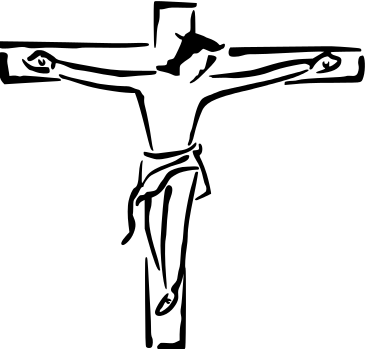
\includegraphics[width=0.20\textwidth]{../christ_on_cross.png}} ;
\end{tikzpicture}
\Large 

\leftcitation{ס} \centerfont 詩百又廿七載：
\leftcitation{ע} \centerfont 非耶和華建屋宇.則匠人之經營徒.
\leftcitation{פ} \centerfont 非耶和華衛城邑.則守者之儆醒徒.
\leftcitation{צ} \centerfont 余獻是卷予華人社區．願為福音流通之器．願獻斯微材為祭榮耀上帝．
\leftcitation{ק} \centerfont 阿門

\switchcolumn

\fontsize{11}{13}\rightfont \Large 滅．時越次聖殿期及當今。\leftcitation{י} \rightfont 猶太者力廣納之．筆錄以卷軸．便以傳、閱、頌、攜、守、鎖、抄、譯、釋、編，得書塔木德、密示拿等經傳．家喻戶曉．傳流若芳。\leftcitation{כ} \rightfont 猶太者文以載道．傳其口述．今我輩粵道之傳應當作如是．遂力行粵音識辨之法．載言載道．以盡忠傳粵道以待興。\leftcitation{ל} \rightfont 蒙下賜恩惠．無畏海量字音文書．既馭上帝之道．今廣及粵語講道．重駛編程之技．匯導粵音遂字稿．重塑講道現場．以傚猶太卷軸之舉便以傳流。\leftcitation{מ} \rightfont 是卷乃粵音口述傳之屬．莫通華文白話之語．

\end{paracol}

\columnratio{0.5,0.5}
\begin{paracol}{2}\fontsize{11}{13}\leftfont \Large \leftcitation{ו} \leftfont 斯殺一違儆百逆．既禁壓之．我輩聞風無奈．在所難免。\leftcitation{ז} \leftfont 另有異人例乎．以版權之名．脅網絡頻道之舉．同授礙予粵道之存流。

\switchcolumn

\fontsize{11}{13}\rightfont \Large 惟待後繼來者之傚．以譯釋傳之於神州華文地。\leftcitation{נ} \rightfont 今能排程驅馭圖靈以編彙文檔，其碼長共數千千亦無逢大礙．全蒙上帝保守。

\end{paracol}



\columnratio{1}\begin{paracol}{1}

\fontsize{11}{13}\rightfont \Large
~~~~~~~~~~~~~~~~~~~~~~~~~~~~~~~~~~~~~~~~~~~~~~~~~~~~~~~~~~~~~~~~~~~~~~~~~~~~~~~\leftcitation{ר} \rightfont 二零二三年二月一日

~~~~~~~~~~~~~~~~~~~~~~~~~~~~~~~~~~~~~~~~~~~~~~~~~~~~~~~~~~~~~~~~~~~~~~~~~~~~~~~\leftcitation{ש} \rightfont 米迦勒

~~~~~~~~~~~~~~~~~~~~~~~~~~~~~~~~~~~~~~~~~~~~~~~~~~~~~~~~~~~~~~~~~~~~~~~~~~~~~~~\leftcitation{ת} \rightfont 書於香港

\end{paracol}

\end{sloppypar}
\end{document}
